\documentclass[twoside]{book}

% Packages required by doxygen
\usepackage{fixltx2e}
\usepackage{calc}
\usepackage{doxygen}
\usepackage[export]{adjustbox} % also loads graphicx
\usepackage{graphicx}
\usepackage[utf8]{inputenc}
\usepackage{makeidx}
\usepackage{multicol}
\usepackage{multirow}
\PassOptionsToPackage{warn}{textcomp}
\usepackage{textcomp}
\usepackage[nointegrals]{wasysym}
\usepackage[table]{xcolor}

% Font selection
\usepackage[T1]{fontenc}
\usepackage[scaled=.90]{helvet}
\usepackage{courier}
\usepackage{amssymb}
\usepackage{sectsty}
\renewcommand{\familydefault}{\sfdefault}
\allsectionsfont{%
  \fontseries{bc}\selectfont%
  \color{darkgray}%
}
\renewcommand{\DoxyLabelFont}{%
  \fontseries{bc}\selectfont%
  \color{darkgray}%
}
\newcommand{\+}{\discretionary{\mbox{\scriptsize$\hookleftarrow$}}{}{}}

% Page & text layout
\usepackage{geometry}
\geometry{%
  a4paper,%
  top=2.5cm,%
  bottom=2.5cm,%
  left=2.5cm,%
  right=2.5cm%
}
\tolerance=750
\hfuzz=15pt
\hbadness=750
\setlength{\emergencystretch}{15pt}
\setlength{\parindent}{0cm}
\setlength{\parskip}{3ex plus 2ex minus 2ex}
\makeatletter
\renewcommand{\paragraph}{%
  \@startsection{paragraph}{4}{0ex}{-1.0ex}{1.0ex}{%
    \normalfont\normalsize\bfseries\SS@parafont%
  }%
}
\renewcommand{\subparagraph}{%
  \@startsection{subparagraph}{5}{0ex}{-1.0ex}{1.0ex}{%
    \normalfont\normalsize\bfseries\SS@subparafont%
  }%
}
\makeatother

% Headers & footers
\usepackage{fancyhdr}
\pagestyle{fancyplain}
\fancyhead[LE]{\fancyplain{}{\bfseries\thepage}}
\fancyhead[CE]{\fancyplain{}{}}
\fancyhead[RE]{\fancyplain{}{\bfseries\leftmark}}
\fancyhead[LO]{\fancyplain{}{\bfseries\rightmark}}
\fancyhead[CO]{\fancyplain{}{}}
\fancyhead[RO]{\fancyplain{}{\bfseries\thepage}}
\fancyfoot[LE]{\fancyplain{}{}}
\fancyfoot[CE]{\fancyplain{}{}}
\fancyfoot[RE]{\fancyplain{}{\bfseries\scriptsize Generated by Doxygen }}
\fancyfoot[LO]{\fancyplain{}{\bfseries\scriptsize Generated by Doxygen }}
\fancyfoot[CO]{\fancyplain{}{}}
\fancyfoot[RO]{\fancyplain{}{}}
\renewcommand{\footrulewidth}{0.4pt}
\renewcommand{\chaptermark}[1]{%
  \markboth{#1}{}%
}
\renewcommand{\sectionmark}[1]{%
  \markright{\thesection\ #1}%
}

% Indices & bibliography
\usepackage{natbib}
\usepackage[titles]{tocloft}
\setcounter{tocdepth}{3}
\setcounter{secnumdepth}{5}
\makeindex

% Hyperlinks (required, but should be loaded last)
\usepackage{ifpdf}
\ifpdf
  \usepackage[pdftex,pagebackref=true]{hyperref}
\else
  \usepackage[ps2pdf,pagebackref=true]{hyperref}
\fi
\hypersetup{%
  colorlinks=true,%
  linkcolor=blue,%
  citecolor=blue,%
  unicode%
}

% Custom commands
\newcommand{\clearemptydoublepage}{%
  \newpage{\pagestyle{empty}\cleardoublepage}%
}

\usepackage{caption}
\captionsetup{labelsep=space,justification=centering,font={bf},singlelinecheck=off,skip=4pt,position=top}

%===== C O N T E N T S =====

\begin{document}

% Titlepage & ToC
\hypersetup{pageanchor=false,
             bookmarksnumbered=true,
             pdfencoding=unicode
            }
\pagenumbering{alph}
\begin{titlepage}
\vspace*{7cm}
\begin{center}%
{\Large My Project }\\
\vspace*{1cm}
{\large Generated by Doxygen 1.8.13}\\
\end{center}
\end{titlepage}
\clearemptydoublepage
\pagenumbering{roman}
\tableofcontents
\clearemptydoublepage
\pagenumbering{arabic}
\hypersetup{pageanchor=true}

%--- Begin generated contents ---
\chapter{D\+Bx1000}
\label{md_macrobench_README}
\Hypertarget{md_macrobench_README}
D\+Bx1000 is an single node O\+L\+TP database management system (D\+B\+MS). The goal of D\+Bx1000 is to make D\+B\+MS scalable on future 1000-\/core processors. We implemented all the seven classic concurrency control schemes in D\+Bx1000. They exhibit different scalability properties under different workloads.

The concurrency control scalability study is described in the following paper. \begin{DoxyVerb}Staring into the Abyss: An Evaluation of Concurrency Control with One Thousand Cores
Xiangyao Yu, George Bezerra, Andrew Pavlo, Srinivas Devadas, Michael Stonebraker
http://www.vldb.org/pvldb/vol8/p209-yu.pdf
\end{DoxyVerb}


\subsection*{Build \& Test }

To build the database. \begin{DoxyVerb}make -j
\end{DoxyVerb}


To test the database \begin{DoxyVerb}python test.py
\end{DoxyVerb}


\subsection*{Configuration }

D\+B\+MS configurations can be changed in the \hyperlink{config_8h}{config.\+h} file. Please refer to R\+E\+A\+D\+ME for the meaning of each configuration. Here we only list several most important ones. \begin{DoxyVerb}THREAD_CNT        : Number of worker threads running in the database.
WORKLOAD          : Supported workloads include YCSB and TPCC
CC_ALG            : Concurrency control algorithm. Seven algorithms are supported 
                    (DL_DETECT, NO_WAIT, HEKATON, SILO, TICTOC) 
MAX_TXN_PER_PART  : Number of transactions to run per thread per partition.
\end{DoxyVerb}


Configurations can also be specified as command argument at runtime. Run the following command for a full list of program argument. \begin{DoxyVerb}./rundb -h
\end{DoxyVerb}


\subsection*{Run }

The D\+B\+MS can be run with \begin{DoxyVerb}./rundb\end{DoxyVerb}
 
\chapter{R\+E\+A\+D\+ME}
\label{md_README}
\Hypertarget{md_README}
For information, installation and usage, visit the Set\+Bench Wiki! \href{https://gitlab.com/trbot86/setbench/wikis/home}{\tt https\+://gitlab.\+com/trbot86/setbench/wikis/home} 
\chapter{Namespace Index}
\section{Namespace List}
Here is a list of all namespaces with brief descriptions\+:\begin{DoxyCompactList}
\item\contentsline{section}{\hyperlink{namespaceabtree__ns}{abtree\+\_\+ns} }{\pageref{namespaceabtree__ns}}{}
\item\contentsline{section}{\hyperlink{namespacebslack__ns}{bslack\+\_\+ns} }{\pageref{namespacebslack__ns}}{}
\item\contentsline{section}{\hyperlink{namespacebst__glock__ns}{bst\+\_\+glock\+\_\+ns} }{\pageref{namespacebst__glock__ns}}{}
\item\contentsline{section}{\hyperlink{namespacebst__hohlock__ns}{bst\+\_\+hohlock\+\_\+ns} }{\pageref{namespacebst__hohlock__ns}}{}
\item\contentsline{section}{\hyperlink{namespacebst__hohrwlock__ns}{bst\+\_\+hohrwlock\+\_\+ns} }{\pageref{namespacebst__hohrwlock__ns}}{}
\item\contentsline{section}{\hyperlink{namespacebst__ns}{bst\+\_\+ns} }{\pageref{namespacebst__ns}}{}
\item\contentsline{section}{\hyperlink{namespacebst__rwlock__ns}{bst\+\_\+rwlock\+\_\+ns} }{\pageref{namespacebst__rwlock__ns}}{}
\item\contentsline{section}{\hyperlink{namespaceconvert__db__to__csv}{convert\+\_\+db\+\_\+to\+\_\+csv} }{\pageref{namespaceconvert__db__to__csv}}{}
\item\contentsline{section}{\hyperlink{namespacecreate__db}{create\+\_\+db} }{\pageref{namespacecreate__db}}{}
\item\contentsline{section}{\hyperlink{namespacegraphs}{graphs} }{\pageref{namespacegraphs}}{}
\item\contentsline{section}{\hyperlink{namespacekcas}{kcas} }{\pageref{namespacekcas}}{}
\item\contentsline{section}{\hyperlink{namespacethread__pinning}{thread\+\_\+pinning} }{\pageref{namespacethread__pinning}}{}
\item\contentsline{section}{\hyperlink{namespacetimeline__draw__bw}{timeline\+\_\+draw\+\_\+bw} }{\pageref{namespacetimeline__draw__bw}}{}
\item\contentsline{section}{\hyperlink{namespacetimeline__draw__color}{timeline\+\_\+draw\+\_\+color} }{\pageref{namespacetimeline__draw__color}}{}
\item\contentsline{section}{\hyperlink{namespacetimeline__plotter}{timeline\+\_\+plotter} }{\pageref{namespacetimeline__plotter}}{}
\item\contentsline{section}{\hyperlink{namespaceurcu}{urcu} }{\pageref{namespaceurcu}}{}
\end{DoxyCompactList}

\chapter{Hierarchical Index}
\section{Class Hierarchy}
This inheritance list is sorted roughly, but not completely, alphabetically\+:\begin{DoxyCompactList}
\item \contentsline{section}{\+\_\+memrecl\+\_\+counters}{\pageref{struct__memrecl__counters}}{}
\item \contentsline{section}{abtree\+\_\+ns\+:\+:abtree$<$ D\+E\+G\+R\+EE, K, Compare, Rec\+Manager $>$}{\pageref{classabtree__ns_1_1abtree}}{}
\item \contentsline{section}{A\+B\+Tree\+K\+C\+AS$<$ Record\+Manager, K, V, D\+E\+G\+R\+EE, Compare $>$}{\pageref{classABTreeKCAS}}{}
\item \contentsline{section}{Access}{\pageref{classAccess}}{}
\item \contentsline{section}{allocator\+\_\+interface$<$ T $>$}{\pageref{classallocator__interface}}{}
\begin{DoxyCompactList}
\item \contentsline{section}{allocator\+\_\+bump$<$ T $>$}{\pageref{classallocator__bump}}{}
\item \contentsline{section}{allocator\+\_\+new$<$ T $>$}{\pageref{classallocator__new}}{}
\item \contentsline{section}{allocator\+\_\+new\+\_\+segregated$<$ T $>$}{\pageref{classallocator__new__segregated}}{}
\item \contentsline{section}{allocator\+\_\+once$<$ T $>$}{\pageref{classallocator__once}}{}
\end{DoxyCompactList}
\item \contentsline{section}{anchor\+Record$<$ skey\+\_\+t, sval\+\_\+t $>$}{\pageref{structanchorRecord}}{}
\item \contentsline{section}{A\+O\+\_\+double\+\_\+t}{\pageref{structAO__double__t}}{}
\item \contentsline{section}{A\+O\+\_\+pa\+\_\+clearable\+\_\+loc}{\pageref{structAO__pa__clearable__loc}}{}
\item \contentsline{section}{Arena}{\pageref{classArena}}{}
\item \contentsline{section}{Array\+List$<$ T $>$}{\pageref{classArrayList}}{}
\item \contentsline{section}{Atomic\+Array\+List$<$ T $>$}{\pageref{classAtomicArrayList}}{}
\item \contentsline{section}{reclaimer\+\_\+debra$<$ T, Pool $>$\+:\+:Bag\+Rotator$<$ Rest $>$}{\pageref{classreclaimer__debra_1_1BagRotator}}{}
\item \contentsline{section}{reclaimer\+\_\+debracap$<$ T, Pool $>$\+:\+:Bag\+Rotator$<$ Rest $>$}{\pageref{classreclaimer__debracap_1_1BagRotator}}{}
\item \contentsline{section}{reclaimer\+\_\+ebr\+\_\+token$<$ T, Pool $>$\+:\+:Bag\+Rotator$<$ Rest $>$}{\pageref{classreclaimer__ebr__token_1_1BagRotator}}{}
\item \contentsline{section}{reclaimer\+\_\+ebr\+\_\+token$<$ T, Pool $>$\+:\+:Bag\+Rotator$<$ Rest... $>$}{\pageref{classreclaimer__ebr__token_1_1BagRotator}}{}
\begin{DoxyCompactList}
\item \contentsline{section}{reclaimer\+\_\+ebr\+\_\+token$<$ T, Pool $>$\+:\+:Bag\+Rotator$<$ First, Rest... $>$}{\pageref{classreclaimer__ebr__token_1_1BagRotator_3_01First_00_01Rest_8_8_8_01_4}}{}
\end{DoxyCompactList}
\item \contentsline{section}{reclaimer\+\_\+debra$<$ T, Pool $>$\+:\+:Bag\+Rotator$<$ Rest... $>$}{\pageref{classreclaimer__debra_1_1BagRotator}}{}
\begin{DoxyCompactList}
\item \contentsline{section}{reclaimer\+\_\+debra$<$ T, Pool $>$\+:\+:Bag\+Rotator$<$ First, Rest... $>$}{\pageref{classreclaimer__debra_1_1BagRotator_3_01First_00_01Rest_8_8_8_01_4}}{}
\end{DoxyCompactList}
\item \contentsline{section}{reclaimer\+\_\+debracap$<$ T, Pool $>$\+:\+:Bag\+Rotator$<$ Rest... $>$}{\pageref{classreclaimer__debracap_1_1BagRotator}}{}
\begin{DoxyCompactList}
\item \contentsline{section}{reclaimer\+\_\+debracap$<$ T, Pool $>$\+:\+:Bag\+Rotator$<$ First, Rest... $>$}{\pageref{classreclaimer__debracap_1_1BagRotator_3_01First_00_01Rest_8_8_8_01_4}}{}
\end{DoxyCompactList}
\item \contentsline{section}{base\+\_\+query}{\pageref{classbase__query}}{}
\begin{DoxyCompactList}
\item \contentsline{section}{tpcc\+\_\+query}{\pageref{classtpcc__query}}{}
\item \contentsline{section}{ycsb\+\_\+query}{\pageref{classycsb__query}}{}
\end{DoxyCompactList}
\item \contentsline{section}{block$<$ T $>$}{\pageref{classblock}}{}
\item \contentsline{section}{blockbag$<$ T $>$}{\pageref{classblockbag}}{}
\item \contentsline{section}{blockbag\+\_\+iterator$<$ T $>$}{\pageref{classblockbag__iterator}}{}
\item \contentsline{section}{blockpool$<$ T $>$}{\pageref{classblockpool}}{}
\item \contentsline{section}{bslack\+\_\+ns\+:\+:bslack$<$ D\+E\+G\+R\+EE, K, Compare, Rec\+Manager $>$}{\pageref{classbslack__ns_1_1bslack}}{}
\item \contentsline{section}{bst\+\_\+ns\+:\+:bst$<$ K, V, Compare, Rec\+Manager $>$}{\pageref{classbst__ns_1_1bst}}{}
\item \contentsline{section}{bst\+\_\+glock\+\_\+ns\+:\+:bst\+\_\+glock$<$ K, V, Compare, Rec\+Manager $>$}{\pageref{classbst__glock__ns_1_1bst__glock}}{}
\item \contentsline{section}{bst\+\_\+hohlock\+\_\+ns\+:\+:bst\+\_\+hohlock$<$ K, V, Compare, Rec\+Manager $>$}{\pageref{classbst__hohlock__ns_1_1bst__hohlock}}{}
\item \contentsline{section}{bst\+\_\+hohrwlock\+\_\+ns\+:\+:bst\+\_\+hohrwlock$<$ K, V, Compare, Rec\+Manager $>$}{\pageref{classbst__hohrwlock__ns_1_1bst__hohrwlock}}{}
\item \contentsline{section}{bst\+\_\+rwlock\+\_\+ns\+:\+:bst\+\_\+rwlock$<$ K, V, Compare, Rec\+Manager $>$}{\pageref{classbst__rwlock__ns_1_1bst__rwlock}}{}
\item \contentsline{section}{Bucket\+Header}{\pageref{classBucketHeader}}{}
\item \contentsline{section}{Bucket\+Node}{\pageref{classBucketNode}}{}
\item \contentsline{section}{casword$<$ T $>$}{\pageref{structcasword}}{}
\item \contentsline{section}{casword$<$ casword\+\_\+t $>$}{\pageref{structcasword}}{}
\item \contentsline{section}{casword$<$ int $>$}{\pageref{structcasword}}{}
\item \contentsline{section}{casword$<$ K $>$}{\pageref{structcasword}}{}
\item \contentsline{section}{casword$<$ Node$<$ K, V $>$ $\ast$$>$}{\pageref{structcasword}}{}
\item \contentsline{section}{casword$<$ Node$<$ K, V, D\+E\+G\+R\+EE $>$ $\ast$$>$}{\pageref{structcasword}}{}
\item \contentsline{section}{casword$<$ uint64\+\_\+t $>$}{\pageref{structcasword}}{}
\item \contentsline{section}{casword$<$ V $>$}{\pageref{structcasword}}{}
\item \contentsline{section}{Catalog}{\pageref{classCatalog}}{}
\item \contentsline{section}{ccavl$<$ skey\+\_\+t, sval\+\_\+t, Rec\+Mgr $>$}{\pageref{classccavl}}{}
\item \contentsline{section}{child\+\_\+cas\+\_\+op\+\_\+t$<$ skey\+\_\+t, sval\+\_\+t $>$}{\pageref{structchild__cas__op__t}}{}
\item \contentsline{section}{Column}{\pageref{classColumn}}{}
\item \contentsline{section}{Compact\+Report\+Item}{\pageref{classCompactReportItem}}{}
\item \contentsline{section}{Data\+Structure}{\pageref{classDataStructure}}{}
\item \contentsline{section}{dcssdesc\+\_\+t}{\pageref{classdcssdesc__t}}{}
\item \contentsline{section}{dcsspdesc\+\_\+t$<$ P\+A\+Y\+L\+O\+A\+D\+\_\+T $>$}{\pageref{classdcsspdesc__t}}{}
\item \contentsline{section}{dcssp\+Provider$<$ P\+A\+Y\+L\+O\+A\+D\+\_\+T $>$}{\pageref{classdcsspProvider}}{}
\item \contentsline{section}{dcssp\+Provider$<$ void $\ast$$>$}{\pageref{classdcsspProvider}}{}
\item \contentsline{section}{dcsspresult\+\_\+t}{\pageref{structdcsspresult__t}}{}
\item \contentsline{section}{dcss\+Provider$<$ Unused $>$}{\pageref{classdcssProvider}}{}
\item \contentsline{section}{dcss\+Provider$<$ void $\ast$ $>$}{\pageref{classdcssProvider}}{}
\item \contentsline{section}{dcssresult\+\_\+t}{\pageref{structdcssresult__t}}{}
\item \contentsline{section}{debug\+Counter}{\pageref{classdebugCounter}}{}
\item \contentsline{section}{debug\+Info}{\pageref{classdebugInfo}}{}
\item \contentsline{section}{Dep\+Thd}{\pageref{structDepThd}}{}
\item \contentsline{section}{Detect\+Data}{\pageref{structDetectData}}{}
\item \contentsline{section}{dinfo\+\_\+t$<$ skey\+\_\+t, sval\+\_\+t $>$}{\pageref{structdinfo__t}}{}
\item \contentsline{section}{D\+L\+\_\+detect}{\pageref{classDL__detect}}{}
\item \contentsline{section}{drachsler$<$ skey\+\_\+t, sval\+\_\+t, Rec\+Mgr $>$}{\pageref{classdrachsler}}{}
\item \contentsline{section}{ds\+\_\+adapter$<$ K, V, Reclaim, Alloc, Pool $>$}{\pageref{classds__adapter}}{}
\item \contentsline{section}{ds\+\_\+adapter$<$ K\+E\+Y\+\_\+\+T\+Y\+PE, V\+A\+L\+U\+E\+\_\+\+T\+Y\+PE $>$}{\pageref{classds__adapter}}{}
\item \contentsline{section}{edge$<$ skey\+\_\+t, sval\+\_\+t $>$}{\pageref{structedge}}{}
\item \contentsline{section}{ellen$<$ skey\+\_\+t, sval\+\_\+t, Rec\+Mgr $>$}{\pageref{classellen}}{}
\item \contentsline{section}{find\+\_\+result$<$ sval\+\_\+t $>$}{\pageref{structfind__result}}{}
\item \contentsline{section}{free\+\_\+block}{\pageref{structfree__block}}{}
\item \contentsline{section}{globals\+\_\+t$<$ Key\+GenT $>$}{\pageref{structglobals__t}}{}
\item \contentsline{section}{gstats\+\_\+output\+\_\+item}{\pageref{classgstats__output__item}}{}
\item \contentsline{section}{gstats\+\_\+t}{\pageref{classgstats__t}}{}
\item \contentsline{section}{Hash\+List$<$ T $>$}{\pageref{classHashList}}{}
\item \contentsline{section}{Hash\+List$<$ K $>$}{\pageref{classHashList}}{}
\item \contentsline{section}{hashset$<$ K $>$}{\pageref{classhashset}}{}
\item \contentsline{section}{hashset\+\_\+new$<$ K $>$}{\pageref{classhashset__new}}{}
\item \contentsline{section}{hashset\+\_\+new$<$ T $>$}{\pageref{classhashset__new}}{}
\item \contentsline{section}{Hash\+Table$<$ T $>$}{\pageref{classHashTable}}{}
\item \contentsline{section}{Hash\+Table$<$ K $>$}{\pageref{classHashTable}}{}
\item \contentsline{section}{H\+L\+Node$<$ T $>$}{\pageref{classHLNode}}{}
\item \contentsline{section}{H\+L\+Node$<$ K $>$}{\pageref{classHLNode}}{}
\item \contentsline{section}{howley$<$ skey\+\_\+t, sval\+\_\+t, Rec\+Mgr $>$}{\pageref{classhowley}}{}
\item \contentsline{section}{Ideal\+Subtree$<$ V $>$}{\pageref{structIdealSubtree}}{}
\item \contentsline{section}{iinfo\+\_\+t$<$ skey\+\_\+t, sval\+\_\+t $>$}{\pageref{structiinfo__t}}{}
\item \contentsline{section}{index\+\_\+base}{\pageref{classindex__base}}{}
\begin{DoxyCompactList}
\item \contentsline{section}{Index}{\pageref{classIndex}}{}
\item \contentsline{section}{Index}{\pageref{classIndex}}{}
\end{DoxyCompactList}
\item \contentsline{section}{info\+\_\+t$<$ skey\+\_\+t, sval\+\_\+t $>$}{\pageref{unioninfo__t}}{}
\item \contentsline{section}{Internal\+K\+C\+AS$<$ Record\+Manager, K, V $>$}{\pageref{classInternalKCAS}}{}
\item \contentsline{section}{Interpolator$<$ K $>$}{\pageref{classInterpolator}}{}
\item \contentsline{section}{Interpolator$<$ long long $>$}{\pageref{classInterpolator_3_01long_01long_01_4}}{}
\item \contentsline{section}{intlf$<$ skey\+\_\+t, sval\+\_\+t, Rec\+Mgr $>$}{\pageref{classintlf}}{}
\item \contentsline{section}{istree$<$ K, V, Interpolate, Rec\+Manager $>$}{\pageref{classistree}}{}
\item \contentsline{section}{Item\+\_\+no}{\pageref{structItem__no}}{}
\item \contentsline{section}{itemid\+\_\+t}{\pageref{classitemid__t}}{}
\item \contentsline{section}{kcasdesc\+\_\+t$<$ M\+A\+X\+\_\+K $>$}{\pageref{classkcasdesc__t}}{}
\item \contentsline{section}{kcasentry\+\_\+t}{\pageref{structkcasentry__t}}{}
\item \contentsline{section}{K\+C\+A\+S\+H\+TM$<$ M\+A\+X\+\_\+K $>$}{\pageref{classKCASHTM}}{}
\item \contentsline{section}{K\+C\+A\+S\+Lock\+Free$<$ M\+A\+X\+\_\+K $>$}{\pageref{classKCASLockFree}}{}
\item \contentsline{section}{Key\+Generator\+Uniform$<$ K $>$}{\pageref{classKeyGeneratorUniform}}{}
\item \contentsline{section}{Key\+Generator\+Zipf$<$ K $>$}{\pageref{classKeyGeneratorZipf}}{}
\item \contentsline{section}{Key\+Generator\+Zipf\+Data}{\pageref{classKeyGeneratorZipfData}}{}
\item \contentsline{section}{K\+V\+Pair$<$ K, V $>$}{\pageref{structKVPair}}{}
\item \contentsline{section}{kvpair$<$ K $>$}{\pageref{structkvpair}}{}
\item \contentsline{section}{lfbstack$<$ T $>$}{\pageref{classlfbstack}}{}
\item \contentsline{section}{Lock\+Entry}{\pageref{structLockEntry}}{}
\item \contentsline{section}{lockfreeblockbag$<$ T $>$}{\pageref{classlockfreeblockbag}}{}
\item \contentsline{section}{Manager}{\pageref{classManager}}{}
\item \contentsline{section}{mem\+\_\+alloc}{\pageref{classmem__alloc}}{}
\item \contentsline{section}{record\+\_\+manager$<$ Reclaim, Alloc, Pool, Record\+Types\+First, Record\+Types\+Rest $>$\+:\+:Memory\+Reclamation\+Guard}{\pageref{classrecord__manager_1_1MemoryReclamationGuard}}{}
\item \contentsline{section}{Multi\+Counter}{\pageref{classMultiCounter}}{}
\item \contentsline{section}{myrand}{\pageref{classmyrand}}{}
\item \contentsline{section}{natarajan\+\_\+ext\+\_\+bst\+\_\+lf$<$ skey\+\_\+t, sval\+\_\+t, Rec\+Mgr, Compare $>$}{\pageref{classnatarajan__ext__bst__lf}}{}
\item \contentsline{section}{Node$<$ K, V $>$}{\pageref{classNode}}{}
\item \contentsline{section}{abtree\+\_\+ns\+:\+:Node$<$ D\+E\+G\+R\+EE, K $>$}{\pageref{structabtree__ns_1_1Node}}{}
\item \contentsline{section}{bslack\+\_\+ns\+:\+:Node$<$ D\+E\+G\+R\+EE, K $>$}{\pageref{structbslack__ns_1_1Node}}{}
\item \contentsline{section}{bst\+\_\+glock\+\_\+ns\+:\+:Node$<$ K, V $>$}{\pageref{classbst__glock__ns_1_1Node}}{}
\item \contentsline{section}{bst\+\_\+hohlock\+\_\+ns\+:\+:Node$<$ K, V $>$}{\pageref{classbst__hohlock__ns_1_1Node}}{}
\item \contentsline{section}{bst\+\_\+hohrwlock\+\_\+ns\+:\+:Node$<$ K, V $>$}{\pageref{classbst__hohrwlock__ns_1_1Node}}{}
\item \contentsline{section}{bst\+\_\+ns\+:\+:Node$<$ K, V $>$}{\pageref{classbst__ns_1_1Node}}{}
\item \contentsline{section}{bst\+\_\+rwlock\+\_\+ns\+:\+:Node$<$ K, V $>$}{\pageref{classbst__rwlock__ns_1_1Node}}{}
\item \contentsline{section}{Node$<$ K, V, D\+E\+G\+R\+EE $>$}{\pageref{classNode}}{}
\begin{DoxyCompactList}
\item \contentsline{section}{Node\+External$<$ K, V, D\+E\+G\+R\+EE $>$}{\pageref{classNodeExternal}}{}
\item \contentsline{section}{Node\+Internal$<$ K, V, D\+E\+G\+R\+EE $>$}{\pageref{classNodeInternal}}{}
\end{DoxyCompactList}
\item \contentsline{section}{node\+\_\+t$<$ skey\+\_\+t, sval\+\_\+t $>$}{\pageref{structnode__t}}{}
\item \contentsline{section}{Snap\+Collector$<$ Node\+Type, K $>$\+:\+:Node\+Wrapper}{\pageref{classSnapCollector_1_1NodeWrapper}}{}
\item \contentsline{section}{Numa\+Tools}{\pageref{classNumaTools}}{}
\item \contentsline{section}{obj\+\_\+list}{\pageref{structobj__list}}{}
\item \contentsline{section}{operation\+\_\+t$<$ skey\+\_\+t, sval\+\_\+t $>$}{\pageref{unionoperation__t}}{}
\item \contentsline{section}{Opt\+CC}{\pageref{classOptCC}}{}
\item \contentsline{section}{Padded\+Random}{\pageref{classPaddedRandom}}{}
\item \contentsline{section}{Part\+Man}{\pageref{classPartMan}}{}
\item \contentsline{section}{Perf\+Tools}{\pageref{structPerfTools}}{}
\item \contentsline{section}{Plock}{\pageref{classPlock}}{}
\item \contentsline{section}{pool\+\_\+interface$<$ T, Alloc $>$}{\pageref{classpool__interface}}{}
\begin{DoxyCompactList}
\item \contentsline{section}{pool\+\_\+none$<$ T, Alloc $>$}{\pageref{classpool__none}}{}
\item \contentsline{section}{pool\+\_\+numa$<$ T, Alloc $>$}{\pageref{classpool__numa}}{}
\item \contentsline{section}{pool\+\_\+perthread\+\_\+and\+\_\+shared$<$ T, Alloc $>$}{\pageref{classpool__perthread__and__shared}}{}
\end{DoxyCompactList}
\item \contentsline{section}{Query\+\_\+queue}{\pageref{classQuery__queue}}{}
\item \contentsline{section}{Query\+\_\+thd}{\pageref{classQuery__thd}}{}
\item \contentsline{section}{Random\+F\+N\+V1A}{\pageref{classRandomFNV1A}}{}
\item \contentsline{section}{rcu\+\_\+node\+\_\+t}{\pageref{structrcu__node__t}}{}
\item \contentsline{section}{rdcssdesc\+\_\+t}{\pageref{structrdcssdesc__t}}{}
\item \contentsline{section}{allocator\+\_\+interface$<$ T $>$\+:\+:rebind$<$ \+\_\+\+Tp1 $>$}{\pageref{structallocator__interface_1_1rebind}}{}
\item \contentsline{section}{allocator\+\_\+new\+\_\+segregated$<$ T $>$\+:\+:rebind$<$ \+\_\+\+Tp1 $>$}{\pageref{structallocator__new__segregated_1_1rebind}}{}
\item \contentsline{section}{pool\+\_\+perthread\+\_\+and\+\_\+shared$<$ T, Alloc $>$\+:\+:rebind$<$ \+\_\+\+Tp1 $>$}{\pageref{structpool__perthread__and__shared_1_1rebind}}{}
\item \contentsline{section}{reclaimer\+\_\+ebr\+\_\+token$<$ T, Pool $>$\+:\+:rebind$<$ \+\_\+\+Tp1 $>$}{\pageref{structreclaimer__ebr__token_1_1rebind}}{}
\item \contentsline{section}{reclaimer\+\_\+debracap$<$ T, Pool $>$\+:\+:rebind$<$ \+\_\+\+Tp1 $>$}{\pageref{structreclaimer__debracap_1_1rebind}}{}
\item \contentsline{section}{allocator\+\_\+once$<$ T $>$\+:\+:rebind$<$ \+\_\+\+Tp1 $>$}{\pageref{structallocator__once_1_1rebind}}{}
\item \contentsline{section}{reclaimer\+\_\+ebr\+\_\+tree$<$ T, Pool $>$\+:\+:rebind$<$ \+\_\+\+Tp1 $>$}{\pageref{structreclaimer__ebr__tree_1_1rebind}}{}
\item \contentsline{section}{allocator\+\_\+new$<$ T $>$\+:\+:rebind$<$ \+\_\+\+Tp1 $>$}{\pageref{structallocator__new_1_1rebind}}{}
\item \contentsline{section}{reclaimer\+\_\+debra$<$ T, Pool $>$\+:\+:rebind$<$ \+\_\+\+Tp1 $>$}{\pageref{structreclaimer__debra_1_1rebind}}{}
\item \contentsline{section}{reclaimer\+\_\+ebr\+\_\+tree\+\_\+q$<$ T, Pool $>$\+:\+:rebind$<$ \+\_\+\+Tp1 $>$}{\pageref{structreclaimer__ebr__tree__q_1_1rebind}}{}
\item \contentsline{section}{reclaimer\+\_\+hazardptr$<$ T, Pool $>$\+:\+:rebind$<$ \+\_\+\+Tp1 $>$}{\pageref{structreclaimer__hazardptr_1_1rebind}}{}
\item \contentsline{section}{pool\+\_\+interface$<$ T, Alloc $>$\+:\+:rebind$<$ \+\_\+\+Tp1 $>$}{\pageref{structpool__interface_1_1rebind}}{}
\item \contentsline{section}{reclaimer\+\_\+interface$<$ T, Pool $>$\+:\+:rebind$<$ \+\_\+\+Tp1 $>$}{\pageref{structreclaimer__interface_1_1rebind}}{}
\item \contentsline{section}{reclaimer\+\_\+none$<$ T, Pool $>$\+:\+:rebind$<$ \+\_\+\+Tp1 $>$}{\pageref{structreclaimer__none_1_1rebind}}{}
\item \contentsline{section}{pool\+\_\+none$<$ T, Alloc $>$\+:\+:rebind$<$ \+\_\+\+Tp1 $>$}{\pageref{structpool__none_1_1rebind}}{}
\item \contentsline{section}{reclaimer\+\_\+rcu$<$ T, Pool $>$\+:\+:rebind$<$ \+\_\+\+Tp1 $>$}{\pageref{structreclaimer__rcu_1_1rebind}}{}
\item \contentsline{section}{allocator\+\_\+bump$<$ T $>$\+:\+:rebind$<$ \+\_\+\+Tp1 $>$}{\pageref{structallocator__bump_1_1rebind}}{}
\item \contentsline{section}{pool\+\_\+numa$<$ T, Alloc $>$\+:\+:rebind$<$ \+\_\+\+Tp1 $>$}{\pageref{structpool__numa_1_1rebind}}{}
\item \contentsline{section}{reclaimer\+\_\+debraplus$<$ T, Pool $>$\+:\+:rebind$<$ \+\_\+\+Tp1 $>$}{\pageref{structreclaimer__debraplus_1_1rebind}}{}
\item \contentsline{section}{pool\+\_\+perthread\+\_\+and\+\_\+shared$<$ T, Alloc $>$\+:\+:rebind2$<$ \+\_\+\+Tp1, \+\_\+\+Tp2 $>$}{\pageref{structpool__perthread__and__shared_1_1rebind2}}{}
\item \contentsline{section}{reclaimer\+\_\+interface$<$ T, Pool $>$\+:\+:rebind2$<$ \+\_\+\+Tp1, \+\_\+\+Tp2 $>$}{\pageref{structreclaimer__interface_1_1rebind2}}{}
\item \contentsline{section}{reclaimer\+\_\+debra$<$ T, Pool $>$\+:\+:rebind2$<$ \+\_\+\+Tp1, \+\_\+\+Tp2 $>$}{\pageref{structreclaimer__debra_1_1rebind2}}{}
\item \contentsline{section}{reclaimer\+\_\+ebr\+\_\+tree\+\_\+q$<$ T, Pool $>$\+:\+:rebind2$<$ \+\_\+\+Tp1, \+\_\+\+Tp2 $>$}{\pageref{structreclaimer__ebr__tree__q_1_1rebind2}}{}
\item \contentsline{section}{reclaimer\+\_\+ebr\+\_\+token$<$ T, Pool $>$\+:\+:rebind2$<$ \+\_\+\+Tp1, \+\_\+\+Tp2 $>$}{\pageref{structreclaimer__ebr__token_1_1rebind2}}{}
\item \contentsline{section}{reclaimer\+\_\+debraplus$<$ T, Pool $>$\+:\+:rebind2$<$ \+\_\+\+Tp1, \+\_\+\+Tp2 $>$}{\pageref{structreclaimer__debraplus_1_1rebind2}}{}
\item \contentsline{section}{reclaimer\+\_\+ebr\+\_\+tree$<$ T, Pool $>$\+:\+:rebind2$<$ \+\_\+\+Tp1, \+\_\+\+Tp2 $>$}{\pageref{structreclaimer__ebr__tree_1_1rebind2}}{}
\item \contentsline{section}{reclaimer\+\_\+hazardptr$<$ T, Pool $>$\+:\+:rebind2$<$ \+\_\+\+Tp1, \+\_\+\+Tp2 $>$}{\pageref{structreclaimer__hazardptr_1_1rebind2}}{}
\item \contentsline{section}{pool\+\_\+interface$<$ T, Alloc $>$\+:\+:rebind2$<$ \+\_\+\+Tp1, \+\_\+\+Tp2 $>$}{\pageref{structpool__interface_1_1rebind2}}{}
\item \contentsline{section}{reclaimer\+\_\+none$<$ T, Pool $>$\+:\+:rebind2$<$ \+\_\+\+Tp1, \+\_\+\+Tp2 $>$}{\pageref{structreclaimer__none_1_1rebind2}}{}
\item \contentsline{section}{reclaimer\+\_\+rcu$<$ T, Pool $>$\+:\+:rebind2$<$ \+\_\+\+Tp1, \+\_\+\+Tp2 $>$}{\pageref{structreclaimer__rcu_1_1rebind2}}{}
\item \contentsline{section}{pool\+\_\+none$<$ T, Alloc $>$\+:\+:rebind2$<$ \+\_\+\+Tp1, \+\_\+\+Tp2 $>$}{\pageref{structpool__none_1_1rebind2}}{}
\item \contentsline{section}{reclaimer\+\_\+debracap$<$ T, Pool $>$\+:\+:rebind2$<$ \+\_\+\+Tp1, \+\_\+\+Tp2 $>$}{\pageref{structreclaimer__debracap_1_1rebind2}}{}
\item \contentsline{section}{pool\+\_\+numa$<$ T, Alloc $>$\+:\+:rebind2$<$ \+\_\+\+Tp1, \+\_\+\+Tp2 $>$}{\pageref{structpool__numa_1_1rebind2}}{}
\item \contentsline{section}{pool\+\_\+none$<$ T, Alloc $>$\+:\+:rebind\+Alloc$<$ \+\_\+\+Tp1 $>$}{\pageref{structpool__none_1_1rebindAlloc}}{}
\item \contentsline{section}{pool\+\_\+numa$<$ T, Alloc $>$\+:\+:rebind\+Alloc$<$ \+\_\+\+Tp1 $>$}{\pageref{structpool__numa_1_1rebindAlloc}}{}
\item \contentsline{section}{Rebuild\+Operation$<$ K, V $>$}{\pageref{structRebuildOperation}}{}
\item \contentsline{section}{reclaimer\+\_\+interface$<$ T, Pool $>$}{\pageref{classreclaimer__interface}}{}
\begin{DoxyCompactList}
\item \contentsline{section}{reclaimer\+\_\+debra$<$ T, Pool $>$}{\pageref{classreclaimer__debra}}{}
\item \contentsline{section}{reclaimer\+\_\+debracap$<$ T, Pool $>$}{\pageref{classreclaimer__debracap}}{}
\item \contentsline{section}{reclaimer\+\_\+debraplus$<$ T, Pool $>$}{\pageref{classreclaimer__debraplus}}{}
\item \contentsline{section}{reclaimer\+\_\+ebr\+\_\+token$<$ T, Pool $>$}{\pageref{classreclaimer__ebr__token}}{}
\item \contentsline{section}{reclaimer\+\_\+ebr\+\_\+tree$<$ T, Pool $>$}{\pageref{classreclaimer__ebr__tree}}{}
\item \contentsline{section}{reclaimer\+\_\+ebr\+\_\+tree\+\_\+q$<$ T, Pool $>$}{\pageref{classreclaimer__ebr__tree__q}}{}
\item \contentsline{section}{reclaimer\+\_\+hazardptr$<$ T, Pool $>$}{\pageref{classreclaimer__hazardptr}}{}
\item \contentsline{section}{reclaimer\+\_\+none$<$ T, Pool $>$}{\pageref{classreclaimer__none}}{}
\item \contentsline{section}{reclaimer\+\_\+rcu$<$ T, Pool $>$}{\pageref{classreclaimer__rcu}}{}
\end{DoxyCompactList}
\item \contentsline{section}{bst\+\_\+ns\+:\+:Reclamation\+Info$<$ K, V $>$}{\pageref{classbst__ns_1_1ReclamationInfo}}{}
\item \contentsline{section}{record\+\_\+manager$<$ Reclaim, Alloc, Pool, Record\+Types\+First, Record\+Types\+Rest $>$}{\pageref{classrecord__manager}}{}
\item \contentsline{section}{record\+\_\+manager$<$ Reclaim, Alloc, Pool, Record\+Types\+First, Record\+Types\+Rest... $>$}{\pageref{classrecord__manager}}{}
\item \contentsline{section}{record\+\_\+manager\+\_\+single\+\_\+type$<$ Record, Reclaim, Alloc, Pool $>$}{\pageref{classrecord__manager__single__type}}{}
\item \contentsline{section}{record\+\_\+manager\+\_\+single\+\_\+type$<$ First, Reclaim, Alloc, Pool $>$}{\pageref{classrecord__manager__single__type}}{}
\item \contentsline{section}{Record\+Manager\+Set$<$ Reclaim, Alloc, Pool, Rest $>$}{\pageref{classRecordManagerSet}}{}
\item \contentsline{section}{Record\+Manager\+Set$<$ Reclaim, Alloc, Pool, Record\+Types\+First, Rest... $>$}{\pageref{classRecordManagerSet}}{}
\begin{DoxyCompactList}
\item \contentsline{section}{Record\+Manager\+Set\+Post\+Padded$<$ Reclaim, Alloc, Pool, Record\+Types\+First, Record\+Types\+Rest... $>$}{\pageref{classRecordManagerSetPostPadded}}{}
\end{DoxyCompactList}
\item \contentsline{section}{Record\+Manager\+Set$<$ Reclaim, Alloc, Pool, Rest... $>$}{\pageref{classRecordManagerSet}}{}
\begin{DoxyCompactList}
\item \contentsline{section}{Record\+Manager\+Set$<$ Reclaim, Alloc, Pool, First, Rest... $>$}{\pageref{classRecordManagerSet_3_01Reclaim_00_01Alloc_00_01Pool_00_01First_00_01Rest_8_8_8_01_4}}{}
\begin{DoxyCompactList}
\item \contentsline{section}{Record\+Manager\+Set\+Post\+Padded$<$ Reclaim, Alloc, Pool, First, Rest $>$}{\pageref{classRecordManagerSetPostPadded}}{}
\end{DoxyCompactList}
\end{DoxyCompactList}
\item \contentsline{section}{Recovery\+Mgr$<$ Master\+Record\+Mgr $>$}{\pageref{classRecoveryMgr}}{}
\item \contentsline{section}{Recovery\+Mgr$<$ record\+\_\+manager $>$}{\pageref{classRecoveryMgr}}{}
\item \contentsline{section}{Recovery\+Mgr$<$ void $\ast$$>$}{\pageref{classRecoveryMgr}}{}
\item \contentsline{section}{relocate\+\_\+op\+\_\+t$<$ skey\+\_\+t, sval\+\_\+t $>$}{\pageref{structrelocate__op__t}}{}
\item \contentsline{section}{Report\+Item}{\pageref{classReportItem}}{}
\item \contentsline{section}{Req\+Entry}{\pageref{structReqEntry}}{}
\item \contentsline{section}{rlu\+\_\+data}{\pageref{structrlu__data}}{}
\item \contentsline{section}{rlu\+\_\+obj\+\_\+header}{\pageref{structrlu__obj__header}}{}
\item \contentsline{section}{rlu\+\_\+thread\+\_\+data}{\pageref{structrlu__thread__data}}{}
\item \contentsline{section}{rlu\+\_\+ws\+\_\+obj\+\_\+header}{\pageref{structrlu__ws__obj__header}}{}
\item \contentsline{section}{Row\+\_\+hekaton}{\pageref{classRow__hekaton}}{}
\item \contentsline{section}{Row\+\_\+lock}{\pageref{classRow__lock}}{}
\item \contentsline{section}{Row\+\_\+mvcc}{\pageref{classRow__mvcc}}{}
\item \contentsline{section}{Row\+\_\+occ}{\pageref{classRow__occ}}{}
\item \contentsline{section}{Row\+\_\+silo}{\pageref{classRow__silo}}{}
\item \contentsline{section}{row\+\_\+t}{\pageref{classrow__t}}{}
\item \contentsline{section}{Row\+\_\+tictoc}{\pageref{classRow__tictoc}}{}
\item \contentsline{section}{Row\+\_\+ts}{\pageref{classRow__ts}}{}
\item \contentsline{section}{Row\+\_\+vll}{\pageref{classRow__vll}}{}
\item \contentsline{section}{R\+Q\+Provider$<$ K, V, Node\+Type, Data\+Structure, Record\+Manager, logical\+Deletion, can\+Retire\+Nodes\+Logically\+Deleted\+By\+Other\+Processes $>$}{\pageref{classRQProvider}}{}
\item \contentsline{section}{R\+Q\+Provider$<$ K, V, bst\+\_\+ns\+:\+:Node$<$ K, V $>$, bst\+\_\+ns\+:\+:bst$<$ K, V, Compare, Rec\+Manager $>$, Rec\+Manager, false, false $>$}{\pageref{classRQProvider}}{}
\item \contentsline{section}{R\+Q\+Provider$<$ K, void $\ast$, abtree\+\_\+ns\+:\+:Node$<$ D\+E\+G\+R\+EE, K $>$, abtree\+\_\+ns\+:\+:abtree$<$ D\+E\+G\+R\+EE, K, Compare, Rec\+Manager $>$, Rec\+Manager, false, false $>$}{\pageref{classRQProvider}}{}
\item \contentsline{section}{R\+Q\+Provider$<$ K, void $\ast$, bslack\+\_\+ns\+:\+:Node$<$ D\+E\+G\+R\+EE, K $>$, bslack\+\_\+ns\+:\+:bslack$<$ D\+E\+G\+R\+EE, K, Compare, Rec\+Manager $>$, Rec\+Manager, false, false $>$}{\pageref{classRQProvider}}{}
\item \contentsline{section}{R\+W\+Lock}{\pageref{classRWLock}}{}
\item \contentsline{section}{S\+C\+X\+Provider$<$ NodeT, Max\+Node\+Dependencies\+Per\+S\+CX $>$}{\pageref{classSCXProvider}}{}
\item \contentsline{section}{S\+C\+X\+Provider$<$ abtree\+\_\+ns\+:\+:Node$<$ D\+E\+G\+R\+EE, K $>$, M\+A\+X\+\_\+\+N\+O\+D\+E\+\_\+\+D\+E\+P\+E\+N\+D\+E\+N\+C\+I\+E\+S\+\_\+\+P\+E\+R\+\_\+\+S\+CX $>$}{\pageref{classSCXProvider}}{}
\item \contentsline{section}{bst\+\_\+ns\+:\+:S\+C\+X\+Record$<$ K, V $>$}{\pageref{classbst__ns_1_1SCXRecord}}{}
\item \contentsline{section}{abtree\+\_\+ns\+:\+:S\+C\+X\+Record$<$ D\+E\+G\+R\+EE, K $>$}{\pageref{structabtree__ns_1_1SCXRecord}}{}
\item \contentsline{section}{bslack\+\_\+ns\+:\+:S\+C\+X\+Record$<$ D\+E\+G\+R\+EE, K $>$}{\pageref{structbslack__ns_1_1SCXRecord}}{}
\item \contentsline{section}{seek\+Record$<$ skey\+\_\+t, sval\+\_\+t $>$}{\pageref{structseekRecord}}{}
\item \contentsline{section}{seek\+Record\+\_\+t$<$ skey\+\_\+t, sval\+\_\+t $>$}{\pageref{structseekRecord__t}}{}
\item \contentsline{section}{set\+\_\+ent}{\pageref{classset__ent}}{}
\item \contentsline{section}{set\+\_\+of\+\_\+bags$<$ T $>$}{\pageref{structset__of__bags}}{}
\item \contentsline{section}{timeline\+\_\+draw\+\_\+color.\+Settings}{\pageref{classtimeline__draw__color_1_1Settings}}{}
\item \contentsline{section}{timeline\+\_\+draw\+\_\+bw.\+Settings}{\pageref{classtimeline__draw__bw_1_1Settings}}{}
\item \contentsline{section}{Single\+Counter}{\pageref{structSingleCounter}}{}
\item \contentsline{section}{Skip\+List\+K\+C\+AS$<$ Record\+Manager, K, V $>$}{\pageref{classSkipListKCAS}}{}
\item \contentsline{section}{Snap\+Collector$<$ Node\+Type, K $>$}{\pageref{classSnapCollector}}{}
\item \contentsline{section}{Snap\+Collector$<$ abtree\+\_\+ns\+:\+:Node$<$ D\+E\+G\+R\+EE, K $>$, K $>$}{\pageref{classSnapCollector}}{}
\item \contentsline{section}{Snap\+Collector$<$ bslack\+\_\+ns\+:\+:Node$<$ D\+E\+G\+R\+EE, K $>$, K $>$}{\pageref{classSnapCollector}}{}
\item \contentsline{section}{Snap\+Collector$<$ bst\+\_\+ns\+:\+:Node$<$ K, V $>$, K $>$}{\pageref{classSnapCollector}}{}
\item \contentsline{section}{gstats\+\_\+t\+:\+:stat\+\_\+metrics$<$ T $>$}{\pageref{structgstats__t_1_1stat__metrics}}{}
\item \contentsline{section}{gstats\+\_\+t\+:\+:stat\+\_\+metrics$<$ double $>$}{\pageref{structgstats__t_1_1stat__metrics}}{}
\item \contentsline{section}{state\+Record$<$ skey\+\_\+t, sval\+\_\+t $>$}{\pageref{structstateRecord}}{}
\item \contentsline{section}{Stats}{\pageref{classStats}}{}
\item \contentsline{section}{Stats\+\_\+thd}{\pageref{classStats__thd}}{}
\item \contentsline{section}{Stats\+\_\+tmp}{\pageref{classStats__tmp}}{}
\item \contentsline{section}{Stats\+\_\+tmp\+\_\+index}{\pageref{classStats__tmp__index}}{}
\item \contentsline{section}{graphs.\+Stdev\+Func}{\pageref{classgraphs_1_1StdevFunc}}{}
\item \contentsline{section}{table\+\_\+t}{\pageref{classtable__t}}{}
\item \contentsline{section}{t\+Args$<$ skey\+\_\+t, sval\+\_\+t $>$}{\pageref{structtArgs}}{}
\item \contentsline{section}{thread\+\_\+data\+\_\+t$<$ skey\+\_\+t, sval\+\_\+t $>$}{\pageref{structthread__data__t}}{}
\item \contentsline{section}{thread\+\_\+t}{\pageref{classthread__t}}{}
\item \contentsline{section}{reclaimer\+\_\+ebr\+\_\+token$<$ T, Pool $>$\+:\+:Thread\+Data}{\pageref{classreclaimer__ebr__token_1_1ThreadData}}{}
\item \contentsline{section}{reclaimer\+\_\+debra$<$ T, Pool $>$\+:\+:Thread\+Data}{\pageref{classreclaimer__debra_1_1ThreadData}}{}
\item \contentsline{section}{reclaimer\+\_\+debracap$<$ T, Pool $>$\+:\+:Thread\+Data}{\pageref{classreclaimer__debracap_1_1ThreadData}}{}
\item \contentsline{section}{ticket$<$ skey\+\_\+t, sval\+\_\+t, Rec\+Mgr $>$}{\pageref{classticket}}{}
\item \contentsline{section}{T\+I\+D\+Generator}{\pageref{classTIDGenerator}}{}
\item \contentsline{section}{timeline\+\_\+plotter.\+Timeline\+Plotter}{\pageref{classtimeline__plotter_1_1TimelinePlotter}}{}
\item \contentsline{section}{tl}{\pageref{uniontl}}{}
\item \contentsline{section}{tl32}{\pageref{uniontl32}}{}
\item \contentsline{section}{Ts\+Req\+Entry}{\pageref{structTsReqEntry}}{}
\item \contentsline{section}{txn\+\_\+man}{\pageref{classtxn__man}}{}
\begin{DoxyCompactList}
\item \contentsline{section}{Test\+Txn\+Man}{\pageref{classTestTxnMan}}{}
\item \contentsline{section}{tpcc\+\_\+txn\+\_\+man}{\pageref{classtpcc__txn__man}}{}
\item \contentsline{section}{ycsb\+\_\+txn\+\_\+man}{\pageref{classycsb__txn__man}}{}
\end{DoxyCompactList}
\item \contentsline{section}{Txn\+Q\+Entry}{\pageref{classTxnQEntry}}{}
\item \contentsline{section}{Valid\+Allocator\+Test$<$ T $>$}{\pageref{structValidAllocatorTest}}{}
\item \contentsline{section}{Valid\+Allocator\+Test$<$ allocator\+\_\+new$<$ T $>$ $>$}{\pageref{structValidAllocatorTest_3_01allocator__new_3_01T_01_4_01_4}}{}
\item \contentsline{section}{Valid\+Pool\+Test$<$ T $>$}{\pageref{structValidPoolTest}}{}
\item \contentsline{section}{Valid\+Pool\+Test$<$ pool\+\_\+none$<$ T $>$ $>$}{\pageref{structValidPoolTest_3_01pool__none_3_01T_01_4_01_4}}{}
\item \contentsline{section}{V\+L\+L\+Man}{\pageref{classVLLMan}}{}
\item \contentsline{section}{wait\+\_\+entry}{\pageref{structwait__entry}}{}
\item \contentsline{section}{workload}{\pageref{classworkload}}{}
\begin{DoxyCompactList}
\item \contentsline{section}{Test\+Workload}{\pageref{classTestWorkload}}{}
\item \contentsline{section}{tpcc\+\_\+wl}{\pageref{classtpcc__wl}}{}
\item \contentsline{section}{ycsb\+\_\+wl}{\pageref{classycsb__wl}}{}
\end{DoxyCompactList}
\item \contentsline{section}{abtree\+\_\+ns\+:\+:wrapper\+\_\+info$<$ D\+E\+G\+R\+EE, K $>$}{\pageref{classabtree__ns_1_1wrapper__info}}{}
\item \contentsline{section}{bslack\+\_\+ns\+:\+:wrapper\+\_\+info$<$ D\+E\+G\+R\+EE, K $>$}{\pageref{classbslack__ns_1_1wrapper__info}}{}
\item \contentsline{section}{Write\+His\+Entry}{\pageref{structWriteHisEntry}}{}
\item \contentsline{section}{writer\+\_\+locks}{\pageref{structwriter__locks}}{}
\item \contentsline{section}{ycsb\+\_\+request}{\pageref{classycsb__request}}{}
\end{DoxyCompactList}

\chapter{Class Index}
\section{Class List}
Here are the classes, structs, unions and interfaces with brief descriptions\+:\begin{DoxyCompactList}
\item\contentsline{section}{\hyperlink{struct__memrecl__counters}{\+\_\+memrecl\+\_\+counters} }{\pageref{struct__memrecl__counters}}{}
\item\contentsline{section}{\hyperlink{classabtree__ns_1_1abtree}{abtree\+\_\+ns\+::abtree$<$ D\+E\+G\+R\+E\+E, K, Compare, Rec\+Manager $>$} }{\pageref{classabtree__ns_1_1abtree}}{}
\item\contentsline{section}{\hyperlink{classABTreeKCAS}{A\+B\+Tree\+K\+C\+A\+S$<$ Record\+Manager, K, V, D\+E\+G\+R\+E\+E, Compare $>$} }{\pageref{classABTreeKCAS}}{}
\item\contentsline{section}{\hyperlink{classAccess}{Access} }{\pageref{classAccess}}{}
\item\contentsline{section}{\hyperlink{classallocator__bump}{allocator\+\_\+bump$<$ T $>$} }{\pageref{classallocator__bump}}{}
\item\contentsline{section}{\hyperlink{classallocator__interface}{allocator\+\_\+interface$<$ T $>$} }{\pageref{classallocator__interface}}{}
\item\contentsline{section}{\hyperlink{classallocator__new}{allocator\+\_\+new$<$ T $>$} }{\pageref{classallocator__new}}{}
\item\contentsline{section}{\hyperlink{classallocator__new__segregated}{allocator\+\_\+new\+\_\+segregated$<$ T $>$} }{\pageref{classallocator__new__segregated}}{}
\item\contentsline{section}{\hyperlink{classallocator__once}{allocator\+\_\+once$<$ T $>$} }{\pageref{classallocator__once}}{}
\item\contentsline{section}{\hyperlink{structanchorRecord}{anchor\+Record$<$ skey\+\_\+t, sval\+\_\+t $>$} }{\pageref{structanchorRecord}}{}
\item\contentsline{section}{\hyperlink{structAO__double__t}{A\+O\+\_\+double\+\_\+t} }{\pageref{structAO__double__t}}{}
\item\contentsline{section}{\hyperlink{structAO__pa__clearable__loc}{A\+O\+\_\+pa\+\_\+clearable\+\_\+loc} }{\pageref{structAO__pa__clearable__loc}}{}
\item\contentsline{section}{\hyperlink{classArena}{Arena} }{\pageref{classArena}}{}
\item\contentsline{section}{\hyperlink{classArrayList}{Array\+List$<$ T $>$} }{\pageref{classArrayList}}{}
\item\contentsline{section}{\hyperlink{classAtomicArrayList}{Atomic\+Array\+List$<$ T $>$} }{\pageref{classAtomicArrayList}}{}
\item\contentsline{section}{\hyperlink{classreclaimer__debra_1_1BagRotator}{reclaimer\+\_\+debra$<$ T, Pool $>$\+::\+Bag\+Rotator$<$ Rest $>$} }{\pageref{classreclaimer__debra_1_1BagRotator}}{}
\item\contentsline{section}{\hyperlink{classreclaimer__debracap_1_1BagRotator}{reclaimer\+\_\+debracap$<$ T, Pool $>$\+::\+Bag\+Rotator$<$ Rest $>$} }{\pageref{classreclaimer__debracap_1_1BagRotator}}{}
\item\contentsline{section}{\hyperlink{classreclaimer__ebr__token_1_1BagRotator}{reclaimer\+\_\+ebr\+\_\+token$<$ T, Pool $>$\+::\+Bag\+Rotator$<$ Rest $>$} }{\pageref{classreclaimer__ebr__token_1_1BagRotator}}{}
\item\contentsline{section}{\hyperlink{classreclaimer__debra_1_1BagRotator_3_01First_00_01Rest_8_8_8_01_4}{reclaimer\+\_\+debra$<$ T, Pool $>$\+::\+Bag\+Rotator$<$ First, Rest... $>$} }{\pageref{classreclaimer__debra_1_1BagRotator_3_01First_00_01Rest_8_8_8_01_4}}{}
\item\contentsline{section}{\hyperlink{classreclaimer__debracap_1_1BagRotator_3_01First_00_01Rest_8_8_8_01_4}{reclaimer\+\_\+debracap$<$ T, Pool $>$\+::\+Bag\+Rotator$<$ First, Rest... $>$} }{\pageref{classreclaimer__debracap_1_1BagRotator_3_01First_00_01Rest_8_8_8_01_4}}{}
\item\contentsline{section}{\hyperlink{classreclaimer__ebr__token_1_1BagRotator_3_01First_00_01Rest_8_8_8_01_4}{reclaimer\+\_\+ebr\+\_\+token$<$ T, Pool $>$\+::\+Bag\+Rotator$<$ First, Rest... $>$} }{\pageref{classreclaimer__ebr__token_1_1BagRotator_3_01First_00_01Rest_8_8_8_01_4}}{}
\item\contentsline{section}{\hyperlink{classbase__query}{base\+\_\+query} }{\pageref{classbase__query}}{}
\item\contentsline{section}{\hyperlink{classblock}{block$<$ T $>$} }{\pageref{classblock}}{}
\item\contentsline{section}{\hyperlink{classblockbag}{blockbag$<$ T $>$} }{\pageref{classblockbag}}{}
\item\contentsline{section}{\hyperlink{classblockbag__iterator}{blockbag\+\_\+iterator$<$ T $>$} }{\pageref{classblockbag__iterator}}{}
\item\contentsline{section}{\hyperlink{classblockpool}{blockpool$<$ T $>$} }{\pageref{classblockpool}}{}
\item\contentsline{section}{\hyperlink{classbslack__ns_1_1bslack}{bslack\+\_\+ns\+::bslack$<$ D\+E\+G\+R\+E\+E, K, Compare, Rec\+Manager $>$} }{\pageref{classbslack__ns_1_1bslack}}{}
\item\contentsline{section}{\hyperlink{classbst__ns_1_1bst}{bst\+\_\+ns\+::bst$<$ K, V, Compare, Rec\+Manager $>$} }{\pageref{classbst__ns_1_1bst}}{}
\item\contentsline{section}{\hyperlink{classbst__glock__ns_1_1bst__glock}{bst\+\_\+glock\+\_\+ns\+::bst\+\_\+glock$<$ K, V, Compare, Rec\+Manager $>$} }{\pageref{classbst__glock__ns_1_1bst__glock}}{}
\item\contentsline{section}{\hyperlink{classbst__hohlock__ns_1_1bst__hohlock}{bst\+\_\+hohlock\+\_\+ns\+::bst\+\_\+hohlock$<$ K, V, Compare, Rec\+Manager $>$} }{\pageref{classbst__hohlock__ns_1_1bst__hohlock}}{}
\item\contentsline{section}{\hyperlink{classbst__hohrwlock__ns_1_1bst__hohrwlock}{bst\+\_\+hohrwlock\+\_\+ns\+::bst\+\_\+hohrwlock$<$ K, V, Compare, Rec\+Manager $>$} }{\pageref{classbst__hohrwlock__ns_1_1bst__hohrwlock}}{}
\item\contentsline{section}{\hyperlink{classbst__rwlock__ns_1_1bst__rwlock}{bst\+\_\+rwlock\+\_\+ns\+::bst\+\_\+rwlock$<$ K, V, Compare, Rec\+Manager $>$} }{\pageref{classbst__rwlock__ns_1_1bst__rwlock}}{}
\item\contentsline{section}{\hyperlink{classBucketHeader}{Bucket\+Header} }{\pageref{classBucketHeader}}{}
\item\contentsline{section}{\hyperlink{classBucketNode}{Bucket\+Node} }{\pageref{classBucketNode}}{}
\item\contentsline{section}{\hyperlink{structcasword}{casword$<$ T $>$} }{\pageref{structcasword}}{}
\item\contentsline{section}{\hyperlink{classCatalog}{Catalog} }{\pageref{classCatalog}}{}
\item\contentsline{section}{\hyperlink{classccavl}{ccavl$<$ skey\+\_\+t, sval\+\_\+t, Rec\+Mgr $>$} }{\pageref{classccavl}}{}
\item\contentsline{section}{\hyperlink{structchild__cas__op__t}{child\+\_\+cas\+\_\+op\+\_\+t$<$ skey\+\_\+t, sval\+\_\+t $>$} }{\pageref{structchild__cas__op__t}}{}
\item\contentsline{section}{\hyperlink{classColumn}{Column} }{\pageref{classColumn}}{}
\item\contentsline{section}{\hyperlink{classCompactReportItem}{Compact\+Report\+Item} }{\pageref{classCompactReportItem}}{}
\item\contentsline{section}{\hyperlink{classDataStructure}{Data\+Structure} }{\pageref{classDataStructure}}{}
\item\contentsline{section}{\hyperlink{classdcssdesc__t}{dcssdesc\+\_\+t} }{\pageref{classdcssdesc__t}}{}
\item\contentsline{section}{\hyperlink{classdcsspdesc__t}{dcsspdesc\+\_\+t$<$ P\+A\+Y\+L\+O\+A\+D\+\_\+\+T $>$} }{\pageref{classdcsspdesc__t}}{}
\item\contentsline{section}{\hyperlink{classdcsspProvider}{dcssp\+Provider$<$ P\+A\+Y\+L\+O\+A\+D\+\_\+\+T $>$} }{\pageref{classdcsspProvider}}{}
\item\contentsline{section}{\hyperlink{structdcsspresult__t}{dcsspresult\+\_\+t} }{\pageref{structdcsspresult__t}}{}
\item\contentsline{section}{\hyperlink{classdcssProvider}{dcss\+Provider$<$ Unused $>$} }{\pageref{classdcssProvider}}{}
\item\contentsline{section}{\hyperlink{structdcssresult__t}{dcssresult\+\_\+t} }{\pageref{structdcssresult__t}}{}
\item\contentsline{section}{\hyperlink{classdebugCounter}{debug\+Counter} }{\pageref{classdebugCounter}}{}
\item\contentsline{section}{\hyperlink{classdebugInfo}{debug\+Info} }{\pageref{classdebugInfo}}{}
\item\contentsline{section}{\hyperlink{structDepThd}{Dep\+Thd} }{\pageref{structDepThd}}{}
\item\contentsline{section}{\hyperlink{structDetectData}{Detect\+Data} }{\pageref{structDetectData}}{}
\item\contentsline{section}{\hyperlink{structdinfo__t}{dinfo\+\_\+t$<$ skey\+\_\+t, sval\+\_\+t $>$} }{\pageref{structdinfo__t}}{}
\item\contentsline{section}{\hyperlink{classDL__detect}{D\+L\+\_\+detect} }{\pageref{classDL__detect}}{}
\item\contentsline{section}{\hyperlink{classdrachsler}{drachsler$<$ skey\+\_\+t, sval\+\_\+t, Rec\+Mgr $>$} }{\pageref{classdrachsler}}{}
\item\contentsline{section}{\hyperlink{classds__adapter}{ds\+\_\+adapter$<$ K, V, Reclaim, Alloc, Pool $>$} }{\pageref{classds__adapter}}{}
\item\contentsline{section}{\hyperlink{structedge}{edge$<$ skey\+\_\+t, sval\+\_\+t $>$} }{\pageref{structedge}}{}
\item\contentsline{section}{\hyperlink{classellen}{ellen$<$ skey\+\_\+t, sval\+\_\+t, Rec\+Mgr $>$} }{\pageref{classellen}}{}
\item\contentsline{section}{\hyperlink{structfind__result}{find\+\_\+result$<$ sval\+\_\+t $>$} }{\pageref{structfind__result}}{}
\item\contentsline{section}{\hyperlink{structfree__block}{free\+\_\+block} }{\pageref{structfree__block}}{}
\item\contentsline{section}{\hyperlink{structglobals__t}{globals\+\_\+t$<$ Key\+Gen\+T $>$} }{\pageref{structglobals__t}}{}
\item\contentsline{section}{\hyperlink{classgstats__output__item}{gstats\+\_\+output\+\_\+item} }{\pageref{classgstats__output__item}}{}
\item\contentsline{section}{\hyperlink{classgstats__t}{gstats\+\_\+t} }{\pageref{classgstats__t}}{}
\item\contentsline{section}{\hyperlink{classHashList}{Hash\+List$<$ T $>$} }{\pageref{classHashList}}{}
\item\contentsline{section}{\hyperlink{classhashset}{hashset$<$ K $>$} }{\pageref{classhashset}}{}
\item\contentsline{section}{\hyperlink{classhashset__new}{hashset\+\_\+new$<$ K $>$} }{\pageref{classhashset__new}}{}
\item\contentsline{section}{\hyperlink{classHashTable}{Hash\+Table$<$ T $>$} }{\pageref{classHashTable}}{}
\item\contentsline{section}{\hyperlink{classHLNode}{H\+L\+Node$<$ T $>$} }{\pageref{classHLNode}}{}
\item\contentsline{section}{\hyperlink{classhowley}{howley$<$ skey\+\_\+t, sval\+\_\+t, Rec\+Mgr $>$} }{\pageref{classhowley}}{}
\item\contentsline{section}{\hyperlink{structIdealSubtree}{Ideal\+Subtree$<$ V $>$} }{\pageref{structIdealSubtree}}{}
\item\contentsline{section}{\hyperlink{structiinfo__t}{iinfo\+\_\+t$<$ skey\+\_\+t, sval\+\_\+t $>$} }{\pageref{structiinfo__t}}{}
\item\contentsline{section}{\hyperlink{classIndex}{Index} }{\pageref{classIndex}}{}
\item\contentsline{section}{\hyperlink{classindex__base}{index\+\_\+base} }{\pageref{classindex__base}}{}
\item\contentsline{section}{\hyperlink{unioninfo__t}{info\+\_\+t$<$ skey\+\_\+t, sval\+\_\+t $>$} }{\pageref{unioninfo__t}}{}
\item\contentsline{section}{\hyperlink{classInternalKCAS}{Internal\+K\+C\+A\+S$<$ Record\+Manager, K, V $>$} }{\pageref{classInternalKCAS}}{}
\item\contentsline{section}{\hyperlink{classInterpolator}{Interpolator$<$ K $>$} }{\pageref{classInterpolator}}{}
\item\contentsline{section}{\hyperlink{classInterpolator_3_01long_01long_01_4}{Interpolator$<$ long long $>$} }{\pageref{classInterpolator_3_01long_01long_01_4}}{}
\item\contentsline{section}{\hyperlink{classintlf}{intlf$<$ skey\+\_\+t, sval\+\_\+t, Rec\+Mgr $>$} }{\pageref{classintlf}}{}
\item\contentsline{section}{\hyperlink{classistree}{istree$<$ K, V, Interpolate, Rec\+Manager $>$} }{\pageref{classistree}}{}
\item\contentsline{section}{\hyperlink{structItem__no}{Item\+\_\+no} }{\pageref{structItem__no}}{}
\item\contentsline{section}{\hyperlink{classitemid__t}{itemid\+\_\+t} }{\pageref{classitemid__t}}{}
\item\contentsline{section}{\hyperlink{classkcasdesc__t}{kcasdesc\+\_\+t$<$ M\+A\+X\+\_\+\+K $>$} }{\pageref{classkcasdesc__t}}{}
\item\contentsline{section}{\hyperlink{structkcasentry__t}{kcasentry\+\_\+t} }{\pageref{structkcasentry__t}}{}
\item\contentsline{section}{\hyperlink{classKCASHTM}{K\+C\+A\+S\+H\+T\+M$<$ M\+A\+X\+\_\+\+K $>$} }{\pageref{classKCASHTM}}{}
\item\contentsline{section}{\hyperlink{classKCASLockFree}{K\+C\+A\+S\+Lock\+Free$<$ M\+A\+X\+\_\+\+K $>$} }{\pageref{classKCASLockFree}}{}
\item\contentsline{section}{\hyperlink{classKeyGeneratorUniform}{Key\+Generator\+Uniform$<$ K $>$} }{\pageref{classKeyGeneratorUniform}}{}
\item\contentsline{section}{\hyperlink{classKeyGeneratorZipf}{Key\+Generator\+Zipf$<$ K $>$} }{\pageref{classKeyGeneratorZipf}}{}
\item\contentsline{section}{\hyperlink{classKeyGeneratorZipfData}{Key\+Generator\+Zipf\+Data} }{\pageref{classKeyGeneratorZipfData}}{}
\item\contentsline{section}{\hyperlink{structKVPair}{K\+V\+Pair$<$ K, V $>$} }{\pageref{structKVPair}}{}
\item\contentsline{section}{\hyperlink{structkvpair}{kvpair$<$ K $>$} }{\pageref{structkvpair}}{}
\item\contentsline{section}{\hyperlink{classlfbstack}{lfbstack$<$ T $>$} }{\pageref{classlfbstack}}{}
\item\contentsline{section}{\hyperlink{structLockEntry}{Lock\+Entry} }{\pageref{structLockEntry}}{}
\item\contentsline{section}{\hyperlink{classlockfreeblockbag}{lockfreeblockbag$<$ T $>$} }{\pageref{classlockfreeblockbag}}{}
\item\contentsline{section}{\hyperlink{classManager}{Manager} }{\pageref{classManager}}{}
\item\contentsline{section}{\hyperlink{classmem__alloc}{mem\+\_\+alloc} }{\pageref{classmem__alloc}}{}
\item\contentsline{section}{\hyperlink{classrecord__manager_1_1MemoryReclamationGuard}{record\+\_\+manager$<$ Reclaim, Alloc, Pool, Record\+Types\+First, Record\+Types\+Rest $>$\+::\+Memory\+Reclamation\+Guard} }{\pageref{classrecord__manager_1_1MemoryReclamationGuard}}{}
\item\contentsline{section}{\hyperlink{classMultiCounter}{Multi\+Counter} }{\pageref{classMultiCounter}}{}
\item\contentsline{section}{\hyperlink{classmyrand}{myrand} }{\pageref{classmyrand}}{}
\item\contentsline{section}{\hyperlink{classnatarajan__ext__bst__lf}{natarajan\+\_\+ext\+\_\+bst\+\_\+lf$<$ skey\+\_\+t, sval\+\_\+t, Rec\+Mgr, Compare $>$} }{\pageref{classnatarajan__ext__bst__lf}}{}
\item\contentsline{section}{\hyperlink{classNode}{Node$<$ K, V $>$} }{\pageref{classNode}}{}
\item\contentsline{section}{\hyperlink{structabtree__ns_1_1Node}{abtree\+\_\+ns\+::\+Node$<$ D\+E\+G\+R\+E\+E, K $>$} }{\pageref{structabtree__ns_1_1Node}}{}
\item\contentsline{section}{\hyperlink{structbslack__ns_1_1Node}{bslack\+\_\+ns\+::\+Node$<$ D\+E\+G\+R\+E\+E, K $>$} }{\pageref{structbslack__ns_1_1Node}}{}
\item\contentsline{section}{\hyperlink{classbst__glock__ns_1_1Node}{bst\+\_\+glock\+\_\+ns\+::\+Node$<$ K, V $>$} }{\pageref{classbst__glock__ns_1_1Node}}{}
\item\contentsline{section}{\hyperlink{classbst__hohlock__ns_1_1Node}{bst\+\_\+hohlock\+\_\+ns\+::\+Node$<$ K, V $>$} }{\pageref{classbst__hohlock__ns_1_1Node}}{}
\item\contentsline{section}{\hyperlink{classbst__hohrwlock__ns_1_1Node}{bst\+\_\+hohrwlock\+\_\+ns\+::\+Node$<$ K, V $>$} }{\pageref{classbst__hohrwlock__ns_1_1Node}}{}
\item\contentsline{section}{\hyperlink{classbst__ns_1_1Node}{bst\+\_\+ns\+::\+Node$<$ K, V $>$} }{\pageref{classbst__ns_1_1Node}}{}
\item\contentsline{section}{\hyperlink{classbst__rwlock__ns_1_1Node}{bst\+\_\+rwlock\+\_\+ns\+::\+Node$<$ K, V $>$} }{\pageref{classbst__rwlock__ns_1_1Node}}{}
\item\contentsline{section}{\hyperlink{structnode__t}{node\+\_\+t$<$ skey\+\_\+t, sval\+\_\+t $>$} }{\pageref{structnode__t}}{}
\item\contentsline{section}{\hyperlink{classNodeExternal}{Node\+External$<$ K, V, D\+E\+G\+R\+E\+E $>$} }{\pageref{classNodeExternal}}{}
\item\contentsline{section}{\hyperlink{classNodeInternal}{Node\+Internal$<$ K, V, D\+E\+G\+R\+E\+E $>$} }{\pageref{classNodeInternal}}{}
\item\contentsline{section}{\hyperlink{classSnapCollector_1_1NodeWrapper}{Snap\+Collector$<$ Node\+Type, K $>$\+::\+Node\+Wrapper} }{\pageref{classSnapCollector_1_1NodeWrapper}}{}
\item\contentsline{section}{\hyperlink{classNumaTools}{Numa\+Tools} }{\pageref{classNumaTools}}{}
\item\contentsline{section}{\hyperlink{structobj__list}{obj\+\_\+list} }{\pageref{structobj__list}}{}
\item\contentsline{section}{\hyperlink{unionoperation__t}{operation\+\_\+t$<$ skey\+\_\+t, sval\+\_\+t $>$} }{\pageref{unionoperation__t}}{}
\item\contentsline{section}{\hyperlink{classOptCC}{Opt\+CC} }{\pageref{classOptCC}}{}
\item\contentsline{section}{\hyperlink{classPaddedRandom}{Padded\+Random} }{\pageref{classPaddedRandom}}{}
\item\contentsline{section}{\hyperlink{classPartMan}{Part\+Man} }{\pageref{classPartMan}}{}
\item\contentsline{section}{\hyperlink{structPerfTools}{Perf\+Tools} }{\pageref{structPerfTools}}{}
\item\contentsline{section}{\hyperlink{classPlock}{Plock} }{\pageref{classPlock}}{}
\item\contentsline{section}{\hyperlink{classpool__interface}{pool\+\_\+interface$<$ T, Alloc $>$} }{\pageref{classpool__interface}}{}
\item\contentsline{section}{\hyperlink{classpool__none}{pool\+\_\+none$<$ T, Alloc $>$} }{\pageref{classpool__none}}{}
\item\contentsline{section}{\hyperlink{classpool__numa}{pool\+\_\+numa$<$ T, Alloc $>$} }{\pageref{classpool__numa}}{}
\item\contentsline{section}{\hyperlink{classpool__perthread__and__shared}{pool\+\_\+perthread\+\_\+and\+\_\+shared$<$ T, Alloc $>$} }{\pageref{classpool__perthread__and__shared}}{}
\item\contentsline{section}{\hyperlink{classQuery__queue}{Query\+\_\+queue} }{\pageref{classQuery__queue}}{}
\item\contentsline{section}{\hyperlink{classQuery__thd}{Query\+\_\+thd} }{\pageref{classQuery__thd}}{}
\item\contentsline{section}{\hyperlink{classRandomFNV1A}{Random\+F\+N\+V1A} }{\pageref{classRandomFNV1A}}{}
\item\contentsline{section}{\hyperlink{structrcu__node__t}{rcu\+\_\+node\+\_\+t} }{\pageref{structrcu__node__t}}{}
\item\contentsline{section}{\hyperlink{structrdcssdesc__t}{rdcssdesc\+\_\+t} }{\pageref{structrdcssdesc__t}}{}
\item\contentsline{section}{\hyperlink{structallocator__interface_1_1rebind}{allocator\+\_\+interface$<$ T $>$\+::rebind$<$ \+\_\+\+Tp1 $>$} }{\pageref{structallocator__interface_1_1rebind}}{}
\item\contentsline{section}{\hyperlink{structallocator__new__segregated_1_1rebind}{allocator\+\_\+new\+\_\+segregated$<$ T $>$\+::rebind$<$ \+\_\+\+Tp1 $>$} }{\pageref{structallocator__new__segregated_1_1rebind}}{}
\item\contentsline{section}{\hyperlink{structpool__perthread__and__shared_1_1rebind}{pool\+\_\+perthread\+\_\+and\+\_\+shared$<$ T, Alloc $>$\+::rebind$<$ \+\_\+\+Tp1 $>$} }{\pageref{structpool__perthread__and__shared_1_1rebind}}{}
\item\contentsline{section}{\hyperlink{structreclaimer__ebr__token_1_1rebind}{reclaimer\+\_\+ebr\+\_\+token$<$ T, Pool $>$\+::rebind$<$ \+\_\+\+Tp1 $>$} }{\pageref{structreclaimer__ebr__token_1_1rebind}}{}
\item\contentsline{section}{\hyperlink{structreclaimer__debracap_1_1rebind}{reclaimer\+\_\+debracap$<$ T, Pool $>$\+::rebind$<$ \+\_\+\+Tp1 $>$} }{\pageref{structreclaimer__debracap_1_1rebind}}{}
\item\contentsline{section}{\hyperlink{structallocator__once_1_1rebind}{allocator\+\_\+once$<$ T $>$\+::rebind$<$ \+\_\+\+Tp1 $>$} }{\pageref{structallocator__once_1_1rebind}}{}
\item\contentsline{section}{\hyperlink{structreclaimer__ebr__tree_1_1rebind}{reclaimer\+\_\+ebr\+\_\+tree$<$ T, Pool $>$\+::rebind$<$ \+\_\+\+Tp1 $>$} }{\pageref{structreclaimer__ebr__tree_1_1rebind}}{}
\item\contentsline{section}{\hyperlink{structallocator__new_1_1rebind}{allocator\+\_\+new$<$ T $>$\+::rebind$<$ \+\_\+\+Tp1 $>$} }{\pageref{structallocator__new_1_1rebind}}{}
\item\contentsline{section}{\hyperlink{structreclaimer__debra_1_1rebind}{reclaimer\+\_\+debra$<$ T, Pool $>$\+::rebind$<$ \+\_\+\+Tp1 $>$} }{\pageref{structreclaimer__debra_1_1rebind}}{}
\item\contentsline{section}{\hyperlink{structreclaimer__ebr__tree__q_1_1rebind}{reclaimer\+\_\+ebr\+\_\+tree\+\_\+q$<$ T, Pool $>$\+::rebind$<$ \+\_\+\+Tp1 $>$} }{\pageref{structreclaimer__ebr__tree__q_1_1rebind}}{}
\item\contentsline{section}{\hyperlink{structreclaimer__hazardptr_1_1rebind}{reclaimer\+\_\+hazardptr$<$ T, Pool $>$\+::rebind$<$ \+\_\+\+Tp1 $>$} }{\pageref{structreclaimer__hazardptr_1_1rebind}}{}
\item\contentsline{section}{\hyperlink{structpool__interface_1_1rebind}{pool\+\_\+interface$<$ T, Alloc $>$\+::rebind$<$ \+\_\+\+Tp1 $>$} }{\pageref{structpool__interface_1_1rebind}}{}
\item\contentsline{section}{\hyperlink{structreclaimer__interface_1_1rebind}{reclaimer\+\_\+interface$<$ T, Pool $>$\+::rebind$<$ \+\_\+\+Tp1 $>$} }{\pageref{structreclaimer__interface_1_1rebind}}{}
\item\contentsline{section}{\hyperlink{structreclaimer__none_1_1rebind}{reclaimer\+\_\+none$<$ T, Pool $>$\+::rebind$<$ \+\_\+\+Tp1 $>$} }{\pageref{structreclaimer__none_1_1rebind}}{}
\item\contentsline{section}{\hyperlink{structpool__none_1_1rebind}{pool\+\_\+none$<$ T, Alloc $>$\+::rebind$<$ \+\_\+\+Tp1 $>$} }{\pageref{structpool__none_1_1rebind}}{}
\item\contentsline{section}{\hyperlink{structreclaimer__rcu_1_1rebind}{reclaimer\+\_\+rcu$<$ T, Pool $>$\+::rebind$<$ \+\_\+\+Tp1 $>$} }{\pageref{structreclaimer__rcu_1_1rebind}}{}
\item\contentsline{section}{\hyperlink{structallocator__bump_1_1rebind}{allocator\+\_\+bump$<$ T $>$\+::rebind$<$ \+\_\+\+Tp1 $>$} }{\pageref{structallocator__bump_1_1rebind}}{}
\item\contentsline{section}{\hyperlink{structpool__numa_1_1rebind}{pool\+\_\+numa$<$ T, Alloc $>$\+::rebind$<$ \+\_\+\+Tp1 $>$} }{\pageref{structpool__numa_1_1rebind}}{}
\item\contentsline{section}{\hyperlink{structreclaimer__debraplus_1_1rebind}{reclaimer\+\_\+debraplus$<$ T, Pool $>$\+::rebind$<$ \+\_\+\+Tp1 $>$} }{\pageref{structreclaimer__debraplus_1_1rebind}}{}
\item\contentsline{section}{\hyperlink{structpool__perthread__and__shared_1_1rebind2}{pool\+\_\+perthread\+\_\+and\+\_\+shared$<$ T, Alloc $>$\+::rebind2$<$ \+\_\+\+Tp1, \+\_\+\+Tp2 $>$} }{\pageref{structpool__perthread__and__shared_1_1rebind2}}{}
\item\contentsline{section}{\hyperlink{structreclaimer__interface_1_1rebind2}{reclaimer\+\_\+interface$<$ T, Pool $>$\+::rebind2$<$ \+\_\+\+Tp1, \+\_\+\+Tp2 $>$} }{\pageref{structreclaimer__interface_1_1rebind2}}{}
\item\contentsline{section}{\hyperlink{structreclaimer__debra_1_1rebind2}{reclaimer\+\_\+debra$<$ T, Pool $>$\+::rebind2$<$ \+\_\+\+Tp1, \+\_\+\+Tp2 $>$} }{\pageref{structreclaimer__debra_1_1rebind2}}{}
\item\contentsline{section}{\hyperlink{structreclaimer__ebr__tree__q_1_1rebind2}{reclaimer\+\_\+ebr\+\_\+tree\+\_\+q$<$ T, Pool $>$\+::rebind2$<$ \+\_\+\+Tp1, \+\_\+\+Tp2 $>$} }{\pageref{structreclaimer__ebr__tree__q_1_1rebind2}}{}
\item\contentsline{section}{\hyperlink{structreclaimer__ebr__token_1_1rebind2}{reclaimer\+\_\+ebr\+\_\+token$<$ T, Pool $>$\+::rebind2$<$ \+\_\+\+Tp1, \+\_\+\+Tp2 $>$} }{\pageref{structreclaimer__ebr__token_1_1rebind2}}{}
\item\contentsline{section}{\hyperlink{structreclaimer__debraplus_1_1rebind2}{reclaimer\+\_\+debraplus$<$ T, Pool $>$\+::rebind2$<$ \+\_\+\+Tp1, \+\_\+\+Tp2 $>$} }{\pageref{structreclaimer__debraplus_1_1rebind2}}{}
\item\contentsline{section}{\hyperlink{structreclaimer__ebr__tree_1_1rebind2}{reclaimer\+\_\+ebr\+\_\+tree$<$ T, Pool $>$\+::rebind2$<$ \+\_\+\+Tp1, \+\_\+\+Tp2 $>$} }{\pageref{structreclaimer__ebr__tree_1_1rebind2}}{}
\item\contentsline{section}{\hyperlink{structreclaimer__hazardptr_1_1rebind2}{reclaimer\+\_\+hazardptr$<$ T, Pool $>$\+::rebind2$<$ \+\_\+\+Tp1, \+\_\+\+Tp2 $>$} }{\pageref{structreclaimer__hazardptr_1_1rebind2}}{}
\item\contentsline{section}{\hyperlink{structpool__interface_1_1rebind2}{pool\+\_\+interface$<$ T, Alloc $>$\+::rebind2$<$ \+\_\+\+Tp1, \+\_\+\+Tp2 $>$} }{\pageref{structpool__interface_1_1rebind2}}{}
\item\contentsline{section}{\hyperlink{structreclaimer__none_1_1rebind2}{reclaimer\+\_\+none$<$ T, Pool $>$\+::rebind2$<$ \+\_\+\+Tp1, \+\_\+\+Tp2 $>$} }{\pageref{structreclaimer__none_1_1rebind2}}{}
\item\contentsline{section}{\hyperlink{structreclaimer__rcu_1_1rebind2}{reclaimer\+\_\+rcu$<$ T, Pool $>$\+::rebind2$<$ \+\_\+\+Tp1, \+\_\+\+Tp2 $>$} }{\pageref{structreclaimer__rcu_1_1rebind2}}{}
\item\contentsline{section}{\hyperlink{structpool__none_1_1rebind2}{pool\+\_\+none$<$ T, Alloc $>$\+::rebind2$<$ \+\_\+\+Tp1, \+\_\+\+Tp2 $>$} }{\pageref{structpool__none_1_1rebind2}}{}
\item\contentsline{section}{\hyperlink{structreclaimer__debracap_1_1rebind2}{reclaimer\+\_\+debracap$<$ T, Pool $>$\+::rebind2$<$ \+\_\+\+Tp1, \+\_\+\+Tp2 $>$} }{\pageref{structreclaimer__debracap_1_1rebind2}}{}
\item\contentsline{section}{\hyperlink{structpool__numa_1_1rebind2}{pool\+\_\+numa$<$ T, Alloc $>$\+::rebind2$<$ \+\_\+\+Tp1, \+\_\+\+Tp2 $>$} }{\pageref{structpool__numa_1_1rebind2}}{}
\item\contentsline{section}{\hyperlink{structpool__none_1_1rebindAlloc}{pool\+\_\+none$<$ T, Alloc $>$\+::rebind\+Alloc$<$ \+\_\+\+Tp1 $>$} }{\pageref{structpool__none_1_1rebindAlloc}}{}
\item\contentsline{section}{\hyperlink{structpool__numa_1_1rebindAlloc}{pool\+\_\+numa$<$ T, Alloc $>$\+::rebind\+Alloc$<$ \+\_\+\+Tp1 $>$} }{\pageref{structpool__numa_1_1rebindAlloc}}{}
\item\contentsline{section}{\hyperlink{structRebuildOperation}{Rebuild\+Operation$<$ K, V $>$} }{\pageref{structRebuildOperation}}{}
\item\contentsline{section}{\hyperlink{classreclaimer__debra}{reclaimer\+\_\+debra$<$ T, Pool $>$} }{\pageref{classreclaimer__debra}}{}
\item\contentsline{section}{\hyperlink{classreclaimer__debracap}{reclaimer\+\_\+debracap$<$ T, Pool $>$} }{\pageref{classreclaimer__debracap}}{}
\item\contentsline{section}{\hyperlink{classreclaimer__debraplus}{reclaimer\+\_\+debraplus$<$ T, Pool $>$} }{\pageref{classreclaimer__debraplus}}{}
\item\contentsline{section}{\hyperlink{classreclaimer__ebr__token}{reclaimer\+\_\+ebr\+\_\+token$<$ T, Pool $>$} }{\pageref{classreclaimer__ebr__token}}{}
\item\contentsline{section}{\hyperlink{classreclaimer__ebr__tree}{reclaimer\+\_\+ebr\+\_\+tree$<$ T, Pool $>$} }{\pageref{classreclaimer__ebr__tree}}{}
\item\contentsline{section}{\hyperlink{classreclaimer__ebr__tree__q}{reclaimer\+\_\+ebr\+\_\+tree\+\_\+q$<$ T, Pool $>$} }{\pageref{classreclaimer__ebr__tree__q}}{}
\item\contentsline{section}{\hyperlink{classreclaimer__hazardptr}{reclaimer\+\_\+hazardptr$<$ T, Pool $>$} }{\pageref{classreclaimer__hazardptr}}{}
\item\contentsline{section}{\hyperlink{classreclaimer__interface}{reclaimer\+\_\+interface$<$ T, Pool $>$} }{\pageref{classreclaimer__interface}}{}
\item\contentsline{section}{\hyperlink{classreclaimer__none}{reclaimer\+\_\+none$<$ T, Pool $>$} }{\pageref{classreclaimer__none}}{}
\item\contentsline{section}{\hyperlink{classreclaimer__rcu}{reclaimer\+\_\+rcu$<$ T, Pool $>$} }{\pageref{classreclaimer__rcu}}{}
\item\contentsline{section}{\hyperlink{classbst__ns_1_1ReclamationInfo}{bst\+\_\+ns\+::\+Reclamation\+Info$<$ K, V $>$} }{\pageref{classbst__ns_1_1ReclamationInfo}}{}
\item\contentsline{section}{\hyperlink{classrecord__manager}{record\+\_\+manager$<$ Reclaim, Alloc, Pool, Record\+Types\+First, Record\+Types\+Rest $>$} }{\pageref{classrecord__manager}}{}
\item\contentsline{section}{\hyperlink{classrecord__manager__single__type}{record\+\_\+manager\+\_\+single\+\_\+type$<$ Record, Reclaim, Alloc, Pool $>$} }{\pageref{classrecord__manager__single__type}}{}
\item\contentsline{section}{\hyperlink{classRecordManagerSet}{Record\+Manager\+Set$<$ Reclaim, Alloc, Pool, Rest $>$} }{\pageref{classRecordManagerSet}}{}
\item\contentsline{section}{\hyperlink{classRecordManagerSet_3_01Reclaim_00_01Alloc_00_01Pool_00_01First_00_01Rest_8_8_8_01_4}{Record\+Manager\+Set$<$ Reclaim, Alloc, Pool, First, Rest... $>$} }{\pageref{classRecordManagerSet_3_01Reclaim_00_01Alloc_00_01Pool_00_01First_00_01Rest_8_8_8_01_4}}{}
\item\contentsline{section}{\hyperlink{classRecordManagerSetPostPadded}{Record\+Manager\+Set\+Post\+Padded$<$ Reclaim, Alloc, Pool, First, Rest $>$} }{\pageref{classRecordManagerSetPostPadded}}{}
\item\contentsline{section}{\hyperlink{classRecoveryMgr}{Recovery\+Mgr$<$ Master\+Record\+Mgr $>$} }{\pageref{classRecoveryMgr}}{}
\item\contentsline{section}{\hyperlink{structrelocate__op__t}{relocate\+\_\+op\+\_\+t$<$ skey\+\_\+t, sval\+\_\+t $>$} }{\pageref{structrelocate__op__t}}{}
\item\contentsline{section}{\hyperlink{classReportItem}{Report\+Item} }{\pageref{classReportItem}}{}
\item\contentsline{section}{\hyperlink{structReqEntry}{Req\+Entry} }{\pageref{structReqEntry}}{}
\item\contentsline{section}{\hyperlink{structrlu__data}{rlu\+\_\+data} }{\pageref{structrlu__data}}{}
\item\contentsline{section}{\hyperlink{structrlu__obj__header}{rlu\+\_\+obj\+\_\+header} }{\pageref{structrlu__obj__header}}{}
\item\contentsline{section}{\hyperlink{structrlu__thread__data}{rlu\+\_\+thread\+\_\+data} }{\pageref{structrlu__thread__data}}{}
\item\contentsline{section}{\hyperlink{structrlu__ws__obj__header}{rlu\+\_\+ws\+\_\+obj\+\_\+header} }{\pageref{structrlu__ws__obj__header}}{}
\item\contentsline{section}{\hyperlink{classRow__hekaton}{Row\+\_\+hekaton} }{\pageref{classRow__hekaton}}{}
\item\contentsline{section}{\hyperlink{classRow__lock}{Row\+\_\+lock} }{\pageref{classRow__lock}}{}
\item\contentsline{section}{\hyperlink{classRow__mvcc}{Row\+\_\+mvcc} }{\pageref{classRow__mvcc}}{}
\item\contentsline{section}{\hyperlink{classRow__occ}{Row\+\_\+occ} }{\pageref{classRow__occ}}{}
\item\contentsline{section}{\hyperlink{classRow__silo}{Row\+\_\+silo} }{\pageref{classRow__silo}}{}
\item\contentsline{section}{\hyperlink{classrow__t}{row\+\_\+t} }{\pageref{classrow__t}}{}
\item\contentsline{section}{\hyperlink{classRow__tictoc}{Row\+\_\+tictoc} }{\pageref{classRow__tictoc}}{}
\item\contentsline{section}{\hyperlink{classRow__ts}{Row\+\_\+ts} }{\pageref{classRow__ts}}{}
\item\contentsline{section}{\hyperlink{classRow__vll}{Row\+\_\+vll} }{\pageref{classRow__vll}}{}
\item\contentsline{section}{\hyperlink{classRQProvider}{R\+Q\+Provider$<$ K, V, Node\+Type, Data\+Structure, Record\+Manager, logical\+Deletion, can\+Retire\+Nodes\+Logically\+Deleted\+By\+Other\+Processes $>$} }{\pageref{classRQProvider}}{}
\item\contentsline{section}{\hyperlink{classRWLock}{R\+W\+Lock} }{\pageref{classRWLock}}{}
\item\contentsline{section}{\hyperlink{classSCXProvider}{S\+C\+X\+Provider$<$ Node\+T, Max\+Node\+Dependencies\+Per\+S\+C\+X $>$} }{\pageref{classSCXProvider}}{}
\item\contentsline{section}{\hyperlink{classbst__ns_1_1SCXRecord}{bst\+\_\+ns\+::\+S\+C\+X\+Record$<$ K, V $>$} }{\pageref{classbst__ns_1_1SCXRecord}}{}
\item\contentsline{section}{\hyperlink{structabtree__ns_1_1SCXRecord}{abtree\+\_\+ns\+::\+S\+C\+X\+Record$<$ D\+E\+G\+R\+E\+E, K $>$} }{\pageref{structabtree__ns_1_1SCXRecord}}{}
\item\contentsline{section}{\hyperlink{structbslack__ns_1_1SCXRecord}{bslack\+\_\+ns\+::\+S\+C\+X\+Record$<$ D\+E\+G\+R\+E\+E, K $>$} }{\pageref{structbslack__ns_1_1SCXRecord}}{}
\item\contentsline{section}{\hyperlink{structseekRecord}{seek\+Record$<$ skey\+\_\+t, sval\+\_\+t $>$} }{\pageref{structseekRecord}}{}
\item\contentsline{section}{\hyperlink{structseekRecord__t}{seek\+Record\+\_\+t$<$ skey\+\_\+t, sval\+\_\+t $>$} }{\pageref{structseekRecord__t}}{}
\item\contentsline{section}{\hyperlink{classset__ent}{set\+\_\+ent} }{\pageref{classset__ent}}{}
\item\contentsline{section}{\hyperlink{structset__of__bags}{set\+\_\+of\+\_\+bags$<$ T $>$} }{\pageref{structset__of__bags}}{}
\item\contentsline{section}{\hyperlink{classtimeline__draw__color_1_1Settings}{timeline\+\_\+draw\+\_\+color.\+Settings} \\*Customize the following settings for your input }{\pageref{classtimeline__draw__color_1_1Settings}}{}
\item\contentsline{section}{\hyperlink{classtimeline__draw__bw_1_1Settings}{timeline\+\_\+draw\+\_\+bw.\+Settings} \\*Customize the following settings for your input }{\pageref{classtimeline__draw__bw_1_1Settings}}{}
\item\contentsline{section}{\hyperlink{structSingleCounter}{Single\+Counter} }{\pageref{structSingleCounter}}{}
\item\contentsline{section}{\hyperlink{classSkipListKCAS}{Skip\+List\+K\+C\+A\+S$<$ Record\+Manager, K, V $>$} }{\pageref{classSkipListKCAS}}{}
\item\contentsline{section}{\hyperlink{classSnapCollector}{Snap\+Collector$<$ Node\+Type, K $>$} }{\pageref{classSnapCollector}}{}
\item\contentsline{section}{\hyperlink{structgstats__t_1_1stat__metrics}{gstats\+\_\+t\+::stat\+\_\+metrics$<$ T $>$} }{\pageref{structgstats__t_1_1stat__metrics}}{}
\item\contentsline{section}{\hyperlink{structstateRecord}{state\+Record$<$ skey\+\_\+t, sval\+\_\+t $>$} }{\pageref{structstateRecord}}{}
\item\contentsline{section}{\hyperlink{classStats}{Stats} }{\pageref{classStats}}{}
\item\contentsline{section}{\hyperlink{classStats__thd}{Stats\+\_\+thd} }{\pageref{classStats__thd}}{}
\item\contentsline{section}{\hyperlink{classStats__tmp}{Stats\+\_\+tmp} }{\pageref{classStats__tmp}}{}
\item\contentsline{section}{\hyperlink{classStats__tmp__index}{Stats\+\_\+tmp\+\_\+index} }{\pageref{classStats__tmp__index}}{}
\item\contentsline{section}{\hyperlink{classgraphs_1_1StdevFunc}{graphs.\+Stdev\+Func} }{\pageref{classgraphs_1_1StdevFunc}}{}
\item\contentsline{section}{\hyperlink{classtable__t}{table\+\_\+t} }{\pageref{classtable__t}}{}
\item\contentsline{section}{\hyperlink{structtArgs}{t\+Args$<$ skey\+\_\+t, sval\+\_\+t $>$} }{\pageref{structtArgs}}{}
\item\contentsline{section}{\hyperlink{classTestTxnMan}{Test\+Txn\+Man} }{\pageref{classTestTxnMan}}{}
\item\contentsline{section}{\hyperlink{classTestWorkload}{Test\+Workload} }{\pageref{classTestWorkload}}{}
\item\contentsline{section}{\hyperlink{structthread__data__t}{thread\+\_\+data\+\_\+t$<$ skey\+\_\+t, sval\+\_\+t $>$} }{\pageref{structthread__data__t}}{}
\item\contentsline{section}{\hyperlink{classthread__t}{thread\+\_\+t} }{\pageref{classthread__t}}{}
\item\contentsline{section}{\hyperlink{classreclaimer__ebr__token_1_1ThreadData}{reclaimer\+\_\+ebr\+\_\+token$<$ T, Pool $>$\+::\+Thread\+Data} }{\pageref{classreclaimer__ebr__token_1_1ThreadData}}{}
\item\contentsline{section}{\hyperlink{classreclaimer__debra_1_1ThreadData}{reclaimer\+\_\+debra$<$ T, Pool $>$\+::\+Thread\+Data} }{\pageref{classreclaimer__debra_1_1ThreadData}}{}
\item\contentsline{section}{\hyperlink{classreclaimer__debracap_1_1ThreadData}{reclaimer\+\_\+debracap$<$ T, Pool $>$\+::\+Thread\+Data} }{\pageref{classreclaimer__debracap_1_1ThreadData}}{}
\item\contentsline{section}{\hyperlink{classticket}{ticket$<$ skey\+\_\+t, sval\+\_\+t, Rec\+Mgr $>$} }{\pageref{classticket}}{}
\item\contentsline{section}{\hyperlink{classTIDGenerator}{T\+I\+D\+Generator} }{\pageref{classTIDGenerator}}{}
\item\contentsline{section}{\hyperlink{classtimeline__plotter_1_1TimelinePlotter}{timeline\+\_\+plotter.\+Timeline\+Plotter} }{\pageref{classtimeline__plotter_1_1TimelinePlotter}}{}
\item\contentsline{section}{\hyperlink{uniontl}{tl} }{\pageref{uniontl}}{}
\item\contentsline{section}{\hyperlink{uniontl32}{tl32} }{\pageref{uniontl32}}{}
\item\contentsline{section}{\hyperlink{classtpcc__query}{tpcc\+\_\+query} }{\pageref{classtpcc__query}}{}
\item\contentsline{section}{\hyperlink{classtpcc__txn__man}{tpcc\+\_\+txn\+\_\+man} }{\pageref{classtpcc__txn__man}}{}
\item\contentsline{section}{\hyperlink{classtpcc__wl}{tpcc\+\_\+wl} }{\pageref{classtpcc__wl}}{}
\item\contentsline{section}{\hyperlink{structTsReqEntry}{Ts\+Req\+Entry} }{\pageref{structTsReqEntry}}{}
\item\contentsline{section}{\hyperlink{classtxn__man}{txn\+\_\+man} }{\pageref{classtxn__man}}{}
\item\contentsline{section}{\hyperlink{classTxnQEntry}{Txn\+Q\+Entry} }{\pageref{classTxnQEntry}}{}
\item\contentsline{section}{\hyperlink{structValidAllocatorTest}{Valid\+Allocator\+Test$<$ T $>$} }{\pageref{structValidAllocatorTest}}{}
\item\contentsline{section}{\hyperlink{structValidAllocatorTest_3_01allocator__new_3_01T_01_4_01_4}{Valid\+Allocator\+Test$<$ allocator\+\_\+new$<$ T $>$ $>$} }{\pageref{structValidAllocatorTest_3_01allocator__new_3_01T_01_4_01_4}}{}
\item\contentsline{section}{\hyperlink{structValidPoolTest}{Valid\+Pool\+Test$<$ T $>$} }{\pageref{structValidPoolTest}}{}
\item\contentsline{section}{\hyperlink{structValidPoolTest_3_01pool__none_3_01T_01_4_01_4}{Valid\+Pool\+Test$<$ pool\+\_\+none$<$ T $>$ $>$} }{\pageref{structValidPoolTest_3_01pool__none_3_01T_01_4_01_4}}{}
\item\contentsline{section}{\hyperlink{classVLLMan}{V\+L\+L\+Man} }{\pageref{classVLLMan}}{}
\item\contentsline{section}{\hyperlink{structwait__entry}{wait\+\_\+entry} }{\pageref{structwait__entry}}{}
\item\contentsline{section}{\hyperlink{classworkload}{workload} }{\pageref{classworkload}}{}
\item\contentsline{section}{\hyperlink{classabtree__ns_1_1wrapper__info}{abtree\+\_\+ns\+::wrapper\+\_\+info$<$ D\+E\+G\+R\+E\+E, K $>$} }{\pageref{classabtree__ns_1_1wrapper__info}}{}
\item\contentsline{section}{\hyperlink{classbslack__ns_1_1wrapper__info}{bslack\+\_\+ns\+::wrapper\+\_\+info$<$ D\+E\+G\+R\+E\+E, K $>$} }{\pageref{classbslack__ns_1_1wrapper__info}}{}
\item\contentsline{section}{\hyperlink{structWriteHisEntry}{Write\+His\+Entry} }{\pageref{structWriteHisEntry}}{}
\item\contentsline{section}{\hyperlink{structwriter__locks}{writer\+\_\+locks} }{\pageref{structwriter__locks}}{}
\item\contentsline{section}{\hyperlink{classycsb__query}{ycsb\+\_\+query} }{\pageref{classycsb__query}}{}
\item\contentsline{section}{\hyperlink{classycsb__request}{ycsb\+\_\+request} }{\pageref{classycsb__request}}{}
\item\contentsline{section}{\hyperlink{classycsb__txn__man}{ycsb\+\_\+txn\+\_\+man} }{\pageref{classycsb__txn__man}}{}
\item\contentsline{section}{\hyperlink{classycsb__wl}{ycsb\+\_\+wl} }{\pageref{classycsb__wl}}{}
\end{DoxyCompactList}

\chapter{File Index}
\section{File List}
Here is a list of all files with brief descriptions\+:\begin{DoxyCompactList}
\item\contentsline{section}{common/\hyperlink{binding_8h}{binding.\+h} }{\pageref{binding_8h}}{}
\item\contentsline{section}{common/\hyperlink{errors_8h}{errors.\+h} }{\pageref{errors_8h}}{}
\item\contentsline{section}{common/\hyperlink{gstats_8h}{gstats.\+h} }{\pageref{gstats_8h}}{}
\item\contentsline{section}{common/\hyperlink{gstats__global_8h}{gstats\+\_\+global.\+h} }{\pageref{gstats__global_8h}}{}
\item\contentsline{section}{common/\hyperlink{locks__impl_8h}{locks\+\_\+impl.\+h} }{\pageref{locks__impl_8h}}{}
\item\contentsline{section}{common/\hyperlink{multi__counter_8h}{multi\+\_\+counter.\+h} }{\pageref{multi__counter_8h}}{}
\item\contentsline{section}{common/\hyperlink{numa__tools_8h}{numa\+\_\+tools.\+h} }{\pageref{numa__tools_8h}}{}
\item\contentsline{section}{common/\hyperlink{perftools_8h}{perftools.\+h} }{\pageref{perftools_8h}}{}
\item\contentsline{section}{common/\hyperlink{plaf_8h}{plaf.\+h} }{\pageref{plaf_8h}}{}
\item\contentsline{section}{common/\hyperlink{prefetching_8h}{prefetching.\+h} }{\pageref{prefetching_8h}}{}
\item\contentsline{section}{common/\hyperlink{random__fnv1a_8h}{random\+\_\+fnv1a.\+h} }{\pageref{random__fnv1a_8h}}{}
\item\contentsline{section}{common/\hyperlink{rtm_8h}{rtm.\+h} }{\pageref{rtm_8h}}{}
\item\contentsline{section}{common/\hyperlink{rwlock_8h}{rwlock.\+h} }{\pageref{rwlock_8h}}{}
\item\contentsline{section}{common/\hyperlink{scx__provider_8h}{scx\+\_\+provider.\+h} }{\pageref{scx__provider_8h}}{}
\item\contentsline{section}{common/\hyperlink{server__clock_8h}{server\+\_\+clock.\+h} }{\pageref{server__clock_8h}}{}
\item\contentsline{section}{common/\hyperlink{tree__stats_8h}{tree\+\_\+stats.\+h} }{\pageref{tree__stats_8h}}{}
\item\contentsline{section}{common/atomic\+\_\+ops/\hyperlink{atomic__ops_8h}{atomic\+\_\+ops.\+h} }{\pageref{atomic__ops_8h}}{}
\item\contentsline{section}{common/atomic\+\_\+ops/atomic\+\_\+ops/\hyperlink{generalize-small_8h}{generalize-\/small.\+h} }{\pageref{generalize-small_8h}}{}
\item\contentsline{section}{common/atomic\+\_\+ops/atomic\+\_\+ops/\hyperlink{generalize_8h}{generalize.\+h} }{\pageref{generalize_8h}}{}
\item\contentsline{section}{common/atomic\+\_\+ops/atomic\+\_\+ops/sysdeps/\hyperlink{acquire__release__volatile_8h}{acquire\+\_\+release\+\_\+volatile.\+h} }{\pageref{acquire__release__volatile_8h}}{}
\item\contentsline{section}{common/atomic\+\_\+ops/atomic\+\_\+ops/sysdeps/\hyperlink{aligned__atomic__load__store_8h}{aligned\+\_\+atomic\+\_\+load\+\_\+store.\+h} }{\pageref{aligned__atomic__load__store_8h}}{}
\item\contentsline{section}{common/atomic\+\_\+ops/atomic\+\_\+ops/sysdeps/\hyperlink{all__acquire__release__volatile_8h}{all\+\_\+acquire\+\_\+release\+\_\+volatile.\+h} }{\pageref{all__acquire__release__volatile_8h}}{}
\item\contentsline{section}{common/atomic\+\_\+ops/atomic\+\_\+ops/sysdeps/\hyperlink{all__aligned__atomic__load__store_8h}{all\+\_\+aligned\+\_\+atomic\+\_\+load\+\_\+store.\+h} }{\pageref{all__aligned__atomic__load__store_8h}}{}
\item\contentsline{section}{common/atomic\+\_\+ops/atomic\+\_\+ops/sysdeps/\hyperlink{all__atomic__load__store_8h}{all\+\_\+atomic\+\_\+load\+\_\+store.\+h} }{\pageref{all__atomic__load__store_8h}}{}
\item\contentsline{section}{common/atomic\+\_\+ops/atomic\+\_\+ops/sysdeps/\hyperlink{ao__t__is__int_8h}{ao\+\_\+t\+\_\+is\+\_\+int.\+h} }{\pageref{ao__t__is__int_8h}}{}
\item\contentsline{section}{common/atomic\+\_\+ops/atomic\+\_\+ops/sysdeps/\hyperlink{atomic__load__store_8h}{atomic\+\_\+load\+\_\+store.\+h} }{\pageref{atomic__load__store_8h}}{}
\item\contentsline{section}{common/atomic\+\_\+ops/atomic\+\_\+ops/sysdeps/\hyperlink{char__acquire__release__volatile_8h}{char\+\_\+acquire\+\_\+release\+\_\+volatile.\+h} }{\pageref{char__acquire__release__volatile_8h}}{}
\item\contentsline{section}{common/atomic\+\_\+ops/atomic\+\_\+ops/sysdeps/\hyperlink{char__atomic__load__store_8h}{char\+\_\+atomic\+\_\+load\+\_\+store.\+h} }{\pageref{char__atomic__load__store_8h}}{}
\item\contentsline{section}{common/atomic\+\_\+ops/atomic\+\_\+ops/sysdeps/\hyperlink{emul__cas_8h}{emul\+\_\+cas.\+h} }{\pageref{emul__cas_8h}}{}
\item\contentsline{section}{common/atomic\+\_\+ops/atomic\+\_\+ops/sysdeps/\hyperlink{generic__pthread_8h}{generic\+\_\+pthread.\+h} }{\pageref{generic__pthread_8h}}{}
\item\contentsline{section}{common/atomic\+\_\+ops/atomic\+\_\+ops/sysdeps/\hyperlink{int__acquire__release__volatile_8h}{int\+\_\+acquire\+\_\+release\+\_\+volatile.\+h} }{\pageref{int__acquire__release__volatile_8h}}{}
\item\contentsline{section}{common/atomic\+\_\+ops/atomic\+\_\+ops/sysdeps/\hyperlink{int__aligned__atomic__load__store_8h}{int\+\_\+aligned\+\_\+atomic\+\_\+load\+\_\+store.\+h} }{\pageref{int__aligned__atomic__load__store_8h}}{}
\item\contentsline{section}{common/atomic\+\_\+ops/atomic\+\_\+ops/sysdeps/\hyperlink{int__atomic__load__store_8h}{int\+\_\+atomic\+\_\+load\+\_\+store.\+h} }{\pageref{int__atomic__load__store_8h}}{}
\item\contentsline{section}{common/atomic\+\_\+ops/atomic\+\_\+ops/sysdeps/\hyperlink{ordered_8h}{ordered.\+h} }{\pageref{ordered_8h}}{}
\item\contentsline{section}{common/atomic\+\_\+ops/atomic\+\_\+ops/sysdeps/\hyperlink{ordered__except__wr_8h}{ordered\+\_\+except\+\_\+wr.\+h} }{\pageref{ordered__except__wr_8h}}{}
\item\contentsline{section}{common/atomic\+\_\+ops/atomic\+\_\+ops/sysdeps/\hyperlink{read__ordered_8h}{read\+\_\+ordered.\+h} }{\pageref{read__ordered_8h}}{}
\item\contentsline{section}{common/atomic\+\_\+ops/atomic\+\_\+ops/sysdeps/\hyperlink{short__acquire__release__volatile_8h}{short\+\_\+acquire\+\_\+release\+\_\+volatile.\+h} }{\pageref{short__acquire__release__volatile_8h}}{}
\item\contentsline{section}{common/atomic\+\_\+ops/atomic\+\_\+ops/sysdeps/\hyperlink{short__aligned__atomic__load__store_8h}{short\+\_\+aligned\+\_\+atomic\+\_\+load\+\_\+store.\+h} }{\pageref{short__aligned__atomic__load__store_8h}}{}
\item\contentsline{section}{common/atomic\+\_\+ops/atomic\+\_\+ops/sysdeps/\hyperlink{short__atomic__load__store_8h}{short\+\_\+atomic\+\_\+load\+\_\+store.\+h} }{\pageref{short__atomic__load__store_8h}}{}
\item\contentsline{section}{common/atomic\+\_\+ops/atomic\+\_\+ops/sysdeps/\hyperlink{standard__ao__double__t_8h}{standard\+\_\+ao\+\_\+double\+\_\+t.\+h} }{\pageref{standard__ao__double__t_8h}}{}
\item\contentsline{section}{common/atomic\+\_\+ops/atomic\+\_\+ops/sysdeps/\hyperlink{test__and__set__t__is__ao__t_8h}{test\+\_\+and\+\_\+set\+\_\+t\+\_\+is\+\_\+ao\+\_\+t.\+h} }{\pageref{test__and__set__t__is__ao__t_8h}}{}
\item\contentsline{section}{common/atomic\+\_\+ops/atomic\+\_\+ops/sysdeps/\hyperlink{test__and__set__t__is__char_8h}{test\+\_\+and\+\_\+set\+\_\+t\+\_\+is\+\_\+char.\+h} }{\pageref{test__and__set__t__is__char_8h}}{}
\item\contentsline{section}{common/atomic\+\_\+ops/atomic\+\_\+ops/sysdeps/armcc/\hyperlink{arm__v6_8h}{arm\+\_\+v6.\+h} }{\pageref{arm__v6_8h}}{}
\item\contentsline{section}{common/atomic\+\_\+ops/atomic\+\_\+ops/sysdeps/gcc/\hyperlink{alpha_8h}{alpha.\+h} }{\pageref{alpha_8h}}{}
\item\contentsline{section}{common/atomic\+\_\+ops/atomic\+\_\+ops/sysdeps/gcc/\hyperlink{gcc_2arm_8h}{arm.\+h} }{\pageref{gcc_2arm_8h}}{}
\item\contentsline{section}{common/atomic\+\_\+ops/atomic\+\_\+ops/sysdeps/gcc/\hyperlink{avr32_8h}{avr32.\+h} }{\pageref{avr32_8h}}{}
\item\contentsline{section}{common/atomic\+\_\+ops/atomic\+\_\+ops/sysdeps/gcc/\hyperlink{cris_8h}{cris.\+h} }{\pageref{cris_8h}}{}
\item\contentsline{section}{common/atomic\+\_\+ops/atomic\+\_\+ops/sysdeps/gcc/\hyperlink{gcc_2hppa_8h}{hppa.\+h} }{\pageref{gcc_2hppa_8h}}{}
\item\contentsline{section}{common/atomic\+\_\+ops/atomic\+\_\+ops/sysdeps/gcc/\hyperlink{gcc_2ia64_8h}{ia64.\+h} }{\pageref{gcc_2ia64_8h}}{}
\item\contentsline{section}{common/atomic\+\_\+ops/atomic\+\_\+ops/sysdeps/gcc/\hyperlink{m68k_8h}{m68k.\+h} }{\pageref{m68k_8h}}{}
\item\contentsline{section}{common/atomic\+\_\+ops/atomic\+\_\+ops/sysdeps/gcc/\hyperlink{mips_8h}{mips.\+h} }{\pageref{mips_8h}}{}
\item\contentsline{section}{common/atomic\+\_\+ops/atomic\+\_\+ops/sysdeps/gcc/\hyperlink{gcc_2powerpc_8h}{powerpc.\+h} }{\pageref{gcc_2powerpc_8h}}{}
\item\contentsline{section}{common/atomic\+\_\+ops/atomic\+\_\+ops/sysdeps/gcc/\hyperlink{s390_8h}{s390.\+h} }{\pageref{s390_8h}}{}
\item\contentsline{section}{common/atomic\+\_\+ops/atomic\+\_\+ops/sysdeps/gcc/\hyperlink{sh_8h}{sh.\+h} }{\pageref{sh_8h}}{}
\item\contentsline{section}{common/atomic\+\_\+ops/atomic\+\_\+ops/sysdeps/gcc/\hyperlink{gcc_2sparc_8h}{sparc.\+h} }{\pageref{gcc_2sparc_8h}}{}
\item\contentsline{section}{common/atomic\+\_\+ops/atomic\+\_\+ops/sysdeps/gcc/\hyperlink{gcc_2x86_8h}{x86.\+h} }{\pageref{gcc_2x86_8h}}{}
\item\contentsline{section}{common/atomic\+\_\+ops/atomic\+\_\+ops/sysdeps/gcc/\hyperlink{gcc_2x86__64_8h}{x86\+\_\+64.\+h} }{\pageref{gcc_2x86__64_8h}}{}
\item\contentsline{section}{common/atomic\+\_\+ops/atomic\+\_\+ops/sysdeps/hpc/\hyperlink{hpc_2hppa_8h}{hppa.\+h} }{\pageref{hpc_2hppa_8h}}{}
\item\contentsline{section}{common/atomic\+\_\+ops/atomic\+\_\+ops/sysdeps/hpc/\hyperlink{hpc_2ia64_8h}{ia64.\+h} }{\pageref{hpc_2ia64_8h}}{}
\item\contentsline{section}{common/atomic\+\_\+ops/atomic\+\_\+ops/sysdeps/ibmc/\hyperlink{ibmc_2powerpc_8h}{powerpc.\+h} }{\pageref{ibmc_2powerpc_8h}}{}
\item\contentsline{section}{common/atomic\+\_\+ops/atomic\+\_\+ops/sysdeps/icc/\hyperlink{icc_2ia64_8h}{ia64.\+h} }{\pageref{icc_2ia64_8h}}{}
\item\contentsline{section}{common/atomic\+\_\+ops/atomic\+\_\+ops/sysdeps/msftc/\hyperlink{msftc_2arm_8h}{arm.\+h} }{\pageref{msftc_2arm_8h}}{}
\item\contentsline{section}{common/atomic\+\_\+ops/atomic\+\_\+ops/sysdeps/msftc/\hyperlink{common32__defs_8h}{common32\+\_\+defs.\+h} }{\pageref{common32__defs_8h}}{}
\item\contentsline{section}{common/atomic\+\_\+ops/atomic\+\_\+ops/sysdeps/msftc/\hyperlink{msftc_2x86_8h}{x86.\+h} }{\pageref{msftc_2x86_8h}}{}
\item\contentsline{section}{common/atomic\+\_\+ops/atomic\+\_\+ops/sysdeps/msftc/\hyperlink{msftc_2x86__64_8h}{x86\+\_\+64.\+h} }{\pageref{msftc_2x86__64_8h}}{}
\item\contentsline{section}{common/atomic\+\_\+ops/atomic\+\_\+ops/sysdeps/sunc/\hyperlink{sunc_2sparc_8h}{sparc.\+h} }{\pageref{sunc_2sparc_8h}}{}
\item\contentsline{section}{common/atomic\+\_\+ops/atomic\+\_\+ops/sysdeps/sunc/\hyperlink{sunc_2x86_8h}{x86.\+h} }{\pageref{sunc_2x86_8h}}{}
\item\contentsline{section}{common/atomic\+\_\+ops/atomic\+\_\+ops/sysdeps/sunc/\hyperlink{sunc_2x86__64_8h}{x86\+\_\+64.\+h} }{\pageref{sunc_2x86__64_8h}}{}
\item\contentsline{section}{common/dcss/\hyperlink{dcss_8h}{dcss.\+h} }{\pageref{dcss_8h}}{}
\item\contentsline{section}{common/dcss/\hyperlink{dcss__impl_8h}{dcss\+\_\+impl.\+h} }{\pageref{dcss__impl_8h}}{}
\item\contentsline{section}{common/dcss/\hyperlink{dcss__plus_8h}{dcss\+\_\+plus.\+h} }{\pageref{dcss__plus_8h}}{}
\item\contentsline{section}{common/dcss/\hyperlink{dcss__plus__impl_8h}{dcss\+\_\+plus\+\_\+impl.\+h} }{\pageref{dcss__plus__impl_8h}}{}
\item\contentsline{section}{common/dcss/\hyperlink{testing_8cpp}{testing.\+cpp} }{\pageref{testing_8cpp}}{}
\item\contentsline{section}{common/descriptors/\hyperlink{descriptors_8h}{descriptors.\+h} }{\pageref{descriptors_8h}}{}
\item\contentsline{section}{common/descriptors/\hyperlink{descriptors__impl_8h}{descriptors\+\_\+impl.\+h} }{\pageref{descriptors__impl_8h}}{}
\item\contentsline{section}{common/descriptors/\hyperlink{descriptors__impl2_8h}{descriptors\+\_\+impl2.\+h} }{\pageref{descriptors__impl2_8h}}{}
\item\contentsline{section}{common/kcas/\hyperlink{casword_8h}{casword.\+h} }{\pageref{casword_8h}}{}
\item\contentsline{section}{common/kcas/\hyperlink{kcas_8h}{kcas.\+h} }{\pageref{kcas_8h}}{}
\item\contentsline{section}{common/kcas/\hyperlink{kcas__reuse__htm__impl_8h}{kcas\+\_\+reuse\+\_\+htm\+\_\+impl.\+h} }{\pageref{kcas__reuse__htm__impl_8h}}{}
\item\contentsline{section}{common/kcas/\hyperlink{kcas__reuse__impl_8h}{kcas\+\_\+reuse\+\_\+impl.\+h} }{\pageref{kcas__reuse__impl_8h}}{}
\item\contentsline{section}{common/papi/\hyperlink{papi__util_8h}{papi\+\_\+util.\+h} }{\pageref{papi__util_8h}}{}
\item\contentsline{section}{common/papi/\hyperlink{papi__util__impl_8h}{papi\+\_\+util\+\_\+impl.\+h} }{\pageref{papi__util__impl_8h}}{}
\item\contentsline{section}{common/recordmgr/\hyperlink{allocator__bump_8h}{allocator\+\_\+bump.\+h} }{\pageref{allocator__bump_8h}}{}
\item\contentsline{section}{common/recordmgr/\hyperlink{allocator__interface_8h}{allocator\+\_\+interface.\+h} }{\pageref{allocator__interface_8h}}{}
\item\contentsline{section}{common/recordmgr/\hyperlink{allocator__jemalloc_8h}{allocator\+\_\+jemalloc.\+h} }{\pageref{allocator__jemalloc_8h}}{}
\item\contentsline{section}{common/recordmgr/\hyperlink{allocator__new_8h}{allocator\+\_\+new.\+h} }{\pageref{allocator__new_8h}}{}
\item\contentsline{section}{common/recordmgr/\hyperlink{allocator__new__segregated_8h}{allocator\+\_\+new\+\_\+segregated.\+h} }{\pageref{allocator__new__segregated_8h}}{}
\item\contentsline{section}{common/recordmgr/\hyperlink{allocator__once_8h}{allocator\+\_\+once.\+h} }{\pageref{allocator__once_8h}}{}
\item\contentsline{section}{common/recordmgr/\hyperlink{arraylist_8h}{arraylist.\+h} }{\pageref{arraylist_8h}}{}
\item\contentsline{section}{common/recordmgr/\hyperlink{blockbag_8h}{blockbag.\+h} }{\pageref{blockbag_8h}}{}
\item\contentsline{section}{common/recordmgr/\hyperlink{blockpool_8h}{blockpool.\+h} }{\pageref{blockpool_8h}}{}
\item\contentsline{section}{common/recordmgr/\hyperlink{debug__info_8h}{debug\+\_\+info.\+h} }{\pageref{debug__info_8h}}{}
\item\contentsline{section}{common/recordmgr/\hyperlink{debugcounter_8h}{debugcounter.\+h} }{\pageref{debugcounter_8h}}{}
\item\contentsline{section}{common/recordmgr/\hyperlink{debugprinting_8h}{debugprinting.\+h} }{\pageref{debugprinting_8h}}{}
\item\contentsline{section}{common/recordmgr/\hyperlink{globals_8h}{globals.\+h} }{\pageref{globals_8h}}{}
\item\contentsline{section}{common/recordmgr/\hyperlink{hashtable_8h}{hashtable.\+h} }{\pageref{hashtable_8h}}{}
\item\contentsline{section}{common/recordmgr/\hyperlink{lockfreeblockbag_8h}{lockfreeblockbag.\+h} }{\pageref{lockfreeblockbag_8h}}{}
\item\contentsline{section}{common/recordmgr/\hyperlink{lockfreeblockstack_8h}{lockfreeblockstack.\+h} }{\pageref{lockfreeblockstack_8h}}{}
\item\contentsline{section}{common/recordmgr/\hyperlink{pool__interface_8h}{pool\+\_\+interface.\+h} }{\pageref{pool__interface_8h}}{}
\item\contentsline{section}{common/recordmgr/\hyperlink{pool__none_8h}{pool\+\_\+none.\+h} }{\pageref{pool__none_8h}}{}
\item\contentsline{section}{common/recordmgr/\hyperlink{pool__numa_8h}{pool\+\_\+numa.\+h} }{\pageref{pool__numa_8h}}{}
\item\contentsline{section}{common/recordmgr/\hyperlink{pool__perthread__and__shared_8h}{pool\+\_\+perthread\+\_\+and\+\_\+shared.\+h} }{\pageref{pool__perthread__and__shared_8h}}{}
\item\contentsline{section}{common/recordmgr/\hyperlink{reclaimer__debra_8h}{reclaimer\+\_\+debra.\+h} }{\pageref{reclaimer__debra_8h}}{}
\item\contentsline{section}{common/recordmgr/\hyperlink{reclaimer__debracap_8h}{reclaimer\+\_\+debracap.\+h} }{\pageref{reclaimer__debracap_8h}}{}
\item\contentsline{section}{common/recordmgr/\hyperlink{reclaimer__debraplus_8h}{reclaimer\+\_\+debraplus.\+h} }{\pageref{reclaimer__debraplus_8h}}{}
\item\contentsline{section}{common/recordmgr/\hyperlink{reclaimer__ebr__token_8h}{reclaimer\+\_\+ebr\+\_\+token.\+h} }{\pageref{reclaimer__ebr__token_8h}}{}
\item\contentsline{section}{common/recordmgr/\hyperlink{reclaimer__ebr__tree_8h}{reclaimer\+\_\+ebr\+\_\+tree.\+h} }{\pageref{reclaimer__ebr__tree_8h}}{}
\item\contentsline{section}{common/recordmgr/\hyperlink{reclaimer__ebr__tree__q_8h}{reclaimer\+\_\+ebr\+\_\+tree\+\_\+q.\+h} }{\pageref{reclaimer__ebr__tree__q_8h}}{}
\item\contentsline{section}{common/recordmgr/\hyperlink{reclaimer__hazardptr_8h}{reclaimer\+\_\+hazardptr.\+h} }{\pageref{reclaimer__hazardptr_8h}}{}
\item\contentsline{section}{common/recordmgr/\hyperlink{reclaimer__interface_8h}{reclaimer\+\_\+interface.\+h} }{\pageref{reclaimer__interface_8h}}{}
\item\contentsline{section}{common/recordmgr/\hyperlink{reclaimer__none_8h}{reclaimer\+\_\+none.\+h} }{\pageref{reclaimer__none_8h}}{}
\item\contentsline{section}{common/recordmgr/\hyperlink{reclaimer__rcu_8h}{reclaimer\+\_\+rcu.\+h} }{\pageref{reclaimer__rcu_8h}}{}
\item\contentsline{section}{common/recordmgr/\hyperlink{record__manager_8h}{record\+\_\+manager.\+h} }{\pageref{record__manager_8h}}{}
\item\contentsline{section}{common/recordmgr/\hyperlink{record__manager__single__type_8h}{record\+\_\+manager\+\_\+single\+\_\+type.\+h} }{\pageref{record__manager__single__type_8h}}{}
\item\contentsline{section}{common/recordmgr/\hyperlink{recovery__manager_8h}{recovery\+\_\+manager.\+h} }{\pageref{recovery__manager_8h}}{}
\item\contentsline{section}{common/recordmgr/test/\hyperlink{test__blockbag_8cpp}{test\+\_\+blockbag.\+cpp} }{\pageref{test__blockbag_8cpp}}{}
\item\contentsline{section}{common/rlu/\hyperlink{rlu_8cpp}{rlu.\+cpp} }{\pageref{rlu_8cpp}}{}
\item\contentsline{section}{common/rlu/\hyperlink{rlu_8h}{rlu.\+h} }{\pageref{rlu_8h}}{}
\item\contentsline{section}{common/rq/\hyperlink{hashlist_8h}{hashlist.\+h} }{\pageref{hashlist_8h}}{}
\item\contentsline{section}{common/rq/\hyperlink{rq__dcssp_8h}{rq\+\_\+dcssp.\+h} }{\pageref{rq__dcssp_8h}}{}
\item\contentsline{section}{common/rq/\hyperlink{rq__debugging_8h}{rq\+\_\+debugging.\+h} }{\pageref{rq__debugging_8h}}{}
\item\contentsline{section}{common/rq/\hyperlink{rq__htm__rwlock_8h}{rq\+\_\+htm\+\_\+rwlock.\+h} }{\pageref{rq__htm__rwlock_8h}}{}
\item\contentsline{section}{common/rq/\hyperlink{rq__provider_8h}{rq\+\_\+provider.\+h} }{\pageref{rq__provider_8h}}{}
\item\contentsline{section}{common/rq/\hyperlink{rq__rwlock_8h}{rq\+\_\+rwlock.\+h} }{\pageref{rq__rwlock_8h}}{}
\item\contentsline{section}{common/rq/\hyperlink{rq__snapcollector_8h}{rq\+\_\+snapcollector.\+h} }{\pageref{rq__snapcollector_8h}}{}
\item\contentsline{section}{common/rq/\hyperlink{rq__unsafe_8h}{rq\+\_\+unsafe.\+h} }{\pageref{rq__unsafe_8h}}{}
\item\contentsline{section}{common/rq/snapcollector/\hyperlink{reportitem_8h}{reportitem.\+h} }{\pageref{reportitem_8h}}{}
\item\contentsline{section}{common/rq/snapcollector/\hyperlink{snapcollector_8h}{snapcollector.\+h} }{\pageref{snapcollector_8h}}{}
\item\contentsline{section}{common/rq/snapcollector/\hyperlink{snapcollector__test_8cpp}{snapcollector\+\_\+test.\+cpp} }{\pageref{snapcollector__test_8cpp}}{}
\item\contentsline{section}{common/urcu/\hyperlink{common_2urcu_2tsc_8h}{tsc.\+h} }{\pageref{common_2urcu_2tsc_8h}}{}
\item\contentsline{section}{common/urcu/\hyperlink{urcu_8h}{urcu.\+h} }{\pageref{urcu_8h}}{}
\item\contentsline{section}{common/urcu/\hyperlink{urcu__impl_8h}{urcu\+\_\+impl.\+h} }{\pageref{urcu__impl_8h}}{}
\item\contentsline{section}{ds/\+\_\+dummy1\+\_\+noop/\hyperlink{__dummy1__noop_2adapter_8h}{adapter.\+h} }{\pageref{__dummy1__noop_2adapter_8h}}{}
\item\contentsline{section}{ds/\+\_\+dummy2\+\_\+epochs/\hyperlink{__dummy2__epochs_2adapter_8h}{adapter.\+h} }{\pageref{__dummy2__epochs_2adapter_8h}}{}
\item\contentsline{section}{ds/\+\_\+dummy3\+\_\+allocs\+\_\+no\+\_\+epochs/\hyperlink{__dummy3__allocs__no__epochs_2adapter_8h}{adapter.\+h} }{\pageref{__dummy3__allocs__no__epochs_2adapter_8h}}{}
\item\contentsline{section}{ds/\+\_\+dummy4\+\_\+allocs\+\_\+epochs/\hyperlink{__dummy4__allocs__epochs_2adapter_8h}{adapter.\+h} }{\pageref{__dummy4__allocs__epochs_2adapter_8h}}{}
\item\contentsline{section}{ds/\+\_\+dummy5\+\_\+allocs\+\_\+epochs\+\_\+retire/\hyperlink{__dummy5__allocs__epochs__retire_2adapter_8h}{adapter.\+h} }{\pageref{__dummy5__allocs__epochs__retire_2adapter_8h}}{}
\item\contentsline{section}{ds/\+\_\+dummy6\+\_\+allocs\+\_\+epochs\+\_\+free/\hyperlink{__dummy6__allocs__epochs__free_2adapter_8h}{adapter.\+h} }{\pageref{__dummy6__allocs__epochs__free_2adapter_8h}}{}
\item\contentsline{section}{ds/bronson\+\_\+pext\+\_\+bst\+\_\+occ/\hyperlink{bronson__pext__bst__occ_2adapter_8h}{adapter.\+h} }{\pageref{bronson__pext__bst__occ_2adapter_8h}}{}
\item\contentsline{section}{ds/bronson\+\_\+pext\+\_\+bst\+\_\+occ/\hyperlink{ccavl__impl_8h}{ccavl\+\_\+impl.\+h} }{\pageref{ccavl__impl_8h}}{}
\item\contentsline{section}{ds/bronson\+\_\+pext\+\_\+bst\+\_\+occ/\hyperlink{bronson__pext__bst__occ_2minimal__example_8cpp}{minimal\+\_\+example.\+cpp} }{\pageref{bronson__pext__bst__occ_2minimal__example_8cpp}}{}
\item\contentsline{section}{ds/brown\+\_\+ext\+\_\+abtree\+\_\+lf/\hyperlink{brown__ext__abtree__lf_2adapter_8h}{adapter.\+h} }{\pageref{brown__ext__abtree__lf_2adapter_8h}}{}
\item\contentsline{section}{ds/brown\+\_\+ext\+\_\+abtree\+\_\+lf/\hyperlink{brown__ext__abtree__lf_2brown__ext__abtree__lf__impl_8h}{brown\+\_\+ext\+\_\+abtree\+\_\+lf\+\_\+impl.\+h} }{\pageref{brown__ext__abtree__lf_2brown__ext__abtree__lf__impl_8h}}{}
\item\contentsline{section}{ds/brown\+\_\+ext\+\_\+abtree\+\_\+lf/\hyperlink{brown__ext__abtree__lf_2minimal__example_8cpp}{minimal\+\_\+example.\+cpp} }{\pageref{brown__ext__abtree__lf_2minimal__example_8cpp}}{}
\item\contentsline{section}{ds/brown\+\_\+ext\+\_\+abtree\+\_\+rq\+\_\+lf/\hyperlink{brown__ext__abtree__rq__lf_2adapter_8h}{adapter.\+h} }{\pageref{brown__ext__abtree__rq__lf_2adapter_8h}}{}
\item\contentsline{section}{ds/brown\+\_\+ext\+\_\+abtree\+\_\+rq\+\_\+lf/\hyperlink{brown__ext__abtree__rq__lf_2brown__ext__abtree__lf__impl_8h}{brown\+\_\+ext\+\_\+abtree\+\_\+lf\+\_\+impl.\+h} }{\pageref{brown__ext__abtree__rq__lf_2brown__ext__abtree__lf__impl_8h}}{}
\item\contentsline{section}{ds/brown\+\_\+ext\+\_\+abtree\+\_\+rq\+\_\+lf/\hyperlink{brown__ext__abtree__rq__lf_2minimal__example_8cpp}{minimal\+\_\+example.\+cpp} }{\pageref{brown__ext__abtree__rq__lf_2minimal__example_8cpp}}{}
\item\contentsline{section}{ds/brown\+\_\+ext\+\_\+bslack\+\_\+rq\+\_\+lf/\hyperlink{brown__ext__bslack__rq__lf_2adapter_8h}{adapter.\+h} }{\pageref{brown__ext__bslack__rq__lf_2adapter_8h}}{}
\item\contentsline{section}{ds/brown\+\_\+ext\+\_\+bslack\+\_\+rq\+\_\+lf/\hyperlink{bslack__impl_8h}{bslack\+\_\+impl.\+h} }{\pageref{bslack__impl_8h}}{}
\item\contentsline{section}{ds/brown\+\_\+ext\+\_\+bslack\+\_\+rq\+\_\+lf/\hyperlink{brown__ext__bslack__rq__lf_2minimal__example_8cpp}{minimal\+\_\+example.\+cpp} }{\pageref{brown__ext__bslack__rq__lf_2minimal__example_8cpp}}{}
\item\contentsline{section}{ds/brown\+\_\+ext\+\_\+bst\+\_\+glock/\hyperlink{brown__ext__bst__glock_2adapter_8h}{adapter.\+h} }{\pageref{brown__ext__bst__glock_2adapter_8h}}{}
\item\contentsline{section}{ds/brown\+\_\+ext\+\_\+bst\+\_\+glock/\hyperlink{bst__glock__impl_8h}{bst\+\_\+glock\+\_\+impl.\+h} }{\pageref{bst__glock__impl_8h}}{}
\item\contentsline{section}{ds/brown\+\_\+ext\+\_\+bst\+\_\+hohlock/\hyperlink{brown__ext__bst__hohlock_2adapter_8h}{adapter.\+h} }{\pageref{brown__ext__bst__hohlock_2adapter_8h}}{}
\item\contentsline{section}{ds/brown\+\_\+ext\+\_\+bst\+\_\+hohlock/\hyperlink{bst__hohlock__impl_8h}{bst\+\_\+hohlock\+\_\+impl.\+h} }{\pageref{bst__hohlock__impl_8h}}{}
\item\contentsline{section}{ds/brown\+\_\+ext\+\_\+bst\+\_\+hohrwlock/\hyperlink{brown__ext__bst__hohrwlock_2adapter_8h}{adapter.\+h} }{\pageref{brown__ext__bst__hohrwlock_2adapter_8h}}{}
\item\contentsline{section}{ds/brown\+\_\+ext\+\_\+bst\+\_\+hohrwlock/\hyperlink{bst__hohrwlock__impl_8h}{bst\+\_\+hohrwlock\+\_\+impl.\+h} }{\pageref{bst__hohrwlock__impl_8h}}{}
\item\contentsline{section}{ds/brown\+\_\+ext\+\_\+bst\+\_\+rq\+\_\+lf/\hyperlink{brown__ext__bst__rq__lf_2adapter_8h}{adapter.\+h} }{\pageref{brown__ext__bst__rq__lf_2adapter_8h}}{}
\item\contentsline{section}{ds/brown\+\_\+ext\+\_\+bst\+\_\+rq\+\_\+lf/\hyperlink{bst__impl_8h}{bst\+\_\+impl.\+h} }{\pageref{bst__impl_8h}}{}
\item\contentsline{section}{ds/brown\+\_\+ext\+\_\+bst\+\_\+rq\+\_\+lf/\hyperlink{brown__ext__bst__rq__lf_2minimal__example_8cpp}{minimal\+\_\+example.\+cpp} }{\pageref{brown__ext__bst__rq__lf_2minimal__example_8cpp}}{}
\item\contentsline{section}{ds/brown\+\_\+ext\+\_\+bst\+\_\+rq\+\_\+lf/\hyperlink{node_8h}{node.\+h} }{\pageref{node_8h}}{}
\item\contentsline{section}{ds/brown\+\_\+ext\+\_\+bst\+\_\+rq\+\_\+lf/\hyperlink{scxrecord_8h}{scxrecord.\+h} }{\pageref{scxrecord_8h}}{}
\item\contentsline{section}{ds/brown\+\_\+ext\+\_\+bst\+\_\+rwlock/\hyperlink{brown__ext__bst__rwlock_2adapter_8h}{adapter.\+h} }{\pageref{brown__ext__bst__rwlock_2adapter_8h}}{}
\item\contentsline{section}{ds/brown\+\_\+ext\+\_\+bst\+\_\+rwlock/\hyperlink{bst__rwlock_8h}{bst\+\_\+rwlock.\+h} }{\pageref{bst__rwlock_8h}}{}
\item\contentsline{section}{ds/brown\+\_\+ext\+\_\+bst\+\_\+rwlock/\hyperlink{bst__rwlock__impl_8h}{bst\+\_\+rwlock\+\_\+impl.\+h} }{\pageref{bst__rwlock__impl_8h}}{}
\item\contentsline{section}{ds/brown\+\_\+ext\+\_\+ist\+\_\+lf/\hyperlink{brown__ext__ist__lf_2adapter_8h}{adapter.\+h} }{\pageref{brown__ext__ist__lf_2adapter_8h}}{}
\item\contentsline{section}{ds/brown\+\_\+ext\+\_\+ist\+\_\+lf/\hyperlink{brown__ext__ist__lf__impl_8h}{brown\+\_\+ext\+\_\+ist\+\_\+lf\+\_\+impl.\+h} }{\pageref{brown__ext__ist__lf__impl_8h}}{}
\item\contentsline{section}{ds/brown\+\_\+ext\+\_\+ist\+\_\+lf/\hyperlink{brown__ext__ist__lf_2minimal__example_8cpp}{minimal\+\_\+example.\+cpp} }{\pageref{brown__ext__ist__lf_2minimal__example_8cpp}}{}
\item\contentsline{section}{ds/brown\+\_\+sigouin\+\_\+abtree\+\_\+kcas/\hyperlink{abtree__kcas_8h}{abtree\+\_\+kcas.\+h} }{\pageref{abtree__kcas_8h}}{}
\item\contentsline{section}{ds/brown\+\_\+sigouin\+\_\+abtree\+\_\+kcas/\hyperlink{brown__sigouin__abtree__kcas_2adapter_8h}{adapter.\+h} }{\pageref{brown__sigouin__abtree__kcas_2adapter_8h}}{}
\item\contentsline{section}{ds/drachsler\+\_\+pext\+\_\+bst\+\_\+lock/\hyperlink{drachsler__pext__bst__lock_2adapter_8h}{adapter.\+h} }{\pageref{drachsler__pext__bst__lock_2adapter_8h}}{}
\item\contentsline{section}{ds/drachsler\+\_\+pext\+\_\+bst\+\_\+lock/\hyperlink{drachsler__impl_8h}{drachsler\+\_\+impl.\+h} }{\pageref{drachsler__impl_8h}}{}
\item\contentsline{section}{ds/ellen\+\_\+ext\+\_\+bst\+\_\+lf/\hyperlink{ellen__ext__bst__lf_2adapter_8h}{adapter.\+h} }{\pageref{ellen__ext__bst__lf_2adapter_8h}}{}
\item\contentsline{section}{ds/ellen\+\_\+ext\+\_\+bst\+\_\+lf/\hyperlink{ellen__impl_8h}{ellen\+\_\+impl.\+h} }{\pageref{ellen__impl_8h}}{}
\item\contentsline{section}{ds/ellen\+\_\+ext\+\_\+bst\+\_\+lf/\hyperlink{ellen__ext__bst__lf_2minimal__example_8cpp}{minimal\+\_\+example.\+cpp} }{\pageref{ellen__ext__bst__lf_2minimal__example_8cpp}}{}
\item\contentsline{section}{ds/guerraoui\+\_\+ext\+\_\+bst\+\_\+ticket/\hyperlink{guerraoui__ext__bst__ticket_2adapter_8h}{adapter.\+h} }{\pageref{guerraoui__ext__bst__ticket_2adapter_8h}}{}
\item\contentsline{section}{ds/guerraoui\+\_\+ext\+\_\+bst\+\_\+ticket/\hyperlink{ticket__impl_8h}{ticket\+\_\+impl.\+h} }{\pageref{ticket__impl_8h}}{}
\item\contentsline{section}{ds/howley\+\_\+int\+\_\+bst\+\_\+lf/\hyperlink{howley__int__bst__lf_2adapter_8h}{adapter.\+h} }{\pageref{howley__int__bst__lf_2adapter_8h}}{}
\item\contentsline{section}{ds/howley\+\_\+int\+\_\+bst\+\_\+lf/\hyperlink{howley__impl_8h}{howley\+\_\+impl.\+h} }{\pageref{howley__impl_8h}}{}
\item\contentsline{section}{ds/natarajan\+\_\+ext\+\_\+bst\+\_\+lf/\hyperlink{natarajan__ext__bst__lf_2adapter_8h}{adapter.\+h} }{\pageref{natarajan__ext__bst__lf_2adapter_8h}}{}
\item\contentsline{section}{ds/natarajan\+\_\+ext\+\_\+bst\+\_\+lf/\hyperlink{natarajan__ext__bst__lf_2minimal__example_8cpp}{minimal\+\_\+example.\+cpp} }{\pageref{natarajan__ext__bst__lf_2minimal__example_8cpp}}{}
\item\contentsline{section}{ds/natarajan\+\_\+ext\+\_\+bst\+\_\+lf/\hyperlink{natarajan__ext__bst__lf__baseline_8h}{natarajan\+\_\+ext\+\_\+bst\+\_\+lf\+\_\+baseline.\+h} }{\pageref{natarajan__ext__bst__lf__baseline_8h}}{}
\item\contentsline{section}{ds/natarajan\+\_\+ext\+\_\+bst\+\_\+lf/\hyperlink{natarajan__ext__bst__lf__baseline__impl_8h}{natarajan\+\_\+ext\+\_\+bst\+\_\+lf\+\_\+baseline\+\_\+impl.\+h} }{\pageref{natarajan__ext__bst__lf__baseline__impl_8h}}{}
\item\contentsline{section}{ds/natarajan\+\_\+ext\+\_\+bst\+\_\+lf/\hyperlink{natarajan__ext__bst__lf__stage1_8h}{natarajan\+\_\+ext\+\_\+bst\+\_\+lf\+\_\+stage1.\+h} }{\pageref{natarajan__ext__bst__lf__stage1_8h}}{}
\item\contentsline{section}{ds/natarajan\+\_\+ext\+\_\+bst\+\_\+lf/\hyperlink{natarajan__ext__bst__lf__stage1__impl_8h}{natarajan\+\_\+ext\+\_\+bst\+\_\+lf\+\_\+stage1\+\_\+impl.\+h} }{\pageref{natarajan__ext__bst__lf__stage1__impl_8h}}{}
\item\contentsline{section}{ds/natarajan\+\_\+ext\+\_\+bst\+\_\+lf/\hyperlink{natarajan__ext__bst__lf__stage2__impl_8h}{natarajan\+\_\+ext\+\_\+bst\+\_\+lf\+\_\+stage2\+\_\+impl.\+h} }{\pageref{natarajan__ext__bst__lf__stage2__impl_8h}}{}
\item\contentsline{section}{ds/ramachandran\+\_\+int\+\_\+bst\+\_\+lf/\hyperlink{ramachandran__int__bst__lf_2adapter_8h}{adapter.\+h} }{\pageref{ramachandran__int__bst__lf_2adapter_8h}}{}
\item\contentsline{section}{ds/ramachandran\+\_\+int\+\_\+bst\+\_\+lf/\hyperlink{intlf__impl_8h}{intlf\+\_\+impl.\+h} }{\pageref{intlf__impl_8h}}{}
\item\contentsline{section}{ds/sigouin\+\_\+int\+\_\+bst\+\_\+kcas/\hyperlink{sigouin__int__bst__kcas_2adapter_8h}{adapter.\+h} }{\pageref{sigouin__int__bst__kcas_2adapter_8h}}{}
\item\contentsline{section}{ds/sigouin\+\_\+int\+\_\+bst\+\_\+kcas/\hyperlink{internal__kcas_8h}{internal\+\_\+kcas.\+h} }{\pageref{internal__kcas_8h}}{}
\item\contentsline{section}{ds/sigouin\+\_\+int\+\_\+bst\+\_\+kcas\+\_\+unbalanced/\hyperlink{sigouin__int__bst__kcas__unbalanced_2adapter_8h}{adapter.\+h} }{\pageref{sigouin__int__bst__kcas__unbalanced_2adapter_8h}}{}
\item\contentsline{section}{ds/sigouin\+\_\+int\+\_\+bst\+\_\+kcas\+\_\+unbalanced/\hyperlink{internal__kcas__unbalanced_8h}{internal\+\_\+kcas\+\_\+unbalanced.\+h} }{\pageref{internal__kcas__unbalanced_8h}}{}
\item\contentsline{section}{ds/sigouin\+\_\+skip\+\_\+list\+\_\+kcas/\hyperlink{sigouin__skip__list__kcas_2adapter_8h}{adapter.\+h} }{\pageref{sigouin__skip__list__kcas_2adapter_8h}}{}
\item\contentsline{section}{ds/sigouin\+\_\+skip\+\_\+list\+\_\+kcas/\hyperlink{skiplist_8h}{skiplist.\+h} }{\pageref{skiplist_8h}}{}
\item\contentsline{section}{macrobench/\hyperlink{config_8cpp}{config.\+cpp} }{\pageref{config_8cpp}}{}
\item\contentsline{section}{macrobench/\hyperlink{config_8h}{config.\+h} }{\pageref{config_8h}}{}
\item\contentsline{section}{macrobench/benchmarks/\hyperlink{test_8h}{test.\+h} }{\pageref{test_8h}}{}
\item\contentsline{section}{macrobench/benchmarks/\hyperlink{test__txn_8cpp}{test\+\_\+txn.\+cpp} }{\pageref{test__txn_8cpp}}{}
\item\contentsline{section}{macrobench/benchmarks/\hyperlink{test__wl_8cpp}{test\+\_\+wl.\+cpp} }{\pageref{test__wl_8cpp}}{}
\item\contentsline{section}{macrobench/benchmarks/\hyperlink{tpcc_8h}{tpcc.\+h} }{\pageref{tpcc_8h}}{}
\item\contentsline{section}{macrobench/benchmarks/\hyperlink{tpcc__const_8h}{tpcc\+\_\+const.\+h} }{\pageref{tpcc__const_8h}}{}
\item\contentsline{section}{macrobench/benchmarks/\hyperlink{tpcc__helper_8cpp}{tpcc\+\_\+helper.\+cpp} }{\pageref{tpcc__helper_8cpp}}{}
\item\contentsline{section}{macrobench/benchmarks/\hyperlink{tpcc__helper_8h}{tpcc\+\_\+helper.\+h} }{\pageref{tpcc__helper_8h}}{}
\item\contentsline{section}{macrobench/benchmarks/\hyperlink{tpcc__query_8cpp}{tpcc\+\_\+query.\+cpp} }{\pageref{tpcc__query_8cpp}}{}
\item\contentsline{section}{macrobench/benchmarks/\hyperlink{tpcc__query_8h}{tpcc\+\_\+query.\+h} }{\pageref{tpcc__query_8h}}{}
\item\contentsline{section}{macrobench/benchmarks/\hyperlink{tpcc__txn_8cpp}{tpcc\+\_\+txn.\+cpp} }{\pageref{tpcc__txn_8cpp}}{}
\item\contentsline{section}{macrobench/benchmarks/\hyperlink{tpcc__wl_8cpp}{tpcc\+\_\+wl.\+cpp} }{\pageref{tpcc__wl_8cpp}}{}
\item\contentsline{section}{macrobench/benchmarks/\hyperlink{ycsb_8h}{ycsb.\+h} }{\pageref{ycsb_8h}}{}
\item\contentsline{section}{macrobench/benchmarks/\hyperlink{ycsb__query_8cpp}{ycsb\+\_\+query.\+cpp} }{\pageref{ycsb__query_8cpp}}{}
\item\contentsline{section}{macrobench/benchmarks/\hyperlink{ycsb__query_8h}{ycsb\+\_\+query.\+h} }{\pageref{ycsb__query_8h}}{}
\item\contentsline{section}{macrobench/benchmarks/\hyperlink{ycsb__txn_8cpp}{ycsb\+\_\+txn.\+cpp} }{\pageref{ycsb__txn_8cpp}}{}
\item\contentsline{section}{macrobench/benchmarks/\hyperlink{ycsb__wl_8cpp}{ycsb\+\_\+wl.\+cpp} }{\pageref{ycsb__wl_8cpp}}{}
\item\contentsline{section}{macrobench/concurrency\+\_\+control/\hyperlink{dl__detect_8cpp}{dl\+\_\+detect.\+cpp} }{\pageref{dl__detect_8cpp}}{}
\item\contentsline{section}{macrobench/concurrency\+\_\+control/\hyperlink{dl__detect_8h}{dl\+\_\+detect.\+h} }{\pageref{dl__detect_8h}}{}
\item\contentsline{section}{macrobench/concurrency\+\_\+control/\hyperlink{hekaton_8cpp}{hekaton.\+cpp} }{\pageref{hekaton_8cpp}}{}
\item\contentsline{section}{macrobench/concurrency\+\_\+control/\hyperlink{occ_8cpp}{occ.\+cpp} }{\pageref{occ_8cpp}}{}
\item\contentsline{section}{macrobench/concurrency\+\_\+control/\hyperlink{occ_8h}{occ.\+h} }{\pageref{occ_8h}}{}
\item\contentsline{section}{macrobench/concurrency\+\_\+control/\hyperlink{plock_8cpp}{plock.\+cpp} }{\pageref{plock_8cpp}}{}
\item\contentsline{section}{macrobench/concurrency\+\_\+control/\hyperlink{plock_8h}{plock.\+h} }{\pageref{plock_8h}}{}
\item\contentsline{section}{macrobench/concurrency\+\_\+control/\hyperlink{row__hekaton_8cpp}{row\+\_\+hekaton.\+cpp} }{\pageref{row__hekaton_8cpp}}{}
\item\contentsline{section}{macrobench/concurrency\+\_\+control/\hyperlink{row__hekaton_8h}{row\+\_\+hekaton.\+h} }{\pageref{row__hekaton_8h}}{}
\item\contentsline{section}{macrobench/concurrency\+\_\+control/\hyperlink{row__lock_8cpp}{row\+\_\+lock.\+cpp} }{\pageref{row__lock_8cpp}}{}
\item\contentsline{section}{macrobench/concurrency\+\_\+control/\hyperlink{row__lock_8h}{row\+\_\+lock.\+h} }{\pageref{row__lock_8h}}{}
\item\contentsline{section}{macrobench/concurrency\+\_\+control/\hyperlink{row__mvcc_8cpp}{row\+\_\+mvcc.\+cpp} }{\pageref{row__mvcc_8cpp}}{}
\item\contentsline{section}{macrobench/concurrency\+\_\+control/\hyperlink{row__mvcc_8h}{row\+\_\+mvcc.\+h} }{\pageref{row__mvcc_8h}}{}
\item\contentsline{section}{macrobench/concurrency\+\_\+control/\hyperlink{row__occ_8cpp}{row\+\_\+occ.\+cpp} }{\pageref{row__occ_8cpp}}{}
\item\contentsline{section}{macrobench/concurrency\+\_\+control/\hyperlink{row__occ_8h}{row\+\_\+occ.\+h} }{\pageref{row__occ_8h}}{}
\item\contentsline{section}{macrobench/concurrency\+\_\+control/\hyperlink{row__silo_8cpp}{row\+\_\+silo.\+cpp} }{\pageref{row__silo_8cpp}}{}
\item\contentsline{section}{macrobench/concurrency\+\_\+control/\hyperlink{row__silo_8h}{row\+\_\+silo.\+h} }{\pageref{row__silo_8h}}{}
\item\contentsline{section}{macrobench/concurrency\+\_\+control/\hyperlink{row__tictoc_8cpp}{row\+\_\+tictoc.\+cpp} }{\pageref{row__tictoc_8cpp}}{}
\item\contentsline{section}{macrobench/concurrency\+\_\+control/\hyperlink{row__tictoc_8h}{row\+\_\+tictoc.\+h} }{\pageref{row__tictoc_8h}}{}
\item\contentsline{section}{macrobench/concurrency\+\_\+control/\hyperlink{row__ts_8cpp}{row\+\_\+ts.\+cpp} }{\pageref{row__ts_8cpp}}{}
\item\contentsline{section}{macrobench/concurrency\+\_\+control/\hyperlink{row__ts_8h}{row\+\_\+ts.\+h} }{\pageref{row__ts_8h}}{}
\item\contentsline{section}{macrobench/concurrency\+\_\+control/\hyperlink{row__vll_8cpp}{row\+\_\+vll.\+cpp} }{\pageref{row__vll_8cpp}}{}
\item\contentsline{section}{macrobench/concurrency\+\_\+control/\hyperlink{row__vll_8h}{row\+\_\+vll.\+h} }{\pageref{row__vll_8h}}{}
\item\contentsline{section}{macrobench/concurrency\+\_\+control/\hyperlink{silo_8cpp}{silo.\+cpp} }{\pageref{silo_8cpp}}{}
\item\contentsline{section}{macrobench/concurrency\+\_\+control/\hyperlink{tictoc_8cpp}{tictoc.\+cpp} }{\pageref{tictoc_8cpp}}{}
\item\contentsline{section}{macrobench/concurrency\+\_\+control/\hyperlink{vll_8cpp}{vll.\+cpp} }{\pageref{vll_8cpp}}{}
\item\contentsline{section}{macrobench/concurrency\+\_\+control/\hyperlink{vll_8h}{vll.\+h} }{\pageref{vll_8h}}{}
\item\contentsline{section}{macrobench/storage/\hyperlink{catalog_8cpp}{catalog.\+cpp} }{\pageref{catalog_8cpp}}{}
\item\contentsline{section}{macrobench/storage/\hyperlink{catalog_8h}{catalog.\+h} }{\pageref{catalog_8h}}{}
\item\contentsline{section}{macrobench/storage/\hyperlink{row_8cpp}{row.\+cpp} }{\pageref{row_8cpp}}{}
\item\contentsline{section}{macrobench/storage/\hyperlink{row_8h}{row.\+h} }{\pageref{row_8h}}{}
\item\contentsline{section}{macrobench/storage/\hyperlink{table_8cpp}{table.\+cpp} }{\pageref{table_8cpp}}{}
\item\contentsline{section}{macrobench/storage/\hyperlink{table_8h}{table.\+h} }{\pageref{table_8h}}{}
\item\contentsline{section}{macrobench/storage/index/\hyperlink{all__indexes_8h}{all\+\_\+indexes.\+h} }{\pageref{all__indexes_8h}}{}
\item\contentsline{section}{macrobench/storage/index/\hyperlink{index__adapter_8h}{index\+\_\+adapter.\+h} }{\pageref{index__adapter_8h}}{}
\item\contentsline{section}{macrobench/storage/index/\hyperlink{index__base_8h}{index\+\_\+base.\+h} }{\pageref{index__base_8h}}{}
\item\contentsline{section}{macrobench/storage/index/\hyperlink{index__hash_8cpp}{index\+\_\+hash.\+cpp} }{\pageref{index__hash_8cpp}}{}
\item\contentsline{section}{macrobench/storage/index/\hyperlink{index__hash_8h}{index\+\_\+hash.\+h} }{\pageref{index__hash_8h}}{}
\item\contentsline{section}{macrobench/system/\hyperlink{global_8cpp}{global.\+cpp} }{\pageref{global_8cpp}}{}
\item\contentsline{section}{macrobench/system/\hyperlink{global_8h}{global.\+h} }{\pageref{global_8h}}{}
\item\contentsline{section}{macrobench/system/\hyperlink{helper_8cpp}{helper.\+cpp} }{\pageref{helper_8cpp}}{}
\item\contentsline{section}{macrobench/system/\hyperlink{helper_8h}{helper.\+h} }{\pageref{helper_8h}}{}
\item\contentsline{section}{macrobench/system/\hyperlink{macrobench_2system_2main_8cpp}{main.\+cpp} }{\pageref{macrobench_2system_2main_8cpp}}{}
\item\contentsline{section}{macrobench/system/\hyperlink{manager_8cpp}{manager.\+cpp} }{\pageref{manager_8cpp}}{}
\item\contentsline{section}{macrobench/system/\hyperlink{manager_8h}{manager.\+h} }{\pageref{manager_8h}}{}
\item\contentsline{section}{macrobench/system/\hyperlink{mem__alloc_8cpp}{mem\+\_\+alloc.\+cpp} }{\pageref{mem__alloc_8cpp}}{}
\item\contentsline{section}{macrobench/system/\hyperlink{mem__alloc_8h}{mem\+\_\+alloc.\+h} }{\pageref{mem__alloc_8h}}{}
\item\contentsline{section}{macrobench/system/\hyperlink{parser_8cpp}{parser.\+cpp} }{\pageref{parser_8cpp}}{}
\item\contentsline{section}{macrobench/system/\hyperlink{query_8cpp}{query.\+cpp} }{\pageref{query_8cpp}}{}
\item\contentsline{section}{macrobench/system/\hyperlink{query_8h}{query.\+h} }{\pageref{query_8h}}{}
\item\contentsline{section}{macrobench/system/\hyperlink{stats_8cpp}{stats.\+cpp} }{\pageref{stats_8cpp}}{}
\item\contentsline{section}{macrobench/system/\hyperlink{stats_8h}{stats.\+h} }{\pageref{stats_8h}}{}
\item\contentsline{section}{macrobench/system/\hyperlink{thread_8cpp}{thread.\+cpp} }{\pageref{thread_8cpp}}{}
\item\contentsline{section}{macrobench/system/\hyperlink{thread_8h}{thread.\+h} }{\pageref{thread_8h}}{}
\item\contentsline{section}{macrobench/system/\hyperlink{thread__pinning_8cpp}{thread\+\_\+pinning.\+cpp} }{\pageref{thread__pinning_8cpp}}{}
\item\contentsline{section}{macrobench/system/\hyperlink{thread__pinning_8h}{thread\+\_\+pinning.\+h} }{\pageref{thread__pinning_8h}}{}
\item\contentsline{section}{macrobench/system/\hyperlink{macrobench_2system_2tsc_8h}{tsc.\+h} }{\pageref{macrobench_2system_2tsc_8h}}{}
\item\contentsline{section}{macrobench/system/\hyperlink{txn_8cpp}{txn.\+cpp} }{\pageref{txn_8cpp}}{}
\item\contentsline{section}{macrobench/system/\hyperlink{txn_8h}{txn.\+h} }{\pageref{txn_8h}}{}
\item\contentsline{section}{macrobench/system/\hyperlink{wl_8cpp}{wl.\+cpp} }{\pageref{wl_8cpp}}{}
\item\contentsline{section}{macrobench/system/\hyperlink{wl_8h}{wl.\+h} }{\pageref{wl_8h}}{}
\item\contentsline{section}{microbench/\hyperlink{configure__gstats_8h}{configure\+\_\+gstats.\+h} }{\pageref{configure__gstats_8h}}{}
\item\contentsline{section}{microbench/\hyperlink{globals__extern_8h}{globals\+\_\+extern.\+h} }{\pageref{globals__extern_8h}}{}
\item\contentsline{section}{microbench/\hyperlink{keygen_8h}{keygen.\+h} }{\pageref{keygen_8h}}{}
\item\contentsline{section}{microbench/\hyperlink{microbench_2main_8cpp}{main.\+cpp} }{\pageref{microbench_2main_8cpp}}{}
\item\contentsline{section}{microbench/experiments/timelines/\hyperlink{timeline__draw__bw_8py}{timeline\+\_\+draw\+\_\+bw.\+py} }{\pageref{timeline__draw__bw_8py}}{}
\item\contentsline{section}{microbench/experiments/timelines/\hyperlink{timeline__draw__color_8py}{timeline\+\_\+draw\+\_\+color.\+py} }{\pageref{timeline__draw__color_8py}}{}
\item\contentsline{section}{microbench/experiments/timelines/\hyperlink{timeline__plotter_8py}{timeline\+\_\+plotter.\+py} }{\pageref{timeline__plotter_8py}}{}
\item\contentsline{section}{microbench/unused/\hyperlink{convert__db__to__csv_8py}{convert\+\_\+db\+\_\+to\+\_\+csv.\+py} }{\pageref{convert__db__to__csv_8py}}{}
\item\contentsline{section}{microbench/unused/\hyperlink{create__db_8py}{create\+\_\+db.\+py} }{\pageref{create__db_8py}}{}
\item\contentsline{section}{microbench/unused/\hyperlink{graphs_8py}{graphs.\+py} }{\pageref{graphs_8py}}{}
\end{DoxyCompactList}

\chapter{Namespace Documentation}
\hypertarget{namespaceabtree__ns}{}\section{abtree\+\_\+ns Namespace Reference}
\label{namespaceabtree__ns}\index{abtree\+\_\+ns@{abtree\+\_\+ns}}
\subsection*{Classes}
\begin{DoxyCompactItemize}
\item 
class \hyperlink{classabtree__ns_1_1abtree}{abtree}
\item 
struct \hyperlink{structabtree__ns_1_1Node}{Node}
\item 
struct \hyperlink{structabtree__ns_1_1SCXRecord}{S\+C\+X\+Record}
\item 
class \hyperlink{classabtree__ns_1_1wrapper__info}{wrapper\+\_\+info}
\end{DoxyCompactItemize}


\subsection{Detailed Description}
Implementation of the dictionary A\+DT with a lock-\/free relaxed (a,b)-\/tree. Copyright (C) 2016 Trevor Brown Contact (me \mbox{[}at\mbox{]} tbrown \mbox{[}dot\mbox{]} pro) with questions or comments.

Details of the algorithm appear in Trevor\textquotesingle{}s thesis\+: Techniques for Constructing Efficient Lock-\/free Data Structures. 2017.

The paper leaves it up to the implementer to decide when and how to perform rebalancing steps. In this implementation, we keep track of violations and fix them using a recursive cleanup procedure, which is designed as follows. After performing a rebalancing step that replaced a set R of nodes, recursive invocations are made for every violation that appears at a newly created node. Thus, any violations that were present at nodes in R are either eliminated by the rebalancing step, or will be fixed by recursive calls. This way, if an invocation I of this cleanup procedure is trying to fix a violation at a node that has been replaced by another invocation I\textquotesingle{} of cleanup, then I can hand off responsibility for fixing the violation to I\textquotesingle{}. Designing the rebalancing procedure to allow responsibility to be handed off in this manner is not difficult; it simply requires going through each rebalancing step S and determining which nodes involved in S can have violations after S (and then making a recursive call for each violation). 



This program is free software\+: you can redistribute it and/or modify it under the terms of the G\+NU General Public License as published by the Free Software Foundation, either version 3 of the License, or (at your option) any later version.

This program is distributed in the hope that it will be useful, but W\+I\+T\+H\+O\+UT A\+NY W\+A\+R\+R\+A\+N\+TY; without even the implied warranty of M\+E\+R\+C\+H\+A\+N\+T\+A\+B\+I\+L\+I\+TY or F\+I\+T\+N\+E\+SS F\+OR A P\+A\+R\+T\+I\+C\+U\+L\+AR P\+U\+R\+P\+O\+SE. See the G\+NU General Public License for more details.

You should have received a copy of the G\+NU General Public License along with this program. If not, see \href{http://www.gnu.org/licenses/}{\tt http\+://www.\+gnu.\+org/licenses/}. 
\hypertarget{namespacebslack__ns}{}\section{bslack\+\_\+ns Namespace Reference}
\label{namespacebslack__ns}\index{bslack\+\_\+ns@{bslack\+\_\+ns}}
\subsection*{Classes}
\begin{DoxyCompactItemize}
\item 
class \hyperlink{classbslack__ns_1_1bslack}{bslack}
\item 
struct \hyperlink{structbslack__ns_1_1Node}{Node}
\item 
struct \hyperlink{structbslack__ns_1_1SCXRecord}{S\+C\+X\+Record}
\item 
class \hyperlink{classbslack__ns_1_1wrapper__info}{wrapper\+\_\+info}
\end{DoxyCompactItemize}

\hypertarget{namespacebst__glock__ns}{}\section{bst\+\_\+glock\+\_\+ns Namespace Reference}
\label{namespacebst__glock__ns}\index{bst\+\_\+glock\+\_\+ns@{bst\+\_\+glock\+\_\+ns}}
\subsection*{Classes}
\begin{DoxyCompactItemize}
\item 
class \hyperlink{classbst__glock__ns_1_1bst__glock}{bst\+\_\+glock}
\item 
class \hyperlink{classbst__glock__ns_1_1Node}{Node}
\end{DoxyCompactItemize}

\hypertarget{namespacebst__hohlock__ns}{}\section{bst\+\_\+hohlock\+\_\+ns Namespace Reference}
\label{namespacebst__hohlock__ns}\index{bst\+\_\+hohlock\+\_\+ns@{bst\+\_\+hohlock\+\_\+ns}}
\subsection*{Classes}
\begin{DoxyCompactItemize}
\item 
class \hyperlink{classbst__hohlock__ns_1_1bst__hohlock}{bst\+\_\+hohlock}
\item 
class \hyperlink{classbst__hohlock__ns_1_1Node}{Node}
\end{DoxyCompactItemize}

\hypertarget{namespacebst__hohrwlock__ns}{}\section{bst\+\_\+hohrwlock\+\_\+ns Namespace Reference}
\label{namespacebst__hohrwlock__ns}\index{bst\+\_\+hohrwlock\+\_\+ns@{bst\+\_\+hohrwlock\+\_\+ns}}
\subsection*{Classes}
\begin{DoxyCompactItemize}
\item 
class \hyperlink{classbst__hohrwlock__ns_1_1bst__hohrwlock}{bst\+\_\+hohrwlock}
\item 
class \hyperlink{classbst__hohrwlock__ns_1_1Node}{Node}
\end{DoxyCompactItemize}

\hypertarget{namespacebst__ns}{}\section{bst\+\_\+ns Namespace Reference}
\label{namespacebst__ns}\index{bst\+\_\+ns@{bst\+\_\+ns}}
\subsection*{Classes}
\begin{DoxyCompactItemize}
\item 
class \hyperlink{classbst__ns_1_1bst}{bst}
\item 
class \hyperlink{classbst__ns_1_1Node}{Node}
\item 
class \hyperlink{classbst__ns_1_1ReclamationInfo}{Reclamation\+Info}
\item 
class \hyperlink{classbst__ns_1_1SCXRecord}{S\+C\+X\+Record}
\end{DoxyCompactItemize}
\subsection*{Variables}
\begin{DoxyCompactItemize}
\item 
std\+::string const \hyperlink{namespacebst__ns_a16dacc6c3e46653541fdd6add0da513d}{N\+A\+M\+E\+\_\+\+O\+F\+\_\+\+T\+Y\+PE} \mbox{[}33\mbox{]}
\end{DoxyCompactItemize}


\subsection{Variable Documentation}
\mbox{\Hypertarget{namespacebst__ns_a16dacc6c3e46653541fdd6add0da513d}\label{namespacebst__ns_a16dacc6c3e46653541fdd6add0da513d}} 
\index{bst\+\_\+ns@{bst\+\_\+ns}!N\+A\+M\+E\+\_\+\+O\+F\+\_\+\+T\+Y\+PE@{N\+A\+M\+E\+\_\+\+O\+F\+\_\+\+T\+Y\+PE}}
\index{N\+A\+M\+E\+\_\+\+O\+F\+\_\+\+T\+Y\+PE@{N\+A\+M\+E\+\_\+\+O\+F\+\_\+\+T\+Y\+PE}!bst\+\_\+ns@{bst\+\_\+ns}}
\subsubsection{\texorpdfstring{N\+A\+M\+E\+\_\+\+O\+F\+\_\+\+T\+Y\+PE}{NAME\_OF\_TYPE}}
{\footnotesize\ttfamily std\+::string const bst\+\_\+ns\+::\+N\+A\+M\+E\+\_\+\+O\+F\+\_\+\+T\+Y\+PE\mbox{[}33\mbox{]}}


\hypertarget{namespacebst__rwlock__ns}{}\section{bst\+\_\+rwlock\+\_\+ns Namespace Reference}
\label{namespacebst__rwlock__ns}\index{bst\+\_\+rwlock\+\_\+ns@{bst\+\_\+rwlock\+\_\+ns}}
\subsection*{Classes}
\begin{DoxyCompactItemize}
\item 
class \hyperlink{classbst__rwlock__ns_1_1bst__rwlock}{bst\+\_\+rwlock}
\item 
class \hyperlink{classbst__rwlock__ns_1_1Node}{Node}
\end{DoxyCompactItemize}

\hypertarget{namespaceconvert__db__to__csv}{}\section{convert\+\_\+db\+\_\+to\+\_\+csv Namespace Reference}
\label{namespaceconvert__db__to__csv}\index{convert\+\_\+db\+\_\+to\+\_\+csv@{convert\+\_\+db\+\_\+to\+\_\+csv}}
\subsection*{Variables}
\begin{DoxyCompactItemize}
\item 
\hyperlink{namespaceconvert__db__to__csv_a9341f766302a5eb3bec8a9635d370dda}{conn} = sqlite3.\+connect(\char`\"{}results.\+db\char`\"{})
\item 
string \hyperlink{namespaceconvert__db__to__csv_a5d57a3f656148bd4ee88527913ded9dc}{query} = \char`\"{}S\+E\+L\+E\+CT $\ast$ F\+R\+OM results\char`\"{}
\item 
\hyperlink{namespaceconvert__db__to__csv_ada5ed00455affb802a435c9e05c77919}{df} = pd.\+read\+\_\+sql(\hyperlink{namespaceconvert__db__to__csv_a5d57a3f656148bd4ee88527913ded9dc}{query}, \hyperlink{namespaceconvert__db__to__csv_a9341f766302a5eb3bec8a9635d370dda}{conn})
\end{DoxyCompactItemize}


\subsection{Variable Documentation}
\mbox{\Hypertarget{namespaceconvert__db__to__csv_a9341f766302a5eb3bec8a9635d370dda}\label{namespaceconvert__db__to__csv_a9341f766302a5eb3bec8a9635d370dda}} 
\index{convert\+\_\+db\+\_\+to\+\_\+csv@{convert\+\_\+db\+\_\+to\+\_\+csv}!conn@{conn}}
\index{conn@{conn}!convert\+\_\+db\+\_\+to\+\_\+csv@{convert\+\_\+db\+\_\+to\+\_\+csv}}
\subsubsection{\texorpdfstring{conn}{conn}}
{\footnotesize\ttfamily convert\+\_\+db\+\_\+to\+\_\+csv.\+conn = sqlite3.\+connect(\char`\"{}results.\+db\char`\"{})}

\mbox{\Hypertarget{namespaceconvert__db__to__csv_ada5ed00455affb802a435c9e05c77919}\label{namespaceconvert__db__to__csv_ada5ed00455affb802a435c9e05c77919}} 
\index{convert\+\_\+db\+\_\+to\+\_\+csv@{convert\+\_\+db\+\_\+to\+\_\+csv}!df@{df}}
\index{df@{df}!convert\+\_\+db\+\_\+to\+\_\+csv@{convert\+\_\+db\+\_\+to\+\_\+csv}}
\subsubsection{\texorpdfstring{df}{df}}
{\footnotesize\ttfamily convert\+\_\+db\+\_\+to\+\_\+csv.\+df = pd.\+read\+\_\+sql(\hyperlink{namespaceconvert__db__to__csv_a5d57a3f656148bd4ee88527913ded9dc}{query}, \hyperlink{namespaceconvert__db__to__csv_a9341f766302a5eb3bec8a9635d370dda}{conn})}

\mbox{\Hypertarget{namespaceconvert__db__to__csv_a5d57a3f656148bd4ee88527913ded9dc}\label{namespaceconvert__db__to__csv_a5d57a3f656148bd4ee88527913ded9dc}} 
\index{convert\+\_\+db\+\_\+to\+\_\+csv@{convert\+\_\+db\+\_\+to\+\_\+csv}!query@{query}}
\index{query@{query}!convert\+\_\+db\+\_\+to\+\_\+csv@{convert\+\_\+db\+\_\+to\+\_\+csv}}
\subsubsection{\texorpdfstring{query}{query}}
{\footnotesize\ttfamily string convert\+\_\+db\+\_\+to\+\_\+csv.\+query = \char`\"{}S\+E\+L\+E\+CT $\ast$ F\+R\+OM results\char`\"{}}


\hypertarget{namespacecreate__db}{}\section{create\+\_\+db Namespace Reference}
\label{namespacecreate__db}\index{create\+\_\+db@{create\+\_\+db}}
\subsection*{Functions}
\begin{DoxyCompactItemize}
\item 
def \hyperlink{namespacecreate__db_a0db532a727d6ffe9852f154e5d148a06}{process\+\_\+chunk} (start\+\_\+ix)
\end{DoxyCompactItemize}
\subsection*{Variables}
\begin{DoxyCompactItemize}
\item 
string \hyperlink{namespacecreate__db_a3627484d56c47b0a96fdb9ff199694df}{D\+B\+\_\+\+F\+I\+L\+E\+N\+A\+ME} = \char`\"{}results.\+db\char`\"{}
\item 
int \hyperlink{namespacecreate__db_a2da1873dcc0f1772f769b24a8afb0cc9}{N\+U\+M\+\_\+\+P\+R\+O\+C\+E\+S\+S\+O\+RS} = 4
\item 
int \hyperlink{namespacecreate__db_af0cf695fe45d12d416c1722b2fd80b0c}{P\+A\+R\+A\+L\+L\+E\+L\+\_\+\+C\+H\+U\+N\+K\+\_\+\+S\+I\+ZE} = 100
\item 
list \hyperlink{namespacecreate__db_af3656325d8df791e2e0e62165f52e0d0}{columns}
\item 
\hyperlink{namespacecreate__db_a28aa7edc413f11b3b8aa50029c43c98f}{ignore\+\_\+warnings\+\_\+on} = set(\mbox{[}\char`\"{}\char`\"{}\mbox{]})
\item 
\hyperlink{namespacecreate__db_acaffbe61c8fe2c0d0db0765f1d0a2b24}{conn} = sqlite3.\+connect(\hyperlink{namespacecreate__db_a3627484d56c47b0a96fdb9ff199694df}{D\+B\+\_\+\+F\+I\+L\+E\+N\+A\+ME})
\begin{DoxyCompactList}\small\item\em try to remove old database try\+: res = check\+\_\+output(\char`\"{}rm \char`\"{} + D\+B\+\_\+\+F\+I\+L\+E\+N\+A\+ME, shell=True) except Called\+Process\+Error, e\+: print D\+B\+\_\+\+F\+I\+L\+E\+N\+A\+ME + \char`\"{} not found\char`\"{} \end{DoxyCompactList}\item 
\hyperlink{namespacecreate__db_a8caadce67a98b8a3d859ceae2775bf63}{cursor} = conn.\+cursor()
\item 
string \hyperlink{namespacecreate__db_a753b199ce11002d6f6c93550a6bf31ec}{create\+\_\+table\+\_\+string} = \char`\"{}C\+R\+E\+A\+TE T\+A\+B\+LE \hyperlink{namespacecreate__db_a7926ceddf2e86e190ed055e87168b4d5}{results} (\char`\"{}
\item 
bool \hyperlink{namespacecreate__db_a4335e951e2857562798d08f99d34703c}{first} = True
\item 
string \hyperlink{namespacecreate__db_a3618610b83bddd5732bbdb1707b93c54}{prefix} = \textquotesingle{}\textquotesingle{}
\item 
\hyperlink{namespacecreate__db_aa349dd30992f59754d744dd90a252664}{res} = check\+\_\+output(\char`\"{}ls data/step$\ast$\char`\"{}, shell=True)
\item 
\hyperlink{namespacecreate__db_ae907838b4f6feec6455ce38eba8a26fe}{files} = res.\+strip().split(\char`\"{}\textbackslash{}n\char`\"{})
\item 
\hyperlink{namespacecreate__db_a08369a5d92b58607a6d7b5f2c5412e7e}{pool} = Thread\+Pool(\hyperlink{namespacecreate__db_a2da1873dcc0f1772f769b24a8afb0cc9}{N\+U\+M\+\_\+\+P\+R\+O\+C\+E\+S\+S\+O\+RS})
\item 
int \hyperlink{namespacecreate__db_aa299b331ef2c005b58a6f17618a9ea8e}{startix} = 0
\item 
\hyperlink{namespacecreate__db_a293646c9cd089d3131426e96b401b18e}{endix} = len(\hyperlink{namespacecreate__db_ae907838b4f6feec6455ce38eba8a26fe}{files})
\item 
\hyperlink{namespacecreate__db_a7926ceddf2e86e190ed055e87168b4d5}{results} = pool.\+map(\hyperlink{namespacecreate__db_a0db532a727d6ffe9852f154e5d148a06}{process\+\_\+chunk}, range(\hyperlink{namespacecreate__db_aa299b331ef2c005b58a6f17618a9ea8e}{startix}, \hyperlink{namespacecreate__db_a293646c9cd089d3131426e96b401b18e}{endix}, \hyperlink{namespacecreate__db_af0cf695fe45d12d416c1722b2fd80b0c}{P\+A\+R\+A\+L\+L\+E\+L\+\_\+\+C\+H\+U\+N\+K\+\_\+\+S\+I\+ZE}))
\item 
int \hyperlink{namespacecreate__db_af3731854a38e468a950476abf08b486e}{k} = 0
\end{DoxyCompactItemize}


\subsection{Function Documentation}
\mbox{\Hypertarget{namespacecreate__db_a0db532a727d6ffe9852f154e5d148a06}\label{namespacecreate__db_a0db532a727d6ffe9852f154e5d148a06}} 
\index{create\+\_\+db@{create\+\_\+db}!process\+\_\+chunk@{process\+\_\+chunk}}
\index{process\+\_\+chunk@{process\+\_\+chunk}!create\+\_\+db@{create\+\_\+db}}
\subsubsection{\texorpdfstring{process\+\_\+chunk()}{process\_chunk()}}
{\footnotesize\ttfamily def create\+\_\+db.\+process\+\_\+chunk (\begin{DoxyParamCaption}\item[{}]{start\+\_\+ix }\end{DoxyParamCaption})}



\subsection{Variable Documentation}
\mbox{\Hypertarget{namespacecreate__db_af3656325d8df791e2e0e62165f52e0d0}\label{namespacecreate__db_af3656325d8df791e2e0e62165f52e0d0}} 
\index{create\+\_\+db@{create\+\_\+db}!columns@{columns}}
\index{columns@{columns}!create\+\_\+db@{create\+\_\+db}}
\subsubsection{\texorpdfstring{columns}{columns}}
{\footnotesize\ttfamily list create\+\_\+db.\+columns}

\mbox{\Hypertarget{namespacecreate__db_acaffbe61c8fe2c0d0db0765f1d0a2b24}\label{namespacecreate__db_acaffbe61c8fe2c0d0db0765f1d0a2b24}} 
\index{create\+\_\+db@{create\+\_\+db}!conn@{conn}}
\index{conn@{conn}!create\+\_\+db@{create\+\_\+db}}
\subsubsection{\texorpdfstring{conn}{conn}}
{\footnotesize\ttfamily create\+\_\+db.\+conn = sqlite3.\+connect(\hyperlink{namespacecreate__db_a3627484d56c47b0a96fdb9ff199694df}{D\+B\+\_\+\+F\+I\+L\+E\+N\+A\+ME})}



try to remove old database try\+: res = check\+\_\+output(\char`\"{}rm \char`\"{} + D\+B\+\_\+\+F\+I\+L\+E\+N\+A\+ME, shell=True) except Called\+Process\+Error, e\+: print D\+B\+\_\+\+F\+I\+L\+E\+N\+A\+ME + \char`\"{} not found\char`\"{} 

\mbox{\Hypertarget{namespacecreate__db_a753b199ce11002d6f6c93550a6bf31ec}\label{namespacecreate__db_a753b199ce11002d6f6c93550a6bf31ec}} 
\index{create\+\_\+db@{create\+\_\+db}!create\+\_\+table\+\_\+string@{create\+\_\+table\+\_\+string}}
\index{create\+\_\+table\+\_\+string@{create\+\_\+table\+\_\+string}!create\+\_\+db@{create\+\_\+db}}
\subsubsection{\texorpdfstring{create\+\_\+table\+\_\+string}{create\_table\_string}}
{\footnotesize\ttfamily string create\+\_\+db.\+create\+\_\+table\+\_\+string = \char`\"{}C\+R\+E\+A\+TE T\+A\+B\+LE \hyperlink{namespacecreate__db_a7926ceddf2e86e190ed055e87168b4d5}{results} (\char`\"{}}

\mbox{\Hypertarget{namespacecreate__db_a8caadce67a98b8a3d859ceae2775bf63}\label{namespacecreate__db_a8caadce67a98b8a3d859ceae2775bf63}} 
\index{create\+\_\+db@{create\+\_\+db}!cursor@{cursor}}
\index{cursor@{cursor}!create\+\_\+db@{create\+\_\+db}}
\subsubsection{\texorpdfstring{cursor}{cursor}}
{\footnotesize\ttfamily create\+\_\+db.\+cursor = conn.\+cursor()}

\mbox{\Hypertarget{namespacecreate__db_a3627484d56c47b0a96fdb9ff199694df}\label{namespacecreate__db_a3627484d56c47b0a96fdb9ff199694df}} 
\index{create\+\_\+db@{create\+\_\+db}!D\+B\+\_\+\+F\+I\+L\+E\+N\+A\+ME@{D\+B\+\_\+\+F\+I\+L\+E\+N\+A\+ME}}
\index{D\+B\+\_\+\+F\+I\+L\+E\+N\+A\+ME@{D\+B\+\_\+\+F\+I\+L\+E\+N\+A\+ME}!create\+\_\+db@{create\+\_\+db}}
\subsubsection{\texorpdfstring{D\+B\+\_\+\+F\+I\+L\+E\+N\+A\+ME}{DB\_FILENAME}}
{\footnotesize\ttfamily string create\+\_\+db.\+D\+B\+\_\+\+F\+I\+L\+E\+N\+A\+ME = \char`\"{}results.\+db\char`\"{}}

\mbox{\Hypertarget{namespacecreate__db_a293646c9cd089d3131426e96b401b18e}\label{namespacecreate__db_a293646c9cd089d3131426e96b401b18e}} 
\index{create\+\_\+db@{create\+\_\+db}!endix@{endix}}
\index{endix@{endix}!create\+\_\+db@{create\+\_\+db}}
\subsubsection{\texorpdfstring{endix}{endix}}
{\footnotesize\ttfamily create\+\_\+db.\+endix = len(\hyperlink{namespacecreate__db_ae907838b4f6feec6455ce38eba8a26fe}{files})}

\mbox{\Hypertarget{namespacecreate__db_ae907838b4f6feec6455ce38eba8a26fe}\label{namespacecreate__db_ae907838b4f6feec6455ce38eba8a26fe}} 
\index{create\+\_\+db@{create\+\_\+db}!files@{files}}
\index{files@{files}!create\+\_\+db@{create\+\_\+db}}
\subsubsection{\texorpdfstring{files}{files}}
{\footnotesize\ttfamily create\+\_\+db.\+files = res.\+strip().split(\char`\"{}\textbackslash{}n\char`\"{})}

\mbox{\Hypertarget{namespacecreate__db_a4335e951e2857562798d08f99d34703c}\label{namespacecreate__db_a4335e951e2857562798d08f99d34703c}} 
\index{create\+\_\+db@{create\+\_\+db}!first@{first}}
\index{first@{first}!create\+\_\+db@{create\+\_\+db}}
\subsubsection{\texorpdfstring{first}{first}}
{\footnotesize\ttfamily bool create\+\_\+db.\+first = True}

\mbox{\Hypertarget{namespacecreate__db_a28aa7edc413f11b3b8aa50029c43c98f}\label{namespacecreate__db_a28aa7edc413f11b3b8aa50029c43c98f}} 
\index{create\+\_\+db@{create\+\_\+db}!ignore\+\_\+warnings\+\_\+on@{ignore\+\_\+warnings\+\_\+on}}
\index{ignore\+\_\+warnings\+\_\+on@{ignore\+\_\+warnings\+\_\+on}!create\+\_\+db@{create\+\_\+db}}
\subsubsection{\texorpdfstring{ignore\+\_\+warnings\+\_\+on}{ignore\_warnings\_on}}
{\footnotesize\ttfamily create\+\_\+db.\+ignore\+\_\+warnings\+\_\+on = set(\mbox{[}\char`\"{}\char`\"{}\mbox{]})}

\mbox{\Hypertarget{namespacecreate__db_af3731854a38e468a950476abf08b486e}\label{namespacecreate__db_af3731854a38e468a950476abf08b486e}} 
\index{create\+\_\+db@{create\+\_\+db}!k@{k}}
\index{k@{k}!create\+\_\+db@{create\+\_\+db}}
\subsubsection{\texorpdfstring{k}{k}}
{\footnotesize\ttfamily int create\+\_\+db.\+k = 0}

\mbox{\Hypertarget{namespacecreate__db_a2da1873dcc0f1772f769b24a8afb0cc9}\label{namespacecreate__db_a2da1873dcc0f1772f769b24a8afb0cc9}} 
\index{create\+\_\+db@{create\+\_\+db}!N\+U\+M\+\_\+\+P\+R\+O\+C\+E\+S\+S\+O\+RS@{N\+U\+M\+\_\+\+P\+R\+O\+C\+E\+S\+S\+O\+RS}}
\index{N\+U\+M\+\_\+\+P\+R\+O\+C\+E\+S\+S\+O\+RS@{N\+U\+M\+\_\+\+P\+R\+O\+C\+E\+S\+S\+O\+RS}!create\+\_\+db@{create\+\_\+db}}
\subsubsection{\texorpdfstring{N\+U\+M\+\_\+\+P\+R\+O\+C\+E\+S\+S\+O\+RS}{NUM\_PROCESSORS}}
{\footnotesize\ttfamily int create\+\_\+db.\+N\+U\+M\+\_\+\+P\+R\+O\+C\+E\+S\+S\+O\+RS = 4}

\mbox{\Hypertarget{namespacecreate__db_af0cf695fe45d12d416c1722b2fd80b0c}\label{namespacecreate__db_af0cf695fe45d12d416c1722b2fd80b0c}} 
\index{create\+\_\+db@{create\+\_\+db}!P\+A\+R\+A\+L\+L\+E\+L\+\_\+\+C\+H\+U\+N\+K\+\_\+\+S\+I\+ZE@{P\+A\+R\+A\+L\+L\+E\+L\+\_\+\+C\+H\+U\+N\+K\+\_\+\+S\+I\+ZE}}
\index{P\+A\+R\+A\+L\+L\+E\+L\+\_\+\+C\+H\+U\+N\+K\+\_\+\+S\+I\+ZE@{P\+A\+R\+A\+L\+L\+E\+L\+\_\+\+C\+H\+U\+N\+K\+\_\+\+S\+I\+ZE}!create\+\_\+db@{create\+\_\+db}}
\subsubsection{\texorpdfstring{P\+A\+R\+A\+L\+L\+E\+L\+\_\+\+C\+H\+U\+N\+K\+\_\+\+S\+I\+ZE}{PARALLEL\_CHUNK\_SIZE}}
{\footnotesize\ttfamily int create\+\_\+db.\+P\+A\+R\+A\+L\+L\+E\+L\+\_\+\+C\+H\+U\+N\+K\+\_\+\+S\+I\+ZE = 100}

\mbox{\Hypertarget{namespacecreate__db_a08369a5d92b58607a6d7b5f2c5412e7e}\label{namespacecreate__db_a08369a5d92b58607a6d7b5f2c5412e7e}} 
\index{create\+\_\+db@{create\+\_\+db}!pool@{pool}}
\index{pool@{pool}!create\+\_\+db@{create\+\_\+db}}
\subsubsection{\texorpdfstring{pool}{pool}}
{\footnotesize\ttfamily create\+\_\+db.\+pool = Thread\+Pool(\hyperlink{namespacecreate__db_a2da1873dcc0f1772f769b24a8afb0cc9}{N\+U\+M\+\_\+\+P\+R\+O\+C\+E\+S\+S\+O\+RS})}

\mbox{\Hypertarget{namespacecreate__db_a3618610b83bddd5732bbdb1707b93c54}\label{namespacecreate__db_a3618610b83bddd5732bbdb1707b93c54}} 
\index{create\+\_\+db@{create\+\_\+db}!prefix@{prefix}}
\index{prefix@{prefix}!create\+\_\+db@{create\+\_\+db}}
\subsubsection{\texorpdfstring{prefix}{prefix}}
{\footnotesize\ttfamily string create\+\_\+db.\+prefix = \textquotesingle{}\textquotesingle{}}

\mbox{\Hypertarget{namespacecreate__db_aa349dd30992f59754d744dd90a252664}\label{namespacecreate__db_aa349dd30992f59754d744dd90a252664}} 
\index{create\+\_\+db@{create\+\_\+db}!res@{res}}
\index{res@{res}!create\+\_\+db@{create\+\_\+db}}
\subsubsection{\texorpdfstring{res}{res}}
{\footnotesize\ttfamily create\+\_\+db.\+res = check\+\_\+output(\char`\"{}ls data/step$\ast$\char`\"{}, shell=True)}

\mbox{\Hypertarget{namespacecreate__db_a7926ceddf2e86e190ed055e87168b4d5}\label{namespacecreate__db_a7926ceddf2e86e190ed055e87168b4d5}} 
\index{create\+\_\+db@{create\+\_\+db}!results@{results}}
\index{results@{results}!create\+\_\+db@{create\+\_\+db}}
\subsubsection{\texorpdfstring{results}{results}}
{\footnotesize\ttfamily create\+\_\+db.\+results = pool.\+map(\hyperlink{namespacecreate__db_a0db532a727d6ffe9852f154e5d148a06}{process\+\_\+chunk}, range(\hyperlink{namespacecreate__db_aa299b331ef2c005b58a6f17618a9ea8e}{startix}, \hyperlink{namespacecreate__db_a293646c9cd089d3131426e96b401b18e}{endix}, \hyperlink{namespacecreate__db_af0cf695fe45d12d416c1722b2fd80b0c}{P\+A\+R\+A\+L\+L\+E\+L\+\_\+\+C\+H\+U\+N\+K\+\_\+\+S\+I\+ZE}))}

\mbox{\Hypertarget{namespacecreate__db_aa299b331ef2c005b58a6f17618a9ea8e}\label{namespacecreate__db_aa299b331ef2c005b58a6f17618a9ea8e}} 
\index{create\+\_\+db@{create\+\_\+db}!startix@{startix}}
\index{startix@{startix}!create\+\_\+db@{create\+\_\+db}}
\subsubsection{\texorpdfstring{startix}{startix}}
{\footnotesize\ttfamily int create\+\_\+db.\+startix = 0}


\hypertarget{namespacegraphs}{}\section{graphs Namespace Reference}
\label{namespacegraphs}\index{graphs@{graphs}}
\subsection*{Classes}
\begin{DoxyCompactItemize}
\item 
class \hyperlink{classgraphs_1_1StdevFunc}{Stdev\+Func}
\end{DoxyCompactItemize}
\subsection*{Functions}
\begin{DoxyCompactItemize}
\item 
def \hyperlink{namespacegraphs_a01540d61a6e4b033deadaa69f64ea1fd}{is\+\_\+valid\+\_\+key\+\_\+range} (ds, key\+\_\+range)
\item 
def \hyperlink{namespacegraphs_a35693253c342185fb0433036ca195851}{plot\+\_\+clustered\+\_\+stacked} (dfall, labels=None, H=\hyperlink{namespacegraphs_a7834f87f73120010330fe10b311d2274}{hatches}, \hyperlink{namespacegraphs_a64551207fb3a71a0f3c293a3539f14e6}{title}=\char`\"{}multiple stacked bar plot\char`\"{}, kwargs)
\item 
def \hyperlink{namespacegraphs_abb9e760790f5dff6bdc43949da546abd}{plot\+\_\+bar} (ds, work\+\_\+th, rq\+\_\+th, \hyperlink{namespacegraphs_aebc3e1c4f83749bafa0b9caba4731c50}{u}, \hyperlink{namespacegraphs_a33bf9d2e68f4dc94babb18dc33f1b61f}{rq}, k, \hyperlink{namespacegraphs_ab34652bfd8c71e2cd2bd43e4e6524525}{rqsize})
\item 
def \hyperlink{namespacegraphs_aa5bde0e5cc7ee270a041b393e894622a}{plot\+\_\+stacked\+\_\+bar} (ds, work\+\_\+th, rq\+\_\+th, \hyperlink{namespacegraphs_aebc3e1c4f83749bafa0b9caba4731c50}{u}, \hyperlink{namespacegraphs_a33bf9d2e68f4dc94babb18dc33f1b61f}{rq}, k, \hyperlink{namespacegraphs_ab34652bfd8c71e2cd2bd43e4e6524525}{rqsize})
\item 
def \hyperlink{namespacegraphs_a17811242c6ee87a679847b61f94d8404}{plot\+\_\+series\+\_\+bar} (series, \hyperlink{namespacegraphs_a3f641a99f0d63776af3f7bf756acb657}{where}, \hyperlink{namespacegraphs_add61a1e3eb0503ac58c89959c4ab20be}{filename}, user\+\_\+title, \hyperlink{namespacegraphs_a13b5142f4c941140bcf3b2caf04f39b5}{xlabel})
\item 
def \hyperlink{namespacegraphs_af558d7a2b643f747f656fd0ae50a243b}{plot\+\_\+series\+\_\+line} (series, \hyperlink{namespacegraphs_a3f641a99f0d63776af3f7bf756acb657}{where}, \hyperlink{namespacegraphs_add61a1e3eb0503ac58c89959c4ab20be}{filename}, user\+\_\+title, \hyperlink{namespacegraphs_a13b5142f4c941140bcf3b2caf04f39b5}{xlabel})
\item 
def \hyperlink{namespacegraphs_a727b6df37fad8bf4be3fa2d9691c47b3}{plot\+\_\+series\+\_\+stacked\+\_\+bar} (ds, series, \hyperlink{namespacegraphs_a3f641a99f0d63776af3f7bf756acb657}{where}, \hyperlink{namespacegraphs_add61a1e3eb0503ac58c89959c4ab20be}{filename}, user\+\_\+title, \hyperlink{namespacegraphs_a13b5142f4c941140bcf3b2caf04f39b5}{xlabel})
\item 
def \hyperlink{namespacegraphs_a2763f70f297c96908aa5a0a1c5807da4}{do\+\_\+dbx\+\_\+graph} ()
\end{DoxyCompactItemize}
\subsection*{Variables}
\begin{DoxyCompactItemize}
\item 
int \hyperlink{namespacegraphs_a8116c280bbc324533b3bde92528d9edb}{clean} = 0
\item 
dictionary \hyperlink{namespacegraphs_a156f07dcbb979d6e2f598038daab686e}{font}
\item 
string \hyperlink{namespacegraphs_a9de39e4714ae5b26f7e89684b1024354}{D\+B\+\_\+\+F\+I\+L\+E\+N\+A\+ME} = \char`\"{}results.\+db\char`\"{}
\item 
string \hyperlink{namespacegraphs_a7f1d0aeed3f9ddfe995e0910fff50431}{metric} = \char`\"{}(throughput/1000000.\+0)\char`\"{}
\item 
string \hyperlink{namespacegraphs_a0c8becd7cf726f44e9c148109fcf06af}{metric\+\_\+name} = \char`\"{}throughput\char`\"{}
\item 
string \hyperlink{namespacegraphs_a68d13065728a87168cb8c19ff1bd32ce}{metric1} = \char`\"{}(update\+\_\+throughput/1000000.\+0)\char`\"{}
\item 
string \hyperlink{namespacegraphs_a9a5cdf32dfaa1c8b350140ace4b5bb02}{metric1\+\_\+name} = \char`\"{}updates\char`\"{}
\item 
string \hyperlink{namespacegraphs_a8ef3eba033178469dc23898911cf8254}{metric2} = \char`\"{}(find\+\_\+throughput/1000000.\+0)\char`\"{}
\item 
string \hyperlink{namespacegraphs_a580a5506835da9113d05e523b5dd0951}{metric2\+\_\+name} = \char`\"{}finds\char`\"{}
\item 
string \hyperlink{namespacegraphs_a9c04990393b55b01ca18c14702b4e0e3}{metric3} = \char`\"{}(rq\+\_\+throughput/1000000.\+0)\char`\"{}
\item 
string \hyperlink{namespacegraphs_a6fc3ee1433327b581391af5a2107d4c7}{metric3\+\_\+name} = \char`\"{}rqs\char`\"{}
\item 
list \hyperlink{namespacegraphs_a72f429cf7403a53b25512bb577a3c676}{datastructures} = \mbox{[}\char`\"{}abtree\char`\"{} ,\char`\"{}bst\char`\"{} ,\char`\"{}lflist\char`\"{},\char`\"{}lazylist\char`\"{},\char`\"{}citrus\char`\"{},\char`\"{}skiplistlock\char`\"{}\mbox{]}
\item 
list \hyperlink{namespacegraphs_a3d840fdf3d8f4d0b19182f9d6c532dec}{logdatastructures} = \mbox{[}\char`\"{}abtree\char`\"{},\char`\"{}bst\char`\"{},\char`\"{}citrus\char`\"{},\char`\"{}skiplistlock\char`\"{}\mbox{]}
\item 
list \hyperlink{namespacegraphs_a0352ccf80d3634541df2fa9e32641656}{rludatastructures} = \mbox{[}\char`\"{}citrus\char`\"{},\char`\"{}lazylist\char`\"{}\mbox{]}
\item 
dictionary \hyperlink{namespacegraphs_ad2e7ee345c905ffd361a1d15685eb4e2}{ds\+To\+Algs}
\item 
dictionary \hyperlink{namespacegraphs_a6af2e3b2f1a3b79bd2a458bbf83a7ff7}{ds\+To\+Name}
\item 
dictionary \hyperlink{namespacegraphs_a1145412cb5f02d21446dd3c6d1944f5c}{ds\+To\+Hatch}
\item 
dictionary \hyperlink{namespacegraphs_ac9d1b897f7ba900fa4347ea130716447}{ds\+To\+Color}
\item 
dictionary \hyperlink{namespacegraphs_a5c42405aa985130781ea9cad937fdf53}{ds\+To\+Marker}
\item 
dictionary \hyperlink{namespacegraphs_a311d9eae4590cc31845a23875aafa4f0}{marker\+To\+Size}
\item 
dictionary \hyperlink{namespacegraphs_a6ce3a98ae1dbb9201958249357fd9ac6}{ds\+To\+Style}
\item 
int \hyperlink{namespacegraphs_a325c6af7df764147d257f3b56c53c9a9}{line\+\_\+width} = 5
\item 
\hyperlink{namespacegraphs_a41999cb2012111866c70928779c3b637}{conn} = sqlite3.\+connect(\hyperlink{namespacegraphs_a9de39e4714ae5b26f7e89684b1024354}{D\+B\+\_\+\+F\+I\+L\+E\+N\+A\+ME})
\item 
string \hyperlink{namespacegraphs_a87f476415ca9e74c376ddfdea0c96685}{outdir} = \char`\"{}graphs/\char`\"{}
\item 
list \hyperlink{namespacegraphs_a2605aec886e87bd01743496674459c24}{allalgs} = \mbox{[} \char`\"{}rwlock\char`\"{}, \char`\"{}htm\+\_\+rwlock\char`\"{}, \char`\"{}lockfree\char`\"{}, \char`\"{}snapcollector\char`\"{}, \char`\"{}rlu\char`\"{}, \char`\"{}unsafe\char`\"{}\mbox{]}
\item 
list \hyperlink{namespacegraphs_a7834f87f73120010330fe10b311d2274}{hatches} = \mbox{[} None, \textquotesingle{}.\textquotesingle{}, \textquotesingle{}/\textquotesingle{}, \textquotesingle{}x\textquotesingle{}, \textquotesingle{}+\textquotesingle{}, \textquotesingle{}O\textquotesingle{}, \textquotesingle{}-\/\textquotesingle{}, \textquotesingle{}$\ast$\textquotesingle{} \mbox{]}
\item 
int \hyperlink{namespacegraphs_aff4f36c8185bf496f3f8674653eb94f7}{hatches\+\_\+mult} = 2
\item 
int \hyperlink{namespacegraphs_aa0fc62a2a4ce78f5cecca51d9968b0a8}{count} = 0
\item 
string \hyperlink{namespacegraphs_a33bf9d2e68f4dc94babb18dc33f1b61f}{rq} = \char`\"{}0\char`\"{}
\begin{DoxyCompactList}\small\item\em B\+A\+S\+IC M\+A\+X-\/\+T\+H\+R\+E\+AD E\+X\+P\+E\+R\+I\+M\+E\+N\+TS (rq size 100) (varying update rate and data structure size) \end{DoxyCompactList}\item 
string \hyperlink{namespacegraphs_ab34652bfd8c71e2cd2bd43e4e6524525}{rqsize} = \char`\"{}100\char`\"{}
\begin{DoxyCompactList}\small\item\em M\+I\+X\+ED W\+O\+R\+K\+L\+O\+AD W\+H\+E\+RE A\+LL T\+H\+R\+E\+A\+DS DO U\+P\+D\+A\+T\+ES A\+ND R\+Qs (rqsize=100) \end{DoxyCompactList}\item 
list \hyperlink{namespacegraphs_a222bd6a58314240f5bd2dea29ef99ea2}{updates} = \mbox{[}\char`\"{}0\char`\"{}, \char`\"{}10\char`\"{}, \char`\"{}50\char`\"{}\mbox{]}
\begin{DoxyCompactList}\small\item\em I\+M\+P\+A\+CT OF I\+N\+C\+R\+E\+A\+S\+I\+NG U\+P\+D\+A\+TE T\+H\+R\+E\+AD C\+O\+U\+NT ON RQ T\+H\+R\+E\+A\+DS (rq size 100) \end{DoxyCompactList}\item 
list \hyperlink{namespacegraphs_a56c4073988138ac93b88d0073f9af851}{key\+\_\+ranges} = \mbox{[}\char`\"{}1000\char`\"{}, \char`\"{}10000\char`\"{}, \char`\"{}100000\char`\"{}, \char`\"{}1000000\char`\"{}, \char`\"{}10000000\char`\"{}\mbox{]}
\item 
list \hyperlink{namespacegraphs_a65e532f76453ce16272c7242acb8a2d9}{nwork\+\_\+nrqs} = \mbox{[}(\char`\"{}48\char`\"{},\char`\"{}0\char`\"{}),(\char`\"{}47\char`\"{},\char`\"{}1\char`\"{})\mbox{]}
\item 
string \hyperlink{namespacegraphs_a97f8691efe037326e67783b38c178d7f}{nwork} = \char`\"{}42\char`\"{}
\item 
tuple \hyperlink{namespacegraphs_a3f641a99f0d63776af3f7bf756acb657}{where}
\item 
string \hyperlink{namespacegraphs_a13b5142f4c941140bcf3b2caf04f39b5}{xlabel} = \char`\"{}rq threads\char`\"{}
\item 
list \hyperlink{namespacegraphs_a7e28b4b5f2a57b0c7edebb674233cf1e}{state} = \mbox{[}\char`\"{}k\char`\"{}+k,\char`\"{}u\char`\"{}+u,\char`\"{}nwork\char`\"{}+nwork,\char`\"{}rq\char`\"{}+rq,\char`\"{}rqsize\char`\"{}+rqsize\mbox{]}
\item 
string \hyperlink{namespacegraphs_aa540bee28bd06e5b052021cfee6675c7}{title\+\_\+end} = \char`\"{} \char`\"{}.join(\hyperlink{namespacegraphs_a7e28b4b5f2a57b0c7edebb674233cf1e}{state})
\item 
string \hyperlink{namespacegraphs_aa9dc708029dd1052d8aa26ecfdb9c898}{filename\+\_\+end} = \char`\"{}-\/\char`\"{}.join(\hyperlink{namespacegraphs_a7e28b4b5f2a57b0c7edebb674233cf1e}{state})
\item 
string \hyperlink{namespacegraphs_a64551207fb3a71a0f3c293a3539f14e6}{title} = \hyperlink{namespacegraphs_a0c8becd7cf726f44e9c148109fcf06af}{metric\+\_\+name}+\char`\"{}\textbackslash{}n\char`\"{}+title\+\_\+end
\item 
string \hyperlink{namespacegraphs_add61a1e3eb0503ac58c89959c4ab20be}{filename} = \char`\"{}-\/\char`\"{}.join((\char`\"{}plot\+\_\+series\+\_\+line\+\_\+by\+\_\+nrq\char`\"{},metric\+\_\+name,ds))+\char`\"{}-\/\char`\"{}+\hyperlink{namespacegraphs_aa9dc708029dd1052d8aa26ecfdb9c898}{filename\+\_\+end}
\item 
list \hyperlink{namespacegraphs_a0ff758a5227083ab33bb0126320ad3ad}{nrqs} = \mbox{[}\char`\"{}1\char`\"{}, \char`\"{}4\char`\"{}\mbox{]}
\item 
string \hyperlink{namespacegraphs_a10b80a7ad5998da881d1beb0ce1e1604}{nrq} = \char`\"{}1\char`\"{}
\item 
string \hyperlink{namespacegraphs_aebc3e1c4f83749bafa0b9caba4731c50}{u} = \char`\"{}10\char`\"{}
\end{DoxyCompactItemize}


\subsection{Function Documentation}
\mbox{\Hypertarget{namespacegraphs_a2763f70f297c96908aa5a0a1c5807da4}\label{namespacegraphs_a2763f70f297c96908aa5a0a1c5807da4}} 
\index{graphs@{graphs}!do\+\_\+dbx\+\_\+graph@{do\+\_\+dbx\+\_\+graph}}
\index{do\+\_\+dbx\+\_\+graph@{do\+\_\+dbx\+\_\+graph}!graphs@{graphs}}
\subsubsection{\texorpdfstring{do\+\_\+dbx\+\_\+graph()}{do\_dbx\_graph()}}
{\footnotesize\ttfamily def graphs.\+do\+\_\+dbx\+\_\+graph (\begin{DoxyParamCaption}{ }\end{DoxyParamCaption})}

\mbox{\Hypertarget{namespacegraphs_a01540d61a6e4b033deadaa69f64ea1fd}\label{namespacegraphs_a01540d61a6e4b033deadaa69f64ea1fd}} 
\index{graphs@{graphs}!is\+\_\+valid\+\_\+key\+\_\+range@{is\+\_\+valid\+\_\+key\+\_\+range}}
\index{is\+\_\+valid\+\_\+key\+\_\+range@{is\+\_\+valid\+\_\+key\+\_\+range}!graphs@{graphs}}
\subsubsection{\texorpdfstring{is\+\_\+valid\+\_\+key\+\_\+range()}{is\_valid\_key\_range()}}
{\footnotesize\ttfamily def graphs.\+is\+\_\+valid\+\_\+key\+\_\+range (\begin{DoxyParamCaption}\item[{}]{ds,  }\item[{}]{key\+\_\+range }\end{DoxyParamCaption})}

\mbox{\Hypertarget{namespacegraphs_abb9e760790f5dff6bdc43949da546abd}\label{namespacegraphs_abb9e760790f5dff6bdc43949da546abd}} 
\index{graphs@{graphs}!plot\+\_\+bar@{plot\+\_\+bar}}
\index{plot\+\_\+bar@{plot\+\_\+bar}!graphs@{graphs}}
\subsubsection{\texorpdfstring{plot\+\_\+bar()}{plot\_bar()}}
{\footnotesize\ttfamily def graphs.\+plot\+\_\+bar (\begin{DoxyParamCaption}\item[{}]{ds,  }\item[{}]{work\+\_\+th,  }\item[{}]{rq\+\_\+th,  }\item[{}]{u,  }\item[{}]{rq,  }\item[{}]{k,  }\item[{}]{rqsize }\end{DoxyParamCaption})}

\mbox{\Hypertarget{namespacegraphs_a35693253c342185fb0433036ca195851}\label{namespacegraphs_a35693253c342185fb0433036ca195851}} 
\index{graphs@{graphs}!plot\+\_\+clustered\+\_\+stacked@{plot\+\_\+clustered\+\_\+stacked}}
\index{plot\+\_\+clustered\+\_\+stacked@{plot\+\_\+clustered\+\_\+stacked}!graphs@{graphs}}
\subsubsection{\texorpdfstring{plot\+\_\+clustered\+\_\+stacked()}{plot\_clustered\_stacked()}}
{\footnotesize\ttfamily def graphs.\+plot\+\_\+clustered\+\_\+stacked (\begin{DoxyParamCaption}\item[{}]{dfall,  }\item[{}]{labels = {\ttfamily None},  }\item[{}]{H = {\ttfamily \hyperlink{namespacegraphs_a7834f87f73120010330fe10b311d2274}{hatches}},  }\item[{}]{title = {\ttfamily \char`\"{}multiple~stacked~bar~plot\char`\"{}},  }\item[{}]{kwargs }\end{DoxyParamCaption})}

\begin{DoxyVerb}Given a list of dataframes, with identical columns and index, create a clustered stacked bar plot. 
labels is a list of the names of the dataframe, used for the legend
title is a string for the title of the plot
H is the hatch used for identification of the different dataframe\end{DoxyVerb}
 \mbox{\Hypertarget{namespacegraphs_a17811242c6ee87a679847b61f94d8404}\label{namespacegraphs_a17811242c6ee87a679847b61f94d8404}} 
\index{graphs@{graphs}!plot\+\_\+series\+\_\+bar@{plot\+\_\+series\+\_\+bar}}
\index{plot\+\_\+series\+\_\+bar@{plot\+\_\+series\+\_\+bar}!graphs@{graphs}}
\subsubsection{\texorpdfstring{plot\+\_\+series\+\_\+bar()}{plot\_series\_bar()}}
{\footnotesize\ttfamily def graphs.\+plot\+\_\+series\+\_\+bar (\begin{DoxyParamCaption}\item[{}]{series,  }\item[{}]{where,  }\item[{}]{filename,  }\item[{}]{user\+\_\+title,  }\item[{}]{xlabel }\end{DoxyParamCaption})}

\mbox{\Hypertarget{namespacegraphs_af558d7a2b643f747f656fd0ae50a243b}\label{namespacegraphs_af558d7a2b643f747f656fd0ae50a243b}} 
\index{graphs@{graphs}!plot\+\_\+series\+\_\+line@{plot\+\_\+series\+\_\+line}}
\index{plot\+\_\+series\+\_\+line@{plot\+\_\+series\+\_\+line}!graphs@{graphs}}
\subsubsection{\texorpdfstring{plot\+\_\+series\+\_\+line()}{plot\_series\_line()}}
{\footnotesize\ttfamily def graphs.\+plot\+\_\+series\+\_\+line (\begin{DoxyParamCaption}\item[{}]{series,  }\item[{}]{where,  }\item[{}]{filename,  }\item[{}]{user\+\_\+title,  }\item[{}]{xlabel }\end{DoxyParamCaption})}

\mbox{\Hypertarget{namespacegraphs_a727b6df37fad8bf4be3fa2d9691c47b3}\label{namespacegraphs_a727b6df37fad8bf4be3fa2d9691c47b3}} 
\index{graphs@{graphs}!plot\+\_\+series\+\_\+stacked\+\_\+bar@{plot\+\_\+series\+\_\+stacked\+\_\+bar}}
\index{plot\+\_\+series\+\_\+stacked\+\_\+bar@{plot\+\_\+series\+\_\+stacked\+\_\+bar}!graphs@{graphs}}
\subsubsection{\texorpdfstring{plot\+\_\+series\+\_\+stacked\+\_\+bar()}{plot\_series\_stacked\_bar()}}
{\footnotesize\ttfamily def graphs.\+plot\+\_\+series\+\_\+stacked\+\_\+bar (\begin{DoxyParamCaption}\item[{}]{ds,  }\item[{}]{series,  }\item[{}]{where,  }\item[{}]{filename,  }\item[{}]{user\+\_\+title,  }\item[{}]{xlabel }\end{DoxyParamCaption})}

\mbox{\Hypertarget{namespacegraphs_aa5bde0e5cc7ee270a041b393e894622a}\label{namespacegraphs_aa5bde0e5cc7ee270a041b393e894622a}} 
\index{graphs@{graphs}!plot\+\_\+stacked\+\_\+bar@{plot\+\_\+stacked\+\_\+bar}}
\index{plot\+\_\+stacked\+\_\+bar@{plot\+\_\+stacked\+\_\+bar}!graphs@{graphs}}
\subsubsection{\texorpdfstring{plot\+\_\+stacked\+\_\+bar()}{plot\_stacked\_bar()}}
{\footnotesize\ttfamily def graphs.\+plot\+\_\+stacked\+\_\+bar (\begin{DoxyParamCaption}\item[{}]{ds,  }\item[{}]{work\+\_\+th,  }\item[{}]{rq\+\_\+th,  }\item[{}]{u,  }\item[{}]{rq,  }\item[{}]{k,  }\item[{}]{rqsize }\end{DoxyParamCaption})}



\subsection{Variable Documentation}
\mbox{\Hypertarget{namespacegraphs_a2605aec886e87bd01743496674459c24}\label{namespacegraphs_a2605aec886e87bd01743496674459c24}} 
\index{graphs@{graphs}!allalgs@{allalgs}}
\index{allalgs@{allalgs}!graphs@{graphs}}
\subsubsection{\texorpdfstring{allalgs}{allalgs}}
{\footnotesize\ttfamily list graphs.\+allalgs = \mbox{[} \char`\"{}rwlock\char`\"{}, \char`\"{}htm\+\_\+rwlock\char`\"{}, \char`\"{}lockfree\char`\"{}, \char`\"{}snapcollector\char`\"{}, \char`\"{}rlu\char`\"{}, \char`\"{}unsafe\char`\"{}\mbox{]}}

\mbox{\Hypertarget{namespacegraphs_a8116c280bbc324533b3bde92528d9edb}\label{namespacegraphs_a8116c280bbc324533b3bde92528d9edb}} 
\index{graphs@{graphs}!clean@{clean}}
\index{clean@{clean}!graphs@{graphs}}
\subsubsection{\texorpdfstring{clean}{clean}}
{\footnotesize\ttfamily int graphs.\+clean = 0}

\mbox{\Hypertarget{namespacegraphs_a41999cb2012111866c70928779c3b637}\label{namespacegraphs_a41999cb2012111866c70928779c3b637}} 
\index{graphs@{graphs}!conn@{conn}}
\index{conn@{conn}!graphs@{graphs}}
\subsubsection{\texorpdfstring{conn}{conn}}
{\footnotesize\ttfamily graphs.\+conn = sqlite3.\+connect(\hyperlink{namespacegraphs_a9de39e4714ae5b26f7e89684b1024354}{D\+B\+\_\+\+F\+I\+L\+E\+N\+A\+ME})}

\mbox{\Hypertarget{namespacegraphs_aa0fc62a2a4ce78f5cecca51d9968b0a8}\label{namespacegraphs_aa0fc62a2a4ce78f5cecca51d9968b0a8}} 
\index{graphs@{graphs}!count@{count}}
\index{count@{count}!graphs@{graphs}}
\subsubsection{\texorpdfstring{count}{count}}
{\footnotesize\ttfamily int graphs.\+count = 0}

\mbox{\Hypertarget{namespacegraphs_a72f429cf7403a53b25512bb577a3c676}\label{namespacegraphs_a72f429cf7403a53b25512bb577a3c676}} 
\index{graphs@{graphs}!datastructures@{datastructures}}
\index{datastructures@{datastructures}!graphs@{graphs}}
\subsubsection{\texorpdfstring{datastructures}{datastructures}}
{\footnotesize\ttfamily list graphs.\+datastructures = \mbox{[}\char`\"{}abtree\char`\"{} ,\char`\"{}bst\char`\"{} ,\char`\"{}lflist\char`\"{},\char`\"{}lazylist\char`\"{},\char`\"{}citrus\char`\"{},\char`\"{}skiplistlock\char`\"{}\mbox{]}}

\mbox{\Hypertarget{namespacegraphs_a9de39e4714ae5b26f7e89684b1024354}\label{namespacegraphs_a9de39e4714ae5b26f7e89684b1024354}} 
\index{graphs@{graphs}!D\+B\+\_\+\+F\+I\+L\+E\+N\+A\+ME@{D\+B\+\_\+\+F\+I\+L\+E\+N\+A\+ME}}
\index{D\+B\+\_\+\+F\+I\+L\+E\+N\+A\+ME@{D\+B\+\_\+\+F\+I\+L\+E\+N\+A\+ME}!graphs@{graphs}}
\subsubsection{\texorpdfstring{D\+B\+\_\+\+F\+I\+L\+E\+N\+A\+ME}{DB\_FILENAME}}
{\footnotesize\ttfamily string graphs.\+D\+B\+\_\+\+F\+I\+L\+E\+N\+A\+ME = \char`\"{}results.\+db\char`\"{}}

\mbox{\Hypertarget{namespacegraphs_ad2e7ee345c905ffd361a1d15685eb4e2}\label{namespacegraphs_ad2e7ee345c905ffd361a1d15685eb4e2}} 
\index{graphs@{graphs}!ds\+To\+Algs@{ds\+To\+Algs}}
\index{ds\+To\+Algs@{ds\+To\+Algs}!graphs@{graphs}}
\subsubsection{\texorpdfstring{ds\+To\+Algs}{dsToAlgs}}
{\footnotesize\ttfamily dictionary graphs.\+ds\+To\+Algs}

{\bfseries Initial value\+:}
\begin{DoxyCode}
1 =  \{ \textcolor{stringliteral}{"abtree"} :         [\textcolor{stringliteral}{"rwlock"}, \textcolor{stringliteral}{"htm\_rwlock"}, \textcolor{stringliteral}{"lockfree"}],
2              \textcolor{stringliteral}{"bst"} :            [\textcolor{stringliteral}{"rwlock"}, \textcolor{stringliteral}{"htm\_rwlock"}, \textcolor{stringliteral}{"lockfree"}],
3              \textcolor{stringliteral}{"lflist"} :         [\textcolor{stringliteral}{"rwlock"}, \textcolor{stringliteral}{"htm\_rwlock"}, \textcolor{stringliteral}{"lockfree"}, \textcolor{stringliteral}{"snapcollector"}],
4              \textcolor{stringliteral}{"lazylist"} :       [\textcolor{stringliteral}{"rwlock"}, \textcolor{stringliteral}{"htm\_rwlock"}, \textcolor{stringliteral}{"lockfree"}, \textcolor{stringliteral}{"rlu"}],
5              \textcolor{stringliteral}{"citrus"} :         [\textcolor{stringliteral}{"rwlock"}, \textcolor{stringliteral}{"htm\_rwlock"}, \textcolor{stringliteral}{"lockfree"}, \textcolor{stringliteral}{"rlu"}],
6              \textcolor{stringliteral}{"skiplistlock"} :   [\textcolor{stringliteral}{"rwlock"}, \textcolor{stringliteral}{"htm\_rwlock"}, \textcolor{stringliteral}{"lockfree"}, \textcolor{stringliteral}{"snapcollector"}]
7             \}
\end{DoxyCode}
\mbox{\Hypertarget{namespacegraphs_ac9d1b897f7ba900fa4347ea130716447}\label{namespacegraphs_ac9d1b897f7ba900fa4347ea130716447}} 
\index{graphs@{graphs}!ds\+To\+Color@{ds\+To\+Color}}
\index{ds\+To\+Color@{ds\+To\+Color}!graphs@{graphs}}
\subsubsection{\texorpdfstring{ds\+To\+Color}{dsToColor}}
{\footnotesize\ttfamily dictionary graphs.\+ds\+To\+Color}

{\bfseries Initial value\+:}
\begin{DoxyCode}
1 =  \{\textcolor{stringliteral}{"abtree"} :       [\textcolor{stringliteral}{'C0'},\textcolor{stringliteral}{'C1'},\textcolor{stringliteral}{'C2'},\textcolor{stringliteral}{'C5'}],
2              \textcolor{stringliteral}{"bst"} :          [\textcolor{stringliteral}{'C0'},\textcolor{stringliteral}{'C1'},\textcolor{stringliteral}{'C2'},\textcolor{stringliteral}{'C5'}],
3              \textcolor{stringliteral}{"lflist"} :       [\textcolor{stringliteral}{'C0'},\textcolor{stringliteral}{'C1'},\textcolor{stringliteral}{'C2'},\textcolor{stringliteral}{'C3'},\textcolor{stringliteral}{'C5'}],
4              \textcolor{stringliteral}{"lazylist"} :     [\textcolor{stringliteral}{'C0'},\textcolor{stringliteral}{'C1'},\textcolor{stringliteral}{'C2'},\textcolor{stringliteral}{'C4'},\textcolor{stringliteral}{'C5'}],
5              \textcolor{stringliteral}{"citrus"} :       [\textcolor{stringliteral}{'C0'},\textcolor{stringliteral}{'C1'},\textcolor{stringliteral}{'C2'},\textcolor{stringliteral}{'C4'},\textcolor{stringliteral}{'C5'}],
6              \textcolor{stringliteral}{"skiplistlock"} : [\textcolor{stringliteral}{'C0'},\textcolor{stringliteral}{'C1'},\textcolor{stringliteral}{'C2'},\textcolor{stringliteral}{'C3'},\textcolor{stringliteral}{'C5'}]
7             \}
\end{DoxyCode}
\mbox{\Hypertarget{namespacegraphs_a1145412cb5f02d21446dd3c6d1944f5c}\label{namespacegraphs_a1145412cb5f02d21446dd3c6d1944f5c}} 
\index{graphs@{graphs}!ds\+To\+Hatch@{ds\+To\+Hatch}}
\index{ds\+To\+Hatch@{ds\+To\+Hatch}!graphs@{graphs}}
\subsubsection{\texorpdfstring{ds\+To\+Hatch}{dsToHatch}}
{\footnotesize\ttfamily dictionary graphs.\+ds\+To\+Hatch}

{\bfseries Initial value\+:}
\begin{DoxyCode}
1 =  \{ \textcolor{stringliteral}{"abtree"} :         [ \textcolor{stringliteral}{""}, \textcolor{stringliteral}{'.'}, \textcolor{stringliteral}{'/'}, \textcolor{stringliteral}{'O'}, \textcolor{stringliteral}{'-'}, \textcolor{stringliteral}{'*'} ],
2                 \textcolor{stringliteral}{"bst"} :          [ \textcolor{stringliteral}{""}, \textcolor{stringliteral}{'.'}, \textcolor{stringliteral}{'/'}, \textcolor{stringliteral}{'O'}, \textcolor{stringliteral}{'-'}, \textcolor{stringliteral}{'*'} ],
3                 \textcolor{stringliteral}{"lflist"} :       [ \textcolor{stringliteral}{""}, \textcolor{stringliteral}{'.'}, \textcolor{stringliteral}{'/'}, \textcolor{stringliteral}{'-'}, \textcolor{stringliteral}{'O'}, \textcolor{stringliteral}{'-'}, \textcolor{stringliteral}{'*'} ],
4                 \textcolor{stringliteral}{"lazylist"} :     [ \textcolor{stringliteral}{""}, \textcolor{stringliteral}{'.'}, \textcolor{stringliteral}{'/'}, \textcolor{stringliteral}{'x'}, \textcolor{stringliteral}{'O'}, \textcolor{stringliteral}{'-'}, \textcolor{stringliteral}{'*'} ],
5                 \textcolor{stringliteral}{"citrus"} :       [ \textcolor{stringliteral}{""}, \textcolor{stringliteral}{'.'}, \textcolor{stringliteral}{'/'}, \textcolor{stringliteral}{'x'}, \textcolor{stringliteral}{'O'}, \textcolor{stringliteral}{'-'}, \textcolor{stringliteral}{'*'} ],
6                 \textcolor{stringliteral}{"skiplistlock"} : [ \textcolor{stringliteral}{""}, \textcolor{stringliteral}{'.'}, \textcolor{stringliteral}{'/'}, \textcolor{stringliteral}{'-'}, \textcolor{stringliteral}{'O'}, \textcolor{stringliteral}{'-'}, \textcolor{stringliteral}{'*'} ]
7             \}
\end{DoxyCode}
\mbox{\Hypertarget{namespacegraphs_a5c42405aa985130781ea9cad937fdf53}\label{namespacegraphs_a5c42405aa985130781ea9cad937fdf53}} 
\index{graphs@{graphs}!ds\+To\+Marker@{ds\+To\+Marker}}
\index{ds\+To\+Marker@{ds\+To\+Marker}!graphs@{graphs}}
\subsubsection{\texorpdfstring{ds\+To\+Marker}{dsToMarker}}
{\footnotesize\ttfamily dictionary graphs.\+ds\+To\+Marker}

{\bfseries Initial value\+:}
\begin{DoxyCode}
1 =  \{\textcolor{stringliteral}{"abtree"} :        [\textcolor{stringliteral}{"o"}, \textcolor{stringliteral}{"^"}, \textcolor{stringliteral}{"s"}, \textcolor{stringliteral}{"x"}],
2              \textcolor{stringliteral}{"bst"} :            [\textcolor{stringliteral}{"o"}, \textcolor{stringliteral}{"^"}, \textcolor{stringliteral}{"s"}, \textcolor{stringliteral}{"x"}],
3              \textcolor{stringliteral}{"lflist"} :         [\textcolor{stringliteral}{"o"}, \textcolor{stringliteral}{"^"}, \textcolor{stringliteral}{"s"}, \textcolor{stringliteral}{"P"}, \textcolor{stringliteral}{"x"}],
4              \textcolor{stringliteral}{"lazylist"} :       [\textcolor{stringliteral}{"o"}, \textcolor{stringliteral}{"^"}, \textcolor{stringliteral}{"s"}, \textcolor{stringliteral}{"X"}, \textcolor{stringliteral}{"x"}],
5              \textcolor{stringliteral}{"citrus"} :         [\textcolor{stringliteral}{"o"}, \textcolor{stringliteral}{"^"}, \textcolor{stringliteral}{"s"}, \textcolor{stringliteral}{"X"}, \textcolor{stringliteral}{"x"}],
6              \textcolor{stringliteral}{"skiplistlock"} :   [\textcolor{stringliteral}{"o"}, \textcolor{stringliteral}{"^"}, \textcolor{stringliteral}{"s"}, \textcolor{stringliteral}{"P"}, \textcolor{stringliteral}{"x"}]
7             \}
\end{DoxyCode}
\mbox{\Hypertarget{namespacegraphs_a6af2e3b2f1a3b79bd2a458bbf83a7ff7}\label{namespacegraphs_a6af2e3b2f1a3b79bd2a458bbf83a7ff7}} 
\index{graphs@{graphs}!ds\+To\+Name@{ds\+To\+Name}}
\index{ds\+To\+Name@{ds\+To\+Name}!graphs@{graphs}}
\subsubsection{\texorpdfstring{ds\+To\+Name}{dsToName}}
{\footnotesize\ttfamily dictionary graphs.\+ds\+To\+Name}

{\bfseries Initial value\+:}
\begin{DoxyCode}
1 =  \{ \textcolor{stringliteral}{"abtree"} :         \textcolor{stringliteral}{"ABTree"},
2              \textcolor{stringliteral}{"bst"} :            \textcolor{stringliteral}{"Lock-free BST"},
3              \textcolor{stringliteral}{"lflist"} :         \textcolor{stringliteral}{"Lock-free List"},
4              \textcolor{stringliteral}{"lazylist"} :       \textcolor{stringliteral}{"LazyList"},
5              \textcolor{stringliteral}{"citrus"} :         \textcolor{stringliteral}{"Citrus"},
6              \textcolor{stringliteral}{"skiplistlock"} :   \textcolor{stringliteral}{"SkipList"}
7             \}
\end{DoxyCode}
\mbox{\Hypertarget{namespacegraphs_a6ce3a98ae1dbb9201958249357fd9ac6}\label{namespacegraphs_a6ce3a98ae1dbb9201958249357fd9ac6}} 
\index{graphs@{graphs}!ds\+To\+Style@{ds\+To\+Style}}
\index{ds\+To\+Style@{ds\+To\+Style}!graphs@{graphs}}
\subsubsection{\texorpdfstring{ds\+To\+Style}{dsToStyle}}
{\footnotesize\ttfamily dictionary graphs.\+ds\+To\+Style}

{\bfseries Initial value\+:}
\begin{DoxyCode}
1 =  \{\textcolor{stringliteral}{"abtree"} :         [\textcolor{stringliteral}{'-'}, \textcolor{stringliteral}{'-'}, \textcolor{stringliteral}{'-'}, \textcolor{stringliteral}{':'}],
2              \textcolor{stringliteral}{"bst"} :            [\textcolor{stringliteral}{'-'}, \textcolor{stringliteral}{'-'}, \textcolor{stringliteral}{'-'}, \textcolor{stringliteral}{':'}],
3              \textcolor{stringliteral}{"lflist"} :         [\textcolor{stringliteral}{'-'}, \textcolor{stringliteral}{'-'}, \textcolor{stringliteral}{'-'}, \textcolor{stringliteral}{'--'}, \textcolor{stringliteral}{':'}],
4              \textcolor{stringliteral}{"lazylist"} :       [\textcolor{stringliteral}{'-'}, \textcolor{stringliteral}{'-'}, \textcolor{stringliteral}{'-'}, \textcolor{stringliteral}{'--'}, \textcolor{stringliteral}{':'}],
5              \textcolor{stringliteral}{"citrus"} :         [\textcolor{stringliteral}{'-'}, \textcolor{stringliteral}{'-'}, \textcolor{stringliteral}{'-'}, \textcolor{stringliteral}{'--'}, \textcolor{stringliteral}{':'}],
6              \textcolor{stringliteral}{"skiplistlock"} :   [\textcolor{stringliteral}{'-'}, \textcolor{stringliteral}{'-'}, \textcolor{stringliteral}{'-'}, \textcolor{stringliteral}{'--'}, \textcolor{stringliteral}{':'}]
7             \}
\end{DoxyCode}
\mbox{\Hypertarget{namespacegraphs_add61a1e3eb0503ac58c89959c4ab20be}\label{namespacegraphs_add61a1e3eb0503ac58c89959c4ab20be}} 
\index{graphs@{graphs}!filename@{filename}}
\index{filename@{filename}!graphs@{graphs}}
\subsubsection{\texorpdfstring{filename}{filename}}
{\footnotesize\ttfamily string graphs.\+filename = \char`\"{}-\/\char`\"{}.join((\char`\"{}plot\+\_\+series\+\_\+line\+\_\+by\+\_\+nrq\char`\"{},metric\+\_\+name,ds))+\char`\"{}-\/\char`\"{}+\hyperlink{namespacegraphs_aa9dc708029dd1052d8aa26ecfdb9c898}{filename\+\_\+end}}

\mbox{\Hypertarget{namespacegraphs_aa9dc708029dd1052d8aa26ecfdb9c898}\label{namespacegraphs_aa9dc708029dd1052d8aa26ecfdb9c898}} 
\index{graphs@{graphs}!filename\+\_\+end@{filename\+\_\+end}}
\index{filename\+\_\+end@{filename\+\_\+end}!graphs@{graphs}}
\subsubsection{\texorpdfstring{filename\+\_\+end}{filename\_end}}
{\footnotesize\ttfamily string graphs.\+filename\+\_\+end = \char`\"{}-\/\char`\"{}.join(\hyperlink{namespacegraphs_a7e28b4b5f2a57b0c7edebb674233cf1e}{state})}

\mbox{\Hypertarget{namespacegraphs_a156f07dcbb979d6e2f598038daab686e}\label{namespacegraphs_a156f07dcbb979d6e2f598038daab686e}} 
\index{graphs@{graphs}!font@{font}}
\index{font@{font}!graphs@{graphs}}
\subsubsection{\texorpdfstring{font}{font}}
{\footnotesize\ttfamily dictionary graphs.\+font}

{\bfseries Initial value\+:}
\begin{DoxyCode}
1 =  \{\textcolor{stringliteral}{'weight'} : \textcolor{stringliteral}{'normal'},
2             \textcolor{stringliteral}{'size'}   : 26\}
\end{DoxyCode}
\mbox{\Hypertarget{namespacegraphs_a7834f87f73120010330fe10b311d2274}\label{namespacegraphs_a7834f87f73120010330fe10b311d2274}} 
\index{graphs@{graphs}!hatches@{hatches}}
\index{hatches@{hatches}!graphs@{graphs}}
\subsubsection{\texorpdfstring{hatches}{hatches}}
{\footnotesize\ttfamily list graphs.\+hatches = \mbox{[} None, \textquotesingle{}.\textquotesingle{}, \textquotesingle{}/\textquotesingle{}, \textquotesingle{}x\textquotesingle{}, \textquotesingle{}+\textquotesingle{}, \textquotesingle{}O\textquotesingle{}, \textquotesingle{}-\/\textquotesingle{}, \textquotesingle{}$\ast$\textquotesingle{} \mbox{]}}

\mbox{\Hypertarget{namespacegraphs_aff4f36c8185bf496f3f8674653eb94f7}\label{namespacegraphs_aff4f36c8185bf496f3f8674653eb94f7}} 
\index{graphs@{graphs}!hatches\+\_\+mult@{hatches\+\_\+mult}}
\index{hatches\+\_\+mult@{hatches\+\_\+mult}!graphs@{graphs}}
\subsubsection{\texorpdfstring{hatches\+\_\+mult}{hatches\_mult}}
{\footnotesize\ttfamily int graphs.\+hatches\+\_\+mult = 2}

\mbox{\Hypertarget{namespacegraphs_a56c4073988138ac93b88d0073f9af851}\label{namespacegraphs_a56c4073988138ac93b88d0073f9af851}} 
\index{graphs@{graphs}!key\+\_\+ranges@{key\+\_\+ranges}}
\index{key\+\_\+ranges@{key\+\_\+ranges}!graphs@{graphs}}
\subsubsection{\texorpdfstring{key\+\_\+ranges}{key\_ranges}}
{\footnotesize\ttfamily list graphs.\+key\+\_\+ranges = \mbox{[}\char`\"{}1000\char`\"{}, \char`\"{}10000\char`\"{}, \char`\"{}100000\char`\"{}, \char`\"{}1000000\char`\"{}, \char`\"{}10000000\char`\"{}\mbox{]}}

\mbox{\Hypertarget{namespacegraphs_a325c6af7df764147d257f3b56c53c9a9}\label{namespacegraphs_a325c6af7df764147d257f3b56c53c9a9}} 
\index{graphs@{graphs}!line\+\_\+width@{line\+\_\+width}}
\index{line\+\_\+width@{line\+\_\+width}!graphs@{graphs}}
\subsubsection{\texorpdfstring{line\+\_\+width}{line\_width}}
{\footnotesize\ttfamily int graphs.\+line\+\_\+width = 5}

\mbox{\Hypertarget{namespacegraphs_a3d840fdf3d8f4d0b19182f9d6c532dec}\label{namespacegraphs_a3d840fdf3d8f4d0b19182f9d6c532dec}} 
\index{graphs@{graphs}!logdatastructures@{logdatastructures}}
\index{logdatastructures@{logdatastructures}!graphs@{graphs}}
\subsubsection{\texorpdfstring{logdatastructures}{logdatastructures}}
{\footnotesize\ttfamily list graphs.\+logdatastructures = \mbox{[}\char`\"{}abtree\char`\"{},\char`\"{}bst\char`\"{},\char`\"{}citrus\char`\"{},\char`\"{}skiplistlock\char`\"{}\mbox{]}}

\mbox{\Hypertarget{namespacegraphs_a311d9eae4590cc31845a23875aafa4f0}\label{namespacegraphs_a311d9eae4590cc31845a23875aafa4f0}} 
\index{graphs@{graphs}!marker\+To\+Size@{marker\+To\+Size}}
\index{marker\+To\+Size@{marker\+To\+Size}!graphs@{graphs}}
\subsubsection{\texorpdfstring{marker\+To\+Size}{markerToSize}}
{\footnotesize\ttfamily dictionary graphs.\+marker\+To\+Size}

{\bfseries Initial value\+:}
\begin{DoxyCode}
1 =  \{    \textcolor{stringliteral}{"o"}:22, \textcolor{comment}{#lock}
2                     \textcolor{stringliteral}{"^"}:24, \textcolor{comment}{#HTM}
3                     \textcolor{stringliteral}{"s"}:22, \textcolor{comment}{#lockfree}
4                     \textcolor{stringliteral}{"+"}:26, 
5                     \textcolor{stringliteral}{"D"}:18, 
6                     \textcolor{stringliteral}{"x"}:24, \textcolor{comment}{#unsafe}
7                     \textcolor{stringliteral}{"X"}:22, \textcolor{comment}{#RLU}
8                     \textcolor{stringliteral}{"P"}:22  \textcolor{comment}{#snapcollector}
9                 \}
\end{DoxyCode}
\mbox{\Hypertarget{namespacegraphs_a7f1d0aeed3f9ddfe995e0910fff50431}\label{namespacegraphs_a7f1d0aeed3f9ddfe995e0910fff50431}} 
\index{graphs@{graphs}!metric@{metric}}
\index{metric@{metric}!graphs@{graphs}}
\subsubsection{\texorpdfstring{metric}{metric}}
{\footnotesize\ttfamily string graphs.\+metric = \char`\"{}(throughput/1000000.\+0)\char`\"{}}

\mbox{\Hypertarget{namespacegraphs_a68d13065728a87168cb8c19ff1bd32ce}\label{namespacegraphs_a68d13065728a87168cb8c19ff1bd32ce}} 
\index{graphs@{graphs}!metric1@{metric1}}
\index{metric1@{metric1}!graphs@{graphs}}
\subsubsection{\texorpdfstring{metric1}{metric1}}
{\footnotesize\ttfamily string graphs.\+metric1 = \char`\"{}(update\+\_\+throughput/1000000.\+0)\char`\"{}}

\mbox{\Hypertarget{namespacegraphs_a9a5cdf32dfaa1c8b350140ace4b5bb02}\label{namespacegraphs_a9a5cdf32dfaa1c8b350140ace4b5bb02}} 
\index{graphs@{graphs}!metric1\+\_\+name@{metric1\+\_\+name}}
\index{metric1\+\_\+name@{metric1\+\_\+name}!graphs@{graphs}}
\subsubsection{\texorpdfstring{metric1\+\_\+name}{metric1\_name}}
{\footnotesize\ttfamily string graphs.\+metric1\+\_\+name = \char`\"{}updates\char`\"{}}

\mbox{\Hypertarget{namespacegraphs_a8ef3eba033178469dc23898911cf8254}\label{namespacegraphs_a8ef3eba033178469dc23898911cf8254}} 
\index{graphs@{graphs}!metric2@{metric2}}
\index{metric2@{metric2}!graphs@{graphs}}
\subsubsection{\texorpdfstring{metric2}{metric2}}
{\footnotesize\ttfamily string graphs.\+metric2 = \char`\"{}(find\+\_\+throughput/1000000.\+0)\char`\"{}}

\mbox{\Hypertarget{namespacegraphs_a580a5506835da9113d05e523b5dd0951}\label{namespacegraphs_a580a5506835da9113d05e523b5dd0951}} 
\index{graphs@{graphs}!metric2\+\_\+name@{metric2\+\_\+name}}
\index{metric2\+\_\+name@{metric2\+\_\+name}!graphs@{graphs}}
\subsubsection{\texorpdfstring{metric2\+\_\+name}{metric2\_name}}
{\footnotesize\ttfamily string graphs.\+metric2\+\_\+name = \char`\"{}finds\char`\"{}}

\mbox{\Hypertarget{namespacegraphs_a9c04990393b55b01ca18c14702b4e0e3}\label{namespacegraphs_a9c04990393b55b01ca18c14702b4e0e3}} 
\index{graphs@{graphs}!metric3@{metric3}}
\index{metric3@{metric3}!graphs@{graphs}}
\subsubsection{\texorpdfstring{metric3}{metric3}}
{\footnotesize\ttfamily string graphs.\+metric3 = \char`\"{}(rq\+\_\+throughput/1000000.\+0)\char`\"{}}

\mbox{\Hypertarget{namespacegraphs_a6fc3ee1433327b581391af5a2107d4c7}\label{namespacegraphs_a6fc3ee1433327b581391af5a2107d4c7}} 
\index{graphs@{graphs}!metric3\+\_\+name@{metric3\+\_\+name}}
\index{metric3\+\_\+name@{metric3\+\_\+name}!graphs@{graphs}}
\subsubsection{\texorpdfstring{metric3\+\_\+name}{metric3\_name}}
{\footnotesize\ttfamily string graphs.\+metric3\+\_\+name = \char`\"{}rqs\char`\"{}}

\mbox{\Hypertarget{namespacegraphs_a0c8becd7cf726f44e9c148109fcf06af}\label{namespacegraphs_a0c8becd7cf726f44e9c148109fcf06af}} 
\index{graphs@{graphs}!metric\+\_\+name@{metric\+\_\+name}}
\index{metric\+\_\+name@{metric\+\_\+name}!graphs@{graphs}}
\subsubsection{\texorpdfstring{metric\+\_\+name}{metric\_name}}
{\footnotesize\ttfamily string graphs.\+metric\+\_\+name = \char`\"{}throughput\char`\"{}}

\mbox{\Hypertarget{namespacegraphs_a10b80a7ad5998da881d1beb0ce1e1604}\label{namespacegraphs_a10b80a7ad5998da881d1beb0ce1e1604}} 
\index{graphs@{graphs}!nrq@{nrq}}
\index{nrq@{nrq}!graphs@{graphs}}
\subsubsection{\texorpdfstring{nrq}{nrq}}
{\footnotesize\ttfamily string graphs.\+nrq = \char`\"{}1\char`\"{}}

\mbox{\Hypertarget{namespacegraphs_a0ff758a5227083ab33bb0126320ad3ad}\label{namespacegraphs_a0ff758a5227083ab33bb0126320ad3ad}} 
\index{graphs@{graphs}!nrqs@{nrqs}}
\index{nrqs@{nrqs}!graphs@{graphs}}
\subsubsection{\texorpdfstring{nrqs}{nrqs}}
{\footnotesize\ttfamily list graphs.\+nrqs = \mbox{[}\char`\"{}1\char`\"{}, \char`\"{}4\char`\"{}\mbox{]}}

\mbox{\Hypertarget{namespacegraphs_a97f8691efe037326e67783b38c178d7f}\label{namespacegraphs_a97f8691efe037326e67783b38c178d7f}} 
\index{graphs@{graphs}!nwork@{nwork}}
\index{nwork@{nwork}!graphs@{graphs}}
\subsubsection{\texorpdfstring{nwork}{nwork}}
{\footnotesize\ttfamily string graphs.\+nwork = \char`\"{}42\char`\"{}}

\mbox{\Hypertarget{namespacegraphs_a65e532f76453ce16272c7242acb8a2d9}\label{namespacegraphs_a65e532f76453ce16272c7242acb8a2d9}} 
\index{graphs@{graphs}!nwork\+\_\+nrqs@{nwork\+\_\+nrqs}}
\index{nwork\+\_\+nrqs@{nwork\+\_\+nrqs}!graphs@{graphs}}
\subsubsection{\texorpdfstring{nwork\+\_\+nrqs}{nwork\_nrqs}}
{\footnotesize\ttfamily list graphs.\+nwork\+\_\+nrqs = \mbox{[}(\char`\"{}48\char`\"{},\char`\"{}0\char`\"{}),(\char`\"{}47\char`\"{},\char`\"{}1\char`\"{})\mbox{]}}

\mbox{\Hypertarget{namespacegraphs_a87f476415ca9e74c376ddfdea0c96685}\label{namespacegraphs_a87f476415ca9e74c376ddfdea0c96685}} 
\index{graphs@{graphs}!outdir@{outdir}}
\index{outdir@{outdir}!graphs@{graphs}}
\subsubsection{\texorpdfstring{outdir}{outdir}}
{\footnotesize\ttfamily string graphs.\+outdir = \char`\"{}graphs/\char`\"{}}

\mbox{\Hypertarget{namespacegraphs_a0352ccf80d3634541df2fa9e32641656}\label{namespacegraphs_a0352ccf80d3634541df2fa9e32641656}} 
\index{graphs@{graphs}!rludatastructures@{rludatastructures}}
\index{rludatastructures@{rludatastructures}!graphs@{graphs}}
\subsubsection{\texorpdfstring{rludatastructures}{rludatastructures}}
{\footnotesize\ttfamily list graphs.\+rludatastructures = \mbox{[}\char`\"{}citrus\char`\"{},\char`\"{}lazylist\char`\"{}\mbox{]}}

\mbox{\Hypertarget{namespacegraphs_a33bf9d2e68f4dc94babb18dc33f1b61f}\label{namespacegraphs_a33bf9d2e68f4dc94babb18dc33f1b61f}} 
\index{graphs@{graphs}!rq@{rq}}
\index{rq@{rq}!graphs@{graphs}}
\subsubsection{\texorpdfstring{rq}{rq}}
{\footnotesize\ttfamily string graphs.\+rq = \char`\"{}0\char`\"{}}



B\+A\+S\+IC M\+A\+X-\/\+T\+H\+R\+E\+AD E\+X\+P\+E\+R\+I\+M\+E\+N\+TS (rq size 100) (varying update rate and data structure size) 

S\+M\+A\+LL RQ (k/1000) VS B\+IG RQ (k/10) (VS I\+T\+E\+R\+A\+T\+I\+ON (rqsize=k)) (for latency graphs, and for comparison with iterators)

I\+M\+P\+A\+CT OF I\+N\+C\+R\+E\+A\+S\+I\+NG RQ T\+H\+R\+E\+AD C\+O\+U\+NT ON U\+P\+D\+A\+TE T\+H\+R\+E\+A\+DS (rq size 100) \mbox{\Hypertarget{namespacegraphs_ab34652bfd8c71e2cd2bd43e4e6524525}\label{namespacegraphs_ab34652bfd8c71e2cd2bd43e4e6524525}} 
\index{graphs@{graphs}!rqsize@{rqsize}}
\index{rqsize@{rqsize}!graphs@{graphs}}
\subsubsection{\texorpdfstring{rqsize}{rqsize}}
{\footnotesize\ttfamily string graphs.\+rqsize = \char`\"{}100\char`\"{}}



M\+I\+X\+ED W\+O\+R\+K\+L\+O\+AD W\+H\+E\+RE A\+LL T\+H\+R\+E\+A\+DS DO U\+P\+D\+A\+T\+ES A\+ND R\+Qs (rqsize=100) 

\mbox{\Hypertarget{namespacegraphs_a7e28b4b5f2a57b0c7edebb674233cf1e}\label{namespacegraphs_a7e28b4b5f2a57b0c7edebb674233cf1e}} 
\index{graphs@{graphs}!state@{state}}
\index{state@{state}!graphs@{graphs}}
\subsubsection{\texorpdfstring{state}{state}}
{\footnotesize\ttfamily list graphs.\+state = \mbox{[}\char`\"{}k\char`\"{}+k,\char`\"{}u\char`\"{}+u,\char`\"{}nwork\char`\"{}+nwork,\char`\"{}rq\char`\"{}+rq,\char`\"{}rqsize\char`\"{}+rqsize\mbox{]}}

\mbox{\Hypertarget{namespacegraphs_a64551207fb3a71a0f3c293a3539f14e6}\label{namespacegraphs_a64551207fb3a71a0f3c293a3539f14e6}} 
\index{graphs@{graphs}!title@{title}}
\index{title@{title}!graphs@{graphs}}
\subsubsection{\texorpdfstring{title}{title}}
{\footnotesize\ttfamily string graphs.\+title = \hyperlink{namespacegraphs_a0c8becd7cf726f44e9c148109fcf06af}{metric\+\_\+name}+\char`\"{}\textbackslash{}n\char`\"{}+title\+\_\+end}

\mbox{\Hypertarget{namespacegraphs_aa540bee28bd06e5b052021cfee6675c7}\label{namespacegraphs_aa540bee28bd06e5b052021cfee6675c7}} 
\index{graphs@{graphs}!title\+\_\+end@{title\+\_\+end}}
\index{title\+\_\+end@{title\+\_\+end}!graphs@{graphs}}
\subsubsection{\texorpdfstring{title\+\_\+end}{title\_end}}
{\footnotesize\ttfamily string graphs.\+title\+\_\+end = \char`\"{} \char`\"{}.join(\hyperlink{namespacegraphs_a7e28b4b5f2a57b0c7edebb674233cf1e}{state})}

\mbox{\Hypertarget{namespacegraphs_aebc3e1c4f83749bafa0b9caba4731c50}\label{namespacegraphs_aebc3e1c4f83749bafa0b9caba4731c50}} 
\index{graphs@{graphs}!u@{u}}
\index{u@{u}!graphs@{graphs}}
\subsubsection{\texorpdfstring{u}{u}}
{\footnotesize\ttfamily string graphs.\+u = \char`\"{}10\char`\"{}}

\mbox{\Hypertarget{namespacegraphs_a222bd6a58314240f5bd2dea29ef99ea2}\label{namespacegraphs_a222bd6a58314240f5bd2dea29ef99ea2}} 
\index{graphs@{graphs}!updates@{updates}}
\index{updates@{updates}!graphs@{graphs}}
\subsubsection{\texorpdfstring{updates}{updates}}
{\footnotesize\ttfamily list graphs.\+updates = \mbox{[}\char`\"{}0\char`\"{}, \char`\"{}10\char`\"{}, \char`\"{}50\char`\"{}\mbox{]}}



I\+M\+P\+A\+CT OF I\+N\+C\+R\+E\+A\+S\+I\+NG U\+P\+D\+A\+TE T\+H\+R\+E\+AD C\+O\+U\+NT ON RQ T\+H\+R\+E\+A\+DS (rq size 100) 

\mbox{\Hypertarget{namespacegraphs_a3f641a99f0d63776af3f7bf756acb657}\label{namespacegraphs_a3f641a99f0d63776af3f7bf756acb657}} 
\index{graphs@{graphs}!where@{where}}
\index{where@{where}!graphs@{graphs}}
\subsubsection{\texorpdfstring{where}{where}}
{\footnotesize\ttfamily tuple graphs.\+where}

{\bfseries Initial value\+:}
\begin{DoxyCode}
1 =  (\textcolor{stringliteral}{" WHERE ds='"}+ds+\textcolor{stringliteral}{"'"}
2                     \textcolor{stringliteral}{" AND work\_th="}+nwork+
3                     \textcolor{stringliteral}{" AND ins="}+u+
4                     \textcolor{stringliteral}{" AND del="}+u+
5                     \textcolor{stringliteral}{" AND rq="}+rq+ 
6                     \textcolor{stringliteral}{" AND max\_key="}+k+
7                     \textcolor{stringliteral}{" AND rq\_size="}+rqsize)
\end{DoxyCode}
\mbox{\Hypertarget{namespacegraphs_a13b5142f4c941140bcf3b2caf04f39b5}\label{namespacegraphs_a13b5142f4c941140bcf3b2caf04f39b5}} 
\index{graphs@{graphs}!xlabel@{xlabel}}
\index{xlabel@{xlabel}!graphs@{graphs}}
\subsubsection{\texorpdfstring{xlabel}{xlabel}}
{\footnotesize\ttfamily string graphs.\+xlabel = \char`\"{}rq threads\char`\"{}}


\hypertarget{namespacekcas}{}\section{kcas Namespace Reference}
\label{namespacekcas}\index{kcas@{kcas}}
\subsection*{Functions}
\begin{DoxyCompactItemize}
\item 
void \hyperlink{namespacekcas_a92e383d96831fa6163a3d562d4a38053}{write\+Init\+Ptr} (\hyperlink{rq__unsafe_8h_ad45142aaf2ff20a036dc6242b8483e9c}{casword\+\_\+t} volatile $\ast$addr, \hyperlink{rq__unsafe_8h_ad45142aaf2ff20a036dc6242b8483e9c}{casword\+\_\+t} const newval)
\item 
void \hyperlink{namespacekcas_abd890f3f111dbd76aba1be89220ea07d}{write\+Init\+Val} (\hyperlink{rq__unsafe_8h_ad45142aaf2ff20a036dc6242b8483e9c}{casword\+\_\+t} volatile $\ast$addr, \hyperlink{rq__unsafe_8h_ad45142aaf2ff20a036dc6242b8483e9c}{casword\+\_\+t} const newval)
\item 
\hyperlink{rq__unsafe_8h_ad45142aaf2ff20a036dc6242b8483e9c}{casword\+\_\+t} \hyperlink{namespacekcas_a1f34f966b2243f133f1d936ec1761578}{read\+Ptr} (\hyperlink{rq__unsafe_8h_ad45142aaf2ff20a036dc6242b8483e9c}{casword\+\_\+t} volatile $\ast$addr)
\item 
\hyperlink{rq__unsafe_8h_ad45142aaf2ff20a036dc6242b8483e9c}{casword\+\_\+t} \hyperlink{namespacekcas_a41e805427c946f9e77ae065c624b2399}{read\+Val} (\hyperlink{rq__unsafe_8h_ad45142aaf2ff20a036dc6242b8483e9c}{casword\+\_\+t} volatile $\ast$addr)
\item 
bool \hyperlink{namespacekcas_ae51aac13e4c5df1190241ae51968387a}{execute} ()
\item 
\hyperlink{kcas__reuse__impl_8h_a5bbc81d391bfd6b4288a0d33f105a0b2}{kcasptr\+\_\+t} \hyperlink{namespacekcas_aa3f3e7af6facd9b5108b3b3fe8e4ed82}{get\+Descriptor} ()
\item 
void \hyperlink{namespacekcas_a39af7f008e3b3cb3815045257d15e735}{start} ()
\item 
{\footnotesize template$<$typename T $>$ }\\void \hyperlink{namespacekcas_acb0544489e45e08050227ab563d9ee15}{add} (\hyperlink{structcasword}{casword}$<$ T $>$ $\ast$caswordptr, T old\+Val, T new\+Val)
\item 
{\footnotesize template$<$typename T , typename... Args$>$ }\\void \hyperlink{namespacekcas_a227f3321961ae92470ed749e94656202}{add} (\hyperlink{structcasword}{casword}$<$ T $>$ $\ast$caswordptr, T old\+Val, T new\+Val, Args... args)
\end{DoxyCompactItemize}
\subsection*{Variables}
\begin{DoxyCompactItemize}
\item 
\hyperlink{classKCASHTM}{K\+C\+A\+S\+H\+TM}$<$ \hyperlink{skiplist_8h_a17681fc241567944ff9f0c062af6b7bf}{M\+A\+X\+\_\+\+K\+C\+AS} $>$ \hyperlink{namespacekcas_af460e5af7d85e9a87e52d4240e222fb5}{instance}
\end{DoxyCompactItemize}


\subsection{Function Documentation}
\mbox{\Hypertarget{namespacekcas_acb0544489e45e08050227ab563d9ee15}\label{namespacekcas_acb0544489e45e08050227ab563d9ee15}} 
\index{kcas@{kcas}!add@{add}}
\index{add@{add}!kcas@{kcas}}
\subsubsection{\texorpdfstring{add()}{add()}\hspace{0.1cm}{\footnotesize\ttfamily [1/2]}}
{\footnotesize\ttfamily template$<$typename T $>$ \\
void kcas\+::add (\begin{DoxyParamCaption}\item[{\hyperlink{structcasword}{casword}$<$ T $>$ $\ast$}]{caswordptr,  }\item[{T}]{old\+Val,  }\item[{T}]{new\+Val }\end{DoxyParamCaption})}

\mbox{\Hypertarget{namespacekcas_a227f3321961ae92470ed749e94656202}\label{namespacekcas_a227f3321961ae92470ed749e94656202}} 
\index{kcas@{kcas}!add@{add}}
\index{add@{add}!kcas@{kcas}}
\subsubsection{\texorpdfstring{add()}{add()}\hspace{0.1cm}{\footnotesize\ttfamily [2/2]}}
{\footnotesize\ttfamily template$<$typename T , typename... Args$>$ \\
void kcas\+::add (\begin{DoxyParamCaption}\item[{\hyperlink{structcasword}{casword}$<$ T $>$ $\ast$}]{caswordptr,  }\item[{T}]{old\+Val,  }\item[{T}]{new\+Val,  }\item[{Args...}]{args }\end{DoxyParamCaption})}

\mbox{\Hypertarget{namespacekcas_ae51aac13e4c5df1190241ae51968387a}\label{namespacekcas_ae51aac13e4c5df1190241ae51968387a}} 
\index{kcas@{kcas}!execute@{execute}}
\index{execute@{execute}!kcas@{kcas}}
\subsubsection{\texorpdfstring{execute()}{execute()}}
{\footnotesize\ttfamily bool kcas\+::execute (\begin{DoxyParamCaption}{ }\end{DoxyParamCaption})}

\mbox{\Hypertarget{namespacekcas_aa3f3e7af6facd9b5108b3b3fe8e4ed82}\label{namespacekcas_aa3f3e7af6facd9b5108b3b3fe8e4ed82}} 
\index{kcas@{kcas}!get\+Descriptor@{get\+Descriptor}}
\index{get\+Descriptor@{get\+Descriptor}!kcas@{kcas}}
\subsubsection{\texorpdfstring{get\+Descriptor()}{getDescriptor()}}
{\footnotesize\ttfamily \hyperlink{kcas__reuse__impl_8h_a5bbc81d391bfd6b4288a0d33f105a0b2}{kcasptr\+\_\+t} kcas\+::get\+Descriptor (\begin{DoxyParamCaption}{ }\end{DoxyParamCaption})}

\mbox{\Hypertarget{namespacekcas_a1f34f966b2243f133f1d936ec1761578}\label{namespacekcas_a1f34f966b2243f133f1d936ec1761578}} 
\index{kcas@{kcas}!read\+Ptr@{read\+Ptr}}
\index{read\+Ptr@{read\+Ptr}!kcas@{kcas}}
\subsubsection{\texorpdfstring{read\+Ptr()}{readPtr()}}
{\footnotesize\ttfamily \hyperlink{rq__unsafe_8h_ad45142aaf2ff20a036dc6242b8483e9c}{casword\+\_\+t} kcas\+::read\+Ptr (\begin{DoxyParamCaption}\item[{\hyperlink{rq__unsafe_8h_ad45142aaf2ff20a036dc6242b8483e9c}{casword\+\_\+t} volatile $\ast$}]{addr }\end{DoxyParamCaption})}

\mbox{\Hypertarget{namespacekcas_a41e805427c946f9e77ae065c624b2399}\label{namespacekcas_a41e805427c946f9e77ae065c624b2399}} 
\index{kcas@{kcas}!read\+Val@{read\+Val}}
\index{read\+Val@{read\+Val}!kcas@{kcas}}
\subsubsection{\texorpdfstring{read\+Val()}{readVal()}}
{\footnotesize\ttfamily \hyperlink{rq__unsafe_8h_ad45142aaf2ff20a036dc6242b8483e9c}{casword\+\_\+t} kcas\+::read\+Val (\begin{DoxyParamCaption}\item[{\hyperlink{rq__unsafe_8h_ad45142aaf2ff20a036dc6242b8483e9c}{casword\+\_\+t} volatile $\ast$}]{addr }\end{DoxyParamCaption})}

\mbox{\Hypertarget{namespacekcas_a39af7f008e3b3cb3815045257d15e735}\label{namespacekcas_a39af7f008e3b3cb3815045257d15e735}} 
\index{kcas@{kcas}!start@{start}}
\index{start@{start}!kcas@{kcas}}
\subsubsection{\texorpdfstring{start()}{start()}}
{\footnotesize\ttfamily void kcas\+::start (\begin{DoxyParamCaption}{ }\end{DoxyParamCaption})}

\mbox{\Hypertarget{namespacekcas_a92e383d96831fa6163a3d562d4a38053}\label{namespacekcas_a92e383d96831fa6163a3d562d4a38053}} 
\index{kcas@{kcas}!write\+Init\+Ptr@{write\+Init\+Ptr}}
\index{write\+Init\+Ptr@{write\+Init\+Ptr}!kcas@{kcas}}
\subsubsection{\texorpdfstring{write\+Init\+Ptr()}{writeInitPtr()}}
{\footnotesize\ttfamily void kcas\+::write\+Init\+Ptr (\begin{DoxyParamCaption}\item[{\hyperlink{rq__unsafe_8h_ad45142aaf2ff20a036dc6242b8483e9c}{casword\+\_\+t} volatile $\ast$}]{addr,  }\item[{\hyperlink{rq__unsafe_8h_ad45142aaf2ff20a036dc6242b8483e9c}{casword\+\_\+t} const}]{newval }\end{DoxyParamCaption})}

\mbox{\Hypertarget{namespacekcas_abd890f3f111dbd76aba1be89220ea07d}\label{namespacekcas_abd890f3f111dbd76aba1be89220ea07d}} 
\index{kcas@{kcas}!write\+Init\+Val@{write\+Init\+Val}}
\index{write\+Init\+Val@{write\+Init\+Val}!kcas@{kcas}}
\subsubsection{\texorpdfstring{write\+Init\+Val()}{writeInitVal()}}
{\footnotesize\ttfamily void kcas\+::write\+Init\+Val (\begin{DoxyParamCaption}\item[{\hyperlink{rq__unsafe_8h_ad45142aaf2ff20a036dc6242b8483e9c}{casword\+\_\+t} volatile $\ast$}]{addr,  }\item[{\hyperlink{rq__unsafe_8h_ad45142aaf2ff20a036dc6242b8483e9c}{casword\+\_\+t} const}]{newval }\end{DoxyParamCaption})}



\subsection{Variable Documentation}
\mbox{\Hypertarget{namespacekcas_af460e5af7d85e9a87e52d4240e222fb5}\label{namespacekcas_af460e5af7d85e9a87e52d4240e222fb5}} 
\index{kcas@{kcas}!instance@{instance}}
\index{instance@{instance}!kcas@{kcas}}
\subsubsection{\texorpdfstring{instance}{instance}}
{\footnotesize\ttfamily \hyperlink{classKCASHTM}{K\+C\+A\+S\+H\+TM}$<$\hyperlink{skiplist_8h_a17681fc241567944ff9f0c062af6b7bf}{M\+A\+X\+\_\+\+K\+C\+AS}$>$ kcas\+::instance}


\hypertarget{namespacethread__pinning}{}\section{thread\+\_\+pinning Namespace Reference}
\label{namespacethread__pinning}\index{thread\+\_\+pinning@{thread\+\_\+pinning}}
\subsection*{Functions}
\begin{DoxyCompactItemize}
\item 
void \hyperlink{namespacethread__pinning_ac1e8e55d93b77cc034100f804b3e713c}{setbench\+\_\+deinit} (const int num\+Threads)
\item 
void \hyperlink{namespacethread__pinning_abda6810a8633fe3b7b467c0d29c27303}{configure\+Policy} (const int num\+Threads, string policy)
\item 
void \hyperlink{namespacethread__pinning_ac692fe08caa63da2c77a1d55fc1c7da3}{bind\+Thread} (const int \hyperlink{microbench_2main_8cpp_a9ca9869868fe7e7a38a921cc7de4103f}{tid})
\item 
int \hyperlink{namespacethread__pinning_a3024ed19665e61e13361f77280e4b2fb}{get\+Actual\+Binding} (const int \hyperlink{microbench_2main_8cpp_a9ca9869868fe7e7a38a921cc7de4103f}{tid})
\item 
bool \hyperlink{namespacethread__pinning_a8918d0901125acd9d90e325a78a83f60}{is\+Injective\+Mapping} (const int num\+Threads)
\end{DoxyCompactItemize}
\subsection*{Variables}
\begin{DoxyCompactItemize}
\item 
cpu\+\_\+set\+\_\+t $\ast$$\ast$ \hyperlink{namespacethread__pinning_ae529f1f3dabd63c55374ca3be2676e05}{cpusets}
\item 
int $\ast$ \hyperlink{namespacethread__pinning_acf2804117d5f9bea3cbb57d08ab07dda}{custom\+Binding}
\item 
int \hyperlink{namespacethread__pinning_ad9d699e093492f19d15cd1bda6633a5e}{num\+Custom\+Bindings}
\end{DoxyCompactItemize}


\subsection{Function Documentation}
\mbox{\Hypertarget{namespacethread__pinning_ac692fe08caa63da2c77a1d55fc1c7da3}\label{namespacethread__pinning_ac692fe08caa63da2c77a1d55fc1c7da3}} 
\index{thread\+\_\+pinning@{thread\+\_\+pinning}!bind\+Thread@{bind\+Thread}}
\index{bind\+Thread@{bind\+Thread}!thread\+\_\+pinning@{thread\+\_\+pinning}}
\subsubsection{\texorpdfstring{bind\+Thread()}{bindThread()}}
{\footnotesize\ttfamily void thread\+\_\+pinning\+::bind\+Thread (\begin{DoxyParamCaption}\item[{const int}]{tid }\end{DoxyParamCaption})}

\mbox{\Hypertarget{namespacethread__pinning_abda6810a8633fe3b7b467c0d29c27303}\label{namespacethread__pinning_abda6810a8633fe3b7b467c0d29c27303}} 
\index{thread\+\_\+pinning@{thread\+\_\+pinning}!configure\+Policy@{configure\+Policy}}
\index{configure\+Policy@{configure\+Policy}!thread\+\_\+pinning@{thread\+\_\+pinning}}
\subsubsection{\texorpdfstring{configure\+Policy()}{configurePolicy()}}
{\footnotesize\ttfamily void thread\+\_\+pinning\+::configure\+Policy (\begin{DoxyParamCaption}\item[{const int}]{num\+Threads,  }\item[{string}]{policy }\end{DoxyParamCaption})}

\mbox{\Hypertarget{namespacethread__pinning_a3024ed19665e61e13361f77280e4b2fb}\label{namespacethread__pinning_a3024ed19665e61e13361f77280e4b2fb}} 
\index{thread\+\_\+pinning@{thread\+\_\+pinning}!get\+Actual\+Binding@{get\+Actual\+Binding}}
\index{get\+Actual\+Binding@{get\+Actual\+Binding}!thread\+\_\+pinning@{thread\+\_\+pinning}}
\subsubsection{\texorpdfstring{get\+Actual\+Binding()}{getActualBinding()}}
{\footnotesize\ttfamily int thread\+\_\+pinning\+::get\+Actual\+Binding (\begin{DoxyParamCaption}\item[{const int}]{tid }\end{DoxyParamCaption})}

\mbox{\Hypertarget{namespacethread__pinning_a8918d0901125acd9d90e325a78a83f60}\label{namespacethread__pinning_a8918d0901125acd9d90e325a78a83f60}} 
\index{thread\+\_\+pinning@{thread\+\_\+pinning}!is\+Injective\+Mapping@{is\+Injective\+Mapping}}
\index{is\+Injective\+Mapping@{is\+Injective\+Mapping}!thread\+\_\+pinning@{thread\+\_\+pinning}}
\subsubsection{\texorpdfstring{is\+Injective\+Mapping()}{isInjectiveMapping()}}
{\footnotesize\ttfamily bool thread\+\_\+pinning\+::is\+Injective\+Mapping (\begin{DoxyParamCaption}\item[{const int}]{num\+Threads }\end{DoxyParamCaption})}

\mbox{\Hypertarget{namespacethread__pinning_ac1e8e55d93b77cc034100f804b3e713c}\label{namespacethread__pinning_ac1e8e55d93b77cc034100f804b3e713c}} 
\index{thread\+\_\+pinning@{thread\+\_\+pinning}!setbench\+\_\+deinit@{setbench\+\_\+deinit}}
\index{setbench\+\_\+deinit@{setbench\+\_\+deinit}!thread\+\_\+pinning@{thread\+\_\+pinning}}
\subsubsection{\texorpdfstring{setbench\+\_\+deinit()}{setbench\_deinit()}}
{\footnotesize\ttfamily void thread\+\_\+pinning\+::setbench\+\_\+deinit (\begin{DoxyParamCaption}\item[{const int}]{num\+Threads }\end{DoxyParamCaption})}

Public functions 

\subsection{Variable Documentation}
\mbox{\Hypertarget{namespacethread__pinning_ae529f1f3dabd63c55374ca3be2676e05}\label{namespacethread__pinning_ae529f1f3dabd63c55374ca3be2676e05}} 
\index{thread\+\_\+pinning@{thread\+\_\+pinning}!cpusets@{cpusets}}
\index{cpusets@{cpusets}!thread\+\_\+pinning@{thread\+\_\+pinning}}
\subsubsection{\texorpdfstring{cpusets}{cpusets}}
{\footnotesize\ttfamily cpu\+\_\+set\+\_\+t $\ast$$\ast$ thread\+\_\+pinning\+::cpusets}

\mbox{\Hypertarget{namespacethread__pinning_acf2804117d5f9bea3cbb57d08ab07dda}\label{namespacethread__pinning_acf2804117d5f9bea3cbb57d08ab07dda}} 
\index{thread\+\_\+pinning@{thread\+\_\+pinning}!custom\+Binding@{custom\+Binding}}
\index{custom\+Binding@{custom\+Binding}!thread\+\_\+pinning@{thread\+\_\+pinning}}
\subsubsection{\texorpdfstring{custom\+Binding}{customBinding}}
{\footnotesize\ttfamily int $\ast$ thread\+\_\+pinning\+::custom\+Binding}

\mbox{\Hypertarget{namespacethread__pinning_ad9d699e093492f19d15cd1bda6633a5e}\label{namespacethread__pinning_ad9d699e093492f19d15cd1bda6633a5e}} 
\index{thread\+\_\+pinning@{thread\+\_\+pinning}!num\+Custom\+Bindings@{num\+Custom\+Bindings}}
\index{num\+Custom\+Bindings@{num\+Custom\+Bindings}!thread\+\_\+pinning@{thread\+\_\+pinning}}
\subsubsection{\texorpdfstring{num\+Custom\+Bindings}{numCustomBindings}}
{\footnotesize\ttfamily int thread\+\_\+pinning\+::num\+Custom\+Bindings}


\hypertarget{namespacetimeline__draw__bw}{}\section{timeline\+\_\+draw\+\_\+bw Namespace Reference}
\label{namespacetimeline__draw__bw}\index{timeline\+\_\+draw\+\_\+bw@{timeline\+\_\+draw\+\_\+bw}}
\subsection*{Classes}
\begin{DoxyCompactItemize}
\item 
class \hyperlink{classtimeline__draw__bw_1_1Settings}{Settings}
\begin{DoxyCompactList}\small\item\em customize the following settings for your input. \end{DoxyCompactList}\end{DoxyCompactItemize}
\subsection*{Variables}
\begin{DoxyCompactItemize}
\item 
\hyperlink{namespacetimeline__draw__bw_a32f2643f000811c183bf1ce20bd64973}{plot} = \hyperlink{classtimeline__plotter_1_1TimelinePlotter}{Timeline\+Plotter}(\hyperlink{classtimeline__draw__bw_1_1Settings}{Settings}())
\end{DoxyCompactItemize}


\subsection{Variable Documentation}
\mbox{\Hypertarget{namespacetimeline__draw__bw_a32f2643f000811c183bf1ce20bd64973}\label{namespacetimeline__draw__bw_a32f2643f000811c183bf1ce20bd64973}} 
\index{timeline\+\_\+draw\+\_\+bw@{timeline\+\_\+draw\+\_\+bw}!plot@{plot}}
\index{plot@{plot}!timeline\+\_\+draw\+\_\+bw@{timeline\+\_\+draw\+\_\+bw}}
\subsubsection{\texorpdfstring{plot}{plot}}
{\footnotesize\ttfamily timeline\+\_\+draw\+\_\+bw.\+plot = \hyperlink{classtimeline__plotter_1_1TimelinePlotter}{Timeline\+Plotter}(\hyperlink{classtimeline__draw__bw_1_1Settings}{Settings}())}


\hypertarget{namespacetimeline__draw__color}{}\section{timeline\+\_\+draw\+\_\+color Namespace Reference}
\label{namespacetimeline__draw__color}\index{timeline\+\_\+draw\+\_\+color@{timeline\+\_\+draw\+\_\+color}}
\subsection*{Classes}
\begin{DoxyCompactItemize}
\item 
class \hyperlink{classtimeline__draw__color_1_1Settings}{Settings}
\begin{DoxyCompactList}\small\item\em customize the following settings for your input. \end{DoxyCompactList}\end{DoxyCompactItemize}
\subsection*{Variables}
\begin{DoxyCompactItemize}
\item 
\hyperlink{namespacetimeline__draw__color_a50d6f326d544b606d8303db0fdbc98f7}{plot} = \hyperlink{classtimeline__plotter_1_1TimelinePlotter}{Timeline\+Plotter}(\hyperlink{classtimeline__draw__color_1_1Settings}{Settings}())
\end{DoxyCompactItemize}


\subsection{Variable Documentation}
\mbox{\Hypertarget{namespacetimeline__draw__color_a50d6f326d544b606d8303db0fdbc98f7}\label{namespacetimeline__draw__color_a50d6f326d544b606d8303db0fdbc98f7}} 
\index{timeline\+\_\+draw\+\_\+color@{timeline\+\_\+draw\+\_\+color}!plot@{plot}}
\index{plot@{plot}!timeline\+\_\+draw\+\_\+color@{timeline\+\_\+draw\+\_\+color}}
\subsubsection{\texorpdfstring{plot}{plot}}
{\footnotesize\ttfamily timeline\+\_\+draw\+\_\+color.\+plot = \hyperlink{classtimeline__plotter_1_1TimelinePlotter}{Timeline\+Plotter}(\hyperlink{classtimeline__draw__color_1_1Settings}{Settings}())}


\hypertarget{namespacetimeline__plotter}{}\section{timeline\+\_\+plotter Namespace Reference}
\label{namespacetimeline__plotter}\index{timeline\+\_\+plotter@{timeline\+\_\+plotter}}
\subsection*{Classes}
\begin{DoxyCompactItemize}
\item 
class \hyperlink{classtimeline__plotter_1_1TimelinePlotter}{Timeline\+Plotter}
\end{DoxyCompactItemize}

\hypertarget{namespaceurcu}{}\section{urcu Namespace Reference}
\label{namespaceurcu}\index{urcu@{urcu}}
\subsection*{Functions}
\begin{DoxyCompactItemize}
\item 
void \hyperlink{namespaceurcu_ae71ce69710f4a5bcb4bfc31df8ee85b8}{init} (const int num\+Threads)
\item 
void \hyperlink{namespaceurcu_a4c5c060c1f3a160b1eeb3be3c3f98695}{deinit} (const int num\+Threads)
\item 
void \hyperlink{namespaceurcu_ac3f9e7761be4b1daf2603bc8c8a4c205}{read\+Lock} ()
\item 
void \hyperlink{namespaceurcu_a1d3b27b2ee4acc50da4a0577f18b6ab9}{read\+Unlock} ()
\item 
void \hyperlink{namespaceurcu_a92fb7548f9a8dbd5e1d8a4dbfb79cfdc}{synchronize} ()
\item 
void \hyperlink{namespaceurcu_a49bcb7fc416b2a8a251c8d33cf5a360e}{register\+Thread} (int id)
\item 
void \hyperlink{namespaceurcu_a05c52d5621cdd270fae5652f85bde20b}{unregister\+Thread} ()
\end{DoxyCompactItemize}
\subsection*{Variables}
\begin{DoxyCompactItemize}
\item 
int \hyperlink{namespaceurcu_a2b3af723db3f4d2181361fdf3b1ca01b}{threads}
\item 
volatile char \hyperlink{namespaceurcu_aad16bc4b7e272ecbaa3c34be47d807e9}{padding0} \mbox{[}256\mbox{]}
\item 
\hyperlink{urcu_8h_ac2bcfc00b81eeb475f88cc3573dab80c}{rcu\+\_\+node} $\ast$$\ast$ \hyperlink{namespaceurcu_ac8ddff08c7aa9fc363ae6b0017bf0cc0}{urcu\+\_\+table}
\item 
volatile char \hyperlink{namespaceurcu_acb27bb6447087498d8ee235c7d018c56}{padding1} \mbox{[}256\mbox{]}
\item 
\+\_\+\+\_\+thread long $\ast$ \hyperlink{namespaceurcu_a15a6e6706adc428b9a16ee6170f73835}{times}
\item 
\+\_\+\+\_\+thread int \hyperlink{namespaceurcu_a536341e353c82c078bc510ca0144dd58}{i}
\end{DoxyCompactItemize}


\subsection{Function Documentation}
\mbox{\Hypertarget{namespaceurcu_a4c5c060c1f3a160b1eeb3be3c3f98695}\label{namespaceurcu_a4c5c060c1f3a160b1eeb3be3c3f98695}} 
\index{urcu@{urcu}!deinit@{deinit}}
\index{deinit@{deinit}!urcu@{urcu}}
\subsubsection{\texorpdfstring{deinit()}{deinit()}}
{\footnotesize\ttfamily void urcu\+::deinit (\begin{DoxyParamCaption}\item[{const int}]{num\+Threads }\end{DoxyParamCaption})}

\mbox{\Hypertarget{namespaceurcu_ae71ce69710f4a5bcb4bfc31df8ee85b8}\label{namespaceurcu_ae71ce69710f4a5bcb4bfc31df8ee85b8}} 
\index{urcu@{urcu}!init@{init}}
\index{init@{init}!urcu@{urcu}}
\subsubsection{\texorpdfstring{init()}{init()}}
{\footnotesize\ttfamily void urcu\+::init (\begin{DoxyParamCaption}\item[{const int}]{num\+Threads }\end{DoxyParamCaption})}

\mbox{\Hypertarget{namespaceurcu_ac3f9e7761be4b1daf2603bc8c8a4c205}\label{namespaceurcu_ac3f9e7761be4b1daf2603bc8c8a4c205}} 
\index{urcu@{urcu}!read\+Lock@{read\+Lock}}
\index{read\+Lock@{read\+Lock}!urcu@{urcu}}
\subsubsection{\texorpdfstring{read\+Lock()}{readLock()}}
{\footnotesize\ttfamily void urcu\+::read\+Lock (\begin{DoxyParamCaption}{ }\end{DoxyParamCaption})}

\mbox{\Hypertarget{namespaceurcu_a1d3b27b2ee4acc50da4a0577f18b6ab9}\label{namespaceurcu_a1d3b27b2ee4acc50da4a0577f18b6ab9}} 
\index{urcu@{urcu}!read\+Unlock@{read\+Unlock}}
\index{read\+Unlock@{read\+Unlock}!urcu@{urcu}}
\subsubsection{\texorpdfstring{read\+Unlock()}{readUnlock()}}
{\footnotesize\ttfamily void urcu\+::read\+Unlock (\begin{DoxyParamCaption}{ }\end{DoxyParamCaption})}

\mbox{\Hypertarget{namespaceurcu_a49bcb7fc416b2a8a251c8d33cf5a360e}\label{namespaceurcu_a49bcb7fc416b2a8a251c8d33cf5a360e}} 
\index{urcu@{urcu}!register\+Thread@{register\+Thread}}
\index{register\+Thread@{register\+Thread}!urcu@{urcu}}
\subsubsection{\texorpdfstring{register\+Thread()}{registerThread()}}
{\footnotesize\ttfamily void urcu\+::register\+Thread (\begin{DoxyParamCaption}\item[{int}]{id }\end{DoxyParamCaption})}

\mbox{\Hypertarget{namespaceurcu_a92fb7548f9a8dbd5e1d8a4dbfb79cfdc}\label{namespaceurcu_a92fb7548f9a8dbd5e1d8a4dbfb79cfdc}} 
\index{urcu@{urcu}!synchronize@{synchronize}}
\index{synchronize@{synchronize}!urcu@{urcu}}
\subsubsection{\texorpdfstring{synchronize()}{synchronize()}}
{\footnotesize\ttfamily void urcu\+::synchronize (\begin{DoxyParamCaption}{ }\end{DoxyParamCaption})}

\mbox{\Hypertarget{namespaceurcu_a05c52d5621cdd270fae5652f85bde20b}\label{namespaceurcu_a05c52d5621cdd270fae5652f85bde20b}} 
\index{urcu@{urcu}!unregister\+Thread@{unregister\+Thread}}
\index{unregister\+Thread@{unregister\+Thread}!urcu@{urcu}}
\subsubsection{\texorpdfstring{unregister\+Thread()}{unregisterThread()}}
{\footnotesize\ttfamily void urcu\+::unregister\+Thread (\begin{DoxyParamCaption}{ }\end{DoxyParamCaption})}



\subsection{Variable Documentation}
\mbox{\Hypertarget{namespaceurcu_a536341e353c82c078bc510ca0144dd58}\label{namespaceurcu_a536341e353c82c078bc510ca0144dd58}} 
\index{urcu@{urcu}!i@{i}}
\index{i@{i}!urcu@{urcu}}
\subsubsection{\texorpdfstring{i}{i}}
{\footnotesize\ttfamily \+\_\+\+\_\+thread int urcu\+::i}

\mbox{\Hypertarget{namespaceurcu_aad16bc4b7e272ecbaa3c34be47d807e9}\label{namespaceurcu_aad16bc4b7e272ecbaa3c34be47d807e9}} 
\index{urcu@{urcu}!padding0@{padding0}}
\index{padding0@{padding0}!urcu@{urcu}}
\subsubsection{\texorpdfstring{padding0}{padding0}}
{\footnotesize\ttfamily volatile char urcu\+::padding0\mbox{[}256\mbox{]}}

\mbox{\Hypertarget{namespaceurcu_acb27bb6447087498d8ee235c7d018c56}\label{namespaceurcu_acb27bb6447087498d8ee235c7d018c56}} 
\index{urcu@{urcu}!padding1@{padding1}}
\index{padding1@{padding1}!urcu@{urcu}}
\subsubsection{\texorpdfstring{padding1}{padding1}}
{\footnotesize\ttfamily volatile char urcu\+::padding1\mbox{[}256\mbox{]}}

\mbox{\Hypertarget{namespaceurcu_a2b3af723db3f4d2181361fdf3b1ca01b}\label{namespaceurcu_a2b3af723db3f4d2181361fdf3b1ca01b}} 
\index{urcu@{urcu}!threads@{threads}}
\index{threads@{threads}!urcu@{urcu}}
\subsubsection{\texorpdfstring{threads}{threads}}
{\footnotesize\ttfamily int urcu\+::threads}

\mbox{\Hypertarget{namespaceurcu_a15a6e6706adc428b9a16ee6170f73835}\label{namespaceurcu_a15a6e6706adc428b9a16ee6170f73835}} 
\index{urcu@{urcu}!times@{times}}
\index{times@{times}!urcu@{urcu}}
\subsubsection{\texorpdfstring{times}{times}}
{\footnotesize\ttfamily \+\_\+\+\_\+thread long$\ast$ urcu\+::times}

\mbox{\Hypertarget{namespaceurcu_ac8ddff08c7aa9fc363ae6b0017bf0cc0}\label{namespaceurcu_ac8ddff08c7aa9fc363ae6b0017bf0cc0}} 
\index{urcu@{urcu}!urcu\+\_\+table@{urcu\+\_\+table}}
\index{urcu\+\_\+table@{urcu\+\_\+table}!urcu@{urcu}}
\subsubsection{\texorpdfstring{urcu\+\_\+table}{urcu\_table}}
{\footnotesize\ttfamily \hyperlink{urcu_8h_ac2bcfc00b81eeb475f88cc3573dab80c}{rcu\+\_\+node}$\ast$$\ast$ urcu\+::urcu\+\_\+table}


\chapter{Class Documentation}
\hypertarget{struct__memrecl__counters}{}\section{\+\_\+memrecl\+\_\+counters Struct Reference}
\label{struct__memrecl__counters}\index{\+\_\+memrecl\+\_\+counters@{\+\_\+memrecl\+\_\+counters}}


{\ttfamily \#include $<$debug\+\_\+info.\+h$>$}

\subsection*{Public Attributes}
\begin{DoxyCompactItemize}
\item 
\hyperlink{struct__memrecl__counters_a9040f3bdf2bb6e94ca96cb97e10ebf06}{P\+AD}
\item 
long \hyperlink{struct__memrecl__counters_a43a8e1281a553076565a51adb10af4f3}{allocated}
\item 
long \hyperlink{struct__memrecl__counters_a3a282708c13a4bb3dca88d1de403020f}{deallocated}
\item 
long \hyperlink{struct__memrecl__counters_adff8f6b85fc8a0d3f5353254d5e45ab8}{from\+Pool}
\item 
long \hyperlink{struct__memrecl__counters_ab7cbb58dee671f9a8f658ed715226576}{to\+Pool}
\item 
long \hyperlink{struct__memrecl__counters_a187e306d4b1384707e79c4b8bbdc36fa}{given}
\item 
long \hyperlink{struct__memrecl__counters_ab1c31bc528693acd8ad1625c0c750743}{taken}
\item 
long \hyperlink{struct__memrecl__counters_aca54369ea9d56e14863e511b36a1f274}{retired}
\end{DoxyCompactItemize}


\subsection{Detailed Description}
C++ record manager implementation (P\+O\+DC 2015) by Trevor Brown.

Copyright (C) 2015 Trevor Brown 

\subsection{Member Data Documentation}
\mbox{\Hypertarget{struct__memrecl__counters_a43a8e1281a553076565a51adb10af4f3}\label{struct__memrecl__counters_a43a8e1281a553076565a51adb10af4f3}} 
\index{\+\_\+memrecl\+\_\+counters@{\+\_\+memrecl\+\_\+counters}!allocated@{allocated}}
\index{allocated@{allocated}!\+\_\+memrecl\+\_\+counters@{\+\_\+memrecl\+\_\+counters}}
\subsubsection{\texorpdfstring{allocated}{allocated}}
{\footnotesize\ttfamily long \+\_\+memrecl\+\_\+counters\+::allocated}

\mbox{\Hypertarget{struct__memrecl__counters_a3a282708c13a4bb3dca88d1de403020f}\label{struct__memrecl__counters_a3a282708c13a4bb3dca88d1de403020f}} 
\index{\+\_\+memrecl\+\_\+counters@{\+\_\+memrecl\+\_\+counters}!deallocated@{deallocated}}
\index{deallocated@{deallocated}!\+\_\+memrecl\+\_\+counters@{\+\_\+memrecl\+\_\+counters}}
\subsubsection{\texorpdfstring{deallocated}{deallocated}}
{\footnotesize\ttfamily long \+\_\+memrecl\+\_\+counters\+::deallocated}

\mbox{\Hypertarget{struct__memrecl__counters_adff8f6b85fc8a0d3f5353254d5e45ab8}\label{struct__memrecl__counters_adff8f6b85fc8a0d3f5353254d5e45ab8}} 
\index{\+\_\+memrecl\+\_\+counters@{\+\_\+memrecl\+\_\+counters}!from\+Pool@{from\+Pool}}
\index{from\+Pool@{from\+Pool}!\+\_\+memrecl\+\_\+counters@{\+\_\+memrecl\+\_\+counters}}
\subsubsection{\texorpdfstring{from\+Pool}{fromPool}}
{\footnotesize\ttfamily long \+\_\+memrecl\+\_\+counters\+::from\+Pool}

\mbox{\Hypertarget{struct__memrecl__counters_a187e306d4b1384707e79c4b8bbdc36fa}\label{struct__memrecl__counters_a187e306d4b1384707e79c4b8bbdc36fa}} 
\index{\+\_\+memrecl\+\_\+counters@{\+\_\+memrecl\+\_\+counters}!given@{given}}
\index{given@{given}!\+\_\+memrecl\+\_\+counters@{\+\_\+memrecl\+\_\+counters}}
\subsubsection{\texorpdfstring{given}{given}}
{\footnotesize\ttfamily long \+\_\+memrecl\+\_\+counters\+::given}

\mbox{\Hypertarget{struct__memrecl__counters_a9040f3bdf2bb6e94ca96cb97e10ebf06}\label{struct__memrecl__counters_a9040f3bdf2bb6e94ca96cb97e10ebf06}} 
\index{\+\_\+memrecl\+\_\+counters@{\+\_\+memrecl\+\_\+counters}!P\+AD@{P\+AD}}
\index{P\+AD@{P\+AD}!\+\_\+memrecl\+\_\+counters@{\+\_\+memrecl\+\_\+counters}}
\subsubsection{\texorpdfstring{P\+AD}{PAD}}
{\footnotesize\ttfamily \+\_\+memrecl\+\_\+counters\+::\+P\+AD}

\mbox{\Hypertarget{struct__memrecl__counters_aca54369ea9d56e14863e511b36a1f274}\label{struct__memrecl__counters_aca54369ea9d56e14863e511b36a1f274}} 
\index{\+\_\+memrecl\+\_\+counters@{\+\_\+memrecl\+\_\+counters}!retired@{retired}}
\index{retired@{retired}!\+\_\+memrecl\+\_\+counters@{\+\_\+memrecl\+\_\+counters}}
\subsubsection{\texorpdfstring{retired}{retired}}
{\footnotesize\ttfamily long \+\_\+memrecl\+\_\+counters\+::retired}

\mbox{\Hypertarget{struct__memrecl__counters_ab1c31bc528693acd8ad1625c0c750743}\label{struct__memrecl__counters_ab1c31bc528693acd8ad1625c0c750743}} 
\index{\+\_\+memrecl\+\_\+counters@{\+\_\+memrecl\+\_\+counters}!taken@{taken}}
\index{taken@{taken}!\+\_\+memrecl\+\_\+counters@{\+\_\+memrecl\+\_\+counters}}
\subsubsection{\texorpdfstring{taken}{taken}}
{\footnotesize\ttfamily long \+\_\+memrecl\+\_\+counters\+::taken}

\mbox{\Hypertarget{struct__memrecl__counters_ab7cbb58dee671f9a8f658ed715226576}\label{struct__memrecl__counters_ab7cbb58dee671f9a8f658ed715226576}} 
\index{\+\_\+memrecl\+\_\+counters@{\+\_\+memrecl\+\_\+counters}!to\+Pool@{to\+Pool}}
\index{to\+Pool@{to\+Pool}!\+\_\+memrecl\+\_\+counters@{\+\_\+memrecl\+\_\+counters}}
\subsubsection{\texorpdfstring{to\+Pool}{toPool}}
{\footnotesize\ttfamily long \+\_\+memrecl\+\_\+counters\+::to\+Pool}



The documentation for this struct was generated from the following file\+:\begin{DoxyCompactItemize}
\item 
common/recordmgr/\hyperlink{debug__info_8h}{debug\+\_\+info.\+h}\end{DoxyCompactItemize}

\hypertarget{classabtree__ns_1_1abtree}{}\section{abtree\+\_\+ns\+:\+:abtree$<$ D\+E\+G\+R\+EE, K, Compare, Rec\+Manager $>$ Class Template Reference}
\label{classabtree__ns_1_1abtree}\index{abtree\+\_\+ns\+::abtree$<$ D\+E\+G\+R\+E\+E, K, Compare, Rec\+Manager $>$@{abtree\+\_\+ns\+::abtree$<$ D\+E\+G\+R\+E\+E, K, Compare, Rec\+Manager $>$}}


{\ttfamily \#include $<$brown\+\_\+ext\+\_\+abtree\+\_\+lf\+\_\+impl.\+h$>$}

\subsection*{Public Member Functions}
\begin{DoxyCompactItemize}
\item 
void \hyperlink{classabtree__ns_1_1abtree_a04d2955852cc93867ec9ffcd40d27883}{init\+Thread} (const int \hyperlink{microbench_2main_8cpp_a9ca9869868fe7e7a38a921cc7de4103f}{tid})
\item 
void \hyperlink{classabtree__ns_1_1abtree_aa88728d950187868d9b97cb65dcb5e83}{deinit\+Thread} (const int \hyperlink{microbench_2main_8cpp_a9ca9869868fe7e7a38a921cc7de4103f}{tid})
\item 
\hyperlink{classabtree__ns_1_1abtree_a1b7319a8a3f68d6106c2e011713201a7}{abtree} (const int \hyperlink{testing_8cpp_aa085812188e21ede75351d88b9b2c30d}{num\+Processes}, const K any\+Key, int suspected\+Crash\+Signal=S\+I\+G\+Q\+U\+IT)
\item 
\hyperlink{classabtree__ns_1_1abtree_a083203a9c7d98c33b08b034a83f40e0e}{$\sim$abtree} ()
\item 
\hyperlink{structabtree__ns_1_1Node}{Node}$<$ \hyperlink{brown__sigouin__abtree__kcas_2adapter_8h_a5d88b17d70c985f2f2b8e987037fd6dd}{D\+E\+G\+R\+EE}, K $>$ $\ast$ \hyperlink{classabtree__ns_1_1abtree_a71f2fd9b35b978c49e77f9e32c3436f3}{debug\+\_\+get\+Entry\+Point} ()
\item 
void $\ast$ \hyperlink{classabtree__ns_1_1abtree_a951a74f5690dbbaf55ab121fa3b5c6ca}{insert} (const int \hyperlink{microbench_2main_8cpp_a9ca9869868fe7e7a38a921cc7de4103f}{tid}, const K \&key, void $\ast$const val)
\item 
void $\ast$ \hyperlink{classabtree__ns_1_1abtree_a560964a145c9c4d8525486aa9dda48d5}{insert\+If\+Absent} (const int \hyperlink{microbench_2main_8cpp_a9ca9869868fe7e7a38a921cc7de4103f}{tid}, const K \&key, void $\ast$const val)
\item 
const std\+::pair$<$ void $\ast$, bool $>$ \hyperlink{classabtree__ns_1_1abtree_a59a638bd5a3fc2cd53893ec8c80a0970}{erase} (const int \hyperlink{microbench_2main_8cpp_a9ca9869868fe7e7a38a921cc7de4103f}{tid}, const K \&key)
\item 
const std\+::pair$<$ void $\ast$, bool $>$ \hyperlink{classabtree__ns_1_1abtree_afe6bc900a49ea86e5c12e4ab1eb2ce24}{find} (const int \hyperlink{microbench_2main_8cpp_a9ca9869868fe7e7a38a921cc7de4103f}{tid}, const K \&key)
\item 
bool \hyperlink{classabtree__ns_1_1abtree_a2ded16e5076cd0217938605fa479e817}{contains} (const int \hyperlink{microbench_2main_8cpp_a9ca9869868fe7e7a38a921cc7de4103f}{tid}, const K \&key)
\item 
int \hyperlink{classabtree__ns_1_1abtree_a3a820c6f4e9cc7af26106ecf808524c7}{range\+Query} (const int \hyperlink{microbench_2main_8cpp_a9ca9869868fe7e7a38a921cc7de4103f}{tid}, const K \&low, const K \&hi, K $\ast$const result\+Keys, void $\ast$$\ast$const result\+Values)
\item 
bool \hyperlink{classabtree__ns_1_1abtree_afb8fab7fb71a7181ab344faf8187605c}{validate} (const long long keysum, const bool checkkeysum)
\item 
long long \hyperlink{classabtree__ns_1_1abtree_af3fa6cabe01588518bf742b6fa951895}{get\+Size\+In\+Nodes} ()
\item 
std\+::string \hyperlink{classabtree__ns_1_1abtree_a2d3de27451d8f4ace50883760b88b37c}{get\+Size\+String} ()
\item 
long long \hyperlink{classabtree__ns_1_1abtree_a2da603531e2fbd1d4ed0f7dd869b419a}{get\+Size} (\hyperlink{structabtree__ns_1_1Node}{Node}$<$ \hyperlink{brown__sigouin__abtree__kcas_2adapter_8h_a5d88b17d70c985f2f2b8e987037fd6dd}{D\+E\+G\+R\+EE}, K $>$ $\ast$node)
\item 
long long \hyperlink{classabtree__ns_1_1abtree_aab64503fd00b60c5badb7bbe492895b1}{get\+Size} ()
\item 
Rec\+Manager $\ast$const \hyperlink{classabtree__ns_1_1abtree_a6fa33b8da342f9df9d17e2efeb4fd753}{debug\+Get\+Rec\+Mgr} ()
\item 
long long \hyperlink{classabtree__ns_1_1abtree_a68b1790129b4a9733717d32d0d9c572a}{debug\+Key\+Sum} ()
\item 
void \hyperlink{classabtree__ns_1_1abtree_a04d2955852cc93867ec9ffcd40d27883}{init\+Thread} (const int \hyperlink{microbench_2main_8cpp_a9ca9869868fe7e7a38a921cc7de4103f}{tid})
\item 
void \hyperlink{classabtree__ns_1_1abtree_aa88728d950187868d9b97cb65dcb5e83}{deinit\+Thread} (const int \hyperlink{microbench_2main_8cpp_a9ca9869868fe7e7a38a921cc7de4103f}{tid})
\item 
\hyperlink{classabtree__ns_1_1abtree_a1b7319a8a3f68d6106c2e011713201a7}{abtree} (const int \hyperlink{testing_8cpp_aa085812188e21ede75351d88b9b2c30d}{num\+Processes}, const K any\+Key, int suspected\+Crash\+Signal=S\+I\+G\+Q\+U\+IT)
\item 
\hyperlink{classabtree__ns_1_1abtree_a083203a9c7d98c33b08b034a83f40e0e}{$\sim$abtree} ()
\item 
\hyperlink{structabtree__ns_1_1Node}{Node}$<$ \hyperlink{brown__sigouin__abtree__kcas_2adapter_8h_a5d88b17d70c985f2f2b8e987037fd6dd}{D\+E\+G\+R\+EE}, K $>$ $\ast$ \hyperlink{classabtree__ns_1_1abtree_a71f2fd9b35b978c49e77f9e32c3436f3}{debug\+\_\+get\+Entry\+Point} ()
\item 
void $\ast$ \hyperlink{classabtree__ns_1_1abtree_a951a74f5690dbbaf55ab121fa3b5c6ca}{insert} (const int \hyperlink{microbench_2main_8cpp_a9ca9869868fe7e7a38a921cc7de4103f}{tid}, const K \&key, void $\ast$const val)
\item 
void $\ast$ \hyperlink{classabtree__ns_1_1abtree_a560964a145c9c4d8525486aa9dda48d5}{insert\+If\+Absent} (const int \hyperlink{microbench_2main_8cpp_a9ca9869868fe7e7a38a921cc7de4103f}{tid}, const K \&key, void $\ast$const val)
\item 
const std\+::pair$<$ void $\ast$, bool $>$ \hyperlink{classabtree__ns_1_1abtree_aa6d8cb4735285a40bbcb2dcf3849ea75}{erase} (const int \hyperlink{microbench_2main_8cpp_a9ca9869868fe7e7a38a921cc7de4103f}{tid}, const K \&key)
\item 
const std\+::pair$<$ void $\ast$, bool $>$ \hyperlink{classabtree__ns_1_1abtree_a1c00df7fc97050e840da6e08c878e848}{find} (const int \hyperlink{microbench_2main_8cpp_a9ca9869868fe7e7a38a921cc7de4103f}{tid}, const K \&key)
\item 
bool \hyperlink{classabtree__ns_1_1abtree_a2ded16e5076cd0217938605fa479e817}{contains} (const int \hyperlink{microbench_2main_8cpp_a9ca9869868fe7e7a38a921cc7de4103f}{tid}, const K \&key)
\item 
int \hyperlink{classabtree__ns_1_1abtree_a3a820c6f4e9cc7af26106ecf808524c7}{range\+Query} (const int \hyperlink{microbench_2main_8cpp_a9ca9869868fe7e7a38a921cc7de4103f}{tid}, const K \&low, const K \&hi, K $\ast$const result\+Keys, void $\ast$$\ast$const result\+Values)
\item 
bool \hyperlink{classabtree__ns_1_1abtree_afb8fab7fb71a7181ab344faf8187605c}{validate} (const long long keysum, const bool checkkeysum)
\item 
bool \hyperlink{classabtree__ns_1_1abtree_a761421fc00ce8627918f1a64c0188b6b}{is\+Logically\+Deleted} (const int \hyperlink{microbench_2main_8cpp_a9ca9869868fe7e7a38a921cc7de4103f}{tid}, \hyperlink{structabtree__ns_1_1Node}{Node}$<$ \hyperlink{brown__sigouin__abtree__kcas_2adapter_8h_a5d88b17d70c985f2f2b8e987037fd6dd}{D\+E\+G\+R\+EE}, K $>$ $\ast$node)
\item 
int \hyperlink{classabtree__ns_1_1abtree_a4cfae3349019ae80be93fc0806449250}{get\+Keys} (const int \hyperlink{microbench_2main_8cpp_a9ca9869868fe7e7a38a921cc7de4103f}{tid}, \hyperlink{structabtree__ns_1_1Node}{Node}$<$ \hyperlink{brown__sigouin__abtree__kcas_2adapter_8h_a5d88b17d70c985f2f2b8e987037fd6dd}{D\+E\+G\+R\+EE}, K $>$ $\ast$node, K $\ast$const output\+Keys, void $\ast$$\ast$const output\+Values)
\item 
bool \hyperlink{classabtree__ns_1_1abtree_ad58b181e12c77651b3e589617f94c1f5}{is\+In\+Range} (const K \&key, const K \&lo, const K \&hi)
\item 
long long \hyperlink{classabtree__ns_1_1abtree_af3fa6cabe01588518bf742b6fa951895}{get\+Size\+In\+Nodes} ()
\item 
std\+::string \hyperlink{classabtree__ns_1_1abtree_a2d3de27451d8f4ace50883760b88b37c}{get\+Size\+String} ()
\item 
long long \hyperlink{classabtree__ns_1_1abtree_a2da603531e2fbd1d4ed0f7dd869b419a}{get\+Size} (\hyperlink{structabtree__ns_1_1Node}{Node}$<$ \hyperlink{brown__sigouin__abtree__kcas_2adapter_8h_a5d88b17d70c985f2f2b8e987037fd6dd}{D\+E\+G\+R\+EE}, K $>$ $\ast$node)
\item 
long long \hyperlink{classabtree__ns_1_1abtree_aab64503fd00b60c5badb7bbe492895b1}{get\+Size} ()
\item 
Rec\+Manager $\ast$const \hyperlink{classabtree__ns_1_1abtree_a6fa33b8da342f9df9d17e2efeb4fd753}{debug\+Get\+Rec\+Mgr} ()
\item 
long long \hyperlink{classabtree__ns_1_1abtree_a68b1790129b4a9733717d32d0d9c572a}{debug\+Key\+Sum} ()
\end{DoxyCompactItemize}
\subsection*{Public Attributes}
\begin{DoxyCompactItemize}
\item 
void $\ast$const \hyperlink{classabtree__ns_1_1abtree_a2dc9189b41d67210137ac6b11bd0a780}{N\+O\+\_\+\+V\+A\+L\+UE}
\item 
const int \hyperlink{classabtree__ns_1_1abtree_aad875d05d7ea76e4790313d4b21efae3}{N\+U\+M\+\_\+\+P\+R\+O\+C\+E\+S\+S\+ES}
\end{DoxyCompactItemize}


\subsection{Constructor \& Destructor Documentation}
\mbox{\Hypertarget{classabtree__ns_1_1abtree_a1b7319a8a3f68d6106c2e011713201a7}\label{classabtree__ns_1_1abtree_a1b7319a8a3f68d6106c2e011713201a7}} 
\index{abtree\+\_\+ns\+::abtree@{abtree\+\_\+ns\+::abtree}!abtree@{abtree}}
\index{abtree@{abtree}!abtree\+\_\+ns\+::abtree@{abtree\+\_\+ns\+::abtree}}
\subsubsection{\texorpdfstring{abtree()}{abtree()}\hspace{0.1cm}{\footnotesize\ttfamily [1/2]}}
{\footnotesize\ttfamily template$<$int D\+E\+G\+R\+EE, typename K , class Compare , class Rec\+Manager $>$ \\
\hyperlink{classabtree__ns_1_1abtree}{abtree\+\_\+ns\+::abtree}$<$ \hyperlink{brown__sigouin__abtree__kcas_2adapter_8h_a5d88b17d70c985f2f2b8e987037fd6dd}{D\+E\+G\+R\+EE}, K, Compare, Rec\+Manager $>$\+::\hyperlink{classabtree__ns_1_1abtree}{abtree} (\begin{DoxyParamCaption}\item[{const int}]{num\+Processes,  }\item[{const K}]{any\+Key,  }\item[{int}]{suspected\+Crash\+Signal = {\ttfamily SIGQUIT} }\end{DoxyParamCaption})\hspace{0.3cm}{\ttfamily [inline]}}

Creates a new relaxed (a,b)-\/tree wherein\+: ~\newline
 each internal node has up to {\ttfamily D\+E\+G\+R\+EE} child pointers, and ~\newline
 each leaf has up to {\ttfamily D\+E\+G\+R\+EE} key/value pairs, and ~\newline
 keys are ordered according to the provided comparator. \mbox{\Hypertarget{classabtree__ns_1_1abtree_a083203a9c7d98c33b08b034a83f40e0e}\label{classabtree__ns_1_1abtree_a083203a9c7d98c33b08b034a83f40e0e}} 
\index{abtree\+\_\+ns\+::abtree@{abtree\+\_\+ns\+::abtree}!````~abtree@{$\sim$abtree}}
\index{````~abtree@{$\sim$abtree}!abtree\+\_\+ns\+::abtree@{abtree\+\_\+ns\+::abtree}}
\subsubsection{\texorpdfstring{$\sim$abtree()}{~abtree()}\hspace{0.1cm}{\footnotesize\ttfamily [1/2]}}
{\footnotesize\ttfamily template$<$int D\+E\+G\+R\+EE, typename K , class Compare , class Rec\+Manager $>$ \\
\hyperlink{classabtree__ns_1_1abtree}{abtree\+\_\+ns\+::abtree}$<$ \hyperlink{brown__sigouin__abtree__kcas_2adapter_8h_a5d88b17d70c985f2f2b8e987037fd6dd}{D\+E\+G\+R\+EE}, K, Compare, Rec\+Manager $>$\+::$\sim$\hyperlink{classabtree__ns_1_1abtree}{abtree} (\begin{DoxyParamCaption}{ }\end{DoxyParamCaption})\hspace{0.3cm}{\ttfamily [inline]}}

\mbox{\Hypertarget{classabtree__ns_1_1abtree_a1b7319a8a3f68d6106c2e011713201a7}\label{classabtree__ns_1_1abtree_a1b7319a8a3f68d6106c2e011713201a7}} 
\index{abtree\+\_\+ns\+::abtree@{abtree\+\_\+ns\+::abtree}!abtree@{abtree}}
\index{abtree@{abtree}!abtree\+\_\+ns\+::abtree@{abtree\+\_\+ns\+::abtree}}
\subsubsection{\texorpdfstring{abtree()}{abtree()}\hspace{0.1cm}{\footnotesize\ttfamily [2/2]}}
{\footnotesize\ttfamily template$<$int D\+E\+G\+R\+EE, typename K , class Compare , class Rec\+Manager $>$ \\
\hyperlink{classabtree__ns_1_1abtree}{abtree\+\_\+ns\+::abtree}$<$ \hyperlink{brown__sigouin__abtree__kcas_2adapter_8h_a5d88b17d70c985f2f2b8e987037fd6dd}{D\+E\+G\+R\+EE}, K, Compare, Rec\+Manager $>$\+::\hyperlink{classabtree__ns_1_1abtree}{abtree} (\begin{DoxyParamCaption}\item[{const int}]{num\+Processes,  }\item[{const K}]{any\+Key,  }\item[{int}]{suspected\+Crash\+Signal = {\ttfamily SIGQUIT} }\end{DoxyParamCaption})\hspace{0.3cm}{\ttfamily [inline]}}

Creates a new relaxed (a,b)-\/tree wherein\+: ~\newline
 each internal node has up to {\ttfamily D\+E\+G\+R\+EE} child pointers, and ~\newline
 each leaf has up to {\ttfamily D\+E\+G\+R\+EE} key/value pairs, and ~\newline
 keys are ordered according to the provided comparator. \mbox{\Hypertarget{classabtree__ns_1_1abtree_a083203a9c7d98c33b08b034a83f40e0e}\label{classabtree__ns_1_1abtree_a083203a9c7d98c33b08b034a83f40e0e}} 
\index{abtree\+\_\+ns\+::abtree@{abtree\+\_\+ns\+::abtree}!````~abtree@{$\sim$abtree}}
\index{````~abtree@{$\sim$abtree}!abtree\+\_\+ns\+::abtree@{abtree\+\_\+ns\+::abtree}}
\subsubsection{\texorpdfstring{$\sim$abtree()}{~abtree()}\hspace{0.1cm}{\footnotesize\ttfamily [2/2]}}
{\footnotesize\ttfamily template$<$int D\+E\+G\+R\+EE, typename K , class Compare , class Rec\+Manager $>$ \\
\hyperlink{classabtree__ns_1_1abtree}{abtree\+\_\+ns\+::abtree}$<$ \hyperlink{brown__sigouin__abtree__kcas_2adapter_8h_a5d88b17d70c985f2f2b8e987037fd6dd}{D\+E\+G\+R\+EE}, K, Compare, Rec\+Manager $>$\+::$\sim$\hyperlink{classabtree__ns_1_1abtree}{abtree} (\begin{DoxyParamCaption}{ }\end{DoxyParamCaption})\hspace{0.3cm}{\ttfamily [inline]}}



\subsection{Member Function Documentation}
\mbox{\Hypertarget{classabtree__ns_1_1abtree_a2ded16e5076cd0217938605fa479e817}\label{classabtree__ns_1_1abtree_a2ded16e5076cd0217938605fa479e817}} 
\index{abtree\+\_\+ns\+::abtree@{abtree\+\_\+ns\+::abtree}!contains@{contains}}
\index{contains@{contains}!abtree\+\_\+ns\+::abtree@{abtree\+\_\+ns\+::abtree}}
\subsubsection{\texorpdfstring{contains()}{contains()}\hspace{0.1cm}{\footnotesize\ttfamily [1/2]}}
{\footnotesize\ttfamily template$<$int D\+E\+G\+R\+EE, typename K , class Compare , class Rec\+Manager $>$ \\
bool \hyperlink{classabtree__ns_1_1abtree}{abtree\+\_\+ns\+::abtree}$<$ \hyperlink{brown__sigouin__abtree__kcas_2adapter_8h_a5d88b17d70c985f2f2b8e987037fd6dd}{D\+E\+G\+R\+EE}, K, Compare, Rec\+Manager $>$\+::contains (\begin{DoxyParamCaption}\item[{const int}]{tid,  }\item[{const K \&}]{key }\end{DoxyParamCaption})}

\mbox{\Hypertarget{classabtree__ns_1_1abtree_a2ded16e5076cd0217938605fa479e817}\label{classabtree__ns_1_1abtree_a2ded16e5076cd0217938605fa479e817}} 
\index{abtree\+\_\+ns\+::abtree@{abtree\+\_\+ns\+::abtree}!contains@{contains}}
\index{contains@{contains}!abtree\+\_\+ns\+::abtree@{abtree\+\_\+ns\+::abtree}}
\subsubsection{\texorpdfstring{contains()}{contains()}\hspace{0.1cm}{\footnotesize\ttfamily [2/2]}}
{\footnotesize\ttfamily template$<$int D\+E\+G\+R\+EE, typename K , class Compare , class Rec\+Manager $>$ \\
bool \hyperlink{classabtree__ns_1_1abtree}{abtree\+\_\+ns\+::abtree}$<$ \hyperlink{brown__sigouin__abtree__kcas_2adapter_8h_a5d88b17d70c985f2f2b8e987037fd6dd}{D\+E\+G\+R\+EE}, K, Compare, Rec\+Manager $>$\+::contains (\begin{DoxyParamCaption}\item[{const int}]{tid,  }\item[{const K \&}]{key }\end{DoxyParamCaption})}

\mbox{\Hypertarget{classabtree__ns_1_1abtree_a71f2fd9b35b978c49e77f9e32c3436f3}\label{classabtree__ns_1_1abtree_a71f2fd9b35b978c49e77f9e32c3436f3}} 
\index{abtree\+\_\+ns\+::abtree@{abtree\+\_\+ns\+::abtree}!debug\+\_\+get\+Entry\+Point@{debug\+\_\+get\+Entry\+Point}}
\index{debug\+\_\+get\+Entry\+Point@{debug\+\_\+get\+Entry\+Point}!abtree\+\_\+ns\+::abtree@{abtree\+\_\+ns\+::abtree}}
\subsubsection{\texorpdfstring{debug\+\_\+get\+Entry\+Point()}{debug\_getEntryPoint()}\hspace{0.1cm}{\footnotesize\ttfamily [1/2]}}
{\footnotesize\ttfamily template$<$int D\+E\+G\+R\+EE, typename K , class Compare , class Rec\+Manager $>$ \\
\hyperlink{structabtree__ns_1_1Node}{Node}$<$\hyperlink{brown__sigouin__abtree__kcas_2adapter_8h_a5d88b17d70c985f2f2b8e987037fd6dd}{D\+E\+G\+R\+EE},K$>$$\ast$ \hyperlink{classabtree__ns_1_1abtree}{abtree\+\_\+ns\+::abtree}$<$ \hyperlink{brown__sigouin__abtree__kcas_2adapter_8h_a5d88b17d70c985f2f2b8e987037fd6dd}{D\+E\+G\+R\+EE}, K, Compare, Rec\+Manager $>$\+::debug\+\_\+get\+Entry\+Point (\begin{DoxyParamCaption}{ }\end{DoxyParamCaption})\hspace{0.3cm}{\ttfamily [inline]}}

\mbox{\Hypertarget{classabtree__ns_1_1abtree_a71f2fd9b35b978c49e77f9e32c3436f3}\label{classabtree__ns_1_1abtree_a71f2fd9b35b978c49e77f9e32c3436f3}} 
\index{abtree\+\_\+ns\+::abtree@{abtree\+\_\+ns\+::abtree}!debug\+\_\+get\+Entry\+Point@{debug\+\_\+get\+Entry\+Point}}
\index{debug\+\_\+get\+Entry\+Point@{debug\+\_\+get\+Entry\+Point}!abtree\+\_\+ns\+::abtree@{abtree\+\_\+ns\+::abtree}}
\subsubsection{\texorpdfstring{debug\+\_\+get\+Entry\+Point()}{debug\_getEntryPoint()}\hspace{0.1cm}{\footnotesize\ttfamily [2/2]}}
{\footnotesize\ttfamily template$<$int D\+E\+G\+R\+EE, typename K , class Compare , class Rec\+Manager $>$ \\
\hyperlink{structabtree__ns_1_1Node}{Node}$<$\hyperlink{brown__sigouin__abtree__kcas_2adapter_8h_a5d88b17d70c985f2f2b8e987037fd6dd}{D\+E\+G\+R\+EE},K$>$$\ast$ \hyperlink{classabtree__ns_1_1abtree}{abtree\+\_\+ns\+::abtree}$<$ \hyperlink{brown__sigouin__abtree__kcas_2adapter_8h_a5d88b17d70c985f2f2b8e987037fd6dd}{D\+E\+G\+R\+EE}, K, Compare, Rec\+Manager $>$\+::debug\+\_\+get\+Entry\+Point (\begin{DoxyParamCaption}{ }\end{DoxyParamCaption})\hspace{0.3cm}{\ttfamily [inline]}}

\mbox{\Hypertarget{classabtree__ns_1_1abtree_a6fa33b8da342f9df9d17e2efeb4fd753}\label{classabtree__ns_1_1abtree_a6fa33b8da342f9df9d17e2efeb4fd753}} 
\index{abtree\+\_\+ns\+::abtree@{abtree\+\_\+ns\+::abtree}!debug\+Get\+Rec\+Mgr@{debug\+Get\+Rec\+Mgr}}
\index{debug\+Get\+Rec\+Mgr@{debug\+Get\+Rec\+Mgr}!abtree\+\_\+ns\+::abtree@{abtree\+\_\+ns\+::abtree}}
\subsubsection{\texorpdfstring{debug\+Get\+Rec\+Mgr()}{debugGetRecMgr()}\hspace{0.1cm}{\footnotesize\ttfamily [1/2]}}
{\footnotesize\ttfamily template$<$int D\+E\+G\+R\+EE, typename K , class Compare , class Rec\+Manager $>$ \\
Rec\+Manager$\ast$ const \hyperlink{classabtree__ns_1_1abtree}{abtree\+\_\+ns\+::abtree}$<$ \hyperlink{brown__sigouin__abtree__kcas_2adapter_8h_a5d88b17d70c985f2f2b8e987037fd6dd}{D\+E\+G\+R\+EE}, K, Compare, Rec\+Manager $>$\+::debug\+Get\+Rec\+Mgr (\begin{DoxyParamCaption}{ }\end{DoxyParamCaption})\hspace{0.3cm}{\ttfamily [inline]}}

\mbox{\Hypertarget{classabtree__ns_1_1abtree_a6fa33b8da342f9df9d17e2efeb4fd753}\label{classabtree__ns_1_1abtree_a6fa33b8da342f9df9d17e2efeb4fd753}} 
\index{abtree\+\_\+ns\+::abtree@{abtree\+\_\+ns\+::abtree}!debug\+Get\+Rec\+Mgr@{debug\+Get\+Rec\+Mgr}}
\index{debug\+Get\+Rec\+Mgr@{debug\+Get\+Rec\+Mgr}!abtree\+\_\+ns\+::abtree@{abtree\+\_\+ns\+::abtree}}
\subsubsection{\texorpdfstring{debug\+Get\+Rec\+Mgr()}{debugGetRecMgr()}\hspace{0.1cm}{\footnotesize\ttfamily [2/2]}}
{\footnotesize\ttfamily template$<$int D\+E\+G\+R\+EE, typename K , class Compare , class Rec\+Manager $>$ \\
Rec\+Manager$\ast$ const \hyperlink{classabtree__ns_1_1abtree}{abtree\+\_\+ns\+::abtree}$<$ \hyperlink{brown__sigouin__abtree__kcas_2adapter_8h_a5d88b17d70c985f2f2b8e987037fd6dd}{D\+E\+G\+R\+EE}, K, Compare, Rec\+Manager $>$\+::debug\+Get\+Rec\+Mgr (\begin{DoxyParamCaption}{ }\end{DoxyParamCaption})\hspace{0.3cm}{\ttfamily [inline]}}

\mbox{\Hypertarget{classabtree__ns_1_1abtree_a68b1790129b4a9733717d32d0d9c572a}\label{classabtree__ns_1_1abtree_a68b1790129b4a9733717d32d0d9c572a}} 
\index{abtree\+\_\+ns\+::abtree@{abtree\+\_\+ns\+::abtree}!debug\+Key\+Sum@{debug\+Key\+Sum}}
\index{debug\+Key\+Sum@{debug\+Key\+Sum}!abtree\+\_\+ns\+::abtree@{abtree\+\_\+ns\+::abtree}}
\subsubsection{\texorpdfstring{debug\+Key\+Sum()}{debugKeySum()}\hspace{0.1cm}{\footnotesize\ttfamily [1/2]}}
{\footnotesize\ttfamily template$<$int D\+E\+G\+R\+EE, typename K , class Compare , class Rec\+Manager $>$ \\
long long \hyperlink{classabtree__ns_1_1abtree}{abtree\+\_\+ns\+::abtree}$<$ \hyperlink{brown__sigouin__abtree__kcas_2adapter_8h_a5d88b17d70c985f2f2b8e987037fd6dd}{D\+E\+G\+R\+EE}, K, Compare, Rec\+Manager $>$\+::debug\+Key\+Sum (\begin{DoxyParamCaption}{ }\end{DoxyParamCaption})\hspace{0.3cm}{\ttfamily [inline]}}

\mbox{\Hypertarget{classabtree__ns_1_1abtree_a68b1790129b4a9733717d32d0d9c572a}\label{classabtree__ns_1_1abtree_a68b1790129b4a9733717d32d0d9c572a}} 
\index{abtree\+\_\+ns\+::abtree@{abtree\+\_\+ns\+::abtree}!debug\+Key\+Sum@{debug\+Key\+Sum}}
\index{debug\+Key\+Sum@{debug\+Key\+Sum}!abtree\+\_\+ns\+::abtree@{abtree\+\_\+ns\+::abtree}}
\subsubsection{\texorpdfstring{debug\+Key\+Sum()}{debugKeySum()}\hspace{0.1cm}{\footnotesize\ttfamily [2/2]}}
{\footnotesize\ttfamily template$<$int D\+E\+G\+R\+EE, typename K , class Compare , class Rec\+Manager $>$ \\
long long \hyperlink{classabtree__ns_1_1abtree}{abtree\+\_\+ns\+::abtree}$<$ \hyperlink{brown__sigouin__abtree__kcas_2adapter_8h_a5d88b17d70c985f2f2b8e987037fd6dd}{D\+E\+G\+R\+EE}, K, Compare, Rec\+Manager $>$\+::debug\+Key\+Sum (\begin{DoxyParamCaption}{ }\end{DoxyParamCaption})\hspace{0.3cm}{\ttfamily [inline]}}

\mbox{\Hypertarget{classabtree__ns_1_1abtree_aa88728d950187868d9b97cb65dcb5e83}\label{classabtree__ns_1_1abtree_aa88728d950187868d9b97cb65dcb5e83}} 
\index{abtree\+\_\+ns\+::abtree@{abtree\+\_\+ns\+::abtree}!deinit\+Thread@{deinit\+Thread}}
\index{deinit\+Thread@{deinit\+Thread}!abtree\+\_\+ns\+::abtree@{abtree\+\_\+ns\+::abtree}}
\subsubsection{\texorpdfstring{deinit\+Thread()}{deinitThread()}\hspace{0.1cm}{\footnotesize\ttfamily [1/2]}}
{\footnotesize\ttfamily template$<$int D\+E\+G\+R\+EE, typename K , class Compare , class Rec\+Manager $>$ \\
void \hyperlink{classabtree__ns_1_1abtree}{abtree\+\_\+ns\+::abtree}$<$ \hyperlink{brown__sigouin__abtree__kcas_2adapter_8h_a5d88b17d70c985f2f2b8e987037fd6dd}{D\+E\+G\+R\+EE}, K, Compare, Rec\+Manager $>$\+::deinit\+Thread (\begin{DoxyParamCaption}\item[{const int}]{tid }\end{DoxyParamCaption})\hspace{0.3cm}{\ttfamily [inline]}}

\mbox{\Hypertarget{classabtree__ns_1_1abtree_aa88728d950187868d9b97cb65dcb5e83}\label{classabtree__ns_1_1abtree_aa88728d950187868d9b97cb65dcb5e83}} 
\index{abtree\+\_\+ns\+::abtree@{abtree\+\_\+ns\+::abtree}!deinit\+Thread@{deinit\+Thread}}
\index{deinit\+Thread@{deinit\+Thread}!abtree\+\_\+ns\+::abtree@{abtree\+\_\+ns\+::abtree}}
\subsubsection{\texorpdfstring{deinit\+Thread()}{deinitThread()}\hspace{0.1cm}{\footnotesize\ttfamily [2/2]}}
{\footnotesize\ttfamily template$<$int D\+E\+G\+R\+EE, typename K , class Compare , class Rec\+Manager $>$ \\
void \hyperlink{classabtree__ns_1_1abtree}{abtree\+\_\+ns\+::abtree}$<$ \hyperlink{brown__sigouin__abtree__kcas_2adapter_8h_a5d88b17d70c985f2f2b8e987037fd6dd}{D\+E\+G\+R\+EE}, K, Compare, Rec\+Manager $>$\+::deinit\+Thread (\begin{DoxyParamCaption}\item[{const int}]{tid }\end{DoxyParamCaption})\hspace{0.3cm}{\ttfamily [inline]}}

\mbox{\Hypertarget{classabtree__ns_1_1abtree_a59a638bd5a3fc2cd53893ec8c80a0970}\label{classabtree__ns_1_1abtree_a59a638bd5a3fc2cd53893ec8c80a0970}} 
\index{abtree\+\_\+ns\+::abtree@{abtree\+\_\+ns\+::abtree}!erase@{erase}}
\index{erase@{erase}!abtree\+\_\+ns\+::abtree@{abtree\+\_\+ns\+::abtree}}
\subsubsection{\texorpdfstring{erase()}{erase()}\hspace{0.1cm}{\footnotesize\ttfamily [1/2]}}
{\footnotesize\ttfamily template$<$int D\+E\+G\+R\+EE, typename K , class Compare , class Rec\+Manager $>$ \\
const std\+::pair$<$ void $\ast$, bool $>$ \hyperlink{classabtree__ns_1_1abtree}{abtree\+\_\+ns\+::abtree}$<$ \hyperlink{brown__sigouin__abtree__kcas_2adapter_8h_a5d88b17d70c985f2f2b8e987037fd6dd}{D\+E\+G\+R\+EE}, K, Compare, Rec\+Manager $>$\+::erase (\begin{DoxyParamCaption}\item[{const int}]{tid,  }\item[{const K \&}]{key }\end{DoxyParamCaption})}

search

do the update

if l does not contain key, we are done.

if l contains key, replace l by a new copy that does not contain key.

Compress may be needed at p after removing key from l.\mbox{\Hypertarget{classabtree__ns_1_1abtree_aa6d8cb4735285a40bbcb2dcf3849ea75}\label{classabtree__ns_1_1abtree_aa6d8cb4735285a40bbcb2dcf3849ea75}} 
\index{abtree\+\_\+ns\+::abtree@{abtree\+\_\+ns\+::abtree}!erase@{erase}}
\index{erase@{erase}!abtree\+\_\+ns\+::abtree@{abtree\+\_\+ns\+::abtree}}
\subsubsection{\texorpdfstring{erase()}{erase()}\hspace{0.1cm}{\footnotesize\ttfamily [2/2]}}
{\footnotesize\ttfamily template$<$int D\+E\+G\+R\+EE, typename K , class Compare , class Rec\+Manager $>$ \\
const std\+::pair$<$void$\ast$,bool$>$ \hyperlink{classabtree__ns_1_1abtree}{abtree\+\_\+ns\+::abtree}$<$ \hyperlink{brown__sigouin__abtree__kcas_2adapter_8h_a5d88b17d70c985f2f2b8e987037fd6dd}{D\+E\+G\+R\+EE}, K, Compare, Rec\+Manager $>$\+::erase (\begin{DoxyParamCaption}\item[{const int}]{tid,  }\item[{const K \&}]{key }\end{DoxyParamCaption})}

\mbox{\Hypertarget{classabtree__ns_1_1abtree_afe6bc900a49ea86e5c12e4ab1eb2ce24}\label{classabtree__ns_1_1abtree_afe6bc900a49ea86e5c12e4ab1eb2ce24}} 
\index{abtree\+\_\+ns\+::abtree@{abtree\+\_\+ns\+::abtree}!find@{find}}
\index{find@{find}!abtree\+\_\+ns\+::abtree@{abtree\+\_\+ns\+::abtree}}
\subsubsection{\texorpdfstring{find()}{find()}\hspace{0.1cm}{\footnotesize\ttfamily [1/2]}}
{\footnotesize\ttfamily template$<$int D\+E\+G\+R\+EE, typename K , class Compare , class Rec\+Manager $>$ \\
const std\+::pair$<$ void $\ast$, bool $>$ \hyperlink{classabtree__ns_1_1abtree}{abtree\+\_\+ns\+::abtree}$<$ \hyperlink{brown__sigouin__abtree__kcas_2adapter_8h_a5d88b17d70c985f2f2b8e987037fd6dd}{D\+E\+G\+R\+EE}, K, Compare, Rec\+Manager $>$\+::find (\begin{DoxyParamCaption}\item[{const int}]{tid,  }\item[{const K \&}]{key }\end{DoxyParamCaption})}

Returns the value associated with key, or N\+U\+LL if key is not present. \mbox{\Hypertarget{classabtree__ns_1_1abtree_a1c00df7fc97050e840da6e08c878e848}\label{classabtree__ns_1_1abtree_a1c00df7fc97050e840da6e08c878e848}} 
\index{abtree\+\_\+ns\+::abtree@{abtree\+\_\+ns\+::abtree}!find@{find}}
\index{find@{find}!abtree\+\_\+ns\+::abtree@{abtree\+\_\+ns\+::abtree}}
\subsubsection{\texorpdfstring{find()}{find()}\hspace{0.1cm}{\footnotesize\ttfamily [2/2]}}
{\footnotesize\ttfamily template$<$int D\+E\+G\+R\+EE, typename K , class Compare , class Rec\+Manager $>$ \\
const std\+::pair$<$void$\ast$,bool$>$ \hyperlink{classabtree__ns_1_1abtree}{abtree\+\_\+ns\+::abtree}$<$ \hyperlink{brown__sigouin__abtree__kcas_2adapter_8h_a5d88b17d70c985f2f2b8e987037fd6dd}{D\+E\+G\+R\+EE}, K, Compare, Rec\+Manager $>$\+::find (\begin{DoxyParamCaption}\item[{const int}]{tid,  }\item[{const K \&}]{key }\end{DoxyParamCaption})}

\mbox{\Hypertarget{classabtree__ns_1_1abtree_a4cfae3349019ae80be93fc0806449250}\label{classabtree__ns_1_1abtree_a4cfae3349019ae80be93fc0806449250}} 
\index{abtree\+\_\+ns\+::abtree@{abtree\+\_\+ns\+::abtree}!get\+Keys@{get\+Keys}}
\index{get\+Keys@{get\+Keys}!abtree\+\_\+ns\+::abtree@{abtree\+\_\+ns\+::abtree}}
\subsubsection{\texorpdfstring{get\+Keys()}{getKeys()}}
{\footnotesize\ttfamily template$<$int D\+E\+G\+R\+EE, typename K , class Compare , class Rec\+Manager $>$ \\
int \hyperlink{classabtree__ns_1_1abtree}{abtree\+\_\+ns\+::abtree}$<$ \hyperlink{brown__sigouin__abtree__kcas_2adapter_8h_a5d88b17d70c985f2f2b8e987037fd6dd}{D\+E\+G\+R\+EE}, K, Compare, Rec\+Manager $>$\+::get\+Keys (\begin{DoxyParamCaption}\item[{const int}]{tid,  }\item[{\hyperlink{structabtree__ns_1_1Node}{Node}$<$ \hyperlink{brown__sigouin__abtree__kcas_2adapter_8h_a5d88b17d70c985f2f2b8e987037fd6dd}{D\+E\+G\+R\+EE}, K $>$ $\ast$}]{node,  }\item[{K $\ast$const}]{output\+Keys,  }\item[{void $\ast$$\ast$const}]{output\+Values }\end{DoxyParamCaption})\hspace{0.3cm}{\ttfamily [inline]}}

\mbox{\Hypertarget{classabtree__ns_1_1abtree_a2da603531e2fbd1d4ed0f7dd869b419a}\label{classabtree__ns_1_1abtree_a2da603531e2fbd1d4ed0f7dd869b419a}} 
\index{abtree\+\_\+ns\+::abtree@{abtree\+\_\+ns\+::abtree}!get\+Size@{get\+Size}}
\index{get\+Size@{get\+Size}!abtree\+\_\+ns\+::abtree@{abtree\+\_\+ns\+::abtree}}
\subsubsection{\texorpdfstring{get\+Size()}{getSize()}\hspace{0.1cm}{\footnotesize\ttfamily [1/4]}}
{\footnotesize\ttfamily template$<$int D\+E\+G\+R\+EE, typename K , class Compare , class Rec\+Manager $>$ \\
long long \hyperlink{classabtree__ns_1_1abtree}{abtree\+\_\+ns\+::abtree}$<$ \hyperlink{brown__sigouin__abtree__kcas_2adapter_8h_a5d88b17d70c985f2f2b8e987037fd6dd}{D\+E\+G\+R\+EE}, K, Compare, Rec\+Manager $>$\+::get\+Size (\begin{DoxyParamCaption}\item[{\hyperlink{structabtree__ns_1_1Node}{Node}$<$ \hyperlink{brown__sigouin__abtree__kcas_2adapter_8h_a5d88b17d70c985f2f2b8e987037fd6dd}{D\+E\+G\+R\+EE}, K $>$ $\ast$}]{node }\end{DoxyParamCaption})\hspace{0.3cm}{\ttfamily [inline]}}

\mbox{\Hypertarget{classabtree__ns_1_1abtree_aab64503fd00b60c5badb7bbe492895b1}\label{classabtree__ns_1_1abtree_aab64503fd00b60c5badb7bbe492895b1}} 
\index{abtree\+\_\+ns\+::abtree@{abtree\+\_\+ns\+::abtree}!get\+Size@{get\+Size}}
\index{get\+Size@{get\+Size}!abtree\+\_\+ns\+::abtree@{abtree\+\_\+ns\+::abtree}}
\subsubsection{\texorpdfstring{get\+Size()}{getSize()}\hspace{0.1cm}{\footnotesize\ttfamily [2/4]}}
{\footnotesize\ttfamily template$<$int D\+E\+G\+R\+EE, typename K , class Compare , class Rec\+Manager $>$ \\
long long \hyperlink{classabtree__ns_1_1abtree}{abtree\+\_\+ns\+::abtree}$<$ \hyperlink{brown__sigouin__abtree__kcas_2adapter_8h_a5d88b17d70c985f2f2b8e987037fd6dd}{D\+E\+G\+R\+EE}, K, Compare, Rec\+Manager $>$\+::get\+Size (\begin{DoxyParamCaption}{ }\end{DoxyParamCaption})\hspace{0.3cm}{\ttfamily [inline]}}

\mbox{\Hypertarget{classabtree__ns_1_1abtree_a2da603531e2fbd1d4ed0f7dd869b419a}\label{classabtree__ns_1_1abtree_a2da603531e2fbd1d4ed0f7dd869b419a}} 
\index{abtree\+\_\+ns\+::abtree@{abtree\+\_\+ns\+::abtree}!get\+Size@{get\+Size}}
\index{get\+Size@{get\+Size}!abtree\+\_\+ns\+::abtree@{abtree\+\_\+ns\+::abtree}}
\subsubsection{\texorpdfstring{get\+Size()}{getSize()}\hspace{0.1cm}{\footnotesize\ttfamily [3/4]}}
{\footnotesize\ttfamily template$<$int D\+E\+G\+R\+EE, typename K , class Compare , class Rec\+Manager $>$ \\
long long \hyperlink{classabtree__ns_1_1abtree}{abtree\+\_\+ns\+::abtree}$<$ \hyperlink{brown__sigouin__abtree__kcas_2adapter_8h_a5d88b17d70c985f2f2b8e987037fd6dd}{D\+E\+G\+R\+EE}, K, Compare, Rec\+Manager $>$\+::get\+Size (\begin{DoxyParamCaption}\item[{\hyperlink{structabtree__ns_1_1Node}{Node}$<$ \hyperlink{brown__sigouin__abtree__kcas_2adapter_8h_a5d88b17d70c985f2f2b8e987037fd6dd}{D\+E\+G\+R\+EE}, K $>$ $\ast$}]{node }\end{DoxyParamCaption})\hspace{0.3cm}{\ttfamily [inline]}}

\mbox{\Hypertarget{classabtree__ns_1_1abtree_aab64503fd00b60c5badb7bbe492895b1}\label{classabtree__ns_1_1abtree_aab64503fd00b60c5badb7bbe492895b1}} 
\index{abtree\+\_\+ns\+::abtree@{abtree\+\_\+ns\+::abtree}!get\+Size@{get\+Size}}
\index{get\+Size@{get\+Size}!abtree\+\_\+ns\+::abtree@{abtree\+\_\+ns\+::abtree}}
\subsubsection{\texorpdfstring{get\+Size()}{getSize()}\hspace{0.1cm}{\footnotesize\ttfamily [4/4]}}
{\footnotesize\ttfamily template$<$int D\+E\+G\+R\+EE, typename K , class Compare , class Rec\+Manager $>$ \\
long long \hyperlink{classabtree__ns_1_1abtree}{abtree\+\_\+ns\+::abtree}$<$ \hyperlink{brown__sigouin__abtree__kcas_2adapter_8h_a5d88b17d70c985f2f2b8e987037fd6dd}{D\+E\+G\+R\+EE}, K, Compare, Rec\+Manager $>$\+::get\+Size (\begin{DoxyParamCaption}{ }\end{DoxyParamCaption})\hspace{0.3cm}{\ttfamily [inline]}}

\mbox{\Hypertarget{classabtree__ns_1_1abtree_af3fa6cabe01588518bf742b6fa951895}\label{classabtree__ns_1_1abtree_af3fa6cabe01588518bf742b6fa951895}} 
\index{abtree\+\_\+ns\+::abtree@{abtree\+\_\+ns\+::abtree}!get\+Size\+In\+Nodes@{get\+Size\+In\+Nodes}}
\index{get\+Size\+In\+Nodes@{get\+Size\+In\+Nodes}!abtree\+\_\+ns\+::abtree@{abtree\+\_\+ns\+::abtree}}
\subsubsection{\texorpdfstring{get\+Size\+In\+Nodes()}{getSizeInNodes()}\hspace{0.1cm}{\footnotesize\ttfamily [1/2]}}
{\footnotesize\ttfamily template$<$int D\+E\+G\+R\+EE, typename K , class Compare , class Rec\+Manager $>$ \\
long long \hyperlink{classabtree__ns_1_1abtree}{abtree\+\_\+ns\+::abtree}$<$ \hyperlink{brown__sigouin__abtree__kcas_2adapter_8h_a5d88b17d70c985f2f2b8e987037fd6dd}{D\+E\+G\+R\+EE}, K, Compare, Rec\+Manager $>$\+::get\+Size\+In\+Nodes (\begin{DoxyParamCaption}{ }\end{DoxyParamCaption})\hspace{0.3cm}{\ttfamily [inline]}}

\mbox{\Hypertarget{classabtree__ns_1_1abtree_af3fa6cabe01588518bf742b6fa951895}\label{classabtree__ns_1_1abtree_af3fa6cabe01588518bf742b6fa951895}} 
\index{abtree\+\_\+ns\+::abtree@{abtree\+\_\+ns\+::abtree}!get\+Size\+In\+Nodes@{get\+Size\+In\+Nodes}}
\index{get\+Size\+In\+Nodes@{get\+Size\+In\+Nodes}!abtree\+\_\+ns\+::abtree@{abtree\+\_\+ns\+::abtree}}
\subsubsection{\texorpdfstring{get\+Size\+In\+Nodes()}{getSizeInNodes()}\hspace{0.1cm}{\footnotesize\ttfamily [2/2]}}
{\footnotesize\ttfamily template$<$int D\+E\+G\+R\+EE, typename K , class Compare , class Rec\+Manager $>$ \\
long long \hyperlink{classabtree__ns_1_1abtree}{abtree\+\_\+ns\+::abtree}$<$ \hyperlink{brown__sigouin__abtree__kcas_2adapter_8h_a5d88b17d70c985f2f2b8e987037fd6dd}{D\+E\+G\+R\+EE}, K, Compare, Rec\+Manager $>$\+::get\+Size\+In\+Nodes (\begin{DoxyParamCaption}{ }\end{DoxyParamCaption})\hspace{0.3cm}{\ttfamily [inline]}}

E\+ND F\+U\+N\+C\+T\+I\+O\+NS F\+OR R\+A\+N\+GE Q\+U\+E\+RY S\+U\+P\+P\+O\+RT \mbox{\Hypertarget{classabtree__ns_1_1abtree_a2d3de27451d8f4ace50883760b88b37c}\label{classabtree__ns_1_1abtree_a2d3de27451d8f4ace50883760b88b37c}} 
\index{abtree\+\_\+ns\+::abtree@{abtree\+\_\+ns\+::abtree}!get\+Size\+String@{get\+Size\+String}}
\index{get\+Size\+String@{get\+Size\+String}!abtree\+\_\+ns\+::abtree@{abtree\+\_\+ns\+::abtree}}
\subsubsection{\texorpdfstring{get\+Size\+String()}{getSizeString()}\hspace{0.1cm}{\footnotesize\ttfamily [1/2]}}
{\footnotesize\ttfamily template$<$int D\+E\+G\+R\+EE, typename K , class Compare , class Rec\+Manager $>$ \\
std\+::string \hyperlink{classabtree__ns_1_1abtree}{abtree\+\_\+ns\+::abtree}$<$ \hyperlink{brown__sigouin__abtree__kcas_2adapter_8h_a5d88b17d70c985f2f2b8e987037fd6dd}{D\+E\+G\+R\+EE}, K, Compare, Rec\+Manager $>$\+::get\+Size\+String (\begin{DoxyParamCaption}{ }\end{DoxyParamCaption})\hspace{0.3cm}{\ttfamily [inline]}}

\mbox{\Hypertarget{classabtree__ns_1_1abtree_a2d3de27451d8f4ace50883760b88b37c}\label{classabtree__ns_1_1abtree_a2d3de27451d8f4ace50883760b88b37c}} 
\index{abtree\+\_\+ns\+::abtree@{abtree\+\_\+ns\+::abtree}!get\+Size\+String@{get\+Size\+String}}
\index{get\+Size\+String@{get\+Size\+String}!abtree\+\_\+ns\+::abtree@{abtree\+\_\+ns\+::abtree}}
\subsubsection{\texorpdfstring{get\+Size\+String()}{getSizeString()}\hspace{0.1cm}{\footnotesize\ttfamily [2/2]}}
{\footnotesize\ttfamily template$<$int D\+E\+G\+R\+EE, typename K , class Compare , class Rec\+Manager $>$ \\
std\+::string \hyperlink{classabtree__ns_1_1abtree}{abtree\+\_\+ns\+::abtree}$<$ \hyperlink{brown__sigouin__abtree__kcas_2adapter_8h_a5d88b17d70c985f2f2b8e987037fd6dd}{D\+E\+G\+R\+EE}, K, Compare, Rec\+Manager $>$\+::get\+Size\+String (\begin{DoxyParamCaption}{ }\end{DoxyParamCaption})\hspace{0.3cm}{\ttfamily [inline]}}

\mbox{\Hypertarget{classabtree__ns_1_1abtree_a04d2955852cc93867ec9ffcd40d27883}\label{classabtree__ns_1_1abtree_a04d2955852cc93867ec9ffcd40d27883}} 
\index{abtree\+\_\+ns\+::abtree@{abtree\+\_\+ns\+::abtree}!init\+Thread@{init\+Thread}}
\index{init\+Thread@{init\+Thread}!abtree\+\_\+ns\+::abtree@{abtree\+\_\+ns\+::abtree}}
\subsubsection{\texorpdfstring{init\+Thread()}{initThread()}\hspace{0.1cm}{\footnotesize\ttfamily [1/2]}}
{\footnotesize\ttfamily template$<$int D\+E\+G\+R\+EE, typename K , class Compare , class Rec\+Manager $>$ \\
void \hyperlink{classabtree__ns_1_1abtree}{abtree\+\_\+ns\+::abtree}$<$ \hyperlink{brown__sigouin__abtree__kcas_2adapter_8h_a5d88b17d70c985f2f2b8e987037fd6dd}{D\+E\+G\+R\+EE}, K, Compare, Rec\+Manager $>$\+::init\+Thread (\begin{DoxyParamCaption}\item[{const int}]{tid }\end{DoxyParamCaption})\hspace{0.3cm}{\ttfamily [inline]}}

This function must be called once by each thread that will invoke any functions on this class.

It must be okay that we do this with the main thread and later with another thread! \mbox{\Hypertarget{classabtree__ns_1_1abtree_a04d2955852cc93867ec9ffcd40d27883}\label{classabtree__ns_1_1abtree_a04d2955852cc93867ec9ffcd40d27883}} 
\index{abtree\+\_\+ns\+::abtree@{abtree\+\_\+ns\+::abtree}!init\+Thread@{init\+Thread}}
\index{init\+Thread@{init\+Thread}!abtree\+\_\+ns\+::abtree@{abtree\+\_\+ns\+::abtree}}
\subsubsection{\texorpdfstring{init\+Thread()}{initThread()}\hspace{0.1cm}{\footnotesize\ttfamily [2/2]}}
{\footnotesize\ttfamily template$<$int D\+E\+G\+R\+EE, typename K , class Compare , class Rec\+Manager $>$ \\
void \hyperlink{classabtree__ns_1_1abtree}{abtree\+\_\+ns\+::abtree}$<$ \hyperlink{brown__sigouin__abtree__kcas_2adapter_8h_a5d88b17d70c985f2f2b8e987037fd6dd}{D\+E\+G\+R\+EE}, K, Compare, Rec\+Manager $>$\+::init\+Thread (\begin{DoxyParamCaption}\item[{const int}]{tid }\end{DoxyParamCaption})\hspace{0.3cm}{\ttfamily [inline]}}

This function must be called once by each thread that will invoke any functions on this class.

It must be okay that we do this with the main thread and later with another thread! \mbox{\Hypertarget{classabtree__ns_1_1abtree_a951a74f5690dbbaf55ab121fa3b5c6ca}\label{classabtree__ns_1_1abtree_a951a74f5690dbbaf55ab121fa3b5c6ca}} 
\index{abtree\+\_\+ns\+::abtree@{abtree\+\_\+ns\+::abtree}!insert@{insert}}
\index{insert@{insert}!abtree\+\_\+ns\+::abtree@{abtree\+\_\+ns\+::abtree}}
\subsubsection{\texorpdfstring{insert()}{insert()}\hspace{0.1cm}{\footnotesize\ttfamily [1/2]}}
{\footnotesize\ttfamily template$<$int D\+E\+G\+R\+EE, typename K , class Compare , class Rec\+Manager $>$ \\
void$\ast$ \hyperlink{classabtree__ns_1_1abtree}{abtree\+\_\+ns\+::abtree}$<$ \hyperlink{brown__sigouin__abtree__kcas_2adapter_8h_a5d88b17d70c985f2f2b8e987037fd6dd}{D\+E\+G\+R\+EE}, K, Compare, Rec\+Manager $>$\+::insert (\begin{DoxyParamCaption}\item[{const int}]{tid,  }\item[{const K \&}]{key,  }\item[{void $\ast$const}]{val }\end{DoxyParamCaption})\hspace{0.3cm}{\ttfamily [inline]}}

\mbox{\Hypertarget{classabtree__ns_1_1abtree_a951a74f5690dbbaf55ab121fa3b5c6ca}\label{classabtree__ns_1_1abtree_a951a74f5690dbbaf55ab121fa3b5c6ca}} 
\index{abtree\+\_\+ns\+::abtree@{abtree\+\_\+ns\+::abtree}!insert@{insert}}
\index{insert@{insert}!abtree\+\_\+ns\+::abtree@{abtree\+\_\+ns\+::abtree}}
\subsubsection{\texorpdfstring{insert()}{insert()}\hspace{0.1cm}{\footnotesize\ttfamily [2/2]}}
{\footnotesize\ttfamily template$<$int D\+E\+G\+R\+EE, typename K , class Compare , class Rec\+Manager $>$ \\
void$\ast$ \hyperlink{classabtree__ns_1_1abtree}{abtree\+\_\+ns\+::abtree}$<$ \hyperlink{brown__sigouin__abtree__kcas_2adapter_8h_a5d88b17d70c985f2f2b8e987037fd6dd}{D\+E\+G\+R\+EE}, K, Compare, Rec\+Manager $>$\+::insert (\begin{DoxyParamCaption}\item[{const int}]{tid,  }\item[{const K \&}]{key,  }\item[{void $\ast$const}]{val }\end{DoxyParamCaption})\hspace{0.3cm}{\ttfamily [inline]}}

\mbox{\Hypertarget{classabtree__ns_1_1abtree_a560964a145c9c4d8525486aa9dda48d5}\label{classabtree__ns_1_1abtree_a560964a145c9c4d8525486aa9dda48d5}} 
\index{abtree\+\_\+ns\+::abtree@{abtree\+\_\+ns\+::abtree}!insert\+If\+Absent@{insert\+If\+Absent}}
\index{insert\+If\+Absent@{insert\+If\+Absent}!abtree\+\_\+ns\+::abtree@{abtree\+\_\+ns\+::abtree}}
\subsubsection{\texorpdfstring{insert\+If\+Absent()}{insertIfAbsent()}\hspace{0.1cm}{\footnotesize\ttfamily [1/2]}}
{\footnotesize\ttfamily template$<$int D\+E\+G\+R\+EE, typename K , class Compare , class Rec\+Manager $>$ \\
void$\ast$ \hyperlink{classabtree__ns_1_1abtree}{abtree\+\_\+ns\+::abtree}$<$ \hyperlink{brown__sigouin__abtree__kcas_2adapter_8h_a5d88b17d70c985f2f2b8e987037fd6dd}{D\+E\+G\+R\+EE}, K, Compare, Rec\+Manager $>$\+::insert\+If\+Absent (\begin{DoxyParamCaption}\item[{const int}]{tid,  }\item[{const K \&}]{key,  }\item[{void $\ast$const}]{val }\end{DoxyParamCaption})\hspace{0.3cm}{\ttfamily [inline]}}

\mbox{\Hypertarget{classabtree__ns_1_1abtree_a560964a145c9c4d8525486aa9dda48d5}\label{classabtree__ns_1_1abtree_a560964a145c9c4d8525486aa9dda48d5}} 
\index{abtree\+\_\+ns\+::abtree@{abtree\+\_\+ns\+::abtree}!insert\+If\+Absent@{insert\+If\+Absent}}
\index{insert\+If\+Absent@{insert\+If\+Absent}!abtree\+\_\+ns\+::abtree@{abtree\+\_\+ns\+::abtree}}
\subsubsection{\texorpdfstring{insert\+If\+Absent()}{insertIfAbsent()}\hspace{0.1cm}{\footnotesize\ttfamily [2/2]}}
{\footnotesize\ttfamily template$<$int D\+E\+G\+R\+EE, typename K , class Compare , class Rec\+Manager $>$ \\
void$\ast$ \hyperlink{classabtree__ns_1_1abtree}{abtree\+\_\+ns\+::abtree}$<$ \hyperlink{brown__sigouin__abtree__kcas_2adapter_8h_a5d88b17d70c985f2f2b8e987037fd6dd}{D\+E\+G\+R\+EE}, K, Compare, Rec\+Manager $>$\+::insert\+If\+Absent (\begin{DoxyParamCaption}\item[{const int}]{tid,  }\item[{const K \&}]{key,  }\item[{void $\ast$const}]{val }\end{DoxyParamCaption})\hspace{0.3cm}{\ttfamily [inline]}}

\mbox{\Hypertarget{classabtree__ns_1_1abtree_ad58b181e12c77651b3e589617f94c1f5}\label{classabtree__ns_1_1abtree_ad58b181e12c77651b3e589617f94c1f5}} 
\index{abtree\+\_\+ns\+::abtree@{abtree\+\_\+ns\+::abtree}!is\+In\+Range@{is\+In\+Range}}
\index{is\+In\+Range@{is\+In\+Range}!abtree\+\_\+ns\+::abtree@{abtree\+\_\+ns\+::abtree}}
\subsubsection{\texorpdfstring{is\+In\+Range()}{isInRange()}}
{\footnotesize\ttfamily template$<$int D\+E\+G\+R\+EE, typename K , class Compare , class Rec\+Manager $>$ \\
bool \hyperlink{classabtree__ns_1_1abtree}{abtree\+\_\+ns\+::abtree}$<$ \hyperlink{brown__sigouin__abtree__kcas_2adapter_8h_a5d88b17d70c985f2f2b8e987037fd6dd}{D\+E\+G\+R\+EE}, K, Compare, Rec\+Manager $>$\+::is\+In\+Range (\begin{DoxyParamCaption}\item[{const K \&}]{key,  }\item[{const K \&}]{lo,  }\item[{const K \&}]{hi }\end{DoxyParamCaption})\hspace{0.3cm}{\ttfamily [inline]}}

\mbox{\Hypertarget{classabtree__ns_1_1abtree_a761421fc00ce8627918f1a64c0188b6b}\label{classabtree__ns_1_1abtree_a761421fc00ce8627918f1a64c0188b6b}} 
\index{abtree\+\_\+ns\+::abtree@{abtree\+\_\+ns\+::abtree}!is\+Logically\+Deleted@{is\+Logically\+Deleted}}
\index{is\+Logically\+Deleted@{is\+Logically\+Deleted}!abtree\+\_\+ns\+::abtree@{abtree\+\_\+ns\+::abtree}}
\subsubsection{\texorpdfstring{is\+Logically\+Deleted()}{isLogicallyDeleted()}}
{\footnotesize\ttfamily template$<$int D\+E\+G\+R\+EE, typename K , class Compare , class Rec\+Manager $>$ \\
bool \hyperlink{classabtree__ns_1_1abtree}{abtree\+\_\+ns\+::abtree}$<$ \hyperlink{brown__sigouin__abtree__kcas_2adapter_8h_a5d88b17d70c985f2f2b8e987037fd6dd}{D\+E\+G\+R\+EE}, K, Compare, Rec\+Manager $>$\+::is\+Logically\+Deleted (\begin{DoxyParamCaption}\item[{const int}]{tid,  }\item[{\hyperlink{structabtree__ns_1_1Node}{Node}$<$ \hyperlink{brown__sigouin__abtree__kcas_2adapter_8h_a5d88b17d70c985f2f2b8e987037fd6dd}{D\+E\+G\+R\+EE}, K $>$ $\ast$}]{node }\end{DoxyParamCaption})\hspace{0.3cm}{\ttfamily [inline]}}

B\+E\+G\+IN F\+U\+N\+C\+T\+I\+O\+NS F\+OR R\+A\+N\+GE Q\+U\+E\+RY S\+U\+P\+P\+O\+RT \mbox{\Hypertarget{classabtree__ns_1_1abtree_a3a820c6f4e9cc7af26106ecf808524c7}\label{classabtree__ns_1_1abtree_a3a820c6f4e9cc7af26106ecf808524c7}} 
\index{abtree\+\_\+ns\+::abtree@{abtree\+\_\+ns\+::abtree}!range\+Query@{range\+Query}}
\index{range\+Query@{range\+Query}!abtree\+\_\+ns\+::abtree@{abtree\+\_\+ns\+::abtree}}
\subsubsection{\texorpdfstring{range\+Query()}{rangeQuery()}\hspace{0.1cm}{\footnotesize\ttfamily [1/2]}}
{\footnotesize\ttfamily template$<$int D\+E\+G\+R\+EE, typename K , class Compare , class Rec\+Manager $>$ \\
int \hyperlink{classabtree__ns_1_1abtree}{abtree\+\_\+ns\+::abtree}$<$ \hyperlink{brown__sigouin__abtree__kcas_2adapter_8h_a5d88b17d70c985f2f2b8e987037fd6dd}{D\+E\+G\+R\+EE}, K, Compare, Rec\+Manager $>$\+::range\+Query (\begin{DoxyParamCaption}\item[{const int}]{tid,  }\item[{const K \&}]{low,  }\item[{const K \&}]{hi,  }\item[{K $\ast$const}]{result\+Keys,  }\item[{void $\ast$$\ast$const}]{result\+Values }\end{DoxyParamCaption})}

\mbox{\Hypertarget{classabtree__ns_1_1abtree_a3a820c6f4e9cc7af26106ecf808524c7}\label{classabtree__ns_1_1abtree_a3a820c6f4e9cc7af26106ecf808524c7}} 
\index{abtree\+\_\+ns\+::abtree@{abtree\+\_\+ns\+::abtree}!range\+Query@{range\+Query}}
\index{range\+Query@{range\+Query}!abtree\+\_\+ns\+::abtree@{abtree\+\_\+ns\+::abtree}}
\subsubsection{\texorpdfstring{range\+Query()}{rangeQuery()}\hspace{0.1cm}{\footnotesize\ttfamily [2/2]}}
{\footnotesize\ttfamily template$<$int D\+E\+G\+R\+EE, typename K , class Compare , class Rec\+Manager $>$ \\
int \hyperlink{classabtree__ns_1_1abtree}{abtree\+\_\+ns\+::abtree}$<$ \hyperlink{brown__sigouin__abtree__kcas_2adapter_8h_a5d88b17d70c985f2f2b8e987037fd6dd}{D\+E\+G\+R\+EE}, K, Compare, Rec\+Manager $>$\+::range\+Query (\begin{DoxyParamCaption}\item[{const int}]{tid,  }\item[{const K \&}]{low,  }\item[{const K \&}]{hi,  }\item[{K $\ast$const}]{result\+Keys,  }\item[{void $\ast$$\ast$const}]{result\+Values }\end{DoxyParamCaption})}

\mbox{\Hypertarget{classabtree__ns_1_1abtree_afb8fab7fb71a7181ab344faf8187605c}\label{classabtree__ns_1_1abtree_afb8fab7fb71a7181ab344faf8187605c}} 
\index{abtree\+\_\+ns\+::abtree@{abtree\+\_\+ns\+::abtree}!validate@{validate}}
\index{validate@{validate}!abtree\+\_\+ns\+::abtree@{abtree\+\_\+ns\+::abtree}}
\subsubsection{\texorpdfstring{validate()}{validate()}\hspace{0.1cm}{\footnotesize\ttfamily [1/2]}}
{\footnotesize\ttfamily template$<$int D\+E\+G\+R\+EE, typename K , class Compare , class Rec\+Manager $>$ \\
bool \hyperlink{classabtree__ns_1_1abtree}{abtree\+\_\+ns\+::abtree}$<$ \hyperlink{brown__sigouin__abtree__kcas_2adapter_8h_a5d88b17d70c985f2f2b8e987037fd6dd}{D\+E\+G\+R\+EE}, K, Compare, Rec\+Manager $>$\+::validate (\begin{DoxyParamCaption}\item[{const long long}]{keysum,  }\item[{const bool}]{checkkeysum }\end{DoxyParamCaption})\hspace{0.3cm}{\ttfamily [inline]}}

\mbox{\Hypertarget{classabtree__ns_1_1abtree_afb8fab7fb71a7181ab344faf8187605c}\label{classabtree__ns_1_1abtree_afb8fab7fb71a7181ab344faf8187605c}} 
\index{abtree\+\_\+ns\+::abtree@{abtree\+\_\+ns\+::abtree}!validate@{validate}}
\index{validate@{validate}!abtree\+\_\+ns\+::abtree@{abtree\+\_\+ns\+::abtree}}
\subsubsection{\texorpdfstring{validate()}{validate()}\hspace{0.1cm}{\footnotesize\ttfamily [2/2]}}
{\footnotesize\ttfamily template$<$int D\+E\+G\+R\+EE, typename K , class Compare , class Rec\+Manager $>$ \\
bool \hyperlink{classabtree__ns_1_1abtree}{abtree\+\_\+ns\+::abtree}$<$ \hyperlink{brown__sigouin__abtree__kcas_2adapter_8h_a5d88b17d70c985f2f2b8e987037fd6dd}{D\+E\+G\+R\+EE}, K, Compare, Rec\+Manager $>$\+::validate (\begin{DoxyParamCaption}\item[{const long long}]{keysum,  }\item[{const bool}]{checkkeysum }\end{DoxyParamCaption})\hspace{0.3cm}{\ttfamily [inline]}}



\subsection{Member Data Documentation}
\mbox{\Hypertarget{classabtree__ns_1_1abtree_a2dc9189b41d67210137ac6b11bd0a780}\label{classabtree__ns_1_1abtree_a2dc9189b41d67210137ac6b11bd0a780}} 
\index{abtree\+\_\+ns\+::abtree@{abtree\+\_\+ns\+::abtree}!N\+O\+\_\+\+V\+A\+L\+UE@{N\+O\+\_\+\+V\+A\+L\+UE}}
\index{N\+O\+\_\+\+V\+A\+L\+UE@{N\+O\+\_\+\+V\+A\+L\+UE}!abtree\+\_\+ns\+::abtree@{abtree\+\_\+ns\+::abtree}}
\subsubsection{\texorpdfstring{N\+O\+\_\+\+V\+A\+L\+UE}{NO\_VALUE}}
{\footnotesize\ttfamily template$<$int D\+E\+G\+R\+EE, typename K , class Compare , class Rec\+Manager $>$ \\
void $\ast$const \hyperlink{classabtree__ns_1_1abtree}{abtree\+\_\+ns\+::abtree}$<$ \hyperlink{brown__sigouin__abtree__kcas_2adapter_8h_a5d88b17d70c985f2f2b8e987037fd6dd}{D\+E\+G\+R\+EE}, K, Compare, Rec\+Manager $>$\+::N\+O\+\_\+\+V\+A\+L\+UE}

\mbox{\Hypertarget{classabtree__ns_1_1abtree_aad875d05d7ea76e4790313d4b21efae3}\label{classabtree__ns_1_1abtree_aad875d05d7ea76e4790313d4b21efae3}} 
\index{abtree\+\_\+ns\+::abtree@{abtree\+\_\+ns\+::abtree}!N\+U\+M\+\_\+\+P\+R\+O\+C\+E\+S\+S\+ES@{N\+U\+M\+\_\+\+P\+R\+O\+C\+E\+S\+S\+ES}}
\index{N\+U\+M\+\_\+\+P\+R\+O\+C\+E\+S\+S\+ES@{N\+U\+M\+\_\+\+P\+R\+O\+C\+E\+S\+S\+ES}!abtree\+\_\+ns\+::abtree@{abtree\+\_\+ns\+::abtree}}
\subsubsection{\texorpdfstring{N\+U\+M\+\_\+\+P\+R\+O\+C\+E\+S\+S\+ES}{NUM\_PROCESSES}}
{\footnotesize\ttfamily template$<$int D\+E\+G\+R\+EE, typename K , class Compare , class Rec\+Manager $>$ \\
const int \hyperlink{classabtree__ns_1_1abtree}{abtree\+\_\+ns\+::abtree}$<$ \hyperlink{brown__sigouin__abtree__kcas_2adapter_8h_a5d88b17d70c985f2f2b8e987037fd6dd}{D\+E\+G\+R\+EE}, K, Compare, Rec\+Manager $>$\+::N\+U\+M\+\_\+\+P\+R\+O\+C\+E\+S\+S\+ES}



The documentation for this class was generated from the following file\+:\begin{DoxyCompactItemize}
\item 
ds/brown\+\_\+ext\+\_\+abtree\+\_\+lf/\hyperlink{brown__ext__abtree__lf_2brown__ext__abtree__lf__impl_8h}{brown\+\_\+ext\+\_\+abtree\+\_\+lf\+\_\+impl.\+h}\end{DoxyCompactItemize}

\hypertarget{classABTreeKCAS}{}\section{A\+B\+Tree\+K\+C\+AS$<$ Record\+Manager, K, V, D\+E\+G\+R\+EE, Compare $>$ Class Template Reference}
\label{classABTreeKCAS}\index{A\+B\+Tree\+K\+C\+A\+S$<$ Record\+Manager, K, V, D\+E\+G\+R\+E\+E, Compare $>$@{A\+B\+Tree\+K\+C\+A\+S$<$ Record\+Manager, K, V, D\+E\+G\+R\+E\+E, Compare $>$}}


{\ttfamily \#include $<$abtree\+\_\+kcas.\+h$>$}

\subsection*{Public Member Functions}
\begin{DoxyCompactItemize}
\item 
\hyperlink{classABTreeKCAS_a6aa4cca674313f303c0474e024bf2107}{A\+B\+Tree\+K\+C\+AS} (const int \+\_\+num\+Threads, const K any\+Key, const K \+\_\+max\+Key)
\item 
\hyperlink{classABTreeKCAS_adb05d6d43ab65e753362a01f3efaedd5}{$\sim$\+A\+B\+Tree\+K\+C\+AS} ()
\item 
bool \hyperlink{classABTreeKCAS_a620f11222c176da04b8ee4293805e4af}{contains} (const int \hyperlink{microbench_2main_8cpp_a9ca9869868fe7e7a38a921cc7de4103f}{tid}, const K \&key)
\item 
V \hyperlink{classABTreeKCAS_a094f81e654a86f774925b0e9d268a778}{try\+Insert} (const int \hyperlink{microbench_2main_8cpp_a9ca9869868fe7e7a38a921cc7de4103f}{tid}, const K \&key, const V \&value)
\item 
V \hyperlink{classABTreeKCAS_aec66944edfa684a080be76910cc5ca56}{try\+Erase} (const int \hyperlink{microbench_2main_8cpp_a9ca9869868fe7e7a38a921cc7de4103f}{tid}, const K \&key)
\item 
V \hyperlink{classABTreeKCAS_aa1c24f0116a4a83ef37fd75a2b129d94}{find} (const int \hyperlink{microbench_2main_8cpp_a9ca9869868fe7e7a38a921cc7de4103f}{tid}, const K \&key)
\item 
void \hyperlink{classABTreeKCAS_affa4e717faf0e06819819c6c20c548c9}{print\+Debugging\+Details} ()
\item 
\hyperlink{classNode}{Node}$<$ K, V, \hyperlink{brown__sigouin__abtree__kcas_2adapter_8h_a5d88b17d70c985f2f2b8e987037fd6dd}{D\+E\+G\+R\+EE} $>$ $\ast$ \hyperlink{classABTreeKCAS_afdec82be1b5a8694c04e242549e4dff3}{get\+Root} ()
\item 
void \hyperlink{classABTreeKCAS_a4cf7b4d16d93940cc660a636a86e2601}{init\+Thread} (const int \hyperlink{microbench_2main_8cpp_a9ca9869868fe7e7a38a921cc7de4103f}{tid})
\item 
void \hyperlink{classABTreeKCAS_a62ba1b3a6bfdf69807cfaa58b4de4f00}{deinit\+Thread} (const int \hyperlink{microbench_2main_8cpp_a9ca9869868fe7e7a38a921cc7de4103f}{tid})
\item 
bool \hyperlink{classABTreeKCAS_a78a291f570e7f05dd4890722fd1861e1}{validate} ()
\end{DoxyCompactItemize}
\subsection*{Public Attributes}
\begin{DoxyCompactItemize}
\item 
volatile char \hyperlink{classABTreeKCAS_ab9a66f57523ef0e2fa3f0956b648b820}{padding0} \mbox{[}\hyperlink{skiplist_8h_a88585c3499d8f870798f19b81a3f41c9}{P\+A\+D\+D\+I\+N\+G\+\_\+\+B\+Y\+T\+ES}\mbox{]}
\item 
void $\ast$const \hyperlink{classABTreeKCAS_aa5896145408e8cc48a7dd620741a8f5d}{N\+O\+\_\+\+V\+A\+L\+UE}
\end{DoxyCompactItemize}


\subsection{Constructor \& Destructor Documentation}
\mbox{\Hypertarget{classABTreeKCAS_a6aa4cca674313f303c0474e024bf2107}\label{classABTreeKCAS_a6aa4cca674313f303c0474e024bf2107}} 
\index{A\+B\+Tree\+K\+C\+AS@{A\+B\+Tree\+K\+C\+AS}!A\+B\+Tree\+K\+C\+AS@{A\+B\+Tree\+K\+C\+AS}}
\index{A\+B\+Tree\+K\+C\+AS@{A\+B\+Tree\+K\+C\+AS}!A\+B\+Tree\+K\+C\+AS@{A\+B\+Tree\+K\+C\+AS}}
\subsubsection{\texorpdfstring{A\+B\+Tree\+K\+C\+A\+S()}{ABTreeKCAS()}}
{\footnotesize\ttfamily template$<$class Record\+Manager , typename K , typename V , int D\+E\+G\+R\+EE, class Compare $>$ \\
\hyperlink{classABTreeKCAS}{A\+B\+Tree\+K\+C\+AS}$<$ Record\+Manager, K, V, \hyperlink{brown__sigouin__abtree__kcas_2adapter_8h_a5d88b17d70c985f2f2b8e987037fd6dd}{D\+E\+G\+R\+EE}, Compare $>$\+::\hyperlink{classABTreeKCAS}{A\+B\+Tree\+K\+C\+AS} (\begin{DoxyParamCaption}\item[{const int}]{\+\_\+num\+Threads,  }\item[{const K}]{any\+Key,  }\item[{const K}]{\+\_\+max\+Key }\end{DoxyParamCaption})}

\mbox{\Hypertarget{classABTreeKCAS_adb05d6d43ab65e753362a01f3efaedd5}\label{classABTreeKCAS_adb05d6d43ab65e753362a01f3efaedd5}} 
\index{A\+B\+Tree\+K\+C\+AS@{A\+B\+Tree\+K\+C\+AS}!````~A\+B\+Tree\+K\+C\+AS@{$\sim$\+A\+B\+Tree\+K\+C\+AS}}
\index{````~A\+B\+Tree\+K\+C\+AS@{$\sim$\+A\+B\+Tree\+K\+C\+AS}!A\+B\+Tree\+K\+C\+AS@{A\+B\+Tree\+K\+C\+AS}}
\subsubsection{\texorpdfstring{$\sim$\+A\+B\+Tree\+K\+C\+A\+S()}{~ABTreeKCAS()}}
{\footnotesize\ttfamily template$<$class Record\+Manager , typename K , typename V , int D\+E\+G\+R\+EE, class Compare $>$ \\
\hyperlink{classABTreeKCAS}{A\+B\+Tree\+K\+C\+AS}$<$ Record\+Manager, K, V, \hyperlink{brown__sigouin__abtree__kcas_2adapter_8h_a5d88b17d70c985f2f2b8e987037fd6dd}{D\+E\+G\+R\+EE}, Compare $>$\+::$\sim$\hyperlink{classABTreeKCAS}{A\+B\+Tree\+K\+C\+AS} (\begin{DoxyParamCaption}{ }\end{DoxyParamCaption})}



\subsection{Member Function Documentation}
\mbox{\Hypertarget{classABTreeKCAS_a620f11222c176da04b8ee4293805e4af}\label{classABTreeKCAS_a620f11222c176da04b8ee4293805e4af}} 
\index{A\+B\+Tree\+K\+C\+AS@{A\+B\+Tree\+K\+C\+AS}!contains@{contains}}
\index{contains@{contains}!A\+B\+Tree\+K\+C\+AS@{A\+B\+Tree\+K\+C\+AS}}
\subsubsection{\texorpdfstring{contains()}{contains()}}
{\footnotesize\ttfamily template$<$class Record\+Manager , typename K , typename V , int D\+E\+G\+R\+EE, class Compare $>$ \\
bool \hyperlink{classABTreeKCAS}{A\+B\+Tree\+K\+C\+AS}$<$ Record\+Manager, K, V, \hyperlink{brown__sigouin__abtree__kcas_2adapter_8h_a5d88b17d70c985f2f2b8e987037fd6dd}{D\+E\+G\+R\+EE}, Compare $>$\+::contains (\begin{DoxyParamCaption}\item[{const int}]{tid,  }\item[{const K \&}]{key }\end{DoxyParamCaption})\hspace{0.3cm}{\ttfamily [inline]}}

\mbox{\Hypertarget{classABTreeKCAS_a62ba1b3a6bfdf69807cfaa58b4de4f00}\label{classABTreeKCAS_a62ba1b3a6bfdf69807cfaa58b4de4f00}} 
\index{A\+B\+Tree\+K\+C\+AS@{A\+B\+Tree\+K\+C\+AS}!deinit\+Thread@{deinit\+Thread}}
\index{deinit\+Thread@{deinit\+Thread}!A\+B\+Tree\+K\+C\+AS@{A\+B\+Tree\+K\+C\+AS}}
\subsubsection{\texorpdfstring{deinit\+Thread()}{deinitThread()}}
{\footnotesize\ttfamily template$<$class Record\+Manager , typename K , typename V , int D\+E\+G\+R\+EE, class Compare $>$ \\
void \hyperlink{classABTreeKCAS}{A\+B\+Tree\+K\+C\+AS}$<$ Record\+Manager, K, V, \hyperlink{brown__sigouin__abtree__kcas_2adapter_8h_a5d88b17d70c985f2f2b8e987037fd6dd}{D\+E\+G\+R\+EE}, Compare $>$\+::deinit\+Thread (\begin{DoxyParamCaption}\item[{const int}]{tid }\end{DoxyParamCaption})}

\mbox{\Hypertarget{classABTreeKCAS_aa1c24f0116a4a83ef37fd75a2b129d94}\label{classABTreeKCAS_aa1c24f0116a4a83ef37fd75a2b129d94}} 
\index{A\+B\+Tree\+K\+C\+AS@{A\+B\+Tree\+K\+C\+AS}!find@{find}}
\index{find@{find}!A\+B\+Tree\+K\+C\+AS@{A\+B\+Tree\+K\+C\+AS}}
\subsubsection{\texorpdfstring{find()}{find()}}
{\footnotesize\ttfamily template$<$class Record\+Manager , typename K , typename V , int D\+E\+G\+R\+EE, class Compare $>$ \\
V \hyperlink{classABTreeKCAS}{A\+B\+Tree\+K\+C\+AS}$<$ Record\+Manager, K, V, \hyperlink{brown__sigouin__abtree__kcas_2adapter_8h_a5d88b17d70c985f2f2b8e987037fd6dd}{D\+E\+G\+R\+EE}, Compare $>$\+::find (\begin{DoxyParamCaption}\item[{const int}]{tid,  }\item[{const K \&}]{key }\end{DoxyParamCaption})}

\mbox{\Hypertarget{classABTreeKCAS_afdec82be1b5a8694c04e242549e4dff3}\label{classABTreeKCAS_afdec82be1b5a8694c04e242549e4dff3}} 
\index{A\+B\+Tree\+K\+C\+AS@{A\+B\+Tree\+K\+C\+AS}!get\+Root@{get\+Root}}
\index{get\+Root@{get\+Root}!A\+B\+Tree\+K\+C\+AS@{A\+B\+Tree\+K\+C\+AS}}
\subsubsection{\texorpdfstring{get\+Root()}{getRoot()}}
{\footnotesize\ttfamily template$<$class Record\+Manager , typename K , typename V , int D\+E\+G\+R\+EE, class Compare $>$ \\
\hyperlink{classNode}{Node}$<$ K, V, \hyperlink{brown__sigouin__abtree__kcas_2adapter_8h_a5d88b17d70c985f2f2b8e987037fd6dd}{D\+E\+G\+R\+EE} $>$ $\ast$ \hyperlink{classABTreeKCAS}{A\+B\+Tree\+K\+C\+AS}$<$ Record\+Manager, K, V, \hyperlink{brown__sigouin__abtree__kcas_2adapter_8h_a5d88b17d70c985f2f2b8e987037fd6dd}{D\+E\+G\+R\+EE}, Compare $>$\+::get\+Root (\begin{DoxyParamCaption}\item[{void}]{ }\end{DoxyParamCaption})\hspace{0.3cm}{\ttfamily [inline]}}

\mbox{\Hypertarget{classABTreeKCAS_a4cf7b4d16d93940cc660a636a86e2601}\label{classABTreeKCAS_a4cf7b4d16d93940cc660a636a86e2601}} 
\index{A\+B\+Tree\+K\+C\+AS@{A\+B\+Tree\+K\+C\+AS}!init\+Thread@{init\+Thread}}
\index{init\+Thread@{init\+Thread}!A\+B\+Tree\+K\+C\+AS@{A\+B\+Tree\+K\+C\+AS}}
\subsubsection{\texorpdfstring{init\+Thread()}{initThread()}}
{\footnotesize\ttfamily template$<$class Record\+Manager , typename K , typename V , int D\+E\+G\+R\+EE, class Compare $>$ \\
void \hyperlink{classABTreeKCAS}{A\+B\+Tree\+K\+C\+AS}$<$ Record\+Manager, K, V, \hyperlink{brown__sigouin__abtree__kcas_2adapter_8h_a5d88b17d70c985f2f2b8e987037fd6dd}{D\+E\+G\+R\+EE}, Compare $>$\+::init\+Thread (\begin{DoxyParamCaption}\item[{const int}]{tid }\end{DoxyParamCaption})}

\mbox{\Hypertarget{classABTreeKCAS_affa4e717faf0e06819819c6c20c548c9}\label{classABTreeKCAS_affa4e717faf0e06819819c6c20c548c9}} 
\index{A\+B\+Tree\+K\+C\+AS@{A\+B\+Tree\+K\+C\+AS}!print\+Debugging\+Details@{print\+Debugging\+Details}}
\index{print\+Debugging\+Details@{print\+Debugging\+Details}!A\+B\+Tree\+K\+C\+AS@{A\+B\+Tree\+K\+C\+AS}}
\subsubsection{\texorpdfstring{print\+Debugging\+Details()}{printDebuggingDetails()}}
{\footnotesize\ttfamily template$<$class Record\+Manager , typename K , typename V , int D\+E\+G\+R\+EE, class Compare $>$ \\
void \hyperlink{classABTreeKCAS}{A\+B\+Tree\+K\+C\+AS}$<$ Record\+Manager, K, V, \hyperlink{brown__sigouin__abtree__kcas_2adapter_8h_a5d88b17d70c985f2f2b8e987037fd6dd}{D\+E\+G\+R\+EE}, Compare $>$\+::print\+Debugging\+Details (\begin{DoxyParamCaption}{ }\end{DoxyParamCaption})}

\mbox{\Hypertarget{classABTreeKCAS_aec66944edfa684a080be76910cc5ca56}\label{classABTreeKCAS_aec66944edfa684a080be76910cc5ca56}} 
\index{A\+B\+Tree\+K\+C\+AS@{A\+B\+Tree\+K\+C\+AS}!try\+Erase@{try\+Erase}}
\index{try\+Erase@{try\+Erase}!A\+B\+Tree\+K\+C\+AS@{A\+B\+Tree\+K\+C\+AS}}
\subsubsection{\texorpdfstring{try\+Erase()}{tryErase()}}
{\footnotesize\ttfamily template$<$class Record\+Manager , typename K , typename V , int D\+E\+G\+R\+EE, class Compare $>$ \\
V \hyperlink{classABTreeKCAS}{A\+B\+Tree\+K\+C\+AS}$<$ Record\+Manager, K, V, \hyperlink{brown__sigouin__abtree__kcas_2adapter_8h_a5d88b17d70c985f2f2b8e987037fd6dd}{D\+E\+G\+R\+EE}, Compare $>$\+::try\+Erase (\begin{DoxyParamCaption}\item[{const int}]{tid,  }\item[{const K \&}]{key }\end{DoxyParamCaption})}

\mbox{\Hypertarget{classABTreeKCAS_a094f81e654a86f774925b0e9d268a778}\label{classABTreeKCAS_a094f81e654a86f774925b0e9d268a778}} 
\index{A\+B\+Tree\+K\+C\+AS@{A\+B\+Tree\+K\+C\+AS}!try\+Insert@{try\+Insert}}
\index{try\+Insert@{try\+Insert}!A\+B\+Tree\+K\+C\+AS@{A\+B\+Tree\+K\+C\+AS}}
\subsubsection{\texorpdfstring{try\+Insert()}{tryInsert()}}
{\footnotesize\ttfamily template$<$class Record\+Manager , typename K , typename V , int D\+E\+G\+R\+EE, class Compare $>$ \\
V \hyperlink{classABTreeKCAS}{A\+B\+Tree\+K\+C\+AS}$<$ Record\+Manager, K, V, \hyperlink{brown__sigouin__abtree__kcas_2adapter_8h_a5d88b17d70c985f2f2b8e987037fd6dd}{D\+E\+G\+R\+EE}, Compare $>$\+::try\+Insert (\begin{DoxyParamCaption}\item[{const int}]{tid,  }\item[{const K \&}]{key,  }\item[{const V \&}]{value }\end{DoxyParamCaption})}

\mbox{\Hypertarget{classABTreeKCAS_a78a291f570e7f05dd4890722fd1861e1}\label{classABTreeKCAS_a78a291f570e7f05dd4890722fd1861e1}} 
\index{A\+B\+Tree\+K\+C\+AS@{A\+B\+Tree\+K\+C\+AS}!validate@{validate}}
\index{validate@{validate}!A\+B\+Tree\+K\+C\+AS@{A\+B\+Tree\+K\+C\+AS}}
\subsubsection{\texorpdfstring{validate()}{validate()}}
{\footnotesize\ttfamily template$<$class Record\+Manager , typename K , typename V , int D\+E\+G\+R\+EE, class Compare $>$ \\
bool \hyperlink{classABTreeKCAS}{A\+B\+Tree\+K\+C\+AS}$<$ Record\+Manager, K, V, \hyperlink{brown__sigouin__abtree__kcas_2adapter_8h_a5d88b17d70c985f2f2b8e987037fd6dd}{D\+E\+G\+R\+EE}, Compare $>$\+::validate (\begin{DoxyParamCaption}{ }\end{DoxyParamCaption})}



\subsection{Member Data Documentation}
\mbox{\Hypertarget{classABTreeKCAS_aa5896145408e8cc48a7dd620741a8f5d}\label{classABTreeKCAS_aa5896145408e8cc48a7dd620741a8f5d}} 
\index{A\+B\+Tree\+K\+C\+AS@{A\+B\+Tree\+K\+C\+AS}!N\+O\+\_\+\+V\+A\+L\+UE@{N\+O\+\_\+\+V\+A\+L\+UE}}
\index{N\+O\+\_\+\+V\+A\+L\+UE@{N\+O\+\_\+\+V\+A\+L\+UE}!A\+B\+Tree\+K\+C\+AS@{A\+B\+Tree\+K\+C\+AS}}
\subsubsection{\texorpdfstring{N\+O\+\_\+\+V\+A\+L\+UE}{NO\_VALUE}}
{\footnotesize\ttfamily template$<$class Record\+Manager , typename K , typename V , int D\+E\+G\+R\+EE, class Compare $>$ \\
void$\ast$ const \hyperlink{classABTreeKCAS}{A\+B\+Tree\+K\+C\+AS}$<$ Record\+Manager, K, V, \hyperlink{brown__sigouin__abtree__kcas_2adapter_8h_a5d88b17d70c985f2f2b8e987037fd6dd}{D\+E\+G\+R\+EE}, Compare $>$\+::N\+O\+\_\+\+V\+A\+L\+UE}

\mbox{\Hypertarget{classABTreeKCAS_ab9a66f57523ef0e2fa3f0956b648b820}\label{classABTreeKCAS_ab9a66f57523ef0e2fa3f0956b648b820}} 
\index{A\+B\+Tree\+K\+C\+AS@{A\+B\+Tree\+K\+C\+AS}!padding0@{padding0}}
\index{padding0@{padding0}!A\+B\+Tree\+K\+C\+AS@{A\+B\+Tree\+K\+C\+AS}}
\subsubsection{\texorpdfstring{padding0}{padding0}}
{\footnotesize\ttfamily template$<$class Record\+Manager , typename K , typename V , int D\+E\+G\+R\+EE, class Compare $>$ \\
volatile char \hyperlink{classABTreeKCAS}{A\+B\+Tree\+K\+C\+AS}$<$ Record\+Manager, K, V, \hyperlink{brown__sigouin__abtree__kcas_2adapter_8h_a5d88b17d70c985f2f2b8e987037fd6dd}{D\+E\+G\+R\+EE}, Compare $>$\+::padding0\mbox{[}\hyperlink{skiplist_8h_a88585c3499d8f870798f19b81a3f41c9}{P\+A\+D\+D\+I\+N\+G\+\_\+\+B\+Y\+T\+ES}\mbox{]}}



The documentation for this class was generated from the following file\+:\begin{DoxyCompactItemize}
\item 
ds/brown\+\_\+sigouin\+\_\+abtree\+\_\+kcas/\hyperlink{abtree__kcas_8h}{abtree\+\_\+kcas.\+h}\end{DoxyCompactItemize}

\hypertarget{classAccess}{}\section{Access Class Reference}
\label{classAccess}\index{Access@{Access}}


{\ttfamily \#include $<$txn.\+h$>$}



Collaboration diagram for Access\+:
\nopagebreak
\begin{figure}[H]
\begin{center}
\leavevmode
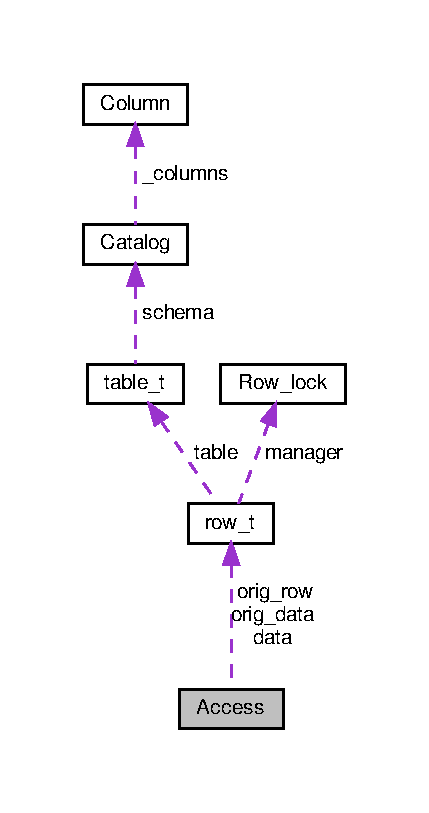
\includegraphics[width=206pt]{classAccess__coll__graph}
\end{center}
\end{figure}
\subsection*{Public Member Functions}
\begin{DoxyCompactItemize}
\item 
void \hyperlink{classAccess_ade87b82ff811ad99acdcce901c964f85}{cleanup} ()
\end{DoxyCompactItemize}
\subsection*{Public Attributes}
\begin{DoxyCompactItemize}
\item 
\hyperlink{global_8h_a567f81b0ae33b00d189d7714e9fde0bc}{access\+\_\+t} \hyperlink{classAccess_affd802962e0f6a7b5fe621db1557d2d5}{type}
\item 
\hyperlink{classrow__t}{row\+\_\+t} $\ast$ \hyperlink{classAccess_a171239dc1d26b94e1ec63683f1e7f195}{orig\+\_\+row}
\item 
\hyperlink{classrow__t}{row\+\_\+t} $\ast$ \hyperlink{classAccess_a9132c4f38f68e8e30ae16aa31ad6efbd}{data}
\item 
\hyperlink{classrow__t}{row\+\_\+t} $\ast$ \hyperlink{classAccess_ac0326631f064283f604ee204a59d4e66}{orig\+\_\+data}
\item 
\hyperlink{global_8h_aaf095dfc9b10f757c968fe146ad7e724}{ts\+\_\+t} \hyperlink{classAccess_a19794f7fefe6813eb7e6ed73534cc654}{wts}
\item 
\hyperlink{global_8h_aaf095dfc9b10f757c968fe146ad7e724}{ts\+\_\+t} \hyperlink{classAccess_ab90bf7056cd6ca4c3d46ac6bcae26357}{rts}
\end{DoxyCompactItemize}


\subsection{Member Function Documentation}
\mbox{\Hypertarget{classAccess_ade87b82ff811ad99acdcce901c964f85}\label{classAccess_ade87b82ff811ad99acdcce901c964f85}} 
\index{Access@{Access}!cleanup@{cleanup}}
\index{cleanup@{cleanup}!Access@{Access}}
\subsubsection{\texorpdfstring{cleanup()}{cleanup()}}
{\footnotesize\ttfamily void Access\+::cleanup (\begin{DoxyParamCaption}{ }\end{DoxyParamCaption})}



\subsection{Member Data Documentation}
\mbox{\Hypertarget{classAccess_a9132c4f38f68e8e30ae16aa31ad6efbd}\label{classAccess_a9132c4f38f68e8e30ae16aa31ad6efbd}} 
\index{Access@{Access}!data@{data}}
\index{data@{data}!Access@{Access}}
\subsubsection{\texorpdfstring{data}{data}}
{\footnotesize\ttfamily \hyperlink{classrow__t}{row\+\_\+t}$\ast$ Access\+::data}

\mbox{\Hypertarget{classAccess_ac0326631f064283f604ee204a59d4e66}\label{classAccess_ac0326631f064283f604ee204a59d4e66}} 
\index{Access@{Access}!orig\+\_\+data@{orig\+\_\+data}}
\index{orig\+\_\+data@{orig\+\_\+data}!Access@{Access}}
\subsubsection{\texorpdfstring{orig\+\_\+data}{orig\_data}}
{\footnotesize\ttfamily \hyperlink{classrow__t}{row\+\_\+t}$\ast$ Access\+::orig\+\_\+data}

\mbox{\Hypertarget{classAccess_a171239dc1d26b94e1ec63683f1e7f195}\label{classAccess_a171239dc1d26b94e1ec63683f1e7f195}} 
\index{Access@{Access}!orig\+\_\+row@{orig\+\_\+row}}
\index{orig\+\_\+row@{orig\+\_\+row}!Access@{Access}}
\subsubsection{\texorpdfstring{orig\+\_\+row}{orig\_row}}
{\footnotesize\ttfamily \hyperlink{classrow__t}{row\+\_\+t}$\ast$ Access\+::orig\+\_\+row}

\mbox{\Hypertarget{classAccess_ab90bf7056cd6ca4c3d46ac6bcae26357}\label{classAccess_ab90bf7056cd6ca4c3d46ac6bcae26357}} 
\index{Access@{Access}!rts@{rts}}
\index{rts@{rts}!Access@{Access}}
\subsubsection{\texorpdfstring{rts}{rts}}
{\footnotesize\ttfamily \hyperlink{global_8h_aaf095dfc9b10f757c968fe146ad7e724}{ts\+\_\+t} Access\+::rts}

\mbox{\Hypertarget{classAccess_affd802962e0f6a7b5fe621db1557d2d5}\label{classAccess_affd802962e0f6a7b5fe621db1557d2d5}} 
\index{Access@{Access}!type@{type}}
\index{type@{type}!Access@{Access}}
\subsubsection{\texorpdfstring{type}{type}}
{\footnotesize\ttfamily \hyperlink{global_8h_a567f81b0ae33b00d189d7714e9fde0bc}{access\+\_\+t} Access\+::type}

\mbox{\Hypertarget{classAccess_a19794f7fefe6813eb7e6ed73534cc654}\label{classAccess_a19794f7fefe6813eb7e6ed73534cc654}} 
\index{Access@{Access}!wts@{wts}}
\index{wts@{wts}!Access@{Access}}
\subsubsection{\texorpdfstring{wts}{wts}}
{\footnotesize\ttfamily \hyperlink{global_8h_aaf095dfc9b10f757c968fe146ad7e724}{ts\+\_\+t} Access\+::wts}



The documentation for this class was generated from the following file\+:\begin{DoxyCompactItemize}
\item 
macrobench/system/\hyperlink{txn_8h}{txn.\+h}\end{DoxyCompactItemize}

\hypertarget{classallocator__bump}{}\section{allocator\+\_\+bump$<$ T $>$ Class Template Reference}
\label{classallocator__bump}\index{allocator\+\_\+bump$<$ T $>$@{allocator\+\_\+bump$<$ T $>$}}


{\ttfamily \#include $<$allocator\+\_\+bump.\+h$>$}



Inheritance diagram for allocator\+\_\+bump$<$ T $>$\+:
\nopagebreak
\begin{figure}[H]
\begin{center}
\leavevmode
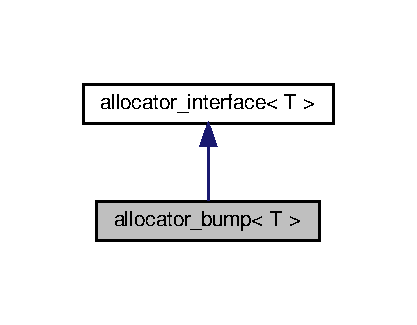
\includegraphics[width=200pt]{classallocator__bump__inherit__graph}
\end{center}
\end{figure}


Collaboration diagram for allocator\+\_\+bump$<$ T $>$\+:
\nopagebreak
\begin{figure}[H]
\begin{center}
\leavevmode
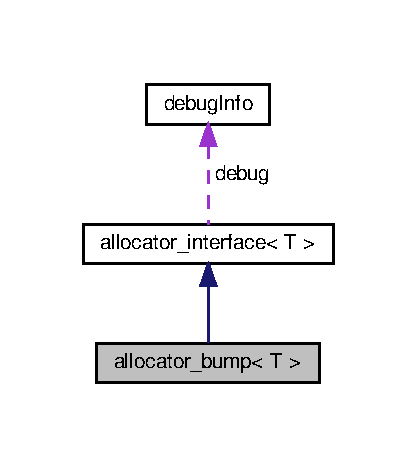
\includegraphics[width=200pt]{classallocator__bump__coll__graph}
\end{center}
\end{figure}
\subsection*{Classes}
\begin{DoxyCompactItemize}
\item 
struct \hyperlink{structallocator__bump_1_1rebind}{rebind}
\end{DoxyCompactItemize}
\subsection*{Public Member Functions}
\begin{DoxyCompactItemize}
\item 
T $\ast$ \hyperlink{classallocator__bump_ac89d92a322a51aed0f08311ec3cdbed6}{allocate} (const int \hyperlink{microbench_2main_8cpp_a9ca9869868fe7e7a38a921cc7de4103f}{tid})
\item 
void \hyperlink{classallocator__bump_a8e6c842b2ebf9918ae2035eff838ff77}{deallocate\+And\+Clear} (const int \hyperlink{microbench_2main_8cpp_a9ca9869868fe7e7a38a921cc7de4103f}{tid}, \hyperlink{classblockbag}{blockbag}$<$ T $>$ $\ast$const bag)
\item 
void \hyperlink{classallocator__bump_a59eee0e27ff339347eff13214bafd377}{debug\+Print\+Status} (const int \hyperlink{microbench_2main_8cpp_a9ca9869868fe7e7a38a921cc7de4103f}{tid})
\item 
void \hyperlink{classallocator__bump_ac363b41fc27681855131e6d7c6c31407}{init\+Thread} (const int \hyperlink{microbench_2main_8cpp_a9ca9869868fe7e7a38a921cc7de4103f}{tid})
\item 
void \hyperlink{classallocator__bump_af360b0037db6b2f1ec78d4cf02ed04d9}{deinit\+Thread} (const int \hyperlink{microbench_2main_8cpp_a9ca9869868fe7e7a38a921cc7de4103f}{tid})
\item 
\hyperlink{classallocator__bump_a5ca967892617a91266d73adb94dd8e67}{allocator\+\_\+bump} (const int \hyperlink{testing_8cpp_aa085812188e21ede75351d88b9b2c30d}{num\+Processes}, \hyperlink{classdebugInfo}{debug\+Info} $\ast$const \+\_\+debug)
\item 
\hyperlink{classallocator__bump_ae5e0e9e8ffd3db2eda6dd4afe79e9425}{$\sim$allocator\+\_\+bump} ()
\end{DoxyCompactItemize}
\subsection*{Static Public Member Functions}
\begin{DoxyCompactItemize}
\item 
static void \hyperlink{classallocator__bump_aaa6343dd8055db71dc96fa66dc9e1702}{deallocate} (const int \hyperlink{microbench_2main_8cpp_a9ca9869868fe7e7a38a921cc7de4103f}{tid}, T $\ast$const p)
\end{DoxyCompactItemize}
\subsection*{Additional Inherited Members}


\subsection{Detailed Description}
\subsubsection*{template$<$typename T = void$>$\newline
class allocator\+\_\+bump$<$ T $>$}

C++ record manager implementation (P\+O\+DC 2015) by Trevor Brown.

Copyright (C) 2015 Trevor Brown 

\subsection{Constructor \& Destructor Documentation}
\mbox{\Hypertarget{classallocator__bump_a5ca967892617a91266d73adb94dd8e67}\label{classallocator__bump_a5ca967892617a91266d73adb94dd8e67}} 
\index{allocator\+\_\+bump@{allocator\+\_\+bump}!allocator\+\_\+bump@{allocator\+\_\+bump}}
\index{allocator\+\_\+bump@{allocator\+\_\+bump}!allocator\+\_\+bump@{allocator\+\_\+bump}}
\subsubsection{\texorpdfstring{allocator\+\_\+bump()}{allocator\_bump()}}
{\footnotesize\ttfamily template$<$typename T  = void$>$ \\
\hyperlink{classallocator__bump}{allocator\+\_\+bump}$<$ T $>$\+::\hyperlink{classallocator__bump}{allocator\+\_\+bump} (\begin{DoxyParamCaption}\item[{const int}]{num\+Processes,  }\item[{\hyperlink{classdebugInfo}{debug\+Info} $\ast$const}]{\+\_\+debug }\end{DoxyParamCaption})\hspace{0.3cm}{\ttfamily [inline]}}

\mbox{\Hypertarget{classallocator__bump_ae5e0e9e8ffd3db2eda6dd4afe79e9425}\label{classallocator__bump_ae5e0e9e8ffd3db2eda6dd4afe79e9425}} 
\index{allocator\+\_\+bump@{allocator\+\_\+bump}!````~allocator\+\_\+bump@{$\sim$allocator\+\_\+bump}}
\index{````~allocator\+\_\+bump@{$\sim$allocator\+\_\+bump}!allocator\+\_\+bump@{allocator\+\_\+bump}}
\subsubsection{\texorpdfstring{$\sim$allocator\+\_\+bump()}{~allocator\_bump()}}
{\footnotesize\ttfamily template$<$typename T  = void$>$ \\
\hyperlink{classallocator__bump}{allocator\+\_\+bump}$<$ T $>$\+::$\sim$\hyperlink{classallocator__bump}{allocator\+\_\+bump} (\begin{DoxyParamCaption}{ }\end{DoxyParamCaption})\hspace{0.3cm}{\ttfamily [inline]}}



\subsection{Member Function Documentation}
\mbox{\Hypertarget{classallocator__bump_ac89d92a322a51aed0f08311ec3cdbed6}\label{classallocator__bump_ac89d92a322a51aed0f08311ec3cdbed6}} 
\index{allocator\+\_\+bump@{allocator\+\_\+bump}!allocate@{allocate}}
\index{allocate@{allocate}!allocator\+\_\+bump@{allocator\+\_\+bump}}
\subsubsection{\texorpdfstring{allocate()}{allocate()}}
{\footnotesize\ttfamily template$<$typename T  = void$>$ \\
T$\ast$ \hyperlink{classallocator__bump}{allocator\+\_\+bump}$<$ T $>$\+::allocate (\begin{DoxyParamCaption}\item[{const int}]{tid }\end{DoxyParamCaption})\hspace{0.3cm}{\ttfamily [inline]}}

\mbox{\Hypertarget{classallocator__bump_aaa6343dd8055db71dc96fa66dc9e1702}\label{classallocator__bump_aaa6343dd8055db71dc96fa66dc9e1702}} 
\index{allocator\+\_\+bump@{allocator\+\_\+bump}!deallocate@{deallocate}}
\index{deallocate@{deallocate}!allocator\+\_\+bump@{allocator\+\_\+bump}}
\subsubsection{\texorpdfstring{deallocate()}{deallocate()}}
{\footnotesize\ttfamily template$<$typename T  = void$>$ \\
static void \hyperlink{classallocator__bump}{allocator\+\_\+bump}$<$ T $>$\+::deallocate (\begin{DoxyParamCaption}\item[{const int}]{tid,  }\item[{T $\ast$const}]{p }\end{DoxyParamCaption})\hspace{0.3cm}{\ttfamily [inline]}, {\ttfamily [static]}}

\mbox{\Hypertarget{classallocator__bump_a8e6c842b2ebf9918ae2035eff838ff77}\label{classallocator__bump_a8e6c842b2ebf9918ae2035eff838ff77}} 
\index{allocator\+\_\+bump@{allocator\+\_\+bump}!deallocate\+And\+Clear@{deallocate\+And\+Clear}}
\index{deallocate\+And\+Clear@{deallocate\+And\+Clear}!allocator\+\_\+bump@{allocator\+\_\+bump}}
\subsubsection{\texorpdfstring{deallocate\+And\+Clear()}{deallocateAndClear()}}
{\footnotesize\ttfamily template$<$typename T  = void$>$ \\
void \hyperlink{classallocator__bump}{allocator\+\_\+bump}$<$ T $>$\+::deallocate\+And\+Clear (\begin{DoxyParamCaption}\item[{const int}]{tid,  }\item[{\hyperlink{classblockbag}{blockbag}$<$ T $>$ $\ast$const}]{bag }\end{DoxyParamCaption})\hspace{0.3cm}{\ttfamily [inline]}}

\mbox{\Hypertarget{classallocator__bump_a59eee0e27ff339347eff13214bafd377}\label{classallocator__bump_a59eee0e27ff339347eff13214bafd377}} 
\index{allocator\+\_\+bump@{allocator\+\_\+bump}!debug\+Print\+Status@{debug\+Print\+Status}}
\index{debug\+Print\+Status@{debug\+Print\+Status}!allocator\+\_\+bump@{allocator\+\_\+bump}}
\subsubsection{\texorpdfstring{debug\+Print\+Status()}{debugPrintStatus()}}
{\footnotesize\ttfamily template$<$typename T  = void$>$ \\
void \hyperlink{classallocator__bump}{allocator\+\_\+bump}$<$ T $>$\+::debug\+Print\+Status (\begin{DoxyParamCaption}\item[{const int}]{tid }\end{DoxyParamCaption})\hspace{0.3cm}{\ttfamily [inline]}}

\mbox{\Hypertarget{classallocator__bump_af360b0037db6b2f1ec78d4cf02ed04d9}\label{classallocator__bump_af360b0037db6b2f1ec78d4cf02ed04d9}} 
\index{allocator\+\_\+bump@{allocator\+\_\+bump}!deinit\+Thread@{deinit\+Thread}}
\index{deinit\+Thread@{deinit\+Thread}!allocator\+\_\+bump@{allocator\+\_\+bump}}
\subsubsection{\texorpdfstring{deinit\+Thread()}{deinitThread()}}
{\footnotesize\ttfamily template$<$typename T  = void$>$ \\
void \hyperlink{classallocator__bump}{allocator\+\_\+bump}$<$ T $>$\+::deinit\+Thread (\begin{DoxyParamCaption}\item[{const int}]{tid }\end{DoxyParamCaption})\hspace{0.3cm}{\ttfamily [inline]}}

\mbox{\Hypertarget{classallocator__bump_ac363b41fc27681855131e6d7c6c31407}\label{classallocator__bump_ac363b41fc27681855131e6d7c6c31407}} 
\index{allocator\+\_\+bump@{allocator\+\_\+bump}!init\+Thread@{init\+Thread}}
\index{init\+Thread@{init\+Thread}!allocator\+\_\+bump@{allocator\+\_\+bump}}
\subsubsection{\texorpdfstring{init\+Thread()}{initThread()}}
{\footnotesize\ttfamily template$<$typename T  = void$>$ \\
void \hyperlink{classallocator__bump}{allocator\+\_\+bump}$<$ T $>$\+::init\+Thread (\begin{DoxyParamCaption}\item[{const int}]{tid }\end{DoxyParamCaption})\hspace{0.3cm}{\ttfamily [inline]}}



The documentation for this class was generated from the following file\+:\begin{DoxyCompactItemize}
\item 
common/recordmgr/\hyperlink{allocator__bump_8h}{allocator\+\_\+bump.\+h}\end{DoxyCompactItemize}

\hypertarget{classallocator__interface}{}\section{allocator\+\_\+interface$<$ T $>$ Class Template Reference}
\label{classallocator__interface}\index{allocator\+\_\+interface$<$ T $>$@{allocator\+\_\+interface$<$ T $>$}}


{\ttfamily \#include $<$allocator\+\_\+interface.\+h$>$}



Inheritance diagram for allocator\+\_\+interface$<$ T $>$\+:
\nopagebreak
\begin{figure}[H]
\begin{center}
\leavevmode
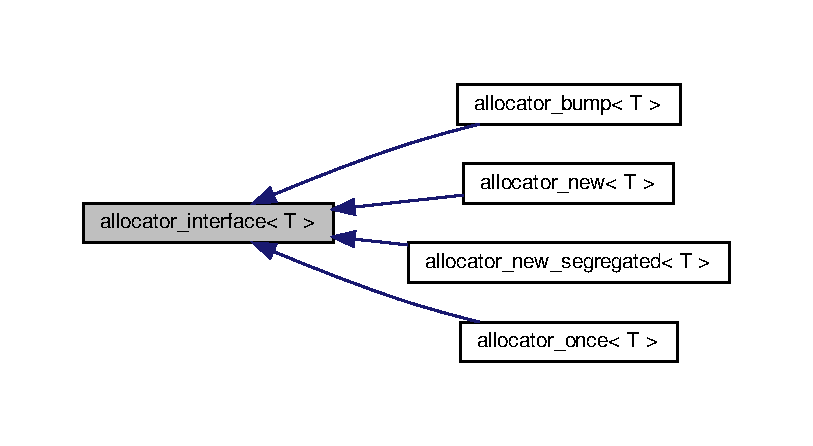
\includegraphics[width=350pt]{classallocator__interface__inherit__graph}
\end{center}
\end{figure}


Collaboration diagram for allocator\+\_\+interface$<$ T $>$\+:
\nopagebreak
\begin{figure}[H]
\begin{center}
\leavevmode
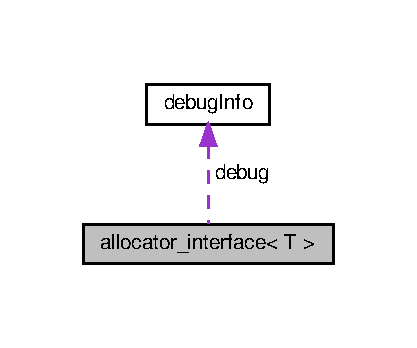
\includegraphics[width=200pt]{classallocator__interface__coll__graph}
\end{center}
\end{figure}
\subsection*{Classes}
\begin{DoxyCompactItemize}
\item 
struct \hyperlink{structallocator__interface_1_1rebind}{rebind}
\end{DoxyCompactItemize}
\subsection*{Public Member Functions}
\begin{DoxyCompactItemize}
\item 
T $\ast$ \hyperlink{classallocator__interface_a3694fb05c3cf5edaea1675c90de6a435}{allocate} (const int \hyperlink{microbench_2main_8cpp_a9ca9869868fe7e7a38a921cc7de4103f}{tid})
\item 
void \hyperlink{classallocator__interface_a608c7d3ca4735cc0a0c7d200a7e641f5}{deallocate} (const int \hyperlink{microbench_2main_8cpp_a9ca9869868fe7e7a38a921cc7de4103f}{tid}, T $\ast$const p)
\item 
void \hyperlink{classallocator__interface_ac6142b4f4c077e7dd3e2ef73fd9f8cc9}{deallocate\+And\+Clear} (const int \hyperlink{microbench_2main_8cpp_a9ca9869868fe7e7a38a921cc7de4103f}{tid}, \hyperlink{classblockbag}{blockbag}$<$ T $>$ $\ast$const bag)
\item 
void \hyperlink{classallocator__interface_afce134aab048a2003beb1fb85e4a7562}{debug\+Print\+Status} (const int \hyperlink{microbench_2main_8cpp_a9ca9869868fe7e7a38a921cc7de4103f}{tid})
\item 
void \hyperlink{classallocator__interface_a38578a36ba1ff2903563ef757bdb7160}{init\+Thread} (const int \hyperlink{microbench_2main_8cpp_a9ca9869868fe7e7a38a921cc7de4103f}{tid})
\item 
void \hyperlink{classallocator__interface_a328cf20126c294a1e7ca7775a3ad401a}{deinit\+Thread} (const int \hyperlink{microbench_2main_8cpp_a9ca9869868fe7e7a38a921cc7de4103f}{tid})
\item 
\hyperlink{classallocator__interface_a644535371130ddfa03b9c31826697dbd}{allocator\+\_\+interface} (const int \hyperlink{testing_8cpp_aa085812188e21ede75351d88b9b2c30d}{num\+Processes}, \hyperlink{classdebugInfo}{debug\+Info} $\ast$const \+\_\+debug)
\item 
\hyperlink{classallocator__interface_a8124a05dc7a241ec2fc6e4292e0636d1}{$\sim$allocator\+\_\+interface} ()
\end{DoxyCompactItemize}
\subsection*{Public Attributes}
\begin{DoxyCompactItemize}
\item 
\hyperlink{classallocator__interface_adb492ef9e40efcb500c83d93a5efe6cf}{P\+AD}
\item 
\hyperlink{classdebugInfo}{debug\+Info} $\ast$const \hyperlink{classallocator__interface_a2985caeff7ccb32343502ff0c0f86c60}{debug}
\item 
const int \hyperlink{classallocator__interface_a114bb276931256b53b2e5cf1308c350f}{N\+U\+M\+\_\+\+P\+R\+O\+C\+E\+S\+S\+ES}
\end{DoxyCompactItemize}


\subsection{Detailed Description}
\subsubsection*{template$<$typename T = void$>$\newline
class allocator\+\_\+interface$<$ T $>$}

C++ record manager implementation (P\+O\+DC 2015) by Trevor Brown.

Copyright (C) 2015 Trevor Brown 

\subsection{Constructor \& Destructor Documentation}
\mbox{\Hypertarget{classallocator__interface_a644535371130ddfa03b9c31826697dbd}\label{classallocator__interface_a644535371130ddfa03b9c31826697dbd}} 
\index{allocator\+\_\+interface@{allocator\+\_\+interface}!allocator\+\_\+interface@{allocator\+\_\+interface}}
\index{allocator\+\_\+interface@{allocator\+\_\+interface}!allocator\+\_\+interface@{allocator\+\_\+interface}}
\subsubsection{\texorpdfstring{allocator\+\_\+interface()}{allocator\_interface()}}
{\footnotesize\ttfamily template$<$typename T  = void$>$ \\
\hyperlink{classallocator__interface}{allocator\+\_\+interface}$<$ T $>$\+::\hyperlink{classallocator__interface}{allocator\+\_\+interface} (\begin{DoxyParamCaption}\item[{const int}]{num\+Processes,  }\item[{\hyperlink{classdebugInfo}{debug\+Info} $\ast$const}]{\+\_\+debug }\end{DoxyParamCaption})\hspace{0.3cm}{\ttfamily [inline]}}

\mbox{\Hypertarget{classallocator__interface_a8124a05dc7a241ec2fc6e4292e0636d1}\label{classallocator__interface_a8124a05dc7a241ec2fc6e4292e0636d1}} 
\index{allocator\+\_\+interface@{allocator\+\_\+interface}!````~allocator\+\_\+interface@{$\sim$allocator\+\_\+interface}}
\index{````~allocator\+\_\+interface@{$\sim$allocator\+\_\+interface}!allocator\+\_\+interface@{allocator\+\_\+interface}}
\subsubsection{\texorpdfstring{$\sim$allocator\+\_\+interface()}{~allocator\_interface()}}
{\footnotesize\ttfamily template$<$typename T  = void$>$ \\
\hyperlink{classallocator__interface}{allocator\+\_\+interface}$<$ T $>$\+::$\sim$\hyperlink{classallocator__interface}{allocator\+\_\+interface} (\begin{DoxyParamCaption}{ }\end{DoxyParamCaption})\hspace{0.3cm}{\ttfamily [inline]}}



\subsection{Member Function Documentation}
\mbox{\Hypertarget{classallocator__interface_a3694fb05c3cf5edaea1675c90de6a435}\label{classallocator__interface_a3694fb05c3cf5edaea1675c90de6a435}} 
\index{allocator\+\_\+interface@{allocator\+\_\+interface}!allocate@{allocate}}
\index{allocate@{allocate}!allocator\+\_\+interface@{allocator\+\_\+interface}}
\subsubsection{\texorpdfstring{allocate()}{allocate()}}
{\footnotesize\ttfamily template$<$typename T  = void$>$ \\
T$\ast$ \hyperlink{classallocator__interface}{allocator\+\_\+interface}$<$ T $>$\+::allocate (\begin{DoxyParamCaption}\item[{const int}]{tid }\end{DoxyParamCaption})}

\mbox{\Hypertarget{classallocator__interface_a608c7d3ca4735cc0a0c7d200a7e641f5}\label{classallocator__interface_a608c7d3ca4735cc0a0c7d200a7e641f5}} 
\index{allocator\+\_\+interface@{allocator\+\_\+interface}!deallocate@{deallocate}}
\index{deallocate@{deallocate}!allocator\+\_\+interface@{allocator\+\_\+interface}}
\subsubsection{\texorpdfstring{deallocate()}{deallocate()}}
{\footnotesize\ttfamily template$<$typename T  = void$>$ \\
void \hyperlink{classallocator__interface}{allocator\+\_\+interface}$<$ T $>$\+::deallocate (\begin{DoxyParamCaption}\item[{const int}]{tid,  }\item[{T $\ast$const}]{p }\end{DoxyParamCaption})}

\mbox{\Hypertarget{classallocator__interface_ac6142b4f4c077e7dd3e2ef73fd9f8cc9}\label{classallocator__interface_ac6142b4f4c077e7dd3e2ef73fd9f8cc9}} 
\index{allocator\+\_\+interface@{allocator\+\_\+interface}!deallocate\+And\+Clear@{deallocate\+And\+Clear}}
\index{deallocate\+And\+Clear@{deallocate\+And\+Clear}!allocator\+\_\+interface@{allocator\+\_\+interface}}
\subsubsection{\texorpdfstring{deallocate\+And\+Clear()}{deallocateAndClear()}}
{\footnotesize\ttfamily template$<$typename T  = void$>$ \\
void \hyperlink{classallocator__interface}{allocator\+\_\+interface}$<$ T $>$\+::deallocate\+And\+Clear (\begin{DoxyParamCaption}\item[{const int}]{tid,  }\item[{\hyperlink{classblockbag}{blockbag}$<$ T $>$ $\ast$const}]{bag }\end{DoxyParamCaption})}

\mbox{\Hypertarget{classallocator__interface_afce134aab048a2003beb1fb85e4a7562}\label{classallocator__interface_afce134aab048a2003beb1fb85e4a7562}} 
\index{allocator\+\_\+interface@{allocator\+\_\+interface}!debug\+Print\+Status@{debug\+Print\+Status}}
\index{debug\+Print\+Status@{debug\+Print\+Status}!allocator\+\_\+interface@{allocator\+\_\+interface}}
\subsubsection{\texorpdfstring{debug\+Print\+Status()}{debugPrintStatus()}}
{\footnotesize\ttfamily template$<$typename T  = void$>$ \\
void \hyperlink{classallocator__interface}{allocator\+\_\+interface}$<$ T $>$\+::debug\+Print\+Status (\begin{DoxyParamCaption}\item[{const int}]{tid }\end{DoxyParamCaption})}

\mbox{\Hypertarget{classallocator__interface_a328cf20126c294a1e7ca7775a3ad401a}\label{classallocator__interface_a328cf20126c294a1e7ca7775a3ad401a}} 
\index{allocator\+\_\+interface@{allocator\+\_\+interface}!deinit\+Thread@{deinit\+Thread}}
\index{deinit\+Thread@{deinit\+Thread}!allocator\+\_\+interface@{allocator\+\_\+interface}}
\subsubsection{\texorpdfstring{deinit\+Thread()}{deinitThread()}}
{\footnotesize\ttfamily template$<$typename T  = void$>$ \\
void \hyperlink{classallocator__interface}{allocator\+\_\+interface}$<$ T $>$\+::deinit\+Thread (\begin{DoxyParamCaption}\item[{const int}]{tid }\end{DoxyParamCaption})}

\mbox{\Hypertarget{classallocator__interface_a38578a36ba1ff2903563ef757bdb7160}\label{classallocator__interface_a38578a36ba1ff2903563ef757bdb7160}} 
\index{allocator\+\_\+interface@{allocator\+\_\+interface}!init\+Thread@{init\+Thread}}
\index{init\+Thread@{init\+Thread}!allocator\+\_\+interface@{allocator\+\_\+interface}}
\subsubsection{\texorpdfstring{init\+Thread()}{initThread()}}
{\footnotesize\ttfamily template$<$typename T  = void$>$ \\
void \hyperlink{classallocator__interface}{allocator\+\_\+interface}$<$ T $>$\+::init\+Thread (\begin{DoxyParamCaption}\item[{const int}]{tid }\end{DoxyParamCaption})}



\subsection{Member Data Documentation}
\mbox{\Hypertarget{classallocator__interface_a2985caeff7ccb32343502ff0c0f86c60}\label{classallocator__interface_a2985caeff7ccb32343502ff0c0f86c60}} 
\index{allocator\+\_\+interface@{allocator\+\_\+interface}!debug@{debug}}
\index{debug@{debug}!allocator\+\_\+interface@{allocator\+\_\+interface}}
\subsubsection{\texorpdfstring{debug}{debug}}
{\footnotesize\ttfamily template$<$typename T  = void$>$ \\
\hyperlink{classdebugInfo}{debug\+Info}$\ast$ const \hyperlink{classallocator__interface}{allocator\+\_\+interface}$<$ T $>$\+::debug}

\mbox{\Hypertarget{classallocator__interface_a114bb276931256b53b2e5cf1308c350f}\label{classallocator__interface_a114bb276931256b53b2e5cf1308c350f}} 
\index{allocator\+\_\+interface@{allocator\+\_\+interface}!N\+U\+M\+\_\+\+P\+R\+O\+C\+E\+S\+S\+ES@{N\+U\+M\+\_\+\+P\+R\+O\+C\+E\+S\+S\+ES}}
\index{N\+U\+M\+\_\+\+P\+R\+O\+C\+E\+S\+S\+ES@{N\+U\+M\+\_\+\+P\+R\+O\+C\+E\+S\+S\+ES}!allocator\+\_\+interface@{allocator\+\_\+interface}}
\subsubsection{\texorpdfstring{N\+U\+M\+\_\+\+P\+R\+O\+C\+E\+S\+S\+ES}{NUM\_PROCESSES}}
{\footnotesize\ttfamily template$<$typename T  = void$>$ \\
const int \hyperlink{classallocator__interface}{allocator\+\_\+interface}$<$ T $>$\+::N\+U\+M\+\_\+\+P\+R\+O\+C\+E\+S\+S\+ES}

\mbox{\Hypertarget{classallocator__interface_adb492ef9e40efcb500c83d93a5efe6cf}\label{classallocator__interface_adb492ef9e40efcb500c83d93a5efe6cf}} 
\index{allocator\+\_\+interface@{allocator\+\_\+interface}!P\+AD@{P\+AD}}
\index{P\+AD@{P\+AD}!allocator\+\_\+interface@{allocator\+\_\+interface}}
\subsubsection{\texorpdfstring{P\+AD}{PAD}}
{\footnotesize\ttfamily template$<$typename T  = void$>$ \\
\hyperlink{classallocator__interface}{allocator\+\_\+interface}$<$ T $>$\+::P\+AD}



The documentation for this class was generated from the following file\+:\begin{DoxyCompactItemize}
\item 
common/recordmgr/\hyperlink{allocator__interface_8h}{allocator\+\_\+interface.\+h}\end{DoxyCompactItemize}

\hypertarget{classallocator__new}{}\section{allocator\+\_\+new$<$ T $>$ Class Template Reference}
\label{classallocator__new}\index{allocator\+\_\+new$<$ T $>$@{allocator\+\_\+new$<$ T $>$}}


{\ttfamily \#include $<$allocator\+\_\+new.\+h$>$}



Inheritance diagram for allocator\+\_\+new$<$ T $>$\+:
\nopagebreak
\begin{figure}[H]
\begin{center}
\leavevmode
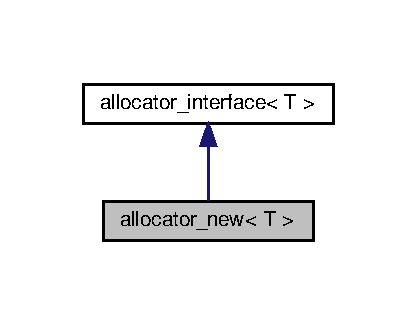
\includegraphics[width=200pt]{classallocator__new__inherit__graph}
\end{center}
\end{figure}


Collaboration diagram for allocator\+\_\+new$<$ T $>$\+:
\nopagebreak
\begin{figure}[H]
\begin{center}
\leavevmode
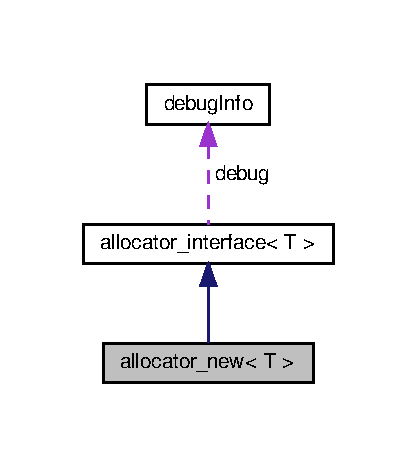
\includegraphics[width=200pt]{classallocator__new__coll__graph}
\end{center}
\end{figure}
\subsection*{Classes}
\begin{DoxyCompactItemize}
\item 
struct \hyperlink{structallocator__new_1_1rebind}{rebind}
\end{DoxyCompactItemize}
\subsection*{Public Member Functions}
\begin{DoxyCompactItemize}
\item 
T $\ast$ \hyperlink{classallocator__new_a93705f1c38fc18ec21bdaa37ccfa6ff8}{allocate} (const int \hyperlink{microbench_2main_8cpp_a9ca9869868fe7e7a38a921cc7de4103f}{tid})
\item 
void \hyperlink{classallocator__new_a00547577144cf3d387a064abcdae08ce}{deallocate} (const int \hyperlink{microbench_2main_8cpp_a9ca9869868fe7e7a38a921cc7de4103f}{tid}, T $\ast$const p)
\item 
void \hyperlink{classallocator__new_a37ae8dafab8224d4c09c496ef558156e}{deallocate\+And\+Clear} (const int \hyperlink{microbench_2main_8cpp_a9ca9869868fe7e7a38a921cc7de4103f}{tid}, \hyperlink{classblockbag}{blockbag}$<$ T $>$ $\ast$const bag)
\item 
void \hyperlink{classallocator__new_a6891234824482b3c8b83a1b91521b5e3}{debug\+Print\+Status} (const int \hyperlink{microbench_2main_8cpp_a9ca9869868fe7e7a38a921cc7de4103f}{tid})
\item 
void \hyperlink{classallocator__new_a4b65439e6dc7bbd4da71728599e12895}{init\+Thread} (const int \hyperlink{microbench_2main_8cpp_a9ca9869868fe7e7a38a921cc7de4103f}{tid})
\item 
void \hyperlink{classallocator__new_a913b5e0ed2d2cc75c2e7d03e1a75d47b}{deinit\+Thread} (const int \hyperlink{microbench_2main_8cpp_a9ca9869868fe7e7a38a921cc7de4103f}{tid})
\item 
\hyperlink{classallocator__new_a7256b6a2bf88e0ecd0cc437cd3fb6964}{allocator\+\_\+new} (const int \hyperlink{testing_8cpp_aa085812188e21ede75351d88b9b2c30d}{num\+Processes}, \hyperlink{classdebugInfo}{debug\+Info} $\ast$const \+\_\+debug)
\item 
\hyperlink{classallocator__new_a608b5c8ce78e0d255e9f26ffc9ef00f8}{$\sim$allocator\+\_\+new} ()
\end{DoxyCompactItemize}
\subsection*{Additional Inherited Members}


\subsection{Detailed Description}
\subsubsection*{template$<$typename T = void$>$\newline
class allocator\+\_\+new$<$ T $>$}

C++ record manager implementation (P\+O\+DC 2015) by Trevor Brown.

Copyright (C) 2015 Trevor Brown 

\subsection{Constructor \& Destructor Documentation}
\mbox{\Hypertarget{classallocator__new_a7256b6a2bf88e0ecd0cc437cd3fb6964}\label{classallocator__new_a7256b6a2bf88e0ecd0cc437cd3fb6964}} 
\index{allocator\+\_\+new@{allocator\+\_\+new}!allocator\+\_\+new@{allocator\+\_\+new}}
\index{allocator\+\_\+new@{allocator\+\_\+new}!allocator\+\_\+new@{allocator\+\_\+new}}
\subsubsection{\texorpdfstring{allocator\+\_\+new()}{allocator\_new()}}
{\footnotesize\ttfamily template$<$typename T  = void$>$ \\
\hyperlink{classallocator__new}{allocator\+\_\+new}$<$ T $>$\+::\hyperlink{classallocator__new}{allocator\+\_\+new} (\begin{DoxyParamCaption}\item[{const int}]{num\+Processes,  }\item[{\hyperlink{classdebugInfo}{debug\+Info} $\ast$const}]{\+\_\+debug }\end{DoxyParamCaption})\hspace{0.3cm}{\ttfamily [inline]}}

\mbox{\Hypertarget{classallocator__new_a608b5c8ce78e0d255e9f26ffc9ef00f8}\label{classallocator__new_a608b5c8ce78e0d255e9f26ffc9ef00f8}} 
\index{allocator\+\_\+new@{allocator\+\_\+new}!````~allocator\+\_\+new@{$\sim$allocator\+\_\+new}}
\index{````~allocator\+\_\+new@{$\sim$allocator\+\_\+new}!allocator\+\_\+new@{allocator\+\_\+new}}
\subsubsection{\texorpdfstring{$\sim$allocator\+\_\+new()}{~allocator\_new()}}
{\footnotesize\ttfamily template$<$typename T  = void$>$ \\
\hyperlink{classallocator__new}{allocator\+\_\+new}$<$ T $>$\+::$\sim$\hyperlink{classallocator__new}{allocator\+\_\+new} (\begin{DoxyParamCaption}{ }\end{DoxyParamCaption})\hspace{0.3cm}{\ttfamily [inline]}}



\subsection{Member Function Documentation}
\mbox{\Hypertarget{classallocator__new_a93705f1c38fc18ec21bdaa37ccfa6ff8}\label{classallocator__new_a93705f1c38fc18ec21bdaa37ccfa6ff8}} 
\index{allocator\+\_\+new@{allocator\+\_\+new}!allocate@{allocate}}
\index{allocate@{allocate}!allocator\+\_\+new@{allocator\+\_\+new}}
\subsubsection{\texorpdfstring{allocate()}{allocate()}}
{\footnotesize\ttfamily template$<$typename T  = void$>$ \\
T$\ast$ \hyperlink{classallocator__new}{allocator\+\_\+new}$<$ T $>$\+::allocate (\begin{DoxyParamCaption}\item[{const int}]{tid }\end{DoxyParamCaption})\hspace{0.3cm}{\ttfamily [inline]}}

\mbox{\Hypertarget{classallocator__new_a00547577144cf3d387a064abcdae08ce}\label{classallocator__new_a00547577144cf3d387a064abcdae08ce}} 
\index{allocator\+\_\+new@{allocator\+\_\+new}!deallocate@{deallocate}}
\index{deallocate@{deallocate}!allocator\+\_\+new@{allocator\+\_\+new}}
\subsubsection{\texorpdfstring{deallocate()}{deallocate()}}
{\footnotesize\ttfamily template$<$typename T  = void$>$ \\
void \hyperlink{classallocator__new}{allocator\+\_\+new}$<$ T $>$\+::deallocate (\begin{DoxyParamCaption}\item[{const int}]{tid,  }\item[{T $\ast$const}]{p }\end{DoxyParamCaption})\hspace{0.3cm}{\ttfamily [inline]}}

\mbox{\Hypertarget{classallocator__new_a37ae8dafab8224d4c09c496ef558156e}\label{classallocator__new_a37ae8dafab8224d4c09c496ef558156e}} 
\index{allocator\+\_\+new@{allocator\+\_\+new}!deallocate\+And\+Clear@{deallocate\+And\+Clear}}
\index{deallocate\+And\+Clear@{deallocate\+And\+Clear}!allocator\+\_\+new@{allocator\+\_\+new}}
\subsubsection{\texorpdfstring{deallocate\+And\+Clear()}{deallocateAndClear()}}
{\footnotesize\ttfamily template$<$typename T  = void$>$ \\
void \hyperlink{classallocator__new}{allocator\+\_\+new}$<$ T $>$\+::deallocate\+And\+Clear (\begin{DoxyParamCaption}\item[{const int}]{tid,  }\item[{\hyperlink{classblockbag}{blockbag}$<$ T $>$ $\ast$const}]{bag }\end{DoxyParamCaption})\hspace{0.3cm}{\ttfamily [inline]}}

\mbox{\Hypertarget{classallocator__new_a6891234824482b3c8b83a1b91521b5e3}\label{classallocator__new_a6891234824482b3c8b83a1b91521b5e3}} 
\index{allocator\+\_\+new@{allocator\+\_\+new}!debug\+Print\+Status@{debug\+Print\+Status}}
\index{debug\+Print\+Status@{debug\+Print\+Status}!allocator\+\_\+new@{allocator\+\_\+new}}
\subsubsection{\texorpdfstring{debug\+Print\+Status()}{debugPrintStatus()}}
{\footnotesize\ttfamily template$<$typename T  = void$>$ \\
void \hyperlink{classallocator__new}{allocator\+\_\+new}$<$ T $>$\+::debug\+Print\+Status (\begin{DoxyParamCaption}\item[{const int}]{tid }\end{DoxyParamCaption})\hspace{0.3cm}{\ttfamily [inline]}}

\mbox{\Hypertarget{classallocator__new_a913b5e0ed2d2cc75c2e7d03e1a75d47b}\label{classallocator__new_a913b5e0ed2d2cc75c2e7d03e1a75d47b}} 
\index{allocator\+\_\+new@{allocator\+\_\+new}!deinit\+Thread@{deinit\+Thread}}
\index{deinit\+Thread@{deinit\+Thread}!allocator\+\_\+new@{allocator\+\_\+new}}
\subsubsection{\texorpdfstring{deinit\+Thread()}{deinitThread()}}
{\footnotesize\ttfamily template$<$typename T  = void$>$ \\
void \hyperlink{classallocator__new}{allocator\+\_\+new}$<$ T $>$\+::deinit\+Thread (\begin{DoxyParamCaption}\item[{const int}]{tid }\end{DoxyParamCaption})\hspace{0.3cm}{\ttfamily [inline]}}

\mbox{\Hypertarget{classallocator__new_a4b65439e6dc7bbd4da71728599e12895}\label{classallocator__new_a4b65439e6dc7bbd4da71728599e12895}} 
\index{allocator\+\_\+new@{allocator\+\_\+new}!init\+Thread@{init\+Thread}}
\index{init\+Thread@{init\+Thread}!allocator\+\_\+new@{allocator\+\_\+new}}
\subsubsection{\texorpdfstring{init\+Thread()}{initThread()}}
{\footnotesize\ttfamily template$<$typename T  = void$>$ \\
void \hyperlink{classallocator__new}{allocator\+\_\+new}$<$ T $>$\+::init\+Thread (\begin{DoxyParamCaption}\item[{const int}]{tid }\end{DoxyParamCaption})\hspace{0.3cm}{\ttfamily [inline]}}



The documentation for this class was generated from the following file\+:\begin{DoxyCompactItemize}
\item 
common/recordmgr/\hyperlink{allocator__new_8h}{allocator\+\_\+new.\+h}\end{DoxyCompactItemize}

\hypertarget{classallocator__new__segregated}{}\section{allocator\+\_\+new\+\_\+segregated$<$ T $>$ Class Template Reference}
\label{classallocator__new__segregated}\index{allocator\+\_\+new\+\_\+segregated$<$ T $>$@{allocator\+\_\+new\+\_\+segregated$<$ T $>$}}


{\ttfamily \#include $<$allocator\+\_\+new\+\_\+segregated.\+h$>$}



Inheritance diagram for allocator\+\_\+new\+\_\+segregated$<$ T $>$\+:
\nopagebreak
\begin{figure}[H]
\begin{center}
\leavevmode
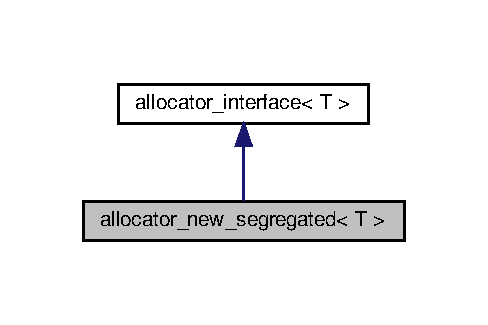
\includegraphics[width=234pt]{classallocator__new__segregated__inherit__graph}
\end{center}
\end{figure}


Collaboration diagram for allocator\+\_\+new\+\_\+segregated$<$ T $>$\+:
\nopagebreak
\begin{figure}[H]
\begin{center}
\leavevmode
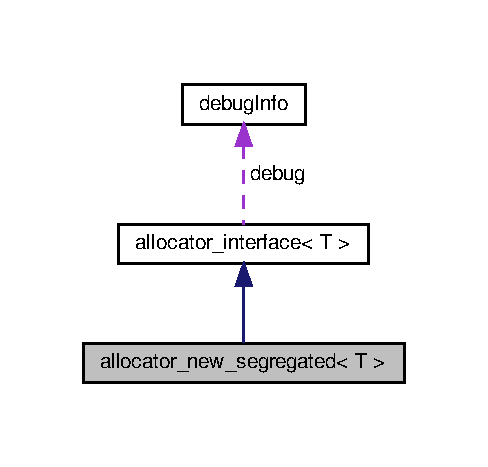
\includegraphics[width=234pt]{classallocator__new__segregated__coll__graph}
\end{center}
\end{figure}
\subsection*{Classes}
\begin{DoxyCompactItemize}
\item 
struct \hyperlink{structallocator__new__segregated_1_1rebind}{rebind}
\end{DoxyCompactItemize}
\subsection*{Public Member Functions}
\begin{DoxyCompactItemize}
\item 
T $\ast$ \hyperlink{classallocator__new__segregated_a5259d0e0d4777b6b4379a611bf6f90b1}{allocate} (const int \hyperlink{microbench_2main_8cpp_a9ca9869868fe7e7a38a921cc7de4103f}{tid})
\item 
void \hyperlink{classallocator__new__segregated_a99196d2db15094973ce77dee0c317ae5}{deallocate} (const int \hyperlink{microbench_2main_8cpp_a9ca9869868fe7e7a38a921cc7de4103f}{tid}, T $\ast$const p)
\item 
void \hyperlink{classallocator__new__segregated_a70d65a2e25c1abe13d2fb54e0dafc0c4}{deallocate\+And\+Clear} (const int \hyperlink{microbench_2main_8cpp_a9ca9869868fe7e7a38a921cc7de4103f}{tid}, \hyperlink{classblockbag}{blockbag}$<$ T $>$ $\ast$const bag)
\item 
void \hyperlink{classallocator__new__segregated_a659455bf01a11dbfd8a0762a4d4fdb40}{debug\+Print\+Status} (const int \hyperlink{microbench_2main_8cpp_a9ca9869868fe7e7a38a921cc7de4103f}{tid})
\item 
void \hyperlink{classallocator__new__segregated_a143dbe613cd2e5b903c2fefcc02238f2}{init\+Thread} (const int \hyperlink{microbench_2main_8cpp_a9ca9869868fe7e7a38a921cc7de4103f}{tid})
\item 
void \hyperlink{classallocator__new__segregated_ae56ef2f9fa45e5142cddbe862b342cc6}{deinit\+Thread} (const int \hyperlink{microbench_2main_8cpp_a9ca9869868fe7e7a38a921cc7de4103f}{tid})
\item 
\hyperlink{classallocator__new__segregated_ae05ebf7ffd3a4939e36d2a82f495a30c}{allocator\+\_\+new\+\_\+segregated} (const int \hyperlink{testing_8cpp_aa085812188e21ede75351d88b9b2c30d}{num\+Processes}, \hyperlink{classdebugInfo}{debug\+Info} $\ast$const \+\_\+debug)
\item 
\hyperlink{classallocator__new__segregated_aed2e73950c9ee0ef9d349c74fd30ecf8}{$\sim$allocator\+\_\+new\+\_\+segregated} ()
\end{DoxyCompactItemize}
\subsection*{Static Public Member Functions}
\begin{DoxyCompactItemize}
\item 
static void $\ast$ \hyperlink{classallocator__new__segregated_a6757b22908992b0149630326ce7f68ac}{dummy\+\_\+thr} (void $\ast$p)
\end{DoxyCompactItemize}
\subsection*{Additional Inherited Members}


\subsection{Detailed Description}
\subsubsection*{template$<$typename T = void$>$\newline
class allocator\+\_\+new\+\_\+segregated$<$ T $>$}

C++ record manager implementation (P\+O\+DC 2015) by Trevor Brown.

Copyright (C) 2015 Trevor Brown 

\subsection{Constructor \& Destructor Documentation}
\mbox{\Hypertarget{classallocator__new__segregated_ae05ebf7ffd3a4939e36d2a82f495a30c}\label{classallocator__new__segregated_ae05ebf7ffd3a4939e36d2a82f495a30c}} 
\index{allocator\+\_\+new\+\_\+segregated@{allocator\+\_\+new\+\_\+segregated}!allocator\+\_\+new\+\_\+segregated@{allocator\+\_\+new\+\_\+segregated}}
\index{allocator\+\_\+new\+\_\+segregated@{allocator\+\_\+new\+\_\+segregated}!allocator\+\_\+new\+\_\+segregated@{allocator\+\_\+new\+\_\+segregated}}
\subsubsection{\texorpdfstring{allocator\+\_\+new\+\_\+segregated()}{allocator\_new\_segregated()}}
{\footnotesize\ttfamily template$<$typename T  = void$>$ \\
\hyperlink{classallocator__new__segregated}{allocator\+\_\+new\+\_\+segregated}$<$ T $>$\+::\hyperlink{classallocator__new__segregated}{allocator\+\_\+new\+\_\+segregated} (\begin{DoxyParamCaption}\item[{const int}]{num\+Processes,  }\item[{\hyperlink{classdebugInfo}{debug\+Info} $\ast$const}]{\+\_\+debug }\end{DoxyParamCaption})\hspace{0.3cm}{\ttfamily [inline]}}

\mbox{\Hypertarget{classallocator__new__segregated_aed2e73950c9ee0ef9d349c74fd30ecf8}\label{classallocator__new__segregated_aed2e73950c9ee0ef9d349c74fd30ecf8}} 
\index{allocator\+\_\+new\+\_\+segregated@{allocator\+\_\+new\+\_\+segregated}!````~allocator\+\_\+new\+\_\+segregated@{$\sim$allocator\+\_\+new\+\_\+segregated}}
\index{````~allocator\+\_\+new\+\_\+segregated@{$\sim$allocator\+\_\+new\+\_\+segregated}!allocator\+\_\+new\+\_\+segregated@{allocator\+\_\+new\+\_\+segregated}}
\subsubsection{\texorpdfstring{$\sim$allocator\+\_\+new\+\_\+segregated()}{~allocator\_new\_segregated()}}
{\footnotesize\ttfamily template$<$typename T  = void$>$ \\
\hyperlink{classallocator__new__segregated}{allocator\+\_\+new\+\_\+segregated}$<$ T $>$\+::$\sim$\hyperlink{classallocator__new__segregated}{allocator\+\_\+new\+\_\+segregated} (\begin{DoxyParamCaption}{ }\end{DoxyParamCaption})\hspace{0.3cm}{\ttfamily [inline]}}



\subsection{Member Function Documentation}
\mbox{\Hypertarget{classallocator__new__segregated_a5259d0e0d4777b6b4379a611bf6f90b1}\label{classallocator__new__segregated_a5259d0e0d4777b6b4379a611bf6f90b1}} 
\index{allocator\+\_\+new\+\_\+segregated@{allocator\+\_\+new\+\_\+segregated}!allocate@{allocate}}
\index{allocate@{allocate}!allocator\+\_\+new\+\_\+segregated@{allocator\+\_\+new\+\_\+segregated}}
\subsubsection{\texorpdfstring{allocate()}{allocate()}}
{\footnotesize\ttfamily template$<$typename T  = void$>$ \\
T$\ast$ \hyperlink{classallocator__new__segregated}{allocator\+\_\+new\+\_\+segregated}$<$ T $>$\+::allocate (\begin{DoxyParamCaption}\item[{const int}]{tid }\end{DoxyParamCaption})\hspace{0.3cm}{\ttfamily [inline]}}

\mbox{\Hypertarget{classallocator__new__segregated_a99196d2db15094973ce77dee0c317ae5}\label{classallocator__new__segregated_a99196d2db15094973ce77dee0c317ae5}} 
\index{allocator\+\_\+new\+\_\+segregated@{allocator\+\_\+new\+\_\+segregated}!deallocate@{deallocate}}
\index{deallocate@{deallocate}!allocator\+\_\+new\+\_\+segregated@{allocator\+\_\+new\+\_\+segregated}}
\subsubsection{\texorpdfstring{deallocate()}{deallocate()}}
{\footnotesize\ttfamily template$<$typename T  = void$>$ \\
void \hyperlink{classallocator__new__segregated}{allocator\+\_\+new\+\_\+segregated}$<$ T $>$\+::deallocate (\begin{DoxyParamCaption}\item[{const int}]{tid,  }\item[{T $\ast$const}]{p }\end{DoxyParamCaption})\hspace{0.3cm}{\ttfamily [inline]}}

\mbox{\Hypertarget{classallocator__new__segregated_a70d65a2e25c1abe13d2fb54e0dafc0c4}\label{classallocator__new__segregated_a70d65a2e25c1abe13d2fb54e0dafc0c4}} 
\index{allocator\+\_\+new\+\_\+segregated@{allocator\+\_\+new\+\_\+segregated}!deallocate\+And\+Clear@{deallocate\+And\+Clear}}
\index{deallocate\+And\+Clear@{deallocate\+And\+Clear}!allocator\+\_\+new\+\_\+segregated@{allocator\+\_\+new\+\_\+segregated}}
\subsubsection{\texorpdfstring{deallocate\+And\+Clear()}{deallocateAndClear()}}
{\footnotesize\ttfamily template$<$typename T  = void$>$ \\
void \hyperlink{classallocator__new__segregated}{allocator\+\_\+new\+\_\+segregated}$<$ T $>$\+::deallocate\+And\+Clear (\begin{DoxyParamCaption}\item[{const int}]{tid,  }\item[{\hyperlink{classblockbag}{blockbag}$<$ T $>$ $\ast$const}]{bag }\end{DoxyParamCaption})\hspace{0.3cm}{\ttfamily [inline]}}

\mbox{\Hypertarget{classallocator__new__segregated_a659455bf01a11dbfd8a0762a4d4fdb40}\label{classallocator__new__segregated_a659455bf01a11dbfd8a0762a4d4fdb40}} 
\index{allocator\+\_\+new\+\_\+segregated@{allocator\+\_\+new\+\_\+segregated}!debug\+Print\+Status@{debug\+Print\+Status}}
\index{debug\+Print\+Status@{debug\+Print\+Status}!allocator\+\_\+new\+\_\+segregated@{allocator\+\_\+new\+\_\+segregated}}
\subsubsection{\texorpdfstring{debug\+Print\+Status()}{debugPrintStatus()}}
{\footnotesize\ttfamily template$<$typename T  = void$>$ \\
void \hyperlink{classallocator__new__segregated}{allocator\+\_\+new\+\_\+segregated}$<$ T $>$\+::debug\+Print\+Status (\begin{DoxyParamCaption}\item[{const int}]{tid }\end{DoxyParamCaption})\hspace{0.3cm}{\ttfamily [inline]}}

\mbox{\Hypertarget{classallocator__new__segregated_ae56ef2f9fa45e5142cddbe862b342cc6}\label{classallocator__new__segregated_ae56ef2f9fa45e5142cddbe862b342cc6}} 
\index{allocator\+\_\+new\+\_\+segregated@{allocator\+\_\+new\+\_\+segregated}!deinit\+Thread@{deinit\+Thread}}
\index{deinit\+Thread@{deinit\+Thread}!allocator\+\_\+new\+\_\+segregated@{allocator\+\_\+new\+\_\+segregated}}
\subsubsection{\texorpdfstring{deinit\+Thread()}{deinitThread()}}
{\footnotesize\ttfamily template$<$typename T  = void$>$ \\
void \hyperlink{classallocator__new__segregated}{allocator\+\_\+new\+\_\+segregated}$<$ T $>$\+::deinit\+Thread (\begin{DoxyParamCaption}\item[{const int}]{tid }\end{DoxyParamCaption})\hspace{0.3cm}{\ttfamily [inline]}}

\mbox{\Hypertarget{classallocator__new__segregated_a6757b22908992b0149630326ce7f68ac}\label{classallocator__new__segregated_a6757b22908992b0149630326ce7f68ac}} 
\index{allocator\+\_\+new\+\_\+segregated@{allocator\+\_\+new\+\_\+segregated}!dummy\+\_\+thr@{dummy\+\_\+thr}}
\index{dummy\+\_\+thr@{dummy\+\_\+thr}!allocator\+\_\+new\+\_\+segregated@{allocator\+\_\+new\+\_\+segregated}}
\subsubsection{\texorpdfstring{dummy\+\_\+thr()}{dummy\_thr()}}
{\footnotesize\ttfamily template$<$typename T  = void$>$ \\
static void$\ast$ \hyperlink{classallocator__new__segregated}{allocator\+\_\+new\+\_\+segregated}$<$ T $>$\+::dummy\+\_\+thr (\begin{DoxyParamCaption}\item[{void $\ast$}]{p }\end{DoxyParamCaption})\hspace{0.3cm}{\ttfamily [inline]}, {\ttfamily [static]}}

\mbox{\Hypertarget{classallocator__new__segregated_a143dbe613cd2e5b903c2fefcc02238f2}\label{classallocator__new__segregated_a143dbe613cd2e5b903c2fefcc02238f2}} 
\index{allocator\+\_\+new\+\_\+segregated@{allocator\+\_\+new\+\_\+segregated}!init\+Thread@{init\+Thread}}
\index{init\+Thread@{init\+Thread}!allocator\+\_\+new\+\_\+segregated@{allocator\+\_\+new\+\_\+segregated}}
\subsubsection{\texorpdfstring{init\+Thread()}{initThread()}}
{\footnotesize\ttfamily template$<$typename T  = void$>$ \\
void \hyperlink{classallocator__new__segregated}{allocator\+\_\+new\+\_\+segregated}$<$ T $>$\+::init\+Thread (\begin{DoxyParamCaption}\item[{const int}]{tid }\end{DoxyParamCaption})\hspace{0.3cm}{\ttfamily [inline]}}



The documentation for this class was generated from the following file\+:\begin{DoxyCompactItemize}
\item 
common/recordmgr/\hyperlink{allocator__new__segregated_8h}{allocator\+\_\+new\+\_\+segregated.\+h}\end{DoxyCompactItemize}

\hypertarget{classallocator__once}{}\section{allocator\+\_\+once$<$ T $>$ Class Template Reference}
\label{classallocator__once}\index{allocator\+\_\+once$<$ T $>$@{allocator\+\_\+once$<$ T $>$}}


{\ttfamily \#include $<$allocator\+\_\+once.\+h$>$}



Inheritance diagram for allocator\+\_\+once$<$ T $>$\+:
\nopagebreak
\begin{figure}[H]
\begin{center}
\leavevmode
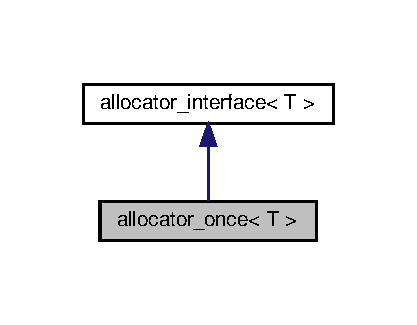
\includegraphics[width=200pt]{classallocator__once__inherit__graph}
\end{center}
\end{figure}


Collaboration diagram for allocator\+\_\+once$<$ T $>$\+:
\nopagebreak
\begin{figure}[H]
\begin{center}
\leavevmode
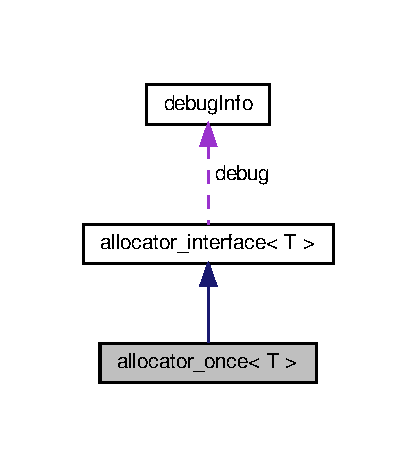
\includegraphics[width=200pt]{classallocator__once__coll__graph}
\end{center}
\end{figure}
\subsection*{Classes}
\begin{DoxyCompactItemize}
\item 
struct \hyperlink{structallocator__once_1_1rebind}{rebind}
\end{DoxyCompactItemize}
\subsection*{Public Member Functions}
\begin{DoxyCompactItemize}
\item 
T $\ast$ \hyperlink{classallocator__once_abfd2798c921320154252d3c16f67e434}{allocate} (const int \hyperlink{microbench_2main_8cpp_a9ca9869868fe7e7a38a921cc7de4103f}{tid})
\item 
void \hyperlink{classallocator__once_a311dcf7b1c2d5792b1bc8ce418ab9b42}{deallocate\+And\+Clear} (const int \hyperlink{microbench_2main_8cpp_a9ca9869868fe7e7a38a921cc7de4103f}{tid}, \hyperlink{classblockbag}{blockbag}$<$ T $>$ $\ast$const bag)
\item 
void \hyperlink{classallocator__once_ad50c51979d7260a86334c3df79b3d55e}{debug\+Print\+Status} (const int \hyperlink{microbench_2main_8cpp_a9ca9869868fe7e7a38a921cc7de4103f}{tid})
\item 
void \hyperlink{classallocator__once_a700c4f8c603d07b26435da98425e2cb8}{init\+Thread} (const int \hyperlink{microbench_2main_8cpp_a9ca9869868fe7e7a38a921cc7de4103f}{tid})
\item 
void \hyperlink{classallocator__once_a8dd2989cbd49008d5faa43d03c930e0e}{deinit\+Thread} (const int \hyperlink{microbench_2main_8cpp_a9ca9869868fe7e7a38a921cc7de4103f}{tid})
\item 
\hyperlink{classallocator__once_ac67f48c32b2da6477d56ff602b8aeb0a}{allocator\+\_\+once} (const int \hyperlink{testing_8cpp_aa085812188e21ede75351d88b9b2c30d}{num\+Processes}, \hyperlink{classdebugInfo}{debug\+Info} $\ast$const \+\_\+debug)
\item 
\hyperlink{classallocator__once_a61d85b93659618b4777498ba7e20c872}{$\sim$allocator\+\_\+once} ()
\end{DoxyCompactItemize}
\subsection*{Static Public Member Functions}
\begin{DoxyCompactItemize}
\item 
static void \hyperlink{classallocator__once_a7fbe0cd20adb62e1c160cecc98bcc257}{deallocate} (const int \hyperlink{microbench_2main_8cpp_a9ca9869868fe7e7a38a921cc7de4103f}{tid}, T $\ast$const p)
\end{DoxyCompactItemize}
\subsection*{Additional Inherited Members}


\subsection{Constructor \& Destructor Documentation}
\mbox{\Hypertarget{classallocator__once_ac67f48c32b2da6477d56ff602b8aeb0a}\label{classallocator__once_ac67f48c32b2da6477d56ff602b8aeb0a}} 
\index{allocator\+\_\+once@{allocator\+\_\+once}!allocator\+\_\+once@{allocator\+\_\+once}}
\index{allocator\+\_\+once@{allocator\+\_\+once}!allocator\+\_\+once@{allocator\+\_\+once}}
\subsubsection{\texorpdfstring{allocator\+\_\+once()}{allocator\_once()}}
{\footnotesize\ttfamily template$<$typename T  = void$>$ \\
\hyperlink{classallocator__once}{allocator\+\_\+once}$<$ T $>$\+::\hyperlink{classallocator__once}{allocator\+\_\+once} (\begin{DoxyParamCaption}\item[{const int}]{num\+Processes,  }\item[{\hyperlink{classdebugInfo}{debug\+Info} $\ast$const}]{\+\_\+debug }\end{DoxyParamCaption})\hspace{0.3cm}{\ttfamily [inline]}}

\mbox{\Hypertarget{classallocator__once_a61d85b93659618b4777498ba7e20c872}\label{classallocator__once_a61d85b93659618b4777498ba7e20c872}} 
\index{allocator\+\_\+once@{allocator\+\_\+once}!````~allocator\+\_\+once@{$\sim$allocator\+\_\+once}}
\index{````~allocator\+\_\+once@{$\sim$allocator\+\_\+once}!allocator\+\_\+once@{allocator\+\_\+once}}
\subsubsection{\texorpdfstring{$\sim$allocator\+\_\+once()}{~allocator\_once()}}
{\footnotesize\ttfamily template$<$typename T  = void$>$ \\
\hyperlink{classallocator__once}{allocator\+\_\+once}$<$ T $>$\+::$\sim$\hyperlink{classallocator__once}{allocator\+\_\+once} (\begin{DoxyParamCaption}{ }\end{DoxyParamCaption})\hspace{0.3cm}{\ttfamily [inline]}}



\subsection{Member Function Documentation}
\mbox{\Hypertarget{classallocator__once_abfd2798c921320154252d3c16f67e434}\label{classallocator__once_abfd2798c921320154252d3c16f67e434}} 
\index{allocator\+\_\+once@{allocator\+\_\+once}!allocate@{allocate}}
\index{allocate@{allocate}!allocator\+\_\+once@{allocator\+\_\+once}}
\subsubsection{\texorpdfstring{allocate()}{allocate()}}
{\footnotesize\ttfamily template$<$typename T  = void$>$ \\
T$\ast$ \hyperlink{classallocator__once}{allocator\+\_\+once}$<$ T $>$\+::allocate (\begin{DoxyParamCaption}\item[{const int}]{tid }\end{DoxyParamCaption})\hspace{0.3cm}{\ttfamily [inline]}}

\mbox{\Hypertarget{classallocator__once_a7fbe0cd20adb62e1c160cecc98bcc257}\label{classallocator__once_a7fbe0cd20adb62e1c160cecc98bcc257}} 
\index{allocator\+\_\+once@{allocator\+\_\+once}!deallocate@{deallocate}}
\index{deallocate@{deallocate}!allocator\+\_\+once@{allocator\+\_\+once}}
\subsubsection{\texorpdfstring{deallocate()}{deallocate()}}
{\footnotesize\ttfamily template$<$typename T  = void$>$ \\
static void \hyperlink{classallocator__once}{allocator\+\_\+once}$<$ T $>$\+::deallocate (\begin{DoxyParamCaption}\item[{const int}]{tid,  }\item[{T $\ast$const}]{p }\end{DoxyParamCaption})\hspace{0.3cm}{\ttfamily [inline]}, {\ttfamily [static]}}

\mbox{\Hypertarget{classallocator__once_a311dcf7b1c2d5792b1bc8ce418ab9b42}\label{classallocator__once_a311dcf7b1c2d5792b1bc8ce418ab9b42}} 
\index{allocator\+\_\+once@{allocator\+\_\+once}!deallocate\+And\+Clear@{deallocate\+And\+Clear}}
\index{deallocate\+And\+Clear@{deallocate\+And\+Clear}!allocator\+\_\+once@{allocator\+\_\+once}}
\subsubsection{\texorpdfstring{deallocate\+And\+Clear()}{deallocateAndClear()}}
{\footnotesize\ttfamily template$<$typename T  = void$>$ \\
void \hyperlink{classallocator__once}{allocator\+\_\+once}$<$ T $>$\+::deallocate\+And\+Clear (\begin{DoxyParamCaption}\item[{const int}]{tid,  }\item[{\hyperlink{classblockbag}{blockbag}$<$ T $>$ $\ast$const}]{bag }\end{DoxyParamCaption})\hspace{0.3cm}{\ttfamily [inline]}}

\mbox{\Hypertarget{classallocator__once_ad50c51979d7260a86334c3df79b3d55e}\label{classallocator__once_ad50c51979d7260a86334c3df79b3d55e}} 
\index{allocator\+\_\+once@{allocator\+\_\+once}!debug\+Print\+Status@{debug\+Print\+Status}}
\index{debug\+Print\+Status@{debug\+Print\+Status}!allocator\+\_\+once@{allocator\+\_\+once}}
\subsubsection{\texorpdfstring{debug\+Print\+Status()}{debugPrintStatus()}}
{\footnotesize\ttfamily template$<$typename T  = void$>$ \\
void \hyperlink{classallocator__once}{allocator\+\_\+once}$<$ T $>$\+::debug\+Print\+Status (\begin{DoxyParamCaption}\item[{const int}]{tid }\end{DoxyParamCaption})\hspace{0.3cm}{\ttfamily [inline]}}

\mbox{\Hypertarget{classallocator__once_a8dd2989cbd49008d5faa43d03c930e0e}\label{classallocator__once_a8dd2989cbd49008d5faa43d03c930e0e}} 
\index{allocator\+\_\+once@{allocator\+\_\+once}!deinit\+Thread@{deinit\+Thread}}
\index{deinit\+Thread@{deinit\+Thread}!allocator\+\_\+once@{allocator\+\_\+once}}
\subsubsection{\texorpdfstring{deinit\+Thread()}{deinitThread()}}
{\footnotesize\ttfamily template$<$typename T  = void$>$ \\
void \hyperlink{classallocator__once}{allocator\+\_\+once}$<$ T $>$\+::deinit\+Thread (\begin{DoxyParamCaption}\item[{const int}]{tid }\end{DoxyParamCaption})\hspace{0.3cm}{\ttfamily [inline]}}

\mbox{\Hypertarget{classallocator__once_a700c4f8c603d07b26435da98425e2cb8}\label{classallocator__once_a700c4f8c603d07b26435da98425e2cb8}} 
\index{allocator\+\_\+once@{allocator\+\_\+once}!init\+Thread@{init\+Thread}}
\index{init\+Thread@{init\+Thread}!allocator\+\_\+once@{allocator\+\_\+once}}
\subsubsection{\texorpdfstring{init\+Thread()}{initThread()}}
{\footnotesize\ttfamily template$<$typename T  = void$>$ \\
void \hyperlink{classallocator__once}{allocator\+\_\+once}$<$ T $>$\+::init\+Thread (\begin{DoxyParamCaption}\item[{const int}]{tid }\end{DoxyParamCaption})\hspace{0.3cm}{\ttfamily [inline]}}



The documentation for this class was generated from the following file\+:\begin{DoxyCompactItemize}
\item 
common/recordmgr/\hyperlink{allocator__once_8h}{allocator\+\_\+once.\+h}\end{DoxyCompactItemize}

\hypertarget{structanchorRecord}{}\section{anchor\+Record$<$ skey\+\_\+t, sval\+\_\+t $>$ Struct Template Reference}
\label{structanchorRecord}\index{anchor\+Record$<$ skey\+\_\+t, sval\+\_\+t $>$@{anchor\+Record$<$ skey\+\_\+t, sval\+\_\+t $>$}}


{\ttfamily \#include $<$intlf\+\_\+impl.\+h$>$}

\subsection*{Public Attributes}
\begin{DoxyCompactItemize}
\item 
\hyperlink{structnode__t}{node\+\_\+t}$<$ skey\+\_\+t, sval\+\_\+t $>$ $\ast$ \hyperlink{structanchorRecord_a8061a070a75e5f9bb2e2f5e2969ce641}{node}
\item 
skey\+\_\+t \hyperlink{structanchorRecord_ae14bc8e64efbe368ad6c511b5272b96f}{key}
\end{DoxyCompactItemize}


\subsection{Member Data Documentation}
\mbox{\Hypertarget{structanchorRecord_ae14bc8e64efbe368ad6c511b5272b96f}\label{structanchorRecord_ae14bc8e64efbe368ad6c511b5272b96f}} 
\index{anchor\+Record@{anchor\+Record}!key@{key}}
\index{key@{key}!anchor\+Record@{anchor\+Record}}
\subsubsection{\texorpdfstring{key}{key}}
{\footnotesize\ttfamily template$<$typename skey\+\_\+t, typename sval\+\_\+t$>$ \\
skey\+\_\+t \hyperlink{structanchorRecord}{anchor\+Record}$<$ skey\+\_\+t, sval\+\_\+t $>$\+::key}

\mbox{\Hypertarget{structanchorRecord_a8061a070a75e5f9bb2e2f5e2969ce641}\label{structanchorRecord_a8061a070a75e5f9bb2e2f5e2969ce641}} 
\index{anchor\+Record@{anchor\+Record}!node@{node}}
\index{node@{node}!anchor\+Record@{anchor\+Record}}
\subsubsection{\texorpdfstring{node}{node}}
{\footnotesize\ttfamily template$<$typename skey\+\_\+t, typename sval\+\_\+t$>$ \\
\hyperlink{structnode__t}{node\+\_\+t}$<$skey\+\_\+t, sval\+\_\+t$>$$\ast$ \hyperlink{structanchorRecord}{anchor\+Record}$<$ skey\+\_\+t, sval\+\_\+t $>$\+::node}



The documentation for this struct was generated from the following file\+:\begin{DoxyCompactItemize}
\item 
ds/ramachandran\+\_\+int\+\_\+bst\+\_\+lf/\hyperlink{intlf__impl_8h}{intlf\+\_\+impl.\+h}\end{DoxyCompactItemize}

\hypertarget{structAO__double__t}{}\section{A\+O\+\_\+double\+\_\+t Union Reference}
\label{structAO__double__t}\index{A\+O\+\_\+double\+\_\+t@{A\+O\+\_\+double\+\_\+t}}


{\ttfamily \#include $<$generic\+\_\+pthread.\+h$>$}

\subsection*{Public Attributes}
\begin{DoxyCompactItemize}
\item 
\hyperlink{atomic__ops_8h_a5225fef4d9eee821e82382cd269160dd}{A\+O\+\_\+t} \hyperlink{structAO__double__t_a56db8737f0a8c2694329c400b7f94a80}{A\+O\+\_\+val1}
\item 
\hyperlink{atomic__ops_8h_a5225fef4d9eee821e82382cd269160dd}{A\+O\+\_\+t} \hyperlink{structAO__double__t_acc45c474c9a91a9f679adb12425a0257}{A\+O\+\_\+val2}
\item 
\hyperlink{standard__ao__double__t_8h_ac63c23baae3d771141f4660fbd1fbf7e}{double\+\_\+ptr\+\_\+storage} \hyperlink{structAO__double__t_a029ebe26b957e9b920c286705b24022a}{A\+O\+\_\+whole}
\item 
\begin{tabbing}
xx\=xx\=xx\=xx\=xx\=xx\=xx\=xx\=xx\=\kill
struct \{\\
\>\hyperlink{atomic__ops_8h_a5225fef4d9eee821e82382cd269160dd}{AO\_t} \hyperlink{structAO__double__t_a66b43922d540e66f680936a80c69c3c2}{AO\_v1}\\
\>\hyperlink{atomic__ops_8h_a5225fef4d9eee821e82382cd269160dd}{AO\_t} \hyperlink{structAO__double__t_acf8e7ff92420bc60c4bdd12aa528151b}{AO\_v2}\\
\} \hyperlink{structAO__double__t_af71891b71113270b6904d1946078af0f}{AO\_parts}\\

\end{tabbing}\end{DoxyCompactItemize}


\subsection{Member Data Documentation}
\mbox{\Hypertarget{structAO__double__t_af71891b71113270b6904d1946078af0f}\label{structAO__double__t_af71891b71113270b6904d1946078af0f}} 
\index{A\+O\+\_\+double\+\_\+t@{A\+O\+\_\+double\+\_\+t}!A\+O\+\_\+parts@{A\+O\+\_\+parts}}
\index{A\+O\+\_\+parts@{A\+O\+\_\+parts}!A\+O\+\_\+double\+\_\+t@{A\+O\+\_\+double\+\_\+t}}
\subsubsection{\texorpdfstring{A\+O\+\_\+parts}{AO\_parts}}
{\footnotesize\ttfamily struct \{ ... \}   A\+O\+\_\+double\+\_\+t\+::\+A\+O\+\_\+parts}

\mbox{\Hypertarget{structAO__double__t_a66b43922d540e66f680936a80c69c3c2}\label{structAO__double__t_a66b43922d540e66f680936a80c69c3c2}} 
\index{A\+O\+\_\+double\+\_\+t@{A\+O\+\_\+double\+\_\+t}!A\+O\+\_\+v1@{A\+O\+\_\+v1}}
\index{A\+O\+\_\+v1@{A\+O\+\_\+v1}!A\+O\+\_\+double\+\_\+t@{A\+O\+\_\+double\+\_\+t}}
\subsubsection{\texorpdfstring{A\+O\+\_\+v1}{AO\_v1}}
{\footnotesize\ttfamily \hyperlink{atomic__ops_8h_a5225fef4d9eee821e82382cd269160dd}{A\+O\+\_\+t} A\+O\+\_\+double\+\_\+t\+::\+A\+O\+\_\+v1}

\mbox{\Hypertarget{structAO__double__t_acf8e7ff92420bc60c4bdd12aa528151b}\label{structAO__double__t_acf8e7ff92420bc60c4bdd12aa528151b}} 
\index{A\+O\+\_\+double\+\_\+t@{A\+O\+\_\+double\+\_\+t}!A\+O\+\_\+v2@{A\+O\+\_\+v2}}
\index{A\+O\+\_\+v2@{A\+O\+\_\+v2}!A\+O\+\_\+double\+\_\+t@{A\+O\+\_\+double\+\_\+t}}
\subsubsection{\texorpdfstring{A\+O\+\_\+v2}{AO\_v2}}
{\footnotesize\ttfamily \hyperlink{atomic__ops_8h_a5225fef4d9eee821e82382cd269160dd}{A\+O\+\_\+t} A\+O\+\_\+double\+\_\+t\+::\+A\+O\+\_\+v2}

\mbox{\Hypertarget{structAO__double__t_a56db8737f0a8c2694329c400b7f94a80}\label{structAO__double__t_a56db8737f0a8c2694329c400b7f94a80}} 
\index{A\+O\+\_\+double\+\_\+t@{A\+O\+\_\+double\+\_\+t}!A\+O\+\_\+val1@{A\+O\+\_\+val1}}
\index{A\+O\+\_\+val1@{A\+O\+\_\+val1}!A\+O\+\_\+double\+\_\+t@{A\+O\+\_\+double\+\_\+t}}
\subsubsection{\texorpdfstring{A\+O\+\_\+val1}{AO\_val1}}
{\footnotesize\ttfamily \hyperlink{atomic__ops_8h_a5225fef4d9eee821e82382cd269160dd}{A\+O\+\_\+t} A\+O\+\_\+double\+\_\+t\+::\+A\+O\+\_\+val1}

\mbox{\Hypertarget{structAO__double__t_acc45c474c9a91a9f679adb12425a0257}\label{structAO__double__t_acc45c474c9a91a9f679adb12425a0257}} 
\index{A\+O\+\_\+double\+\_\+t@{A\+O\+\_\+double\+\_\+t}!A\+O\+\_\+val2@{A\+O\+\_\+val2}}
\index{A\+O\+\_\+val2@{A\+O\+\_\+val2}!A\+O\+\_\+double\+\_\+t@{A\+O\+\_\+double\+\_\+t}}
\subsubsection{\texorpdfstring{A\+O\+\_\+val2}{AO\_val2}}
{\footnotesize\ttfamily \hyperlink{atomic__ops_8h_a5225fef4d9eee821e82382cd269160dd}{A\+O\+\_\+t} A\+O\+\_\+double\+\_\+t\+::\+A\+O\+\_\+val2}

\mbox{\Hypertarget{structAO__double__t_a029ebe26b957e9b920c286705b24022a}\label{structAO__double__t_a029ebe26b957e9b920c286705b24022a}} 
\index{A\+O\+\_\+double\+\_\+t@{A\+O\+\_\+double\+\_\+t}!A\+O\+\_\+whole@{A\+O\+\_\+whole}}
\index{A\+O\+\_\+whole@{A\+O\+\_\+whole}!A\+O\+\_\+double\+\_\+t@{A\+O\+\_\+double\+\_\+t}}
\subsubsection{\texorpdfstring{A\+O\+\_\+whole}{AO\_whole}}
{\footnotesize\ttfamily \hyperlink{standard__ao__double__t_8h_ac63c23baae3d771141f4660fbd1fbf7e}{double\+\_\+ptr\+\_\+storage} A\+O\+\_\+double\+\_\+t\+::\+A\+O\+\_\+whole}



The documentation for this union was generated from the following files\+:\begin{DoxyCompactItemize}
\item 
common/atomic\+\_\+ops/atomic\+\_\+ops/sysdeps/\hyperlink{generic__pthread_8h}{generic\+\_\+pthread.\+h}\item 
common/atomic\+\_\+ops/atomic\+\_\+ops/sysdeps/\hyperlink{standard__ao__double__t_8h}{standard\+\_\+ao\+\_\+double\+\_\+t.\+h}\end{DoxyCompactItemize}

\hypertarget{structAO__pa__clearable__loc}{}\section{A\+O\+\_\+pa\+\_\+clearable\+\_\+loc Struct Reference}
\label{structAO__pa__clearable__loc}\index{A\+O\+\_\+pa\+\_\+clearable\+\_\+loc@{A\+O\+\_\+pa\+\_\+clearable\+\_\+loc}}


{\ttfamily \#include $<$hppa.\+h$>$}

\subsection*{Public Attributes}
\begin{DoxyCompactItemize}
\item 
int \hyperlink{structAO__pa__clearable__loc_a5ea6a3da3b379395d93f35baabc2388e}{data} \mbox{[}4\mbox{]}
\end{DoxyCompactItemize}


\subsection{Member Data Documentation}
\mbox{\Hypertarget{structAO__pa__clearable__loc_a5ea6a3da3b379395d93f35baabc2388e}\label{structAO__pa__clearable__loc_a5ea6a3da3b379395d93f35baabc2388e}} 
\index{A\+O\+\_\+pa\+\_\+clearable\+\_\+loc@{A\+O\+\_\+pa\+\_\+clearable\+\_\+loc}!data@{data}}
\index{data@{data}!A\+O\+\_\+pa\+\_\+clearable\+\_\+loc@{A\+O\+\_\+pa\+\_\+clearable\+\_\+loc}}
\subsubsection{\texorpdfstring{data}{data}}
{\footnotesize\ttfamily int A\+O\+\_\+pa\+\_\+clearable\+\_\+loc\+::data}



The documentation for this struct was generated from the following file\+:\begin{DoxyCompactItemize}
\item 
common/atomic\+\_\+ops/atomic\+\_\+ops/sysdeps/gcc/\hyperlink{gcc_2hppa_8h}{hppa.\+h}\end{DoxyCompactItemize}

\hypertarget{classArena}{}\section{Arena Class Reference}
\label{classArena}\index{Arena@{Arena}}


{\ttfamily \#include $<$mem\+\_\+alloc.\+h$>$}

\subsection*{Public Member Functions}
\begin{DoxyCompactItemize}
\item 
void \hyperlink{classArena_ae036f0b8b6a694823caebe6a10755147}{init} (int arena\+\_\+id, int size)
\item 
void $\ast$ \hyperlink{classArena_aa81faa6866e6be3778ce0d7a9bad1feb}{alloc} ()
\item 
void \hyperlink{classArena_ae9d9d96d4cf1381cb3d87526c11583b4}{free} (void $\ast$ptr)
\end{DoxyCompactItemize}


\subsection{Member Function Documentation}
\mbox{\Hypertarget{classArena_aa81faa6866e6be3778ce0d7a9bad1feb}\label{classArena_aa81faa6866e6be3778ce0d7a9bad1feb}} 
\index{Arena@{Arena}!alloc@{alloc}}
\index{alloc@{alloc}!Arena@{Arena}}
\subsubsection{\texorpdfstring{alloc()}{alloc()}}
{\footnotesize\ttfamily void$\ast$ Arena\+::alloc (\begin{DoxyParamCaption}{ }\end{DoxyParamCaption})}

\mbox{\Hypertarget{classArena_ae9d9d96d4cf1381cb3d87526c11583b4}\label{classArena_ae9d9d96d4cf1381cb3d87526c11583b4}} 
\index{Arena@{Arena}!free@{free}}
\index{free@{free}!Arena@{Arena}}
\subsubsection{\texorpdfstring{free()}{free()}}
{\footnotesize\ttfamily void Arena\+::free (\begin{DoxyParamCaption}\item[{void $\ast$}]{ptr }\end{DoxyParamCaption})}

\mbox{\Hypertarget{classArena_ae036f0b8b6a694823caebe6a10755147}\label{classArena_ae036f0b8b6a694823caebe6a10755147}} 
\index{Arena@{Arena}!init@{init}}
\index{init@{init}!Arena@{Arena}}
\subsubsection{\texorpdfstring{init()}{init()}}
{\footnotesize\ttfamily void Arena\+::init (\begin{DoxyParamCaption}\item[{int}]{arena\+\_\+id,  }\item[{int}]{size }\end{DoxyParamCaption})}



The documentation for this class was generated from the following file\+:\begin{DoxyCompactItemize}
\item 
macrobench/system/\hyperlink{mem__alloc_8h}{mem\+\_\+alloc.\+h}\end{DoxyCompactItemize}

\hypertarget{classArrayList}{}\section{Array\+List$<$ T $>$ Class Template Reference}
\label{classArrayList}\index{Array\+List$<$ T $>$@{Array\+List$<$ T $>$}}


{\ttfamily \#include $<$arraylist.\+h$>$}

\subsection*{Public Member Functions}
\begin{DoxyCompactItemize}
\item 
\hyperlink{classArrayList_a326c25843211d91c735f53a6ad4a704e}{Array\+List} (const int \+\_\+capacity)
\item 
\hyperlink{classArrayList_a4af637822f64b61267b1e0ed4d4fca33}{$\sim$\+Array\+List} ()
\item 
T $\ast$ \hyperlink{classArrayList_a5a6bcfd414e7a7cfd4760a21e1eaf8c0}{get} (const int ix)
\item 
int \hyperlink{classArrayList_ae5c94c16a0186b9955ff584cf445dee8}{size} ()
\item 
void \hyperlink{classArrayList_a7f73aec2db182b891665e95917e69000}{add} (T $\ast$const obj)
\item 
void \hyperlink{classArrayList_ada0edc3b311f26d8b9611ffc6a0504c5}{erase} (const int ix)
\item 
void \hyperlink{classArrayList_a3bde0dcf3bfc85468bdb85f8773e6630}{erase} (T $\ast$const obj)
\item 
int \hyperlink{classArrayList_a0059f89292056026e8a4b900828d364e}{get\+Index} (T $\ast$const obj)
\item 
bool \hyperlink{classArrayList_a934e6fc0664f4227194212c1dc73cbcb}{contains} (T $\ast$const obj)
\item 
void \hyperlink{classArrayList_acb53d54675318c94332d0ec8b6819eb3}{clear} ()
\item 
bool \hyperlink{classArrayList_abca4b69f0844b065f47c15843578d3b7}{is\+Full} ()
\item 
bool \hyperlink{classArrayList_afd03a1f3e7d06aeef6f49b65406464b8}{is\+Empty} ()
\end{DoxyCompactItemize}
\subsection*{Public Attributes}
\begin{DoxyCompactItemize}
\item 
const int \hyperlink{classArrayList_a67885e14511b74dda49074ffa39d4761}{capacity}
\end{DoxyCompactItemize}


\subsection{Constructor \& Destructor Documentation}
\mbox{\Hypertarget{classArrayList_a326c25843211d91c735f53a6ad4a704e}\label{classArrayList_a326c25843211d91c735f53a6ad4a704e}} 
\index{Array\+List@{Array\+List}!Array\+List@{Array\+List}}
\index{Array\+List@{Array\+List}!Array\+List@{Array\+List}}
\subsubsection{\texorpdfstring{Array\+List()}{ArrayList()}}
{\footnotesize\ttfamily template$<$typename T$>$ \\
\hyperlink{classArrayList}{Array\+List}$<$ T $>$\+::\hyperlink{classArrayList}{Array\+List} (\begin{DoxyParamCaption}\item[{const int}]{\+\_\+capacity }\end{DoxyParamCaption})\hspace{0.3cm}{\ttfamily [inline]}}

\mbox{\Hypertarget{classArrayList_a4af637822f64b61267b1e0ed4d4fca33}\label{classArrayList_a4af637822f64b61267b1e0ed4d4fca33}} 
\index{Array\+List@{Array\+List}!````~Array\+List@{$\sim$\+Array\+List}}
\index{````~Array\+List@{$\sim$\+Array\+List}!Array\+List@{Array\+List}}
\subsubsection{\texorpdfstring{$\sim$\+Array\+List()}{~ArrayList()}}
{\footnotesize\ttfamily template$<$typename T$>$ \\
\hyperlink{classArrayList}{Array\+List}$<$ T $>$\+::$\sim$\hyperlink{classArrayList}{Array\+List} (\begin{DoxyParamCaption}{ }\end{DoxyParamCaption})\hspace{0.3cm}{\ttfamily [inline]}}



\subsection{Member Function Documentation}
\mbox{\Hypertarget{classArrayList_a7f73aec2db182b891665e95917e69000}\label{classArrayList_a7f73aec2db182b891665e95917e69000}} 
\index{Array\+List@{Array\+List}!add@{add}}
\index{add@{add}!Array\+List@{Array\+List}}
\subsubsection{\texorpdfstring{add()}{add()}}
{\footnotesize\ttfamily template$<$typename T$>$ \\
void \hyperlink{classArrayList}{Array\+List}$<$ T $>$\+::add (\begin{DoxyParamCaption}\item[{T $\ast$const}]{obj }\end{DoxyParamCaption})\hspace{0.3cm}{\ttfamily [inline]}}

\mbox{\Hypertarget{classArrayList_acb53d54675318c94332d0ec8b6819eb3}\label{classArrayList_acb53d54675318c94332d0ec8b6819eb3}} 
\index{Array\+List@{Array\+List}!clear@{clear}}
\index{clear@{clear}!Array\+List@{Array\+List}}
\subsubsection{\texorpdfstring{clear()}{clear()}}
{\footnotesize\ttfamily template$<$typename T$>$ \\
void \hyperlink{classArrayList}{Array\+List}$<$ T $>$\+::clear (\begin{DoxyParamCaption}{ }\end{DoxyParamCaption})\hspace{0.3cm}{\ttfamily [inline]}}

\mbox{\Hypertarget{classArrayList_a934e6fc0664f4227194212c1dc73cbcb}\label{classArrayList_a934e6fc0664f4227194212c1dc73cbcb}} 
\index{Array\+List@{Array\+List}!contains@{contains}}
\index{contains@{contains}!Array\+List@{Array\+List}}
\subsubsection{\texorpdfstring{contains()}{contains()}}
{\footnotesize\ttfamily template$<$typename T$>$ \\
bool \hyperlink{classArrayList}{Array\+List}$<$ T $>$\+::contains (\begin{DoxyParamCaption}\item[{T $\ast$const}]{obj }\end{DoxyParamCaption})\hspace{0.3cm}{\ttfamily [inline]}}

\mbox{\Hypertarget{classArrayList_ada0edc3b311f26d8b9611ffc6a0504c5}\label{classArrayList_ada0edc3b311f26d8b9611ffc6a0504c5}} 
\index{Array\+List@{Array\+List}!erase@{erase}}
\index{erase@{erase}!Array\+List@{Array\+List}}
\subsubsection{\texorpdfstring{erase()}{erase()}\hspace{0.1cm}{\footnotesize\ttfamily [1/2]}}
{\footnotesize\ttfamily template$<$typename T$>$ \\
void \hyperlink{classArrayList}{Array\+List}$<$ T $>$\+::erase (\begin{DoxyParamCaption}\item[{const int}]{ix }\end{DoxyParamCaption})\hspace{0.3cm}{\ttfamily [inline]}}

\mbox{\Hypertarget{classArrayList_a3bde0dcf3bfc85468bdb85f8773e6630}\label{classArrayList_a3bde0dcf3bfc85468bdb85f8773e6630}} 
\index{Array\+List@{Array\+List}!erase@{erase}}
\index{erase@{erase}!Array\+List@{Array\+List}}
\subsubsection{\texorpdfstring{erase()}{erase()}\hspace{0.1cm}{\footnotesize\ttfamily [2/2]}}
{\footnotesize\ttfamily template$<$typename T$>$ \\
void \hyperlink{classArrayList}{Array\+List}$<$ T $>$\+::erase (\begin{DoxyParamCaption}\item[{T $\ast$const}]{obj }\end{DoxyParamCaption})\hspace{0.3cm}{\ttfamily [inline]}}

\mbox{\Hypertarget{classArrayList_a5a6bcfd414e7a7cfd4760a21e1eaf8c0}\label{classArrayList_a5a6bcfd414e7a7cfd4760a21e1eaf8c0}} 
\index{Array\+List@{Array\+List}!get@{get}}
\index{get@{get}!Array\+List@{Array\+List}}
\subsubsection{\texorpdfstring{get()}{get()}}
{\footnotesize\ttfamily template$<$typename T$>$ \\
T$\ast$ \hyperlink{classArrayList}{Array\+List}$<$ T $>$\+::get (\begin{DoxyParamCaption}\item[{const int}]{ix }\end{DoxyParamCaption})\hspace{0.3cm}{\ttfamily [inline]}}

\mbox{\Hypertarget{classArrayList_a0059f89292056026e8a4b900828d364e}\label{classArrayList_a0059f89292056026e8a4b900828d364e}} 
\index{Array\+List@{Array\+List}!get\+Index@{get\+Index}}
\index{get\+Index@{get\+Index}!Array\+List@{Array\+List}}
\subsubsection{\texorpdfstring{get\+Index()}{getIndex()}}
{\footnotesize\ttfamily template$<$typename T$>$ \\
int \hyperlink{classArrayList}{Array\+List}$<$ T $>$\+::get\+Index (\begin{DoxyParamCaption}\item[{T $\ast$const}]{obj }\end{DoxyParamCaption})\hspace{0.3cm}{\ttfamily [inline]}}

\mbox{\Hypertarget{classArrayList_afd03a1f3e7d06aeef6f49b65406464b8}\label{classArrayList_afd03a1f3e7d06aeef6f49b65406464b8}} 
\index{Array\+List@{Array\+List}!is\+Empty@{is\+Empty}}
\index{is\+Empty@{is\+Empty}!Array\+List@{Array\+List}}
\subsubsection{\texorpdfstring{is\+Empty()}{isEmpty()}}
{\footnotesize\ttfamily template$<$typename T$>$ \\
bool \hyperlink{classArrayList}{Array\+List}$<$ T $>$\+::is\+Empty (\begin{DoxyParamCaption}{ }\end{DoxyParamCaption})\hspace{0.3cm}{\ttfamily [inline]}}

\mbox{\Hypertarget{classArrayList_abca4b69f0844b065f47c15843578d3b7}\label{classArrayList_abca4b69f0844b065f47c15843578d3b7}} 
\index{Array\+List@{Array\+List}!is\+Full@{is\+Full}}
\index{is\+Full@{is\+Full}!Array\+List@{Array\+List}}
\subsubsection{\texorpdfstring{is\+Full()}{isFull()}}
{\footnotesize\ttfamily template$<$typename T$>$ \\
bool \hyperlink{classArrayList}{Array\+List}$<$ T $>$\+::is\+Full (\begin{DoxyParamCaption}{ }\end{DoxyParamCaption})\hspace{0.3cm}{\ttfamily [inline]}}

\mbox{\Hypertarget{classArrayList_ae5c94c16a0186b9955ff584cf445dee8}\label{classArrayList_ae5c94c16a0186b9955ff584cf445dee8}} 
\index{Array\+List@{Array\+List}!size@{size}}
\index{size@{size}!Array\+List@{Array\+List}}
\subsubsection{\texorpdfstring{size()}{size()}}
{\footnotesize\ttfamily template$<$typename T$>$ \\
int \hyperlink{classArrayList}{Array\+List}$<$ T $>$\+::size (\begin{DoxyParamCaption}{ }\end{DoxyParamCaption})\hspace{0.3cm}{\ttfamily [inline]}}



\subsection{Member Data Documentation}
\mbox{\Hypertarget{classArrayList_a67885e14511b74dda49074ffa39d4761}\label{classArrayList_a67885e14511b74dda49074ffa39d4761}} 
\index{Array\+List@{Array\+List}!capacity@{capacity}}
\index{capacity@{capacity}!Array\+List@{Array\+List}}
\subsubsection{\texorpdfstring{capacity}{capacity}}
{\footnotesize\ttfamily template$<$typename T$>$ \\
const int \hyperlink{classArrayList}{Array\+List}$<$ T $>$\+::capacity}



The documentation for this class was generated from the following file\+:\begin{DoxyCompactItemize}
\item 
common/recordmgr/\hyperlink{arraylist_8h}{arraylist.\+h}\end{DoxyCompactItemize}

\hypertarget{classAtomicArrayList}{}\section{Atomic\+Array\+List$<$ T $>$ Class Template Reference}
\label{classAtomicArrayList}\index{Atomic\+Array\+List$<$ T $>$@{Atomic\+Array\+List$<$ T $>$}}


{\ttfamily \#include $<$arraylist.\+h$>$}

\subsection*{Public Member Functions}
\begin{DoxyCompactItemize}
\item 
\hyperlink{classAtomicArrayList_a0eff0d932ebe8b70dbe405688b8419f4}{Atomic\+Array\+List} (const int \+\_\+capacity)
\item 
\hyperlink{classAtomicArrayList_a21884144e433db89fb1120cd8e40a2c6}{$\sim$\+Atomic\+Array\+List} ()
\item 
T $\ast$ \hyperlink{classAtomicArrayList_ad8d99fc200487d2fe318538037937090}{get} (const int ix)
\item 
int \hyperlink{classAtomicArrayList_ab180e7e26cfa160e1ea31c0c911da51e}{size} ()
\item 
void \hyperlink{classAtomicArrayList_aa8b53ecb83b2565ec0b62e5681c29eb8}{add} (T $\ast$const obj)
\item 
void \hyperlink{classAtomicArrayList_aaa93ef37c8605757e36dfbeaf46bcc20}{erase} (const int ix)
\item 
void \hyperlink{classAtomicArrayList_a742e41c76b857c5f6950f47a827524a2}{erase} (T $\ast$const obj)
\item 
int \hyperlink{classAtomicArrayList_a5ec8d715f9d33bb1a997cd8b2d71abb7}{get\+Index} (T $\ast$const obj)
\item 
bool \hyperlink{classAtomicArrayList_ae85b1f8c002815f4e7306b845cba23ea}{contains} (T $\ast$const obj)
\item 
void \hyperlink{classAtomicArrayList_a5369a041e550e8c1c180f2a2f2aa406a}{clear} ()
\item 
bool \hyperlink{classAtomicArrayList_a12841c46537a754e9fd5b4cbd32c3d68}{is\+Full} ()
\item 
bool \hyperlink{classAtomicArrayList_aa783ae1f37a2ce221e7309dc482770ad}{is\+Empty} ()
\end{DoxyCompactItemize}
\subsection*{Public Attributes}
\begin{DoxyCompactItemize}
\item 
const int \hyperlink{classAtomicArrayList_a2efa86441dbc7ef4d36ed772fb352a71}{capacity}
\end{DoxyCompactItemize}


\subsection{Detailed Description}
\subsubsection*{template$<$typename T$>$\newline
class Atomic\+Array\+List$<$ T $>$}

C++ record manager implementation (P\+O\+DC 2015) by Trevor Brown.

Copyright (C) 2015 Trevor Brown 

\subsection{Constructor \& Destructor Documentation}
\mbox{\Hypertarget{classAtomicArrayList_a0eff0d932ebe8b70dbe405688b8419f4}\label{classAtomicArrayList_a0eff0d932ebe8b70dbe405688b8419f4}} 
\index{Atomic\+Array\+List@{Atomic\+Array\+List}!Atomic\+Array\+List@{Atomic\+Array\+List}}
\index{Atomic\+Array\+List@{Atomic\+Array\+List}!Atomic\+Array\+List@{Atomic\+Array\+List}}
\subsubsection{\texorpdfstring{Atomic\+Array\+List()}{AtomicArrayList()}}
{\footnotesize\ttfamily template$<$typename T$>$ \\
\hyperlink{classAtomicArrayList}{Atomic\+Array\+List}$<$ T $>$\+::\hyperlink{classAtomicArrayList}{Atomic\+Array\+List} (\begin{DoxyParamCaption}\item[{const int}]{\+\_\+capacity }\end{DoxyParamCaption})\hspace{0.3cm}{\ttfamily [inline]}}

\mbox{\Hypertarget{classAtomicArrayList_a21884144e433db89fb1120cd8e40a2c6}\label{classAtomicArrayList_a21884144e433db89fb1120cd8e40a2c6}} 
\index{Atomic\+Array\+List@{Atomic\+Array\+List}!````~Atomic\+Array\+List@{$\sim$\+Atomic\+Array\+List}}
\index{````~Atomic\+Array\+List@{$\sim$\+Atomic\+Array\+List}!Atomic\+Array\+List@{Atomic\+Array\+List}}
\subsubsection{\texorpdfstring{$\sim$\+Atomic\+Array\+List()}{~AtomicArrayList()}}
{\footnotesize\ttfamily template$<$typename T$>$ \\
\hyperlink{classAtomicArrayList}{Atomic\+Array\+List}$<$ T $>$\+::$\sim$\hyperlink{classAtomicArrayList}{Atomic\+Array\+List} (\begin{DoxyParamCaption}{ }\end{DoxyParamCaption})\hspace{0.3cm}{\ttfamily [inline]}}



\subsection{Member Function Documentation}
\mbox{\Hypertarget{classAtomicArrayList_aa8b53ecb83b2565ec0b62e5681c29eb8}\label{classAtomicArrayList_aa8b53ecb83b2565ec0b62e5681c29eb8}} 
\index{Atomic\+Array\+List@{Atomic\+Array\+List}!add@{add}}
\index{add@{add}!Atomic\+Array\+List@{Atomic\+Array\+List}}
\subsubsection{\texorpdfstring{add()}{add()}}
{\footnotesize\ttfamily template$<$typename T$>$ \\
void \hyperlink{classAtomicArrayList}{Atomic\+Array\+List}$<$ T $>$\+::add (\begin{DoxyParamCaption}\item[{T $\ast$const}]{obj }\end{DoxyParamCaption})\hspace{0.3cm}{\ttfamily [inline]}}

\mbox{\Hypertarget{classAtomicArrayList_a5369a041e550e8c1c180f2a2f2aa406a}\label{classAtomicArrayList_a5369a041e550e8c1c180f2a2f2aa406a}} 
\index{Atomic\+Array\+List@{Atomic\+Array\+List}!clear@{clear}}
\index{clear@{clear}!Atomic\+Array\+List@{Atomic\+Array\+List}}
\subsubsection{\texorpdfstring{clear()}{clear()}}
{\footnotesize\ttfamily template$<$typename T$>$ \\
void \hyperlink{classAtomicArrayList}{Atomic\+Array\+List}$<$ T $>$\+::clear (\begin{DoxyParamCaption}{ }\end{DoxyParamCaption})\hspace{0.3cm}{\ttfamily [inline]}}

\mbox{\Hypertarget{classAtomicArrayList_ae85b1f8c002815f4e7306b845cba23ea}\label{classAtomicArrayList_ae85b1f8c002815f4e7306b845cba23ea}} 
\index{Atomic\+Array\+List@{Atomic\+Array\+List}!contains@{contains}}
\index{contains@{contains}!Atomic\+Array\+List@{Atomic\+Array\+List}}
\subsubsection{\texorpdfstring{contains()}{contains()}}
{\footnotesize\ttfamily template$<$typename T$>$ \\
bool \hyperlink{classAtomicArrayList}{Atomic\+Array\+List}$<$ T $>$\+::contains (\begin{DoxyParamCaption}\item[{T $\ast$const}]{obj }\end{DoxyParamCaption})\hspace{0.3cm}{\ttfamily [inline]}}

\mbox{\Hypertarget{classAtomicArrayList_aaa93ef37c8605757e36dfbeaf46bcc20}\label{classAtomicArrayList_aaa93ef37c8605757e36dfbeaf46bcc20}} 
\index{Atomic\+Array\+List@{Atomic\+Array\+List}!erase@{erase}}
\index{erase@{erase}!Atomic\+Array\+List@{Atomic\+Array\+List}}
\subsubsection{\texorpdfstring{erase()}{erase()}\hspace{0.1cm}{\footnotesize\ttfamily [1/2]}}
{\footnotesize\ttfamily template$<$typename T$>$ \\
void \hyperlink{classAtomicArrayList}{Atomic\+Array\+List}$<$ T $>$\+::erase (\begin{DoxyParamCaption}\item[{const int}]{ix }\end{DoxyParamCaption})\hspace{0.3cm}{\ttfamily [inline]}}

\mbox{\Hypertarget{classAtomicArrayList_a742e41c76b857c5f6950f47a827524a2}\label{classAtomicArrayList_a742e41c76b857c5f6950f47a827524a2}} 
\index{Atomic\+Array\+List@{Atomic\+Array\+List}!erase@{erase}}
\index{erase@{erase}!Atomic\+Array\+List@{Atomic\+Array\+List}}
\subsubsection{\texorpdfstring{erase()}{erase()}\hspace{0.1cm}{\footnotesize\ttfamily [2/2]}}
{\footnotesize\ttfamily template$<$typename T$>$ \\
void \hyperlink{classAtomicArrayList}{Atomic\+Array\+List}$<$ T $>$\+::erase (\begin{DoxyParamCaption}\item[{T $\ast$const}]{obj }\end{DoxyParamCaption})\hspace{0.3cm}{\ttfamily [inline]}}

\mbox{\Hypertarget{classAtomicArrayList_ad8d99fc200487d2fe318538037937090}\label{classAtomicArrayList_ad8d99fc200487d2fe318538037937090}} 
\index{Atomic\+Array\+List@{Atomic\+Array\+List}!get@{get}}
\index{get@{get}!Atomic\+Array\+List@{Atomic\+Array\+List}}
\subsubsection{\texorpdfstring{get()}{get()}}
{\footnotesize\ttfamily template$<$typename T$>$ \\
T$\ast$ \hyperlink{classAtomicArrayList}{Atomic\+Array\+List}$<$ T $>$\+::get (\begin{DoxyParamCaption}\item[{const int}]{ix }\end{DoxyParamCaption})\hspace{0.3cm}{\ttfamily [inline]}}

\mbox{\Hypertarget{classAtomicArrayList_a5ec8d715f9d33bb1a997cd8b2d71abb7}\label{classAtomicArrayList_a5ec8d715f9d33bb1a997cd8b2d71abb7}} 
\index{Atomic\+Array\+List@{Atomic\+Array\+List}!get\+Index@{get\+Index}}
\index{get\+Index@{get\+Index}!Atomic\+Array\+List@{Atomic\+Array\+List}}
\subsubsection{\texorpdfstring{get\+Index()}{getIndex()}}
{\footnotesize\ttfamily template$<$typename T$>$ \\
int \hyperlink{classAtomicArrayList}{Atomic\+Array\+List}$<$ T $>$\+::get\+Index (\begin{DoxyParamCaption}\item[{T $\ast$const}]{obj }\end{DoxyParamCaption})\hspace{0.3cm}{\ttfamily [inline]}}

\mbox{\Hypertarget{classAtomicArrayList_aa783ae1f37a2ce221e7309dc482770ad}\label{classAtomicArrayList_aa783ae1f37a2ce221e7309dc482770ad}} 
\index{Atomic\+Array\+List@{Atomic\+Array\+List}!is\+Empty@{is\+Empty}}
\index{is\+Empty@{is\+Empty}!Atomic\+Array\+List@{Atomic\+Array\+List}}
\subsubsection{\texorpdfstring{is\+Empty()}{isEmpty()}}
{\footnotesize\ttfamily template$<$typename T$>$ \\
bool \hyperlink{classAtomicArrayList}{Atomic\+Array\+List}$<$ T $>$\+::is\+Empty (\begin{DoxyParamCaption}{ }\end{DoxyParamCaption})\hspace{0.3cm}{\ttfamily [inline]}}

\mbox{\Hypertarget{classAtomicArrayList_a12841c46537a754e9fd5b4cbd32c3d68}\label{classAtomicArrayList_a12841c46537a754e9fd5b4cbd32c3d68}} 
\index{Atomic\+Array\+List@{Atomic\+Array\+List}!is\+Full@{is\+Full}}
\index{is\+Full@{is\+Full}!Atomic\+Array\+List@{Atomic\+Array\+List}}
\subsubsection{\texorpdfstring{is\+Full()}{isFull()}}
{\footnotesize\ttfamily template$<$typename T$>$ \\
bool \hyperlink{classAtomicArrayList}{Atomic\+Array\+List}$<$ T $>$\+::is\+Full (\begin{DoxyParamCaption}{ }\end{DoxyParamCaption})\hspace{0.3cm}{\ttfamily [inline]}}

\mbox{\Hypertarget{classAtomicArrayList_ab180e7e26cfa160e1ea31c0c911da51e}\label{classAtomicArrayList_ab180e7e26cfa160e1ea31c0c911da51e}} 
\index{Atomic\+Array\+List@{Atomic\+Array\+List}!size@{size}}
\index{size@{size}!Atomic\+Array\+List@{Atomic\+Array\+List}}
\subsubsection{\texorpdfstring{size()}{size()}}
{\footnotesize\ttfamily template$<$typename T$>$ \\
int \hyperlink{classAtomicArrayList}{Atomic\+Array\+List}$<$ T $>$\+::size (\begin{DoxyParamCaption}{ }\end{DoxyParamCaption})\hspace{0.3cm}{\ttfamily [inline]}}



\subsection{Member Data Documentation}
\mbox{\Hypertarget{classAtomicArrayList_a2efa86441dbc7ef4d36ed772fb352a71}\label{classAtomicArrayList_a2efa86441dbc7ef4d36ed772fb352a71}} 
\index{Atomic\+Array\+List@{Atomic\+Array\+List}!capacity@{capacity}}
\index{capacity@{capacity}!Atomic\+Array\+List@{Atomic\+Array\+List}}
\subsubsection{\texorpdfstring{capacity}{capacity}}
{\footnotesize\ttfamily template$<$typename T$>$ \\
const int \hyperlink{classAtomicArrayList}{Atomic\+Array\+List}$<$ T $>$\+::capacity}



The documentation for this class was generated from the following file\+:\begin{DoxyCompactItemize}
\item 
common/recordmgr/\hyperlink{arraylist_8h}{arraylist.\+h}\end{DoxyCompactItemize}

\hypertarget{classreclaimer__debra_1_1BagRotator}{}\section{reclaimer\+\_\+debra$<$ T, Pool $>$\+:\+:Bag\+Rotator$<$ Rest $>$ Class Template Reference}
\label{classreclaimer__debra_1_1BagRotator}\index{reclaimer\+\_\+debra$<$ T, Pool $>$\+::\+Bag\+Rotator$<$ Rest $>$@{reclaimer\+\_\+debra$<$ T, Pool $>$\+::\+Bag\+Rotator$<$ Rest $>$}}


{\ttfamily \#include $<$reclaimer\+\_\+debra.\+h$>$}

\subsection*{Public Member Functions}
\begin{DoxyCompactItemize}
\item 
\hyperlink{classreclaimer__debra_1_1BagRotator_a7725117fdf881bd1222a5132f047b5ad}{Bag\+Rotator} ()
\item 
void \hyperlink{classreclaimer__debra_1_1BagRotator_afbddb968a51d703a13397031aa69bc42}{rotate\+All\+Epoch\+Bags} (const int \hyperlink{microbench_2main_8cpp_a9ca9869868fe7e7a38a921cc7de4103f}{tid}, void $\ast$const $\ast$const reclaimers, const int i)
\end{DoxyCompactItemize}


\subsection{Constructor \& Destructor Documentation}
\mbox{\Hypertarget{classreclaimer__debra_1_1BagRotator_a7725117fdf881bd1222a5132f047b5ad}\label{classreclaimer__debra_1_1BagRotator_a7725117fdf881bd1222a5132f047b5ad}} 
\index{reclaimer\+\_\+debra\+::\+Bag\+Rotator@{reclaimer\+\_\+debra\+::\+Bag\+Rotator}!Bag\+Rotator@{Bag\+Rotator}}
\index{Bag\+Rotator@{Bag\+Rotator}!reclaimer\+\_\+debra\+::\+Bag\+Rotator@{reclaimer\+\_\+debra\+::\+Bag\+Rotator}}
\subsubsection{\texorpdfstring{Bag\+Rotator()}{BagRotator()}}
{\footnotesize\ttfamily template$<$typename T  = void, class Pool  = pool\+\_\+interface$<$\+T$>$$>$ \\
template$<$typename... Rest$>$ \\
\hyperlink{classreclaimer__debra}{reclaimer\+\_\+debra}$<$ T, Pool $>$\+::\hyperlink{classreclaimer__debra_1_1BagRotator}{Bag\+Rotator}$<$ Rest $>$\+::\hyperlink{classreclaimer__debra_1_1BagRotator}{Bag\+Rotator} (\begin{DoxyParamCaption}{ }\end{DoxyParamCaption})\hspace{0.3cm}{\ttfamily [inline]}}



\subsection{Member Function Documentation}
\mbox{\Hypertarget{classreclaimer__debra_1_1BagRotator_afbddb968a51d703a13397031aa69bc42}\label{classreclaimer__debra_1_1BagRotator_afbddb968a51d703a13397031aa69bc42}} 
\index{reclaimer\+\_\+debra\+::\+Bag\+Rotator@{reclaimer\+\_\+debra\+::\+Bag\+Rotator}!rotate\+All\+Epoch\+Bags@{rotate\+All\+Epoch\+Bags}}
\index{rotate\+All\+Epoch\+Bags@{rotate\+All\+Epoch\+Bags}!reclaimer\+\_\+debra\+::\+Bag\+Rotator@{reclaimer\+\_\+debra\+::\+Bag\+Rotator}}
\subsubsection{\texorpdfstring{rotate\+All\+Epoch\+Bags()}{rotateAllEpochBags()}}
{\footnotesize\ttfamily template$<$typename T  = void, class Pool  = pool\+\_\+interface$<$\+T$>$$>$ \\
template$<$typename... Rest$>$ \\
void \hyperlink{classreclaimer__debra}{reclaimer\+\_\+debra}$<$ T, Pool $>$\+::\hyperlink{classreclaimer__debra_1_1BagRotator}{Bag\+Rotator}$<$ Rest $>$\+::rotate\+All\+Epoch\+Bags (\begin{DoxyParamCaption}\item[{const int}]{tid,  }\item[{void $\ast$const $\ast$const}]{reclaimers,  }\item[{const int}]{i }\end{DoxyParamCaption})\hspace{0.3cm}{\ttfamily [inline]}}



The documentation for this class was generated from the following file\+:\begin{DoxyCompactItemize}
\item 
common/recordmgr/\hyperlink{reclaimer__debra_8h}{reclaimer\+\_\+debra.\+h}\end{DoxyCompactItemize}

\hypertarget{classreclaimer__debracap_1_1BagRotator}{}\section{reclaimer\+\_\+debracap$<$ T, Pool $>$\+:\+:Bag\+Rotator$<$ Rest $>$ Class Template Reference}
\label{classreclaimer__debracap_1_1BagRotator}\index{reclaimer\+\_\+debracap$<$ T, Pool $>$\+::\+Bag\+Rotator$<$ Rest $>$@{reclaimer\+\_\+debracap$<$ T, Pool $>$\+::\+Bag\+Rotator$<$ Rest $>$}}


{\ttfamily \#include $<$reclaimer\+\_\+debracap.\+h$>$}

\subsection*{Public Member Functions}
\begin{DoxyCompactItemize}
\item 
\hyperlink{classreclaimer__debracap_1_1BagRotator_af032cc261507d24ea2c69ed77f56627b}{Bag\+Rotator} ()
\item 
void \hyperlink{classreclaimer__debracap_1_1BagRotator_a2755f52fdc6120af1af61ac4577df2ee}{rotate\+All\+Epoch\+Bags} (const int \hyperlink{microbench_2main_8cpp_a9ca9869868fe7e7a38a921cc7de4103f}{tid}, void $\ast$const $\ast$const reclaimers, const int i)
\end{DoxyCompactItemize}


\subsection{Constructor \& Destructor Documentation}
\mbox{\Hypertarget{classreclaimer__debracap_1_1BagRotator_af032cc261507d24ea2c69ed77f56627b}\label{classreclaimer__debracap_1_1BagRotator_af032cc261507d24ea2c69ed77f56627b}} 
\index{reclaimer\+\_\+debracap\+::\+Bag\+Rotator@{reclaimer\+\_\+debracap\+::\+Bag\+Rotator}!Bag\+Rotator@{Bag\+Rotator}}
\index{Bag\+Rotator@{Bag\+Rotator}!reclaimer\+\_\+debracap\+::\+Bag\+Rotator@{reclaimer\+\_\+debracap\+::\+Bag\+Rotator}}
\subsubsection{\texorpdfstring{Bag\+Rotator()}{BagRotator()}}
{\footnotesize\ttfamily template$<$typename T  = void, class Pool  = pool\+\_\+interface$<$\+T$>$$>$ \\
template$<$typename... Rest$>$ \\
\hyperlink{classreclaimer__debracap}{reclaimer\+\_\+debracap}$<$ T, Pool $>$\+::\hyperlink{classreclaimer__debracap_1_1BagRotator}{Bag\+Rotator}$<$ Rest $>$\+::\hyperlink{classreclaimer__debracap_1_1BagRotator}{Bag\+Rotator} (\begin{DoxyParamCaption}{ }\end{DoxyParamCaption})\hspace{0.3cm}{\ttfamily [inline]}}



\subsection{Member Function Documentation}
\mbox{\Hypertarget{classreclaimer__debracap_1_1BagRotator_a2755f52fdc6120af1af61ac4577df2ee}\label{classreclaimer__debracap_1_1BagRotator_a2755f52fdc6120af1af61ac4577df2ee}} 
\index{reclaimer\+\_\+debracap\+::\+Bag\+Rotator@{reclaimer\+\_\+debracap\+::\+Bag\+Rotator}!rotate\+All\+Epoch\+Bags@{rotate\+All\+Epoch\+Bags}}
\index{rotate\+All\+Epoch\+Bags@{rotate\+All\+Epoch\+Bags}!reclaimer\+\_\+debracap\+::\+Bag\+Rotator@{reclaimer\+\_\+debracap\+::\+Bag\+Rotator}}
\subsubsection{\texorpdfstring{rotate\+All\+Epoch\+Bags()}{rotateAllEpochBags()}}
{\footnotesize\ttfamily template$<$typename T  = void, class Pool  = pool\+\_\+interface$<$\+T$>$$>$ \\
template$<$typename... Rest$>$ \\
void \hyperlink{classreclaimer__debracap}{reclaimer\+\_\+debracap}$<$ T, Pool $>$\+::\hyperlink{classreclaimer__debracap_1_1BagRotator}{Bag\+Rotator}$<$ Rest $>$\+::rotate\+All\+Epoch\+Bags (\begin{DoxyParamCaption}\item[{const int}]{tid,  }\item[{void $\ast$const $\ast$const}]{reclaimers,  }\item[{const int}]{i }\end{DoxyParamCaption})\hspace{0.3cm}{\ttfamily [inline]}}



The documentation for this class was generated from the following file\+:\begin{DoxyCompactItemize}
\item 
common/recordmgr/\hyperlink{reclaimer__debracap_8h}{reclaimer\+\_\+debracap.\+h}\end{DoxyCompactItemize}

\hypertarget{classreclaimer__ebr__token_1_1BagRotator}{}\section{reclaimer\+\_\+ebr\+\_\+token$<$ T, Pool $>$\+:\+:Bag\+Rotator$<$ Rest $>$ Class Template Reference}
\label{classreclaimer__ebr__token_1_1BagRotator}\index{reclaimer\+\_\+ebr\+\_\+token$<$ T, Pool $>$\+::\+Bag\+Rotator$<$ Rest $>$@{reclaimer\+\_\+ebr\+\_\+token$<$ T, Pool $>$\+::\+Bag\+Rotator$<$ Rest $>$}}


{\ttfamily \#include $<$reclaimer\+\_\+ebr\+\_\+token.\+h$>$}

\subsection*{Public Member Functions}
\begin{DoxyCompactItemize}
\item 
\hyperlink{classreclaimer__ebr__token_1_1BagRotator_af29d070d9880f97b6f34de623c1690e1}{Bag\+Rotator} ()
\item 
void \hyperlink{classreclaimer__ebr__token_1_1BagRotator_af0eeccfb61bdb4ca3e7f4282282d18e1}{rotate\+All\+Epoch\+Bags} (const int \hyperlink{microbench_2main_8cpp_a9ca9869868fe7e7a38a921cc7de4103f}{tid}, void $\ast$const $\ast$const reclaimers, const int i)
\end{DoxyCompactItemize}


\subsection{Constructor \& Destructor Documentation}
\mbox{\Hypertarget{classreclaimer__ebr__token_1_1BagRotator_af29d070d9880f97b6f34de623c1690e1}\label{classreclaimer__ebr__token_1_1BagRotator_af29d070d9880f97b6f34de623c1690e1}} 
\index{reclaimer\+\_\+ebr\+\_\+token\+::\+Bag\+Rotator@{reclaimer\+\_\+ebr\+\_\+token\+::\+Bag\+Rotator}!Bag\+Rotator@{Bag\+Rotator}}
\index{Bag\+Rotator@{Bag\+Rotator}!reclaimer\+\_\+ebr\+\_\+token\+::\+Bag\+Rotator@{reclaimer\+\_\+ebr\+\_\+token\+::\+Bag\+Rotator}}
\subsubsection{\texorpdfstring{Bag\+Rotator()}{BagRotator()}}
{\footnotesize\ttfamily template$<$typename T  = void, class Pool  = pool\+\_\+interface$<$\+T$>$$>$ \\
template$<$typename... Rest$>$ \\
\hyperlink{classreclaimer__ebr__token}{reclaimer\+\_\+ebr\+\_\+token}$<$ T, Pool $>$\+::\hyperlink{classreclaimer__ebr__token_1_1BagRotator}{Bag\+Rotator}$<$ Rest $>$\+::\hyperlink{classreclaimer__ebr__token_1_1BagRotator}{Bag\+Rotator} (\begin{DoxyParamCaption}{ }\end{DoxyParamCaption})\hspace{0.3cm}{\ttfamily [inline]}}



\subsection{Member Function Documentation}
\mbox{\Hypertarget{classreclaimer__ebr__token_1_1BagRotator_af0eeccfb61bdb4ca3e7f4282282d18e1}\label{classreclaimer__ebr__token_1_1BagRotator_af0eeccfb61bdb4ca3e7f4282282d18e1}} 
\index{reclaimer\+\_\+ebr\+\_\+token\+::\+Bag\+Rotator@{reclaimer\+\_\+ebr\+\_\+token\+::\+Bag\+Rotator}!rotate\+All\+Epoch\+Bags@{rotate\+All\+Epoch\+Bags}}
\index{rotate\+All\+Epoch\+Bags@{rotate\+All\+Epoch\+Bags}!reclaimer\+\_\+ebr\+\_\+token\+::\+Bag\+Rotator@{reclaimer\+\_\+ebr\+\_\+token\+::\+Bag\+Rotator}}
\subsubsection{\texorpdfstring{rotate\+All\+Epoch\+Bags()}{rotateAllEpochBags()}}
{\footnotesize\ttfamily template$<$typename T  = void, class Pool  = pool\+\_\+interface$<$\+T$>$$>$ \\
template$<$typename... Rest$>$ \\
void \hyperlink{classreclaimer__ebr__token}{reclaimer\+\_\+ebr\+\_\+token}$<$ T, Pool $>$\+::\hyperlink{classreclaimer__ebr__token_1_1BagRotator}{Bag\+Rotator}$<$ Rest $>$\+::rotate\+All\+Epoch\+Bags (\begin{DoxyParamCaption}\item[{const int}]{tid,  }\item[{void $\ast$const $\ast$const}]{reclaimers,  }\item[{const int}]{i }\end{DoxyParamCaption})\hspace{0.3cm}{\ttfamily [inline]}}



The documentation for this class was generated from the following file\+:\begin{DoxyCompactItemize}
\item 
common/recordmgr/\hyperlink{reclaimer__ebr__token_8h}{reclaimer\+\_\+ebr\+\_\+token.\+h}\end{DoxyCompactItemize}

\hypertarget{classreclaimer__debra_1_1BagRotator_3_01First_00_01Rest_8_8_8_01_4}{}\section{reclaimer\+\_\+debra$<$ T, Pool $>$\+:\+:Bag\+Rotator$<$ First, Rest... $>$ Class Template Reference}
\label{classreclaimer__debra_1_1BagRotator_3_01First_00_01Rest_8_8_8_01_4}\index{reclaimer\+\_\+debra$<$ T, Pool $>$\+::\+Bag\+Rotator$<$ First, Rest... $>$@{reclaimer\+\_\+debra$<$ T, Pool $>$\+::\+Bag\+Rotator$<$ First, Rest... $>$}}


{\ttfamily \#include $<$reclaimer\+\_\+debra.\+h$>$}



Inheritance diagram for reclaimer\+\_\+debra$<$ T, Pool $>$\+:\+:Bag\+Rotator$<$ First, Rest... $>$\+:
\nopagebreak
\begin{figure}[H]
\begin{center}
\leavevmode
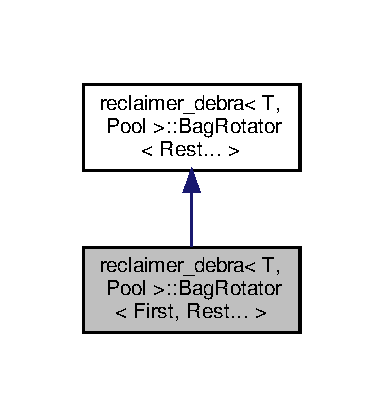
\includegraphics[width=184pt]{classreclaimer__debra_1_1BagRotator_3_01First_00_01Rest_8_8_8_01_4__inherit__graph}
\end{center}
\end{figure}


Collaboration diagram for reclaimer\+\_\+debra$<$ T, Pool $>$\+:\+:Bag\+Rotator$<$ First, Rest... $>$\+:
\nopagebreak
\begin{figure}[H]
\begin{center}
\leavevmode
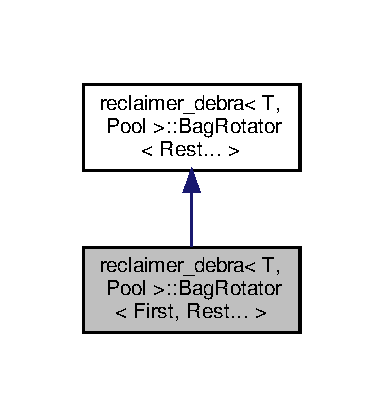
\includegraphics[width=184pt]{classreclaimer__debra_1_1BagRotator_3_01First_00_01Rest_8_8_8_01_4__coll__graph}
\end{center}
\end{figure}
\subsection*{Public Member Functions}
\begin{DoxyCompactItemize}
\item 
void \hyperlink{classreclaimer__debra_1_1BagRotator_3_01First_00_01Rest_8_8_8_01_4_a71c4ee6dfcae1b5bbf184e9528837bd4}{rotate\+All\+Epoch\+Bags} (const int \hyperlink{microbench_2main_8cpp_a9ca9869868fe7e7a38a921cc7de4103f}{tid}, void $\ast$const $\ast$const reclaimers, const int i)
\end{DoxyCompactItemize}


\subsection{Member Function Documentation}
\mbox{\Hypertarget{classreclaimer__debra_1_1BagRotator_3_01First_00_01Rest_8_8_8_01_4_a71c4ee6dfcae1b5bbf184e9528837bd4}\label{classreclaimer__debra_1_1BagRotator_3_01First_00_01Rest_8_8_8_01_4_a71c4ee6dfcae1b5bbf184e9528837bd4}} 
\index{reclaimer\+\_\+debra\+::\+Bag\+Rotator$<$ First, Rest... $>$@{reclaimer\+\_\+debra\+::\+Bag\+Rotator$<$ First, Rest... $>$}!rotate\+All\+Epoch\+Bags@{rotate\+All\+Epoch\+Bags}}
\index{rotate\+All\+Epoch\+Bags@{rotate\+All\+Epoch\+Bags}!reclaimer\+\_\+debra\+::\+Bag\+Rotator$<$ First, Rest... $>$@{reclaimer\+\_\+debra\+::\+Bag\+Rotator$<$ First, Rest... $>$}}
\subsubsection{\texorpdfstring{rotate\+All\+Epoch\+Bags()}{rotateAllEpochBags()}}
{\footnotesize\ttfamily template$<$typename T  = void, class Pool  = pool\+\_\+interface$<$\+T$>$$>$ \\
template$<$typename First , typename... Rest$>$ \\
void \hyperlink{classreclaimer__debra}{reclaimer\+\_\+debra}$<$ T, Pool $>$\+::\hyperlink{classreclaimer__debra_1_1BagRotator}{Bag\+Rotator}$<$ First, Rest... $>$\+::rotate\+All\+Epoch\+Bags (\begin{DoxyParamCaption}\item[{const int}]{tid,  }\item[{void $\ast$const $\ast$const}]{reclaimers,  }\item[{const int}]{i }\end{DoxyParamCaption})\hspace{0.3cm}{\ttfamily [inline]}}



The documentation for this class was generated from the following file\+:\begin{DoxyCompactItemize}
\item 
common/recordmgr/\hyperlink{reclaimer__debra_8h}{reclaimer\+\_\+debra.\+h}\end{DoxyCompactItemize}

\hypertarget{classreclaimer__debracap_1_1BagRotator_3_01First_00_01Rest_8_8_8_01_4}{}\section{reclaimer\+\_\+debracap$<$ T, Pool $>$\+:\+:Bag\+Rotator$<$ First, Rest... $>$ Class Template Reference}
\label{classreclaimer__debracap_1_1BagRotator_3_01First_00_01Rest_8_8_8_01_4}\index{reclaimer\+\_\+debracap$<$ T, Pool $>$\+::\+Bag\+Rotator$<$ First, Rest... $>$@{reclaimer\+\_\+debracap$<$ T, Pool $>$\+::\+Bag\+Rotator$<$ First, Rest... $>$}}


{\ttfamily \#include $<$reclaimer\+\_\+debracap.\+h$>$}



Inheritance diagram for reclaimer\+\_\+debracap$<$ T, Pool $>$\+:\+:Bag\+Rotator$<$ First, Rest... $>$\+:
\nopagebreak
\begin{figure}[H]
\begin{center}
\leavevmode
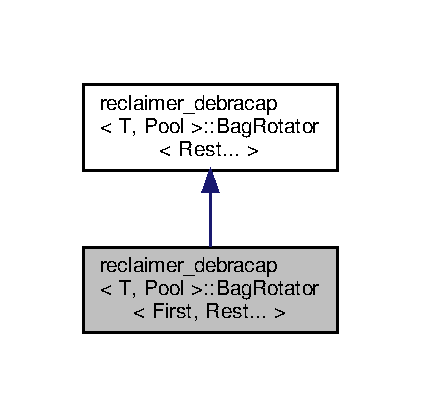
\includegraphics[width=202pt]{classreclaimer__debracap_1_1BagRotator_3_01First_00_01Rest_8_8_8_01_4__inherit__graph}
\end{center}
\end{figure}


Collaboration diagram for reclaimer\+\_\+debracap$<$ T, Pool $>$\+:\+:Bag\+Rotator$<$ First, Rest... $>$\+:
\nopagebreak
\begin{figure}[H]
\begin{center}
\leavevmode
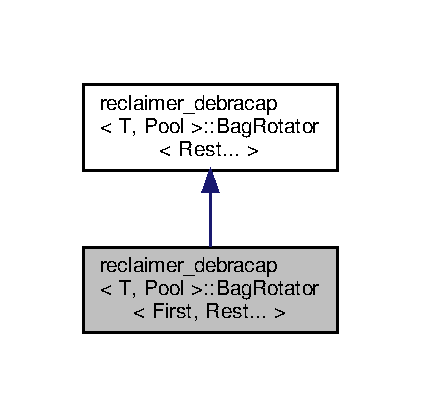
\includegraphics[width=202pt]{classreclaimer__debracap_1_1BagRotator_3_01First_00_01Rest_8_8_8_01_4__coll__graph}
\end{center}
\end{figure}
\subsection*{Public Member Functions}
\begin{DoxyCompactItemize}
\item 
void \hyperlink{classreclaimer__debracap_1_1BagRotator_3_01First_00_01Rest_8_8_8_01_4_a413f7720bbee7d91a5d0fcc8de98be16}{rotate\+All\+Epoch\+Bags} (const int \hyperlink{microbench_2main_8cpp_a9ca9869868fe7e7a38a921cc7de4103f}{tid}, void $\ast$const $\ast$const reclaimers, const int i)
\end{DoxyCompactItemize}


\subsection{Member Function Documentation}
\mbox{\Hypertarget{classreclaimer__debracap_1_1BagRotator_3_01First_00_01Rest_8_8_8_01_4_a413f7720bbee7d91a5d0fcc8de98be16}\label{classreclaimer__debracap_1_1BagRotator_3_01First_00_01Rest_8_8_8_01_4_a413f7720bbee7d91a5d0fcc8de98be16}} 
\index{reclaimer\+\_\+debracap\+::\+Bag\+Rotator$<$ First, Rest... $>$@{reclaimer\+\_\+debracap\+::\+Bag\+Rotator$<$ First, Rest... $>$}!rotate\+All\+Epoch\+Bags@{rotate\+All\+Epoch\+Bags}}
\index{rotate\+All\+Epoch\+Bags@{rotate\+All\+Epoch\+Bags}!reclaimer\+\_\+debracap\+::\+Bag\+Rotator$<$ First, Rest... $>$@{reclaimer\+\_\+debracap\+::\+Bag\+Rotator$<$ First, Rest... $>$}}
\subsubsection{\texorpdfstring{rotate\+All\+Epoch\+Bags()}{rotateAllEpochBags()}}
{\footnotesize\ttfamily template$<$typename T  = void, class Pool  = pool\+\_\+interface$<$\+T$>$$>$ \\
template$<$typename First , typename... Rest$>$ \\
void \hyperlink{classreclaimer__debracap}{reclaimer\+\_\+debracap}$<$ T, Pool $>$\+::\hyperlink{classreclaimer__debracap_1_1BagRotator}{Bag\+Rotator}$<$ First, Rest... $>$\+::rotate\+All\+Epoch\+Bags (\begin{DoxyParamCaption}\item[{const int}]{tid,  }\item[{void $\ast$const $\ast$const}]{reclaimers,  }\item[{const int}]{i }\end{DoxyParamCaption})\hspace{0.3cm}{\ttfamily [inline]}}



The documentation for this class was generated from the following file\+:\begin{DoxyCompactItemize}
\item 
common/recordmgr/\hyperlink{reclaimer__debracap_8h}{reclaimer\+\_\+debracap.\+h}\end{DoxyCompactItemize}

\hypertarget{classreclaimer__ebr__token_1_1BagRotator_3_01First_00_01Rest_8_8_8_01_4}{}\section{reclaimer\+\_\+ebr\+\_\+token$<$ T, Pool $>$\+:\+:Bag\+Rotator$<$ First, Rest... $>$ Class Template Reference}
\label{classreclaimer__ebr__token_1_1BagRotator_3_01First_00_01Rest_8_8_8_01_4}\index{reclaimer\+\_\+ebr\+\_\+token$<$ T, Pool $>$\+::\+Bag\+Rotator$<$ First, Rest... $>$@{reclaimer\+\_\+ebr\+\_\+token$<$ T, Pool $>$\+::\+Bag\+Rotator$<$ First, Rest... $>$}}


{\ttfamily \#include $<$reclaimer\+\_\+ebr\+\_\+token.\+h$>$}



Inheritance diagram for reclaimer\+\_\+ebr\+\_\+token$<$ T, Pool $>$\+:\+:Bag\+Rotator$<$ First, Rest... $>$\+:
\nopagebreak
\begin{figure}[H]
\begin{center}
\leavevmode
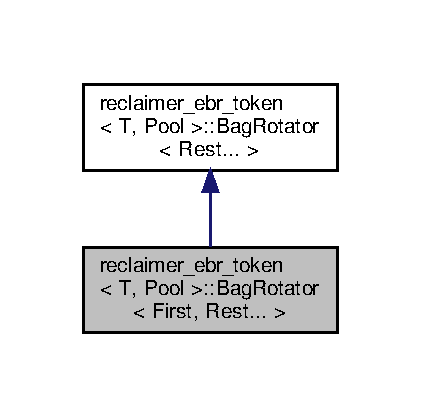
\includegraphics[width=202pt]{classreclaimer__ebr__token_1_1BagRotator_3_01First_00_01Rest_8_8_8_01_4__inherit__graph}
\end{center}
\end{figure}


Collaboration diagram for reclaimer\+\_\+ebr\+\_\+token$<$ T, Pool $>$\+:\+:Bag\+Rotator$<$ First, Rest... $>$\+:
\nopagebreak
\begin{figure}[H]
\begin{center}
\leavevmode
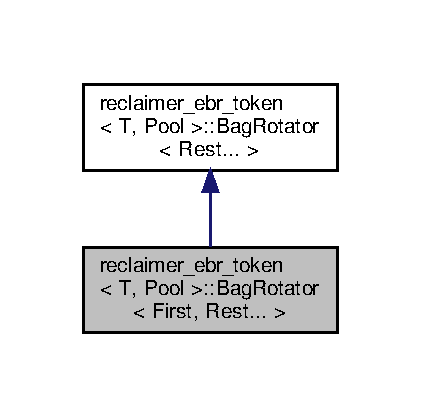
\includegraphics[width=202pt]{classreclaimer__ebr__token_1_1BagRotator_3_01First_00_01Rest_8_8_8_01_4__coll__graph}
\end{center}
\end{figure}
\subsection*{Public Member Functions}
\begin{DoxyCompactItemize}
\item 
void \hyperlink{classreclaimer__ebr__token_1_1BagRotator_3_01First_00_01Rest_8_8_8_01_4_a59fb9da7a2980e951e48265cdf33d9c9}{rotate\+All\+Epoch\+Bags} (const int \hyperlink{microbench_2main_8cpp_a9ca9869868fe7e7a38a921cc7de4103f}{tid}, void $\ast$const $\ast$const reclaimers, const int i)
\end{DoxyCompactItemize}


\subsection{Member Function Documentation}
\mbox{\Hypertarget{classreclaimer__ebr__token_1_1BagRotator_3_01First_00_01Rest_8_8_8_01_4_a59fb9da7a2980e951e48265cdf33d9c9}\label{classreclaimer__ebr__token_1_1BagRotator_3_01First_00_01Rest_8_8_8_01_4_a59fb9da7a2980e951e48265cdf33d9c9}} 
\index{reclaimer\+\_\+ebr\+\_\+token\+::\+Bag\+Rotator$<$ First, Rest... $>$@{reclaimer\+\_\+ebr\+\_\+token\+::\+Bag\+Rotator$<$ First, Rest... $>$}!rotate\+All\+Epoch\+Bags@{rotate\+All\+Epoch\+Bags}}
\index{rotate\+All\+Epoch\+Bags@{rotate\+All\+Epoch\+Bags}!reclaimer\+\_\+ebr\+\_\+token\+::\+Bag\+Rotator$<$ First, Rest... $>$@{reclaimer\+\_\+ebr\+\_\+token\+::\+Bag\+Rotator$<$ First, Rest... $>$}}
\subsubsection{\texorpdfstring{rotate\+All\+Epoch\+Bags()}{rotateAllEpochBags()}}
{\footnotesize\ttfamily template$<$typename T  = void, class Pool  = pool\+\_\+interface$<$\+T$>$$>$ \\
template$<$typename First , typename... Rest$>$ \\
void \hyperlink{classreclaimer__ebr__token}{reclaimer\+\_\+ebr\+\_\+token}$<$ T, Pool $>$\+::\hyperlink{classreclaimer__ebr__token_1_1BagRotator}{Bag\+Rotator}$<$ First, Rest... $>$\+::rotate\+All\+Epoch\+Bags (\begin{DoxyParamCaption}\item[{const int}]{tid,  }\item[{void $\ast$const $\ast$const}]{reclaimers,  }\item[{const int}]{i }\end{DoxyParamCaption})\hspace{0.3cm}{\ttfamily [inline]}}



The documentation for this class was generated from the following file\+:\begin{DoxyCompactItemize}
\item 
common/recordmgr/\hyperlink{reclaimer__ebr__token_8h}{reclaimer\+\_\+ebr\+\_\+token.\+h}\end{DoxyCompactItemize}

\hypertarget{classbase__query}{}\section{base\+\_\+query Class Reference}
\label{classbase__query}\index{base\+\_\+query@{base\+\_\+query}}


{\ttfamily \#include $<$query.\+h$>$}



Inheritance diagram for base\+\_\+query\+:
\nopagebreak
\begin{figure}[H]
\begin{center}
\leavevmode
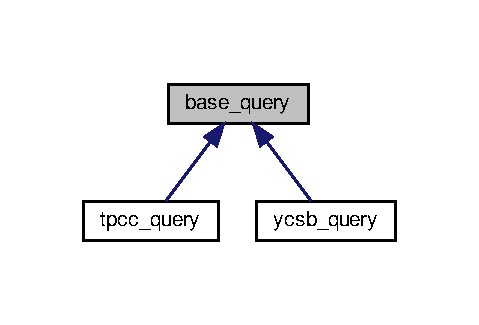
\includegraphics[width=230pt]{classbase__query__inherit__graph}
\end{center}
\end{figure}
\subsection*{Public Member Functions}
\begin{DoxyCompactItemize}
\item 
virtual void \hyperlink{classbase__query_a341a99285c6e849eae1c5a83485335f3}{init} (uint64\+\_\+t thd\+\_\+id, \hyperlink{classworkload}{workload} $\ast$h\+\_\+wl)=0
\end{DoxyCompactItemize}
\subsection*{Public Attributes}
\begin{DoxyCompactItemize}
\item 
uint64\+\_\+t \hyperlink{classbase__query_a946749126cc37a9a749d58a9779c870f}{waiting\+\_\+time}
\item 
uint64\+\_\+t \hyperlink{classbase__query_a339bb4ad3eb5490c52fd467267b85fd7}{part\+\_\+num}
\item 
uint64\+\_\+t $\ast$ \hyperlink{classbase__query_a81d79eecd1b85d1bd9818f111dadec0c}{part\+\_\+to\+\_\+access}
\end{DoxyCompactItemize}


\subsection{Member Function Documentation}
\mbox{\Hypertarget{classbase__query_a341a99285c6e849eae1c5a83485335f3}\label{classbase__query_a341a99285c6e849eae1c5a83485335f3}} 
\index{base\+\_\+query@{base\+\_\+query}!init@{init}}
\index{init@{init}!base\+\_\+query@{base\+\_\+query}}
\subsubsection{\texorpdfstring{init()}{init()}}
{\footnotesize\ttfamily virtual void base\+\_\+query\+::init (\begin{DoxyParamCaption}\item[{uint64\+\_\+t}]{thd\+\_\+id,  }\item[{\hyperlink{classworkload}{workload} $\ast$}]{h\+\_\+wl }\end{DoxyParamCaption})\hspace{0.3cm}{\ttfamily [pure virtual]}}



Implemented in \hyperlink{classycsb__query_a05e09ce39a834921f0b83103ff5ec5e1}{ycsb\+\_\+query}, and \hyperlink{classtpcc__query_a0bb03655040cf0f96ee0601c02c8876f}{tpcc\+\_\+query}.



\subsection{Member Data Documentation}
\mbox{\Hypertarget{classbase__query_a339bb4ad3eb5490c52fd467267b85fd7}\label{classbase__query_a339bb4ad3eb5490c52fd467267b85fd7}} 
\index{base\+\_\+query@{base\+\_\+query}!part\+\_\+num@{part\+\_\+num}}
\index{part\+\_\+num@{part\+\_\+num}!base\+\_\+query@{base\+\_\+query}}
\subsubsection{\texorpdfstring{part\+\_\+num}{part\_num}}
{\footnotesize\ttfamily uint64\+\_\+t base\+\_\+query\+::part\+\_\+num}

\mbox{\Hypertarget{classbase__query_a81d79eecd1b85d1bd9818f111dadec0c}\label{classbase__query_a81d79eecd1b85d1bd9818f111dadec0c}} 
\index{base\+\_\+query@{base\+\_\+query}!part\+\_\+to\+\_\+access@{part\+\_\+to\+\_\+access}}
\index{part\+\_\+to\+\_\+access@{part\+\_\+to\+\_\+access}!base\+\_\+query@{base\+\_\+query}}
\subsubsection{\texorpdfstring{part\+\_\+to\+\_\+access}{part\_to\_access}}
{\footnotesize\ttfamily uint64\+\_\+t$\ast$ base\+\_\+query\+::part\+\_\+to\+\_\+access}

\mbox{\Hypertarget{classbase__query_a946749126cc37a9a749d58a9779c870f}\label{classbase__query_a946749126cc37a9a749d58a9779c870f}} 
\index{base\+\_\+query@{base\+\_\+query}!waiting\+\_\+time@{waiting\+\_\+time}}
\index{waiting\+\_\+time@{waiting\+\_\+time}!base\+\_\+query@{base\+\_\+query}}
\subsubsection{\texorpdfstring{waiting\+\_\+time}{waiting\_time}}
{\footnotesize\ttfamily uint64\+\_\+t base\+\_\+query\+::waiting\+\_\+time}



The documentation for this class was generated from the following file\+:\begin{DoxyCompactItemize}
\item 
macrobench/system/\hyperlink{query_8h}{query.\+h}\end{DoxyCompactItemize}

\hypertarget{classblock}{}\section{block$<$ T $>$ Class Template Reference}
\label{classblock}\index{block$<$ T $>$@{block$<$ T $>$}}


{\ttfamily \#include $<$blockbag.\+h$>$}

\subsection*{Public Member Functions}
\begin{DoxyCompactItemize}
\item 
\hyperlink{classblock_a5113ccde76ee845a786b0e1ad4b868c0}{block} (\hyperlink{classblock}{block}$<$ T $>$ $\ast$const \+\_\+next)
\item 
\hyperlink{classblock_a84efcb772c0aad6175b1dd456014c0b5}{$\sim$block} ()
\item 
bool \hyperlink{classblock_a87db81c761911a5915bb2bfd61480ff6}{is\+Full} ()
\item 
bool \hyperlink{classblock_a7785b6608b8d7f83b0d6c82a31d5ad6a}{is\+Empty} ()
\item 
void \hyperlink{classblock_ab91760496bae106253e3ddd42757287a}{push} (T $\ast$const obj)
\item 
T $\ast$ \hyperlink{classblock_aa247fbd643eede27ec2ca95882d72301}{pop} ()
\item 
T $\ast$ \hyperlink{classblock_a02fa9a5b650dba298ce58281394663fa}{peek} (const int ix)
\item 
bool \hyperlink{classblock_a5577a11404c029904366f2ca986af19d}{contains} (T $\ast$const obj)
\item 
void \hyperlink{classblock_aacb3664270c63f99c066035e7ca2fcc9}{erase} (T $\ast$const obj)
\item 
void \hyperlink{classblock_a797c59cf299d9d79333464b98290ba2b}{erase} (const int ix)
\item 
void \hyperlink{classblock_a2d3ae9852d97ae2debf1bf9b74a5f991}{replace} (const int ix, T $\ast$const obj)
\item 
int \hyperlink{classblock_ab15ffcbd3f70d06e95242afcfa801038}{compute\+Size} ()
\item 
void \hyperlink{classblock_ab986a1662a6962895ab967a62f741649}{clear\+Without\+Freeing\+Elements} ()
\end{DoxyCompactItemize}
\subsection*{Public Attributes}
\begin{DoxyCompactItemize}
\item 
\hyperlink{classblock}{block}$<$ T $>$ $\ast$ \hyperlink{classblock_a3c34670f424559a9404c00a0dafe48ce}{next}
\item 
size\+\_\+t \hyperlink{classblock_aa69ddeb6abdf14f17bb47598d10e6380}{next\+Count}
\end{DoxyCompactItemize}


\subsection{Constructor \& Destructor Documentation}
\mbox{\Hypertarget{classblock_a5113ccde76ee845a786b0e1ad4b868c0}\label{classblock_a5113ccde76ee845a786b0e1ad4b868c0}} 
\index{block@{block}!block@{block}}
\index{block@{block}!block@{block}}
\subsubsection{\texorpdfstring{block()}{block()}}
{\footnotesize\ttfamily template$<$typename T$>$ \\
\hyperlink{classblock}{block}$<$ T $>$\+::\hyperlink{classblock}{block} (\begin{DoxyParamCaption}\item[{\hyperlink{classblock}{block}$<$ T $>$ $\ast$const}]{\+\_\+next }\end{DoxyParamCaption})\hspace{0.3cm}{\ttfamily [inline]}}

\mbox{\Hypertarget{classblock_a84efcb772c0aad6175b1dd456014c0b5}\label{classblock_a84efcb772c0aad6175b1dd456014c0b5}} 
\index{block@{block}!````~block@{$\sim$block}}
\index{````~block@{$\sim$block}!block@{block}}
\subsubsection{\texorpdfstring{$\sim$block()}{~block()}}
{\footnotesize\ttfamily template$<$typename T$>$ \\
\hyperlink{classblock}{block}$<$ T $>$\+::$\sim$\hyperlink{classblock}{block} (\begin{DoxyParamCaption}{ }\end{DoxyParamCaption})\hspace{0.3cm}{\ttfamily [inline]}}



\subsection{Member Function Documentation}
\mbox{\Hypertarget{classblock_ab986a1662a6962895ab967a62f741649}\label{classblock_ab986a1662a6962895ab967a62f741649}} 
\index{block@{block}!clear\+Without\+Freeing\+Elements@{clear\+Without\+Freeing\+Elements}}
\index{clear\+Without\+Freeing\+Elements@{clear\+Without\+Freeing\+Elements}!block@{block}}
\subsubsection{\texorpdfstring{clear\+Without\+Freeing\+Elements()}{clearWithoutFreeingElements()}}
{\footnotesize\ttfamily template$<$typename T$>$ \\
void \hyperlink{classblock}{block}$<$ T $>$\+::clear\+Without\+Freeing\+Elements (\begin{DoxyParamCaption}{ }\end{DoxyParamCaption})\hspace{0.3cm}{\ttfamily [inline]}}

\mbox{\Hypertarget{classblock_ab15ffcbd3f70d06e95242afcfa801038}\label{classblock_ab15ffcbd3f70d06e95242afcfa801038}} 
\index{block@{block}!compute\+Size@{compute\+Size}}
\index{compute\+Size@{compute\+Size}!block@{block}}
\subsubsection{\texorpdfstring{compute\+Size()}{computeSize()}}
{\footnotesize\ttfamily template$<$typename T$>$ \\
int \hyperlink{classblock}{block}$<$ T $>$\+::compute\+Size (\begin{DoxyParamCaption}{ }\end{DoxyParamCaption})\hspace{0.3cm}{\ttfamily [inline]}}

\mbox{\Hypertarget{classblock_a5577a11404c029904366f2ca986af19d}\label{classblock_a5577a11404c029904366f2ca986af19d}} 
\index{block@{block}!contains@{contains}}
\index{contains@{contains}!block@{block}}
\subsubsection{\texorpdfstring{contains()}{contains()}}
{\footnotesize\ttfamily template$<$typename T$>$ \\
bool \hyperlink{classblock}{block}$<$ T $>$\+::contains (\begin{DoxyParamCaption}\item[{T $\ast$const}]{obj }\end{DoxyParamCaption})\hspace{0.3cm}{\ttfamily [inline]}}

\mbox{\Hypertarget{classblock_aacb3664270c63f99c066035e7ca2fcc9}\label{classblock_aacb3664270c63f99c066035e7ca2fcc9}} 
\index{block@{block}!erase@{erase}}
\index{erase@{erase}!block@{block}}
\subsubsection{\texorpdfstring{erase()}{erase()}\hspace{0.1cm}{\footnotesize\ttfamily [1/2]}}
{\footnotesize\ttfamily template$<$typename T$>$ \\
void \hyperlink{classblock}{block}$<$ T $>$\+::erase (\begin{DoxyParamCaption}\item[{T $\ast$const}]{obj }\end{DoxyParamCaption})\hspace{0.3cm}{\ttfamily [inline]}}

\mbox{\Hypertarget{classblock_a797c59cf299d9d79333464b98290ba2b}\label{classblock_a797c59cf299d9d79333464b98290ba2b}} 
\index{block@{block}!erase@{erase}}
\index{erase@{erase}!block@{block}}
\subsubsection{\texorpdfstring{erase()}{erase()}\hspace{0.1cm}{\footnotesize\ttfamily [2/2]}}
{\footnotesize\ttfamily template$<$typename T$>$ \\
void \hyperlink{classblock}{block}$<$ T $>$\+::erase (\begin{DoxyParamCaption}\item[{const int}]{ix }\end{DoxyParamCaption})\hspace{0.3cm}{\ttfamily [inline]}}

\mbox{\Hypertarget{classblock_a7785b6608b8d7f83b0d6c82a31d5ad6a}\label{classblock_a7785b6608b8d7f83b0d6c82a31d5ad6a}} 
\index{block@{block}!is\+Empty@{is\+Empty}}
\index{is\+Empty@{is\+Empty}!block@{block}}
\subsubsection{\texorpdfstring{is\+Empty()}{isEmpty()}}
{\footnotesize\ttfamily template$<$typename T$>$ \\
bool \hyperlink{classblock}{block}$<$ T $>$\+::is\+Empty (\begin{DoxyParamCaption}{ }\end{DoxyParamCaption})\hspace{0.3cm}{\ttfamily [inline]}}

\mbox{\Hypertarget{classblock_a87db81c761911a5915bb2bfd61480ff6}\label{classblock_a87db81c761911a5915bb2bfd61480ff6}} 
\index{block@{block}!is\+Full@{is\+Full}}
\index{is\+Full@{is\+Full}!block@{block}}
\subsubsection{\texorpdfstring{is\+Full()}{isFull()}}
{\footnotesize\ttfamily template$<$typename T$>$ \\
bool \hyperlink{classblock}{block}$<$ T $>$\+::is\+Full (\begin{DoxyParamCaption}{ }\end{DoxyParamCaption})\hspace{0.3cm}{\ttfamily [inline]}}

\mbox{\Hypertarget{classblock_a02fa9a5b650dba298ce58281394663fa}\label{classblock_a02fa9a5b650dba298ce58281394663fa}} 
\index{block@{block}!peek@{peek}}
\index{peek@{peek}!block@{block}}
\subsubsection{\texorpdfstring{peek()}{peek()}}
{\footnotesize\ttfamily template$<$typename T$>$ \\
T$\ast$ \hyperlink{classblock}{block}$<$ T $>$\+::peek (\begin{DoxyParamCaption}\item[{const int}]{ix }\end{DoxyParamCaption})\hspace{0.3cm}{\ttfamily [inline]}}

\mbox{\Hypertarget{classblock_aa247fbd643eede27ec2ca95882d72301}\label{classblock_aa247fbd643eede27ec2ca95882d72301}} 
\index{block@{block}!pop@{pop}}
\index{pop@{pop}!block@{block}}
\subsubsection{\texorpdfstring{pop()}{pop()}}
{\footnotesize\ttfamily template$<$typename T$>$ \\
T$\ast$ \hyperlink{classblock}{block}$<$ T $>$\+::pop (\begin{DoxyParamCaption}{ }\end{DoxyParamCaption})\hspace{0.3cm}{\ttfamily [inline]}}

\mbox{\Hypertarget{classblock_ab91760496bae106253e3ddd42757287a}\label{classblock_ab91760496bae106253e3ddd42757287a}} 
\index{block@{block}!push@{push}}
\index{push@{push}!block@{block}}
\subsubsection{\texorpdfstring{push()}{push()}}
{\footnotesize\ttfamily template$<$typename T$>$ \\
void \hyperlink{classblock}{block}$<$ T $>$\+::push (\begin{DoxyParamCaption}\item[{T $\ast$const}]{obj }\end{DoxyParamCaption})\hspace{0.3cm}{\ttfamily [inline]}}

\mbox{\Hypertarget{classblock_a2d3ae9852d97ae2debf1bf9b74a5f991}\label{classblock_a2d3ae9852d97ae2debf1bf9b74a5f991}} 
\index{block@{block}!replace@{replace}}
\index{replace@{replace}!block@{block}}
\subsubsection{\texorpdfstring{replace()}{replace()}}
{\footnotesize\ttfamily template$<$typename T$>$ \\
void \hyperlink{classblock}{block}$<$ T $>$\+::replace (\begin{DoxyParamCaption}\item[{const int}]{ix,  }\item[{T $\ast$const}]{obj }\end{DoxyParamCaption})\hspace{0.3cm}{\ttfamily [inline]}}



\subsection{Member Data Documentation}
\mbox{\Hypertarget{classblock_a3c34670f424559a9404c00a0dafe48ce}\label{classblock_a3c34670f424559a9404c00a0dafe48ce}} 
\index{block@{block}!next@{next}}
\index{next@{next}!block@{block}}
\subsubsection{\texorpdfstring{next}{next}}
{\footnotesize\ttfamily template$<$typename T$>$ \\
\hyperlink{classblock}{block}$<$T$>$$\ast$ \hyperlink{classblock}{block}$<$ T $>$\+::next}

\mbox{\Hypertarget{classblock_aa69ddeb6abdf14f17bb47598d10e6380}\label{classblock_aa69ddeb6abdf14f17bb47598d10e6380}} 
\index{block@{block}!next\+Count@{next\+Count}}
\index{next\+Count@{next\+Count}!block@{block}}
\subsubsection{\texorpdfstring{next\+Count}{nextCount}}
{\footnotesize\ttfamily template$<$typename T$>$ \\
size\+\_\+t \hyperlink{classblock}{block}$<$ T $>$\+::next\+Count}



The documentation for this class was generated from the following file\+:\begin{DoxyCompactItemize}
\item 
common/recordmgr/\hyperlink{blockbag_8h}{blockbag.\+h}\end{DoxyCompactItemize}

\hypertarget{classblockbag}{}\section{blockbag$<$ T $>$ Class Template Reference}
\label{classblockbag}\index{blockbag$<$ T $>$@{blockbag$<$ T $>$}}


{\ttfamily \#include $<$blockbag.\+h$>$}

\subsection*{Public Member Functions}
\begin{DoxyCompactItemize}
\item 
\hyperlink{classblockbag_ad9443345e870e2faf375d14e1600918f}{blockbag} ()
\item 
\hyperlink{classblockbag_a2b387e4ba02e7c1dc9bbba8056a78ab3}{blockbag} (const int \hyperlink{microbench_2main_8cpp_a9ca9869868fe7e7a38a921cc7de4103f}{tid}, \hyperlink{classblockpool}{blockpool}$<$ T $>$ $\ast$const \+\_\+pool)
\item 
\hyperlink{classblockbag_a9353b0797054b55ab1032912718c25ee}{$\sim$blockbag} ()
\item 
int \hyperlink{classblockbag_ada8476d80376cec8051d5cba57d99d4f}{get\+Owner} ()
\item 
void \hyperlink{classblockbag_a660dcb368b89a1d6a96cf7d9bc0bf11d}{increment\+Reclaim\+Count} ()
\item 
long long \hyperlink{classblockbag_a43feda8d7817bfb6a857f83bf02a5edb}{get\+Reclaim\+Count} ()
\item 
\hyperlink{classblockbag__iterator}{blockbag\+\_\+iterator}$<$ T $>$ \hyperlink{classblockbag_a8f600e6e4330a864d36572a3adaf387e}{begin} ()
\item 
\hyperlink{classblockbag__iterator}{blockbag\+\_\+iterator}$<$ T $>$ \hyperlink{classblockbag_a2b8c14d976119bb688ead024cd90fc16}{end} ()
\item 
void \hyperlink{classblockbag_a8cb3c434b92a6e58a47bc235d0c2a91c}{add} (T $\ast$const obj)
\item 
{\footnotesize template$<$typename Alloc $>$ }\\void \hyperlink{classblockbag_a4ae5f3f6ef5fd7d458abf39aae9c9b75}{add} (const int \hyperlink{microbench_2main_8cpp_a9ca9869868fe7e7a38a921cc7de4103f}{tid}, T $\ast$const obj, \hyperlink{classlockfreeblockbag}{lockfreeblockbag}$<$ T $>$ $\ast$const shared\+Bag, const int thresh, Alloc $\ast$const alloc)
\item 
bool \hyperlink{classblockbag_a376e7a8a4f8a2a4d0670504b4e8de0ba}{is\+Empty} ()
\item 
bool \hyperlink{classblockbag_ac9ef89b54e16c01853e9ba7fcc3eaad5}{erase} (\hyperlink{classblock}{block}$<$ T $>$ $\ast$const curr, const int ix)
\item 
T $\ast$ \hyperlink{classblockbag_a673f44a045b3b89c1ce9360d20e6037a}{remove} ()
\item 
{\footnotesize template$<$typename Alloc $>$ }\\T $\ast$ \hyperlink{classblockbag_a3d7ed27113ec3ff8239ff7739664dd0b}{remove} (const int \hyperlink{microbench_2main_8cpp_a9ca9869868fe7e7a38a921cc7de4103f}{tid}, \hyperlink{classlockfreeblockbag}{lockfreeblockbag}$<$ T $>$ $\ast$const shared\+Bag, Alloc $\ast$const alloc)
\item 
\hyperlink{classblock}{block}$<$ T $>$ $\ast$ \hyperlink{classblockbag_adba6ec96857fc02a2eceba07568fafae}{remove\+Full\+Block} ()
\item 
void \hyperlink{classblockbag_ab8fa06856490589dd63e2c8058b3db63}{add\+Full\+Block} (\hyperlink{classblock}{block}$<$ T $>$ $\ast$b)
\item 
void \hyperlink{classblockbag_a696366e13be4fe60aefe9a359833aea2}{append\+Move\+Full\+Blocks} (\hyperlink{classblockbag}{blockbag}$<$ T $>$ $\ast$const other, \hyperlink{classblock}{block}$<$ T $>$ $\ast$predecessor)
\item 
void \hyperlink{classblockbag_a0c09852cf71019478f8d8d12579c514a}{append\+Move\+Full\+Blocks} (\hyperlink{classblockbag}{blockbag}$<$ T $>$ $\ast$const other)
\item 
void \hyperlink{classblockbag_ad7964703f189c0cc1417ba6d4d642093}{append\+Move\+All} (\hyperlink{classblockbag}{blockbag}$<$ T $>$ $\ast$const other)
\item 
int \hyperlink{classblockbag_a8211033edefa32a954bd9b2fbe718498}{compute\+Size} ()
\item 
int \hyperlink{classblockbag_ab59a59fd142e5b42d67580662012543d}{get\+Size\+In\+Blocks} ()
\item 
void \hyperlink{classblockbag_a2ed40017536b0d2882c8b5ca432a0ebc}{clear\+Without\+Freeing\+Elements} ()
\end{DoxyCompactItemize}
\subsection*{Public Attributes}
\begin{DoxyCompactItemize}
\item 
int \hyperlink{classblockbag_a6245fc873d3db253783944ce2bbbacce}{size\+In\+Blocks}
\end{DoxyCompactItemize}


\subsection{Constructor \& Destructor Documentation}
\mbox{\Hypertarget{classblockbag_ad9443345e870e2faf375d14e1600918f}\label{classblockbag_ad9443345e870e2faf375d14e1600918f}} 
\index{blockbag@{blockbag}!blockbag@{blockbag}}
\index{blockbag@{blockbag}!blockbag@{blockbag}}
\subsubsection{\texorpdfstring{blockbag()}{blockbag()}\hspace{0.1cm}{\footnotesize\ttfamily [1/2]}}
{\footnotesize\ttfamily template$<$typename T$>$ \\
\hyperlink{classblockbag}{blockbag}$<$ T $>$\+::\hyperlink{classblockbag}{blockbag} (\begin{DoxyParamCaption}{ }\end{DoxyParamCaption})\hspace{0.3cm}{\ttfamily [inline]}}

\mbox{\Hypertarget{classblockbag_a2b387e4ba02e7c1dc9bbba8056a78ab3}\label{classblockbag_a2b387e4ba02e7c1dc9bbba8056a78ab3}} 
\index{blockbag@{blockbag}!blockbag@{blockbag}}
\index{blockbag@{blockbag}!blockbag@{blockbag}}
\subsubsection{\texorpdfstring{blockbag()}{blockbag()}\hspace{0.1cm}{\footnotesize\ttfamily [2/2]}}
{\footnotesize\ttfamily template$<$typename T$>$ \\
\hyperlink{classblockbag}{blockbag}$<$ T $>$\+::\hyperlink{classblockbag}{blockbag} (\begin{DoxyParamCaption}\item[{const int}]{tid,  }\item[{\hyperlink{classblockpool}{blockpool}$<$ T $>$ $\ast$const}]{\+\_\+pool }\end{DoxyParamCaption})\hspace{0.3cm}{\ttfamily [inline]}}

\mbox{\Hypertarget{classblockbag_a9353b0797054b55ab1032912718c25ee}\label{classblockbag_a9353b0797054b55ab1032912718c25ee}} 
\index{blockbag@{blockbag}!````~blockbag@{$\sim$blockbag}}
\index{````~blockbag@{$\sim$blockbag}!blockbag@{blockbag}}
\subsubsection{\texorpdfstring{$\sim$blockbag()}{~blockbag()}}
{\footnotesize\ttfamily template$<$typename T$>$ \\
\hyperlink{classblockbag}{blockbag}$<$ T $>$\+::$\sim$\hyperlink{classblockbag}{blockbag} (\begin{DoxyParamCaption}{ }\end{DoxyParamCaption})\hspace{0.3cm}{\ttfamily [inline]}}



\subsection{Member Function Documentation}
\mbox{\Hypertarget{classblockbag_a8cb3c434b92a6e58a47bc235d0c2a91c}\label{classblockbag_a8cb3c434b92a6e58a47bc235d0c2a91c}} 
\index{blockbag@{blockbag}!add@{add}}
\index{add@{add}!blockbag@{blockbag}}
\subsubsection{\texorpdfstring{add()}{add()}\hspace{0.1cm}{\footnotesize\ttfamily [1/2]}}
{\footnotesize\ttfamily template$<$typename T$>$ \\
void \hyperlink{classblockbag}{blockbag}$<$ T $>$\+::add (\begin{DoxyParamCaption}\item[{T $\ast$const}]{obj }\end{DoxyParamCaption})\hspace{0.3cm}{\ttfamily [inline]}}

\mbox{\Hypertarget{classblockbag_a4ae5f3f6ef5fd7d458abf39aae9c9b75}\label{classblockbag_a4ae5f3f6ef5fd7d458abf39aae9c9b75}} 
\index{blockbag@{blockbag}!add@{add}}
\index{add@{add}!blockbag@{blockbag}}
\subsubsection{\texorpdfstring{add()}{add()}\hspace{0.1cm}{\footnotesize\ttfamily [2/2]}}
{\footnotesize\ttfamily template$<$typename T$>$ \\
template$<$typename Alloc $>$ \\
void \hyperlink{classblockbag}{blockbag}$<$ T $>$\+::add (\begin{DoxyParamCaption}\item[{const int}]{tid,  }\item[{T $\ast$const}]{obj,  }\item[{\hyperlink{classlockfreeblockbag}{lockfreeblockbag}$<$ T $>$ $\ast$const}]{shared\+Bag,  }\item[{const int}]{thresh,  }\item[{Alloc $\ast$const}]{alloc }\end{DoxyParamCaption})\hspace{0.3cm}{\ttfamily [inline]}}

\mbox{\Hypertarget{classblockbag_ab8fa06856490589dd63e2c8058b3db63}\label{classblockbag_ab8fa06856490589dd63e2c8058b3db63}} 
\index{blockbag@{blockbag}!add\+Full\+Block@{add\+Full\+Block}}
\index{add\+Full\+Block@{add\+Full\+Block}!blockbag@{blockbag}}
\subsubsection{\texorpdfstring{add\+Full\+Block()}{addFullBlock()}}
{\footnotesize\ttfamily template$<$typename T$>$ \\
void \hyperlink{classblockbag}{blockbag}$<$ T $>$\+::add\+Full\+Block (\begin{DoxyParamCaption}\item[{\hyperlink{classblock}{block}$<$ T $>$ $\ast$}]{b }\end{DoxyParamCaption})\hspace{0.3cm}{\ttfamily [inline]}}

\mbox{\Hypertarget{classblockbag_ad7964703f189c0cc1417ba6d4d642093}\label{classblockbag_ad7964703f189c0cc1417ba6d4d642093}} 
\index{blockbag@{blockbag}!append\+Move\+All@{append\+Move\+All}}
\index{append\+Move\+All@{append\+Move\+All}!blockbag@{blockbag}}
\subsubsection{\texorpdfstring{append\+Move\+All()}{appendMoveAll()}}
{\footnotesize\ttfamily template$<$typename T$>$ \\
void \hyperlink{classblockbag}{blockbag}$<$ T $>$\+::append\+Move\+All (\begin{DoxyParamCaption}\item[{\hyperlink{classblockbag}{blockbag}$<$ T $>$ $\ast$const}]{other }\end{DoxyParamCaption})\hspace{0.3cm}{\ttfamily [inline]}}

\mbox{\Hypertarget{classblockbag_a696366e13be4fe60aefe9a359833aea2}\label{classblockbag_a696366e13be4fe60aefe9a359833aea2}} 
\index{blockbag@{blockbag}!append\+Move\+Full\+Blocks@{append\+Move\+Full\+Blocks}}
\index{append\+Move\+Full\+Blocks@{append\+Move\+Full\+Blocks}!blockbag@{blockbag}}
\subsubsection{\texorpdfstring{append\+Move\+Full\+Blocks()}{appendMoveFullBlocks()}\hspace{0.1cm}{\footnotesize\ttfamily [1/2]}}
{\footnotesize\ttfamily template$<$typename T$>$ \\
void \hyperlink{classblockbag}{blockbag}$<$ T $>$\+::append\+Move\+Full\+Blocks (\begin{DoxyParamCaption}\item[{\hyperlink{classblockbag}{blockbag}$<$ T $>$ $\ast$const}]{other,  }\item[{\hyperlink{classblock}{block}$<$ T $>$ $\ast$}]{predecessor }\end{DoxyParamCaption})\hspace{0.3cm}{\ttfamily [inline]}}

\mbox{\Hypertarget{classblockbag_a0c09852cf71019478f8d8d12579c514a}\label{classblockbag_a0c09852cf71019478f8d8d12579c514a}} 
\index{blockbag@{blockbag}!append\+Move\+Full\+Blocks@{append\+Move\+Full\+Blocks}}
\index{append\+Move\+Full\+Blocks@{append\+Move\+Full\+Blocks}!blockbag@{blockbag}}
\subsubsection{\texorpdfstring{append\+Move\+Full\+Blocks()}{appendMoveFullBlocks()}\hspace{0.1cm}{\footnotesize\ttfamily [2/2]}}
{\footnotesize\ttfamily template$<$typename T$>$ \\
void \hyperlink{classblockbag}{blockbag}$<$ T $>$\+::append\+Move\+Full\+Blocks (\begin{DoxyParamCaption}\item[{\hyperlink{classblockbag}{blockbag}$<$ T $>$ $\ast$const}]{other }\end{DoxyParamCaption})\hspace{0.3cm}{\ttfamily [inline]}}

\mbox{\Hypertarget{classblockbag_a8f600e6e4330a864d36572a3adaf387e}\label{classblockbag_a8f600e6e4330a864d36572a3adaf387e}} 
\index{blockbag@{blockbag}!begin@{begin}}
\index{begin@{begin}!blockbag@{blockbag}}
\subsubsection{\texorpdfstring{begin()}{begin()}}
{\footnotesize\ttfamily template$<$typename T$>$ \\
\hyperlink{classblockbag__iterator}{blockbag\+\_\+iterator}$<$T$>$ \hyperlink{classblockbag}{blockbag}$<$ T $>$\+::begin (\begin{DoxyParamCaption}{ }\end{DoxyParamCaption})\hspace{0.3cm}{\ttfamily [inline]}}

\mbox{\Hypertarget{classblockbag_a2ed40017536b0d2882c8b5ca432a0ebc}\label{classblockbag_a2ed40017536b0d2882c8b5ca432a0ebc}} 
\index{blockbag@{blockbag}!clear\+Without\+Freeing\+Elements@{clear\+Without\+Freeing\+Elements}}
\index{clear\+Without\+Freeing\+Elements@{clear\+Without\+Freeing\+Elements}!blockbag@{blockbag}}
\subsubsection{\texorpdfstring{clear\+Without\+Freeing\+Elements()}{clearWithoutFreeingElements()}}
{\footnotesize\ttfamily template$<$typename T$>$ \\
void \hyperlink{classblockbag}{blockbag}$<$ T $>$\+::clear\+Without\+Freeing\+Elements (\begin{DoxyParamCaption}{ }\end{DoxyParamCaption})\hspace{0.3cm}{\ttfamily [inline]}}

\mbox{\Hypertarget{classblockbag_a8211033edefa32a954bd9b2fbe718498}\label{classblockbag_a8211033edefa32a954bd9b2fbe718498}} 
\index{blockbag@{blockbag}!compute\+Size@{compute\+Size}}
\index{compute\+Size@{compute\+Size}!blockbag@{blockbag}}
\subsubsection{\texorpdfstring{compute\+Size()}{computeSize()}}
{\footnotesize\ttfamily template$<$typename T$>$ \\
int \hyperlink{classblockbag}{blockbag}$<$ T $>$\+::compute\+Size (\begin{DoxyParamCaption}{ }\end{DoxyParamCaption})\hspace{0.3cm}{\ttfamily [inline]}}

\mbox{\Hypertarget{classblockbag_a2b8c14d976119bb688ead024cd90fc16}\label{classblockbag_a2b8c14d976119bb688ead024cd90fc16}} 
\index{blockbag@{blockbag}!end@{end}}
\index{end@{end}!blockbag@{blockbag}}
\subsubsection{\texorpdfstring{end()}{end()}}
{\footnotesize\ttfamily template$<$typename T$>$ \\
\hyperlink{classblockbag__iterator}{blockbag\+\_\+iterator}$<$T$>$ \hyperlink{classblockbag}{blockbag}$<$ T $>$\+::end (\begin{DoxyParamCaption}{ }\end{DoxyParamCaption})\hspace{0.3cm}{\ttfamily [inline]}}

\mbox{\Hypertarget{classblockbag_ac9ef89b54e16c01853e9ba7fcc3eaad5}\label{classblockbag_ac9ef89b54e16c01853e9ba7fcc3eaad5}} 
\index{blockbag@{blockbag}!erase@{erase}}
\index{erase@{erase}!blockbag@{blockbag}}
\subsubsection{\texorpdfstring{erase()}{erase()}}
{\footnotesize\ttfamily template$<$typename T$>$ \\
bool \hyperlink{classblockbag}{blockbag}$<$ T $>$\+::erase (\begin{DoxyParamCaption}\item[{\hyperlink{classblock}{block}$<$ T $>$ $\ast$const}]{curr,  }\item[{const int}]{ix }\end{DoxyParamCaption})\hspace{0.3cm}{\ttfamily [inline]}}

\mbox{\Hypertarget{classblockbag_ada8476d80376cec8051d5cba57d99d4f}\label{classblockbag_ada8476d80376cec8051d5cba57d99d4f}} 
\index{blockbag@{blockbag}!get\+Owner@{get\+Owner}}
\index{get\+Owner@{get\+Owner}!blockbag@{blockbag}}
\subsubsection{\texorpdfstring{get\+Owner()}{getOwner()}}
{\footnotesize\ttfamily template$<$typename T$>$ \\
int \hyperlink{classblockbag}{blockbag}$<$ T $>$\+::get\+Owner (\begin{DoxyParamCaption}{ }\end{DoxyParamCaption})\hspace{0.3cm}{\ttfamily [inline]}}

\mbox{\Hypertarget{classblockbag_a43feda8d7817bfb6a857f83bf02a5edb}\label{classblockbag_a43feda8d7817bfb6a857f83bf02a5edb}} 
\index{blockbag@{blockbag}!get\+Reclaim\+Count@{get\+Reclaim\+Count}}
\index{get\+Reclaim\+Count@{get\+Reclaim\+Count}!blockbag@{blockbag}}
\subsubsection{\texorpdfstring{get\+Reclaim\+Count()}{getReclaimCount()}}
{\footnotesize\ttfamily template$<$typename T$>$ \\
long long \hyperlink{classblockbag}{blockbag}$<$ T $>$\+::get\+Reclaim\+Count (\begin{DoxyParamCaption}{ }\end{DoxyParamCaption})\hspace{0.3cm}{\ttfamily [inline]}}

\mbox{\Hypertarget{classblockbag_ab59a59fd142e5b42d67580662012543d}\label{classblockbag_ab59a59fd142e5b42d67580662012543d}} 
\index{blockbag@{blockbag}!get\+Size\+In\+Blocks@{get\+Size\+In\+Blocks}}
\index{get\+Size\+In\+Blocks@{get\+Size\+In\+Blocks}!blockbag@{blockbag}}
\subsubsection{\texorpdfstring{get\+Size\+In\+Blocks()}{getSizeInBlocks()}}
{\footnotesize\ttfamily template$<$typename T$>$ \\
int \hyperlink{classblockbag}{blockbag}$<$ T $>$\+::get\+Size\+In\+Blocks (\begin{DoxyParamCaption}{ }\end{DoxyParamCaption})\hspace{0.3cm}{\ttfamily [inline]}}

\mbox{\Hypertarget{classblockbag_a660dcb368b89a1d6a96cf7d9bc0bf11d}\label{classblockbag_a660dcb368b89a1d6a96cf7d9bc0bf11d}} 
\index{blockbag@{blockbag}!increment\+Reclaim\+Count@{increment\+Reclaim\+Count}}
\index{increment\+Reclaim\+Count@{increment\+Reclaim\+Count}!blockbag@{blockbag}}
\subsubsection{\texorpdfstring{increment\+Reclaim\+Count()}{incrementReclaimCount()}}
{\footnotesize\ttfamily template$<$typename T$>$ \\
void \hyperlink{classblockbag}{blockbag}$<$ T $>$\+::increment\+Reclaim\+Count (\begin{DoxyParamCaption}{ }\end{DoxyParamCaption})\hspace{0.3cm}{\ttfamily [inline]}}

\mbox{\Hypertarget{classblockbag_a376e7a8a4f8a2a4d0670504b4e8de0ba}\label{classblockbag_a376e7a8a4f8a2a4d0670504b4e8de0ba}} 
\index{blockbag@{blockbag}!is\+Empty@{is\+Empty}}
\index{is\+Empty@{is\+Empty}!blockbag@{blockbag}}
\subsubsection{\texorpdfstring{is\+Empty()}{isEmpty()}}
{\footnotesize\ttfamily template$<$typename T$>$ \\
bool \hyperlink{classblockbag}{blockbag}$<$ T $>$\+::is\+Empty (\begin{DoxyParamCaption}{ }\end{DoxyParamCaption})\hspace{0.3cm}{\ttfamily [inline]}}

\mbox{\Hypertarget{classblockbag_a673f44a045b3b89c1ce9360d20e6037a}\label{classblockbag_a673f44a045b3b89c1ce9360d20e6037a}} 
\index{blockbag@{blockbag}!remove@{remove}}
\index{remove@{remove}!blockbag@{blockbag}}
\subsubsection{\texorpdfstring{remove()}{remove()}\hspace{0.1cm}{\footnotesize\ttfamily [1/2]}}
{\footnotesize\ttfamily template$<$typename T$>$ \\
T$\ast$ \hyperlink{classblockbag}{blockbag}$<$ T $>$\+::remove (\begin{DoxyParamCaption}{ }\end{DoxyParamCaption})\hspace{0.3cm}{\ttfamily [inline]}}

\mbox{\Hypertarget{classblockbag_a3d7ed27113ec3ff8239ff7739664dd0b}\label{classblockbag_a3d7ed27113ec3ff8239ff7739664dd0b}} 
\index{blockbag@{blockbag}!remove@{remove}}
\index{remove@{remove}!blockbag@{blockbag}}
\subsubsection{\texorpdfstring{remove()}{remove()}\hspace{0.1cm}{\footnotesize\ttfamily [2/2]}}
{\footnotesize\ttfamily template$<$typename T$>$ \\
template$<$typename Alloc $>$ \\
T$\ast$ \hyperlink{classblockbag}{blockbag}$<$ T $>$\+::remove (\begin{DoxyParamCaption}\item[{const int}]{tid,  }\item[{\hyperlink{classlockfreeblockbag}{lockfreeblockbag}$<$ T $>$ $\ast$const}]{shared\+Bag,  }\item[{Alloc $\ast$const}]{alloc }\end{DoxyParamCaption})\hspace{0.3cm}{\ttfamily [inline]}}

begin debug

end debug

begin debug

end debug \mbox{\Hypertarget{classblockbag_adba6ec96857fc02a2eceba07568fafae}\label{classblockbag_adba6ec96857fc02a2eceba07568fafae}} 
\index{blockbag@{blockbag}!remove\+Full\+Block@{remove\+Full\+Block}}
\index{remove\+Full\+Block@{remove\+Full\+Block}!blockbag@{blockbag}}
\subsubsection{\texorpdfstring{remove\+Full\+Block()}{removeFullBlock()}}
{\footnotesize\ttfamily template$<$typename T$>$ \\
\hyperlink{classblock}{block}$<$T$>$$\ast$ \hyperlink{classblockbag}{blockbag}$<$ T $>$\+::remove\+Full\+Block (\begin{DoxyParamCaption}{ }\end{DoxyParamCaption})\hspace{0.3cm}{\ttfamily [inline]}}



\subsection{Member Data Documentation}
\mbox{\Hypertarget{classblockbag_a6245fc873d3db253783944ce2bbbacce}\label{classblockbag_a6245fc873d3db253783944ce2bbbacce}} 
\index{blockbag@{blockbag}!size\+In\+Blocks@{size\+In\+Blocks}}
\index{size\+In\+Blocks@{size\+In\+Blocks}!blockbag@{blockbag}}
\subsubsection{\texorpdfstring{size\+In\+Blocks}{sizeInBlocks}}
{\footnotesize\ttfamily template$<$typename T$>$ \\
int \hyperlink{classblockbag}{blockbag}$<$ T $>$\+::size\+In\+Blocks}



The documentation for this class was generated from the following file\+:\begin{DoxyCompactItemize}
\item 
common/recordmgr/\hyperlink{blockbag_8h}{blockbag.\+h}\end{DoxyCompactItemize}

\hypertarget{classblockbag__iterator}{}\section{blockbag\+\_\+iterator$<$ T $>$ Class Template Reference}
\label{classblockbag__iterator}\index{blockbag\+\_\+iterator$<$ T $>$@{blockbag\+\_\+iterator$<$ T $>$}}


{\ttfamily \#include $<$blockbag.\+h$>$}

\subsection*{Public Member Functions}
\begin{DoxyCompactItemize}
\item 
\hyperlink{classblock}{block}$<$ T $>$ $\ast$ \hyperlink{classblockbag__iterator_aa99d991d209d80cbdb27309d6cfb8efa}{get\+Curr} () const
\item 
int \hyperlink{classblockbag__iterator_a6c1d126ebb9bb7c5d32366f18e8ed83d}{get\+Index} () const
\item 
\hyperlink{classblockbag__iterator_a7ef4ae857fb7b5be23f7a4b074846417}{blockbag\+\_\+iterator} (\hyperlink{classblock}{block}$<$ T $>$ $\ast$const \+\_\+head, \hyperlink{classblockbag}{blockbag}$<$ T $>$ $\ast$const \+\_\+bag)
\item 
T $\ast$ \hyperlink{classblockbag__iterator_a4c44f3c7850d4548e4be02745c82fbed}{operator$\ast$} () const
\item 
\hyperlink{classblockbag__iterator}{blockbag\+\_\+iterator}$<$ T $>$ \& \hyperlink{classblockbag__iterator_a37c398b44de81928b694f808e6347eab}{operator++} (int)
\item 
void \hyperlink{classblockbag__iterator_a15dd4b935345d01a0bed723155010f74}{swap} (\hyperlink{classblock}{block}$<$ T $>$ $\ast$const other\+Curr, const int other\+Ix)
\item 
void \hyperlink{classblockbag__iterator_ab23a01d4163d17774780893a01a76ae5}{erase} ()
\end{DoxyCompactItemize}


\subsection{Constructor \& Destructor Documentation}
\mbox{\Hypertarget{classblockbag__iterator_a7ef4ae857fb7b5be23f7a4b074846417}\label{classblockbag__iterator_a7ef4ae857fb7b5be23f7a4b074846417}} 
\index{blockbag\+\_\+iterator@{blockbag\+\_\+iterator}!blockbag\+\_\+iterator@{blockbag\+\_\+iterator}}
\index{blockbag\+\_\+iterator@{blockbag\+\_\+iterator}!blockbag\+\_\+iterator@{blockbag\+\_\+iterator}}
\subsubsection{\texorpdfstring{blockbag\+\_\+iterator()}{blockbag\_iterator()}}
{\footnotesize\ttfamily template$<$typename T$>$ \\
\hyperlink{classblockbag__iterator}{blockbag\+\_\+iterator}$<$ T $>$\+::\hyperlink{classblockbag__iterator}{blockbag\+\_\+iterator} (\begin{DoxyParamCaption}\item[{\hyperlink{classblock}{block}$<$ T $>$ $\ast$const}]{\+\_\+head,  }\item[{\hyperlink{classblockbag}{blockbag}$<$ T $>$ $\ast$const}]{\+\_\+bag }\end{DoxyParamCaption})\hspace{0.3cm}{\ttfamily [inline]}}



\subsection{Member Function Documentation}
\mbox{\Hypertarget{classblockbag__iterator_ab23a01d4163d17774780893a01a76ae5}\label{classblockbag__iterator_ab23a01d4163d17774780893a01a76ae5}} 
\index{blockbag\+\_\+iterator@{blockbag\+\_\+iterator}!erase@{erase}}
\index{erase@{erase}!blockbag\+\_\+iterator@{blockbag\+\_\+iterator}}
\subsubsection{\texorpdfstring{erase()}{erase()}}
{\footnotesize\ttfamily template$<$typename T$>$ \\
void \hyperlink{classblockbag__iterator}{blockbag\+\_\+iterator}$<$ T $>$\+::erase (\begin{DoxyParamCaption}{ }\end{DoxyParamCaption})\hspace{0.3cm}{\ttfamily [inline]}}

\mbox{\Hypertarget{classblockbag__iterator_aa99d991d209d80cbdb27309d6cfb8efa}\label{classblockbag__iterator_aa99d991d209d80cbdb27309d6cfb8efa}} 
\index{blockbag\+\_\+iterator@{blockbag\+\_\+iterator}!get\+Curr@{get\+Curr}}
\index{get\+Curr@{get\+Curr}!blockbag\+\_\+iterator@{blockbag\+\_\+iterator}}
\subsubsection{\texorpdfstring{get\+Curr()}{getCurr()}}
{\footnotesize\ttfamily template$<$typename T$>$ \\
\hyperlink{classblock}{block}$<$T$>$$\ast$ \hyperlink{classblockbag__iterator}{blockbag\+\_\+iterator}$<$ T $>$\+::get\+Curr (\begin{DoxyParamCaption}{ }\end{DoxyParamCaption}) const\hspace{0.3cm}{\ttfamily [inline]}}

\mbox{\Hypertarget{classblockbag__iterator_a6c1d126ebb9bb7c5d32366f18e8ed83d}\label{classblockbag__iterator_a6c1d126ebb9bb7c5d32366f18e8ed83d}} 
\index{blockbag\+\_\+iterator@{blockbag\+\_\+iterator}!get\+Index@{get\+Index}}
\index{get\+Index@{get\+Index}!blockbag\+\_\+iterator@{blockbag\+\_\+iterator}}
\subsubsection{\texorpdfstring{get\+Index()}{getIndex()}}
{\footnotesize\ttfamily template$<$typename T$>$ \\
int \hyperlink{classblockbag__iterator}{blockbag\+\_\+iterator}$<$ T $>$\+::get\+Index (\begin{DoxyParamCaption}{ }\end{DoxyParamCaption}) const\hspace{0.3cm}{\ttfamily [inline]}}

\mbox{\Hypertarget{classblockbag__iterator_a4c44f3c7850d4548e4be02745c82fbed}\label{classblockbag__iterator_a4c44f3c7850d4548e4be02745c82fbed}} 
\index{blockbag\+\_\+iterator@{blockbag\+\_\+iterator}!operator$\ast$@{operator$\ast$}}
\index{operator$\ast$@{operator$\ast$}!blockbag\+\_\+iterator@{blockbag\+\_\+iterator}}
\subsubsection{\texorpdfstring{operator$\ast$()}{operator*()}}
{\footnotesize\ttfamily template$<$typename T$>$ \\
T$\ast$ \hyperlink{classblockbag__iterator}{blockbag\+\_\+iterator}$<$ T $>$\+::operator$\ast$ (\begin{DoxyParamCaption}{ }\end{DoxyParamCaption}) const\hspace{0.3cm}{\ttfamily [inline]}}

\mbox{\Hypertarget{classblockbag__iterator_a37c398b44de81928b694f808e6347eab}\label{classblockbag__iterator_a37c398b44de81928b694f808e6347eab}} 
\index{blockbag\+\_\+iterator@{blockbag\+\_\+iterator}!operator++@{operator++}}
\index{operator++@{operator++}!blockbag\+\_\+iterator@{blockbag\+\_\+iterator}}
\subsubsection{\texorpdfstring{operator++()}{operator++()}}
{\footnotesize\ttfamily template$<$typename T$>$ \\
\hyperlink{classblockbag__iterator}{blockbag\+\_\+iterator}$<$T$>$\& \hyperlink{classblockbag__iterator}{blockbag\+\_\+iterator}$<$ T $>$\+::operator++ (\begin{DoxyParamCaption}\item[{int}]{ }\end{DoxyParamCaption})\hspace{0.3cm}{\ttfamily [inline]}}

\mbox{\Hypertarget{classblockbag__iterator_a15dd4b935345d01a0bed723155010f74}\label{classblockbag__iterator_a15dd4b935345d01a0bed723155010f74}} 
\index{blockbag\+\_\+iterator@{blockbag\+\_\+iterator}!swap@{swap}}
\index{swap@{swap}!blockbag\+\_\+iterator@{blockbag\+\_\+iterator}}
\subsubsection{\texorpdfstring{swap()}{swap()}}
{\footnotesize\ttfamily template$<$typename T$>$ \\
void \hyperlink{classblockbag__iterator}{blockbag\+\_\+iterator}$<$ T $>$\+::swap (\begin{DoxyParamCaption}\item[{\hyperlink{classblock}{block}$<$ T $>$ $\ast$const}]{other\+Curr,  }\item[{const int}]{other\+Ix }\end{DoxyParamCaption})\hspace{0.3cm}{\ttfamily [inline]}}



The documentation for this class was generated from the following file\+:\begin{DoxyCompactItemize}
\item 
common/recordmgr/\hyperlink{blockbag_8h}{blockbag.\+h}\end{DoxyCompactItemize}

\hypertarget{classblockpool}{}\section{blockpool$<$ T $>$ Class Template Reference}
\label{classblockpool}\index{blockpool$<$ T $>$@{blockpool$<$ T $>$}}


{\ttfamily \#include $<$blockbag.\+h$>$}

\subsection*{Public Member Functions}
\begin{DoxyCompactItemize}
\item 
\hyperlink{classblockpool_a110934720ff65d68f413bae0c0c577bb}{blockpool} ()
\item 
\hyperlink{classblockpool_a4f9b57b1f040a7940d4838ae293b91b1}{$\sim$blockpool} ()
\item 
\hyperlink{classblock}{block}$<$ T $>$ $\ast$ \hyperlink{classblockpool_ab0c6542e74f50af2cc27ae2a18200cc6}{allocate\+Block} (\hyperlink{classblock}{block}$<$ T $>$ $\ast$const next)
\item 
void \hyperlink{classblockpool_a513720b0f74d4cec679eff69b3dd8d34}{deallocate\+Block} (\hyperlink{classblock}{block}$<$ T $>$ $\ast$const b)
\end{DoxyCompactItemize}


\subsection{Detailed Description}
\subsubsection*{template$<$typename T$>$\newline
class blockpool$<$ T $>$}

C++ record manager implementation (P\+O\+DC 2015) by Trevor Brown.

Copyright (C) 2015 Trevor Brown 

\subsection{Constructor \& Destructor Documentation}
\mbox{\Hypertarget{classblockpool_a110934720ff65d68f413bae0c0c577bb}\label{classblockpool_a110934720ff65d68f413bae0c0c577bb}} 
\index{blockpool@{blockpool}!blockpool@{blockpool}}
\index{blockpool@{blockpool}!blockpool@{blockpool}}
\subsubsection{\texorpdfstring{blockpool()}{blockpool()}}
{\footnotesize\ttfamily template$<$typename T$>$ \\
\hyperlink{classblockpool}{blockpool}$<$ T $>$\+::\hyperlink{classblockpool}{blockpool} (\begin{DoxyParamCaption}{ }\end{DoxyParamCaption})\hspace{0.3cm}{\ttfamily [inline]}}

\mbox{\Hypertarget{classblockpool_a4f9b57b1f040a7940d4838ae293b91b1}\label{classblockpool_a4f9b57b1f040a7940d4838ae293b91b1}} 
\index{blockpool@{blockpool}!````~blockpool@{$\sim$blockpool}}
\index{````~blockpool@{$\sim$blockpool}!blockpool@{blockpool}}
\subsubsection{\texorpdfstring{$\sim$blockpool()}{~blockpool()}}
{\footnotesize\ttfamily template$<$typename T$>$ \\
\hyperlink{classblockpool}{blockpool}$<$ T $>$\+::$\sim$\hyperlink{classblockpool}{blockpool} (\begin{DoxyParamCaption}{ }\end{DoxyParamCaption})\hspace{0.3cm}{\ttfamily [inline]}}



\subsection{Member Function Documentation}
\mbox{\Hypertarget{classblockpool_ab0c6542e74f50af2cc27ae2a18200cc6}\label{classblockpool_ab0c6542e74f50af2cc27ae2a18200cc6}} 
\index{blockpool@{blockpool}!allocate\+Block@{allocate\+Block}}
\index{allocate\+Block@{allocate\+Block}!blockpool@{blockpool}}
\subsubsection{\texorpdfstring{allocate\+Block()}{allocateBlock()}}
{\footnotesize\ttfamily template$<$typename T$>$ \\
\hyperlink{classblock}{block}$<$T$>$$\ast$ \hyperlink{classblockpool}{blockpool}$<$ T $>$\+::allocate\+Block (\begin{DoxyParamCaption}\item[{\hyperlink{classblock}{block}$<$ T $>$ $\ast$const}]{next }\end{DoxyParamCaption})\hspace{0.3cm}{\ttfamily [inline]}}

\mbox{\Hypertarget{classblockpool_a513720b0f74d4cec679eff69b3dd8d34}\label{classblockpool_a513720b0f74d4cec679eff69b3dd8d34}} 
\index{blockpool@{blockpool}!deallocate\+Block@{deallocate\+Block}}
\index{deallocate\+Block@{deallocate\+Block}!blockpool@{blockpool}}
\subsubsection{\texorpdfstring{deallocate\+Block()}{deallocateBlock()}}
{\footnotesize\ttfamily template$<$typename T$>$ \\
void \hyperlink{classblockpool}{blockpool}$<$ T $>$\+::deallocate\+Block (\begin{DoxyParamCaption}\item[{\hyperlink{classblock}{block}$<$ T $>$ $\ast$const}]{b }\end{DoxyParamCaption})\hspace{0.3cm}{\ttfamily [inline]}}



The documentation for this class was generated from the following files\+:\begin{DoxyCompactItemize}
\item 
common/recordmgr/\hyperlink{blockbag_8h}{blockbag.\+h}\item 
common/recordmgr/\hyperlink{blockpool_8h}{blockpool.\+h}\end{DoxyCompactItemize}

\hypertarget{classbslack__ns_1_1bslack}{}\section{bslack\+\_\+ns\+:\+:bslack$<$ D\+E\+G\+R\+EE, K, Compare, Rec\+Manager $>$ Class Template Reference}
\label{classbslack__ns_1_1bslack}\index{bslack\+\_\+ns\+::bslack$<$ D\+E\+G\+R\+E\+E, K, Compare, Rec\+Manager $>$@{bslack\+\_\+ns\+::bslack$<$ D\+E\+G\+R\+E\+E, K, Compare, Rec\+Manager $>$}}


{\ttfamily \#include $<$bslack\+\_\+impl.\+h$>$}

\subsection*{Public Member Functions}
\begin{DoxyCompactItemize}
\item 
void \hyperlink{classbslack__ns_1_1bslack_a1fafbe3eb053883706fb6b93ef1fe01e}{init\+Thread} (const int \hyperlink{microbench_2main_8cpp_a9ca9869868fe7e7a38a921cc7de4103f}{tid})
\item 
void \hyperlink{classbslack__ns_1_1bslack_a530a1fb09e721e94b1b8e09be76bc2cd}{deinit\+Thread} (const int \hyperlink{microbench_2main_8cpp_a9ca9869868fe7e7a38a921cc7de4103f}{tid})
\item 
\hyperlink{classbslack__ns_1_1bslack_ab563f1ab8920fa875eae3742731ca082}{bslack} (const int \hyperlink{testing_8cpp_aa085812188e21ede75351d88b9b2c30d}{num\+Processes}, const K any\+Key, int suspected\+Crash\+Signal=S\+I\+G\+Q\+U\+IT)
\item 
\hyperlink{classbslack__ns_1_1bslack_a2714697604a83024eebc713ba691fbaf}{$\sim$bslack} ()
\item 
\hyperlink{structbslack__ns_1_1Node}{Node}$<$ \hyperlink{brown__sigouin__abtree__kcas_2adapter_8h_a5d88b17d70c985f2f2b8e987037fd6dd}{D\+E\+G\+R\+EE}, K $>$ $\ast$ \hyperlink{classbslack__ns_1_1bslack_a86f277752d6bb5cf8eaf462353a2ae51}{debug\+\_\+get\+Entry\+Point} ()
\item 
void $\ast$ \hyperlink{classbslack__ns_1_1bslack_a2ec4a46e691585ca87b6cb7410b9adf4}{insert} (const int \hyperlink{microbench_2main_8cpp_a9ca9869868fe7e7a38a921cc7de4103f}{tid}, const K \&key, void $\ast$const val)
\item 
void $\ast$ \hyperlink{classbslack__ns_1_1bslack_ae62b610f3793dc107e60d54b889771bb}{insert\+If\+Absent} (const int \hyperlink{microbench_2main_8cpp_a9ca9869868fe7e7a38a921cc7de4103f}{tid}, const K \&key, void $\ast$const val)
\item 
const std\+::pair$<$ void $\ast$, bool $>$ \hyperlink{classbslack__ns_1_1bslack_a0408939d386f11ba69b32131e1ada653}{erase} (const int \hyperlink{microbench_2main_8cpp_a9ca9869868fe7e7a38a921cc7de4103f}{tid}, const K \&key)
\item 
const std\+::pair$<$ void $\ast$, bool $>$ \hyperlink{classbslack__ns_1_1bslack_a4be89aa4635a5abf4ffff92424e5786c}{find} (const int \hyperlink{microbench_2main_8cpp_a9ca9869868fe7e7a38a921cc7de4103f}{tid}, const K \&key)
\item 
bool \hyperlink{classbslack__ns_1_1bslack_ad7f1dc2680af04d1d3daff28550abf95}{contains} (const int \hyperlink{microbench_2main_8cpp_a9ca9869868fe7e7a38a921cc7de4103f}{tid}, const K \&key)
\item 
int \hyperlink{classbslack__ns_1_1bslack_a3fd1c73afd843d6207dad1ff692f2fd7}{range\+Query} (const int \hyperlink{microbench_2main_8cpp_a9ca9869868fe7e7a38a921cc7de4103f}{tid}, const K \&low, const K \&hi, K $\ast$const result\+Keys, void $\ast$$\ast$const result\+Values)
\item 
bool \hyperlink{classbslack__ns_1_1bslack_aceebd2c190f7a6db8ef279ccc205dc30}{validate} (const long long keysum, const bool checkkeysum)
\item 
bool \hyperlink{classbslack__ns_1_1bslack_acd41bfa32bac64fb54fd6c69a9a1f2f4}{is\+Logically\+Deleted} (const int \hyperlink{microbench_2main_8cpp_a9ca9869868fe7e7a38a921cc7de4103f}{tid}, \hyperlink{structbslack__ns_1_1Node}{Node}$<$ \hyperlink{brown__sigouin__abtree__kcas_2adapter_8h_a5d88b17d70c985f2f2b8e987037fd6dd}{D\+E\+G\+R\+EE}, K $>$ $\ast$node)
\item 
int \hyperlink{classbslack__ns_1_1bslack_a22c3b23d443a031c6018f32c483f04c5}{get\+Keys} (const int \hyperlink{microbench_2main_8cpp_a9ca9869868fe7e7a38a921cc7de4103f}{tid}, \hyperlink{structbslack__ns_1_1Node}{Node}$<$ \hyperlink{brown__sigouin__abtree__kcas_2adapter_8h_a5d88b17d70c985f2f2b8e987037fd6dd}{D\+E\+G\+R\+EE}, K $>$ $\ast$node, K $\ast$const output\+Keys, void $\ast$$\ast$const output\+Values)
\item 
bool \hyperlink{classbslack__ns_1_1bslack_a14f707ac6a74880e2f6923f0b322c93c}{is\+In\+Range} (const K \&key, const K \&lo, const K \&hi)
\item 
long long \hyperlink{classbslack__ns_1_1bslack_a0bb2cef6032ebe936b94b2adb2e93577}{get\+Size\+In\+Nodes} ()
\item 
std\+::string \hyperlink{classbslack__ns_1_1bslack_a0d5afea1ea96699cefc93a724f98e2a9}{get\+Size\+String} ()
\item 
long long \hyperlink{classbslack__ns_1_1bslack_a3878b7dd717d5960c94c31668b1c2f4d}{get\+Size} (\hyperlink{structbslack__ns_1_1Node}{Node}$<$ \hyperlink{brown__sigouin__abtree__kcas_2adapter_8h_a5d88b17d70c985f2f2b8e987037fd6dd}{D\+E\+G\+R\+EE}, K $>$ $\ast$node)
\item 
long long \hyperlink{classbslack__ns_1_1bslack_a8f52a836192f30c567310f13c3671dc5}{get\+Size} ()
\item 
Rec\+Manager $\ast$const \hyperlink{classbslack__ns_1_1bslack_a957555a6a1a9fe89a4d23e7961e87c3d}{debug\+Get\+Rec\+Mgr} ()
\item 
long long \hyperlink{classbslack__ns_1_1bslack_a609ab93b6e3788584c5e9504d6463b02}{debug\+Key\+Sum} ()
\item 
void \hyperlink{classbslack__ns_1_1bslack_a095d4f4661d03b7515845262bdaef196}{debug\+Print\+To\+File} (std\+::string prefix, long id1, std\+::string infix, long id2, std\+::string suffix)
\end{DoxyCompactItemize}
\subsection*{Public Attributes}
\begin{DoxyCompactItemize}
\item 
void $\ast$const \hyperlink{classbslack__ns_1_1bslack_a224a18105742df2b9e9d3c71a9dfed10}{N\+O\+\_\+\+V\+A\+L\+UE}
\item 
const int \hyperlink{classbslack__ns_1_1bslack_ab6c3d7c3c21780189d88f79cddaeee00}{N\+U\+M\+\_\+\+P\+R\+O\+C\+E\+S\+S\+ES}
\end{DoxyCompactItemize}


\subsection{Constructor \& Destructor Documentation}
\mbox{\Hypertarget{classbslack__ns_1_1bslack_ab563f1ab8920fa875eae3742731ca082}\label{classbslack__ns_1_1bslack_ab563f1ab8920fa875eae3742731ca082}} 
\index{bslack\+\_\+ns\+::bslack@{bslack\+\_\+ns\+::bslack}!bslack@{bslack}}
\index{bslack@{bslack}!bslack\+\_\+ns\+::bslack@{bslack\+\_\+ns\+::bslack}}
\subsubsection{\texorpdfstring{bslack()}{bslack()}}
{\footnotesize\ttfamily template$<$int D\+E\+G\+R\+EE, typename K , class Compare , class Rec\+Manager $>$ \\
\hyperlink{classbslack__ns_1_1bslack}{bslack\+\_\+ns\+::bslack}$<$ \hyperlink{brown__sigouin__abtree__kcas_2adapter_8h_a5d88b17d70c985f2f2b8e987037fd6dd}{D\+E\+G\+R\+EE}, K, Compare, Rec\+Manager $>$\+::\hyperlink{classbslack__ns_1_1bslack}{bslack} (\begin{DoxyParamCaption}\item[{const int}]{num\+Processes,  }\item[{const K}]{any\+Key,  }\item[{int}]{suspected\+Crash\+Signal = {\ttfamily SIGQUIT} }\end{DoxyParamCaption})\hspace{0.3cm}{\ttfamily [inline]}}

Creates a new B-\/slack tree wherein\+: ~\newline
 each internal node has up to {\ttfamily D\+E\+G\+R\+EE} child pointers, and ~\newline
 each leaf has up to {\ttfamily D\+E\+G\+R\+EE} key/value pairs, and ~\newline
 keys are ordered according to the provided comparator. \mbox{\Hypertarget{classbslack__ns_1_1bslack_a2714697604a83024eebc713ba691fbaf}\label{classbslack__ns_1_1bslack_a2714697604a83024eebc713ba691fbaf}} 
\index{bslack\+\_\+ns\+::bslack@{bslack\+\_\+ns\+::bslack}!````~bslack@{$\sim$bslack}}
\index{````~bslack@{$\sim$bslack}!bslack\+\_\+ns\+::bslack@{bslack\+\_\+ns\+::bslack}}
\subsubsection{\texorpdfstring{$\sim$bslack()}{~bslack()}}
{\footnotesize\ttfamily template$<$int D\+E\+G\+R\+EE, typename K , class Compare , class Rec\+Manager $>$ \\
\hyperlink{classbslack__ns_1_1bslack}{bslack\+\_\+ns\+::bslack}$<$ \hyperlink{brown__sigouin__abtree__kcas_2adapter_8h_a5d88b17d70c985f2f2b8e987037fd6dd}{D\+E\+G\+R\+EE}, K, Compare, Rec\+Manager $>$\+::$\sim$\hyperlink{classbslack__ns_1_1bslack}{bslack} (\begin{DoxyParamCaption}{ }\end{DoxyParamCaption})\hspace{0.3cm}{\ttfamily [inline]}}



\subsection{Member Function Documentation}
\mbox{\Hypertarget{classbslack__ns_1_1bslack_ad7f1dc2680af04d1d3daff28550abf95}\label{classbslack__ns_1_1bslack_ad7f1dc2680af04d1d3daff28550abf95}} 
\index{bslack\+\_\+ns\+::bslack@{bslack\+\_\+ns\+::bslack}!contains@{contains}}
\index{contains@{contains}!bslack\+\_\+ns\+::bslack@{bslack\+\_\+ns\+::bslack}}
\subsubsection{\texorpdfstring{contains()}{contains()}}
{\footnotesize\ttfamily template$<$int D\+E\+G\+R\+EE, typename K , class Compare , class Rec\+Manager $>$ \\
bool \hyperlink{classbslack__ns_1_1bslack}{bslack\+\_\+ns\+::bslack}$<$ \hyperlink{brown__sigouin__abtree__kcas_2adapter_8h_a5d88b17d70c985f2f2b8e987037fd6dd}{D\+E\+G\+R\+EE}, K, Compare, Rec\+Manager $>$\+::contains (\begin{DoxyParamCaption}\item[{const int}]{tid,  }\item[{const K \&}]{key }\end{DoxyParamCaption})}

\mbox{\Hypertarget{classbslack__ns_1_1bslack_a86f277752d6bb5cf8eaf462353a2ae51}\label{classbslack__ns_1_1bslack_a86f277752d6bb5cf8eaf462353a2ae51}} 
\index{bslack\+\_\+ns\+::bslack@{bslack\+\_\+ns\+::bslack}!debug\+\_\+get\+Entry\+Point@{debug\+\_\+get\+Entry\+Point}}
\index{debug\+\_\+get\+Entry\+Point@{debug\+\_\+get\+Entry\+Point}!bslack\+\_\+ns\+::bslack@{bslack\+\_\+ns\+::bslack}}
\subsubsection{\texorpdfstring{debug\+\_\+get\+Entry\+Point()}{debug\_getEntryPoint()}}
{\footnotesize\ttfamily template$<$int D\+E\+G\+R\+EE, typename K , class Compare , class Rec\+Manager $>$ \\
\hyperlink{structbslack__ns_1_1Node}{Node}$<$\hyperlink{brown__sigouin__abtree__kcas_2adapter_8h_a5d88b17d70c985f2f2b8e987037fd6dd}{D\+E\+G\+R\+EE},K$>$$\ast$ \hyperlink{classbslack__ns_1_1bslack}{bslack\+\_\+ns\+::bslack}$<$ \hyperlink{brown__sigouin__abtree__kcas_2adapter_8h_a5d88b17d70c985f2f2b8e987037fd6dd}{D\+E\+G\+R\+EE}, K, Compare, Rec\+Manager $>$\+::debug\+\_\+get\+Entry\+Point (\begin{DoxyParamCaption}{ }\end{DoxyParamCaption})\hspace{0.3cm}{\ttfamily [inline]}}

\mbox{\Hypertarget{classbslack__ns_1_1bslack_a957555a6a1a9fe89a4d23e7961e87c3d}\label{classbslack__ns_1_1bslack_a957555a6a1a9fe89a4d23e7961e87c3d}} 
\index{bslack\+\_\+ns\+::bslack@{bslack\+\_\+ns\+::bslack}!debug\+Get\+Rec\+Mgr@{debug\+Get\+Rec\+Mgr}}
\index{debug\+Get\+Rec\+Mgr@{debug\+Get\+Rec\+Mgr}!bslack\+\_\+ns\+::bslack@{bslack\+\_\+ns\+::bslack}}
\subsubsection{\texorpdfstring{debug\+Get\+Rec\+Mgr()}{debugGetRecMgr()}}
{\footnotesize\ttfamily template$<$int D\+E\+G\+R\+EE, typename K , class Compare , class Rec\+Manager $>$ \\
Rec\+Manager$\ast$ const \hyperlink{classbslack__ns_1_1bslack}{bslack\+\_\+ns\+::bslack}$<$ \hyperlink{brown__sigouin__abtree__kcas_2adapter_8h_a5d88b17d70c985f2f2b8e987037fd6dd}{D\+E\+G\+R\+EE}, K, Compare, Rec\+Manager $>$\+::debug\+Get\+Rec\+Mgr (\begin{DoxyParamCaption}{ }\end{DoxyParamCaption})\hspace{0.3cm}{\ttfamily [inline]}}

\mbox{\Hypertarget{classbslack__ns_1_1bslack_a609ab93b6e3788584c5e9504d6463b02}\label{classbslack__ns_1_1bslack_a609ab93b6e3788584c5e9504d6463b02}} 
\index{bslack\+\_\+ns\+::bslack@{bslack\+\_\+ns\+::bslack}!debug\+Key\+Sum@{debug\+Key\+Sum}}
\index{debug\+Key\+Sum@{debug\+Key\+Sum}!bslack\+\_\+ns\+::bslack@{bslack\+\_\+ns\+::bslack}}
\subsubsection{\texorpdfstring{debug\+Key\+Sum()}{debugKeySum()}}
{\footnotesize\ttfamily template$<$int D\+E\+G\+R\+EE, typename K , class Compare , class Rec\+Manager $>$ \\
long long \hyperlink{classbslack__ns_1_1bslack}{bslack\+\_\+ns\+::bslack}$<$ \hyperlink{brown__sigouin__abtree__kcas_2adapter_8h_a5d88b17d70c985f2f2b8e987037fd6dd}{D\+E\+G\+R\+EE}, K, Compare, Rec\+Manager $>$\+::debug\+Key\+Sum (\begin{DoxyParamCaption}{ }\end{DoxyParamCaption})\hspace{0.3cm}{\ttfamily [inline]}}

\mbox{\Hypertarget{classbslack__ns_1_1bslack_a095d4f4661d03b7515845262bdaef196}\label{classbslack__ns_1_1bslack_a095d4f4661d03b7515845262bdaef196}} 
\index{bslack\+\_\+ns\+::bslack@{bslack\+\_\+ns\+::bslack}!debug\+Print\+To\+File@{debug\+Print\+To\+File}}
\index{debug\+Print\+To\+File@{debug\+Print\+To\+File}!bslack\+\_\+ns\+::bslack@{bslack\+\_\+ns\+::bslack}}
\subsubsection{\texorpdfstring{debug\+Print\+To\+File()}{debugPrintToFile()}}
{\footnotesize\ttfamily template$<$int D\+E\+G\+R\+EE, typename K , class Compare , class Rec\+Manager $>$ \\
void \hyperlink{classbslack__ns_1_1bslack}{bslack\+\_\+ns\+::bslack}$<$ \hyperlink{brown__sigouin__abtree__kcas_2adapter_8h_a5d88b17d70c985f2f2b8e987037fd6dd}{D\+E\+G\+R\+EE}, K, Compare, Rec\+Manager $>$\+::debug\+Print\+To\+File (\begin{DoxyParamCaption}\item[{std\+::string}]{prefix,  }\item[{long}]{id1,  }\item[{std\+::string}]{infix,  }\item[{long}]{id2,  }\item[{std\+::string}]{suffix }\end{DoxyParamCaption})\hspace{0.3cm}{\ttfamily [inline]}}

\mbox{\Hypertarget{classbslack__ns_1_1bslack_a530a1fb09e721e94b1b8e09be76bc2cd}\label{classbslack__ns_1_1bslack_a530a1fb09e721e94b1b8e09be76bc2cd}} 
\index{bslack\+\_\+ns\+::bslack@{bslack\+\_\+ns\+::bslack}!deinit\+Thread@{deinit\+Thread}}
\index{deinit\+Thread@{deinit\+Thread}!bslack\+\_\+ns\+::bslack@{bslack\+\_\+ns\+::bslack}}
\subsubsection{\texorpdfstring{deinit\+Thread()}{deinitThread()}}
{\footnotesize\ttfamily template$<$int D\+E\+G\+R\+EE, typename K , class Compare , class Rec\+Manager $>$ \\
void \hyperlink{classbslack__ns_1_1bslack}{bslack\+\_\+ns\+::bslack}$<$ \hyperlink{brown__sigouin__abtree__kcas_2adapter_8h_a5d88b17d70c985f2f2b8e987037fd6dd}{D\+E\+G\+R\+EE}, K, Compare, Rec\+Manager $>$\+::deinit\+Thread (\begin{DoxyParamCaption}\item[{const int}]{tid }\end{DoxyParamCaption})\hspace{0.3cm}{\ttfamily [inline]}}

\mbox{\Hypertarget{classbslack__ns_1_1bslack_a0408939d386f11ba69b32131e1ada653}\label{classbslack__ns_1_1bslack_a0408939d386f11ba69b32131e1ada653}} 
\index{bslack\+\_\+ns\+::bslack@{bslack\+\_\+ns\+::bslack}!erase@{erase}}
\index{erase@{erase}!bslack\+\_\+ns\+::bslack@{bslack\+\_\+ns\+::bslack}}
\subsubsection{\texorpdfstring{erase()}{erase()}}
{\footnotesize\ttfamily template$<$int D\+E\+G\+R\+EE, typename K , class Compare , class Rec\+Manager $>$ \\
const std\+::pair$<$ void $\ast$, bool $>$ \hyperlink{classbslack__ns_1_1bslack}{bslack\+\_\+ns\+::bslack}$<$ \hyperlink{brown__sigouin__abtree__kcas_2adapter_8h_a5d88b17d70c985f2f2b8e987037fd6dd}{D\+E\+G\+R\+EE}, K, Compare, Rec\+Manager $>$\+::erase (\begin{DoxyParamCaption}\item[{const int}]{tid,  }\item[{const K \&}]{key }\end{DoxyParamCaption})}

search

do the update

if l does not contain key, we are done.

if l contains key, replace l by a new copy that does not contain key.

Compress may be needed at p after removing key from l.\mbox{\Hypertarget{classbslack__ns_1_1bslack_a4be89aa4635a5abf4ffff92424e5786c}\label{classbslack__ns_1_1bslack_a4be89aa4635a5abf4ffff92424e5786c}} 
\index{bslack\+\_\+ns\+::bslack@{bslack\+\_\+ns\+::bslack}!find@{find}}
\index{find@{find}!bslack\+\_\+ns\+::bslack@{bslack\+\_\+ns\+::bslack}}
\subsubsection{\texorpdfstring{find()}{find()}}
{\footnotesize\ttfamily template$<$int D\+E\+G\+R\+EE, typename K , class Compare , class Rec\+Manager $>$ \\
const std\+::pair$<$ void $\ast$, bool $>$ \hyperlink{classbslack__ns_1_1bslack}{bslack\+\_\+ns\+::bslack}$<$ \hyperlink{brown__sigouin__abtree__kcas_2adapter_8h_a5d88b17d70c985f2f2b8e987037fd6dd}{D\+E\+G\+R\+EE}, K, Compare, Rec\+Manager $>$\+::find (\begin{DoxyParamCaption}\item[{const int}]{tid,  }\item[{const K \&}]{key }\end{DoxyParamCaption})}

Returns the value associated with key, or N\+U\+LL if key is not present. \mbox{\Hypertarget{classbslack__ns_1_1bslack_a22c3b23d443a031c6018f32c483f04c5}\label{classbslack__ns_1_1bslack_a22c3b23d443a031c6018f32c483f04c5}} 
\index{bslack\+\_\+ns\+::bslack@{bslack\+\_\+ns\+::bslack}!get\+Keys@{get\+Keys}}
\index{get\+Keys@{get\+Keys}!bslack\+\_\+ns\+::bslack@{bslack\+\_\+ns\+::bslack}}
\subsubsection{\texorpdfstring{get\+Keys()}{getKeys()}}
{\footnotesize\ttfamily template$<$int D\+E\+G\+R\+EE, typename K , class Compare , class Rec\+Manager $>$ \\
int \hyperlink{classbslack__ns_1_1bslack}{bslack\+\_\+ns\+::bslack}$<$ \hyperlink{brown__sigouin__abtree__kcas_2adapter_8h_a5d88b17d70c985f2f2b8e987037fd6dd}{D\+E\+G\+R\+EE}, K, Compare, Rec\+Manager $>$\+::get\+Keys (\begin{DoxyParamCaption}\item[{const int}]{tid,  }\item[{\hyperlink{structbslack__ns_1_1Node}{Node}$<$ \hyperlink{brown__sigouin__abtree__kcas_2adapter_8h_a5d88b17d70c985f2f2b8e987037fd6dd}{D\+E\+G\+R\+EE}, K $>$ $\ast$}]{node,  }\item[{K $\ast$const}]{output\+Keys,  }\item[{void $\ast$$\ast$const}]{output\+Values }\end{DoxyParamCaption})\hspace{0.3cm}{\ttfamily [inline]}}

\mbox{\Hypertarget{classbslack__ns_1_1bslack_a3878b7dd717d5960c94c31668b1c2f4d}\label{classbslack__ns_1_1bslack_a3878b7dd717d5960c94c31668b1c2f4d}} 
\index{bslack\+\_\+ns\+::bslack@{bslack\+\_\+ns\+::bslack}!get\+Size@{get\+Size}}
\index{get\+Size@{get\+Size}!bslack\+\_\+ns\+::bslack@{bslack\+\_\+ns\+::bslack}}
\subsubsection{\texorpdfstring{get\+Size()}{getSize()}\hspace{0.1cm}{\footnotesize\ttfamily [1/2]}}
{\footnotesize\ttfamily template$<$int D\+E\+G\+R\+EE, typename K , class Compare , class Rec\+Manager $>$ \\
long long \hyperlink{classbslack__ns_1_1bslack}{bslack\+\_\+ns\+::bslack}$<$ \hyperlink{brown__sigouin__abtree__kcas_2adapter_8h_a5d88b17d70c985f2f2b8e987037fd6dd}{D\+E\+G\+R\+EE}, K, Compare, Rec\+Manager $>$\+::get\+Size (\begin{DoxyParamCaption}\item[{\hyperlink{structbslack__ns_1_1Node}{Node}$<$ \hyperlink{brown__sigouin__abtree__kcas_2adapter_8h_a5d88b17d70c985f2f2b8e987037fd6dd}{D\+E\+G\+R\+EE}, K $>$ $\ast$}]{node }\end{DoxyParamCaption})\hspace{0.3cm}{\ttfamily [inline]}}

\mbox{\Hypertarget{classbslack__ns_1_1bslack_a8f52a836192f30c567310f13c3671dc5}\label{classbslack__ns_1_1bslack_a8f52a836192f30c567310f13c3671dc5}} 
\index{bslack\+\_\+ns\+::bslack@{bslack\+\_\+ns\+::bslack}!get\+Size@{get\+Size}}
\index{get\+Size@{get\+Size}!bslack\+\_\+ns\+::bslack@{bslack\+\_\+ns\+::bslack}}
\subsubsection{\texorpdfstring{get\+Size()}{getSize()}\hspace{0.1cm}{\footnotesize\ttfamily [2/2]}}
{\footnotesize\ttfamily template$<$int D\+E\+G\+R\+EE, typename K , class Compare , class Rec\+Manager $>$ \\
long long \hyperlink{classbslack__ns_1_1bslack}{bslack\+\_\+ns\+::bslack}$<$ \hyperlink{brown__sigouin__abtree__kcas_2adapter_8h_a5d88b17d70c985f2f2b8e987037fd6dd}{D\+E\+G\+R\+EE}, K, Compare, Rec\+Manager $>$\+::get\+Size (\begin{DoxyParamCaption}{ }\end{DoxyParamCaption})\hspace{0.3cm}{\ttfamily [inline]}}

\mbox{\Hypertarget{classbslack__ns_1_1bslack_a0bb2cef6032ebe936b94b2adb2e93577}\label{classbslack__ns_1_1bslack_a0bb2cef6032ebe936b94b2adb2e93577}} 
\index{bslack\+\_\+ns\+::bslack@{bslack\+\_\+ns\+::bslack}!get\+Size\+In\+Nodes@{get\+Size\+In\+Nodes}}
\index{get\+Size\+In\+Nodes@{get\+Size\+In\+Nodes}!bslack\+\_\+ns\+::bslack@{bslack\+\_\+ns\+::bslack}}
\subsubsection{\texorpdfstring{get\+Size\+In\+Nodes()}{getSizeInNodes()}}
{\footnotesize\ttfamily template$<$int D\+E\+G\+R\+EE, typename K , class Compare , class Rec\+Manager $>$ \\
long long \hyperlink{classbslack__ns_1_1bslack}{bslack\+\_\+ns\+::bslack}$<$ \hyperlink{brown__sigouin__abtree__kcas_2adapter_8h_a5d88b17d70c985f2f2b8e987037fd6dd}{D\+E\+G\+R\+EE}, K, Compare, Rec\+Manager $>$\+::get\+Size\+In\+Nodes (\begin{DoxyParamCaption}{ }\end{DoxyParamCaption})\hspace{0.3cm}{\ttfamily [inline]}}

E\+ND F\+U\+N\+C\+T\+I\+O\+NS F\+OR R\+A\+N\+GE Q\+U\+E\+RY S\+U\+P\+P\+O\+RT \mbox{\Hypertarget{classbslack__ns_1_1bslack_a0d5afea1ea96699cefc93a724f98e2a9}\label{classbslack__ns_1_1bslack_a0d5afea1ea96699cefc93a724f98e2a9}} 
\index{bslack\+\_\+ns\+::bslack@{bslack\+\_\+ns\+::bslack}!get\+Size\+String@{get\+Size\+String}}
\index{get\+Size\+String@{get\+Size\+String}!bslack\+\_\+ns\+::bslack@{bslack\+\_\+ns\+::bslack}}
\subsubsection{\texorpdfstring{get\+Size\+String()}{getSizeString()}}
{\footnotesize\ttfamily template$<$int D\+E\+G\+R\+EE, typename K , class Compare , class Rec\+Manager $>$ \\
std\+::string \hyperlink{classbslack__ns_1_1bslack}{bslack\+\_\+ns\+::bslack}$<$ \hyperlink{brown__sigouin__abtree__kcas_2adapter_8h_a5d88b17d70c985f2f2b8e987037fd6dd}{D\+E\+G\+R\+EE}, K, Compare, Rec\+Manager $>$\+::get\+Size\+String (\begin{DoxyParamCaption}{ }\end{DoxyParamCaption})\hspace{0.3cm}{\ttfamily [inline]}}

\mbox{\Hypertarget{classbslack__ns_1_1bslack_a1fafbe3eb053883706fb6b93ef1fe01e}\label{classbslack__ns_1_1bslack_a1fafbe3eb053883706fb6b93ef1fe01e}} 
\index{bslack\+\_\+ns\+::bslack@{bslack\+\_\+ns\+::bslack}!init\+Thread@{init\+Thread}}
\index{init\+Thread@{init\+Thread}!bslack\+\_\+ns\+::bslack@{bslack\+\_\+ns\+::bslack}}
\subsubsection{\texorpdfstring{init\+Thread()}{initThread()}}
{\footnotesize\ttfamily template$<$int D\+E\+G\+R\+EE, typename K , class Compare , class Rec\+Manager $>$ \\
void \hyperlink{classbslack__ns_1_1bslack}{bslack\+\_\+ns\+::bslack}$<$ \hyperlink{brown__sigouin__abtree__kcas_2adapter_8h_a5d88b17d70c985f2f2b8e987037fd6dd}{D\+E\+G\+R\+EE}, K, Compare, Rec\+Manager $>$\+::init\+Thread (\begin{DoxyParamCaption}\item[{const int}]{tid }\end{DoxyParamCaption})\hspace{0.3cm}{\ttfamily [inline]}}

This function must be called once by each thread that will invoke any functions on this class.

It must be okay that we do this with the main thread and later with another thread! \mbox{\Hypertarget{classbslack__ns_1_1bslack_a2ec4a46e691585ca87b6cb7410b9adf4}\label{classbslack__ns_1_1bslack_a2ec4a46e691585ca87b6cb7410b9adf4}} 
\index{bslack\+\_\+ns\+::bslack@{bslack\+\_\+ns\+::bslack}!insert@{insert}}
\index{insert@{insert}!bslack\+\_\+ns\+::bslack@{bslack\+\_\+ns\+::bslack}}
\subsubsection{\texorpdfstring{insert()}{insert()}}
{\footnotesize\ttfamily template$<$int D\+E\+G\+R\+EE, typename K , class Compare , class Rec\+Manager $>$ \\
void$\ast$ \hyperlink{classbslack__ns_1_1bslack}{bslack\+\_\+ns\+::bslack}$<$ \hyperlink{brown__sigouin__abtree__kcas_2adapter_8h_a5d88b17d70c985f2f2b8e987037fd6dd}{D\+E\+G\+R\+EE}, K, Compare, Rec\+Manager $>$\+::insert (\begin{DoxyParamCaption}\item[{const int}]{tid,  }\item[{const K \&}]{key,  }\item[{void $\ast$const}]{val }\end{DoxyParamCaption})\hspace{0.3cm}{\ttfamily [inline]}}

\mbox{\Hypertarget{classbslack__ns_1_1bslack_ae62b610f3793dc107e60d54b889771bb}\label{classbslack__ns_1_1bslack_ae62b610f3793dc107e60d54b889771bb}} 
\index{bslack\+\_\+ns\+::bslack@{bslack\+\_\+ns\+::bslack}!insert\+If\+Absent@{insert\+If\+Absent}}
\index{insert\+If\+Absent@{insert\+If\+Absent}!bslack\+\_\+ns\+::bslack@{bslack\+\_\+ns\+::bslack}}
\subsubsection{\texorpdfstring{insert\+If\+Absent()}{insertIfAbsent()}}
{\footnotesize\ttfamily template$<$int D\+E\+G\+R\+EE, typename K , class Compare , class Rec\+Manager $>$ \\
void$\ast$ \hyperlink{classbslack__ns_1_1bslack}{bslack\+\_\+ns\+::bslack}$<$ \hyperlink{brown__sigouin__abtree__kcas_2adapter_8h_a5d88b17d70c985f2f2b8e987037fd6dd}{D\+E\+G\+R\+EE}, K, Compare, Rec\+Manager $>$\+::insert\+If\+Absent (\begin{DoxyParamCaption}\item[{const int}]{tid,  }\item[{const K \&}]{key,  }\item[{void $\ast$const}]{val }\end{DoxyParamCaption})\hspace{0.3cm}{\ttfamily [inline]}}

\mbox{\Hypertarget{classbslack__ns_1_1bslack_a14f707ac6a74880e2f6923f0b322c93c}\label{classbslack__ns_1_1bslack_a14f707ac6a74880e2f6923f0b322c93c}} 
\index{bslack\+\_\+ns\+::bslack@{bslack\+\_\+ns\+::bslack}!is\+In\+Range@{is\+In\+Range}}
\index{is\+In\+Range@{is\+In\+Range}!bslack\+\_\+ns\+::bslack@{bslack\+\_\+ns\+::bslack}}
\subsubsection{\texorpdfstring{is\+In\+Range()}{isInRange()}}
{\footnotesize\ttfamily template$<$int D\+E\+G\+R\+EE, typename K , class Compare , class Rec\+Manager $>$ \\
bool \hyperlink{classbslack__ns_1_1bslack}{bslack\+\_\+ns\+::bslack}$<$ \hyperlink{brown__sigouin__abtree__kcas_2adapter_8h_a5d88b17d70c985f2f2b8e987037fd6dd}{D\+E\+G\+R\+EE}, K, Compare, Rec\+Manager $>$\+::is\+In\+Range (\begin{DoxyParamCaption}\item[{const K \&}]{key,  }\item[{const K \&}]{lo,  }\item[{const K \&}]{hi }\end{DoxyParamCaption})\hspace{0.3cm}{\ttfamily [inline]}}

\mbox{\Hypertarget{classbslack__ns_1_1bslack_acd41bfa32bac64fb54fd6c69a9a1f2f4}\label{classbslack__ns_1_1bslack_acd41bfa32bac64fb54fd6c69a9a1f2f4}} 
\index{bslack\+\_\+ns\+::bslack@{bslack\+\_\+ns\+::bslack}!is\+Logically\+Deleted@{is\+Logically\+Deleted}}
\index{is\+Logically\+Deleted@{is\+Logically\+Deleted}!bslack\+\_\+ns\+::bslack@{bslack\+\_\+ns\+::bslack}}
\subsubsection{\texorpdfstring{is\+Logically\+Deleted()}{isLogicallyDeleted()}}
{\footnotesize\ttfamily template$<$int D\+E\+G\+R\+EE, typename K , class Compare , class Rec\+Manager $>$ \\
bool \hyperlink{classbslack__ns_1_1bslack}{bslack\+\_\+ns\+::bslack}$<$ \hyperlink{brown__sigouin__abtree__kcas_2adapter_8h_a5d88b17d70c985f2f2b8e987037fd6dd}{D\+E\+G\+R\+EE}, K, Compare, Rec\+Manager $>$\+::is\+Logically\+Deleted (\begin{DoxyParamCaption}\item[{const int}]{tid,  }\item[{\hyperlink{structbslack__ns_1_1Node}{Node}$<$ \hyperlink{brown__sigouin__abtree__kcas_2adapter_8h_a5d88b17d70c985f2f2b8e987037fd6dd}{D\+E\+G\+R\+EE}, K $>$ $\ast$}]{node }\end{DoxyParamCaption})\hspace{0.3cm}{\ttfamily [inline]}}

B\+E\+G\+IN F\+U\+N\+C\+T\+I\+O\+NS F\+OR R\+A\+N\+GE Q\+U\+E\+RY S\+U\+P\+P\+O\+RT \mbox{\Hypertarget{classbslack__ns_1_1bslack_a3fd1c73afd843d6207dad1ff692f2fd7}\label{classbslack__ns_1_1bslack_a3fd1c73afd843d6207dad1ff692f2fd7}} 
\index{bslack\+\_\+ns\+::bslack@{bslack\+\_\+ns\+::bslack}!range\+Query@{range\+Query}}
\index{range\+Query@{range\+Query}!bslack\+\_\+ns\+::bslack@{bslack\+\_\+ns\+::bslack}}
\subsubsection{\texorpdfstring{range\+Query()}{rangeQuery()}}
{\footnotesize\ttfamily template$<$int D\+E\+G\+R\+EE, typename K , class Compare , class Rec\+Manager $>$ \\
int \hyperlink{classbslack__ns_1_1bslack}{bslack\+\_\+ns\+::bslack}$<$ \hyperlink{brown__sigouin__abtree__kcas_2adapter_8h_a5d88b17d70c985f2f2b8e987037fd6dd}{D\+E\+G\+R\+EE}, K, Compare, Rec\+Manager $>$\+::range\+Query (\begin{DoxyParamCaption}\item[{const int}]{tid,  }\item[{const K \&}]{low,  }\item[{const K \&}]{hi,  }\item[{K $\ast$const}]{result\+Keys,  }\item[{void $\ast$$\ast$const}]{result\+Values }\end{DoxyParamCaption})}

\mbox{\Hypertarget{classbslack__ns_1_1bslack_aceebd2c190f7a6db8ef279ccc205dc30}\label{classbslack__ns_1_1bslack_aceebd2c190f7a6db8ef279ccc205dc30}} 
\index{bslack\+\_\+ns\+::bslack@{bslack\+\_\+ns\+::bslack}!validate@{validate}}
\index{validate@{validate}!bslack\+\_\+ns\+::bslack@{bslack\+\_\+ns\+::bslack}}
\subsubsection{\texorpdfstring{validate()}{validate()}}
{\footnotesize\ttfamily template$<$int D\+E\+G\+R\+EE, typename K , class Compare , class Rec\+Manager $>$ \\
bool \hyperlink{classbslack__ns_1_1bslack}{bslack\+\_\+ns\+::bslack}$<$ \hyperlink{brown__sigouin__abtree__kcas_2adapter_8h_a5d88b17d70c985f2f2b8e987037fd6dd}{D\+E\+G\+R\+EE}, K, Compare, Rec\+Manager $>$\+::validate (\begin{DoxyParamCaption}\item[{const long long}]{keysum,  }\item[{const bool}]{checkkeysum }\end{DoxyParamCaption})\hspace{0.3cm}{\ttfamily [inline]}}



\subsection{Member Data Documentation}
\mbox{\Hypertarget{classbslack__ns_1_1bslack_a224a18105742df2b9e9d3c71a9dfed10}\label{classbslack__ns_1_1bslack_a224a18105742df2b9e9d3c71a9dfed10}} 
\index{bslack\+\_\+ns\+::bslack@{bslack\+\_\+ns\+::bslack}!N\+O\+\_\+\+V\+A\+L\+UE@{N\+O\+\_\+\+V\+A\+L\+UE}}
\index{N\+O\+\_\+\+V\+A\+L\+UE@{N\+O\+\_\+\+V\+A\+L\+UE}!bslack\+\_\+ns\+::bslack@{bslack\+\_\+ns\+::bslack}}
\subsubsection{\texorpdfstring{N\+O\+\_\+\+V\+A\+L\+UE}{NO\_VALUE}}
{\footnotesize\ttfamily template$<$int D\+E\+G\+R\+EE, typename K , class Compare , class Rec\+Manager $>$ \\
void$\ast$ const \hyperlink{classbslack__ns_1_1bslack}{bslack\+\_\+ns\+::bslack}$<$ \hyperlink{brown__sigouin__abtree__kcas_2adapter_8h_a5d88b17d70c985f2f2b8e987037fd6dd}{D\+E\+G\+R\+EE}, K, Compare, Rec\+Manager $>$\+::N\+O\+\_\+\+V\+A\+L\+UE}

\mbox{\Hypertarget{classbslack__ns_1_1bslack_ab6c3d7c3c21780189d88f79cddaeee00}\label{classbslack__ns_1_1bslack_ab6c3d7c3c21780189d88f79cddaeee00}} 
\index{bslack\+\_\+ns\+::bslack@{bslack\+\_\+ns\+::bslack}!N\+U\+M\+\_\+\+P\+R\+O\+C\+E\+S\+S\+ES@{N\+U\+M\+\_\+\+P\+R\+O\+C\+E\+S\+S\+ES}}
\index{N\+U\+M\+\_\+\+P\+R\+O\+C\+E\+S\+S\+ES@{N\+U\+M\+\_\+\+P\+R\+O\+C\+E\+S\+S\+ES}!bslack\+\_\+ns\+::bslack@{bslack\+\_\+ns\+::bslack}}
\subsubsection{\texorpdfstring{N\+U\+M\+\_\+\+P\+R\+O\+C\+E\+S\+S\+ES}{NUM\_PROCESSES}}
{\footnotesize\ttfamily template$<$int D\+E\+G\+R\+EE, typename K , class Compare , class Rec\+Manager $>$ \\
const int \hyperlink{classbslack__ns_1_1bslack}{bslack\+\_\+ns\+::bslack}$<$ \hyperlink{brown__sigouin__abtree__kcas_2adapter_8h_a5d88b17d70c985f2f2b8e987037fd6dd}{D\+E\+G\+R\+EE}, K, Compare, Rec\+Manager $>$\+::N\+U\+M\+\_\+\+P\+R\+O\+C\+E\+S\+S\+ES}



The documentation for this class was generated from the following file\+:\begin{DoxyCompactItemize}
\item 
ds/brown\+\_\+ext\+\_\+bslack\+\_\+rq\+\_\+lf/\hyperlink{bslack__impl_8h}{bslack\+\_\+impl.\+h}\end{DoxyCompactItemize}

\hypertarget{classbst__ns_1_1bst}{}\section{bst\+\_\+ns\+:\+:bst$<$ K, V, Compare, Rec\+Manager $>$ Class Template Reference}
\label{classbst__ns_1_1bst}\index{bst\+\_\+ns\+::bst$<$ K, V, Compare, Rec\+Manager $>$@{bst\+\_\+ns\+::bst$<$ K, V, Compare, Rec\+Manager $>$}}


{\ttfamily \#include $<$bst\+\_\+impl.\+h$>$}

\subsection*{Public Member Functions}
\begin{DoxyCompactItemize}
\item 
void \hyperlink{classbst__ns_1_1bst_a3cfb3ede09f269633f96bb3d83c9b216}{init\+Thread} (const int \hyperlink{microbench_2main_8cpp_a9ca9869868fe7e7a38a921cc7de4103f}{tid})
\item 
void \hyperlink{classbst__ns_1_1bst_a637afb81516af748a18caaf34e20a3b5}{deinit\+Thread} (const int \hyperlink{microbench_2main_8cpp_a9ca9869868fe7e7a38a921cc7de4103f}{tid})
\item 
\hyperlink{classbst__ns_1_1bst_aa917b4d8a64085282bdb6a94282255b1}{bst} (const K \+\_\+\+N\+O\+\_\+\+K\+EY, const V \+\_\+\+N\+O\+\_\+\+V\+A\+L\+UE, const int \hyperlink{testing_8cpp_aa085812188e21ede75351d88b9b2c30d}{num\+Processes}, int suspected\+Crash\+Signal=S\+I\+G\+Q\+U\+IT, int allowed\+Violations\+Per\+Path=6)
\item 
\hyperlink{classbst__ns_1_1Node}{Node}$<$ K, V $>$ $\ast$ \hyperlink{classbst__ns_1_1bst_a037981db7b5b0451d9d429fbffb51209}{debug\+\_\+get\+Entry\+Point} ()
\item 
long long \hyperlink{classbst__ns_1_1bst_adf543c23e8a49408bb85f9421a4bcef8}{get\+Size\+In\+Nodes} (\hyperlink{classbst__ns_1_1Node}{Node}$<$ K, V $>$ $\ast$const u)
\item 
long long \hyperlink{classbst__ns_1_1bst_aa9e0e2565d7d7d11ac3c64dd5c1df6ad}{get\+Size\+In\+Nodes} ()
\item 
std\+::string \hyperlink{classbst__ns_1_1bst_adb0dbcb9e07a12a10bd63ba3a7d7673a}{get\+Size\+String} ()
\item 
long long \hyperlink{classbst__ns_1_1bst_a08b4846a99c3ee33d5030d7b0edad9b7}{get\+Size} (\hyperlink{classbst__ns_1_1Node}{Node}$<$ K, V $>$ $\ast$const u)
\item 
long long \hyperlink{classbst__ns_1_1bst_aebafe1df3868581c45cc7ea3a418ba55}{get\+Size} ()
\item 
void \hyperlink{classbst__ns_1_1bst_a9f5db4d1669ab7e4c45c3f0e56a1794e}{dfs\+Deallocate\+Bottom\+Up} (\hyperlink{classbst__ns_1_1Node}{Node}$<$ K, V $>$ $\ast$const u, int $\ast$num\+Nodes)
\item 
\hyperlink{classbst__ns_1_1bst_a4c894013d0092212d3f2bc2fb7eb8fb6}{$\sim$bst} ()
\item 
\hyperlink{classbst__ns_1_1Node}{Node}$<$ K, V $>$ $\ast$ \hyperlink{classbst__ns_1_1bst_a267da827db6252aec7a3f120bfad7c85}{get\+Root} (void)
\item 
const V \hyperlink{classbst__ns_1_1bst_a6cd6bfaae7e6100322415e420a06d546}{insert} (const int \hyperlink{microbench_2main_8cpp_a9ca9869868fe7e7a38a921cc7de4103f}{tid}, const K \&key, const V \&val)
\item 
const V \hyperlink{classbst__ns_1_1bst_a63851e4152896a4d00f6db93a9527299}{insert\+If\+Absent} (const int \hyperlink{microbench_2main_8cpp_a9ca9869868fe7e7a38a921cc7de4103f}{tid}, const K \&key, const V \&val)
\item 
const std\+::pair$<$ V, bool $>$ \hyperlink{classbst__ns_1_1bst_aba4ffb8755d802c9ae92c40a275559ac}{erase} (const int \hyperlink{microbench_2main_8cpp_a9ca9869868fe7e7a38a921cc7de4103f}{tid}, const K \&key)
\item 
const std\+::pair$<$ V, bool $>$ \hyperlink{classbst__ns_1_1bst_afbc48b466220d2de3bdb6ac29877ecb1}{find} (const int \hyperlink{microbench_2main_8cpp_a9ca9869868fe7e7a38a921cc7de4103f}{tid}, const K \&key)
\item 
int \hyperlink{classbst__ns_1_1bst_aac59710c399b54c5a23cc2ae38688bb4}{range\+Query} (const int \hyperlink{microbench_2main_8cpp_a9ca9869868fe7e7a38a921cc7de4103f}{tid}, const K \&lo, const K \&hi, K $\ast$const result\+Keys, V $\ast$const result\+Values)
\item 
bool \hyperlink{classbst__ns_1_1bst_a794752307f06c0cdaa56dd7e30028bfa}{contains} (const int \hyperlink{microbench_2main_8cpp_a9ca9869868fe7e7a38a921cc7de4103f}{tid}, const K \&key)
\item 
int \hyperlink{classbst__ns_1_1bst_af6d6b7918b5f4417a7462d712b5c4695}{size} (void)
\item 
bool \hyperlink{classbst__ns_1_1bst_a6e04d71942c2db3ce039a65ac020f8af}{is\+Logically\+Deleted} (const int \hyperlink{microbench_2main_8cpp_a9ca9869868fe7e7a38a921cc7de4103f}{tid}, \hyperlink{classbst__ns_1_1Node}{Node}$<$ K, V $>$ $\ast$node)
\item 
int \hyperlink{classbst__ns_1_1bst_a51d37738bc278d1b640c96380bad9be9}{get\+Keys} (const int \hyperlink{microbench_2main_8cpp_a9ca9869868fe7e7a38a921cc7de4103f}{tid}, \hyperlink{classbst__ns_1_1Node}{Node}$<$ K, V $>$ $\ast$node, K $\ast$const output\+Keys, V $\ast$const output\+Values)
\item 
bool \hyperlink{classbst__ns_1_1bst_a581f0a73f0567c0b6527f97038715849}{is\+In\+Range} (const K \&key, const K \&lo, const K \&hi)
\item 
void \hyperlink{classbst__ns_1_1bst_a4b88ec8d5359baef55d780168792f988}{debug\+Print\+Allocator\+Status} ()
\item 
void \hyperlink{classbst__ns_1_1bst_a86b206075f5fa4c2f272a6fb1b547421}{debug\+Print\+To\+File} (std\+::string prefix, long id1, std\+::string infix, long id2, std\+::string suffix)
\item 
std\+::string \hyperlink{classbst__ns_1_1bst_a147971fbaa7c42d26442240f42f505ef}{tagptr\+To\+String} (uintptr\+\_\+t tagptr)
\item 
Rec\+Manager $\ast$const \hyperlink{classbst__ns_1_1bst_acb9992d1e5f6bdf91d6437ea08244614}{debug\+Get\+Rec\+Mgr} ()
\item 
bool \hyperlink{classbst__ns_1_1bst_a019ec02bfcc4eb12a6b1e9e06ea82fe6}{validate} (const long long keysum, const bool checkkeysum)
\item 
long long \hyperlink{classbst__ns_1_1bst_a1ef14de4c39bec643f720918c110f89a}{debug\+Key\+Sum} ()
\end{DoxyCompactItemize}
\subsection*{Public Attributes}
\begin{DoxyCompactItemize}
\item 
const K \hyperlink{classbst__ns_1_1bst_a29f9c4bcd6b3196ee4c7664caa4ddfc1}{N\+O\+\_\+\+K\+EY}
\item 
const V \hyperlink{classbst__ns_1_1bst_af1520d0c3d203a1b4e8d1967092662a5}{N\+O\+\_\+\+V\+A\+L\+UE}
\end{DoxyCompactItemize}


\subsection{Constructor \& Destructor Documentation}
\mbox{\Hypertarget{classbst__ns_1_1bst_aa917b4d8a64085282bdb6a94282255b1}\label{classbst__ns_1_1bst_aa917b4d8a64085282bdb6a94282255b1}} 
\index{bst\+\_\+ns\+::bst@{bst\+\_\+ns\+::bst}!bst@{bst}}
\index{bst@{bst}!bst\+\_\+ns\+::bst@{bst\+\_\+ns\+::bst}}
\subsubsection{\texorpdfstring{bst()}{bst()}}
{\footnotesize\ttfamily template$<$class K , class V , class Compare , class Rec\+Manager $>$ \\
\hyperlink{classbst__ns_1_1bst}{bst\+\_\+ns\+::bst}$<$ K, V, Compare, Rec\+Manager $>$\+::\hyperlink{classbst__ns_1_1bst}{bst} (\begin{DoxyParamCaption}\item[{const K}]{\+\_\+\+N\+O\+\_\+\+K\+EY,  }\item[{const V}]{\+\_\+\+N\+O\+\_\+\+V\+A\+L\+UE,  }\item[{const int}]{num\+Processes,  }\item[{int}]{suspected\+Crash\+Signal = {\ttfamily SIGQUIT},  }\item[{int}]{allowed\+Violations\+Per\+Path = {\ttfamily 6} }\end{DoxyParamCaption})\hspace{0.3cm}{\ttfamily [inline]}}

\mbox{\Hypertarget{classbst__ns_1_1bst_a4c894013d0092212d3f2bc2fb7eb8fb6}\label{classbst__ns_1_1bst_a4c894013d0092212d3f2bc2fb7eb8fb6}} 
\index{bst\+\_\+ns\+::bst@{bst\+\_\+ns\+::bst}!````~bst@{$\sim$bst}}
\index{````~bst@{$\sim$bst}!bst\+\_\+ns\+::bst@{bst\+\_\+ns\+::bst}}
\subsubsection{\texorpdfstring{$\sim$bst()}{~bst()}}
{\footnotesize\ttfamily template$<$class K , class V , class Compare , class Rec\+Manager $>$ \\
\hyperlink{classbst__ns_1_1bst}{bst\+\_\+ns\+::bst}$<$ K, V, Compare, Rec\+Manager $>$\+::$\sim$\hyperlink{classbst__ns_1_1bst}{bst} (\begin{DoxyParamCaption}{ }\end{DoxyParamCaption})\hspace{0.3cm}{\ttfamily [inline]}}



\subsection{Member Function Documentation}
\mbox{\Hypertarget{classbst__ns_1_1bst_a794752307f06c0cdaa56dd7e30028bfa}\label{classbst__ns_1_1bst_a794752307f06c0cdaa56dd7e30028bfa}} 
\index{bst\+\_\+ns\+::bst@{bst\+\_\+ns\+::bst}!contains@{contains}}
\index{contains@{contains}!bst\+\_\+ns\+::bst@{bst\+\_\+ns\+::bst}}
\subsubsection{\texorpdfstring{contains()}{contains()}}
{\footnotesize\ttfamily template$<$class K , class V , class Compare , class Rec\+Manager $>$ \\
bool \hyperlink{classbst__ns_1_1bst}{bst\+\_\+ns\+::bst}$<$ K, V, Compare, Rec\+Manager $>$\+::contains (\begin{DoxyParamCaption}\item[{const int}]{tid,  }\item[{const K \&}]{key }\end{DoxyParamCaption})}

\mbox{\Hypertarget{classbst__ns_1_1bst_a037981db7b5b0451d9d429fbffb51209}\label{classbst__ns_1_1bst_a037981db7b5b0451d9d429fbffb51209}} 
\index{bst\+\_\+ns\+::bst@{bst\+\_\+ns\+::bst}!debug\+\_\+get\+Entry\+Point@{debug\+\_\+get\+Entry\+Point}}
\index{debug\+\_\+get\+Entry\+Point@{debug\+\_\+get\+Entry\+Point}!bst\+\_\+ns\+::bst@{bst\+\_\+ns\+::bst}}
\subsubsection{\texorpdfstring{debug\+\_\+get\+Entry\+Point()}{debug\_getEntryPoint()}}
{\footnotesize\ttfamily template$<$class K , class V , class Compare , class Rec\+Manager $>$ \\
\hyperlink{classbst__ns_1_1Node}{Node}$<$K,V$>$$\ast$ \hyperlink{classbst__ns_1_1bst}{bst\+\_\+ns\+::bst}$<$ K, V, Compare, Rec\+Manager $>$\+::debug\+\_\+get\+Entry\+Point (\begin{DoxyParamCaption}{ }\end{DoxyParamCaption})\hspace{0.3cm}{\ttfamily [inline]}}

\mbox{\Hypertarget{classbst__ns_1_1bst_acb9992d1e5f6bdf91d6437ea08244614}\label{classbst__ns_1_1bst_acb9992d1e5f6bdf91d6437ea08244614}} 
\index{bst\+\_\+ns\+::bst@{bst\+\_\+ns\+::bst}!debug\+Get\+Rec\+Mgr@{debug\+Get\+Rec\+Mgr}}
\index{debug\+Get\+Rec\+Mgr@{debug\+Get\+Rec\+Mgr}!bst\+\_\+ns\+::bst@{bst\+\_\+ns\+::bst}}
\subsubsection{\texorpdfstring{debug\+Get\+Rec\+Mgr()}{debugGetRecMgr()}}
{\footnotesize\ttfamily template$<$class K , class V , class Compare , class Rec\+Manager $>$ \\
Rec\+Manager$\ast$ const \hyperlink{classbst__ns_1_1bst}{bst\+\_\+ns\+::bst}$<$ K, V, Compare, Rec\+Manager $>$\+::debug\+Get\+Rec\+Mgr (\begin{DoxyParamCaption}{ }\end{DoxyParamCaption})\hspace{0.3cm}{\ttfamily [inline]}}

\mbox{\Hypertarget{classbst__ns_1_1bst_a1ef14de4c39bec643f720918c110f89a}\label{classbst__ns_1_1bst_a1ef14de4c39bec643f720918c110f89a}} 
\index{bst\+\_\+ns\+::bst@{bst\+\_\+ns\+::bst}!debug\+Key\+Sum@{debug\+Key\+Sum}}
\index{debug\+Key\+Sum@{debug\+Key\+Sum}!bst\+\_\+ns\+::bst@{bst\+\_\+ns\+::bst}}
\subsubsection{\texorpdfstring{debug\+Key\+Sum()}{debugKeySum()}}
{\footnotesize\ttfamily template$<$class K , class V , class Compare , class Rec\+Manager $>$ \\
long long \hyperlink{classbst__ns_1_1bst}{bst\+\_\+ns\+::bst}$<$ K, V, Compare, Rec\+Manager $>$\+::debug\+Key\+Sum (\begin{DoxyParamCaption}{ }\end{DoxyParamCaption})\hspace{0.3cm}{\ttfamily [inline]}}

\mbox{\Hypertarget{classbst__ns_1_1bst_a4b88ec8d5359baef55d780168792f988}\label{classbst__ns_1_1bst_a4b88ec8d5359baef55d780168792f988}} 
\index{bst\+\_\+ns\+::bst@{bst\+\_\+ns\+::bst}!debug\+Print\+Allocator\+Status@{debug\+Print\+Allocator\+Status}}
\index{debug\+Print\+Allocator\+Status@{debug\+Print\+Allocator\+Status}!bst\+\_\+ns\+::bst@{bst\+\_\+ns\+::bst}}
\subsubsection{\texorpdfstring{debug\+Print\+Allocator\+Status()}{debugPrintAllocatorStatus()}}
{\footnotesize\ttfamily template$<$class K , class V , class Compare , class Rec\+Manager $>$ \\
void \hyperlink{classbst__ns_1_1bst}{bst\+\_\+ns\+::bst}$<$ K, V, Compare, Rec\+Manager $>$\+::debug\+Print\+Allocator\+Status (\begin{DoxyParamCaption}{ }\end{DoxyParamCaption})\hspace{0.3cm}{\ttfamily [inline]}}

E\+ND F\+U\+N\+C\+T\+I\+O\+NS F\+OR R\+A\+N\+GE Q\+U\+E\+RY S\+U\+P\+P\+O\+RT \mbox{\Hypertarget{classbst__ns_1_1bst_a86b206075f5fa4c2f272a6fb1b547421}\label{classbst__ns_1_1bst_a86b206075f5fa4c2f272a6fb1b547421}} 
\index{bst\+\_\+ns\+::bst@{bst\+\_\+ns\+::bst}!debug\+Print\+To\+File@{debug\+Print\+To\+File}}
\index{debug\+Print\+To\+File@{debug\+Print\+To\+File}!bst\+\_\+ns\+::bst@{bst\+\_\+ns\+::bst}}
\subsubsection{\texorpdfstring{debug\+Print\+To\+File()}{debugPrintToFile()}}
{\footnotesize\ttfamily template$<$class K , class V , class Compare , class Rec\+Manager $>$ \\
void \hyperlink{classbst__ns_1_1bst}{bst\+\_\+ns\+::bst}$<$ K, V, Compare, Rec\+Manager $>$\+::debug\+Print\+To\+File (\begin{DoxyParamCaption}\item[{std\+::string}]{prefix,  }\item[{long}]{id1,  }\item[{std\+::string}]{infix,  }\item[{long}]{id2,  }\item[{std\+::string}]{suffix }\end{DoxyParamCaption})\hspace{0.3cm}{\ttfamily [inline]}}

\mbox{\Hypertarget{classbst__ns_1_1bst_a637afb81516af748a18caaf34e20a3b5}\label{classbst__ns_1_1bst_a637afb81516af748a18caaf34e20a3b5}} 
\index{bst\+\_\+ns\+::bst@{bst\+\_\+ns\+::bst}!deinit\+Thread@{deinit\+Thread}}
\index{deinit\+Thread@{deinit\+Thread}!bst\+\_\+ns\+::bst@{bst\+\_\+ns\+::bst}}
\subsubsection{\texorpdfstring{deinit\+Thread()}{deinitThread()}}
{\footnotesize\ttfamily template$<$class K , class V , class Compare , class Rec\+Manager $>$ \\
void \hyperlink{classbst__ns_1_1bst}{bst\+\_\+ns\+::bst}$<$ K, V, Compare, Rec\+Manager $>$\+::deinit\+Thread (\begin{DoxyParamCaption}\item[{const int}]{tid }\end{DoxyParamCaption})\hspace{0.3cm}{\ttfamily [inline]}}

\mbox{\Hypertarget{classbst__ns_1_1bst_a9f5db4d1669ab7e4c45c3f0e56a1794e}\label{classbst__ns_1_1bst_a9f5db4d1669ab7e4c45c3f0e56a1794e}} 
\index{bst\+\_\+ns\+::bst@{bst\+\_\+ns\+::bst}!dfs\+Deallocate\+Bottom\+Up@{dfs\+Deallocate\+Bottom\+Up}}
\index{dfs\+Deallocate\+Bottom\+Up@{dfs\+Deallocate\+Bottom\+Up}!bst\+\_\+ns\+::bst@{bst\+\_\+ns\+::bst}}
\subsubsection{\texorpdfstring{dfs\+Deallocate\+Bottom\+Up()}{dfsDeallocateBottomUp()}}
{\footnotesize\ttfamily template$<$class K , class V , class Compare , class Rec\+Manager $>$ \\
void \hyperlink{classbst__ns_1_1bst}{bst\+\_\+ns\+::bst}$<$ K, V, Compare, Rec\+Manager $>$\+::dfs\+Deallocate\+Bottom\+Up (\begin{DoxyParamCaption}\item[{\hyperlink{classbst__ns_1_1Node}{Node}$<$ K, V $>$ $\ast$const}]{u,  }\item[{int $\ast$}]{num\+Nodes }\end{DoxyParamCaption})\hspace{0.3cm}{\ttfamily [inline]}}

\mbox{\Hypertarget{classbst__ns_1_1bst_aba4ffb8755d802c9ae92c40a275559ac}\label{classbst__ns_1_1bst_aba4ffb8755d802c9ae92c40a275559ac}} 
\index{bst\+\_\+ns\+::bst@{bst\+\_\+ns\+::bst}!erase@{erase}}
\index{erase@{erase}!bst\+\_\+ns\+::bst@{bst\+\_\+ns\+::bst}}
\subsubsection{\texorpdfstring{erase()}{erase()}}
{\footnotesize\ttfamily template$<$class K , class V , class Compare , class Rec\+Manager $>$ \\
const std\+::pair$<$ V, bool $>$ \hyperlink{classbst__ns_1_1bst}{bst\+\_\+ns\+::bst}$<$ K, V, Compare, Rec\+Manager $>$\+::erase (\begin{DoxyParamCaption}\item[{const int}]{tid,  }\item[{const K \&}]{key }\end{DoxyParamCaption})}

\mbox{\Hypertarget{classbst__ns_1_1bst_afbc48b466220d2de3bdb6ac29877ecb1}\label{classbst__ns_1_1bst_afbc48b466220d2de3bdb6ac29877ecb1}} 
\index{bst\+\_\+ns\+::bst@{bst\+\_\+ns\+::bst}!find@{find}}
\index{find@{find}!bst\+\_\+ns\+::bst@{bst\+\_\+ns\+::bst}}
\subsubsection{\texorpdfstring{find()}{find()}}
{\footnotesize\ttfamily template$<$class K , class V , class Compare , class Rec\+Manager $>$ \\
const std\+::pair$<$ V, bool $>$ \hyperlink{classbst__ns_1_1bst}{bst\+\_\+ns\+::bst}$<$ K, V, Compare, Rec\+Manager $>$\+::find (\begin{DoxyParamCaption}\item[{const int}]{tid,  }\item[{const K \&}]{key }\end{DoxyParamCaption})}

\mbox{\Hypertarget{classbst__ns_1_1bst_a51d37738bc278d1b640c96380bad9be9}\label{classbst__ns_1_1bst_a51d37738bc278d1b640c96380bad9be9}} 
\index{bst\+\_\+ns\+::bst@{bst\+\_\+ns\+::bst}!get\+Keys@{get\+Keys}}
\index{get\+Keys@{get\+Keys}!bst\+\_\+ns\+::bst@{bst\+\_\+ns\+::bst}}
\subsubsection{\texorpdfstring{get\+Keys()}{getKeys()}}
{\footnotesize\ttfamily template$<$class K , class V , class Compare , class Rec\+Manager $>$ \\
int \hyperlink{classbst__ns_1_1bst}{bst\+\_\+ns\+::bst}$<$ K, V, Compare, Rec\+Manager $>$\+::get\+Keys (\begin{DoxyParamCaption}\item[{const int}]{tid,  }\item[{\hyperlink{classbst__ns_1_1Node}{Node}$<$ K, V $>$ $\ast$}]{node,  }\item[{K $\ast$const}]{output\+Keys,  }\item[{V $\ast$const}]{output\+Values }\end{DoxyParamCaption})\hspace{0.3cm}{\ttfamily [inline]}}

\mbox{\Hypertarget{classbst__ns_1_1bst_a267da827db6252aec7a3f120bfad7c85}\label{classbst__ns_1_1bst_a267da827db6252aec7a3f120bfad7c85}} 
\index{bst\+\_\+ns\+::bst@{bst\+\_\+ns\+::bst}!get\+Root@{get\+Root}}
\index{get\+Root@{get\+Root}!bst\+\_\+ns\+::bst@{bst\+\_\+ns\+::bst}}
\subsubsection{\texorpdfstring{get\+Root()}{getRoot()}}
{\footnotesize\ttfamily template$<$class K , class V , class Compare , class Rec\+Manager $>$ \\
\hyperlink{classbst__ns_1_1Node}{Node}$<$K,V$>$$\ast$ \hyperlink{classbst__ns_1_1bst}{bst\+\_\+ns\+::bst}$<$ K, V, Compare, Rec\+Manager $>$\+::get\+Root (\begin{DoxyParamCaption}\item[{void}]{ }\end{DoxyParamCaption})\hspace{0.3cm}{\ttfamily [inline]}}

\mbox{\Hypertarget{classbst__ns_1_1bst_a08b4846a99c3ee33d5030d7b0edad9b7}\label{classbst__ns_1_1bst_a08b4846a99c3ee33d5030d7b0edad9b7}} 
\index{bst\+\_\+ns\+::bst@{bst\+\_\+ns\+::bst}!get\+Size@{get\+Size}}
\index{get\+Size@{get\+Size}!bst\+\_\+ns\+::bst@{bst\+\_\+ns\+::bst}}
\subsubsection{\texorpdfstring{get\+Size()}{getSize()}\hspace{0.1cm}{\footnotesize\ttfamily [1/2]}}
{\footnotesize\ttfamily template$<$class K , class V , class Compare , class Rec\+Manager $>$ \\
long long \hyperlink{classbst__ns_1_1bst}{bst\+\_\+ns\+::bst}$<$ K, V, Compare, Rec\+Manager $>$\+::get\+Size (\begin{DoxyParamCaption}\item[{\hyperlink{classbst__ns_1_1Node}{Node}$<$ K, V $>$ $\ast$const}]{u }\end{DoxyParamCaption})\hspace{0.3cm}{\ttfamily [inline]}}

\mbox{\Hypertarget{classbst__ns_1_1bst_aebafe1df3868581c45cc7ea3a418ba55}\label{classbst__ns_1_1bst_aebafe1df3868581c45cc7ea3a418ba55}} 
\index{bst\+\_\+ns\+::bst@{bst\+\_\+ns\+::bst}!get\+Size@{get\+Size}}
\index{get\+Size@{get\+Size}!bst\+\_\+ns\+::bst@{bst\+\_\+ns\+::bst}}
\subsubsection{\texorpdfstring{get\+Size()}{getSize()}\hspace{0.1cm}{\footnotesize\ttfamily [2/2]}}
{\footnotesize\ttfamily template$<$class K , class V , class Compare , class Rec\+Manager $>$ \\
long long \hyperlink{classbst__ns_1_1bst}{bst\+\_\+ns\+::bst}$<$ K, V, Compare, Rec\+Manager $>$\+::get\+Size (\begin{DoxyParamCaption}{ }\end{DoxyParamCaption})\hspace{0.3cm}{\ttfamily [inline]}}

\mbox{\Hypertarget{classbst__ns_1_1bst_adf543c23e8a49408bb85f9421a4bcef8}\label{classbst__ns_1_1bst_adf543c23e8a49408bb85f9421a4bcef8}} 
\index{bst\+\_\+ns\+::bst@{bst\+\_\+ns\+::bst}!get\+Size\+In\+Nodes@{get\+Size\+In\+Nodes}}
\index{get\+Size\+In\+Nodes@{get\+Size\+In\+Nodes}!bst\+\_\+ns\+::bst@{bst\+\_\+ns\+::bst}}
\subsubsection{\texorpdfstring{get\+Size\+In\+Nodes()}{getSizeInNodes()}\hspace{0.1cm}{\footnotesize\ttfamily [1/2]}}
{\footnotesize\ttfamily template$<$class K , class V , class Compare , class Rec\+Manager $>$ \\
long long \hyperlink{classbst__ns_1_1bst}{bst\+\_\+ns\+::bst}$<$ K, V, Compare, Rec\+Manager $>$\+::get\+Size\+In\+Nodes (\begin{DoxyParamCaption}\item[{\hyperlink{classbst__ns_1_1Node}{Node}$<$ K, V $>$ $\ast$const}]{u }\end{DoxyParamCaption})\hspace{0.3cm}{\ttfamily [inline]}}

\mbox{\Hypertarget{classbst__ns_1_1bst_aa9e0e2565d7d7d11ac3c64dd5c1df6ad}\label{classbst__ns_1_1bst_aa9e0e2565d7d7d11ac3c64dd5c1df6ad}} 
\index{bst\+\_\+ns\+::bst@{bst\+\_\+ns\+::bst}!get\+Size\+In\+Nodes@{get\+Size\+In\+Nodes}}
\index{get\+Size\+In\+Nodes@{get\+Size\+In\+Nodes}!bst\+\_\+ns\+::bst@{bst\+\_\+ns\+::bst}}
\subsubsection{\texorpdfstring{get\+Size\+In\+Nodes()}{getSizeInNodes()}\hspace{0.1cm}{\footnotesize\ttfamily [2/2]}}
{\footnotesize\ttfamily template$<$class K , class V , class Compare , class Rec\+Manager $>$ \\
long long \hyperlink{classbst__ns_1_1bst}{bst\+\_\+ns\+::bst}$<$ K, V, Compare, Rec\+Manager $>$\+::get\+Size\+In\+Nodes (\begin{DoxyParamCaption}{ }\end{DoxyParamCaption})\hspace{0.3cm}{\ttfamily [inline]}}

\mbox{\Hypertarget{classbst__ns_1_1bst_adb0dbcb9e07a12a10bd63ba3a7d7673a}\label{classbst__ns_1_1bst_adb0dbcb9e07a12a10bd63ba3a7d7673a}} 
\index{bst\+\_\+ns\+::bst@{bst\+\_\+ns\+::bst}!get\+Size\+String@{get\+Size\+String}}
\index{get\+Size\+String@{get\+Size\+String}!bst\+\_\+ns\+::bst@{bst\+\_\+ns\+::bst}}
\subsubsection{\texorpdfstring{get\+Size\+String()}{getSizeString()}}
{\footnotesize\ttfamily template$<$class K , class V , class Compare , class Rec\+Manager $>$ \\
std\+::string \hyperlink{classbst__ns_1_1bst}{bst\+\_\+ns\+::bst}$<$ K, V, Compare, Rec\+Manager $>$\+::get\+Size\+String (\begin{DoxyParamCaption}{ }\end{DoxyParamCaption})\hspace{0.3cm}{\ttfamily [inline]}}

\mbox{\Hypertarget{classbst__ns_1_1bst_a3cfb3ede09f269633f96bb3d83c9b216}\label{classbst__ns_1_1bst_a3cfb3ede09f269633f96bb3d83c9b216}} 
\index{bst\+\_\+ns\+::bst@{bst\+\_\+ns\+::bst}!init\+Thread@{init\+Thread}}
\index{init\+Thread@{init\+Thread}!bst\+\_\+ns\+::bst@{bst\+\_\+ns\+::bst}}
\subsubsection{\texorpdfstring{init\+Thread()}{initThread()}}
{\footnotesize\ttfamily template$<$class K , class V , class Compare , class Rec\+Manager $>$ \\
void \hyperlink{classbst__ns_1_1bst}{bst\+\_\+ns\+::bst}$<$ K, V, Compare, Rec\+Manager $>$\+::init\+Thread (\begin{DoxyParamCaption}\item[{const int}]{tid }\end{DoxyParamCaption})\hspace{0.3cm}{\ttfamily [inline]}}

This function must be called once by each thread that will invoke any functions on this class.

It must be okay that we do this with the main thread and later with another thread!!! \mbox{\Hypertarget{classbst__ns_1_1bst_a6cd6bfaae7e6100322415e420a06d546}\label{classbst__ns_1_1bst_a6cd6bfaae7e6100322415e420a06d546}} 
\index{bst\+\_\+ns\+::bst@{bst\+\_\+ns\+::bst}!insert@{insert}}
\index{insert@{insert}!bst\+\_\+ns\+::bst@{bst\+\_\+ns\+::bst}}
\subsubsection{\texorpdfstring{insert()}{insert()}}
{\footnotesize\ttfamily template$<$class K , class V , class Compare , class Rec\+Manager $>$ \\
const V \hyperlink{classbst__ns_1_1bst}{bst\+\_\+ns\+::bst}$<$ K, V, Compare, Rec\+Manager $>$\+::insert (\begin{DoxyParamCaption}\item[{const int}]{tid,  }\item[{const K \&}]{key,  }\item[{const V \&}]{val }\end{DoxyParamCaption})}

\mbox{\Hypertarget{classbst__ns_1_1bst_a63851e4152896a4d00f6db93a9527299}\label{classbst__ns_1_1bst_a63851e4152896a4d00f6db93a9527299}} 
\index{bst\+\_\+ns\+::bst@{bst\+\_\+ns\+::bst}!insert\+If\+Absent@{insert\+If\+Absent}}
\index{insert\+If\+Absent@{insert\+If\+Absent}!bst\+\_\+ns\+::bst@{bst\+\_\+ns\+::bst}}
\subsubsection{\texorpdfstring{insert\+If\+Absent()}{insertIfAbsent()}}
{\footnotesize\ttfamily template$<$class K , class V , class Compare , class Rec\+Manager $>$ \\
const V \hyperlink{classbst__ns_1_1bst}{bst\+\_\+ns\+::bst}$<$ K, V, Compare, Rec\+Manager $>$\+::insert\+If\+Absent (\begin{DoxyParamCaption}\item[{const int}]{tid,  }\item[{const K \&}]{key,  }\item[{const V \&}]{val }\end{DoxyParamCaption})}

\mbox{\Hypertarget{classbst__ns_1_1bst_a581f0a73f0567c0b6527f97038715849}\label{classbst__ns_1_1bst_a581f0a73f0567c0b6527f97038715849}} 
\index{bst\+\_\+ns\+::bst@{bst\+\_\+ns\+::bst}!is\+In\+Range@{is\+In\+Range}}
\index{is\+In\+Range@{is\+In\+Range}!bst\+\_\+ns\+::bst@{bst\+\_\+ns\+::bst}}
\subsubsection{\texorpdfstring{is\+In\+Range()}{isInRange()}}
{\footnotesize\ttfamily template$<$class K , class V , class Compare , class Rec\+Manager $>$ \\
bool \hyperlink{classbst__ns_1_1bst}{bst\+\_\+ns\+::bst}$<$ K, V, Compare, Rec\+Manager $>$\+::is\+In\+Range (\begin{DoxyParamCaption}\item[{const K \&}]{key,  }\item[{const K \&}]{lo,  }\item[{const K \&}]{hi }\end{DoxyParamCaption})\hspace{0.3cm}{\ttfamily [inline]}}

\mbox{\Hypertarget{classbst__ns_1_1bst_a6e04d71942c2db3ce039a65ac020f8af}\label{classbst__ns_1_1bst_a6e04d71942c2db3ce039a65ac020f8af}} 
\index{bst\+\_\+ns\+::bst@{bst\+\_\+ns\+::bst}!is\+Logically\+Deleted@{is\+Logically\+Deleted}}
\index{is\+Logically\+Deleted@{is\+Logically\+Deleted}!bst\+\_\+ns\+::bst@{bst\+\_\+ns\+::bst}}
\subsubsection{\texorpdfstring{is\+Logically\+Deleted()}{isLogicallyDeleted()}}
{\footnotesize\ttfamily template$<$class K , class V , class Compare , class Rec\+Manager $>$ \\
bool \hyperlink{classbst__ns_1_1bst}{bst\+\_\+ns\+::bst}$<$ K, V, Compare, Rec\+Manager $>$\+::is\+Logically\+Deleted (\begin{DoxyParamCaption}\item[{const int}]{tid,  }\item[{\hyperlink{classbst__ns_1_1Node}{Node}$<$ K, V $>$ $\ast$}]{node }\end{DoxyParamCaption})\hspace{0.3cm}{\ttfamily [inline]}}

warning\+: size is a L\+I\+N\+E\+AR time operation, and does not return consistent results with concurrency B\+E\+G\+IN F\+U\+N\+C\+T\+I\+O\+NS F\+OR R\+A\+N\+GE Q\+U\+E\+RY S\+U\+P\+P\+O\+RT \mbox{\Hypertarget{classbst__ns_1_1bst_aac59710c399b54c5a23cc2ae38688bb4}\label{classbst__ns_1_1bst_aac59710c399b54c5a23cc2ae38688bb4}} 
\index{bst\+\_\+ns\+::bst@{bst\+\_\+ns\+::bst}!range\+Query@{range\+Query}}
\index{range\+Query@{range\+Query}!bst\+\_\+ns\+::bst@{bst\+\_\+ns\+::bst}}
\subsubsection{\texorpdfstring{range\+Query()}{rangeQuery()}}
{\footnotesize\ttfamily template$<$class K , class V , class Compare , class Rec\+Manager $>$ \\
int \hyperlink{classbst__ns_1_1bst}{bst\+\_\+ns\+::bst}$<$ K, V, Compare, Rec\+Manager $>$\+::range\+Query (\begin{DoxyParamCaption}\item[{const int}]{tid,  }\item[{const K \&}]{lo,  }\item[{const K \&}]{hi,  }\item[{K $\ast$const}]{result\+Keys,  }\item[{V $\ast$const}]{result\+Values }\end{DoxyParamCaption})}

\mbox{\Hypertarget{classbst__ns_1_1bst_af6d6b7918b5f4417a7462d712b5c4695}\label{classbst__ns_1_1bst_af6d6b7918b5f4417a7462d712b5c4695}} 
\index{bst\+\_\+ns\+::bst@{bst\+\_\+ns\+::bst}!size@{size}}
\index{size@{size}!bst\+\_\+ns\+::bst@{bst\+\_\+ns\+::bst}}
\subsubsection{\texorpdfstring{size()}{size()}}
{\footnotesize\ttfamily template$<$class K , class V , class Compare , class Rec\+Manager $>$ \\
int \hyperlink{classbst__ns_1_1bst}{bst\+\_\+ns\+::bst}$<$ K, V, Compare, Rec\+Manager $>$\+::size (\begin{DoxyParamCaption}\item[{void}]{ }\end{DoxyParamCaption})\hspace{0.3cm}{\ttfamily [inline]}}

\mbox{\Hypertarget{classbst__ns_1_1bst_a147971fbaa7c42d26442240f42f505ef}\label{classbst__ns_1_1bst_a147971fbaa7c42d26442240f42f505ef}} 
\index{bst\+\_\+ns\+::bst@{bst\+\_\+ns\+::bst}!tagptr\+To\+String@{tagptr\+To\+String}}
\index{tagptr\+To\+String@{tagptr\+To\+String}!bst\+\_\+ns\+::bst@{bst\+\_\+ns\+::bst}}
\subsubsection{\texorpdfstring{tagptr\+To\+String()}{tagptrToString()}}
{\footnotesize\ttfamily template$<$class K , class V , class Compare , class Rec\+Manager $>$ \\
std\+::string \hyperlink{classbst__ns_1_1bst}{bst\+\_\+ns\+::bst}$<$ K, V, Compare, Rec\+Manager $>$\+::tagptr\+To\+String (\begin{DoxyParamCaption}\item[{uintptr\+\_\+t}]{tagptr }\end{DoxyParamCaption})\hspace{0.3cm}{\ttfamily [inline]}}

\mbox{\Hypertarget{classbst__ns_1_1bst_a019ec02bfcc4eb12a6b1e9e06ea82fe6}\label{classbst__ns_1_1bst_a019ec02bfcc4eb12a6b1e9e06ea82fe6}} 
\index{bst\+\_\+ns\+::bst@{bst\+\_\+ns\+::bst}!validate@{validate}}
\index{validate@{validate}!bst\+\_\+ns\+::bst@{bst\+\_\+ns\+::bst}}
\subsubsection{\texorpdfstring{validate()}{validate()}}
{\footnotesize\ttfamily template$<$class K , class V , class Compare , class Rec\+Manager $>$ \\
bool \hyperlink{classbst__ns_1_1bst}{bst\+\_\+ns\+::bst}$<$ K, V, Compare, Rec\+Manager $>$\+::validate (\begin{DoxyParamCaption}\item[{const long long}]{keysum,  }\item[{const bool}]{checkkeysum }\end{DoxyParamCaption})}



\subsection{Member Data Documentation}
\mbox{\Hypertarget{classbst__ns_1_1bst_a29f9c4bcd6b3196ee4c7664caa4ddfc1}\label{classbst__ns_1_1bst_a29f9c4bcd6b3196ee4c7664caa4ddfc1}} 
\index{bst\+\_\+ns\+::bst@{bst\+\_\+ns\+::bst}!N\+O\+\_\+\+K\+EY@{N\+O\+\_\+\+K\+EY}}
\index{N\+O\+\_\+\+K\+EY@{N\+O\+\_\+\+K\+EY}!bst\+\_\+ns\+::bst@{bst\+\_\+ns\+::bst}}
\subsubsection{\texorpdfstring{N\+O\+\_\+\+K\+EY}{NO\_KEY}}
{\footnotesize\ttfamily template$<$class K , class V , class Compare , class Rec\+Manager $>$ \\
const K \hyperlink{classbst__ns_1_1bst}{bst\+\_\+ns\+::bst}$<$ K, V, Compare, Rec\+Manager $>$\+::N\+O\+\_\+\+K\+EY}

\mbox{\Hypertarget{classbst__ns_1_1bst_af1520d0c3d203a1b4e8d1967092662a5}\label{classbst__ns_1_1bst_af1520d0c3d203a1b4e8d1967092662a5}} 
\index{bst\+\_\+ns\+::bst@{bst\+\_\+ns\+::bst}!N\+O\+\_\+\+V\+A\+L\+UE@{N\+O\+\_\+\+V\+A\+L\+UE}}
\index{N\+O\+\_\+\+V\+A\+L\+UE@{N\+O\+\_\+\+V\+A\+L\+UE}!bst\+\_\+ns\+::bst@{bst\+\_\+ns\+::bst}}
\subsubsection{\texorpdfstring{N\+O\+\_\+\+V\+A\+L\+UE}{NO\_VALUE}}
{\footnotesize\ttfamily template$<$class K , class V , class Compare , class Rec\+Manager $>$ \\
const V \hyperlink{classbst__ns_1_1bst}{bst\+\_\+ns\+::bst}$<$ K, V, Compare, Rec\+Manager $>$\+::N\+O\+\_\+\+V\+A\+L\+UE}



The documentation for this class was generated from the following file\+:\begin{DoxyCompactItemize}
\item 
ds/brown\+\_\+ext\+\_\+bst\+\_\+rq\+\_\+lf/\hyperlink{bst__impl_8h}{bst\+\_\+impl.\+h}\end{DoxyCompactItemize}

\hypertarget{classbst__glock__ns_1_1bst__glock}{}\section{bst\+\_\+glock\+\_\+ns\+:\+:bst\+\_\+glock$<$ K, V, Compare, Rec\+Manager $>$ Class Template Reference}
\label{classbst__glock__ns_1_1bst__glock}\index{bst\+\_\+glock\+\_\+ns\+::bst\+\_\+glock$<$ K, V, Compare, Rec\+Manager $>$@{bst\+\_\+glock\+\_\+ns\+::bst\+\_\+glock$<$ K, V, Compare, Rec\+Manager $>$}}


{\ttfamily \#include $<$bst\+\_\+glock\+\_\+impl.\+h$>$}

\subsection*{Public Member Functions}
\begin{DoxyCompactItemize}
\item 
void \hyperlink{classbst__glock__ns_1_1bst__glock_a379957b4de80cfcdf1f50eb74bda9601}{init\+Thread} (const int \hyperlink{microbench_2main_8cpp_a9ca9869868fe7e7a38a921cc7de4103f}{tid})
\item 
void \hyperlink{classbst__glock__ns_1_1bst__glock_a48520520abec6693b6a36e1d3740893a}{deinit\+Thread} (const int \hyperlink{microbench_2main_8cpp_a9ca9869868fe7e7a38a921cc7de4103f}{tid})
\item 
\hyperlink{classbst__glock__ns_1_1bst__glock_aa69faa0593101e2c584888c2bd3d20d1}{bst\+\_\+glock} (const K \+\_\+\+N\+O\+\_\+\+K\+EY, const V \+\_\+\+N\+O\+\_\+\+V\+A\+L\+UE, const int \hyperlink{testing_8cpp_aa085812188e21ede75351d88b9b2c30d}{num\+Processes})
\item 
void \hyperlink{classbst__glock__ns_1_1bst__glock_ad0d18633925cb4ae141c5dc52d2035c5}{dfs\+Deallocate\+Bottom\+Up} (\hyperlink{bst__rwlock__impl_8h_a04158d2a20768fe447133ff555823b05}{nodeptr} const u, int $\ast$num\+Nodes)
\item 
\hyperlink{classbst__glock__ns_1_1bst__glock_ad621272e8f1ad344efbdc9cab241ebf5}{$\sim$bst\+\_\+glock} ()
\item 
const V \hyperlink{classbst__glock__ns_1_1bst__glock_ac5304fe4db2baa083ad2d9316ae56adf}{insert} (const int \hyperlink{microbench_2main_8cpp_a9ca9869868fe7e7a38a921cc7de4103f}{tid}, const K \&key, const V \&val)
\item 
const V \hyperlink{classbst__glock__ns_1_1bst__glock_a61e825e84d189c8537431434537f24b3}{insert\+If\+Absent} (const int \hyperlink{microbench_2main_8cpp_a9ca9869868fe7e7a38a921cc7de4103f}{tid}, const K \&key, const V \&val)
\item 
const std\+::pair$<$ V, bool $>$ \hyperlink{classbst__glock__ns_1_1bst__glock_a1f5c007ceb36ceb008cf131c4abc4759}{erase} (const int \hyperlink{microbench_2main_8cpp_a9ca9869868fe7e7a38a921cc7de4103f}{tid}, const K \&key)
\item 
const std\+::pair$<$ V, bool $>$ \hyperlink{classbst__glock__ns_1_1bst__glock_a76d33315a4ed9843194d7e893f8eb09b}{find} (const int \hyperlink{microbench_2main_8cpp_a9ca9869868fe7e7a38a921cc7de4103f}{tid}, const K \&key)
\item 
int \hyperlink{classbst__glock__ns_1_1bst__glock_a1da5b0856cbf065c8fc1f29154a24bfc}{range\+Query} (const int \hyperlink{microbench_2main_8cpp_a9ca9869868fe7e7a38a921cc7de4103f}{tid}, const K \&lo, const K \&hi, K $\ast$const result\+Keys, V $\ast$const result\+Values)
\item 
bool \hyperlink{classbst__glock__ns_1_1bst__glock_a269c46f77c8f6a336291082ed1a238a8}{contains} (const int \hyperlink{microbench_2main_8cpp_a9ca9869868fe7e7a38a921cc7de4103f}{tid}, const K \&key)
\item 
Rec\+Manager $\ast$ \hyperlink{classbst__glock__ns_1_1bst__glock_a7d4cc1614d6bfd96a4708ce0e1fa8cc8}{debug\+Get\+Rec\+Mgr} ()
\item 
\hyperlink{bst__rwlock__impl_8h_a04158d2a20768fe447133ff555823b05}{nodeptr} \hyperlink{classbst__glock__ns_1_1bst__glock_aca7d5081582066674f6a4cc78d2e7f68}{debug\+\_\+get\+Entry\+Point} ()
\end{DoxyCompactItemize}
\subsection*{Public Attributes}
\begin{DoxyCompactItemize}
\item 
const K \hyperlink{classbst__glock__ns_1_1bst__glock_affb054654adf46e2ef8800cdd533f4fa}{N\+O\+\_\+\+K\+EY}
\item 
const V \hyperlink{classbst__glock__ns_1_1bst__glock_a6c0b0267a6c9ea854306e22c7f65bc53}{N\+O\+\_\+\+V\+A\+L\+UE}
\end{DoxyCompactItemize}


\subsection{Constructor \& Destructor Documentation}
\mbox{\Hypertarget{classbst__glock__ns_1_1bst__glock_aa69faa0593101e2c584888c2bd3d20d1}\label{classbst__glock__ns_1_1bst__glock_aa69faa0593101e2c584888c2bd3d20d1}} 
\index{bst\+\_\+glock\+\_\+ns\+::bst\+\_\+glock@{bst\+\_\+glock\+\_\+ns\+::bst\+\_\+glock}!bst\+\_\+glock@{bst\+\_\+glock}}
\index{bst\+\_\+glock@{bst\+\_\+glock}!bst\+\_\+glock\+\_\+ns\+::bst\+\_\+glock@{bst\+\_\+glock\+\_\+ns\+::bst\+\_\+glock}}
\subsubsection{\texorpdfstring{bst\+\_\+glock()}{bst\_glock()}}
{\footnotesize\ttfamily template$<$class K , class V , class Compare , class Rec\+Manager $>$ \\
\hyperlink{classbst__glock__ns_1_1bst__glock}{bst\+\_\+glock\+\_\+ns\+::bst\+\_\+glock}$<$ K, V, Compare, Rec\+Manager $>$\+::\hyperlink{classbst__glock__ns_1_1bst__glock}{bst\+\_\+glock} (\begin{DoxyParamCaption}\item[{const K}]{\+\_\+\+N\+O\+\_\+\+K\+EY,  }\item[{const V}]{\+\_\+\+N\+O\+\_\+\+V\+A\+L\+UE,  }\item[{const int}]{num\+Processes }\end{DoxyParamCaption})\hspace{0.3cm}{\ttfamily [inline]}}

\mbox{\Hypertarget{classbst__glock__ns_1_1bst__glock_ad621272e8f1ad344efbdc9cab241ebf5}\label{classbst__glock__ns_1_1bst__glock_ad621272e8f1ad344efbdc9cab241ebf5}} 
\index{bst\+\_\+glock\+\_\+ns\+::bst\+\_\+glock@{bst\+\_\+glock\+\_\+ns\+::bst\+\_\+glock}!````~bst\+\_\+glock@{$\sim$bst\+\_\+glock}}
\index{````~bst\+\_\+glock@{$\sim$bst\+\_\+glock}!bst\+\_\+glock\+\_\+ns\+::bst\+\_\+glock@{bst\+\_\+glock\+\_\+ns\+::bst\+\_\+glock}}
\subsubsection{\texorpdfstring{$\sim$bst\+\_\+glock()}{~bst\_glock()}}
{\footnotesize\ttfamily template$<$class K , class V , class Compare , class Rec\+Manager $>$ \\
\hyperlink{classbst__glock__ns_1_1bst__glock}{bst\+\_\+glock\+\_\+ns\+::bst\+\_\+glock}$<$ K, V, Compare, Rec\+Manager $>$\+::$\sim$\hyperlink{classbst__glock__ns_1_1bst__glock}{bst\+\_\+glock} (\begin{DoxyParamCaption}{ }\end{DoxyParamCaption})\hspace{0.3cm}{\ttfamily [inline]}}



\subsection{Member Function Documentation}
\mbox{\Hypertarget{classbst__glock__ns_1_1bst__glock_a269c46f77c8f6a336291082ed1a238a8}\label{classbst__glock__ns_1_1bst__glock_a269c46f77c8f6a336291082ed1a238a8}} 
\index{bst\+\_\+glock\+\_\+ns\+::bst\+\_\+glock@{bst\+\_\+glock\+\_\+ns\+::bst\+\_\+glock}!contains@{contains}}
\index{contains@{contains}!bst\+\_\+glock\+\_\+ns\+::bst\+\_\+glock@{bst\+\_\+glock\+\_\+ns\+::bst\+\_\+glock}}
\subsubsection{\texorpdfstring{contains()}{contains()}}
{\footnotesize\ttfamily template$<$class K , class V , class Compare , class Rec\+Manager $>$ \\
bool \hyperlink{classbst__glock__ns_1_1bst__glock}{bst\+\_\+glock\+\_\+ns\+::bst\+\_\+glock}$<$ K, V, Compare, Rec\+Manager $>$\+::contains (\begin{DoxyParamCaption}\item[{const int}]{tid,  }\item[{const K \&}]{key }\end{DoxyParamCaption})\hspace{0.3cm}{\ttfamily [inline]}}

\mbox{\Hypertarget{classbst__glock__ns_1_1bst__glock_aca7d5081582066674f6a4cc78d2e7f68}\label{classbst__glock__ns_1_1bst__glock_aca7d5081582066674f6a4cc78d2e7f68}} 
\index{bst\+\_\+glock\+\_\+ns\+::bst\+\_\+glock@{bst\+\_\+glock\+\_\+ns\+::bst\+\_\+glock}!debug\+\_\+get\+Entry\+Point@{debug\+\_\+get\+Entry\+Point}}
\index{debug\+\_\+get\+Entry\+Point@{debug\+\_\+get\+Entry\+Point}!bst\+\_\+glock\+\_\+ns\+::bst\+\_\+glock@{bst\+\_\+glock\+\_\+ns\+::bst\+\_\+glock}}
\subsubsection{\texorpdfstring{debug\+\_\+get\+Entry\+Point()}{debug\_getEntryPoint()}}
{\footnotesize\ttfamily template$<$class K , class V , class Compare , class Rec\+Manager $>$ \\
\hyperlink{bst__rwlock__impl_8h_a04158d2a20768fe447133ff555823b05}{nodeptr} \hyperlink{classbst__glock__ns_1_1bst__glock}{bst\+\_\+glock\+\_\+ns\+::bst\+\_\+glock}$<$ K, V, Compare, Rec\+Manager $>$\+::debug\+\_\+get\+Entry\+Point (\begin{DoxyParamCaption}{ }\end{DoxyParamCaption})\hspace{0.3cm}{\ttfamily [inline]}}

\mbox{\Hypertarget{classbst__glock__ns_1_1bst__glock_a7d4cc1614d6bfd96a4708ce0e1fa8cc8}\label{classbst__glock__ns_1_1bst__glock_a7d4cc1614d6bfd96a4708ce0e1fa8cc8}} 
\index{bst\+\_\+glock\+\_\+ns\+::bst\+\_\+glock@{bst\+\_\+glock\+\_\+ns\+::bst\+\_\+glock}!debug\+Get\+Rec\+Mgr@{debug\+Get\+Rec\+Mgr}}
\index{debug\+Get\+Rec\+Mgr@{debug\+Get\+Rec\+Mgr}!bst\+\_\+glock\+\_\+ns\+::bst\+\_\+glock@{bst\+\_\+glock\+\_\+ns\+::bst\+\_\+glock}}
\subsubsection{\texorpdfstring{debug\+Get\+Rec\+Mgr()}{debugGetRecMgr()}}
{\footnotesize\ttfamily template$<$class K , class V , class Compare , class Rec\+Manager $>$ \\
Rec\+Manager$\ast$ \hyperlink{classbst__glock__ns_1_1bst__glock}{bst\+\_\+glock\+\_\+ns\+::bst\+\_\+glock}$<$ K, V, Compare, Rec\+Manager $>$\+::debug\+Get\+Rec\+Mgr (\begin{DoxyParamCaption}{ }\end{DoxyParamCaption})\hspace{0.3cm}{\ttfamily [inline]}}

\mbox{\Hypertarget{classbst__glock__ns_1_1bst__glock_a48520520abec6693b6a36e1d3740893a}\label{classbst__glock__ns_1_1bst__glock_a48520520abec6693b6a36e1d3740893a}} 
\index{bst\+\_\+glock\+\_\+ns\+::bst\+\_\+glock@{bst\+\_\+glock\+\_\+ns\+::bst\+\_\+glock}!deinit\+Thread@{deinit\+Thread}}
\index{deinit\+Thread@{deinit\+Thread}!bst\+\_\+glock\+\_\+ns\+::bst\+\_\+glock@{bst\+\_\+glock\+\_\+ns\+::bst\+\_\+glock}}
\subsubsection{\texorpdfstring{deinit\+Thread()}{deinitThread()}}
{\footnotesize\ttfamily template$<$class K , class V , class Compare , class Rec\+Manager $>$ \\
void \hyperlink{classbst__glock__ns_1_1bst__glock}{bst\+\_\+glock\+\_\+ns\+::bst\+\_\+glock}$<$ K, V, Compare, Rec\+Manager $>$\+::deinit\+Thread (\begin{DoxyParamCaption}\item[{const int}]{tid }\end{DoxyParamCaption})\hspace{0.3cm}{\ttfamily [inline]}}

\mbox{\Hypertarget{classbst__glock__ns_1_1bst__glock_ad0d18633925cb4ae141c5dc52d2035c5}\label{classbst__glock__ns_1_1bst__glock_ad0d18633925cb4ae141c5dc52d2035c5}} 
\index{bst\+\_\+glock\+\_\+ns\+::bst\+\_\+glock@{bst\+\_\+glock\+\_\+ns\+::bst\+\_\+glock}!dfs\+Deallocate\+Bottom\+Up@{dfs\+Deallocate\+Bottom\+Up}}
\index{dfs\+Deallocate\+Bottom\+Up@{dfs\+Deallocate\+Bottom\+Up}!bst\+\_\+glock\+\_\+ns\+::bst\+\_\+glock@{bst\+\_\+glock\+\_\+ns\+::bst\+\_\+glock}}
\subsubsection{\texorpdfstring{dfs\+Deallocate\+Bottom\+Up()}{dfsDeallocateBottomUp()}}
{\footnotesize\ttfamily template$<$class K , class V , class Compare , class Rec\+Manager $>$ \\
void \hyperlink{classbst__glock__ns_1_1bst__glock}{bst\+\_\+glock\+\_\+ns\+::bst\+\_\+glock}$<$ K, V, Compare, Rec\+Manager $>$\+::dfs\+Deallocate\+Bottom\+Up (\begin{DoxyParamCaption}\item[{\hyperlink{bst__rwlock__impl_8h_a04158d2a20768fe447133ff555823b05}{nodeptr} const}]{u,  }\item[{int $\ast$}]{num\+Nodes }\end{DoxyParamCaption})\hspace{0.3cm}{\ttfamily [inline]}}

\mbox{\Hypertarget{classbst__glock__ns_1_1bst__glock_a1f5c007ceb36ceb008cf131c4abc4759}\label{classbst__glock__ns_1_1bst__glock_a1f5c007ceb36ceb008cf131c4abc4759}} 
\index{bst\+\_\+glock\+\_\+ns\+::bst\+\_\+glock@{bst\+\_\+glock\+\_\+ns\+::bst\+\_\+glock}!erase@{erase}}
\index{erase@{erase}!bst\+\_\+glock\+\_\+ns\+::bst\+\_\+glock@{bst\+\_\+glock\+\_\+ns\+::bst\+\_\+glock}}
\subsubsection{\texorpdfstring{erase()}{erase()}}
{\footnotesize\ttfamily template$<$class K , class V , class Compare , class Rec\+Manager $>$ \\
const std\+::pair$<$ V, bool $>$ \hyperlink{classbst__glock__ns_1_1bst__glock}{bst\+\_\+glock\+\_\+ns\+::bst\+\_\+glock}$<$ K, V, Compare, Rec\+Manager $>$\+::erase (\begin{DoxyParamCaption}\item[{const int}]{tid,  }\item[{const K \&}]{key }\end{DoxyParamCaption})}

\mbox{\Hypertarget{classbst__glock__ns_1_1bst__glock_a76d33315a4ed9843194d7e893f8eb09b}\label{classbst__glock__ns_1_1bst__glock_a76d33315a4ed9843194d7e893f8eb09b}} 
\index{bst\+\_\+glock\+\_\+ns\+::bst\+\_\+glock@{bst\+\_\+glock\+\_\+ns\+::bst\+\_\+glock}!find@{find}}
\index{find@{find}!bst\+\_\+glock\+\_\+ns\+::bst\+\_\+glock@{bst\+\_\+glock\+\_\+ns\+::bst\+\_\+glock}}
\subsubsection{\texorpdfstring{find()}{find()}}
{\footnotesize\ttfamily template$<$class K , class V , class Compare , class Rec\+Manager $>$ \\
const std\+::pair$<$ V, bool $>$ \hyperlink{classbst__glock__ns_1_1bst__glock}{bst\+\_\+glock\+\_\+ns\+::bst\+\_\+glock}$<$ K, V, Compare, Rec\+Manager $>$\+::find (\begin{DoxyParamCaption}\item[{const int}]{tid,  }\item[{const K \&}]{key }\end{DoxyParamCaption})}

\mbox{\Hypertarget{classbst__glock__ns_1_1bst__glock_a379957b4de80cfcdf1f50eb74bda9601}\label{classbst__glock__ns_1_1bst__glock_a379957b4de80cfcdf1f50eb74bda9601}} 
\index{bst\+\_\+glock\+\_\+ns\+::bst\+\_\+glock@{bst\+\_\+glock\+\_\+ns\+::bst\+\_\+glock}!init\+Thread@{init\+Thread}}
\index{init\+Thread@{init\+Thread}!bst\+\_\+glock\+\_\+ns\+::bst\+\_\+glock@{bst\+\_\+glock\+\_\+ns\+::bst\+\_\+glock}}
\subsubsection{\texorpdfstring{init\+Thread()}{initThread()}}
{\footnotesize\ttfamily template$<$class K , class V , class Compare , class Rec\+Manager $>$ \\
void \hyperlink{classbst__glock__ns_1_1bst__glock}{bst\+\_\+glock\+\_\+ns\+::bst\+\_\+glock}$<$ K, V, Compare, Rec\+Manager $>$\+::init\+Thread (\begin{DoxyParamCaption}\item[{const int}]{tid }\end{DoxyParamCaption})\hspace{0.3cm}{\ttfamily [inline]}}

This function must be called once by each thread that will invoke any functions on this class.

It must be okay that we do this with the main thread and later with another thread!!! \mbox{\Hypertarget{classbst__glock__ns_1_1bst__glock_ac5304fe4db2baa083ad2d9316ae56adf}\label{classbst__glock__ns_1_1bst__glock_ac5304fe4db2baa083ad2d9316ae56adf}} 
\index{bst\+\_\+glock\+\_\+ns\+::bst\+\_\+glock@{bst\+\_\+glock\+\_\+ns\+::bst\+\_\+glock}!insert@{insert}}
\index{insert@{insert}!bst\+\_\+glock\+\_\+ns\+::bst\+\_\+glock@{bst\+\_\+glock\+\_\+ns\+::bst\+\_\+glock}}
\subsubsection{\texorpdfstring{insert()}{insert()}}
{\footnotesize\ttfamily template$<$class K , class V , class Compare , class Rec\+Manager $>$ \\
const V \hyperlink{classbst__glock__ns_1_1bst__glock}{bst\+\_\+glock\+\_\+ns\+::bst\+\_\+glock}$<$ K, V, Compare, Rec\+Manager $>$\+::insert (\begin{DoxyParamCaption}\item[{const int}]{tid,  }\item[{const K \&}]{key,  }\item[{const V \&}]{val }\end{DoxyParamCaption})\hspace{0.3cm}{\ttfamily [inline]}}

\mbox{\Hypertarget{classbst__glock__ns_1_1bst__glock_a61e825e84d189c8537431434537f24b3}\label{classbst__glock__ns_1_1bst__glock_a61e825e84d189c8537431434537f24b3}} 
\index{bst\+\_\+glock\+\_\+ns\+::bst\+\_\+glock@{bst\+\_\+glock\+\_\+ns\+::bst\+\_\+glock}!insert\+If\+Absent@{insert\+If\+Absent}}
\index{insert\+If\+Absent@{insert\+If\+Absent}!bst\+\_\+glock\+\_\+ns\+::bst\+\_\+glock@{bst\+\_\+glock\+\_\+ns\+::bst\+\_\+glock}}
\subsubsection{\texorpdfstring{insert\+If\+Absent()}{insertIfAbsent()}}
{\footnotesize\ttfamily template$<$class K , class V , class Compare , class Rec\+Manager $>$ \\
const V \hyperlink{classbst__glock__ns_1_1bst__glock}{bst\+\_\+glock\+\_\+ns\+::bst\+\_\+glock}$<$ K, V, Compare, Rec\+Manager $>$\+::insert\+If\+Absent (\begin{DoxyParamCaption}\item[{const int}]{tid,  }\item[{const K \&}]{key,  }\item[{const V \&}]{val }\end{DoxyParamCaption})\hspace{0.3cm}{\ttfamily [inline]}}

\mbox{\Hypertarget{classbst__glock__ns_1_1bst__glock_a1da5b0856cbf065c8fc1f29154a24bfc}\label{classbst__glock__ns_1_1bst__glock_a1da5b0856cbf065c8fc1f29154a24bfc}} 
\index{bst\+\_\+glock\+\_\+ns\+::bst\+\_\+glock@{bst\+\_\+glock\+\_\+ns\+::bst\+\_\+glock}!range\+Query@{range\+Query}}
\index{range\+Query@{range\+Query}!bst\+\_\+glock\+\_\+ns\+::bst\+\_\+glock@{bst\+\_\+glock\+\_\+ns\+::bst\+\_\+glock}}
\subsubsection{\texorpdfstring{range\+Query()}{rangeQuery()}}
{\footnotesize\ttfamily template$<$class K , class V , class Compare , class Rec\+Manager $>$ \\
int \hyperlink{classbst__glock__ns_1_1bst__glock}{bst\+\_\+glock\+\_\+ns\+::bst\+\_\+glock}$<$ K, V, Compare, Rec\+Manager $>$\+::range\+Query (\begin{DoxyParamCaption}\item[{const int}]{tid,  }\item[{const K \&}]{lo,  }\item[{const K \&}]{hi,  }\item[{K $\ast$const}]{result\+Keys,  }\item[{V $\ast$const}]{result\+Values }\end{DoxyParamCaption})\hspace{0.3cm}{\ttfamily [inline]}}



\subsection{Member Data Documentation}
\mbox{\Hypertarget{classbst__glock__ns_1_1bst__glock_affb054654adf46e2ef8800cdd533f4fa}\label{classbst__glock__ns_1_1bst__glock_affb054654adf46e2ef8800cdd533f4fa}} 
\index{bst\+\_\+glock\+\_\+ns\+::bst\+\_\+glock@{bst\+\_\+glock\+\_\+ns\+::bst\+\_\+glock}!N\+O\+\_\+\+K\+EY@{N\+O\+\_\+\+K\+EY}}
\index{N\+O\+\_\+\+K\+EY@{N\+O\+\_\+\+K\+EY}!bst\+\_\+glock\+\_\+ns\+::bst\+\_\+glock@{bst\+\_\+glock\+\_\+ns\+::bst\+\_\+glock}}
\subsubsection{\texorpdfstring{N\+O\+\_\+\+K\+EY}{NO\_KEY}}
{\footnotesize\ttfamily template$<$class K , class V , class Compare , class Rec\+Manager $>$ \\
const K \hyperlink{classbst__glock__ns_1_1bst__glock}{bst\+\_\+glock\+\_\+ns\+::bst\+\_\+glock}$<$ K, V, Compare, Rec\+Manager $>$\+::N\+O\+\_\+\+K\+EY}

\mbox{\Hypertarget{classbst__glock__ns_1_1bst__glock_a6c0b0267a6c9ea854306e22c7f65bc53}\label{classbst__glock__ns_1_1bst__glock_a6c0b0267a6c9ea854306e22c7f65bc53}} 
\index{bst\+\_\+glock\+\_\+ns\+::bst\+\_\+glock@{bst\+\_\+glock\+\_\+ns\+::bst\+\_\+glock}!N\+O\+\_\+\+V\+A\+L\+UE@{N\+O\+\_\+\+V\+A\+L\+UE}}
\index{N\+O\+\_\+\+V\+A\+L\+UE@{N\+O\+\_\+\+V\+A\+L\+UE}!bst\+\_\+glock\+\_\+ns\+::bst\+\_\+glock@{bst\+\_\+glock\+\_\+ns\+::bst\+\_\+glock}}
\subsubsection{\texorpdfstring{N\+O\+\_\+\+V\+A\+L\+UE}{NO\_VALUE}}
{\footnotesize\ttfamily template$<$class K , class V , class Compare , class Rec\+Manager $>$ \\
const V \hyperlink{classbst__glock__ns_1_1bst__glock}{bst\+\_\+glock\+\_\+ns\+::bst\+\_\+glock}$<$ K, V, Compare, Rec\+Manager $>$\+::N\+O\+\_\+\+V\+A\+L\+UE}



The documentation for this class was generated from the following file\+:\begin{DoxyCompactItemize}
\item 
ds/brown\+\_\+ext\+\_\+bst\+\_\+glock/\hyperlink{bst__glock__impl_8h}{bst\+\_\+glock\+\_\+impl.\+h}\end{DoxyCompactItemize}

\hypertarget{classbst__hohlock__ns_1_1bst__hohlock}{}\section{bst\+\_\+hohlock\+\_\+ns\+:\+:bst\+\_\+hohlock$<$ K, V, Compare, Rec\+Manager $>$ Class Template Reference}
\label{classbst__hohlock__ns_1_1bst__hohlock}\index{bst\+\_\+hohlock\+\_\+ns\+::bst\+\_\+hohlock$<$ K, V, Compare, Rec\+Manager $>$@{bst\+\_\+hohlock\+\_\+ns\+::bst\+\_\+hohlock$<$ K, V, Compare, Rec\+Manager $>$}}


{\ttfamily \#include $<$bst\+\_\+hohlock\+\_\+impl.\+h$>$}

\subsection*{Public Member Functions}
\begin{DoxyCompactItemize}
\item 
void \hyperlink{classbst__hohlock__ns_1_1bst__hohlock_a2103fba4aa6854a65ec07dee69b04948}{init\+Thread} (const int \hyperlink{microbench_2main_8cpp_a9ca9869868fe7e7a38a921cc7de4103f}{tid})
\item 
void \hyperlink{classbst__hohlock__ns_1_1bst__hohlock_a4b7245eaaa163974dcee2e9a9342129d}{deinit\+Thread} (const int \hyperlink{microbench_2main_8cpp_a9ca9869868fe7e7a38a921cc7de4103f}{tid})
\item 
\hyperlink{classbst__hohlock__ns_1_1bst__hohlock_a33b94cc439dbbc725a7a659f48c5be91}{bst\+\_\+hohlock} (const K \+\_\+\+N\+O\+\_\+\+K\+EY, const V \+\_\+\+N\+O\+\_\+\+V\+A\+L\+UE, const int \hyperlink{testing_8cpp_aa085812188e21ede75351d88b9b2c30d}{num\+Processes})
\item 
void \hyperlink{classbst__hohlock__ns_1_1bst__hohlock_a98f8a385322a6d4640fa67ae0def3180}{dfs\+Deallocate\+Bottom\+Up} (\hyperlink{bst__rwlock__impl_8h_a04158d2a20768fe447133ff555823b05}{nodeptr} const u, int $\ast$num\+Nodes)
\item 
\hyperlink{classbst__hohlock__ns_1_1bst__hohlock_ac0f677db92933f5dffcb2e6726065e90}{$\sim$bst\+\_\+hohlock} ()
\item 
const V \hyperlink{classbst__hohlock__ns_1_1bst__hohlock_a9b46afa8c7037bee15ccd8f719f7da22}{insert} (const int \hyperlink{microbench_2main_8cpp_a9ca9869868fe7e7a38a921cc7de4103f}{tid}, const K \&key, const V \&val)
\item 
const V \hyperlink{classbst__hohlock__ns_1_1bst__hohlock_ac1edcbbd3a0568d015e9557b500b6595}{insert\+If\+Absent} (const int \hyperlink{microbench_2main_8cpp_a9ca9869868fe7e7a38a921cc7de4103f}{tid}, const K \&key, const V \&val)
\item 
const std\+::pair$<$ V, bool $>$ \hyperlink{classbst__hohlock__ns_1_1bst__hohlock_a16e17ba2d555f92e099637df6de96fdc}{erase} (const int \hyperlink{microbench_2main_8cpp_a9ca9869868fe7e7a38a921cc7de4103f}{tid}, const K \&key)
\item 
const std\+::pair$<$ V, bool $>$ \hyperlink{classbst__hohlock__ns_1_1bst__hohlock_aca8b371dd3fdd717419b00093a22490a}{find} (const int \hyperlink{microbench_2main_8cpp_a9ca9869868fe7e7a38a921cc7de4103f}{tid}, const K \&key)
\item 
int \hyperlink{classbst__hohlock__ns_1_1bst__hohlock_af75ce1966e19ad70a446847d29f40216}{range\+Query} (const int \hyperlink{microbench_2main_8cpp_a9ca9869868fe7e7a38a921cc7de4103f}{tid}, const K \&lo, const K \&hi, K $\ast$const result\+Keys, V $\ast$const result\+Values)
\item 
bool \hyperlink{classbst__hohlock__ns_1_1bst__hohlock_a433df8bf5bede3cd7742479958138cc5}{contains} (const int \hyperlink{microbench_2main_8cpp_a9ca9869868fe7e7a38a921cc7de4103f}{tid}, const K \&key)
\item 
Rec\+Manager $\ast$ \hyperlink{classbst__hohlock__ns_1_1bst__hohlock_af92c09e1d46b07ba45e6efd202637bad}{debug\+Get\+Rec\+Mgr} ()
\item 
\hyperlink{bst__rwlock__impl_8h_a04158d2a20768fe447133ff555823b05}{nodeptr} \hyperlink{classbst__hohlock__ns_1_1bst__hohlock_a796fb5841aeebb3fb1927b0de4a86e5c}{debug\+\_\+get\+Entry\+Point} ()
\end{DoxyCompactItemize}
\subsection*{Public Attributes}
\begin{DoxyCompactItemize}
\item 
const K \hyperlink{classbst__hohlock__ns_1_1bst__hohlock_a6197b46d1d114130bce12e6db712c88f}{N\+O\+\_\+\+K\+EY}
\item 
const V \hyperlink{classbst__hohlock__ns_1_1bst__hohlock_afec4f903fbecace7935e53e614982b20}{N\+O\+\_\+\+V\+A\+L\+UE}
\end{DoxyCompactItemize}


\subsection{Constructor \& Destructor Documentation}
\mbox{\Hypertarget{classbst__hohlock__ns_1_1bst__hohlock_a33b94cc439dbbc725a7a659f48c5be91}\label{classbst__hohlock__ns_1_1bst__hohlock_a33b94cc439dbbc725a7a659f48c5be91}} 
\index{bst\+\_\+hohlock\+\_\+ns\+::bst\+\_\+hohlock@{bst\+\_\+hohlock\+\_\+ns\+::bst\+\_\+hohlock}!bst\+\_\+hohlock@{bst\+\_\+hohlock}}
\index{bst\+\_\+hohlock@{bst\+\_\+hohlock}!bst\+\_\+hohlock\+\_\+ns\+::bst\+\_\+hohlock@{bst\+\_\+hohlock\+\_\+ns\+::bst\+\_\+hohlock}}
\subsubsection{\texorpdfstring{bst\+\_\+hohlock()}{bst\_hohlock()}}
{\footnotesize\ttfamily template$<$class K , class V , class Compare , class Rec\+Manager $>$ \\
\hyperlink{classbst__hohlock__ns_1_1bst__hohlock}{bst\+\_\+hohlock\+\_\+ns\+::bst\+\_\+hohlock}$<$ K, V, Compare, Rec\+Manager $>$\+::\hyperlink{classbst__hohlock__ns_1_1bst__hohlock}{bst\+\_\+hohlock} (\begin{DoxyParamCaption}\item[{const K}]{\+\_\+\+N\+O\+\_\+\+K\+EY,  }\item[{const V}]{\+\_\+\+N\+O\+\_\+\+V\+A\+L\+UE,  }\item[{const int}]{num\+Processes }\end{DoxyParamCaption})\hspace{0.3cm}{\ttfamily [inline]}}

\mbox{\Hypertarget{classbst__hohlock__ns_1_1bst__hohlock_ac0f677db92933f5dffcb2e6726065e90}\label{classbst__hohlock__ns_1_1bst__hohlock_ac0f677db92933f5dffcb2e6726065e90}} 
\index{bst\+\_\+hohlock\+\_\+ns\+::bst\+\_\+hohlock@{bst\+\_\+hohlock\+\_\+ns\+::bst\+\_\+hohlock}!````~bst\+\_\+hohlock@{$\sim$bst\+\_\+hohlock}}
\index{````~bst\+\_\+hohlock@{$\sim$bst\+\_\+hohlock}!bst\+\_\+hohlock\+\_\+ns\+::bst\+\_\+hohlock@{bst\+\_\+hohlock\+\_\+ns\+::bst\+\_\+hohlock}}
\subsubsection{\texorpdfstring{$\sim$bst\+\_\+hohlock()}{~bst\_hohlock()}}
{\footnotesize\ttfamily template$<$class K , class V , class Compare , class Rec\+Manager $>$ \\
\hyperlink{classbst__hohlock__ns_1_1bst__hohlock}{bst\+\_\+hohlock\+\_\+ns\+::bst\+\_\+hohlock}$<$ K, V, Compare, Rec\+Manager $>$\+::$\sim$\hyperlink{classbst__hohlock__ns_1_1bst__hohlock}{bst\+\_\+hohlock} (\begin{DoxyParamCaption}{ }\end{DoxyParamCaption})\hspace{0.3cm}{\ttfamily [inline]}}



\subsection{Member Function Documentation}
\mbox{\Hypertarget{classbst__hohlock__ns_1_1bst__hohlock_a433df8bf5bede3cd7742479958138cc5}\label{classbst__hohlock__ns_1_1bst__hohlock_a433df8bf5bede3cd7742479958138cc5}} 
\index{bst\+\_\+hohlock\+\_\+ns\+::bst\+\_\+hohlock@{bst\+\_\+hohlock\+\_\+ns\+::bst\+\_\+hohlock}!contains@{contains}}
\index{contains@{contains}!bst\+\_\+hohlock\+\_\+ns\+::bst\+\_\+hohlock@{bst\+\_\+hohlock\+\_\+ns\+::bst\+\_\+hohlock}}
\subsubsection{\texorpdfstring{contains()}{contains()}}
{\footnotesize\ttfamily template$<$class K , class V , class Compare , class Rec\+Manager $>$ \\
bool \hyperlink{classbst__hohlock__ns_1_1bst__hohlock}{bst\+\_\+hohlock\+\_\+ns\+::bst\+\_\+hohlock}$<$ K, V, Compare, Rec\+Manager $>$\+::contains (\begin{DoxyParamCaption}\item[{const int}]{tid,  }\item[{const K \&}]{key }\end{DoxyParamCaption})\hspace{0.3cm}{\ttfamily [inline]}}

\mbox{\Hypertarget{classbst__hohlock__ns_1_1bst__hohlock_a796fb5841aeebb3fb1927b0de4a86e5c}\label{classbst__hohlock__ns_1_1bst__hohlock_a796fb5841aeebb3fb1927b0de4a86e5c}} 
\index{bst\+\_\+hohlock\+\_\+ns\+::bst\+\_\+hohlock@{bst\+\_\+hohlock\+\_\+ns\+::bst\+\_\+hohlock}!debug\+\_\+get\+Entry\+Point@{debug\+\_\+get\+Entry\+Point}}
\index{debug\+\_\+get\+Entry\+Point@{debug\+\_\+get\+Entry\+Point}!bst\+\_\+hohlock\+\_\+ns\+::bst\+\_\+hohlock@{bst\+\_\+hohlock\+\_\+ns\+::bst\+\_\+hohlock}}
\subsubsection{\texorpdfstring{debug\+\_\+get\+Entry\+Point()}{debug\_getEntryPoint()}}
{\footnotesize\ttfamily template$<$class K , class V , class Compare , class Rec\+Manager $>$ \\
\hyperlink{bst__rwlock__impl_8h_a04158d2a20768fe447133ff555823b05}{nodeptr} \hyperlink{classbst__hohlock__ns_1_1bst__hohlock}{bst\+\_\+hohlock\+\_\+ns\+::bst\+\_\+hohlock}$<$ K, V, Compare, Rec\+Manager $>$\+::debug\+\_\+get\+Entry\+Point (\begin{DoxyParamCaption}{ }\end{DoxyParamCaption})\hspace{0.3cm}{\ttfamily [inline]}}

\mbox{\Hypertarget{classbst__hohlock__ns_1_1bst__hohlock_af92c09e1d46b07ba45e6efd202637bad}\label{classbst__hohlock__ns_1_1bst__hohlock_af92c09e1d46b07ba45e6efd202637bad}} 
\index{bst\+\_\+hohlock\+\_\+ns\+::bst\+\_\+hohlock@{bst\+\_\+hohlock\+\_\+ns\+::bst\+\_\+hohlock}!debug\+Get\+Rec\+Mgr@{debug\+Get\+Rec\+Mgr}}
\index{debug\+Get\+Rec\+Mgr@{debug\+Get\+Rec\+Mgr}!bst\+\_\+hohlock\+\_\+ns\+::bst\+\_\+hohlock@{bst\+\_\+hohlock\+\_\+ns\+::bst\+\_\+hohlock}}
\subsubsection{\texorpdfstring{debug\+Get\+Rec\+Mgr()}{debugGetRecMgr()}}
{\footnotesize\ttfamily template$<$class K , class V , class Compare , class Rec\+Manager $>$ \\
Rec\+Manager$\ast$ \hyperlink{classbst__hohlock__ns_1_1bst__hohlock}{bst\+\_\+hohlock\+\_\+ns\+::bst\+\_\+hohlock}$<$ K, V, Compare, Rec\+Manager $>$\+::debug\+Get\+Rec\+Mgr (\begin{DoxyParamCaption}{ }\end{DoxyParamCaption})\hspace{0.3cm}{\ttfamily [inline]}}

\mbox{\Hypertarget{classbst__hohlock__ns_1_1bst__hohlock_a4b7245eaaa163974dcee2e9a9342129d}\label{classbst__hohlock__ns_1_1bst__hohlock_a4b7245eaaa163974dcee2e9a9342129d}} 
\index{bst\+\_\+hohlock\+\_\+ns\+::bst\+\_\+hohlock@{bst\+\_\+hohlock\+\_\+ns\+::bst\+\_\+hohlock}!deinit\+Thread@{deinit\+Thread}}
\index{deinit\+Thread@{deinit\+Thread}!bst\+\_\+hohlock\+\_\+ns\+::bst\+\_\+hohlock@{bst\+\_\+hohlock\+\_\+ns\+::bst\+\_\+hohlock}}
\subsubsection{\texorpdfstring{deinit\+Thread()}{deinitThread()}}
{\footnotesize\ttfamily template$<$class K , class V , class Compare , class Rec\+Manager $>$ \\
void \hyperlink{classbst__hohlock__ns_1_1bst__hohlock}{bst\+\_\+hohlock\+\_\+ns\+::bst\+\_\+hohlock}$<$ K, V, Compare, Rec\+Manager $>$\+::deinit\+Thread (\begin{DoxyParamCaption}\item[{const int}]{tid }\end{DoxyParamCaption})\hspace{0.3cm}{\ttfamily [inline]}}

\mbox{\Hypertarget{classbst__hohlock__ns_1_1bst__hohlock_a98f8a385322a6d4640fa67ae0def3180}\label{classbst__hohlock__ns_1_1bst__hohlock_a98f8a385322a6d4640fa67ae0def3180}} 
\index{bst\+\_\+hohlock\+\_\+ns\+::bst\+\_\+hohlock@{bst\+\_\+hohlock\+\_\+ns\+::bst\+\_\+hohlock}!dfs\+Deallocate\+Bottom\+Up@{dfs\+Deallocate\+Bottom\+Up}}
\index{dfs\+Deallocate\+Bottom\+Up@{dfs\+Deallocate\+Bottom\+Up}!bst\+\_\+hohlock\+\_\+ns\+::bst\+\_\+hohlock@{bst\+\_\+hohlock\+\_\+ns\+::bst\+\_\+hohlock}}
\subsubsection{\texorpdfstring{dfs\+Deallocate\+Bottom\+Up()}{dfsDeallocateBottomUp()}}
{\footnotesize\ttfamily template$<$class K , class V , class Compare , class Rec\+Manager $>$ \\
void \hyperlink{classbst__hohlock__ns_1_1bst__hohlock}{bst\+\_\+hohlock\+\_\+ns\+::bst\+\_\+hohlock}$<$ K, V, Compare, Rec\+Manager $>$\+::dfs\+Deallocate\+Bottom\+Up (\begin{DoxyParamCaption}\item[{\hyperlink{bst__rwlock__impl_8h_a04158d2a20768fe447133ff555823b05}{nodeptr} const}]{u,  }\item[{int $\ast$}]{num\+Nodes }\end{DoxyParamCaption})\hspace{0.3cm}{\ttfamily [inline]}}

\mbox{\Hypertarget{classbst__hohlock__ns_1_1bst__hohlock_a16e17ba2d555f92e099637df6de96fdc}\label{classbst__hohlock__ns_1_1bst__hohlock_a16e17ba2d555f92e099637df6de96fdc}} 
\index{bst\+\_\+hohlock\+\_\+ns\+::bst\+\_\+hohlock@{bst\+\_\+hohlock\+\_\+ns\+::bst\+\_\+hohlock}!erase@{erase}}
\index{erase@{erase}!bst\+\_\+hohlock\+\_\+ns\+::bst\+\_\+hohlock@{bst\+\_\+hohlock\+\_\+ns\+::bst\+\_\+hohlock}}
\subsubsection{\texorpdfstring{erase()}{erase()}}
{\footnotesize\ttfamily template$<$class K , class V , class Compare , class Rec\+Manager $>$ \\
const std\+::pair$<$ V, bool $>$ \hyperlink{classbst__hohlock__ns_1_1bst__hohlock}{bst\+\_\+hohlock\+\_\+ns\+::bst\+\_\+hohlock}$<$ K, V, Compare, Rec\+Manager $>$\+::erase (\begin{DoxyParamCaption}\item[{const int}]{tid,  }\item[{const K \&}]{key }\end{DoxyParamCaption})}

\mbox{\Hypertarget{classbst__hohlock__ns_1_1bst__hohlock_aca8b371dd3fdd717419b00093a22490a}\label{classbst__hohlock__ns_1_1bst__hohlock_aca8b371dd3fdd717419b00093a22490a}} 
\index{bst\+\_\+hohlock\+\_\+ns\+::bst\+\_\+hohlock@{bst\+\_\+hohlock\+\_\+ns\+::bst\+\_\+hohlock}!find@{find}}
\index{find@{find}!bst\+\_\+hohlock\+\_\+ns\+::bst\+\_\+hohlock@{bst\+\_\+hohlock\+\_\+ns\+::bst\+\_\+hohlock}}
\subsubsection{\texorpdfstring{find()}{find()}}
{\footnotesize\ttfamily template$<$class K , class V , class Compare , class Rec\+Manager $>$ \\
const std\+::pair$<$ V, bool $>$ \hyperlink{classbst__hohlock__ns_1_1bst__hohlock}{bst\+\_\+hohlock\+\_\+ns\+::bst\+\_\+hohlock}$<$ K, V, Compare, Rec\+Manager $>$\+::find (\begin{DoxyParamCaption}\item[{const int}]{tid,  }\item[{const K \&}]{key }\end{DoxyParamCaption})}

\mbox{\Hypertarget{classbst__hohlock__ns_1_1bst__hohlock_a2103fba4aa6854a65ec07dee69b04948}\label{classbst__hohlock__ns_1_1bst__hohlock_a2103fba4aa6854a65ec07dee69b04948}} 
\index{bst\+\_\+hohlock\+\_\+ns\+::bst\+\_\+hohlock@{bst\+\_\+hohlock\+\_\+ns\+::bst\+\_\+hohlock}!init\+Thread@{init\+Thread}}
\index{init\+Thread@{init\+Thread}!bst\+\_\+hohlock\+\_\+ns\+::bst\+\_\+hohlock@{bst\+\_\+hohlock\+\_\+ns\+::bst\+\_\+hohlock}}
\subsubsection{\texorpdfstring{init\+Thread()}{initThread()}}
{\footnotesize\ttfamily template$<$class K , class V , class Compare , class Rec\+Manager $>$ \\
void \hyperlink{classbst__hohlock__ns_1_1bst__hohlock}{bst\+\_\+hohlock\+\_\+ns\+::bst\+\_\+hohlock}$<$ K, V, Compare, Rec\+Manager $>$\+::init\+Thread (\begin{DoxyParamCaption}\item[{const int}]{tid }\end{DoxyParamCaption})\hspace{0.3cm}{\ttfamily [inline]}}

This function must be called once by each thread that will invoke any functions on this class.

It must be okay that we do this with the main thread and later with another thread!!! \mbox{\Hypertarget{classbst__hohlock__ns_1_1bst__hohlock_a9b46afa8c7037bee15ccd8f719f7da22}\label{classbst__hohlock__ns_1_1bst__hohlock_a9b46afa8c7037bee15ccd8f719f7da22}} 
\index{bst\+\_\+hohlock\+\_\+ns\+::bst\+\_\+hohlock@{bst\+\_\+hohlock\+\_\+ns\+::bst\+\_\+hohlock}!insert@{insert}}
\index{insert@{insert}!bst\+\_\+hohlock\+\_\+ns\+::bst\+\_\+hohlock@{bst\+\_\+hohlock\+\_\+ns\+::bst\+\_\+hohlock}}
\subsubsection{\texorpdfstring{insert()}{insert()}}
{\footnotesize\ttfamily template$<$class K , class V , class Compare , class Rec\+Manager $>$ \\
const V \hyperlink{classbst__hohlock__ns_1_1bst__hohlock}{bst\+\_\+hohlock\+\_\+ns\+::bst\+\_\+hohlock}$<$ K, V, Compare, Rec\+Manager $>$\+::insert (\begin{DoxyParamCaption}\item[{const int}]{tid,  }\item[{const K \&}]{key,  }\item[{const V \&}]{val }\end{DoxyParamCaption})\hspace{0.3cm}{\ttfamily [inline]}}

\mbox{\Hypertarget{classbst__hohlock__ns_1_1bst__hohlock_ac1edcbbd3a0568d015e9557b500b6595}\label{classbst__hohlock__ns_1_1bst__hohlock_ac1edcbbd3a0568d015e9557b500b6595}} 
\index{bst\+\_\+hohlock\+\_\+ns\+::bst\+\_\+hohlock@{bst\+\_\+hohlock\+\_\+ns\+::bst\+\_\+hohlock}!insert\+If\+Absent@{insert\+If\+Absent}}
\index{insert\+If\+Absent@{insert\+If\+Absent}!bst\+\_\+hohlock\+\_\+ns\+::bst\+\_\+hohlock@{bst\+\_\+hohlock\+\_\+ns\+::bst\+\_\+hohlock}}
\subsubsection{\texorpdfstring{insert\+If\+Absent()}{insertIfAbsent()}}
{\footnotesize\ttfamily template$<$class K , class V , class Compare , class Rec\+Manager $>$ \\
const V \hyperlink{classbst__hohlock__ns_1_1bst__hohlock}{bst\+\_\+hohlock\+\_\+ns\+::bst\+\_\+hohlock}$<$ K, V, Compare, Rec\+Manager $>$\+::insert\+If\+Absent (\begin{DoxyParamCaption}\item[{const int}]{tid,  }\item[{const K \&}]{key,  }\item[{const V \&}]{val }\end{DoxyParamCaption})\hspace{0.3cm}{\ttfamily [inline]}}

\mbox{\Hypertarget{classbst__hohlock__ns_1_1bst__hohlock_af75ce1966e19ad70a446847d29f40216}\label{classbst__hohlock__ns_1_1bst__hohlock_af75ce1966e19ad70a446847d29f40216}} 
\index{bst\+\_\+hohlock\+\_\+ns\+::bst\+\_\+hohlock@{bst\+\_\+hohlock\+\_\+ns\+::bst\+\_\+hohlock}!range\+Query@{range\+Query}}
\index{range\+Query@{range\+Query}!bst\+\_\+hohlock\+\_\+ns\+::bst\+\_\+hohlock@{bst\+\_\+hohlock\+\_\+ns\+::bst\+\_\+hohlock}}
\subsubsection{\texorpdfstring{range\+Query()}{rangeQuery()}}
{\footnotesize\ttfamily template$<$class K , class V , class Compare , class Rec\+Manager $>$ \\
int \hyperlink{classbst__hohlock__ns_1_1bst__hohlock}{bst\+\_\+hohlock\+\_\+ns\+::bst\+\_\+hohlock}$<$ K, V, Compare, Rec\+Manager $>$\+::range\+Query (\begin{DoxyParamCaption}\item[{const int}]{tid,  }\item[{const K \&}]{lo,  }\item[{const K \&}]{hi,  }\item[{K $\ast$const}]{result\+Keys,  }\item[{V $\ast$const}]{result\+Values }\end{DoxyParamCaption})\hspace{0.3cm}{\ttfamily [inline]}}



\subsection{Member Data Documentation}
\mbox{\Hypertarget{classbst__hohlock__ns_1_1bst__hohlock_a6197b46d1d114130bce12e6db712c88f}\label{classbst__hohlock__ns_1_1bst__hohlock_a6197b46d1d114130bce12e6db712c88f}} 
\index{bst\+\_\+hohlock\+\_\+ns\+::bst\+\_\+hohlock@{bst\+\_\+hohlock\+\_\+ns\+::bst\+\_\+hohlock}!N\+O\+\_\+\+K\+EY@{N\+O\+\_\+\+K\+EY}}
\index{N\+O\+\_\+\+K\+EY@{N\+O\+\_\+\+K\+EY}!bst\+\_\+hohlock\+\_\+ns\+::bst\+\_\+hohlock@{bst\+\_\+hohlock\+\_\+ns\+::bst\+\_\+hohlock}}
\subsubsection{\texorpdfstring{N\+O\+\_\+\+K\+EY}{NO\_KEY}}
{\footnotesize\ttfamily template$<$class K , class V , class Compare , class Rec\+Manager $>$ \\
const K \hyperlink{classbst__hohlock__ns_1_1bst__hohlock}{bst\+\_\+hohlock\+\_\+ns\+::bst\+\_\+hohlock}$<$ K, V, Compare, Rec\+Manager $>$\+::N\+O\+\_\+\+K\+EY}

\mbox{\Hypertarget{classbst__hohlock__ns_1_1bst__hohlock_afec4f903fbecace7935e53e614982b20}\label{classbst__hohlock__ns_1_1bst__hohlock_afec4f903fbecace7935e53e614982b20}} 
\index{bst\+\_\+hohlock\+\_\+ns\+::bst\+\_\+hohlock@{bst\+\_\+hohlock\+\_\+ns\+::bst\+\_\+hohlock}!N\+O\+\_\+\+V\+A\+L\+UE@{N\+O\+\_\+\+V\+A\+L\+UE}}
\index{N\+O\+\_\+\+V\+A\+L\+UE@{N\+O\+\_\+\+V\+A\+L\+UE}!bst\+\_\+hohlock\+\_\+ns\+::bst\+\_\+hohlock@{bst\+\_\+hohlock\+\_\+ns\+::bst\+\_\+hohlock}}
\subsubsection{\texorpdfstring{N\+O\+\_\+\+V\+A\+L\+UE}{NO\_VALUE}}
{\footnotesize\ttfamily template$<$class K , class V , class Compare , class Rec\+Manager $>$ \\
const V \hyperlink{classbst__hohlock__ns_1_1bst__hohlock}{bst\+\_\+hohlock\+\_\+ns\+::bst\+\_\+hohlock}$<$ K, V, Compare, Rec\+Manager $>$\+::N\+O\+\_\+\+V\+A\+L\+UE}



The documentation for this class was generated from the following file\+:\begin{DoxyCompactItemize}
\item 
ds/brown\+\_\+ext\+\_\+bst\+\_\+hohlock/\hyperlink{bst__hohlock__impl_8h}{bst\+\_\+hohlock\+\_\+impl.\+h}\end{DoxyCompactItemize}

\hypertarget{classbst__hohrwlock__ns_1_1bst__hohrwlock}{}\section{bst\+\_\+hohrwlock\+\_\+ns\+:\+:bst\+\_\+hohrwlock$<$ K, V, Compare, Rec\+Manager $>$ Class Template Reference}
\label{classbst__hohrwlock__ns_1_1bst__hohrwlock}\index{bst\+\_\+hohrwlock\+\_\+ns\+::bst\+\_\+hohrwlock$<$ K, V, Compare, Rec\+Manager $>$@{bst\+\_\+hohrwlock\+\_\+ns\+::bst\+\_\+hohrwlock$<$ K, V, Compare, Rec\+Manager $>$}}


{\ttfamily \#include $<$bst\+\_\+hohrwlock\+\_\+impl.\+h$>$}

\subsection*{Public Member Functions}
\begin{DoxyCompactItemize}
\item 
void \hyperlink{classbst__hohrwlock__ns_1_1bst__hohrwlock_a594fc73b875a953bbbabe66ad1fd486f}{init\+Thread} (const int \hyperlink{microbench_2main_8cpp_a9ca9869868fe7e7a38a921cc7de4103f}{tid})
\item 
void \hyperlink{classbst__hohrwlock__ns_1_1bst__hohrwlock_a6238bfcad20d51e4b3522a51c9b41021}{deinit\+Thread} (const int \hyperlink{microbench_2main_8cpp_a9ca9869868fe7e7a38a921cc7de4103f}{tid})
\item 
\hyperlink{classbst__hohrwlock__ns_1_1bst__hohrwlock_a2971cc13e0041afd83bd6f0393b66e55}{bst\+\_\+hohrwlock} (const K \+\_\+\+N\+O\+\_\+\+K\+EY, const V \+\_\+\+N\+O\+\_\+\+V\+A\+L\+UE, const int \hyperlink{testing_8cpp_aa085812188e21ede75351d88b9b2c30d}{num\+Processes})
\item 
void \hyperlink{classbst__hohrwlock__ns_1_1bst__hohrwlock_a12610932b03346ccdbeeff626d8ad4a6}{dfs\+Deallocate\+Bottom\+Up} (\hyperlink{bst__rwlock__impl_8h_a04158d2a20768fe447133ff555823b05}{nodeptr} const u, int $\ast$num\+Nodes)
\item 
\hyperlink{classbst__hohrwlock__ns_1_1bst__hohrwlock_a2b5b098a27a55fdcf511c37e1f74fa1d}{$\sim$bst\+\_\+hohrwlock} ()
\item 
const V \hyperlink{classbst__hohrwlock__ns_1_1bst__hohrwlock_ab8ce8a65171af6b29e7b0c13004ff3f9}{insert} (const int \hyperlink{microbench_2main_8cpp_a9ca9869868fe7e7a38a921cc7de4103f}{tid}, const K \&key, const V \&val)
\item 
const V \hyperlink{classbst__hohrwlock__ns_1_1bst__hohrwlock_aff637e17bb37ffe790e7c644fff5ce7d}{insert\+If\+Absent} (const int \hyperlink{microbench_2main_8cpp_a9ca9869868fe7e7a38a921cc7de4103f}{tid}, const K \&key, const V \&val)
\item 
const std\+::pair$<$ V, bool $>$ \hyperlink{classbst__hohrwlock__ns_1_1bst__hohrwlock_ab3f51b453cc5cb462e9d78a9c0403ca3}{erase} (const int \hyperlink{microbench_2main_8cpp_a9ca9869868fe7e7a38a921cc7de4103f}{tid}, const K \&key)
\item 
const std\+::pair$<$ V, bool $>$ \hyperlink{classbst__hohrwlock__ns_1_1bst__hohrwlock_ab81a9b0759d366baddcbc300ea950a6d}{find} (const int \hyperlink{microbench_2main_8cpp_a9ca9869868fe7e7a38a921cc7de4103f}{tid}, const K \&key)
\item 
int \hyperlink{classbst__hohrwlock__ns_1_1bst__hohrwlock_a741882cdc7b3a31ad95132c194d89631}{range\+Query} (const int \hyperlink{microbench_2main_8cpp_a9ca9869868fe7e7a38a921cc7de4103f}{tid}, const K \&lo, const K \&hi, K $\ast$const result\+Keys, V $\ast$const result\+Values)
\item 
bool \hyperlink{classbst__hohrwlock__ns_1_1bst__hohrwlock_a44fc6dba42ab1f4ea18d6576863c5171}{contains} (const int \hyperlink{microbench_2main_8cpp_a9ca9869868fe7e7a38a921cc7de4103f}{tid}, const K \&key)
\item 
Rec\+Manager $\ast$ \hyperlink{classbst__hohrwlock__ns_1_1bst__hohrwlock_a990501110597111d6aafc3b7a48a924d}{debug\+Get\+Rec\+Mgr} ()
\item 
\hyperlink{bst__rwlock__impl_8h_a04158d2a20768fe447133ff555823b05}{nodeptr} \hyperlink{classbst__hohrwlock__ns_1_1bst__hohrwlock_ab9d0773edc32cc5ca013f5088e923e8c}{debug\+\_\+get\+Entry\+Point} ()
\end{DoxyCompactItemize}
\subsection*{Public Attributes}
\begin{DoxyCompactItemize}
\item 
const K \hyperlink{classbst__hohrwlock__ns_1_1bst__hohrwlock_af518cc20774b8b40621b298ad7a095e4}{N\+O\+\_\+\+K\+EY}
\item 
const V \hyperlink{classbst__hohrwlock__ns_1_1bst__hohrwlock_a2e84b829c70c83ad82c2191cb90ce7a9}{N\+O\+\_\+\+V\+A\+L\+UE}
\end{DoxyCompactItemize}


\subsection{Constructor \& Destructor Documentation}
\mbox{\Hypertarget{classbst__hohrwlock__ns_1_1bst__hohrwlock_a2971cc13e0041afd83bd6f0393b66e55}\label{classbst__hohrwlock__ns_1_1bst__hohrwlock_a2971cc13e0041afd83bd6f0393b66e55}} 
\index{bst\+\_\+hohrwlock\+\_\+ns\+::bst\+\_\+hohrwlock@{bst\+\_\+hohrwlock\+\_\+ns\+::bst\+\_\+hohrwlock}!bst\+\_\+hohrwlock@{bst\+\_\+hohrwlock}}
\index{bst\+\_\+hohrwlock@{bst\+\_\+hohrwlock}!bst\+\_\+hohrwlock\+\_\+ns\+::bst\+\_\+hohrwlock@{bst\+\_\+hohrwlock\+\_\+ns\+::bst\+\_\+hohrwlock}}
\subsubsection{\texorpdfstring{bst\+\_\+hohrwlock()}{bst\_hohrwlock()}}
{\footnotesize\ttfamily template$<$class K , class V , class Compare , class Rec\+Manager $>$ \\
\hyperlink{classbst__hohrwlock__ns_1_1bst__hohrwlock}{bst\+\_\+hohrwlock\+\_\+ns\+::bst\+\_\+hohrwlock}$<$ K, V, Compare, Rec\+Manager $>$\+::\hyperlink{classbst__hohrwlock__ns_1_1bst__hohrwlock}{bst\+\_\+hohrwlock} (\begin{DoxyParamCaption}\item[{const K}]{\+\_\+\+N\+O\+\_\+\+K\+EY,  }\item[{const V}]{\+\_\+\+N\+O\+\_\+\+V\+A\+L\+UE,  }\item[{const int}]{num\+Processes }\end{DoxyParamCaption})\hspace{0.3cm}{\ttfamily [inline]}}

\mbox{\Hypertarget{classbst__hohrwlock__ns_1_1bst__hohrwlock_a2b5b098a27a55fdcf511c37e1f74fa1d}\label{classbst__hohrwlock__ns_1_1bst__hohrwlock_a2b5b098a27a55fdcf511c37e1f74fa1d}} 
\index{bst\+\_\+hohrwlock\+\_\+ns\+::bst\+\_\+hohrwlock@{bst\+\_\+hohrwlock\+\_\+ns\+::bst\+\_\+hohrwlock}!````~bst\+\_\+hohrwlock@{$\sim$bst\+\_\+hohrwlock}}
\index{````~bst\+\_\+hohrwlock@{$\sim$bst\+\_\+hohrwlock}!bst\+\_\+hohrwlock\+\_\+ns\+::bst\+\_\+hohrwlock@{bst\+\_\+hohrwlock\+\_\+ns\+::bst\+\_\+hohrwlock}}
\subsubsection{\texorpdfstring{$\sim$bst\+\_\+hohrwlock()}{~bst\_hohrwlock()}}
{\footnotesize\ttfamily template$<$class K , class V , class Compare , class Rec\+Manager $>$ \\
\hyperlink{classbst__hohrwlock__ns_1_1bst__hohrwlock}{bst\+\_\+hohrwlock\+\_\+ns\+::bst\+\_\+hohrwlock}$<$ K, V, Compare, Rec\+Manager $>$\+::$\sim$\hyperlink{classbst__hohrwlock__ns_1_1bst__hohrwlock}{bst\+\_\+hohrwlock} (\begin{DoxyParamCaption}{ }\end{DoxyParamCaption})\hspace{0.3cm}{\ttfamily [inline]}}



\subsection{Member Function Documentation}
\mbox{\Hypertarget{classbst__hohrwlock__ns_1_1bst__hohrwlock_a44fc6dba42ab1f4ea18d6576863c5171}\label{classbst__hohrwlock__ns_1_1bst__hohrwlock_a44fc6dba42ab1f4ea18d6576863c5171}} 
\index{bst\+\_\+hohrwlock\+\_\+ns\+::bst\+\_\+hohrwlock@{bst\+\_\+hohrwlock\+\_\+ns\+::bst\+\_\+hohrwlock}!contains@{contains}}
\index{contains@{contains}!bst\+\_\+hohrwlock\+\_\+ns\+::bst\+\_\+hohrwlock@{bst\+\_\+hohrwlock\+\_\+ns\+::bst\+\_\+hohrwlock}}
\subsubsection{\texorpdfstring{contains()}{contains()}}
{\footnotesize\ttfamily template$<$class K , class V , class Compare , class Rec\+Manager $>$ \\
bool \hyperlink{classbst__hohrwlock__ns_1_1bst__hohrwlock}{bst\+\_\+hohrwlock\+\_\+ns\+::bst\+\_\+hohrwlock}$<$ K, V, Compare, Rec\+Manager $>$\+::contains (\begin{DoxyParamCaption}\item[{const int}]{tid,  }\item[{const K \&}]{key }\end{DoxyParamCaption})\hspace{0.3cm}{\ttfamily [inline]}}

\mbox{\Hypertarget{classbst__hohrwlock__ns_1_1bst__hohrwlock_ab9d0773edc32cc5ca013f5088e923e8c}\label{classbst__hohrwlock__ns_1_1bst__hohrwlock_ab9d0773edc32cc5ca013f5088e923e8c}} 
\index{bst\+\_\+hohrwlock\+\_\+ns\+::bst\+\_\+hohrwlock@{bst\+\_\+hohrwlock\+\_\+ns\+::bst\+\_\+hohrwlock}!debug\+\_\+get\+Entry\+Point@{debug\+\_\+get\+Entry\+Point}}
\index{debug\+\_\+get\+Entry\+Point@{debug\+\_\+get\+Entry\+Point}!bst\+\_\+hohrwlock\+\_\+ns\+::bst\+\_\+hohrwlock@{bst\+\_\+hohrwlock\+\_\+ns\+::bst\+\_\+hohrwlock}}
\subsubsection{\texorpdfstring{debug\+\_\+get\+Entry\+Point()}{debug\_getEntryPoint()}}
{\footnotesize\ttfamily template$<$class K , class V , class Compare , class Rec\+Manager $>$ \\
\hyperlink{bst__rwlock__impl_8h_a04158d2a20768fe447133ff555823b05}{nodeptr} \hyperlink{classbst__hohrwlock__ns_1_1bst__hohrwlock}{bst\+\_\+hohrwlock\+\_\+ns\+::bst\+\_\+hohrwlock}$<$ K, V, Compare, Rec\+Manager $>$\+::debug\+\_\+get\+Entry\+Point (\begin{DoxyParamCaption}{ }\end{DoxyParamCaption})\hspace{0.3cm}{\ttfamily [inline]}}

\mbox{\Hypertarget{classbst__hohrwlock__ns_1_1bst__hohrwlock_a990501110597111d6aafc3b7a48a924d}\label{classbst__hohrwlock__ns_1_1bst__hohrwlock_a990501110597111d6aafc3b7a48a924d}} 
\index{bst\+\_\+hohrwlock\+\_\+ns\+::bst\+\_\+hohrwlock@{bst\+\_\+hohrwlock\+\_\+ns\+::bst\+\_\+hohrwlock}!debug\+Get\+Rec\+Mgr@{debug\+Get\+Rec\+Mgr}}
\index{debug\+Get\+Rec\+Mgr@{debug\+Get\+Rec\+Mgr}!bst\+\_\+hohrwlock\+\_\+ns\+::bst\+\_\+hohrwlock@{bst\+\_\+hohrwlock\+\_\+ns\+::bst\+\_\+hohrwlock}}
\subsubsection{\texorpdfstring{debug\+Get\+Rec\+Mgr()}{debugGetRecMgr()}}
{\footnotesize\ttfamily template$<$class K , class V , class Compare , class Rec\+Manager $>$ \\
Rec\+Manager$\ast$ \hyperlink{classbst__hohrwlock__ns_1_1bst__hohrwlock}{bst\+\_\+hohrwlock\+\_\+ns\+::bst\+\_\+hohrwlock}$<$ K, V, Compare, Rec\+Manager $>$\+::debug\+Get\+Rec\+Mgr (\begin{DoxyParamCaption}{ }\end{DoxyParamCaption})\hspace{0.3cm}{\ttfamily [inline]}}

\mbox{\Hypertarget{classbst__hohrwlock__ns_1_1bst__hohrwlock_a6238bfcad20d51e4b3522a51c9b41021}\label{classbst__hohrwlock__ns_1_1bst__hohrwlock_a6238bfcad20d51e4b3522a51c9b41021}} 
\index{bst\+\_\+hohrwlock\+\_\+ns\+::bst\+\_\+hohrwlock@{bst\+\_\+hohrwlock\+\_\+ns\+::bst\+\_\+hohrwlock}!deinit\+Thread@{deinit\+Thread}}
\index{deinit\+Thread@{deinit\+Thread}!bst\+\_\+hohrwlock\+\_\+ns\+::bst\+\_\+hohrwlock@{bst\+\_\+hohrwlock\+\_\+ns\+::bst\+\_\+hohrwlock}}
\subsubsection{\texorpdfstring{deinit\+Thread()}{deinitThread()}}
{\footnotesize\ttfamily template$<$class K , class V , class Compare , class Rec\+Manager $>$ \\
void \hyperlink{classbst__hohrwlock__ns_1_1bst__hohrwlock}{bst\+\_\+hohrwlock\+\_\+ns\+::bst\+\_\+hohrwlock}$<$ K, V, Compare, Rec\+Manager $>$\+::deinit\+Thread (\begin{DoxyParamCaption}\item[{const int}]{tid }\end{DoxyParamCaption})\hspace{0.3cm}{\ttfamily [inline]}}

\mbox{\Hypertarget{classbst__hohrwlock__ns_1_1bst__hohrwlock_a12610932b03346ccdbeeff626d8ad4a6}\label{classbst__hohrwlock__ns_1_1bst__hohrwlock_a12610932b03346ccdbeeff626d8ad4a6}} 
\index{bst\+\_\+hohrwlock\+\_\+ns\+::bst\+\_\+hohrwlock@{bst\+\_\+hohrwlock\+\_\+ns\+::bst\+\_\+hohrwlock}!dfs\+Deallocate\+Bottom\+Up@{dfs\+Deallocate\+Bottom\+Up}}
\index{dfs\+Deallocate\+Bottom\+Up@{dfs\+Deallocate\+Bottom\+Up}!bst\+\_\+hohrwlock\+\_\+ns\+::bst\+\_\+hohrwlock@{bst\+\_\+hohrwlock\+\_\+ns\+::bst\+\_\+hohrwlock}}
\subsubsection{\texorpdfstring{dfs\+Deallocate\+Bottom\+Up()}{dfsDeallocateBottomUp()}}
{\footnotesize\ttfamily template$<$class K , class V , class Compare , class Rec\+Manager $>$ \\
void \hyperlink{classbst__hohrwlock__ns_1_1bst__hohrwlock}{bst\+\_\+hohrwlock\+\_\+ns\+::bst\+\_\+hohrwlock}$<$ K, V, Compare, Rec\+Manager $>$\+::dfs\+Deallocate\+Bottom\+Up (\begin{DoxyParamCaption}\item[{\hyperlink{bst__rwlock__impl_8h_a04158d2a20768fe447133ff555823b05}{nodeptr} const}]{u,  }\item[{int $\ast$}]{num\+Nodes }\end{DoxyParamCaption})\hspace{0.3cm}{\ttfamily [inline]}}

\mbox{\Hypertarget{classbst__hohrwlock__ns_1_1bst__hohrwlock_ab3f51b453cc5cb462e9d78a9c0403ca3}\label{classbst__hohrwlock__ns_1_1bst__hohrwlock_ab3f51b453cc5cb462e9d78a9c0403ca3}} 
\index{bst\+\_\+hohrwlock\+\_\+ns\+::bst\+\_\+hohrwlock@{bst\+\_\+hohrwlock\+\_\+ns\+::bst\+\_\+hohrwlock}!erase@{erase}}
\index{erase@{erase}!bst\+\_\+hohrwlock\+\_\+ns\+::bst\+\_\+hohrwlock@{bst\+\_\+hohrwlock\+\_\+ns\+::bst\+\_\+hohrwlock}}
\subsubsection{\texorpdfstring{erase()}{erase()}}
{\footnotesize\ttfamily template$<$class K , class V , class Compare , class Rec\+Manager $>$ \\
const std\+::pair$<$ V, bool $>$ \hyperlink{classbst__hohrwlock__ns_1_1bst__hohrwlock}{bst\+\_\+hohrwlock\+\_\+ns\+::bst\+\_\+hohrwlock}$<$ K, V, Compare, Rec\+Manager $>$\+::erase (\begin{DoxyParamCaption}\item[{const int}]{tid,  }\item[{const K \&}]{key }\end{DoxyParamCaption})}

\mbox{\Hypertarget{classbst__hohrwlock__ns_1_1bst__hohrwlock_ab81a9b0759d366baddcbc300ea950a6d}\label{classbst__hohrwlock__ns_1_1bst__hohrwlock_ab81a9b0759d366baddcbc300ea950a6d}} 
\index{bst\+\_\+hohrwlock\+\_\+ns\+::bst\+\_\+hohrwlock@{bst\+\_\+hohrwlock\+\_\+ns\+::bst\+\_\+hohrwlock}!find@{find}}
\index{find@{find}!bst\+\_\+hohrwlock\+\_\+ns\+::bst\+\_\+hohrwlock@{bst\+\_\+hohrwlock\+\_\+ns\+::bst\+\_\+hohrwlock}}
\subsubsection{\texorpdfstring{find()}{find()}}
{\footnotesize\ttfamily template$<$class K , class V , class Compare , class Rec\+Manager $>$ \\
const std\+::pair$<$ V, bool $>$ \hyperlink{classbst__hohrwlock__ns_1_1bst__hohrwlock}{bst\+\_\+hohrwlock\+\_\+ns\+::bst\+\_\+hohrwlock}$<$ K, V, Compare, Rec\+Manager $>$\+::find (\begin{DoxyParamCaption}\item[{const int}]{tid,  }\item[{const K \&}]{key }\end{DoxyParamCaption})}

\mbox{\Hypertarget{classbst__hohrwlock__ns_1_1bst__hohrwlock_a594fc73b875a953bbbabe66ad1fd486f}\label{classbst__hohrwlock__ns_1_1bst__hohrwlock_a594fc73b875a953bbbabe66ad1fd486f}} 
\index{bst\+\_\+hohrwlock\+\_\+ns\+::bst\+\_\+hohrwlock@{bst\+\_\+hohrwlock\+\_\+ns\+::bst\+\_\+hohrwlock}!init\+Thread@{init\+Thread}}
\index{init\+Thread@{init\+Thread}!bst\+\_\+hohrwlock\+\_\+ns\+::bst\+\_\+hohrwlock@{bst\+\_\+hohrwlock\+\_\+ns\+::bst\+\_\+hohrwlock}}
\subsubsection{\texorpdfstring{init\+Thread()}{initThread()}}
{\footnotesize\ttfamily template$<$class K , class V , class Compare , class Rec\+Manager $>$ \\
void \hyperlink{classbst__hohrwlock__ns_1_1bst__hohrwlock}{bst\+\_\+hohrwlock\+\_\+ns\+::bst\+\_\+hohrwlock}$<$ K, V, Compare, Rec\+Manager $>$\+::init\+Thread (\begin{DoxyParamCaption}\item[{const int}]{tid }\end{DoxyParamCaption})\hspace{0.3cm}{\ttfamily [inline]}}

This function must be called once by each thread that will invoke any functions on this class.

It must be okay that we do this with the main thread and later with another thread!!! \mbox{\Hypertarget{classbst__hohrwlock__ns_1_1bst__hohrwlock_ab8ce8a65171af6b29e7b0c13004ff3f9}\label{classbst__hohrwlock__ns_1_1bst__hohrwlock_ab8ce8a65171af6b29e7b0c13004ff3f9}} 
\index{bst\+\_\+hohrwlock\+\_\+ns\+::bst\+\_\+hohrwlock@{bst\+\_\+hohrwlock\+\_\+ns\+::bst\+\_\+hohrwlock}!insert@{insert}}
\index{insert@{insert}!bst\+\_\+hohrwlock\+\_\+ns\+::bst\+\_\+hohrwlock@{bst\+\_\+hohrwlock\+\_\+ns\+::bst\+\_\+hohrwlock}}
\subsubsection{\texorpdfstring{insert()}{insert()}}
{\footnotesize\ttfamily template$<$class K , class V , class Compare , class Rec\+Manager $>$ \\
const V \hyperlink{classbst__hohrwlock__ns_1_1bst__hohrwlock}{bst\+\_\+hohrwlock\+\_\+ns\+::bst\+\_\+hohrwlock}$<$ K, V, Compare, Rec\+Manager $>$\+::insert (\begin{DoxyParamCaption}\item[{const int}]{tid,  }\item[{const K \&}]{key,  }\item[{const V \&}]{val }\end{DoxyParamCaption})\hspace{0.3cm}{\ttfamily [inline]}}

\mbox{\Hypertarget{classbst__hohrwlock__ns_1_1bst__hohrwlock_aff637e17bb37ffe790e7c644fff5ce7d}\label{classbst__hohrwlock__ns_1_1bst__hohrwlock_aff637e17bb37ffe790e7c644fff5ce7d}} 
\index{bst\+\_\+hohrwlock\+\_\+ns\+::bst\+\_\+hohrwlock@{bst\+\_\+hohrwlock\+\_\+ns\+::bst\+\_\+hohrwlock}!insert\+If\+Absent@{insert\+If\+Absent}}
\index{insert\+If\+Absent@{insert\+If\+Absent}!bst\+\_\+hohrwlock\+\_\+ns\+::bst\+\_\+hohrwlock@{bst\+\_\+hohrwlock\+\_\+ns\+::bst\+\_\+hohrwlock}}
\subsubsection{\texorpdfstring{insert\+If\+Absent()}{insertIfAbsent()}}
{\footnotesize\ttfamily template$<$class K , class V , class Compare , class Rec\+Manager $>$ \\
const V \hyperlink{classbst__hohrwlock__ns_1_1bst__hohrwlock}{bst\+\_\+hohrwlock\+\_\+ns\+::bst\+\_\+hohrwlock}$<$ K, V, Compare, Rec\+Manager $>$\+::insert\+If\+Absent (\begin{DoxyParamCaption}\item[{const int}]{tid,  }\item[{const K \&}]{key,  }\item[{const V \&}]{val }\end{DoxyParamCaption})\hspace{0.3cm}{\ttfamily [inline]}}

\mbox{\Hypertarget{classbst__hohrwlock__ns_1_1bst__hohrwlock_a741882cdc7b3a31ad95132c194d89631}\label{classbst__hohrwlock__ns_1_1bst__hohrwlock_a741882cdc7b3a31ad95132c194d89631}} 
\index{bst\+\_\+hohrwlock\+\_\+ns\+::bst\+\_\+hohrwlock@{bst\+\_\+hohrwlock\+\_\+ns\+::bst\+\_\+hohrwlock}!range\+Query@{range\+Query}}
\index{range\+Query@{range\+Query}!bst\+\_\+hohrwlock\+\_\+ns\+::bst\+\_\+hohrwlock@{bst\+\_\+hohrwlock\+\_\+ns\+::bst\+\_\+hohrwlock}}
\subsubsection{\texorpdfstring{range\+Query()}{rangeQuery()}}
{\footnotesize\ttfamily template$<$class K , class V , class Compare , class Rec\+Manager $>$ \\
int \hyperlink{classbst__hohrwlock__ns_1_1bst__hohrwlock}{bst\+\_\+hohrwlock\+\_\+ns\+::bst\+\_\+hohrwlock}$<$ K, V, Compare, Rec\+Manager $>$\+::range\+Query (\begin{DoxyParamCaption}\item[{const int}]{tid,  }\item[{const K \&}]{lo,  }\item[{const K \&}]{hi,  }\item[{K $\ast$const}]{result\+Keys,  }\item[{V $\ast$const}]{result\+Values }\end{DoxyParamCaption})\hspace{0.3cm}{\ttfamily [inline]}}



\subsection{Member Data Documentation}
\mbox{\Hypertarget{classbst__hohrwlock__ns_1_1bst__hohrwlock_af518cc20774b8b40621b298ad7a095e4}\label{classbst__hohrwlock__ns_1_1bst__hohrwlock_af518cc20774b8b40621b298ad7a095e4}} 
\index{bst\+\_\+hohrwlock\+\_\+ns\+::bst\+\_\+hohrwlock@{bst\+\_\+hohrwlock\+\_\+ns\+::bst\+\_\+hohrwlock}!N\+O\+\_\+\+K\+EY@{N\+O\+\_\+\+K\+EY}}
\index{N\+O\+\_\+\+K\+EY@{N\+O\+\_\+\+K\+EY}!bst\+\_\+hohrwlock\+\_\+ns\+::bst\+\_\+hohrwlock@{bst\+\_\+hohrwlock\+\_\+ns\+::bst\+\_\+hohrwlock}}
\subsubsection{\texorpdfstring{N\+O\+\_\+\+K\+EY}{NO\_KEY}}
{\footnotesize\ttfamily template$<$class K , class V , class Compare , class Rec\+Manager $>$ \\
const K \hyperlink{classbst__hohrwlock__ns_1_1bst__hohrwlock}{bst\+\_\+hohrwlock\+\_\+ns\+::bst\+\_\+hohrwlock}$<$ K, V, Compare, Rec\+Manager $>$\+::N\+O\+\_\+\+K\+EY}

\mbox{\Hypertarget{classbst__hohrwlock__ns_1_1bst__hohrwlock_a2e84b829c70c83ad82c2191cb90ce7a9}\label{classbst__hohrwlock__ns_1_1bst__hohrwlock_a2e84b829c70c83ad82c2191cb90ce7a9}} 
\index{bst\+\_\+hohrwlock\+\_\+ns\+::bst\+\_\+hohrwlock@{bst\+\_\+hohrwlock\+\_\+ns\+::bst\+\_\+hohrwlock}!N\+O\+\_\+\+V\+A\+L\+UE@{N\+O\+\_\+\+V\+A\+L\+UE}}
\index{N\+O\+\_\+\+V\+A\+L\+UE@{N\+O\+\_\+\+V\+A\+L\+UE}!bst\+\_\+hohrwlock\+\_\+ns\+::bst\+\_\+hohrwlock@{bst\+\_\+hohrwlock\+\_\+ns\+::bst\+\_\+hohrwlock}}
\subsubsection{\texorpdfstring{N\+O\+\_\+\+V\+A\+L\+UE}{NO\_VALUE}}
{\footnotesize\ttfamily template$<$class K , class V , class Compare , class Rec\+Manager $>$ \\
const V \hyperlink{classbst__hohrwlock__ns_1_1bst__hohrwlock}{bst\+\_\+hohrwlock\+\_\+ns\+::bst\+\_\+hohrwlock}$<$ K, V, Compare, Rec\+Manager $>$\+::N\+O\+\_\+\+V\+A\+L\+UE}



The documentation for this class was generated from the following file\+:\begin{DoxyCompactItemize}
\item 
ds/brown\+\_\+ext\+\_\+bst\+\_\+hohrwlock/\hyperlink{bst__hohrwlock__impl_8h}{bst\+\_\+hohrwlock\+\_\+impl.\+h}\end{DoxyCompactItemize}

\hypertarget{classbst__rwlock__ns_1_1bst__rwlock}{}\section{bst\+\_\+rwlock\+\_\+ns\+:\+:bst\+\_\+rwlock$<$ K, V, Compare, Rec\+Manager $>$ Class Template Reference}
\label{classbst__rwlock__ns_1_1bst__rwlock}\index{bst\+\_\+rwlock\+\_\+ns\+::bst\+\_\+rwlock$<$ K, V, Compare, Rec\+Manager $>$@{bst\+\_\+rwlock\+\_\+ns\+::bst\+\_\+rwlock$<$ K, V, Compare, Rec\+Manager $>$}}


{\ttfamily \#include $<$bst\+\_\+rwlock.\+h$>$}

\subsection*{Public Member Functions}
\begin{DoxyCompactItemize}
\item 
void \hyperlink{classbst__rwlock__ns_1_1bst__rwlock_a786c88e4bafec7d09dc5f37a43d01aa1}{init\+Thread} (const int \hyperlink{microbench_2main_8cpp_a9ca9869868fe7e7a38a921cc7de4103f}{tid})
\item 
void \hyperlink{classbst__rwlock__ns_1_1bst__rwlock_aea88265b9703e71e6d1ee91814163fd8}{deinit\+Thread} (const int \hyperlink{microbench_2main_8cpp_a9ca9869868fe7e7a38a921cc7de4103f}{tid})
\item 
\hyperlink{classbst__rwlock__ns_1_1bst__rwlock_a8d8cc1557bc6491508dcfacaf12c9db1}{bst\+\_\+rwlock} (const K \+\_\+\+N\+O\+\_\+\+K\+EY, const V \+\_\+\+N\+O\+\_\+\+V\+A\+L\+UE, const int \hyperlink{testing_8cpp_aa085812188e21ede75351d88b9b2c30d}{num\+Processes})
\item 
void \hyperlink{classbst__rwlock__ns_1_1bst__rwlock_aa22ceca1ce1afc2b9b7a362fd779ff3a}{dfs\+Deallocate\+Bottom\+Up} (\hyperlink{bst__rwlock__impl_8h_a04158d2a20768fe447133ff555823b05}{nodeptr} const u, int $\ast$num\+Nodes)
\item 
\hyperlink{classbst__rwlock__ns_1_1bst__rwlock_aeced6e42f96359b65eeb496563af89a6}{$\sim$bst\+\_\+rwlock} ()
\item 
const V \hyperlink{classbst__rwlock__ns_1_1bst__rwlock_ae6c99b27e1a1d69029308fac2db945e3}{insert} (const int \hyperlink{microbench_2main_8cpp_a9ca9869868fe7e7a38a921cc7de4103f}{tid}, const K \&key, const V \&val)
\item 
const V \hyperlink{classbst__rwlock__ns_1_1bst__rwlock_a1b1924a1c36bf81b71fe7c9ccb89ef9b}{insert\+If\+Absent} (const int \hyperlink{microbench_2main_8cpp_a9ca9869868fe7e7a38a921cc7de4103f}{tid}, const K \&key, const V \&val)
\item 
const std\+::pair$<$ V, bool $>$ \hyperlink{classbst__rwlock__ns_1_1bst__rwlock_adbd4f85a6156fb035252641a49d597e8}{erase} (const int \hyperlink{microbench_2main_8cpp_a9ca9869868fe7e7a38a921cc7de4103f}{tid}, const K \&key)
\item 
const std\+::pair$<$ V, bool $>$ \hyperlink{classbst__rwlock__ns_1_1bst__rwlock_a90792997449ce93f586d3fef497e021c}{find} (const int \hyperlink{microbench_2main_8cpp_a9ca9869868fe7e7a38a921cc7de4103f}{tid}, const K \&key)
\item 
int \hyperlink{classbst__rwlock__ns_1_1bst__rwlock_a6ae6dae5dfb3dc230566bb5be9b9196b}{range\+Query} (const int \hyperlink{microbench_2main_8cpp_a9ca9869868fe7e7a38a921cc7de4103f}{tid}, const K \&lo, const K \&hi, K $\ast$const result\+Keys, V $\ast$const result\+Values)
\item 
bool \hyperlink{classbst__rwlock__ns_1_1bst__rwlock_ade66bdd27e466ccfcda067ebc139f2e8}{contains} (const int \hyperlink{microbench_2main_8cpp_a9ca9869868fe7e7a38a921cc7de4103f}{tid}, const K \&key)
\item 
Rec\+Manager $\ast$ \hyperlink{classbst__rwlock__ns_1_1bst__rwlock_a824bdfe03d587f211c4454b06b1268ed}{debug\+Get\+Rec\+Mgr} ()
\item 
\hyperlink{bst__rwlock__impl_8h_a04158d2a20768fe447133ff555823b05}{nodeptr} \hyperlink{classbst__rwlock__ns_1_1bst__rwlock_a63f6ecffb9692643fef6cfd07d51bae3}{debug\+\_\+get\+Entry\+Point} ()
\item 
void \hyperlink{classbst__rwlock__ns_1_1bst__rwlock_a786c88e4bafec7d09dc5f37a43d01aa1}{init\+Thread} (const int \hyperlink{microbench_2main_8cpp_a9ca9869868fe7e7a38a921cc7de4103f}{tid})
\item 
void \hyperlink{classbst__rwlock__ns_1_1bst__rwlock_aea88265b9703e71e6d1ee91814163fd8}{deinit\+Thread} (const int \hyperlink{microbench_2main_8cpp_a9ca9869868fe7e7a38a921cc7de4103f}{tid})
\item 
\hyperlink{classbst__rwlock__ns_1_1bst__rwlock_a8d8cc1557bc6491508dcfacaf12c9db1}{bst\+\_\+rwlock} (const K \+\_\+\+N\+O\+\_\+\+K\+EY, const V \+\_\+\+N\+O\+\_\+\+V\+A\+L\+UE, const int \hyperlink{testing_8cpp_aa085812188e21ede75351d88b9b2c30d}{num\+Processes})
\item 
void \hyperlink{classbst__rwlock__ns_1_1bst__rwlock_aa22ceca1ce1afc2b9b7a362fd779ff3a}{dfs\+Deallocate\+Bottom\+Up} (\hyperlink{bst__rwlock__impl_8h_a04158d2a20768fe447133ff555823b05}{nodeptr} const u, int $\ast$num\+Nodes)
\item 
\hyperlink{classbst__rwlock__ns_1_1bst__rwlock_aeced6e42f96359b65eeb496563af89a6}{$\sim$bst\+\_\+rwlock} ()
\item 
const V \hyperlink{classbst__rwlock__ns_1_1bst__rwlock_ae6c99b27e1a1d69029308fac2db945e3}{insert} (const int \hyperlink{microbench_2main_8cpp_a9ca9869868fe7e7a38a921cc7de4103f}{tid}, const K \&key, const V \&val)
\item 
const V \hyperlink{classbst__rwlock__ns_1_1bst__rwlock_a1b1924a1c36bf81b71fe7c9ccb89ef9b}{insert\+If\+Absent} (const int \hyperlink{microbench_2main_8cpp_a9ca9869868fe7e7a38a921cc7de4103f}{tid}, const K \&key, const V \&val)
\item 
const std\+::pair$<$ V, bool $>$ \hyperlink{classbst__rwlock__ns_1_1bst__rwlock_a7523642b2b1a2293541a04829258a9e7}{erase} (const int \hyperlink{microbench_2main_8cpp_a9ca9869868fe7e7a38a921cc7de4103f}{tid}, const K \&key)
\item 
const std\+::pair$<$ V, bool $>$ \hyperlink{classbst__rwlock__ns_1_1bst__rwlock_a6cba52fe5ba2d0cb743d690df5d3eb04}{find} (const int \hyperlink{microbench_2main_8cpp_a9ca9869868fe7e7a38a921cc7de4103f}{tid}, const K \&key)
\item 
int \hyperlink{classbst__rwlock__ns_1_1bst__rwlock_a6ae6dae5dfb3dc230566bb5be9b9196b}{range\+Query} (const int \hyperlink{microbench_2main_8cpp_a9ca9869868fe7e7a38a921cc7de4103f}{tid}, const K \&lo, const K \&hi, K $\ast$const result\+Keys, V $\ast$const result\+Values)
\item 
bool \hyperlink{classbst__rwlock__ns_1_1bst__rwlock_ade66bdd27e466ccfcda067ebc139f2e8}{contains} (const int \hyperlink{microbench_2main_8cpp_a9ca9869868fe7e7a38a921cc7de4103f}{tid}, const K \&key)
\item 
Rec\+Manager $\ast$ \hyperlink{classbst__rwlock__ns_1_1bst__rwlock_a824bdfe03d587f211c4454b06b1268ed}{debug\+Get\+Rec\+Mgr} ()
\item 
\hyperlink{bst__rwlock__impl_8h_a04158d2a20768fe447133ff555823b05}{nodeptr} \hyperlink{classbst__rwlock__ns_1_1bst__rwlock_a63f6ecffb9692643fef6cfd07d51bae3}{debug\+\_\+get\+Entry\+Point} ()
\end{DoxyCompactItemize}
\subsection*{Public Attributes}
\begin{DoxyCompactItemize}
\item 
const K \hyperlink{classbst__rwlock__ns_1_1bst__rwlock_aaf0250aff9b47856f94043733aabcf41}{N\+O\+\_\+\+K\+EY}
\item 
const V \hyperlink{classbst__rwlock__ns_1_1bst__rwlock_a64d3ed4583e983e4cfc71fdb18cc233c}{N\+O\+\_\+\+V\+A\+L\+UE}
\end{DoxyCompactItemize}


\subsection{Constructor \& Destructor Documentation}
\mbox{\Hypertarget{classbst__rwlock__ns_1_1bst__rwlock_a8d8cc1557bc6491508dcfacaf12c9db1}\label{classbst__rwlock__ns_1_1bst__rwlock_a8d8cc1557bc6491508dcfacaf12c9db1}} 
\index{bst\+\_\+rwlock\+\_\+ns\+::bst\+\_\+rwlock@{bst\+\_\+rwlock\+\_\+ns\+::bst\+\_\+rwlock}!bst\+\_\+rwlock@{bst\+\_\+rwlock}}
\index{bst\+\_\+rwlock@{bst\+\_\+rwlock}!bst\+\_\+rwlock\+\_\+ns\+::bst\+\_\+rwlock@{bst\+\_\+rwlock\+\_\+ns\+::bst\+\_\+rwlock}}
\subsubsection{\texorpdfstring{bst\+\_\+rwlock()}{bst\_rwlock()}\hspace{0.1cm}{\footnotesize\ttfamily [1/2]}}
{\footnotesize\ttfamily template$<$class K , class V , class Compare , class Rec\+Manager $>$ \\
\hyperlink{classbst__rwlock__ns_1_1bst__rwlock}{bst\+\_\+rwlock\+\_\+ns\+::bst\+\_\+rwlock}$<$ K, V, Compare, Rec\+Manager $>$\+::\hyperlink{classbst__rwlock__ns_1_1bst__rwlock}{bst\+\_\+rwlock} (\begin{DoxyParamCaption}\item[{const K}]{\+\_\+\+N\+O\+\_\+\+K\+EY,  }\item[{const V}]{\+\_\+\+N\+O\+\_\+\+V\+A\+L\+UE,  }\item[{const int}]{num\+Processes }\end{DoxyParamCaption})\hspace{0.3cm}{\ttfamily [inline]}}

\mbox{\Hypertarget{classbst__rwlock__ns_1_1bst__rwlock_aeced6e42f96359b65eeb496563af89a6}\label{classbst__rwlock__ns_1_1bst__rwlock_aeced6e42f96359b65eeb496563af89a6}} 
\index{bst\+\_\+rwlock\+\_\+ns\+::bst\+\_\+rwlock@{bst\+\_\+rwlock\+\_\+ns\+::bst\+\_\+rwlock}!````~bst\+\_\+rwlock@{$\sim$bst\+\_\+rwlock}}
\index{````~bst\+\_\+rwlock@{$\sim$bst\+\_\+rwlock}!bst\+\_\+rwlock\+\_\+ns\+::bst\+\_\+rwlock@{bst\+\_\+rwlock\+\_\+ns\+::bst\+\_\+rwlock}}
\subsubsection{\texorpdfstring{$\sim$bst\+\_\+rwlock()}{~bst\_rwlock()}\hspace{0.1cm}{\footnotesize\ttfamily [1/2]}}
{\footnotesize\ttfamily template$<$class K , class V , class Compare , class Rec\+Manager $>$ \\
\hyperlink{classbst__rwlock__ns_1_1bst__rwlock}{bst\+\_\+rwlock\+\_\+ns\+::bst\+\_\+rwlock}$<$ K, V, Compare, Rec\+Manager $>$\+::$\sim$\hyperlink{classbst__rwlock__ns_1_1bst__rwlock}{bst\+\_\+rwlock} (\begin{DoxyParamCaption}{ }\end{DoxyParamCaption})\hspace{0.3cm}{\ttfamily [inline]}}

\mbox{\Hypertarget{classbst__rwlock__ns_1_1bst__rwlock_a8d8cc1557bc6491508dcfacaf12c9db1}\label{classbst__rwlock__ns_1_1bst__rwlock_a8d8cc1557bc6491508dcfacaf12c9db1}} 
\index{bst\+\_\+rwlock\+\_\+ns\+::bst\+\_\+rwlock@{bst\+\_\+rwlock\+\_\+ns\+::bst\+\_\+rwlock}!bst\+\_\+rwlock@{bst\+\_\+rwlock}}
\index{bst\+\_\+rwlock@{bst\+\_\+rwlock}!bst\+\_\+rwlock\+\_\+ns\+::bst\+\_\+rwlock@{bst\+\_\+rwlock\+\_\+ns\+::bst\+\_\+rwlock}}
\subsubsection{\texorpdfstring{bst\+\_\+rwlock()}{bst\_rwlock()}\hspace{0.1cm}{\footnotesize\ttfamily [2/2]}}
{\footnotesize\ttfamily template$<$class K , class V , class Compare , class Rec\+Manager $>$ \\
\hyperlink{classbst__rwlock__ns_1_1bst__rwlock}{bst\+\_\+rwlock\+\_\+ns\+::bst\+\_\+rwlock}$<$ K, V, Compare, Rec\+Manager $>$\+::\hyperlink{classbst__rwlock__ns_1_1bst__rwlock}{bst\+\_\+rwlock} (\begin{DoxyParamCaption}\item[{const K}]{\+\_\+\+N\+O\+\_\+\+K\+EY,  }\item[{const V}]{\+\_\+\+N\+O\+\_\+\+V\+A\+L\+UE,  }\item[{const int}]{num\+Processes }\end{DoxyParamCaption})\hspace{0.3cm}{\ttfamily [inline]}}

\mbox{\Hypertarget{classbst__rwlock__ns_1_1bst__rwlock_aeced6e42f96359b65eeb496563af89a6}\label{classbst__rwlock__ns_1_1bst__rwlock_aeced6e42f96359b65eeb496563af89a6}} 
\index{bst\+\_\+rwlock\+\_\+ns\+::bst\+\_\+rwlock@{bst\+\_\+rwlock\+\_\+ns\+::bst\+\_\+rwlock}!````~bst\+\_\+rwlock@{$\sim$bst\+\_\+rwlock}}
\index{````~bst\+\_\+rwlock@{$\sim$bst\+\_\+rwlock}!bst\+\_\+rwlock\+\_\+ns\+::bst\+\_\+rwlock@{bst\+\_\+rwlock\+\_\+ns\+::bst\+\_\+rwlock}}
\subsubsection{\texorpdfstring{$\sim$bst\+\_\+rwlock()}{~bst\_rwlock()}\hspace{0.1cm}{\footnotesize\ttfamily [2/2]}}
{\footnotesize\ttfamily template$<$class K , class V , class Compare , class Rec\+Manager $>$ \\
\hyperlink{classbst__rwlock__ns_1_1bst__rwlock}{bst\+\_\+rwlock\+\_\+ns\+::bst\+\_\+rwlock}$<$ K, V, Compare, Rec\+Manager $>$\+::$\sim$\hyperlink{classbst__rwlock__ns_1_1bst__rwlock}{bst\+\_\+rwlock} (\begin{DoxyParamCaption}{ }\end{DoxyParamCaption})\hspace{0.3cm}{\ttfamily [inline]}}



\subsection{Member Function Documentation}
\mbox{\Hypertarget{classbst__rwlock__ns_1_1bst__rwlock_ade66bdd27e466ccfcda067ebc139f2e8}\label{classbst__rwlock__ns_1_1bst__rwlock_ade66bdd27e466ccfcda067ebc139f2e8}} 
\index{bst\+\_\+rwlock\+\_\+ns\+::bst\+\_\+rwlock@{bst\+\_\+rwlock\+\_\+ns\+::bst\+\_\+rwlock}!contains@{contains}}
\index{contains@{contains}!bst\+\_\+rwlock\+\_\+ns\+::bst\+\_\+rwlock@{bst\+\_\+rwlock\+\_\+ns\+::bst\+\_\+rwlock}}
\subsubsection{\texorpdfstring{contains()}{contains()}\hspace{0.1cm}{\footnotesize\ttfamily [1/2]}}
{\footnotesize\ttfamily template$<$class K , class V , class Compare , class Rec\+Manager $>$ \\
bool \hyperlink{classbst__rwlock__ns_1_1bst__rwlock}{bst\+\_\+rwlock\+\_\+ns\+::bst\+\_\+rwlock}$<$ K, V, Compare, Rec\+Manager $>$\+::contains (\begin{DoxyParamCaption}\item[{const int}]{tid,  }\item[{const K \&}]{key }\end{DoxyParamCaption})\hspace{0.3cm}{\ttfamily [inline]}}

\mbox{\Hypertarget{classbst__rwlock__ns_1_1bst__rwlock_ade66bdd27e466ccfcda067ebc139f2e8}\label{classbst__rwlock__ns_1_1bst__rwlock_ade66bdd27e466ccfcda067ebc139f2e8}} 
\index{bst\+\_\+rwlock\+\_\+ns\+::bst\+\_\+rwlock@{bst\+\_\+rwlock\+\_\+ns\+::bst\+\_\+rwlock}!contains@{contains}}
\index{contains@{contains}!bst\+\_\+rwlock\+\_\+ns\+::bst\+\_\+rwlock@{bst\+\_\+rwlock\+\_\+ns\+::bst\+\_\+rwlock}}
\subsubsection{\texorpdfstring{contains()}{contains()}\hspace{0.1cm}{\footnotesize\ttfamily [2/2]}}
{\footnotesize\ttfamily template$<$class K , class V , class Compare , class Rec\+Manager $>$ \\
bool \hyperlink{classbst__rwlock__ns_1_1bst__rwlock}{bst\+\_\+rwlock\+\_\+ns\+::bst\+\_\+rwlock}$<$ K, V, Compare, Rec\+Manager $>$\+::contains (\begin{DoxyParamCaption}\item[{const int}]{tid,  }\item[{const K \&}]{key }\end{DoxyParamCaption})\hspace{0.3cm}{\ttfamily [inline]}}

\mbox{\Hypertarget{classbst__rwlock__ns_1_1bst__rwlock_a63f6ecffb9692643fef6cfd07d51bae3}\label{classbst__rwlock__ns_1_1bst__rwlock_a63f6ecffb9692643fef6cfd07d51bae3}} 
\index{bst\+\_\+rwlock\+\_\+ns\+::bst\+\_\+rwlock@{bst\+\_\+rwlock\+\_\+ns\+::bst\+\_\+rwlock}!debug\+\_\+get\+Entry\+Point@{debug\+\_\+get\+Entry\+Point}}
\index{debug\+\_\+get\+Entry\+Point@{debug\+\_\+get\+Entry\+Point}!bst\+\_\+rwlock\+\_\+ns\+::bst\+\_\+rwlock@{bst\+\_\+rwlock\+\_\+ns\+::bst\+\_\+rwlock}}
\subsubsection{\texorpdfstring{debug\+\_\+get\+Entry\+Point()}{debug\_getEntryPoint()}\hspace{0.1cm}{\footnotesize\ttfamily [1/2]}}
{\footnotesize\ttfamily template$<$class K , class V , class Compare , class Rec\+Manager $>$ \\
\hyperlink{bst__rwlock__impl_8h_a04158d2a20768fe447133ff555823b05}{nodeptr} \hyperlink{classbst__rwlock__ns_1_1bst__rwlock}{bst\+\_\+rwlock\+\_\+ns\+::bst\+\_\+rwlock}$<$ K, V, Compare, Rec\+Manager $>$\+::debug\+\_\+get\+Entry\+Point (\begin{DoxyParamCaption}{ }\end{DoxyParamCaption})\hspace{0.3cm}{\ttfamily [inline]}}

\mbox{\Hypertarget{classbst__rwlock__ns_1_1bst__rwlock_a63f6ecffb9692643fef6cfd07d51bae3}\label{classbst__rwlock__ns_1_1bst__rwlock_a63f6ecffb9692643fef6cfd07d51bae3}} 
\index{bst\+\_\+rwlock\+\_\+ns\+::bst\+\_\+rwlock@{bst\+\_\+rwlock\+\_\+ns\+::bst\+\_\+rwlock}!debug\+\_\+get\+Entry\+Point@{debug\+\_\+get\+Entry\+Point}}
\index{debug\+\_\+get\+Entry\+Point@{debug\+\_\+get\+Entry\+Point}!bst\+\_\+rwlock\+\_\+ns\+::bst\+\_\+rwlock@{bst\+\_\+rwlock\+\_\+ns\+::bst\+\_\+rwlock}}
\subsubsection{\texorpdfstring{debug\+\_\+get\+Entry\+Point()}{debug\_getEntryPoint()}\hspace{0.1cm}{\footnotesize\ttfamily [2/2]}}
{\footnotesize\ttfamily template$<$class K , class V , class Compare , class Rec\+Manager $>$ \\
\hyperlink{bst__rwlock__impl_8h_a04158d2a20768fe447133ff555823b05}{nodeptr} \hyperlink{classbst__rwlock__ns_1_1bst__rwlock}{bst\+\_\+rwlock\+\_\+ns\+::bst\+\_\+rwlock}$<$ K, V, Compare, Rec\+Manager $>$\+::debug\+\_\+get\+Entry\+Point (\begin{DoxyParamCaption}{ }\end{DoxyParamCaption})\hspace{0.3cm}{\ttfamily [inline]}}

\mbox{\Hypertarget{classbst__rwlock__ns_1_1bst__rwlock_a824bdfe03d587f211c4454b06b1268ed}\label{classbst__rwlock__ns_1_1bst__rwlock_a824bdfe03d587f211c4454b06b1268ed}} 
\index{bst\+\_\+rwlock\+\_\+ns\+::bst\+\_\+rwlock@{bst\+\_\+rwlock\+\_\+ns\+::bst\+\_\+rwlock}!debug\+Get\+Rec\+Mgr@{debug\+Get\+Rec\+Mgr}}
\index{debug\+Get\+Rec\+Mgr@{debug\+Get\+Rec\+Mgr}!bst\+\_\+rwlock\+\_\+ns\+::bst\+\_\+rwlock@{bst\+\_\+rwlock\+\_\+ns\+::bst\+\_\+rwlock}}
\subsubsection{\texorpdfstring{debug\+Get\+Rec\+Mgr()}{debugGetRecMgr()}\hspace{0.1cm}{\footnotesize\ttfamily [1/2]}}
{\footnotesize\ttfamily template$<$class K , class V , class Compare , class Rec\+Manager $>$ \\
Rec\+Manager$\ast$ \hyperlink{classbst__rwlock__ns_1_1bst__rwlock}{bst\+\_\+rwlock\+\_\+ns\+::bst\+\_\+rwlock}$<$ K, V, Compare, Rec\+Manager $>$\+::debug\+Get\+Rec\+Mgr (\begin{DoxyParamCaption}{ }\end{DoxyParamCaption})\hspace{0.3cm}{\ttfamily [inline]}}

\mbox{\Hypertarget{classbst__rwlock__ns_1_1bst__rwlock_a824bdfe03d587f211c4454b06b1268ed}\label{classbst__rwlock__ns_1_1bst__rwlock_a824bdfe03d587f211c4454b06b1268ed}} 
\index{bst\+\_\+rwlock\+\_\+ns\+::bst\+\_\+rwlock@{bst\+\_\+rwlock\+\_\+ns\+::bst\+\_\+rwlock}!debug\+Get\+Rec\+Mgr@{debug\+Get\+Rec\+Mgr}}
\index{debug\+Get\+Rec\+Mgr@{debug\+Get\+Rec\+Mgr}!bst\+\_\+rwlock\+\_\+ns\+::bst\+\_\+rwlock@{bst\+\_\+rwlock\+\_\+ns\+::bst\+\_\+rwlock}}
\subsubsection{\texorpdfstring{debug\+Get\+Rec\+Mgr()}{debugGetRecMgr()}\hspace{0.1cm}{\footnotesize\ttfamily [2/2]}}
{\footnotesize\ttfamily template$<$class K , class V , class Compare , class Rec\+Manager $>$ \\
Rec\+Manager$\ast$ \hyperlink{classbst__rwlock__ns_1_1bst__rwlock}{bst\+\_\+rwlock\+\_\+ns\+::bst\+\_\+rwlock}$<$ K, V, Compare, Rec\+Manager $>$\+::debug\+Get\+Rec\+Mgr (\begin{DoxyParamCaption}{ }\end{DoxyParamCaption})\hspace{0.3cm}{\ttfamily [inline]}}

\mbox{\Hypertarget{classbst__rwlock__ns_1_1bst__rwlock_aea88265b9703e71e6d1ee91814163fd8}\label{classbst__rwlock__ns_1_1bst__rwlock_aea88265b9703e71e6d1ee91814163fd8}} 
\index{bst\+\_\+rwlock\+\_\+ns\+::bst\+\_\+rwlock@{bst\+\_\+rwlock\+\_\+ns\+::bst\+\_\+rwlock}!deinit\+Thread@{deinit\+Thread}}
\index{deinit\+Thread@{deinit\+Thread}!bst\+\_\+rwlock\+\_\+ns\+::bst\+\_\+rwlock@{bst\+\_\+rwlock\+\_\+ns\+::bst\+\_\+rwlock}}
\subsubsection{\texorpdfstring{deinit\+Thread()}{deinitThread()}\hspace{0.1cm}{\footnotesize\ttfamily [1/2]}}
{\footnotesize\ttfamily template$<$class K , class V , class Compare , class Rec\+Manager $>$ \\
void \hyperlink{classbst__rwlock__ns_1_1bst__rwlock}{bst\+\_\+rwlock\+\_\+ns\+::bst\+\_\+rwlock}$<$ K, V, Compare, Rec\+Manager $>$\+::deinit\+Thread (\begin{DoxyParamCaption}\item[{const int}]{tid }\end{DoxyParamCaption})\hspace{0.3cm}{\ttfamily [inline]}}

\mbox{\Hypertarget{classbst__rwlock__ns_1_1bst__rwlock_aea88265b9703e71e6d1ee91814163fd8}\label{classbst__rwlock__ns_1_1bst__rwlock_aea88265b9703e71e6d1ee91814163fd8}} 
\index{bst\+\_\+rwlock\+\_\+ns\+::bst\+\_\+rwlock@{bst\+\_\+rwlock\+\_\+ns\+::bst\+\_\+rwlock}!deinit\+Thread@{deinit\+Thread}}
\index{deinit\+Thread@{deinit\+Thread}!bst\+\_\+rwlock\+\_\+ns\+::bst\+\_\+rwlock@{bst\+\_\+rwlock\+\_\+ns\+::bst\+\_\+rwlock}}
\subsubsection{\texorpdfstring{deinit\+Thread()}{deinitThread()}\hspace{0.1cm}{\footnotesize\ttfamily [2/2]}}
{\footnotesize\ttfamily template$<$class K , class V , class Compare , class Rec\+Manager $>$ \\
void \hyperlink{classbst__rwlock__ns_1_1bst__rwlock}{bst\+\_\+rwlock\+\_\+ns\+::bst\+\_\+rwlock}$<$ K, V, Compare, Rec\+Manager $>$\+::deinit\+Thread (\begin{DoxyParamCaption}\item[{const int}]{tid }\end{DoxyParamCaption})\hspace{0.3cm}{\ttfamily [inline]}}

\mbox{\Hypertarget{classbst__rwlock__ns_1_1bst__rwlock_aa22ceca1ce1afc2b9b7a362fd779ff3a}\label{classbst__rwlock__ns_1_1bst__rwlock_aa22ceca1ce1afc2b9b7a362fd779ff3a}} 
\index{bst\+\_\+rwlock\+\_\+ns\+::bst\+\_\+rwlock@{bst\+\_\+rwlock\+\_\+ns\+::bst\+\_\+rwlock}!dfs\+Deallocate\+Bottom\+Up@{dfs\+Deallocate\+Bottom\+Up}}
\index{dfs\+Deallocate\+Bottom\+Up@{dfs\+Deallocate\+Bottom\+Up}!bst\+\_\+rwlock\+\_\+ns\+::bst\+\_\+rwlock@{bst\+\_\+rwlock\+\_\+ns\+::bst\+\_\+rwlock}}
\subsubsection{\texorpdfstring{dfs\+Deallocate\+Bottom\+Up()}{dfsDeallocateBottomUp()}\hspace{0.1cm}{\footnotesize\ttfamily [1/2]}}
{\footnotesize\ttfamily template$<$class K , class V , class Compare , class Rec\+Manager $>$ \\
void \hyperlink{classbst__rwlock__ns_1_1bst__rwlock}{bst\+\_\+rwlock\+\_\+ns\+::bst\+\_\+rwlock}$<$ K, V, Compare, Rec\+Manager $>$\+::dfs\+Deallocate\+Bottom\+Up (\begin{DoxyParamCaption}\item[{\hyperlink{bst__rwlock__impl_8h_a04158d2a20768fe447133ff555823b05}{nodeptr} const}]{u,  }\item[{int $\ast$}]{num\+Nodes }\end{DoxyParamCaption})\hspace{0.3cm}{\ttfamily [inline]}}

\mbox{\Hypertarget{classbst__rwlock__ns_1_1bst__rwlock_aa22ceca1ce1afc2b9b7a362fd779ff3a}\label{classbst__rwlock__ns_1_1bst__rwlock_aa22ceca1ce1afc2b9b7a362fd779ff3a}} 
\index{bst\+\_\+rwlock\+\_\+ns\+::bst\+\_\+rwlock@{bst\+\_\+rwlock\+\_\+ns\+::bst\+\_\+rwlock}!dfs\+Deallocate\+Bottom\+Up@{dfs\+Deallocate\+Bottom\+Up}}
\index{dfs\+Deallocate\+Bottom\+Up@{dfs\+Deallocate\+Bottom\+Up}!bst\+\_\+rwlock\+\_\+ns\+::bst\+\_\+rwlock@{bst\+\_\+rwlock\+\_\+ns\+::bst\+\_\+rwlock}}
\subsubsection{\texorpdfstring{dfs\+Deallocate\+Bottom\+Up()}{dfsDeallocateBottomUp()}\hspace{0.1cm}{\footnotesize\ttfamily [2/2]}}
{\footnotesize\ttfamily template$<$class K , class V , class Compare , class Rec\+Manager $>$ \\
void \hyperlink{classbst__rwlock__ns_1_1bst__rwlock}{bst\+\_\+rwlock\+\_\+ns\+::bst\+\_\+rwlock}$<$ K, V, Compare, Rec\+Manager $>$\+::dfs\+Deallocate\+Bottom\+Up (\begin{DoxyParamCaption}\item[{\hyperlink{bst__rwlock__impl_8h_a04158d2a20768fe447133ff555823b05}{nodeptr} const}]{u,  }\item[{int $\ast$}]{num\+Nodes }\end{DoxyParamCaption})\hspace{0.3cm}{\ttfamily [inline]}}

\mbox{\Hypertarget{classbst__rwlock__ns_1_1bst__rwlock_a7523642b2b1a2293541a04829258a9e7}\label{classbst__rwlock__ns_1_1bst__rwlock_a7523642b2b1a2293541a04829258a9e7}} 
\index{bst\+\_\+rwlock\+\_\+ns\+::bst\+\_\+rwlock@{bst\+\_\+rwlock\+\_\+ns\+::bst\+\_\+rwlock}!erase@{erase}}
\index{erase@{erase}!bst\+\_\+rwlock\+\_\+ns\+::bst\+\_\+rwlock@{bst\+\_\+rwlock\+\_\+ns\+::bst\+\_\+rwlock}}
\subsubsection{\texorpdfstring{erase()}{erase()}\hspace{0.1cm}{\footnotesize\ttfamily [1/2]}}
{\footnotesize\ttfamily template$<$class K , class V , class Compare , class Rec\+Manager $>$ \\
const std\+::pair$<$V,bool$>$ \hyperlink{classbst__rwlock__ns_1_1bst__rwlock}{bst\+\_\+rwlock\+\_\+ns\+::bst\+\_\+rwlock}$<$ K, V, Compare, Rec\+Manager $>$\+::erase (\begin{DoxyParamCaption}\item[{const int}]{tid,  }\item[{const K \&}]{key }\end{DoxyParamCaption})}

\mbox{\Hypertarget{classbst__rwlock__ns_1_1bst__rwlock_adbd4f85a6156fb035252641a49d597e8}\label{classbst__rwlock__ns_1_1bst__rwlock_adbd4f85a6156fb035252641a49d597e8}} 
\index{bst\+\_\+rwlock\+\_\+ns\+::bst\+\_\+rwlock@{bst\+\_\+rwlock\+\_\+ns\+::bst\+\_\+rwlock}!erase@{erase}}
\index{erase@{erase}!bst\+\_\+rwlock\+\_\+ns\+::bst\+\_\+rwlock@{bst\+\_\+rwlock\+\_\+ns\+::bst\+\_\+rwlock}}
\subsubsection{\texorpdfstring{erase()}{erase()}\hspace{0.1cm}{\footnotesize\ttfamily [2/2]}}
{\footnotesize\ttfamily template$<$class K , class V , class Compare , class Rec\+Manager $>$ \\
const std\+::pair$<$ V, bool $>$ \hyperlink{classbst__rwlock__ns_1_1bst__rwlock}{bst\+\_\+rwlock\+\_\+ns\+::bst\+\_\+rwlock}$<$ K, V, Compare, Rec\+Manager $>$\+::erase (\begin{DoxyParamCaption}\item[{const int}]{tid,  }\item[{const K \&}]{key }\end{DoxyParamCaption})}

\mbox{\Hypertarget{classbst__rwlock__ns_1_1bst__rwlock_a6cba52fe5ba2d0cb743d690df5d3eb04}\label{classbst__rwlock__ns_1_1bst__rwlock_a6cba52fe5ba2d0cb743d690df5d3eb04}} 
\index{bst\+\_\+rwlock\+\_\+ns\+::bst\+\_\+rwlock@{bst\+\_\+rwlock\+\_\+ns\+::bst\+\_\+rwlock}!find@{find}}
\index{find@{find}!bst\+\_\+rwlock\+\_\+ns\+::bst\+\_\+rwlock@{bst\+\_\+rwlock\+\_\+ns\+::bst\+\_\+rwlock}}
\subsubsection{\texorpdfstring{find()}{find()}\hspace{0.1cm}{\footnotesize\ttfamily [1/2]}}
{\footnotesize\ttfamily template$<$class K , class V , class Compare , class Rec\+Manager $>$ \\
const std\+::pair$<$V,bool$>$ \hyperlink{classbst__rwlock__ns_1_1bst__rwlock}{bst\+\_\+rwlock\+\_\+ns\+::bst\+\_\+rwlock}$<$ K, V, Compare, Rec\+Manager $>$\+::find (\begin{DoxyParamCaption}\item[{const int}]{tid,  }\item[{const K \&}]{key }\end{DoxyParamCaption})}

\mbox{\Hypertarget{classbst__rwlock__ns_1_1bst__rwlock_a90792997449ce93f586d3fef497e021c}\label{classbst__rwlock__ns_1_1bst__rwlock_a90792997449ce93f586d3fef497e021c}} 
\index{bst\+\_\+rwlock\+\_\+ns\+::bst\+\_\+rwlock@{bst\+\_\+rwlock\+\_\+ns\+::bst\+\_\+rwlock}!find@{find}}
\index{find@{find}!bst\+\_\+rwlock\+\_\+ns\+::bst\+\_\+rwlock@{bst\+\_\+rwlock\+\_\+ns\+::bst\+\_\+rwlock}}
\subsubsection{\texorpdfstring{find()}{find()}\hspace{0.1cm}{\footnotesize\ttfamily [2/2]}}
{\footnotesize\ttfamily template$<$class K , class V , class Compare , class Rec\+Manager $>$ \\
const std\+::pair$<$ V, bool $>$ \hyperlink{classbst__rwlock__ns_1_1bst__rwlock}{bst\+\_\+rwlock\+\_\+ns\+::bst\+\_\+rwlock}$<$ K, V, Compare, Rec\+Manager $>$\+::find (\begin{DoxyParamCaption}\item[{const int}]{tid,  }\item[{const K \&}]{key }\end{DoxyParamCaption})}

\mbox{\Hypertarget{classbst__rwlock__ns_1_1bst__rwlock_a786c88e4bafec7d09dc5f37a43d01aa1}\label{classbst__rwlock__ns_1_1bst__rwlock_a786c88e4bafec7d09dc5f37a43d01aa1}} 
\index{bst\+\_\+rwlock\+\_\+ns\+::bst\+\_\+rwlock@{bst\+\_\+rwlock\+\_\+ns\+::bst\+\_\+rwlock}!init\+Thread@{init\+Thread}}
\index{init\+Thread@{init\+Thread}!bst\+\_\+rwlock\+\_\+ns\+::bst\+\_\+rwlock@{bst\+\_\+rwlock\+\_\+ns\+::bst\+\_\+rwlock}}
\subsubsection{\texorpdfstring{init\+Thread()}{initThread()}\hspace{0.1cm}{\footnotesize\ttfamily [1/2]}}
{\footnotesize\ttfamily template$<$class K , class V , class Compare , class Rec\+Manager $>$ \\
void \hyperlink{classbst__rwlock__ns_1_1bst__rwlock}{bst\+\_\+rwlock\+\_\+ns\+::bst\+\_\+rwlock}$<$ K, V, Compare, Rec\+Manager $>$\+::init\+Thread (\begin{DoxyParamCaption}\item[{const int}]{tid }\end{DoxyParamCaption})\hspace{0.3cm}{\ttfamily [inline]}}

This function must be called once by each thread that will invoke any functions on this class.

It must be okay that we do this with the main thread and later with another thread!!! \mbox{\Hypertarget{classbst__rwlock__ns_1_1bst__rwlock_a786c88e4bafec7d09dc5f37a43d01aa1}\label{classbst__rwlock__ns_1_1bst__rwlock_a786c88e4bafec7d09dc5f37a43d01aa1}} 
\index{bst\+\_\+rwlock\+\_\+ns\+::bst\+\_\+rwlock@{bst\+\_\+rwlock\+\_\+ns\+::bst\+\_\+rwlock}!init\+Thread@{init\+Thread}}
\index{init\+Thread@{init\+Thread}!bst\+\_\+rwlock\+\_\+ns\+::bst\+\_\+rwlock@{bst\+\_\+rwlock\+\_\+ns\+::bst\+\_\+rwlock}}
\subsubsection{\texorpdfstring{init\+Thread()}{initThread()}\hspace{0.1cm}{\footnotesize\ttfamily [2/2]}}
{\footnotesize\ttfamily template$<$class K , class V , class Compare , class Rec\+Manager $>$ \\
void \hyperlink{classbst__rwlock__ns_1_1bst__rwlock}{bst\+\_\+rwlock\+\_\+ns\+::bst\+\_\+rwlock}$<$ K, V, Compare, Rec\+Manager $>$\+::init\+Thread (\begin{DoxyParamCaption}\item[{const int}]{tid }\end{DoxyParamCaption})\hspace{0.3cm}{\ttfamily [inline]}}

This function must be called once by each thread that will invoke any functions on this class.

It must be okay that we do this with the main thread and later with another thread!!! \mbox{\Hypertarget{classbst__rwlock__ns_1_1bst__rwlock_ae6c99b27e1a1d69029308fac2db945e3}\label{classbst__rwlock__ns_1_1bst__rwlock_ae6c99b27e1a1d69029308fac2db945e3}} 
\index{bst\+\_\+rwlock\+\_\+ns\+::bst\+\_\+rwlock@{bst\+\_\+rwlock\+\_\+ns\+::bst\+\_\+rwlock}!insert@{insert}}
\index{insert@{insert}!bst\+\_\+rwlock\+\_\+ns\+::bst\+\_\+rwlock@{bst\+\_\+rwlock\+\_\+ns\+::bst\+\_\+rwlock}}
\subsubsection{\texorpdfstring{insert()}{insert()}\hspace{0.1cm}{\footnotesize\ttfamily [1/2]}}
{\footnotesize\ttfamily template$<$class K , class V , class Compare , class Rec\+Manager $>$ \\
const V \hyperlink{classbst__rwlock__ns_1_1bst__rwlock}{bst\+\_\+rwlock\+\_\+ns\+::bst\+\_\+rwlock}$<$ K, V, Compare, Rec\+Manager $>$\+::insert (\begin{DoxyParamCaption}\item[{const int}]{tid,  }\item[{const K \&}]{key,  }\item[{const V \&}]{val }\end{DoxyParamCaption})\hspace{0.3cm}{\ttfamily [inline]}}

\mbox{\Hypertarget{classbst__rwlock__ns_1_1bst__rwlock_ae6c99b27e1a1d69029308fac2db945e3}\label{classbst__rwlock__ns_1_1bst__rwlock_ae6c99b27e1a1d69029308fac2db945e3}} 
\index{bst\+\_\+rwlock\+\_\+ns\+::bst\+\_\+rwlock@{bst\+\_\+rwlock\+\_\+ns\+::bst\+\_\+rwlock}!insert@{insert}}
\index{insert@{insert}!bst\+\_\+rwlock\+\_\+ns\+::bst\+\_\+rwlock@{bst\+\_\+rwlock\+\_\+ns\+::bst\+\_\+rwlock}}
\subsubsection{\texorpdfstring{insert()}{insert()}\hspace{0.1cm}{\footnotesize\ttfamily [2/2]}}
{\footnotesize\ttfamily template$<$class K , class V , class Compare , class Rec\+Manager $>$ \\
const V \hyperlink{classbst__rwlock__ns_1_1bst__rwlock}{bst\+\_\+rwlock\+\_\+ns\+::bst\+\_\+rwlock}$<$ K, V, Compare, Rec\+Manager $>$\+::insert (\begin{DoxyParamCaption}\item[{const int}]{tid,  }\item[{const K \&}]{key,  }\item[{const V \&}]{val }\end{DoxyParamCaption})\hspace{0.3cm}{\ttfamily [inline]}}

\mbox{\Hypertarget{classbst__rwlock__ns_1_1bst__rwlock_a1b1924a1c36bf81b71fe7c9ccb89ef9b}\label{classbst__rwlock__ns_1_1bst__rwlock_a1b1924a1c36bf81b71fe7c9ccb89ef9b}} 
\index{bst\+\_\+rwlock\+\_\+ns\+::bst\+\_\+rwlock@{bst\+\_\+rwlock\+\_\+ns\+::bst\+\_\+rwlock}!insert\+If\+Absent@{insert\+If\+Absent}}
\index{insert\+If\+Absent@{insert\+If\+Absent}!bst\+\_\+rwlock\+\_\+ns\+::bst\+\_\+rwlock@{bst\+\_\+rwlock\+\_\+ns\+::bst\+\_\+rwlock}}
\subsubsection{\texorpdfstring{insert\+If\+Absent()}{insertIfAbsent()}\hspace{0.1cm}{\footnotesize\ttfamily [1/2]}}
{\footnotesize\ttfamily template$<$class K , class V , class Compare , class Rec\+Manager $>$ \\
const V \hyperlink{classbst__rwlock__ns_1_1bst__rwlock}{bst\+\_\+rwlock\+\_\+ns\+::bst\+\_\+rwlock}$<$ K, V, Compare, Rec\+Manager $>$\+::insert\+If\+Absent (\begin{DoxyParamCaption}\item[{const int}]{tid,  }\item[{const K \&}]{key,  }\item[{const V \&}]{val }\end{DoxyParamCaption})\hspace{0.3cm}{\ttfamily [inline]}}

\mbox{\Hypertarget{classbst__rwlock__ns_1_1bst__rwlock_a1b1924a1c36bf81b71fe7c9ccb89ef9b}\label{classbst__rwlock__ns_1_1bst__rwlock_a1b1924a1c36bf81b71fe7c9ccb89ef9b}} 
\index{bst\+\_\+rwlock\+\_\+ns\+::bst\+\_\+rwlock@{bst\+\_\+rwlock\+\_\+ns\+::bst\+\_\+rwlock}!insert\+If\+Absent@{insert\+If\+Absent}}
\index{insert\+If\+Absent@{insert\+If\+Absent}!bst\+\_\+rwlock\+\_\+ns\+::bst\+\_\+rwlock@{bst\+\_\+rwlock\+\_\+ns\+::bst\+\_\+rwlock}}
\subsubsection{\texorpdfstring{insert\+If\+Absent()}{insertIfAbsent()}\hspace{0.1cm}{\footnotesize\ttfamily [2/2]}}
{\footnotesize\ttfamily template$<$class K , class V , class Compare , class Rec\+Manager $>$ \\
const V \hyperlink{classbst__rwlock__ns_1_1bst__rwlock}{bst\+\_\+rwlock\+\_\+ns\+::bst\+\_\+rwlock}$<$ K, V, Compare, Rec\+Manager $>$\+::insert\+If\+Absent (\begin{DoxyParamCaption}\item[{const int}]{tid,  }\item[{const K \&}]{key,  }\item[{const V \&}]{val }\end{DoxyParamCaption})\hspace{0.3cm}{\ttfamily [inline]}}

\mbox{\Hypertarget{classbst__rwlock__ns_1_1bst__rwlock_a6ae6dae5dfb3dc230566bb5be9b9196b}\label{classbst__rwlock__ns_1_1bst__rwlock_a6ae6dae5dfb3dc230566bb5be9b9196b}} 
\index{bst\+\_\+rwlock\+\_\+ns\+::bst\+\_\+rwlock@{bst\+\_\+rwlock\+\_\+ns\+::bst\+\_\+rwlock}!range\+Query@{range\+Query}}
\index{range\+Query@{range\+Query}!bst\+\_\+rwlock\+\_\+ns\+::bst\+\_\+rwlock@{bst\+\_\+rwlock\+\_\+ns\+::bst\+\_\+rwlock}}
\subsubsection{\texorpdfstring{range\+Query()}{rangeQuery()}\hspace{0.1cm}{\footnotesize\ttfamily [1/2]}}
{\footnotesize\ttfamily template$<$class K , class V , class Compare , class Rec\+Manager $>$ \\
int \hyperlink{classbst__rwlock__ns_1_1bst__rwlock}{bst\+\_\+rwlock\+\_\+ns\+::bst\+\_\+rwlock}$<$ K, V, Compare, Rec\+Manager $>$\+::range\+Query (\begin{DoxyParamCaption}\item[{const int}]{tid,  }\item[{const K \&}]{lo,  }\item[{const K \&}]{hi,  }\item[{K $\ast$const}]{result\+Keys,  }\item[{V $\ast$const}]{result\+Values }\end{DoxyParamCaption})\hspace{0.3cm}{\ttfamily [inline]}}

\mbox{\Hypertarget{classbst__rwlock__ns_1_1bst__rwlock_a6ae6dae5dfb3dc230566bb5be9b9196b}\label{classbst__rwlock__ns_1_1bst__rwlock_a6ae6dae5dfb3dc230566bb5be9b9196b}} 
\index{bst\+\_\+rwlock\+\_\+ns\+::bst\+\_\+rwlock@{bst\+\_\+rwlock\+\_\+ns\+::bst\+\_\+rwlock}!range\+Query@{range\+Query}}
\index{range\+Query@{range\+Query}!bst\+\_\+rwlock\+\_\+ns\+::bst\+\_\+rwlock@{bst\+\_\+rwlock\+\_\+ns\+::bst\+\_\+rwlock}}
\subsubsection{\texorpdfstring{range\+Query()}{rangeQuery()}\hspace{0.1cm}{\footnotesize\ttfamily [2/2]}}
{\footnotesize\ttfamily template$<$class K , class V , class Compare , class Rec\+Manager $>$ \\
int \hyperlink{classbst__rwlock__ns_1_1bst__rwlock}{bst\+\_\+rwlock\+\_\+ns\+::bst\+\_\+rwlock}$<$ K, V, Compare, Rec\+Manager $>$\+::range\+Query (\begin{DoxyParamCaption}\item[{const int}]{tid,  }\item[{const K \&}]{lo,  }\item[{const K \&}]{hi,  }\item[{K $\ast$const}]{result\+Keys,  }\item[{V $\ast$const}]{result\+Values }\end{DoxyParamCaption})\hspace{0.3cm}{\ttfamily [inline]}}



\subsection{Member Data Documentation}
\mbox{\Hypertarget{classbst__rwlock__ns_1_1bst__rwlock_aaf0250aff9b47856f94043733aabcf41}\label{classbst__rwlock__ns_1_1bst__rwlock_aaf0250aff9b47856f94043733aabcf41}} 
\index{bst\+\_\+rwlock\+\_\+ns\+::bst\+\_\+rwlock@{bst\+\_\+rwlock\+\_\+ns\+::bst\+\_\+rwlock}!N\+O\+\_\+\+K\+EY@{N\+O\+\_\+\+K\+EY}}
\index{N\+O\+\_\+\+K\+EY@{N\+O\+\_\+\+K\+EY}!bst\+\_\+rwlock\+\_\+ns\+::bst\+\_\+rwlock@{bst\+\_\+rwlock\+\_\+ns\+::bst\+\_\+rwlock}}
\subsubsection{\texorpdfstring{N\+O\+\_\+\+K\+EY}{NO\_KEY}}
{\footnotesize\ttfamily template$<$class K , class V , class Compare , class Rec\+Manager $>$ \\
const K \hyperlink{classbst__rwlock__ns_1_1bst__rwlock}{bst\+\_\+rwlock\+\_\+ns\+::bst\+\_\+rwlock}$<$ K, V, Compare, Rec\+Manager $>$\+::N\+O\+\_\+\+K\+EY}

\mbox{\Hypertarget{classbst__rwlock__ns_1_1bst__rwlock_a64d3ed4583e983e4cfc71fdb18cc233c}\label{classbst__rwlock__ns_1_1bst__rwlock_a64d3ed4583e983e4cfc71fdb18cc233c}} 
\index{bst\+\_\+rwlock\+\_\+ns\+::bst\+\_\+rwlock@{bst\+\_\+rwlock\+\_\+ns\+::bst\+\_\+rwlock}!N\+O\+\_\+\+V\+A\+L\+UE@{N\+O\+\_\+\+V\+A\+L\+UE}}
\index{N\+O\+\_\+\+V\+A\+L\+UE@{N\+O\+\_\+\+V\+A\+L\+UE}!bst\+\_\+rwlock\+\_\+ns\+::bst\+\_\+rwlock@{bst\+\_\+rwlock\+\_\+ns\+::bst\+\_\+rwlock}}
\subsubsection{\texorpdfstring{N\+O\+\_\+\+V\+A\+L\+UE}{NO\_VALUE}}
{\footnotesize\ttfamily template$<$class K , class V , class Compare , class Rec\+Manager $>$ \\
const V \hyperlink{classbst__rwlock__ns_1_1bst__rwlock}{bst\+\_\+rwlock\+\_\+ns\+::bst\+\_\+rwlock}$<$ K, V, Compare, Rec\+Manager $>$\+::N\+O\+\_\+\+V\+A\+L\+UE}



The documentation for this class was generated from the following files\+:\begin{DoxyCompactItemize}
\item 
ds/brown\+\_\+ext\+\_\+bst\+\_\+rwlock/\hyperlink{bst__rwlock_8h}{bst\+\_\+rwlock.\+h}\item 
ds/brown\+\_\+ext\+\_\+bst\+\_\+rwlock/\hyperlink{bst__rwlock__impl_8h}{bst\+\_\+rwlock\+\_\+impl.\+h}\end{DoxyCompactItemize}

\hypertarget{classBucketHeader}{}\section{Bucket\+Header Class Reference}
\label{classBucketHeader}\index{Bucket\+Header@{Bucket\+Header}}


{\ttfamily \#include $<$index\+\_\+hash.\+h$>$}



Collaboration diagram for Bucket\+Header\+:
\nopagebreak
\begin{figure}[H]
\begin{center}
\leavevmode
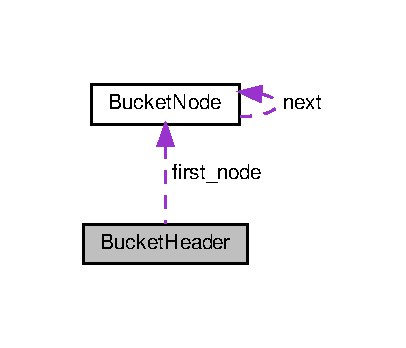
\includegraphics[width=195pt]{classBucketHeader__coll__graph}
\end{center}
\end{figure}
\subsection*{Public Member Functions}
\begin{DoxyCompactItemize}
\item 
void \hyperlink{classBucketHeader_af033419413f506161fa21020f830220a}{init} ()
\item 
void \hyperlink{classBucketHeader_af83c68acf8763f33c09019407710731c}{insert\+\_\+item} (\hyperlink{index__base_8h_ae35c40bc2f912c11f0e36ac66cba4489}{K\+E\+Y\+\_\+\+T\+Y\+PE} key, \hyperlink{microbench_2main_8cpp_ae17cb099b4c9aee7835032339b5a9e0d}{V\+A\+L\+U\+E\+\_\+\+T\+Y\+PE} item, int part\+\_\+id)
\item 
void \hyperlink{classBucketHeader_ac626241058ab4e23bbb9827d68078c3f}{read\+\_\+item} (\hyperlink{index__base_8h_ae35c40bc2f912c11f0e36ac66cba4489}{K\+E\+Y\+\_\+\+T\+Y\+PE} key, \hyperlink{microbench_2main_8cpp_ae17cb099b4c9aee7835032339b5a9e0d}{V\+A\+L\+U\+E\+\_\+\+T\+Y\+PE} $\ast$item, const char $\ast$tname)
\end{DoxyCompactItemize}
\subsection*{Public Attributes}
\begin{DoxyCompactItemize}
\item 
\hyperlink{classBucketNode}{Bucket\+Node} $\ast$ \hyperlink{classBucketHeader_a4ec7aac89e39ec77488c7b1e8be33c56}{first\+\_\+node}
\item 
uint64\+\_\+t \hyperlink{classBucketHeader_aa725cf07022db861aa15b07fec3ab123}{node\+\_\+cnt}
\item 
bool \hyperlink{classBucketHeader_aef842697ec95a54f0b5b798b88267e53}{locked}
\end{DoxyCompactItemize}


\subsection{Member Function Documentation}
\mbox{\Hypertarget{classBucketHeader_af033419413f506161fa21020f830220a}\label{classBucketHeader_af033419413f506161fa21020f830220a}} 
\index{Bucket\+Header@{Bucket\+Header}!init@{init}}
\index{init@{init}!Bucket\+Header@{Bucket\+Header}}
\subsubsection{\texorpdfstring{init()}{init()}}
{\footnotesize\ttfamily void Bucket\+Header\+::init (\begin{DoxyParamCaption}{ }\end{DoxyParamCaption})}

\mbox{\Hypertarget{classBucketHeader_af83c68acf8763f33c09019407710731c}\label{classBucketHeader_af83c68acf8763f33c09019407710731c}} 
\index{Bucket\+Header@{Bucket\+Header}!insert\+\_\+item@{insert\+\_\+item}}
\index{insert\+\_\+item@{insert\+\_\+item}!Bucket\+Header@{Bucket\+Header}}
\subsubsection{\texorpdfstring{insert\+\_\+item()}{insert\_item()}}
{\footnotesize\ttfamily void Bucket\+Header\+::insert\+\_\+item (\begin{DoxyParamCaption}\item[{\hyperlink{index__base_8h_ae35c40bc2f912c11f0e36ac66cba4489}{K\+E\+Y\+\_\+\+T\+Y\+PE}}]{key,  }\item[{\hyperlink{microbench_2main_8cpp_ae17cb099b4c9aee7835032339b5a9e0d}{V\+A\+L\+U\+E\+\_\+\+T\+Y\+PE}}]{item,  }\item[{int}]{part\+\_\+id }\end{DoxyParamCaption})}

\mbox{\Hypertarget{classBucketHeader_ac626241058ab4e23bbb9827d68078c3f}\label{classBucketHeader_ac626241058ab4e23bbb9827d68078c3f}} 
\index{Bucket\+Header@{Bucket\+Header}!read\+\_\+item@{read\+\_\+item}}
\index{read\+\_\+item@{read\+\_\+item}!Bucket\+Header@{Bucket\+Header}}
\subsubsection{\texorpdfstring{read\+\_\+item()}{read\_item()}}
{\footnotesize\ttfamily void Bucket\+Header\+::read\+\_\+item (\begin{DoxyParamCaption}\item[{\hyperlink{index__base_8h_ae35c40bc2f912c11f0e36ac66cba4489}{K\+E\+Y\+\_\+\+T\+Y\+PE}}]{key,  }\item[{\hyperlink{microbench_2main_8cpp_ae17cb099b4c9aee7835032339b5a9e0d}{V\+A\+L\+U\+E\+\_\+\+T\+Y\+PE} $\ast$}]{item,  }\item[{const char $\ast$}]{tname }\end{DoxyParamCaption})}



\subsection{Member Data Documentation}
\mbox{\Hypertarget{classBucketHeader_a4ec7aac89e39ec77488c7b1e8be33c56}\label{classBucketHeader_a4ec7aac89e39ec77488c7b1e8be33c56}} 
\index{Bucket\+Header@{Bucket\+Header}!first\+\_\+node@{first\+\_\+node}}
\index{first\+\_\+node@{first\+\_\+node}!Bucket\+Header@{Bucket\+Header}}
\subsubsection{\texorpdfstring{first\+\_\+node}{first\_node}}
{\footnotesize\ttfamily \hyperlink{classBucketNode}{Bucket\+Node}$\ast$ Bucket\+Header\+::first\+\_\+node}

\mbox{\Hypertarget{classBucketHeader_aef842697ec95a54f0b5b798b88267e53}\label{classBucketHeader_aef842697ec95a54f0b5b798b88267e53}} 
\index{Bucket\+Header@{Bucket\+Header}!locked@{locked}}
\index{locked@{locked}!Bucket\+Header@{Bucket\+Header}}
\subsubsection{\texorpdfstring{locked}{locked}}
{\footnotesize\ttfamily bool Bucket\+Header\+::locked}

\mbox{\Hypertarget{classBucketHeader_aa725cf07022db861aa15b07fec3ab123}\label{classBucketHeader_aa725cf07022db861aa15b07fec3ab123}} 
\index{Bucket\+Header@{Bucket\+Header}!node\+\_\+cnt@{node\+\_\+cnt}}
\index{node\+\_\+cnt@{node\+\_\+cnt}!Bucket\+Header@{Bucket\+Header}}
\subsubsection{\texorpdfstring{node\+\_\+cnt}{node\_cnt}}
{\footnotesize\ttfamily uint64\+\_\+t Bucket\+Header\+::node\+\_\+cnt}



The documentation for this class was generated from the following file\+:\begin{DoxyCompactItemize}
\item 
macrobench/storage/index/\hyperlink{index__hash_8h}{index\+\_\+hash.\+h}\end{DoxyCompactItemize}

\hypertarget{classBucketNode}{}\section{Bucket\+Node Class Reference}
\label{classBucketNode}\index{Bucket\+Node@{Bucket\+Node}}


{\ttfamily \#include $<$index\+\_\+hash.\+h$>$}



Collaboration diagram for Bucket\+Node\+:
\nopagebreak
\begin{figure}[H]
\begin{center}
\leavevmode
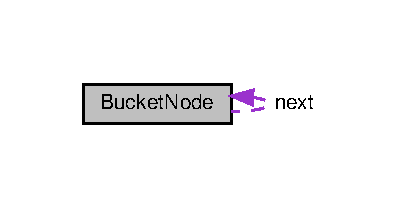
\includegraphics[width=191pt]{classBucketNode__coll__graph}
\end{center}
\end{figure}
\subsection*{Public Member Functions}
\begin{DoxyCompactItemize}
\item 
\hyperlink{classBucketNode_a30b8167df2daa7dcc5bbcf4b9e7cae6a}{Bucket\+Node} (\hyperlink{index__base_8h_ae35c40bc2f912c11f0e36ac66cba4489}{K\+E\+Y\+\_\+\+T\+Y\+PE} \hyperlink{classBucketNode_ae9416fe7ade549b23efc88d413e61de2}{key})
\item 
void \hyperlink{classBucketNode_aed4c88c4dde6d7b7a9274f4a3259e48b}{init} (\hyperlink{index__base_8h_ae35c40bc2f912c11f0e36ac66cba4489}{K\+E\+Y\+\_\+\+T\+Y\+PE} \hyperlink{classBucketNode_ae9416fe7ade549b23efc88d413e61de2}{key})
\end{DoxyCompactItemize}
\subsection*{Public Attributes}
\begin{DoxyCompactItemize}
\item 
\hyperlink{index__base_8h_ae35c40bc2f912c11f0e36ac66cba4489}{K\+E\+Y\+\_\+\+T\+Y\+PE} \hyperlink{classBucketNode_ae9416fe7ade549b23efc88d413e61de2}{key}
\item 
\hyperlink{classBucketNode}{Bucket\+Node} $\ast$ \hyperlink{classBucketNode_a5c641909c96ba75324518fafa9166c61}{next}
\item 
\hyperlink{microbench_2main_8cpp_ae17cb099b4c9aee7835032339b5a9e0d}{V\+A\+L\+U\+E\+\_\+\+T\+Y\+PE} \hyperlink{classBucketNode_a8299d0a598880b114ba06dbd667d8d0f}{items}
\end{DoxyCompactItemize}


\subsection{Constructor \& Destructor Documentation}
\mbox{\Hypertarget{classBucketNode_a30b8167df2daa7dcc5bbcf4b9e7cae6a}\label{classBucketNode_a30b8167df2daa7dcc5bbcf4b9e7cae6a}} 
\index{Bucket\+Node@{Bucket\+Node}!Bucket\+Node@{Bucket\+Node}}
\index{Bucket\+Node@{Bucket\+Node}!Bucket\+Node@{Bucket\+Node}}
\subsubsection{\texorpdfstring{Bucket\+Node()}{BucketNode()}}
{\footnotesize\ttfamily Bucket\+Node\+::\+Bucket\+Node (\begin{DoxyParamCaption}\item[{\hyperlink{index__base_8h_ae35c40bc2f912c11f0e36ac66cba4489}{K\+E\+Y\+\_\+\+T\+Y\+PE}}]{key }\end{DoxyParamCaption})\hspace{0.3cm}{\ttfamily [inline]}}



\subsection{Member Function Documentation}
\mbox{\Hypertarget{classBucketNode_aed4c88c4dde6d7b7a9274f4a3259e48b}\label{classBucketNode_aed4c88c4dde6d7b7a9274f4a3259e48b}} 
\index{Bucket\+Node@{Bucket\+Node}!init@{init}}
\index{init@{init}!Bucket\+Node@{Bucket\+Node}}
\subsubsection{\texorpdfstring{init()}{init()}}
{\footnotesize\ttfamily void Bucket\+Node\+::init (\begin{DoxyParamCaption}\item[{\hyperlink{index__base_8h_ae35c40bc2f912c11f0e36ac66cba4489}{K\+E\+Y\+\_\+\+T\+Y\+PE}}]{key }\end{DoxyParamCaption})\hspace{0.3cm}{\ttfamily [inline]}}



\subsection{Member Data Documentation}
\mbox{\Hypertarget{classBucketNode_a8299d0a598880b114ba06dbd667d8d0f}\label{classBucketNode_a8299d0a598880b114ba06dbd667d8d0f}} 
\index{Bucket\+Node@{Bucket\+Node}!items@{items}}
\index{items@{items}!Bucket\+Node@{Bucket\+Node}}
\subsubsection{\texorpdfstring{items}{items}}
{\footnotesize\ttfamily \hyperlink{microbench_2main_8cpp_ae17cb099b4c9aee7835032339b5a9e0d}{V\+A\+L\+U\+E\+\_\+\+T\+Y\+PE} Bucket\+Node\+::items}

\mbox{\Hypertarget{classBucketNode_ae9416fe7ade549b23efc88d413e61de2}\label{classBucketNode_ae9416fe7ade549b23efc88d413e61de2}} 
\index{Bucket\+Node@{Bucket\+Node}!key@{key}}
\index{key@{key}!Bucket\+Node@{Bucket\+Node}}
\subsubsection{\texorpdfstring{key}{key}}
{\footnotesize\ttfamily \hyperlink{index__base_8h_ae35c40bc2f912c11f0e36ac66cba4489}{K\+E\+Y\+\_\+\+T\+Y\+PE} Bucket\+Node\+::key}

\mbox{\Hypertarget{classBucketNode_a5c641909c96ba75324518fafa9166c61}\label{classBucketNode_a5c641909c96ba75324518fafa9166c61}} 
\index{Bucket\+Node@{Bucket\+Node}!next@{next}}
\index{next@{next}!Bucket\+Node@{Bucket\+Node}}
\subsubsection{\texorpdfstring{next}{next}}
{\footnotesize\ttfamily \hyperlink{classBucketNode}{Bucket\+Node}$\ast$ Bucket\+Node\+::next}



The documentation for this class was generated from the following file\+:\begin{DoxyCompactItemize}
\item 
macrobench/storage/index/\hyperlink{index__hash_8h}{index\+\_\+hash.\+h}\end{DoxyCompactItemize}

\hypertarget{structcasword}{}\section{casword$<$ T $>$ Struct Template Reference}
\label{structcasword}\index{casword$<$ T $>$@{casword$<$ T $>$}}


{\ttfamily \#include $<$kcas.\+h$>$}

\subsection*{Public Member Functions}
\begin{DoxyCompactItemize}
\item 
\hyperlink{structcasword_a2325ef306dec004288a063b1a64e43e5}{casword} ()
\item 
T \hyperlink{structcasword_af443268d0da3bee38b712912850210e6}{set\+Init\+Val} (T other)
\item 
\hyperlink{structcasword_a5b967f1ba3c54143e7ff37870831cf43}{operator T} ()
\item 
T \hyperlink{structcasword_ab6b758d075768501b8915eebf602c54e}{operator-\/$>$} ()
\item 
T \hyperlink{structcasword_a815838a9e00061deaef7e5596bb5e8bf}{get\+Value} ()
\item 
void \hyperlink{structcasword_ae9521db09e9366bb31156bc78830b760}{add\+To\+Descriptor} (T old\+Val, T new\+Val)
\end{DoxyCompactItemize}


\subsection{Constructor \& Destructor Documentation}
\mbox{\Hypertarget{structcasword_a2325ef306dec004288a063b1a64e43e5}\label{structcasword_a2325ef306dec004288a063b1a64e43e5}} 
\index{casword@{casword}!casword@{casword}}
\index{casword@{casword}!casword@{casword}}
\subsubsection{\texorpdfstring{casword()}{casword()}}
{\footnotesize\ttfamily template$<$typename T $>$ \\
\hyperlink{structcasword}{casword}$<$ T $>$\+::\hyperlink{structcasword}{casword} (\begin{DoxyParamCaption}{ }\end{DoxyParamCaption})}



\subsection{Member Function Documentation}
\mbox{\Hypertarget{structcasword_ae9521db09e9366bb31156bc78830b760}\label{structcasword_ae9521db09e9366bb31156bc78830b760}} 
\index{casword@{casword}!add\+To\+Descriptor@{add\+To\+Descriptor}}
\index{add\+To\+Descriptor@{add\+To\+Descriptor}!casword@{casword}}
\subsubsection{\texorpdfstring{add\+To\+Descriptor()}{addToDescriptor()}}
{\footnotesize\ttfamily template$<$typename T$>$ \\
void \hyperlink{structcasword}{casword}$<$ T $>$\+::add\+To\+Descriptor (\begin{DoxyParamCaption}\item[{T}]{old\+Val,  }\item[{T}]{new\+Val }\end{DoxyParamCaption})}

\mbox{\Hypertarget{structcasword_a815838a9e00061deaef7e5596bb5e8bf}\label{structcasword_a815838a9e00061deaef7e5596bb5e8bf}} 
\index{casword@{casword}!get\+Value@{get\+Value}}
\index{get\+Value@{get\+Value}!casword@{casword}}
\subsubsection{\texorpdfstring{get\+Value()}{getValue()}}
{\footnotesize\ttfamily template$<$typename T $>$ \\
T \hyperlink{structcasword}{casword}$<$ T $>$\+::get\+Value (\begin{DoxyParamCaption}{ }\end{DoxyParamCaption})}

\mbox{\Hypertarget{structcasword_a5b967f1ba3c54143e7ff37870831cf43}\label{structcasword_a5b967f1ba3c54143e7ff37870831cf43}} 
\index{casword@{casword}!operator T@{operator T}}
\index{operator T@{operator T}!casword@{casword}}
\subsubsection{\texorpdfstring{operator T()}{operator T()}}
{\footnotesize\ttfamily template$<$typename T $>$ \\
\hyperlink{structcasword}{casword}$<$ T $>$\+::operator T (\begin{DoxyParamCaption}{ }\end{DoxyParamCaption})}

\mbox{\Hypertarget{structcasword_ab6b758d075768501b8915eebf602c54e}\label{structcasword_ab6b758d075768501b8915eebf602c54e}} 
\index{casword@{casword}!operator-\/$>$@{operator-\/$>$}}
\index{operator-\/$>$@{operator-\/$>$}!casword@{casword}}
\subsubsection{\texorpdfstring{operator-\/$>$()}{operator->()}}
{\footnotesize\ttfamily template$<$typename T $>$ \\
T \hyperlink{structcasword}{casword}$<$ T $>$\+::operator-\/$>$ (\begin{DoxyParamCaption}{ }\end{DoxyParamCaption})}

\mbox{\Hypertarget{structcasword_af443268d0da3bee38b712912850210e6}\label{structcasword_af443268d0da3bee38b712912850210e6}} 
\index{casword@{casword}!set\+Init\+Val@{set\+Init\+Val}}
\index{set\+Init\+Val@{set\+Init\+Val}!casword@{casword}}
\subsubsection{\texorpdfstring{set\+Init\+Val()}{setInitVal()}}
{\footnotesize\ttfamily template$<$typename T$>$ \\
T \hyperlink{structcasword}{casword}$<$ T $>$\+::set\+Init\+Val (\begin{DoxyParamCaption}\item[{T}]{other }\end{DoxyParamCaption})}



The documentation for this struct was generated from the following files\+:\begin{DoxyCompactItemize}
\item 
common/kcas/\hyperlink{kcas_8h}{kcas.\+h}\item 
common/kcas/\hyperlink{casword_8h}{casword.\+h}\end{DoxyCompactItemize}

\hypertarget{classCatalog}{}\section{Catalog Class Reference}
\label{classCatalog}\index{Catalog@{Catalog}}


{\ttfamily \#include $<$catalog.\+h$>$}



Collaboration diagram for Catalog\+:
\nopagebreak
\begin{figure}[H]
\begin{center}
\leavevmode
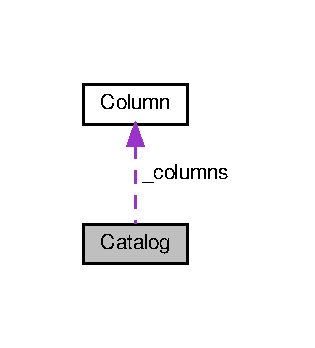
\includegraphics[width=151pt]{classCatalog__coll__graph}
\end{center}
\end{figure}
\subsection*{Public Member Functions}
\begin{DoxyCompactItemize}
\item 
void \hyperlink{classCatalog_ad5503efb087474d8f9ece2d2709dd60a}{init} (const char $\ast$\hyperlink{classCatalog_aa6c66c1e792e3c6081e22fd669f84052}{table\+\_\+name}, int \hyperlink{classCatalog_abd9d27040300ad689ec3b21b46d78d44}{field\+\_\+cnt})
\item 
void \hyperlink{classCatalog_aca79c0260b48603b70619e5e91187611}{setbench\+\_\+deinit} ()
\item 
void \hyperlink{classCatalog_a82dd2169f7a07b9b0a112d3d05f4c78d}{add\+\_\+col} (char $\ast$col\+\_\+name, uint64\+\_\+t size, char $\ast$type)
\item 
\hyperlink{global_8h_a7e8aeec7b6541935dfc6f608cd5170ce}{U\+Int32} \hyperlink{classCatalog_a8617fc5a89371a53fc9a450accaf0211}{get\+\_\+tuple\+\_\+size} ()
\item 
uint64\+\_\+t \hyperlink{classCatalog_a3a8d95b98c08cc5dcff8d7df7eed2285}{get\+\_\+field\+\_\+cnt} ()
\item 
uint64\+\_\+t \hyperlink{classCatalog_af03a0a6a13510e590c6a7ce04c63d4d5}{get\+\_\+field\+\_\+size} (int id)
\item 
uint64\+\_\+t \hyperlink{classCatalog_a28e292fcaca35de08455739f7ef36fb9}{get\+\_\+field\+\_\+index} (int id)
\item 
char $\ast$ \hyperlink{classCatalog_af96a147d994b6b4609c9cecda3be7646}{get\+\_\+field\+\_\+type} (uint64\+\_\+t id)
\item 
char $\ast$ \hyperlink{classCatalog_a812400ac0c25657b8733638d3e25df29}{get\+\_\+field\+\_\+name} (uint64\+\_\+t id)
\item 
uint64\+\_\+t \hyperlink{classCatalog_aa7ee6e989df63482968b2e6764040446}{get\+\_\+field\+\_\+id} (const char $\ast$name)
\item 
char $\ast$ \hyperlink{classCatalog_a40eb903543e6384e388864b5e598b118}{get\+\_\+field\+\_\+type} (char $\ast$name)
\item 
uint64\+\_\+t \hyperlink{classCatalog_aeb22fe6cfbdd3c0d92dc46b70aff2066}{get\+\_\+field\+\_\+index} (char $\ast$name)
\item 
void \hyperlink{classCatalog_ab35f2b078a555d5d2b099ab42162a4d4}{print\+\_\+schema} ()
\end{DoxyCompactItemize}
\subsection*{Public Attributes}
\begin{DoxyCompactItemize}
\item 
\hyperlink{global_8h_a7e8aeec7b6541935dfc6f608cd5170ce}{U\+Int32} \hyperlink{classCatalog_abd9d27040300ad689ec3b21b46d78d44}{field\+\_\+cnt}
\item 
const char $\ast$ \hyperlink{classCatalog_aa6c66c1e792e3c6081e22fd669f84052}{table\+\_\+name}
\item 
\hyperlink{classColumn}{Column} $\ast$ \hyperlink{classCatalog_ae629f8b429ce660192d3dd2e51f493ea}{\+\_\+columns}
\item 
\hyperlink{global_8h_a7e8aeec7b6541935dfc6f608cd5170ce}{U\+Int32} \hyperlink{classCatalog_ac5c0f579ade64940d1c743b4ee76e657}{tuple\+\_\+size}
\end{DoxyCompactItemize}


\subsection{Member Function Documentation}
\mbox{\Hypertarget{classCatalog_a82dd2169f7a07b9b0a112d3d05f4c78d}\label{classCatalog_a82dd2169f7a07b9b0a112d3d05f4c78d}} 
\index{Catalog@{Catalog}!add\+\_\+col@{add\+\_\+col}}
\index{add\+\_\+col@{add\+\_\+col}!Catalog@{Catalog}}
\subsubsection{\texorpdfstring{add\+\_\+col()}{add\_col()}}
{\footnotesize\ttfamily void Catalog\+::add\+\_\+col (\begin{DoxyParamCaption}\item[{char $\ast$}]{col\+\_\+name,  }\item[{uint64\+\_\+t}]{size,  }\item[{char $\ast$}]{type }\end{DoxyParamCaption})}

\mbox{\Hypertarget{classCatalog_a3a8d95b98c08cc5dcff8d7df7eed2285}\label{classCatalog_a3a8d95b98c08cc5dcff8d7df7eed2285}} 
\index{Catalog@{Catalog}!get\+\_\+field\+\_\+cnt@{get\+\_\+field\+\_\+cnt}}
\index{get\+\_\+field\+\_\+cnt@{get\+\_\+field\+\_\+cnt}!Catalog@{Catalog}}
\subsubsection{\texorpdfstring{get\+\_\+field\+\_\+cnt()}{get\_field\_cnt()}}
{\footnotesize\ttfamily uint64\+\_\+t Catalog\+::get\+\_\+field\+\_\+cnt (\begin{DoxyParamCaption}{ }\end{DoxyParamCaption})\hspace{0.3cm}{\ttfamily [inline]}}

\mbox{\Hypertarget{classCatalog_aa7ee6e989df63482968b2e6764040446}\label{classCatalog_aa7ee6e989df63482968b2e6764040446}} 
\index{Catalog@{Catalog}!get\+\_\+field\+\_\+id@{get\+\_\+field\+\_\+id}}
\index{get\+\_\+field\+\_\+id@{get\+\_\+field\+\_\+id}!Catalog@{Catalog}}
\subsubsection{\texorpdfstring{get\+\_\+field\+\_\+id()}{get\_field\_id()}}
{\footnotesize\ttfamily uint64\+\_\+t Catalog\+::get\+\_\+field\+\_\+id (\begin{DoxyParamCaption}\item[{const char $\ast$}]{name }\end{DoxyParamCaption})}

\mbox{\Hypertarget{classCatalog_a28e292fcaca35de08455739f7ef36fb9}\label{classCatalog_a28e292fcaca35de08455739f7ef36fb9}} 
\index{Catalog@{Catalog}!get\+\_\+field\+\_\+index@{get\+\_\+field\+\_\+index}}
\index{get\+\_\+field\+\_\+index@{get\+\_\+field\+\_\+index}!Catalog@{Catalog}}
\subsubsection{\texorpdfstring{get\+\_\+field\+\_\+index()}{get\_field\_index()}\hspace{0.1cm}{\footnotesize\ttfamily [1/2]}}
{\footnotesize\ttfamily uint64\+\_\+t Catalog\+::get\+\_\+field\+\_\+index (\begin{DoxyParamCaption}\item[{int}]{id }\end{DoxyParamCaption})\hspace{0.3cm}{\ttfamily [inline]}}

\mbox{\Hypertarget{classCatalog_aeb22fe6cfbdd3c0d92dc46b70aff2066}\label{classCatalog_aeb22fe6cfbdd3c0d92dc46b70aff2066}} 
\index{Catalog@{Catalog}!get\+\_\+field\+\_\+index@{get\+\_\+field\+\_\+index}}
\index{get\+\_\+field\+\_\+index@{get\+\_\+field\+\_\+index}!Catalog@{Catalog}}
\subsubsection{\texorpdfstring{get\+\_\+field\+\_\+index()}{get\_field\_index()}\hspace{0.1cm}{\footnotesize\ttfamily [2/2]}}
{\footnotesize\ttfamily uint64\+\_\+t Catalog\+::get\+\_\+field\+\_\+index (\begin{DoxyParamCaption}\item[{char $\ast$}]{name }\end{DoxyParamCaption})}

\mbox{\Hypertarget{classCatalog_a812400ac0c25657b8733638d3e25df29}\label{classCatalog_a812400ac0c25657b8733638d3e25df29}} 
\index{Catalog@{Catalog}!get\+\_\+field\+\_\+name@{get\+\_\+field\+\_\+name}}
\index{get\+\_\+field\+\_\+name@{get\+\_\+field\+\_\+name}!Catalog@{Catalog}}
\subsubsection{\texorpdfstring{get\+\_\+field\+\_\+name()}{get\_field\_name()}}
{\footnotesize\ttfamily char $\ast$ Catalog\+::get\+\_\+field\+\_\+name (\begin{DoxyParamCaption}\item[{uint64\+\_\+t}]{id }\end{DoxyParamCaption})}

\mbox{\Hypertarget{classCatalog_af03a0a6a13510e590c6a7ce04c63d4d5}\label{classCatalog_af03a0a6a13510e590c6a7ce04c63d4d5}} 
\index{Catalog@{Catalog}!get\+\_\+field\+\_\+size@{get\+\_\+field\+\_\+size}}
\index{get\+\_\+field\+\_\+size@{get\+\_\+field\+\_\+size}!Catalog@{Catalog}}
\subsubsection{\texorpdfstring{get\+\_\+field\+\_\+size()}{get\_field\_size()}}
{\footnotesize\ttfamily uint64\+\_\+t Catalog\+::get\+\_\+field\+\_\+size (\begin{DoxyParamCaption}\item[{int}]{id }\end{DoxyParamCaption})\hspace{0.3cm}{\ttfamily [inline]}}

\mbox{\Hypertarget{classCatalog_af96a147d994b6b4609c9cecda3be7646}\label{classCatalog_af96a147d994b6b4609c9cecda3be7646}} 
\index{Catalog@{Catalog}!get\+\_\+field\+\_\+type@{get\+\_\+field\+\_\+type}}
\index{get\+\_\+field\+\_\+type@{get\+\_\+field\+\_\+type}!Catalog@{Catalog}}
\subsubsection{\texorpdfstring{get\+\_\+field\+\_\+type()}{get\_field\_type()}\hspace{0.1cm}{\footnotesize\ttfamily [1/2]}}
{\footnotesize\ttfamily char $\ast$ Catalog\+::get\+\_\+field\+\_\+type (\begin{DoxyParamCaption}\item[{uint64\+\_\+t}]{id }\end{DoxyParamCaption})}

\mbox{\Hypertarget{classCatalog_a40eb903543e6384e388864b5e598b118}\label{classCatalog_a40eb903543e6384e388864b5e598b118}} 
\index{Catalog@{Catalog}!get\+\_\+field\+\_\+type@{get\+\_\+field\+\_\+type}}
\index{get\+\_\+field\+\_\+type@{get\+\_\+field\+\_\+type}!Catalog@{Catalog}}
\subsubsection{\texorpdfstring{get\+\_\+field\+\_\+type()}{get\_field\_type()}\hspace{0.1cm}{\footnotesize\ttfamily [2/2]}}
{\footnotesize\ttfamily char $\ast$ Catalog\+::get\+\_\+field\+\_\+type (\begin{DoxyParamCaption}\item[{char $\ast$}]{name }\end{DoxyParamCaption})}

\mbox{\Hypertarget{classCatalog_a8617fc5a89371a53fc9a450accaf0211}\label{classCatalog_a8617fc5a89371a53fc9a450accaf0211}} 
\index{Catalog@{Catalog}!get\+\_\+tuple\+\_\+size@{get\+\_\+tuple\+\_\+size}}
\index{get\+\_\+tuple\+\_\+size@{get\+\_\+tuple\+\_\+size}!Catalog@{Catalog}}
\subsubsection{\texorpdfstring{get\+\_\+tuple\+\_\+size()}{get\_tuple\_size()}}
{\footnotesize\ttfamily \hyperlink{global_8h_a7e8aeec7b6541935dfc6f608cd5170ce}{U\+Int32} Catalog\+::get\+\_\+tuple\+\_\+size (\begin{DoxyParamCaption}{ }\end{DoxyParamCaption})\hspace{0.3cm}{\ttfamily [inline]}}

\mbox{\Hypertarget{classCatalog_ad5503efb087474d8f9ece2d2709dd60a}\label{classCatalog_ad5503efb087474d8f9ece2d2709dd60a}} 
\index{Catalog@{Catalog}!init@{init}}
\index{init@{init}!Catalog@{Catalog}}
\subsubsection{\texorpdfstring{init()}{init()}}
{\footnotesize\ttfamily void Catalog\+::init (\begin{DoxyParamCaption}\item[{const char $\ast$}]{table\+\_\+name,  }\item[{int}]{field\+\_\+cnt }\end{DoxyParamCaption})}

\mbox{\Hypertarget{classCatalog_ab35f2b078a555d5d2b099ab42162a4d4}\label{classCatalog_ab35f2b078a555d5d2b099ab42162a4d4}} 
\index{Catalog@{Catalog}!print\+\_\+schema@{print\+\_\+schema}}
\index{print\+\_\+schema@{print\+\_\+schema}!Catalog@{Catalog}}
\subsubsection{\texorpdfstring{print\+\_\+schema()}{print\_schema()}}
{\footnotesize\ttfamily void Catalog\+::print\+\_\+schema (\begin{DoxyParamCaption}{ }\end{DoxyParamCaption})}

\mbox{\Hypertarget{classCatalog_aca79c0260b48603b70619e5e91187611}\label{classCatalog_aca79c0260b48603b70619e5e91187611}} 
\index{Catalog@{Catalog}!setbench\+\_\+deinit@{setbench\+\_\+deinit}}
\index{setbench\+\_\+deinit@{setbench\+\_\+deinit}!Catalog@{Catalog}}
\subsubsection{\texorpdfstring{setbench\+\_\+deinit()}{setbench\_deinit()}}
{\footnotesize\ttfamily void Catalog\+::setbench\+\_\+deinit (\begin{DoxyParamCaption}{ }\end{DoxyParamCaption})}



\subsection{Member Data Documentation}
\mbox{\Hypertarget{classCatalog_ae629f8b429ce660192d3dd2e51f493ea}\label{classCatalog_ae629f8b429ce660192d3dd2e51f493ea}} 
\index{Catalog@{Catalog}!\+\_\+columns@{\+\_\+columns}}
\index{\+\_\+columns@{\+\_\+columns}!Catalog@{Catalog}}
\subsubsection{\texorpdfstring{\+\_\+columns}{\_columns}}
{\footnotesize\ttfamily \hyperlink{classColumn}{Column}$\ast$ Catalog\+::\+\_\+columns}

\mbox{\Hypertarget{classCatalog_abd9d27040300ad689ec3b21b46d78d44}\label{classCatalog_abd9d27040300ad689ec3b21b46d78d44}} 
\index{Catalog@{Catalog}!field\+\_\+cnt@{field\+\_\+cnt}}
\index{field\+\_\+cnt@{field\+\_\+cnt}!Catalog@{Catalog}}
\subsubsection{\texorpdfstring{field\+\_\+cnt}{field\_cnt}}
{\footnotesize\ttfamily \hyperlink{global_8h_a7e8aeec7b6541935dfc6f608cd5170ce}{U\+Int32} Catalog\+::field\+\_\+cnt}

\mbox{\Hypertarget{classCatalog_aa6c66c1e792e3c6081e22fd669f84052}\label{classCatalog_aa6c66c1e792e3c6081e22fd669f84052}} 
\index{Catalog@{Catalog}!table\+\_\+name@{table\+\_\+name}}
\index{table\+\_\+name@{table\+\_\+name}!Catalog@{Catalog}}
\subsubsection{\texorpdfstring{table\+\_\+name}{table\_name}}
{\footnotesize\ttfamily const char$\ast$ Catalog\+::table\+\_\+name}

\mbox{\Hypertarget{classCatalog_ac5c0f579ade64940d1c743b4ee76e657}\label{classCatalog_ac5c0f579ade64940d1c743b4ee76e657}} 
\index{Catalog@{Catalog}!tuple\+\_\+size@{tuple\+\_\+size}}
\index{tuple\+\_\+size@{tuple\+\_\+size}!Catalog@{Catalog}}
\subsubsection{\texorpdfstring{tuple\+\_\+size}{tuple\_size}}
{\footnotesize\ttfamily \hyperlink{global_8h_a7e8aeec7b6541935dfc6f608cd5170ce}{U\+Int32} Catalog\+::tuple\+\_\+size}



The documentation for this class was generated from the following files\+:\begin{DoxyCompactItemize}
\item 
macrobench/storage/\hyperlink{catalog_8h}{catalog.\+h}\item 
macrobench/storage/\hyperlink{catalog_8cpp}{catalog.\+cpp}\end{DoxyCompactItemize}

\hypertarget{classccavl}{}\section{ccavl$<$ skey\+\_\+t, sval\+\_\+t, Rec\+Mgr $>$ Class Template Reference}
\label{classccavl}\index{ccavl$<$ skey\+\_\+t, sval\+\_\+t, Rec\+Mgr $>$@{ccavl$<$ skey\+\_\+t, sval\+\_\+t, Rec\+Mgr $>$}}


{\ttfamily \#include $<$ccavl\+\_\+impl.\+h$>$}

\subsection*{Public Member Functions}
\begin{DoxyCompactItemize}
\item 
\hyperlink{classccavl_ae75621f90c06705d71d42823ce27415b}{ccavl} (const int \hyperlink{testing_8cpp_aa085812188e21ede75351d88b9b2c30d}{num\+Processes}, const skey\+\_\+t \&\+\_\+\+K\+E\+Y\+\_\+\+N\+E\+G\+\_\+\+I\+N\+F\+TY)
\item 
\hyperlink{classccavl_a4ef8b4a550508b4405c69c179d068346}{$\sim$ccavl} ()
\item 
void \hyperlink{classccavl_a3c5a7ce30103bd377abd52c94a0021e4}{init\+Thread} (const int \hyperlink{microbench_2main_8cpp_a9ca9869868fe7e7a38a921cc7de4103f}{tid})
\item 
void \hyperlink{classccavl_a6515857749b20bf66903f66db6d33247}{deinit\+Thread} (const int \hyperlink{microbench_2main_8cpp_a9ca9869868fe7e7a38a921cc7de4103f}{tid})
\item 
sval\+\_\+t \hyperlink{classccavl_acc5cd8e2ab2c439480b38a49462353cb}{insert\+If\+Absent} (const int \hyperlink{microbench_2main_8cpp_a9ca9869868fe7e7a38a921cc7de4103f}{tid}, skey\+\_\+t key, sval\+\_\+t val)
\item 
sval\+\_\+t \hyperlink{classccavl_a1bccdb9a78b965bc23239ca142843701}{insert\+Replace} (const int \hyperlink{microbench_2main_8cpp_a9ca9869868fe7e7a38a921cc7de4103f}{tid}, skey\+\_\+t key, sval\+\_\+t val)
\item 
sval\+\_\+t \hyperlink{classccavl_ad6102621e94aacf02a6ae441c6b2010a}{find} (const int \hyperlink{microbench_2main_8cpp_a9ca9869868fe7e7a38a921cc7de4103f}{tid}, skey\+\_\+t key)
\item 
sval\+\_\+t \hyperlink{classccavl_ad574827b3181dfcc2758d33a920ef888}{erase} (const int \hyperlink{microbench_2main_8cpp_a9ca9869868fe7e7a38a921cc7de4103f}{tid}, skey\+\_\+t key)
\item 
\hyperlink{structnode__t}{node\+\_\+t}$<$ skey\+\_\+t, sval\+\_\+t $>$ $\ast$ \hyperlink{classccavl_ad6813e2b580885b73267281299aaf91b}{get\+\_\+root} ()
\item 
\hyperlink{structnode__t}{node\+\_\+t}$<$ skey\+\_\+t, sval\+\_\+t $>$ $\ast$ \hyperlink{classccavl_a3a0b0d9511f6c33a366df29b7e5e78c6}{get\+\_\+left} (\hyperlink{structnode__t}{node\+\_\+t}$<$ skey\+\_\+t, sval\+\_\+t $>$ $\ast$curr)
\item 
\hyperlink{structnode__t}{node\+\_\+t}$<$ skey\+\_\+t, sval\+\_\+t $>$ $\ast$ \hyperlink{classccavl_adea629204a5f01be8cf538a84a82cbe0}{get\+\_\+right} (\hyperlink{structnode__t}{node\+\_\+t}$<$ skey\+\_\+t, sval\+\_\+t $>$ $\ast$curr)
\item 
long long \hyperlink{classccavl_a8722026efe4a180eefd9fd5a535b8930}{get\+Key\+Checksum} (\hyperlink{structnode__t}{node\+\_\+t}$<$ skey\+\_\+t, sval\+\_\+t $>$ $\ast$curr)
\item 
long long \hyperlink{classccavl_aad58da3e9edfdc382a5dc434505e1ba0}{get\+Key\+Checksum} ()
\item 
long long \hyperlink{classccavl_a6777e1819dbd5db66a28d859b01d147e}{get\+Size} (\hyperlink{structnode__t}{node\+\_\+t}$<$ skey\+\_\+t, sval\+\_\+t $>$ $\ast$curr)
\item 
bool \hyperlink{classccavl_ac47877ab6e5def2750f5df5cda2c19be}{validate\+Structure} ()
\item 
long long \hyperlink{classccavl_a0cba7a4d7634b04f0029d612d8ed2e0e}{get\+Size} ()
\item 
long long \hyperlink{classccavl_ac537ecd0a2f9ab354d3e552da16c7b2a}{get\+Size\+In\+Nodes} (\hyperlink{structnode__t}{node\+\_\+t}$<$ skey\+\_\+t, sval\+\_\+t $>$ $\ast$const curr)
\item 
long long \hyperlink{classccavl_a3436a535b92e8199212b297d80c4ae6e}{get\+Size\+In\+Nodes} ()
\item 
void \hyperlink{classccavl_a3ab44e9335cff25b627abb847477438c}{print\+Summary} ()
\end{DoxyCompactItemize}
\subsection*{Public Attributes}
\begin{DoxyCompactItemize}
\item 
const int \hyperlink{classccavl_a8ccf65d91ffe06b1365ddf88e4a7c40a}{N\+U\+M\+\_\+\+P\+R\+O\+C\+E\+S\+S\+ES}
\item 
skey\+\_\+t \hyperlink{classccavl_ae7c30fe784d924a824eb95fc9a1536df}{K\+E\+Y\+\_\+\+N\+E\+G\+\_\+\+I\+N\+F\+TY}
\end{DoxyCompactItemize}


\subsection{Constructor \& Destructor Documentation}
\mbox{\Hypertarget{classccavl_ae75621f90c06705d71d42823ce27415b}\label{classccavl_ae75621f90c06705d71d42823ce27415b}} 
\index{ccavl@{ccavl}!ccavl@{ccavl}}
\index{ccavl@{ccavl}!ccavl@{ccavl}}
\subsubsection{\texorpdfstring{ccavl()}{ccavl()}}
{\footnotesize\ttfamily template$<$typename skey\+\_\+t , typename sval\+\_\+t , class Rec\+Mgr $>$ \\
\hyperlink{classccavl}{ccavl}$<$ skey\+\_\+t, sval\+\_\+t, Rec\+Mgr $>$\+::\hyperlink{classccavl}{ccavl} (\begin{DoxyParamCaption}\item[{const int}]{num\+Processes,  }\item[{const skey\+\_\+t \&}]{\+\_\+\+K\+E\+Y\+\_\+\+N\+E\+G\+\_\+\+I\+N\+F\+TY }\end{DoxyParamCaption})\hspace{0.3cm}{\ttfamily [inline]}}

\mbox{\Hypertarget{classccavl_a4ef8b4a550508b4405c69c179d068346}\label{classccavl_a4ef8b4a550508b4405c69c179d068346}} 
\index{ccavl@{ccavl}!````~ccavl@{$\sim$ccavl}}
\index{````~ccavl@{$\sim$ccavl}!ccavl@{ccavl}}
\subsubsection{\texorpdfstring{$\sim$ccavl()}{~ccavl()}}
{\footnotesize\ttfamily template$<$typename skey\+\_\+t , typename sval\+\_\+t , class Rec\+Mgr $>$ \\
\hyperlink{classccavl}{ccavl}$<$ skey\+\_\+t, sval\+\_\+t, Rec\+Mgr $>$\+::$\sim$\hyperlink{classccavl}{ccavl} (\begin{DoxyParamCaption}{ }\end{DoxyParamCaption})\hspace{0.3cm}{\ttfamily [inline]}}



\subsection{Member Function Documentation}
\mbox{\Hypertarget{classccavl_a6515857749b20bf66903f66db6d33247}\label{classccavl_a6515857749b20bf66903f66db6d33247}} 
\index{ccavl@{ccavl}!deinit\+Thread@{deinit\+Thread}}
\index{deinit\+Thread@{deinit\+Thread}!ccavl@{ccavl}}
\subsubsection{\texorpdfstring{deinit\+Thread()}{deinitThread()}}
{\footnotesize\ttfamily template$<$typename skey\+\_\+t , typename sval\+\_\+t , class Rec\+Mgr $>$ \\
void \hyperlink{classccavl}{ccavl}$<$ skey\+\_\+t, sval\+\_\+t, Rec\+Mgr $>$\+::deinit\+Thread (\begin{DoxyParamCaption}\item[{const int}]{tid }\end{DoxyParamCaption})\hspace{0.3cm}{\ttfamily [inline]}}

\mbox{\Hypertarget{classccavl_ad574827b3181dfcc2758d33a920ef888}\label{classccavl_ad574827b3181dfcc2758d33a920ef888}} 
\index{ccavl@{ccavl}!erase@{erase}}
\index{erase@{erase}!ccavl@{ccavl}}
\subsubsection{\texorpdfstring{erase()}{erase()}}
{\footnotesize\ttfamily template$<$typename skey\+\_\+t , typename sval\+\_\+t , class Rec\+Mgr $>$ \\
sval\+\_\+t \hyperlink{classccavl}{ccavl}$<$ skey\+\_\+t, sval\+\_\+t, Rec\+Mgr $>$\+::erase (\begin{DoxyParamCaption}\item[{const int}]{tid,  }\item[{skey\+\_\+t}]{key }\end{DoxyParamCaption})\hspace{0.3cm}{\ttfamily [inline]}}

\mbox{\Hypertarget{classccavl_ad6102621e94aacf02a6ae441c6b2010a}\label{classccavl_ad6102621e94aacf02a6ae441c6b2010a}} 
\index{ccavl@{ccavl}!find@{find}}
\index{find@{find}!ccavl@{ccavl}}
\subsubsection{\texorpdfstring{find()}{find()}}
{\footnotesize\ttfamily template$<$typename skey\+\_\+t , typename sval\+\_\+t , class Rec\+Mgr $>$ \\
sval\+\_\+t \hyperlink{classccavl}{ccavl}$<$ skey\+\_\+t, sval\+\_\+t, Rec\+Mgr $>$\+::find (\begin{DoxyParamCaption}\item[{const int}]{tid,  }\item[{skey\+\_\+t}]{key }\end{DoxyParamCaption})\hspace{0.3cm}{\ttfamily [inline]}}

\mbox{\Hypertarget{classccavl_a3a0b0d9511f6c33a366df29b7e5e78c6}\label{classccavl_a3a0b0d9511f6c33a366df29b7e5e78c6}} 
\index{ccavl@{ccavl}!get\+\_\+left@{get\+\_\+left}}
\index{get\+\_\+left@{get\+\_\+left}!ccavl@{ccavl}}
\subsubsection{\texorpdfstring{get\+\_\+left()}{get\_left()}}
{\footnotesize\ttfamily template$<$typename skey\+\_\+t , typename sval\+\_\+t , class Rec\+Mgr $>$ \\
\hyperlink{structnode__t}{node\+\_\+t}$<$skey\+\_\+t, sval\+\_\+t$>$$\ast$ \hyperlink{classccavl}{ccavl}$<$ skey\+\_\+t, sval\+\_\+t, Rec\+Mgr $>$\+::get\+\_\+left (\begin{DoxyParamCaption}\item[{\hyperlink{structnode__t}{node\+\_\+t}$<$ skey\+\_\+t, sval\+\_\+t $>$ $\ast$}]{curr }\end{DoxyParamCaption})\hspace{0.3cm}{\ttfamily [inline]}}

\mbox{\Hypertarget{classccavl_adea629204a5f01be8cf538a84a82cbe0}\label{classccavl_adea629204a5f01be8cf538a84a82cbe0}} 
\index{ccavl@{ccavl}!get\+\_\+right@{get\+\_\+right}}
\index{get\+\_\+right@{get\+\_\+right}!ccavl@{ccavl}}
\subsubsection{\texorpdfstring{get\+\_\+right()}{get\_right()}}
{\footnotesize\ttfamily template$<$typename skey\+\_\+t , typename sval\+\_\+t , class Rec\+Mgr $>$ \\
\hyperlink{structnode__t}{node\+\_\+t}$<$skey\+\_\+t, sval\+\_\+t$>$$\ast$ \hyperlink{classccavl}{ccavl}$<$ skey\+\_\+t, sval\+\_\+t, Rec\+Mgr $>$\+::get\+\_\+right (\begin{DoxyParamCaption}\item[{\hyperlink{structnode__t}{node\+\_\+t}$<$ skey\+\_\+t, sval\+\_\+t $>$ $\ast$}]{curr }\end{DoxyParamCaption})\hspace{0.3cm}{\ttfamily [inline]}}

\mbox{\Hypertarget{classccavl_ad6813e2b580885b73267281299aaf91b}\label{classccavl_ad6813e2b580885b73267281299aaf91b}} 
\index{ccavl@{ccavl}!get\+\_\+root@{get\+\_\+root}}
\index{get\+\_\+root@{get\+\_\+root}!ccavl@{ccavl}}
\subsubsection{\texorpdfstring{get\+\_\+root()}{get\_root()}}
{\footnotesize\ttfamily template$<$typename skey\+\_\+t , typename sval\+\_\+t , class Rec\+Mgr $>$ \\
\hyperlink{structnode__t}{node\+\_\+t}$<$skey\+\_\+t, sval\+\_\+t$>$$\ast$ \hyperlink{classccavl}{ccavl}$<$ skey\+\_\+t, sval\+\_\+t, Rec\+Mgr $>$\+::get\+\_\+root (\begin{DoxyParamCaption}{ }\end{DoxyParamCaption})\hspace{0.3cm}{\ttfamily [inline]}}

\mbox{\Hypertarget{classccavl_a8722026efe4a180eefd9fd5a535b8930}\label{classccavl_a8722026efe4a180eefd9fd5a535b8930}} 
\index{ccavl@{ccavl}!get\+Key\+Checksum@{get\+Key\+Checksum}}
\index{get\+Key\+Checksum@{get\+Key\+Checksum}!ccavl@{ccavl}}
\subsubsection{\texorpdfstring{get\+Key\+Checksum()}{getKeyChecksum()}\hspace{0.1cm}{\footnotesize\ttfamily [1/2]}}
{\footnotesize\ttfamily template$<$typename skey\+\_\+t , typename sval\+\_\+t , class Rec\+Mgr $>$ \\
long long \hyperlink{classccavl}{ccavl}$<$ skey\+\_\+t, sval\+\_\+t, Rec\+Mgr $>$\+::get\+Key\+Checksum (\begin{DoxyParamCaption}\item[{\hyperlink{structnode__t}{node\+\_\+t}$<$ skey\+\_\+t, sval\+\_\+t $>$ $\ast$}]{curr }\end{DoxyParamCaption})\hspace{0.3cm}{\ttfamily [inline]}}

\mbox{\Hypertarget{classccavl_aad58da3e9edfdc382a5dc434505e1ba0}\label{classccavl_aad58da3e9edfdc382a5dc434505e1ba0}} 
\index{ccavl@{ccavl}!get\+Key\+Checksum@{get\+Key\+Checksum}}
\index{get\+Key\+Checksum@{get\+Key\+Checksum}!ccavl@{ccavl}}
\subsubsection{\texorpdfstring{get\+Key\+Checksum()}{getKeyChecksum()}\hspace{0.1cm}{\footnotesize\ttfamily [2/2]}}
{\footnotesize\ttfamily template$<$typename skey\+\_\+t , typename sval\+\_\+t , class Rec\+Mgr $>$ \\
long long \hyperlink{classccavl}{ccavl}$<$ skey\+\_\+t, sval\+\_\+t, Rec\+Mgr $>$\+::get\+Key\+Checksum (\begin{DoxyParamCaption}{ }\end{DoxyParamCaption})\hspace{0.3cm}{\ttfamily [inline]}}

\mbox{\Hypertarget{classccavl_a6777e1819dbd5db66a28d859b01d147e}\label{classccavl_a6777e1819dbd5db66a28d859b01d147e}} 
\index{ccavl@{ccavl}!get\+Size@{get\+Size}}
\index{get\+Size@{get\+Size}!ccavl@{ccavl}}
\subsubsection{\texorpdfstring{get\+Size()}{getSize()}\hspace{0.1cm}{\footnotesize\ttfamily [1/2]}}
{\footnotesize\ttfamily template$<$typename skey\+\_\+t , typename sval\+\_\+t , class Rec\+Mgr $>$ \\
long long \hyperlink{classccavl}{ccavl}$<$ skey\+\_\+t, sval\+\_\+t, Rec\+Mgr $>$\+::get\+Size (\begin{DoxyParamCaption}\item[{\hyperlink{structnode__t}{node\+\_\+t}$<$ skey\+\_\+t, sval\+\_\+t $>$ $\ast$}]{curr }\end{DoxyParamCaption})\hspace{0.3cm}{\ttfamily [inline]}}

\mbox{\Hypertarget{classccavl_a0cba7a4d7634b04f0029d612d8ed2e0e}\label{classccavl_a0cba7a4d7634b04f0029d612d8ed2e0e}} 
\index{ccavl@{ccavl}!get\+Size@{get\+Size}}
\index{get\+Size@{get\+Size}!ccavl@{ccavl}}
\subsubsection{\texorpdfstring{get\+Size()}{getSize()}\hspace{0.1cm}{\footnotesize\ttfamily [2/2]}}
{\footnotesize\ttfamily template$<$typename skey\+\_\+t , typename sval\+\_\+t , class Rec\+Mgr $>$ \\
long long \hyperlink{classccavl}{ccavl}$<$ skey\+\_\+t, sval\+\_\+t, Rec\+Mgr $>$\+::get\+Size (\begin{DoxyParamCaption}{ }\end{DoxyParamCaption})\hspace{0.3cm}{\ttfamily [inline]}}

\mbox{\Hypertarget{classccavl_ac537ecd0a2f9ab354d3e552da16c7b2a}\label{classccavl_ac537ecd0a2f9ab354d3e552da16c7b2a}} 
\index{ccavl@{ccavl}!get\+Size\+In\+Nodes@{get\+Size\+In\+Nodes}}
\index{get\+Size\+In\+Nodes@{get\+Size\+In\+Nodes}!ccavl@{ccavl}}
\subsubsection{\texorpdfstring{get\+Size\+In\+Nodes()}{getSizeInNodes()}\hspace{0.1cm}{\footnotesize\ttfamily [1/2]}}
{\footnotesize\ttfamily template$<$typename skey\+\_\+t , typename sval\+\_\+t , class Rec\+Mgr $>$ \\
long long \hyperlink{classccavl}{ccavl}$<$ skey\+\_\+t, sval\+\_\+t, Rec\+Mgr $>$\+::get\+Size\+In\+Nodes (\begin{DoxyParamCaption}\item[{\hyperlink{structnode__t}{node\+\_\+t}$<$ skey\+\_\+t, sval\+\_\+t $>$ $\ast$const}]{curr }\end{DoxyParamCaption})\hspace{0.3cm}{\ttfamily [inline]}}

\mbox{\Hypertarget{classccavl_a3436a535b92e8199212b297d80c4ae6e}\label{classccavl_a3436a535b92e8199212b297d80c4ae6e}} 
\index{ccavl@{ccavl}!get\+Size\+In\+Nodes@{get\+Size\+In\+Nodes}}
\index{get\+Size\+In\+Nodes@{get\+Size\+In\+Nodes}!ccavl@{ccavl}}
\subsubsection{\texorpdfstring{get\+Size\+In\+Nodes()}{getSizeInNodes()}\hspace{0.1cm}{\footnotesize\ttfamily [2/2]}}
{\footnotesize\ttfamily template$<$typename skey\+\_\+t , typename sval\+\_\+t , class Rec\+Mgr $>$ \\
long long \hyperlink{classccavl}{ccavl}$<$ skey\+\_\+t, sval\+\_\+t, Rec\+Mgr $>$\+::get\+Size\+In\+Nodes (\begin{DoxyParamCaption}{ }\end{DoxyParamCaption})\hspace{0.3cm}{\ttfamily [inline]}}

\mbox{\Hypertarget{classccavl_a3c5a7ce30103bd377abd52c94a0021e4}\label{classccavl_a3c5a7ce30103bd377abd52c94a0021e4}} 
\index{ccavl@{ccavl}!init\+Thread@{init\+Thread}}
\index{init\+Thread@{init\+Thread}!ccavl@{ccavl}}
\subsubsection{\texorpdfstring{init\+Thread()}{initThread()}}
{\footnotesize\ttfamily template$<$typename skey\+\_\+t , typename sval\+\_\+t , class Rec\+Mgr $>$ \\
void \hyperlink{classccavl}{ccavl}$<$ skey\+\_\+t, sval\+\_\+t, Rec\+Mgr $>$\+::init\+Thread (\begin{DoxyParamCaption}\item[{const int}]{tid }\end{DoxyParamCaption})\hspace{0.3cm}{\ttfamily [inline]}}

\mbox{\Hypertarget{classccavl_acc5cd8e2ab2c439480b38a49462353cb}\label{classccavl_acc5cd8e2ab2c439480b38a49462353cb}} 
\index{ccavl@{ccavl}!insert\+If\+Absent@{insert\+If\+Absent}}
\index{insert\+If\+Absent@{insert\+If\+Absent}!ccavl@{ccavl}}
\subsubsection{\texorpdfstring{insert\+If\+Absent()}{insertIfAbsent()}}
{\footnotesize\ttfamily template$<$typename skey\+\_\+t , typename sval\+\_\+t , class Rec\+Mgr $>$ \\
sval\+\_\+t \hyperlink{classccavl}{ccavl}$<$ skey\+\_\+t, sval\+\_\+t, Rec\+Mgr $>$\+::insert\+If\+Absent (\begin{DoxyParamCaption}\item[{const int}]{tid,  }\item[{skey\+\_\+t}]{key,  }\item[{sval\+\_\+t}]{val }\end{DoxyParamCaption})\hspace{0.3cm}{\ttfamily [inline]}}

\mbox{\Hypertarget{classccavl_a1bccdb9a78b965bc23239ca142843701}\label{classccavl_a1bccdb9a78b965bc23239ca142843701}} 
\index{ccavl@{ccavl}!insert\+Replace@{insert\+Replace}}
\index{insert\+Replace@{insert\+Replace}!ccavl@{ccavl}}
\subsubsection{\texorpdfstring{insert\+Replace()}{insertReplace()}}
{\footnotesize\ttfamily template$<$typename skey\+\_\+t , typename sval\+\_\+t , class Rec\+Mgr $>$ \\
sval\+\_\+t \hyperlink{classccavl}{ccavl}$<$ skey\+\_\+t, sval\+\_\+t, Rec\+Mgr $>$\+::insert\+Replace (\begin{DoxyParamCaption}\item[{const int}]{tid,  }\item[{skey\+\_\+t}]{key,  }\item[{sval\+\_\+t}]{val }\end{DoxyParamCaption})\hspace{0.3cm}{\ttfamily [inline]}}

\mbox{\Hypertarget{classccavl_a3ab44e9335cff25b627abb847477438c}\label{classccavl_a3ab44e9335cff25b627abb847477438c}} 
\index{ccavl@{ccavl}!print\+Summary@{print\+Summary}}
\index{print\+Summary@{print\+Summary}!ccavl@{ccavl}}
\subsubsection{\texorpdfstring{print\+Summary()}{printSummary()}}
{\footnotesize\ttfamily template$<$typename skey\+\_\+t , typename sval\+\_\+t , class Rec\+Mgr $>$ \\
void \hyperlink{classccavl}{ccavl}$<$ skey\+\_\+t, sval\+\_\+t, Rec\+Mgr $>$\+::print\+Summary (\begin{DoxyParamCaption}{ }\end{DoxyParamCaption})\hspace{0.3cm}{\ttfamily [inline]}}

\mbox{\Hypertarget{classccavl_ac47877ab6e5def2750f5df5cda2c19be}\label{classccavl_ac47877ab6e5def2750f5df5cda2c19be}} 
\index{ccavl@{ccavl}!validate\+Structure@{validate\+Structure}}
\index{validate\+Structure@{validate\+Structure}!ccavl@{ccavl}}
\subsubsection{\texorpdfstring{validate\+Structure()}{validateStructure()}}
{\footnotesize\ttfamily template$<$typename skey\+\_\+t , typename sval\+\_\+t , class Rec\+Mgr $>$ \\
bool \hyperlink{classccavl}{ccavl}$<$ skey\+\_\+t, sval\+\_\+t, Rec\+Mgr $>$\+::validate\+Structure (\begin{DoxyParamCaption}{ }\end{DoxyParamCaption})\hspace{0.3cm}{\ttfamily [inline]}}



\subsection{Member Data Documentation}
\mbox{\Hypertarget{classccavl_ae7c30fe784d924a824eb95fc9a1536df}\label{classccavl_ae7c30fe784d924a824eb95fc9a1536df}} 
\index{ccavl@{ccavl}!K\+E\+Y\+\_\+\+N\+E\+G\+\_\+\+I\+N\+F\+TY@{K\+E\+Y\+\_\+\+N\+E\+G\+\_\+\+I\+N\+F\+TY}}
\index{K\+E\+Y\+\_\+\+N\+E\+G\+\_\+\+I\+N\+F\+TY@{K\+E\+Y\+\_\+\+N\+E\+G\+\_\+\+I\+N\+F\+TY}!ccavl@{ccavl}}
\subsubsection{\texorpdfstring{K\+E\+Y\+\_\+\+N\+E\+G\+\_\+\+I\+N\+F\+TY}{KEY\_NEG\_INFTY}}
{\footnotesize\ttfamily template$<$typename skey\+\_\+t , typename sval\+\_\+t , class Rec\+Mgr $>$ \\
skey\+\_\+t \hyperlink{classccavl}{ccavl}$<$ skey\+\_\+t, sval\+\_\+t, Rec\+Mgr $>$\+::K\+E\+Y\+\_\+\+N\+E\+G\+\_\+\+I\+N\+F\+TY}

\mbox{\Hypertarget{classccavl_a8ccf65d91ffe06b1365ddf88e4a7c40a}\label{classccavl_a8ccf65d91ffe06b1365ddf88e4a7c40a}} 
\index{ccavl@{ccavl}!N\+U\+M\+\_\+\+P\+R\+O\+C\+E\+S\+S\+ES@{N\+U\+M\+\_\+\+P\+R\+O\+C\+E\+S\+S\+ES}}
\index{N\+U\+M\+\_\+\+P\+R\+O\+C\+E\+S\+S\+ES@{N\+U\+M\+\_\+\+P\+R\+O\+C\+E\+S\+S\+ES}!ccavl@{ccavl}}
\subsubsection{\texorpdfstring{N\+U\+M\+\_\+\+P\+R\+O\+C\+E\+S\+S\+ES}{NUM\_PROCESSES}}
{\footnotesize\ttfamily template$<$typename skey\+\_\+t , typename sval\+\_\+t , class Rec\+Mgr $>$ \\
const int \hyperlink{classccavl}{ccavl}$<$ skey\+\_\+t, sval\+\_\+t, Rec\+Mgr $>$\+::N\+U\+M\+\_\+\+P\+R\+O\+C\+E\+S\+S\+ES}



The documentation for this class was generated from the following file\+:\begin{DoxyCompactItemize}
\item 
ds/bronson\+\_\+pext\+\_\+bst\+\_\+occ/\hyperlink{ccavl__impl_8h}{ccavl\+\_\+impl.\+h}\end{DoxyCompactItemize}

\hypertarget{structchild__cas__op__t}{}\section{child\+\_\+cas\+\_\+op\+\_\+t$<$ skey\+\_\+t, sval\+\_\+t $>$ Struct Template Reference}
\label{structchild__cas__op__t}\index{child\+\_\+cas\+\_\+op\+\_\+t$<$ skey\+\_\+t, sval\+\_\+t $>$@{child\+\_\+cas\+\_\+op\+\_\+t$<$ skey\+\_\+t, sval\+\_\+t $>$}}


{\ttfamily \#include $<$howley\+\_\+impl.\+h$>$}

\subsection*{Public Attributes}
\begin{DoxyCompactItemize}
\item 
bool \hyperlink{structchild__cas__op__t_af87cba76e81715b0c5bbcc22c9c75ac0}{is\+\_\+left}
\item 
\hyperlink{structnode__t}{node\+\_\+t}$<$ skey\+\_\+t, sval\+\_\+t $>$ $\ast$ \hyperlink{structchild__cas__op__t_a8bf7ff715dfc538d9bfcb587c10f06e0}{expected}
\item 
\hyperlink{structnode__t}{node\+\_\+t}$<$ skey\+\_\+t, sval\+\_\+t $>$ $\ast$ \hyperlink{structchild__cas__op__t_a5e4b9e71b9c923eb44db92dd1fb799c8}{update}
\end{DoxyCompactItemize}


\subsection{Member Data Documentation}
\mbox{\Hypertarget{structchild__cas__op__t_a8bf7ff715dfc538d9bfcb587c10f06e0}\label{structchild__cas__op__t_a8bf7ff715dfc538d9bfcb587c10f06e0}} 
\index{child\+\_\+cas\+\_\+op\+\_\+t@{child\+\_\+cas\+\_\+op\+\_\+t}!expected@{expected}}
\index{expected@{expected}!child\+\_\+cas\+\_\+op\+\_\+t@{child\+\_\+cas\+\_\+op\+\_\+t}}
\subsubsection{\texorpdfstring{expected}{expected}}
{\footnotesize\ttfamily template$<$typename skey\+\_\+t, typename sval\+\_\+t$>$ \\
\hyperlink{structnode__t}{node\+\_\+t}$<$skey\+\_\+t, sval\+\_\+t$>$$\ast$ \hyperlink{structchild__cas__op__t}{child\+\_\+cas\+\_\+op\+\_\+t}$<$ skey\+\_\+t, sval\+\_\+t $>$\+::expected}

\mbox{\Hypertarget{structchild__cas__op__t_af87cba76e81715b0c5bbcc22c9c75ac0}\label{structchild__cas__op__t_af87cba76e81715b0c5bbcc22c9c75ac0}} 
\index{child\+\_\+cas\+\_\+op\+\_\+t@{child\+\_\+cas\+\_\+op\+\_\+t}!is\+\_\+left@{is\+\_\+left}}
\index{is\+\_\+left@{is\+\_\+left}!child\+\_\+cas\+\_\+op\+\_\+t@{child\+\_\+cas\+\_\+op\+\_\+t}}
\subsubsection{\texorpdfstring{is\+\_\+left}{is\_left}}
{\footnotesize\ttfamily template$<$typename skey\+\_\+t, typename sval\+\_\+t$>$ \\
bool \hyperlink{structchild__cas__op__t}{child\+\_\+cas\+\_\+op\+\_\+t}$<$ skey\+\_\+t, sval\+\_\+t $>$\+::is\+\_\+left}

\mbox{\Hypertarget{structchild__cas__op__t_a5e4b9e71b9c923eb44db92dd1fb799c8}\label{structchild__cas__op__t_a5e4b9e71b9c923eb44db92dd1fb799c8}} 
\index{child\+\_\+cas\+\_\+op\+\_\+t@{child\+\_\+cas\+\_\+op\+\_\+t}!update@{update}}
\index{update@{update}!child\+\_\+cas\+\_\+op\+\_\+t@{child\+\_\+cas\+\_\+op\+\_\+t}}
\subsubsection{\texorpdfstring{update}{update}}
{\footnotesize\ttfamily template$<$typename skey\+\_\+t, typename sval\+\_\+t$>$ \\
\hyperlink{structnode__t}{node\+\_\+t}$<$skey\+\_\+t, sval\+\_\+t$>$$\ast$ \hyperlink{structchild__cas__op__t}{child\+\_\+cas\+\_\+op\+\_\+t}$<$ skey\+\_\+t, sval\+\_\+t $>$\+::update}



The documentation for this struct was generated from the following file\+:\begin{DoxyCompactItemize}
\item 
ds/howley\+\_\+int\+\_\+bst\+\_\+lf/\hyperlink{howley__impl_8h}{howley\+\_\+impl.\+h}\end{DoxyCompactItemize}

\hypertarget{classColumn}{}\section{Column Class Reference}
\label{classColumn}\index{Column@{Column}}


{\ttfamily \#include $<$catalog.\+h$>$}

\subsection*{Public Member Functions}
\begin{DoxyCompactItemize}
\item 
\hyperlink{classColumn_a74e40560a61a76cdfc3c468e2a1fa9c3}{Column} ()
\item 
\hyperlink{classColumn_aa6d1865b2d7d1bce58ca38f17bc368cd}{$\sim$\+Column} ()
\end{DoxyCompactItemize}
\subsection*{Public Attributes}
\begin{DoxyCompactItemize}
\item 
\hyperlink{global_8h_aa288382a207683aa38aca516f6edd66d}{U\+Int64} \hyperlink{classColumn_a2d6c19ce93044895d4f996d235926dde}{id}
\item 
\hyperlink{global_8h_a7e8aeec7b6541935dfc6f608cd5170ce}{U\+Int32} \hyperlink{classColumn_a21899c8b3d8fcbc223756f2f333f53a7}{size}
\item 
\hyperlink{global_8h_a7e8aeec7b6541935dfc6f608cd5170ce}{U\+Int32} \hyperlink{classColumn_a40897c4f55d38214aef281b873b9e982}{index}
\item 
char $\ast$ \hyperlink{classColumn_ac611ef0cc4f2814c13e04fa664806026}{type}
\item 
char $\ast$ \hyperlink{classColumn_abb47c8d92b4fd7a6c12f4a71b4b4dfef}{name}
\item 
char \hyperlink{classColumn_ad463769a3fac16353aae885d74068683}{pad} \mbox{[}\hyperlink{config_8h_aa18ff96566bf8c1f4cd38c1e7bc4ca80}{C\+L\+\_\+\+S\+I\+ZE} -\/ sizeof(uint64\+\_\+t) $\ast$3 -\/ sizeof(char $\ast$) $\ast$2\mbox{]}
\end{DoxyCompactItemize}


\subsection{Constructor \& Destructor Documentation}
\mbox{\Hypertarget{classColumn_a74e40560a61a76cdfc3c468e2a1fa9c3}\label{classColumn_a74e40560a61a76cdfc3c468e2a1fa9c3}} 
\index{Column@{Column}!Column@{Column}}
\index{Column@{Column}!Column@{Column}}
\subsubsection{\texorpdfstring{Column()}{Column()}}
{\footnotesize\ttfamily Column\+::\+Column (\begin{DoxyParamCaption}{ }\end{DoxyParamCaption})\hspace{0.3cm}{\ttfamily [inline]}}

\mbox{\Hypertarget{classColumn_aa6d1865b2d7d1bce58ca38f17bc368cd}\label{classColumn_aa6d1865b2d7d1bce58ca38f17bc368cd}} 
\index{Column@{Column}!````~Column@{$\sim$\+Column}}
\index{````~Column@{$\sim$\+Column}!Column@{Column}}
\subsubsection{\texorpdfstring{$\sim$\+Column()}{~Column()}}
{\footnotesize\ttfamily Column\+::$\sim$\+Column (\begin{DoxyParamCaption}{ }\end{DoxyParamCaption})\hspace{0.3cm}{\ttfamily [inline]}}



\subsection{Member Data Documentation}
\mbox{\Hypertarget{classColumn_a2d6c19ce93044895d4f996d235926dde}\label{classColumn_a2d6c19ce93044895d4f996d235926dde}} 
\index{Column@{Column}!id@{id}}
\index{id@{id}!Column@{Column}}
\subsubsection{\texorpdfstring{id}{id}}
{\footnotesize\ttfamily \hyperlink{global_8h_aa288382a207683aa38aca516f6edd66d}{U\+Int64} Column\+::id}

\mbox{\Hypertarget{classColumn_a40897c4f55d38214aef281b873b9e982}\label{classColumn_a40897c4f55d38214aef281b873b9e982}} 
\index{Column@{Column}!index@{index}}
\index{index@{index}!Column@{Column}}
\subsubsection{\texorpdfstring{index}{index}}
{\footnotesize\ttfamily \hyperlink{global_8h_a7e8aeec7b6541935dfc6f608cd5170ce}{U\+Int32} Column\+::index}

\mbox{\Hypertarget{classColumn_abb47c8d92b4fd7a6c12f4a71b4b4dfef}\label{classColumn_abb47c8d92b4fd7a6c12f4a71b4b4dfef}} 
\index{Column@{Column}!name@{name}}
\index{name@{name}!Column@{Column}}
\subsubsection{\texorpdfstring{name}{name}}
{\footnotesize\ttfamily char$\ast$ Column\+::name}

\mbox{\Hypertarget{classColumn_ad463769a3fac16353aae885d74068683}\label{classColumn_ad463769a3fac16353aae885d74068683}} 
\index{Column@{Column}!pad@{pad}}
\index{pad@{pad}!Column@{Column}}
\subsubsection{\texorpdfstring{pad}{pad}}
{\footnotesize\ttfamily char Column\+::pad\mbox{[}\hyperlink{config_8h_aa18ff96566bf8c1f4cd38c1e7bc4ca80}{C\+L\+\_\+\+S\+I\+ZE} -\/ sizeof(uint64\+\_\+t) $\ast$3 -\/ sizeof(char $\ast$) $\ast$2\mbox{]}}

\mbox{\Hypertarget{classColumn_a21899c8b3d8fcbc223756f2f333f53a7}\label{classColumn_a21899c8b3d8fcbc223756f2f333f53a7}} 
\index{Column@{Column}!size@{size}}
\index{size@{size}!Column@{Column}}
\subsubsection{\texorpdfstring{size}{size}}
{\footnotesize\ttfamily \hyperlink{global_8h_a7e8aeec7b6541935dfc6f608cd5170ce}{U\+Int32} Column\+::size}

\mbox{\Hypertarget{classColumn_ac611ef0cc4f2814c13e04fa664806026}\label{classColumn_ac611ef0cc4f2814c13e04fa664806026}} 
\index{Column@{Column}!type@{type}}
\index{type@{type}!Column@{Column}}
\subsubsection{\texorpdfstring{type}{type}}
{\footnotesize\ttfamily char$\ast$ Column\+::type}



The documentation for this class was generated from the following file\+:\begin{DoxyCompactItemize}
\item 
macrobench/storage/\hyperlink{catalog_8h}{catalog.\+h}\end{DoxyCompactItemize}

\hypertarget{classCompactReportItem}{}\section{Compact\+Report\+Item Class Reference}
\label{classCompactReportItem}\index{Compact\+Report\+Item@{Compact\+Report\+Item}}


{\ttfamily \#include $<$reportitem.\+h$>$}

\subsection*{Public Member Functions}
\begin{DoxyCompactItemize}
\item 
\hyperlink{classCompactReportItem_a23a22b952ad261a529d8224e9d73347d}{Compact\+Report\+Item} ()
\item 
void \hyperlink{classCompactReportItem_a0504a6f22fd588f4030c0b5386afc5c5}{init} (void $\ast$\hyperlink{classCompactReportItem_acedc7035f6c4fd7f2a1c141ee05a6d52}{node}, \hyperlink{reportitem_8h_ae4f179a72db5cca021a37ec4c6fe4c68}{Report\+Type} \hyperlink{classCompactReportItem_a6811374fc37b9b9e9ec44338752d9c76}{t}, int \hyperlink{classCompactReportItem_a38caa24aceb0050eec02dd439793df05}{key})
\end{DoxyCompactItemize}
\subsection*{Public Attributes}
\begin{DoxyCompactItemize}
\item 
void $\ast$ \hyperlink{classCompactReportItem_acedc7035f6c4fd7f2a1c141ee05a6d52}{node}
\item 
\hyperlink{reportitem_8h_ae4f179a72db5cca021a37ec4c6fe4c68}{Report\+Type} \hyperlink{classCompactReportItem_a6811374fc37b9b9e9ec44338752d9c76}{t}
\item 
int \hyperlink{classCompactReportItem_a38caa24aceb0050eec02dd439793df05}{key}
\item 
int \hyperlink{classCompactReportItem_a77f72e05167dd5b5b275fcaf1c413d0b}{id}
\end{DoxyCompactItemize}


\subsection{Constructor \& Destructor Documentation}
\mbox{\Hypertarget{classCompactReportItem_a23a22b952ad261a529d8224e9d73347d}\label{classCompactReportItem_a23a22b952ad261a529d8224e9d73347d}} 
\index{Compact\+Report\+Item@{Compact\+Report\+Item}!Compact\+Report\+Item@{Compact\+Report\+Item}}
\index{Compact\+Report\+Item@{Compact\+Report\+Item}!Compact\+Report\+Item@{Compact\+Report\+Item}}
\subsubsection{\texorpdfstring{Compact\+Report\+Item()}{CompactReportItem()}}
{\footnotesize\ttfamily Compact\+Report\+Item\+::\+Compact\+Report\+Item (\begin{DoxyParamCaption}{ }\end{DoxyParamCaption})\hspace{0.3cm}{\ttfamily [inline]}}



\subsection{Member Function Documentation}
\mbox{\Hypertarget{classCompactReportItem_a0504a6f22fd588f4030c0b5386afc5c5}\label{classCompactReportItem_a0504a6f22fd588f4030c0b5386afc5c5}} 
\index{Compact\+Report\+Item@{Compact\+Report\+Item}!init@{init}}
\index{init@{init}!Compact\+Report\+Item@{Compact\+Report\+Item}}
\subsubsection{\texorpdfstring{init()}{init()}}
{\footnotesize\ttfamily void Compact\+Report\+Item\+::init (\begin{DoxyParamCaption}\item[{void $\ast$}]{node,  }\item[{\hyperlink{reportitem_8h_ae4f179a72db5cca021a37ec4c6fe4c68}{Report\+Type}}]{t,  }\item[{int}]{key }\end{DoxyParamCaption})\hspace{0.3cm}{\ttfamily [inline]}}



\subsection{Member Data Documentation}
\mbox{\Hypertarget{classCompactReportItem_a77f72e05167dd5b5b275fcaf1c413d0b}\label{classCompactReportItem_a77f72e05167dd5b5b275fcaf1c413d0b}} 
\index{Compact\+Report\+Item@{Compact\+Report\+Item}!id@{id}}
\index{id@{id}!Compact\+Report\+Item@{Compact\+Report\+Item}}
\subsubsection{\texorpdfstring{id}{id}}
{\footnotesize\ttfamily int Compact\+Report\+Item\+::id}

\mbox{\Hypertarget{classCompactReportItem_a38caa24aceb0050eec02dd439793df05}\label{classCompactReportItem_a38caa24aceb0050eec02dd439793df05}} 
\index{Compact\+Report\+Item@{Compact\+Report\+Item}!key@{key}}
\index{key@{key}!Compact\+Report\+Item@{Compact\+Report\+Item}}
\subsubsection{\texorpdfstring{key}{key}}
{\footnotesize\ttfamily int Compact\+Report\+Item\+::key}

\mbox{\Hypertarget{classCompactReportItem_acedc7035f6c4fd7f2a1c141ee05a6d52}\label{classCompactReportItem_acedc7035f6c4fd7f2a1c141ee05a6d52}} 
\index{Compact\+Report\+Item@{Compact\+Report\+Item}!node@{node}}
\index{node@{node}!Compact\+Report\+Item@{Compact\+Report\+Item}}
\subsubsection{\texorpdfstring{node}{node}}
{\footnotesize\ttfamily void$\ast$ Compact\+Report\+Item\+::node}

\mbox{\Hypertarget{classCompactReportItem_a6811374fc37b9b9e9ec44338752d9c76}\label{classCompactReportItem_a6811374fc37b9b9e9ec44338752d9c76}} 
\index{Compact\+Report\+Item@{Compact\+Report\+Item}!t@{t}}
\index{t@{t}!Compact\+Report\+Item@{Compact\+Report\+Item}}
\subsubsection{\texorpdfstring{t}{t}}
{\footnotesize\ttfamily \hyperlink{reportitem_8h_ae4f179a72db5cca021a37ec4c6fe4c68}{Report\+Type} Compact\+Report\+Item\+::t}



The documentation for this class was generated from the following file\+:\begin{DoxyCompactItemize}
\item 
common/rq/snapcollector/\hyperlink{reportitem_8h}{reportitem.\+h}\end{DoxyCompactItemize}

\hypertarget{classDataStructure}{}\section{Data\+Structure Class Reference}
\label{classDataStructure}\index{Data\+Structure@{Data\+Structure}}
\subsection*{Public Member Functions}
\begin{DoxyCompactItemize}
\item 
bool \hyperlink{classDataStructure_a2337ec8648b072fe214cf5be64a9b17a}{is\+Logically\+Deleted} (const int \hyperlink{microbench_2main_8cpp_a9ca9869868fe7e7a38a921cc7de4103f}{tid}, \hyperlink{classNode}{Node} $\ast$node)
\item 
int \hyperlink{classDataStructure_a1ea00bcbb259242ccff16765b78cf3a5}{get\+Keys} (const int \hyperlink{microbench_2main_8cpp_a9ca9869868fe7e7a38a921cc7de4103f}{tid}, \hyperlink{classNode}{Node} $\ast$node, int $\ast$const output\+Keys)
\item 
bool \hyperlink{classDataStructure_acfd7c8c402a2d2629359d0c446b23d10}{is\+In\+Range} (const int \&key, const int \&lo, const int \&hi)
\end{DoxyCompactItemize}


\subsection{Member Function Documentation}
\mbox{\Hypertarget{classDataStructure_a1ea00bcbb259242ccff16765b78cf3a5}\label{classDataStructure_a1ea00bcbb259242ccff16765b78cf3a5}} 
\index{Data\+Structure@{Data\+Structure}!get\+Keys@{get\+Keys}}
\index{get\+Keys@{get\+Keys}!Data\+Structure@{Data\+Structure}}
\subsubsection{\texorpdfstring{get\+Keys()}{getKeys()}}
{\footnotesize\ttfamily int Data\+Structure\+::get\+Keys (\begin{DoxyParamCaption}\item[{const int}]{tid,  }\item[{\hyperlink{classNode}{Node} $\ast$}]{node,  }\item[{int $\ast$const}]{output\+Keys }\end{DoxyParamCaption})\hspace{0.3cm}{\ttfamily [inline]}}

\mbox{\Hypertarget{classDataStructure_acfd7c8c402a2d2629359d0c446b23d10}\label{classDataStructure_acfd7c8c402a2d2629359d0c446b23d10}} 
\index{Data\+Structure@{Data\+Structure}!is\+In\+Range@{is\+In\+Range}}
\index{is\+In\+Range@{is\+In\+Range}!Data\+Structure@{Data\+Structure}}
\subsubsection{\texorpdfstring{is\+In\+Range()}{isInRange()}}
{\footnotesize\ttfamily bool Data\+Structure\+::is\+In\+Range (\begin{DoxyParamCaption}\item[{const int \&}]{key,  }\item[{const int \&}]{lo,  }\item[{const int \&}]{hi }\end{DoxyParamCaption})\hspace{0.3cm}{\ttfamily [inline]}}

\mbox{\Hypertarget{classDataStructure_a2337ec8648b072fe214cf5be64a9b17a}\label{classDataStructure_a2337ec8648b072fe214cf5be64a9b17a}} 
\index{Data\+Structure@{Data\+Structure}!is\+Logically\+Deleted@{is\+Logically\+Deleted}}
\index{is\+Logically\+Deleted@{is\+Logically\+Deleted}!Data\+Structure@{Data\+Structure}}
\subsubsection{\texorpdfstring{is\+Logically\+Deleted()}{isLogicallyDeleted()}}
{\footnotesize\ttfamily bool Data\+Structure\+::is\+Logically\+Deleted (\begin{DoxyParamCaption}\item[{const int}]{tid,  }\item[{\hyperlink{classNode}{Node} $\ast$}]{node }\end{DoxyParamCaption})\hspace{0.3cm}{\ttfamily [inline]}}



The documentation for this class was generated from the following file\+:\begin{DoxyCompactItemize}
\item 
common/rq/snapcollector/\hyperlink{snapcollector__test_8cpp}{snapcollector\+\_\+test.\+cpp}\end{DoxyCompactItemize}

\hypertarget{classdcssdesc__t}{}\section{dcssdesc\+\_\+t Class Reference}
\label{classdcssdesc__t}\index{dcssdesc\+\_\+t@{dcssdesc\+\_\+t}}


{\ttfamily \#include $<$dcss.\+h$>$}

\subsection*{Public Attributes}
\begin{DoxyCompactItemize}
\item 
volatile \hyperlink{descriptors_8h_a8a5af2749482b19d7515054489efca22}{mutables\+\_\+t} \hyperlink{classdcssdesc__t_af1008652cb54a2fa90eb657d61c0038a}{mutables}
\item 
\hyperlink{rq__unsafe_8h_ad45142aaf2ff20a036dc6242b8483e9c}{casword\+\_\+t} volatile $\ast$volatile \hyperlink{classdcssdesc__t_a61326e9aa1b6b4d49461340997dcb636}{addr1}
\item 
\hyperlink{rq__unsafe_8h_ad45142aaf2ff20a036dc6242b8483e9c}{casword\+\_\+t} volatile \hyperlink{classdcssdesc__t_aafaef5d8bba1a492dfe0268b381709c3}{old1}
\item 
\hyperlink{rq__unsafe_8h_ad45142aaf2ff20a036dc6242b8483e9c}{casword\+\_\+t} volatile $\ast$volatile \hyperlink{classdcssdesc__t_a582de2e5799592e124400d256c85b281}{addr2}
\item 
\hyperlink{rq__unsafe_8h_ad45142aaf2ff20a036dc6242b8483e9c}{casword\+\_\+t} volatile \hyperlink{classdcssdesc__t_a059d5c222ad94e927c840f01b7850952}{old2}
\item 
\hyperlink{rq__unsafe_8h_ad45142aaf2ff20a036dc6242b8483e9c}{casword\+\_\+t} volatile \hyperlink{classdcssdesc__t_aa8e70f20c6b69b7a9a604fa15c4de10c}{new2}
\item 
char \hyperlink{classdcssdesc__t_acf8b5fd8e88fc6bf7d21b6c7daf3fcf3}{padding} \mbox{[}\hyperlink{plaf_8h_a9492d3f4847aa8514510373df7ad0e73}{P\+R\+E\+F\+E\+T\+C\+H\+\_\+\+S\+I\+Z\+E\+\_\+\+B\+Y\+T\+ES}+(((64$<$$<$ 10) -\/\hyperlink{classdcssdesc__t_a7807beda79b554a70aacdf089dfe6b73}{size}\%64)\%64)\mbox{]}
\end{DoxyCompactItemize}
\subsection*{Static Public Attributes}
\begin{DoxyCompactItemize}
\item 
static const int \hyperlink{classdcssdesc__t_a7807beda79b554a70aacdf089dfe6b73}{size} = sizeof(\hyperlink{classdcssdesc__t_af1008652cb54a2fa90eb657d61c0038a}{mutables})+sizeof(\hyperlink{classdcssdesc__t_a61326e9aa1b6b4d49461340997dcb636}{addr1})+sizeof(\hyperlink{classdcssdesc__t_aafaef5d8bba1a492dfe0268b381709c3}{old1})+sizeof(\hyperlink{classdcssdesc__t_a582de2e5799592e124400d256c85b281}{addr2})+sizeof(\hyperlink{classdcssdesc__t_a059d5c222ad94e927c840f01b7850952}{old2})+sizeof(\hyperlink{classdcssdesc__t_aa8e70f20c6b69b7a9a604fa15c4de10c}{new2})
\end{DoxyCompactItemize}


\subsection{Member Data Documentation}
\mbox{\Hypertarget{classdcssdesc__t_a61326e9aa1b6b4d49461340997dcb636}\label{classdcssdesc__t_a61326e9aa1b6b4d49461340997dcb636}} 
\index{dcssdesc\+\_\+t@{dcssdesc\+\_\+t}!addr1@{addr1}}
\index{addr1@{addr1}!dcssdesc\+\_\+t@{dcssdesc\+\_\+t}}
\subsubsection{\texorpdfstring{addr1}{addr1}}
{\footnotesize\ttfamily \hyperlink{rq__unsafe_8h_ad45142aaf2ff20a036dc6242b8483e9c}{casword\+\_\+t} volatile$\ast$ volatile dcssdesc\+\_\+t\+::addr1}

\mbox{\Hypertarget{classdcssdesc__t_a582de2e5799592e124400d256c85b281}\label{classdcssdesc__t_a582de2e5799592e124400d256c85b281}} 
\index{dcssdesc\+\_\+t@{dcssdesc\+\_\+t}!addr2@{addr2}}
\index{addr2@{addr2}!dcssdesc\+\_\+t@{dcssdesc\+\_\+t}}
\subsubsection{\texorpdfstring{addr2}{addr2}}
{\footnotesize\ttfamily \hyperlink{rq__unsafe_8h_ad45142aaf2ff20a036dc6242b8483e9c}{casword\+\_\+t} volatile$\ast$ volatile dcssdesc\+\_\+t\+::addr2}

\mbox{\Hypertarget{classdcssdesc__t_af1008652cb54a2fa90eb657d61c0038a}\label{classdcssdesc__t_af1008652cb54a2fa90eb657d61c0038a}} 
\index{dcssdesc\+\_\+t@{dcssdesc\+\_\+t}!mutables@{mutables}}
\index{mutables@{mutables}!dcssdesc\+\_\+t@{dcssdesc\+\_\+t}}
\subsubsection{\texorpdfstring{mutables}{mutables}}
{\footnotesize\ttfamily volatile \hyperlink{descriptors_8h_a8a5af2749482b19d7515054489efca22}{mutables\+\_\+t} dcssdesc\+\_\+t\+::mutables}

\mbox{\Hypertarget{classdcssdesc__t_aa8e70f20c6b69b7a9a604fa15c4de10c}\label{classdcssdesc__t_aa8e70f20c6b69b7a9a604fa15c4de10c}} 
\index{dcssdesc\+\_\+t@{dcssdesc\+\_\+t}!new2@{new2}}
\index{new2@{new2}!dcssdesc\+\_\+t@{dcssdesc\+\_\+t}}
\subsubsection{\texorpdfstring{new2}{new2}}
{\footnotesize\ttfamily \hyperlink{rq__unsafe_8h_ad45142aaf2ff20a036dc6242b8483e9c}{casword\+\_\+t} volatile dcssdesc\+\_\+t\+::new2}

\mbox{\Hypertarget{classdcssdesc__t_aafaef5d8bba1a492dfe0268b381709c3}\label{classdcssdesc__t_aafaef5d8bba1a492dfe0268b381709c3}} 
\index{dcssdesc\+\_\+t@{dcssdesc\+\_\+t}!old1@{old1}}
\index{old1@{old1}!dcssdesc\+\_\+t@{dcssdesc\+\_\+t}}
\subsubsection{\texorpdfstring{old1}{old1}}
{\footnotesize\ttfamily \hyperlink{rq__unsafe_8h_ad45142aaf2ff20a036dc6242b8483e9c}{casword\+\_\+t} volatile dcssdesc\+\_\+t\+::old1}

\mbox{\Hypertarget{classdcssdesc__t_a059d5c222ad94e927c840f01b7850952}\label{classdcssdesc__t_a059d5c222ad94e927c840f01b7850952}} 
\index{dcssdesc\+\_\+t@{dcssdesc\+\_\+t}!old2@{old2}}
\index{old2@{old2}!dcssdesc\+\_\+t@{dcssdesc\+\_\+t}}
\subsubsection{\texorpdfstring{old2}{old2}}
{\footnotesize\ttfamily \hyperlink{rq__unsafe_8h_ad45142aaf2ff20a036dc6242b8483e9c}{casword\+\_\+t} volatile dcssdesc\+\_\+t\+::old2}

\mbox{\Hypertarget{classdcssdesc__t_acf8b5fd8e88fc6bf7d21b6c7daf3fcf3}\label{classdcssdesc__t_acf8b5fd8e88fc6bf7d21b6c7daf3fcf3}} 
\index{dcssdesc\+\_\+t@{dcssdesc\+\_\+t}!padding@{padding}}
\index{padding@{padding}!dcssdesc\+\_\+t@{dcssdesc\+\_\+t}}
\subsubsection{\texorpdfstring{padding}{padding}}
{\footnotesize\ttfamily char dcssdesc\+\_\+t\+::padding\mbox{[}\hyperlink{plaf_8h_a9492d3f4847aa8514510373df7ad0e73}{P\+R\+E\+F\+E\+T\+C\+H\+\_\+\+S\+I\+Z\+E\+\_\+\+B\+Y\+T\+ES}+(((64$<$$<$ 10) -\/\hyperlink{classdcssdesc__t_a7807beda79b554a70aacdf089dfe6b73}{size}\%64)\%64)\mbox{]}}

\mbox{\Hypertarget{classdcssdesc__t_a7807beda79b554a70aacdf089dfe6b73}\label{classdcssdesc__t_a7807beda79b554a70aacdf089dfe6b73}} 
\index{dcssdesc\+\_\+t@{dcssdesc\+\_\+t}!size@{size}}
\index{size@{size}!dcssdesc\+\_\+t@{dcssdesc\+\_\+t}}
\subsubsection{\texorpdfstring{size}{size}}
{\footnotesize\ttfamily const int dcssdesc\+\_\+t\+::size = sizeof(\hyperlink{classdcssdesc__t_af1008652cb54a2fa90eb657d61c0038a}{mutables})+sizeof(\hyperlink{classdcssdesc__t_a61326e9aa1b6b4d49461340997dcb636}{addr1})+sizeof(\hyperlink{classdcssdesc__t_aafaef5d8bba1a492dfe0268b381709c3}{old1})+sizeof(\hyperlink{classdcssdesc__t_a582de2e5799592e124400d256c85b281}{addr2})+sizeof(\hyperlink{classdcssdesc__t_a059d5c222ad94e927c840f01b7850952}{old2})+sizeof(\hyperlink{classdcssdesc__t_aa8e70f20c6b69b7a9a604fa15c4de10c}{new2})\hspace{0.3cm}{\ttfamily [static]}}



The documentation for this class was generated from the following file\+:\begin{DoxyCompactItemize}
\item 
common/dcss/\hyperlink{dcss_8h}{dcss.\+h}\end{DoxyCompactItemize}

\hypertarget{classdcsspdesc__t}{}\section{dcsspdesc\+\_\+t$<$ P\+A\+Y\+L\+O\+A\+D\+\_\+T $>$ Class Template Reference}
\label{classdcsspdesc__t}\index{dcsspdesc\+\_\+t$<$ P\+A\+Y\+L\+O\+A\+D\+\_\+\+T $>$@{dcsspdesc\+\_\+t$<$ P\+A\+Y\+L\+O\+A\+D\+\_\+\+T $>$}}


{\ttfamily \#include $<$dcss\+\_\+plus.\+h$>$}

\subsection*{Public Attributes}
\begin{DoxyCompactItemize}
\item 
volatile \hyperlink{descriptors_8h_a8a5af2749482b19d7515054489efca22}{mutables\+\_\+t} \hyperlink{classdcsspdesc__t_a0c377eb0bb0ca80e67bfdb958bc154a3}{mutables}
\item 
\hyperlink{rq__unsafe_8h_ad45142aaf2ff20a036dc6242b8483e9c}{casword\+\_\+t} volatile $\ast$volatile \hyperlink{classdcsspdesc__t_a07f31abfd3e37e000c9335420843538a}{addr1}
\item 
\hyperlink{rq__unsafe_8h_ad45142aaf2ff20a036dc6242b8483e9c}{casword\+\_\+t} volatile \hyperlink{classdcsspdesc__t_ae4e128e33e5819e8df288c149ad6a9c2}{old1}
\item 
\hyperlink{rq__unsafe_8h_ad45142aaf2ff20a036dc6242b8483e9c}{casword\+\_\+t} volatile $\ast$volatile \hyperlink{classdcsspdesc__t_ae7f0547246e681d570349d653999d04a}{addr2}
\item 
\hyperlink{rq__unsafe_8h_ad45142aaf2ff20a036dc6242b8483e9c}{casword\+\_\+t} volatile \hyperlink{classdcsspdesc__t_a898e3c1a51fff0a73c484b1f3ed2fc49}{old2}
\item 
\hyperlink{rq__unsafe_8h_ad45142aaf2ff20a036dc6242b8483e9c}{casword\+\_\+t} volatile \hyperlink{classdcsspdesc__t_a26e12bf581a9cf3b5007d6affed2d944}{new2}
\item 
P\+A\+Y\+L\+O\+A\+D\+\_\+T volatile \hyperlink{classdcsspdesc__t_a0e0868123124f0cb23e875efe07bf095}{payload1} \mbox{[}\hyperlink{dcss__plus_8h_af06e916cb13168b5e10308a196165616}{M\+A\+X\+\_\+\+P\+A\+Y\+L\+O\+A\+D\+\_\+\+P\+T\+RS}+1\mbox{]}
\item 
P\+A\+Y\+L\+O\+A\+D\+\_\+T volatile \hyperlink{classdcsspdesc__t_a2853d789dfb225f45783af8c1c7d2b3e}{payload2} \mbox{[}\hyperlink{dcss__plus_8h_af06e916cb13168b5e10308a196165616}{M\+A\+X\+\_\+\+P\+A\+Y\+L\+O\+A\+D\+\_\+\+P\+T\+RS}+1\mbox{]}
\item 
char \hyperlink{classdcsspdesc__t_a4708b8a87b5acd2011cff6783260bd67}{padding} \mbox{[}\hyperlink{plaf_8h_a9492d3f4847aa8514510373df7ad0e73}{P\+R\+E\+F\+E\+T\+C\+H\+\_\+\+S\+I\+Z\+E\+\_\+\+B\+Y\+T\+ES}+(((64$<$$<$ 10) -\/\hyperlink{classdcsspdesc__t_a29649c162a785ff33c3fb6967a9838f7}{size}\%64)\%64)\mbox{]}
\end{DoxyCompactItemize}
\subsection*{Static Public Attributes}
\begin{DoxyCompactItemize}
\item 
static const int \hyperlink{classdcsspdesc__t_a29649c162a785ff33c3fb6967a9838f7}{size} = sizeof(\hyperlink{classdcsspdesc__t_a0c377eb0bb0ca80e67bfdb958bc154a3}{mutables})+sizeof(\hyperlink{classdcsspdesc__t_a07f31abfd3e37e000c9335420843538a}{addr1})+sizeof(\hyperlink{classdcsspdesc__t_ae4e128e33e5819e8df288c149ad6a9c2}{old1})+sizeof(\hyperlink{classdcsspdesc__t_ae7f0547246e681d570349d653999d04a}{addr2})+sizeof(\hyperlink{classdcsspdesc__t_a898e3c1a51fff0a73c484b1f3ed2fc49}{old2})+sizeof(\hyperlink{classdcsspdesc__t_a26e12bf581a9cf3b5007d6affed2d944}{new2})+sizeof(P\+A\+Y\+L\+O\+A\+D\+\_\+T)$\ast$(\hyperlink{dcss__plus_8h_af06e916cb13168b5e10308a196165616}{M\+A\+X\+\_\+\+P\+A\+Y\+L\+O\+A\+D\+\_\+\+P\+T\+RS}+1)+sizeof(P\+A\+Y\+L\+O\+A\+D\+\_\+T)$\ast$(\hyperlink{dcss__plus_8h_af06e916cb13168b5e10308a196165616}{M\+A\+X\+\_\+\+P\+A\+Y\+L\+O\+A\+D\+\_\+\+P\+T\+RS}+1)
\end{DoxyCompactItemize}


\subsection{Member Data Documentation}
\mbox{\Hypertarget{classdcsspdesc__t_a07f31abfd3e37e000c9335420843538a}\label{classdcsspdesc__t_a07f31abfd3e37e000c9335420843538a}} 
\index{dcsspdesc\+\_\+t@{dcsspdesc\+\_\+t}!addr1@{addr1}}
\index{addr1@{addr1}!dcsspdesc\+\_\+t@{dcsspdesc\+\_\+t}}
\subsubsection{\texorpdfstring{addr1}{addr1}}
{\footnotesize\ttfamily template$<$typename P\+A\+Y\+L\+O\+A\+D\+\_\+T$>$ \\
\hyperlink{rq__unsafe_8h_ad45142aaf2ff20a036dc6242b8483e9c}{casword\+\_\+t} volatile$\ast$ volatile \hyperlink{classdcsspdesc__t}{dcsspdesc\+\_\+t}$<$ P\+A\+Y\+L\+O\+A\+D\+\_\+T $>$\+::addr1}

\mbox{\Hypertarget{classdcsspdesc__t_ae7f0547246e681d570349d653999d04a}\label{classdcsspdesc__t_ae7f0547246e681d570349d653999d04a}} 
\index{dcsspdesc\+\_\+t@{dcsspdesc\+\_\+t}!addr2@{addr2}}
\index{addr2@{addr2}!dcsspdesc\+\_\+t@{dcsspdesc\+\_\+t}}
\subsubsection{\texorpdfstring{addr2}{addr2}}
{\footnotesize\ttfamily template$<$typename P\+A\+Y\+L\+O\+A\+D\+\_\+T$>$ \\
\hyperlink{rq__unsafe_8h_ad45142aaf2ff20a036dc6242b8483e9c}{casword\+\_\+t} volatile$\ast$ volatile \hyperlink{classdcsspdesc__t}{dcsspdesc\+\_\+t}$<$ P\+A\+Y\+L\+O\+A\+D\+\_\+T $>$\+::addr2}

\mbox{\Hypertarget{classdcsspdesc__t_a0c377eb0bb0ca80e67bfdb958bc154a3}\label{classdcsspdesc__t_a0c377eb0bb0ca80e67bfdb958bc154a3}} 
\index{dcsspdesc\+\_\+t@{dcsspdesc\+\_\+t}!mutables@{mutables}}
\index{mutables@{mutables}!dcsspdesc\+\_\+t@{dcsspdesc\+\_\+t}}
\subsubsection{\texorpdfstring{mutables}{mutables}}
{\footnotesize\ttfamily template$<$typename P\+A\+Y\+L\+O\+A\+D\+\_\+T$>$ \\
volatile \hyperlink{descriptors_8h_a8a5af2749482b19d7515054489efca22}{mutables\+\_\+t} \hyperlink{classdcsspdesc__t}{dcsspdesc\+\_\+t}$<$ P\+A\+Y\+L\+O\+A\+D\+\_\+T $>$\+::mutables}

\mbox{\Hypertarget{classdcsspdesc__t_a26e12bf581a9cf3b5007d6affed2d944}\label{classdcsspdesc__t_a26e12bf581a9cf3b5007d6affed2d944}} 
\index{dcsspdesc\+\_\+t@{dcsspdesc\+\_\+t}!new2@{new2}}
\index{new2@{new2}!dcsspdesc\+\_\+t@{dcsspdesc\+\_\+t}}
\subsubsection{\texorpdfstring{new2}{new2}}
{\footnotesize\ttfamily template$<$typename P\+A\+Y\+L\+O\+A\+D\+\_\+T$>$ \\
\hyperlink{rq__unsafe_8h_ad45142aaf2ff20a036dc6242b8483e9c}{casword\+\_\+t} volatile \hyperlink{classdcsspdesc__t}{dcsspdesc\+\_\+t}$<$ P\+A\+Y\+L\+O\+A\+D\+\_\+T $>$\+::new2}

\mbox{\Hypertarget{classdcsspdesc__t_ae4e128e33e5819e8df288c149ad6a9c2}\label{classdcsspdesc__t_ae4e128e33e5819e8df288c149ad6a9c2}} 
\index{dcsspdesc\+\_\+t@{dcsspdesc\+\_\+t}!old1@{old1}}
\index{old1@{old1}!dcsspdesc\+\_\+t@{dcsspdesc\+\_\+t}}
\subsubsection{\texorpdfstring{old1}{old1}}
{\footnotesize\ttfamily template$<$typename P\+A\+Y\+L\+O\+A\+D\+\_\+T$>$ \\
\hyperlink{rq__unsafe_8h_ad45142aaf2ff20a036dc6242b8483e9c}{casword\+\_\+t} volatile \hyperlink{classdcsspdesc__t}{dcsspdesc\+\_\+t}$<$ P\+A\+Y\+L\+O\+A\+D\+\_\+T $>$\+::old1}

\mbox{\Hypertarget{classdcsspdesc__t_a898e3c1a51fff0a73c484b1f3ed2fc49}\label{classdcsspdesc__t_a898e3c1a51fff0a73c484b1f3ed2fc49}} 
\index{dcsspdesc\+\_\+t@{dcsspdesc\+\_\+t}!old2@{old2}}
\index{old2@{old2}!dcsspdesc\+\_\+t@{dcsspdesc\+\_\+t}}
\subsubsection{\texorpdfstring{old2}{old2}}
{\footnotesize\ttfamily template$<$typename P\+A\+Y\+L\+O\+A\+D\+\_\+T$>$ \\
\hyperlink{rq__unsafe_8h_ad45142aaf2ff20a036dc6242b8483e9c}{casword\+\_\+t} volatile \hyperlink{classdcsspdesc__t}{dcsspdesc\+\_\+t}$<$ P\+A\+Y\+L\+O\+A\+D\+\_\+T $>$\+::old2}

\mbox{\Hypertarget{classdcsspdesc__t_a4708b8a87b5acd2011cff6783260bd67}\label{classdcsspdesc__t_a4708b8a87b5acd2011cff6783260bd67}} 
\index{dcsspdesc\+\_\+t@{dcsspdesc\+\_\+t}!padding@{padding}}
\index{padding@{padding}!dcsspdesc\+\_\+t@{dcsspdesc\+\_\+t}}
\subsubsection{\texorpdfstring{padding}{padding}}
{\footnotesize\ttfamily template$<$typename P\+A\+Y\+L\+O\+A\+D\+\_\+T$>$ \\
char \hyperlink{classdcsspdesc__t}{dcsspdesc\+\_\+t}$<$ P\+A\+Y\+L\+O\+A\+D\+\_\+T $>$\+::padding\mbox{[}\hyperlink{plaf_8h_a9492d3f4847aa8514510373df7ad0e73}{P\+R\+E\+F\+E\+T\+C\+H\+\_\+\+S\+I\+Z\+E\+\_\+\+B\+Y\+T\+ES}+(((64$<$$<$ 10) -\/\hyperlink{classdcsspdesc__t_a29649c162a785ff33c3fb6967a9838f7}{size}\%64)\%64)\mbox{]}}

\mbox{\Hypertarget{classdcsspdesc__t_a0e0868123124f0cb23e875efe07bf095}\label{classdcsspdesc__t_a0e0868123124f0cb23e875efe07bf095}} 
\index{dcsspdesc\+\_\+t@{dcsspdesc\+\_\+t}!payload1@{payload1}}
\index{payload1@{payload1}!dcsspdesc\+\_\+t@{dcsspdesc\+\_\+t}}
\subsubsection{\texorpdfstring{payload1}{payload1}}
{\footnotesize\ttfamily template$<$typename P\+A\+Y\+L\+O\+A\+D\+\_\+T$>$ \\
P\+A\+Y\+L\+O\+A\+D\+\_\+T volatile \hyperlink{classdcsspdesc__t}{dcsspdesc\+\_\+t}$<$ P\+A\+Y\+L\+O\+A\+D\+\_\+T $>$\+::payload1\mbox{[}\hyperlink{dcss__plus_8h_af06e916cb13168b5e10308a196165616}{M\+A\+X\+\_\+\+P\+A\+Y\+L\+O\+A\+D\+\_\+\+P\+T\+RS}+1\mbox{]}}

\mbox{\Hypertarget{classdcsspdesc__t_a2853d789dfb225f45783af8c1c7d2b3e}\label{classdcsspdesc__t_a2853d789dfb225f45783af8c1c7d2b3e}} 
\index{dcsspdesc\+\_\+t@{dcsspdesc\+\_\+t}!payload2@{payload2}}
\index{payload2@{payload2}!dcsspdesc\+\_\+t@{dcsspdesc\+\_\+t}}
\subsubsection{\texorpdfstring{payload2}{payload2}}
{\footnotesize\ttfamily template$<$typename P\+A\+Y\+L\+O\+A\+D\+\_\+T$>$ \\
P\+A\+Y\+L\+O\+A\+D\+\_\+T volatile \hyperlink{classdcsspdesc__t}{dcsspdesc\+\_\+t}$<$ P\+A\+Y\+L\+O\+A\+D\+\_\+T $>$\+::payload2\mbox{[}\hyperlink{dcss__plus_8h_af06e916cb13168b5e10308a196165616}{M\+A\+X\+\_\+\+P\+A\+Y\+L\+O\+A\+D\+\_\+\+P\+T\+RS}+1\mbox{]}}

\mbox{\Hypertarget{classdcsspdesc__t_a29649c162a785ff33c3fb6967a9838f7}\label{classdcsspdesc__t_a29649c162a785ff33c3fb6967a9838f7}} 
\index{dcsspdesc\+\_\+t@{dcsspdesc\+\_\+t}!size@{size}}
\index{size@{size}!dcsspdesc\+\_\+t@{dcsspdesc\+\_\+t}}
\subsubsection{\texorpdfstring{size}{size}}
{\footnotesize\ttfamily template$<$typename P\+A\+Y\+L\+O\+A\+D\+\_\+T$>$ \\
const int \hyperlink{classdcsspdesc__t}{dcsspdesc\+\_\+t}$<$ P\+A\+Y\+L\+O\+A\+D\+\_\+T $>$\+::size = sizeof(\hyperlink{classdcsspdesc__t_a0c377eb0bb0ca80e67bfdb958bc154a3}{mutables})+sizeof(\hyperlink{classdcsspdesc__t_a07f31abfd3e37e000c9335420843538a}{addr1})+sizeof(\hyperlink{classdcsspdesc__t_ae4e128e33e5819e8df288c149ad6a9c2}{old1})+sizeof(\hyperlink{classdcsspdesc__t_ae7f0547246e681d570349d653999d04a}{addr2})+sizeof(\hyperlink{classdcsspdesc__t_a898e3c1a51fff0a73c484b1f3ed2fc49}{old2})+sizeof(\hyperlink{classdcsspdesc__t_a26e12bf581a9cf3b5007d6affed2d944}{new2})+sizeof(P\+A\+Y\+L\+O\+A\+D\+\_\+T)$\ast$(\hyperlink{dcss__plus_8h_af06e916cb13168b5e10308a196165616}{M\+A\+X\+\_\+\+P\+A\+Y\+L\+O\+A\+D\+\_\+\+P\+T\+RS}+1)+sizeof(P\+A\+Y\+L\+O\+A\+D\+\_\+T)$\ast$(\hyperlink{dcss__plus_8h_af06e916cb13168b5e10308a196165616}{M\+A\+X\+\_\+\+P\+A\+Y\+L\+O\+A\+D\+\_\+\+P\+T\+RS}+1)\hspace{0.3cm}{\ttfamily [static]}}



The documentation for this class was generated from the following file\+:\begin{DoxyCompactItemize}
\item 
common/dcss/\hyperlink{dcss__plus_8h}{dcss\+\_\+plus.\+h}\end{DoxyCompactItemize}

\hypertarget{classdcsspProvider}{}\section{dcssp\+Provider$<$ P\+A\+Y\+L\+O\+A\+D\+\_\+T $>$ Class Template Reference}
\label{classdcsspProvider}\index{dcssp\+Provider$<$ P\+A\+Y\+L\+O\+A\+D\+\_\+\+T $>$@{dcssp\+Provider$<$ P\+A\+Y\+L\+O\+A\+D\+\_\+\+T $>$}}


{\ttfamily \#include $<$dcss\+\_\+plus.\+h$>$}

\subsection*{Public Member Functions}
\begin{DoxyCompactItemize}
\item 
\hyperlink{classdcsspProvider_aba58711c0d9ea054185f1ce2403fbfd8}{dcssp\+Provider} (const int \hyperlink{testing_8cpp_aa085812188e21ede75351d88b9b2c30d}{num\+Processes})
\item 
\hyperlink{classdcsspProvider_adfef25cec973ae89775db7cb00865b15}{$\sim$dcssp\+Provider} ()
\item 
void \hyperlink{classdcsspProvider_aa6bd49afcdbc6175d3f2ae125a37e568}{init\+Thread} (const int \hyperlink{microbench_2main_8cpp_a9ca9869868fe7e7a38a921cc7de4103f}{tid})
\item 
void \hyperlink{classdcsspProvider_afa6aefab56ad81937a7d9c9220e5c534}{deinit\+Thread} (const int \hyperlink{microbench_2main_8cpp_a9ca9869868fe7e7a38a921cc7de4103f}{tid})
\item 
void \hyperlink{classdcsspProvider_ae915e5f5824576fc6cde8cf81bea4980}{write\+Ptr} (\hyperlink{rq__unsafe_8h_ad45142aaf2ff20a036dc6242b8483e9c}{casword\+\_\+t} volatile $\ast$addr, \hyperlink{rq__unsafe_8h_ad45142aaf2ff20a036dc6242b8483e9c}{casword\+\_\+t} val)
\item 
void \hyperlink{classdcsspProvider_a7f2905e08fe20ca166fabc0c81ed28e4}{write\+Val} (\hyperlink{rq__unsafe_8h_ad45142aaf2ff20a036dc6242b8483e9c}{casword\+\_\+t} volatile $\ast$addr, \hyperlink{rq__unsafe_8h_ad45142aaf2ff20a036dc6242b8483e9c}{casword\+\_\+t} val)
\item 
\hyperlink{rq__unsafe_8h_ad45142aaf2ff20a036dc6242b8483e9c}{casword\+\_\+t} \hyperlink{classdcsspProvider_a05815f2c3c9d57e21e04ba4343ef8b2c}{read\+Ptr} (const int \hyperlink{microbench_2main_8cpp_a9ca9869868fe7e7a38a921cc7de4103f}{tid}, \hyperlink{rq__unsafe_8h_ad45142aaf2ff20a036dc6242b8483e9c}{casword\+\_\+t} volatile $\ast$addr)
\item 
\hyperlink{rq__unsafe_8h_ad45142aaf2ff20a036dc6242b8483e9c}{casword\+\_\+t} \hyperlink{classdcsspProvider_acb3482d51f7d439984ef18d3aa4819cd}{read\+Val} (const int \hyperlink{microbench_2main_8cpp_a9ca9869868fe7e7a38a921cc7de4103f}{tid}, \hyperlink{rq__unsafe_8h_ad45142aaf2ff20a036dc6242b8483e9c}{casword\+\_\+t} volatile $\ast$addr)
\item 
\hyperlink{structdcsspresult__t}{dcsspresult\+\_\+t} \hyperlink{classdcsspProvider_ad0360a85fb59c822eac77804b3f359c4}{dcssp\+Ptr} (const int \hyperlink{microbench_2main_8cpp_a9ca9869868fe7e7a38a921cc7de4103f}{tid}, \hyperlink{rq__unsafe_8h_ad45142aaf2ff20a036dc6242b8483e9c}{casword\+\_\+t} $\ast$\hyperlink{dcss__plus_8h_ab6efe132b48802b8ded1b0b96b6b1ac4}{addr1}, \hyperlink{rq__unsafe_8h_ad45142aaf2ff20a036dc6242b8483e9c}{casword\+\_\+t} \hyperlink{dcss__plus_8h_aa0ef3ea06e00e9bcff2d000c6b85fe3b}{old1}, \hyperlink{rq__unsafe_8h_ad45142aaf2ff20a036dc6242b8483e9c}{casword\+\_\+t} $\ast$\hyperlink{dcss__plus_8h_a0ad274c6e518135c37d5936aa6d444d4}{addr2}, \hyperlink{rq__unsafe_8h_ad45142aaf2ff20a036dc6242b8483e9c}{casword\+\_\+t} \hyperlink{dcss__plus_8h_a5b804866c13543d14361d31600569ea0}{old2}, \hyperlink{rq__unsafe_8h_ad45142aaf2ff20a036dc6242b8483e9c}{casword\+\_\+t} \hyperlink{dcss__plus_8h_afb2dbab2085e7b033fef7da6fb451593}{new2}, P\+A\+Y\+L\+O\+A\+D\+\_\+T $\ast$const \hyperlink{dcss__plus_8h_ae31f029ce4ee978422e1969e49549e42}{payload1}, P\+A\+Y\+L\+O\+A\+D\+\_\+T $\ast$const \hyperlink{dcss__plus_8h_ab5e9cbe9a7a8afb1c8f370c68c4ddc0e}{payload2})
\item 
\hyperlink{structdcsspresult__t}{dcsspresult\+\_\+t} \hyperlink{classdcsspProvider_a9585ba7247f125dbdaffbcedeabd0ad6}{dcssp\+Val} (const int \hyperlink{microbench_2main_8cpp_a9ca9869868fe7e7a38a921cc7de4103f}{tid}, \hyperlink{rq__unsafe_8h_ad45142aaf2ff20a036dc6242b8483e9c}{casword\+\_\+t} $\ast$\hyperlink{dcss__plus_8h_ab6efe132b48802b8ded1b0b96b6b1ac4}{addr1}, \hyperlink{rq__unsafe_8h_ad45142aaf2ff20a036dc6242b8483e9c}{casword\+\_\+t} \hyperlink{dcss__plus_8h_aa0ef3ea06e00e9bcff2d000c6b85fe3b}{old1}, \hyperlink{rq__unsafe_8h_ad45142aaf2ff20a036dc6242b8483e9c}{casword\+\_\+t} $\ast$\hyperlink{dcss__plus_8h_a0ad274c6e518135c37d5936aa6d444d4}{addr2}, \hyperlink{rq__unsafe_8h_ad45142aaf2ff20a036dc6242b8483e9c}{casword\+\_\+t} \hyperlink{dcss__plus_8h_a5b804866c13543d14361d31600569ea0}{old2}, \hyperlink{rq__unsafe_8h_ad45142aaf2ff20a036dc6242b8483e9c}{casword\+\_\+t} \hyperlink{dcss__plus_8h_afb2dbab2085e7b033fef7da6fb451593}{new2}, P\+A\+Y\+L\+O\+A\+D\+\_\+T $\ast$const \hyperlink{dcss__plus_8h_ae31f029ce4ee978422e1969e49549e42}{payload1}, P\+A\+Y\+L\+O\+A\+D\+\_\+T $\ast$const \hyperlink{dcss__plus_8h_ab5e9cbe9a7a8afb1c8f370c68c4ddc0e}{payload2})
\item 
void \hyperlink{classdcsspProvider_acf82fd0abf6dce78c3c31bb503ef921b}{discard\+Payloads} (const int \hyperlink{microbench_2main_8cpp_a9ca9869868fe7e7a38a921cc7de4103f}{tid})
\item 
void \hyperlink{classdcsspProvider_a4d51e86af02bf4785da7ffc395d6bce0}{debug\+Print} ()
\item 
\hyperlink{descriptors_8h_afd8a7b57046ed96897cda907f17737a7}{tagptr\+\_\+t} \hyperlink{classdcsspProvider_ae7a68531e2f3ab76bc0b9a43cc5d4d8a}{get\+Descriptor\+Tagptr} (const int other\+Tid)
\item 
\hyperlink{dcss__plus_8h_ad9478df19b8b267f41952068562989c0}{dcsspptr\+\_\+t} \hyperlink{classdcsspProvider_a93e0873a5c292e4b76eed06189f4c8ce}{get\+Descriptor\+Ptr} (\hyperlink{descriptors_8h_afd8a7b57046ed96897cda907f17737a7}{tagptr\+\_\+t} tagptr)
\item 
bool \hyperlink{classdcsspProvider_af0d2e30cfa0cd93a7ee7b0566c8f8c79}{get\+Descriptor\+Snapshot} (\hyperlink{descriptors_8h_afd8a7b57046ed96897cda907f17737a7}{tagptr\+\_\+t} tagptr, \hyperlink{dcss__plus_8h_ad9478df19b8b267f41952068562989c0}{dcsspptr\+\_\+t} const dest)
\item 
void \hyperlink{classdcsspProvider_a61cf233d6fa18ba060af91a053ad87a6}{help\+Process} (const int \hyperlink{microbench_2main_8cpp_a9ca9869868fe7e7a38a921cc7de4103f}{tid}, const int other\+Tid)
\end{DoxyCompactItemize}
\subsection*{Public Attributes}
\begin{DoxyCompactItemize}
\item 
const int \hyperlink{classdcsspProvider_a9ac60e159f73cc3e50fd85571b3c39a3}{N\+U\+M\+\_\+\+P\+R\+O\+C\+E\+S\+S\+ES}
\end{DoxyCompactItemize}


\subsection{Constructor \& Destructor Documentation}
\mbox{\Hypertarget{classdcsspProvider_aba58711c0d9ea054185f1ce2403fbfd8}\label{classdcsspProvider_aba58711c0d9ea054185f1ce2403fbfd8}} 
\index{dcssp\+Provider@{dcssp\+Provider}!dcssp\+Provider@{dcssp\+Provider}}
\index{dcssp\+Provider@{dcssp\+Provider}!dcssp\+Provider@{dcssp\+Provider}}
\subsubsection{\texorpdfstring{dcssp\+Provider()}{dcsspProvider()}}
{\footnotesize\ttfamily template$<$typename P\+A\+Y\+L\+O\+A\+D\+\_\+T $>$ \\
\hyperlink{classdcsspProvider}{dcssp\+Provider}$<$ P\+A\+Y\+L\+O\+A\+D\+\_\+T $>$\+::\hyperlink{classdcsspProvider}{dcssp\+Provider} (\begin{DoxyParamCaption}\item[{const int}]{num\+Processes }\end{DoxyParamCaption})}

Function declarations \mbox{\Hypertarget{classdcsspProvider_adfef25cec973ae89775db7cb00865b15}\label{classdcsspProvider_adfef25cec973ae89775db7cb00865b15}} 
\index{dcssp\+Provider@{dcssp\+Provider}!````~dcssp\+Provider@{$\sim$dcssp\+Provider}}
\index{````~dcssp\+Provider@{$\sim$dcssp\+Provider}!dcssp\+Provider@{dcssp\+Provider}}
\subsubsection{\texorpdfstring{$\sim$dcssp\+Provider()}{~dcsspProvider()}}
{\footnotesize\ttfamily template$<$typename P\+A\+Y\+L\+O\+A\+D\+\_\+T $>$ \\
\hyperlink{classdcsspProvider}{dcssp\+Provider}$<$ P\+A\+Y\+L\+O\+A\+D\+\_\+T $>$\+::$\sim$\hyperlink{classdcsspProvider}{dcssp\+Provider} (\begin{DoxyParamCaption}{ }\end{DoxyParamCaption})}



\subsection{Member Function Documentation}
\mbox{\Hypertarget{classdcsspProvider_ad0360a85fb59c822eac77804b3f359c4}\label{classdcsspProvider_ad0360a85fb59c822eac77804b3f359c4}} 
\index{dcssp\+Provider@{dcssp\+Provider}!dcssp\+Ptr@{dcssp\+Ptr}}
\index{dcssp\+Ptr@{dcssp\+Ptr}!dcssp\+Provider@{dcssp\+Provider}}
\subsubsection{\texorpdfstring{dcssp\+Ptr()}{dcsspPtr()}}
{\footnotesize\ttfamily template$<$typename P\+A\+Y\+L\+O\+A\+D\+\_\+T$>$ \\
\hyperlink{structdcsspresult__t}{dcsspresult\+\_\+t} \hyperlink{classdcsspProvider}{dcssp\+Provider}$<$ P\+A\+Y\+L\+O\+A\+D\+\_\+T $>$\+::dcssp\+Ptr (\begin{DoxyParamCaption}\item[{const int}]{tid,  }\item[{\hyperlink{rq__unsafe_8h_ad45142aaf2ff20a036dc6242b8483e9c}{casword\+\_\+t} $\ast$}]{addr1,  }\item[{\hyperlink{rq__unsafe_8h_ad45142aaf2ff20a036dc6242b8483e9c}{casword\+\_\+t}}]{old1,  }\item[{\hyperlink{rq__unsafe_8h_ad45142aaf2ff20a036dc6242b8483e9c}{casword\+\_\+t} $\ast$}]{addr2,  }\item[{\hyperlink{rq__unsafe_8h_ad45142aaf2ff20a036dc6242b8483e9c}{casword\+\_\+t}}]{old2,  }\item[{\hyperlink{rq__unsafe_8h_ad45142aaf2ff20a036dc6242b8483e9c}{casword\+\_\+t}}]{new2,  }\item[{P\+A\+Y\+L\+O\+A\+D\+\_\+T $\ast$const}]{payload1,  }\item[{P\+A\+Y\+L\+O\+A\+D\+\_\+T $\ast$const}]{payload2 }\end{DoxyParamCaption})\hspace{0.3cm}{\ttfamily [inline]}}

\mbox{\Hypertarget{classdcsspProvider_a9585ba7247f125dbdaffbcedeabd0ad6}\label{classdcsspProvider_a9585ba7247f125dbdaffbcedeabd0ad6}} 
\index{dcssp\+Provider@{dcssp\+Provider}!dcssp\+Val@{dcssp\+Val}}
\index{dcssp\+Val@{dcssp\+Val}!dcssp\+Provider@{dcssp\+Provider}}
\subsubsection{\texorpdfstring{dcssp\+Val()}{dcsspVal()}}
{\footnotesize\ttfamily template$<$typename P\+A\+Y\+L\+O\+A\+D\+\_\+T$>$ \\
\hyperlink{structdcsspresult__t}{dcsspresult\+\_\+t} \hyperlink{classdcsspProvider}{dcssp\+Provider}$<$ P\+A\+Y\+L\+O\+A\+D\+\_\+T $>$\+::dcssp\+Val (\begin{DoxyParamCaption}\item[{const int}]{tid,  }\item[{\hyperlink{rq__unsafe_8h_ad45142aaf2ff20a036dc6242b8483e9c}{casword\+\_\+t} $\ast$}]{addr1,  }\item[{\hyperlink{rq__unsafe_8h_ad45142aaf2ff20a036dc6242b8483e9c}{casword\+\_\+t}}]{old1,  }\item[{\hyperlink{rq__unsafe_8h_ad45142aaf2ff20a036dc6242b8483e9c}{casword\+\_\+t} $\ast$}]{addr2,  }\item[{\hyperlink{rq__unsafe_8h_ad45142aaf2ff20a036dc6242b8483e9c}{casword\+\_\+t}}]{old2,  }\item[{\hyperlink{rq__unsafe_8h_ad45142aaf2ff20a036dc6242b8483e9c}{casword\+\_\+t}}]{new2,  }\item[{P\+A\+Y\+L\+O\+A\+D\+\_\+T $\ast$const}]{payload1,  }\item[{P\+A\+Y\+L\+O\+A\+D\+\_\+T $\ast$const}]{payload2 }\end{DoxyParamCaption})\hspace{0.3cm}{\ttfamily [inline]}}

\mbox{\Hypertarget{classdcsspProvider_a4d51e86af02bf4785da7ffc395d6bce0}\label{classdcsspProvider_a4d51e86af02bf4785da7ffc395d6bce0}} 
\index{dcssp\+Provider@{dcssp\+Provider}!debug\+Print@{debug\+Print}}
\index{debug\+Print@{debug\+Print}!dcssp\+Provider@{dcssp\+Provider}}
\subsubsection{\texorpdfstring{debug\+Print()}{debugPrint()}}
{\footnotesize\ttfamily template$<$typename P\+A\+Y\+L\+O\+A\+D\+\_\+T $>$ \\
void \hyperlink{classdcsspProvider}{dcssp\+Provider}$<$ P\+A\+Y\+L\+O\+A\+D\+\_\+T $>$\+::debug\+Print (\begin{DoxyParamCaption}{ }\end{DoxyParamCaption})}

\mbox{\Hypertarget{classdcsspProvider_afa6aefab56ad81937a7d9c9220e5c534}\label{classdcsspProvider_afa6aefab56ad81937a7d9c9220e5c534}} 
\index{dcssp\+Provider@{dcssp\+Provider}!deinit\+Thread@{deinit\+Thread}}
\index{deinit\+Thread@{deinit\+Thread}!dcssp\+Provider@{dcssp\+Provider}}
\subsubsection{\texorpdfstring{deinit\+Thread()}{deinitThread()}}
{\footnotesize\ttfamily template$<$typename P\+A\+Y\+L\+O\+A\+D\+\_\+T $>$ \\
void \hyperlink{classdcsspProvider}{dcssp\+Provider}$<$ P\+A\+Y\+L\+O\+A\+D\+\_\+T $>$\+::deinit\+Thread (\begin{DoxyParamCaption}\item[{const int}]{tid }\end{DoxyParamCaption})}

\mbox{\Hypertarget{classdcsspProvider_acf82fd0abf6dce78c3c31bb503ef921b}\label{classdcsspProvider_acf82fd0abf6dce78c3c31bb503ef921b}} 
\index{dcssp\+Provider@{dcssp\+Provider}!discard\+Payloads@{discard\+Payloads}}
\index{discard\+Payloads@{discard\+Payloads}!dcssp\+Provider@{dcssp\+Provider}}
\subsubsection{\texorpdfstring{discard\+Payloads()}{discardPayloads()}}
{\footnotesize\ttfamily template$<$typename P\+A\+Y\+L\+O\+A\+D\+\_\+T $>$ \\
void \hyperlink{classdcsspProvider}{dcssp\+Provider}$<$ P\+A\+Y\+L\+O\+A\+D\+\_\+T $>$\+::discard\+Payloads (\begin{DoxyParamCaption}\item[{const int}]{tid }\end{DoxyParamCaption})}

\mbox{\Hypertarget{classdcsspProvider_a93e0873a5c292e4b76eed06189f4c8ce}\label{classdcsspProvider_a93e0873a5c292e4b76eed06189f4c8ce}} 
\index{dcssp\+Provider@{dcssp\+Provider}!get\+Descriptor\+Ptr@{get\+Descriptor\+Ptr}}
\index{get\+Descriptor\+Ptr@{get\+Descriptor\+Ptr}!dcssp\+Provider@{dcssp\+Provider}}
\subsubsection{\texorpdfstring{get\+Descriptor\+Ptr()}{getDescriptorPtr()}}
{\footnotesize\ttfamily template$<$typename P\+A\+Y\+L\+O\+A\+D\+\_\+T $>$ \\
\hyperlink{dcss__plus_8h_ad9478df19b8b267f41952068562989c0}{dcsspptr\+\_\+t} \hyperlink{classdcsspProvider}{dcssp\+Provider}$<$ P\+A\+Y\+L\+O\+A\+D\+\_\+T $>$\+::get\+Descriptor\+Ptr (\begin{DoxyParamCaption}\item[{\hyperlink{descriptors_8h_afd8a7b57046ed96897cda907f17737a7}{tagptr\+\_\+t}}]{tagptr }\end{DoxyParamCaption})\hspace{0.3cm}{\ttfamily [inline]}}

\mbox{\Hypertarget{classdcsspProvider_af0d2e30cfa0cd93a7ee7b0566c8f8c79}\label{classdcsspProvider_af0d2e30cfa0cd93a7ee7b0566c8f8c79}} 
\index{dcssp\+Provider@{dcssp\+Provider}!get\+Descriptor\+Snapshot@{get\+Descriptor\+Snapshot}}
\index{get\+Descriptor\+Snapshot@{get\+Descriptor\+Snapshot}!dcssp\+Provider@{dcssp\+Provider}}
\subsubsection{\texorpdfstring{get\+Descriptor\+Snapshot()}{getDescriptorSnapshot()}}
{\footnotesize\ttfamily template$<$typename P\+A\+Y\+L\+O\+A\+D\+\_\+T $>$ \\
bool \hyperlink{classdcsspProvider}{dcssp\+Provider}$<$ P\+A\+Y\+L\+O\+A\+D\+\_\+T $>$\+::get\+Descriptor\+Snapshot (\begin{DoxyParamCaption}\item[{\hyperlink{descriptors_8h_afd8a7b57046ed96897cda907f17737a7}{tagptr\+\_\+t}}]{tagptr,  }\item[{\hyperlink{dcss__plus_8h_ad9478df19b8b267f41952068562989c0}{dcsspptr\+\_\+t} const}]{dest }\end{DoxyParamCaption})\hspace{0.3cm}{\ttfamily [inline]}}

\mbox{\Hypertarget{classdcsspProvider_ae7a68531e2f3ab76bc0b9a43cc5d4d8a}\label{classdcsspProvider_ae7a68531e2f3ab76bc0b9a43cc5d4d8a}} 
\index{dcssp\+Provider@{dcssp\+Provider}!get\+Descriptor\+Tagptr@{get\+Descriptor\+Tagptr}}
\index{get\+Descriptor\+Tagptr@{get\+Descriptor\+Tagptr}!dcssp\+Provider@{dcssp\+Provider}}
\subsubsection{\texorpdfstring{get\+Descriptor\+Tagptr()}{getDescriptorTagptr()}}
{\footnotesize\ttfamily template$<$typename P\+A\+Y\+L\+O\+A\+D\+\_\+T $>$ \\
\hyperlink{descriptors_8h_afd8a7b57046ed96897cda907f17737a7}{tagptr\+\_\+t} \hyperlink{classdcsspProvider}{dcssp\+Provider}$<$ P\+A\+Y\+L\+O\+A\+D\+\_\+T $>$\+::get\+Descriptor\+Tagptr (\begin{DoxyParamCaption}\item[{const int}]{other\+Tid }\end{DoxyParamCaption})\hspace{0.3cm}{\ttfamily [inline]}}

\mbox{\Hypertarget{classdcsspProvider_a61cf233d6fa18ba060af91a053ad87a6}\label{classdcsspProvider_a61cf233d6fa18ba060af91a053ad87a6}} 
\index{dcssp\+Provider@{dcssp\+Provider}!help\+Process@{help\+Process}}
\index{help\+Process@{help\+Process}!dcssp\+Provider@{dcssp\+Provider}}
\subsubsection{\texorpdfstring{help\+Process()}{helpProcess()}}
{\footnotesize\ttfamily template$<$typename P\+A\+Y\+L\+O\+A\+D\+\_\+T $>$ \\
void \hyperlink{classdcsspProvider}{dcssp\+Provider}$<$ P\+A\+Y\+L\+O\+A\+D\+\_\+T $>$\+::help\+Process (\begin{DoxyParamCaption}\item[{const int}]{tid,  }\item[{const int}]{other\+Tid }\end{DoxyParamCaption})\hspace{0.3cm}{\ttfamily [inline]}}

\mbox{\Hypertarget{classdcsspProvider_aa6bd49afcdbc6175d3f2ae125a37e568}\label{classdcsspProvider_aa6bd49afcdbc6175d3f2ae125a37e568}} 
\index{dcssp\+Provider@{dcssp\+Provider}!init\+Thread@{init\+Thread}}
\index{init\+Thread@{init\+Thread}!dcssp\+Provider@{dcssp\+Provider}}
\subsubsection{\texorpdfstring{init\+Thread()}{initThread()}}
{\footnotesize\ttfamily template$<$typename P\+A\+Y\+L\+O\+A\+D\+\_\+T $>$ \\
void \hyperlink{classdcsspProvider}{dcssp\+Provider}$<$ P\+A\+Y\+L\+O\+A\+D\+\_\+T $>$\+::init\+Thread (\begin{DoxyParamCaption}\item[{const int}]{tid }\end{DoxyParamCaption})}

\mbox{\Hypertarget{classdcsspProvider_a05815f2c3c9d57e21e04ba4343ef8b2c}\label{classdcsspProvider_a05815f2c3c9d57e21e04ba4343ef8b2c}} 
\index{dcssp\+Provider@{dcssp\+Provider}!read\+Ptr@{read\+Ptr}}
\index{read\+Ptr@{read\+Ptr}!dcssp\+Provider@{dcssp\+Provider}}
\subsubsection{\texorpdfstring{read\+Ptr()}{readPtr()}}
{\footnotesize\ttfamily template$<$typename P\+A\+Y\+L\+O\+A\+D\+\_\+T $>$ \\
\hyperlink{rq__unsafe_8h_ad45142aaf2ff20a036dc6242b8483e9c}{casword\+\_\+t} \hyperlink{classdcsspProvider}{dcssp\+Provider}$<$ P\+A\+Y\+L\+O\+A\+D\+\_\+T $>$\+::read\+Ptr (\begin{DoxyParamCaption}\item[{const int}]{tid,  }\item[{\hyperlink{rq__unsafe_8h_ad45142aaf2ff20a036dc6242b8483e9c}{casword\+\_\+t} volatile $\ast$}]{addr }\end{DoxyParamCaption})}

\mbox{\Hypertarget{classdcsspProvider_acb3482d51f7d439984ef18d3aa4819cd}\label{classdcsspProvider_acb3482d51f7d439984ef18d3aa4819cd}} 
\index{dcssp\+Provider@{dcssp\+Provider}!read\+Val@{read\+Val}}
\index{read\+Val@{read\+Val}!dcssp\+Provider@{dcssp\+Provider}}
\subsubsection{\texorpdfstring{read\+Val()}{readVal()}}
{\footnotesize\ttfamily template$<$typename P\+A\+Y\+L\+O\+A\+D\+\_\+T $>$ \\
\hyperlink{rq__unsafe_8h_ad45142aaf2ff20a036dc6242b8483e9c}{casword\+\_\+t} \hyperlink{classdcsspProvider}{dcssp\+Provider}$<$ P\+A\+Y\+L\+O\+A\+D\+\_\+T $>$\+::read\+Val (\begin{DoxyParamCaption}\item[{const int}]{tid,  }\item[{\hyperlink{rq__unsafe_8h_ad45142aaf2ff20a036dc6242b8483e9c}{casword\+\_\+t} volatile $\ast$}]{addr }\end{DoxyParamCaption})}

\mbox{\Hypertarget{classdcsspProvider_ae915e5f5824576fc6cde8cf81bea4980}\label{classdcsspProvider_ae915e5f5824576fc6cde8cf81bea4980}} 
\index{dcssp\+Provider@{dcssp\+Provider}!write\+Ptr@{write\+Ptr}}
\index{write\+Ptr@{write\+Ptr}!dcssp\+Provider@{dcssp\+Provider}}
\subsubsection{\texorpdfstring{write\+Ptr()}{writePtr()}}
{\footnotesize\ttfamily template$<$typename P\+A\+Y\+L\+O\+A\+D\+\_\+T $>$ \\
void \hyperlink{classdcsspProvider}{dcssp\+Provider}$<$ P\+A\+Y\+L\+O\+A\+D\+\_\+T $>$\+::write\+Ptr (\begin{DoxyParamCaption}\item[{\hyperlink{rq__unsafe_8h_ad45142aaf2ff20a036dc6242b8483e9c}{casword\+\_\+t} volatile $\ast$}]{addr,  }\item[{\hyperlink{rq__unsafe_8h_ad45142aaf2ff20a036dc6242b8483e9c}{casword\+\_\+t}}]{val }\end{DoxyParamCaption})}

\mbox{\Hypertarget{classdcsspProvider_a7f2905e08fe20ca166fabc0c81ed28e4}\label{classdcsspProvider_a7f2905e08fe20ca166fabc0c81ed28e4}} 
\index{dcssp\+Provider@{dcssp\+Provider}!write\+Val@{write\+Val}}
\index{write\+Val@{write\+Val}!dcssp\+Provider@{dcssp\+Provider}}
\subsubsection{\texorpdfstring{write\+Val()}{writeVal()}}
{\footnotesize\ttfamily template$<$typename P\+A\+Y\+L\+O\+A\+D\+\_\+T $>$ \\
void \hyperlink{classdcsspProvider}{dcssp\+Provider}$<$ P\+A\+Y\+L\+O\+A\+D\+\_\+T $>$\+::write\+Val (\begin{DoxyParamCaption}\item[{\hyperlink{rq__unsafe_8h_ad45142aaf2ff20a036dc6242b8483e9c}{casword\+\_\+t} volatile $\ast$}]{addr,  }\item[{\hyperlink{rq__unsafe_8h_ad45142aaf2ff20a036dc6242b8483e9c}{casword\+\_\+t}}]{val }\end{DoxyParamCaption})}



\subsection{Member Data Documentation}
\mbox{\Hypertarget{classdcsspProvider_a9ac60e159f73cc3e50fd85571b3c39a3}\label{classdcsspProvider_a9ac60e159f73cc3e50fd85571b3c39a3}} 
\index{dcssp\+Provider@{dcssp\+Provider}!N\+U\+M\+\_\+\+P\+R\+O\+C\+E\+S\+S\+ES@{N\+U\+M\+\_\+\+P\+R\+O\+C\+E\+S\+S\+ES}}
\index{N\+U\+M\+\_\+\+P\+R\+O\+C\+E\+S\+S\+ES@{N\+U\+M\+\_\+\+P\+R\+O\+C\+E\+S\+S\+ES}!dcssp\+Provider@{dcssp\+Provider}}
\subsubsection{\texorpdfstring{N\+U\+M\+\_\+\+P\+R\+O\+C\+E\+S\+S\+ES}{NUM\_PROCESSES}}
{\footnotesize\ttfamily template$<$typename P\+A\+Y\+L\+O\+A\+D\+\_\+T$>$ \\
const int \hyperlink{classdcsspProvider}{dcssp\+Provider}$<$ P\+A\+Y\+L\+O\+A\+D\+\_\+T $>$\+::N\+U\+M\+\_\+\+P\+R\+O\+C\+E\+S\+S\+ES}



The documentation for this class was generated from the following files\+:\begin{DoxyCompactItemize}
\item 
common/dcss/\hyperlink{dcss__plus_8h}{dcss\+\_\+plus.\+h}\item 
common/dcss/\hyperlink{dcss__plus__impl_8h}{dcss\+\_\+plus\+\_\+impl.\+h}\end{DoxyCompactItemize}

\hypertarget{structdcsspresult__t}{}\section{dcsspresult\+\_\+t Struct Reference}
\label{structdcsspresult__t}\index{dcsspresult\+\_\+t@{dcsspresult\+\_\+t}}


{\ttfamily \#include $<$dcss\+\_\+plus.\+h$>$}

\subsection*{Public Attributes}
\begin{DoxyCompactItemize}
\item 
int \hyperlink{structdcsspresult__t_acd4f9904b87b48a9b441af30c8144d6a}{status}
\item 
\hyperlink{rq__unsafe_8h_ad45142aaf2ff20a036dc6242b8483e9c}{casword\+\_\+t} \hyperlink{structdcsspresult__t_aca2c34b6dd9de97d82881b55a92147aa}{failed\+\_\+val}
\end{DoxyCompactItemize}


\subsection{Member Data Documentation}
\mbox{\Hypertarget{structdcsspresult__t_aca2c34b6dd9de97d82881b55a92147aa}\label{structdcsspresult__t_aca2c34b6dd9de97d82881b55a92147aa}} 
\index{dcsspresult\+\_\+t@{dcsspresult\+\_\+t}!failed\+\_\+val@{failed\+\_\+val}}
\index{failed\+\_\+val@{failed\+\_\+val}!dcsspresult\+\_\+t@{dcsspresult\+\_\+t}}
\subsubsection{\texorpdfstring{failed\+\_\+val}{failed\_val}}
{\footnotesize\ttfamily \hyperlink{rq__unsafe_8h_ad45142aaf2ff20a036dc6242b8483e9c}{casword\+\_\+t} dcsspresult\+\_\+t\+::failed\+\_\+val}

\mbox{\Hypertarget{structdcsspresult__t_acd4f9904b87b48a9b441af30c8144d6a}\label{structdcsspresult__t_acd4f9904b87b48a9b441af30c8144d6a}} 
\index{dcsspresult\+\_\+t@{dcsspresult\+\_\+t}!status@{status}}
\index{status@{status}!dcsspresult\+\_\+t@{dcsspresult\+\_\+t}}
\subsubsection{\texorpdfstring{status}{status}}
{\footnotesize\ttfamily int dcsspresult\+\_\+t\+::status}



The documentation for this struct was generated from the following file\+:\begin{DoxyCompactItemize}
\item 
common/dcss/\hyperlink{dcss__plus_8h}{dcss\+\_\+plus.\+h}\end{DoxyCompactItemize}

\hypertarget{classdcssProvider}{}\section{dcss\+Provider$<$ Unused $>$ Class Template Reference}
\label{classdcssProvider}\index{dcss\+Provider$<$ Unused $>$@{dcss\+Provider$<$ Unused $>$}}


{\ttfamily \#include $<$dcss.\+h$>$}

\subsection*{Public Member Functions}
\begin{DoxyCompactItemize}
\item 
\hyperlink{classdcssProvider_a3caba2c0668c1b75aa0d74272b8de625}{dcss\+Provider} (const int \hyperlink{testing_8cpp_aa085812188e21ede75351d88b9b2c30d}{num\+Processes})
\item 
\hyperlink{classdcssProvider_a5354fc777768de9e024c6597c54d9af3}{$\sim$dcss\+Provider} ()
\item 
void \hyperlink{classdcssProvider_a63c5a578a6805f375beb4e76e8a96ef3}{init\+Thread} (const int \hyperlink{microbench_2main_8cpp_a9ca9869868fe7e7a38a921cc7de4103f}{tid})
\item 
void \hyperlink{classdcssProvider_afe7a4173646ddfd368a8eb937dfee33b}{deinit\+Thread} (const int \hyperlink{microbench_2main_8cpp_a9ca9869868fe7e7a38a921cc7de4103f}{tid})
\item 
void \hyperlink{classdcssProvider_a0f37db9b12dccc452281eb40486c5050}{write\+Ptr} (\hyperlink{rq__unsafe_8h_ad45142aaf2ff20a036dc6242b8483e9c}{casword\+\_\+t} volatile $\ast$addr, \hyperlink{rq__unsafe_8h_ad45142aaf2ff20a036dc6242b8483e9c}{casword\+\_\+t} val)
\item 
void \hyperlink{classdcssProvider_ae9507935cbccf56456224e116053de48}{write\+Val} (\hyperlink{rq__unsafe_8h_ad45142aaf2ff20a036dc6242b8483e9c}{casword\+\_\+t} volatile $\ast$addr, \hyperlink{rq__unsafe_8h_ad45142aaf2ff20a036dc6242b8483e9c}{casword\+\_\+t} val)
\item 
\hyperlink{rq__unsafe_8h_ad45142aaf2ff20a036dc6242b8483e9c}{casword\+\_\+t} \hyperlink{classdcssProvider_a30a5b9836f756836dcf4a40b673f491e}{read\+Ptr} (const int \hyperlink{microbench_2main_8cpp_a9ca9869868fe7e7a38a921cc7de4103f}{tid}, \hyperlink{rq__unsafe_8h_ad45142aaf2ff20a036dc6242b8483e9c}{casword\+\_\+t} volatile $\ast$addr)
\item 
\hyperlink{rq__unsafe_8h_ad45142aaf2ff20a036dc6242b8483e9c}{casword\+\_\+t} \hyperlink{classdcssProvider_a147a9e2e8a48645cbc81517852437c7b}{read\+Val} (const int \hyperlink{microbench_2main_8cpp_a9ca9869868fe7e7a38a921cc7de4103f}{tid}, \hyperlink{rq__unsafe_8h_ad45142aaf2ff20a036dc6242b8483e9c}{casword\+\_\+t} volatile $\ast$addr)
\item 
\hyperlink{structdcssresult__t}{dcssresult\+\_\+t} \hyperlink{classdcssProvider_a0c0f5e01185d19f6ad52673ea7283a7b}{dcss\+Ptr} (const int \hyperlink{microbench_2main_8cpp_a9ca9869868fe7e7a38a921cc7de4103f}{tid}, \hyperlink{rq__unsafe_8h_ad45142aaf2ff20a036dc6242b8483e9c}{casword\+\_\+t} $\ast$\hyperlink{dcss__plus_8h_ab6efe132b48802b8ded1b0b96b6b1ac4}{addr1}, \hyperlink{rq__unsafe_8h_ad45142aaf2ff20a036dc6242b8483e9c}{casword\+\_\+t} \hyperlink{dcss__plus_8h_aa0ef3ea06e00e9bcff2d000c6b85fe3b}{old1}, \hyperlink{rq__unsafe_8h_ad45142aaf2ff20a036dc6242b8483e9c}{casword\+\_\+t} $\ast$\hyperlink{dcss__plus_8h_a0ad274c6e518135c37d5936aa6d444d4}{addr2}, \hyperlink{rq__unsafe_8h_ad45142aaf2ff20a036dc6242b8483e9c}{casword\+\_\+t} \hyperlink{dcss__plus_8h_a5b804866c13543d14361d31600569ea0}{old2}, \hyperlink{rq__unsafe_8h_ad45142aaf2ff20a036dc6242b8483e9c}{casword\+\_\+t} \hyperlink{dcss__plus_8h_afb2dbab2085e7b033fef7da6fb451593}{new2})
\item 
\hyperlink{structdcssresult__t}{dcssresult\+\_\+t} \hyperlink{classdcssProvider_a6e5e13b1d98ffb7c295e19ed7adad6ea}{dcss\+Val} (const int \hyperlink{microbench_2main_8cpp_a9ca9869868fe7e7a38a921cc7de4103f}{tid}, \hyperlink{rq__unsafe_8h_ad45142aaf2ff20a036dc6242b8483e9c}{casword\+\_\+t} $\ast$\hyperlink{dcss__plus_8h_ab6efe132b48802b8ded1b0b96b6b1ac4}{addr1}, \hyperlink{rq__unsafe_8h_ad45142aaf2ff20a036dc6242b8483e9c}{casword\+\_\+t} \hyperlink{dcss__plus_8h_aa0ef3ea06e00e9bcff2d000c6b85fe3b}{old1}, \hyperlink{rq__unsafe_8h_ad45142aaf2ff20a036dc6242b8483e9c}{casword\+\_\+t} $\ast$\hyperlink{dcss__plus_8h_a0ad274c6e518135c37d5936aa6d444d4}{addr2}, \hyperlink{rq__unsafe_8h_ad45142aaf2ff20a036dc6242b8483e9c}{casword\+\_\+t} \hyperlink{dcss__plus_8h_a5b804866c13543d14361d31600569ea0}{old2}, \hyperlink{rq__unsafe_8h_ad45142aaf2ff20a036dc6242b8483e9c}{casword\+\_\+t} \hyperlink{dcss__plus_8h_afb2dbab2085e7b033fef7da6fb451593}{new2})
\item 
void \hyperlink{classdcssProvider_ab102798781c2b99f0d8ba450f185520c}{debug\+Print} ()
\item 
\hyperlink{descriptors_8h_afd8a7b57046ed96897cda907f17737a7}{tagptr\+\_\+t} \hyperlink{classdcssProvider_aee562dd1921b5ee8150dc17e535124be}{get\+Descriptor\+Tagptr} (const int other\+Tid)
\item 
\hyperlink{dcss_8h_ad0886cc4b71b2b53b8d1463285223511}{dcssptr\+\_\+t} \hyperlink{classdcssProvider_a2db1d4b9d935494d9b3c661d9b4dd816}{get\+Descriptor\+Ptr} (\hyperlink{descriptors_8h_afd8a7b57046ed96897cda907f17737a7}{tagptr\+\_\+t} tagptr)
\item 
bool \hyperlink{classdcssProvider_a5974e4e1d622b9b449b86239ca4e939e}{get\+Descriptor\+Snapshot} (\hyperlink{descriptors_8h_afd8a7b57046ed96897cda907f17737a7}{tagptr\+\_\+t} tagptr, \hyperlink{dcss_8h_ad0886cc4b71b2b53b8d1463285223511}{dcssptr\+\_\+t} const dest)
\item 
void \hyperlink{classdcssProvider_ab00e94953c5a037f32896970e5b42c51}{help\+Process} (const int \hyperlink{microbench_2main_8cpp_a9ca9869868fe7e7a38a921cc7de4103f}{tid}, const int other\+Tid)
\end{DoxyCompactItemize}
\subsection*{Public Attributes}
\begin{DoxyCompactItemize}
\item 
const int \hyperlink{classdcssProvider_a54b21326a5b1a803abf3f60d35a62c37}{N\+U\+M\+\_\+\+P\+R\+O\+C\+E\+S\+S\+ES}
\end{DoxyCompactItemize}


\subsection{Constructor \& Destructor Documentation}
\mbox{\Hypertarget{classdcssProvider_a3caba2c0668c1b75aa0d74272b8de625}\label{classdcssProvider_a3caba2c0668c1b75aa0d74272b8de625}} 
\index{dcss\+Provider@{dcss\+Provider}!dcss\+Provider@{dcss\+Provider}}
\index{dcss\+Provider@{dcss\+Provider}!dcss\+Provider@{dcss\+Provider}}
\subsubsection{\texorpdfstring{dcss\+Provider()}{dcssProvider()}}
{\footnotesize\ttfamily template$<$typename Unused $>$ \\
\hyperlink{classdcssProvider}{dcss\+Provider}$<$ Unused $>$\+::\hyperlink{classdcssProvider}{dcss\+Provider} (\begin{DoxyParamCaption}\item[{const int}]{num\+Processes }\end{DoxyParamCaption})}

Function declarations \mbox{\Hypertarget{classdcssProvider_a5354fc777768de9e024c6597c54d9af3}\label{classdcssProvider_a5354fc777768de9e024c6597c54d9af3}} 
\index{dcss\+Provider@{dcss\+Provider}!````~dcss\+Provider@{$\sim$dcss\+Provider}}
\index{````~dcss\+Provider@{$\sim$dcss\+Provider}!dcss\+Provider@{dcss\+Provider}}
\subsubsection{\texorpdfstring{$\sim$dcss\+Provider()}{~dcssProvider()}}
{\footnotesize\ttfamily template$<$typename Unused $>$ \\
\hyperlink{classdcssProvider}{dcss\+Provider}$<$ Unused $>$\+::$\sim$\hyperlink{classdcssProvider}{dcss\+Provider} (\begin{DoxyParamCaption}{ }\end{DoxyParamCaption})}



\subsection{Member Function Documentation}
\mbox{\Hypertarget{classdcssProvider_a0c0f5e01185d19f6ad52673ea7283a7b}\label{classdcssProvider_a0c0f5e01185d19f6ad52673ea7283a7b}} 
\index{dcss\+Provider@{dcss\+Provider}!dcss\+Ptr@{dcss\+Ptr}}
\index{dcss\+Ptr@{dcss\+Ptr}!dcss\+Provider@{dcss\+Provider}}
\subsubsection{\texorpdfstring{dcss\+Ptr()}{dcssPtr()}}
{\footnotesize\ttfamily template$<$typename Unused $>$ \\
\hyperlink{structdcssresult__t}{dcssresult\+\_\+t} \hyperlink{classdcssProvider}{dcss\+Provider}$<$ Unused $>$\+::dcss\+Ptr (\begin{DoxyParamCaption}\item[{const int}]{tid,  }\item[{\hyperlink{rq__unsafe_8h_ad45142aaf2ff20a036dc6242b8483e9c}{casword\+\_\+t} $\ast$}]{addr1,  }\item[{\hyperlink{rq__unsafe_8h_ad45142aaf2ff20a036dc6242b8483e9c}{casword\+\_\+t}}]{old1,  }\item[{\hyperlink{rq__unsafe_8h_ad45142aaf2ff20a036dc6242b8483e9c}{casword\+\_\+t} $\ast$}]{addr2,  }\item[{\hyperlink{rq__unsafe_8h_ad45142aaf2ff20a036dc6242b8483e9c}{casword\+\_\+t}}]{old2,  }\item[{\hyperlink{rq__unsafe_8h_ad45142aaf2ff20a036dc6242b8483e9c}{casword\+\_\+t}}]{new2 }\end{DoxyParamCaption})\hspace{0.3cm}{\ttfamily [inline]}}

\mbox{\Hypertarget{classdcssProvider_a6e5e13b1d98ffb7c295e19ed7adad6ea}\label{classdcssProvider_a6e5e13b1d98ffb7c295e19ed7adad6ea}} 
\index{dcss\+Provider@{dcss\+Provider}!dcss\+Val@{dcss\+Val}}
\index{dcss\+Val@{dcss\+Val}!dcss\+Provider@{dcss\+Provider}}
\subsubsection{\texorpdfstring{dcss\+Val()}{dcssVal()}}
{\footnotesize\ttfamily template$<$typename Unused $>$ \\
\hyperlink{structdcssresult__t}{dcssresult\+\_\+t} \hyperlink{classdcssProvider}{dcss\+Provider}$<$ Unused $>$\+::dcss\+Val (\begin{DoxyParamCaption}\item[{const int}]{tid,  }\item[{\hyperlink{rq__unsafe_8h_ad45142aaf2ff20a036dc6242b8483e9c}{casword\+\_\+t} $\ast$}]{addr1,  }\item[{\hyperlink{rq__unsafe_8h_ad45142aaf2ff20a036dc6242b8483e9c}{casword\+\_\+t}}]{old1,  }\item[{\hyperlink{rq__unsafe_8h_ad45142aaf2ff20a036dc6242b8483e9c}{casword\+\_\+t} $\ast$}]{addr2,  }\item[{\hyperlink{rq__unsafe_8h_ad45142aaf2ff20a036dc6242b8483e9c}{casword\+\_\+t}}]{old2,  }\item[{\hyperlink{rq__unsafe_8h_ad45142aaf2ff20a036dc6242b8483e9c}{casword\+\_\+t}}]{new2 }\end{DoxyParamCaption})\hspace{0.3cm}{\ttfamily [inline]}}

\mbox{\Hypertarget{classdcssProvider_ab102798781c2b99f0d8ba450f185520c}\label{classdcssProvider_ab102798781c2b99f0d8ba450f185520c}} 
\index{dcss\+Provider@{dcss\+Provider}!debug\+Print@{debug\+Print}}
\index{debug\+Print@{debug\+Print}!dcss\+Provider@{dcss\+Provider}}
\subsubsection{\texorpdfstring{debug\+Print()}{debugPrint()}}
{\footnotesize\ttfamily template$<$typename Unused $>$ \\
void \hyperlink{classdcssProvider}{dcss\+Provider}$<$ Unused $>$\+::debug\+Print (\begin{DoxyParamCaption}{ }\end{DoxyParamCaption})}

\mbox{\Hypertarget{classdcssProvider_afe7a4173646ddfd368a8eb937dfee33b}\label{classdcssProvider_afe7a4173646ddfd368a8eb937dfee33b}} 
\index{dcss\+Provider@{dcss\+Provider}!deinit\+Thread@{deinit\+Thread}}
\index{deinit\+Thread@{deinit\+Thread}!dcss\+Provider@{dcss\+Provider}}
\subsubsection{\texorpdfstring{deinit\+Thread()}{deinitThread()}}
{\footnotesize\ttfamily template$<$typename Unused $>$ \\
void \hyperlink{classdcssProvider}{dcss\+Provider}$<$ Unused $>$\+::deinit\+Thread (\begin{DoxyParamCaption}\item[{const int}]{tid }\end{DoxyParamCaption})}

\mbox{\Hypertarget{classdcssProvider_a2db1d4b9d935494d9b3c661d9b4dd816}\label{classdcssProvider_a2db1d4b9d935494d9b3c661d9b4dd816}} 
\index{dcss\+Provider@{dcss\+Provider}!get\+Descriptor\+Ptr@{get\+Descriptor\+Ptr}}
\index{get\+Descriptor\+Ptr@{get\+Descriptor\+Ptr}!dcss\+Provider@{dcss\+Provider}}
\subsubsection{\texorpdfstring{get\+Descriptor\+Ptr()}{getDescriptorPtr()}}
{\footnotesize\ttfamily template$<$typename Unused $>$ \\
\hyperlink{dcss_8h_ad0886cc4b71b2b53b8d1463285223511}{dcssptr\+\_\+t} \hyperlink{classdcssProvider}{dcss\+Provider}$<$ Unused $>$\+::get\+Descriptor\+Ptr (\begin{DoxyParamCaption}\item[{\hyperlink{descriptors_8h_afd8a7b57046ed96897cda907f17737a7}{tagptr\+\_\+t}}]{tagptr }\end{DoxyParamCaption})\hspace{0.3cm}{\ttfamily [inline]}}

\mbox{\Hypertarget{classdcssProvider_a5974e4e1d622b9b449b86239ca4e939e}\label{classdcssProvider_a5974e4e1d622b9b449b86239ca4e939e}} 
\index{dcss\+Provider@{dcss\+Provider}!get\+Descriptor\+Snapshot@{get\+Descriptor\+Snapshot}}
\index{get\+Descriptor\+Snapshot@{get\+Descriptor\+Snapshot}!dcss\+Provider@{dcss\+Provider}}
\subsubsection{\texorpdfstring{get\+Descriptor\+Snapshot()}{getDescriptorSnapshot()}}
{\footnotesize\ttfamily template$<$typename Unused $>$ \\
bool \hyperlink{classdcssProvider}{dcss\+Provider}$<$ Unused $>$\+::get\+Descriptor\+Snapshot (\begin{DoxyParamCaption}\item[{\hyperlink{descriptors_8h_afd8a7b57046ed96897cda907f17737a7}{tagptr\+\_\+t}}]{tagptr,  }\item[{\hyperlink{dcss_8h_ad0886cc4b71b2b53b8d1463285223511}{dcssptr\+\_\+t} const}]{dest }\end{DoxyParamCaption})\hspace{0.3cm}{\ttfamily [inline]}}

\mbox{\Hypertarget{classdcssProvider_aee562dd1921b5ee8150dc17e535124be}\label{classdcssProvider_aee562dd1921b5ee8150dc17e535124be}} 
\index{dcss\+Provider@{dcss\+Provider}!get\+Descriptor\+Tagptr@{get\+Descriptor\+Tagptr}}
\index{get\+Descriptor\+Tagptr@{get\+Descriptor\+Tagptr}!dcss\+Provider@{dcss\+Provider}}
\subsubsection{\texorpdfstring{get\+Descriptor\+Tagptr()}{getDescriptorTagptr()}}
{\footnotesize\ttfamily template$<$typename Unused $>$ \\
\hyperlink{descriptors_8h_afd8a7b57046ed96897cda907f17737a7}{tagptr\+\_\+t} \hyperlink{classdcssProvider}{dcss\+Provider}$<$ Unused $>$\+::get\+Descriptor\+Tagptr (\begin{DoxyParamCaption}\item[{const int}]{other\+Tid }\end{DoxyParamCaption})\hspace{0.3cm}{\ttfamily [inline]}}

\mbox{\Hypertarget{classdcssProvider_ab00e94953c5a037f32896970e5b42c51}\label{classdcssProvider_ab00e94953c5a037f32896970e5b42c51}} 
\index{dcss\+Provider@{dcss\+Provider}!help\+Process@{help\+Process}}
\index{help\+Process@{help\+Process}!dcss\+Provider@{dcss\+Provider}}
\subsubsection{\texorpdfstring{help\+Process()}{helpProcess()}}
{\footnotesize\ttfamily template$<$typename Unused $>$ \\
void \hyperlink{classdcssProvider}{dcss\+Provider}$<$ Unused $>$\+::help\+Process (\begin{DoxyParamCaption}\item[{const int}]{tid,  }\item[{const int}]{other\+Tid }\end{DoxyParamCaption})\hspace{0.3cm}{\ttfamily [inline]}}

\mbox{\Hypertarget{classdcssProvider_a63c5a578a6805f375beb4e76e8a96ef3}\label{classdcssProvider_a63c5a578a6805f375beb4e76e8a96ef3}} 
\index{dcss\+Provider@{dcss\+Provider}!init\+Thread@{init\+Thread}}
\index{init\+Thread@{init\+Thread}!dcss\+Provider@{dcss\+Provider}}
\subsubsection{\texorpdfstring{init\+Thread()}{initThread()}}
{\footnotesize\ttfamily template$<$typename Unused $>$ \\
void \hyperlink{classdcssProvider}{dcss\+Provider}$<$ Unused $>$\+::init\+Thread (\begin{DoxyParamCaption}\item[{const int}]{tid }\end{DoxyParamCaption})}

\mbox{\Hypertarget{classdcssProvider_a30a5b9836f756836dcf4a40b673f491e}\label{classdcssProvider_a30a5b9836f756836dcf4a40b673f491e}} 
\index{dcss\+Provider@{dcss\+Provider}!read\+Ptr@{read\+Ptr}}
\index{read\+Ptr@{read\+Ptr}!dcss\+Provider@{dcss\+Provider}}
\subsubsection{\texorpdfstring{read\+Ptr()}{readPtr()}}
{\footnotesize\ttfamily template$<$typename Unused $>$ \\
\hyperlink{rq__unsafe_8h_ad45142aaf2ff20a036dc6242b8483e9c}{casword\+\_\+t} \hyperlink{classdcssProvider}{dcss\+Provider}$<$ Unused $>$\+::read\+Ptr (\begin{DoxyParamCaption}\item[{const int}]{tid,  }\item[{\hyperlink{rq__unsafe_8h_ad45142aaf2ff20a036dc6242b8483e9c}{casword\+\_\+t} volatile $\ast$}]{addr }\end{DoxyParamCaption})\hspace{0.3cm}{\ttfamily [inline]}}

\mbox{\Hypertarget{classdcssProvider_a147a9e2e8a48645cbc81517852437c7b}\label{classdcssProvider_a147a9e2e8a48645cbc81517852437c7b}} 
\index{dcss\+Provider@{dcss\+Provider}!read\+Val@{read\+Val}}
\index{read\+Val@{read\+Val}!dcss\+Provider@{dcss\+Provider}}
\subsubsection{\texorpdfstring{read\+Val()}{readVal()}}
{\footnotesize\ttfamily template$<$typename Unused $>$ \\
\hyperlink{rq__unsafe_8h_ad45142aaf2ff20a036dc6242b8483e9c}{casword\+\_\+t} \hyperlink{classdcssProvider}{dcss\+Provider}$<$ Unused $>$\+::read\+Val (\begin{DoxyParamCaption}\item[{const int}]{tid,  }\item[{\hyperlink{rq__unsafe_8h_ad45142aaf2ff20a036dc6242b8483e9c}{casword\+\_\+t} volatile $\ast$}]{addr }\end{DoxyParamCaption})}

\mbox{\Hypertarget{classdcssProvider_a0f37db9b12dccc452281eb40486c5050}\label{classdcssProvider_a0f37db9b12dccc452281eb40486c5050}} 
\index{dcss\+Provider@{dcss\+Provider}!write\+Ptr@{write\+Ptr}}
\index{write\+Ptr@{write\+Ptr}!dcss\+Provider@{dcss\+Provider}}
\subsubsection{\texorpdfstring{write\+Ptr()}{writePtr()}}
{\footnotesize\ttfamily template$<$typename Unused $>$ \\
void \hyperlink{classdcssProvider}{dcss\+Provider}$<$ Unused $>$\+::write\+Ptr (\begin{DoxyParamCaption}\item[{\hyperlink{rq__unsafe_8h_ad45142aaf2ff20a036dc6242b8483e9c}{casword\+\_\+t} volatile $\ast$}]{addr,  }\item[{\hyperlink{rq__unsafe_8h_ad45142aaf2ff20a036dc6242b8483e9c}{casword\+\_\+t}}]{val }\end{DoxyParamCaption})}

\mbox{\Hypertarget{classdcssProvider_ae9507935cbccf56456224e116053de48}\label{classdcssProvider_ae9507935cbccf56456224e116053de48}} 
\index{dcss\+Provider@{dcss\+Provider}!write\+Val@{write\+Val}}
\index{write\+Val@{write\+Val}!dcss\+Provider@{dcss\+Provider}}
\subsubsection{\texorpdfstring{write\+Val()}{writeVal()}}
{\footnotesize\ttfamily template$<$typename Unused $>$ \\
void \hyperlink{classdcssProvider}{dcss\+Provider}$<$ Unused $>$\+::write\+Val (\begin{DoxyParamCaption}\item[{\hyperlink{rq__unsafe_8h_ad45142aaf2ff20a036dc6242b8483e9c}{casword\+\_\+t} volatile $\ast$}]{addr,  }\item[{\hyperlink{rq__unsafe_8h_ad45142aaf2ff20a036dc6242b8483e9c}{casword\+\_\+t}}]{val }\end{DoxyParamCaption})}



\subsection{Member Data Documentation}
\mbox{\Hypertarget{classdcssProvider_a54b21326a5b1a803abf3f60d35a62c37}\label{classdcssProvider_a54b21326a5b1a803abf3f60d35a62c37}} 
\index{dcss\+Provider@{dcss\+Provider}!N\+U\+M\+\_\+\+P\+R\+O\+C\+E\+S\+S\+ES@{N\+U\+M\+\_\+\+P\+R\+O\+C\+E\+S\+S\+ES}}
\index{N\+U\+M\+\_\+\+P\+R\+O\+C\+E\+S\+S\+ES@{N\+U\+M\+\_\+\+P\+R\+O\+C\+E\+S\+S\+ES}!dcss\+Provider@{dcss\+Provider}}
\subsubsection{\texorpdfstring{N\+U\+M\+\_\+\+P\+R\+O\+C\+E\+S\+S\+ES}{NUM\_PROCESSES}}
{\footnotesize\ttfamily template$<$typename Unused$>$ \\
const int \hyperlink{classdcssProvider}{dcss\+Provider}$<$ Unused $>$\+::N\+U\+M\+\_\+\+P\+R\+O\+C\+E\+S\+S\+ES}



The documentation for this class was generated from the following files\+:\begin{DoxyCompactItemize}
\item 
common/dcss/\hyperlink{dcss_8h}{dcss.\+h}\item 
common/dcss/\hyperlink{dcss__impl_8h}{dcss\+\_\+impl.\+h}\end{DoxyCompactItemize}

\hypertarget{structdcssresult__t}{}\section{dcssresult\+\_\+t Struct Reference}
\label{structdcssresult__t}\index{dcssresult\+\_\+t@{dcssresult\+\_\+t}}


{\ttfamily \#include $<$dcss.\+h$>$}

\subsection*{Public Attributes}
\begin{DoxyCompactItemize}
\item 
int \hyperlink{structdcssresult__t_a7f0bd31c2ae6c0a2ca6f8148ca9f36e3}{status}
\item 
\hyperlink{rq__unsafe_8h_ad45142aaf2ff20a036dc6242b8483e9c}{casword\+\_\+t} \hyperlink{structdcssresult__t_a9b232231fd2072c6fe9655796b2e34df}{failed\+\_\+val}
\end{DoxyCompactItemize}


\subsection{Member Data Documentation}
\mbox{\Hypertarget{structdcssresult__t_a9b232231fd2072c6fe9655796b2e34df}\label{structdcssresult__t_a9b232231fd2072c6fe9655796b2e34df}} 
\index{dcssresult\+\_\+t@{dcssresult\+\_\+t}!failed\+\_\+val@{failed\+\_\+val}}
\index{failed\+\_\+val@{failed\+\_\+val}!dcssresult\+\_\+t@{dcssresult\+\_\+t}}
\subsubsection{\texorpdfstring{failed\+\_\+val}{failed\_val}}
{\footnotesize\ttfamily \hyperlink{rq__unsafe_8h_ad45142aaf2ff20a036dc6242b8483e9c}{casword\+\_\+t} dcssresult\+\_\+t\+::failed\+\_\+val}

\mbox{\Hypertarget{structdcssresult__t_a7f0bd31c2ae6c0a2ca6f8148ca9f36e3}\label{structdcssresult__t_a7f0bd31c2ae6c0a2ca6f8148ca9f36e3}} 
\index{dcssresult\+\_\+t@{dcssresult\+\_\+t}!status@{status}}
\index{status@{status}!dcssresult\+\_\+t@{dcssresult\+\_\+t}}
\subsubsection{\texorpdfstring{status}{status}}
{\footnotesize\ttfamily int dcssresult\+\_\+t\+::status}



The documentation for this struct was generated from the following file\+:\begin{DoxyCompactItemize}
\item 
common/dcss/\hyperlink{dcss_8h}{dcss.\+h}\end{DoxyCompactItemize}

\hypertarget{classdebugCounter}{}\section{debug\+Counter Class Reference}
\label{classdebugCounter}\index{debug\+Counter@{debug\+Counter}}


{\ttfamily \#include $<$debugcounter.\+h$>$}

\subsection*{Public Member Functions}
\begin{DoxyCompactItemize}
\item 
void \hyperlink{classdebugCounter_a27a5b024a98aa03068ebca776256d2b9}{add} (const int \hyperlink{microbench_2main_8cpp_a9ca9869868fe7e7a38a921cc7de4103f}{tid}, const long long val)
\item 
void \hyperlink{classdebugCounter_a1689449989f1da7622d97dec001bffae}{inc} (const int \hyperlink{microbench_2main_8cpp_a9ca9869868fe7e7a38a921cc7de4103f}{tid})
\item 
long long \hyperlink{classdebugCounter_a4308308b267bcd03046ddb0db0d64a60}{get} (const int \hyperlink{microbench_2main_8cpp_a9ca9869868fe7e7a38a921cc7de4103f}{tid})
\item 
long long \hyperlink{classdebugCounter_a2086ed1038e4c467affe711a7dbf6ac1}{get\+Total} ()
\item 
void \hyperlink{classdebugCounter_a9c6bfef91b842103ddac1c6a22247209}{clear} ()
\item 
\hyperlink{classdebugCounter_a440bdb1153301de6874e01c3f9dc1330}{debug\+Counter} (const int \hyperlink{testing_8cpp_aa085812188e21ede75351d88b9b2c30d}{num\+Processes})
\item 
\hyperlink{classdebugCounter_aa2eea12ef30fa671d4ee30d32caac190}{$\sim$debug\+Counter} ()
\end{DoxyCompactItemize}


\subsection{Constructor \& Destructor Documentation}
\mbox{\Hypertarget{classdebugCounter_a440bdb1153301de6874e01c3f9dc1330}\label{classdebugCounter_a440bdb1153301de6874e01c3f9dc1330}} 
\index{debug\+Counter@{debug\+Counter}!debug\+Counter@{debug\+Counter}}
\index{debug\+Counter@{debug\+Counter}!debug\+Counter@{debug\+Counter}}
\subsubsection{\texorpdfstring{debug\+Counter()}{debugCounter()}}
{\footnotesize\ttfamily debug\+Counter\+::debug\+Counter (\begin{DoxyParamCaption}\item[{const int}]{num\+Processes }\end{DoxyParamCaption})\hspace{0.3cm}{\ttfamily [inline]}}

\mbox{\Hypertarget{classdebugCounter_aa2eea12ef30fa671d4ee30d32caac190}\label{classdebugCounter_aa2eea12ef30fa671d4ee30d32caac190}} 
\index{debug\+Counter@{debug\+Counter}!````~debug\+Counter@{$\sim$debug\+Counter}}
\index{````~debug\+Counter@{$\sim$debug\+Counter}!debug\+Counter@{debug\+Counter}}
\subsubsection{\texorpdfstring{$\sim$debug\+Counter()}{~debugCounter()}}
{\footnotesize\ttfamily debug\+Counter\+::$\sim$debug\+Counter (\begin{DoxyParamCaption}{ }\end{DoxyParamCaption})\hspace{0.3cm}{\ttfamily [inline]}}



\subsection{Member Function Documentation}
\mbox{\Hypertarget{classdebugCounter_a27a5b024a98aa03068ebca776256d2b9}\label{classdebugCounter_a27a5b024a98aa03068ebca776256d2b9}} 
\index{debug\+Counter@{debug\+Counter}!add@{add}}
\index{add@{add}!debug\+Counter@{debug\+Counter}}
\subsubsection{\texorpdfstring{add()}{add()}}
{\footnotesize\ttfamily void debug\+Counter\+::add (\begin{DoxyParamCaption}\item[{const int}]{tid,  }\item[{const long long}]{val }\end{DoxyParamCaption})\hspace{0.3cm}{\ttfamily [inline]}}

\mbox{\Hypertarget{classdebugCounter_a9c6bfef91b842103ddac1c6a22247209}\label{classdebugCounter_a9c6bfef91b842103ddac1c6a22247209}} 
\index{debug\+Counter@{debug\+Counter}!clear@{clear}}
\index{clear@{clear}!debug\+Counter@{debug\+Counter}}
\subsubsection{\texorpdfstring{clear()}{clear()}}
{\footnotesize\ttfamily void debug\+Counter\+::clear (\begin{DoxyParamCaption}{ }\end{DoxyParamCaption})\hspace{0.3cm}{\ttfamily [inline]}}

\mbox{\Hypertarget{classdebugCounter_a4308308b267bcd03046ddb0db0d64a60}\label{classdebugCounter_a4308308b267bcd03046ddb0db0d64a60}} 
\index{debug\+Counter@{debug\+Counter}!get@{get}}
\index{get@{get}!debug\+Counter@{debug\+Counter}}
\subsubsection{\texorpdfstring{get()}{get()}}
{\footnotesize\ttfamily long long debug\+Counter\+::get (\begin{DoxyParamCaption}\item[{const int}]{tid }\end{DoxyParamCaption})\hspace{0.3cm}{\ttfamily [inline]}}

\mbox{\Hypertarget{classdebugCounter_a2086ed1038e4c467affe711a7dbf6ac1}\label{classdebugCounter_a2086ed1038e4c467affe711a7dbf6ac1}} 
\index{debug\+Counter@{debug\+Counter}!get\+Total@{get\+Total}}
\index{get\+Total@{get\+Total}!debug\+Counter@{debug\+Counter}}
\subsubsection{\texorpdfstring{get\+Total()}{getTotal()}}
{\footnotesize\ttfamily long long debug\+Counter\+::get\+Total (\begin{DoxyParamCaption}{ }\end{DoxyParamCaption})\hspace{0.3cm}{\ttfamily [inline]}}

\mbox{\Hypertarget{classdebugCounter_a1689449989f1da7622d97dec001bffae}\label{classdebugCounter_a1689449989f1da7622d97dec001bffae}} 
\index{debug\+Counter@{debug\+Counter}!inc@{inc}}
\index{inc@{inc}!debug\+Counter@{debug\+Counter}}
\subsubsection{\texorpdfstring{inc()}{inc()}}
{\footnotesize\ttfamily void debug\+Counter\+::inc (\begin{DoxyParamCaption}\item[{const int}]{tid }\end{DoxyParamCaption})\hspace{0.3cm}{\ttfamily [inline]}}



The documentation for this class was generated from the following file\+:\begin{DoxyCompactItemize}
\item 
common/recordmgr/\hyperlink{debugcounter_8h}{debugcounter.\+h}\end{DoxyCompactItemize}

\hypertarget{classdebugInfo}{}\section{debug\+Info Class Reference}
\label{classdebugInfo}\index{debug\+Info@{debug\+Info}}


{\ttfamily \#include $<$debug\+\_\+info.\+h$>$}

\subsection*{Public Member Functions}
\begin{DoxyCompactItemize}
\item 
void \hyperlink{classdebugInfo_a8ad22e4525f19624b99499022d2d97bc}{clear} ()
\item 
void \hyperlink{classdebugInfo_a800dfa89a28bf30d1bb19d7489282fed}{add\+Allocated} (const int \hyperlink{microbench_2main_8cpp_a9ca9869868fe7e7a38a921cc7de4103f}{tid}, const int val)
\item 
void \hyperlink{classdebugInfo_ab7d4ff34c583547b23b28a2265d443a6}{add\+Deallocated} (const int \hyperlink{microbench_2main_8cpp_a9ca9869868fe7e7a38a921cc7de4103f}{tid}, const int val)
\item 
void \hyperlink{classdebugInfo_ab197f2e453185fed7859a73c79922453}{add\+From\+Pool} (const int \hyperlink{microbench_2main_8cpp_a9ca9869868fe7e7a38a921cc7de4103f}{tid}, const int val)
\item 
void \hyperlink{classdebugInfo_a3536c9bcae7dc8713f0f96c5f7249933}{add\+To\+Pool} (const int \hyperlink{microbench_2main_8cpp_a9ca9869868fe7e7a38a921cc7de4103f}{tid}, const int val)
\item 
void \hyperlink{classdebugInfo_a723b7069dad22dd770a0c838973fb720}{add\+Given} (const int \hyperlink{microbench_2main_8cpp_a9ca9869868fe7e7a38a921cc7de4103f}{tid}, const int val)
\item 
void \hyperlink{classdebugInfo_a78df57a1e985926a359d16c52e450be5}{add\+Taken} (const int \hyperlink{microbench_2main_8cpp_a9ca9869868fe7e7a38a921cc7de4103f}{tid}, const int val)
\item 
void \hyperlink{classdebugInfo_a6cb34e0e4af05ab1e306bfb54bce1985}{add\+Retired} (const int \hyperlink{microbench_2main_8cpp_a9ca9869868fe7e7a38a921cc7de4103f}{tid}, const int val)
\item 
long \hyperlink{classdebugInfo_a52b665497c6b515a7d7dab228f5a7395}{get\+Allocated} (const int \hyperlink{microbench_2main_8cpp_a9ca9869868fe7e7a38a921cc7de4103f}{tid})
\item 
long \hyperlink{classdebugInfo_ad70bb7622f68ca68aad06ca1cd830e1e}{get\+Deallocated} (const int \hyperlink{microbench_2main_8cpp_a9ca9869868fe7e7a38a921cc7de4103f}{tid})
\item 
long \hyperlink{classdebugInfo_a14b23db98a52bcfeb508f699d882db19}{get\+From\+Pool} (const int \hyperlink{microbench_2main_8cpp_a9ca9869868fe7e7a38a921cc7de4103f}{tid})
\item 
long \hyperlink{classdebugInfo_a0a2e3d57abd192ac8c8b786b40fbf4c2}{get\+To\+Pool} (const int \hyperlink{microbench_2main_8cpp_a9ca9869868fe7e7a38a921cc7de4103f}{tid})
\item 
long \hyperlink{classdebugInfo_a22c975a6619fe71f966e8a9df1be2a8d}{get\+Given} (const int \hyperlink{microbench_2main_8cpp_a9ca9869868fe7e7a38a921cc7de4103f}{tid})
\item 
long \hyperlink{classdebugInfo_a0c57a9fdca59cd9621acb2c9120ba637}{get\+Taken} (const int \hyperlink{microbench_2main_8cpp_a9ca9869868fe7e7a38a921cc7de4103f}{tid})
\item 
long \hyperlink{classdebugInfo_a141e5d59d2070dea2cd3127443f7600d}{get\+Retired} (const int \hyperlink{microbench_2main_8cpp_a9ca9869868fe7e7a38a921cc7de4103f}{tid})
\item 
long \hyperlink{classdebugInfo_a78076b2b087b74667a2fb19ba7cb2ad5}{get\+Total\+Allocated} ()
\item 
long \hyperlink{classdebugInfo_a4b3efdf4ba15d69079eda599f36d9c74}{get\+Total\+Deallocated} ()
\item 
long \hyperlink{classdebugInfo_ad4a5c3407b4bc4af44cb1b9f234222eb}{get\+Total\+From\+Pool} ()
\item 
long \hyperlink{classdebugInfo_abb0bb251d71ff691950ebacd0d29f7c3}{get\+Total\+To\+Pool} ()
\item 
long \hyperlink{classdebugInfo_ae8908c770a611a4b8745165eb47ab413}{get\+Total\+Given} ()
\item 
long \hyperlink{classdebugInfo_ad91984dff0e13832b541275397810802}{get\+Total\+Taken} ()
\item 
long \hyperlink{classdebugInfo_a430da54baa14a5ffce57ec72b2c9213e}{get\+Total\+Retired} ()
\item 
\hyperlink{classdebugInfo_a07eeaa03ce8920dff2d9f098266eef64}{debug\+Info} (int \hyperlink{testing_8cpp_aa085812188e21ede75351d88b9b2c30d}{num\+Processes})
\item 
\hyperlink{classdebugInfo_a050eab28da98e5f6565944fde958b042}{$\sim$debug\+Info} ()
\end{DoxyCompactItemize}


\subsection{Constructor \& Destructor Documentation}
\mbox{\Hypertarget{classdebugInfo_a07eeaa03ce8920dff2d9f098266eef64}\label{classdebugInfo_a07eeaa03ce8920dff2d9f098266eef64}} 
\index{debug\+Info@{debug\+Info}!debug\+Info@{debug\+Info}}
\index{debug\+Info@{debug\+Info}!debug\+Info@{debug\+Info}}
\subsubsection{\texorpdfstring{debug\+Info()}{debugInfo()}}
{\footnotesize\ttfamily debug\+Info\+::debug\+Info (\begin{DoxyParamCaption}\item[{int}]{num\+Processes }\end{DoxyParamCaption})\hspace{0.3cm}{\ttfamily [inline]}}

\mbox{\Hypertarget{classdebugInfo_a050eab28da98e5f6565944fde958b042}\label{classdebugInfo_a050eab28da98e5f6565944fde958b042}} 
\index{debug\+Info@{debug\+Info}!````~debug\+Info@{$\sim$debug\+Info}}
\index{````~debug\+Info@{$\sim$debug\+Info}!debug\+Info@{debug\+Info}}
\subsubsection{\texorpdfstring{$\sim$debug\+Info()}{~debugInfo()}}
{\footnotesize\ttfamily debug\+Info\+::$\sim$debug\+Info (\begin{DoxyParamCaption}{ }\end{DoxyParamCaption})\hspace{0.3cm}{\ttfamily [inline]}}



\subsection{Member Function Documentation}
\mbox{\Hypertarget{classdebugInfo_a800dfa89a28bf30d1bb19d7489282fed}\label{classdebugInfo_a800dfa89a28bf30d1bb19d7489282fed}} 
\index{debug\+Info@{debug\+Info}!add\+Allocated@{add\+Allocated}}
\index{add\+Allocated@{add\+Allocated}!debug\+Info@{debug\+Info}}
\subsubsection{\texorpdfstring{add\+Allocated()}{addAllocated()}}
{\footnotesize\ttfamily void debug\+Info\+::add\+Allocated (\begin{DoxyParamCaption}\item[{const int}]{tid,  }\item[{const int}]{val }\end{DoxyParamCaption})\hspace{0.3cm}{\ttfamily [inline]}}

\mbox{\Hypertarget{classdebugInfo_ab7d4ff34c583547b23b28a2265d443a6}\label{classdebugInfo_ab7d4ff34c583547b23b28a2265d443a6}} 
\index{debug\+Info@{debug\+Info}!add\+Deallocated@{add\+Deallocated}}
\index{add\+Deallocated@{add\+Deallocated}!debug\+Info@{debug\+Info}}
\subsubsection{\texorpdfstring{add\+Deallocated()}{addDeallocated()}}
{\footnotesize\ttfamily void debug\+Info\+::add\+Deallocated (\begin{DoxyParamCaption}\item[{const int}]{tid,  }\item[{const int}]{val }\end{DoxyParamCaption})\hspace{0.3cm}{\ttfamily [inline]}}

\mbox{\Hypertarget{classdebugInfo_ab197f2e453185fed7859a73c79922453}\label{classdebugInfo_ab197f2e453185fed7859a73c79922453}} 
\index{debug\+Info@{debug\+Info}!add\+From\+Pool@{add\+From\+Pool}}
\index{add\+From\+Pool@{add\+From\+Pool}!debug\+Info@{debug\+Info}}
\subsubsection{\texorpdfstring{add\+From\+Pool()}{addFromPool()}}
{\footnotesize\ttfamily void debug\+Info\+::add\+From\+Pool (\begin{DoxyParamCaption}\item[{const int}]{tid,  }\item[{const int}]{val }\end{DoxyParamCaption})\hspace{0.3cm}{\ttfamily [inline]}}

\mbox{\Hypertarget{classdebugInfo_a723b7069dad22dd770a0c838973fb720}\label{classdebugInfo_a723b7069dad22dd770a0c838973fb720}} 
\index{debug\+Info@{debug\+Info}!add\+Given@{add\+Given}}
\index{add\+Given@{add\+Given}!debug\+Info@{debug\+Info}}
\subsubsection{\texorpdfstring{add\+Given()}{addGiven()}}
{\footnotesize\ttfamily void debug\+Info\+::add\+Given (\begin{DoxyParamCaption}\item[{const int}]{tid,  }\item[{const int}]{val }\end{DoxyParamCaption})\hspace{0.3cm}{\ttfamily [inline]}}

\mbox{\Hypertarget{classdebugInfo_a6cb34e0e4af05ab1e306bfb54bce1985}\label{classdebugInfo_a6cb34e0e4af05ab1e306bfb54bce1985}} 
\index{debug\+Info@{debug\+Info}!add\+Retired@{add\+Retired}}
\index{add\+Retired@{add\+Retired}!debug\+Info@{debug\+Info}}
\subsubsection{\texorpdfstring{add\+Retired()}{addRetired()}}
{\footnotesize\ttfamily void debug\+Info\+::add\+Retired (\begin{DoxyParamCaption}\item[{const int}]{tid,  }\item[{const int}]{val }\end{DoxyParamCaption})\hspace{0.3cm}{\ttfamily [inline]}}

\mbox{\Hypertarget{classdebugInfo_a78df57a1e985926a359d16c52e450be5}\label{classdebugInfo_a78df57a1e985926a359d16c52e450be5}} 
\index{debug\+Info@{debug\+Info}!add\+Taken@{add\+Taken}}
\index{add\+Taken@{add\+Taken}!debug\+Info@{debug\+Info}}
\subsubsection{\texorpdfstring{add\+Taken()}{addTaken()}}
{\footnotesize\ttfamily void debug\+Info\+::add\+Taken (\begin{DoxyParamCaption}\item[{const int}]{tid,  }\item[{const int}]{val }\end{DoxyParamCaption})\hspace{0.3cm}{\ttfamily [inline]}}

\mbox{\Hypertarget{classdebugInfo_a3536c9bcae7dc8713f0f96c5f7249933}\label{classdebugInfo_a3536c9bcae7dc8713f0f96c5f7249933}} 
\index{debug\+Info@{debug\+Info}!add\+To\+Pool@{add\+To\+Pool}}
\index{add\+To\+Pool@{add\+To\+Pool}!debug\+Info@{debug\+Info}}
\subsubsection{\texorpdfstring{add\+To\+Pool()}{addToPool()}}
{\footnotesize\ttfamily void debug\+Info\+::add\+To\+Pool (\begin{DoxyParamCaption}\item[{const int}]{tid,  }\item[{const int}]{val }\end{DoxyParamCaption})\hspace{0.3cm}{\ttfamily [inline]}}

\mbox{\Hypertarget{classdebugInfo_a8ad22e4525f19624b99499022d2d97bc}\label{classdebugInfo_a8ad22e4525f19624b99499022d2d97bc}} 
\index{debug\+Info@{debug\+Info}!clear@{clear}}
\index{clear@{clear}!debug\+Info@{debug\+Info}}
\subsubsection{\texorpdfstring{clear()}{clear()}}
{\footnotesize\ttfamily void debug\+Info\+::clear (\begin{DoxyParamCaption}{ }\end{DoxyParamCaption})\hspace{0.3cm}{\ttfamily [inline]}}

\mbox{\Hypertarget{classdebugInfo_a52b665497c6b515a7d7dab228f5a7395}\label{classdebugInfo_a52b665497c6b515a7d7dab228f5a7395}} 
\index{debug\+Info@{debug\+Info}!get\+Allocated@{get\+Allocated}}
\index{get\+Allocated@{get\+Allocated}!debug\+Info@{debug\+Info}}
\subsubsection{\texorpdfstring{get\+Allocated()}{getAllocated()}}
{\footnotesize\ttfamily long debug\+Info\+::get\+Allocated (\begin{DoxyParamCaption}\item[{const int}]{tid }\end{DoxyParamCaption})\hspace{0.3cm}{\ttfamily [inline]}}

\mbox{\Hypertarget{classdebugInfo_ad70bb7622f68ca68aad06ca1cd830e1e}\label{classdebugInfo_ad70bb7622f68ca68aad06ca1cd830e1e}} 
\index{debug\+Info@{debug\+Info}!get\+Deallocated@{get\+Deallocated}}
\index{get\+Deallocated@{get\+Deallocated}!debug\+Info@{debug\+Info}}
\subsubsection{\texorpdfstring{get\+Deallocated()}{getDeallocated()}}
{\footnotesize\ttfamily long debug\+Info\+::get\+Deallocated (\begin{DoxyParamCaption}\item[{const int}]{tid }\end{DoxyParamCaption})\hspace{0.3cm}{\ttfamily [inline]}}

\mbox{\Hypertarget{classdebugInfo_a14b23db98a52bcfeb508f699d882db19}\label{classdebugInfo_a14b23db98a52bcfeb508f699d882db19}} 
\index{debug\+Info@{debug\+Info}!get\+From\+Pool@{get\+From\+Pool}}
\index{get\+From\+Pool@{get\+From\+Pool}!debug\+Info@{debug\+Info}}
\subsubsection{\texorpdfstring{get\+From\+Pool()}{getFromPool()}}
{\footnotesize\ttfamily long debug\+Info\+::get\+From\+Pool (\begin{DoxyParamCaption}\item[{const int}]{tid }\end{DoxyParamCaption})\hspace{0.3cm}{\ttfamily [inline]}}

\mbox{\Hypertarget{classdebugInfo_a22c975a6619fe71f966e8a9df1be2a8d}\label{classdebugInfo_a22c975a6619fe71f966e8a9df1be2a8d}} 
\index{debug\+Info@{debug\+Info}!get\+Given@{get\+Given}}
\index{get\+Given@{get\+Given}!debug\+Info@{debug\+Info}}
\subsubsection{\texorpdfstring{get\+Given()}{getGiven()}}
{\footnotesize\ttfamily long debug\+Info\+::get\+Given (\begin{DoxyParamCaption}\item[{const int}]{tid }\end{DoxyParamCaption})\hspace{0.3cm}{\ttfamily [inline]}}

\mbox{\Hypertarget{classdebugInfo_a141e5d59d2070dea2cd3127443f7600d}\label{classdebugInfo_a141e5d59d2070dea2cd3127443f7600d}} 
\index{debug\+Info@{debug\+Info}!get\+Retired@{get\+Retired}}
\index{get\+Retired@{get\+Retired}!debug\+Info@{debug\+Info}}
\subsubsection{\texorpdfstring{get\+Retired()}{getRetired()}}
{\footnotesize\ttfamily long debug\+Info\+::get\+Retired (\begin{DoxyParamCaption}\item[{const int}]{tid }\end{DoxyParamCaption})\hspace{0.3cm}{\ttfamily [inline]}}

\mbox{\Hypertarget{classdebugInfo_a0c57a9fdca59cd9621acb2c9120ba637}\label{classdebugInfo_a0c57a9fdca59cd9621acb2c9120ba637}} 
\index{debug\+Info@{debug\+Info}!get\+Taken@{get\+Taken}}
\index{get\+Taken@{get\+Taken}!debug\+Info@{debug\+Info}}
\subsubsection{\texorpdfstring{get\+Taken()}{getTaken()}}
{\footnotesize\ttfamily long debug\+Info\+::get\+Taken (\begin{DoxyParamCaption}\item[{const int}]{tid }\end{DoxyParamCaption})\hspace{0.3cm}{\ttfamily [inline]}}

\mbox{\Hypertarget{classdebugInfo_a0a2e3d57abd192ac8c8b786b40fbf4c2}\label{classdebugInfo_a0a2e3d57abd192ac8c8b786b40fbf4c2}} 
\index{debug\+Info@{debug\+Info}!get\+To\+Pool@{get\+To\+Pool}}
\index{get\+To\+Pool@{get\+To\+Pool}!debug\+Info@{debug\+Info}}
\subsubsection{\texorpdfstring{get\+To\+Pool()}{getToPool()}}
{\footnotesize\ttfamily long debug\+Info\+::get\+To\+Pool (\begin{DoxyParamCaption}\item[{const int}]{tid }\end{DoxyParamCaption})\hspace{0.3cm}{\ttfamily [inline]}}

\mbox{\Hypertarget{classdebugInfo_a78076b2b087b74667a2fb19ba7cb2ad5}\label{classdebugInfo_a78076b2b087b74667a2fb19ba7cb2ad5}} 
\index{debug\+Info@{debug\+Info}!get\+Total\+Allocated@{get\+Total\+Allocated}}
\index{get\+Total\+Allocated@{get\+Total\+Allocated}!debug\+Info@{debug\+Info}}
\subsubsection{\texorpdfstring{get\+Total\+Allocated()}{getTotalAllocated()}}
{\footnotesize\ttfamily long debug\+Info\+::get\+Total\+Allocated (\begin{DoxyParamCaption}{ }\end{DoxyParamCaption})\hspace{0.3cm}{\ttfamily [inline]}}

\mbox{\Hypertarget{classdebugInfo_a4b3efdf4ba15d69079eda599f36d9c74}\label{classdebugInfo_a4b3efdf4ba15d69079eda599f36d9c74}} 
\index{debug\+Info@{debug\+Info}!get\+Total\+Deallocated@{get\+Total\+Deallocated}}
\index{get\+Total\+Deallocated@{get\+Total\+Deallocated}!debug\+Info@{debug\+Info}}
\subsubsection{\texorpdfstring{get\+Total\+Deallocated()}{getTotalDeallocated()}}
{\footnotesize\ttfamily long debug\+Info\+::get\+Total\+Deallocated (\begin{DoxyParamCaption}{ }\end{DoxyParamCaption})\hspace{0.3cm}{\ttfamily [inline]}}

\mbox{\Hypertarget{classdebugInfo_ad4a5c3407b4bc4af44cb1b9f234222eb}\label{classdebugInfo_ad4a5c3407b4bc4af44cb1b9f234222eb}} 
\index{debug\+Info@{debug\+Info}!get\+Total\+From\+Pool@{get\+Total\+From\+Pool}}
\index{get\+Total\+From\+Pool@{get\+Total\+From\+Pool}!debug\+Info@{debug\+Info}}
\subsubsection{\texorpdfstring{get\+Total\+From\+Pool()}{getTotalFromPool()}}
{\footnotesize\ttfamily long debug\+Info\+::get\+Total\+From\+Pool (\begin{DoxyParamCaption}{ }\end{DoxyParamCaption})\hspace{0.3cm}{\ttfamily [inline]}}

\mbox{\Hypertarget{classdebugInfo_ae8908c770a611a4b8745165eb47ab413}\label{classdebugInfo_ae8908c770a611a4b8745165eb47ab413}} 
\index{debug\+Info@{debug\+Info}!get\+Total\+Given@{get\+Total\+Given}}
\index{get\+Total\+Given@{get\+Total\+Given}!debug\+Info@{debug\+Info}}
\subsubsection{\texorpdfstring{get\+Total\+Given()}{getTotalGiven()}}
{\footnotesize\ttfamily long debug\+Info\+::get\+Total\+Given (\begin{DoxyParamCaption}{ }\end{DoxyParamCaption})\hspace{0.3cm}{\ttfamily [inline]}}

\mbox{\Hypertarget{classdebugInfo_a430da54baa14a5ffce57ec72b2c9213e}\label{classdebugInfo_a430da54baa14a5ffce57ec72b2c9213e}} 
\index{debug\+Info@{debug\+Info}!get\+Total\+Retired@{get\+Total\+Retired}}
\index{get\+Total\+Retired@{get\+Total\+Retired}!debug\+Info@{debug\+Info}}
\subsubsection{\texorpdfstring{get\+Total\+Retired()}{getTotalRetired()}}
{\footnotesize\ttfamily long debug\+Info\+::get\+Total\+Retired (\begin{DoxyParamCaption}{ }\end{DoxyParamCaption})\hspace{0.3cm}{\ttfamily [inline]}}

\mbox{\Hypertarget{classdebugInfo_ad91984dff0e13832b541275397810802}\label{classdebugInfo_ad91984dff0e13832b541275397810802}} 
\index{debug\+Info@{debug\+Info}!get\+Total\+Taken@{get\+Total\+Taken}}
\index{get\+Total\+Taken@{get\+Total\+Taken}!debug\+Info@{debug\+Info}}
\subsubsection{\texorpdfstring{get\+Total\+Taken()}{getTotalTaken()}}
{\footnotesize\ttfamily long debug\+Info\+::get\+Total\+Taken (\begin{DoxyParamCaption}{ }\end{DoxyParamCaption})\hspace{0.3cm}{\ttfamily [inline]}}

\mbox{\Hypertarget{classdebugInfo_abb0bb251d71ff691950ebacd0d29f7c3}\label{classdebugInfo_abb0bb251d71ff691950ebacd0d29f7c3}} 
\index{debug\+Info@{debug\+Info}!get\+Total\+To\+Pool@{get\+Total\+To\+Pool}}
\index{get\+Total\+To\+Pool@{get\+Total\+To\+Pool}!debug\+Info@{debug\+Info}}
\subsubsection{\texorpdfstring{get\+Total\+To\+Pool()}{getTotalToPool()}}
{\footnotesize\ttfamily long debug\+Info\+::get\+Total\+To\+Pool (\begin{DoxyParamCaption}{ }\end{DoxyParamCaption})\hspace{0.3cm}{\ttfamily [inline]}}



The documentation for this class was generated from the following file\+:\begin{DoxyCompactItemize}
\item 
common/recordmgr/\hyperlink{debug__info_8h}{debug\+\_\+info.\+h}\end{DoxyCompactItemize}

\hypertarget{structDepThd}{}\section{Dep\+Thd Struct Reference}
\label{structDepThd}\index{Dep\+Thd@{Dep\+Thd}}


{\ttfamily \#include $<$dl\+\_\+detect.\+h$>$}

\subsection*{Public Attributes}
\begin{DoxyCompactItemize}
\item 
std\+::list$<$ uint64\+\_\+t $>$ \hyperlink{structDepThd_a7580692f60495ac6615c0ca7051ab6ff}{adj}
\item 
pthread\+\_\+mutex\+\_\+t \hyperlink{structDepThd_a0ca28303dccde11fc96d37941a4c163e}{lock}
\item 
volatile int64\+\_\+t \hyperlink{structDepThd_ae02ea3a099f2e51b2c65b5ff5ace9d27}{txnid}
\item 
int \hyperlink{structDepThd_a427fb898ef48f93641eb37851562b42c}{num\+\_\+locks}
\item 
char \hyperlink{structDepThd_a0008931a52118db5349c61aba36f279b}{pad} \mbox{[}2 $\ast$\hyperlink{config_8h_aa18ff96566bf8c1f4cd38c1e7bc4ca80}{C\+L\+\_\+\+S\+I\+ZE} -\/ sizeof(int64\+\_\+t) -\/ sizeof(pthread\+\_\+mutex\+\_\+t) -\/ sizeof(std\+::list$<$ uint64\+\_\+t $>$) -\/ sizeof(int)\mbox{]}
\end{DoxyCompactItemize}


\subsection{Member Data Documentation}
\mbox{\Hypertarget{structDepThd_a7580692f60495ac6615c0ca7051ab6ff}\label{structDepThd_a7580692f60495ac6615c0ca7051ab6ff}} 
\index{Dep\+Thd@{Dep\+Thd}!adj@{adj}}
\index{adj@{adj}!Dep\+Thd@{Dep\+Thd}}
\subsubsection{\texorpdfstring{adj}{adj}}
{\footnotesize\ttfamily std\+::list$<$uint64\+\_\+t$>$ Dep\+Thd\+::adj}

\mbox{\Hypertarget{structDepThd_a0ca28303dccde11fc96d37941a4c163e}\label{structDepThd_a0ca28303dccde11fc96d37941a4c163e}} 
\index{Dep\+Thd@{Dep\+Thd}!lock@{lock}}
\index{lock@{lock}!Dep\+Thd@{Dep\+Thd}}
\subsubsection{\texorpdfstring{lock}{lock}}
{\footnotesize\ttfamily pthread\+\_\+mutex\+\_\+t Dep\+Thd\+::lock}

\mbox{\Hypertarget{structDepThd_a427fb898ef48f93641eb37851562b42c}\label{structDepThd_a427fb898ef48f93641eb37851562b42c}} 
\index{Dep\+Thd@{Dep\+Thd}!num\+\_\+locks@{num\+\_\+locks}}
\index{num\+\_\+locks@{num\+\_\+locks}!Dep\+Thd@{Dep\+Thd}}
\subsubsection{\texorpdfstring{num\+\_\+locks}{num\_locks}}
{\footnotesize\ttfamily int Dep\+Thd\+::num\+\_\+locks}

\mbox{\Hypertarget{structDepThd_a0008931a52118db5349c61aba36f279b}\label{structDepThd_a0008931a52118db5349c61aba36f279b}} 
\index{Dep\+Thd@{Dep\+Thd}!pad@{pad}}
\index{pad@{pad}!Dep\+Thd@{Dep\+Thd}}
\subsubsection{\texorpdfstring{pad}{pad}}
{\footnotesize\ttfamily char Dep\+Thd\+::pad\mbox{[}2 $\ast$\hyperlink{config_8h_aa18ff96566bf8c1f4cd38c1e7bc4ca80}{C\+L\+\_\+\+S\+I\+ZE} -\/ sizeof(int64\+\_\+t) -\/ sizeof(pthread\+\_\+mutex\+\_\+t) -\/ sizeof(std\+::list$<$ uint64\+\_\+t $>$) -\/ sizeof(int)\mbox{]}}

\mbox{\Hypertarget{structDepThd_ae02ea3a099f2e51b2c65b5ff5ace9d27}\label{structDepThd_ae02ea3a099f2e51b2c65b5ff5ace9d27}} 
\index{Dep\+Thd@{Dep\+Thd}!txnid@{txnid}}
\index{txnid@{txnid}!Dep\+Thd@{Dep\+Thd}}
\subsubsection{\texorpdfstring{txnid}{txnid}}
{\footnotesize\ttfamily volatile int64\+\_\+t Dep\+Thd\+::txnid}



The documentation for this struct was generated from the following file\+:\begin{DoxyCompactItemize}
\item 
macrobench/concurrency\+\_\+control/\hyperlink{dl__detect_8h}{dl\+\_\+detect.\+h}\end{DoxyCompactItemize}

\hypertarget{structDetectData}{}\section{Detect\+Data Struct Reference}
\label{structDetectData}\index{Detect\+Data@{Detect\+Data}}


{\ttfamily \#include $<$dl\+\_\+detect.\+h$>$}

\subsection*{Public Attributes}
\begin{DoxyCompactItemize}
\item 
bool $\ast$ \hyperlink{structDetectData_a184e47a8dbf0ec5b7e6d56260539e5a7}{visited}
\item 
bool $\ast$ \hyperlink{structDetectData_ada628e4e23ddb400ff0aa2701e55f6bb}{rec\+Stack}
\item 
bool \hyperlink{structDetectData_ab4cfe8b5f88149d2bb79b5bde7ed70fe}{loop}
\item 
bool \hyperlink{structDetectData_a9c8e87d8758c712db2ab7b0ffea6d812}{onloop}
\item 
int \hyperlink{structDetectData_a88e3345e7dc32d5d3a12eb9d9539b994}{loopstart}
\item 
int \hyperlink{structDetectData_a8bf4ac7b3a76301900cd02ee8bbda86e}{min\+\_\+lock\+\_\+num}
\item 
uint64\+\_\+t \hyperlink{structDetectData_a051ad1425e676d42d39d2e9e584628ea}{min\+\_\+txnid}
\end{DoxyCompactItemize}


\subsection{Member Data Documentation}
\mbox{\Hypertarget{structDetectData_ab4cfe8b5f88149d2bb79b5bde7ed70fe}\label{structDetectData_ab4cfe8b5f88149d2bb79b5bde7ed70fe}} 
\index{Detect\+Data@{Detect\+Data}!loop@{loop}}
\index{loop@{loop}!Detect\+Data@{Detect\+Data}}
\subsubsection{\texorpdfstring{loop}{loop}}
{\footnotesize\ttfamily bool Detect\+Data\+::loop}

\mbox{\Hypertarget{structDetectData_a88e3345e7dc32d5d3a12eb9d9539b994}\label{structDetectData_a88e3345e7dc32d5d3a12eb9d9539b994}} 
\index{Detect\+Data@{Detect\+Data}!loopstart@{loopstart}}
\index{loopstart@{loopstart}!Detect\+Data@{Detect\+Data}}
\subsubsection{\texorpdfstring{loopstart}{loopstart}}
{\footnotesize\ttfamily int Detect\+Data\+::loopstart}

\mbox{\Hypertarget{structDetectData_a8bf4ac7b3a76301900cd02ee8bbda86e}\label{structDetectData_a8bf4ac7b3a76301900cd02ee8bbda86e}} 
\index{Detect\+Data@{Detect\+Data}!min\+\_\+lock\+\_\+num@{min\+\_\+lock\+\_\+num}}
\index{min\+\_\+lock\+\_\+num@{min\+\_\+lock\+\_\+num}!Detect\+Data@{Detect\+Data}}
\subsubsection{\texorpdfstring{min\+\_\+lock\+\_\+num}{min\_lock\_num}}
{\footnotesize\ttfamily int Detect\+Data\+::min\+\_\+lock\+\_\+num}

\mbox{\Hypertarget{structDetectData_a051ad1425e676d42d39d2e9e584628ea}\label{structDetectData_a051ad1425e676d42d39d2e9e584628ea}} 
\index{Detect\+Data@{Detect\+Data}!min\+\_\+txnid@{min\+\_\+txnid}}
\index{min\+\_\+txnid@{min\+\_\+txnid}!Detect\+Data@{Detect\+Data}}
\subsubsection{\texorpdfstring{min\+\_\+txnid}{min\_txnid}}
{\footnotesize\ttfamily uint64\+\_\+t Detect\+Data\+::min\+\_\+txnid}

\mbox{\Hypertarget{structDetectData_a9c8e87d8758c712db2ab7b0ffea6d812}\label{structDetectData_a9c8e87d8758c712db2ab7b0ffea6d812}} 
\index{Detect\+Data@{Detect\+Data}!onloop@{onloop}}
\index{onloop@{onloop}!Detect\+Data@{Detect\+Data}}
\subsubsection{\texorpdfstring{onloop}{onloop}}
{\footnotesize\ttfamily bool Detect\+Data\+::onloop}

\mbox{\Hypertarget{structDetectData_ada628e4e23ddb400ff0aa2701e55f6bb}\label{structDetectData_ada628e4e23ddb400ff0aa2701e55f6bb}} 
\index{Detect\+Data@{Detect\+Data}!rec\+Stack@{rec\+Stack}}
\index{rec\+Stack@{rec\+Stack}!Detect\+Data@{Detect\+Data}}
\subsubsection{\texorpdfstring{rec\+Stack}{recStack}}
{\footnotesize\ttfamily bool$\ast$ Detect\+Data\+::rec\+Stack}

\mbox{\Hypertarget{structDetectData_a184e47a8dbf0ec5b7e6d56260539e5a7}\label{structDetectData_a184e47a8dbf0ec5b7e6d56260539e5a7}} 
\index{Detect\+Data@{Detect\+Data}!visited@{visited}}
\index{visited@{visited}!Detect\+Data@{Detect\+Data}}
\subsubsection{\texorpdfstring{visited}{visited}}
{\footnotesize\ttfamily bool$\ast$ Detect\+Data\+::visited}



The documentation for this struct was generated from the following file\+:\begin{DoxyCompactItemize}
\item 
macrobench/concurrency\+\_\+control/\hyperlink{dl__detect_8h}{dl\+\_\+detect.\+h}\end{DoxyCompactItemize}

\hypertarget{structdinfo__t}{}\section{dinfo\+\_\+t$<$ skey\+\_\+t, sval\+\_\+t $>$ Struct Template Reference}
\label{structdinfo__t}\index{dinfo\+\_\+t$<$ skey\+\_\+t, sval\+\_\+t $>$@{dinfo\+\_\+t$<$ skey\+\_\+t, sval\+\_\+t $>$}}


{\ttfamily \#include $<$ellen\+\_\+impl.\+h$>$}

\subsection*{Public Attributes}
\begin{DoxyCompactItemize}
\item 
\hyperlink{structnode__t}{node\+\_\+t}$<$ skey\+\_\+t, sval\+\_\+t $>$ $\ast$ \hyperlink{structdinfo__t_a3161daad17a00b4a42a95f497d5d5ccc}{gp}
\item 
\hyperlink{structnode__t}{node\+\_\+t}$<$ skey\+\_\+t, sval\+\_\+t $>$ $\ast$ \hyperlink{structdinfo__t_acadd57ec2ca546d36effcea8bcd8494b}{p}
\item 
\hyperlink{structnode__t}{node\+\_\+t}$<$ skey\+\_\+t, sval\+\_\+t $>$ $\ast$ \hyperlink{structdinfo__t_ae1772329fe5f12589b528f570e68083b}{l}
\item 
\hyperlink{unioninfo__t}{info\+\_\+t}$<$ skey\+\_\+t, sval\+\_\+t $>$ $\ast$ \hyperlink{structdinfo__t_a550b10645a6869ee2f8e7c6b0c3d3327}{pupdate}
\end{DoxyCompactItemize}


\subsection{Member Data Documentation}
\mbox{\Hypertarget{structdinfo__t_a3161daad17a00b4a42a95f497d5d5ccc}\label{structdinfo__t_a3161daad17a00b4a42a95f497d5d5ccc}} 
\index{dinfo\+\_\+t@{dinfo\+\_\+t}!gp@{gp}}
\index{gp@{gp}!dinfo\+\_\+t@{dinfo\+\_\+t}}
\subsubsection{\texorpdfstring{gp}{gp}}
{\footnotesize\ttfamily template$<$typename skey\+\_\+t, typename sval\+\_\+t$>$ \\
\hyperlink{structnode__t}{node\+\_\+t}$<$skey\+\_\+t, sval\+\_\+t$>$$\ast$ \hyperlink{structdinfo__t}{dinfo\+\_\+t}$<$ skey\+\_\+t, sval\+\_\+t $>$\+::gp}

\mbox{\Hypertarget{structdinfo__t_ae1772329fe5f12589b528f570e68083b}\label{structdinfo__t_ae1772329fe5f12589b528f570e68083b}} 
\index{dinfo\+\_\+t@{dinfo\+\_\+t}!l@{l}}
\index{l@{l}!dinfo\+\_\+t@{dinfo\+\_\+t}}
\subsubsection{\texorpdfstring{l}{l}}
{\footnotesize\ttfamily template$<$typename skey\+\_\+t, typename sval\+\_\+t$>$ \\
\hyperlink{structnode__t}{node\+\_\+t}$<$skey\+\_\+t, sval\+\_\+t$>$$\ast$ \hyperlink{structdinfo__t}{dinfo\+\_\+t}$<$ skey\+\_\+t, sval\+\_\+t $>$\+::l}

\mbox{\Hypertarget{structdinfo__t_acadd57ec2ca546d36effcea8bcd8494b}\label{structdinfo__t_acadd57ec2ca546d36effcea8bcd8494b}} 
\index{dinfo\+\_\+t@{dinfo\+\_\+t}!p@{p}}
\index{p@{p}!dinfo\+\_\+t@{dinfo\+\_\+t}}
\subsubsection{\texorpdfstring{p}{p}}
{\footnotesize\ttfamily template$<$typename skey\+\_\+t, typename sval\+\_\+t$>$ \\
\hyperlink{structnode__t}{node\+\_\+t}$<$skey\+\_\+t, sval\+\_\+t$>$$\ast$ \hyperlink{structdinfo__t}{dinfo\+\_\+t}$<$ skey\+\_\+t, sval\+\_\+t $>$\+::p}

\mbox{\Hypertarget{structdinfo__t_a550b10645a6869ee2f8e7c6b0c3d3327}\label{structdinfo__t_a550b10645a6869ee2f8e7c6b0c3d3327}} 
\index{dinfo\+\_\+t@{dinfo\+\_\+t}!pupdate@{pupdate}}
\index{pupdate@{pupdate}!dinfo\+\_\+t@{dinfo\+\_\+t}}
\subsubsection{\texorpdfstring{pupdate}{pupdate}}
{\footnotesize\ttfamily template$<$typename skey\+\_\+t, typename sval\+\_\+t$>$ \\
\hyperlink{unioninfo__t}{info\+\_\+t}$<$skey\+\_\+t, sval\+\_\+t$>$$\ast$ \hyperlink{structdinfo__t}{dinfo\+\_\+t}$<$ skey\+\_\+t, sval\+\_\+t $>$\+::pupdate}



The documentation for this struct was generated from the following file\+:\begin{DoxyCompactItemize}
\item 
ds/ellen\+\_\+ext\+\_\+bst\+\_\+lf/\hyperlink{ellen__impl_8h}{ellen\+\_\+impl.\+h}\end{DoxyCompactItemize}

\hypertarget{classDL__detect}{}\section{D\+L\+\_\+detect Class Reference}
\label{classDL__detect}\index{D\+L\+\_\+detect@{D\+L\+\_\+detect}}


{\ttfamily \#include $<$dl\+\_\+detect.\+h$>$}

\subsection*{Public Member Functions}
\begin{DoxyCompactItemize}
\item 
void \hyperlink{classDL__detect_a3fcb32ea28c2e74ac8084b2c38cc3a47}{init} ()
\item 
int \hyperlink{classDL__detect_af6ce866812b9b2b1717e9248c5bb24ed}{detect\+\_\+cycle} (uint64\+\_\+t txnid)
\item 
int \hyperlink{classDL__detect_a2359a39da456e112cfebcd670ddab614}{add\+\_\+dep} (uint64\+\_\+t txnid, uint64\+\_\+t $\ast$txnids, int cnt, int num\+\_\+locks)
\item 
void \hyperlink{classDL__detect_ae24a28ca113a308b617bcd15180ad122}{clear\+\_\+dep} (uint64\+\_\+t txnid)
\end{DoxyCompactItemize}


\subsection{Member Function Documentation}
\mbox{\Hypertarget{classDL__detect_a2359a39da456e112cfebcd670ddab614}\label{classDL__detect_a2359a39da456e112cfebcd670ddab614}} 
\index{D\+L\+\_\+detect@{D\+L\+\_\+detect}!add\+\_\+dep@{add\+\_\+dep}}
\index{add\+\_\+dep@{add\+\_\+dep}!D\+L\+\_\+detect@{D\+L\+\_\+detect}}
\subsubsection{\texorpdfstring{add\+\_\+dep()}{add\_dep()}}
{\footnotesize\ttfamily int D\+L\+\_\+detect\+::add\+\_\+dep (\begin{DoxyParamCaption}\item[{uint64\+\_\+t}]{txnid,  }\item[{uint64\+\_\+t $\ast$}]{txnids,  }\item[{int}]{cnt,  }\item[{int}]{num\+\_\+locks }\end{DoxyParamCaption})}

\mbox{\Hypertarget{classDL__detect_ae24a28ca113a308b617bcd15180ad122}\label{classDL__detect_ae24a28ca113a308b617bcd15180ad122}} 
\index{D\+L\+\_\+detect@{D\+L\+\_\+detect}!clear\+\_\+dep@{clear\+\_\+dep}}
\index{clear\+\_\+dep@{clear\+\_\+dep}!D\+L\+\_\+detect@{D\+L\+\_\+detect}}
\subsubsection{\texorpdfstring{clear\+\_\+dep()}{clear\_dep()}}
{\footnotesize\ttfamily void D\+L\+\_\+detect\+::clear\+\_\+dep (\begin{DoxyParamCaption}\item[{uint64\+\_\+t}]{txnid }\end{DoxyParamCaption})}

\mbox{\Hypertarget{classDL__detect_af6ce866812b9b2b1717e9248c5bb24ed}\label{classDL__detect_af6ce866812b9b2b1717e9248c5bb24ed}} 
\index{D\+L\+\_\+detect@{D\+L\+\_\+detect}!detect\+\_\+cycle@{detect\+\_\+cycle}}
\index{detect\+\_\+cycle@{detect\+\_\+cycle}!D\+L\+\_\+detect@{D\+L\+\_\+detect}}
\subsubsection{\texorpdfstring{detect\+\_\+cycle()}{detect\_cycle()}}
{\footnotesize\ttfamily int D\+L\+\_\+detect\+::detect\+\_\+cycle (\begin{DoxyParamCaption}\item[{uint64\+\_\+t}]{txnid }\end{DoxyParamCaption})}

\mbox{\Hypertarget{classDL__detect_a3fcb32ea28c2e74ac8084b2c38cc3a47}\label{classDL__detect_a3fcb32ea28c2e74ac8084b2c38cc3a47}} 
\index{D\+L\+\_\+detect@{D\+L\+\_\+detect}!init@{init}}
\index{init@{init}!D\+L\+\_\+detect@{D\+L\+\_\+detect}}
\subsubsection{\texorpdfstring{init()}{init()}}
{\footnotesize\ttfamily void D\+L\+\_\+detect\+::init (\begin{DoxyParamCaption}{ }\end{DoxyParamCaption})}



The documentation for this class was generated from the following files\+:\begin{DoxyCompactItemize}
\item 
macrobench/concurrency\+\_\+control/\hyperlink{dl__detect_8h}{dl\+\_\+detect.\+h}\item 
macrobench/concurrency\+\_\+control/\hyperlink{dl__detect_8cpp}{dl\+\_\+detect.\+cpp}\end{DoxyCompactItemize}

\hypertarget{classdrachsler}{}\section{drachsler$<$ skey\+\_\+t, sval\+\_\+t, Rec\+Mgr $>$ Class Template Reference}
\label{classdrachsler}\index{drachsler$<$ skey\+\_\+t, sval\+\_\+t, Rec\+Mgr $>$@{drachsler$<$ skey\+\_\+t, sval\+\_\+t, Rec\+Mgr $>$}}


{\ttfamily \#include $<$drachsler\+\_\+impl.\+h$>$}

\subsection*{Public Member Functions}
\begin{DoxyCompactItemize}
\item 
\hyperlink{classdrachsler_ae88b80491328980a365741f26c2c1d82}{drachsler} (const int \+\_\+\+N\+U\+M\+\_\+\+T\+H\+R\+E\+A\+DS, const skey\+\_\+t \&\+\_\+\+K\+E\+Y\+\_\+\+M\+IN, const skey\+\_\+t \&\+\_\+\+K\+E\+Y\+\_\+\+M\+AX, const sval\+\_\+t \&\+\_\+\+V\+A\+L\+U\+E\+\_\+\+R\+E\+S\+E\+R\+V\+ED, unsigned int id)
\item 
\hyperlink{classdrachsler_aa0986d5204a354bdb28827955c9897e9}{$\sim$drachsler} ()
\item 
void \hyperlink{classdrachsler_a5b779dc3d1eb620b4e91189b3409ce1b}{init\+Thread} (const int \hyperlink{microbench_2main_8cpp_a9ca9869868fe7e7a38a921cc7de4103f}{tid})
\item 
void \hyperlink{classdrachsler_a9f2a70d4fa52ccc1057f00ef1e68ee29}{deinit\+Thread} (const int \hyperlink{microbench_2main_8cpp_a9ca9869868fe7e7a38a921cc7de4103f}{tid})
\item 
sval\+\_\+t \hyperlink{classdrachsler_abc170bf0d3bf7dc4013ec9206d11eaec}{bst\+\_\+contains} (const int \hyperlink{microbench_2main_8cpp_a9ca9869868fe7e7a38a921cc7de4103f}{tid}, skey\+\_\+t k)
\item 
sval\+\_\+t \hyperlink{classdrachsler_aa3ac36b65117e6a719eafa17a7aa487f}{bst\+\_\+insert} (const int \hyperlink{microbench_2main_8cpp_a9ca9869868fe7e7a38a921cc7de4103f}{tid}, skey\+\_\+t k, sval\+\_\+t \hyperlink{reclaimer__ebr__tree__q_8h_acd3c1c4d280aac729e9fdb520dc99f20}{v}, bool only\+If\+Absent=true)
\item 
sval\+\_\+t \hyperlink{classdrachsler_adc53a3bc2cdb6511253e3bd2a0b77c52}{bst\+\_\+remove} (const int \hyperlink{microbench_2main_8cpp_a9ca9869868fe7e7a38a921cc7de4103f}{tid}, skey\+\_\+t key)
\item 
\hyperlink{structnode__t}{node\+\_\+t}$<$ skey\+\_\+t, sval\+\_\+t $>$ $\ast$ \hyperlink{classdrachsler_a4b411071d0df1797510d590a034a66d0}{get\+\_\+root} ()
\item 
Rec\+Mgr $\ast$ \hyperlink{classdrachsler_a11f6ed9e888d2d5328fd97e9c0901d70}{debug\+Get\+Rec\+Mgr} ()
\end{DoxyCompactItemize}


\subsection{Constructor \& Destructor Documentation}
\mbox{\Hypertarget{classdrachsler_ae88b80491328980a365741f26c2c1d82}\label{classdrachsler_ae88b80491328980a365741f26c2c1d82}} 
\index{drachsler@{drachsler}!drachsler@{drachsler}}
\index{drachsler@{drachsler}!drachsler@{drachsler}}
\subsubsection{\texorpdfstring{drachsler()}{drachsler()}}
{\footnotesize\ttfamily template$<$typename skey\+\_\+t , typename sval\+\_\+t , class Rec\+Mgr $>$ \\
\hyperlink{classdrachsler}{drachsler}$<$ skey\+\_\+t, sval\+\_\+t, Rec\+Mgr $>$\+::\hyperlink{classdrachsler}{drachsler} (\begin{DoxyParamCaption}\item[{const int}]{\+\_\+\+N\+U\+M\+\_\+\+T\+H\+R\+E\+A\+DS,  }\item[{const skey\+\_\+t \&}]{\+\_\+\+K\+E\+Y\+\_\+\+M\+IN,  }\item[{const skey\+\_\+t \&}]{\+\_\+\+K\+E\+Y\+\_\+\+M\+AX,  }\item[{const sval\+\_\+t \&}]{\+\_\+\+V\+A\+L\+U\+E\+\_\+\+R\+E\+S\+E\+R\+V\+ED,  }\item[{unsigned int}]{id }\end{DoxyParamCaption})\hspace{0.3cm}{\ttfamily [inline]}}

\mbox{\Hypertarget{classdrachsler_aa0986d5204a354bdb28827955c9897e9}\label{classdrachsler_aa0986d5204a354bdb28827955c9897e9}} 
\index{drachsler@{drachsler}!````~drachsler@{$\sim$drachsler}}
\index{````~drachsler@{$\sim$drachsler}!drachsler@{drachsler}}
\subsubsection{\texorpdfstring{$\sim$drachsler()}{~drachsler()}}
{\footnotesize\ttfamily template$<$typename skey\+\_\+t , typename sval\+\_\+t , class Rec\+Mgr $>$ \\
\hyperlink{classdrachsler}{drachsler}$<$ skey\+\_\+t, sval\+\_\+t, Rec\+Mgr $>$\+::$\sim$\hyperlink{classdrachsler}{drachsler} (\begin{DoxyParamCaption}{ }\end{DoxyParamCaption})\hspace{0.3cm}{\ttfamily [inline]}}



\subsection{Member Function Documentation}
\mbox{\Hypertarget{classdrachsler_abc170bf0d3bf7dc4013ec9206d11eaec}\label{classdrachsler_abc170bf0d3bf7dc4013ec9206d11eaec}} 
\index{drachsler@{drachsler}!bst\+\_\+contains@{bst\+\_\+contains}}
\index{bst\+\_\+contains@{bst\+\_\+contains}!drachsler@{drachsler}}
\subsubsection{\texorpdfstring{bst\+\_\+contains()}{bst\_contains()}}
{\footnotesize\ttfamily template$<$typename skey\+\_\+t , typename sval\+\_\+t , class Rec\+Mgr $>$ \\
sval\+\_\+t \hyperlink{classdrachsler}{drachsler}$<$ skey\+\_\+t, sval\+\_\+t, Rec\+Mgr $>$\+::bst\+\_\+contains (\begin{DoxyParamCaption}\item[{const int}]{tid,  }\item[{skey\+\_\+t}]{k }\end{DoxyParamCaption})}

\mbox{\Hypertarget{classdrachsler_aa3ac36b65117e6a719eafa17a7aa487f}\label{classdrachsler_aa3ac36b65117e6a719eafa17a7aa487f}} 
\index{drachsler@{drachsler}!bst\+\_\+insert@{bst\+\_\+insert}}
\index{bst\+\_\+insert@{bst\+\_\+insert}!drachsler@{drachsler}}
\subsubsection{\texorpdfstring{bst\+\_\+insert()}{bst\_insert()}}
{\footnotesize\ttfamily template$<$typename skey\+\_\+t , typename sval\+\_\+t , class Rec\+Mgr $>$ \\
sval\+\_\+t \hyperlink{classdrachsler}{drachsler}$<$ skey\+\_\+t, sval\+\_\+t, Rec\+Mgr $>$\+::bst\+\_\+insert (\begin{DoxyParamCaption}\item[{const int}]{tid,  }\item[{skey\+\_\+t}]{k,  }\item[{sval\+\_\+t}]{v,  }\item[{bool}]{only\+If\+Absent = {\ttfamily true} }\end{DoxyParamCaption})}

\mbox{\Hypertarget{classdrachsler_adc53a3bc2cdb6511253e3bd2a0b77c52}\label{classdrachsler_adc53a3bc2cdb6511253e3bd2a0b77c52}} 
\index{drachsler@{drachsler}!bst\+\_\+remove@{bst\+\_\+remove}}
\index{bst\+\_\+remove@{bst\+\_\+remove}!drachsler@{drachsler}}
\subsubsection{\texorpdfstring{bst\+\_\+remove()}{bst\_remove()}}
{\footnotesize\ttfamily template$<$typename skey\+\_\+t , typename sval\+\_\+t , class Rec\+Mgr $>$ \\
sval\+\_\+t \hyperlink{classdrachsler}{drachsler}$<$ skey\+\_\+t, sval\+\_\+t, Rec\+Mgr $>$\+::bst\+\_\+remove (\begin{DoxyParamCaption}\item[{const int}]{tid,  }\item[{skey\+\_\+t}]{key }\end{DoxyParamCaption})}

\mbox{\Hypertarget{classdrachsler_a11f6ed9e888d2d5328fd97e9c0901d70}\label{classdrachsler_a11f6ed9e888d2d5328fd97e9c0901d70}} 
\index{drachsler@{drachsler}!debug\+Get\+Rec\+Mgr@{debug\+Get\+Rec\+Mgr}}
\index{debug\+Get\+Rec\+Mgr@{debug\+Get\+Rec\+Mgr}!drachsler@{drachsler}}
\subsubsection{\texorpdfstring{debug\+Get\+Rec\+Mgr()}{debugGetRecMgr()}}
{\footnotesize\ttfamily template$<$typename skey\+\_\+t , typename sval\+\_\+t , class Rec\+Mgr $>$ \\
Rec\+Mgr$\ast$ \hyperlink{classdrachsler}{drachsler}$<$ skey\+\_\+t, sval\+\_\+t, Rec\+Mgr $>$\+::debug\+Get\+Rec\+Mgr (\begin{DoxyParamCaption}{ }\end{DoxyParamCaption})\hspace{0.3cm}{\ttfamily [inline]}}

\mbox{\Hypertarget{classdrachsler_a9f2a70d4fa52ccc1057f00ef1e68ee29}\label{classdrachsler_a9f2a70d4fa52ccc1057f00ef1e68ee29}} 
\index{drachsler@{drachsler}!deinit\+Thread@{deinit\+Thread}}
\index{deinit\+Thread@{deinit\+Thread}!drachsler@{drachsler}}
\subsubsection{\texorpdfstring{deinit\+Thread()}{deinitThread()}}
{\footnotesize\ttfamily template$<$typename skey\+\_\+t , typename sval\+\_\+t , class Rec\+Mgr $>$ \\
void \hyperlink{classdrachsler}{drachsler}$<$ skey\+\_\+t, sval\+\_\+t, Rec\+Mgr $>$\+::deinit\+Thread (\begin{DoxyParamCaption}\item[{const int}]{tid }\end{DoxyParamCaption})\hspace{0.3cm}{\ttfamily [inline]}}

\mbox{\Hypertarget{classdrachsler_a4b411071d0df1797510d590a034a66d0}\label{classdrachsler_a4b411071d0df1797510d590a034a66d0}} 
\index{drachsler@{drachsler}!get\+\_\+root@{get\+\_\+root}}
\index{get\+\_\+root@{get\+\_\+root}!drachsler@{drachsler}}
\subsubsection{\texorpdfstring{get\+\_\+root()}{get\_root()}}
{\footnotesize\ttfamily template$<$typename skey\+\_\+t , typename sval\+\_\+t , class Rec\+Mgr $>$ \\
\hyperlink{structnode__t}{node\+\_\+t}$<$skey\+\_\+t, sval\+\_\+t$>$$\ast$ \hyperlink{classdrachsler}{drachsler}$<$ skey\+\_\+t, sval\+\_\+t, Rec\+Mgr $>$\+::get\+\_\+root (\begin{DoxyParamCaption}{ }\end{DoxyParamCaption})\hspace{0.3cm}{\ttfamily [inline]}}

\mbox{\Hypertarget{classdrachsler_a5b779dc3d1eb620b4e91189b3409ce1b}\label{classdrachsler_a5b779dc3d1eb620b4e91189b3409ce1b}} 
\index{drachsler@{drachsler}!init\+Thread@{init\+Thread}}
\index{init\+Thread@{init\+Thread}!drachsler@{drachsler}}
\subsubsection{\texorpdfstring{init\+Thread()}{initThread()}}
{\footnotesize\ttfamily template$<$typename skey\+\_\+t , typename sval\+\_\+t , class Rec\+Mgr $>$ \\
void \hyperlink{classdrachsler}{drachsler}$<$ skey\+\_\+t, sval\+\_\+t, Rec\+Mgr $>$\+::init\+Thread (\begin{DoxyParamCaption}\item[{const int}]{tid }\end{DoxyParamCaption})\hspace{0.3cm}{\ttfamily [inline]}}



The documentation for this class was generated from the following file\+:\begin{DoxyCompactItemize}
\item 
ds/drachsler\+\_\+pext\+\_\+bst\+\_\+lock/\hyperlink{drachsler__impl_8h}{drachsler\+\_\+impl.\+h}\end{DoxyCompactItemize}

\hypertarget{classds__adapter}{}\section{ds\+\_\+adapter$<$ K, V, Reclaim, Alloc, Pool $>$ Class Template Reference}
\label{classds__adapter}\index{ds\+\_\+adapter$<$ K, V, Reclaim, Alloc, Pool $>$@{ds\+\_\+adapter$<$ K, V, Reclaim, Alloc, Pool $>$}}


{\ttfamily \#include $<$adapter.\+h$>$}

\subsection*{Public Member Functions}
\begin{DoxyCompactItemize}
\item 
\hyperlink{classds__adapter_ab37964787a66459a325cf75ac91da4e8}{ds\+\_\+adapter} (const int N\+U\+M\+\_\+\+T\+H\+R\+E\+A\+DS, const K \&unused1, const K \&unused2, const V \&unused3, \hyperlink{classRandomFNV1A}{Random\+F\+N\+V1A} $\ast$const unused4)
\item 
\hyperlink{classds__adapter_a366f46dd39d59f2d4a147589f5fd98e3}{$\sim$ds\+\_\+adapter} ()
\item 
V \hyperlink{classds__adapter_a9e1e4aec136b351d1a6820d70484a6c5}{get\+No\+Value} ()
\item 
void \hyperlink{classds__adapter_a3733f6a6b57312b1b5e4fb5181d82a0b}{init\+Thread} (const int \hyperlink{microbench_2main_8cpp_a9ca9869868fe7e7a38a921cc7de4103f}{tid})
\item 
void \hyperlink{classds__adapter_a173ca48b19fc1dc346159ea582c690cd}{deinit\+Thread} (const int \hyperlink{microbench_2main_8cpp_a9ca9869868fe7e7a38a921cc7de4103f}{tid})
\item 
bool \hyperlink{classds__adapter_aecf1899dbe9fae93c72ee2b5549cf6eb}{contains} (const int \hyperlink{microbench_2main_8cpp_a9ca9869868fe7e7a38a921cc7de4103f}{tid}, const K \&key)
\item 
V \hyperlink{classds__adapter_a6c0fc676d77e30e14946baf325174739}{insert} (const int \hyperlink{microbench_2main_8cpp_a9ca9869868fe7e7a38a921cc7de4103f}{tid}, const K \&key, const V \&val)
\item 
V \hyperlink{classds__adapter_ae9cb29ad0c0338c0e1d12ef97e008135}{insert\+If\+Absent} (const int \hyperlink{microbench_2main_8cpp_a9ca9869868fe7e7a38a921cc7de4103f}{tid}, const K \&key, const V \&val)
\item 
V \hyperlink{classds__adapter_a1bf459e8449df93cc738a644aeffdcfb}{erase} (const int \hyperlink{microbench_2main_8cpp_a9ca9869868fe7e7a38a921cc7de4103f}{tid}, const K \&key)
\item 
V \hyperlink{classds__adapter_a0109b0d011810f687c9e9273eb1d1bc8}{find} (const int \hyperlink{microbench_2main_8cpp_a9ca9869868fe7e7a38a921cc7de4103f}{tid}, const K \&key)
\item 
int \hyperlink{classds__adapter_a23a9c8db5425e98a93d647df1c6c23dd}{range\+Query} (const int \hyperlink{microbench_2main_8cpp_a9ca9869868fe7e7a38a921cc7de4103f}{tid}, const K \&lo, const K \&hi, K $\ast$const result\+Keys, V $\ast$const result\+Values)
\item 
void \hyperlink{classds__adapter_aac97293215557665d2ef1e1a0d06fcfd}{print\+Summary} ()
\item 
bool \hyperlink{classds__adapter_ae50fe8a8683c0278cdd4c45e1405860d}{validate\+Structure} ()
\item 
void \hyperlink{classds__adapter_a33b13b7059a8c0345fb59a324dc3a691}{print\+Object\+Sizes} ()
\item 
\hyperlink{classds__adapter_ab37964787a66459a325cf75ac91da4e8}{ds\+\_\+adapter} (const int N\+U\+M\+\_\+\+T\+H\+R\+E\+A\+DS, const K \&unused1, const K \&unused2, const V \&unused3, \hyperlink{classRandomFNV1A}{Random\+F\+N\+V1A} $\ast$const unused4)
\item 
\hyperlink{classds__adapter_a366f46dd39d59f2d4a147589f5fd98e3}{$\sim$ds\+\_\+adapter} ()
\item 
V \hyperlink{classds__adapter_a9e1e4aec136b351d1a6820d70484a6c5}{get\+No\+Value} ()
\item 
void \hyperlink{classds__adapter_a3733f6a6b57312b1b5e4fb5181d82a0b}{init\+Thread} (const int \hyperlink{microbench_2main_8cpp_a9ca9869868fe7e7a38a921cc7de4103f}{tid})
\item 
void \hyperlink{classds__adapter_a173ca48b19fc1dc346159ea582c690cd}{deinit\+Thread} (const int \hyperlink{microbench_2main_8cpp_a9ca9869868fe7e7a38a921cc7de4103f}{tid})
\item 
bool \hyperlink{classds__adapter_aecf1899dbe9fae93c72ee2b5549cf6eb}{contains} (const int \hyperlink{microbench_2main_8cpp_a9ca9869868fe7e7a38a921cc7de4103f}{tid}, const K \&key)
\item 
V \hyperlink{classds__adapter_a6c0fc676d77e30e14946baf325174739}{insert} (const int \hyperlink{microbench_2main_8cpp_a9ca9869868fe7e7a38a921cc7de4103f}{tid}, const K \&key, const V \&val)
\item 
V \hyperlink{classds__adapter_ae9cb29ad0c0338c0e1d12ef97e008135}{insert\+If\+Absent} (const int \hyperlink{microbench_2main_8cpp_a9ca9869868fe7e7a38a921cc7de4103f}{tid}, const K \&key, const V \&val)
\item 
V \hyperlink{classds__adapter_a1bf459e8449df93cc738a644aeffdcfb}{erase} (const int \hyperlink{microbench_2main_8cpp_a9ca9869868fe7e7a38a921cc7de4103f}{tid}, const K \&key)
\item 
V \hyperlink{classds__adapter_a0109b0d011810f687c9e9273eb1d1bc8}{find} (const int \hyperlink{microbench_2main_8cpp_a9ca9869868fe7e7a38a921cc7de4103f}{tid}, const K \&key)
\item 
int \hyperlink{classds__adapter_a23a9c8db5425e98a93d647df1c6c23dd}{range\+Query} (const int \hyperlink{microbench_2main_8cpp_a9ca9869868fe7e7a38a921cc7de4103f}{tid}, const K \&lo, const K \&hi, K $\ast$const result\+Keys, V $\ast$const result\+Values)
\item 
void \hyperlink{classds__adapter_aac97293215557665d2ef1e1a0d06fcfd}{print\+Summary} ()
\item 
bool \hyperlink{classds__adapter_ae50fe8a8683c0278cdd4c45e1405860d}{validate\+Structure} ()
\item 
void \hyperlink{classds__adapter_a33b13b7059a8c0345fb59a324dc3a691}{print\+Object\+Sizes} ()
\item 
\hyperlink{classds__adapter_ab37964787a66459a325cf75ac91da4e8}{ds\+\_\+adapter} (const int N\+U\+M\+\_\+\+T\+H\+R\+E\+A\+DS, const K \&unused1, const K \&unused2, const V \&unused3, \hyperlink{classRandomFNV1A}{Random\+F\+N\+V1A} $\ast$const unused4)
\item 
\hyperlink{classds__adapter_a366f46dd39d59f2d4a147589f5fd98e3}{$\sim$ds\+\_\+adapter} ()
\item 
V \hyperlink{classds__adapter_a9e1e4aec136b351d1a6820d70484a6c5}{get\+No\+Value} ()
\item 
void \hyperlink{classds__adapter_a3733f6a6b57312b1b5e4fb5181d82a0b}{init\+Thread} (const int \hyperlink{microbench_2main_8cpp_a9ca9869868fe7e7a38a921cc7de4103f}{tid})
\item 
void \hyperlink{classds__adapter_a173ca48b19fc1dc346159ea582c690cd}{deinit\+Thread} (const int \hyperlink{microbench_2main_8cpp_a9ca9869868fe7e7a38a921cc7de4103f}{tid})
\item 
bool \hyperlink{classds__adapter_aecf1899dbe9fae93c72ee2b5549cf6eb}{contains} (const int \hyperlink{microbench_2main_8cpp_a9ca9869868fe7e7a38a921cc7de4103f}{tid}, const K \&key)
\item 
V \hyperlink{classds__adapter_a6c0fc676d77e30e14946baf325174739}{insert} (const int \hyperlink{microbench_2main_8cpp_a9ca9869868fe7e7a38a921cc7de4103f}{tid}, const K \&key, const V \&val)
\item 
V \hyperlink{classds__adapter_ae9cb29ad0c0338c0e1d12ef97e008135}{insert\+If\+Absent} (const int \hyperlink{microbench_2main_8cpp_a9ca9869868fe7e7a38a921cc7de4103f}{tid}, const K \&key, const V \&val)
\item 
V \hyperlink{classds__adapter_a1bf459e8449df93cc738a644aeffdcfb}{erase} (const int \hyperlink{microbench_2main_8cpp_a9ca9869868fe7e7a38a921cc7de4103f}{tid}, const K \&key)
\item 
V \hyperlink{classds__adapter_a0109b0d011810f687c9e9273eb1d1bc8}{find} (const int \hyperlink{microbench_2main_8cpp_a9ca9869868fe7e7a38a921cc7de4103f}{tid}, const K \&key)
\item 
int \hyperlink{classds__adapter_a23a9c8db5425e98a93d647df1c6c23dd}{range\+Query} (const int \hyperlink{microbench_2main_8cpp_a9ca9869868fe7e7a38a921cc7de4103f}{tid}, const K \&lo, const K \&hi, K $\ast$const result\+Keys, V $\ast$const result\+Values)
\item 
void \hyperlink{classds__adapter_aac97293215557665d2ef1e1a0d06fcfd}{print\+Summary} ()
\item 
bool \hyperlink{classds__adapter_ae50fe8a8683c0278cdd4c45e1405860d}{validate\+Structure} ()
\item 
void \hyperlink{classds__adapter_a33b13b7059a8c0345fb59a324dc3a691}{print\+Object\+Sizes} ()
\item 
\hyperlink{classds__adapter_ab37964787a66459a325cf75ac91da4e8}{ds\+\_\+adapter} (const int N\+U\+M\+\_\+\+T\+H\+R\+E\+A\+DS, const K \&unused1, const K \&unused2, const V \&unused3, \hyperlink{classRandomFNV1A}{Random\+F\+N\+V1A} $\ast$const unused4)
\item 
\hyperlink{classds__adapter_a366f46dd39d59f2d4a147589f5fd98e3}{$\sim$ds\+\_\+adapter} ()
\item 
V \hyperlink{classds__adapter_a9e1e4aec136b351d1a6820d70484a6c5}{get\+No\+Value} ()
\item 
void \hyperlink{classds__adapter_a3733f6a6b57312b1b5e4fb5181d82a0b}{init\+Thread} (const int \hyperlink{microbench_2main_8cpp_a9ca9869868fe7e7a38a921cc7de4103f}{tid})
\item 
void \hyperlink{classds__adapter_a173ca48b19fc1dc346159ea582c690cd}{deinit\+Thread} (const int \hyperlink{microbench_2main_8cpp_a9ca9869868fe7e7a38a921cc7de4103f}{tid})
\item 
bool \hyperlink{classds__adapter_aecf1899dbe9fae93c72ee2b5549cf6eb}{contains} (const int \hyperlink{microbench_2main_8cpp_a9ca9869868fe7e7a38a921cc7de4103f}{tid}, const K \&key)
\item 
V \hyperlink{classds__adapter_a6c0fc676d77e30e14946baf325174739}{insert} (const int \hyperlink{microbench_2main_8cpp_a9ca9869868fe7e7a38a921cc7de4103f}{tid}, const K \&key, const V \&val)
\item 
V \hyperlink{classds__adapter_ae9cb29ad0c0338c0e1d12ef97e008135}{insert\+If\+Absent} (const int \hyperlink{microbench_2main_8cpp_a9ca9869868fe7e7a38a921cc7de4103f}{tid}, const K \&key, const V \&val)
\item 
V \hyperlink{classds__adapter_a1bf459e8449df93cc738a644aeffdcfb}{erase} (const int \hyperlink{microbench_2main_8cpp_a9ca9869868fe7e7a38a921cc7de4103f}{tid}, const K \&key)
\item 
V \hyperlink{classds__adapter_a0109b0d011810f687c9e9273eb1d1bc8}{find} (const int \hyperlink{microbench_2main_8cpp_a9ca9869868fe7e7a38a921cc7de4103f}{tid}, const K \&key)
\item 
int \hyperlink{classds__adapter_a23a9c8db5425e98a93d647df1c6c23dd}{range\+Query} (const int \hyperlink{microbench_2main_8cpp_a9ca9869868fe7e7a38a921cc7de4103f}{tid}, const K \&lo, const K \&hi, K $\ast$const result\+Keys, V $\ast$const result\+Values)
\item 
void \hyperlink{classds__adapter_aac97293215557665d2ef1e1a0d06fcfd}{print\+Summary} ()
\item 
bool \hyperlink{classds__adapter_ae50fe8a8683c0278cdd4c45e1405860d}{validate\+Structure} ()
\item 
void \hyperlink{classds__adapter_a33b13b7059a8c0345fb59a324dc3a691}{print\+Object\+Sizes} ()
\item 
\hyperlink{classds__adapter_ab37964787a66459a325cf75ac91da4e8}{ds\+\_\+adapter} (const int N\+U\+M\+\_\+\+T\+H\+R\+E\+A\+DS, const K \&unused1, const K \&unused2, const V \&unused3, \hyperlink{classRandomFNV1A}{Random\+F\+N\+V1A} $\ast$const unused4)
\item 
\hyperlink{classds__adapter_a366f46dd39d59f2d4a147589f5fd98e3}{$\sim$ds\+\_\+adapter} ()
\item 
V \hyperlink{classds__adapter_a9e1e4aec136b351d1a6820d70484a6c5}{get\+No\+Value} ()
\item 
void \hyperlink{classds__adapter_a3733f6a6b57312b1b5e4fb5181d82a0b}{init\+Thread} (const int \hyperlink{microbench_2main_8cpp_a9ca9869868fe7e7a38a921cc7de4103f}{tid})
\item 
void \hyperlink{classds__adapter_a173ca48b19fc1dc346159ea582c690cd}{deinit\+Thread} (const int \hyperlink{microbench_2main_8cpp_a9ca9869868fe7e7a38a921cc7de4103f}{tid})
\item 
bool \hyperlink{classds__adapter_aecf1899dbe9fae93c72ee2b5549cf6eb}{contains} (const int \hyperlink{microbench_2main_8cpp_a9ca9869868fe7e7a38a921cc7de4103f}{tid}, const K \&key)
\item 
V \hyperlink{classds__adapter_a6c0fc676d77e30e14946baf325174739}{insert} (const int \hyperlink{microbench_2main_8cpp_a9ca9869868fe7e7a38a921cc7de4103f}{tid}, const K \&key, const V \&val)
\item 
V \hyperlink{classds__adapter_ae9cb29ad0c0338c0e1d12ef97e008135}{insert\+If\+Absent} (const int \hyperlink{microbench_2main_8cpp_a9ca9869868fe7e7a38a921cc7de4103f}{tid}, const K \&key, const V \&val)
\item 
V \hyperlink{classds__adapter_a1bf459e8449df93cc738a644aeffdcfb}{erase} (const int \hyperlink{microbench_2main_8cpp_a9ca9869868fe7e7a38a921cc7de4103f}{tid}, const K \&key)
\item 
V \hyperlink{classds__adapter_a0109b0d011810f687c9e9273eb1d1bc8}{find} (const int \hyperlink{microbench_2main_8cpp_a9ca9869868fe7e7a38a921cc7de4103f}{tid}, const K \&key)
\item 
int \hyperlink{classds__adapter_a23a9c8db5425e98a93d647df1c6c23dd}{range\+Query} (const int \hyperlink{microbench_2main_8cpp_a9ca9869868fe7e7a38a921cc7de4103f}{tid}, const K \&lo, const K \&hi, K $\ast$const result\+Keys, V $\ast$const result\+Values)
\item 
void \hyperlink{classds__adapter_aac97293215557665d2ef1e1a0d06fcfd}{print\+Summary} ()
\item 
bool \hyperlink{classds__adapter_ae50fe8a8683c0278cdd4c45e1405860d}{validate\+Structure} ()
\item 
void \hyperlink{classds__adapter_a33b13b7059a8c0345fb59a324dc3a691}{print\+Object\+Sizes} ()
\item 
\hyperlink{classds__adapter_ab37964787a66459a325cf75ac91da4e8}{ds\+\_\+adapter} (const int N\+U\+M\+\_\+\+T\+H\+R\+E\+A\+DS, const K \&unused1, const K \&unused2, const V \&unused3, \hyperlink{classRandomFNV1A}{Random\+F\+N\+V1A} $\ast$const unused4)
\item 
\hyperlink{classds__adapter_a366f46dd39d59f2d4a147589f5fd98e3}{$\sim$ds\+\_\+adapter} ()
\item 
V \hyperlink{classds__adapter_a9e1e4aec136b351d1a6820d70484a6c5}{get\+No\+Value} ()
\item 
void \hyperlink{classds__adapter_a3733f6a6b57312b1b5e4fb5181d82a0b}{init\+Thread} (const int \hyperlink{microbench_2main_8cpp_a9ca9869868fe7e7a38a921cc7de4103f}{tid})
\item 
void \hyperlink{classds__adapter_a173ca48b19fc1dc346159ea582c690cd}{deinit\+Thread} (const int \hyperlink{microbench_2main_8cpp_a9ca9869868fe7e7a38a921cc7de4103f}{tid})
\item 
bool \hyperlink{classds__adapter_aecf1899dbe9fae93c72ee2b5549cf6eb}{contains} (const int \hyperlink{microbench_2main_8cpp_a9ca9869868fe7e7a38a921cc7de4103f}{tid}, const K \&key)
\item 
V \hyperlink{classds__adapter_a6c0fc676d77e30e14946baf325174739}{insert} (const int \hyperlink{microbench_2main_8cpp_a9ca9869868fe7e7a38a921cc7de4103f}{tid}, const K \&key, const V \&val)
\item 
V \hyperlink{classds__adapter_ae9cb29ad0c0338c0e1d12ef97e008135}{insert\+If\+Absent} (const int \hyperlink{microbench_2main_8cpp_a9ca9869868fe7e7a38a921cc7de4103f}{tid}, const K \&key, const V \&val)
\item 
V \hyperlink{classds__adapter_a1bf459e8449df93cc738a644aeffdcfb}{erase} (const int \hyperlink{microbench_2main_8cpp_a9ca9869868fe7e7a38a921cc7de4103f}{tid}, const K \&key)
\item 
V \hyperlink{classds__adapter_a0109b0d011810f687c9e9273eb1d1bc8}{find} (const int \hyperlink{microbench_2main_8cpp_a9ca9869868fe7e7a38a921cc7de4103f}{tid}, const K \&key)
\item 
int \hyperlink{classds__adapter_a23a9c8db5425e98a93d647df1c6c23dd}{range\+Query} (const int \hyperlink{microbench_2main_8cpp_a9ca9869868fe7e7a38a921cc7de4103f}{tid}, const K \&lo, const K \&hi, K $\ast$const result\+Keys, V $\ast$const result\+Values)
\item 
void \hyperlink{classds__adapter_aac97293215557665d2ef1e1a0d06fcfd}{print\+Summary} ()
\item 
bool \hyperlink{classds__adapter_ae50fe8a8683c0278cdd4c45e1405860d}{validate\+Structure} ()
\item 
void \hyperlink{classds__adapter_a33b13b7059a8c0345fb59a324dc3a691}{print\+Object\+Sizes} ()
\item 
\hyperlink{classds__adapter_a75376588d423be0fe462aa38b2fe7516}{ds\+\_\+adapter} (const int N\+U\+M\+\_\+\+T\+H\+R\+E\+A\+DS, const K \&K\+E\+Y\+\_\+\+N\+E\+G\+\_\+\+I\+N\+F\+TY, const K \&unused1, const V \&unused2, \hyperlink{classRandomFNV1A}{Random\+F\+N\+V1A} $\ast$const unused3)
\item 
\hyperlink{classds__adapter_a366f46dd39d59f2d4a147589f5fd98e3}{$\sim$ds\+\_\+adapter} ()
\item 
V \hyperlink{classds__adapter_a9e1e4aec136b351d1a6820d70484a6c5}{get\+No\+Value} ()
\item 
void \hyperlink{classds__adapter_a3733f6a6b57312b1b5e4fb5181d82a0b}{init\+Thread} (const int \hyperlink{microbench_2main_8cpp_a9ca9869868fe7e7a38a921cc7de4103f}{tid})
\item 
void \hyperlink{classds__adapter_a173ca48b19fc1dc346159ea582c690cd}{deinit\+Thread} (const int \hyperlink{microbench_2main_8cpp_a9ca9869868fe7e7a38a921cc7de4103f}{tid})
\item 
bool \hyperlink{classds__adapter_aecf1899dbe9fae93c72ee2b5549cf6eb}{contains} (const int \hyperlink{microbench_2main_8cpp_a9ca9869868fe7e7a38a921cc7de4103f}{tid}, const K \&key)
\item 
V \hyperlink{classds__adapter_a6c0fc676d77e30e14946baf325174739}{insert} (const int \hyperlink{microbench_2main_8cpp_a9ca9869868fe7e7a38a921cc7de4103f}{tid}, const K \&key, const V \&val)
\item 
V \hyperlink{classds__adapter_ae9cb29ad0c0338c0e1d12ef97e008135}{insert\+If\+Absent} (const int \hyperlink{microbench_2main_8cpp_a9ca9869868fe7e7a38a921cc7de4103f}{tid}, const K \&key, const V \&val)
\item 
V \hyperlink{classds__adapter_a1bf459e8449df93cc738a644aeffdcfb}{erase} (const int \hyperlink{microbench_2main_8cpp_a9ca9869868fe7e7a38a921cc7de4103f}{tid}, const K \&key)
\item 
V \hyperlink{classds__adapter_a0109b0d011810f687c9e9273eb1d1bc8}{find} (const int \hyperlink{microbench_2main_8cpp_a9ca9869868fe7e7a38a921cc7de4103f}{tid}, const K \&key)
\item 
int \hyperlink{classds__adapter_a23a9c8db5425e98a93d647df1c6c23dd}{range\+Query} (const int \hyperlink{microbench_2main_8cpp_a9ca9869868fe7e7a38a921cc7de4103f}{tid}, const K \&lo, const K \&hi, K $\ast$const result\+Keys, V $\ast$const result\+Values)
\item 
void \hyperlink{classds__adapter_aac97293215557665d2ef1e1a0d06fcfd}{print\+Summary} ()
\item 
bool \hyperlink{classds__adapter_ae50fe8a8683c0278cdd4c45e1405860d}{validate\+Structure} ()
\item 
void \hyperlink{classds__adapter_a33b13b7059a8c0345fb59a324dc3a691}{print\+Object\+Sizes} ()
\item 
{\footnotesize template$<$typename... Arguments$>$ }\\void \hyperlink{classds__adapter_ab1e0bb9a9b403ba68e85bf53219b1368}{iterate} (void($\ast$callback)(K key, V value, Arguments... args), Arguments... args)
\item 
\hyperlink{classds__adapter_a553e7a145bf0cdfb14cb9dc25eec03d3}{ds\+\_\+adapter} (const int N\+U\+M\+\_\+\+T\+H\+R\+E\+A\+DS, const K \&K\+E\+Y\+\_\+\+A\+NY, const K \&unused1, const V \&unused2, \hyperlink{classRandomFNV1A}{Random\+F\+N\+V1A} $\ast$const unused3)
\item 
\hyperlink{classds__adapter_a366f46dd39d59f2d4a147589f5fd98e3}{$\sim$ds\+\_\+adapter} ()
\item 
void $\ast$ \hyperlink{classds__adapter_adb631e454b8146520f601d1a86c6c72c}{get\+No\+Value} ()
\item 
void \hyperlink{classds__adapter_a3733f6a6b57312b1b5e4fb5181d82a0b}{init\+Thread} (const int \hyperlink{microbench_2main_8cpp_a9ca9869868fe7e7a38a921cc7de4103f}{tid})
\item 
void \hyperlink{classds__adapter_a173ca48b19fc1dc346159ea582c690cd}{deinit\+Thread} (const int \hyperlink{microbench_2main_8cpp_a9ca9869868fe7e7a38a921cc7de4103f}{tid})
\item 
bool \hyperlink{classds__adapter_aecf1899dbe9fae93c72ee2b5549cf6eb}{contains} (const int \hyperlink{microbench_2main_8cpp_a9ca9869868fe7e7a38a921cc7de4103f}{tid}, const K \&key)
\item 
V \hyperlink{classds__adapter_a6c0fc676d77e30e14946baf325174739}{insert} (const int \hyperlink{microbench_2main_8cpp_a9ca9869868fe7e7a38a921cc7de4103f}{tid}, const K \&key, const V \&val)
\item 
V \hyperlink{classds__adapter_ae9cb29ad0c0338c0e1d12ef97e008135}{insert\+If\+Absent} (const int \hyperlink{microbench_2main_8cpp_a9ca9869868fe7e7a38a921cc7de4103f}{tid}, const K \&key, const V \&val)
\item 
V \hyperlink{classds__adapter_a1bf459e8449df93cc738a644aeffdcfb}{erase} (const int \hyperlink{microbench_2main_8cpp_a9ca9869868fe7e7a38a921cc7de4103f}{tid}, const K \&key)
\item 
V \hyperlink{classds__adapter_a0109b0d011810f687c9e9273eb1d1bc8}{find} (const int \hyperlink{microbench_2main_8cpp_a9ca9869868fe7e7a38a921cc7de4103f}{tid}, const K \&key)
\item 
int \hyperlink{classds__adapter_a23a9c8db5425e98a93d647df1c6c23dd}{range\+Query} (const int \hyperlink{microbench_2main_8cpp_a9ca9869868fe7e7a38a921cc7de4103f}{tid}, const K \&lo, const K \&hi, K $\ast$const result\+Keys, V $\ast$const result\+Values)
\item 
void \hyperlink{classds__adapter_aac97293215557665d2ef1e1a0d06fcfd}{print\+Summary} ()
\item 
bool \hyperlink{classds__adapter_ae50fe8a8683c0278cdd4c45e1405860d}{validate\+Structure} ()
\item 
void \hyperlink{classds__adapter_a33b13b7059a8c0345fb59a324dc3a691}{print\+Object\+Sizes} ()
\item 
{\footnotesize template$<$typename... Arguments$>$ }\\void \hyperlink{classds__adapter_ab1e0bb9a9b403ba68e85bf53219b1368}{iterate} (void($\ast$callback)(K key, V value, Arguments... args), Arguments... args)
\item 
\hyperlink{classds__adapter_a553e7a145bf0cdfb14cb9dc25eec03d3}{ds\+\_\+adapter} (const int N\+U\+M\+\_\+\+T\+H\+R\+E\+A\+DS, const K \&K\+E\+Y\+\_\+\+A\+NY, const K \&unused1, const V \&unused2, \hyperlink{classRandomFNV1A}{Random\+F\+N\+V1A} $\ast$const unused3)
\item 
\hyperlink{classds__adapter_a366f46dd39d59f2d4a147589f5fd98e3}{$\sim$ds\+\_\+adapter} ()
\item 
void $\ast$ \hyperlink{classds__adapter_adb631e454b8146520f601d1a86c6c72c}{get\+No\+Value} ()
\item 
void \hyperlink{classds__adapter_a3733f6a6b57312b1b5e4fb5181d82a0b}{init\+Thread} (const int \hyperlink{microbench_2main_8cpp_a9ca9869868fe7e7a38a921cc7de4103f}{tid})
\item 
void \hyperlink{classds__adapter_a173ca48b19fc1dc346159ea582c690cd}{deinit\+Thread} (const int \hyperlink{microbench_2main_8cpp_a9ca9869868fe7e7a38a921cc7de4103f}{tid})
\item 
bool \hyperlink{classds__adapter_aecf1899dbe9fae93c72ee2b5549cf6eb}{contains} (const int \hyperlink{microbench_2main_8cpp_a9ca9869868fe7e7a38a921cc7de4103f}{tid}, const K \&key)
\item 
V \hyperlink{classds__adapter_a6c0fc676d77e30e14946baf325174739}{insert} (const int \hyperlink{microbench_2main_8cpp_a9ca9869868fe7e7a38a921cc7de4103f}{tid}, const K \&key, const V \&val)
\item 
V \hyperlink{classds__adapter_ae9cb29ad0c0338c0e1d12ef97e008135}{insert\+If\+Absent} (const int \hyperlink{microbench_2main_8cpp_a9ca9869868fe7e7a38a921cc7de4103f}{tid}, const K \&key, const V \&val)
\item 
V \hyperlink{classds__adapter_a1bf459e8449df93cc738a644aeffdcfb}{erase} (const int \hyperlink{microbench_2main_8cpp_a9ca9869868fe7e7a38a921cc7de4103f}{tid}, const K \&key)
\item 
V \hyperlink{classds__adapter_a0109b0d011810f687c9e9273eb1d1bc8}{find} (const int \hyperlink{microbench_2main_8cpp_a9ca9869868fe7e7a38a921cc7de4103f}{tid}, const K \&key)
\item 
int \hyperlink{classds__adapter_a23a9c8db5425e98a93d647df1c6c23dd}{range\+Query} (const int \hyperlink{microbench_2main_8cpp_a9ca9869868fe7e7a38a921cc7de4103f}{tid}, const K \&lo, const K \&hi, K $\ast$const result\+Keys, V $\ast$const result\+Values)
\item 
void \hyperlink{classds__adapter_aac97293215557665d2ef1e1a0d06fcfd}{print\+Summary} ()
\item 
bool \hyperlink{classds__adapter_ae50fe8a8683c0278cdd4c45e1405860d}{validate\+Structure} ()
\item 
void \hyperlink{classds__adapter_a33b13b7059a8c0345fb59a324dc3a691}{print\+Object\+Sizes} ()
\item 
{\footnotesize template$<$typename... Arguments$>$ }\\void \hyperlink{classds__adapter_ab1e0bb9a9b403ba68e85bf53219b1368}{iterate} (void($\ast$callback)(K key, V value, Arguments... args), Arguments... args)
\item 
\hyperlink{classds__adapter_a553e7a145bf0cdfb14cb9dc25eec03d3}{ds\+\_\+adapter} (const int N\+U\+M\+\_\+\+T\+H\+R\+E\+A\+DS, const K \&K\+E\+Y\+\_\+\+A\+NY, const K \&unused1, const V \&unused2, \hyperlink{classRandomFNV1A}{Random\+F\+N\+V1A} $\ast$const unused3)
\item 
\hyperlink{classds__adapter_a366f46dd39d59f2d4a147589f5fd98e3}{$\sim$ds\+\_\+adapter} ()
\item 
void $\ast$ \hyperlink{classds__adapter_adb631e454b8146520f601d1a86c6c72c}{get\+No\+Value} ()
\item 
void \hyperlink{classds__adapter_a3733f6a6b57312b1b5e4fb5181d82a0b}{init\+Thread} (const int \hyperlink{microbench_2main_8cpp_a9ca9869868fe7e7a38a921cc7de4103f}{tid})
\item 
void \hyperlink{classds__adapter_a173ca48b19fc1dc346159ea582c690cd}{deinit\+Thread} (const int \hyperlink{microbench_2main_8cpp_a9ca9869868fe7e7a38a921cc7de4103f}{tid})
\item 
bool \hyperlink{classds__adapter_aecf1899dbe9fae93c72ee2b5549cf6eb}{contains} (const int \hyperlink{microbench_2main_8cpp_a9ca9869868fe7e7a38a921cc7de4103f}{tid}, const K \&key)
\item 
V \hyperlink{classds__adapter_a6c0fc676d77e30e14946baf325174739}{insert} (const int \hyperlink{microbench_2main_8cpp_a9ca9869868fe7e7a38a921cc7de4103f}{tid}, const K \&key, const V \&val)
\item 
V \hyperlink{classds__adapter_ae9cb29ad0c0338c0e1d12ef97e008135}{insert\+If\+Absent} (const int \hyperlink{microbench_2main_8cpp_a9ca9869868fe7e7a38a921cc7de4103f}{tid}, const K \&key, const V \&val)
\item 
V \hyperlink{classds__adapter_a1bf459e8449df93cc738a644aeffdcfb}{erase} (const int \hyperlink{microbench_2main_8cpp_a9ca9869868fe7e7a38a921cc7de4103f}{tid}, const K \&key)
\item 
V \hyperlink{classds__adapter_a0109b0d011810f687c9e9273eb1d1bc8}{find} (const int \hyperlink{microbench_2main_8cpp_a9ca9869868fe7e7a38a921cc7de4103f}{tid}, const K \&key)
\item 
int \hyperlink{classds__adapter_a23a9c8db5425e98a93d647df1c6c23dd}{range\+Query} (const int \hyperlink{microbench_2main_8cpp_a9ca9869868fe7e7a38a921cc7de4103f}{tid}, const K \&lo, const K \&hi, K $\ast$const result\+Keys, V $\ast$const result\+Values)
\item 
void \hyperlink{classds__adapter_aac97293215557665d2ef1e1a0d06fcfd}{print\+Summary} ()
\item 
bool \hyperlink{classds__adapter_ae50fe8a8683c0278cdd4c45e1405860d}{validate\+Structure} ()
\item 
void \hyperlink{classds__adapter_a33b13b7059a8c0345fb59a324dc3a691}{print\+Object\+Sizes} ()
\item 
{\footnotesize template$<$typename... Arguments$>$ }\\void \hyperlink{classds__adapter_ab1e0bb9a9b403ba68e85bf53219b1368}{iterate} (void($\ast$callback)(K key, V value, Arguments... args), Arguments... args)
\item 
\hyperlink{classds__adapter_a8bd2274b39a6716d649cde5a8f313b40}{ds\+\_\+adapter} (const int N\+U\+M\+\_\+\+T\+H\+R\+E\+A\+DS, const K \&K\+E\+Y\+\_\+\+R\+E\+S\+E\+R\+V\+ED, const K \&unused1, const V \&V\+A\+L\+U\+E\+\_\+\+R\+E\+S\+E\+R\+V\+ED, \hyperlink{classRandomFNV1A}{Random\+F\+N\+V1A} $\ast$const unused2)
\item 
\hyperlink{classds__adapter_a366f46dd39d59f2d4a147589f5fd98e3}{$\sim$ds\+\_\+adapter} ()
\item 
V \hyperlink{classds__adapter_a9e1e4aec136b351d1a6820d70484a6c5}{get\+No\+Value} ()
\item 
void \hyperlink{classds__adapter_a3733f6a6b57312b1b5e4fb5181d82a0b}{init\+Thread} (const int \hyperlink{microbench_2main_8cpp_a9ca9869868fe7e7a38a921cc7de4103f}{tid})
\item 
void \hyperlink{classds__adapter_a173ca48b19fc1dc346159ea582c690cd}{deinit\+Thread} (const int \hyperlink{microbench_2main_8cpp_a9ca9869868fe7e7a38a921cc7de4103f}{tid})
\item 
bool \hyperlink{classds__adapter_aecf1899dbe9fae93c72ee2b5549cf6eb}{contains} (const int \hyperlink{microbench_2main_8cpp_a9ca9869868fe7e7a38a921cc7de4103f}{tid}, const K \&key)
\item 
V \hyperlink{classds__adapter_a6c0fc676d77e30e14946baf325174739}{insert} (const int \hyperlink{microbench_2main_8cpp_a9ca9869868fe7e7a38a921cc7de4103f}{tid}, const K \&key, const V \&val)
\item 
V \hyperlink{classds__adapter_ae9cb29ad0c0338c0e1d12ef97e008135}{insert\+If\+Absent} (const int \hyperlink{microbench_2main_8cpp_a9ca9869868fe7e7a38a921cc7de4103f}{tid}, const K \&key, const V \&val)
\item 
V \hyperlink{classds__adapter_a1bf459e8449df93cc738a644aeffdcfb}{erase} (const int \hyperlink{microbench_2main_8cpp_a9ca9869868fe7e7a38a921cc7de4103f}{tid}, const K \&key)
\item 
V \hyperlink{classds__adapter_a0109b0d011810f687c9e9273eb1d1bc8}{find} (const int \hyperlink{microbench_2main_8cpp_a9ca9869868fe7e7a38a921cc7de4103f}{tid}, const K \&key)
\item 
int \hyperlink{classds__adapter_a23a9c8db5425e98a93d647df1c6c23dd}{range\+Query} (const int \hyperlink{microbench_2main_8cpp_a9ca9869868fe7e7a38a921cc7de4103f}{tid}, const K \&lo, const K \&hi, K $\ast$const result\+Keys, V $\ast$const result\+Values)
\item 
void \hyperlink{classds__adapter_aac97293215557665d2ef1e1a0d06fcfd}{print\+Summary} ()
\item 
bool \hyperlink{classds__adapter_ae50fe8a8683c0278cdd4c45e1405860d}{validate\+Structure} ()
\item 
void \hyperlink{classds__adapter_a33b13b7059a8c0345fb59a324dc3a691}{print\+Object\+Sizes} ()
\item 
\hyperlink{classds__adapter_a8bd2274b39a6716d649cde5a8f313b40}{ds\+\_\+adapter} (const int N\+U\+M\+\_\+\+T\+H\+R\+E\+A\+DS, const K \&K\+E\+Y\+\_\+\+R\+E\+S\+E\+R\+V\+ED, const K \&unused1, const V \&V\+A\+L\+U\+E\+\_\+\+R\+E\+S\+E\+R\+V\+ED, \hyperlink{classRandomFNV1A}{Random\+F\+N\+V1A} $\ast$const unused2)
\item 
\hyperlink{classds__adapter_a366f46dd39d59f2d4a147589f5fd98e3}{$\sim$ds\+\_\+adapter} ()
\item 
V \hyperlink{classds__adapter_a9e1e4aec136b351d1a6820d70484a6c5}{get\+No\+Value} ()
\item 
void \hyperlink{classds__adapter_a3733f6a6b57312b1b5e4fb5181d82a0b}{init\+Thread} (const int \hyperlink{microbench_2main_8cpp_a9ca9869868fe7e7a38a921cc7de4103f}{tid})
\item 
void \hyperlink{classds__adapter_a173ca48b19fc1dc346159ea582c690cd}{deinit\+Thread} (const int \hyperlink{microbench_2main_8cpp_a9ca9869868fe7e7a38a921cc7de4103f}{tid})
\item 
bool \hyperlink{classds__adapter_aecf1899dbe9fae93c72ee2b5549cf6eb}{contains} (const int \hyperlink{microbench_2main_8cpp_a9ca9869868fe7e7a38a921cc7de4103f}{tid}, const K \&key)
\item 
V \hyperlink{classds__adapter_a6c0fc676d77e30e14946baf325174739}{insert} (const int \hyperlink{microbench_2main_8cpp_a9ca9869868fe7e7a38a921cc7de4103f}{tid}, const K \&key, const V \&val)
\item 
V \hyperlink{classds__adapter_ae9cb29ad0c0338c0e1d12ef97e008135}{insert\+If\+Absent} (const int \hyperlink{microbench_2main_8cpp_a9ca9869868fe7e7a38a921cc7de4103f}{tid}, const K \&key, const V \&val)
\item 
V \hyperlink{classds__adapter_a1bf459e8449df93cc738a644aeffdcfb}{erase} (const int \hyperlink{microbench_2main_8cpp_a9ca9869868fe7e7a38a921cc7de4103f}{tid}, const K \&key)
\item 
V \hyperlink{classds__adapter_a0109b0d011810f687c9e9273eb1d1bc8}{find} (const int \hyperlink{microbench_2main_8cpp_a9ca9869868fe7e7a38a921cc7de4103f}{tid}, const K \&key)
\item 
int \hyperlink{classds__adapter_a23a9c8db5425e98a93d647df1c6c23dd}{range\+Query} (const int \hyperlink{microbench_2main_8cpp_a9ca9869868fe7e7a38a921cc7de4103f}{tid}, const K \&lo, const K \&hi, K $\ast$const result\+Keys, V $\ast$const result\+Values)
\item 
void \hyperlink{classds__adapter_aac97293215557665d2ef1e1a0d06fcfd}{print\+Summary} ()
\item 
bool \hyperlink{classds__adapter_ae50fe8a8683c0278cdd4c45e1405860d}{validate\+Structure} ()
\item 
void \hyperlink{classds__adapter_a33b13b7059a8c0345fb59a324dc3a691}{print\+Object\+Sizes} ()
\item 
\hyperlink{classds__adapter_a8bd2274b39a6716d649cde5a8f313b40}{ds\+\_\+adapter} (const int N\+U\+M\+\_\+\+T\+H\+R\+E\+A\+DS, const K \&K\+E\+Y\+\_\+\+R\+E\+S\+E\+R\+V\+ED, const K \&unused1, const V \&V\+A\+L\+U\+E\+\_\+\+R\+E\+S\+E\+R\+V\+ED, \hyperlink{classRandomFNV1A}{Random\+F\+N\+V1A} $\ast$const unused2)
\item 
\hyperlink{classds__adapter_a366f46dd39d59f2d4a147589f5fd98e3}{$\sim$ds\+\_\+adapter} ()
\item 
V \hyperlink{classds__adapter_a9e1e4aec136b351d1a6820d70484a6c5}{get\+No\+Value} ()
\item 
void \hyperlink{classds__adapter_a3733f6a6b57312b1b5e4fb5181d82a0b}{init\+Thread} (const int \hyperlink{microbench_2main_8cpp_a9ca9869868fe7e7a38a921cc7de4103f}{tid})
\item 
void \hyperlink{classds__adapter_a173ca48b19fc1dc346159ea582c690cd}{deinit\+Thread} (const int \hyperlink{microbench_2main_8cpp_a9ca9869868fe7e7a38a921cc7de4103f}{tid})
\item 
bool \hyperlink{classds__adapter_aecf1899dbe9fae93c72ee2b5549cf6eb}{contains} (const int \hyperlink{microbench_2main_8cpp_a9ca9869868fe7e7a38a921cc7de4103f}{tid}, const K \&key)
\item 
V \hyperlink{classds__adapter_a6c0fc676d77e30e14946baf325174739}{insert} (const int \hyperlink{microbench_2main_8cpp_a9ca9869868fe7e7a38a921cc7de4103f}{tid}, const K \&key, const V \&val)
\item 
V \hyperlink{classds__adapter_ae9cb29ad0c0338c0e1d12ef97e008135}{insert\+If\+Absent} (const int \hyperlink{microbench_2main_8cpp_a9ca9869868fe7e7a38a921cc7de4103f}{tid}, const K \&key, const V \&val)
\item 
V \hyperlink{classds__adapter_a1bf459e8449df93cc738a644aeffdcfb}{erase} (const int \hyperlink{microbench_2main_8cpp_a9ca9869868fe7e7a38a921cc7de4103f}{tid}, const K \&key)
\item 
V \hyperlink{classds__adapter_a0109b0d011810f687c9e9273eb1d1bc8}{find} (const int \hyperlink{microbench_2main_8cpp_a9ca9869868fe7e7a38a921cc7de4103f}{tid}, const K \&key)
\item 
int \hyperlink{classds__adapter_a23a9c8db5425e98a93d647df1c6c23dd}{range\+Query} (const int \hyperlink{microbench_2main_8cpp_a9ca9869868fe7e7a38a921cc7de4103f}{tid}, const K \&lo, const K \&hi, K $\ast$const result\+Keys, V $\ast$const result\+Values)
\item 
void \hyperlink{classds__adapter_aac97293215557665d2ef1e1a0d06fcfd}{print\+Summary} ()
\item 
bool \hyperlink{classds__adapter_ae50fe8a8683c0278cdd4c45e1405860d}{validate\+Structure} ()
\item 
void \hyperlink{classds__adapter_a33b13b7059a8c0345fb59a324dc3a691}{print\+Object\+Sizes} ()
\item 
\hyperlink{classds__adapter_a8bd2274b39a6716d649cde5a8f313b40}{ds\+\_\+adapter} (const int N\+U\+M\+\_\+\+T\+H\+R\+E\+A\+DS, const K \&K\+E\+Y\+\_\+\+R\+E\+S\+E\+R\+V\+ED, const K \&unused1, const V \&V\+A\+L\+U\+E\+\_\+\+R\+E\+S\+E\+R\+V\+ED, \hyperlink{classRandomFNV1A}{Random\+F\+N\+V1A} $\ast$const unused2)
\item 
\hyperlink{classds__adapter_a366f46dd39d59f2d4a147589f5fd98e3}{$\sim$ds\+\_\+adapter} ()
\item 
V \hyperlink{classds__adapter_a9e1e4aec136b351d1a6820d70484a6c5}{get\+No\+Value} ()
\item 
void \hyperlink{classds__adapter_a3733f6a6b57312b1b5e4fb5181d82a0b}{init\+Thread} (const int \hyperlink{microbench_2main_8cpp_a9ca9869868fe7e7a38a921cc7de4103f}{tid})
\item 
void \hyperlink{classds__adapter_a173ca48b19fc1dc346159ea582c690cd}{deinit\+Thread} (const int \hyperlink{microbench_2main_8cpp_a9ca9869868fe7e7a38a921cc7de4103f}{tid})
\item 
bool \hyperlink{classds__adapter_aecf1899dbe9fae93c72ee2b5549cf6eb}{contains} (const int \hyperlink{microbench_2main_8cpp_a9ca9869868fe7e7a38a921cc7de4103f}{tid}, const K \&key)
\item 
V \hyperlink{classds__adapter_a6c0fc676d77e30e14946baf325174739}{insert} (const int \hyperlink{microbench_2main_8cpp_a9ca9869868fe7e7a38a921cc7de4103f}{tid}, const K \&key, const V \&val)
\item 
V \hyperlink{classds__adapter_ae9cb29ad0c0338c0e1d12ef97e008135}{insert\+If\+Absent} (const int \hyperlink{microbench_2main_8cpp_a9ca9869868fe7e7a38a921cc7de4103f}{tid}, const K \&key, const V \&val)
\item 
V \hyperlink{classds__adapter_a1bf459e8449df93cc738a644aeffdcfb}{erase} (const int \hyperlink{microbench_2main_8cpp_a9ca9869868fe7e7a38a921cc7de4103f}{tid}, const K \&key)
\item 
V \hyperlink{classds__adapter_a0109b0d011810f687c9e9273eb1d1bc8}{find} (const int \hyperlink{microbench_2main_8cpp_a9ca9869868fe7e7a38a921cc7de4103f}{tid}, const K \&key)
\item 
int \hyperlink{classds__adapter_a23a9c8db5425e98a93d647df1c6c23dd}{range\+Query} (const int \hyperlink{microbench_2main_8cpp_a9ca9869868fe7e7a38a921cc7de4103f}{tid}, const K \&lo, const K \&hi, K $\ast$const result\+Keys, V $\ast$const result\+Values)
\item 
void \hyperlink{classds__adapter_aac97293215557665d2ef1e1a0d06fcfd}{print\+Summary} ()
\item 
bool \hyperlink{classds__adapter_ae50fe8a8683c0278cdd4c45e1405860d}{validate\+Structure} ()
\item 
void \hyperlink{classds__adapter_a33b13b7059a8c0345fb59a324dc3a691}{print\+Object\+Sizes} ()
\item 
\hyperlink{classds__adapter_a8bd2274b39a6716d649cde5a8f313b40}{ds\+\_\+adapter} (const int N\+U\+M\+\_\+\+T\+H\+R\+E\+A\+DS, const K \&K\+E\+Y\+\_\+\+R\+E\+S\+E\+R\+V\+ED, const K \&unused1, const V \&V\+A\+L\+U\+E\+\_\+\+R\+E\+S\+E\+R\+V\+ED, \hyperlink{classRandomFNV1A}{Random\+F\+N\+V1A} $\ast$const unused2)
\item 
\hyperlink{classds__adapter_a366f46dd39d59f2d4a147589f5fd98e3}{$\sim$ds\+\_\+adapter} ()
\item 
V \hyperlink{classds__adapter_a9e1e4aec136b351d1a6820d70484a6c5}{get\+No\+Value} ()
\item 
void \hyperlink{classds__adapter_a3733f6a6b57312b1b5e4fb5181d82a0b}{init\+Thread} (const int \hyperlink{microbench_2main_8cpp_a9ca9869868fe7e7a38a921cc7de4103f}{tid})
\item 
void \hyperlink{classds__adapter_a173ca48b19fc1dc346159ea582c690cd}{deinit\+Thread} (const int \hyperlink{microbench_2main_8cpp_a9ca9869868fe7e7a38a921cc7de4103f}{tid})
\item 
bool \hyperlink{classds__adapter_aecf1899dbe9fae93c72ee2b5549cf6eb}{contains} (const int \hyperlink{microbench_2main_8cpp_a9ca9869868fe7e7a38a921cc7de4103f}{tid}, const K \&key)
\item 
V \hyperlink{classds__adapter_a6c0fc676d77e30e14946baf325174739}{insert} (const int \hyperlink{microbench_2main_8cpp_a9ca9869868fe7e7a38a921cc7de4103f}{tid}, const K \&key, const V \&val)
\item 
V \hyperlink{classds__adapter_ae9cb29ad0c0338c0e1d12ef97e008135}{insert\+If\+Absent} (const int \hyperlink{microbench_2main_8cpp_a9ca9869868fe7e7a38a921cc7de4103f}{tid}, const K \&key, const V \&val)
\item 
V \hyperlink{classds__adapter_a1bf459e8449df93cc738a644aeffdcfb}{erase} (const int \hyperlink{microbench_2main_8cpp_a9ca9869868fe7e7a38a921cc7de4103f}{tid}, const K \&key)
\item 
V \hyperlink{classds__adapter_a0109b0d011810f687c9e9273eb1d1bc8}{find} (const int \hyperlink{microbench_2main_8cpp_a9ca9869868fe7e7a38a921cc7de4103f}{tid}, const K \&key)
\item 
int \hyperlink{classds__adapter_a23a9c8db5425e98a93d647df1c6c23dd}{range\+Query} (const int \hyperlink{microbench_2main_8cpp_a9ca9869868fe7e7a38a921cc7de4103f}{tid}, const K \&lo, const K \&hi, K $\ast$const result\+Keys, V $\ast$const result\+Values)
\item 
void \hyperlink{classds__adapter_aac97293215557665d2ef1e1a0d06fcfd}{print\+Summary} ()
\item 
bool \hyperlink{classds__adapter_ae50fe8a8683c0278cdd4c45e1405860d}{validate\+Structure} ()
\item 
void \hyperlink{classds__adapter_a33b13b7059a8c0345fb59a324dc3a691}{print\+Object\+Sizes} ()
\item 
\hyperlink{classds__adapter_aa3d05821af0b337e15dd4756125bc7af}{ds\+\_\+adapter} (const int N\+U\+M\+\_\+\+T\+H\+R\+E\+A\+DS, const K \&unused1, const K \&K\+E\+Y\+\_\+\+M\+AX, const V \&N\+O\+\_\+\+V\+A\+L\+UE, \hyperlink{classRandomFNV1A}{Random\+F\+N\+V1A} $\ast$const unused3)
\item 
\hyperlink{classds__adapter_a975d60baff60ec11ddb54121b689e86e}{ds\+\_\+adapter} (const int N\+U\+M\+\_\+\+T\+H\+R\+E\+A\+DS, const K \&unused1, const K \&K\+E\+Y\+\_\+\+M\+AX, const V \&N\+O\+\_\+\+V\+A\+L\+UE, \hyperlink{classRandomFNV1A}{Random\+F\+N\+V1A} $\ast$const unused3, const K $\ast$const init\+Keys, const V $\ast$const init\+Values, const size\+\_\+t init\+Num\+Keys, const size\+\_\+t init\+Construction\+Seed)
\item 
\hyperlink{classds__adapter_a366f46dd39d59f2d4a147589f5fd98e3}{$\sim$ds\+\_\+adapter} ()
\item 
void $\ast$ \hyperlink{classds__adapter_adb631e454b8146520f601d1a86c6c72c}{get\+No\+Value} ()
\item 
void \hyperlink{classds__adapter_a3733f6a6b57312b1b5e4fb5181d82a0b}{init\+Thread} (const int \hyperlink{microbench_2main_8cpp_a9ca9869868fe7e7a38a921cc7de4103f}{tid})
\item 
void \hyperlink{classds__adapter_a173ca48b19fc1dc346159ea582c690cd}{deinit\+Thread} (const int \hyperlink{microbench_2main_8cpp_a9ca9869868fe7e7a38a921cc7de4103f}{tid})
\item 
bool \hyperlink{classds__adapter_aecf1899dbe9fae93c72ee2b5549cf6eb}{contains} (const int \hyperlink{microbench_2main_8cpp_a9ca9869868fe7e7a38a921cc7de4103f}{tid}, const K \&key)
\item 
V \hyperlink{classds__adapter_a6c0fc676d77e30e14946baf325174739}{insert} (const int \hyperlink{microbench_2main_8cpp_a9ca9869868fe7e7a38a921cc7de4103f}{tid}, const K \&key, const V \&val)
\item 
V \hyperlink{classds__adapter_ae9cb29ad0c0338c0e1d12ef97e008135}{insert\+If\+Absent} (const int \hyperlink{microbench_2main_8cpp_a9ca9869868fe7e7a38a921cc7de4103f}{tid}, const K \&key, const V \&val)
\item 
V \hyperlink{classds__adapter_a1bf459e8449df93cc738a644aeffdcfb}{erase} (const int \hyperlink{microbench_2main_8cpp_a9ca9869868fe7e7a38a921cc7de4103f}{tid}, const K \&key)
\item 
V \hyperlink{classds__adapter_a0109b0d011810f687c9e9273eb1d1bc8}{find} (const int \hyperlink{microbench_2main_8cpp_a9ca9869868fe7e7a38a921cc7de4103f}{tid}, const K \&key)
\item 
int \hyperlink{classds__adapter_a23a9c8db5425e98a93d647df1c6c23dd}{range\+Query} (const int \hyperlink{microbench_2main_8cpp_a9ca9869868fe7e7a38a921cc7de4103f}{tid}, const K \&lo, const K \&hi, K $\ast$const result\+Keys, V $\ast$const result\+Values)
\item 
void \hyperlink{classds__adapter_aac97293215557665d2ef1e1a0d06fcfd}{print\+Summary} ()
\item 
bool \hyperlink{classds__adapter_ae50fe8a8683c0278cdd4c45e1405860d}{validate\+Structure} ()
\item 
void \hyperlink{classds__adapter_a33b13b7059a8c0345fb59a324dc3a691}{print\+Object\+Sizes} ()
\item 
{\footnotesize template$<$typename... Arguments$>$ }\\void \hyperlink{classds__adapter_ab1e0bb9a9b403ba68e85bf53219b1368}{iterate} (void($\ast$callback)(K key, V value, Arguments... args), Arguments... args)
\item 
\hyperlink{classds__adapter_a257791a567b56a61161d35a86c5cee49}{ds\+\_\+adapter} (const int N\+U\+M\+\_\+\+T\+H\+R\+E\+A\+DS, const K \&K\+E\+Y\+\_\+\+A\+NY, const K \&K\+E\+Y\+\_\+\+M\+AX, const V \&unused2, \hyperlink{classRandomFNV1A}{Random\+F\+N\+V1A} $\ast$const unused3)
\item 
\hyperlink{classds__adapter_a366f46dd39d59f2d4a147589f5fd98e3}{$\sim$ds\+\_\+adapter} ()
\item 
void $\ast$ \hyperlink{classds__adapter_adb631e454b8146520f601d1a86c6c72c}{get\+No\+Value} ()
\item 
void \hyperlink{classds__adapter_a3733f6a6b57312b1b5e4fb5181d82a0b}{init\+Thread} (const int \hyperlink{microbench_2main_8cpp_a9ca9869868fe7e7a38a921cc7de4103f}{tid})
\item 
void \hyperlink{classds__adapter_a173ca48b19fc1dc346159ea582c690cd}{deinit\+Thread} (const int \hyperlink{microbench_2main_8cpp_a9ca9869868fe7e7a38a921cc7de4103f}{tid})
\item 
void $\ast$ \hyperlink{classds__adapter_a8ade02abfaea48bedc69d41389562eeb}{insert} (const int \hyperlink{microbench_2main_8cpp_a9ca9869868fe7e7a38a921cc7de4103f}{tid}, const K \&key, const V \&val)
\item 
void $\ast$ \hyperlink{classds__adapter_a336af5f3838dbc78bb04f2a69f5b98fb}{insert\+If\+Absent} (const int \hyperlink{microbench_2main_8cpp_a9ca9869868fe7e7a38a921cc7de4103f}{tid}, const K \&key, const V \&val)
\item 
void $\ast$ \hyperlink{classds__adapter_ab6d8405f4336acb66453fdd95fae7b43}{erase} (const int \hyperlink{microbench_2main_8cpp_a9ca9869868fe7e7a38a921cc7de4103f}{tid}, const K \&key)
\item 
void $\ast$ \hyperlink{classds__adapter_a72789b1ba53b99df79b49b42e4d205ac}{find} (const int \hyperlink{microbench_2main_8cpp_a9ca9869868fe7e7a38a921cc7de4103f}{tid}, const K \&key)
\item 
bool \hyperlink{classds__adapter_aecf1899dbe9fae93c72ee2b5549cf6eb}{contains} (const int \hyperlink{microbench_2main_8cpp_a9ca9869868fe7e7a38a921cc7de4103f}{tid}, const K \&key)
\item 
int \hyperlink{classds__adapter_a338432893114d1df6dc2576e784b7f51}{range\+Query} (const int \hyperlink{microbench_2main_8cpp_a9ca9869868fe7e7a38a921cc7de4103f}{tid}, const K \&lo, const K \&hi, K $\ast$const result\+Keys, void $\ast$$\ast$const result\+Values)
\item 
void \hyperlink{classds__adapter_aac97293215557665d2ef1e1a0d06fcfd}{print\+Summary} ()
\item 
bool \hyperlink{classds__adapter_ae50fe8a8683c0278cdd4c45e1405860d}{validate\+Structure} ()
\item 
void \hyperlink{classds__adapter_a33b13b7059a8c0345fb59a324dc3a691}{print\+Object\+Sizes} ()
\item 
\hyperlink{classds__adapter_a33d831d99b41a9c7ffa38f8c0eb0ab5e}{ds\+\_\+adapter} (const int N\+U\+M\+\_\+\+T\+H\+R\+E\+A\+DS, const K \&K\+E\+Y\+\_\+\+M\+IN, const K \&K\+E\+Y\+\_\+\+M\+AX, const V \&V\+A\+L\+U\+E\+\_\+\+R\+E\+S\+E\+R\+V\+ED, \hyperlink{classRandomFNV1A}{Random\+F\+N\+V1A} $\ast$const unused2)
\item 
\hyperlink{classds__adapter_a366f46dd39d59f2d4a147589f5fd98e3}{$\sim$ds\+\_\+adapter} ()
\item 
V \hyperlink{classds__adapter_a9e1e4aec136b351d1a6820d70484a6c5}{get\+No\+Value} ()
\item 
void \hyperlink{classds__adapter_a3733f6a6b57312b1b5e4fb5181d82a0b}{init\+Thread} (const int \hyperlink{microbench_2main_8cpp_a9ca9869868fe7e7a38a921cc7de4103f}{tid})
\item 
void \hyperlink{classds__adapter_a173ca48b19fc1dc346159ea582c690cd}{deinit\+Thread} (const int \hyperlink{microbench_2main_8cpp_a9ca9869868fe7e7a38a921cc7de4103f}{tid})
\item 
V \hyperlink{classds__adapter_a6c0fc676d77e30e14946baf325174739}{insert} (const int \hyperlink{microbench_2main_8cpp_a9ca9869868fe7e7a38a921cc7de4103f}{tid}, const K \&key, const V \&val)
\item 
V \hyperlink{classds__adapter_ae9cb29ad0c0338c0e1d12ef97e008135}{insert\+If\+Absent} (const int \hyperlink{microbench_2main_8cpp_a9ca9869868fe7e7a38a921cc7de4103f}{tid}, const K \&key, const V \&val)
\item 
V \hyperlink{classds__adapter_a1bf459e8449df93cc738a644aeffdcfb}{erase} (const int \hyperlink{microbench_2main_8cpp_a9ca9869868fe7e7a38a921cc7de4103f}{tid}, const K \&key)
\item 
V \hyperlink{classds__adapter_a0109b0d011810f687c9e9273eb1d1bc8}{find} (const int \hyperlink{microbench_2main_8cpp_a9ca9869868fe7e7a38a921cc7de4103f}{tid}, const K \&key)
\item 
bool \hyperlink{classds__adapter_aecf1899dbe9fae93c72ee2b5549cf6eb}{contains} (const int \hyperlink{microbench_2main_8cpp_a9ca9869868fe7e7a38a921cc7de4103f}{tid}, const K \&key)
\item 
int \hyperlink{classds__adapter_a23a9c8db5425e98a93d647df1c6c23dd}{range\+Query} (const int \hyperlink{microbench_2main_8cpp_a9ca9869868fe7e7a38a921cc7de4103f}{tid}, const K \&lo, const K \&hi, K $\ast$const result\+Keys, V $\ast$const result\+Values)
\item 
void \hyperlink{classds__adapter_aac97293215557665d2ef1e1a0d06fcfd}{print\+Summary} ()
\item 
bool \hyperlink{classds__adapter_ae50fe8a8683c0278cdd4c45e1405860d}{validate\+Structure} ()
\item 
void \hyperlink{classds__adapter_a33b13b7059a8c0345fb59a324dc3a691}{print\+Object\+Sizes} ()
\item 
\hyperlink{classds__adapter_a33d831d99b41a9c7ffa38f8c0eb0ab5e}{ds\+\_\+adapter} (const int N\+U\+M\+\_\+\+T\+H\+R\+E\+A\+DS, const K \&K\+E\+Y\+\_\+\+M\+IN, const K \&K\+E\+Y\+\_\+\+M\+AX, const V \&V\+A\+L\+U\+E\+\_\+\+R\+E\+S\+E\+R\+V\+ED, \hyperlink{classRandomFNV1A}{Random\+F\+N\+V1A} $\ast$const unused2)
\item 
\hyperlink{classds__adapter_a366f46dd39d59f2d4a147589f5fd98e3}{$\sim$ds\+\_\+adapter} ()
\item 
V \hyperlink{classds__adapter_a9e1e4aec136b351d1a6820d70484a6c5}{get\+No\+Value} ()
\item 
void \hyperlink{classds__adapter_a3733f6a6b57312b1b5e4fb5181d82a0b}{init\+Thread} (const int \hyperlink{microbench_2main_8cpp_a9ca9869868fe7e7a38a921cc7de4103f}{tid})
\item 
void \hyperlink{classds__adapter_a173ca48b19fc1dc346159ea582c690cd}{deinit\+Thread} (const int \hyperlink{microbench_2main_8cpp_a9ca9869868fe7e7a38a921cc7de4103f}{tid})
\item 
V \hyperlink{classds__adapter_a6c0fc676d77e30e14946baf325174739}{insert} (const int \hyperlink{microbench_2main_8cpp_a9ca9869868fe7e7a38a921cc7de4103f}{tid}, const K \&key, const V \&val)
\item 
V \hyperlink{classds__adapter_ae9cb29ad0c0338c0e1d12ef97e008135}{insert\+If\+Absent} (const int \hyperlink{microbench_2main_8cpp_a9ca9869868fe7e7a38a921cc7de4103f}{tid}, const K \&key, const V \&val)
\item 
V \hyperlink{classds__adapter_a1bf459e8449df93cc738a644aeffdcfb}{erase} (const int \hyperlink{microbench_2main_8cpp_a9ca9869868fe7e7a38a921cc7de4103f}{tid}, const K \&key)
\item 
V \hyperlink{classds__adapter_a0109b0d011810f687c9e9273eb1d1bc8}{find} (const int \hyperlink{microbench_2main_8cpp_a9ca9869868fe7e7a38a921cc7de4103f}{tid}, const K \&key)
\item 
bool \hyperlink{classds__adapter_aecf1899dbe9fae93c72ee2b5549cf6eb}{contains} (const int \hyperlink{microbench_2main_8cpp_a9ca9869868fe7e7a38a921cc7de4103f}{tid}, const K \&key)
\item 
int \hyperlink{classds__adapter_a23a9c8db5425e98a93d647df1c6c23dd}{range\+Query} (const int \hyperlink{microbench_2main_8cpp_a9ca9869868fe7e7a38a921cc7de4103f}{tid}, const K \&lo, const K \&hi, K $\ast$const result\+Keys, V $\ast$const result\+Values)
\item 
void \hyperlink{classds__adapter_aac97293215557665d2ef1e1a0d06fcfd}{print\+Summary} ()
\item 
bool \hyperlink{classds__adapter_ae50fe8a8683c0278cdd4c45e1405860d}{validate\+Structure} ()
\item 
void \hyperlink{classds__adapter_a33b13b7059a8c0345fb59a324dc3a691}{print\+Object\+Sizes} ()
\item 
\hyperlink{classds__adapter_a33d831d99b41a9c7ffa38f8c0eb0ab5e}{ds\+\_\+adapter} (const int N\+U\+M\+\_\+\+T\+H\+R\+E\+A\+DS, const K \&K\+E\+Y\+\_\+\+M\+IN, const K \&K\+E\+Y\+\_\+\+M\+AX, const V \&V\+A\+L\+U\+E\+\_\+\+R\+E\+S\+E\+R\+V\+ED, \hyperlink{classRandomFNV1A}{Random\+F\+N\+V1A} $\ast$const unused2)
\item 
\hyperlink{classds__adapter_a366f46dd39d59f2d4a147589f5fd98e3}{$\sim$ds\+\_\+adapter} ()
\item 
V \hyperlink{classds__adapter_a9e1e4aec136b351d1a6820d70484a6c5}{get\+No\+Value} ()
\item 
void \hyperlink{classds__adapter_a3733f6a6b57312b1b5e4fb5181d82a0b}{init\+Thread} (const int \hyperlink{microbench_2main_8cpp_a9ca9869868fe7e7a38a921cc7de4103f}{tid})
\item 
void \hyperlink{classds__adapter_a173ca48b19fc1dc346159ea582c690cd}{deinit\+Thread} (const int \hyperlink{microbench_2main_8cpp_a9ca9869868fe7e7a38a921cc7de4103f}{tid})
\item 
V \hyperlink{classds__adapter_a6c0fc676d77e30e14946baf325174739}{insert} (const int \hyperlink{microbench_2main_8cpp_a9ca9869868fe7e7a38a921cc7de4103f}{tid}, const K \&key, const V \&val)
\item 
V \hyperlink{classds__adapter_ae9cb29ad0c0338c0e1d12ef97e008135}{insert\+If\+Absent} (const int \hyperlink{microbench_2main_8cpp_a9ca9869868fe7e7a38a921cc7de4103f}{tid}, const K \&key, const V \&val)
\item 
V \hyperlink{classds__adapter_a1bf459e8449df93cc738a644aeffdcfb}{erase} (const int \hyperlink{microbench_2main_8cpp_a9ca9869868fe7e7a38a921cc7de4103f}{tid}, const K \&key)
\item 
V \hyperlink{classds__adapter_a0109b0d011810f687c9e9273eb1d1bc8}{find} (const int \hyperlink{microbench_2main_8cpp_a9ca9869868fe7e7a38a921cc7de4103f}{tid}, const K \&key)
\item 
bool \hyperlink{classds__adapter_aecf1899dbe9fae93c72ee2b5549cf6eb}{contains} (const int \hyperlink{microbench_2main_8cpp_a9ca9869868fe7e7a38a921cc7de4103f}{tid}, const K \&key)
\item 
int \hyperlink{classds__adapter_a23a9c8db5425e98a93d647df1c6c23dd}{range\+Query} (const int \hyperlink{microbench_2main_8cpp_a9ca9869868fe7e7a38a921cc7de4103f}{tid}, const K \&lo, const K \&hi, K $\ast$const result\+Keys, V $\ast$const result\+Values)
\item 
void \hyperlink{classds__adapter_aac97293215557665d2ef1e1a0d06fcfd}{print\+Summary} ()
\item 
bool \hyperlink{classds__adapter_ae50fe8a8683c0278cdd4c45e1405860d}{validate\+Structure} ()
\item 
void \hyperlink{classds__adapter_a33b13b7059a8c0345fb59a324dc3a691}{print\+Object\+Sizes} ()
\item 
\hyperlink{classds__adapter_a33d831d99b41a9c7ffa38f8c0eb0ab5e}{ds\+\_\+adapter} (const int N\+U\+M\+\_\+\+T\+H\+R\+E\+A\+DS, const K \&K\+E\+Y\+\_\+\+M\+IN, const K \&K\+E\+Y\+\_\+\+M\+AX, const V \&V\+A\+L\+U\+E\+\_\+\+R\+E\+S\+E\+R\+V\+ED, \hyperlink{classRandomFNV1A}{Random\+F\+N\+V1A} $\ast$const unused2)
\item 
\hyperlink{classds__adapter_a366f46dd39d59f2d4a147589f5fd98e3}{$\sim$ds\+\_\+adapter} ()
\item 
V \hyperlink{classds__adapter_a9e1e4aec136b351d1a6820d70484a6c5}{get\+No\+Value} ()
\item 
void \hyperlink{classds__adapter_a3733f6a6b57312b1b5e4fb5181d82a0b}{init\+Thread} (const int \hyperlink{microbench_2main_8cpp_a9ca9869868fe7e7a38a921cc7de4103f}{tid})
\item 
void \hyperlink{classds__adapter_a173ca48b19fc1dc346159ea582c690cd}{deinit\+Thread} (const int \hyperlink{microbench_2main_8cpp_a9ca9869868fe7e7a38a921cc7de4103f}{tid})
\item 
V \hyperlink{classds__adapter_a6c0fc676d77e30e14946baf325174739}{insert} (const int \hyperlink{microbench_2main_8cpp_a9ca9869868fe7e7a38a921cc7de4103f}{tid}, const K \&key, const V \&val)
\item 
V \hyperlink{classds__adapter_ae9cb29ad0c0338c0e1d12ef97e008135}{insert\+If\+Absent} (const int \hyperlink{microbench_2main_8cpp_a9ca9869868fe7e7a38a921cc7de4103f}{tid}, const K \&key, const V \&val)
\item 
V \hyperlink{classds__adapter_a1bf459e8449df93cc738a644aeffdcfb}{erase} (const int \hyperlink{microbench_2main_8cpp_a9ca9869868fe7e7a38a921cc7de4103f}{tid}, const K \&key)
\item 
V \hyperlink{classds__adapter_a0109b0d011810f687c9e9273eb1d1bc8}{find} (const int \hyperlink{microbench_2main_8cpp_a9ca9869868fe7e7a38a921cc7de4103f}{tid}, const K \&key)
\item 
bool \hyperlink{classds__adapter_aecf1899dbe9fae93c72ee2b5549cf6eb}{contains} (const int \hyperlink{microbench_2main_8cpp_a9ca9869868fe7e7a38a921cc7de4103f}{tid}, const K \&key)
\item 
int \hyperlink{classds__adapter_a23a9c8db5425e98a93d647df1c6c23dd}{range\+Query} (const int \hyperlink{microbench_2main_8cpp_a9ca9869868fe7e7a38a921cc7de4103f}{tid}, const K \&lo, const K \&hi, K $\ast$const result\+Keys, V $\ast$const result\+Values)
\item 
void \hyperlink{classds__adapter_aac97293215557665d2ef1e1a0d06fcfd}{print\+Summary} ()
\item 
bool \hyperlink{classds__adapter_ae50fe8a8683c0278cdd4c45e1405860d}{validate\+Structure} ()
\item 
void \hyperlink{classds__adapter_a33b13b7059a8c0345fb59a324dc3a691}{print\+Object\+Sizes} ()
\item 
\hyperlink{classds__adapter_a748c3142996686795e2d64328f9310eb}{ds\+\_\+adapter} (const int N\+U\+M\+\_\+\+T\+H\+R\+E\+A\+DS, const K \&unused1, const K \&K\+E\+Y\+\_\+\+P\+O\+S\+\_\+\+I\+N\+F\+TY, const V \&V\+A\+L\+U\+E\+\_\+\+R\+E\+S\+E\+R\+V\+ED, \hyperlink{classRandomFNV1A}{Random\+F\+N\+V1A} $\ast$const unused2)
\item 
\hyperlink{classds__adapter_a366f46dd39d59f2d4a147589f5fd98e3}{$\sim$ds\+\_\+adapter} ()
\item 
V \hyperlink{classds__adapter_a9e1e4aec136b351d1a6820d70484a6c5}{get\+No\+Value} ()
\item 
void \hyperlink{classds__adapter_a3733f6a6b57312b1b5e4fb5181d82a0b}{init\+Thread} (const int \hyperlink{microbench_2main_8cpp_a9ca9869868fe7e7a38a921cc7de4103f}{tid})
\item 
void \hyperlink{classds__adapter_a173ca48b19fc1dc346159ea582c690cd}{deinit\+Thread} (const int \hyperlink{microbench_2main_8cpp_a9ca9869868fe7e7a38a921cc7de4103f}{tid})
\item 
bool \hyperlink{classds__adapter_aecf1899dbe9fae93c72ee2b5549cf6eb}{contains} (const int \hyperlink{microbench_2main_8cpp_a9ca9869868fe7e7a38a921cc7de4103f}{tid}, const K \&key)
\item 
V \hyperlink{classds__adapter_a6c0fc676d77e30e14946baf325174739}{insert} (const int \hyperlink{microbench_2main_8cpp_a9ca9869868fe7e7a38a921cc7de4103f}{tid}, const K \&key, const V \&val)
\item 
V \hyperlink{classds__adapter_ae9cb29ad0c0338c0e1d12ef97e008135}{insert\+If\+Absent} (const int \hyperlink{microbench_2main_8cpp_a9ca9869868fe7e7a38a921cc7de4103f}{tid}, const K \&key, const V \&val)
\item 
V \hyperlink{classds__adapter_a1bf459e8449df93cc738a644aeffdcfb}{erase} (const int \hyperlink{microbench_2main_8cpp_a9ca9869868fe7e7a38a921cc7de4103f}{tid}, const K \&key)
\item 
V \hyperlink{classds__adapter_a0109b0d011810f687c9e9273eb1d1bc8}{find} (const int \hyperlink{microbench_2main_8cpp_a9ca9869868fe7e7a38a921cc7de4103f}{tid}, const K \&key)
\item 
int \hyperlink{classds__adapter_a23a9c8db5425e98a93d647df1c6c23dd}{range\+Query} (const int \hyperlink{microbench_2main_8cpp_a9ca9869868fe7e7a38a921cc7de4103f}{tid}, const K \&lo, const K \&hi, K $\ast$const result\+Keys, V $\ast$const result\+Values)
\item 
void \hyperlink{classds__adapter_aac97293215557665d2ef1e1a0d06fcfd}{print\+Summary} ()
\item 
bool \hyperlink{classds__adapter_ae50fe8a8683c0278cdd4c45e1405860d}{validate\+Structure} ()
\item 
void \hyperlink{classds__adapter_a33b13b7059a8c0345fb59a324dc3a691}{print\+Object\+Sizes} ()
\item 
\hyperlink{classds__adapter_a33d831d99b41a9c7ffa38f8c0eb0ab5e}{ds\+\_\+adapter} (const int N\+U\+M\+\_\+\+T\+H\+R\+E\+A\+DS, const K \&K\+E\+Y\+\_\+\+M\+IN, const K \&K\+E\+Y\+\_\+\+M\+AX, const V \&V\+A\+L\+U\+E\+\_\+\+R\+E\+S\+E\+R\+V\+ED, \hyperlink{classRandomFNV1A}{Random\+F\+N\+V1A} $\ast$const unused2)
\item 
\hyperlink{classds__adapter_a366f46dd39d59f2d4a147589f5fd98e3}{$\sim$ds\+\_\+adapter} ()
\item 
V \hyperlink{classds__adapter_a9e1e4aec136b351d1a6820d70484a6c5}{get\+No\+Value} ()
\item 
void \hyperlink{classds__adapter_a3733f6a6b57312b1b5e4fb5181d82a0b}{init\+Thread} (const int \hyperlink{microbench_2main_8cpp_a9ca9869868fe7e7a38a921cc7de4103f}{tid})
\item 
void \hyperlink{classds__adapter_a173ca48b19fc1dc346159ea582c690cd}{deinit\+Thread} (const int \hyperlink{microbench_2main_8cpp_a9ca9869868fe7e7a38a921cc7de4103f}{tid})
\item 
V \hyperlink{classds__adapter_a6c0fc676d77e30e14946baf325174739}{insert} (const int \hyperlink{microbench_2main_8cpp_a9ca9869868fe7e7a38a921cc7de4103f}{tid}, const K \&key, const V \&val)
\item 
V \hyperlink{classds__adapter_ae9cb29ad0c0338c0e1d12ef97e008135}{insert\+If\+Absent} (const int \hyperlink{microbench_2main_8cpp_a9ca9869868fe7e7a38a921cc7de4103f}{tid}, const K \&key, const V \&val)
\item 
V \hyperlink{classds__adapter_a1bf459e8449df93cc738a644aeffdcfb}{erase} (const int \hyperlink{microbench_2main_8cpp_a9ca9869868fe7e7a38a921cc7de4103f}{tid}, const K \&key)
\item 
V \hyperlink{classds__adapter_a0109b0d011810f687c9e9273eb1d1bc8}{find} (const int \hyperlink{microbench_2main_8cpp_a9ca9869868fe7e7a38a921cc7de4103f}{tid}, const K \&key)
\item 
bool \hyperlink{classds__adapter_aecf1899dbe9fae93c72ee2b5549cf6eb}{contains} (const int \hyperlink{microbench_2main_8cpp_a9ca9869868fe7e7a38a921cc7de4103f}{tid}, const K \&key)
\item 
int \hyperlink{classds__adapter_a23a9c8db5425e98a93d647df1c6c23dd}{range\+Query} (const int \hyperlink{microbench_2main_8cpp_a9ca9869868fe7e7a38a921cc7de4103f}{tid}, const K \&lo, const K \&hi, K $\ast$const result\+Keys, V $\ast$const result\+Values)
\item 
void \hyperlink{classds__adapter_aac97293215557665d2ef1e1a0d06fcfd}{print\+Summary} ()
\item 
bool \hyperlink{classds__adapter_ae50fe8a8683c0278cdd4c45e1405860d}{validate\+Structure} ()
\item 
void \hyperlink{classds__adapter_a33b13b7059a8c0345fb59a324dc3a691}{print\+Object\+Sizes} ()
\item 
\hyperlink{classds__adapter_a33d831d99b41a9c7ffa38f8c0eb0ab5e}{ds\+\_\+adapter} (const int N\+U\+M\+\_\+\+T\+H\+R\+E\+A\+DS, const K \&K\+E\+Y\+\_\+\+M\+IN, const K \&K\+E\+Y\+\_\+\+M\+AX, const V \&V\+A\+L\+U\+E\+\_\+\+R\+E\+S\+E\+R\+V\+ED, \hyperlink{classRandomFNV1A}{Random\+F\+N\+V1A} $\ast$const unused2)
\item 
\hyperlink{classds__adapter_a366f46dd39d59f2d4a147589f5fd98e3}{$\sim$ds\+\_\+adapter} ()
\item 
V \hyperlink{classds__adapter_a9e1e4aec136b351d1a6820d70484a6c5}{get\+No\+Value} ()
\item 
void \hyperlink{classds__adapter_a3733f6a6b57312b1b5e4fb5181d82a0b}{init\+Thread} (const int \hyperlink{microbench_2main_8cpp_a9ca9869868fe7e7a38a921cc7de4103f}{tid})
\item 
void \hyperlink{classds__adapter_a173ca48b19fc1dc346159ea582c690cd}{deinit\+Thread} (const int \hyperlink{microbench_2main_8cpp_a9ca9869868fe7e7a38a921cc7de4103f}{tid})
\item 
V \hyperlink{classds__adapter_a6c0fc676d77e30e14946baf325174739}{insert} (const int \hyperlink{microbench_2main_8cpp_a9ca9869868fe7e7a38a921cc7de4103f}{tid}, const K \&key, const V \&val)
\item 
V \hyperlink{classds__adapter_ae9cb29ad0c0338c0e1d12ef97e008135}{insert\+If\+Absent} (const int \hyperlink{microbench_2main_8cpp_a9ca9869868fe7e7a38a921cc7de4103f}{tid}, const K \&key, const V \&val)
\item 
V \hyperlink{classds__adapter_a1bf459e8449df93cc738a644aeffdcfb}{erase} (const int \hyperlink{microbench_2main_8cpp_a9ca9869868fe7e7a38a921cc7de4103f}{tid}, const K \&key)
\item 
V \hyperlink{classds__adapter_a0109b0d011810f687c9e9273eb1d1bc8}{find} (const int \hyperlink{microbench_2main_8cpp_a9ca9869868fe7e7a38a921cc7de4103f}{tid}, const K \&key)
\item 
bool \hyperlink{classds__adapter_aecf1899dbe9fae93c72ee2b5549cf6eb}{contains} (const int \hyperlink{microbench_2main_8cpp_a9ca9869868fe7e7a38a921cc7de4103f}{tid}, const K \&key)
\item 
int \hyperlink{classds__adapter_a23a9c8db5425e98a93d647df1c6c23dd}{range\+Query} (const int \hyperlink{microbench_2main_8cpp_a9ca9869868fe7e7a38a921cc7de4103f}{tid}, const K \&lo, const K \&hi, K $\ast$const result\+Keys, V $\ast$const result\+Values)
\item 
void \hyperlink{classds__adapter_aac97293215557665d2ef1e1a0d06fcfd}{print\+Summary} ()
\item 
bool \hyperlink{classds__adapter_ae50fe8a8683c0278cdd4c45e1405860d}{validate\+Structure} ()
\item 
void \hyperlink{classds__adapter_a33b13b7059a8c0345fb59a324dc3a691}{print\+Object\+Sizes} ()
\item 
\hyperlink{classds__adapter_a33d831d99b41a9c7ffa38f8c0eb0ab5e}{ds\+\_\+adapter} (const int N\+U\+M\+\_\+\+T\+H\+R\+E\+A\+DS, const K \&K\+E\+Y\+\_\+\+M\+IN, const K \&K\+E\+Y\+\_\+\+M\+AX, const V \&V\+A\+L\+U\+E\+\_\+\+R\+E\+S\+E\+R\+V\+ED, \hyperlink{classRandomFNV1A}{Random\+F\+N\+V1A} $\ast$const unused2)
\item 
\hyperlink{classds__adapter_a366f46dd39d59f2d4a147589f5fd98e3}{$\sim$ds\+\_\+adapter} ()
\item 
V \hyperlink{classds__adapter_a9e1e4aec136b351d1a6820d70484a6c5}{get\+No\+Value} ()
\item 
void \hyperlink{classds__adapter_a3733f6a6b57312b1b5e4fb5181d82a0b}{init\+Thread} (const int \hyperlink{microbench_2main_8cpp_a9ca9869868fe7e7a38a921cc7de4103f}{tid})
\item 
void \hyperlink{classds__adapter_a173ca48b19fc1dc346159ea582c690cd}{deinit\+Thread} (const int \hyperlink{microbench_2main_8cpp_a9ca9869868fe7e7a38a921cc7de4103f}{tid})
\item 
V \hyperlink{classds__adapter_a6c0fc676d77e30e14946baf325174739}{insert} (const int \hyperlink{microbench_2main_8cpp_a9ca9869868fe7e7a38a921cc7de4103f}{tid}, const K \&key, const V \&val)
\item 
V \hyperlink{classds__adapter_ae9cb29ad0c0338c0e1d12ef97e008135}{insert\+If\+Absent} (const int \hyperlink{microbench_2main_8cpp_a9ca9869868fe7e7a38a921cc7de4103f}{tid}, const K \&key, const V \&val)
\item 
V \hyperlink{classds__adapter_a1bf459e8449df93cc738a644aeffdcfb}{erase} (const int \hyperlink{microbench_2main_8cpp_a9ca9869868fe7e7a38a921cc7de4103f}{tid}, const K \&key)
\item 
V \hyperlink{classds__adapter_a0109b0d011810f687c9e9273eb1d1bc8}{find} (const int \hyperlink{microbench_2main_8cpp_a9ca9869868fe7e7a38a921cc7de4103f}{tid}, const K \&key)
\item 
bool \hyperlink{classds__adapter_aecf1899dbe9fae93c72ee2b5549cf6eb}{contains} (const int \hyperlink{microbench_2main_8cpp_a9ca9869868fe7e7a38a921cc7de4103f}{tid}, const K \&key)
\item 
int \hyperlink{classds__adapter_a23a9c8db5425e98a93d647df1c6c23dd}{range\+Query} (const int \hyperlink{microbench_2main_8cpp_a9ca9869868fe7e7a38a921cc7de4103f}{tid}, const K \&lo, const K \&hi, K $\ast$const result\+Keys, V $\ast$const result\+Values)
\item 
void \hyperlink{classds__adapter_aac97293215557665d2ef1e1a0d06fcfd}{print\+Summary} ()
\item 
bool \hyperlink{classds__adapter_ae50fe8a8683c0278cdd4c45e1405860d}{validate\+Structure} ()
\item 
void \hyperlink{classds__adapter_a33b13b7059a8c0345fb59a324dc3a691}{print\+Object\+Sizes} ()
\item 
\hyperlink{classds__adapter_a33d831d99b41a9c7ffa38f8c0eb0ab5e}{ds\+\_\+adapter} (const int N\+U\+M\+\_\+\+T\+H\+R\+E\+A\+DS, const K \&K\+E\+Y\+\_\+\+M\+IN, const K \&K\+E\+Y\+\_\+\+M\+AX, const V \&V\+A\+L\+U\+E\+\_\+\+R\+E\+S\+E\+R\+V\+ED, \hyperlink{classRandomFNV1A}{Random\+F\+N\+V1A} $\ast$const unused2)
\item 
\hyperlink{classds__adapter_a366f46dd39d59f2d4a147589f5fd98e3}{$\sim$ds\+\_\+adapter} ()
\item 
V \hyperlink{classds__adapter_a9e1e4aec136b351d1a6820d70484a6c5}{get\+No\+Value} ()
\item 
void \hyperlink{classds__adapter_a3733f6a6b57312b1b5e4fb5181d82a0b}{init\+Thread} (const int \hyperlink{microbench_2main_8cpp_a9ca9869868fe7e7a38a921cc7de4103f}{tid})
\item 
void \hyperlink{classds__adapter_a173ca48b19fc1dc346159ea582c690cd}{deinit\+Thread} (const int \hyperlink{microbench_2main_8cpp_a9ca9869868fe7e7a38a921cc7de4103f}{tid})
\item 
V \hyperlink{classds__adapter_a6c0fc676d77e30e14946baf325174739}{insert} (const int \hyperlink{microbench_2main_8cpp_a9ca9869868fe7e7a38a921cc7de4103f}{tid}, const K \&key, const V \&val)
\item 
V \hyperlink{classds__adapter_ae9cb29ad0c0338c0e1d12ef97e008135}{insert\+If\+Absent} (const int \hyperlink{microbench_2main_8cpp_a9ca9869868fe7e7a38a921cc7de4103f}{tid}, const K \&key, const V \&val)
\item 
V \hyperlink{classds__adapter_a1bf459e8449df93cc738a644aeffdcfb}{erase} (const int \hyperlink{microbench_2main_8cpp_a9ca9869868fe7e7a38a921cc7de4103f}{tid}, const K \&key)
\item 
V \hyperlink{classds__adapter_a0109b0d011810f687c9e9273eb1d1bc8}{find} (const int \hyperlink{microbench_2main_8cpp_a9ca9869868fe7e7a38a921cc7de4103f}{tid}, const K \&key)
\item 
bool \hyperlink{classds__adapter_aecf1899dbe9fae93c72ee2b5549cf6eb}{contains} (const int \hyperlink{microbench_2main_8cpp_a9ca9869868fe7e7a38a921cc7de4103f}{tid}, const K \&key)
\item 
int \hyperlink{classds__adapter_a23a9c8db5425e98a93d647df1c6c23dd}{range\+Query} (const int \hyperlink{microbench_2main_8cpp_a9ca9869868fe7e7a38a921cc7de4103f}{tid}, const K \&lo, const K \&hi, K $\ast$const result\+Keys, V $\ast$const result\+Values)
\item 
void \hyperlink{classds__adapter_aac97293215557665d2ef1e1a0d06fcfd}{print\+Summary} ()
\item 
bool \hyperlink{classds__adapter_ae50fe8a8683c0278cdd4c45e1405860d}{validate\+Structure} ()
\item 
void \hyperlink{classds__adapter_a33b13b7059a8c0345fb59a324dc3a691}{print\+Object\+Sizes} ()
\end{DoxyCompactItemize}


\subsection{Constructor \& Destructor Documentation}
\mbox{\Hypertarget{classds__adapter_ab37964787a66459a325cf75ac91da4e8}\label{classds__adapter_ab37964787a66459a325cf75ac91da4e8}} 
\index{ds\+\_\+adapter@{ds\+\_\+adapter}!ds\+\_\+adapter@{ds\+\_\+adapter}}
\index{ds\+\_\+adapter@{ds\+\_\+adapter}!ds\+\_\+adapter@{ds\+\_\+adapter}}
\subsubsection{\texorpdfstring{ds\+\_\+adapter()}{ds\_adapter()}\hspace{0.1cm}{\footnotesize\ttfamily [1/27]}}
{\footnotesize\ttfamily template$<$typename K, typename V, class Reclaim = reclaimer\+\_\+debra$<$\+K$>$, class Alloc = allocator\+\_\+new$<$\+K$>$, class Pool = pool\+\_\+none$<$\+K$>$$>$ \\
\hyperlink{classds__adapter}{ds\+\_\+adapter}$<$ K, V, Reclaim, Alloc, Pool $>$\+::\hyperlink{classds__adapter}{ds\+\_\+adapter} (\begin{DoxyParamCaption}\item[{const int}]{N\+U\+M\+\_\+\+T\+H\+R\+E\+A\+DS,  }\item[{const K \&}]{unused1,  }\item[{const K \&}]{unused2,  }\item[{const V \&}]{unused3,  }\item[{\hyperlink{classRandomFNV1A}{Random\+F\+N\+V1A} $\ast$const}]{unused4 }\end{DoxyParamCaption})\hspace{0.3cm}{\ttfamily [inline]}}

\mbox{\Hypertarget{classds__adapter_a366f46dd39d59f2d4a147589f5fd98e3}\label{classds__adapter_a366f46dd39d59f2d4a147589f5fd98e3}} 
\index{ds\+\_\+adapter@{ds\+\_\+adapter}!````~ds\+\_\+adapter@{$\sim$ds\+\_\+adapter}}
\index{````~ds\+\_\+adapter@{$\sim$ds\+\_\+adapter}!ds\+\_\+adapter@{ds\+\_\+adapter}}
\subsubsection{\texorpdfstring{$\sim$ds\+\_\+adapter()}{~ds\_adapter()}\hspace{0.1cm}{\footnotesize\ttfamily [1/26]}}
{\footnotesize\ttfamily template$<$typename K, typename V, class Reclaim = reclaimer\+\_\+debra$<$\+K$>$, class Alloc = allocator\+\_\+new$<$\+K$>$, class Pool = pool\+\_\+none$<$\+K$>$$>$ \\
\hyperlink{classds__adapter}{ds\+\_\+adapter}$<$ K, V, Reclaim, Alloc, Pool $>$\+::$\sim$\hyperlink{classds__adapter}{ds\+\_\+adapter} (\begin{DoxyParamCaption}{ }\end{DoxyParamCaption})\hspace{0.3cm}{\ttfamily [inline]}}

\mbox{\Hypertarget{classds__adapter_ab37964787a66459a325cf75ac91da4e8}\label{classds__adapter_ab37964787a66459a325cf75ac91da4e8}} 
\index{ds\+\_\+adapter@{ds\+\_\+adapter}!ds\+\_\+adapter@{ds\+\_\+adapter}}
\index{ds\+\_\+adapter@{ds\+\_\+adapter}!ds\+\_\+adapter@{ds\+\_\+adapter}}
\subsubsection{\texorpdfstring{ds\+\_\+adapter()}{ds\_adapter()}\hspace{0.1cm}{\footnotesize\ttfamily [2/27]}}
{\footnotesize\ttfamily template$<$typename K, typename V, class Reclaim = reclaimer\+\_\+debra$<$\+K$>$, class Alloc = allocator\+\_\+new$<$\+K$>$, class Pool = pool\+\_\+none$<$\+K$>$$>$ \\
\hyperlink{classds__adapter}{ds\+\_\+adapter}$<$ K, V, Reclaim, Alloc, Pool $>$\+::\hyperlink{classds__adapter}{ds\+\_\+adapter} (\begin{DoxyParamCaption}\item[{const int}]{N\+U\+M\+\_\+\+T\+H\+R\+E\+A\+DS,  }\item[{const K \&}]{unused1,  }\item[{const K \&}]{unused2,  }\item[{const V \&}]{unused3,  }\item[{\hyperlink{classRandomFNV1A}{Random\+F\+N\+V1A} $\ast$const}]{unused4 }\end{DoxyParamCaption})\hspace{0.3cm}{\ttfamily [inline]}}

\mbox{\Hypertarget{classds__adapter_a366f46dd39d59f2d4a147589f5fd98e3}\label{classds__adapter_a366f46dd39d59f2d4a147589f5fd98e3}} 
\index{ds\+\_\+adapter@{ds\+\_\+adapter}!````~ds\+\_\+adapter@{$\sim$ds\+\_\+adapter}}
\index{````~ds\+\_\+adapter@{$\sim$ds\+\_\+adapter}!ds\+\_\+adapter@{ds\+\_\+adapter}}
\subsubsection{\texorpdfstring{$\sim$ds\+\_\+adapter()}{~ds\_adapter()}\hspace{0.1cm}{\footnotesize\ttfamily [2/26]}}
{\footnotesize\ttfamily template$<$typename K, typename V, class Reclaim = reclaimer\+\_\+debra$<$\+K$>$, class Alloc = allocator\+\_\+new$<$\+K$>$, class Pool = pool\+\_\+none$<$\+K$>$$>$ \\
\hyperlink{classds__adapter}{ds\+\_\+adapter}$<$ K, V, Reclaim, Alloc, Pool $>$\+::$\sim$\hyperlink{classds__adapter}{ds\+\_\+adapter} (\begin{DoxyParamCaption}{ }\end{DoxyParamCaption})\hspace{0.3cm}{\ttfamily [inline]}}

\mbox{\Hypertarget{classds__adapter_ab37964787a66459a325cf75ac91da4e8}\label{classds__adapter_ab37964787a66459a325cf75ac91da4e8}} 
\index{ds\+\_\+adapter@{ds\+\_\+adapter}!ds\+\_\+adapter@{ds\+\_\+adapter}}
\index{ds\+\_\+adapter@{ds\+\_\+adapter}!ds\+\_\+adapter@{ds\+\_\+adapter}}
\subsubsection{\texorpdfstring{ds\+\_\+adapter()}{ds\_adapter()}\hspace{0.1cm}{\footnotesize\ttfamily [3/27]}}
{\footnotesize\ttfamily template$<$typename K, typename V, class Reclaim = reclaimer\+\_\+debra$<$\+K$>$, class Alloc = allocator\+\_\+new$<$\+K$>$, class Pool = pool\+\_\+none$<$\+K$>$$>$ \\
\hyperlink{classds__adapter}{ds\+\_\+adapter}$<$ K, V, Reclaim, Alloc, Pool $>$\+::\hyperlink{classds__adapter}{ds\+\_\+adapter} (\begin{DoxyParamCaption}\item[{const int}]{N\+U\+M\+\_\+\+T\+H\+R\+E\+A\+DS,  }\item[{const K \&}]{unused1,  }\item[{const K \&}]{unused2,  }\item[{const V \&}]{unused3,  }\item[{\hyperlink{classRandomFNV1A}{Random\+F\+N\+V1A} $\ast$const}]{unused4 }\end{DoxyParamCaption})\hspace{0.3cm}{\ttfamily [inline]}}

\mbox{\Hypertarget{classds__adapter_a366f46dd39d59f2d4a147589f5fd98e3}\label{classds__adapter_a366f46dd39d59f2d4a147589f5fd98e3}} 
\index{ds\+\_\+adapter@{ds\+\_\+adapter}!````~ds\+\_\+adapter@{$\sim$ds\+\_\+adapter}}
\index{````~ds\+\_\+adapter@{$\sim$ds\+\_\+adapter}!ds\+\_\+adapter@{ds\+\_\+adapter}}
\subsubsection{\texorpdfstring{$\sim$ds\+\_\+adapter()}{~ds\_adapter()}\hspace{0.1cm}{\footnotesize\ttfamily [3/26]}}
{\footnotesize\ttfamily template$<$typename K, typename V, class Reclaim = reclaimer\+\_\+debra$<$\+K$>$, class Alloc = allocator\+\_\+new$<$\+K$>$, class Pool = pool\+\_\+none$<$\+K$>$$>$ \\
\hyperlink{classds__adapter}{ds\+\_\+adapter}$<$ K, V, Reclaim, Alloc, Pool $>$\+::$\sim$\hyperlink{classds__adapter}{ds\+\_\+adapter} (\begin{DoxyParamCaption}{ }\end{DoxyParamCaption})\hspace{0.3cm}{\ttfamily [inline]}}

\mbox{\Hypertarget{classds__adapter_ab37964787a66459a325cf75ac91da4e8}\label{classds__adapter_ab37964787a66459a325cf75ac91da4e8}} 
\index{ds\+\_\+adapter@{ds\+\_\+adapter}!ds\+\_\+adapter@{ds\+\_\+adapter}}
\index{ds\+\_\+adapter@{ds\+\_\+adapter}!ds\+\_\+adapter@{ds\+\_\+adapter}}
\subsubsection{\texorpdfstring{ds\+\_\+adapter()}{ds\_adapter()}\hspace{0.1cm}{\footnotesize\ttfamily [4/27]}}
{\footnotesize\ttfamily template$<$typename K, typename V, class Reclaim = reclaimer\+\_\+debra$<$\+K$>$, class Alloc = allocator\+\_\+new$<$\+K$>$, class Pool = pool\+\_\+none$<$\+K$>$$>$ \\
\hyperlink{classds__adapter}{ds\+\_\+adapter}$<$ K, V, Reclaim, Alloc, Pool $>$\+::\hyperlink{classds__adapter}{ds\+\_\+adapter} (\begin{DoxyParamCaption}\item[{const int}]{N\+U\+M\+\_\+\+T\+H\+R\+E\+A\+DS,  }\item[{const K \&}]{unused1,  }\item[{const K \&}]{unused2,  }\item[{const V \&}]{unused3,  }\item[{\hyperlink{classRandomFNV1A}{Random\+F\+N\+V1A} $\ast$const}]{unused4 }\end{DoxyParamCaption})\hspace{0.3cm}{\ttfamily [inline]}}

\mbox{\Hypertarget{classds__adapter_a366f46dd39d59f2d4a147589f5fd98e3}\label{classds__adapter_a366f46dd39d59f2d4a147589f5fd98e3}} 
\index{ds\+\_\+adapter@{ds\+\_\+adapter}!````~ds\+\_\+adapter@{$\sim$ds\+\_\+adapter}}
\index{````~ds\+\_\+adapter@{$\sim$ds\+\_\+adapter}!ds\+\_\+adapter@{ds\+\_\+adapter}}
\subsubsection{\texorpdfstring{$\sim$ds\+\_\+adapter()}{~ds\_adapter()}\hspace{0.1cm}{\footnotesize\ttfamily [4/26]}}
{\footnotesize\ttfamily template$<$typename K, typename V, class Reclaim = reclaimer\+\_\+debra$<$\+K$>$, class Alloc = allocator\+\_\+new$<$\+K$>$, class Pool = pool\+\_\+none$<$\+K$>$$>$ \\
\hyperlink{classds__adapter}{ds\+\_\+adapter}$<$ K, V, Reclaim, Alloc, Pool $>$\+::$\sim$\hyperlink{classds__adapter}{ds\+\_\+adapter} (\begin{DoxyParamCaption}{ }\end{DoxyParamCaption})\hspace{0.3cm}{\ttfamily [inline]}}

\mbox{\Hypertarget{classds__adapter_ab37964787a66459a325cf75ac91da4e8}\label{classds__adapter_ab37964787a66459a325cf75ac91da4e8}} 
\index{ds\+\_\+adapter@{ds\+\_\+adapter}!ds\+\_\+adapter@{ds\+\_\+adapter}}
\index{ds\+\_\+adapter@{ds\+\_\+adapter}!ds\+\_\+adapter@{ds\+\_\+adapter}}
\subsubsection{\texorpdfstring{ds\+\_\+adapter()}{ds\_adapter()}\hspace{0.1cm}{\footnotesize\ttfamily [5/27]}}
{\footnotesize\ttfamily template$<$typename K, typename V, class Reclaim = reclaimer\+\_\+debra$<$\+K$>$, class Alloc = allocator\+\_\+new$<$\+K$>$, class Pool = pool\+\_\+none$<$\+K$>$$>$ \\
\hyperlink{classds__adapter}{ds\+\_\+adapter}$<$ K, V, Reclaim, Alloc, Pool $>$\+::\hyperlink{classds__adapter}{ds\+\_\+adapter} (\begin{DoxyParamCaption}\item[{const int}]{N\+U\+M\+\_\+\+T\+H\+R\+E\+A\+DS,  }\item[{const K \&}]{unused1,  }\item[{const K \&}]{unused2,  }\item[{const V \&}]{unused3,  }\item[{\hyperlink{classRandomFNV1A}{Random\+F\+N\+V1A} $\ast$const}]{unused4 }\end{DoxyParamCaption})\hspace{0.3cm}{\ttfamily [inline]}}

\mbox{\Hypertarget{classds__adapter_a366f46dd39d59f2d4a147589f5fd98e3}\label{classds__adapter_a366f46dd39d59f2d4a147589f5fd98e3}} 
\index{ds\+\_\+adapter@{ds\+\_\+adapter}!````~ds\+\_\+adapter@{$\sim$ds\+\_\+adapter}}
\index{````~ds\+\_\+adapter@{$\sim$ds\+\_\+adapter}!ds\+\_\+adapter@{ds\+\_\+adapter}}
\subsubsection{\texorpdfstring{$\sim$ds\+\_\+adapter()}{~ds\_adapter()}\hspace{0.1cm}{\footnotesize\ttfamily [5/26]}}
{\footnotesize\ttfamily template$<$typename K, typename V, class Reclaim = reclaimer\+\_\+debra$<$\+K$>$, class Alloc = allocator\+\_\+new$<$\+K$>$, class Pool = pool\+\_\+none$<$\+K$>$$>$ \\
\hyperlink{classds__adapter}{ds\+\_\+adapter}$<$ K, V, Reclaim, Alloc, Pool $>$\+::$\sim$\hyperlink{classds__adapter}{ds\+\_\+adapter} (\begin{DoxyParamCaption}{ }\end{DoxyParamCaption})\hspace{0.3cm}{\ttfamily [inline]}}

\mbox{\Hypertarget{classds__adapter_ab37964787a66459a325cf75ac91da4e8}\label{classds__adapter_ab37964787a66459a325cf75ac91da4e8}} 
\index{ds\+\_\+adapter@{ds\+\_\+adapter}!ds\+\_\+adapter@{ds\+\_\+adapter}}
\index{ds\+\_\+adapter@{ds\+\_\+adapter}!ds\+\_\+adapter@{ds\+\_\+adapter}}
\subsubsection{\texorpdfstring{ds\+\_\+adapter()}{ds\_adapter()}\hspace{0.1cm}{\footnotesize\ttfamily [6/27]}}
{\footnotesize\ttfamily template$<$typename K, typename V, class Reclaim = reclaimer\+\_\+debra$<$\+K$>$, class Alloc = allocator\+\_\+new$<$\+K$>$, class Pool = pool\+\_\+none$<$\+K$>$$>$ \\
\hyperlink{classds__adapter}{ds\+\_\+adapter}$<$ K, V, Reclaim, Alloc, Pool $>$\+::\hyperlink{classds__adapter}{ds\+\_\+adapter} (\begin{DoxyParamCaption}\item[{const int}]{N\+U\+M\+\_\+\+T\+H\+R\+E\+A\+DS,  }\item[{const K \&}]{unused1,  }\item[{const K \&}]{unused2,  }\item[{const V \&}]{unused3,  }\item[{\hyperlink{classRandomFNV1A}{Random\+F\+N\+V1A} $\ast$const}]{unused4 }\end{DoxyParamCaption})\hspace{0.3cm}{\ttfamily [inline]}}

\mbox{\Hypertarget{classds__adapter_a366f46dd39d59f2d4a147589f5fd98e3}\label{classds__adapter_a366f46dd39d59f2d4a147589f5fd98e3}} 
\index{ds\+\_\+adapter@{ds\+\_\+adapter}!````~ds\+\_\+adapter@{$\sim$ds\+\_\+adapter}}
\index{````~ds\+\_\+adapter@{$\sim$ds\+\_\+adapter}!ds\+\_\+adapter@{ds\+\_\+adapter}}
\subsubsection{\texorpdfstring{$\sim$ds\+\_\+adapter()}{~ds\_adapter()}\hspace{0.1cm}{\footnotesize\ttfamily [6/26]}}
{\footnotesize\ttfamily template$<$typename K, typename V, class Reclaim = reclaimer\+\_\+debra$<$\+K$>$, class Alloc = allocator\+\_\+new$<$\+K$>$, class Pool = pool\+\_\+none$<$\+K$>$$>$ \\
\hyperlink{classds__adapter}{ds\+\_\+adapter}$<$ K, V, Reclaim, Alloc, Pool $>$\+::$\sim$\hyperlink{classds__adapter}{ds\+\_\+adapter} (\begin{DoxyParamCaption}{ }\end{DoxyParamCaption})\hspace{0.3cm}{\ttfamily [inline]}}

\mbox{\Hypertarget{classds__adapter_a75376588d423be0fe462aa38b2fe7516}\label{classds__adapter_a75376588d423be0fe462aa38b2fe7516}} 
\index{ds\+\_\+adapter@{ds\+\_\+adapter}!ds\+\_\+adapter@{ds\+\_\+adapter}}
\index{ds\+\_\+adapter@{ds\+\_\+adapter}!ds\+\_\+adapter@{ds\+\_\+adapter}}
\subsubsection{\texorpdfstring{ds\+\_\+adapter()}{ds\_adapter()}\hspace{0.1cm}{\footnotesize\ttfamily [7/27]}}
{\footnotesize\ttfamily template$<$typename K, typename V, class Reclaim = reclaimer\+\_\+debra$<$\+K$>$, class Alloc = allocator\+\_\+new$<$\+K$>$, class Pool = pool\+\_\+none$<$\+K$>$$>$ \\
\hyperlink{classds__adapter}{ds\+\_\+adapter}$<$ K, V, Reclaim, Alloc, Pool $>$\+::\hyperlink{classds__adapter}{ds\+\_\+adapter} (\begin{DoxyParamCaption}\item[{const int}]{N\+U\+M\+\_\+\+T\+H\+R\+E\+A\+DS,  }\item[{const K \&}]{K\+E\+Y\+\_\+\+N\+E\+G\+\_\+\+I\+N\+F\+TY,  }\item[{const K \&}]{unused1,  }\item[{const V \&}]{unused2,  }\item[{\hyperlink{classRandomFNV1A}{Random\+F\+N\+V1A} $\ast$const}]{unused3 }\end{DoxyParamCaption})\hspace{0.3cm}{\ttfamily [inline]}}

\mbox{\Hypertarget{classds__adapter_a366f46dd39d59f2d4a147589f5fd98e3}\label{classds__adapter_a366f46dd39d59f2d4a147589f5fd98e3}} 
\index{ds\+\_\+adapter@{ds\+\_\+adapter}!````~ds\+\_\+adapter@{$\sim$ds\+\_\+adapter}}
\index{````~ds\+\_\+adapter@{$\sim$ds\+\_\+adapter}!ds\+\_\+adapter@{ds\+\_\+adapter}}
\subsubsection{\texorpdfstring{$\sim$ds\+\_\+adapter()}{~ds\_adapter()}\hspace{0.1cm}{\footnotesize\ttfamily [7/26]}}
{\footnotesize\ttfamily template$<$typename K, typename V, class Reclaim = reclaimer\+\_\+debra$<$\+K$>$, class Alloc = allocator\+\_\+new$<$\+K$>$, class Pool = pool\+\_\+none$<$\+K$>$$>$ \\
\hyperlink{classds__adapter}{ds\+\_\+adapter}$<$ K, V, Reclaim, Alloc, Pool $>$\+::$\sim$\hyperlink{classds__adapter}{ds\+\_\+adapter} (\begin{DoxyParamCaption}{ }\end{DoxyParamCaption})\hspace{0.3cm}{\ttfamily [inline]}}

\mbox{\Hypertarget{classds__adapter_a553e7a145bf0cdfb14cb9dc25eec03d3}\label{classds__adapter_a553e7a145bf0cdfb14cb9dc25eec03d3}} 
\index{ds\+\_\+adapter@{ds\+\_\+adapter}!ds\+\_\+adapter@{ds\+\_\+adapter}}
\index{ds\+\_\+adapter@{ds\+\_\+adapter}!ds\+\_\+adapter@{ds\+\_\+adapter}}
\subsubsection{\texorpdfstring{ds\+\_\+adapter()}{ds\_adapter()}\hspace{0.1cm}{\footnotesize\ttfamily [8/27]}}
{\footnotesize\ttfamily template$<$typename K, typename V, class Reclaim = reclaimer\+\_\+debra$<$\+K$>$, class Alloc = allocator\+\_\+new$<$\+K$>$, class Pool = pool\+\_\+none$<$\+K$>$$>$ \\
\hyperlink{classds__adapter}{ds\+\_\+adapter}$<$ K, V, Reclaim, Alloc, Pool $>$\+::\hyperlink{classds__adapter}{ds\+\_\+adapter} (\begin{DoxyParamCaption}\item[{const int}]{N\+U\+M\+\_\+\+T\+H\+R\+E\+A\+DS,  }\item[{const K \&}]{K\+E\+Y\+\_\+\+A\+NY,  }\item[{const K \&}]{unused1,  }\item[{const V \&}]{unused2,  }\item[{\hyperlink{classRandomFNV1A}{Random\+F\+N\+V1A} $\ast$const}]{unused3 }\end{DoxyParamCaption})\hspace{0.3cm}{\ttfamily [inline]}}

\mbox{\Hypertarget{classds__adapter_a366f46dd39d59f2d4a147589f5fd98e3}\label{classds__adapter_a366f46dd39d59f2d4a147589f5fd98e3}} 
\index{ds\+\_\+adapter@{ds\+\_\+adapter}!````~ds\+\_\+adapter@{$\sim$ds\+\_\+adapter}}
\index{````~ds\+\_\+adapter@{$\sim$ds\+\_\+adapter}!ds\+\_\+adapter@{ds\+\_\+adapter}}
\subsubsection{\texorpdfstring{$\sim$ds\+\_\+adapter()}{~ds\_adapter()}\hspace{0.1cm}{\footnotesize\ttfamily [8/26]}}
{\footnotesize\ttfamily template$<$typename K, typename V, class Reclaim = reclaimer\+\_\+debra$<$\+K$>$, class Alloc = allocator\+\_\+new$<$\+K$>$, class Pool = pool\+\_\+none$<$\+K$>$$>$ \\
\hyperlink{classds__adapter}{ds\+\_\+adapter}$<$ K, V, Reclaim, Alloc, Pool $>$\+::$\sim$\hyperlink{classds__adapter}{ds\+\_\+adapter} (\begin{DoxyParamCaption}{ }\end{DoxyParamCaption})\hspace{0.3cm}{\ttfamily [inline]}}

\mbox{\Hypertarget{classds__adapter_a553e7a145bf0cdfb14cb9dc25eec03d3}\label{classds__adapter_a553e7a145bf0cdfb14cb9dc25eec03d3}} 
\index{ds\+\_\+adapter@{ds\+\_\+adapter}!ds\+\_\+adapter@{ds\+\_\+adapter}}
\index{ds\+\_\+adapter@{ds\+\_\+adapter}!ds\+\_\+adapter@{ds\+\_\+adapter}}
\subsubsection{\texorpdfstring{ds\+\_\+adapter()}{ds\_adapter()}\hspace{0.1cm}{\footnotesize\ttfamily [9/27]}}
{\footnotesize\ttfamily template$<$typename K, typename V, class Reclaim = reclaimer\+\_\+debra$<$\+K$>$, class Alloc = allocator\+\_\+new$<$\+K$>$, class Pool = pool\+\_\+none$<$\+K$>$$>$ \\
\hyperlink{classds__adapter}{ds\+\_\+adapter}$<$ K, V, Reclaim, Alloc, Pool $>$\+::\hyperlink{classds__adapter}{ds\+\_\+adapter} (\begin{DoxyParamCaption}\item[{const int}]{N\+U\+M\+\_\+\+T\+H\+R\+E\+A\+DS,  }\item[{const K \&}]{K\+E\+Y\+\_\+\+A\+NY,  }\item[{const K \&}]{unused1,  }\item[{const V \&}]{unused2,  }\item[{\hyperlink{classRandomFNV1A}{Random\+F\+N\+V1A} $\ast$const}]{unused3 }\end{DoxyParamCaption})\hspace{0.3cm}{\ttfamily [inline]}}

\mbox{\Hypertarget{classds__adapter_a366f46dd39d59f2d4a147589f5fd98e3}\label{classds__adapter_a366f46dd39d59f2d4a147589f5fd98e3}} 
\index{ds\+\_\+adapter@{ds\+\_\+adapter}!````~ds\+\_\+adapter@{$\sim$ds\+\_\+adapter}}
\index{````~ds\+\_\+adapter@{$\sim$ds\+\_\+adapter}!ds\+\_\+adapter@{ds\+\_\+adapter}}
\subsubsection{\texorpdfstring{$\sim$ds\+\_\+adapter()}{~ds\_adapter()}\hspace{0.1cm}{\footnotesize\ttfamily [9/26]}}
{\footnotesize\ttfamily template$<$typename K, typename V, class Reclaim = reclaimer\+\_\+debra$<$\+K$>$, class Alloc = allocator\+\_\+new$<$\+K$>$, class Pool = pool\+\_\+none$<$\+K$>$$>$ \\
\hyperlink{classds__adapter}{ds\+\_\+adapter}$<$ K, V, Reclaim, Alloc, Pool $>$\+::$\sim$\hyperlink{classds__adapter}{ds\+\_\+adapter} (\begin{DoxyParamCaption}{ }\end{DoxyParamCaption})\hspace{0.3cm}{\ttfamily [inline]}}

\mbox{\Hypertarget{classds__adapter_a553e7a145bf0cdfb14cb9dc25eec03d3}\label{classds__adapter_a553e7a145bf0cdfb14cb9dc25eec03d3}} 
\index{ds\+\_\+adapter@{ds\+\_\+adapter}!ds\+\_\+adapter@{ds\+\_\+adapter}}
\index{ds\+\_\+adapter@{ds\+\_\+adapter}!ds\+\_\+adapter@{ds\+\_\+adapter}}
\subsubsection{\texorpdfstring{ds\+\_\+adapter()}{ds\_adapter()}\hspace{0.1cm}{\footnotesize\ttfamily [10/27]}}
{\footnotesize\ttfamily template$<$typename K, typename V, class Reclaim = reclaimer\+\_\+debra$<$\+K$>$, class Alloc = allocator\+\_\+new$<$\+K$>$, class Pool = pool\+\_\+none$<$\+K$>$$>$ \\
\hyperlink{classds__adapter}{ds\+\_\+adapter}$<$ K, V, Reclaim, Alloc, Pool $>$\+::\hyperlink{classds__adapter}{ds\+\_\+adapter} (\begin{DoxyParamCaption}\item[{const int}]{N\+U\+M\+\_\+\+T\+H\+R\+E\+A\+DS,  }\item[{const K \&}]{K\+E\+Y\+\_\+\+A\+NY,  }\item[{const K \&}]{unused1,  }\item[{const V \&}]{unused2,  }\item[{\hyperlink{classRandomFNV1A}{Random\+F\+N\+V1A} $\ast$const}]{unused3 }\end{DoxyParamCaption})\hspace{0.3cm}{\ttfamily [inline]}}

\mbox{\Hypertarget{classds__adapter_a366f46dd39d59f2d4a147589f5fd98e3}\label{classds__adapter_a366f46dd39d59f2d4a147589f5fd98e3}} 
\index{ds\+\_\+adapter@{ds\+\_\+adapter}!````~ds\+\_\+adapter@{$\sim$ds\+\_\+adapter}}
\index{````~ds\+\_\+adapter@{$\sim$ds\+\_\+adapter}!ds\+\_\+adapter@{ds\+\_\+adapter}}
\subsubsection{\texorpdfstring{$\sim$ds\+\_\+adapter()}{~ds\_adapter()}\hspace{0.1cm}{\footnotesize\ttfamily [10/26]}}
{\footnotesize\ttfamily template$<$typename K, typename V, class Reclaim = reclaimer\+\_\+debra$<$\+K$>$, class Alloc = allocator\+\_\+new$<$\+K$>$, class Pool = pool\+\_\+none$<$\+K$>$$>$ \\
\hyperlink{classds__adapter}{ds\+\_\+adapter}$<$ K, V, Reclaim, Alloc, Pool $>$\+::$\sim$\hyperlink{classds__adapter}{ds\+\_\+adapter} (\begin{DoxyParamCaption}{ }\end{DoxyParamCaption})\hspace{0.3cm}{\ttfamily [inline]}}

\mbox{\Hypertarget{classds__adapter_a8bd2274b39a6716d649cde5a8f313b40}\label{classds__adapter_a8bd2274b39a6716d649cde5a8f313b40}} 
\index{ds\+\_\+adapter@{ds\+\_\+adapter}!ds\+\_\+adapter@{ds\+\_\+adapter}}
\index{ds\+\_\+adapter@{ds\+\_\+adapter}!ds\+\_\+adapter@{ds\+\_\+adapter}}
\subsubsection{\texorpdfstring{ds\+\_\+adapter()}{ds\_adapter()}\hspace{0.1cm}{\footnotesize\ttfamily [11/27]}}
{\footnotesize\ttfamily template$<$typename K, typename V, class Reclaim = reclaimer\+\_\+debra$<$\+K$>$, class Alloc = allocator\+\_\+new$<$\+K$>$, class Pool = pool\+\_\+none$<$\+K$>$$>$ \\
\hyperlink{classds__adapter}{ds\+\_\+adapter}$<$ K, V, Reclaim, Alloc, Pool $>$\+::\hyperlink{classds__adapter}{ds\+\_\+adapter} (\begin{DoxyParamCaption}\item[{const int}]{N\+U\+M\+\_\+\+T\+H\+R\+E\+A\+DS,  }\item[{const K \&}]{K\+E\+Y\+\_\+\+R\+E\+S\+E\+R\+V\+ED,  }\item[{const K \&}]{unused1,  }\item[{const V \&}]{V\+A\+L\+U\+E\+\_\+\+R\+E\+S\+E\+R\+V\+ED,  }\item[{\hyperlink{classRandomFNV1A}{Random\+F\+N\+V1A} $\ast$const}]{unused2 }\end{DoxyParamCaption})\hspace{0.3cm}{\ttfamily [inline]}}

\mbox{\Hypertarget{classds__adapter_a366f46dd39d59f2d4a147589f5fd98e3}\label{classds__adapter_a366f46dd39d59f2d4a147589f5fd98e3}} 
\index{ds\+\_\+adapter@{ds\+\_\+adapter}!````~ds\+\_\+adapter@{$\sim$ds\+\_\+adapter}}
\index{````~ds\+\_\+adapter@{$\sim$ds\+\_\+adapter}!ds\+\_\+adapter@{ds\+\_\+adapter}}
\subsubsection{\texorpdfstring{$\sim$ds\+\_\+adapter()}{~ds\_adapter()}\hspace{0.1cm}{\footnotesize\ttfamily [11/26]}}
{\footnotesize\ttfamily template$<$typename K, typename V, class Reclaim = reclaimer\+\_\+debra$<$\+K$>$, class Alloc = allocator\+\_\+new$<$\+K$>$, class Pool = pool\+\_\+none$<$\+K$>$$>$ \\
\hyperlink{classds__adapter}{ds\+\_\+adapter}$<$ K, V, Reclaim, Alloc, Pool $>$\+::$\sim$\hyperlink{classds__adapter}{ds\+\_\+adapter} (\begin{DoxyParamCaption}{ }\end{DoxyParamCaption})\hspace{0.3cm}{\ttfamily [inline]}}

\mbox{\Hypertarget{classds__adapter_a8bd2274b39a6716d649cde5a8f313b40}\label{classds__adapter_a8bd2274b39a6716d649cde5a8f313b40}} 
\index{ds\+\_\+adapter@{ds\+\_\+adapter}!ds\+\_\+adapter@{ds\+\_\+adapter}}
\index{ds\+\_\+adapter@{ds\+\_\+adapter}!ds\+\_\+adapter@{ds\+\_\+adapter}}
\subsubsection{\texorpdfstring{ds\+\_\+adapter()}{ds\_adapter()}\hspace{0.1cm}{\footnotesize\ttfamily [12/27]}}
{\footnotesize\ttfamily template$<$typename K, typename V, class Reclaim = reclaimer\+\_\+debra$<$\+K$>$, class Alloc = allocator\+\_\+new$<$\+K$>$, class Pool = pool\+\_\+none$<$\+K$>$$>$ \\
\hyperlink{classds__adapter}{ds\+\_\+adapter}$<$ K, V, Reclaim, Alloc, Pool $>$\+::\hyperlink{classds__adapter}{ds\+\_\+adapter} (\begin{DoxyParamCaption}\item[{const int}]{N\+U\+M\+\_\+\+T\+H\+R\+E\+A\+DS,  }\item[{const K \&}]{K\+E\+Y\+\_\+\+R\+E\+S\+E\+R\+V\+ED,  }\item[{const K \&}]{unused1,  }\item[{const V \&}]{V\+A\+L\+U\+E\+\_\+\+R\+E\+S\+E\+R\+V\+ED,  }\item[{\hyperlink{classRandomFNV1A}{Random\+F\+N\+V1A} $\ast$const}]{unused2 }\end{DoxyParamCaption})\hspace{0.3cm}{\ttfamily [inline]}}

\mbox{\Hypertarget{classds__adapter_a366f46dd39d59f2d4a147589f5fd98e3}\label{classds__adapter_a366f46dd39d59f2d4a147589f5fd98e3}} 
\index{ds\+\_\+adapter@{ds\+\_\+adapter}!````~ds\+\_\+adapter@{$\sim$ds\+\_\+adapter}}
\index{````~ds\+\_\+adapter@{$\sim$ds\+\_\+adapter}!ds\+\_\+adapter@{ds\+\_\+adapter}}
\subsubsection{\texorpdfstring{$\sim$ds\+\_\+adapter()}{~ds\_adapter()}\hspace{0.1cm}{\footnotesize\ttfamily [12/26]}}
{\footnotesize\ttfamily template$<$typename K, typename V, class Reclaim = reclaimer\+\_\+debra$<$\+K$>$, class Alloc = allocator\+\_\+new$<$\+K$>$, class Pool = pool\+\_\+none$<$\+K$>$$>$ \\
\hyperlink{classds__adapter}{ds\+\_\+adapter}$<$ K, V, Reclaim, Alloc, Pool $>$\+::$\sim$\hyperlink{classds__adapter}{ds\+\_\+adapter} (\begin{DoxyParamCaption}{ }\end{DoxyParamCaption})\hspace{0.3cm}{\ttfamily [inline]}}

\mbox{\Hypertarget{classds__adapter_a8bd2274b39a6716d649cde5a8f313b40}\label{classds__adapter_a8bd2274b39a6716d649cde5a8f313b40}} 
\index{ds\+\_\+adapter@{ds\+\_\+adapter}!ds\+\_\+adapter@{ds\+\_\+adapter}}
\index{ds\+\_\+adapter@{ds\+\_\+adapter}!ds\+\_\+adapter@{ds\+\_\+adapter}}
\subsubsection{\texorpdfstring{ds\+\_\+adapter()}{ds\_adapter()}\hspace{0.1cm}{\footnotesize\ttfamily [13/27]}}
{\footnotesize\ttfamily template$<$typename K, typename V, class Reclaim = reclaimer\+\_\+debra$<$\+K$>$, class Alloc = allocator\+\_\+new$<$\+K$>$, class Pool = pool\+\_\+none$<$\+K$>$$>$ \\
\hyperlink{classds__adapter}{ds\+\_\+adapter}$<$ K, V, Reclaim, Alloc, Pool $>$\+::\hyperlink{classds__adapter}{ds\+\_\+adapter} (\begin{DoxyParamCaption}\item[{const int}]{N\+U\+M\+\_\+\+T\+H\+R\+E\+A\+DS,  }\item[{const K \&}]{K\+E\+Y\+\_\+\+R\+E\+S\+E\+R\+V\+ED,  }\item[{const K \&}]{unused1,  }\item[{const V \&}]{V\+A\+L\+U\+E\+\_\+\+R\+E\+S\+E\+R\+V\+ED,  }\item[{\hyperlink{classRandomFNV1A}{Random\+F\+N\+V1A} $\ast$const}]{unused2 }\end{DoxyParamCaption})\hspace{0.3cm}{\ttfamily [inline]}}

\mbox{\Hypertarget{classds__adapter_a366f46dd39d59f2d4a147589f5fd98e3}\label{classds__adapter_a366f46dd39d59f2d4a147589f5fd98e3}} 
\index{ds\+\_\+adapter@{ds\+\_\+adapter}!````~ds\+\_\+adapter@{$\sim$ds\+\_\+adapter}}
\index{````~ds\+\_\+adapter@{$\sim$ds\+\_\+adapter}!ds\+\_\+adapter@{ds\+\_\+adapter}}
\subsubsection{\texorpdfstring{$\sim$ds\+\_\+adapter()}{~ds\_adapter()}\hspace{0.1cm}{\footnotesize\ttfamily [13/26]}}
{\footnotesize\ttfamily template$<$typename K, typename V, class Reclaim = reclaimer\+\_\+debra$<$\+K$>$, class Alloc = allocator\+\_\+new$<$\+K$>$, class Pool = pool\+\_\+none$<$\+K$>$$>$ \\
\hyperlink{classds__adapter}{ds\+\_\+adapter}$<$ K, V, Reclaim, Alloc, Pool $>$\+::$\sim$\hyperlink{classds__adapter}{ds\+\_\+adapter} (\begin{DoxyParamCaption}{ }\end{DoxyParamCaption})\hspace{0.3cm}{\ttfamily [inline]}}

\mbox{\Hypertarget{classds__adapter_a8bd2274b39a6716d649cde5a8f313b40}\label{classds__adapter_a8bd2274b39a6716d649cde5a8f313b40}} 
\index{ds\+\_\+adapter@{ds\+\_\+adapter}!ds\+\_\+adapter@{ds\+\_\+adapter}}
\index{ds\+\_\+adapter@{ds\+\_\+adapter}!ds\+\_\+adapter@{ds\+\_\+adapter}}
\subsubsection{\texorpdfstring{ds\+\_\+adapter()}{ds\_adapter()}\hspace{0.1cm}{\footnotesize\ttfamily [14/27]}}
{\footnotesize\ttfamily template$<$typename K, typename V, class Reclaim = reclaimer\+\_\+debra$<$\+K$>$, class Alloc = allocator\+\_\+new$<$\+K$>$, class Pool = pool\+\_\+none$<$\+K$>$$>$ \\
\hyperlink{classds__adapter}{ds\+\_\+adapter}$<$ K, V, Reclaim, Alloc, Pool $>$\+::\hyperlink{classds__adapter}{ds\+\_\+adapter} (\begin{DoxyParamCaption}\item[{const int}]{N\+U\+M\+\_\+\+T\+H\+R\+E\+A\+DS,  }\item[{const K \&}]{K\+E\+Y\+\_\+\+R\+E\+S\+E\+R\+V\+ED,  }\item[{const K \&}]{unused1,  }\item[{const V \&}]{V\+A\+L\+U\+E\+\_\+\+R\+E\+S\+E\+R\+V\+ED,  }\item[{\hyperlink{classRandomFNV1A}{Random\+F\+N\+V1A} $\ast$const}]{unused2 }\end{DoxyParamCaption})\hspace{0.3cm}{\ttfamily [inline]}}

\mbox{\Hypertarget{classds__adapter_a366f46dd39d59f2d4a147589f5fd98e3}\label{classds__adapter_a366f46dd39d59f2d4a147589f5fd98e3}} 
\index{ds\+\_\+adapter@{ds\+\_\+adapter}!````~ds\+\_\+adapter@{$\sim$ds\+\_\+adapter}}
\index{````~ds\+\_\+adapter@{$\sim$ds\+\_\+adapter}!ds\+\_\+adapter@{ds\+\_\+adapter}}
\subsubsection{\texorpdfstring{$\sim$ds\+\_\+adapter()}{~ds\_adapter()}\hspace{0.1cm}{\footnotesize\ttfamily [14/26]}}
{\footnotesize\ttfamily template$<$typename K, typename V, class Reclaim = reclaimer\+\_\+debra$<$\+K$>$, class Alloc = allocator\+\_\+new$<$\+K$>$, class Pool = pool\+\_\+none$<$\+K$>$$>$ \\
\hyperlink{classds__adapter}{ds\+\_\+adapter}$<$ K, V, Reclaim, Alloc, Pool $>$\+::$\sim$\hyperlink{classds__adapter}{ds\+\_\+adapter} (\begin{DoxyParamCaption}{ }\end{DoxyParamCaption})\hspace{0.3cm}{\ttfamily [inline]}}

\mbox{\Hypertarget{classds__adapter_a8bd2274b39a6716d649cde5a8f313b40}\label{classds__adapter_a8bd2274b39a6716d649cde5a8f313b40}} 
\index{ds\+\_\+adapter@{ds\+\_\+adapter}!ds\+\_\+adapter@{ds\+\_\+adapter}}
\index{ds\+\_\+adapter@{ds\+\_\+adapter}!ds\+\_\+adapter@{ds\+\_\+adapter}}
\subsubsection{\texorpdfstring{ds\+\_\+adapter()}{ds\_adapter()}\hspace{0.1cm}{\footnotesize\ttfamily [15/27]}}
{\footnotesize\ttfamily template$<$typename K, typename V, class Reclaim = reclaimer\+\_\+debra$<$\+K$>$, class Alloc = allocator\+\_\+new$<$\+K$>$, class Pool = pool\+\_\+none$<$\+K$>$$>$ \\
\hyperlink{classds__adapter}{ds\+\_\+adapter}$<$ K, V, Reclaim, Alloc, Pool $>$\+::\hyperlink{classds__adapter}{ds\+\_\+adapter} (\begin{DoxyParamCaption}\item[{const int}]{N\+U\+M\+\_\+\+T\+H\+R\+E\+A\+DS,  }\item[{const K \&}]{K\+E\+Y\+\_\+\+R\+E\+S\+E\+R\+V\+ED,  }\item[{const K \&}]{unused1,  }\item[{const V \&}]{V\+A\+L\+U\+E\+\_\+\+R\+E\+S\+E\+R\+V\+ED,  }\item[{\hyperlink{classRandomFNV1A}{Random\+F\+N\+V1A} $\ast$const}]{unused2 }\end{DoxyParamCaption})\hspace{0.3cm}{\ttfamily [inline]}}

\mbox{\Hypertarget{classds__adapter_a366f46dd39d59f2d4a147589f5fd98e3}\label{classds__adapter_a366f46dd39d59f2d4a147589f5fd98e3}} 
\index{ds\+\_\+adapter@{ds\+\_\+adapter}!````~ds\+\_\+adapter@{$\sim$ds\+\_\+adapter}}
\index{````~ds\+\_\+adapter@{$\sim$ds\+\_\+adapter}!ds\+\_\+adapter@{ds\+\_\+adapter}}
\subsubsection{\texorpdfstring{$\sim$ds\+\_\+adapter()}{~ds\_adapter()}\hspace{0.1cm}{\footnotesize\ttfamily [15/26]}}
{\footnotesize\ttfamily template$<$typename K, typename V, class Reclaim = reclaimer\+\_\+debra$<$\+K$>$, class Alloc = allocator\+\_\+new$<$\+K$>$, class Pool = pool\+\_\+none$<$\+K$>$$>$ \\
\hyperlink{classds__adapter}{ds\+\_\+adapter}$<$ K, V, Reclaim, Alloc, Pool $>$\+::$\sim$\hyperlink{classds__adapter}{ds\+\_\+adapter} (\begin{DoxyParamCaption}{ }\end{DoxyParamCaption})\hspace{0.3cm}{\ttfamily [inline]}}

\mbox{\Hypertarget{classds__adapter_aa3d05821af0b337e15dd4756125bc7af}\label{classds__adapter_aa3d05821af0b337e15dd4756125bc7af}} 
\index{ds\+\_\+adapter@{ds\+\_\+adapter}!ds\+\_\+adapter@{ds\+\_\+adapter}}
\index{ds\+\_\+adapter@{ds\+\_\+adapter}!ds\+\_\+adapter@{ds\+\_\+adapter}}
\subsubsection{\texorpdfstring{ds\+\_\+adapter()}{ds\_adapter()}\hspace{0.1cm}{\footnotesize\ttfamily [16/27]}}
{\footnotesize\ttfamily template$<$typename K, typename V, class Reclaim = reclaimer\+\_\+debra$<$\+K$>$, class Alloc = allocator\+\_\+new$<$\+K$>$, class Pool = pool\+\_\+none$<$\+K$>$$>$ \\
\hyperlink{classds__adapter}{ds\+\_\+adapter}$<$ K, V, Reclaim, Alloc, Pool $>$\+::\hyperlink{classds__adapter}{ds\+\_\+adapter} (\begin{DoxyParamCaption}\item[{const int}]{N\+U\+M\+\_\+\+T\+H\+R\+E\+A\+DS,  }\item[{const K \&}]{unused1,  }\item[{const K \&}]{K\+E\+Y\+\_\+\+M\+AX,  }\item[{const V \&}]{N\+O\+\_\+\+V\+A\+L\+UE,  }\item[{\hyperlink{classRandomFNV1A}{Random\+F\+N\+V1A} $\ast$const}]{unused3 }\end{DoxyParamCaption})\hspace{0.3cm}{\ttfamily [inline]}}

\mbox{\Hypertarget{classds__adapter_a975d60baff60ec11ddb54121b689e86e}\label{classds__adapter_a975d60baff60ec11ddb54121b689e86e}} 
\index{ds\+\_\+adapter@{ds\+\_\+adapter}!ds\+\_\+adapter@{ds\+\_\+adapter}}
\index{ds\+\_\+adapter@{ds\+\_\+adapter}!ds\+\_\+adapter@{ds\+\_\+adapter}}
\subsubsection{\texorpdfstring{ds\+\_\+adapter()}{ds\_adapter()}\hspace{0.1cm}{\footnotesize\ttfamily [17/27]}}
{\footnotesize\ttfamily template$<$typename K, typename V, class Reclaim = reclaimer\+\_\+debra$<$\+K$>$, class Alloc = allocator\+\_\+new$<$\+K$>$, class Pool = pool\+\_\+none$<$\+K$>$$>$ \\
\hyperlink{classds__adapter}{ds\+\_\+adapter}$<$ K, V, Reclaim, Alloc, Pool $>$\+::\hyperlink{classds__adapter}{ds\+\_\+adapter} (\begin{DoxyParamCaption}\item[{const int}]{N\+U\+M\+\_\+\+T\+H\+R\+E\+A\+DS,  }\item[{const K \&}]{unused1,  }\item[{const K \&}]{K\+E\+Y\+\_\+\+M\+AX,  }\item[{const V \&}]{N\+O\+\_\+\+V\+A\+L\+UE,  }\item[{\hyperlink{classRandomFNV1A}{Random\+F\+N\+V1A} $\ast$const}]{unused3,  }\item[{const K $\ast$const}]{init\+Keys,  }\item[{const V $\ast$const}]{init\+Values,  }\item[{const size\+\_\+t}]{init\+Num\+Keys,  }\item[{const size\+\_\+t}]{init\+Construction\+Seed }\end{DoxyParamCaption})\hspace{0.3cm}{\ttfamily [inline]}}

\mbox{\Hypertarget{classds__adapter_a366f46dd39d59f2d4a147589f5fd98e3}\label{classds__adapter_a366f46dd39d59f2d4a147589f5fd98e3}} 
\index{ds\+\_\+adapter@{ds\+\_\+adapter}!````~ds\+\_\+adapter@{$\sim$ds\+\_\+adapter}}
\index{````~ds\+\_\+adapter@{$\sim$ds\+\_\+adapter}!ds\+\_\+adapter@{ds\+\_\+adapter}}
\subsubsection{\texorpdfstring{$\sim$ds\+\_\+adapter()}{~ds\_adapter()}\hspace{0.1cm}{\footnotesize\ttfamily [16/26]}}
{\footnotesize\ttfamily template$<$typename K, typename V, class Reclaim = reclaimer\+\_\+debra$<$\+K$>$, class Alloc = allocator\+\_\+new$<$\+K$>$, class Pool = pool\+\_\+none$<$\+K$>$$>$ \\
\hyperlink{classds__adapter}{ds\+\_\+adapter}$<$ K, V, Reclaim, Alloc, Pool $>$\+::$\sim$\hyperlink{classds__adapter}{ds\+\_\+adapter} (\begin{DoxyParamCaption}{ }\end{DoxyParamCaption})\hspace{0.3cm}{\ttfamily [inline]}}

\mbox{\Hypertarget{classds__adapter_a257791a567b56a61161d35a86c5cee49}\label{classds__adapter_a257791a567b56a61161d35a86c5cee49}} 
\index{ds\+\_\+adapter@{ds\+\_\+adapter}!ds\+\_\+adapter@{ds\+\_\+adapter}}
\index{ds\+\_\+adapter@{ds\+\_\+adapter}!ds\+\_\+adapter@{ds\+\_\+adapter}}
\subsubsection{\texorpdfstring{ds\+\_\+adapter()}{ds\_adapter()}\hspace{0.1cm}{\footnotesize\ttfamily [18/27]}}
{\footnotesize\ttfamily template$<$typename K, typename V, class Reclaim = reclaimer\+\_\+debra$<$\+K$>$, class Alloc = allocator\+\_\+new$<$\+K$>$, class Pool = pool\+\_\+none$<$\+K$>$$>$ \\
\hyperlink{classds__adapter}{ds\+\_\+adapter}$<$ K, V, Reclaim, Alloc, Pool $>$\+::\hyperlink{classds__adapter}{ds\+\_\+adapter} (\begin{DoxyParamCaption}\item[{const int}]{N\+U\+M\+\_\+\+T\+H\+R\+E\+A\+DS,  }\item[{const K \&}]{K\+E\+Y\+\_\+\+A\+NY,  }\item[{const K \&}]{K\+E\+Y\+\_\+\+M\+AX,  }\item[{const V \&}]{unused2,  }\item[{\hyperlink{classRandomFNV1A}{Random\+F\+N\+V1A} $\ast$const}]{unused3 }\end{DoxyParamCaption})\hspace{0.3cm}{\ttfamily [inline]}}

\mbox{\Hypertarget{classds__adapter_a366f46dd39d59f2d4a147589f5fd98e3}\label{classds__adapter_a366f46dd39d59f2d4a147589f5fd98e3}} 
\index{ds\+\_\+adapter@{ds\+\_\+adapter}!````~ds\+\_\+adapter@{$\sim$ds\+\_\+adapter}}
\index{````~ds\+\_\+adapter@{$\sim$ds\+\_\+adapter}!ds\+\_\+adapter@{ds\+\_\+adapter}}
\subsubsection{\texorpdfstring{$\sim$ds\+\_\+adapter()}{~ds\_adapter()}\hspace{0.1cm}{\footnotesize\ttfamily [17/26]}}
{\footnotesize\ttfamily template$<$typename K, typename V, class Reclaim = reclaimer\+\_\+debra$<$\+K$>$, class Alloc = allocator\+\_\+new$<$\+K$>$, class Pool = pool\+\_\+none$<$\+K$>$$>$ \\
\hyperlink{classds__adapter}{ds\+\_\+adapter}$<$ K, V, Reclaim, Alloc, Pool $>$\+::$\sim$\hyperlink{classds__adapter}{ds\+\_\+adapter} (\begin{DoxyParamCaption}{ }\end{DoxyParamCaption})\hspace{0.3cm}{\ttfamily [inline]}}

\mbox{\Hypertarget{classds__adapter_a33d831d99b41a9c7ffa38f8c0eb0ab5e}\label{classds__adapter_a33d831d99b41a9c7ffa38f8c0eb0ab5e}} 
\index{ds\+\_\+adapter@{ds\+\_\+adapter}!ds\+\_\+adapter@{ds\+\_\+adapter}}
\index{ds\+\_\+adapter@{ds\+\_\+adapter}!ds\+\_\+adapter@{ds\+\_\+adapter}}
\subsubsection{\texorpdfstring{ds\+\_\+adapter()}{ds\_adapter()}\hspace{0.1cm}{\footnotesize\ttfamily [19/27]}}
{\footnotesize\ttfamily template$<$typename K, typename V, class Reclaim = reclaimer\+\_\+debra$<$\+K$>$, class Alloc = allocator\+\_\+new$<$\+K$>$, class Pool = pool\+\_\+none$<$\+K$>$$>$ \\
\hyperlink{classds__adapter}{ds\+\_\+adapter}$<$ K, V, Reclaim, Alloc, Pool $>$\+::\hyperlink{classds__adapter}{ds\+\_\+adapter} (\begin{DoxyParamCaption}\item[{const int}]{N\+U\+M\+\_\+\+T\+H\+R\+E\+A\+DS,  }\item[{const K \&}]{K\+E\+Y\+\_\+\+M\+IN,  }\item[{const K \&}]{K\+E\+Y\+\_\+\+M\+AX,  }\item[{const V \&}]{V\+A\+L\+U\+E\+\_\+\+R\+E\+S\+E\+R\+V\+ED,  }\item[{\hyperlink{classRandomFNV1A}{Random\+F\+N\+V1A} $\ast$const}]{unused2 }\end{DoxyParamCaption})\hspace{0.3cm}{\ttfamily [inline]}}

\mbox{\Hypertarget{classds__adapter_a366f46dd39d59f2d4a147589f5fd98e3}\label{classds__adapter_a366f46dd39d59f2d4a147589f5fd98e3}} 
\index{ds\+\_\+adapter@{ds\+\_\+adapter}!````~ds\+\_\+adapter@{$\sim$ds\+\_\+adapter}}
\index{````~ds\+\_\+adapter@{$\sim$ds\+\_\+adapter}!ds\+\_\+adapter@{ds\+\_\+adapter}}
\subsubsection{\texorpdfstring{$\sim$ds\+\_\+adapter()}{~ds\_adapter()}\hspace{0.1cm}{\footnotesize\ttfamily [18/26]}}
{\footnotesize\ttfamily template$<$typename K, typename V, class Reclaim = reclaimer\+\_\+debra$<$\+K$>$, class Alloc = allocator\+\_\+new$<$\+K$>$, class Pool = pool\+\_\+none$<$\+K$>$$>$ \\
\hyperlink{classds__adapter}{ds\+\_\+adapter}$<$ K, V, Reclaim, Alloc, Pool $>$\+::$\sim$\hyperlink{classds__adapter}{ds\+\_\+adapter} (\begin{DoxyParamCaption}{ }\end{DoxyParamCaption})\hspace{0.3cm}{\ttfamily [inline]}}

\mbox{\Hypertarget{classds__adapter_a33d831d99b41a9c7ffa38f8c0eb0ab5e}\label{classds__adapter_a33d831d99b41a9c7ffa38f8c0eb0ab5e}} 
\index{ds\+\_\+adapter@{ds\+\_\+adapter}!ds\+\_\+adapter@{ds\+\_\+adapter}}
\index{ds\+\_\+adapter@{ds\+\_\+adapter}!ds\+\_\+adapter@{ds\+\_\+adapter}}
\subsubsection{\texorpdfstring{ds\+\_\+adapter()}{ds\_adapter()}\hspace{0.1cm}{\footnotesize\ttfamily [20/27]}}
{\footnotesize\ttfamily template$<$typename K, typename V, class Reclaim = reclaimer\+\_\+debra$<$\+K$>$, class Alloc = allocator\+\_\+new$<$\+K$>$, class Pool = pool\+\_\+none$<$\+K$>$$>$ \\
\hyperlink{classds__adapter}{ds\+\_\+adapter}$<$ K, V, Reclaim, Alloc, Pool $>$\+::\hyperlink{classds__adapter}{ds\+\_\+adapter} (\begin{DoxyParamCaption}\item[{const int}]{N\+U\+M\+\_\+\+T\+H\+R\+E\+A\+DS,  }\item[{const K \&}]{K\+E\+Y\+\_\+\+M\+IN,  }\item[{const K \&}]{K\+E\+Y\+\_\+\+M\+AX,  }\item[{const V \&}]{V\+A\+L\+U\+E\+\_\+\+R\+E\+S\+E\+R\+V\+ED,  }\item[{\hyperlink{classRandomFNV1A}{Random\+F\+N\+V1A} $\ast$const}]{unused2 }\end{DoxyParamCaption})\hspace{0.3cm}{\ttfamily [inline]}}

\mbox{\Hypertarget{classds__adapter_a366f46dd39d59f2d4a147589f5fd98e3}\label{classds__adapter_a366f46dd39d59f2d4a147589f5fd98e3}} 
\index{ds\+\_\+adapter@{ds\+\_\+adapter}!````~ds\+\_\+adapter@{$\sim$ds\+\_\+adapter}}
\index{````~ds\+\_\+adapter@{$\sim$ds\+\_\+adapter}!ds\+\_\+adapter@{ds\+\_\+adapter}}
\subsubsection{\texorpdfstring{$\sim$ds\+\_\+adapter()}{~ds\_adapter()}\hspace{0.1cm}{\footnotesize\ttfamily [19/26]}}
{\footnotesize\ttfamily template$<$typename K, typename V, class Reclaim = reclaimer\+\_\+debra$<$\+K$>$, class Alloc = allocator\+\_\+new$<$\+K$>$, class Pool = pool\+\_\+none$<$\+K$>$$>$ \\
\hyperlink{classds__adapter}{ds\+\_\+adapter}$<$ K, V, Reclaim, Alloc, Pool $>$\+::$\sim$\hyperlink{classds__adapter}{ds\+\_\+adapter} (\begin{DoxyParamCaption}{ }\end{DoxyParamCaption})\hspace{0.3cm}{\ttfamily [inline]}}

\mbox{\Hypertarget{classds__adapter_a33d831d99b41a9c7ffa38f8c0eb0ab5e}\label{classds__adapter_a33d831d99b41a9c7ffa38f8c0eb0ab5e}} 
\index{ds\+\_\+adapter@{ds\+\_\+adapter}!ds\+\_\+adapter@{ds\+\_\+adapter}}
\index{ds\+\_\+adapter@{ds\+\_\+adapter}!ds\+\_\+adapter@{ds\+\_\+adapter}}
\subsubsection{\texorpdfstring{ds\+\_\+adapter()}{ds\_adapter()}\hspace{0.1cm}{\footnotesize\ttfamily [21/27]}}
{\footnotesize\ttfamily template$<$typename K, typename V, class Reclaim = reclaimer\+\_\+debra$<$\+K$>$, class Alloc = allocator\+\_\+new$<$\+K$>$, class Pool = pool\+\_\+none$<$\+K$>$$>$ \\
\hyperlink{classds__adapter}{ds\+\_\+adapter}$<$ K, V, Reclaim, Alloc, Pool $>$\+::\hyperlink{classds__adapter}{ds\+\_\+adapter} (\begin{DoxyParamCaption}\item[{const int}]{N\+U\+M\+\_\+\+T\+H\+R\+E\+A\+DS,  }\item[{const K \&}]{K\+E\+Y\+\_\+\+M\+IN,  }\item[{const K \&}]{K\+E\+Y\+\_\+\+M\+AX,  }\item[{const V \&}]{V\+A\+L\+U\+E\+\_\+\+R\+E\+S\+E\+R\+V\+ED,  }\item[{\hyperlink{classRandomFNV1A}{Random\+F\+N\+V1A} $\ast$const}]{unused2 }\end{DoxyParamCaption})\hspace{0.3cm}{\ttfamily [inline]}}

\mbox{\Hypertarget{classds__adapter_a366f46dd39d59f2d4a147589f5fd98e3}\label{classds__adapter_a366f46dd39d59f2d4a147589f5fd98e3}} 
\index{ds\+\_\+adapter@{ds\+\_\+adapter}!````~ds\+\_\+adapter@{$\sim$ds\+\_\+adapter}}
\index{````~ds\+\_\+adapter@{$\sim$ds\+\_\+adapter}!ds\+\_\+adapter@{ds\+\_\+adapter}}
\subsubsection{\texorpdfstring{$\sim$ds\+\_\+adapter()}{~ds\_adapter()}\hspace{0.1cm}{\footnotesize\ttfamily [20/26]}}
{\footnotesize\ttfamily template$<$typename K, typename V, class Reclaim = reclaimer\+\_\+debra$<$\+K$>$, class Alloc = allocator\+\_\+new$<$\+K$>$, class Pool = pool\+\_\+none$<$\+K$>$$>$ \\
\hyperlink{classds__adapter}{ds\+\_\+adapter}$<$ K, V, Reclaim, Alloc, Pool $>$\+::$\sim$\hyperlink{classds__adapter}{ds\+\_\+adapter} (\begin{DoxyParamCaption}{ }\end{DoxyParamCaption})\hspace{0.3cm}{\ttfamily [inline]}}

\mbox{\Hypertarget{classds__adapter_a33d831d99b41a9c7ffa38f8c0eb0ab5e}\label{classds__adapter_a33d831d99b41a9c7ffa38f8c0eb0ab5e}} 
\index{ds\+\_\+adapter@{ds\+\_\+adapter}!ds\+\_\+adapter@{ds\+\_\+adapter}}
\index{ds\+\_\+adapter@{ds\+\_\+adapter}!ds\+\_\+adapter@{ds\+\_\+adapter}}
\subsubsection{\texorpdfstring{ds\+\_\+adapter()}{ds\_adapter()}\hspace{0.1cm}{\footnotesize\ttfamily [22/27]}}
{\footnotesize\ttfamily template$<$typename K, typename V, class Reclaim = reclaimer\+\_\+debra$<$\+K$>$, class Alloc = allocator\+\_\+new$<$\+K$>$, class Pool = pool\+\_\+none$<$\+K$>$$>$ \\
\hyperlink{classds__adapter}{ds\+\_\+adapter}$<$ K, V, Reclaim, Alloc, Pool $>$\+::\hyperlink{classds__adapter}{ds\+\_\+adapter} (\begin{DoxyParamCaption}\item[{const int}]{N\+U\+M\+\_\+\+T\+H\+R\+E\+A\+DS,  }\item[{const K \&}]{K\+E\+Y\+\_\+\+M\+IN,  }\item[{const K \&}]{K\+E\+Y\+\_\+\+M\+AX,  }\item[{const V \&}]{V\+A\+L\+U\+E\+\_\+\+R\+E\+S\+E\+R\+V\+ED,  }\item[{\hyperlink{classRandomFNV1A}{Random\+F\+N\+V1A} $\ast$const}]{unused2 }\end{DoxyParamCaption})\hspace{0.3cm}{\ttfamily [inline]}}

\mbox{\Hypertarget{classds__adapter_a366f46dd39d59f2d4a147589f5fd98e3}\label{classds__adapter_a366f46dd39d59f2d4a147589f5fd98e3}} 
\index{ds\+\_\+adapter@{ds\+\_\+adapter}!````~ds\+\_\+adapter@{$\sim$ds\+\_\+adapter}}
\index{````~ds\+\_\+adapter@{$\sim$ds\+\_\+adapter}!ds\+\_\+adapter@{ds\+\_\+adapter}}
\subsubsection{\texorpdfstring{$\sim$ds\+\_\+adapter()}{~ds\_adapter()}\hspace{0.1cm}{\footnotesize\ttfamily [21/26]}}
{\footnotesize\ttfamily template$<$typename K, typename V, class Reclaim = reclaimer\+\_\+debra$<$\+K$>$, class Alloc = allocator\+\_\+new$<$\+K$>$, class Pool = pool\+\_\+none$<$\+K$>$$>$ \\
\hyperlink{classds__adapter}{ds\+\_\+adapter}$<$ K, V, Reclaim, Alloc, Pool $>$\+::$\sim$\hyperlink{classds__adapter}{ds\+\_\+adapter} (\begin{DoxyParamCaption}{ }\end{DoxyParamCaption})\hspace{0.3cm}{\ttfamily [inline]}}

\mbox{\Hypertarget{classds__adapter_a748c3142996686795e2d64328f9310eb}\label{classds__adapter_a748c3142996686795e2d64328f9310eb}} 
\index{ds\+\_\+adapter@{ds\+\_\+adapter}!ds\+\_\+adapter@{ds\+\_\+adapter}}
\index{ds\+\_\+adapter@{ds\+\_\+adapter}!ds\+\_\+adapter@{ds\+\_\+adapter}}
\subsubsection{\texorpdfstring{ds\+\_\+adapter()}{ds\_adapter()}\hspace{0.1cm}{\footnotesize\ttfamily [23/27]}}
{\footnotesize\ttfamily template$<$typename K, typename V, class Reclaim = reclaimer\+\_\+debra$<$\+K$>$, class Alloc = allocator\+\_\+new$<$\+K$>$, class Pool = pool\+\_\+none$<$\+K$>$$>$ \\
\hyperlink{classds__adapter}{ds\+\_\+adapter}$<$ K, V, Reclaim, Alloc, Pool $>$\+::\hyperlink{classds__adapter}{ds\+\_\+adapter} (\begin{DoxyParamCaption}\item[{const int}]{N\+U\+M\+\_\+\+T\+H\+R\+E\+A\+DS,  }\item[{const K \&}]{unused1,  }\item[{const K \&}]{K\+E\+Y\+\_\+\+P\+O\+S\+\_\+\+I\+N\+F\+TY,  }\item[{const V \&}]{V\+A\+L\+U\+E\+\_\+\+R\+E\+S\+E\+R\+V\+ED,  }\item[{\hyperlink{classRandomFNV1A}{Random\+F\+N\+V1A} $\ast$const}]{unused2 }\end{DoxyParamCaption})\hspace{0.3cm}{\ttfamily [inline]}}

\mbox{\Hypertarget{classds__adapter_a366f46dd39d59f2d4a147589f5fd98e3}\label{classds__adapter_a366f46dd39d59f2d4a147589f5fd98e3}} 
\index{ds\+\_\+adapter@{ds\+\_\+adapter}!````~ds\+\_\+adapter@{$\sim$ds\+\_\+adapter}}
\index{````~ds\+\_\+adapter@{$\sim$ds\+\_\+adapter}!ds\+\_\+adapter@{ds\+\_\+adapter}}
\subsubsection{\texorpdfstring{$\sim$ds\+\_\+adapter()}{~ds\_adapter()}\hspace{0.1cm}{\footnotesize\ttfamily [22/26]}}
{\footnotesize\ttfamily template$<$typename K, typename V, class Reclaim = reclaimer\+\_\+debra$<$\+K$>$, class Alloc = allocator\+\_\+new$<$\+K$>$, class Pool = pool\+\_\+none$<$\+K$>$$>$ \\
\hyperlink{classds__adapter}{ds\+\_\+adapter}$<$ K, V, Reclaim, Alloc, Pool $>$\+::$\sim$\hyperlink{classds__adapter}{ds\+\_\+adapter} (\begin{DoxyParamCaption}{ }\end{DoxyParamCaption})\hspace{0.3cm}{\ttfamily [inline]}}

\mbox{\Hypertarget{classds__adapter_a33d831d99b41a9c7ffa38f8c0eb0ab5e}\label{classds__adapter_a33d831d99b41a9c7ffa38f8c0eb0ab5e}} 
\index{ds\+\_\+adapter@{ds\+\_\+adapter}!ds\+\_\+adapter@{ds\+\_\+adapter}}
\index{ds\+\_\+adapter@{ds\+\_\+adapter}!ds\+\_\+adapter@{ds\+\_\+adapter}}
\subsubsection{\texorpdfstring{ds\+\_\+adapter()}{ds\_adapter()}\hspace{0.1cm}{\footnotesize\ttfamily [24/27]}}
{\footnotesize\ttfamily template$<$typename K, typename V, class Reclaim = reclaimer\+\_\+debra$<$\+K$>$, class Alloc = allocator\+\_\+new$<$\+K$>$, class Pool = pool\+\_\+none$<$\+K$>$$>$ \\
\hyperlink{classds__adapter}{ds\+\_\+adapter}$<$ K, V, Reclaim, Alloc, Pool $>$\+::\hyperlink{classds__adapter}{ds\+\_\+adapter} (\begin{DoxyParamCaption}\item[{const int}]{N\+U\+M\+\_\+\+T\+H\+R\+E\+A\+DS,  }\item[{const K \&}]{K\+E\+Y\+\_\+\+M\+IN,  }\item[{const K \&}]{K\+E\+Y\+\_\+\+M\+AX,  }\item[{const V \&}]{V\+A\+L\+U\+E\+\_\+\+R\+E\+S\+E\+R\+V\+ED,  }\item[{\hyperlink{classRandomFNV1A}{Random\+F\+N\+V1A} $\ast$const}]{unused2 }\end{DoxyParamCaption})\hspace{0.3cm}{\ttfamily [inline]}}

\mbox{\Hypertarget{classds__adapter_a366f46dd39d59f2d4a147589f5fd98e3}\label{classds__adapter_a366f46dd39d59f2d4a147589f5fd98e3}} 
\index{ds\+\_\+adapter@{ds\+\_\+adapter}!````~ds\+\_\+adapter@{$\sim$ds\+\_\+adapter}}
\index{````~ds\+\_\+adapter@{$\sim$ds\+\_\+adapter}!ds\+\_\+adapter@{ds\+\_\+adapter}}
\subsubsection{\texorpdfstring{$\sim$ds\+\_\+adapter()}{~ds\_adapter()}\hspace{0.1cm}{\footnotesize\ttfamily [23/26]}}
{\footnotesize\ttfamily template$<$typename K, typename V, class Reclaim = reclaimer\+\_\+debra$<$\+K$>$, class Alloc = allocator\+\_\+new$<$\+K$>$, class Pool = pool\+\_\+none$<$\+K$>$$>$ \\
\hyperlink{classds__adapter}{ds\+\_\+adapter}$<$ K, V, Reclaim, Alloc, Pool $>$\+::$\sim$\hyperlink{classds__adapter}{ds\+\_\+adapter} (\begin{DoxyParamCaption}{ }\end{DoxyParamCaption})\hspace{0.3cm}{\ttfamily [inline]}}

\mbox{\Hypertarget{classds__adapter_a33d831d99b41a9c7ffa38f8c0eb0ab5e}\label{classds__adapter_a33d831d99b41a9c7ffa38f8c0eb0ab5e}} 
\index{ds\+\_\+adapter@{ds\+\_\+adapter}!ds\+\_\+adapter@{ds\+\_\+adapter}}
\index{ds\+\_\+adapter@{ds\+\_\+adapter}!ds\+\_\+adapter@{ds\+\_\+adapter}}
\subsubsection{\texorpdfstring{ds\+\_\+adapter()}{ds\_adapter()}\hspace{0.1cm}{\footnotesize\ttfamily [25/27]}}
{\footnotesize\ttfamily template$<$typename K, typename V, class Reclaim = reclaimer\+\_\+debra$<$\+K$>$, class Alloc = allocator\+\_\+new$<$\+K$>$, class Pool = pool\+\_\+none$<$\+K$>$$>$ \\
\hyperlink{classds__adapter}{ds\+\_\+adapter}$<$ K, V, Reclaim, Alloc, Pool $>$\+::\hyperlink{classds__adapter}{ds\+\_\+adapter} (\begin{DoxyParamCaption}\item[{const int}]{N\+U\+M\+\_\+\+T\+H\+R\+E\+A\+DS,  }\item[{const K \&}]{K\+E\+Y\+\_\+\+M\+IN,  }\item[{const K \&}]{K\+E\+Y\+\_\+\+M\+AX,  }\item[{const V \&}]{V\+A\+L\+U\+E\+\_\+\+R\+E\+S\+E\+R\+V\+ED,  }\item[{\hyperlink{classRandomFNV1A}{Random\+F\+N\+V1A} $\ast$const}]{unused2 }\end{DoxyParamCaption})\hspace{0.3cm}{\ttfamily [inline]}}

\mbox{\Hypertarget{classds__adapter_a366f46dd39d59f2d4a147589f5fd98e3}\label{classds__adapter_a366f46dd39d59f2d4a147589f5fd98e3}} 
\index{ds\+\_\+adapter@{ds\+\_\+adapter}!````~ds\+\_\+adapter@{$\sim$ds\+\_\+adapter}}
\index{````~ds\+\_\+adapter@{$\sim$ds\+\_\+adapter}!ds\+\_\+adapter@{ds\+\_\+adapter}}
\subsubsection{\texorpdfstring{$\sim$ds\+\_\+adapter()}{~ds\_adapter()}\hspace{0.1cm}{\footnotesize\ttfamily [24/26]}}
{\footnotesize\ttfamily template$<$typename K, typename V, class Reclaim = reclaimer\+\_\+debra$<$\+K$>$, class Alloc = allocator\+\_\+new$<$\+K$>$, class Pool = pool\+\_\+none$<$\+K$>$$>$ \\
\hyperlink{classds__adapter}{ds\+\_\+adapter}$<$ K, V, Reclaim, Alloc, Pool $>$\+::$\sim$\hyperlink{classds__adapter}{ds\+\_\+adapter} (\begin{DoxyParamCaption}{ }\end{DoxyParamCaption})\hspace{0.3cm}{\ttfamily [inline]}}

\mbox{\Hypertarget{classds__adapter_a33d831d99b41a9c7ffa38f8c0eb0ab5e}\label{classds__adapter_a33d831d99b41a9c7ffa38f8c0eb0ab5e}} 
\index{ds\+\_\+adapter@{ds\+\_\+adapter}!ds\+\_\+adapter@{ds\+\_\+adapter}}
\index{ds\+\_\+adapter@{ds\+\_\+adapter}!ds\+\_\+adapter@{ds\+\_\+adapter}}
\subsubsection{\texorpdfstring{ds\+\_\+adapter()}{ds\_adapter()}\hspace{0.1cm}{\footnotesize\ttfamily [26/27]}}
{\footnotesize\ttfamily template$<$typename K, typename V, class Reclaim = reclaimer\+\_\+debra$<$\+K$>$, class Alloc = allocator\+\_\+new$<$\+K$>$, class Pool = pool\+\_\+none$<$\+K$>$$>$ \\
\hyperlink{classds__adapter}{ds\+\_\+adapter}$<$ K, V, Reclaim, Alloc, Pool $>$\+::\hyperlink{classds__adapter}{ds\+\_\+adapter} (\begin{DoxyParamCaption}\item[{const int}]{N\+U\+M\+\_\+\+T\+H\+R\+E\+A\+DS,  }\item[{const K \&}]{K\+E\+Y\+\_\+\+M\+IN,  }\item[{const K \&}]{K\+E\+Y\+\_\+\+M\+AX,  }\item[{const V \&}]{V\+A\+L\+U\+E\+\_\+\+R\+E\+S\+E\+R\+V\+ED,  }\item[{\hyperlink{classRandomFNV1A}{Random\+F\+N\+V1A} $\ast$const}]{unused2 }\end{DoxyParamCaption})\hspace{0.3cm}{\ttfamily [inline]}}

\mbox{\Hypertarget{classds__adapter_a366f46dd39d59f2d4a147589f5fd98e3}\label{classds__adapter_a366f46dd39d59f2d4a147589f5fd98e3}} 
\index{ds\+\_\+adapter@{ds\+\_\+adapter}!````~ds\+\_\+adapter@{$\sim$ds\+\_\+adapter}}
\index{````~ds\+\_\+adapter@{$\sim$ds\+\_\+adapter}!ds\+\_\+adapter@{ds\+\_\+adapter}}
\subsubsection{\texorpdfstring{$\sim$ds\+\_\+adapter()}{~ds\_adapter()}\hspace{0.1cm}{\footnotesize\ttfamily [25/26]}}
{\footnotesize\ttfamily template$<$typename K, typename V, class Reclaim = reclaimer\+\_\+debra$<$\+K$>$, class Alloc = allocator\+\_\+new$<$\+K$>$, class Pool = pool\+\_\+none$<$\+K$>$$>$ \\
\hyperlink{classds__adapter}{ds\+\_\+adapter}$<$ K, V, Reclaim, Alloc, Pool $>$\+::$\sim$\hyperlink{classds__adapter}{ds\+\_\+adapter} (\begin{DoxyParamCaption}{ }\end{DoxyParamCaption})\hspace{0.3cm}{\ttfamily [inline]}}

\mbox{\Hypertarget{classds__adapter_a33d831d99b41a9c7ffa38f8c0eb0ab5e}\label{classds__adapter_a33d831d99b41a9c7ffa38f8c0eb0ab5e}} 
\index{ds\+\_\+adapter@{ds\+\_\+adapter}!ds\+\_\+adapter@{ds\+\_\+adapter}}
\index{ds\+\_\+adapter@{ds\+\_\+adapter}!ds\+\_\+adapter@{ds\+\_\+adapter}}
\subsubsection{\texorpdfstring{ds\+\_\+adapter()}{ds\_adapter()}\hspace{0.1cm}{\footnotesize\ttfamily [27/27]}}
{\footnotesize\ttfamily template$<$typename K, typename V, class Reclaim = reclaimer\+\_\+debra$<$\+K$>$, class Alloc = allocator\+\_\+new$<$\+K$>$, class Pool = pool\+\_\+none$<$\+K$>$$>$ \\
\hyperlink{classds__adapter}{ds\+\_\+adapter}$<$ K, V, Reclaim, Alloc, Pool $>$\+::\hyperlink{classds__adapter}{ds\+\_\+adapter} (\begin{DoxyParamCaption}\item[{const int}]{N\+U\+M\+\_\+\+T\+H\+R\+E\+A\+DS,  }\item[{const K \&}]{K\+E\+Y\+\_\+\+M\+IN,  }\item[{const K \&}]{K\+E\+Y\+\_\+\+M\+AX,  }\item[{const V \&}]{V\+A\+L\+U\+E\+\_\+\+R\+E\+S\+E\+R\+V\+ED,  }\item[{\hyperlink{classRandomFNV1A}{Random\+F\+N\+V1A} $\ast$const}]{unused2 }\end{DoxyParamCaption})\hspace{0.3cm}{\ttfamily [inline]}}

\mbox{\Hypertarget{classds__adapter_a366f46dd39d59f2d4a147589f5fd98e3}\label{classds__adapter_a366f46dd39d59f2d4a147589f5fd98e3}} 
\index{ds\+\_\+adapter@{ds\+\_\+adapter}!````~ds\+\_\+adapter@{$\sim$ds\+\_\+adapter}}
\index{````~ds\+\_\+adapter@{$\sim$ds\+\_\+adapter}!ds\+\_\+adapter@{ds\+\_\+adapter}}
\subsubsection{\texorpdfstring{$\sim$ds\+\_\+adapter()}{~ds\_adapter()}\hspace{0.1cm}{\footnotesize\ttfamily [26/26]}}
{\footnotesize\ttfamily template$<$typename K, typename V, class Reclaim = reclaimer\+\_\+debra$<$\+K$>$, class Alloc = allocator\+\_\+new$<$\+K$>$, class Pool = pool\+\_\+none$<$\+K$>$$>$ \\
\hyperlink{classds__adapter}{ds\+\_\+adapter}$<$ K, V, Reclaim, Alloc, Pool $>$\+::$\sim$\hyperlink{classds__adapter}{ds\+\_\+adapter} (\begin{DoxyParamCaption}{ }\end{DoxyParamCaption})\hspace{0.3cm}{\ttfamily [inline]}}



\subsection{Member Function Documentation}
\mbox{\Hypertarget{classds__adapter_aecf1899dbe9fae93c72ee2b5549cf6eb}\label{classds__adapter_aecf1899dbe9fae93c72ee2b5549cf6eb}} 
\index{ds\+\_\+adapter@{ds\+\_\+adapter}!contains@{contains}}
\index{contains@{contains}!ds\+\_\+adapter@{ds\+\_\+adapter}}
\subsubsection{\texorpdfstring{contains()}{contains()}\hspace{0.1cm}{\footnotesize\ttfamily [1/26]}}
{\footnotesize\ttfamily template$<$typename K, typename V, class Reclaim = reclaimer\+\_\+debra$<$\+K$>$, class Alloc = allocator\+\_\+new$<$\+K$>$, class Pool = pool\+\_\+none$<$\+K$>$$>$ \\
bool \hyperlink{classds__adapter}{ds\+\_\+adapter}$<$ K, V, Reclaim, Alloc, Pool $>$\+::contains (\begin{DoxyParamCaption}\item[{const int}]{tid,  }\item[{const K \&}]{key }\end{DoxyParamCaption})\hspace{0.3cm}{\ttfamily [inline]}}

\mbox{\Hypertarget{classds__adapter_aecf1899dbe9fae93c72ee2b5549cf6eb}\label{classds__adapter_aecf1899dbe9fae93c72ee2b5549cf6eb}} 
\index{ds\+\_\+adapter@{ds\+\_\+adapter}!contains@{contains}}
\index{contains@{contains}!ds\+\_\+adapter@{ds\+\_\+adapter}}
\subsubsection{\texorpdfstring{contains()}{contains()}\hspace{0.1cm}{\footnotesize\ttfamily [2/26]}}
{\footnotesize\ttfamily template$<$typename K, typename V, class Reclaim = reclaimer\+\_\+debra$<$\+K$>$, class Alloc = allocator\+\_\+new$<$\+K$>$, class Pool = pool\+\_\+none$<$\+K$>$$>$ \\
bool \hyperlink{classds__adapter}{ds\+\_\+adapter}$<$ K, V, Reclaim, Alloc, Pool $>$\+::contains (\begin{DoxyParamCaption}\item[{const int}]{tid,  }\item[{const K \&}]{key }\end{DoxyParamCaption})\hspace{0.3cm}{\ttfamily [inline]}}

\mbox{\Hypertarget{classds__adapter_aecf1899dbe9fae93c72ee2b5549cf6eb}\label{classds__adapter_aecf1899dbe9fae93c72ee2b5549cf6eb}} 
\index{ds\+\_\+adapter@{ds\+\_\+adapter}!contains@{contains}}
\index{contains@{contains}!ds\+\_\+adapter@{ds\+\_\+adapter}}
\subsubsection{\texorpdfstring{contains()}{contains()}\hspace{0.1cm}{\footnotesize\ttfamily [3/26]}}
{\footnotesize\ttfamily template$<$typename K, typename V, class Reclaim = reclaimer\+\_\+debra$<$\+K$>$, class Alloc = allocator\+\_\+new$<$\+K$>$, class Pool = pool\+\_\+none$<$\+K$>$$>$ \\
bool \hyperlink{classds__adapter}{ds\+\_\+adapter}$<$ K, V, Reclaim, Alloc, Pool $>$\+::contains (\begin{DoxyParamCaption}\item[{const int}]{tid,  }\item[{const K \&}]{key }\end{DoxyParamCaption})\hspace{0.3cm}{\ttfamily [inline]}}

\mbox{\Hypertarget{classds__adapter_aecf1899dbe9fae93c72ee2b5549cf6eb}\label{classds__adapter_aecf1899dbe9fae93c72ee2b5549cf6eb}} 
\index{ds\+\_\+adapter@{ds\+\_\+adapter}!contains@{contains}}
\index{contains@{contains}!ds\+\_\+adapter@{ds\+\_\+adapter}}
\subsubsection{\texorpdfstring{contains()}{contains()}\hspace{0.1cm}{\footnotesize\ttfamily [4/26]}}
{\footnotesize\ttfamily template$<$typename K, typename V, class Reclaim = reclaimer\+\_\+debra$<$\+K$>$, class Alloc = allocator\+\_\+new$<$\+K$>$, class Pool = pool\+\_\+none$<$\+K$>$$>$ \\
bool \hyperlink{classds__adapter}{ds\+\_\+adapter}$<$ K, V, Reclaim, Alloc, Pool $>$\+::contains (\begin{DoxyParamCaption}\item[{const int}]{tid,  }\item[{const K \&}]{key }\end{DoxyParamCaption})\hspace{0.3cm}{\ttfamily [inline]}}

\mbox{\Hypertarget{classds__adapter_aecf1899dbe9fae93c72ee2b5549cf6eb}\label{classds__adapter_aecf1899dbe9fae93c72ee2b5549cf6eb}} 
\index{ds\+\_\+adapter@{ds\+\_\+adapter}!contains@{contains}}
\index{contains@{contains}!ds\+\_\+adapter@{ds\+\_\+adapter}}
\subsubsection{\texorpdfstring{contains()}{contains()}\hspace{0.1cm}{\footnotesize\ttfamily [5/26]}}
{\footnotesize\ttfamily template$<$typename K, typename V, class Reclaim = reclaimer\+\_\+debra$<$\+K$>$, class Alloc = allocator\+\_\+new$<$\+K$>$, class Pool = pool\+\_\+none$<$\+K$>$$>$ \\
bool \hyperlink{classds__adapter}{ds\+\_\+adapter}$<$ K, V, Reclaim, Alloc, Pool $>$\+::contains (\begin{DoxyParamCaption}\item[{const int}]{tid,  }\item[{const K \&}]{key }\end{DoxyParamCaption})\hspace{0.3cm}{\ttfamily [inline]}}

\mbox{\Hypertarget{classds__adapter_aecf1899dbe9fae93c72ee2b5549cf6eb}\label{classds__adapter_aecf1899dbe9fae93c72ee2b5549cf6eb}} 
\index{ds\+\_\+adapter@{ds\+\_\+adapter}!contains@{contains}}
\index{contains@{contains}!ds\+\_\+adapter@{ds\+\_\+adapter}}
\subsubsection{\texorpdfstring{contains()}{contains()}\hspace{0.1cm}{\footnotesize\ttfamily [6/26]}}
{\footnotesize\ttfamily template$<$typename K, typename V, class Reclaim = reclaimer\+\_\+debra$<$\+K$>$, class Alloc = allocator\+\_\+new$<$\+K$>$, class Pool = pool\+\_\+none$<$\+K$>$$>$ \\
bool \hyperlink{classds__adapter}{ds\+\_\+adapter}$<$ K, V, Reclaim, Alloc, Pool $>$\+::contains (\begin{DoxyParamCaption}\item[{const int}]{tid,  }\item[{const K \&}]{key }\end{DoxyParamCaption})\hspace{0.3cm}{\ttfamily [inline]}}

\mbox{\Hypertarget{classds__adapter_aecf1899dbe9fae93c72ee2b5549cf6eb}\label{classds__adapter_aecf1899dbe9fae93c72ee2b5549cf6eb}} 
\index{ds\+\_\+adapter@{ds\+\_\+adapter}!contains@{contains}}
\index{contains@{contains}!ds\+\_\+adapter@{ds\+\_\+adapter}}
\subsubsection{\texorpdfstring{contains()}{contains()}\hspace{0.1cm}{\footnotesize\ttfamily [7/26]}}
{\footnotesize\ttfamily template$<$typename K, typename V, class Reclaim = reclaimer\+\_\+debra$<$\+K$>$, class Alloc = allocator\+\_\+new$<$\+K$>$, class Pool = pool\+\_\+none$<$\+K$>$$>$ \\
bool \hyperlink{classds__adapter}{ds\+\_\+adapter}$<$ K, V, Reclaim, Alloc, Pool $>$\+::contains (\begin{DoxyParamCaption}\item[{const int}]{tid,  }\item[{const K \&}]{key }\end{DoxyParamCaption})\hspace{0.3cm}{\ttfamily [inline]}}

\mbox{\Hypertarget{classds__adapter_aecf1899dbe9fae93c72ee2b5549cf6eb}\label{classds__adapter_aecf1899dbe9fae93c72ee2b5549cf6eb}} 
\index{ds\+\_\+adapter@{ds\+\_\+adapter}!contains@{contains}}
\index{contains@{contains}!ds\+\_\+adapter@{ds\+\_\+adapter}}
\subsubsection{\texorpdfstring{contains()}{contains()}\hspace{0.1cm}{\footnotesize\ttfamily [8/26]}}
{\footnotesize\ttfamily template$<$typename K, typename V, class Reclaim = reclaimer\+\_\+debra$<$\+K$>$, class Alloc = allocator\+\_\+new$<$\+K$>$, class Pool = pool\+\_\+none$<$\+K$>$$>$ \\
bool \hyperlink{classds__adapter}{ds\+\_\+adapter}$<$ K, V, Reclaim, Alloc, Pool $>$\+::contains (\begin{DoxyParamCaption}\item[{const int}]{tid,  }\item[{const K \&}]{key }\end{DoxyParamCaption})\hspace{0.3cm}{\ttfamily [inline]}}

\mbox{\Hypertarget{classds__adapter_aecf1899dbe9fae93c72ee2b5549cf6eb}\label{classds__adapter_aecf1899dbe9fae93c72ee2b5549cf6eb}} 
\index{ds\+\_\+adapter@{ds\+\_\+adapter}!contains@{contains}}
\index{contains@{contains}!ds\+\_\+adapter@{ds\+\_\+adapter}}
\subsubsection{\texorpdfstring{contains()}{contains()}\hspace{0.1cm}{\footnotesize\ttfamily [9/26]}}
{\footnotesize\ttfamily template$<$typename K, typename V, class Reclaim = reclaimer\+\_\+debra$<$\+K$>$, class Alloc = allocator\+\_\+new$<$\+K$>$, class Pool = pool\+\_\+none$<$\+K$>$$>$ \\
bool \hyperlink{classds__adapter}{ds\+\_\+adapter}$<$ K, V, Reclaim, Alloc, Pool $>$\+::contains (\begin{DoxyParamCaption}\item[{const int}]{tid,  }\item[{const K \&}]{key }\end{DoxyParamCaption})\hspace{0.3cm}{\ttfamily [inline]}}

\mbox{\Hypertarget{classds__adapter_aecf1899dbe9fae93c72ee2b5549cf6eb}\label{classds__adapter_aecf1899dbe9fae93c72ee2b5549cf6eb}} 
\index{ds\+\_\+adapter@{ds\+\_\+adapter}!contains@{contains}}
\index{contains@{contains}!ds\+\_\+adapter@{ds\+\_\+adapter}}
\subsubsection{\texorpdfstring{contains()}{contains()}\hspace{0.1cm}{\footnotesize\ttfamily [10/26]}}
{\footnotesize\ttfamily template$<$typename K, typename V, class Reclaim = reclaimer\+\_\+debra$<$\+K$>$, class Alloc = allocator\+\_\+new$<$\+K$>$, class Pool = pool\+\_\+none$<$\+K$>$$>$ \\
bool \hyperlink{classds__adapter}{ds\+\_\+adapter}$<$ K, V, Reclaim, Alloc, Pool $>$\+::contains (\begin{DoxyParamCaption}\item[{const int}]{tid,  }\item[{const K \&}]{key }\end{DoxyParamCaption})\hspace{0.3cm}{\ttfamily [inline]}}

\mbox{\Hypertarget{classds__adapter_aecf1899dbe9fae93c72ee2b5549cf6eb}\label{classds__adapter_aecf1899dbe9fae93c72ee2b5549cf6eb}} 
\index{ds\+\_\+adapter@{ds\+\_\+adapter}!contains@{contains}}
\index{contains@{contains}!ds\+\_\+adapter@{ds\+\_\+adapter}}
\subsubsection{\texorpdfstring{contains()}{contains()}\hspace{0.1cm}{\footnotesize\ttfamily [11/26]}}
{\footnotesize\ttfamily template$<$typename K, typename V, class Reclaim = reclaimer\+\_\+debra$<$\+K$>$, class Alloc = allocator\+\_\+new$<$\+K$>$, class Pool = pool\+\_\+none$<$\+K$>$$>$ \\
bool \hyperlink{classds__adapter}{ds\+\_\+adapter}$<$ K, V, Reclaim, Alloc, Pool $>$\+::contains (\begin{DoxyParamCaption}\item[{const int}]{tid,  }\item[{const K \&}]{key }\end{DoxyParamCaption})\hspace{0.3cm}{\ttfamily [inline]}}

\mbox{\Hypertarget{classds__adapter_aecf1899dbe9fae93c72ee2b5549cf6eb}\label{classds__adapter_aecf1899dbe9fae93c72ee2b5549cf6eb}} 
\index{ds\+\_\+adapter@{ds\+\_\+adapter}!contains@{contains}}
\index{contains@{contains}!ds\+\_\+adapter@{ds\+\_\+adapter}}
\subsubsection{\texorpdfstring{contains()}{contains()}\hspace{0.1cm}{\footnotesize\ttfamily [12/26]}}
{\footnotesize\ttfamily template$<$typename K, typename V, class Reclaim = reclaimer\+\_\+debra$<$\+K$>$, class Alloc = allocator\+\_\+new$<$\+K$>$, class Pool = pool\+\_\+none$<$\+K$>$$>$ \\
bool \hyperlink{classds__adapter}{ds\+\_\+adapter}$<$ K, V, Reclaim, Alloc, Pool $>$\+::contains (\begin{DoxyParamCaption}\item[{const int}]{tid,  }\item[{const K \&}]{key }\end{DoxyParamCaption})\hspace{0.3cm}{\ttfamily [inline]}}

\mbox{\Hypertarget{classds__adapter_aecf1899dbe9fae93c72ee2b5549cf6eb}\label{classds__adapter_aecf1899dbe9fae93c72ee2b5549cf6eb}} 
\index{ds\+\_\+adapter@{ds\+\_\+adapter}!contains@{contains}}
\index{contains@{contains}!ds\+\_\+adapter@{ds\+\_\+adapter}}
\subsubsection{\texorpdfstring{contains()}{contains()}\hspace{0.1cm}{\footnotesize\ttfamily [13/26]}}
{\footnotesize\ttfamily template$<$typename K, typename V, class Reclaim = reclaimer\+\_\+debra$<$\+K$>$, class Alloc = allocator\+\_\+new$<$\+K$>$, class Pool = pool\+\_\+none$<$\+K$>$$>$ \\
bool \hyperlink{classds__adapter}{ds\+\_\+adapter}$<$ K, V, Reclaim, Alloc, Pool $>$\+::contains (\begin{DoxyParamCaption}\item[{const int}]{tid,  }\item[{const K \&}]{key }\end{DoxyParamCaption})\hspace{0.3cm}{\ttfamily [inline]}}

\mbox{\Hypertarget{classds__adapter_aecf1899dbe9fae93c72ee2b5549cf6eb}\label{classds__adapter_aecf1899dbe9fae93c72ee2b5549cf6eb}} 
\index{ds\+\_\+adapter@{ds\+\_\+adapter}!contains@{contains}}
\index{contains@{contains}!ds\+\_\+adapter@{ds\+\_\+adapter}}
\subsubsection{\texorpdfstring{contains()}{contains()}\hspace{0.1cm}{\footnotesize\ttfamily [14/26]}}
{\footnotesize\ttfamily template$<$typename K, typename V, class Reclaim = reclaimer\+\_\+debra$<$\+K$>$, class Alloc = allocator\+\_\+new$<$\+K$>$, class Pool = pool\+\_\+none$<$\+K$>$$>$ \\
bool \hyperlink{classds__adapter}{ds\+\_\+adapter}$<$ K, V, Reclaim, Alloc, Pool $>$\+::contains (\begin{DoxyParamCaption}\item[{const int}]{tid,  }\item[{const K \&}]{key }\end{DoxyParamCaption})\hspace{0.3cm}{\ttfamily [inline]}}

\mbox{\Hypertarget{classds__adapter_aecf1899dbe9fae93c72ee2b5549cf6eb}\label{classds__adapter_aecf1899dbe9fae93c72ee2b5549cf6eb}} 
\index{ds\+\_\+adapter@{ds\+\_\+adapter}!contains@{contains}}
\index{contains@{contains}!ds\+\_\+adapter@{ds\+\_\+adapter}}
\subsubsection{\texorpdfstring{contains()}{contains()}\hspace{0.1cm}{\footnotesize\ttfamily [15/26]}}
{\footnotesize\ttfamily template$<$typename K, typename V, class Reclaim = reclaimer\+\_\+debra$<$\+K$>$, class Alloc = allocator\+\_\+new$<$\+K$>$, class Pool = pool\+\_\+none$<$\+K$>$$>$ \\
bool \hyperlink{classds__adapter}{ds\+\_\+adapter}$<$ K, V, Reclaim, Alloc, Pool $>$\+::contains (\begin{DoxyParamCaption}\item[{const int}]{tid,  }\item[{const K \&}]{key }\end{DoxyParamCaption})\hspace{0.3cm}{\ttfamily [inline]}}

\mbox{\Hypertarget{classds__adapter_aecf1899dbe9fae93c72ee2b5549cf6eb}\label{classds__adapter_aecf1899dbe9fae93c72ee2b5549cf6eb}} 
\index{ds\+\_\+adapter@{ds\+\_\+adapter}!contains@{contains}}
\index{contains@{contains}!ds\+\_\+adapter@{ds\+\_\+adapter}}
\subsubsection{\texorpdfstring{contains()}{contains()}\hspace{0.1cm}{\footnotesize\ttfamily [16/26]}}
{\footnotesize\ttfamily template$<$typename K, typename V, class Reclaim = reclaimer\+\_\+debra$<$\+K$>$, class Alloc = allocator\+\_\+new$<$\+K$>$, class Pool = pool\+\_\+none$<$\+K$>$$>$ \\
bool \hyperlink{classds__adapter}{ds\+\_\+adapter}$<$ K, V, Reclaim, Alloc, Pool $>$\+::contains (\begin{DoxyParamCaption}\item[{const int}]{tid,  }\item[{const K \&}]{key }\end{DoxyParamCaption})\hspace{0.3cm}{\ttfamily [inline]}}

\mbox{\Hypertarget{classds__adapter_aecf1899dbe9fae93c72ee2b5549cf6eb}\label{classds__adapter_aecf1899dbe9fae93c72ee2b5549cf6eb}} 
\index{ds\+\_\+adapter@{ds\+\_\+adapter}!contains@{contains}}
\index{contains@{contains}!ds\+\_\+adapter@{ds\+\_\+adapter}}
\subsubsection{\texorpdfstring{contains()}{contains()}\hspace{0.1cm}{\footnotesize\ttfamily [17/26]}}
{\footnotesize\ttfamily template$<$typename K, typename V, class Reclaim = reclaimer\+\_\+debra$<$\+K$>$, class Alloc = allocator\+\_\+new$<$\+K$>$, class Pool = pool\+\_\+none$<$\+K$>$$>$ \\
bool \hyperlink{classds__adapter}{ds\+\_\+adapter}$<$ K, V, Reclaim, Alloc, Pool $>$\+::contains (\begin{DoxyParamCaption}\item[{const int}]{tid,  }\item[{const K \&}]{key }\end{DoxyParamCaption})\hspace{0.3cm}{\ttfamily [inline]}}

\mbox{\Hypertarget{classds__adapter_aecf1899dbe9fae93c72ee2b5549cf6eb}\label{classds__adapter_aecf1899dbe9fae93c72ee2b5549cf6eb}} 
\index{ds\+\_\+adapter@{ds\+\_\+adapter}!contains@{contains}}
\index{contains@{contains}!ds\+\_\+adapter@{ds\+\_\+adapter}}
\subsubsection{\texorpdfstring{contains()}{contains()}\hspace{0.1cm}{\footnotesize\ttfamily [18/26]}}
{\footnotesize\ttfamily template$<$typename K, typename V, class Reclaim = reclaimer\+\_\+debra$<$\+K$>$, class Alloc = allocator\+\_\+new$<$\+K$>$, class Pool = pool\+\_\+none$<$\+K$>$$>$ \\
bool \hyperlink{classds__adapter}{ds\+\_\+adapter}$<$ K, V, Reclaim, Alloc, Pool $>$\+::contains (\begin{DoxyParamCaption}\item[{const int}]{tid,  }\item[{const K \&}]{key }\end{DoxyParamCaption})\hspace{0.3cm}{\ttfamily [inline]}}

\mbox{\Hypertarget{classds__adapter_aecf1899dbe9fae93c72ee2b5549cf6eb}\label{classds__adapter_aecf1899dbe9fae93c72ee2b5549cf6eb}} 
\index{ds\+\_\+adapter@{ds\+\_\+adapter}!contains@{contains}}
\index{contains@{contains}!ds\+\_\+adapter@{ds\+\_\+adapter}}
\subsubsection{\texorpdfstring{contains()}{contains()}\hspace{0.1cm}{\footnotesize\ttfamily [19/26]}}
{\footnotesize\ttfamily template$<$typename K, typename V, class Reclaim = reclaimer\+\_\+debra$<$\+K$>$, class Alloc = allocator\+\_\+new$<$\+K$>$, class Pool = pool\+\_\+none$<$\+K$>$$>$ \\
bool \hyperlink{classds__adapter}{ds\+\_\+adapter}$<$ K, V, Reclaim, Alloc, Pool $>$\+::contains (\begin{DoxyParamCaption}\item[{const int}]{tid,  }\item[{const K \&}]{key }\end{DoxyParamCaption})\hspace{0.3cm}{\ttfamily [inline]}}

\mbox{\Hypertarget{classds__adapter_aecf1899dbe9fae93c72ee2b5549cf6eb}\label{classds__adapter_aecf1899dbe9fae93c72ee2b5549cf6eb}} 
\index{ds\+\_\+adapter@{ds\+\_\+adapter}!contains@{contains}}
\index{contains@{contains}!ds\+\_\+adapter@{ds\+\_\+adapter}}
\subsubsection{\texorpdfstring{contains()}{contains()}\hspace{0.1cm}{\footnotesize\ttfamily [20/26]}}
{\footnotesize\ttfamily template$<$typename K, typename V, class Reclaim = reclaimer\+\_\+debra$<$\+K$>$, class Alloc = allocator\+\_\+new$<$\+K$>$, class Pool = pool\+\_\+none$<$\+K$>$$>$ \\
bool \hyperlink{classds__adapter}{ds\+\_\+adapter}$<$ K, V, Reclaim, Alloc, Pool $>$\+::contains (\begin{DoxyParamCaption}\item[{const int}]{tid,  }\item[{const K \&}]{key }\end{DoxyParamCaption})\hspace{0.3cm}{\ttfamily [inline]}}

\mbox{\Hypertarget{classds__adapter_aecf1899dbe9fae93c72ee2b5549cf6eb}\label{classds__adapter_aecf1899dbe9fae93c72ee2b5549cf6eb}} 
\index{ds\+\_\+adapter@{ds\+\_\+adapter}!contains@{contains}}
\index{contains@{contains}!ds\+\_\+adapter@{ds\+\_\+adapter}}
\subsubsection{\texorpdfstring{contains()}{contains()}\hspace{0.1cm}{\footnotesize\ttfamily [21/26]}}
{\footnotesize\ttfamily template$<$typename K, typename V, class Reclaim = reclaimer\+\_\+debra$<$\+K$>$, class Alloc = allocator\+\_\+new$<$\+K$>$, class Pool = pool\+\_\+none$<$\+K$>$$>$ \\
bool \hyperlink{classds__adapter}{ds\+\_\+adapter}$<$ K, V, Reclaim, Alloc, Pool $>$\+::contains (\begin{DoxyParamCaption}\item[{const int}]{tid,  }\item[{const K \&}]{key }\end{DoxyParamCaption})\hspace{0.3cm}{\ttfamily [inline]}}

\mbox{\Hypertarget{classds__adapter_aecf1899dbe9fae93c72ee2b5549cf6eb}\label{classds__adapter_aecf1899dbe9fae93c72ee2b5549cf6eb}} 
\index{ds\+\_\+adapter@{ds\+\_\+adapter}!contains@{contains}}
\index{contains@{contains}!ds\+\_\+adapter@{ds\+\_\+adapter}}
\subsubsection{\texorpdfstring{contains()}{contains()}\hspace{0.1cm}{\footnotesize\ttfamily [22/26]}}
{\footnotesize\ttfamily template$<$typename K, typename V, class Reclaim = reclaimer\+\_\+debra$<$\+K$>$, class Alloc = allocator\+\_\+new$<$\+K$>$, class Pool = pool\+\_\+none$<$\+K$>$$>$ \\
bool \hyperlink{classds__adapter}{ds\+\_\+adapter}$<$ K, V, Reclaim, Alloc, Pool $>$\+::contains (\begin{DoxyParamCaption}\item[{const int}]{tid,  }\item[{const K \&}]{key }\end{DoxyParamCaption})\hspace{0.3cm}{\ttfamily [inline]}}

\mbox{\Hypertarget{classds__adapter_aecf1899dbe9fae93c72ee2b5549cf6eb}\label{classds__adapter_aecf1899dbe9fae93c72ee2b5549cf6eb}} 
\index{ds\+\_\+adapter@{ds\+\_\+adapter}!contains@{contains}}
\index{contains@{contains}!ds\+\_\+adapter@{ds\+\_\+adapter}}
\subsubsection{\texorpdfstring{contains()}{contains()}\hspace{0.1cm}{\footnotesize\ttfamily [23/26]}}
{\footnotesize\ttfamily template$<$typename K, typename V, class Reclaim = reclaimer\+\_\+debra$<$\+K$>$, class Alloc = allocator\+\_\+new$<$\+K$>$, class Pool = pool\+\_\+none$<$\+K$>$$>$ \\
bool \hyperlink{classds__adapter}{ds\+\_\+adapter}$<$ K, V, Reclaim, Alloc, Pool $>$\+::contains (\begin{DoxyParamCaption}\item[{const int}]{tid,  }\item[{const K \&}]{key }\end{DoxyParamCaption})\hspace{0.3cm}{\ttfamily [inline]}}

\mbox{\Hypertarget{classds__adapter_aecf1899dbe9fae93c72ee2b5549cf6eb}\label{classds__adapter_aecf1899dbe9fae93c72ee2b5549cf6eb}} 
\index{ds\+\_\+adapter@{ds\+\_\+adapter}!contains@{contains}}
\index{contains@{contains}!ds\+\_\+adapter@{ds\+\_\+adapter}}
\subsubsection{\texorpdfstring{contains()}{contains()}\hspace{0.1cm}{\footnotesize\ttfamily [24/26]}}
{\footnotesize\ttfamily template$<$typename K, typename V, class Reclaim = reclaimer\+\_\+debra$<$\+K$>$, class Alloc = allocator\+\_\+new$<$\+K$>$, class Pool = pool\+\_\+none$<$\+K$>$$>$ \\
bool \hyperlink{classds__adapter}{ds\+\_\+adapter}$<$ K, V, Reclaim, Alloc, Pool $>$\+::contains (\begin{DoxyParamCaption}\item[{const int}]{tid,  }\item[{const K \&}]{key }\end{DoxyParamCaption})\hspace{0.3cm}{\ttfamily [inline]}}

\mbox{\Hypertarget{classds__adapter_aecf1899dbe9fae93c72ee2b5549cf6eb}\label{classds__adapter_aecf1899dbe9fae93c72ee2b5549cf6eb}} 
\index{ds\+\_\+adapter@{ds\+\_\+adapter}!contains@{contains}}
\index{contains@{contains}!ds\+\_\+adapter@{ds\+\_\+adapter}}
\subsubsection{\texorpdfstring{contains()}{contains()}\hspace{0.1cm}{\footnotesize\ttfamily [25/26]}}
{\footnotesize\ttfamily template$<$typename K, typename V, class Reclaim = reclaimer\+\_\+debra$<$\+K$>$, class Alloc = allocator\+\_\+new$<$\+K$>$, class Pool = pool\+\_\+none$<$\+K$>$$>$ \\
bool \hyperlink{classds__adapter}{ds\+\_\+adapter}$<$ K, V, Reclaim, Alloc, Pool $>$\+::contains (\begin{DoxyParamCaption}\item[{const int}]{tid,  }\item[{const K \&}]{key }\end{DoxyParamCaption})\hspace{0.3cm}{\ttfamily [inline]}}

\mbox{\Hypertarget{classds__adapter_aecf1899dbe9fae93c72ee2b5549cf6eb}\label{classds__adapter_aecf1899dbe9fae93c72ee2b5549cf6eb}} 
\index{ds\+\_\+adapter@{ds\+\_\+adapter}!contains@{contains}}
\index{contains@{contains}!ds\+\_\+adapter@{ds\+\_\+adapter}}
\subsubsection{\texorpdfstring{contains()}{contains()}\hspace{0.1cm}{\footnotesize\ttfamily [26/26]}}
{\footnotesize\ttfamily template$<$typename K, typename V, class Reclaim = reclaimer\+\_\+debra$<$\+K$>$, class Alloc = allocator\+\_\+new$<$\+K$>$, class Pool = pool\+\_\+none$<$\+K$>$$>$ \\
bool \hyperlink{classds__adapter}{ds\+\_\+adapter}$<$ K, V, Reclaim, Alloc, Pool $>$\+::contains (\begin{DoxyParamCaption}\item[{const int}]{tid,  }\item[{const K \&}]{key }\end{DoxyParamCaption})\hspace{0.3cm}{\ttfamily [inline]}}

\mbox{\Hypertarget{classds__adapter_a173ca48b19fc1dc346159ea582c690cd}\label{classds__adapter_a173ca48b19fc1dc346159ea582c690cd}} 
\index{ds\+\_\+adapter@{ds\+\_\+adapter}!deinit\+Thread@{deinit\+Thread}}
\index{deinit\+Thread@{deinit\+Thread}!ds\+\_\+adapter@{ds\+\_\+adapter}}
\subsubsection{\texorpdfstring{deinit\+Thread()}{deinitThread()}\hspace{0.1cm}{\footnotesize\ttfamily [1/26]}}
{\footnotesize\ttfamily template$<$typename K, typename V, class Reclaim = reclaimer\+\_\+debra$<$\+K$>$, class Alloc = allocator\+\_\+new$<$\+K$>$, class Pool = pool\+\_\+none$<$\+K$>$$>$ \\
void \hyperlink{classds__adapter}{ds\+\_\+adapter}$<$ K, V, Reclaim, Alloc, Pool $>$\+::deinit\+Thread (\begin{DoxyParamCaption}\item[{const int}]{tid }\end{DoxyParamCaption})\hspace{0.3cm}{\ttfamily [inline]}}

\mbox{\Hypertarget{classds__adapter_a173ca48b19fc1dc346159ea582c690cd}\label{classds__adapter_a173ca48b19fc1dc346159ea582c690cd}} 
\index{ds\+\_\+adapter@{ds\+\_\+adapter}!deinit\+Thread@{deinit\+Thread}}
\index{deinit\+Thread@{deinit\+Thread}!ds\+\_\+adapter@{ds\+\_\+adapter}}
\subsubsection{\texorpdfstring{deinit\+Thread()}{deinitThread()}\hspace{0.1cm}{\footnotesize\ttfamily [2/26]}}
{\footnotesize\ttfamily template$<$typename K, typename V, class Reclaim = reclaimer\+\_\+debra$<$\+K$>$, class Alloc = allocator\+\_\+new$<$\+K$>$, class Pool = pool\+\_\+none$<$\+K$>$$>$ \\
void \hyperlink{classds__adapter}{ds\+\_\+adapter}$<$ K, V, Reclaim, Alloc, Pool $>$\+::deinit\+Thread (\begin{DoxyParamCaption}\item[{const int}]{tid }\end{DoxyParamCaption})\hspace{0.3cm}{\ttfamily [inline]}}

\mbox{\Hypertarget{classds__adapter_a173ca48b19fc1dc346159ea582c690cd}\label{classds__adapter_a173ca48b19fc1dc346159ea582c690cd}} 
\index{ds\+\_\+adapter@{ds\+\_\+adapter}!deinit\+Thread@{deinit\+Thread}}
\index{deinit\+Thread@{deinit\+Thread}!ds\+\_\+adapter@{ds\+\_\+adapter}}
\subsubsection{\texorpdfstring{deinit\+Thread()}{deinitThread()}\hspace{0.1cm}{\footnotesize\ttfamily [3/26]}}
{\footnotesize\ttfamily template$<$typename K, typename V, class Reclaim = reclaimer\+\_\+debra$<$\+K$>$, class Alloc = allocator\+\_\+new$<$\+K$>$, class Pool = pool\+\_\+none$<$\+K$>$$>$ \\
void \hyperlink{classds__adapter}{ds\+\_\+adapter}$<$ K, V, Reclaim, Alloc, Pool $>$\+::deinit\+Thread (\begin{DoxyParamCaption}\item[{const int}]{tid }\end{DoxyParamCaption})\hspace{0.3cm}{\ttfamily [inline]}}

\mbox{\Hypertarget{classds__adapter_a173ca48b19fc1dc346159ea582c690cd}\label{classds__adapter_a173ca48b19fc1dc346159ea582c690cd}} 
\index{ds\+\_\+adapter@{ds\+\_\+adapter}!deinit\+Thread@{deinit\+Thread}}
\index{deinit\+Thread@{deinit\+Thread}!ds\+\_\+adapter@{ds\+\_\+adapter}}
\subsubsection{\texorpdfstring{deinit\+Thread()}{deinitThread()}\hspace{0.1cm}{\footnotesize\ttfamily [4/26]}}
{\footnotesize\ttfamily template$<$typename K, typename V, class Reclaim = reclaimer\+\_\+debra$<$\+K$>$, class Alloc = allocator\+\_\+new$<$\+K$>$, class Pool = pool\+\_\+none$<$\+K$>$$>$ \\
void \hyperlink{classds__adapter}{ds\+\_\+adapter}$<$ K, V, Reclaim, Alloc, Pool $>$\+::deinit\+Thread (\begin{DoxyParamCaption}\item[{const int}]{tid }\end{DoxyParamCaption})\hspace{0.3cm}{\ttfamily [inline]}}

\mbox{\Hypertarget{classds__adapter_a173ca48b19fc1dc346159ea582c690cd}\label{classds__adapter_a173ca48b19fc1dc346159ea582c690cd}} 
\index{ds\+\_\+adapter@{ds\+\_\+adapter}!deinit\+Thread@{deinit\+Thread}}
\index{deinit\+Thread@{deinit\+Thread}!ds\+\_\+adapter@{ds\+\_\+adapter}}
\subsubsection{\texorpdfstring{deinit\+Thread()}{deinitThread()}\hspace{0.1cm}{\footnotesize\ttfamily [5/26]}}
{\footnotesize\ttfamily template$<$typename K, typename V, class Reclaim = reclaimer\+\_\+debra$<$\+K$>$, class Alloc = allocator\+\_\+new$<$\+K$>$, class Pool = pool\+\_\+none$<$\+K$>$$>$ \\
void \hyperlink{classds__adapter}{ds\+\_\+adapter}$<$ K, V, Reclaim, Alloc, Pool $>$\+::deinit\+Thread (\begin{DoxyParamCaption}\item[{const int}]{tid }\end{DoxyParamCaption})\hspace{0.3cm}{\ttfamily [inline]}}

\mbox{\Hypertarget{classds__adapter_a173ca48b19fc1dc346159ea582c690cd}\label{classds__adapter_a173ca48b19fc1dc346159ea582c690cd}} 
\index{ds\+\_\+adapter@{ds\+\_\+adapter}!deinit\+Thread@{deinit\+Thread}}
\index{deinit\+Thread@{deinit\+Thread}!ds\+\_\+adapter@{ds\+\_\+adapter}}
\subsubsection{\texorpdfstring{deinit\+Thread()}{deinitThread()}\hspace{0.1cm}{\footnotesize\ttfamily [6/26]}}
{\footnotesize\ttfamily template$<$typename K, typename V, class Reclaim = reclaimer\+\_\+debra$<$\+K$>$, class Alloc = allocator\+\_\+new$<$\+K$>$, class Pool = pool\+\_\+none$<$\+K$>$$>$ \\
void \hyperlink{classds__adapter}{ds\+\_\+adapter}$<$ K, V, Reclaim, Alloc, Pool $>$\+::deinit\+Thread (\begin{DoxyParamCaption}\item[{const int}]{tid }\end{DoxyParamCaption})\hspace{0.3cm}{\ttfamily [inline]}}

\mbox{\Hypertarget{classds__adapter_a173ca48b19fc1dc346159ea582c690cd}\label{classds__adapter_a173ca48b19fc1dc346159ea582c690cd}} 
\index{ds\+\_\+adapter@{ds\+\_\+adapter}!deinit\+Thread@{deinit\+Thread}}
\index{deinit\+Thread@{deinit\+Thread}!ds\+\_\+adapter@{ds\+\_\+adapter}}
\subsubsection{\texorpdfstring{deinit\+Thread()}{deinitThread()}\hspace{0.1cm}{\footnotesize\ttfamily [7/26]}}
{\footnotesize\ttfamily template$<$typename K, typename V, class Reclaim = reclaimer\+\_\+debra$<$\+K$>$, class Alloc = allocator\+\_\+new$<$\+K$>$, class Pool = pool\+\_\+none$<$\+K$>$$>$ \\
void \hyperlink{classds__adapter}{ds\+\_\+adapter}$<$ K, V, Reclaim, Alloc, Pool $>$\+::deinit\+Thread (\begin{DoxyParamCaption}\item[{const int}]{tid }\end{DoxyParamCaption})\hspace{0.3cm}{\ttfamily [inline]}}

\mbox{\Hypertarget{classds__adapter_a173ca48b19fc1dc346159ea582c690cd}\label{classds__adapter_a173ca48b19fc1dc346159ea582c690cd}} 
\index{ds\+\_\+adapter@{ds\+\_\+adapter}!deinit\+Thread@{deinit\+Thread}}
\index{deinit\+Thread@{deinit\+Thread}!ds\+\_\+adapter@{ds\+\_\+adapter}}
\subsubsection{\texorpdfstring{deinit\+Thread()}{deinitThread()}\hspace{0.1cm}{\footnotesize\ttfamily [8/26]}}
{\footnotesize\ttfamily template$<$typename K, typename V, class Reclaim = reclaimer\+\_\+debra$<$\+K$>$, class Alloc = allocator\+\_\+new$<$\+K$>$, class Pool = pool\+\_\+none$<$\+K$>$$>$ \\
void \hyperlink{classds__adapter}{ds\+\_\+adapter}$<$ K, V, Reclaim, Alloc, Pool $>$\+::deinit\+Thread (\begin{DoxyParamCaption}\item[{const int}]{tid }\end{DoxyParamCaption})\hspace{0.3cm}{\ttfamily [inline]}}

\mbox{\Hypertarget{classds__adapter_a173ca48b19fc1dc346159ea582c690cd}\label{classds__adapter_a173ca48b19fc1dc346159ea582c690cd}} 
\index{ds\+\_\+adapter@{ds\+\_\+adapter}!deinit\+Thread@{deinit\+Thread}}
\index{deinit\+Thread@{deinit\+Thread}!ds\+\_\+adapter@{ds\+\_\+adapter}}
\subsubsection{\texorpdfstring{deinit\+Thread()}{deinitThread()}\hspace{0.1cm}{\footnotesize\ttfamily [9/26]}}
{\footnotesize\ttfamily template$<$typename K, typename V, class Reclaim = reclaimer\+\_\+debra$<$\+K$>$, class Alloc = allocator\+\_\+new$<$\+K$>$, class Pool = pool\+\_\+none$<$\+K$>$$>$ \\
void \hyperlink{classds__adapter}{ds\+\_\+adapter}$<$ K, V, Reclaim, Alloc, Pool $>$\+::deinit\+Thread (\begin{DoxyParamCaption}\item[{const int}]{tid }\end{DoxyParamCaption})\hspace{0.3cm}{\ttfamily [inline]}}

\mbox{\Hypertarget{classds__adapter_a173ca48b19fc1dc346159ea582c690cd}\label{classds__adapter_a173ca48b19fc1dc346159ea582c690cd}} 
\index{ds\+\_\+adapter@{ds\+\_\+adapter}!deinit\+Thread@{deinit\+Thread}}
\index{deinit\+Thread@{deinit\+Thread}!ds\+\_\+adapter@{ds\+\_\+adapter}}
\subsubsection{\texorpdfstring{deinit\+Thread()}{deinitThread()}\hspace{0.1cm}{\footnotesize\ttfamily [10/26]}}
{\footnotesize\ttfamily template$<$typename K, typename V, class Reclaim = reclaimer\+\_\+debra$<$\+K$>$, class Alloc = allocator\+\_\+new$<$\+K$>$, class Pool = pool\+\_\+none$<$\+K$>$$>$ \\
void \hyperlink{classds__adapter}{ds\+\_\+adapter}$<$ K, V, Reclaim, Alloc, Pool $>$\+::deinit\+Thread (\begin{DoxyParamCaption}\item[{const int}]{tid }\end{DoxyParamCaption})\hspace{0.3cm}{\ttfamily [inline]}}

\mbox{\Hypertarget{classds__adapter_a173ca48b19fc1dc346159ea582c690cd}\label{classds__adapter_a173ca48b19fc1dc346159ea582c690cd}} 
\index{ds\+\_\+adapter@{ds\+\_\+adapter}!deinit\+Thread@{deinit\+Thread}}
\index{deinit\+Thread@{deinit\+Thread}!ds\+\_\+adapter@{ds\+\_\+adapter}}
\subsubsection{\texorpdfstring{deinit\+Thread()}{deinitThread()}\hspace{0.1cm}{\footnotesize\ttfamily [11/26]}}
{\footnotesize\ttfamily template$<$typename K, typename V, class Reclaim = reclaimer\+\_\+debra$<$\+K$>$, class Alloc = allocator\+\_\+new$<$\+K$>$, class Pool = pool\+\_\+none$<$\+K$>$$>$ \\
void \hyperlink{classds__adapter}{ds\+\_\+adapter}$<$ K, V, Reclaim, Alloc, Pool $>$\+::deinit\+Thread (\begin{DoxyParamCaption}\item[{const int}]{tid }\end{DoxyParamCaption})\hspace{0.3cm}{\ttfamily [inline]}}

\mbox{\Hypertarget{classds__adapter_a173ca48b19fc1dc346159ea582c690cd}\label{classds__adapter_a173ca48b19fc1dc346159ea582c690cd}} 
\index{ds\+\_\+adapter@{ds\+\_\+adapter}!deinit\+Thread@{deinit\+Thread}}
\index{deinit\+Thread@{deinit\+Thread}!ds\+\_\+adapter@{ds\+\_\+adapter}}
\subsubsection{\texorpdfstring{deinit\+Thread()}{deinitThread()}\hspace{0.1cm}{\footnotesize\ttfamily [12/26]}}
{\footnotesize\ttfamily template$<$typename K, typename V, class Reclaim = reclaimer\+\_\+debra$<$\+K$>$, class Alloc = allocator\+\_\+new$<$\+K$>$, class Pool = pool\+\_\+none$<$\+K$>$$>$ \\
void \hyperlink{classds__adapter}{ds\+\_\+adapter}$<$ K, V, Reclaim, Alloc, Pool $>$\+::deinit\+Thread (\begin{DoxyParamCaption}\item[{const int}]{tid }\end{DoxyParamCaption})\hspace{0.3cm}{\ttfamily [inline]}}

\mbox{\Hypertarget{classds__adapter_a173ca48b19fc1dc346159ea582c690cd}\label{classds__adapter_a173ca48b19fc1dc346159ea582c690cd}} 
\index{ds\+\_\+adapter@{ds\+\_\+adapter}!deinit\+Thread@{deinit\+Thread}}
\index{deinit\+Thread@{deinit\+Thread}!ds\+\_\+adapter@{ds\+\_\+adapter}}
\subsubsection{\texorpdfstring{deinit\+Thread()}{deinitThread()}\hspace{0.1cm}{\footnotesize\ttfamily [13/26]}}
{\footnotesize\ttfamily template$<$typename K, typename V, class Reclaim = reclaimer\+\_\+debra$<$\+K$>$, class Alloc = allocator\+\_\+new$<$\+K$>$, class Pool = pool\+\_\+none$<$\+K$>$$>$ \\
void \hyperlink{classds__adapter}{ds\+\_\+adapter}$<$ K, V, Reclaim, Alloc, Pool $>$\+::deinit\+Thread (\begin{DoxyParamCaption}\item[{const int}]{tid }\end{DoxyParamCaption})\hspace{0.3cm}{\ttfamily [inline]}}

\mbox{\Hypertarget{classds__adapter_a173ca48b19fc1dc346159ea582c690cd}\label{classds__adapter_a173ca48b19fc1dc346159ea582c690cd}} 
\index{ds\+\_\+adapter@{ds\+\_\+adapter}!deinit\+Thread@{deinit\+Thread}}
\index{deinit\+Thread@{deinit\+Thread}!ds\+\_\+adapter@{ds\+\_\+adapter}}
\subsubsection{\texorpdfstring{deinit\+Thread()}{deinitThread()}\hspace{0.1cm}{\footnotesize\ttfamily [14/26]}}
{\footnotesize\ttfamily template$<$typename K, typename V, class Reclaim = reclaimer\+\_\+debra$<$\+K$>$, class Alloc = allocator\+\_\+new$<$\+K$>$, class Pool = pool\+\_\+none$<$\+K$>$$>$ \\
void \hyperlink{classds__adapter}{ds\+\_\+adapter}$<$ K, V, Reclaim, Alloc, Pool $>$\+::deinit\+Thread (\begin{DoxyParamCaption}\item[{const int}]{tid }\end{DoxyParamCaption})\hspace{0.3cm}{\ttfamily [inline]}}

\mbox{\Hypertarget{classds__adapter_a173ca48b19fc1dc346159ea582c690cd}\label{classds__adapter_a173ca48b19fc1dc346159ea582c690cd}} 
\index{ds\+\_\+adapter@{ds\+\_\+adapter}!deinit\+Thread@{deinit\+Thread}}
\index{deinit\+Thread@{deinit\+Thread}!ds\+\_\+adapter@{ds\+\_\+adapter}}
\subsubsection{\texorpdfstring{deinit\+Thread()}{deinitThread()}\hspace{0.1cm}{\footnotesize\ttfamily [15/26]}}
{\footnotesize\ttfamily template$<$typename K, typename V, class Reclaim = reclaimer\+\_\+debra$<$\+K$>$, class Alloc = allocator\+\_\+new$<$\+K$>$, class Pool = pool\+\_\+none$<$\+K$>$$>$ \\
void \hyperlink{classds__adapter}{ds\+\_\+adapter}$<$ K, V, Reclaim, Alloc, Pool $>$\+::deinit\+Thread (\begin{DoxyParamCaption}\item[{const int}]{tid }\end{DoxyParamCaption})\hspace{0.3cm}{\ttfamily [inline]}}

\mbox{\Hypertarget{classds__adapter_a173ca48b19fc1dc346159ea582c690cd}\label{classds__adapter_a173ca48b19fc1dc346159ea582c690cd}} 
\index{ds\+\_\+adapter@{ds\+\_\+adapter}!deinit\+Thread@{deinit\+Thread}}
\index{deinit\+Thread@{deinit\+Thread}!ds\+\_\+adapter@{ds\+\_\+adapter}}
\subsubsection{\texorpdfstring{deinit\+Thread()}{deinitThread()}\hspace{0.1cm}{\footnotesize\ttfamily [16/26]}}
{\footnotesize\ttfamily template$<$typename K, typename V, class Reclaim = reclaimer\+\_\+debra$<$\+K$>$, class Alloc = allocator\+\_\+new$<$\+K$>$, class Pool = pool\+\_\+none$<$\+K$>$$>$ \\
void \hyperlink{classds__adapter}{ds\+\_\+adapter}$<$ K, V, Reclaim, Alloc, Pool $>$\+::deinit\+Thread (\begin{DoxyParamCaption}\item[{const int}]{tid }\end{DoxyParamCaption})\hspace{0.3cm}{\ttfamily [inline]}}

\mbox{\Hypertarget{classds__adapter_a173ca48b19fc1dc346159ea582c690cd}\label{classds__adapter_a173ca48b19fc1dc346159ea582c690cd}} 
\index{ds\+\_\+adapter@{ds\+\_\+adapter}!deinit\+Thread@{deinit\+Thread}}
\index{deinit\+Thread@{deinit\+Thread}!ds\+\_\+adapter@{ds\+\_\+adapter}}
\subsubsection{\texorpdfstring{deinit\+Thread()}{deinitThread()}\hspace{0.1cm}{\footnotesize\ttfamily [17/26]}}
{\footnotesize\ttfamily template$<$typename K, typename V, class Reclaim = reclaimer\+\_\+debra$<$\+K$>$, class Alloc = allocator\+\_\+new$<$\+K$>$, class Pool = pool\+\_\+none$<$\+K$>$$>$ \\
void \hyperlink{classds__adapter}{ds\+\_\+adapter}$<$ K, V, Reclaim, Alloc, Pool $>$\+::deinit\+Thread (\begin{DoxyParamCaption}\item[{const int}]{tid }\end{DoxyParamCaption})\hspace{0.3cm}{\ttfamily [inline]}}

\mbox{\Hypertarget{classds__adapter_a173ca48b19fc1dc346159ea582c690cd}\label{classds__adapter_a173ca48b19fc1dc346159ea582c690cd}} 
\index{ds\+\_\+adapter@{ds\+\_\+adapter}!deinit\+Thread@{deinit\+Thread}}
\index{deinit\+Thread@{deinit\+Thread}!ds\+\_\+adapter@{ds\+\_\+adapter}}
\subsubsection{\texorpdfstring{deinit\+Thread()}{deinitThread()}\hspace{0.1cm}{\footnotesize\ttfamily [18/26]}}
{\footnotesize\ttfamily template$<$typename K, typename V, class Reclaim = reclaimer\+\_\+debra$<$\+K$>$, class Alloc = allocator\+\_\+new$<$\+K$>$, class Pool = pool\+\_\+none$<$\+K$>$$>$ \\
void \hyperlink{classds__adapter}{ds\+\_\+adapter}$<$ K, V, Reclaim, Alloc, Pool $>$\+::deinit\+Thread (\begin{DoxyParamCaption}\item[{const int}]{tid }\end{DoxyParamCaption})\hspace{0.3cm}{\ttfamily [inline]}}

\mbox{\Hypertarget{classds__adapter_a173ca48b19fc1dc346159ea582c690cd}\label{classds__adapter_a173ca48b19fc1dc346159ea582c690cd}} 
\index{ds\+\_\+adapter@{ds\+\_\+adapter}!deinit\+Thread@{deinit\+Thread}}
\index{deinit\+Thread@{deinit\+Thread}!ds\+\_\+adapter@{ds\+\_\+adapter}}
\subsubsection{\texorpdfstring{deinit\+Thread()}{deinitThread()}\hspace{0.1cm}{\footnotesize\ttfamily [19/26]}}
{\footnotesize\ttfamily template$<$typename K, typename V, class Reclaim = reclaimer\+\_\+debra$<$\+K$>$, class Alloc = allocator\+\_\+new$<$\+K$>$, class Pool = pool\+\_\+none$<$\+K$>$$>$ \\
void \hyperlink{classds__adapter}{ds\+\_\+adapter}$<$ K, V, Reclaim, Alloc, Pool $>$\+::deinit\+Thread (\begin{DoxyParamCaption}\item[{const int}]{tid }\end{DoxyParamCaption})\hspace{0.3cm}{\ttfamily [inline]}}

\mbox{\Hypertarget{classds__adapter_a173ca48b19fc1dc346159ea582c690cd}\label{classds__adapter_a173ca48b19fc1dc346159ea582c690cd}} 
\index{ds\+\_\+adapter@{ds\+\_\+adapter}!deinit\+Thread@{deinit\+Thread}}
\index{deinit\+Thread@{deinit\+Thread}!ds\+\_\+adapter@{ds\+\_\+adapter}}
\subsubsection{\texorpdfstring{deinit\+Thread()}{deinitThread()}\hspace{0.1cm}{\footnotesize\ttfamily [20/26]}}
{\footnotesize\ttfamily template$<$typename K, typename V, class Reclaim = reclaimer\+\_\+debra$<$\+K$>$, class Alloc = allocator\+\_\+new$<$\+K$>$, class Pool = pool\+\_\+none$<$\+K$>$$>$ \\
void \hyperlink{classds__adapter}{ds\+\_\+adapter}$<$ K, V, Reclaim, Alloc, Pool $>$\+::deinit\+Thread (\begin{DoxyParamCaption}\item[{const int}]{tid }\end{DoxyParamCaption})\hspace{0.3cm}{\ttfamily [inline]}}

\mbox{\Hypertarget{classds__adapter_a173ca48b19fc1dc346159ea582c690cd}\label{classds__adapter_a173ca48b19fc1dc346159ea582c690cd}} 
\index{ds\+\_\+adapter@{ds\+\_\+adapter}!deinit\+Thread@{deinit\+Thread}}
\index{deinit\+Thread@{deinit\+Thread}!ds\+\_\+adapter@{ds\+\_\+adapter}}
\subsubsection{\texorpdfstring{deinit\+Thread()}{deinitThread()}\hspace{0.1cm}{\footnotesize\ttfamily [21/26]}}
{\footnotesize\ttfamily template$<$typename K, typename V, class Reclaim = reclaimer\+\_\+debra$<$\+K$>$, class Alloc = allocator\+\_\+new$<$\+K$>$, class Pool = pool\+\_\+none$<$\+K$>$$>$ \\
void \hyperlink{classds__adapter}{ds\+\_\+adapter}$<$ K, V, Reclaim, Alloc, Pool $>$\+::deinit\+Thread (\begin{DoxyParamCaption}\item[{const int}]{tid }\end{DoxyParamCaption})\hspace{0.3cm}{\ttfamily [inline]}}

\mbox{\Hypertarget{classds__adapter_a173ca48b19fc1dc346159ea582c690cd}\label{classds__adapter_a173ca48b19fc1dc346159ea582c690cd}} 
\index{ds\+\_\+adapter@{ds\+\_\+adapter}!deinit\+Thread@{deinit\+Thread}}
\index{deinit\+Thread@{deinit\+Thread}!ds\+\_\+adapter@{ds\+\_\+adapter}}
\subsubsection{\texorpdfstring{deinit\+Thread()}{deinitThread()}\hspace{0.1cm}{\footnotesize\ttfamily [22/26]}}
{\footnotesize\ttfamily template$<$typename K, typename V, class Reclaim = reclaimer\+\_\+debra$<$\+K$>$, class Alloc = allocator\+\_\+new$<$\+K$>$, class Pool = pool\+\_\+none$<$\+K$>$$>$ \\
void \hyperlink{classds__adapter}{ds\+\_\+adapter}$<$ K, V, Reclaim, Alloc, Pool $>$\+::deinit\+Thread (\begin{DoxyParamCaption}\item[{const int}]{tid }\end{DoxyParamCaption})\hspace{0.3cm}{\ttfamily [inline]}}

\mbox{\Hypertarget{classds__adapter_a173ca48b19fc1dc346159ea582c690cd}\label{classds__adapter_a173ca48b19fc1dc346159ea582c690cd}} 
\index{ds\+\_\+adapter@{ds\+\_\+adapter}!deinit\+Thread@{deinit\+Thread}}
\index{deinit\+Thread@{deinit\+Thread}!ds\+\_\+adapter@{ds\+\_\+adapter}}
\subsubsection{\texorpdfstring{deinit\+Thread()}{deinitThread()}\hspace{0.1cm}{\footnotesize\ttfamily [23/26]}}
{\footnotesize\ttfamily template$<$typename K, typename V, class Reclaim = reclaimer\+\_\+debra$<$\+K$>$, class Alloc = allocator\+\_\+new$<$\+K$>$, class Pool = pool\+\_\+none$<$\+K$>$$>$ \\
void \hyperlink{classds__adapter}{ds\+\_\+adapter}$<$ K, V, Reclaim, Alloc, Pool $>$\+::deinit\+Thread (\begin{DoxyParamCaption}\item[{const int}]{tid }\end{DoxyParamCaption})\hspace{0.3cm}{\ttfamily [inline]}}

\mbox{\Hypertarget{classds__adapter_a173ca48b19fc1dc346159ea582c690cd}\label{classds__adapter_a173ca48b19fc1dc346159ea582c690cd}} 
\index{ds\+\_\+adapter@{ds\+\_\+adapter}!deinit\+Thread@{deinit\+Thread}}
\index{deinit\+Thread@{deinit\+Thread}!ds\+\_\+adapter@{ds\+\_\+adapter}}
\subsubsection{\texorpdfstring{deinit\+Thread()}{deinitThread()}\hspace{0.1cm}{\footnotesize\ttfamily [24/26]}}
{\footnotesize\ttfamily template$<$typename K, typename V, class Reclaim = reclaimer\+\_\+debra$<$\+K$>$, class Alloc = allocator\+\_\+new$<$\+K$>$, class Pool = pool\+\_\+none$<$\+K$>$$>$ \\
void \hyperlink{classds__adapter}{ds\+\_\+adapter}$<$ K, V, Reclaim, Alloc, Pool $>$\+::deinit\+Thread (\begin{DoxyParamCaption}\item[{const int}]{tid }\end{DoxyParamCaption})\hspace{0.3cm}{\ttfamily [inline]}}

\mbox{\Hypertarget{classds__adapter_a173ca48b19fc1dc346159ea582c690cd}\label{classds__adapter_a173ca48b19fc1dc346159ea582c690cd}} 
\index{ds\+\_\+adapter@{ds\+\_\+adapter}!deinit\+Thread@{deinit\+Thread}}
\index{deinit\+Thread@{deinit\+Thread}!ds\+\_\+adapter@{ds\+\_\+adapter}}
\subsubsection{\texorpdfstring{deinit\+Thread()}{deinitThread()}\hspace{0.1cm}{\footnotesize\ttfamily [25/26]}}
{\footnotesize\ttfamily template$<$typename K, typename V, class Reclaim = reclaimer\+\_\+debra$<$\+K$>$, class Alloc = allocator\+\_\+new$<$\+K$>$, class Pool = pool\+\_\+none$<$\+K$>$$>$ \\
void \hyperlink{classds__adapter}{ds\+\_\+adapter}$<$ K, V, Reclaim, Alloc, Pool $>$\+::deinit\+Thread (\begin{DoxyParamCaption}\item[{const int}]{tid }\end{DoxyParamCaption})\hspace{0.3cm}{\ttfamily [inline]}}

\mbox{\Hypertarget{classds__adapter_a173ca48b19fc1dc346159ea582c690cd}\label{classds__adapter_a173ca48b19fc1dc346159ea582c690cd}} 
\index{ds\+\_\+adapter@{ds\+\_\+adapter}!deinit\+Thread@{deinit\+Thread}}
\index{deinit\+Thread@{deinit\+Thread}!ds\+\_\+adapter@{ds\+\_\+adapter}}
\subsubsection{\texorpdfstring{deinit\+Thread()}{deinitThread()}\hspace{0.1cm}{\footnotesize\ttfamily [26/26]}}
{\footnotesize\ttfamily template$<$typename K, typename V, class Reclaim = reclaimer\+\_\+debra$<$\+K$>$, class Alloc = allocator\+\_\+new$<$\+K$>$, class Pool = pool\+\_\+none$<$\+K$>$$>$ \\
void \hyperlink{classds__adapter}{ds\+\_\+adapter}$<$ K, V, Reclaim, Alloc, Pool $>$\+::deinit\+Thread (\begin{DoxyParamCaption}\item[{const int}]{tid }\end{DoxyParamCaption})\hspace{0.3cm}{\ttfamily [inline]}}

\mbox{\Hypertarget{classds__adapter_a1bf459e8449df93cc738a644aeffdcfb}\label{classds__adapter_a1bf459e8449df93cc738a644aeffdcfb}} 
\index{ds\+\_\+adapter@{ds\+\_\+adapter}!erase@{erase}}
\index{erase@{erase}!ds\+\_\+adapter@{ds\+\_\+adapter}}
\subsubsection{\texorpdfstring{erase()}{erase()}\hspace{0.1cm}{\footnotesize\ttfamily [1/26]}}
{\footnotesize\ttfamily template$<$typename K, typename V, class Reclaim = reclaimer\+\_\+debra$<$\+K$>$, class Alloc = allocator\+\_\+new$<$\+K$>$, class Pool = pool\+\_\+none$<$\+K$>$$>$ \\
V \hyperlink{classds__adapter}{ds\+\_\+adapter}$<$ K, V, Reclaim, Alloc, Pool $>$\+::erase (\begin{DoxyParamCaption}\item[{const int}]{tid,  }\item[{const K \&}]{key }\end{DoxyParamCaption})\hspace{0.3cm}{\ttfamily [inline]}}

\mbox{\Hypertarget{classds__adapter_a1bf459e8449df93cc738a644aeffdcfb}\label{classds__adapter_a1bf459e8449df93cc738a644aeffdcfb}} 
\index{ds\+\_\+adapter@{ds\+\_\+adapter}!erase@{erase}}
\index{erase@{erase}!ds\+\_\+adapter@{ds\+\_\+adapter}}
\subsubsection{\texorpdfstring{erase()}{erase()}\hspace{0.1cm}{\footnotesize\ttfamily [2/26]}}
{\footnotesize\ttfamily template$<$typename K, typename V, class Reclaim = reclaimer\+\_\+debra$<$\+K$>$, class Alloc = allocator\+\_\+new$<$\+K$>$, class Pool = pool\+\_\+none$<$\+K$>$$>$ \\
V \hyperlink{classds__adapter}{ds\+\_\+adapter}$<$ K, V, Reclaim, Alloc, Pool $>$\+::erase (\begin{DoxyParamCaption}\item[{const int}]{tid,  }\item[{const K \&}]{key }\end{DoxyParamCaption})\hspace{0.3cm}{\ttfamily [inline]}}

\mbox{\Hypertarget{classds__adapter_a1bf459e8449df93cc738a644aeffdcfb}\label{classds__adapter_a1bf459e8449df93cc738a644aeffdcfb}} 
\index{ds\+\_\+adapter@{ds\+\_\+adapter}!erase@{erase}}
\index{erase@{erase}!ds\+\_\+adapter@{ds\+\_\+adapter}}
\subsubsection{\texorpdfstring{erase()}{erase()}\hspace{0.1cm}{\footnotesize\ttfamily [3/26]}}
{\footnotesize\ttfamily template$<$typename K, typename V, class Reclaim = reclaimer\+\_\+debra$<$\+K$>$, class Alloc = allocator\+\_\+new$<$\+K$>$, class Pool = pool\+\_\+none$<$\+K$>$$>$ \\
V \hyperlink{classds__adapter}{ds\+\_\+adapter}$<$ K, V, Reclaim, Alloc, Pool $>$\+::erase (\begin{DoxyParamCaption}\item[{const int}]{tid,  }\item[{const K \&}]{key }\end{DoxyParamCaption})\hspace{0.3cm}{\ttfamily [inline]}}

\mbox{\Hypertarget{classds__adapter_a1bf459e8449df93cc738a644aeffdcfb}\label{classds__adapter_a1bf459e8449df93cc738a644aeffdcfb}} 
\index{ds\+\_\+adapter@{ds\+\_\+adapter}!erase@{erase}}
\index{erase@{erase}!ds\+\_\+adapter@{ds\+\_\+adapter}}
\subsubsection{\texorpdfstring{erase()}{erase()}\hspace{0.1cm}{\footnotesize\ttfamily [4/26]}}
{\footnotesize\ttfamily template$<$typename K, typename V, class Reclaim = reclaimer\+\_\+debra$<$\+K$>$, class Alloc = allocator\+\_\+new$<$\+K$>$, class Pool = pool\+\_\+none$<$\+K$>$$>$ \\
V \hyperlink{classds__adapter}{ds\+\_\+adapter}$<$ K, V, Reclaim, Alloc, Pool $>$\+::erase (\begin{DoxyParamCaption}\item[{const int}]{tid,  }\item[{const K \&}]{key }\end{DoxyParamCaption})\hspace{0.3cm}{\ttfamily [inline]}}

\mbox{\Hypertarget{classds__adapter_a1bf459e8449df93cc738a644aeffdcfb}\label{classds__adapter_a1bf459e8449df93cc738a644aeffdcfb}} 
\index{ds\+\_\+adapter@{ds\+\_\+adapter}!erase@{erase}}
\index{erase@{erase}!ds\+\_\+adapter@{ds\+\_\+adapter}}
\subsubsection{\texorpdfstring{erase()}{erase()}\hspace{0.1cm}{\footnotesize\ttfamily [5/26]}}
{\footnotesize\ttfamily template$<$typename K, typename V, class Reclaim = reclaimer\+\_\+debra$<$\+K$>$, class Alloc = allocator\+\_\+new$<$\+K$>$, class Pool = pool\+\_\+none$<$\+K$>$$>$ \\
V \hyperlink{classds__adapter}{ds\+\_\+adapter}$<$ K, V, Reclaim, Alloc, Pool $>$\+::erase (\begin{DoxyParamCaption}\item[{const int}]{tid,  }\item[{const K \&}]{key }\end{DoxyParamCaption})\hspace{0.3cm}{\ttfamily [inline]}}

\mbox{\Hypertarget{classds__adapter_a1bf459e8449df93cc738a644aeffdcfb}\label{classds__adapter_a1bf459e8449df93cc738a644aeffdcfb}} 
\index{ds\+\_\+adapter@{ds\+\_\+adapter}!erase@{erase}}
\index{erase@{erase}!ds\+\_\+adapter@{ds\+\_\+adapter}}
\subsubsection{\texorpdfstring{erase()}{erase()}\hspace{0.1cm}{\footnotesize\ttfamily [6/26]}}
{\footnotesize\ttfamily template$<$typename K, typename V, class Reclaim = reclaimer\+\_\+debra$<$\+K$>$, class Alloc = allocator\+\_\+new$<$\+K$>$, class Pool = pool\+\_\+none$<$\+K$>$$>$ \\
V \hyperlink{classds__adapter}{ds\+\_\+adapter}$<$ K, V, Reclaim, Alloc, Pool $>$\+::erase (\begin{DoxyParamCaption}\item[{const int}]{tid,  }\item[{const K \&}]{key }\end{DoxyParamCaption})\hspace{0.3cm}{\ttfamily [inline]}}

\mbox{\Hypertarget{classds__adapter_a1bf459e8449df93cc738a644aeffdcfb}\label{classds__adapter_a1bf459e8449df93cc738a644aeffdcfb}} 
\index{ds\+\_\+adapter@{ds\+\_\+adapter}!erase@{erase}}
\index{erase@{erase}!ds\+\_\+adapter@{ds\+\_\+adapter}}
\subsubsection{\texorpdfstring{erase()}{erase()}\hspace{0.1cm}{\footnotesize\ttfamily [7/26]}}
{\footnotesize\ttfamily template$<$typename K, typename V, class Reclaim = reclaimer\+\_\+debra$<$\+K$>$, class Alloc = allocator\+\_\+new$<$\+K$>$, class Pool = pool\+\_\+none$<$\+K$>$$>$ \\
V \hyperlink{classds__adapter}{ds\+\_\+adapter}$<$ K, V, Reclaim, Alloc, Pool $>$\+::erase (\begin{DoxyParamCaption}\item[{const int}]{tid,  }\item[{const K \&}]{key }\end{DoxyParamCaption})\hspace{0.3cm}{\ttfamily [inline]}}

\mbox{\Hypertarget{classds__adapter_a1bf459e8449df93cc738a644aeffdcfb}\label{classds__adapter_a1bf459e8449df93cc738a644aeffdcfb}} 
\index{ds\+\_\+adapter@{ds\+\_\+adapter}!erase@{erase}}
\index{erase@{erase}!ds\+\_\+adapter@{ds\+\_\+adapter}}
\subsubsection{\texorpdfstring{erase()}{erase()}\hspace{0.1cm}{\footnotesize\ttfamily [8/26]}}
{\footnotesize\ttfamily template$<$typename K, typename V, class Reclaim = reclaimer\+\_\+debra$<$\+K$>$, class Alloc = allocator\+\_\+new$<$\+K$>$, class Pool = pool\+\_\+none$<$\+K$>$$>$ \\
V \hyperlink{classds__adapter}{ds\+\_\+adapter}$<$ K, V, Reclaim, Alloc, Pool $>$\+::erase (\begin{DoxyParamCaption}\item[{const int}]{tid,  }\item[{const K \&}]{key }\end{DoxyParamCaption})\hspace{0.3cm}{\ttfamily [inline]}}

\mbox{\Hypertarget{classds__adapter_a1bf459e8449df93cc738a644aeffdcfb}\label{classds__adapter_a1bf459e8449df93cc738a644aeffdcfb}} 
\index{ds\+\_\+adapter@{ds\+\_\+adapter}!erase@{erase}}
\index{erase@{erase}!ds\+\_\+adapter@{ds\+\_\+adapter}}
\subsubsection{\texorpdfstring{erase()}{erase()}\hspace{0.1cm}{\footnotesize\ttfamily [9/26]}}
{\footnotesize\ttfamily template$<$typename K, typename V, class Reclaim = reclaimer\+\_\+debra$<$\+K$>$, class Alloc = allocator\+\_\+new$<$\+K$>$, class Pool = pool\+\_\+none$<$\+K$>$$>$ \\
V \hyperlink{classds__adapter}{ds\+\_\+adapter}$<$ K, V, Reclaim, Alloc, Pool $>$\+::erase (\begin{DoxyParamCaption}\item[{const int}]{tid,  }\item[{const K \&}]{key }\end{DoxyParamCaption})\hspace{0.3cm}{\ttfamily [inline]}}

\mbox{\Hypertarget{classds__adapter_a1bf459e8449df93cc738a644aeffdcfb}\label{classds__adapter_a1bf459e8449df93cc738a644aeffdcfb}} 
\index{ds\+\_\+adapter@{ds\+\_\+adapter}!erase@{erase}}
\index{erase@{erase}!ds\+\_\+adapter@{ds\+\_\+adapter}}
\subsubsection{\texorpdfstring{erase()}{erase()}\hspace{0.1cm}{\footnotesize\ttfamily [10/26]}}
{\footnotesize\ttfamily template$<$typename K, typename V, class Reclaim = reclaimer\+\_\+debra$<$\+K$>$, class Alloc = allocator\+\_\+new$<$\+K$>$, class Pool = pool\+\_\+none$<$\+K$>$$>$ \\
V \hyperlink{classds__adapter}{ds\+\_\+adapter}$<$ K, V, Reclaim, Alloc, Pool $>$\+::erase (\begin{DoxyParamCaption}\item[{const int}]{tid,  }\item[{const K \&}]{key }\end{DoxyParamCaption})\hspace{0.3cm}{\ttfamily [inline]}}

\mbox{\Hypertarget{classds__adapter_a1bf459e8449df93cc738a644aeffdcfb}\label{classds__adapter_a1bf459e8449df93cc738a644aeffdcfb}} 
\index{ds\+\_\+adapter@{ds\+\_\+adapter}!erase@{erase}}
\index{erase@{erase}!ds\+\_\+adapter@{ds\+\_\+adapter}}
\subsubsection{\texorpdfstring{erase()}{erase()}\hspace{0.1cm}{\footnotesize\ttfamily [11/26]}}
{\footnotesize\ttfamily template$<$typename K, typename V, class Reclaim = reclaimer\+\_\+debra$<$\+K$>$, class Alloc = allocator\+\_\+new$<$\+K$>$, class Pool = pool\+\_\+none$<$\+K$>$$>$ \\
V \hyperlink{classds__adapter}{ds\+\_\+adapter}$<$ K, V, Reclaim, Alloc, Pool $>$\+::erase (\begin{DoxyParamCaption}\item[{const int}]{tid,  }\item[{const K \&}]{key }\end{DoxyParamCaption})\hspace{0.3cm}{\ttfamily [inline]}}

\mbox{\Hypertarget{classds__adapter_a1bf459e8449df93cc738a644aeffdcfb}\label{classds__adapter_a1bf459e8449df93cc738a644aeffdcfb}} 
\index{ds\+\_\+adapter@{ds\+\_\+adapter}!erase@{erase}}
\index{erase@{erase}!ds\+\_\+adapter@{ds\+\_\+adapter}}
\subsubsection{\texorpdfstring{erase()}{erase()}\hspace{0.1cm}{\footnotesize\ttfamily [12/26]}}
{\footnotesize\ttfamily template$<$typename K, typename V, class Reclaim = reclaimer\+\_\+debra$<$\+K$>$, class Alloc = allocator\+\_\+new$<$\+K$>$, class Pool = pool\+\_\+none$<$\+K$>$$>$ \\
V \hyperlink{classds__adapter}{ds\+\_\+adapter}$<$ K, V, Reclaim, Alloc, Pool $>$\+::erase (\begin{DoxyParamCaption}\item[{const int}]{tid,  }\item[{const K \&}]{key }\end{DoxyParamCaption})\hspace{0.3cm}{\ttfamily [inline]}}

\mbox{\Hypertarget{classds__adapter_a1bf459e8449df93cc738a644aeffdcfb}\label{classds__adapter_a1bf459e8449df93cc738a644aeffdcfb}} 
\index{ds\+\_\+adapter@{ds\+\_\+adapter}!erase@{erase}}
\index{erase@{erase}!ds\+\_\+adapter@{ds\+\_\+adapter}}
\subsubsection{\texorpdfstring{erase()}{erase()}\hspace{0.1cm}{\footnotesize\ttfamily [13/26]}}
{\footnotesize\ttfamily template$<$typename K, typename V, class Reclaim = reclaimer\+\_\+debra$<$\+K$>$, class Alloc = allocator\+\_\+new$<$\+K$>$, class Pool = pool\+\_\+none$<$\+K$>$$>$ \\
V \hyperlink{classds__adapter}{ds\+\_\+adapter}$<$ K, V, Reclaim, Alloc, Pool $>$\+::erase (\begin{DoxyParamCaption}\item[{const int}]{tid,  }\item[{const K \&}]{key }\end{DoxyParamCaption})\hspace{0.3cm}{\ttfamily [inline]}}

\mbox{\Hypertarget{classds__adapter_a1bf459e8449df93cc738a644aeffdcfb}\label{classds__adapter_a1bf459e8449df93cc738a644aeffdcfb}} 
\index{ds\+\_\+adapter@{ds\+\_\+adapter}!erase@{erase}}
\index{erase@{erase}!ds\+\_\+adapter@{ds\+\_\+adapter}}
\subsubsection{\texorpdfstring{erase()}{erase()}\hspace{0.1cm}{\footnotesize\ttfamily [14/26]}}
{\footnotesize\ttfamily template$<$typename K, typename V, class Reclaim = reclaimer\+\_\+debra$<$\+K$>$, class Alloc = allocator\+\_\+new$<$\+K$>$, class Pool = pool\+\_\+none$<$\+K$>$$>$ \\
V \hyperlink{classds__adapter}{ds\+\_\+adapter}$<$ K, V, Reclaim, Alloc, Pool $>$\+::erase (\begin{DoxyParamCaption}\item[{const int}]{tid,  }\item[{const K \&}]{key }\end{DoxyParamCaption})\hspace{0.3cm}{\ttfamily [inline]}}

\mbox{\Hypertarget{classds__adapter_a1bf459e8449df93cc738a644aeffdcfb}\label{classds__adapter_a1bf459e8449df93cc738a644aeffdcfb}} 
\index{ds\+\_\+adapter@{ds\+\_\+adapter}!erase@{erase}}
\index{erase@{erase}!ds\+\_\+adapter@{ds\+\_\+adapter}}
\subsubsection{\texorpdfstring{erase()}{erase()}\hspace{0.1cm}{\footnotesize\ttfamily [15/26]}}
{\footnotesize\ttfamily template$<$typename K, typename V, class Reclaim = reclaimer\+\_\+debra$<$\+K$>$, class Alloc = allocator\+\_\+new$<$\+K$>$, class Pool = pool\+\_\+none$<$\+K$>$$>$ \\
V \hyperlink{classds__adapter}{ds\+\_\+adapter}$<$ K, V, Reclaim, Alloc, Pool $>$\+::erase (\begin{DoxyParamCaption}\item[{const int}]{tid,  }\item[{const K \&}]{key }\end{DoxyParamCaption})\hspace{0.3cm}{\ttfamily [inline]}}

\mbox{\Hypertarget{classds__adapter_ab6d8405f4336acb66453fdd95fae7b43}\label{classds__adapter_ab6d8405f4336acb66453fdd95fae7b43}} 
\index{ds\+\_\+adapter@{ds\+\_\+adapter}!erase@{erase}}
\index{erase@{erase}!ds\+\_\+adapter@{ds\+\_\+adapter}}
\subsubsection{\texorpdfstring{erase()}{erase()}\hspace{0.1cm}{\footnotesize\ttfamily [16/26]}}
{\footnotesize\ttfamily template$<$typename K, typename V, class Reclaim = reclaimer\+\_\+debra$<$\+K$>$, class Alloc = allocator\+\_\+new$<$\+K$>$, class Pool = pool\+\_\+none$<$\+K$>$$>$ \\
void$\ast$ \hyperlink{classds__adapter}{ds\+\_\+adapter}$<$ K, V, Reclaim, Alloc, Pool $>$\+::erase (\begin{DoxyParamCaption}\item[{const int}]{tid,  }\item[{const K \&}]{key }\end{DoxyParamCaption})\hspace{0.3cm}{\ttfamily [inline]}}

\mbox{\Hypertarget{classds__adapter_a1bf459e8449df93cc738a644aeffdcfb}\label{classds__adapter_a1bf459e8449df93cc738a644aeffdcfb}} 
\index{ds\+\_\+adapter@{ds\+\_\+adapter}!erase@{erase}}
\index{erase@{erase}!ds\+\_\+adapter@{ds\+\_\+adapter}}
\subsubsection{\texorpdfstring{erase()}{erase()}\hspace{0.1cm}{\footnotesize\ttfamily [17/26]}}
{\footnotesize\ttfamily template$<$typename K, typename V, class Reclaim = reclaimer\+\_\+debra$<$\+K$>$, class Alloc = allocator\+\_\+new$<$\+K$>$, class Pool = pool\+\_\+none$<$\+K$>$$>$ \\
V \hyperlink{classds__adapter}{ds\+\_\+adapter}$<$ K, V, Reclaim, Alloc, Pool $>$\+::erase (\begin{DoxyParamCaption}\item[{const int}]{tid,  }\item[{const K \&}]{key }\end{DoxyParamCaption})\hspace{0.3cm}{\ttfamily [inline]}}

\mbox{\Hypertarget{classds__adapter_a1bf459e8449df93cc738a644aeffdcfb}\label{classds__adapter_a1bf459e8449df93cc738a644aeffdcfb}} 
\index{ds\+\_\+adapter@{ds\+\_\+adapter}!erase@{erase}}
\index{erase@{erase}!ds\+\_\+adapter@{ds\+\_\+adapter}}
\subsubsection{\texorpdfstring{erase()}{erase()}\hspace{0.1cm}{\footnotesize\ttfamily [18/26]}}
{\footnotesize\ttfamily template$<$typename K, typename V, class Reclaim = reclaimer\+\_\+debra$<$\+K$>$, class Alloc = allocator\+\_\+new$<$\+K$>$, class Pool = pool\+\_\+none$<$\+K$>$$>$ \\
V \hyperlink{classds__adapter}{ds\+\_\+adapter}$<$ K, V, Reclaim, Alloc, Pool $>$\+::erase (\begin{DoxyParamCaption}\item[{const int}]{tid,  }\item[{const K \&}]{key }\end{DoxyParamCaption})\hspace{0.3cm}{\ttfamily [inline]}}

\mbox{\Hypertarget{classds__adapter_a1bf459e8449df93cc738a644aeffdcfb}\label{classds__adapter_a1bf459e8449df93cc738a644aeffdcfb}} 
\index{ds\+\_\+adapter@{ds\+\_\+adapter}!erase@{erase}}
\index{erase@{erase}!ds\+\_\+adapter@{ds\+\_\+adapter}}
\subsubsection{\texorpdfstring{erase()}{erase()}\hspace{0.1cm}{\footnotesize\ttfamily [19/26]}}
{\footnotesize\ttfamily template$<$typename K, typename V, class Reclaim = reclaimer\+\_\+debra$<$\+K$>$, class Alloc = allocator\+\_\+new$<$\+K$>$, class Pool = pool\+\_\+none$<$\+K$>$$>$ \\
V \hyperlink{classds__adapter}{ds\+\_\+adapter}$<$ K, V, Reclaim, Alloc, Pool $>$\+::erase (\begin{DoxyParamCaption}\item[{const int}]{tid,  }\item[{const K \&}]{key }\end{DoxyParamCaption})\hspace{0.3cm}{\ttfamily [inline]}}

\mbox{\Hypertarget{classds__adapter_a1bf459e8449df93cc738a644aeffdcfb}\label{classds__adapter_a1bf459e8449df93cc738a644aeffdcfb}} 
\index{ds\+\_\+adapter@{ds\+\_\+adapter}!erase@{erase}}
\index{erase@{erase}!ds\+\_\+adapter@{ds\+\_\+adapter}}
\subsubsection{\texorpdfstring{erase()}{erase()}\hspace{0.1cm}{\footnotesize\ttfamily [20/26]}}
{\footnotesize\ttfamily template$<$typename K, typename V, class Reclaim = reclaimer\+\_\+debra$<$\+K$>$, class Alloc = allocator\+\_\+new$<$\+K$>$, class Pool = pool\+\_\+none$<$\+K$>$$>$ \\
V \hyperlink{classds__adapter}{ds\+\_\+adapter}$<$ K, V, Reclaim, Alloc, Pool $>$\+::erase (\begin{DoxyParamCaption}\item[{const int}]{tid,  }\item[{const K \&}]{key }\end{DoxyParamCaption})\hspace{0.3cm}{\ttfamily [inline]}}

\mbox{\Hypertarget{classds__adapter_a1bf459e8449df93cc738a644aeffdcfb}\label{classds__adapter_a1bf459e8449df93cc738a644aeffdcfb}} 
\index{ds\+\_\+adapter@{ds\+\_\+adapter}!erase@{erase}}
\index{erase@{erase}!ds\+\_\+adapter@{ds\+\_\+adapter}}
\subsubsection{\texorpdfstring{erase()}{erase()}\hspace{0.1cm}{\footnotesize\ttfamily [21/26]}}
{\footnotesize\ttfamily template$<$typename K, typename V, class Reclaim = reclaimer\+\_\+debra$<$\+K$>$, class Alloc = allocator\+\_\+new$<$\+K$>$, class Pool = pool\+\_\+none$<$\+K$>$$>$ \\
V \hyperlink{classds__adapter}{ds\+\_\+adapter}$<$ K, V, Reclaim, Alloc, Pool $>$\+::erase (\begin{DoxyParamCaption}\item[{const int}]{tid,  }\item[{const K \&}]{key }\end{DoxyParamCaption})\hspace{0.3cm}{\ttfamily [inline]}}

\mbox{\Hypertarget{classds__adapter_a1bf459e8449df93cc738a644aeffdcfb}\label{classds__adapter_a1bf459e8449df93cc738a644aeffdcfb}} 
\index{ds\+\_\+adapter@{ds\+\_\+adapter}!erase@{erase}}
\index{erase@{erase}!ds\+\_\+adapter@{ds\+\_\+adapter}}
\subsubsection{\texorpdfstring{erase()}{erase()}\hspace{0.1cm}{\footnotesize\ttfamily [22/26]}}
{\footnotesize\ttfamily template$<$typename K, typename V, class Reclaim = reclaimer\+\_\+debra$<$\+K$>$, class Alloc = allocator\+\_\+new$<$\+K$>$, class Pool = pool\+\_\+none$<$\+K$>$$>$ \\
V \hyperlink{classds__adapter}{ds\+\_\+adapter}$<$ K, V, Reclaim, Alloc, Pool $>$\+::erase (\begin{DoxyParamCaption}\item[{const int}]{tid,  }\item[{const K \&}]{key }\end{DoxyParamCaption})\hspace{0.3cm}{\ttfamily [inline]}}

\mbox{\Hypertarget{classds__adapter_a1bf459e8449df93cc738a644aeffdcfb}\label{classds__adapter_a1bf459e8449df93cc738a644aeffdcfb}} 
\index{ds\+\_\+adapter@{ds\+\_\+adapter}!erase@{erase}}
\index{erase@{erase}!ds\+\_\+adapter@{ds\+\_\+adapter}}
\subsubsection{\texorpdfstring{erase()}{erase()}\hspace{0.1cm}{\footnotesize\ttfamily [23/26]}}
{\footnotesize\ttfamily template$<$typename K, typename V, class Reclaim = reclaimer\+\_\+debra$<$\+K$>$, class Alloc = allocator\+\_\+new$<$\+K$>$, class Pool = pool\+\_\+none$<$\+K$>$$>$ \\
V \hyperlink{classds__adapter}{ds\+\_\+adapter}$<$ K, V, Reclaim, Alloc, Pool $>$\+::erase (\begin{DoxyParamCaption}\item[{const int}]{tid,  }\item[{const K \&}]{key }\end{DoxyParamCaption})\hspace{0.3cm}{\ttfamily [inline]}}

\mbox{\Hypertarget{classds__adapter_a1bf459e8449df93cc738a644aeffdcfb}\label{classds__adapter_a1bf459e8449df93cc738a644aeffdcfb}} 
\index{ds\+\_\+adapter@{ds\+\_\+adapter}!erase@{erase}}
\index{erase@{erase}!ds\+\_\+adapter@{ds\+\_\+adapter}}
\subsubsection{\texorpdfstring{erase()}{erase()}\hspace{0.1cm}{\footnotesize\ttfamily [24/26]}}
{\footnotesize\ttfamily template$<$typename K, typename V, class Reclaim = reclaimer\+\_\+debra$<$\+K$>$, class Alloc = allocator\+\_\+new$<$\+K$>$, class Pool = pool\+\_\+none$<$\+K$>$$>$ \\
V \hyperlink{classds__adapter}{ds\+\_\+adapter}$<$ K, V, Reclaim, Alloc, Pool $>$\+::erase (\begin{DoxyParamCaption}\item[{const int}]{tid,  }\item[{const K \&}]{key }\end{DoxyParamCaption})\hspace{0.3cm}{\ttfamily [inline]}}

\mbox{\Hypertarget{classds__adapter_a1bf459e8449df93cc738a644aeffdcfb}\label{classds__adapter_a1bf459e8449df93cc738a644aeffdcfb}} 
\index{ds\+\_\+adapter@{ds\+\_\+adapter}!erase@{erase}}
\index{erase@{erase}!ds\+\_\+adapter@{ds\+\_\+adapter}}
\subsubsection{\texorpdfstring{erase()}{erase()}\hspace{0.1cm}{\footnotesize\ttfamily [25/26]}}
{\footnotesize\ttfamily template$<$typename K, typename V, class Reclaim = reclaimer\+\_\+debra$<$\+K$>$, class Alloc = allocator\+\_\+new$<$\+K$>$, class Pool = pool\+\_\+none$<$\+K$>$$>$ \\
V \hyperlink{classds__adapter}{ds\+\_\+adapter}$<$ K, V, Reclaim, Alloc, Pool $>$\+::erase (\begin{DoxyParamCaption}\item[{const int}]{tid,  }\item[{const K \&}]{key }\end{DoxyParamCaption})\hspace{0.3cm}{\ttfamily [inline]}}

\mbox{\Hypertarget{classds__adapter_a1bf459e8449df93cc738a644aeffdcfb}\label{classds__adapter_a1bf459e8449df93cc738a644aeffdcfb}} 
\index{ds\+\_\+adapter@{ds\+\_\+adapter}!erase@{erase}}
\index{erase@{erase}!ds\+\_\+adapter@{ds\+\_\+adapter}}
\subsubsection{\texorpdfstring{erase()}{erase()}\hspace{0.1cm}{\footnotesize\ttfamily [26/26]}}
{\footnotesize\ttfamily template$<$typename K, typename V, class Reclaim = reclaimer\+\_\+debra$<$\+K$>$, class Alloc = allocator\+\_\+new$<$\+K$>$, class Pool = pool\+\_\+none$<$\+K$>$$>$ \\
V \hyperlink{classds__adapter}{ds\+\_\+adapter}$<$ K, V, Reclaim, Alloc, Pool $>$\+::erase (\begin{DoxyParamCaption}\item[{const int}]{tid,  }\item[{const K \&}]{key }\end{DoxyParamCaption})\hspace{0.3cm}{\ttfamily [inline]}}

\mbox{\Hypertarget{classds__adapter_a0109b0d011810f687c9e9273eb1d1bc8}\label{classds__adapter_a0109b0d011810f687c9e9273eb1d1bc8}} 
\index{ds\+\_\+adapter@{ds\+\_\+adapter}!find@{find}}
\index{find@{find}!ds\+\_\+adapter@{ds\+\_\+adapter}}
\subsubsection{\texorpdfstring{find()}{find()}\hspace{0.1cm}{\footnotesize\ttfamily [1/26]}}
{\footnotesize\ttfamily template$<$typename K, typename V, class Reclaim = reclaimer\+\_\+debra$<$\+K$>$, class Alloc = allocator\+\_\+new$<$\+K$>$, class Pool = pool\+\_\+none$<$\+K$>$$>$ \\
V \hyperlink{classds__adapter}{ds\+\_\+adapter}$<$ K, V, Reclaim, Alloc, Pool $>$\+::find (\begin{DoxyParamCaption}\item[{const int}]{tid,  }\item[{const K \&}]{key }\end{DoxyParamCaption})\hspace{0.3cm}{\ttfamily [inline]}}

\mbox{\Hypertarget{classds__adapter_a0109b0d011810f687c9e9273eb1d1bc8}\label{classds__adapter_a0109b0d011810f687c9e9273eb1d1bc8}} 
\index{ds\+\_\+adapter@{ds\+\_\+adapter}!find@{find}}
\index{find@{find}!ds\+\_\+adapter@{ds\+\_\+adapter}}
\subsubsection{\texorpdfstring{find()}{find()}\hspace{0.1cm}{\footnotesize\ttfamily [2/26]}}
{\footnotesize\ttfamily template$<$typename K, typename V, class Reclaim = reclaimer\+\_\+debra$<$\+K$>$, class Alloc = allocator\+\_\+new$<$\+K$>$, class Pool = pool\+\_\+none$<$\+K$>$$>$ \\
V \hyperlink{classds__adapter}{ds\+\_\+adapter}$<$ K, V, Reclaim, Alloc, Pool $>$\+::find (\begin{DoxyParamCaption}\item[{const int}]{tid,  }\item[{const K \&}]{key }\end{DoxyParamCaption})\hspace{0.3cm}{\ttfamily [inline]}}

\mbox{\Hypertarget{classds__adapter_a0109b0d011810f687c9e9273eb1d1bc8}\label{classds__adapter_a0109b0d011810f687c9e9273eb1d1bc8}} 
\index{ds\+\_\+adapter@{ds\+\_\+adapter}!find@{find}}
\index{find@{find}!ds\+\_\+adapter@{ds\+\_\+adapter}}
\subsubsection{\texorpdfstring{find()}{find()}\hspace{0.1cm}{\footnotesize\ttfamily [3/26]}}
{\footnotesize\ttfamily template$<$typename K, typename V, class Reclaim = reclaimer\+\_\+debra$<$\+K$>$, class Alloc = allocator\+\_\+new$<$\+K$>$, class Pool = pool\+\_\+none$<$\+K$>$$>$ \\
V \hyperlink{classds__adapter}{ds\+\_\+adapter}$<$ K, V, Reclaim, Alloc, Pool $>$\+::find (\begin{DoxyParamCaption}\item[{const int}]{tid,  }\item[{const K \&}]{key }\end{DoxyParamCaption})\hspace{0.3cm}{\ttfamily [inline]}}

\mbox{\Hypertarget{classds__adapter_a0109b0d011810f687c9e9273eb1d1bc8}\label{classds__adapter_a0109b0d011810f687c9e9273eb1d1bc8}} 
\index{ds\+\_\+adapter@{ds\+\_\+adapter}!find@{find}}
\index{find@{find}!ds\+\_\+adapter@{ds\+\_\+adapter}}
\subsubsection{\texorpdfstring{find()}{find()}\hspace{0.1cm}{\footnotesize\ttfamily [4/26]}}
{\footnotesize\ttfamily template$<$typename K, typename V, class Reclaim = reclaimer\+\_\+debra$<$\+K$>$, class Alloc = allocator\+\_\+new$<$\+K$>$, class Pool = pool\+\_\+none$<$\+K$>$$>$ \\
V \hyperlink{classds__adapter}{ds\+\_\+adapter}$<$ K, V, Reclaim, Alloc, Pool $>$\+::find (\begin{DoxyParamCaption}\item[{const int}]{tid,  }\item[{const K \&}]{key }\end{DoxyParamCaption})\hspace{0.3cm}{\ttfamily [inline]}}

\mbox{\Hypertarget{classds__adapter_a0109b0d011810f687c9e9273eb1d1bc8}\label{classds__adapter_a0109b0d011810f687c9e9273eb1d1bc8}} 
\index{ds\+\_\+adapter@{ds\+\_\+adapter}!find@{find}}
\index{find@{find}!ds\+\_\+adapter@{ds\+\_\+adapter}}
\subsubsection{\texorpdfstring{find()}{find()}\hspace{0.1cm}{\footnotesize\ttfamily [5/26]}}
{\footnotesize\ttfamily template$<$typename K, typename V, class Reclaim = reclaimer\+\_\+debra$<$\+K$>$, class Alloc = allocator\+\_\+new$<$\+K$>$, class Pool = pool\+\_\+none$<$\+K$>$$>$ \\
V \hyperlink{classds__adapter}{ds\+\_\+adapter}$<$ K, V, Reclaim, Alloc, Pool $>$\+::find (\begin{DoxyParamCaption}\item[{const int}]{tid,  }\item[{const K \&}]{key }\end{DoxyParamCaption})\hspace{0.3cm}{\ttfamily [inline]}}

\mbox{\Hypertarget{classds__adapter_a0109b0d011810f687c9e9273eb1d1bc8}\label{classds__adapter_a0109b0d011810f687c9e9273eb1d1bc8}} 
\index{ds\+\_\+adapter@{ds\+\_\+adapter}!find@{find}}
\index{find@{find}!ds\+\_\+adapter@{ds\+\_\+adapter}}
\subsubsection{\texorpdfstring{find()}{find()}\hspace{0.1cm}{\footnotesize\ttfamily [6/26]}}
{\footnotesize\ttfamily template$<$typename K, typename V, class Reclaim = reclaimer\+\_\+debra$<$\+K$>$, class Alloc = allocator\+\_\+new$<$\+K$>$, class Pool = pool\+\_\+none$<$\+K$>$$>$ \\
V \hyperlink{classds__adapter}{ds\+\_\+adapter}$<$ K, V, Reclaim, Alloc, Pool $>$\+::find (\begin{DoxyParamCaption}\item[{const int}]{tid,  }\item[{const K \&}]{key }\end{DoxyParamCaption})\hspace{0.3cm}{\ttfamily [inline]}}

\mbox{\Hypertarget{classds__adapter_a0109b0d011810f687c9e9273eb1d1bc8}\label{classds__adapter_a0109b0d011810f687c9e9273eb1d1bc8}} 
\index{ds\+\_\+adapter@{ds\+\_\+adapter}!find@{find}}
\index{find@{find}!ds\+\_\+adapter@{ds\+\_\+adapter}}
\subsubsection{\texorpdfstring{find()}{find()}\hspace{0.1cm}{\footnotesize\ttfamily [7/26]}}
{\footnotesize\ttfamily template$<$typename K, typename V, class Reclaim = reclaimer\+\_\+debra$<$\+K$>$, class Alloc = allocator\+\_\+new$<$\+K$>$, class Pool = pool\+\_\+none$<$\+K$>$$>$ \\
V \hyperlink{classds__adapter}{ds\+\_\+adapter}$<$ K, V, Reclaim, Alloc, Pool $>$\+::find (\begin{DoxyParamCaption}\item[{const int}]{tid,  }\item[{const K \&}]{key }\end{DoxyParamCaption})\hspace{0.3cm}{\ttfamily [inline]}}

\mbox{\Hypertarget{classds__adapter_a0109b0d011810f687c9e9273eb1d1bc8}\label{classds__adapter_a0109b0d011810f687c9e9273eb1d1bc8}} 
\index{ds\+\_\+adapter@{ds\+\_\+adapter}!find@{find}}
\index{find@{find}!ds\+\_\+adapter@{ds\+\_\+adapter}}
\subsubsection{\texorpdfstring{find()}{find()}\hspace{0.1cm}{\footnotesize\ttfamily [8/26]}}
{\footnotesize\ttfamily template$<$typename K, typename V, class Reclaim = reclaimer\+\_\+debra$<$\+K$>$, class Alloc = allocator\+\_\+new$<$\+K$>$, class Pool = pool\+\_\+none$<$\+K$>$$>$ \\
V \hyperlink{classds__adapter}{ds\+\_\+adapter}$<$ K, V, Reclaim, Alloc, Pool $>$\+::find (\begin{DoxyParamCaption}\item[{const int}]{tid,  }\item[{const K \&}]{key }\end{DoxyParamCaption})\hspace{0.3cm}{\ttfamily [inline]}}

\mbox{\Hypertarget{classds__adapter_a0109b0d011810f687c9e9273eb1d1bc8}\label{classds__adapter_a0109b0d011810f687c9e9273eb1d1bc8}} 
\index{ds\+\_\+adapter@{ds\+\_\+adapter}!find@{find}}
\index{find@{find}!ds\+\_\+adapter@{ds\+\_\+adapter}}
\subsubsection{\texorpdfstring{find()}{find()}\hspace{0.1cm}{\footnotesize\ttfamily [9/26]}}
{\footnotesize\ttfamily template$<$typename K, typename V, class Reclaim = reclaimer\+\_\+debra$<$\+K$>$, class Alloc = allocator\+\_\+new$<$\+K$>$, class Pool = pool\+\_\+none$<$\+K$>$$>$ \\
V \hyperlink{classds__adapter}{ds\+\_\+adapter}$<$ K, V, Reclaim, Alloc, Pool $>$\+::find (\begin{DoxyParamCaption}\item[{const int}]{tid,  }\item[{const K \&}]{key }\end{DoxyParamCaption})\hspace{0.3cm}{\ttfamily [inline]}}

\mbox{\Hypertarget{classds__adapter_a0109b0d011810f687c9e9273eb1d1bc8}\label{classds__adapter_a0109b0d011810f687c9e9273eb1d1bc8}} 
\index{ds\+\_\+adapter@{ds\+\_\+adapter}!find@{find}}
\index{find@{find}!ds\+\_\+adapter@{ds\+\_\+adapter}}
\subsubsection{\texorpdfstring{find()}{find()}\hspace{0.1cm}{\footnotesize\ttfamily [10/26]}}
{\footnotesize\ttfamily template$<$typename K, typename V, class Reclaim = reclaimer\+\_\+debra$<$\+K$>$, class Alloc = allocator\+\_\+new$<$\+K$>$, class Pool = pool\+\_\+none$<$\+K$>$$>$ \\
V \hyperlink{classds__adapter}{ds\+\_\+adapter}$<$ K, V, Reclaim, Alloc, Pool $>$\+::find (\begin{DoxyParamCaption}\item[{const int}]{tid,  }\item[{const K \&}]{key }\end{DoxyParamCaption})\hspace{0.3cm}{\ttfamily [inline]}}

\mbox{\Hypertarget{classds__adapter_a0109b0d011810f687c9e9273eb1d1bc8}\label{classds__adapter_a0109b0d011810f687c9e9273eb1d1bc8}} 
\index{ds\+\_\+adapter@{ds\+\_\+adapter}!find@{find}}
\index{find@{find}!ds\+\_\+adapter@{ds\+\_\+adapter}}
\subsubsection{\texorpdfstring{find()}{find()}\hspace{0.1cm}{\footnotesize\ttfamily [11/26]}}
{\footnotesize\ttfamily template$<$typename K, typename V, class Reclaim = reclaimer\+\_\+debra$<$\+K$>$, class Alloc = allocator\+\_\+new$<$\+K$>$, class Pool = pool\+\_\+none$<$\+K$>$$>$ \\
V \hyperlink{classds__adapter}{ds\+\_\+adapter}$<$ K, V, Reclaim, Alloc, Pool $>$\+::find (\begin{DoxyParamCaption}\item[{const int}]{tid,  }\item[{const K \&}]{key }\end{DoxyParamCaption})\hspace{0.3cm}{\ttfamily [inline]}}

\mbox{\Hypertarget{classds__adapter_a0109b0d011810f687c9e9273eb1d1bc8}\label{classds__adapter_a0109b0d011810f687c9e9273eb1d1bc8}} 
\index{ds\+\_\+adapter@{ds\+\_\+adapter}!find@{find}}
\index{find@{find}!ds\+\_\+adapter@{ds\+\_\+adapter}}
\subsubsection{\texorpdfstring{find()}{find()}\hspace{0.1cm}{\footnotesize\ttfamily [12/26]}}
{\footnotesize\ttfamily template$<$typename K, typename V, class Reclaim = reclaimer\+\_\+debra$<$\+K$>$, class Alloc = allocator\+\_\+new$<$\+K$>$, class Pool = pool\+\_\+none$<$\+K$>$$>$ \\
V \hyperlink{classds__adapter}{ds\+\_\+adapter}$<$ K, V, Reclaim, Alloc, Pool $>$\+::find (\begin{DoxyParamCaption}\item[{const int}]{tid,  }\item[{const K \&}]{key }\end{DoxyParamCaption})\hspace{0.3cm}{\ttfamily [inline]}}

\mbox{\Hypertarget{classds__adapter_a0109b0d011810f687c9e9273eb1d1bc8}\label{classds__adapter_a0109b0d011810f687c9e9273eb1d1bc8}} 
\index{ds\+\_\+adapter@{ds\+\_\+adapter}!find@{find}}
\index{find@{find}!ds\+\_\+adapter@{ds\+\_\+adapter}}
\subsubsection{\texorpdfstring{find()}{find()}\hspace{0.1cm}{\footnotesize\ttfamily [13/26]}}
{\footnotesize\ttfamily template$<$typename K, typename V, class Reclaim = reclaimer\+\_\+debra$<$\+K$>$, class Alloc = allocator\+\_\+new$<$\+K$>$, class Pool = pool\+\_\+none$<$\+K$>$$>$ \\
V \hyperlink{classds__adapter}{ds\+\_\+adapter}$<$ K, V, Reclaim, Alloc, Pool $>$\+::find (\begin{DoxyParamCaption}\item[{const int}]{tid,  }\item[{const K \&}]{key }\end{DoxyParamCaption})\hspace{0.3cm}{\ttfamily [inline]}}

\mbox{\Hypertarget{classds__adapter_a0109b0d011810f687c9e9273eb1d1bc8}\label{classds__adapter_a0109b0d011810f687c9e9273eb1d1bc8}} 
\index{ds\+\_\+adapter@{ds\+\_\+adapter}!find@{find}}
\index{find@{find}!ds\+\_\+adapter@{ds\+\_\+adapter}}
\subsubsection{\texorpdfstring{find()}{find()}\hspace{0.1cm}{\footnotesize\ttfamily [14/26]}}
{\footnotesize\ttfamily template$<$typename K, typename V, class Reclaim = reclaimer\+\_\+debra$<$\+K$>$, class Alloc = allocator\+\_\+new$<$\+K$>$, class Pool = pool\+\_\+none$<$\+K$>$$>$ \\
V \hyperlink{classds__adapter}{ds\+\_\+adapter}$<$ K, V, Reclaim, Alloc, Pool $>$\+::find (\begin{DoxyParamCaption}\item[{const int}]{tid,  }\item[{const K \&}]{key }\end{DoxyParamCaption})\hspace{0.3cm}{\ttfamily [inline]}}

\mbox{\Hypertarget{classds__adapter_a0109b0d011810f687c9e9273eb1d1bc8}\label{classds__adapter_a0109b0d011810f687c9e9273eb1d1bc8}} 
\index{ds\+\_\+adapter@{ds\+\_\+adapter}!find@{find}}
\index{find@{find}!ds\+\_\+adapter@{ds\+\_\+adapter}}
\subsubsection{\texorpdfstring{find()}{find()}\hspace{0.1cm}{\footnotesize\ttfamily [15/26]}}
{\footnotesize\ttfamily template$<$typename K, typename V, class Reclaim = reclaimer\+\_\+debra$<$\+K$>$, class Alloc = allocator\+\_\+new$<$\+K$>$, class Pool = pool\+\_\+none$<$\+K$>$$>$ \\
V \hyperlink{classds__adapter}{ds\+\_\+adapter}$<$ K, V, Reclaim, Alloc, Pool $>$\+::find (\begin{DoxyParamCaption}\item[{const int}]{tid,  }\item[{const K \&}]{key }\end{DoxyParamCaption})\hspace{0.3cm}{\ttfamily [inline]}}

\mbox{\Hypertarget{classds__adapter_a72789b1ba53b99df79b49b42e4d205ac}\label{classds__adapter_a72789b1ba53b99df79b49b42e4d205ac}} 
\index{ds\+\_\+adapter@{ds\+\_\+adapter}!find@{find}}
\index{find@{find}!ds\+\_\+adapter@{ds\+\_\+adapter}}
\subsubsection{\texorpdfstring{find()}{find()}\hspace{0.1cm}{\footnotesize\ttfamily [16/26]}}
{\footnotesize\ttfamily template$<$typename K, typename V, class Reclaim = reclaimer\+\_\+debra$<$\+K$>$, class Alloc = allocator\+\_\+new$<$\+K$>$, class Pool = pool\+\_\+none$<$\+K$>$$>$ \\
void$\ast$ \hyperlink{classds__adapter}{ds\+\_\+adapter}$<$ K, V, Reclaim, Alloc, Pool $>$\+::find (\begin{DoxyParamCaption}\item[{const int}]{tid,  }\item[{const K \&}]{key }\end{DoxyParamCaption})\hspace{0.3cm}{\ttfamily [inline]}}

\mbox{\Hypertarget{classds__adapter_a0109b0d011810f687c9e9273eb1d1bc8}\label{classds__adapter_a0109b0d011810f687c9e9273eb1d1bc8}} 
\index{ds\+\_\+adapter@{ds\+\_\+adapter}!find@{find}}
\index{find@{find}!ds\+\_\+adapter@{ds\+\_\+adapter}}
\subsubsection{\texorpdfstring{find()}{find()}\hspace{0.1cm}{\footnotesize\ttfamily [17/26]}}
{\footnotesize\ttfamily template$<$typename K, typename V, class Reclaim = reclaimer\+\_\+debra$<$\+K$>$, class Alloc = allocator\+\_\+new$<$\+K$>$, class Pool = pool\+\_\+none$<$\+K$>$$>$ \\
V \hyperlink{classds__adapter}{ds\+\_\+adapter}$<$ K, V, Reclaim, Alloc, Pool $>$\+::find (\begin{DoxyParamCaption}\item[{const int}]{tid,  }\item[{const K \&}]{key }\end{DoxyParamCaption})\hspace{0.3cm}{\ttfamily [inline]}}

\mbox{\Hypertarget{classds__adapter_a0109b0d011810f687c9e9273eb1d1bc8}\label{classds__adapter_a0109b0d011810f687c9e9273eb1d1bc8}} 
\index{ds\+\_\+adapter@{ds\+\_\+adapter}!find@{find}}
\index{find@{find}!ds\+\_\+adapter@{ds\+\_\+adapter}}
\subsubsection{\texorpdfstring{find()}{find()}\hspace{0.1cm}{\footnotesize\ttfamily [18/26]}}
{\footnotesize\ttfamily template$<$typename K, typename V, class Reclaim = reclaimer\+\_\+debra$<$\+K$>$, class Alloc = allocator\+\_\+new$<$\+K$>$, class Pool = pool\+\_\+none$<$\+K$>$$>$ \\
V \hyperlink{classds__adapter}{ds\+\_\+adapter}$<$ K, V, Reclaim, Alloc, Pool $>$\+::find (\begin{DoxyParamCaption}\item[{const int}]{tid,  }\item[{const K \&}]{key }\end{DoxyParamCaption})\hspace{0.3cm}{\ttfamily [inline]}}

\mbox{\Hypertarget{classds__adapter_a0109b0d011810f687c9e9273eb1d1bc8}\label{classds__adapter_a0109b0d011810f687c9e9273eb1d1bc8}} 
\index{ds\+\_\+adapter@{ds\+\_\+adapter}!find@{find}}
\index{find@{find}!ds\+\_\+adapter@{ds\+\_\+adapter}}
\subsubsection{\texorpdfstring{find()}{find()}\hspace{0.1cm}{\footnotesize\ttfamily [19/26]}}
{\footnotesize\ttfamily template$<$typename K, typename V, class Reclaim = reclaimer\+\_\+debra$<$\+K$>$, class Alloc = allocator\+\_\+new$<$\+K$>$, class Pool = pool\+\_\+none$<$\+K$>$$>$ \\
V \hyperlink{classds__adapter}{ds\+\_\+adapter}$<$ K, V, Reclaim, Alloc, Pool $>$\+::find (\begin{DoxyParamCaption}\item[{const int}]{tid,  }\item[{const K \&}]{key }\end{DoxyParamCaption})\hspace{0.3cm}{\ttfamily [inline]}}

\mbox{\Hypertarget{classds__adapter_a0109b0d011810f687c9e9273eb1d1bc8}\label{classds__adapter_a0109b0d011810f687c9e9273eb1d1bc8}} 
\index{ds\+\_\+adapter@{ds\+\_\+adapter}!find@{find}}
\index{find@{find}!ds\+\_\+adapter@{ds\+\_\+adapter}}
\subsubsection{\texorpdfstring{find()}{find()}\hspace{0.1cm}{\footnotesize\ttfamily [20/26]}}
{\footnotesize\ttfamily template$<$typename K, typename V, class Reclaim = reclaimer\+\_\+debra$<$\+K$>$, class Alloc = allocator\+\_\+new$<$\+K$>$, class Pool = pool\+\_\+none$<$\+K$>$$>$ \\
V \hyperlink{classds__adapter}{ds\+\_\+adapter}$<$ K, V, Reclaim, Alloc, Pool $>$\+::find (\begin{DoxyParamCaption}\item[{const int}]{tid,  }\item[{const K \&}]{key }\end{DoxyParamCaption})\hspace{0.3cm}{\ttfamily [inline]}}

\mbox{\Hypertarget{classds__adapter_a0109b0d011810f687c9e9273eb1d1bc8}\label{classds__adapter_a0109b0d011810f687c9e9273eb1d1bc8}} 
\index{ds\+\_\+adapter@{ds\+\_\+adapter}!find@{find}}
\index{find@{find}!ds\+\_\+adapter@{ds\+\_\+adapter}}
\subsubsection{\texorpdfstring{find()}{find()}\hspace{0.1cm}{\footnotesize\ttfamily [21/26]}}
{\footnotesize\ttfamily template$<$typename K, typename V, class Reclaim = reclaimer\+\_\+debra$<$\+K$>$, class Alloc = allocator\+\_\+new$<$\+K$>$, class Pool = pool\+\_\+none$<$\+K$>$$>$ \\
V \hyperlink{classds__adapter}{ds\+\_\+adapter}$<$ K, V, Reclaim, Alloc, Pool $>$\+::find (\begin{DoxyParamCaption}\item[{const int}]{tid,  }\item[{const K \&}]{key }\end{DoxyParamCaption})\hspace{0.3cm}{\ttfamily [inline]}}

\mbox{\Hypertarget{classds__adapter_a0109b0d011810f687c9e9273eb1d1bc8}\label{classds__adapter_a0109b0d011810f687c9e9273eb1d1bc8}} 
\index{ds\+\_\+adapter@{ds\+\_\+adapter}!find@{find}}
\index{find@{find}!ds\+\_\+adapter@{ds\+\_\+adapter}}
\subsubsection{\texorpdfstring{find()}{find()}\hspace{0.1cm}{\footnotesize\ttfamily [22/26]}}
{\footnotesize\ttfamily template$<$typename K, typename V, class Reclaim = reclaimer\+\_\+debra$<$\+K$>$, class Alloc = allocator\+\_\+new$<$\+K$>$, class Pool = pool\+\_\+none$<$\+K$>$$>$ \\
V \hyperlink{classds__adapter}{ds\+\_\+adapter}$<$ K, V, Reclaim, Alloc, Pool $>$\+::find (\begin{DoxyParamCaption}\item[{const int}]{tid,  }\item[{const K \&}]{key }\end{DoxyParamCaption})\hspace{0.3cm}{\ttfamily [inline]}}

\mbox{\Hypertarget{classds__adapter_a0109b0d011810f687c9e9273eb1d1bc8}\label{classds__adapter_a0109b0d011810f687c9e9273eb1d1bc8}} 
\index{ds\+\_\+adapter@{ds\+\_\+adapter}!find@{find}}
\index{find@{find}!ds\+\_\+adapter@{ds\+\_\+adapter}}
\subsubsection{\texorpdfstring{find()}{find()}\hspace{0.1cm}{\footnotesize\ttfamily [23/26]}}
{\footnotesize\ttfamily template$<$typename K, typename V, class Reclaim = reclaimer\+\_\+debra$<$\+K$>$, class Alloc = allocator\+\_\+new$<$\+K$>$, class Pool = pool\+\_\+none$<$\+K$>$$>$ \\
V \hyperlink{classds__adapter}{ds\+\_\+adapter}$<$ K, V, Reclaim, Alloc, Pool $>$\+::find (\begin{DoxyParamCaption}\item[{const int}]{tid,  }\item[{const K \&}]{key }\end{DoxyParamCaption})\hspace{0.3cm}{\ttfamily [inline]}}

\mbox{\Hypertarget{classds__adapter_a0109b0d011810f687c9e9273eb1d1bc8}\label{classds__adapter_a0109b0d011810f687c9e9273eb1d1bc8}} 
\index{ds\+\_\+adapter@{ds\+\_\+adapter}!find@{find}}
\index{find@{find}!ds\+\_\+adapter@{ds\+\_\+adapter}}
\subsubsection{\texorpdfstring{find()}{find()}\hspace{0.1cm}{\footnotesize\ttfamily [24/26]}}
{\footnotesize\ttfamily template$<$typename K, typename V, class Reclaim = reclaimer\+\_\+debra$<$\+K$>$, class Alloc = allocator\+\_\+new$<$\+K$>$, class Pool = pool\+\_\+none$<$\+K$>$$>$ \\
V \hyperlink{classds__adapter}{ds\+\_\+adapter}$<$ K, V, Reclaim, Alloc, Pool $>$\+::find (\begin{DoxyParamCaption}\item[{const int}]{tid,  }\item[{const K \&}]{key }\end{DoxyParamCaption})\hspace{0.3cm}{\ttfamily [inline]}}

\mbox{\Hypertarget{classds__adapter_a0109b0d011810f687c9e9273eb1d1bc8}\label{classds__adapter_a0109b0d011810f687c9e9273eb1d1bc8}} 
\index{ds\+\_\+adapter@{ds\+\_\+adapter}!find@{find}}
\index{find@{find}!ds\+\_\+adapter@{ds\+\_\+adapter}}
\subsubsection{\texorpdfstring{find()}{find()}\hspace{0.1cm}{\footnotesize\ttfamily [25/26]}}
{\footnotesize\ttfamily template$<$typename K, typename V, class Reclaim = reclaimer\+\_\+debra$<$\+K$>$, class Alloc = allocator\+\_\+new$<$\+K$>$, class Pool = pool\+\_\+none$<$\+K$>$$>$ \\
V \hyperlink{classds__adapter}{ds\+\_\+adapter}$<$ K, V, Reclaim, Alloc, Pool $>$\+::find (\begin{DoxyParamCaption}\item[{const int}]{tid,  }\item[{const K \&}]{key }\end{DoxyParamCaption})\hspace{0.3cm}{\ttfamily [inline]}}

\mbox{\Hypertarget{classds__adapter_a0109b0d011810f687c9e9273eb1d1bc8}\label{classds__adapter_a0109b0d011810f687c9e9273eb1d1bc8}} 
\index{ds\+\_\+adapter@{ds\+\_\+adapter}!find@{find}}
\index{find@{find}!ds\+\_\+adapter@{ds\+\_\+adapter}}
\subsubsection{\texorpdfstring{find()}{find()}\hspace{0.1cm}{\footnotesize\ttfamily [26/26]}}
{\footnotesize\ttfamily template$<$typename K, typename V, class Reclaim = reclaimer\+\_\+debra$<$\+K$>$, class Alloc = allocator\+\_\+new$<$\+K$>$, class Pool = pool\+\_\+none$<$\+K$>$$>$ \\
V \hyperlink{classds__adapter}{ds\+\_\+adapter}$<$ K, V, Reclaim, Alloc, Pool $>$\+::find (\begin{DoxyParamCaption}\item[{const int}]{tid,  }\item[{const K \&}]{key }\end{DoxyParamCaption})\hspace{0.3cm}{\ttfamily [inline]}}

\mbox{\Hypertarget{classds__adapter_a9e1e4aec136b351d1a6820d70484a6c5}\label{classds__adapter_a9e1e4aec136b351d1a6820d70484a6c5}} 
\index{ds\+\_\+adapter@{ds\+\_\+adapter}!get\+No\+Value@{get\+No\+Value}}
\index{get\+No\+Value@{get\+No\+Value}!ds\+\_\+adapter@{ds\+\_\+adapter}}
\subsubsection{\texorpdfstring{get\+No\+Value()}{getNoValue()}\hspace{0.1cm}{\footnotesize\ttfamily [1/26]}}
{\footnotesize\ttfamily template$<$typename K, typename V, class Reclaim = reclaimer\+\_\+debra$<$\+K$>$, class Alloc = allocator\+\_\+new$<$\+K$>$, class Pool = pool\+\_\+none$<$\+K$>$$>$ \\
V \hyperlink{classds__adapter}{ds\+\_\+adapter}$<$ K, V, Reclaim, Alloc, Pool $>$\+::get\+No\+Value (\begin{DoxyParamCaption}{ }\end{DoxyParamCaption})\hspace{0.3cm}{\ttfamily [inline]}}

\mbox{\Hypertarget{classds__adapter_a9e1e4aec136b351d1a6820d70484a6c5}\label{classds__adapter_a9e1e4aec136b351d1a6820d70484a6c5}} 
\index{ds\+\_\+adapter@{ds\+\_\+adapter}!get\+No\+Value@{get\+No\+Value}}
\index{get\+No\+Value@{get\+No\+Value}!ds\+\_\+adapter@{ds\+\_\+adapter}}
\subsubsection{\texorpdfstring{get\+No\+Value()}{getNoValue()}\hspace{0.1cm}{\footnotesize\ttfamily [2/26]}}
{\footnotesize\ttfamily template$<$typename K, typename V, class Reclaim = reclaimer\+\_\+debra$<$\+K$>$, class Alloc = allocator\+\_\+new$<$\+K$>$, class Pool = pool\+\_\+none$<$\+K$>$$>$ \\
V \hyperlink{classds__adapter}{ds\+\_\+adapter}$<$ K, V, Reclaim, Alloc, Pool $>$\+::get\+No\+Value (\begin{DoxyParamCaption}{ }\end{DoxyParamCaption})\hspace{0.3cm}{\ttfamily [inline]}}

\mbox{\Hypertarget{classds__adapter_a9e1e4aec136b351d1a6820d70484a6c5}\label{classds__adapter_a9e1e4aec136b351d1a6820d70484a6c5}} 
\index{ds\+\_\+adapter@{ds\+\_\+adapter}!get\+No\+Value@{get\+No\+Value}}
\index{get\+No\+Value@{get\+No\+Value}!ds\+\_\+adapter@{ds\+\_\+adapter}}
\subsubsection{\texorpdfstring{get\+No\+Value()}{getNoValue()}\hspace{0.1cm}{\footnotesize\ttfamily [3/26]}}
{\footnotesize\ttfamily template$<$typename K, typename V, class Reclaim = reclaimer\+\_\+debra$<$\+K$>$, class Alloc = allocator\+\_\+new$<$\+K$>$, class Pool = pool\+\_\+none$<$\+K$>$$>$ \\
V \hyperlink{classds__adapter}{ds\+\_\+adapter}$<$ K, V, Reclaim, Alloc, Pool $>$\+::get\+No\+Value (\begin{DoxyParamCaption}{ }\end{DoxyParamCaption})\hspace{0.3cm}{\ttfamily [inline]}}

\mbox{\Hypertarget{classds__adapter_a9e1e4aec136b351d1a6820d70484a6c5}\label{classds__adapter_a9e1e4aec136b351d1a6820d70484a6c5}} 
\index{ds\+\_\+adapter@{ds\+\_\+adapter}!get\+No\+Value@{get\+No\+Value}}
\index{get\+No\+Value@{get\+No\+Value}!ds\+\_\+adapter@{ds\+\_\+adapter}}
\subsubsection{\texorpdfstring{get\+No\+Value()}{getNoValue()}\hspace{0.1cm}{\footnotesize\ttfamily [4/26]}}
{\footnotesize\ttfamily template$<$typename K, typename V, class Reclaim = reclaimer\+\_\+debra$<$\+K$>$, class Alloc = allocator\+\_\+new$<$\+K$>$, class Pool = pool\+\_\+none$<$\+K$>$$>$ \\
V \hyperlink{classds__adapter}{ds\+\_\+adapter}$<$ K, V, Reclaim, Alloc, Pool $>$\+::get\+No\+Value (\begin{DoxyParamCaption}{ }\end{DoxyParamCaption})\hspace{0.3cm}{\ttfamily [inline]}}

\mbox{\Hypertarget{classds__adapter_a9e1e4aec136b351d1a6820d70484a6c5}\label{classds__adapter_a9e1e4aec136b351d1a6820d70484a6c5}} 
\index{ds\+\_\+adapter@{ds\+\_\+adapter}!get\+No\+Value@{get\+No\+Value}}
\index{get\+No\+Value@{get\+No\+Value}!ds\+\_\+adapter@{ds\+\_\+adapter}}
\subsubsection{\texorpdfstring{get\+No\+Value()}{getNoValue()}\hspace{0.1cm}{\footnotesize\ttfamily [5/26]}}
{\footnotesize\ttfamily template$<$typename K, typename V, class Reclaim = reclaimer\+\_\+debra$<$\+K$>$, class Alloc = allocator\+\_\+new$<$\+K$>$, class Pool = pool\+\_\+none$<$\+K$>$$>$ \\
V \hyperlink{classds__adapter}{ds\+\_\+adapter}$<$ K, V, Reclaim, Alloc, Pool $>$\+::get\+No\+Value (\begin{DoxyParamCaption}{ }\end{DoxyParamCaption})\hspace{0.3cm}{\ttfamily [inline]}}

\mbox{\Hypertarget{classds__adapter_a9e1e4aec136b351d1a6820d70484a6c5}\label{classds__adapter_a9e1e4aec136b351d1a6820d70484a6c5}} 
\index{ds\+\_\+adapter@{ds\+\_\+adapter}!get\+No\+Value@{get\+No\+Value}}
\index{get\+No\+Value@{get\+No\+Value}!ds\+\_\+adapter@{ds\+\_\+adapter}}
\subsubsection{\texorpdfstring{get\+No\+Value()}{getNoValue()}\hspace{0.1cm}{\footnotesize\ttfamily [6/26]}}
{\footnotesize\ttfamily template$<$typename K, typename V, class Reclaim = reclaimer\+\_\+debra$<$\+K$>$, class Alloc = allocator\+\_\+new$<$\+K$>$, class Pool = pool\+\_\+none$<$\+K$>$$>$ \\
V \hyperlink{classds__adapter}{ds\+\_\+adapter}$<$ K, V, Reclaim, Alloc, Pool $>$\+::get\+No\+Value (\begin{DoxyParamCaption}{ }\end{DoxyParamCaption})\hspace{0.3cm}{\ttfamily [inline]}}

\mbox{\Hypertarget{classds__adapter_a9e1e4aec136b351d1a6820d70484a6c5}\label{classds__adapter_a9e1e4aec136b351d1a6820d70484a6c5}} 
\index{ds\+\_\+adapter@{ds\+\_\+adapter}!get\+No\+Value@{get\+No\+Value}}
\index{get\+No\+Value@{get\+No\+Value}!ds\+\_\+adapter@{ds\+\_\+adapter}}
\subsubsection{\texorpdfstring{get\+No\+Value()}{getNoValue()}\hspace{0.1cm}{\footnotesize\ttfamily [7/26]}}
{\footnotesize\ttfamily template$<$typename K, typename V, class Reclaim = reclaimer\+\_\+debra$<$\+K$>$, class Alloc = allocator\+\_\+new$<$\+K$>$, class Pool = pool\+\_\+none$<$\+K$>$$>$ \\
V \hyperlink{classds__adapter}{ds\+\_\+adapter}$<$ K, V, Reclaim, Alloc, Pool $>$\+::get\+No\+Value (\begin{DoxyParamCaption}{ }\end{DoxyParamCaption})\hspace{0.3cm}{\ttfamily [inline]}}

\mbox{\Hypertarget{classds__adapter_a9e1e4aec136b351d1a6820d70484a6c5}\label{classds__adapter_a9e1e4aec136b351d1a6820d70484a6c5}} 
\index{ds\+\_\+adapter@{ds\+\_\+adapter}!get\+No\+Value@{get\+No\+Value}}
\index{get\+No\+Value@{get\+No\+Value}!ds\+\_\+adapter@{ds\+\_\+adapter}}
\subsubsection{\texorpdfstring{get\+No\+Value()}{getNoValue()}\hspace{0.1cm}{\footnotesize\ttfamily [8/26]}}
{\footnotesize\ttfamily template$<$typename K, typename V, class Reclaim = reclaimer\+\_\+debra$<$\+K$>$, class Alloc = allocator\+\_\+new$<$\+K$>$, class Pool = pool\+\_\+none$<$\+K$>$$>$ \\
V \hyperlink{classds__adapter}{ds\+\_\+adapter}$<$ K, V, Reclaim, Alloc, Pool $>$\+::get\+No\+Value (\begin{DoxyParamCaption}{ }\end{DoxyParamCaption})\hspace{0.3cm}{\ttfamily [inline]}}

\mbox{\Hypertarget{classds__adapter_a9e1e4aec136b351d1a6820d70484a6c5}\label{classds__adapter_a9e1e4aec136b351d1a6820d70484a6c5}} 
\index{ds\+\_\+adapter@{ds\+\_\+adapter}!get\+No\+Value@{get\+No\+Value}}
\index{get\+No\+Value@{get\+No\+Value}!ds\+\_\+adapter@{ds\+\_\+adapter}}
\subsubsection{\texorpdfstring{get\+No\+Value()}{getNoValue()}\hspace{0.1cm}{\footnotesize\ttfamily [9/26]}}
{\footnotesize\ttfamily template$<$typename K, typename V, class Reclaim = reclaimer\+\_\+debra$<$\+K$>$, class Alloc = allocator\+\_\+new$<$\+K$>$, class Pool = pool\+\_\+none$<$\+K$>$$>$ \\
V \hyperlink{classds__adapter}{ds\+\_\+adapter}$<$ K, V, Reclaim, Alloc, Pool $>$\+::get\+No\+Value (\begin{DoxyParamCaption}{ }\end{DoxyParamCaption})\hspace{0.3cm}{\ttfamily [inline]}}

\mbox{\Hypertarget{classds__adapter_a9e1e4aec136b351d1a6820d70484a6c5}\label{classds__adapter_a9e1e4aec136b351d1a6820d70484a6c5}} 
\index{ds\+\_\+adapter@{ds\+\_\+adapter}!get\+No\+Value@{get\+No\+Value}}
\index{get\+No\+Value@{get\+No\+Value}!ds\+\_\+adapter@{ds\+\_\+adapter}}
\subsubsection{\texorpdfstring{get\+No\+Value()}{getNoValue()}\hspace{0.1cm}{\footnotesize\ttfamily [10/26]}}
{\footnotesize\ttfamily template$<$typename K, typename V, class Reclaim = reclaimer\+\_\+debra$<$\+K$>$, class Alloc = allocator\+\_\+new$<$\+K$>$, class Pool = pool\+\_\+none$<$\+K$>$$>$ \\
V \hyperlink{classds__adapter}{ds\+\_\+adapter}$<$ K, V, Reclaim, Alloc, Pool $>$\+::get\+No\+Value (\begin{DoxyParamCaption}{ }\end{DoxyParamCaption})\hspace{0.3cm}{\ttfamily [inline]}}

\mbox{\Hypertarget{classds__adapter_a9e1e4aec136b351d1a6820d70484a6c5}\label{classds__adapter_a9e1e4aec136b351d1a6820d70484a6c5}} 
\index{ds\+\_\+adapter@{ds\+\_\+adapter}!get\+No\+Value@{get\+No\+Value}}
\index{get\+No\+Value@{get\+No\+Value}!ds\+\_\+adapter@{ds\+\_\+adapter}}
\subsubsection{\texorpdfstring{get\+No\+Value()}{getNoValue()}\hspace{0.1cm}{\footnotesize\ttfamily [11/26]}}
{\footnotesize\ttfamily template$<$typename K, typename V, class Reclaim = reclaimer\+\_\+debra$<$\+K$>$, class Alloc = allocator\+\_\+new$<$\+K$>$, class Pool = pool\+\_\+none$<$\+K$>$$>$ \\
V \hyperlink{classds__adapter}{ds\+\_\+adapter}$<$ K, V, Reclaim, Alloc, Pool $>$\+::get\+No\+Value (\begin{DoxyParamCaption}{ }\end{DoxyParamCaption})\hspace{0.3cm}{\ttfamily [inline]}}

\mbox{\Hypertarget{classds__adapter_a9e1e4aec136b351d1a6820d70484a6c5}\label{classds__adapter_a9e1e4aec136b351d1a6820d70484a6c5}} 
\index{ds\+\_\+adapter@{ds\+\_\+adapter}!get\+No\+Value@{get\+No\+Value}}
\index{get\+No\+Value@{get\+No\+Value}!ds\+\_\+adapter@{ds\+\_\+adapter}}
\subsubsection{\texorpdfstring{get\+No\+Value()}{getNoValue()}\hspace{0.1cm}{\footnotesize\ttfamily [12/26]}}
{\footnotesize\ttfamily template$<$typename K, typename V, class Reclaim = reclaimer\+\_\+debra$<$\+K$>$, class Alloc = allocator\+\_\+new$<$\+K$>$, class Pool = pool\+\_\+none$<$\+K$>$$>$ \\
V \hyperlink{classds__adapter}{ds\+\_\+adapter}$<$ K, V, Reclaim, Alloc, Pool $>$\+::get\+No\+Value (\begin{DoxyParamCaption}{ }\end{DoxyParamCaption})\hspace{0.3cm}{\ttfamily [inline]}}

\mbox{\Hypertarget{classds__adapter_a9e1e4aec136b351d1a6820d70484a6c5}\label{classds__adapter_a9e1e4aec136b351d1a6820d70484a6c5}} 
\index{ds\+\_\+adapter@{ds\+\_\+adapter}!get\+No\+Value@{get\+No\+Value}}
\index{get\+No\+Value@{get\+No\+Value}!ds\+\_\+adapter@{ds\+\_\+adapter}}
\subsubsection{\texorpdfstring{get\+No\+Value()}{getNoValue()}\hspace{0.1cm}{\footnotesize\ttfamily [13/26]}}
{\footnotesize\ttfamily template$<$typename K, typename V, class Reclaim = reclaimer\+\_\+debra$<$\+K$>$, class Alloc = allocator\+\_\+new$<$\+K$>$, class Pool = pool\+\_\+none$<$\+K$>$$>$ \\
V \hyperlink{classds__adapter}{ds\+\_\+adapter}$<$ K, V, Reclaim, Alloc, Pool $>$\+::get\+No\+Value (\begin{DoxyParamCaption}{ }\end{DoxyParamCaption})\hspace{0.3cm}{\ttfamily [inline]}}

\mbox{\Hypertarget{classds__adapter_adb631e454b8146520f601d1a86c6c72c}\label{classds__adapter_adb631e454b8146520f601d1a86c6c72c}} 
\index{ds\+\_\+adapter@{ds\+\_\+adapter}!get\+No\+Value@{get\+No\+Value}}
\index{get\+No\+Value@{get\+No\+Value}!ds\+\_\+adapter@{ds\+\_\+adapter}}
\subsubsection{\texorpdfstring{get\+No\+Value()}{getNoValue()}\hspace{0.1cm}{\footnotesize\ttfamily [14/26]}}
{\footnotesize\ttfamily template$<$typename K, typename V, class Reclaim = reclaimer\+\_\+debra$<$\+K$>$, class Alloc = allocator\+\_\+new$<$\+K$>$, class Pool = pool\+\_\+none$<$\+K$>$$>$ \\
void$\ast$ \hyperlink{classds__adapter}{ds\+\_\+adapter}$<$ K, V, Reclaim, Alloc, Pool $>$\+::get\+No\+Value (\begin{DoxyParamCaption}{ }\end{DoxyParamCaption})\hspace{0.3cm}{\ttfamily [inline]}}

\mbox{\Hypertarget{classds__adapter_a9e1e4aec136b351d1a6820d70484a6c5}\label{classds__adapter_a9e1e4aec136b351d1a6820d70484a6c5}} 
\index{ds\+\_\+adapter@{ds\+\_\+adapter}!get\+No\+Value@{get\+No\+Value}}
\index{get\+No\+Value@{get\+No\+Value}!ds\+\_\+adapter@{ds\+\_\+adapter}}
\subsubsection{\texorpdfstring{get\+No\+Value()}{getNoValue()}\hspace{0.1cm}{\footnotesize\ttfamily [15/26]}}
{\footnotesize\ttfamily template$<$typename K, typename V, class Reclaim = reclaimer\+\_\+debra$<$\+K$>$, class Alloc = allocator\+\_\+new$<$\+K$>$, class Pool = pool\+\_\+none$<$\+K$>$$>$ \\
V \hyperlink{classds__adapter}{ds\+\_\+adapter}$<$ K, V, Reclaim, Alloc, Pool $>$\+::get\+No\+Value (\begin{DoxyParamCaption}{ }\end{DoxyParamCaption})\hspace{0.3cm}{\ttfamily [inline]}}

\mbox{\Hypertarget{classds__adapter_a9e1e4aec136b351d1a6820d70484a6c5}\label{classds__adapter_a9e1e4aec136b351d1a6820d70484a6c5}} 
\index{ds\+\_\+adapter@{ds\+\_\+adapter}!get\+No\+Value@{get\+No\+Value}}
\index{get\+No\+Value@{get\+No\+Value}!ds\+\_\+adapter@{ds\+\_\+adapter}}
\subsubsection{\texorpdfstring{get\+No\+Value()}{getNoValue()}\hspace{0.1cm}{\footnotesize\ttfamily [16/26]}}
{\footnotesize\ttfamily template$<$typename K, typename V, class Reclaim = reclaimer\+\_\+debra$<$\+K$>$, class Alloc = allocator\+\_\+new$<$\+K$>$, class Pool = pool\+\_\+none$<$\+K$>$$>$ \\
V \hyperlink{classds__adapter}{ds\+\_\+adapter}$<$ K, V, Reclaim, Alloc, Pool $>$\+::get\+No\+Value (\begin{DoxyParamCaption}{ }\end{DoxyParamCaption})\hspace{0.3cm}{\ttfamily [inline]}}

\mbox{\Hypertarget{classds__adapter_a9e1e4aec136b351d1a6820d70484a6c5}\label{classds__adapter_a9e1e4aec136b351d1a6820d70484a6c5}} 
\index{ds\+\_\+adapter@{ds\+\_\+adapter}!get\+No\+Value@{get\+No\+Value}}
\index{get\+No\+Value@{get\+No\+Value}!ds\+\_\+adapter@{ds\+\_\+adapter}}
\subsubsection{\texorpdfstring{get\+No\+Value()}{getNoValue()}\hspace{0.1cm}{\footnotesize\ttfamily [17/26]}}
{\footnotesize\ttfamily template$<$typename K, typename V, class Reclaim = reclaimer\+\_\+debra$<$\+K$>$, class Alloc = allocator\+\_\+new$<$\+K$>$, class Pool = pool\+\_\+none$<$\+K$>$$>$ \\
V \hyperlink{classds__adapter}{ds\+\_\+adapter}$<$ K, V, Reclaim, Alloc, Pool $>$\+::get\+No\+Value (\begin{DoxyParamCaption}{ }\end{DoxyParamCaption})\hspace{0.3cm}{\ttfamily [inline]}}

\mbox{\Hypertarget{classds__adapter_a9e1e4aec136b351d1a6820d70484a6c5}\label{classds__adapter_a9e1e4aec136b351d1a6820d70484a6c5}} 
\index{ds\+\_\+adapter@{ds\+\_\+adapter}!get\+No\+Value@{get\+No\+Value}}
\index{get\+No\+Value@{get\+No\+Value}!ds\+\_\+adapter@{ds\+\_\+adapter}}
\subsubsection{\texorpdfstring{get\+No\+Value()}{getNoValue()}\hspace{0.1cm}{\footnotesize\ttfamily [18/26]}}
{\footnotesize\ttfamily template$<$typename K, typename V, class Reclaim = reclaimer\+\_\+debra$<$\+K$>$, class Alloc = allocator\+\_\+new$<$\+K$>$, class Pool = pool\+\_\+none$<$\+K$>$$>$ \\
V \hyperlink{classds__adapter}{ds\+\_\+adapter}$<$ K, V, Reclaim, Alloc, Pool $>$\+::get\+No\+Value (\begin{DoxyParamCaption}{ }\end{DoxyParamCaption})\hspace{0.3cm}{\ttfamily [inline]}}

\mbox{\Hypertarget{classds__adapter_a9e1e4aec136b351d1a6820d70484a6c5}\label{classds__adapter_a9e1e4aec136b351d1a6820d70484a6c5}} 
\index{ds\+\_\+adapter@{ds\+\_\+adapter}!get\+No\+Value@{get\+No\+Value}}
\index{get\+No\+Value@{get\+No\+Value}!ds\+\_\+adapter@{ds\+\_\+adapter}}
\subsubsection{\texorpdfstring{get\+No\+Value()}{getNoValue()}\hspace{0.1cm}{\footnotesize\ttfamily [19/26]}}
{\footnotesize\ttfamily template$<$typename K, typename V, class Reclaim = reclaimer\+\_\+debra$<$\+K$>$, class Alloc = allocator\+\_\+new$<$\+K$>$, class Pool = pool\+\_\+none$<$\+K$>$$>$ \\
V \hyperlink{classds__adapter}{ds\+\_\+adapter}$<$ K, V, Reclaim, Alloc, Pool $>$\+::get\+No\+Value (\begin{DoxyParamCaption}{ }\end{DoxyParamCaption})\hspace{0.3cm}{\ttfamily [inline]}}

\mbox{\Hypertarget{classds__adapter_a9e1e4aec136b351d1a6820d70484a6c5}\label{classds__adapter_a9e1e4aec136b351d1a6820d70484a6c5}} 
\index{ds\+\_\+adapter@{ds\+\_\+adapter}!get\+No\+Value@{get\+No\+Value}}
\index{get\+No\+Value@{get\+No\+Value}!ds\+\_\+adapter@{ds\+\_\+adapter}}
\subsubsection{\texorpdfstring{get\+No\+Value()}{getNoValue()}\hspace{0.1cm}{\footnotesize\ttfamily [20/26]}}
{\footnotesize\ttfamily template$<$typename K, typename V, class Reclaim = reclaimer\+\_\+debra$<$\+K$>$, class Alloc = allocator\+\_\+new$<$\+K$>$, class Pool = pool\+\_\+none$<$\+K$>$$>$ \\
V \hyperlink{classds__adapter}{ds\+\_\+adapter}$<$ K, V, Reclaim, Alloc, Pool $>$\+::get\+No\+Value (\begin{DoxyParamCaption}{ }\end{DoxyParamCaption})\hspace{0.3cm}{\ttfamily [inline]}}

\mbox{\Hypertarget{classds__adapter_a9e1e4aec136b351d1a6820d70484a6c5}\label{classds__adapter_a9e1e4aec136b351d1a6820d70484a6c5}} 
\index{ds\+\_\+adapter@{ds\+\_\+adapter}!get\+No\+Value@{get\+No\+Value}}
\index{get\+No\+Value@{get\+No\+Value}!ds\+\_\+adapter@{ds\+\_\+adapter}}
\subsubsection{\texorpdfstring{get\+No\+Value()}{getNoValue()}\hspace{0.1cm}{\footnotesize\ttfamily [21/26]}}
{\footnotesize\ttfamily template$<$typename K, typename V, class Reclaim = reclaimer\+\_\+debra$<$\+K$>$, class Alloc = allocator\+\_\+new$<$\+K$>$, class Pool = pool\+\_\+none$<$\+K$>$$>$ \\
V \hyperlink{classds__adapter}{ds\+\_\+adapter}$<$ K, V, Reclaim, Alloc, Pool $>$\+::get\+No\+Value (\begin{DoxyParamCaption}{ }\end{DoxyParamCaption})\hspace{0.3cm}{\ttfamily [inline]}}

\mbox{\Hypertarget{classds__adapter_adb631e454b8146520f601d1a86c6c72c}\label{classds__adapter_adb631e454b8146520f601d1a86c6c72c}} 
\index{ds\+\_\+adapter@{ds\+\_\+adapter}!get\+No\+Value@{get\+No\+Value}}
\index{get\+No\+Value@{get\+No\+Value}!ds\+\_\+adapter@{ds\+\_\+adapter}}
\subsubsection{\texorpdfstring{get\+No\+Value()}{getNoValue()}\hspace{0.1cm}{\footnotesize\ttfamily [22/26]}}
{\footnotesize\ttfamily template$<$typename K, typename V, class Reclaim = reclaimer\+\_\+debra$<$\+K$>$, class Alloc = allocator\+\_\+new$<$\+K$>$, class Pool = pool\+\_\+none$<$\+K$>$$>$ \\
void$\ast$ \hyperlink{classds__adapter}{ds\+\_\+adapter}$<$ K, V, Reclaim, Alloc, Pool $>$\+::get\+No\+Value (\begin{DoxyParamCaption}{ }\end{DoxyParamCaption})\hspace{0.3cm}{\ttfamily [inline]}}

\mbox{\Hypertarget{classds__adapter_adb631e454b8146520f601d1a86c6c72c}\label{classds__adapter_adb631e454b8146520f601d1a86c6c72c}} 
\index{ds\+\_\+adapter@{ds\+\_\+adapter}!get\+No\+Value@{get\+No\+Value}}
\index{get\+No\+Value@{get\+No\+Value}!ds\+\_\+adapter@{ds\+\_\+adapter}}
\subsubsection{\texorpdfstring{get\+No\+Value()}{getNoValue()}\hspace{0.1cm}{\footnotesize\ttfamily [23/26]}}
{\footnotesize\ttfamily template$<$typename K, typename V, class Reclaim = reclaimer\+\_\+debra$<$\+K$>$, class Alloc = allocator\+\_\+new$<$\+K$>$, class Pool = pool\+\_\+none$<$\+K$>$$>$ \\
void$\ast$ \hyperlink{classds__adapter}{ds\+\_\+adapter}$<$ K, V, Reclaim, Alloc, Pool $>$\+::get\+No\+Value (\begin{DoxyParamCaption}{ }\end{DoxyParamCaption})\hspace{0.3cm}{\ttfamily [inline]}}

\mbox{\Hypertarget{classds__adapter_adb631e454b8146520f601d1a86c6c72c}\label{classds__adapter_adb631e454b8146520f601d1a86c6c72c}} 
\index{ds\+\_\+adapter@{ds\+\_\+adapter}!get\+No\+Value@{get\+No\+Value}}
\index{get\+No\+Value@{get\+No\+Value}!ds\+\_\+adapter@{ds\+\_\+adapter}}
\subsubsection{\texorpdfstring{get\+No\+Value()}{getNoValue()}\hspace{0.1cm}{\footnotesize\ttfamily [24/26]}}
{\footnotesize\ttfamily template$<$typename K, typename V, class Reclaim = reclaimer\+\_\+debra$<$\+K$>$, class Alloc = allocator\+\_\+new$<$\+K$>$, class Pool = pool\+\_\+none$<$\+K$>$$>$ \\
void$\ast$ \hyperlink{classds__adapter}{ds\+\_\+adapter}$<$ K, V, Reclaim, Alloc, Pool $>$\+::get\+No\+Value (\begin{DoxyParamCaption}{ }\end{DoxyParamCaption})\hspace{0.3cm}{\ttfamily [inline]}}

\mbox{\Hypertarget{classds__adapter_a9e1e4aec136b351d1a6820d70484a6c5}\label{classds__adapter_a9e1e4aec136b351d1a6820d70484a6c5}} 
\index{ds\+\_\+adapter@{ds\+\_\+adapter}!get\+No\+Value@{get\+No\+Value}}
\index{get\+No\+Value@{get\+No\+Value}!ds\+\_\+adapter@{ds\+\_\+adapter}}
\subsubsection{\texorpdfstring{get\+No\+Value()}{getNoValue()}\hspace{0.1cm}{\footnotesize\ttfamily [25/26]}}
{\footnotesize\ttfamily template$<$typename K, typename V, class Reclaim = reclaimer\+\_\+debra$<$\+K$>$, class Alloc = allocator\+\_\+new$<$\+K$>$, class Pool = pool\+\_\+none$<$\+K$>$$>$ \\
V \hyperlink{classds__adapter}{ds\+\_\+adapter}$<$ K, V, Reclaim, Alloc, Pool $>$\+::get\+No\+Value (\begin{DoxyParamCaption}{ }\end{DoxyParamCaption})\hspace{0.3cm}{\ttfamily [inline]}}

\mbox{\Hypertarget{classds__adapter_adb631e454b8146520f601d1a86c6c72c}\label{classds__adapter_adb631e454b8146520f601d1a86c6c72c}} 
\index{ds\+\_\+adapter@{ds\+\_\+adapter}!get\+No\+Value@{get\+No\+Value}}
\index{get\+No\+Value@{get\+No\+Value}!ds\+\_\+adapter@{ds\+\_\+adapter}}
\subsubsection{\texorpdfstring{get\+No\+Value()}{getNoValue()}\hspace{0.1cm}{\footnotesize\ttfamily [26/26]}}
{\footnotesize\ttfamily template$<$typename K, typename V, class Reclaim = reclaimer\+\_\+debra$<$\+K$>$, class Alloc = allocator\+\_\+new$<$\+K$>$, class Pool = pool\+\_\+none$<$\+K$>$$>$ \\
void$\ast$ \hyperlink{classds__adapter}{ds\+\_\+adapter}$<$ K, V, Reclaim, Alloc, Pool $>$\+::get\+No\+Value (\begin{DoxyParamCaption}{ }\end{DoxyParamCaption})\hspace{0.3cm}{\ttfamily [inline]}}

\mbox{\Hypertarget{classds__adapter_a3733f6a6b57312b1b5e4fb5181d82a0b}\label{classds__adapter_a3733f6a6b57312b1b5e4fb5181d82a0b}} 
\index{ds\+\_\+adapter@{ds\+\_\+adapter}!init\+Thread@{init\+Thread}}
\index{init\+Thread@{init\+Thread}!ds\+\_\+adapter@{ds\+\_\+adapter}}
\subsubsection{\texorpdfstring{init\+Thread()}{initThread()}\hspace{0.1cm}{\footnotesize\ttfamily [1/26]}}
{\footnotesize\ttfamily template$<$typename K, typename V, class Reclaim = reclaimer\+\_\+debra$<$\+K$>$, class Alloc = allocator\+\_\+new$<$\+K$>$, class Pool = pool\+\_\+none$<$\+K$>$$>$ \\
void \hyperlink{classds__adapter}{ds\+\_\+adapter}$<$ K, V, Reclaim, Alloc, Pool $>$\+::init\+Thread (\begin{DoxyParamCaption}\item[{const int}]{tid }\end{DoxyParamCaption})\hspace{0.3cm}{\ttfamily [inline]}}

\mbox{\Hypertarget{classds__adapter_a3733f6a6b57312b1b5e4fb5181d82a0b}\label{classds__adapter_a3733f6a6b57312b1b5e4fb5181d82a0b}} 
\index{ds\+\_\+adapter@{ds\+\_\+adapter}!init\+Thread@{init\+Thread}}
\index{init\+Thread@{init\+Thread}!ds\+\_\+adapter@{ds\+\_\+adapter}}
\subsubsection{\texorpdfstring{init\+Thread()}{initThread()}\hspace{0.1cm}{\footnotesize\ttfamily [2/26]}}
{\footnotesize\ttfamily template$<$typename K, typename V, class Reclaim = reclaimer\+\_\+debra$<$\+K$>$, class Alloc = allocator\+\_\+new$<$\+K$>$, class Pool = pool\+\_\+none$<$\+K$>$$>$ \\
void \hyperlink{classds__adapter}{ds\+\_\+adapter}$<$ K, V, Reclaim, Alloc, Pool $>$\+::init\+Thread (\begin{DoxyParamCaption}\item[{const int}]{tid }\end{DoxyParamCaption})\hspace{0.3cm}{\ttfamily [inline]}}

\mbox{\Hypertarget{classds__adapter_a3733f6a6b57312b1b5e4fb5181d82a0b}\label{classds__adapter_a3733f6a6b57312b1b5e4fb5181d82a0b}} 
\index{ds\+\_\+adapter@{ds\+\_\+adapter}!init\+Thread@{init\+Thread}}
\index{init\+Thread@{init\+Thread}!ds\+\_\+adapter@{ds\+\_\+adapter}}
\subsubsection{\texorpdfstring{init\+Thread()}{initThread()}\hspace{0.1cm}{\footnotesize\ttfamily [3/26]}}
{\footnotesize\ttfamily template$<$typename K, typename V, class Reclaim = reclaimer\+\_\+debra$<$\+K$>$, class Alloc = allocator\+\_\+new$<$\+K$>$, class Pool = pool\+\_\+none$<$\+K$>$$>$ \\
void \hyperlink{classds__adapter}{ds\+\_\+adapter}$<$ K, V, Reclaim, Alloc, Pool $>$\+::init\+Thread (\begin{DoxyParamCaption}\item[{const int}]{tid }\end{DoxyParamCaption})\hspace{0.3cm}{\ttfamily [inline]}}

\mbox{\Hypertarget{classds__adapter_a3733f6a6b57312b1b5e4fb5181d82a0b}\label{classds__adapter_a3733f6a6b57312b1b5e4fb5181d82a0b}} 
\index{ds\+\_\+adapter@{ds\+\_\+adapter}!init\+Thread@{init\+Thread}}
\index{init\+Thread@{init\+Thread}!ds\+\_\+adapter@{ds\+\_\+adapter}}
\subsubsection{\texorpdfstring{init\+Thread()}{initThread()}\hspace{0.1cm}{\footnotesize\ttfamily [4/26]}}
{\footnotesize\ttfamily template$<$typename K, typename V, class Reclaim = reclaimer\+\_\+debra$<$\+K$>$, class Alloc = allocator\+\_\+new$<$\+K$>$, class Pool = pool\+\_\+none$<$\+K$>$$>$ \\
void \hyperlink{classds__adapter}{ds\+\_\+adapter}$<$ K, V, Reclaim, Alloc, Pool $>$\+::init\+Thread (\begin{DoxyParamCaption}\item[{const int}]{tid }\end{DoxyParamCaption})\hspace{0.3cm}{\ttfamily [inline]}}

\mbox{\Hypertarget{classds__adapter_a3733f6a6b57312b1b5e4fb5181d82a0b}\label{classds__adapter_a3733f6a6b57312b1b5e4fb5181d82a0b}} 
\index{ds\+\_\+adapter@{ds\+\_\+adapter}!init\+Thread@{init\+Thread}}
\index{init\+Thread@{init\+Thread}!ds\+\_\+adapter@{ds\+\_\+adapter}}
\subsubsection{\texorpdfstring{init\+Thread()}{initThread()}\hspace{0.1cm}{\footnotesize\ttfamily [5/26]}}
{\footnotesize\ttfamily template$<$typename K, typename V, class Reclaim = reclaimer\+\_\+debra$<$\+K$>$, class Alloc = allocator\+\_\+new$<$\+K$>$, class Pool = pool\+\_\+none$<$\+K$>$$>$ \\
void \hyperlink{classds__adapter}{ds\+\_\+adapter}$<$ K, V, Reclaim, Alloc, Pool $>$\+::init\+Thread (\begin{DoxyParamCaption}\item[{const int}]{tid }\end{DoxyParamCaption})\hspace{0.3cm}{\ttfamily [inline]}}

\mbox{\Hypertarget{classds__adapter_a3733f6a6b57312b1b5e4fb5181d82a0b}\label{classds__adapter_a3733f6a6b57312b1b5e4fb5181d82a0b}} 
\index{ds\+\_\+adapter@{ds\+\_\+adapter}!init\+Thread@{init\+Thread}}
\index{init\+Thread@{init\+Thread}!ds\+\_\+adapter@{ds\+\_\+adapter}}
\subsubsection{\texorpdfstring{init\+Thread()}{initThread()}\hspace{0.1cm}{\footnotesize\ttfamily [6/26]}}
{\footnotesize\ttfamily template$<$typename K, typename V, class Reclaim = reclaimer\+\_\+debra$<$\+K$>$, class Alloc = allocator\+\_\+new$<$\+K$>$, class Pool = pool\+\_\+none$<$\+K$>$$>$ \\
void \hyperlink{classds__adapter}{ds\+\_\+adapter}$<$ K, V, Reclaim, Alloc, Pool $>$\+::init\+Thread (\begin{DoxyParamCaption}\item[{const int}]{tid }\end{DoxyParamCaption})\hspace{0.3cm}{\ttfamily [inline]}}

\mbox{\Hypertarget{classds__adapter_a3733f6a6b57312b1b5e4fb5181d82a0b}\label{classds__adapter_a3733f6a6b57312b1b5e4fb5181d82a0b}} 
\index{ds\+\_\+adapter@{ds\+\_\+adapter}!init\+Thread@{init\+Thread}}
\index{init\+Thread@{init\+Thread}!ds\+\_\+adapter@{ds\+\_\+adapter}}
\subsubsection{\texorpdfstring{init\+Thread()}{initThread()}\hspace{0.1cm}{\footnotesize\ttfamily [7/26]}}
{\footnotesize\ttfamily template$<$typename K, typename V, class Reclaim = reclaimer\+\_\+debra$<$\+K$>$, class Alloc = allocator\+\_\+new$<$\+K$>$, class Pool = pool\+\_\+none$<$\+K$>$$>$ \\
void \hyperlink{classds__adapter}{ds\+\_\+adapter}$<$ K, V, Reclaim, Alloc, Pool $>$\+::init\+Thread (\begin{DoxyParamCaption}\item[{const int}]{tid }\end{DoxyParamCaption})\hspace{0.3cm}{\ttfamily [inline]}}

\mbox{\Hypertarget{classds__adapter_a3733f6a6b57312b1b5e4fb5181d82a0b}\label{classds__adapter_a3733f6a6b57312b1b5e4fb5181d82a0b}} 
\index{ds\+\_\+adapter@{ds\+\_\+adapter}!init\+Thread@{init\+Thread}}
\index{init\+Thread@{init\+Thread}!ds\+\_\+adapter@{ds\+\_\+adapter}}
\subsubsection{\texorpdfstring{init\+Thread()}{initThread()}\hspace{0.1cm}{\footnotesize\ttfamily [8/26]}}
{\footnotesize\ttfamily template$<$typename K, typename V, class Reclaim = reclaimer\+\_\+debra$<$\+K$>$, class Alloc = allocator\+\_\+new$<$\+K$>$, class Pool = pool\+\_\+none$<$\+K$>$$>$ \\
void \hyperlink{classds__adapter}{ds\+\_\+adapter}$<$ K, V, Reclaim, Alloc, Pool $>$\+::init\+Thread (\begin{DoxyParamCaption}\item[{const int}]{tid }\end{DoxyParamCaption})\hspace{0.3cm}{\ttfamily [inline]}}

\mbox{\Hypertarget{classds__adapter_a3733f6a6b57312b1b5e4fb5181d82a0b}\label{classds__adapter_a3733f6a6b57312b1b5e4fb5181d82a0b}} 
\index{ds\+\_\+adapter@{ds\+\_\+adapter}!init\+Thread@{init\+Thread}}
\index{init\+Thread@{init\+Thread}!ds\+\_\+adapter@{ds\+\_\+adapter}}
\subsubsection{\texorpdfstring{init\+Thread()}{initThread()}\hspace{0.1cm}{\footnotesize\ttfamily [9/26]}}
{\footnotesize\ttfamily template$<$typename K, typename V, class Reclaim = reclaimer\+\_\+debra$<$\+K$>$, class Alloc = allocator\+\_\+new$<$\+K$>$, class Pool = pool\+\_\+none$<$\+K$>$$>$ \\
void \hyperlink{classds__adapter}{ds\+\_\+adapter}$<$ K, V, Reclaim, Alloc, Pool $>$\+::init\+Thread (\begin{DoxyParamCaption}\item[{const int}]{tid }\end{DoxyParamCaption})\hspace{0.3cm}{\ttfamily [inline]}}

\mbox{\Hypertarget{classds__adapter_a3733f6a6b57312b1b5e4fb5181d82a0b}\label{classds__adapter_a3733f6a6b57312b1b5e4fb5181d82a0b}} 
\index{ds\+\_\+adapter@{ds\+\_\+adapter}!init\+Thread@{init\+Thread}}
\index{init\+Thread@{init\+Thread}!ds\+\_\+adapter@{ds\+\_\+adapter}}
\subsubsection{\texorpdfstring{init\+Thread()}{initThread()}\hspace{0.1cm}{\footnotesize\ttfamily [10/26]}}
{\footnotesize\ttfamily template$<$typename K, typename V, class Reclaim = reclaimer\+\_\+debra$<$\+K$>$, class Alloc = allocator\+\_\+new$<$\+K$>$, class Pool = pool\+\_\+none$<$\+K$>$$>$ \\
void \hyperlink{classds__adapter}{ds\+\_\+adapter}$<$ K, V, Reclaim, Alloc, Pool $>$\+::init\+Thread (\begin{DoxyParamCaption}\item[{const int}]{tid }\end{DoxyParamCaption})\hspace{0.3cm}{\ttfamily [inline]}}

\mbox{\Hypertarget{classds__adapter_a3733f6a6b57312b1b5e4fb5181d82a0b}\label{classds__adapter_a3733f6a6b57312b1b5e4fb5181d82a0b}} 
\index{ds\+\_\+adapter@{ds\+\_\+adapter}!init\+Thread@{init\+Thread}}
\index{init\+Thread@{init\+Thread}!ds\+\_\+adapter@{ds\+\_\+adapter}}
\subsubsection{\texorpdfstring{init\+Thread()}{initThread()}\hspace{0.1cm}{\footnotesize\ttfamily [11/26]}}
{\footnotesize\ttfamily template$<$typename K, typename V, class Reclaim = reclaimer\+\_\+debra$<$\+K$>$, class Alloc = allocator\+\_\+new$<$\+K$>$, class Pool = pool\+\_\+none$<$\+K$>$$>$ \\
void \hyperlink{classds__adapter}{ds\+\_\+adapter}$<$ K, V, Reclaim, Alloc, Pool $>$\+::init\+Thread (\begin{DoxyParamCaption}\item[{const int}]{tid }\end{DoxyParamCaption})\hspace{0.3cm}{\ttfamily [inline]}}

\mbox{\Hypertarget{classds__adapter_a3733f6a6b57312b1b5e4fb5181d82a0b}\label{classds__adapter_a3733f6a6b57312b1b5e4fb5181d82a0b}} 
\index{ds\+\_\+adapter@{ds\+\_\+adapter}!init\+Thread@{init\+Thread}}
\index{init\+Thread@{init\+Thread}!ds\+\_\+adapter@{ds\+\_\+adapter}}
\subsubsection{\texorpdfstring{init\+Thread()}{initThread()}\hspace{0.1cm}{\footnotesize\ttfamily [12/26]}}
{\footnotesize\ttfamily template$<$typename K, typename V, class Reclaim = reclaimer\+\_\+debra$<$\+K$>$, class Alloc = allocator\+\_\+new$<$\+K$>$, class Pool = pool\+\_\+none$<$\+K$>$$>$ \\
void \hyperlink{classds__adapter}{ds\+\_\+adapter}$<$ K, V, Reclaim, Alloc, Pool $>$\+::init\+Thread (\begin{DoxyParamCaption}\item[{const int}]{tid }\end{DoxyParamCaption})\hspace{0.3cm}{\ttfamily [inline]}}

\mbox{\Hypertarget{classds__adapter_a3733f6a6b57312b1b5e4fb5181d82a0b}\label{classds__adapter_a3733f6a6b57312b1b5e4fb5181d82a0b}} 
\index{ds\+\_\+adapter@{ds\+\_\+adapter}!init\+Thread@{init\+Thread}}
\index{init\+Thread@{init\+Thread}!ds\+\_\+adapter@{ds\+\_\+adapter}}
\subsubsection{\texorpdfstring{init\+Thread()}{initThread()}\hspace{0.1cm}{\footnotesize\ttfamily [13/26]}}
{\footnotesize\ttfamily template$<$typename K, typename V, class Reclaim = reclaimer\+\_\+debra$<$\+K$>$, class Alloc = allocator\+\_\+new$<$\+K$>$, class Pool = pool\+\_\+none$<$\+K$>$$>$ \\
void \hyperlink{classds__adapter}{ds\+\_\+adapter}$<$ K, V, Reclaim, Alloc, Pool $>$\+::init\+Thread (\begin{DoxyParamCaption}\item[{const int}]{tid }\end{DoxyParamCaption})\hspace{0.3cm}{\ttfamily [inline]}}

\mbox{\Hypertarget{classds__adapter_a3733f6a6b57312b1b5e4fb5181d82a0b}\label{classds__adapter_a3733f6a6b57312b1b5e4fb5181d82a0b}} 
\index{ds\+\_\+adapter@{ds\+\_\+adapter}!init\+Thread@{init\+Thread}}
\index{init\+Thread@{init\+Thread}!ds\+\_\+adapter@{ds\+\_\+adapter}}
\subsubsection{\texorpdfstring{init\+Thread()}{initThread()}\hspace{0.1cm}{\footnotesize\ttfamily [14/26]}}
{\footnotesize\ttfamily template$<$typename K, typename V, class Reclaim = reclaimer\+\_\+debra$<$\+K$>$, class Alloc = allocator\+\_\+new$<$\+K$>$, class Pool = pool\+\_\+none$<$\+K$>$$>$ \\
void \hyperlink{classds__adapter}{ds\+\_\+adapter}$<$ K, V, Reclaim, Alloc, Pool $>$\+::init\+Thread (\begin{DoxyParamCaption}\item[{const int}]{tid }\end{DoxyParamCaption})\hspace{0.3cm}{\ttfamily [inline]}}

\mbox{\Hypertarget{classds__adapter_a3733f6a6b57312b1b5e4fb5181d82a0b}\label{classds__adapter_a3733f6a6b57312b1b5e4fb5181d82a0b}} 
\index{ds\+\_\+adapter@{ds\+\_\+adapter}!init\+Thread@{init\+Thread}}
\index{init\+Thread@{init\+Thread}!ds\+\_\+adapter@{ds\+\_\+adapter}}
\subsubsection{\texorpdfstring{init\+Thread()}{initThread()}\hspace{0.1cm}{\footnotesize\ttfamily [15/26]}}
{\footnotesize\ttfamily template$<$typename K, typename V, class Reclaim = reclaimer\+\_\+debra$<$\+K$>$, class Alloc = allocator\+\_\+new$<$\+K$>$, class Pool = pool\+\_\+none$<$\+K$>$$>$ \\
void \hyperlink{classds__adapter}{ds\+\_\+adapter}$<$ K, V, Reclaim, Alloc, Pool $>$\+::init\+Thread (\begin{DoxyParamCaption}\item[{const int}]{tid }\end{DoxyParamCaption})\hspace{0.3cm}{\ttfamily [inline]}}

\mbox{\Hypertarget{classds__adapter_a3733f6a6b57312b1b5e4fb5181d82a0b}\label{classds__adapter_a3733f6a6b57312b1b5e4fb5181d82a0b}} 
\index{ds\+\_\+adapter@{ds\+\_\+adapter}!init\+Thread@{init\+Thread}}
\index{init\+Thread@{init\+Thread}!ds\+\_\+adapter@{ds\+\_\+adapter}}
\subsubsection{\texorpdfstring{init\+Thread()}{initThread()}\hspace{0.1cm}{\footnotesize\ttfamily [16/26]}}
{\footnotesize\ttfamily template$<$typename K, typename V, class Reclaim = reclaimer\+\_\+debra$<$\+K$>$, class Alloc = allocator\+\_\+new$<$\+K$>$, class Pool = pool\+\_\+none$<$\+K$>$$>$ \\
void \hyperlink{classds__adapter}{ds\+\_\+adapter}$<$ K, V, Reclaim, Alloc, Pool $>$\+::init\+Thread (\begin{DoxyParamCaption}\item[{const int}]{tid }\end{DoxyParamCaption})\hspace{0.3cm}{\ttfamily [inline]}}

\mbox{\Hypertarget{classds__adapter_a3733f6a6b57312b1b5e4fb5181d82a0b}\label{classds__adapter_a3733f6a6b57312b1b5e4fb5181d82a0b}} 
\index{ds\+\_\+adapter@{ds\+\_\+adapter}!init\+Thread@{init\+Thread}}
\index{init\+Thread@{init\+Thread}!ds\+\_\+adapter@{ds\+\_\+adapter}}
\subsubsection{\texorpdfstring{init\+Thread()}{initThread()}\hspace{0.1cm}{\footnotesize\ttfamily [17/26]}}
{\footnotesize\ttfamily template$<$typename K, typename V, class Reclaim = reclaimer\+\_\+debra$<$\+K$>$, class Alloc = allocator\+\_\+new$<$\+K$>$, class Pool = pool\+\_\+none$<$\+K$>$$>$ \\
void \hyperlink{classds__adapter}{ds\+\_\+adapter}$<$ K, V, Reclaim, Alloc, Pool $>$\+::init\+Thread (\begin{DoxyParamCaption}\item[{const int}]{tid }\end{DoxyParamCaption})\hspace{0.3cm}{\ttfamily [inline]}}

\mbox{\Hypertarget{classds__adapter_a3733f6a6b57312b1b5e4fb5181d82a0b}\label{classds__adapter_a3733f6a6b57312b1b5e4fb5181d82a0b}} 
\index{ds\+\_\+adapter@{ds\+\_\+adapter}!init\+Thread@{init\+Thread}}
\index{init\+Thread@{init\+Thread}!ds\+\_\+adapter@{ds\+\_\+adapter}}
\subsubsection{\texorpdfstring{init\+Thread()}{initThread()}\hspace{0.1cm}{\footnotesize\ttfamily [18/26]}}
{\footnotesize\ttfamily template$<$typename K, typename V, class Reclaim = reclaimer\+\_\+debra$<$\+K$>$, class Alloc = allocator\+\_\+new$<$\+K$>$, class Pool = pool\+\_\+none$<$\+K$>$$>$ \\
void \hyperlink{classds__adapter}{ds\+\_\+adapter}$<$ K, V, Reclaim, Alloc, Pool $>$\+::init\+Thread (\begin{DoxyParamCaption}\item[{const int}]{tid }\end{DoxyParamCaption})\hspace{0.3cm}{\ttfamily [inline]}}

\mbox{\Hypertarget{classds__adapter_a3733f6a6b57312b1b5e4fb5181d82a0b}\label{classds__adapter_a3733f6a6b57312b1b5e4fb5181d82a0b}} 
\index{ds\+\_\+adapter@{ds\+\_\+adapter}!init\+Thread@{init\+Thread}}
\index{init\+Thread@{init\+Thread}!ds\+\_\+adapter@{ds\+\_\+adapter}}
\subsubsection{\texorpdfstring{init\+Thread()}{initThread()}\hspace{0.1cm}{\footnotesize\ttfamily [19/26]}}
{\footnotesize\ttfamily template$<$typename K, typename V, class Reclaim = reclaimer\+\_\+debra$<$\+K$>$, class Alloc = allocator\+\_\+new$<$\+K$>$, class Pool = pool\+\_\+none$<$\+K$>$$>$ \\
void \hyperlink{classds__adapter}{ds\+\_\+adapter}$<$ K, V, Reclaim, Alloc, Pool $>$\+::init\+Thread (\begin{DoxyParamCaption}\item[{const int}]{tid }\end{DoxyParamCaption})\hspace{0.3cm}{\ttfamily [inline]}}

\mbox{\Hypertarget{classds__adapter_a3733f6a6b57312b1b5e4fb5181d82a0b}\label{classds__adapter_a3733f6a6b57312b1b5e4fb5181d82a0b}} 
\index{ds\+\_\+adapter@{ds\+\_\+adapter}!init\+Thread@{init\+Thread}}
\index{init\+Thread@{init\+Thread}!ds\+\_\+adapter@{ds\+\_\+adapter}}
\subsubsection{\texorpdfstring{init\+Thread()}{initThread()}\hspace{0.1cm}{\footnotesize\ttfamily [20/26]}}
{\footnotesize\ttfamily template$<$typename K, typename V, class Reclaim = reclaimer\+\_\+debra$<$\+K$>$, class Alloc = allocator\+\_\+new$<$\+K$>$, class Pool = pool\+\_\+none$<$\+K$>$$>$ \\
void \hyperlink{classds__adapter}{ds\+\_\+adapter}$<$ K, V, Reclaim, Alloc, Pool $>$\+::init\+Thread (\begin{DoxyParamCaption}\item[{const int}]{tid }\end{DoxyParamCaption})\hspace{0.3cm}{\ttfamily [inline]}}

\mbox{\Hypertarget{classds__adapter_a3733f6a6b57312b1b5e4fb5181d82a0b}\label{classds__adapter_a3733f6a6b57312b1b5e4fb5181d82a0b}} 
\index{ds\+\_\+adapter@{ds\+\_\+adapter}!init\+Thread@{init\+Thread}}
\index{init\+Thread@{init\+Thread}!ds\+\_\+adapter@{ds\+\_\+adapter}}
\subsubsection{\texorpdfstring{init\+Thread()}{initThread()}\hspace{0.1cm}{\footnotesize\ttfamily [21/26]}}
{\footnotesize\ttfamily template$<$typename K, typename V, class Reclaim = reclaimer\+\_\+debra$<$\+K$>$, class Alloc = allocator\+\_\+new$<$\+K$>$, class Pool = pool\+\_\+none$<$\+K$>$$>$ \\
void \hyperlink{classds__adapter}{ds\+\_\+adapter}$<$ K, V, Reclaim, Alloc, Pool $>$\+::init\+Thread (\begin{DoxyParamCaption}\item[{const int}]{tid }\end{DoxyParamCaption})\hspace{0.3cm}{\ttfamily [inline]}}

\mbox{\Hypertarget{classds__adapter_a3733f6a6b57312b1b5e4fb5181d82a0b}\label{classds__adapter_a3733f6a6b57312b1b5e4fb5181d82a0b}} 
\index{ds\+\_\+adapter@{ds\+\_\+adapter}!init\+Thread@{init\+Thread}}
\index{init\+Thread@{init\+Thread}!ds\+\_\+adapter@{ds\+\_\+adapter}}
\subsubsection{\texorpdfstring{init\+Thread()}{initThread()}\hspace{0.1cm}{\footnotesize\ttfamily [22/26]}}
{\footnotesize\ttfamily template$<$typename K, typename V, class Reclaim = reclaimer\+\_\+debra$<$\+K$>$, class Alloc = allocator\+\_\+new$<$\+K$>$, class Pool = pool\+\_\+none$<$\+K$>$$>$ \\
void \hyperlink{classds__adapter}{ds\+\_\+adapter}$<$ K, V, Reclaim, Alloc, Pool $>$\+::init\+Thread (\begin{DoxyParamCaption}\item[{const int}]{tid }\end{DoxyParamCaption})\hspace{0.3cm}{\ttfamily [inline]}}

\mbox{\Hypertarget{classds__adapter_a3733f6a6b57312b1b5e4fb5181d82a0b}\label{classds__adapter_a3733f6a6b57312b1b5e4fb5181d82a0b}} 
\index{ds\+\_\+adapter@{ds\+\_\+adapter}!init\+Thread@{init\+Thread}}
\index{init\+Thread@{init\+Thread}!ds\+\_\+adapter@{ds\+\_\+adapter}}
\subsubsection{\texorpdfstring{init\+Thread()}{initThread()}\hspace{0.1cm}{\footnotesize\ttfamily [23/26]}}
{\footnotesize\ttfamily template$<$typename K, typename V, class Reclaim = reclaimer\+\_\+debra$<$\+K$>$, class Alloc = allocator\+\_\+new$<$\+K$>$, class Pool = pool\+\_\+none$<$\+K$>$$>$ \\
void \hyperlink{classds__adapter}{ds\+\_\+adapter}$<$ K, V, Reclaim, Alloc, Pool $>$\+::init\+Thread (\begin{DoxyParamCaption}\item[{const int}]{tid }\end{DoxyParamCaption})\hspace{0.3cm}{\ttfamily [inline]}}

\mbox{\Hypertarget{classds__adapter_a3733f6a6b57312b1b5e4fb5181d82a0b}\label{classds__adapter_a3733f6a6b57312b1b5e4fb5181d82a0b}} 
\index{ds\+\_\+adapter@{ds\+\_\+adapter}!init\+Thread@{init\+Thread}}
\index{init\+Thread@{init\+Thread}!ds\+\_\+adapter@{ds\+\_\+adapter}}
\subsubsection{\texorpdfstring{init\+Thread()}{initThread()}\hspace{0.1cm}{\footnotesize\ttfamily [24/26]}}
{\footnotesize\ttfamily template$<$typename K, typename V, class Reclaim = reclaimer\+\_\+debra$<$\+K$>$, class Alloc = allocator\+\_\+new$<$\+K$>$, class Pool = pool\+\_\+none$<$\+K$>$$>$ \\
void \hyperlink{classds__adapter}{ds\+\_\+adapter}$<$ K, V, Reclaim, Alloc, Pool $>$\+::init\+Thread (\begin{DoxyParamCaption}\item[{const int}]{tid }\end{DoxyParamCaption})\hspace{0.3cm}{\ttfamily [inline]}}

\mbox{\Hypertarget{classds__adapter_a3733f6a6b57312b1b5e4fb5181d82a0b}\label{classds__adapter_a3733f6a6b57312b1b5e4fb5181d82a0b}} 
\index{ds\+\_\+adapter@{ds\+\_\+adapter}!init\+Thread@{init\+Thread}}
\index{init\+Thread@{init\+Thread}!ds\+\_\+adapter@{ds\+\_\+adapter}}
\subsubsection{\texorpdfstring{init\+Thread()}{initThread()}\hspace{0.1cm}{\footnotesize\ttfamily [25/26]}}
{\footnotesize\ttfamily template$<$typename K, typename V, class Reclaim = reclaimer\+\_\+debra$<$\+K$>$, class Alloc = allocator\+\_\+new$<$\+K$>$, class Pool = pool\+\_\+none$<$\+K$>$$>$ \\
void \hyperlink{classds__adapter}{ds\+\_\+adapter}$<$ K, V, Reclaim, Alloc, Pool $>$\+::init\+Thread (\begin{DoxyParamCaption}\item[{const int}]{tid }\end{DoxyParamCaption})\hspace{0.3cm}{\ttfamily [inline]}}

\mbox{\Hypertarget{classds__adapter_a3733f6a6b57312b1b5e4fb5181d82a0b}\label{classds__adapter_a3733f6a6b57312b1b5e4fb5181d82a0b}} 
\index{ds\+\_\+adapter@{ds\+\_\+adapter}!init\+Thread@{init\+Thread}}
\index{init\+Thread@{init\+Thread}!ds\+\_\+adapter@{ds\+\_\+adapter}}
\subsubsection{\texorpdfstring{init\+Thread()}{initThread()}\hspace{0.1cm}{\footnotesize\ttfamily [26/26]}}
{\footnotesize\ttfamily template$<$typename K, typename V, class Reclaim = reclaimer\+\_\+debra$<$\+K$>$, class Alloc = allocator\+\_\+new$<$\+K$>$, class Pool = pool\+\_\+none$<$\+K$>$$>$ \\
void \hyperlink{classds__adapter}{ds\+\_\+adapter}$<$ K, V, Reclaim, Alloc, Pool $>$\+::init\+Thread (\begin{DoxyParamCaption}\item[{const int}]{tid }\end{DoxyParamCaption})\hspace{0.3cm}{\ttfamily [inline]}}

\mbox{\Hypertarget{classds__adapter_a6c0fc676d77e30e14946baf325174739}\label{classds__adapter_a6c0fc676d77e30e14946baf325174739}} 
\index{ds\+\_\+adapter@{ds\+\_\+adapter}!insert@{insert}}
\index{insert@{insert}!ds\+\_\+adapter@{ds\+\_\+adapter}}
\subsubsection{\texorpdfstring{insert()}{insert()}\hspace{0.1cm}{\footnotesize\ttfamily [1/26]}}
{\footnotesize\ttfamily template$<$typename K, typename V, class Reclaim = reclaimer\+\_\+debra$<$\+K$>$, class Alloc = allocator\+\_\+new$<$\+K$>$, class Pool = pool\+\_\+none$<$\+K$>$$>$ \\
V \hyperlink{classds__adapter}{ds\+\_\+adapter}$<$ K, V, Reclaim, Alloc, Pool $>$\+::insert (\begin{DoxyParamCaption}\item[{const int}]{tid,  }\item[{const K \&}]{key,  }\item[{const V \&}]{val }\end{DoxyParamCaption})\hspace{0.3cm}{\ttfamily [inline]}}

\mbox{\Hypertarget{classds__adapter_a6c0fc676d77e30e14946baf325174739}\label{classds__adapter_a6c0fc676d77e30e14946baf325174739}} 
\index{ds\+\_\+adapter@{ds\+\_\+adapter}!insert@{insert}}
\index{insert@{insert}!ds\+\_\+adapter@{ds\+\_\+adapter}}
\subsubsection{\texorpdfstring{insert()}{insert()}\hspace{0.1cm}{\footnotesize\ttfamily [2/26]}}
{\footnotesize\ttfamily template$<$typename K, typename V, class Reclaim = reclaimer\+\_\+debra$<$\+K$>$, class Alloc = allocator\+\_\+new$<$\+K$>$, class Pool = pool\+\_\+none$<$\+K$>$$>$ \\
V \hyperlink{classds__adapter}{ds\+\_\+adapter}$<$ K, V, Reclaim, Alloc, Pool $>$\+::insert (\begin{DoxyParamCaption}\item[{const int}]{tid,  }\item[{const K \&}]{key,  }\item[{const V \&}]{val }\end{DoxyParamCaption})\hspace{0.3cm}{\ttfamily [inline]}}

\mbox{\Hypertarget{classds__adapter_a6c0fc676d77e30e14946baf325174739}\label{classds__adapter_a6c0fc676d77e30e14946baf325174739}} 
\index{ds\+\_\+adapter@{ds\+\_\+adapter}!insert@{insert}}
\index{insert@{insert}!ds\+\_\+adapter@{ds\+\_\+adapter}}
\subsubsection{\texorpdfstring{insert()}{insert()}\hspace{0.1cm}{\footnotesize\ttfamily [3/26]}}
{\footnotesize\ttfamily template$<$typename K, typename V, class Reclaim = reclaimer\+\_\+debra$<$\+K$>$, class Alloc = allocator\+\_\+new$<$\+K$>$, class Pool = pool\+\_\+none$<$\+K$>$$>$ \\
V \hyperlink{classds__adapter}{ds\+\_\+adapter}$<$ K, V, Reclaim, Alloc, Pool $>$\+::insert (\begin{DoxyParamCaption}\item[{const int}]{tid,  }\item[{const K \&}]{key,  }\item[{const V \&}]{val }\end{DoxyParamCaption})\hspace{0.3cm}{\ttfamily [inline]}}

\mbox{\Hypertarget{classds__adapter_a6c0fc676d77e30e14946baf325174739}\label{classds__adapter_a6c0fc676d77e30e14946baf325174739}} 
\index{ds\+\_\+adapter@{ds\+\_\+adapter}!insert@{insert}}
\index{insert@{insert}!ds\+\_\+adapter@{ds\+\_\+adapter}}
\subsubsection{\texorpdfstring{insert()}{insert()}\hspace{0.1cm}{\footnotesize\ttfamily [4/26]}}
{\footnotesize\ttfamily template$<$typename K, typename V, class Reclaim = reclaimer\+\_\+debra$<$\+K$>$, class Alloc = allocator\+\_\+new$<$\+K$>$, class Pool = pool\+\_\+none$<$\+K$>$$>$ \\
V \hyperlink{classds__adapter}{ds\+\_\+adapter}$<$ K, V, Reclaim, Alloc, Pool $>$\+::insert (\begin{DoxyParamCaption}\item[{const int}]{tid,  }\item[{const K \&}]{key,  }\item[{const V \&}]{val }\end{DoxyParamCaption})\hspace{0.3cm}{\ttfamily [inline]}}

\mbox{\Hypertarget{classds__adapter_a6c0fc676d77e30e14946baf325174739}\label{classds__adapter_a6c0fc676d77e30e14946baf325174739}} 
\index{ds\+\_\+adapter@{ds\+\_\+adapter}!insert@{insert}}
\index{insert@{insert}!ds\+\_\+adapter@{ds\+\_\+adapter}}
\subsubsection{\texorpdfstring{insert()}{insert()}\hspace{0.1cm}{\footnotesize\ttfamily [5/26]}}
{\footnotesize\ttfamily template$<$typename K, typename V, class Reclaim = reclaimer\+\_\+debra$<$\+K$>$, class Alloc = allocator\+\_\+new$<$\+K$>$, class Pool = pool\+\_\+none$<$\+K$>$$>$ \\
V \hyperlink{classds__adapter}{ds\+\_\+adapter}$<$ K, V, Reclaim, Alloc, Pool $>$\+::insert (\begin{DoxyParamCaption}\item[{const int}]{tid,  }\item[{const K \&}]{key,  }\item[{const V \&}]{val }\end{DoxyParamCaption})\hspace{0.3cm}{\ttfamily [inline]}}

\mbox{\Hypertarget{classds__adapter_a6c0fc676d77e30e14946baf325174739}\label{classds__adapter_a6c0fc676d77e30e14946baf325174739}} 
\index{ds\+\_\+adapter@{ds\+\_\+adapter}!insert@{insert}}
\index{insert@{insert}!ds\+\_\+adapter@{ds\+\_\+adapter}}
\subsubsection{\texorpdfstring{insert()}{insert()}\hspace{0.1cm}{\footnotesize\ttfamily [6/26]}}
{\footnotesize\ttfamily template$<$typename K, typename V, class Reclaim = reclaimer\+\_\+debra$<$\+K$>$, class Alloc = allocator\+\_\+new$<$\+K$>$, class Pool = pool\+\_\+none$<$\+K$>$$>$ \\
V \hyperlink{classds__adapter}{ds\+\_\+adapter}$<$ K, V, Reclaim, Alloc, Pool $>$\+::insert (\begin{DoxyParamCaption}\item[{const int}]{tid,  }\item[{const K \&}]{key,  }\item[{const V \&}]{val }\end{DoxyParamCaption})\hspace{0.3cm}{\ttfamily [inline]}}

\mbox{\Hypertarget{classds__adapter_a6c0fc676d77e30e14946baf325174739}\label{classds__adapter_a6c0fc676d77e30e14946baf325174739}} 
\index{ds\+\_\+adapter@{ds\+\_\+adapter}!insert@{insert}}
\index{insert@{insert}!ds\+\_\+adapter@{ds\+\_\+adapter}}
\subsubsection{\texorpdfstring{insert()}{insert()}\hspace{0.1cm}{\footnotesize\ttfamily [7/26]}}
{\footnotesize\ttfamily template$<$typename K, typename V, class Reclaim = reclaimer\+\_\+debra$<$\+K$>$, class Alloc = allocator\+\_\+new$<$\+K$>$, class Pool = pool\+\_\+none$<$\+K$>$$>$ \\
V \hyperlink{classds__adapter}{ds\+\_\+adapter}$<$ K, V, Reclaim, Alloc, Pool $>$\+::insert (\begin{DoxyParamCaption}\item[{const int}]{tid,  }\item[{const K \&}]{key,  }\item[{const V \&}]{val }\end{DoxyParamCaption})\hspace{0.3cm}{\ttfamily [inline]}}

\mbox{\Hypertarget{classds__adapter_a6c0fc676d77e30e14946baf325174739}\label{classds__adapter_a6c0fc676d77e30e14946baf325174739}} 
\index{ds\+\_\+adapter@{ds\+\_\+adapter}!insert@{insert}}
\index{insert@{insert}!ds\+\_\+adapter@{ds\+\_\+adapter}}
\subsubsection{\texorpdfstring{insert()}{insert()}\hspace{0.1cm}{\footnotesize\ttfamily [8/26]}}
{\footnotesize\ttfamily template$<$typename K, typename V, class Reclaim = reclaimer\+\_\+debra$<$\+K$>$, class Alloc = allocator\+\_\+new$<$\+K$>$, class Pool = pool\+\_\+none$<$\+K$>$$>$ \\
V \hyperlink{classds__adapter}{ds\+\_\+adapter}$<$ K, V, Reclaim, Alloc, Pool $>$\+::insert (\begin{DoxyParamCaption}\item[{const int}]{tid,  }\item[{const K \&}]{key,  }\item[{const V \&}]{val }\end{DoxyParamCaption})\hspace{0.3cm}{\ttfamily [inline]}}

\mbox{\Hypertarget{classds__adapter_a6c0fc676d77e30e14946baf325174739}\label{classds__adapter_a6c0fc676d77e30e14946baf325174739}} 
\index{ds\+\_\+adapter@{ds\+\_\+adapter}!insert@{insert}}
\index{insert@{insert}!ds\+\_\+adapter@{ds\+\_\+adapter}}
\subsubsection{\texorpdfstring{insert()}{insert()}\hspace{0.1cm}{\footnotesize\ttfamily [9/26]}}
{\footnotesize\ttfamily template$<$typename K, typename V, class Reclaim = reclaimer\+\_\+debra$<$\+K$>$, class Alloc = allocator\+\_\+new$<$\+K$>$, class Pool = pool\+\_\+none$<$\+K$>$$>$ \\
V \hyperlink{classds__adapter}{ds\+\_\+adapter}$<$ K, V, Reclaim, Alloc, Pool $>$\+::insert (\begin{DoxyParamCaption}\item[{const int}]{tid,  }\item[{const K \&}]{key,  }\item[{const V \&}]{val }\end{DoxyParamCaption})\hspace{0.3cm}{\ttfamily [inline]}}

\mbox{\Hypertarget{classds__adapter_a6c0fc676d77e30e14946baf325174739}\label{classds__adapter_a6c0fc676d77e30e14946baf325174739}} 
\index{ds\+\_\+adapter@{ds\+\_\+adapter}!insert@{insert}}
\index{insert@{insert}!ds\+\_\+adapter@{ds\+\_\+adapter}}
\subsubsection{\texorpdfstring{insert()}{insert()}\hspace{0.1cm}{\footnotesize\ttfamily [10/26]}}
{\footnotesize\ttfamily template$<$typename K, typename V, class Reclaim = reclaimer\+\_\+debra$<$\+K$>$, class Alloc = allocator\+\_\+new$<$\+K$>$, class Pool = pool\+\_\+none$<$\+K$>$$>$ \\
V \hyperlink{classds__adapter}{ds\+\_\+adapter}$<$ K, V, Reclaim, Alloc, Pool $>$\+::insert (\begin{DoxyParamCaption}\item[{const int}]{tid,  }\item[{const K \&}]{key,  }\item[{const V \&}]{val }\end{DoxyParamCaption})\hspace{0.3cm}{\ttfamily [inline]}}

\mbox{\Hypertarget{classds__adapter_a6c0fc676d77e30e14946baf325174739}\label{classds__adapter_a6c0fc676d77e30e14946baf325174739}} 
\index{ds\+\_\+adapter@{ds\+\_\+adapter}!insert@{insert}}
\index{insert@{insert}!ds\+\_\+adapter@{ds\+\_\+adapter}}
\subsubsection{\texorpdfstring{insert()}{insert()}\hspace{0.1cm}{\footnotesize\ttfamily [11/26]}}
{\footnotesize\ttfamily template$<$typename K, typename V, class Reclaim = reclaimer\+\_\+debra$<$\+K$>$, class Alloc = allocator\+\_\+new$<$\+K$>$, class Pool = pool\+\_\+none$<$\+K$>$$>$ \\
V \hyperlink{classds__adapter}{ds\+\_\+adapter}$<$ K, V, Reclaim, Alloc, Pool $>$\+::insert (\begin{DoxyParamCaption}\item[{const int}]{tid,  }\item[{const K \&}]{key,  }\item[{const V \&}]{val }\end{DoxyParamCaption})\hspace{0.3cm}{\ttfamily [inline]}}

\mbox{\Hypertarget{classds__adapter_a8ade02abfaea48bedc69d41389562eeb}\label{classds__adapter_a8ade02abfaea48bedc69d41389562eeb}} 
\index{ds\+\_\+adapter@{ds\+\_\+adapter}!insert@{insert}}
\index{insert@{insert}!ds\+\_\+adapter@{ds\+\_\+adapter}}
\subsubsection{\texorpdfstring{insert()}{insert()}\hspace{0.1cm}{\footnotesize\ttfamily [12/26]}}
{\footnotesize\ttfamily template$<$typename K, typename V, class Reclaim = reclaimer\+\_\+debra$<$\+K$>$, class Alloc = allocator\+\_\+new$<$\+K$>$, class Pool = pool\+\_\+none$<$\+K$>$$>$ \\
void$\ast$ \hyperlink{classds__adapter}{ds\+\_\+adapter}$<$ K, V, Reclaim, Alloc, Pool $>$\+::insert (\begin{DoxyParamCaption}\item[{const int}]{tid,  }\item[{const K \&}]{key,  }\item[{const V \&}]{val }\end{DoxyParamCaption})\hspace{0.3cm}{\ttfamily [inline]}}

\mbox{\Hypertarget{classds__adapter_a6c0fc676d77e30e14946baf325174739}\label{classds__adapter_a6c0fc676d77e30e14946baf325174739}} 
\index{ds\+\_\+adapter@{ds\+\_\+adapter}!insert@{insert}}
\index{insert@{insert}!ds\+\_\+adapter@{ds\+\_\+adapter}}
\subsubsection{\texorpdfstring{insert()}{insert()}\hspace{0.1cm}{\footnotesize\ttfamily [13/26]}}
{\footnotesize\ttfamily template$<$typename K, typename V, class Reclaim = reclaimer\+\_\+debra$<$\+K$>$, class Alloc = allocator\+\_\+new$<$\+K$>$, class Pool = pool\+\_\+none$<$\+K$>$$>$ \\
V \hyperlink{classds__adapter}{ds\+\_\+adapter}$<$ K, V, Reclaim, Alloc, Pool $>$\+::insert (\begin{DoxyParamCaption}\item[{const int}]{tid,  }\item[{const K \&}]{key,  }\item[{const V \&}]{val }\end{DoxyParamCaption})\hspace{0.3cm}{\ttfamily [inline]}}

\mbox{\Hypertarget{classds__adapter_a6c0fc676d77e30e14946baf325174739}\label{classds__adapter_a6c0fc676d77e30e14946baf325174739}} 
\index{ds\+\_\+adapter@{ds\+\_\+adapter}!insert@{insert}}
\index{insert@{insert}!ds\+\_\+adapter@{ds\+\_\+adapter}}
\subsubsection{\texorpdfstring{insert()}{insert()}\hspace{0.1cm}{\footnotesize\ttfamily [14/26]}}
{\footnotesize\ttfamily template$<$typename K, typename V, class Reclaim = reclaimer\+\_\+debra$<$\+K$>$, class Alloc = allocator\+\_\+new$<$\+K$>$, class Pool = pool\+\_\+none$<$\+K$>$$>$ \\
V \hyperlink{classds__adapter}{ds\+\_\+adapter}$<$ K, V, Reclaim, Alloc, Pool $>$\+::insert (\begin{DoxyParamCaption}\item[{const int}]{tid,  }\item[{const K \&}]{key,  }\item[{const V \&}]{val }\end{DoxyParamCaption})\hspace{0.3cm}{\ttfamily [inline]}}

\mbox{\Hypertarget{classds__adapter_a6c0fc676d77e30e14946baf325174739}\label{classds__adapter_a6c0fc676d77e30e14946baf325174739}} 
\index{ds\+\_\+adapter@{ds\+\_\+adapter}!insert@{insert}}
\index{insert@{insert}!ds\+\_\+adapter@{ds\+\_\+adapter}}
\subsubsection{\texorpdfstring{insert()}{insert()}\hspace{0.1cm}{\footnotesize\ttfamily [15/26]}}
{\footnotesize\ttfamily template$<$typename K, typename V, class Reclaim = reclaimer\+\_\+debra$<$\+K$>$, class Alloc = allocator\+\_\+new$<$\+K$>$, class Pool = pool\+\_\+none$<$\+K$>$$>$ \\
V \hyperlink{classds__adapter}{ds\+\_\+adapter}$<$ K, V, Reclaim, Alloc, Pool $>$\+::insert (\begin{DoxyParamCaption}\item[{const int}]{tid,  }\item[{const K \&}]{key,  }\item[{const V \&}]{val }\end{DoxyParamCaption})\hspace{0.3cm}{\ttfamily [inline]}}

\mbox{\Hypertarget{classds__adapter_a6c0fc676d77e30e14946baf325174739}\label{classds__adapter_a6c0fc676d77e30e14946baf325174739}} 
\index{ds\+\_\+adapter@{ds\+\_\+adapter}!insert@{insert}}
\index{insert@{insert}!ds\+\_\+adapter@{ds\+\_\+adapter}}
\subsubsection{\texorpdfstring{insert()}{insert()}\hspace{0.1cm}{\footnotesize\ttfamily [16/26]}}
{\footnotesize\ttfamily template$<$typename K, typename V, class Reclaim = reclaimer\+\_\+debra$<$\+K$>$, class Alloc = allocator\+\_\+new$<$\+K$>$, class Pool = pool\+\_\+none$<$\+K$>$$>$ \\
V \hyperlink{classds__adapter}{ds\+\_\+adapter}$<$ K, V, Reclaim, Alloc, Pool $>$\+::insert (\begin{DoxyParamCaption}\item[{const int}]{tid,  }\item[{const K \&}]{key,  }\item[{const V \&}]{val }\end{DoxyParamCaption})\hspace{0.3cm}{\ttfamily [inline]}}

\mbox{\Hypertarget{classds__adapter_a6c0fc676d77e30e14946baf325174739}\label{classds__adapter_a6c0fc676d77e30e14946baf325174739}} 
\index{ds\+\_\+adapter@{ds\+\_\+adapter}!insert@{insert}}
\index{insert@{insert}!ds\+\_\+adapter@{ds\+\_\+adapter}}
\subsubsection{\texorpdfstring{insert()}{insert()}\hspace{0.1cm}{\footnotesize\ttfamily [17/26]}}
{\footnotesize\ttfamily template$<$typename K, typename V, class Reclaim = reclaimer\+\_\+debra$<$\+K$>$, class Alloc = allocator\+\_\+new$<$\+K$>$, class Pool = pool\+\_\+none$<$\+K$>$$>$ \\
V \hyperlink{classds__adapter}{ds\+\_\+adapter}$<$ K, V, Reclaim, Alloc, Pool $>$\+::insert (\begin{DoxyParamCaption}\item[{const int}]{tid,  }\item[{const K \&}]{key,  }\item[{const V \&}]{val }\end{DoxyParamCaption})\hspace{0.3cm}{\ttfamily [inline]}}

\mbox{\Hypertarget{classds__adapter_a6c0fc676d77e30e14946baf325174739}\label{classds__adapter_a6c0fc676d77e30e14946baf325174739}} 
\index{ds\+\_\+adapter@{ds\+\_\+adapter}!insert@{insert}}
\index{insert@{insert}!ds\+\_\+adapter@{ds\+\_\+adapter}}
\subsubsection{\texorpdfstring{insert()}{insert()}\hspace{0.1cm}{\footnotesize\ttfamily [18/26]}}
{\footnotesize\ttfamily template$<$typename K, typename V, class Reclaim = reclaimer\+\_\+debra$<$\+K$>$, class Alloc = allocator\+\_\+new$<$\+K$>$, class Pool = pool\+\_\+none$<$\+K$>$$>$ \\
V \hyperlink{classds__adapter}{ds\+\_\+adapter}$<$ K, V, Reclaim, Alloc, Pool $>$\+::insert (\begin{DoxyParamCaption}\item[{const int}]{tid,  }\item[{const K \&}]{key,  }\item[{const V \&}]{val }\end{DoxyParamCaption})\hspace{0.3cm}{\ttfamily [inline]}}

\mbox{\Hypertarget{classds__adapter_a6c0fc676d77e30e14946baf325174739}\label{classds__adapter_a6c0fc676d77e30e14946baf325174739}} 
\index{ds\+\_\+adapter@{ds\+\_\+adapter}!insert@{insert}}
\index{insert@{insert}!ds\+\_\+adapter@{ds\+\_\+adapter}}
\subsubsection{\texorpdfstring{insert()}{insert()}\hspace{0.1cm}{\footnotesize\ttfamily [19/26]}}
{\footnotesize\ttfamily template$<$typename K, typename V, class Reclaim = reclaimer\+\_\+debra$<$\+K$>$, class Alloc = allocator\+\_\+new$<$\+K$>$, class Pool = pool\+\_\+none$<$\+K$>$$>$ \\
V \hyperlink{classds__adapter}{ds\+\_\+adapter}$<$ K, V, Reclaim, Alloc, Pool $>$\+::insert (\begin{DoxyParamCaption}\item[{const int}]{tid,  }\item[{const K \&}]{key,  }\item[{const V \&}]{val }\end{DoxyParamCaption})\hspace{0.3cm}{\ttfamily [inline]}}

\mbox{\Hypertarget{classds__adapter_a6c0fc676d77e30e14946baf325174739}\label{classds__adapter_a6c0fc676d77e30e14946baf325174739}} 
\index{ds\+\_\+adapter@{ds\+\_\+adapter}!insert@{insert}}
\index{insert@{insert}!ds\+\_\+adapter@{ds\+\_\+adapter}}
\subsubsection{\texorpdfstring{insert()}{insert()}\hspace{0.1cm}{\footnotesize\ttfamily [20/26]}}
{\footnotesize\ttfamily template$<$typename K, typename V, class Reclaim = reclaimer\+\_\+debra$<$\+K$>$, class Alloc = allocator\+\_\+new$<$\+K$>$, class Pool = pool\+\_\+none$<$\+K$>$$>$ \\
V \hyperlink{classds__adapter}{ds\+\_\+adapter}$<$ K, V, Reclaim, Alloc, Pool $>$\+::insert (\begin{DoxyParamCaption}\item[{const int}]{tid,  }\item[{const K \&}]{key,  }\item[{const V \&}]{val }\end{DoxyParamCaption})\hspace{0.3cm}{\ttfamily [inline]}}

\mbox{\Hypertarget{classds__adapter_a6c0fc676d77e30e14946baf325174739}\label{classds__adapter_a6c0fc676d77e30e14946baf325174739}} 
\index{ds\+\_\+adapter@{ds\+\_\+adapter}!insert@{insert}}
\index{insert@{insert}!ds\+\_\+adapter@{ds\+\_\+adapter}}
\subsubsection{\texorpdfstring{insert()}{insert()}\hspace{0.1cm}{\footnotesize\ttfamily [21/26]}}
{\footnotesize\ttfamily template$<$typename K, typename V, class Reclaim = reclaimer\+\_\+debra$<$\+K$>$, class Alloc = allocator\+\_\+new$<$\+K$>$, class Pool = pool\+\_\+none$<$\+K$>$$>$ \\
V \hyperlink{classds__adapter}{ds\+\_\+adapter}$<$ K, V, Reclaim, Alloc, Pool $>$\+::insert (\begin{DoxyParamCaption}\item[{const int}]{tid,  }\item[{const K \&}]{key,  }\item[{const V \&}]{val }\end{DoxyParamCaption})\hspace{0.3cm}{\ttfamily [inline]}}

\mbox{\Hypertarget{classds__adapter_a6c0fc676d77e30e14946baf325174739}\label{classds__adapter_a6c0fc676d77e30e14946baf325174739}} 
\index{ds\+\_\+adapter@{ds\+\_\+adapter}!insert@{insert}}
\index{insert@{insert}!ds\+\_\+adapter@{ds\+\_\+adapter}}
\subsubsection{\texorpdfstring{insert()}{insert()}\hspace{0.1cm}{\footnotesize\ttfamily [22/26]}}
{\footnotesize\ttfamily template$<$typename K, typename V, class Reclaim = reclaimer\+\_\+debra$<$\+K$>$, class Alloc = allocator\+\_\+new$<$\+K$>$, class Pool = pool\+\_\+none$<$\+K$>$$>$ \\
V \hyperlink{classds__adapter}{ds\+\_\+adapter}$<$ K, V, Reclaim, Alloc, Pool $>$\+::insert (\begin{DoxyParamCaption}\item[{const int}]{tid,  }\item[{const K \&}]{key,  }\item[{const V \&}]{val }\end{DoxyParamCaption})\hspace{0.3cm}{\ttfamily [inline]}}

\mbox{\Hypertarget{classds__adapter_a6c0fc676d77e30e14946baf325174739}\label{classds__adapter_a6c0fc676d77e30e14946baf325174739}} 
\index{ds\+\_\+adapter@{ds\+\_\+adapter}!insert@{insert}}
\index{insert@{insert}!ds\+\_\+adapter@{ds\+\_\+adapter}}
\subsubsection{\texorpdfstring{insert()}{insert()}\hspace{0.1cm}{\footnotesize\ttfamily [23/26]}}
{\footnotesize\ttfamily template$<$typename K, typename V, class Reclaim = reclaimer\+\_\+debra$<$\+K$>$, class Alloc = allocator\+\_\+new$<$\+K$>$, class Pool = pool\+\_\+none$<$\+K$>$$>$ \\
V \hyperlink{classds__adapter}{ds\+\_\+adapter}$<$ K, V, Reclaim, Alloc, Pool $>$\+::insert (\begin{DoxyParamCaption}\item[{const int}]{tid,  }\item[{const K \&}]{key,  }\item[{const V \&}]{val }\end{DoxyParamCaption})\hspace{0.3cm}{\ttfamily [inline]}}

\mbox{\Hypertarget{classds__adapter_a6c0fc676d77e30e14946baf325174739}\label{classds__adapter_a6c0fc676d77e30e14946baf325174739}} 
\index{ds\+\_\+adapter@{ds\+\_\+adapter}!insert@{insert}}
\index{insert@{insert}!ds\+\_\+adapter@{ds\+\_\+adapter}}
\subsubsection{\texorpdfstring{insert()}{insert()}\hspace{0.1cm}{\footnotesize\ttfamily [24/26]}}
{\footnotesize\ttfamily template$<$typename K, typename V, class Reclaim = reclaimer\+\_\+debra$<$\+K$>$, class Alloc = allocator\+\_\+new$<$\+K$>$, class Pool = pool\+\_\+none$<$\+K$>$$>$ \\
V \hyperlink{classds__adapter}{ds\+\_\+adapter}$<$ K, V, Reclaim, Alloc, Pool $>$\+::insert (\begin{DoxyParamCaption}\item[{const int}]{tid,  }\item[{const K \&}]{key,  }\item[{const V \&}]{val }\end{DoxyParamCaption})\hspace{0.3cm}{\ttfamily [inline]}}

\mbox{\Hypertarget{classds__adapter_a6c0fc676d77e30e14946baf325174739}\label{classds__adapter_a6c0fc676d77e30e14946baf325174739}} 
\index{ds\+\_\+adapter@{ds\+\_\+adapter}!insert@{insert}}
\index{insert@{insert}!ds\+\_\+adapter@{ds\+\_\+adapter}}
\subsubsection{\texorpdfstring{insert()}{insert()}\hspace{0.1cm}{\footnotesize\ttfamily [25/26]}}
{\footnotesize\ttfamily template$<$typename K, typename V, class Reclaim = reclaimer\+\_\+debra$<$\+K$>$, class Alloc = allocator\+\_\+new$<$\+K$>$, class Pool = pool\+\_\+none$<$\+K$>$$>$ \\
V \hyperlink{classds__adapter}{ds\+\_\+adapter}$<$ K, V, Reclaim, Alloc, Pool $>$\+::insert (\begin{DoxyParamCaption}\item[{const int}]{tid,  }\item[{const K \&}]{key,  }\item[{const V \&}]{val }\end{DoxyParamCaption})\hspace{0.3cm}{\ttfamily [inline]}}

\mbox{\Hypertarget{classds__adapter_a6c0fc676d77e30e14946baf325174739}\label{classds__adapter_a6c0fc676d77e30e14946baf325174739}} 
\index{ds\+\_\+adapter@{ds\+\_\+adapter}!insert@{insert}}
\index{insert@{insert}!ds\+\_\+adapter@{ds\+\_\+adapter}}
\subsubsection{\texorpdfstring{insert()}{insert()}\hspace{0.1cm}{\footnotesize\ttfamily [26/26]}}
{\footnotesize\ttfamily template$<$typename K, typename V, class Reclaim = reclaimer\+\_\+debra$<$\+K$>$, class Alloc = allocator\+\_\+new$<$\+K$>$, class Pool = pool\+\_\+none$<$\+K$>$$>$ \\
V \hyperlink{classds__adapter}{ds\+\_\+adapter}$<$ K, V, Reclaim, Alloc, Pool $>$\+::insert (\begin{DoxyParamCaption}\item[{const int}]{tid,  }\item[{const K \&}]{key,  }\item[{const V \&}]{val }\end{DoxyParamCaption})\hspace{0.3cm}{\ttfamily [inline]}}

\mbox{\Hypertarget{classds__adapter_ae9cb29ad0c0338c0e1d12ef97e008135}\label{classds__adapter_ae9cb29ad0c0338c0e1d12ef97e008135}} 
\index{ds\+\_\+adapter@{ds\+\_\+adapter}!insert\+If\+Absent@{insert\+If\+Absent}}
\index{insert\+If\+Absent@{insert\+If\+Absent}!ds\+\_\+adapter@{ds\+\_\+adapter}}
\subsubsection{\texorpdfstring{insert\+If\+Absent()}{insertIfAbsent()}\hspace{0.1cm}{\footnotesize\ttfamily [1/26]}}
{\footnotesize\ttfamily template$<$typename K, typename V, class Reclaim = reclaimer\+\_\+debra$<$\+K$>$, class Alloc = allocator\+\_\+new$<$\+K$>$, class Pool = pool\+\_\+none$<$\+K$>$$>$ \\
V \hyperlink{classds__adapter}{ds\+\_\+adapter}$<$ K, V, Reclaim, Alloc, Pool $>$\+::insert\+If\+Absent (\begin{DoxyParamCaption}\item[{const int}]{tid,  }\item[{const K \&}]{key,  }\item[{const V \&}]{val }\end{DoxyParamCaption})\hspace{0.3cm}{\ttfamily [inline]}}

\mbox{\Hypertarget{classds__adapter_ae9cb29ad0c0338c0e1d12ef97e008135}\label{classds__adapter_ae9cb29ad0c0338c0e1d12ef97e008135}} 
\index{ds\+\_\+adapter@{ds\+\_\+adapter}!insert\+If\+Absent@{insert\+If\+Absent}}
\index{insert\+If\+Absent@{insert\+If\+Absent}!ds\+\_\+adapter@{ds\+\_\+adapter}}
\subsubsection{\texorpdfstring{insert\+If\+Absent()}{insertIfAbsent()}\hspace{0.1cm}{\footnotesize\ttfamily [2/26]}}
{\footnotesize\ttfamily template$<$typename K, typename V, class Reclaim = reclaimer\+\_\+debra$<$\+K$>$, class Alloc = allocator\+\_\+new$<$\+K$>$, class Pool = pool\+\_\+none$<$\+K$>$$>$ \\
V \hyperlink{classds__adapter}{ds\+\_\+adapter}$<$ K, V, Reclaim, Alloc, Pool $>$\+::insert\+If\+Absent (\begin{DoxyParamCaption}\item[{const int}]{tid,  }\item[{const K \&}]{key,  }\item[{const V \&}]{val }\end{DoxyParamCaption})\hspace{0.3cm}{\ttfamily [inline]}}

\mbox{\Hypertarget{classds__adapter_ae9cb29ad0c0338c0e1d12ef97e008135}\label{classds__adapter_ae9cb29ad0c0338c0e1d12ef97e008135}} 
\index{ds\+\_\+adapter@{ds\+\_\+adapter}!insert\+If\+Absent@{insert\+If\+Absent}}
\index{insert\+If\+Absent@{insert\+If\+Absent}!ds\+\_\+adapter@{ds\+\_\+adapter}}
\subsubsection{\texorpdfstring{insert\+If\+Absent()}{insertIfAbsent()}\hspace{0.1cm}{\footnotesize\ttfamily [3/26]}}
{\footnotesize\ttfamily template$<$typename K, typename V, class Reclaim = reclaimer\+\_\+debra$<$\+K$>$, class Alloc = allocator\+\_\+new$<$\+K$>$, class Pool = pool\+\_\+none$<$\+K$>$$>$ \\
V \hyperlink{classds__adapter}{ds\+\_\+adapter}$<$ K, V, Reclaim, Alloc, Pool $>$\+::insert\+If\+Absent (\begin{DoxyParamCaption}\item[{const int}]{tid,  }\item[{const K \&}]{key,  }\item[{const V \&}]{val }\end{DoxyParamCaption})\hspace{0.3cm}{\ttfamily [inline]}}

\mbox{\Hypertarget{classds__adapter_ae9cb29ad0c0338c0e1d12ef97e008135}\label{classds__adapter_ae9cb29ad0c0338c0e1d12ef97e008135}} 
\index{ds\+\_\+adapter@{ds\+\_\+adapter}!insert\+If\+Absent@{insert\+If\+Absent}}
\index{insert\+If\+Absent@{insert\+If\+Absent}!ds\+\_\+adapter@{ds\+\_\+adapter}}
\subsubsection{\texorpdfstring{insert\+If\+Absent()}{insertIfAbsent()}\hspace{0.1cm}{\footnotesize\ttfamily [4/26]}}
{\footnotesize\ttfamily template$<$typename K, typename V, class Reclaim = reclaimer\+\_\+debra$<$\+K$>$, class Alloc = allocator\+\_\+new$<$\+K$>$, class Pool = pool\+\_\+none$<$\+K$>$$>$ \\
V \hyperlink{classds__adapter}{ds\+\_\+adapter}$<$ K, V, Reclaim, Alloc, Pool $>$\+::insert\+If\+Absent (\begin{DoxyParamCaption}\item[{const int}]{tid,  }\item[{const K \&}]{key,  }\item[{const V \&}]{val }\end{DoxyParamCaption})\hspace{0.3cm}{\ttfamily [inline]}}

\mbox{\Hypertarget{classds__adapter_ae9cb29ad0c0338c0e1d12ef97e008135}\label{classds__adapter_ae9cb29ad0c0338c0e1d12ef97e008135}} 
\index{ds\+\_\+adapter@{ds\+\_\+adapter}!insert\+If\+Absent@{insert\+If\+Absent}}
\index{insert\+If\+Absent@{insert\+If\+Absent}!ds\+\_\+adapter@{ds\+\_\+adapter}}
\subsubsection{\texorpdfstring{insert\+If\+Absent()}{insertIfAbsent()}\hspace{0.1cm}{\footnotesize\ttfamily [5/26]}}
{\footnotesize\ttfamily template$<$typename K, typename V, class Reclaim = reclaimer\+\_\+debra$<$\+K$>$, class Alloc = allocator\+\_\+new$<$\+K$>$, class Pool = pool\+\_\+none$<$\+K$>$$>$ \\
V \hyperlink{classds__adapter}{ds\+\_\+adapter}$<$ K, V, Reclaim, Alloc, Pool $>$\+::insert\+If\+Absent (\begin{DoxyParamCaption}\item[{const int}]{tid,  }\item[{const K \&}]{key,  }\item[{const V \&}]{val }\end{DoxyParamCaption})\hspace{0.3cm}{\ttfamily [inline]}}

\mbox{\Hypertarget{classds__adapter_ae9cb29ad0c0338c0e1d12ef97e008135}\label{classds__adapter_ae9cb29ad0c0338c0e1d12ef97e008135}} 
\index{ds\+\_\+adapter@{ds\+\_\+adapter}!insert\+If\+Absent@{insert\+If\+Absent}}
\index{insert\+If\+Absent@{insert\+If\+Absent}!ds\+\_\+adapter@{ds\+\_\+adapter}}
\subsubsection{\texorpdfstring{insert\+If\+Absent()}{insertIfAbsent()}\hspace{0.1cm}{\footnotesize\ttfamily [6/26]}}
{\footnotesize\ttfamily template$<$typename K, typename V, class Reclaim = reclaimer\+\_\+debra$<$\+K$>$, class Alloc = allocator\+\_\+new$<$\+K$>$, class Pool = pool\+\_\+none$<$\+K$>$$>$ \\
V \hyperlink{classds__adapter}{ds\+\_\+adapter}$<$ K, V, Reclaim, Alloc, Pool $>$\+::insert\+If\+Absent (\begin{DoxyParamCaption}\item[{const int}]{tid,  }\item[{const K \&}]{key,  }\item[{const V \&}]{val }\end{DoxyParamCaption})\hspace{0.3cm}{\ttfamily [inline]}}

\mbox{\Hypertarget{classds__adapter_ae9cb29ad0c0338c0e1d12ef97e008135}\label{classds__adapter_ae9cb29ad0c0338c0e1d12ef97e008135}} 
\index{ds\+\_\+adapter@{ds\+\_\+adapter}!insert\+If\+Absent@{insert\+If\+Absent}}
\index{insert\+If\+Absent@{insert\+If\+Absent}!ds\+\_\+adapter@{ds\+\_\+adapter}}
\subsubsection{\texorpdfstring{insert\+If\+Absent()}{insertIfAbsent()}\hspace{0.1cm}{\footnotesize\ttfamily [7/26]}}
{\footnotesize\ttfamily template$<$typename K, typename V, class Reclaim = reclaimer\+\_\+debra$<$\+K$>$, class Alloc = allocator\+\_\+new$<$\+K$>$, class Pool = pool\+\_\+none$<$\+K$>$$>$ \\
V \hyperlink{classds__adapter}{ds\+\_\+adapter}$<$ K, V, Reclaim, Alloc, Pool $>$\+::insert\+If\+Absent (\begin{DoxyParamCaption}\item[{const int}]{tid,  }\item[{const K \&}]{key,  }\item[{const V \&}]{val }\end{DoxyParamCaption})\hspace{0.3cm}{\ttfamily [inline]}}

\mbox{\Hypertarget{classds__adapter_ae9cb29ad0c0338c0e1d12ef97e008135}\label{classds__adapter_ae9cb29ad0c0338c0e1d12ef97e008135}} 
\index{ds\+\_\+adapter@{ds\+\_\+adapter}!insert\+If\+Absent@{insert\+If\+Absent}}
\index{insert\+If\+Absent@{insert\+If\+Absent}!ds\+\_\+adapter@{ds\+\_\+adapter}}
\subsubsection{\texorpdfstring{insert\+If\+Absent()}{insertIfAbsent()}\hspace{0.1cm}{\footnotesize\ttfamily [8/26]}}
{\footnotesize\ttfamily template$<$typename K, typename V, class Reclaim = reclaimer\+\_\+debra$<$\+K$>$, class Alloc = allocator\+\_\+new$<$\+K$>$, class Pool = pool\+\_\+none$<$\+K$>$$>$ \\
V \hyperlink{classds__adapter}{ds\+\_\+adapter}$<$ K, V, Reclaim, Alloc, Pool $>$\+::insert\+If\+Absent (\begin{DoxyParamCaption}\item[{const int}]{tid,  }\item[{const K \&}]{key,  }\item[{const V \&}]{val }\end{DoxyParamCaption})\hspace{0.3cm}{\ttfamily [inline]}}

\mbox{\Hypertarget{classds__adapter_ae9cb29ad0c0338c0e1d12ef97e008135}\label{classds__adapter_ae9cb29ad0c0338c0e1d12ef97e008135}} 
\index{ds\+\_\+adapter@{ds\+\_\+adapter}!insert\+If\+Absent@{insert\+If\+Absent}}
\index{insert\+If\+Absent@{insert\+If\+Absent}!ds\+\_\+adapter@{ds\+\_\+adapter}}
\subsubsection{\texorpdfstring{insert\+If\+Absent()}{insertIfAbsent()}\hspace{0.1cm}{\footnotesize\ttfamily [9/26]}}
{\footnotesize\ttfamily template$<$typename K, typename V, class Reclaim = reclaimer\+\_\+debra$<$\+K$>$, class Alloc = allocator\+\_\+new$<$\+K$>$, class Pool = pool\+\_\+none$<$\+K$>$$>$ \\
V \hyperlink{classds__adapter}{ds\+\_\+adapter}$<$ K, V, Reclaim, Alloc, Pool $>$\+::insert\+If\+Absent (\begin{DoxyParamCaption}\item[{const int}]{tid,  }\item[{const K \&}]{key,  }\item[{const V \&}]{val }\end{DoxyParamCaption})\hspace{0.3cm}{\ttfamily [inline]}}

\mbox{\Hypertarget{classds__adapter_ae9cb29ad0c0338c0e1d12ef97e008135}\label{classds__adapter_ae9cb29ad0c0338c0e1d12ef97e008135}} 
\index{ds\+\_\+adapter@{ds\+\_\+adapter}!insert\+If\+Absent@{insert\+If\+Absent}}
\index{insert\+If\+Absent@{insert\+If\+Absent}!ds\+\_\+adapter@{ds\+\_\+adapter}}
\subsubsection{\texorpdfstring{insert\+If\+Absent()}{insertIfAbsent()}\hspace{0.1cm}{\footnotesize\ttfamily [10/26]}}
{\footnotesize\ttfamily template$<$typename K, typename V, class Reclaim = reclaimer\+\_\+debra$<$\+K$>$, class Alloc = allocator\+\_\+new$<$\+K$>$, class Pool = pool\+\_\+none$<$\+K$>$$>$ \\
V \hyperlink{classds__adapter}{ds\+\_\+adapter}$<$ K, V, Reclaim, Alloc, Pool $>$\+::insert\+If\+Absent (\begin{DoxyParamCaption}\item[{const int}]{tid,  }\item[{const K \&}]{key,  }\item[{const V \&}]{val }\end{DoxyParamCaption})\hspace{0.3cm}{\ttfamily [inline]}}

\mbox{\Hypertarget{classds__adapter_ae9cb29ad0c0338c0e1d12ef97e008135}\label{classds__adapter_ae9cb29ad0c0338c0e1d12ef97e008135}} 
\index{ds\+\_\+adapter@{ds\+\_\+adapter}!insert\+If\+Absent@{insert\+If\+Absent}}
\index{insert\+If\+Absent@{insert\+If\+Absent}!ds\+\_\+adapter@{ds\+\_\+adapter}}
\subsubsection{\texorpdfstring{insert\+If\+Absent()}{insertIfAbsent()}\hspace{0.1cm}{\footnotesize\ttfamily [11/26]}}
{\footnotesize\ttfamily template$<$typename K, typename V, class Reclaim = reclaimer\+\_\+debra$<$\+K$>$, class Alloc = allocator\+\_\+new$<$\+K$>$, class Pool = pool\+\_\+none$<$\+K$>$$>$ \\
V \hyperlink{classds__adapter}{ds\+\_\+adapter}$<$ K, V, Reclaim, Alloc, Pool $>$\+::insert\+If\+Absent (\begin{DoxyParamCaption}\item[{const int}]{tid,  }\item[{const K \&}]{key,  }\item[{const V \&}]{val }\end{DoxyParamCaption})\hspace{0.3cm}{\ttfamily [inline]}}

\mbox{\Hypertarget{classds__adapter_ae9cb29ad0c0338c0e1d12ef97e008135}\label{classds__adapter_ae9cb29ad0c0338c0e1d12ef97e008135}} 
\index{ds\+\_\+adapter@{ds\+\_\+adapter}!insert\+If\+Absent@{insert\+If\+Absent}}
\index{insert\+If\+Absent@{insert\+If\+Absent}!ds\+\_\+adapter@{ds\+\_\+adapter}}
\subsubsection{\texorpdfstring{insert\+If\+Absent()}{insertIfAbsent()}\hspace{0.1cm}{\footnotesize\ttfamily [12/26]}}
{\footnotesize\ttfamily template$<$typename K, typename V, class Reclaim = reclaimer\+\_\+debra$<$\+K$>$, class Alloc = allocator\+\_\+new$<$\+K$>$, class Pool = pool\+\_\+none$<$\+K$>$$>$ \\
V \hyperlink{classds__adapter}{ds\+\_\+adapter}$<$ K, V, Reclaim, Alloc, Pool $>$\+::insert\+If\+Absent (\begin{DoxyParamCaption}\item[{const int}]{tid,  }\item[{const K \&}]{key,  }\item[{const V \&}]{val }\end{DoxyParamCaption})\hspace{0.3cm}{\ttfamily [inline]}}

\mbox{\Hypertarget{classds__adapter_a336af5f3838dbc78bb04f2a69f5b98fb}\label{classds__adapter_a336af5f3838dbc78bb04f2a69f5b98fb}} 
\index{ds\+\_\+adapter@{ds\+\_\+adapter}!insert\+If\+Absent@{insert\+If\+Absent}}
\index{insert\+If\+Absent@{insert\+If\+Absent}!ds\+\_\+adapter@{ds\+\_\+adapter}}
\subsubsection{\texorpdfstring{insert\+If\+Absent()}{insertIfAbsent()}\hspace{0.1cm}{\footnotesize\ttfamily [13/26]}}
{\footnotesize\ttfamily template$<$typename K, typename V, class Reclaim = reclaimer\+\_\+debra$<$\+K$>$, class Alloc = allocator\+\_\+new$<$\+K$>$, class Pool = pool\+\_\+none$<$\+K$>$$>$ \\
void$\ast$ \hyperlink{classds__adapter}{ds\+\_\+adapter}$<$ K, V, Reclaim, Alloc, Pool $>$\+::insert\+If\+Absent (\begin{DoxyParamCaption}\item[{const int}]{tid,  }\item[{const K \&}]{key,  }\item[{const V \&}]{val }\end{DoxyParamCaption})\hspace{0.3cm}{\ttfamily [inline]}}

\mbox{\Hypertarget{classds__adapter_ae9cb29ad0c0338c0e1d12ef97e008135}\label{classds__adapter_ae9cb29ad0c0338c0e1d12ef97e008135}} 
\index{ds\+\_\+adapter@{ds\+\_\+adapter}!insert\+If\+Absent@{insert\+If\+Absent}}
\index{insert\+If\+Absent@{insert\+If\+Absent}!ds\+\_\+adapter@{ds\+\_\+adapter}}
\subsubsection{\texorpdfstring{insert\+If\+Absent()}{insertIfAbsent()}\hspace{0.1cm}{\footnotesize\ttfamily [14/26]}}
{\footnotesize\ttfamily template$<$typename K, typename V, class Reclaim = reclaimer\+\_\+debra$<$\+K$>$, class Alloc = allocator\+\_\+new$<$\+K$>$, class Pool = pool\+\_\+none$<$\+K$>$$>$ \\
V \hyperlink{classds__adapter}{ds\+\_\+adapter}$<$ K, V, Reclaim, Alloc, Pool $>$\+::insert\+If\+Absent (\begin{DoxyParamCaption}\item[{const int}]{tid,  }\item[{const K \&}]{key,  }\item[{const V \&}]{val }\end{DoxyParamCaption})\hspace{0.3cm}{\ttfamily [inline]}}

\mbox{\Hypertarget{classds__adapter_ae9cb29ad0c0338c0e1d12ef97e008135}\label{classds__adapter_ae9cb29ad0c0338c0e1d12ef97e008135}} 
\index{ds\+\_\+adapter@{ds\+\_\+adapter}!insert\+If\+Absent@{insert\+If\+Absent}}
\index{insert\+If\+Absent@{insert\+If\+Absent}!ds\+\_\+adapter@{ds\+\_\+adapter}}
\subsubsection{\texorpdfstring{insert\+If\+Absent()}{insertIfAbsent()}\hspace{0.1cm}{\footnotesize\ttfamily [15/26]}}
{\footnotesize\ttfamily template$<$typename K, typename V, class Reclaim = reclaimer\+\_\+debra$<$\+K$>$, class Alloc = allocator\+\_\+new$<$\+K$>$, class Pool = pool\+\_\+none$<$\+K$>$$>$ \\
V \hyperlink{classds__adapter}{ds\+\_\+adapter}$<$ K, V, Reclaim, Alloc, Pool $>$\+::insert\+If\+Absent (\begin{DoxyParamCaption}\item[{const int}]{tid,  }\item[{const K \&}]{key,  }\item[{const V \&}]{val }\end{DoxyParamCaption})\hspace{0.3cm}{\ttfamily [inline]}}

\mbox{\Hypertarget{classds__adapter_ae9cb29ad0c0338c0e1d12ef97e008135}\label{classds__adapter_ae9cb29ad0c0338c0e1d12ef97e008135}} 
\index{ds\+\_\+adapter@{ds\+\_\+adapter}!insert\+If\+Absent@{insert\+If\+Absent}}
\index{insert\+If\+Absent@{insert\+If\+Absent}!ds\+\_\+adapter@{ds\+\_\+adapter}}
\subsubsection{\texorpdfstring{insert\+If\+Absent()}{insertIfAbsent()}\hspace{0.1cm}{\footnotesize\ttfamily [16/26]}}
{\footnotesize\ttfamily template$<$typename K, typename V, class Reclaim = reclaimer\+\_\+debra$<$\+K$>$, class Alloc = allocator\+\_\+new$<$\+K$>$, class Pool = pool\+\_\+none$<$\+K$>$$>$ \\
V \hyperlink{classds__adapter}{ds\+\_\+adapter}$<$ K, V, Reclaim, Alloc, Pool $>$\+::insert\+If\+Absent (\begin{DoxyParamCaption}\item[{const int}]{tid,  }\item[{const K \&}]{key,  }\item[{const V \&}]{val }\end{DoxyParamCaption})\hspace{0.3cm}{\ttfamily [inline]}}

\mbox{\Hypertarget{classds__adapter_ae9cb29ad0c0338c0e1d12ef97e008135}\label{classds__adapter_ae9cb29ad0c0338c0e1d12ef97e008135}} 
\index{ds\+\_\+adapter@{ds\+\_\+adapter}!insert\+If\+Absent@{insert\+If\+Absent}}
\index{insert\+If\+Absent@{insert\+If\+Absent}!ds\+\_\+adapter@{ds\+\_\+adapter}}
\subsubsection{\texorpdfstring{insert\+If\+Absent()}{insertIfAbsent()}\hspace{0.1cm}{\footnotesize\ttfamily [17/26]}}
{\footnotesize\ttfamily template$<$typename K, typename V, class Reclaim = reclaimer\+\_\+debra$<$\+K$>$, class Alloc = allocator\+\_\+new$<$\+K$>$, class Pool = pool\+\_\+none$<$\+K$>$$>$ \\
V \hyperlink{classds__adapter}{ds\+\_\+adapter}$<$ K, V, Reclaim, Alloc, Pool $>$\+::insert\+If\+Absent (\begin{DoxyParamCaption}\item[{const int}]{tid,  }\item[{const K \&}]{key,  }\item[{const V \&}]{val }\end{DoxyParamCaption})\hspace{0.3cm}{\ttfamily [inline]}}

\mbox{\Hypertarget{classds__adapter_ae9cb29ad0c0338c0e1d12ef97e008135}\label{classds__adapter_ae9cb29ad0c0338c0e1d12ef97e008135}} 
\index{ds\+\_\+adapter@{ds\+\_\+adapter}!insert\+If\+Absent@{insert\+If\+Absent}}
\index{insert\+If\+Absent@{insert\+If\+Absent}!ds\+\_\+adapter@{ds\+\_\+adapter}}
\subsubsection{\texorpdfstring{insert\+If\+Absent()}{insertIfAbsent()}\hspace{0.1cm}{\footnotesize\ttfamily [18/26]}}
{\footnotesize\ttfamily template$<$typename K, typename V, class Reclaim = reclaimer\+\_\+debra$<$\+K$>$, class Alloc = allocator\+\_\+new$<$\+K$>$, class Pool = pool\+\_\+none$<$\+K$>$$>$ \\
V \hyperlink{classds__adapter}{ds\+\_\+adapter}$<$ K, V, Reclaim, Alloc, Pool $>$\+::insert\+If\+Absent (\begin{DoxyParamCaption}\item[{const int}]{tid,  }\item[{const K \&}]{key,  }\item[{const V \&}]{val }\end{DoxyParamCaption})\hspace{0.3cm}{\ttfamily [inline]}}

\mbox{\Hypertarget{classds__adapter_ae9cb29ad0c0338c0e1d12ef97e008135}\label{classds__adapter_ae9cb29ad0c0338c0e1d12ef97e008135}} 
\index{ds\+\_\+adapter@{ds\+\_\+adapter}!insert\+If\+Absent@{insert\+If\+Absent}}
\index{insert\+If\+Absent@{insert\+If\+Absent}!ds\+\_\+adapter@{ds\+\_\+adapter}}
\subsubsection{\texorpdfstring{insert\+If\+Absent()}{insertIfAbsent()}\hspace{0.1cm}{\footnotesize\ttfamily [19/26]}}
{\footnotesize\ttfamily template$<$typename K, typename V, class Reclaim = reclaimer\+\_\+debra$<$\+K$>$, class Alloc = allocator\+\_\+new$<$\+K$>$, class Pool = pool\+\_\+none$<$\+K$>$$>$ \\
V \hyperlink{classds__adapter}{ds\+\_\+adapter}$<$ K, V, Reclaim, Alloc, Pool $>$\+::insert\+If\+Absent (\begin{DoxyParamCaption}\item[{const int}]{tid,  }\item[{const K \&}]{key,  }\item[{const V \&}]{val }\end{DoxyParamCaption})\hspace{0.3cm}{\ttfamily [inline]}}

\mbox{\Hypertarget{classds__adapter_ae9cb29ad0c0338c0e1d12ef97e008135}\label{classds__adapter_ae9cb29ad0c0338c0e1d12ef97e008135}} 
\index{ds\+\_\+adapter@{ds\+\_\+adapter}!insert\+If\+Absent@{insert\+If\+Absent}}
\index{insert\+If\+Absent@{insert\+If\+Absent}!ds\+\_\+adapter@{ds\+\_\+adapter}}
\subsubsection{\texorpdfstring{insert\+If\+Absent()}{insertIfAbsent()}\hspace{0.1cm}{\footnotesize\ttfamily [20/26]}}
{\footnotesize\ttfamily template$<$typename K, typename V, class Reclaim = reclaimer\+\_\+debra$<$\+K$>$, class Alloc = allocator\+\_\+new$<$\+K$>$, class Pool = pool\+\_\+none$<$\+K$>$$>$ \\
V \hyperlink{classds__adapter}{ds\+\_\+adapter}$<$ K, V, Reclaim, Alloc, Pool $>$\+::insert\+If\+Absent (\begin{DoxyParamCaption}\item[{const int}]{tid,  }\item[{const K \&}]{key,  }\item[{const V \&}]{val }\end{DoxyParamCaption})\hspace{0.3cm}{\ttfamily [inline]}}

\mbox{\Hypertarget{classds__adapter_ae9cb29ad0c0338c0e1d12ef97e008135}\label{classds__adapter_ae9cb29ad0c0338c0e1d12ef97e008135}} 
\index{ds\+\_\+adapter@{ds\+\_\+adapter}!insert\+If\+Absent@{insert\+If\+Absent}}
\index{insert\+If\+Absent@{insert\+If\+Absent}!ds\+\_\+adapter@{ds\+\_\+adapter}}
\subsubsection{\texorpdfstring{insert\+If\+Absent()}{insertIfAbsent()}\hspace{0.1cm}{\footnotesize\ttfamily [21/26]}}
{\footnotesize\ttfamily template$<$typename K, typename V, class Reclaim = reclaimer\+\_\+debra$<$\+K$>$, class Alloc = allocator\+\_\+new$<$\+K$>$, class Pool = pool\+\_\+none$<$\+K$>$$>$ \\
V \hyperlink{classds__adapter}{ds\+\_\+adapter}$<$ K, V, Reclaim, Alloc, Pool $>$\+::insert\+If\+Absent (\begin{DoxyParamCaption}\item[{const int}]{tid,  }\item[{const K \&}]{key,  }\item[{const V \&}]{val }\end{DoxyParamCaption})\hspace{0.3cm}{\ttfamily [inline]}}

\mbox{\Hypertarget{classds__adapter_ae9cb29ad0c0338c0e1d12ef97e008135}\label{classds__adapter_ae9cb29ad0c0338c0e1d12ef97e008135}} 
\index{ds\+\_\+adapter@{ds\+\_\+adapter}!insert\+If\+Absent@{insert\+If\+Absent}}
\index{insert\+If\+Absent@{insert\+If\+Absent}!ds\+\_\+adapter@{ds\+\_\+adapter}}
\subsubsection{\texorpdfstring{insert\+If\+Absent()}{insertIfAbsent()}\hspace{0.1cm}{\footnotesize\ttfamily [22/26]}}
{\footnotesize\ttfamily template$<$typename K, typename V, class Reclaim = reclaimer\+\_\+debra$<$\+K$>$, class Alloc = allocator\+\_\+new$<$\+K$>$, class Pool = pool\+\_\+none$<$\+K$>$$>$ \\
V \hyperlink{classds__adapter}{ds\+\_\+adapter}$<$ K, V, Reclaim, Alloc, Pool $>$\+::insert\+If\+Absent (\begin{DoxyParamCaption}\item[{const int}]{tid,  }\item[{const K \&}]{key,  }\item[{const V \&}]{val }\end{DoxyParamCaption})\hspace{0.3cm}{\ttfamily [inline]}}

\mbox{\Hypertarget{classds__adapter_ae9cb29ad0c0338c0e1d12ef97e008135}\label{classds__adapter_ae9cb29ad0c0338c0e1d12ef97e008135}} 
\index{ds\+\_\+adapter@{ds\+\_\+adapter}!insert\+If\+Absent@{insert\+If\+Absent}}
\index{insert\+If\+Absent@{insert\+If\+Absent}!ds\+\_\+adapter@{ds\+\_\+adapter}}
\subsubsection{\texorpdfstring{insert\+If\+Absent()}{insertIfAbsent()}\hspace{0.1cm}{\footnotesize\ttfamily [23/26]}}
{\footnotesize\ttfamily template$<$typename K, typename V, class Reclaim = reclaimer\+\_\+debra$<$\+K$>$, class Alloc = allocator\+\_\+new$<$\+K$>$, class Pool = pool\+\_\+none$<$\+K$>$$>$ \\
V \hyperlink{classds__adapter}{ds\+\_\+adapter}$<$ K, V, Reclaim, Alloc, Pool $>$\+::insert\+If\+Absent (\begin{DoxyParamCaption}\item[{const int}]{tid,  }\item[{const K \&}]{key,  }\item[{const V \&}]{val }\end{DoxyParamCaption})\hspace{0.3cm}{\ttfamily [inline]}}

\mbox{\Hypertarget{classds__adapter_ae9cb29ad0c0338c0e1d12ef97e008135}\label{classds__adapter_ae9cb29ad0c0338c0e1d12ef97e008135}} 
\index{ds\+\_\+adapter@{ds\+\_\+adapter}!insert\+If\+Absent@{insert\+If\+Absent}}
\index{insert\+If\+Absent@{insert\+If\+Absent}!ds\+\_\+adapter@{ds\+\_\+adapter}}
\subsubsection{\texorpdfstring{insert\+If\+Absent()}{insertIfAbsent()}\hspace{0.1cm}{\footnotesize\ttfamily [24/26]}}
{\footnotesize\ttfamily template$<$typename K, typename V, class Reclaim = reclaimer\+\_\+debra$<$\+K$>$, class Alloc = allocator\+\_\+new$<$\+K$>$, class Pool = pool\+\_\+none$<$\+K$>$$>$ \\
V \hyperlink{classds__adapter}{ds\+\_\+adapter}$<$ K, V, Reclaim, Alloc, Pool $>$\+::insert\+If\+Absent (\begin{DoxyParamCaption}\item[{const int}]{tid,  }\item[{const K \&}]{key,  }\item[{const V \&}]{val }\end{DoxyParamCaption})\hspace{0.3cm}{\ttfamily [inline]}}

\mbox{\Hypertarget{classds__adapter_ae9cb29ad0c0338c0e1d12ef97e008135}\label{classds__adapter_ae9cb29ad0c0338c0e1d12ef97e008135}} 
\index{ds\+\_\+adapter@{ds\+\_\+adapter}!insert\+If\+Absent@{insert\+If\+Absent}}
\index{insert\+If\+Absent@{insert\+If\+Absent}!ds\+\_\+adapter@{ds\+\_\+adapter}}
\subsubsection{\texorpdfstring{insert\+If\+Absent()}{insertIfAbsent()}\hspace{0.1cm}{\footnotesize\ttfamily [25/26]}}
{\footnotesize\ttfamily template$<$typename K, typename V, class Reclaim = reclaimer\+\_\+debra$<$\+K$>$, class Alloc = allocator\+\_\+new$<$\+K$>$, class Pool = pool\+\_\+none$<$\+K$>$$>$ \\
V \hyperlink{classds__adapter}{ds\+\_\+adapter}$<$ K, V, Reclaim, Alloc, Pool $>$\+::insert\+If\+Absent (\begin{DoxyParamCaption}\item[{const int}]{tid,  }\item[{const K \&}]{key,  }\item[{const V \&}]{val }\end{DoxyParamCaption})\hspace{0.3cm}{\ttfamily [inline]}}

\mbox{\Hypertarget{classds__adapter_ae9cb29ad0c0338c0e1d12ef97e008135}\label{classds__adapter_ae9cb29ad0c0338c0e1d12ef97e008135}} 
\index{ds\+\_\+adapter@{ds\+\_\+adapter}!insert\+If\+Absent@{insert\+If\+Absent}}
\index{insert\+If\+Absent@{insert\+If\+Absent}!ds\+\_\+adapter@{ds\+\_\+adapter}}
\subsubsection{\texorpdfstring{insert\+If\+Absent()}{insertIfAbsent()}\hspace{0.1cm}{\footnotesize\ttfamily [26/26]}}
{\footnotesize\ttfamily template$<$typename K, typename V, class Reclaim = reclaimer\+\_\+debra$<$\+K$>$, class Alloc = allocator\+\_\+new$<$\+K$>$, class Pool = pool\+\_\+none$<$\+K$>$$>$ \\
V \hyperlink{classds__adapter}{ds\+\_\+adapter}$<$ K, V, Reclaim, Alloc, Pool $>$\+::insert\+If\+Absent (\begin{DoxyParamCaption}\item[{const int}]{tid,  }\item[{const K \&}]{key,  }\item[{const V \&}]{val }\end{DoxyParamCaption})\hspace{0.3cm}{\ttfamily [inline]}}

\mbox{\Hypertarget{classds__adapter_ab1e0bb9a9b403ba68e85bf53219b1368}\label{classds__adapter_ab1e0bb9a9b403ba68e85bf53219b1368}} 
\index{ds\+\_\+adapter@{ds\+\_\+adapter}!iterate@{iterate}}
\index{iterate@{iterate}!ds\+\_\+adapter@{ds\+\_\+adapter}}
\subsubsection{\texorpdfstring{iterate()}{iterate()}\hspace{0.1cm}{\footnotesize\ttfamily [1/5]}}
{\footnotesize\ttfamily template$<$typename K, typename V, class Reclaim = reclaimer\+\_\+debra$<$\+K$>$, class Alloc = allocator\+\_\+new$<$\+K$>$, class Pool = pool\+\_\+none$<$\+K$>$$>$ \\
template$<$typename... Arguments$>$ \\
void \hyperlink{classds__adapter}{ds\+\_\+adapter}$<$ K, V, Reclaim, Alloc, Pool $>$\+::iterate (\begin{DoxyParamCaption}\item[{void($\ast$)(K key, V value, Arguments... args)}]{callback,  }\item[{Arguments...}]{args }\end{DoxyParamCaption})\hspace{0.3cm}{\ttfamily [inline]}}

\mbox{\Hypertarget{classds__adapter_ab1e0bb9a9b403ba68e85bf53219b1368}\label{classds__adapter_ab1e0bb9a9b403ba68e85bf53219b1368}} 
\index{ds\+\_\+adapter@{ds\+\_\+adapter}!iterate@{iterate}}
\index{iterate@{iterate}!ds\+\_\+adapter@{ds\+\_\+adapter}}
\subsubsection{\texorpdfstring{iterate()}{iterate()}\hspace{0.1cm}{\footnotesize\ttfamily [2/5]}}
{\footnotesize\ttfamily template$<$typename K, typename V, class Reclaim = reclaimer\+\_\+debra$<$\+K$>$, class Alloc = allocator\+\_\+new$<$\+K$>$, class Pool = pool\+\_\+none$<$\+K$>$$>$ \\
template$<$typename... Arguments$>$ \\
void \hyperlink{classds__adapter}{ds\+\_\+adapter}$<$ K, V, Reclaim, Alloc, Pool $>$\+::iterate (\begin{DoxyParamCaption}\item[{void($\ast$)(K key, V value, Arguments... args)}]{callback,  }\item[{Arguments...}]{args }\end{DoxyParamCaption})\hspace{0.3cm}{\ttfamily [inline]}}

\mbox{\Hypertarget{classds__adapter_ab1e0bb9a9b403ba68e85bf53219b1368}\label{classds__adapter_ab1e0bb9a9b403ba68e85bf53219b1368}} 
\index{ds\+\_\+adapter@{ds\+\_\+adapter}!iterate@{iterate}}
\index{iterate@{iterate}!ds\+\_\+adapter@{ds\+\_\+adapter}}
\subsubsection{\texorpdfstring{iterate()}{iterate()}\hspace{0.1cm}{\footnotesize\ttfamily [3/5]}}
{\footnotesize\ttfamily template$<$typename K, typename V, class Reclaim = reclaimer\+\_\+debra$<$\+K$>$, class Alloc = allocator\+\_\+new$<$\+K$>$, class Pool = pool\+\_\+none$<$\+K$>$$>$ \\
template$<$typename... Arguments$>$ \\
void \hyperlink{classds__adapter}{ds\+\_\+adapter}$<$ K, V, Reclaim, Alloc, Pool $>$\+::iterate (\begin{DoxyParamCaption}\item[{void($\ast$)(K key, V value, Arguments... args)}]{callback,  }\item[{Arguments...}]{args }\end{DoxyParamCaption})\hspace{0.3cm}{\ttfamily [inline]}}

\mbox{\Hypertarget{classds__adapter_ab1e0bb9a9b403ba68e85bf53219b1368}\label{classds__adapter_ab1e0bb9a9b403ba68e85bf53219b1368}} 
\index{ds\+\_\+adapter@{ds\+\_\+adapter}!iterate@{iterate}}
\index{iterate@{iterate}!ds\+\_\+adapter@{ds\+\_\+adapter}}
\subsubsection{\texorpdfstring{iterate()}{iterate()}\hspace{0.1cm}{\footnotesize\ttfamily [4/5]}}
{\footnotesize\ttfamily template$<$typename K, typename V, class Reclaim = reclaimer\+\_\+debra$<$\+K$>$, class Alloc = allocator\+\_\+new$<$\+K$>$, class Pool = pool\+\_\+none$<$\+K$>$$>$ \\
template$<$typename... Arguments$>$ \\
void \hyperlink{classds__adapter}{ds\+\_\+adapter}$<$ K, V, Reclaim, Alloc, Pool $>$\+::iterate (\begin{DoxyParamCaption}\item[{void($\ast$)(K key, V value, Arguments... args)}]{callback,  }\item[{Arguments...}]{args }\end{DoxyParamCaption})\hspace{0.3cm}{\ttfamily [inline]}}

\mbox{\Hypertarget{classds__adapter_ab1e0bb9a9b403ba68e85bf53219b1368}\label{classds__adapter_ab1e0bb9a9b403ba68e85bf53219b1368}} 
\index{ds\+\_\+adapter@{ds\+\_\+adapter}!iterate@{iterate}}
\index{iterate@{iterate}!ds\+\_\+adapter@{ds\+\_\+adapter}}
\subsubsection{\texorpdfstring{iterate()}{iterate()}\hspace{0.1cm}{\footnotesize\ttfamily [5/5]}}
{\footnotesize\ttfamily template$<$typename K, typename V, class Reclaim = reclaimer\+\_\+debra$<$\+K$>$, class Alloc = allocator\+\_\+new$<$\+K$>$, class Pool = pool\+\_\+none$<$\+K$>$$>$ \\
template$<$typename... Arguments$>$ \\
void \hyperlink{classds__adapter}{ds\+\_\+adapter}$<$ K, V, Reclaim, Alloc, Pool $>$\+::iterate (\begin{DoxyParamCaption}\item[{void($\ast$)(K key, V value, Arguments... args)}]{callback,  }\item[{Arguments...}]{args }\end{DoxyParamCaption})\hspace{0.3cm}{\ttfamily [inline]}}

\mbox{\Hypertarget{classds__adapter_a33b13b7059a8c0345fb59a324dc3a691}\label{classds__adapter_a33b13b7059a8c0345fb59a324dc3a691}} 
\index{ds\+\_\+adapter@{ds\+\_\+adapter}!print\+Object\+Sizes@{print\+Object\+Sizes}}
\index{print\+Object\+Sizes@{print\+Object\+Sizes}!ds\+\_\+adapter@{ds\+\_\+adapter}}
\subsubsection{\texorpdfstring{print\+Object\+Sizes()}{printObjectSizes()}\hspace{0.1cm}{\footnotesize\ttfamily [1/26]}}
{\footnotesize\ttfamily template$<$typename K, typename V, class Reclaim = reclaimer\+\_\+debra$<$\+K$>$, class Alloc = allocator\+\_\+new$<$\+K$>$, class Pool = pool\+\_\+none$<$\+K$>$$>$ \\
void \hyperlink{classds__adapter}{ds\+\_\+adapter}$<$ K, V, Reclaim, Alloc, Pool $>$\+::print\+Object\+Sizes (\begin{DoxyParamCaption}{ }\end{DoxyParamCaption})\hspace{0.3cm}{\ttfamily [inline]}}

\mbox{\Hypertarget{classds__adapter_a33b13b7059a8c0345fb59a324dc3a691}\label{classds__adapter_a33b13b7059a8c0345fb59a324dc3a691}} 
\index{ds\+\_\+adapter@{ds\+\_\+adapter}!print\+Object\+Sizes@{print\+Object\+Sizes}}
\index{print\+Object\+Sizes@{print\+Object\+Sizes}!ds\+\_\+adapter@{ds\+\_\+adapter}}
\subsubsection{\texorpdfstring{print\+Object\+Sizes()}{printObjectSizes()}\hspace{0.1cm}{\footnotesize\ttfamily [2/26]}}
{\footnotesize\ttfamily template$<$typename K, typename V, class Reclaim = reclaimer\+\_\+debra$<$\+K$>$, class Alloc = allocator\+\_\+new$<$\+K$>$, class Pool = pool\+\_\+none$<$\+K$>$$>$ \\
void \hyperlink{classds__adapter}{ds\+\_\+adapter}$<$ K, V, Reclaim, Alloc, Pool $>$\+::print\+Object\+Sizes (\begin{DoxyParamCaption}{ }\end{DoxyParamCaption})\hspace{0.3cm}{\ttfamily [inline]}}

\mbox{\Hypertarget{classds__adapter_a33b13b7059a8c0345fb59a324dc3a691}\label{classds__adapter_a33b13b7059a8c0345fb59a324dc3a691}} 
\index{ds\+\_\+adapter@{ds\+\_\+adapter}!print\+Object\+Sizes@{print\+Object\+Sizes}}
\index{print\+Object\+Sizes@{print\+Object\+Sizes}!ds\+\_\+adapter@{ds\+\_\+adapter}}
\subsubsection{\texorpdfstring{print\+Object\+Sizes()}{printObjectSizes()}\hspace{0.1cm}{\footnotesize\ttfamily [3/26]}}
{\footnotesize\ttfamily template$<$typename K, typename V, class Reclaim = reclaimer\+\_\+debra$<$\+K$>$, class Alloc = allocator\+\_\+new$<$\+K$>$, class Pool = pool\+\_\+none$<$\+K$>$$>$ \\
void \hyperlink{classds__adapter}{ds\+\_\+adapter}$<$ K, V, Reclaim, Alloc, Pool $>$\+::print\+Object\+Sizes (\begin{DoxyParamCaption}{ }\end{DoxyParamCaption})\hspace{0.3cm}{\ttfamily [inline]}}

\mbox{\Hypertarget{classds__adapter_a33b13b7059a8c0345fb59a324dc3a691}\label{classds__adapter_a33b13b7059a8c0345fb59a324dc3a691}} 
\index{ds\+\_\+adapter@{ds\+\_\+adapter}!print\+Object\+Sizes@{print\+Object\+Sizes}}
\index{print\+Object\+Sizes@{print\+Object\+Sizes}!ds\+\_\+adapter@{ds\+\_\+adapter}}
\subsubsection{\texorpdfstring{print\+Object\+Sizes()}{printObjectSizes()}\hspace{0.1cm}{\footnotesize\ttfamily [4/26]}}
{\footnotesize\ttfamily template$<$typename K, typename V, class Reclaim = reclaimer\+\_\+debra$<$\+K$>$, class Alloc = allocator\+\_\+new$<$\+K$>$, class Pool = pool\+\_\+none$<$\+K$>$$>$ \\
void \hyperlink{classds__adapter}{ds\+\_\+adapter}$<$ K, V, Reclaim, Alloc, Pool $>$\+::print\+Object\+Sizes (\begin{DoxyParamCaption}{ }\end{DoxyParamCaption})\hspace{0.3cm}{\ttfamily [inline]}}

\mbox{\Hypertarget{classds__adapter_a33b13b7059a8c0345fb59a324dc3a691}\label{classds__adapter_a33b13b7059a8c0345fb59a324dc3a691}} 
\index{ds\+\_\+adapter@{ds\+\_\+adapter}!print\+Object\+Sizes@{print\+Object\+Sizes}}
\index{print\+Object\+Sizes@{print\+Object\+Sizes}!ds\+\_\+adapter@{ds\+\_\+adapter}}
\subsubsection{\texorpdfstring{print\+Object\+Sizes()}{printObjectSizes()}\hspace{0.1cm}{\footnotesize\ttfamily [5/26]}}
{\footnotesize\ttfamily template$<$typename K, typename V, class Reclaim = reclaimer\+\_\+debra$<$\+K$>$, class Alloc = allocator\+\_\+new$<$\+K$>$, class Pool = pool\+\_\+none$<$\+K$>$$>$ \\
void \hyperlink{classds__adapter}{ds\+\_\+adapter}$<$ K, V, Reclaim, Alloc, Pool $>$\+::print\+Object\+Sizes (\begin{DoxyParamCaption}{ }\end{DoxyParamCaption})\hspace{0.3cm}{\ttfamily [inline]}}

\mbox{\Hypertarget{classds__adapter_a33b13b7059a8c0345fb59a324dc3a691}\label{classds__adapter_a33b13b7059a8c0345fb59a324dc3a691}} 
\index{ds\+\_\+adapter@{ds\+\_\+adapter}!print\+Object\+Sizes@{print\+Object\+Sizes}}
\index{print\+Object\+Sizes@{print\+Object\+Sizes}!ds\+\_\+adapter@{ds\+\_\+adapter}}
\subsubsection{\texorpdfstring{print\+Object\+Sizes()}{printObjectSizes()}\hspace{0.1cm}{\footnotesize\ttfamily [6/26]}}
{\footnotesize\ttfamily template$<$typename K, typename V, class Reclaim = reclaimer\+\_\+debra$<$\+K$>$, class Alloc = allocator\+\_\+new$<$\+K$>$, class Pool = pool\+\_\+none$<$\+K$>$$>$ \\
void \hyperlink{classds__adapter}{ds\+\_\+adapter}$<$ K, V, Reclaim, Alloc, Pool $>$\+::print\+Object\+Sizes (\begin{DoxyParamCaption}{ }\end{DoxyParamCaption})\hspace{0.3cm}{\ttfamily [inline]}}

\mbox{\Hypertarget{classds__adapter_a33b13b7059a8c0345fb59a324dc3a691}\label{classds__adapter_a33b13b7059a8c0345fb59a324dc3a691}} 
\index{ds\+\_\+adapter@{ds\+\_\+adapter}!print\+Object\+Sizes@{print\+Object\+Sizes}}
\index{print\+Object\+Sizes@{print\+Object\+Sizes}!ds\+\_\+adapter@{ds\+\_\+adapter}}
\subsubsection{\texorpdfstring{print\+Object\+Sizes()}{printObjectSizes()}\hspace{0.1cm}{\footnotesize\ttfamily [7/26]}}
{\footnotesize\ttfamily template$<$typename K, typename V, class Reclaim = reclaimer\+\_\+debra$<$\+K$>$, class Alloc = allocator\+\_\+new$<$\+K$>$, class Pool = pool\+\_\+none$<$\+K$>$$>$ \\
void \hyperlink{classds__adapter}{ds\+\_\+adapter}$<$ K, V, Reclaim, Alloc, Pool $>$\+::print\+Object\+Sizes (\begin{DoxyParamCaption}{ }\end{DoxyParamCaption})\hspace{0.3cm}{\ttfamily [inline]}}

\mbox{\Hypertarget{classds__adapter_a33b13b7059a8c0345fb59a324dc3a691}\label{classds__adapter_a33b13b7059a8c0345fb59a324dc3a691}} 
\index{ds\+\_\+adapter@{ds\+\_\+adapter}!print\+Object\+Sizes@{print\+Object\+Sizes}}
\index{print\+Object\+Sizes@{print\+Object\+Sizes}!ds\+\_\+adapter@{ds\+\_\+adapter}}
\subsubsection{\texorpdfstring{print\+Object\+Sizes()}{printObjectSizes()}\hspace{0.1cm}{\footnotesize\ttfamily [8/26]}}
{\footnotesize\ttfamily template$<$typename K, typename V, class Reclaim = reclaimer\+\_\+debra$<$\+K$>$, class Alloc = allocator\+\_\+new$<$\+K$>$, class Pool = pool\+\_\+none$<$\+K$>$$>$ \\
void \hyperlink{classds__adapter}{ds\+\_\+adapter}$<$ K, V, Reclaim, Alloc, Pool $>$\+::print\+Object\+Sizes (\begin{DoxyParamCaption}{ }\end{DoxyParamCaption})\hspace{0.3cm}{\ttfamily [inline]}}

\mbox{\Hypertarget{classds__adapter_a33b13b7059a8c0345fb59a324dc3a691}\label{classds__adapter_a33b13b7059a8c0345fb59a324dc3a691}} 
\index{ds\+\_\+adapter@{ds\+\_\+adapter}!print\+Object\+Sizes@{print\+Object\+Sizes}}
\index{print\+Object\+Sizes@{print\+Object\+Sizes}!ds\+\_\+adapter@{ds\+\_\+adapter}}
\subsubsection{\texorpdfstring{print\+Object\+Sizes()}{printObjectSizes()}\hspace{0.1cm}{\footnotesize\ttfamily [9/26]}}
{\footnotesize\ttfamily template$<$typename K, typename V, class Reclaim = reclaimer\+\_\+debra$<$\+K$>$, class Alloc = allocator\+\_\+new$<$\+K$>$, class Pool = pool\+\_\+none$<$\+K$>$$>$ \\
void \hyperlink{classds__adapter}{ds\+\_\+adapter}$<$ K, V, Reclaim, Alloc, Pool $>$\+::print\+Object\+Sizes (\begin{DoxyParamCaption}{ }\end{DoxyParamCaption})\hspace{0.3cm}{\ttfamily [inline]}}

\mbox{\Hypertarget{classds__adapter_a33b13b7059a8c0345fb59a324dc3a691}\label{classds__adapter_a33b13b7059a8c0345fb59a324dc3a691}} 
\index{ds\+\_\+adapter@{ds\+\_\+adapter}!print\+Object\+Sizes@{print\+Object\+Sizes}}
\index{print\+Object\+Sizes@{print\+Object\+Sizes}!ds\+\_\+adapter@{ds\+\_\+adapter}}
\subsubsection{\texorpdfstring{print\+Object\+Sizes()}{printObjectSizes()}\hspace{0.1cm}{\footnotesize\ttfamily [10/26]}}
{\footnotesize\ttfamily template$<$typename K, typename V, class Reclaim = reclaimer\+\_\+debra$<$\+K$>$, class Alloc = allocator\+\_\+new$<$\+K$>$, class Pool = pool\+\_\+none$<$\+K$>$$>$ \\
void \hyperlink{classds__adapter}{ds\+\_\+adapter}$<$ K, V, Reclaim, Alloc, Pool $>$\+::print\+Object\+Sizes (\begin{DoxyParamCaption}{ }\end{DoxyParamCaption})\hspace{0.3cm}{\ttfamily [inline]}}

\mbox{\Hypertarget{classds__adapter_a33b13b7059a8c0345fb59a324dc3a691}\label{classds__adapter_a33b13b7059a8c0345fb59a324dc3a691}} 
\index{ds\+\_\+adapter@{ds\+\_\+adapter}!print\+Object\+Sizes@{print\+Object\+Sizes}}
\index{print\+Object\+Sizes@{print\+Object\+Sizes}!ds\+\_\+adapter@{ds\+\_\+adapter}}
\subsubsection{\texorpdfstring{print\+Object\+Sizes()}{printObjectSizes()}\hspace{0.1cm}{\footnotesize\ttfamily [11/26]}}
{\footnotesize\ttfamily template$<$typename K, typename V, class Reclaim = reclaimer\+\_\+debra$<$\+K$>$, class Alloc = allocator\+\_\+new$<$\+K$>$, class Pool = pool\+\_\+none$<$\+K$>$$>$ \\
void \hyperlink{classds__adapter}{ds\+\_\+adapter}$<$ K, V, Reclaim, Alloc, Pool $>$\+::print\+Object\+Sizes (\begin{DoxyParamCaption}{ }\end{DoxyParamCaption})\hspace{0.3cm}{\ttfamily [inline]}}

\mbox{\Hypertarget{classds__adapter_a33b13b7059a8c0345fb59a324dc3a691}\label{classds__adapter_a33b13b7059a8c0345fb59a324dc3a691}} 
\index{ds\+\_\+adapter@{ds\+\_\+adapter}!print\+Object\+Sizes@{print\+Object\+Sizes}}
\index{print\+Object\+Sizes@{print\+Object\+Sizes}!ds\+\_\+adapter@{ds\+\_\+adapter}}
\subsubsection{\texorpdfstring{print\+Object\+Sizes()}{printObjectSizes()}\hspace{0.1cm}{\footnotesize\ttfamily [12/26]}}
{\footnotesize\ttfamily template$<$typename K, typename V, class Reclaim = reclaimer\+\_\+debra$<$\+K$>$, class Alloc = allocator\+\_\+new$<$\+K$>$, class Pool = pool\+\_\+none$<$\+K$>$$>$ \\
void \hyperlink{classds__adapter}{ds\+\_\+adapter}$<$ K, V, Reclaim, Alloc, Pool $>$\+::print\+Object\+Sizes (\begin{DoxyParamCaption}{ }\end{DoxyParamCaption})\hspace{0.3cm}{\ttfamily [inline]}}

\mbox{\Hypertarget{classds__adapter_a33b13b7059a8c0345fb59a324dc3a691}\label{classds__adapter_a33b13b7059a8c0345fb59a324dc3a691}} 
\index{ds\+\_\+adapter@{ds\+\_\+adapter}!print\+Object\+Sizes@{print\+Object\+Sizes}}
\index{print\+Object\+Sizes@{print\+Object\+Sizes}!ds\+\_\+adapter@{ds\+\_\+adapter}}
\subsubsection{\texorpdfstring{print\+Object\+Sizes()}{printObjectSizes()}\hspace{0.1cm}{\footnotesize\ttfamily [13/26]}}
{\footnotesize\ttfamily template$<$typename K, typename V, class Reclaim = reclaimer\+\_\+debra$<$\+K$>$, class Alloc = allocator\+\_\+new$<$\+K$>$, class Pool = pool\+\_\+none$<$\+K$>$$>$ \\
void \hyperlink{classds__adapter}{ds\+\_\+adapter}$<$ K, V, Reclaim, Alloc, Pool $>$\+::print\+Object\+Sizes (\begin{DoxyParamCaption}{ }\end{DoxyParamCaption})\hspace{0.3cm}{\ttfamily [inline]}}

\mbox{\Hypertarget{classds__adapter_a33b13b7059a8c0345fb59a324dc3a691}\label{classds__adapter_a33b13b7059a8c0345fb59a324dc3a691}} 
\index{ds\+\_\+adapter@{ds\+\_\+adapter}!print\+Object\+Sizes@{print\+Object\+Sizes}}
\index{print\+Object\+Sizes@{print\+Object\+Sizes}!ds\+\_\+adapter@{ds\+\_\+adapter}}
\subsubsection{\texorpdfstring{print\+Object\+Sizes()}{printObjectSizes()}\hspace{0.1cm}{\footnotesize\ttfamily [14/26]}}
{\footnotesize\ttfamily template$<$typename K, typename V, class Reclaim = reclaimer\+\_\+debra$<$\+K$>$, class Alloc = allocator\+\_\+new$<$\+K$>$, class Pool = pool\+\_\+none$<$\+K$>$$>$ \\
void \hyperlink{classds__adapter}{ds\+\_\+adapter}$<$ K, V, Reclaim, Alloc, Pool $>$\+::print\+Object\+Sizes (\begin{DoxyParamCaption}{ }\end{DoxyParamCaption})\hspace{0.3cm}{\ttfamily [inline]}}

\mbox{\Hypertarget{classds__adapter_a33b13b7059a8c0345fb59a324dc3a691}\label{classds__adapter_a33b13b7059a8c0345fb59a324dc3a691}} 
\index{ds\+\_\+adapter@{ds\+\_\+adapter}!print\+Object\+Sizes@{print\+Object\+Sizes}}
\index{print\+Object\+Sizes@{print\+Object\+Sizes}!ds\+\_\+adapter@{ds\+\_\+adapter}}
\subsubsection{\texorpdfstring{print\+Object\+Sizes()}{printObjectSizes()}\hspace{0.1cm}{\footnotesize\ttfamily [15/26]}}
{\footnotesize\ttfamily template$<$typename K, typename V, class Reclaim = reclaimer\+\_\+debra$<$\+K$>$, class Alloc = allocator\+\_\+new$<$\+K$>$, class Pool = pool\+\_\+none$<$\+K$>$$>$ \\
void \hyperlink{classds__adapter}{ds\+\_\+adapter}$<$ K, V, Reclaim, Alloc, Pool $>$\+::print\+Object\+Sizes (\begin{DoxyParamCaption}{ }\end{DoxyParamCaption})\hspace{0.3cm}{\ttfamily [inline]}}

\mbox{\Hypertarget{classds__adapter_a33b13b7059a8c0345fb59a324dc3a691}\label{classds__adapter_a33b13b7059a8c0345fb59a324dc3a691}} 
\index{ds\+\_\+adapter@{ds\+\_\+adapter}!print\+Object\+Sizes@{print\+Object\+Sizes}}
\index{print\+Object\+Sizes@{print\+Object\+Sizes}!ds\+\_\+adapter@{ds\+\_\+adapter}}
\subsubsection{\texorpdfstring{print\+Object\+Sizes()}{printObjectSizes()}\hspace{0.1cm}{\footnotesize\ttfamily [16/26]}}
{\footnotesize\ttfamily template$<$typename K, typename V, class Reclaim = reclaimer\+\_\+debra$<$\+K$>$, class Alloc = allocator\+\_\+new$<$\+K$>$, class Pool = pool\+\_\+none$<$\+K$>$$>$ \\
void \hyperlink{classds__adapter}{ds\+\_\+adapter}$<$ K, V, Reclaim, Alloc, Pool $>$\+::print\+Object\+Sizes (\begin{DoxyParamCaption}{ }\end{DoxyParamCaption})\hspace{0.3cm}{\ttfamily [inline]}}

\mbox{\Hypertarget{classds__adapter_a33b13b7059a8c0345fb59a324dc3a691}\label{classds__adapter_a33b13b7059a8c0345fb59a324dc3a691}} 
\index{ds\+\_\+adapter@{ds\+\_\+adapter}!print\+Object\+Sizes@{print\+Object\+Sizes}}
\index{print\+Object\+Sizes@{print\+Object\+Sizes}!ds\+\_\+adapter@{ds\+\_\+adapter}}
\subsubsection{\texorpdfstring{print\+Object\+Sizes()}{printObjectSizes()}\hspace{0.1cm}{\footnotesize\ttfamily [17/26]}}
{\footnotesize\ttfamily template$<$typename K, typename V, class Reclaim = reclaimer\+\_\+debra$<$\+K$>$, class Alloc = allocator\+\_\+new$<$\+K$>$, class Pool = pool\+\_\+none$<$\+K$>$$>$ \\
void \hyperlink{classds__adapter}{ds\+\_\+adapter}$<$ K, V, Reclaim, Alloc, Pool $>$\+::print\+Object\+Sizes (\begin{DoxyParamCaption}{ }\end{DoxyParamCaption})\hspace{0.3cm}{\ttfamily [inline]}}

\mbox{\Hypertarget{classds__adapter_a33b13b7059a8c0345fb59a324dc3a691}\label{classds__adapter_a33b13b7059a8c0345fb59a324dc3a691}} 
\index{ds\+\_\+adapter@{ds\+\_\+adapter}!print\+Object\+Sizes@{print\+Object\+Sizes}}
\index{print\+Object\+Sizes@{print\+Object\+Sizes}!ds\+\_\+adapter@{ds\+\_\+adapter}}
\subsubsection{\texorpdfstring{print\+Object\+Sizes()}{printObjectSizes()}\hspace{0.1cm}{\footnotesize\ttfamily [18/26]}}
{\footnotesize\ttfamily template$<$typename K, typename V, class Reclaim = reclaimer\+\_\+debra$<$\+K$>$, class Alloc = allocator\+\_\+new$<$\+K$>$, class Pool = pool\+\_\+none$<$\+K$>$$>$ \\
void \hyperlink{classds__adapter}{ds\+\_\+adapter}$<$ K, V, Reclaim, Alloc, Pool $>$\+::print\+Object\+Sizes (\begin{DoxyParamCaption}{ }\end{DoxyParamCaption})\hspace{0.3cm}{\ttfamily [inline]}}

\mbox{\Hypertarget{classds__adapter_a33b13b7059a8c0345fb59a324dc3a691}\label{classds__adapter_a33b13b7059a8c0345fb59a324dc3a691}} 
\index{ds\+\_\+adapter@{ds\+\_\+adapter}!print\+Object\+Sizes@{print\+Object\+Sizes}}
\index{print\+Object\+Sizes@{print\+Object\+Sizes}!ds\+\_\+adapter@{ds\+\_\+adapter}}
\subsubsection{\texorpdfstring{print\+Object\+Sizes()}{printObjectSizes()}\hspace{0.1cm}{\footnotesize\ttfamily [19/26]}}
{\footnotesize\ttfamily template$<$typename K, typename V, class Reclaim = reclaimer\+\_\+debra$<$\+K$>$, class Alloc = allocator\+\_\+new$<$\+K$>$, class Pool = pool\+\_\+none$<$\+K$>$$>$ \\
void \hyperlink{classds__adapter}{ds\+\_\+adapter}$<$ K, V, Reclaim, Alloc, Pool $>$\+::print\+Object\+Sizes (\begin{DoxyParamCaption}{ }\end{DoxyParamCaption})\hspace{0.3cm}{\ttfamily [inline]}}

\mbox{\Hypertarget{classds__adapter_a33b13b7059a8c0345fb59a324dc3a691}\label{classds__adapter_a33b13b7059a8c0345fb59a324dc3a691}} 
\index{ds\+\_\+adapter@{ds\+\_\+adapter}!print\+Object\+Sizes@{print\+Object\+Sizes}}
\index{print\+Object\+Sizes@{print\+Object\+Sizes}!ds\+\_\+adapter@{ds\+\_\+adapter}}
\subsubsection{\texorpdfstring{print\+Object\+Sizes()}{printObjectSizes()}\hspace{0.1cm}{\footnotesize\ttfamily [20/26]}}
{\footnotesize\ttfamily template$<$typename K, typename V, class Reclaim = reclaimer\+\_\+debra$<$\+K$>$, class Alloc = allocator\+\_\+new$<$\+K$>$, class Pool = pool\+\_\+none$<$\+K$>$$>$ \\
void \hyperlink{classds__adapter}{ds\+\_\+adapter}$<$ K, V, Reclaim, Alloc, Pool $>$\+::print\+Object\+Sizes (\begin{DoxyParamCaption}{ }\end{DoxyParamCaption})\hspace{0.3cm}{\ttfamily [inline]}}

\mbox{\Hypertarget{classds__adapter_a33b13b7059a8c0345fb59a324dc3a691}\label{classds__adapter_a33b13b7059a8c0345fb59a324dc3a691}} 
\index{ds\+\_\+adapter@{ds\+\_\+adapter}!print\+Object\+Sizes@{print\+Object\+Sizes}}
\index{print\+Object\+Sizes@{print\+Object\+Sizes}!ds\+\_\+adapter@{ds\+\_\+adapter}}
\subsubsection{\texorpdfstring{print\+Object\+Sizes()}{printObjectSizes()}\hspace{0.1cm}{\footnotesize\ttfamily [21/26]}}
{\footnotesize\ttfamily template$<$typename K, typename V, class Reclaim = reclaimer\+\_\+debra$<$\+K$>$, class Alloc = allocator\+\_\+new$<$\+K$>$, class Pool = pool\+\_\+none$<$\+K$>$$>$ \\
void \hyperlink{classds__adapter}{ds\+\_\+adapter}$<$ K, V, Reclaim, Alloc, Pool $>$\+::print\+Object\+Sizes (\begin{DoxyParamCaption}{ }\end{DoxyParamCaption})\hspace{0.3cm}{\ttfamily [inline]}}

\mbox{\Hypertarget{classds__adapter_a33b13b7059a8c0345fb59a324dc3a691}\label{classds__adapter_a33b13b7059a8c0345fb59a324dc3a691}} 
\index{ds\+\_\+adapter@{ds\+\_\+adapter}!print\+Object\+Sizes@{print\+Object\+Sizes}}
\index{print\+Object\+Sizes@{print\+Object\+Sizes}!ds\+\_\+adapter@{ds\+\_\+adapter}}
\subsubsection{\texorpdfstring{print\+Object\+Sizes()}{printObjectSizes()}\hspace{0.1cm}{\footnotesize\ttfamily [22/26]}}
{\footnotesize\ttfamily template$<$typename K, typename V, class Reclaim = reclaimer\+\_\+debra$<$\+K$>$, class Alloc = allocator\+\_\+new$<$\+K$>$, class Pool = pool\+\_\+none$<$\+K$>$$>$ \\
void \hyperlink{classds__adapter}{ds\+\_\+adapter}$<$ K, V, Reclaim, Alloc, Pool $>$\+::print\+Object\+Sizes (\begin{DoxyParamCaption}{ }\end{DoxyParamCaption})\hspace{0.3cm}{\ttfamily [inline]}}

\mbox{\Hypertarget{classds__adapter_a33b13b7059a8c0345fb59a324dc3a691}\label{classds__adapter_a33b13b7059a8c0345fb59a324dc3a691}} 
\index{ds\+\_\+adapter@{ds\+\_\+adapter}!print\+Object\+Sizes@{print\+Object\+Sizes}}
\index{print\+Object\+Sizes@{print\+Object\+Sizes}!ds\+\_\+adapter@{ds\+\_\+adapter}}
\subsubsection{\texorpdfstring{print\+Object\+Sizes()}{printObjectSizes()}\hspace{0.1cm}{\footnotesize\ttfamily [23/26]}}
{\footnotesize\ttfamily template$<$typename K, typename V, class Reclaim = reclaimer\+\_\+debra$<$\+K$>$, class Alloc = allocator\+\_\+new$<$\+K$>$, class Pool = pool\+\_\+none$<$\+K$>$$>$ \\
void \hyperlink{classds__adapter}{ds\+\_\+adapter}$<$ K, V, Reclaim, Alloc, Pool $>$\+::print\+Object\+Sizes (\begin{DoxyParamCaption}{ }\end{DoxyParamCaption})\hspace{0.3cm}{\ttfamily [inline]}}

\mbox{\Hypertarget{classds__adapter_a33b13b7059a8c0345fb59a324dc3a691}\label{classds__adapter_a33b13b7059a8c0345fb59a324dc3a691}} 
\index{ds\+\_\+adapter@{ds\+\_\+adapter}!print\+Object\+Sizes@{print\+Object\+Sizes}}
\index{print\+Object\+Sizes@{print\+Object\+Sizes}!ds\+\_\+adapter@{ds\+\_\+adapter}}
\subsubsection{\texorpdfstring{print\+Object\+Sizes()}{printObjectSizes()}\hspace{0.1cm}{\footnotesize\ttfamily [24/26]}}
{\footnotesize\ttfamily template$<$typename K, typename V, class Reclaim = reclaimer\+\_\+debra$<$\+K$>$, class Alloc = allocator\+\_\+new$<$\+K$>$, class Pool = pool\+\_\+none$<$\+K$>$$>$ \\
void \hyperlink{classds__adapter}{ds\+\_\+adapter}$<$ K, V, Reclaim, Alloc, Pool $>$\+::print\+Object\+Sizes (\begin{DoxyParamCaption}{ }\end{DoxyParamCaption})\hspace{0.3cm}{\ttfamily [inline]}}

\mbox{\Hypertarget{classds__adapter_a33b13b7059a8c0345fb59a324dc3a691}\label{classds__adapter_a33b13b7059a8c0345fb59a324dc3a691}} 
\index{ds\+\_\+adapter@{ds\+\_\+adapter}!print\+Object\+Sizes@{print\+Object\+Sizes}}
\index{print\+Object\+Sizes@{print\+Object\+Sizes}!ds\+\_\+adapter@{ds\+\_\+adapter}}
\subsubsection{\texorpdfstring{print\+Object\+Sizes()}{printObjectSizes()}\hspace{0.1cm}{\footnotesize\ttfamily [25/26]}}
{\footnotesize\ttfamily template$<$typename K, typename V, class Reclaim = reclaimer\+\_\+debra$<$\+K$>$, class Alloc = allocator\+\_\+new$<$\+K$>$, class Pool = pool\+\_\+none$<$\+K$>$$>$ \\
void \hyperlink{classds__adapter}{ds\+\_\+adapter}$<$ K, V, Reclaim, Alloc, Pool $>$\+::print\+Object\+Sizes (\begin{DoxyParamCaption}{ }\end{DoxyParamCaption})\hspace{0.3cm}{\ttfamily [inline]}}

\mbox{\Hypertarget{classds__adapter_a33b13b7059a8c0345fb59a324dc3a691}\label{classds__adapter_a33b13b7059a8c0345fb59a324dc3a691}} 
\index{ds\+\_\+adapter@{ds\+\_\+adapter}!print\+Object\+Sizes@{print\+Object\+Sizes}}
\index{print\+Object\+Sizes@{print\+Object\+Sizes}!ds\+\_\+adapter@{ds\+\_\+adapter}}
\subsubsection{\texorpdfstring{print\+Object\+Sizes()}{printObjectSizes()}\hspace{0.1cm}{\footnotesize\ttfamily [26/26]}}
{\footnotesize\ttfamily template$<$typename K, typename V, class Reclaim = reclaimer\+\_\+debra$<$\+K$>$, class Alloc = allocator\+\_\+new$<$\+K$>$, class Pool = pool\+\_\+none$<$\+K$>$$>$ \\
void \hyperlink{classds__adapter}{ds\+\_\+adapter}$<$ K, V, Reclaim, Alloc, Pool $>$\+::print\+Object\+Sizes (\begin{DoxyParamCaption}{ }\end{DoxyParamCaption})\hspace{0.3cm}{\ttfamily [inline]}}

\mbox{\Hypertarget{classds__adapter_aac97293215557665d2ef1e1a0d06fcfd}\label{classds__adapter_aac97293215557665d2ef1e1a0d06fcfd}} 
\index{ds\+\_\+adapter@{ds\+\_\+adapter}!print\+Summary@{print\+Summary}}
\index{print\+Summary@{print\+Summary}!ds\+\_\+adapter@{ds\+\_\+adapter}}
\subsubsection{\texorpdfstring{print\+Summary()}{printSummary()}\hspace{0.1cm}{\footnotesize\ttfamily [1/26]}}
{\footnotesize\ttfamily template$<$typename K, typename V, class Reclaim = reclaimer\+\_\+debra$<$\+K$>$, class Alloc = allocator\+\_\+new$<$\+K$>$, class Pool = pool\+\_\+none$<$\+K$>$$>$ \\
void \hyperlink{classds__adapter}{ds\+\_\+adapter}$<$ K, V, Reclaim, Alloc, Pool $>$\+::print\+Summary (\begin{DoxyParamCaption}{ }\end{DoxyParamCaption})\hspace{0.3cm}{\ttfamily [inline]}}

\mbox{\Hypertarget{classds__adapter_aac97293215557665d2ef1e1a0d06fcfd}\label{classds__adapter_aac97293215557665d2ef1e1a0d06fcfd}} 
\index{ds\+\_\+adapter@{ds\+\_\+adapter}!print\+Summary@{print\+Summary}}
\index{print\+Summary@{print\+Summary}!ds\+\_\+adapter@{ds\+\_\+adapter}}
\subsubsection{\texorpdfstring{print\+Summary()}{printSummary()}\hspace{0.1cm}{\footnotesize\ttfamily [2/26]}}
{\footnotesize\ttfamily template$<$typename K, typename V, class Reclaim = reclaimer\+\_\+debra$<$\+K$>$, class Alloc = allocator\+\_\+new$<$\+K$>$, class Pool = pool\+\_\+none$<$\+K$>$$>$ \\
void \hyperlink{classds__adapter}{ds\+\_\+adapter}$<$ K, V, Reclaim, Alloc, Pool $>$\+::print\+Summary (\begin{DoxyParamCaption}{ }\end{DoxyParamCaption})\hspace{0.3cm}{\ttfamily [inline]}}

\mbox{\Hypertarget{classds__adapter_aac97293215557665d2ef1e1a0d06fcfd}\label{classds__adapter_aac97293215557665d2ef1e1a0d06fcfd}} 
\index{ds\+\_\+adapter@{ds\+\_\+adapter}!print\+Summary@{print\+Summary}}
\index{print\+Summary@{print\+Summary}!ds\+\_\+adapter@{ds\+\_\+adapter}}
\subsubsection{\texorpdfstring{print\+Summary()}{printSummary()}\hspace{0.1cm}{\footnotesize\ttfamily [3/26]}}
{\footnotesize\ttfamily template$<$typename K, typename V, class Reclaim = reclaimer\+\_\+debra$<$\+K$>$, class Alloc = allocator\+\_\+new$<$\+K$>$, class Pool = pool\+\_\+none$<$\+K$>$$>$ \\
void \hyperlink{classds__adapter}{ds\+\_\+adapter}$<$ K, V, Reclaim, Alloc, Pool $>$\+::print\+Summary (\begin{DoxyParamCaption}{ }\end{DoxyParamCaption})\hspace{0.3cm}{\ttfamily [inline]}}

\mbox{\Hypertarget{classds__adapter_aac97293215557665d2ef1e1a0d06fcfd}\label{classds__adapter_aac97293215557665d2ef1e1a0d06fcfd}} 
\index{ds\+\_\+adapter@{ds\+\_\+adapter}!print\+Summary@{print\+Summary}}
\index{print\+Summary@{print\+Summary}!ds\+\_\+adapter@{ds\+\_\+adapter}}
\subsubsection{\texorpdfstring{print\+Summary()}{printSummary()}\hspace{0.1cm}{\footnotesize\ttfamily [4/26]}}
{\footnotesize\ttfamily template$<$typename K, typename V, class Reclaim = reclaimer\+\_\+debra$<$\+K$>$, class Alloc = allocator\+\_\+new$<$\+K$>$, class Pool = pool\+\_\+none$<$\+K$>$$>$ \\
void \hyperlink{classds__adapter}{ds\+\_\+adapter}$<$ K, V, Reclaim, Alloc, Pool $>$\+::print\+Summary (\begin{DoxyParamCaption}{ }\end{DoxyParamCaption})\hspace{0.3cm}{\ttfamily [inline]}}

\mbox{\Hypertarget{classds__adapter_aac97293215557665d2ef1e1a0d06fcfd}\label{classds__adapter_aac97293215557665d2ef1e1a0d06fcfd}} 
\index{ds\+\_\+adapter@{ds\+\_\+adapter}!print\+Summary@{print\+Summary}}
\index{print\+Summary@{print\+Summary}!ds\+\_\+adapter@{ds\+\_\+adapter}}
\subsubsection{\texorpdfstring{print\+Summary()}{printSummary()}\hspace{0.1cm}{\footnotesize\ttfamily [5/26]}}
{\footnotesize\ttfamily template$<$typename K, typename V, class Reclaim = reclaimer\+\_\+debra$<$\+K$>$, class Alloc = allocator\+\_\+new$<$\+K$>$, class Pool = pool\+\_\+none$<$\+K$>$$>$ \\
void \hyperlink{classds__adapter}{ds\+\_\+adapter}$<$ K, V, Reclaim, Alloc, Pool $>$\+::print\+Summary (\begin{DoxyParamCaption}{ }\end{DoxyParamCaption})\hspace{0.3cm}{\ttfamily [inline]}}

\mbox{\Hypertarget{classds__adapter_aac97293215557665d2ef1e1a0d06fcfd}\label{classds__adapter_aac97293215557665d2ef1e1a0d06fcfd}} 
\index{ds\+\_\+adapter@{ds\+\_\+adapter}!print\+Summary@{print\+Summary}}
\index{print\+Summary@{print\+Summary}!ds\+\_\+adapter@{ds\+\_\+adapter}}
\subsubsection{\texorpdfstring{print\+Summary()}{printSummary()}\hspace{0.1cm}{\footnotesize\ttfamily [6/26]}}
{\footnotesize\ttfamily template$<$typename K, typename V, class Reclaim = reclaimer\+\_\+debra$<$\+K$>$, class Alloc = allocator\+\_\+new$<$\+K$>$, class Pool = pool\+\_\+none$<$\+K$>$$>$ \\
void \hyperlink{classds__adapter}{ds\+\_\+adapter}$<$ K, V, Reclaim, Alloc, Pool $>$\+::print\+Summary (\begin{DoxyParamCaption}{ }\end{DoxyParamCaption})\hspace{0.3cm}{\ttfamily [inline]}}

\mbox{\Hypertarget{classds__adapter_aac97293215557665d2ef1e1a0d06fcfd}\label{classds__adapter_aac97293215557665d2ef1e1a0d06fcfd}} 
\index{ds\+\_\+adapter@{ds\+\_\+adapter}!print\+Summary@{print\+Summary}}
\index{print\+Summary@{print\+Summary}!ds\+\_\+adapter@{ds\+\_\+adapter}}
\subsubsection{\texorpdfstring{print\+Summary()}{printSummary()}\hspace{0.1cm}{\footnotesize\ttfamily [7/26]}}
{\footnotesize\ttfamily template$<$typename K, typename V, class Reclaim = reclaimer\+\_\+debra$<$\+K$>$, class Alloc = allocator\+\_\+new$<$\+K$>$, class Pool = pool\+\_\+none$<$\+K$>$$>$ \\
void \hyperlink{classds__adapter}{ds\+\_\+adapter}$<$ K, V, Reclaim, Alloc, Pool $>$\+::print\+Summary (\begin{DoxyParamCaption}{ }\end{DoxyParamCaption})\hspace{0.3cm}{\ttfamily [inline]}}

\mbox{\Hypertarget{classds__adapter_aac97293215557665d2ef1e1a0d06fcfd}\label{classds__adapter_aac97293215557665d2ef1e1a0d06fcfd}} 
\index{ds\+\_\+adapter@{ds\+\_\+adapter}!print\+Summary@{print\+Summary}}
\index{print\+Summary@{print\+Summary}!ds\+\_\+adapter@{ds\+\_\+adapter}}
\subsubsection{\texorpdfstring{print\+Summary()}{printSummary()}\hspace{0.1cm}{\footnotesize\ttfamily [8/26]}}
{\footnotesize\ttfamily template$<$typename K, typename V, class Reclaim = reclaimer\+\_\+debra$<$\+K$>$, class Alloc = allocator\+\_\+new$<$\+K$>$, class Pool = pool\+\_\+none$<$\+K$>$$>$ \\
void \hyperlink{classds__adapter}{ds\+\_\+adapter}$<$ K, V, Reclaim, Alloc, Pool $>$\+::print\+Summary (\begin{DoxyParamCaption}{ }\end{DoxyParamCaption})\hspace{0.3cm}{\ttfamily [inline]}}

\mbox{\Hypertarget{classds__adapter_aac97293215557665d2ef1e1a0d06fcfd}\label{classds__adapter_aac97293215557665d2ef1e1a0d06fcfd}} 
\index{ds\+\_\+adapter@{ds\+\_\+adapter}!print\+Summary@{print\+Summary}}
\index{print\+Summary@{print\+Summary}!ds\+\_\+adapter@{ds\+\_\+adapter}}
\subsubsection{\texorpdfstring{print\+Summary()}{printSummary()}\hspace{0.1cm}{\footnotesize\ttfamily [9/26]}}
{\footnotesize\ttfamily template$<$typename K, typename V, class Reclaim = reclaimer\+\_\+debra$<$\+K$>$, class Alloc = allocator\+\_\+new$<$\+K$>$, class Pool = pool\+\_\+none$<$\+K$>$$>$ \\
void \hyperlink{classds__adapter}{ds\+\_\+adapter}$<$ K, V, Reclaim, Alloc, Pool $>$\+::print\+Summary (\begin{DoxyParamCaption}{ }\end{DoxyParamCaption})\hspace{0.3cm}{\ttfamily [inline]}}

\mbox{\Hypertarget{classds__adapter_aac97293215557665d2ef1e1a0d06fcfd}\label{classds__adapter_aac97293215557665d2ef1e1a0d06fcfd}} 
\index{ds\+\_\+adapter@{ds\+\_\+adapter}!print\+Summary@{print\+Summary}}
\index{print\+Summary@{print\+Summary}!ds\+\_\+adapter@{ds\+\_\+adapter}}
\subsubsection{\texorpdfstring{print\+Summary()}{printSummary()}\hspace{0.1cm}{\footnotesize\ttfamily [10/26]}}
{\footnotesize\ttfamily template$<$typename K, typename V, class Reclaim = reclaimer\+\_\+debra$<$\+K$>$, class Alloc = allocator\+\_\+new$<$\+K$>$, class Pool = pool\+\_\+none$<$\+K$>$$>$ \\
void \hyperlink{classds__adapter}{ds\+\_\+adapter}$<$ K, V, Reclaim, Alloc, Pool $>$\+::print\+Summary (\begin{DoxyParamCaption}{ }\end{DoxyParamCaption})\hspace{0.3cm}{\ttfamily [inline]}}

\mbox{\Hypertarget{classds__adapter_aac97293215557665d2ef1e1a0d06fcfd}\label{classds__adapter_aac97293215557665d2ef1e1a0d06fcfd}} 
\index{ds\+\_\+adapter@{ds\+\_\+adapter}!print\+Summary@{print\+Summary}}
\index{print\+Summary@{print\+Summary}!ds\+\_\+adapter@{ds\+\_\+adapter}}
\subsubsection{\texorpdfstring{print\+Summary()}{printSummary()}\hspace{0.1cm}{\footnotesize\ttfamily [11/26]}}
{\footnotesize\ttfamily template$<$typename K, typename V, class Reclaim = reclaimer\+\_\+debra$<$\+K$>$, class Alloc = allocator\+\_\+new$<$\+K$>$, class Pool = pool\+\_\+none$<$\+K$>$$>$ \\
void \hyperlink{classds__adapter}{ds\+\_\+adapter}$<$ K, V, Reclaim, Alloc, Pool $>$\+::print\+Summary (\begin{DoxyParamCaption}{ }\end{DoxyParamCaption})\hspace{0.3cm}{\ttfamily [inline]}}

\mbox{\Hypertarget{classds__adapter_aac97293215557665d2ef1e1a0d06fcfd}\label{classds__adapter_aac97293215557665d2ef1e1a0d06fcfd}} 
\index{ds\+\_\+adapter@{ds\+\_\+adapter}!print\+Summary@{print\+Summary}}
\index{print\+Summary@{print\+Summary}!ds\+\_\+adapter@{ds\+\_\+adapter}}
\subsubsection{\texorpdfstring{print\+Summary()}{printSummary()}\hspace{0.1cm}{\footnotesize\ttfamily [12/26]}}
{\footnotesize\ttfamily template$<$typename K, typename V, class Reclaim = reclaimer\+\_\+debra$<$\+K$>$, class Alloc = allocator\+\_\+new$<$\+K$>$, class Pool = pool\+\_\+none$<$\+K$>$$>$ \\
void \hyperlink{classds__adapter}{ds\+\_\+adapter}$<$ K, V, Reclaim, Alloc, Pool $>$\+::print\+Summary (\begin{DoxyParamCaption}{ }\end{DoxyParamCaption})\hspace{0.3cm}{\ttfamily [inline]}}

\mbox{\Hypertarget{classds__adapter_aac97293215557665d2ef1e1a0d06fcfd}\label{classds__adapter_aac97293215557665d2ef1e1a0d06fcfd}} 
\index{ds\+\_\+adapter@{ds\+\_\+adapter}!print\+Summary@{print\+Summary}}
\index{print\+Summary@{print\+Summary}!ds\+\_\+adapter@{ds\+\_\+adapter}}
\subsubsection{\texorpdfstring{print\+Summary()}{printSummary()}\hspace{0.1cm}{\footnotesize\ttfamily [13/26]}}
{\footnotesize\ttfamily template$<$typename K, typename V, class Reclaim = reclaimer\+\_\+debra$<$\+K$>$, class Alloc = allocator\+\_\+new$<$\+K$>$, class Pool = pool\+\_\+none$<$\+K$>$$>$ \\
void \hyperlink{classds__adapter}{ds\+\_\+adapter}$<$ K, V, Reclaim, Alloc, Pool $>$\+::print\+Summary (\begin{DoxyParamCaption}{ }\end{DoxyParamCaption})\hspace{0.3cm}{\ttfamily [inline]}}

\mbox{\Hypertarget{classds__adapter_aac97293215557665d2ef1e1a0d06fcfd}\label{classds__adapter_aac97293215557665d2ef1e1a0d06fcfd}} 
\index{ds\+\_\+adapter@{ds\+\_\+adapter}!print\+Summary@{print\+Summary}}
\index{print\+Summary@{print\+Summary}!ds\+\_\+adapter@{ds\+\_\+adapter}}
\subsubsection{\texorpdfstring{print\+Summary()}{printSummary()}\hspace{0.1cm}{\footnotesize\ttfamily [14/26]}}
{\footnotesize\ttfamily template$<$typename K, typename V, class Reclaim = reclaimer\+\_\+debra$<$\+K$>$, class Alloc = allocator\+\_\+new$<$\+K$>$, class Pool = pool\+\_\+none$<$\+K$>$$>$ \\
void \hyperlink{classds__adapter}{ds\+\_\+adapter}$<$ K, V, Reclaim, Alloc, Pool $>$\+::print\+Summary (\begin{DoxyParamCaption}{ }\end{DoxyParamCaption})\hspace{0.3cm}{\ttfamily [inline]}}

\mbox{\Hypertarget{classds__adapter_aac97293215557665d2ef1e1a0d06fcfd}\label{classds__adapter_aac97293215557665d2ef1e1a0d06fcfd}} 
\index{ds\+\_\+adapter@{ds\+\_\+adapter}!print\+Summary@{print\+Summary}}
\index{print\+Summary@{print\+Summary}!ds\+\_\+adapter@{ds\+\_\+adapter}}
\subsubsection{\texorpdfstring{print\+Summary()}{printSummary()}\hspace{0.1cm}{\footnotesize\ttfamily [15/26]}}
{\footnotesize\ttfamily template$<$typename K, typename V, class Reclaim = reclaimer\+\_\+debra$<$\+K$>$, class Alloc = allocator\+\_\+new$<$\+K$>$, class Pool = pool\+\_\+none$<$\+K$>$$>$ \\
void \hyperlink{classds__adapter}{ds\+\_\+adapter}$<$ K, V, Reclaim, Alloc, Pool $>$\+::print\+Summary (\begin{DoxyParamCaption}{ }\end{DoxyParamCaption})\hspace{0.3cm}{\ttfamily [inline]}}

\mbox{\Hypertarget{classds__adapter_aac97293215557665d2ef1e1a0d06fcfd}\label{classds__adapter_aac97293215557665d2ef1e1a0d06fcfd}} 
\index{ds\+\_\+adapter@{ds\+\_\+adapter}!print\+Summary@{print\+Summary}}
\index{print\+Summary@{print\+Summary}!ds\+\_\+adapter@{ds\+\_\+adapter}}
\subsubsection{\texorpdfstring{print\+Summary()}{printSummary()}\hspace{0.1cm}{\footnotesize\ttfamily [16/26]}}
{\footnotesize\ttfamily template$<$typename K, typename V, class Reclaim = reclaimer\+\_\+debra$<$\+K$>$, class Alloc = allocator\+\_\+new$<$\+K$>$, class Pool = pool\+\_\+none$<$\+K$>$$>$ \\
void \hyperlink{classds__adapter}{ds\+\_\+adapter}$<$ K, V, Reclaim, Alloc, Pool $>$\+::print\+Summary (\begin{DoxyParamCaption}{ }\end{DoxyParamCaption})\hspace{0.3cm}{\ttfamily [inline]}}

\mbox{\Hypertarget{classds__adapter_aac97293215557665d2ef1e1a0d06fcfd}\label{classds__adapter_aac97293215557665d2ef1e1a0d06fcfd}} 
\index{ds\+\_\+adapter@{ds\+\_\+adapter}!print\+Summary@{print\+Summary}}
\index{print\+Summary@{print\+Summary}!ds\+\_\+adapter@{ds\+\_\+adapter}}
\subsubsection{\texorpdfstring{print\+Summary()}{printSummary()}\hspace{0.1cm}{\footnotesize\ttfamily [17/26]}}
{\footnotesize\ttfamily template$<$typename K, typename V, class Reclaim = reclaimer\+\_\+debra$<$\+K$>$, class Alloc = allocator\+\_\+new$<$\+K$>$, class Pool = pool\+\_\+none$<$\+K$>$$>$ \\
void \hyperlink{classds__adapter}{ds\+\_\+adapter}$<$ K, V, Reclaim, Alloc, Pool $>$\+::print\+Summary (\begin{DoxyParamCaption}{ }\end{DoxyParamCaption})\hspace{0.3cm}{\ttfamily [inline]}}

\mbox{\Hypertarget{classds__adapter_aac97293215557665d2ef1e1a0d06fcfd}\label{classds__adapter_aac97293215557665d2ef1e1a0d06fcfd}} 
\index{ds\+\_\+adapter@{ds\+\_\+adapter}!print\+Summary@{print\+Summary}}
\index{print\+Summary@{print\+Summary}!ds\+\_\+adapter@{ds\+\_\+adapter}}
\subsubsection{\texorpdfstring{print\+Summary()}{printSummary()}\hspace{0.1cm}{\footnotesize\ttfamily [18/26]}}
{\footnotesize\ttfamily template$<$typename K, typename V, class Reclaim = reclaimer\+\_\+debra$<$\+K$>$, class Alloc = allocator\+\_\+new$<$\+K$>$, class Pool = pool\+\_\+none$<$\+K$>$$>$ \\
void \hyperlink{classds__adapter}{ds\+\_\+adapter}$<$ K, V, Reclaim, Alloc, Pool $>$\+::print\+Summary (\begin{DoxyParamCaption}{ }\end{DoxyParamCaption})\hspace{0.3cm}{\ttfamily [inline]}}

\mbox{\Hypertarget{classds__adapter_aac97293215557665d2ef1e1a0d06fcfd}\label{classds__adapter_aac97293215557665d2ef1e1a0d06fcfd}} 
\index{ds\+\_\+adapter@{ds\+\_\+adapter}!print\+Summary@{print\+Summary}}
\index{print\+Summary@{print\+Summary}!ds\+\_\+adapter@{ds\+\_\+adapter}}
\subsubsection{\texorpdfstring{print\+Summary()}{printSummary()}\hspace{0.1cm}{\footnotesize\ttfamily [19/26]}}
{\footnotesize\ttfamily template$<$typename K, typename V, class Reclaim = reclaimer\+\_\+debra$<$\+K$>$, class Alloc = allocator\+\_\+new$<$\+K$>$, class Pool = pool\+\_\+none$<$\+K$>$$>$ \\
void \hyperlink{classds__adapter}{ds\+\_\+adapter}$<$ K, V, Reclaim, Alloc, Pool $>$\+::print\+Summary (\begin{DoxyParamCaption}{ }\end{DoxyParamCaption})\hspace{0.3cm}{\ttfamily [inline]}}

\mbox{\Hypertarget{classds__adapter_aac97293215557665d2ef1e1a0d06fcfd}\label{classds__adapter_aac97293215557665d2ef1e1a0d06fcfd}} 
\index{ds\+\_\+adapter@{ds\+\_\+adapter}!print\+Summary@{print\+Summary}}
\index{print\+Summary@{print\+Summary}!ds\+\_\+adapter@{ds\+\_\+adapter}}
\subsubsection{\texorpdfstring{print\+Summary()}{printSummary()}\hspace{0.1cm}{\footnotesize\ttfamily [20/26]}}
{\footnotesize\ttfamily template$<$typename K, typename V, class Reclaim = reclaimer\+\_\+debra$<$\+K$>$, class Alloc = allocator\+\_\+new$<$\+K$>$, class Pool = pool\+\_\+none$<$\+K$>$$>$ \\
void \hyperlink{classds__adapter}{ds\+\_\+adapter}$<$ K, V, Reclaim, Alloc, Pool $>$\+::print\+Summary (\begin{DoxyParamCaption}{ }\end{DoxyParamCaption})\hspace{0.3cm}{\ttfamily [inline]}}

\mbox{\Hypertarget{classds__adapter_aac97293215557665d2ef1e1a0d06fcfd}\label{classds__adapter_aac97293215557665d2ef1e1a0d06fcfd}} 
\index{ds\+\_\+adapter@{ds\+\_\+adapter}!print\+Summary@{print\+Summary}}
\index{print\+Summary@{print\+Summary}!ds\+\_\+adapter@{ds\+\_\+adapter}}
\subsubsection{\texorpdfstring{print\+Summary()}{printSummary()}\hspace{0.1cm}{\footnotesize\ttfamily [21/26]}}
{\footnotesize\ttfamily template$<$typename K, typename V, class Reclaim = reclaimer\+\_\+debra$<$\+K$>$, class Alloc = allocator\+\_\+new$<$\+K$>$, class Pool = pool\+\_\+none$<$\+K$>$$>$ \\
void \hyperlink{classds__adapter}{ds\+\_\+adapter}$<$ K, V, Reclaim, Alloc, Pool $>$\+::print\+Summary (\begin{DoxyParamCaption}{ }\end{DoxyParamCaption})\hspace{0.3cm}{\ttfamily [inline]}}

\mbox{\Hypertarget{classds__adapter_aac97293215557665d2ef1e1a0d06fcfd}\label{classds__adapter_aac97293215557665d2ef1e1a0d06fcfd}} 
\index{ds\+\_\+adapter@{ds\+\_\+adapter}!print\+Summary@{print\+Summary}}
\index{print\+Summary@{print\+Summary}!ds\+\_\+adapter@{ds\+\_\+adapter}}
\subsubsection{\texorpdfstring{print\+Summary()}{printSummary()}\hspace{0.1cm}{\footnotesize\ttfamily [22/26]}}
{\footnotesize\ttfamily template$<$typename K, typename V, class Reclaim = reclaimer\+\_\+debra$<$\+K$>$, class Alloc = allocator\+\_\+new$<$\+K$>$, class Pool = pool\+\_\+none$<$\+K$>$$>$ \\
void \hyperlink{classds__adapter}{ds\+\_\+adapter}$<$ K, V, Reclaim, Alloc, Pool $>$\+::print\+Summary (\begin{DoxyParamCaption}{ }\end{DoxyParamCaption})\hspace{0.3cm}{\ttfamily [inline]}}

\mbox{\Hypertarget{classds__adapter_aac97293215557665d2ef1e1a0d06fcfd}\label{classds__adapter_aac97293215557665d2ef1e1a0d06fcfd}} 
\index{ds\+\_\+adapter@{ds\+\_\+adapter}!print\+Summary@{print\+Summary}}
\index{print\+Summary@{print\+Summary}!ds\+\_\+adapter@{ds\+\_\+adapter}}
\subsubsection{\texorpdfstring{print\+Summary()}{printSummary()}\hspace{0.1cm}{\footnotesize\ttfamily [23/26]}}
{\footnotesize\ttfamily template$<$typename K, typename V, class Reclaim = reclaimer\+\_\+debra$<$\+K$>$, class Alloc = allocator\+\_\+new$<$\+K$>$, class Pool = pool\+\_\+none$<$\+K$>$$>$ \\
void \hyperlink{classds__adapter}{ds\+\_\+adapter}$<$ K, V, Reclaim, Alloc, Pool $>$\+::print\+Summary (\begin{DoxyParamCaption}{ }\end{DoxyParamCaption})\hspace{0.3cm}{\ttfamily [inline]}}

\mbox{\Hypertarget{classds__adapter_aac97293215557665d2ef1e1a0d06fcfd}\label{classds__adapter_aac97293215557665d2ef1e1a0d06fcfd}} 
\index{ds\+\_\+adapter@{ds\+\_\+adapter}!print\+Summary@{print\+Summary}}
\index{print\+Summary@{print\+Summary}!ds\+\_\+adapter@{ds\+\_\+adapter}}
\subsubsection{\texorpdfstring{print\+Summary()}{printSummary()}\hspace{0.1cm}{\footnotesize\ttfamily [24/26]}}
{\footnotesize\ttfamily template$<$typename K, typename V, class Reclaim = reclaimer\+\_\+debra$<$\+K$>$, class Alloc = allocator\+\_\+new$<$\+K$>$, class Pool = pool\+\_\+none$<$\+K$>$$>$ \\
void \hyperlink{classds__adapter}{ds\+\_\+adapter}$<$ K, V, Reclaim, Alloc, Pool $>$\+::print\+Summary (\begin{DoxyParamCaption}{ }\end{DoxyParamCaption})\hspace{0.3cm}{\ttfamily [inline]}}

\mbox{\Hypertarget{classds__adapter_aac97293215557665d2ef1e1a0d06fcfd}\label{classds__adapter_aac97293215557665d2ef1e1a0d06fcfd}} 
\index{ds\+\_\+adapter@{ds\+\_\+adapter}!print\+Summary@{print\+Summary}}
\index{print\+Summary@{print\+Summary}!ds\+\_\+adapter@{ds\+\_\+adapter}}
\subsubsection{\texorpdfstring{print\+Summary()}{printSummary()}\hspace{0.1cm}{\footnotesize\ttfamily [25/26]}}
{\footnotesize\ttfamily template$<$typename K, typename V, class Reclaim = reclaimer\+\_\+debra$<$\+K$>$, class Alloc = allocator\+\_\+new$<$\+K$>$, class Pool = pool\+\_\+none$<$\+K$>$$>$ \\
void \hyperlink{classds__adapter}{ds\+\_\+adapter}$<$ K, V, Reclaim, Alloc, Pool $>$\+::print\+Summary (\begin{DoxyParamCaption}{ }\end{DoxyParamCaption})\hspace{0.3cm}{\ttfamily [inline]}}

\mbox{\Hypertarget{classds__adapter_aac97293215557665d2ef1e1a0d06fcfd}\label{classds__adapter_aac97293215557665d2ef1e1a0d06fcfd}} 
\index{ds\+\_\+adapter@{ds\+\_\+adapter}!print\+Summary@{print\+Summary}}
\index{print\+Summary@{print\+Summary}!ds\+\_\+adapter@{ds\+\_\+adapter}}
\subsubsection{\texorpdfstring{print\+Summary()}{printSummary()}\hspace{0.1cm}{\footnotesize\ttfamily [26/26]}}
{\footnotesize\ttfamily template$<$typename K, typename V, class Reclaim = reclaimer\+\_\+debra$<$\+K$>$, class Alloc = allocator\+\_\+new$<$\+K$>$, class Pool = pool\+\_\+none$<$\+K$>$$>$ \\
void \hyperlink{classds__adapter}{ds\+\_\+adapter}$<$ K, V, Reclaim, Alloc, Pool $>$\+::print\+Summary (\begin{DoxyParamCaption}{ }\end{DoxyParamCaption})\hspace{0.3cm}{\ttfamily [inline]}}

\mbox{\Hypertarget{classds__adapter_a23a9c8db5425e98a93d647df1c6c23dd}\label{classds__adapter_a23a9c8db5425e98a93d647df1c6c23dd}} 
\index{ds\+\_\+adapter@{ds\+\_\+adapter}!range\+Query@{range\+Query}}
\index{range\+Query@{range\+Query}!ds\+\_\+adapter@{ds\+\_\+adapter}}
\subsubsection{\texorpdfstring{range\+Query()}{rangeQuery()}\hspace{0.1cm}{\footnotesize\ttfamily [1/26]}}
{\footnotesize\ttfamily template$<$typename K, typename V, class Reclaim = reclaimer\+\_\+debra$<$\+K$>$, class Alloc = allocator\+\_\+new$<$\+K$>$, class Pool = pool\+\_\+none$<$\+K$>$$>$ \\
int \hyperlink{classds__adapter}{ds\+\_\+adapter}$<$ K, V, Reclaim, Alloc, Pool $>$\+::range\+Query (\begin{DoxyParamCaption}\item[{const int}]{tid,  }\item[{const K \&}]{lo,  }\item[{const K \&}]{hi,  }\item[{K $\ast$const}]{result\+Keys,  }\item[{V $\ast$const}]{result\+Values }\end{DoxyParamCaption})\hspace{0.3cm}{\ttfamily [inline]}}

\mbox{\Hypertarget{classds__adapter_a23a9c8db5425e98a93d647df1c6c23dd}\label{classds__adapter_a23a9c8db5425e98a93d647df1c6c23dd}} 
\index{ds\+\_\+adapter@{ds\+\_\+adapter}!range\+Query@{range\+Query}}
\index{range\+Query@{range\+Query}!ds\+\_\+adapter@{ds\+\_\+adapter}}
\subsubsection{\texorpdfstring{range\+Query()}{rangeQuery()}\hspace{0.1cm}{\footnotesize\ttfamily [2/26]}}
{\footnotesize\ttfamily template$<$typename K, typename V, class Reclaim = reclaimer\+\_\+debra$<$\+K$>$, class Alloc = allocator\+\_\+new$<$\+K$>$, class Pool = pool\+\_\+none$<$\+K$>$$>$ \\
int \hyperlink{classds__adapter}{ds\+\_\+adapter}$<$ K, V, Reclaim, Alloc, Pool $>$\+::range\+Query (\begin{DoxyParamCaption}\item[{const int}]{tid,  }\item[{const K \&}]{lo,  }\item[{const K \&}]{hi,  }\item[{K $\ast$const}]{result\+Keys,  }\item[{V $\ast$const}]{result\+Values }\end{DoxyParamCaption})\hspace{0.3cm}{\ttfamily [inline]}}

\mbox{\Hypertarget{classds__adapter_a23a9c8db5425e98a93d647df1c6c23dd}\label{classds__adapter_a23a9c8db5425e98a93d647df1c6c23dd}} 
\index{ds\+\_\+adapter@{ds\+\_\+adapter}!range\+Query@{range\+Query}}
\index{range\+Query@{range\+Query}!ds\+\_\+adapter@{ds\+\_\+adapter}}
\subsubsection{\texorpdfstring{range\+Query()}{rangeQuery()}\hspace{0.1cm}{\footnotesize\ttfamily [3/26]}}
{\footnotesize\ttfamily template$<$typename K, typename V, class Reclaim = reclaimer\+\_\+debra$<$\+K$>$, class Alloc = allocator\+\_\+new$<$\+K$>$, class Pool = pool\+\_\+none$<$\+K$>$$>$ \\
int \hyperlink{classds__adapter}{ds\+\_\+adapter}$<$ K, V, Reclaim, Alloc, Pool $>$\+::range\+Query (\begin{DoxyParamCaption}\item[{const int}]{tid,  }\item[{const K \&}]{lo,  }\item[{const K \&}]{hi,  }\item[{K $\ast$const}]{result\+Keys,  }\item[{V $\ast$const}]{result\+Values }\end{DoxyParamCaption})\hspace{0.3cm}{\ttfamily [inline]}}

\mbox{\Hypertarget{classds__adapter_a23a9c8db5425e98a93d647df1c6c23dd}\label{classds__adapter_a23a9c8db5425e98a93d647df1c6c23dd}} 
\index{ds\+\_\+adapter@{ds\+\_\+adapter}!range\+Query@{range\+Query}}
\index{range\+Query@{range\+Query}!ds\+\_\+adapter@{ds\+\_\+adapter}}
\subsubsection{\texorpdfstring{range\+Query()}{rangeQuery()}\hspace{0.1cm}{\footnotesize\ttfamily [4/26]}}
{\footnotesize\ttfamily template$<$typename K, typename V, class Reclaim = reclaimer\+\_\+debra$<$\+K$>$, class Alloc = allocator\+\_\+new$<$\+K$>$, class Pool = pool\+\_\+none$<$\+K$>$$>$ \\
int \hyperlink{classds__adapter}{ds\+\_\+adapter}$<$ K, V, Reclaim, Alloc, Pool $>$\+::range\+Query (\begin{DoxyParamCaption}\item[{const int}]{tid,  }\item[{const K \&}]{lo,  }\item[{const K \&}]{hi,  }\item[{K $\ast$const}]{result\+Keys,  }\item[{V $\ast$const}]{result\+Values }\end{DoxyParamCaption})\hspace{0.3cm}{\ttfamily [inline]}}

\mbox{\Hypertarget{classds__adapter_a23a9c8db5425e98a93d647df1c6c23dd}\label{classds__adapter_a23a9c8db5425e98a93d647df1c6c23dd}} 
\index{ds\+\_\+adapter@{ds\+\_\+adapter}!range\+Query@{range\+Query}}
\index{range\+Query@{range\+Query}!ds\+\_\+adapter@{ds\+\_\+adapter}}
\subsubsection{\texorpdfstring{range\+Query()}{rangeQuery()}\hspace{0.1cm}{\footnotesize\ttfamily [5/26]}}
{\footnotesize\ttfamily template$<$typename K, typename V, class Reclaim = reclaimer\+\_\+debra$<$\+K$>$, class Alloc = allocator\+\_\+new$<$\+K$>$, class Pool = pool\+\_\+none$<$\+K$>$$>$ \\
int \hyperlink{classds__adapter}{ds\+\_\+adapter}$<$ K, V, Reclaim, Alloc, Pool $>$\+::range\+Query (\begin{DoxyParamCaption}\item[{const int}]{tid,  }\item[{const K \&}]{lo,  }\item[{const K \&}]{hi,  }\item[{K $\ast$const}]{result\+Keys,  }\item[{V $\ast$const}]{result\+Values }\end{DoxyParamCaption})\hspace{0.3cm}{\ttfamily [inline]}}

\mbox{\Hypertarget{classds__adapter_a23a9c8db5425e98a93d647df1c6c23dd}\label{classds__adapter_a23a9c8db5425e98a93d647df1c6c23dd}} 
\index{ds\+\_\+adapter@{ds\+\_\+adapter}!range\+Query@{range\+Query}}
\index{range\+Query@{range\+Query}!ds\+\_\+adapter@{ds\+\_\+adapter}}
\subsubsection{\texorpdfstring{range\+Query()}{rangeQuery()}\hspace{0.1cm}{\footnotesize\ttfamily [6/26]}}
{\footnotesize\ttfamily template$<$typename K, typename V, class Reclaim = reclaimer\+\_\+debra$<$\+K$>$, class Alloc = allocator\+\_\+new$<$\+K$>$, class Pool = pool\+\_\+none$<$\+K$>$$>$ \\
int \hyperlink{classds__adapter}{ds\+\_\+adapter}$<$ K, V, Reclaim, Alloc, Pool $>$\+::range\+Query (\begin{DoxyParamCaption}\item[{const int}]{tid,  }\item[{const K \&}]{lo,  }\item[{const K \&}]{hi,  }\item[{K $\ast$const}]{result\+Keys,  }\item[{V $\ast$const}]{result\+Values }\end{DoxyParamCaption})\hspace{0.3cm}{\ttfamily [inline]}}

\mbox{\Hypertarget{classds__adapter_a23a9c8db5425e98a93d647df1c6c23dd}\label{classds__adapter_a23a9c8db5425e98a93d647df1c6c23dd}} 
\index{ds\+\_\+adapter@{ds\+\_\+adapter}!range\+Query@{range\+Query}}
\index{range\+Query@{range\+Query}!ds\+\_\+adapter@{ds\+\_\+adapter}}
\subsubsection{\texorpdfstring{range\+Query()}{rangeQuery()}\hspace{0.1cm}{\footnotesize\ttfamily [7/26]}}
{\footnotesize\ttfamily template$<$typename K, typename V, class Reclaim = reclaimer\+\_\+debra$<$\+K$>$, class Alloc = allocator\+\_\+new$<$\+K$>$, class Pool = pool\+\_\+none$<$\+K$>$$>$ \\
int \hyperlink{classds__adapter}{ds\+\_\+adapter}$<$ K, V, Reclaim, Alloc, Pool $>$\+::range\+Query (\begin{DoxyParamCaption}\item[{const int}]{tid,  }\item[{const K \&}]{lo,  }\item[{const K \&}]{hi,  }\item[{K $\ast$const}]{result\+Keys,  }\item[{V $\ast$const}]{result\+Values }\end{DoxyParamCaption})\hspace{0.3cm}{\ttfamily [inline]}}

\mbox{\Hypertarget{classds__adapter_a23a9c8db5425e98a93d647df1c6c23dd}\label{classds__adapter_a23a9c8db5425e98a93d647df1c6c23dd}} 
\index{ds\+\_\+adapter@{ds\+\_\+adapter}!range\+Query@{range\+Query}}
\index{range\+Query@{range\+Query}!ds\+\_\+adapter@{ds\+\_\+adapter}}
\subsubsection{\texorpdfstring{range\+Query()}{rangeQuery()}\hspace{0.1cm}{\footnotesize\ttfamily [8/26]}}
{\footnotesize\ttfamily template$<$typename K, typename V, class Reclaim = reclaimer\+\_\+debra$<$\+K$>$, class Alloc = allocator\+\_\+new$<$\+K$>$, class Pool = pool\+\_\+none$<$\+K$>$$>$ \\
int \hyperlink{classds__adapter}{ds\+\_\+adapter}$<$ K, V, Reclaim, Alloc, Pool $>$\+::range\+Query (\begin{DoxyParamCaption}\item[{const int}]{tid,  }\item[{const K \&}]{lo,  }\item[{const K \&}]{hi,  }\item[{K $\ast$const}]{result\+Keys,  }\item[{V $\ast$const}]{result\+Values }\end{DoxyParamCaption})\hspace{0.3cm}{\ttfamily [inline]}}

\mbox{\Hypertarget{classds__adapter_a23a9c8db5425e98a93d647df1c6c23dd}\label{classds__adapter_a23a9c8db5425e98a93d647df1c6c23dd}} 
\index{ds\+\_\+adapter@{ds\+\_\+adapter}!range\+Query@{range\+Query}}
\index{range\+Query@{range\+Query}!ds\+\_\+adapter@{ds\+\_\+adapter}}
\subsubsection{\texorpdfstring{range\+Query()}{rangeQuery()}\hspace{0.1cm}{\footnotesize\ttfamily [9/26]}}
{\footnotesize\ttfamily template$<$typename K, typename V, class Reclaim = reclaimer\+\_\+debra$<$\+K$>$, class Alloc = allocator\+\_\+new$<$\+K$>$, class Pool = pool\+\_\+none$<$\+K$>$$>$ \\
int \hyperlink{classds__adapter}{ds\+\_\+adapter}$<$ K, V, Reclaim, Alloc, Pool $>$\+::range\+Query (\begin{DoxyParamCaption}\item[{const int}]{tid,  }\item[{const K \&}]{lo,  }\item[{const K \&}]{hi,  }\item[{K $\ast$const}]{result\+Keys,  }\item[{V $\ast$const}]{result\+Values }\end{DoxyParamCaption})\hspace{0.3cm}{\ttfamily [inline]}}

\mbox{\Hypertarget{classds__adapter_a23a9c8db5425e98a93d647df1c6c23dd}\label{classds__adapter_a23a9c8db5425e98a93d647df1c6c23dd}} 
\index{ds\+\_\+adapter@{ds\+\_\+adapter}!range\+Query@{range\+Query}}
\index{range\+Query@{range\+Query}!ds\+\_\+adapter@{ds\+\_\+adapter}}
\subsubsection{\texorpdfstring{range\+Query()}{rangeQuery()}\hspace{0.1cm}{\footnotesize\ttfamily [10/26]}}
{\footnotesize\ttfamily template$<$typename K, typename V, class Reclaim = reclaimer\+\_\+debra$<$\+K$>$, class Alloc = allocator\+\_\+new$<$\+K$>$, class Pool = pool\+\_\+none$<$\+K$>$$>$ \\
int \hyperlink{classds__adapter}{ds\+\_\+adapter}$<$ K, V, Reclaim, Alloc, Pool $>$\+::range\+Query (\begin{DoxyParamCaption}\item[{const int}]{tid,  }\item[{const K \&}]{lo,  }\item[{const K \&}]{hi,  }\item[{K $\ast$const}]{result\+Keys,  }\item[{V $\ast$const}]{result\+Values }\end{DoxyParamCaption})\hspace{0.3cm}{\ttfamily [inline]}}

\mbox{\Hypertarget{classds__adapter_a23a9c8db5425e98a93d647df1c6c23dd}\label{classds__adapter_a23a9c8db5425e98a93d647df1c6c23dd}} 
\index{ds\+\_\+adapter@{ds\+\_\+adapter}!range\+Query@{range\+Query}}
\index{range\+Query@{range\+Query}!ds\+\_\+adapter@{ds\+\_\+adapter}}
\subsubsection{\texorpdfstring{range\+Query()}{rangeQuery()}\hspace{0.1cm}{\footnotesize\ttfamily [11/26]}}
{\footnotesize\ttfamily template$<$typename K, typename V, class Reclaim = reclaimer\+\_\+debra$<$\+K$>$, class Alloc = allocator\+\_\+new$<$\+K$>$, class Pool = pool\+\_\+none$<$\+K$>$$>$ \\
int \hyperlink{classds__adapter}{ds\+\_\+adapter}$<$ K, V, Reclaim, Alloc, Pool $>$\+::range\+Query (\begin{DoxyParamCaption}\item[{const int}]{tid,  }\item[{const K \&}]{lo,  }\item[{const K \&}]{hi,  }\item[{K $\ast$const}]{result\+Keys,  }\item[{V $\ast$const}]{result\+Values }\end{DoxyParamCaption})\hspace{0.3cm}{\ttfamily [inline]}}

\mbox{\Hypertarget{classds__adapter_a23a9c8db5425e98a93d647df1c6c23dd}\label{classds__adapter_a23a9c8db5425e98a93d647df1c6c23dd}} 
\index{ds\+\_\+adapter@{ds\+\_\+adapter}!range\+Query@{range\+Query}}
\index{range\+Query@{range\+Query}!ds\+\_\+adapter@{ds\+\_\+adapter}}
\subsubsection{\texorpdfstring{range\+Query()}{rangeQuery()}\hspace{0.1cm}{\footnotesize\ttfamily [12/26]}}
{\footnotesize\ttfamily template$<$typename K, typename V, class Reclaim = reclaimer\+\_\+debra$<$\+K$>$, class Alloc = allocator\+\_\+new$<$\+K$>$, class Pool = pool\+\_\+none$<$\+K$>$$>$ \\
int \hyperlink{classds__adapter}{ds\+\_\+adapter}$<$ K, V, Reclaim, Alloc, Pool $>$\+::range\+Query (\begin{DoxyParamCaption}\item[{const int}]{tid,  }\item[{const K \&}]{lo,  }\item[{const K \&}]{hi,  }\item[{K $\ast$const}]{result\+Keys,  }\item[{V $\ast$const}]{result\+Values }\end{DoxyParamCaption})\hspace{0.3cm}{\ttfamily [inline]}}

\mbox{\Hypertarget{classds__adapter_a23a9c8db5425e98a93d647df1c6c23dd}\label{classds__adapter_a23a9c8db5425e98a93d647df1c6c23dd}} 
\index{ds\+\_\+adapter@{ds\+\_\+adapter}!range\+Query@{range\+Query}}
\index{range\+Query@{range\+Query}!ds\+\_\+adapter@{ds\+\_\+adapter}}
\subsubsection{\texorpdfstring{range\+Query()}{rangeQuery()}\hspace{0.1cm}{\footnotesize\ttfamily [13/26]}}
{\footnotesize\ttfamily template$<$typename K, typename V, class Reclaim = reclaimer\+\_\+debra$<$\+K$>$, class Alloc = allocator\+\_\+new$<$\+K$>$, class Pool = pool\+\_\+none$<$\+K$>$$>$ \\
int \hyperlink{classds__adapter}{ds\+\_\+adapter}$<$ K, V, Reclaim, Alloc, Pool $>$\+::range\+Query (\begin{DoxyParamCaption}\item[{const int}]{tid,  }\item[{const K \&}]{lo,  }\item[{const K \&}]{hi,  }\item[{K $\ast$const}]{result\+Keys,  }\item[{V $\ast$const}]{result\+Values }\end{DoxyParamCaption})\hspace{0.3cm}{\ttfamily [inline]}}

\mbox{\Hypertarget{classds__adapter_a23a9c8db5425e98a93d647df1c6c23dd}\label{classds__adapter_a23a9c8db5425e98a93d647df1c6c23dd}} 
\index{ds\+\_\+adapter@{ds\+\_\+adapter}!range\+Query@{range\+Query}}
\index{range\+Query@{range\+Query}!ds\+\_\+adapter@{ds\+\_\+adapter}}
\subsubsection{\texorpdfstring{range\+Query()}{rangeQuery()}\hspace{0.1cm}{\footnotesize\ttfamily [14/26]}}
{\footnotesize\ttfamily template$<$typename K, typename V, class Reclaim = reclaimer\+\_\+debra$<$\+K$>$, class Alloc = allocator\+\_\+new$<$\+K$>$, class Pool = pool\+\_\+none$<$\+K$>$$>$ \\
int \hyperlink{classds__adapter}{ds\+\_\+adapter}$<$ K, V, Reclaim, Alloc, Pool $>$\+::range\+Query (\begin{DoxyParamCaption}\item[{const int}]{tid,  }\item[{const K \&}]{lo,  }\item[{const K \&}]{hi,  }\item[{K $\ast$const}]{result\+Keys,  }\item[{V $\ast$const}]{result\+Values }\end{DoxyParamCaption})\hspace{0.3cm}{\ttfamily [inline]}}

\mbox{\Hypertarget{classds__adapter_a23a9c8db5425e98a93d647df1c6c23dd}\label{classds__adapter_a23a9c8db5425e98a93d647df1c6c23dd}} 
\index{ds\+\_\+adapter@{ds\+\_\+adapter}!range\+Query@{range\+Query}}
\index{range\+Query@{range\+Query}!ds\+\_\+adapter@{ds\+\_\+adapter}}
\subsubsection{\texorpdfstring{range\+Query()}{rangeQuery()}\hspace{0.1cm}{\footnotesize\ttfamily [15/26]}}
{\footnotesize\ttfamily template$<$typename K, typename V, class Reclaim = reclaimer\+\_\+debra$<$\+K$>$, class Alloc = allocator\+\_\+new$<$\+K$>$, class Pool = pool\+\_\+none$<$\+K$>$$>$ \\
int \hyperlink{classds__adapter}{ds\+\_\+adapter}$<$ K, V, Reclaim, Alloc, Pool $>$\+::range\+Query (\begin{DoxyParamCaption}\item[{const int}]{tid,  }\item[{const K \&}]{lo,  }\item[{const K \&}]{hi,  }\item[{K $\ast$const}]{result\+Keys,  }\item[{V $\ast$const}]{result\+Values }\end{DoxyParamCaption})\hspace{0.3cm}{\ttfamily [inline]}}

\mbox{\Hypertarget{classds__adapter_a23a9c8db5425e98a93d647df1c6c23dd}\label{classds__adapter_a23a9c8db5425e98a93d647df1c6c23dd}} 
\index{ds\+\_\+adapter@{ds\+\_\+adapter}!range\+Query@{range\+Query}}
\index{range\+Query@{range\+Query}!ds\+\_\+adapter@{ds\+\_\+adapter}}
\subsubsection{\texorpdfstring{range\+Query()}{rangeQuery()}\hspace{0.1cm}{\footnotesize\ttfamily [16/26]}}
{\footnotesize\ttfamily template$<$typename K, typename V, class Reclaim = reclaimer\+\_\+debra$<$\+K$>$, class Alloc = allocator\+\_\+new$<$\+K$>$, class Pool = pool\+\_\+none$<$\+K$>$$>$ \\
int \hyperlink{classds__adapter}{ds\+\_\+adapter}$<$ K, V, Reclaim, Alloc, Pool $>$\+::range\+Query (\begin{DoxyParamCaption}\item[{const int}]{tid,  }\item[{const K \&}]{lo,  }\item[{const K \&}]{hi,  }\item[{K $\ast$const}]{result\+Keys,  }\item[{V $\ast$const}]{result\+Values }\end{DoxyParamCaption})\hspace{0.3cm}{\ttfamily [inline]}}

\mbox{\Hypertarget{classds__adapter_a23a9c8db5425e98a93d647df1c6c23dd}\label{classds__adapter_a23a9c8db5425e98a93d647df1c6c23dd}} 
\index{ds\+\_\+adapter@{ds\+\_\+adapter}!range\+Query@{range\+Query}}
\index{range\+Query@{range\+Query}!ds\+\_\+adapter@{ds\+\_\+adapter}}
\subsubsection{\texorpdfstring{range\+Query()}{rangeQuery()}\hspace{0.1cm}{\footnotesize\ttfamily [17/26]}}
{\footnotesize\ttfamily template$<$typename K, typename V, class Reclaim = reclaimer\+\_\+debra$<$\+K$>$, class Alloc = allocator\+\_\+new$<$\+K$>$, class Pool = pool\+\_\+none$<$\+K$>$$>$ \\
int \hyperlink{classds__adapter}{ds\+\_\+adapter}$<$ K, V, Reclaim, Alloc, Pool $>$\+::range\+Query (\begin{DoxyParamCaption}\item[{const int}]{tid,  }\item[{const K \&}]{lo,  }\item[{const K \&}]{hi,  }\item[{K $\ast$const}]{result\+Keys,  }\item[{V $\ast$const}]{result\+Values }\end{DoxyParamCaption})\hspace{0.3cm}{\ttfamily [inline]}}

\mbox{\Hypertarget{classds__adapter_a338432893114d1df6dc2576e784b7f51}\label{classds__adapter_a338432893114d1df6dc2576e784b7f51}} 
\index{ds\+\_\+adapter@{ds\+\_\+adapter}!range\+Query@{range\+Query}}
\index{range\+Query@{range\+Query}!ds\+\_\+adapter@{ds\+\_\+adapter}}
\subsubsection{\texorpdfstring{range\+Query()}{rangeQuery()}\hspace{0.1cm}{\footnotesize\ttfamily [18/26]}}
{\footnotesize\ttfamily template$<$typename K, typename V, class Reclaim = reclaimer\+\_\+debra$<$\+K$>$, class Alloc = allocator\+\_\+new$<$\+K$>$, class Pool = pool\+\_\+none$<$\+K$>$$>$ \\
int \hyperlink{classds__adapter}{ds\+\_\+adapter}$<$ K, V, Reclaim, Alloc, Pool $>$\+::range\+Query (\begin{DoxyParamCaption}\item[{const int}]{tid,  }\item[{const K \&}]{lo,  }\item[{const K \&}]{hi,  }\item[{K $\ast$const}]{result\+Keys,  }\item[{void $\ast$$\ast$const}]{result\+Values }\end{DoxyParamCaption})\hspace{0.3cm}{\ttfamily [inline]}}

\mbox{\Hypertarget{classds__adapter_a23a9c8db5425e98a93d647df1c6c23dd}\label{classds__adapter_a23a9c8db5425e98a93d647df1c6c23dd}} 
\index{ds\+\_\+adapter@{ds\+\_\+adapter}!range\+Query@{range\+Query}}
\index{range\+Query@{range\+Query}!ds\+\_\+adapter@{ds\+\_\+adapter}}
\subsubsection{\texorpdfstring{range\+Query()}{rangeQuery()}\hspace{0.1cm}{\footnotesize\ttfamily [19/26]}}
{\footnotesize\ttfamily template$<$typename K, typename V, class Reclaim = reclaimer\+\_\+debra$<$\+K$>$, class Alloc = allocator\+\_\+new$<$\+K$>$, class Pool = pool\+\_\+none$<$\+K$>$$>$ \\
int \hyperlink{classds__adapter}{ds\+\_\+adapter}$<$ K, V, Reclaim, Alloc, Pool $>$\+::range\+Query (\begin{DoxyParamCaption}\item[{const int}]{tid,  }\item[{const K \&}]{lo,  }\item[{const K \&}]{hi,  }\item[{K $\ast$const}]{result\+Keys,  }\item[{V $\ast$const}]{result\+Values }\end{DoxyParamCaption})\hspace{0.3cm}{\ttfamily [inline]}}

\mbox{\Hypertarget{classds__adapter_a23a9c8db5425e98a93d647df1c6c23dd}\label{classds__adapter_a23a9c8db5425e98a93d647df1c6c23dd}} 
\index{ds\+\_\+adapter@{ds\+\_\+adapter}!range\+Query@{range\+Query}}
\index{range\+Query@{range\+Query}!ds\+\_\+adapter@{ds\+\_\+adapter}}
\subsubsection{\texorpdfstring{range\+Query()}{rangeQuery()}\hspace{0.1cm}{\footnotesize\ttfamily [20/26]}}
{\footnotesize\ttfamily template$<$typename K, typename V, class Reclaim = reclaimer\+\_\+debra$<$\+K$>$, class Alloc = allocator\+\_\+new$<$\+K$>$, class Pool = pool\+\_\+none$<$\+K$>$$>$ \\
int \hyperlink{classds__adapter}{ds\+\_\+adapter}$<$ K, V, Reclaim, Alloc, Pool $>$\+::range\+Query (\begin{DoxyParamCaption}\item[{const int}]{tid,  }\item[{const K \&}]{lo,  }\item[{const K \&}]{hi,  }\item[{K $\ast$const}]{result\+Keys,  }\item[{V $\ast$const}]{result\+Values }\end{DoxyParamCaption})\hspace{0.3cm}{\ttfamily [inline]}}

\mbox{\Hypertarget{classds__adapter_a23a9c8db5425e98a93d647df1c6c23dd}\label{classds__adapter_a23a9c8db5425e98a93d647df1c6c23dd}} 
\index{ds\+\_\+adapter@{ds\+\_\+adapter}!range\+Query@{range\+Query}}
\index{range\+Query@{range\+Query}!ds\+\_\+adapter@{ds\+\_\+adapter}}
\subsubsection{\texorpdfstring{range\+Query()}{rangeQuery()}\hspace{0.1cm}{\footnotesize\ttfamily [21/26]}}
{\footnotesize\ttfamily template$<$typename K, typename V, class Reclaim = reclaimer\+\_\+debra$<$\+K$>$, class Alloc = allocator\+\_\+new$<$\+K$>$, class Pool = pool\+\_\+none$<$\+K$>$$>$ \\
int \hyperlink{classds__adapter}{ds\+\_\+adapter}$<$ K, V, Reclaim, Alloc, Pool $>$\+::range\+Query (\begin{DoxyParamCaption}\item[{const int}]{tid,  }\item[{const K \&}]{lo,  }\item[{const K \&}]{hi,  }\item[{K $\ast$const}]{result\+Keys,  }\item[{V $\ast$const}]{result\+Values }\end{DoxyParamCaption})\hspace{0.3cm}{\ttfamily [inline]}}

\mbox{\Hypertarget{classds__adapter_a23a9c8db5425e98a93d647df1c6c23dd}\label{classds__adapter_a23a9c8db5425e98a93d647df1c6c23dd}} 
\index{ds\+\_\+adapter@{ds\+\_\+adapter}!range\+Query@{range\+Query}}
\index{range\+Query@{range\+Query}!ds\+\_\+adapter@{ds\+\_\+adapter}}
\subsubsection{\texorpdfstring{range\+Query()}{rangeQuery()}\hspace{0.1cm}{\footnotesize\ttfamily [22/26]}}
{\footnotesize\ttfamily template$<$typename K, typename V, class Reclaim = reclaimer\+\_\+debra$<$\+K$>$, class Alloc = allocator\+\_\+new$<$\+K$>$, class Pool = pool\+\_\+none$<$\+K$>$$>$ \\
int \hyperlink{classds__adapter}{ds\+\_\+adapter}$<$ K, V, Reclaim, Alloc, Pool $>$\+::range\+Query (\begin{DoxyParamCaption}\item[{const int}]{tid,  }\item[{const K \&}]{lo,  }\item[{const K \&}]{hi,  }\item[{K $\ast$const}]{result\+Keys,  }\item[{V $\ast$const}]{result\+Values }\end{DoxyParamCaption})\hspace{0.3cm}{\ttfamily [inline]}}

\mbox{\Hypertarget{classds__adapter_a23a9c8db5425e98a93d647df1c6c23dd}\label{classds__adapter_a23a9c8db5425e98a93d647df1c6c23dd}} 
\index{ds\+\_\+adapter@{ds\+\_\+adapter}!range\+Query@{range\+Query}}
\index{range\+Query@{range\+Query}!ds\+\_\+adapter@{ds\+\_\+adapter}}
\subsubsection{\texorpdfstring{range\+Query()}{rangeQuery()}\hspace{0.1cm}{\footnotesize\ttfamily [23/26]}}
{\footnotesize\ttfamily template$<$typename K, typename V, class Reclaim = reclaimer\+\_\+debra$<$\+K$>$, class Alloc = allocator\+\_\+new$<$\+K$>$, class Pool = pool\+\_\+none$<$\+K$>$$>$ \\
int \hyperlink{classds__adapter}{ds\+\_\+adapter}$<$ K, V, Reclaim, Alloc, Pool $>$\+::range\+Query (\begin{DoxyParamCaption}\item[{const int}]{tid,  }\item[{const K \&}]{lo,  }\item[{const K \&}]{hi,  }\item[{K $\ast$const}]{result\+Keys,  }\item[{V $\ast$const}]{result\+Values }\end{DoxyParamCaption})\hspace{0.3cm}{\ttfamily [inline]}}

\mbox{\Hypertarget{classds__adapter_a23a9c8db5425e98a93d647df1c6c23dd}\label{classds__adapter_a23a9c8db5425e98a93d647df1c6c23dd}} 
\index{ds\+\_\+adapter@{ds\+\_\+adapter}!range\+Query@{range\+Query}}
\index{range\+Query@{range\+Query}!ds\+\_\+adapter@{ds\+\_\+adapter}}
\subsubsection{\texorpdfstring{range\+Query()}{rangeQuery()}\hspace{0.1cm}{\footnotesize\ttfamily [24/26]}}
{\footnotesize\ttfamily template$<$typename K, typename V, class Reclaim = reclaimer\+\_\+debra$<$\+K$>$, class Alloc = allocator\+\_\+new$<$\+K$>$, class Pool = pool\+\_\+none$<$\+K$>$$>$ \\
int \hyperlink{classds__adapter}{ds\+\_\+adapter}$<$ K, V, Reclaim, Alloc, Pool $>$\+::range\+Query (\begin{DoxyParamCaption}\item[{const int}]{tid,  }\item[{const K \&}]{lo,  }\item[{const K \&}]{hi,  }\item[{K $\ast$const}]{result\+Keys,  }\item[{V $\ast$const}]{result\+Values }\end{DoxyParamCaption})\hspace{0.3cm}{\ttfamily [inline]}}

\mbox{\Hypertarget{classds__adapter_a23a9c8db5425e98a93d647df1c6c23dd}\label{classds__adapter_a23a9c8db5425e98a93d647df1c6c23dd}} 
\index{ds\+\_\+adapter@{ds\+\_\+adapter}!range\+Query@{range\+Query}}
\index{range\+Query@{range\+Query}!ds\+\_\+adapter@{ds\+\_\+adapter}}
\subsubsection{\texorpdfstring{range\+Query()}{rangeQuery()}\hspace{0.1cm}{\footnotesize\ttfamily [25/26]}}
{\footnotesize\ttfamily template$<$typename K, typename V, class Reclaim = reclaimer\+\_\+debra$<$\+K$>$, class Alloc = allocator\+\_\+new$<$\+K$>$, class Pool = pool\+\_\+none$<$\+K$>$$>$ \\
int \hyperlink{classds__adapter}{ds\+\_\+adapter}$<$ K, V, Reclaim, Alloc, Pool $>$\+::range\+Query (\begin{DoxyParamCaption}\item[{const int}]{tid,  }\item[{const K \&}]{lo,  }\item[{const K \&}]{hi,  }\item[{K $\ast$const}]{result\+Keys,  }\item[{V $\ast$const}]{result\+Values }\end{DoxyParamCaption})\hspace{0.3cm}{\ttfamily [inline]}}

\mbox{\Hypertarget{classds__adapter_a23a9c8db5425e98a93d647df1c6c23dd}\label{classds__adapter_a23a9c8db5425e98a93d647df1c6c23dd}} 
\index{ds\+\_\+adapter@{ds\+\_\+adapter}!range\+Query@{range\+Query}}
\index{range\+Query@{range\+Query}!ds\+\_\+adapter@{ds\+\_\+adapter}}
\subsubsection{\texorpdfstring{range\+Query()}{rangeQuery()}\hspace{0.1cm}{\footnotesize\ttfamily [26/26]}}
{\footnotesize\ttfamily template$<$typename K, typename V, class Reclaim = reclaimer\+\_\+debra$<$\+K$>$, class Alloc = allocator\+\_\+new$<$\+K$>$, class Pool = pool\+\_\+none$<$\+K$>$$>$ \\
int \hyperlink{classds__adapter}{ds\+\_\+adapter}$<$ K, V, Reclaim, Alloc, Pool $>$\+::range\+Query (\begin{DoxyParamCaption}\item[{const int}]{tid,  }\item[{const K \&}]{lo,  }\item[{const K \&}]{hi,  }\item[{K $\ast$const}]{result\+Keys,  }\item[{V $\ast$const}]{result\+Values }\end{DoxyParamCaption})\hspace{0.3cm}{\ttfamily [inline]}}

\mbox{\Hypertarget{classds__adapter_ae50fe8a8683c0278cdd4c45e1405860d}\label{classds__adapter_ae50fe8a8683c0278cdd4c45e1405860d}} 
\index{ds\+\_\+adapter@{ds\+\_\+adapter}!validate\+Structure@{validate\+Structure}}
\index{validate\+Structure@{validate\+Structure}!ds\+\_\+adapter@{ds\+\_\+adapter}}
\subsubsection{\texorpdfstring{validate\+Structure()}{validateStructure()}\hspace{0.1cm}{\footnotesize\ttfamily [1/26]}}
{\footnotesize\ttfamily template$<$typename K, typename V, class Reclaim = reclaimer\+\_\+debra$<$\+K$>$, class Alloc = allocator\+\_\+new$<$\+K$>$, class Pool = pool\+\_\+none$<$\+K$>$$>$ \\
bool \hyperlink{classds__adapter}{ds\+\_\+adapter}$<$ K, V, Reclaim, Alloc, Pool $>$\+::validate\+Structure (\begin{DoxyParamCaption}{ }\end{DoxyParamCaption})\hspace{0.3cm}{\ttfamily [inline]}}

\mbox{\Hypertarget{classds__adapter_ae50fe8a8683c0278cdd4c45e1405860d}\label{classds__adapter_ae50fe8a8683c0278cdd4c45e1405860d}} 
\index{ds\+\_\+adapter@{ds\+\_\+adapter}!validate\+Structure@{validate\+Structure}}
\index{validate\+Structure@{validate\+Structure}!ds\+\_\+adapter@{ds\+\_\+adapter}}
\subsubsection{\texorpdfstring{validate\+Structure()}{validateStructure()}\hspace{0.1cm}{\footnotesize\ttfamily [2/26]}}
{\footnotesize\ttfamily template$<$typename K, typename V, class Reclaim = reclaimer\+\_\+debra$<$\+K$>$, class Alloc = allocator\+\_\+new$<$\+K$>$, class Pool = pool\+\_\+none$<$\+K$>$$>$ \\
bool \hyperlink{classds__adapter}{ds\+\_\+adapter}$<$ K, V, Reclaim, Alloc, Pool $>$\+::validate\+Structure (\begin{DoxyParamCaption}{ }\end{DoxyParamCaption})\hspace{0.3cm}{\ttfamily [inline]}}

\mbox{\Hypertarget{classds__adapter_ae50fe8a8683c0278cdd4c45e1405860d}\label{classds__adapter_ae50fe8a8683c0278cdd4c45e1405860d}} 
\index{ds\+\_\+adapter@{ds\+\_\+adapter}!validate\+Structure@{validate\+Structure}}
\index{validate\+Structure@{validate\+Structure}!ds\+\_\+adapter@{ds\+\_\+adapter}}
\subsubsection{\texorpdfstring{validate\+Structure()}{validateStructure()}\hspace{0.1cm}{\footnotesize\ttfamily [3/26]}}
{\footnotesize\ttfamily template$<$typename K, typename V, class Reclaim = reclaimer\+\_\+debra$<$\+K$>$, class Alloc = allocator\+\_\+new$<$\+K$>$, class Pool = pool\+\_\+none$<$\+K$>$$>$ \\
bool \hyperlink{classds__adapter}{ds\+\_\+adapter}$<$ K, V, Reclaim, Alloc, Pool $>$\+::validate\+Structure (\begin{DoxyParamCaption}{ }\end{DoxyParamCaption})\hspace{0.3cm}{\ttfamily [inline]}}

\mbox{\Hypertarget{classds__adapter_ae50fe8a8683c0278cdd4c45e1405860d}\label{classds__adapter_ae50fe8a8683c0278cdd4c45e1405860d}} 
\index{ds\+\_\+adapter@{ds\+\_\+adapter}!validate\+Structure@{validate\+Structure}}
\index{validate\+Structure@{validate\+Structure}!ds\+\_\+adapter@{ds\+\_\+adapter}}
\subsubsection{\texorpdfstring{validate\+Structure()}{validateStructure()}\hspace{0.1cm}{\footnotesize\ttfamily [4/26]}}
{\footnotesize\ttfamily template$<$typename K, typename V, class Reclaim = reclaimer\+\_\+debra$<$\+K$>$, class Alloc = allocator\+\_\+new$<$\+K$>$, class Pool = pool\+\_\+none$<$\+K$>$$>$ \\
bool \hyperlink{classds__adapter}{ds\+\_\+adapter}$<$ K, V, Reclaim, Alloc, Pool $>$\+::validate\+Structure (\begin{DoxyParamCaption}{ }\end{DoxyParamCaption})\hspace{0.3cm}{\ttfamily [inline]}}

\mbox{\Hypertarget{classds__adapter_ae50fe8a8683c0278cdd4c45e1405860d}\label{classds__adapter_ae50fe8a8683c0278cdd4c45e1405860d}} 
\index{ds\+\_\+adapter@{ds\+\_\+adapter}!validate\+Structure@{validate\+Structure}}
\index{validate\+Structure@{validate\+Structure}!ds\+\_\+adapter@{ds\+\_\+adapter}}
\subsubsection{\texorpdfstring{validate\+Structure()}{validateStructure()}\hspace{0.1cm}{\footnotesize\ttfamily [5/26]}}
{\footnotesize\ttfamily template$<$typename K, typename V, class Reclaim = reclaimer\+\_\+debra$<$\+K$>$, class Alloc = allocator\+\_\+new$<$\+K$>$, class Pool = pool\+\_\+none$<$\+K$>$$>$ \\
bool \hyperlink{classds__adapter}{ds\+\_\+adapter}$<$ K, V, Reclaim, Alloc, Pool $>$\+::validate\+Structure (\begin{DoxyParamCaption}{ }\end{DoxyParamCaption})\hspace{0.3cm}{\ttfamily [inline]}}

\mbox{\Hypertarget{classds__adapter_ae50fe8a8683c0278cdd4c45e1405860d}\label{classds__adapter_ae50fe8a8683c0278cdd4c45e1405860d}} 
\index{ds\+\_\+adapter@{ds\+\_\+adapter}!validate\+Structure@{validate\+Structure}}
\index{validate\+Structure@{validate\+Structure}!ds\+\_\+adapter@{ds\+\_\+adapter}}
\subsubsection{\texorpdfstring{validate\+Structure()}{validateStructure()}\hspace{0.1cm}{\footnotesize\ttfamily [6/26]}}
{\footnotesize\ttfamily template$<$typename K, typename V, class Reclaim = reclaimer\+\_\+debra$<$\+K$>$, class Alloc = allocator\+\_\+new$<$\+K$>$, class Pool = pool\+\_\+none$<$\+K$>$$>$ \\
bool \hyperlink{classds__adapter}{ds\+\_\+adapter}$<$ K, V, Reclaim, Alloc, Pool $>$\+::validate\+Structure (\begin{DoxyParamCaption}{ }\end{DoxyParamCaption})\hspace{0.3cm}{\ttfamily [inline]}}

\mbox{\Hypertarget{classds__adapter_ae50fe8a8683c0278cdd4c45e1405860d}\label{classds__adapter_ae50fe8a8683c0278cdd4c45e1405860d}} 
\index{ds\+\_\+adapter@{ds\+\_\+adapter}!validate\+Structure@{validate\+Structure}}
\index{validate\+Structure@{validate\+Structure}!ds\+\_\+adapter@{ds\+\_\+adapter}}
\subsubsection{\texorpdfstring{validate\+Structure()}{validateStructure()}\hspace{0.1cm}{\footnotesize\ttfamily [7/26]}}
{\footnotesize\ttfamily template$<$typename K, typename V, class Reclaim = reclaimer\+\_\+debra$<$\+K$>$, class Alloc = allocator\+\_\+new$<$\+K$>$, class Pool = pool\+\_\+none$<$\+K$>$$>$ \\
bool \hyperlink{classds__adapter}{ds\+\_\+adapter}$<$ K, V, Reclaim, Alloc, Pool $>$\+::validate\+Structure (\begin{DoxyParamCaption}{ }\end{DoxyParamCaption})\hspace{0.3cm}{\ttfamily [inline]}}

\mbox{\Hypertarget{classds__adapter_ae50fe8a8683c0278cdd4c45e1405860d}\label{classds__adapter_ae50fe8a8683c0278cdd4c45e1405860d}} 
\index{ds\+\_\+adapter@{ds\+\_\+adapter}!validate\+Structure@{validate\+Structure}}
\index{validate\+Structure@{validate\+Structure}!ds\+\_\+adapter@{ds\+\_\+adapter}}
\subsubsection{\texorpdfstring{validate\+Structure()}{validateStructure()}\hspace{0.1cm}{\footnotesize\ttfamily [8/26]}}
{\footnotesize\ttfamily template$<$typename K, typename V, class Reclaim = reclaimer\+\_\+debra$<$\+K$>$, class Alloc = allocator\+\_\+new$<$\+K$>$, class Pool = pool\+\_\+none$<$\+K$>$$>$ \\
bool \hyperlink{classds__adapter}{ds\+\_\+adapter}$<$ K, V, Reclaim, Alloc, Pool $>$\+::validate\+Structure (\begin{DoxyParamCaption}{ }\end{DoxyParamCaption})\hspace{0.3cm}{\ttfamily [inline]}}

\mbox{\Hypertarget{classds__adapter_ae50fe8a8683c0278cdd4c45e1405860d}\label{classds__adapter_ae50fe8a8683c0278cdd4c45e1405860d}} 
\index{ds\+\_\+adapter@{ds\+\_\+adapter}!validate\+Structure@{validate\+Structure}}
\index{validate\+Structure@{validate\+Structure}!ds\+\_\+adapter@{ds\+\_\+adapter}}
\subsubsection{\texorpdfstring{validate\+Structure()}{validateStructure()}\hspace{0.1cm}{\footnotesize\ttfamily [9/26]}}
{\footnotesize\ttfamily template$<$typename K, typename V, class Reclaim = reclaimer\+\_\+debra$<$\+K$>$, class Alloc = allocator\+\_\+new$<$\+K$>$, class Pool = pool\+\_\+none$<$\+K$>$$>$ \\
bool \hyperlink{classds__adapter}{ds\+\_\+adapter}$<$ K, V, Reclaim, Alloc, Pool $>$\+::validate\+Structure (\begin{DoxyParamCaption}{ }\end{DoxyParamCaption})\hspace{0.3cm}{\ttfamily [inline]}}

\mbox{\Hypertarget{classds__adapter_ae50fe8a8683c0278cdd4c45e1405860d}\label{classds__adapter_ae50fe8a8683c0278cdd4c45e1405860d}} 
\index{ds\+\_\+adapter@{ds\+\_\+adapter}!validate\+Structure@{validate\+Structure}}
\index{validate\+Structure@{validate\+Structure}!ds\+\_\+adapter@{ds\+\_\+adapter}}
\subsubsection{\texorpdfstring{validate\+Structure()}{validateStructure()}\hspace{0.1cm}{\footnotesize\ttfamily [10/26]}}
{\footnotesize\ttfamily template$<$typename K, typename V, class Reclaim = reclaimer\+\_\+debra$<$\+K$>$, class Alloc = allocator\+\_\+new$<$\+K$>$, class Pool = pool\+\_\+none$<$\+K$>$$>$ \\
bool \hyperlink{classds__adapter}{ds\+\_\+adapter}$<$ K, V, Reclaim, Alloc, Pool $>$\+::validate\+Structure (\begin{DoxyParamCaption}{ }\end{DoxyParamCaption})\hspace{0.3cm}{\ttfamily [inline]}}

\mbox{\Hypertarget{classds__adapter_ae50fe8a8683c0278cdd4c45e1405860d}\label{classds__adapter_ae50fe8a8683c0278cdd4c45e1405860d}} 
\index{ds\+\_\+adapter@{ds\+\_\+adapter}!validate\+Structure@{validate\+Structure}}
\index{validate\+Structure@{validate\+Structure}!ds\+\_\+adapter@{ds\+\_\+adapter}}
\subsubsection{\texorpdfstring{validate\+Structure()}{validateStructure()}\hspace{0.1cm}{\footnotesize\ttfamily [11/26]}}
{\footnotesize\ttfamily template$<$typename K, typename V, class Reclaim = reclaimer\+\_\+debra$<$\+K$>$, class Alloc = allocator\+\_\+new$<$\+K$>$, class Pool = pool\+\_\+none$<$\+K$>$$>$ \\
bool \hyperlink{classds__adapter}{ds\+\_\+adapter}$<$ K, V, Reclaim, Alloc, Pool $>$\+::validate\+Structure (\begin{DoxyParamCaption}{ }\end{DoxyParamCaption})\hspace{0.3cm}{\ttfamily [inline]}}

\mbox{\Hypertarget{classds__adapter_ae50fe8a8683c0278cdd4c45e1405860d}\label{classds__adapter_ae50fe8a8683c0278cdd4c45e1405860d}} 
\index{ds\+\_\+adapter@{ds\+\_\+adapter}!validate\+Structure@{validate\+Structure}}
\index{validate\+Structure@{validate\+Structure}!ds\+\_\+adapter@{ds\+\_\+adapter}}
\subsubsection{\texorpdfstring{validate\+Structure()}{validateStructure()}\hspace{0.1cm}{\footnotesize\ttfamily [12/26]}}
{\footnotesize\ttfamily template$<$typename K, typename V, class Reclaim = reclaimer\+\_\+debra$<$\+K$>$, class Alloc = allocator\+\_\+new$<$\+K$>$, class Pool = pool\+\_\+none$<$\+K$>$$>$ \\
bool \hyperlink{classds__adapter}{ds\+\_\+adapter}$<$ K, V, Reclaim, Alloc, Pool $>$\+::validate\+Structure (\begin{DoxyParamCaption}{ }\end{DoxyParamCaption})\hspace{0.3cm}{\ttfamily [inline]}}

\mbox{\Hypertarget{classds__adapter_ae50fe8a8683c0278cdd4c45e1405860d}\label{classds__adapter_ae50fe8a8683c0278cdd4c45e1405860d}} 
\index{ds\+\_\+adapter@{ds\+\_\+adapter}!validate\+Structure@{validate\+Structure}}
\index{validate\+Structure@{validate\+Structure}!ds\+\_\+adapter@{ds\+\_\+adapter}}
\subsubsection{\texorpdfstring{validate\+Structure()}{validateStructure()}\hspace{0.1cm}{\footnotesize\ttfamily [13/26]}}
{\footnotesize\ttfamily template$<$typename K, typename V, class Reclaim = reclaimer\+\_\+debra$<$\+K$>$, class Alloc = allocator\+\_\+new$<$\+K$>$, class Pool = pool\+\_\+none$<$\+K$>$$>$ \\
bool \hyperlink{classds__adapter}{ds\+\_\+adapter}$<$ K, V, Reclaim, Alloc, Pool $>$\+::validate\+Structure (\begin{DoxyParamCaption}{ }\end{DoxyParamCaption})\hspace{0.3cm}{\ttfamily [inline]}}

\mbox{\Hypertarget{classds__adapter_ae50fe8a8683c0278cdd4c45e1405860d}\label{classds__adapter_ae50fe8a8683c0278cdd4c45e1405860d}} 
\index{ds\+\_\+adapter@{ds\+\_\+adapter}!validate\+Structure@{validate\+Structure}}
\index{validate\+Structure@{validate\+Structure}!ds\+\_\+adapter@{ds\+\_\+adapter}}
\subsubsection{\texorpdfstring{validate\+Structure()}{validateStructure()}\hspace{0.1cm}{\footnotesize\ttfamily [14/26]}}
{\footnotesize\ttfamily template$<$typename K, typename V, class Reclaim = reclaimer\+\_\+debra$<$\+K$>$, class Alloc = allocator\+\_\+new$<$\+K$>$, class Pool = pool\+\_\+none$<$\+K$>$$>$ \\
bool \hyperlink{classds__adapter}{ds\+\_\+adapter}$<$ K, V, Reclaim, Alloc, Pool $>$\+::validate\+Structure (\begin{DoxyParamCaption}{ }\end{DoxyParamCaption})\hspace{0.3cm}{\ttfamily [inline]}}

\mbox{\Hypertarget{classds__adapter_ae50fe8a8683c0278cdd4c45e1405860d}\label{classds__adapter_ae50fe8a8683c0278cdd4c45e1405860d}} 
\index{ds\+\_\+adapter@{ds\+\_\+adapter}!validate\+Structure@{validate\+Structure}}
\index{validate\+Structure@{validate\+Structure}!ds\+\_\+adapter@{ds\+\_\+adapter}}
\subsubsection{\texorpdfstring{validate\+Structure()}{validateStructure()}\hspace{0.1cm}{\footnotesize\ttfamily [15/26]}}
{\footnotesize\ttfamily template$<$typename K, typename V, class Reclaim = reclaimer\+\_\+debra$<$\+K$>$, class Alloc = allocator\+\_\+new$<$\+K$>$, class Pool = pool\+\_\+none$<$\+K$>$$>$ \\
bool \hyperlink{classds__adapter}{ds\+\_\+adapter}$<$ K, V, Reclaim, Alloc, Pool $>$\+::validate\+Structure (\begin{DoxyParamCaption}{ }\end{DoxyParamCaption})\hspace{0.3cm}{\ttfamily [inline]}}

\mbox{\Hypertarget{classds__adapter_ae50fe8a8683c0278cdd4c45e1405860d}\label{classds__adapter_ae50fe8a8683c0278cdd4c45e1405860d}} 
\index{ds\+\_\+adapter@{ds\+\_\+adapter}!validate\+Structure@{validate\+Structure}}
\index{validate\+Structure@{validate\+Structure}!ds\+\_\+adapter@{ds\+\_\+adapter}}
\subsubsection{\texorpdfstring{validate\+Structure()}{validateStructure()}\hspace{0.1cm}{\footnotesize\ttfamily [16/26]}}
{\footnotesize\ttfamily template$<$typename K, typename V, class Reclaim = reclaimer\+\_\+debra$<$\+K$>$, class Alloc = allocator\+\_\+new$<$\+K$>$, class Pool = pool\+\_\+none$<$\+K$>$$>$ \\
bool \hyperlink{classds__adapter}{ds\+\_\+adapter}$<$ K, V, Reclaim, Alloc, Pool $>$\+::validate\+Structure (\begin{DoxyParamCaption}{ }\end{DoxyParamCaption})\hspace{0.3cm}{\ttfamily [inline]}}

\mbox{\Hypertarget{classds__adapter_ae50fe8a8683c0278cdd4c45e1405860d}\label{classds__adapter_ae50fe8a8683c0278cdd4c45e1405860d}} 
\index{ds\+\_\+adapter@{ds\+\_\+adapter}!validate\+Structure@{validate\+Structure}}
\index{validate\+Structure@{validate\+Structure}!ds\+\_\+adapter@{ds\+\_\+adapter}}
\subsubsection{\texorpdfstring{validate\+Structure()}{validateStructure()}\hspace{0.1cm}{\footnotesize\ttfamily [17/26]}}
{\footnotesize\ttfamily template$<$typename K, typename V, class Reclaim = reclaimer\+\_\+debra$<$\+K$>$, class Alloc = allocator\+\_\+new$<$\+K$>$, class Pool = pool\+\_\+none$<$\+K$>$$>$ \\
bool \hyperlink{classds__adapter}{ds\+\_\+adapter}$<$ K, V, Reclaim, Alloc, Pool $>$\+::validate\+Structure (\begin{DoxyParamCaption}{ }\end{DoxyParamCaption})\hspace{0.3cm}{\ttfamily [inline]}}

\mbox{\Hypertarget{classds__adapter_ae50fe8a8683c0278cdd4c45e1405860d}\label{classds__adapter_ae50fe8a8683c0278cdd4c45e1405860d}} 
\index{ds\+\_\+adapter@{ds\+\_\+adapter}!validate\+Structure@{validate\+Structure}}
\index{validate\+Structure@{validate\+Structure}!ds\+\_\+adapter@{ds\+\_\+adapter}}
\subsubsection{\texorpdfstring{validate\+Structure()}{validateStructure()}\hspace{0.1cm}{\footnotesize\ttfamily [18/26]}}
{\footnotesize\ttfamily template$<$typename K, typename V, class Reclaim = reclaimer\+\_\+debra$<$\+K$>$, class Alloc = allocator\+\_\+new$<$\+K$>$, class Pool = pool\+\_\+none$<$\+K$>$$>$ \\
bool \hyperlink{classds__adapter}{ds\+\_\+adapter}$<$ K, V, Reclaim, Alloc, Pool $>$\+::validate\+Structure (\begin{DoxyParamCaption}{ }\end{DoxyParamCaption})\hspace{0.3cm}{\ttfamily [inline]}}

\mbox{\Hypertarget{classds__adapter_ae50fe8a8683c0278cdd4c45e1405860d}\label{classds__adapter_ae50fe8a8683c0278cdd4c45e1405860d}} 
\index{ds\+\_\+adapter@{ds\+\_\+adapter}!validate\+Structure@{validate\+Structure}}
\index{validate\+Structure@{validate\+Structure}!ds\+\_\+adapter@{ds\+\_\+adapter}}
\subsubsection{\texorpdfstring{validate\+Structure()}{validateStructure()}\hspace{0.1cm}{\footnotesize\ttfamily [19/26]}}
{\footnotesize\ttfamily template$<$typename K, typename V, class Reclaim = reclaimer\+\_\+debra$<$\+K$>$, class Alloc = allocator\+\_\+new$<$\+K$>$, class Pool = pool\+\_\+none$<$\+K$>$$>$ \\
bool \hyperlink{classds__adapter}{ds\+\_\+adapter}$<$ K, V, Reclaim, Alloc, Pool $>$\+::validate\+Structure (\begin{DoxyParamCaption}{ }\end{DoxyParamCaption})\hspace{0.3cm}{\ttfamily [inline]}}

\mbox{\Hypertarget{classds__adapter_ae50fe8a8683c0278cdd4c45e1405860d}\label{classds__adapter_ae50fe8a8683c0278cdd4c45e1405860d}} 
\index{ds\+\_\+adapter@{ds\+\_\+adapter}!validate\+Structure@{validate\+Structure}}
\index{validate\+Structure@{validate\+Structure}!ds\+\_\+adapter@{ds\+\_\+adapter}}
\subsubsection{\texorpdfstring{validate\+Structure()}{validateStructure()}\hspace{0.1cm}{\footnotesize\ttfamily [20/26]}}
{\footnotesize\ttfamily template$<$typename K, typename V, class Reclaim = reclaimer\+\_\+debra$<$\+K$>$, class Alloc = allocator\+\_\+new$<$\+K$>$, class Pool = pool\+\_\+none$<$\+K$>$$>$ \\
bool \hyperlink{classds__adapter}{ds\+\_\+adapter}$<$ K, V, Reclaim, Alloc, Pool $>$\+::validate\+Structure (\begin{DoxyParamCaption}{ }\end{DoxyParamCaption})\hspace{0.3cm}{\ttfamily [inline]}}

\mbox{\Hypertarget{classds__adapter_ae50fe8a8683c0278cdd4c45e1405860d}\label{classds__adapter_ae50fe8a8683c0278cdd4c45e1405860d}} 
\index{ds\+\_\+adapter@{ds\+\_\+adapter}!validate\+Structure@{validate\+Structure}}
\index{validate\+Structure@{validate\+Structure}!ds\+\_\+adapter@{ds\+\_\+adapter}}
\subsubsection{\texorpdfstring{validate\+Structure()}{validateStructure()}\hspace{0.1cm}{\footnotesize\ttfamily [21/26]}}
{\footnotesize\ttfamily template$<$typename K, typename V, class Reclaim = reclaimer\+\_\+debra$<$\+K$>$, class Alloc = allocator\+\_\+new$<$\+K$>$, class Pool = pool\+\_\+none$<$\+K$>$$>$ \\
bool \hyperlink{classds__adapter}{ds\+\_\+adapter}$<$ K, V, Reclaim, Alloc, Pool $>$\+::validate\+Structure (\begin{DoxyParamCaption}{ }\end{DoxyParamCaption})\hspace{0.3cm}{\ttfamily [inline]}}

\mbox{\Hypertarget{classds__adapter_ae50fe8a8683c0278cdd4c45e1405860d}\label{classds__adapter_ae50fe8a8683c0278cdd4c45e1405860d}} 
\index{ds\+\_\+adapter@{ds\+\_\+adapter}!validate\+Structure@{validate\+Structure}}
\index{validate\+Structure@{validate\+Structure}!ds\+\_\+adapter@{ds\+\_\+adapter}}
\subsubsection{\texorpdfstring{validate\+Structure()}{validateStructure()}\hspace{0.1cm}{\footnotesize\ttfamily [22/26]}}
{\footnotesize\ttfamily template$<$typename K, typename V, class Reclaim = reclaimer\+\_\+debra$<$\+K$>$, class Alloc = allocator\+\_\+new$<$\+K$>$, class Pool = pool\+\_\+none$<$\+K$>$$>$ \\
bool \hyperlink{classds__adapter}{ds\+\_\+adapter}$<$ K, V, Reclaim, Alloc, Pool $>$\+::validate\+Structure (\begin{DoxyParamCaption}{ }\end{DoxyParamCaption})\hspace{0.3cm}{\ttfamily [inline]}}

\mbox{\Hypertarget{classds__adapter_ae50fe8a8683c0278cdd4c45e1405860d}\label{classds__adapter_ae50fe8a8683c0278cdd4c45e1405860d}} 
\index{ds\+\_\+adapter@{ds\+\_\+adapter}!validate\+Structure@{validate\+Structure}}
\index{validate\+Structure@{validate\+Structure}!ds\+\_\+adapter@{ds\+\_\+adapter}}
\subsubsection{\texorpdfstring{validate\+Structure()}{validateStructure()}\hspace{0.1cm}{\footnotesize\ttfamily [23/26]}}
{\footnotesize\ttfamily template$<$typename K, typename V, class Reclaim = reclaimer\+\_\+debra$<$\+K$>$, class Alloc = allocator\+\_\+new$<$\+K$>$, class Pool = pool\+\_\+none$<$\+K$>$$>$ \\
bool \hyperlink{classds__adapter}{ds\+\_\+adapter}$<$ K, V, Reclaim, Alloc, Pool $>$\+::validate\+Structure (\begin{DoxyParamCaption}{ }\end{DoxyParamCaption})\hspace{0.3cm}{\ttfamily [inline]}}

\mbox{\Hypertarget{classds__adapter_ae50fe8a8683c0278cdd4c45e1405860d}\label{classds__adapter_ae50fe8a8683c0278cdd4c45e1405860d}} 
\index{ds\+\_\+adapter@{ds\+\_\+adapter}!validate\+Structure@{validate\+Structure}}
\index{validate\+Structure@{validate\+Structure}!ds\+\_\+adapter@{ds\+\_\+adapter}}
\subsubsection{\texorpdfstring{validate\+Structure()}{validateStructure()}\hspace{0.1cm}{\footnotesize\ttfamily [24/26]}}
{\footnotesize\ttfamily template$<$typename K, typename V, class Reclaim = reclaimer\+\_\+debra$<$\+K$>$, class Alloc = allocator\+\_\+new$<$\+K$>$, class Pool = pool\+\_\+none$<$\+K$>$$>$ \\
bool \hyperlink{classds__adapter}{ds\+\_\+adapter}$<$ K, V, Reclaim, Alloc, Pool $>$\+::validate\+Structure (\begin{DoxyParamCaption}{ }\end{DoxyParamCaption})\hspace{0.3cm}{\ttfamily [inline]}}

\mbox{\Hypertarget{classds__adapter_ae50fe8a8683c0278cdd4c45e1405860d}\label{classds__adapter_ae50fe8a8683c0278cdd4c45e1405860d}} 
\index{ds\+\_\+adapter@{ds\+\_\+adapter}!validate\+Structure@{validate\+Structure}}
\index{validate\+Structure@{validate\+Structure}!ds\+\_\+adapter@{ds\+\_\+adapter}}
\subsubsection{\texorpdfstring{validate\+Structure()}{validateStructure()}\hspace{0.1cm}{\footnotesize\ttfamily [25/26]}}
{\footnotesize\ttfamily template$<$typename K, typename V, class Reclaim = reclaimer\+\_\+debra$<$\+K$>$, class Alloc = allocator\+\_\+new$<$\+K$>$, class Pool = pool\+\_\+none$<$\+K$>$$>$ \\
bool \hyperlink{classds__adapter}{ds\+\_\+adapter}$<$ K, V, Reclaim, Alloc, Pool $>$\+::validate\+Structure (\begin{DoxyParamCaption}{ }\end{DoxyParamCaption})\hspace{0.3cm}{\ttfamily [inline]}}

\mbox{\Hypertarget{classds__adapter_ae50fe8a8683c0278cdd4c45e1405860d}\label{classds__adapter_ae50fe8a8683c0278cdd4c45e1405860d}} 
\index{ds\+\_\+adapter@{ds\+\_\+adapter}!validate\+Structure@{validate\+Structure}}
\index{validate\+Structure@{validate\+Structure}!ds\+\_\+adapter@{ds\+\_\+adapter}}
\subsubsection{\texorpdfstring{validate\+Structure()}{validateStructure()}\hspace{0.1cm}{\footnotesize\ttfamily [26/26]}}
{\footnotesize\ttfamily template$<$typename K, typename V, class Reclaim = reclaimer\+\_\+debra$<$\+K$>$, class Alloc = allocator\+\_\+new$<$\+K$>$, class Pool = pool\+\_\+none$<$\+K$>$$>$ \\
bool \hyperlink{classds__adapter}{ds\+\_\+adapter}$<$ K, V, Reclaim, Alloc, Pool $>$\+::validate\+Structure (\begin{DoxyParamCaption}{ }\end{DoxyParamCaption})\hspace{0.3cm}{\ttfamily [inline]}}



The documentation for this class was generated from the following file\+:\begin{DoxyCompactItemize}
\item 
ds/\+\_\+dummy1\+\_\+noop/\hyperlink{__dummy1__noop_2adapter_8h}{adapter.\+h}\end{DoxyCompactItemize}

\hypertarget{structedge}{}\section{edge$<$ skey\+\_\+t, sval\+\_\+t $>$ Struct Template Reference}
\label{structedge}\index{edge$<$ skey\+\_\+t, sval\+\_\+t $>$@{edge$<$ skey\+\_\+t, sval\+\_\+t $>$}}


{\ttfamily \#include $<$intlf\+\_\+impl.\+h$>$}

\subsection*{Public Attributes}
\begin{DoxyCompactItemize}
\item 
\hyperlink{structnode__t}{node\+\_\+t}$<$ skey\+\_\+t, sval\+\_\+t $>$ $\ast$ \hyperlink{structedge_aa383257f4d0443f8951fb919a14f2419}{parent}
\item 
\hyperlink{structnode__t}{node\+\_\+t}$<$ skey\+\_\+t, sval\+\_\+t $>$ $\ast$ \hyperlink{structedge_af6ec5aaa10f981d0db55273296bcff51}{child}
\item 
int \hyperlink{structedge_a929c5d2b1d7044f230b39abbacfa5789}{which}
\end{DoxyCompactItemize}


\subsection{Member Data Documentation}
\mbox{\Hypertarget{structedge_af6ec5aaa10f981d0db55273296bcff51}\label{structedge_af6ec5aaa10f981d0db55273296bcff51}} 
\index{edge@{edge}!child@{child}}
\index{child@{child}!edge@{edge}}
\subsubsection{\texorpdfstring{child}{child}}
{\footnotesize\ttfamily template$<$typename skey\+\_\+t, typename sval\+\_\+t$>$ \\
\hyperlink{structnode__t}{node\+\_\+t}$<$skey\+\_\+t, sval\+\_\+t$>$$\ast$ \hyperlink{structedge}{edge}$<$ skey\+\_\+t, sval\+\_\+t $>$\+::child}

\mbox{\Hypertarget{structedge_aa383257f4d0443f8951fb919a14f2419}\label{structedge_aa383257f4d0443f8951fb919a14f2419}} 
\index{edge@{edge}!parent@{parent}}
\index{parent@{parent}!edge@{edge}}
\subsubsection{\texorpdfstring{parent}{parent}}
{\footnotesize\ttfamily template$<$typename skey\+\_\+t, typename sval\+\_\+t$>$ \\
\hyperlink{structnode__t}{node\+\_\+t}$<$skey\+\_\+t, sval\+\_\+t$>$$\ast$ \hyperlink{structedge}{edge}$<$ skey\+\_\+t, sval\+\_\+t $>$\+::parent}

\mbox{\Hypertarget{structedge_a929c5d2b1d7044f230b39abbacfa5789}\label{structedge_a929c5d2b1d7044f230b39abbacfa5789}} 
\index{edge@{edge}!which@{which}}
\index{which@{which}!edge@{edge}}
\subsubsection{\texorpdfstring{which}{which}}
{\footnotesize\ttfamily template$<$typename skey\+\_\+t, typename sval\+\_\+t$>$ \\
int \hyperlink{structedge}{edge}$<$ skey\+\_\+t, sval\+\_\+t $>$\+::which}



The documentation for this struct was generated from the following file\+:\begin{DoxyCompactItemize}
\item 
ds/ramachandran\+\_\+int\+\_\+bst\+\_\+lf/\hyperlink{intlf__impl_8h}{intlf\+\_\+impl.\+h}\end{DoxyCompactItemize}

\hypertarget{classellen}{}\section{ellen$<$ skey\+\_\+t, sval\+\_\+t, Rec\+Mgr $>$ Class Template Reference}
\label{classellen}\index{ellen$<$ skey\+\_\+t, sval\+\_\+t, Rec\+Mgr $>$@{ellen$<$ skey\+\_\+t, sval\+\_\+t, Rec\+Mgr $>$}}


{\ttfamily \#include $<$ellen\+\_\+impl.\+h$>$}

\subsection*{Public Member Functions}
\begin{DoxyCompactItemize}
\item 
\hyperlink{classellen_ad1cfcde41101b3a54020262f0993417a}{ellen} (const int \+\_\+\+N\+U\+M\+\_\+\+T\+H\+R\+E\+A\+DS, const skey\+\_\+t \&\+\_\+\+K\+E\+Y\+\_\+\+M\+IN, const skey\+\_\+t \&\+\_\+\+K\+E\+Y\+\_\+\+M\+AX, const sval\+\_\+t \&\+\_\+\+V\+A\+L\+U\+E\+\_\+\+R\+E\+S\+E\+R\+V\+ED, unsigned int id)
\item 
\hyperlink{classellen_a466b2bb9d24a652eafb8d38ecfe41a2c}{$\sim$ellen} ()
\item 
void \hyperlink{classellen_aa3a69ee3923a54a50d423f670054ac25}{print\+Tree} (\hyperlink{structnode__t}{node\+\_\+t}$<$ skey\+\_\+t, sval\+\_\+t $>$ $\ast$node, int depth)
\item 
void \hyperlink{classellen_ae941b46c05563895737175b543633202}{print\+Tree} ()
\item 
void \hyperlink{classellen_a5a9378e1af473ce6080251945409d95e}{init\+Thread} (const int \hyperlink{microbench_2main_8cpp_a9ca9869868fe7e7a38a921cc7de4103f}{tid})
\item 
void \hyperlink{classellen_a9a24b5c1718973cb84ed1dfde8001133}{deinit\+Thread} (const int \hyperlink{microbench_2main_8cpp_a9ca9869868fe7e7a38a921cc7de4103f}{tid})
\item 
sval\+\_\+t \hyperlink{classellen_a129a7e46ca479682828ef6de7ae6b54f}{bst\+\_\+find} (const int \hyperlink{microbench_2main_8cpp_a9ca9869868fe7e7a38a921cc7de4103f}{tid}, skey\+\_\+t key)
\item 
sval\+\_\+t \hyperlink{classellen_a45033b3247efaf96946bbdd0583d9fe2}{bst\+\_\+insert} (const int \hyperlink{microbench_2main_8cpp_a9ca9869868fe7e7a38a921cc7de4103f}{tid}, skey\+\_\+t key, sval\+\_\+t value)
\item 
sval\+\_\+t \hyperlink{classellen_adc627624680a78fd4ad3838ce8ec2b98}{bst\+\_\+delete} (const int \hyperlink{microbench_2main_8cpp_a9ca9869868fe7e7a38a921cc7de4103f}{tid}, skey\+\_\+t key)
\item 
\hyperlink{structnode__t}{node\+\_\+t}$<$ skey\+\_\+t, sval\+\_\+t $>$ $\ast$ \hyperlink{classellen_addc23c69e65df78a07072c1a2cf73840}{get\+\_\+root} ()
\item 
Rec\+Mgr $\ast$ \hyperlink{classellen_a122174abdfec87e248ead195e6da56d1}{debug\+Get\+Rec\+Mgr} ()
\end{DoxyCompactItemize}


\subsection{Constructor \& Destructor Documentation}
\mbox{\Hypertarget{classellen_ad1cfcde41101b3a54020262f0993417a}\label{classellen_ad1cfcde41101b3a54020262f0993417a}} 
\index{ellen@{ellen}!ellen@{ellen}}
\index{ellen@{ellen}!ellen@{ellen}}
\subsubsection{\texorpdfstring{ellen()}{ellen()}}
{\footnotesize\ttfamily template$<$typename skey\+\_\+t , typename sval\+\_\+t , class Rec\+Mgr $>$ \\
\hyperlink{classellen}{ellen}$<$ skey\+\_\+t, sval\+\_\+t, Rec\+Mgr $>$\+::\hyperlink{classellen}{ellen} (\begin{DoxyParamCaption}\item[{const int}]{\+\_\+\+N\+U\+M\+\_\+\+T\+H\+R\+E\+A\+DS,  }\item[{const skey\+\_\+t \&}]{\+\_\+\+K\+E\+Y\+\_\+\+M\+IN,  }\item[{const skey\+\_\+t \&}]{\+\_\+\+K\+E\+Y\+\_\+\+M\+AX,  }\item[{const sval\+\_\+t \&}]{\+\_\+\+V\+A\+L\+U\+E\+\_\+\+R\+E\+S\+E\+R\+V\+ED,  }\item[{unsigned int}]{id }\end{DoxyParamCaption})\hspace{0.3cm}{\ttfamily [inline]}}

\mbox{\Hypertarget{classellen_a466b2bb9d24a652eafb8d38ecfe41a2c}\label{classellen_a466b2bb9d24a652eafb8d38ecfe41a2c}} 
\index{ellen@{ellen}!````~ellen@{$\sim$ellen}}
\index{````~ellen@{$\sim$ellen}!ellen@{ellen}}
\subsubsection{\texorpdfstring{$\sim$ellen()}{~ellen()}}
{\footnotesize\ttfamily template$<$typename skey\+\_\+t , typename sval\+\_\+t , class Rec\+Mgr $>$ \\
\hyperlink{classellen}{ellen}$<$ skey\+\_\+t, sval\+\_\+t, Rec\+Mgr $>$\+::$\sim$\hyperlink{classellen}{ellen} (\begin{DoxyParamCaption}{ }\end{DoxyParamCaption})\hspace{0.3cm}{\ttfamily [inline]}}



\subsection{Member Function Documentation}
\mbox{\Hypertarget{classellen_adc627624680a78fd4ad3838ce8ec2b98}\label{classellen_adc627624680a78fd4ad3838ce8ec2b98}} 
\index{ellen@{ellen}!bst\+\_\+delete@{bst\+\_\+delete}}
\index{bst\+\_\+delete@{bst\+\_\+delete}!ellen@{ellen}}
\subsubsection{\texorpdfstring{bst\+\_\+delete()}{bst\_delete()}}
{\footnotesize\ttfamily template$<$typename skey\+\_\+t , typename sval\+\_\+t , class Rec\+Mgr $>$ \\
sval\+\_\+t \hyperlink{classellen}{ellen}$<$ skey\+\_\+t, sval\+\_\+t, Rec\+Mgr $>$\+::bst\+\_\+delete (\begin{DoxyParamCaption}\item[{const int}]{tid,  }\item[{skey\+\_\+t}]{key }\end{DoxyParamCaption})}

\mbox{\Hypertarget{classellen_a129a7e46ca479682828ef6de7ae6b54f}\label{classellen_a129a7e46ca479682828ef6de7ae6b54f}} 
\index{ellen@{ellen}!bst\+\_\+find@{bst\+\_\+find}}
\index{bst\+\_\+find@{bst\+\_\+find}!ellen@{ellen}}
\subsubsection{\texorpdfstring{bst\+\_\+find()}{bst\_find()}}
{\footnotesize\ttfamily template$<$typename skey\+\_\+t , typename sval\+\_\+t , class Rec\+Mgr $>$ \\
sval\+\_\+t \hyperlink{classellen}{ellen}$<$ skey\+\_\+t, sval\+\_\+t, Rec\+Mgr $>$\+::bst\+\_\+find (\begin{DoxyParamCaption}\item[{const int}]{tid,  }\item[{skey\+\_\+t}]{key }\end{DoxyParamCaption})}

\mbox{\Hypertarget{classellen_a45033b3247efaf96946bbdd0583d9fe2}\label{classellen_a45033b3247efaf96946bbdd0583d9fe2}} 
\index{ellen@{ellen}!bst\+\_\+insert@{bst\+\_\+insert}}
\index{bst\+\_\+insert@{bst\+\_\+insert}!ellen@{ellen}}
\subsubsection{\texorpdfstring{bst\+\_\+insert()}{bst\_insert()}}
{\footnotesize\ttfamily template$<$typename skey\+\_\+t , typename sval\+\_\+t , class Rec\+Mgr $>$ \\
sval\+\_\+t \hyperlink{classellen}{ellen}$<$ skey\+\_\+t, sval\+\_\+t, Rec\+Mgr $>$\+::bst\+\_\+insert (\begin{DoxyParamCaption}\item[{const int}]{tid,  }\item[{skey\+\_\+t}]{key,  }\item[{sval\+\_\+t}]{value }\end{DoxyParamCaption})}

\mbox{\Hypertarget{classellen_a122174abdfec87e248ead195e6da56d1}\label{classellen_a122174abdfec87e248ead195e6da56d1}} 
\index{ellen@{ellen}!debug\+Get\+Rec\+Mgr@{debug\+Get\+Rec\+Mgr}}
\index{debug\+Get\+Rec\+Mgr@{debug\+Get\+Rec\+Mgr}!ellen@{ellen}}
\subsubsection{\texorpdfstring{debug\+Get\+Rec\+Mgr()}{debugGetRecMgr()}}
{\footnotesize\ttfamily template$<$typename skey\+\_\+t , typename sval\+\_\+t , class Rec\+Mgr $>$ \\
Rec\+Mgr$\ast$ \hyperlink{classellen}{ellen}$<$ skey\+\_\+t, sval\+\_\+t, Rec\+Mgr $>$\+::debug\+Get\+Rec\+Mgr (\begin{DoxyParamCaption}{ }\end{DoxyParamCaption})\hspace{0.3cm}{\ttfamily [inline]}}

\mbox{\Hypertarget{classellen_a9a24b5c1718973cb84ed1dfde8001133}\label{classellen_a9a24b5c1718973cb84ed1dfde8001133}} 
\index{ellen@{ellen}!deinit\+Thread@{deinit\+Thread}}
\index{deinit\+Thread@{deinit\+Thread}!ellen@{ellen}}
\subsubsection{\texorpdfstring{deinit\+Thread()}{deinitThread()}}
{\footnotesize\ttfamily template$<$typename skey\+\_\+t , typename sval\+\_\+t , class Rec\+Mgr $>$ \\
void \hyperlink{classellen}{ellen}$<$ skey\+\_\+t, sval\+\_\+t, Rec\+Mgr $>$\+::deinit\+Thread (\begin{DoxyParamCaption}\item[{const int}]{tid }\end{DoxyParamCaption})\hspace{0.3cm}{\ttfamily [inline]}}

\mbox{\Hypertarget{classellen_addc23c69e65df78a07072c1a2cf73840}\label{classellen_addc23c69e65df78a07072c1a2cf73840}} 
\index{ellen@{ellen}!get\+\_\+root@{get\+\_\+root}}
\index{get\+\_\+root@{get\+\_\+root}!ellen@{ellen}}
\subsubsection{\texorpdfstring{get\+\_\+root()}{get\_root()}}
{\footnotesize\ttfamily template$<$typename skey\+\_\+t , typename sval\+\_\+t , class Rec\+Mgr $>$ \\
\hyperlink{structnode__t}{node\+\_\+t}$<$skey\+\_\+t, sval\+\_\+t$>$$\ast$ \hyperlink{classellen}{ellen}$<$ skey\+\_\+t, sval\+\_\+t, Rec\+Mgr $>$\+::get\+\_\+root (\begin{DoxyParamCaption}{ }\end{DoxyParamCaption})\hspace{0.3cm}{\ttfamily [inline]}}

\mbox{\Hypertarget{classellen_a5a9378e1af473ce6080251945409d95e}\label{classellen_a5a9378e1af473ce6080251945409d95e}} 
\index{ellen@{ellen}!init\+Thread@{init\+Thread}}
\index{init\+Thread@{init\+Thread}!ellen@{ellen}}
\subsubsection{\texorpdfstring{init\+Thread()}{initThread()}}
{\footnotesize\ttfamily template$<$typename skey\+\_\+t , typename sval\+\_\+t , class Rec\+Mgr $>$ \\
void \hyperlink{classellen}{ellen}$<$ skey\+\_\+t, sval\+\_\+t, Rec\+Mgr $>$\+::init\+Thread (\begin{DoxyParamCaption}\item[{const int}]{tid }\end{DoxyParamCaption})\hspace{0.3cm}{\ttfamily [inline]}}

\mbox{\Hypertarget{classellen_aa3a69ee3923a54a50d423f670054ac25}\label{classellen_aa3a69ee3923a54a50d423f670054ac25}} 
\index{ellen@{ellen}!print\+Tree@{print\+Tree}}
\index{print\+Tree@{print\+Tree}!ellen@{ellen}}
\subsubsection{\texorpdfstring{print\+Tree()}{printTree()}\hspace{0.1cm}{\footnotesize\ttfamily [1/2]}}
{\footnotesize\ttfamily template$<$typename skey\+\_\+t , typename sval\+\_\+t , class Rec\+Mgr $>$ \\
void \hyperlink{classellen}{ellen}$<$ skey\+\_\+t, sval\+\_\+t, Rec\+Mgr $>$\+::print\+Tree (\begin{DoxyParamCaption}\item[{\hyperlink{structnode__t}{node\+\_\+t}$<$ skey\+\_\+t, sval\+\_\+t $>$ $\ast$}]{node,  }\item[{int}]{depth }\end{DoxyParamCaption})\hspace{0.3cm}{\ttfamily [inline]}}

\mbox{\Hypertarget{classellen_ae941b46c05563895737175b543633202}\label{classellen_ae941b46c05563895737175b543633202}} 
\index{ellen@{ellen}!print\+Tree@{print\+Tree}}
\index{print\+Tree@{print\+Tree}!ellen@{ellen}}
\subsubsection{\texorpdfstring{print\+Tree()}{printTree()}\hspace{0.1cm}{\footnotesize\ttfamily [2/2]}}
{\footnotesize\ttfamily template$<$typename skey\+\_\+t , typename sval\+\_\+t , class Rec\+Mgr $>$ \\
void \hyperlink{classellen}{ellen}$<$ skey\+\_\+t, sval\+\_\+t, Rec\+Mgr $>$\+::print\+Tree (\begin{DoxyParamCaption}{ }\end{DoxyParamCaption})\hspace{0.3cm}{\ttfamily [inline]}}



The documentation for this class was generated from the following file\+:\begin{DoxyCompactItemize}
\item 
ds/ellen\+\_\+ext\+\_\+bst\+\_\+lf/\hyperlink{ellen__impl_8h}{ellen\+\_\+impl.\+h}\end{DoxyCompactItemize}

\hypertarget{structfind__result}{}\section{find\+\_\+result$<$ sval\+\_\+t $>$ Struct Template Reference}
\label{structfind__result}\index{find\+\_\+result$<$ sval\+\_\+t $>$@{find\+\_\+result$<$ sval\+\_\+t $>$}}


{\ttfamily \#include $<$howley\+\_\+impl.\+h$>$}

\subsection*{Public Attributes}
\begin{DoxyCompactItemize}
\item 
sval\+\_\+t \hyperlink{structfind__result_ad5b8d2f3ac882b64b0de838d4bd57df6}{val}
\item 
int \hyperlink{structfind__result_aff1a6d4a2a56520590224d4feeef0577}{code}
\end{DoxyCompactItemize}


\subsection{Member Data Documentation}
\mbox{\Hypertarget{structfind__result_aff1a6d4a2a56520590224d4feeef0577}\label{structfind__result_aff1a6d4a2a56520590224d4feeef0577}} 
\index{find\+\_\+result@{find\+\_\+result}!code@{code}}
\index{code@{code}!find\+\_\+result@{find\+\_\+result}}
\subsubsection{\texorpdfstring{code}{code}}
{\footnotesize\ttfamily template$<$typename sval\+\_\+t$>$ \\
int \hyperlink{structfind__result}{find\+\_\+result}$<$ sval\+\_\+t $>$\+::code}

\mbox{\Hypertarget{structfind__result_ad5b8d2f3ac882b64b0de838d4bd57df6}\label{structfind__result_ad5b8d2f3ac882b64b0de838d4bd57df6}} 
\index{find\+\_\+result@{find\+\_\+result}!val@{val}}
\index{val@{val}!find\+\_\+result@{find\+\_\+result}}
\subsubsection{\texorpdfstring{val}{val}}
{\footnotesize\ttfamily template$<$typename sval\+\_\+t$>$ \\
sval\+\_\+t \hyperlink{structfind__result}{find\+\_\+result}$<$ sval\+\_\+t $>$\+::val}



The documentation for this struct was generated from the following file\+:\begin{DoxyCompactItemize}
\item 
ds/howley\+\_\+int\+\_\+bst\+\_\+lf/\hyperlink{howley__impl_8h}{howley\+\_\+impl.\+h}\end{DoxyCompactItemize}

\hypertarget{structfree__block}{}\section{free\+\_\+block Struct Reference}
\label{structfree__block}\index{free\+\_\+block@{free\+\_\+block}}


{\ttfamily \#include $<$mem\+\_\+alloc.\+h$>$}



Collaboration diagram for free\+\_\+block\+:
\nopagebreak
\begin{figure}[H]
\begin{center}
\leavevmode
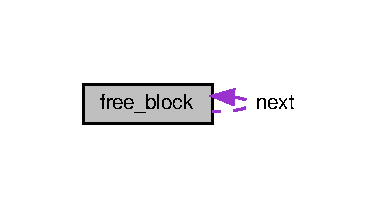
\includegraphics[width=182pt]{structfree__block__coll__graph}
\end{center}
\end{figure}
\subsection*{Public Attributes}
\begin{DoxyCompactItemize}
\item 
int \hyperlink{structfree__block_aa316449bb65559a7a5e35f97c719022e}{size}
\item 
struct \hyperlink{structfree__block}{free\+\_\+block} $\ast$ \hyperlink{structfree__block_a9b209321b0d2d74936310fac046be7b5}{next}
\end{DoxyCompactItemize}


\subsection{Member Data Documentation}
\mbox{\Hypertarget{structfree__block_a9b209321b0d2d74936310fac046be7b5}\label{structfree__block_a9b209321b0d2d74936310fac046be7b5}} 
\index{free\+\_\+block@{free\+\_\+block}!next@{next}}
\index{next@{next}!free\+\_\+block@{free\+\_\+block}}
\subsubsection{\texorpdfstring{next}{next}}
{\footnotesize\ttfamily struct \hyperlink{structfree__block}{free\+\_\+block}$\ast$ free\+\_\+block\+::next}

\mbox{\Hypertarget{structfree__block_aa316449bb65559a7a5e35f97c719022e}\label{structfree__block_aa316449bb65559a7a5e35f97c719022e}} 
\index{free\+\_\+block@{free\+\_\+block}!size@{size}}
\index{size@{size}!free\+\_\+block@{free\+\_\+block}}
\subsubsection{\texorpdfstring{size}{size}}
{\footnotesize\ttfamily int free\+\_\+block\+::size}



The documentation for this struct was generated from the following file\+:\begin{DoxyCompactItemize}
\item 
macrobench/system/\hyperlink{mem__alloc_8h}{mem\+\_\+alloc.\+h}\end{DoxyCompactItemize}

\hypertarget{structglobals__t}{}\section{globals\+\_\+t$<$ Key\+GenT $>$ Struct Template Reference}
\label{structglobals__t}\index{globals\+\_\+t$<$ Key\+Gen\+T $>$@{globals\+\_\+t$<$ Key\+Gen\+T $>$}}


Collaboration diagram for globals\+\_\+t$<$ Key\+GenT $>$\+:
\nopagebreak
\begin{figure}[H]
\begin{center}
\leavevmode
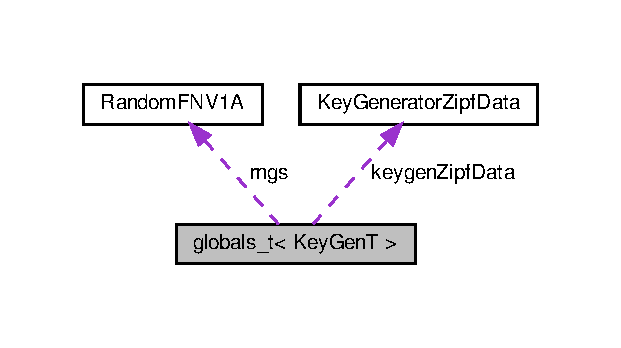
\includegraphics[width=298pt]{structglobals__t__coll__graph}
\end{center}
\end{figure}
\subsection*{Public Member Functions}
\begin{DoxyCompactItemize}
\item 
\hyperlink{structglobals__t_a9945f1a7246ff54f3279e94036886c0d}{globals\+\_\+t} (size\+\_\+t maxkey\+To\+Generate, \hyperlink{microbench_2main_8cpp_a96b004c35a7c82b13c4ac31635a5ba6a}{Key\+Generator\+Distribution} distribution)
\item 
\hyperlink{structglobals__t_a8525f6c198268c6bc418ef030be994dd}{$\sim$globals\+\_\+t} ()
\end{DoxyCompactItemize}
\subsection*{Public Attributes}
\begin{DoxyCompactItemize}
\item 
\hyperlink{structglobals__t_a5452bbdfd5d85691f8f0d5b5ed091b9f}{P\+AD}
\item 
void $\ast$const \hyperlink{structglobals__t_a90159d9a317687abab232e1fda728f1a}{N\+O\+\_\+\+V\+A\+L\+UE}
\item 
const \hyperlink{microbench_2main_8cpp_a8c96a4eb128cbef9f7b7aa2f7533202f}{test\+\_\+type} \hyperlink{structglobals__t_a6025a17c21db364b4d05b63db453e7c7}{K\+E\+Y\+\_\+\+M\+IN}
\item 
const \hyperlink{microbench_2main_8cpp_a8c96a4eb128cbef9f7b7aa2f7533202f}{test\+\_\+type} \hyperlink{structglobals__t_ad8295a990809a58e6923bed1538ccb07}{K\+E\+Y\+\_\+\+M\+AX}
\item 
const long long \hyperlink{structglobals__t_a8916405ce0fc26eb6dfc3afa1e5ed249}{P\+R\+E\+F\+I\+L\+L\+\_\+\+I\+N\+T\+E\+R\+V\+A\+L\+\_\+\+M\+I\+L\+L\+IS}
\item 
long \hyperlink{structglobals__t_aa9724d3aea293ee3211f08cb1aa3d34e}{elapsed\+Millis}
\item 
long long \hyperlink{structglobals__t_a16f3cc1c4f5866cf4bf88758eb08c6e1}{prefill\+Key\+Sum}
\item 
long long \hyperlink{structglobals__t_a856f41e115dc0592310c05f149fb1a9f}{prefill\+Size}
\item 
std\+::chrono\+::time\+\_\+point$<$ std\+::chrono\+::high\+\_\+resolution\+\_\+clock $>$ \hyperlink{structglobals__t_a28d2a4525bd82f81cbca8236c3ba1ec7}{program\+Execution\+Start\+Time}
\item 
std\+::chrono\+::time\+\_\+point$<$ std\+::chrono\+::high\+\_\+resolution\+\_\+clock $>$ \hyperlink{structglobals__t_a4e6d795a5fd1a12435a22b57264cee82}{end\+Time}
\item 
std\+::chrono\+::time\+\_\+point$<$ std\+::chrono\+::high\+\_\+resolution\+\_\+clock $>$ \hyperlink{structglobals__t_a3585908ff51ae63a70f0db1fccb520ae}{start\+Time}
\item 
long long \hyperlink{structglobals__t_a2b5c5db84f6abc24cdc5d752984be6eb}{start\+Clock\+Ticks}
\item 
long \hyperlink{structglobals__t_a8c6edcc8b8cfd88acd7ad869f8ac446b}{elapsed\+Millis\+Napping}
\item 
volatile long long \hyperlink{structglobals__t_a9fe50e0b2d9933d00c4ad9a2212581fa}{prefill\+Interval\+Elapsed\+Millis}
\item 
std\+::chrono\+::time\+\_\+point$<$ std\+::chrono\+::high\+\_\+resolution\+\_\+clock $>$ \hyperlink{structglobals__t_ae80a96264222a4691ebec8cf56b200e5}{prefill\+Start\+Time}
\item 
volatile \hyperlink{microbench_2main_8cpp_a8c96a4eb128cbef9f7b7aa2f7533202f}{test\+\_\+type} \hyperlink{structglobals__t_ab2923d797e57d4f17d10eb0ecb8b5b3d}{garbage}
\item 
\hyperlink{microbench_2main_8cpp_ad1d56d4b6df42b94c7525e7c4559d700}{D\+S\+\_\+\+A\+D\+A\+P\+T\+E\+R\+\_\+T} $\ast$ \hyperlink{structglobals__t_a481d3a5120349414f793ac72e391a36e}{ds\+Adapter}
\item 
\hyperlink{classKeyGeneratorZipfData}{Key\+Generator\+Zipf\+Data} $\ast$ \hyperlink{structglobals__t_a38304d0125e69f6142752f3274343976}{keygen\+Zipf\+Data}
\item 
Key\+GenT $\ast$ \hyperlink{structglobals__t_a542bf0080db5994c5dca6985b37df24c}{keygens} \mbox{[}\hyperlink{plaf_8h_ac1585a3455dd3e33e877e588be9e466b}{M\+A\+X\+\_\+\+T\+H\+R\+E\+A\+D\+S\+\_\+\+P\+O\+W2}\mbox{]}
\item 
\hyperlink{classRandomFNV1A}{Random\+F\+N\+V1A} \hyperlink{structglobals__t_a4410c337060e0d0b9dd3821b2cbdf3c9}{rngs} \mbox{[}\hyperlink{plaf_8h_ac1585a3455dd3e33e877e588be9e466b}{M\+A\+X\+\_\+\+T\+H\+R\+E\+A\+D\+S\+\_\+\+P\+O\+W2}\mbox{]}
\item 
volatile bool \hyperlink{structglobals__t_a8116065e907a3ac2c87229e167ad76fd}{start}
\item 
volatile bool \hyperlink{structglobals__t_acff1b66760476ec1d523e374c616824d}{done}
\item 
volatile int \hyperlink{structglobals__t_a8d2f88e1ba5301193c217fcd2bd4e7dd}{running}
\end{DoxyCompactItemize}


\subsection{Constructor \& Destructor Documentation}
\mbox{\Hypertarget{structglobals__t_a9945f1a7246ff54f3279e94036886c0d}\label{structglobals__t_a9945f1a7246ff54f3279e94036886c0d}} 
\index{globals\+\_\+t@{globals\+\_\+t}!globals\+\_\+t@{globals\+\_\+t}}
\index{globals\+\_\+t@{globals\+\_\+t}!globals\+\_\+t@{globals\+\_\+t}}
\subsubsection{\texorpdfstring{globals\+\_\+t()}{globals\_t()}}
{\footnotesize\ttfamily template$<$class Key\+GenT $>$ \\
\hyperlink{structglobals__t}{globals\+\_\+t}$<$ Key\+GenT $>$\+::\hyperlink{structglobals__t}{globals\+\_\+t} (\begin{DoxyParamCaption}\item[{size\+\_\+t}]{maxkey\+To\+Generate,  }\item[{\hyperlink{microbench_2main_8cpp_a96b004c35a7c82b13c4ac31635a5ba6a}{Key\+Generator\+Distribution}}]{distribution }\end{DoxyParamCaption})\hspace{0.3cm}{\ttfamily [inline]}}

\mbox{\Hypertarget{structglobals__t_a8525f6c198268c6bc418ef030be994dd}\label{structglobals__t_a8525f6c198268c6bc418ef030be994dd}} 
\index{globals\+\_\+t@{globals\+\_\+t}!````~globals\+\_\+t@{$\sim$globals\+\_\+t}}
\index{````~globals\+\_\+t@{$\sim$globals\+\_\+t}!globals\+\_\+t@{globals\+\_\+t}}
\subsubsection{\texorpdfstring{$\sim$globals\+\_\+t()}{~globals\_t()}}
{\footnotesize\ttfamily template$<$class Key\+GenT $>$ \\
\hyperlink{structglobals__t}{globals\+\_\+t}$<$ Key\+GenT $>$\+::$\sim$\hyperlink{structglobals__t}{globals\+\_\+t} (\begin{DoxyParamCaption}{ }\end{DoxyParamCaption})\hspace{0.3cm}{\ttfamily [inline]}}



\subsection{Member Data Documentation}
\mbox{\Hypertarget{structglobals__t_acff1b66760476ec1d523e374c616824d}\label{structglobals__t_acff1b66760476ec1d523e374c616824d}} 
\index{globals\+\_\+t@{globals\+\_\+t}!done@{done}}
\index{done@{done}!globals\+\_\+t@{globals\+\_\+t}}
\subsubsection{\texorpdfstring{done}{done}}
{\footnotesize\ttfamily template$<$class Key\+GenT $>$ \\
volatile bool \hyperlink{structglobals__t}{globals\+\_\+t}$<$ Key\+GenT $>$\+::done}

\mbox{\Hypertarget{structglobals__t_a481d3a5120349414f793ac72e391a36e}\label{structglobals__t_a481d3a5120349414f793ac72e391a36e}} 
\index{globals\+\_\+t@{globals\+\_\+t}!ds\+Adapter@{ds\+Adapter}}
\index{ds\+Adapter@{ds\+Adapter}!globals\+\_\+t@{globals\+\_\+t}}
\subsubsection{\texorpdfstring{ds\+Adapter}{dsAdapter}}
{\footnotesize\ttfamily template$<$class Key\+GenT $>$ \\
\hyperlink{microbench_2main_8cpp_ad1d56d4b6df42b94c7525e7c4559d700}{D\+S\+\_\+\+A\+D\+A\+P\+T\+E\+R\+\_\+T}$\ast$ \hyperlink{structglobals__t}{globals\+\_\+t}$<$ Key\+GenT $>$\+::ds\+Adapter}

\mbox{\Hypertarget{structglobals__t_aa9724d3aea293ee3211f08cb1aa3d34e}\label{structglobals__t_aa9724d3aea293ee3211f08cb1aa3d34e}} 
\index{globals\+\_\+t@{globals\+\_\+t}!elapsed\+Millis@{elapsed\+Millis}}
\index{elapsed\+Millis@{elapsed\+Millis}!globals\+\_\+t@{globals\+\_\+t}}
\subsubsection{\texorpdfstring{elapsed\+Millis}{elapsedMillis}}
{\footnotesize\ttfamily template$<$class Key\+GenT $>$ \\
long \hyperlink{structglobals__t}{globals\+\_\+t}$<$ Key\+GenT $>$\+::elapsed\+Millis}

\mbox{\Hypertarget{structglobals__t_a8c6edcc8b8cfd88acd7ad869f8ac446b}\label{structglobals__t_a8c6edcc8b8cfd88acd7ad869f8ac446b}} 
\index{globals\+\_\+t@{globals\+\_\+t}!elapsed\+Millis\+Napping@{elapsed\+Millis\+Napping}}
\index{elapsed\+Millis\+Napping@{elapsed\+Millis\+Napping}!globals\+\_\+t@{globals\+\_\+t}}
\subsubsection{\texorpdfstring{elapsed\+Millis\+Napping}{elapsedMillisNapping}}
{\footnotesize\ttfamily template$<$class Key\+GenT $>$ \\
long \hyperlink{structglobals__t}{globals\+\_\+t}$<$ Key\+GenT $>$\+::elapsed\+Millis\+Napping}

\mbox{\Hypertarget{structglobals__t_a4e6d795a5fd1a12435a22b57264cee82}\label{structglobals__t_a4e6d795a5fd1a12435a22b57264cee82}} 
\index{globals\+\_\+t@{globals\+\_\+t}!end\+Time@{end\+Time}}
\index{end\+Time@{end\+Time}!globals\+\_\+t@{globals\+\_\+t}}
\subsubsection{\texorpdfstring{end\+Time}{endTime}}
{\footnotesize\ttfamily template$<$class Key\+GenT $>$ \\
std\+::chrono\+::time\+\_\+point$<$std\+::chrono\+::high\+\_\+resolution\+\_\+clock$>$ \hyperlink{structglobals__t}{globals\+\_\+t}$<$ Key\+GenT $>$\+::end\+Time}

\mbox{\Hypertarget{structglobals__t_ab2923d797e57d4f17d10eb0ecb8b5b3d}\label{structglobals__t_ab2923d797e57d4f17d10eb0ecb8b5b3d}} 
\index{globals\+\_\+t@{globals\+\_\+t}!garbage@{garbage}}
\index{garbage@{garbage}!globals\+\_\+t@{globals\+\_\+t}}
\subsubsection{\texorpdfstring{garbage}{garbage}}
{\footnotesize\ttfamily template$<$class Key\+GenT $>$ \\
volatile \hyperlink{microbench_2main_8cpp_a8c96a4eb128cbef9f7b7aa2f7533202f}{test\+\_\+type} \hyperlink{structglobals__t}{globals\+\_\+t}$<$ Key\+GenT $>$\+::garbage}

\mbox{\Hypertarget{structglobals__t_ad8295a990809a58e6923bed1538ccb07}\label{structglobals__t_ad8295a990809a58e6923bed1538ccb07}} 
\index{globals\+\_\+t@{globals\+\_\+t}!K\+E\+Y\+\_\+\+M\+AX@{K\+E\+Y\+\_\+\+M\+AX}}
\index{K\+E\+Y\+\_\+\+M\+AX@{K\+E\+Y\+\_\+\+M\+AX}!globals\+\_\+t@{globals\+\_\+t}}
\subsubsection{\texorpdfstring{K\+E\+Y\+\_\+\+M\+AX}{KEY\_MAX}}
{\footnotesize\ttfamily template$<$class Key\+GenT $>$ \\
const \hyperlink{microbench_2main_8cpp_a8c96a4eb128cbef9f7b7aa2f7533202f}{test\+\_\+type} \hyperlink{structglobals__t}{globals\+\_\+t}$<$ Key\+GenT $>$\+::K\+E\+Y\+\_\+\+M\+AX}

\mbox{\Hypertarget{structglobals__t_a6025a17c21db364b4d05b63db453e7c7}\label{structglobals__t_a6025a17c21db364b4d05b63db453e7c7}} 
\index{globals\+\_\+t@{globals\+\_\+t}!K\+E\+Y\+\_\+\+M\+IN@{K\+E\+Y\+\_\+\+M\+IN}}
\index{K\+E\+Y\+\_\+\+M\+IN@{K\+E\+Y\+\_\+\+M\+IN}!globals\+\_\+t@{globals\+\_\+t}}
\subsubsection{\texorpdfstring{K\+E\+Y\+\_\+\+M\+IN}{KEY\_MIN}}
{\footnotesize\ttfamily template$<$class Key\+GenT $>$ \\
const \hyperlink{microbench_2main_8cpp_a8c96a4eb128cbef9f7b7aa2f7533202f}{test\+\_\+type} \hyperlink{structglobals__t}{globals\+\_\+t}$<$ Key\+GenT $>$\+::K\+E\+Y\+\_\+\+M\+IN}

\mbox{\Hypertarget{structglobals__t_a542bf0080db5994c5dca6985b37df24c}\label{structglobals__t_a542bf0080db5994c5dca6985b37df24c}} 
\index{globals\+\_\+t@{globals\+\_\+t}!keygens@{keygens}}
\index{keygens@{keygens}!globals\+\_\+t@{globals\+\_\+t}}
\subsubsection{\texorpdfstring{keygens}{keygens}}
{\footnotesize\ttfamily template$<$class Key\+GenT $>$ \\
Key\+GenT$\ast$ \hyperlink{structglobals__t}{globals\+\_\+t}$<$ Key\+GenT $>$\+::keygens\mbox{[}\hyperlink{plaf_8h_ac1585a3455dd3e33e877e588be9e466b}{M\+A\+X\+\_\+\+T\+H\+R\+E\+A\+D\+S\+\_\+\+P\+O\+W2}\mbox{]}}

\mbox{\Hypertarget{structglobals__t_a38304d0125e69f6142752f3274343976}\label{structglobals__t_a38304d0125e69f6142752f3274343976}} 
\index{globals\+\_\+t@{globals\+\_\+t}!keygen\+Zipf\+Data@{keygen\+Zipf\+Data}}
\index{keygen\+Zipf\+Data@{keygen\+Zipf\+Data}!globals\+\_\+t@{globals\+\_\+t}}
\subsubsection{\texorpdfstring{keygen\+Zipf\+Data}{keygenZipfData}}
{\footnotesize\ttfamily template$<$class Key\+GenT $>$ \\
\hyperlink{classKeyGeneratorZipfData}{Key\+Generator\+Zipf\+Data}$\ast$ \hyperlink{structglobals__t}{globals\+\_\+t}$<$ Key\+GenT $>$\+::keygen\+Zipf\+Data}

\mbox{\Hypertarget{structglobals__t_a90159d9a317687abab232e1fda728f1a}\label{structglobals__t_a90159d9a317687abab232e1fda728f1a}} 
\index{globals\+\_\+t@{globals\+\_\+t}!N\+O\+\_\+\+V\+A\+L\+UE@{N\+O\+\_\+\+V\+A\+L\+UE}}
\index{N\+O\+\_\+\+V\+A\+L\+UE@{N\+O\+\_\+\+V\+A\+L\+UE}!globals\+\_\+t@{globals\+\_\+t}}
\subsubsection{\texorpdfstring{N\+O\+\_\+\+V\+A\+L\+UE}{NO\_VALUE}}
{\footnotesize\ttfamily template$<$class Key\+GenT $>$ \\
void$\ast$ const \hyperlink{structglobals__t}{globals\+\_\+t}$<$ Key\+GenT $>$\+::N\+O\+\_\+\+V\+A\+L\+UE}

\mbox{\Hypertarget{structglobals__t_a5452bbdfd5d85691f8f0d5b5ed091b9f}\label{structglobals__t_a5452bbdfd5d85691f8f0d5b5ed091b9f}} 
\index{globals\+\_\+t@{globals\+\_\+t}!P\+AD@{P\+AD}}
\index{P\+AD@{P\+AD}!globals\+\_\+t@{globals\+\_\+t}}
\subsubsection{\texorpdfstring{P\+AD}{PAD}}
{\footnotesize\ttfamily template$<$class Key\+GenT $>$ \\
\hyperlink{structglobals__t}{globals\+\_\+t}$<$ Key\+GenT $>$\+::P\+AD}

\mbox{\Hypertarget{structglobals__t_a8916405ce0fc26eb6dfc3afa1e5ed249}\label{structglobals__t_a8916405ce0fc26eb6dfc3afa1e5ed249}} 
\index{globals\+\_\+t@{globals\+\_\+t}!P\+R\+E\+F\+I\+L\+L\+\_\+\+I\+N\+T\+E\+R\+V\+A\+L\+\_\+\+M\+I\+L\+L\+IS@{P\+R\+E\+F\+I\+L\+L\+\_\+\+I\+N\+T\+E\+R\+V\+A\+L\+\_\+\+M\+I\+L\+L\+IS}}
\index{P\+R\+E\+F\+I\+L\+L\+\_\+\+I\+N\+T\+E\+R\+V\+A\+L\+\_\+\+M\+I\+L\+L\+IS@{P\+R\+E\+F\+I\+L\+L\+\_\+\+I\+N\+T\+E\+R\+V\+A\+L\+\_\+\+M\+I\+L\+L\+IS}!globals\+\_\+t@{globals\+\_\+t}}
\subsubsection{\texorpdfstring{P\+R\+E\+F\+I\+L\+L\+\_\+\+I\+N\+T\+E\+R\+V\+A\+L\+\_\+\+M\+I\+L\+L\+IS}{PREFILL\_INTERVAL\_MILLIS}}
{\footnotesize\ttfamily template$<$class Key\+GenT $>$ \\
const long long \hyperlink{structglobals__t}{globals\+\_\+t}$<$ Key\+GenT $>$\+::P\+R\+E\+F\+I\+L\+L\+\_\+\+I\+N\+T\+E\+R\+V\+A\+L\+\_\+\+M\+I\+L\+L\+IS}

\mbox{\Hypertarget{structglobals__t_a9fe50e0b2d9933d00c4ad9a2212581fa}\label{structglobals__t_a9fe50e0b2d9933d00c4ad9a2212581fa}} 
\index{globals\+\_\+t@{globals\+\_\+t}!prefill\+Interval\+Elapsed\+Millis@{prefill\+Interval\+Elapsed\+Millis}}
\index{prefill\+Interval\+Elapsed\+Millis@{prefill\+Interval\+Elapsed\+Millis}!globals\+\_\+t@{globals\+\_\+t}}
\subsubsection{\texorpdfstring{prefill\+Interval\+Elapsed\+Millis}{prefillIntervalElapsedMillis}}
{\footnotesize\ttfamily template$<$class Key\+GenT $>$ \\
volatile long long \hyperlink{structglobals__t}{globals\+\_\+t}$<$ Key\+GenT $>$\+::prefill\+Interval\+Elapsed\+Millis}

\mbox{\Hypertarget{structglobals__t_a16f3cc1c4f5866cf4bf88758eb08c6e1}\label{structglobals__t_a16f3cc1c4f5866cf4bf88758eb08c6e1}} 
\index{globals\+\_\+t@{globals\+\_\+t}!prefill\+Key\+Sum@{prefill\+Key\+Sum}}
\index{prefill\+Key\+Sum@{prefill\+Key\+Sum}!globals\+\_\+t@{globals\+\_\+t}}
\subsubsection{\texorpdfstring{prefill\+Key\+Sum}{prefillKeySum}}
{\footnotesize\ttfamily template$<$class Key\+GenT $>$ \\
long long \hyperlink{structglobals__t}{globals\+\_\+t}$<$ Key\+GenT $>$\+::prefill\+Key\+Sum}

\mbox{\Hypertarget{structglobals__t_a856f41e115dc0592310c05f149fb1a9f}\label{structglobals__t_a856f41e115dc0592310c05f149fb1a9f}} 
\index{globals\+\_\+t@{globals\+\_\+t}!prefill\+Size@{prefill\+Size}}
\index{prefill\+Size@{prefill\+Size}!globals\+\_\+t@{globals\+\_\+t}}
\subsubsection{\texorpdfstring{prefill\+Size}{prefillSize}}
{\footnotesize\ttfamily template$<$class Key\+GenT $>$ \\
long long \hyperlink{structglobals__t}{globals\+\_\+t}$<$ Key\+GenT $>$\+::prefill\+Size}

\mbox{\Hypertarget{structglobals__t_ae80a96264222a4691ebec8cf56b200e5}\label{structglobals__t_ae80a96264222a4691ebec8cf56b200e5}} 
\index{globals\+\_\+t@{globals\+\_\+t}!prefill\+Start\+Time@{prefill\+Start\+Time}}
\index{prefill\+Start\+Time@{prefill\+Start\+Time}!globals\+\_\+t@{globals\+\_\+t}}
\subsubsection{\texorpdfstring{prefill\+Start\+Time}{prefillStartTime}}
{\footnotesize\ttfamily template$<$class Key\+GenT $>$ \\
std\+::chrono\+::time\+\_\+point$<$std\+::chrono\+::high\+\_\+resolution\+\_\+clock$>$ \hyperlink{structglobals__t}{globals\+\_\+t}$<$ Key\+GenT $>$\+::prefill\+Start\+Time}

\mbox{\Hypertarget{structglobals__t_a28d2a4525bd82f81cbca8236c3ba1ec7}\label{structglobals__t_a28d2a4525bd82f81cbca8236c3ba1ec7}} 
\index{globals\+\_\+t@{globals\+\_\+t}!program\+Execution\+Start\+Time@{program\+Execution\+Start\+Time}}
\index{program\+Execution\+Start\+Time@{program\+Execution\+Start\+Time}!globals\+\_\+t@{globals\+\_\+t}}
\subsubsection{\texorpdfstring{program\+Execution\+Start\+Time}{programExecutionStartTime}}
{\footnotesize\ttfamily template$<$class Key\+GenT $>$ \\
std\+::chrono\+::time\+\_\+point$<$std\+::chrono\+::high\+\_\+resolution\+\_\+clock$>$ \hyperlink{structglobals__t}{globals\+\_\+t}$<$ Key\+GenT $>$\+::program\+Execution\+Start\+Time}

\mbox{\Hypertarget{structglobals__t_a4410c337060e0d0b9dd3821b2cbdf3c9}\label{structglobals__t_a4410c337060e0d0b9dd3821b2cbdf3c9}} 
\index{globals\+\_\+t@{globals\+\_\+t}!rngs@{rngs}}
\index{rngs@{rngs}!globals\+\_\+t@{globals\+\_\+t}}
\subsubsection{\texorpdfstring{rngs}{rngs}}
{\footnotesize\ttfamily template$<$class Key\+GenT $>$ \\
\hyperlink{classRandomFNV1A}{Random\+F\+N\+V1A} \hyperlink{structglobals__t}{globals\+\_\+t}$<$ Key\+GenT $>$\+::rngs\mbox{[}\hyperlink{plaf_8h_ac1585a3455dd3e33e877e588be9e466b}{M\+A\+X\+\_\+\+T\+H\+R\+E\+A\+D\+S\+\_\+\+P\+O\+W2}\mbox{]}}

\mbox{\Hypertarget{structglobals__t_a8d2f88e1ba5301193c217fcd2bd4e7dd}\label{structglobals__t_a8d2f88e1ba5301193c217fcd2bd4e7dd}} 
\index{globals\+\_\+t@{globals\+\_\+t}!running@{running}}
\index{running@{running}!globals\+\_\+t@{globals\+\_\+t}}
\subsubsection{\texorpdfstring{running}{running}}
{\footnotesize\ttfamily template$<$class Key\+GenT $>$ \\
volatile int \hyperlink{structglobals__t}{globals\+\_\+t}$<$ Key\+GenT $>$\+::running}

\mbox{\Hypertarget{structglobals__t_a8116065e907a3ac2c87229e167ad76fd}\label{structglobals__t_a8116065e907a3ac2c87229e167ad76fd}} 
\index{globals\+\_\+t@{globals\+\_\+t}!start@{start}}
\index{start@{start}!globals\+\_\+t@{globals\+\_\+t}}
\subsubsection{\texorpdfstring{start}{start}}
{\footnotesize\ttfamily template$<$class Key\+GenT $>$ \\
volatile bool \hyperlink{structglobals__t}{globals\+\_\+t}$<$ Key\+GenT $>$\+::start}

\mbox{\Hypertarget{structglobals__t_a2b5c5db84f6abc24cdc5d752984be6eb}\label{structglobals__t_a2b5c5db84f6abc24cdc5d752984be6eb}} 
\index{globals\+\_\+t@{globals\+\_\+t}!start\+Clock\+Ticks@{start\+Clock\+Ticks}}
\index{start\+Clock\+Ticks@{start\+Clock\+Ticks}!globals\+\_\+t@{globals\+\_\+t}}
\subsubsection{\texorpdfstring{start\+Clock\+Ticks}{startClockTicks}}
{\footnotesize\ttfamily template$<$class Key\+GenT $>$ \\
long long \hyperlink{structglobals__t}{globals\+\_\+t}$<$ Key\+GenT $>$\+::start\+Clock\+Ticks}

\mbox{\Hypertarget{structglobals__t_a3585908ff51ae63a70f0db1fccb520ae}\label{structglobals__t_a3585908ff51ae63a70f0db1fccb520ae}} 
\index{globals\+\_\+t@{globals\+\_\+t}!start\+Time@{start\+Time}}
\index{start\+Time@{start\+Time}!globals\+\_\+t@{globals\+\_\+t}}
\subsubsection{\texorpdfstring{start\+Time}{startTime}}
{\footnotesize\ttfamily template$<$class Key\+GenT $>$ \\
std\+::chrono\+::time\+\_\+point$<$std\+::chrono\+::high\+\_\+resolution\+\_\+clock$>$ \hyperlink{structglobals__t}{globals\+\_\+t}$<$ Key\+GenT $>$\+::start\+Time}



The documentation for this struct was generated from the following file\+:\begin{DoxyCompactItemize}
\item 
microbench/\hyperlink{microbench_2main_8cpp}{main.\+cpp}\end{DoxyCompactItemize}

\hypertarget{classgstats__output__item}{}\section{gstats\+\_\+output\+\_\+item Class Reference}
\label{classgstats__output__item}\index{gstats\+\_\+output\+\_\+item@{gstats\+\_\+output\+\_\+item}}


{\ttfamily \#include $<$gstats.\+h$>$}

\subsection*{Public Member Functions}
\begin{DoxyCompactItemize}
\item 
\hyperlink{classgstats__output__item_aba1918b48bf95a14c7763e51566b6f38}{gstats\+\_\+output\+\_\+item} (\hyperlink{gstats_8h_a69c3463fdd73c04b651dbfcc1425650f}{gstats\+\_\+enum\+\_\+output\+\_\+method} \hyperlink{classgstats__output__item_a8c7b5166d5abe06e5e85d6acfdffb1f8}{method}, \hyperlink{gstats_8h_aa5e4744ebbda83fd3ef2ae3226461ac3}{gstats\+\_\+enum\+\_\+aggregation\+\_\+function} \hyperlink{classgstats__output__item_ad6e18ed2e1f2548806f9e7aeec9d6163}{func}, \hyperlink{gstats_8h_a625875e2a7c8582f278735673cfb398c}{gstats\+\_\+enum\+\_\+aggregation\+\_\+granularity} \hyperlink{classgstats__output__item_a30ab5df9d39a5149d2be27b242a0a63f}{granularity}, const int \hyperlink{classgstats__output__item_aa7b8faf49511b0a7cac1b2c9147780dc}{num\+\_\+buckets\+\_\+if\+\_\+histogram\+\_\+lin}=\hyperlink{gstats_8h_a1825fbb4f3d626ca97db468c8614e797}{G\+S\+T\+A\+T\+S\+\_\+\+D\+E\+F\+A\+U\+L\+T\+\_\+\+H\+I\+S\+T\+O\+G\+R\+A\+M\+\_\+\+L\+I\+N\+\_\+\+N\+U\+M\+\_\+\+B\+U\+C\+K\+E\+TS})
\end{DoxyCompactItemize}
\subsection*{Public Attributes}
\begin{DoxyCompactItemize}
\item 
\hyperlink{gstats_8h_a69c3463fdd73c04b651dbfcc1425650f}{gstats\+\_\+enum\+\_\+output\+\_\+method} \hyperlink{classgstats__output__item_a8c7b5166d5abe06e5e85d6acfdffb1f8}{method}
\item 
\hyperlink{gstats_8h_aa5e4744ebbda83fd3ef2ae3226461ac3}{gstats\+\_\+enum\+\_\+aggregation\+\_\+function} \hyperlink{classgstats__output__item_ad6e18ed2e1f2548806f9e7aeec9d6163}{func}
\item 
\hyperlink{gstats_8h_a625875e2a7c8582f278735673cfb398c}{gstats\+\_\+enum\+\_\+aggregation\+\_\+granularity} \hyperlink{classgstats__output__item_a30ab5df9d39a5149d2be27b242a0a63f}{granularity}
\item 
int \hyperlink{classgstats__output__item_aa7b8faf49511b0a7cac1b2c9147780dc}{num\+\_\+buckets\+\_\+if\+\_\+histogram\+\_\+lin}
\end{DoxyCompactItemize}


\subsection{Constructor \& Destructor Documentation}
\mbox{\Hypertarget{classgstats__output__item_aba1918b48bf95a14c7763e51566b6f38}\label{classgstats__output__item_aba1918b48bf95a14c7763e51566b6f38}} 
\index{gstats\+\_\+output\+\_\+item@{gstats\+\_\+output\+\_\+item}!gstats\+\_\+output\+\_\+item@{gstats\+\_\+output\+\_\+item}}
\index{gstats\+\_\+output\+\_\+item@{gstats\+\_\+output\+\_\+item}!gstats\+\_\+output\+\_\+item@{gstats\+\_\+output\+\_\+item}}
\subsubsection{\texorpdfstring{gstats\+\_\+output\+\_\+item()}{gstats\_output\_item()}}
{\footnotesize\ttfamily gstats\+\_\+output\+\_\+item\+::gstats\+\_\+output\+\_\+item (\begin{DoxyParamCaption}\item[{\hyperlink{gstats_8h_a69c3463fdd73c04b651dbfcc1425650f}{gstats\+\_\+enum\+\_\+output\+\_\+method}}]{method,  }\item[{\hyperlink{gstats_8h_aa5e4744ebbda83fd3ef2ae3226461ac3}{gstats\+\_\+enum\+\_\+aggregation\+\_\+function}}]{func,  }\item[{\hyperlink{gstats_8h_a625875e2a7c8582f278735673cfb398c}{gstats\+\_\+enum\+\_\+aggregation\+\_\+granularity}}]{granularity,  }\item[{const int}]{num\+\_\+buckets\+\_\+if\+\_\+histogram\+\_\+lin = {\ttfamily \hyperlink{gstats_8h_a1825fbb4f3d626ca97db468c8614e797}{G\+S\+T\+A\+T\+S\+\_\+\+D\+E\+F\+A\+U\+L\+T\+\_\+\+H\+I\+S\+T\+O\+G\+R\+A\+M\+\_\+\+L\+I\+N\+\_\+\+N\+U\+M\+\_\+\+B\+U\+C\+K\+E\+TS}} }\end{DoxyParamCaption})\hspace{0.3cm}{\ttfamily [inline]}}



\subsection{Member Data Documentation}
\mbox{\Hypertarget{classgstats__output__item_ad6e18ed2e1f2548806f9e7aeec9d6163}\label{classgstats__output__item_ad6e18ed2e1f2548806f9e7aeec9d6163}} 
\index{gstats\+\_\+output\+\_\+item@{gstats\+\_\+output\+\_\+item}!func@{func}}
\index{func@{func}!gstats\+\_\+output\+\_\+item@{gstats\+\_\+output\+\_\+item}}
\subsubsection{\texorpdfstring{func}{func}}
{\footnotesize\ttfamily \hyperlink{gstats_8h_aa5e4744ebbda83fd3ef2ae3226461ac3}{gstats\+\_\+enum\+\_\+aggregation\+\_\+function} gstats\+\_\+output\+\_\+item\+::func}

\mbox{\Hypertarget{classgstats__output__item_a30ab5df9d39a5149d2be27b242a0a63f}\label{classgstats__output__item_a30ab5df9d39a5149d2be27b242a0a63f}} 
\index{gstats\+\_\+output\+\_\+item@{gstats\+\_\+output\+\_\+item}!granularity@{granularity}}
\index{granularity@{granularity}!gstats\+\_\+output\+\_\+item@{gstats\+\_\+output\+\_\+item}}
\subsubsection{\texorpdfstring{granularity}{granularity}}
{\footnotesize\ttfamily \hyperlink{gstats_8h_a625875e2a7c8582f278735673cfb398c}{gstats\+\_\+enum\+\_\+aggregation\+\_\+granularity} gstats\+\_\+output\+\_\+item\+::granularity}

\mbox{\Hypertarget{classgstats__output__item_a8c7b5166d5abe06e5e85d6acfdffb1f8}\label{classgstats__output__item_a8c7b5166d5abe06e5e85d6acfdffb1f8}} 
\index{gstats\+\_\+output\+\_\+item@{gstats\+\_\+output\+\_\+item}!method@{method}}
\index{method@{method}!gstats\+\_\+output\+\_\+item@{gstats\+\_\+output\+\_\+item}}
\subsubsection{\texorpdfstring{method}{method}}
{\footnotesize\ttfamily \hyperlink{gstats_8h_a69c3463fdd73c04b651dbfcc1425650f}{gstats\+\_\+enum\+\_\+output\+\_\+method} gstats\+\_\+output\+\_\+item\+::method}

\mbox{\Hypertarget{classgstats__output__item_aa7b8faf49511b0a7cac1b2c9147780dc}\label{classgstats__output__item_aa7b8faf49511b0a7cac1b2c9147780dc}} 
\index{gstats\+\_\+output\+\_\+item@{gstats\+\_\+output\+\_\+item}!num\+\_\+buckets\+\_\+if\+\_\+histogram\+\_\+lin@{num\+\_\+buckets\+\_\+if\+\_\+histogram\+\_\+lin}}
\index{num\+\_\+buckets\+\_\+if\+\_\+histogram\+\_\+lin@{num\+\_\+buckets\+\_\+if\+\_\+histogram\+\_\+lin}!gstats\+\_\+output\+\_\+item@{gstats\+\_\+output\+\_\+item}}
\subsubsection{\texorpdfstring{num\+\_\+buckets\+\_\+if\+\_\+histogram\+\_\+lin}{num\_buckets\_if\_histogram\_lin}}
{\footnotesize\ttfamily int gstats\+\_\+output\+\_\+item\+::num\+\_\+buckets\+\_\+if\+\_\+histogram\+\_\+lin}



The documentation for this class was generated from the following file\+:\begin{DoxyCompactItemize}
\item 
common/\hyperlink{gstats_8h}{gstats.\+h}\end{DoxyCompactItemize}

\hypertarget{classgstats__t}{}\section{gstats\+\_\+t Class Reference}
\label{classgstats__t}\index{gstats\+\_\+t@{gstats\+\_\+t}}


{\ttfamily \#include $<$gstats.\+h$>$}

\subsection*{Classes}
\begin{DoxyCompactItemize}
\item 
struct \hyperlink{structgstats__t_1_1stat__metrics}{stat\+\_\+metrics}
\end{DoxyCompactItemize}
\subsection*{Public Member Functions}
\begin{DoxyCompactItemize}
\item 
\hyperlink{classgstats__t_a8799bbb87ebba7af97007a7774092518}{gstats\+\_\+t} (const int num\+\_\+processes)
\item 
\hyperlink{classgstats__t_a0638a31844fd63d17ba55d54d34e55af}{$\sim$gstats\+\_\+t} ()
\item 
{\footnotesize template$<$typename T $>$ }\\void \hyperlink{classgstats__t_a16f67bb2adcdeccd94669fcbfa86b9ff}{clear\+\_\+to\+\_\+value} (\hyperlink{gstats_8h_a662beb90f6d56f5ee9df4d812d39aa33}{gstats\+\_\+stat\+\_\+id} id, T value)
\item 
void \hyperlink{classgstats__t_a5f7327cd91575e8e07c913113e544021}{clear\+\_\+all} ()
\item 
\hyperlink{gstats_8h_a662beb90f6d56f5ee9df4d812d39aa33}{gstats\+\_\+stat\+\_\+id} \hyperlink{classgstats__t_a6f6442c5e217300004d009330f655d81}{create\+\_\+stat} (\hyperlink{gstats_8h_add042cd26594ae31bc443952e37d30f6}{gstats\+\_\+enum\+\_\+data\+\_\+type} datatype, std\+::string name, const int capacity, std\+::initializer\+\_\+list$<$ \hyperlink{classgstats__output__item}{gstats\+\_\+output\+\_\+item} $>$ gstats\+\_\+output\+\_\+items)
\item 
{\footnotesize template$<$typename T $>$ }\\T \hyperlink{classgstats__t_a2b601cbf9e9e71bd35ccf033c7cf2d47}{add\+\_\+stat} (const int \hyperlink{microbench_2main_8cpp_a9ca9869868fe7e7a38a921cc7de4103f}{tid}, const \hyperlink{gstats_8h_a662beb90f6d56f5ee9df4d812d39aa33}{gstats\+\_\+stat\+\_\+id} id, T value, const int index)
\item 
{\footnotesize template$<$typename T $>$ }\\T \hyperlink{classgstats__t_a39a2efb2cd4e874559dfd430dff841ae}{set\+\_\+stat} (const int \hyperlink{microbench_2main_8cpp_a9ca9869868fe7e7a38a921cc7de4103f}{tid}, const \hyperlink{gstats_8h_a662beb90f6d56f5ee9df4d812d39aa33}{gstats\+\_\+stat\+\_\+id} id, T value, const int index)
\item 
{\footnotesize template$<$typename T $>$ }\\T \hyperlink{classgstats__t_a448015c63c37f2d98f7026f2eb1454a1}{append\+\_\+stat} (const int \hyperlink{microbench_2main_8cpp_a9ca9869868fe7e7a38a921cc7de4103f}{tid}, const \hyperlink{gstats_8h_a662beb90f6d56f5ee9df4d812d39aa33}{gstats\+\_\+stat\+\_\+id} id, T value)
\item 
{\footnotesize template$<$typename T $>$ }\\T \hyperlink{classgstats__t_aa5de3ae993697b4520ed7916d3ee3373}{get\+\_\+stat} (const int \hyperlink{microbench_2main_8cpp_a9ca9869868fe7e7a38a921cc7de4103f}{tid}, const \hyperlink{gstats_8h_a662beb90f6d56f5ee9df4d812d39aa33}{gstats\+\_\+stat\+\_\+id} id, const int index)
\item 
{\footnotesize template$<$typename T $>$ }\\double \hyperlink{classgstats__t_a3529ce1c55852403a24c299625fcce20}{get\+\_\+sum} (const \hyperlink{gstats_8h_a662beb90f6d56f5ee9df4d812d39aa33}{gstats\+\_\+stat\+\_\+id} id)
\item 
{\footnotesize template$<$typename T $>$ }\\\hyperlink{structgstats__t_1_1stat__metrics}{stat\+\_\+metrics}$<$ T $>$ $\ast$ \hyperlink{classgstats__t_a9764e6abeef0768a6f992e5e05bb22cc}{compute\+\_\+stat\+\_\+metrics} (const \hyperlink{gstats_8h_a662beb90f6d56f5ee9df4d812d39aa33}{gstats\+\_\+stat\+\_\+id} id, \hyperlink{gstats_8h_a625875e2a7c8582f278735673cfb398c}{gstats\+\_\+enum\+\_\+aggregation\+\_\+granularity} granularity)
\item 
{\footnotesize template$<$typename T $>$ }\\void \hyperlink{classgstats__t_aa7a55d9e67eeff816ed6cafc3ead608f}{print\+\_\+stat} (const \hyperlink{gstats_8h_a662beb90f6d56f5ee9df4d812d39aa33}{gstats\+\_\+stat\+\_\+id} id, \hyperlink{classgstats__output__item}{gstats\+\_\+output\+\_\+item} \&output\+\_\+item)
\item 
void \hyperlink{classgstats__t_acf55dea2c0abe2dd5564f23a53c4fd15}{print\+\_\+all} ()
\end{DoxyCompactItemize}


\subsection{Constructor \& Destructor Documentation}
\mbox{\Hypertarget{classgstats__t_a8799bbb87ebba7af97007a7774092518}\label{classgstats__t_a8799bbb87ebba7af97007a7774092518}} 
\index{gstats\+\_\+t@{gstats\+\_\+t}!gstats\+\_\+t@{gstats\+\_\+t}}
\index{gstats\+\_\+t@{gstats\+\_\+t}!gstats\+\_\+t@{gstats\+\_\+t}}
\subsubsection{\texorpdfstring{gstats\+\_\+t()}{gstats\_t()}}
{\footnotesize\ttfamily gstats\+\_\+t\+::gstats\+\_\+t (\begin{DoxyParamCaption}\item[{const int}]{num\+\_\+processes }\end{DoxyParamCaption})\hspace{0.3cm}{\ttfamily [inline]}}

\mbox{\Hypertarget{classgstats__t_a0638a31844fd63d17ba55d54d34e55af}\label{classgstats__t_a0638a31844fd63d17ba55d54d34e55af}} 
\index{gstats\+\_\+t@{gstats\+\_\+t}!````~gstats\+\_\+t@{$\sim$gstats\+\_\+t}}
\index{````~gstats\+\_\+t@{$\sim$gstats\+\_\+t}!gstats\+\_\+t@{gstats\+\_\+t}}
\subsubsection{\texorpdfstring{$\sim$gstats\+\_\+t()}{~gstats\_t()}}
{\footnotesize\ttfamily gstats\+\_\+t\+::$\sim$gstats\+\_\+t (\begin{DoxyParamCaption}{ }\end{DoxyParamCaption})\hspace{0.3cm}{\ttfamily [inline]}}



\subsection{Member Function Documentation}
\mbox{\Hypertarget{classgstats__t_a2b601cbf9e9e71bd35ccf033c7cf2d47}\label{classgstats__t_a2b601cbf9e9e71bd35ccf033c7cf2d47}} 
\index{gstats\+\_\+t@{gstats\+\_\+t}!add\+\_\+stat@{add\+\_\+stat}}
\index{add\+\_\+stat@{add\+\_\+stat}!gstats\+\_\+t@{gstats\+\_\+t}}
\subsubsection{\texorpdfstring{add\+\_\+stat()}{add\_stat()}}
{\footnotesize\ttfamily template$<$typename T $>$ \\
T gstats\+\_\+t\+::add\+\_\+stat (\begin{DoxyParamCaption}\item[{const int}]{tid,  }\item[{const \hyperlink{gstats_8h_a662beb90f6d56f5ee9df4d812d39aa33}{gstats\+\_\+stat\+\_\+id}}]{id,  }\item[{T}]{value,  }\item[{const int}]{index }\end{DoxyParamCaption})\hspace{0.3cm}{\ttfamily [inline]}}

\mbox{\Hypertarget{classgstats__t_a448015c63c37f2d98f7026f2eb1454a1}\label{classgstats__t_a448015c63c37f2d98f7026f2eb1454a1}} 
\index{gstats\+\_\+t@{gstats\+\_\+t}!append\+\_\+stat@{append\+\_\+stat}}
\index{append\+\_\+stat@{append\+\_\+stat}!gstats\+\_\+t@{gstats\+\_\+t}}
\subsubsection{\texorpdfstring{append\+\_\+stat()}{append\_stat()}}
{\footnotesize\ttfamily template$<$typename T $>$ \\
T gstats\+\_\+t\+::append\+\_\+stat (\begin{DoxyParamCaption}\item[{const int}]{tid,  }\item[{const \hyperlink{gstats_8h_a662beb90f6d56f5ee9df4d812d39aa33}{gstats\+\_\+stat\+\_\+id}}]{id,  }\item[{T}]{value }\end{DoxyParamCaption})\hspace{0.3cm}{\ttfamily [inline]}}

\mbox{\Hypertarget{classgstats__t_a5f7327cd91575e8e07c913113e544021}\label{classgstats__t_a5f7327cd91575e8e07c913113e544021}} 
\index{gstats\+\_\+t@{gstats\+\_\+t}!clear\+\_\+all@{clear\+\_\+all}}
\index{clear\+\_\+all@{clear\+\_\+all}!gstats\+\_\+t@{gstats\+\_\+t}}
\subsubsection{\texorpdfstring{clear\+\_\+all()}{clear\_all()}}
{\footnotesize\ttfamily void gstats\+\_\+t\+::clear\+\_\+all (\begin{DoxyParamCaption}{ }\end{DoxyParamCaption})\hspace{0.3cm}{\ttfamily [inline]}}

\mbox{\Hypertarget{classgstats__t_a16f67bb2adcdeccd94669fcbfa86b9ff}\label{classgstats__t_a16f67bb2adcdeccd94669fcbfa86b9ff}} 
\index{gstats\+\_\+t@{gstats\+\_\+t}!clear\+\_\+to\+\_\+value@{clear\+\_\+to\+\_\+value}}
\index{clear\+\_\+to\+\_\+value@{clear\+\_\+to\+\_\+value}!gstats\+\_\+t@{gstats\+\_\+t}}
\subsubsection{\texorpdfstring{clear\+\_\+to\+\_\+value()}{clear\_to\_value()}}
{\footnotesize\ttfamily template$<$typename T $>$ \\
void gstats\+\_\+t\+::clear\+\_\+to\+\_\+value (\begin{DoxyParamCaption}\item[{\hyperlink{gstats_8h_a662beb90f6d56f5ee9df4d812d39aa33}{gstats\+\_\+stat\+\_\+id}}]{id,  }\item[{T}]{value }\end{DoxyParamCaption})\hspace{0.3cm}{\ttfamily [inline]}}

\mbox{\Hypertarget{classgstats__t_a9764e6abeef0768a6f992e5e05bb22cc}\label{classgstats__t_a9764e6abeef0768a6f992e5e05bb22cc}} 
\index{gstats\+\_\+t@{gstats\+\_\+t}!compute\+\_\+stat\+\_\+metrics@{compute\+\_\+stat\+\_\+metrics}}
\index{compute\+\_\+stat\+\_\+metrics@{compute\+\_\+stat\+\_\+metrics}!gstats\+\_\+t@{gstats\+\_\+t}}
\subsubsection{\texorpdfstring{compute\+\_\+stat\+\_\+metrics()}{compute\_stat\_metrics()}}
{\footnotesize\ttfamily template$<$typename T $>$ \\
\hyperlink{structgstats__t_1_1stat__metrics}{stat\+\_\+metrics}$<$T$>$$\ast$ gstats\+\_\+t\+::compute\+\_\+stat\+\_\+metrics (\begin{DoxyParamCaption}\item[{const \hyperlink{gstats_8h_a662beb90f6d56f5ee9df4d812d39aa33}{gstats\+\_\+stat\+\_\+id}}]{id,  }\item[{\hyperlink{gstats_8h_a625875e2a7c8582f278735673cfb398c}{gstats\+\_\+enum\+\_\+aggregation\+\_\+granularity}}]{granularity }\end{DoxyParamCaption})\hspace{0.3cm}{\ttfamily [inline]}}

\mbox{\Hypertarget{classgstats__t_a6f6442c5e217300004d009330f655d81}\label{classgstats__t_a6f6442c5e217300004d009330f655d81}} 
\index{gstats\+\_\+t@{gstats\+\_\+t}!create\+\_\+stat@{create\+\_\+stat}}
\index{create\+\_\+stat@{create\+\_\+stat}!gstats\+\_\+t@{gstats\+\_\+t}}
\subsubsection{\texorpdfstring{create\+\_\+stat()}{create\_stat()}}
{\footnotesize\ttfamily \hyperlink{gstats_8h_a662beb90f6d56f5ee9df4d812d39aa33}{gstats\+\_\+stat\+\_\+id} gstats\+\_\+t\+::create\+\_\+stat (\begin{DoxyParamCaption}\item[{\hyperlink{gstats_8h_add042cd26594ae31bc443952e37d30f6}{gstats\+\_\+enum\+\_\+data\+\_\+type}}]{datatype,  }\item[{std\+::string}]{name,  }\item[{const int}]{capacity,  }\item[{std\+::initializer\+\_\+list$<$ \hyperlink{classgstats__output__item}{gstats\+\_\+output\+\_\+item} $>$}]{gstats\+\_\+output\+\_\+items }\end{DoxyParamCaption})\hspace{0.3cm}{\ttfamily [inline]}}

\mbox{\Hypertarget{classgstats__t_aa5de3ae993697b4520ed7916d3ee3373}\label{classgstats__t_aa5de3ae993697b4520ed7916d3ee3373}} 
\index{gstats\+\_\+t@{gstats\+\_\+t}!get\+\_\+stat@{get\+\_\+stat}}
\index{get\+\_\+stat@{get\+\_\+stat}!gstats\+\_\+t@{gstats\+\_\+t}}
\subsubsection{\texorpdfstring{get\+\_\+stat()}{get\_stat()}}
{\footnotesize\ttfamily template$<$typename T $>$ \\
T gstats\+\_\+t\+::get\+\_\+stat (\begin{DoxyParamCaption}\item[{const int}]{tid,  }\item[{const \hyperlink{gstats_8h_a662beb90f6d56f5ee9df4d812d39aa33}{gstats\+\_\+stat\+\_\+id}}]{id,  }\item[{const int}]{index }\end{DoxyParamCaption})\hspace{0.3cm}{\ttfamily [inline]}}

\mbox{\Hypertarget{classgstats__t_a3529ce1c55852403a24c299625fcce20}\label{classgstats__t_a3529ce1c55852403a24c299625fcce20}} 
\index{gstats\+\_\+t@{gstats\+\_\+t}!get\+\_\+sum@{get\+\_\+sum}}
\index{get\+\_\+sum@{get\+\_\+sum}!gstats\+\_\+t@{gstats\+\_\+t}}
\subsubsection{\texorpdfstring{get\+\_\+sum()}{get\_sum()}}
{\footnotesize\ttfamily template$<$typename T $>$ \\
double gstats\+\_\+t\+::get\+\_\+sum (\begin{DoxyParamCaption}\item[{const \hyperlink{gstats_8h_a662beb90f6d56f5ee9df4d812d39aa33}{gstats\+\_\+stat\+\_\+id}}]{id }\end{DoxyParamCaption})\hspace{0.3cm}{\ttfamily [inline]}}

\mbox{\Hypertarget{classgstats__t_acf55dea2c0abe2dd5564f23a53c4fd15}\label{classgstats__t_acf55dea2c0abe2dd5564f23a53c4fd15}} 
\index{gstats\+\_\+t@{gstats\+\_\+t}!print\+\_\+all@{print\+\_\+all}}
\index{print\+\_\+all@{print\+\_\+all}!gstats\+\_\+t@{gstats\+\_\+t}}
\subsubsection{\texorpdfstring{print\+\_\+all()}{print\_all()}}
{\footnotesize\ttfamily void gstats\+\_\+t\+::print\+\_\+all (\begin{DoxyParamCaption}{ }\end{DoxyParamCaption})\hspace{0.3cm}{\ttfamily [inline]}}

\mbox{\Hypertarget{classgstats__t_aa7a55d9e67eeff816ed6cafc3ead608f}\label{classgstats__t_aa7a55d9e67eeff816ed6cafc3ead608f}} 
\index{gstats\+\_\+t@{gstats\+\_\+t}!print\+\_\+stat@{print\+\_\+stat}}
\index{print\+\_\+stat@{print\+\_\+stat}!gstats\+\_\+t@{gstats\+\_\+t}}
\subsubsection{\texorpdfstring{print\+\_\+stat()}{print\_stat()}}
{\footnotesize\ttfamily template$<$typename T $>$ \\
void gstats\+\_\+t\+::print\+\_\+stat (\begin{DoxyParamCaption}\item[{const \hyperlink{gstats_8h_a662beb90f6d56f5ee9df4d812d39aa33}{gstats\+\_\+stat\+\_\+id}}]{id,  }\item[{\hyperlink{classgstats__output__item}{gstats\+\_\+output\+\_\+item} \&}]{output\+\_\+item }\end{DoxyParamCaption})\hspace{0.3cm}{\ttfamily [inline]}}

\mbox{\Hypertarget{classgstats__t_a39a2efb2cd4e874559dfd430dff841ae}\label{classgstats__t_a39a2efb2cd4e874559dfd430dff841ae}} 
\index{gstats\+\_\+t@{gstats\+\_\+t}!set\+\_\+stat@{set\+\_\+stat}}
\index{set\+\_\+stat@{set\+\_\+stat}!gstats\+\_\+t@{gstats\+\_\+t}}
\subsubsection{\texorpdfstring{set\+\_\+stat()}{set\_stat()}}
{\footnotesize\ttfamily template$<$typename T $>$ \\
T gstats\+\_\+t\+::set\+\_\+stat (\begin{DoxyParamCaption}\item[{const int}]{tid,  }\item[{const \hyperlink{gstats_8h_a662beb90f6d56f5ee9df4d812d39aa33}{gstats\+\_\+stat\+\_\+id}}]{id,  }\item[{T}]{value,  }\item[{const int}]{index }\end{DoxyParamCaption})\hspace{0.3cm}{\ttfamily [inline]}}



The documentation for this class was generated from the following file\+:\begin{DoxyCompactItemize}
\item 
common/\hyperlink{gstats_8h}{gstats.\+h}\end{DoxyCompactItemize}

\hypertarget{classHashList}{}\section{Hash\+List$<$ T $>$ Class Template Reference}
\label{classHashList}\index{Hash\+List$<$ T $>$@{Hash\+List$<$ T $>$}}


{\ttfamily \#include $<$hashlist.\+h$>$}

\subsection*{Public Member Functions}
\begin{DoxyCompactItemize}
\item 
void \hyperlink{classHashList_a299a7932055966f85d934a62db7e7cc5}{init} (const long long initial\+Capacity\+Pow2)
\item 
void \hyperlink{classHashList_a8bff5ddb34944c843c908b77abf5aa32}{clear} ()
\item 
void \hyperlink{classHashList_a14a376c11ebe03a832d62ecf91c10560}{destroy} ()
\item 
bool \hyperlink{classHashList_af90d56617f493f45f687c461232b1cf7}{contains} (const T \&element)
\item 
void \hyperlink{classHashList_a64d7aa6809912d1cd7c4d9865d6a16ea}{insert} (const T \&element)
\item 
long long \hyperlink{classHashList_a94a4649ef9bdf27ccac0f6fc6da95334}{get\+Size} ()
\end{DoxyCompactItemize}


\subsection{Member Function Documentation}
\mbox{\Hypertarget{classHashList_a8bff5ddb34944c843c908b77abf5aa32}\label{classHashList_a8bff5ddb34944c843c908b77abf5aa32}} 
\index{Hash\+List@{Hash\+List}!clear@{clear}}
\index{clear@{clear}!Hash\+List@{Hash\+List}}
\subsubsection{\texorpdfstring{clear()}{clear()}}
{\footnotesize\ttfamily template$<$typename T$>$ \\
void \hyperlink{classHashList}{Hash\+List}$<$ T $>$\+::clear (\begin{DoxyParamCaption}{ }\end{DoxyParamCaption})\hspace{0.3cm}{\ttfamily [inline]}}

\mbox{\Hypertarget{classHashList_af90d56617f493f45f687c461232b1cf7}\label{classHashList_af90d56617f493f45f687c461232b1cf7}} 
\index{Hash\+List@{Hash\+List}!contains@{contains}}
\index{contains@{contains}!Hash\+List@{Hash\+List}}
\subsubsection{\texorpdfstring{contains()}{contains()}}
{\footnotesize\ttfamily template$<$typename T$>$ \\
bool \hyperlink{classHashList}{Hash\+List}$<$ T $>$\+::contains (\begin{DoxyParamCaption}\item[{const T \&}]{element }\end{DoxyParamCaption})\hspace{0.3cm}{\ttfamily [inline]}}

\mbox{\Hypertarget{classHashList_a14a376c11ebe03a832d62ecf91c10560}\label{classHashList_a14a376c11ebe03a832d62ecf91c10560}} 
\index{Hash\+List@{Hash\+List}!destroy@{destroy}}
\index{destroy@{destroy}!Hash\+List@{Hash\+List}}
\subsubsection{\texorpdfstring{destroy()}{destroy()}}
{\footnotesize\ttfamily template$<$typename T$>$ \\
void \hyperlink{classHashList}{Hash\+List}$<$ T $>$\+::destroy (\begin{DoxyParamCaption}{ }\end{DoxyParamCaption})\hspace{0.3cm}{\ttfamily [inline]}}

\mbox{\Hypertarget{classHashList_a94a4649ef9bdf27ccac0f6fc6da95334}\label{classHashList_a94a4649ef9bdf27ccac0f6fc6da95334}} 
\index{Hash\+List@{Hash\+List}!get\+Size@{get\+Size}}
\index{get\+Size@{get\+Size}!Hash\+List@{Hash\+List}}
\subsubsection{\texorpdfstring{get\+Size()}{getSize()}}
{\footnotesize\ttfamily template$<$typename T$>$ \\
long long \hyperlink{classHashList}{Hash\+List}$<$ T $>$\+::get\+Size (\begin{DoxyParamCaption}{ }\end{DoxyParamCaption})\hspace{0.3cm}{\ttfamily [inline]}}

\mbox{\Hypertarget{classHashList_a299a7932055966f85d934a62db7e7cc5}\label{classHashList_a299a7932055966f85d934a62db7e7cc5}} 
\index{Hash\+List@{Hash\+List}!init@{init}}
\index{init@{init}!Hash\+List@{Hash\+List}}
\subsubsection{\texorpdfstring{init()}{init()}}
{\footnotesize\ttfamily template$<$typename T$>$ \\
void \hyperlink{classHashList}{Hash\+List}$<$ T $>$\+::init (\begin{DoxyParamCaption}\item[{const long long}]{initial\+Capacity\+Pow2 }\end{DoxyParamCaption})\hspace{0.3cm}{\ttfamily [inline]}}

\mbox{\Hypertarget{classHashList_a64d7aa6809912d1cd7c4d9865d6a16ea}\label{classHashList_a64d7aa6809912d1cd7c4d9865d6a16ea}} 
\index{Hash\+List@{Hash\+List}!insert@{insert}}
\index{insert@{insert}!Hash\+List@{Hash\+List}}
\subsubsection{\texorpdfstring{insert()}{insert()}}
{\footnotesize\ttfamily template$<$typename T$>$ \\
void \hyperlink{classHashList}{Hash\+List}$<$ T $>$\+::insert (\begin{DoxyParamCaption}\item[{const T \&}]{element }\end{DoxyParamCaption})\hspace{0.3cm}{\ttfamily [inline]}}



The documentation for this class was generated from the following file\+:\begin{DoxyCompactItemize}
\item 
common/rq/\hyperlink{hashlist_8h}{hashlist.\+h}\end{DoxyCompactItemize}

\hypertarget{classhashset}{}\section{hashset$<$ K $>$ Class Template Reference}
\label{classhashset}\index{hashset$<$ K $>$@{hashset$<$ K $>$}}


{\ttfamily \#include $<$hashtable.\+h$>$}

\subsection*{Public Member Functions}
\begin{DoxyCompactItemize}
\item 
\hyperlink{classhashset_a58740226f56122a04eb1f5122b21dc28}{hashset} ()
\item 
\hyperlink{classhashset_a6dfea39f30e30519e3808ce3989dad10}{$\sim$hashset} ()
\item 
void \hyperlink{classhashset_a137e69aebc7f357881fac8adfef0e102}{clear} ()
\item 
bool \hyperlink{classhashset_af90785af306bbe96d2e07f8ad0842a06}{contains} (K $\ast$const key)
\item 
K $\ast$ \hyperlink{classhashset_aa19cc2749ccc333c0e5a7a0907ddaf68}{get} (K $\ast$const key)
\item 
void \hyperlink{classhashset_af64166df73b9d40ffca8c7ed131e849b}{insert} (K $\ast$const key)
\item 
void \hyperlink{classhashset_a4fe539e3a2242f64bf64df7b4a8aa105}{erase} (K $\ast$const key)
\end{DoxyCompactItemize}


\subsection{Constructor \& Destructor Documentation}
\mbox{\Hypertarget{classhashset_a58740226f56122a04eb1f5122b21dc28}\label{classhashset_a58740226f56122a04eb1f5122b21dc28}} 
\index{hashset@{hashset}!hashset@{hashset}}
\index{hashset@{hashset}!hashset@{hashset}}
\subsubsection{\texorpdfstring{hashset()}{hashset()}}
{\footnotesize\ttfamily template$<$typename K $>$ \\
\hyperlink{classhashset}{hashset}$<$ K $>$\+::\hyperlink{classhashset}{hashset} (\begin{DoxyParamCaption}{ }\end{DoxyParamCaption})\hspace{0.3cm}{\ttfamily [inline]}}

\mbox{\Hypertarget{classhashset_a6dfea39f30e30519e3808ce3989dad10}\label{classhashset_a6dfea39f30e30519e3808ce3989dad10}} 
\index{hashset@{hashset}!````~hashset@{$\sim$hashset}}
\index{````~hashset@{$\sim$hashset}!hashset@{hashset}}
\subsubsection{\texorpdfstring{$\sim$hashset()}{~hashset()}}
{\footnotesize\ttfamily template$<$typename K $>$ \\
\hyperlink{classhashset}{hashset}$<$ K $>$\+::$\sim$\hyperlink{classhashset}{hashset} (\begin{DoxyParamCaption}{ }\end{DoxyParamCaption})\hspace{0.3cm}{\ttfamily [inline]}}



\subsection{Member Function Documentation}
\mbox{\Hypertarget{classhashset_a137e69aebc7f357881fac8adfef0e102}\label{classhashset_a137e69aebc7f357881fac8adfef0e102}} 
\index{hashset@{hashset}!clear@{clear}}
\index{clear@{clear}!hashset@{hashset}}
\subsubsection{\texorpdfstring{clear()}{clear()}}
{\footnotesize\ttfamily template$<$typename K $>$ \\
void \hyperlink{classhashset}{hashset}$<$ K $>$\+::clear (\begin{DoxyParamCaption}{ }\end{DoxyParamCaption})\hspace{0.3cm}{\ttfamily [inline]}}

\mbox{\Hypertarget{classhashset_af90785af306bbe96d2e07f8ad0842a06}\label{classhashset_af90785af306bbe96d2e07f8ad0842a06}} 
\index{hashset@{hashset}!contains@{contains}}
\index{contains@{contains}!hashset@{hashset}}
\subsubsection{\texorpdfstring{contains()}{contains()}}
{\footnotesize\ttfamily template$<$typename K $>$ \\
bool \hyperlink{classhashset}{hashset}$<$ K $>$\+::contains (\begin{DoxyParamCaption}\item[{K $\ast$const}]{key }\end{DoxyParamCaption})\hspace{0.3cm}{\ttfamily [inline]}}

\mbox{\Hypertarget{classhashset_a4fe539e3a2242f64bf64df7b4a8aa105}\label{classhashset_a4fe539e3a2242f64bf64df7b4a8aa105}} 
\index{hashset@{hashset}!erase@{erase}}
\index{erase@{erase}!hashset@{hashset}}
\subsubsection{\texorpdfstring{erase()}{erase()}}
{\footnotesize\ttfamily template$<$typename K $>$ \\
void \hyperlink{classhashset}{hashset}$<$ K $>$\+::erase (\begin{DoxyParamCaption}\item[{K $\ast$const}]{key }\end{DoxyParamCaption})\hspace{0.3cm}{\ttfamily [inline]}}

\mbox{\Hypertarget{classhashset_aa19cc2749ccc333c0e5a7a0907ddaf68}\label{classhashset_aa19cc2749ccc333c0e5a7a0907ddaf68}} 
\index{hashset@{hashset}!get@{get}}
\index{get@{get}!hashset@{hashset}}
\subsubsection{\texorpdfstring{get()}{get()}}
{\footnotesize\ttfamily template$<$typename K $>$ \\
K$\ast$ \hyperlink{classhashset}{hashset}$<$ K $>$\+::get (\begin{DoxyParamCaption}\item[{K $\ast$const}]{key }\end{DoxyParamCaption})\hspace{0.3cm}{\ttfamily [inline]}}

\mbox{\Hypertarget{classhashset_af64166df73b9d40ffca8c7ed131e849b}\label{classhashset_af64166df73b9d40ffca8c7ed131e849b}} 
\index{hashset@{hashset}!insert@{insert}}
\index{insert@{insert}!hashset@{hashset}}
\subsubsection{\texorpdfstring{insert()}{insert()}}
{\footnotesize\ttfamily template$<$typename K $>$ \\
void \hyperlink{classhashset}{hashset}$<$ K $>$\+::insert (\begin{DoxyParamCaption}\item[{K $\ast$const}]{key }\end{DoxyParamCaption})\hspace{0.3cm}{\ttfamily [inline]}}



The documentation for this class was generated from the following file\+:\begin{DoxyCompactItemize}
\item 
common/recordmgr/\hyperlink{hashtable_8h}{hashtable.\+h}\end{DoxyCompactItemize}

\hypertarget{classhashset__new}{}\section{hashset\+\_\+new$<$ K $>$ Class Template Reference}
\label{classhashset__new}\index{hashset\+\_\+new$<$ K $>$@{hashset\+\_\+new$<$ K $>$}}


{\ttfamily \#include $<$hashtable.\+h$>$}

\subsection*{Public Member Functions}
\begin{DoxyCompactItemize}
\item 
\hyperlink{classhashset__new_a578df467ab0aae396119a215e60e9ebf}{hashset\+\_\+new} (const int number\+Of\+Elements)
\item 
\hyperlink{classhashset__new_a20766c7defec2bd05247cb6c9e9e0e74}{$\sim$hashset\+\_\+new} ()
\item 
void \hyperlink{classhashset__new_a7abc43f557af1413d3da1784638f7cb6}{clear} ()
\item 
bool \hyperlink{classhashset__new_add908f12655d92bb0b86127573014d84}{contains} (K $\ast$const key)
\item 
K $\ast$ \hyperlink{classhashset__new_a2d37e290e39056bd9d47dcd9848bda0c}{get} (K $\ast$const key)
\item 
void \hyperlink{classhashset__new_ad46652bfebe22a086f4f648d2bdfd211}{insert} (K $\ast$const key)
\item 
int \hyperlink{classhashset__new_a15deeb34e1e00deafb9fac0511ada052}{size} ()
\end{DoxyCompactItemize}


\subsection{Constructor \& Destructor Documentation}
\mbox{\Hypertarget{classhashset__new_a578df467ab0aae396119a215e60e9ebf}\label{classhashset__new_a578df467ab0aae396119a215e60e9ebf}} 
\index{hashset\+\_\+new@{hashset\+\_\+new}!hashset\+\_\+new@{hashset\+\_\+new}}
\index{hashset\+\_\+new@{hashset\+\_\+new}!hashset\+\_\+new@{hashset\+\_\+new}}
\subsubsection{\texorpdfstring{hashset\+\_\+new()}{hashset\_new()}}
{\footnotesize\ttfamily template$<$typename K$>$ \\
\hyperlink{classhashset__new}{hashset\+\_\+new}$<$ K $>$\+::\hyperlink{classhashset__new}{hashset\+\_\+new} (\begin{DoxyParamCaption}\item[{const int}]{number\+Of\+Elements }\end{DoxyParamCaption})\hspace{0.3cm}{\ttfamily [inline]}}

\mbox{\Hypertarget{classhashset__new_a20766c7defec2bd05247cb6c9e9e0e74}\label{classhashset__new_a20766c7defec2bd05247cb6c9e9e0e74}} 
\index{hashset\+\_\+new@{hashset\+\_\+new}!````~hashset\+\_\+new@{$\sim$hashset\+\_\+new}}
\index{````~hashset\+\_\+new@{$\sim$hashset\+\_\+new}!hashset\+\_\+new@{hashset\+\_\+new}}
\subsubsection{\texorpdfstring{$\sim$hashset\+\_\+new()}{~hashset\_new()}}
{\footnotesize\ttfamily template$<$typename K$>$ \\
\hyperlink{classhashset__new}{hashset\+\_\+new}$<$ K $>$\+::$\sim$\hyperlink{classhashset__new}{hashset\+\_\+new} (\begin{DoxyParamCaption}{ }\end{DoxyParamCaption})\hspace{0.3cm}{\ttfamily [inline]}}



\subsection{Member Function Documentation}
\mbox{\Hypertarget{classhashset__new_a7abc43f557af1413d3da1784638f7cb6}\label{classhashset__new_a7abc43f557af1413d3da1784638f7cb6}} 
\index{hashset\+\_\+new@{hashset\+\_\+new}!clear@{clear}}
\index{clear@{clear}!hashset\+\_\+new@{hashset\+\_\+new}}
\subsubsection{\texorpdfstring{clear()}{clear()}}
{\footnotesize\ttfamily template$<$typename K$>$ \\
void \hyperlink{classhashset__new}{hashset\+\_\+new}$<$ K $>$\+::clear (\begin{DoxyParamCaption}{ }\end{DoxyParamCaption})\hspace{0.3cm}{\ttfamily [inline]}}

\mbox{\Hypertarget{classhashset__new_add908f12655d92bb0b86127573014d84}\label{classhashset__new_add908f12655d92bb0b86127573014d84}} 
\index{hashset\+\_\+new@{hashset\+\_\+new}!contains@{contains}}
\index{contains@{contains}!hashset\+\_\+new@{hashset\+\_\+new}}
\subsubsection{\texorpdfstring{contains()}{contains()}}
{\footnotesize\ttfamily template$<$typename K$>$ \\
bool \hyperlink{classhashset__new}{hashset\+\_\+new}$<$ K $>$\+::contains (\begin{DoxyParamCaption}\item[{K $\ast$const}]{key }\end{DoxyParamCaption})\hspace{0.3cm}{\ttfamily [inline]}}

\mbox{\Hypertarget{classhashset__new_a2d37e290e39056bd9d47dcd9848bda0c}\label{classhashset__new_a2d37e290e39056bd9d47dcd9848bda0c}} 
\index{hashset\+\_\+new@{hashset\+\_\+new}!get@{get}}
\index{get@{get}!hashset\+\_\+new@{hashset\+\_\+new}}
\subsubsection{\texorpdfstring{get()}{get()}}
{\footnotesize\ttfamily template$<$typename K$>$ \\
K$\ast$ \hyperlink{classhashset__new}{hashset\+\_\+new}$<$ K $>$\+::get (\begin{DoxyParamCaption}\item[{K $\ast$const}]{key }\end{DoxyParamCaption})\hspace{0.3cm}{\ttfamily [inline]}}

\mbox{\Hypertarget{classhashset__new_ad46652bfebe22a086f4f648d2bdfd211}\label{classhashset__new_ad46652bfebe22a086f4f648d2bdfd211}} 
\index{hashset\+\_\+new@{hashset\+\_\+new}!insert@{insert}}
\index{insert@{insert}!hashset\+\_\+new@{hashset\+\_\+new}}
\subsubsection{\texorpdfstring{insert()}{insert()}}
{\footnotesize\ttfamily template$<$typename K$>$ \\
void \hyperlink{classhashset__new}{hashset\+\_\+new}$<$ K $>$\+::insert (\begin{DoxyParamCaption}\item[{K $\ast$const}]{key }\end{DoxyParamCaption})\hspace{0.3cm}{\ttfamily [inline]}}

\mbox{\Hypertarget{classhashset__new_a15deeb34e1e00deafb9fac0511ada052}\label{classhashset__new_a15deeb34e1e00deafb9fac0511ada052}} 
\index{hashset\+\_\+new@{hashset\+\_\+new}!size@{size}}
\index{size@{size}!hashset\+\_\+new@{hashset\+\_\+new}}
\subsubsection{\texorpdfstring{size()}{size()}}
{\footnotesize\ttfamily template$<$typename K$>$ \\
int \hyperlink{classhashset__new}{hashset\+\_\+new}$<$ K $>$\+::size (\begin{DoxyParamCaption}{ }\end{DoxyParamCaption})\hspace{0.3cm}{\ttfamily [inline]}}



The documentation for this class was generated from the following file\+:\begin{DoxyCompactItemize}
\item 
common/recordmgr/\hyperlink{hashtable_8h}{hashtable.\+h}\end{DoxyCompactItemize}

\hypertarget{classHashTable}{}\section{Hash\+Table$<$ T $>$ Class Template Reference}
\label{classHashTable}\index{Hash\+Table$<$ T $>$@{Hash\+Table$<$ T $>$}}


{\ttfamily \#include $<$hashlist.\+h$>$}

\subsection*{Public Member Functions}
\begin{DoxyCompactItemize}
\item 
void \hyperlink{classHashTable_a1c4b10294609ef8f7d826769841c2da4}{init} (const long long initial\+Capacity\+Pow2)
\item 
void \hyperlink{classHashTable_aa296056d4ceede53c73ca0b6221aa5e2}{destroy} ()
\item 
\hyperlink{classHLNode}{H\+L\+Node}$<$ T $>$ $\ast$ \hyperlink{classHashTable_a33acb23f2c3b2111811f4ba068cf585e}{find} (const T \&element)
\item 
void \hyperlink{classHashTable_a6305be5a3ca8a048a64b32e6dc5067f3}{insert\+Node} (\hyperlink{classHLNode}{H\+L\+Node}$<$ T $>$ $\ast$node, \hyperlink{classHLNode}{H\+L\+Node}$<$ T $>$ $\ast$head)
\item 
void \hyperlink{classHashTable_a1910ddcff318a8d92d9b8df2e55534ff}{clear} (\hyperlink{classHLNode}{H\+L\+Node}$<$ T $>$ $\ast$head)
\end{DoxyCompactItemize}


\subsection{Member Function Documentation}
\mbox{\Hypertarget{classHashTable_a1910ddcff318a8d92d9b8df2e55534ff}\label{classHashTable_a1910ddcff318a8d92d9b8df2e55534ff}} 
\index{Hash\+Table@{Hash\+Table}!clear@{clear}}
\index{clear@{clear}!Hash\+Table@{Hash\+Table}}
\subsubsection{\texorpdfstring{clear()}{clear()}}
{\footnotesize\ttfamily template$<$typename T$>$ \\
void \hyperlink{classHashTable}{Hash\+Table}$<$ T $>$\+::clear (\begin{DoxyParamCaption}\item[{\hyperlink{classHLNode}{H\+L\+Node}$<$ T $>$ $\ast$}]{head }\end{DoxyParamCaption})\hspace{0.3cm}{\ttfamily [inline]}}

\mbox{\Hypertarget{classHashTable_aa296056d4ceede53c73ca0b6221aa5e2}\label{classHashTable_aa296056d4ceede53c73ca0b6221aa5e2}} 
\index{Hash\+Table@{Hash\+Table}!destroy@{destroy}}
\index{destroy@{destroy}!Hash\+Table@{Hash\+Table}}
\subsubsection{\texorpdfstring{destroy()}{destroy()}}
{\footnotesize\ttfamily template$<$typename T$>$ \\
void \hyperlink{classHashTable}{Hash\+Table}$<$ T $>$\+::destroy (\begin{DoxyParamCaption}{ }\end{DoxyParamCaption})\hspace{0.3cm}{\ttfamily [inline]}}

\mbox{\Hypertarget{classHashTable_a33acb23f2c3b2111811f4ba068cf585e}\label{classHashTable_a33acb23f2c3b2111811f4ba068cf585e}} 
\index{Hash\+Table@{Hash\+Table}!find@{find}}
\index{find@{find}!Hash\+Table@{Hash\+Table}}
\subsubsection{\texorpdfstring{find()}{find()}}
{\footnotesize\ttfamily template$<$typename T$>$ \\
\hyperlink{classHLNode}{H\+L\+Node}$<$T$>$$\ast$ \hyperlink{classHashTable}{Hash\+Table}$<$ T $>$\+::find (\begin{DoxyParamCaption}\item[{const T \&}]{element }\end{DoxyParamCaption})\hspace{0.3cm}{\ttfamily [inline]}}

\mbox{\Hypertarget{classHashTable_a1c4b10294609ef8f7d826769841c2da4}\label{classHashTable_a1c4b10294609ef8f7d826769841c2da4}} 
\index{Hash\+Table@{Hash\+Table}!init@{init}}
\index{init@{init}!Hash\+Table@{Hash\+Table}}
\subsubsection{\texorpdfstring{init()}{init()}}
{\footnotesize\ttfamily template$<$typename T$>$ \\
void \hyperlink{classHashTable}{Hash\+Table}$<$ T $>$\+::init (\begin{DoxyParamCaption}\item[{const long long}]{initial\+Capacity\+Pow2 }\end{DoxyParamCaption})\hspace{0.3cm}{\ttfamily [inline]}}

\mbox{\Hypertarget{classHashTable_a6305be5a3ca8a048a64b32e6dc5067f3}\label{classHashTable_a6305be5a3ca8a048a64b32e6dc5067f3}} 
\index{Hash\+Table@{Hash\+Table}!insert\+Node@{insert\+Node}}
\index{insert\+Node@{insert\+Node}!Hash\+Table@{Hash\+Table}}
\subsubsection{\texorpdfstring{insert\+Node()}{insertNode()}}
{\footnotesize\ttfamily template$<$typename T$>$ \\
void \hyperlink{classHashTable}{Hash\+Table}$<$ T $>$\+::insert\+Node (\begin{DoxyParamCaption}\item[{\hyperlink{classHLNode}{H\+L\+Node}$<$ T $>$ $\ast$}]{node,  }\item[{\hyperlink{classHLNode}{H\+L\+Node}$<$ T $>$ $\ast$}]{head }\end{DoxyParamCaption})\hspace{0.3cm}{\ttfamily [inline]}}



The documentation for this class was generated from the following file\+:\begin{DoxyCompactItemize}
\item 
common/rq/\hyperlink{hashlist_8h}{hashlist.\+h}\end{DoxyCompactItemize}

\hypertarget{classHLNode}{}\section{H\+L\+Node$<$ T $>$ Class Template Reference}
\label{classHLNode}\index{H\+L\+Node$<$ T $>$@{H\+L\+Node$<$ T $>$}}


{\ttfamily \#include $<$hashlist.\+h$>$}



Collaboration diagram for H\+L\+Node$<$ T $>$\+:
\nopagebreak
\begin{figure}[H]
\begin{center}
\leavevmode
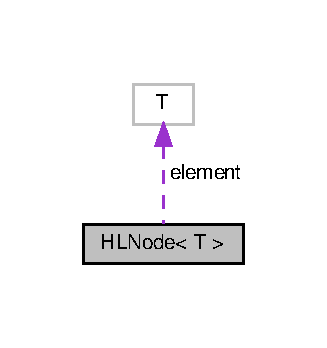
\includegraphics[width=157pt]{classHLNode__coll__graph}
\end{center}
\end{figure}
\subsection*{Public Member Functions}
\begin{DoxyCompactItemize}
\item 
\hyperlink{classHLNode_afd850c35b0382f70502a5d5e193a0002}{H\+L\+Node} (\hyperlink{classHLNode}{H\+L\+Node}$<$ T $>$ $\ast$\hyperlink{classHLNode_a35c8458c7d7c91b21f9d926ddeb925df}{next}, T \hyperlink{classHLNode_a17be2e766c987e797c71785bf1bad581}{element})
\end{DoxyCompactItemize}
\subsection*{Public Attributes}
\begin{DoxyCompactItemize}
\item 
\hyperlink{classHLNode}{H\+L\+Node}$<$ T $>$ $\ast$ \hyperlink{classHLNode_a35c8458c7d7c91b21f9d926ddeb925df}{next}
\item 
T \hyperlink{classHLNode_a17be2e766c987e797c71785bf1bad581}{element}
\item 
int \hyperlink{classHLNode_a0ebbedf0c01596b658b69ae7e276ad1f}{hash\+Table\+Index}
\end{DoxyCompactItemize}


\subsection{Constructor \& Destructor Documentation}
\mbox{\Hypertarget{classHLNode_afd850c35b0382f70502a5d5e193a0002}\label{classHLNode_afd850c35b0382f70502a5d5e193a0002}} 
\index{H\+L\+Node@{H\+L\+Node}!H\+L\+Node@{H\+L\+Node}}
\index{H\+L\+Node@{H\+L\+Node}!H\+L\+Node@{H\+L\+Node}}
\subsubsection{\texorpdfstring{H\+L\+Node()}{HLNode()}}
{\footnotesize\ttfamily template$<$typename T$>$ \\
\hyperlink{classHLNode}{H\+L\+Node}$<$ T $>$\+::\hyperlink{classHLNode}{H\+L\+Node} (\begin{DoxyParamCaption}\item[{\hyperlink{classHLNode}{H\+L\+Node}$<$ T $>$ $\ast$}]{next,  }\item[{T}]{element }\end{DoxyParamCaption})\hspace{0.3cm}{\ttfamily [inline]}}



\subsection{Member Data Documentation}
\mbox{\Hypertarget{classHLNode_a17be2e766c987e797c71785bf1bad581}\label{classHLNode_a17be2e766c987e797c71785bf1bad581}} 
\index{H\+L\+Node@{H\+L\+Node}!element@{element}}
\index{element@{element}!H\+L\+Node@{H\+L\+Node}}
\subsubsection{\texorpdfstring{element}{element}}
{\footnotesize\ttfamily template$<$typename T$>$ \\
T \hyperlink{classHLNode}{H\+L\+Node}$<$ T $>$\+::element}

\mbox{\Hypertarget{classHLNode_a0ebbedf0c01596b658b69ae7e276ad1f}\label{classHLNode_a0ebbedf0c01596b658b69ae7e276ad1f}} 
\index{H\+L\+Node@{H\+L\+Node}!hash\+Table\+Index@{hash\+Table\+Index}}
\index{hash\+Table\+Index@{hash\+Table\+Index}!H\+L\+Node@{H\+L\+Node}}
\subsubsection{\texorpdfstring{hash\+Table\+Index}{hashTableIndex}}
{\footnotesize\ttfamily template$<$typename T$>$ \\
int \hyperlink{classHLNode}{H\+L\+Node}$<$ T $>$\+::hash\+Table\+Index}

\mbox{\Hypertarget{classHLNode_a35c8458c7d7c91b21f9d926ddeb925df}\label{classHLNode_a35c8458c7d7c91b21f9d926ddeb925df}} 
\index{H\+L\+Node@{H\+L\+Node}!next@{next}}
\index{next@{next}!H\+L\+Node@{H\+L\+Node}}
\subsubsection{\texorpdfstring{next}{next}}
{\footnotesize\ttfamily template$<$typename T$>$ \\
\hyperlink{classHLNode}{H\+L\+Node}$<$T$>$$\ast$ \hyperlink{classHLNode}{H\+L\+Node}$<$ T $>$\+::next}



The documentation for this class was generated from the following file\+:\begin{DoxyCompactItemize}
\item 
common/rq/\hyperlink{hashlist_8h}{hashlist.\+h}\end{DoxyCompactItemize}

\hypertarget{classhowley}{}\section{howley$<$ skey\+\_\+t, sval\+\_\+t, Rec\+Mgr $>$ Class Template Reference}
\label{classhowley}\index{howley$<$ skey\+\_\+t, sval\+\_\+t, Rec\+Mgr $>$@{howley$<$ skey\+\_\+t, sval\+\_\+t, Rec\+Mgr $>$}}


{\ttfamily \#include $<$howley\+\_\+impl.\+h$>$}

\subsection*{Public Member Functions}
\begin{DoxyCompactItemize}
\item 
\hyperlink{classhowley_ac5d2f61eedc19a5b2f5db14421682b4c}{howley} (const int \+\_\+\+N\+U\+M\+\_\+\+T\+H\+R\+E\+A\+DS, const skey\+\_\+t \&\+\_\+\+K\+E\+Y\+\_\+\+M\+IN, const skey\+\_\+t \&\+\_\+\+K\+E\+Y\+\_\+\+M\+AX, const sval\+\_\+t \&\+\_\+\+V\+A\+L\+U\+E\+\_\+\+R\+E\+S\+E\+R\+V\+ED, unsigned int id)
\item 
\hyperlink{classhowley_a7683fe814e9483ec72e02b552965d9a8}{$\sim$howley} ()
\item 
void \hyperlink{classhowley_ad896657fb61ab833beb5854d3ab41195}{init\+Thread} (const int \hyperlink{microbench_2main_8cpp_a9ca9869868fe7e7a38a921cc7de4103f}{tid})
\item 
void \hyperlink{classhowley_ad451346bdc013f8f91a66e864ff6118c}{deinit\+Thread} (const int \hyperlink{microbench_2main_8cpp_a9ca9869868fe7e7a38a921cc7de4103f}{tid})
\item 
sval\+\_\+t \hyperlink{classhowley_a42cff4d570c8fda67543525ebc0342e3}{bst\+\_\+contains} (const int \hyperlink{microbench_2main_8cpp_a9ca9869868fe7e7a38a921cc7de4103f}{tid}, skey\+\_\+t k)
\item 
sval\+\_\+t \hyperlink{classhowley_a2c3298e68329401c0ba27bf50a11f624}{bst\+\_\+add} (const int \hyperlink{microbench_2main_8cpp_a9ca9869868fe7e7a38a921cc7de4103f}{tid}, skey\+\_\+t k, sval\+\_\+t \hyperlink{reclaimer__ebr__tree__q_8h_acd3c1c4d280aac729e9fdb520dc99f20}{v})
\item 
sval\+\_\+t \hyperlink{classhowley_a469bbd88967ff50d865bbf368b1eae5e}{bst\+\_\+remove} (const int \hyperlink{microbench_2main_8cpp_a9ca9869868fe7e7a38a921cc7de4103f}{tid}, skey\+\_\+t k)
\item 
\hyperlink{structnode__t}{node\+\_\+t}$<$ skey\+\_\+t, sval\+\_\+t $>$ $\ast$ \hyperlink{classhowley_a37175ef84b9e6c359dc5cc1148fa289b}{get\+\_\+root} ()
\item 
Rec\+Mgr $\ast$ \hyperlink{classhowley_a9581b4d5eb22feca0cd2ac799a0c6145}{debug\+Get\+Rec\+Mgr} ()
\end{DoxyCompactItemize}


\subsection{Constructor \& Destructor Documentation}
\mbox{\Hypertarget{classhowley_ac5d2f61eedc19a5b2f5db14421682b4c}\label{classhowley_ac5d2f61eedc19a5b2f5db14421682b4c}} 
\index{howley@{howley}!howley@{howley}}
\index{howley@{howley}!howley@{howley}}
\subsubsection{\texorpdfstring{howley()}{howley()}}
{\footnotesize\ttfamily template$<$typename skey\+\_\+t , typename sval\+\_\+t , class Rec\+Mgr $>$ \\
\hyperlink{classhowley}{howley}$<$ skey\+\_\+t, sval\+\_\+t, Rec\+Mgr $>$\+::\hyperlink{classhowley}{howley} (\begin{DoxyParamCaption}\item[{const int}]{\+\_\+\+N\+U\+M\+\_\+\+T\+H\+R\+E\+A\+DS,  }\item[{const skey\+\_\+t \&}]{\+\_\+\+K\+E\+Y\+\_\+\+M\+IN,  }\item[{const skey\+\_\+t \&}]{\+\_\+\+K\+E\+Y\+\_\+\+M\+AX,  }\item[{const sval\+\_\+t \&}]{\+\_\+\+V\+A\+L\+U\+E\+\_\+\+R\+E\+S\+E\+R\+V\+ED,  }\item[{unsigned int}]{id }\end{DoxyParamCaption})\hspace{0.3cm}{\ttfamily [inline]}}

\mbox{\Hypertarget{classhowley_a7683fe814e9483ec72e02b552965d9a8}\label{classhowley_a7683fe814e9483ec72e02b552965d9a8}} 
\index{howley@{howley}!````~howley@{$\sim$howley}}
\index{````~howley@{$\sim$howley}!howley@{howley}}
\subsubsection{\texorpdfstring{$\sim$howley()}{~howley()}}
{\footnotesize\ttfamily template$<$typename skey\+\_\+t , typename sval\+\_\+t , class Rec\+Mgr $>$ \\
\hyperlink{classhowley}{howley}$<$ skey\+\_\+t, sval\+\_\+t, Rec\+Mgr $>$\+::$\sim$\hyperlink{classhowley}{howley} (\begin{DoxyParamCaption}{ }\end{DoxyParamCaption})\hspace{0.3cm}{\ttfamily [inline]}}



\subsection{Member Function Documentation}
\mbox{\Hypertarget{classhowley_a2c3298e68329401c0ba27bf50a11f624}\label{classhowley_a2c3298e68329401c0ba27bf50a11f624}} 
\index{howley@{howley}!bst\+\_\+add@{bst\+\_\+add}}
\index{bst\+\_\+add@{bst\+\_\+add}!howley@{howley}}
\subsubsection{\texorpdfstring{bst\+\_\+add()}{bst\_add()}}
{\footnotesize\ttfamily template$<$typename skey\+\_\+t , typename sval\+\_\+t , class Rec\+Mgr $>$ \\
sval\+\_\+t \hyperlink{classhowley}{howley}$<$ skey\+\_\+t, sval\+\_\+t, Rec\+Mgr $>$\+::bst\+\_\+add (\begin{DoxyParamCaption}\item[{const int}]{tid,  }\item[{skey\+\_\+t}]{k,  }\item[{sval\+\_\+t}]{v }\end{DoxyParamCaption})}

\mbox{\Hypertarget{classhowley_a42cff4d570c8fda67543525ebc0342e3}\label{classhowley_a42cff4d570c8fda67543525ebc0342e3}} 
\index{howley@{howley}!bst\+\_\+contains@{bst\+\_\+contains}}
\index{bst\+\_\+contains@{bst\+\_\+contains}!howley@{howley}}
\subsubsection{\texorpdfstring{bst\+\_\+contains()}{bst\_contains()}}
{\footnotesize\ttfamily template$<$typename skey\+\_\+t , typename sval\+\_\+t , class Rec\+Mgr $>$ \\
sval\+\_\+t \hyperlink{classhowley}{howley}$<$ skey\+\_\+t, sval\+\_\+t, Rec\+Mgr $>$\+::bst\+\_\+contains (\begin{DoxyParamCaption}\item[{const int}]{tid,  }\item[{skey\+\_\+t}]{k }\end{DoxyParamCaption})}

\mbox{\Hypertarget{classhowley_a469bbd88967ff50d865bbf368b1eae5e}\label{classhowley_a469bbd88967ff50d865bbf368b1eae5e}} 
\index{howley@{howley}!bst\+\_\+remove@{bst\+\_\+remove}}
\index{bst\+\_\+remove@{bst\+\_\+remove}!howley@{howley}}
\subsubsection{\texorpdfstring{bst\+\_\+remove()}{bst\_remove()}}
{\footnotesize\ttfamily template$<$typename skey\+\_\+t , typename sval\+\_\+t , class Rec\+Mgr $>$ \\
sval\+\_\+t \hyperlink{classhowley}{howley}$<$ skey\+\_\+t, sval\+\_\+t, Rec\+Mgr $>$\+::bst\+\_\+remove (\begin{DoxyParamCaption}\item[{const int}]{tid,  }\item[{skey\+\_\+t}]{k }\end{DoxyParamCaption})}

\mbox{\Hypertarget{classhowley_a9581b4d5eb22feca0cd2ac799a0c6145}\label{classhowley_a9581b4d5eb22feca0cd2ac799a0c6145}} 
\index{howley@{howley}!debug\+Get\+Rec\+Mgr@{debug\+Get\+Rec\+Mgr}}
\index{debug\+Get\+Rec\+Mgr@{debug\+Get\+Rec\+Mgr}!howley@{howley}}
\subsubsection{\texorpdfstring{debug\+Get\+Rec\+Mgr()}{debugGetRecMgr()}}
{\footnotesize\ttfamily template$<$typename skey\+\_\+t , typename sval\+\_\+t , class Rec\+Mgr $>$ \\
Rec\+Mgr$\ast$ \hyperlink{classhowley}{howley}$<$ skey\+\_\+t, sval\+\_\+t, Rec\+Mgr $>$\+::debug\+Get\+Rec\+Mgr (\begin{DoxyParamCaption}{ }\end{DoxyParamCaption})\hspace{0.3cm}{\ttfamily [inline]}}

\mbox{\Hypertarget{classhowley_ad451346bdc013f8f91a66e864ff6118c}\label{classhowley_ad451346bdc013f8f91a66e864ff6118c}} 
\index{howley@{howley}!deinit\+Thread@{deinit\+Thread}}
\index{deinit\+Thread@{deinit\+Thread}!howley@{howley}}
\subsubsection{\texorpdfstring{deinit\+Thread()}{deinitThread()}}
{\footnotesize\ttfamily template$<$typename skey\+\_\+t , typename sval\+\_\+t , class Rec\+Mgr $>$ \\
void \hyperlink{classhowley}{howley}$<$ skey\+\_\+t, sval\+\_\+t, Rec\+Mgr $>$\+::deinit\+Thread (\begin{DoxyParamCaption}\item[{const int}]{tid }\end{DoxyParamCaption})\hspace{0.3cm}{\ttfamily [inline]}}

\mbox{\Hypertarget{classhowley_a37175ef84b9e6c359dc5cc1148fa289b}\label{classhowley_a37175ef84b9e6c359dc5cc1148fa289b}} 
\index{howley@{howley}!get\+\_\+root@{get\+\_\+root}}
\index{get\+\_\+root@{get\+\_\+root}!howley@{howley}}
\subsubsection{\texorpdfstring{get\+\_\+root()}{get\_root()}}
{\footnotesize\ttfamily template$<$typename skey\+\_\+t , typename sval\+\_\+t , class Rec\+Mgr $>$ \\
\hyperlink{structnode__t}{node\+\_\+t}$<$skey\+\_\+t, sval\+\_\+t$>$$\ast$ \hyperlink{classhowley}{howley}$<$ skey\+\_\+t, sval\+\_\+t, Rec\+Mgr $>$\+::get\+\_\+root (\begin{DoxyParamCaption}{ }\end{DoxyParamCaption})\hspace{0.3cm}{\ttfamily [inline]}}

\mbox{\Hypertarget{classhowley_ad896657fb61ab833beb5854d3ab41195}\label{classhowley_ad896657fb61ab833beb5854d3ab41195}} 
\index{howley@{howley}!init\+Thread@{init\+Thread}}
\index{init\+Thread@{init\+Thread}!howley@{howley}}
\subsubsection{\texorpdfstring{init\+Thread()}{initThread()}}
{\footnotesize\ttfamily template$<$typename skey\+\_\+t , typename sval\+\_\+t , class Rec\+Mgr $>$ \\
void \hyperlink{classhowley}{howley}$<$ skey\+\_\+t, sval\+\_\+t, Rec\+Mgr $>$\+::init\+Thread (\begin{DoxyParamCaption}\item[{const int}]{tid }\end{DoxyParamCaption})\hspace{0.3cm}{\ttfamily [inline]}}



The documentation for this class was generated from the following file\+:\begin{DoxyCompactItemize}
\item 
ds/howley\+\_\+int\+\_\+bst\+\_\+lf/\hyperlink{howley__impl_8h}{howley\+\_\+impl.\+h}\end{DoxyCompactItemize}

\hypertarget{structIdealSubtree}{}\section{Ideal\+Subtree$<$ V $>$ Struct Template Reference}
\label{structIdealSubtree}\index{Ideal\+Subtree$<$ V $>$@{Ideal\+Subtree$<$ V $>$}}


{\ttfamily \#include $<$brown\+\_\+ext\+\_\+ist\+\_\+lf\+\_\+impl.\+h$>$}



Collaboration diagram for Ideal\+Subtree$<$ V $>$\+:
\nopagebreak
\begin{figure}[H]
\begin{center}
\leavevmode
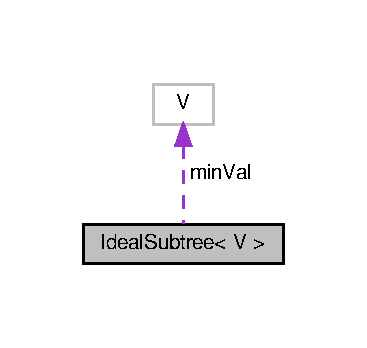
\includegraphics[width=176pt]{structIdealSubtree__coll__graph}
\end{center}
\end{figure}
\subsection*{Public Attributes}
\begin{DoxyCompactItemize}
\item 
\hyperlink{rq__unsafe_8h_ad45142aaf2ff20a036dc6242b8483e9c}{casword\+\_\+t} \hyperlink{structIdealSubtree_afceaf48b16c3c72454583786e6b02c66}{ptr}
\item 
V \hyperlink{structIdealSubtree_a357a536fa64c505bb0961d716f5ac814}{min\+Val}
\end{DoxyCompactItemize}


\subsection{Member Data Documentation}
\mbox{\Hypertarget{structIdealSubtree_a357a536fa64c505bb0961d716f5ac814}\label{structIdealSubtree_a357a536fa64c505bb0961d716f5ac814}} 
\index{Ideal\+Subtree@{Ideal\+Subtree}!min\+Val@{min\+Val}}
\index{min\+Val@{min\+Val}!Ideal\+Subtree@{Ideal\+Subtree}}
\subsubsection{\texorpdfstring{min\+Val}{minVal}}
{\footnotesize\ttfamily template$<$typename V $>$ \\
V \hyperlink{structIdealSubtree}{Ideal\+Subtree}$<$ V $>$\+::min\+Val}

\mbox{\Hypertarget{structIdealSubtree_afceaf48b16c3c72454583786e6b02c66}\label{structIdealSubtree_afceaf48b16c3c72454583786e6b02c66}} 
\index{Ideal\+Subtree@{Ideal\+Subtree}!ptr@{ptr}}
\index{ptr@{ptr}!Ideal\+Subtree@{Ideal\+Subtree}}
\subsubsection{\texorpdfstring{ptr}{ptr}}
{\footnotesize\ttfamily template$<$typename V $>$ \\
\hyperlink{rq__unsafe_8h_ad45142aaf2ff20a036dc6242b8483e9c}{casword\+\_\+t} \hyperlink{structIdealSubtree}{Ideal\+Subtree}$<$ V $>$\+::ptr}



The documentation for this struct was generated from the following file\+:\begin{DoxyCompactItemize}
\item 
ds/brown\+\_\+ext\+\_\+ist\+\_\+lf/\hyperlink{brown__ext__ist__lf__impl_8h}{brown\+\_\+ext\+\_\+ist\+\_\+lf\+\_\+impl.\+h}\end{DoxyCompactItemize}

\hypertarget{structiinfo__t}{}\section{iinfo\+\_\+t$<$ skey\+\_\+t, sval\+\_\+t $>$ Struct Template Reference}
\label{structiinfo__t}\index{iinfo\+\_\+t$<$ skey\+\_\+t, sval\+\_\+t $>$@{iinfo\+\_\+t$<$ skey\+\_\+t, sval\+\_\+t $>$}}


{\ttfamily \#include $<$ellen\+\_\+impl.\+h$>$}

\subsection*{Public Attributes}
\begin{DoxyCompactItemize}
\item 
\hyperlink{structnode__t}{node\+\_\+t}$<$ skey\+\_\+t, sval\+\_\+t $>$ $\ast$ \hyperlink{structiinfo__t_ac481a80b2ca93f02845d28a7c2223a3f}{p}
\item 
\hyperlink{structnode__t}{node\+\_\+t}$<$ skey\+\_\+t, sval\+\_\+t $>$ $\ast$ \hyperlink{structiinfo__t_a19351f64d5a730afeac5393f91a944e6}{new\+\_\+internal}
\item 
\hyperlink{structnode__t}{node\+\_\+t}$<$ skey\+\_\+t, sval\+\_\+t $>$ $\ast$ \hyperlink{structiinfo__t_ab71cf537eecee9ec27ba800bd1a4ffa1}{l}
\end{DoxyCompactItemize}


\subsection{Member Data Documentation}
\mbox{\Hypertarget{structiinfo__t_ab71cf537eecee9ec27ba800bd1a4ffa1}\label{structiinfo__t_ab71cf537eecee9ec27ba800bd1a4ffa1}} 
\index{iinfo\+\_\+t@{iinfo\+\_\+t}!l@{l}}
\index{l@{l}!iinfo\+\_\+t@{iinfo\+\_\+t}}
\subsubsection{\texorpdfstring{l}{l}}
{\footnotesize\ttfamily template$<$typename skey\+\_\+t, typename sval\+\_\+t$>$ \\
\hyperlink{structnode__t}{node\+\_\+t}$<$skey\+\_\+t, sval\+\_\+t$>$$\ast$ \hyperlink{structiinfo__t}{iinfo\+\_\+t}$<$ skey\+\_\+t, sval\+\_\+t $>$\+::l}

\mbox{\Hypertarget{structiinfo__t_a19351f64d5a730afeac5393f91a944e6}\label{structiinfo__t_a19351f64d5a730afeac5393f91a944e6}} 
\index{iinfo\+\_\+t@{iinfo\+\_\+t}!new\+\_\+internal@{new\+\_\+internal}}
\index{new\+\_\+internal@{new\+\_\+internal}!iinfo\+\_\+t@{iinfo\+\_\+t}}
\subsubsection{\texorpdfstring{new\+\_\+internal}{new\_internal}}
{\footnotesize\ttfamily template$<$typename skey\+\_\+t, typename sval\+\_\+t$>$ \\
\hyperlink{structnode__t}{node\+\_\+t}$<$skey\+\_\+t, sval\+\_\+t$>$$\ast$ \hyperlink{structiinfo__t}{iinfo\+\_\+t}$<$ skey\+\_\+t, sval\+\_\+t $>$\+::new\+\_\+internal}

\mbox{\Hypertarget{structiinfo__t_ac481a80b2ca93f02845d28a7c2223a3f}\label{structiinfo__t_ac481a80b2ca93f02845d28a7c2223a3f}} 
\index{iinfo\+\_\+t@{iinfo\+\_\+t}!p@{p}}
\index{p@{p}!iinfo\+\_\+t@{iinfo\+\_\+t}}
\subsubsection{\texorpdfstring{p}{p}}
{\footnotesize\ttfamily template$<$typename skey\+\_\+t, typename sval\+\_\+t$>$ \\
\hyperlink{structnode__t}{node\+\_\+t}$<$skey\+\_\+t, sval\+\_\+t$>$$\ast$ \hyperlink{structiinfo__t}{iinfo\+\_\+t}$<$ skey\+\_\+t, sval\+\_\+t $>$\+::p}



The documentation for this struct was generated from the following file\+:\begin{DoxyCompactItemize}
\item 
ds/ellen\+\_\+ext\+\_\+bst\+\_\+lf/\hyperlink{ellen__impl_8h}{ellen\+\_\+impl.\+h}\end{DoxyCompactItemize}

\hypertarget{classIndex}{}\section{Index Class Reference}
\label{classIndex}\index{Index@{Index}}


{\ttfamily \#include $<$index\+\_\+adapter.\+h$>$}



Inheritance diagram for Index\+:
\nopagebreak
\begin{figure}[H]
\begin{center}
\leavevmode
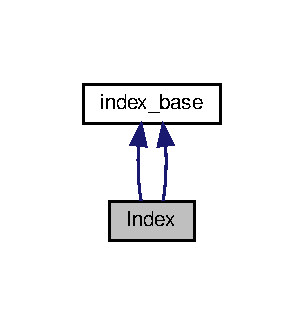
\includegraphics[width=146pt]{classIndex__inherit__graph}
\end{center}
\end{figure}


Collaboration diagram for Index\+:
\nopagebreak
\begin{figure}[H]
\begin{center}
\leavevmode
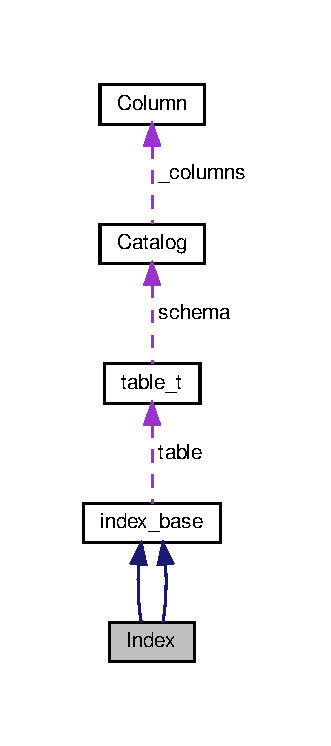
\includegraphics[width=159pt]{classIndex__coll__graph}
\end{center}
\end{figure}
\subsection*{Public Member Functions}
\begin{DoxyCompactItemize}
\item 
\hyperlink{classIndex_a76b7ed4e9cb0b1540264567f84896032}{$\sim$\+Index} ()
\item 
\hyperlink{global_8h_a78c49a674c810fdd03d20432f7be864a}{RC} \hyperlink{classIndex_a1328ba545ab4ef6750a742f0de084d79}{init} (uint64\+\_\+t part\+\_\+cnt, \hyperlink{classtable__t}{table\+\_\+t} $\ast$\hyperlink{classindex__base_abb51a82fc0bf85a82aa83376d111641f}{table})
\item 
\hyperlink{global_8h_a78c49a674c810fdd03d20432f7be864a}{RC} \hyperlink{classIndex_a2266050deae0c62e0b90e7d60fd70f35}{index\+\_\+insert} (\hyperlink{index__base_8h_ae35c40bc2f912c11f0e36ac66cba4489}{K\+E\+Y\+\_\+\+T\+Y\+PE} key, \hyperlink{microbench_2main_8cpp_ae17cb099b4c9aee7835032339b5a9e0d}{V\+A\+L\+U\+E\+\_\+\+T\+Y\+PE} new\+Item, int part\+\_\+id=-\/1)
\item 
\hyperlink{global_8h_a78c49a674c810fdd03d20432f7be864a}{RC} \hyperlink{classIndex_abb1666dd897887f22d8e4dc92966b207}{index\+\_\+read} (\hyperlink{index__base_8h_ae35c40bc2f912c11f0e36ac66cba4489}{K\+E\+Y\+\_\+\+T\+Y\+PE} key, \hyperlink{microbench_2main_8cpp_ae17cb099b4c9aee7835032339b5a9e0d}{V\+A\+L\+U\+E\+\_\+\+T\+Y\+PE} $\ast$item, int part\+\_\+id=-\/1, int thd\+\_\+id=0)
\item 
\hyperlink{global_8h_a78c49a674c810fdd03d20432f7be864a}{RC} \hyperlink{classIndex_a5e3d8773117cba2f8dc644185d560a0c}{index\+\_\+range\+\_\+query} (\hyperlink{index__base_8h_ae35c40bc2f912c11f0e36ac66cba4489}{K\+E\+Y\+\_\+\+T\+Y\+PE} low, \hyperlink{index__base_8h_ae35c40bc2f912c11f0e36ac66cba4489}{K\+E\+Y\+\_\+\+T\+Y\+PE} high, \hyperlink{index__base_8h_ae35c40bc2f912c11f0e36ac66cba4489}{K\+E\+Y\+\_\+\+T\+Y\+PE} $\ast$result\+Keys, \hyperlink{microbench_2main_8cpp_ae17cb099b4c9aee7835032339b5a9e0d}{V\+A\+L\+U\+E\+\_\+\+T\+Y\+PE} $\ast$result\+Values, int $\ast$num\+Results, int part\+\_\+id=-\/1)
\item 
void \hyperlink{classIndex_a6a509df225912ffea8547fa0daa57d8c}{init\+Thread} (const int \hyperlink{microbench_2main_8cpp_a9ca9869868fe7e7a38a921cc7de4103f}{tid})
\item 
void \hyperlink{classIndex_a62ecc92aa23b7292ea6735ff9ac21c80}{deinit\+Thread} (const int \hyperlink{microbench_2main_8cpp_a9ca9869868fe7e7a38a921cc7de4103f}{tid})
\item 
size\+\_\+t \hyperlink{classIndex_ad70e606faaf0a67b690275b8f8ca5d5f}{get\+Node\+Size} ()
\item 
size\+\_\+t \hyperlink{classIndex_a0e0b37468dc2b549208da43466a68a94}{get\+Descriptor\+Size} ()
\item 
void \hyperlink{classIndex_ab300e132e8a12e3334003227a2e3f618}{print\+\_\+stats} ()
\item 
\hyperlink{global_8h_a78c49a674c810fdd03d20432f7be864a}{RC} \hyperlink{classIndex_a9f14dfc7c370a32604d91af76907f6c6}{init} (uint64\+\_\+t bucket\+\_\+cnt, int part\+\_\+cnt)
\item 
\hyperlink{global_8h_a78c49a674c810fdd03d20432f7be864a}{RC} \hyperlink{classIndex_a92819c544e6ac6af5a2d4aa03a61a351}{init} (int part\+\_\+cnt, \hyperlink{classtable__t}{table\+\_\+t} $\ast$\hyperlink{classindex__base_abb51a82fc0bf85a82aa83376d111641f}{table}, uint64\+\_\+t bucket\+\_\+cnt)
\item 
bool \hyperlink{classIndex_a43908d9915fe59437d20a82324bcda61}{index\+\_\+exist} (\hyperlink{index__base_8h_ae35c40bc2f912c11f0e36ac66cba4489}{K\+E\+Y\+\_\+\+T\+Y\+PE} key)
\item 
\hyperlink{global_8h_a78c49a674c810fdd03d20432f7be864a}{RC} \hyperlink{classIndex_a03544bdceed7feb756712086fb239de1}{index\+\_\+insert} (\hyperlink{index__base_8h_ae35c40bc2f912c11f0e36ac66cba4489}{K\+E\+Y\+\_\+\+T\+Y\+PE} key, \hyperlink{microbench_2main_8cpp_ae17cb099b4c9aee7835032339b5a9e0d}{V\+A\+L\+U\+E\+\_\+\+T\+Y\+PE} item, int part\+\_\+id=-\/1)
\item 
\hyperlink{global_8h_a78c49a674c810fdd03d20432f7be864a}{RC} \hyperlink{classIndex_ab930b74f611f4704fa1fb9a8bb9f57f8}{index\+\_\+read} (\hyperlink{index__base_8h_ae35c40bc2f912c11f0e36ac66cba4489}{K\+E\+Y\+\_\+\+T\+Y\+PE} key, \hyperlink{microbench_2main_8cpp_ae17cb099b4c9aee7835032339b5a9e0d}{V\+A\+L\+U\+E\+\_\+\+T\+Y\+PE} $\ast$item, int part\+\_\+id=-\/1)
\item 
\hyperlink{global_8h_a78c49a674c810fdd03d20432f7be864a}{RC} \hyperlink{classIndex_abb1666dd897887f22d8e4dc92966b207}{index\+\_\+read} (\hyperlink{index__base_8h_ae35c40bc2f912c11f0e36ac66cba4489}{K\+E\+Y\+\_\+\+T\+Y\+PE} key, \hyperlink{microbench_2main_8cpp_ae17cb099b4c9aee7835032339b5a9e0d}{V\+A\+L\+U\+E\+\_\+\+T\+Y\+PE} $\ast$item, int part\+\_\+id=-\/1, int thd\+\_\+id=0)
\item 
void \hyperlink{classIndex_a6a509df225912ffea8547fa0daa57d8c}{init\+Thread} (const int \hyperlink{microbench_2main_8cpp_a9ca9869868fe7e7a38a921cc7de4103f}{tid})
\item 
void \hyperlink{classIndex_a62ecc92aa23b7292ea6735ff9ac21c80}{deinit\+Thread} (const int \hyperlink{microbench_2main_8cpp_a9ca9869868fe7e7a38a921cc7de4103f}{tid})
\end{DoxyCompactItemize}
\subsection*{Additional Inherited Members}


\subsection{Detailed Description}
Define index data structure and record manager types Create an adapter class for the D\+Bx1000 index interface 

\subsection{Constructor \& Destructor Documentation}
\mbox{\Hypertarget{classIndex_a76b7ed4e9cb0b1540264567f84896032}\label{classIndex_a76b7ed4e9cb0b1540264567f84896032}} 
\index{Index@{Index}!````~Index@{$\sim$\+Index}}
\index{````~Index@{$\sim$\+Index}!Index@{Index}}
\subsubsection{\texorpdfstring{$\sim$\+Index()}{~Index()}}
{\footnotesize\ttfamily Index\+::$\sim$\+Index (\begin{DoxyParamCaption}{ }\end{DoxyParamCaption})\hspace{0.3cm}{\ttfamily [inline]}}



\subsection{Member Function Documentation}
\mbox{\Hypertarget{classIndex_a62ecc92aa23b7292ea6735ff9ac21c80}\label{classIndex_a62ecc92aa23b7292ea6735ff9ac21c80}} 
\index{Index@{Index}!deinit\+Thread@{deinit\+Thread}}
\index{deinit\+Thread@{deinit\+Thread}!Index@{Index}}
\subsubsection{\texorpdfstring{deinit\+Thread()}{deinitThread()}\hspace{0.1cm}{\footnotesize\ttfamily [1/2]}}
{\footnotesize\ttfamily void Index\+::deinit\+Thread (\begin{DoxyParamCaption}\item[{const int}]{tid }\end{DoxyParamCaption})}

\mbox{\Hypertarget{classIndex_a62ecc92aa23b7292ea6735ff9ac21c80}\label{classIndex_a62ecc92aa23b7292ea6735ff9ac21c80}} 
\index{Index@{Index}!deinit\+Thread@{deinit\+Thread}}
\index{deinit\+Thread@{deinit\+Thread}!Index@{Index}}
\subsubsection{\texorpdfstring{deinit\+Thread()}{deinitThread()}\hspace{0.1cm}{\footnotesize\ttfamily [2/2]}}
{\footnotesize\ttfamily void Index\+::deinit\+Thread (\begin{DoxyParamCaption}\item[{const int}]{tid }\end{DoxyParamCaption})\hspace{0.3cm}{\ttfamily [inline]}}

\mbox{\Hypertarget{classIndex_a0e0b37468dc2b549208da43466a68a94}\label{classIndex_a0e0b37468dc2b549208da43466a68a94}} 
\index{Index@{Index}!get\+Descriptor\+Size@{get\+Descriptor\+Size}}
\index{get\+Descriptor\+Size@{get\+Descriptor\+Size}!Index@{Index}}
\subsubsection{\texorpdfstring{get\+Descriptor\+Size()}{getDescriptorSize()}}
{\footnotesize\ttfamily size\+\_\+t Index\+::get\+Descriptor\+Size (\begin{DoxyParamCaption}{ }\end{DoxyParamCaption})\hspace{0.3cm}{\ttfamily [inline]}, {\ttfamily [virtual]}}



Reimplemented from \hyperlink{classindex__base_a0050e83a568a2905c54c81d7515f4085}{index\+\_\+base}.

\mbox{\Hypertarget{classIndex_ad70e606faaf0a67b690275b8f8ca5d5f}\label{classIndex_ad70e606faaf0a67b690275b8f8ca5d5f}} 
\index{Index@{Index}!get\+Node\+Size@{get\+Node\+Size}}
\index{get\+Node\+Size@{get\+Node\+Size}!Index@{Index}}
\subsubsection{\texorpdfstring{get\+Node\+Size()}{getNodeSize()}}
{\footnotesize\ttfamily size\+\_\+t Index\+::get\+Node\+Size (\begin{DoxyParamCaption}{ }\end{DoxyParamCaption})\hspace{0.3cm}{\ttfamily [inline]}, {\ttfamily [virtual]}}



Reimplemented from \hyperlink{classindex__base_ab8bfe46c64ea1ab3c596c46f0b76064e}{index\+\_\+base}.

\mbox{\Hypertarget{classIndex_a43908d9915fe59437d20a82324bcda61}\label{classIndex_a43908d9915fe59437d20a82324bcda61}} 
\index{Index@{Index}!index\+\_\+exist@{index\+\_\+exist}}
\index{index\+\_\+exist@{index\+\_\+exist}!Index@{Index}}
\subsubsection{\texorpdfstring{index\+\_\+exist()}{index\_exist()}}
{\footnotesize\ttfamily bool Index\+::index\+\_\+exist (\begin{DoxyParamCaption}\item[{\hyperlink{index__base_8h_ae35c40bc2f912c11f0e36ac66cba4489}{K\+E\+Y\+\_\+\+T\+Y\+PE}}]{key }\end{DoxyParamCaption})}

\mbox{\Hypertarget{classIndex_a03544bdceed7feb756712086fb239de1}\label{classIndex_a03544bdceed7feb756712086fb239de1}} 
\index{Index@{Index}!index\+\_\+insert@{index\+\_\+insert}}
\index{index\+\_\+insert@{index\+\_\+insert}!Index@{Index}}
\subsubsection{\texorpdfstring{index\+\_\+insert()}{index\_insert()}\hspace{0.1cm}{\footnotesize\ttfamily [1/2]}}
{\footnotesize\ttfamily \hyperlink{global_8h_a78c49a674c810fdd03d20432f7be864a}{RC} Index\+::index\+\_\+insert (\begin{DoxyParamCaption}\item[{\hyperlink{index__base_8h_ae35c40bc2f912c11f0e36ac66cba4489}{K\+E\+Y\+\_\+\+T\+Y\+PE}}]{key,  }\item[{\hyperlink{microbench_2main_8cpp_ae17cb099b4c9aee7835032339b5a9e0d}{V\+A\+L\+U\+E\+\_\+\+T\+Y\+PE}}]{item,  }\item[{int}]{part\+\_\+id = {\ttfamily -\/1} }\end{DoxyParamCaption})\hspace{0.3cm}{\ttfamily [virtual]}}



Implements \hyperlink{classindex__base_a819b2cb7cbc7c740381e64d4c9023745}{index\+\_\+base}.

\mbox{\Hypertarget{classIndex_a2266050deae0c62e0b90e7d60fd70f35}\label{classIndex_a2266050deae0c62e0b90e7d60fd70f35}} 
\index{Index@{Index}!index\+\_\+insert@{index\+\_\+insert}}
\index{index\+\_\+insert@{index\+\_\+insert}!Index@{Index}}
\subsubsection{\texorpdfstring{index\+\_\+insert()}{index\_insert()}\hspace{0.1cm}{\footnotesize\ttfamily [2/2]}}
{\footnotesize\ttfamily \hyperlink{global_8h_a78c49a674c810fdd03d20432f7be864a}{RC} Index\+::index\+\_\+insert (\begin{DoxyParamCaption}\item[{\hyperlink{index__base_8h_ae35c40bc2f912c11f0e36ac66cba4489}{K\+E\+Y\+\_\+\+T\+Y\+PE}}]{key,  }\item[{\hyperlink{microbench_2main_8cpp_ae17cb099b4c9aee7835032339b5a9e0d}{V\+A\+L\+U\+E\+\_\+\+T\+Y\+PE}}]{new\+Item,  }\item[{int}]{part\+\_\+id = {\ttfamily -\/1} }\end{DoxyParamCaption})\hspace{0.3cm}{\ttfamily [inline]}, {\ttfamily [virtual]}}



Implements \hyperlink{classindex__base_a819b2cb7cbc7c740381e64d4c9023745}{index\+\_\+base}.

\mbox{\Hypertarget{classIndex_a5e3d8773117cba2f8dc644185d560a0c}\label{classIndex_a5e3d8773117cba2f8dc644185d560a0c}} 
\index{Index@{Index}!index\+\_\+range\+\_\+query@{index\+\_\+range\+\_\+query}}
\index{index\+\_\+range\+\_\+query@{index\+\_\+range\+\_\+query}!Index@{Index}}
\subsubsection{\texorpdfstring{index\+\_\+range\+\_\+query()}{index\_range\_query()}}
{\footnotesize\ttfamily \hyperlink{global_8h_a78c49a674c810fdd03d20432f7be864a}{RC} Index\+::index\+\_\+range\+\_\+query (\begin{DoxyParamCaption}\item[{\hyperlink{index__base_8h_ae35c40bc2f912c11f0e36ac66cba4489}{K\+E\+Y\+\_\+\+T\+Y\+PE}}]{low,  }\item[{\hyperlink{index__base_8h_ae35c40bc2f912c11f0e36ac66cba4489}{K\+E\+Y\+\_\+\+T\+Y\+PE}}]{high,  }\item[{\hyperlink{index__base_8h_ae35c40bc2f912c11f0e36ac66cba4489}{K\+E\+Y\+\_\+\+T\+Y\+PE} $\ast$}]{result\+Keys,  }\item[{\hyperlink{microbench_2main_8cpp_ae17cb099b4c9aee7835032339b5a9e0d}{V\+A\+L\+U\+E\+\_\+\+T\+Y\+PE} $\ast$}]{result\+Values,  }\item[{int $\ast$}]{num\+Results,  }\item[{int}]{part\+\_\+id = {\ttfamily -\/1} }\end{DoxyParamCaption})\hspace{0.3cm}{\ttfamily [inline]}}

\mbox{\Hypertarget{classIndex_ab930b74f611f4704fa1fb9a8bb9f57f8}\label{classIndex_ab930b74f611f4704fa1fb9a8bb9f57f8}} 
\index{Index@{Index}!index\+\_\+read@{index\+\_\+read}}
\index{index\+\_\+read@{index\+\_\+read}!Index@{Index}}
\subsubsection{\texorpdfstring{index\+\_\+read()}{index\_read()}\hspace{0.1cm}{\footnotesize\ttfamily [1/3]}}
{\footnotesize\ttfamily \hyperlink{global_8h_a78c49a674c810fdd03d20432f7be864a}{RC} Index\+::index\+\_\+read (\begin{DoxyParamCaption}\item[{\hyperlink{index__base_8h_ae35c40bc2f912c11f0e36ac66cba4489}{K\+E\+Y\+\_\+\+T\+Y\+PE}}]{key,  }\item[{\hyperlink{microbench_2main_8cpp_ae17cb099b4c9aee7835032339b5a9e0d}{V\+A\+L\+U\+E\+\_\+\+T\+Y\+PE} $\ast$}]{item,  }\item[{int}]{part\+\_\+id = {\ttfamily -\/1} }\end{DoxyParamCaption})\hspace{0.3cm}{\ttfamily [virtual]}}



Reimplemented from \hyperlink{classindex__base_a044a748df8945a60af8ab815b555960a}{index\+\_\+base}.

\mbox{\Hypertarget{classIndex_abb1666dd897887f22d8e4dc92966b207}\label{classIndex_abb1666dd897887f22d8e4dc92966b207}} 
\index{Index@{Index}!index\+\_\+read@{index\+\_\+read}}
\index{index\+\_\+read@{index\+\_\+read}!Index@{Index}}
\subsubsection{\texorpdfstring{index\+\_\+read()}{index\_read()}\hspace{0.1cm}{\footnotesize\ttfamily [2/3]}}
{\footnotesize\ttfamily \hyperlink{global_8h_a78c49a674c810fdd03d20432f7be864a}{RC} Index\+::index\+\_\+read (\begin{DoxyParamCaption}\item[{\hyperlink{index__base_8h_ae35c40bc2f912c11f0e36ac66cba4489}{K\+E\+Y\+\_\+\+T\+Y\+PE}}]{key,  }\item[{\hyperlink{microbench_2main_8cpp_ae17cb099b4c9aee7835032339b5a9e0d}{V\+A\+L\+U\+E\+\_\+\+T\+Y\+PE} $\ast$}]{item,  }\item[{int}]{part\+\_\+id = {\ttfamily -\/1},  }\item[{int}]{thd\+\_\+id = {\ttfamily 0} }\end{DoxyParamCaption})\hspace{0.3cm}{\ttfamily [virtual]}}



Implements \hyperlink{classindex__base_ae63072105f55821091506f1a6557dd1c}{index\+\_\+base}.

\mbox{\Hypertarget{classIndex_abb1666dd897887f22d8e4dc92966b207}\label{classIndex_abb1666dd897887f22d8e4dc92966b207}} 
\index{Index@{Index}!index\+\_\+read@{index\+\_\+read}}
\index{index\+\_\+read@{index\+\_\+read}!Index@{Index}}
\subsubsection{\texorpdfstring{index\+\_\+read()}{index\_read()}\hspace{0.1cm}{\footnotesize\ttfamily [3/3]}}
{\footnotesize\ttfamily \hyperlink{global_8h_a78c49a674c810fdd03d20432f7be864a}{RC} Index\+::index\+\_\+read (\begin{DoxyParamCaption}\item[{\hyperlink{index__base_8h_ae35c40bc2f912c11f0e36ac66cba4489}{K\+E\+Y\+\_\+\+T\+Y\+PE}}]{key,  }\item[{\hyperlink{microbench_2main_8cpp_ae17cb099b4c9aee7835032339b5a9e0d}{V\+A\+L\+U\+E\+\_\+\+T\+Y\+PE} $\ast$}]{item,  }\item[{int}]{part\+\_\+id = {\ttfamily -\/1},  }\item[{int}]{thd\+\_\+id = {\ttfamily 0} }\end{DoxyParamCaption})\hspace{0.3cm}{\ttfamily [inline]}, {\ttfamily [virtual]}}



Implements \hyperlink{classindex__base_ae63072105f55821091506f1a6557dd1c}{index\+\_\+base}.

\mbox{\Hypertarget{classIndex_a9f14dfc7c370a32604d91af76907f6c6}\label{classIndex_a9f14dfc7c370a32604d91af76907f6c6}} 
\index{Index@{Index}!init@{init}}
\index{init@{init}!Index@{Index}}
\subsubsection{\texorpdfstring{init()}{init()}\hspace{0.1cm}{\footnotesize\ttfamily [1/3]}}
{\footnotesize\ttfamily \hyperlink{global_8h_a78c49a674c810fdd03d20432f7be864a}{RC} Index\+::init (\begin{DoxyParamCaption}\item[{uint64\+\_\+t}]{bucket\+\_\+cnt,  }\item[{int}]{part\+\_\+cnt }\end{DoxyParamCaption})}

\mbox{\Hypertarget{classIndex_a92819c544e6ac6af5a2d4aa03a61a351}\label{classIndex_a92819c544e6ac6af5a2d4aa03a61a351}} 
\index{Index@{Index}!init@{init}}
\index{init@{init}!Index@{Index}}
\subsubsection{\texorpdfstring{init()}{init()}\hspace{0.1cm}{\footnotesize\ttfamily [2/3]}}
{\footnotesize\ttfamily \hyperlink{global_8h_a78c49a674c810fdd03d20432f7be864a}{RC} Index\+::init (\begin{DoxyParamCaption}\item[{int}]{part\+\_\+cnt,  }\item[{\hyperlink{classtable__t}{table\+\_\+t} $\ast$}]{table,  }\item[{uint64\+\_\+t}]{bucket\+\_\+cnt }\end{DoxyParamCaption})}

\mbox{\Hypertarget{classIndex_a1328ba545ab4ef6750a742f0de084d79}\label{classIndex_a1328ba545ab4ef6750a742f0de084d79}} 
\index{Index@{Index}!init@{init}}
\index{init@{init}!Index@{Index}}
\subsubsection{\texorpdfstring{init()}{init()}\hspace{0.1cm}{\footnotesize\ttfamily [3/3]}}
{\footnotesize\ttfamily \hyperlink{global_8h_a78c49a674c810fdd03d20432f7be864a}{RC} Index\+::init (\begin{DoxyParamCaption}\item[{uint64\+\_\+t}]{part\+\_\+cnt,  }\item[{\hyperlink{classtable__t}{table\+\_\+t} $\ast$}]{table }\end{DoxyParamCaption})\hspace{0.3cm}{\ttfamily [inline]}}

\mbox{\Hypertarget{classIndex_a6a509df225912ffea8547fa0daa57d8c}\label{classIndex_a6a509df225912ffea8547fa0daa57d8c}} 
\index{Index@{Index}!init\+Thread@{init\+Thread}}
\index{init\+Thread@{init\+Thread}!Index@{Index}}
\subsubsection{\texorpdfstring{init\+Thread()}{initThread()}\hspace{0.1cm}{\footnotesize\ttfamily [1/2]}}
{\footnotesize\ttfamily void Index\+::init\+Thread (\begin{DoxyParamCaption}\item[{const int}]{tid }\end{DoxyParamCaption})}

\mbox{\Hypertarget{classIndex_a6a509df225912ffea8547fa0daa57d8c}\label{classIndex_a6a509df225912ffea8547fa0daa57d8c}} 
\index{Index@{Index}!init\+Thread@{init\+Thread}}
\index{init\+Thread@{init\+Thread}!Index@{Index}}
\subsubsection{\texorpdfstring{init\+Thread()}{initThread()}\hspace{0.1cm}{\footnotesize\ttfamily [2/2]}}
{\footnotesize\ttfamily void Index\+::init\+Thread (\begin{DoxyParamCaption}\item[{const int}]{tid }\end{DoxyParamCaption})\hspace{0.3cm}{\ttfamily [inline]}}

\mbox{\Hypertarget{classIndex_ab300e132e8a12e3334003227a2e3f618}\label{classIndex_ab300e132e8a12e3334003227a2e3f618}} 
\index{Index@{Index}!print\+\_\+stats@{print\+\_\+stats}}
\index{print\+\_\+stats@{print\+\_\+stats}!Index@{Index}}
\subsubsection{\texorpdfstring{print\+\_\+stats()}{print\_stats()}}
{\footnotesize\ttfamily void Index\+::print\+\_\+stats (\begin{DoxyParamCaption}{ }\end{DoxyParamCaption})\hspace{0.3cm}{\ttfamily [inline]}, {\ttfamily [virtual]}}



Reimplemented from \hyperlink{classindex__base_a2515fc45e7ca43a9914c0410a9b663c8}{index\+\_\+base}.



The documentation for this class was generated from the following files\+:\begin{DoxyCompactItemize}
\item 
macrobench/storage/index/\hyperlink{index__adapter_8h}{index\+\_\+adapter.\+h}\item 
macrobench/storage/index/\hyperlink{index__hash_8h}{index\+\_\+hash.\+h}\end{DoxyCompactItemize}

\hypertarget{classindex__base}{}\section{index\+\_\+base Class Reference}
\label{classindex__base}\index{index\+\_\+base@{index\+\_\+base}}


{\ttfamily \#include $<$index\+\_\+base.\+h$>$}



Inheritance diagram for index\+\_\+base\+:
\nopagebreak
\begin{figure}[H]
\begin{center}
\leavevmode
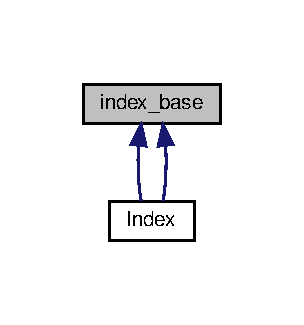
\includegraphics[width=146pt]{classindex__base__inherit__graph}
\end{center}
\end{figure}


Collaboration diagram for index\+\_\+base\+:
\nopagebreak
\begin{figure}[H]
\begin{center}
\leavevmode
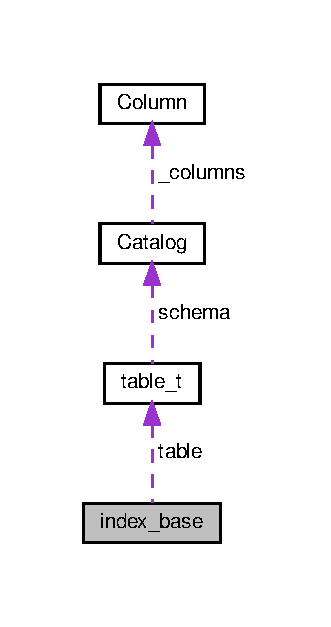
\includegraphics[width=159pt]{classindex__base__coll__graph}
\end{center}
\end{figure}
\subsection*{Public Member Functions}
\begin{DoxyCompactItemize}
\item 
\hyperlink{classindex__base_a080b89f830ec83536c2a28103ebd5b28}{index\+\_\+base} ()
\item 
virtual \hyperlink{global_8h_a78c49a674c810fdd03d20432f7be864a}{RC} \hyperlink{classindex__base_a819b2cb7cbc7c740381e64d4c9023745}{index\+\_\+insert} (\hyperlink{index__base_8h_ae35c40bc2f912c11f0e36ac66cba4489}{K\+E\+Y\+\_\+\+T\+Y\+PE} key, \hyperlink{microbench_2main_8cpp_ae17cb099b4c9aee7835032339b5a9e0d}{V\+A\+L\+U\+E\+\_\+\+T\+Y\+PE} item, int part\+\_\+id=-\/1)=0
\item 
virtual \hyperlink{global_8h_a78c49a674c810fdd03d20432f7be864a}{RC} \hyperlink{classindex__base_ae63072105f55821091506f1a6557dd1c}{index\+\_\+read} (\hyperlink{index__base_8h_ae35c40bc2f912c11f0e36ac66cba4489}{K\+E\+Y\+\_\+\+T\+Y\+PE} key, \hyperlink{microbench_2main_8cpp_ae17cb099b4c9aee7835032339b5a9e0d}{V\+A\+L\+U\+E\+\_\+\+T\+Y\+PE} $\ast$item, int part\+\_\+id=-\/1, int thd\+\_\+id=0)=0
\item 
virtual \hyperlink{global_8h_a78c49a674c810fdd03d20432f7be864a}{RC} \hyperlink{classindex__base_a044a748df8945a60af8ab815b555960a}{index\+\_\+read} (\hyperlink{index__base_8h_ae35c40bc2f912c11f0e36ac66cba4489}{K\+E\+Y\+\_\+\+T\+Y\+PE} key, \hyperlink{microbench_2main_8cpp_ae17cb099b4c9aee7835032339b5a9e0d}{V\+A\+L\+U\+E\+\_\+\+T\+Y\+PE} $\ast$item, int part\+\_\+id=-\/1)
\item 
virtual \hyperlink{global_8h_a78c49a674c810fdd03d20432f7be864a}{RC} \hyperlink{classindex__base_aa51e3945ff304a47364499c3e716a87f}{index\+\_\+read} (\hyperlink{index__base_8h_ae35c40bc2f912c11f0e36ac66cba4489}{K\+E\+Y\+\_\+\+T\+Y\+PE} key, \hyperlink{microbench_2main_8cpp_ae17cb099b4c9aee7835032339b5a9e0d}{V\+A\+L\+U\+E\+\_\+\+T\+Y\+PE} $\ast$item)
\item 
virtual \hyperlink{global_8h_a78c49a674c810fdd03d20432f7be864a}{RC} \hyperlink{classindex__base_a9af0a86bbc85f29fa12d1394317b6fbd}{index\+\_\+remove} (\hyperlink{index__base_8h_ae35c40bc2f912c11f0e36ac66cba4489}{K\+E\+Y\+\_\+\+T\+Y\+PE} key)
\item 
virtual void \hyperlink{classindex__base_a2515fc45e7ca43a9914c0410a9b663c8}{print\+\_\+stats} ()
\item 
virtual size\+\_\+t \hyperlink{classindex__base_ab8bfe46c64ea1ab3c596c46f0b76064e}{get\+Node\+Size} ()
\item 
virtual size\+\_\+t \hyperlink{classindex__base_a0050e83a568a2905c54c81d7515f4085}{get\+Descriptor\+Size} ()
\item 
void \hyperlink{classindex__base_aa1e0da4c7da2fc75201d567a007cf746}{lock\+\_\+key} (\hyperlink{index__base_8h_ae35c40bc2f912c11f0e36ac66cba4489}{K\+E\+Y\+\_\+\+T\+Y\+PE} key)
\item 
void \hyperlink{classindex__base_a6907aa960cab70f4693bf10891efa0b8}{unlock\+\_\+key} (\hyperlink{index__base_8h_ae35c40bc2f912c11f0e36ac66cba4489}{K\+E\+Y\+\_\+\+T\+Y\+PE} key)
\item 
void \hyperlink{classindex__base_ad8ff262d6b034e6de86651ef8f736cbb}{print\+Lock\+Counts} ()
\end{DoxyCompactItemize}
\subsection*{Public Attributes}
\begin{DoxyCompactItemize}
\item 
string \hyperlink{classindex__base_aa6f9ab0da3c1a5f3b1313961300724be}{index\+\_\+name}
\item 
int \hyperlink{classindex__base_ac74f658497f2950116acf136099eb980}{index\+\_\+id}
\end{DoxyCompactItemize}
\subsection*{Protected Attributes}
\begin{DoxyCompactItemize}
\item 
\hyperlink{classindex__base_aecdbc18775b6db4572392085e82e12d2}{P\+AD}
\item 
char \hyperlink{classindex__base_a2b876c502b9e52ab748db529dae6a403}{initialized\+Threads} \mbox{[}\hyperlink{plaf_8h_ac1585a3455dd3e33e877e588be9e466b}{M\+A\+X\+\_\+\+T\+H\+R\+E\+A\+D\+S\+\_\+\+P\+O\+W2} $\ast$\hyperlink{plaf_8h_a9492d3f4847aa8514510373df7ad0e73}{P\+R\+E\+F\+E\+T\+C\+H\+\_\+\+S\+I\+Z\+E\+\_\+\+B\+Y\+T\+ES}\mbox{]}
\item 
unsigned long long \hyperlink{classindex__base_a174339e599ecc8f223744c01ebeef0d3}{num\+Inserts} \mbox{[}\hyperlink{plaf_8h_ac1585a3455dd3e33e877e588be9e466b}{M\+A\+X\+\_\+\+T\+H\+R\+E\+A\+D\+S\+\_\+\+P\+O\+W2} $\ast$\hyperlink{plaf_8h_af55592679e3b40dd3c45ec6faef1b053}{P\+R\+E\+F\+E\+T\+C\+H\+\_\+\+S\+I\+Z\+E\+\_\+\+W\+O\+R\+DS}\mbox{]}
\item 
unsigned long long \hyperlink{classindex__base_ac947600e88bf99120d4a2bfb7e3be395}{num\+Reads} \mbox{[}\hyperlink{plaf_8h_ac1585a3455dd3e33e877e588be9e466b}{M\+A\+X\+\_\+\+T\+H\+R\+E\+A\+D\+S\+\_\+\+P\+O\+W2} $\ast$\hyperlink{plaf_8h_af55592679e3b40dd3c45ec6faef1b053}{P\+R\+E\+F\+E\+T\+C\+H\+\_\+\+S\+I\+Z\+E\+\_\+\+W\+O\+R\+DS}\mbox{]}
\item 
volatile \hyperlink{index__base_8h_a83d2222c5a48984baf95b9d9c50b23dc}{vwlock} \hyperlink{classindex__base_ab017238f575199c45f558d878f949635}{Lock\+Tab} \mbox{[}\hyperlink{index__base_8h_aaad4f00f49f1549864c4e86f2e2d38c8}{\+\_\+\+T\+A\+B\+SZ}\mbox{]}
\item 
long long \hyperlink{classindex__base_a2997801372bcddaa3ca891923833700c}{lock\+Histogram} \mbox{[}\hyperlink{index__base_8h_a4f19ac3a740945eca7da525767872383}{P\+R\+I\+N\+T\+\_\+\+B\+U\+C\+K\+E\+TS}\mbox{]}
\item 
uint64\+\_\+t \hyperlink{classindex__base_ad7276d1faf3b802ddd3ed0a0e8442e3f}{debug\+\_\+init\+\_\+is\+\_\+done}
\item 
\hyperlink{classtable__t}{table\+\_\+t} $\ast$ \hyperlink{classindex__base_abb51a82fc0bf85a82aa83376d111641f}{table}
\end{DoxyCompactItemize}


\subsection{Constructor \& Destructor Documentation}
\mbox{\Hypertarget{classindex__base_a080b89f830ec83536c2a28103ebd5b28}\label{classindex__base_a080b89f830ec83536c2a28103ebd5b28}} 
\index{index\+\_\+base@{index\+\_\+base}!index\+\_\+base@{index\+\_\+base}}
\index{index\+\_\+base@{index\+\_\+base}!index\+\_\+base@{index\+\_\+base}}
\subsubsection{\texorpdfstring{index\+\_\+base()}{index\_base()}}
{\footnotesize\ttfamily index\+\_\+base\+::index\+\_\+base (\begin{DoxyParamCaption}{ }\end{DoxyParamCaption})\hspace{0.3cm}{\ttfamily [inline]}}



\subsection{Member Function Documentation}
\mbox{\Hypertarget{classindex__base_a0050e83a568a2905c54c81d7515f4085}\label{classindex__base_a0050e83a568a2905c54c81d7515f4085}} 
\index{index\+\_\+base@{index\+\_\+base}!get\+Descriptor\+Size@{get\+Descriptor\+Size}}
\index{get\+Descriptor\+Size@{get\+Descriptor\+Size}!index\+\_\+base@{index\+\_\+base}}
\subsubsection{\texorpdfstring{get\+Descriptor\+Size()}{getDescriptorSize()}}
{\footnotesize\ttfamily virtual size\+\_\+t index\+\_\+base\+::get\+Descriptor\+Size (\begin{DoxyParamCaption}{ }\end{DoxyParamCaption})\hspace{0.3cm}{\ttfamily [inline]}, {\ttfamily [virtual]}}



Reimplemented in \hyperlink{classIndex_a0e0b37468dc2b549208da43466a68a94}{Index}.

\mbox{\Hypertarget{classindex__base_ab8bfe46c64ea1ab3c596c46f0b76064e}\label{classindex__base_ab8bfe46c64ea1ab3c596c46f0b76064e}} 
\index{index\+\_\+base@{index\+\_\+base}!get\+Node\+Size@{get\+Node\+Size}}
\index{get\+Node\+Size@{get\+Node\+Size}!index\+\_\+base@{index\+\_\+base}}
\subsubsection{\texorpdfstring{get\+Node\+Size()}{getNodeSize()}}
{\footnotesize\ttfamily virtual size\+\_\+t index\+\_\+base\+::get\+Node\+Size (\begin{DoxyParamCaption}{ }\end{DoxyParamCaption})\hspace{0.3cm}{\ttfamily [inline]}, {\ttfamily [virtual]}}



Reimplemented in \hyperlink{classIndex_ad70e606faaf0a67b690275b8f8ca5d5f}{Index}.

\mbox{\Hypertarget{classindex__base_a819b2cb7cbc7c740381e64d4c9023745}\label{classindex__base_a819b2cb7cbc7c740381e64d4c9023745}} 
\index{index\+\_\+base@{index\+\_\+base}!index\+\_\+insert@{index\+\_\+insert}}
\index{index\+\_\+insert@{index\+\_\+insert}!index\+\_\+base@{index\+\_\+base}}
\subsubsection{\texorpdfstring{index\+\_\+insert()}{index\_insert()}}
{\footnotesize\ttfamily virtual \hyperlink{global_8h_a78c49a674c810fdd03d20432f7be864a}{RC} index\+\_\+base\+::index\+\_\+insert (\begin{DoxyParamCaption}\item[{\hyperlink{index__base_8h_ae35c40bc2f912c11f0e36ac66cba4489}{K\+E\+Y\+\_\+\+T\+Y\+PE}}]{key,  }\item[{\hyperlink{microbench_2main_8cpp_ae17cb099b4c9aee7835032339b5a9e0d}{V\+A\+L\+U\+E\+\_\+\+T\+Y\+PE}}]{item,  }\item[{int}]{part\+\_\+id = {\ttfamily -\/1} }\end{DoxyParamCaption})\hspace{0.3cm}{\ttfamily [pure virtual]}}



Implemented in \hyperlink{classIndex_a2266050deae0c62e0b90e7d60fd70f35}{Index}, and \hyperlink{classIndex_a03544bdceed7feb756712086fb239de1}{Index}.

\mbox{\Hypertarget{classindex__base_ae63072105f55821091506f1a6557dd1c}\label{classindex__base_ae63072105f55821091506f1a6557dd1c}} 
\index{index\+\_\+base@{index\+\_\+base}!index\+\_\+read@{index\+\_\+read}}
\index{index\+\_\+read@{index\+\_\+read}!index\+\_\+base@{index\+\_\+base}}
\subsubsection{\texorpdfstring{index\+\_\+read()}{index\_read()}\hspace{0.1cm}{\footnotesize\ttfamily [1/3]}}
{\footnotesize\ttfamily virtual \hyperlink{global_8h_a78c49a674c810fdd03d20432f7be864a}{RC} index\+\_\+base\+::index\+\_\+read (\begin{DoxyParamCaption}\item[{\hyperlink{index__base_8h_ae35c40bc2f912c11f0e36ac66cba4489}{K\+E\+Y\+\_\+\+T\+Y\+PE}}]{key,  }\item[{\hyperlink{microbench_2main_8cpp_ae17cb099b4c9aee7835032339b5a9e0d}{V\+A\+L\+U\+E\+\_\+\+T\+Y\+PE} $\ast$}]{item,  }\item[{int}]{part\+\_\+id = {\ttfamily -\/1},  }\item[{int}]{thd\+\_\+id = {\ttfamily 0} }\end{DoxyParamCaption})\hspace{0.3cm}{\ttfamily [pure virtual]}}



Implemented in \hyperlink{classIndex_abb1666dd897887f22d8e4dc92966b207}{Index}, and \hyperlink{classIndex_abb1666dd897887f22d8e4dc92966b207}{Index}.

\mbox{\Hypertarget{classindex__base_a044a748df8945a60af8ab815b555960a}\label{classindex__base_a044a748df8945a60af8ab815b555960a}} 
\index{index\+\_\+base@{index\+\_\+base}!index\+\_\+read@{index\+\_\+read}}
\index{index\+\_\+read@{index\+\_\+read}!index\+\_\+base@{index\+\_\+base}}
\subsubsection{\texorpdfstring{index\+\_\+read()}{index\_read()}\hspace{0.1cm}{\footnotesize\ttfamily [2/3]}}
{\footnotesize\ttfamily virtual \hyperlink{global_8h_a78c49a674c810fdd03d20432f7be864a}{RC} index\+\_\+base\+::index\+\_\+read (\begin{DoxyParamCaption}\item[{\hyperlink{index__base_8h_ae35c40bc2f912c11f0e36ac66cba4489}{K\+E\+Y\+\_\+\+T\+Y\+PE}}]{key,  }\item[{\hyperlink{microbench_2main_8cpp_ae17cb099b4c9aee7835032339b5a9e0d}{V\+A\+L\+U\+E\+\_\+\+T\+Y\+PE} $\ast$}]{item,  }\item[{int}]{part\+\_\+id = {\ttfamily -\/1} }\end{DoxyParamCaption})\hspace{0.3cm}{\ttfamily [inline]}, {\ttfamily [virtual]}}



Reimplemented in \hyperlink{classIndex_ab930b74f611f4704fa1fb9a8bb9f57f8}{Index}.

\mbox{\Hypertarget{classindex__base_aa51e3945ff304a47364499c3e716a87f}\label{classindex__base_aa51e3945ff304a47364499c3e716a87f}} 
\index{index\+\_\+base@{index\+\_\+base}!index\+\_\+read@{index\+\_\+read}}
\index{index\+\_\+read@{index\+\_\+read}!index\+\_\+base@{index\+\_\+base}}
\subsubsection{\texorpdfstring{index\+\_\+read()}{index\_read()}\hspace{0.1cm}{\footnotesize\ttfamily [3/3]}}
{\footnotesize\ttfamily virtual \hyperlink{global_8h_a78c49a674c810fdd03d20432f7be864a}{RC} index\+\_\+base\+::index\+\_\+read (\begin{DoxyParamCaption}\item[{\hyperlink{index__base_8h_ae35c40bc2f912c11f0e36ac66cba4489}{K\+E\+Y\+\_\+\+T\+Y\+PE}}]{key,  }\item[{\hyperlink{microbench_2main_8cpp_ae17cb099b4c9aee7835032339b5a9e0d}{V\+A\+L\+U\+E\+\_\+\+T\+Y\+PE} $\ast$}]{item }\end{DoxyParamCaption})\hspace{0.3cm}{\ttfamily [inline]}, {\ttfamily [virtual]}}

\mbox{\Hypertarget{classindex__base_a9af0a86bbc85f29fa12d1394317b6fbd}\label{classindex__base_a9af0a86bbc85f29fa12d1394317b6fbd}} 
\index{index\+\_\+base@{index\+\_\+base}!index\+\_\+remove@{index\+\_\+remove}}
\index{index\+\_\+remove@{index\+\_\+remove}!index\+\_\+base@{index\+\_\+base}}
\subsubsection{\texorpdfstring{index\+\_\+remove()}{index\_remove()}}
{\footnotesize\ttfamily virtual \hyperlink{global_8h_a78c49a674c810fdd03d20432f7be864a}{RC} index\+\_\+base\+::index\+\_\+remove (\begin{DoxyParamCaption}\item[{\hyperlink{index__base_8h_ae35c40bc2f912c11f0e36ac66cba4489}{K\+E\+Y\+\_\+\+T\+Y\+PE}}]{key }\end{DoxyParamCaption})\hspace{0.3cm}{\ttfamily [inline]}, {\ttfamily [virtual]}}

\mbox{\Hypertarget{classindex__base_aa1e0da4c7da2fc75201d567a007cf746}\label{classindex__base_aa1e0da4c7da2fc75201d567a007cf746}} 
\index{index\+\_\+base@{index\+\_\+base}!lock\+\_\+key@{lock\+\_\+key}}
\index{lock\+\_\+key@{lock\+\_\+key}!index\+\_\+base@{index\+\_\+base}}
\subsubsection{\texorpdfstring{lock\+\_\+key()}{lock\_key()}}
{\footnotesize\ttfamily void index\+\_\+base\+::lock\+\_\+key (\begin{DoxyParamCaption}\item[{\hyperlink{index__base_8h_ae35c40bc2f912c11f0e36ac66cba4489}{K\+E\+Y\+\_\+\+T\+Y\+PE}}]{key }\end{DoxyParamCaption})\hspace{0.3cm}{\ttfamily [inline]}}

\mbox{\Hypertarget{classindex__base_a2515fc45e7ca43a9914c0410a9b663c8}\label{classindex__base_a2515fc45e7ca43a9914c0410a9b663c8}} 
\index{index\+\_\+base@{index\+\_\+base}!print\+\_\+stats@{print\+\_\+stats}}
\index{print\+\_\+stats@{print\+\_\+stats}!index\+\_\+base@{index\+\_\+base}}
\subsubsection{\texorpdfstring{print\+\_\+stats()}{print\_stats()}}
{\footnotesize\ttfamily virtual void index\+\_\+base\+::print\+\_\+stats (\begin{DoxyParamCaption}{ }\end{DoxyParamCaption})\hspace{0.3cm}{\ttfamily [inline]}, {\ttfamily [virtual]}}



Reimplemented in \hyperlink{classIndex_ab300e132e8a12e3334003227a2e3f618}{Index}.

\mbox{\Hypertarget{classindex__base_ad8ff262d6b034e6de86651ef8f736cbb}\label{classindex__base_ad8ff262d6b034e6de86651ef8f736cbb}} 
\index{index\+\_\+base@{index\+\_\+base}!print\+Lock\+Counts@{print\+Lock\+Counts}}
\index{print\+Lock\+Counts@{print\+Lock\+Counts}!index\+\_\+base@{index\+\_\+base}}
\subsubsection{\texorpdfstring{print\+Lock\+Counts()}{printLockCounts()}}
{\footnotesize\ttfamily void index\+\_\+base\+::print\+Lock\+Counts (\begin{DoxyParamCaption}{ }\end{DoxyParamCaption})\hspace{0.3cm}{\ttfamily [inline]}}

\mbox{\Hypertarget{classindex__base_a6907aa960cab70f4693bf10891efa0b8}\label{classindex__base_a6907aa960cab70f4693bf10891efa0b8}} 
\index{index\+\_\+base@{index\+\_\+base}!unlock\+\_\+key@{unlock\+\_\+key}}
\index{unlock\+\_\+key@{unlock\+\_\+key}!index\+\_\+base@{index\+\_\+base}}
\subsubsection{\texorpdfstring{unlock\+\_\+key()}{unlock\_key()}}
{\footnotesize\ttfamily void index\+\_\+base\+::unlock\+\_\+key (\begin{DoxyParamCaption}\item[{\hyperlink{index__base_8h_ae35c40bc2f912c11f0e36ac66cba4489}{K\+E\+Y\+\_\+\+T\+Y\+PE}}]{key }\end{DoxyParamCaption})\hspace{0.3cm}{\ttfamily [inline]}}



\subsection{Member Data Documentation}
\mbox{\Hypertarget{classindex__base_ad7276d1faf3b802ddd3ed0a0e8442e3f}\label{classindex__base_ad7276d1faf3b802ddd3ed0a0e8442e3f}} 
\index{index\+\_\+base@{index\+\_\+base}!debug\+\_\+init\+\_\+is\+\_\+done@{debug\+\_\+init\+\_\+is\+\_\+done}}
\index{debug\+\_\+init\+\_\+is\+\_\+done@{debug\+\_\+init\+\_\+is\+\_\+done}!index\+\_\+base@{index\+\_\+base}}
\subsubsection{\texorpdfstring{debug\+\_\+init\+\_\+is\+\_\+done}{debug\_init\_is\_done}}
{\footnotesize\ttfamily uint64\+\_\+t index\+\_\+base\+::debug\+\_\+init\+\_\+is\+\_\+done\hspace{0.3cm}{\ttfamily [protected]}}

\mbox{\Hypertarget{classindex__base_ac74f658497f2950116acf136099eb980}\label{classindex__base_ac74f658497f2950116acf136099eb980}} 
\index{index\+\_\+base@{index\+\_\+base}!index\+\_\+id@{index\+\_\+id}}
\index{index\+\_\+id@{index\+\_\+id}!index\+\_\+base@{index\+\_\+base}}
\subsubsection{\texorpdfstring{index\+\_\+id}{index\_id}}
{\footnotesize\ttfamily int index\+\_\+base\+::index\+\_\+id}

\mbox{\Hypertarget{classindex__base_aa6f9ab0da3c1a5f3b1313961300724be}\label{classindex__base_aa6f9ab0da3c1a5f3b1313961300724be}} 
\index{index\+\_\+base@{index\+\_\+base}!index\+\_\+name@{index\+\_\+name}}
\index{index\+\_\+name@{index\+\_\+name}!index\+\_\+base@{index\+\_\+base}}
\subsubsection{\texorpdfstring{index\+\_\+name}{index\_name}}
{\footnotesize\ttfamily string index\+\_\+base\+::index\+\_\+name}

\mbox{\Hypertarget{classindex__base_a2b876c502b9e52ab748db529dae6a403}\label{classindex__base_a2b876c502b9e52ab748db529dae6a403}} 
\index{index\+\_\+base@{index\+\_\+base}!initialized\+Threads@{initialized\+Threads}}
\index{initialized\+Threads@{initialized\+Threads}!index\+\_\+base@{index\+\_\+base}}
\subsubsection{\texorpdfstring{initialized\+Threads}{initializedThreads}}
{\footnotesize\ttfamily char index\+\_\+base\+::initialized\+Threads\mbox{[}\hyperlink{plaf_8h_ac1585a3455dd3e33e877e588be9e466b}{M\+A\+X\+\_\+\+T\+H\+R\+E\+A\+D\+S\+\_\+\+P\+O\+W2} $\ast$\hyperlink{plaf_8h_a9492d3f4847aa8514510373df7ad0e73}{P\+R\+E\+F\+E\+T\+C\+H\+\_\+\+S\+I\+Z\+E\+\_\+\+B\+Y\+T\+ES}\mbox{]}\hspace{0.3cm}{\ttfamily [protected]}}

\mbox{\Hypertarget{classindex__base_a2997801372bcddaa3ca891923833700c}\label{classindex__base_a2997801372bcddaa3ca891923833700c}} 
\index{index\+\_\+base@{index\+\_\+base}!lock\+Histogram@{lock\+Histogram}}
\index{lock\+Histogram@{lock\+Histogram}!index\+\_\+base@{index\+\_\+base}}
\subsubsection{\texorpdfstring{lock\+Histogram}{lockHistogram}}
{\footnotesize\ttfamily long long index\+\_\+base\+::lock\+Histogram\mbox{[}\hyperlink{index__base_8h_a4f19ac3a740945eca7da525767872383}{P\+R\+I\+N\+T\+\_\+\+B\+U\+C\+K\+E\+TS}\mbox{]}\hspace{0.3cm}{\ttfamily [protected]}}

\mbox{\Hypertarget{classindex__base_ab017238f575199c45f558d878f949635}\label{classindex__base_ab017238f575199c45f558d878f949635}} 
\index{index\+\_\+base@{index\+\_\+base}!Lock\+Tab@{Lock\+Tab}}
\index{Lock\+Tab@{Lock\+Tab}!index\+\_\+base@{index\+\_\+base}}
\subsubsection{\texorpdfstring{Lock\+Tab}{LockTab}}
{\footnotesize\ttfamily volatile \hyperlink{index__base_8h_a83d2222c5a48984baf95b9d9c50b23dc}{vwlock} index\+\_\+base\+::\+Lock\+Tab\mbox{[}\hyperlink{index__base_8h_aaad4f00f49f1549864c4e86f2e2d38c8}{\+\_\+\+T\+A\+B\+SZ}\mbox{]}\hspace{0.3cm}{\ttfamily [protected]}}

\mbox{\Hypertarget{classindex__base_a174339e599ecc8f223744c01ebeef0d3}\label{classindex__base_a174339e599ecc8f223744c01ebeef0d3}} 
\index{index\+\_\+base@{index\+\_\+base}!num\+Inserts@{num\+Inserts}}
\index{num\+Inserts@{num\+Inserts}!index\+\_\+base@{index\+\_\+base}}
\subsubsection{\texorpdfstring{num\+Inserts}{numInserts}}
{\footnotesize\ttfamily unsigned long long index\+\_\+base\+::num\+Inserts\mbox{[}\hyperlink{plaf_8h_ac1585a3455dd3e33e877e588be9e466b}{M\+A\+X\+\_\+\+T\+H\+R\+E\+A\+D\+S\+\_\+\+P\+O\+W2} $\ast$\hyperlink{plaf_8h_af55592679e3b40dd3c45ec6faef1b053}{P\+R\+E\+F\+E\+T\+C\+H\+\_\+\+S\+I\+Z\+E\+\_\+\+W\+O\+R\+DS}\mbox{]}\hspace{0.3cm}{\ttfamily [protected]}}

\mbox{\Hypertarget{classindex__base_ac947600e88bf99120d4a2bfb7e3be395}\label{classindex__base_ac947600e88bf99120d4a2bfb7e3be395}} 
\index{index\+\_\+base@{index\+\_\+base}!num\+Reads@{num\+Reads}}
\index{num\+Reads@{num\+Reads}!index\+\_\+base@{index\+\_\+base}}
\subsubsection{\texorpdfstring{num\+Reads}{numReads}}
{\footnotesize\ttfamily unsigned long long index\+\_\+base\+::num\+Reads\mbox{[}\hyperlink{plaf_8h_ac1585a3455dd3e33e877e588be9e466b}{M\+A\+X\+\_\+\+T\+H\+R\+E\+A\+D\+S\+\_\+\+P\+O\+W2} $\ast$\hyperlink{plaf_8h_af55592679e3b40dd3c45ec6faef1b053}{P\+R\+E\+F\+E\+T\+C\+H\+\_\+\+S\+I\+Z\+E\+\_\+\+W\+O\+R\+DS}\mbox{]}\hspace{0.3cm}{\ttfamily [protected]}}

\mbox{\Hypertarget{classindex__base_aecdbc18775b6db4572392085e82e12d2}\label{classindex__base_aecdbc18775b6db4572392085e82e12d2}} 
\index{index\+\_\+base@{index\+\_\+base}!P\+AD@{P\+AD}}
\index{P\+AD@{P\+AD}!index\+\_\+base@{index\+\_\+base}}
\subsubsection{\texorpdfstring{P\+AD}{PAD}}
{\footnotesize\ttfamily index\+\_\+base\+::\+P\+AD\hspace{0.3cm}{\ttfamily [protected]}}

\mbox{\Hypertarget{classindex__base_abb51a82fc0bf85a82aa83376d111641f}\label{classindex__base_abb51a82fc0bf85a82aa83376d111641f}} 
\index{index\+\_\+base@{index\+\_\+base}!table@{table}}
\index{table@{table}!index\+\_\+base@{index\+\_\+base}}
\subsubsection{\texorpdfstring{table}{table}}
{\footnotesize\ttfamily \hyperlink{classtable__t}{table\+\_\+t}$\ast$ index\+\_\+base\+::table\hspace{0.3cm}{\ttfamily [protected]}}



The documentation for this class was generated from the following file\+:\begin{DoxyCompactItemize}
\item 
macrobench/storage/index/\hyperlink{index__base_8h}{index\+\_\+base.\+h}\end{DoxyCompactItemize}

\hypertarget{unioninfo__t}{}\section{info\+\_\+t$<$ skey\+\_\+t, sval\+\_\+t $>$ Union Template Reference}
\label{unioninfo__t}\index{info\+\_\+t$<$ skey\+\_\+t, sval\+\_\+t $>$@{info\+\_\+t$<$ skey\+\_\+t, sval\+\_\+t $>$}}


{\ttfamily \#include $<$ellen\+\_\+impl.\+h$>$}

\subsection*{Public Attributes}
\begin{DoxyCompactItemize}
\item 
\hyperlink{structiinfo__t}{iinfo\+\_\+t}$<$ skey\+\_\+t, sval\+\_\+t $>$ \hyperlink{unioninfo__t_a422b1155c4af5af9b6696789fedb790a}{iinfo}
\item 
\hyperlink{structdinfo__t}{dinfo\+\_\+t}$<$ skey\+\_\+t, sval\+\_\+t $>$ \hyperlink{unioninfo__t_acb3605bfd5bde422fa2f628c90fbd224}{dinfo}
\item 
uint8\+\_\+t \hyperlink{unioninfo__t_a4ebfec4af276b167babd6ce6e9536efe}{padding} \mbox{[}64\mbox{]}
\end{DoxyCompactItemize}


\subsection{Member Data Documentation}
\mbox{\Hypertarget{unioninfo__t_acb3605bfd5bde422fa2f628c90fbd224}\label{unioninfo__t_acb3605bfd5bde422fa2f628c90fbd224}} 
\index{info\+\_\+t@{info\+\_\+t}!dinfo@{dinfo}}
\index{dinfo@{dinfo}!info\+\_\+t@{info\+\_\+t}}
\subsubsection{\texorpdfstring{dinfo}{dinfo}}
{\footnotesize\ttfamily template$<$typename skey\+\_\+t, typename sval\+\_\+t$>$ \\
\hyperlink{structdinfo__t}{dinfo\+\_\+t}$<$skey\+\_\+t, sval\+\_\+t$>$ \hyperlink{unioninfo__t}{info\+\_\+t}$<$ skey\+\_\+t, sval\+\_\+t $>$\+::dinfo}

\mbox{\Hypertarget{unioninfo__t_a422b1155c4af5af9b6696789fedb790a}\label{unioninfo__t_a422b1155c4af5af9b6696789fedb790a}} 
\index{info\+\_\+t@{info\+\_\+t}!iinfo@{iinfo}}
\index{iinfo@{iinfo}!info\+\_\+t@{info\+\_\+t}}
\subsubsection{\texorpdfstring{iinfo}{iinfo}}
{\footnotesize\ttfamily template$<$typename skey\+\_\+t, typename sval\+\_\+t$>$ \\
\hyperlink{structiinfo__t}{iinfo\+\_\+t}$<$skey\+\_\+t, sval\+\_\+t$>$ \hyperlink{unioninfo__t}{info\+\_\+t}$<$ skey\+\_\+t, sval\+\_\+t $>$\+::iinfo}

\mbox{\Hypertarget{unioninfo__t_a4ebfec4af276b167babd6ce6e9536efe}\label{unioninfo__t_a4ebfec4af276b167babd6ce6e9536efe}} 
\index{info\+\_\+t@{info\+\_\+t}!padding@{padding}}
\index{padding@{padding}!info\+\_\+t@{info\+\_\+t}}
\subsubsection{\texorpdfstring{padding}{padding}}
{\footnotesize\ttfamily template$<$typename skey\+\_\+t, typename sval\+\_\+t$>$ \\
uint8\+\_\+t \hyperlink{unioninfo__t}{info\+\_\+t}$<$ skey\+\_\+t, sval\+\_\+t $>$\+::padding\mbox{[}64\mbox{]}}



The documentation for this union was generated from the following file\+:\begin{DoxyCompactItemize}
\item 
ds/ellen\+\_\+ext\+\_\+bst\+\_\+lf/\hyperlink{ellen__impl_8h}{ellen\+\_\+impl.\+h}\end{DoxyCompactItemize}

\hypertarget{classInternalKCAS}{}\section{Internal\+K\+C\+AS$<$ Record\+Manager, K, V $>$ Class Template Reference}
\label{classInternalKCAS}\index{Internal\+K\+C\+A\+S$<$ Record\+Manager, K, V $>$@{Internal\+K\+C\+A\+S$<$ Record\+Manager, K, V $>$}}


{\ttfamily \#include $<$internal\+\_\+kcas.\+h$>$}

\subsection*{Public Member Functions}
\begin{DoxyCompactItemize}
\item 
\hyperlink{classInternalKCAS_ac9c322cd3a85b979a08de155c21f67e1}{Internal\+K\+C\+AS} (const int \+\_\+num\+Threads, const int \+\_\+min\+Key, const long long \+\_\+max\+Key)
\item 
\hyperlink{classInternalKCAS_abd61df2bf061536a6565252d31d3f3f3}{$\sim$\+Internal\+K\+C\+AS} ()
\item 
bool \hyperlink{classInternalKCAS_a6cc67a7c0c48dcb3dfc92caf1661caff}{contains} (const int \hyperlink{microbench_2main_8cpp_a9ca9869868fe7e7a38a921cc7de4103f}{tid}, const K \&key)
\item 
V \hyperlink{classInternalKCAS_ab3010217722850563fca996779d44aaf}{insert\+If\+Absent} (const int \hyperlink{microbench_2main_8cpp_a9ca9869868fe7e7a38a921cc7de4103f}{tid}, const K \&key, const V \&value)
\item 
V \hyperlink{classInternalKCAS_a13be8756f4bed1d759d5018aa0d2d380}{erase} (const int \hyperlink{microbench_2main_8cpp_a9ca9869868fe7e7a38a921cc7de4103f}{tid}, const K \&key)
\item 
bool \hyperlink{classInternalKCAS_abbe352f377d39453950e11caf7c5081d}{validate} ()
\item 
void \hyperlink{classInternalKCAS_a03139bf48fad9708cf170f246696870a}{print\+Debugging\+Details} ()
\item 
\hyperlink{classNode}{Node}$<$ K, V $>$ $\ast$ \hyperlink{classInternalKCAS_af0b27ea462939a6e491e0775f4ab0b9e}{get\+Root} ()
\item 
void \hyperlink{classInternalKCAS_ab4fe3ffb3c0839a75a9a4272750d10e4}{init\+Thread} (const int \hyperlink{microbench_2main_8cpp_a9ca9869868fe7e7a38a921cc7de4103f}{tid})
\item 
void \hyperlink{classInternalKCAS_a34b83ecf38951b339abc5e1270d97c84}{deinit\+Thread} (const int \hyperlink{microbench_2main_8cpp_a9ca9869868fe7e7a38a921cc7de4103f}{tid})
\item 
int \hyperlink{classInternalKCAS_ad72d4be132cc659a5c992321277cf193}{get\+Height} (\hyperlink{classNode}{Node}$<$ K, V $>$ $\ast$node)
\item 
\hyperlink{classInternalKCAS_ac9c322cd3a85b979a08de155c21f67e1}{Internal\+K\+C\+AS} (const int \+\_\+num\+Threads, const int \+\_\+min\+Key, const long long \+\_\+max\+Key)
\item 
\hyperlink{classInternalKCAS_abd61df2bf061536a6565252d31d3f3f3}{$\sim$\+Internal\+K\+C\+AS} ()
\item 
bool \hyperlink{classInternalKCAS_a6cc67a7c0c48dcb3dfc92caf1661caff}{contains} (const int \hyperlink{microbench_2main_8cpp_a9ca9869868fe7e7a38a921cc7de4103f}{tid}, const K \&key)
\item 
V \hyperlink{classInternalKCAS_ab3010217722850563fca996779d44aaf}{insert\+If\+Absent} (const int \hyperlink{microbench_2main_8cpp_a9ca9869868fe7e7a38a921cc7de4103f}{tid}, const K \&key, const V \&value)
\item 
V \hyperlink{classInternalKCAS_a13be8756f4bed1d759d5018aa0d2d380}{erase} (const int \hyperlink{microbench_2main_8cpp_a9ca9869868fe7e7a38a921cc7de4103f}{tid}, const K \&key)
\item 
bool \hyperlink{classInternalKCAS_abbe352f377d39453950e11caf7c5081d}{validate} ()
\item 
void \hyperlink{classInternalKCAS_a03139bf48fad9708cf170f246696870a}{print\+Debugging\+Details} ()
\item 
\hyperlink{classNode}{Node}$<$ K, V $>$ $\ast$ \hyperlink{classInternalKCAS_a4b6e760af14cd473618fcc12baf18d6d}{get\+Root} ()
\item 
void \hyperlink{classInternalKCAS_ab4fe3ffb3c0839a75a9a4272750d10e4}{init\+Thread} (const int \hyperlink{microbench_2main_8cpp_a9ca9869868fe7e7a38a921cc7de4103f}{tid})
\item 
void \hyperlink{classInternalKCAS_a34b83ecf38951b339abc5e1270d97c84}{deinit\+Thread} (const int \hyperlink{microbench_2main_8cpp_a9ca9869868fe7e7a38a921cc7de4103f}{tid})
\end{DoxyCompactItemize}


\subsection{Constructor \& Destructor Documentation}
\mbox{\Hypertarget{classInternalKCAS_ac9c322cd3a85b979a08de155c21f67e1}\label{classInternalKCAS_ac9c322cd3a85b979a08de155c21f67e1}} 
\index{Internal\+K\+C\+AS@{Internal\+K\+C\+AS}!Internal\+K\+C\+AS@{Internal\+K\+C\+AS}}
\index{Internal\+K\+C\+AS@{Internal\+K\+C\+AS}!Internal\+K\+C\+AS@{Internal\+K\+C\+AS}}
\subsubsection{\texorpdfstring{Internal\+K\+C\+A\+S()}{InternalKCAS()}\hspace{0.1cm}{\footnotesize\ttfamily [1/2]}}
{\footnotesize\ttfamily template$<$class Record\+Manager , typename K , typename V $>$ \\
\hyperlink{classInternalKCAS}{Internal\+K\+C\+AS}$<$ Record\+Manager, K, V $>$\+::\hyperlink{classInternalKCAS}{Internal\+K\+C\+AS} (\begin{DoxyParamCaption}\item[{const int}]{\+\_\+num\+Threads,  }\item[{const int}]{\+\_\+min\+Key,  }\item[{const long long}]{\+\_\+max\+Key }\end{DoxyParamCaption})}

\mbox{\Hypertarget{classInternalKCAS_abd61df2bf061536a6565252d31d3f3f3}\label{classInternalKCAS_abd61df2bf061536a6565252d31d3f3f3}} 
\index{Internal\+K\+C\+AS@{Internal\+K\+C\+AS}!````~Internal\+K\+C\+AS@{$\sim$\+Internal\+K\+C\+AS}}
\index{````~Internal\+K\+C\+AS@{$\sim$\+Internal\+K\+C\+AS}!Internal\+K\+C\+AS@{Internal\+K\+C\+AS}}
\subsubsection{\texorpdfstring{$\sim$\+Internal\+K\+C\+A\+S()}{~InternalKCAS()}\hspace{0.1cm}{\footnotesize\ttfamily [1/2]}}
{\footnotesize\ttfamily template$<$class Record\+Manager , typename K , typename V $>$ \\
\hyperlink{classInternalKCAS}{Internal\+K\+C\+AS}$<$ Record\+Manager, K, V $>$\+::$\sim$\hyperlink{classInternalKCAS}{Internal\+K\+C\+AS} (\begin{DoxyParamCaption}{ }\end{DoxyParamCaption})}

\mbox{\Hypertarget{classInternalKCAS_ac9c322cd3a85b979a08de155c21f67e1}\label{classInternalKCAS_ac9c322cd3a85b979a08de155c21f67e1}} 
\index{Internal\+K\+C\+AS@{Internal\+K\+C\+AS}!Internal\+K\+C\+AS@{Internal\+K\+C\+AS}}
\index{Internal\+K\+C\+AS@{Internal\+K\+C\+AS}!Internal\+K\+C\+AS@{Internal\+K\+C\+AS}}
\subsubsection{\texorpdfstring{Internal\+K\+C\+A\+S()}{InternalKCAS()}\hspace{0.1cm}{\footnotesize\ttfamily [2/2]}}
{\footnotesize\ttfamily template$<$class Record\+Manager , typename K , typename V $>$ \\
\hyperlink{classInternalKCAS}{Internal\+K\+C\+AS}$<$ Record\+Manager, K, V $>$\+::\hyperlink{classInternalKCAS}{Internal\+K\+C\+AS} (\begin{DoxyParamCaption}\item[{const int}]{\+\_\+num\+Threads,  }\item[{const int}]{\+\_\+min\+Key,  }\item[{const long long}]{\+\_\+max\+Key }\end{DoxyParamCaption})}

\mbox{\Hypertarget{classInternalKCAS_abd61df2bf061536a6565252d31d3f3f3}\label{classInternalKCAS_abd61df2bf061536a6565252d31d3f3f3}} 
\index{Internal\+K\+C\+AS@{Internal\+K\+C\+AS}!````~Internal\+K\+C\+AS@{$\sim$\+Internal\+K\+C\+AS}}
\index{````~Internal\+K\+C\+AS@{$\sim$\+Internal\+K\+C\+AS}!Internal\+K\+C\+AS@{Internal\+K\+C\+AS}}
\subsubsection{\texorpdfstring{$\sim$\+Internal\+K\+C\+A\+S()}{~InternalKCAS()}\hspace{0.1cm}{\footnotesize\ttfamily [2/2]}}
{\footnotesize\ttfamily template$<$class Record\+Manager , typename K , typename V $>$ \\
\hyperlink{classInternalKCAS}{Internal\+K\+C\+AS}$<$ Record\+Manager, K, V $>$\+::$\sim$\hyperlink{classInternalKCAS}{Internal\+K\+C\+AS} (\begin{DoxyParamCaption}{ }\end{DoxyParamCaption})}



\subsection{Member Function Documentation}
\mbox{\Hypertarget{classInternalKCAS_a6cc67a7c0c48dcb3dfc92caf1661caff}\label{classInternalKCAS_a6cc67a7c0c48dcb3dfc92caf1661caff}} 
\index{Internal\+K\+C\+AS@{Internal\+K\+C\+AS}!contains@{contains}}
\index{contains@{contains}!Internal\+K\+C\+AS@{Internal\+K\+C\+AS}}
\subsubsection{\texorpdfstring{contains()}{contains()}\hspace{0.1cm}{\footnotesize\ttfamily [1/2]}}
{\footnotesize\ttfamily template$<$class Record\+Manager , typename K , typename V $>$ \\
bool \hyperlink{classInternalKCAS}{Internal\+K\+C\+AS}$<$ Record\+Manager, K, V $>$\+::contains (\begin{DoxyParamCaption}\item[{const int}]{tid,  }\item[{const K \&}]{key }\end{DoxyParamCaption})}

\mbox{\Hypertarget{classInternalKCAS_a6cc67a7c0c48dcb3dfc92caf1661caff}\label{classInternalKCAS_a6cc67a7c0c48dcb3dfc92caf1661caff}} 
\index{Internal\+K\+C\+AS@{Internal\+K\+C\+AS}!contains@{contains}}
\index{contains@{contains}!Internal\+K\+C\+AS@{Internal\+K\+C\+AS}}
\subsubsection{\texorpdfstring{contains()}{contains()}\hspace{0.1cm}{\footnotesize\ttfamily [2/2]}}
{\footnotesize\ttfamily template$<$class Record\+Manager , typename K , typename V $>$ \\
bool \hyperlink{classInternalKCAS}{Internal\+K\+C\+AS}$<$ Record\+Manager, K, V $>$\+::contains (\begin{DoxyParamCaption}\item[{const int}]{tid,  }\item[{const K \&}]{key }\end{DoxyParamCaption})\hspace{0.3cm}{\ttfamily [inline]}}

\mbox{\Hypertarget{classInternalKCAS_a34b83ecf38951b339abc5e1270d97c84}\label{classInternalKCAS_a34b83ecf38951b339abc5e1270d97c84}} 
\index{Internal\+K\+C\+AS@{Internal\+K\+C\+AS}!deinit\+Thread@{deinit\+Thread}}
\index{deinit\+Thread@{deinit\+Thread}!Internal\+K\+C\+AS@{Internal\+K\+C\+AS}}
\subsubsection{\texorpdfstring{deinit\+Thread()}{deinitThread()}\hspace{0.1cm}{\footnotesize\ttfamily [1/2]}}
{\footnotesize\ttfamily template$<$class Record\+Manager , typename K , typename V $>$ \\
void \hyperlink{classInternalKCAS}{Internal\+K\+C\+AS}$<$ Record\+Manager, K, V $>$\+::deinit\+Thread (\begin{DoxyParamCaption}\item[{const int}]{tid }\end{DoxyParamCaption})}

\mbox{\Hypertarget{classInternalKCAS_a34b83ecf38951b339abc5e1270d97c84}\label{classInternalKCAS_a34b83ecf38951b339abc5e1270d97c84}} 
\index{Internal\+K\+C\+AS@{Internal\+K\+C\+AS}!deinit\+Thread@{deinit\+Thread}}
\index{deinit\+Thread@{deinit\+Thread}!Internal\+K\+C\+AS@{Internal\+K\+C\+AS}}
\subsubsection{\texorpdfstring{deinit\+Thread()}{deinitThread()}\hspace{0.1cm}{\footnotesize\ttfamily [2/2]}}
{\footnotesize\ttfamily template$<$class Record\+Manager , typename K , typename V $>$ \\
void \hyperlink{classInternalKCAS}{Internal\+K\+C\+AS}$<$ Record\+Manager, K, V $>$\+::deinit\+Thread (\begin{DoxyParamCaption}\item[{const int}]{tid }\end{DoxyParamCaption})}

\mbox{\Hypertarget{classInternalKCAS_a13be8756f4bed1d759d5018aa0d2d380}\label{classInternalKCAS_a13be8756f4bed1d759d5018aa0d2d380}} 
\index{Internal\+K\+C\+AS@{Internal\+K\+C\+AS}!erase@{erase}}
\index{erase@{erase}!Internal\+K\+C\+AS@{Internal\+K\+C\+AS}}
\subsubsection{\texorpdfstring{erase()}{erase()}\hspace{0.1cm}{\footnotesize\ttfamily [1/2]}}
{\footnotesize\ttfamily template$<$class Record\+Manager , typename K , typename V $>$ \\
V \hyperlink{classInternalKCAS}{Internal\+K\+C\+AS}$<$ Record\+Manager, K, V $>$\+::erase (\begin{DoxyParamCaption}\item[{const int}]{tid,  }\item[{const K \&}]{key }\end{DoxyParamCaption})}

\mbox{\Hypertarget{classInternalKCAS_a13be8756f4bed1d759d5018aa0d2d380}\label{classInternalKCAS_a13be8756f4bed1d759d5018aa0d2d380}} 
\index{Internal\+K\+C\+AS@{Internal\+K\+C\+AS}!erase@{erase}}
\index{erase@{erase}!Internal\+K\+C\+AS@{Internal\+K\+C\+AS}}
\subsubsection{\texorpdfstring{erase()}{erase()}\hspace{0.1cm}{\footnotesize\ttfamily [2/2]}}
{\footnotesize\ttfamily template$<$class Record\+Manager , typename K , typename V $>$ \\
V \hyperlink{classInternalKCAS}{Internal\+K\+C\+AS}$<$ Record\+Manager, K, V $>$\+::erase (\begin{DoxyParamCaption}\item[{const int}]{tid,  }\item[{const K \&}]{key }\end{DoxyParamCaption})\hspace{0.3cm}{\ttfamily [inline]}}

\mbox{\Hypertarget{classInternalKCAS_ad72d4be132cc659a5c992321277cf193}\label{classInternalKCAS_ad72d4be132cc659a5c992321277cf193}} 
\index{Internal\+K\+C\+AS@{Internal\+K\+C\+AS}!get\+Height@{get\+Height}}
\index{get\+Height@{get\+Height}!Internal\+K\+C\+AS@{Internal\+K\+C\+AS}}
\subsubsection{\texorpdfstring{get\+Height()}{getHeight()}}
{\footnotesize\ttfamily template$<$class Record\+Manager , typename K , typename V $>$ \\
int \hyperlink{classInternalKCAS}{Internal\+K\+C\+AS}$<$ Record\+Manager, K, V $>$\+::get\+Height (\begin{DoxyParamCaption}\item[{\hyperlink{classNode}{Node}$<$ K, V $>$ $\ast$}]{node }\end{DoxyParamCaption})}

\mbox{\Hypertarget{classInternalKCAS_a4b6e760af14cd473618fcc12baf18d6d}\label{classInternalKCAS_a4b6e760af14cd473618fcc12baf18d6d}} 
\index{Internal\+K\+C\+AS@{Internal\+K\+C\+AS}!get\+Root@{get\+Root}}
\index{get\+Root@{get\+Root}!Internal\+K\+C\+AS@{Internal\+K\+C\+AS}}
\subsubsection{\texorpdfstring{get\+Root()}{getRoot()}\hspace{0.1cm}{\footnotesize\ttfamily [1/2]}}
{\footnotesize\ttfamily template$<$class Record\+Manager , typename K , typename V $>$ \\
\hyperlink{classNode}{Node}$<$K, V$>$$\ast$ \hyperlink{classInternalKCAS}{Internal\+K\+C\+AS}$<$ Record\+Manager, K, V $>$\+::get\+Root (\begin{DoxyParamCaption}{ }\end{DoxyParamCaption})}

\mbox{\Hypertarget{classInternalKCAS_af0b27ea462939a6e491e0775f4ab0b9e}\label{classInternalKCAS_af0b27ea462939a6e491e0775f4ab0b9e}} 
\index{Internal\+K\+C\+AS@{Internal\+K\+C\+AS}!get\+Root@{get\+Root}}
\index{get\+Root@{get\+Root}!Internal\+K\+C\+AS@{Internal\+K\+C\+AS}}
\subsubsection{\texorpdfstring{get\+Root()}{getRoot()}\hspace{0.1cm}{\footnotesize\ttfamily [2/2]}}
{\footnotesize\ttfamily template$<$class Record\+Manager , typename K , typename V $>$ \\
\hyperlink{classNode}{Node}$<$ K, V $>$ $\ast$ \hyperlink{classInternalKCAS}{Internal\+K\+C\+AS}$<$ Record\+Manager, K, V $>$\+::get\+Root (\begin{DoxyParamCaption}\item[{void}]{ }\end{DoxyParamCaption})\hspace{0.3cm}{\ttfamily [inline]}}

\mbox{\Hypertarget{classInternalKCAS_ab4fe3ffb3c0839a75a9a4272750d10e4}\label{classInternalKCAS_ab4fe3ffb3c0839a75a9a4272750d10e4}} 
\index{Internal\+K\+C\+AS@{Internal\+K\+C\+AS}!init\+Thread@{init\+Thread}}
\index{init\+Thread@{init\+Thread}!Internal\+K\+C\+AS@{Internal\+K\+C\+AS}}
\subsubsection{\texorpdfstring{init\+Thread()}{initThread()}\hspace{0.1cm}{\footnotesize\ttfamily [1/2]}}
{\footnotesize\ttfamily template$<$class Record\+Manager , typename K , typename V $>$ \\
void \hyperlink{classInternalKCAS}{Internal\+K\+C\+AS}$<$ Record\+Manager, K, V $>$\+::init\+Thread (\begin{DoxyParamCaption}\item[{const int}]{tid }\end{DoxyParamCaption})}

\mbox{\Hypertarget{classInternalKCAS_ab4fe3ffb3c0839a75a9a4272750d10e4}\label{classInternalKCAS_ab4fe3ffb3c0839a75a9a4272750d10e4}} 
\index{Internal\+K\+C\+AS@{Internal\+K\+C\+AS}!init\+Thread@{init\+Thread}}
\index{init\+Thread@{init\+Thread}!Internal\+K\+C\+AS@{Internal\+K\+C\+AS}}
\subsubsection{\texorpdfstring{init\+Thread()}{initThread()}\hspace{0.1cm}{\footnotesize\ttfamily [2/2]}}
{\footnotesize\ttfamily template$<$class Record\+Manager , typename K , typename V $>$ \\
void \hyperlink{classInternalKCAS}{Internal\+K\+C\+AS}$<$ Record\+Manager, K, V $>$\+::init\+Thread (\begin{DoxyParamCaption}\item[{const int}]{tid }\end{DoxyParamCaption})}

\mbox{\Hypertarget{classInternalKCAS_ab3010217722850563fca996779d44aaf}\label{classInternalKCAS_ab3010217722850563fca996779d44aaf}} 
\index{Internal\+K\+C\+AS@{Internal\+K\+C\+AS}!insert\+If\+Absent@{insert\+If\+Absent}}
\index{insert\+If\+Absent@{insert\+If\+Absent}!Internal\+K\+C\+AS@{Internal\+K\+C\+AS}}
\subsubsection{\texorpdfstring{insert\+If\+Absent()}{insertIfAbsent()}\hspace{0.1cm}{\footnotesize\ttfamily [1/2]}}
{\footnotesize\ttfamily template$<$class Record\+Manager , typename K , typename V $>$ \\
V \hyperlink{classInternalKCAS}{Internal\+K\+C\+AS}$<$ Record\+Manager, K, V $>$\+::insert\+If\+Absent (\begin{DoxyParamCaption}\item[{const int}]{tid,  }\item[{const K \&}]{key,  }\item[{const V \&}]{value }\end{DoxyParamCaption})}

\mbox{\Hypertarget{classInternalKCAS_ab3010217722850563fca996779d44aaf}\label{classInternalKCAS_ab3010217722850563fca996779d44aaf}} 
\index{Internal\+K\+C\+AS@{Internal\+K\+C\+AS}!insert\+If\+Absent@{insert\+If\+Absent}}
\index{insert\+If\+Absent@{insert\+If\+Absent}!Internal\+K\+C\+AS@{Internal\+K\+C\+AS}}
\subsubsection{\texorpdfstring{insert\+If\+Absent()}{insertIfAbsent()}\hspace{0.1cm}{\footnotesize\ttfamily [2/2]}}
{\footnotesize\ttfamily template$<$class Record\+Manager , typename K , typename V $>$ \\
V \hyperlink{classInternalKCAS}{Internal\+K\+C\+AS}$<$ Record\+Manager, K, V $>$\+::insert\+If\+Absent (\begin{DoxyParamCaption}\item[{const int}]{tid,  }\item[{const K \&}]{key,  }\item[{const V \&}]{value }\end{DoxyParamCaption})\hspace{0.3cm}{\ttfamily [inline]}}

\mbox{\Hypertarget{classInternalKCAS_a03139bf48fad9708cf170f246696870a}\label{classInternalKCAS_a03139bf48fad9708cf170f246696870a}} 
\index{Internal\+K\+C\+AS@{Internal\+K\+C\+AS}!print\+Debugging\+Details@{print\+Debugging\+Details}}
\index{print\+Debugging\+Details@{print\+Debugging\+Details}!Internal\+K\+C\+AS@{Internal\+K\+C\+AS}}
\subsubsection{\texorpdfstring{print\+Debugging\+Details()}{printDebuggingDetails()}\hspace{0.1cm}{\footnotesize\ttfamily [1/2]}}
{\footnotesize\ttfamily template$<$class Record\+Manager , typename K , typename V $>$ \\
void \hyperlink{classInternalKCAS}{Internal\+K\+C\+AS}$<$ Record\+Manager, K, V $>$\+::print\+Debugging\+Details (\begin{DoxyParamCaption}{ }\end{DoxyParamCaption})}

\mbox{\Hypertarget{classInternalKCAS_a03139bf48fad9708cf170f246696870a}\label{classInternalKCAS_a03139bf48fad9708cf170f246696870a}} 
\index{Internal\+K\+C\+AS@{Internal\+K\+C\+AS}!print\+Debugging\+Details@{print\+Debugging\+Details}}
\index{print\+Debugging\+Details@{print\+Debugging\+Details}!Internal\+K\+C\+AS@{Internal\+K\+C\+AS}}
\subsubsection{\texorpdfstring{print\+Debugging\+Details()}{printDebuggingDetails()}\hspace{0.1cm}{\footnotesize\ttfamily [2/2]}}
{\footnotesize\ttfamily template$<$class Record\+Manager , typename K , typename V $>$ \\
void \hyperlink{classInternalKCAS}{Internal\+K\+C\+AS}$<$ Record\+Manager, K, V $>$\+::print\+Debugging\+Details (\begin{DoxyParamCaption}{ }\end{DoxyParamCaption})}

\mbox{\Hypertarget{classInternalKCAS_abbe352f377d39453950e11caf7c5081d}\label{classInternalKCAS_abbe352f377d39453950e11caf7c5081d}} 
\index{Internal\+K\+C\+AS@{Internal\+K\+C\+AS}!validate@{validate}}
\index{validate@{validate}!Internal\+K\+C\+AS@{Internal\+K\+C\+AS}}
\subsubsection{\texorpdfstring{validate()}{validate()}\hspace{0.1cm}{\footnotesize\ttfamily [1/2]}}
{\footnotesize\ttfamily template$<$class Record\+Manager , typename K , typename V $>$ \\
bool \hyperlink{classInternalKCAS}{Internal\+K\+C\+AS}$<$ Record\+Manager, K, V $>$\+::validate (\begin{DoxyParamCaption}{ }\end{DoxyParamCaption})}

\mbox{\Hypertarget{classInternalKCAS_abbe352f377d39453950e11caf7c5081d}\label{classInternalKCAS_abbe352f377d39453950e11caf7c5081d}} 
\index{Internal\+K\+C\+AS@{Internal\+K\+C\+AS}!validate@{validate}}
\index{validate@{validate}!Internal\+K\+C\+AS@{Internal\+K\+C\+AS}}
\subsubsection{\texorpdfstring{validate()}{validate()}\hspace{0.1cm}{\footnotesize\ttfamily [2/2]}}
{\footnotesize\ttfamily template$<$class Record\+Manager , typename K , typename V $>$ \\
bool \hyperlink{classInternalKCAS}{Internal\+K\+C\+AS}$<$ Record\+Manager, K, V $>$\+::validate (\begin{DoxyParamCaption}{ }\end{DoxyParamCaption})}



The documentation for this class was generated from the following files\+:\begin{DoxyCompactItemize}
\item 
ds/sigouin\+\_\+int\+\_\+bst\+\_\+kcas/\hyperlink{internal__kcas_8h}{internal\+\_\+kcas.\+h}\item 
ds/sigouin\+\_\+int\+\_\+bst\+\_\+kcas\+\_\+unbalanced/\hyperlink{internal__kcas__unbalanced_8h}{internal\+\_\+kcas\+\_\+unbalanced.\+h}\end{DoxyCompactItemize}

\hypertarget{classInterpolator}{}\section{Interpolator$<$ K $>$ Class Template Reference}
\label{classInterpolator}\index{Interpolator$<$ K $>$@{Interpolator$<$ K $>$}}


{\ttfamily \#include $<$adapter.\+h$>$}

\subsection*{Public Member Functions}
\begin{DoxyCompactItemize}
\item 
bool \hyperlink{classInterpolator_ab74a6b4cd4b2b7e55221e03c047df9cf}{less} (const K \&a, const K \&b)
\item 
double \hyperlink{classInterpolator_aabce270c5424b02c90905f7a7b2848e8}{interpolate} (const K \&key, const K \&range\+Left, const K \&range\+Right)
\end{DoxyCompactItemize}


\subsection{Member Function Documentation}
\mbox{\Hypertarget{classInterpolator_aabce270c5424b02c90905f7a7b2848e8}\label{classInterpolator_aabce270c5424b02c90905f7a7b2848e8}} 
\index{Interpolator@{Interpolator}!interpolate@{interpolate}}
\index{interpolate@{interpolate}!Interpolator@{Interpolator}}
\subsubsection{\texorpdfstring{interpolate()}{interpolate()}}
{\footnotesize\ttfamily template$<$typename K $>$ \\
double \hyperlink{classInterpolator}{Interpolator}$<$ K $>$\+::interpolate (\begin{DoxyParamCaption}\item[{const K \&}]{key,  }\item[{const K \&}]{range\+Left,  }\item[{const K \&}]{range\+Right }\end{DoxyParamCaption})}

\mbox{\Hypertarget{classInterpolator_ab74a6b4cd4b2b7e55221e03c047df9cf}\label{classInterpolator_ab74a6b4cd4b2b7e55221e03c047df9cf}} 
\index{Interpolator@{Interpolator}!less@{less}}
\index{less@{less}!Interpolator@{Interpolator}}
\subsubsection{\texorpdfstring{less()}{less()}}
{\footnotesize\ttfamily template$<$typename K $>$ \\
bool \hyperlink{classInterpolator}{Interpolator}$<$ K $>$\+::less (\begin{DoxyParamCaption}\item[{const K \&}]{a,  }\item[{const K \&}]{b }\end{DoxyParamCaption})}



The documentation for this class was generated from the following file\+:\begin{DoxyCompactItemize}
\item 
ds/brown\+\_\+ext\+\_\+ist\+\_\+lf/\hyperlink{brown__ext__ist__lf_2adapter_8h}{adapter.\+h}\end{DoxyCompactItemize}

\hypertarget{classInterpolator_3_01long_01long_01_4}{}\section{Interpolator$<$ long long $>$ Class Template Reference}
\label{classInterpolator_3_01long_01long_01_4}\index{Interpolator$<$ long long $>$@{Interpolator$<$ long long $>$}}


{\ttfamily \#include $<$adapter.\+h$>$}

\subsection*{Public Member Functions}
\begin{DoxyCompactItemize}
\item 
int \hyperlink{classInterpolator_3_01long_01long_01_4_a68fe5d62882cdaa6924e8cdd110921cd}{compare} (const long long \&a, const long long \&b)
\end{DoxyCompactItemize}


\subsection{Member Function Documentation}
\mbox{\Hypertarget{classInterpolator_3_01long_01long_01_4_a68fe5d62882cdaa6924e8cdd110921cd}\label{classInterpolator_3_01long_01long_01_4_a68fe5d62882cdaa6924e8cdd110921cd}} 
\index{Interpolator$<$ long long $>$@{Interpolator$<$ long long $>$}!compare@{compare}}
\index{compare@{compare}!Interpolator$<$ long long $>$@{Interpolator$<$ long long $>$}}
\subsubsection{\texorpdfstring{compare()}{compare()}}
{\footnotesize\ttfamily int \hyperlink{classInterpolator}{Interpolator}$<$ long long $>$\+::compare (\begin{DoxyParamCaption}\item[{const long long \&}]{a,  }\item[{const long long \&}]{b }\end{DoxyParamCaption})\hspace{0.3cm}{\ttfamily [inline]}}



The documentation for this class was generated from the following file\+:\begin{DoxyCompactItemize}
\item 
ds/brown\+\_\+ext\+\_\+ist\+\_\+lf/\hyperlink{brown__ext__ist__lf_2adapter_8h}{adapter.\+h}\end{DoxyCompactItemize}

\hypertarget{classintlf}{}\section{intlf$<$ skey\+\_\+t, sval\+\_\+t, Rec\+Mgr $>$ Class Template Reference}
\label{classintlf}\index{intlf$<$ skey\+\_\+t, sval\+\_\+t, Rec\+Mgr $>$@{intlf$<$ skey\+\_\+t, sval\+\_\+t, Rec\+Mgr $>$}}


{\ttfamily \#include $<$intlf\+\_\+impl.\+h$>$}

\subsection*{Public Member Functions}
\begin{DoxyCompactItemize}
\item 
\hyperlink{classintlf_a6bd5eb6671be5a08d0efdc23eced2725}{intlf} (const int \+\_\+\+N\+U\+M\+\_\+\+T\+H\+R\+E\+A\+DS, const skey\+\_\+t \&\+\_\+\+K\+E\+Y\+\_\+\+M\+IN, const skey\+\_\+t \&\+\_\+\+K\+E\+Y\+\_\+\+M\+AX, const sval\+\_\+t \&\+\_\+\+V\+A\+L\+U\+E\+\_\+\+R\+E\+S\+E\+R\+V\+ED, unsigned int id)
\item 
\hyperlink{classintlf_a701e57f370a296fc3f73ed8c0ba0745c}{$\sim$intlf} ()
\item 
void \hyperlink{classintlf_a4b001c748e2bb49c74a9d65204776c73}{init\+Thread} (const int \hyperlink{microbench_2main_8cpp_a9ca9869868fe7e7a38a921cc7de4103f}{tid})
\item 
void \hyperlink{classintlf_ab394875c208489665f7d700accdb216d}{deinit\+Thread} (const int \hyperlink{microbench_2main_8cpp_a9ca9869868fe7e7a38a921cc7de4103f}{tid})
\item 
\hyperlink{structnode__t}{node\+\_\+t}$<$ skey\+\_\+t, sval\+\_\+t $>$ $\ast$ \hyperlink{classintlf_ac5a1a18fd5b9a34f3cbda1e2afd73bdd}{get\+\_\+root} ()
\item 
Rec\+Mgr $\ast$ \hyperlink{classintlf_aeeca12eca54beb687a0791436dec1933}{debug\+Get\+Rec\+Mgr} ()
\item 
sval\+\_\+t \hyperlink{classintlf_aee3e00131237612924107a00d5743f1c}{insert} (const int \hyperlink{microbench_2main_8cpp_a9ca9869868fe7e7a38a921cc7de4103f}{tid}, skey\+\_\+t key, sval\+\_\+t item)
\item 
bool \hyperlink{classintlf_a4f90087f9da607ffbcfad794131ddf17}{remove} (const int \hyperlink{microbench_2main_8cpp_a9ca9869868fe7e7a38a921cc7de4103f}{tid}, skey\+\_\+t key)
\item 
sval\+\_\+t \hyperlink{classintlf_aeb7ce634a90eca56c3b26412cb48d552}{find} (const int \hyperlink{microbench_2main_8cpp_a9ca9869868fe7e7a38a921cc7de4103f}{tid}, skey\+\_\+t key)
\end{DoxyCompactItemize}


\subsection{Constructor \& Destructor Documentation}
\mbox{\Hypertarget{classintlf_a6bd5eb6671be5a08d0efdc23eced2725}\label{classintlf_a6bd5eb6671be5a08d0efdc23eced2725}} 
\index{intlf@{intlf}!intlf@{intlf}}
\index{intlf@{intlf}!intlf@{intlf}}
\subsubsection{\texorpdfstring{intlf()}{intlf()}}
{\footnotesize\ttfamily template$<$typename skey\+\_\+t , typename sval\+\_\+t , class Rec\+Mgr $>$ \\
\hyperlink{classintlf}{intlf}$<$ skey\+\_\+t, sval\+\_\+t, Rec\+Mgr $>$\+::\hyperlink{classintlf}{intlf} (\begin{DoxyParamCaption}\item[{const int}]{\+\_\+\+N\+U\+M\+\_\+\+T\+H\+R\+E\+A\+DS,  }\item[{const skey\+\_\+t \&}]{\+\_\+\+K\+E\+Y\+\_\+\+M\+IN,  }\item[{const skey\+\_\+t \&}]{\+\_\+\+K\+E\+Y\+\_\+\+M\+AX,  }\item[{const sval\+\_\+t \&}]{\+\_\+\+V\+A\+L\+U\+E\+\_\+\+R\+E\+S\+E\+R\+V\+ED,  }\item[{unsigned int}]{id }\end{DoxyParamCaption})\hspace{0.3cm}{\ttfamily [inline]}}

\mbox{\Hypertarget{classintlf_a701e57f370a296fc3f73ed8c0ba0745c}\label{classintlf_a701e57f370a296fc3f73ed8c0ba0745c}} 
\index{intlf@{intlf}!````~intlf@{$\sim$intlf}}
\index{````~intlf@{$\sim$intlf}!intlf@{intlf}}
\subsubsection{\texorpdfstring{$\sim$intlf()}{~intlf()}}
{\footnotesize\ttfamily template$<$typename skey\+\_\+t , typename sval\+\_\+t , class Rec\+Mgr $>$ \\
\hyperlink{classintlf}{intlf}$<$ skey\+\_\+t, sval\+\_\+t, Rec\+Mgr $>$\+::$\sim$\hyperlink{classintlf}{intlf} (\begin{DoxyParamCaption}{ }\end{DoxyParamCaption})\hspace{0.3cm}{\ttfamily [inline]}}



\subsection{Member Function Documentation}
\mbox{\Hypertarget{classintlf_aeeca12eca54beb687a0791436dec1933}\label{classintlf_aeeca12eca54beb687a0791436dec1933}} 
\index{intlf@{intlf}!debug\+Get\+Rec\+Mgr@{debug\+Get\+Rec\+Mgr}}
\index{debug\+Get\+Rec\+Mgr@{debug\+Get\+Rec\+Mgr}!intlf@{intlf}}
\subsubsection{\texorpdfstring{debug\+Get\+Rec\+Mgr()}{debugGetRecMgr()}}
{\footnotesize\ttfamily template$<$typename skey\+\_\+t , typename sval\+\_\+t , class Rec\+Mgr $>$ \\
Rec\+Mgr$\ast$ \hyperlink{classintlf}{intlf}$<$ skey\+\_\+t, sval\+\_\+t, Rec\+Mgr $>$\+::debug\+Get\+Rec\+Mgr (\begin{DoxyParamCaption}{ }\end{DoxyParamCaption})\hspace{0.3cm}{\ttfamily [inline]}}

\mbox{\Hypertarget{classintlf_ab394875c208489665f7d700accdb216d}\label{classintlf_ab394875c208489665f7d700accdb216d}} 
\index{intlf@{intlf}!deinit\+Thread@{deinit\+Thread}}
\index{deinit\+Thread@{deinit\+Thread}!intlf@{intlf}}
\subsubsection{\texorpdfstring{deinit\+Thread()}{deinitThread()}}
{\footnotesize\ttfamily template$<$typename skey\+\_\+t , typename sval\+\_\+t , class Rec\+Mgr $>$ \\
void \hyperlink{classintlf}{intlf}$<$ skey\+\_\+t, sval\+\_\+t, Rec\+Mgr $>$\+::deinit\+Thread (\begin{DoxyParamCaption}\item[{const int}]{tid }\end{DoxyParamCaption})\hspace{0.3cm}{\ttfamily [inline]}}

\mbox{\Hypertarget{classintlf_aeb7ce634a90eca56c3b26412cb48d552}\label{classintlf_aeb7ce634a90eca56c3b26412cb48d552}} 
\index{intlf@{intlf}!find@{find}}
\index{find@{find}!intlf@{intlf}}
\subsubsection{\texorpdfstring{find()}{find()}}
{\footnotesize\ttfamily template$<$typename skey\+\_\+t , typename sval\+\_\+t , class Rec\+Mgr $>$ \\
sval\+\_\+t \hyperlink{classintlf}{intlf}$<$ skey\+\_\+t, sval\+\_\+t, Rec\+Mgr $>$\+::find (\begin{DoxyParamCaption}\item[{const int}]{tid,  }\item[{skey\+\_\+t}]{key }\end{DoxyParamCaption})\hspace{0.3cm}{\ttfamily [inline]}}

\mbox{\Hypertarget{classintlf_ac5a1a18fd5b9a34f3cbda1e2afd73bdd}\label{classintlf_ac5a1a18fd5b9a34f3cbda1e2afd73bdd}} 
\index{intlf@{intlf}!get\+\_\+root@{get\+\_\+root}}
\index{get\+\_\+root@{get\+\_\+root}!intlf@{intlf}}
\subsubsection{\texorpdfstring{get\+\_\+root()}{get\_root()}}
{\footnotesize\ttfamily template$<$typename skey\+\_\+t , typename sval\+\_\+t , class Rec\+Mgr $>$ \\
\hyperlink{structnode__t}{node\+\_\+t}$<$skey\+\_\+t, sval\+\_\+t$>$$\ast$ \hyperlink{classintlf}{intlf}$<$ skey\+\_\+t, sval\+\_\+t, Rec\+Mgr $>$\+::get\+\_\+root (\begin{DoxyParamCaption}{ }\end{DoxyParamCaption})\hspace{0.3cm}{\ttfamily [inline]}}

\mbox{\Hypertarget{classintlf_a4b001c748e2bb49c74a9d65204776c73}\label{classintlf_a4b001c748e2bb49c74a9d65204776c73}} 
\index{intlf@{intlf}!init\+Thread@{init\+Thread}}
\index{init\+Thread@{init\+Thread}!intlf@{intlf}}
\subsubsection{\texorpdfstring{init\+Thread()}{initThread()}}
{\footnotesize\ttfamily template$<$typename skey\+\_\+t , typename sval\+\_\+t , class Rec\+Mgr $>$ \\
void \hyperlink{classintlf}{intlf}$<$ skey\+\_\+t, sval\+\_\+t, Rec\+Mgr $>$\+::init\+Thread (\begin{DoxyParamCaption}\item[{const int}]{tid }\end{DoxyParamCaption})\hspace{0.3cm}{\ttfamily [inline]}}

\mbox{\Hypertarget{classintlf_aee3e00131237612924107a00d5743f1c}\label{classintlf_aee3e00131237612924107a00d5743f1c}} 
\index{intlf@{intlf}!insert@{insert}}
\index{insert@{insert}!intlf@{intlf}}
\subsubsection{\texorpdfstring{insert()}{insert()}}
{\footnotesize\ttfamily template$<$typename skey\+\_\+t , typename sval\+\_\+t , class Rec\+Mgr $>$ \\
sval\+\_\+t \hyperlink{classintlf}{intlf}$<$ skey\+\_\+t, sval\+\_\+t, Rec\+Mgr $>$\+::insert (\begin{DoxyParamCaption}\item[{const int}]{tid,  }\item[{skey\+\_\+t}]{key,  }\item[{sval\+\_\+t}]{item }\end{DoxyParamCaption})\hspace{0.3cm}{\ttfamily [inline]}}

\mbox{\Hypertarget{classintlf_a4f90087f9da607ffbcfad794131ddf17}\label{classintlf_a4f90087f9da607ffbcfad794131ddf17}} 
\index{intlf@{intlf}!remove@{remove}}
\index{remove@{remove}!intlf@{intlf}}
\subsubsection{\texorpdfstring{remove()}{remove()}}
{\footnotesize\ttfamily template$<$typename skey\+\_\+t , typename sval\+\_\+t , class Rec\+Mgr $>$ \\
bool \hyperlink{classintlf}{intlf}$<$ skey\+\_\+t, sval\+\_\+t, Rec\+Mgr $>$\+::remove (\begin{DoxyParamCaption}\item[{const int}]{tid,  }\item[{skey\+\_\+t}]{key }\end{DoxyParamCaption})\hspace{0.3cm}{\ttfamily [inline]}}



The documentation for this class was generated from the following file\+:\begin{DoxyCompactItemize}
\item 
ds/ramachandran\+\_\+int\+\_\+bst\+\_\+lf/\hyperlink{intlf__impl_8h}{intlf\+\_\+impl.\+h}\end{DoxyCompactItemize}

\hypertarget{classistree}{}\section{istree$<$ K, V, Interpolate, Rec\+Manager $>$ Class Template Reference}
\label{classistree}\index{istree$<$ K, V, Interpolate, Rec\+Manager $>$@{istree$<$ K, V, Interpolate, Rec\+Manager $>$}}


{\ttfamily \#include $<$brown\+\_\+ext\+\_\+ist\+\_\+lf\+\_\+impl.\+h$>$}

\subsection*{Public Member Functions}
\begin{DoxyCompactItemize}
\item 
void \hyperlink{classistree_ae75ac218fdeb8c2c24c54688240052c4}{debug\+G\+V\+Print} (const int \hyperlink{microbench_2main_8cpp_a9ca9869868fe7e7a38a921cc7de4103f}{tid}=0)
\item 
void \hyperlink{classistree_a314a70e06f09416a97b49c1046c8872b}{init\+Thread} (const int \hyperlink{microbench_2main_8cpp_a9ca9869868fe7e7a38a921cc7de4103f}{tid})
\item 
void \hyperlink{classistree_a1b35670bfba65ec6133ab502ff8ef89c}{deinit\+Thread} (const int \hyperlink{microbench_2main_8cpp_a9ca9869868fe7e7a38a921cc7de4103f}{tid})
\item 
\hyperlink{classistree_a73f132b3bc40923a0f0b57b9869a1554}{istree} (const int \hyperlink{testing_8cpp_aa085812188e21ede75351d88b9b2c30d}{num\+Processes}, const K infinity, const V no\+Value)
\item 
\hyperlink{classistree_a855f1a8a6458f6db1153b1188cd6f4be}{istree} (const K $\ast$const init\+Keys, const V $\ast$const init\+Values, const size\+\_\+t init\+Num\+Keys, const size\+\_\+t init\+Construction\+Seed, const int \hyperlink{testing_8cpp_aa085812188e21ede75351d88b9b2c30d}{num\+Processes}, const K infinity, const V no\+Value)
\item 
\hyperlink{classistree_a2bc6843d8584242a5cb5de0eaa30310c}{$\sim$istree} ()
\item 
\hyperlink{classNode}{Node}$<$ K, V $>$ $\ast$ \hyperlink{classistree_ae4fe2d0a0344a0bc5c111707060cd54e}{debug\+\_\+get\+Entry\+Point} ()
\item 
V \hyperlink{classistree_aea29ccbfa17b8a91ab55683c2269bb1a}{find} (const int \hyperlink{microbench_2main_8cpp_a9ca9869868fe7e7a38a921cc7de4103f}{tid}, const K \&key)
\item 
bool \hyperlink{classistree_a5b335867433d58dd82595a39771c79fa}{contains} (const int \hyperlink{microbench_2main_8cpp_a9ca9869868fe7e7a38a921cc7de4103f}{tid}, const K \&key)
\item 
V \hyperlink{classistree_a03da2f3c8284777c01360269f7f04031}{insert} (const int \hyperlink{microbench_2main_8cpp_a9ca9869868fe7e7a38a921cc7de4103f}{tid}, const K \&key, const V \&val)
\item 
V \hyperlink{classistree_a5831a1cedefe4d8bd4c3ef136724a1d8}{insert\+If\+Absent} (const int \hyperlink{microbench_2main_8cpp_a9ca9869868fe7e7a38a921cc7de4103f}{tid}, const K \&key, const V \&val)
\item 
V \hyperlink{classistree_aebb610663d355375bf057e7cb04433cc}{erase} (const int \hyperlink{microbench_2main_8cpp_a9ca9869868fe7e7a38a921cc7de4103f}{tid}, const K \&key)
\item 
Rec\+Manager $\ast$const \hyperlink{classistree_a1f3d3dfef2900f634a291665c2294e02}{debug\+Get\+Rec\+Mgr} ()
\end{DoxyCompactItemize}
\subsection*{Public Attributes}
\begin{DoxyCompactItemize}
\item 
const K \hyperlink{classistree_a82526895c0658e507b6877d52143040f}{I\+N\+F\+\_\+\+K\+EY}
\item 
const V \hyperlink{classistree_aabacf063ee71242dfc03db8aea51c0c7}{N\+O\+\_\+\+V\+A\+L\+UE}
\item 
const int \hyperlink{classistree_a7a79626fbc040b5ee2958dab265d1254}{N\+U\+M\+\_\+\+P\+R\+O\+C\+E\+S\+S\+ES}
\end{DoxyCompactItemize}


\subsection{Constructor \& Destructor Documentation}
\mbox{\Hypertarget{classistree_a73f132b3bc40923a0f0b57b9869a1554}\label{classistree_a73f132b3bc40923a0f0b57b9869a1554}} 
\index{istree@{istree}!istree@{istree}}
\index{istree@{istree}!istree@{istree}}
\subsubsection{\texorpdfstring{istree()}{istree()}\hspace{0.1cm}{\footnotesize\ttfamily [1/2]}}
{\footnotesize\ttfamily template$<$typename K, typename V, class Interpolate, class Rec\+Manager$>$ \\
\hyperlink{classistree}{istree}$<$ K, V, Interpolate, Rec\+Manager $>$\+::\hyperlink{classistree}{istree} (\begin{DoxyParamCaption}\item[{const int}]{num\+Processes,  }\item[{const K}]{infinity,  }\item[{const V}]{no\+Value }\end{DoxyParamCaption})\hspace{0.3cm}{\ttfamily [inline]}}

\mbox{\Hypertarget{classistree_a855f1a8a6458f6db1153b1188cd6f4be}\label{classistree_a855f1a8a6458f6db1153b1188cd6f4be}} 
\index{istree@{istree}!istree@{istree}}
\index{istree@{istree}!istree@{istree}}
\subsubsection{\texorpdfstring{istree()}{istree()}\hspace{0.1cm}{\footnotesize\ttfamily [2/2]}}
{\footnotesize\ttfamily template$<$typename K, typename V, class Interpolate, class Rec\+Manager$>$ \\
\hyperlink{classistree}{istree}$<$ K, V, Interpolate, Rec\+Manager $>$\+::\hyperlink{classistree}{istree} (\begin{DoxyParamCaption}\item[{const K $\ast$const}]{init\+Keys,  }\item[{const V $\ast$const}]{init\+Values,  }\item[{const size\+\_\+t}]{init\+Num\+Keys,  }\item[{const size\+\_\+t}]{init\+Construction\+Seed,  }\item[{const int}]{num\+Processes,  }\item[{const K}]{infinity,  }\item[{const V}]{no\+Value }\end{DoxyParamCaption})\hspace{0.3cm}{\ttfamily [inline]}}

\mbox{\Hypertarget{classistree_a2bc6843d8584242a5cb5de0eaa30310c}\label{classistree_a2bc6843d8584242a5cb5de0eaa30310c}} 
\index{istree@{istree}!````~istree@{$\sim$istree}}
\index{````~istree@{$\sim$istree}!istree@{istree}}
\subsubsection{\texorpdfstring{$\sim$istree()}{~istree()}}
{\footnotesize\ttfamily template$<$typename K, typename V, class Interpolate, class Rec\+Manager$>$ \\
\hyperlink{classistree}{istree}$<$ K, V, Interpolate, Rec\+Manager $>$\+::$\sim$\hyperlink{classistree}{istree} (\begin{DoxyParamCaption}{ }\end{DoxyParamCaption})\hspace{0.3cm}{\ttfamily [inline]}}



\subsection{Member Function Documentation}
\mbox{\Hypertarget{classistree_a5b335867433d58dd82595a39771c79fa}\label{classistree_a5b335867433d58dd82595a39771c79fa}} 
\index{istree@{istree}!contains@{contains}}
\index{contains@{contains}!istree@{istree}}
\subsubsection{\texorpdfstring{contains()}{contains()}}
{\footnotesize\ttfamily template$<$typename K, typename V, class Interpolate, class Rec\+Manager$>$ \\
bool \hyperlink{classistree}{istree}$<$ K, V, Interpolate, Rec\+Manager $>$\+::contains (\begin{DoxyParamCaption}\item[{const int}]{tid,  }\item[{const K \&}]{key }\end{DoxyParamCaption})\hspace{0.3cm}{\ttfamily [inline]}}

\mbox{\Hypertarget{classistree_ae4fe2d0a0344a0bc5c111707060cd54e}\label{classistree_ae4fe2d0a0344a0bc5c111707060cd54e}} 
\index{istree@{istree}!debug\+\_\+get\+Entry\+Point@{debug\+\_\+get\+Entry\+Point}}
\index{debug\+\_\+get\+Entry\+Point@{debug\+\_\+get\+Entry\+Point}!istree@{istree}}
\subsubsection{\texorpdfstring{debug\+\_\+get\+Entry\+Point()}{debug\_getEntryPoint()}}
{\footnotesize\ttfamily template$<$typename K, typename V, class Interpolate, class Rec\+Manager$>$ \\
\hyperlink{classNode}{Node}$<$K,V$>$$\ast$ \hyperlink{classistree}{istree}$<$ K, V, Interpolate, Rec\+Manager $>$\+::debug\+\_\+get\+Entry\+Point (\begin{DoxyParamCaption}{ }\end{DoxyParamCaption})\hspace{0.3cm}{\ttfamily [inline]}}

\mbox{\Hypertarget{classistree_a1f3d3dfef2900f634a291665c2294e02}\label{classistree_a1f3d3dfef2900f634a291665c2294e02}} 
\index{istree@{istree}!debug\+Get\+Rec\+Mgr@{debug\+Get\+Rec\+Mgr}}
\index{debug\+Get\+Rec\+Mgr@{debug\+Get\+Rec\+Mgr}!istree@{istree}}
\subsubsection{\texorpdfstring{debug\+Get\+Rec\+Mgr()}{debugGetRecMgr()}}
{\footnotesize\ttfamily template$<$typename K, typename V, class Interpolate, class Rec\+Manager$>$ \\
Rec\+Manager$\ast$ const \hyperlink{classistree}{istree}$<$ K, V, Interpolate, Rec\+Manager $>$\+::debug\+Get\+Rec\+Mgr (\begin{DoxyParamCaption}{ }\end{DoxyParamCaption})\hspace{0.3cm}{\ttfamily [inline]}}

\mbox{\Hypertarget{classistree_ae75ac218fdeb8c2c24c54688240052c4}\label{classistree_ae75ac218fdeb8c2c24c54688240052c4}} 
\index{istree@{istree}!debug\+G\+V\+Print@{debug\+G\+V\+Print}}
\index{debug\+G\+V\+Print@{debug\+G\+V\+Print}!istree@{istree}}
\subsubsection{\texorpdfstring{debug\+G\+V\+Print()}{debugGVPrint()}}
{\footnotesize\ttfamily template$<$typename K, typename V, class Interpolate, class Rec\+Manager$>$ \\
void \hyperlink{classistree}{istree}$<$ K, V, Interpolate, Rec\+Manager $>$\+::debug\+G\+V\+Print (\begin{DoxyParamCaption}\item[{const int}]{tid = {\ttfamily 0} }\end{DoxyParamCaption})\hspace{0.3cm}{\ttfamily [inline]}}

\mbox{\Hypertarget{classistree_a1b35670bfba65ec6133ab502ff8ef89c}\label{classistree_a1b35670bfba65ec6133ab502ff8ef89c}} 
\index{istree@{istree}!deinit\+Thread@{deinit\+Thread}}
\index{deinit\+Thread@{deinit\+Thread}!istree@{istree}}
\subsubsection{\texorpdfstring{deinit\+Thread()}{deinitThread()}}
{\footnotesize\ttfamily template$<$typename K, typename V, class Interpolate, class Rec\+Manager$>$ \\
void \hyperlink{classistree}{istree}$<$ K, V, Interpolate, Rec\+Manager $>$\+::deinit\+Thread (\begin{DoxyParamCaption}\item[{const int}]{tid }\end{DoxyParamCaption})\hspace{0.3cm}{\ttfamily [inline]}}

\mbox{\Hypertarget{classistree_aebb610663d355375bf057e7cb04433cc}\label{classistree_aebb610663d355375bf057e7cb04433cc}} 
\index{istree@{istree}!erase@{erase}}
\index{erase@{erase}!istree@{istree}}
\subsubsection{\texorpdfstring{erase()}{erase()}}
{\footnotesize\ttfamily template$<$typename K, typename V, class Interpolate, class Rec\+Manager$>$ \\
V \hyperlink{classistree}{istree}$<$ K, V, Interpolate, Rec\+Manager $>$\+::erase (\begin{DoxyParamCaption}\item[{const int}]{tid,  }\item[{const K \&}]{key }\end{DoxyParamCaption})\hspace{0.3cm}{\ttfamily [inline]}}

\mbox{\Hypertarget{classistree_aea29ccbfa17b8a91ab55683c2269bb1a}\label{classistree_aea29ccbfa17b8a91ab55683c2269bb1a}} 
\index{istree@{istree}!find@{find}}
\index{find@{find}!istree@{istree}}
\subsubsection{\texorpdfstring{find()}{find()}}
{\footnotesize\ttfamily template$<$typename K , typename V , class Interpolate , class Rec\+Manager $>$ \\
V \hyperlink{classistree}{istree}$<$ K, V, Interpolate, Rec\+Manager $>$\+::find (\begin{DoxyParamCaption}\item[{const int}]{tid,  }\item[{const K \&}]{key }\end{DoxyParamCaption})}

\mbox{\Hypertarget{classistree_a314a70e06f09416a97b49c1046c8872b}\label{classistree_a314a70e06f09416a97b49c1046c8872b}} 
\index{istree@{istree}!init\+Thread@{init\+Thread}}
\index{init\+Thread@{init\+Thread}!istree@{istree}}
\subsubsection{\texorpdfstring{init\+Thread()}{initThread()}}
{\footnotesize\ttfamily template$<$typename K, typename V, class Interpolate, class Rec\+Manager$>$ \\
void \hyperlink{classistree}{istree}$<$ K, V, Interpolate, Rec\+Manager $>$\+::init\+Thread (\begin{DoxyParamCaption}\item[{const int}]{tid }\end{DoxyParamCaption})\hspace{0.3cm}{\ttfamily [inline]}}

\mbox{\Hypertarget{classistree_a03da2f3c8284777c01360269f7f04031}\label{classistree_a03da2f3c8284777c01360269f7f04031}} 
\index{istree@{istree}!insert@{insert}}
\index{insert@{insert}!istree@{istree}}
\subsubsection{\texorpdfstring{insert()}{insert()}}
{\footnotesize\ttfamily template$<$typename K, typename V, class Interpolate, class Rec\+Manager$>$ \\
V \hyperlink{classistree}{istree}$<$ K, V, Interpolate, Rec\+Manager $>$\+::insert (\begin{DoxyParamCaption}\item[{const int}]{tid,  }\item[{const K \&}]{key,  }\item[{const V \&}]{val }\end{DoxyParamCaption})\hspace{0.3cm}{\ttfamily [inline]}}

\mbox{\Hypertarget{classistree_a5831a1cedefe4d8bd4c3ef136724a1d8}\label{classistree_a5831a1cedefe4d8bd4c3ef136724a1d8}} 
\index{istree@{istree}!insert\+If\+Absent@{insert\+If\+Absent}}
\index{insert\+If\+Absent@{insert\+If\+Absent}!istree@{istree}}
\subsubsection{\texorpdfstring{insert\+If\+Absent()}{insertIfAbsent()}}
{\footnotesize\ttfamily template$<$typename K, typename V, class Interpolate, class Rec\+Manager$>$ \\
V \hyperlink{classistree}{istree}$<$ K, V, Interpolate, Rec\+Manager $>$\+::insert\+If\+Absent (\begin{DoxyParamCaption}\item[{const int}]{tid,  }\item[{const K \&}]{key,  }\item[{const V \&}]{val }\end{DoxyParamCaption})\hspace{0.3cm}{\ttfamily [inline]}}



\subsection{Member Data Documentation}
\mbox{\Hypertarget{classistree_a82526895c0658e507b6877d52143040f}\label{classistree_a82526895c0658e507b6877d52143040f}} 
\index{istree@{istree}!I\+N\+F\+\_\+\+K\+EY@{I\+N\+F\+\_\+\+K\+EY}}
\index{I\+N\+F\+\_\+\+K\+EY@{I\+N\+F\+\_\+\+K\+EY}!istree@{istree}}
\subsubsection{\texorpdfstring{I\+N\+F\+\_\+\+K\+EY}{INF\_KEY}}
{\footnotesize\ttfamily template$<$typename K, typename V, class Interpolate, class Rec\+Manager$>$ \\
const K \hyperlink{classistree}{istree}$<$ K, V, Interpolate, Rec\+Manager $>$\+::I\+N\+F\+\_\+\+K\+EY}

\mbox{\Hypertarget{classistree_aabacf063ee71242dfc03db8aea51c0c7}\label{classistree_aabacf063ee71242dfc03db8aea51c0c7}} 
\index{istree@{istree}!N\+O\+\_\+\+V\+A\+L\+UE@{N\+O\+\_\+\+V\+A\+L\+UE}}
\index{N\+O\+\_\+\+V\+A\+L\+UE@{N\+O\+\_\+\+V\+A\+L\+UE}!istree@{istree}}
\subsubsection{\texorpdfstring{N\+O\+\_\+\+V\+A\+L\+UE}{NO\_VALUE}}
{\footnotesize\ttfamily template$<$typename K, typename V, class Interpolate, class Rec\+Manager$>$ \\
const V \hyperlink{classistree}{istree}$<$ K, V, Interpolate, Rec\+Manager $>$\+::N\+O\+\_\+\+V\+A\+L\+UE}

\mbox{\Hypertarget{classistree_a7a79626fbc040b5ee2958dab265d1254}\label{classistree_a7a79626fbc040b5ee2958dab265d1254}} 
\index{istree@{istree}!N\+U\+M\+\_\+\+P\+R\+O\+C\+E\+S\+S\+ES@{N\+U\+M\+\_\+\+P\+R\+O\+C\+E\+S\+S\+ES}}
\index{N\+U\+M\+\_\+\+P\+R\+O\+C\+E\+S\+S\+ES@{N\+U\+M\+\_\+\+P\+R\+O\+C\+E\+S\+S\+ES}!istree@{istree}}
\subsubsection{\texorpdfstring{N\+U\+M\+\_\+\+P\+R\+O\+C\+E\+S\+S\+ES}{NUM\_PROCESSES}}
{\footnotesize\ttfamily template$<$typename K, typename V, class Interpolate, class Rec\+Manager$>$ \\
const int \hyperlink{classistree}{istree}$<$ K, V, Interpolate, Rec\+Manager $>$\+::N\+U\+M\+\_\+\+P\+R\+O\+C\+E\+S\+S\+ES}



The documentation for this class was generated from the following file\+:\begin{DoxyCompactItemize}
\item 
ds/brown\+\_\+ext\+\_\+ist\+\_\+lf/\hyperlink{brown__ext__ist__lf__impl_8h}{brown\+\_\+ext\+\_\+ist\+\_\+lf\+\_\+impl.\+h}\end{DoxyCompactItemize}

\hypertarget{structItem__no}{}\section{Item\+\_\+no Struct Reference}
\label{structItem__no}\index{Item\+\_\+no@{Item\+\_\+no}}


{\ttfamily \#include $<$tpcc\+\_\+query.\+h$>$}

\subsection*{Public Attributes}
\begin{DoxyCompactItemize}
\item 
uint64\+\_\+t \hyperlink{structItem__no_a7e8e7c471a29aa86061aca5b74e0c649}{ol\+\_\+i\+\_\+id}
\item 
uint64\+\_\+t \hyperlink{structItem__no_a5591ec2280225b1bf0397ebdf37510cc}{ol\+\_\+supply\+\_\+w\+\_\+id}
\item 
uint64\+\_\+t \hyperlink{structItem__no_a340cb7af9c65b00f059b137493df4c5d}{ol\+\_\+quantity}
\end{DoxyCompactItemize}


\subsection{Member Data Documentation}
\mbox{\Hypertarget{structItem__no_a7e8e7c471a29aa86061aca5b74e0c649}\label{structItem__no_a7e8e7c471a29aa86061aca5b74e0c649}} 
\index{Item\+\_\+no@{Item\+\_\+no}!ol\+\_\+i\+\_\+id@{ol\+\_\+i\+\_\+id}}
\index{ol\+\_\+i\+\_\+id@{ol\+\_\+i\+\_\+id}!Item\+\_\+no@{Item\+\_\+no}}
\subsubsection{\texorpdfstring{ol\+\_\+i\+\_\+id}{ol\_i\_id}}
{\footnotesize\ttfamily uint64\+\_\+t Item\+\_\+no\+::ol\+\_\+i\+\_\+id}

\mbox{\Hypertarget{structItem__no_a340cb7af9c65b00f059b137493df4c5d}\label{structItem__no_a340cb7af9c65b00f059b137493df4c5d}} 
\index{Item\+\_\+no@{Item\+\_\+no}!ol\+\_\+quantity@{ol\+\_\+quantity}}
\index{ol\+\_\+quantity@{ol\+\_\+quantity}!Item\+\_\+no@{Item\+\_\+no}}
\subsubsection{\texorpdfstring{ol\+\_\+quantity}{ol\_quantity}}
{\footnotesize\ttfamily uint64\+\_\+t Item\+\_\+no\+::ol\+\_\+quantity}

\mbox{\Hypertarget{structItem__no_a5591ec2280225b1bf0397ebdf37510cc}\label{structItem__no_a5591ec2280225b1bf0397ebdf37510cc}} 
\index{Item\+\_\+no@{Item\+\_\+no}!ol\+\_\+supply\+\_\+w\+\_\+id@{ol\+\_\+supply\+\_\+w\+\_\+id}}
\index{ol\+\_\+supply\+\_\+w\+\_\+id@{ol\+\_\+supply\+\_\+w\+\_\+id}!Item\+\_\+no@{Item\+\_\+no}}
\subsubsection{\texorpdfstring{ol\+\_\+supply\+\_\+w\+\_\+id}{ol\_supply\_w\_id}}
{\footnotesize\ttfamily uint64\+\_\+t Item\+\_\+no\+::ol\+\_\+supply\+\_\+w\+\_\+id}



The documentation for this struct was generated from the following file\+:\begin{DoxyCompactItemize}
\item 
macrobench/benchmarks/\hyperlink{tpcc__query_8h}{tpcc\+\_\+query.\+h}\end{DoxyCompactItemize}

\hypertarget{classitemid__t}{}\section{itemid\+\_\+t Class Reference}
\label{classitemid__t}\index{itemid\+\_\+t@{itemid\+\_\+t}}


{\ttfamily \#include $<$helper.\+h$>$}



Collaboration diagram for itemid\+\_\+t\+:
\nopagebreak
\begin{figure}[H]
\begin{center}
\leavevmode
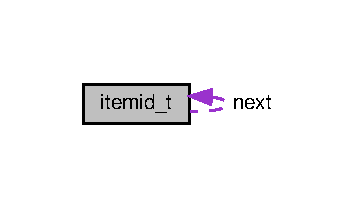
\includegraphics[width=171pt]{classitemid__t__coll__graph}
\end{center}
\end{figure}
\subsection*{Public Member Functions}
\begin{DoxyCompactItemize}
\item 
\hyperlink{classitemid__t_ab530695e150aa701f2ec41c6ef7546d7}{itemid\+\_\+t} ()
\item 
\hyperlink{classitemid__t_ac77c788e83ad418e67d0c87b15d602d3}{itemid\+\_\+t} (\hyperlink{helper_8h_a301eca6e81ebe56d6e6ff16eb4a148ad}{Data\+\_\+type} \hyperlink{classitemid__t_a7943f533ae926c956fcc09689ef07cfe}{type}, void $\ast$loc)
\item 
void \hyperlink{classitemid__t_ad2afc0d0875953bace22ee5513acfee5}{init} ()
\item 
bool \hyperlink{classitemid__t_ad0d24a7580d583b41c6bb415d731bd84}{operator==} (const \hyperlink{classitemid__t}{itemid\+\_\+t} \&other) const
\item 
bool \hyperlink{classitemid__t_aff2ea20d977774ebe70edcc8425b3b76}{operator!=} (const \hyperlink{classitemid__t}{itemid\+\_\+t} \&other) const
\item 
void \hyperlink{classitemid__t_a01c60be61379234e04de9925340951de}{operator=} (const \hyperlink{classitemid__t}{itemid\+\_\+t} \&other)
\item 
void \hyperlink{classitemid__t_ad5b99e223b72d4e1bd4ab93bb820cb6f}{setbench\+\_\+deinit} ()
\end{DoxyCompactItemize}
\subsection*{Public Attributes}
\begin{DoxyCompactItemize}
\item 
\hyperlink{helper_8h_a301eca6e81ebe56d6e6ff16eb4a148ad}{Data\+\_\+type} \hyperlink{classitemid__t_a7943f533ae926c956fcc09689ef07cfe}{type}
\item 
void $\ast$ \hyperlink{classitemid__t_a4979a55c6fc64c37f0c0582a4be8105b}{location}
\item 
\hyperlink{classitemid__t}{itemid\+\_\+t} $\ast$ \hyperlink{classitemid__t_a04230a8013ad752fad1e127b9e57c3c3}{next}
\item 
bool \hyperlink{classitemid__t_aa66b0fad35eaa15fe8de5c6d02a18050}{valid}
\end{DoxyCompactItemize}


\subsection{Constructor \& Destructor Documentation}
\mbox{\Hypertarget{classitemid__t_ab530695e150aa701f2ec41c6ef7546d7}\label{classitemid__t_ab530695e150aa701f2ec41c6ef7546d7}} 
\index{itemid\+\_\+t@{itemid\+\_\+t}!itemid\+\_\+t@{itemid\+\_\+t}}
\index{itemid\+\_\+t@{itemid\+\_\+t}!itemid\+\_\+t@{itemid\+\_\+t}}
\subsubsection{\texorpdfstring{itemid\+\_\+t()}{itemid\_t()}\hspace{0.1cm}{\footnotesize\ttfamily [1/2]}}
{\footnotesize\ttfamily itemid\+\_\+t\+::itemid\+\_\+t (\begin{DoxyParamCaption}{ }\end{DoxyParamCaption})\hspace{0.3cm}{\ttfamily [inline]}}

\mbox{\Hypertarget{classitemid__t_ac77c788e83ad418e67d0c87b15d602d3}\label{classitemid__t_ac77c788e83ad418e67d0c87b15d602d3}} 
\index{itemid\+\_\+t@{itemid\+\_\+t}!itemid\+\_\+t@{itemid\+\_\+t}}
\index{itemid\+\_\+t@{itemid\+\_\+t}!itemid\+\_\+t@{itemid\+\_\+t}}
\subsubsection{\texorpdfstring{itemid\+\_\+t()}{itemid\_t()}\hspace{0.1cm}{\footnotesize\ttfamily [2/2]}}
{\footnotesize\ttfamily itemid\+\_\+t\+::itemid\+\_\+t (\begin{DoxyParamCaption}\item[{\hyperlink{helper_8h_a301eca6e81ebe56d6e6ff16eb4a148ad}{Data\+\_\+type}}]{type,  }\item[{void $\ast$}]{loc }\end{DoxyParamCaption})\hspace{0.3cm}{\ttfamily [inline]}}



\subsection{Member Function Documentation}
\mbox{\Hypertarget{classitemid__t_ad2afc0d0875953bace22ee5513acfee5}\label{classitemid__t_ad2afc0d0875953bace22ee5513acfee5}} 
\index{itemid\+\_\+t@{itemid\+\_\+t}!init@{init}}
\index{init@{init}!itemid\+\_\+t@{itemid\+\_\+t}}
\subsubsection{\texorpdfstring{init()}{init()}}
{\footnotesize\ttfamily void itemid\+\_\+t\+::init (\begin{DoxyParamCaption}{ }\end{DoxyParamCaption})}

\mbox{\Hypertarget{classitemid__t_aff2ea20d977774ebe70edcc8425b3b76}\label{classitemid__t_aff2ea20d977774ebe70edcc8425b3b76}} 
\index{itemid\+\_\+t@{itemid\+\_\+t}!operator"!=@{operator"!=}}
\index{operator"!=@{operator"!=}!itemid\+\_\+t@{itemid\+\_\+t}}
\subsubsection{\texorpdfstring{operator"!=()}{operator!=()}}
{\footnotesize\ttfamily bool itemid\+\_\+t\+::operator!= (\begin{DoxyParamCaption}\item[{const \hyperlink{classitemid__t}{itemid\+\_\+t} \&}]{other }\end{DoxyParamCaption}) const}

\mbox{\Hypertarget{classitemid__t_a01c60be61379234e04de9925340951de}\label{classitemid__t_a01c60be61379234e04de9925340951de}} 
\index{itemid\+\_\+t@{itemid\+\_\+t}!operator=@{operator=}}
\index{operator=@{operator=}!itemid\+\_\+t@{itemid\+\_\+t}}
\subsubsection{\texorpdfstring{operator=()}{operator=()}}
{\footnotesize\ttfamily void itemid\+\_\+t\+::operator= (\begin{DoxyParamCaption}\item[{const \hyperlink{classitemid__t}{itemid\+\_\+t} \&}]{other }\end{DoxyParamCaption})}

\mbox{\Hypertarget{classitemid__t_ad0d24a7580d583b41c6bb415d731bd84}\label{classitemid__t_ad0d24a7580d583b41c6bb415d731bd84}} 
\index{itemid\+\_\+t@{itemid\+\_\+t}!operator==@{operator==}}
\index{operator==@{operator==}!itemid\+\_\+t@{itemid\+\_\+t}}
\subsubsection{\texorpdfstring{operator==()}{operator==()}}
{\footnotesize\ttfamily bool itemid\+\_\+t\+::operator== (\begin{DoxyParamCaption}\item[{const \hyperlink{classitemid__t}{itemid\+\_\+t} \&}]{other }\end{DoxyParamCaption}) const}

\mbox{\Hypertarget{classitemid__t_ad5b99e223b72d4e1bd4ab93bb820cb6f}\label{classitemid__t_ad5b99e223b72d4e1bd4ab93bb820cb6f}} 
\index{itemid\+\_\+t@{itemid\+\_\+t}!setbench\+\_\+deinit@{setbench\+\_\+deinit}}
\index{setbench\+\_\+deinit@{setbench\+\_\+deinit}!itemid\+\_\+t@{itemid\+\_\+t}}
\subsubsection{\texorpdfstring{setbench\+\_\+deinit()}{setbench\_deinit()}}
{\footnotesize\ttfamily void itemid\+\_\+t\+::setbench\+\_\+deinit (\begin{DoxyParamCaption}{ }\end{DoxyParamCaption})}



\subsection{Member Data Documentation}
\mbox{\Hypertarget{classitemid__t_a4979a55c6fc64c37f0c0582a4be8105b}\label{classitemid__t_a4979a55c6fc64c37f0c0582a4be8105b}} 
\index{itemid\+\_\+t@{itemid\+\_\+t}!location@{location}}
\index{location@{location}!itemid\+\_\+t@{itemid\+\_\+t}}
\subsubsection{\texorpdfstring{location}{location}}
{\footnotesize\ttfamily void$\ast$ itemid\+\_\+t\+::location}

\mbox{\Hypertarget{classitemid__t_a04230a8013ad752fad1e127b9e57c3c3}\label{classitemid__t_a04230a8013ad752fad1e127b9e57c3c3}} 
\index{itemid\+\_\+t@{itemid\+\_\+t}!next@{next}}
\index{next@{next}!itemid\+\_\+t@{itemid\+\_\+t}}
\subsubsection{\texorpdfstring{next}{next}}
{\footnotesize\ttfamily \hyperlink{classitemid__t}{itemid\+\_\+t}$\ast$ itemid\+\_\+t\+::next}

\mbox{\Hypertarget{classitemid__t_a7943f533ae926c956fcc09689ef07cfe}\label{classitemid__t_a7943f533ae926c956fcc09689ef07cfe}} 
\index{itemid\+\_\+t@{itemid\+\_\+t}!type@{type}}
\index{type@{type}!itemid\+\_\+t@{itemid\+\_\+t}}
\subsubsection{\texorpdfstring{type}{type}}
{\footnotesize\ttfamily \hyperlink{helper_8h_a301eca6e81ebe56d6e6ff16eb4a148ad}{Data\+\_\+type} itemid\+\_\+t\+::type}

\mbox{\Hypertarget{classitemid__t_aa66b0fad35eaa15fe8de5c6d02a18050}\label{classitemid__t_aa66b0fad35eaa15fe8de5c6d02a18050}} 
\index{itemid\+\_\+t@{itemid\+\_\+t}!valid@{valid}}
\index{valid@{valid}!itemid\+\_\+t@{itemid\+\_\+t}}
\subsubsection{\texorpdfstring{valid}{valid}}
{\footnotesize\ttfamily bool itemid\+\_\+t\+::valid}



The documentation for this class was generated from the following files\+:\begin{DoxyCompactItemize}
\item 
macrobench/system/\hyperlink{helper_8h}{helper.\+h}\item 
macrobench/system/\hyperlink{helper_8cpp}{helper.\+cpp}\end{DoxyCompactItemize}

\hypertarget{classkcasdesc__t}{}\section{kcasdesc\+\_\+t$<$ M\+A\+X\+\_\+K $>$ Class Template Reference}
\label{classkcasdesc__t}\index{kcasdesc\+\_\+t$<$ M\+A\+X\+\_\+\+K $>$@{kcasdesc\+\_\+t$<$ M\+A\+X\+\_\+\+K $>$}}


{\ttfamily \#include $<$kcas\+\_\+reuse\+\_\+htm\+\_\+impl.\+h$>$}



Collaboration diagram for kcasdesc\+\_\+t$<$ M\+A\+X\+\_\+K $>$\+:
\nopagebreak
\begin{figure}[H]
\begin{center}
\leavevmode
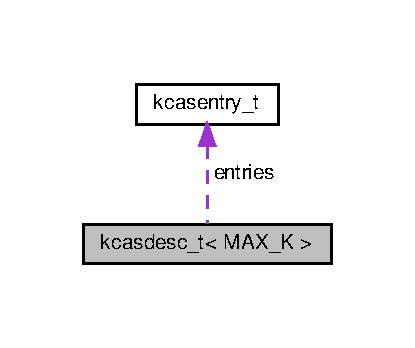
\includegraphics[width=199pt]{classkcasdesc__t__coll__graph}
\end{center}
\end{figure}
\subsection*{Public Member Functions}
\begin{DoxyCompactItemize}
\item 
void \hyperlink{classkcasdesc__t_a26f19763934c3b335fcda46d1645095c}{add\+Val\+Addr} (\hyperlink{rq__unsafe_8h_ad45142aaf2ff20a036dc6242b8483e9c}{casword\+\_\+t} volatile $\ast$addr, \hyperlink{rq__unsafe_8h_ad45142aaf2ff20a036dc6242b8483e9c}{casword\+\_\+t} oldval, \hyperlink{rq__unsafe_8h_ad45142aaf2ff20a036dc6242b8483e9c}{casword\+\_\+t} newval)
\item 
void \hyperlink{classkcasdesc__t_a42dbc67de7a757f0d4c8262172994498}{add\+Ptr\+Addr} (\hyperlink{rq__unsafe_8h_ad45142aaf2ff20a036dc6242b8483e9c}{casword\+\_\+t} volatile $\ast$addr, \hyperlink{rq__unsafe_8h_ad45142aaf2ff20a036dc6242b8483e9c}{casword\+\_\+t} oldval, \hyperlink{rq__unsafe_8h_ad45142aaf2ff20a036dc6242b8483e9c}{casword\+\_\+t} newval)
\item 
void \hyperlink{classkcasdesc__t_a26f19763934c3b335fcda46d1645095c}{add\+Val\+Addr} (\hyperlink{rq__unsafe_8h_ad45142aaf2ff20a036dc6242b8483e9c}{casword\+\_\+t} volatile $\ast$addr, \hyperlink{rq__unsafe_8h_ad45142aaf2ff20a036dc6242b8483e9c}{casword\+\_\+t} oldval, \hyperlink{rq__unsafe_8h_ad45142aaf2ff20a036dc6242b8483e9c}{casword\+\_\+t} newval)
\item 
void \hyperlink{classkcasdesc__t_a42dbc67de7a757f0d4c8262172994498}{add\+Ptr\+Addr} (\hyperlink{rq__unsafe_8h_ad45142aaf2ff20a036dc6242b8483e9c}{casword\+\_\+t} volatile $\ast$addr, \hyperlink{rq__unsafe_8h_ad45142aaf2ff20a036dc6242b8483e9c}{casword\+\_\+t} oldval, \hyperlink{rq__unsafe_8h_ad45142aaf2ff20a036dc6242b8483e9c}{casword\+\_\+t} newval)
\end{DoxyCompactItemize}
\subsection*{Public Attributes}
\begin{DoxyCompactItemize}
\item 
volatile \hyperlink{kcas__reuse__htm__impl_8h_a997daf56279be481f5c4294647725689}{seqbits\+\_\+t} \hyperlink{classkcasdesc__t_aed9ffdbc7a72d10a886e662fb82b26df}{seq\+Bits}
\item 
\hyperlink{rq__unsafe_8h_ad45142aaf2ff20a036dc6242b8483e9c}{casword\+\_\+t} \hyperlink{classkcasdesc__t_a841071a61ea7238f822e1fc644111380}{num\+Entries}
\item 
\hyperlink{structkcasentry__t}{kcasentry\+\_\+t} \hyperlink{classkcasdesc__t_adb510f640c081f2550c92f0978d74329}{entries} \mbox{[}M\+A\+X\+\_\+K\mbox{]}
\item 
volatile char \hyperlink{classkcasdesc__t_a09eb9afedfaf7a11192802d2e89e68d1}{padding} \mbox{[}128+((64-\/\hyperlink{classkcasdesc__t_a9cace636d1135fde7fb97772e470dbd4}{size}\%64)\%64)\mbox{]}
\end{DoxyCompactItemize}
\subsection*{Static Public Attributes}
\begin{DoxyCompactItemize}
\item 
static const int \hyperlink{classkcasdesc__t_a9cace636d1135fde7fb97772e470dbd4}{size} = sizeof(\hyperlink{classkcasdesc__t_aed9ffdbc7a72d10a886e662fb82b26df}{seq\+Bits})+sizeof(\hyperlink{classkcasdesc__t_a841071a61ea7238f822e1fc644111380}{num\+Entries})+sizeof(\hyperlink{classkcasdesc__t_adb510f640c081f2550c92f0978d74329}{entries})
\end{DoxyCompactItemize}


\subsection{Member Function Documentation}
\mbox{\Hypertarget{classkcasdesc__t_a42dbc67de7a757f0d4c8262172994498}\label{classkcasdesc__t_a42dbc67de7a757f0d4c8262172994498}} 
\index{kcasdesc\+\_\+t@{kcasdesc\+\_\+t}!add\+Ptr\+Addr@{add\+Ptr\+Addr}}
\index{add\+Ptr\+Addr@{add\+Ptr\+Addr}!kcasdesc\+\_\+t@{kcasdesc\+\_\+t}}
\subsubsection{\texorpdfstring{add\+Ptr\+Addr()}{addPtrAddr()}\hspace{0.1cm}{\footnotesize\ttfamily [1/2]}}
{\footnotesize\ttfamily template$<$int M\+A\+X\+\_\+K$>$ \\
void \hyperlink{classkcasdesc__t}{kcasdesc\+\_\+t}$<$ M\+A\+X\+\_\+K $>$\+::add\+Ptr\+Addr (\begin{DoxyParamCaption}\item[{\hyperlink{rq__unsafe_8h_ad45142aaf2ff20a036dc6242b8483e9c}{casword\+\_\+t} volatile $\ast$}]{addr,  }\item[{\hyperlink{rq__unsafe_8h_ad45142aaf2ff20a036dc6242b8483e9c}{casword\+\_\+t}}]{oldval,  }\item[{\hyperlink{rq__unsafe_8h_ad45142aaf2ff20a036dc6242b8483e9c}{casword\+\_\+t}}]{newval }\end{DoxyParamCaption})\hspace{0.3cm}{\ttfamily [inline]}}

\mbox{\Hypertarget{classkcasdesc__t_a42dbc67de7a757f0d4c8262172994498}\label{classkcasdesc__t_a42dbc67de7a757f0d4c8262172994498}} 
\index{kcasdesc\+\_\+t@{kcasdesc\+\_\+t}!add\+Ptr\+Addr@{add\+Ptr\+Addr}}
\index{add\+Ptr\+Addr@{add\+Ptr\+Addr}!kcasdesc\+\_\+t@{kcasdesc\+\_\+t}}
\subsubsection{\texorpdfstring{add\+Ptr\+Addr()}{addPtrAddr()}\hspace{0.1cm}{\footnotesize\ttfamily [2/2]}}
{\footnotesize\ttfamily template$<$int M\+A\+X\+\_\+K$>$ \\
void \hyperlink{classkcasdesc__t}{kcasdesc\+\_\+t}$<$ M\+A\+X\+\_\+K $>$\+::add\+Ptr\+Addr (\begin{DoxyParamCaption}\item[{\hyperlink{rq__unsafe_8h_ad45142aaf2ff20a036dc6242b8483e9c}{casword\+\_\+t} volatile $\ast$}]{addr,  }\item[{\hyperlink{rq__unsafe_8h_ad45142aaf2ff20a036dc6242b8483e9c}{casword\+\_\+t}}]{oldval,  }\item[{\hyperlink{rq__unsafe_8h_ad45142aaf2ff20a036dc6242b8483e9c}{casword\+\_\+t}}]{newval }\end{DoxyParamCaption})\hspace{0.3cm}{\ttfamily [inline]}}

\mbox{\Hypertarget{classkcasdesc__t_a26f19763934c3b335fcda46d1645095c}\label{classkcasdesc__t_a26f19763934c3b335fcda46d1645095c}} 
\index{kcasdesc\+\_\+t@{kcasdesc\+\_\+t}!add\+Val\+Addr@{add\+Val\+Addr}}
\index{add\+Val\+Addr@{add\+Val\+Addr}!kcasdesc\+\_\+t@{kcasdesc\+\_\+t}}
\subsubsection{\texorpdfstring{add\+Val\+Addr()}{addValAddr()}\hspace{0.1cm}{\footnotesize\ttfamily [1/2]}}
{\footnotesize\ttfamily template$<$int M\+A\+X\+\_\+K$>$ \\
void \hyperlink{classkcasdesc__t}{kcasdesc\+\_\+t}$<$ M\+A\+X\+\_\+K $>$\+::add\+Val\+Addr (\begin{DoxyParamCaption}\item[{\hyperlink{rq__unsafe_8h_ad45142aaf2ff20a036dc6242b8483e9c}{casword\+\_\+t} volatile $\ast$}]{addr,  }\item[{\hyperlink{rq__unsafe_8h_ad45142aaf2ff20a036dc6242b8483e9c}{casword\+\_\+t}}]{oldval,  }\item[{\hyperlink{rq__unsafe_8h_ad45142aaf2ff20a036dc6242b8483e9c}{casword\+\_\+t}}]{newval }\end{DoxyParamCaption})\hspace{0.3cm}{\ttfamily [inline]}}

\mbox{\Hypertarget{classkcasdesc__t_a26f19763934c3b335fcda46d1645095c}\label{classkcasdesc__t_a26f19763934c3b335fcda46d1645095c}} 
\index{kcasdesc\+\_\+t@{kcasdesc\+\_\+t}!add\+Val\+Addr@{add\+Val\+Addr}}
\index{add\+Val\+Addr@{add\+Val\+Addr}!kcasdesc\+\_\+t@{kcasdesc\+\_\+t}}
\subsubsection{\texorpdfstring{add\+Val\+Addr()}{addValAddr()}\hspace{0.1cm}{\footnotesize\ttfamily [2/2]}}
{\footnotesize\ttfamily template$<$int M\+A\+X\+\_\+K$>$ \\
void \hyperlink{classkcasdesc__t}{kcasdesc\+\_\+t}$<$ M\+A\+X\+\_\+K $>$\+::add\+Val\+Addr (\begin{DoxyParamCaption}\item[{\hyperlink{rq__unsafe_8h_ad45142aaf2ff20a036dc6242b8483e9c}{casword\+\_\+t} volatile $\ast$}]{addr,  }\item[{\hyperlink{rq__unsafe_8h_ad45142aaf2ff20a036dc6242b8483e9c}{casword\+\_\+t}}]{oldval,  }\item[{\hyperlink{rq__unsafe_8h_ad45142aaf2ff20a036dc6242b8483e9c}{casword\+\_\+t}}]{newval }\end{DoxyParamCaption})\hspace{0.3cm}{\ttfamily [inline]}}



\subsection{Member Data Documentation}
\mbox{\Hypertarget{classkcasdesc__t_adb510f640c081f2550c92f0978d74329}\label{classkcasdesc__t_adb510f640c081f2550c92f0978d74329}} 
\index{kcasdesc\+\_\+t@{kcasdesc\+\_\+t}!entries@{entries}}
\index{entries@{entries}!kcasdesc\+\_\+t@{kcasdesc\+\_\+t}}
\subsubsection{\texorpdfstring{entries}{entries}}
{\footnotesize\ttfamily template$<$int M\+A\+X\+\_\+K$>$ \\
\hyperlink{structkcasentry__t}{kcasentry\+\_\+t} \hyperlink{classkcasdesc__t}{kcasdesc\+\_\+t}$<$ M\+A\+X\+\_\+K $>$\+::entries}

\mbox{\Hypertarget{classkcasdesc__t_a841071a61ea7238f822e1fc644111380}\label{classkcasdesc__t_a841071a61ea7238f822e1fc644111380}} 
\index{kcasdesc\+\_\+t@{kcasdesc\+\_\+t}!num\+Entries@{num\+Entries}}
\index{num\+Entries@{num\+Entries}!kcasdesc\+\_\+t@{kcasdesc\+\_\+t}}
\subsubsection{\texorpdfstring{num\+Entries}{numEntries}}
{\footnotesize\ttfamily template$<$int M\+A\+X\+\_\+K$>$ \\
\hyperlink{rq__unsafe_8h_ad45142aaf2ff20a036dc6242b8483e9c}{casword\+\_\+t} \hyperlink{classkcasdesc__t}{kcasdesc\+\_\+t}$<$ M\+A\+X\+\_\+K $>$\+::num\+Entries}

\mbox{\Hypertarget{classkcasdesc__t_a09eb9afedfaf7a11192802d2e89e68d1}\label{classkcasdesc__t_a09eb9afedfaf7a11192802d2e89e68d1}} 
\index{kcasdesc\+\_\+t@{kcasdesc\+\_\+t}!padding@{padding}}
\index{padding@{padding}!kcasdesc\+\_\+t@{kcasdesc\+\_\+t}}
\subsubsection{\texorpdfstring{padding}{padding}}
{\footnotesize\ttfamily template$<$int M\+A\+X\+\_\+K$>$ \\
volatile char \hyperlink{classkcasdesc__t}{kcasdesc\+\_\+t}$<$ M\+A\+X\+\_\+K $>$\+::padding}

\mbox{\Hypertarget{classkcasdesc__t_aed9ffdbc7a72d10a886e662fb82b26df}\label{classkcasdesc__t_aed9ffdbc7a72d10a886e662fb82b26df}} 
\index{kcasdesc\+\_\+t@{kcasdesc\+\_\+t}!seq\+Bits@{seq\+Bits}}
\index{seq\+Bits@{seq\+Bits}!kcasdesc\+\_\+t@{kcasdesc\+\_\+t}}
\subsubsection{\texorpdfstring{seq\+Bits}{seqBits}}
{\footnotesize\ttfamily template$<$int M\+A\+X\+\_\+K$>$ \\
volatile \hyperlink{kcas__reuse__htm__impl_8h_a997daf56279be481f5c4294647725689}{seqbits\+\_\+t} \hyperlink{classkcasdesc__t}{kcasdesc\+\_\+t}$<$ M\+A\+X\+\_\+K $>$\+::seq\+Bits}

\mbox{\Hypertarget{classkcasdesc__t_a9cace636d1135fde7fb97772e470dbd4}\label{classkcasdesc__t_a9cace636d1135fde7fb97772e470dbd4}} 
\index{kcasdesc\+\_\+t@{kcasdesc\+\_\+t}!size@{size}}
\index{size@{size}!kcasdesc\+\_\+t@{kcasdesc\+\_\+t}}
\subsubsection{\texorpdfstring{size}{size}}
{\footnotesize\ttfamily template$<$int M\+A\+X\+\_\+K$>$ \\
static const int \hyperlink{classkcasdesc__t}{kcasdesc\+\_\+t}$<$ M\+A\+X\+\_\+K $>$\+::size = sizeof(\hyperlink{classkcasdesc__t_aed9ffdbc7a72d10a886e662fb82b26df}{seq\+Bits})+sizeof(\hyperlink{classkcasdesc__t_a841071a61ea7238f822e1fc644111380}{num\+Entries})+sizeof(\hyperlink{classkcasdesc__t_adb510f640c081f2550c92f0978d74329}{entries})\hspace{0.3cm}{\ttfamily [static]}}



The documentation for this class was generated from the following files\+:\begin{DoxyCompactItemize}
\item 
common/kcas/\hyperlink{kcas__reuse__htm__impl_8h}{kcas\+\_\+reuse\+\_\+htm\+\_\+impl.\+h}\item 
common/kcas/\hyperlink{kcas__reuse__impl_8h}{kcas\+\_\+reuse\+\_\+impl.\+h}\end{DoxyCompactItemize}

\hypertarget{structkcasentry__t}{}\section{kcasentry\+\_\+t Struct Reference}
\label{structkcasentry__t}\index{kcasentry\+\_\+t@{kcasentry\+\_\+t}}


{\ttfamily \#include $<$kcas\+\_\+reuse\+\_\+htm\+\_\+impl.\+h$>$}

\subsection*{Public Attributes}
\begin{DoxyCompactItemize}
\item 
\hyperlink{rq__unsafe_8h_ad45142aaf2ff20a036dc6242b8483e9c}{casword\+\_\+t} volatile $\ast$ \hyperlink{structkcasentry__t_aeb4001c54a80cbfc52d7ecab4996db53}{addr}
\item 
\hyperlink{rq__unsafe_8h_ad45142aaf2ff20a036dc6242b8483e9c}{casword\+\_\+t} \hyperlink{structkcasentry__t_a9043bad3ce4e0a566196667d039f3380}{oldval}
\item 
\hyperlink{rq__unsafe_8h_ad45142aaf2ff20a036dc6242b8483e9c}{casword\+\_\+t} \hyperlink{structkcasentry__t_a370f7727007a45210cc3585376e456d8}{newval}
\end{DoxyCompactItemize}


\subsection{Member Data Documentation}
\mbox{\Hypertarget{structkcasentry__t_aeb4001c54a80cbfc52d7ecab4996db53}\label{structkcasentry__t_aeb4001c54a80cbfc52d7ecab4996db53}} 
\index{kcasentry\+\_\+t@{kcasentry\+\_\+t}!addr@{addr}}
\index{addr@{addr}!kcasentry\+\_\+t@{kcasentry\+\_\+t}}
\subsubsection{\texorpdfstring{addr}{addr}}
{\footnotesize\ttfamily \hyperlink{rq__unsafe_8h_ad45142aaf2ff20a036dc6242b8483e9c}{casword\+\_\+t} volatile $\ast$ kcasentry\+\_\+t\+::addr}

\mbox{\Hypertarget{structkcasentry__t_a370f7727007a45210cc3585376e456d8}\label{structkcasentry__t_a370f7727007a45210cc3585376e456d8}} 
\index{kcasentry\+\_\+t@{kcasentry\+\_\+t}!newval@{newval}}
\index{newval@{newval}!kcasentry\+\_\+t@{kcasentry\+\_\+t}}
\subsubsection{\texorpdfstring{newval}{newval}}
{\footnotesize\ttfamily \hyperlink{rq__unsafe_8h_ad45142aaf2ff20a036dc6242b8483e9c}{casword\+\_\+t} kcasentry\+\_\+t\+::newval}

\mbox{\Hypertarget{structkcasentry__t_a9043bad3ce4e0a566196667d039f3380}\label{structkcasentry__t_a9043bad3ce4e0a566196667d039f3380}} 
\index{kcasentry\+\_\+t@{kcasentry\+\_\+t}!oldval@{oldval}}
\index{oldval@{oldval}!kcasentry\+\_\+t@{kcasentry\+\_\+t}}
\subsubsection{\texorpdfstring{oldval}{oldval}}
{\footnotesize\ttfamily \hyperlink{rq__unsafe_8h_ad45142aaf2ff20a036dc6242b8483e9c}{casword\+\_\+t} kcasentry\+\_\+t\+::oldval}



The documentation for this struct was generated from the following files\+:\begin{DoxyCompactItemize}
\item 
common/kcas/\hyperlink{kcas__reuse__htm__impl_8h}{kcas\+\_\+reuse\+\_\+htm\+\_\+impl.\+h}\item 
common/kcas/\hyperlink{kcas__reuse__impl_8h}{kcas\+\_\+reuse\+\_\+impl.\+h}\end{DoxyCompactItemize}

\hypertarget{classKCASHTM}{}\section{K\+C\+A\+S\+H\+TM$<$ M\+A\+X\+\_\+K $>$ Class Template Reference}
\label{classKCASHTM}\index{K\+C\+A\+S\+H\+T\+M$<$ M\+A\+X\+\_\+\+K $>$@{K\+C\+A\+S\+H\+T\+M$<$ M\+A\+X\+\_\+\+K $>$}}


{\ttfamily \#include $<$kcas\+\_\+reuse\+\_\+htm\+\_\+impl.\+h$>$}

\subsection*{Public Member Functions}
\begin{DoxyCompactItemize}
\item 
\hyperlink{classKCASHTM_a5c4a7dc01aa24d18bbf2be197adb4536}{K\+C\+A\+S\+H\+TM} ()
\item 
void \hyperlink{classKCASHTM_a1cc8f307886591c9fe769cb283d14226}{write\+Init\+Ptr} (\hyperlink{rq__unsafe_8h_ad45142aaf2ff20a036dc6242b8483e9c}{casword\+\_\+t} volatile $\ast$addr, \hyperlink{rq__unsafe_8h_ad45142aaf2ff20a036dc6242b8483e9c}{casword\+\_\+t} const newval)
\item 
void \hyperlink{classKCASHTM_ac3dd909b203532fd9d24981a3bd9ba5c}{write\+Init\+Val} (\hyperlink{rq__unsafe_8h_ad45142aaf2ff20a036dc6242b8483e9c}{casword\+\_\+t} volatile $\ast$addr, \hyperlink{rq__unsafe_8h_ad45142aaf2ff20a036dc6242b8483e9c}{casword\+\_\+t} const newval)
\item 
\hyperlink{rq__unsafe_8h_ad45142aaf2ff20a036dc6242b8483e9c}{casword\+\_\+t} \hyperlink{classKCASHTM_aa655018e007f3c1604023541ca24b653}{read\+Ptr} (\hyperlink{rq__unsafe_8h_ad45142aaf2ff20a036dc6242b8483e9c}{casword\+\_\+t} volatile $\ast$addr)
\item 
\hyperlink{rq__unsafe_8h_ad45142aaf2ff20a036dc6242b8483e9c}{casword\+\_\+t} \hyperlink{classKCASHTM_a99b96913aad51e1e7128e8561230ded8}{read\+Val} (\hyperlink{rq__unsafe_8h_ad45142aaf2ff20a036dc6242b8483e9c}{casword\+\_\+t} volatile $\ast$addr)
\item 
bool \hyperlink{classKCASHTM_a3cbdb60b25f482567d6be0d3d545a6ea}{execute} ()
\item 
\hyperlink{kcas__reuse__impl_8h_a5bbc81d391bfd6b4288a0d33f105a0b2}{kcasptr\+\_\+t} \hyperlink{classKCASHTM_a410b6c7f87aed36478dc7adc9c54478f}{get\+Descriptor} ()
\item 
void \hyperlink{classKCASHTM_a8788b509924018d6fc982e5d553b24d8}{start} ()
\item 
\hyperlink{rq__unsafe_8h_ad45142aaf2ff20a036dc6242b8483e9c}{casword\+\_\+t} \hyperlink{classKCASHTM_accfa276b0532e301dcd245c96a35fc1a}{rdcss\+Read} (\hyperlink{rq__unsafe_8h_ad45142aaf2ff20a036dc6242b8483e9c}{casword\+\_\+t} volatile $\ast$addr)
\item 
void \hyperlink{classKCASHTM_a6a53e2832b8e53b09c3ab147309fe645}{help\+Other} (\hyperlink{kcas__reuse__impl_8h_a22868433cf4300ce32f000ed8c8dd76c}{kcastagptr\+\_\+t} tagptr)
\item 
void \hyperlink{classKCASHTM_a1e8db0d4b5f85d6ebdfcb3615ca901a9}{deinit\+Thread} ()
\item 
{\footnotesize template$<$typename T $>$ }\\void \hyperlink{classKCASHTM_a43369d50f3fdc91a32f9d248a59d87e5}{add} (\hyperlink{structcasword}{casword}$<$ T $>$ $\ast$caswordptr, T old\+Val, T new\+Val)
\item 
{\footnotesize template$<$typename T , typename... Args$>$ }\\void \hyperlink{classKCASHTM_a4d983dc96331215e5328e2bacc5074e2}{add} (\hyperlink{structcasword}{casword}$<$ T $>$ $\ast$caswordptr, T old\+Val, T new\+Val, Args... args)
\end{DoxyCompactItemize}


\subsection{Constructor \& Destructor Documentation}
\mbox{\Hypertarget{classKCASHTM_a5c4a7dc01aa24d18bbf2be197adb4536}\label{classKCASHTM_a5c4a7dc01aa24d18bbf2be197adb4536}} 
\index{K\+C\+A\+S\+H\+TM@{K\+C\+A\+S\+H\+TM}!K\+C\+A\+S\+H\+TM@{K\+C\+A\+S\+H\+TM}}
\index{K\+C\+A\+S\+H\+TM@{K\+C\+A\+S\+H\+TM}!K\+C\+A\+S\+H\+TM@{K\+C\+A\+S\+H\+TM}}
\subsubsection{\texorpdfstring{K\+C\+A\+S\+H\+T\+M()}{KCASHTM()}}
{\footnotesize\ttfamily template$<$int M\+A\+X\+\_\+K$>$ \\
\hyperlink{classKCASHTM}{K\+C\+A\+S\+H\+TM}$<$ M\+A\+X\+\_\+K $>$\+::\hyperlink{classKCASHTM}{K\+C\+A\+S\+H\+TM} (\begin{DoxyParamCaption}{ }\end{DoxyParamCaption})}

Function declarations 

\subsection{Member Function Documentation}
\mbox{\Hypertarget{classKCASHTM_a43369d50f3fdc91a32f9d248a59d87e5}\label{classKCASHTM_a43369d50f3fdc91a32f9d248a59d87e5}} 
\index{K\+C\+A\+S\+H\+TM@{K\+C\+A\+S\+H\+TM}!add@{add}}
\index{add@{add}!K\+C\+A\+S\+H\+TM@{K\+C\+A\+S\+H\+TM}}
\subsubsection{\texorpdfstring{add()}{add()}\hspace{0.1cm}{\footnotesize\ttfamily [1/2]}}
{\footnotesize\ttfamily template$<$int M\+A\+X\+\_\+K$>$ \\
template$<$typename T $>$ \\
void \hyperlink{classKCASHTM}{K\+C\+A\+S\+H\+TM}$<$ M\+A\+X\+\_\+K $>$\+::add (\begin{DoxyParamCaption}\item[{\hyperlink{structcasword}{casword}$<$ T $>$ $\ast$}]{caswordptr,  }\item[{T}]{old\+Val,  }\item[{T}]{new\+Val }\end{DoxyParamCaption})}

\mbox{\Hypertarget{classKCASHTM_a4d983dc96331215e5328e2bacc5074e2}\label{classKCASHTM_a4d983dc96331215e5328e2bacc5074e2}} 
\index{K\+C\+A\+S\+H\+TM@{K\+C\+A\+S\+H\+TM}!add@{add}}
\index{add@{add}!K\+C\+A\+S\+H\+TM@{K\+C\+A\+S\+H\+TM}}
\subsubsection{\texorpdfstring{add()}{add()}\hspace{0.1cm}{\footnotesize\ttfamily [2/2]}}
{\footnotesize\ttfamily template$<$int M\+A\+X\+\_\+K$>$ \\
template$<$typename T , typename... Args$>$ \\
void \hyperlink{classKCASHTM}{K\+C\+A\+S\+H\+TM}$<$ M\+A\+X\+\_\+K $>$\+::add (\begin{DoxyParamCaption}\item[{\hyperlink{structcasword}{casword}$<$ T $>$ $\ast$}]{caswordptr,  }\item[{T}]{old\+Val,  }\item[{T}]{new\+Val,  }\item[{Args...}]{args }\end{DoxyParamCaption})}

\mbox{\Hypertarget{classKCASHTM_a1e8db0d4b5f85d6ebdfcb3615ca901a9}\label{classKCASHTM_a1e8db0d4b5f85d6ebdfcb3615ca901a9}} 
\index{K\+C\+A\+S\+H\+TM@{K\+C\+A\+S\+H\+TM}!deinit\+Thread@{deinit\+Thread}}
\index{deinit\+Thread@{deinit\+Thread}!K\+C\+A\+S\+H\+TM@{K\+C\+A\+S\+H\+TM}}
\subsubsection{\texorpdfstring{deinit\+Thread()}{deinitThread()}}
{\footnotesize\ttfamily template$<$int M\+A\+X\+\_\+K$>$ \\
void \hyperlink{classKCASHTM}{K\+C\+A\+S\+H\+TM}$<$ M\+A\+X\+\_\+K $>$\+::deinit\+Thread (\begin{DoxyParamCaption}{ }\end{DoxyParamCaption})}

\mbox{\Hypertarget{classKCASHTM_a3cbdb60b25f482567d6be0d3d545a6ea}\label{classKCASHTM_a3cbdb60b25f482567d6be0d3d545a6ea}} 
\index{K\+C\+A\+S\+H\+TM@{K\+C\+A\+S\+H\+TM}!execute@{execute}}
\index{execute@{execute}!K\+C\+A\+S\+H\+TM@{K\+C\+A\+S\+H\+TM}}
\subsubsection{\texorpdfstring{execute()}{execute()}}
{\footnotesize\ttfamily template$<$int M\+A\+X\+\_\+K$>$ \\
bool \hyperlink{classKCASHTM}{K\+C\+A\+S\+H\+TM}$<$ M\+A\+X\+\_\+K $>$\+::execute (\begin{DoxyParamCaption}{ }\end{DoxyParamCaption})}

\mbox{\Hypertarget{classKCASHTM_a410b6c7f87aed36478dc7adc9c54478f}\label{classKCASHTM_a410b6c7f87aed36478dc7adc9c54478f}} 
\index{K\+C\+A\+S\+H\+TM@{K\+C\+A\+S\+H\+TM}!get\+Descriptor@{get\+Descriptor}}
\index{get\+Descriptor@{get\+Descriptor}!K\+C\+A\+S\+H\+TM@{K\+C\+A\+S\+H\+TM}}
\subsubsection{\texorpdfstring{get\+Descriptor()}{getDescriptor()}}
{\footnotesize\ttfamily template$<$int M\+A\+X\+\_\+K$>$ \\
\hyperlink{kcas__reuse__impl_8h_a5bbc81d391bfd6b4288a0d33f105a0b2}{kcasptr\+\_\+t} \hyperlink{classKCASHTM}{K\+C\+A\+S\+H\+TM}$<$ M\+A\+X\+\_\+K $>$\+::get\+Descriptor (\begin{DoxyParamCaption}{ }\end{DoxyParamCaption})}

\mbox{\Hypertarget{classKCASHTM_a6a53e2832b8e53b09c3ab147309fe645}\label{classKCASHTM_a6a53e2832b8e53b09c3ab147309fe645}} 
\index{K\+C\+A\+S\+H\+TM@{K\+C\+A\+S\+H\+TM}!help\+Other@{help\+Other}}
\index{help\+Other@{help\+Other}!K\+C\+A\+S\+H\+TM@{K\+C\+A\+S\+H\+TM}}
\subsubsection{\texorpdfstring{help\+Other()}{helpOther()}}
{\footnotesize\ttfamily template$<$int M\+A\+X\+\_\+K$>$ \\
void \hyperlink{classKCASHTM}{K\+C\+A\+S\+H\+TM}$<$ M\+A\+X\+\_\+K $>$\+::help\+Other (\begin{DoxyParamCaption}\item[{\hyperlink{kcas__reuse__impl_8h_a22868433cf4300ce32f000ed8c8dd76c}{kcastagptr\+\_\+t}}]{tagptr }\end{DoxyParamCaption})}

\mbox{\Hypertarget{classKCASHTM_accfa276b0532e301dcd245c96a35fc1a}\label{classKCASHTM_accfa276b0532e301dcd245c96a35fc1a}} 
\index{K\+C\+A\+S\+H\+TM@{K\+C\+A\+S\+H\+TM}!rdcss\+Read@{rdcss\+Read}}
\index{rdcss\+Read@{rdcss\+Read}!K\+C\+A\+S\+H\+TM@{K\+C\+A\+S\+H\+TM}}
\subsubsection{\texorpdfstring{rdcss\+Read()}{rdcssRead()}}
{\footnotesize\ttfamily template$<$int M\+A\+X\+\_\+K$>$ \\
\hyperlink{rq__unsafe_8h_ad45142aaf2ff20a036dc6242b8483e9c}{casword\+\_\+t} \hyperlink{classKCASHTM}{K\+C\+A\+S\+H\+TM}$<$ M\+A\+X\+\_\+K $>$\+::rdcss\+Read (\begin{DoxyParamCaption}\item[{\hyperlink{rq__unsafe_8h_ad45142aaf2ff20a036dc6242b8483e9c}{casword\+\_\+t} volatile $\ast$}]{addr }\end{DoxyParamCaption})}

\mbox{\Hypertarget{classKCASHTM_aa655018e007f3c1604023541ca24b653}\label{classKCASHTM_aa655018e007f3c1604023541ca24b653}} 
\index{K\+C\+A\+S\+H\+TM@{K\+C\+A\+S\+H\+TM}!read\+Ptr@{read\+Ptr}}
\index{read\+Ptr@{read\+Ptr}!K\+C\+A\+S\+H\+TM@{K\+C\+A\+S\+H\+TM}}
\subsubsection{\texorpdfstring{read\+Ptr()}{readPtr()}}
{\footnotesize\ttfamily template$<$int M\+A\+X\+\_\+K$>$ \\
\hyperlink{rq__unsafe_8h_ad45142aaf2ff20a036dc6242b8483e9c}{casword\+\_\+t} \hyperlink{classKCASHTM}{K\+C\+A\+S\+H\+TM}$<$ M\+A\+X\+\_\+K $>$\+::read\+Ptr (\begin{DoxyParamCaption}\item[{\hyperlink{rq__unsafe_8h_ad45142aaf2ff20a036dc6242b8483e9c}{casword\+\_\+t} volatile $\ast$}]{addr }\end{DoxyParamCaption})}

\mbox{\Hypertarget{classKCASHTM_a99b96913aad51e1e7128e8561230ded8}\label{classKCASHTM_a99b96913aad51e1e7128e8561230ded8}} 
\index{K\+C\+A\+S\+H\+TM@{K\+C\+A\+S\+H\+TM}!read\+Val@{read\+Val}}
\index{read\+Val@{read\+Val}!K\+C\+A\+S\+H\+TM@{K\+C\+A\+S\+H\+TM}}
\subsubsection{\texorpdfstring{read\+Val()}{readVal()}}
{\footnotesize\ttfamily template$<$int M\+A\+X\+\_\+K$>$ \\
\hyperlink{rq__unsafe_8h_ad45142aaf2ff20a036dc6242b8483e9c}{casword\+\_\+t} \hyperlink{classKCASHTM}{K\+C\+A\+S\+H\+TM}$<$ M\+A\+X\+\_\+K $>$\+::read\+Val (\begin{DoxyParamCaption}\item[{\hyperlink{rq__unsafe_8h_ad45142aaf2ff20a036dc6242b8483e9c}{casword\+\_\+t} volatile $\ast$}]{addr }\end{DoxyParamCaption})}

\mbox{\Hypertarget{classKCASHTM_a8788b509924018d6fc982e5d553b24d8}\label{classKCASHTM_a8788b509924018d6fc982e5d553b24d8}} 
\index{K\+C\+A\+S\+H\+TM@{K\+C\+A\+S\+H\+TM}!start@{start}}
\index{start@{start}!K\+C\+A\+S\+H\+TM@{K\+C\+A\+S\+H\+TM}}
\subsubsection{\texorpdfstring{start()}{start()}}
{\footnotesize\ttfamily template$<$int M\+A\+X\+\_\+K$>$ \\
void \hyperlink{classKCASHTM}{K\+C\+A\+S\+H\+TM}$<$ M\+A\+X\+\_\+K $>$\+::start (\begin{DoxyParamCaption}{ }\end{DoxyParamCaption})}

\mbox{\Hypertarget{classKCASHTM_a1cc8f307886591c9fe769cb283d14226}\label{classKCASHTM_a1cc8f307886591c9fe769cb283d14226}} 
\index{K\+C\+A\+S\+H\+TM@{K\+C\+A\+S\+H\+TM}!write\+Init\+Ptr@{write\+Init\+Ptr}}
\index{write\+Init\+Ptr@{write\+Init\+Ptr}!K\+C\+A\+S\+H\+TM@{K\+C\+A\+S\+H\+TM}}
\subsubsection{\texorpdfstring{write\+Init\+Ptr()}{writeInitPtr()}}
{\footnotesize\ttfamily template$<$int M\+A\+X\+\_\+K$>$ \\
void \hyperlink{classKCASHTM}{K\+C\+A\+S\+H\+TM}$<$ M\+A\+X\+\_\+K $>$\+::write\+Init\+Ptr (\begin{DoxyParamCaption}\item[{\hyperlink{rq__unsafe_8h_ad45142aaf2ff20a036dc6242b8483e9c}{casword\+\_\+t} volatile $\ast$}]{addr,  }\item[{\hyperlink{rq__unsafe_8h_ad45142aaf2ff20a036dc6242b8483e9c}{casword\+\_\+t} const}]{newval }\end{DoxyParamCaption})}

\mbox{\Hypertarget{classKCASHTM_ac3dd909b203532fd9d24981a3bd9ba5c}\label{classKCASHTM_ac3dd909b203532fd9d24981a3bd9ba5c}} 
\index{K\+C\+A\+S\+H\+TM@{K\+C\+A\+S\+H\+TM}!write\+Init\+Val@{write\+Init\+Val}}
\index{write\+Init\+Val@{write\+Init\+Val}!K\+C\+A\+S\+H\+TM@{K\+C\+A\+S\+H\+TM}}
\subsubsection{\texorpdfstring{write\+Init\+Val()}{writeInitVal()}}
{\footnotesize\ttfamily template$<$int M\+A\+X\+\_\+K$>$ \\
void \hyperlink{classKCASHTM}{K\+C\+A\+S\+H\+TM}$<$ M\+A\+X\+\_\+K $>$\+::write\+Init\+Val (\begin{DoxyParamCaption}\item[{\hyperlink{rq__unsafe_8h_ad45142aaf2ff20a036dc6242b8483e9c}{casword\+\_\+t} volatile $\ast$}]{addr,  }\item[{\hyperlink{rq__unsafe_8h_ad45142aaf2ff20a036dc6242b8483e9c}{casword\+\_\+t} const}]{newval }\end{DoxyParamCaption})}



The documentation for this class was generated from the following file\+:\begin{DoxyCompactItemize}
\item 
common/kcas/\hyperlink{kcas__reuse__htm__impl_8h}{kcas\+\_\+reuse\+\_\+htm\+\_\+impl.\+h}\end{DoxyCompactItemize}

\hypertarget{classKCASLockFree}{}\section{K\+C\+A\+S\+Lock\+Free$<$ M\+A\+X\+\_\+K $>$ Class Template Reference}
\label{classKCASLockFree}\index{K\+C\+A\+S\+Lock\+Free$<$ M\+A\+X\+\_\+\+K $>$@{K\+C\+A\+S\+Lock\+Free$<$ M\+A\+X\+\_\+\+K $>$}}


{\ttfamily \#include $<$kcas\+\_\+reuse\+\_\+impl.\+h$>$}

\subsection*{Public Member Functions}
\begin{DoxyCompactItemize}
\item 
\hyperlink{classKCASLockFree_a766a5a353ea5229f9dadb61076c06c14}{K\+C\+A\+S\+Lock\+Free} ()
\item 
void \hyperlink{classKCASLockFree_a4e6ea63f89337e45fe2d89903c399c23}{write\+Init\+Ptr} (\hyperlink{rq__unsafe_8h_ad45142aaf2ff20a036dc6242b8483e9c}{casword\+\_\+t} volatile $\ast$addr, \hyperlink{rq__unsafe_8h_ad45142aaf2ff20a036dc6242b8483e9c}{casword\+\_\+t} const newval)
\item 
void \hyperlink{classKCASLockFree_a3866dbd432d71b3d97338f6b0839d89b}{write\+Init\+Val} (\hyperlink{rq__unsafe_8h_ad45142aaf2ff20a036dc6242b8483e9c}{casword\+\_\+t} volatile $\ast$addr, \hyperlink{rq__unsafe_8h_ad45142aaf2ff20a036dc6242b8483e9c}{casword\+\_\+t} const newval)
\item 
\hyperlink{rq__unsafe_8h_ad45142aaf2ff20a036dc6242b8483e9c}{casword\+\_\+t} \hyperlink{classKCASLockFree_a54d120c4f122f75613aef3235e60f6a5}{read\+Ptr} (\hyperlink{rq__unsafe_8h_ad45142aaf2ff20a036dc6242b8483e9c}{casword\+\_\+t} volatile $\ast$addr)
\item 
\hyperlink{rq__unsafe_8h_ad45142aaf2ff20a036dc6242b8483e9c}{casword\+\_\+t} \hyperlink{classKCASLockFree_a46fecb32042ea91275aaf94592771e40}{read\+Val} (\hyperlink{rq__unsafe_8h_ad45142aaf2ff20a036dc6242b8483e9c}{casword\+\_\+t} volatile $\ast$addr)
\item 
bool \hyperlink{classKCASLockFree_a68b4bbf1a5895cf96f7cddde59990e9e}{execute} ()
\item 
\hyperlink{kcas__reuse__impl_8h_a5bbc81d391bfd6b4288a0d33f105a0b2}{kcasptr\+\_\+t} \hyperlink{classKCASLockFree_a928a7be795b2fb894dd6ecf1be757d6e}{get\+Descriptor} ()
\item 
void \hyperlink{classKCASLockFree_ae4b43c2e64326f35df2c6c90ca33f448}{start} ()
\item 
\hyperlink{rq__unsafe_8h_ad45142aaf2ff20a036dc6242b8483e9c}{casword\+\_\+t} \hyperlink{classKCASLockFree_a0d29756cf4f43e7f138cea73b2f781b5}{rdcss\+Read} (\hyperlink{rq__unsafe_8h_ad45142aaf2ff20a036dc6242b8483e9c}{casword\+\_\+t} volatile $\ast$addr)
\item 
void \hyperlink{classKCASLockFree_ae587033414b12de35c07b6c13fe434bd}{help\+Other} (\hyperlink{kcas__reuse__impl_8h_a22868433cf4300ce32f000ed8c8dd76c}{kcastagptr\+\_\+t} tagptr)
\item 
void \hyperlink{classKCASLockFree_a703c5cf96094b2e49c5e23f199292915}{deinit\+Thread} ()
\item 
{\footnotesize template$<$typename T $>$ }\\void \hyperlink{classKCASLockFree_a01b56610d605c4ca1759c1f4c8c28d6e}{add} (\hyperlink{structcasword}{casword}$<$ T $>$ $\ast$caswordptr, T old\+Val, T new\+Val)
\item 
{\footnotesize template$<$typename T , typename... Args$>$ }\\void \hyperlink{classKCASLockFree_ac12d23ced3ca079ca65ea8896405678a}{add} (\hyperlink{structcasword}{casword}$<$ T $>$ $\ast$caswordptr, T old\+Val, T new\+Val, Args... args)
\end{DoxyCompactItemize}


\subsection{Constructor \& Destructor Documentation}
\mbox{\Hypertarget{classKCASLockFree_a766a5a353ea5229f9dadb61076c06c14}\label{classKCASLockFree_a766a5a353ea5229f9dadb61076c06c14}} 
\index{K\+C\+A\+S\+Lock\+Free@{K\+C\+A\+S\+Lock\+Free}!K\+C\+A\+S\+Lock\+Free@{K\+C\+A\+S\+Lock\+Free}}
\index{K\+C\+A\+S\+Lock\+Free@{K\+C\+A\+S\+Lock\+Free}!K\+C\+A\+S\+Lock\+Free@{K\+C\+A\+S\+Lock\+Free}}
\subsubsection{\texorpdfstring{K\+C\+A\+S\+Lock\+Free()}{KCASLockFree()}}
{\footnotesize\ttfamily template$<$int M\+A\+X\+\_\+K$>$ \\
\hyperlink{classKCASLockFree}{K\+C\+A\+S\+Lock\+Free}$<$ M\+A\+X\+\_\+K $>$\+::\hyperlink{classKCASLockFree}{K\+C\+A\+S\+Lock\+Free} (\begin{DoxyParamCaption}{ }\end{DoxyParamCaption})}

Function declarations 

\subsection{Member Function Documentation}
\mbox{\Hypertarget{classKCASLockFree_a01b56610d605c4ca1759c1f4c8c28d6e}\label{classKCASLockFree_a01b56610d605c4ca1759c1f4c8c28d6e}} 
\index{K\+C\+A\+S\+Lock\+Free@{K\+C\+A\+S\+Lock\+Free}!add@{add}}
\index{add@{add}!K\+C\+A\+S\+Lock\+Free@{K\+C\+A\+S\+Lock\+Free}}
\subsubsection{\texorpdfstring{add()}{add()}\hspace{0.1cm}{\footnotesize\ttfamily [1/2]}}
{\footnotesize\ttfamily template$<$int M\+A\+X\+\_\+K$>$ \\
template$<$typename T $>$ \\
void \hyperlink{classKCASLockFree}{K\+C\+A\+S\+Lock\+Free}$<$ M\+A\+X\+\_\+K $>$\+::add (\begin{DoxyParamCaption}\item[{\hyperlink{structcasword}{casword}$<$ T $>$ $\ast$}]{caswordptr,  }\item[{T}]{old\+Val,  }\item[{T}]{new\+Val }\end{DoxyParamCaption})}

\mbox{\Hypertarget{classKCASLockFree_ac12d23ced3ca079ca65ea8896405678a}\label{classKCASLockFree_ac12d23ced3ca079ca65ea8896405678a}} 
\index{K\+C\+A\+S\+Lock\+Free@{K\+C\+A\+S\+Lock\+Free}!add@{add}}
\index{add@{add}!K\+C\+A\+S\+Lock\+Free@{K\+C\+A\+S\+Lock\+Free}}
\subsubsection{\texorpdfstring{add()}{add()}\hspace{0.1cm}{\footnotesize\ttfamily [2/2]}}
{\footnotesize\ttfamily template$<$int M\+A\+X\+\_\+K$>$ \\
template$<$typename T , typename... Args$>$ \\
void \hyperlink{classKCASLockFree}{K\+C\+A\+S\+Lock\+Free}$<$ M\+A\+X\+\_\+K $>$\+::add (\begin{DoxyParamCaption}\item[{\hyperlink{structcasword}{casword}$<$ T $>$ $\ast$}]{caswordptr,  }\item[{T}]{old\+Val,  }\item[{T}]{new\+Val,  }\item[{Args...}]{args }\end{DoxyParamCaption})}

\mbox{\Hypertarget{classKCASLockFree_a703c5cf96094b2e49c5e23f199292915}\label{classKCASLockFree_a703c5cf96094b2e49c5e23f199292915}} 
\index{K\+C\+A\+S\+Lock\+Free@{K\+C\+A\+S\+Lock\+Free}!deinit\+Thread@{deinit\+Thread}}
\index{deinit\+Thread@{deinit\+Thread}!K\+C\+A\+S\+Lock\+Free@{K\+C\+A\+S\+Lock\+Free}}
\subsubsection{\texorpdfstring{deinit\+Thread()}{deinitThread()}}
{\footnotesize\ttfamily template$<$int M\+A\+X\+\_\+K$>$ \\
void \hyperlink{classKCASLockFree}{K\+C\+A\+S\+Lock\+Free}$<$ M\+A\+X\+\_\+K $>$\+::deinit\+Thread (\begin{DoxyParamCaption}{ }\end{DoxyParamCaption})}

\mbox{\Hypertarget{classKCASLockFree_a68b4bbf1a5895cf96f7cddde59990e9e}\label{classKCASLockFree_a68b4bbf1a5895cf96f7cddde59990e9e}} 
\index{K\+C\+A\+S\+Lock\+Free@{K\+C\+A\+S\+Lock\+Free}!execute@{execute}}
\index{execute@{execute}!K\+C\+A\+S\+Lock\+Free@{K\+C\+A\+S\+Lock\+Free}}
\subsubsection{\texorpdfstring{execute()}{execute()}}
{\footnotesize\ttfamily template$<$int M\+A\+X\+\_\+K$>$ \\
bool \hyperlink{classKCASLockFree}{K\+C\+A\+S\+Lock\+Free}$<$ M\+A\+X\+\_\+K $>$\+::execute (\begin{DoxyParamCaption}{ }\end{DoxyParamCaption})}

\mbox{\Hypertarget{classKCASLockFree_a928a7be795b2fb894dd6ecf1be757d6e}\label{classKCASLockFree_a928a7be795b2fb894dd6ecf1be757d6e}} 
\index{K\+C\+A\+S\+Lock\+Free@{K\+C\+A\+S\+Lock\+Free}!get\+Descriptor@{get\+Descriptor}}
\index{get\+Descriptor@{get\+Descriptor}!K\+C\+A\+S\+Lock\+Free@{K\+C\+A\+S\+Lock\+Free}}
\subsubsection{\texorpdfstring{get\+Descriptor()}{getDescriptor()}}
{\footnotesize\ttfamily template$<$int M\+A\+X\+\_\+K$>$ \\
\hyperlink{kcas__reuse__impl_8h_a5bbc81d391bfd6b4288a0d33f105a0b2}{kcasptr\+\_\+t} \hyperlink{classKCASLockFree}{K\+C\+A\+S\+Lock\+Free}$<$ M\+A\+X\+\_\+K $>$\+::get\+Descriptor (\begin{DoxyParamCaption}{ }\end{DoxyParamCaption})}

\mbox{\Hypertarget{classKCASLockFree_ae587033414b12de35c07b6c13fe434bd}\label{classKCASLockFree_ae587033414b12de35c07b6c13fe434bd}} 
\index{K\+C\+A\+S\+Lock\+Free@{K\+C\+A\+S\+Lock\+Free}!help\+Other@{help\+Other}}
\index{help\+Other@{help\+Other}!K\+C\+A\+S\+Lock\+Free@{K\+C\+A\+S\+Lock\+Free}}
\subsubsection{\texorpdfstring{help\+Other()}{helpOther()}}
{\footnotesize\ttfamily template$<$int M\+A\+X\+\_\+K$>$ \\
void \hyperlink{classKCASLockFree}{K\+C\+A\+S\+Lock\+Free}$<$ M\+A\+X\+\_\+K $>$\+::help\+Other (\begin{DoxyParamCaption}\item[{\hyperlink{kcas__reuse__impl_8h_a22868433cf4300ce32f000ed8c8dd76c}{kcastagptr\+\_\+t}}]{tagptr }\end{DoxyParamCaption})}

\mbox{\Hypertarget{classKCASLockFree_a0d29756cf4f43e7f138cea73b2f781b5}\label{classKCASLockFree_a0d29756cf4f43e7f138cea73b2f781b5}} 
\index{K\+C\+A\+S\+Lock\+Free@{K\+C\+A\+S\+Lock\+Free}!rdcss\+Read@{rdcss\+Read}}
\index{rdcss\+Read@{rdcss\+Read}!K\+C\+A\+S\+Lock\+Free@{K\+C\+A\+S\+Lock\+Free}}
\subsubsection{\texorpdfstring{rdcss\+Read()}{rdcssRead()}}
{\footnotesize\ttfamily template$<$int M\+A\+X\+\_\+K$>$ \\
\hyperlink{rq__unsafe_8h_ad45142aaf2ff20a036dc6242b8483e9c}{casword\+\_\+t} \hyperlink{classKCASLockFree}{K\+C\+A\+S\+Lock\+Free}$<$ M\+A\+X\+\_\+K $>$\+::rdcss\+Read (\begin{DoxyParamCaption}\item[{\hyperlink{rq__unsafe_8h_ad45142aaf2ff20a036dc6242b8483e9c}{casword\+\_\+t} volatile $\ast$}]{addr }\end{DoxyParamCaption})}

\mbox{\Hypertarget{classKCASLockFree_a54d120c4f122f75613aef3235e60f6a5}\label{classKCASLockFree_a54d120c4f122f75613aef3235e60f6a5}} 
\index{K\+C\+A\+S\+Lock\+Free@{K\+C\+A\+S\+Lock\+Free}!read\+Ptr@{read\+Ptr}}
\index{read\+Ptr@{read\+Ptr}!K\+C\+A\+S\+Lock\+Free@{K\+C\+A\+S\+Lock\+Free}}
\subsubsection{\texorpdfstring{read\+Ptr()}{readPtr()}}
{\footnotesize\ttfamily template$<$int M\+A\+X\+\_\+K$>$ \\
\hyperlink{rq__unsafe_8h_ad45142aaf2ff20a036dc6242b8483e9c}{casword\+\_\+t} \hyperlink{classKCASLockFree}{K\+C\+A\+S\+Lock\+Free}$<$ M\+A\+X\+\_\+K $>$\+::read\+Ptr (\begin{DoxyParamCaption}\item[{\hyperlink{rq__unsafe_8h_ad45142aaf2ff20a036dc6242b8483e9c}{casword\+\_\+t} volatile $\ast$}]{addr }\end{DoxyParamCaption})}

\mbox{\Hypertarget{classKCASLockFree_a46fecb32042ea91275aaf94592771e40}\label{classKCASLockFree_a46fecb32042ea91275aaf94592771e40}} 
\index{K\+C\+A\+S\+Lock\+Free@{K\+C\+A\+S\+Lock\+Free}!read\+Val@{read\+Val}}
\index{read\+Val@{read\+Val}!K\+C\+A\+S\+Lock\+Free@{K\+C\+A\+S\+Lock\+Free}}
\subsubsection{\texorpdfstring{read\+Val()}{readVal()}}
{\footnotesize\ttfamily template$<$int M\+A\+X\+\_\+K$>$ \\
\hyperlink{rq__unsafe_8h_ad45142aaf2ff20a036dc6242b8483e9c}{casword\+\_\+t} \hyperlink{classKCASLockFree}{K\+C\+A\+S\+Lock\+Free}$<$ M\+A\+X\+\_\+K $>$\+::read\+Val (\begin{DoxyParamCaption}\item[{\hyperlink{rq__unsafe_8h_ad45142aaf2ff20a036dc6242b8483e9c}{casword\+\_\+t} volatile $\ast$}]{addr }\end{DoxyParamCaption})}

\mbox{\Hypertarget{classKCASLockFree_ae4b43c2e64326f35df2c6c90ca33f448}\label{classKCASLockFree_ae4b43c2e64326f35df2c6c90ca33f448}} 
\index{K\+C\+A\+S\+Lock\+Free@{K\+C\+A\+S\+Lock\+Free}!start@{start}}
\index{start@{start}!K\+C\+A\+S\+Lock\+Free@{K\+C\+A\+S\+Lock\+Free}}
\subsubsection{\texorpdfstring{start()}{start()}}
{\footnotesize\ttfamily template$<$int M\+A\+X\+\_\+K$>$ \\
void \hyperlink{classKCASLockFree}{K\+C\+A\+S\+Lock\+Free}$<$ M\+A\+X\+\_\+K $>$\+::start (\begin{DoxyParamCaption}{ }\end{DoxyParamCaption})}

\mbox{\Hypertarget{classKCASLockFree_a4e6ea63f89337e45fe2d89903c399c23}\label{classKCASLockFree_a4e6ea63f89337e45fe2d89903c399c23}} 
\index{K\+C\+A\+S\+Lock\+Free@{K\+C\+A\+S\+Lock\+Free}!write\+Init\+Ptr@{write\+Init\+Ptr}}
\index{write\+Init\+Ptr@{write\+Init\+Ptr}!K\+C\+A\+S\+Lock\+Free@{K\+C\+A\+S\+Lock\+Free}}
\subsubsection{\texorpdfstring{write\+Init\+Ptr()}{writeInitPtr()}}
{\footnotesize\ttfamily template$<$int M\+A\+X\+\_\+K$>$ \\
void \hyperlink{classKCASLockFree}{K\+C\+A\+S\+Lock\+Free}$<$ M\+A\+X\+\_\+K $>$\+::write\+Init\+Ptr (\begin{DoxyParamCaption}\item[{\hyperlink{rq__unsafe_8h_ad45142aaf2ff20a036dc6242b8483e9c}{casword\+\_\+t} volatile $\ast$}]{addr,  }\item[{\hyperlink{rq__unsafe_8h_ad45142aaf2ff20a036dc6242b8483e9c}{casword\+\_\+t} const}]{newval }\end{DoxyParamCaption})}

\mbox{\Hypertarget{classKCASLockFree_a3866dbd432d71b3d97338f6b0839d89b}\label{classKCASLockFree_a3866dbd432d71b3d97338f6b0839d89b}} 
\index{K\+C\+A\+S\+Lock\+Free@{K\+C\+A\+S\+Lock\+Free}!write\+Init\+Val@{write\+Init\+Val}}
\index{write\+Init\+Val@{write\+Init\+Val}!K\+C\+A\+S\+Lock\+Free@{K\+C\+A\+S\+Lock\+Free}}
\subsubsection{\texorpdfstring{write\+Init\+Val()}{writeInitVal()}}
{\footnotesize\ttfamily template$<$int M\+A\+X\+\_\+K$>$ \\
void \hyperlink{classKCASLockFree}{K\+C\+A\+S\+Lock\+Free}$<$ M\+A\+X\+\_\+K $>$\+::write\+Init\+Val (\begin{DoxyParamCaption}\item[{\hyperlink{rq__unsafe_8h_ad45142aaf2ff20a036dc6242b8483e9c}{casword\+\_\+t} volatile $\ast$}]{addr,  }\item[{\hyperlink{rq__unsafe_8h_ad45142aaf2ff20a036dc6242b8483e9c}{casword\+\_\+t} const}]{newval }\end{DoxyParamCaption})}



The documentation for this class was generated from the following file\+:\begin{DoxyCompactItemize}
\item 
common/kcas/\hyperlink{kcas__reuse__impl_8h}{kcas\+\_\+reuse\+\_\+impl.\+h}\end{DoxyCompactItemize}

\hypertarget{classKeyGeneratorUniform}{}\section{Key\+Generator\+Uniform$<$ K $>$ Class Template Reference}
\label{classKeyGeneratorUniform}\index{Key\+Generator\+Uniform$<$ K $>$@{Key\+Generator\+Uniform$<$ K $>$}}


{\ttfamily \#include $<$keygen.\+h$>$}

\subsection*{Public Member Functions}
\begin{DoxyCompactItemize}
\item 
\hyperlink{classKeyGeneratorUniform_ad1516dcb2fa995f12e729b2ee4fb62b2}{Key\+Generator\+Uniform} (\hyperlink{classRandomFNV1A}{Random\+F\+N\+V1A} $\ast$\+\_\+rng, int \+\_\+max\+Key)
\item 
K \hyperlink{classKeyGeneratorUniform_a67fe5465611f10969b06e5d9d7c14d04}{next} ()
\end{DoxyCompactItemize}


\subsection{Constructor \& Destructor Documentation}
\mbox{\Hypertarget{classKeyGeneratorUniform_ad1516dcb2fa995f12e729b2ee4fb62b2}\label{classKeyGeneratorUniform_ad1516dcb2fa995f12e729b2ee4fb62b2}} 
\index{Key\+Generator\+Uniform@{Key\+Generator\+Uniform}!Key\+Generator\+Uniform@{Key\+Generator\+Uniform}}
\index{Key\+Generator\+Uniform@{Key\+Generator\+Uniform}!Key\+Generator\+Uniform@{Key\+Generator\+Uniform}}
\subsubsection{\texorpdfstring{Key\+Generator\+Uniform()}{KeyGeneratorUniform()}}
{\footnotesize\ttfamily template$<$typename K $>$ \\
\hyperlink{classKeyGeneratorUniform}{Key\+Generator\+Uniform}$<$ K $>$\+::\hyperlink{classKeyGeneratorUniform}{Key\+Generator\+Uniform} (\begin{DoxyParamCaption}\item[{\hyperlink{classRandomFNV1A}{Random\+F\+N\+V1A} $\ast$}]{\+\_\+rng,  }\item[{int}]{\+\_\+max\+Key }\end{DoxyParamCaption})\hspace{0.3cm}{\ttfamily [inline]}}



\subsection{Member Function Documentation}
\mbox{\Hypertarget{classKeyGeneratorUniform_a67fe5465611f10969b06e5d9d7c14d04}\label{classKeyGeneratorUniform_a67fe5465611f10969b06e5d9d7c14d04}} 
\index{Key\+Generator\+Uniform@{Key\+Generator\+Uniform}!next@{next}}
\index{next@{next}!Key\+Generator\+Uniform@{Key\+Generator\+Uniform}}
\subsubsection{\texorpdfstring{next()}{next()}}
{\footnotesize\ttfamily template$<$typename K $>$ \\
K \hyperlink{classKeyGeneratorUniform}{Key\+Generator\+Uniform}$<$ K $>$\+::next (\begin{DoxyParamCaption}{ }\end{DoxyParamCaption})\hspace{0.3cm}{\ttfamily [inline]}}



The documentation for this class was generated from the following file\+:\begin{DoxyCompactItemize}
\item 
microbench/\hyperlink{keygen_8h}{keygen.\+h}\end{DoxyCompactItemize}

\hypertarget{classKeyGeneratorZipf}{}\section{Key\+Generator\+Zipf$<$ K $>$ Class Template Reference}
\label{classKeyGeneratorZipf}\index{Key\+Generator\+Zipf$<$ K $>$@{Key\+Generator\+Zipf$<$ K $>$}}


{\ttfamily \#include $<$keygen.\+h$>$}

\subsection*{Public Member Functions}
\begin{DoxyCompactItemize}
\item 
\hyperlink{classKeyGeneratorZipf_a0b3f51602e77f6047d281564e31e0195}{Key\+Generator\+Zipf} (\hyperlink{classKeyGeneratorZipfData}{Key\+Generator\+Zipf\+Data} $\ast$\+\_\+data, \hyperlink{classRandomFNV1A}{Random\+F\+N\+V1A} $\ast$\+\_\+rng)
\item 
K \hyperlink{classKeyGeneratorZipf_aaefdd0a14c9380d8cf266ae235002c1b}{next} ()
\end{DoxyCompactItemize}


\subsection{Constructor \& Destructor Documentation}
\mbox{\Hypertarget{classKeyGeneratorZipf_a0b3f51602e77f6047d281564e31e0195}\label{classKeyGeneratorZipf_a0b3f51602e77f6047d281564e31e0195}} 
\index{Key\+Generator\+Zipf@{Key\+Generator\+Zipf}!Key\+Generator\+Zipf@{Key\+Generator\+Zipf}}
\index{Key\+Generator\+Zipf@{Key\+Generator\+Zipf}!Key\+Generator\+Zipf@{Key\+Generator\+Zipf}}
\subsubsection{\texorpdfstring{Key\+Generator\+Zipf()}{KeyGeneratorZipf()}}
{\footnotesize\ttfamily template$<$typename K $>$ \\
\hyperlink{classKeyGeneratorZipf}{Key\+Generator\+Zipf}$<$ K $>$\+::\hyperlink{classKeyGeneratorZipf}{Key\+Generator\+Zipf} (\begin{DoxyParamCaption}\item[{\hyperlink{classKeyGeneratorZipfData}{Key\+Generator\+Zipf\+Data} $\ast$}]{\+\_\+data,  }\item[{\hyperlink{classRandomFNV1A}{Random\+F\+N\+V1A} $\ast$}]{\+\_\+rng }\end{DoxyParamCaption})\hspace{0.3cm}{\ttfamily [inline]}}



\subsection{Member Function Documentation}
\mbox{\Hypertarget{classKeyGeneratorZipf_aaefdd0a14c9380d8cf266ae235002c1b}\label{classKeyGeneratorZipf_aaefdd0a14c9380d8cf266ae235002c1b}} 
\index{Key\+Generator\+Zipf@{Key\+Generator\+Zipf}!next@{next}}
\index{next@{next}!Key\+Generator\+Zipf@{Key\+Generator\+Zipf}}
\subsubsection{\texorpdfstring{next()}{next()}}
{\footnotesize\ttfamily template$<$typename K $>$ \\
K \hyperlink{classKeyGeneratorZipf}{Key\+Generator\+Zipf}$<$ K $>$\+::next (\begin{DoxyParamCaption}{ }\end{DoxyParamCaption})\hspace{0.3cm}{\ttfamily [inline]}}



The documentation for this class was generated from the following file\+:\begin{DoxyCompactItemize}
\item 
microbench/\hyperlink{keygen_8h}{keygen.\+h}\end{DoxyCompactItemize}

\hypertarget{classKeyGeneratorZipfData}{}\section{Key\+Generator\+Zipf\+Data Class Reference}
\label{classKeyGeneratorZipfData}\index{Key\+Generator\+Zipf\+Data@{Key\+Generator\+Zipf\+Data}}


{\ttfamily \#include $<$keygen.\+h$>$}

\subsection*{Public Member Functions}
\begin{DoxyCompactItemize}
\item 
\hyperlink{classKeyGeneratorZipfData_a5cf6242078ed7f948bf704306845fef1}{Key\+Generator\+Zipf\+Data} (int \+\_\+max\+Key, double \+\_\+alpha)
\item 
\hyperlink{classKeyGeneratorZipfData_ad94d584fa6cb346ce92eb62cffa96a81}{$\sim$\+Key\+Generator\+Zipf\+Data} ()
\end{DoxyCompactItemize}
\subsection*{Public Attributes}
\begin{DoxyCompactItemize}
\item 
\hyperlink{classKeyGeneratorZipfData_a7ff0c507086702a0c51b213524f26446}{P\+AD}
\item 
int \hyperlink{classKeyGeneratorZipfData_a805aeddf50b3b55fee05eb9915e96980}{max\+Key}
\item 
double \hyperlink{classKeyGeneratorZipfData_ad129612d274af9efebd5c11216f3df07}{theta}
\item 
double \hyperlink{classKeyGeneratorZipfData_a1124439733cea718670b0e87d094b0bb}{c} = 0
\item 
double $\ast$ \hyperlink{classKeyGeneratorZipfData_abaa12ba6ff7356d60e090d3c6bb1a434}{sum\+\_\+probs}
\end{DoxyCompactItemize}


\subsection{Constructor \& Destructor Documentation}
\mbox{\Hypertarget{classKeyGeneratorZipfData_a5cf6242078ed7f948bf704306845fef1}\label{classKeyGeneratorZipfData_a5cf6242078ed7f948bf704306845fef1}} 
\index{Key\+Generator\+Zipf\+Data@{Key\+Generator\+Zipf\+Data}!Key\+Generator\+Zipf\+Data@{Key\+Generator\+Zipf\+Data}}
\index{Key\+Generator\+Zipf\+Data@{Key\+Generator\+Zipf\+Data}!Key\+Generator\+Zipf\+Data@{Key\+Generator\+Zipf\+Data}}
\subsubsection{\texorpdfstring{Key\+Generator\+Zipf\+Data()}{KeyGeneratorZipfData()}}
{\footnotesize\ttfamily Key\+Generator\+Zipf\+Data\+::\+Key\+Generator\+Zipf\+Data (\begin{DoxyParamCaption}\item[{int}]{\+\_\+max\+Key,  }\item[{double}]{\+\_\+alpha }\end{DoxyParamCaption})\hspace{0.3cm}{\ttfamily [inline]}}

\mbox{\Hypertarget{classKeyGeneratorZipfData_ad94d584fa6cb346ce92eb62cffa96a81}\label{classKeyGeneratorZipfData_ad94d584fa6cb346ce92eb62cffa96a81}} 
\index{Key\+Generator\+Zipf\+Data@{Key\+Generator\+Zipf\+Data}!````~Key\+Generator\+Zipf\+Data@{$\sim$\+Key\+Generator\+Zipf\+Data}}
\index{````~Key\+Generator\+Zipf\+Data@{$\sim$\+Key\+Generator\+Zipf\+Data}!Key\+Generator\+Zipf\+Data@{Key\+Generator\+Zipf\+Data}}
\subsubsection{\texorpdfstring{$\sim$\+Key\+Generator\+Zipf\+Data()}{~KeyGeneratorZipfData()}}
{\footnotesize\ttfamily Key\+Generator\+Zipf\+Data\+::$\sim$\+Key\+Generator\+Zipf\+Data (\begin{DoxyParamCaption}{ }\end{DoxyParamCaption})\hspace{0.3cm}{\ttfamily [inline]}}



\subsection{Member Data Documentation}
\mbox{\Hypertarget{classKeyGeneratorZipfData_a1124439733cea718670b0e87d094b0bb}\label{classKeyGeneratorZipfData_a1124439733cea718670b0e87d094b0bb}} 
\index{Key\+Generator\+Zipf\+Data@{Key\+Generator\+Zipf\+Data}!c@{c}}
\index{c@{c}!Key\+Generator\+Zipf\+Data@{Key\+Generator\+Zipf\+Data}}
\subsubsection{\texorpdfstring{c}{c}}
{\footnotesize\ttfamily double Key\+Generator\+Zipf\+Data\+::c = 0}

\mbox{\Hypertarget{classKeyGeneratorZipfData_a805aeddf50b3b55fee05eb9915e96980}\label{classKeyGeneratorZipfData_a805aeddf50b3b55fee05eb9915e96980}} 
\index{Key\+Generator\+Zipf\+Data@{Key\+Generator\+Zipf\+Data}!max\+Key@{max\+Key}}
\index{max\+Key@{max\+Key}!Key\+Generator\+Zipf\+Data@{Key\+Generator\+Zipf\+Data}}
\subsubsection{\texorpdfstring{max\+Key}{maxKey}}
{\footnotesize\ttfamily int Key\+Generator\+Zipf\+Data\+::max\+Key}

\mbox{\Hypertarget{classKeyGeneratorZipfData_a7ff0c507086702a0c51b213524f26446}\label{classKeyGeneratorZipfData_a7ff0c507086702a0c51b213524f26446}} 
\index{Key\+Generator\+Zipf\+Data@{Key\+Generator\+Zipf\+Data}!P\+AD@{P\+AD}}
\index{P\+AD@{P\+AD}!Key\+Generator\+Zipf\+Data@{Key\+Generator\+Zipf\+Data}}
\subsubsection{\texorpdfstring{P\+AD}{PAD}}
{\footnotesize\ttfamily Key\+Generator\+Zipf\+Data\+::\+P\+AD}

\mbox{\Hypertarget{classKeyGeneratorZipfData_abaa12ba6ff7356d60e090d3c6bb1a434}\label{classKeyGeneratorZipfData_abaa12ba6ff7356d60e090d3c6bb1a434}} 
\index{Key\+Generator\+Zipf\+Data@{Key\+Generator\+Zipf\+Data}!sum\+\_\+probs@{sum\+\_\+probs}}
\index{sum\+\_\+probs@{sum\+\_\+probs}!Key\+Generator\+Zipf\+Data@{Key\+Generator\+Zipf\+Data}}
\subsubsection{\texorpdfstring{sum\+\_\+probs}{sum\_probs}}
{\footnotesize\ttfamily double$\ast$ Key\+Generator\+Zipf\+Data\+::sum\+\_\+probs}

\mbox{\Hypertarget{classKeyGeneratorZipfData_ad129612d274af9efebd5c11216f3df07}\label{classKeyGeneratorZipfData_ad129612d274af9efebd5c11216f3df07}} 
\index{Key\+Generator\+Zipf\+Data@{Key\+Generator\+Zipf\+Data}!theta@{theta}}
\index{theta@{theta}!Key\+Generator\+Zipf\+Data@{Key\+Generator\+Zipf\+Data}}
\subsubsection{\texorpdfstring{theta}{theta}}
{\footnotesize\ttfamily double Key\+Generator\+Zipf\+Data\+::theta}



The documentation for this class was generated from the following file\+:\begin{DoxyCompactItemize}
\item 
microbench/\hyperlink{keygen_8h}{keygen.\+h}\end{DoxyCompactItemize}

\hypertarget{structKVPair}{}\section{K\+V\+Pair$<$ K, V $>$ Struct Template Reference}
\label{structKVPair}\index{K\+V\+Pair$<$ K, V $>$@{K\+V\+Pair$<$ K, V $>$}}


{\ttfamily \#include $<$brown\+\_\+ext\+\_\+ist\+\_\+lf\+\_\+impl.\+h$>$}



Collaboration diagram for K\+V\+Pair$<$ K, V $>$\+:
\nopagebreak
\begin{figure}[H]
\begin{center}
\leavevmode
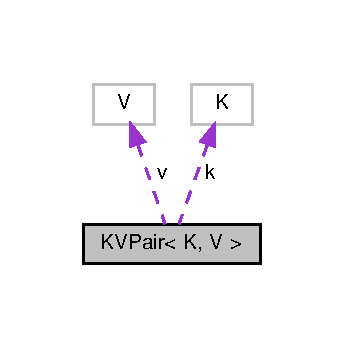
\includegraphics[width=165pt]{structKVPair__coll__graph}
\end{center}
\end{figure}
\subsection*{Public Attributes}
\begin{DoxyCompactItemize}
\item 
K \hyperlink{structKVPair_a3b6aaff4fcf2678ea11905a58f337cad}{k}
\item 
V \hyperlink{structKVPair_a4b3e133a53a3ff9a2b6e6801b9991157}{v}
\end{DoxyCompactItemize}


\subsection{Member Data Documentation}
\mbox{\Hypertarget{structKVPair_a3b6aaff4fcf2678ea11905a58f337cad}\label{structKVPair_a3b6aaff4fcf2678ea11905a58f337cad}} 
\index{K\+V\+Pair@{K\+V\+Pair}!k@{k}}
\index{k@{k}!K\+V\+Pair@{K\+V\+Pair}}
\subsubsection{\texorpdfstring{k}{k}}
{\footnotesize\ttfamily template$<$typename K, typename V$>$ \\
K \hyperlink{structKVPair}{K\+V\+Pair}$<$ K, V $>$\+::k}

\mbox{\Hypertarget{structKVPair_a4b3e133a53a3ff9a2b6e6801b9991157}\label{structKVPair_a4b3e133a53a3ff9a2b6e6801b9991157}} 
\index{K\+V\+Pair@{K\+V\+Pair}!v@{v}}
\index{v@{v}!K\+V\+Pair@{K\+V\+Pair}}
\subsubsection{\texorpdfstring{v}{v}}
{\footnotesize\ttfamily template$<$typename K, typename V$>$ \\
V \hyperlink{structKVPair}{K\+V\+Pair}$<$ K, V $>$\+::v}



The documentation for this struct was generated from the following file\+:\begin{DoxyCompactItemize}
\item 
ds/brown\+\_\+ext\+\_\+ist\+\_\+lf/\hyperlink{brown__ext__ist__lf__impl_8h}{brown\+\_\+ext\+\_\+ist\+\_\+lf\+\_\+impl.\+h}\end{DoxyCompactItemize}

\hypertarget{structkvpair}{}\section{kvpair$<$ K $>$ Struct Template Reference}
\label{structkvpair}\index{kvpair$<$ K $>$@{kvpair$<$ K $>$}}


{\ttfamily \#include $<$abtree\+\_\+kcas.\+h$>$}



Collaboration diagram for kvpair$<$ K $>$\+:
\nopagebreak
\begin{figure}[H]
\begin{center}
\leavevmode
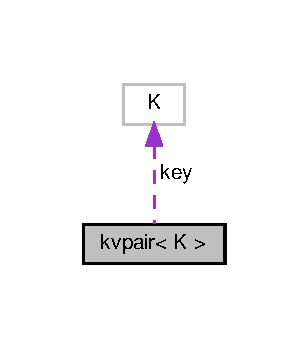
\includegraphics[width=148pt]{structkvpair__coll__graph}
\end{center}
\end{figure}
\subsection*{Public Member Functions}
\begin{DoxyCompactItemize}
\item 
\hyperlink{structkvpair_aabcb67cd8cfeca88cffcc1cf84d65679}{kvpair} ()
\end{DoxyCompactItemize}
\subsection*{Public Attributes}
\begin{DoxyCompactItemize}
\item 
K \hyperlink{structkvpair_a3898166444fc841d48279077e0bbe1ff}{key}
\item 
void $\ast$ \hyperlink{structkvpair_a31a1426532d867ca319a0fa40281bd9c}{val}
\end{DoxyCompactItemize}


\subsection{Constructor \& Destructor Documentation}
\mbox{\Hypertarget{structkvpair_aabcb67cd8cfeca88cffcc1cf84d65679}\label{structkvpair_aabcb67cd8cfeca88cffcc1cf84d65679}} 
\index{kvpair@{kvpair}!kvpair@{kvpair}}
\index{kvpair@{kvpair}!kvpair@{kvpair}}
\subsubsection{\texorpdfstring{kvpair()}{kvpair()}}
{\footnotesize\ttfamily template$<$typename K$>$ \\
\hyperlink{structkvpair}{kvpair}$<$ K $>$\+::\hyperlink{structkvpair}{kvpair} (\begin{DoxyParamCaption}{ }\end{DoxyParamCaption})\hspace{0.3cm}{\ttfamily [inline]}}



\subsection{Member Data Documentation}
\mbox{\Hypertarget{structkvpair_a3898166444fc841d48279077e0bbe1ff}\label{structkvpair_a3898166444fc841d48279077e0bbe1ff}} 
\index{kvpair@{kvpair}!key@{key}}
\index{key@{key}!kvpair@{kvpair}}
\subsubsection{\texorpdfstring{key}{key}}
{\footnotesize\ttfamily template$<$typename K$>$ \\
K \hyperlink{structkvpair}{kvpair}$<$ K $>$\+::key}

\mbox{\Hypertarget{structkvpair_a31a1426532d867ca319a0fa40281bd9c}\label{structkvpair_a31a1426532d867ca319a0fa40281bd9c}} 
\index{kvpair@{kvpair}!val@{val}}
\index{val@{val}!kvpair@{kvpair}}
\subsubsection{\texorpdfstring{val}{val}}
{\footnotesize\ttfamily template$<$typename K$>$ \\
void$\ast$ \hyperlink{structkvpair}{kvpair}$<$ K $>$\+::val}



The documentation for this struct was generated from the following file\+:\begin{DoxyCompactItemize}
\item 
ds/brown\+\_\+sigouin\+\_\+abtree\+\_\+kcas/\hyperlink{abtree__kcas_8h}{abtree\+\_\+kcas.\+h}\end{DoxyCompactItemize}

\hypertarget{classlfbstack}{}\section{lfbstack$<$ T $>$ Class Template Reference}
\label{classlfbstack}\index{lfbstack$<$ T $>$@{lfbstack$<$ T $>$}}


{\ttfamily \#include $<$lockfreeblockstack.\+h$>$}

\subsection*{Public Member Functions}
\begin{DoxyCompactItemize}
\item 
\hyperlink{classlfbstack_a214f01ec25e7729dd88bcfd4e96fb575}{lfbstack} ()
\item 
\hyperlink{classblock}{block}$<$ T $>$ $\ast$ \hyperlink{classlfbstack_a8b78f1dc42e697c2f792cc31be0b532a}{get\+Block} ()
\item 
int \hyperlink{classlfbstack_a82d5afa49bef74cb2cc06a5a8a6e10c8}{add\+Block} (\hyperlink{classblock}{block}$<$ T $>$ $\ast$b)
\item 
int \hyperlink{classlfbstack_ab602d933c91551c9d52b768a43381cab}{size\+In\+Blocks} ()
\end{DoxyCompactItemize}


\subsection{Detailed Description}
\subsubsection*{template$<$typename T$>$\newline
class lfbstack$<$ T $>$}

Simple intrusive lock-\/free stack using preexisting block objects. operates on elements of the block$<$\+T$>$ type defined in \hyperlink{blockbag_8h}{blockbag.\+h}. this class does N\+OT allocate any memory. instead, it simply chains existing blocks together using their next pointers.

Copyright (C) 2019 Trevor Brown 

\subsection{Constructor \& Destructor Documentation}
\mbox{\Hypertarget{classlfbstack_a214f01ec25e7729dd88bcfd4e96fb575}\label{classlfbstack_a214f01ec25e7729dd88bcfd4e96fb575}} 
\index{lfbstack@{lfbstack}!lfbstack@{lfbstack}}
\index{lfbstack@{lfbstack}!lfbstack@{lfbstack}}
\subsubsection{\texorpdfstring{lfbstack()}{lfbstack()}}
{\footnotesize\ttfamily template$<$typename T$>$ \\
\hyperlink{classlfbstack}{lfbstack}$<$ T $>$\+::\hyperlink{classlfbstack}{lfbstack} (\begin{DoxyParamCaption}{ }\end{DoxyParamCaption})\hspace{0.3cm}{\ttfamily [inline]}}



\subsection{Member Function Documentation}
\mbox{\Hypertarget{classlfbstack_a82d5afa49bef74cb2cc06a5a8a6e10c8}\label{classlfbstack_a82d5afa49bef74cb2cc06a5a8a6e10c8}} 
\index{lfbstack@{lfbstack}!add\+Block@{add\+Block}}
\index{add\+Block@{add\+Block}!lfbstack@{lfbstack}}
\subsubsection{\texorpdfstring{add\+Block()}{addBlock()}}
{\footnotesize\ttfamily template$<$typename T$>$ \\
int \hyperlink{classlfbstack}{lfbstack}$<$ T $>$\+::add\+Block (\begin{DoxyParamCaption}\item[{\hyperlink{classblock}{block}$<$ T $>$ $\ast$}]{b }\end{DoxyParamCaption})\hspace{0.3cm}{\ttfamily [inline]}}

\mbox{\Hypertarget{classlfbstack_a8b78f1dc42e697c2f792cc31be0b532a}\label{classlfbstack_a8b78f1dc42e697c2f792cc31be0b532a}} 
\index{lfbstack@{lfbstack}!get\+Block@{get\+Block}}
\index{get\+Block@{get\+Block}!lfbstack@{lfbstack}}
\subsubsection{\texorpdfstring{get\+Block()}{getBlock()}}
{\footnotesize\ttfamily template$<$typename T$>$ \\
\hyperlink{classblock}{block}$<$T$>$$\ast$ \hyperlink{classlfbstack}{lfbstack}$<$ T $>$\+::get\+Block (\begin{DoxyParamCaption}{ }\end{DoxyParamCaption})\hspace{0.3cm}{\ttfamily [inline]}}

\mbox{\Hypertarget{classlfbstack_ab602d933c91551c9d52b768a43381cab}\label{classlfbstack_ab602d933c91551c9d52b768a43381cab}} 
\index{lfbstack@{lfbstack}!size\+In\+Blocks@{size\+In\+Blocks}}
\index{size\+In\+Blocks@{size\+In\+Blocks}!lfbstack@{lfbstack}}
\subsubsection{\texorpdfstring{size\+In\+Blocks()}{sizeInBlocks()}}
{\footnotesize\ttfamily template$<$typename T$>$ \\
int \hyperlink{classlfbstack}{lfbstack}$<$ T $>$\+::size\+In\+Blocks (\begin{DoxyParamCaption}{ }\end{DoxyParamCaption})\hspace{0.3cm}{\ttfamily [inline]}}



The documentation for this class was generated from the following file\+:\begin{DoxyCompactItemize}
\item 
common/recordmgr/\hyperlink{lockfreeblockstack_8h}{lockfreeblockstack.\+h}\end{DoxyCompactItemize}

\hypertarget{structLockEntry}{}\section{Lock\+Entry Struct Reference}
\label{structLockEntry}\index{Lock\+Entry@{Lock\+Entry}}


{\ttfamily \#include $<$row\+\_\+lock.\+h$>$}



Collaboration diagram for Lock\+Entry\+:
\nopagebreak
\begin{figure}[H]
\begin{center}
\leavevmode
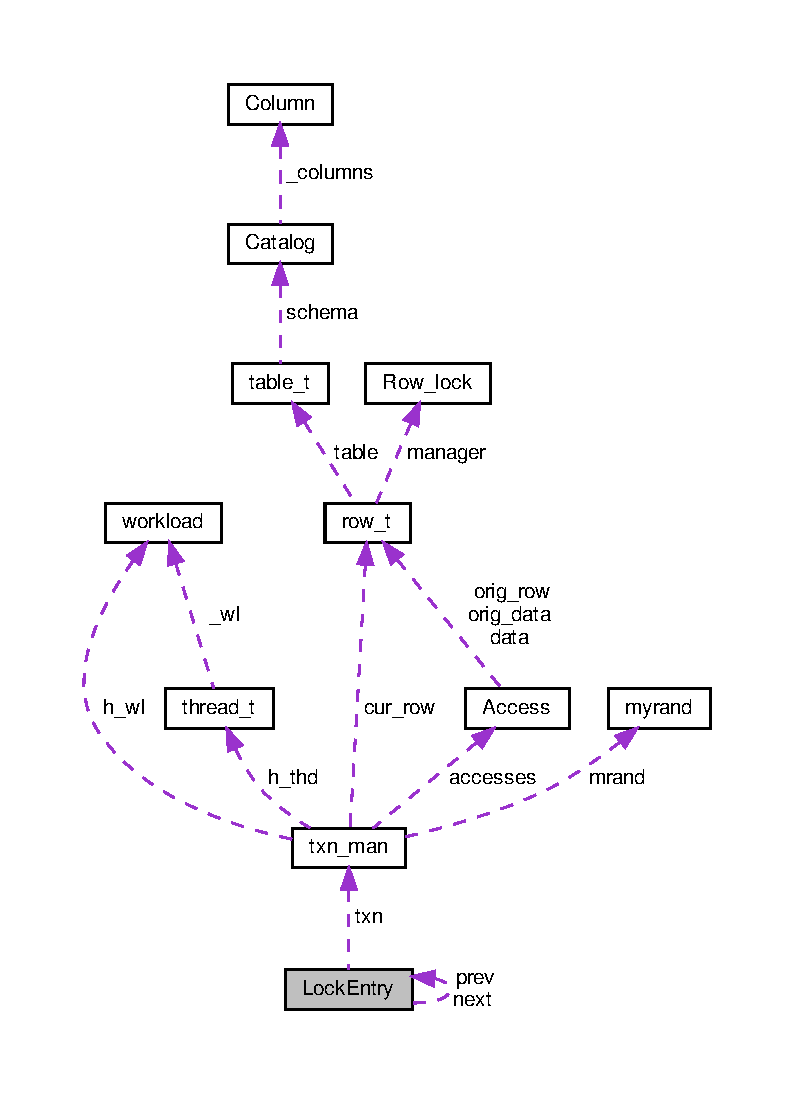
\includegraphics[width=350pt]{structLockEntry__coll__graph}
\end{center}
\end{figure}
\subsection*{Public Attributes}
\begin{DoxyCompactItemize}
\item 
\hyperlink{global_8h_a1da8554b34c21f74268d962b6559b0a6}{lock\+\_\+t} \hyperlink{structLockEntry_a826fc7a355c259f24961b83684a51009}{type}
\item 
\hyperlink{classtxn__man}{txn\+\_\+man} $\ast$ \hyperlink{structLockEntry_a8ede0c291a86aaa49a20dafa4b05fe71}{txn}
\item 
\hyperlink{structLockEntry}{Lock\+Entry} $\ast$ \hyperlink{structLockEntry_a8e1d5961956909d75e216c7f431b3165}{next}
\item 
\hyperlink{structLockEntry}{Lock\+Entry} $\ast$ \hyperlink{structLockEntry_a274433b5ea276dd3329861df07f6cb85}{prev}
\end{DoxyCompactItemize}


\subsection{Member Data Documentation}
\mbox{\Hypertarget{structLockEntry_a8e1d5961956909d75e216c7f431b3165}\label{structLockEntry_a8e1d5961956909d75e216c7f431b3165}} 
\index{Lock\+Entry@{Lock\+Entry}!next@{next}}
\index{next@{next}!Lock\+Entry@{Lock\+Entry}}
\subsubsection{\texorpdfstring{next}{next}}
{\footnotesize\ttfamily \hyperlink{structLockEntry}{Lock\+Entry}$\ast$ Lock\+Entry\+::next}

\mbox{\Hypertarget{structLockEntry_a274433b5ea276dd3329861df07f6cb85}\label{structLockEntry_a274433b5ea276dd3329861df07f6cb85}} 
\index{Lock\+Entry@{Lock\+Entry}!prev@{prev}}
\index{prev@{prev}!Lock\+Entry@{Lock\+Entry}}
\subsubsection{\texorpdfstring{prev}{prev}}
{\footnotesize\ttfamily \hyperlink{structLockEntry}{Lock\+Entry}$\ast$ Lock\+Entry\+::prev}

\mbox{\Hypertarget{structLockEntry_a8ede0c291a86aaa49a20dafa4b05fe71}\label{structLockEntry_a8ede0c291a86aaa49a20dafa4b05fe71}} 
\index{Lock\+Entry@{Lock\+Entry}!txn@{txn}}
\index{txn@{txn}!Lock\+Entry@{Lock\+Entry}}
\subsubsection{\texorpdfstring{txn}{txn}}
{\footnotesize\ttfamily \hyperlink{classtxn__man}{txn\+\_\+man}$\ast$ Lock\+Entry\+::txn}

\mbox{\Hypertarget{structLockEntry_a826fc7a355c259f24961b83684a51009}\label{structLockEntry_a826fc7a355c259f24961b83684a51009}} 
\index{Lock\+Entry@{Lock\+Entry}!type@{type}}
\index{type@{type}!Lock\+Entry@{Lock\+Entry}}
\subsubsection{\texorpdfstring{type}{type}}
{\footnotesize\ttfamily \hyperlink{global_8h_a1da8554b34c21f74268d962b6559b0a6}{lock\+\_\+t} Lock\+Entry\+::type}



The documentation for this struct was generated from the following file\+:\begin{DoxyCompactItemize}
\item 
macrobench/concurrency\+\_\+control/\hyperlink{row__lock_8h}{row\+\_\+lock.\+h}\end{DoxyCompactItemize}

\hypertarget{classlockfreeblockbag}{}\section{lockfreeblockbag$<$ T $>$ Class Template Reference}
\label{classlockfreeblockbag}\index{lockfreeblockbag$<$ T $>$@{lockfreeblockbag$<$ T $>$}}


{\ttfamily \#include $<$lockfreeblockbag.\+h$>$}

\subsection*{Public Member Functions}
\begin{DoxyCompactItemize}
\item 
\hyperlink{classlockfreeblockbag_ac5616d633983eeb539a8e0c05e120503}{lockfreeblockbag} ()
\item 
\hyperlink{classlockfreeblockbag_ab6f3bc34595acb7ac17072acf2ae7901}{$\sim$lockfreeblockbag} ()
\item 
\hyperlink{classblock}{block}$<$ T $>$ $\ast$ \hyperlink{classlockfreeblockbag_a3e6f92b70c0192308972fb21f3576bfc}{get\+Block} ()
\item 
void \hyperlink{classlockfreeblockbag_a722c146f5d2b578426cc9c418f394486}{add\+Block} (\hyperlink{classblock}{block}$<$ T $>$ $\ast$b)
\item 
int \hyperlink{classlockfreeblockbag_a3fe5902187ab6395bee9c4c9b2648a19}{size\+In\+Blocks} ()
\item 
long long \hyperlink{classlockfreeblockbag_afb3b6cce79e57e7c46d1ca7933313ef0}{size} ()
\end{DoxyCompactItemize}


\subsection{Detailed Description}
\subsubsection*{template$<$typename T$>$\newline
class lockfreeblockbag$<$ T $>$}

C++ record manager implementation (P\+O\+DC 2015) by Trevor Brown.

Copyright (C) 2015 Trevor Brown 

\subsection{Constructor \& Destructor Documentation}
\mbox{\Hypertarget{classlockfreeblockbag_ac5616d633983eeb539a8e0c05e120503}\label{classlockfreeblockbag_ac5616d633983eeb539a8e0c05e120503}} 
\index{lockfreeblockbag@{lockfreeblockbag}!lockfreeblockbag@{lockfreeblockbag}}
\index{lockfreeblockbag@{lockfreeblockbag}!lockfreeblockbag@{lockfreeblockbag}}
\subsubsection{\texorpdfstring{lockfreeblockbag()}{lockfreeblockbag()}}
{\footnotesize\ttfamily template$<$typename T$>$ \\
\hyperlink{classlockfreeblockbag}{lockfreeblockbag}$<$ T $>$\+::\hyperlink{classlockfreeblockbag}{lockfreeblockbag} (\begin{DoxyParamCaption}{ }\end{DoxyParamCaption})\hspace{0.3cm}{\ttfamily [inline]}}

\mbox{\Hypertarget{classlockfreeblockbag_ab6f3bc34595acb7ac17072acf2ae7901}\label{classlockfreeblockbag_ab6f3bc34595acb7ac17072acf2ae7901}} 
\index{lockfreeblockbag@{lockfreeblockbag}!````~lockfreeblockbag@{$\sim$lockfreeblockbag}}
\index{````~lockfreeblockbag@{$\sim$lockfreeblockbag}!lockfreeblockbag@{lockfreeblockbag}}
\subsubsection{\texorpdfstring{$\sim$lockfreeblockbag()}{~lockfreeblockbag()}}
{\footnotesize\ttfamily template$<$typename T$>$ \\
\hyperlink{classlockfreeblockbag}{lockfreeblockbag}$<$ T $>$\+::$\sim$\hyperlink{classlockfreeblockbag}{lockfreeblockbag} (\begin{DoxyParamCaption}{ }\end{DoxyParamCaption})\hspace{0.3cm}{\ttfamily [inline]}}



\subsection{Member Function Documentation}
\mbox{\Hypertarget{classlockfreeblockbag_a722c146f5d2b578426cc9c418f394486}\label{classlockfreeblockbag_a722c146f5d2b578426cc9c418f394486}} 
\index{lockfreeblockbag@{lockfreeblockbag}!add\+Block@{add\+Block}}
\index{add\+Block@{add\+Block}!lockfreeblockbag@{lockfreeblockbag}}
\subsubsection{\texorpdfstring{add\+Block()}{addBlock()}}
{\footnotesize\ttfamily template$<$typename T$>$ \\
void \hyperlink{classlockfreeblockbag}{lockfreeblockbag}$<$ T $>$\+::add\+Block (\begin{DoxyParamCaption}\item[{\hyperlink{classblock}{block}$<$ T $>$ $\ast$}]{b }\end{DoxyParamCaption})\hspace{0.3cm}{\ttfamily [inline]}}

\mbox{\Hypertarget{classlockfreeblockbag_a3e6f92b70c0192308972fb21f3576bfc}\label{classlockfreeblockbag_a3e6f92b70c0192308972fb21f3576bfc}} 
\index{lockfreeblockbag@{lockfreeblockbag}!get\+Block@{get\+Block}}
\index{get\+Block@{get\+Block}!lockfreeblockbag@{lockfreeblockbag}}
\subsubsection{\texorpdfstring{get\+Block()}{getBlock()}}
{\footnotesize\ttfamily template$<$typename T$>$ \\
\hyperlink{classblock}{block}$<$T$>$$\ast$ \hyperlink{classlockfreeblockbag}{lockfreeblockbag}$<$ T $>$\+::get\+Block (\begin{DoxyParamCaption}{ }\end{DoxyParamCaption})\hspace{0.3cm}{\ttfamily [inline]}}

\mbox{\Hypertarget{classlockfreeblockbag_afb3b6cce79e57e7c46d1ca7933313ef0}\label{classlockfreeblockbag_afb3b6cce79e57e7c46d1ca7933313ef0}} 
\index{lockfreeblockbag@{lockfreeblockbag}!size@{size}}
\index{size@{size}!lockfreeblockbag@{lockfreeblockbag}}
\subsubsection{\texorpdfstring{size()}{size()}}
{\footnotesize\ttfamily template$<$typename T$>$ \\
long long \hyperlink{classlockfreeblockbag}{lockfreeblockbag}$<$ T $>$\+::size (\begin{DoxyParamCaption}{ }\end{DoxyParamCaption})\hspace{0.3cm}{\ttfamily [inline]}}

\mbox{\Hypertarget{classlockfreeblockbag_a3fe5902187ab6395bee9c4c9b2648a19}\label{classlockfreeblockbag_a3fe5902187ab6395bee9c4c9b2648a19}} 
\index{lockfreeblockbag@{lockfreeblockbag}!size\+In\+Blocks@{size\+In\+Blocks}}
\index{size\+In\+Blocks@{size\+In\+Blocks}!lockfreeblockbag@{lockfreeblockbag}}
\subsubsection{\texorpdfstring{size\+In\+Blocks()}{sizeInBlocks()}}
{\footnotesize\ttfamily template$<$typename T$>$ \\
int \hyperlink{classlockfreeblockbag}{lockfreeblockbag}$<$ T $>$\+::size\+In\+Blocks (\begin{DoxyParamCaption}{ }\end{DoxyParamCaption})\hspace{0.3cm}{\ttfamily [inline]}}



The documentation for this class was generated from the following file\+:\begin{DoxyCompactItemize}
\item 
common/recordmgr/\hyperlink{lockfreeblockbag_8h}{lockfreeblockbag.\+h}\end{DoxyCompactItemize}

\hypertarget{classManager}{}\section{Manager Class Reference}
\label{classManager}\index{Manager@{Manager}}


{\ttfamily \#include $<$manager.\+h$>$}

\subsection*{Public Member Functions}
\begin{DoxyCompactItemize}
\item 
void \hyperlink{classManager_a5e70b531d3af13c1a6af84dcc84fa225}{init} ()
\item 
void \hyperlink{classManager_a74880d5dc83646708152b9b36430cac0}{setbench\+\_\+deinit} ()
\item 
\hyperlink{global_8h_aaf095dfc9b10f757c968fe146ad7e724}{ts\+\_\+t} \hyperlink{classManager_a61c4d259fc2e68dd0f0687956b873f06}{get\+\_\+ts} (uint64\+\_\+t thread\+\_\+id)
\item 
void \hyperlink{classManager_a38f950d2922952fe93425db9e627a873}{add\+\_\+ts} (uint64\+\_\+t thd\+\_\+id, \hyperlink{global_8h_aaf095dfc9b10f757c968fe146ad7e724}{ts\+\_\+t} ts)
\item 
\hyperlink{global_8h_aaf095dfc9b10f757c968fe146ad7e724}{ts\+\_\+t} \hyperlink{classManager_a7a4b0edad70dc91abe7ddcc49fc7ed77}{get\+\_\+min\+\_\+ts} (uint64\+\_\+t \hyperlink{microbench_2main_8cpp_a9ca9869868fe7e7a38a921cc7de4103f}{tid}=0)
\item 
void \hyperlink{classManager_a3e78aa1d124adce621968849bf780525}{lock\+\_\+row} (\hyperlink{classrow__t}{row\+\_\+t} $\ast$row)
\item 
void \hyperlink{classManager_abe51a30570ddb5180653c0a7fdaeb5b5}{release\+\_\+row} (\hyperlink{classrow__t}{row\+\_\+t} $\ast$row)
\item 
\hyperlink{classtxn__man}{txn\+\_\+man} $\ast$ \hyperlink{classManager_acf3a85553d0879190c6a8293bf475e8f}{get\+\_\+txn\+\_\+man} (int thd\+\_\+id)
\item 
void \hyperlink{classManager_a0a3992cf0f8cb6e267df5d9511ef0265}{set\+\_\+txn\+\_\+man} (\hyperlink{classtxn__man}{txn\+\_\+man} $\ast$txn)
\item 
uint64\+\_\+t \hyperlink{classManager_a397c36cac2730af19ba1835b7886661a}{get\+\_\+epoch} ()
\item 
void \hyperlink{classManager_a107fabeaae1ae04fb8223475fd678344}{update\+\_\+epoch} ()
\end{DoxyCompactItemize}


\subsection{Member Function Documentation}
\mbox{\Hypertarget{classManager_a38f950d2922952fe93425db9e627a873}\label{classManager_a38f950d2922952fe93425db9e627a873}} 
\index{Manager@{Manager}!add\+\_\+ts@{add\+\_\+ts}}
\index{add\+\_\+ts@{add\+\_\+ts}!Manager@{Manager}}
\subsubsection{\texorpdfstring{add\+\_\+ts()}{add\_ts()}}
{\footnotesize\ttfamily void Manager\+::add\+\_\+ts (\begin{DoxyParamCaption}\item[{uint64\+\_\+t}]{thd\+\_\+id,  }\item[{\hyperlink{global_8h_aaf095dfc9b10f757c968fe146ad7e724}{ts\+\_\+t}}]{ts }\end{DoxyParamCaption})}

\mbox{\Hypertarget{classManager_a397c36cac2730af19ba1835b7886661a}\label{classManager_a397c36cac2730af19ba1835b7886661a}} 
\index{Manager@{Manager}!get\+\_\+epoch@{get\+\_\+epoch}}
\index{get\+\_\+epoch@{get\+\_\+epoch}!Manager@{Manager}}
\subsubsection{\texorpdfstring{get\+\_\+epoch()}{get\_epoch()}}
{\footnotesize\ttfamily uint64\+\_\+t Manager\+::get\+\_\+epoch (\begin{DoxyParamCaption}{ }\end{DoxyParamCaption})\hspace{0.3cm}{\ttfamily [inline]}}

\mbox{\Hypertarget{classManager_a7a4b0edad70dc91abe7ddcc49fc7ed77}\label{classManager_a7a4b0edad70dc91abe7ddcc49fc7ed77}} 
\index{Manager@{Manager}!get\+\_\+min\+\_\+ts@{get\+\_\+min\+\_\+ts}}
\index{get\+\_\+min\+\_\+ts@{get\+\_\+min\+\_\+ts}!Manager@{Manager}}
\subsubsection{\texorpdfstring{get\+\_\+min\+\_\+ts()}{get\_min\_ts()}}
{\footnotesize\ttfamily \hyperlink{global_8h_aaf095dfc9b10f757c968fe146ad7e724}{ts\+\_\+t} Manager\+::get\+\_\+min\+\_\+ts (\begin{DoxyParamCaption}\item[{uint64\+\_\+t}]{tid = {\ttfamily 0} }\end{DoxyParamCaption})}

\mbox{\Hypertarget{classManager_a61c4d259fc2e68dd0f0687956b873f06}\label{classManager_a61c4d259fc2e68dd0f0687956b873f06}} 
\index{Manager@{Manager}!get\+\_\+ts@{get\+\_\+ts}}
\index{get\+\_\+ts@{get\+\_\+ts}!Manager@{Manager}}
\subsubsection{\texorpdfstring{get\+\_\+ts()}{get\_ts()}}
{\footnotesize\ttfamily uint64\+\_\+t Manager\+::get\+\_\+ts (\begin{DoxyParamCaption}\item[{uint64\+\_\+t}]{thread\+\_\+id }\end{DoxyParamCaption})}

\mbox{\Hypertarget{classManager_acf3a85553d0879190c6a8293bf475e8f}\label{classManager_acf3a85553d0879190c6a8293bf475e8f}} 
\index{Manager@{Manager}!get\+\_\+txn\+\_\+man@{get\+\_\+txn\+\_\+man}}
\index{get\+\_\+txn\+\_\+man@{get\+\_\+txn\+\_\+man}!Manager@{Manager}}
\subsubsection{\texorpdfstring{get\+\_\+txn\+\_\+man()}{get\_txn\_man()}}
{\footnotesize\ttfamily \hyperlink{classtxn__man}{txn\+\_\+man}$\ast$ Manager\+::get\+\_\+txn\+\_\+man (\begin{DoxyParamCaption}\item[{int}]{thd\+\_\+id }\end{DoxyParamCaption})\hspace{0.3cm}{\ttfamily [inline]}}

\mbox{\Hypertarget{classManager_a5e70b531d3af13c1a6af84dcc84fa225}\label{classManager_a5e70b531d3af13c1a6af84dcc84fa225}} 
\index{Manager@{Manager}!init@{init}}
\index{init@{init}!Manager@{Manager}}
\subsubsection{\texorpdfstring{init()}{init()}}
{\footnotesize\ttfamily void Manager\+::init (\begin{DoxyParamCaption}{ }\end{DoxyParamCaption})}

\mbox{\Hypertarget{classManager_a3e78aa1d124adce621968849bf780525}\label{classManager_a3e78aa1d124adce621968849bf780525}} 
\index{Manager@{Manager}!lock\+\_\+row@{lock\+\_\+row}}
\index{lock\+\_\+row@{lock\+\_\+row}!Manager@{Manager}}
\subsubsection{\texorpdfstring{lock\+\_\+row()}{lock\_row()}}
{\footnotesize\ttfamily void Manager\+::lock\+\_\+row (\begin{DoxyParamCaption}\item[{\hyperlink{classrow__t}{row\+\_\+t} $\ast$}]{row }\end{DoxyParamCaption})}

\mbox{\Hypertarget{classManager_abe51a30570ddb5180653c0a7fdaeb5b5}\label{classManager_abe51a30570ddb5180653c0a7fdaeb5b5}} 
\index{Manager@{Manager}!release\+\_\+row@{release\+\_\+row}}
\index{release\+\_\+row@{release\+\_\+row}!Manager@{Manager}}
\subsubsection{\texorpdfstring{release\+\_\+row()}{release\_row()}}
{\footnotesize\ttfamily void Manager\+::release\+\_\+row (\begin{DoxyParamCaption}\item[{\hyperlink{classrow__t}{row\+\_\+t} $\ast$}]{row }\end{DoxyParamCaption})}

\mbox{\Hypertarget{classManager_a0a3992cf0f8cb6e267df5d9511ef0265}\label{classManager_a0a3992cf0f8cb6e267df5d9511ef0265}} 
\index{Manager@{Manager}!set\+\_\+txn\+\_\+man@{set\+\_\+txn\+\_\+man}}
\index{set\+\_\+txn\+\_\+man@{set\+\_\+txn\+\_\+man}!Manager@{Manager}}
\subsubsection{\texorpdfstring{set\+\_\+txn\+\_\+man()}{set\_txn\_man()}}
{\footnotesize\ttfamily void Manager\+::set\+\_\+txn\+\_\+man (\begin{DoxyParamCaption}\item[{\hyperlink{classtxn__man}{txn\+\_\+man} $\ast$}]{txn }\end{DoxyParamCaption})}

\mbox{\Hypertarget{classManager_a74880d5dc83646708152b9b36430cac0}\label{classManager_a74880d5dc83646708152b9b36430cac0}} 
\index{Manager@{Manager}!setbench\+\_\+deinit@{setbench\+\_\+deinit}}
\index{setbench\+\_\+deinit@{setbench\+\_\+deinit}!Manager@{Manager}}
\subsubsection{\texorpdfstring{setbench\+\_\+deinit()}{setbench\_deinit()}}
{\footnotesize\ttfamily void Manager\+::setbench\+\_\+deinit (\begin{DoxyParamCaption}{ }\end{DoxyParamCaption})}

\mbox{\Hypertarget{classManager_a107fabeaae1ae04fb8223475fd678344}\label{classManager_a107fabeaae1ae04fb8223475fd678344}} 
\index{Manager@{Manager}!update\+\_\+epoch@{update\+\_\+epoch}}
\index{update\+\_\+epoch@{update\+\_\+epoch}!Manager@{Manager}}
\subsubsection{\texorpdfstring{update\+\_\+epoch()}{update\_epoch()}}
{\footnotesize\ttfamily void Manager\+::update\+\_\+epoch (\begin{DoxyParamCaption}{ }\end{DoxyParamCaption})}



The documentation for this class was generated from the following files\+:\begin{DoxyCompactItemize}
\item 
macrobench/system/\hyperlink{manager_8h}{manager.\+h}\item 
macrobench/system/\hyperlink{manager_8cpp}{manager.\+cpp}\end{DoxyCompactItemize}

\hypertarget{classmem__alloc}{}\section{mem\+\_\+alloc Class Reference}
\label{classmem__alloc}\index{mem\+\_\+alloc@{mem\+\_\+alloc}}


{\ttfamily \#include $<$mem\+\_\+alloc.\+h$>$}

\subsection*{Public Member Functions}
\begin{DoxyCompactItemize}
\item 
void \hyperlink{classmem__alloc_aeceb681eed3f07c1395160ee3379dd09}{init} (uint64\+\_\+t part\+\_\+cnt, uint64\+\_\+t bytes\+\_\+per\+\_\+part)
\item 
void \hyperlink{classmem__alloc_a19fffc69eae74964aa8f4953b0d511aa}{register\+\_\+thread} (int thd\+\_\+id)
\item 
void \hyperlink{classmem__alloc_a870a6fc38edd0ca50d4ef29d1b7014b9}{unregister} ()
\item 
void $\ast$ \hyperlink{classmem__alloc_af41385dd4ab067a79a93635e3518e6af}{alloc} (uint64\+\_\+t size, uint64\+\_\+t part\+\_\+id)
\item 
void \hyperlink{classmem__alloc_a619ab09bd3556867df9e1a9ad88704fb}{free} (void $\ast$\hyperlink{classblock}{block}, uint64\+\_\+t size)
\item 
int \hyperlink{classmem__alloc_a5b5abeba7076849012e879e417eecca4}{get\+\_\+arena\+\_\+id} ()
\end{DoxyCompactItemize}


\subsection{Member Function Documentation}
\mbox{\Hypertarget{classmem__alloc_af41385dd4ab067a79a93635e3518e6af}\label{classmem__alloc_af41385dd4ab067a79a93635e3518e6af}} 
\index{mem\+\_\+alloc@{mem\+\_\+alloc}!alloc@{alloc}}
\index{alloc@{alloc}!mem\+\_\+alloc@{mem\+\_\+alloc}}
\subsubsection{\texorpdfstring{alloc()}{alloc()}}
{\footnotesize\ttfamily void $\ast$ mem\+\_\+alloc\+::alloc (\begin{DoxyParamCaption}\item[{uint64\+\_\+t}]{size,  }\item[{uint64\+\_\+t}]{part\+\_\+id }\end{DoxyParamCaption})}

\mbox{\Hypertarget{classmem__alloc_a619ab09bd3556867df9e1a9ad88704fb}\label{classmem__alloc_a619ab09bd3556867df9e1a9ad88704fb}} 
\index{mem\+\_\+alloc@{mem\+\_\+alloc}!free@{free}}
\index{free@{free}!mem\+\_\+alloc@{mem\+\_\+alloc}}
\subsubsection{\texorpdfstring{free()}{free()}}
{\footnotesize\ttfamily void mem\+\_\+alloc\+::free (\begin{DoxyParamCaption}\item[{void $\ast$}]{block,  }\item[{uint64\+\_\+t}]{size }\end{DoxyParamCaption})}

\mbox{\Hypertarget{classmem__alloc_a5b5abeba7076849012e879e417eecca4}\label{classmem__alloc_a5b5abeba7076849012e879e417eecca4}} 
\index{mem\+\_\+alloc@{mem\+\_\+alloc}!get\+\_\+arena\+\_\+id@{get\+\_\+arena\+\_\+id}}
\index{get\+\_\+arena\+\_\+id@{get\+\_\+arena\+\_\+id}!mem\+\_\+alloc@{mem\+\_\+alloc}}
\subsubsection{\texorpdfstring{get\+\_\+arena\+\_\+id()}{get\_arena\_id()}}
{\footnotesize\ttfamily int mem\+\_\+alloc\+::get\+\_\+arena\+\_\+id (\begin{DoxyParamCaption}{ }\end{DoxyParamCaption})}

\mbox{\Hypertarget{classmem__alloc_aeceb681eed3f07c1395160ee3379dd09}\label{classmem__alloc_aeceb681eed3f07c1395160ee3379dd09}} 
\index{mem\+\_\+alloc@{mem\+\_\+alloc}!init@{init}}
\index{init@{init}!mem\+\_\+alloc@{mem\+\_\+alloc}}
\subsubsection{\texorpdfstring{init()}{init()}}
{\footnotesize\ttfamily void mem\+\_\+alloc\+::init (\begin{DoxyParamCaption}\item[{uint64\+\_\+t}]{part\+\_\+cnt,  }\item[{uint64\+\_\+t}]{bytes\+\_\+per\+\_\+part }\end{DoxyParamCaption})}

\mbox{\Hypertarget{classmem__alloc_a19fffc69eae74964aa8f4953b0d511aa}\label{classmem__alloc_a19fffc69eae74964aa8f4953b0d511aa}} 
\index{mem\+\_\+alloc@{mem\+\_\+alloc}!register\+\_\+thread@{register\+\_\+thread}}
\index{register\+\_\+thread@{register\+\_\+thread}!mem\+\_\+alloc@{mem\+\_\+alloc}}
\subsubsection{\texorpdfstring{register\+\_\+thread()}{register\_thread()}}
{\footnotesize\ttfamily void mem\+\_\+alloc\+::register\+\_\+thread (\begin{DoxyParamCaption}\item[{int}]{thd\+\_\+id }\end{DoxyParamCaption})}

\mbox{\Hypertarget{classmem__alloc_a870a6fc38edd0ca50d4ef29d1b7014b9}\label{classmem__alloc_a870a6fc38edd0ca50d4ef29d1b7014b9}} 
\index{mem\+\_\+alloc@{mem\+\_\+alloc}!unregister@{unregister}}
\index{unregister@{unregister}!mem\+\_\+alloc@{mem\+\_\+alloc}}
\subsubsection{\texorpdfstring{unregister()}{unregister()}}
{\footnotesize\ttfamily void mem\+\_\+alloc\+::unregister (\begin{DoxyParamCaption}{ }\end{DoxyParamCaption})}



The documentation for this class was generated from the following files\+:\begin{DoxyCompactItemize}
\item 
macrobench/system/\hyperlink{mem__alloc_8h}{mem\+\_\+alloc.\+h}\item 
macrobench/system/\hyperlink{mem__alloc_8cpp}{mem\+\_\+alloc.\+cpp}\end{DoxyCompactItemize}

\hypertarget{classrecord__manager_1_1MemoryReclamationGuard}{}\section{record\+\_\+manager$<$ Reclaim, Alloc, Pool, Record\+Types\+First, Record\+Types\+Rest $>$\+:\+:Memory\+Reclamation\+Guard Class Reference}
\label{classrecord__manager_1_1MemoryReclamationGuard}\index{record\+\_\+manager$<$ Reclaim, Alloc, Pool, Record\+Types\+First, Record\+Types\+Rest $>$\+::\+Memory\+Reclamation\+Guard@{record\+\_\+manager$<$ Reclaim, Alloc, Pool, Record\+Types\+First, Record\+Types\+Rest $>$\+::\+Memory\+Reclamation\+Guard}}


{\ttfamily \#include $<$record\+\_\+manager.\+h$>$}

\subsection*{Public Member Functions}
\begin{DoxyCompactItemize}
\item 
\hyperlink{classrecord__manager_1_1MemoryReclamationGuard_a36dcf7f0c984d1cd92382e1f1b4e299c}{Memory\+Reclamation\+Guard} (const int \+\_\+tid, \hyperlink{classrecord__manager}{record\+\_\+manager}$<$ Reclaim, Alloc, Pool, Record\+Types\+First, Record\+Types\+Rest... $>$ $\ast$\+\_\+recmgr, const bool read\+Only=false)
\item 
\hyperlink{classrecord__manager_1_1MemoryReclamationGuard_acbedb9b1c0aa0c9c0527964911adb6dc}{$\sim$\+Memory\+Reclamation\+Guard} ()
\item 
void \hyperlink{classrecord__manager_1_1MemoryReclamationGuard_ac3f1295823181aff94971f7b214c78ea}{end} ()
\end{DoxyCompactItemize}


\subsection{Constructor \& Destructor Documentation}
\mbox{\Hypertarget{classrecord__manager_1_1MemoryReclamationGuard_a36dcf7f0c984d1cd92382e1f1b4e299c}\label{classrecord__manager_1_1MemoryReclamationGuard_a36dcf7f0c984d1cd92382e1f1b4e299c}} 
\index{record\+\_\+manager\+::\+Memory\+Reclamation\+Guard@{record\+\_\+manager\+::\+Memory\+Reclamation\+Guard}!Memory\+Reclamation\+Guard@{Memory\+Reclamation\+Guard}}
\index{Memory\+Reclamation\+Guard@{Memory\+Reclamation\+Guard}!record\+\_\+manager\+::\+Memory\+Reclamation\+Guard@{record\+\_\+manager\+::\+Memory\+Reclamation\+Guard}}
\subsubsection{\texorpdfstring{Memory\+Reclamation\+Guard()}{MemoryReclamationGuard()}}
{\footnotesize\ttfamily template$<$class Reclaim, class Alloc, class Pool, typename Record\+Types\+First, typename... Record\+Types\+Rest$>$ \\
\hyperlink{classrecord__manager}{record\+\_\+manager}$<$ Reclaim, Alloc, Pool, Record\+Types\+First, Record\+Types\+Rest $>$\+::Memory\+Reclamation\+Guard\+::\+Memory\+Reclamation\+Guard (\begin{DoxyParamCaption}\item[{const int}]{\+\_\+tid,  }\item[{\hyperlink{classrecord__manager}{record\+\_\+manager}$<$ Reclaim, Alloc, Pool, Record\+Types\+First, Record\+Types\+Rest... $>$ $\ast$}]{\+\_\+recmgr,  }\item[{const bool}]{read\+Only = {\ttfamily false} }\end{DoxyParamCaption})\hspace{0.3cm}{\ttfamily [inline]}}

\mbox{\Hypertarget{classrecord__manager_1_1MemoryReclamationGuard_acbedb9b1c0aa0c9c0527964911adb6dc}\label{classrecord__manager_1_1MemoryReclamationGuard_acbedb9b1c0aa0c9c0527964911adb6dc}} 
\index{record\+\_\+manager\+::\+Memory\+Reclamation\+Guard@{record\+\_\+manager\+::\+Memory\+Reclamation\+Guard}!````~Memory\+Reclamation\+Guard@{$\sim$\+Memory\+Reclamation\+Guard}}
\index{````~Memory\+Reclamation\+Guard@{$\sim$\+Memory\+Reclamation\+Guard}!record\+\_\+manager\+::\+Memory\+Reclamation\+Guard@{record\+\_\+manager\+::\+Memory\+Reclamation\+Guard}}
\subsubsection{\texorpdfstring{$\sim$\+Memory\+Reclamation\+Guard()}{~MemoryReclamationGuard()}}
{\footnotesize\ttfamily template$<$class Reclaim, class Alloc, class Pool, typename Record\+Types\+First, typename... Record\+Types\+Rest$>$ \\
\hyperlink{classrecord__manager}{record\+\_\+manager}$<$ Reclaim, Alloc, Pool, Record\+Types\+First, Record\+Types\+Rest $>$\+::Memory\+Reclamation\+Guard\+::$\sim$\+Memory\+Reclamation\+Guard (\begin{DoxyParamCaption}{ }\end{DoxyParamCaption})\hspace{0.3cm}{\ttfamily [inline]}}



\subsection{Member Function Documentation}
\mbox{\Hypertarget{classrecord__manager_1_1MemoryReclamationGuard_ac3f1295823181aff94971f7b214c78ea}\label{classrecord__manager_1_1MemoryReclamationGuard_ac3f1295823181aff94971f7b214c78ea}} 
\index{record\+\_\+manager\+::\+Memory\+Reclamation\+Guard@{record\+\_\+manager\+::\+Memory\+Reclamation\+Guard}!end@{end}}
\index{end@{end}!record\+\_\+manager\+::\+Memory\+Reclamation\+Guard@{record\+\_\+manager\+::\+Memory\+Reclamation\+Guard}}
\subsubsection{\texorpdfstring{end()}{end()}}
{\footnotesize\ttfamily template$<$class Reclaim, class Alloc, class Pool, typename Record\+Types\+First, typename... Record\+Types\+Rest$>$ \\
void \hyperlink{classrecord__manager}{record\+\_\+manager}$<$ Reclaim, Alloc, Pool, Record\+Types\+First, Record\+Types\+Rest $>$\+::Memory\+Reclamation\+Guard\+::end (\begin{DoxyParamCaption}{ }\end{DoxyParamCaption})\hspace{0.3cm}{\ttfamily [inline]}}



The documentation for this class was generated from the following file\+:\begin{DoxyCompactItemize}
\item 
common/recordmgr/\hyperlink{record__manager_8h}{record\+\_\+manager.\+h}\end{DoxyCompactItemize}

\hypertarget{classMultiCounter}{}\section{Multi\+Counter Class Reference}
\label{classMultiCounter}\index{Multi\+Counter@{Multi\+Counter}}


{\ttfamily \#include $<$multi\+\_\+counter.\+h$>$}

\subsection*{Public Member Functions}
\begin{DoxyCompactItemize}
\item 
\hyperlink{classMultiCounter_a50bec5a0b847f547de8f4a2363f09d23}{Multi\+Counter} (const int num\+Threads, const int size\+Multiple)
\item 
\hyperlink{classMultiCounter_a1e8f2f3db28990aee81a4edcf6299812}{$\sim$\+Multi\+Counter} ()
\item 
size\+\_\+t \hyperlink{classMultiCounter_a6489735d57e1550c4c5b5dbfd188b5af}{inc} (const int \hyperlink{microbench_2main_8cpp_a9ca9869868fe7e7a38a921cc7de4103f}{tid}, \hyperlink{classRandomFNV1A}{Random\+F\+N\+V1A} $\ast$rng, const size\+\_\+t amt=1)
\item 
size\+\_\+t \hyperlink{classMultiCounter_a70fb0fd4c01d29e880421eb9aed27757}{read\+Fast} (const int \hyperlink{microbench_2main_8cpp_a9ca9869868fe7e7a38a921cc7de4103f}{tid}, \hyperlink{classRandomFNV1A}{Random\+F\+N\+V1A} $\ast$rng)
\item 
size\+\_\+t \hyperlink{classMultiCounter_a049975cbc90e1f74438347869d2d43e5}{read\+Accurate} ()
\end{DoxyCompactItemize}


\subsection{Constructor \& Destructor Documentation}
\mbox{\Hypertarget{classMultiCounter_a50bec5a0b847f547de8f4a2363f09d23}\label{classMultiCounter_a50bec5a0b847f547de8f4a2363f09d23}} 
\index{Multi\+Counter@{Multi\+Counter}!Multi\+Counter@{Multi\+Counter}}
\index{Multi\+Counter@{Multi\+Counter}!Multi\+Counter@{Multi\+Counter}}
\subsubsection{\texorpdfstring{Multi\+Counter()}{MultiCounter()}}
{\footnotesize\ttfamily Multi\+Counter\+::\+Multi\+Counter (\begin{DoxyParamCaption}\item[{const int}]{num\+Threads,  }\item[{const int}]{size\+Multiple }\end{DoxyParamCaption})\hspace{0.3cm}{\ttfamily [inline]}}

\mbox{\Hypertarget{classMultiCounter_a1e8f2f3db28990aee81a4edcf6299812}\label{classMultiCounter_a1e8f2f3db28990aee81a4edcf6299812}} 
\index{Multi\+Counter@{Multi\+Counter}!````~Multi\+Counter@{$\sim$\+Multi\+Counter}}
\index{````~Multi\+Counter@{$\sim$\+Multi\+Counter}!Multi\+Counter@{Multi\+Counter}}
\subsubsection{\texorpdfstring{$\sim$\+Multi\+Counter()}{~MultiCounter()}}
{\footnotesize\ttfamily Multi\+Counter\+::$\sim$\+Multi\+Counter (\begin{DoxyParamCaption}{ }\end{DoxyParamCaption})\hspace{0.3cm}{\ttfamily [inline]}}



\subsection{Member Function Documentation}
\mbox{\Hypertarget{classMultiCounter_a6489735d57e1550c4c5b5dbfd188b5af}\label{classMultiCounter_a6489735d57e1550c4c5b5dbfd188b5af}} 
\index{Multi\+Counter@{Multi\+Counter}!inc@{inc}}
\index{inc@{inc}!Multi\+Counter@{Multi\+Counter}}
\subsubsection{\texorpdfstring{inc()}{inc()}}
{\footnotesize\ttfamily size\+\_\+t Multi\+Counter\+::inc (\begin{DoxyParamCaption}\item[{const int}]{tid,  }\item[{\hyperlink{classRandomFNV1A}{Random\+F\+N\+V1A} $\ast$}]{rng,  }\item[{const size\+\_\+t}]{amt = {\ttfamily 1} }\end{DoxyParamCaption})\hspace{0.3cm}{\ttfamily [inline]}}

\mbox{\Hypertarget{classMultiCounter_a049975cbc90e1f74438347869d2d43e5}\label{classMultiCounter_a049975cbc90e1f74438347869d2d43e5}} 
\index{Multi\+Counter@{Multi\+Counter}!read\+Accurate@{read\+Accurate}}
\index{read\+Accurate@{read\+Accurate}!Multi\+Counter@{Multi\+Counter}}
\subsubsection{\texorpdfstring{read\+Accurate()}{readAccurate()}}
{\footnotesize\ttfamily size\+\_\+t Multi\+Counter\+::read\+Accurate (\begin{DoxyParamCaption}{ }\end{DoxyParamCaption})\hspace{0.3cm}{\ttfamily [inline]}}

\mbox{\Hypertarget{classMultiCounter_a70fb0fd4c01d29e880421eb9aed27757}\label{classMultiCounter_a70fb0fd4c01d29e880421eb9aed27757}} 
\index{Multi\+Counter@{Multi\+Counter}!read\+Fast@{read\+Fast}}
\index{read\+Fast@{read\+Fast}!Multi\+Counter@{Multi\+Counter}}
\subsubsection{\texorpdfstring{read\+Fast()}{readFast()}}
{\footnotesize\ttfamily size\+\_\+t Multi\+Counter\+::read\+Fast (\begin{DoxyParamCaption}\item[{const int}]{tid,  }\item[{\hyperlink{classRandomFNV1A}{Random\+F\+N\+V1A} $\ast$}]{rng }\end{DoxyParamCaption})\hspace{0.3cm}{\ttfamily [inline]}}



The documentation for this class was generated from the following file\+:\begin{DoxyCompactItemize}
\item 
common/\hyperlink{multi__counter_8h}{multi\+\_\+counter.\+h}\end{DoxyCompactItemize}

\hypertarget{classmyrand}{}\section{myrand Class Reference}
\label{classmyrand}\index{myrand@{myrand}}


{\ttfamily \#include $<$helper.\+h$>$}

\subsection*{Public Member Functions}
\begin{DoxyCompactItemize}
\item 
void \hyperlink{classmyrand_a0436bc0214f2809892b0d766acce20fa}{init} (uint64\+\_\+t seed)
\item 
uint64\+\_\+t \hyperlink{classmyrand_a65f1c8eaebc7374da94d16ab30f11d5b}{next} ()
\end{DoxyCompactItemize}


\subsection{Member Function Documentation}
\mbox{\Hypertarget{classmyrand_a0436bc0214f2809892b0d766acce20fa}\label{classmyrand_a0436bc0214f2809892b0d766acce20fa}} 
\index{myrand@{myrand}!init@{init}}
\index{init@{init}!myrand@{myrand}}
\subsubsection{\texorpdfstring{init()}{init()}}
{\footnotesize\ttfamily void myrand\+::init (\begin{DoxyParamCaption}\item[{uint64\+\_\+t}]{seed }\end{DoxyParamCaption})}

\mbox{\Hypertarget{classmyrand_a65f1c8eaebc7374da94d16ab30f11d5b}\label{classmyrand_a65f1c8eaebc7374da94d16ab30f11d5b}} 
\index{myrand@{myrand}!next@{next}}
\index{next@{next}!myrand@{myrand}}
\subsubsection{\texorpdfstring{next()}{next()}}
{\footnotesize\ttfamily uint64\+\_\+t myrand\+::next (\begin{DoxyParamCaption}{ }\end{DoxyParamCaption})}



The documentation for this class was generated from the following files\+:\begin{DoxyCompactItemize}
\item 
macrobench/system/\hyperlink{helper_8h}{helper.\+h}\item 
macrobench/system/\hyperlink{helper_8cpp}{helper.\+cpp}\end{DoxyCompactItemize}

\hypertarget{classnatarajan__ext__bst__lf}{}\section{natarajan\+\_\+ext\+\_\+bst\+\_\+lf$<$ skey\+\_\+t, sval\+\_\+t, Rec\+Mgr, Compare $>$ Class Template Reference}
\label{classnatarajan__ext__bst__lf}\index{natarajan\+\_\+ext\+\_\+bst\+\_\+lf$<$ skey\+\_\+t, sval\+\_\+t, Rec\+Mgr, Compare $>$@{natarajan\+\_\+ext\+\_\+bst\+\_\+lf$<$ skey\+\_\+t, sval\+\_\+t, Rec\+Mgr, Compare $>$}}


{\ttfamily \#include $<$natarajan\+\_\+ext\+\_\+bst\+\_\+lf\+\_\+baseline.\+h$>$}

\subsection*{Public Member Functions}
\begin{DoxyCompactItemize}
\item 
\hyperlink{classnatarajan__ext__bst__lf_a3004e0b831b62ffbe50fce8c0bccdd53}{natarajan\+\_\+ext\+\_\+bst\+\_\+lf} (const skey\+\_\+t \&\+\_\+\+M\+A\+X\+\_\+\+K\+EY, const sval\+\_\+t \&\+\_\+\+N\+O\+\_\+\+V\+A\+L\+UE, const int \hyperlink{testing_8cpp_aa085812188e21ede75351d88b9b2c30d}{num\+Processes})
\item 
\hyperlink{classnatarajan__ext__bst__lf_a3dfa7398463b014b9a1a86d4068dd7a5}{$\sim$natarajan\+\_\+ext\+\_\+bst\+\_\+lf} ()
\item 
void \hyperlink{classnatarajan__ext__bst__lf_a6e3a0c6117221f806dde9c903c90c9b6}{init\+Thread} (const int \hyperlink{microbench_2main_8cpp_a9ca9869868fe7e7a38a921cc7de4103f}{tid})
\item 
void \hyperlink{classnatarajan__ext__bst__lf_a51fbc22d01b758dad5a4a64d1d7e62bc}{deinit\+Thread} (const int \hyperlink{microbench_2main_8cpp_a9ca9869868fe7e7a38a921cc7de4103f}{tid})
\item 
sval\+\_\+t \hyperlink{classnatarajan__ext__bst__lf_acee96bf831b747c5c9c2541c5101f506}{insert\+If\+Absent} (const int \hyperlink{microbench_2main_8cpp_a9ca9869868fe7e7a38a921cc7de4103f}{tid}, skey\+\_\+t key, sval\+\_\+t item)
\item 
sval\+\_\+t \hyperlink{classnatarajan__ext__bst__lf_a4e26b944d7a22b38c367a5a9272a65df}{erase} (const int \hyperlink{microbench_2main_8cpp_a9ca9869868fe7e7a38a921cc7de4103f}{tid}, skey\+\_\+t key)
\item 
sval\+\_\+t \hyperlink{classnatarajan__ext__bst__lf_aaca04e90b6cd390c3cf5701a08bcdb51}{find} (const int \hyperlink{microbench_2main_8cpp_a9ca9869868fe7e7a38a921cc7de4103f}{tid}, skey\+\_\+t key)
\item 
\hyperlink{structnode__t}{node\+\_\+t}$<$ skey\+\_\+t, sval\+\_\+t $>$ $\ast$ \hyperlink{classnatarajan__ext__bst__lf_aa6b371791b726b19343e1a6c64d38f92}{get\+\_\+root} ()
\item 
\hyperlink{structnode__t}{node\+\_\+t}$<$ skey\+\_\+t, sval\+\_\+t $>$ $\ast$ \hyperlink{classnatarajan__ext__bst__lf_ab75e566e3b6845734860439339da0a29}{get\+\_\+left} (\hyperlink{structnode__t}{node\+\_\+t}$<$ skey\+\_\+t, sval\+\_\+t $>$ $\ast$curr)
\item 
\hyperlink{structnode__t}{node\+\_\+t}$<$ skey\+\_\+t, sval\+\_\+t $>$ $\ast$ \hyperlink{classnatarajan__ext__bst__lf_ae8d692e12e9ddc4bb5f986b500ff96b4}{get\+\_\+right} (\hyperlink{structnode__t}{node\+\_\+t}$<$ skey\+\_\+t, sval\+\_\+t $>$ $\ast$curr)
\item 
long long \hyperlink{classnatarajan__ext__bst__lf_a33ed925f7c23b46bf67a688d78e1714a}{get\+Key\+Checksum} (\hyperlink{structnode__t}{node\+\_\+t}$<$ skey\+\_\+t, sval\+\_\+t $>$ $\ast$curr)
\item 
long long \hyperlink{classnatarajan__ext__bst__lf_a6120769d8b8d6a14e673649d6ece6454}{get\+Key\+Checksum} ()
\item 
long long \hyperlink{classnatarajan__ext__bst__lf_a71a59c42d573aa3150a7a46d9ca94041}{get\+Size} (\hyperlink{structnode__t}{node\+\_\+t}$<$ skey\+\_\+t, sval\+\_\+t $>$ $\ast$curr)
\item 
bool \hyperlink{classnatarajan__ext__bst__lf_a95852943b22caf6203a7c86b31d501be}{validate\+Structure} ()
\item 
long long \hyperlink{classnatarajan__ext__bst__lf_ac8b9304e8bf0c244a0efb0467a385c23}{get\+Size} ()
\item 
long long \hyperlink{classnatarajan__ext__bst__lf_a39d920a7b800482d29679e70b79fb04e}{get\+Size\+In\+Nodes} (\hyperlink{structnode__t}{node\+\_\+t}$<$ skey\+\_\+t, sval\+\_\+t $>$ $\ast$const curr)
\item 
long long \hyperlink{classnatarajan__ext__bst__lf_aaf5630b2b2852d681914c9ac47b622fd}{get\+Size\+In\+Nodes} ()
\item 
void \hyperlink{classnatarajan__ext__bst__lf_a4d041c7fc819e57286e1907757a68895}{print\+Summary} ()
\item 
\hyperlink{classnatarajan__ext__bst__lf_a3004e0b831b62ffbe50fce8c0bccdd53}{natarajan\+\_\+ext\+\_\+bst\+\_\+lf} (const skey\+\_\+t \&\+\_\+\+M\+A\+X\+\_\+\+K\+EY, const sval\+\_\+t \&\+\_\+\+N\+O\+\_\+\+V\+A\+L\+UE, const int \hyperlink{testing_8cpp_aa085812188e21ede75351d88b9b2c30d}{num\+Processes})
\item 
\hyperlink{classnatarajan__ext__bst__lf_a3dfa7398463b014b9a1a86d4068dd7a5}{$\sim$natarajan\+\_\+ext\+\_\+bst\+\_\+lf} ()
\item 
void \hyperlink{classnatarajan__ext__bst__lf_a6e3a0c6117221f806dde9c903c90c9b6}{init\+Thread} (const int \hyperlink{microbench_2main_8cpp_a9ca9869868fe7e7a38a921cc7de4103f}{tid})
\item 
void \hyperlink{classnatarajan__ext__bst__lf_a51fbc22d01b758dad5a4a64d1d7e62bc}{deinit\+Thread} (const int \hyperlink{microbench_2main_8cpp_a9ca9869868fe7e7a38a921cc7de4103f}{tid})
\item 
sval\+\_\+t \hyperlink{classnatarajan__ext__bst__lf_acee96bf831b747c5c9c2541c5101f506}{insert\+If\+Absent} (const int \hyperlink{microbench_2main_8cpp_a9ca9869868fe7e7a38a921cc7de4103f}{tid}, skey\+\_\+t key, sval\+\_\+t item)
\item 
sval\+\_\+t \hyperlink{classnatarajan__ext__bst__lf_a4e26b944d7a22b38c367a5a9272a65df}{erase} (const int \hyperlink{microbench_2main_8cpp_a9ca9869868fe7e7a38a921cc7de4103f}{tid}, skey\+\_\+t key)
\item 
sval\+\_\+t \hyperlink{classnatarajan__ext__bst__lf_aaca04e90b6cd390c3cf5701a08bcdb51}{find} (const int \hyperlink{microbench_2main_8cpp_a9ca9869868fe7e7a38a921cc7de4103f}{tid}, skey\+\_\+t key)
\item 
\hyperlink{structnode__t}{node\+\_\+t}$<$ skey\+\_\+t, sval\+\_\+t $>$ $\ast$ \hyperlink{classnatarajan__ext__bst__lf_aa6b371791b726b19343e1a6c64d38f92}{get\+\_\+root} ()
\item 
long long \hyperlink{classnatarajan__ext__bst__lf_a33ed925f7c23b46bf67a688d78e1714a}{get\+Key\+Checksum} (\hyperlink{structnode__t}{node\+\_\+t}$<$ skey\+\_\+t, sval\+\_\+t $>$ $\ast$curr)
\item 
long long \hyperlink{classnatarajan__ext__bst__lf_a6120769d8b8d6a14e673649d6ece6454}{get\+Key\+Checksum} ()
\item 
long long \hyperlink{classnatarajan__ext__bst__lf_a71a59c42d573aa3150a7a46d9ca94041}{get\+Size} (\hyperlink{structnode__t}{node\+\_\+t}$<$ skey\+\_\+t, sval\+\_\+t $>$ $\ast$curr)
\item 
bool \hyperlink{classnatarajan__ext__bst__lf_a95852943b22caf6203a7c86b31d501be}{validate\+Structure} ()
\item 
long long \hyperlink{classnatarajan__ext__bst__lf_ac8b9304e8bf0c244a0efb0467a385c23}{get\+Size} ()
\item 
long long \hyperlink{classnatarajan__ext__bst__lf_a39d920a7b800482d29679e70b79fb04e}{get\+Size\+In\+Nodes} (\hyperlink{structnode__t}{node\+\_\+t}$<$ skey\+\_\+t, sval\+\_\+t $>$ $\ast$const curr)
\item 
long long \hyperlink{classnatarajan__ext__bst__lf_aaf5630b2b2852d681914c9ac47b622fd}{get\+Size\+In\+Nodes} ()
\item 
void \hyperlink{classnatarajan__ext__bst__lf_a4d041c7fc819e57286e1907757a68895}{print\+Summary} ()
\end{DoxyCompactItemize}
\subsection*{Static Public Member Functions}
\begin{DoxyCompactItemize}
\item 
static \hyperlink{structnode__t}{node\+\_\+t}$<$ skey\+\_\+t, sval\+\_\+t $>$ $\ast$ \hyperlink{classnatarajan__ext__bst__lf_a51e5eea5239d5a12b5cbf99389affba4}{get\+\_\+left} (\hyperlink{structnode__t}{node\+\_\+t}$<$ skey\+\_\+t, sval\+\_\+t $>$ $\ast$curr)
\item 
static \hyperlink{structnode__t}{node\+\_\+t}$<$ skey\+\_\+t, sval\+\_\+t $>$ $\ast$ \hyperlink{classnatarajan__ext__bst__lf_acad3f9381d04db56dbc3fd77c61c28ae}{get\+\_\+right} (\hyperlink{structnode__t}{node\+\_\+t}$<$ skey\+\_\+t, sval\+\_\+t $>$ $\ast$curr)
\end{DoxyCompactItemize}
\subsection*{Public Attributes}
\begin{DoxyCompactItemize}
\item 
const skey\+\_\+t \hyperlink{classnatarajan__ext__bst__lf_a2dee51cae740c51cb83784c0196a2510}{M\+A\+X\+\_\+\+K\+EY}
\item 
const sval\+\_\+t \hyperlink{classnatarajan__ext__bst__lf_aadeab9668b86f555d34d6c64163f4472}{N\+O\+\_\+\+V\+A\+L\+UE}
\item 
const int \hyperlink{classnatarajan__ext__bst__lf_aeea14767b18273f70c60eb5f476c4ee5}{N\+U\+M\+\_\+\+P\+R\+O\+C\+E\+S\+S\+ES}
\end{DoxyCompactItemize}


\subsection{Constructor \& Destructor Documentation}
\mbox{\Hypertarget{classnatarajan__ext__bst__lf_a3004e0b831b62ffbe50fce8c0bccdd53}\label{classnatarajan__ext__bst__lf_a3004e0b831b62ffbe50fce8c0bccdd53}} 
\index{natarajan\+\_\+ext\+\_\+bst\+\_\+lf@{natarajan\+\_\+ext\+\_\+bst\+\_\+lf}!natarajan\+\_\+ext\+\_\+bst\+\_\+lf@{natarajan\+\_\+ext\+\_\+bst\+\_\+lf}}
\index{natarajan\+\_\+ext\+\_\+bst\+\_\+lf@{natarajan\+\_\+ext\+\_\+bst\+\_\+lf}!natarajan\+\_\+ext\+\_\+bst\+\_\+lf@{natarajan\+\_\+ext\+\_\+bst\+\_\+lf}}
\subsubsection{\texorpdfstring{natarajan\+\_\+ext\+\_\+bst\+\_\+lf()}{natarajan\_ext\_bst\_lf()}\hspace{0.1cm}{\footnotesize\ttfamily [1/2]}}
{\footnotesize\ttfamily template$<$typename skey\+\_\+t , typename sval\+\_\+t , class Rec\+Mgr , class Compare  = std\+::less$<$skey\+\_\+t$>$$>$ \\
\hyperlink{classnatarajan__ext__bst__lf}{natarajan\+\_\+ext\+\_\+bst\+\_\+lf}$<$ skey\+\_\+t, sval\+\_\+t, Rec\+Mgr, Compare $>$\+::\hyperlink{classnatarajan__ext__bst__lf}{natarajan\+\_\+ext\+\_\+bst\+\_\+lf} (\begin{DoxyParamCaption}\item[{const skey\+\_\+t \&}]{\+\_\+\+M\+A\+X\+\_\+\+K\+EY,  }\item[{const sval\+\_\+t \&}]{\+\_\+\+N\+O\+\_\+\+V\+A\+L\+UE,  }\item[{const int}]{num\+Processes }\end{DoxyParamCaption})\hspace{0.3cm}{\ttfamily [inline]}}

\mbox{\Hypertarget{classnatarajan__ext__bst__lf_a3dfa7398463b014b9a1a86d4068dd7a5}\label{classnatarajan__ext__bst__lf_a3dfa7398463b014b9a1a86d4068dd7a5}} 
\index{natarajan\+\_\+ext\+\_\+bst\+\_\+lf@{natarajan\+\_\+ext\+\_\+bst\+\_\+lf}!````~natarajan\+\_\+ext\+\_\+bst\+\_\+lf@{$\sim$natarajan\+\_\+ext\+\_\+bst\+\_\+lf}}
\index{````~natarajan\+\_\+ext\+\_\+bst\+\_\+lf@{$\sim$natarajan\+\_\+ext\+\_\+bst\+\_\+lf}!natarajan\+\_\+ext\+\_\+bst\+\_\+lf@{natarajan\+\_\+ext\+\_\+bst\+\_\+lf}}
\subsubsection{\texorpdfstring{$\sim$natarajan\+\_\+ext\+\_\+bst\+\_\+lf()}{~natarajan\_ext\_bst\_lf()}\hspace{0.1cm}{\footnotesize\ttfamily [1/2]}}
{\footnotesize\ttfamily template$<$typename skey\+\_\+t , typename sval\+\_\+t , class Rec\+Mgr , class Compare  = std\+::less$<$skey\+\_\+t$>$$>$ \\
\hyperlink{classnatarajan__ext__bst__lf}{natarajan\+\_\+ext\+\_\+bst\+\_\+lf}$<$ skey\+\_\+t, sval\+\_\+t, Rec\+Mgr, Compare $>$\+::$\sim$\hyperlink{classnatarajan__ext__bst__lf}{natarajan\+\_\+ext\+\_\+bst\+\_\+lf} (\begin{DoxyParamCaption}{ }\end{DoxyParamCaption})\hspace{0.3cm}{\ttfamily [inline]}}

\mbox{\Hypertarget{classnatarajan__ext__bst__lf_a3004e0b831b62ffbe50fce8c0bccdd53}\label{classnatarajan__ext__bst__lf_a3004e0b831b62ffbe50fce8c0bccdd53}} 
\index{natarajan\+\_\+ext\+\_\+bst\+\_\+lf@{natarajan\+\_\+ext\+\_\+bst\+\_\+lf}!natarajan\+\_\+ext\+\_\+bst\+\_\+lf@{natarajan\+\_\+ext\+\_\+bst\+\_\+lf}}
\index{natarajan\+\_\+ext\+\_\+bst\+\_\+lf@{natarajan\+\_\+ext\+\_\+bst\+\_\+lf}!natarajan\+\_\+ext\+\_\+bst\+\_\+lf@{natarajan\+\_\+ext\+\_\+bst\+\_\+lf}}
\subsubsection{\texorpdfstring{natarajan\+\_\+ext\+\_\+bst\+\_\+lf()}{natarajan\_ext\_bst\_lf()}\hspace{0.1cm}{\footnotesize\ttfamily [2/2]}}
{\footnotesize\ttfamily template$<$typename skey\+\_\+t , typename sval\+\_\+t , class Rec\+Mgr , class Compare  = std\+::less$<$skey\+\_\+t$>$$>$ \\
\hyperlink{classnatarajan__ext__bst__lf}{natarajan\+\_\+ext\+\_\+bst\+\_\+lf}$<$ skey\+\_\+t, sval\+\_\+t, Rec\+Mgr, Compare $>$\+::\hyperlink{classnatarajan__ext__bst__lf}{natarajan\+\_\+ext\+\_\+bst\+\_\+lf} (\begin{DoxyParamCaption}\item[{const skey\+\_\+t \&}]{\+\_\+\+M\+A\+X\+\_\+\+K\+EY,  }\item[{const sval\+\_\+t \&}]{\+\_\+\+N\+O\+\_\+\+V\+A\+L\+UE,  }\item[{const int}]{num\+Processes }\end{DoxyParamCaption})\hspace{0.3cm}{\ttfamily [inline]}}

\mbox{\Hypertarget{classnatarajan__ext__bst__lf_a3dfa7398463b014b9a1a86d4068dd7a5}\label{classnatarajan__ext__bst__lf_a3dfa7398463b014b9a1a86d4068dd7a5}} 
\index{natarajan\+\_\+ext\+\_\+bst\+\_\+lf@{natarajan\+\_\+ext\+\_\+bst\+\_\+lf}!````~natarajan\+\_\+ext\+\_\+bst\+\_\+lf@{$\sim$natarajan\+\_\+ext\+\_\+bst\+\_\+lf}}
\index{````~natarajan\+\_\+ext\+\_\+bst\+\_\+lf@{$\sim$natarajan\+\_\+ext\+\_\+bst\+\_\+lf}!natarajan\+\_\+ext\+\_\+bst\+\_\+lf@{natarajan\+\_\+ext\+\_\+bst\+\_\+lf}}
\subsubsection{\texorpdfstring{$\sim$natarajan\+\_\+ext\+\_\+bst\+\_\+lf()}{~natarajan\_ext\_bst\_lf()}\hspace{0.1cm}{\footnotesize\ttfamily [2/2]}}
{\footnotesize\ttfamily template$<$typename skey\+\_\+t , typename sval\+\_\+t , class Rec\+Mgr , class Compare  = std\+::less$<$skey\+\_\+t$>$$>$ \\
\hyperlink{classnatarajan__ext__bst__lf}{natarajan\+\_\+ext\+\_\+bst\+\_\+lf}$<$ skey\+\_\+t, sval\+\_\+t, Rec\+Mgr, Compare $>$\+::$\sim$\hyperlink{classnatarajan__ext__bst__lf}{natarajan\+\_\+ext\+\_\+bst\+\_\+lf} (\begin{DoxyParamCaption}{ }\end{DoxyParamCaption})\hspace{0.3cm}{\ttfamily [inline]}}



\subsection{Member Function Documentation}
\mbox{\Hypertarget{classnatarajan__ext__bst__lf_a51fbc22d01b758dad5a4a64d1d7e62bc}\label{classnatarajan__ext__bst__lf_a51fbc22d01b758dad5a4a64d1d7e62bc}} 
\index{natarajan\+\_\+ext\+\_\+bst\+\_\+lf@{natarajan\+\_\+ext\+\_\+bst\+\_\+lf}!deinit\+Thread@{deinit\+Thread}}
\index{deinit\+Thread@{deinit\+Thread}!natarajan\+\_\+ext\+\_\+bst\+\_\+lf@{natarajan\+\_\+ext\+\_\+bst\+\_\+lf}}
\subsubsection{\texorpdfstring{deinit\+Thread()}{deinitThread()}\hspace{0.1cm}{\footnotesize\ttfamily [1/2]}}
{\footnotesize\ttfamily template$<$typename skey\+\_\+t , typename sval\+\_\+t , class Rec\+Mgr , class Compare  = std\+::less$<$skey\+\_\+t$>$$>$ \\
void \hyperlink{classnatarajan__ext__bst__lf}{natarajan\+\_\+ext\+\_\+bst\+\_\+lf}$<$ skey\+\_\+t, sval\+\_\+t, Rec\+Mgr, Compare $>$\+::deinit\+Thread (\begin{DoxyParamCaption}\item[{const int}]{tid }\end{DoxyParamCaption})\hspace{0.3cm}{\ttfamily [inline]}}

\mbox{\Hypertarget{classnatarajan__ext__bst__lf_a51fbc22d01b758dad5a4a64d1d7e62bc}\label{classnatarajan__ext__bst__lf_a51fbc22d01b758dad5a4a64d1d7e62bc}} 
\index{natarajan\+\_\+ext\+\_\+bst\+\_\+lf@{natarajan\+\_\+ext\+\_\+bst\+\_\+lf}!deinit\+Thread@{deinit\+Thread}}
\index{deinit\+Thread@{deinit\+Thread}!natarajan\+\_\+ext\+\_\+bst\+\_\+lf@{natarajan\+\_\+ext\+\_\+bst\+\_\+lf}}
\subsubsection{\texorpdfstring{deinit\+Thread()}{deinitThread()}\hspace{0.1cm}{\footnotesize\ttfamily [2/2]}}
{\footnotesize\ttfamily template$<$typename skey\+\_\+t , typename sval\+\_\+t , class Rec\+Mgr , class Compare  = std\+::less$<$skey\+\_\+t$>$$>$ \\
void \hyperlink{classnatarajan__ext__bst__lf}{natarajan\+\_\+ext\+\_\+bst\+\_\+lf}$<$ skey\+\_\+t, sval\+\_\+t, Rec\+Mgr, Compare $>$\+::deinit\+Thread (\begin{DoxyParamCaption}\item[{const int}]{tid }\end{DoxyParamCaption})\hspace{0.3cm}{\ttfamily [inline]}}

\mbox{\Hypertarget{classnatarajan__ext__bst__lf_a4e26b944d7a22b38c367a5a9272a65df}\label{classnatarajan__ext__bst__lf_a4e26b944d7a22b38c367a5a9272a65df}} 
\index{natarajan\+\_\+ext\+\_\+bst\+\_\+lf@{natarajan\+\_\+ext\+\_\+bst\+\_\+lf}!erase@{erase}}
\index{erase@{erase}!natarajan\+\_\+ext\+\_\+bst\+\_\+lf@{natarajan\+\_\+ext\+\_\+bst\+\_\+lf}}
\subsubsection{\texorpdfstring{erase()}{erase()}\hspace{0.1cm}{\footnotesize\ttfamily [1/2]}}
{\footnotesize\ttfamily template$<$typename skey\+\_\+t , typename sval\+\_\+t , class Rec\+Mgr , class Compare  = std\+::less$<$skey\+\_\+t$>$$>$ \\
sval\+\_\+t \hyperlink{classnatarajan__ext__bst__lf}{natarajan\+\_\+ext\+\_\+bst\+\_\+lf}$<$ skey\+\_\+t, sval\+\_\+t, Rec\+Mgr, Compare $>$\+::erase (\begin{DoxyParamCaption}\item[{const int}]{tid,  }\item[{skey\+\_\+t}]{key }\end{DoxyParamCaption})\hspace{0.3cm}{\ttfamily [inline]}}

\mbox{\Hypertarget{classnatarajan__ext__bst__lf_a4e26b944d7a22b38c367a5a9272a65df}\label{classnatarajan__ext__bst__lf_a4e26b944d7a22b38c367a5a9272a65df}} 
\index{natarajan\+\_\+ext\+\_\+bst\+\_\+lf@{natarajan\+\_\+ext\+\_\+bst\+\_\+lf}!erase@{erase}}
\index{erase@{erase}!natarajan\+\_\+ext\+\_\+bst\+\_\+lf@{natarajan\+\_\+ext\+\_\+bst\+\_\+lf}}
\subsubsection{\texorpdfstring{erase()}{erase()}\hspace{0.1cm}{\footnotesize\ttfamily [2/2]}}
{\footnotesize\ttfamily template$<$typename skey\+\_\+t , typename sval\+\_\+t , class Rec\+Mgr , class Compare  = std\+::less$<$skey\+\_\+t$>$$>$ \\
sval\+\_\+t \hyperlink{classnatarajan__ext__bst__lf}{natarajan\+\_\+ext\+\_\+bst\+\_\+lf}$<$ skey\+\_\+t, sval\+\_\+t, Rec\+Mgr, Compare $>$\+::erase (\begin{DoxyParamCaption}\item[{const int}]{tid,  }\item[{skey\+\_\+t}]{key }\end{DoxyParamCaption})\hspace{0.3cm}{\ttfamily [inline]}}

\mbox{\Hypertarget{classnatarajan__ext__bst__lf_aaca04e90b6cd390c3cf5701a08bcdb51}\label{classnatarajan__ext__bst__lf_aaca04e90b6cd390c3cf5701a08bcdb51}} 
\index{natarajan\+\_\+ext\+\_\+bst\+\_\+lf@{natarajan\+\_\+ext\+\_\+bst\+\_\+lf}!find@{find}}
\index{find@{find}!natarajan\+\_\+ext\+\_\+bst\+\_\+lf@{natarajan\+\_\+ext\+\_\+bst\+\_\+lf}}
\subsubsection{\texorpdfstring{find()}{find()}\hspace{0.1cm}{\footnotesize\ttfamily [1/2]}}
{\footnotesize\ttfamily template$<$typename skey\+\_\+t , typename sval\+\_\+t , class Rec\+Mgr , class Compare  = std\+::less$<$skey\+\_\+t$>$$>$ \\
sval\+\_\+t \hyperlink{classnatarajan__ext__bst__lf}{natarajan\+\_\+ext\+\_\+bst\+\_\+lf}$<$ skey\+\_\+t, sval\+\_\+t, Rec\+Mgr, Compare $>$\+::find (\begin{DoxyParamCaption}\item[{const int}]{tid,  }\item[{skey\+\_\+t}]{key }\end{DoxyParamCaption})\hspace{0.3cm}{\ttfamily [inline]}}

\mbox{\Hypertarget{classnatarajan__ext__bst__lf_aaca04e90b6cd390c3cf5701a08bcdb51}\label{classnatarajan__ext__bst__lf_aaca04e90b6cd390c3cf5701a08bcdb51}} 
\index{natarajan\+\_\+ext\+\_\+bst\+\_\+lf@{natarajan\+\_\+ext\+\_\+bst\+\_\+lf}!find@{find}}
\index{find@{find}!natarajan\+\_\+ext\+\_\+bst\+\_\+lf@{natarajan\+\_\+ext\+\_\+bst\+\_\+lf}}
\subsubsection{\texorpdfstring{find()}{find()}\hspace{0.1cm}{\footnotesize\ttfamily [2/2]}}
{\footnotesize\ttfamily template$<$typename skey\+\_\+t , typename sval\+\_\+t , class Rec\+Mgr , class Compare  = std\+::less$<$skey\+\_\+t$>$$>$ \\
sval\+\_\+t \hyperlink{classnatarajan__ext__bst__lf}{natarajan\+\_\+ext\+\_\+bst\+\_\+lf}$<$ skey\+\_\+t, sval\+\_\+t, Rec\+Mgr, Compare $>$\+::find (\begin{DoxyParamCaption}\item[{const int}]{tid,  }\item[{skey\+\_\+t}]{key }\end{DoxyParamCaption})\hspace{0.3cm}{\ttfamily [inline]}}

\mbox{\Hypertarget{classnatarajan__ext__bst__lf_a51e5eea5239d5a12b5cbf99389affba4}\label{classnatarajan__ext__bst__lf_a51e5eea5239d5a12b5cbf99389affba4}} 
\index{natarajan\+\_\+ext\+\_\+bst\+\_\+lf@{natarajan\+\_\+ext\+\_\+bst\+\_\+lf}!get\+\_\+left@{get\+\_\+left}}
\index{get\+\_\+left@{get\+\_\+left}!natarajan\+\_\+ext\+\_\+bst\+\_\+lf@{natarajan\+\_\+ext\+\_\+bst\+\_\+lf}}
\subsubsection{\texorpdfstring{get\+\_\+left()}{get\_left()}\hspace{0.1cm}{\footnotesize\ttfamily [1/2]}}
{\footnotesize\ttfamily template$<$typename skey\+\_\+t , typename sval\+\_\+t , class Rec\+Mgr , class Compare  = std\+::less$<$skey\+\_\+t$>$$>$ \\
static \hyperlink{structnode__t}{node\+\_\+t}$<$skey\+\_\+t, sval\+\_\+t$>$$\ast$ \hyperlink{classnatarajan__ext__bst__lf}{natarajan\+\_\+ext\+\_\+bst\+\_\+lf}$<$ skey\+\_\+t, sval\+\_\+t, Rec\+Mgr, Compare $>$\+::get\+\_\+left (\begin{DoxyParamCaption}\item[{\hyperlink{structnode__t}{node\+\_\+t}$<$ skey\+\_\+t, sval\+\_\+t $>$ $\ast$}]{curr }\end{DoxyParamCaption})\hspace{0.3cm}{\ttfamily [inline]}, {\ttfamily [static]}}

\mbox{\Hypertarget{classnatarajan__ext__bst__lf_ab75e566e3b6845734860439339da0a29}\label{classnatarajan__ext__bst__lf_ab75e566e3b6845734860439339da0a29}} 
\index{natarajan\+\_\+ext\+\_\+bst\+\_\+lf@{natarajan\+\_\+ext\+\_\+bst\+\_\+lf}!get\+\_\+left@{get\+\_\+left}}
\index{get\+\_\+left@{get\+\_\+left}!natarajan\+\_\+ext\+\_\+bst\+\_\+lf@{natarajan\+\_\+ext\+\_\+bst\+\_\+lf}}
\subsubsection{\texorpdfstring{get\+\_\+left()}{get\_left()}\hspace{0.1cm}{\footnotesize\ttfamily [2/2]}}
{\footnotesize\ttfamily template$<$typename skey\+\_\+t , typename sval\+\_\+t , class Rec\+Mgr , class Compare  = std\+::less$<$skey\+\_\+t$>$$>$ \\
\hyperlink{structnode__t}{node\+\_\+t}$<$skey\+\_\+t, sval\+\_\+t$>$$\ast$ \hyperlink{classnatarajan__ext__bst__lf}{natarajan\+\_\+ext\+\_\+bst\+\_\+lf}$<$ skey\+\_\+t, sval\+\_\+t, Rec\+Mgr, Compare $>$\+::get\+\_\+left (\begin{DoxyParamCaption}\item[{\hyperlink{structnode__t}{node\+\_\+t}$<$ skey\+\_\+t, sval\+\_\+t $>$ $\ast$}]{curr }\end{DoxyParamCaption})\hspace{0.3cm}{\ttfamily [inline]}}

\mbox{\Hypertarget{classnatarajan__ext__bst__lf_acad3f9381d04db56dbc3fd77c61c28ae}\label{classnatarajan__ext__bst__lf_acad3f9381d04db56dbc3fd77c61c28ae}} 
\index{natarajan\+\_\+ext\+\_\+bst\+\_\+lf@{natarajan\+\_\+ext\+\_\+bst\+\_\+lf}!get\+\_\+right@{get\+\_\+right}}
\index{get\+\_\+right@{get\+\_\+right}!natarajan\+\_\+ext\+\_\+bst\+\_\+lf@{natarajan\+\_\+ext\+\_\+bst\+\_\+lf}}
\subsubsection{\texorpdfstring{get\+\_\+right()}{get\_right()}\hspace{0.1cm}{\footnotesize\ttfamily [1/2]}}
{\footnotesize\ttfamily template$<$typename skey\+\_\+t , typename sval\+\_\+t , class Rec\+Mgr , class Compare  = std\+::less$<$skey\+\_\+t$>$$>$ \\
static \hyperlink{structnode__t}{node\+\_\+t}$<$skey\+\_\+t, sval\+\_\+t$>$$\ast$ \hyperlink{classnatarajan__ext__bst__lf}{natarajan\+\_\+ext\+\_\+bst\+\_\+lf}$<$ skey\+\_\+t, sval\+\_\+t, Rec\+Mgr, Compare $>$\+::get\+\_\+right (\begin{DoxyParamCaption}\item[{\hyperlink{structnode__t}{node\+\_\+t}$<$ skey\+\_\+t, sval\+\_\+t $>$ $\ast$}]{curr }\end{DoxyParamCaption})\hspace{0.3cm}{\ttfamily [inline]}, {\ttfamily [static]}}

\mbox{\Hypertarget{classnatarajan__ext__bst__lf_ae8d692e12e9ddc4bb5f986b500ff96b4}\label{classnatarajan__ext__bst__lf_ae8d692e12e9ddc4bb5f986b500ff96b4}} 
\index{natarajan\+\_\+ext\+\_\+bst\+\_\+lf@{natarajan\+\_\+ext\+\_\+bst\+\_\+lf}!get\+\_\+right@{get\+\_\+right}}
\index{get\+\_\+right@{get\+\_\+right}!natarajan\+\_\+ext\+\_\+bst\+\_\+lf@{natarajan\+\_\+ext\+\_\+bst\+\_\+lf}}
\subsubsection{\texorpdfstring{get\+\_\+right()}{get\_right()}\hspace{0.1cm}{\footnotesize\ttfamily [2/2]}}
{\footnotesize\ttfamily template$<$typename skey\+\_\+t , typename sval\+\_\+t , class Rec\+Mgr , class Compare  = std\+::less$<$skey\+\_\+t$>$$>$ \\
\hyperlink{structnode__t}{node\+\_\+t}$<$skey\+\_\+t, sval\+\_\+t$>$$\ast$ \hyperlink{classnatarajan__ext__bst__lf}{natarajan\+\_\+ext\+\_\+bst\+\_\+lf}$<$ skey\+\_\+t, sval\+\_\+t, Rec\+Mgr, Compare $>$\+::get\+\_\+right (\begin{DoxyParamCaption}\item[{\hyperlink{structnode__t}{node\+\_\+t}$<$ skey\+\_\+t, sval\+\_\+t $>$ $\ast$}]{curr }\end{DoxyParamCaption})\hspace{0.3cm}{\ttfamily [inline]}}

\mbox{\Hypertarget{classnatarajan__ext__bst__lf_aa6b371791b726b19343e1a6c64d38f92}\label{classnatarajan__ext__bst__lf_aa6b371791b726b19343e1a6c64d38f92}} 
\index{natarajan\+\_\+ext\+\_\+bst\+\_\+lf@{natarajan\+\_\+ext\+\_\+bst\+\_\+lf}!get\+\_\+root@{get\+\_\+root}}
\index{get\+\_\+root@{get\+\_\+root}!natarajan\+\_\+ext\+\_\+bst\+\_\+lf@{natarajan\+\_\+ext\+\_\+bst\+\_\+lf}}
\subsubsection{\texorpdfstring{get\+\_\+root()}{get\_root()}\hspace{0.1cm}{\footnotesize\ttfamily [1/2]}}
{\footnotesize\ttfamily template$<$typename skey\+\_\+t , typename sval\+\_\+t , class Rec\+Mgr , class Compare  = std\+::less$<$skey\+\_\+t$>$$>$ \\
\hyperlink{structnode__t}{node\+\_\+t}$<$skey\+\_\+t, sval\+\_\+t$>$$\ast$ \hyperlink{classnatarajan__ext__bst__lf}{natarajan\+\_\+ext\+\_\+bst\+\_\+lf}$<$ skey\+\_\+t, sval\+\_\+t, Rec\+Mgr, Compare $>$\+::get\+\_\+root (\begin{DoxyParamCaption}{ }\end{DoxyParamCaption})\hspace{0.3cm}{\ttfamily [inline]}}

\mbox{\Hypertarget{classnatarajan__ext__bst__lf_aa6b371791b726b19343e1a6c64d38f92}\label{classnatarajan__ext__bst__lf_aa6b371791b726b19343e1a6c64d38f92}} 
\index{natarajan\+\_\+ext\+\_\+bst\+\_\+lf@{natarajan\+\_\+ext\+\_\+bst\+\_\+lf}!get\+\_\+root@{get\+\_\+root}}
\index{get\+\_\+root@{get\+\_\+root}!natarajan\+\_\+ext\+\_\+bst\+\_\+lf@{natarajan\+\_\+ext\+\_\+bst\+\_\+lf}}
\subsubsection{\texorpdfstring{get\+\_\+root()}{get\_root()}\hspace{0.1cm}{\footnotesize\ttfamily [2/2]}}
{\footnotesize\ttfamily template$<$typename skey\+\_\+t , typename sval\+\_\+t , class Rec\+Mgr , class Compare  = std\+::less$<$skey\+\_\+t$>$$>$ \\
\hyperlink{structnode__t}{node\+\_\+t}$<$skey\+\_\+t, sval\+\_\+t$>$$\ast$ \hyperlink{classnatarajan__ext__bst__lf}{natarajan\+\_\+ext\+\_\+bst\+\_\+lf}$<$ skey\+\_\+t, sval\+\_\+t, Rec\+Mgr, Compare $>$\+::get\+\_\+root (\begin{DoxyParamCaption}{ }\end{DoxyParamCaption})\hspace{0.3cm}{\ttfamily [inline]}}

\mbox{\Hypertarget{classnatarajan__ext__bst__lf_a33ed925f7c23b46bf67a688d78e1714a}\label{classnatarajan__ext__bst__lf_a33ed925f7c23b46bf67a688d78e1714a}} 
\index{natarajan\+\_\+ext\+\_\+bst\+\_\+lf@{natarajan\+\_\+ext\+\_\+bst\+\_\+lf}!get\+Key\+Checksum@{get\+Key\+Checksum}}
\index{get\+Key\+Checksum@{get\+Key\+Checksum}!natarajan\+\_\+ext\+\_\+bst\+\_\+lf@{natarajan\+\_\+ext\+\_\+bst\+\_\+lf}}
\subsubsection{\texorpdfstring{get\+Key\+Checksum()}{getKeyChecksum()}\hspace{0.1cm}{\footnotesize\ttfamily [1/4]}}
{\footnotesize\ttfamily template$<$typename skey\+\_\+t , typename sval\+\_\+t , class Rec\+Mgr , class Compare  = std\+::less$<$skey\+\_\+t$>$$>$ \\
long long \hyperlink{classnatarajan__ext__bst__lf}{natarajan\+\_\+ext\+\_\+bst\+\_\+lf}$<$ skey\+\_\+t, sval\+\_\+t, Rec\+Mgr, Compare $>$\+::get\+Key\+Checksum (\begin{DoxyParamCaption}\item[{\hyperlink{structnode__t}{node\+\_\+t}$<$ skey\+\_\+t, sval\+\_\+t $>$ $\ast$}]{curr }\end{DoxyParamCaption})\hspace{0.3cm}{\ttfamily [inline]}}

\mbox{\Hypertarget{classnatarajan__ext__bst__lf_a33ed925f7c23b46bf67a688d78e1714a}\label{classnatarajan__ext__bst__lf_a33ed925f7c23b46bf67a688d78e1714a}} 
\index{natarajan\+\_\+ext\+\_\+bst\+\_\+lf@{natarajan\+\_\+ext\+\_\+bst\+\_\+lf}!get\+Key\+Checksum@{get\+Key\+Checksum}}
\index{get\+Key\+Checksum@{get\+Key\+Checksum}!natarajan\+\_\+ext\+\_\+bst\+\_\+lf@{natarajan\+\_\+ext\+\_\+bst\+\_\+lf}}
\subsubsection{\texorpdfstring{get\+Key\+Checksum()}{getKeyChecksum()}\hspace{0.1cm}{\footnotesize\ttfamily [2/4]}}
{\footnotesize\ttfamily template$<$typename skey\+\_\+t , typename sval\+\_\+t , class Rec\+Mgr , class Compare  = std\+::less$<$skey\+\_\+t$>$$>$ \\
long long \hyperlink{classnatarajan__ext__bst__lf}{natarajan\+\_\+ext\+\_\+bst\+\_\+lf}$<$ skey\+\_\+t, sval\+\_\+t, Rec\+Mgr, Compare $>$\+::get\+Key\+Checksum (\begin{DoxyParamCaption}\item[{\hyperlink{structnode__t}{node\+\_\+t}$<$ skey\+\_\+t, sval\+\_\+t $>$ $\ast$}]{curr }\end{DoxyParamCaption})\hspace{0.3cm}{\ttfamily [inline]}}

\mbox{\Hypertarget{classnatarajan__ext__bst__lf_a6120769d8b8d6a14e673649d6ece6454}\label{classnatarajan__ext__bst__lf_a6120769d8b8d6a14e673649d6ece6454}} 
\index{natarajan\+\_\+ext\+\_\+bst\+\_\+lf@{natarajan\+\_\+ext\+\_\+bst\+\_\+lf}!get\+Key\+Checksum@{get\+Key\+Checksum}}
\index{get\+Key\+Checksum@{get\+Key\+Checksum}!natarajan\+\_\+ext\+\_\+bst\+\_\+lf@{natarajan\+\_\+ext\+\_\+bst\+\_\+lf}}
\subsubsection{\texorpdfstring{get\+Key\+Checksum()}{getKeyChecksum()}\hspace{0.1cm}{\footnotesize\ttfamily [3/4]}}
{\footnotesize\ttfamily template$<$typename skey\+\_\+t , typename sval\+\_\+t , class Rec\+Mgr , class Compare  = std\+::less$<$skey\+\_\+t$>$$>$ \\
long long \hyperlink{classnatarajan__ext__bst__lf}{natarajan\+\_\+ext\+\_\+bst\+\_\+lf}$<$ skey\+\_\+t, sval\+\_\+t, Rec\+Mgr, Compare $>$\+::get\+Key\+Checksum (\begin{DoxyParamCaption}{ }\end{DoxyParamCaption})\hspace{0.3cm}{\ttfamily [inline]}}

\mbox{\Hypertarget{classnatarajan__ext__bst__lf_a6120769d8b8d6a14e673649d6ece6454}\label{classnatarajan__ext__bst__lf_a6120769d8b8d6a14e673649d6ece6454}} 
\index{natarajan\+\_\+ext\+\_\+bst\+\_\+lf@{natarajan\+\_\+ext\+\_\+bst\+\_\+lf}!get\+Key\+Checksum@{get\+Key\+Checksum}}
\index{get\+Key\+Checksum@{get\+Key\+Checksum}!natarajan\+\_\+ext\+\_\+bst\+\_\+lf@{natarajan\+\_\+ext\+\_\+bst\+\_\+lf}}
\subsubsection{\texorpdfstring{get\+Key\+Checksum()}{getKeyChecksum()}\hspace{0.1cm}{\footnotesize\ttfamily [4/4]}}
{\footnotesize\ttfamily template$<$typename skey\+\_\+t , typename sval\+\_\+t , class Rec\+Mgr , class Compare  = std\+::less$<$skey\+\_\+t$>$$>$ \\
long long \hyperlink{classnatarajan__ext__bst__lf}{natarajan\+\_\+ext\+\_\+bst\+\_\+lf}$<$ skey\+\_\+t, sval\+\_\+t, Rec\+Mgr, Compare $>$\+::get\+Key\+Checksum (\begin{DoxyParamCaption}{ }\end{DoxyParamCaption})\hspace{0.3cm}{\ttfamily [inline]}}

\mbox{\Hypertarget{classnatarajan__ext__bst__lf_a71a59c42d573aa3150a7a46d9ca94041}\label{classnatarajan__ext__bst__lf_a71a59c42d573aa3150a7a46d9ca94041}} 
\index{natarajan\+\_\+ext\+\_\+bst\+\_\+lf@{natarajan\+\_\+ext\+\_\+bst\+\_\+lf}!get\+Size@{get\+Size}}
\index{get\+Size@{get\+Size}!natarajan\+\_\+ext\+\_\+bst\+\_\+lf@{natarajan\+\_\+ext\+\_\+bst\+\_\+lf}}
\subsubsection{\texorpdfstring{get\+Size()}{getSize()}\hspace{0.1cm}{\footnotesize\ttfamily [1/4]}}
{\footnotesize\ttfamily template$<$typename skey\+\_\+t , typename sval\+\_\+t , class Rec\+Mgr , class Compare  = std\+::less$<$skey\+\_\+t$>$$>$ \\
long long \hyperlink{classnatarajan__ext__bst__lf}{natarajan\+\_\+ext\+\_\+bst\+\_\+lf}$<$ skey\+\_\+t, sval\+\_\+t, Rec\+Mgr, Compare $>$\+::get\+Size (\begin{DoxyParamCaption}\item[{\hyperlink{structnode__t}{node\+\_\+t}$<$ skey\+\_\+t, sval\+\_\+t $>$ $\ast$}]{curr }\end{DoxyParamCaption})\hspace{0.3cm}{\ttfamily [inline]}}

\mbox{\Hypertarget{classnatarajan__ext__bst__lf_a71a59c42d573aa3150a7a46d9ca94041}\label{classnatarajan__ext__bst__lf_a71a59c42d573aa3150a7a46d9ca94041}} 
\index{natarajan\+\_\+ext\+\_\+bst\+\_\+lf@{natarajan\+\_\+ext\+\_\+bst\+\_\+lf}!get\+Size@{get\+Size}}
\index{get\+Size@{get\+Size}!natarajan\+\_\+ext\+\_\+bst\+\_\+lf@{natarajan\+\_\+ext\+\_\+bst\+\_\+lf}}
\subsubsection{\texorpdfstring{get\+Size()}{getSize()}\hspace{0.1cm}{\footnotesize\ttfamily [2/4]}}
{\footnotesize\ttfamily template$<$typename skey\+\_\+t , typename sval\+\_\+t , class Rec\+Mgr , class Compare  = std\+::less$<$skey\+\_\+t$>$$>$ \\
long long \hyperlink{classnatarajan__ext__bst__lf}{natarajan\+\_\+ext\+\_\+bst\+\_\+lf}$<$ skey\+\_\+t, sval\+\_\+t, Rec\+Mgr, Compare $>$\+::get\+Size (\begin{DoxyParamCaption}\item[{\hyperlink{structnode__t}{node\+\_\+t}$<$ skey\+\_\+t, sval\+\_\+t $>$ $\ast$}]{curr }\end{DoxyParamCaption})\hspace{0.3cm}{\ttfamily [inline]}}

\mbox{\Hypertarget{classnatarajan__ext__bst__lf_ac8b9304e8bf0c244a0efb0467a385c23}\label{classnatarajan__ext__bst__lf_ac8b9304e8bf0c244a0efb0467a385c23}} 
\index{natarajan\+\_\+ext\+\_\+bst\+\_\+lf@{natarajan\+\_\+ext\+\_\+bst\+\_\+lf}!get\+Size@{get\+Size}}
\index{get\+Size@{get\+Size}!natarajan\+\_\+ext\+\_\+bst\+\_\+lf@{natarajan\+\_\+ext\+\_\+bst\+\_\+lf}}
\subsubsection{\texorpdfstring{get\+Size()}{getSize()}\hspace{0.1cm}{\footnotesize\ttfamily [3/4]}}
{\footnotesize\ttfamily template$<$typename skey\+\_\+t , typename sval\+\_\+t , class Rec\+Mgr , class Compare  = std\+::less$<$skey\+\_\+t$>$$>$ \\
long long \hyperlink{classnatarajan__ext__bst__lf}{natarajan\+\_\+ext\+\_\+bst\+\_\+lf}$<$ skey\+\_\+t, sval\+\_\+t, Rec\+Mgr, Compare $>$\+::get\+Size (\begin{DoxyParamCaption}{ }\end{DoxyParamCaption})\hspace{0.3cm}{\ttfamily [inline]}}

\mbox{\Hypertarget{classnatarajan__ext__bst__lf_ac8b9304e8bf0c244a0efb0467a385c23}\label{classnatarajan__ext__bst__lf_ac8b9304e8bf0c244a0efb0467a385c23}} 
\index{natarajan\+\_\+ext\+\_\+bst\+\_\+lf@{natarajan\+\_\+ext\+\_\+bst\+\_\+lf}!get\+Size@{get\+Size}}
\index{get\+Size@{get\+Size}!natarajan\+\_\+ext\+\_\+bst\+\_\+lf@{natarajan\+\_\+ext\+\_\+bst\+\_\+lf}}
\subsubsection{\texorpdfstring{get\+Size()}{getSize()}\hspace{0.1cm}{\footnotesize\ttfamily [4/4]}}
{\footnotesize\ttfamily template$<$typename skey\+\_\+t , typename sval\+\_\+t , class Rec\+Mgr , class Compare  = std\+::less$<$skey\+\_\+t$>$$>$ \\
long long \hyperlink{classnatarajan__ext__bst__lf}{natarajan\+\_\+ext\+\_\+bst\+\_\+lf}$<$ skey\+\_\+t, sval\+\_\+t, Rec\+Mgr, Compare $>$\+::get\+Size (\begin{DoxyParamCaption}{ }\end{DoxyParamCaption})\hspace{0.3cm}{\ttfamily [inline]}}

\mbox{\Hypertarget{classnatarajan__ext__bst__lf_a39d920a7b800482d29679e70b79fb04e}\label{classnatarajan__ext__bst__lf_a39d920a7b800482d29679e70b79fb04e}} 
\index{natarajan\+\_\+ext\+\_\+bst\+\_\+lf@{natarajan\+\_\+ext\+\_\+bst\+\_\+lf}!get\+Size\+In\+Nodes@{get\+Size\+In\+Nodes}}
\index{get\+Size\+In\+Nodes@{get\+Size\+In\+Nodes}!natarajan\+\_\+ext\+\_\+bst\+\_\+lf@{natarajan\+\_\+ext\+\_\+bst\+\_\+lf}}
\subsubsection{\texorpdfstring{get\+Size\+In\+Nodes()}{getSizeInNodes()}\hspace{0.1cm}{\footnotesize\ttfamily [1/4]}}
{\footnotesize\ttfamily template$<$typename skey\+\_\+t , typename sval\+\_\+t , class Rec\+Mgr , class Compare  = std\+::less$<$skey\+\_\+t$>$$>$ \\
long long \hyperlink{classnatarajan__ext__bst__lf}{natarajan\+\_\+ext\+\_\+bst\+\_\+lf}$<$ skey\+\_\+t, sval\+\_\+t, Rec\+Mgr, Compare $>$\+::get\+Size\+In\+Nodes (\begin{DoxyParamCaption}\item[{\hyperlink{structnode__t}{node\+\_\+t}$<$ skey\+\_\+t, sval\+\_\+t $>$ $\ast$const}]{curr }\end{DoxyParamCaption})\hspace{0.3cm}{\ttfamily [inline]}}

\mbox{\Hypertarget{classnatarajan__ext__bst__lf_aaf5630b2b2852d681914c9ac47b622fd}\label{classnatarajan__ext__bst__lf_aaf5630b2b2852d681914c9ac47b622fd}} 
\index{natarajan\+\_\+ext\+\_\+bst\+\_\+lf@{natarajan\+\_\+ext\+\_\+bst\+\_\+lf}!get\+Size\+In\+Nodes@{get\+Size\+In\+Nodes}}
\index{get\+Size\+In\+Nodes@{get\+Size\+In\+Nodes}!natarajan\+\_\+ext\+\_\+bst\+\_\+lf@{natarajan\+\_\+ext\+\_\+bst\+\_\+lf}}
\subsubsection{\texorpdfstring{get\+Size\+In\+Nodes()}{getSizeInNodes()}\hspace{0.1cm}{\footnotesize\ttfamily [2/4]}}
{\footnotesize\ttfamily template$<$typename skey\+\_\+t , typename sval\+\_\+t , class Rec\+Mgr , class Compare  = std\+::less$<$skey\+\_\+t$>$$>$ \\
long long \hyperlink{classnatarajan__ext__bst__lf}{natarajan\+\_\+ext\+\_\+bst\+\_\+lf}$<$ skey\+\_\+t, sval\+\_\+t, Rec\+Mgr, Compare $>$\+::get\+Size\+In\+Nodes (\begin{DoxyParamCaption}{ }\end{DoxyParamCaption})\hspace{0.3cm}{\ttfamily [inline]}}

\mbox{\Hypertarget{classnatarajan__ext__bst__lf_a39d920a7b800482d29679e70b79fb04e}\label{classnatarajan__ext__bst__lf_a39d920a7b800482d29679e70b79fb04e}} 
\index{natarajan\+\_\+ext\+\_\+bst\+\_\+lf@{natarajan\+\_\+ext\+\_\+bst\+\_\+lf}!get\+Size\+In\+Nodes@{get\+Size\+In\+Nodes}}
\index{get\+Size\+In\+Nodes@{get\+Size\+In\+Nodes}!natarajan\+\_\+ext\+\_\+bst\+\_\+lf@{natarajan\+\_\+ext\+\_\+bst\+\_\+lf}}
\subsubsection{\texorpdfstring{get\+Size\+In\+Nodes()}{getSizeInNodes()}\hspace{0.1cm}{\footnotesize\ttfamily [3/4]}}
{\footnotesize\ttfamily template$<$typename skey\+\_\+t , typename sval\+\_\+t , class Rec\+Mgr , class Compare  = std\+::less$<$skey\+\_\+t$>$$>$ \\
long long \hyperlink{classnatarajan__ext__bst__lf}{natarajan\+\_\+ext\+\_\+bst\+\_\+lf}$<$ skey\+\_\+t, sval\+\_\+t, Rec\+Mgr, Compare $>$\+::get\+Size\+In\+Nodes (\begin{DoxyParamCaption}\item[{\hyperlink{structnode__t}{node\+\_\+t}$<$ skey\+\_\+t, sval\+\_\+t $>$ $\ast$const}]{curr }\end{DoxyParamCaption})\hspace{0.3cm}{\ttfamily [inline]}}

\mbox{\Hypertarget{classnatarajan__ext__bst__lf_aaf5630b2b2852d681914c9ac47b622fd}\label{classnatarajan__ext__bst__lf_aaf5630b2b2852d681914c9ac47b622fd}} 
\index{natarajan\+\_\+ext\+\_\+bst\+\_\+lf@{natarajan\+\_\+ext\+\_\+bst\+\_\+lf}!get\+Size\+In\+Nodes@{get\+Size\+In\+Nodes}}
\index{get\+Size\+In\+Nodes@{get\+Size\+In\+Nodes}!natarajan\+\_\+ext\+\_\+bst\+\_\+lf@{natarajan\+\_\+ext\+\_\+bst\+\_\+lf}}
\subsubsection{\texorpdfstring{get\+Size\+In\+Nodes()}{getSizeInNodes()}\hspace{0.1cm}{\footnotesize\ttfamily [4/4]}}
{\footnotesize\ttfamily template$<$typename skey\+\_\+t , typename sval\+\_\+t , class Rec\+Mgr , class Compare  = std\+::less$<$skey\+\_\+t$>$$>$ \\
long long \hyperlink{classnatarajan__ext__bst__lf}{natarajan\+\_\+ext\+\_\+bst\+\_\+lf}$<$ skey\+\_\+t, sval\+\_\+t, Rec\+Mgr, Compare $>$\+::get\+Size\+In\+Nodes (\begin{DoxyParamCaption}{ }\end{DoxyParamCaption})\hspace{0.3cm}{\ttfamily [inline]}}

\mbox{\Hypertarget{classnatarajan__ext__bst__lf_a6e3a0c6117221f806dde9c903c90c9b6}\label{classnatarajan__ext__bst__lf_a6e3a0c6117221f806dde9c903c90c9b6}} 
\index{natarajan\+\_\+ext\+\_\+bst\+\_\+lf@{natarajan\+\_\+ext\+\_\+bst\+\_\+lf}!init\+Thread@{init\+Thread}}
\index{init\+Thread@{init\+Thread}!natarajan\+\_\+ext\+\_\+bst\+\_\+lf@{natarajan\+\_\+ext\+\_\+bst\+\_\+lf}}
\subsubsection{\texorpdfstring{init\+Thread()}{initThread()}\hspace{0.1cm}{\footnotesize\ttfamily [1/2]}}
{\footnotesize\ttfamily template$<$typename skey\+\_\+t , typename sval\+\_\+t , class Rec\+Mgr , class Compare  = std\+::less$<$skey\+\_\+t$>$$>$ \\
void \hyperlink{classnatarajan__ext__bst__lf}{natarajan\+\_\+ext\+\_\+bst\+\_\+lf}$<$ skey\+\_\+t, sval\+\_\+t, Rec\+Mgr, Compare $>$\+::init\+Thread (\begin{DoxyParamCaption}\item[{const int}]{tid }\end{DoxyParamCaption})\hspace{0.3cm}{\ttfamily [inline]}}

\mbox{\Hypertarget{classnatarajan__ext__bst__lf_a6e3a0c6117221f806dde9c903c90c9b6}\label{classnatarajan__ext__bst__lf_a6e3a0c6117221f806dde9c903c90c9b6}} 
\index{natarajan\+\_\+ext\+\_\+bst\+\_\+lf@{natarajan\+\_\+ext\+\_\+bst\+\_\+lf}!init\+Thread@{init\+Thread}}
\index{init\+Thread@{init\+Thread}!natarajan\+\_\+ext\+\_\+bst\+\_\+lf@{natarajan\+\_\+ext\+\_\+bst\+\_\+lf}}
\subsubsection{\texorpdfstring{init\+Thread()}{initThread()}\hspace{0.1cm}{\footnotesize\ttfamily [2/2]}}
{\footnotesize\ttfamily template$<$typename skey\+\_\+t , typename sval\+\_\+t , class Rec\+Mgr , class Compare  = std\+::less$<$skey\+\_\+t$>$$>$ \\
void \hyperlink{classnatarajan__ext__bst__lf}{natarajan\+\_\+ext\+\_\+bst\+\_\+lf}$<$ skey\+\_\+t, sval\+\_\+t, Rec\+Mgr, Compare $>$\+::init\+Thread (\begin{DoxyParamCaption}\item[{const int}]{tid }\end{DoxyParamCaption})\hspace{0.3cm}{\ttfamily [inline]}}

\mbox{\Hypertarget{classnatarajan__ext__bst__lf_acee96bf831b747c5c9c2541c5101f506}\label{classnatarajan__ext__bst__lf_acee96bf831b747c5c9c2541c5101f506}} 
\index{natarajan\+\_\+ext\+\_\+bst\+\_\+lf@{natarajan\+\_\+ext\+\_\+bst\+\_\+lf}!insert\+If\+Absent@{insert\+If\+Absent}}
\index{insert\+If\+Absent@{insert\+If\+Absent}!natarajan\+\_\+ext\+\_\+bst\+\_\+lf@{natarajan\+\_\+ext\+\_\+bst\+\_\+lf}}
\subsubsection{\texorpdfstring{insert\+If\+Absent()}{insertIfAbsent()}\hspace{0.1cm}{\footnotesize\ttfamily [1/2]}}
{\footnotesize\ttfamily template$<$typename skey\+\_\+t , typename sval\+\_\+t , class Rec\+Mgr , class Compare  = std\+::less$<$skey\+\_\+t$>$$>$ \\
sval\+\_\+t \hyperlink{classnatarajan__ext__bst__lf}{natarajan\+\_\+ext\+\_\+bst\+\_\+lf}$<$ skey\+\_\+t, sval\+\_\+t, Rec\+Mgr, Compare $>$\+::insert\+If\+Absent (\begin{DoxyParamCaption}\item[{const int}]{tid,  }\item[{skey\+\_\+t}]{key,  }\item[{sval\+\_\+t}]{item }\end{DoxyParamCaption})\hspace{0.3cm}{\ttfamily [inline]}}

\mbox{\Hypertarget{classnatarajan__ext__bst__lf_acee96bf831b747c5c9c2541c5101f506}\label{classnatarajan__ext__bst__lf_acee96bf831b747c5c9c2541c5101f506}} 
\index{natarajan\+\_\+ext\+\_\+bst\+\_\+lf@{natarajan\+\_\+ext\+\_\+bst\+\_\+lf}!insert\+If\+Absent@{insert\+If\+Absent}}
\index{insert\+If\+Absent@{insert\+If\+Absent}!natarajan\+\_\+ext\+\_\+bst\+\_\+lf@{natarajan\+\_\+ext\+\_\+bst\+\_\+lf}}
\subsubsection{\texorpdfstring{insert\+If\+Absent()}{insertIfAbsent()}\hspace{0.1cm}{\footnotesize\ttfamily [2/2]}}
{\footnotesize\ttfamily template$<$typename skey\+\_\+t , typename sval\+\_\+t , class Rec\+Mgr , class Compare  = std\+::less$<$skey\+\_\+t$>$$>$ \\
sval\+\_\+t \hyperlink{classnatarajan__ext__bst__lf}{natarajan\+\_\+ext\+\_\+bst\+\_\+lf}$<$ skey\+\_\+t, sval\+\_\+t, Rec\+Mgr, Compare $>$\+::insert\+If\+Absent (\begin{DoxyParamCaption}\item[{const int}]{tid,  }\item[{skey\+\_\+t}]{key,  }\item[{sval\+\_\+t}]{item }\end{DoxyParamCaption})\hspace{0.3cm}{\ttfamily [inline]}}

\mbox{\Hypertarget{classnatarajan__ext__bst__lf_a4d041c7fc819e57286e1907757a68895}\label{classnatarajan__ext__bst__lf_a4d041c7fc819e57286e1907757a68895}} 
\index{natarajan\+\_\+ext\+\_\+bst\+\_\+lf@{natarajan\+\_\+ext\+\_\+bst\+\_\+lf}!print\+Summary@{print\+Summary}}
\index{print\+Summary@{print\+Summary}!natarajan\+\_\+ext\+\_\+bst\+\_\+lf@{natarajan\+\_\+ext\+\_\+bst\+\_\+lf}}
\subsubsection{\texorpdfstring{print\+Summary()}{printSummary()}\hspace{0.1cm}{\footnotesize\ttfamily [1/2]}}
{\footnotesize\ttfamily template$<$typename skey\+\_\+t , typename sval\+\_\+t , class Rec\+Mgr , class Compare  = std\+::less$<$skey\+\_\+t$>$$>$ \\
void \hyperlink{classnatarajan__ext__bst__lf}{natarajan\+\_\+ext\+\_\+bst\+\_\+lf}$<$ skey\+\_\+t, sval\+\_\+t, Rec\+Mgr, Compare $>$\+::print\+Summary (\begin{DoxyParamCaption}{ }\end{DoxyParamCaption})\hspace{0.3cm}{\ttfamily [inline]}}

\mbox{\Hypertarget{classnatarajan__ext__bst__lf_a4d041c7fc819e57286e1907757a68895}\label{classnatarajan__ext__bst__lf_a4d041c7fc819e57286e1907757a68895}} 
\index{natarajan\+\_\+ext\+\_\+bst\+\_\+lf@{natarajan\+\_\+ext\+\_\+bst\+\_\+lf}!print\+Summary@{print\+Summary}}
\index{print\+Summary@{print\+Summary}!natarajan\+\_\+ext\+\_\+bst\+\_\+lf@{natarajan\+\_\+ext\+\_\+bst\+\_\+lf}}
\subsubsection{\texorpdfstring{print\+Summary()}{printSummary()}\hspace{0.1cm}{\footnotesize\ttfamily [2/2]}}
{\footnotesize\ttfamily template$<$typename skey\+\_\+t , typename sval\+\_\+t , class Rec\+Mgr , class Compare  = std\+::less$<$skey\+\_\+t$>$$>$ \\
void \hyperlink{classnatarajan__ext__bst__lf}{natarajan\+\_\+ext\+\_\+bst\+\_\+lf}$<$ skey\+\_\+t, sval\+\_\+t, Rec\+Mgr, Compare $>$\+::print\+Summary (\begin{DoxyParamCaption}{ }\end{DoxyParamCaption})\hspace{0.3cm}{\ttfamily [inline]}}

\mbox{\Hypertarget{classnatarajan__ext__bst__lf_a95852943b22caf6203a7c86b31d501be}\label{classnatarajan__ext__bst__lf_a95852943b22caf6203a7c86b31d501be}} 
\index{natarajan\+\_\+ext\+\_\+bst\+\_\+lf@{natarajan\+\_\+ext\+\_\+bst\+\_\+lf}!validate\+Structure@{validate\+Structure}}
\index{validate\+Structure@{validate\+Structure}!natarajan\+\_\+ext\+\_\+bst\+\_\+lf@{natarajan\+\_\+ext\+\_\+bst\+\_\+lf}}
\subsubsection{\texorpdfstring{validate\+Structure()}{validateStructure()}\hspace{0.1cm}{\footnotesize\ttfamily [1/2]}}
{\footnotesize\ttfamily template$<$typename skey\+\_\+t , typename sval\+\_\+t , class Rec\+Mgr , class Compare  = std\+::less$<$skey\+\_\+t$>$$>$ \\
bool \hyperlink{classnatarajan__ext__bst__lf}{natarajan\+\_\+ext\+\_\+bst\+\_\+lf}$<$ skey\+\_\+t, sval\+\_\+t, Rec\+Mgr, Compare $>$\+::validate\+Structure (\begin{DoxyParamCaption}{ }\end{DoxyParamCaption})\hspace{0.3cm}{\ttfamily [inline]}}

\mbox{\Hypertarget{classnatarajan__ext__bst__lf_a95852943b22caf6203a7c86b31d501be}\label{classnatarajan__ext__bst__lf_a95852943b22caf6203a7c86b31d501be}} 
\index{natarajan\+\_\+ext\+\_\+bst\+\_\+lf@{natarajan\+\_\+ext\+\_\+bst\+\_\+lf}!validate\+Structure@{validate\+Structure}}
\index{validate\+Structure@{validate\+Structure}!natarajan\+\_\+ext\+\_\+bst\+\_\+lf@{natarajan\+\_\+ext\+\_\+bst\+\_\+lf}}
\subsubsection{\texorpdfstring{validate\+Structure()}{validateStructure()}\hspace{0.1cm}{\footnotesize\ttfamily [2/2]}}
{\footnotesize\ttfamily template$<$typename skey\+\_\+t , typename sval\+\_\+t , class Rec\+Mgr , class Compare  = std\+::less$<$skey\+\_\+t$>$$>$ \\
bool \hyperlink{classnatarajan__ext__bst__lf}{natarajan\+\_\+ext\+\_\+bst\+\_\+lf}$<$ skey\+\_\+t, sval\+\_\+t, Rec\+Mgr, Compare $>$\+::validate\+Structure (\begin{DoxyParamCaption}{ }\end{DoxyParamCaption})\hspace{0.3cm}{\ttfamily [inline]}}



\subsection{Member Data Documentation}
\mbox{\Hypertarget{classnatarajan__ext__bst__lf_a2dee51cae740c51cb83784c0196a2510}\label{classnatarajan__ext__bst__lf_a2dee51cae740c51cb83784c0196a2510}} 
\index{natarajan\+\_\+ext\+\_\+bst\+\_\+lf@{natarajan\+\_\+ext\+\_\+bst\+\_\+lf}!M\+A\+X\+\_\+\+K\+EY@{M\+A\+X\+\_\+\+K\+EY}}
\index{M\+A\+X\+\_\+\+K\+EY@{M\+A\+X\+\_\+\+K\+EY}!natarajan\+\_\+ext\+\_\+bst\+\_\+lf@{natarajan\+\_\+ext\+\_\+bst\+\_\+lf}}
\subsubsection{\texorpdfstring{M\+A\+X\+\_\+\+K\+EY}{MAX\_KEY}}
{\footnotesize\ttfamily template$<$typename skey\+\_\+t , typename sval\+\_\+t , class Rec\+Mgr , class Compare  = std\+::less$<$skey\+\_\+t$>$$>$ \\
const skey\+\_\+t \hyperlink{classnatarajan__ext__bst__lf}{natarajan\+\_\+ext\+\_\+bst\+\_\+lf}$<$ skey\+\_\+t, sval\+\_\+t, Rec\+Mgr, Compare $>$\+::M\+A\+X\+\_\+\+K\+EY}

\mbox{\Hypertarget{classnatarajan__ext__bst__lf_aadeab9668b86f555d34d6c64163f4472}\label{classnatarajan__ext__bst__lf_aadeab9668b86f555d34d6c64163f4472}} 
\index{natarajan\+\_\+ext\+\_\+bst\+\_\+lf@{natarajan\+\_\+ext\+\_\+bst\+\_\+lf}!N\+O\+\_\+\+V\+A\+L\+UE@{N\+O\+\_\+\+V\+A\+L\+UE}}
\index{N\+O\+\_\+\+V\+A\+L\+UE@{N\+O\+\_\+\+V\+A\+L\+UE}!natarajan\+\_\+ext\+\_\+bst\+\_\+lf@{natarajan\+\_\+ext\+\_\+bst\+\_\+lf}}
\subsubsection{\texorpdfstring{N\+O\+\_\+\+V\+A\+L\+UE}{NO\_VALUE}}
{\footnotesize\ttfamily template$<$typename skey\+\_\+t , typename sval\+\_\+t , class Rec\+Mgr , class Compare  = std\+::less$<$skey\+\_\+t$>$$>$ \\
const sval\+\_\+t \hyperlink{classnatarajan__ext__bst__lf}{natarajan\+\_\+ext\+\_\+bst\+\_\+lf}$<$ skey\+\_\+t, sval\+\_\+t, Rec\+Mgr, Compare $>$\+::N\+O\+\_\+\+V\+A\+L\+UE}

\mbox{\Hypertarget{classnatarajan__ext__bst__lf_aeea14767b18273f70c60eb5f476c4ee5}\label{classnatarajan__ext__bst__lf_aeea14767b18273f70c60eb5f476c4ee5}} 
\index{natarajan\+\_\+ext\+\_\+bst\+\_\+lf@{natarajan\+\_\+ext\+\_\+bst\+\_\+lf}!N\+U\+M\+\_\+\+P\+R\+O\+C\+E\+S\+S\+ES@{N\+U\+M\+\_\+\+P\+R\+O\+C\+E\+S\+S\+ES}}
\index{N\+U\+M\+\_\+\+P\+R\+O\+C\+E\+S\+S\+ES@{N\+U\+M\+\_\+\+P\+R\+O\+C\+E\+S\+S\+ES}!natarajan\+\_\+ext\+\_\+bst\+\_\+lf@{natarajan\+\_\+ext\+\_\+bst\+\_\+lf}}
\subsubsection{\texorpdfstring{N\+U\+M\+\_\+\+P\+R\+O\+C\+E\+S\+S\+ES}{NUM\_PROCESSES}}
{\footnotesize\ttfamily template$<$typename skey\+\_\+t , typename sval\+\_\+t , class Rec\+Mgr , class Compare  = std\+::less$<$skey\+\_\+t$>$$>$ \\
const int \hyperlink{classnatarajan__ext__bst__lf}{natarajan\+\_\+ext\+\_\+bst\+\_\+lf}$<$ skey\+\_\+t, sval\+\_\+t, Rec\+Mgr, Compare $>$\+::N\+U\+M\+\_\+\+P\+R\+O\+C\+E\+S\+S\+ES}



The documentation for this class was generated from the following files\+:\begin{DoxyCompactItemize}
\item 
ds/natarajan\+\_\+ext\+\_\+bst\+\_\+lf/\hyperlink{natarajan__ext__bst__lf__baseline_8h}{natarajan\+\_\+ext\+\_\+bst\+\_\+lf\+\_\+baseline.\+h}\item 
ds/natarajan\+\_\+ext\+\_\+bst\+\_\+lf/\hyperlink{natarajan__ext__bst__lf__stage1_8h}{natarajan\+\_\+ext\+\_\+bst\+\_\+lf\+\_\+stage1.\+h}\item 
ds/natarajan\+\_\+ext\+\_\+bst\+\_\+lf/\hyperlink{natarajan__ext__bst__lf__baseline__impl_8h}{natarajan\+\_\+ext\+\_\+bst\+\_\+lf\+\_\+baseline\+\_\+impl.\+h}\item 
ds/natarajan\+\_\+ext\+\_\+bst\+\_\+lf/\hyperlink{natarajan__ext__bst__lf__stage1__impl_8h}{natarajan\+\_\+ext\+\_\+bst\+\_\+lf\+\_\+stage1\+\_\+impl.\+h}\item 
ds/natarajan\+\_\+ext\+\_\+bst\+\_\+lf/\hyperlink{natarajan__ext__bst__lf__stage2__impl_8h}{natarajan\+\_\+ext\+\_\+bst\+\_\+lf\+\_\+stage2\+\_\+impl.\+h}\end{DoxyCompactItemize}

\hypertarget{classNode}{}\section{Node$<$ K, V $>$ Struct Template Reference}
\label{classNode}\index{Node$<$ K, V $>$@{Node$<$ K, V $>$}}


{\ttfamily \#include $<$adapter.\+h$>$}



Collaboration diagram for Node$<$ K, V $>$\+:
\nopagebreak
\begin{figure}[H]
\begin{center}
\leavevmode
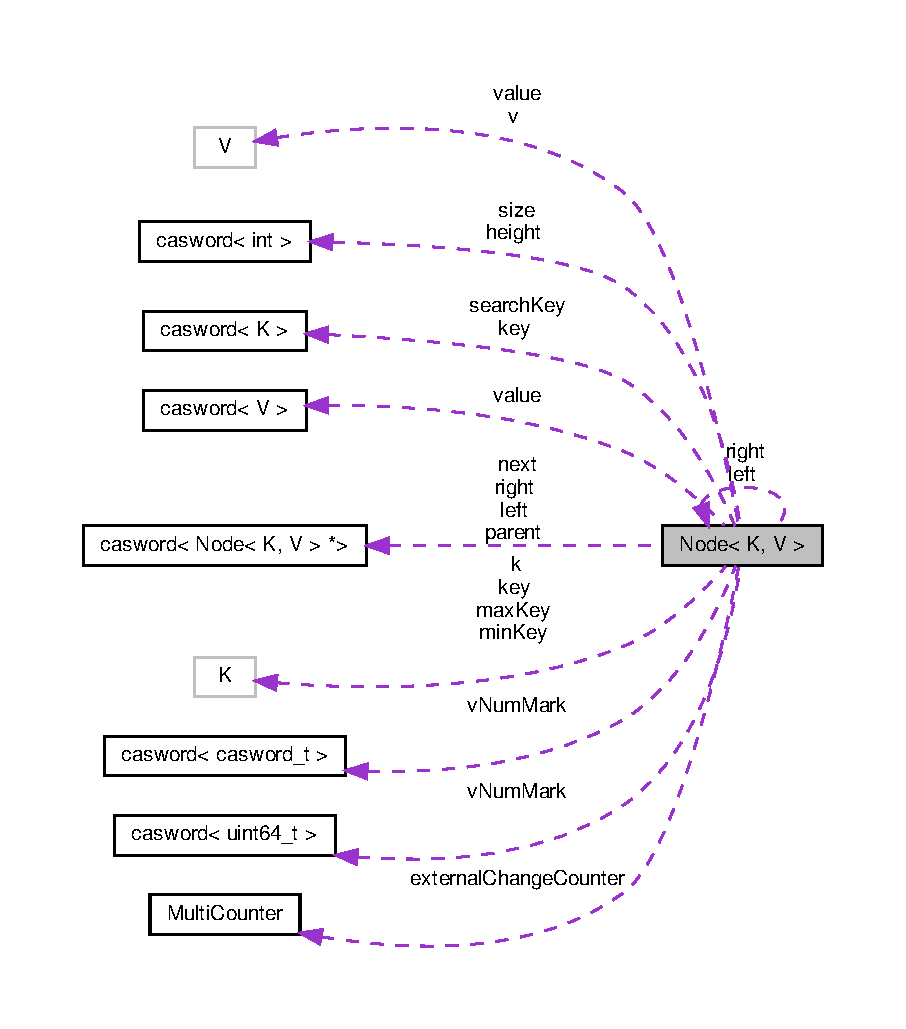
\includegraphics[width=350pt]{classNode__coll__graph}
\end{center}
\end{figure}
\subsection*{Public Member Functions}
\begin{DoxyCompactItemize}
\item 
\hyperlink{classNode_ab18e92edaff4f5aaca9b3ad9fc3a48da}{Node} (int \hyperlink{classNode_a0d5f29b75d1a6c47ef08c2bc993f03c0}{key})
\item 
K $\ast$ \hyperlink{classNode_ad56e1063825d51ca4a8927e03840d767}{key\+Addr} (const int ix)
\item 
K \& \hyperlink{classNode_abc52bee164f3a5bed59668eb416719ae}{key} (const int ix)
\item 
\hyperlink{rq__unsafe_8h_ad45142aaf2ff20a036dc6242b8483e9c}{casword\+\_\+t} volatile $\ast$ \hyperlink{classNode_a7e7a537724aa58596201327f65cec401}{ptr\+Addr} (const int ix)
\item 
\hyperlink{rq__unsafe_8h_ad45142aaf2ff20a036dc6242b8483e9c}{casword\+\_\+t} volatile \hyperlink{classNode_a817ad0968598c35eb3ecb1fa1b5871b2}{ptr} (const int ix)
\item 
void \hyperlink{classNode_a24324cc23f7c3377c7b2b9ff71a1c0f6}{increment\+Change\+Sum} (const int \hyperlink{microbench_2main_8cpp_a9ca9869868fe7e7a38a921cc7de4103f}{tid}, \hyperlink{classRandomFNV1A}{Random\+F\+N\+V1A} $\ast$rng)
\item 
size\+\_\+t \hyperlink{classNode_a7652c04d056ca05792291032ac89f60d}{read\+Change\+Sum} (const int \hyperlink{microbench_2main_8cpp_a9ca9869868fe7e7a38a921cc7de4103f}{tid}, \hyperlink{classRandomFNV1A}{Random\+F\+N\+V1A} $\ast$rng)
\end{DoxyCompactItemize}
\subsection*{Public Attributes}
\begin{DoxyCompactItemize}
\item 
int \hyperlink{classNode_a0d5f29b75d1a6c47ef08c2bc993f03c0}{key}
\item 
volatile bool \hyperlink{classNode_ad1ad570bba87cab1d79d419129173e90}{marked}
\item 
volatile long long \hyperlink{classNode_a43227ccd8b7604ac51336fd368451784}{itime}
\item 
volatile long long \hyperlink{classNode_af7ad969e3edbea0602b1a653f9ba0a7c}{dtime}
\item 
K \hyperlink{classNode_a3a7754a22c66b5300a2892b18bc66c3f}{k}
\item 
V \hyperlink{classNode_aae93698bf451fa862b4b1b5466d36dfd}{v}
\item 
\hyperlink{classNode}{Node} $\ast$volatile \hyperlink{classNode_a13ed6bdab297ee3dc66ca598f51fdbb5}{left}
\item 
\hyperlink{classNode}{Node} $\ast$volatile \hyperlink{classNode_a1075c82d0b5b7ca91ce4d37b1d651b30}{right}
\item 
\begin{tabbing}
xx\=xx\=xx\=xx\=xx\=xx\=xx\=xx\=xx\=\kill
union \{\\
\>volatile char \hyperlink{classNode_a4a5b8f90ab1220e757685cecea531793}{bytes} \mbox{[}208\mbox{]}\\
\>struct \{\\
\>\>K \hyperlink{classNode_a3a7754a22c66b5300a2892b18bc66c3f}{k}\\
\>\>V \hyperlink{classNode_aae93698bf451fa862b4b1b5466d36dfd}{v}\\
\>\>\hyperlink{classNode}{Node} $\ast$volatile \hyperlink{classNode_a13ed6bdab297ee3dc66ca598f51fdbb5}{left}\\
\>\>\hyperlink{classNode}{Node} $\ast$volatile \hyperlink{classNode_a1075c82d0b5b7ca91ce4d37b1d651b30}{right}\\
\>\} \\
\}; \\

\end{tabbing}\item 
\begin{tabbing}
xx\=xx\=xx\=xx\=xx\=xx\=xx\=xx\=xx\=\kill
union \{\\
\>volatile char \hyperlink{classNode_a4a5b8f90ab1220e757685cecea531793}{bytes} \mbox{[}208\mbox{]}\\
\>struct \{\\
\>\>K \hyperlink{classNode_a3a7754a22c66b5300a2892b18bc66c3f}{k}\\
\>\>V \hyperlink{classNode_aae93698bf451fa862b4b1b5466d36dfd}{v}\\
\>\>\hyperlink{classNode}{Node} $\ast$volatile \hyperlink{classNode_a13ed6bdab297ee3dc66ca598f51fdbb5}{left}\\
\>\>\hyperlink{classNode}{Node} $\ast$volatile \hyperlink{classNode_a1075c82d0b5b7ca91ce4d37b1d651b30}{right}\\
\>\} \\
\}; \\

\end{tabbing}\item 
\begin{tabbing}
xx\=xx\=xx\=xx\=xx\=xx\=xx\=xx\=xx\=\kill
union \{\\
\>volatile char \hyperlink{classNode_a4a5b8f90ab1220e757685cecea531793}{bytes} \mbox{[}208\mbox{]}\\
\>struct \{\\
\>\>K \hyperlink{classNode_a3a7754a22c66b5300a2892b18bc66c3f}{k}\\
\>\>V \hyperlink{classNode_aae93698bf451fa862b4b1b5466d36dfd}{v}\\
\>\>\hyperlink{classNode}{Node} $\ast$volatile \hyperlink{classNode_a13ed6bdab297ee3dc66ca598f51fdbb5}{left}\\
\>\>\hyperlink{classNode}{Node} $\ast$volatile \hyperlink{classNode_a1075c82d0b5b7ca91ce4d37b1d651b30}{right}\\
\>\} \\
\}; \\

\end{tabbing}\item 
\begin{tabbing}
xx\=xx\=xx\=xx\=xx\=xx\=xx\=xx\=xx\=\kill
union \{\\
\>volatile char \hyperlink{classNode_a4a5b8f90ab1220e757685cecea531793}{bytes} \mbox{[}208\mbox{]}\\
\>struct \{\\
\>\>K \hyperlink{classNode_a3a7754a22c66b5300a2892b18bc66c3f}{k}\\
\>\>V \hyperlink{classNode_aae93698bf451fa862b4b1b5466d36dfd}{v}\\
\>\>\hyperlink{classNode}{Node} $\ast$volatile \hyperlink{classNode_a13ed6bdab297ee3dc66ca598f51fdbb5}{left}\\
\>\>\hyperlink{classNode}{Node} $\ast$volatile \hyperlink{classNode_a1075c82d0b5b7ca91ce4d37b1d651b30}{right}\\
\>\} \\
\}; \\

\end{tabbing}\item 
size\+\_\+t volatile \hyperlink{classNode_a2dd213b9ec29f7a388aecbf3745028ab}{degree}
\item 
K \hyperlink{classNode_af389a346229e7fc7a55c07ce18816c72}{min\+Key}
\item 
K \hyperlink{classNode_a952ab64410cb2844499a2cf856848f14}{max\+Key}
\item 
size\+\_\+t \hyperlink{classNode_a017fd2017e14882deaf39b960d740b7e}{capacity}
\item 
size\+\_\+t \hyperlink{classNode_aba5197eb2b00bef6628dcf30056a2d92}{init\+Size}
\item 
size\+\_\+t volatile \hyperlink{classNode_af8f8003d96ba90f4f5acd5c003386b08}{dirty}
\item 
size\+\_\+t volatile \hyperlink{classNode_a8a7ef9d231138ce3458e3b360c0cee57}{next\+Mark\+And\+Count}
\item 
volatile size\+\_\+t \hyperlink{classNode_af94bd72d91f93e528c76778a60f5312e}{change\+Sum}
\item 
\hyperlink{classMultiCounter}{Multi\+Counter} $\ast$ \hyperlink{classNode_a5de4abf9942c16e6d8938e78a69efb31}{external\+Change\+Counter}
\item 
volatile bool \hyperlink{classNode_a1897c0740278b98f1066d2f62f29e6f4}{leaf}
\item 
\hyperlink{structcasword}{casword}$<$ \hyperlink{rq__unsafe_8h_ad45142aaf2ff20a036dc6242b8483e9c}{casword\+\_\+t} $>$ \hyperlink{classNode_a0aaf5a1dde5a35ada56cbd256639d894}{v\+Num\+Mark}
\item 
volatile int \hyperlink{classNode_a1c307fd773eae7760993981655620539}{weight}
\item 
\hyperlink{structcasword}{casword}$<$ int $>$ \hyperlink{classNode_a65f7073a99f7d2b7ee735cd548bd6f9b}{size}
\item 
\hyperlink{structcasword}{casword}$<$ K $>$ \hyperlink{classNode_a788327695ace7c76fd69877322f57b4e}{search\+Key}
\item 
\hyperlink{structcasword}{casword}$<$ K $>$ \hyperlink{classNode_ad0930076f2ac755390423b48c6856cfa}{key}
\item 
\hyperlink{structcasword}{casword}$<$ \hyperlink{classNode}{Node}$<$ K, V $>$ $\ast$ $>$ \hyperlink{classNode_ad94b2acd7430ef8a2ef4a197f4466c64}{left}
\item 
\hyperlink{structcasword}{casword}$<$ \hyperlink{classNode}{Node}$<$ K, V $>$ $\ast$ $>$ \hyperlink{classNode_afa1cf8bdbcc54a575704def2de4ab22f}{right}
\item 
\hyperlink{structcasword}{casword}$<$ \hyperlink{classNode}{Node}$<$ K, V $>$ $\ast$ $>$ \hyperlink{classNode_a6393b3996b6bbae601841635eafad7a4}{parent}
\item 
\hyperlink{structcasword}{casword}$<$ int $>$ \hyperlink{classNode_aa416d66d3fba99e844a02109fe8e2419}{height}
\item 
\hyperlink{structcasword}{casword}$<$ V $>$ \hyperlink{classNode_afb1f58df40fc63f650d0ba9eb165cdb4}{value}
\item 
K \hyperlink{classNode_a4091ccbd4f0b78711f848a5129fdece9}{key}
\item 
V \hyperlink{classNode_ad26872ac51fa4ef5a8519038472a5050}{value}
\item 
\hyperlink{structcasword}{casword}$<$ uint64\+\_\+t $>$ \hyperlink{classNode_a3f9e4ea9fc73761a06375bb5f3ebcd60}{v\+Num\+Mark}
\item 
int \hyperlink{classNode_ad8e961cf89a9b9f8e21f648c6ffb06ff}{height}
\item 
\hyperlink{structcasword}{casword}$<$ \hyperlink{classNode}{Node}$<$ K, V $>$ $\ast$ $>$ \hyperlink{classNode_a1f772846cd18db8938fbae6de5970941}{next} \mbox{[}\hyperlink{skiplist_8h_a6e5496d00878dd64264b713699766bdb}{M\+A\+X\+\_\+\+T\+O\+W\+E\+R\+\_\+\+H\+E\+I\+G\+HT}\mbox{]}
\end{DoxyCompactItemize}


\subsection{Constructor \& Destructor Documentation}
\mbox{\Hypertarget{classNode_ab18e92edaff4f5aaca9b3ad9fc3a48da}\label{classNode_ab18e92edaff4f5aaca9b3ad9fc3a48da}} 
\index{Node@{Node}!Node@{Node}}
\index{Node@{Node}!Node@{Node}}
\subsubsection{\texorpdfstring{Node()}{Node()}}
{\footnotesize\ttfamily template$<$typename K, typename V$>$ \\
\hyperlink{classNode}{Node}$<$ K, V $>$\+::\hyperlink{classNode}{Node} (\begin{DoxyParamCaption}\item[{int}]{key }\end{DoxyParamCaption})\hspace{0.3cm}{\ttfamily [inline]}}



\subsection{Member Function Documentation}
\mbox{\Hypertarget{classNode_a24324cc23f7c3377c7b2b9ff71a1c0f6}\label{classNode_a24324cc23f7c3377c7b2b9ff71a1c0f6}} 
\index{Node@{Node}!increment\+Change\+Sum@{increment\+Change\+Sum}}
\index{increment\+Change\+Sum@{increment\+Change\+Sum}!Node@{Node}}
\subsubsection{\texorpdfstring{increment\+Change\+Sum()}{incrementChangeSum()}}
{\footnotesize\ttfamily template$<$typename K, typename V$>$ \\
void \hyperlink{classNode}{Node}$<$ K, V $>$\+::increment\+Change\+Sum (\begin{DoxyParamCaption}\item[{const int}]{tid,  }\item[{\hyperlink{classRandomFNV1A}{Random\+F\+N\+V1A} $\ast$}]{rng }\end{DoxyParamCaption})\hspace{0.3cm}{\ttfamily [inline]}}

\mbox{\Hypertarget{classNode_abc52bee164f3a5bed59668eb416719ae}\label{classNode_abc52bee164f3a5bed59668eb416719ae}} 
\index{Node@{Node}!key@{key}}
\index{key@{key}!Node@{Node}}
\subsubsection{\texorpdfstring{key()}{key()}}
{\footnotesize\ttfamily template$<$typename K, typename V$>$ \\
K\& \hyperlink{classNode}{Node}$<$ K, V $>$\+::key (\begin{DoxyParamCaption}\item[{const int}]{ix }\end{DoxyParamCaption})\hspace{0.3cm}{\ttfamily [inline]}}

\mbox{\Hypertarget{classNode_ad56e1063825d51ca4a8927e03840d767}\label{classNode_ad56e1063825d51ca4a8927e03840d767}} 
\index{Node@{Node}!key\+Addr@{key\+Addr}}
\index{key\+Addr@{key\+Addr}!Node@{Node}}
\subsubsection{\texorpdfstring{key\+Addr()}{keyAddr()}}
{\footnotesize\ttfamily template$<$typename K, typename V$>$ \\
K$\ast$ \hyperlink{classNode}{Node}$<$ K, V $>$\+::key\+Addr (\begin{DoxyParamCaption}\item[{const int}]{ix }\end{DoxyParamCaption})\hspace{0.3cm}{\ttfamily [inline]}}

\mbox{\Hypertarget{classNode_a817ad0968598c35eb3ecb1fa1b5871b2}\label{classNode_a817ad0968598c35eb3ecb1fa1b5871b2}} 
\index{Node@{Node}!ptr@{ptr}}
\index{ptr@{ptr}!Node@{Node}}
\subsubsection{\texorpdfstring{ptr()}{ptr()}}
{\footnotesize\ttfamily template$<$typename K, typename V$>$ \\
\hyperlink{rq__unsafe_8h_ad45142aaf2ff20a036dc6242b8483e9c}{casword\+\_\+t} volatile \hyperlink{classNode}{Node}$<$ K, V $>$\+::ptr (\begin{DoxyParamCaption}\item[{const int}]{ix }\end{DoxyParamCaption})\hspace{0.3cm}{\ttfamily [inline]}}

\mbox{\Hypertarget{classNode_a7e7a537724aa58596201327f65cec401}\label{classNode_a7e7a537724aa58596201327f65cec401}} 
\index{Node@{Node}!ptr\+Addr@{ptr\+Addr}}
\index{ptr\+Addr@{ptr\+Addr}!Node@{Node}}
\subsubsection{\texorpdfstring{ptr\+Addr()}{ptrAddr()}}
{\footnotesize\ttfamily template$<$typename K, typename V$>$ \\
\hyperlink{rq__unsafe_8h_ad45142aaf2ff20a036dc6242b8483e9c}{casword\+\_\+t} volatile$\ast$ \hyperlink{classNode}{Node}$<$ K, V $>$\+::ptr\+Addr (\begin{DoxyParamCaption}\item[{const int}]{ix }\end{DoxyParamCaption})\hspace{0.3cm}{\ttfamily [inline]}}

\mbox{\Hypertarget{classNode_a7652c04d056ca05792291032ac89f60d}\label{classNode_a7652c04d056ca05792291032ac89f60d}} 
\index{Node@{Node}!read\+Change\+Sum@{read\+Change\+Sum}}
\index{read\+Change\+Sum@{read\+Change\+Sum}!Node@{Node}}
\subsubsection{\texorpdfstring{read\+Change\+Sum()}{readChangeSum()}}
{\footnotesize\ttfamily template$<$typename K, typename V$>$ \\
size\+\_\+t \hyperlink{classNode}{Node}$<$ K, V $>$\+::read\+Change\+Sum (\begin{DoxyParamCaption}\item[{const int}]{tid,  }\item[{\hyperlink{classRandomFNV1A}{Random\+F\+N\+V1A} $\ast$}]{rng }\end{DoxyParamCaption})\hspace{0.3cm}{\ttfamily [inline]}}



\subsection{Member Data Documentation}
\mbox{\Hypertarget{classNode_aff3fa8eb8122c855e459deafc3a453c2}\label{classNode_aff3fa8eb8122c855e459deafc3a453c2}} 
\subsubsection{\texorpdfstring{"@55}{@55}}
{\footnotesize\ttfamily union \{ ... \} }

\mbox{\Hypertarget{classNode_afd70f5bee4b67e9f5569596faf715b9f}\label{classNode_afd70f5bee4b67e9f5569596faf715b9f}} 
\subsubsection{\texorpdfstring{"@59}{@59}}
{\footnotesize\ttfamily union \{ ... \} }

\mbox{\Hypertarget{classNode_ae735cb0c206600d8facff92750ed8f12}\label{classNode_ae735cb0c206600d8facff92750ed8f12}} 
\subsubsection{\texorpdfstring{"@63}{@63}}
{\footnotesize\ttfamily union \{ ... \} }

\mbox{\Hypertarget{classNode_a5907a461b4944a4b9aac9d3b71e961a5}\label{classNode_a5907a461b4944a4b9aac9d3b71e961a5}} 
\subsubsection{\texorpdfstring{"@67}{@67}}
{\footnotesize\ttfamily union \{ ... \} }

\mbox{\Hypertarget{classNode_a4a5b8f90ab1220e757685cecea531793}\label{classNode_a4a5b8f90ab1220e757685cecea531793}} 
\index{Node@{Node}!bytes@{bytes}}
\index{bytes@{bytes}!Node@{Node}}
\subsubsection{\texorpdfstring{bytes}{bytes}}
{\footnotesize\ttfamily template$<$typename K, typename V$>$ \\
volatile char \hyperlink{classNode}{Node}$<$ K, V $>$\+::bytes\mbox{[}208\mbox{]}}

\mbox{\Hypertarget{classNode_a017fd2017e14882deaf39b960d740b7e}\label{classNode_a017fd2017e14882deaf39b960d740b7e}} 
\index{Node@{Node}!capacity@{capacity}}
\index{capacity@{capacity}!Node@{Node}}
\subsubsection{\texorpdfstring{capacity}{capacity}}
{\footnotesize\ttfamily template$<$typename K, typename V$>$ \\
size\+\_\+t \hyperlink{classNode}{Node}$<$ K, V $>$\+::capacity}

\mbox{\Hypertarget{classNode_af94bd72d91f93e528c76778a60f5312e}\label{classNode_af94bd72d91f93e528c76778a60f5312e}} 
\index{Node@{Node}!change\+Sum@{change\+Sum}}
\index{change\+Sum@{change\+Sum}!Node@{Node}}
\subsubsection{\texorpdfstring{change\+Sum}{changeSum}}
{\footnotesize\ttfamily template$<$typename K, typename V$>$ \\
volatile size\+\_\+t \hyperlink{classNode}{Node}$<$ K, V $>$\+::change\+Sum}

\mbox{\Hypertarget{classNode_a2dd213b9ec29f7a388aecbf3745028ab}\label{classNode_a2dd213b9ec29f7a388aecbf3745028ab}} 
\index{Node@{Node}!degree@{degree}}
\index{degree@{degree}!Node@{Node}}
\subsubsection{\texorpdfstring{degree}{degree}}
{\footnotesize\ttfamily template$<$typename K, typename V$>$ \\
size\+\_\+t volatile \hyperlink{classNode}{Node}$<$ K, V $>$\+::degree}

\mbox{\Hypertarget{classNode_af8f8003d96ba90f4f5acd5c003386b08}\label{classNode_af8f8003d96ba90f4f5acd5c003386b08}} 
\index{Node@{Node}!dirty@{dirty}}
\index{dirty@{dirty}!Node@{Node}}
\subsubsection{\texorpdfstring{dirty}{dirty}}
{\footnotesize\ttfamily template$<$typename K, typename V$>$ \\
size\+\_\+t volatile \hyperlink{classNode}{Node}$<$ K, V $>$\+::dirty}

\mbox{\Hypertarget{classNode_af7ad969e3edbea0602b1a653f9ba0a7c}\label{classNode_af7ad969e3edbea0602b1a653f9ba0a7c}} 
\index{Node@{Node}!dtime@{dtime}}
\index{dtime@{dtime}!Node@{Node}}
\subsubsection{\texorpdfstring{dtime}{dtime}}
{\footnotesize\ttfamily template$<$typename K, typename V$>$ \\
volatile long long \hyperlink{classNode}{Node}$<$ K, V $>$\+::dtime}

\mbox{\Hypertarget{classNode_a5de4abf9942c16e6d8938e78a69efb31}\label{classNode_a5de4abf9942c16e6d8938e78a69efb31}} 
\index{Node@{Node}!external\+Change\+Counter@{external\+Change\+Counter}}
\index{external\+Change\+Counter@{external\+Change\+Counter}!Node@{Node}}
\subsubsection{\texorpdfstring{external\+Change\+Counter}{externalChangeCounter}}
{\footnotesize\ttfamily template$<$typename K, typename V$>$ \\
\hyperlink{classMultiCounter}{Multi\+Counter}$\ast$ \hyperlink{classNode}{Node}$<$ K, V $>$\+::external\+Change\+Counter}

\mbox{\Hypertarget{classNode_aa416d66d3fba99e844a02109fe8e2419}\label{classNode_aa416d66d3fba99e844a02109fe8e2419}} 
\index{Node@{Node}!height@{height}}
\index{height@{height}!Node@{Node}}
\subsubsection{\texorpdfstring{height}{height}\hspace{0.1cm}{\footnotesize\ttfamily [1/2]}}
{\footnotesize\ttfamily template$<$typename K, typename V$>$ \\
\hyperlink{structcasword}{casword}$<$int$>$ \hyperlink{classNode}{Node}$<$ K, V $>$\+::height}

\mbox{\Hypertarget{classNode_ad8e961cf89a9b9f8e21f648c6ffb06ff}\label{classNode_ad8e961cf89a9b9f8e21f648c6ffb06ff}} 
\index{Node@{Node}!height@{height}}
\index{height@{height}!Node@{Node}}
\subsubsection{\texorpdfstring{height}{height}\hspace{0.1cm}{\footnotesize\ttfamily [2/2]}}
{\footnotesize\ttfamily template$<$typename K, typename V$>$ \\
int \hyperlink{classNode}{Node}$<$ K, V $>$\+::height}

\mbox{\Hypertarget{classNode_aba5197eb2b00bef6628dcf30056a2d92}\label{classNode_aba5197eb2b00bef6628dcf30056a2d92}} 
\index{Node@{Node}!init\+Size@{init\+Size}}
\index{init\+Size@{init\+Size}!Node@{Node}}
\subsubsection{\texorpdfstring{init\+Size}{initSize}}
{\footnotesize\ttfamily template$<$typename K, typename V$>$ \\
size\+\_\+t \hyperlink{classNode}{Node}$<$ K, V $>$\+::init\+Size}

\mbox{\Hypertarget{classNode_a43227ccd8b7604ac51336fd368451784}\label{classNode_a43227ccd8b7604ac51336fd368451784}} 
\index{Node@{Node}!itime@{itime}}
\index{itime@{itime}!Node@{Node}}
\subsubsection{\texorpdfstring{itime}{itime}}
{\footnotesize\ttfamily template$<$typename K, typename V$>$ \\
volatile long long \hyperlink{classNode}{Node}$<$ K, V $>$\+::itime}

\mbox{\Hypertarget{classNode_a3a7754a22c66b5300a2892b18bc66c3f}\label{classNode_a3a7754a22c66b5300a2892b18bc66c3f}} 
\index{Node@{Node}!k@{k}}
\index{k@{k}!Node@{Node}}
\subsubsection{\texorpdfstring{k}{k}}
{\footnotesize\ttfamily template$<$typename K, typename V$>$ \\
K \hyperlink{classNode}{Node}$<$ K, V $>$\+::k}

\mbox{\Hypertarget{classNode_a0d5f29b75d1a6c47ef08c2bc993f03c0}\label{classNode_a0d5f29b75d1a6c47ef08c2bc993f03c0}} 
\index{Node@{Node}!key@{key}}
\index{key@{key}!Node@{Node}}
\subsubsection{\texorpdfstring{key}{key}\hspace{0.1cm}{\footnotesize\ttfamily [1/3]}}
{\footnotesize\ttfamily template$<$typename K, typename V$>$ \\
\hyperlink{structcasword}{casword}$<$ K $>$ \hyperlink{classNode}{Node}$<$ K, V $>$\+::key}

\mbox{\Hypertarget{classNode_ad0930076f2ac755390423b48c6856cfa}\label{classNode_ad0930076f2ac755390423b48c6856cfa}} 
\index{Node@{Node}!key@{key}}
\index{key@{key}!Node@{Node}}
\subsubsection{\texorpdfstring{key}{key}\hspace{0.1cm}{\footnotesize\ttfamily [2/3]}}
{\footnotesize\ttfamily template$<$typename K, typename V$>$ \\
\hyperlink{structcasword}{casword}$<$K$>$ \hyperlink{classNode}{Node}$<$ K, V $>$\+::key}

\mbox{\Hypertarget{classNode_a4091ccbd4f0b78711f848a5129fdece9}\label{classNode_a4091ccbd4f0b78711f848a5129fdece9}} 
\index{Node@{Node}!key@{key}}
\index{key@{key}!Node@{Node}}
\subsubsection{\texorpdfstring{key}{key}\hspace{0.1cm}{\footnotesize\ttfamily [3/3]}}
{\footnotesize\ttfamily template$<$typename K, typename V$>$ \\
K \hyperlink{classNode}{Node}$<$ K, V $>$\+::key}

\mbox{\Hypertarget{classNode_a1897c0740278b98f1066d2f62f29e6f4}\label{classNode_a1897c0740278b98f1066d2f62f29e6f4}} 
\index{Node@{Node}!leaf@{leaf}}
\index{leaf@{leaf}!Node@{Node}}
\subsubsection{\texorpdfstring{leaf}{leaf}}
{\footnotesize\ttfamily template$<$typename K, typename V$>$ \\
volatile bool \hyperlink{classNode}{Node}$<$ K, V $>$\+::leaf}

\mbox{\Hypertarget{classNode_a13ed6bdab297ee3dc66ca598f51fdbb5}\label{classNode_a13ed6bdab297ee3dc66ca598f51fdbb5}} 
\index{Node@{Node}!left@{left}}
\index{left@{left}!Node@{Node}}
\subsubsection{\texorpdfstring{left}{left}\hspace{0.1cm}{\footnotesize\ttfamily [1/2]}}
{\footnotesize\ttfamily template$<$typename K, typename V$>$ \\
\hyperlink{structcasword}{casword}$<$ \hyperlink{classNode}{Node}$<$ K, V $>$ $\ast$ $>$ \hyperlink{classNode}{Node}$<$ K, V $>$\+::left}

\mbox{\Hypertarget{classNode_ad94b2acd7430ef8a2ef4a197f4466c64}\label{classNode_ad94b2acd7430ef8a2ef4a197f4466c64}} 
\index{Node@{Node}!left@{left}}
\index{left@{left}!Node@{Node}}
\subsubsection{\texorpdfstring{left}{left}\hspace{0.1cm}{\footnotesize\ttfamily [2/2]}}
{\footnotesize\ttfamily template$<$typename K, typename V$>$ \\
\hyperlink{structcasword}{casword}$<$\hyperlink{classNode}{Node}$<$K, V$>$ $\ast$$>$ \hyperlink{classNode}{Node}$<$ K, V $>$\+::left}

\mbox{\Hypertarget{classNode_ad1ad570bba87cab1d79d419129173e90}\label{classNode_ad1ad570bba87cab1d79d419129173e90}} 
\index{Node@{Node}!marked@{marked}}
\index{marked@{marked}!Node@{Node}}
\subsubsection{\texorpdfstring{marked}{marked}}
{\footnotesize\ttfamily template$<$typename K, typename V$>$ \\
volatile bool \hyperlink{classNode}{Node}$<$ K, V $>$\+::marked}

\mbox{\Hypertarget{classNode_a952ab64410cb2844499a2cf856848f14}\label{classNode_a952ab64410cb2844499a2cf856848f14}} 
\index{Node@{Node}!max\+Key@{max\+Key}}
\index{max\+Key@{max\+Key}!Node@{Node}}
\subsubsection{\texorpdfstring{max\+Key}{maxKey}}
{\footnotesize\ttfamily template$<$typename K, typename V$>$ \\
K \hyperlink{classNode}{Node}$<$ K, V $>$\+::max\+Key}

\mbox{\Hypertarget{classNode_af389a346229e7fc7a55c07ce18816c72}\label{classNode_af389a346229e7fc7a55c07ce18816c72}} 
\index{Node@{Node}!min\+Key@{min\+Key}}
\index{min\+Key@{min\+Key}!Node@{Node}}
\subsubsection{\texorpdfstring{min\+Key}{minKey}}
{\footnotesize\ttfamily template$<$typename K, typename V$>$ \\
K \hyperlink{classNode}{Node}$<$ K, V $>$\+::min\+Key}

\mbox{\Hypertarget{classNode_a1f772846cd18db8938fbae6de5970941}\label{classNode_a1f772846cd18db8938fbae6de5970941}} 
\index{Node@{Node}!next@{next}}
\index{next@{next}!Node@{Node}}
\subsubsection{\texorpdfstring{next}{next}}
{\footnotesize\ttfamily template$<$typename K, typename V$>$ \\
\hyperlink{structcasword}{casword}$<$\hyperlink{classNode}{Node}$<$K,V$>$ $\ast$$>$ \hyperlink{classNode}{Node}$<$ K, V $>$\+::next\mbox{[}\hyperlink{skiplist_8h_a6e5496d00878dd64264b713699766bdb}{M\+A\+X\+\_\+\+T\+O\+W\+E\+R\+\_\+\+H\+E\+I\+G\+HT}\mbox{]}}

\mbox{\Hypertarget{classNode_a8a7ef9d231138ce3458e3b360c0cee57}\label{classNode_a8a7ef9d231138ce3458e3b360c0cee57}} 
\index{Node@{Node}!next\+Mark\+And\+Count@{next\+Mark\+And\+Count}}
\index{next\+Mark\+And\+Count@{next\+Mark\+And\+Count}!Node@{Node}}
\subsubsection{\texorpdfstring{next\+Mark\+And\+Count}{nextMarkAndCount}}
{\footnotesize\ttfamily template$<$typename K, typename V$>$ \\
size\+\_\+t volatile \hyperlink{classNode}{Node}$<$ K, V $>$\+::next\+Mark\+And\+Count}

\mbox{\Hypertarget{classNode_a6393b3996b6bbae601841635eafad7a4}\label{classNode_a6393b3996b6bbae601841635eafad7a4}} 
\index{Node@{Node}!parent@{parent}}
\index{parent@{parent}!Node@{Node}}
\subsubsection{\texorpdfstring{parent}{parent}}
{\footnotesize\ttfamily template$<$typename K, typename V$>$ \\
\hyperlink{structcasword}{casword}$<$\hyperlink{classNode}{Node}$<$K, V$>$ $\ast$$>$ \hyperlink{classNode}{Node}$<$ K, V $>$\+::parent}

\mbox{\Hypertarget{classNode_a1075c82d0b5b7ca91ce4d37b1d651b30}\label{classNode_a1075c82d0b5b7ca91ce4d37b1d651b30}} 
\index{Node@{Node}!right@{right}}
\index{right@{right}!Node@{Node}}
\subsubsection{\texorpdfstring{right}{right}\hspace{0.1cm}{\footnotesize\ttfamily [1/2]}}
{\footnotesize\ttfamily template$<$typename K, typename V$>$ \\
\hyperlink{structcasword}{casword}$<$ \hyperlink{classNode}{Node}$<$ K, V $>$ $\ast$ $>$ \hyperlink{classNode}{Node}$<$ K, V $>$\+::right}

\mbox{\Hypertarget{classNode_afa1cf8bdbcc54a575704def2de4ab22f}\label{classNode_afa1cf8bdbcc54a575704def2de4ab22f}} 
\index{Node@{Node}!right@{right}}
\index{right@{right}!Node@{Node}}
\subsubsection{\texorpdfstring{right}{right}\hspace{0.1cm}{\footnotesize\ttfamily [2/2]}}
{\footnotesize\ttfamily template$<$typename K, typename V$>$ \\
\hyperlink{structcasword}{casword}$<$\hyperlink{classNode}{Node}$<$K, V$>$ $\ast$$>$ \hyperlink{classNode}{Node}$<$ K, V $>$\+::right}

\mbox{\Hypertarget{classNode_a788327695ace7c76fd69877322f57b4e}\label{classNode_a788327695ace7c76fd69877322f57b4e}} 
\index{Node@{Node}!search\+Key@{search\+Key}}
\index{search\+Key@{search\+Key}!Node@{Node}}
\subsubsection{\texorpdfstring{search\+Key}{searchKey}}
{\footnotesize\ttfamily template$<$typename K, typename V$>$ \\
\hyperlink{structcasword}{casword}$<$K$>$ \hyperlink{classNode}{Node}$<$ K, V $>$\+::search\+Key}

\mbox{\Hypertarget{classNode_a65f7073a99f7d2b7ee735cd548bd6f9b}\label{classNode_a65f7073a99f7d2b7ee735cd548bd6f9b}} 
\index{Node@{Node}!size@{size}}
\index{size@{size}!Node@{Node}}
\subsubsection{\texorpdfstring{size}{size}}
{\footnotesize\ttfamily template$<$typename K, typename V$>$ \\
\hyperlink{structcasword}{casword}$<$int$>$ \hyperlink{classNode}{Node}$<$ K, V $>$\+::size}

\mbox{\Hypertarget{classNode_aae93698bf451fa862b4b1b5466d36dfd}\label{classNode_aae93698bf451fa862b4b1b5466d36dfd}} 
\index{Node@{Node}!v@{v}}
\index{v@{v}!Node@{Node}}
\subsubsection{\texorpdfstring{v}{v}}
{\footnotesize\ttfamily template$<$typename K, typename V$>$ \\
V \hyperlink{classNode}{Node}$<$ K, V $>$\+::v}

\mbox{\Hypertarget{classNode_afb1f58df40fc63f650d0ba9eb165cdb4}\label{classNode_afb1f58df40fc63f650d0ba9eb165cdb4}} 
\index{Node@{Node}!value@{value}}
\index{value@{value}!Node@{Node}}
\subsubsection{\texorpdfstring{value}{value}\hspace{0.1cm}{\footnotesize\ttfamily [1/2]}}
{\footnotesize\ttfamily template$<$typename K, typename V$>$ \\
\hyperlink{structcasword}{casword}$<$ V $>$ \hyperlink{classNode}{Node}$<$ K, V $>$\+::value}

\mbox{\Hypertarget{classNode_ad26872ac51fa4ef5a8519038472a5050}\label{classNode_ad26872ac51fa4ef5a8519038472a5050}} 
\index{Node@{Node}!value@{value}}
\index{value@{value}!Node@{Node}}
\subsubsection{\texorpdfstring{value}{value}\hspace{0.1cm}{\footnotesize\ttfamily [2/2]}}
{\footnotesize\ttfamily template$<$typename K, typename V$>$ \\
V \hyperlink{classNode}{Node}$<$ K, V $>$\+::value}

\mbox{\Hypertarget{classNode_a3f9e4ea9fc73761a06375bb5f3ebcd60}\label{classNode_a3f9e4ea9fc73761a06375bb5f3ebcd60}} 
\index{Node@{Node}!v\+Num\+Mark@{v\+Num\+Mark}}
\index{v\+Num\+Mark@{v\+Num\+Mark}!Node@{Node}}
\subsubsection{\texorpdfstring{v\+Num\+Mark}{vNumMark}\hspace{0.1cm}{\footnotesize\ttfamily [1/2]}}
{\footnotesize\ttfamily template$<$typename K, typename V$>$ \\
\hyperlink{structcasword}{casword}$<$uint64\+\_\+t$>$ \hyperlink{classNode}{Node}$<$ K, V $>$\+::v\+Num\+Mark}

\mbox{\Hypertarget{classNode_a0aaf5a1dde5a35ada56cbd256639d894}\label{classNode_a0aaf5a1dde5a35ada56cbd256639d894}} 
\index{Node@{Node}!v\+Num\+Mark@{v\+Num\+Mark}}
\index{v\+Num\+Mark@{v\+Num\+Mark}!Node@{Node}}
\subsubsection{\texorpdfstring{v\+Num\+Mark}{vNumMark}\hspace{0.1cm}{\footnotesize\ttfamily [2/2]}}
{\footnotesize\ttfamily template$<$typename K, typename V$>$ \\
\hyperlink{structcasword}{casword}$<$ \hyperlink{rq__unsafe_8h_ad45142aaf2ff20a036dc6242b8483e9c}{casword\+\_\+t} $>$ \hyperlink{classNode}{Node}$<$ K, V $>$\+::v\+Num\+Mark}

\mbox{\Hypertarget{classNode_a1c307fd773eae7760993981655620539}\label{classNode_a1c307fd773eae7760993981655620539}} 
\index{Node@{Node}!weight@{weight}}
\index{weight@{weight}!Node@{Node}}
\subsubsection{\texorpdfstring{weight}{weight}}
{\footnotesize\ttfamily template$<$typename K, typename V$>$ \\
volatile int \hyperlink{classNode}{Node}$<$ K, V $>$\+::weight}



The documentation for this struct was generated from the following files\+:\begin{DoxyCompactItemize}
\item 
common/rq/snapcollector/\hyperlink{snapcollector__test_8cpp}{snapcollector\+\_\+test.\+cpp}\item 
ds/\+\_\+dummy2\+\_\+epochs/\hyperlink{__dummy2__epochs_2adapter_8h}{adapter.\+h}\item 
ds/brown\+\_\+ext\+\_\+ist\+\_\+lf/\hyperlink{brown__ext__ist__lf__impl_8h}{brown\+\_\+ext\+\_\+ist\+\_\+lf\+\_\+impl.\+h}\item 
ds/brown\+\_\+sigouin\+\_\+abtree\+\_\+kcas/\hyperlink{abtree__kcas_8h}{abtree\+\_\+kcas.\+h}\item 
ds/sigouin\+\_\+int\+\_\+bst\+\_\+kcas/\hyperlink{internal__kcas_8h}{internal\+\_\+kcas.\+h}\item 
ds/sigouin\+\_\+int\+\_\+bst\+\_\+kcas\+\_\+unbalanced/\hyperlink{internal__kcas__unbalanced_8h}{internal\+\_\+kcas\+\_\+unbalanced.\+h}\item 
ds/sigouin\+\_\+skip\+\_\+list\+\_\+kcas/\hyperlink{skiplist_8h}{skiplist.\+h}\end{DoxyCompactItemize}

\hypertarget{structabtree__ns_1_1Node}{}\section{abtree\+\_\+ns\+:\+:Node$<$ D\+E\+G\+R\+EE, K $>$ Struct Template Reference}
\label{structabtree__ns_1_1Node}\index{abtree\+\_\+ns\+::\+Node$<$ D\+E\+G\+R\+E\+E, K $>$@{abtree\+\_\+ns\+::\+Node$<$ D\+E\+G\+R\+E\+E, K $>$}}


{\ttfamily \#include $<$brown\+\_\+ext\+\_\+abtree\+\_\+lf\+\_\+impl.\+h$>$}



Collaboration diagram for abtree\+\_\+ns\+:\+:Node$<$ D\+E\+G\+R\+EE, K $>$\+:
\nopagebreak
\begin{figure}[H]
\begin{center}
\leavevmode
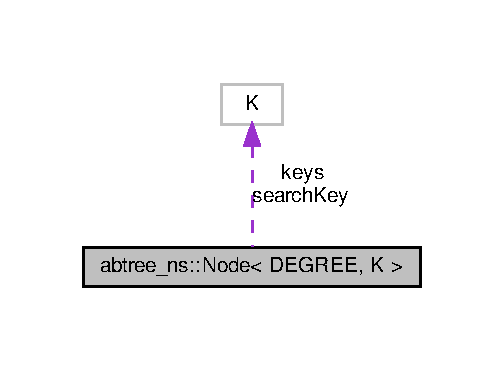
\includegraphics[width=242pt]{structabtree__ns_1_1Node__coll__graph}
\end{center}
\end{figure}
\subsection*{Public Member Functions}
\begin{DoxyCompactItemize}
\item 
bool \hyperlink{structabtree__ns_1_1Node_a09fe5b27e3c537ae628c695e9216b450}{is\+Leaf} ()
\item 
int \hyperlink{structabtree__ns_1_1Node_a17222fc44db1651a08225e97bab6644e}{get\+Key\+Count} ()
\item 
int \hyperlink{structabtree__ns_1_1Node_a65085f4a2fe4688479a71c50238bac69}{get\+A\+B\+Degree} ()
\item 
{\footnotesize template$<$class Compare $>$ }\\int \hyperlink{structabtree__ns_1_1Node_a1229e769cf5d2e1f67405dc689e64595}{get\+Child\+Index} (const K \&key, Compare cmp)
\item 
{\footnotesize template$<$class Compare $>$ }\\int \hyperlink{structabtree__ns_1_1Node_a5cf6c8acd36258e0bb925f2ae13ebd80}{get\+Key\+Index} (const K \&key, Compare cmp)
\item 
bool \hyperlink{structabtree__ns_1_1Node_a09fe5b27e3c537ae628c695e9216b450}{is\+Leaf} ()
\item 
int \hyperlink{structabtree__ns_1_1Node_a17222fc44db1651a08225e97bab6644e}{get\+Key\+Count} ()
\item 
int \hyperlink{structabtree__ns_1_1Node_a65085f4a2fe4688479a71c50238bac69}{get\+A\+B\+Degree} ()
\item 
{\footnotesize template$<$class Compare $>$ }\\int \hyperlink{structabtree__ns_1_1Node_a1229e769cf5d2e1f67405dc689e64595}{get\+Child\+Index} (const K \&key, Compare cmp)
\item 
{\footnotesize template$<$class Compare $>$ }\\int \hyperlink{structabtree__ns_1_1Node_a5cf6c8acd36258e0bb925f2ae13ebd80}{get\+Key\+Index} (const K \&key, Compare cmp)
\end{DoxyCompactItemize}
\subsection*{Public Attributes}
\begin{DoxyCompactItemize}
\item 
\hyperlink{scx__provider_8h_a368fa55a4b553010913289d3cbe6ce22}{scx\+\_\+handle\+\_\+t} volatile \hyperlink{structabtree__ns_1_1Node_ac66e083264c1a5229b42bf14ffcdf291}{scx\+Ptr}
\item 
int \hyperlink{structabtree__ns_1_1Node_ad538165f856eaf1502414a77ae0b6201}{leaf}
\item 
volatile int \hyperlink{structabtree__ns_1_1Node_a0452d341b415a50854e612d2d8bc2fde}{marked}
\item 
int \hyperlink{structabtree__ns_1_1Node_a85910bf98f322370af50db4fa6e8bf75}{weight}
\item 
int \hyperlink{structabtree__ns_1_1Node_a681685fe9668f05a34770c59772d71c2}{size}
\item 
K \hyperlink{structabtree__ns_1_1Node_a8723eee7563acc9b8b9cef9b43ca50ea}{search\+Key}
\item 
K \hyperlink{structabtree__ns_1_1Node_a8d975a4678747a2d60e5bf9ca298a29a}{keys} \mbox{[}\hyperlink{brown__sigouin__abtree__kcas_2adapter_8h_a5d88b17d70c985f2f2b8e987037fd6dd}{D\+E\+G\+R\+EE}\mbox{]}
\item 
\hyperlink{structabtree__ns_1_1Node}{Node}$<$ \hyperlink{brown__sigouin__abtree__kcas_2adapter_8h_a5d88b17d70c985f2f2b8e987037fd6dd}{D\+E\+G\+R\+EE}, K $>$ $\ast$volatile \hyperlink{structabtree__ns_1_1Node_a01e6606a48515df91a90bb8883268d7a}{ptrs} \mbox{[}\hyperlink{brown__sigouin__abtree__kcas_2adapter_8h_a5d88b17d70c985f2f2b8e987037fd6dd}{D\+E\+G\+R\+EE}\mbox{]}
\item 
\hyperlink{structabtree__ns_1_1SCXRecord}{S\+C\+X\+Record}$<$ \hyperlink{brown__sigouin__abtree__kcas_2adapter_8h_a5d88b17d70c985f2f2b8e987037fd6dd}{D\+E\+G\+R\+EE}, K $>$ $\ast$volatile \hyperlink{structabtree__ns_1_1Node_ab87fb71024cde735cae0a2fbddf5190d}{scx\+Ptr}
\end{DoxyCompactItemize}


\subsection{Member Function Documentation}
\mbox{\Hypertarget{structabtree__ns_1_1Node_a65085f4a2fe4688479a71c50238bac69}\label{structabtree__ns_1_1Node_a65085f4a2fe4688479a71c50238bac69}} 
\index{abtree\+\_\+ns\+::\+Node@{abtree\+\_\+ns\+::\+Node}!get\+A\+B\+Degree@{get\+A\+B\+Degree}}
\index{get\+A\+B\+Degree@{get\+A\+B\+Degree}!abtree\+\_\+ns\+::\+Node@{abtree\+\_\+ns\+::\+Node}}
\subsubsection{\texorpdfstring{get\+A\+B\+Degree()}{getABDegree()}\hspace{0.1cm}{\footnotesize\ttfamily [1/2]}}
{\footnotesize\ttfamily template$<$int D\+E\+G\+R\+EE, typename K$>$ \\
int \hyperlink{structabtree__ns_1_1Node}{abtree\+\_\+ns\+::\+Node}$<$ \hyperlink{brown__sigouin__abtree__kcas_2adapter_8h_a5d88b17d70c985f2f2b8e987037fd6dd}{D\+E\+G\+R\+EE}, K $>$\+::get\+A\+B\+Degree (\begin{DoxyParamCaption}{ }\end{DoxyParamCaption})\hspace{0.3cm}{\ttfamily [inline]}}

\mbox{\Hypertarget{structabtree__ns_1_1Node_a65085f4a2fe4688479a71c50238bac69}\label{structabtree__ns_1_1Node_a65085f4a2fe4688479a71c50238bac69}} 
\index{abtree\+\_\+ns\+::\+Node@{abtree\+\_\+ns\+::\+Node}!get\+A\+B\+Degree@{get\+A\+B\+Degree}}
\index{get\+A\+B\+Degree@{get\+A\+B\+Degree}!abtree\+\_\+ns\+::\+Node@{abtree\+\_\+ns\+::\+Node}}
\subsubsection{\texorpdfstring{get\+A\+B\+Degree()}{getABDegree()}\hspace{0.1cm}{\footnotesize\ttfamily [2/2]}}
{\footnotesize\ttfamily template$<$int D\+E\+G\+R\+EE, typename K$>$ \\
int \hyperlink{structabtree__ns_1_1Node}{abtree\+\_\+ns\+::\+Node}$<$ \hyperlink{brown__sigouin__abtree__kcas_2adapter_8h_a5d88b17d70c985f2f2b8e987037fd6dd}{D\+E\+G\+R\+EE}, K $>$\+::get\+A\+B\+Degree (\begin{DoxyParamCaption}{ }\end{DoxyParamCaption})\hspace{0.3cm}{\ttfamily [inline]}}

\mbox{\Hypertarget{structabtree__ns_1_1Node_a1229e769cf5d2e1f67405dc689e64595}\label{structabtree__ns_1_1Node_a1229e769cf5d2e1f67405dc689e64595}} 
\index{abtree\+\_\+ns\+::\+Node@{abtree\+\_\+ns\+::\+Node}!get\+Child\+Index@{get\+Child\+Index}}
\index{get\+Child\+Index@{get\+Child\+Index}!abtree\+\_\+ns\+::\+Node@{abtree\+\_\+ns\+::\+Node}}
\subsubsection{\texorpdfstring{get\+Child\+Index()}{getChildIndex()}\hspace{0.1cm}{\footnotesize\ttfamily [1/2]}}
{\footnotesize\ttfamily template$<$int D\+E\+G\+R\+EE, typename K$>$ \\
template$<$class Compare $>$ \\
int \hyperlink{structabtree__ns_1_1Node}{abtree\+\_\+ns\+::\+Node}$<$ \hyperlink{brown__sigouin__abtree__kcas_2adapter_8h_a5d88b17d70c985f2f2b8e987037fd6dd}{D\+E\+G\+R\+EE}, K $>$\+::get\+Child\+Index (\begin{DoxyParamCaption}\item[{const K \&}]{key,  }\item[{Compare}]{cmp }\end{DoxyParamCaption})\hspace{0.3cm}{\ttfamily [inline]}}

\mbox{\Hypertarget{structabtree__ns_1_1Node_a1229e769cf5d2e1f67405dc689e64595}\label{structabtree__ns_1_1Node_a1229e769cf5d2e1f67405dc689e64595}} 
\index{abtree\+\_\+ns\+::\+Node@{abtree\+\_\+ns\+::\+Node}!get\+Child\+Index@{get\+Child\+Index}}
\index{get\+Child\+Index@{get\+Child\+Index}!abtree\+\_\+ns\+::\+Node@{abtree\+\_\+ns\+::\+Node}}
\subsubsection{\texorpdfstring{get\+Child\+Index()}{getChildIndex()}\hspace{0.1cm}{\footnotesize\ttfamily [2/2]}}
{\footnotesize\ttfamily template$<$int D\+E\+G\+R\+EE, typename K$>$ \\
template$<$class Compare $>$ \\
int \hyperlink{structabtree__ns_1_1Node}{abtree\+\_\+ns\+::\+Node}$<$ \hyperlink{brown__sigouin__abtree__kcas_2adapter_8h_a5d88b17d70c985f2f2b8e987037fd6dd}{D\+E\+G\+R\+EE}, K $>$\+::get\+Child\+Index (\begin{DoxyParamCaption}\item[{const K \&}]{key,  }\item[{Compare}]{cmp }\end{DoxyParamCaption})\hspace{0.3cm}{\ttfamily [inline]}}

\mbox{\Hypertarget{structabtree__ns_1_1Node_a17222fc44db1651a08225e97bab6644e}\label{structabtree__ns_1_1Node_a17222fc44db1651a08225e97bab6644e}} 
\index{abtree\+\_\+ns\+::\+Node@{abtree\+\_\+ns\+::\+Node}!get\+Key\+Count@{get\+Key\+Count}}
\index{get\+Key\+Count@{get\+Key\+Count}!abtree\+\_\+ns\+::\+Node@{abtree\+\_\+ns\+::\+Node}}
\subsubsection{\texorpdfstring{get\+Key\+Count()}{getKeyCount()}\hspace{0.1cm}{\footnotesize\ttfamily [1/2]}}
{\footnotesize\ttfamily template$<$int D\+E\+G\+R\+EE, typename K$>$ \\
int \hyperlink{structabtree__ns_1_1Node}{abtree\+\_\+ns\+::\+Node}$<$ \hyperlink{brown__sigouin__abtree__kcas_2adapter_8h_a5d88b17d70c985f2f2b8e987037fd6dd}{D\+E\+G\+R\+EE}, K $>$\+::get\+Key\+Count (\begin{DoxyParamCaption}{ }\end{DoxyParamCaption})\hspace{0.3cm}{\ttfamily [inline]}}

\mbox{\Hypertarget{structabtree__ns_1_1Node_a17222fc44db1651a08225e97bab6644e}\label{structabtree__ns_1_1Node_a17222fc44db1651a08225e97bab6644e}} 
\index{abtree\+\_\+ns\+::\+Node@{abtree\+\_\+ns\+::\+Node}!get\+Key\+Count@{get\+Key\+Count}}
\index{get\+Key\+Count@{get\+Key\+Count}!abtree\+\_\+ns\+::\+Node@{abtree\+\_\+ns\+::\+Node}}
\subsubsection{\texorpdfstring{get\+Key\+Count()}{getKeyCount()}\hspace{0.1cm}{\footnotesize\ttfamily [2/2]}}
{\footnotesize\ttfamily template$<$int D\+E\+G\+R\+EE, typename K$>$ \\
int \hyperlink{structabtree__ns_1_1Node}{abtree\+\_\+ns\+::\+Node}$<$ \hyperlink{brown__sigouin__abtree__kcas_2adapter_8h_a5d88b17d70c985f2f2b8e987037fd6dd}{D\+E\+G\+R\+EE}, K $>$\+::get\+Key\+Count (\begin{DoxyParamCaption}{ }\end{DoxyParamCaption})\hspace{0.3cm}{\ttfamily [inline]}}

\mbox{\Hypertarget{structabtree__ns_1_1Node_a5cf6c8acd36258e0bb925f2ae13ebd80}\label{structabtree__ns_1_1Node_a5cf6c8acd36258e0bb925f2ae13ebd80}} 
\index{abtree\+\_\+ns\+::\+Node@{abtree\+\_\+ns\+::\+Node}!get\+Key\+Index@{get\+Key\+Index}}
\index{get\+Key\+Index@{get\+Key\+Index}!abtree\+\_\+ns\+::\+Node@{abtree\+\_\+ns\+::\+Node}}
\subsubsection{\texorpdfstring{get\+Key\+Index()}{getKeyIndex()}\hspace{0.1cm}{\footnotesize\ttfamily [1/2]}}
{\footnotesize\ttfamily template$<$int D\+E\+G\+R\+EE, typename K$>$ \\
template$<$class Compare $>$ \\
int \hyperlink{structabtree__ns_1_1Node}{abtree\+\_\+ns\+::\+Node}$<$ \hyperlink{brown__sigouin__abtree__kcas_2adapter_8h_a5d88b17d70c985f2f2b8e987037fd6dd}{D\+E\+G\+R\+EE}, K $>$\+::get\+Key\+Index (\begin{DoxyParamCaption}\item[{const K \&}]{key,  }\item[{Compare}]{cmp }\end{DoxyParamCaption})\hspace{0.3cm}{\ttfamily [inline]}}

\mbox{\Hypertarget{structabtree__ns_1_1Node_a5cf6c8acd36258e0bb925f2ae13ebd80}\label{structabtree__ns_1_1Node_a5cf6c8acd36258e0bb925f2ae13ebd80}} 
\index{abtree\+\_\+ns\+::\+Node@{abtree\+\_\+ns\+::\+Node}!get\+Key\+Index@{get\+Key\+Index}}
\index{get\+Key\+Index@{get\+Key\+Index}!abtree\+\_\+ns\+::\+Node@{abtree\+\_\+ns\+::\+Node}}
\subsubsection{\texorpdfstring{get\+Key\+Index()}{getKeyIndex()}\hspace{0.1cm}{\footnotesize\ttfamily [2/2]}}
{\footnotesize\ttfamily template$<$int D\+E\+G\+R\+EE, typename K$>$ \\
template$<$class Compare $>$ \\
int \hyperlink{structabtree__ns_1_1Node}{abtree\+\_\+ns\+::\+Node}$<$ \hyperlink{brown__sigouin__abtree__kcas_2adapter_8h_a5d88b17d70c985f2f2b8e987037fd6dd}{D\+E\+G\+R\+EE}, K $>$\+::get\+Key\+Index (\begin{DoxyParamCaption}\item[{const K \&}]{key,  }\item[{Compare}]{cmp }\end{DoxyParamCaption})\hspace{0.3cm}{\ttfamily [inline]}}

\mbox{\Hypertarget{structabtree__ns_1_1Node_a09fe5b27e3c537ae628c695e9216b450}\label{structabtree__ns_1_1Node_a09fe5b27e3c537ae628c695e9216b450}} 
\index{abtree\+\_\+ns\+::\+Node@{abtree\+\_\+ns\+::\+Node}!is\+Leaf@{is\+Leaf}}
\index{is\+Leaf@{is\+Leaf}!abtree\+\_\+ns\+::\+Node@{abtree\+\_\+ns\+::\+Node}}
\subsubsection{\texorpdfstring{is\+Leaf()}{isLeaf()}\hspace{0.1cm}{\footnotesize\ttfamily [1/2]}}
{\footnotesize\ttfamily template$<$int D\+E\+G\+R\+EE, typename K$>$ \\
bool \hyperlink{structabtree__ns_1_1Node}{abtree\+\_\+ns\+::\+Node}$<$ \hyperlink{brown__sigouin__abtree__kcas_2adapter_8h_a5d88b17d70c985f2f2b8e987037fd6dd}{D\+E\+G\+R\+EE}, K $>$\+::is\+Leaf (\begin{DoxyParamCaption}{ }\end{DoxyParamCaption})\hspace{0.3cm}{\ttfamily [inline]}}

\mbox{\Hypertarget{structabtree__ns_1_1Node_a09fe5b27e3c537ae628c695e9216b450}\label{structabtree__ns_1_1Node_a09fe5b27e3c537ae628c695e9216b450}} 
\index{abtree\+\_\+ns\+::\+Node@{abtree\+\_\+ns\+::\+Node}!is\+Leaf@{is\+Leaf}}
\index{is\+Leaf@{is\+Leaf}!abtree\+\_\+ns\+::\+Node@{abtree\+\_\+ns\+::\+Node}}
\subsubsection{\texorpdfstring{is\+Leaf()}{isLeaf()}\hspace{0.1cm}{\footnotesize\ttfamily [2/2]}}
{\footnotesize\ttfamily template$<$int D\+E\+G\+R\+EE, typename K$>$ \\
bool \hyperlink{structabtree__ns_1_1Node}{abtree\+\_\+ns\+::\+Node}$<$ \hyperlink{brown__sigouin__abtree__kcas_2adapter_8h_a5d88b17d70c985f2f2b8e987037fd6dd}{D\+E\+G\+R\+EE}, K $>$\+::is\+Leaf (\begin{DoxyParamCaption}{ }\end{DoxyParamCaption})\hspace{0.3cm}{\ttfamily [inline]}}



\subsection{Member Data Documentation}
\mbox{\Hypertarget{structabtree__ns_1_1Node_a8d975a4678747a2d60e5bf9ca298a29a}\label{structabtree__ns_1_1Node_a8d975a4678747a2d60e5bf9ca298a29a}} 
\index{abtree\+\_\+ns\+::\+Node@{abtree\+\_\+ns\+::\+Node}!keys@{keys}}
\index{keys@{keys}!abtree\+\_\+ns\+::\+Node@{abtree\+\_\+ns\+::\+Node}}
\subsubsection{\texorpdfstring{keys}{keys}}
{\footnotesize\ttfamily template$<$int D\+E\+G\+R\+EE, typename K$>$ \\
K \hyperlink{structabtree__ns_1_1Node}{Node}$<$ K, V $>$\+::keys}

\mbox{\Hypertarget{structabtree__ns_1_1Node_ad538165f856eaf1502414a77ae0b6201}\label{structabtree__ns_1_1Node_ad538165f856eaf1502414a77ae0b6201}} 
\index{abtree\+\_\+ns\+::\+Node@{abtree\+\_\+ns\+::\+Node}!leaf@{leaf}}
\index{leaf@{leaf}!abtree\+\_\+ns\+::\+Node@{abtree\+\_\+ns\+::\+Node}}
\subsubsection{\texorpdfstring{leaf}{leaf}}
{\footnotesize\ttfamily template$<$int D\+E\+G\+R\+EE, typename K$>$ \\
int \hyperlink{structabtree__ns_1_1Node}{Node}$<$ K, V $>$\+::leaf}

\mbox{\Hypertarget{structabtree__ns_1_1Node_a0452d341b415a50854e612d2d8bc2fde}\label{structabtree__ns_1_1Node_a0452d341b415a50854e612d2d8bc2fde}} 
\index{abtree\+\_\+ns\+::\+Node@{abtree\+\_\+ns\+::\+Node}!marked@{marked}}
\index{marked@{marked}!abtree\+\_\+ns\+::\+Node@{abtree\+\_\+ns\+::\+Node}}
\subsubsection{\texorpdfstring{marked}{marked}}
{\footnotesize\ttfamily template$<$int D\+E\+G\+R\+EE, typename K$>$ \\
volatile int \hyperlink{structabtree__ns_1_1Node}{Node}$<$ K, V $>$\+::marked}

\mbox{\Hypertarget{structabtree__ns_1_1Node_a01e6606a48515df91a90bb8883268d7a}\label{structabtree__ns_1_1Node_a01e6606a48515df91a90bb8883268d7a}} 
\index{abtree\+\_\+ns\+::\+Node@{abtree\+\_\+ns\+::\+Node}!ptrs@{ptrs}}
\index{ptrs@{ptrs}!abtree\+\_\+ns\+::\+Node@{abtree\+\_\+ns\+::\+Node}}
\subsubsection{\texorpdfstring{ptrs}{ptrs}}
{\footnotesize\ttfamily template$<$int D\+E\+G\+R\+EE, typename K$>$ \\
\hyperlink{structabtree__ns_1_1Node}{Node}$<$ \hyperlink{brown__sigouin__abtree__kcas_2adapter_8h_a5d88b17d70c985f2f2b8e987037fd6dd}{D\+E\+G\+R\+EE}, K $>$ $\ast$volatile \hyperlink{structabtree__ns_1_1Node}{Node}$<$ K, V $>$\+::ptrs}

\mbox{\Hypertarget{structabtree__ns_1_1Node_ac66e083264c1a5229b42bf14ffcdf291}\label{structabtree__ns_1_1Node_ac66e083264c1a5229b42bf14ffcdf291}} 
\index{abtree\+\_\+ns\+::\+Node@{abtree\+\_\+ns\+::\+Node}!scx\+Ptr@{scx\+Ptr}}
\index{scx\+Ptr@{scx\+Ptr}!abtree\+\_\+ns\+::\+Node@{abtree\+\_\+ns\+::\+Node}}
\subsubsection{\texorpdfstring{scx\+Ptr}{scxPtr}\hspace{0.1cm}{\footnotesize\ttfamily [1/2]}}
{\footnotesize\ttfamily template$<$int D\+E\+G\+R\+EE, typename K$>$ \\
\hyperlink{scx__provider_8h_a368fa55a4b553010913289d3cbe6ce22}{scx\+\_\+handle\+\_\+t} volatile \hyperlink{structabtree__ns_1_1Node}{abtree\+\_\+ns\+::\+Node}$<$ \hyperlink{brown__sigouin__abtree__kcas_2adapter_8h_a5d88b17d70c985f2f2b8e987037fd6dd}{D\+E\+G\+R\+EE}, K $>$\+::scx\+Ptr}

\mbox{\Hypertarget{structabtree__ns_1_1Node_ab87fb71024cde735cae0a2fbddf5190d}\label{structabtree__ns_1_1Node_ab87fb71024cde735cae0a2fbddf5190d}} 
\index{abtree\+\_\+ns\+::\+Node@{abtree\+\_\+ns\+::\+Node}!scx\+Ptr@{scx\+Ptr}}
\index{scx\+Ptr@{scx\+Ptr}!abtree\+\_\+ns\+::\+Node@{abtree\+\_\+ns\+::\+Node}}
\subsubsection{\texorpdfstring{scx\+Ptr}{scxPtr}\hspace{0.1cm}{\footnotesize\ttfamily [2/2]}}
{\footnotesize\ttfamily template$<$int D\+E\+G\+R\+EE, typename K$>$ \\
\hyperlink{structabtree__ns_1_1SCXRecord}{S\+C\+X\+Record}$<$\hyperlink{brown__sigouin__abtree__kcas_2adapter_8h_a5d88b17d70c985f2f2b8e987037fd6dd}{D\+E\+G\+R\+EE},K$>$$\ast$ volatile \hyperlink{structabtree__ns_1_1Node}{abtree\+\_\+ns\+::\+Node}$<$ \hyperlink{brown__sigouin__abtree__kcas_2adapter_8h_a5d88b17d70c985f2f2b8e987037fd6dd}{D\+E\+G\+R\+EE}, K $>$\+::scx\+Ptr}

\mbox{\Hypertarget{structabtree__ns_1_1Node_a8723eee7563acc9b8b9cef9b43ca50ea}\label{structabtree__ns_1_1Node_a8723eee7563acc9b8b9cef9b43ca50ea}} 
\index{abtree\+\_\+ns\+::\+Node@{abtree\+\_\+ns\+::\+Node}!search\+Key@{search\+Key}}
\index{search\+Key@{search\+Key}!abtree\+\_\+ns\+::\+Node@{abtree\+\_\+ns\+::\+Node}}
\subsubsection{\texorpdfstring{search\+Key}{searchKey}}
{\footnotesize\ttfamily template$<$int D\+E\+G\+R\+EE, typename K$>$ \\
K \hyperlink{structabtree__ns_1_1Node}{Node}$<$ K, V $>$\+::search\+Key}

\mbox{\Hypertarget{structabtree__ns_1_1Node_a681685fe9668f05a34770c59772d71c2}\label{structabtree__ns_1_1Node_a681685fe9668f05a34770c59772d71c2}} 
\index{abtree\+\_\+ns\+::\+Node@{abtree\+\_\+ns\+::\+Node}!size@{size}}
\index{size@{size}!abtree\+\_\+ns\+::\+Node@{abtree\+\_\+ns\+::\+Node}}
\subsubsection{\texorpdfstring{size}{size}}
{\footnotesize\ttfamily template$<$int D\+E\+G\+R\+EE, typename K$>$ \\
int \hyperlink{structabtree__ns_1_1Node}{Node}$<$ K, V $>$\+::size}

\mbox{\Hypertarget{structabtree__ns_1_1Node_a85910bf98f322370af50db4fa6e8bf75}\label{structabtree__ns_1_1Node_a85910bf98f322370af50db4fa6e8bf75}} 
\index{abtree\+\_\+ns\+::\+Node@{abtree\+\_\+ns\+::\+Node}!weight@{weight}}
\index{weight@{weight}!abtree\+\_\+ns\+::\+Node@{abtree\+\_\+ns\+::\+Node}}
\subsubsection{\texorpdfstring{weight}{weight}}
{\footnotesize\ttfamily template$<$int D\+E\+G\+R\+EE, typename K$>$ \\
int \hyperlink{structabtree__ns_1_1Node}{Node}$<$ K, V $>$\+::weight}



The documentation for this struct was generated from the following file\+:\begin{DoxyCompactItemize}
\item 
ds/brown\+\_\+ext\+\_\+abtree\+\_\+lf/\hyperlink{brown__ext__abtree__lf_2brown__ext__abtree__lf__impl_8h}{brown\+\_\+ext\+\_\+abtree\+\_\+lf\+\_\+impl.\+h}\end{DoxyCompactItemize}

\hypertarget{structbslack__ns_1_1Node}{}\section{bslack\+\_\+ns\+:\+:Node$<$ D\+E\+G\+R\+EE, K $>$ Struct Template Reference}
\label{structbslack__ns_1_1Node}\index{bslack\+\_\+ns\+::\+Node$<$ D\+E\+G\+R\+E\+E, K $>$@{bslack\+\_\+ns\+::\+Node$<$ D\+E\+G\+R\+E\+E, K $>$}}


{\ttfamily \#include $<$bslack\+\_\+impl.\+h$>$}



Collaboration diagram for bslack\+\_\+ns\+:\+:Node$<$ D\+E\+G\+R\+EE, K $>$\+:
\nopagebreak
\begin{figure}[H]
\begin{center}
\leavevmode
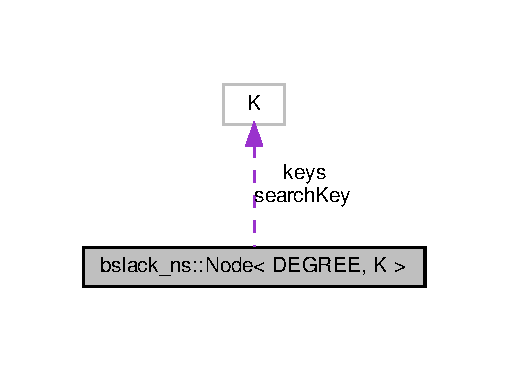
\includegraphics[width=244pt]{structbslack__ns_1_1Node__coll__graph}
\end{center}
\end{figure}
\subsection*{Public Member Functions}
\begin{DoxyCompactItemize}
\item 
bool \hyperlink{structbslack__ns_1_1Node_a0be34de40eb688fdce9c6df52405a359}{is\+Leaf} ()
\item 
int \hyperlink{structbslack__ns_1_1Node_a5119086e7ee24063fb0f9a4ab3aa7ccc}{get\+Key\+Count} ()
\item 
int \hyperlink{structbslack__ns_1_1Node_a0a075e319eee98333281f27abd7e0228}{get\+A\+B\+Degree} ()
\item 
{\footnotesize template$<$class Compare $>$ }\\int \hyperlink{structbslack__ns_1_1Node_aa383d3077279fb197654f01d68d4fe7a}{get\+Child\+Index} (const K \&key, Compare cmp)
\item 
{\footnotesize template$<$class Compare $>$ }\\int \hyperlink{structbslack__ns_1_1Node_ac32916848cce9c3f70a92d770dcf2d97}{get\+Key\+Index} (const K \&key, Compare cmp)
\item 
void \hyperlink{structbslack__ns_1_1Node_a97d7ff7f4384cee00e12b11731bf03fe}{print\+Tree\+File} (std\+::ostream \&os, std\+::set$<$ \hyperlink{structbslack__ns_1_1Node}{bslack\+\_\+ns\+::\+Node}$<$ \hyperlink{brown__sigouin__abtree__kcas_2adapter_8h_a5d88b17d70c985f2f2b8e987037fd6dd}{D\+E\+G\+R\+EE}, K $>$ $\ast$$>$ $\ast$seen)
\item 
void \hyperlink{structbslack__ns_1_1Node_a6beff90af7e1199fde6969d77ee1d36a}{print\+Tree\+File} (std\+::ostream \&os)
\end{DoxyCompactItemize}
\subsection*{Public Attributes}
\begin{DoxyCompactItemize}
\item 
\hyperlink{structbslack__ns_1_1SCXRecord}{S\+C\+X\+Record}$<$ \hyperlink{brown__sigouin__abtree__kcas_2adapter_8h_a5d88b17d70c985f2f2b8e987037fd6dd}{D\+E\+G\+R\+EE}, K $>$ $\ast$volatile \hyperlink{structbslack__ns_1_1Node_a86c5301b2a1173bd1b1bc5195242665a}{scx\+Ptr}
\item 
int \hyperlink{structbslack__ns_1_1Node_a8cd3075dbf277f0c8f3d77d2b9b30d32}{leaf}
\item 
volatile int \hyperlink{structbslack__ns_1_1Node_a97deb19c46b0be01965f1986c0f288f8}{marked}
\item 
int \hyperlink{structbslack__ns_1_1Node_a7dd1e7f22c835fd6d45af633cf68685f}{weight}
\item 
int \hyperlink{structbslack__ns_1_1Node_a16b46adbea74fec74c130f68195bd51c}{size}
\item 
K \hyperlink{structbslack__ns_1_1Node_a8409ba747d03413ea0c6a91645015ce2}{search\+Key}
\item 
K \hyperlink{structbslack__ns_1_1Node_a5dbae004ee087044ed203c543839d082}{keys} \mbox{[}\hyperlink{brown__sigouin__abtree__kcas_2adapter_8h_a5d88b17d70c985f2f2b8e987037fd6dd}{D\+E\+G\+R\+EE}\mbox{]}
\item 
\hyperlink{structbslack__ns_1_1Node}{Node}$<$ \hyperlink{brown__sigouin__abtree__kcas_2adapter_8h_a5d88b17d70c985f2f2b8e987037fd6dd}{D\+E\+G\+R\+EE}, K $>$ $\ast$volatile \hyperlink{structbslack__ns_1_1Node_a0de8d925f3eb8033ec776c118b6e121a}{ptrs} \mbox{[}\hyperlink{brown__sigouin__abtree__kcas_2adapter_8h_a5d88b17d70c985f2f2b8e987037fd6dd}{D\+E\+G\+R\+EE}\mbox{]}
\end{DoxyCompactItemize}


\subsection{Member Function Documentation}
\mbox{\Hypertarget{structbslack__ns_1_1Node_a0a075e319eee98333281f27abd7e0228}\label{structbslack__ns_1_1Node_a0a075e319eee98333281f27abd7e0228}} 
\index{bslack\+\_\+ns\+::\+Node@{bslack\+\_\+ns\+::\+Node}!get\+A\+B\+Degree@{get\+A\+B\+Degree}}
\index{get\+A\+B\+Degree@{get\+A\+B\+Degree}!bslack\+\_\+ns\+::\+Node@{bslack\+\_\+ns\+::\+Node}}
\subsubsection{\texorpdfstring{get\+A\+B\+Degree()}{getABDegree()}}
{\footnotesize\ttfamily template$<$int D\+E\+G\+R\+EE, typename K$>$ \\
int \hyperlink{structbslack__ns_1_1Node}{bslack\+\_\+ns\+::\+Node}$<$ \hyperlink{brown__sigouin__abtree__kcas_2adapter_8h_a5d88b17d70c985f2f2b8e987037fd6dd}{D\+E\+G\+R\+EE}, K $>$\+::get\+A\+B\+Degree (\begin{DoxyParamCaption}{ }\end{DoxyParamCaption})\hspace{0.3cm}{\ttfamily [inline]}}

\mbox{\Hypertarget{structbslack__ns_1_1Node_aa383d3077279fb197654f01d68d4fe7a}\label{structbslack__ns_1_1Node_aa383d3077279fb197654f01d68d4fe7a}} 
\index{bslack\+\_\+ns\+::\+Node@{bslack\+\_\+ns\+::\+Node}!get\+Child\+Index@{get\+Child\+Index}}
\index{get\+Child\+Index@{get\+Child\+Index}!bslack\+\_\+ns\+::\+Node@{bslack\+\_\+ns\+::\+Node}}
\subsubsection{\texorpdfstring{get\+Child\+Index()}{getChildIndex()}}
{\footnotesize\ttfamily template$<$int D\+E\+G\+R\+EE, typename K$>$ \\
template$<$class Compare $>$ \\
int \hyperlink{structbslack__ns_1_1Node}{bslack\+\_\+ns\+::\+Node}$<$ \hyperlink{brown__sigouin__abtree__kcas_2adapter_8h_a5d88b17d70c985f2f2b8e987037fd6dd}{D\+E\+G\+R\+EE}, K $>$\+::get\+Child\+Index (\begin{DoxyParamCaption}\item[{const K \&}]{key,  }\item[{Compare}]{cmp }\end{DoxyParamCaption})\hspace{0.3cm}{\ttfamily [inline]}}

\mbox{\Hypertarget{structbslack__ns_1_1Node_a5119086e7ee24063fb0f9a4ab3aa7ccc}\label{structbslack__ns_1_1Node_a5119086e7ee24063fb0f9a4ab3aa7ccc}} 
\index{bslack\+\_\+ns\+::\+Node@{bslack\+\_\+ns\+::\+Node}!get\+Key\+Count@{get\+Key\+Count}}
\index{get\+Key\+Count@{get\+Key\+Count}!bslack\+\_\+ns\+::\+Node@{bslack\+\_\+ns\+::\+Node}}
\subsubsection{\texorpdfstring{get\+Key\+Count()}{getKeyCount()}}
{\footnotesize\ttfamily template$<$int D\+E\+G\+R\+EE, typename K$>$ \\
int \hyperlink{structbslack__ns_1_1Node}{bslack\+\_\+ns\+::\+Node}$<$ \hyperlink{brown__sigouin__abtree__kcas_2adapter_8h_a5d88b17d70c985f2f2b8e987037fd6dd}{D\+E\+G\+R\+EE}, K $>$\+::get\+Key\+Count (\begin{DoxyParamCaption}{ }\end{DoxyParamCaption})\hspace{0.3cm}{\ttfamily [inline]}}

\mbox{\Hypertarget{structbslack__ns_1_1Node_ac32916848cce9c3f70a92d770dcf2d97}\label{structbslack__ns_1_1Node_ac32916848cce9c3f70a92d770dcf2d97}} 
\index{bslack\+\_\+ns\+::\+Node@{bslack\+\_\+ns\+::\+Node}!get\+Key\+Index@{get\+Key\+Index}}
\index{get\+Key\+Index@{get\+Key\+Index}!bslack\+\_\+ns\+::\+Node@{bslack\+\_\+ns\+::\+Node}}
\subsubsection{\texorpdfstring{get\+Key\+Index()}{getKeyIndex()}}
{\footnotesize\ttfamily template$<$int D\+E\+G\+R\+EE, typename K$>$ \\
template$<$class Compare $>$ \\
int \hyperlink{structbslack__ns_1_1Node}{bslack\+\_\+ns\+::\+Node}$<$ \hyperlink{brown__sigouin__abtree__kcas_2adapter_8h_a5d88b17d70c985f2f2b8e987037fd6dd}{D\+E\+G\+R\+EE}, K $>$\+::get\+Key\+Index (\begin{DoxyParamCaption}\item[{const K \&}]{key,  }\item[{Compare}]{cmp }\end{DoxyParamCaption})\hspace{0.3cm}{\ttfamily [inline]}}

\mbox{\Hypertarget{structbslack__ns_1_1Node_a0be34de40eb688fdce9c6df52405a359}\label{structbslack__ns_1_1Node_a0be34de40eb688fdce9c6df52405a359}} 
\index{bslack\+\_\+ns\+::\+Node@{bslack\+\_\+ns\+::\+Node}!is\+Leaf@{is\+Leaf}}
\index{is\+Leaf@{is\+Leaf}!bslack\+\_\+ns\+::\+Node@{bslack\+\_\+ns\+::\+Node}}
\subsubsection{\texorpdfstring{is\+Leaf()}{isLeaf()}}
{\footnotesize\ttfamily template$<$int D\+E\+G\+R\+EE, typename K$>$ \\
bool \hyperlink{structbslack__ns_1_1Node}{bslack\+\_\+ns\+::\+Node}$<$ \hyperlink{brown__sigouin__abtree__kcas_2adapter_8h_a5d88b17d70c985f2f2b8e987037fd6dd}{D\+E\+G\+R\+EE}, K $>$\+::is\+Leaf (\begin{DoxyParamCaption}{ }\end{DoxyParamCaption})\hspace{0.3cm}{\ttfamily [inline]}}

\mbox{\Hypertarget{structbslack__ns_1_1Node_a97d7ff7f4384cee00e12b11731bf03fe}\label{structbslack__ns_1_1Node_a97d7ff7f4384cee00e12b11731bf03fe}} 
\index{bslack\+\_\+ns\+::\+Node@{bslack\+\_\+ns\+::\+Node}!print\+Tree\+File@{print\+Tree\+File}}
\index{print\+Tree\+File@{print\+Tree\+File}!bslack\+\_\+ns\+::\+Node@{bslack\+\_\+ns\+::\+Node}}
\subsubsection{\texorpdfstring{print\+Tree\+File()}{printTreeFile()}\hspace{0.1cm}{\footnotesize\ttfamily [1/2]}}
{\footnotesize\ttfamily template$<$int D\+E\+G\+R\+EE, typename K$>$ \\
void \hyperlink{structbslack__ns_1_1Node}{bslack\+\_\+ns\+::\+Node}$<$ \hyperlink{brown__sigouin__abtree__kcas_2adapter_8h_a5d88b17d70c985f2f2b8e987037fd6dd}{D\+E\+G\+R\+EE}, K $>$\+::print\+Tree\+File (\begin{DoxyParamCaption}\item[{std\+::ostream \&}]{os,  }\item[{std\+::set$<$ \hyperlink{structbslack__ns_1_1Node}{bslack\+\_\+ns\+::\+Node}$<$ \hyperlink{brown__sigouin__abtree__kcas_2adapter_8h_a5d88b17d70c985f2f2b8e987037fd6dd}{D\+E\+G\+R\+EE}, K $>$ $\ast$$>$ $\ast$}]{seen }\end{DoxyParamCaption})\hspace{0.3cm}{\ttfamily [inline]}}

\mbox{\Hypertarget{structbslack__ns_1_1Node_a6beff90af7e1199fde6969d77ee1d36a}\label{structbslack__ns_1_1Node_a6beff90af7e1199fde6969d77ee1d36a}} 
\index{bslack\+\_\+ns\+::\+Node@{bslack\+\_\+ns\+::\+Node}!print\+Tree\+File@{print\+Tree\+File}}
\index{print\+Tree\+File@{print\+Tree\+File}!bslack\+\_\+ns\+::\+Node@{bslack\+\_\+ns\+::\+Node}}
\subsubsection{\texorpdfstring{print\+Tree\+File()}{printTreeFile()}\hspace{0.1cm}{\footnotesize\ttfamily [2/2]}}
{\footnotesize\ttfamily template$<$int D\+E\+G\+R\+EE, typename K$>$ \\
void \hyperlink{structbslack__ns_1_1Node}{bslack\+\_\+ns\+::\+Node}$<$ \hyperlink{brown__sigouin__abtree__kcas_2adapter_8h_a5d88b17d70c985f2f2b8e987037fd6dd}{D\+E\+G\+R\+EE}, K $>$\+::print\+Tree\+File (\begin{DoxyParamCaption}\item[{std\+::ostream \&}]{os }\end{DoxyParamCaption})\hspace{0.3cm}{\ttfamily [inline]}}



\subsection{Member Data Documentation}
\mbox{\Hypertarget{structbslack__ns_1_1Node_a5dbae004ee087044ed203c543839d082}\label{structbslack__ns_1_1Node_a5dbae004ee087044ed203c543839d082}} 
\index{bslack\+\_\+ns\+::\+Node@{bslack\+\_\+ns\+::\+Node}!keys@{keys}}
\index{keys@{keys}!bslack\+\_\+ns\+::\+Node@{bslack\+\_\+ns\+::\+Node}}
\subsubsection{\texorpdfstring{keys}{keys}}
{\footnotesize\ttfamily template$<$int D\+E\+G\+R\+EE, typename K$>$ \\
K \hyperlink{structbslack__ns_1_1Node}{bslack\+\_\+ns\+::\+Node}$<$ \hyperlink{brown__sigouin__abtree__kcas_2adapter_8h_a5d88b17d70c985f2f2b8e987037fd6dd}{D\+E\+G\+R\+EE}, K $>$\+::keys\mbox{[}\hyperlink{brown__sigouin__abtree__kcas_2adapter_8h_a5d88b17d70c985f2f2b8e987037fd6dd}{D\+E\+G\+R\+EE}\mbox{]}}

\mbox{\Hypertarget{structbslack__ns_1_1Node_a8cd3075dbf277f0c8f3d77d2b9b30d32}\label{structbslack__ns_1_1Node_a8cd3075dbf277f0c8f3d77d2b9b30d32}} 
\index{bslack\+\_\+ns\+::\+Node@{bslack\+\_\+ns\+::\+Node}!leaf@{leaf}}
\index{leaf@{leaf}!bslack\+\_\+ns\+::\+Node@{bslack\+\_\+ns\+::\+Node}}
\subsubsection{\texorpdfstring{leaf}{leaf}}
{\footnotesize\ttfamily template$<$int D\+E\+G\+R\+EE, typename K$>$ \\
int \hyperlink{structbslack__ns_1_1Node}{bslack\+\_\+ns\+::\+Node}$<$ \hyperlink{brown__sigouin__abtree__kcas_2adapter_8h_a5d88b17d70c985f2f2b8e987037fd6dd}{D\+E\+G\+R\+EE}, K $>$\+::leaf}

\mbox{\Hypertarget{structbslack__ns_1_1Node_a97deb19c46b0be01965f1986c0f288f8}\label{structbslack__ns_1_1Node_a97deb19c46b0be01965f1986c0f288f8}} 
\index{bslack\+\_\+ns\+::\+Node@{bslack\+\_\+ns\+::\+Node}!marked@{marked}}
\index{marked@{marked}!bslack\+\_\+ns\+::\+Node@{bslack\+\_\+ns\+::\+Node}}
\subsubsection{\texorpdfstring{marked}{marked}}
{\footnotesize\ttfamily template$<$int D\+E\+G\+R\+EE, typename K$>$ \\
volatile int \hyperlink{structbslack__ns_1_1Node}{bslack\+\_\+ns\+::\+Node}$<$ \hyperlink{brown__sigouin__abtree__kcas_2adapter_8h_a5d88b17d70c985f2f2b8e987037fd6dd}{D\+E\+G\+R\+EE}, K $>$\+::marked}

\mbox{\Hypertarget{structbslack__ns_1_1Node_a0de8d925f3eb8033ec776c118b6e121a}\label{structbslack__ns_1_1Node_a0de8d925f3eb8033ec776c118b6e121a}} 
\index{bslack\+\_\+ns\+::\+Node@{bslack\+\_\+ns\+::\+Node}!ptrs@{ptrs}}
\index{ptrs@{ptrs}!bslack\+\_\+ns\+::\+Node@{bslack\+\_\+ns\+::\+Node}}
\subsubsection{\texorpdfstring{ptrs}{ptrs}}
{\footnotesize\ttfamily template$<$int D\+E\+G\+R\+EE, typename K$>$ \\
\hyperlink{structbslack__ns_1_1Node}{Node}$<$\hyperlink{brown__sigouin__abtree__kcas_2adapter_8h_a5d88b17d70c985f2f2b8e987037fd6dd}{D\+E\+G\+R\+EE},K$>$$\ast$ volatile \hyperlink{structbslack__ns_1_1Node}{bslack\+\_\+ns\+::\+Node}$<$ \hyperlink{brown__sigouin__abtree__kcas_2adapter_8h_a5d88b17d70c985f2f2b8e987037fd6dd}{D\+E\+G\+R\+EE}, K $>$\+::ptrs\mbox{[}\hyperlink{brown__sigouin__abtree__kcas_2adapter_8h_a5d88b17d70c985f2f2b8e987037fd6dd}{D\+E\+G\+R\+EE}\mbox{]}}

\mbox{\Hypertarget{structbslack__ns_1_1Node_a86c5301b2a1173bd1b1bc5195242665a}\label{structbslack__ns_1_1Node_a86c5301b2a1173bd1b1bc5195242665a}} 
\index{bslack\+\_\+ns\+::\+Node@{bslack\+\_\+ns\+::\+Node}!scx\+Ptr@{scx\+Ptr}}
\index{scx\+Ptr@{scx\+Ptr}!bslack\+\_\+ns\+::\+Node@{bslack\+\_\+ns\+::\+Node}}
\subsubsection{\texorpdfstring{scx\+Ptr}{scxPtr}}
{\footnotesize\ttfamily template$<$int D\+E\+G\+R\+EE, typename K$>$ \\
\hyperlink{structbslack__ns_1_1SCXRecord}{S\+C\+X\+Record}$<$\hyperlink{brown__sigouin__abtree__kcas_2adapter_8h_a5d88b17d70c985f2f2b8e987037fd6dd}{D\+E\+G\+R\+EE},K$>$$\ast$ volatile \hyperlink{structbslack__ns_1_1Node}{bslack\+\_\+ns\+::\+Node}$<$ \hyperlink{brown__sigouin__abtree__kcas_2adapter_8h_a5d88b17d70c985f2f2b8e987037fd6dd}{D\+E\+G\+R\+EE}, K $>$\+::scx\+Ptr}

\mbox{\Hypertarget{structbslack__ns_1_1Node_a8409ba747d03413ea0c6a91645015ce2}\label{structbslack__ns_1_1Node_a8409ba747d03413ea0c6a91645015ce2}} 
\index{bslack\+\_\+ns\+::\+Node@{bslack\+\_\+ns\+::\+Node}!search\+Key@{search\+Key}}
\index{search\+Key@{search\+Key}!bslack\+\_\+ns\+::\+Node@{bslack\+\_\+ns\+::\+Node}}
\subsubsection{\texorpdfstring{search\+Key}{searchKey}}
{\footnotesize\ttfamily template$<$int D\+E\+G\+R\+EE, typename K$>$ \\
K \hyperlink{structbslack__ns_1_1Node}{bslack\+\_\+ns\+::\+Node}$<$ \hyperlink{brown__sigouin__abtree__kcas_2adapter_8h_a5d88b17d70c985f2f2b8e987037fd6dd}{D\+E\+G\+R\+EE}, K $>$\+::search\+Key}

\mbox{\Hypertarget{structbslack__ns_1_1Node_a16b46adbea74fec74c130f68195bd51c}\label{structbslack__ns_1_1Node_a16b46adbea74fec74c130f68195bd51c}} 
\index{bslack\+\_\+ns\+::\+Node@{bslack\+\_\+ns\+::\+Node}!size@{size}}
\index{size@{size}!bslack\+\_\+ns\+::\+Node@{bslack\+\_\+ns\+::\+Node}}
\subsubsection{\texorpdfstring{size}{size}}
{\footnotesize\ttfamily template$<$int D\+E\+G\+R\+EE, typename K$>$ \\
int \hyperlink{structbslack__ns_1_1Node}{bslack\+\_\+ns\+::\+Node}$<$ \hyperlink{brown__sigouin__abtree__kcas_2adapter_8h_a5d88b17d70c985f2f2b8e987037fd6dd}{D\+E\+G\+R\+EE}, K $>$\+::size}

\mbox{\Hypertarget{structbslack__ns_1_1Node_a7dd1e7f22c835fd6d45af633cf68685f}\label{structbslack__ns_1_1Node_a7dd1e7f22c835fd6d45af633cf68685f}} 
\index{bslack\+\_\+ns\+::\+Node@{bslack\+\_\+ns\+::\+Node}!weight@{weight}}
\index{weight@{weight}!bslack\+\_\+ns\+::\+Node@{bslack\+\_\+ns\+::\+Node}}
\subsubsection{\texorpdfstring{weight}{weight}}
{\footnotesize\ttfamily template$<$int D\+E\+G\+R\+EE, typename K$>$ \\
int \hyperlink{structbslack__ns_1_1Node}{bslack\+\_\+ns\+::\+Node}$<$ \hyperlink{brown__sigouin__abtree__kcas_2adapter_8h_a5d88b17d70c985f2f2b8e987037fd6dd}{D\+E\+G\+R\+EE}, K $>$\+::weight}



The documentation for this struct was generated from the following file\+:\begin{DoxyCompactItemize}
\item 
ds/brown\+\_\+ext\+\_\+bslack\+\_\+rq\+\_\+lf/\hyperlink{bslack__impl_8h}{bslack\+\_\+impl.\+h}\end{DoxyCompactItemize}

\hypertarget{classbst__glock__ns_1_1Node}{}\section{bst\+\_\+glock\+\_\+ns\+:\+:Node$<$ K, V $>$ Class Template Reference}
\label{classbst__glock__ns_1_1Node}\index{bst\+\_\+glock\+\_\+ns\+::\+Node$<$ K, V $>$@{bst\+\_\+glock\+\_\+ns\+::\+Node$<$ K, V $>$}}


{\ttfamily \#include $<$bst\+\_\+glock\+\_\+impl.\+h$>$}



Collaboration diagram for bst\+\_\+glock\+\_\+ns\+:\+:Node$<$ K, V $>$\+:
\nopagebreak
\begin{figure}[H]
\begin{center}
\leavevmode
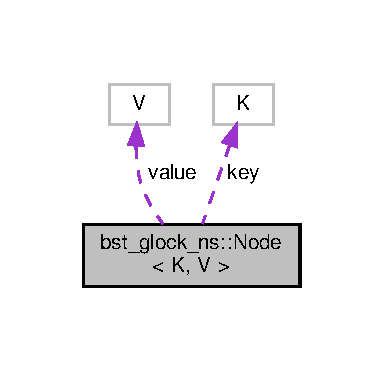
\includegraphics[width=184pt]{classbst__glock__ns_1_1Node__coll__graph}
\end{center}
\end{figure}
\subsection*{Public Attributes}
\begin{DoxyCompactItemize}
\item 
V \hyperlink{classbst__glock__ns_1_1Node_a76a7234ad2a679e2f4b02ca17cadaf62}{value}
\item 
K \hyperlink{classbst__glock__ns_1_1Node_a2ad7661ab8de2dccc4a1ae876565e0bc}{key}
\item 
\hyperlink{bst__rwlock__impl_8h_a04158d2a20768fe447133ff555823b05}{nodeptr} \hyperlink{classbst__glock__ns_1_1Node_ad16c7dbe2a53438d474cc37343252035}{left}
\item 
\hyperlink{bst__rwlock__impl_8h_a04158d2a20768fe447133ff555823b05}{nodeptr} \hyperlink{classbst__glock__ns_1_1Node_a73203abec3d0b72abbdc7815d54ca3f9}{right}
\end{DoxyCompactItemize}


\subsection{Member Data Documentation}
\mbox{\Hypertarget{classbst__glock__ns_1_1Node_a2ad7661ab8de2dccc4a1ae876565e0bc}\label{classbst__glock__ns_1_1Node_a2ad7661ab8de2dccc4a1ae876565e0bc}} 
\index{bst\+\_\+glock\+\_\+ns\+::\+Node@{bst\+\_\+glock\+\_\+ns\+::\+Node}!key@{key}}
\index{key@{key}!bst\+\_\+glock\+\_\+ns\+::\+Node@{bst\+\_\+glock\+\_\+ns\+::\+Node}}
\subsubsection{\texorpdfstring{key}{key}}
{\footnotesize\ttfamily template$<$class K , class V $>$ \\
K \hyperlink{classbst__glock__ns_1_1Node}{bst\+\_\+glock\+\_\+ns\+::\+Node}$<$ K, V $>$\+::key}

\mbox{\Hypertarget{classbst__glock__ns_1_1Node_ad16c7dbe2a53438d474cc37343252035}\label{classbst__glock__ns_1_1Node_ad16c7dbe2a53438d474cc37343252035}} 
\index{bst\+\_\+glock\+\_\+ns\+::\+Node@{bst\+\_\+glock\+\_\+ns\+::\+Node}!left@{left}}
\index{left@{left}!bst\+\_\+glock\+\_\+ns\+::\+Node@{bst\+\_\+glock\+\_\+ns\+::\+Node}}
\subsubsection{\texorpdfstring{left}{left}}
{\footnotesize\ttfamily template$<$class K , class V $>$ \\
\hyperlink{bst__rwlock__impl_8h_a04158d2a20768fe447133ff555823b05}{nodeptr} \hyperlink{classbst__glock__ns_1_1Node}{bst\+\_\+glock\+\_\+ns\+::\+Node}$<$ K, V $>$\+::left}

\mbox{\Hypertarget{classbst__glock__ns_1_1Node_a73203abec3d0b72abbdc7815d54ca3f9}\label{classbst__glock__ns_1_1Node_a73203abec3d0b72abbdc7815d54ca3f9}} 
\index{bst\+\_\+glock\+\_\+ns\+::\+Node@{bst\+\_\+glock\+\_\+ns\+::\+Node}!right@{right}}
\index{right@{right}!bst\+\_\+glock\+\_\+ns\+::\+Node@{bst\+\_\+glock\+\_\+ns\+::\+Node}}
\subsubsection{\texorpdfstring{right}{right}}
{\footnotesize\ttfamily template$<$class K , class V $>$ \\
\hyperlink{bst__rwlock__impl_8h_a04158d2a20768fe447133ff555823b05}{nodeptr} \hyperlink{classbst__glock__ns_1_1Node}{bst\+\_\+glock\+\_\+ns\+::\+Node}$<$ K, V $>$\+::right}

\mbox{\Hypertarget{classbst__glock__ns_1_1Node_a76a7234ad2a679e2f4b02ca17cadaf62}\label{classbst__glock__ns_1_1Node_a76a7234ad2a679e2f4b02ca17cadaf62}} 
\index{bst\+\_\+glock\+\_\+ns\+::\+Node@{bst\+\_\+glock\+\_\+ns\+::\+Node}!value@{value}}
\index{value@{value}!bst\+\_\+glock\+\_\+ns\+::\+Node@{bst\+\_\+glock\+\_\+ns\+::\+Node}}
\subsubsection{\texorpdfstring{value}{value}}
{\footnotesize\ttfamily template$<$class K , class V $>$ \\
V \hyperlink{classbst__glock__ns_1_1Node}{bst\+\_\+glock\+\_\+ns\+::\+Node}$<$ K, V $>$\+::value}



The documentation for this class was generated from the following file\+:\begin{DoxyCompactItemize}
\item 
ds/brown\+\_\+ext\+\_\+bst\+\_\+glock/\hyperlink{bst__glock__impl_8h}{bst\+\_\+glock\+\_\+impl.\+h}\end{DoxyCompactItemize}

\hypertarget{classbst__hohlock__ns_1_1Node}{}\section{bst\+\_\+hohlock\+\_\+ns\+:\+:Node$<$ K, V $>$ Class Template Reference}
\label{classbst__hohlock__ns_1_1Node}\index{bst\+\_\+hohlock\+\_\+ns\+::\+Node$<$ K, V $>$@{bst\+\_\+hohlock\+\_\+ns\+::\+Node$<$ K, V $>$}}


{\ttfamily \#include $<$bst\+\_\+hohlock\+\_\+impl.\+h$>$}



Collaboration diagram for bst\+\_\+hohlock\+\_\+ns\+:\+:Node$<$ K, V $>$\+:
\nopagebreak
\begin{figure}[H]
\begin{center}
\leavevmode
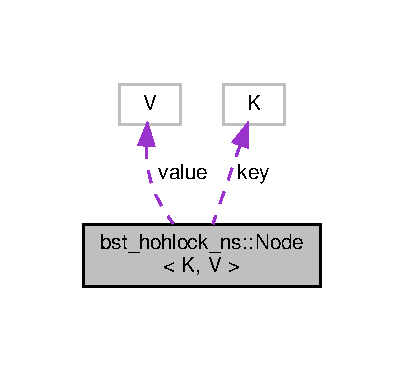
\includegraphics[width=194pt]{classbst__hohlock__ns_1_1Node__coll__graph}
\end{center}
\end{figure}
\subsection*{Public Attributes}
\begin{DoxyCompactItemize}
\item 
volatile int \hyperlink{classbst__hohlock__ns_1_1Node_abf98ca8e1b6e49ca39adc419a270b265}{lock}
\item 
V \hyperlink{classbst__hohlock__ns_1_1Node_a126d8d12e8ed894bad584a5e9df85506}{value}
\item 
K \hyperlink{classbst__hohlock__ns_1_1Node_a38bc0b89f0b3375db9f1540629fb0a24}{key}
\item 
\hyperlink{bst__rwlock__impl_8h_a04158d2a20768fe447133ff555823b05}{nodeptr} \hyperlink{classbst__hohlock__ns_1_1Node_a72ae7c6e54b707177be29b8e96edd009}{left}
\item 
\hyperlink{bst__rwlock__impl_8h_a04158d2a20768fe447133ff555823b05}{nodeptr} \hyperlink{classbst__hohlock__ns_1_1Node_a51d55faa8bc2cdb0bd27a5e86658b5bb}{right}
\end{DoxyCompactItemize}


\subsection{Member Data Documentation}
\mbox{\Hypertarget{classbst__hohlock__ns_1_1Node_a38bc0b89f0b3375db9f1540629fb0a24}\label{classbst__hohlock__ns_1_1Node_a38bc0b89f0b3375db9f1540629fb0a24}} 
\index{bst\+\_\+hohlock\+\_\+ns\+::\+Node@{bst\+\_\+hohlock\+\_\+ns\+::\+Node}!key@{key}}
\index{key@{key}!bst\+\_\+hohlock\+\_\+ns\+::\+Node@{bst\+\_\+hohlock\+\_\+ns\+::\+Node}}
\subsubsection{\texorpdfstring{key}{key}}
{\footnotesize\ttfamily template$<$class K , class V $>$ \\
K \hyperlink{classbst__hohlock__ns_1_1Node}{bst\+\_\+hohlock\+\_\+ns\+::\+Node}$<$ K, V $>$\+::key}

\mbox{\Hypertarget{classbst__hohlock__ns_1_1Node_a72ae7c6e54b707177be29b8e96edd009}\label{classbst__hohlock__ns_1_1Node_a72ae7c6e54b707177be29b8e96edd009}} 
\index{bst\+\_\+hohlock\+\_\+ns\+::\+Node@{bst\+\_\+hohlock\+\_\+ns\+::\+Node}!left@{left}}
\index{left@{left}!bst\+\_\+hohlock\+\_\+ns\+::\+Node@{bst\+\_\+hohlock\+\_\+ns\+::\+Node}}
\subsubsection{\texorpdfstring{left}{left}}
{\footnotesize\ttfamily template$<$class K , class V $>$ \\
\hyperlink{bst__rwlock__impl_8h_a04158d2a20768fe447133ff555823b05}{nodeptr} \hyperlink{classbst__hohlock__ns_1_1Node}{bst\+\_\+hohlock\+\_\+ns\+::\+Node}$<$ K, V $>$\+::left}

\mbox{\Hypertarget{classbst__hohlock__ns_1_1Node_abf98ca8e1b6e49ca39adc419a270b265}\label{classbst__hohlock__ns_1_1Node_abf98ca8e1b6e49ca39adc419a270b265}} 
\index{bst\+\_\+hohlock\+\_\+ns\+::\+Node@{bst\+\_\+hohlock\+\_\+ns\+::\+Node}!lock@{lock}}
\index{lock@{lock}!bst\+\_\+hohlock\+\_\+ns\+::\+Node@{bst\+\_\+hohlock\+\_\+ns\+::\+Node}}
\subsubsection{\texorpdfstring{lock}{lock}}
{\footnotesize\ttfamily template$<$class K , class V $>$ \\
volatile int \hyperlink{classbst__hohlock__ns_1_1Node}{bst\+\_\+hohlock\+\_\+ns\+::\+Node}$<$ K, V $>$\+::lock}

\mbox{\Hypertarget{classbst__hohlock__ns_1_1Node_a51d55faa8bc2cdb0bd27a5e86658b5bb}\label{classbst__hohlock__ns_1_1Node_a51d55faa8bc2cdb0bd27a5e86658b5bb}} 
\index{bst\+\_\+hohlock\+\_\+ns\+::\+Node@{bst\+\_\+hohlock\+\_\+ns\+::\+Node}!right@{right}}
\index{right@{right}!bst\+\_\+hohlock\+\_\+ns\+::\+Node@{bst\+\_\+hohlock\+\_\+ns\+::\+Node}}
\subsubsection{\texorpdfstring{right}{right}}
{\footnotesize\ttfamily template$<$class K , class V $>$ \\
\hyperlink{bst__rwlock__impl_8h_a04158d2a20768fe447133ff555823b05}{nodeptr} \hyperlink{classbst__hohlock__ns_1_1Node}{bst\+\_\+hohlock\+\_\+ns\+::\+Node}$<$ K, V $>$\+::right}

\mbox{\Hypertarget{classbst__hohlock__ns_1_1Node_a126d8d12e8ed894bad584a5e9df85506}\label{classbst__hohlock__ns_1_1Node_a126d8d12e8ed894bad584a5e9df85506}} 
\index{bst\+\_\+hohlock\+\_\+ns\+::\+Node@{bst\+\_\+hohlock\+\_\+ns\+::\+Node}!value@{value}}
\index{value@{value}!bst\+\_\+hohlock\+\_\+ns\+::\+Node@{bst\+\_\+hohlock\+\_\+ns\+::\+Node}}
\subsubsection{\texorpdfstring{value}{value}}
{\footnotesize\ttfamily template$<$class K , class V $>$ \\
V \hyperlink{classbst__hohlock__ns_1_1Node}{bst\+\_\+hohlock\+\_\+ns\+::\+Node}$<$ K, V $>$\+::value}



The documentation for this class was generated from the following file\+:\begin{DoxyCompactItemize}
\item 
ds/brown\+\_\+ext\+\_\+bst\+\_\+hohlock/\hyperlink{bst__hohlock__impl_8h}{bst\+\_\+hohlock\+\_\+impl.\+h}\end{DoxyCompactItemize}

\hypertarget{classbst__hohrwlock__ns_1_1Node}{}\section{bst\+\_\+hohrwlock\+\_\+ns\+:\+:Node$<$ K, V $>$ Class Template Reference}
\label{classbst__hohrwlock__ns_1_1Node}\index{bst\+\_\+hohrwlock\+\_\+ns\+::\+Node$<$ K, V $>$@{bst\+\_\+hohrwlock\+\_\+ns\+::\+Node$<$ K, V $>$}}


{\ttfamily \#include $<$bst\+\_\+hohrwlock\+\_\+impl.\+h$>$}



Collaboration diagram for bst\+\_\+hohrwlock\+\_\+ns\+:\+:Node$<$ K, V $>$\+:
\nopagebreak
\begin{figure}[H]
\begin{center}
\leavevmode
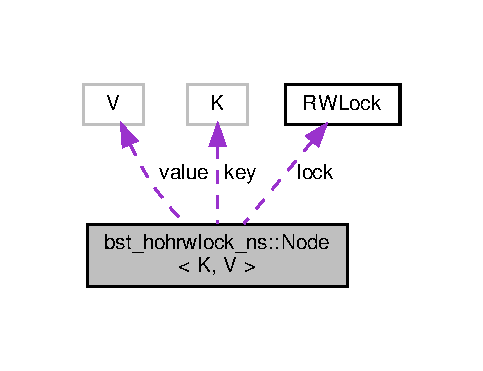
\includegraphics[width=232pt]{classbst__hohrwlock__ns_1_1Node__coll__graph}
\end{center}
\end{figure}
\subsection*{Public Member Functions}
\begin{DoxyCompactItemize}
\item 
\hyperlink{classbst__hohrwlock__ns_1_1Node_a3f2d591eb3c05607062431bdb2f36ed5}{Node} ()
\end{DoxyCompactItemize}
\subsection*{Public Attributes}
\begin{DoxyCompactItemize}
\item 
\hyperlink{classRWLock}{R\+W\+Lock} \hyperlink{classbst__hohrwlock__ns_1_1Node_a7ef93a01efec42288517d581c3d0e856}{lock}
\item 
V \hyperlink{classbst__hohrwlock__ns_1_1Node_a6e74874a1b0a5058298e45b266b9a5dc}{value}
\item 
K \hyperlink{classbst__hohrwlock__ns_1_1Node_a6c6c5eb4ea930c5ca22f93f057aa772b}{key}
\item 
\hyperlink{bst__rwlock__impl_8h_a04158d2a20768fe447133ff555823b05}{nodeptr} \hyperlink{classbst__hohrwlock__ns_1_1Node_ae2bcfb61983c0e33fa02c22599b8f082}{left}
\item 
\hyperlink{bst__rwlock__impl_8h_a04158d2a20768fe447133ff555823b05}{nodeptr} \hyperlink{classbst__hohrwlock__ns_1_1Node_a9d2e92f59341681a131ff00634f0a606}{right}
\end{DoxyCompactItemize}


\subsection{Constructor \& Destructor Documentation}
\mbox{\Hypertarget{classbst__hohrwlock__ns_1_1Node_a3f2d591eb3c05607062431bdb2f36ed5}\label{classbst__hohrwlock__ns_1_1Node_a3f2d591eb3c05607062431bdb2f36ed5}} 
\index{bst\+\_\+hohrwlock\+\_\+ns\+::\+Node@{bst\+\_\+hohrwlock\+\_\+ns\+::\+Node}!Node@{Node}}
\index{Node@{Node}!bst\+\_\+hohrwlock\+\_\+ns\+::\+Node@{bst\+\_\+hohrwlock\+\_\+ns\+::\+Node}}
\subsubsection{\texorpdfstring{Node()}{Node()}}
{\footnotesize\ttfamily template$<$class K , class V $>$ \\
\hyperlink{classbst__hohrwlock__ns_1_1Node}{bst\+\_\+hohrwlock\+\_\+ns\+::\+Node}$<$ K, V $>$\+::\hyperlink{classbst__hohrwlock__ns_1_1Node}{Node} (\begin{DoxyParamCaption}{ }\end{DoxyParamCaption})\hspace{0.3cm}{\ttfamily [inline]}}



\subsection{Member Data Documentation}
\mbox{\Hypertarget{classbst__hohrwlock__ns_1_1Node_a6c6c5eb4ea930c5ca22f93f057aa772b}\label{classbst__hohrwlock__ns_1_1Node_a6c6c5eb4ea930c5ca22f93f057aa772b}} 
\index{bst\+\_\+hohrwlock\+\_\+ns\+::\+Node@{bst\+\_\+hohrwlock\+\_\+ns\+::\+Node}!key@{key}}
\index{key@{key}!bst\+\_\+hohrwlock\+\_\+ns\+::\+Node@{bst\+\_\+hohrwlock\+\_\+ns\+::\+Node}}
\subsubsection{\texorpdfstring{key}{key}}
{\footnotesize\ttfamily template$<$class K , class V $>$ \\
K \hyperlink{classbst__hohrwlock__ns_1_1Node}{bst\+\_\+hohrwlock\+\_\+ns\+::\+Node}$<$ K, V $>$\+::key}

\mbox{\Hypertarget{classbst__hohrwlock__ns_1_1Node_ae2bcfb61983c0e33fa02c22599b8f082}\label{classbst__hohrwlock__ns_1_1Node_ae2bcfb61983c0e33fa02c22599b8f082}} 
\index{bst\+\_\+hohrwlock\+\_\+ns\+::\+Node@{bst\+\_\+hohrwlock\+\_\+ns\+::\+Node}!left@{left}}
\index{left@{left}!bst\+\_\+hohrwlock\+\_\+ns\+::\+Node@{bst\+\_\+hohrwlock\+\_\+ns\+::\+Node}}
\subsubsection{\texorpdfstring{left}{left}}
{\footnotesize\ttfamily template$<$class K , class V $>$ \\
\hyperlink{bst__rwlock__impl_8h_a04158d2a20768fe447133ff555823b05}{nodeptr} \hyperlink{classbst__hohrwlock__ns_1_1Node}{bst\+\_\+hohrwlock\+\_\+ns\+::\+Node}$<$ K, V $>$\+::left}

\mbox{\Hypertarget{classbst__hohrwlock__ns_1_1Node_a7ef93a01efec42288517d581c3d0e856}\label{classbst__hohrwlock__ns_1_1Node_a7ef93a01efec42288517d581c3d0e856}} 
\index{bst\+\_\+hohrwlock\+\_\+ns\+::\+Node@{bst\+\_\+hohrwlock\+\_\+ns\+::\+Node}!lock@{lock}}
\index{lock@{lock}!bst\+\_\+hohrwlock\+\_\+ns\+::\+Node@{bst\+\_\+hohrwlock\+\_\+ns\+::\+Node}}
\subsubsection{\texorpdfstring{lock}{lock}}
{\footnotesize\ttfamily template$<$class K , class V $>$ \\
\hyperlink{classRWLock}{R\+W\+Lock} \hyperlink{classbst__hohrwlock__ns_1_1Node}{bst\+\_\+hohrwlock\+\_\+ns\+::\+Node}$<$ K, V $>$\+::lock}

\mbox{\Hypertarget{classbst__hohrwlock__ns_1_1Node_a9d2e92f59341681a131ff00634f0a606}\label{classbst__hohrwlock__ns_1_1Node_a9d2e92f59341681a131ff00634f0a606}} 
\index{bst\+\_\+hohrwlock\+\_\+ns\+::\+Node@{bst\+\_\+hohrwlock\+\_\+ns\+::\+Node}!right@{right}}
\index{right@{right}!bst\+\_\+hohrwlock\+\_\+ns\+::\+Node@{bst\+\_\+hohrwlock\+\_\+ns\+::\+Node}}
\subsubsection{\texorpdfstring{right}{right}}
{\footnotesize\ttfamily template$<$class K , class V $>$ \\
\hyperlink{bst__rwlock__impl_8h_a04158d2a20768fe447133ff555823b05}{nodeptr} \hyperlink{classbst__hohrwlock__ns_1_1Node}{bst\+\_\+hohrwlock\+\_\+ns\+::\+Node}$<$ K, V $>$\+::right}

\mbox{\Hypertarget{classbst__hohrwlock__ns_1_1Node_a6e74874a1b0a5058298e45b266b9a5dc}\label{classbst__hohrwlock__ns_1_1Node_a6e74874a1b0a5058298e45b266b9a5dc}} 
\index{bst\+\_\+hohrwlock\+\_\+ns\+::\+Node@{bst\+\_\+hohrwlock\+\_\+ns\+::\+Node}!value@{value}}
\index{value@{value}!bst\+\_\+hohrwlock\+\_\+ns\+::\+Node@{bst\+\_\+hohrwlock\+\_\+ns\+::\+Node}}
\subsubsection{\texorpdfstring{value}{value}}
{\footnotesize\ttfamily template$<$class K , class V $>$ \\
V \hyperlink{classbst__hohrwlock__ns_1_1Node}{bst\+\_\+hohrwlock\+\_\+ns\+::\+Node}$<$ K, V $>$\+::value}



The documentation for this class was generated from the following file\+:\begin{DoxyCompactItemize}
\item 
ds/brown\+\_\+ext\+\_\+bst\+\_\+hohrwlock/\hyperlink{bst__hohrwlock__impl_8h}{bst\+\_\+hohrwlock\+\_\+impl.\+h}\end{DoxyCompactItemize}

\hypertarget{classbst__ns_1_1Node}{}\section{bst\+\_\+ns\+:\+:Node$<$ K, V $>$ Class Template Reference}
\label{classbst__ns_1_1Node}\index{bst\+\_\+ns\+::\+Node$<$ K, V $>$@{bst\+\_\+ns\+::\+Node$<$ K, V $>$}}


{\ttfamily \#include $<$node.\+h$>$}



Collaboration diagram for bst\+\_\+ns\+:\+:Node$<$ K, V $>$\+:
\nopagebreak
\begin{figure}[H]
\begin{center}
\leavevmode
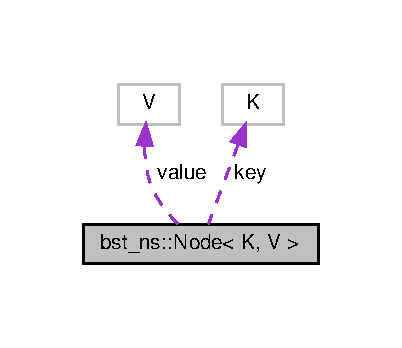
\includegraphics[width=193pt]{classbst__ns_1_1Node__coll__graph}
\end{center}
\end{figure}
\subsection*{Public Member Functions}
\begin{DoxyCompactItemize}
\item 
\hyperlink{classbst__ns_1_1Node_a488f346ef3e9fffe5bedf994dbd87efb}{Node} ()
\item 
\hyperlink{classbst__ns_1_1Node_a62d08377f3840cf443ea4d6f070076da}{Node} (const \hyperlink{classbst__ns_1_1Node}{Node} \&node)
\item 
void \hyperlink{classbst__ns_1_1Node_abe542c2dc0a5e1dc5f318a63b31298db}{print\+Tree\+File} (std\+::ostream \&os)
\item 
void \hyperlink{classbst__ns_1_1Node_aa46811e3965d1bfebd80a7c8e6caa32f}{print\+Tree\+File\+Weight} (std\+::ostream \&os, std\+::set$<$ \hyperlink{classbst__ns_1_1Node}{Node}$<$ K, V $>$ $\ast$ $>$ $\ast$seen)
\item 
void \hyperlink{classbst__ns_1_1Node_a31543e58fb925b71c03aa2780735d737}{print\+Tree\+File\+Weight} (std\+::ostream \&os)
\end{DoxyCompactItemize}
\subsection*{Public Attributes}
\begin{DoxyCompactItemize}
\item 
V \hyperlink{classbst__ns_1_1Node_adb140ea18301e8c5c51a8083571c3632}{value}
\item 
K \hyperlink{classbst__ns_1_1Node_aab49c1b3b2ead5b79a4d259866c6570e}{key}
\item 
std\+::atomic\+\_\+uintptr\+\_\+t \hyperlink{classbst__ns_1_1Node_aa7416bc36b7f8eb297035d079a096e0f}{scx\+Record}
\item 
std\+::atomic\+\_\+bool \hyperlink{classbst__ns_1_1Node_a9802ddeb9977786cba3938bf515f4214}{marked}
\item 
\hyperlink{bst__rwlock__impl_8h_a04158d2a20768fe447133ff555823b05}{nodeptr} \hyperlink{classbst__ns_1_1Node_a5758be9af43bbba08e9ec0b53858dc2c}{left}
\item 
\hyperlink{bst__rwlock__impl_8h_a04158d2a20768fe447133ff555823b05}{nodeptr} \hyperlink{classbst__ns_1_1Node_a2b88528b93f10de2d57e70bc6a1efb8a}{right}
\item 
\hyperlink{classbst__ns_1_1Node_ab3a9c0980d092db36d0df8cb91d72de4}{R\+E\+C\+L\+A\+I\+M\+\_\+\+R\+C\+U\+\_\+\+R\+C\+U\+H\+E\+A\+D\+\_\+\+D\+E\+FN}
\end{DoxyCompactItemize}
\subsection*{Friends}
\begin{DoxyCompactItemize}
\item 
std\+::ostream \& \hyperlink{classbst__ns_1_1Node_a868b7fcd3b0bb864d505f6206b592dce}{operator$<$$<$} (std\+::ostream \&os, const \hyperlink{classbst__ns_1_1Node}{Node}$<$ K, V $>$ \&obj)
\end{DoxyCompactItemize}


\subsection{Constructor \& Destructor Documentation}
\mbox{\Hypertarget{classbst__ns_1_1Node_a488f346ef3e9fffe5bedf994dbd87efb}\label{classbst__ns_1_1Node_a488f346ef3e9fffe5bedf994dbd87efb}} 
\index{bst\+\_\+ns\+::\+Node@{bst\+\_\+ns\+::\+Node}!Node@{Node}}
\index{Node@{Node}!bst\+\_\+ns\+::\+Node@{bst\+\_\+ns\+::\+Node}}
\subsubsection{\texorpdfstring{Node()}{Node()}\hspace{0.1cm}{\footnotesize\ttfamily [1/2]}}
{\footnotesize\ttfamily template$<$class K, class V$>$ \\
\hyperlink{classbst__ns_1_1Node}{bst\+\_\+ns\+::\+Node}$<$ K, V $>$\+::\hyperlink{classbst__ns_1_1Node}{Node} (\begin{DoxyParamCaption}{ }\end{DoxyParamCaption})\hspace{0.3cm}{\ttfamily [inline]}}

\mbox{\Hypertarget{classbst__ns_1_1Node_a62d08377f3840cf443ea4d6f070076da}\label{classbst__ns_1_1Node_a62d08377f3840cf443ea4d6f070076da}} 
\index{bst\+\_\+ns\+::\+Node@{bst\+\_\+ns\+::\+Node}!Node@{Node}}
\index{Node@{Node}!bst\+\_\+ns\+::\+Node@{bst\+\_\+ns\+::\+Node}}
\subsubsection{\texorpdfstring{Node()}{Node()}\hspace{0.1cm}{\footnotesize\ttfamily [2/2]}}
{\footnotesize\ttfamily template$<$class K, class V$>$ \\
\hyperlink{classbst__ns_1_1Node}{bst\+\_\+ns\+::\+Node}$<$ K, V $>$\+::\hyperlink{classbst__ns_1_1Node}{Node} (\begin{DoxyParamCaption}\item[{const \hyperlink{classbst__ns_1_1Node}{Node}$<$ K, V $>$ \&}]{node }\end{DoxyParamCaption})\hspace{0.3cm}{\ttfamily [inline]}}



\subsection{Member Function Documentation}
\mbox{\Hypertarget{classbst__ns_1_1Node_abe542c2dc0a5e1dc5f318a63b31298db}\label{classbst__ns_1_1Node_abe542c2dc0a5e1dc5f318a63b31298db}} 
\index{bst\+\_\+ns\+::\+Node@{bst\+\_\+ns\+::\+Node}!print\+Tree\+File@{print\+Tree\+File}}
\index{print\+Tree\+File@{print\+Tree\+File}!bst\+\_\+ns\+::\+Node@{bst\+\_\+ns\+::\+Node}}
\subsubsection{\texorpdfstring{print\+Tree\+File()}{printTreeFile()}}
{\footnotesize\ttfamily template$<$class K, class V$>$ \\
void \hyperlink{classbst__ns_1_1Node}{bst\+\_\+ns\+::\+Node}$<$ K, V $>$\+::print\+Tree\+File (\begin{DoxyParamCaption}\item[{std\+::ostream \&}]{os }\end{DoxyParamCaption})\hspace{0.3cm}{\ttfamily [inline]}}

\mbox{\Hypertarget{classbst__ns_1_1Node_aa46811e3965d1bfebd80a7c8e6caa32f}\label{classbst__ns_1_1Node_aa46811e3965d1bfebd80a7c8e6caa32f}} 
\index{bst\+\_\+ns\+::\+Node@{bst\+\_\+ns\+::\+Node}!print\+Tree\+File\+Weight@{print\+Tree\+File\+Weight}}
\index{print\+Tree\+File\+Weight@{print\+Tree\+File\+Weight}!bst\+\_\+ns\+::\+Node@{bst\+\_\+ns\+::\+Node}}
\subsubsection{\texorpdfstring{print\+Tree\+File\+Weight()}{printTreeFileWeight()}\hspace{0.1cm}{\footnotesize\ttfamily [1/2]}}
{\footnotesize\ttfamily template$<$class K, class V$>$ \\
void \hyperlink{classbst__ns_1_1Node}{bst\+\_\+ns\+::\+Node}$<$ K, V $>$\+::print\+Tree\+File\+Weight (\begin{DoxyParamCaption}\item[{std\+::ostream \&}]{os,  }\item[{std\+::set$<$ \hyperlink{classbst__ns_1_1Node}{Node}$<$ K, V $>$ $\ast$ $>$ $\ast$}]{seen }\end{DoxyParamCaption})\hspace{0.3cm}{\ttfamily [inline]}}

\mbox{\Hypertarget{classbst__ns_1_1Node_a31543e58fb925b71c03aa2780735d737}\label{classbst__ns_1_1Node_a31543e58fb925b71c03aa2780735d737}} 
\index{bst\+\_\+ns\+::\+Node@{bst\+\_\+ns\+::\+Node}!print\+Tree\+File\+Weight@{print\+Tree\+File\+Weight}}
\index{print\+Tree\+File\+Weight@{print\+Tree\+File\+Weight}!bst\+\_\+ns\+::\+Node@{bst\+\_\+ns\+::\+Node}}
\subsubsection{\texorpdfstring{print\+Tree\+File\+Weight()}{printTreeFileWeight()}\hspace{0.1cm}{\footnotesize\ttfamily [2/2]}}
{\footnotesize\ttfamily template$<$class K, class V$>$ \\
void \hyperlink{classbst__ns_1_1Node}{bst\+\_\+ns\+::\+Node}$<$ K, V $>$\+::print\+Tree\+File\+Weight (\begin{DoxyParamCaption}\item[{std\+::ostream \&}]{os }\end{DoxyParamCaption})\hspace{0.3cm}{\ttfamily [inline]}}



\subsection{Friends And Related Function Documentation}
\mbox{\Hypertarget{classbst__ns_1_1Node_a868b7fcd3b0bb864d505f6206b592dce}\label{classbst__ns_1_1Node_a868b7fcd3b0bb864d505f6206b592dce}} 
\index{bst\+\_\+ns\+::\+Node@{bst\+\_\+ns\+::\+Node}!operator$<$$<$@{operator$<$$<$}}
\index{operator$<$$<$@{operator$<$$<$}!bst\+\_\+ns\+::\+Node@{bst\+\_\+ns\+::\+Node}}
\subsubsection{\texorpdfstring{operator$<$$<$}{operator<<}}
{\footnotesize\ttfamily template$<$class K, class V$>$ \\
std\+::ostream\& operator$<$$<$ (\begin{DoxyParamCaption}\item[{std\+::ostream \&}]{os,  }\item[{const \hyperlink{classbst__ns_1_1Node}{Node}$<$ K, V $>$ \&}]{obj }\end{DoxyParamCaption})\hspace{0.3cm}{\ttfamily [friend]}}



\subsection{Member Data Documentation}
\mbox{\Hypertarget{classbst__ns_1_1Node_aab49c1b3b2ead5b79a4d259866c6570e}\label{classbst__ns_1_1Node_aab49c1b3b2ead5b79a4d259866c6570e}} 
\index{bst\+\_\+ns\+::\+Node@{bst\+\_\+ns\+::\+Node}!key@{key}}
\index{key@{key}!bst\+\_\+ns\+::\+Node@{bst\+\_\+ns\+::\+Node}}
\subsubsection{\texorpdfstring{key}{key}}
{\footnotesize\ttfamily template$<$class K, class V$>$ \\
K \hyperlink{classbst__ns_1_1Node}{bst\+\_\+ns\+::\+Node}$<$ K, V $>$\+::key}

\mbox{\Hypertarget{classbst__ns_1_1Node_a5758be9af43bbba08e9ec0b53858dc2c}\label{classbst__ns_1_1Node_a5758be9af43bbba08e9ec0b53858dc2c}} 
\index{bst\+\_\+ns\+::\+Node@{bst\+\_\+ns\+::\+Node}!left@{left}}
\index{left@{left}!bst\+\_\+ns\+::\+Node@{bst\+\_\+ns\+::\+Node}}
\subsubsection{\texorpdfstring{left}{left}}
{\footnotesize\ttfamily template$<$class K, class V$>$ \\
\hyperlink{bst__rwlock__impl_8h_a04158d2a20768fe447133ff555823b05}{nodeptr} \hyperlink{classbst__ns_1_1Node}{bst\+\_\+ns\+::\+Node}$<$ K, V $>$\+::left}

\mbox{\Hypertarget{classbst__ns_1_1Node_a9802ddeb9977786cba3938bf515f4214}\label{classbst__ns_1_1Node_a9802ddeb9977786cba3938bf515f4214}} 
\index{bst\+\_\+ns\+::\+Node@{bst\+\_\+ns\+::\+Node}!marked@{marked}}
\index{marked@{marked}!bst\+\_\+ns\+::\+Node@{bst\+\_\+ns\+::\+Node}}
\subsubsection{\texorpdfstring{marked}{marked}}
{\footnotesize\ttfamily template$<$class K, class V$>$ \\
std\+::atomic\+\_\+bool \hyperlink{classbst__ns_1_1Node}{bst\+\_\+ns\+::\+Node}$<$ K, V $>$\+::marked}

\mbox{\Hypertarget{classbst__ns_1_1Node_ab3a9c0980d092db36d0df8cb91d72de4}\label{classbst__ns_1_1Node_ab3a9c0980d092db36d0df8cb91d72de4}} 
\index{bst\+\_\+ns\+::\+Node@{bst\+\_\+ns\+::\+Node}!R\+E\+C\+L\+A\+I\+M\+\_\+\+R\+C\+U\+\_\+\+R\+C\+U\+H\+E\+A\+D\+\_\+\+D\+E\+FN@{R\+E\+C\+L\+A\+I\+M\+\_\+\+R\+C\+U\+\_\+\+R\+C\+U\+H\+E\+A\+D\+\_\+\+D\+E\+FN}}
\index{R\+E\+C\+L\+A\+I\+M\+\_\+\+R\+C\+U\+\_\+\+R\+C\+U\+H\+E\+A\+D\+\_\+\+D\+E\+FN@{R\+E\+C\+L\+A\+I\+M\+\_\+\+R\+C\+U\+\_\+\+R\+C\+U\+H\+E\+A\+D\+\_\+\+D\+E\+FN}!bst\+\_\+ns\+::\+Node@{bst\+\_\+ns\+::\+Node}}
\subsubsection{\texorpdfstring{R\+E\+C\+L\+A\+I\+M\+\_\+\+R\+C\+U\+\_\+\+R\+C\+U\+H\+E\+A\+D\+\_\+\+D\+E\+FN}{RECLAIM\_RCU\_RCUHEAD\_DEFN}}
{\footnotesize\ttfamily template$<$class K, class V$>$ \\
\hyperlink{classbst__ns_1_1Node}{bst\+\_\+ns\+::\+Node}$<$ K, V $>$\+::R\+E\+C\+L\+A\+I\+M\+\_\+\+R\+C\+U\+\_\+\+R\+C\+U\+H\+E\+A\+D\+\_\+\+D\+E\+FN}

\mbox{\Hypertarget{classbst__ns_1_1Node_a2b88528b93f10de2d57e70bc6a1efb8a}\label{classbst__ns_1_1Node_a2b88528b93f10de2d57e70bc6a1efb8a}} 
\index{bst\+\_\+ns\+::\+Node@{bst\+\_\+ns\+::\+Node}!right@{right}}
\index{right@{right}!bst\+\_\+ns\+::\+Node@{bst\+\_\+ns\+::\+Node}}
\subsubsection{\texorpdfstring{right}{right}}
{\footnotesize\ttfamily template$<$class K, class V$>$ \\
\hyperlink{bst__rwlock__impl_8h_a04158d2a20768fe447133ff555823b05}{nodeptr} \hyperlink{classbst__ns_1_1Node}{bst\+\_\+ns\+::\+Node}$<$ K, V $>$\+::right}

\mbox{\Hypertarget{classbst__ns_1_1Node_aa7416bc36b7f8eb297035d079a096e0f}\label{classbst__ns_1_1Node_aa7416bc36b7f8eb297035d079a096e0f}} 
\index{bst\+\_\+ns\+::\+Node@{bst\+\_\+ns\+::\+Node}!scx\+Record@{scx\+Record}}
\index{scx\+Record@{scx\+Record}!bst\+\_\+ns\+::\+Node@{bst\+\_\+ns\+::\+Node}}
\subsubsection{\texorpdfstring{scx\+Record}{scxRecord}}
{\footnotesize\ttfamily template$<$class K, class V$>$ \\
std\+::atomic\+\_\+uintptr\+\_\+t \hyperlink{classbst__ns_1_1Node}{bst\+\_\+ns\+::\+Node}$<$ K, V $>$\+::scx\+Record}

\mbox{\Hypertarget{classbst__ns_1_1Node_adb140ea18301e8c5c51a8083571c3632}\label{classbst__ns_1_1Node_adb140ea18301e8c5c51a8083571c3632}} 
\index{bst\+\_\+ns\+::\+Node@{bst\+\_\+ns\+::\+Node}!value@{value}}
\index{value@{value}!bst\+\_\+ns\+::\+Node@{bst\+\_\+ns\+::\+Node}}
\subsubsection{\texorpdfstring{value}{value}}
{\footnotesize\ttfamily template$<$class K, class V$>$ \\
V \hyperlink{classbst__ns_1_1Node}{bst\+\_\+ns\+::\+Node}$<$ K, V $>$\+::value}



The documentation for this class was generated from the following file\+:\begin{DoxyCompactItemize}
\item 
ds/brown\+\_\+ext\+\_\+bst\+\_\+rq\+\_\+lf/\hyperlink{node_8h}{node.\+h}\end{DoxyCompactItemize}

\hypertarget{classbst__rwlock__ns_1_1Node}{}\section{bst\+\_\+rwlock\+\_\+ns\+:\+:Node$<$ K, V $>$ Class Template Reference}
\label{classbst__rwlock__ns_1_1Node}\index{bst\+\_\+rwlock\+\_\+ns\+::\+Node$<$ K, V $>$@{bst\+\_\+rwlock\+\_\+ns\+::\+Node$<$ K, V $>$}}


{\ttfamily \#include $<$bst\+\_\+rwlock.\+h$>$}



Collaboration diagram for bst\+\_\+rwlock\+\_\+ns\+:\+:Node$<$ K, V $>$\+:
\nopagebreak
\begin{figure}[H]
\begin{center}
\leavevmode
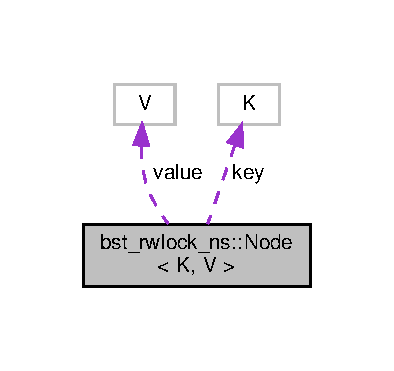
\includegraphics[width=189pt]{classbst__rwlock__ns_1_1Node__coll__graph}
\end{center}
\end{figure}
\subsection*{Public Attributes}
\begin{DoxyCompactItemize}
\item 
V \hyperlink{classbst__rwlock__ns_1_1Node_ad26872ac51fa4ef5a8519038472a5050}{value}
\item 
K \hyperlink{classbst__rwlock__ns_1_1Node_a4091ccbd4f0b78711f848a5129fdece9}{key}
\item 
\hyperlink{bst__rwlock__impl_8h_a04158d2a20768fe447133ff555823b05}{nodeptr} \hyperlink{classbst__rwlock__ns_1_1Node_a8bf2cf841310cee1712f7001b4dfe2ad}{left}
\item 
\hyperlink{bst__rwlock__impl_8h_a04158d2a20768fe447133ff555823b05}{nodeptr} \hyperlink{classbst__rwlock__ns_1_1Node_ae519222d8a15edb1ff20d68dd3eeec88}{right}
\end{DoxyCompactItemize}


\subsection{Member Data Documentation}
\mbox{\Hypertarget{classbst__rwlock__ns_1_1Node_a4091ccbd4f0b78711f848a5129fdece9}\label{classbst__rwlock__ns_1_1Node_a4091ccbd4f0b78711f848a5129fdece9}} 
\index{bst\+\_\+rwlock\+\_\+ns\+::\+Node@{bst\+\_\+rwlock\+\_\+ns\+::\+Node}!key@{key}}
\index{key@{key}!bst\+\_\+rwlock\+\_\+ns\+::\+Node@{bst\+\_\+rwlock\+\_\+ns\+::\+Node}}
\subsubsection{\texorpdfstring{key}{key}}
{\footnotesize\ttfamily template$<$class K , class V $>$ \\
K \hyperlink{classbst__rwlock__ns_1_1Node}{Node}$<$ K, V $>$\+::key}

\mbox{\Hypertarget{classbst__rwlock__ns_1_1Node_a8bf2cf841310cee1712f7001b4dfe2ad}\label{classbst__rwlock__ns_1_1Node_a8bf2cf841310cee1712f7001b4dfe2ad}} 
\index{bst\+\_\+rwlock\+\_\+ns\+::\+Node@{bst\+\_\+rwlock\+\_\+ns\+::\+Node}!left@{left}}
\index{left@{left}!bst\+\_\+rwlock\+\_\+ns\+::\+Node@{bst\+\_\+rwlock\+\_\+ns\+::\+Node}}
\subsubsection{\texorpdfstring{left}{left}}
{\footnotesize\ttfamily template$<$class K , class V $>$ \\
\hyperlink{bst__rwlock__impl_8h_a04158d2a20768fe447133ff555823b05}{nodeptr} \hyperlink{classbst__rwlock__ns_1_1Node}{Node}$<$ K, V $>$\+::left}

\mbox{\Hypertarget{classbst__rwlock__ns_1_1Node_ae519222d8a15edb1ff20d68dd3eeec88}\label{classbst__rwlock__ns_1_1Node_ae519222d8a15edb1ff20d68dd3eeec88}} 
\index{bst\+\_\+rwlock\+\_\+ns\+::\+Node@{bst\+\_\+rwlock\+\_\+ns\+::\+Node}!right@{right}}
\index{right@{right}!bst\+\_\+rwlock\+\_\+ns\+::\+Node@{bst\+\_\+rwlock\+\_\+ns\+::\+Node}}
\subsubsection{\texorpdfstring{right}{right}}
{\footnotesize\ttfamily template$<$class K , class V $>$ \\
\hyperlink{bst__rwlock__impl_8h_a04158d2a20768fe447133ff555823b05}{nodeptr} \hyperlink{classbst__rwlock__ns_1_1Node}{Node}$<$ K, V $>$\+::right}

\mbox{\Hypertarget{classbst__rwlock__ns_1_1Node_ad26872ac51fa4ef5a8519038472a5050}\label{classbst__rwlock__ns_1_1Node_ad26872ac51fa4ef5a8519038472a5050}} 
\index{bst\+\_\+rwlock\+\_\+ns\+::\+Node@{bst\+\_\+rwlock\+\_\+ns\+::\+Node}!value@{value}}
\index{value@{value}!bst\+\_\+rwlock\+\_\+ns\+::\+Node@{bst\+\_\+rwlock\+\_\+ns\+::\+Node}}
\subsubsection{\texorpdfstring{value}{value}}
{\footnotesize\ttfamily template$<$class K , class V $>$ \\
V \hyperlink{classbst__rwlock__ns_1_1Node}{Node}$<$ K, V $>$\+::value}



The documentation for this class was generated from the following files\+:\begin{DoxyCompactItemize}
\item 
ds/brown\+\_\+ext\+\_\+bst\+\_\+rwlock/\hyperlink{bst__rwlock_8h}{bst\+\_\+rwlock.\+h}\item 
ds/brown\+\_\+ext\+\_\+bst\+\_\+rwlock/\hyperlink{bst__rwlock__impl_8h}{bst\+\_\+rwlock\+\_\+impl.\+h}\end{DoxyCompactItemize}

\hypertarget{structnode__t}{}\section{node\+\_\+t$<$ skey\+\_\+t, sval\+\_\+t $>$ Struct Template Reference}
\label{structnode__t}\index{node\+\_\+t$<$ skey\+\_\+t, sval\+\_\+t $>$@{node\+\_\+t$<$ skey\+\_\+t, sval\+\_\+t $>$}}


{\ttfamily \#include $<$ccavl\+\_\+impl.\+h$>$}



Collaboration diagram for node\+\_\+t$<$ skey\+\_\+t, sval\+\_\+t $>$\+:
\nopagebreak
\begin{figure}[H]
\begin{center}
\leavevmode
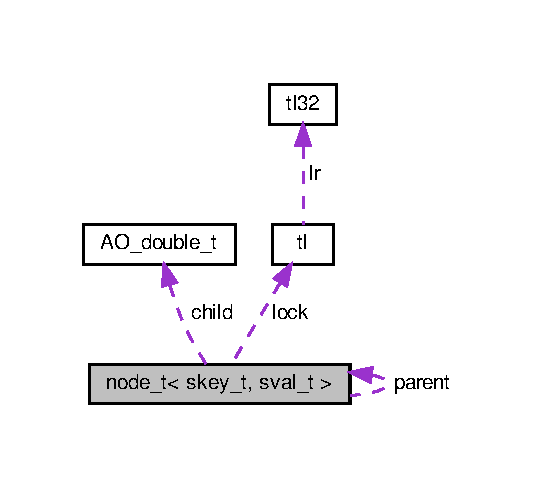
\includegraphics[width=257pt]{structnode__t__coll__graph}
\end{center}
\end{figure}
\subsection*{Public Attributes}
\begin{DoxyCompactItemize}
\item 
skey\+\_\+t \hyperlink{structnode__t_ad38b63280bb7c69e5991653ce673dc35}{key}
\item 
struct \hyperlink{structnode__t}{node\+\_\+t}$<$ skey\+\_\+t, sval\+\_\+t $>$ $\ast$volatile \hyperlink{structnode__t_a3dcf556399e1c75d881c2d700634fda0}{left}
\item 
struct \hyperlink{structnode__t}{node\+\_\+t}$<$ skey\+\_\+t, sval\+\_\+t $>$ $\ast$volatile \hyperlink{structnode__t_ae2a246fc0c98ee4bec4e69cad2f4ba3c}{right}
\item 
volatile \hyperlink{ccavl__impl_8h_ad18cce847aba06882c0ceedf7c5b32dc}{version\+\_\+t} \hyperlink{structnode__t_a04ef1d059a1c38a7941eecd535f32d05}{change\+O\+VL}
\item 
struct \hyperlink{structnode__t}{node\+\_\+t} $\ast$volatile \hyperlink{structnode__t_a36d0dc0f90d0d93c475ef32b6f2b4cfd}{parent}
\item 
sval\+\_\+t \hyperlink{structnode__t_afa5c26cdc749c26fcbc550baf6e97717}{value}
\item 
\hyperlink{ccavl__impl_8h_a61cf36cb33c84af9c784f95686701a94}{ptlock\+\_\+t} \hyperlink{structnode__t_a9efe5c548c28ff5d1cddfde25bac62be}{lock}
\item 
volatile int \hyperlink{structnode__t_a2399b4339a7c3ea7b7ffaa913680580a}{height}
\item 
\begin{tabbing}
xx\=xx\=xx\=xx\=xx\=xx\=xx\=xx\=xx\=\kill
union \{\\
\>volatile char \hyperlink{structnode__t_aa47c298fa082c9997590c3fdb05b796a}{pad} \mbox{[}192\mbox{]}\\
\>struct \{\\
\>\>skey\_t \hyperlink{structnode__t_ad38b63280bb7c69e5991653ce673dc35}{key}\\
\>\>\hyperlink{structnode__t}{node\_t}$<$ skey\_t, sval\_t $>$ $\ast$volatile \hyperlink{structnode__t_a6f9a1ea968cdda781d9d4f9ea65c5856}{left}\\
\>\>\hyperlink{structnode__t}{node\_t}$<$ skey\_t, sval\_t $>$ $\ast$volatile \hyperlink{structnode__t_a42cf1a237abbb7d2fcfe9d6536fddc97}{right}\\
\>\>\hyperlink{structnode__t}{node\_t}$<$ skey\_t, sval\_t $>$ $\ast$volatile \hyperlink{structnode__t_aad0b9c0571665e0a5811f9f3d683b76e}{succ}\\
\>\>\hyperlink{structnode__t}{node\_t}$<$ skey\_t, sval\_t $>$ $\ast$volatile \hyperlink{structnode__t_a7a0e625afa9ffa7429bd055e64aedf27}{pred}\\
\>\>\hyperlink{drachsler__impl_8h_a57c3b7201116536b822f0f8520aa99c7}{bool\_t} \hyperlink{structnode__t_a5977cf60c984f00d4aa29052ca0c3119}{mark}\\
\>\>sval\_t \hyperlink{structnode__t_afa5c26cdc749c26fcbc550baf6e97717}{value}\\
\>\>\hyperlink{structnode__t}{node\_t}$<$ skey\_t, sval\_t $>$ $\ast$volatile \hyperlink{structnode__t_a3ab6091479bf16f761c8cfe1d2ca78bf}{parent}\\
\>\>\hyperlink{ccavl__impl_8h_a61cf36cb33c84af9c784f95686701a94}{ptlock\_t} \hyperlink{structnode__t_a172896833cd7a9331b2afabc55c1914a}{tree\_lock}\\
\>\>\hyperlink{ccavl__impl_8h_a61cf36cb33c84af9c784f95686701a94}{ptlock\_t} \hyperlink{structnode__t_afeeaa8165d380652af96618f36213252}{succ\_lock}\\
\>\} \\
\}; \\

\end{tabbing}\item 
\hyperlink{unioninfo__t}{info\+\_\+t}$<$ skey\+\_\+t, sval\+\_\+t $>$ $\ast$volatile \hyperlink{structnode__t_a3009fd14ae83f7f3a307450005261482}{update}
\item 
sval\+\_\+t \hyperlink{structnode__t_aca6e214f7ceac5575365b70fbf2a6693}{val}
\item 
volatile \hyperlink{ticket__impl_8h_aa989d88f1299dac19db854e7c54a1615}{tl\+\_\+t} \hyperlink{structnode__t_a7c381d5204a650a3db959fc75b644800}{lock}
\item 
\hyperlink{unionoperation__t}{operation\+\_\+t}$<$ skey\+\_\+t, sval\+\_\+t $>$ $\ast$volatile \hyperlink{structnode__t_add56a7213e59cec443dda8f4b786d938}{op}
\item 
\begin{tabbing}
xx\=xx\=xx\=xx\=xx\=xx\=xx\=xx\=xx\=\kill
union \{\\
\>struct \{\\
\>\>skey\_t \hyperlink{structnode__t_ad38b63280bb7c69e5991653ce673dc35}{key}\\
\>\>sval\_t \hyperlink{structnode__t_afa5c26cdc749c26fcbc550baf6e97717}{value}\\
\>\>volatile \hyperlink{structAO__double__t}{AO\_double\_t} \hyperlink{structnode__t_a87d96c3bd4e3cac7919e7f8878d73d4b}{child}\\
\>\} \\
\}; \\

\end{tabbing}\item 
\begin{tabbing}
xx\=xx\=xx\=xx\=xx\=xx\=xx\=xx\=xx\=\kill
union \{\\
\>struct \{\\
\>\>skey\_t \hyperlink{structnode__t_ad38b63280bb7c69e5991653ce673dc35}{key}\\
\>\>sval\_t \hyperlink{structnode__t_afa5c26cdc749c26fcbc550baf6e97717}{value}\\
\>\>volatile \hyperlink{structAO__double__t}{AO\_double\_t} \hyperlink{structnode__t_a87d96c3bd4e3cac7919e7f8878d73d4b}{child}\\
\>\} \\
\}; \\

\end{tabbing}\item 
volatile skey\+\_\+t \hyperlink{structnode__t_a7482a01833d41068cacfdc984ce63f84}{mark\+And\+Key}
\item 
\hyperlink{structnode__t}{node\+\_\+t}$<$ skey\+\_\+t, sval\+\_\+t $>$ $\ast$volatile \hyperlink{structnode__t_a0d79851d85c025ee10dc6fed095ab421}{child} \mbox{[}2\mbox{]}
\item 
volatile unsigned long \hyperlink{structnode__t_a4a510fa3ddecdec5f97dfe6de54209b6}{ready\+To\+Replace}
\end{DoxyCompactItemize}


\subsection{Member Data Documentation}
\mbox{\Hypertarget{structnode__t_abff9bb0a052c677941162c0a8f7995c8}\label{structnode__t_abff9bb0a052c677941162c0a8f7995c8}} 
\subsubsection{\texorpdfstring{"@76}{@76}}
{\footnotesize\ttfamily union \{ ... \} }

\mbox{\Hypertarget{structnode__t_a10d16db63e9450f23a5fc2333d8ed21f}\label{structnode__t_a10d16db63e9450f23a5fc2333d8ed21f}} 
\subsubsection{\texorpdfstring{"@85}{@85}}
{\footnotesize\ttfamily union \{ ... \} }

\mbox{\Hypertarget{structnode__t_a70d20051a6cd82f2ca49d0d8293ca9a3}\label{structnode__t_a70d20051a6cd82f2ca49d0d8293ca9a3}} 
\subsubsection{\texorpdfstring{"@93}{@93}}
{\footnotesize\ttfamily union \{ ... \} }

\mbox{\Hypertarget{structnode__t_a04ef1d059a1c38a7941eecd535f32d05}\label{structnode__t_a04ef1d059a1c38a7941eecd535f32d05}} 
\index{node\+\_\+t@{node\+\_\+t}!change\+O\+VL@{change\+O\+VL}}
\index{change\+O\+VL@{change\+O\+VL}!node\+\_\+t@{node\+\_\+t}}
\subsubsection{\texorpdfstring{change\+O\+VL}{changeOVL}}
{\footnotesize\ttfamily template$<$typename skey\+\_\+t, typename sval\+\_\+t$>$ \\
volatile \hyperlink{ccavl__impl_8h_ad18cce847aba06882c0ceedf7c5b32dc}{version\+\_\+t} \hyperlink{structnode__t}{node\+\_\+t}$<$ skey\+\_\+t, sval\+\_\+t $>$\+::change\+O\+VL}

\mbox{\Hypertarget{structnode__t_a0d79851d85c025ee10dc6fed095ab421}\label{structnode__t_a0d79851d85c025ee10dc6fed095ab421}} 
\index{node\+\_\+t@{node\+\_\+t}!child@{child}}
\index{child@{child}!node\+\_\+t@{node\+\_\+t}}
\subsubsection{\texorpdfstring{child}{child}\hspace{0.1cm}{\footnotesize\ttfamily [1/2]}}
{\footnotesize\ttfamily template$<$typename skey\+\_\+t, typename sval\+\_\+t$>$ \\
\hyperlink{structnode__t}{node\+\_\+t}$<$skey\+\_\+t, sval\+\_\+t$>$$\ast$ volatile \hyperlink{structnode__t}{node\+\_\+t}$<$ skey\+\_\+t, sval\+\_\+t $>$\+::child\mbox{[}2\mbox{]}}

\mbox{\Hypertarget{structnode__t_a87d96c3bd4e3cac7919e7f8878d73d4b}\label{structnode__t_a87d96c3bd4e3cac7919e7f8878d73d4b}} 
\index{node\+\_\+t@{node\+\_\+t}!child@{child}}
\index{child@{child}!node\+\_\+t@{node\+\_\+t}}
\subsubsection{\texorpdfstring{child}{child}\hspace{0.1cm}{\footnotesize\ttfamily [2/2]}}
{\footnotesize\ttfamily template$<$typename skey\+\_\+t, typename sval\+\_\+t$>$ \\
volatile \hyperlink{structAO__double__t}{A\+O\+\_\+double\+\_\+t} \hyperlink{structnode__t}{node\+\_\+t}$<$ skey\+\_\+t, sval\+\_\+t $>$\+::child}

\mbox{\Hypertarget{structnode__t_a2399b4339a7c3ea7b7ffaa913680580a}\label{structnode__t_a2399b4339a7c3ea7b7ffaa913680580a}} 
\index{node\+\_\+t@{node\+\_\+t}!height@{height}}
\index{height@{height}!node\+\_\+t@{node\+\_\+t}}
\subsubsection{\texorpdfstring{height}{height}}
{\footnotesize\ttfamily template$<$typename skey\+\_\+t, typename sval\+\_\+t$>$ \\
volatile int \hyperlink{structnode__t}{node\+\_\+t}$<$ skey\+\_\+t, sval\+\_\+t $>$\+::height}

\mbox{\Hypertarget{structnode__t_ad38b63280bb7c69e5991653ce673dc35}\label{structnode__t_ad38b63280bb7c69e5991653ce673dc35}} 
\index{node\+\_\+t@{node\+\_\+t}!key@{key}}
\index{key@{key}!node\+\_\+t@{node\+\_\+t}}
\subsubsection{\texorpdfstring{key}{key}}
{\footnotesize\ttfamily template$<$typename skey\+\_\+t, typename sval\+\_\+t$>$ \\
skey\+\_\+t \hyperlink{structnode__t}{node\+\_\+t}$<$ skey\+\_\+t, sval\+\_\+t $>$\+::key}

\mbox{\Hypertarget{structnode__t_a6f9a1ea968cdda781d9d4f9ea65c5856}\label{structnode__t_a6f9a1ea968cdda781d9d4f9ea65c5856}} 
\index{node\+\_\+t@{node\+\_\+t}!left@{left}}
\index{left@{left}!node\+\_\+t@{node\+\_\+t}}
\subsubsection{\texorpdfstring{left}{left}\hspace{0.1cm}{\footnotesize\ttfamily [1/2]}}
{\footnotesize\ttfamily template$<$typename skey\+\_\+t, typename sval\+\_\+t$>$ \\
\hyperlink{structnode__t}{node\+\_\+t}$<$skey\+\_\+t, sval\+\_\+t$>$$\ast$ volatile \hyperlink{structnode__t}{node\+\_\+t}$<$ skey\+\_\+t, sval\+\_\+t $>$\+::left}

\mbox{\Hypertarget{structnode__t_a3dcf556399e1c75d881c2d700634fda0}\label{structnode__t_a3dcf556399e1c75d881c2d700634fda0}} 
\index{node\+\_\+t@{node\+\_\+t}!left@{left}}
\index{left@{left}!node\+\_\+t@{node\+\_\+t}}
\subsubsection{\texorpdfstring{left}{left}\hspace{0.1cm}{\footnotesize\ttfamily [2/2]}}
{\footnotesize\ttfamily template$<$typename skey\+\_\+t, typename sval\+\_\+t$>$ \\
\hyperlink{structnode__t}{node\+\_\+t}$<$ skey\+\_\+t, sval\+\_\+t $>$ $\ast$volatile \hyperlink{structnode__t}{node\+\_\+t}$<$ skey\+\_\+t, sval\+\_\+t $>$\+::left}

\mbox{\Hypertarget{structnode__t_a9efe5c548c28ff5d1cddfde25bac62be}\label{structnode__t_a9efe5c548c28ff5d1cddfde25bac62be}} 
\index{node\+\_\+t@{node\+\_\+t}!lock@{lock}}
\index{lock@{lock}!node\+\_\+t@{node\+\_\+t}}
\subsubsection{\texorpdfstring{lock}{lock}\hspace{0.1cm}{\footnotesize\ttfamily [1/2]}}
{\footnotesize\ttfamily template$<$typename skey\+\_\+t, typename sval\+\_\+t$>$ \\
\hyperlink{ccavl__impl_8h_a61cf36cb33c84af9c784f95686701a94}{ptlock\+\_\+t} \hyperlink{structnode__t}{node\+\_\+t}$<$ skey\+\_\+t, sval\+\_\+t $>$\+::lock}

\mbox{\Hypertarget{structnode__t_a7c381d5204a650a3db959fc75b644800}\label{structnode__t_a7c381d5204a650a3db959fc75b644800}} 
\index{node\+\_\+t@{node\+\_\+t}!lock@{lock}}
\index{lock@{lock}!node\+\_\+t@{node\+\_\+t}}
\subsubsection{\texorpdfstring{lock}{lock}\hspace{0.1cm}{\footnotesize\ttfamily [2/2]}}
{\footnotesize\ttfamily template$<$typename skey\+\_\+t, typename sval\+\_\+t$>$ \\
volatile \hyperlink{ticket__impl_8h_aa989d88f1299dac19db854e7c54a1615}{tl\+\_\+t} \hyperlink{structnode__t}{node\+\_\+t}$<$ skey\+\_\+t, sval\+\_\+t $>$\+::lock}

\mbox{\Hypertarget{structnode__t_a5977cf60c984f00d4aa29052ca0c3119}\label{structnode__t_a5977cf60c984f00d4aa29052ca0c3119}} 
\index{node\+\_\+t@{node\+\_\+t}!mark@{mark}}
\index{mark@{mark}!node\+\_\+t@{node\+\_\+t}}
\subsubsection{\texorpdfstring{mark}{mark}}
{\footnotesize\ttfamily template$<$typename skey\+\_\+t, typename sval\+\_\+t$>$ \\
\hyperlink{drachsler__impl_8h_a57c3b7201116536b822f0f8520aa99c7}{bool\+\_\+t} \hyperlink{structnode__t}{node\+\_\+t}$<$ skey\+\_\+t, sval\+\_\+t $>$\+::mark}

\mbox{\Hypertarget{structnode__t_a7482a01833d41068cacfdc984ce63f84}\label{structnode__t_a7482a01833d41068cacfdc984ce63f84}} 
\index{node\+\_\+t@{node\+\_\+t}!mark\+And\+Key@{mark\+And\+Key}}
\index{mark\+And\+Key@{mark\+And\+Key}!node\+\_\+t@{node\+\_\+t}}
\subsubsection{\texorpdfstring{mark\+And\+Key}{markAndKey}}
{\footnotesize\ttfamily template$<$typename skey\+\_\+t, typename sval\+\_\+t$>$ \\
volatile skey\+\_\+t \hyperlink{structnode__t}{node\+\_\+t}$<$ skey\+\_\+t, sval\+\_\+t $>$\+::mark\+And\+Key}

\mbox{\Hypertarget{structnode__t_add56a7213e59cec443dda8f4b786d938}\label{structnode__t_add56a7213e59cec443dda8f4b786d938}} 
\index{node\+\_\+t@{node\+\_\+t}!op@{op}}
\index{op@{op}!node\+\_\+t@{node\+\_\+t}}
\subsubsection{\texorpdfstring{op}{op}}
{\footnotesize\ttfamily template$<$typename skey\+\_\+t, typename sval\+\_\+t$>$ \\
\hyperlink{unionoperation__t}{operation\+\_\+t}$<$skey\+\_\+t, sval\+\_\+t$>$$\ast$ volatile \hyperlink{structnode__t}{node\+\_\+t}$<$ skey\+\_\+t, sval\+\_\+t $>$\+::op}

\mbox{\Hypertarget{structnode__t_aa47c298fa082c9997590c3fdb05b796a}\label{structnode__t_aa47c298fa082c9997590c3fdb05b796a}} 
\index{node\+\_\+t@{node\+\_\+t}!pad@{pad}}
\index{pad@{pad}!node\+\_\+t@{node\+\_\+t}}
\subsubsection{\texorpdfstring{pad}{pad}}
{\footnotesize\ttfamily template$<$typename skey\+\_\+t, typename sval\+\_\+t$>$ \\
volatile char \hyperlink{structnode__t}{node\+\_\+t}$<$ skey\+\_\+t, sval\+\_\+t $>$\+::pad}

\mbox{\Hypertarget{structnode__t_a36d0dc0f90d0d93c475ef32b6f2b4cfd}\label{structnode__t_a36d0dc0f90d0d93c475ef32b6f2b4cfd}} 
\index{node\+\_\+t@{node\+\_\+t}!parent@{parent}}
\index{parent@{parent}!node\+\_\+t@{node\+\_\+t}}
\subsubsection{\texorpdfstring{parent}{parent}\hspace{0.1cm}{\footnotesize\ttfamily [1/2]}}
{\footnotesize\ttfamily template$<$typename skey\+\_\+t, typename sval\+\_\+t$>$ \\
struct \hyperlink{structnode__t}{node\+\_\+t}$\ast$ volatile \hyperlink{structnode__t}{node\+\_\+t}$<$ skey\+\_\+t, sval\+\_\+t $>$\+::parent}

\mbox{\Hypertarget{structnode__t_a3ab6091479bf16f761c8cfe1d2ca78bf}\label{structnode__t_a3ab6091479bf16f761c8cfe1d2ca78bf}} 
\index{node\+\_\+t@{node\+\_\+t}!parent@{parent}}
\index{parent@{parent}!node\+\_\+t@{node\+\_\+t}}
\subsubsection{\texorpdfstring{parent}{parent}\hspace{0.1cm}{\footnotesize\ttfamily [2/2]}}
{\footnotesize\ttfamily template$<$typename skey\+\_\+t, typename sval\+\_\+t$>$ \\
\hyperlink{structnode__t}{node\+\_\+t}$<$skey\+\_\+t, sval\+\_\+t$>$$\ast$ volatile \hyperlink{structnode__t}{node\+\_\+t}$<$ skey\+\_\+t, sval\+\_\+t $>$\+::parent}

\mbox{\Hypertarget{structnode__t_a7a0e625afa9ffa7429bd055e64aedf27}\label{structnode__t_a7a0e625afa9ffa7429bd055e64aedf27}} 
\index{node\+\_\+t@{node\+\_\+t}!pred@{pred}}
\index{pred@{pred}!node\+\_\+t@{node\+\_\+t}}
\subsubsection{\texorpdfstring{pred}{pred}}
{\footnotesize\ttfamily template$<$typename skey\+\_\+t, typename sval\+\_\+t$>$ \\
\hyperlink{structnode__t}{node\+\_\+t}$<$skey\+\_\+t, sval\+\_\+t$>$$\ast$ volatile \hyperlink{structnode__t}{node\+\_\+t}$<$ skey\+\_\+t, sval\+\_\+t $>$\+::pred}

\mbox{\Hypertarget{structnode__t_a4a510fa3ddecdec5f97dfe6de54209b6}\label{structnode__t_a4a510fa3ddecdec5f97dfe6de54209b6}} 
\index{node\+\_\+t@{node\+\_\+t}!ready\+To\+Replace@{ready\+To\+Replace}}
\index{ready\+To\+Replace@{ready\+To\+Replace}!node\+\_\+t@{node\+\_\+t}}
\subsubsection{\texorpdfstring{ready\+To\+Replace}{readyToReplace}}
{\footnotesize\ttfamily template$<$typename skey\+\_\+t, typename sval\+\_\+t$>$ \\
volatile unsigned long \hyperlink{structnode__t}{node\+\_\+t}$<$ skey\+\_\+t, sval\+\_\+t $>$\+::ready\+To\+Replace}

\mbox{\Hypertarget{structnode__t_a42cf1a237abbb7d2fcfe9d6536fddc97}\label{structnode__t_a42cf1a237abbb7d2fcfe9d6536fddc97}} 
\index{node\+\_\+t@{node\+\_\+t}!right@{right}}
\index{right@{right}!node\+\_\+t@{node\+\_\+t}}
\subsubsection{\texorpdfstring{right}{right}\hspace{0.1cm}{\footnotesize\ttfamily [1/2]}}
{\footnotesize\ttfamily template$<$typename skey\+\_\+t, typename sval\+\_\+t$>$ \\
\hyperlink{structnode__t}{node\+\_\+t}$<$skey\+\_\+t, sval\+\_\+t$>$$\ast$ volatile \hyperlink{structnode__t}{node\+\_\+t}$<$ skey\+\_\+t, sval\+\_\+t $>$\+::right}

\mbox{\Hypertarget{structnode__t_ae2a246fc0c98ee4bec4e69cad2f4ba3c}\label{structnode__t_ae2a246fc0c98ee4bec4e69cad2f4ba3c}} 
\index{node\+\_\+t@{node\+\_\+t}!right@{right}}
\index{right@{right}!node\+\_\+t@{node\+\_\+t}}
\subsubsection{\texorpdfstring{right}{right}\hspace{0.1cm}{\footnotesize\ttfamily [2/2]}}
{\footnotesize\ttfamily template$<$typename skey\+\_\+t, typename sval\+\_\+t$>$ \\
\hyperlink{structnode__t}{node\+\_\+t}$<$ skey\+\_\+t, sval\+\_\+t $>$ $\ast$volatile \hyperlink{structnode__t}{node\+\_\+t}$<$ skey\+\_\+t, sval\+\_\+t $>$\+::right}

\mbox{\Hypertarget{structnode__t_aad0b9c0571665e0a5811f9f3d683b76e}\label{structnode__t_aad0b9c0571665e0a5811f9f3d683b76e}} 
\index{node\+\_\+t@{node\+\_\+t}!succ@{succ}}
\index{succ@{succ}!node\+\_\+t@{node\+\_\+t}}
\subsubsection{\texorpdfstring{succ}{succ}}
{\footnotesize\ttfamily template$<$typename skey\+\_\+t, typename sval\+\_\+t$>$ \\
\hyperlink{structnode__t}{node\+\_\+t}$<$skey\+\_\+t, sval\+\_\+t$>$$\ast$ volatile \hyperlink{structnode__t}{node\+\_\+t}$<$ skey\+\_\+t, sval\+\_\+t $>$\+::succ}

\mbox{\Hypertarget{structnode__t_afeeaa8165d380652af96618f36213252}\label{structnode__t_afeeaa8165d380652af96618f36213252}} 
\index{node\+\_\+t@{node\+\_\+t}!succ\+\_\+lock@{succ\+\_\+lock}}
\index{succ\+\_\+lock@{succ\+\_\+lock}!node\+\_\+t@{node\+\_\+t}}
\subsubsection{\texorpdfstring{succ\+\_\+lock}{succ\_lock}}
{\footnotesize\ttfamily template$<$typename skey\+\_\+t, typename sval\+\_\+t$>$ \\
\hyperlink{ccavl__impl_8h_a61cf36cb33c84af9c784f95686701a94}{ptlock\+\_\+t} \hyperlink{structnode__t}{node\+\_\+t}$<$ skey\+\_\+t, sval\+\_\+t $>$\+::succ\+\_\+lock}

\mbox{\Hypertarget{structnode__t_a172896833cd7a9331b2afabc55c1914a}\label{structnode__t_a172896833cd7a9331b2afabc55c1914a}} 
\index{node\+\_\+t@{node\+\_\+t}!tree\+\_\+lock@{tree\+\_\+lock}}
\index{tree\+\_\+lock@{tree\+\_\+lock}!node\+\_\+t@{node\+\_\+t}}
\subsubsection{\texorpdfstring{tree\+\_\+lock}{tree\_lock}}
{\footnotesize\ttfamily template$<$typename skey\+\_\+t, typename sval\+\_\+t$>$ \\
\hyperlink{ccavl__impl_8h_a61cf36cb33c84af9c784f95686701a94}{ptlock\+\_\+t} \hyperlink{structnode__t}{node\+\_\+t}$<$ skey\+\_\+t, sval\+\_\+t $>$\+::tree\+\_\+lock}

\mbox{\Hypertarget{structnode__t_a3009fd14ae83f7f3a307450005261482}\label{structnode__t_a3009fd14ae83f7f3a307450005261482}} 
\index{node\+\_\+t@{node\+\_\+t}!update@{update}}
\index{update@{update}!node\+\_\+t@{node\+\_\+t}}
\subsubsection{\texorpdfstring{update}{update}}
{\footnotesize\ttfamily template$<$typename skey\+\_\+t, typename sval\+\_\+t$>$ \\
\hyperlink{unioninfo__t}{info\+\_\+t}$<$skey\+\_\+t, sval\+\_\+t$>$$\ast$ volatile \hyperlink{structnode__t}{node\+\_\+t}$<$ skey\+\_\+t, sval\+\_\+t $>$\+::update}

\mbox{\Hypertarget{structnode__t_aca6e214f7ceac5575365b70fbf2a6693}\label{structnode__t_aca6e214f7ceac5575365b70fbf2a6693}} 
\index{node\+\_\+t@{node\+\_\+t}!val@{val}}
\index{val@{val}!node\+\_\+t@{node\+\_\+t}}
\subsubsection{\texorpdfstring{val}{val}}
{\footnotesize\ttfamily template$<$typename skey\+\_\+t, typename sval\+\_\+t$>$ \\
sval\+\_\+t \hyperlink{structnode__t}{node\+\_\+t}$<$ skey\+\_\+t, sval\+\_\+t $>$\+::val}

\mbox{\Hypertarget{structnode__t_afa5c26cdc749c26fcbc550baf6e97717}\label{structnode__t_afa5c26cdc749c26fcbc550baf6e97717}} 
\index{node\+\_\+t@{node\+\_\+t}!value@{value}}
\index{value@{value}!node\+\_\+t@{node\+\_\+t}}
\subsubsection{\texorpdfstring{value}{value}}
{\footnotesize\ttfamily template$<$typename skey\+\_\+t, typename sval\+\_\+t$>$ \\
sval\+\_\+t \hyperlink{structnode__t}{node\+\_\+t}$<$ skey\+\_\+t, sval\+\_\+t $>$\+::value}



The documentation for this struct was generated from the following files\+:\begin{DoxyCompactItemize}
\item 
ds/bronson\+\_\+pext\+\_\+bst\+\_\+occ/\hyperlink{ccavl__impl_8h}{ccavl\+\_\+impl.\+h}\item 
ds/drachsler\+\_\+pext\+\_\+bst\+\_\+lock/\hyperlink{drachsler__impl_8h}{drachsler\+\_\+impl.\+h}\item 
ds/ellen\+\_\+ext\+\_\+bst\+\_\+lf/\hyperlink{ellen__impl_8h}{ellen\+\_\+impl.\+h}\item 
ds/guerraoui\+\_\+ext\+\_\+bst\+\_\+ticket/\hyperlink{ticket__impl_8h}{ticket\+\_\+impl.\+h}\item 
ds/howley\+\_\+int\+\_\+bst\+\_\+lf/\hyperlink{howley__impl_8h}{howley\+\_\+impl.\+h}\item 
ds/natarajan\+\_\+ext\+\_\+bst\+\_\+lf/\hyperlink{natarajan__ext__bst__lf__baseline_8h}{natarajan\+\_\+ext\+\_\+bst\+\_\+lf\+\_\+baseline.\+h}\item 
ds/natarajan\+\_\+ext\+\_\+bst\+\_\+lf/\hyperlink{natarajan__ext__bst__lf__stage1_8h}{natarajan\+\_\+ext\+\_\+bst\+\_\+lf\+\_\+stage1.\+h}\item 
ds/ramachandran\+\_\+int\+\_\+bst\+\_\+lf/\hyperlink{intlf__impl_8h}{intlf\+\_\+impl.\+h}\end{DoxyCompactItemize}

\hypertarget{classNodeExternal}{}\section{Node\+External$<$ K, V, D\+E\+G\+R\+EE $>$ Class Template Reference}
\label{classNodeExternal}\index{Node\+External$<$ K, V, D\+E\+G\+R\+E\+E $>$@{Node\+External$<$ K, V, D\+E\+G\+R\+E\+E $>$}}


{\ttfamily \#include $<$abtree\+\_\+kcas.\+h$>$}



Inheritance diagram for Node\+External$<$ K, V, D\+E\+G\+R\+EE $>$\+:
\nopagebreak
\begin{figure}[H]
\begin{center}
\leavevmode
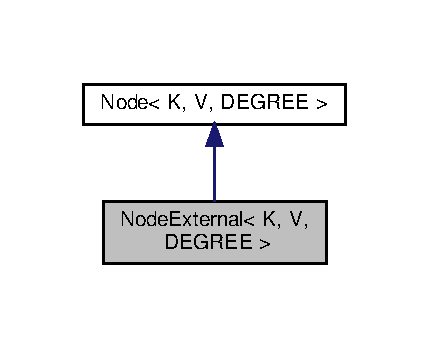
\includegraphics[width=206pt]{classNodeExternal__inherit__graph}
\end{center}
\end{figure}


Collaboration diagram for Node\+External$<$ K, V, D\+E\+G\+R\+EE $>$\+:
\nopagebreak
\begin{figure}[H]
\begin{center}
\leavevmode
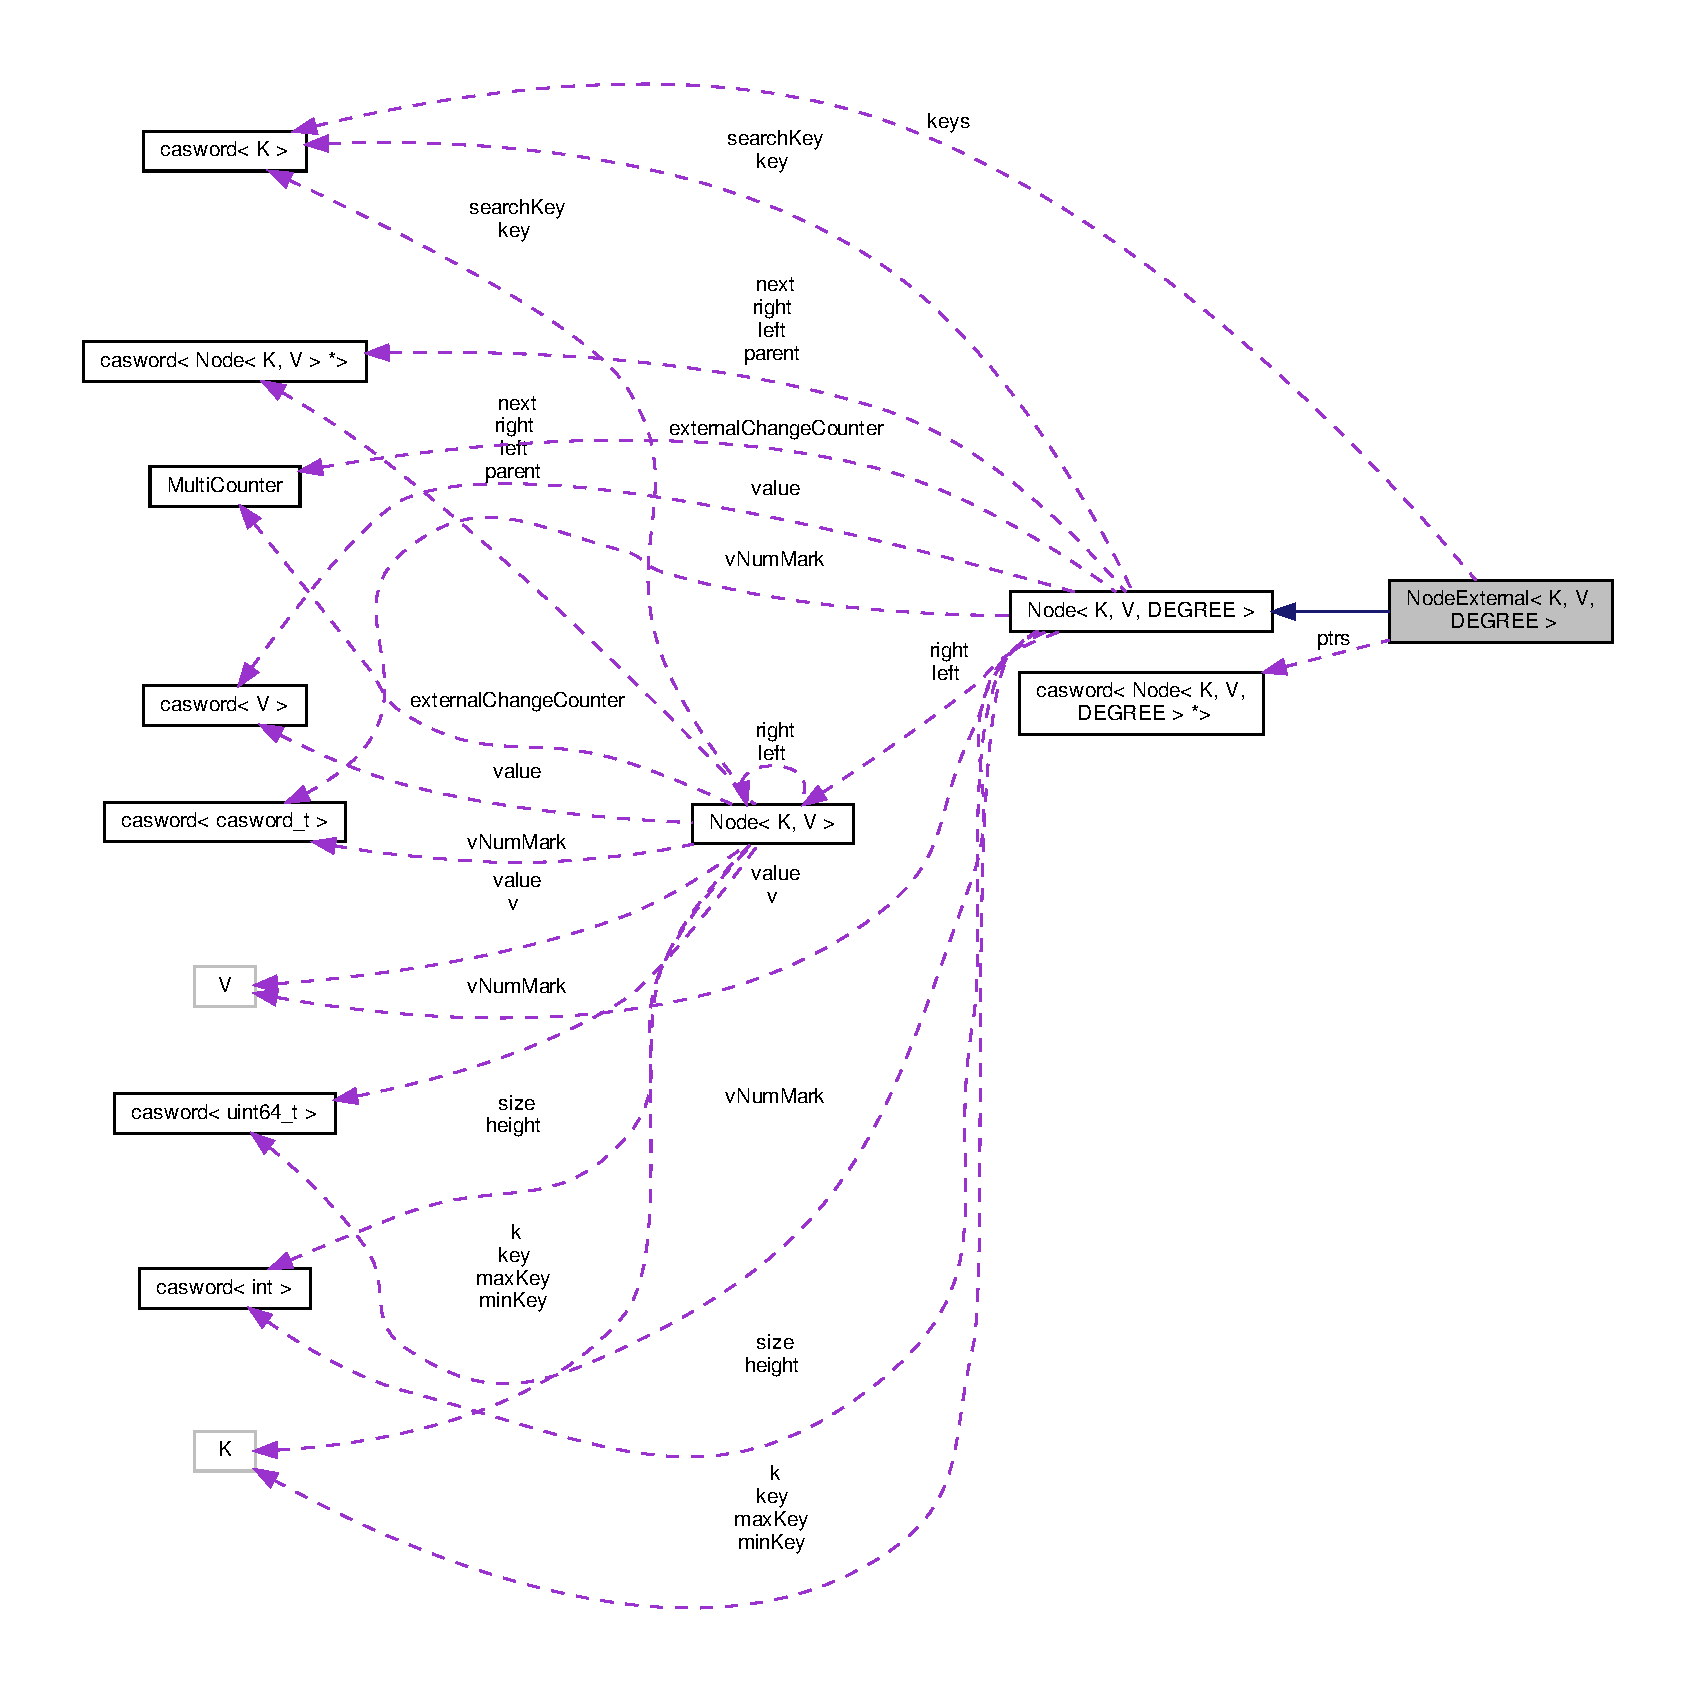
\includegraphics[width=350pt]{classNodeExternal__coll__graph}
\end{center}
\end{figure}
\subsection*{Public Attributes}
\begin{DoxyCompactItemize}
\item 
\hyperlink{structcasword}{casword}$<$ K $>$ \hyperlink{classNodeExternal_a1dec7089d1064805e384ded0dcf2b093}{keys} \mbox{[}\hyperlink{brown__sigouin__abtree__kcas_2adapter_8h_a5d88b17d70c985f2f2b8e987037fd6dd}{D\+E\+G\+R\+EE}\mbox{]}
\item 
\hyperlink{structcasword}{casword}$<$ \hyperlink{classNode}{Node}$<$ K, V, \hyperlink{brown__sigouin__abtree__kcas_2adapter_8h_a5d88b17d70c985f2f2b8e987037fd6dd}{D\+E\+G\+R\+EE} $>$ $\ast$ $>$ \hyperlink{classNodeExternal_a6996827a5ab11c49bc5e738848e3c2bc}{ptrs} \mbox{[}\hyperlink{brown__sigouin__abtree__kcas_2adapter_8h_a5d88b17d70c985f2f2b8e987037fd6dd}{D\+E\+G\+R\+EE}\mbox{]}
\end{DoxyCompactItemize}
\subsection*{Additional Inherited Members}


\subsection{Member Data Documentation}
\mbox{\Hypertarget{classNodeExternal_a1dec7089d1064805e384ded0dcf2b093}\label{classNodeExternal_a1dec7089d1064805e384ded0dcf2b093}} 
\index{Node\+External@{Node\+External}!keys@{keys}}
\index{keys@{keys}!Node\+External@{Node\+External}}
\subsubsection{\texorpdfstring{keys}{keys}}
{\footnotesize\ttfamily template$<$typename K, typename V, int D\+E\+G\+R\+EE$>$ \\
\hyperlink{structcasword}{casword}$<$K$>$ \hyperlink{classNodeExternal}{Node\+External}$<$ K, V, \hyperlink{brown__sigouin__abtree__kcas_2adapter_8h_a5d88b17d70c985f2f2b8e987037fd6dd}{D\+E\+G\+R\+EE} $>$\+::keys\mbox{[}\hyperlink{brown__sigouin__abtree__kcas_2adapter_8h_a5d88b17d70c985f2f2b8e987037fd6dd}{D\+E\+G\+R\+EE}\mbox{]}}

\mbox{\Hypertarget{classNodeExternal_a6996827a5ab11c49bc5e738848e3c2bc}\label{classNodeExternal_a6996827a5ab11c49bc5e738848e3c2bc}} 
\index{Node\+External@{Node\+External}!ptrs@{ptrs}}
\index{ptrs@{ptrs}!Node\+External@{Node\+External}}
\subsubsection{\texorpdfstring{ptrs}{ptrs}}
{\footnotesize\ttfamily template$<$typename K, typename V, int D\+E\+G\+R\+EE$>$ \\
\hyperlink{structcasword}{casword}$<$\hyperlink{classNode}{Node}$<$K, V, \hyperlink{brown__sigouin__abtree__kcas_2adapter_8h_a5d88b17d70c985f2f2b8e987037fd6dd}{D\+E\+G\+R\+EE}$>$ $\ast$$>$ \hyperlink{classNodeExternal}{Node\+External}$<$ K, V, \hyperlink{brown__sigouin__abtree__kcas_2adapter_8h_a5d88b17d70c985f2f2b8e987037fd6dd}{D\+E\+G\+R\+EE} $>$\+::ptrs\mbox{[}\hyperlink{brown__sigouin__abtree__kcas_2adapter_8h_a5d88b17d70c985f2f2b8e987037fd6dd}{D\+E\+G\+R\+EE}\mbox{]}}



The documentation for this class was generated from the following file\+:\begin{DoxyCompactItemize}
\item 
ds/brown\+\_\+sigouin\+\_\+abtree\+\_\+kcas/\hyperlink{abtree__kcas_8h}{abtree\+\_\+kcas.\+h}\end{DoxyCompactItemize}

\hypertarget{classNodeInternal}{}\section{Node\+Internal$<$ K, V, D\+E\+G\+R\+EE $>$ Class Template Reference}
\label{classNodeInternal}\index{Node\+Internal$<$ K, V, D\+E\+G\+R\+E\+E $>$@{Node\+Internal$<$ K, V, D\+E\+G\+R\+E\+E $>$}}


{\ttfamily \#include $<$abtree\+\_\+kcas.\+h$>$}



Inheritance diagram for Node\+Internal$<$ K, V, D\+E\+G\+R\+EE $>$\+:
\nopagebreak
\begin{figure}[H]
\begin{center}
\leavevmode
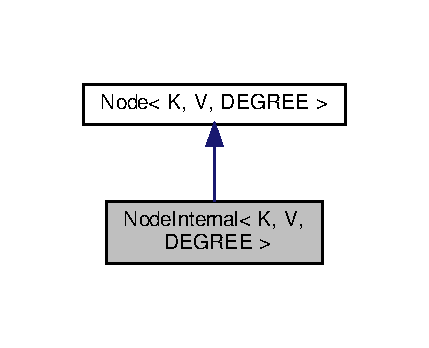
\includegraphics[width=206pt]{classNodeInternal__inherit__graph}
\end{center}
\end{figure}


Collaboration diagram for Node\+Internal$<$ K, V, D\+E\+G\+R\+EE $>$\+:
\nopagebreak
\begin{figure}[H]
\begin{center}
\leavevmode
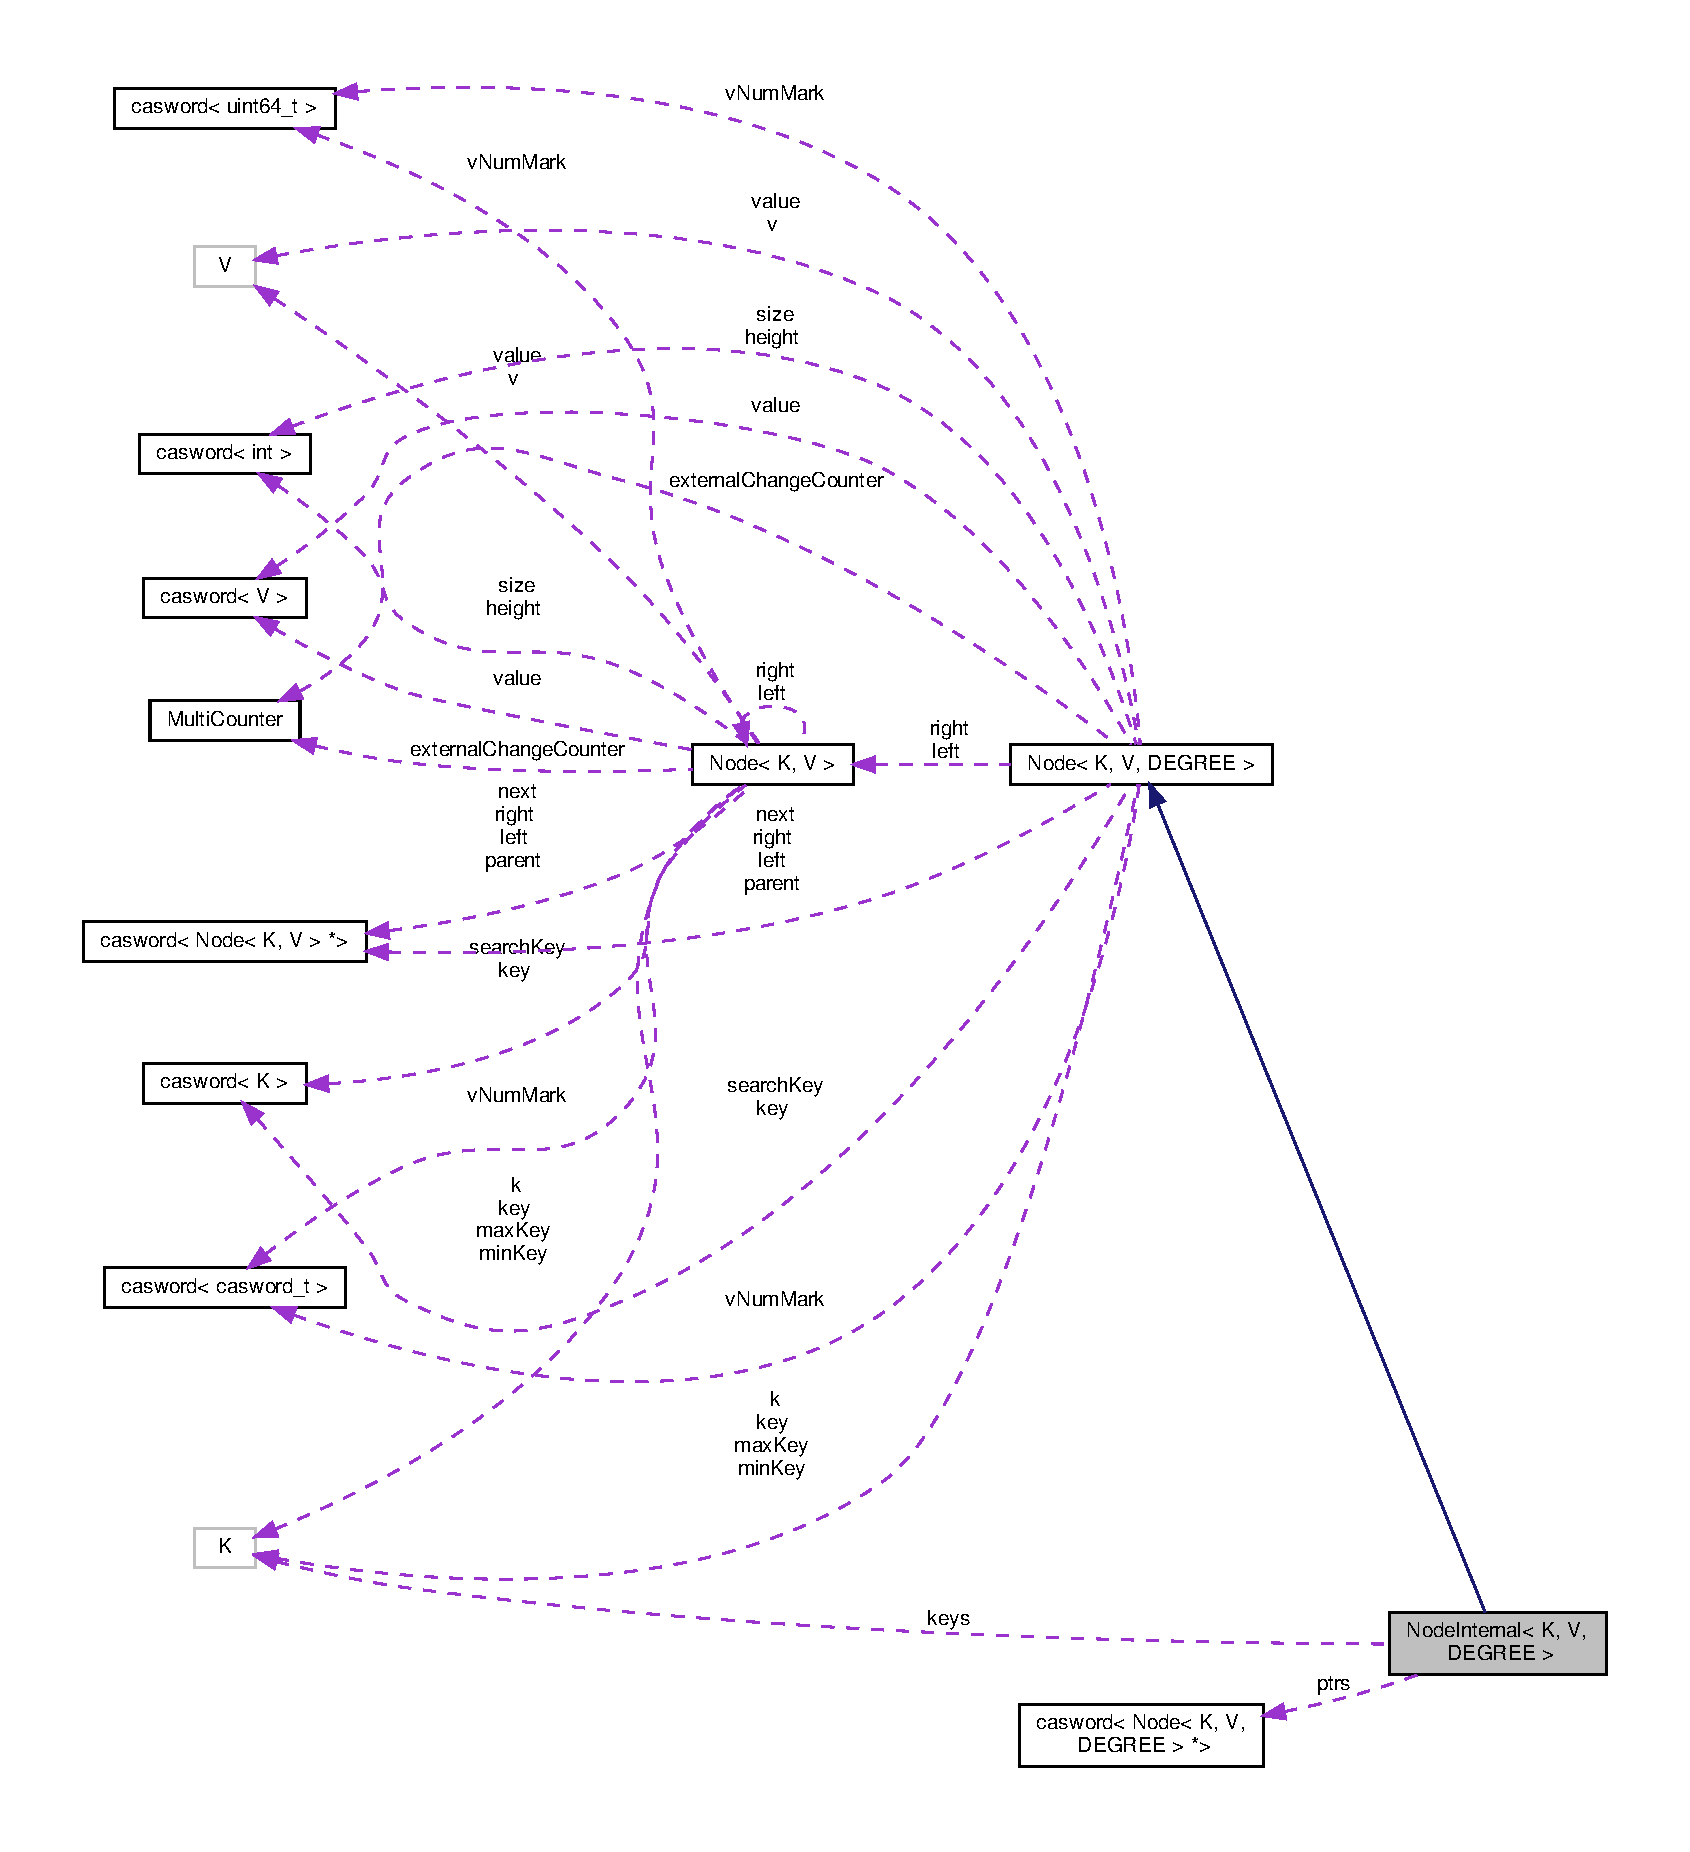
\includegraphics[width=350pt]{classNodeInternal__coll__graph}
\end{center}
\end{figure}
\subsection*{Public Attributes}
\begin{DoxyCompactItemize}
\item 
K \hyperlink{classNodeInternal_a9cae3b9c6a1b3fc1a61053eba2914150}{keys} \mbox{[}\hyperlink{brown__sigouin__abtree__kcas_2adapter_8h_a5d88b17d70c985f2f2b8e987037fd6dd}{D\+E\+G\+R\+EE}\mbox{]}
\item 
\hyperlink{structcasword}{casword}$<$ \hyperlink{classNode}{Node}$<$ K, V, \hyperlink{brown__sigouin__abtree__kcas_2adapter_8h_a5d88b17d70c985f2f2b8e987037fd6dd}{D\+E\+G\+R\+EE} $>$ $\ast$ $>$ \hyperlink{classNodeInternal_a170d07866f92c7f9436bcf6699f3be91}{ptrs} \mbox{[}\hyperlink{brown__sigouin__abtree__kcas_2adapter_8h_a5d88b17d70c985f2f2b8e987037fd6dd}{D\+E\+G\+R\+EE}\mbox{]}
\end{DoxyCompactItemize}
\subsection*{Additional Inherited Members}


\subsection{Member Data Documentation}
\mbox{\Hypertarget{classNodeInternal_a9cae3b9c6a1b3fc1a61053eba2914150}\label{classNodeInternal_a9cae3b9c6a1b3fc1a61053eba2914150}} 
\index{Node\+Internal@{Node\+Internal}!keys@{keys}}
\index{keys@{keys}!Node\+Internal@{Node\+Internal}}
\subsubsection{\texorpdfstring{keys}{keys}}
{\footnotesize\ttfamily template$<$typename K, typename V, int D\+E\+G\+R\+EE$>$ \\
K \hyperlink{classNodeInternal}{Node\+Internal}$<$ K, V, \hyperlink{brown__sigouin__abtree__kcas_2adapter_8h_a5d88b17d70c985f2f2b8e987037fd6dd}{D\+E\+G\+R\+EE} $>$\+::keys\mbox{[}\hyperlink{brown__sigouin__abtree__kcas_2adapter_8h_a5d88b17d70c985f2f2b8e987037fd6dd}{D\+E\+G\+R\+EE}\mbox{]}}

\mbox{\Hypertarget{classNodeInternal_a170d07866f92c7f9436bcf6699f3be91}\label{classNodeInternal_a170d07866f92c7f9436bcf6699f3be91}} 
\index{Node\+Internal@{Node\+Internal}!ptrs@{ptrs}}
\index{ptrs@{ptrs}!Node\+Internal@{Node\+Internal}}
\subsubsection{\texorpdfstring{ptrs}{ptrs}}
{\footnotesize\ttfamily template$<$typename K, typename V, int D\+E\+G\+R\+EE$>$ \\
\hyperlink{structcasword}{casword}$<$\hyperlink{classNode}{Node}$<$K, V, \hyperlink{brown__sigouin__abtree__kcas_2adapter_8h_a5d88b17d70c985f2f2b8e987037fd6dd}{D\+E\+G\+R\+EE}$>$ $\ast$$>$ \hyperlink{classNodeInternal}{Node\+Internal}$<$ K, V, \hyperlink{brown__sigouin__abtree__kcas_2adapter_8h_a5d88b17d70c985f2f2b8e987037fd6dd}{D\+E\+G\+R\+EE} $>$\+::ptrs\mbox{[}\hyperlink{brown__sigouin__abtree__kcas_2adapter_8h_a5d88b17d70c985f2f2b8e987037fd6dd}{D\+E\+G\+R\+EE}\mbox{]}}



The documentation for this class was generated from the following file\+:\begin{DoxyCompactItemize}
\item 
ds/brown\+\_\+sigouin\+\_\+abtree\+\_\+kcas/\hyperlink{abtree__kcas_8h}{abtree\+\_\+kcas.\+h}\end{DoxyCompactItemize}

\hypertarget{classSnapCollector_1_1NodeWrapper}{}\section{Snap\+Collector$<$ Node\+Type, K $>$\+:\+:Node\+Wrapper Class Reference}
\label{classSnapCollector_1_1NodeWrapper}\index{Snap\+Collector$<$ Node\+Type, K $>$\+::\+Node\+Wrapper@{Snap\+Collector$<$ Node\+Type, K $>$\+::\+Node\+Wrapper}}


{\ttfamily \#include $<$snapcollector.\+h$>$}



Collaboration diagram for Snap\+Collector$<$ Node\+Type, K $>$\+:\+:Node\+Wrapper\+:
\nopagebreak
\begin{figure}[H]
\begin{center}
\leavevmode
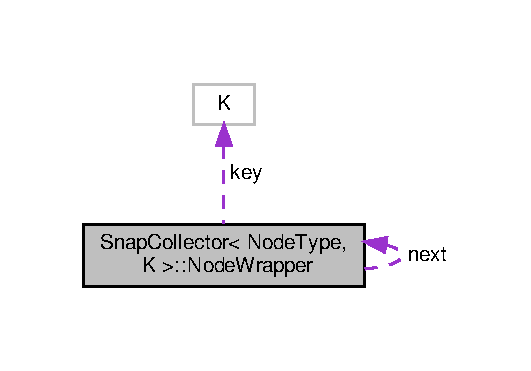
\includegraphics[width=255pt]{classSnapCollector_1_1NodeWrapper__coll__graph}
\end{center}
\end{figure}
\subsection*{Public Member Functions}
\begin{DoxyCompactItemize}
\item 
\hyperlink{classSnapCollector_1_1NodeWrapper_a2c01b80b410f3d2d3ab88de500756085}{Node\+Wrapper} ()
\item 
void \hyperlink{classSnapCollector_1_1NodeWrapper_a7b76d026e07104eac67de442c69935d4}{init} (K \hyperlink{classSnapCollector_1_1NodeWrapper_a7d13c9414d57407f001b6870889a70e2}{key})
\item 
void \hyperlink{classSnapCollector_1_1NodeWrapper_a1006722b5e5fac800e748b181757881d}{init} (Node\+Type $\ast$\hyperlink{classSnapCollector_1_1NodeWrapper_afd1dd8bfffc9b360fa20f32689365d54}{node}, K \hyperlink{classSnapCollector_1_1NodeWrapper_a7d13c9414d57407f001b6870889a70e2}{key})
\end{DoxyCompactItemize}
\subsection*{Public Attributes}
\begin{DoxyCompactItemize}
\item 
Node\+Type $\ast$ \hyperlink{classSnapCollector_1_1NodeWrapper_afd1dd8bfffc9b360fa20f32689365d54}{node}
\item 
\hyperlink{classSnapCollector_1_1NodeWrapper}{Node\+Wrapper} $\ast$volatile \hyperlink{classSnapCollector_1_1NodeWrapper_a74fd41d8777e479040a2ff806fcad396}{next}
\item 
K \hyperlink{classSnapCollector_1_1NodeWrapper_a7d13c9414d57407f001b6870889a70e2}{key}
\end{DoxyCompactItemize}


\subsection{Constructor \& Destructor Documentation}
\mbox{\Hypertarget{classSnapCollector_1_1NodeWrapper_a2c01b80b410f3d2d3ab88de500756085}\label{classSnapCollector_1_1NodeWrapper_a2c01b80b410f3d2d3ab88de500756085}} 
\index{Snap\+Collector\+::\+Node\+Wrapper@{Snap\+Collector\+::\+Node\+Wrapper}!Node\+Wrapper@{Node\+Wrapper}}
\index{Node\+Wrapper@{Node\+Wrapper}!Snap\+Collector\+::\+Node\+Wrapper@{Snap\+Collector\+::\+Node\+Wrapper}}
\subsubsection{\texorpdfstring{Node\+Wrapper()}{NodeWrapper()}}
{\footnotesize\ttfamily template$<$typename Node\+Type, typename K$>$ \\
\hyperlink{classSnapCollector}{Snap\+Collector}$<$ Node\+Type, K $>$\+::Node\+Wrapper\+::\+Node\+Wrapper (\begin{DoxyParamCaption}{ }\end{DoxyParamCaption})\hspace{0.3cm}{\ttfamily [inline]}}



\subsection{Member Function Documentation}
\mbox{\Hypertarget{classSnapCollector_1_1NodeWrapper_a7b76d026e07104eac67de442c69935d4}\label{classSnapCollector_1_1NodeWrapper_a7b76d026e07104eac67de442c69935d4}} 
\index{Snap\+Collector\+::\+Node\+Wrapper@{Snap\+Collector\+::\+Node\+Wrapper}!init@{init}}
\index{init@{init}!Snap\+Collector\+::\+Node\+Wrapper@{Snap\+Collector\+::\+Node\+Wrapper}}
\subsubsection{\texorpdfstring{init()}{init()}\hspace{0.1cm}{\footnotesize\ttfamily [1/2]}}
{\footnotesize\ttfamily template$<$typename Node\+Type, typename K$>$ \\
void \hyperlink{classSnapCollector}{Snap\+Collector}$<$ Node\+Type, K $>$\+::Node\+Wrapper\+::init (\begin{DoxyParamCaption}\item[{K}]{key }\end{DoxyParamCaption})\hspace{0.3cm}{\ttfamily [inline]}}

\mbox{\Hypertarget{classSnapCollector_1_1NodeWrapper_a1006722b5e5fac800e748b181757881d}\label{classSnapCollector_1_1NodeWrapper_a1006722b5e5fac800e748b181757881d}} 
\index{Snap\+Collector\+::\+Node\+Wrapper@{Snap\+Collector\+::\+Node\+Wrapper}!init@{init}}
\index{init@{init}!Snap\+Collector\+::\+Node\+Wrapper@{Snap\+Collector\+::\+Node\+Wrapper}}
\subsubsection{\texorpdfstring{init()}{init()}\hspace{0.1cm}{\footnotesize\ttfamily [2/2]}}
{\footnotesize\ttfamily template$<$typename Node\+Type, typename K$>$ \\
void \hyperlink{classSnapCollector}{Snap\+Collector}$<$ Node\+Type, K $>$\+::Node\+Wrapper\+::init (\begin{DoxyParamCaption}\item[{Node\+Type $\ast$}]{node,  }\item[{K}]{key }\end{DoxyParamCaption})\hspace{0.3cm}{\ttfamily [inline]}}



\subsection{Member Data Documentation}
\mbox{\Hypertarget{classSnapCollector_1_1NodeWrapper_a7d13c9414d57407f001b6870889a70e2}\label{classSnapCollector_1_1NodeWrapper_a7d13c9414d57407f001b6870889a70e2}} 
\index{Snap\+Collector\+::\+Node\+Wrapper@{Snap\+Collector\+::\+Node\+Wrapper}!key@{key}}
\index{key@{key}!Snap\+Collector\+::\+Node\+Wrapper@{Snap\+Collector\+::\+Node\+Wrapper}}
\subsubsection{\texorpdfstring{key}{key}}
{\footnotesize\ttfamily template$<$typename Node\+Type, typename K$>$ \\
K \hyperlink{classSnapCollector}{Snap\+Collector}$<$ Node\+Type, K $>$\+::Node\+Wrapper\+::key}

\mbox{\Hypertarget{classSnapCollector_1_1NodeWrapper_a74fd41d8777e479040a2ff806fcad396}\label{classSnapCollector_1_1NodeWrapper_a74fd41d8777e479040a2ff806fcad396}} 
\index{Snap\+Collector\+::\+Node\+Wrapper@{Snap\+Collector\+::\+Node\+Wrapper}!next@{next}}
\index{next@{next}!Snap\+Collector\+::\+Node\+Wrapper@{Snap\+Collector\+::\+Node\+Wrapper}}
\subsubsection{\texorpdfstring{next}{next}}
{\footnotesize\ttfamily template$<$typename Node\+Type, typename K$>$ \\
\hyperlink{classSnapCollector_1_1NodeWrapper}{Node\+Wrapper}$\ast$ volatile \hyperlink{classSnapCollector}{Snap\+Collector}$<$ Node\+Type, K $>$\+::Node\+Wrapper\+::next}

\mbox{\Hypertarget{classSnapCollector_1_1NodeWrapper_afd1dd8bfffc9b360fa20f32689365d54}\label{classSnapCollector_1_1NodeWrapper_afd1dd8bfffc9b360fa20f32689365d54}} 
\index{Snap\+Collector\+::\+Node\+Wrapper@{Snap\+Collector\+::\+Node\+Wrapper}!node@{node}}
\index{node@{node}!Snap\+Collector\+::\+Node\+Wrapper@{Snap\+Collector\+::\+Node\+Wrapper}}
\subsubsection{\texorpdfstring{node}{node}}
{\footnotesize\ttfamily template$<$typename Node\+Type, typename K$>$ \\
Node\+Type$\ast$ \hyperlink{classSnapCollector}{Snap\+Collector}$<$ Node\+Type, K $>$\+::Node\+Wrapper\+::node}



The documentation for this class was generated from the following file\+:\begin{DoxyCompactItemize}
\item 
common/rq/snapcollector/\hyperlink{snapcollector_8h}{snapcollector.\+h}\end{DoxyCompactItemize}

\hypertarget{classNumaTools}{}\section{Numa\+Tools Class Reference}
\label{classNumaTools}\index{Numa\+Tools@{Numa\+Tools}}


{\ttfamily \#include $<$numa\+\_\+tools.\+h$>$}

\subsection*{Public Member Functions}
\begin{DoxyCompactItemize}
\item 
\hyperlink{classNumaTools_aafcc9a9476cf975b4bd2f6a252f569aa}{Numa\+Tools} (int \+\_\+calls\+Per\+Update=100)
\item 
\hyperlink{classNumaTools_ae09d46d3c469d6151b93c3d96a1ff638}{$\sim$\+Numa\+Tools} ()
\item 
int \hyperlink{classNumaTools_aa1f63a07dbd4cf3795a9c37635995c8c}{get\+\_\+cpu\+\_\+cached} ()
\item 
int \hyperlink{classNumaTools_aac14b435a11ec52d02014783438d9ca4}{get\+\_\+cpu\+\_\+slow} ()
\item 
int \hyperlink{classNumaTools_ad67628c3c37072be89b377efd8aeca5d}{get\+\_\+cpu\+\_\+periodic} ()
\item 
int \hyperlink{classNumaTools_a15f467a2f27852c3f20c73c15e506cd1}{get\+\_\+node\+\_\+for\+\_\+cpu} (int cpu)
\item 
int \hyperlink{classNumaTools_ae073412f2df74a862553f218f887c94d}{get\+\_\+node\+\_\+slow} ()
\item 
int \hyperlink{classNumaTools_a8d7519f7caee2c3de6ffed4da724f125}{get\+\_\+node\+\_\+cached} ()
\item 
int \hyperlink{classNumaTools_a648fb73d8291e0d026c4e1921d17412b}{get\+\_\+node\+\_\+periodic} ()
\item 
int \hyperlink{classNumaTools_a9ba5a103276fdea894b82e7375ed1bf6}{get\+\_\+num\+\_\+nodes} ()
\item 
int \hyperlink{classNumaTools_af932989447a90e30f66f48d637fa46bf}{get\+\_\+num\+\_\+cpus} ()
\end{DoxyCompactItemize}


\subsection{Constructor \& Destructor Documentation}
\mbox{\Hypertarget{classNumaTools_aafcc9a9476cf975b4bd2f6a252f569aa}\label{classNumaTools_aafcc9a9476cf975b4bd2f6a252f569aa}} 
\index{Numa\+Tools@{Numa\+Tools}!Numa\+Tools@{Numa\+Tools}}
\index{Numa\+Tools@{Numa\+Tools}!Numa\+Tools@{Numa\+Tools}}
\subsubsection{\texorpdfstring{Numa\+Tools()}{NumaTools()}}
{\footnotesize\ttfamily Numa\+Tools\+::\+Numa\+Tools (\begin{DoxyParamCaption}\item[{int}]{\+\_\+calls\+Per\+Update = {\ttfamily 100} }\end{DoxyParamCaption})\hspace{0.3cm}{\ttfamily [inline]}}

\mbox{\Hypertarget{classNumaTools_ae09d46d3c469d6151b93c3d96a1ff638}\label{classNumaTools_ae09d46d3c469d6151b93c3d96a1ff638}} 
\index{Numa\+Tools@{Numa\+Tools}!````~Numa\+Tools@{$\sim$\+Numa\+Tools}}
\index{````~Numa\+Tools@{$\sim$\+Numa\+Tools}!Numa\+Tools@{Numa\+Tools}}
\subsubsection{\texorpdfstring{$\sim$\+Numa\+Tools()}{~NumaTools()}}
{\footnotesize\ttfamily Numa\+Tools\+::$\sim$\+Numa\+Tools (\begin{DoxyParamCaption}{ }\end{DoxyParamCaption})\hspace{0.3cm}{\ttfamily [inline]}}



\subsection{Member Function Documentation}
\mbox{\Hypertarget{classNumaTools_aa1f63a07dbd4cf3795a9c37635995c8c}\label{classNumaTools_aa1f63a07dbd4cf3795a9c37635995c8c}} 
\index{Numa\+Tools@{Numa\+Tools}!get\+\_\+cpu\+\_\+cached@{get\+\_\+cpu\+\_\+cached}}
\index{get\+\_\+cpu\+\_\+cached@{get\+\_\+cpu\+\_\+cached}!Numa\+Tools@{Numa\+Tools}}
\subsubsection{\texorpdfstring{get\+\_\+cpu\+\_\+cached()}{get\_cpu\_cached()}}
{\footnotesize\ttfamily int Numa\+Tools\+::get\+\_\+cpu\+\_\+cached (\begin{DoxyParamCaption}{ }\end{DoxyParamCaption})\hspace{0.3cm}{\ttfamily [inline]}}

\mbox{\Hypertarget{classNumaTools_ad67628c3c37072be89b377efd8aeca5d}\label{classNumaTools_ad67628c3c37072be89b377efd8aeca5d}} 
\index{Numa\+Tools@{Numa\+Tools}!get\+\_\+cpu\+\_\+periodic@{get\+\_\+cpu\+\_\+periodic}}
\index{get\+\_\+cpu\+\_\+periodic@{get\+\_\+cpu\+\_\+periodic}!Numa\+Tools@{Numa\+Tools}}
\subsubsection{\texorpdfstring{get\+\_\+cpu\+\_\+periodic()}{get\_cpu\_periodic()}}
{\footnotesize\ttfamily int Numa\+Tools\+::get\+\_\+cpu\+\_\+periodic (\begin{DoxyParamCaption}{ }\end{DoxyParamCaption})\hspace{0.3cm}{\ttfamily [inline]}}

\mbox{\Hypertarget{classNumaTools_aac14b435a11ec52d02014783438d9ca4}\label{classNumaTools_aac14b435a11ec52d02014783438d9ca4}} 
\index{Numa\+Tools@{Numa\+Tools}!get\+\_\+cpu\+\_\+slow@{get\+\_\+cpu\+\_\+slow}}
\index{get\+\_\+cpu\+\_\+slow@{get\+\_\+cpu\+\_\+slow}!Numa\+Tools@{Numa\+Tools}}
\subsubsection{\texorpdfstring{get\+\_\+cpu\+\_\+slow()}{get\_cpu\_slow()}}
{\footnotesize\ttfamily int Numa\+Tools\+::get\+\_\+cpu\+\_\+slow (\begin{DoxyParamCaption}{ }\end{DoxyParamCaption})\hspace{0.3cm}{\ttfamily [inline]}}

\mbox{\Hypertarget{classNumaTools_a8d7519f7caee2c3de6ffed4da724f125}\label{classNumaTools_a8d7519f7caee2c3de6ffed4da724f125}} 
\index{Numa\+Tools@{Numa\+Tools}!get\+\_\+node\+\_\+cached@{get\+\_\+node\+\_\+cached}}
\index{get\+\_\+node\+\_\+cached@{get\+\_\+node\+\_\+cached}!Numa\+Tools@{Numa\+Tools}}
\subsubsection{\texorpdfstring{get\+\_\+node\+\_\+cached()}{get\_node\_cached()}}
{\footnotesize\ttfamily int Numa\+Tools\+::get\+\_\+node\+\_\+cached (\begin{DoxyParamCaption}{ }\end{DoxyParamCaption})\hspace{0.3cm}{\ttfamily [inline]}}

\mbox{\Hypertarget{classNumaTools_a15f467a2f27852c3f20c73c15e506cd1}\label{classNumaTools_a15f467a2f27852c3f20c73c15e506cd1}} 
\index{Numa\+Tools@{Numa\+Tools}!get\+\_\+node\+\_\+for\+\_\+cpu@{get\+\_\+node\+\_\+for\+\_\+cpu}}
\index{get\+\_\+node\+\_\+for\+\_\+cpu@{get\+\_\+node\+\_\+for\+\_\+cpu}!Numa\+Tools@{Numa\+Tools}}
\subsubsection{\texorpdfstring{get\+\_\+node\+\_\+for\+\_\+cpu()}{get\_node\_for\_cpu()}}
{\footnotesize\ttfamily int Numa\+Tools\+::get\+\_\+node\+\_\+for\+\_\+cpu (\begin{DoxyParamCaption}\item[{int}]{cpu }\end{DoxyParamCaption})\hspace{0.3cm}{\ttfamily [inline]}}

\mbox{\Hypertarget{classNumaTools_a648fb73d8291e0d026c4e1921d17412b}\label{classNumaTools_a648fb73d8291e0d026c4e1921d17412b}} 
\index{Numa\+Tools@{Numa\+Tools}!get\+\_\+node\+\_\+periodic@{get\+\_\+node\+\_\+periodic}}
\index{get\+\_\+node\+\_\+periodic@{get\+\_\+node\+\_\+periodic}!Numa\+Tools@{Numa\+Tools}}
\subsubsection{\texorpdfstring{get\+\_\+node\+\_\+periodic()}{get\_node\_periodic()}}
{\footnotesize\ttfamily int Numa\+Tools\+::get\+\_\+node\+\_\+periodic (\begin{DoxyParamCaption}{ }\end{DoxyParamCaption})\hspace{0.3cm}{\ttfamily [inline]}}

\mbox{\Hypertarget{classNumaTools_ae073412f2df74a862553f218f887c94d}\label{classNumaTools_ae073412f2df74a862553f218f887c94d}} 
\index{Numa\+Tools@{Numa\+Tools}!get\+\_\+node\+\_\+slow@{get\+\_\+node\+\_\+slow}}
\index{get\+\_\+node\+\_\+slow@{get\+\_\+node\+\_\+slow}!Numa\+Tools@{Numa\+Tools}}
\subsubsection{\texorpdfstring{get\+\_\+node\+\_\+slow()}{get\_node\_slow()}}
{\footnotesize\ttfamily int Numa\+Tools\+::get\+\_\+node\+\_\+slow (\begin{DoxyParamCaption}{ }\end{DoxyParamCaption})\hspace{0.3cm}{\ttfamily [inline]}}

\mbox{\Hypertarget{classNumaTools_af932989447a90e30f66f48d637fa46bf}\label{classNumaTools_af932989447a90e30f66f48d637fa46bf}} 
\index{Numa\+Tools@{Numa\+Tools}!get\+\_\+num\+\_\+cpus@{get\+\_\+num\+\_\+cpus}}
\index{get\+\_\+num\+\_\+cpus@{get\+\_\+num\+\_\+cpus}!Numa\+Tools@{Numa\+Tools}}
\subsubsection{\texorpdfstring{get\+\_\+num\+\_\+cpus()}{get\_num\_cpus()}}
{\footnotesize\ttfamily int Numa\+Tools\+::get\+\_\+num\+\_\+cpus (\begin{DoxyParamCaption}{ }\end{DoxyParamCaption})\hspace{0.3cm}{\ttfamily [inline]}}

\mbox{\Hypertarget{classNumaTools_a9ba5a103276fdea894b82e7375ed1bf6}\label{classNumaTools_a9ba5a103276fdea894b82e7375ed1bf6}} 
\index{Numa\+Tools@{Numa\+Tools}!get\+\_\+num\+\_\+nodes@{get\+\_\+num\+\_\+nodes}}
\index{get\+\_\+num\+\_\+nodes@{get\+\_\+num\+\_\+nodes}!Numa\+Tools@{Numa\+Tools}}
\subsubsection{\texorpdfstring{get\+\_\+num\+\_\+nodes()}{get\_num\_nodes()}}
{\footnotesize\ttfamily int Numa\+Tools\+::get\+\_\+num\+\_\+nodes (\begin{DoxyParamCaption}{ }\end{DoxyParamCaption})\hspace{0.3cm}{\ttfamily [inline]}}



The documentation for this class was generated from the following file\+:\begin{DoxyCompactItemize}
\item 
common/\hyperlink{numa__tools_8h}{numa\+\_\+tools.\+h}\end{DoxyCompactItemize}

\hypertarget{structobj__list}{}\section{obj\+\_\+list Struct Reference}
\label{structobj__list}\index{obj\+\_\+list@{obj\+\_\+list}}


{\ttfamily \#include $<$rlu.\+h$>$}



Collaboration diagram for obj\+\_\+list\+:
\nopagebreak
\begin{figure}[H]
\begin{center}
\leavevmode
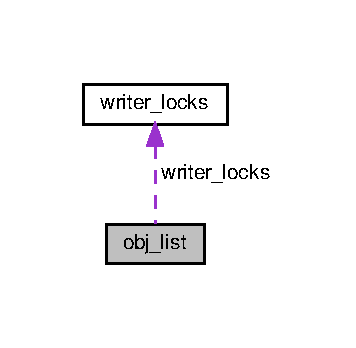
\includegraphics[width=171pt]{structobj__list__coll__graph}
\end{center}
\end{figure}
\subsection*{Public Attributes}
\begin{DoxyCompactItemize}
\item 
volatile \hyperlink{rlu_8h_a96757ec58e867aecee96e5f992035057}{writer\+\_\+locks\+\_\+t} \hyperlink{structobj__list_a2a8548d3319e930e691a6350adea720c}{writer\+\_\+locks}
\item 
unsigned int \hyperlink{structobj__list_a000d5c402401e9a96a0637ed95e8539f}{num\+\_\+of\+\_\+objs}
\item 
volatile intptr\+\_\+t $\ast$ \hyperlink{structobj__list_abd1b71e81f3a09630ef9307fa3a13f02}{p\+\_\+cur}
\item 
volatile unsigned char \hyperlink{structobj__list_ae01b5948abef49842ea1a9fd0c31885d}{buffer} \mbox{[}\hyperlink{rlu_8h_a3bcdeac35b6406d4ea7a486e33aad3c3}{R\+L\+U\+\_\+\+M\+A\+X\+\_\+\+W\+R\+I\+T\+E\+\_\+\+S\+E\+T\+\_\+\+B\+U\+F\+F\+E\+R\+\_\+\+S\+I\+ZE}\mbox{]}
\end{DoxyCompactItemize}


\subsection{Member Data Documentation}
\mbox{\Hypertarget{structobj__list_ae01b5948abef49842ea1a9fd0c31885d}\label{structobj__list_ae01b5948abef49842ea1a9fd0c31885d}} 
\index{obj\+\_\+list@{obj\+\_\+list}!buffer@{buffer}}
\index{buffer@{buffer}!obj\+\_\+list@{obj\+\_\+list}}
\subsubsection{\texorpdfstring{buffer}{buffer}}
{\footnotesize\ttfamily volatile unsigned char obj\+\_\+list\+::buffer\mbox{[}\hyperlink{rlu_8h_a3bcdeac35b6406d4ea7a486e33aad3c3}{R\+L\+U\+\_\+\+M\+A\+X\+\_\+\+W\+R\+I\+T\+E\+\_\+\+S\+E\+T\+\_\+\+B\+U\+F\+F\+E\+R\+\_\+\+S\+I\+ZE}\mbox{]}}

\mbox{\Hypertarget{structobj__list_a000d5c402401e9a96a0637ed95e8539f}\label{structobj__list_a000d5c402401e9a96a0637ed95e8539f}} 
\index{obj\+\_\+list@{obj\+\_\+list}!num\+\_\+of\+\_\+objs@{num\+\_\+of\+\_\+objs}}
\index{num\+\_\+of\+\_\+objs@{num\+\_\+of\+\_\+objs}!obj\+\_\+list@{obj\+\_\+list}}
\subsubsection{\texorpdfstring{num\+\_\+of\+\_\+objs}{num\_of\_objs}}
{\footnotesize\ttfamily unsigned int obj\+\_\+list\+::num\+\_\+of\+\_\+objs}

\mbox{\Hypertarget{structobj__list_abd1b71e81f3a09630ef9307fa3a13f02}\label{structobj__list_abd1b71e81f3a09630ef9307fa3a13f02}} 
\index{obj\+\_\+list@{obj\+\_\+list}!p\+\_\+cur@{p\+\_\+cur}}
\index{p\+\_\+cur@{p\+\_\+cur}!obj\+\_\+list@{obj\+\_\+list}}
\subsubsection{\texorpdfstring{p\+\_\+cur}{p\_cur}}
{\footnotesize\ttfamily volatile intptr\+\_\+t$\ast$ obj\+\_\+list\+::p\+\_\+cur}

\mbox{\Hypertarget{structobj__list_a2a8548d3319e930e691a6350adea720c}\label{structobj__list_a2a8548d3319e930e691a6350adea720c}} 
\index{obj\+\_\+list@{obj\+\_\+list}!writer\+\_\+locks@{writer\+\_\+locks}}
\index{writer\+\_\+locks@{writer\+\_\+locks}!obj\+\_\+list@{obj\+\_\+list}}
\subsubsection{\texorpdfstring{writer\+\_\+locks}{writer\_locks}}
{\footnotesize\ttfamily volatile \hyperlink{rlu_8h_a96757ec58e867aecee96e5f992035057}{writer\+\_\+locks\+\_\+t} obj\+\_\+list\+::writer\+\_\+locks}



The documentation for this struct was generated from the following file\+:\begin{DoxyCompactItemize}
\item 
common/rlu/\hyperlink{rlu_8h}{rlu.\+h}\end{DoxyCompactItemize}

\hypertarget{unionoperation__t}{}\section{operation\+\_\+t$<$ skey\+\_\+t, sval\+\_\+t $>$ Union Template Reference}
\label{unionoperation__t}\index{operation\+\_\+t$<$ skey\+\_\+t, sval\+\_\+t $>$@{operation\+\_\+t$<$ skey\+\_\+t, sval\+\_\+t $>$}}


{\ttfamily \#include $<$howley\+\_\+impl.\+h$>$}

\subsection*{Public Attributes}
\begin{DoxyCompactItemize}
\item 
\hyperlink{structchild__cas__op__t}{child\+\_\+cas\+\_\+op\+\_\+t}$<$ skey\+\_\+t, sval\+\_\+t $>$ \hyperlink{unionoperation__t_acbedd3f8b930f90675bfe965d93ad3f3}{child\+\_\+cas\+\_\+op}
\item 
\hyperlink{structrelocate__op__t}{relocate\+\_\+op\+\_\+t}$<$ skey\+\_\+t, sval\+\_\+t $>$ \hyperlink{unionoperation__t_a8604de36b950c8d7218afde0bb69678c}{relocate\+\_\+op}
\item 
uint8\+\_\+t \hyperlink{unionoperation__t_a31d6c729884c52c6b10b2038fbce49dc}{padding} \mbox{[}112\mbox{]}
\end{DoxyCompactItemize}


\subsection{Member Data Documentation}
\mbox{\Hypertarget{unionoperation__t_acbedd3f8b930f90675bfe965d93ad3f3}\label{unionoperation__t_acbedd3f8b930f90675bfe965d93ad3f3}} 
\index{operation\+\_\+t@{operation\+\_\+t}!child\+\_\+cas\+\_\+op@{child\+\_\+cas\+\_\+op}}
\index{child\+\_\+cas\+\_\+op@{child\+\_\+cas\+\_\+op}!operation\+\_\+t@{operation\+\_\+t}}
\subsubsection{\texorpdfstring{child\+\_\+cas\+\_\+op}{child\_cas\_op}}
{\footnotesize\ttfamily template$<$typename skey\+\_\+t, typename sval\+\_\+t$>$ \\
\hyperlink{structchild__cas__op__t}{child\+\_\+cas\+\_\+op\+\_\+t}$<$skey\+\_\+t, sval\+\_\+t$>$ \hyperlink{unionoperation__t}{operation\+\_\+t}$<$ skey\+\_\+t, sval\+\_\+t $>$\+::child\+\_\+cas\+\_\+op}

\mbox{\Hypertarget{unionoperation__t_a31d6c729884c52c6b10b2038fbce49dc}\label{unionoperation__t_a31d6c729884c52c6b10b2038fbce49dc}} 
\index{operation\+\_\+t@{operation\+\_\+t}!padding@{padding}}
\index{padding@{padding}!operation\+\_\+t@{operation\+\_\+t}}
\subsubsection{\texorpdfstring{padding}{padding}}
{\footnotesize\ttfamily template$<$typename skey\+\_\+t, typename sval\+\_\+t$>$ \\
uint8\+\_\+t \hyperlink{unionoperation__t}{operation\+\_\+t}$<$ skey\+\_\+t, sval\+\_\+t $>$\+::padding\mbox{[}112\mbox{]}}

\mbox{\Hypertarget{unionoperation__t_a8604de36b950c8d7218afde0bb69678c}\label{unionoperation__t_a8604de36b950c8d7218afde0bb69678c}} 
\index{operation\+\_\+t@{operation\+\_\+t}!relocate\+\_\+op@{relocate\+\_\+op}}
\index{relocate\+\_\+op@{relocate\+\_\+op}!operation\+\_\+t@{operation\+\_\+t}}
\subsubsection{\texorpdfstring{relocate\+\_\+op}{relocate\_op}}
{\footnotesize\ttfamily template$<$typename skey\+\_\+t, typename sval\+\_\+t$>$ \\
\hyperlink{structrelocate__op__t}{relocate\+\_\+op\+\_\+t}$<$skey\+\_\+t, sval\+\_\+t$>$ \hyperlink{unionoperation__t}{operation\+\_\+t}$<$ skey\+\_\+t, sval\+\_\+t $>$\+::relocate\+\_\+op}



The documentation for this union was generated from the following file\+:\begin{DoxyCompactItemize}
\item 
ds/howley\+\_\+int\+\_\+bst\+\_\+lf/\hyperlink{howley__impl_8h}{howley\+\_\+impl.\+h}\end{DoxyCompactItemize}

\hypertarget{classOptCC}{}\section{Opt\+CC Class Reference}
\label{classOptCC}\index{Opt\+CC@{Opt\+CC}}


{\ttfamily \#include $<$occ.\+h$>$}

\subsection*{Public Member Functions}
\begin{DoxyCompactItemize}
\item 
void \hyperlink{classOptCC_aa3ba49e935e9f1d0b83f9e815b71a09a}{init} ()
\item 
\hyperlink{global_8h_a78c49a674c810fdd03d20432f7be864a}{RC} \hyperlink{classOptCC_ad8b7a9a94e75565d5d7a0b5e01a2f9a4}{validate} (\hyperlink{classtxn__man}{txn\+\_\+man} $\ast$txn)
\end{DoxyCompactItemize}
\subsection*{Public Attributes}
\begin{DoxyCompactItemize}
\item 
volatile bool \hyperlink{classOptCC_a9c85846a4cd32e12561da6b0d056dc5b}{lock\+\_\+all}
\item 
uint64\+\_\+t \hyperlink{classOptCC_a3402f030762477a8467b2359d5444e82}{lock\+\_\+txn\+\_\+id}
\end{DoxyCompactItemize}


\subsection{Member Function Documentation}
\mbox{\Hypertarget{classOptCC_aa3ba49e935e9f1d0b83f9e815b71a09a}\label{classOptCC_aa3ba49e935e9f1d0b83f9e815b71a09a}} 
\index{Opt\+CC@{Opt\+CC}!init@{init}}
\index{init@{init}!Opt\+CC@{Opt\+CC}}
\subsubsection{\texorpdfstring{init()}{init()}}
{\footnotesize\ttfamily void Opt\+C\+C\+::init (\begin{DoxyParamCaption}{ }\end{DoxyParamCaption})}

\mbox{\Hypertarget{classOptCC_ad8b7a9a94e75565d5d7a0b5e01a2f9a4}\label{classOptCC_ad8b7a9a94e75565d5d7a0b5e01a2f9a4}} 
\index{Opt\+CC@{Opt\+CC}!validate@{validate}}
\index{validate@{validate}!Opt\+CC@{Opt\+CC}}
\subsubsection{\texorpdfstring{validate()}{validate()}}
{\footnotesize\ttfamily \hyperlink{global_8h_a78c49a674c810fdd03d20432f7be864a}{RC} Opt\+C\+C\+::validate (\begin{DoxyParamCaption}\item[{\hyperlink{classtxn__man}{txn\+\_\+man} $\ast$}]{txn }\end{DoxyParamCaption})}



\subsection{Member Data Documentation}
\mbox{\Hypertarget{classOptCC_a9c85846a4cd32e12561da6b0d056dc5b}\label{classOptCC_a9c85846a4cd32e12561da6b0d056dc5b}} 
\index{Opt\+CC@{Opt\+CC}!lock\+\_\+all@{lock\+\_\+all}}
\index{lock\+\_\+all@{lock\+\_\+all}!Opt\+CC@{Opt\+CC}}
\subsubsection{\texorpdfstring{lock\+\_\+all}{lock\_all}}
{\footnotesize\ttfamily volatile bool Opt\+C\+C\+::lock\+\_\+all}

\mbox{\Hypertarget{classOptCC_a3402f030762477a8467b2359d5444e82}\label{classOptCC_a3402f030762477a8467b2359d5444e82}} 
\index{Opt\+CC@{Opt\+CC}!lock\+\_\+txn\+\_\+id@{lock\+\_\+txn\+\_\+id}}
\index{lock\+\_\+txn\+\_\+id@{lock\+\_\+txn\+\_\+id}!Opt\+CC@{Opt\+CC}}
\subsubsection{\texorpdfstring{lock\+\_\+txn\+\_\+id}{lock\_txn\_id}}
{\footnotesize\ttfamily uint64\+\_\+t Opt\+C\+C\+::lock\+\_\+txn\+\_\+id}



The documentation for this class was generated from the following files\+:\begin{DoxyCompactItemize}
\item 
macrobench/concurrency\+\_\+control/\hyperlink{occ_8h}{occ.\+h}\item 
macrobench/concurrency\+\_\+control/\hyperlink{occ_8cpp}{occ.\+cpp}\end{DoxyCompactItemize}

\hypertarget{classPaddedRandom}{}\section{Padded\+Random Class Reference}
\label{classPaddedRandom}\index{Padded\+Random@{Padded\+Random}}


{\ttfamily \#include $<$skiplist.\+h$>$}

\subsection*{Public Member Functions}
\begin{DoxyCompactItemize}
\item 
\hyperlink{classPaddedRandom_a30de8941922667495ec989833ae3060d}{Padded\+Random} (void)
\item 
\hyperlink{classPaddedRandom_af6b789b99addae961c831696648e8b51}{Padded\+Random} (int seed)
\item 
void \hyperlink{classPaddedRandom_a9229cc2aed4ba44d85799e6783b4f85e}{set\+Seed} (int seed)
\item 
unsigned int \hyperlink{classPaddedRandom_aa9ff82999be9687fd48ffa3ea5fb2628}{next\+Natural} ()
\end{DoxyCompactItemize}


\subsection{Constructor \& Destructor Documentation}
\mbox{\Hypertarget{classPaddedRandom_a30de8941922667495ec989833ae3060d}\label{classPaddedRandom_a30de8941922667495ec989833ae3060d}} 
\index{Padded\+Random@{Padded\+Random}!Padded\+Random@{Padded\+Random}}
\index{Padded\+Random@{Padded\+Random}!Padded\+Random@{Padded\+Random}}
\subsubsection{\texorpdfstring{Padded\+Random()}{PaddedRandom()}\hspace{0.1cm}{\footnotesize\ttfamily [1/2]}}
{\footnotesize\ttfamily Padded\+Random\+::\+Padded\+Random (\begin{DoxyParamCaption}\item[{void}]{ }\end{DoxyParamCaption})\hspace{0.3cm}{\ttfamily [inline]}}

\mbox{\Hypertarget{classPaddedRandom_af6b789b99addae961c831696648e8b51}\label{classPaddedRandom_af6b789b99addae961c831696648e8b51}} 
\index{Padded\+Random@{Padded\+Random}!Padded\+Random@{Padded\+Random}}
\index{Padded\+Random@{Padded\+Random}!Padded\+Random@{Padded\+Random}}
\subsubsection{\texorpdfstring{Padded\+Random()}{PaddedRandom()}\hspace{0.1cm}{\footnotesize\ttfamily [2/2]}}
{\footnotesize\ttfamily Padded\+Random\+::\+Padded\+Random (\begin{DoxyParamCaption}\item[{int}]{seed }\end{DoxyParamCaption})\hspace{0.3cm}{\ttfamily [inline]}}



\subsection{Member Function Documentation}
\mbox{\Hypertarget{classPaddedRandom_aa9ff82999be9687fd48ffa3ea5fb2628}\label{classPaddedRandom_aa9ff82999be9687fd48ffa3ea5fb2628}} 
\index{Padded\+Random@{Padded\+Random}!next\+Natural@{next\+Natural}}
\index{next\+Natural@{next\+Natural}!Padded\+Random@{Padded\+Random}}
\subsubsection{\texorpdfstring{next\+Natural()}{nextNatural()}}
{\footnotesize\ttfamily unsigned int Padded\+Random\+::next\+Natural (\begin{DoxyParamCaption}{ }\end{DoxyParamCaption})\hspace{0.3cm}{\ttfamily [inline]}}

returns pseudorandom x satisfying 0 $<$= x $<$ n. \mbox{\Hypertarget{classPaddedRandom_a9229cc2aed4ba44d85799e6783b4f85e}\label{classPaddedRandom_a9229cc2aed4ba44d85799e6783b4f85e}} 
\index{Padded\+Random@{Padded\+Random}!set\+Seed@{set\+Seed}}
\index{set\+Seed@{set\+Seed}!Padded\+Random@{Padded\+Random}}
\subsubsection{\texorpdfstring{set\+Seed()}{setSeed()}}
{\footnotesize\ttfamily void Padded\+Random\+::set\+Seed (\begin{DoxyParamCaption}\item[{int}]{seed }\end{DoxyParamCaption})\hspace{0.3cm}{\ttfamily [inline]}}



The documentation for this class was generated from the following file\+:\begin{DoxyCompactItemize}
\item 
ds/sigouin\+\_\+skip\+\_\+list\+\_\+kcas/\hyperlink{skiplist_8h}{skiplist.\+h}\end{DoxyCompactItemize}

\hypertarget{classPartMan}{}\section{Part\+Man Class Reference}
\label{classPartMan}\index{Part\+Man@{Part\+Man}}


{\ttfamily \#include $<$plock.\+h$>$}

\subsection*{Public Member Functions}
\begin{DoxyCompactItemize}
\item 
void \hyperlink{classPartMan_a2109c7778dd588d9c9518bf9dda69c4e}{init} ()
\item 
\hyperlink{global_8h_a78c49a674c810fdd03d20432f7be864a}{RC} \hyperlink{classPartMan_aee08e519aa8582a69b7292726f068b06}{lock} (\hyperlink{classtxn__man}{txn\+\_\+man} $\ast$txn)
\item 
void \hyperlink{classPartMan_a226ba688ef0fb09259d174a3a46576a4}{unlock} (\hyperlink{classtxn__man}{txn\+\_\+man} $\ast$txn)
\end{DoxyCompactItemize}


\subsection{Member Function Documentation}
\mbox{\Hypertarget{classPartMan_a2109c7778dd588d9c9518bf9dda69c4e}\label{classPartMan_a2109c7778dd588d9c9518bf9dda69c4e}} 
\index{Part\+Man@{Part\+Man}!init@{init}}
\index{init@{init}!Part\+Man@{Part\+Man}}
\subsubsection{\texorpdfstring{init()}{init()}}
{\footnotesize\ttfamily void Part\+Man\+::init (\begin{DoxyParamCaption}{ }\end{DoxyParamCaption})}

\mbox{\Hypertarget{classPartMan_aee08e519aa8582a69b7292726f068b06}\label{classPartMan_aee08e519aa8582a69b7292726f068b06}} 
\index{Part\+Man@{Part\+Man}!lock@{lock}}
\index{lock@{lock}!Part\+Man@{Part\+Man}}
\subsubsection{\texorpdfstring{lock()}{lock()}}
{\footnotesize\ttfamily \hyperlink{global_8h_a78c49a674c810fdd03d20432f7be864a}{RC} Part\+Man\+::lock (\begin{DoxyParamCaption}\item[{\hyperlink{classtxn__man}{txn\+\_\+man} $\ast$}]{txn }\end{DoxyParamCaption})}

\mbox{\Hypertarget{classPartMan_a226ba688ef0fb09259d174a3a46576a4}\label{classPartMan_a226ba688ef0fb09259d174a3a46576a4}} 
\index{Part\+Man@{Part\+Man}!unlock@{unlock}}
\index{unlock@{unlock}!Part\+Man@{Part\+Man}}
\subsubsection{\texorpdfstring{unlock()}{unlock()}}
{\footnotesize\ttfamily void Part\+Man\+::unlock (\begin{DoxyParamCaption}\item[{\hyperlink{classtxn__man}{txn\+\_\+man} $\ast$}]{txn }\end{DoxyParamCaption})}



The documentation for this class was generated from the following files\+:\begin{DoxyCompactItemize}
\item 
macrobench/concurrency\+\_\+control/\hyperlink{plock_8h}{plock.\+h}\item 
macrobench/concurrency\+\_\+control/\hyperlink{plock_8cpp}{plock.\+cpp}\end{DoxyCompactItemize}

\hypertarget{structPerfTools}{}\section{Perf\+Tools Struct Reference}
\label{structPerfTools}\index{Perf\+Tools@{Perf\+Tools}}


{\ttfamily \#include $<$perftools.\+h$>$}

\subsection*{Static Public Member Functions}
\begin{DoxyCompactItemize}
\item 
static void \hyperlink{structPerfTools_a5c1e407eeffce5f82ab0a59a961cf0c5}{profile} (const std\+::string \&name, char $\ast$pmu\+\_\+event, std\+::function$<$ void()$>$ body)
\end{DoxyCompactItemize}


\subsection{Detailed Description}
Original wrapper for linux perf-\/tools by Henrik Mühe \href{https://muehe.org/posts/profiling-only-parts-of-your-code-with-perf/}{\tt https\+://muehe.\+org/posts/profiling-\/only-\/parts-\/of-\/your-\/code-\/with-\/perf/}

Slightly modified to play well with P\+A\+PI, and to allow specifying the pmu event. 

\subsection{Member Function Documentation}
\mbox{\Hypertarget{structPerfTools_a5c1e407eeffce5f82ab0a59a961cf0c5}\label{structPerfTools_a5c1e407eeffce5f82ab0a59a961cf0c5}} 
\index{Perf\+Tools@{Perf\+Tools}!profile@{profile}}
\index{profile@{profile}!Perf\+Tools@{Perf\+Tools}}
\subsubsection{\texorpdfstring{profile()}{profile()}}
{\footnotesize\ttfamily static void Perf\+Tools\+::profile (\begin{DoxyParamCaption}\item[{const std\+::string \&}]{name,  }\item[{char $\ast$}]{pmu\+\_\+event,  }\item[{std\+::function$<$ void()$>$}]{body }\end{DoxyParamCaption})\hspace{0.3cm}{\ttfamily [inline]}, {\ttfamily [static]}}



The documentation for this struct was generated from the following file\+:\begin{DoxyCompactItemize}
\item 
common/\hyperlink{perftools_8h}{perftools.\+h}\end{DoxyCompactItemize}

\hypertarget{classPlock}{}\section{Plock Class Reference}
\label{classPlock}\index{Plock@{Plock}}


{\ttfamily \#include $<$plock.\+h$>$}

\subsection*{Public Member Functions}
\begin{DoxyCompactItemize}
\item 
void \hyperlink{classPlock_a2df75b74e1d452ba8ff37ae07496ee47}{init} ()
\item 
\hyperlink{global_8h_a78c49a674c810fdd03d20432f7be864a}{RC} \hyperlink{classPlock_aa26355910930e58335fff993d406a7fc}{lock} (\hyperlink{classtxn__man}{txn\+\_\+man} $\ast$txn, uint64\+\_\+t $\ast$parts, uint64\+\_\+t part\+\_\+cnt)
\item 
void \hyperlink{classPlock_a46c8686bc53666538d48a8602b7098bc}{unlock} (\hyperlink{classtxn__man}{txn\+\_\+man} $\ast$txn, uint64\+\_\+t $\ast$parts, uint64\+\_\+t part\+\_\+cnt)
\end{DoxyCompactItemize}


\subsection{Member Function Documentation}
\mbox{\Hypertarget{classPlock_a2df75b74e1d452ba8ff37ae07496ee47}\label{classPlock_a2df75b74e1d452ba8ff37ae07496ee47}} 
\index{Plock@{Plock}!init@{init}}
\index{init@{init}!Plock@{Plock}}
\subsubsection{\texorpdfstring{init()}{init()}}
{\footnotesize\ttfamily void Plock\+::init (\begin{DoxyParamCaption}{ }\end{DoxyParamCaption})}

\mbox{\Hypertarget{classPlock_aa26355910930e58335fff993d406a7fc}\label{classPlock_aa26355910930e58335fff993d406a7fc}} 
\index{Plock@{Plock}!lock@{lock}}
\index{lock@{lock}!Plock@{Plock}}
\subsubsection{\texorpdfstring{lock()}{lock()}}
{\footnotesize\ttfamily \hyperlink{global_8h_a78c49a674c810fdd03d20432f7be864a}{RC} Plock\+::lock (\begin{DoxyParamCaption}\item[{\hyperlink{classtxn__man}{txn\+\_\+man} $\ast$}]{txn,  }\item[{uint64\+\_\+t $\ast$}]{parts,  }\item[{uint64\+\_\+t}]{part\+\_\+cnt }\end{DoxyParamCaption})}

\mbox{\Hypertarget{classPlock_a46c8686bc53666538d48a8602b7098bc}\label{classPlock_a46c8686bc53666538d48a8602b7098bc}} 
\index{Plock@{Plock}!unlock@{unlock}}
\index{unlock@{unlock}!Plock@{Plock}}
\subsubsection{\texorpdfstring{unlock()}{unlock()}}
{\footnotesize\ttfamily void Plock\+::unlock (\begin{DoxyParamCaption}\item[{\hyperlink{classtxn__man}{txn\+\_\+man} $\ast$}]{txn,  }\item[{uint64\+\_\+t $\ast$}]{parts,  }\item[{uint64\+\_\+t}]{part\+\_\+cnt }\end{DoxyParamCaption})}



The documentation for this class was generated from the following files\+:\begin{DoxyCompactItemize}
\item 
macrobench/concurrency\+\_\+control/\hyperlink{plock_8h}{plock.\+h}\item 
macrobench/concurrency\+\_\+control/\hyperlink{plock_8cpp}{plock.\+cpp}\end{DoxyCompactItemize}

\hypertarget{classpool__interface}{}\section{pool\+\_\+interface$<$ T, Alloc $>$ Class Template Reference}
\label{classpool__interface}\index{pool\+\_\+interface$<$ T, Alloc $>$@{pool\+\_\+interface$<$ T, Alloc $>$}}


{\ttfamily \#include $<$pool\+\_\+interface.\+h$>$}



Inheritance diagram for pool\+\_\+interface$<$ T, Alloc $>$\+:
\nopagebreak
\begin{figure}[H]
\begin{center}
\leavevmode
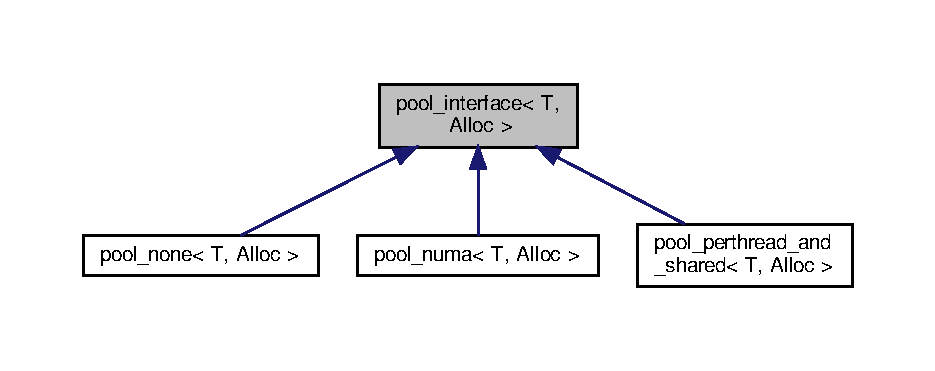
\includegraphics[width=350pt]{classpool__interface__inherit__graph}
\end{center}
\end{figure}


Collaboration diagram for pool\+\_\+interface$<$ T, Alloc $>$\+:
\nopagebreak
\begin{figure}[H]
\begin{center}
\leavevmode
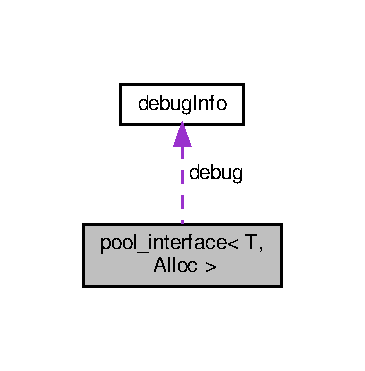
\includegraphics[width=175pt]{classpool__interface__coll__graph}
\end{center}
\end{figure}
\subsection*{Classes}
\begin{DoxyCompactItemize}
\item 
struct \hyperlink{structpool__interface_1_1rebind}{rebind}
\item 
struct \hyperlink{structpool__interface_1_1rebind2}{rebind2}
\end{DoxyCompactItemize}
\subsection*{Public Member Functions}
\begin{DoxyCompactItemize}
\item 
std\+::string \hyperlink{classpool__interface_a9cf0d8a1beeea10001a2386954c35148}{get\+Size\+String} ()
\item 
T $\ast$ \hyperlink{classpool__interface_a813149cd8f557d17871478324073f4e1}{get} (const int \hyperlink{microbench_2main_8cpp_a9ca9869868fe7e7a38a921cc7de4103f}{tid})
\item 
void \hyperlink{classpool__interface_a40c3fd4f6e9fad87c1230b511e630649}{add} (const int \hyperlink{microbench_2main_8cpp_a9ca9869868fe7e7a38a921cc7de4103f}{tid}, T $\ast$ptr)
\item 
void \hyperlink{classpool__interface_afb8890cc6f5228695c06c77ecd70029a}{add\+Move\+Full\+Blocks} (const int \hyperlink{microbench_2main_8cpp_a9ca9869868fe7e7a38a921cc7de4103f}{tid}, \hyperlink{classblockbag}{blockbag}$<$ T $>$ $\ast$bag)
\item 
void \hyperlink{classpool__interface_a58093f6826bc44855b9323e91aa3de7a}{add\+Move\+All} (const int \hyperlink{microbench_2main_8cpp_a9ca9869868fe7e7a38a921cc7de4103f}{tid}, \hyperlink{classblockbag}{blockbag}$<$ T $>$ $\ast$bag)
\item 
int \hyperlink{classpool__interface_aff03189b1d56dbc5debba3df0807bc92}{compute\+Size} (const int \hyperlink{microbench_2main_8cpp_a9ca9869868fe7e7a38a921cc7de4103f}{tid})
\item 
void \hyperlink{classpool__interface_a9671f9620d1bc032065aef4b05c0d51d}{debug\+Print\+Status} (const int \hyperlink{microbench_2main_8cpp_a9ca9869868fe7e7a38a921cc7de4103f}{tid})
\item 
void \hyperlink{classpool__interface_a2415e8d6726ecfc1e13b45e0a81ba573}{init\+Thread} (const int \hyperlink{microbench_2main_8cpp_a9ca9869868fe7e7a38a921cc7de4103f}{tid})
\item 
void \hyperlink{classpool__interface_add48a6c2d94211154702f9543ceff76c}{deinit\+Thread} (const int \hyperlink{microbench_2main_8cpp_a9ca9869868fe7e7a38a921cc7de4103f}{tid})
\item 
\hyperlink{classpool__interface_aacd638d03ecbc3a7e0e3372d88b88629}{pool\+\_\+interface} (const int \hyperlink{testing_8cpp_aa085812188e21ede75351d88b9b2c30d}{num\+Processes}, Alloc $\ast$const \+\_\+alloc, \hyperlink{classdebugInfo}{debug\+Info} $\ast$const \+\_\+debug)
\item 
\hyperlink{classpool__interface_a4d7a8d3165eb068452c71e31dab81a18}{$\sim$pool\+\_\+interface} ()
\end{DoxyCompactItemize}
\subsection*{Public Attributes}
\begin{DoxyCompactItemize}
\item 
\hyperlink{classpool__interface_a1b714295ba794862f8a11cc5ec25cec7}{P\+AD}
\item 
\hyperlink{classdebugInfo}{debug\+Info} $\ast$const \hyperlink{classpool__interface_ab609cb214dbd9228200698e6fd8256fe}{debug}
\item 
const int \hyperlink{classpool__interface_a66acd16c6997604702dff95487152570}{N\+U\+M\+\_\+\+P\+R\+O\+C\+E\+S\+S\+ES}
\item 
\hyperlink{classblockpool}{blockpool}$<$ T $>$ $\ast$$\ast$ \hyperlink{classpool__interface_a6585092dd9b946516287735834174726}{blockpools}
\item 
Alloc $\ast$ \hyperlink{classpool__interface_a920fcaa0f78cd3d45e6d128d18355f67}{alloc}
\end{DoxyCompactItemize}


\subsection{Detailed Description}
\subsubsection*{template$<$typename T = void, class Alloc = allocator\+\_\+interface$<$\+T$>$$>$\newline
class pool\+\_\+interface$<$ T, Alloc $>$}

C++ record manager implementation (P\+O\+DC 2015) by Trevor Brown.

Copyright (C) 2015 Trevor Brown 

\subsection{Constructor \& Destructor Documentation}
\mbox{\Hypertarget{classpool__interface_aacd638d03ecbc3a7e0e3372d88b88629}\label{classpool__interface_aacd638d03ecbc3a7e0e3372d88b88629}} 
\index{pool\+\_\+interface@{pool\+\_\+interface}!pool\+\_\+interface@{pool\+\_\+interface}}
\index{pool\+\_\+interface@{pool\+\_\+interface}!pool\+\_\+interface@{pool\+\_\+interface}}
\subsubsection{\texorpdfstring{pool\+\_\+interface()}{pool\_interface()}}
{\footnotesize\ttfamily template$<$typename T  = void, class Alloc  = allocator\+\_\+interface$<$\+T$>$$>$ \\
\hyperlink{classpool__interface}{pool\+\_\+interface}$<$ T, Alloc $>$\+::\hyperlink{classpool__interface}{pool\+\_\+interface} (\begin{DoxyParamCaption}\item[{const int}]{num\+Processes,  }\item[{Alloc $\ast$const}]{\+\_\+alloc,  }\item[{\hyperlink{classdebugInfo}{debug\+Info} $\ast$const}]{\+\_\+debug }\end{DoxyParamCaption})\hspace{0.3cm}{\ttfamily [inline]}}

\mbox{\Hypertarget{classpool__interface_a4d7a8d3165eb068452c71e31dab81a18}\label{classpool__interface_a4d7a8d3165eb068452c71e31dab81a18}} 
\index{pool\+\_\+interface@{pool\+\_\+interface}!````~pool\+\_\+interface@{$\sim$pool\+\_\+interface}}
\index{````~pool\+\_\+interface@{$\sim$pool\+\_\+interface}!pool\+\_\+interface@{pool\+\_\+interface}}
\subsubsection{\texorpdfstring{$\sim$pool\+\_\+interface()}{~pool\_interface()}}
{\footnotesize\ttfamily template$<$typename T  = void, class Alloc  = allocator\+\_\+interface$<$\+T$>$$>$ \\
\hyperlink{classpool__interface}{pool\+\_\+interface}$<$ T, Alloc $>$\+::$\sim$\hyperlink{classpool__interface}{pool\+\_\+interface} (\begin{DoxyParamCaption}{ }\end{DoxyParamCaption})\hspace{0.3cm}{\ttfamily [inline]}}



\subsection{Member Function Documentation}
\mbox{\Hypertarget{classpool__interface_a40c3fd4f6e9fad87c1230b511e630649}\label{classpool__interface_a40c3fd4f6e9fad87c1230b511e630649}} 
\index{pool\+\_\+interface@{pool\+\_\+interface}!add@{add}}
\index{add@{add}!pool\+\_\+interface@{pool\+\_\+interface}}
\subsubsection{\texorpdfstring{add()}{add()}}
{\footnotesize\ttfamily template$<$typename T  = void, class Alloc  = allocator\+\_\+interface$<$\+T$>$$>$ \\
void \hyperlink{classpool__interface}{pool\+\_\+interface}$<$ T, Alloc $>$\+::add (\begin{DoxyParamCaption}\item[{const int}]{tid,  }\item[{T $\ast$}]{ptr }\end{DoxyParamCaption})\hspace{0.3cm}{\ttfamily [inline]}}

\mbox{\Hypertarget{classpool__interface_a58093f6826bc44855b9323e91aa3de7a}\label{classpool__interface_a58093f6826bc44855b9323e91aa3de7a}} 
\index{pool\+\_\+interface@{pool\+\_\+interface}!add\+Move\+All@{add\+Move\+All}}
\index{add\+Move\+All@{add\+Move\+All}!pool\+\_\+interface@{pool\+\_\+interface}}
\subsubsection{\texorpdfstring{add\+Move\+All()}{addMoveAll()}}
{\footnotesize\ttfamily template$<$typename T  = void, class Alloc  = allocator\+\_\+interface$<$\+T$>$$>$ \\
void \hyperlink{classpool__interface}{pool\+\_\+interface}$<$ T, Alloc $>$\+::add\+Move\+All (\begin{DoxyParamCaption}\item[{const int}]{tid,  }\item[{\hyperlink{classblockbag}{blockbag}$<$ T $>$ $\ast$}]{bag }\end{DoxyParamCaption})\hspace{0.3cm}{\ttfamily [inline]}}

\mbox{\Hypertarget{classpool__interface_afb8890cc6f5228695c06c77ecd70029a}\label{classpool__interface_afb8890cc6f5228695c06c77ecd70029a}} 
\index{pool\+\_\+interface@{pool\+\_\+interface}!add\+Move\+Full\+Blocks@{add\+Move\+Full\+Blocks}}
\index{add\+Move\+Full\+Blocks@{add\+Move\+Full\+Blocks}!pool\+\_\+interface@{pool\+\_\+interface}}
\subsubsection{\texorpdfstring{add\+Move\+Full\+Blocks()}{addMoveFullBlocks()}}
{\footnotesize\ttfamily template$<$typename T  = void, class Alloc  = allocator\+\_\+interface$<$\+T$>$$>$ \\
void \hyperlink{classpool__interface}{pool\+\_\+interface}$<$ T, Alloc $>$\+::add\+Move\+Full\+Blocks (\begin{DoxyParamCaption}\item[{const int}]{tid,  }\item[{\hyperlink{classblockbag}{blockbag}$<$ T $>$ $\ast$}]{bag }\end{DoxyParamCaption})\hspace{0.3cm}{\ttfamily [inline]}}

\mbox{\Hypertarget{classpool__interface_aff03189b1d56dbc5debba3df0807bc92}\label{classpool__interface_aff03189b1d56dbc5debba3df0807bc92}} 
\index{pool\+\_\+interface@{pool\+\_\+interface}!compute\+Size@{compute\+Size}}
\index{compute\+Size@{compute\+Size}!pool\+\_\+interface@{pool\+\_\+interface}}
\subsubsection{\texorpdfstring{compute\+Size()}{computeSize()}}
{\footnotesize\ttfamily template$<$typename T  = void, class Alloc  = allocator\+\_\+interface$<$\+T$>$$>$ \\
int \hyperlink{classpool__interface}{pool\+\_\+interface}$<$ T, Alloc $>$\+::compute\+Size (\begin{DoxyParamCaption}\item[{const int}]{tid }\end{DoxyParamCaption})\hspace{0.3cm}{\ttfamily [inline]}}

\mbox{\Hypertarget{classpool__interface_a9671f9620d1bc032065aef4b05c0d51d}\label{classpool__interface_a9671f9620d1bc032065aef4b05c0d51d}} 
\index{pool\+\_\+interface@{pool\+\_\+interface}!debug\+Print\+Status@{debug\+Print\+Status}}
\index{debug\+Print\+Status@{debug\+Print\+Status}!pool\+\_\+interface@{pool\+\_\+interface}}
\subsubsection{\texorpdfstring{debug\+Print\+Status()}{debugPrintStatus()}}
{\footnotesize\ttfamily template$<$typename T  = void, class Alloc  = allocator\+\_\+interface$<$\+T$>$$>$ \\
void \hyperlink{classpool__interface}{pool\+\_\+interface}$<$ T, Alloc $>$\+::debug\+Print\+Status (\begin{DoxyParamCaption}\item[{const int}]{tid }\end{DoxyParamCaption})}

\mbox{\Hypertarget{classpool__interface_add48a6c2d94211154702f9543ceff76c}\label{classpool__interface_add48a6c2d94211154702f9543ceff76c}} 
\index{pool\+\_\+interface@{pool\+\_\+interface}!deinit\+Thread@{deinit\+Thread}}
\index{deinit\+Thread@{deinit\+Thread}!pool\+\_\+interface@{pool\+\_\+interface}}
\subsubsection{\texorpdfstring{deinit\+Thread()}{deinitThread()}}
{\footnotesize\ttfamily template$<$typename T  = void, class Alloc  = allocator\+\_\+interface$<$\+T$>$$>$ \\
void \hyperlink{classpool__interface}{pool\+\_\+interface}$<$ T, Alloc $>$\+::deinit\+Thread (\begin{DoxyParamCaption}\item[{const int}]{tid }\end{DoxyParamCaption})}

\mbox{\Hypertarget{classpool__interface_a813149cd8f557d17871478324073f4e1}\label{classpool__interface_a813149cd8f557d17871478324073f4e1}} 
\index{pool\+\_\+interface@{pool\+\_\+interface}!get@{get}}
\index{get@{get}!pool\+\_\+interface@{pool\+\_\+interface}}
\subsubsection{\texorpdfstring{get()}{get()}}
{\footnotesize\ttfamily template$<$typename T  = void, class Alloc  = allocator\+\_\+interface$<$\+T$>$$>$ \\
T$\ast$ \hyperlink{classpool__interface}{pool\+\_\+interface}$<$ T, Alloc $>$\+::get (\begin{DoxyParamCaption}\item[{const int}]{tid }\end{DoxyParamCaption})\hspace{0.3cm}{\ttfamily [inline]}}

if the pool contains any object, then remove one from the pool and return a pointer to it. otherwise, return N\+U\+LL. \mbox{\Hypertarget{classpool__interface_a9cf0d8a1beeea10001a2386954c35148}\label{classpool__interface_a9cf0d8a1beeea10001a2386954c35148}} 
\index{pool\+\_\+interface@{pool\+\_\+interface}!get\+Size\+String@{get\+Size\+String}}
\index{get\+Size\+String@{get\+Size\+String}!pool\+\_\+interface@{pool\+\_\+interface}}
\subsubsection{\texorpdfstring{get\+Size\+String()}{getSizeString()}}
{\footnotesize\ttfamily template$<$typename T  = void, class Alloc  = allocator\+\_\+interface$<$\+T$>$$>$ \\
std\+::string \hyperlink{classpool__interface}{pool\+\_\+interface}$<$ T, Alloc $>$\+::get\+Size\+String (\begin{DoxyParamCaption}{ }\end{DoxyParamCaption})\hspace{0.3cm}{\ttfamily [inline]}}

\mbox{\Hypertarget{classpool__interface_a2415e8d6726ecfc1e13b45e0a81ba573}\label{classpool__interface_a2415e8d6726ecfc1e13b45e0a81ba573}} 
\index{pool\+\_\+interface@{pool\+\_\+interface}!init\+Thread@{init\+Thread}}
\index{init\+Thread@{init\+Thread}!pool\+\_\+interface@{pool\+\_\+interface}}
\subsubsection{\texorpdfstring{init\+Thread()}{initThread()}}
{\footnotesize\ttfamily template$<$typename T  = void, class Alloc  = allocator\+\_\+interface$<$\+T$>$$>$ \\
void \hyperlink{classpool__interface}{pool\+\_\+interface}$<$ T, Alloc $>$\+::init\+Thread (\begin{DoxyParamCaption}\item[{const int}]{tid }\end{DoxyParamCaption})}



\subsection{Member Data Documentation}
\mbox{\Hypertarget{classpool__interface_a920fcaa0f78cd3d45e6d128d18355f67}\label{classpool__interface_a920fcaa0f78cd3d45e6d128d18355f67}} 
\index{pool\+\_\+interface@{pool\+\_\+interface}!alloc@{alloc}}
\index{alloc@{alloc}!pool\+\_\+interface@{pool\+\_\+interface}}
\subsubsection{\texorpdfstring{alloc}{alloc}}
{\footnotesize\ttfamily template$<$typename T  = void, class Alloc  = allocator\+\_\+interface$<$\+T$>$$>$ \\
Alloc$\ast$ \hyperlink{classpool__interface}{pool\+\_\+interface}$<$ T, Alloc $>$\+::alloc}

\mbox{\Hypertarget{classpool__interface_a6585092dd9b946516287735834174726}\label{classpool__interface_a6585092dd9b946516287735834174726}} 
\index{pool\+\_\+interface@{pool\+\_\+interface}!blockpools@{blockpools}}
\index{blockpools@{blockpools}!pool\+\_\+interface@{pool\+\_\+interface}}
\subsubsection{\texorpdfstring{blockpools}{blockpools}}
{\footnotesize\ttfamily template$<$typename T  = void, class Alloc  = allocator\+\_\+interface$<$\+T$>$$>$ \\
\hyperlink{classblockpool}{blockpool}$<$T$>$$\ast$$\ast$ \hyperlink{classpool__interface}{pool\+\_\+interface}$<$ T, Alloc $>$\+::blockpools}

\mbox{\Hypertarget{classpool__interface_ab609cb214dbd9228200698e6fd8256fe}\label{classpool__interface_ab609cb214dbd9228200698e6fd8256fe}} 
\index{pool\+\_\+interface@{pool\+\_\+interface}!debug@{debug}}
\index{debug@{debug}!pool\+\_\+interface@{pool\+\_\+interface}}
\subsubsection{\texorpdfstring{debug}{debug}}
{\footnotesize\ttfamily template$<$typename T  = void, class Alloc  = allocator\+\_\+interface$<$\+T$>$$>$ \\
\hyperlink{classdebugInfo}{debug\+Info}$\ast$ const \hyperlink{classpool__interface}{pool\+\_\+interface}$<$ T, Alloc $>$\+::debug}

\mbox{\Hypertarget{classpool__interface_a66acd16c6997604702dff95487152570}\label{classpool__interface_a66acd16c6997604702dff95487152570}} 
\index{pool\+\_\+interface@{pool\+\_\+interface}!N\+U\+M\+\_\+\+P\+R\+O\+C\+E\+S\+S\+ES@{N\+U\+M\+\_\+\+P\+R\+O\+C\+E\+S\+S\+ES}}
\index{N\+U\+M\+\_\+\+P\+R\+O\+C\+E\+S\+S\+ES@{N\+U\+M\+\_\+\+P\+R\+O\+C\+E\+S\+S\+ES}!pool\+\_\+interface@{pool\+\_\+interface}}
\subsubsection{\texorpdfstring{N\+U\+M\+\_\+\+P\+R\+O\+C\+E\+S\+S\+ES}{NUM\_PROCESSES}}
{\footnotesize\ttfamily template$<$typename T  = void, class Alloc  = allocator\+\_\+interface$<$\+T$>$$>$ \\
const int \hyperlink{classpool__interface}{pool\+\_\+interface}$<$ T, Alloc $>$\+::N\+U\+M\+\_\+\+P\+R\+O\+C\+E\+S\+S\+ES}

\mbox{\Hypertarget{classpool__interface_a1b714295ba794862f8a11cc5ec25cec7}\label{classpool__interface_a1b714295ba794862f8a11cc5ec25cec7}} 
\index{pool\+\_\+interface@{pool\+\_\+interface}!P\+AD@{P\+AD}}
\index{P\+AD@{P\+AD}!pool\+\_\+interface@{pool\+\_\+interface}}
\subsubsection{\texorpdfstring{P\+AD}{PAD}}
{\footnotesize\ttfamily template$<$typename T  = void, class Alloc  = allocator\+\_\+interface$<$\+T$>$$>$ \\
\hyperlink{classpool__interface}{pool\+\_\+interface}$<$ T, Alloc $>$\+::P\+AD}



The documentation for this class was generated from the following file\+:\begin{DoxyCompactItemize}
\item 
common/recordmgr/\hyperlink{pool__interface_8h}{pool\+\_\+interface.\+h}\end{DoxyCompactItemize}

\hypertarget{classpool__none}{}\section{pool\+\_\+none$<$ T, Alloc $>$ Class Template Reference}
\label{classpool__none}\index{pool\+\_\+none$<$ T, Alloc $>$@{pool\+\_\+none$<$ T, Alloc $>$}}


{\ttfamily \#include $<$pool\+\_\+none.\+h$>$}



Inheritance diagram for pool\+\_\+none$<$ T, Alloc $>$\+:
\nopagebreak
\begin{figure}[H]
\begin{center}
\leavevmode
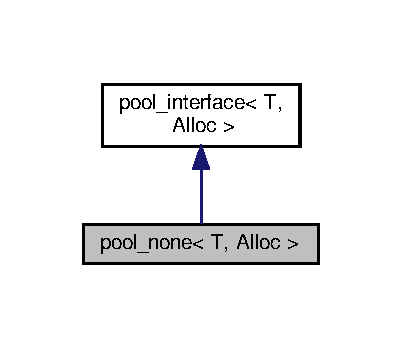
\includegraphics[width=193pt]{classpool__none__inherit__graph}
\end{center}
\end{figure}


Collaboration diagram for pool\+\_\+none$<$ T, Alloc $>$\+:
\nopagebreak
\begin{figure}[H]
\begin{center}
\leavevmode
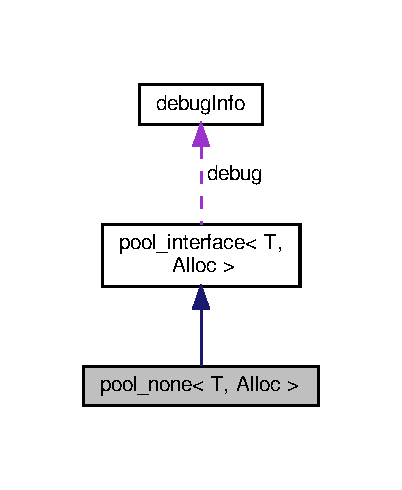
\includegraphics[width=193pt]{classpool__none__coll__graph}
\end{center}
\end{figure}
\subsection*{Classes}
\begin{DoxyCompactItemize}
\item 
struct \hyperlink{structpool__none_1_1rebind}{rebind}
\item 
struct \hyperlink{structpool__none_1_1rebind2}{rebind2}
\item 
struct \hyperlink{structpool__none_1_1rebindAlloc}{rebind\+Alloc}
\end{DoxyCompactItemize}
\subsection*{Public Member Functions}
\begin{DoxyCompactItemize}
\item 
std\+::string \hyperlink{classpool__none_abe3bc246d2d7a2c7e118f3da40a14501}{get\+Size\+String} ()
\item 
T $\ast$ \hyperlink{classpool__none_a5cfa4676cbf37a0224224256ab365840}{get} (const int \hyperlink{microbench_2main_8cpp_a9ca9869868fe7e7a38a921cc7de4103f}{tid})
\item 
void \hyperlink{classpool__none_a07c69ce30c2cb27f3ca8e36b3b4c30bb}{add} (const int \hyperlink{microbench_2main_8cpp_a9ca9869868fe7e7a38a921cc7de4103f}{tid}, T $\ast$ptr)
\item 
void \hyperlink{classpool__none_a1970af5c93f95a63b0aaf6a85cf68f11}{add\+Move\+Full\+Blocks} (const int \hyperlink{microbench_2main_8cpp_a9ca9869868fe7e7a38a921cc7de4103f}{tid}, \hyperlink{classblockbag}{blockbag}$<$ T $>$ $\ast$bag, \hyperlink{classblock}{block}$<$ T $>$ $\ast$const predecessor)
\item 
void \hyperlink{classpool__none_a0769e6af03c60e9148ccf91a2b034bbe}{add\+Move\+Full\+Blocks} (const int \hyperlink{microbench_2main_8cpp_a9ca9869868fe7e7a38a921cc7de4103f}{tid}, \hyperlink{classblockbag}{blockbag}$<$ T $>$ $\ast$bag)
\item 
void \hyperlink{classpool__none_a4d773f878fb8e0c11c70b49c73ef24b6}{add\+Move\+All} (const int \hyperlink{microbench_2main_8cpp_a9ca9869868fe7e7a38a921cc7de4103f}{tid}, \hyperlink{classblockbag}{blockbag}$<$ T $>$ $\ast$bag)
\item 
int \hyperlink{classpool__none_a7c1e31b11de7a07d4bdb950ba5aa5508}{compute\+Size} (const int \hyperlink{microbench_2main_8cpp_a9ca9869868fe7e7a38a921cc7de4103f}{tid})
\item 
void \hyperlink{classpool__none_ad2f9a5fa2c6bb00e00b769681476a084}{debug\+Print\+Status} (const int \hyperlink{microbench_2main_8cpp_a9ca9869868fe7e7a38a921cc7de4103f}{tid})
\item 
void \hyperlink{classpool__none_a60aa791c93ff63d74dc1e247aa56683d}{init\+Thread} (const int \hyperlink{microbench_2main_8cpp_a9ca9869868fe7e7a38a921cc7de4103f}{tid})
\item 
void \hyperlink{classpool__none_a28f9e8b16ba70d4ed1a9c295bdbc785d}{deinit\+Thread} (const int \hyperlink{microbench_2main_8cpp_a9ca9869868fe7e7a38a921cc7de4103f}{tid})
\item 
\hyperlink{classpool__none_ab79b85eedba6f8cbf97f226cafa87e7a}{pool\+\_\+none} (const int \hyperlink{testing_8cpp_aa085812188e21ede75351d88b9b2c30d}{num\+Processes}, Alloc $\ast$const \+\_\+alloc, \hyperlink{classdebugInfo}{debug\+Info} $\ast$const \+\_\+debug)
\item 
\hyperlink{classpool__none_a5469691d9539271b4fa8d5980e1fcb9e}{$\sim$pool\+\_\+none} ()
\end{DoxyCompactItemize}
\subsection*{Public Attributes}
\begin{DoxyCompactItemize}
\item 
\hyperlink{classpool__none_a071df42d9f83a773764e034b0cbdaf9f}{P\+AD}
\end{DoxyCompactItemize}


\subsection{Detailed Description}
\subsubsection*{template$<$typename T = void, class Alloc = allocator\+\_\+interface$<$\+T$>$$>$\newline
class pool\+\_\+none$<$ T, Alloc $>$}

C++ record manager implementation (P\+O\+DC 2015) by Trevor Brown.

Copyright (C) 2015 Trevor Brown 

\subsection{Constructor \& Destructor Documentation}
\mbox{\Hypertarget{classpool__none_ab79b85eedba6f8cbf97f226cafa87e7a}\label{classpool__none_ab79b85eedba6f8cbf97f226cafa87e7a}} 
\index{pool\+\_\+none@{pool\+\_\+none}!pool\+\_\+none@{pool\+\_\+none}}
\index{pool\+\_\+none@{pool\+\_\+none}!pool\+\_\+none@{pool\+\_\+none}}
\subsubsection{\texorpdfstring{pool\+\_\+none()}{pool\_none()}}
{\footnotesize\ttfamily template$<$typename T  = void, class Alloc  = allocator\+\_\+interface$<$\+T$>$$>$ \\
\hyperlink{classpool__none}{pool\+\_\+none}$<$ T, Alloc $>$\+::\hyperlink{classpool__none}{pool\+\_\+none} (\begin{DoxyParamCaption}\item[{const int}]{num\+Processes,  }\item[{Alloc $\ast$const}]{\+\_\+alloc,  }\item[{\hyperlink{classdebugInfo}{debug\+Info} $\ast$const}]{\+\_\+debug }\end{DoxyParamCaption})\hspace{0.3cm}{\ttfamily [inline]}}

\mbox{\Hypertarget{classpool__none_a5469691d9539271b4fa8d5980e1fcb9e}\label{classpool__none_a5469691d9539271b4fa8d5980e1fcb9e}} 
\index{pool\+\_\+none@{pool\+\_\+none}!````~pool\+\_\+none@{$\sim$pool\+\_\+none}}
\index{````~pool\+\_\+none@{$\sim$pool\+\_\+none}!pool\+\_\+none@{pool\+\_\+none}}
\subsubsection{\texorpdfstring{$\sim$pool\+\_\+none()}{~pool\_none()}}
{\footnotesize\ttfamily template$<$typename T  = void, class Alloc  = allocator\+\_\+interface$<$\+T$>$$>$ \\
\hyperlink{classpool__none}{pool\+\_\+none}$<$ T, Alloc $>$\+::$\sim$\hyperlink{classpool__none}{pool\+\_\+none} (\begin{DoxyParamCaption}{ }\end{DoxyParamCaption})\hspace{0.3cm}{\ttfamily [inline]}}



\subsection{Member Function Documentation}
\mbox{\Hypertarget{classpool__none_a07c69ce30c2cb27f3ca8e36b3b4c30bb}\label{classpool__none_a07c69ce30c2cb27f3ca8e36b3b4c30bb}} 
\index{pool\+\_\+none@{pool\+\_\+none}!add@{add}}
\index{add@{add}!pool\+\_\+none@{pool\+\_\+none}}
\subsubsection{\texorpdfstring{add()}{add()}}
{\footnotesize\ttfamily template$<$typename T  = void, class Alloc  = allocator\+\_\+interface$<$\+T$>$$>$ \\
void \hyperlink{classpool__none}{pool\+\_\+none}$<$ T, Alloc $>$\+::add (\begin{DoxyParamCaption}\item[{const int}]{tid,  }\item[{T $\ast$}]{ptr }\end{DoxyParamCaption})\hspace{0.3cm}{\ttfamily [inline]}}

\mbox{\Hypertarget{classpool__none_a4d773f878fb8e0c11c70b49c73ef24b6}\label{classpool__none_a4d773f878fb8e0c11c70b49c73ef24b6}} 
\index{pool\+\_\+none@{pool\+\_\+none}!add\+Move\+All@{add\+Move\+All}}
\index{add\+Move\+All@{add\+Move\+All}!pool\+\_\+none@{pool\+\_\+none}}
\subsubsection{\texorpdfstring{add\+Move\+All()}{addMoveAll()}}
{\footnotesize\ttfamily template$<$typename T  = void, class Alloc  = allocator\+\_\+interface$<$\+T$>$$>$ \\
void \hyperlink{classpool__none}{pool\+\_\+none}$<$ T, Alloc $>$\+::add\+Move\+All (\begin{DoxyParamCaption}\item[{const int}]{tid,  }\item[{\hyperlink{classblockbag}{blockbag}$<$ T $>$ $\ast$}]{bag }\end{DoxyParamCaption})\hspace{0.3cm}{\ttfamily [inline]}}

\mbox{\Hypertarget{classpool__none_a1970af5c93f95a63b0aaf6a85cf68f11}\label{classpool__none_a1970af5c93f95a63b0aaf6a85cf68f11}} 
\index{pool\+\_\+none@{pool\+\_\+none}!add\+Move\+Full\+Blocks@{add\+Move\+Full\+Blocks}}
\index{add\+Move\+Full\+Blocks@{add\+Move\+Full\+Blocks}!pool\+\_\+none@{pool\+\_\+none}}
\subsubsection{\texorpdfstring{add\+Move\+Full\+Blocks()}{addMoveFullBlocks()}\hspace{0.1cm}{\footnotesize\ttfamily [1/2]}}
{\footnotesize\ttfamily template$<$typename T  = void, class Alloc  = allocator\+\_\+interface$<$\+T$>$$>$ \\
void \hyperlink{classpool__none}{pool\+\_\+none}$<$ T, Alloc $>$\+::add\+Move\+Full\+Blocks (\begin{DoxyParamCaption}\item[{const int}]{tid,  }\item[{\hyperlink{classblockbag}{blockbag}$<$ T $>$ $\ast$}]{bag,  }\item[{\hyperlink{classblock}{block}$<$ T $>$ $\ast$const}]{predecessor }\end{DoxyParamCaption})\hspace{0.3cm}{\ttfamily [inline]}}

\mbox{\Hypertarget{classpool__none_a0769e6af03c60e9148ccf91a2b034bbe}\label{classpool__none_a0769e6af03c60e9148ccf91a2b034bbe}} 
\index{pool\+\_\+none@{pool\+\_\+none}!add\+Move\+Full\+Blocks@{add\+Move\+Full\+Blocks}}
\index{add\+Move\+Full\+Blocks@{add\+Move\+Full\+Blocks}!pool\+\_\+none@{pool\+\_\+none}}
\subsubsection{\texorpdfstring{add\+Move\+Full\+Blocks()}{addMoveFullBlocks()}\hspace{0.1cm}{\footnotesize\ttfamily [2/2]}}
{\footnotesize\ttfamily template$<$typename T  = void, class Alloc  = allocator\+\_\+interface$<$\+T$>$$>$ \\
void \hyperlink{classpool__none}{pool\+\_\+none}$<$ T, Alloc $>$\+::add\+Move\+Full\+Blocks (\begin{DoxyParamCaption}\item[{const int}]{tid,  }\item[{\hyperlink{classblockbag}{blockbag}$<$ T $>$ $\ast$}]{bag }\end{DoxyParamCaption})\hspace{0.3cm}{\ttfamily [inline]}}

\mbox{\Hypertarget{classpool__none_a7c1e31b11de7a07d4bdb950ba5aa5508}\label{classpool__none_a7c1e31b11de7a07d4bdb950ba5aa5508}} 
\index{pool\+\_\+none@{pool\+\_\+none}!compute\+Size@{compute\+Size}}
\index{compute\+Size@{compute\+Size}!pool\+\_\+none@{pool\+\_\+none}}
\subsubsection{\texorpdfstring{compute\+Size()}{computeSize()}}
{\footnotesize\ttfamily template$<$typename T  = void, class Alloc  = allocator\+\_\+interface$<$\+T$>$$>$ \\
int \hyperlink{classpool__none}{pool\+\_\+none}$<$ T, Alloc $>$\+::compute\+Size (\begin{DoxyParamCaption}\item[{const int}]{tid }\end{DoxyParamCaption})\hspace{0.3cm}{\ttfamily [inline]}}

\mbox{\Hypertarget{classpool__none_ad2f9a5fa2c6bb00e00b769681476a084}\label{classpool__none_ad2f9a5fa2c6bb00e00b769681476a084}} 
\index{pool\+\_\+none@{pool\+\_\+none}!debug\+Print\+Status@{debug\+Print\+Status}}
\index{debug\+Print\+Status@{debug\+Print\+Status}!pool\+\_\+none@{pool\+\_\+none}}
\subsubsection{\texorpdfstring{debug\+Print\+Status()}{debugPrintStatus()}}
{\footnotesize\ttfamily template$<$typename T  = void, class Alloc  = allocator\+\_\+interface$<$\+T$>$$>$ \\
void \hyperlink{classpool__none}{pool\+\_\+none}$<$ T, Alloc $>$\+::debug\+Print\+Status (\begin{DoxyParamCaption}\item[{const int}]{tid }\end{DoxyParamCaption})\hspace{0.3cm}{\ttfamily [inline]}}

\mbox{\Hypertarget{classpool__none_a28f9e8b16ba70d4ed1a9c295bdbc785d}\label{classpool__none_a28f9e8b16ba70d4ed1a9c295bdbc785d}} 
\index{pool\+\_\+none@{pool\+\_\+none}!deinit\+Thread@{deinit\+Thread}}
\index{deinit\+Thread@{deinit\+Thread}!pool\+\_\+none@{pool\+\_\+none}}
\subsubsection{\texorpdfstring{deinit\+Thread()}{deinitThread()}}
{\footnotesize\ttfamily template$<$typename T  = void, class Alloc  = allocator\+\_\+interface$<$\+T$>$$>$ \\
void \hyperlink{classpool__none}{pool\+\_\+none}$<$ T, Alloc $>$\+::deinit\+Thread (\begin{DoxyParamCaption}\item[{const int}]{tid }\end{DoxyParamCaption})\hspace{0.3cm}{\ttfamily [inline]}}

\mbox{\Hypertarget{classpool__none_a5cfa4676cbf37a0224224256ab365840}\label{classpool__none_a5cfa4676cbf37a0224224256ab365840}} 
\index{pool\+\_\+none@{pool\+\_\+none}!get@{get}}
\index{get@{get}!pool\+\_\+none@{pool\+\_\+none}}
\subsubsection{\texorpdfstring{get()}{get()}}
{\footnotesize\ttfamily template$<$typename T  = void, class Alloc  = allocator\+\_\+interface$<$\+T$>$$>$ \\
T$\ast$ \hyperlink{classpool__none}{pool\+\_\+none}$<$ T, Alloc $>$\+::get (\begin{DoxyParamCaption}\item[{const int}]{tid }\end{DoxyParamCaption})\hspace{0.3cm}{\ttfamily [inline]}}

if the freebag contains any object, then remove one from the freebag and return a pointer to it. if not, then retrieve a new object from Alloc \mbox{\Hypertarget{classpool__none_abe3bc246d2d7a2c7e118f3da40a14501}\label{classpool__none_abe3bc246d2d7a2c7e118f3da40a14501}} 
\index{pool\+\_\+none@{pool\+\_\+none}!get\+Size\+String@{get\+Size\+String}}
\index{get\+Size\+String@{get\+Size\+String}!pool\+\_\+none@{pool\+\_\+none}}
\subsubsection{\texorpdfstring{get\+Size\+String()}{getSizeString()}}
{\footnotesize\ttfamily template$<$typename T  = void, class Alloc  = allocator\+\_\+interface$<$\+T$>$$>$ \\
std\+::string \hyperlink{classpool__none}{pool\+\_\+none}$<$ T, Alloc $>$\+::get\+Size\+String (\begin{DoxyParamCaption}{ }\end{DoxyParamCaption})\hspace{0.3cm}{\ttfamily [inline]}}

\mbox{\Hypertarget{classpool__none_a60aa791c93ff63d74dc1e247aa56683d}\label{classpool__none_a60aa791c93ff63d74dc1e247aa56683d}} 
\index{pool\+\_\+none@{pool\+\_\+none}!init\+Thread@{init\+Thread}}
\index{init\+Thread@{init\+Thread}!pool\+\_\+none@{pool\+\_\+none}}
\subsubsection{\texorpdfstring{init\+Thread()}{initThread()}}
{\footnotesize\ttfamily template$<$typename T  = void, class Alloc  = allocator\+\_\+interface$<$\+T$>$$>$ \\
void \hyperlink{classpool__none}{pool\+\_\+none}$<$ T, Alloc $>$\+::init\+Thread (\begin{DoxyParamCaption}\item[{const int}]{tid }\end{DoxyParamCaption})\hspace{0.3cm}{\ttfamily [inline]}}



\subsection{Member Data Documentation}
\mbox{\Hypertarget{classpool__none_a071df42d9f83a773764e034b0cbdaf9f}\label{classpool__none_a071df42d9f83a773764e034b0cbdaf9f}} 
\index{pool\+\_\+none@{pool\+\_\+none}!P\+AD@{P\+AD}}
\index{P\+AD@{P\+AD}!pool\+\_\+none@{pool\+\_\+none}}
\subsubsection{\texorpdfstring{P\+AD}{PAD}}
{\footnotesize\ttfamily template$<$typename T  = void, class Alloc  = allocator\+\_\+interface$<$\+T$>$$>$ \\
\hyperlink{classpool__none}{pool\+\_\+none}$<$ T, Alloc $>$\+::P\+AD}



The documentation for this class was generated from the following file\+:\begin{DoxyCompactItemize}
\item 
common/recordmgr/\hyperlink{pool__none_8h}{pool\+\_\+none.\+h}\end{DoxyCompactItemize}

\hypertarget{classpool__numa}{}\section{pool\+\_\+numa$<$ T, Alloc $>$ Class Template Reference}
\label{classpool__numa}\index{pool\+\_\+numa$<$ T, Alloc $>$@{pool\+\_\+numa$<$ T, Alloc $>$}}


{\ttfamily \#include $<$pool\+\_\+numa.\+h$>$}



Inheritance diagram for pool\+\_\+numa$<$ T, Alloc $>$\+:
\nopagebreak
\begin{figure}[H]
\begin{center}
\leavevmode
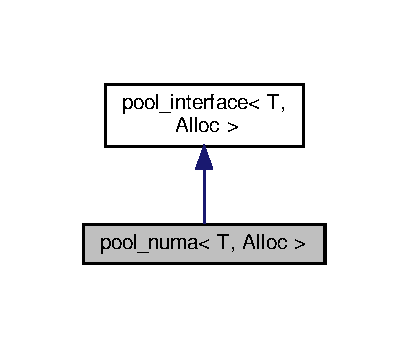
\includegraphics[width=196pt]{classpool__numa__inherit__graph}
\end{center}
\end{figure}


Collaboration diagram for pool\+\_\+numa$<$ T, Alloc $>$\+:
\nopagebreak
\begin{figure}[H]
\begin{center}
\leavevmode
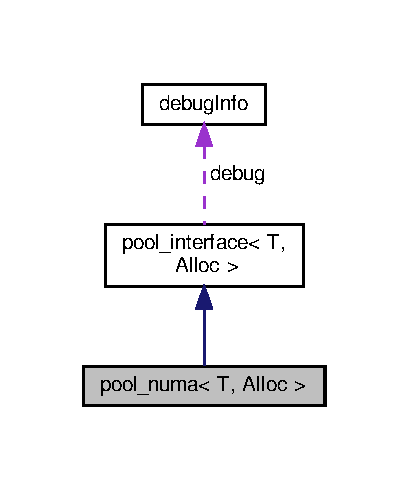
\includegraphics[width=196pt]{classpool__numa__coll__graph}
\end{center}
\end{figure}
\subsection*{Classes}
\begin{DoxyCompactItemize}
\item 
struct \hyperlink{structpool__numa_1_1rebind}{rebind}
\item 
struct \hyperlink{structpool__numa_1_1rebind2}{rebind2}
\item 
struct \hyperlink{structpool__numa_1_1rebindAlloc}{rebind\+Alloc}
\end{DoxyCompactItemize}
\subsection*{Public Member Functions}
\begin{DoxyCompactItemize}
\item 
std\+::string \hyperlink{classpool__numa_ab2ef3aa401ebf9cf6577e1a583fcc157}{get\+Size\+String} ()
\item 
T $\ast$ \hyperlink{classpool__numa_ada7ec291f407081e3c597635fc20ee69}{get} (const int \hyperlink{microbench_2main_8cpp_a9ca9869868fe7e7a38a921cc7de4103f}{tid})
\item 
void \hyperlink{classpool__numa_a0ffdd17b3201916fe7a7eabef807c1e0}{add} (const int \hyperlink{microbench_2main_8cpp_a9ca9869868fe7e7a38a921cc7de4103f}{tid}, T $\ast$ptr)
\item 
void \hyperlink{classpool__numa_a3d31aedd219ebb03bedb25cd375781e8}{add\+Move\+Full\+Blocks} (const int \hyperlink{microbench_2main_8cpp_a9ca9869868fe7e7a38a921cc7de4103f}{tid}, \hyperlink{classblockbag}{blockbag}$<$ T $>$ $\ast$bag, \hyperlink{classblock}{block}$<$ T $>$ $\ast$const predecessor)
\item 
void \hyperlink{classpool__numa_aa6eb3d3d60e8da2ea2ef0adc499e5921}{add\+Move\+Full\+Blocks} (const int \hyperlink{microbench_2main_8cpp_a9ca9869868fe7e7a38a921cc7de4103f}{tid}, \hyperlink{classblockbag}{blockbag}$<$ T $>$ $\ast$bag)
\item 
void \hyperlink{classpool__numa_afa864cb84a8d1e5b5bae1745d0ef36bc}{add\+Move\+All} (const int \hyperlink{microbench_2main_8cpp_a9ca9869868fe7e7a38a921cc7de4103f}{tid}, \hyperlink{classblockbag}{blockbag}$<$ T $>$ $\ast$bag)
\item 
int \hyperlink{classpool__numa_a192004323f02fb5713a08bf24ebdc11f}{compute\+Size} (const int \hyperlink{microbench_2main_8cpp_a9ca9869868fe7e7a38a921cc7de4103f}{tid})
\item 
void \hyperlink{classpool__numa_a9acd9ed86c56c4a2edf2b260cfaeb396}{debug\+Print\+Status} (const int \hyperlink{microbench_2main_8cpp_a9ca9869868fe7e7a38a921cc7de4103f}{tid})
\item 
void \hyperlink{classpool__numa_a1066d0f94458e2080802e87627699841}{init\+Thread} (const int \hyperlink{microbench_2main_8cpp_a9ca9869868fe7e7a38a921cc7de4103f}{tid})
\item 
void \hyperlink{classpool__numa_a10496f39e8c23755147d90c3b57618fa}{deinit\+Thread} (const int \hyperlink{microbench_2main_8cpp_a9ca9869868fe7e7a38a921cc7de4103f}{tid})
\item 
\hyperlink{classpool__numa_aaa2884448972f582e0f9428027a35d97}{pool\+\_\+numa} (const int \hyperlink{testing_8cpp_aa085812188e21ede75351d88b9b2c30d}{num\+Processes}, Alloc $\ast$const \+\_\+alloc, \hyperlink{classdebugInfo}{debug\+Info} $\ast$const \+\_\+debug)
\item 
\hyperlink{classpool__numa_a8e29fd88094bb876fcb02a59f6dd0f0a}{$\sim$pool\+\_\+numa} ()
\end{DoxyCompactItemize}
\subsection*{Additional Inherited Members}


\subsection{Detailed Description}
\subsubsection*{template$<$typename T = void, class Alloc = allocator\+\_\+interface$<$\+T$>$$>$\newline
class pool\+\_\+numa$<$ T, Alloc $>$}

N\+U\+MA aware bounded object pool

Copyright (C) 2019 Trevor Brown 

\subsection{Constructor \& Destructor Documentation}
\mbox{\Hypertarget{classpool__numa_aaa2884448972f582e0f9428027a35d97}\label{classpool__numa_aaa2884448972f582e0f9428027a35d97}} 
\index{pool\+\_\+numa@{pool\+\_\+numa}!pool\+\_\+numa@{pool\+\_\+numa}}
\index{pool\+\_\+numa@{pool\+\_\+numa}!pool\+\_\+numa@{pool\+\_\+numa}}
\subsubsection{\texorpdfstring{pool\+\_\+numa()}{pool\_numa()}}
{\footnotesize\ttfamily template$<$typename T  = void, class Alloc  = allocator\+\_\+interface$<$\+T$>$$>$ \\
\hyperlink{classpool__numa}{pool\+\_\+numa}$<$ T, Alloc $>$\+::\hyperlink{classpool__numa}{pool\+\_\+numa} (\begin{DoxyParamCaption}\item[{const int}]{num\+Processes,  }\item[{Alloc $\ast$const}]{\+\_\+alloc,  }\item[{\hyperlink{classdebugInfo}{debug\+Info} $\ast$const}]{\+\_\+debug }\end{DoxyParamCaption})\hspace{0.3cm}{\ttfamily [inline]}}

\mbox{\Hypertarget{classpool__numa_a8e29fd88094bb876fcb02a59f6dd0f0a}\label{classpool__numa_a8e29fd88094bb876fcb02a59f6dd0f0a}} 
\index{pool\+\_\+numa@{pool\+\_\+numa}!````~pool\+\_\+numa@{$\sim$pool\+\_\+numa}}
\index{````~pool\+\_\+numa@{$\sim$pool\+\_\+numa}!pool\+\_\+numa@{pool\+\_\+numa}}
\subsubsection{\texorpdfstring{$\sim$pool\+\_\+numa()}{~pool\_numa()}}
{\footnotesize\ttfamily template$<$typename T  = void, class Alloc  = allocator\+\_\+interface$<$\+T$>$$>$ \\
\hyperlink{classpool__numa}{pool\+\_\+numa}$<$ T, Alloc $>$\+::$\sim$\hyperlink{classpool__numa}{pool\+\_\+numa} (\begin{DoxyParamCaption}{ }\end{DoxyParamCaption})\hspace{0.3cm}{\ttfamily [inline]}}



\subsection{Member Function Documentation}
\mbox{\Hypertarget{classpool__numa_a0ffdd17b3201916fe7a7eabef807c1e0}\label{classpool__numa_a0ffdd17b3201916fe7a7eabef807c1e0}} 
\index{pool\+\_\+numa@{pool\+\_\+numa}!add@{add}}
\index{add@{add}!pool\+\_\+numa@{pool\+\_\+numa}}
\subsubsection{\texorpdfstring{add()}{add()}}
{\footnotesize\ttfamily template$<$typename T  = void, class Alloc  = allocator\+\_\+interface$<$\+T$>$$>$ \\
void \hyperlink{classpool__numa}{pool\+\_\+numa}$<$ T, Alloc $>$\+::add (\begin{DoxyParamCaption}\item[{const int}]{tid,  }\item[{T $\ast$}]{ptr }\end{DoxyParamCaption})\hspace{0.3cm}{\ttfamily [inline]}}

\mbox{\Hypertarget{classpool__numa_afa864cb84a8d1e5b5bae1745d0ef36bc}\label{classpool__numa_afa864cb84a8d1e5b5bae1745d0ef36bc}} 
\index{pool\+\_\+numa@{pool\+\_\+numa}!add\+Move\+All@{add\+Move\+All}}
\index{add\+Move\+All@{add\+Move\+All}!pool\+\_\+numa@{pool\+\_\+numa}}
\subsubsection{\texorpdfstring{add\+Move\+All()}{addMoveAll()}}
{\footnotesize\ttfamily template$<$typename T  = void, class Alloc  = allocator\+\_\+interface$<$\+T$>$$>$ \\
void \hyperlink{classpool__numa}{pool\+\_\+numa}$<$ T, Alloc $>$\+::add\+Move\+All (\begin{DoxyParamCaption}\item[{const int}]{tid,  }\item[{\hyperlink{classblockbag}{blockbag}$<$ T $>$ $\ast$}]{bag }\end{DoxyParamCaption})\hspace{0.3cm}{\ttfamily [inline]}}

\mbox{\Hypertarget{classpool__numa_a3d31aedd219ebb03bedb25cd375781e8}\label{classpool__numa_a3d31aedd219ebb03bedb25cd375781e8}} 
\index{pool\+\_\+numa@{pool\+\_\+numa}!add\+Move\+Full\+Blocks@{add\+Move\+Full\+Blocks}}
\index{add\+Move\+Full\+Blocks@{add\+Move\+Full\+Blocks}!pool\+\_\+numa@{pool\+\_\+numa}}
\subsubsection{\texorpdfstring{add\+Move\+Full\+Blocks()}{addMoveFullBlocks()}\hspace{0.1cm}{\footnotesize\ttfamily [1/2]}}
{\footnotesize\ttfamily template$<$typename T  = void, class Alloc  = allocator\+\_\+interface$<$\+T$>$$>$ \\
void \hyperlink{classpool__numa}{pool\+\_\+numa}$<$ T, Alloc $>$\+::add\+Move\+Full\+Blocks (\begin{DoxyParamCaption}\item[{const int}]{tid,  }\item[{\hyperlink{classblockbag}{blockbag}$<$ T $>$ $\ast$}]{bag,  }\item[{\hyperlink{classblock}{block}$<$ T $>$ $\ast$const}]{predecessor }\end{DoxyParamCaption})\hspace{0.3cm}{\ttfamily [inline]}}

\mbox{\Hypertarget{classpool__numa_aa6eb3d3d60e8da2ea2ef0adc499e5921}\label{classpool__numa_aa6eb3d3d60e8da2ea2ef0adc499e5921}} 
\index{pool\+\_\+numa@{pool\+\_\+numa}!add\+Move\+Full\+Blocks@{add\+Move\+Full\+Blocks}}
\index{add\+Move\+Full\+Blocks@{add\+Move\+Full\+Blocks}!pool\+\_\+numa@{pool\+\_\+numa}}
\subsubsection{\texorpdfstring{add\+Move\+Full\+Blocks()}{addMoveFullBlocks()}\hspace{0.1cm}{\footnotesize\ttfamily [2/2]}}
{\footnotesize\ttfamily template$<$typename T  = void, class Alloc  = allocator\+\_\+interface$<$\+T$>$$>$ \\
void \hyperlink{classpool__numa}{pool\+\_\+numa}$<$ T, Alloc $>$\+::add\+Move\+Full\+Blocks (\begin{DoxyParamCaption}\item[{const int}]{tid,  }\item[{\hyperlink{classblockbag}{blockbag}$<$ T $>$ $\ast$}]{bag }\end{DoxyParamCaption})\hspace{0.3cm}{\ttfamily [inline]}}

\mbox{\Hypertarget{classpool__numa_a192004323f02fb5713a08bf24ebdc11f}\label{classpool__numa_a192004323f02fb5713a08bf24ebdc11f}} 
\index{pool\+\_\+numa@{pool\+\_\+numa}!compute\+Size@{compute\+Size}}
\index{compute\+Size@{compute\+Size}!pool\+\_\+numa@{pool\+\_\+numa}}
\subsubsection{\texorpdfstring{compute\+Size()}{computeSize()}}
{\footnotesize\ttfamily template$<$typename T  = void, class Alloc  = allocator\+\_\+interface$<$\+T$>$$>$ \\
int \hyperlink{classpool__numa}{pool\+\_\+numa}$<$ T, Alloc $>$\+::compute\+Size (\begin{DoxyParamCaption}\item[{const int}]{tid }\end{DoxyParamCaption})\hspace{0.3cm}{\ttfamily [inline]}}

\mbox{\Hypertarget{classpool__numa_a9acd9ed86c56c4a2edf2b260cfaeb396}\label{classpool__numa_a9acd9ed86c56c4a2edf2b260cfaeb396}} 
\index{pool\+\_\+numa@{pool\+\_\+numa}!debug\+Print\+Status@{debug\+Print\+Status}}
\index{debug\+Print\+Status@{debug\+Print\+Status}!pool\+\_\+numa@{pool\+\_\+numa}}
\subsubsection{\texorpdfstring{debug\+Print\+Status()}{debugPrintStatus()}}
{\footnotesize\ttfamily template$<$typename T  = void, class Alloc  = allocator\+\_\+interface$<$\+T$>$$>$ \\
void \hyperlink{classpool__numa}{pool\+\_\+numa}$<$ T, Alloc $>$\+::debug\+Print\+Status (\begin{DoxyParamCaption}\item[{const int}]{tid }\end{DoxyParamCaption})\hspace{0.3cm}{\ttfamily [inline]}}

\mbox{\Hypertarget{classpool__numa_a10496f39e8c23755147d90c3b57618fa}\label{classpool__numa_a10496f39e8c23755147d90c3b57618fa}} 
\index{pool\+\_\+numa@{pool\+\_\+numa}!deinit\+Thread@{deinit\+Thread}}
\index{deinit\+Thread@{deinit\+Thread}!pool\+\_\+numa@{pool\+\_\+numa}}
\subsubsection{\texorpdfstring{deinit\+Thread()}{deinitThread()}}
{\footnotesize\ttfamily template$<$typename T  = void, class Alloc  = allocator\+\_\+interface$<$\+T$>$$>$ \\
void \hyperlink{classpool__numa}{pool\+\_\+numa}$<$ T, Alloc $>$\+::deinit\+Thread (\begin{DoxyParamCaption}\item[{const int}]{tid }\end{DoxyParamCaption})\hspace{0.3cm}{\ttfamily [inline]}}

\mbox{\Hypertarget{classpool__numa_ada7ec291f407081e3c597635fc20ee69}\label{classpool__numa_ada7ec291f407081e3c597635fc20ee69}} 
\index{pool\+\_\+numa@{pool\+\_\+numa}!get@{get}}
\index{get@{get}!pool\+\_\+numa@{pool\+\_\+numa}}
\subsubsection{\texorpdfstring{get()}{get()}}
{\footnotesize\ttfamily template$<$typename T  = void, class Alloc  = allocator\+\_\+interface$<$\+T$>$$>$ \\
T$\ast$ \hyperlink{classpool__numa}{pool\+\_\+numa}$<$ T, Alloc $>$\+::get (\begin{DoxyParamCaption}\item[{const int}]{tid }\end{DoxyParamCaption})\hspace{0.3cm}{\ttfamily [inline]}}

\mbox{\Hypertarget{classpool__numa_ab2ef3aa401ebf9cf6577e1a583fcc157}\label{classpool__numa_ab2ef3aa401ebf9cf6577e1a583fcc157}} 
\index{pool\+\_\+numa@{pool\+\_\+numa}!get\+Size\+String@{get\+Size\+String}}
\index{get\+Size\+String@{get\+Size\+String}!pool\+\_\+numa@{pool\+\_\+numa}}
\subsubsection{\texorpdfstring{get\+Size\+String()}{getSizeString()}}
{\footnotesize\ttfamily template$<$typename T  = void, class Alloc  = allocator\+\_\+interface$<$\+T$>$$>$ \\
std\+::string \hyperlink{classpool__numa}{pool\+\_\+numa}$<$ T, Alloc $>$\+::get\+Size\+String (\begin{DoxyParamCaption}{ }\end{DoxyParamCaption})\hspace{0.3cm}{\ttfamily [inline]}}

\mbox{\Hypertarget{classpool__numa_a1066d0f94458e2080802e87627699841}\label{classpool__numa_a1066d0f94458e2080802e87627699841}} 
\index{pool\+\_\+numa@{pool\+\_\+numa}!init\+Thread@{init\+Thread}}
\index{init\+Thread@{init\+Thread}!pool\+\_\+numa@{pool\+\_\+numa}}
\subsubsection{\texorpdfstring{init\+Thread()}{initThread()}}
{\footnotesize\ttfamily template$<$typename T  = void, class Alloc  = allocator\+\_\+interface$<$\+T$>$$>$ \\
void \hyperlink{classpool__numa}{pool\+\_\+numa}$<$ T, Alloc $>$\+::init\+Thread (\begin{DoxyParamCaption}\item[{const int}]{tid }\end{DoxyParamCaption})\hspace{0.3cm}{\ttfamily [inline]}}



The documentation for this class was generated from the following file\+:\begin{DoxyCompactItemize}
\item 
common/recordmgr/\hyperlink{pool__numa_8h}{pool\+\_\+numa.\+h}\end{DoxyCompactItemize}

\hypertarget{classpool__perthread__and__shared}{}\section{pool\+\_\+perthread\+\_\+and\+\_\+shared$<$ T, Alloc $>$ Class Template Reference}
\label{classpool__perthread__and__shared}\index{pool\+\_\+perthread\+\_\+and\+\_\+shared$<$ T, Alloc $>$@{pool\+\_\+perthread\+\_\+and\+\_\+shared$<$ T, Alloc $>$}}


{\ttfamily \#include $<$pool\+\_\+perthread\+\_\+and\+\_\+shared.\+h$>$}



Inheritance diagram for pool\+\_\+perthread\+\_\+and\+\_\+shared$<$ T, Alloc $>$\+:
\nopagebreak
\begin{figure}[H]
\begin{center}
\leavevmode
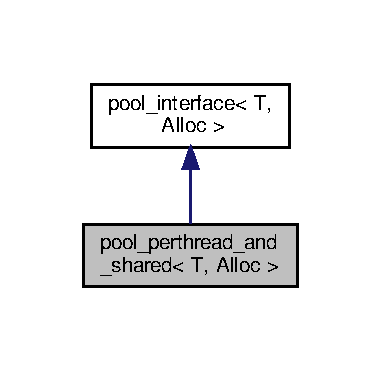
\includegraphics[width=183pt]{classpool__perthread__and__shared__inherit__graph}
\end{center}
\end{figure}


Collaboration diagram for pool\+\_\+perthread\+\_\+and\+\_\+shared$<$ T, Alloc $>$\+:
\nopagebreak
\begin{figure}[H]
\begin{center}
\leavevmode
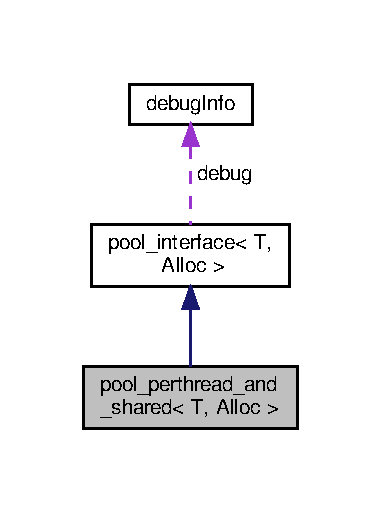
\includegraphics[width=183pt]{classpool__perthread__and__shared__coll__graph}
\end{center}
\end{figure}
\subsection*{Classes}
\begin{DoxyCompactItemize}
\item 
struct \hyperlink{structpool__perthread__and__shared_1_1rebind}{rebind}
\item 
struct \hyperlink{structpool__perthread__and__shared_1_1rebind2}{rebind2}
\end{DoxyCompactItemize}
\subsection*{Public Member Functions}
\begin{DoxyCompactItemize}
\item 
std\+::string \hyperlink{classpool__perthread__and__shared_a25687267084000ddc8c08fcf5fd783d6}{get\+Size\+String} ()
\item 
T $\ast$ \hyperlink{classpool__perthread__and__shared_ad52113553f51867ba3db6a882e5a32bb}{get} (const int \hyperlink{microbench_2main_8cpp_a9ca9869868fe7e7a38a921cc7de4103f}{tid})
\item 
void \hyperlink{classpool__perthread__and__shared_a578633fa1ef9648a47451441abaaf2fe}{add} (const int \hyperlink{microbench_2main_8cpp_a9ca9869868fe7e7a38a921cc7de4103f}{tid}, T $\ast$ptr)
\item 
void \hyperlink{classpool__perthread__and__shared_ae1e35a34657e432e02b4025ed9206add}{add\+Move\+Full\+Blocks} (const int \hyperlink{microbench_2main_8cpp_a9ca9869868fe7e7a38a921cc7de4103f}{tid}, \hyperlink{classblockbag}{blockbag}$<$ T $>$ $\ast$bag, \hyperlink{classblock}{block}$<$ T $>$ $\ast$const predecessor)
\item 
void \hyperlink{classpool__perthread__and__shared_a4c7dfae20a74fd041289497cec1d00a2}{add\+Move\+Full\+Blocks} (const int \hyperlink{microbench_2main_8cpp_a9ca9869868fe7e7a38a921cc7de4103f}{tid}, \hyperlink{classblockbag}{blockbag}$<$ T $>$ $\ast$bag)
\item 
void \hyperlink{classpool__perthread__and__shared_a3337f390a8739b621271a54c1233c470}{add\+Move\+All} (const int \hyperlink{microbench_2main_8cpp_a9ca9869868fe7e7a38a921cc7de4103f}{tid}, \hyperlink{classblockbag}{blockbag}$<$ T $>$ $\ast$bag)
\item 
int \hyperlink{classpool__perthread__and__shared_ae394f1c5a151a8c3154b0d94d4164449}{compute\+Size} (const int \hyperlink{microbench_2main_8cpp_a9ca9869868fe7e7a38a921cc7de4103f}{tid})
\item 
void \hyperlink{classpool__perthread__and__shared_a31df0438be41883ffcc4addfb6686579}{debug\+Print\+Status} (const int \hyperlink{microbench_2main_8cpp_a9ca9869868fe7e7a38a921cc7de4103f}{tid})
\item 
void \hyperlink{classpool__perthread__and__shared_a672fc4d4dce0b8f4f2418faf9e20b66e}{init\+Thread} (const int \hyperlink{microbench_2main_8cpp_a9ca9869868fe7e7a38a921cc7de4103f}{tid})
\item 
void \hyperlink{classpool__perthread__and__shared_a3a48ef748d4e73fb2c01b608d18fb56f}{deinit\+Thread} (const int \hyperlink{microbench_2main_8cpp_a9ca9869868fe7e7a38a921cc7de4103f}{tid})
\item 
\hyperlink{classpool__perthread__and__shared_a4a8df3a988491203b1c10254a7d7aad9}{pool\+\_\+perthread\+\_\+and\+\_\+shared} (const int \hyperlink{testing_8cpp_aa085812188e21ede75351d88b9b2c30d}{num\+Processes}, Alloc $\ast$const \+\_\+alloc, \hyperlink{classdebugInfo}{debug\+Info} $\ast$const \+\_\+debug)
\item 
\hyperlink{classpool__perthread__and__shared_adcc308cffe32f83cb930002eeb059a67}{$\sim$pool\+\_\+perthread\+\_\+and\+\_\+shared} ()
\end{DoxyCompactItemize}
\subsection*{Additional Inherited Members}


\subsection{Constructor \& Destructor Documentation}
\mbox{\Hypertarget{classpool__perthread__and__shared_a4a8df3a988491203b1c10254a7d7aad9}\label{classpool__perthread__and__shared_a4a8df3a988491203b1c10254a7d7aad9}} 
\index{pool\+\_\+perthread\+\_\+and\+\_\+shared@{pool\+\_\+perthread\+\_\+and\+\_\+shared}!pool\+\_\+perthread\+\_\+and\+\_\+shared@{pool\+\_\+perthread\+\_\+and\+\_\+shared}}
\index{pool\+\_\+perthread\+\_\+and\+\_\+shared@{pool\+\_\+perthread\+\_\+and\+\_\+shared}!pool\+\_\+perthread\+\_\+and\+\_\+shared@{pool\+\_\+perthread\+\_\+and\+\_\+shared}}
\subsubsection{\texorpdfstring{pool\+\_\+perthread\+\_\+and\+\_\+shared()}{pool\_perthread\_and\_shared()}}
{\footnotesize\ttfamily template$<$typename T  = void, class Alloc  = allocator\+\_\+interface$<$\+T$>$$>$ \\
\hyperlink{classpool__perthread__and__shared}{pool\+\_\+perthread\+\_\+and\+\_\+shared}$<$ T, Alloc $>$\+::\hyperlink{classpool__perthread__and__shared}{pool\+\_\+perthread\+\_\+and\+\_\+shared} (\begin{DoxyParamCaption}\item[{const int}]{num\+Processes,  }\item[{Alloc $\ast$const}]{\+\_\+alloc,  }\item[{\hyperlink{classdebugInfo}{debug\+Info} $\ast$const}]{\+\_\+debug }\end{DoxyParamCaption})\hspace{0.3cm}{\ttfamily [inline]}}

\mbox{\Hypertarget{classpool__perthread__and__shared_adcc308cffe32f83cb930002eeb059a67}\label{classpool__perthread__and__shared_adcc308cffe32f83cb930002eeb059a67}} 
\index{pool\+\_\+perthread\+\_\+and\+\_\+shared@{pool\+\_\+perthread\+\_\+and\+\_\+shared}!````~pool\+\_\+perthread\+\_\+and\+\_\+shared@{$\sim$pool\+\_\+perthread\+\_\+and\+\_\+shared}}
\index{````~pool\+\_\+perthread\+\_\+and\+\_\+shared@{$\sim$pool\+\_\+perthread\+\_\+and\+\_\+shared}!pool\+\_\+perthread\+\_\+and\+\_\+shared@{pool\+\_\+perthread\+\_\+and\+\_\+shared}}
\subsubsection{\texorpdfstring{$\sim$pool\+\_\+perthread\+\_\+and\+\_\+shared()}{~pool\_perthread\_and\_shared()}}
{\footnotesize\ttfamily template$<$typename T  = void, class Alloc  = allocator\+\_\+interface$<$\+T$>$$>$ \\
\hyperlink{classpool__perthread__and__shared}{pool\+\_\+perthread\+\_\+and\+\_\+shared}$<$ T, Alloc $>$\+::$\sim$\hyperlink{classpool__perthread__and__shared}{pool\+\_\+perthread\+\_\+and\+\_\+shared} (\begin{DoxyParamCaption}{ }\end{DoxyParamCaption})\hspace{0.3cm}{\ttfamily [inline]}}



\subsection{Member Function Documentation}
\mbox{\Hypertarget{classpool__perthread__and__shared_a578633fa1ef9648a47451441abaaf2fe}\label{classpool__perthread__and__shared_a578633fa1ef9648a47451441abaaf2fe}} 
\index{pool\+\_\+perthread\+\_\+and\+\_\+shared@{pool\+\_\+perthread\+\_\+and\+\_\+shared}!add@{add}}
\index{add@{add}!pool\+\_\+perthread\+\_\+and\+\_\+shared@{pool\+\_\+perthread\+\_\+and\+\_\+shared}}
\subsubsection{\texorpdfstring{add()}{add()}}
{\footnotesize\ttfamily template$<$typename T  = void, class Alloc  = allocator\+\_\+interface$<$\+T$>$$>$ \\
void \hyperlink{classpool__perthread__and__shared}{pool\+\_\+perthread\+\_\+and\+\_\+shared}$<$ T, Alloc $>$\+::add (\begin{DoxyParamCaption}\item[{const int}]{tid,  }\item[{T $\ast$}]{ptr }\end{DoxyParamCaption})\hspace{0.3cm}{\ttfamily [inline]}}

\mbox{\Hypertarget{classpool__perthread__and__shared_a3337f390a8739b621271a54c1233c470}\label{classpool__perthread__and__shared_a3337f390a8739b621271a54c1233c470}} 
\index{pool\+\_\+perthread\+\_\+and\+\_\+shared@{pool\+\_\+perthread\+\_\+and\+\_\+shared}!add\+Move\+All@{add\+Move\+All}}
\index{add\+Move\+All@{add\+Move\+All}!pool\+\_\+perthread\+\_\+and\+\_\+shared@{pool\+\_\+perthread\+\_\+and\+\_\+shared}}
\subsubsection{\texorpdfstring{add\+Move\+All()}{addMoveAll()}}
{\footnotesize\ttfamily template$<$typename T  = void, class Alloc  = allocator\+\_\+interface$<$\+T$>$$>$ \\
void \hyperlink{classpool__perthread__and__shared}{pool\+\_\+perthread\+\_\+and\+\_\+shared}$<$ T, Alloc $>$\+::add\+Move\+All (\begin{DoxyParamCaption}\item[{const int}]{tid,  }\item[{\hyperlink{classblockbag}{blockbag}$<$ T $>$ $\ast$}]{bag }\end{DoxyParamCaption})\hspace{0.3cm}{\ttfamily [inline]}}

\mbox{\Hypertarget{classpool__perthread__and__shared_ae1e35a34657e432e02b4025ed9206add}\label{classpool__perthread__and__shared_ae1e35a34657e432e02b4025ed9206add}} 
\index{pool\+\_\+perthread\+\_\+and\+\_\+shared@{pool\+\_\+perthread\+\_\+and\+\_\+shared}!add\+Move\+Full\+Blocks@{add\+Move\+Full\+Blocks}}
\index{add\+Move\+Full\+Blocks@{add\+Move\+Full\+Blocks}!pool\+\_\+perthread\+\_\+and\+\_\+shared@{pool\+\_\+perthread\+\_\+and\+\_\+shared}}
\subsubsection{\texorpdfstring{add\+Move\+Full\+Blocks()}{addMoveFullBlocks()}\hspace{0.1cm}{\footnotesize\ttfamily [1/2]}}
{\footnotesize\ttfamily template$<$typename T  = void, class Alloc  = allocator\+\_\+interface$<$\+T$>$$>$ \\
void \hyperlink{classpool__perthread__and__shared}{pool\+\_\+perthread\+\_\+and\+\_\+shared}$<$ T, Alloc $>$\+::add\+Move\+Full\+Blocks (\begin{DoxyParamCaption}\item[{const int}]{tid,  }\item[{\hyperlink{classblockbag}{blockbag}$<$ T $>$ $\ast$}]{bag,  }\item[{\hyperlink{classblock}{block}$<$ T $>$ $\ast$const}]{predecessor }\end{DoxyParamCaption})\hspace{0.3cm}{\ttfamily [inline]}}

\mbox{\Hypertarget{classpool__perthread__and__shared_a4c7dfae20a74fd041289497cec1d00a2}\label{classpool__perthread__and__shared_a4c7dfae20a74fd041289497cec1d00a2}} 
\index{pool\+\_\+perthread\+\_\+and\+\_\+shared@{pool\+\_\+perthread\+\_\+and\+\_\+shared}!add\+Move\+Full\+Blocks@{add\+Move\+Full\+Blocks}}
\index{add\+Move\+Full\+Blocks@{add\+Move\+Full\+Blocks}!pool\+\_\+perthread\+\_\+and\+\_\+shared@{pool\+\_\+perthread\+\_\+and\+\_\+shared}}
\subsubsection{\texorpdfstring{add\+Move\+Full\+Blocks()}{addMoveFullBlocks()}\hspace{0.1cm}{\footnotesize\ttfamily [2/2]}}
{\footnotesize\ttfamily template$<$typename T  = void, class Alloc  = allocator\+\_\+interface$<$\+T$>$$>$ \\
void \hyperlink{classpool__perthread__and__shared}{pool\+\_\+perthread\+\_\+and\+\_\+shared}$<$ T, Alloc $>$\+::add\+Move\+Full\+Blocks (\begin{DoxyParamCaption}\item[{const int}]{tid,  }\item[{\hyperlink{classblockbag}{blockbag}$<$ T $>$ $\ast$}]{bag }\end{DoxyParamCaption})\hspace{0.3cm}{\ttfamily [inline]}}

\mbox{\Hypertarget{classpool__perthread__and__shared_ae394f1c5a151a8c3154b0d94d4164449}\label{classpool__perthread__and__shared_ae394f1c5a151a8c3154b0d94d4164449}} 
\index{pool\+\_\+perthread\+\_\+and\+\_\+shared@{pool\+\_\+perthread\+\_\+and\+\_\+shared}!compute\+Size@{compute\+Size}}
\index{compute\+Size@{compute\+Size}!pool\+\_\+perthread\+\_\+and\+\_\+shared@{pool\+\_\+perthread\+\_\+and\+\_\+shared}}
\subsubsection{\texorpdfstring{compute\+Size()}{computeSize()}}
{\footnotesize\ttfamily template$<$typename T  = void, class Alloc  = allocator\+\_\+interface$<$\+T$>$$>$ \\
int \hyperlink{classpool__perthread__and__shared}{pool\+\_\+perthread\+\_\+and\+\_\+shared}$<$ T, Alloc $>$\+::compute\+Size (\begin{DoxyParamCaption}\item[{const int}]{tid }\end{DoxyParamCaption})\hspace{0.3cm}{\ttfamily [inline]}}

\mbox{\Hypertarget{classpool__perthread__and__shared_a31df0438be41883ffcc4addfb6686579}\label{classpool__perthread__and__shared_a31df0438be41883ffcc4addfb6686579}} 
\index{pool\+\_\+perthread\+\_\+and\+\_\+shared@{pool\+\_\+perthread\+\_\+and\+\_\+shared}!debug\+Print\+Status@{debug\+Print\+Status}}
\index{debug\+Print\+Status@{debug\+Print\+Status}!pool\+\_\+perthread\+\_\+and\+\_\+shared@{pool\+\_\+perthread\+\_\+and\+\_\+shared}}
\subsubsection{\texorpdfstring{debug\+Print\+Status()}{debugPrintStatus()}}
{\footnotesize\ttfamily template$<$typename T  = void, class Alloc  = allocator\+\_\+interface$<$\+T$>$$>$ \\
void \hyperlink{classpool__perthread__and__shared}{pool\+\_\+perthread\+\_\+and\+\_\+shared}$<$ T, Alloc $>$\+::debug\+Print\+Status (\begin{DoxyParamCaption}\item[{const int}]{tid }\end{DoxyParamCaption})\hspace{0.3cm}{\ttfamily [inline]}}

\mbox{\Hypertarget{classpool__perthread__and__shared_a3a48ef748d4e73fb2c01b608d18fb56f}\label{classpool__perthread__and__shared_a3a48ef748d4e73fb2c01b608d18fb56f}} 
\index{pool\+\_\+perthread\+\_\+and\+\_\+shared@{pool\+\_\+perthread\+\_\+and\+\_\+shared}!deinit\+Thread@{deinit\+Thread}}
\index{deinit\+Thread@{deinit\+Thread}!pool\+\_\+perthread\+\_\+and\+\_\+shared@{pool\+\_\+perthread\+\_\+and\+\_\+shared}}
\subsubsection{\texorpdfstring{deinit\+Thread()}{deinitThread()}}
{\footnotesize\ttfamily template$<$typename T  = void, class Alloc  = allocator\+\_\+interface$<$\+T$>$$>$ \\
void \hyperlink{classpool__perthread__and__shared}{pool\+\_\+perthread\+\_\+and\+\_\+shared}$<$ T, Alloc $>$\+::deinit\+Thread (\begin{DoxyParamCaption}\item[{const int}]{tid }\end{DoxyParamCaption})\hspace{0.3cm}{\ttfamily [inline]}}

\mbox{\Hypertarget{classpool__perthread__and__shared_ad52113553f51867ba3db6a882e5a32bb}\label{classpool__perthread__and__shared_ad52113553f51867ba3db6a882e5a32bb}} 
\index{pool\+\_\+perthread\+\_\+and\+\_\+shared@{pool\+\_\+perthread\+\_\+and\+\_\+shared}!get@{get}}
\index{get@{get}!pool\+\_\+perthread\+\_\+and\+\_\+shared@{pool\+\_\+perthread\+\_\+and\+\_\+shared}}
\subsubsection{\texorpdfstring{get()}{get()}}
{\footnotesize\ttfamily template$<$typename T  = void, class Alloc  = allocator\+\_\+interface$<$\+T$>$$>$ \\
T$\ast$ \hyperlink{classpool__perthread__and__shared}{pool\+\_\+perthread\+\_\+and\+\_\+shared}$<$ T, Alloc $>$\+::get (\begin{DoxyParamCaption}\item[{const int}]{tid }\end{DoxyParamCaption})\hspace{0.3cm}{\ttfamily [inline]}}

if the freebag contains any object, then remove one from the freebag and return a pointer to it. if not, then retrieve a new object from Alloc \mbox{\Hypertarget{classpool__perthread__and__shared_a25687267084000ddc8c08fcf5fd783d6}\label{classpool__perthread__and__shared_a25687267084000ddc8c08fcf5fd783d6}} 
\index{pool\+\_\+perthread\+\_\+and\+\_\+shared@{pool\+\_\+perthread\+\_\+and\+\_\+shared}!get\+Size\+String@{get\+Size\+String}}
\index{get\+Size\+String@{get\+Size\+String}!pool\+\_\+perthread\+\_\+and\+\_\+shared@{pool\+\_\+perthread\+\_\+and\+\_\+shared}}
\subsubsection{\texorpdfstring{get\+Size\+String()}{getSizeString()}}
{\footnotesize\ttfamily template$<$typename T  = void, class Alloc  = allocator\+\_\+interface$<$\+T$>$$>$ \\
std\+::string \hyperlink{classpool__perthread__and__shared}{pool\+\_\+perthread\+\_\+and\+\_\+shared}$<$ T, Alloc $>$\+::get\+Size\+String (\begin{DoxyParamCaption}{ }\end{DoxyParamCaption})\hspace{0.3cm}{\ttfamily [inline]}}

\mbox{\Hypertarget{classpool__perthread__and__shared_a672fc4d4dce0b8f4f2418faf9e20b66e}\label{classpool__perthread__and__shared_a672fc4d4dce0b8f4f2418faf9e20b66e}} 
\index{pool\+\_\+perthread\+\_\+and\+\_\+shared@{pool\+\_\+perthread\+\_\+and\+\_\+shared}!init\+Thread@{init\+Thread}}
\index{init\+Thread@{init\+Thread}!pool\+\_\+perthread\+\_\+and\+\_\+shared@{pool\+\_\+perthread\+\_\+and\+\_\+shared}}
\subsubsection{\texorpdfstring{init\+Thread()}{initThread()}}
{\footnotesize\ttfamily template$<$typename T  = void, class Alloc  = allocator\+\_\+interface$<$\+T$>$$>$ \\
void \hyperlink{classpool__perthread__and__shared}{pool\+\_\+perthread\+\_\+and\+\_\+shared}$<$ T, Alloc $>$\+::init\+Thread (\begin{DoxyParamCaption}\item[{const int}]{tid }\end{DoxyParamCaption})\hspace{0.3cm}{\ttfamily [inline]}}



The documentation for this class was generated from the following file\+:\begin{DoxyCompactItemize}
\item 
common/recordmgr/\hyperlink{pool__perthread__and__shared_8h}{pool\+\_\+perthread\+\_\+and\+\_\+shared.\+h}\end{DoxyCompactItemize}

\hypertarget{classQuery__queue}{}\section{Query\+\_\+queue Class Reference}
\label{classQuery__queue}\index{Query\+\_\+queue@{Query\+\_\+queue}}


{\ttfamily \#include $<$query.\+h$>$}

\subsection*{Public Member Functions}
\begin{DoxyCompactItemize}
\item 
void \hyperlink{classQuery__queue_a7b11f8dff9c71abbf96d85328001803d}{init} (\hyperlink{classworkload}{workload} $\ast$h\+\_\+wl)
\item 
void \hyperlink{classQuery__queue_a3a8dbf987f4aac6af22083227cb30dac}{setbench\+\_\+deinit} ()
\item 
void \hyperlink{classQuery__queue_acad0797f9688fbada3f0c4748f95e2dc}{init\+\_\+per\+\_\+thread} (int thread\+\_\+id)
\item 
void \hyperlink{classQuery__queue_a3f657d30e7e04d7877e6b436aff26f38}{deinit\+\_\+per\+\_\+thread} (int thread\+\_\+id)
\item 
\hyperlink{classbase__query}{base\+\_\+query} $\ast$ \hyperlink{classQuery__queue_ac68f34bc81dc3919b5552724f82120a2}{get\+\_\+next\+\_\+query} (uint64\+\_\+t thd\+\_\+id)
\end{DoxyCompactItemize}


\subsection{Member Function Documentation}
\mbox{\Hypertarget{classQuery__queue_a3f657d30e7e04d7877e6b436aff26f38}\label{classQuery__queue_a3f657d30e7e04d7877e6b436aff26f38}} 
\index{Query\+\_\+queue@{Query\+\_\+queue}!deinit\+\_\+per\+\_\+thread@{deinit\+\_\+per\+\_\+thread}}
\index{deinit\+\_\+per\+\_\+thread@{deinit\+\_\+per\+\_\+thread}!Query\+\_\+queue@{Query\+\_\+queue}}
\subsubsection{\texorpdfstring{deinit\+\_\+per\+\_\+thread()}{deinit\_per\_thread()}}
{\footnotesize\ttfamily void Query\+\_\+queue\+::deinit\+\_\+per\+\_\+thread (\begin{DoxyParamCaption}\item[{int}]{thread\+\_\+id }\end{DoxyParamCaption})}

\mbox{\Hypertarget{classQuery__queue_ac68f34bc81dc3919b5552724f82120a2}\label{classQuery__queue_ac68f34bc81dc3919b5552724f82120a2}} 
\index{Query\+\_\+queue@{Query\+\_\+queue}!get\+\_\+next\+\_\+query@{get\+\_\+next\+\_\+query}}
\index{get\+\_\+next\+\_\+query@{get\+\_\+next\+\_\+query}!Query\+\_\+queue@{Query\+\_\+queue}}
\subsubsection{\texorpdfstring{get\+\_\+next\+\_\+query()}{get\_next\_query()}}
{\footnotesize\ttfamily \hyperlink{classbase__query}{base\+\_\+query} $\ast$ Query\+\_\+queue\+::get\+\_\+next\+\_\+query (\begin{DoxyParamCaption}\item[{uint64\+\_\+t}]{thd\+\_\+id }\end{DoxyParamCaption})}

\mbox{\Hypertarget{classQuery__queue_a7b11f8dff9c71abbf96d85328001803d}\label{classQuery__queue_a7b11f8dff9c71abbf96d85328001803d}} 
\index{Query\+\_\+queue@{Query\+\_\+queue}!init@{init}}
\index{init@{init}!Query\+\_\+queue@{Query\+\_\+queue}}
\subsubsection{\texorpdfstring{init()}{init()}}
{\footnotesize\ttfamily void Query\+\_\+queue\+::init (\begin{DoxyParamCaption}\item[{\hyperlink{classworkload}{workload} $\ast$}]{h\+\_\+wl }\end{DoxyParamCaption})}

\mbox{\Hypertarget{classQuery__queue_acad0797f9688fbada3f0c4748f95e2dc}\label{classQuery__queue_acad0797f9688fbada3f0c4748f95e2dc}} 
\index{Query\+\_\+queue@{Query\+\_\+queue}!init\+\_\+per\+\_\+thread@{init\+\_\+per\+\_\+thread}}
\index{init\+\_\+per\+\_\+thread@{init\+\_\+per\+\_\+thread}!Query\+\_\+queue@{Query\+\_\+queue}}
\subsubsection{\texorpdfstring{init\+\_\+per\+\_\+thread()}{init\_per\_thread()}}
{\footnotesize\ttfamily void Query\+\_\+queue\+::init\+\_\+per\+\_\+thread (\begin{DoxyParamCaption}\item[{int}]{thread\+\_\+id }\end{DoxyParamCaption})}

\mbox{\Hypertarget{classQuery__queue_a3a8dbf987f4aac6af22083227cb30dac}\label{classQuery__queue_a3a8dbf987f4aac6af22083227cb30dac}} 
\index{Query\+\_\+queue@{Query\+\_\+queue}!setbench\+\_\+deinit@{setbench\+\_\+deinit}}
\index{setbench\+\_\+deinit@{setbench\+\_\+deinit}!Query\+\_\+queue@{Query\+\_\+queue}}
\subsubsection{\texorpdfstring{setbench\+\_\+deinit()}{setbench\_deinit()}}
{\footnotesize\ttfamily void Query\+\_\+queue\+::setbench\+\_\+deinit (\begin{DoxyParamCaption}{ }\end{DoxyParamCaption})}



The documentation for this class was generated from the following files\+:\begin{DoxyCompactItemize}
\item 
macrobench/system/\hyperlink{query_8h}{query.\+h}\item 
macrobench/system/\hyperlink{query_8cpp}{query.\+cpp}\end{DoxyCompactItemize}

\hypertarget{classQuery__thd}{}\section{Query\+\_\+thd Class Reference}
\label{classQuery__thd}\index{Query\+\_\+thd@{Query\+\_\+thd}}


{\ttfamily \#include $<$query.\+h$>$}



Collaboration diagram for Query\+\_\+thd\+:
\nopagebreak
\begin{figure}[H]
\begin{center}
\leavevmode
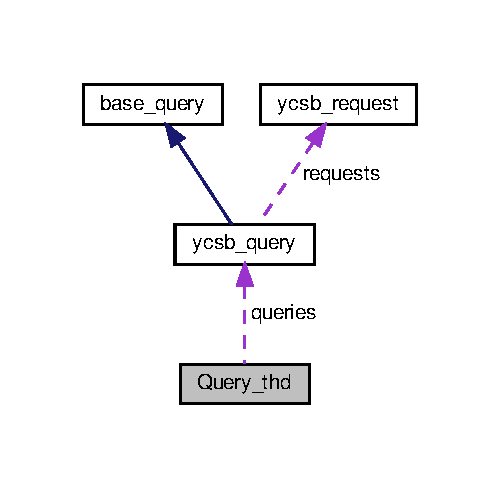
\includegraphics[width=240pt]{classQuery__thd__coll__graph}
\end{center}
\end{figure}
\subsection*{Public Member Functions}
\begin{DoxyCompactItemize}
\item 
void \hyperlink{classQuery__thd_a8a6ee7d0d441e0000d7fc1ad40e87659}{init} (\hyperlink{classworkload}{workload} $\ast$h\+\_\+wl, int thread\+\_\+id)
\item 
void \hyperlink{classQuery__thd_acb9b3b81969cdd8f1a4c9800e5416a07}{setbench\+\_\+deinit} ()
\item 
\hyperlink{classbase__query}{base\+\_\+query} $\ast$ \hyperlink{classQuery__thd_a11c17eecb3ed06f31382ee86deebb258}{get\+\_\+next\+\_\+query} ()
\end{DoxyCompactItemize}
\subsection*{Public Attributes}
\begin{DoxyCompactItemize}
\item 
int \hyperlink{classQuery__thd_a3f2ad0326aca9475a6214fb39c6fc745}{q\+\_\+idx}
\item 
\hyperlink{classycsb__query}{ycsb\+\_\+query} $\ast$ \hyperlink{classQuery__thd_ab420c47c42ec689a5a38022380a01b60}{queries}
\item 
char \hyperlink{classQuery__thd_a17426d37b988c4d8c033974447620b81}{pad} \mbox{[}\hyperlink{config_8h_aa18ff96566bf8c1f4cd38c1e7bc4ca80}{C\+L\+\_\+\+S\+I\+ZE} -\/ sizeof(void $\ast$) -\/ sizeof(int)\mbox{]}
\item 
drand48\+\_\+data \hyperlink{classQuery__thd_ae2b0aa6a30790eac1b2b24929e91e040}{buffer}
\end{DoxyCompactItemize}


\subsection{Member Function Documentation}
\mbox{\Hypertarget{classQuery__thd_a11c17eecb3ed06f31382ee86deebb258}\label{classQuery__thd_a11c17eecb3ed06f31382ee86deebb258}} 
\index{Query\+\_\+thd@{Query\+\_\+thd}!get\+\_\+next\+\_\+query@{get\+\_\+next\+\_\+query}}
\index{get\+\_\+next\+\_\+query@{get\+\_\+next\+\_\+query}!Query\+\_\+thd@{Query\+\_\+thd}}
\subsubsection{\texorpdfstring{get\+\_\+next\+\_\+query()}{get\_next\_query()}}
{\footnotesize\ttfamily \hyperlink{classbase__query}{base\+\_\+query} $\ast$ Query\+\_\+thd\+::get\+\_\+next\+\_\+query (\begin{DoxyParamCaption}{ }\end{DoxyParamCaption})}

\mbox{\Hypertarget{classQuery__thd_a8a6ee7d0d441e0000d7fc1ad40e87659}\label{classQuery__thd_a8a6ee7d0d441e0000d7fc1ad40e87659}} 
\index{Query\+\_\+thd@{Query\+\_\+thd}!init@{init}}
\index{init@{init}!Query\+\_\+thd@{Query\+\_\+thd}}
\subsubsection{\texorpdfstring{init()}{init()}}
{\footnotesize\ttfamily void Query\+\_\+thd\+::init (\begin{DoxyParamCaption}\item[{\hyperlink{classworkload}{workload} $\ast$}]{h\+\_\+wl,  }\item[{int}]{thread\+\_\+id }\end{DoxyParamCaption})}

\mbox{\Hypertarget{classQuery__thd_acb9b3b81969cdd8f1a4c9800e5416a07}\label{classQuery__thd_acb9b3b81969cdd8f1a4c9800e5416a07}} 
\index{Query\+\_\+thd@{Query\+\_\+thd}!setbench\+\_\+deinit@{setbench\+\_\+deinit}}
\index{setbench\+\_\+deinit@{setbench\+\_\+deinit}!Query\+\_\+thd@{Query\+\_\+thd}}
\subsubsection{\texorpdfstring{setbench\+\_\+deinit()}{setbench\_deinit()}}
{\footnotesize\ttfamily void Query\+\_\+thd\+::setbench\+\_\+deinit (\begin{DoxyParamCaption}{ }\end{DoxyParamCaption})}



\subsection{Member Data Documentation}
\mbox{\Hypertarget{classQuery__thd_ae2b0aa6a30790eac1b2b24929e91e040}\label{classQuery__thd_ae2b0aa6a30790eac1b2b24929e91e040}} 
\index{Query\+\_\+thd@{Query\+\_\+thd}!buffer@{buffer}}
\index{buffer@{buffer}!Query\+\_\+thd@{Query\+\_\+thd}}
\subsubsection{\texorpdfstring{buffer}{buffer}}
{\footnotesize\ttfamily drand48\+\_\+data Query\+\_\+thd\+::buffer}

\mbox{\Hypertarget{classQuery__thd_a17426d37b988c4d8c033974447620b81}\label{classQuery__thd_a17426d37b988c4d8c033974447620b81}} 
\index{Query\+\_\+thd@{Query\+\_\+thd}!pad@{pad}}
\index{pad@{pad}!Query\+\_\+thd@{Query\+\_\+thd}}
\subsubsection{\texorpdfstring{pad}{pad}}
{\footnotesize\ttfamily char Query\+\_\+thd\+::pad\mbox{[}\hyperlink{config_8h_aa18ff96566bf8c1f4cd38c1e7bc4ca80}{C\+L\+\_\+\+S\+I\+ZE} -\/ sizeof(void $\ast$) -\/ sizeof(int)\mbox{]}}

\mbox{\Hypertarget{classQuery__thd_a3f2ad0326aca9475a6214fb39c6fc745}\label{classQuery__thd_a3f2ad0326aca9475a6214fb39c6fc745}} 
\index{Query\+\_\+thd@{Query\+\_\+thd}!q\+\_\+idx@{q\+\_\+idx}}
\index{q\+\_\+idx@{q\+\_\+idx}!Query\+\_\+thd@{Query\+\_\+thd}}
\subsubsection{\texorpdfstring{q\+\_\+idx}{q\_idx}}
{\footnotesize\ttfamily int Query\+\_\+thd\+::q\+\_\+idx}

\mbox{\Hypertarget{classQuery__thd_ab420c47c42ec689a5a38022380a01b60}\label{classQuery__thd_ab420c47c42ec689a5a38022380a01b60}} 
\index{Query\+\_\+thd@{Query\+\_\+thd}!queries@{queries}}
\index{queries@{queries}!Query\+\_\+thd@{Query\+\_\+thd}}
\subsubsection{\texorpdfstring{queries}{queries}}
{\footnotesize\ttfamily \hyperlink{classycsb__query}{ycsb\+\_\+query}$\ast$ Query\+\_\+thd\+::queries}



The documentation for this class was generated from the following files\+:\begin{DoxyCompactItemize}
\item 
macrobench/system/\hyperlink{query_8h}{query.\+h}\item 
macrobench/system/\hyperlink{query_8cpp}{query.\+cpp}\end{DoxyCompactItemize}

\hypertarget{classRandomFNV1A}{}\section{Random\+F\+N\+V1A Class Reference}
\label{classRandomFNV1A}\index{Random\+F\+N\+V1A@{Random\+F\+N\+V1A}}


{\ttfamily \#include $<$random\+\_\+fnv1a.\+h$>$}

\subsection*{Public Member Functions}
\begin{DoxyCompactItemize}
\item 
\hyperlink{classRandomFNV1A_ad6e2947a9daa7f007747018ac4797bb6}{Random\+F\+N\+V1A} ()
\item 
\hyperlink{classRandomFNV1A_a1f3ca9c2044fed23fd88418ad12004bd}{Random\+F\+N\+V1A} (uint64\+\_\+t \hyperlink{classRandomFNV1A_acf505335861440a14ee0b7710586b5c1}{seed})
\item 
void \hyperlink{classRandomFNV1A_a8fa32c70622235889cde300c7b8adb10}{set\+Seed} (uint64\+\_\+t \hyperlink{classRandomFNV1A_acf505335861440a14ee0b7710586b5c1}{seed})
\item 
uint64\+\_\+t \hyperlink{classRandomFNV1A_a4b38851f3bd4275634ba1d1492739b16}{next} (uint64\+\_\+t n)
\item 
size\+\_\+t \hyperlink{classRandomFNV1A_a2b331d84c37f8091bd69260d87c9765b}{next} ()
\end{DoxyCompactItemize}


\subsection{Detailed Description}
Preliminary C++ implementation of binary search tree using L\+L\+X/\+S\+CX.

Copyright (C) 2014 Trevor Brown 

\subsection{Constructor \& Destructor Documentation}
\mbox{\Hypertarget{classRandomFNV1A_ad6e2947a9daa7f007747018ac4797bb6}\label{classRandomFNV1A_ad6e2947a9daa7f007747018ac4797bb6}} 
\index{Random\+F\+N\+V1A@{Random\+F\+N\+V1A}!Random\+F\+N\+V1A@{Random\+F\+N\+V1A}}
\index{Random\+F\+N\+V1A@{Random\+F\+N\+V1A}!Random\+F\+N\+V1A@{Random\+F\+N\+V1A}}
\subsubsection{\texorpdfstring{Random\+F\+N\+V1\+A()}{RandomFNV1A()}\hspace{0.1cm}{\footnotesize\ttfamily [1/2]}}
{\footnotesize\ttfamily Random\+F\+N\+V1\+A\+::\+Random\+F\+N\+V1A (\begin{DoxyParamCaption}{ }\end{DoxyParamCaption})\hspace{0.3cm}{\ttfamily [inline]}}

\mbox{\Hypertarget{classRandomFNV1A_a1f3ca9c2044fed23fd88418ad12004bd}\label{classRandomFNV1A_a1f3ca9c2044fed23fd88418ad12004bd}} 
\index{Random\+F\+N\+V1A@{Random\+F\+N\+V1A}!Random\+F\+N\+V1A@{Random\+F\+N\+V1A}}
\index{Random\+F\+N\+V1A@{Random\+F\+N\+V1A}!Random\+F\+N\+V1A@{Random\+F\+N\+V1A}}
\subsubsection{\texorpdfstring{Random\+F\+N\+V1\+A()}{RandomFNV1A()}\hspace{0.1cm}{\footnotesize\ttfamily [2/2]}}
{\footnotesize\ttfamily Random\+F\+N\+V1\+A\+::\+Random\+F\+N\+V1A (\begin{DoxyParamCaption}\item[{uint64\+\_\+t}]{seed }\end{DoxyParamCaption})\hspace{0.3cm}{\ttfamily [inline]}}



\subsection{Member Function Documentation}
\mbox{\Hypertarget{classRandomFNV1A_a4b38851f3bd4275634ba1d1492739b16}\label{classRandomFNV1A_a4b38851f3bd4275634ba1d1492739b16}} 
\index{Random\+F\+N\+V1A@{Random\+F\+N\+V1A}!next@{next}}
\index{next@{next}!Random\+F\+N\+V1A@{Random\+F\+N\+V1A}}
\subsubsection{\texorpdfstring{next()}{next()}\hspace{0.1cm}{\footnotesize\ttfamily [1/2]}}
{\footnotesize\ttfamily uint64\+\_\+t Random\+F\+N\+V1\+A\+::next (\begin{DoxyParamCaption}\item[{uint64\+\_\+t}]{n }\end{DoxyParamCaption})\hspace{0.3cm}{\ttfamily [inline]}}

\mbox{\Hypertarget{classRandomFNV1A_a2b331d84c37f8091bd69260d87c9765b}\label{classRandomFNV1A_a2b331d84c37f8091bd69260d87c9765b}} 
\index{Random\+F\+N\+V1A@{Random\+F\+N\+V1A}!next@{next}}
\index{next@{next}!Random\+F\+N\+V1A@{Random\+F\+N\+V1A}}
\subsubsection{\texorpdfstring{next()}{next()}\hspace{0.1cm}{\footnotesize\ttfamily [2/2]}}
{\footnotesize\ttfamily size\+\_\+t Random\+F\+N\+V1\+A\+::next (\begin{DoxyParamCaption}{ }\end{DoxyParamCaption})\hspace{0.3cm}{\ttfamily [inline]}}

\mbox{\Hypertarget{classRandomFNV1A_a8fa32c70622235889cde300c7b8adb10}\label{classRandomFNV1A_a8fa32c70622235889cde300c7b8adb10}} 
\index{Random\+F\+N\+V1A@{Random\+F\+N\+V1A}!set\+Seed@{set\+Seed}}
\index{set\+Seed@{set\+Seed}!Random\+F\+N\+V1A@{Random\+F\+N\+V1A}}
\subsubsection{\texorpdfstring{set\+Seed()}{setSeed()}}
{\footnotesize\ttfamily void Random\+F\+N\+V1\+A\+::set\+Seed (\begin{DoxyParamCaption}\item[{uint64\+\_\+t}]{seed }\end{DoxyParamCaption})\hspace{0.3cm}{\ttfamily [inline]}}



\subsection{Member Data Documentation}
\mbox{\Hypertarget{classRandomFNV1A_a587bc4df3805091170b5db5661ea8b19}\label{classRandomFNV1A_a587bc4df3805091170b5db5661ea8b19}} 
\index{Random\+F\+N\+V1A@{Random\+F\+N\+V1A}!P\+AD@{P\+AD}}
\index{P\+AD@{P\+AD}!Random\+F\+N\+V1A@{Random\+F\+N\+V1A}}
\subsubsection{\texorpdfstring{P\+AD}{PAD}}
{\footnotesize\ttfamily Random\+F\+N\+V1\+A\+::\+P\+AD}

\mbox{\Hypertarget{classRandomFNV1A_acf505335861440a14ee0b7710586b5c1}\label{classRandomFNV1A_acf505335861440a14ee0b7710586b5c1}} 
\index{Random\+F\+N\+V1A@{Random\+F\+N\+V1A}!seed@{seed}}
\index{seed@{seed}!Random\+F\+N\+V1A@{Random\+F\+N\+V1A}}
\subsubsection{\texorpdfstring{seed}{seed}}
{\footnotesize\ttfamily uint64\+\_\+t Random\+F\+N\+V1\+A\+::seed}



The documentation for this class was generated from the following file\+:\begin{DoxyCompactItemize}
\item 
common/\hyperlink{random__fnv1a_8h}{random\+\_\+fnv1a.\+h}\end{DoxyCompactItemize}

\hypertarget{structrcu__node__t}{}\section{rcu\+\_\+node\+\_\+t Struct Reference}
\label{structrcu__node__t}\index{rcu\+\_\+node\+\_\+t@{rcu\+\_\+node\+\_\+t}}


{\ttfamily \#include $<$urcu.\+h$>$}

\subsection*{Public Attributes}
\begin{DoxyCompactItemize}
\item 
\begin{tabbing}
xx\=xx\=xx\=xx\=xx\=xx\=xx\=xx\=xx\=\kill
union \{\\
\>struct \{\\
\>\>volatile unsigned long \hyperlink{structrcu__node__t_a760b5d954e54c86bc09dc1e2754c0307}{time}\\
\>\>volatile uint64\_t \hyperlink{structrcu__node__t_a39f0899a55b266866a7dddd8dac507b4}{val1}\\
\>\>volatile uint64\_t \hyperlink{structrcu__node__t_a37089d9851c8b558fea850ebec84eea8}{val2}\\
\>\} \\
\>char \hyperlink{structrcu__node__t_ae1e6b1ffa5df13f1a639d4f675c632e4}{bytes} \mbox{[}192\mbox{]}\\
\}; \\

\end{tabbing}\end{DoxyCompactItemize}


\subsection{Member Data Documentation}
\mbox{\Hypertarget{structrcu__node__t_afaff9a2380ba1929d01ba0afed5d2011}\label{structrcu__node__t_afaff9a2380ba1929d01ba0afed5d2011}} 
\subsubsection{\texorpdfstring{"@51}{@51}}
{\footnotesize\ttfamily union \{ ... \} }

\mbox{\Hypertarget{structrcu__node__t_ae1e6b1ffa5df13f1a639d4f675c632e4}\label{structrcu__node__t_ae1e6b1ffa5df13f1a639d4f675c632e4}} 
\index{rcu\+\_\+node\+\_\+t@{rcu\+\_\+node\+\_\+t}!bytes@{bytes}}
\index{bytes@{bytes}!rcu\+\_\+node\+\_\+t@{rcu\+\_\+node\+\_\+t}}
\subsubsection{\texorpdfstring{bytes}{bytes}}
{\footnotesize\ttfamily char rcu\+\_\+node\+\_\+t\+::bytes\mbox{[}192\mbox{]}}

\mbox{\Hypertarget{structrcu__node__t_a760b5d954e54c86bc09dc1e2754c0307}\label{structrcu__node__t_a760b5d954e54c86bc09dc1e2754c0307}} 
\index{rcu\+\_\+node\+\_\+t@{rcu\+\_\+node\+\_\+t}!time@{time}}
\index{time@{time}!rcu\+\_\+node\+\_\+t@{rcu\+\_\+node\+\_\+t}}
\subsubsection{\texorpdfstring{time}{time}}
{\footnotesize\ttfamily volatile unsigned long rcu\+\_\+node\+\_\+t\+::time}

\mbox{\Hypertarget{structrcu__node__t_a39f0899a55b266866a7dddd8dac507b4}\label{structrcu__node__t_a39f0899a55b266866a7dddd8dac507b4}} 
\index{rcu\+\_\+node\+\_\+t@{rcu\+\_\+node\+\_\+t}!val1@{val1}}
\index{val1@{val1}!rcu\+\_\+node\+\_\+t@{rcu\+\_\+node\+\_\+t}}
\subsubsection{\texorpdfstring{val1}{val1}}
{\footnotesize\ttfamily volatile uint64\+\_\+t rcu\+\_\+node\+\_\+t\+::val1}

\mbox{\Hypertarget{structrcu__node__t_a37089d9851c8b558fea850ebec84eea8}\label{structrcu__node__t_a37089d9851c8b558fea850ebec84eea8}} 
\index{rcu\+\_\+node\+\_\+t@{rcu\+\_\+node\+\_\+t}!val2@{val2}}
\index{val2@{val2}!rcu\+\_\+node\+\_\+t@{rcu\+\_\+node\+\_\+t}}
\subsubsection{\texorpdfstring{val2}{val2}}
{\footnotesize\ttfamily volatile uint64\+\_\+t rcu\+\_\+node\+\_\+t\+::val2}



The documentation for this struct was generated from the following file\+:\begin{DoxyCompactItemize}
\item 
common/urcu/\hyperlink{urcu_8h}{urcu.\+h}\end{DoxyCompactItemize}

\hypertarget{structrdcssdesc__t}{}\section{rdcssdesc\+\_\+t Struct Reference}
\label{structrdcssdesc__t}\index{rdcssdesc\+\_\+t@{rdcssdesc\+\_\+t}}


{\ttfamily \#include $<$kcas\+\_\+reuse\+\_\+htm\+\_\+impl.\+h$>$}

\subsection*{Public Attributes}
\begin{DoxyCompactItemize}
\item 
volatile \hyperlink{kcas__reuse__htm__impl_8h_a997daf56279be481f5c4294647725689}{seqbits\+\_\+t} \hyperlink{structrdcssdesc__t_a1844984d511a02ef16f2a691ad991d40}{seq\+Bits}
\item 
\hyperlink{rq__unsafe_8h_ad45142aaf2ff20a036dc6242b8483e9c}{casword\+\_\+t} volatile $\ast$ \hyperlink{structrdcssdesc__t_ab47535b838f7a74d99e96738a42d204c}{addr1}
\item 
\hyperlink{rq__unsafe_8h_ad45142aaf2ff20a036dc6242b8483e9c}{casword\+\_\+t} \hyperlink{structrdcssdesc__t_a719fca618bebcab487aae8512a2b0f79}{old1}
\item 
\hyperlink{rq__unsafe_8h_ad45142aaf2ff20a036dc6242b8483e9c}{casword\+\_\+t} volatile $\ast$ \hyperlink{structrdcssdesc__t_afe6e31e7b7fea3b440994e84eba9c802}{addr2}
\item 
\hyperlink{rq__unsafe_8h_ad45142aaf2ff20a036dc6242b8483e9c}{casword\+\_\+t} \hyperlink{structrdcssdesc__t_a8e6fb7c8f1fb27020a85852b9325da38}{old2}
\item 
\hyperlink{rq__unsafe_8h_ad45142aaf2ff20a036dc6242b8483e9c}{casword\+\_\+t} \hyperlink{structrdcssdesc__t_ac49ae2fc71c98669baafb8140b84b65a}{new2}
\item 
volatile char \hyperlink{structrdcssdesc__t_afe1bb552d0d0d4618f99d44937bb3ab7}{padding} \mbox{[}128+((64-\/\hyperlink{structrdcssdesc__t_a6e3db7bcc43c398181f0647a9aedccdf}{size}\%64)\%64)\mbox{]}
\end{DoxyCompactItemize}
\subsection*{Static Public Attributes}
\begin{DoxyCompactItemize}
\item 
static const int \hyperlink{structrdcssdesc__t_a6e3db7bcc43c398181f0647a9aedccdf}{size} = sizeof(\hyperlink{structrdcssdesc__t_a1844984d511a02ef16f2a691ad991d40}{seq\+Bits})+sizeof(\hyperlink{structrdcssdesc__t_ab47535b838f7a74d99e96738a42d204c}{addr1})+sizeof(\hyperlink{structrdcssdesc__t_a719fca618bebcab487aae8512a2b0f79}{old1})+sizeof(\hyperlink{structrdcssdesc__t_afe6e31e7b7fea3b440994e84eba9c802}{addr2})+sizeof(\hyperlink{structrdcssdesc__t_a8e6fb7c8f1fb27020a85852b9325da38}{old2})+sizeof(\hyperlink{structrdcssdesc__t_ac49ae2fc71c98669baafb8140b84b65a}{new2})
\end{DoxyCompactItemize}


\subsection{Member Data Documentation}
\mbox{\Hypertarget{structrdcssdesc__t_ab47535b838f7a74d99e96738a42d204c}\label{structrdcssdesc__t_ab47535b838f7a74d99e96738a42d204c}} 
\index{rdcssdesc\+\_\+t@{rdcssdesc\+\_\+t}!addr1@{addr1}}
\index{addr1@{addr1}!rdcssdesc\+\_\+t@{rdcssdesc\+\_\+t}}
\subsubsection{\texorpdfstring{addr1}{addr1}}
{\footnotesize\ttfamily \hyperlink{rq__unsafe_8h_ad45142aaf2ff20a036dc6242b8483e9c}{casword\+\_\+t} volatile $\ast$ rdcssdesc\+\_\+t\+::addr1}

\mbox{\Hypertarget{structrdcssdesc__t_afe6e31e7b7fea3b440994e84eba9c802}\label{structrdcssdesc__t_afe6e31e7b7fea3b440994e84eba9c802}} 
\index{rdcssdesc\+\_\+t@{rdcssdesc\+\_\+t}!addr2@{addr2}}
\index{addr2@{addr2}!rdcssdesc\+\_\+t@{rdcssdesc\+\_\+t}}
\subsubsection{\texorpdfstring{addr2}{addr2}}
{\footnotesize\ttfamily \hyperlink{rq__unsafe_8h_ad45142aaf2ff20a036dc6242b8483e9c}{casword\+\_\+t} volatile $\ast$ rdcssdesc\+\_\+t\+::addr2}

\mbox{\Hypertarget{structrdcssdesc__t_ac49ae2fc71c98669baafb8140b84b65a}\label{structrdcssdesc__t_ac49ae2fc71c98669baafb8140b84b65a}} 
\index{rdcssdesc\+\_\+t@{rdcssdesc\+\_\+t}!new2@{new2}}
\index{new2@{new2}!rdcssdesc\+\_\+t@{rdcssdesc\+\_\+t}}
\subsubsection{\texorpdfstring{new2}{new2}}
{\footnotesize\ttfamily \hyperlink{rq__unsafe_8h_ad45142aaf2ff20a036dc6242b8483e9c}{casword\+\_\+t} rdcssdesc\+\_\+t\+::new2}

\mbox{\Hypertarget{structrdcssdesc__t_a719fca618bebcab487aae8512a2b0f79}\label{structrdcssdesc__t_a719fca618bebcab487aae8512a2b0f79}} 
\index{rdcssdesc\+\_\+t@{rdcssdesc\+\_\+t}!old1@{old1}}
\index{old1@{old1}!rdcssdesc\+\_\+t@{rdcssdesc\+\_\+t}}
\subsubsection{\texorpdfstring{old1}{old1}}
{\footnotesize\ttfamily \hyperlink{rq__unsafe_8h_ad45142aaf2ff20a036dc6242b8483e9c}{casword\+\_\+t} rdcssdesc\+\_\+t\+::old1}

\mbox{\Hypertarget{structrdcssdesc__t_a8e6fb7c8f1fb27020a85852b9325da38}\label{structrdcssdesc__t_a8e6fb7c8f1fb27020a85852b9325da38}} 
\index{rdcssdesc\+\_\+t@{rdcssdesc\+\_\+t}!old2@{old2}}
\index{old2@{old2}!rdcssdesc\+\_\+t@{rdcssdesc\+\_\+t}}
\subsubsection{\texorpdfstring{old2}{old2}}
{\footnotesize\ttfamily \hyperlink{rq__unsafe_8h_ad45142aaf2ff20a036dc6242b8483e9c}{casword\+\_\+t} rdcssdesc\+\_\+t\+::old2}

\mbox{\Hypertarget{structrdcssdesc__t_afe1bb552d0d0d4618f99d44937bb3ab7}\label{structrdcssdesc__t_afe1bb552d0d0d4618f99d44937bb3ab7}} 
\index{rdcssdesc\+\_\+t@{rdcssdesc\+\_\+t}!padding@{padding}}
\index{padding@{padding}!rdcssdesc\+\_\+t@{rdcssdesc\+\_\+t}}
\subsubsection{\texorpdfstring{padding}{padding}}
{\footnotesize\ttfamily volatile char rdcssdesc\+\_\+t\+::padding}

\mbox{\Hypertarget{structrdcssdesc__t_a1844984d511a02ef16f2a691ad991d40}\label{structrdcssdesc__t_a1844984d511a02ef16f2a691ad991d40}} 
\index{rdcssdesc\+\_\+t@{rdcssdesc\+\_\+t}!seq\+Bits@{seq\+Bits}}
\index{seq\+Bits@{seq\+Bits}!rdcssdesc\+\_\+t@{rdcssdesc\+\_\+t}}
\subsubsection{\texorpdfstring{seq\+Bits}{seqBits}}
{\footnotesize\ttfamily volatile \hyperlink{kcas__reuse__htm__impl_8h_a997daf56279be481f5c4294647725689}{seqbits\+\_\+t} rdcssdesc\+\_\+t\+::seq\+Bits}

\mbox{\Hypertarget{structrdcssdesc__t_a6e3db7bcc43c398181f0647a9aedccdf}\label{structrdcssdesc__t_a6e3db7bcc43c398181f0647a9aedccdf}} 
\index{rdcssdesc\+\_\+t@{rdcssdesc\+\_\+t}!size@{size}}
\index{size@{size}!rdcssdesc\+\_\+t@{rdcssdesc\+\_\+t}}
\subsubsection{\texorpdfstring{size}{size}}
{\footnotesize\ttfamily static const int rdcssdesc\+\_\+t\+::size = sizeof(\hyperlink{structrdcssdesc__t_a1844984d511a02ef16f2a691ad991d40}{seq\+Bits})+sizeof(\hyperlink{structrdcssdesc__t_ab47535b838f7a74d99e96738a42d204c}{addr1})+sizeof(\hyperlink{structrdcssdesc__t_a719fca618bebcab487aae8512a2b0f79}{old1})+sizeof(\hyperlink{structrdcssdesc__t_afe6e31e7b7fea3b440994e84eba9c802}{addr2})+sizeof(\hyperlink{structrdcssdesc__t_a8e6fb7c8f1fb27020a85852b9325da38}{old2})+sizeof(\hyperlink{structrdcssdesc__t_ac49ae2fc71c98669baafb8140b84b65a}{new2})\hspace{0.3cm}{\ttfamily [static]}}



The documentation for this struct was generated from the following files\+:\begin{DoxyCompactItemize}
\item 
common/kcas/\hyperlink{kcas__reuse__htm__impl_8h}{kcas\+\_\+reuse\+\_\+htm\+\_\+impl.\+h}\item 
common/kcas/\hyperlink{kcas__reuse__impl_8h}{kcas\+\_\+reuse\+\_\+impl.\+h}\end{DoxyCompactItemize}

\hypertarget{structallocator__interface_1_1rebind}{}\section{allocator\+\_\+interface$<$ T $>$\+:\+:rebind$<$ \+\_\+\+Tp1 $>$ Struct Template Reference}
\label{structallocator__interface_1_1rebind}\index{allocator\+\_\+interface$<$ T $>$\+::rebind$<$ \+\_\+\+Tp1 $>$@{allocator\+\_\+interface$<$ T $>$\+::rebind$<$ \+\_\+\+Tp1 $>$}}


{\ttfamily \#include $<$allocator\+\_\+interface.\+h$>$}

\subsection*{Public Types}
\begin{DoxyCompactItemize}
\item 
typedef \hyperlink{classallocator__interface}{allocator\+\_\+interface}$<$ \+\_\+\+Tp1 $>$ \hyperlink{structallocator__interface_1_1rebind_ac338e0e51dd9aae6652fe51e9ffc366e}{other}
\end{DoxyCompactItemize}


\subsection{Member Typedef Documentation}
\mbox{\Hypertarget{structallocator__interface_1_1rebind_ac338e0e51dd9aae6652fe51e9ffc366e}\label{structallocator__interface_1_1rebind_ac338e0e51dd9aae6652fe51e9ffc366e}} 
\index{allocator\+\_\+interface\+::rebind@{allocator\+\_\+interface\+::rebind}!other@{other}}
\index{other@{other}!allocator\+\_\+interface\+::rebind@{allocator\+\_\+interface\+::rebind}}
\subsubsection{\texorpdfstring{other}{other}}
{\footnotesize\ttfamily template$<$typename T  = void$>$ \\
template$<$typename \+\_\+\+Tp1 $>$ \\
typedef \hyperlink{classallocator__interface}{allocator\+\_\+interface}$<$\+\_\+\+Tp1$>$ \hyperlink{classallocator__interface}{allocator\+\_\+interface}$<$ T $>$\+::\hyperlink{structallocator__interface_1_1rebind}{rebind}$<$ \+\_\+\+Tp1 $>$\+::\hyperlink{structallocator__interface_1_1rebind_ac338e0e51dd9aae6652fe51e9ffc366e}{other}}



The documentation for this struct was generated from the following file\+:\begin{DoxyCompactItemize}
\item 
common/recordmgr/\hyperlink{allocator__interface_8h}{allocator\+\_\+interface.\+h}\end{DoxyCompactItemize}

\hypertarget{structallocator__new__segregated_1_1rebind}{}\section{allocator\+\_\+new\+\_\+segregated$<$ T $>$\+:\+:rebind$<$ \+\_\+\+Tp1 $>$ Struct Template Reference}
\label{structallocator__new__segregated_1_1rebind}\index{allocator\+\_\+new\+\_\+segregated$<$ T $>$\+::rebind$<$ \+\_\+\+Tp1 $>$@{allocator\+\_\+new\+\_\+segregated$<$ T $>$\+::rebind$<$ \+\_\+\+Tp1 $>$}}


{\ttfamily \#include $<$allocator\+\_\+new\+\_\+segregated.\+h$>$}

\subsection*{Public Types}
\begin{DoxyCompactItemize}
\item 
typedef \hyperlink{classallocator__new__segregated}{allocator\+\_\+new\+\_\+segregated}$<$ \+\_\+\+Tp1 $>$ \hyperlink{structallocator__new__segregated_1_1rebind_accf32fad8c281c3a9e635ebd9713ae49}{other}
\end{DoxyCompactItemize}


\subsection{Member Typedef Documentation}
\mbox{\Hypertarget{structallocator__new__segregated_1_1rebind_accf32fad8c281c3a9e635ebd9713ae49}\label{structallocator__new__segregated_1_1rebind_accf32fad8c281c3a9e635ebd9713ae49}} 
\index{allocator\+\_\+new\+\_\+segregated\+::rebind@{allocator\+\_\+new\+\_\+segregated\+::rebind}!other@{other}}
\index{other@{other}!allocator\+\_\+new\+\_\+segregated\+::rebind@{allocator\+\_\+new\+\_\+segregated\+::rebind}}
\subsubsection{\texorpdfstring{other}{other}}
{\footnotesize\ttfamily template$<$typename T  = void$>$ \\
template$<$typename \+\_\+\+Tp1 $>$ \\
typedef \hyperlink{classallocator__new__segregated}{allocator\+\_\+new\+\_\+segregated}$<$\+\_\+\+Tp1$>$ \hyperlink{classallocator__new__segregated}{allocator\+\_\+new\+\_\+segregated}$<$ T $>$\+::\hyperlink{structallocator__new__segregated_1_1rebind}{rebind}$<$ \+\_\+\+Tp1 $>$\+::\hyperlink{structallocator__new__segregated_1_1rebind_accf32fad8c281c3a9e635ebd9713ae49}{other}}



The documentation for this struct was generated from the following file\+:\begin{DoxyCompactItemize}
\item 
common/recordmgr/\hyperlink{allocator__new__segregated_8h}{allocator\+\_\+new\+\_\+segregated.\+h}\end{DoxyCompactItemize}

\hypertarget{structpool__perthread__and__shared_1_1rebind}{}\section{pool\+\_\+perthread\+\_\+and\+\_\+shared$<$ T, Alloc $>$\+:\+:rebind$<$ \+\_\+\+Tp1 $>$ Struct Template Reference}
\label{structpool__perthread__and__shared_1_1rebind}\index{pool\+\_\+perthread\+\_\+and\+\_\+shared$<$ T, Alloc $>$\+::rebind$<$ \+\_\+\+Tp1 $>$@{pool\+\_\+perthread\+\_\+and\+\_\+shared$<$ T, Alloc $>$\+::rebind$<$ \+\_\+\+Tp1 $>$}}


{\ttfamily \#include $<$pool\+\_\+perthread\+\_\+and\+\_\+shared.\+h$>$}

\subsection*{Public Types}
\begin{DoxyCompactItemize}
\item 
typedef \hyperlink{classpool__perthread__and__shared}{pool\+\_\+perthread\+\_\+and\+\_\+shared}$<$ \+\_\+\+Tp1, Alloc $>$ \hyperlink{structpool__perthread__and__shared_1_1rebind_ad68aed31072b109aaff5ba1a1950230a}{other}
\end{DoxyCompactItemize}


\subsection{Member Typedef Documentation}
\mbox{\Hypertarget{structpool__perthread__and__shared_1_1rebind_ad68aed31072b109aaff5ba1a1950230a}\label{structpool__perthread__and__shared_1_1rebind_ad68aed31072b109aaff5ba1a1950230a}} 
\index{pool\+\_\+perthread\+\_\+and\+\_\+shared\+::rebind@{pool\+\_\+perthread\+\_\+and\+\_\+shared\+::rebind}!other@{other}}
\index{other@{other}!pool\+\_\+perthread\+\_\+and\+\_\+shared\+::rebind@{pool\+\_\+perthread\+\_\+and\+\_\+shared\+::rebind}}
\subsubsection{\texorpdfstring{other}{other}}
{\footnotesize\ttfamily template$<$typename T  = void, class Alloc  = allocator\+\_\+interface$<$\+T$>$$>$ \\
template$<$typename \+\_\+\+Tp1 $>$ \\
typedef \hyperlink{classpool__perthread__and__shared}{pool\+\_\+perthread\+\_\+and\+\_\+shared}$<$\+\_\+\+Tp1, Alloc$>$ \hyperlink{classpool__perthread__and__shared}{pool\+\_\+perthread\+\_\+and\+\_\+shared}$<$ T, Alloc $>$\+::\hyperlink{structpool__perthread__and__shared_1_1rebind}{rebind}$<$ \+\_\+\+Tp1 $>$\+::\hyperlink{structpool__perthread__and__shared_1_1rebind_ad68aed31072b109aaff5ba1a1950230a}{other}}



The documentation for this struct was generated from the following file\+:\begin{DoxyCompactItemize}
\item 
common/recordmgr/\hyperlink{pool__perthread__and__shared_8h}{pool\+\_\+perthread\+\_\+and\+\_\+shared.\+h}\end{DoxyCompactItemize}

\hypertarget{structreclaimer__ebr__token_1_1rebind}{}\section{reclaimer\+\_\+ebr\+\_\+token$<$ T, Pool $>$\+:\+:rebind$<$ \+\_\+\+Tp1 $>$ Struct Template Reference}
\label{structreclaimer__ebr__token_1_1rebind}\index{reclaimer\+\_\+ebr\+\_\+token$<$ T, Pool $>$\+::rebind$<$ \+\_\+\+Tp1 $>$@{reclaimer\+\_\+ebr\+\_\+token$<$ T, Pool $>$\+::rebind$<$ \+\_\+\+Tp1 $>$}}


{\ttfamily \#include $<$reclaimer\+\_\+ebr\+\_\+token.\+h$>$}

\subsection*{Public Types}
\begin{DoxyCompactItemize}
\item 
typedef \hyperlink{classreclaimer__ebr__token}{reclaimer\+\_\+ebr\+\_\+token}$<$ \+\_\+\+Tp1, Pool $>$ \hyperlink{structreclaimer__ebr__token_1_1rebind_a8fc7f519586201a26f297ba493bd2871}{other}
\end{DoxyCompactItemize}


\subsection{Member Typedef Documentation}
\mbox{\Hypertarget{structreclaimer__ebr__token_1_1rebind_a8fc7f519586201a26f297ba493bd2871}\label{structreclaimer__ebr__token_1_1rebind_a8fc7f519586201a26f297ba493bd2871}} 
\index{reclaimer\+\_\+ebr\+\_\+token\+::rebind@{reclaimer\+\_\+ebr\+\_\+token\+::rebind}!other@{other}}
\index{other@{other}!reclaimer\+\_\+ebr\+\_\+token\+::rebind@{reclaimer\+\_\+ebr\+\_\+token\+::rebind}}
\subsubsection{\texorpdfstring{other}{other}}
{\footnotesize\ttfamily template$<$typename T  = void, class Pool  = pool\+\_\+interface$<$\+T$>$$>$ \\
template$<$typename \+\_\+\+Tp1 $>$ \\
typedef \hyperlink{classreclaimer__ebr__token}{reclaimer\+\_\+ebr\+\_\+token}$<$\+\_\+\+Tp1, Pool$>$ \hyperlink{classreclaimer__ebr__token}{reclaimer\+\_\+ebr\+\_\+token}$<$ T, Pool $>$\+::\hyperlink{structreclaimer__ebr__token_1_1rebind}{rebind}$<$ \+\_\+\+Tp1 $>$\+::\hyperlink{structreclaimer__ebr__token_1_1rebind_a8fc7f519586201a26f297ba493bd2871}{other}}



The documentation for this struct was generated from the following file\+:\begin{DoxyCompactItemize}
\item 
common/recordmgr/\hyperlink{reclaimer__ebr__token_8h}{reclaimer\+\_\+ebr\+\_\+token.\+h}\end{DoxyCompactItemize}

\hypertarget{structreclaimer__debracap_1_1rebind}{}\section{reclaimer\+\_\+debracap$<$ T, Pool $>$\+:\+:rebind$<$ \+\_\+\+Tp1 $>$ Struct Template Reference}
\label{structreclaimer__debracap_1_1rebind}\index{reclaimer\+\_\+debracap$<$ T, Pool $>$\+::rebind$<$ \+\_\+\+Tp1 $>$@{reclaimer\+\_\+debracap$<$ T, Pool $>$\+::rebind$<$ \+\_\+\+Tp1 $>$}}


{\ttfamily \#include $<$reclaimer\+\_\+debracap.\+h$>$}

\subsection*{Public Types}
\begin{DoxyCompactItemize}
\item 
typedef \hyperlink{classreclaimer__debracap}{reclaimer\+\_\+debracap}$<$ \+\_\+\+Tp1, Pool $>$ \hyperlink{structreclaimer__debracap_1_1rebind_a0e2eb262ce080be23925eb9209b37c53}{other}
\end{DoxyCompactItemize}


\subsection{Member Typedef Documentation}
\mbox{\Hypertarget{structreclaimer__debracap_1_1rebind_a0e2eb262ce080be23925eb9209b37c53}\label{structreclaimer__debracap_1_1rebind_a0e2eb262ce080be23925eb9209b37c53}} 
\index{reclaimer\+\_\+debracap\+::rebind@{reclaimer\+\_\+debracap\+::rebind}!other@{other}}
\index{other@{other}!reclaimer\+\_\+debracap\+::rebind@{reclaimer\+\_\+debracap\+::rebind}}
\subsubsection{\texorpdfstring{other}{other}}
{\footnotesize\ttfamily template$<$typename T  = void, class Pool  = pool\+\_\+interface$<$\+T$>$$>$ \\
template$<$typename \+\_\+\+Tp1 $>$ \\
typedef \hyperlink{classreclaimer__debracap}{reclaimer\+\_\+debracap}$<$\+\_\+\+Tp1, Pool$>$ \hyperlink{classreclaimer__debracap}{reclaimer\+\_\+debracap}$<$ T, Pool $>$\+::\hyperlink{structreclaimer__debracap_1_1rebind}{rebind}$<$ \+\_\+\+Tp1 $>$\+::\hyperlink{structreclaimer__debracap_1_1rebind_a0e2eb262ce080be23925eb9209b37c53}{other}}



The documentation for this struct was generated from the following file\+:\begin{DoxyCompactItemize}
\item 
common/recordmgr/\hyperlink{reclaimer__debracap_8h}{reclaimer\+\_\+debracap.\+h}\end{DoxyCompactItemize}

\hypertarget{structallocator__once_1_1rebind}{}\section{allocator\+\_\+once$<$ T $>$\+:\+:rebind$<$ \+\_\+\+Tp1 $>$ Struct Template Reference}
\label{structallocator__once_1_1rebind}\index{allocator\+\_\+once$<$ T $>$\+::rebind$<$ \+\_\+\+Tp1 $>$@{allocator\+\_\+once$<$ T $>$\+::rebind$<$ \+\_\+\+Tp1 $>$}}


{\ttfamily \#include $<$allocator\+\_\+once.\+h$>$}

\subsection*{Public Types}
\begin{DoxyCompactItemize}
\item 
typedef \hyperlink{classallocator__once}{allocator\+\_\+once}$<$ \+\_\+\+Tp1 $>$ \hyperlink{structallocator__once_1_1rebind_aac0b19881e10079a780462bace74bbb0}{other}
\end{DoxyCompactItemize}


\subsection{Member Typedef Documentation}
\mbox{\Hypertarget{structallocator__once_1_1rebind_aac0b19881e10079a780462bace74bbb0}\label{structallocator__once_1_1rebind_aac0b19881e10079a780462bace74bbb0}} 
\index{allocator\+\_\+once\+::rebind@{allocator\+\_\+once\+::rebind}!other@{other}}
\index{other@{other}!allocator\+\_\+once\+::rebind@{allocator\+\_\+once\+::rebind}}
\subsubsection{\texorpdfstring{other}{other}}
{\footnotesize\ttfamily template$<$typename T  = void$>$ \\
template$<$typename \+\_\+\+Tp1 $>$ \\
typedef \hyperlink{classallocator__once}{allocator\+\_\+once}$<$\+\_\+\+Tp1$>$ \hyperlink{classallocator__once}{allocator\+\_\+once}$<$ T $>$\+::\hyperlink{structallocator__once_1_1rebind}{rebind}$<$ \+\_\+\+Tp1 $>$\+::\hyperlink{structallocator__once_1_1rebind_aac0b19881e10079a780462bace74bbb0}{other}}



The documentation for this struct was generated from the following file\+:\begin{DoxyCompactItemize}
\item 
common/recordmgr/\hyperlink{allocator__once_8h}{allocator\+\_\+once.\+h}\end{DoxyCompactItemize}

\hypertarget{structreclaimer__ebr__tree_1_1rebind}{}\section{reclaimer\+\_\+ebr\+\_\+tree$<$ T, Pool $>$\+:\+:rebind$<$ \+\_\+\+Tp1 $>$ Struct Template Reference}
\label{structreclaimer__ebr__tree_1_1rebind}\index{reclaimer\+\_\+ebr\+\_\+tree$<$ T, Pool $>$\+::rebind$<$ \+\_\+\+Tp1 $>$@{reclaimer\+\_\+ebr\+\_\+tree$<$ T, Pool $>$\+::rebind$<$ \+\_\+\+Tp1 $>$}}


{\ttfamily \#include $<$reclaimer\+\_\+ebr\+\_\+tree.\+h$>$}

\subsection*{Public Types}
\begin{DoxyCompactItemize}
\item 
typedef \hyperlink{classreclaimer__ebr__tree}{reclaimer\+\_\+ebr\+\_\+tree}$<$ \+\_\+\+Tp1, Pool $>$ \hyperlink{structreclaimer__ebr__tree_1_1rebind_ae240e8d3271ca8b6ae1a8a131bc1ad98}{other}
\end{DoxyCompactItemize}


\subsection{Member Typedef Documentation}
\mbox{\Hypertarget{structreclaimer__ebr__tree_1_1rebind_ae240e8d3271ca8b6ae1a8a131bc1ad98}\label{structreclaimer__ebr__tree_1_1rebind_ae240e8d3271ca8b6ae1a8a131bc1ad98}} 
\index{reclaimer\+\_\+ebr\+\_\+tree\+::rebind@{reclaimer\+\_\+ebr\+\_\+tree\+::rebind}!other@{other}}
\index{other@{other}!reclaimer\+\_\+ebr\+\_\+tree\+::rebind@{reclaimer\+\_\+ebr\+\_\+tree\+::rebind}}
\subsubsection{\texorpdfstring{other}{other}}
{\footnotesize\ttfamily template$<$typename T  = void, class Pool  = pool\+\_\+interface$<$\+T$>$$>$ \\
template$<$typename \+\_\+\+Tp1 $>$ \\
typedef \hyperlink{classreclaimer__ebr__tree}{reclaimer\+\_\+ebr\+\_\+tree}$<$\+\_\+\+Tp1, Pool$>$ \hyperlink{classreclaimer__ebr__tree}{reclaimer\+\_\+ebr\+\_\+tree}$<$ T, Pool $>$\+::\hyperlink{structreclaimer__ebr__tree_1_1rebind}{rebind}$<$ \+\_\+\+Tp1 $>$\+::\hyperlink{structreclaimer__ebr__tree_1_1rebind_ae240e8d3271ca8b6ae1a8a131bc1ad98}{other}}



The documentation for this struct was generated from the following file\+:\begin{DoxyCompactItemize}
\item 
common/recordmgr/\hyperlink{reclaimer__ebr__tree_8h}{reclaimer\+\_\+ebr\+\_\+tree.\+h}\end{DoxyCompactItemize}

\hypertarget{structallocator__new_1_1rebind}{}\section{allocator\+\_\+new$<$ T $>$\+:\+:rebind$<$ \+\_\+\+Tp1 $>$ Struct Template Reference}
\label{structallocator__new_1_1rebind}\index{allocator\+\_\+new$<$ T $>$\+::rebind$<$ \+\_\+\+Tp1 $>$@{allocator\+\_\+new$<$ T $>$\+::rebind$<$ \+\_\+\+Tp1 $>$}}


{\ttfamily \#include $<$allocator\+\_\+new.\+h$>$}

\subsection*{Public Types}
\begin{DoxyCompactItemize}
\item 
typedef \hyperlink{classallocator__new}{allocator\+\_\+new}$<$ \+\_\+\+Tp1 $>$ \hyperlink{structallocator__new_1_1rebind_a6bdfff98a231e3688f0dac6da010da48}{other}
\end{DoxyCompactItemize}


\subsection{Member Typedef Documentation}
\mbox{\Hypertarget{structallocator__new_1_1rebind_a6bdfff98a231e3688f0dac6da010da48}\label{structallocator__new_1_1rebind_a6bdfff98a231e3688f0dac6da010da48}} 
\index{allocator\+\_\+new\+::rebind@{allocator\+\_\+new\+::rebind}!other@{other}}
\index{other@{other}!allocator\+\_\+new\+::rebind@{allocator\+\_\+new\+::rebind}}
\subsubsection{\texorpdfstring{other}{other}}
{\footnotesize\ttfamily template$<$typename T  = void$>$ \\
template$<$typename \+\_\+\+Tp1 $>$ \\
typedef \hyperlink{classallocator__new}{allocator\+\_\+new}$<$\+\_\+\+Tp1$>$ \hyperlink{classallocator__new}{allocator\+\_\+new}$<$ T $>$\+::\hyperlink{structallocator__new_1_1rebind}{rebind}$<$ \+\_\+\+Tp1 $>$\+::\hyperlink{structallocator__new_1_1rebind_a6bdfff98a231e3688f0dac6da010da48}{other}}



The documentation for this struct was generated from the following file\+:\begin{DoxyCompactItemize}
\item 
common/recordmgr/\hyperlink{allocator__new_8h}{allocator\+\_\+new.\+h}\end{DoxyCompactItemize}

\hypertarget{structreclaimer__debra_1_1rebind}{}\section{reclaimer\+\_\+debra$<$ T, Pool $>$\+:\+:rebind$<$ \+\_\+\+Tp1 $>$ Struct Template Reference}
\label{structreclaimer__debra_1_1rebind}\index{reclaimer\+\_\+debra$<$ T, Pool $>$\+::rebind$<$ \+\_\+\+Tp1 $>$@{reclaimer\+\_\+debra$<$ T, Pool $>$\+::rebind$<$ \+\_\+\+Tp1 $>$}}


{\ttfamily \#include $<$reclaimer\+\_\+debra.\+h$>$}

\subsection*{Public Types}
\begin{DoxyCompactItemize}
\item 
typedef \hyperlink{classreclaimer__debra}{reclaimer\+\_\+debra}$<$ \+\_\+\+Tp1, Pool $>$ \hyperlink{structreclaimer__debra_1_1rebind_aedfd972a0cbcdcce872891f66f32d429}{other}
\end{DoxyCompactItemize}


\subsection{Member Typedef Documentation}
\mbox{\Hypertarget{structreclaimer__debra_1_1rebind_aedfd972a0cbcdcce872891f66f32d429}\label{structreclaimer__debra_1_1rebind_aedfd972a0cbcdcce872891f66f32d429}} 
\index{reclaimer\+\_\+debra\+::rebind@{reclaimer\+\_\+debra\+::rebind}!other@{other}}
\index{other@{other}!reclaimer\+\_\+debra\+::rebind@{reclaimer\+\_\+debra\+::rebind}}
\subsubsection{\texorpdfstring{other}{other}}
{\footnotesize\ttfamily template$<$typename T  = void, class Pool  = pool\+\_\+interface$<$\+T$>$$>$ \\
template$<$typename \+\_\+\+Tp1 $>$ \\
typedef \hyperlink{classreclaimer__debra}{reclaimer\+\_\+debra}$<$\+\_\+\+Tp1, Pool$>$ \hyperlink{classreclaimer__debra}{reclaimer\+\_\+debra}$<$ T, Pool $>$\+::\hyperlink{structreclaimer__debra_1_1rebind}{rebind}$<$ \+\_\+\+Tp1 $>$\+::\hyperlink{structreclaimer__debra_1_1rebind_aedfd972a0cbcdcce872891f66f32d429}{other}}



The documentation for this struct was generated from the following file\+:\begin{DoxyCompactItemize}
\item 
common/recordmgr/\hyperlink{reclaimer__debra_8h}{reclaimer\+\_\+debra.\+h}\end{DoxyCompactItemize}

\hypertarget{structreclaimer__ebr__tree__q_1_1rebind}{}\section{reclaimer\+\_\+ebr\+\_\+tree\+\_\+q$<$ T, Pool $>$\+:\+:rebind$<$ \+\_\+\+Tp1 $>$ Struct Template Reference}
\label{structreclaimer__ebr__tree__q_1_1rebind}\index{reclaimer\+\_\+ebr\+\_\+tree\+\_\+q$<$ T, Pool $>$\+::rebind$<$ \+\_\+\+Tp1 $>$@{reclaimer\+\_\+ebr\+\_\+tree\+\_\+q$<$ T, Pool $>$\+::rebind$<$ \+\_\+\+Tp1 $>$}}


{\ttfamily \#include $<$reclaimer\+\_\+ebr\+\_\+tree\+\_\+q.\+h$>$}

\subsection*{Public Types}
\begin{DoxyCompactItemize}
\item 
typedef \hyperlink{classreclaimer__ebr__tree__q}{reclaimer\+\_\+ebr\+\_\+tree\+\_\+q}$<$ \+\_\+\+Tp1, Pool $>$ \hyperlink{structreclaimer__ebr__tree__q_1_1rebind_a7bfa82d51dc891c9438c2da257621a1e}{other}
\end{DoxyCompactItemize}


\subsection{Member Typedef Documentation}
\mbox{\Hypertarget{structreclaimer__ebr__tree__q_1_1rebind_a7bfa82d51dc891c9438c2da257621a1e}\label{structreclaimer__ebr__tree__q_1_1rebind_a7bfa82d51dc891c9438c2da257621a1e}} 
\index{reclaimer\+\_\+ebr\+\_\+tree\+\_\+q\+::rebind@{reclaimer\+\_\+ebr\+\_\+tree\+\_\+q\+::rebind}!other@{other}}
\index{other@{other}!reclaimer\+\_\+ebr\+\_\+tree\+\_\+q\+::rebind@{reclaimer\+\_\+ebr\+\_\+tree\+\_\+q\+::rebind}}
\subsubsection{\texorpdfstring{other}{other}}
{\footnotesize\ttfamily template$<$typename T  = void, class Pool  = pool\+\_\+interface$<$\+T$>$$>$ \\
template$<$typename \+\_\+\+Tp1 $>$ \\
typedef \hyperlink{classreclaimer__ebr__tree__q}{reclaimer\+\_\+ebr\+\_\+tree\+\_\+q}$<$\+\_\+\+Tp1, Pool$>$ \hyperlink{classreclaimer__ebr__tree__q}{reclaimer\+\_\+ebr\+\_\+tree\+\_\+q}$<$ T, Pool $>$\+::\hyperlink{structreclaimer__ebr__tree__q_1_1rebind}{rebind}$<$ \+\_\+\+Tp1 $>$\+::\hyperlink{structreclaimer__ebr__tree__q_1_1rebind_a7bfa82d51dc891c9438c2da257621a1e}{other}}



The documentation for this struct was generated from the following file\+:\begin{DoxyCompactItemize}
\item 
common/recordmgr/\hyperlink{reclaimer__ebr__tree__q_8h}{reclaimer\+\_\+ebr\+\_\+tree\+\_\+q.\+h}\end{DoxyCompactItemize}

\hypertarget{structreclaimer__hazardptr_1_1rebind}{}\section{reclaimer\+\_\+hazardptr$<$ T, Pool $>$\+:\+:rebind$<$ \+\_\+\+Tp1 $>$ Struct Template Reference}
\label{structreclaimer__hazardptr_1_1rebind}\index{reclaimer\+\_\+hazardptr$<$ T, Pool $>$\+::rebind$<$ \+\_\+\+Tp1 $>$@{reclaimer\+\_\+hazardptr$<$ T, Pool $>$\+::rebind$<$ \+\_\+\+Tp1 $>$}}


{\ttfamily \#include $<$reclaimer\+\_\+hazardptr.\+h$>$}

\subsection*{Public Types}
\begin{DoxyCompactItemize}
\item 
typedef \hyperlink{classreclaimer__hazardptr}{reclaimer\+\_\+hazardptr}$<$ \+\_\+\+Tp1, Pool $>$ \hyperlink{structreclaimer__hazardptr_1_1rebind_acc8fd5110f9de9782845f501ae0c55a6}{other}
\end{DoxyCompactItemize}


\subsection{Member Typedef Documentation}
\mbox{\Hypertarget{structreclaimer__hazardptr_1_1rebind_acc8fd5110f9de9782845f501ae0c55a6}\label{structreclaimer__hazardptr_1_1rebind_acc8fd5110f9de9782845f501ae0c55a6}} 
\index{reclaimer\+\_\+hazardptr\+::rebind@{reclaimer\+\_\+hazardptr\+::rebind}!other@{other}}
\index{other@{other}!reclaimer\+\_\+hazardptr\+::rebind@{reclaimer\+\_\+hazardptr\+::rebind}}
\subsubsection{\texorpdfstring{other}{other}}
{\footnotesize\ttfamily template$<$typename T  = void, class Pool  = pool\+\_\+interface$<$\+T$>$$>$ \\
template$<$typename \+\_\+\+Tp1 $>$ \\
typedef \hyperlink{classreclaimer__hazardptr}{reclaimer\+\_\+hazardptr}$<$\+\_\+\+Tp1, Pool$>$ \hyperlink{classreclaimer__hazardptr}{reclaimer\+\_\+hazardptr}$<$ T, Pool $>$\+::\hyperlink{structreclaimer__hazardptr_1_1rebind}{rebind}$<$ \+\_\+\+Tp1 $>$\+::\hyperlink{structreclaimer__hazardptr_1_1rebind_acc8fd5110f9de9782845f501ae0c55a6}{other}}



The documentation for this struct was generated from the following file\+:\begin{DoxyCompactItemize}
\item 
common/recordmgr/\hyperlink{reclaimer__hazardptr_8h}{reclaimer\+\_\+hazardptr.\+h}\end{DoxyCompactItemize}

\hypertarget{structpool__interface_1_1rebind}{}\section{pool\+\_\+interface$<$ T, Alloc $>$\+:\+:rebind$<$ \+\_\+\+Tp1 $>$ Struct Template Reference}
\label{structpool__interface_1_1rebind}\index{pool\+\_\+interface$<$ T, Alloc $>$\+::rebind$<$ \+\_\+\+Tp1 $>$@{pool\+\_\+interface$<$ T, Alloc $>$\+::rebind$<$ \+\_\+\+Tp1 $>$}}


{\ttfamily \#include $<$pool\+\_\+interface.\+h$>$}

\subsection*{Public Types}
\begin{DoxyCompactItemize}
\item 
typedef \hyperlink{classpool__interface}{pool\+\_\+interface}$<$ \+\_\+\+Tp1, Alloc $>$ \hyperlink{structpool__interface_1_1rebind_af6f7917a1cabee04af383e31e2035148}{other}
\end{DoxyCompactItemize}


\subsection{Member Typedef Documentation}
\mbox{\Hypertarget{structpool__interface_1_1rebind_af6f7917a1cabee04af383e31e2035148}\label{structpool__interface_1_1rebind_af6f7917a1cabee04af383e31e2035148}} 
\index{pool\+\_\+interface\+::rebind@{pool\+\_\+interface\+::rebind}!other@{other}}
\index{other@{other}!pool\+\_\+interface\+::rebind@{pool\+\_\+interface\+::rebind}}
\subsubsection{\texorpdfstring{other}{other}}
{\footnotesize\ttfamily template$<$typename T  = void, class Alloc  = allocator\+\_\+interface$<$\+T$>$$>$ \\
template$<$typename \+\_\+\+Tp1 $>$ \\
typedef \hyperlink{classpool__interface}{pool\+\_\+interface}$<$\+\_\+\+Tp1, Alloc$>$ \hyperlink{classpool__interface}{pool\+\_\+interface}$<$ T, Alloc $>$\+::\hyperlink{structpool__interface_1_1rebind}{rebind}$<$ \+\_\+\+Tp1 $>$\+::\hyperlink{structpool__interface_1_1rebind_af6f7917a1cabee04af383e31e2035148}{other}}



The documentation for this struct was generated from the following file\+:\begin{DoxyCompactItemize}
\item 
common/recordmgr/\hyperlink{pool__interface_8h}{pool\+\_\+interface.\+h}\end{DoxyCompactItemize}

\hypertarget{structreclaimer__interface_1_1rebind}{}\section{reclaimer\+\_\+interface$<$ T, Pool $>$\+:\+:rebind$<$ \+\_\+\+Tp1 $>$ Struct Template Reference}
\label{structreclaimer__interface_1_1rebind}\index{reclaimer\+\_\+interface$<$ T, Pool $>$\+::rebind$<$ \+\_\+\+Tp1 $>$@{reclaimer\+\_\+interface$<$ T, Pool $>$\+::rebind$<$ \+\_\+\+Tp1 $>$}}


{\ttfamily \#include $<$reclaimer\+\_\+interface.\+h$>$}

\subsection*{Public Types}
\begin{DoxyCompactItemize}
\item 
typedef \hyperlink{classreclaimer__interface}{reclaimer\+\_\+interface}$<$ \+\_\+\+Tp1, Pool $>$ \hyperlink{structreclaimer__interface_1_1rebind_a5d532b73197803b0a09b8305c58e8218}{other}
\end{DoxyCompactItemize}


\subsection{Member Typedef Documentation}
\mbox{\Hypertarget{structreclaimer__interface_1_1rebind_a5d532b73197803b0a09b8305c58e8218}\label{structreclaimer__interface_1_1rebind_a5d532b73197803b0a09b8305c58e8218}} 
\index{reclaimer\+\_\+interface\+::rebind@{reclaimer\+\_\+interface\+::rebind}!other@{other}}
\index{other@{other}!reclaimer\+\_\+interface\+::rebind@{reclaimer\+\_\+interface\+::rebind}}
\subsubsection{\texorpdfstring{other}{other}}
{\footnotesize\ttfamily template$<$typename T  = void, class Pool  = pool\+\_\+interface$<$\+T$>$$>$ \\
template$<$typename \+\_\+\+Tp1 $>$ \\
typedef \hyperlink{classreclaimer__interface}{reclaimer\+\_\+interface}$<$\+\_\+\+Tp1, Pool$>$ \hyperlink{classreclaimer__interface}{reclaimer\+\_\+interface}$<$ T, Pool $>$\+::\hyperlink{structreclaimer__interface_1_1rebind}{rebind}$<$ \+\_\+\+Tp1 $>$\+::\hyperlink{structreclaimer__interface_1_1rebind_a5d532b73197803b0a09b8305c58e8218}{other}}



The documentation for this struct was generated from the following file\+:\begin{DoxyCompactItemize}
\item 
common/recordmgr/\hyperlink{reclaimer__interface_8h}{reclaimer\+\_\+interface.\+h}\end{DoxyCompactItemize}

\hypertarget{structreclaimer__none_1_1rebind}{}\section{reclaimer\+\_\+none$<$ T, Pool $>$\+:\+:rebind$<$ \+\_\+\+Tp1 $>$ Struct Template Reference}
\label{structreclaimer__none_1_1rebind}\index{reclaimer\+\_\+none$<$ T, Pool $>$\+::rebind$<$ \+\_\+\+Tp1 $>$@{reclaimer\+\_\+none$<$ T, Pool $>$\+::rebind$<$ \+\_\+\+Tp1 $>$}}


{\ttfamily \#include $<$reclaimer\+\_\+none.\+h$>$}

\subsection*{Public Types}
\begin{DoxyCompactItemize}
\item 
typedef \hyperlink{classreclaimer__none}{reclaimer\+\_\+none}$<$ \+\_\+\+Tp1, Pool $>$ \hyperlink{structreclaimer__none_1_1rebind_a4782c5c29634c1acf0c81bade38fe436}{other}
\end{DoxyCompactItemize}


\subsection{Member Typedef Documentation}
\mbox{\Hypertarget{structreclaimer__none_1_1rebind_a4782c5c29634c1acf0c81bade38fe436}\label{structreclaimer__none_1_1rebind_a4782c5c29634c1acf0c81bade38fe436}} 
\index{reclaimer\+\_\+none\+::rebind@{reclaimer\+\_\+none\+::rebind}!other@{other}}
\index{other@{other}!reclaimer\+\_\+none\+::rebind@{reclaimer\+\_\+none\+::rebind}}
\subsubsection{\texorpdfstring{other}{other}}
{\footnotesize\ttfamily template$<$typename T  = void, class Pool  = pool\+\_\+interface$<$\+T$>$$>$ \\
template$<$typename \+\_\+\+Tp1 $>$ \\
typedef \hyperlink{classreclaimer__none}{reclaimer\+\_\+none}$<$\+\_\+\+Tp1, Pool$>$ \hyperlink{classreclaimer__none}{reclaimer\+\_\+none}$<$ T, Pool $>$\+::\hyperlink{structreclaimer__none_1_1rebind}{rebind}$<$ \+\_\+\+Tp1 $>$\+::\hyperlink{structreclaimer__none_1_1rebind_a4782c5c29634c1acf0c81bade38fe436}{other}}



The documentation for this struct was generated from the following file\+:\begin{DoxyCompactItemize}
\item 
common/recordmgr/\hyperlink{reclaimer__none_8h}{reclaimer\+\_\+none.\+h}\end{DoxyCompactItemize}

\hypertarget{structpool__none_1_1rebind}{}\section{pool\+\_\+none$<$ T, Alloc $>$\+:\+:rebind$<$ \+\_\+\+Tp1 $>$ Struct Template Reference}
\label{structpool__none_1_1rebind}\index{pool\+\_\+none$<$ T, Alloc $>$\+::rebind$<$ \+\_\+\+Tp1 $>$@{pool\+\_\+none$<$ T, Alloc $>$\+::rebind$<$ \+\_\+\+Tp1 $>$}}


{\ttfamily \#include $<$pool\+\_\+none.\+h$>$}

\subsection*{Public Types}
\begin{DoxyCompactItemize}
\item 
typedef \hyperlink{classpool__none}{pool\+\_\+none}$<$ \+\_\+\+Tp1, Alloc $>$ \hyperlink{structpool__none_1_1rebind_a2855fbd611cf9a20ca97f75cd0f81560}{other}
\end{DoxyCompactItemize}


\subsection{Member Typedef Documentation}
\mbox{\Hypertarget{structpool__none_1_1rebind_a2855fbd611cf9a20ca97f75cd0f81560}\label{structpool__none_1_1rebind_a2855fbd611cf9a20ca97f75cd0f81560}} 
\index{pool\+\_\+none\+::rebind@{pool\+\_\+none\+::rebind}!other@{other}}
\index{other@{other}!pool\+\_\+none\+::rebind@{pool\+\_\+none\+::rebind}}
\subsubsection{\texorpdfstring{other}{other}}
{\footnotesize\ttfamily template$<$typename T  = void, class Alloc  = allocator\+\_\+interface$<$\+T$>$$>$ \\
template$<$typename \+\_\+\+Tp1$>$ \\
typedef \hyperlink{classpool__none}{pool\+\_\+none}$<$\+\_\+\+Tp1, Alloc$>$ \hyperlink{classpool__none}{pool\+\_\+none}$<$ T, Alloc $>$\+::\hyperlink{structpool__none_1_1rebind}{rebind}$<$ \+\_\+\+Tp1 $>$\+::\hyperlink{structpool__none_1_1rebind_a2855fbd611cf9a20ca97f75cd0f81560}{other}}



The documentation for this struct was generated from the following file\+:\begin{DoxyCompactItemize}
\item 
common/recordmgr/\hyperlink{pool__none_8h}{pool\+\_\+none.\+h}\end{DoxyCompactItemize}

\hypertarget{structreclaimer__rcu_1_1rebind}{}\section{reclaimer\+\_\+rcu$<$ T, Pool $>$\+:\+:rebind$<$ \+\_\+\+Tp1 $>$ Struct Template Reference}
\label{structreclaimer__rcu_1_1rebind}\index{reclaimer\+\_\+rcu$<$ T, Pool $>$\+::rebind$<$ \+\_\+\+Tp1 $>$@{reclaimer\+\_\+rcu$<$ T, Pool $>$\+::rebind$<$ \+\_\+\+Tp1 $>$}}


{\ttfamily \#include $<$reclaimer\+\_\+rcu.\+h$>$}

\subsection*{Public Types}
\begin{DoxyCompactItemize}
\item 
typedef \hyperlink{classreclaimer__rcu}{reclaimer\+\_\+rcu}$<$ \+\_\+\+Tp1, Pool $>$ \hyperlink{structreclaimer__rcu_1_1rebind_a472b40e8d3889c1880cfbab7df2e90e8}{other}
\end{DoxyCompactItemize}


\subsection{Member Typedef Documentation}
\mbox{\Hypertarget{structreclaimer__rcu_1_1rebind_a472b40e8d3889c1880cfbab7df2e90e8}\label{structreclaimer__rcu_1_1rebind_a472b40e8d3889c1880cfbab7df2e90e8}} 
\index{reclaimer\+\_\+rcu\+::rebind@{reclaimer\+\_\+rcu\+::rebind}!other@{other}}
\index{other@{other}!reclaimer\+\_\+rcu\+::rebind@{reclaimer\+\_\+rcu\+::rebind}}
\subsubsection{\texorpdfstring{other}{other}}
{\footnotesize\ttfamily template$<$typename T  = void, class Pool  = pool\+\_\+interface$<$\+T$>$$>$ \\
template$<$typename \+\_\+\+Tp1 $>$ \\
typedef \hyperlink{classreclaimer__rcu}{reclaimer\+\_\+rcu}$<$\+\_\+\+Tp1, Pool$>$ \hyperlink{classreclaimer__rcu}{reclaimer\+\_\+rcu}$<$ T, Pool $>$\+::\hyperlink{structreclaimer__rcu_1_1rebind}{rebind}$<$ \+\_\+\+Tp1 $>$\+::\hyperlink{structreclaimer__rcu_1_1rebind_a472b40e8d3889c1880cfbab7df2e90e8}{other}}



The documentation for this struct was generated from the following file\+:\begin{DoxyCompactItemize}
\item 
common/recordmgr/\hyperlink{reclaimer__rcu_8h}{reclaimer\+\_\+rcu.\+h}\end{DoxyCompactItemize}

\hypertarget{structallocator__bump_1_1rebind}{}\section{allocator\+\_\+bump$<$ T $>$\+:\+:rebind$<$ \+\_\+\+Tp1 $>$ Struct Template Reference}
\label{structallocator__bump_1_1rebind}\index{allocator\+\_\+bump$<$ T $>$\+::rebind$<$ \+\_\+\+Tp1 $>$@{allocator\+\_\+bump$<$ T $>$\+::rebind$<$ \+\_\+\+Tp1 $>$}}


{\ttfamily \#include $<$allocator\+\_\+bump.\+h$>$}

\subsection*{Public Types}
\begin{DoxyCompactItemize}
\item 
typedef \hyperlink{classallocator__bump}{allocator\+\_\+bump}$<$ \+\_\+\+Tp1 $>$ \hyperlink{structallocator__bump_1_1rebind_abb10f6fdb47885c5bcda3502103c5380}{other}
\end{DoxyCompactItemize}


\subsection{Member Typedef Documentation}
\mbox{\Hypertarget{structallocator__bump_1_1rebind_abb10f6fdb47885c5bcda3502103c5380}\label{structallocator__bump_1_1rebind_abb10f6fdb47885c5bcda3502103c5380}} 
\index{allocator\+\_\+bump\+::rebind@{allocator\+\_\+bump\+::rebind}!other@{other}}
\index{other@{other}!allocator\+\_\+bump\+::rebind@{allocator\+\_\+bump\+::rebind}}
\subsubsection{\texorpdfstring{other}{other}}
{\footnotesize\ttfamily template$<$typename T  = void$>$ \\
template$<$typename \+\_\+\+Tp1 $>$ \\
typedef \hyperlink{classallocator__bump}{allocator\+\_\+bump}$<$\+\_\+\+Tp1$>$ \hyperlink{classallocator__bump}{allocator\+\_\+bump}$<$ T $>$\+::\hyperlink{structallocator__bump_1_1rebind}{rebind}$<$ \+\_\+\+Tp1 $>$\+::\hyperlink{structallocator__bump_1_1rebind_abb10f6fdb47885c5bcda3502103c5380}{other}}



The documentation for this struct was generated from the following file\+:\begin{DoxyCompactItemize}
\item 
common/recordmgr/\hyperlink{allocator__bump_8h}{allocator\+\_\+bump.\+h}\end{DoxyCompactItemize}

\hypertarget{structpool__numa_1_1rebind}{}\section{pool\+\_\+numa$<$ T, Alloc $>$\+:\+:rebind$<$ \+\_\+\+Tp1 $>$ Struct Template Reference}
\label{structpool__numa_1_1rebind}\index{pool\+\_\+numa$<$ T, Alloc $>$\+::rebind$<$ \+\_\+\+Tp1 $>$@{pool\+\_\+numa$<$ T, Alloc $>$\+::rebind$<$ \+\_\+\+Tp1 $>$}}


{\ttfamily \#include $<$pool\+\_\+numa.\+h$>$}

\subsection*{Public Types}
\begin{DoxyCompactItemize}
\item 
typedef \hyperlink{classpool__numa}{pool\+\_\+numa}$<$ \+\_\+\+Tp1, Alloc $>$ \hyperlink{structpool__numa_1_1rebind_a08dbfdbb4565e4b782245dc25f0a9018}{other}
\end{DoxyCompactItemize}


\subsection{Member Typedef Documentation}
\mbox{\Hypertarget{structpool__numa_1_1rebind_a08dbfdbb4565e4b782245dc25f0a9018}\label{structpool__numa_1_1rebind_a08dbfdbb4565e4b782245dc25f0a9018}} 
\index{pool\+\_\+numa\+::rebind@{pool\+\_\+numa\+::rebind}!other@{other}}
\index{other@{other}!pool\+\_\+numa\+::rebind@{pool\+\_\+numa\+::rebind}}
\subsubsection{\texorpdfstring{other}{other}}
{\footnotesize\ttfamily template$<$typename T  = void, class Alloc  = allocator\+\_\+interface$<$\+T$>$$>$ \\
template$<$typename \+\_\+\+Tp1$>$ \\
typedef \hyperlink{classpool__numa}{pool\+\_\+numa}$<$\+\_\+\+Tp1, Alloc$>$ \hyperlink{classpool__numa}{pool\+\_\+numa}$<$ T, Alloc $>$\+::\hyperlink{structpool__numa_1_1rebind}{rebind}$<$ \+\_\+\+Tp1 $>$\+::\hyperlink{structpool__numa_1_1rebind_a08dbfdbb4565e4b782245dc25f0a9018}{other}}



The documentation for this struct was generated from the following file\+:\begin{DoxyCompactItemize}
\item 
common/recordmgr/\hyperlink{pool__numa_8h}{pool\+\_\+numa.\+h}\end{DoxyCompactItemize}

\hypertarget{structreclaimer__debraplus_1_1rebind}{}\section{reclaimer\+\_\+debraplus$<$ T, Pool $>$\+:\+:rebind$<$ \+\_\+\+Tp1 $>$ Struct Template Reference}
\label{structreclaimer__debraplus_1_1rebind}\index{reclaimer\+\_\+debraplus$<$ T, Pool $>$\+::rebind$<$ \+\_\+\+Tp1 $>$@{reclaimer\+\_\+debraplus$<$ T, Pool $>$\+::rebind$<$ \+\_\+\+Tp1 $>$}}


{\ttfamily \#include $<$reclaimer\+\_\+debraplus.\+h$>$}

\subsection*{Public Types}
\begin{DoxyCompactItemize}
\item 
typedef \hyperlink{classreclaimer__debraplus}{reclaimer\+\_\+debraplus}$<$ \+\_\+\+Tp1, Pool $>$ \hyperlink{structreclaimer__debraplus_1_1rebind_a3fafc41a7ffc8cb5236fd18bd30f9752}{other}
\end{DoxyCompactItemize}


\subsection{Member Typedef Documentation}
\mbox{\Hypertarget{structreclaimer__debraplus_1_1rebind_a3fafc41a7ffc8cb5236fd18bd30f9752}\label{structreclaimer__debraplus_1_1rebind_a3fafc41a7ffc8cb5236fd18bd30f9752}} 
\index{reclaimer\+\_\+debraplus\+::rebind@{reclaimer\+\_\+debraplus\+::rebind}!other@{other}}
\index{other@{other}!reclaimer\+\_\+debraplus\+::rebind@{reclaimer\+\_\+debraplus\+::rebind}}
\subsubsection{\texorpdfstring{other}{other}}
{\footnotesize\ttfamily template$<$typename T  = void, class Pool  = pool\+\_\+interface$<$\+T$>$$>$ \\
template$<$typename \+\_\+\+Tp1 $>$ \\
typedef \hyperlink{classreclaimer__debraplus}{reclaimer\+\_\+debraplus}$<$\+\_\+\+Tp1, Pool$>$ \hyperlink{classreclaimer__debraplus}{reclaimer\+\_\+debraplus}$<$ T, Pool $>$\+::\hyperlink{structreclaimer__debraplus_1_1rebind}{rebind}$<$ \+\_\+\+Tp1 $>$\+::\hyperlink{structreclaimer__debraplus_1_1rebind_a3fafc41a7ffc8cb5236fd18bd30f9752}{other}}



The documentation for this struct was generated from the following file\+:\begin{DoxyCompactItemize}
\item 
common/recordmgr/\hyperlink{reclaimer__debraplus_8h}{reclaimer\+\_\+debraplus.\+h}\end{DoxyCompactItemize}

\hypertarget{structpool__perthread__and__shared_1_1rebind2}{}\section{pool\+\_\+perthread\+\_\+and\+\_\+shared$<$ T, Alloc $>$\+:\+:rebind2$<$ \+\_\+\+Tp1, \+\_\+\+Tp2 $>$ Struct Template Reference}
\label{structpool__perthread__and__shared_1_1rebind2}\index{pool\+\_\+perthread\+\_\+and\+\_\+shared$<$ T, Alloc $>$\+::rebind2$<$ \+\_\+\+Tp1, \+\_\+\+Tp2 $>$@{pool\+\_\+perthread\+\_\+and\+\_\+shared$<$ T, Alloc $>$\+::rebind2$<$ \+\_\+\+Tp1, \+\_\+\+Tp2 $>$}}


{\ttfamily \#include $<$pool\+\_\+perthread\+\_\+and\+\_\+shared.\+h$>$}

\subsection*{Public Types}
\begin{DoxyCompactItemize}
\item 
typedef \hyperlink{classpool__perthread__and__shared}{pool\+\_\+perthread\+\_\+and\+\_\+shared}$<$ \+\_\+\+Tp1, \+\_\+\+Tp2 $>$ \hyperlink{structpool__perthread__and__shared_1_1rebind2_acb5bb62ee6a0868b8bbfe494adf66e96}{other}
\end{DoxyCompactItemize}


\subsection{Member Typedef Documentation}
\mbox{\Hypertarget{structpool__perthread__and__shared_1_1rebind2_acb5bb62ee6a0868b8bbfe494adf66e96}\label{structpool__perthread__and__shared_1_1rebind2_acb5bb62ee6a0868b8bbfe494adf66e96}} 
\index{pool\+\_\+perthread\+\_\+and\+\_\+shared\+::rebind2@{pool\+\_\+perthread\+\_\+and\+\_\+shared\+::rebind2}!other@{other}}
\index{other@{other}!pool\+\_\+perthread\+\_\+and\+\_\+shared\+::rebind2@{pool\+\_\+perthread\+\_\+and\+\_\+shared\+::rebind2}}
\subsubsection{\texorpdfstring{other}{other}}
{\footnotesize\ttfamily template$<$typename T  = void, class Alloc  = allocator\+\_\+interface$<$\+T$>$$>$ \\
template$<$typename \+\_\+\+Tp1 , typename \+\_\+\+Tp2 $>$ \\
typedef \hyperlink{classpool__perthread__and__shared}{pool\+\_\+perthread\+\_\+and\+\_\+shared}$<$\+\_\+\+Tp1, \+\_\+\+Tp2$>$ \hyperlink{classpool__perthread__and__shared}{pool\+\_\+perthread\+\_\+and\+\_\+shared}$<$ T, Alloc $>$\+::\hyperlink{structpool__perthread__and__shared_1_1rebind2}{rebind2}$<$ \+\_\+\+Tp1, \+\_\+\+Tp2 $>$\+::\hyperlink{structpool__perthread__and__shared_1_1rebind2_acb5bb62ee6a0868b8bbfe494adf66e96}{other}}



The documentation for this struct was generated from the following file\+:\begin{DoxyCompactItemize}
\item 
common/recordmgr/\hyperlink{pool__perthread__and__shared_8h}{pool\+\_\+perthread\+\_\+and\+\_\+shared.\+h}\end{DoxyCompactItemize}

\hypertarget{structreclaimer__interface_1_1rebind2}{}\section{reclaimer\+\_\+interface$<$ T, Pool $>$\+:\+:rebind2$<$ \+\_\+\+Tp1, \+\_\+\+Tp2 $>$ Struct Template Reference}
\label{structreclaimer__interface_1_1rebind2}\index{reclaimer\+\_\+interface$<$ T, Pool $>$\+::rebind2$<$ \+\_\+\+Tp1, \+\_\+\+Tp2 $>$@{reclaimer\+\_\+interface$<$ T, Pool $>$\+::rebind2$<$ \+\_\+\+Tp1, \+\_\+\+Tp2 $>$}}


{\ttfamily \#include $<$reclaimer\+\_\+interface.\+h$>$}

\subsection*{Public Types}
\begin{DoxyCompactItemize}
\item 
typedef \hyperlink{classreclaimer__interface}{reclaimer\+\_\+interface}$<$ \+\_\+\+Tp1, \+\_\+\+Tp2 $>$ \hyperlink{structreclaimer__interface_1_1rebind2_a1131b2fe5630c6ba9acaf46cd12ca446}{other}
\end{DoxyCompactItemize}


\subsection{Member Typedef Documentation}
\mbox{\Hypertarget{structreclaimer__interface_1_1rebind2_a1131b2fe5630c6ba9acaf46cd12ca446}\label{structreclaimer__interface_1_1rebind2_a1131b2fe5630c6ba9acaf46cd12ca446}} 
\index{reclaimer\+\_\+interface\+::rebind2@{reclaimer\+\_\+interface\+::rebind2}!other@{other}}
\index{other@{other}!reclaimer\+\_\+interface\+::rebind2@{reclaimer\+\_\+interface\+::rebind2}}
\subsubsection{\texorpdfstring{other}{other}}
{\footnotesize\ttfamily template$<$typename T  = void, class Pool  = pool\+\_\+interface$<$\+T$>$$>$ \\
template$<$typename \+\_\+\+Tp1 , typename \+\_\+\+Tp2 $>$ \\
typedef \hyperlink{classreclaimer__interface}{reclaimer\+\_\+interface}$<$\+\_\+\+Tp1, \+\_\+\+Tp2$>$ \hyperlink{classreclaimer__interface}{reclaimer\+\_\+interface}$<$ T, Pool $>$\+::\hyperlink{structreclaimer__interface_1_1rebind2}{rebind2}$<$ \+\_\+\+Tp1, \+\_\+\+Tp2 $>$\+::\hyperlink{structreclaimer__interface_1_1rebind2_a1131b2fe5630c6ba9acaf46cd12ca446}{other}}



The documentation for this struct was generated from the following file\+:\begin{DoxyCompactItemize}
\item 
common/recordmgr/\hyperlink{reclaimer__interface_8h}{reclaimer\+\_\+interface.\+h}\end{DoxyCompactItemize}

\hypertarget{structreclaimer__debra_1_1rebind2}{}\section{reclaimer\+\_\+debra$<$ T, Pool $>$\+:\+:rebind2$<$ \+\_\+\+Tp1, \+\_\+\+Tp2 $>$ Struct Template Reference}
\label{structreclaimer__debra_1_1rebind2}\index{reclaimer\+\_\+debra$<$ T, Pool $>$\+::rebind2$<$ \+\_\+\+Tp1, \+\_\+\+Tp2 $>$@{reclaimer\+\_\+debra$<$ T, Pool $>$\+::rebind2$<$ \+\_\+\+Tp1, \+\_\+\+Tp2 $>$}}


{\ttfamily \#include $<$reclaimer\+\_\+debra.\+h$>$}

\subsection*{Public Types}
\begin{DoxyCompactItemize}
\item 
typedef \hyperlink{classreclaimer__debra}{reclaimer\+\_\+debra}$<$ \+\_\+\+Tp1, \+\_\+\+Tp2 $>$ \hyperlink{structreclaimer__debra_1_1rebind2_a92b51b892463cd6c1699bcebce761994}{other}
\end{DoxyCompactItemize}


\subsection{Member Typedef Documentation}
\mbox{\Hypertarget{structreclaimer__debra_1_1rebind2_a92b51b892463cd6c1699bcebce761994}\label{structreclaimer__debra_1_1rebind2_a92b51b892463cd6c1699bcebce761994}} 
\index{reclaimer\+\_\+debra\+::rebind2@{reclaimer\+\_\+debra\+::rebind2}!other@{other}}
\index{other@{other}!reclaimer\+\_\+debra\+::rebind2@{reclaimer\+\_\+debra\+::rebind2}}
\subsubsection{\texorpdfstring{other}{other}}
{\footnotesize\ttfamily template$<$typename T  = void, class Pool  = pool\+\_\+interface$<$\+T$>$$>$ \\
template$<$typename \+\_\+\+Tp1, typename \+\_\+\+Tp2$>$ \\
typedef \hyperlink{classreclaimer__debra}{reclaimer\+\_\+debra}$<$\+\_\+\+Tp1, \+\_\+\+Tp2$>$ \hyperlink{classreclaimer__debra}{reclaimer\+\_\+debra}$<$ T, Pool $>$\+::\hyperlink{structreclaimer__debra_1_1rebind2}{rebind2}$<$ \+\_\+\+Tp1, \+\_\+\+Tp2 $>$\+::\hyperlink{structreclaimer__debra_1_1rebind2_a92b51b892463cd6c1699bcebce761994}{other}}



The documentation for this struct was generated from the following file\+:\begin{DoxyCompactItemize}
\item 
common/recordmgr/\hyperlink{reclaimer__debra_8h}{reclaimer\+\_\+debra.\+h}\end{DoxyCompactItemize}

\hypertarget{structreclaimer__ebr__tree__q_1_1rebind2}{}\section{reclaimer\+\_\+ebr\+\_\+tree\+\_\+q$<$ T, Pool $>$\+:\+:rebind2$<$ \+\_\+\+Tp1, \+\_\+\+Tp2 $>$ Struct Template Reference}
\label{structreclaimer__ebr__tree__q_1_1rebind2}\index{reclaimer\+\_\+ebr\+\_\+tree\+\_\+q$<$ T, Pool $>$\+::rebind2$<$ \+\_\+\+Tp1, \+\_\+\+Tp2 $>$@{reclaimer\+\_\+ebr\+\_\+tree\+\_\+q$<$ T, Pool $>$\+::rebind2$<$ \+\_\+\+Tp1, \+\_\+\+Tp2 $>$}}


{\ttfamily \#include $<$reclaimer\+\_\+ebr\+\_\+tree\+\_\+q.\+h$>$}

\subsection*{Public Types}
\begin{DoxyCompactItemize}
\item 
typedef \hyperlink{classreclaimer__ebr__tree__q}{reclaimer\+\_\+ebr\+\_\+tree\+\_\+q}$<$ \+\_\+\+Tp1, \+\_\+\+Tp2 $>$ \hyperlink{structreclaimer__ebr__tree__q_1_1rebind2_aae686b369d9f784f21bc0f4d6f822773}{other}
\end{DoxyCompactItemize}


\subsection{Member Typedef Documentation}
\mbox{\Hypertarget{structreclaimer__ebr__tree__q_1_1rebind2_aae686b369d9f784f21bc0f4d6f822773}\label{structreclaimer__ebr__tree__q_1_1rebind2_aae686b369d9f784f21bc0f4d6f822773}} 
\index{reclaimer\+\_\+ebr\+\_\+tree\+\_\+q\+::rebind2@{reclaimer\+\_\+ebr\+\_\+tree\+\_\+q\+::rebind2}!other@{other}}
\index{other@{other}!reclaimer\+\_\+ebr\+\_\+tree\+\_\+q\+::rebind2@{reclaimer\+\_\+ebr\+\_\+tree\+\_\+q\+::rebind2}}
\subsubsection{\texorpdfstring{other}{other}}
{\footnotesize\ttfamily template$<$typename T  = void, class Pool  = pool\+\_\+interface$<$\+T$>$$>$ \\
template$<$typename \+\_\+\+Tp1 , typename \+\_\+\+Tp2 $>$ \\
typedef \hyperlink{classreclaimer__ebr__tree__q}{reclaimer\+\_\+ebr\+\_\+tree\+\_\+q}$<$\+\_\+\+Tp1, \+\_\+\+Tp2$>$ \hyperlink{classreclaimer__ebr__tree__q}{reclaimer\+\_\+ebr\+\_\+tree\+\_\+q}$<$ T, Pool $>$\+::\hyperlink{structreclaimer__ebr__tree__q_1_1rebind2}{rebind2}$<$ \+\_\+\+Tp1, \+\_\+\+Tp2 $>$\+::\hyperlink{structreclaimer__ebr__tree__q_1_1rebind2_aae686b369d9f784f21bc0f4d6f822773}{other}}



The documentation for this struct was generated from the following file\+:\begin{DoxyCompactItemize}
\item 
common/recordmgr/\hyperlink{reclaimer__ebr__tree__q_8h}{reclaimer\+\_\+ebr\+\_\+tree\+\_\+q.\+h}\end{DoxyCompactItemize}

\hypertarget{structreclaimer__ebr__token_1_1rebind2}{}\section{reclaimer\+\_\+ebr\+\_\+token$<$ T, Pool $>$\+:\+:rebind2$<$ \+\_\+\+Tp1, \+\_\+\+Tp2 $>$ Struct Template Reference}
\label{structreclaimer__ebr__token_1_1rebind2}\index{reclaimer\+\_\+ebr\+\_\+token$<$ T, Pool $>$\+::rebind2$<$ \+\_\+\+Tp1, \+\_\+\+Tp2 $>$@{reclaimer\+\_\+ebr\+\_\+token$<$ T, Pool $>$\+::rebind2$<$ \+\_\+\+Tp1, \+\_\+\+Tp2 $>$}}


{\ttfamily \#include $<$reclaimer\+\_\+ebr\+\_\+token.\+h$>$}

\subsection*{Public Types}
\begin{DoxyCompactItemize}
\item 
typedef \hyperlink{classreclaimer__ebr__token}{reclaimer\+\_\+ebr\+\_\+token}$<$ \+\_\+\+Tp1, \+\_\+\+Tp2 $>$ \hyperlink{structreclaimer__ebr__token_1_1rebind2_aa88b225e156d82b041b8108ba189925b}{other}
\end{DoxyCompactItemize}


\subsection{Member Typedef Documentation}
\mbox{\Hypertarget{structreclaimer__ebr__token_1_1rebind2_aa88b225e156d82b041b8108ba189925b}\label{structreclaimer__ebr__token_1_1rebind2_aa88b225e156d82b041b8108ba189925b}} 
\index{reclaimer\+\_\+ebr\+\_\+token\+::rebind2@{reclaimer\+\_\+ebr\+\_\+token\+::rebind2}!other@{other}}
\index{other@{other}!reclaimer\+\_\+ebr\+\_\+token\+::rebind2@{reclaimer\+\_\+ebr\+\_\+token\+::rebind2}}
\subsubsection{\texorpdfstring{other}{other}}
{\footnotesize\ttfamily template$<$typename T  = void, class Pool  = pool\+\_\+interface$<$\+T$>$$>$ \\
template$<$typename \+\_\+\+Tp1, typename \+\_\+\+Tp2$>$ \\
typedef \hyperlink{classreclaimer__ebr__token}{reclaimer\+\_\+ebr\+\_\+token}$<$\+\_\+\+Tp1, \+\_\+\+Tp2$>$ \hyperlink{classreclaimer__ebr__token}{reclaimer\+\_\+ebr\+\_\+token}$<$ T, Pool $>$\+::\hyperlink{structreclaimer__ebr__token_1_1rebind2}{rebind2}$<$ \+\_\+\+Tp1, \+\_\+\+Tp2 $>$\+::\hyperlink{structreclaimer__ebr__token_1_1rebind2_aa88b225e156d82b041b8108ba189925b}{other}}



The documentation for this struct was generated from the following file\+:\begin{DoxyCompactItemize}
\item 
common/recordmgr/\hyperlink{reclaimer__ebr__token_8h}{reclaimer\+\_\+ebr\+\_\+token.\+h}\end{DoxyCompactItemize}

\hypertarget{structreclaimer__debraplus_1_1rebind2}{}\section{reclaimer\+\_\+debraplus$<$ T, Pool $>$\+:\+:rebind2$<$ \+\_\+\+Tp1, \+\_\+\+Tp2 $>$ Struct Template Reference}
\label{structreclaimer__debraplus_1_1rebind2}\index{reclaimer\+\_\+debraplus$<$ T, Pool $>$\+::rebind2$<$ \+\_\+\+Tp1, \+\_\+\+Tp2 $>$@{reclaimer\+\_\+debraplus$<$ T, Pool $>$\+::rebind2$<$ \+\_\+\+Tp1, \+\_\+\+Tp2 $>$}}


{\ttfamily \#include $<$reclaimer\+\_\+debraplus.\+h$>$}

\subsection*{Public Types}
\begin{DoxyCompactItemize}
\item 
typedef \hyperlink{classreclaimer__debraplus}{reclaimer\+\_\+debraplus}$<$ \+\_\+\+Tp1, \+\_\+\+Tp2 $>$ \hyperlink{structreclaimer__debraplus_1_1rebind2_a326dd5e345faa2bded5bb462bec06698}{other}
\end{DoxyCompactItemize}


\subsection{Member Typedef Documentation}
\mbox{\Hypertarget{structreclaimer__debraplus_1_1rebind2_a326dd5e345faa2bded5bb462bec06698}\label{structreclaimer__debraplus_1_1rebind2_a326dd5e345faa2bded5bb462bec06698}} 
\index{reclaimer\+\_\+debraplus\+::rebind2@{reclaimer\+\_\+debraplus\+::rebind2}!other@{other}}
\index{other@{other}!reclaimer\+\_\+debraplus\+::rebind2@{reclaimer\+\_\+debraplus\+::rebind2}}
\subsubsection{\texorpdfstring{other}{other}}
{\footnotesize\ttfamily template$<$typename T  = void, class Pool  = pool\+\_\+interface$<$\+T$>$$>$ \\
template$<$typename \+\_\+\+Tp1 , typename \+\_\+\+Tp2 $>$ \\
typedef \hyperlink{classreclaimer__debraplus}{reclaimer\+\_\+debraplus}$<$\+\_\+\+Tp1, \+\_\+\+Tp2$>$ \hyperlink{classreclaimer__debraplus}{reclaimer\+\_\+debraplus}$<$ T, Pool $>$\+::\hyperlink{structreclaimer__debraplus_1_1rebind2}{rebind2}$<$ \+\_\+\+Tp1, \+\_\+\+Tp2 $>$\+::\hyperlink{structreclaimer__debraplus_1_1rebind2_a326dd5e345faa2bded5bb462bec06698}{other}}



The documentation for this struct was generated from the following file\+:\begin{DoxyCompactItemize}
\item 
common/recordmgr/\hyperlink{reclaimer__debraplus_8h}{reclaimer\+\_\+debraplus.\+h}\end{DoxyCompactItemize}

\hypertarget{structreclaimer__ebr__tree_1_1rebind2}{}\section{reclaimer\+\_\+ebr\+\_\+tree$<$ T, Pool $>$\+:\+:rebind2$<$ \+\_\+\+Tp1, \+\_\+\+Tp2 $>$ Struct Template Reference}
\label{structreclaimer__ebr__tree_1_1rebind2}\index{reclaimer\+\_\+ebr\+\_\+tree$<$ T, Pool $>$\+::rebind2$<$ \+\_\+\+Tp1, \+\_\+\+Tp2 $>$@{reclaimer\+\_\+ebr\+\_\+tree$<$ T, Pool $>$\+::rebind2$<$ \+\_\+\+Tp1, \+\_\+\+Tp2 $>$}}


{\ttfamily \#include $<$reclaimer\+\_\+ebr\+\_\+tree.\+h$>$}

\subsection*{Public Types}
\begin{DoxyCompactItemize}
\item 
typedef \hyperlink{classreclaimer__ebr__tree}{reclaimer\+\_\+ebr\+\_\+tree}$<$ \+\_\+\+Tp1, \+\_\+\+Tp2 $>$ \hyperlink{structreclaimer__ebr__tree_1_1rebind2_a97f0a1c76f89537863412d838f674128}{other}
\end{DoxyCompactItemize}


\subsection{Member Typedef Documentation}
\mbox{\Hypertarget{structreclaimer__ebr__tree_1_1rebind2_a97f0a1c76f89537863412d838f674128}\label{structreclaimer__ebr__tree_1_1rebind2_a97f0a1c76f89537863412d838f674128}} 
\index{reclaimer\+\_\+ebr\+\_\+tree\+::rebind2@{reclaimer\+\_\+ebr\+\_\+tree\+::rebind2}!other@{other}}
\index{other@{other}!reclaimer\+\_\+ebr\+\_\+tree\+::rebind2@{reclaimer\+\_\+ebr\+\_\+tree\+::rebind2}}
\subsubsection{\texorpdfstring{other}{other}}
{\footnotesize\ttfamily template$<$typename T  = void, class Pool  = pool\+\_\+interface$<$\+T$>$$>$ \\
template$<$typename \+\_\+\+Tp1, typename \+\_\+\+Tp2$>$ \\
typedef \hyperlink{classreclaimer__ebr__tree}{reclaimer\+\_\+ebr\+\_\+tree}$<$\+\_\+\+Tp1, \+\_\+\+Tp2$>$ \hyperlink{classreclaimer__ebr__tree}{reclaimer\+\_\+ebr\+\_\+tree}$<$ T, Pool $>$\+::\hyperlink{structreclaimer__ebr__tree_1_1rebind2}{rebind2}$<$ \+\_\+\+Tp1, \+\_\+\+Tp2 $>$\+::\hyperlink{structreclaimer__ebr__tree_1_1rebind2_a97f0a1c76f89537863412d838f674128}{other}}



The documentation for this struct was generated from the following file\+:\begin{DoxyCompactItemize}
\item 
common/recordmgr/\hyperlink{reclaimer__ebr__tree_8h}{reclaimer\+\_\+ebr\+\_\+tree.\+h}\end{DoxyCompactItemize}

\hypertarget{structreclaimer__hazardptr_1_1rebind2}{}\section{reclaimer\+\_\+hazardptr$<$ T, Pool $>$\+:\+:rebind2$<$ \+\_\+\+Tp1, \+\_\+\+Tp2 $>$ Struct Template Reference}
\label{structreclaimer__hazardptr_1_1rebind2}\index{reclaimer\+\_\+hazardptr$<$ T, Pool $>$\+::rebind2$<$ \+\_\+\+Tp1, \+\_\+\+Tp2 $>$@{reclaimer\+\_\+hazardptr$<$ T, Pool $>$\+::rebind2$<$ \+\_\+\+Tp1, \+\_\+\+Tp2 $>$}}


{\ttfamily \#include $<$reclaimer\+\_\+hazardptr.\+h$>$}

\subsection*{Public Types}
\begin{DoxyCompactItemize}
\item 
typedef \hyperlink{classreclaimer__hazardptr}{reclaimer\+\_\+hazardptr}$<$ \+\_\+\+Tp1, \+\_\+\+Tp2 $>$ \hyperlink{structreclaimer__hazardptr_1_1rebind2_ae20c7a2f7e9e83f60769326b03bf5411}{other}
\end{DoxyCompactItemize}


\subsection{Member Typedef Documentation}
\mbox{\Hypertarget{structreclaimer__hazardptr_1_1rebind2_ae20c7a2f7e9e83f60769326b03bf5411}\label{structreclaimer__hazardptr_1_1rebind2_ae20c7a2f7e9e83f60769326b03bf5411}} 
\index{reclaimer\+\_\+hazardptr\+::rebind2@{reclaimer\+\_\+hazardptr\+::rebind2}!other@{other}}
\index{other@{other}!reclaimer\+\_\+hazardptr\+::rebind2@{reclaimer\+\_\+hazardptr\+::rebind2}}
\subsubsection{\texorpdfstring{other}{other}}
{\footnotesize\ttfamily template$<$typename T  = void, class Pool  = pool\+\_\+interface$<$\+T$>$$>$ \\
template$<$typename \+\_\+\+Tp1 , typename \+\_\+\+Tp2 $>$ \\
typedef \hyperlink{classreclaimer__hazardptr}{reclaimer\+\_\+hazardptr}$<$\+\_\+\+Tp1, \+\_\+\+Tp2$>$ \hyperlink{classreclaimer__hazardptr}{reclaimer\+\_\+hazardptr}$<$ T, Pool $>$\+::\hyperlink{structreclaimer__hazardptr_1_1rebind2}{rebind2}$<$ \+\_\+\+Tp1, \+\_\+\+Tp2 $>$\+::\hyperlink{structreclaimer__hazardptr_1_1rebind2_ae20c7a2f7e9e83f60769326b03bf5411}{other}}



The documentation for this struct was generated from the following file\+:\begin{DoxyCompactItemize}
\item 
common/recordmgr/\hyperlink{reclaimer__hazardptr_8h}{reclaimer\+\_\+hazardptr.\+h}\end{DoxyCompactItemize}

\hypertarget{structpool__interface_1_1rebind2}{}\section{pool\+\_\+interface$<$ T, Alloc $>$\+:\+:rebind2$<$ \+\_\+\+Tp1, \+\_\+\+Tp2 $>$ Struct Template Reference}
\label{structpool__interface_1_1rebind2}\index{pool\+\_\+interface$<$ T, Alloc $>$\+::rebind2$<$ \+\_\+\+Tp1, \+\_\+\+Tp2 $>$@{pool\+\_\+interface$<$ T, Alloc $>$\+::rebind2$<$ \+\_\+\+Tp1, \+\_\+\+Tp2 $>$}}


{\ttfamily \#include $<$pool\+\_\+interface.\+h$>$}

\subsection*{Public Types}
\begin{DoxyCompactItemize}
\item 
typedef \hyperlink{classpool__interface}{pool\+\_\+interface}$<$ \+\_\+\+Tp1, \+\_\+\+Tp2 $>$ \hyperlink{structpool__interface_1_1rebind2_afafbb84e68d8b0cf4c2a0c16ad9c9c87}{other}
\end{DoxyCompactItemize}


\subsection{Member Typedef Documentation}
\mbox{\Hypertarget{structpool__interface_1_1rebind2_afafbb84e68d8b0cf4c2a0c16ad9c9c87}\label{structpool__interface_1_1rebind2_afafbb84e68d8b0cf4c2a0c16ad9c9c87}} 
\index{pool\+\_\+interface\+::rebind2@{pool\+\_\+interface\+::rebind2}!other@{other}}
\index{other@{other}!pool\+\_\+interface\+::rebind2@{pool\+\_\+interface\+::rebind2}}
\subsubsection{\texorpdfstring{other}{other}}
{\footnotesize\ttfamily template$<$typename T  = void, class Alloc  = allocator\+\_\+interface$<$\+T$>$$>$ \\
template$<$typename \+\_\+\+Tp1 , typename \+\_\+\+Tp2 $>$ \\
typedef \hyperlink{classpool__interface}{pool\+\_\+interface}$<$\+\_\+\+Tp1, \+\_\+\+Tp2$>$ \hyperlink{classpool__interface}{pool\+\_\+interface}$<$ T, Alloc $>$\+::\hyperlink{structpool__interface_1_1rebind2}{rebind2}$<$ \+\_\+\+Tp1, \+\_\+\+Tp2 $>$\+::\hyperlink{structpool__interface_1_1rebind2_afafbb84e68d8b0cf4c2a0c16ad9c9c87}{other}}



The documentation for this struct was generated from the following file\+:\begin{DoxyCompactItemize}
\item 
common/recordmgr/\hyperlink{pool__interface_8h}{pool\+\_\+interface.\+h}\end{DoxyCompactItemize}

\hypertarget{structreclaimer__none_1_1rebind2}{}\section{reclaimer\+\_\+none$<$ T, Pool $>$\+:\+:rebind2$<$ \+\_\+\+Tp1, \+\_\+\+Tp2 $>$ Struct Template Reference}
\label{structreclaimer__none_1_1rebind2}\index{reclaimer\+\_\+none$<$ T, Pool $>$\+::rebind2$<$ \+\_\+\+Tp1, \+\_\+\+Tp2 $>$@{reclaimer\+\_\+none$<$ T, Pool $>$\+::rebind2$<$ \+\_\+\+Tp1, \+\_\+\+Tp2 $>$}}


{\ttfamily \#include $<$reclaimer\+\_\+none.\+h$>$}

\subsection*{Public Types}
\begin{DoxyCompactItemize}
\item 
typedef \hyperlink{classreclaimer__none}{reclaimer\+\_\+none}$<$ \+\_\+\+Tp1, \+\_\+\+Tp2 $>$ \hyperlink{structreclaimer__none_1_1rebind2_a99b1ffb738e57b8f796516faceab20be}{other}
\end{DoxyCompactItemize}


\subsection{Member Typedef Documentation}
\mbox{\Hypertarget{structreclaimer__none_1_1rebind2_a99b1ffb738e57b8f796516faceab20be}\label{structreclaimer__none_1_1rebind2_a99b1ffb738e57b8f796516faceab20be}} 
\index{reclaimer\+\_\+none\+::rebind2@{reclaimer\+\_\+none\+::rebind2}!other@{other}}
\index{other@{other}!reclaimer\+\_\+none\+::rebind2@{reclaimer\+\_\+none\+::rebind2}}
\subsubsection{\texorpdfstring{other}{other}}
{\footnotesize\ttfamily template$<$typename T  = void, class Pool  = pool\+\_\+interface$<$\+T$>$$>$ \\
template$<$typename \+\_\+\+Tp1 , typename \+\_\+\+Tp2 $>$ \\
typedef \hyperlink{classreclaimer__none}{reclaimer\+\_\+none}$<$\+\_\+\+Tp1, \+\_\+\+Tp2$>$ \hyperlink{classreclaimer__none}{reclaimer\+\_\+none}$<$ T, Pool $>$\+::\hyperlink{structreclaimer__none_1_1rebind2}{rebind2}$<$ \+\_\+\+Tp1, \+\_\+\+Tp2 $>$\+::\hyperlink{structreclaimer__none_1_1rebind2_a99b1ffb738e57b8f796516faceab20be}{other}}



The documentation for this struct was generated from the following file\+:\begin{DoxyCompactItemize}
\item 
common/recordmgr/\hyperlink{reclaimer__none_8h}{reclaimer\+\_\+none.\+h}\end{DoxyCompactItemize}

\hypertarget{structreclaimer__rcu_1_1rebind2}{}\section{reclaimer\+\_\+rcu$<$ T, Pool $>$\+:\+:rebind2$<$ \+\_\+\+Tp1, \+\_\+\+Tp2 $>$ Struct Template Reference}
\label{structreclaimer__rcu_1_1rebind2}\index{reclaimer\+\_\+rcu$<$ T, Pool $>$\+::rebind2$<$ \+\_\+\+Tp1, \+\_\+\+Tp2 $>$@{reclaimer\+\_\+rcu$<$ T, Pool $>$\+::rebind2$<$ \+\_\+\+Tp1, \+\_\+\+Tp2 $>$}}


{\ttfamily \#include $<$reclaimer\+\_\+rcu.\+h$>$}

\subsection*{Public Types}
\begin{DoxyCompactItemize}
\item 
typedef \hyperlink{classreclaimer__rcu}{reclaimer\+\_\+rcu}$<$ \+\_\+\+Tp1, \+\_\+\+Tp2 $>$ \hyperlink{structreclaimer__rcu_1_1rebind2_ad433aab5859e3812d45ab9cdea506af9}{other}
\end{DoxyCompactItemize}


\subsection{Member Typedef Documentation}
\mbox{\Hypertarget{structreclaimer__rcu_1_1rebind2_ad433aab5859e3812d45ab9cdea506af9}\label{structreclaimer__rcu_1_1rebind2_ad433aab5859e3812d45ab9cdea506af9}} 
\index{reclaimer\+\_\+rcu\+::rebind2@{reclaimer\+\_\+rcu\+::rebind2}!other@{other}}
\index{other@{other}!reclaimer\+\_\+rcu\+::rebind2@{reclaimer\+\_\+rcu\+::rebind2}}
\subsubsection{\texorpdfstring{other}{other}}
{\footnotesize\ttfamily template$<$typename T  = void, class Pool  = pool\+\_\+interface$<$\+T$>$$>$ \\
template$<$typename \+\_\+\+Tp1 , typename \+\_\+\+Tp2 $>$ \\
typedef \hyperlink{classreclaimer__rcu}{reclaimer\+\_\+rcu}$<$\+\_\+\+Tp1, \+\_\+\+Tp2$>$ \hyperlink{classreclaimer__rcu}{reclaimer\+\_\+rcu}$<$ T, Pool $>$\+::\hyperlink{structreclaimer__rcu_1_1rebind2}{rebind2}$<$ \+\_\+\+Tp1, \+\_\+\+Tp2 $>$\+::\hyperlink{structreclaimer__rcu_1_1rebind2_ad433aab5859e3812d45ab9cdea506af9}{other}}



The documentation for this struct was generated from the following file\+:\begin{DoxyCompactItemize}
\item 
common/recordmgr/\hyperlink{reclaimer__rcu_8h}{reclaimer\+\_\+rcu.\+h}\end{DoxyCompactItemize}

\hypertarget{structpool__none_1_1rebind2}{}\section{pool\+\_\+none$<$ T, Alloc $>$\+:\+:rebind2$<$ \+\_\+\+Tp1, \+\_\+\+Tp2 $>$ Struct Template Reference}
\label{structpool__none_1_1rebind2}\index{pool\+\_\+none$<$ T, Alloc $>$\+::rebind2$<$ \+\_\+\+Tp1, \+\_\+\+Tp2 $>$@{pool\+\_\+none$<$ T, Alloc $>$\+::rebind2$<$ \+\_\+\+Tp1, \+\_\+\+Tp2 $>$}}


{\ttfamily \#include $<$pool\+\_\+none.\+h$>$}

\subsection*{Public Types}
\begin{DoxyCompactItemize}
\item 
typedef \hyperlink{classpool__none}{pool\+\_\+none}$<$ \+\_\+\+Tp1, \+\_\+\+Tp2 $>$ \hyperlink{structpool__none_1_1rebind2_a5e4d7c0dd2a8f49bc91cdd9f82a4289a}{other}
\end{DoxyCompactItemize}


\subsection{Member Typedef Documentation}
\mbox{\Hypertarget{structpool__none_1_1rebind2_a5e4d7c0dd2a8f49bc91cdd9f82a4289a}\label{structpool__none_1_1rebind2_a5e4d7c0dd2a8f49bc91cdd9f82a4289a}} 
\index{pool\+\_\+none\+::rebind2@{pool\+\_\+none\+::rebind2}!other@{other}}
\index{other@{other}!pool\+\_\+none\+::rebind2@{pool\+\_\+none\+::rebind2}}
\subsubsection{\texorpdfstring{other}{other}}
{\footnotesize\ttfamily template$<$typename T  = void, class Alloc  = allocator\+\_\+interface$<$\+T$>$$>$ \\
template$<$typename \+\_\+\+Tp1 , typename \+\_\+\+Tp2 $>$ \\
typedef \hyperlink{classpool__none}{pool\+\_\+none}$<$\+\_\+\+Tp1, \+\_\+\+Tp2$>$ \hyperlink{classpool__none}{pool\+\_\+none}$<$ T, Alloc $>$\+::\hyperlink{structpool__none_1_1rebind2}{rebind2}$<$ \+\_\+\+Tp1, \+\_\+\+Tp2 $>$\+::\hyperlink{structpool__none_1_1rebind2_a5e4d7c0dd2a8f49bc91cdd9f82a4289a}{other}}



The documentation for this struct was generated from the following file\+:\begin{DoxyCompactItemize}
\item 
common/recordmgr/\hyperlink{pool__none_8h}{pool\+\_\+none.\+h}\end{DoxyCompactItemize}

\hypertarget{structreclaimer__debracap_1_1rebind2}{}\section{reclaimer\+\_\+debracap$<$ T, Pool $>$\+:\+:rebind2$<$ \+\_\+\+Tp1, \+\_\+\+Tp2 $>$ Struct Template Reference}
\label{structreclaimer__debracap_1_1rebind2}\index{reclaimer\+\_\+debracap$<$ T, Pool $>$\+::rebind2$<$ \+\_\+\+Tp1, \+\_\+\+Tp2 $>$@{reclaimer\+\_\+debracap$<$ T, Pool $>$\+::rebind2$<$ \+\_\+\+Tp1, \+\_\+\+Tp2 $>$}}


{\ttfamily \#include $<$reclaimer\+\_\+debracap.\+h$>$}

\subsection*{Public Types}
\begin{DoxyCompactItemize}
\item 
typedef \hyperlink{classreclaimer__debracap}{reclaimer\+\_\+debracap}$<$ \+\_\+\+Tp1, \+\_\+\+Tp2 $>$ \hyperlink{structreclaimer__debracap_1_1rebind2_ab696f9c94d708ccefb34cc161cdcc9af}{other}
\end{DoxyCompactItemize}


\subsection{Member Typedef Documentation}
\mbox{\Hypertarget{structreclaimer__debracap_1_1rebind2_ab696f9c94d708ccefb34cc161cdcc9af}\label{structreclaimer__debracap_1_1rebind2_ab696f9c94d708ccefb34cc161cdcc9af}} 
\index{reclaimer\+\_\+debracap\+::rebind2@{reclaimer\+\_\+debracap\+::rebind2}!other@{other}}
\index{other@{other}!reclaimer\+\_\+debracap\+::rebind2@{reclaimer\+\_\+debracap\+::rebind2}}
\subsubsection{\texorpdfstring{other}{other}}
{\footnotesize\ttfamily template$<$typename T  = void, class Pool  = pool\+\_\+interface$<$\+T$>$$>$ \\
template$<$typename \+\_\+\+Tp1, typename \+\_\+\+Tp2$>$ \\
typedef \hyperlink{classreclaimer__debracap}{reclaimer\+\_\+debracap}$<$\+\_\+\+Tp1, \+\_\+\+Tp2$>$ \hyperlink{classreclaimer__debracap}{reclaimer\+\_\+debracap}$<$ T, Pool $>$\+::\hyperlink{structreclaimer__debracap_1_1rebind2}{rebind2}$<$ \+\_\+\+Tp1, \+\_\+\+Tp2 $>$\+::\hyperlink{structreclaimer__debracap_1_1rebind2_ab696f9c94d708ccefb34cc161cdcc9af}{other}}



The documentation for this struct was generated from the following file\+:\begin{DoxyCompactItemize}
\item 
common/recordmgr/\hyperlink{reclaimer__debracap_8h}{reclaimer\+\_\+debracap.\+h}\end{DoxyCompactItemize}

\hypertarget{structpool__numa_1_1rebind2}{}\section{pool\+\_\+numa$<$ T, Alloc $>$\+:\+:rebind2$<$ \+\_\+\+Tp1, \+\_\+\+Tp2 $>$ Struct Template Reference}
\label{structpool__numa_1_1rebind2}\index{pool\+\_\+numa$<$ T, Alloc $>$\+::rebind2$<$ \+\_\+\+Tp1, \+\_\+\+Tp2 $>$@{pool\+\_\+numa$<$ T, Alloc $>$\+::rebind2$<$ \+\_\+\+Tp1, \+\_\+\+Tp2 $>$}}


{\ttfamily \#include $<$pool\+\_\+numa.\+h$>$}

\subsection*{Public Types}
\begin{DoxyCompactItemize}
\item 
typedef \hyperlink{classpool__numa}{pool\+\_\+numa}$<$ \+\_\+\+Tp1, \+\_\+\+Tp2 $>$ \hyperlink{structpool__numa_1_1rebind2_afd971dd40871a194218c2c3b1135257b}{other}
\end{DoxyCompactItemize}


\subsection{Member Typedef Documentation}
\mbox{\Hypertarget{structpool__numa_1_1rebind2_afd971dd40871a194218c2c3b1135257b}\label{structpool__numa_1_1rebind2_afd971dd40871a194218c2c3b1135257b}} 
\index{pool\+\_\+numa\+::rebind2@{pool\+\_\+numa\+::rebind2}!other@{other}}
\index{other@{other}!pool\+\_\+numa\+::rebind2@{pool\+\_\+numa\+::rebind2}}
\subsubsection{\texorpdfstring{other}{other}}
{\footnotesize\ttfamily template$<$typename T  = void, class Alloc  = allocator\+\_\+interface$<$\+T$>$$>$ \\
template$<$typename \+\_\+\+Tp1 , typename \+\_\+\+Tp2 $>$ \\
typedef \hyperlink{classpool__numa}{pool\+\_\+numa}$<$\+\_\+\+Tp1, \+\_\+\+Tp2$>$ \hyperlink{classpool__numa}{pool\+\_\+numa}$<$ T, Alloc $>$\+::\hyperlink{structpool__numa_1_1rebind2}{rebind2}$<$ \+\_\+\+Tp1, \+\_\+\+Tp2 $>$\+::\hyperlink{structpool__numa_1_1rebind2_afd971dd40871a194218c2c3b1135257b}{other}}



The documentation for this struct was generated from the following file\+:\begin{DoxyCompactItemize}
\item 
common/recordmgr/\hyperlink{pool__numa_8h}{pool\+\_\+numa.\+h}\end{DoxyCompactItemize}

\hypertarget{structpool__none_1_1rebindAlloc}{}\section{pool\+\_\+none$<$ T, Alloc $>$\+:\+:rebind\+Alloc$<$ \+\_\+\+Tp1 $>$ Struct Template Reference}
\label{structpool__none_1_1rebindAlloc}\index{pool\+\_\+none$<$ T, Alloc $>$\+::rebind\+Alloc$<$ \+\_\+\+Tp1 $>$@{pool\+\_\+none$<$ T, Alloc $>$\+::rebind\+Alloc$<$ \+\_\+\+Tp1 $>$}}


{\ttfamily \#include $<$pool\+\_\+none.\+h$>$}

\subsection*{Public Types}
\begin{DoxyCompactItemize}
\item 
typedef Alloc\+::template \hyperlink{structpool__none_1_1rebind}{rebind}$<$ \+\_\+\+Tp1 $>$\+::\hyperlink{structpool__none_1_1rebindAlloc_a26cf7cff0b8e2615f95ab74424a6c3df}{other} \hyperlink{structpool__none_1_1rebindAlloc_a26cf7cff0b8e2615f95ab74424a6c3df}{other}
\end{DoxyCompactItemize}


\subsection{Member Typedef Documentation}
\mbox{\Hypertarget{structpool__none_1_1rebindAlloc_a26cf7cff0b8e2615f95ab74424a6c3df}\label{structpool__none_1_1rebindAlloc_a26cf7cff0b8e2615f95ab74424a6c3df}} 
\index{pool\+\_\+none\+::rebind\+Alloc@{pool\+\_\+none\+::rebind\+Alloc}!other@{other}}
\index{other@{other}!pool\+\_\+none\+::rebind\+Alloc@{pool\+\_\+none\+::rebind\+Alloc}}
\subsubsection{\texorpdfstring{other}{other}}
{\footnotesize\ttfamily template$<$typename T  = void, class Alloc  = allocator\+\_\+interface$<$\+T$>$$>$ \\
template$<$typename \+\_\+\+Tp1 $>$ \\
typedef Alloc\+::template \hyperlink{structpool__none_1_1rebind}{rebind}$<$\+\_\+\+Tp1$>$\+::\hyperlink{structpool__none_1_1rebindAlloc_a26cf7cff0b8e2615f95ab74424a6c3df}{other} \hyperlink{classpool__none}{pool\+\_\+none}$<$ T, Alloc $>$\+::\hyperlink{structpool__none_1_1rebindAlloc}{rebind\+Alloc}$<$ \+\_\+\+Tp1 $>$\+::\hyperlink{structpool__none_1_1rebindAlloc_a26cf7cff0b8e2615f95ab74424a6c3df}{other}}



The documentation for this struct was generated from the following file\+:\begin{DoxyCompactItemize}
\item 
common/recordmgr/\hyperlink{pool__none_8h}{pool\+\_\+none.\+h}\end{DoxyCompactItemize}

\hypertarget{structpool__numa_1_1rebindAlloc}{}\section{pool\+\_\+numa$<$ T, Alloc $>$\+:\+:rebind\+Alloc$<$ \+\_\+\+Tp1 $>$ Struct Template Reference}
\label{structpool__numa_1_1rebindAlloc}\index{pool\+\_\+numa$<$ T, Alloc $>$\+::rebind\+Alloc$<$ \+\_\+\+Tp1 $>$@{pool\+\_\+numa$<$ T, Alloc $>$\+::rebind\+Alloc$<$ \+\_\+\+Tp1 $>$}}


{\ttfamily \#include $<$pool\+\_\+numa.\+h$>$}

\subsection*{Public Types}
\begin{DoxyCompactItemize}
\item 
typedef Alloc\+::template \hyperlink{structpool__numa_1_1rebind}{rebind}$<$ \+\_\+\+Tp1 $>$\+::\hyperlink{structpool__numa_1_1rebindAlloc_a9c536f5250fc40c978641ee58740394c}{other} \hyperlink{structpool__numa_1_1rebindAlloc_a9c536f5250fc40c978641ee58740394c}{other}
\end{DoxyCompactItemize}


\subsection{Member Typedef Documentation}
\mbox{\Hypertarget{structpool__numa_1_1rebindAlloc_a9c536f5250fc40c978641ee58740394c}\label{structpool__numa_1_1rebindAlloc_a9c536f5250fc40c978641ee58740394c}} 
\index{pool\+\_\+numa\+::rebind\+Alloc@{pool\+\_\+numa\+::rebind\+Alloc}!other@{other}}
\index{other@{other}!pool\+\_\+numa\+::rebind\+Alloc@{pool\+\_\+numa\+::rebind\+Alloc}}
\subsubsection{\texorpdfstring{other}{other}}
{\footnotesize\ttfamily template$<$typename T  = void, class Alloc  = allocator\+\_\+interface$<$\+T$>$$>$ \\
template$<$typename \+\_\+\+Tp1 $>$ \\
typedef Alloc\+::template \hyperlink{structpool__numa_1_1rebind}{rebind}$<$\+\_\+\+Tp1$>$\+::\hyperlink{structpool__numa_1_1rebindAlloc_a9c536f5250fc40c978641ee58740394c}{other} \hyperlink{classpool__numa}{pool\+\_\+numa}$<$ T, Alloc $>$\+::\hyperlink{structpool__numa_1_1rebindAlloc}{rebind\+Alloc}$<$ \+\_\+\+Tp1 $>$\+::\hyperlink{structpool__numa_1_1rebindAlloc_a9c536f5250fc40c978641ee58740394c}{other}}



The documentation for this struct was generated from the following file\+:\begin{DoxyCompactItemize}
\item 
common/recordmgr/\hyperlink{pool__numa_8h}{pool\+\_\+numa.\+h}\end{DoxyCompactItemize}

\hypertarget{structRebuildOperation}{}\section{Rebuild\+Operation$<$ K, V $>$ Struct Template Reference}
\label{structRebuildOperation}\index{Rebuild\+Operation$<$ K, V $>$@{Rebuild\+Operation$<$ K, V $>$}}


{\ttfamily \#include $<$brown\+\_\+ext\+\_\+ist\+\_\+lf\+\_\+impl.\+h$>$}

\subsection*{Public Member Functions}
\begin{DoxyCompactItemize}
\item 
\hyperlink{structRebuildOperation_a195f22f291fcdb59d26034b990b17743}{Rebuild\+Operation} (\hyperlink{classNode}{Node}$<$ K, V $>$ $\ast$\+\_\+rebuild\+Root, \hyperlink{classNode}{Node}$<$ K, V $>$ $\ast$\+\_\+parent, size\+\_\+t \+\_\+index, size\+\_\+t \+\_\+depth)
\end{DoxyCompactItemize}
\subsection*{Public Attributes}
\begin{DoxyCompactItemize}
\item 
\hyperlink{classNode}{Node}$<$ K, V $>$ $\ast$ \hyperlink{structRebuildOperation_a47844819714e7764a8109ef8985a10f5}{rebuild\+Root}
\item 
\hyperlink{classNode}{Node}$<$ K, V $>$ $\ast$ \hyperlink{structRebuildOperation_a1e175f856fceb99887d704c44ea286bd}{parent}
\item 
size\+\_\+t \hyperlink{structRebuildOperation_a5f1dcb258750901e88f71be460618292}{index}
\item 
size\+\_\+t \hyperlink{structRebuildOperation_aec85895bd9bafd0be35fda4e4c2f3e42}{depth}
\item 
\hyperlink{rq__unsafe_8h_ad45142aaf2ff20a036dc6242b8483e9c}{casword\+\_\+t} volatile \hyperlink{structRebuildOperation_a67508b4b8d5bf51ed824dd3a7e386e57}{new\+Root}
\item 
bool volatile \hyperlink{structRebuildOperation_adbf3b4e4615739a27912b0a8d84e88eb}{success}
\item 
int volatile \hyperlink{structRebuildOperation_a2e558dded3e6061be573eddaa693e404}{debug\+\_\+sync\+\_\+in\+\_\+experimental\+\_\+no\+\_\+collaboration\+\_\+version}
\end{DoxyCompactItemize}


\subsection{Constructor \& Destructor Documentation}
\mbox{\Hypertarget{structRebuildOperation_a195f22f291fcdb59d26034b990b17743}\label{structRebuildOperation_a195f22f291fcdb59d26034b990b17743}} 
\index{Rebuild\+Operation@{Rebuild\+Operation}!Rebuild\+Operation@{Rebuild\+Operation}}
\index{Rebuild\+Operation@{Rebuild\+Operation}!Rebuild\+Operation@{Rebuild\+Operation}}
\subsubsection{\texorpdfstring{Rebuild\+Operation()}{RebuildOperation()}}
{\footnotesize\ttfamily template$<$typename K, typename V$>$ \\
\hyperlink{structRebuildOperation}{Rebuild\+Operation}$<$ K, V $>$\+::\hyperlink{structRebuildOperation}{Rebuild\+Operation} (\begin{DoxyParamCaption}\item[{\hyperlink{classNode}{Node}$<$ K, V $>$ $\ast$}]{\+\_\+rebuild\+Root,  }\item[{\hyperlink{classNode}{Node}$<$ K, V $>$ $\ast$}]{\+\_\+parent,  }\item[{size\+\_\+t}]{\+\_\+index,  }\item[{size\+\_\+t}]{\+\_\+depth }\end{DoxyParamCaption})\hspace{0.3cm}{\ttfamily [inline]}}



\subsection{Member Data Documentation}
\mbox{\Hypertarget{structRebuildOperation_a2e558dded3e6061be573eddaa693e404}\label{structRebuildOperation_a2e558dded3e6061be573eddaa693e404}} 
\index{Rebuild\+Operation@{Rebuild\+Operation}!debug\+\_\+sync\+\_\+in\+\_\+experimental\+\_\+no\+\_\+collaboration\+\_\+version@{debug\+\_\+sync\+\_\+in\+\_\+experimental\+\_\+no\+\_\+collaboration\+\_\+version}}
\index{debug\+\_\+sync\+\_\+in\+\_\+experimental\+\_\+no\+\_\+collaboration\+\_\+version@{debug\+\_\+sync\+\_\+in\+\_\+experimental\+\_\+no\+\_\+collaboration\+\_\+version}!Rebuild\+Operation@{Rebuild\+Operation}}
\subsubsection{\texorpdfstring{debug\+\_\+sync\+\_\+in\+\_\+experimental\+\_\+no\+\_\+collaboration\+\_\+version}{debug\_sync\_in\_experimental\_no\_collaboration\_version}}
{\footnotesize\ttfamily template$<$typename K, typename V$>$ \\
int volatile \hyperlink{structRebuildOperation}{Rebuild\+Operation}$<$ K, V $>$\+::debug\+\_\+sync\+\_\+in\+\_\+experimental\+\_\+no\+\_\+collaboration\+\_\+version}

\mbox{\Hypertarget{structRebuildOperation_aec85895bd9bafd0be35fda4e4c2f3e42}\label{structRebuildOperation_aec85895bd9bafd0be35fda4e4c2f3e42}} 
\index{Rebuild\+Operation@{Rebuild\+Operation}!depth@{depth}}
\index{depth@{depth}!Rebuild\+Operation@{Rebuild\+Operation}}
\subsubsection{\texorpdfstring{depth}{depth}}
{\footnotesize\ttfamily template$<$typename K, typename V$>$ \\
size\+\_\+t \hyperlink{structRebuildOperation}{Rebuild\+Operation}$<$ K, V $>$\+::depth}

\mbox{\Hypertarget{structRebuildOperation_a5f1dcb258750901e88f71be460618292}\label{structRebuildOperation_a5f1dcb258750901e88f71be460618292}} 
\index{Rebuild\+Operation@{Rebuild\+Operation}!index@{index}}
\index{index@{index}!Rebuild\+Operation@{Rebuild\+Operation}}
\subsubsection{\texorpdfstring{index}{index}}
{\footnotesize\ttfamily template$<$typename K, typename V$>$ \\
size\+\_\+t \hyperlink{structRebuildOperation}{Rebuild\+Operation}$<$ K, V $>$\+::index}

\mbox{\Hypertarget{structRebuildOperation_a67508b4b8d5bf51ed824dd3a7e386e57}\label{structRebuildOperation_a67508b4b8d5bf51ed824dd3a7e386e57}} 
\index{Rebuild\+Operation@{Rebuild\+Operation}!new\+Root@{new\+Root}}
\index{new\+Root@{new\+Root}!Rebuild\+Operation@{Rebuild\+Operation}}
\subsubsection{\texorpdfstring{new\+Root}{newRoot}}
{\footnotesize\ttfamily template$<$typename K, typename V$>$ \\
\hyperlink{rq__unsafe_8h_ad45142aaf2ff20a036dc6242b8483e9c}{casword\+\_\+t} volatile \hyperlink{structRebuildOperation}{Rebuild\+Operation}$<$ K, V $>$\+::new\+Root}

\mbox{\Hypertarget{structRebuildOperation_a1e175f856fceb99887d704c44ea286bd}\label{structRebuildOperation_a1e175f856fceb99887d704c44ea286bd}} 
\index{Rebuild\+Operation@{Rebuild\+Operation}!parent@{parent}}
\index{parent@{parent}!Rebuild\+Operation@{Rebuild\+Operation}}
\subsubsection{\texorpdfstring{parent}{parent}}
{\footnotesize\ttfamily template$<$typename K, typename V$>$ \\
\hyperlink{classNode}{Node}$<$K,V$>$$\ast$ \hyperlink{structRebuildOperation}{Rebuild\+Operation}$<$ K, V $>$\+::parent}

\mbox{\Hypertarget{structRebuildOperation_a47844819714e7764a8109ef8985a10f5}\label{structRebuildOperation_a47844819714e7764a8109ef8985a10f5}} 
\index{Rebuild\+Operation@{Rebuild\+Operation}!rebuild\+Root@{rebuild\+Root}}
\index{rebuild\+Root@{rebuild\+Root}!Rebuild\+Operation@{Rebuild\+Operation}}
\subsubsection{\texorpdfstring{rebuild\+Root}{rebuildRoot}}
{\footnotesize\ttfamily template$<$typename K, typename V$>$ \\
\hyperlink{classNode}{Node}$<$K,V$>$$\ast$ \hyperlink{structRebuildOperation}{Rebuild\+Operation}$<$ K, V $>$\+::rebuild\+Root}

\mbox{\Hypertarget{structRebuildOperation_adbf3b4e4615739a27912b0a8d84e88eb}\label{structRebuildOperation_adbf3b4e4615739a27912b0a8d84e88eb}} 
\index{Rebuild\+Operation@{Rebuild\+Operation}!success@{success}}
\index{success@{success}!Rebuild\+Operation@{Rebuild\+Operation}}
\subsubsection{\texorpdfstring{success}{success}}
{\footnotesize\ttfamily template$<$typename K, typename V$>$ \\
bool volatile \hyperlink{structRebuildOperation}{Rebuild\+Operation}$<$ K, V $>$\+::success}



The documentation for this struct was generated from the following file\+:\begin{DoxyCompactItemize}
\item 
ds/brown\+\_\+ext\+\_\+ist\+\_\+lf/\hyperlink{brown__ext__ist__lf__impl_8h}{brown\+\_\+ext\+\_\+ist\+\_\+lf\+\_\+impl.\+h}\end{DoxyCompactItemize}

\hypertarget{classreclaimer__debra}{}\section{reclaimer\+\_\+debra$<$ T, Pool $>$ Class Template Reference}
\label{classreclaimer__debra}\index{reclaimer\+\_\+debra$<$ T, Pool $>$@{reclaimer\+\_\+debra$<$ T, Pool $>$}}


{\ttfamily \#include $<$reclaimer\+\_\+debra.\+h$>$}



Inheritance diagram for reclaimer\+\_\+debra$<$ T, Pool $>$\+:
\nopagebreak
\begin{figure}[H]
\begin{center}
\leavevmode
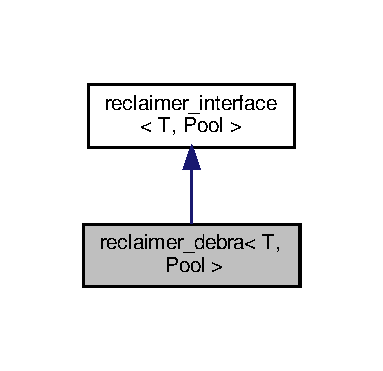
\includegraphics[width=184pt]{classreclaimer__debra__inherit__graph}
\end{center}
\end{figure}


Collaboration diagram for reclaimer\+\_\+debra$<$ T, Pool $>$\+:
\nopagebreak
\begin{figure}[H]
\begin{center}
\leavevmode
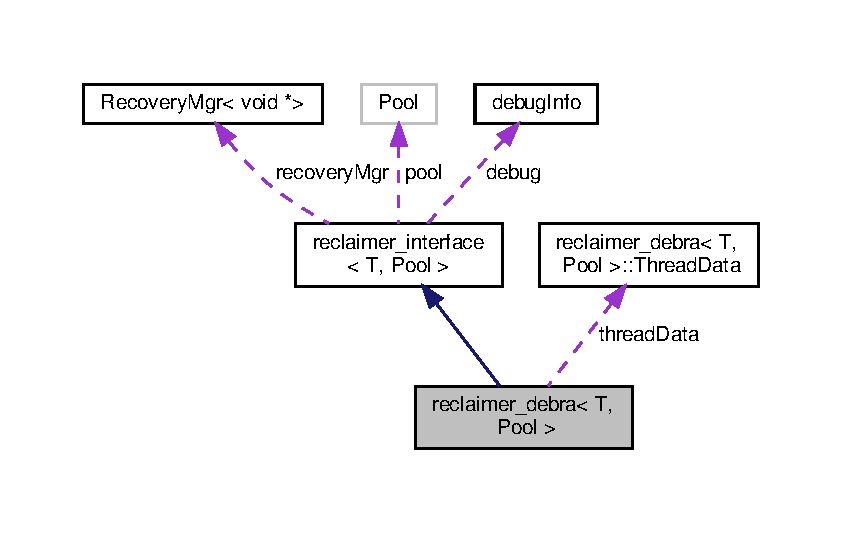
\includegraphics[width=350pt]{classreclaimer__debra__coll__graph}
\end{center}
\end{figure}
\subsection*{Classes}
\begin{DoxyCompactItemize}
\item 
class \hyperlink{classreclaimer__debra_1_1BagRotator}{Bag\+Rotator}
\item 
class \hyperlink{classreclaimer__debra_1_1BagRotator_3_01First_00_01Rest_8_8_8_01_4}{Bag\+Rotator$<$ First, Rest... $>$}
\item 
struct \hyperlink{structreclaimer__debra_1_1rebind}{rebind}
\item 
struct \hyperlink{structreclaimer__debra_1_1rebind2}{rebind2}
\item 
class \hyperlink{classreclaimer__debra_1_1ThreadData}{Thread\+Data}
\end{DoxyCompactItemize}
\subsection*{Public Member Functions}
\begin{DoxyCompactItemize}
\item 
void \hyperlink{classreclaimer__debra_a5805415266e40f98b9fb4b403bf6552f}{get\+Safe\+Blockbags} (const int \hyperlink{microbench_2main_8cpp_a9ca9869868fe7e7a38a921cc7de4103f}{tid}, \hyperlink{classblockbag}{blockbag}$<$ T $>$ $\ast$$\ast$bags)
\item 
long long \hyperlink{classreclaimer__debra_a1f38d639ddc7801216d7add73d9e422b}{get\+Size\+In\+Nodes} ()
\item 
std\+::string \hyperlink{classreclaimer__debra_a36fe4dd91c4ffcf3dddd2f2660b03880}{get\+Size\+String} ()
\item 
std\+::string \hyperlink{classreclaimer__debra_a34e1d02bd691d3f889c38aa2c026ebbc}{get\+Details\+String} ()
\item 
bool \hyperlink{classreclaimer__debra_a687fe55221cbbd2b19210b24839e77ca}{is\+Quiescent} (const int \hyperlink{microbench_2main_8cpp_a9ca9869868fe7e7a38a921cc7de4103f}{tid})
\item 
void \hyperlink{classreclaimer__debra_a144015f870cce9bd1edbf95e109875ae}{rotate\+Epoch\+Bags} (const int \hyperlink{microbench_2main_8cpp_a9ca9869868fe7e7a38a921cc7de4103f}{tid})
\item 
{\footnotesize template$<$typename First , typename... Rest$>$ }\\bool \hyperlink{classreclaimer__debra_a354ecd5812c2521c68b82cb59b2529a5}{start\+Op} (const int \hyperlink{microbench_2main_8cpp_a9ca9869868fe7e7a38a921cc7de4103f}{tid}, void $\ast$const $\ast$const reclaimers, const int num\+Reclaimers, const bool read\+Only=false)
\item 
void \hyperlink{classreclaimer__debra_a668ee2af696ff2a3e84944ca9284014f}{end\+Op} (const int \hyperlink{microbench_2main_8cpp_a9ca9869868fe7e7a38a921cc7de4103f}{tid})
\item 
void \hyperlink{classreclaimer__debra_a146fa88ad65ef5a05d253ecb7281c698}{retire} (const int \hyperlink{microbench_2main_8cpp_a9ca9869868fe7e7a38a921cc7de4103f}{tid}, T $\ast$p)
\item 
void \hyperlink{classreclaimer__debra_a4e09296726d5118763f6a81868391e3b}{debug\+Print\+Status} (const int \hyperlink{microbench_2main_8cpp_a9ca9869868fe7e7a38a921cc7de4103f}{tid})
\item 
void \hyperlink{classreclaimer__debra_a5f6c09cd8120fba870b9162dc1b4232a}{init\+Thread} (const int \hyperlink{microbench_2main_8cpp_a9ca9869868fe7e7a38a921cc7de4103f}{tid})
\item 
void \hyperlink{classreclaimer__debra_aeaa0321be93b27059850fc17d7cc27c8}{deinit\+Thread} (const int \hyperlink{microbench_2main_8cpp_a9ca9869868fe7e7a38a921cc7de4103f}{tid})
\item 
\hyperlink{classreclaimer__debra_ac779977388bdb370d043086df041082c}{reclaimer\+\_\+debra} (const int \hyperlink{testing_8cpp_aa085812188e21ede75351d88b9b2c30d}{num\+Processes}, Pool $\ast$\+\_\+pool, \hyperlink{classdebugInfo}{debug\+Info} $\ast$const \+\_\+debug, \hyperlink{classRecoveryMgr}{Recovery\+Mgr}$<$ void $\ast$$>$ $\ast$const \+\_\+recovery\+Mgr=N\+U\+LL)
\item 
\hyperlink{classreclaimer__debra_a9cf18da9413262075c4f4dfdaa9eac6d}{$\sim$reclaimer\+\_\+debra} ()
\end{DoxyCompactItemize}
\subsection*{Static Public Member Functions}
\begin{DoxyCompactItemize}
\item 
static bool \hyperlink{classreclaimer__debra_a5941d65b7837fece5a5c31a08bf4b964}{quiescence\+Is\+Per\+Record\+Type} ()
\item 
static bool \hyperlink{classreclaimer__debra_ad2d948e24b18e93187576c00d0f5ce4d}{is\+Protected} (const int \hyperlink{microbench_2main_8cpp_a9ca9869868fe7e7a38a921cc7de4103f}{tid}, T $\ast$const obj)
\item 
static bool \hyperlink{classreclaimer__debra_a318c2e48b9fd638b37a3faaa2bdec334}{is\+Q\+Protected} (const int \hyperlink{microbench_2main_8cpp_a9ca9869868fe7e7a38a921cc7de4103f}{tid}, T $\ast$const obj)
\item 
static bool \hyperlink{classreclaimer__debra_abfaa37584aefd85c5d4e3cba79e6d50c}{protect} (const int \hyperlink{microbench_2main_8cpp_a9ca9869868fe7e7a38a921cc7de4103f}{tid}, T $\ast$const obj, \hyperlink{globals_8h_a57f5c0d40b156d7d996492fb2f16e3cd}{Callback\+Type} not\+Retired\+Callback, \hyperlink{globals_8h_a3de64ef48066ac6430631c8b81a15345}{Callback\+Arg} callback\+Arg, bool memory\+Barrier=true)
\item 
static void \hyperlink{classreclaimer__debra_a8dd097decc268366c947354231fac75d}{unprotect} (const int \hyperlink{microbench_2main_8cpp_a9ca9869868fe7e7a38a921cc7de4103f}{tid}, T $\ast$const obj)
\item 
static bool \hyperlink{classreclaimer__debra_a24d0ee36a77ccf91e6923c2c535e26eb}{q\+Protect} (const int \hyperlink{microbench_2main_8cpp_a9ca9869868fe7e7a38a921cc7de4103f}{tid}, T $\ast$const obj, \hyperlink{globals_8h_a57f5c0d40b156d7d996492fb2f16e3cd}{Callback\+Type} not\+Retired\+Callback, \hyperlink{globals_8h_a3de64ef48066ac6430631c8b81a15345}{Callback\+Arg} callback\+Arg, bool memory\+Barrier=true)
\item 
static void \hyperlink{classreclaimer__debra_a16b1929a93855ec60712cb0b7e445280}{q\+Unprotect\+All} (const int \hyperlink{microbench_2main_8cpp_a9ca9869868fe7e7a38a921cc7de4103f}{tid})
\item 
static bool \hyperlink{classreclaimer__debra_aa525ada55c6d16c4e0134e48094d3ec6}{should\+Help} ()
\end{DoxyCompactItemize}
\subsection*{Protected Attributes}
\begin{DoxyCompactItemize}
\item 
\hyperlink{classreclaimer__debra_aabc191ce8b7b216157e1ab39f17f8471}{P\+AD}
\item 
\hyperlink{classreclaimer__debra_1_1ThreadData}{Thread\+Data} \hyperlink{classreclaimer__debra_a39e06df091da9fc001bf6a0d90ef070c}{thread\+Data} \mbox{[}\hyperlink{plaf_8h_ac1585a3455dd3e33e877e588be9e466b}{M\+A\+X\+\_\+\+T\+H\+R\+E\+A\+D\+S\+\_\+\+P\+O\+W2}\mbox{]}
\item 
volatile long \hyperlink{classreclaimer__debra_a5d09e238ce1873d0a812fc65c2fe46aa}{epoch}
\end{DoxyCompactItemize}
\subsection*{Additional Inherited Members}


\subsection{Detailed Description}
\subsubsection*{template$<$typename T = void, class Pool = pool\+\_\+interface$<$\+T$>$$>$\newline
class reclaimer\+\_\+debra$<$ T, Pool $>$}

C++ record manager implementation (P\+O\+DC 2015) by Trevor Brown.

Copyright (C) 2015 Trevor Brown 

\subsection{Constructor \& Destructor Documentation}
\mbox{\Hypertarget{classreclaimer__debra_ac779977388bdb370d043086df041082c}\label{classreclaimer__debra_ac779977388bdb370d043086df041082c}} 
\index{reclaimer\+\_\+debra@{reclaimer\+\_\+debra}!reclaimer\+\_\+debra@{reclaimer\+\_\+debra}}
\index{reclaimer\+\_\+debra@{reclaimer\+\_\+debra}!reclaimer\+\_\+debra@{reclaimer\+\_\+debra}}
\subsubsection{\texorpdfstring{reclaimer\+\_\+debra()}{reclaimer\_debra()}}
{\footnotesize\ttfamily template$<$typename T  = void, class Pool  = pool\+\_\+interface$<$\+T$>$$>$ \\
\hyperlink{classreclaimer__debra}{reclaimer\+\_\+debra}$<$ T, Pool $>$\+::\hyperlink{classreclaimer__debra}{reclaimer\+\_\+debra} (\begin{DoxyParamCaption}\item[{const int}]{num\+Processes,  }\item[{Pool $\ast$}]{\+\_\+pool,  }\item[{\hyperlink{classdebugInfo}{debug\+Info} $\ast$const}]{\+\_\+debug,  }\item[{\hyperlink{classRecoveryMgr}{Recovery\+Mgr}$<$ void $\ast$$>$ $\ast$const}]{\+\_\+recovery\+Mgr = {\ttfamily NULL} }\end{DoxyParamCaption})\hspace{0.3cm}{\ttfamily [inline]}}

\mbox{\Hypertarget{classreclaimer__debra_a9cf18da9413262075c4f4dfdaa9eac6d}\label{classreclaimer__debra_a9cf18da9413262075c4f4dfdaa9eac6d}} 
\index{reclaimer\+\_\+debra@{reclaimer\+\_\+debra}!````~reclaimer\+\_\+debra@{$\sim$reclaimer\+\_\+debra}}
\index{````~reclaimer\+\_\+debra@{$\sim$reclaimer\+\_\+debra}!reclaimer\+\_\+debra@{reclaimer\+\_\+debra}}
\subsubsection{\texorpdfstring{$\sim$reclaimer\+\_\+debra()}{~reclaimer\_debra()}}
{\footnotesize\ttfamily template$<$typename T  = void, class Pool  = pool\+\_\+interface$<$\+T$>$$>$ \\
\hyperlink{classreclaimer__debra}{reclaimer\+\_\+debra}$<$ T, Pool $>$\+::$\sim$\hyperlink{classreclaimer__debra}{reclaimer\+\_\+debra} (\begin{DoxyParamCaption}{ }\end{DoxyParamCaption})\hspace{0.3cm}{\ttfamily [inline]}}



\subsection{Member Function Documentation}
\mbox{\Hypertarget{classreclaimer__debra_a4e09296726d5118763f6a81868391e3b}\label{classreclaimer__debra_a4e09296726d5118763f6a81868391e3b}} 
\index{reclaimer\+\_\+debra@{reclaimer\+\_\+debra}!debug\+Print\+Status@{debug\+Print\+Status}}
\index{debug\+Print\+Status@{debug\+Print\+Status}!reclaimer\+\_\+debra@{reclaimer\+\_\+debra}}
\subsubsection{\texorpdfstring{debug\+Print\+Status()}{debugPrintStatus()}}
{\footnotesize\ttfamily template$<$typename T  = void, class Pool  = pool\+\_\+interface$<$\+T$>$$>$ \\
void \hyperlink{classreclaimer__debra}{reclaimer\+\_\+debra}$<$ T, Pool $>$\+::debug\+Print\+Status (\begin{DoxyParamCaption}\item[{const int}]{tid }\end{DoxyParamCaption})\hspace{0.3cm}{\ttfamily [inline]}}

\mbox{\Hypertarget{classreclaimer__debra_aeaa0321be93b27059850fc17d7cc27c8}\label{classreclaimer__debra_aeaa0321be93b27059850fc17d7cc27c8}} 
\index{reclaimer\+\_\+debra@{reclaimer\+\_\+debra}!deinit\+Thread@{deinit\+Thread}}
\index{deinit\+Thread@{deinit\+Thread}!reclaimer\+\_\+debra@{reclaimer\+\_\+debra}}
\subsubsection{\texorpdfstring{deinit\+Thread()}{deinitThread()}}
{\footnotesize\ttfamily template$<$typename T  = void, class Pool  = pool\+\_\+interface$<$\+T$>$$>$ \\
void \hyperlink{classreclaimer__debra}{reclaimer\+\_\+debra}$<$ T, Pool $>$\+::deinit\+Thread (\begin{DoxyParamCaption}\item[{const int}]{tid }\end{DoxyParamCaption})\hspace{0.3cm}{\ttfamily [inline]}}

\mbox{\Hypertarget{classreclaimer__debra_a668ee2af696ff2a3e84944ca9284014f}\label{classreclaimer__debra_a668ee2af696ff2a3e84944ca9284014f}} 
\index{reclaimer\+\_\+debra@{reclaimer\+\_\+debra}!end\+Op@{end\+Op}}
\index{end\+Op@{end\+Op}!reclaimer\+\_\+debra@{reclaimer\+\_\+debra}}
\subsubsection{\texorpdfstring{end\+Op()}{endOp()}}
{\footnotesize\ttfamily template$<$typename T  = void, class Pool  = pool\+\_\+interface$<$\+T$>$$>$ \\
void \hyperlink{classreclaimer__debra}{reclaimer\+\_\+debra}$<$ T, Pool $>$\+::end\+Op (\begin{DoxyParamCaption}\item[{const int}]{tid }\end{DoxyParamCaption})\hspace{0.3cm}{\ttfamily [inline]}}

\mbox{\Hypertarget{classreclaimer__debra_a34e1d02bd691d3f889c38aa2c026ebbc}\label{classreclaimer__debra_a34e1d02bd691d3f889c38aa2c026ebbc}} 
\index{reclaimer\+\_\+debra@{reclaimer\+\_\+debra}!get\+Details\+String@{get\+Details\+String}}
\index{get\+Details\+String@{get\+Details\+String}!reclaimer\+\_\+debra@{reclaimer\+\_\+debra}}
\subsubsection{\texorpdfstring{get\+Details\+String()}{getDetailsString()}}
{\footnotesize\ttfamily template$<$typename T  = void, class Pool  = pool\+\_\+interface$<$\+T$>$$>$ \\
std\+::string \hyperlink{classreclaimer__debra}{reclaimer\+\_\+debra}$<$ T, Pool $>$\+::get\+Details\+String (\begin{DoxyParamCaption}{ }\end{DoxyParamCaption})\hspace{0.3cm}{\ttfamily [inline]}}

\mbox{\Hypertarget{classreclaimer__debra_a5805415266e40f98b9fb4b403bf6552f}\label{classreclaimer__debra_a5805415266e40f98b9fb4b403bf6552f}} 
\index{reclaimer\+\_\+debra@{reclaimer\+\_\+debra}!get\+Safe\+Blockbags@{get\+Safe\+Blockbags}}
\index{get\+Safe\+Blockbags@{get\+Safe\+Blockbags}!reclaimer\+\_\+debra@{reclaimer\+\_\+debra}}
\subsubsection{\texorpdfstring{get\+Safe\+Blockbags()}{getSafeBlockbags()}}
{\footnotesize\ttfamily template$<$typename T  = void, class Pool  = pool\+\_\+interface$<$\+T$>$$>$ \\
void \hyperlink{classreclaimer__debra}{reclaimer\+\_\+debra}$<$ T, Pool $>$\+::get\+Safe\+Blockbags (\begin{DoxyParamCaption}\item[{const int}]{tid,  }\item[{\hyperlink{classblockbag}{blockbag}$<$ T $>$ $\ast$$\ast$}]{bags }\end{DoxyParamCaption})\hspace{0.3cm}{\ttfamily [inline]}}

\mbox{\Hypertarget{classreclaimer__debra_a1f38d639ddc7801216d7add73d9e422b}\label{classreclaimer__debra_a1f38d639ddc7801216d7add73d9e422b}} 
\index{reclaimer\+\_\+debra@{reclaimer\+\_\+debra}!get\+Size\+In\+Nodes@{get\+Size\+In\+Nodes}}
\index{get\+Size\+In\+Nodes@{get\+Size\+In\+Nodes}!reclaimer\+\_\+debra@{reclaimer\+\_\+debra}}
\subsubsection{\texorpdfstring{get\+Size\+In\+Nodes()}{getSizeInNodes()}}
{\footnotesize\ttfamily template$<$typename T  = void, class Pool  = pool\+\_\+interface$<$\+T$>$$>$ \\
long long \hyperlink{classreclaimer__debra}{reclaimer\+\_\+debra}$<$ T, Pool $>$\+::get\+Size\+In\+Nodes (\begin{DoxyParamCaption}{ }\end{DoxyParamCaption})\hspace{0.3cm}{\ttfamily [inline]}}

\mbox{\Hypertarget{classreclaimer__debra_a36fe4dd91c4ffcf3dddd2f2660b03880}\label{classreclaimer__debra_a36fe4dd91c4ffcf3dddd2f2660b03880}} 
\index{reclaimer\+\_\+debra@{reclaimer\+\_\+debra}!get\+Size\+String@{get\+Size\+String}}
\index{get\+Size\+String@{get\+Size\+String}!reclaimer\+\_\+debra@{reclaimer\+\_\+debra}}
\subsubsection{\texorpdfstring{get\+Size\+String()}{getSizeString()}}
{\footnotesize\ttfamily template$<$typename T  = void, class Pool  = pool\+\_\+interface$<$\+T$>$$>$ \\
std\+::string \hyperlink{classreclaimer__debra}{reclaimer\+\_\+debra}$<$ T, Pool $>$\+::get\+Size\+String (\begin{DoxyParamCaption}{ }\end{DoxyParamCaption})\hspace{0.3cm}{\ttfamily [inline]}}

\mbox{\Hypertarget{classreclaimer__debra_a5f6c09cd8120fba870b9162dc1b4232a}\label{classreclaimer__debra_a5f6c09cd8120fba870b9162dc1b4232a}} 
\index{reclaimer\+\_\+debra@{reclaimer\+\_\+debra}!init\+Thread@{init\+Thread}}
\index{init\+Thread@{init\+Thread}!reclaimer\+\_\+debra@{reclaimer\+\_\+debra}}
\subsubsection{\texorpdfstring{init\+Thread()}{initThread()}}
{\footnotesize\ttfamily template$<$typename T  = void, class Pool  = pool\+\_\+interface$<$\+T$>$$>$ \\
void \hyperlink{classreclaimer__debra}{reclaimer\+\_\+debra}$<$ T, Pool $>$\+::init\+Thread (\begin{DoxyParamCaption}\item[{const int}]{tid }\end{DoxyParamCaption})\hspace{0.3cm}{\ttfamily [inline]}}

\mbox{\Hypertarget{classreclaimer__debra_ad2d948e24b18e93187576c00d0f5ce4d}\label{classreclaimer__debra_ad2d948e24b18e93187576c00d0f5ce4d}} 
\index{reclaimer\+\_\+debra@{reclaimer\+\_\+debra}!is\+Protected@{is\+Protected}}
\index{is\+Protected@{is\+Protected}!reclaimer\+\_\+debra@{reclaimer\+\_\+debra}}
\subsubsection{\texorpdfstring{is\+Protected()}{isProtected()}}
{\footnotesize\ttfamily template$<$typename T  = void, class Pool  = pool\+\_\+interface$<$\+T$>$$>$ \\
static bool \hyperlink{classreclaimer__debra}{reclaimer\+\_\+debra}$<$ T, Pool $>$\+::is\+Protected (\begin{DoxyParamCaption}\item[{const int}]{tid,  }\item[{T $\ast$const}]{obj }\end{DoxyParamCaption})\hspace{0.3cm}{\ttfamily [inline]}, {\ttfamily [static]}}

\mbox{\Hypertarget{classreclaimer__debra_a318c2e48b9fd638b37a3faaa2bdec334}\label{classreclaimer__debra_a318c2e48b9fd638b37a3faaa2bdec334}} 
\index{reclaimer\+\_\+debra@{reclaimer\+\_\+debra}!is\+Q\+Protected@{is\+Q\+Protected}}
\index{is\+Q\+Protected@{is\+Q\+Protected}!reclaimer\+\_\+debra@{reclaimer\+\_\+debra}}
\subsubsection{\texorpdfstring{is\+Q\+Protected()}{isQProtected()}}
{\footnotesize\ttfamily template$<$typename T  = void, class Pool  = pool\+\_\+interface$<$\+T$>$$>$ \\
static bool \hyperlink{classreclaimer__debra}{reclaimer\+\_\+debra}$<$ T, Pool $>$\+::is\+Q\+Protected (\begin{DoxyParamCaption}\item[{const int}]{tid,  }\item[{T $\ast$const}]{obj }\end{DoxyParamCaption})\hspace{0.3cm}{\ttfamily [inline]}, {\ttfamily [static]}}

\mbox{\Hypertarget{classreclaimer__debra_a687fe55221cbbd2b19210b24839e77ca}\label{classreclaimer__debra_a687fe55221cbbd2b19210b24839e77ca}} 
\index{reclaimer\+\_\+debra@{reclaimer\+\_\+debra}!is\+Quiescent@{is\+Quiescent}}
\index{is\+Quiescent@{is\+Quiescent}!reclaimer\+\_\+debra@{reclaimer\+\_\+debra}}
\subsubsection{\texorpdfstring{is\+Quiescent()}{isQuiescent()}}
{\footnotesize\ttfamily template$<$typename T  = void, class Pool  = pool\+\_\+interface$<$\+T$>$$>$ \\
bool \hyperlink{classreclaimer__debra}{reclaimer\+\_\+debra}$<$ T, Pool $>$\+::is\+Quiescent (\begin{DoxyParamCaption}\item[{const int}]{tid }\end{DoxyParamCaption})\hspace{0.3cm}{\ttfamily [inline]}}

\mbox{\Hypertarget{classreclaimer__debra_abfaa37584aefd85c5d4e3cba79e6d50c}\label{classreclaimer__debra_abfaa37584aefd85c5d4e3cba79e6d50c}} 
\index{reclaimer\+\_\+debra@{reclaimer\+\_\+debra}!protect@{protect}}
\index{protect@{protect}!reclaimer\+\_\+debra@{reclaimer\+\_\+debra}}
\subsubsection{\texorpdfstring{protect()}{protect()}}
{\footnotesize\ttfamily template$<$typename T  = void, class Pool  = pool\+\_\+interface$<$\+T$>$$>$ \\
static bool \hyperlink{classreclaimer__debra}{reclaimer\+\_\+debra}$<$ T, Pool $>$\+::protect (\begin{DoxyParamCaption}\item[{const int}]{tid,  }\item[{T $\ast$const}]{obj,  }\item[{\hyperlink{globals_8h_a57f5c0d40b156d7d996492fb2f16e3cd}{Callback\+Type}}]{not\+Retired\+Callback,  }\item[{\hyperlink{globals_8h_a3de64ef48066ac6430631c8b81a15345}{Callback\+Arg}}]{callback\+Arg,  }\item[{bool}]{memory\+Barrier = {\ttfamily true} }\end{DoxyParamCaption})\hspace{0.3cm}{\ttfamily [inline]}, {\ttfamily [static]}}

\mbox{\Hypertarget{classreclaimer__debra_a24d0ee36a77ccf91e6923c2c535e26eb}\label{classreclaimer__debra_a24d0ee36a77ccf91e6923c2c535e26eb}} 
\index{reclaimer\+\_\+debra@{reclaimer\+\_\+debra}!q\+Protect@{q\+Protect}}
\index{q\+Protect@{q\+Protect}!reclaimer\+\_\+debra@{reclaimer\+\_\+debra}}
\subsubsection{\texorpdfstring{q\+Protect()}{qProtect()}}
{\footnotesize\ttfamily template$<$typename T  = void, class Pool  = pool\+\_\+interface$<$\+T$>$$>$ \\
static bool \hyperlink{classreclaimer__debra}{reclaimer\+\_\+debra}$<$ T, Pool $>$\+::q\+Protect (\begin{DoxyParamCaption}\item[{const int}]{tid,  }\item[{T $\ast$const}]{obj,  }\item[{\hyperlink{globals_8h_a57f5c0d40b156d7d996492fb2f16e3cd}{Callback\+Type}}]{not\+Retired\+Callback,  }\item[{\hyperlink{globals_8h_a3de64ef48066ac6430631c8b81a15345}{Callback\+Arg}}]{callback\+Arg,  }\item[{bool}]{memory\+Barrier = {\ttfamily true} }\end{DoxyParamCaption})\hspace{0.3cm}{\ttfamily [inline]}, {\ttfamily [static]}}

\mbox{\Hypertarget{classreclaimer__debra_a5941d65b7837fece5a5c31a08bf4b964}\label{classreclaimer__debra_a5941d65b7837fece5a5c31a08bf4b964}} 
\index{reclaimer\+\_\+debra@{reclaimer\+\_\+debra}!quiescence\+Is\+Per\+Record\+Type@{quiescence\+Is\+Per\+Record\+Type}}
\index{quiescence\+Is\+Per\+Record\+Type@{quiescence\+Is\+Per\+Record\+Type}!reclaimer\+\_\+debra@{reclaimer\+\_\+debra}}
\subsubsection{\texorpdfstring{quiescence\+Is\+Per\+Record\+Type()}{quiescenceIsPerRecordType()}}
{\footnotesize\ttfamily template$<$typename T  = void, class Pool  = pool\+\_\+interface$<$\+T$>$$>$ \\
static bool \hyperlink{classreclaimer__debra}{reclaimer\+\_\+debra}$<$ T, Pool $>$\+::quiescence\+Is\+Per\+Record\+Type (\begin{DoxyParamCaption}{ }\end{DoxyParamCaption})\hspace{0.3cm}{\ttfamily [inline]}, {\ttfamily [static]}}

\mbox{\Hypertarget{classreclaimer__debra_a16b1929a93855ec60712cb0b7e445280}\label{classreclaimer__debra_a16b1929a93855ec60712cb0b7e445280}} 
\index{reclaimer\+\_\+debra@{reclaimer\+\_\+debra}!q\+Unprotect\+All@{q\+Unprotect\+All}}
\index{q\+Unprotect\+All@{q\+Unprotect\+All}!reclaimer\+\_\+debra@{reclaimer\+\_\+debra}}
\subsubsection{\texorpdfstring{q\+Unprotect\+All()}{qUnprotectAll()}}
{\footnotesize\ttfamily template$<$typename T  = void, class Pool  = pool\+\_\+interface$<$\+T$>$$>$ \\
static void \hyperlink{classreclaimer__debra}{reclaimer\+\_\+debra}$<$ T, Pool $>$\+::q\+Unprotect\+All (\begin{DoxyParamCaption}\item[{const int}]{tid }\end{DoxyParamCaption})\hspace{0.3cm}{\ttfamily [inline]}, {\ttfamily [static]}}

\mbox{\Hypertarget{classreclaimer__debra_a146fa88ad65ef5a05d253ecb7281c698}\label{classreclaimer__debra_a146fa88ad65ef5a05d253ecb7281c698}} 
\index{reclaimer\+\_\+debra@{reclaimer\+\_\+debra}!retire@{retire}}
\index{retire@{retire}!reclaimer\+\_\+debra@{reclaimer\+\_\+debra}}
\subsubsection{\texorpdfstring{retire()}{retire()}}
{\footnotesize\ttfamily template$<$typename T  = void, class Pool  = pool\+\_\+interface$<$\+T$>$$>$ \\
void \hyperlink{classreclaimer__debra}{reclaimer\+\_\+debra}$<$ T, Pool $>$\+::retire (\begin{DoxyParamCaption}\item[{const int}]{tid,  }\item[{T $\ast$}]{p }\end{DoxyParamCaption})\hspace{0.3cm}{\ttfamily [inline]}}

\mbox{\Hypertarget{classreclaimer__debra_a144015f870cce9bd1edbf95e109875ae}\label{classreclaimer__debra_a144015f870cce9bd1edbf95e109875ae}} 
\index{reclaimer\+\_\+debra@{reclaimer\+\_\+debra}!rotate\+Epoch\+Bags@{rotate\+Epoch\+Bags}}
\index{rotate\+Epoch\+Bags@{rotate\+Epoch\+Bags}!reclaimer\+\_\+debra@{reclaimer\+\_\+debra}}
\subsubsection{\texorpdfstring{rotate\+Epoch\+Bags()}{rotateEpochBags()}}
{\footnotesize\ttfamily template$<$typename T  = void, class Pool  = pool\+\_\+interface$<$\+T$>$$>$ \\
void \hyperlink{classreclaimer__debra}{reclaimer\+\_\+debra}$<$ T, Pool $>$\+::rotate\+Epoch\+Bags (\begin{DoxyParamCaption}\item[{const int}]{tid }\end{DoxyParamCaption})\hspace{0.3cm}{\ttfamily [inline]}}

\mbox{\Hypertarget{classreclaimer__debra_aa525ada55c6d16c4e0134e48094d3ec6}\label{classreclaimer__debra_aa525ada55c6d16c4e0134e48094d3ec6}} 
\index{reclaimer\+\_\+debra@{reclaimer\+\_\+debra}!should\+Help@{should\+Help}}
\index{should\+Help@{should\+Help}!reclaimer\+\_\+debra@{reclaimer\+\_\+debra}}
\subsubsection{\texorpdfstring{should\+Help()}{shouldHelp()}}
{\footnotesize\ttfamily template$<$typename T  = void, class Pool  = pool\+\_\+interface$<$\+T$>$$>$ \\
static bool \hyperlink{classreclaimer__debra}{reclaimer\+\_\+debra}$<$ T, Pool $>$\+::should\+Help (\begin{DoxyParamCaption}{ }\end{DoxyParamCaption})\hspace{0.3cm}{\ttfamily [inline]}, {\ttfamily [static]}}

\mbox{\Hypertarget{classreclaimer__debra_a354ecd5812c2521c68b82cb59b2529a5}\label{classreclaimer__debra_a354ecd5812c2521c68b82cb59b2529a5}} 
\index{reclaimer\+\_\+debra@{reclaimer\+\_\+debra}!start\+Op@{start\+Op}}
\index{start\+Op@{start\+Op}!reclaimer\+\_\+debra@{reclaimer\+\_\+debra}}
\subsubsection{\texorpdfstring{start\+Op()}{startOp()}}
{\footnotesize\ttfamily template$<$typename T  = void, class Pool  = pool\+\_\+interface$<$\+T$>$$>$ \\
template$<$typename First , typename... Rest$>$ \\
bool \hyperlink{classreclaimer__debra}{reclaimer\+\_\+debra}$<$ T, Pool $>$\+::start\+Op (\begin{DoxyParamCaption}\item[{const int}]{tid,  }\item[{void $\ast$const $\ast$const}]{reclaimers,  }\item[{const int}]{num\+Reclaimers,  }\item[{const bool}]{read\+Only = {\ttfamily false} }\end{DoxyParamCaption})\hspace{0.3cm}{\ttfamily [inline]}}

\mbox{\Hypertarget{classreclaimer__debra_a8dd097decc268366c947354231fac75d}\label{classreclaimer__debra_a8dd097decc268366c947354231fac75d}} 
\index{reclaimer\+\_\+debra@{reclaimer\+\_\+debra}!unprotect@{unprotect}}
\index{unprotect@{unprotect}!reclaimer\+\_\+debra@{reclaimer\+\_\+debra}}
\subsubsection{\texorpdfstring{unprotect()}{unprotect()}}
{\footnotesize\ttfamily template$<$typename T  = void, class Pool  = pool\+\_\+interface$<$\+T$>$$>$ \\
static void \hyperlink{classreclaimer__debra}{reclaimer\+\_\+debra}$<$ T, Pool $>$\+::unprotect (\begin{DoxyParamCaption}\item[{const int}]{tid,  }\item[{T $\ast$const}]{obj }\end{DoxyParamCaption})\hspace{0.3cm}{\ttfamily [inline]}, {\ttfamily [static]}}



\subsection{Member Data Documentation}
\mbox{\Hypertarget{classreclaimer__debra_a5d09e238ce1873d0a812fc65c2fe46aa}\label{classreclaimer__debra_a5d09e238ce1873d0a812fc65c2fe46aa}} 
\index{reclaimer\+\_\+debra@{reclaimer\+\_\+debra}!epoch@{epoch}}
\index{epoch@{epoch}!reclaimer\+\_\+debra@{reclaimer\+\_\+debra}}
\subsubsection{\texorpdfstring{epoch}{epoch}}
{\footnotesize\ttfamily template$<$typename T  = void, class Pool  = pool\+\_\+interface$<$\+T$>$$>$ \\
volatile long \hyperlink{classreclaimer__debra}{reclaimer\+\_\+debra}$<$ T, Pool $>$\+::epoch\hspace{0.3cm}{\ttfamily [protected]}}

\mbox{\Hypertarget{classreclaimer__debra_aabc191ce8b7b216157e1ab39f17f8471}\label{classreclaimer__debra_aabc191ce8b7b216157e1ab39f17f8471}} 
\index{reclaimer\+\_\+debra@{reclaimer\+\_\+debra}!P\+AD@{P\+AD}}
\index{P\+AD@{P\+AD}!reclaimer\+\_\+debra@{reclaimer\+\_\+debra}}
\subsubsection{\texorpdfstring{P\+AD}{PAD}}
{\footnotesize\ttfamily template$<$typename T  = void, class Pool  = pool\+\_\+interface$<$\+T$>$$>$ \\
\hyperlink{classreclaimer__debra}{reclaimer\+\_\+debra}$<$ T, Pool $>$\+::P\+AD\hspace{0.3cm}{\ttfamily [protected]}}

\mbox{\Hypertarget{classreclaimer__debra_a39e06df091da9fc001bf6a0d90ef070c}\label{classreclaimer__debra_a39e06df091da9fc001bf6a0d90ef070c}} 
\index{reclaimer\+\_\+debra@{reclaimer\+\_\+debra}!thread\+Data@{thread\+Data}}
\index{thread\+Data@{thread\+Data}!reclaimer\+\_\+debra@{reclaimer\+\_\+debra}}
\subsubsection{\texorpdfstring{thread\+Data}{threadData}}
{\footnotesize\ttfamily template$<$typename T  = void, class Pool  = pool\+\_\+interface$<$\+T$>$$>$ \\
\hyperlink{classreclaimer__debra_1_1ThreadData}{Thread\+Data} \hyperlink{classreclaimer__debra}{reclaimer\+\_\+debra}$<$ T, Pool $>$\+::thread\+Data\mbox{[}\hyperlink{plaf_8h_ac1585a3455dd3e33e877e588be9e466b}{M\+A\+X\+\_\+\+T\+H\+R\+E\+A\+D\+S\+\_\+\+P\+O\+W2}\mbox{]}\hspace{0.3cm}{\ttfamily [protected]}}



The documentation for this class was generated from the following file\+:\begin{DoxyCompactItemize}
\item 
common/recordmgr/\hyperlink{reclaimer__debra_8h}{reclaimer\+\_\+debra.\+h}\end{DoxyCompactItemize}

\hypertarget{classreclaimer__debracap}{}\section{reclaimer\+\_\+debracap$<$ T, Pool $>$ Class Template Reference}
\label{classreclaimer__debracap}\index{reclaimer\+\_\+debracap$<$ T, Pool $>$@{reclaimer\+\_\+debracap$<$ T, Pool $>$}}


{\ttfamily \#include $<$reclaimer\+\_\+debracap.\+h$>$}



Inheritance diagram for reclaimer\+\_\+debracap$<$ T, Pool $>$\+:
\nopagebreak
\begin{figure}[H]
\begin{center}
\leavevmode
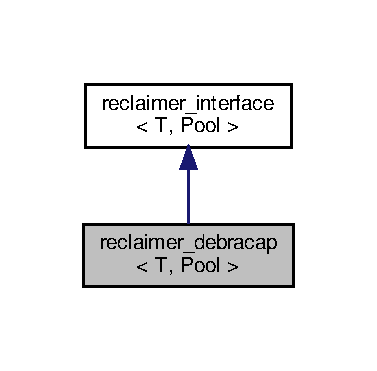
\includegraphics[width=181pt]{classreclaimer__debracap__inherit__graph}
\end{center}
\end{figure}


Collaboration diagram for reclaimer\+\_\+debracap$<$ T, Pool $>$\+:
\nopagebreak
\begin{figure}[H]
\begin{center}
\leavevmode
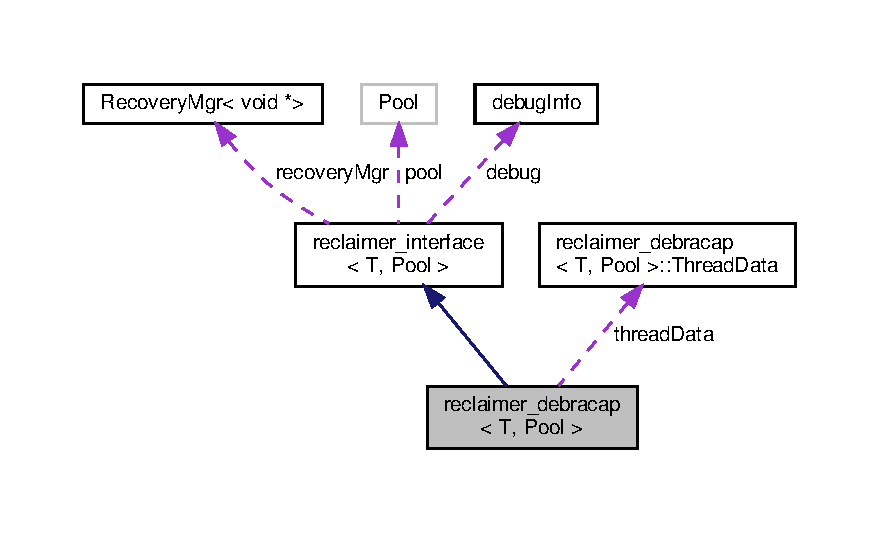
\includegraphics[width=350pt]{classreclaimer__debracap__coll__graph}
\end{center}
\end{figure}
\subsection*{Classes}
\begin{DoxyCompactItemize}
\item 
class \hyperlink{classreclaimer__debracap_1_1BagRotator}{Bag\+Rotator}
\item 
class \hyperlink{classreclaimer__debracap_1_1BagRotator_3_01First_00_01Rest_8_8_8_01_4}{Bag\+Rotator$<$ First, Rest... $>$}
\item 
struct \hyperlink{structreclaimer__debracap_1_1rebind}{rebind}
\item 
struct \hyperlink{structreclaimer__debracap_1_1rebind2}{rebind2}
\item 
class \hyperlink{classreclaimer__debracap_1_1ThreadData}{Thread\+Data}
\end{DoxyCompactItemize}
\subsection*{Public Member Functions}
\begin{DoxyCompactItemize}
\item 
void \hyperlink{classreclaimer__debracap_a4682c2d23e5b59f4e4e036865e903b3b}{get\+Safe\+Blockbags} (const int \hyperlink{microbench_2main_8cpp_a9ca9869868fe7e7a38a921cc7de4103f}{tid}, \hyperlink{classblockbag}{blockbag}$<$ T $>$ $\ast$$\ast$bags)
\item 
long long \hyperlink{classreclaimer__debracap_a2315cce188568d1b2e7b5809a943b7a6}{get\+Size\+In\+Nodes} ()
\item 
std\+::string \hyperlink{classreclaimer__debracap_ad005056c2b7740bb2172efeae2369434}{get\+Details\+String} ()
\item 
std\+::string \hyperlink{classreclaimer__debracap_adb2070ff175d8131d7da92820c5d2de7}{get\+Size\+String} ()
\item 
bool \hyperlink{classreclaimer__debracap_a7d248af33f59e0154df2bf21f7889bc8}{is\+Quiescent} (const int \hyperlink{microbench_2main_8cpp_a9ca9869868fe7e7a38a921cc7de4103f}{tid})
\item 
void \hyperlink{classreclaimer__debracap_a5304ffe3a8227e5b77275ded7a742d5d}{rotate\+Epoch\+Bags} (const int \hyperlink{microbench_2main_8cpp_a9ca9869868fe7e7a38a921cc7de4103f}{tid})
\item 
{\footnotesize template$<$typename First , typename... Rest$>$ }\\bool \hyperlink{classreclaimer__debracap_a2052d4c9d165157e85c75230a3a8e584}{start\+Op} (const int \hyperlink{microbench_2main_8cpp_a9ca9869868fe7e7a38a921cc7de4103f}{tid}, void $\ast$const $\ast$const reclaimers, const int num\+Reclaimers, const bool read\+Only=false)
\item 
void \hyperlink{classreclaimer__debracap_af290e3cb806e6b4a7325defc2311ad62}{end\+Op} (const int \hyperlink{microbench_2main_8cpp_a9ca9869868fe7e7a38a921cc7de4103f}{tid})
\item 
void \hyperlink{classreclaimer__debracap_acfe29401909be4a5a34bf4ba4978d90b}{retire} (const int \hyperlink{microbench_2main_8cpp_a9ca9869868fe7e7a38a921cc7de4103f}{tid}, T $\ast$p)
\item 
void \hyperlink{classreclaimer__debracap_a42e33db09c07092c58669f718a6d6776}{debug\+Print\+Status} (const int \hyperlink{microbench_2main_8cpp_a9ca9869868fe7e7a38a921cc7de4103f}{tid})
\item 
void \hyperlink{classreclaimer__debracap_a6574a166b572ccd201fdcaacf4afa907}{init\+Thread} (const int \hyperlink{microbench_2main_8cpp_a9ca9869868fe7e7a38a921cc7de4103f}{tid})
\item 
void \hyperlink{classreclaimer__debracap_a8b73562e6d000dd9445a08891d3a56ec}{deinit\+Thread} (const int \hyperlink{microbench_2main_8cpp_a9ca9869868fe7e7a38a921cc7de4103f}{tid})
\item 
\hyperlink{classreclaimer__debracap_a3528489fe624bf72f5b6ebae79279fd4}{reclaimer\+\_\+debracap} (const int \hyperlink{testing_8cpp_aa085812188e21ede75351d88b9b2c30d}{num\+Processes}, Pool $\ast$\+\_\+pool, \hyperlink{classdebugInfo}{debug\+Info} $\ast$const \+\_\+debug, \hyperlink{classRecoveryMgr}{Recovery\+Mgr}$<$ void $\ast$$>$ $\ast$const \+\_\+recovery\+Mgr=N\+U\+LL)
\item 
\hyperlink{classreclaimer__debracap_a9a4d64ab713bce63d26ce2e4e97302b7}{$\sim$reclaimer\+\_\+debracap} ()
\end{DoxyCompactItemize}
\subsection*{Static Public Member Functions}
\begin{DoxyCompactItemize}
\item 
static bool \hyperlink{classreclaimer__debracap_a1b4f8e3613dfeb9721395d3bdd4a3415}{quiescence\+Is\+Per\+Record\+Type} ()
\item 
static bool \hyperlink{classreclaimer__debracap_ae838602ad578a26512441a15dee0abcf}{is\+Protected} (const int \hyperlink{microbench_2main_8cpp_a9ca9869868fe7e7a38a921cc7de4103f}{tid}, T $\ast$const obj)
\item 
static bool \hyperlink{classreclaimer__debracap_a7b3ddb400b86fe1311c102bb4fcdea6a}{is\+Q\+Protected} (const int \hyperlink{microbench_2main_8cpp_a9ca9869868fe7e7a38a921cc7de4103f}{tid}, T $\ast$const obj)
\item 
static bool \hyperlink{classreclaimer__debracap_a282205dc0800fb9dc45e13233f20b413}{protect} (const int \hyperlink{microbench_2main_8cpp_a9ca9869868fe7e7a38a921cc7de4103f}{tid}, T $\ast$const obj, \hyperlink{globals_8h_a57f5c0d40b156d7d996492fb2f16e3cd}{Callback\+Type} not\+Retired\+Callback, \hyperlink{globals_8h_a3de64ef48066ac6430631c8b81a15345}{Callback\+Arg} callback\+Arg, bool memory\+Barrier=true)
\item 
static void \hyperlink{classreclaimer__debracap_a76838aa9f38af9c481a21e42e6014abc}{unprotect} (const int \hyperlink{microbench_2main_8cpp_a9ca9869868fe7e7a38a921cc7de4103f}{tid}, T $\ast$const obj)
\item 
static bool \hyperlink{classreclaimer__debracap_a26d500d9aa320c997b1424bc500de4dd}{q\+Protect} (const int \hyperlink{microbench_2main_8cpp_a9ca9869868fe7e7a38a921cc7de4103f}{tid}, T $\ast$const obj, \hyperlink{globals_8h_a57f5c0d40b156d7d996492fb2f16e3cd}{Callback\+Type} not\+Retired\+Callback, \hyperlink{globals_8h_a3de64ef48066ac6430631c8b81a15345}{Callback\+Arg} callback\+Arg, bool memory\+Barrier=true)
\item 
static void \hyperlink{classreclaimer__debracap_a479f0c88f9895fef9d15e6ffb1a41ea4}{q\+Unprotect\+All} (const int \hyperlink{microbench_2main_8cpp_a9ca9869868fe7e7a38a921cc7de4103f}{tid})
\item 
static bool \hyperlink{classreclaimer__debracap_a5eb191745230a47bb6ff640dd58e3a11}{should\+Help} ()
\end{DoxyCompactItemize}
\subsection*{Protected Attributes}
\begin{DoxyCompactItemize}
\item 
\hyperlink{classreclaimer__debracap_a558831a56d3365af4684bd49307a75cc}{P\+AD}
\item 
\hyperlink{classreclaimer__debracap_1_1ThreadData}{Thread\+Data} \hyperlink{classreclaimer__debracap_a3850a9ce45071232e789ea24d8c0c9df}{thread\+Data} \mbox{[}\hyperlink{plaf_8h_ac1585a3455dd3e33e877e588be9e466b}{M\+A\+X\+\_\+\+T\+H\+R\+E\+A\+D\+S\+\_\+\+P\+O\+W2}\mbox{]}
\item 
volatile long \hyperlink{classreclaimer__debracap_ad3bcf7f4ebbdbcab522af7f5b0447cb5}{epoch}
\end{DoxyCompactItemize}
\subsection*{Additional Inherited Members}


\subsection{Detailed Description}
\subsubsection*{template$<$typename T = void, class Pool = pool\+\_\+interface$<$\+T$>$$>$\newline
class reclaimer\+\_\+debracap$<$ T, Pool $>$}

C++ record manager implementation (P\+O\+DC 2015) by Trevor Brown.

Copyright (C) 2015 Trevor Brown 

\subsection{Constructor \& Destructor Documentation}
\mbox{\Hypertarget{classreclaimer__debracap_a3528489fe624bf72f5b6ebae79279fd4}\label{classreclaimer__debracap_a3528489fe624bf72f5b6ebae79279fd4}} 
\index{reclaimer\+\_\+debracap@{reclaimer\+\_\+debracap}!reclaimer\+\_\+debracap@{reclaimer\+\_\+debracap}}
\index{reclaimer\+\_\+debracap@{reclaimer\+\_\+debracap}!reclaimer\+\_\+debracap@{reclaimer\+\_\+debracap}}
\subsubsection{\texorpdfstring{reclaimer\+\_\+debracap()}{reclaimer\_debracap()}}
{\footnotesize\ttfamily template$<$typename T  = void, class Pool  = pool\+\_\+interface$<$\+T$>$$>$ \\
\hyperlink{classreclaimer__debracap}{reclaimer\+\_\+debracap}$<$ T, Pool $>$\+::\hyperlink{classreclaimer__debracap}{reclaimer\+\_\+debracap} (\begin{DoxyParamCaption}\item[{const int}]{num\+Processes,  }\item[{Pool $\ast$}]{\+\_\+pool,  }\item[{\hyperlink{classdebugInfo}{debug\+Info} $\ast$const}]{\+\_\+debug,  }\item[{\hyperlink{classRecoveryMgr}{Recovery\+Mgr}$<$ void $\ast$$>$ $\ast$const}]{\+\_\+recovery\+Mgr = {\ttfamily NULL} }\end{DoxyParamCaption})\hspace{0.3cm}{\ttfamily [inline]}}

\mbox{\Hypertarget{classreclaimer__debracap_a9a4d64ab713bce63d26ce2e4e97302b7}\label{classreclaimer__debracap_a9a4d64ab713bce63d26ce2e4e97302b7}} 
\index{reclaimer\+\_\+debracap@{reclaimer\+\_\+debracap}!````~reclaimer\+\_\+debracap@{$\sim$reclaimer\+\_\+debracap}}
\index{````~reclaimer\+\_\+debracap@{$\sim$reclaimer\+\_\+debracap}!reclaimer\+\_\+debracap@{reclaimer\+\_\+debracap}}
\subsubsection{\texorpdfstring{$\sim$reclaimer\+\_\+debracap()}{~reclaimer\_debracap()}}
{\footnotesize\ttfamily template$<$typename T  = void, class Pool  = pool\+\_\+interface$<$\+T$>$$>$ \\
\hyperlink{classreclaimer__debracap}{reclaimer\+\_\+debracap}$<$ T, Pool $>$\+::$\sim$\hyperlink{classreclaimer__debracap}{reclaimer\+\_\+debracap} (\begin{DoxyParamCaption}{ }\end{DoxyParamCaption})\hspace{0.3cm}{\ttfamily [inline]}}



\subsection{Member Function Documentation}
\mbox{\Hypertarget{classreclaimer__debracap_a42e33db09c07092c58669f718a6d6776}\label{classreclaimer__debracap_a42e33db09c07092c58669f718a6d6776}} 
\index{reclaimer\+\_\+debracap@{reclaimer\+\_\+debracap}!debug\+Print\+Status@{debug\+Print\+Status}}
\index{debug\+Print\+Status@{debug\+Print\+Status}!reclaimer\+\_\+debracap@{reclaimer\+\_\+debracap}}
\subsubsection{\texorpdfstring{debug\+Print\+Status()}{debugPrintStatus()}}
{\footnotesize\ttfamily template$<$typename T  = void, class Pool  = pool\+\_\+interface$<$\+T$>$$>$ \\
void \hyperlink{classreclaimer__debracap}{reclaimer\+\_\+debracap}$<$ T, Pool $>$\+::debug\+Print\+Status (\begin{DoxyParamCaption}\item[{const int}]{tid }\end{DoxyParamCaption})\hspace{0.3cm}{\ttfamily [inline]}}

\mbox{\Hypertarget{classreclaimer__debracap_a8b73562e6d000dd9445a08891d3a56ec}\label{classreclaimer__debracap_a8b73562e6d000dd9445a08891d3a56ec}} 
\index{reclaimer\+\_\+debracap@{reclaimer\+\_\+debracap}!deinit\+Thread@{deinit\+Thread}}
\index{deinit\+Thread@{deinit\+Thread}!reclaimer\+\_\+debracap@{reclaimer\+\_\+debracap}}
\subsubsection{\texorpdfstring{deinit\+Thread()}{deinitThread()}}
{\footnotesize\ttfamily template$<$typename T  = void, class Pool  = pool\+\_\+interface$<$\+T$>$$>$ \\
void \hyperlink{classreclaimer__debracap}{reclaimer\+\_\+debracap}$<$ T, Pool $>$\+::deinit\+Thread (\begin{DoxyParamCaption}\item[{const int}]{tid }\end{DoxyParamCaption})\hspace{0.3cm}{\ttfamily [inline]}}

\mbox{\Hypertarget{classreclaimer__debracap_af290e3cb806e6b4a7325defc2311ad62}\label{classreclaimer__debracap_af290e3cb806e6b4a7325defc2311ad62}} 
\index{reclaimer\+\_\+debracap@{reclaimer\+\_\+debracap}!end\+Op@{end\+Op}}
\index{end\+Op@{end\+Op}!reclaimer\+\_\+debracap@{reclaimer\+\_\+debracap}}
\subsubsection{\texorpdfstring{end\+Op()}{endOp()}}
{\footnotesize\ttfamily template$<$typename T  = void, class Pool  = pool\+\_\+interface$<$\+T$>$$>$ \\
void \hyperlink{classreclaimer__debracap}{reclaimer\+\_\+debracap}$<$ T, Pool $>$\+::end\+Op (\begin{DoxyParamCaption}\item[{const int}]{tid }\end{DoxyParamCaption})\hspace{0.3cm}{\ttfamily [inline]}}

\mbox{\Hypertarget{classreclaimer__debracap_ad005056c2b7740bb2172efeae2369434}\label{classreclaimer__debracap_ad005056c2b7740bb2172efeae2369434}} 
\index{reclaimer\+\_\+debracap@{reclaimer\+\_\+debracap}!get\+Details\+String@{get\+Details\+String}}
\index{get\+Details\+String@{get\+Details\+String}!reclaimer\+\_\+debracap@{reclaimer\+\_\+debracap}}
\subsubsection{\texorpdfstring{get\+Details\+String()}{getDetailsString()}}
{\footnotesize\ttfamily template$<$typename T  = void, class Pool  = pool\+\_\+interface$<$\+T$>$$>$ \\
std\+::string \hyperlink{classreclaimer__debracap}{reclaimer\+\_\+debracap}$<$ T, Pool $>$\+::get\+Details\+String (\begin{DoxyParamCaption}{ }\end{DoxyParamCaption})\hspace{0.3cm}{\ttfamily [inline]}}

\mbox{\Hypertarget{classreclaimer__debracap_a4682c2d23e5b59f4e4e036865e903b3b}\label{classreclaimer__debracap_a4682c2d23e5b59f4e4e036865e903b3b}} 
\index{reclaimer\+\_\+debracap@{reclaimer\+\_\+debracap}!get\+Safe\+Blockbags@{get\+Safe\+Blockbags}}
\index{get\+Safe\+Blockbags@{get\+Safe\+Blockbags}!reclaimer\+\_\+debracap@{reclaimer\+\_\+debracap}}
\subsubsection{\texorpdfstring{get\+Safe\+Blockbags()}{getSafeBlockbags()}}
{\footnotesize\ttfamily template$<$typename T  = void, class Pool  = pool\+\_\+interface$<$\+T$>$$>$ \\
void \hyperlink{classreclaimer__debracap}{reclaimer\+\_\+debracap}$<$ T, Pool $>$\+::get\+Safe\+Blockbags (\begin{DoxyParamCaption}\item[{const int}]{tid,  }\item[{\hyperlink{classblockbag}{blockbag}$<$ T $>$ $\ast$$\ast$}]{bags }\end{DoxyParamCaption})\hspace{0.3cm}{\ttfamily [inline]}}

\mbox{\Hypertarget{classreclaimer__debracap_a2315cce188568d1b2e7b5809a943b7a6}\label{classreclaimer__debracap_a2315cce188568d1b2e7b5809a943b7a6}} 
\index{reclaimer\+\_\+debracap@{reclaimer\+\_\+debracap}!get\+Size\+In\+Nodes@{get\+Size\+In\+Nodes}}
\index{get\+Size\+In\+Nodes@{get\+Size\+In\+Nodes}!reclaimer\+\_\+debracap@{reclaimer\+\_\+debracap}}
\subsubsection{\texorpdfstring{get\+Size\+In\+Nodes()}{getSizeInNodes()}}
{\footnotesize\ttfamily template$<$typename T  = void, class Pool  = pool\+\_\+interface$<$\+T$>$$>$ \\
long long \hyperlink{classreclaimer__debracap}{reclaimer\+\_\+debracap}$<$ T, Pool $>$\+::get\+Size\+In\+Nodes (\begin{DoxyParamCaption}{ }\end{DoxyParamCaption})\hspace{0.3cm}{\ttfamily [inline]}}

\mbox{\Hypertarget{classreclaimer__debracap_adb2070ff175d8131d7da92820c5d2de7}\label{classreclaimer__debracap_adb2070ff175d8131d7da92820c5d2de7}} 
\index{reclaimer\+\_\+debracap@{reclaimer\+\_\+debracap}!get\+Size\+String@{get\+Size\+String}}
\index{get\+Size\+String@{get\+Size\+String}!reclaimer\+\_\+debracap@{reclaimer\+\_\+debracap}}
\subsubsection{\texorpdfstring{get\+Size\+String()}{getSizeString()}}
{\footnotesize\ttfamily template$<$typename T  = void, class Pool  = pool\+\_\+interface$<$\+T$>$$>$ \\
std\+::string \hyperlink{classreclaimer__debracap}{reclaimer\+\_\+debracap}$<$ T, Pool $>$\+::get\+Size\+String (\begin{DoxyParamCaption}{ }\end{DoxyParamCaption})\hspace{0.3cm}{\ttfamily [inline]}}

\mbox{\Hypertarget{classreclaimer__debracap_a6574a166b572ccd201fdcaacf4afa907}\label{classreclaimer__debracap_a6574a166b572ccd201fdcaacf4afa907}} 
\index{reclaimer\+\_\+debracap@{reclaimer\+\_\+debracap}!init\+Thread@{init\+Thread}}
\index{init\+Thread@{init\+Thread}!reclaimer\+\_\+debracap@{reclaimer\+\_\+debracap}}
\subsubsection{\texorpdfstring{init\+Thread()}{initThread()}}
{\footnotesize\ttfamily template$<$typename T  = void, class Pool  = pool\+\_\+interface$<$\+T$>$$>$ \\
void \hyperlink{classreclaimer__debracap}{reclaimer\+\_\+debracap}$<$ T, Pool $>$\+::init\+Thread (\begin{DoxyParamCaption}\item[{const int}]{tid }\end{DoxyParamCaption})\hspace{0.3cm}{\ttfamily [inline]}}

\mbox{\Hypertarget{classreclaimer__debracap_ae838602ad578a26512441a15dee0abcf}\label{classreclaimer__debracap_ae838602ad578a26512441a15dee0abcf}} 
\index{reclaimer\+\_\+debracap@{reclaimer\+\_\+debracap}!is\+Protected@{is\+Protected}}
\index{is\+Protected@{is\+Protected}!reclaimer\+\_\+debracap@{reclaimer\+\_\+debracap}}
\subsubsection{\texorpdfstring{is\+Protected()}{isProtected()}}
{\footnotesize\ttfamily template$<$typename T  = void, class Pool  = pool\+\_\+interface$<$\+T$>$$>$ \\
static bool \hyperlink{classreclaimer__debracap}{reclaimer\+\_\+debracap}$<$ T, Pool $>$\+::is\+Protected (\begin{DoxyParamCaption}\item[{const int}]{tid,  }\item[{T $\ast$const}]{obj }\end{DoxyParamCaption})\hspace{0.3cm}{\ttfamily [inline]}, {\ttfamily [static]}}

\mbox{\Hypertarget{classreclaimer__debracap_a7b3ddb400b86fe1311c102bb4fcdea6a}\label{classreclaimer__debracap_a7b3ddb400b86fe1311c102bb4fcdea6a}} 
\index{reclaimer\+\_\+debracap@{reclaimer\+\_\+debracap}!is\+Q\+Protected@{is\+Q\+Protected}}
\index{is\+Q\+Protected@{is\+Q\+Protected}!reclaimer\+\_\+debracap@{reclaimer\+\_\+debracap}}
\subsubsection{\texorpdfstring{is\+Q\+Protected()}{isQProtected()}}
{\footnotesize\ttfamily template$<$typename T  = void, class Pool  = pool\+\_\+interface$<$\+T$>$$>$ \\
static bool \hyperlink{classreclaimer__debracap}{reclaimer\+\_\+debracap}$<$ T, Pool $>$\+::is\+Q\+Protected (\begin{DoxyParamCaption}\item[{const int}]{tid,  }\item[{T $\ast$const}]{obj }\end{DoxyParamCaption})\hspace{0.3cm}{\ttfamily [inline]}, {\ttfamily [static]}}

\mbox{\Hypertarget{classreclaimer__debracap_a7d248af33f59e0154df2bf21f7889bc8}\label{classreclaimer__debracap_a7d248af33f59e0154df2bf21f7889bc8}} 
\index{reclaimer\+\_\+debracap@{reclaimer\+\_\+debracap}!is\+Quiescent@{is\+Quiescent}}
\index{is\+Quiescent@{is\+Quiescent}!reclaimer\+\_\+debracap@{reclaimer\+\_\+debracap}}
\subsubsection{\texorpdfstring{is\+Quiescent()}{isQuiescent()}}
{\footnotesize\ttfamily template$<$typename T  = void, class Pool  = pool\+\_\+interface$<$\+T$>$$>$ \\
bool \hyperlink{classreclaimer__debracap}{reclaimer\+\_\+debracap}$<$ T, Pool $>$\+::is\+Quiescent (\begin{DoxyParamCaption}\item[{const int}]{tid }\end{DoxyParamCaption})\hspace{0.3cm}{\ttfamily [inline]}}

\mbox{\Hypertarget{classreclaimer__debracap_a282205dc0800fb9dc45e13233f20b413}\label{classreclaimer__debracap_a282205dc0800fb9dc45e13233f20b413}} 
\index{reclaimer\+\_\+debracap@{reclaimer\+\_\+debracap}!protect@{protect}}
\index{protect@{protect}!reclaimer\+\_\+debracap@{reclaimer\+\_\+debracap}}
\subsubsection{\texorpdfstring{protect()}{protect()}}
{\footnotesize\ttfamily template$<$typename T  = void, class Pool  = pool\+\_\+interface$<$\+T$>$$>$ \\
static bool \hyperlink{classreclaimer__debracap}{reclaimer\+\_\+debracap}$<$ T, Pool $>$\+::protect (\begin{DoxyParamCaption}\item[{const int}]{tid,  }\item[{T $\ast$const}]{obj,  }\item[{\hyperlink{globals_8h_a57f5c0d40b156d7d996492fb2f16e3cd}{Callback\+Type}}]{not\+Retired\+Callback,  }\item[{\hyperlink{globals_8h_a3de64ef48066ac6430631c8b81a15345}{Callback\+Arg}}]{callback\+Arg,  }\item[{bool}]{memory\+Barrier = {\ttfamily true} }\end{DoxyParamCaption})\hspace{0.3cm}{\ttfamily [inline]}, {\ttfamily [static]}}

\mbox{\Hypertarget{classreclaimer__debracap_a26d500d9aa320c997b1424bc500de4dd}\label{classreclaimer__debracap_a26d500d9aa320c997b1424bc500de4dd}} 
\index{reclaimer\+\_\+debracap@{reclaimer\+\_\+debracap}!q\+Protect@{q\+Protect}}
\index{q\+Protect@{q\+Protect}!reclaimer\+\_\+debracap@{reclaimer\+\_\+debracap}}
\subsubsection{\texorpdfstring{q\+Protect()}{qProtect()}}
{\footnotesize\ttfamily template$<$typename T  = void, class Pool  = pool\+\_\+interface$<$\+T$>$$>$ \\
static bool \hyperlink{classreclaimer__debracap}{reclaimer\+\_\+debracap}$<$ T, Pool $>$\+::q\+Protect (\begin{DoxyParamCaption}\item[{const int}]{tid,  }\item[{T $\ast$const}]{obj,  }\item[{\hyperlink{globals_8h_a57f5c0d40b156d7d996492fb2f16e3cd}{Callback\+Type}}]{not\+Retired\+Callback,  }\item[{\hyperlink{globals_8h_a3de64ef48066ac6430631c8b81a15345}{Callback\+Arg}}]{callback\+Arg,  }\item[{bool}]{memory\+Barrier = {\ttfamily true} }\end{DoxyParamCaption})\hspace{0.3cm}{\ttfamily [inline]}, {\ttfamily [static]}}

\mbox{\Hypertarget{classreclaimer__debracap_a1b4f8e3613dfeb9721395d3bdd4a3415}\label{classreclaimer__debracap_a1b4f8e3613dfeb9721395d3bdd4a3415}} 
\index{reclaimer\+\_\+debracap@{reclaimer\+\_\+debracap}!quiescence\+Is\+Per\+Record\+Type@{quiescence\+Is\+Per\+Record\+Type}}
\index{quiescence\+Is\+Per\+Record\+Type@{quiescence\+Is\+Per\+Record\+Type}!reclaimer\+\_\+debracap@{reclaimer\+\_\+debracap}}
\subsubsection{\texorpdfstring{quiescence\+Is\+Per\+Record\+Type()}{quiescenceIsPerRecordType()}}
{\footnotesize\ttfamily template$<$typename T  = void, class Pool  = pool\+\_\+interface$<$\+T$>$$>$ \\
static bool \hyperlink{classreclaimer__debracap}{reclaimer\+\_\+debracap}$<$ T, Pool $>$\+::quiescence\+Is\+Per\+Record\+Type (\begin{DoxyParamCaption}{ }\end{DoxyParamCaption})\hspace{0.3cm}{\ttfamily [inline]}, {\ttfamily [static]}}

\mbox{\Hypertarget{classreclaimer__debracap_a479f0c88f9895fef9d15e6ffb1a41ea4}\label{classreclaimer__debracap_a479f0c88f9895fef9d15e6ffb1a41ea4}} 
\index{reclaimer\+\_\+debracap@{reclaimer\+\_\+debracap}!q\+Unprotect\+All@{q\+Unprotect\+All}}
\index{q\+Unprotect\+All@{q\+Unprotect\+All}!reclaimer\+\_\+debracap@{reclaimer\+\_\+debracap}}
\subsubsection{\texorpdfstring{q\+Unprotect\+All()}{qUnprotectAll()}}
{\footnotesize\ttfamily template$<$typename T  = void, class Pool  = pool\+\_\+interface$<$\+T$>$$>$ \\
static void \hyperlink{classreclaimer__debracap}{reclaimer\+\_\+debracap}$<$ T, Pool $>$\+::q\+Unprotect\+All (\begin{DoxyParamCaption}\item[{const int}]{tid }\end{DoxyParamCaption})\hspace{0.3cm}{\ttfamily [inline]}, {\ttfamily [static]}}

\mbox{\Hypertarget{classreclaimer__debracap_acfe29401909be4a5a34bf4ba4978d90b}\label{classreclaimer__debracap_acfe29401909be4a5a34bf4ba4978d90b}} 
\index{reclaimer\+\_\+debracap@{reclaimer\+\_\+debracap}!retire@{retire}}
\index{retire@{retire}!reclaimer\+\_\+debracap@{reclaimer\+\_\+debracap}}
\subsubsection{\texorpdfstring{retire()}{retire()}}
{\footnotesize\ttfamily template$<$typename T  = void, class Pool  = pool\+\_\+interface$<$\+T$>$$>$ \\
void \hyperlink{classreclaimer__debracap}{reclaimer\+\_\+debracap}$<$ T, Pool $>$\+::retire (\begin{DoxyParamCaption}\item[{const int}]{tid,  }\item[{T $\ast$}]{p }\end{DoxyParamCaption})\hspace{0.3cm}{\ttfamily [inline]}}

\mbox{\Hypertarget{classreclaimer__debracap_a5304ffe3a8227e5b77275ded7a742d5d}\label{classreclaimer__debracap_a5304ffe3a8227e5b77275ded7a742d5d}} 
\index{reclaimer\+\_\+debracap@{reclaimer\+\_\+debracap}!rotate\+Epoch\+Bags@{rotate\+Epoch\+Bags}}
\index{rotate\+Epoch\+Bags@{rotate\+Epoch\+Bags}!reclaimer\+\_\+debracap@{reclaimer\+\_\+debracap}}
\subsubsection{\texorpdfstring{rotate\+Epoch\+Bags()}{rotateEpochBags()}}
{\footnotesize\ttfamily template$<$typename T  = void, class Pool  = pool\+\_\+interface$<$\+T$>$$>$ \\
void \hyperlink{classreclaimer__debracap}{reclaimer\+\_\+debracap}$<$ T, Pool $>$\+::rotate\+Epoch\+Bags (\begin{DoxyParamCaption}\item[{const int}]{tid }\end{DoxyParamCaption})\hspace{0.3cm}{\ttfamily [inline]}}

\mbox{\Hypertarget{classreclaimer__debracap_a5eb191745230a47bb6ff640dd58e3a11}\label{classreclaimer__debracap_a5eb191745230a47bb6ff640dd58e3a11}} 
\index{reclaimer\+\_\+debracap@{reclaimer\+\_\+debracap}!should\+Help@{should\+Help}}
\index{should\+Help@{should\+Help}!reclaimer\+\_\+debracap@{reclaimer\+\_\+debracap}}
\subsubsection{\texorpdfstring{should\+Help()}{shouldHelp()}}
{\footnotesize\ttfamily template$<$typename T  = void, class Pool  = pool\+\_\+interface$<$\+T$>$$>$ \\
static bool \hyperlink{classreclaimer__debracap}{reclaimer\+\_\+debracap}$<$ T, Pool $>$\+::should\+Help (\begin{DoxyParamCaption}{ }\end{DoxyParamCaption})\hspace{0.3cm}{\ttfamily [inline]}, {\ttfamily [static]}}

\mbox{\Hypertarget{classreclaimer__debracap_a2052d4c9d165157e85c75230a3a8e584}\label{classreclaimer__debracap_a2052d4c9d165157e85c75230a3a8e584}} 
\index{reclaimer\+\_\+debracap@{reclaimer\+\_\+debracap}!start\+Op@{start\+Op}}
\index{start\+Op@{start\+Op}!reclaimer\+\_\+debracap@{reclaimer\+\_\+debracap}}
\subsubsection{\texorpdfstring{start\+Op()}{startOp()}}
{\footnotesize\ttfamily template$<$typename T  = void, class Pool  = pool\+\_\+interface$<$\+T$>$$>$ \\
template$<$typename First , typename... Rest$>$ \\
bool \hyperlink{classreclaimer__debracap}{reclaimer\+\_\+debracap}$<$ T, Pool $>$\+::start\+Op (\begin{DoxyParamCaption}\item[{const int}]{tid,  }\item[{void $\ast$const $\ast$const}]{reclaimers,  }\item[{const int}]{num\+Reclaimers,  }\item[{const bool}]{read\+Only = {\ttfamily false} }\end{DoxyParamCaption})\hspace{0.3cm}{\ttfamily [inline]}}

\mbox{\Hypertarget{classreclaimer__debracap_a76838aa9f38af9c481a21e42e6014abc}\label{classreclaimer__debracap_a76838aa9f38af9c481a21e42e6014abc}} 
\index{reclaimer\+\_\+debracap@{reclaimer\+\_\+debracap}!unprotect@{unprotect}}
\index{unprotect@{unprotect}!reclaimer\+\_\+debracap@{reclaimer\+\_\+debracap}}
\subsubsection{\texorpdfstring{unprotect()}{unprotect()}}
{\footnotesize\ttfamily template$<$typename T  = void, class Pool  = pool\+\_\+interface$<$\+T$>$$>$ \\
static void \hyperlink{classreclaimer__debracap}{reclaimer\+\_\+debracap}$<$ T, Pool $>$\+::unprotect (\begin{DoxyParamCaption}\item[{const int}]{tid,  }\item[{T $\ast$const}]{obj }\end{DoxyParamCaption})\hspace{0.3cm}{\ttfamily [inline]}, {\ttfamily [static]}}



\subsection{Member Data Documentation}
\mbox{\Hypertarget{classreclaimer__debracap_ad3bcf7f4ebbdbcab522af7f5b0447cb5}\label{classreclaimer__debracap_ad3bcf7f4ebbdbcab522af7f5b0447cb5}} 
\index{reclaimer\+\_\+debracap@{reclaimer\+\_\+debracap}!epoch@{epoch}}
\index{epoch@{epoch}!reclaimer\+\_\+debracap@{reclaimer\+\_\+debracap}}
\subsubsection{\texorpdfstring{epoch}{epoch}}
{\footnotesize\ttfamily template$<$typename T  = void, class Pool  = pool\+\_\+interface$<$\+T$>$$>$ \\
volatile long \hyperlink{classreclaimer__debracap}{reclaimer\+\_\+debracap}$<$ T, Pool $>$\+::epoch\hspace{0.3cm}{\ttfamily [protected]}}

\mbox{\Hypertarget{classreclaimer__debracap_a558831a56d3365af4684bd49307a75cc}\label{classreclaimer__debracap_a558831a56d3365af4684bd49307a75cc}} 
\index{reclaimer\+\_\+debracap@{reclaimer\+\_\+debracap}!P\+AD@{P\+AD}}
\index{P\+AD@{P\+AD}!reclaimer\+\_\+debracap@{reclaimer\+\_\+debracap}}
\subsubsection{\texorpdfstring{P\+AD}{PAD}}
{\footnotesize\ttfamily template$<$typename T  = void, class Pool  = pool\+\_\+interface$<$\+T$>$$>$ \\
\hyperlink{classreclaimer__debracap}{reclaimer\+\_\+debracap}$<$ T, Pool $>$\+::P\+AD\hspace{0.3cm}{\ttfamily [protected]}}

\mbox{\Hypertarget{classreclaimer__debracap_a3850a9ce45071232e789ea24d8c0c9df}\label{classreclaimer__debracap_a3850a9ce45071232e789ea24d8c0c9df}} 
\index{reclaimer\+\_\+debracap@{reclaimer\+\_\+debracap}!thread\+Data@{thread\+Data}}
\index{thread\+Data@{thread\+Data}!reclaimer\+\_\+debracap@{reclaimer\+\_\+debracap}}
\subsubsection{\texorpdfstring{thread\+Data}{threadData}}
{\footnotesize\ttfamily template$<$typename T  = void, class Pool  = pool\+\_\+interface$<$\+T$>$$>$ \\
\hyperlink{classreclaimer__debracap_1_1ThreadData}{Thread\+Data} \hyperlink{classreclaimer__debracap}{reclaimer\+\_\+debracap}$<$ T, Pool $>$\+::thread\+Data\mbox{[}\hyperlink{plaf_8h_ac1585a3455dd3e33e877e588be9e466b}{M\+A\+X\+\_\+\+T\+H\+R\+E\+A\+D\+S\+\_\+\+P\+O\+W2}\mbox{]}\hspace{0.3cm}{\ttfamily [protected]}}



The documentation for this class was generated from the following file\+:\begin{DoxyCompactItemize}
\item 
common/recordmgr/\hyperlink{reclaimer__debracap_8h}{reclaimer\+\_\+debracap.\+h}\end{DoxyCompactItemize}

\hypertarget{classreclaimer__debraplus}{}\section{reclaimer\+\_\+debraplus$<$ T, Pool $>$ Class Template Reference}
\label{classreclaimer__debraplus}\index{reclaimer\+\_\+debraplus$<$ T, Pool $>$@{reclaimer\+\_\+debraplus$<$ T, Pool $>$}}


{\ttfamily \#include $<$reclaimer\+\_\+debraplus.\+h$>$}



Inheritance diagram for reclaimer\+\_\+debraplus$<$ T, Pool $>$\+:
\nopagebreak
\begin{figure}[H]
\begin{center}
\leavevmode
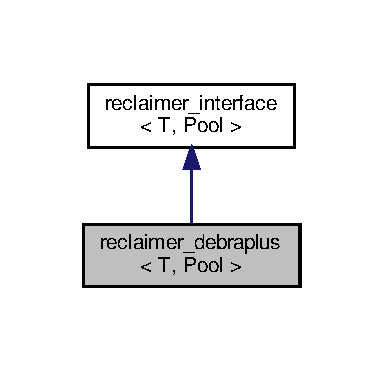
\includegraphics[width=184pt]{classreclaimer__debraplus__inherit__graph}
\end{center}
\end{figure}


Collaboration diagram for reclaimer\+\_\+debraplus$<$ T, Pool $>$\+:
\nopagebreak
\begin{figure}[H]
\begin{center}
\leavevmode
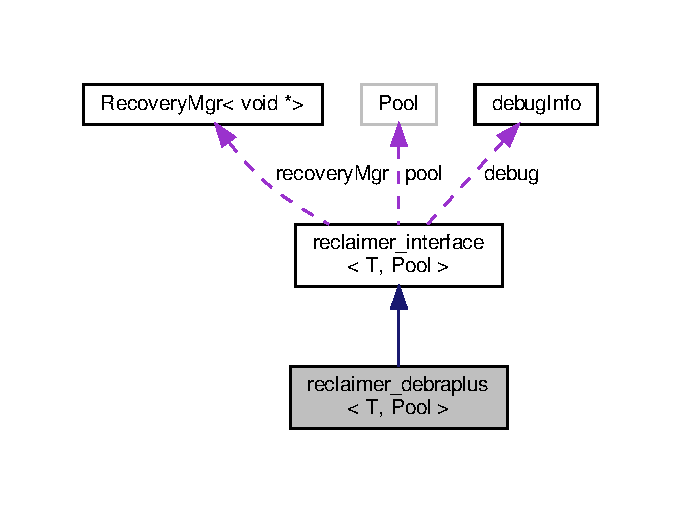
\includegraphics[width=327pt]{classreclaimer__debraplus__coll__graph}
\end{center}
\end{figure}
\subsection*{Classes}
\begin{DoxyCompactItemize}
\item 
struct \hyperlink{structreclaimer__debraplus_1_1rebind}{rebind}
\item 
struct \hyperlink{structreclaimer__debraplus_1_1rebind2}{rebind2}
\end{DoxyCompactItemize}
\subsection*{Public Member Functions}
\begin{DoxyCompactItemize}
\item 
bool \hyperlink{classreclaimer__debraplus_a4cf9fd158f9e1fee5f4e518e69d738ca}{is\+Quiescent} (const int \hyperlink{microbench_2main_8cpp_a9ca9869868fe7e7a38a921cc7de4103f}{tid})
\item 
bool \hyperlink{classreclaimer__debraplus_ab2108aa83328af20d9edefaa6181f829}{is\+Q\+Protected} (const int \hyperlink{microbench_2main_8cpp_a9ca9869868fe7e7a38a921cc7de4103f}{tid}, T $\ast$const obj)
\item 
bool \hyperlink{classreclaimer__debraplus_ad32af3b2be631a1bf8121f3ec92e8c80}{q\+Protect} (const int \hyperlink{microbench_2main_8cpp_a9ca9869868fe7e7a38a921cc7de4103f}{tid}, T $\ast$const obj, \hyperlink{globals_8h_a57f5c0d40b156d7d996492fb2f16e3cd}{Callback\+Type} not\+Retired\+Callback, \hyperlink{globals_8h_a3de64ef48066ac6430631c8b81a15345}{Callback\+Arg} callback\+Arg, bool memory\+Barrier=true)
\item 
void \hyperlink{classreclaimer__debraplus_ace3e4760c51f3035446e3fe0f363e6d5}{q\+Unprotect\+All} (const int \hyperlink{microbench_2main_8cpp_a9ca9869868fe7e7a38a921cc7de4103f}{tid})
\item 
void \hyperlink{classreclaimer__debraplus_abd86bc4bf14e52867a2fc6bdfa4f2887}{rotate\+Epoch\+Bags} (const int \hyperlink{microbench_2main_8cpp_a9ca9869868fe7e7a38a921cc7de4103f}{tid})
\item 
bool \hyperlink{classreclaimer__debraplus_ae6841e2253a106dafc3dfada360afce3}{start\+Op} (const int \hyperlink{microbench_2main_8cpp_a9ca9869868fe7e7a38a921cc7de4103f}{tid}, void $\ast$const $\ast$const reclaimers, const int num\+Reclaimers)
\item 
void \hyperlink{classreclaimer__debraplus_a2c702367af049f905ff76101b340d22f}{end\+Op} (const int \hyperlink{microbench_2main_8cpp_a9ca9869868fe7e7a38a921cc7de4103f}{tid})
\item 
void \hyperlink{classreclaimer__debraplus_ab9e42e9a1a7a78774f46740ba79a5abe}{retire} (const int \hyperlink{microbench_2main_8cpp_a9ca9869868fe7e7a38a921cc7de4103f}{tid}, T $\ast$p)
\item 
void \hyperlink{classreclaimer__debraplus_aa102a69aaf1bc87bbc7dd27b0e5d9c0d}{init\+Thread} (const int \hyperlink{microbench_2main_8cpp_a9ca9869868fe7e7a38a921cc7de4103f}{tid})
\item 
void \hyperlink{classreclaimer__debraplus_a9456d4b88028481c68222ab888faecf2}{deinit\+Thread} (const int \hyperlink{microbench_2main_8cpp_a9ca9869868fe7e7a38a921cc7de4103f}{tid})
\item 
void \hyperlink{classreclaimer__debraplus_a18b17edf9cb243d2bccb89bab3c4bfe6}{debug\+Print\+Status} (const int \hyperlink{microbench_2main_8cpp_a9ca9869868fe7e7a38a921cc7de4103f}{tid})
\item 
\hyperlink{classreclaimer__debraplus_aa3aecd07af32bce209348bd4eb10f2ee}{reclaimer\+\_\+debraplus} (const int \hyperlink{testing_8cpp_aa085812188e21ede75351d88b9b2c30d}{num\+Processes}, Pool $\ast$\+\_\+pool, \hyperlink{classdebugInfo}{debug\+Info} $\ast$const \+\_\+debug, \hyperlink{classRecoveryMgr}{Recovery\+Mgr}$<$ void $\ast$$>$ $\ast$const \+\_\+recovery\+Mgr=N\+U\+LL)
\item 
\hyperlink{classreclaimer__debraplus_a29be21fd0206a08aafd27319b83d7ba6}{$\sim$reclaimer\+\_\+debraplus} ()
\end{DoxyCompactItemize}
\subsection*{Static Public Member Functions}
\begin{DoxyCompactItemize}
\item 
static bool \hyperlink{classreclaimer__debraplus_a5fcce88c53a16023e412f0d1b9d3ae09}{quiescence\+Is\+Per\+Record\+Type} ()
\item 
static bool \hyperlink{classreclaimer__debraplus_a13df7939ef9ba01add47fd3d3d76fb46}{supports\+Crash\+Recovery} ()
\item 
static bool \hyperlink{classreclaimer__debraplus_a94a01ba5a46a5c64d47d8008b6f406ad}{is\+Protected} (const int \hyperlink{microbench_2main_8cpp_a9ca9869868fe7e7a38a921cc7de4103f}{tid}, T $\ast$const obj)
\item 
static bool \hyperlink{classreclaimer__debraplus_a79d06813ec16076bc9ea53b810b49951}{protect} (const int \hyperlink{microbench_2main_8cpp_a9ca9869868fe7e7a38a921cc7de4103f}{tid}, T $\ast$const obj, \hyperlink{globals_8h_a57f5c0d40b156d7d996492fb2f16e3cd}{Callback\+Type} not\+Retired\+Callback, \hyperlink{globals_8h_a3de64ef48066ac6430631c8b81a15345}{Callback\+Arg} callback\+Arg, bool memory\+Barrier=true)
\item 
static void \hyperlink{classreclaimer__debraplus_a2d27d53de5e35e26b12faf51b330ef13}{unprotect} (const int \hyperlink{microbench_2main_8cpp_a9ca9869868fe7e7a38a921cc7de4103f}{tid}, T $\ast$const obj)
\end{DoxyCompactItemize}
\subsection*{Additional Inherited Members}


\subsection{Detailed Description}
\subsubsection*{template$<$typename T = void, class Pool = pool\+\_\+interface$<$\+T$>$$>$\newline
class reclaimer\+\_\+debraplus$<$ T, Pool $>$}

C++ record manager implementation (P\+O\+DC 2015) by Trevor Brown.

Copyright (C) 2015 Trevor Brown 

\subsection{Constructor \& Destructor Documentation}
\mbox{\Hypertarget{classreclaimer__debraplus_aa3aecd07af32bce209348bd4eb10f2ee}\label{classreclaimer__debraplus_aa3aecd07af32bce209348bd4eb10f2ee}} 
\index{reclaimer\+\_\+debraplus@{reclaimer\+\_\+debraplus}!reclaimer\+\_\+debraplus@{reclaimer\+\_\+debraplus}}
\index{reclaimer\+\_\+debraplus@{reclaimer\+\_\+debraplus}!reclaimer\+\_\+debraplus@{reclaimer\+\_\+debraplus}}
\subsubsection{\texorpdfstring{reclaimer\+\_\+debraplus()}{reclaimer\_debraplus()}}
{\footnotesize\ttfamily template$<$typename T  = void, class Pool  = pool\+\_\+interface$<$\+T$>$$>$ \\
\hyperlink{classreclaimer__debraplus}{reclaimer\+\_\+debraplus}$<$ T, Pool $>$\+::\hyperlink{classreclaimer__debraplus}{reclaimer\+\_\+debraplus} (\begin{DoxyParamCaption}\item[{const int}]{num\+Processes,  }\item[{Pool $\ast$}]{\+\_\+pool,  }\item[{\hyperlink{classdebugInfo}{debug\+Info} $\ast$const}]{\+\_\+debug,  }\item[{\hyperlink{classRecoveryMgr}{Recovery\+Mgr}$<$ void $\ast$$>$ $\ast$const}]{\+\_\+recovery\+Mgr = {\ttfamily NULL} }\end{DoxyParamCaption})\hspace{0.3cm}{\ttfamily [inline]}}

\mbox{\Hypertarget{classreclaimer__debraplus_a29be21fd0206a08aafd27319b83d7ba6}\label{classreclaimer__debraplus_a29be21fd0206a08aafd27319b83d7ba6}} 
\index{reclaimer\+\_\+debraplus@{reclaimer\+\_\+debraplus}!````~reclaimer\+\_\+debraplus@{$\sim$reclaimer\+\_\+debraplus}}
\index{````~reclaimer\+\_\+debraplus@{$\sim$reclaimer\+\_\+debraplus}!reclaimer\+\_\+debraplus@{reclaimer\+\_\+debraplus}}
\subsubsection{\texorpdfstring{$\sim$reclaimer\+\_\+debraplus()}{~reclaimer\_debraplus()}}
{\footnotesize\ttfamily template$<$typename T  = void, class Pool  = pool\+\_\+interface$<$\+T$>$$>$ \\
\hyperlink{classreclaimer__debraplus}{reclaimer\+\_\+debraplus}$<$ T, Pool $>$\+::$\sim$\hyperlink{classreclaimer__debraplus}{reclaimer\+\_\+debraplus} (\begin{DoxyParamCaption}{ }\end{DoxyParamCaption})\hspace{0.3cm}{\ttfamily [inline]}}



\subsection{Member Function Documentation}
\mbox{\Hypertarget{classreclaimer__debraplus_a18b17edf9cb243d2bccb89bab3c4bfe6}\label{classreclaimer__debraplus_a18b17edf9cb243d2bccb89bab3c4bfe6}} 
\index{reclaimer\+\_\+debraplus@{reclaimer\+\_\+debraplus}!debug\+Print\+Status@{debug\+Print\+Status}}
\index{debug\+Print\+Status@{debug\+Print\+Status}!reclaimer\+\_\+debraplus@{reclaimer\+\_\+debraplus}}
\subsubsection{\texorpdfstring{debug\+Print\+Status()}{debugPrintStatus()}}
{\footnotesize\ttfamily template$<$typename T  = void, class Pool  = pool\+\_\+interface$<$\+T$>$$>$ \\
void \hyperlink{classreclaimer__debraplus}{reclaimer\+\_\+debraplus}$<$ T, Pool $>$\+::debug\+Print\+Status (\begin{DoxyParamCaption}\item[{const int}]{tid }\end{DoxyParamCaption})\hspace{0.3cm}{\ttfamily [inline]}}

\mbox{\Hypertarget{classreclaimer__debraplus_a9456d4b88028481c68222ab888faecf2}\label{classreclaimer__debraplus_a9456d4b88028481c68222ab888faecf2}} 
\index{reclaimer\+\_\+debraplus@{reclaimer\+\_\+debraplus}!deinit\+Thread@{deinit\+Thread}}
\index{deinit\+Thread@{deinit\+Thread}!reclaimer\+\_\+debraplus@{reclaimer\+\_\+debraplus}}
\subsubsection{\texorpdfstring{deinit\+Thread()}{deinitThread()}}
{\footnotesize\ttfamily template$<$typename T  = void, class Pool  = pool\+\_\+interface$<$\+T$>$$>$ \\
void \hyperlink{classreclaimer__debraplus}{reclaimer\+\_\+debraplus}$<$ T, Pool $>$\+::deinit\+Thread (\begin{DoxyParamCaption}\item[{const int}]{tid }\end{DoxyParamCaption})\hspace{0.3cm}{\ttfamily [inline]}}

\mbox{\Hypertarget{classreclaimer__debraplus_a2c702367af049f905ff76101b340d22f}\label{classreclaimer__debraplus_a2c702367af049f905ff76101b340d22f}} 
\index{reclaimer\+\_\+debraplus@{reclaimer\+\_\+debraplus}!end\+Op@{end\+Op}}
\index{end\+Op@{end\+Op}!reclaimer\+\_\+debraplus@{reclaimer\+\_\+debraplus}}
\subsubsection{\texorpdfstring{end\+Op()}{endOp()}}
{\footnotesize\ttfamily template$<$typename T  = void, class Pool  = pool\+\_\+interface$<$\+T$>$$>$ \\
void \hyperlink{classreclaimer__debraplus}{reclaimer\+\_\+debraplus}$<$ T, Pool $>$\+::end\+Op (\begin{DoxyParamCaption}\item[{const int}]{tid }\end{DoxyParamCaption})\hspace{0.3cm}{\ttfamily [inline]}}

\mbox{\Hypertarget{classreclaimer__debraplus_aa102a69aaf1bc87bbc7dd27b0e5d9c0d}\label{classreclaimer__debraplus_aa102a69aaf1bc87bbc7dd27b0e5d9c0d}} 
\index{reclaimer\+\_\+debraplus@{reclaimer\+\_\+debraplus}!init\+Thread@{init\+Thread}}
\index{init\+Thread@{init\+Thread}!reclaimer\+\_\+debraplus@{reclaimer\+\_\+debraplus}}
\subsubsection{\texorpdfstring{init\+Thread()}{initThread()}}
{\footnotesize\ttfamily template$<$typename T  = void, class Pool  = pool\+\_\+interface$<$\+T$>$$>$ \\
void \hyperlink{classreclaimer__debraplus}{reclaimer\+\_\+debraplus}$<$ T, Pool $>$\+::init\+Thread (\begin{DoxyParamCaption}\item[{const int}]{tid }\end{DoxyParamCaption})\hspace{0.3cm}{\ttfamily [inline]}}

\mbox{\Hypertarget{classreclaimer__debraplus_a94a01ba5a46a5c64d47d8008b6f406ad}\label{classreclaimer__debraplus_a94a01ba5a46a5c64d47d8008b6f406ad}} 
\index{reclaimer\+\_\+debraplus@{reclaimer\+\_\+debraplus}!is\+Protected@{is\+Protected}}
\index{is\+Protected@{is\+Protected}!reclaimer\+\_\+debraplus@{reclaimer\+\_\+debraplus}}
\subsubsection{\texorpdfstring{is\+Protected()}{isProtected()}}
{\footnotesize\ttfamily template$<$typename T  = void, class Pool  = pool\+\_\+interface$<$\+T$>$$>$ \\
static bool \hyperlink{classreclaimer__debraplus}{reclaimer\+\_\+debraplus}$<$ T, Pool $>$\+::is\+Protected (\begin{DoxyParamCaption}\item[{const int}]{tid,  }\item[{T $\ast$const}]{obj }\end{DoxyParamCaption})\hspace{0.3cm}{\ttfamily [inline]}, {\ttfamily [static]}}

\mbox{\Hypertarget{classreclaimer__debraplus_ab2108aa83328af20d9edefaa6181f829}\label{classreclaimer__debraplus_ab2108aa83328af20d9edefaa6181f829}} 
\index{reclaimer\+\_\+debraplus@{reclaimer\+\_\+debraplus}!is\+Q\+Protected@{is\+Q\+Protected}}
\index{is\+Q\+Protected@{is\+Q\+Protected}!reclaimer\+\_\+debraplus@{reclaimer\+\_\+debraplus}}
\subsubsection{\texorpdfstring{is\+Q\+Protected()}{isQProtected()}}
{\footnotesize\ttfamily template$<$typename T  = void, class Pool  = pool\+\_\+interface$<$\+T$>$$>$ \\
bool \hyperlink{classreclaimer__debraplus}{reclaimer\+\_\+debraplus}$<$ T, Pool $>$\+::is\+Q\+Protected (\begin{DoxyParamCaption}\item[{const int}]{tid,  }\item[{T $\ast$const}]{obj }\end{DoxyParamCaption})\hspace{0.3cm}{\ttfamily [inline]}}

\mbox{\Hypertarget{classreclaimer__debraplus_a4cf9fd158f9e1fee5f4e518e69d738ca}\label{classreclaimer__debraplus_a4cf9fd158f9e1fee5f4e518e69d738ca}} 
\index{reclaimer\+\_\+debraplus@{reclaimer\+\_\+debraplus}!is\+Quiescent@{is\+Quiescent}}
\index{is\+Quiescent@{is\+Quiescent}!reclaimer\+\_\+debraplus@{reclaimer\+\_\+debraplus}}
\subsubsection{\texorpdfstring{is\+Quiescent()}{isQuiescent()}}
{\footnotesize\ttfamily template$<$typename T  = void, class Pool  = pool\+\_\+interface$<$\+T$>$$>$ \\
bool \hyperlink{classreclaimer__debraplus}{reclaimer\+\_\+debraplus}$<$ T, Pool $>$\+::is\+Quiescent (\begin{DoxyParamCaption}\item[{const int}]{tid }\end{DoxyParamCaption})\hspace{0.3cm}{\ttfamily [inline]}}

\mbox{\Hypertarget{classreclaimer__debraplus_a79d06813ec16076bc9ea53b810b49951}\label{classreclaimer__debraplus_a79d06813ec16076bc9ea53b810b49951}} 
\index{reclaimer\+\_\+debraplus@{reclaimer\+\_\+debraplus}!protect@{protect}}
\index{protect@{protect}!reclaimer\+\_\+debraplus@{reclaimer\+\_\+debraplus}}
\subsubsection{\texorpdfstring{protect()}{protect()}}
{\footnotesize\ttfamily template$<$typename T  = void, class Pool  = pool\+\_\+interface$<$\+T$>$$>$ \\
static bool \hyperlink{classreclaimer__debraplus}{reclaimer\+\_\+debraplus}$<$ T, Pool $>$\+::protect (\begin{DoxyParamCaption}\item[{const int}]{tid,  }\item[{T $\ast$const}]{obj,  }\item[{\hyperlink{globals_8h_a57f5c0d40b156d7d996492fb2f16e3cd}{Callback\+Type}}]{not\+Retired\+Callback,  }\item[{\hyperlink{globals_8h_a3de64ef48066ac6430631c8b81a15345}{Callback\+Arg}}]{callback\+Arg,  }\item[{bool}]{memory\+Barrier = {\ttfamily true} }\end{DoxyParamCaption})\hspace{0.3cm}{\ttfamily [inline]}, {\ttfamily [static]}}

\mbox{\Hypertarget{classreclaimer__debraplus_ad32af3b2be631a1bf8121f3ec92e8c80}\label{classreclaimer__debraplus_ad32af3b2be631a1bf8121f3ec92e8c80}} 
\index{reclaimer\+\_\+debraplus@{reclaimer\+\_\+debraplus}!q\+Protect@{q\+Protect}}
\index{q\+Protect@{q\+Protect}!reclaimer\+\_\+debraplus@{reclaimer\+\_\+debraplus}}
\subsubsection{\texorpdfstring{q\+Protect()}{qProtect()}}
{\footnotesize\ttfamily template$<$typename T  = void, class Pool  = pool\+\_\+interface$<$\+T$>$$>$ \\
bool \hyperlink{classreclaimer__debraplus}{reclaimer\+\_\+debraplus}$<$ T, Pool $>$\+::q\+Protect (\begin{DoxyParamCaption}\item[{const int}]{tid,  }\item[{T $\ast$const}]{obj,  }\item[{\hyperlink{globals_8h_a57f5c0d40b156d7d996492fb2f16e3cd}{Callback\+Type}}]{not\+Retired\+Callback,  }\item[{\hyperlink{globals_8h_a3de64ef48066ac6430631c8b81a15345}{Callback\+Arg}}]{callback\+Arg,  }\item[{bool}]{memory\+Barrier = {\ttfamily true} }\end{DoxyParamCaption})\hspace{0.3cm}{\ttfamily [inline]}}

\mbox{\Hypertarget{classreclaimer__debraplus_a5fcce88c53a16023e412f0d1b9d3ae09}\label{classreclaimer__debraplus_a5fcce88c53a16023e412f0d1b9d3ae09}} 
\index{reclaimer\+\_\+debraplus@{reclaimer\+\_\+debraplus}!quiescence\+Is\+Per\+Record\+Type@{quiescence\+Is\+Per\+Record\+Type}}
\index{quiescence\+Is\+Per\+Record\+Type@{quiescence\+Is\+Per\+Record\+Type}!reclaimer\+\_\+debraplus@{reclaimer\+\_\+debraplus}}
\subsubsection{\texorpdfstring{quiescence\+Is\+Per\+Record\+Type()}{quiescenceIsPerRecordType()}}
{\footnotesize\ttfamily template$<$typename T  = void, class Pool  = pool\+\_\+interface$<$\+T$>$$>$ \\
static bool \hyperlink{classreclaimer__debraplus}{reclaimer\+\_\+debraplus}$<$ T, Pool $>$\+::quiescence\+Is\+Per\+Record\+Type (\begin{DoxyParamCaption}{ }\end{DoxyParamCaption})\hspace{0.3cm}{\ttfamily [inline]}, {\ttfamily [static]}}

\mbox{\Hypertarget{classreclaimer__debraplus_ace3e4760c51f3035446e3fe0f363e6d5}\label{classreclaimer__debraplus_ace3e4760c51f3035446e3fe0f363e6d5}} 
\index{reclaimer\+\_\+debraplus@{reclaimer\+\_\+debraplus}!q\+Unprotect\+All@{q\+Unprotect\+All}}
\index{q\+Unprotect\+All@{q\+Unprotect\+All}!reclaimer\+\_\+debraplus@{reclaimer\+\_\+debraplus}}
\subsubsection{\texorpdfstring{q\+Unprotect\+All()}{qUnprotectAll()}}
{\footnotesize\ttfamily template$<$typename T  = void, class Pool  = pool\+\_\+interface$<$\+T$>$$>$ \\
void \hyperlink{classreclaimer__debraplus}{reclaimer\+\_\+debraplus}$<$ T, Pool $>$\+::q\+Unprotect\+All (\begin{DoxyParamCaption}\item[{const int}]{tid }\end{DoxyParamCaption})\hspace{0.3cm}{\ttfamily [inline]}}

\mbox{\Hypertarget{classreclaimer__debraplus_ab9e42e9a1a7a78774f46740ba79a5abe}\label{classreclaimer__debraplus_ab9e42e9a1a7a78774f46740ba79a5abe}} 
\index{reclaimer\+\_\+debraplus@{reclaimer\+\_\+debraplus}!retire@{retire}}
\index{retire@{retire}!reclaimer\+\_\+debraplus@{reclaimer\+\_\+debraplus}}
\subsubsection{\texorpdfstring{retire()}{retire()}}
{\footnotesize\ttfamily template$<$typename T  = void, class Pool  = pool\+\_\+interface$<$\+T$>$$>$ \\
void \hyperlink{classreclaimer__debraplus}{reclaimer\+\_\+debraplus}$<$ T, Pool $>$\+::retire (\begin{DoxyParamCaption}\item[{const int}]{tid,  }\item[{T $\ast$}]{p }\end{DoxyParamCaption})\hspace{0.3cm}{\ttfamily [inline]}}

\mbox{\Hypertarget{classreclaimer__debraplus_abd86bc4bf14e52867a2fc6bdfa4f2887}\label{classreclaimer__debraplus_abd86bc4bf14e52867a2fc6bdfa4f2887}} 
\index{reclaimer\+\_\+debraplus@{reclaimer\+\_\+debraplus}!rotate\+Epoch\+Bags@{rotate\+Epoch\+Bags}}
\index{rotate\+Epoch\+Bags@{rotate\+Epoch\+Bags}!reclaimer\+\_\+debraplus@{reclaimer\+\_\+debraplus}}
\subsubsection{\texorpdfstring{rotate\+Epoch\+Bags()}{rotateEpochBags()}}
{\footnotesize\ttfamily template$<$typename T  = void, class Pool  = pool\+\_\+interface$<$\+T$>$$>$ \\
void \hyperlink{classreclaimer__debraplus}{reclaimer\+\_\+debraplus}$<$ T, Pool $>$\+::rotate\+Epoch\+Bags (\begin{DoxyParamCaption}\item[{const int}]{tid }\end{DoxyParamCaption})\hspace{0.3cm}{\ttfamily [inline]}}

\mbox{\Hypertarget{classreclaimer__debraplus_ae6841e2253a106dafc3dfada360afce3}\label{classreclaimer__debraplus_ae6841e2253a106dafc3dfada360afce3}} 
\index{reclaimer\+\_\+debraplus@{reclaimer\+\_\+debraplus}!start\+Op@{start\+Op}}
\index{start\+Op@{start\+Op}!reclaimer\+\_\+debraplus@{reclaimer\+\_\+debraplus}}
\subsubsection{\texorpdfstring{start\+Op()}{startOp()}}
{\footnotesize\ttfamily template$<$typename T  = void, class Pool  = pool\+\_\+interface$<$\+T$>$$>$ \\
bool \hyperlink{classreclaimer__debraplus}{reclaimer\+\_\+debraplus}$<$ T, Pool $>$\+::start\+Op (\begin{DoxyParamCaption}\item[{const int}]{tid,  }\item[{void $\ast$const $\ast$const}]{reclaimers,  }\item[{const int}]{num\+Reclaimers }\end{DoxyParamCaption})\hspace{0.3cm}{\ttfamily [inline]}}

\mbox{\Hypertarget{classreclaimer__debraplus_a13df7939ef9ba01add47fd3d3d76fb46}\label{classreclaimer__debraplus_a13df7939ef9ba01add47fd3d3d76fb46}} 
\index{reclaimer\+\_\+debraplus@{reclaimer\+\_\+debraplus}!supports\+Crash\+Recovery@{supports\+Crash\+Recovery}}
\index{supports\+Crash\+Recovery@{supports\+Crash\+Recovery}!reclaimer\+\_\+debraplus@{reclaimer\+\_\+debraplus}}
\subsubsection{\texorpdfstring{supports\+Crash\+Recovery()}{supportsCrashRecovery()}}
{\footnotesize\ttfamily template$<$typename T  = void, class Pool  = pool\+\_\+interface$<$\+T$>$$>$ \\
static bool \hyperlink{classreclaimer__debraplus}{reclaimer\+\_\+debraplus}$<$ T, Pool $>$\+::supports\+Crash\+Recovery (\begin{DoxyParamCaption}{ }\end{DoxyParamCaption})\hspace{0.3cm}{\ttfamily [inline]}, {\ttfamily [static]}}

\mbox{\Hypertarget{classreclaimer__debraplus_a2d27d53de5e35e26b12faf51b330ef13}\label{classreclaimer__debraplus_a2d27d53de5e35e26b12faf51b330ef13}} 
\index{reclaimer\+\_\+debraplus@{reclaimer\+\_\+debraplus}!unprotect@{unprotect}}
\index{unprotect@{unprotect}!reclaimer\+\_\+debraplus@{reclaimer\+\_\+debraplus}}
\subsubsection{\texorpdfstring{unprotect()}{unprotect()}}
{\footnotesize\ttfamily template$<$typename T  = void, class Pool  = pool\+\_\+interface$<$\+T$>$$>$ \\
static void \hyperlink{classreclaimer__debraplus}{reclaimer\+\_\+debraplus}$<$ T, Pool $>$\+::unprotect (\begin{DoxyParamCaption}\item[{const int}]{tid,  }\item[{T $\ast$const}]{obj }\end{DoxyParamCaption})\hspace{0.3cm}{\ttfamily [inline]}, {\ttfamily [static]}}



The documentation for this class was generated from the following file\+:\begin{DoxyCompactItemize}
\item 
common/recordmgr/\hyperlink{reclaimer__debraplus_8h}{reclaimer\+\_\+debraplus.\+h}\end{DoxyCompactItemize}

\hypertarget{classreclaimer__ebr__token}{}\section{reclaimer\+\_\+ebr\+\_\+token$<$ T, Pool $>$ Class Template Reference}
\label{classreclaimer__ebr__token}\index{reclaimer\+\_\+ebr\+\_\+token$<$ T, Pool $>$@{reclaimer\+\_\+ebr\+\_\+token$<$ T, Pool $>$}}


{\ttfamily \#include $<$reclaimer\+\_\+ebr\+\_\+token.\+h$>$}



Inheritance diagram for reclaimer\+\_\+ebr\+\_\+token$<$ T, Pool $>$\+:
\nopagebreak
\begin{figure}[H]
\begin{center}
\leavevmode
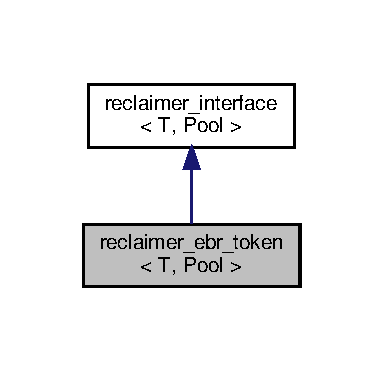
\includegraphics[width=184pt]{classreclaimer__ebr__token__inherit__graph}
\end{center}
\end{figure}


Collaboration diagram for reclaimer\+\_\+ebr\+\_\+token$<$ T, Pool $>$\+:
\nopagebreak
\begin{figure}[H]
\begin{center}
\leavevmode
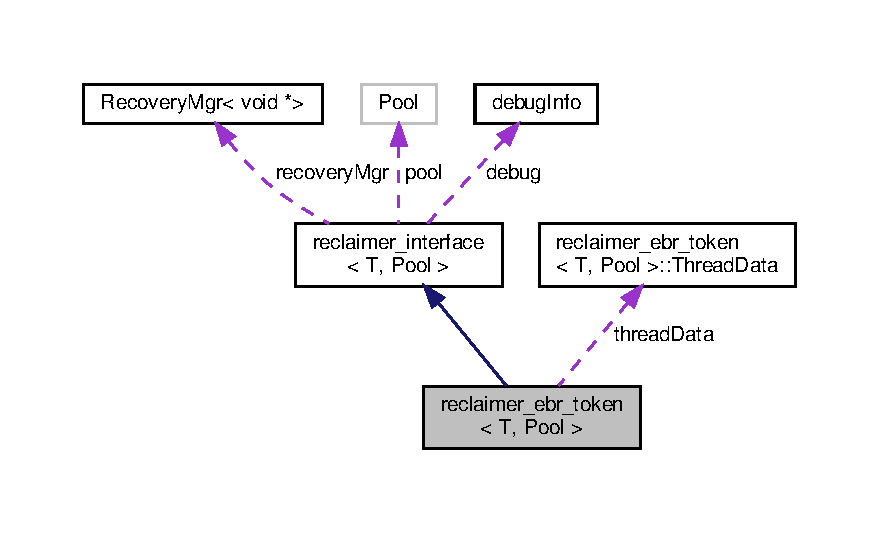
\includegraphics[width=350pt]{classreclaimer__ebr__token__coll__graph}
\end{center}
\end{figure}
\subsection*{Classes}
\begin{DoxyCompactItemize}
\item 
class \hyperlink{classreclaimer__ebr__token_1_1BagRotator}{Bag\+Rotator}
\item 
class \hyperlink{classreclaimer__ebr__token_1_1BagRotator_3_01First_00_01Rest_8_8_8_01_4}{Bag\+Rotator$<$ First, Rest... $>$}
\item 
struct \hyperlink{structreclaimer__ebr__token_1_1rebind}{rebind}
\item 
struct \hyperlink{structreclaimer__ebr__token_1_1rebind2}{rebind2}
\item 
class \hyperlink{classreclaimer__ebr__token_1_1ThreadData}{Thread\+Data}
\end{DoxyCompactItemize}
\subsection*{Public Member Functions}
\begin{DoxyCompactItemize}
\item 
void \hyperlink{classreclaimer__ebr__token_ae2fee48a5fa6b5e1626a5f5c98eb111b}{get\+Safe\+Blockbags} (const int \hyperlink{microbench_2main_8cpp_a9ca9869868fe7e7a38a921cc7de4103f}{tid}, \hyperlink{classblockbag}{blockbag}$<$ T $>$ $\ast$$\ast$bags)
\item 
long long \hyperlink{classreclaimer__ebr__token_aea32a21f3af9b3491ae008ef7166fcbc}{get\+Size\+In\+Nodes} ()
\item 
std\+::string \hyperlink{classreclaimer__ebr__token_a2375bf4a808710a12e7f0e5c598c92b3}{get\+Size\+String} ()
\item 
std\+::string \hyperlink{classreclaimer__ebr__token_a1eba9df1d95ccd1163c53697c37afc83}{get\+Details\+String} ()
\item 
bool \hyperlink{classreclaimer__ebr__token_a7cd87fdf1ae24baad3bfb808f329a57a}{is\+Quiescent} (const int \hyperlink{microbench_2main_8cpp_a9ca9869868fe7e7a38a921cc7de4103f}{tid})
\item 
void \hyperlink{classreclaimer__ebr__token_a36bc96f3000460deab02e93a24e137fa}{rotate\+Epoch\+Bags} (const int \hyperlink{microbench_2main_8cpp_a9ca9869868fe7e7a38a921cc7de4103f}{tid})
\item 
{\footnotesize template$<$typename First , typename... Rest$>$ }\\bool \hyperlink{classreclaimer__ebr__token_ae945b650a83590e6973db21404a2fb6a}{start\+Op} (const int \hyperlink{microbench_2main_8cpp_a9ca9869868fe7e7a38a921cc7de4103f}{tid}, void $\ast$const $\ast$const reclaimers, const int num\+Reclaimers, const bool read\+Only=false)
\item 
void \hyperlink{classreclaimer__ebr__token_abda33f89a0c09967d630e4e4b5ee83a4}{end\+Op} (const int \hyperlink{microbench_2main_8cpp_a9ca9869868fe7e7a38a921cc7de4103f}{tid})
\item 
void \hyperlink{classreclaimer__ebr__token_a179176c408edeb99d0c03dfe8852fea0}{retire} (const int \hyperlink{microbench_2main_8cpp_a9ca9869868fe7e7a38a921cc7de4103f}{tid}, T $\ast$p)
\item 
void \hyperlink{classreclaimer__ebr__token_a53348d44f753066411772dfae552f77f}{debug\+Print\+Status} (const int \hyperlink{microbench_2main_8cpp_a9ca9869868fe7e7a38a921cc7de4103f}{tid})
\item 
void \hyperlink{classreclaimer__ebr__token_ac68739de4032e25a3b06c6ac0846fcab}{init\+Thread} (const int \hyperlink{microbench_2main_8cpp_a9ca9869868fe7e7a38a921cc7de4103f}{tid})
\item 
void \hyperlink{classreclaimer__ebr__token_a9f841be7529961c0bca80f1e6b4d6423}{deinit\+Thread} (const int \hyperlink{microbench_2main_8cpp_a9ca9869868fe7e7a38a921cc7de4103f}{tid})
\item 
\hyperlink{classreclaimer__ebr__token_a29abde36eba704625cfdc65ec2896373}{reclaimer\+\_\+ebr\+\_\+token} (const int \hyperlink{testing_8cpp_aa085812188e21ede75351d88b9b2c30d}{num\+Processes}, Pool $\ast$\+\_\+pool, \hyperlink{classdebugInfo}{debug\+Info} $\ast$const \+\_\+debug, \hyperlink{classRecoveryMgr}{Recovery\+Mgr}$<$ void $\ast$$>$ $\ast$const \+\_\+recovery\+Mgr=N\+U\+LL)
\item 
\hyperlink{classreclaimer__ebr__token_a03b63c5cdbd9f10543c85e324ab903bf}{$\sim$reclaimer\+\_\+ebr\+\_\+token} ()
\end{DoxyCompactItemize}
\subsection*{Static Public Member Functions}
\begin{DoxyCompactItemize}
\item 
static bool \hyperlink{classreclaimer__ebr__token_a04a36547ffd9692aefe0f2a7cc16c15f}{quiescence\+Is\+Per\+Record\+Type} ()
\item 
static bool \hyperlink{classreclaimer__ebr__token_ae806d7fcc13bb4d7eb5a447a85d2950d}{is\+Protected} (const int \hyperlink{microbench_2main_8cpp_a9ca9869868fe7e7a38a921cc7de4103f}{tid}, T $\ast$const obj)
\item 
static bool \hyperlink{classreclaimer__ebr__token_ac4a89ebcacf0b057041322aa1a677c42}{is\+Q\+Protected} (const int \hyperlink{microbench_2main_8cpp_a9ca9869868fe7e7a38a921cc7de4103f}{tid}, T $\ast$const obj)
\item 
static bool \hyperlink{classreclaimer__ebr__token_a5352c8afe5e576ab0a6370d2c3fa1752}{protect} (const int \hyperlink{microbench_2main_8cpp_a9ca9869868fe7e7a38a921cc7de4103f}{tid}, T $\ast$const obj, \hyperlink{globals_8h_a57f5c0d40b156d7d996492fb2f16e3cd}{Callback\+Type} not\+Retired\+Callback, \hyperlink{globals_8h_a3de64ef48066ac6430631c8b81a15345}{Callback\+Arg} callback\+Arg, bool memory\+Barrier=true)
\item 
static void \hyperlink{classreclaimer__ebr__token_aa43f00d8adc9cefeb604c14f0af45083}{unprotect} (const int \hyperlink{microbench_2main_8cpp_a9ca9869868fe7e7a38a921cc7de4103f}{tid}, T $\ast$const obj)
\item 
static bool \hyperlink{classreclaimer__ebr__token_a894dfb4d02dc74c9d9ee23329bdce9e2}{q\+Protect} (const int \hyperlink{microbench_2main_8cpp_a9ca9869868fe7e7a38a921cc7de4103f}{tid}, T $\ast$const obj, \hyperlink{globals_8h_a57f5c0d40b156d7d996492fb2f16e3cd}{Callback\+Type} not\+Retired\+Callback, \hyperlink{globals_8h_a3de64ef48066ac6430631c8b81a15345}{Callback\+Arg} callback\+Arg, bool memory\+Barrier=true)
\item 
static void \hyperlink{classreclaimer__ebr__token_a0bada18048e62e6d92906fca905f2fe6}{q\+Unprotect\+All} (const int \hyperlink{microbench_2main_8cpp_a9ca9869868fe7e7a38a921cc7de4103f}{tid})
\item 
static bool \hyperlink{classreclaimer__ebr__token_ae3f31ec8fd28eeaaa86ca58fcfe9ca64}{should\+Help} ()
\end{DoxyCompactItemize}
\subsection*{Protected Attributes}
\begin{DoxyCompactItemize}
\item 
\hyperlink{classreclaimer__ebr__token_1_1ThreadData}{Thread\+Data} \hyperlink{classreclaimer__ebr__token_a321a12296aabc232eb2cabbba1164b14}{thread\+Data} \mbox{[}\hyperlink{plaf_8h_ac1585a3455dd3e33e877e588be9e466b}{M\+A\+X\+\_\+\+T\+H\+R\+E\+A\+D\+S\+\_\+\+P\+O\+W2}\mbox{]}
\item 
\hyperlink{classreclaimer__ebr__token_a73eb1600dc86a4999e9ce31b07076f97}{P\+AD}
\end{DoxyCompactItemize}
\subsection*{Additional Inherited Members}


\subsection{Detailed Description}
\subsubsection*{template$<$typename T = void, class Pool = pool\+\_\+interface$<$\+T$>$$>$\newline
class reclaimer\+\_\+ebr\+\_\+token$<$ T, Pool $>$}

Variant of E\+BR using token passing.

Copyright (C) 2019 Trevor Brown 

\subsection{Constructor \& Destructor Documentation}
\mbox{\Hypertarget{classreclaimer__ebr__token_a29abde36eba704625cfdc65ec2896373}\label{classreclaimer__ebr__token_a29abde36eba704625cfdc65ec2896373}} 
\index{reclaimer\+\_\+ebr\+\_\+token@{reclaimer\+\_\+ebr\+\_\+token}!reclaimer\+\_\+ebr\+\_\+token@{reclaimer\+\_\+ebr\+\_\+token}}
\index{reclaimer\+\_\+ebr\+\_\+token@{reclaimer\+\_\+ebr\+\_\+token}!reclaimer\+\_\+ebr\+\_\+token@{reclaimer\+\_\+ebr\+\_\+token}}
\subsubsection{\texorpdfstring{reclaimer\+\_\+ebr\+\_\+token()}{reclaimer\_ebr\_token()}}
{\footnotesize\ttfamily template$<$typename T  = void, class Pool  = pool\+\_\+interface$<$\+T$>$$>$ \\
\hyperlink{classreclaimer__ebr__token}{reclaimer\+\_\+ebr\+\_\+token}$<$ T, Pool $>$\+::\hyperlink{classreclaimer__ebr__token}{reclaimer\+\_\+ebr\+\_\+token} (\begin{DoxyParamCaption}\item[{const int}]{num\+Processes,  }\item[{Pool $\ast$}]{\+\_\+pool,  }\item[{\hyperlink{classdebugInfo}{debug\+Info} $\ast$const}]{\+\_\+debug,  }\item[{\hyperlink{classRecoveryMgr}{Recovery\+Mgr}$<$ void $\ast$$>$ $\ast$const}]{\+\_\+recovery\+Mgr = {\ttfamily NULL} }\end{DoxyParamCaption})\hspace{0.3cm}{\ttfamily [inline]}}

\mbox{\Hypertarget{classreclaimer__ebr__token_a03b63c5cdbd9f10543c85e324ab903bf}\label{classreclaimer__ebr__token_a03b63c5cdbd9f10543c85e324ab903bf}} 
\index{reclaimer\+\_\+ebr\+\_\+token@{reclaimer\+\_\+ebr\+\_\+token}!````~reclaimer\+\_\+ebr\+\_\+token@{$\sim$reclaimer\+\_\+ebr\+\_\+token}}
\index{````~reclaimer\+\_\+ebr\+\_\+token@{$\sim$reclaimer\+\_\+ebr\+\_\+token}!reclaimer\+\_\+ebr\+\_\+token@{reclaimer\+\_\+ebr\+\_\+token}}
\subsubsection{\texorpdfstring{$\sim$reclaimer\+\_\+ebr\+\_\+token()}{~reclaimer\_ebr\_token()}}
{\footnotesize\ttfamily template$<$typename T  = void, class Pool  = pool\+\_\+interface$<$\+T$>$$>$ \\
\hyperlink{classreclaimer__ebr__token}{reclaimer\+\_\+ebr\+\_\+token}$<$ T, Pool $>$\+::$\sim$\hyperlink{classreclaimer__ebr__token}{reclaimer\+\_\+ebr\+\_\+token} (\begin{DoxyParamCaption}{ }\end{DoxyParamCaption})\hspace{0.3cm}{\ttfamily [inline]}}



\subsection{Member Function Documentation}
\mbox{\Hypertarget{classreclaimer__ebr__token_a53348d44f753066411772dfae552f77f}\label{classreclaimer__ebr__token_a53348d44f753066411772dfae552f77f}} 
\index{reclaimer\+\_\+ebr\+\_\+token@{reclaimer\+\_\+ebr\+\_\+token}!debug\+Print\+Status@{debug\+Print\+Status}}
\index{debug\+Print\+Status@{debug\+Print\+Status}!reclaimer\+\_\+ebr\+\_\+token@{reclaimer\+\_\+ebr\+\_\+token}}
\subsubsection{\texorpdfstring{debug\+Print\+Status()}{debugPrintStatus()}}
{\footnotesize\ttfamily template$<$typename T  = void, class Pool  = pool\+\_\+interface$<$\+T$>$$>$ \\
void \hyperlink{classreclaimer__ebr__token}{reclaimer\+\_\+ebr\+\_\+token}$<$ T, Pool $>$\+::debug\+Print\+Status (\begin{DoxyParamCaption}\item[{const int}]{tid }\end{DoxyParamCaption})\hspace{0.3cm}{\ttfamily [inline]}}

\mbox{\Hypertarget{classreclaimer__ebr__token_a9f841be7529961c0bca80f1e6b4d6423}\label{classreclaimer__ebr__token_a9f841be7529961c0bca80f1e6b4d6423}} 
\index{reclaimer\+\_\+ebr\+\_\+token@{reclaimer\+\_\+ebr\+\_\+token}!deinit\+Thread@{deinit\+Thread}}
\index{deinit\+Thread@{deinit\+Thread}!reclaimer\+\_\+ebr\+\_\+token@{reclaimer\+\_\+ebr\+\_\+token}}
\subsubsection{\texorpdfstring{deinit\+Thread()}{deinitThread()}}
{\footnotesize\ttfamily template$<$typename T  = void, class Pool  = pool\+\_\+interface$<$\+T$>$$>$ \\
void \hyperlink{classreclaimer__ebr__token}{reclaimer\+\_\+ebr\+\_\+token}$<$ T, Pool $>$\+::deinit\+Thread (\begin{DoxyParamCaption}\item[{const int}]{tid }\end{DoxyParamCaption})\hspace{0.3cm}{\ttfamily [inline]}}

\mbox{\Hypertarget{classreclaimer__ebr__token_abda33f89a0c09967d630e4e4b5ee83a4}\label{classreclaimer__ebr__token_abda33f89a0c09967d630e4e4b5ee83a4}} 
\index{reclaimer\+\_\+ebr\+\_\+token@{reclaimer\+\_\+ebr\+\_\+token}!end\+Op@{end\+Op}}
\index{end\+Op@{end\+Op}!reclaimer\+\_\+ebr\+\_\+token@{reclaimer\+\_\+ebr\+\_\+token}}
\subsubsection{\texorpdfstring{end\+Op()}{endOp()}}
{\footnotesize\ttfamily template$<$typename T  = void, class Pool  = pool\+\_\+interface$<$\+T$>$$>$ \\
void \hyperlink{classreclaimer__ebr__token}{reclaimer\+\_\+ebr\+\_\+token}$<$ T, Pool $>$\+::end\+Op (\begin{DoxyParamCaption}\item[{const int}]{tid }\end{DoxyParamCaption})\hspace{0.3cm}{\ttfamily [inline]}}

\mbox{\Hypertarget{classreclaimer__ebr__token_a1eba9df1d95ccd1163c53697c37afc83}\label{classreclaimer__ebr__token_a1eba9df1d95ccd1163c53697c37afc83}} 
\index{reclaimer\+\_\+ebr\+\_\+token@{reclaimer\+\_\+ebr\+\_\+token}!get\+Details\+String@{get\+Details\+String}}
\index{get\+Details\+String@{get\+Details\+String}!reclaimer\+\_\+ebr\+\_\+token@{reclaimer\+\_\+ebr\+\_\+token}}
\subsubsection{\texorpdfstring{get\+Details\+String()}{getDetailsString()}}
{\footnotesize\ttfamily template$<$typename T  = void, class Pool  = pool\+\_\+interface$<$\+T$>$$>$ \\
std\+::string \hyperlink{classreclaimer__ebr__token}{reclaimer\+\_\+ebr\+\_\+token}$<$ T, Pool $>$\+::get\+Details\+String (\begin{DoxyParamCaption}{ }\end{DoxyParamCaption})\hspace{0.3cm}{\ttfamily [inline]}}

\mbox{\Hypertarget{classreclaimer__ebr__token_ae2fee48a5fa6b5e1626a5f5c98eb111b}\label{classreclaimer__ebr__token_ae2fee48a5fa6b5e1626a5f5c98eb111b}} 
\index{reclaimer\+\_\+ebr\+\_\+token@{reclaimer\+\_\+ebr\+\_\+token}!get\+Safe\+Blockbags@{get\+Safe\+Blockbags}}
\index{get\+Safe\+Blockbags@{get\+Safe\+Blockbags}!reclaimer\+\_\+ebr\+\_\+token@{reclaimer\+\_\+ebr\+\_\+token}}
\subsubsection{\texorpdfstring{get\+Safe\+Blockbags()}{getSafeBlockbags()}}
{\footnotesize\ttfamily template$<$typename T  = void, class Pool  = pool\+\_\+interface$<$\+T$>$$>$ \\
void \hyperlink{classreclaimer__ebr__token}{reclaimer\+\_\+ebr\+\_\+token}$<$ T, Pool $>$\+::get\+Safe\+Blockbags (\begin{DoxyParamCaption}\item[{const int}]{tid,  }\item[{\hyperlink{classblockbag}{blockbag}$<$ T $>$ $\ast$$\ast$}]{bags }\end{DoxyParamCaption})\hspace{0.3cm}{\ttfamily [inline]}}

\mbox{\Hypertarget{classreclaimer__ebr__token_aea32a21f3af9b3491ae008ef7166fcbc}\label{classreclaimer__ebr__token_aea32a21f3af9b3491ae008ef7166fcbc}} 
\index{reclaimer\+\_\+ebr\+\_\+token@{reclaimer\+\_\+ebr\+\_\+token}!get\+Size\+In\+Nodes@{get\+Size\+In\+Nodes}}
\index{get\+Size\+In\+Nodes@{get\+Size\+In\+Nodes}!reclaimer\+\_\+ebr\+\_\+token@{reclaimer\+\_\+ebr\+\_\+token}}
\subsubsection{\texorpdfstring{get\+Size\+In\+Nodes()}{getSizeInNodes()}}
{\footnotesize\ttfamily template$<$typename T  = void, class Pool  = pool\+\_\+interface$<$\+T$>$$>$ \\
long long \hyperlink{classreclaimer__ebr__token}{reclaimer\+\_\+ebr\+\_\+token}$<$ T, Pool $>$\+::get\+Size\+In\+Nodes (\begin{DoxyParamCaption}{ }\end{DoxyParamCaption})\hspace{0.3cm}{\ttfamily [inline]}}

\mbox{\Hypertarget{classreclaimer__ebr__token_a2375bf4a808710a12e7f0e5c598c92b3}\label{classreclaimer__ebr__token_a2375bf4a808710a12e7f0e5c598c92b3}} 
\index{reclaimer\+\_\+ebr\+\_\+token@{reclaimer\+\_\+ebr\+\_\+token}!get\+Size\+String@{get\+Size\+String}}
\index{get\+Size\+String@{get\+Size\+String}!reclaimer\+\_\+ebr\+\_\+token@{reclaimer\+\_\+ebr\+\_\+token}}
\subsubsection{\texorpdfstring{get\+Size\+String()}{getSizeString()}}
{\footnotesize\ttfamily template$<$typename T  = void, class Pool  = pool\+\_\+interface$<$\+T$>$$>$ \\
std\+::string \hyperlink{classreclaimer__ebr__token}{reclaimer\+\_\+ebr\+\_\+token}$<$ T, Pool $>$\+::get\+Size\+String (\begin{DoxyParamCaption}{ }\end{DoxyParamCaption})\hspace{0.3cm}{\ttfamily [inline]}}

\mbox{\Hypertarget{classreclaimer__ebr__token_ac68739de4032e25a3b06c6ac0846fcab}\label{classreclaimer__ebr__token_ac68739de4032e25a3b06c6ac0846fcab}} 
\index{reclaimer\+\_\+ebr\+\_\+token@{reclaimer\+\_\+ebr\+\_\+token}!init\+Thread@{init\+Thread}}
\index{init\+Thread@{init\+Thread}!reclaimer\+\_\+ebr\+\_\+token@{reclaimer\+\_\+ebr\+\_\+token}}
\subsubsection{\texorpdfstring{init\+Thread()}{initThread()}}
{\footnotesize\ttfamily template$<$typename T  = void, class Pool  = pool\+\_\+interface$<$\+T$>$$>$ \\
void \hyperlink{classreclaimer__ebr__token}{reclaimer\+\_\+ebr\+\_\+token}$<$ T, Pool $>$\+::init\+Thread (\begin{DoxyParamCaption}\item[{const int}]{tid }\end{DoxyParamCaption})\hspace{0.3cm}{\ttfamily [inline]}}

\mbox{\Hypertarget{classreclaimer__ebr__token_ae806d7fcc13bb4d7eb5a447a85d2950d}\label{classreclaimer__ebr__token_ae806d7fcc13bb4d7eb5a447a85d2950d}} 
\index{reclaimer\+\_\+ebr\+\_\+token@{reclaimer\+\_\+ebr\+\_\+token}!is\+Protected@{is\+Protected}}
\index{is\+Protected@{is\+Protected}!reclaimer\+\_\+ebr\+\_\+token@{reclaimer\+\_\+ebr\+\_\+token}}
\subsubsection{\texorpdfstring{is\+Protected()}{isProtected()}}
{\footnotesize\ttfamily template$<$typename T  = void, class Pool  = pool\+\_\+interface$<$\+T$>$$>$ \\
static bool \hyperlink{classreclaimer__ebr__token}{reclaimer\+\_\+ebr\+\_\+token}$<$ T, Pool $>$\+::is\+Protected (\begin{DoxyParamCaption}\item[{const int}]{tid,  }\item[{T $\ast$const}]{obj }\end{DoxyParamCaption})\hspace{0.3cm}{\ttfamily [inline]}, {\ttfamily [static]}}

\mbox{\Hypertarget{classreclaimer__ebr__token_ac4a89ebcacf0b057041322aa1a677c42}\label{classreclaimer__ebr__token_ac4a89ebcacf0b057041322aa1a677c42}} 
\index{reclaimer\+\_\+ebr\+\_\+token@{reclaimer\+\_\+ebr\+\_\+token}!is\+Q\+Protected@{is\+Q\+Protected}}
\index{is\+Q\+Protected@{is\+Q\+Protected}!reclaimer\+\_\+ebr\+\_\+token@{reclaimer\+\_\+ebr\+\_\+token}}
\subsubsection{\texorpdfstring{is\+Q\+Protected()}{isQProtected()}}
{\footnotesize\ttfamily template$<$typename T  = void, class Pool  = pool\+\_\+interface$<$\+T$>$$>$ \\
static bool \hyperlink{classreclaimer__ebr__token}{reclaimer\+\_\+ebr\+\_\+token}$<$ T, Pool $>$\+::is\+Q\+Protected (\begin{DoxyParamCaption}\item[{const int}]{tid,  }\item[{T $\ast$const}]{obj }\end{DoxyParamCaption})\hspace{0.3cm}{\ttfamily [inline]}, {\ttfamily [static]}}

\mbox{\Hypertarget{classreclaimer__ebr__token_a7cd87fdf1ae24baad3bfb808f329a57a}\label{classreclaimer__ebr__token_a7cd87fdf1ae24baad3bfb808f329a57a}} 
\index{reclaimer\+\_\+ebr\+\_\+token@{reclaimer\+\_\+ebr\+\_\+token}!is\+Quiescent@{is\+Quiescent}}
\index{is\+Quiescent@{is\+Quiescent}!reclaimer\+\_\+ebr\+\_\+token@{reclaimer\+\_\+ebr\+\_\+token}}
\subsubsection{\texorpdfstring{is\+Quiescent()}{isQuiescent()}}
{\footnotesize\ttfamily template$<$typename T  = void, class Pool  = pool\+\_\+interface$<$\+T$>$$>$ \\
bool \hyperlink{classreclaimer__ebr__token}{reclaimer\+\_\+ebr\+\_\+token}$<$ T, Pool $>$\+::is\+Quiescent (\begin{DoxyParamCaption}\item[{const int}]{tid }\end{DoxyParamCaption})\hspace{0.3cm}{\ttfamily [inline]}}

\mbox{\Hypertarget{classreclaimer__ebr__token_a5352c8afe5e576ab0a6370d2c3fa1752}\label{classreclaimer__ebr__token_a5352c8afe5e576ab0a6370d2c3fa1752}} 
\index{reclaimer\+\_\+ebr\+\_\+token@{reclaimer\+\_\+ebr\+\_\+token}!protect@{protect}}
\index{protect@{protect}!reclaimer\+\_\+ebr\+\_\+token@{reclaimer\+\_\+ebr\+\_\+token}}
\subsubsection{\texorpdfstring{protect()}{protect()}}
{\footnotesize\ttfamily template$<$typename T  = void, class Pool  = pool\+\_\+interface$<$\+T$>$$>$ \\
static bool \hyperlink{classreclaimer__ebr__token}{reclaimer\+\_\+ebr\+\_\+token}$<$ T, Pool $>$\+::protect (\begin{DoxyParamCaption}\item[{const int}]{tid,  }\item[{T $\ast$const}]{obj,  }\item[{\hyperlink{globals_8h_a57f5c0d40b156d7d996492fb2f16e3cd}{Callback\+Type}}]{not\+Retired\+Callback,  }\item[{\hyperlink{globals_8h_a3de64ef48066ac6430631c8b81a15345}{Callback\+Arg}}]{callback\+Arg,  }\item[{bool}]{memory\+Barrier = {\ttfamily true} }\end{DoxyParamCaption})\hspace{0.3cm}{\ttfamily [inline]}, {\ttfamily [static]}}

\mbox{\Hypertarget{classreclaimer__ebr__token_a894dfb4d02dc74c9d9ee23329bdce9e2}\label{classreclaimer__ebr__token_a894dfb4d02dc74c9d9ee23329bdce9e2}} 
\index{reclaimer\+\_\+ebr\+\_\+token@{reclaimer\+\_\+ebr\+\_\+token}!q\+Protect@{q\+Protect}}
\index{q\+Protect@{q\+Protect}!reclaimer\+\_\+ebr\+\_\+token@{reclaimer\+\_\+ebr\+\_\+token}}
\subsubsection{\texorpdfstring{q\+Protect()}{qProtect()}}
{\footnotesize\ttfamily template$<$typename T  = void, class Pool  = pool\+\_\+interface$<$\+T$>$$>$ \\
static bool \hyperlink{classreclaimer__ebr__token}{reclaimer\+\_\+ebr\+\_\+token}$<$ T, Pool $>$\+::q\+Protect (\begin{DoxyParamCaption}\item[{const int}]{tid,  }\item[{T $\ast$const}]{obj,  }\item[{\hyperlink{globals_8h_a57f5c0d40b156d7d996492fb2f16e3cd}{Callback\+Type}}]{not\+Retired\+Callback,  }\item[{\hyperlink{globals_8h_a3de64ef48066ac6430631c8b81a15345}{Callback\+Arg}}]{callback\+Arg,  }\item[{bool}]{memory\+Barrier = {\ttfamily true} }\end{DoxyParamCaption})\hspace{0.3cm}{\ttfamily [inline]}, {\ttfamily [static]}}

\mbox{\Hypertarget{classreclaimer__ebr__token_a04a36547ffd9692aefe0f2a7cc16c15f}\label{classreclaimer__ebr__token_a04a36547ffd9692aefe0f2a7cc16c15f}} 
\index{reclaimer\+\_\+ebr\+\_\+token@{reclaimer\+\_\+ebr\+\_\+token}!quiescence\+Is\+Per\+Record\+Type@{quiescence\+Is\+Per\+Record\+Type}}
\index{quiescence\+Is\+Per\+Record\+Type@{quiescence\+Is\+Per\+Record\+Type}!reclaimer\+\_\+ebr\+\_\+token@{reclaimer\+\_\+ebr\+\_\+token}}
\subsubsection{\texorpdfstring{quiescence\+Is\+Per\+Record\+Type()}{quiescenceIsPerRecordType()}}
{\footnotesize\ttfamily template$<$typename T  = void, class Pool  = pool\+\_\+interface$<$\+T$>$$>$ \\
static bool \hyperlink{classreclaimer__ebr__token}{reclaimer\+\_\+ebr\+\_\+token}$<$ T, Pool $>$\+::quiescence\+Is\+Per\+Record\+Type (\begin{DoxyParamCaption}{ }\end{DoxyParamCaption})\hspace{0.3cm}{\ttfamily [inline]}, {\ttfamily [static]}}

\mbox{\Hypertarget{classreclaimer__ebr__token_a0bada18048e62e6d92906fca905f2fe6}\label{classreclaimer__ebr__token_a0bada18048e62e6d92906fca905f2fe6}} 
\index{reclaimer\+\_\+ebr\+\_\+token@{reclaimer\+\_\+ebr\+\_\+token}!q\+Unprotect\+All@{q\+Unprotect\+All}}
\index{q\+Unprotect\+All@{q\+Unprotect\+All}!reclaimer\+\_\+ebr\+\_\+token@{reclaimer\+\_\+ebr\+\_\+token}}
\subsubsection{\texorpdfstring{q\+Unprotect\+All()}{qUnprotectAll()}}
{\footnotesize\ttfamily template$<$typename T  = void, class Pool  = pool\+\_\+interface$<$\+T$>$$>$ \\
static void \hyperlink{classreclaimer__ebr__token}{reclaimer\+\_\+ebr\+\_\+token}$<$ T, Pool $>$\+::q\+Unprotect\+All (\begin{DoxyParamCaption}\item[{const int}]{tid }\end{DoxyParamCaption})\hspace{0.3cm}{\ttfamily [inline]}, {\ttfamily [static]}}

\mbox{\Hypertarget{classreclaimer__ebr__token_a179176c408edeb99d0c03dfe8852fea0}\label{classreclaimer__ebr__token_a179176c408edeb99d0c03dfe8852fea0}} 
\index{reclaimer\+\_\+ebr\+\_\+token@{reclaimer\+\_\+ebr\+\_\+token}!retire@{retire}}
\index{retire@{retire}!reclaimer\+\_\+ebr\+\_\+token@{reclaimer\+\_\+ebr\+\_\+token}}
\subsubsection{\texorpdfstring{retire()}{retire()}}
{\footnotesize\ttfamily template$<$typename T  = void, class Pool  = pool\+\_\+interface$<$\+T$>$$>$ \\
void \hyperlink{classreclaimer__ebr__token}{reclaimer\+\_\+ebr\+\_\+token}$<$ T, Pool $>$\+::retire (\begin{DoxyParamCaption}\item[{const int}]{tid,  }\item[{T $\ast$}]{p }\end{DoxyParamCaption})\hspace{0.3cm}{\ttfamily [inline]}}

\mbox{\Hypertarget{classreclaimer__ebr__token_a36bc96f3000460deab02e93a24e137fa}\label{classreclaimer__ebr__token_a36bc96f3000460deab02e93a24e137fa}} 
\index{reclaimer\+\_\+ebr\+\_\+token@{reclaimer\+\_\+ebr\+\_\+token}!rotate\+Epoch\+Bags@{rotate\+Epoch\+Bags}}
\index{rotate\+Epoch\+Bags@{rotate\+Epoch\+Bags}!reclaimer\+\_\+ebr\+\_\+token@{reclaimer\+\_\+ebr\+\_\+token}}
\subsubsection{\texorpdfstring{rotate\+Epoch\+Bags()}{rotateEpochBags()}}
{\footnotesize\ttfamily template$<$typename T  = void, class Pool  = pool\+\_\+interface$<$\+T$>$$>$ \\
void \hyperlink{classreclaimer__ebr__token}{reclaimer\+\_\+ebr\+\_\+token}$<$ T, Pool $>$\+::rotate\+Epoch\+Bags (\begin{DoxyParamCaption}\item[{const int}]{tid }\end{DoxyParamCaption})\hspace{0.3cm}{\ttfamily [inline]}}

\mbox{\Hypertarget{classreclaimer__ebr__token_ae3f31ec8fd28eeaaa86ca58fcfe9ca64}\label{classreclaimer__ebr__token_ae3f31ec8fd28eeaaa86ca58fcfe9ca64}} 
\index{reclaimer\+\_\+ebr\+\_\+token@{reclaimer\+\_\+ebr\+\_\+token}!should\+Help@{should\+Help}}
\index{should\+Help@{should\+Help}!reclaimer\+\_\+ebr\+\_\+token@{reclaimer\+\_\+ebr\+\_\+token}}
\subsubsection{\texorpdfstring{should\+Help()}{shouldHelp()}}
{\footnotesize\ttfamily template$<$typename T  = void, class Pool  = pool\+\_\+interface$<$\+T$>$$>$ \\
static bool \hyperlink{classreclaimer__ebr__token}{reclaimer\+\_\+ebr\+\_\+token}$<$ T, Pool $>$\+::should\+Help (\begin{DoxyParamCaption}{ }\end{DoxyParamCaption})\hspace{0.3cm}{\ttfamily [inline]}, {\ttfamily [static]}}

\mbox{\Hypertarget{classreclaimer__ebr__token_ae945b650a83590e6973db21404a2fb6a}\label{classreclaimer__ebr__token_ae945b650a83590e6973db21404a2fb6a}} 
\index{reclaimer\+\_\+ebr\+\_\+token@{reclaimer\+\_\+ebr\+\_\+token}!start\+Op@{start\+Op}}
\index{start\+Op@{start\+Op}!reclaimer\+\_\+ebr\+\_\+token@{reclaimer\+\_\+ebr\+\_\+token}}
\subsubsection{\texorpdfstring{start\+Op()}{startOp()}}
{\footnotesize\ttfamily template$<$typename T  = void, class Pool  = pool\+\_\+interface$<$\+T$>$$>$ \\
template$<$typename First , typename... Rest$>$ \\
bool \hyperlink{classreclaimer__ebr__token}{reclaimer\+\_\+ebr\+\_\+token}$<$ T, Pool $>$\+::start\+Op (\begin{DoxyParamCaption}\item[{const int}]{tid,  }\item[{void $\ast$const $\ast$const}]{reclaimers,  }\item[{const int}]{num\+Reclaimers,  }\item[{const bool}]{read\+Only = {\ttfamily false} }\end{DoxyParamCaption})\hspace{0.3cm}{\ttfamily [inline]}}

\mbox{\Hypertarget{classreclaimer__ebr__token_aa43f00d8adc9cefeb604c14f0af45083}\label{classreclaimer__ebr__token_aa43f00d8adc9cefeb604c14f0af45083}} 
\index{reclaimer\+\_\+ebr\+\_\+token@{reclaimer\+\_\+ebr\+\_\+token}!unprotect@{unprotect}}
\index{unprotect@{unprotect}!reclaimer\+\_\+ebr\+\_\+token@{reclaimer\+\_\+ebr\+\_\+token}}
\subsubsection{\texorpdfstring{unprotect()}{unprotect()}}
{\footnotesize\ttfamily template$<$typename T  = void, class Pool  = pool\+\_\+interface$<$\+T$>$$>$ \\
static void \hyperlink{classreclaimer__ebr__token}{reclaimer\+\_\+ebr\+\_\+token}$<$ T, Pool $>$\+::unprotect (\begin{DoxyParamCaption}\item[{const int}]{tid,  }\item[{T $\ast$const}]{obj }\end{DoxyParamCaption})\hspace{0.3cm}{\ttfamily [inline]}, {\ttfamily [static]}}



\subsection{Member Data Documentation}
\mbox{\Hypertarget{classreclaimer__ebr__token_a73eb1600dc86a4999e9ce31b07076f97}\label{classreclaimer__ebr__token_a73eb1600dc86a4999e9ce31b07076f97}} 
\index{reclaimer\+\_\+ebr\+\_\+token@{reclaimer\+\_\+ebr\+\_\+token}!P\+AD@{P\+AD}}
\index{P\+AD@{P\+AD}!reclaimer\+\_\+ebr\+\_\+token@{reclaimer\+\_\+ebr\+\_\+token}}
\subsubsection{\texorpdfstring{P\+AD}{PAD}}
{\footnotesize\ttfamily template$<$typename T  = void, class Pool  = pool\+\_\+interface$<$\+T$>$$>$ \\
\hyperlink{classreclaimer__ebr__token}{reclaimer\+\_\+ebr\+\_\+token}$<$ T, Pool $>$\+::P\+AD\hspace{0.3cm}{\ttfamily [protected]}}

\mbox{\Hypertarget{classreclaimer__ebr__token_a321a12296aabc232eb2cabbba1164b14}\label{classreclaimer__ebr__token_a321a12296aabc232eb2cabbba1164b14}} 
\index{reclaimer\+\_\+ebr\+\_\+token@{reclaimer\+\_\+ebr\+\_\+token}!thread\+Data@{thread\+Data}}
\index{thread\+Data@{thread\+Data}!reclaimer\+\_\+ebr\+\_\+token@{reclaimer\+\_\+ebr\+\_\+token}}
\subsubsection{\texorpdfstring{thread\+Data}{threadData}}
{\footnotesize\ttfamily template$<$typename T  = void, class Pool  = pool\+\_\+interface$<$\+T$>$$>$ \\
\hyperlink{classreclaimer__ebr__token_1_1ThreadData}{Thread\+Data} \hyperlink{classreclaimer__ebr__token}{reclaimer\+\_\+ebr\+\_\+token}$<$ T, Pool $>$\+::thread\+Data\mbox{[}\hyperlink{plaf_8h_ac1585a3455dd3e33e877e588be9e466b}{M\+A\+X\+\_\+\+T\+H\+R\+E\+A\+D\+S\+\_\+\+P\+O\+W2}\mbox{]}\hspace{0.3cm}{\ttfamily [protected]}}



The documentation for this class was generated from the following file\+:\begin{DoxyCompactItemize}
\item 
common/recordmgr/\hyperlink{reclaimer__ebr__token_8h}{reclaimer\+\_\+ebr\+\_\+token.\+h}\end{DoxyCompactItemize}

\hypertarget{classreclaimer__ebr__tree}{}\section{reclaimer\+\_\+ebr\+\_\+tree$<$ T, Pool $>$ Class Template Reference}
\label{classreclaimer__ebr__tree}\index{reclaimer\+\_\+ebr\+\_\+tree$<$ T, Pool $>$@{reclaimer\+\_\+ebr\+\_\+tree$<$ T, Pool $>$}}


{\ttfamily \#include $<$reclaimer\+\_\+ebr\+\_\+tree.\+h$>$}



Inheritance diagram for reclaimer\+\_\+ebr\+\_\+tree$<$ T, Pool $>$\+:
\nopagebreak
\begin{figure}[H]
\begin{center}
\leavevmode
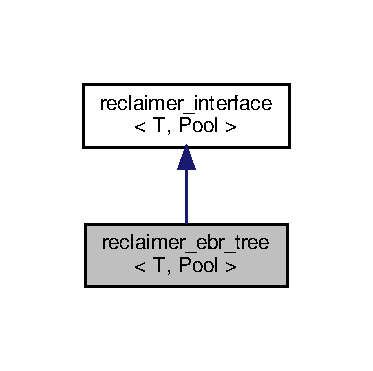
\includegraphics[width=179pt]{classreclaimer__ebr__tree__inherit__graph}
\end{center}
\end{figure}


Collaboration diagram for reclaimer\+\_\+ebr\+\_\+tree$<$ T, Pool $>$\+:
\nopagebreak
\begin{figure}[H]
\begin{center}
\leavevmode
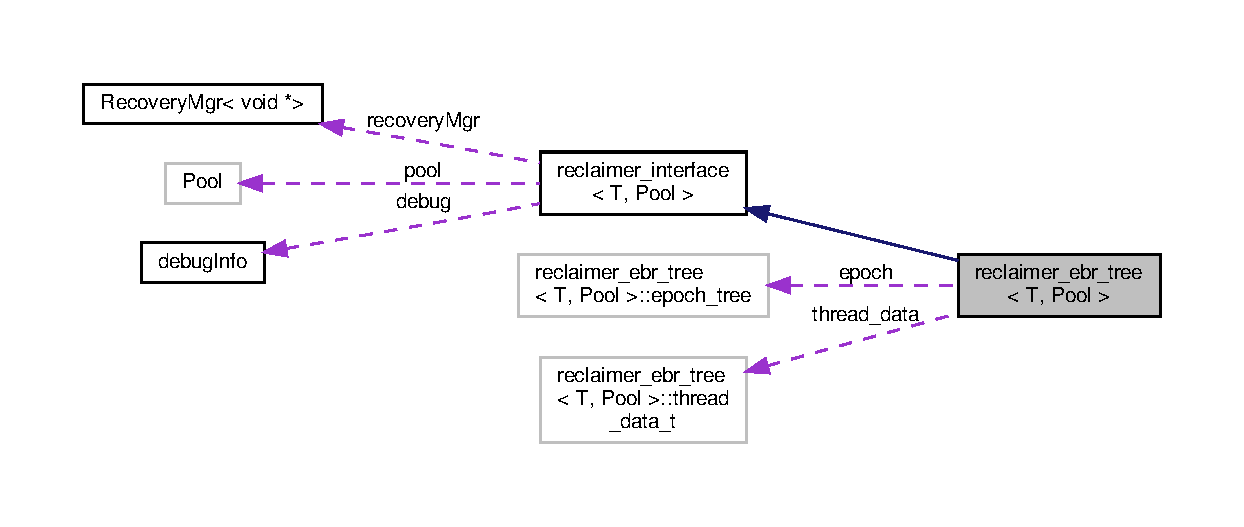
\includegraphics[width=350pt]{classreclaimer__ebr__tree__coll__graph}
\end{center}
\end{figure}
\subsection*{Classes}
\begin{DoxyCompactItemize}
\item 
struct \hyperlink{structreclaimer__ebr__tree_1_1rebind}{rebind}
\item 
struct \hyperlink{structreclaimer__ebr__tree_1_1rebind2}{rebind2}
\end{DoxyCompactItemize}
\subsection*{Public Member Functions}
\begin{DoxyCompactItemize}
\item 
void \hyperlink{classreclaimer__ebr__tree_a3c1034e327a3b2136b4fd7212d701ff7}{get\+Safe\+Blockbags} (const int \hyperlink{microbench_2main_8cpp_a9ca9869868fe7e7a38a921cc7de4103f}{tid}, \hyperlink{classblockbag}{blockbag}$<$ T $>$ $\ast$$\ast$bags)
\item 
long long \hyperlink{classreclaimer__ebr__tree_aa8028a1222c839193450c18e67de9054}{get\+Size\+In\+Nodes} ()
\item 
std\+::string \hyperlink{classreclaimer__ebr__tree_a8e199d1bf0d466f1317f7d637a6c427f}{get\+Details\+String} ()
\item 
std\+::string \hyperlink{classreclaimer__ebr__tree_a36c7cdb0fc910954e2854d099577578d}{get\+Size\+String} ()
\item 
bool \hyperlink{classreclaimer__ebr__tree_ad738d298fd4c156af87eaa52e8b67911}{is\+Quiescent} (const int \hyperlink{microbench_2main_8cpp_a9ca9869868fe7e7a38a921cc7de4103f}{tid})
\item 
void \hyperlink{classreclaimer__ebr__tree_ad9653eeebe33675cae7f754026296e49}{rotate\+Epoch\+Bags} (const int \hyperlink{microbench_2main_8cpp_a9ca9869868fe7e7a38a921cc7de4103f}{tid})
\item 
void \hyperlink{classreclaimer__ebr__tree_abba75a9a4c5b57f3865dab1b7a79a873}{end\+Op} (const int \hyperlink{microbench_2main_8cpp_a9ca9869868fe7e7a38a921cc7de4103f}{tid})
\item 
{\footnotesize template$<$typename First , typename... Rest$>$ }\\bool \hyperlink{classreclaimer__ebr__tree_a3f049dc3decd80d6b2e22cc0af668efa}{start\+Op} (const int \hyperlink{microbench_2main_8cpp_a9ca9869868fe7e7a38a921cc7de4103f}{tid}, void $\ast$const $\ast$const reclaimers, const int num\+Reclaimers, const bool read\+Only=false)
\item 
void \hyperlink{classreclaimer__ebr__tree_ab47468d3259fb52ff889134d66070eb4}{retire} (const int \hyperlink{microbench_2main_8cpp_a9ca9869868fe7e7a38a921cc7de4103f}{tid}, T $\ast$p)
\item 
void \hyperlink{classreclaimer__ebr__tree_ab1987de4ed6253f4ff15790660791c44}{debug\+Print\+Status} (const int \hyperlink{microbench_2main_8cpp_a9ca9869868fe7e7a38a921cc7de4103f}{tid})
\item 
void \hyperlink{classreclaimer__ebr__tree_a8010c52193245d2bbc14039afc1a4b19}{init\+Thread} (const int \hyperlink{microbench_2main_8cpp_a9ca9869868fe7e7a38a921cc7de4103f}{tid})
\item 
void \hyperlink{classreclaimer__ebr__tree_aa38c8b0f0fa033a35dd8f9af80ddd4a7}{deinit\+Thread} (const int \hyperlink{microbench_2main_8cpp_a9ca9869868fe7e7a38a921cc7de4103f}{tid})
\item 
\hyperlink{classreclaimer__ebr__tree_ac1b054e2dade349fdb777185707fed46}{reclaimer\+\_\+ebr\+\_\+tree} (const int \hyperlink{testing_8cpp_aa085812188e21ede75351d88b9b2c30d}{num\+Processes}, Pool $\ast$\+\_\+pool, \hyperlink{classdebugInfo}{debug\+Info} $\ast$const \+\_\+debug, \hyperlink{classRecoveryMgr}{Recovery\+Mgr}$<$ void $\ast$$>$ $\ast$const \+\_\+recovery\+Mgr=N\+U\+LL)
\item 
\hyperlink{classreclaimer__ebr__tree_a12b133bbaac8b15c30f42bfa35a89130}{$\sim$reclaimer\+\_\+ebr\+\_\+tree} ()
\end{DoxyCompactItemize}
\subsection*{Static Public Member Functions}
\begin{DoxyCompactItemize}
\item 
static bool \hyperlink{classreclaimer__ebr__tree_a9fd97c017a569cb88fc2fe23630a15bf}{quiescence\+Is\+Per\+Record\+Type} ()
\item 
static bool \hyperlink{classreclaimer__ebr__tree_a10902145ffb73e322be25a61a735eba3}{is\+Protected} (const int \hyperlink{microbench_2main_8cpp_a9ca9869868fe7e7a38a921cc7de4103f}{tid}, T $\ast$const obj)
\item 
static bool \hyperlink{classreclaimer__ebr__tree_a9e2faa5a9d111fcf1c44c1bad0e2c3d2}{is\+Q\+Protected} (const int \hyperlink{microbench_2main_8cpp_a9ca9869868fe7e7a38a921cc7de4103f}{tid}, T $\ast$const obj)
\item 
static bool \hyperlink{classreclaimer__ebr__tree_a5ad297478a76719d6d643234ee053e78}{protect} (const int \hyperlink{microbench_2main_8cpp_a9ca9869868fe7e7a38a921cc7de4103f}{tid}, T $\ast$const obj, \hyperlink{globals_8h_a57f5c0d40b156d7d996492fb2f16e3cd}{Callback\+Type} not\+Retired\+Callback, \hyperlink{globals_8h_a3de64ef48066ac6430631c8b81a15345}{Callback\+Arg} callback\+Arg, bool memory\+Barrier=true)
\item 
static void \hyperlink{classreclaimer__ebr__tree_ac574b08de5fbfb4c70248cf9cbfb3d26}{unprotect} (const int \hyperlink{microbench_2main_8cpp_a9ca9869868fe7e7a38a921cc7de4103f}{tid}, T $\ast$const obj)
\item 
static bool \hyperlink{classreclaimer__ebr__tree_a56fe1802d92cd833480d75cc249f1199}{q\+Protect} (const int \hyperlink{microbench_2main_8cpp_a9ca9869868fe7e7a38a921cc7de4103f}{tid}, T $\ast$const obj, \hyperlink{globals_8h_a57f5c0d40b156d7d996492fb2f16e3cd}{Callback\+Type} not\+Retired\+Callback, \hyperlink{globals_8h_a3de64ef48066ac6430631c8b81a15345}{Callback\+Arg} callback\+Arg, bool memory\+Barrier=true)
\item 
static void \hyperlink{classreclaimer__ebr__tree_a13e7475450b4065fd76608e10e51f7a7}{q\+Unprotect\+All} (const int \hyperlink{microbench_2main_8cpp_a9ca9869868fe7e7a38a921cc7de4103f}{tid})
\item 
static bool \hyperlink{classreclaimer__ebr__tree_a3d2a44d772dd6fdcca0f593b01b20287}{should\+Help} ()
\end{DoxyCompactItemize}
\subsection*{Protected Attributes}
\begin{DoxyCompactItemize}
\item 
\hyperlink{structthread__data__t}{thread\+\_\+data\+\_\+t} \hyperlink{classreclaimer__ebr__tree_a3ec46853a0bf878335338c3b89debed7}{thread\+\_\+data} \mbox{[}\hyperlink{plaf_8h_ac1585a3455dd3e33e877e588be9e466b}{M\+A\+X\+\_\+\+T\+H\+R\+E\+A\+D\+S\+\_\+\+P\+O\+W2}\mbox{]}
\item 
epoch\+\_\+tree $\ast$ \hyperlink{classreclaimer__ebr__tree_a83b6dbb2cda5383592a2aed9d5d66402}{epoch}
\item 
\hyperlink{classreclaimer__ebr__tree_a574b9ffbb2e9390a01476454383cabef}{P\+AD}
\end{DoxyCompactItemize}
\subsection*{Additional Inherited Members}


\subsection{Constructor \& Destructor Documentation}
\mbox{\Hypertarget{classreclaimer__ebr__tree_ac1b054e2dade349fdb777185707fed46}\label{classreclaimer__ebr__tree_ac1b054e2dade349fdb777185707fed46}} 
\index{reclaimer\+\_\+ebr\+\_\+tree@{reclaimer\+\_\+ebr\+\_\+tree}!reclaimer\+\_\+ebr\+\_\+tree@{reclaimer\+\_\+ebr\+\_\+tree}}
\index{reclaimer\+\_\+ebr\+\_\+tree@{reclaimer\+\_\+ebr\+\_\+tree}!reclaimer\+\_\+ebr\+\_\+tree@{reclaimer\+\_\+ebr\+\_\+tree}}
\subsubsection{\texorpdfstring{reclaimer\+\_\+ebr\+\_\+tree()}{reclaimer\_ebr\_tree()}}
{\footnotesize\ttfamily template$<$typename T  = void, class Pool  = pool\+\_\+interface$<$\+T$>$$>$ \\
\hyperlink{classreclaimer__ebr__tree}{reclaimer\+\_\+ebr\+\_\+tree}$<$ T, Pool $>$\+::\hyperlink{classreclaimer__ebr__tree}{reclaimer\+\_\+ebr\+\_\+tree} (\begin{DoxyParamCaption}\item[{const int}]{num\+Processes,  }\item[{Pool $\ast$}]{\+\_\+pool,  }\item[{\hyperlink{classdebugInfo}{debug\+Info} $\ast$const}]{\+\_\+debug,  }\item[{\hyperlink{classRecoveryMgr}{Recovery\+Mgr}$<$ void $\ast$$>$ $\ast$const}]{\+\_\+recovery\+Mgr = {\ttfamily NULL} }\end{DoxyParamCaption})\hspace{0.3cm}{\ttfamily [inline]}}

\mbox{\Hypertarget{classreclaimer__ebr__tree_a12b133bbaac8b15c30f42bfa35a89130}\label{classreclaimer__ebr__tree_a12b133bbaac8b15c30f42bfa35a89130}} 
\index{reclaimer\+\_\+ebr\+\_\+tree@{reclaimer\+\_\+ebr\+\_\+tree}!````~reclaimer\+\_\+ebr\+\_\+tree@{$\sim$reclaimer\+\_\+ebr\+\_\+tree}}
\index{````~reclaimer\+\_\+ebr\+\_\+tree@{$\sim$reclaimer\+\_\+ebr\+\_\+tree}!reclaimer\+\_\+ebr\+\_\+tree@{reclaimer\+\_\+ebr\+\_\+tree}}
\subsubsection{\texorpdfstring{$\sim$reclaimer\+\_\+ebr\+\_\+tree()}{~reclaimer\_ebr\_tree()}}
{\footnotesize\ttfamily template$<$typename T  = void, class Pool  = pool\+\_\+interface$<$\+T$>$$>$ \\
\hyperlink{classreclaimer__ebr__tree}{reclaimer\+\_\+ebr\+\_\+tree}$<$ T, Pool $>$\+::$\sim$\hyperlink{classreclaimer__ebr__tree}{reclaimer\+\_\+ebr\+\_\+tree} (\begin{DoxyParamCaption}{ }\end{DoxyParamCaption})\hspace{0.3cm}{\ttfamily [inline]}}



\subsection{Member Function Documentation}
\mbox{\Hypertarget{classreclaimer__ebr__tree_ab1987de4ed6253f4ff15790660791c44}\label{classreclaimer__ebr__tree_ab1987de4ed6253f4ff15790660791c44}} 
\index{reclaimer\+\_\+ebr\+\_\+tree@{reclaimer\+\_\+ebr\+\_\+tree}!debug\+Print\+Status@{debug\+Print\+Status}}
\index{debug\+Print\+Status@{debug\+Print\+Status}!reclaimer\+\_\+ebr\+\_\+tree@{reclaimer\+\_\+ebr\+\_\+tree}}
\subsubsection{\texorpdfstring{debug\+Print\+Status()}{debugPrintStatus()}}
{\footnotesize\ttfamily template$<$typename T  = void, class Pool  = pool\+\_\+interface$<$\+T$>$$>$ \\
void \hyperlink{classreclaimer__ebr__tree}{reclaimer\+\_\+ebr\+\_\+tree}$<$ T, Pool $>$\+::debug\+Print\+Status (\begin{DoxyParamCaption}\item[{const int}]{tid }\end{DoxyParamCaption})\hspace{0.3cm}{\ttfamily [inline]}}

\mbox{\Hypertarget{classreclaimer__ebr__tree_aa38c8b0f0fa033a35dd8f9af80ddd4a7}\label{classreclaimer__ebr__tree_aa38c8b0f0fa033a35dd8f9af80ddd4a7}} 
\index{reclaimer\+\_\+ebr\+\_\+tree@{reclaimer\+\_\+ebr\+\_\+tree}!deinit\+Thread@{deinit\+Thread}}
\index{deinit\+Thread@{deinit\+Thread}!reclaimer\+\_\+ebr\+\_\+tree@{reclaimer\+\_\+ebr\+\_\+tree}}
\subsubsection{\texorpdfstring{deinit\+Thread()}{deinitThread()}}
{\footnotesize\ttfamily template$<$typename T  = void, class Pool  = pool\+\_\+interface$<$\+T$>$$>$ \\
void \hyperlink{classreclaimer__ebr__tree}{reclaimer\+\_\+ebr\+\_\+tree}$<$ T, Pool $>$\+::deinit\+Thread (\begin{DoxyParamCaption}\item[{const int}]{tid }\end{DoxyParamCaption})\hspace{0.3cm}{\ttfamily [inline]}}

\mbox{\Hypertarget{classreclaimer__ebr__tree_abba75a9a4c5b57f3865dab1b7a79a873}\label{classreclaimer__ebr__tree_abba75a9a4c5b57f3865dab1b7a79a873}} 
\index{reclaimer\+\_\+ebr\+\_\+tree@{reclaimer\+\_\+ebr\+\_\+tree}!end\+Op@{end\+Op}}
\index{end\+Op@{end\+Op}!reclaimer\+\_\+ebr\+\_\+tree@{reclaimer\+\_\+ebr\+\_\+tree}}
\subsubsection{\texorpdfstring{end\+Op()}{endOp()}}
{\footnotesize\ttfamily template$<$typename T  = void, class Pool  = pool\+\_\+interface$<$\+T$>$$>$ \\
void \hyperlink{classreclaimer__ebr__tree}{reclaimer\+\_\+ebr\+\_\+tree}$<$ T, Pool $>$\+::end\+Op (\begin{DoxyParamCaption}\item[{const int}]{tid }\end{DoxyParamCaption})\hspace{0.3cm}{\ttfamily [inline]}}

\mbox{\Hypertarget{classreclaimer__ebr__tree_a8e199d1bf0d466f1317f7d637a6c427f}\label{classreclaimer__ebr__tree_a8e199d1bf0d466f1317f7d637a6c427f}} 
\index{reclaimer\+\_\+ebr\+\_\+tree@{reclaimer\+\_\+ebr\+\_\+tree}!get\+Details\+String@{get\+Details\+String}}
\index{get\+Details\+String@{get\+Details\+String}!reclaimer\+\_\+ebr\+\_\+tree@{reclaimer\+\_\+ebr\+\_\+tree}}
\subsubsection{\texorpdfstring{get\+Details\+String()}{getDetailsString()}}
{\footnotesize\ttfamily template$<$typename T  = void, class Pool  = pool\+\_\+interface$<$\+T$>$$>$ \\
std\+::string \hyperlink{classreclaimer__ebr__tree}{reclaimer\+\_\+ebr\+\_\+tree}$<$ T, Pool $>$\+::get\+Details\+String (\begin{DoxyParamCaption}{ }\end{DoxyParamCaption})\hspace{0.3cm}{\ttfamily [inline]}}

\mbox{\Hypertarget{classreclaimer__ebr__tree_a3c1034e327a3b2136b4fd7212d701ff7}\label{classreclaimer__ebr__tree_a3c1034e327a3b2136b4fd7212d701ff7}} 
\index{reclaimer\+\_\+ebr\+\_\+tree@{reclaimer\+\_\+ebr\+\_\+tree}!get\+Safe\+Blockbags@{get\+Safe\+Blockbags}}
\index{get\+Safe\+Blockbags@{get\+Safe\+Blockbags}!reclaimer\+\_\+ebr\+\_\+tree@{reclaimer\+\_\+ebr\+\_\+tree}}
\subsubsection{\texorpdfstring{get\+Safe\+Blockbags()}{getSafeBlockbags()}}
{\footnotesize\ttfamily template$<$typename T  = void, class Pool  = pool\+\_\+interface$<$\+T$>$$>$ \\
void \hyperlink{classreclaimer__ebr__tree}{reclaimer\+\_\+ebr\+\_\+tree}$<$ T, Pool $>$\+::get\+Safe\+Blockbags (\begin{DoxyParamCaption}\item[{const int}]{tid,  }\item[{\hyperlink{classblockbag}{blockbag}$<$ T $>$ $\ast$$\ast$}]{bags }\end{DoxyParamCaption})\hspace{0.3cm}{\ttfamily [inline]}}

\mbox{\Hypertarget{classreclaimer__ebr__tree_aa8028a1222c839193450c18e67de9054}\label{classreclaimer__ebr__tree_aa8028a1222c839193450c18e67de9054}} 
\index{reclaimer\+\_\+ebr\+\_\+tree@{reclaimer\+\_\+ebr\+\_\+tree}!get\+Size\+In\+Nodes@{get\+Size\+In\+Nodes}}
\index{get\+Size\+In\+Nodes@{get\+Size\+In\+Nodes}!reclaimer\+\_\+ebr\+\_\+tree@{reclaimer\+\_\+ebr\+\_\+tree}}
\subsubsection{\texorpdfstring{get\+Size\+In\+Nodes()}{getSizeInNodes()}}
{\footnotesize\ttfamily template$<$typename T  = void, class Pool  = pool\+\_\+interface$<$\+T$>$$>$ \\
long long \hyperlink{classreclaimer__ebr__tree}{reclaimer\+\_\+ebr\+\_\+tree}$<$ T, Pool $>$\+::get\+Size\+In\+Nodes (\begin{DoxyParamCaption}{ }\end{DoxyParamCaption})\hspace{0.3cm}{\ttfamily [inline]}}

\mbox{\Hypertarget{classreclaimer__ebr__tree_a36c7cdb0fc910954e2854d099577578d}\label{classreclaimer__ebr__tree_a36c7cdb0fc910954e2854d099577578d}} 
\index{reclaimer\+\_\+ebr\+\_\+tree@{reclaimer\+\_\+ebr\+\_\+tree}!get\+Size\+String@{get\+Size\+String}}
\index{get\+Size\+String@{get\+Size\+String}!reclaimer\+\_\+ebr\+\_\+tree@{reclaimer\+\_\+ebr\+\_\+tree}}
\subsubsection{\texorpdfstring{get\+Size\+String()}{getSizeString()}}
{\footnotesize\ttfamily template$<$typename T  = void, class Pool  = pool\+\_\+interface$<$\+T$>$$>$ \\
std\+::string \hyperlink{classreclaimer__ebr__tree}{reclaimer\+\_\+ebr\+\_\+tree}$<$ T, Pool $>$\+::get\+Size\+String (\begin{DoxyParamCaption}{ }\end{DoxyParamCaption})\hspace{0.3cm}{\ttfamily [inline]}}

\mbox{\Hypertarget{classreclaimer__ebr__tree_a8010c52193245d2bbc14039afc1a4b19}\label{classreclaimer__ebr__tree_a8010c52193245d2bbc14039afc1a4b19}} 
\index{reclaimer\+\_\+ebr\+\_\+tree@{reclaimer\+\_\+ebr\+\_\+tree}!init\+Thread@{init\+Thread}}
\index{init\+Thread@{init\+Thread}!reclaimer\+\_\+ebr\+\_\+tree@{reclaimer\+\_\+ebr\+\_\+tree}}
\subsubsection{\texorpdfstring{init\+Thread()}{initThread()}}
{\footnotesize\ttfamily template$<$typename T  = void, class Pool  = pool\+\_\+interface$<$\+T$>$$>$ \\
void \hyperlink{classreclaimer__ebr__tree}{reclaimer\+\_\+ebr\+\_\+tree}$<$ T, Pool $>$\+::init\+Thread (\begin{DoxyParamCaption}\item[{const int}]{tid }\end{DoxyParamCaption})\hspace{0.3cm}{\ttfamily [inline]}}

\mbox{\Hypertarget{classreclaimer__ebr__tree_a10902145ffb73e322be25a61a735eba3}\label{classreclaimer__ebr__tree_a10902145ffb73e322be25a61a735eba3}} 
\index{reclaimer\+\_\+ebr\+\_\+tree@{reclaimer\+\_\+ebr\+\_\+tree}!is\+Protected@{is\+Protected}}
\index{is\+Protected@{is\+Protected}!reclaimer\+\_\+ebr\+\_\+tree@{reclaimer\+\_\+ebr\+\_\+tree}}
\subsubsection{\texorpdfstring{is\+Protected()}{isProtected()}}
{\footnotesize\ttfamily template$<$typename T  = void, class Pool  = pool\+\_\+interface$<$\+T$>$$>$ \\
static bool \hyperlink{classreclaimer__ebr__tree}{reclaimer\+\_\+ebr\+\_\+tree}$<$ T, Pool $>$\+::is\+Protected (\begin{DoxyParamCaption}\item[{const int}]{tid,  }\item[{T $\ast$const}]{obj }\end{DoxyParamCaption})\hspace{0.3cm}{\ttfamily [inline]}, {\ttfamily [static]}}

\mbox{\Hypertarget{classreclaimer__ebr__tree_a9e2faa5a9d111fcf1c44c1bad0e2c3d2}\label{classreclaimer__ebr__tree_a9e2faa5a9d111fcf1c44c1bad0e2c3d2}} 
\index{reclaimer\+\_\+ebr\+\_\+tree@{reclaimer\+\_\+ebr\+\_\+tree}!is\+Q\+Protected@{is\+Q\+Protected}}
\index{is\+Q\+Protected@{is\+Q\+Protected}!reclaimer\+\_\+ebr\+\_\+tree@{reclaimer\+\_\+ebr\+\_\+tree}}
\subsubsection{\texorpdfstring{is\+Q\+Protected()}{isQProtected()}}
{\footnotesize\ttfamily template$<$typename T  = void, class Pool  = pool\+\_\+interface$<$\+T$>$$>$ \\
static bool \hyperlink{classreclaimer__ebr__tree}{reclaimer\+\_\+ebr\+\_\+tree}$<$ T, Pool $>$\+::is\+Q\+Protected (\begin{DoxyParamCaption}\item[{const int}]{tid,  }\item[{T $\ast$const}]{obj }\end{DoxyParamCaption})\hspace{0.3cm}{\ttfamily [inline]}, {\ttfamily [static]}}

\mbox{\Hypertarget{classreclaimer__ebr__tree_ad738d298fd4c156af87eaa52e8b67911}\label{classreclaimer__ebr__tree_ad738d298fd4c156af87eaa52e8b67911}} 
\index{reclaimer\+\_\+ebr\+\_\+tree@{reclaimer\+\_\+ebr\+\_\+tree}!is\+Quiescent@{is\+Quiescent}}
\index{is\+Quiescent@{is\+Quiescent}!reclaimer\+\_\+ebr\+\_\+tree@{reclaimer\+\_\+ebr\+\_\+tree}}
\subsubsection{\texorpdfstring{is\+Quiescent()}{isQuiescent()}}
{\footnotesize\ttfamily template$<$typename T  = void, class Pool  = pool\+\_\+interface$<$\+T$>$$>$ \\
bool \hyperlink{classreclaimer__ebr__tree}{reclaimer\+\_\+ebr\+\_\+tree}$<$ T, Pool $>$\+::is\+Quiescent (\begin{DoxyParamCaption}\item[{const int}]{tid }\end{DoxyParamCaption})\hspace{0.3cm}{\ttfamily [inline]}}

\mbox{\Hypertarget{classreclaimer__ebr__tree_a5ad297478a76719d6d643234ee053e78}\label{classreclaimer__ebr__tree_a5ad297478a76719d6d643234ee053e78}} 
\index{reclaimer\+\_\+ebr\+\_\+tree@{reclaimer\+\_\+ebr\+\_\+tree}!protect@{protect}}
\index{protect@{protect}!reclaimer\+\_\+ebr\+\_\+tree@{reclaimer\+\_\+ebr\+\_\+tree}}
\subsubsection{\texorpdfstring{protect()}{protect()}}
{\footnotesize\ttfamily template$<$typename T  = void, class Pool  = pool\+\_\+interface$<$\+T$>$$>$ \\
static bool \hyperlink{classreclaimer__ebr__tree}{reclaimer\+\_\+ebr\+\_\+tree}$<$ T, Pool $>$\+::protect (\begin{DoxyParamCaption}\item[{const int}]{tid,  }\item[{T $\ast$const}]{obj,  }\item[{\hyperlink{globals_8h_a57f5c0d40b156d7d996492fb2f16e3cd}{Callback\+Type}}]{not\+Retired\+Callback,  }\item[{\hyperlink{globals_8h_a3de64ef48066ac6430631c8b81a15345}{Callback\+Arg}}]{callback\+Arg,  }\item[{bool}]{memory\+Barrier = {\ttfamily true} }\end{DoxyParamCaption})\hspace{0.3cm}{\ttfamily [inline]}, {\ttfamily [static]}}

\mbox{\Hypertarget{classreclaimer__ebr__tree_a56fe1802d92cd833480d75cc249f1199}\label{classreclaimer__ebr__tree_a56fe1802d92cd833480d75cc249f1199}} 
\index{reclaimer\+\_\+ebr\+\_\+tree@{reclaimer\+\_\+ebr\+\_\+tree}!q\+Protect@{q\+Protect}}
\index{q\+Protect@{q\+Protect}!reclaimer\+\_\+ebr\+\_\+tree@{reclaimer\+\_\+ebr\+\_\+tree}}
\subsubsection{\texorpdfstring{q\+Protect()}{qProtect()}}
{\footnotesize\ttfamily template$<$typename T  = void, class Pool  = pool\+\_\+interface$<$\+T$>$$>$ \\
static bool \hyperlink{classreclaimer__ebr__tree}{reclaimer\+\_\+ebr\+\_\+tree}$<$ T, Pool $>$\+::q\+Protect (\begin{DoxyParamCaption}\item[{const int}]{tid,  }\item[{T $\ast$const}]{obj,  }\item[{\hyperlink{globals_8h_a57f5c0d40b156d7d996492fb2f16e3cd}{Callback\+Type}}]{not\+Retired\+Callback,  }\item[{\hyperlink{globals_8h_a3de64ef48066ac6430631c8b81a15345}{Callback\+Arg}}]{callback\+Arg,  }\item[{bool}]{memory\+Barrier = {\ttfamily true} }\end{DoxyParamCaption})\hspace{0.3cm}{\ttfamily [inline]}, {\ttfamily [static]}}

\mbox{\Hypertarget{classreclaimer__ebr__tree_a9fd97c017a569cb88fc2fe23630a15bf}\label{classreclaimer__ebr__tree_a9fd97c017a569cb88fc2fe23630a15bf}} 
\index{reclaimer\+\_\+ebr\+\_\+tree@{reclaimer\+\_\+ebr\+\_\+tree}!quiescence\+Is\+Per\+Record\+Type@{quiescence\+Is\+Per\+Record\+Type}}
\index{quiescence\+Is\+Per\+Record\+Type@{quiescence\+Is\+Per\+Record\+Type}!reclaimer\+\_\+ebr\+\_\+tree@{reclaimer\+\_\+ebr\+\_\+tree}}
\subsubsection{\texorpdfstring{quiescence\+Is\+Per\+Record\+Type()}{quiescenceIsPerRecordType()}}
{\footnotesize\ttfamily template$<$typename T  = void, class Pool  = pool\+\_\+interface$<$\+T$>$$>$ \\
static bool \hyperlink{classreclaimer__ebr__tree}{reclaimer\+\_\+ebr\+\_\+tree}$<$ T, Pool $>$\+::quiescence\+Is\+Per\+Record\+Type (\begin{DoxyParamCaption}{ }\end{DoxyParamCaption})\hspace{0.3cm}{\ttfamily [inline]}, {\ttfamily [static]}}

\mbox{\Hypertarget{classreclaimer__ebr__tree_a13e7475450b4065fd76608e10e51f7a7}\label{classreclaimer__ebr__tree_a13e7475450b4065fd76608e10e51f7a7}} 
\index{reclaimer\+\_\+ebr\+\_\+tree@{reclaimer\+\_\+ebr\+\_\+tree}!q\+Unprotect\+All@{q\+Unprotect\+All}}
\index{q\+Unprotect\+All@{q\+Unprotect\+All}!reclaimer\+\_\+ebr\+\_\+tree@{reclaimer\+\_\+ebr\+\_\+tree}}
\subsubsection{\texorpdfstring{q\+Unprotect\+All()}{qUnprotectAll()}}
{\footnotesize\ttfamily template$<$typename T  = void, class Pool  = pool\+\_\+interface$<$\+T$>$$>$ \\
static void \hyperlink{classreclaimer__ebr__tree}{reclaimer\+\_\+ebr\+\_\+tree}$<$ T, Pool $>$\+::q\+Unprotect\+All (\begin{DoxyParamCaption}\item[{const int}]{tid }\end{DoxyParamCaption})\hspace{0.3cm}{\ttfamily [inline]}, {\ttfamily [static]}}

\mbox{\Hypertarget{classreclaimer__ebr__tree_ab47468d3259fb52ff889134d66070eb4}\label{classreclaimer__ebr__tree_ab47468d3259fb52ff889134d66070eb4}} 
\index{reclaimer\+\_\+ebr\+\_\+tree@{reclaimer\+\_\+ebr\+\_\+tree}!retire@{retire}}
\index{retire@{retire}!reclaimer\+\_\+ebr\+\_\+tree@{reclaimer\+\_\+ebr\+\_\+tree}}
\subsubsection{\texorpdfstring{retire()}{retire()}}
{\footnotesize\ttfamily template$<$typename T  = void, class Pool  = pool\+\_\+interface$<$\+T$>$$>$ \\
void \hyperlink{classreclaimer__ebr__tree}{reclaimer\+\_\+ebr\+\_\+tree}$<$ T, Pool $>$\+::retire (\begin{DoxyParamCaption}\item[{const int}]{tid,  }\item[{T $\ast$}]{p }\end{DoxyParamCaption})\hspace{0.3cm}{\ttfamily [inline]}}

\mbox{\Hypertarget{classreclaimer__ebr__tree_ad9653eeebe33675cae7f754026296e49}\label{classreclaimer__ebr__tree_ad9653eeebe33675cae7f754026296e49}} 
\index{reclaimer\+\_\+ebr\+\_\+tree@{reclaimer\+\_\+ebr\+\_\+tree}!rotate\+Epoch\+Bags@{rotate\+Epoch\+Bags}}
\index{rotate\+Epoch\+Bags@{rotate\+Epoch\+Bags}!reclaimer\+\_\+ebr\+\_\+tree@{reclaimer\+\_\+ebr\+\_\+tree}}
\subsubsection{\texorpdfstring{rotate\+Epoch\+Bags()}{rotateEpochBags()}}
{\footnotesize\ttfamily template$<$typename T  = void, class Pool  = pool\+\_\+interface$<$\+T$>$$>$ \\
void \hyperlink{classreclaimer__ebr__tree}{reclaimer\+\_\+ebr\+\_\+tree}$<$ T, Pool $>$\+::rotate\+Epoch\+Bags (\begin{DoxyParamCaption}\item[{const int}]{tid }\end{DoxyParamCaption})\hspace{0.3cm}{\ttfamily [inline]}}

\mbox{\Hypertarget{classreclaimer__ebr__tree_a3d2a44d772dd6fdcca0f593b01b20287}\label{classreclaimer__ebr__tree_a3d2a44d772dd6fdcca0f593b01b20287}} 
\index{reclaimer\+\_\+ebr\+\_\+tree@{reclaimer\+\_\+ebr\+\_\+tree}!should\+Help@{should\+Help}}
\index{should\+Help@{should\+Help}!reclaimer\+\_\+ebr\+\_\+tree@{reclaimer\+\_\+ebr\+\_\+tree}}
\subsubsection{\texorpdfstring{should\+Help()}{shouldHelp()}}
{\footnotesize\ttfamily template$<$typename T  = void, class Pool  = pool\+\_\+interface$<$\+T$>$$>$ \\
static bool \hyperlink{classreclaimer__ebr__tree}{reclaimer\+\_\+ebr\+\_\+tree}$<$ T, Pool $>$\+::should\+Help (\begin{DoxyParamCaption}{ }\end{DoxyParamCaption})\hspace{0.3cm}{\ttfamily [inline]}, {\ttfamily [static]}}

\mbox{\Hypertarget{classreclaimer__ebr__tree_a3f049dc3decd80d6b2e22cc0af668efa}\label{classreclaimer__ebr__tree_a3f049dc3decd80d6b2e22cc0af668efa}} 
\index{reclaimer\+\_\+ebr\+\_\+tree@{reclaimer\+\_\+ebr\+\_\+tree}!start\+Op@{start\+Op}}
\index{start\+Op@{start\+Op}!reclaimer\+\_\+ebr\+\_\+tree@{reclaimer\+\_\+ebr\+\_\+tree}}
\subsubsection{\texorpdfstring{start\+Op()}{startOp()}}
{\footnotesize\ttfamily template$<$typename T  = void, class Pool  = pool\+\_\+interface$<$\+T$>$$>$ \\
template$<$typename First , typename... Rest$>$ \\
bool \hyperlink{classreclaimer__ebr__tree}{reclaimer\+\_\+ebr\+\_\+tree}$<$ T, Pool $>$\+::start\+Op (\begin{DoxyParamCaption}\item[{const int}]{tid,  }\item[{void $\ast$const $\ast$const}]{reclaimers,  }\item[{const int}]{num\+Reclaimers,  }\item[{const bool}]{read\+Only = {\ttfamily false} }\end{DoxyParamCaption})\hspace{0.3cm}{\ttfamily [inline]}}

\mbox{\Hypertarget{classreclaimer__ebr__tree_ac574b08de5fbfb4c70248cf9cbfb3d26}\label{classreclaimer__ebr__tree_ac574b08de5fbfb4c70248cf9cbfb3d26}} 
\index{reclaimer\+\_\+ebr\+\_\+tree@{reclaimer\+\_\+ebr\+\_\+tree}!unprotect@{unprotect}}
\index{unprotect@{unprotect}!reclaimer\+\_\+ebr\+\_\+tree@{reclaimer\+\_\+ebr\+\_\+tree}}
\subsubsection{\texorpdfstring{unprotect()}{unprotect()}}
{\footnotesize\ttfamily template$<$typename T  = void, class Pool  = pool\+\_\+interface$<$\+T$>$$>$ \\
static void \hyperlink{classreclaimer__ebr__tree}{reclaimer\+\_\+ebr\+\_\+tree}$<$ T, Pool $>$\+::unprotect (\begin{DoxyParamCaption}\item[{const int}]{tid,  }\item[{T $\ast$const}]{obj }\end{DoxyParamCaption})\hspace{0.3cm}{\ttfamily [inline]}, {\ttfamily [static]}}



\subsection{Member Data Documentation}
\mbox{\Hypertarget{classreclaimer__ebr__tree_a83b6dbb2cda5383592a2aed9d5d66402}\label{classreclaimer__ebr__tree_a83b6dbb2cda5383592a2aed9d5d66402}} 
\index{reclaimer\+\_\+ebr\+\_\+tree@{reclaimer\+\_\+ebr\+\_\+tree}!epoch@{epoch}}
\index{epoch@{epoch}!reclaimer\+\_\+ebr\+\_\+tree@{reclaimer\+\_\+ebr\+\_\+tree}}
\subsubsection{\texorpdfstring{epoch}{epoch}}
{\footnotesize\ttfamily template$<$typename T  = void, class Pool  = pool\+\_\+interface$<$\+T$>$$>$ \\
epoch\+\_\+tree$\ast$ \hyperlink{classreclaimer__ebr__tree}{reclaimer\+\_\+ebr\+\_\+tree}$<$ T, Pool $>$\+::epoch\hspace{0.3cm}{\ttfamily [protected]}}

\mbox{\Hypertarget{classreclaimer__ebr__tree_a574b9ffbb2e9390a01476454383cabef}\label{classreclaimer__ebr__tree_a574b9ffbb2e9390a01476454383cabef}} 
\index{reclaimer\+\_\+ebr\+\_\+tree@{reclaimer\+\_\+ebr\+\_\+tree}!P\+AD@{P\+AD}}
\index{P\+AD@{P\+AD}!reclaimer\+\_\+ebr\+\_\+tree@{reclaimer\+\_\+ebr\+\_\+tree}}
\subsubsection{\texorpdfstring{P\+AD}{PAD}}
{\footnotesize\ttfamily template$<$typename T  = void, class Pool  = pool\+\_\+interface$<$\+T$>$$>$ \\
\hyperlink{classreclaimer__ebr__tree}{reclaimer\+\_\+ebr\+\_\+tree}$<$ T, Pool $>$\+::P\+AD\hspace{0.3cm}{\ttfamily [protected]}}

\mbox{\Hypertarget{classreclaimer__ebr__tree_a3ec46853a0bf878335338c3b89debed7}\label{classreclaimer__ebr__tree_a3ec46853a0bf878335338c3b89debed7}} 
\index{reclaimer\+\_\+ebr\+\_\+tree@{reclaimer\+\_\+ebr\+\_\+tree}!thread\+\_\+data@{thread\+\_\+data}}
\index{thread\+\_\+data@{thread\+\_\+data}!reclaimer\+\_\+ebr\+\_\+tree@{reclaimer\+\_\+ebr\+\_\+tree}}
\subsubsection{\texorpdfstring{thread\+\_\+data}{thread\_data}}
{\footnotesize\ttfamily template$<$typename T  = void, class Pool  = pool\+\_\+interface$<$\+T$>$$>$ \\
\hyperlink{structthread__data__t}{thread\+\_\+data\+\_\+t} \hyperlink{classreclaimer__ebr__tree}{reclaimer\+\_\+ebr\+\_\+tree}$<$ T, Pool $>$\+::thread\+\_\+data\mbox{[}\hyperlink{plaf_8h_ac1585a3455dd3e33e877e588be9e466b}{M\+A\+X\+\_\+\+T\+H\+R\+E\+A\+D\+S\+\_\+\+P\+O\+W2}\mbox{]}\hspace{0.3cm}{\ttfamily [protected]}}



The documentation for this class was generated from the following file\+:\begin{DoxyCompactItemize}
\item 
common/recordmgr/\hyperlink{reclaimer__ebr__tree_8h}{reclaimer\+\_\+ebr\+\_\+tree.\+h}\end{DoxyCompactItemize}

\hypertarget{classreclaimer__ebr__tree__q}{}\section{reclaimer\+\_\+ebr\+\_\+tree\+\_\+q$<$ T, Pool $>$ Class Template Reference}
\label{classreclaimer__ebr__tree__q}\index{reclaimer\+\_\+ebr\+\_\+tree\+\_\+q$<$ T, Pool $>$@{reclaimer\+\_\+ebr\+\_\+tree\+\_\+q$<$ T, Pool $>$}}


{\ttfamily \#include $<$reclaimer\+\_\+ebr\+\_\+tree\+\_\+q.\+h$>$}



Inheritance diagram for reclaimer\+\_\+ebr\+\_\+tree\+\_\+q$<$ T, Pool $>$\+:
\nopagebreak
\begin{figure}[H]
\begin{center}
\leavevmode
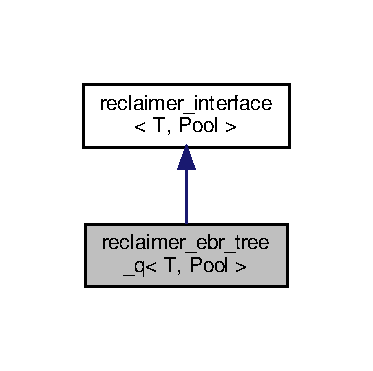
\includegraphics[width=179pt]{classreclaimer__ebr__tree__q__inherit__graph}
\end{center}
\end{figure}


Collaboration diagram for reclaimer\+\_\+ebr\+\_\+tree\+\_\+q$<$ T, Pool $>$\+:
\nopagebreak
\begin{figure}[H]
\begin{center}
\leavevmode
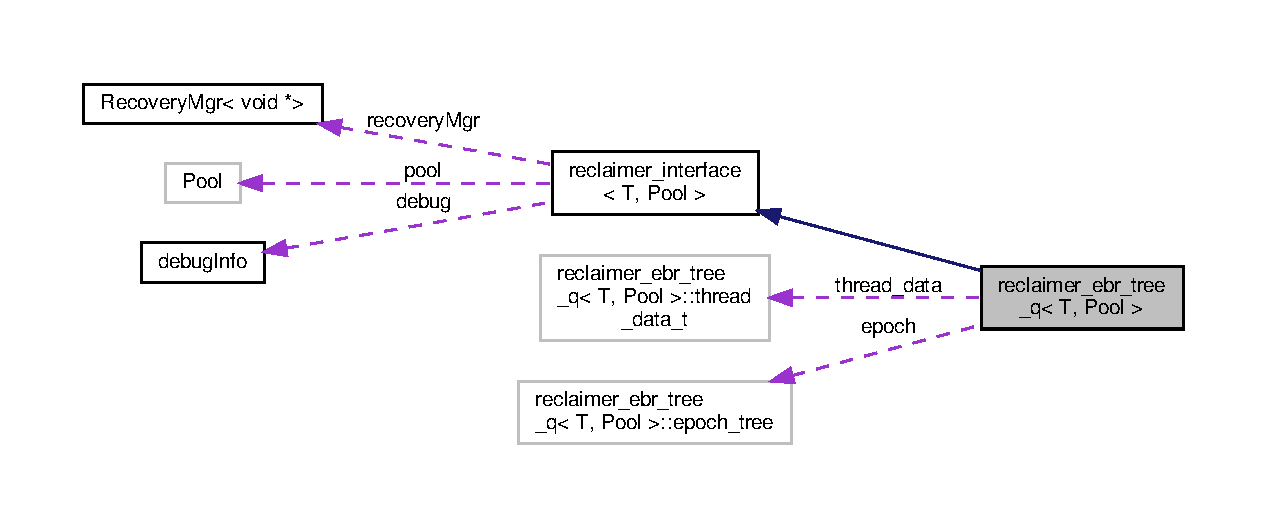
\includegraphics[width=350pt]{classreclaimer__ebr__tree__q__coll__graph}
\end{center}
\end{figure}
\subsection*{Classes}
\begin{DoxyCompactItemize}
\item 
struct \hyperlink{structreclaimer__ebr__tree__q_1_1rebind}{rebind}
\item 
struct \hyperlink{structreclaimer__ebr__tree__q_1_1rebind2}{rebind2}
\end{DoxyCompactItemize}
\subsection*{Public Member Functions}
\begin{DoxyCompactItemize}
\item 
void \hyperlink{classreclaimer__ebr__tree__q_a20c18f89048520313881e48aea56d346}{get\+Safe\+Blockbags} (const int \hyperlink{microbench_2main_8cpp_a9ca9869868fe7e7a38a921cc7de4103f}{tid}, \hyperlink{classblockbag}{blockbag}$<$ T $>$ $\ast$$\ast$bags)
\item 
size\+\_\+t \hyperlink{classreclaimer__ebr__tree__q_a7dd15de4e2b702ddcc726beb6f5aea03}{get\+Size\+In\+Nodes} ()
\item 
std\+::string \hyperlink{classreclaimer__ebr__tree__q_a8a13b84deb3016f4bfb45d375e15c4dd}{get\+Details\+String} ()
\item 
std\+::string \hyperlink{classreclaimer__ebr__tree__q_ad7b69190f8e24214be11b3d90c6380e4}{get\+Size\+String} ()
\item 
bool \hyperlink{classreclaimer__ebr__tree__q_acf02fbff03a0e5fff1e98b6457d77c20}{is\+Quiescent} (const int \hyperlink{microbench_2main_8cpp_a9ca9869868fe7e7a38a921cc7de4103f}{tid})
\item 
void \hyperlink{classreclaimer__ebr__tree__q_ad9a87e180ec41534381c80939c94f0aa}{end\+Op} (const int \hyperlink{microbench_2main_8cpp_a9ca9869868fe7e7a38a921cc7de4103f}{tid})
\item 
bool \hyperlink{classreclaimer__ebr__tree__q_a87abaab7960fab864deaff4e6f358996}{start\+Op} (const int \hyperlink{microbench_2main_8cpp_a9ca9869868fe7e7a38a921cc7de4103f}{tid}, void $\ast$const $\ast$const reclaimers, const int num\+Reclaimers)
\item 
void \hyperlink{classreclaimer__ebr__tree__q_a0232028c4b878f2907442b41cbf73218}{retire} (const int \hyperlink{microbench_2main_8cpp_a9ca9869868fe7e7a38a921cc7de4103f}{tid}, T $\ast$p)
\item 
void \hyperlink{classreclaimer__ebr__tree__q_a6a2106ba8affb3ae0935418868d995ce}{debug\+Print\+Status} (const int \hyperlink{microbench_2main_8cpp_a9ca9869868fe7e7a38a921cc7de4103f}{tid})
\item 
void \hyperlink{classreclaimer__ebr__tree__q_a7859d179c8baa22752d8da9287e49580}{init\+Thread} (const int \hyperlink{microbench_2main_8cpp_a9ca9869868fe7e7a38a921cc7de4103f}{tid})
\item 
void \hyperlink{classreclaimer__ebr__tree__q_a38c74a41409a6e2ba6f67ec19c6e49cf}{deinit\+Thread} (const int \hyperlink{microbench_2main_8cpp_a9ca9869868fe7e7a38a921cc7de4103f}{tid})
\item 
\hyperlink{classreclaimer__ebr__tree__q_ac0243334db596ecc7d41834656cdd59c}{reclaimer\+\_\+ebr\+\_\+tree\+\_\+q} (const int \hyperlink{testing_8cpp_aa085812188e21ede75351d88b9b2c30d}{num\+Processes}, Pool $\ast$\+\_\+pool, \hyperlink{classdebugInfo}{debug\+Info} $\ast$const \+\_\+debug, \hyperlink{classRecoveryMgr}{Recovery\+Mgr}$<$ void $\ast$$>$ $\ast$const \+\_\+recovery\+Mgr=N\+U\+LL)
\item 
\hyperlink{classreclaimer__ebr__tree__q_a983350ea3cd56b26073a8c0f688b6c33}{$\sim$reclaimer\+\_\+ebr\+\_\+tree\+\_\+q} ()
\end{DoxyCompactItemize}
\subsection*{Static Public Member Functions}
\begin{DoxyCompactItemize}
\item 
static bool \hyperlink{classreclaimer__ebr__tree__q_a21a4e941094206214669cc12bfccccb8}{quiescence\+Is\+Per\+Record\+Type} ()
\item 
static bool \hyperlink{classreclaimer__ebr__tree__q_a8653aed206f9fea252691fe143b653af}{is\+Protected} (const int \hyperlink{microbench_2main_8cpp_a9ca9869868fe7e7a38a921cc7de4103f}{tid}, T $\ast$const obj)
\item 
static bool \hyperlink{classreclaimer__ebr__tree__q_aaac58c40bba2197b60831238535a8f73}{is\+Q\+Protected} (const int \hyperlink{microbench_2main_8cpp_a9ca9869868fe7e7a38a921cc7de4103f}{tid}, T $\ast$const obj)
\item 
static bool \hyperlink{classreclaimer__ebr__tree__q_ae26adcb58782a2f7b16b1751389b4668}{protect} (const int \hyperlink{microbench_2main_8cpp_a9ca9869868fe7e7a38a921cc7de4103f}{tid}, T $\ast$const obj, \hyperlink{globals_8h_a57f5c0d40b156d7d996492fb2f16e3cd}{Callback\+Type} not\+Retired\+Callback, \hyperlink{globals_8h_a3de64ef48066ac6430631c8b81a15345}{Callback\+Arg} callback\+Arg, bool memory\+Barrier=true)
\item 
static void \hyperlink{classreclaimer__ebr__tree__q_ae5fde23c9bf570d7c296ca0cc2050f0c}{unprotect} (const int \hyperlink{microbench_2main_8cpp_a9ca9869868fe7e7a38a921cc7de4103f}{tid}, T $\ast$const obj)
\item 
static bool \hyperlink{classreclaimer__ebr__tree__q_aea39367ff1e781d1841c9da13a7fe9c3}{q\+Protect} (const int \hyperlink{microbench_2main_8cpp_a9ca9869868fe7e7a38a921cc7de4103f}{tid}, T $\ast$const obj, \hyperlink{globals_8h_a57f5c0d40b156d7d996492fb2f16e3cd}{Callback\+Type} not\+Retired\+Callback, \hyperlink{globals_8h_a3de64ef48066ac6430631c8b81a15345}{Callback\+Arg} callback\+Arg, bool memory\+Barrier=true)
\item 
static void \hyperlink{classreclaimer__ebr__tree__q_a4368d8dffee8861e1cbabbc455c3e15d}{q\+Unprotect\+All} (const int \hyperlink{microbench_2main_8cpp_a9ca9869868fe7e7a38a921cc7de4103f}{tid})
\item 
static bool \hyperlink{classreclaimer__ebr__tree__q_a50c8fbcc4b2d66491e1cbb449c61f863}{should\+Help} ()
\end{DoxyCompactItemize}
\subsection*{Protected Attributes}
\begin{DoxyCompactItemize}
\item 
\hyperlink{structthread__data__t}{thread\+\_\+data\+\_\+t} \hyperlink{classreclaimer__ebr__tree__q_a1522f869ac47606c7085daa105fcd4e8}{thread\+\_\+data} \mbox{[}\hyperlink{plaf_8h_ac1585a3455dd3e33e877e588be9e466b}{M\+A\+X\+\_\+\+T\+H\+R\+E\+A\+D\+S\+\_\+\+P\+O\+W2}\mbox{]}
\item 
epoch\+\_\+tree $\ast$ \hyperlink{classreclaimer__ebr__tree__q_a1cfeefd43d11258ff49a59500e2561da}{epoch}
\item 
\hyperlink{classreclaimer__ebr__tree__q_a3ddbd7d6e1ffc0706cf6469479f39014}{P\+AD}
\end{DoxyCompactItemize}
\subsection*{Additional Inherited Members}


\subsection{Constructor \& Destructor Documentation}
\mbox{\Hypertarget{classreclaimer__ebr__tree__q_ac0243334db596ecc7d41834656cdd59c}\label{classreclaimer__ebr__tree__q_ac0243334db596ecc7d41834656cdd59c}} 
\index{reclaimer\+\_\+ebr\+\_\+tree\+\_\+q@{reclaimer\+\_\+ebr\+\_\+tree\+\_\+q}!reclaimer\+\_\+ebr\+\_\+tree\+\_\+q@{reclaimer\+\_\+ebr\+\_\+tree\+\_\+q}}
\index{reclaimer\+\_\+ebr\+\_\+tree\+\_\+q@{reclaimer\+\_\+ebr\+\_\+tree\+\_\+q}!reclaimer\+\_\+ebr\+\_\+tree\+\_\+q@{reclaimer\+\_\+ebr\+\_\+tree\+\_\+q}}
\subsubsection{\texorpdfstring{reclaimer\+\_\+ebr\+\_\+tree\+\_\+q()}{reclaimer\_ebr\_tree\_q()}}
{\footnotesize\ttfamily template$<$typename T  = void, class Pool  = pool\+\_\+interface$<$\+T$>$$>$ \\
\hyperlink{classreclaimer__ebr__tree__q}{reclaimer\+\_\+ebr\+\_\+tree\+\_\+q}$<$ T, Pool $>$\+::\hyperlink{classreclaimer__ebr__tree__q}{reclaimer\+\_\+ebr\+\_\+tree\+\_\+q} (\begin{DoxyParamCaption}\item[{const int}]{num\+Processes,  }\item[{Pool $\ast$}]{\+\_\+pool,  }\item[{\hyperlink{classdebugInfo}{debug\+Info} $\ast$const}]{\+\_\+debug,  }\item[{\hyperlink{classRecoveryMgr}{Recovery\+Mgr}$<$ void $\ast$$>$ $\ast$const}]{\+\_\+recovery\+Mgr = {\ttfamily NULL} }\end{DoxyParamCaption})\hspace{0.3cm}{\ttfamily [inline]}}

\mbox{\Hypertarget{classreclaimer__ebr__tree__q_a983350ea3cd56b26073a8c0f688b6c33}\label{classreclaimer__ebr__tree__q_a983350ea3cd56b26073a8c0f688b6c33}} 
\index{reclaimer\+\_\+ebr\+\_\+tree\+\_\+q@{reclaimer\+\_\+ebr\+\_\+tree\+\_\+q}!````~reclaimer\+\_\+ebr\+\_\+tree\+\_\+q@{$\sim$reclaimer\+\_\+ebr\+\_\+tree\+\_\+q}}
\index{````~reclaimer\+\_\+ebr\+\_\+tree\+\_\+q@{$\sim$reclaimer\+\_\+ebr\+\_\+tree\+\_\+q}!reclaimer\+\_\+ebr\+\_\+tree\+\_\+q@{reclaimer\+\_\+ebr\+\_\+tree\+\_\+q}}
\subsubsection{\texorpdfstring{$\sim$reclaimer\+\_\+ebr\+\_\+tree\+\_\+q()}{~reclaimer\_ebr\_tree\_q()}}
{\footnotesize\ttfamily template$<$typename T  = void, class Pool  = pool\+\_\+interface$<$\+T$>$$>$ \\
\hyperlink{classreclaimer__ebr__tree__q}{reclaimer\+\_\+ebr\+\_\+tree\+\_\+q}$<$ T, Pool $>$\+::$\sim$\hyperlink{classreclaimer__ebr__tree__q}{reclaimer\+\_\+ebr\+\_\+tree\+\_\+q} (\begin{DoxyParamCaption}{ }\end{DoxyParamCaption})\hspace{0.3cm}{\ttfamily [inline]}}



\subsection{Member Function Documentation}
\mbox{\Hypertarget{classreclaimer__ebr__tree__q_a6a2106ba8affb3ae0935418868d995ce}\label{classreclaimer__ebr__tree__q_a6a2106ba8affb3ae0935418868d995ce}} 
\index{reclaimer\+\_\+ebr\+\_\+tree\+\_\+q@{reclaimer\+\_\+ebr\+\_\+tree\+\_\+q}!debug\+Print\+Status@{debug\+Print\+Status}}
\index{debug\+Print\+Status@{debug\+Print\+Status}!reclaimer\+\_\+ebr\+\_\+tree\+\_\+q@{reclaimer\+\_\+ebr\+\_\+tree\+\_\+q}}
\subsubsection{\texorpdfstring{debug\+Print\+Status()}{debugPrintStatus()}}
{\footnotesize\ttfamily template$<$typename T  = void, class Pool  = pool\+\_\+interface$<$\+T$>$$>$ \\
void \hyperlink{classreclaimer__ebr__tree__q}{reclaimer\+\_\+ebr\+\_\+tree\+\_\+q}$<$ T, Pool $>$\+::debug\+Print\+Status (\begin{DoxyParamCaption}\item[{const int}]{tid }\end{DoxyParamCaption})\hspace{0.3cm}{\ttfamily [inline]}}

\mbox{\Hypertarget{classreclaimer__ebr__tree__q_a38c74a41409a6e2ba6f67ec19c6e49cf}\label{classreclaimer__ebr__tree__q_a38c74a41409a6e2ba6f67ec19c6e49cf}} 
\index{reclaimer\+\_\+ebr\+\_\+tree\+\_\+q@{reclaimer\+\_\+ebr\+\_\+tree\+\_\+q}!deinit\+Thread@{deinit\+Thread}}
\index{deinit\+Thread@{deinit\+Thread}!reclaimer\+\_\+ebr\+\_\+tree\+\_\+q@{reclaimer\+\_\+ebr\+\_\+tree\+\_\+q}}
\subsubsection{\texorpdfstring{deinit\+Thread()}{deinitThread()}}
{\footnotesize\ttfamily template$<$typename T  = void, class Pool  = pool\+\_\+interface$<$\+T$>$$>$ \\
void \hyperlink{classreclaimer__ebr__tree__q}{reclaimer\+\_\+ebr\+\_\+tree\+\_\+q}$<$ T, Pool $>$\+::deinit\+Thread (\begin{DoxyParamCaption}\item[{const int}]{tid }\end{DoxyParamCaption})\hspace{0.3cm}{\ttfamily [inline]}}

\mbox{\Hypertarget{classreclaimer__ebr__tree__q_ad9a87e180ec41534381c80939c94f0aa}\label{classreclaimer__ebr__tree__q_ad9a87e180ec41534381c80939c94f0aa}} 
\index{reclaimer\+\_\+ebr\+\_\+tree\+\_\+q@{reclaimer\+\_\+ebr\+\_\+tree\+\_\+q}!end\+Op@{end\+Op}}
\index{end\+Op@{end\+Op}!reclaimer\+\_\+ebr\+\_\+tree\+\_\+q@{reclaimer\+\_\+ebr\+\_\+tree\+\_\+q}}
\subsubsection{\texorpdfstring{end\+Op()}{endOp()}}
{\footnotesize\ttfamily template$<$typename T  = void, class Pool  = pool\+\_\+interface$<$\+T$>$$>$ \\
void \hyperlink{classreclaimer__ebr__tree__q}{reclaimer\+\_\+ebr\+\_\+tree\+\_\+q}$<$ T, Pool $>$\+::end\+Op (\begin{DoxyParamCaption}\item[{const int}]{tid }\end{DoxyParamCaption})\hspace{0.3cm}{\ttfamily [inline]}}

\mbox{\Hypertarget{classreclaimer__ebr__tree__q_a8a13b84deb3016f4bfb45d375e15c4dd}\label{classreclaimer__ebr__tree__q_a8a13b84deb3016f4bfb45d375e15c4dd}} 
\index{reclaimer\+\_\+ebr\+\_\+tree\+\_\+q@{reclaimer\+\_\+ebr\+\_\+tree\+\_\+q}!get\+Details\+String@{get\+Details\+String}}
\index{get\+Details\+String@{get\+Details\+String}!reclaimer\+\_\+ebr\+\_\+tree\+\_\+q@{reclaimer\+\_\+ebr\+\_\+tree\+\_\+q}}
\subsubsection{\texorpdfstring{get\+Details\+String()}{getDetailsString()}}
{\footnotesize\ttfamily template$<$typename T  = void, class Pool  = pool\+\_\+interface$<$\+T$>$$>$ \\
std\+::string \hyperlink{classreclaimer__ebr__tree__q}{reclaimer\+\_\+ebr\+\_\+tree\+\_\+q}$<$ T, Pool $>$\+::get\+Details\+String (\begin{DoxyParamCaption}{ }\end{DoxyParamCaption})\hspace{0.3cm}{\ttfamily [inline]}}

\mbox{\Hypertarget{classreclaimer__ebr__tree__q_a20c18f89048520313881e48aea56d346}\label{classreclaimer__ebr__tree__q_a20c18f89048520313881e48aea56d346}} 
\index{reclaimer\+\_\+ebr\+\_\+tree\+\_\+q@{reclaimer\+\_\+ebr\+\_\+tree\+\_\+q}!get\+Safe\+Blockbags@{get\+Safe\+Blockbags}}
\index{get\+Safe\+Blockbags@{get\+Safe\+Blockbags}!reclaimer\+\_\+ebr\+\_\+tree\+\_\+q@{reclaimer\+\_\+ebr\+\_\+tree\+\_\+q}}
\subsubsection{\texorpdfstring{get\+Safe\+Blockbags()}{getSafeBlockbags()}}
{\footnotesize\ttfamily template$<$typename T  = void, class Pool  = pool\+\_\+interface$<$\+T$>$$>$ \\
void \hyperlink{classreclaimer__ebr__tree__q}{reclaimer\+\_\+ebr\+\_\+tree\+\_\+q}$<$ T, Pool $>$\+::get\+Safe\+Blockbags (\begin{DoxyParamCaption}\item[{const int}]{tid,  }\item[{\hyperlink{classblockbag}{blockbag}$<$ T $>$ $\ast$$\ast$}]{bags }\end{DoxyParamCaption})\hspace{0.3cm}{\ttfamily [inline]}}

\mbox{\Hypertarget{classreclaimer__ebr__tree__q_a7dd15de4e2b702ddcc726beb6f5aea03}\label{classreclaimer__ebr__tree__q_a7dd15de4e2b702ddcc726beb6f5aea03}} 
\index{reclaimer\+\_\+ebr\+\_\+tree\+\_\+q@{reclaimer\+\_\+ebr\+\_\+tree\+\_\+q}!get\+Size\+In\+Nodes@{get\+Size\+In\+Nodes}}
\index{get\+Size\+In\+Nodes@{get\+Size\+In\+Nodes}!reclaimer\+\_\+ebr\+\_\+tree\+\_\+q@{reclaimer\+\_\+ebr\+\_\+tree\+\_\+q}}
\subsubsection{\texorpdfstring{get\+Size\+In\+Nodes()}{getSizeInNodes()}}
{\footnotesize\ttfamily template$<$typename T  = void, class Pool  = pool\+\_\+interface$<$\+T$>$$>$ \\
size\+\_\+t \hyperlink{classreclaimer__ebr__tree__q}{reclaimer\+\_\+ebr\+\_\+tree\+\_\+q}$<$ T, Pool $>$\+::get\+Size\+In\+Nodes (\begin{DoxyParamCaption}{ }\end{DoxyParamCaption})\hspace{0.3cm}{\ttfamily [inline]}}

\mbox{\Hypertarget{classreclaimer__ebr__tree__q_ad7b69190f8e24214be11b3d90c6380e4}\label{classreclaimer__ebr__tree__q_ad7b69190f8e24214be11b3d90c6380e4}} 
\index{reclaimer\+\_\+ebr\+\_\+tree\+\_\+q@{reclaimer\+\_\+ebr\+\_\+tree\+\_\+q}!get\+Size\+String@{get\+Size\+String}}
\index{get\+Size\+String@{get\+Size\+String}!reclaimer\+\_\+ebr\+\_\+tree\+\_\+q@{reclaimer\+\_\+ebr\+\_\+tree\+\_\+q}}
\subsubsection{\texorpdfstring{get\+Size\+String()}{getSizeString()}}
{\footnotesize\ttfamily template$<$typename T  = void, class Pool  = pool\+\_\+interface$<$\+T$>$$>$ \\
std\+::string \hyperlink{classreclaimer__ebr__tree__q}{reclaimer\+\_\+ebr\+\_\+tree\+\_\+q}$<$ T, Pool $>$\+::get\+Size\+String (\begin{DoxyParamCaption}{ }\end{DoxyParamCaption})\hspace{0.3cm}{\ttfamily [inline]}}

\mbox{\Hypertarget{classreclaimer__ebr__tree__q_a7859d179c8baa22752d8da9287e49580}\label{classreclaimer__ebr__tree__q_a7859d179c8baa22752d8da9287e49580}} 
\index{reclaimer\+\_\+ebr\+\_\+tree\+\_\+q@{reclaimer\+\_\+ebr\+\_\+tree\+\_\+q}!init\+Thread@{init\+Thread}}
\index{init\+Thread@{init\+Thread}!reclaimer\+\_\+ebr\+\_\+tree\+\_\+q@{reclaimer\+\_\+ebr\+\_\+tree\+\_\+q}}
\subsubsection{\texorpdfstring{init\+Thread()}{initThread()}}
{\footnotesize\ttfamily template$<$typename T  = void, class Pool  = pool\+\_\+interface$<$\+T$>$$>$ \\
void \hyperlink{classreclaimer__ebr__tree__q}{reclaimer\+\_\+ebr\+\_\+tree\+\_\+q}$<$ T, Pool $>$\+::init\+Thread (\begin{DoxyParamCaption}\item[{const int}]{tid }\end{DoxyParamCaption})\hspace{0.3cm}{\ttfamily [inline]}}

\mbox{\Hypertarget{classreclaimer__ebr__tree__q_a8653aed206f9fea252691fe143b653af}\label{classreclaimer__ebr__tree__q_a8653aed206f9fea252691fe143b653af}} 
\index{reclaimer\+\_\+ebr\+\_\+tree\+\_\+q@{reclaimer\+\_\+ebr\+\_\+tree\+\_\+q}!is\+Protected@{is\+Protected}}
\index{is\+Protected@{is\+Protected}!reclaimer\+\_\+ebr\+\_\+tree\+\_\+q@{reclaimer\+\_\+ebr\+\_\+tree\+\_\+q}}
\subsubsection{\texorpdfstring{is\+Protected()}{isProtected()}}
{\footnotesize\ttfamily template$<$typename T  = void, class Pool  = pool\+\_\+interface$<$\+T$>$$>$ \\
static bool \hyperlink{classreclaimer__ebr__tree__q}{reclaimer\+\_\+ebr\+\_\+tree\+\_\+q}$<$ T, Pool $>$\+::is\+Protected (\begin{DoxyParamCaption}\item[{const int}]{tid,  }\item[{T $\ast$const}]{obj }\end{DoxyParamCaption})\hspace{0.3cm}{\ttfamily [inline]}, {\ttfamily [static]}}

\mbox{\Hypertarget{classreclaimer__ebr__tree__q_aaac58c40bba2197b60831238535a8f73}\label{classreclaimer__ebr__tree__q_aaac58c40bba2197b60831238535a8f73}} 
\index{reclaimer\+\_\+ebr\+\_\+tree\+\_\+q@{reclaimer\+\_\+ebr\+\_\+tree\+\_\+q}!is\+Q\+Protected@{is\+Q\+Protected}}
\index{is\+Q\+Protected@{is\+Q\+Protected}!reclaimer\+\_\+ebr\+\_\+tree\+\_\+q@{reclaimer\+\_\+ebr\+\_\+tree\+\_\+q}}
\subsubsection{\texorpdfstring{is\+Q\+Protected()}{isQProtected()}}
{\footnotesize\ttfamily template$<$typename T  = void, class Pool  = pool\+\_\+interface$<$\+T$>$$>$ \\
static bool \hyperlink{classreclaimer__ebr__tree__q}{reclaimer\+\_\+ebr\+\_\+tree\+\_\+q}$<$ T, Pool $>$\+::is\+Q\+Protected (\begin{DoxyParamCaption}\item[{const int}]{tid,  }\item[{T $\ast$const}]{obj }\end{DoxyParamCaption})\hspace{0.3cm}{\ttfamily [inline]}, {\ttfamily [static]}}

\mbox{\Hypertarget{classreclaimer__ebr__tree__q_acf02fbff03a0e5fff1e98b6457d77c20}\label{classreclaimer__ebr__tree__q_acf02fbff03a0e5fff1e98b6457d77c20}} 
\index{reclaimer\+\_\+ebr\+\_\+tree\+\_\+q@{reclaimer\+\_\+ebr\+\_\+tree\+\_\+q}!is\+Quiescent@{is\+Quiescent}}
\index{is\+Quiescent@{is\+Quiescent}!reclaimer\+\_\+ebr\+\_\+tree\+\_\+q@{reclaimer\+\_\+ebr\+\_\+tree\+\_\+q}}
\subsubsection{\texorpdfstring{is\+Quiescent()}{isQuiescent()}}
{\footnotesize\ttfamily template$<$typename T  = void, class Pool  = pool\+\_\+interface$<$\+T$>$$>$ \\
bool \hyperlink{classreclaimer__ebr__tree__q}{reclaimer\+\_\+ebr\+\_\+tree\+\_\+q}$<$ T, Pool $>$\+::is\+Quiescent (\begin{DoxyParamCaption}\item[{const int}]{tid }\end{DoxyParamCaption})\hspace{0.3cm}{\ttfamily [inline]}}

\mbox{\Hypertarget{classreclaimer__ebr__tree__q_ae26adcb58782a2f7b16b1751389b4668}\label{classreclaimer__ebr__tree__q_ae26adcb58782a2f7b16b1751389b4668}} 
\index{reclaimer\+\_\+ebr\+\_\+tree\+\_\+q@{reclaimer\+\_\+ebr\+\_\+tree\+\_\+q}!protect@{protect}}
\index{protect@{protect}!reclaimer\+\_\+ebr\+\_\+tree\+\_\+q@{reclaimer\+\_\+ebr\+\_\+tree\+\_\+q}}
\subsubsection{\texorpdfstring{protect()}{protect()}}
{\footnotesize\ttfamily template$<$typename T  = void, class Pool  = pool\+\_\+interface$<$\+T$>$$>$ \\
static bool \hyperlink{classreclaimer__ebr__tree__q}{reclaimer\+\_\+ebr\+\_\+tree\+\_\+q}$<$ T, Pool $>$\+::protect (\begin{DoxyParamCaption}\item[{const int}]{tid,  }\item[{T $\ast$const}]{obj,  }\item[{\hyperlink{globals_8h_a57f5c0d40b156d7d996492fb2f16e3cd}{Callback\+Type}}]{not\+Retired\+Callback,  }\item[{\hyperlink{globals_8h_a3de64ef48066ac6430631c8b81a15345}{Callback\+Arg}}]{callback\+Arg,  }\item[{bool}]{memory\+Barrier = {\ttfamily true} }\end{DoxyParamCaption})\hspace{0.3cm}{\ttfamily [inline]}, {\ttfamily [static]}}

\mbox{\Hypertarget{classreclaimer__ebr__tree__q_aea39367ff1e781d1841c9da13a7fe9c3}\label{classreclaimer__ebr__tree__q_aea39367ff1e781d1841c9da13a7fe9c3}} 
\index{reclaimer\+\_\+ebr\+\_\+tree\+\_\+q@{reclaimer\+\_\+ebr\+\_\+tree\+\_\+q}!q\+Protect@{q\+Protect}}
\index{q\+Protect@{q\+Protect}!reclaimer\+\_\+ebr\+\_\+tree\+\_\+q@{reclaimer\+\_\+ebr\+\_\+tree\+\_\+q}}
\subsubsection{\texorpdfstring{q\+Protect()}{qProtect()}}
{\footnotesize\ttfamily template$<$typename T  = void, class Pool  = pool\+\_\+interface$<$\+T$>$$>$ \\
static bool \hyperlink{classreclaimer__ebr__tree__q}{reclaimer\+\_\+ebr\+\_\+tree\+\_\+q}$<$ T, Pool $>$\+::q\+Protect (\begin{DoxyParamCaption}\item[{const int}]{tid,  }\item[{T $\ast$const}]{obj,  }\item[{\hyperlink{globals_8h_a57f5c0d40b156d7d996492fb2f16e3cd}{Callback\+Type}}]{not\+Retired\+Callback,  }\item[{\hyperlink{globals_8h_a3de64ef48066ac6430631c8b81a15345}{Callback\+Arg}}]{callback\+Arg,  }\item[{bool}]{memory\+Barrier = {\ttfamily true} }\end{DoxyParamCaption})\hspace{0.3cm}{\ttfamily [inline]}, {\ttfamily [static]}}

\mbox{\Hypertarget{classreclaimer__ebr__tree__q_a21a4e941094206214669cc12bfccccb8}\label{classreclaimer__ebr__tree__q_a21a4e941094206214669cc12bfccccb8}} 
\index{reclaimer\+\_\+ebr\+\_\+tree\+\_\+q@{reclaimer\+\_\+ebr\+\_\+tree\+\_\+q}!quiescence\+Is\+Per\+Record\+Type@{quiescence\+Is\+Per\+Record\+Type}}
\index{quiescence\+Is\+Per\+Record\+Type@{quiescence\+Is\+Per\+Record\+Type}!reclaimer\+\_\+ebr\+\_\+tree\+\_\+q@{reclaimer\+\_\+ebr\+\_\+tree\+\_\+q}}
\subsubsection{\texorpdfstring{quiescence\+Is\+Per\+Record\+Type()}{quiescenceIsPerRecordType()}}
{\footnotesize\ttfamily template$<$typename T  = void, class Pool  = pool\+\_\+interface$<$\+T$>$$>$ \\
static bool \hyperlink{classreclaimer__ebr__tree__q}{reclaimer\+\_\+ebr\+\_\+tree\+\_\+q}$<$ T, Pool $>$\+::quiescence\+Is\+Per\+Record\+Type (\begin{DoxyParamCaption}{ }\end{DoxyParamCaption})\hspace{0.3cm}{\ttfamily [inline]}, {\ttfamily [static]}}

\mbox{\Hypertarget{classreclaimer__ebr__tree__q_a4368d8dffee8861e1cbabbc455c3e15d}\label{classreclaimer__ebr__tree__q_a4368d8dffee8861e1cbabbc455c3e15d}} 
\index{reclaimer\+\_\+ebr\+\_\+tree\+\_\+q@{reclaimer\+\_\+ebr\+\_\+tree\+\_\+q}!q\+Unprotect\+All@{q\+Unprotect\+All}}
\index{q\+Unprotect\+All@{q\+Unprotect\+All}!reclaimer\+\_\+ebr\+\_\+tree\+\_\+q@{reclaimer\+\_\+ebr\+\_\+tree\+\_\+q}}
\subsubsection{\texorpdfstring{q\+Unprotect\+All()}{qUnprotectAll()}}
{\footnotesize\ttfamily template$<$typename T  = void, class Pool  = pool\+\_\+interface$<$\+T$>$$>$ \\
static void \hyperlink{classreclaimer__ebr__tree__q}{reclaimer\+\_\+ebr\+\_\+tree\+\_\+q}$<$ T, Pool $>$\+::q\+Unprotect\+All (\begin{DoxyParamCaption}\item[{const int}]{tid }\end{DoxyParamCaption})\hspace{0.3cm}{\ttfamily [inline]}, {\ttfamily [static]}}

\mbox{\Hypertarget{classreclaimer__ebr__tree__q_a0232028c4b878f2907442b41cbf73218}\label{classreclaimer__ebr__tree__q_a0232028c4b878f2907442b41cbf73218}} 
\index{reclaimer\+\_\+ebr\+\_\+tree\+\_\+q@{reclaimer\+\_\+ebr\+\_\+tree\+\_\+q}!retire@{retire}}
\index{retire@{retire}!reclaimer\+\_\+ebr\+\_\+tree\+\_\+q@{reclaimer\+\_\+ebr\+\_\+tree\+\_\+q}}
\subsubsection{\texorpdfstring{retire()}{retire()}}
{\footnotesize\ttfamily template$<$typename T  = void, class Pool  = pool\+\_\+interface$<$\+T$>$$>$ \\
void \hyperlink{classreclaimer__ebr__tree__q}{reclaimer\+\_\+ebr\+\_\+tree\+\_\+q}$<$ T, Pool $>$\+::retire (\begin{DoxyParamCaption}\item[{const int}]{tid,  }\item[{T $\ast$}]{p }\end{DoxyParamCaption})\hspace{0.3cm}{\ttfamily [inline]}}

\mbox{\Hypertarget{classreclaimer__ebr__tree__q_a50c8fbcc4b2d66491e1cbb449c61f863}\label{classreclaimer__ebr__tree__q_a50c8fbcc4b2d66491e1cbb449c61f863}} 
\index{reclaimer\+\_\+ebr\+\_\+tree\+\_\+q@{reclaimer\+\_\+ebr\+\_\+tree\+\_\+q}!should\+Help@{should\+Help}}
\index{should\+Help@{should\+Help}!reclaimer\+\_\+ebr\+\_\+tree\+\_\+q@{reclaimer\+\_\+ebr\+\_\+tree\+\_\+q}}
\subsubsection{\texorpdfstring{should\+Help()}{shouldHelp()}}
{\footnotesize\ttfamily template$<$typename T  = void, class Pool  = pool\+\_\+interface$<$\+T$>$$>$ \\
static bool \hyperlink{classreclaimer__ebr__tree__q}{reclaimer\+\_\+ebr\+\_\+tree\+\_\+q}$<$ T, Pool $>$\+::should\+Help (\begin{DoxyParamCaption}{ }\end{DoxyParamCaption})\hspace{0.3cm}{\ttfamily [inline]}, {\ttfamily [static]}}

\mbox{\Hypertarget{classreclaimer__ebr__tree__q_a87abaab7960fab864deaff4e6f358996}\label{classreclaimer__ebr__tree__q_a87abaab7960fab864deaff4e6f358996}} 
\index{reclaimer\+\_\+ebr\+\_\+tree\+\_\+q@{reclaimer\+\_\+ebr\+\_\+tree\+\_\+q}!start\+Op@{start\+Op}}
\index{start\+Op@{start\+Op}!reclaimer\+\_\+ebr\+\_\+tree\+\_\+q@{reclaimer\+\_\+ebr\+\_\+tree\+\_\+q}}
\subsubsection{\texorpdfstring{start\+Op()}{startOp()}}
{\footnotesize\ttfamily template$<$typename T  = void, class Pool  = pool\+\_\+interface$<$\+T$>$$>$ \\
bool \hyperlink{classreclaimer__ebr__tree__q}{reclaimer\+\_\+ebr\+\_\+tree\+\_\+q}$<$ T, Pool $>$\+::start\+Op (\begin{DoxyParamCaption}\item[{const int}]{tid,  }\item[{void $\ast$const $\ast$const}]{reclaimers,  }\item[{const int}]{num\+Reclaimers }\end{DoxyParamCaption})\hspace{0.3cm}{\ttfamily [inline]}}

\mbox{\Hypertarget{classreclaimer__ebr__tree__q_ae5fde23c9bf570d7c296ca0cc2050f0c}\label{classreclaimer__ebr__tree__q_ae5fde23c9bf570d7c296ca0cc2050f0c}} 
\index{reclaimer\+\_\+ebr\+\_\+tree\+\_\+q@{reclaimer\+\_\+ebr\+\_\+tree\+\_\+q}!unprotect@{unprotect}}
\index{unprotect@{unprotect}!reclaimer\+\_\+ebr\+\_\+tree\+\_\+q@{reclaimer\+\_\+ebr\+\_\+tree\+\_\+q}}
\subsubsection{\texorpdfstring{unprotect()}{unprotect()}}
{\footnotesize\ttfamily template$<$typename T  = void, class Pool  = pool\+\_\+interface$<$\+T$>$$>$ \\
static void \hyperlink{classreclaimer__ebr__tree__q}{reclaimer\+\_\+ebr\+\_\+tree\+\_\+q}$<$ T, Pool $>$\+::unprotect (\begin{DoxyParamCaption}\item[{const int}]{tid,  }\item[{T $\ast$const}]{obj }\end{DoxyParamCaption})\hspace{0.3cm}{\ttfamily [inline]}, {\ttfamily [static]}}



\subsection{Member Data Documentation}
\mbox{\Hypertarget{classreclaimer__ebr__tree__q_a1cfeefd43d11258ff49a59500e2561da}\label{classreclaimer__ebr__tree__q_a1cfeefd43d11258ff49a59500e2561da}} 
\index{reclaimer\+\_\+ebr\+\_\+tree\+\_\+q@{reclaimer\+\_\+ebr\+\_\+tree\+\_\+q}!epoch@{epoch}}
\index{epoch@{epoch}!reclaimer\+\_\+ebr\+\_\+tree\+\_\+q@{reclaimer\+\_\+ebr\+\_\+tree\+\_\+q}}
\subsubsection{\texorpdfstring{epoch}{epoch}}
{\footnotesize\ttfamily template$<$typename T  = void, class Pool  = pool\+\_\+interface$<$\+T$>$$>$ \\
epoch\+\_\+tree$\ast$ \hyperlink{classreclaimer__ebr__tree__q}{reclaimer\+\_\+ebr\+\_\+tree\+\_\+q}$<$ T, Pool $>$\+::epoch\hspace{0.3cm}{\ttfamily [protected]}}

\mbox{\Hypertarget{classreclaimer__ebr__tree__q_a3ddbd7d6e1ffc0706cf6469479f39014}\label{classreclaimer__ebr__tree__q_a3ddbd7d6e1ffc0706cf6469479f39014}} 
\index{reclaimer\+\_\+ebr\+\_\+tree\+\_\+q@{reclaimer\+\_\+ebr\+\_\+tree\+\_\+q}!P\+AD@{P\+AD}}
\index{P\+AD@{P\+AD}!reclaimer\+\_\+ebr\+\_\+tree\+\_\+q@{reclaimer\+\_\+ebr\+\_\+tree\+\_\+q}}
\subsubsection{\texorpdfstring{P\+AD}{PAD}}
{\footnotesize\ttfamily template$<$typename T  = void, class Pool  = pool\+\_\+interface$<$\+T$>$$>$ \\
\hyperlink{classreclaimer__ebr__tree__q}{reclaimer\+\_\+ebr\+\_\+tree\+\_\+q}$<$ T, Pool $>$\+::P\+AD\hspace{0.3cm}{\ttfamily [protected]}}

\mbox{\Hypertarget{classreclaimer__ebr__tree__q_a1522f869ac47606c7085daa105fcd4e8}\label{classreclaimer__ebr__tree__q_a1522f869ac47606c7085daa105fcd4e8}} 
\index{reclaimer\+\_\+ebr\+\_\+tree\+\_\+q@{reclaimer\+\_\+ebr\+\_\+tree\+\_\+q}!thread\+\_\+data@{thread\+\_\+data}}
\index{thread\+\_\+data@{thread\+\_\+data}!reclaimer\+\_\+ebr\+\_\+tree\+\_\+q@{reclaimer\+\_\+ebr\+\_\+tree\+\_\+q}}
\subsubsection{\texorpdfstring{thread\+\_\+data}{thread\_data}}
{\footnotesize\ttfamily template$<$typename T  = void, class Pool  = pool\+\_\+interface$<$\+T$>$$>$ \\
\hyperlink{structthread__data__t}{thread\+\_\+data\+\_\+t} \hyperlink{classreclaimer__ebr__tree__q}{reclaimer\+\_\+ebr\+\_\+tree\+\_\+q}$<$ T, Pool $>$\+::thread\+\_\+data\mbox{[}\hyperlink{plaf_8h_ac1585a3455dd3e33e877e588be9e466b}{M\+A\+X\+\_\+\+T\+H\+R\+E\+A\+D\+S\+\_\+\+P\+O\+W2}\mbox{]}\hspace{0.3cm}{\ttfamily [protected]}}



The documentation for this class was generated from the following file\+:\begin{DoxyCompactItemize}
\item 
common/recordmgr/\hyperlink{reclaimer__ebr__tree__q_8h}{reclaimer\+\_\+ebr\+\_\+tree\+\_\+q.\+h}\end{DoxyCompactItemize}

\hypertarget{classreclaimer__hazardptr}{}\section{reclaimer\+\_\+hazardptr$<$ T, Pool $>$ Class Template Reference}
\label{classreclaimer__hazardptr}\index{reclaimer\+\_\+hazardptr$<$ T, Pool $>$@{reclaimer\+\_\+hazardptr$<$ T, Pool $>$}}


{\ttfamily \#include $<$reclaimer\+\_\+hazardptr.\+h$>$}



Inheritance diagram for reclaimer\+\_\+hazardptr$<$ T, Pool $>$\+:
\nopagebreak
\begin{figure}[H]
\begin{center}
\leavevmode
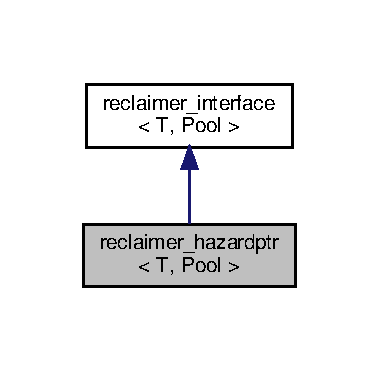
\includegraphics[width=182pt]{classreclaimer__hazardptr__inherit__graph}
\end{center}
\end{figure}


Collaboration diagram for reclaimer\+\_\+hazardptr$<$ T, Pool $>$\+:
\nopagebreak
\begin{figure}[H]
\begin{center}
\leavevmode
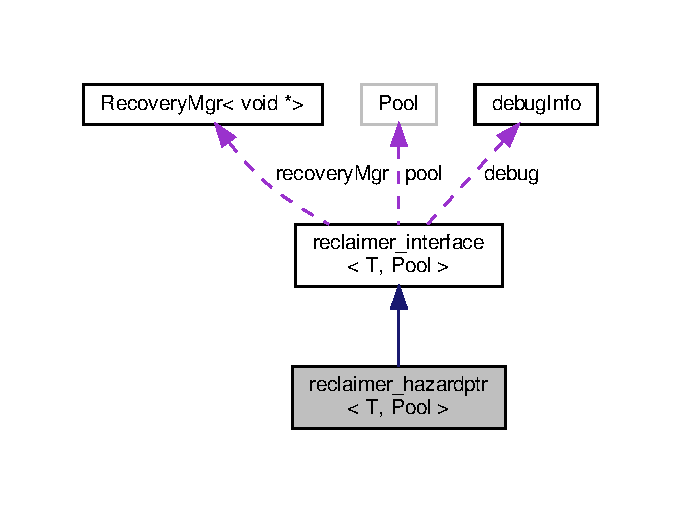
\includegraphics[width=327pt]{classreclaimer__hazardptr__coll__graph}
\end{center}
\end{figure}
\subsection*{Classes}
\begin{DoxyCompactItemize}
\item 
struct \hyperlink{structreclaimer__hazardptr_1_1rebind}{rebind}
\item 
struct \hyperlink{structreclaimer__hazardptr_1_1rebind2}{rebind2}
\end{DoxyCompactItemize}
\subsection*{Public Member Functions}
\begin{DoxyCompactItemize}
\item 
bool \hyperlink{classreclaimer__hazardptr_a660201dad3c7a18dce5a9551691f4869}{is\+Protected} (const int \hyperlink{microbench_2main_8cpp_a9ca9869868fe7e7a38a921cc7de4103f}{tid}, T $\ast$const obj)
\item 
bool \hyperlink{classreclaimer__hazardptr_a847fe92a7812e847d7ab5fc49048b734}{protect} (const int \hyperlink{microbench_2main_8cpp_a9ca9869868fe7e7a38a921cc7de4103f}{tid}, T $\ast$const obj, \hyperlink{globals_8h_a57f5c0d40b156d7d996492fb2f16e3cd}{Callback\+Type} not\+Retired\+Callback, \hyperlink{globals_8h_a3de64ef48066ac6430631c8b81a15345}{Callback\+Arg} callback\+Arg, bool memory\+Barrier=true)
\item 
void \hyperlink{classreclaimer__hazardptr_acf0f5797625cfe4838275015f421379d}{unprotect} (const int \hyperlink{microbench_2main_8cpp_a9ca9869868fe7e7a38a921cc7de4103f}{tid}, T $\ast$const obj)
\item 
bool \hyperlink{classreclaimer__hazardptr_aa32d2290c1950c91650cdf44397520b5}{q\+Protect} (const int \hyperlink{microbench_2main_8cpp_a9ca9869868fe7e7a38a921cc7de4103f}{tid}, T $\ast$const obj, \hyperlink{globals_8h_a57f5c0d40b156d7d996492fb2f16e3cd}{Callback\+Type} not\+Retired\+Callback, \hyperlink{globals_8h_a3de64ef48066ac6430631c8b81a15345}{Callback\+Arg} callback\+Arg, bool memory\+Barrier=true)
\item 
void \hyperlink{classreclaimer__hazardptr_a59e40ae1ae020e6d025be4217b68f184}{q\+Unprotect\+All} (const int \hyperlink{microbench_2main_8cpp_a9ca9869868fe7e7a38a921cc7de4103f}{tid})
\item 
void \hyperlink{classreclaimer__hazardptr_af35ab51d584f989c3a4fa2c00bcdcdf3}{end\+Op} (const int \hyperlink{microbench_2main_8cpp_a9ca9869868fe7e7a38a921cc7de4103f}{tid})
\item 
std\+::string \hyperlink{classreclaimer__hazardptr_a983e41cdf2bb6d4490fac7b954c5f579}{debug\+Pointer\+Output} (T $\ast$p)
\item 
void \hyperlink{classreclaimer__hazardptr_aecf56d8e41ea3da3c3a5aa6ec2aad0f0}{retire} (const int \hyperlink{microbench_2main_8cpp_a9ca9869868fe7e7a38a921cc7de4103f}{tid}, T $\ast$p)
\item 
void \hyperlink{classreclaimer__hazardptr_ae5c49710313a704bbccccebbbee05f64}{debug\+Print\+Status} (const int \hyperlink{microbench_2main_8cpp_a9ca9869868fe7e7a38a921cc7de4103f}{tid})
\item 
void \hyperlink{classreclaimer__hazardptr_a500063d57382d8168a401fdc633aef10}{init\+Thread} (const int \hyperlink{microbench_2main_8cpp_a9ca9869868fe7e7a38a921cc7de4103f}{tid})
\item 
void \hyperlink{classreclaimer__hazardptr_a8d49e04f16495e585ac4f45267d7edc3}{deinit\+Thread} (const int \hyperlink{microbench_2main_8cpp_a9ca9869868fe7e7a38a921cc7de4103f}{tid})
\item 
\hyperlink{classreclaimer__hazardptr_a14615c6826dcd3856b4b9fb82fa58fa0}{reclaimer\+\_\+hazardptr} (const int \hyperlink{testing_8cpp_aa085812188e21ede75351d88b9b2c30d}{num\+Processes}, Pool $\ast$\+\_\+pool, \hyperlink{classdebugInfo}{debug\+Info} $\ast$const \+\_\+debug, \hyperlink{classRecoveryMgr}{Recovery\+Mgr}$<$ void $\ast$$>$ $\ast$const \+\_\+recovery\+Mgr=N\+U\+LL)
\item 
\hyperlink{classreclaimer__hazardptr_a1efb6e4ae96cea810d2c08ba35c5e2a7}{$\sim$reclaimer\+\_\+hazardptr} ()
\end{DoxyCompactItemize}
\subsection*{Static Public Member Functions}
\begin{DoxyCompactItemize}
\item 
static bool \hyperlink{classreclaimer__hazardptr_a865c5e38124016c29c26485b4455c46b}{should\+Help} ()
\item 
static bool \hyperlink{classreclaimer__hazardptr_acdae0c67eb9c9564394fe473e0f7de08}{is\+Q\+Protected} (const int \hyperlink{microbench_2main_8cpp_a9ca9869868fe7e7a38a921cc7de4103f}{tid}, T $\ast$const obj)
\item 
static bool \hyperlink{classreclaimer__hazardptr_a7726a1aae8e0c6241f2d8789795c3819}{is\+Quiescent} (const int \hyperlink{microbench_2main_8cpp_a9ca9869868fe7e7a38a921cc7de4103f}{tid})
\item 
{\footnotesize template$<$typename First , typename... Rest$>$ }\\static bool \hyperlink{classreclaimer__hazardptr_a38edde73863d8d8aaefd65f591842730}{start\+Op} (const int \hyperlink{microbench_2main_8cpp_a9ca9869868fe7e7a38a921cc7de4103f}{tid}, void $\ast$const $\ast$const reclaimers, const int num\+Reclaimers, const bool read\+Only=false)
\item 
static void \hyperlink{classreclaimer__hazardptr_aa2700ee9ec840f98ff0a6157f8f7388a}{rotate\+Epoch\+Bags} (const int \hyperlink{microbench_2main_8cpp_a9ca9869868fe7e7a38a921cc7de4103f}{tid})
\end{DoxyCompactItemize}
\subsection*{Additional Inherited Members}


\subsection{Constructor \& Destructor Documentation}
\mbox{\Hypertarget{classreclaimer__hazardptr_a14615c6826dcd3856b4b9fb82fa58fa0}\label{classreclaimer__hazardptr_a14615c6826dcd3856b4b9fb82fa58fa0}} 
\index{reclaimer\+\_\+hazardptr@{reclaimer\+\_\+hazardptr}!reclaimer\+\_\+hazardptr@{reclaimer\+\_\+hazardptr}}
\index{reclaimer\+\_\+hazardptr@{reclaimer\+\_\+hazardptr}!reclaimer\+\_\+hazardptr@{reclaimer\+\_\+hazardptr}}
\subsubsection{\texorpdfstring{reclaimer\+\_\+hazardptr()}{reclaimer\_hazardptr()}}
{\footnotesize\ttfamily template$<$typename T  = void, class Pool  = pool\+\_\+interface$<$\+T$>$$>$ \\
\hyperlink{classreclaimer__hazardptr}{reclaimer\+\_\+hazardptr}$<$ T, Pool $>$\+::\hyperlink{classreclaimer__hazardptr}{reclaimer\+\_\+hazardptr} (\begin{DoxyParamCaption}\item[{const int}]{num\+Processes,  }\item[{Pool $\ast$}]{\+\_\+pool,  }\item[{\hyperlink{classdebugInfo}{debug\+Info} $\ast$const}]{\+\_\+debug,  }\item[{\hyperlink{classRecoveryMgr}{Recovery\+Mgr}$<$ void $\ast$$>$ $\ast$const}]{\+\_\+recovery\+Mgr = {\ttfamily NULL} }\end{DoxyParamCaption})\hspace{0.3cm}{\ttfamily [inline]}}

\mbox{\Hypertarget{classreclaimer__hazardptr_a1efb6e4ae96cea810d2c08ba35c5e2a7}\label{classreclaimer__hazardptr_a1efb6e4ae96cea810d2c08ba35c5e2a7}} 
\index{reclaimer\+\_\+hazardptr@{reclaimer\+\_\+hazardptr}!````~reclaimer\+\_\+hazardptr@{$\sim$reclaimer\+\_\+hazardptr}}
\index{````~reclaimer\+\_\+hazardptr@{$\sim$reclaimer\+\_\+hazardptr}!reclaimer\+\_\+hazardptr@{reclaimer\+\_\+hazardptr}}
\subsubsection{\texorpdfstring{$\sim$reclaimer\+\_\+hazardptr()}{~reclaimer\_hazardptr()}}
{\footnotesize\ttfamily template$<$typename T  = void, class Pool  = pool\+\_\+interface$<$\+T$>$$>$ \\
\hyperlink{classreclaimer__hazardptr}{reclaimer\+\_\+hazardptr}$<$ T, Pool $>$\+::$\sim$\hyperlink{classreclaimer__hazardptr}{reclaimer\+\_\+hazardptr} (\begin{DoxyParamCaption}{ }\end{DoxyParamCaption})\hspace{0.3cm}{\ttfamily [inline]}}



\subsection{Member Function Documentation}
\mbox{\Hypertarget{classreclaimer__hazardptr_a983e41cdf2bb6d4490fac7b954c5f579}\label{classreclaimer__hazardptr_a983e41cdf2bb6d4490fac7b954c5f579}} 
\index{reclaimer\+\_\+hazardptr@{reclaimer\+\_\+hazardptr}!debug\+Pointer\+Output@{debug\+Pointer\+Output}}
\index{debug\+Pointer\+Output@{debug\+Pointer\+Output}!reclaimer\+\_\+hazardptr@{reclaimer\+\_\+hazardptr}}
\subsubsection{\texorpdfstring{debug\+Pointer\+Output()}{debugPointerOutput()}}
{\footnotesize\ttfamily template$<$typename T  = void, class Pool  = pool\+\_\+interface$<$\+T$>$$>$ \\
std\+::string \hyperlink{classreclaimer__hazardptr}{reclaimer\+\_\+hazardptr}$<$ T, Pool $>$\+::debug\+Pointer\+Output (\begin{DoxyParamCaption}\item[{T $\ast$}]{p }\end{DoxyParamCaption})\hspace{0.3cm}{\ttfamily [inline]}}

\mbox{\Hypertarget{classreclaimer__hazardptr_ae5c49710313a704bbccccebbbee05f64}\label{classreclaimer__hazardptr_ae5c49710313a704bbccccebbbee05f64}} 
\index{reclaimer\+\_\+hazardptr@{reclaimer\+\_\+hazardptr}!debug\+Print\+Status@{debug\+Print\+Status}}
\index{debug\+Print\+Status@{debug\+Print\+Status}!reclaimer\+\_\+hazardptr@{reclaimer\+\_\+hazardptr}}
\subsubsection{\texorpdfstring{debug\+Print\+Status()}{debugPrintStatus()}}
{\footnotesize\ttfamily template$<$typename T  = void, class Pool  = pool\+\_\+interface$<$\+T$>$$>$ \\
void \hyperlink{classreclaimer__hazardptr}{reclaimer\+\_\+hazardptr}$<$ T, Pool $>$\+::debug\+Print\+Status (\begin{DoxyParamCaption}\item[{const int}]{tid }\end{DoxyParamCaption})\hspace{0.3cm}{\ttfamily [inline]}}

\mbox{\Hypertarget{classreclaimer__hazardptr_a8d49e04f16495e585ac4f45267d7edc3}\label{classreclaimer__hazardptr_a8d49e04f16495e585ac4f45267d7edc3}} 
\index{reclaimer\+\_\+hazardptr@{reclaimer\+\_\+hazardptr}!deinit\+Thread@{deinit\+Thread}}
\index{deinit\+Thread@{deinit\+Thread}!reclaimer\+\_\+hazardptr@{reclaimer\+\_\+hazardptr}}
\subsubsection{\texorpdfstring{deinit\+Thread()}{deinitThread()}}
{\footnotesize\ttfamily template$<$typename T  = void, class Pool  = pool\+\_\+interface$<$\+T$>$$>$ \\
void \hyperlink{classreclaimer__hazardptr}{reclaimer\+\_\+hazardptr}$<$ T, Pool $>$\+::deinit\+Thread (\begin{DoxyParamCaption}\item[{const int}]{tid }\end{DoxyParamCaption})\hspace{0.3cm}{\ttfamily [inline]}}

\mbox{\Hypertarget{classreclaimer__hazardptr_af35ab51d584f989c3a4fa2c00bcdcdf3}\label{classreclaimer__hazardptr_af35ab51d584f989c3a4fa2c00bcdcdf3}} 
\index{reclaimer\+\_\+hazardptr@{reclaimer\+\_\+hazardptr}!end\+Op@{end\+Op}}
\index{end\+Op@{end\+Op}!reclaimer\+\_\+hazardptr@{reclaimer\+\_\+hazardptr}}
\subsubsection{\texorpdfstring{end\+Op()}{endOp()}}
{\footnotesize\ttfamily template$<$typename T  = void, class Pool  = pool\+\_\+interface$<$\+T$>$$>$ \\
void \hyperlink{classreclaimer__hazardptr}{reclaimer\+\_\+hazardptr}$<$ T, Pool $>$\+::end\+Op (\begin{DoxyParamCaption}\item[{const int}]{tid }\end{DoxyParamCaption})\hspace{0.3cm}{\ttfamily [inline]}}

\mbox{\Hypertarget{classreclaimer__hazardptr_a500063d57382d8168a401fdc633aef10}\label{classreclaimer__hazardptr_a500063d57382d8168a401fdc633aef10}} 
\index{reclaimer\+\_\+hazardptr@{reclaimer\+\_\+hazardptr}!init\+Thread@{init\+Thread}}
\index{init\+Thread@{init\+Thread}!reclaimer\+\_\+hazardptr@{reclaimer\+\_\+hazardptr}}
\subsubsection{\texorpdfstring{init\+Thread()}{initThread()}}
{\footnotesize\ttfamily template$<$typename T  = void, class Pool  = pool\+\_\+interface$<$\+T$>$$>$ \\
void \hyperlink{classreclaimer__hazardptr}{reclaimer\+\_\+hazardptr}$<$ T, Pool $>$\+::init\+Thread (\begin{DoxyParamCaption}\item[{const int}]{tid }\end{DoxyParamCaption})\hspace{0.3cm}{\ttfamily [inline]}}

\mbox{\Hypertarget{classreclaimer__hazardptr_a660201dad3c7a18dce5a9551691f4869}\label{classreclaimer__hazardptr_a660201dad3c7a18dce5a9551691f4869}} 
\index{reclaimer\+\_\+hazardptr@{reclaimer\+\_\+hazardptr}!is\+Protected@{is\+Protected}}
\index{is\+Protected@{is\+Protected}!reclaimer\+\_\+hazardptr@{reclaimer\+\_\+hazardptr}}
\subsubsection{\texorpdfstring{is\+Protected()}{isProtected()}}
{\footnotesize\ttfamily template$<$typename T  = void, class Pool  = pool\+\_\+interface$<$\+T$>$$>$ \\
bool \hyperlink{classreclaimer__hazardptr}{reclaimer\+\_\+hazardptr}$<$ T, Pool $>$\+::is\+Protected (\begin{DoxyParamCaption}\item[{const int}]{tid,  }\item[{T $\ast$const}]{obj }\end{DoxyParamCaption})\hspace{0.3cm}{\ttfamily [inline]}}

\mbox{\Hypertarget{classreclaimer__hazardptr_acdae0c67eb9c9564394fe473e0f7de08}\label{classreclaimer__hazardptr_acdae0c67eb9c9564394fe473e0f7de08}} 
\index{reclaimer\+\_\+hazardptr@{reclaimer\+\_\+hazardptr}!is\+Q\+Protected@{is\+Q\+Protected}}
\index{is\+Q\+Protected@{is\+Q\+Protected}!reclaimer\+\_\+hazardptr@{reclaimer\+\_\+hazardptr}}
\subsubsection{\texorpdfstring{is\+Q\+Protected()}{isQProtected()}}
{\footnotesize\ttfamily template$<$typename T  = void, class Pool  = pool\+\_\+interface$<$\+T$>$$>$ \\
static bool \hyperlink{classreclaimer__hazardptr}{reclaimer\+\_\+hazardptr}$<$ T, Pool $>$\+::is\+Q\+Protected (\begin{DoxyParamCaption}\item[{const int}]{tid,  }\item[{T $\ast$const}]{obj }\end{DoxyParamCaption})\hspace{0.3cm}{\ttfamily [inline]}, {\ttfamily [static]}}

\mbox{\Hypertarget{classreclaimer__hazardptr_a7726a1aae8e0c6241f2d8789795c3819}\label{classreclaimer__hazardptr_a7726a1aae8e0c6241f2d8789795c3819}} 
\index{reclaimer\+\_\+hazardptr@{reclaimer\+\_\+hazardptr}!is\+Quiescent@{is\+Quiescent}}
\index{is\+Quiescent@{is\+Quiescent}!reclaimer\+\_\+hazardptr@{reclaimer\+\_\+hazardptr}}
\subsubsection{\texorpdfstring{is\+Quiescent()}{isQuiescent()}}
{\footnotesize\ttfamily template$<$typename T  = void, class Pool  = pool\+\_\+interface$<$\+T$>$$>$ \\
static bool \hyperlink{classreclaimer__hazardptr}{reclaimer\+\_\+hazardptr}$<$ T, Pool $>$\+::is\+Quiescent (\begin{DoxyParamCaption}\item[{const int}]{tid }\end{DoxyParamCaption})\hspace{0.3cm}{\ttfamily [inline]}, {\ttfamily [static]}}

\mbox{\Hypertarget{classreclaimer__hazardptr_a847fe92a7812e847d7ab5fc49048b734}\label{classreclaimer__hazardptr_a847fe92a7812e847d7ab5fc49048b734}} 
\index{reclaimer\+\_\+hazardptr@{reclaimer\+\_\+hazardptr}!protect@{protect}}
\index{protect@{protect}!reclaimer\+\_\+hazardptr@{reclaimer\+\_\+hazardptr}}
\subsubsection{\texorpdfstring{protect()}{protect()}}
{\footnotesize\ttfamily template$<$typename T  = void, class Pool  = pool\+\_\+interface$<$\+T$>$$>$ \\
bool \hyperlink{classreclaimer__hazardptr}{reclaimer\+\_\+hazardptr}$<$ T, Pool $>$\+::protect (\begin{DoxyParamCaption}\item[{const int}]{tid,  }\item[{T $\ast$const}]{obj,  }\item[{\hyperlink{globals_8h_a57f5c0d40b156d7d996492fb2f16e3cd}{Callback\+Type}}]{not\+Retired\+Callback,  }\item[{\hyperlink{globals_8h_a3de64ef48066ac6430631c8b81a15345}{Callback\+Arg}}]{callback\+Arg,  }\item[{bool}]{memory\+Barrier = {\ttfamily true} }\end{DoxyParamCaption})\hspace{0.3cm}{\ttfamily [inline]}}

\mbox{\Hypertarget{classreclaimer__hazardptr_aa32d2290c1950c91650cdf44397520b5}\label{classreclaimer__hazardptr_aa32d2290c1950c91650cdf44397520b5}} 
\index{reclaimer\+\_\+hazardptr@{reclaimer\+\_\+hazardptr}!q\+Protect@{q\+Protect}}
\index{q\+Protect@{q\+Protect}!reclaimer\+\_\+hazardptr@{reclaimer\+\_\+hazardptr}}
\subsubsection{\texorpdfstring{q\+Protect()}{qProtect()}}
{\footnotesize\ttfamily template$<$typename T  = void, class Pool  = pool\+\_\+interface$<$\+T$>$$>$ \\
bool \hyperlink{classreclaimer__hazardptr}{reclaimer\+\_\+hazardptr}$<$ T, Pool $>$\+::q\+Protect (\begin{DoxyParamCaption}\item[{const int}]{tid,  }\item[{T $\ast$const}]{obj,  }\item[{\hyperlink{globals_8h_a57f5c0d40b156d7d996492fb2f16e3cd}{Callback\+Type}}]{not\+Retired\+Callback,  }\item[{\hyperlink{globals_8h_a3de64ef48066ac6430631c8b81a15345}{Callback\+Arg}}]{callback\+Arg,  }\item[{bool}]{memory\+Barrier = {\ttfamily true} }\end{DoxyParamCaption})\hspace{0.3cm}{\ttfamily [inline]}}

\mbox{\Hypertarget{classreclaimer__hazardptr_a59e40ae1ae020e6d025be4217b68f184}\label{classreclaimer__hazardptr_a59e40ae1ae020e6d025be4217b68f184}} 
\index{reclaimer\+\_\+hazardptr@{reclaimer\+\_\+hazardptr}!q\+Unprotect\+All@{q\+Unprotect\+All}}
\index{q\+Unprotect\+All@{q\+Unprotect\+All}!reclaimer\+\_\+hazardptr@{reclaimer\+\_\+hazardptr}}
\subsubsection{\texorpdfstring{q\+Unprotect\+All()}{qUnprotectAll()}}
{\footnotesize\ttfamily template$<$typename T  = void, class Pool  = pool\+\_\+interface$<$\+T$>$$>$ \\
void \hyperlink{classreclaimer__hazardptr}{reclaimer\+\_\+hazardptr}$<$ T, Pool $>$\+::q\+Unprotect\+All (\begin{DoxyParamCaption}\item[{const int}]{tid }\end{DoxyParamCaption})\hspace{0.3cm}{\ttfamily [inline]}}

\mbox{\Hypertarget{classreclaimer__hazardptr_aecf56d8e41ea3da3c3a5aa6ec2aad0f0}\label{classreclaimer__hazardptr_aecf56d8e41ea3da3c3a5aa6ec2aad0f0}} 
\index{reclaimer\+\_\+hazardptr@{reclaimer\+\_\+hazardptr}!retire@{retire}}
\index{retire@{retire}!reclaimer\+\_\+hazardptr@{reclaimer\+\_\+hazardptr}}
\subsubsection{\texorpdfstring{retire()}{retire()}}
{\footnotesize\ttfamily template$<$typename T  = void, class Pool  = pool\+\_\+interface$<$\+T$>$$>$ \\
void \hyperlink{classreclaimer__hazardptr}{reclaimer\+\_\+hazardptr}$<$ T, Pool $>$\+::retire (\begin{DoxyParamCaption}\item[{const int}]{tid,  }\item[{T $\ast$}]{p }\end{DoxyParamCaption})\hspace{0.3cm}{\ttfamily [inline]}}

\mbox{\Hypertarget{classreclaimer__hazardptr_aa2700ee9ec840f98ff0a6157f8f7388a}\label{classreclaimer__hazardptr_aa2700ee9ec840f98ff0a6157f8f7388a}} 
\index{reclaimer\+\_\+hazardptr@{reclaimer\+\_\+hazardptr}!rotate\+Epoch\+Bags@{rotate\+Epoch\+Bags}}
\index{rotate\+Epoch\+Bags@{rotate\+Epoch\+Bags}!reclaimer\+\_\+hazardptr@{reclaimer\+\_\+hazardptr}}
\subsubsection{\texorpdfstring{rotate\+Epoch\+Bags()}{rotateEpochBags()}}
{\footnotesize\ttfamily template$<$typename T  = void, class Pool  = pool\+\_\+interface$<$\+T$>$$>$ \\
static void \hyperlink{classreclaimer__hazardptr}{reclaimer\+\_\+hazardptr}$<$ T, Pool $>$\+::rotate\+Epoch\+Bags (\begin{DoxyParamCaption}\item[{const int}]{tid }\end{DoxyParamCaption})\hspace{0.3cm}{\ttfamily [inline]}, {\ttfamily [static]}}

\mbox{\Hypertarget{classreclaimer__hazardptr_a865c5e38124016c29c26485b4455c46b}\label{classreclaimer__hazardptr_a865c5e38124016c29c26485b4455c46b}} 
\index{reclaimer\+\_\+hazardptr@{reclaimer\+\_\+hazardptr}!should\+Help@{should\+Help}}
\index{should\+Help@{should\+Help}!reclaimer\+\_\+hazardptr@{reclaimer\+\_\+hazardptr}}
\subsubsection{\texorpdfstring{should\+Help()}{shouldHelp()}}
{\footnotesize\ttfamily template$<$typename T  = void, class Pool  = pool\+\_\+interface$<$\+T$>$$>$ \\
static bool \hyperlink{classreclaimer__hazardptr}{reclaimer\+\_\+hazardptr}$<$ T, Pool $>$\+::should\+Help (\begin{DoxyParamCaption}{ }\end{DoxyParamCaption})\hspace{0.3cm}{\ttfamily [inline]}, {\ttfamily [static]}}

\mbox{\Hypertarget{classreclaimer__hazardptr_a38edde73863d8d8aaefd65f591842730}\label{classreclaimer__hazardptr_a38edde73863d8d8aaefd65f591842730}} 
\index{reclaimer\+\_\+hazardptr@{reclaimer\+\_\+hazardptr}!start\+Op@{start\+Op}}
\index{start\+Op@{start\+Op}!reclaimer\+\_\+hazardptr@{reclaimer\+\_\+hazardptr}}
\subsubsection{\texorpdfstring{start\+Op()}{startOp()}}
{\footnotesize\ttfamily template$<$typename T  = void, class Pool  = pool\+\_\+interface$<$\+T$>$$>$ \\
template$<$typename First , typename... Rest$>$ \\
static bool \hyperlink{classreclaimer__hazardptr}{reclaimer\+\_\+hazardptr}$<$ T, Pool $>$\+::start\+Op (\begin{DoxyParamCaption}\item[{const int}]{tid,  }\item[{void $\ast$const $\ast$const}]{reclaimers,  }\item[{const int}]{num\+Reclaimers,  }\item[{const bool}]{read\+Only = {\ttfamily false} }\end{DoxyParamCaption})\hspace{0.3cm}{\ttfamily [inline]}, {\ttfamily [static]}}

\mbox{\Hypertarget{classreclaimer__hazardptr_acf0f5797625cfe4838275015f421379d}\label{classreclaimer__hazardptr_acf0f5797625cfe4838275015f421379d}} 
\index{reclaimer\+\_\+hazardptr@{reclaimer\+\_\+hazardptr}!unprotect@{unprotect}}
\index{unprotect@{unprotect}!reclaimer\+\_\+hazardptr@{reclaimer\+\_\+hazardptr}}
\subsubsection{\texorpdfstring{unprotect()}{unprotect()}}
{\footnotesize\ttfamily template$<$typename T  = void, class Pool  = pool\+\_\+interface$<$\+T$>$$>$ \\
void \hyperlink{classreclaimer__hazardptr}{reclaimer\+\_\+hazardptr}$<$ T, Pool $>$\+::unprotect (\begin{DoxyParamCaption}\item[{const int}]{tid,  }\item[{T $\ast$const}]{obj }\end{DoxyParamCaption})\hspace{0.3cm}{\ttfamily [inline]}}



The documentation for this class was generated from the following file\+:\begin{DoxyCompactItemize}
\item 
common/recordmgr/\hyperlink{reclaimer__hazardptr_8h}{reclaimer\+\_\+hazardptr.\+h}\end{DoxyCompactItemize}

\hypertarget{classreclaimer__interface}{}\section{reclaimer\+\_\+interface$<$ T, Pool $>$ Class Template Reference}
\label{classreclaimer__interface}\index{reclaimer\+\_\+interface$<$ T, Pool $>$@{reclaimer\+\_\+interface$<$ T, Pool $>$}}


{\ttfamily \#include $<$reclaimer\+\_\+interface.\+h$>$}



Inheritance diagram for reclaimer\+\_\+interface$<$ T, Pool $>$\+:
\nopagebreak
\begin{figure}[H]
\begin{center}
\leavevmode
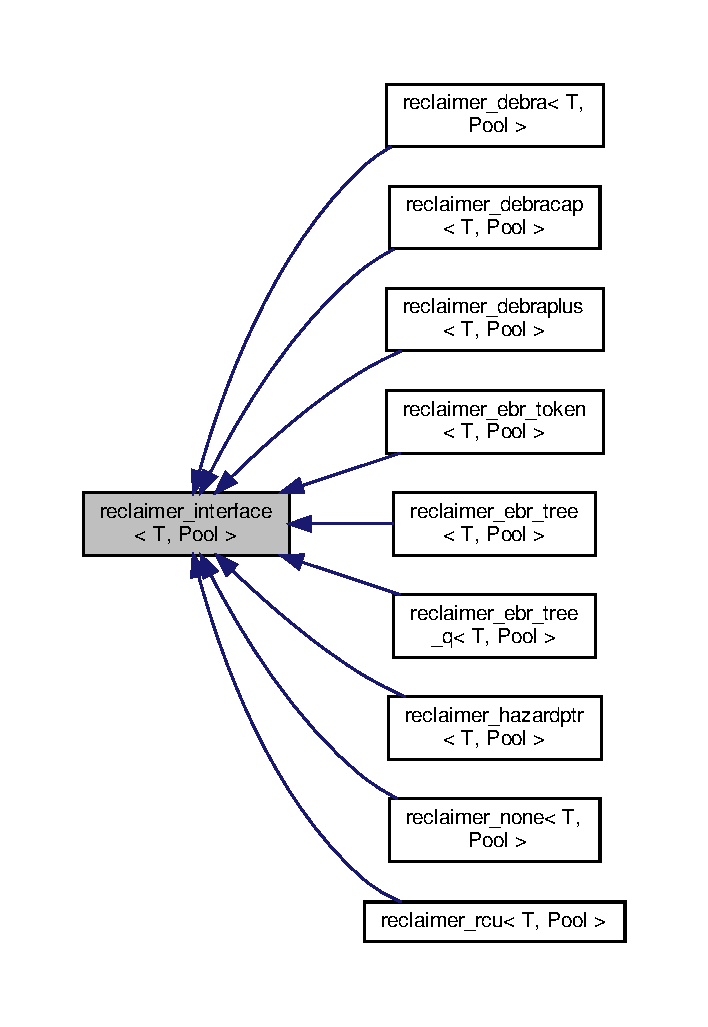
\includegraphics[width=340pt]{classreclaimer__interface__inherit__graph}
\end{center}
\end{figure}


Collaboration diagram for reclaimer\+\_\+interface$<$ T, Pool $>$\+:
\nopagebreak
\begin{figure}[H]
\begin{center}
\leavevmode
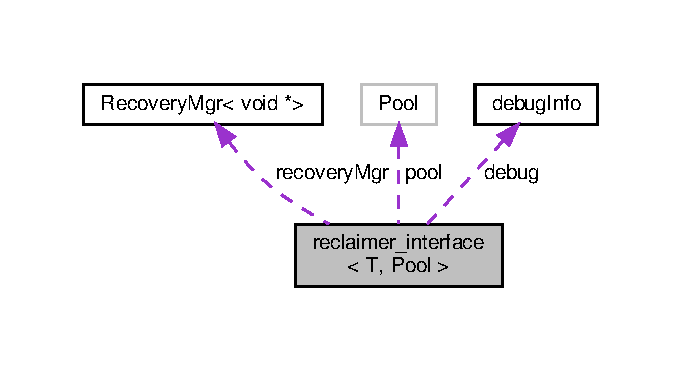
\includegraphics[width=327pt]{classreclaimer__interface__coll__graph}
\end{center}
\end{figure}
\subsection*{Classes}
\begin{DoxyCompactItemize}
\item 
struct \hyperlink{structreclaimer__interface_1_1rebind}{rebind}
\item 
struct \hyperlink{structreclaimer__interface_1_1rebind2}{rebind2}
\end{DoxyCompactItemize}
\subsection*{Public Member Functions}
\begin{DoxyCompactItemize}
\item 
long long \hyperlink{classreclaimer__interface_aff9a466872ab7972a27e817c7d776936}{get\+Size\+In\+Nodes} ()
\item 
std\+::string \hyperlink{classreclaimer__interface_a949bf6cedb35e2bb0b853b0b7ef7b03e}{get\+Size\+String} ()
\item 
std\+::string \hyperlink{classreclaimer__interface_ada48535c0c82904eb0bbe3491e52eca7}{get\+Details\+String} ()
\item 
bool \hyperlink{classreclaimer__interface_ad459569f628d48ad8f953de155277937}{is\+Protected} (const int \hyperlink{microbench_2main_8cpp_a9ca9869868fe7e7a38a921cc7de4103f}{tid}, T $\ast$const obj)
\item 
bool \hyperlink{classreclaimer__interface_adca271430185d90a3a1c7aea22d8bb0c}{is\+Q\+Protected} (const int \hyperlink{microbench_2main_8cpp_a9ca9869868fe7e7a38a921cc7de4103f}{tid}, T $\ast$const obj)
\item 
bool \hyperlink{classreclaimer__interface_acdac11080a38f7d5b6e60007d9b620cf}{protect} (const int \hyperlink{microbench_2main_8cpp_a9ca9869868fe7e7a38a921cc7de4103f}{tid}, T $\ast$obj, \hyperlink{globals_8h_a57f5c0d40b156d7d996492fb2f16e3cd}{Callback\+Type} not\+Retired\+Callback, \hyperlink{globals_8h_a3de64ef48066ac6430631c8b81a15345}{Callback\+Arg} callback\+Arg, bool memory\+Barrier=true)
\item 
void \hyperlink{classreclaimer__interface_acdeb54332a2edeee70ee37581017ec0b}{unprotect} (const int \hyperlink{microbench_2main_8cpp_a9ca9869868fe7e7a38a921cc7de4103f}{tid}, T $\ast$obj)
\item 
bool \hyperlink{classreclaimer__interface_ae017ea119e3bc36949107124babf3888}{q\+Protect} (const int \hyperlink{microbench_2main_8cpp_a9ca9869868fe7e7a38a921cc7de4103f}{tid}, T $\ast$obj, \hyperlink{globals_8h_a57f5c0d40b156d7d996492fb2f16e3cd}{Callback\+Type} not\+Retired\+Callback, \hyperlink{globals_8h_a3de64ef48066ac6430631c8b81a15345}{Callback\+Arg} callback\+Arg, bool memory\+Barrier=true)
\item 
void \hyperlink{classreclaimer__interface_a0893dc3706f43bfeb5572808bba6b92a}{q\+Unprotect\+All} (const int \hyperlink{microbench_2main_8cpp_a9ca9869868fe7e7a38a921cc7de4103f}{tid})
\item 
void \hyperlink{classreclaimer__interface_a913e054b17192c9c905469a19eb7dbd4}{end\+Op} (const int \hyperlink{microbench_2main_8cpp_a9ca9869868fe7e7a38a921cc7de4103f}{tid})
\item 
bool \hyperlink{classreclaimer__interface_a99471b7a8f06a80d81896e269ea63cc9}{start\+Op} (const int \hyperlink{microbench_2main_8cpp_a9ca9869868fe7e7a38a921cc7de4103f}{tid}, void $\ast$const $\ast$const reclaimers, const int num\+Reclaimers, const bool read\+Only=false)
\item 
void \hyperlink{classreclaimer__interface_aa3a2771a4002d59cf81ef86921d499ca}{rotate\+Epoch\+Bags} (const int \hyperlink{microbench_2main_8cpp_a9ca9869868fe7e7a38a921cc7de4103f}{tid})
\item 
void \hyperlink{classreclaimer__interface_a0ef47251c6a7fbd543354b88db8aa309}{retire} (const int \hyperlink{microbench_2main_8cpp_a9ca9869868fe7e7a38a921cc7de4103f}{tid}, T $\ast$p)
\item 
void \hyperlink{classreclaimer__interface_a0fa3f1bddb187e68931f0792fbba812c}{init\+Thread} (const int \hyperlink{microbench_2main_8cpp_a9ca9869868fe7e7a38a921cc7de4103f}{tid})
\item 
void \hyperlink{classreclaimer__interface_a18e0cfdbf69e359ceab660df99ef4d4a}{deinit\+Thread} (const int \hyperlink{microbench_2main_8cpp_a9ca9869868fe7e7a38a921cc7de4103f}{tid})
\item 
void \hyperlink{classreclaimer__interface_aa8cd8a18adb4da97d35e60c139dfc4fb}{debug\+Print\+Status} (const int \hyperlink{microbench_2main_8cpp_a9ca9869868fe7e7a38a921cc7de4103f}{tid})
\item 
\hyperlink{classreclaimer__interface_a63ff07ec643f85a3c2b8152183f37882}{reclaimer\+\_\+interface} (const int \hyperlink{testing_8cpp_aa085812188e21ede75351d88b9b2c30d}{num\+Processes}, Pool $\ast$\+\_\+pool, \hyperlink{classdebugInfo}{debug\+Info} $\ast$const \+\_\+debug, \hyperlink{classRecoveryMgr}{Recovery\+Mgr}$<$ void $\ast$$>$ $\ast$const \+\_\+recovery\+Mgr=N\+U\+LL)
\item 
\hyperlink{classreclaimer__interface_aef907bda3f068a00c9a15f0d51962930}{$\sim$reclaimer\+\_\+interface} ()
\end{DoxyCompactItemize}
\subsection*{Static Public Member Functions}
\begin{DoxyCompactItemize}
\item 
static bool \hyperlink{classreclaimer__interface_a3b93587337b561201d7fa8ab36f64d9d}{quiescence\+Is\+Per\+Record\+Type} ()
\item 
static bool \hyperlink{classreclaimer__interface_af20ec23a47f79d303a18551fd8706f2d}{should\+Help} ()
\item 
static bool \hyperlink{classreclaimer__interface_a965d5fd618ce50fb9a5db0d6e4a8dc9e}{supports\+Crash\+Recovery} ()
\item 
static bool \hyperlink{classreclaimer__interface_a8434d6efc52667ddd3c6738733c79db8}{is\+Quiescent} (const int \hyperlink{microbench_2main_8cpp_a9ca9869868fe7e7a38a921cc7de4103f}{tid})
\end{DoxyCompactItemize}
\subsection*{Public Attributes}
\begin{DoxyCompactItemize}
\item 
\hyperlink{classreclaimer__interface_a105497cdc18f0306f5a612c86afa0fa6}{P\+AD}
\item 
\hyperlink{classRecoveryMgr}{Recovery\+Mgr}$<$ void $\ast$ $>$ $\ast$ \hyperlink{classreclaimer__interface_a7c9cff5fa3884b5318210f0dedb987e9}{recovery\+Mgr}
\item 
\hyperlink{classdebugInfo}{debug\+Info} $\ast$const \hyperlink{classreclaimer__interface_a617bf5436d7217b303ac65e57709618b}{debug}
\item 
const int \hyperlink{classreclaimer__interface_a6f3f1b6d104d2e4fa44d6183a6f6a2a5}{N\+U\+M\+\_\+\+P\+R\+O\+C\+E\+S\+S\+ES}
\item 
Pool $\ast$ \hyperlink{classreclaimer__interface_a5ca8f53aca95e5fb296cd0dfcd87d90f}{pool}
\end{DoxyCompactItemize}


\subsection{Constructor \& Destructor Documentation}
\mbox{\Hypertarget{classreclaimer__interface_a63ff07ec643f85a3c2b8152183f37882}\label{classreclaimer__interface_a63ff07ec643f85a3c2b8152183f37882}} 
\index{reclaimer\+\_\+interface@{reclaimer\+\_\+interface}!reclaimer\+\_\+interface@{reclaimer\+\_\+interface}}
\index{reclaimer\+\_\+interface@{reclaimer\+\_\+interface}!reclaimer\+\_\+interface@{reclaimer\+\_\+interface}}
\subsubsection{\texorpdfstring{reclaimer\+\_\+interface()}{reclaimer\_interface()}}
{\footnotesize\ttfamily template$<$typename T  = void, class Pool  = pool\+\_\+interface$<$\+T$>$$>$ \\
\hyperlink{classreclaimer__interface}{reclaimer\+\_\+interface}$<$ T, Pool $>$\+::\hyperlink{classreclaimer__interface}{reclaimer\+\_\+interface} (\begin{DoxyParamCaption}\item[{const int}]{num\+Processes,  }\item[{Pool $\ast$}]{\+\_\+pool,  }\item[{\hyperlink{classdebugInfo}{debug\+Info} $\ast$const}]{\+\_\+debug,  }\item[{\hyperlink{classRecoveryMgr}{Recovery\+Mgr}$<$ void $\ast$$>$ $\ast$const}]{\+\_\+recovery\+Mgr = {\ttfamily NULL} }\end{DoxyParamCaption})\hspace{0.3cm}{\ttfamily [inline]}}

\mbox{\Hypertarget{classreclaimer__interface_aef907bda3f068a00c9a15f0d51962930}\label{classreclaimer__interface_aef907bda3f068a00c9a15f0d51962930}} 
\index{reclaimer\+\_\+interface@{reclaimer\+\_\+interface}!````~reclaimer\+\_\+interface@{$\sim$reclaimer\+\_\+interface}}
\index{````~reclaimer\+\_\+interface@{$\sim$reclaimer\+\_\+interface}!reclaimer\+\_\+interface@{reclaimer\+\_\+interface}}
\subsubsection{\texorpdfstring{$\sim$reclaimer\+\_\+interface()}{~reclaimer\_interface()}}
{\footnotesize\ttfamily template$<$typename T  = void, class Pool  = pool\+\_\+interface$<$\+T$>$$>$ \\
\hyperlink{classreclaimer__interface}{reclaimer\+\_\+interface}$<$ T, Pool $>$\+::$\sim$\hyperlink{classreclaimer__interface}{reclaimer\+\_\+interface} (\begin{DoxyParamCaption}{ }\end{DoxyParamCaption})\hspace{0.3cm}{\ttfamily [inline]}}



\subsection{Member Function Documentation}
\mbox{\Hypertarget{classreclaimer__interface_aa8cd8a18adb4da97d35e60c139dfc4fb}\label{classreclaimer__interface_aa8cd8a18adb4da97d35e60c139dfc4fb}} 
\index{reclaimer\+\_\+interface@{reclaimer\+\_\+interface}!debug\+Print\+Status@{debug\+Print\+Status}}
\index{debug\+Print\+Status@{debug\+Print\+Status}!reclaimer\+\_\+interface@{reclaimer\+\_\+interface}}
\subsubsection{\texorpdfstring{debug\+Print\+Status()}{debugPrintStatus()}}
{\footnotesize\ttfamily template$<$typename T  = void, class Pool  = pool\+\_\+interface$<$\+T$>$$>$ \\
void \hyperlink{classreclaimer__interface}{reclaimer\+\_\+interface}$<$ T, Pool $>$\+::debug\+Print\+Status (\begin{DoxyParamCaption}\item[{const int}]{tid }\end{DoxyParamCaption})}

\mbox{\Hypertarget{classreclaimer__interface_a18e0cfdbf69e359ceab660df99ef4d4a}\label{classreclaimer__interface_a18e0cfdbf69e359ceab660df99ef4d4a}} 
\index{reclaimer\+\_\+interface@{reclaimer\+\_\+interface}!deinit\+Thread@{deinit\+Thread}}
\index{deinit\+Thread@{deinit\+Thread}!reclaimer\+\_\+interface@{reclaimer\+\_\+interface}}
\subsubsection{\texorpdfstring{deinit\+Thread()}{deinitThread()}}
{\footnotesize\ttfamily template$<$typename T  = void, class Pool  = pool\+\_\+interface$<$\+T$>$$>$ \\
void \hyperlink{classreclaimer__interface}{reclaimer\+\_\+interface}$<$ T, Pool $>$\+::deinit\+Thread (\begin{DoxyParamCaption}\item[{const int}]{tid }\end{DoxyParamCaption})\hspace{0.3cm}{\ttfamily [inline]}}

\mbox{\Hypertarget{classreclaimer__interface_a913e054b17192c9c905469a19eb7dbd4}\label{classreclaimer__interface_a913e054b17192c9c905469a19eb7dbd4}} 
\index{reclaimer\+\_\+interface@{reclaimer\+\_\+interface}!end\+Op@{end\+Op}}
\index{end\+Op@{end\+Op}!reclaimer\+\_\+interface@{reclaimer\+\_\+interface}}
\subsubsection{\texorpdfstring{end\+Op()}{endOp()}}
{\footnotesize\ttfamily template$<$typename T  = void, class Pool  = pool\+\_\+interface$<$\+T$>$$>$ \\
void \hyperlink{classreclaimer__interface}{reclaimer\+\_\+interface}$<$ T, Pool $>$\+::end\+Op (\begin{DoxyParamCaption}\item[{const int}]{tid }\end{DoxyParamCaption})\hspace{0.3cm}{\ttfamily [inline]}}

end\+Op$<$\+T$>$ must be idempotent, and must unprotect all objects protected by calls to protect\+Object$<$\+T$>$. it must N\+OT unprotect any object protected by a call to protect\+Object\+Even\+After\+Restart. \mbox{\Hypertarget{classreclaimer__interface_ada48535c0c82904eb0bbe3491e52eca7}\label{classreclaimer__interface_ada48535c0c82904eb0bbe3491e52eca7}} 
\index{reclaimer\+\_\+interface@{reclaimer\+\_\+interface}!get\+Details\+String@{get\+Details\+String}}
\index{get\+Details\+String@{get\+Details\+String}!reclaimer\+\_\+interface@{reclaimer\+\_\+interface}}
\subsubsection{\texorpdfstring{get\+Details\+String()}{getDetailsString()}}
{\footnotesize\ttfamily template$<$typename T  = void, class Pool  = pool\+\_\+interface$<$\+T$>$$>$ \\
std\+::string \hyperlink{classreclaimer__interface}{reclaimer\+\_\+interface}$<$ T, Pool $>$\+::get\+Details\+String (\begin{DoxyParamCaption}{ }\end{DoxyParamCaption})\hspace{0.3cm}{\ttfamily [inline]}}

\mbox{\Hypertarget{classreclaimer__interface_aff9a466872ab7972a27e817c7d776936}\label{classreclaimer__interface_aff9a466872ab7972a27e817c7d776936}} 
\index{reclaimer\+\_\+interface@{reclaimer\+\_\+interface}!get\+Size\+In\+Nodes@{get\+Size\+In\+Nodes}}
\index{get\+Size\+In\+Nodes@{get\+Size\+In\+Nodes}!reclaimer\+\_\+interface@{reclaimer\+\_\+interface}}
\subsubsection{\texorpdfstring{get\+Size\+In\+Nodes()}{getSizeInNodes()}}
{\footnotesize\ttfamily template$<$typename T  = void, class Pool  = pool\+\_\+interface$<$\+T$>$$>$ \\
long long \hyperlink{classreclaimer__interface}{reclaimer\+\_\+interface}$<$ T, Pool $>$\+::get\+Size\+In\+Nodes (\begin{DoxyParamCaption}{ }\end{DoxyParamCaption})\hspace{0.3cm}{\ttfamily [inline]}}

\mbox{\Hypertarget{classreclaimer__interface_a949bf6cedb35e2bb0b853b0b7ef7b03e}\label{classreclaimer__interface_a949bf6cedb35e2bb0b853b0b7ef7b03e}} 
\index{reclaimer\+\_\+interface@{reclaimer\+\_\+interface}!get\+Size\+String@{get\+Size\+String}}
\index{get\+Size\+String@{get\+Size\+String}!reclaimer\+\_\+interface@{reclaimer\+\_\+interface}}
\subsubsection{\texorpdfstring{get\+Size\+String()}{getSizeString()}}
{\footnotesize\ttfamily template$<$typename T  = void, class Pool  = pool\+\_\+interface$<$\+T$>$$>$ \\
std\+::string \hyperlink{classreclaimer__interface}{reclaimer\+\_\+interface}$<$ T, Pool $>$\+::get\+Size\+String (\begin{DoxyParamCaption}{ }\end{DoxyParamCaption})\hspace{0.3cm}{\ttfamily [inline]}}

\mbox{\Hypertarget{classreclaimer__interface_a0fa3f1bddb187e68931f0792fbba812c}\label{classreclaimer__interface_a0fa3f1bddb187e68931f0792fbba812c}} 
\index{reclaimer\+\_\+interface@{reclaimer\+\_\+interface}!init\+Thread@{init\+Thread}}
\index{init\+Thread@{init\+Thread}!reclaimer\+\_\+interface@{reclaimer\+\_\+interface}}
\subsubsection{\texorpdfstring{init\+Thread()}{initThread()}}
{\footnotesize\ttfamily template$<$typename T  = void, class Pool  = pool\+\_\+interface$<$\+T$>$$>$ \\
void \hyperlink{classreclaimer__interface}{reclaimer\+\_\+interface}$<$ T, Pool $>$\+::init\+Thread (\begin{DoxyParamCaption}\item[{const int}]{tid }\end{DoxyParamCaption})\hspace{0.3cm}{\ttfamily [inline]}}

\mbox{\Hypertarget{classreclaimer__interface_ad459569f628d48ad8f953de155277937}\label{classreclaimer__interface_ad459569f628d48ad8f953de155277937}} 
\index{reclaimer\+\_\+interface@{reclaimer\+\_\+interface}!is\+Protected@{is\+Protected}}
\index{is\+Protected@{is\+Protected}!reclaimer\+\_\+interface@{reclaimer\+\_\+interface}}
\subsubsection{\texorpdfstring{is\+Protected()}{isProtected()}}
{\footnotesize\ttfamily template$<$typename T  = void, class Pool  = pool\+\_\+interface$<$\+T$>$$>$ \\
bool \hyperlink{classreclaimer__interface}{reclaimer\+\_\+interface}$<$ T, Pool $>$\+::is\+Protected (\begin{DoxyParamCaption}\item[{const int}]{tid,  }\item[{T $\ast$const}]{obj }\end{DoxyParamCaption})\hspace{0.3cm}{\ttfamily [inline]}}

\mbox{\Hypertarget{classreclaimer__interface_adca271430185d90a3a1c7aea22d8bb0c}\label{classreclaimer__interface_adca271430185d90a3a1c7aea22d8bb0c}} 
\index{reclaimer\+\_\+interface@{reclaimer\+\_\+interface}!is\+Q\+Protected@{is\+Q\+Protected}}
\index{is\+Q\+Protected@{is\+Q\+Protected}!reclaimer\+\_\+interface@{reclaimer\+\_\+interface}}
\subsubsection{\texorpdfstring{is\+Q\+Protected()}{isQProtected()}}
{\footnotesize\ttfamily template$<$typename T  = void, class Pool  = pool\+\_\+interface$<$\+T$>$$>$ \\
bool \hyperlink{classreclaimer__interface}{reclaimer\+\_\+interface}$<$ T, Pool $>$\+::is\+Q\+Protected (\begin{DoxyParamCaption}\item[{const int}]{tid,  }\item[{T $\ast$const}]{obj }\end{DoxyParamCaption})\hspace{0.3cm}{\ttfamily [inline]}}

\mbox{\Hypertarget{classreclaimer__interface_a8434d6efc52667ddd3c6738733c79db8}\label{classreclaimer__interface_a8434d6efc52667ddd3c6738733c79db8}} 
\index{reclaimer\+\_\+interface@{reclaimer\+\_\+interface}!is\+Quiescent@{is\+Quiescent}}
\index{is\+Quiescent@{is\+Quiescent}!reclaimer\+\_\+interface@{reclaimer\+\_\+interface}}
\subsubsection{\texorpdfstring{is\+Quiescent()}{isQuiescent()}}
{\footnotesize\ttfamily template$<$typename T  = void, class Pool  = pool\+\_\+interface$<$\+T$>$$>$ \\
static bool \hyperlink{classreclaimer__interface}{reclaimer\+\_\+interface}$<$ T, Pool $>$\+::is\+Quiescent (\begin{DoxyParamCaption}\item[{const int}]{tid }\end{DoxyParamCaption})\hspace{0.3cm}{\ttfamily [inline]}, {\ttfamily [static]}}

\mbox{\Hypertarget{classreclaimer__interface_acdac11080a38f7d5b6e60007d9b620cf}\label{classreclaimer__interface_acdac11080a38f7d5b6e60007d9b620cf}} 
\index{reclaimer\+\_\+interface@{reclaimer\+\_\+interface}!protect@{protect}}
\index{protect@{protect}!reclaimer\+\_\+interface@{reclaimer\+\_\+interface}}
\subsubsection{\texorpdfstring{protect()}{protect()}}
{\footnotesize\ttfamily template$<$typename T  = void, class Pool  = pool\+\_\+interface$<$\+T$>$$>$ \\
bool \hyperlink{classreclaimer__interface}{reclaimer\+\_\+interface}$<$ T, Pool $>$\+::protect (\begin{DoxyParamCaption}\item[{const int}]{tid,  }\item[{T $\ast$}]{obj,  }\item[{\hyperlink{globals_8h_a57f5c0d40b156d7d996492fb2f16e3cd}{Callback\+Type}}]{not\+Retired\+Callback,  }\item[{\hyperlink{globals_8h_a3de64ef48066ac6430631c8b81a15345}{Callback\+Arg}}]{callback\+Arg,  }\item[{bool}]{memory\+Barrier = {\ttfamily true} }\end{DoxyParamCaption})\hspace{0.3cm}{\ttfamily [inline]}}

\mbox{\Hypertarget{classreclaimer__interface_ae017ea119e3bc36949107124babf3888}\label{classreclaimer__interface_ae017ea119e3bc36949107124babf3888}} 
\index{reclaimer\+\_\+interface@{reclaimer\+\_\+interface}!q\+Protect@{q\+Protect}}
\index{q\+Protect@{q\+Protect}!reclaimer\+\_\+interface@{reclaimer\+\_\+interface}}
\subsubsection{\texorpdfstring{q\+Protect()}{qProtect()}}
{\footnotesize\ttfamily template$<$typename T  = void, class Pool  = pool\+\_\+interface$<$\+T$>$$>$ \\
bool \hyperlink{classreclaimer__interface}{reclaimer\+\_\+interface}$<$ T, Pool $>$\+::q\+Protect (\begin{DoxyParamCaption}\item[{const int}]{tid,  }\item[{T $\ast$}]{obj,  }\item[{\hyperlink{globals_8h_a57f5c0d40b156d7d996492fb2f16e3cd}{Callback\+Type}}]{not\+Retired\+Callback,  }\item[{\hyperlink{globals_8h_a3de64ef48066ac6430631c8b81a15345}{Callback\+Arg}}]{callback\+Arg,  }\item[{bool}]{memory\+Barrier = {\ttfamily true} }\end{DoxyParamCaption})\hspace{0.3cm}{\ttfamily [inline]}}

\mbox{\Hypertarget{classreclaimer__interface_a3b93587337b561201d7fa8ab36f64d9d}\label{classreclaimer__interface_a3b93587337b561201d7fa8ab36f64d9d}} 
\index{reclaimer\+\_\+interface@{reclaimer\+\_\+interface}!quiescence\+Is\+Per\+Record\+Type@{quiescence\+Is\+Per\+Record\+Type}}
\index{quiescence\+Is\+Per\+Record\+Type@{quiescence\+Is\+Per\+Record\+Type}!reclaimer\+\_\+interface@{reclaimer\+\_\+interface}}
\subsubsection{\texorpdfstring{quiescence\+Is\+Per\+Record\+Type()}{quiescenceIsPerRecordType()}}
{\footnotesize\ttfamily template$<$typename T  = void, class Pool  = pool\+\_\+interface$<$\+T$>$$>$ \\
static bool \hyperlink{classreclaimer__interface}{reclaimer\+\_\+interface}$<$ T, Pool $>$\+::quiescence\+Is\+Per\+Record\+Type (\begin{DoxyParamCaption}{ }\end{DoxyParamCaption})\hspace{0.3cm}{\ttfamily [inline]}, {\ttfamily [static]}}

\mbox{\Hypertarget{classreclaimer__interface_a0893dc3706f43bfeb5572808bba6b92a}\label{classreclaimer__interface_a0893dc3706f43bfeb5572808bba6b92a}} 
\index{reclaimer\+\_\+interface@{reclaimer\+\_\+interface}!q\+Unprotect\+All@{q\+Unprotect\+All}}
\index{q\+Unprotect\+All@{q\+Unprotect\+All}!reclaimer\+\_\+interface@{reclaimer\+\_\+interface}}
\subsubsection{\texorpdfstring{q\+Unprotect\+All()}{qUnprotectAll()}}
{\footnotesize\ttfamily template$<$typename T  = void, class Pool  = pool\+\_\+interface$<$\+T$>$$>$ \\
void \hyperlink{classreclaimer__interface}{reclaimer\+\_\+interface}$<$ T, Pool $>$\+::q\+Unprotect\+All (\begin{DoxyParamCaption}\item[{const int}]{tid }\end{DoxyParamCaption})\hspace{0.3cm}{\ttfamily [inline]}}

\mbox{\Hypertarget{classreclaimer__interface_a0ef47251c6a7fbd543354b88db8aa309}\label{classreclaimer__interface_a0ef47251c6a7fbd543354b88db8aa309}} 
\index{reclaimer\+\_\+interface@{reclaimer\+\_\+interface}!retire@{retire}}
\index{retire@{retire}!reclaimer\+\_\+interface@{reclaimer\+\_\+interface}}
\subsubsection{\texorpdfstring{retire()}{retire()}}
{\footnotesize\ttfamily template$<$typename T  = void, class Pool  = pool\+\_\+interface$<$\+T$>$$>$ \\
void \hyperlink{classreclaimer__interface}{reclaimer\+\_\+interface}$<$ T, Pool $>$\+::retire (\begin{DoxyParamCaption}\item[{const int}]{tid,  }\item[{T $\ast$}]{p }\end{DoxyParamCaption})\hspace{0.3cm}{\ttfamily [inline]}}

\mbox{\Hypertarget{classreclaimer__interface_aa3a2771a4002d59cf81ef86921d499ca}\label{classreclaimer__interface_aa3a2771a4002d59cf81ef86921d499ca}} 
\index{reclaimer\+\_\+interface@{reclaimer\+\_\+interface}!rotate\+Epoch\+Bags@{rotate\+Epoch\+Bags}}
\index{rotate\+Epoch\+Bags@{rotate\+Epoch\+Bags}!reclaimer\+\_\+interface@{reclaimer\+\_\+interface}}
\subsubsection{\texorpdfstring{rotate\+Epoch\+Bags()}{rotateEpochBags()}}
{\footnotesize\ttfamily template$<$typename T  = void, class Pool  = pool\+\_\+interface$<$\+T$>$$>$ \\
void \hyperlink{classreclaimer__interface}{reclaimer\+\_\+interface}$<$ T, Pool $>$\+::rotate\+Epoch\+Bags (\begin{DoxyParamCaption}\item[{const int}]{tid }\end{DoxyParamCaption})\hspace{0.3cm}{\ttfamily [inline]}}

\mbox{\Hypertarget{classreclaimer__interface_af20ec23a47f79d303a18551fd8706f2d}\label{classreclaimer__interface_af20ec23a47f79d303a18551fd8706f2d}} 
\index{reclaimer\+\_\+interface@{reclaimer\+\_\+interface}!should\+Help@{should\+Help}}
\index{should\+Help@{should\+Help}!reclaimer\+\_\+interface@{reclaimer\+\_\+interface}}
\subsubsection{\texorpdfstring{should\+Help()}{shouldHelp()}}
{\footnotesize\ttfamily template$<$typename T  = void, class Pool  = pool\+\_\+interface$<$\+T$>$$>$ \\
static bool \hyperlink{classreclaimer__interface}{reclaimer\+\_\+interface}$<$ T, Pool $>$\+::should\+Help (\begin{DoxyParamCaption}{ }\end{DoxyParamCaption})\hspace{0.3cm}{\ttfamily [inline]}, {\ttfamily [static]}}

\mbox{\Hypertarget{classreclaimer__interface_a99471b7a8f06a80d81896e269ea63cc9}\label{classreclaimer__interface_a99471b7a8f06a80d81896e269ea63cc9}} 
\index{reclaimer\+\_\+interface@{reclaimer\+\_\+interface}!start\+Op@{start\+Op}}
\index{start\+Op@{start\+Op}!reclaimer\+\_\+interface@{reclaimer\+\_\+interface}}
\subsubsection{\texorpdfstring{start\+Op()}{startOp()}}
{\footnotesize\ttfamily template$<$typename T  = void, class Pool  = pool\+\_\+interface$<$\+T$>$$>$ \\
bool \hyperlink{classreclaimer__interface}{reclaimer\+\_\+interface}$<$ T, Pool $>$\+::start\+Op (\begin{DoxyParamCaption}\item[{const int}]{tid,  }\item[{void $\ast$const $\ast$const}]{reclaimers,  }\item[{const int}]{num\+Reclaimers,  }\item[{const bool}]{read\+Only = {\ttfamily false} }\end{DoxyParamCaption})\hspace{0.3cm}{\ttfamily [inline]}}

\mbox{\Hypertarget{classreclaimer__interface_a965d5fd618ce50fb9a5db0d6e4a8dc9e}\label{classreclaimer__interface_a965d5fd618ce50fb9a5db0d6e4a8dc9e}} 
\index{reclaimer\+\_\+interface@{reclaimer\+\_\+interface}!supports\+Crash\+Recovery@{supports\+Crash\+Recovery}}
\index{supports\+Crash\+Recovery@{supports\+Crash\+Recovery}!reclaimer\+\_\+interface@{reclaimer\+\_\+interface}}
\subsubsection{\texorpdfstring{supports\+Crash\+Recovery()}{supportsCrashRecovery()}}
{\footnotesize\ttfamily template$<$typename T  = void, class Pool  = pool\+\_\+interface$<$\+T$>$$>$ \\
static bool \hyperlink{classreclaimer__interface}{reclaimer\+\_\+interface}$<$ T, Pool $>$\+::supports\+Crash\+Recovery (\begin{DoxyParamCaption}{ }\end{DoxyParamCaption})\hspace{0.3cm}{\ttfamily [inline]}, {\ttfamily [static]}}

\mbox{\Hypertarget{classreclaimer__interface_acdeb54332a2edeee70ee37581017ec0b}\label{classreclaimer__interface_acdeb54332a2edeee70ee37581017ec0b}} 
\index{reclaimer\+\_\+interface@{reclaimer\+\_\+interface}!unprotect@{unprotect}}
\index{unprotect@{unprotect}!reclaimer\+\_\+interface@{reclaimer\+\_\+interface}}
\subsubsection{\texorpdfstring{unprotect()}{unprotect()}}
{\footnotesize\ttfamily template$<$typename T  = void, class Pool  = pool\+\_\+interface$<$\+T$>$$>$ \\
void \hyperlink{classreclaimer__interface}{reclaimer\+\_\+interface}$<$ T, Pool $>$\+::unprotect (\begin{DoxyParamCaption}\item[{const int}]{tid,  }\item[{T $\ast$}]{obj }\end{DoxyParamCaption})\hspace{0.3cm}{\ttfamily [inline]}}



\subsection{Member Data Documentation}
\mbox{\Hypertarget{classreclaimer__interface_a617bf5436d7217b303ac65e57709618b}\label{classreclaimer__interface_a617bf5436d7217b303ac65e57709618b}} 
\index{reclaimer\+\_\+interface@{reclaimer\+\_\+interface}!debug@{debug}}
\index{debug@{debug}!reclaimer\+\_\+interface@{reclaimer\+\_\+interface}}
\subsubsection{\texorpdfstring{debug}{debug}}
{\footnotesize\ttfamily template$<$typename T  = void, class Pool  = pool\+\_\+interface$<$\+T$>$$>$ \\
\hyperlink{classdebugInfo}{debug\+Info}$\ast$ const \hyperlink{classreclaimer__interface}{reclaimer\+\_\+interface}$<$ T, Pool $>$\+::debug}

\mbox{\Hypertarget{classreclaimer__interface_a6f3f1b6d104d2e4fa44d6183a6f6a2a5}\label{classreclaimer__interface_a6f3f1b6d104d2e4fa44d6183a6f6a2a5}} 
\index{reclaimer\+\_\+interface@{reclaimer\+\_\+interface}!N\+U\+M\+\_\+\+P\+R\+O\+C\+E\+S\+S\+ES@{N\+U\+M\+\_\+\+P\+R\+O\+C\+E\+S\+S\+ES}}
\index{N\+U\+M\+\_\+\+P\+R\+O\+C\+E\+S\+S\+ES@{N\+U\+M\+\_\+\+P\+R\+O\+C\+E\+S\+S\+ES}!reclaimer\+\_\+interface@{reclaimer\+\_\+interface}}
\subsubsection{\texorpdfstring{N\+U\+M\+\_\+\+P\+R\+O\+C\+E\+S\+S\+ES}{NUM\_PROCESSES}}
{\footnotesize\ttfamily template$<$typename T  = void, class Pool  = pool\+\_\+interface$<$\+T$>$$>$ \\
const int \hyperlink{classreclaimer__interface}{reclaimer\+\_\+interface}$<$ T, Pool $>$\+::N\+U\+M\+\_\+\+P\+R\+O\+C\+E\+S\+S\+ES}

\mbox{\Hypertarget{classreclaimer__interface_a105497cdc18f0306f5a612c86afa0fa6}\label{classreclaimer__interface_a105497cdc18f0306f5a612c86afa0fa6}} 
\index{reclaimer\+\_\+interface@{reclaimer\+\_\+interface}!P\+AD@{P\+AD}}
\index{P\+AD@{P\+AD}!reclaimer\+\_\+interface@{reclaimer\+\_\+interface}}
\subsubsection{\texorpdfstring{P\+AD}{PAD}}
{\footnotesize\ttfamily template$<$typename T  = void, class Pool  = pool\+\_\+interface$<$\+T$>$$>$ \\
\hyperlink{classreclaimer__interface}{reclaimer\+\_\+interface}$<$ T, Pool $>$\+::P\+AD}

\mbox{\Hypertarget{classreclaimer__interface_a5ca8f53aca95e5fb296cd0dfcd87d90f}\label{classreclaimer__interface_a5ca8f53aca95e5fb296cd0dfcd87d90f}} 
\index{reclaimer\+\_\+interface@{reclaimer\+\_\+interface}!pool@{pool}}
\index{pool@{pool}!reclaimer\+\_\+interface@{reclaimer\+\_\+interface}}
\subsubsection{\texorpdfstring{pool}{pool}}
{\footnotesize\ttfamily template$<$typename T  = void, class Pool  = pool\+\_\+interface$<$\+T$>$$>$ \\
Pool$\ast$ \hyperlink{classreclaimer__interface}{reclaimer\+\_\+interface}$<$ T, Pool $>$\+::pool}

\mbox{\Hypertarget{classreclaimer__interface_a7c9cff5fa3884b5318210f0dedb987e9}\label{classreclaimer__interface_a7c9cff5fa3884b5318210f0dedb987e9}} 
\index{reclaimer\+\_\+interface@{reclaimer\+\_\+interface}!recovery\+Mgr@{recovery\+Mgr}}
\index{recovery\+Mgr@{recovery\+Mgr}!reclaimer\+\_\+interface@{reclaimer\+\_\+interface}}
\subsubsection{\texorpdfstring{recovery\+Mgr}{recoveryMgr}}
{\footnotesize\ttfamily template$<$typename T  = void, class Pool  = pool\+\_\+interface$<$\+T$>$$>$ \\
\hyperlink{classRecoveryMgr}{Recovery\+Mgr}$<$void $\ast$$>$$\ast$ \hyperlink{classreclaimer__interface}{reclaimer\+\_\+interface}$<$ T, Pool $>$\+::recovery\+Mgr}



The documentation for this class was generated from the following file\+:\begin{DoxyCompactItemize}
\item 
common/recordmgr/\hyperlink{reclaimer__interface_8h}{reclaimer\+\_\+interface.\+h}\end{DoxyCompactItemize}

\hypertarget{classreclaimer__none}{}\section{reclaimer\+\_\+none$<$ T, Pool $>$ Class Template Reference}
\label{classreclaimer__none}\index{reclaimer\+\_\+none$<$ T, Pool $>$@{reclaimer\+\_\+none$<$ T, Pool $>$}}


{\ttfamily \#include $<$reclaimer\+\_\+none.\+h$>$}



Inheritance diagram for reclaimer\+\_\+none$<$ T, Pool $>$\+:
\nopagebreak
\begin{figure}[H]
\begin{center}
\leavevmode
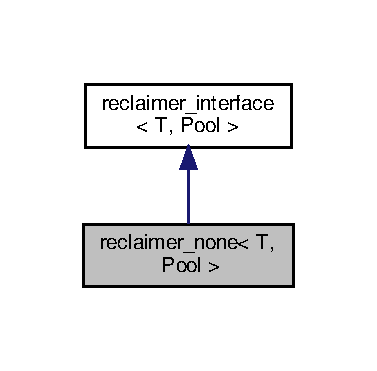
\includegraphics[width=181pt]{classreclaimer__none__inherit__graph}
\end{center}
\end{figure}


Collaboration diagram for reclaimer\+\_\+none$<$ T, Pool $>$\+:
\nopagebreak
\begin{figure}[H]
\begin{center}
\leavevmode
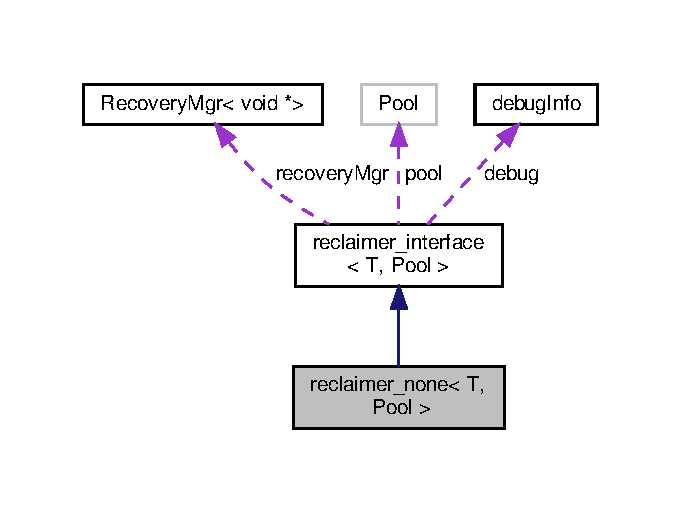
\includegraphics[width=327pt]{classreclaimer__none__coll__graph}
\end{center}
\end{figure}
\subsection*{Classes}
\begin{DoxyCompactItemize}
\item 
struct \hyperlink{structreclaimer__none_1_1rebind}{rebind}
\item 
struct \hyperlink{structreclaimer__none_1_1rebind2}{rebind2}
\end{DoxyCompactItemize}
\subsection*{Public Member Functions}
\begin{DoxyCompactItemize}
\item 
std\+::string \hyperlink{classreclaimer__none_ab3504e7df5f9c56384a81ab042ef64dd}{get\+Details\+String} ()
\item 
std\+::string \hyperlink{classreclaimer__none_aea6c1a61f5891ca3f542f900165d0246}{get\+Size\+String} ()
\item 
void \hyperlink{classreclaimer__none_ae70908a43f8772e5294c5f5ceae0716c}{debug\+Print\+Status} (const int \hyperlink{microbench_2main_8cpp_a9ca9869868fe7e7a38a921cc7de4103f}{tid})
\item 
void \hyperlink{classreclaimer__none_a8d073432aa881a89b9729f63f47b74ec}{get\+Safe\+Blockbags} (const int \hyperlink{microbench_2main_8cpp_a9ca9869868fe7e7a38a921cc7de4103f}{tid}, \hyperlink{classblockbag}{blockbag}$<$ T $>$ $\ast$$\ast$bags)
\item 
void \hyperlink{classreclaimer__none_a16e9b3199168e6715744f108382e083c}{init\+Thread} (const int \hyperlink{microbench_2main_8cpp_a9ca9869868fe7e7a38a921cc7de4103f}{tid})
\item 
void \hyperlink{classreclaimer__none_adf9a32c7d612d8929cd19908845757cf}{deinit\+Thread} (const int \hyperlink{microbench_2main_8cpp_a9ca9869868fe7e7a38a921cc7de4103f}{tid})
\item 
\hyperlink{classreclaimer__none_a05c1dab65707686e75d2263c4e4a8a9b}{reclaimer\+\_\+none} (const int \hyperlink{testing_8cpp_aa085812188e21ede75351d88b9b2c30d}{num\+Processes}, Pool $\ast$\+\_\+pool, \hyperlink{classdebugInfo}{debug\+Info} $\ast$const \+\_\+debug, \hyperlink{classRecoveryMgr}{Recovery\+Mgr}$<$ void $\ast$$>$ $\ast$const \+\_\+recovery\+Mgr=N\+U\+LL)
\item 
\hyperlink{classreclaimer__none_a7015c1c9dd0a1151e59c06b8cada74a9}{$\sim$reclaimer\+\_\+none} ()
\end{DoxyCompactItemize}
\subsection*{Static Public Member Functions}
\begin{DoxyCompactItemize}
\item 
static bool \hyperlink{classreclaimer__none_a0a343e289f2ec0bd11f565be7ba05f6c}{should\+Help} ()
\item 
static bool \hyperlink{classreclaimer__none_aa02fae6b14e76f5c2bf940b118eb54e3}{is\+Quiescent} (const int \hyperlink{microbench_2main_8cpp_a9ca9869868fe7e7a38a921cc7de4103f}{tid})
\item 
static bool \hyperlink{classreclaimer__none_a6515f01a73ccddf44303256344f7996f}{is\+Protected} (const int \hyperlink{microbench_2main_8cpp_a9ca9869868fe7e7a38a921cc7de4103f}{tid}, T $\ast$const obj)
\item 
static bool \hyperlink{classreclaimer__none_a73618ce8985667a837c5cbed9914def2}{is\+Q\+Protected} (const int \hyperlink{microbench_2main_8cpp_a9ca9869868fe7e7a38a921cc7de4103f}{tid}, T $\ast$const obj)
\item 
static bool \hyperlink{classreclaimer__none_a8bc86fce7f71f6238dfd50ce06803d66}{protect} (const int \hyperlink{microbench_2main_8cpp_a9ca9869868fe7e7a38a921cc7de4103f}{tid}, T $\ast$const obj, \hyperlink{globals_8h_a57f5c0d40b156d7d996492fb2f16e3cd}{Callback\+Type} not\+Retired\+Callback, \hyperlink{globals_8h_a3de64ef48066ac6430631c8b81a15345}{Callback\+Arg} callback\+Arg, bool memory\+Barrier=true)
\item 
static void \hyperlink{classreclaimer__none_a29e0601d98d0325c7a10ebc6346746b7}{unprotect} (const int \hyperlink{microbench_2main_8cpp_a9ca9869868fe7e7a38a921cc7de4103f}{tid}, T $\ast$const obj)
\item 
static bool \hyperlink{classreclaimer__none_afbc218123a9eef8bb282e77cf3b594c2}{q\+Protect} (const int \hyperlink{microbench_2main_8cpp_a9ca9869868fe7e7a38a921cc7de4103f}{tid}, T $\ast$const obj, \hyperlink{globals_8h_a57f5c0d40b156d7d996492fb2f16e3cd}{Callback\+Type} not\+Retired\+Callback, \hyperlink{globals_8h_a3de64ef48066ac6430631c8b81a15345}{Callback\+Arg} callback\+Arg, bool memory\+Barrier=true)
\item 
static void \hyperlink{classreclaimer__none_aeba1b3ef7a4aea47c3efb75a7547d0ce}{q\+Unprotect\+All} (const int \hyperlink{microbench_2main_8cpp_a9ca9869868fe7e7a38a921cc7de4103f}{tid})
\item 
static void \hyperlink{classreclaimer__none_a6ddaeb4e57e7b69d28cd01f16fd3e0a5}{rotate\+Epoch\+Bags} (const int \hyperlink{microbench_2main_8cpp_a9ca9869868fe7e7a38a921cc7de4103f}{tid})
\item 
{\footnotesize template$<$typename First , typename... Rest$>$ }\\static bool \hyperlink{classreclaimer__none_a320e4964cc7b800368b532b4a39c2457}{start\+Op} (const int \hyperlink{microbench_2main_8cpp_a9ca9869868fe7e7a38a921cc7de4103f}{tid}, void $\ast$const $\ast$const reclaimers, const int num\+Reclaimers, const bool read\+Only=false)
\item 
static void \hyperlink{classreclaimer__none_a07e8438b0ae46062974a5ee363c7804b}{end\+Op} (const int \hyperlink{microbench_2main_8cpp_a9ca9869868fe7e7a38a921cc7de4103f}{tid})
\item 
static void \hyperlink{classreclaimer__none_aa086c5d645d3ab8098b0015b9ed90489}{retire} (const int \hyperlink{microbench_2main_8cpp_a9ca9869868fe7e7a38a921cc7de4103f}{tid}, T $\ast$p)
\end{DoxyCompactItemize}
\subsection*{Public Attributes}
\begin{DoxyCompactItemize}
\item 
\hyperlink{classreclaimer__none_a7a92a357656b3b49cee95a230cd12d69}{P\+AD}
\end{DoxyCompactItemize}


\subsection{Detailed Description}
\subsubsection*{template$<$typename T = void, class Pool = pool\+\_\+interface$<$\+T$>$$>$\newline
class reclaimer\+\_\+none$<$ T, Pool $>$}

C++ record manager implementation (P\+O\+DC 2015) by Trevor Brown.

Copyright (C) 2015 Trevor Brown 

\subsection{Constructor \& Destructor Documentation}
\mbox{\Hypertarget{classreclaimer__none_a05c1dab65707686e75d2263c4e4a8a9b}\label{classreclaimer__none_a05c1dab65707686e75d2263c4e4a8a9b}} 
\index{reclaimer\+\_\+none@{reclaimer\+\_\+none}!reclaimer\+\_\+none@{reclaimer\+\_\+none}}
\index{reclaimer\+\_\+none@{reclaimer\+\_\+none}!reclaimer\+\_\+none@{reclaimer\+\_\+none}}
\subsubsection{\texorpdfstring{reclaimer\+\_\+none()}{reclaimer\_none()}}
{\footnotesize\ttfamily template$<$typename T  = void, class Pool  = pool\+\_\+interface$<$\+T$>$$>$ \\
\hyperlink{classreclaimer__none}{reclaimer\+\_\+none}$<$ T, Pool $>$\+::\hyperlink{classreclaimer__none}{reclaimer\+\_\+none} (\begin{DoxyParamCaption}\item[{const int}]{num\+Processes,  }\item[{Pool $\ast$}]{\+\_\+pool,  }\item[{\hyperlink{classdebugInfo}{debug\+Info} $\ast$const}]{\+\_\+debug,  }\item[{\hyperlink{classRecoveryMgr}{Recovery\+Mgr}$<$ void $\ast$$>$ $\ast$const}]{\+\_\+recovery\+Mgr = {\ttfamily NULL} }\end{DoxyParamCaption})\hspace{0.3cm}{\ttfamily [inline]}}

\mbox{\Hypertarget{classreclaimer__none_a7015c1c9dd0a1151e59c06b8cada74a9}\label{classreclaimer__none_a7015c1c9dd0a1151e59c06b8cada74a9}} 
\index{reclaimer\+\_\+none@{reclaimer\+\_\+none}!````~reclaimer\+\_\+none@{$\sim$reclaimer\+\_\+none}}
\index{````~reclaimer\+\_\+none@{$\sim$reclaimer\+\_\+none}!reclaimer\+\_\+none@{reclaimer\+\_\+none}}
\subsubsection{\texorpdfstring{$\sim$reclaimer\+\_\+none()}{~reclaimer\_none()}}
{\footnotesize\ttfamily template$<$typename T  = void, class Pool  = pool\+\_\+interface$<$\+T$>$$>$ \\
\hyperlink{classreclaimer__none}{reclaimer\+\_\+none}$<$ T, Pool $>$\+::$\sim$\hyperlink{classreclaimer__none}{reclaimer\+\_\+none} (\begin{DoxyParamCaption}{ }\end{DoxyParamCaption})\hspace{0.3cm}{\ttfamily [inline]}}



\subsection{Member Function Documentation}
\mbox{\Hypertarget{classreclaimer__none_ae70908a43f8772e5294c5f5ceae0716c}\label{classreclaimer__none_ae70908a43f8772e5294c5f5ceae0716c}} 
\index{reclaimer\+\_\+none@{reclaimer\+\_\+none}!debug\+Print\+Status@{debug\+Print\+Status}}
\index{debug\+Print\+Status@{debug\+Print\+Status}!reclaimer\+\_\+none@{reclaimer\+\_\+none}}
\subsubsection{\texorpdfstring{debug\+Print\+Status()}{debugPrintStatus()}}
{\footnotesize\ttfamily template$<$typename T  = void, class Pool  = pool\+\_\+interface$<$\+T$>$$>$ \\
void \hyperlink{classreclaimer__none}{reclaimer\+\_\+none}$<$ T, Pool $>$\+::debug\+Print\+Status (\begin{DoxyParamCaption}\item[{const int}]{tid }\end{DoxyParamCaption})\hspace{0.3cm}{\ttfamily [inline]}}

\mbox{\Hypertarget{classreclaimer__none_adf9a32c7d612d8929cd19908845757cf}\label{classreclaimer__none_adf9a32c7d612d8929cd19908845757cf}} 
\index{reclaimer\+\_\+none@{reclaimer\+\_\+none}!deinit\+Thread@{deinit\+Thread}}
\index{deinit\+Thread@{deinit\+Thread}!reclaimer\+\_\+none@{reclaimer\+\_\+none}}
\subsubsection{\texorpdfstring{deinit\+Thread()}{deinitThread()}}
{\footnotesize\ttfamily template$<$typename T  = void, class Pool  = pool\+\_\+interface$<$\+T$>$$>$ \\
void \hyperlink{classreclaimer__none}{reclaimer\+\_\+none}$<$ T, Pool $>$\+::deinit\+Thread (\begin{DoxyParamCaption}\item[{const int}]{tid }\end{DoxyParamCaption})\hspace{0.3cm}{\ttfamily [inline]}}

\mbox{\Hypertarget{classreclaimer__none_a07e8438b0ae46062974a5ee363c7804b}\label{classreclaimer__none_a07e8438b0ae46062974a5ee363c7804b}} 
\index{reclaimer\+\_\+none@{reclaimer\+\_\+none}!end\+Op@{end\+Op}}
\index{end\+Op@{end\+Op}!reclaimer\+\_\+none@{reclaimer\+\_\+none}}
\subsubsection{\texorpdfstring{end\+Op()}{endOp()}}
{\footnotesize\ttfamily template$<$typename T  = void, class Pool  = pool\+\_\+interface$<$\+T$>$$>$ \\
static void \hyperlink{classreclaimer__none}{reclaimer\+\_\+none}$<$ T, Pool $>$\+::end\+Op (\begin{DoxyParamCaption}\item[{const int}]{tid }\end{DoxyParamCaption})\hspace{0.3cm}{\ttfamily [inline]}, {\ttfamily [static]}}

\mbox{\Hypertarget{classreclaimer__none_ab3504e7df5f9c56384a81ab042ef64dd}\label{classreclaimer__none_ab3504e7df5f9c56384a81ab042ef64dd}} 
\index{reclaimer\+\_\+none@{reclaimer\+\_\+none}!get\+Details\+String@{get\+Details\+String}}
\index{get\+Details\+String@{get\+Details\+String}!reclaimer\+\_\+none@{reclaimer\+\_\+none}}
\subsubsection{\texorpdfstring{get\+Details\+String()}{getDetailsString()}}
{\footnotesize\ttfamily template$<$typename T  = void, class Pool  = pool\+\_\+interface$<$\+T$>$$>$ \\
std\+::string \hyperlink{classreclaimer__none}{reclaimer\+\_\+none}$<$ T, Pool $>$\+::get\+Details\+String (\begin{DoxyParamCaption}{ }\end{DoxyParamCaption})\hspace{0.3cm}{\ttfamily [inline]}}

\mbox{\Hypertarget{classreclaimer__none_a8d073432aa881a89b9729f63f47b74ec}\label{classreclaimer__none_a8d073432aa881a89b9729f63f47b74ec}} 
\index{reclaimer\+\_\+none@{reclaimer\+\_\+none}!get\+Safe\+Blockbags@{get\+Safe\+Blockbags}}
\index{get\+Safe\+Blockbags@{get\+Safe\+Blockbags}!reclaimer\+\_\+none@{reclaimer\+\_\+none}}
\subsubsection{\texorpdfstring{get\+Safe\+Blockbags()}{getSafeBlockbags()}}
{\footnotesize\ttfamily template$<$typename T  = void, class Pool  = pool\+\_\+interface$<$\+T$>$$>$ \\
void \hyperlink{classreclaimer__none}{reclaimer\+\_\+none}$<$ T, Pool $>$\+::get\+Safe\+Blockbags (\begin{DoxyParamCaption}\item[{const int}]{tid,  }\item[{\hyperlink{classblockbag}{blockbag}$<$ T $>$ $\ast$$\ast$}]{bags }\end{DoxyParamCaption})\hspace{0.3cm}{\ttfamily [inline]}}

\mbox{\Hypertarget{classreclaimer__none_aea6c1a61f5891ca3f542f900165d0246}\label{classreclaimer__none_aea6c1a61f5891ca3f542f900165d0246}} 
\index{reclaimer\+\_\+none@{reclaimer\+\_\+none}!get\+Size\+String@{get\+Size\+String}}
\index{get\+Size\+String@{get\+Size\+String}!reclaimer\+\_\+none@{reclaimer\+\_\+none}}
\subsubsection{\texorpdfstring{get\+Size\+String()}{getSizeString()}}
{\footnotesize\ttfamily template$<$typename T  = void, class Pool  = pool\+\_\+interface$<$\+T$>$$>$ \\
std\+::string \hyperlink{classreclaimer__none}{reclaimer\+\_\+none}$<$ T, Pool $>$\+::get\+Size\+String (\begin{DoxyParamCaption}{ }\end{DoxyParamCaption})\hspace{0.3cm}{\ttfamily [inline]}}

\mbox{\Hypertarget{classreclaimer__none_a16e9b3199168e6715744f108382e083c}\label{classreclaimer__none_a16e9b3199168e6715744f108382e083c}} 
\index{reclaimer\+\_\+none@{reclaimer\+\_\+none}!init\+Thread@{init\+Thread}}
\index{init\+Thread@{init\+Thread}!reclaimer\+\_\+none@{reclaimer\+\_\+none}}
\subsubsection{\texorpdfstring{init\+Thread()}{initThread()}}
{\footnotesize\ttfamily template$<$typename T  = void, class Pool  = pool\+\_\+interface$<$\+T$>$$>$ \\
void \hyperlink{classreclaimer__none}{reclaimer\+\_\+none}$<$ T, Pool $>$\+::init\+Thread (\begin{DoxyParamCaption}\item[{const int}]{tid }\end{DoxyParamCaption})\hspace{0.3cm}{\ttfamily [inline]}}

\mbox{\Hypertarget{classreclaimer__none_a6515f01a73ccddf44303256344f7996f}\label{classreclaimer__none_a6515f01a73ccddf44303256344f7996f}} 
\index{reclaimer\+\_\+none@{reclaimer\+\_\+none}!is\+Protected@{is\+Protected}}
\index{is\+Protected@{is\+Protected}!reclaimer\+\_\+none@{reclaimer\+\_\+none}}
\subsubsection{\texorpdfstring{is\+Protected()}{isProtected()}}
{\footnotesize\ttfamily template$<$typename T  = void, class Pool  = pool\+\_\+interface$<$\+T$>$$>$ \\
static bool \hyperlink{classreclaimer__none}{reclaimer\+\_\+none}$<$ T, Pool $>$\+::is\+Protected (\begin{DoxyParamCaption}\item[{const int}]{tid,  }\item[{T $\ast$const}]{obj }\end{DoxyParamCaption})\hspace{0.3cm}{\ttfamily [inline]}, {\ttfamily [static]}}

\mbox{\Hypertarget{classreclaimer__none_a73618ce8985667a837c5cbed9914def2}\label{classreclaimer__none_a73618ce8985667a837c5cbed9914def2}} 
\index{reclaimer\+\_\+none@{reclaimer\+\_\+none}!is\+Q\+Protected@{is\+Q\+Protected}}
\index{is\+Q\+Protected@{is\+Q\+Protected}!reclaimer\+\_\+none@{reclaimer\+\_\+none}}
\subsubsection{\texorpdfstring{is\+Q\+Protected()}{isQProtected()}}
{\footnotesize\ttfamily template$<$typename T  = void, class Pool  = pool\+\_\+interface$<$\+T$>$$>$ \\
static bool \hyperlink{classreclaimer__none}{reclaimer\+\_\+none}$<$ T, Pool $>$\+::is\+Q\+Protected (\begin{DoxyParamCaption}\item[{const int}]{tid,  }\item[{T $\ast$const}]{obj }\end{DoxyParamCaption})\hspace{0.3cm}{\ttfamily [inline]}, {\ttfamily [static]}}

\mbox{\Hypertarget{classreclaimer__none_aa02fae6b14e76f5c2bf940b118eb54e3}\label{classreclaimer__none_aa02fae6b14e76f5c2bf940b118eb54e3}} 
\index{reclaimer\+\_\+none@{reclaimer\+\_\+none}!is\+Quiescent@{is\+Quiescent}}
\index{is\+Quiescent@{is\+Quiescent}!reclaimer\+\_\+none@{reclaimer\+\_\+none}}
\subsubsection{\texorpdfstring{is\+Quiescent()}{isQuiescent()}}
{\footnotesize\ttfamily template$<$typename T  = void, class Pool  = pool\+\_\+interface$<$\+T$>$$>$ \\
static bool \hyperlink{classreclaimer__none}{reclaimer\+\_\+none}$<$ T, Pool $>$\+::is\+Quiescent (\begin{DoxyParamCaption}\item[{const int}]{tid }\end{DoxyParamCaption})\hspace{0.3cm}{\ttfamily [inline]}, {\ttfamily [static]}}

\mbox{\Hypertarget{classreclaimer__none_a8bc86fce7f71f6238dfd50ce06803d66}\label{classreclaimer__none_a8bc86fce7f71f6238dfd50ce06803d66}} 
\index{reclaimer\+\_\+none@{reclaimer\+\_\+none}!protect@{protect}}
\index{protect@{protect}!reclaimer\+\_\+none@{reclaimer\+\_\+none}}
\subsubsection{\texorpdfstring{protect()}{protect()}}
{\footnotesize\ttfamily template$<$typename T  = void, class Pool  = pool\+\_\+interface$<$\+T$>$$>$ \\
static bool \hyperlink{classreclaimer__none}{reclaimer\+\_\+none}$<$ T, Pool $>$\+::protect (\begin{DoxyParamCaption}\item[{const int}]{tid,  }\item[{T $\ast$const}]{obj,  }\item[{\hyperlink{globals_8h_a57f5c0d40b156d7d996492fb2f16e3cd}{Callback\+Type}}]{not\+Retired\+Callback,  }\item[{\hyperlink{globals_8h_a3de64ef48066ac6430631c8b81a15345}{Callback\+Arg}}]{callback\+Arg,  }\item[{bool}]{memory\+Barrier = {\ttfamily true} }\end{DoxyParamCaption})\hspace{0.3cm}{\ttfamily [inline]}, {\ttfamily [static]}}

\mbox{\Hypertarget{classreclaimer__none_afbc218123a9eef8bb282e77cf3b594c2}\label{classreclaimer__none_afbc218123a9eef8bb282e77cf3b594c2}} 
\index{reclaimer\+\_\+none@{reclaimer\+\_\+none}!q\+Protect@{q\+Protect}}
\index{q\+Protect@{q\+Protect}!reclaimer\+\_\+none@{reclaimer\+\_\+none}}
\subsubsection{\texorpdfstring{q\+Protect()}{qProtect()}}
{\footnotesize\ttfamily template$<$typename T  = void, class Pool  = pool\+\_\+interface$<$\+T$>$$>$ \\
static bool \hyperlink{classreclaimer__none}{reclaimer\+\_\+none}$<$ T, Pool $>$\+::q\+Protect (\begin{DoxyParamCaption}\item[{const int}]{tid,  }\item[{T $\ast$const}]{obj,  }\item[{\hyperlink{globals_8h_a57f5c0d40b156d7d996492fb2f16e3cd}{Callback\+Type}}]{not\+Retired\+Callback,  }\item[{\hyperlink{globals_8h_a3de64ef48066ac6430631c8b81a15345}{Callback\+Arg}}]{callback\+Arg,  }\item[{bool}]{memory\+Barrier = {\ttfamily true} }\end{DoxyParamCaption})\hspace{0.3cm}{\ttfamily [inline]}, {\ttfamily [static]}}

\mbox{\Hypertarget{classreclaimer__none_aeba1b3ef7a4aea47c3efb75a7547d0ce}\label{classreclaimer__none_aeba1b3ef7a4aea47c3efb75a7547d0ce}} 
\index{reclaimer\+\_\+none@{reclaimer\+\_\+none}!q\+Unprotect\+All@{q\+Unprotect\+All}}
\index{q\+Unprotect\+All@{q\+Unprotect\+All}!reclaimer\+\_\+none@{reclaimer\+\_\+none}}
\subsubsection{\texorpdfstring{q\+Unprotect\+All()}{qUnprotectAll()}}
{\footnotesize\ttfamily template$<$typename T  = void, class Pool  = pool\+\_\+interface$<$\+T$>$$>$ \\
static void \hyperlink{classreclaimer__none}{reclaimer\+\_\+none}$<$ T, Pool $>$\+::q\+Unprotect\+All (\begin{DoxyParamCaption}\item[{const int}]{tid }\end{DoxyParamCaption})\hspace{0.3cm}{\ttfamily [inline]}, {\ttfamily [static]}}

\mbox{\Hypertarget{classreclaimer__none_aa086c5d645d3ab8098b0015b9ed90489}\label{classreclaimer__none_aa086c5d645d3ab8098b0015b9ed90489}} 
\index{reclaimer\+\_\+none@{reclaimer\+\_\+none}!retire@{retire}}
\index{retire@{retire}!reclaimer\+\_\+none@{reclaimer\+\_\+none}}
\subsubsection{\texorpdfstring{retire()}{retire()}}
{\footnotesize\ttfamily template$<$typename T  = void, class Pool  = pool\+\_\+interface$<$\+T$>$$>$ \\
static void \hyperlink{classreclaimer__none}{reclaimer\+\_\+none}$<$ T, Pool $>$\+::retire (\begin{DoxyParamCaption}\item[{const int}]{tid,  }\item[{T $\ast$}]{p }\end{DoxyParamCaption})\hspace{0.3cm}{\ttfamily [inline]}, {\ttfamily [static]}}

\mbox{\Hypertarget{classreclaimer__none_a6ddaeb4e57e7b69d28cd01f16fd3e0a5}\label{classreclaimer__none_a6ddaeb4e57e7b69d28cd01f16fd3e0a5}} 
\index{reclaimer\+\_\+none@{reclaimer\+\_\+none}!rotate\+Epoch\+Bags@{rotate\+Epoch\+Bags}}
\index{rotate\+Epoch\+Bags@{rotate\+Epoch\+Bags}!reclaimer\+\_\+none@{reclaimer\+\_\+none}}
\subsubsection{\texorpdfstring{rotate\+Epoch\+Bags()}{rotateEpochBags()}}
{\footnotesize\ttfamily template$<$typename T  = void, class Pool  = pool\+\_\+interface$<$\+T$>$$>$ \\
static void \hyperlink{classreclaimer__none}{reclaimer\+\_\+none}$<$ T, Pool $>$\+::rotate\+Epoch\+Bags (\begin{DoxyParamCaption}\item[{const int}]{tid }\end{DoxyParamCaption})\hspace{0.3cm}{\ttfamily [inline]}, {\ttfamily [static]}}

\mbox{\Hypertarget{classreclaimer__none_a0a343e289f2ec0bd11f565be7ba05f6c}\label{classreclaimer__none_a0a343e289f2ec0bd11f565be7ba05f6c}} 
\index{reclaimer\+\_\+none@{reclaimer\+\_\+none}!should\+Help@{should\+Help}}
\index{should\+Help@{should\+Help}!reclaimer\+\_\+none@{reclaimer\+\_\+none}}
\subsubsection{\texorpdfstring{should\+Help()}{shouldHelp()}}
{\footnotesize\ttfamily template$<$typename T  = void, class Pool  = pool\+\_\+interface$<$\+T$>$$>$ \\
static bool \hyperlink{classreclaimer__none}{reclaimer\+\_\+none}$<$ T, Pool $>$\+::should\+Help (\begin{DoxyParamCaption}{ }\end{DoxyParamCaption})\hspace{0.3cm}{\ttfamily [inline]}, {\ttfamily [static]}}

\mbox{\Hypertarget{classreclaimer__none_a320e4964cc7b800368b532b4a39c2457}\label{classreclaimer__none_a320e4964cc7b800368b532b4a39c2457}} 
\index{reclaimer\+\_\+none@{reclaimer\+\_\+none}!start\+Op@{start\+Op}}
\index{start\+Op@{start\+Op}!reclaimer\+\_\+none@{reclaimer\+\_\+none}}
\subsubsection{\texorpdfstring{start\+Op()}{startOp()}}
{\footnotesize\ttfamily template$<$typename T  = void, class Pool  = pool\+\_\+interface$<$\+T$>$$>$ \\
template$<$typename First , typename... Rest$>$ \\
static bool \hyperlink{classreclaimer__none}{reclaimer\+\_\+none}$<$ T, Pool $>$\+::start\+Op (\begin{DoxyParamCaption}\item[{const int}]{tid,  }\item[{void $\ast$const $\ast$const}]{reclaimers,  }\item[{const int}]{num\+Reclaimers,  }\item[{const bool}]{read\+Only = {\ttfamily false} }\end{DoxyParamCaption})\hspace{0.3cm}{\ttfamily [inline]}, {\ttfamily [static]}}

\mbox{\Hypertarget{classreclaimer__none_a29e0601d98d0325c7a10ebc6346746b7}\label{classreclaimer__none_a29e0601d98d0325c7a10ebc6346746b7}} 
\index{reclaimer\+\_\+none@{reclaimer\+\_\+none}!unprotect@{unprotect}}
\index{unprotect@{unprotect}!reclaimer\+\_\+none@{reclaimer\+\_\+none}}
\subsubsection{\texorpdfstring{unprotect()}{unprotect()}}
{\footnotesize\ttfamily template$<$typename T  = void, class Pool  = pool\+\_\+interface$<$\+T$>$$>$ \\
static void \hyperlink{classreclaimer__none}{reclaimer\+\_\+none}$<$ T, Pool $>$\+::unprotect (\begin{DoxyParamCaption}\item[{const int}]{tid,  }\item[{T $\ast$const}]{obj }\end{DoxyParamCaption})\hspace{0.3cm}{\ttfamily [inline]}, {\ttfamily [static]}}



\subsection{Member Data Documentation}
\mbox{\Hypertarget{classreclaimer__none_a7a92a357656b3b49cee95a230cd12d69}\label{classreclaimer__none_a7a92a357656b3b49cee95a230cd12d69}} 
\index{reclaimer\+\_\+none@{reclaimer\+\_\+none}!P\+AD@{P\+AD}}
\index{P\+AD@{P\+AD}!reclaimer\+\_\+none@{reclaimer\+\_\+none}}
\subsubsection{\texorpdfstring{P\+AD}{PAD}}
{\footnotesize\ttfamily template$<$typename T  = void, class Pool  = pool\+\_\+interface$<$\+T$>$$>$ \\
\hyperlink{classreclaimer__none}{reclaimer\+\_\+none}$<$ T, Pool $>$\+::P\+AD}



The documentation for this class was generated from the following file\+:\begin{DoxyCompactItemize}
\item 
common/recordmgr/\hyperlink{reclaimer__none_8h}{reclaimer\+\_\+none.\+h}\end{DoxyCompactItemize}

\hypertarget{classreclaimer__rcu}{}\section{reclaimer\+\_\+rcu$<$ T, Pool $>$ Class Template Reference}
\label{classreclaimer__rcu}\index{reclaimer\+\_\+rcu$<$ T, Pool $>$@{reclaimer\+\_\+rcu$<$ T, Pool $>$}}


{\ttfamily \#include $<$reclaimer\+\_\+rcu.\+h$>$}



Inheritance diagram for reclaimer\+\_\+rcu$<$ T, Pool $>$\+:
\nopagebreak
\begin{figure}[H]
\begin{center}
\leavevmode
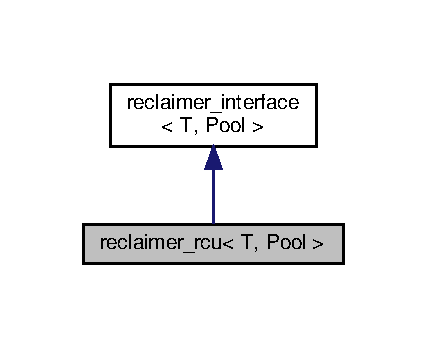
\includegraphics[width=205pt]{classreclaimer__rcu__inherit__graph}
\end{center}
\end{figure}


Collaboration diagram for reclaimer\+\_\+rcu$<$ T, Pool $>$\+:
\nopagebreak
\begin{figure}[H]
\begin{center}
\leavevmode
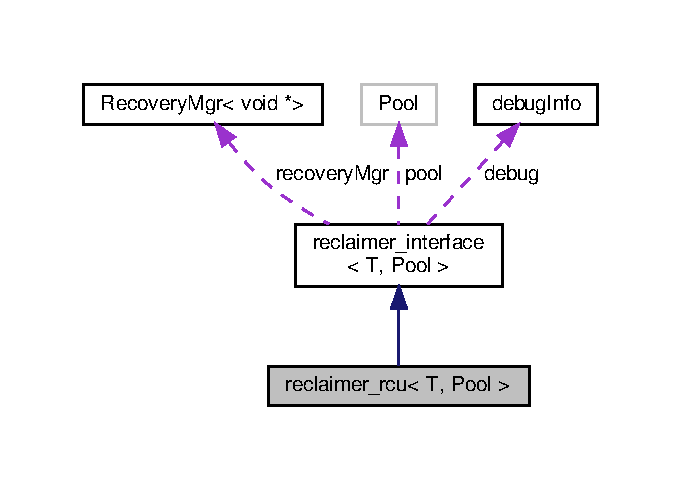
\includegraphics[width=327pt]{classreclaimer__rcu__coll__graph}
\end{center}
\end{figure}
\subsection*{Classes}
\begin{DoxyCompactItemize}
\item 
struct \hyperlink{structreclaimer__rcu_1_1rebind}{rebind}
\item 
struct \hyperlink{structreclaimer__rcu_1_1rebind2}{rebind2}
\end{DoxyCompactItemize}
\subsection*{Public Member Functions}
\begin{DoxyCompactItemize}
\item 
long long \hyperlink{classreclaimer__rcu_aef57d5f5142c6254fb451424db5db6e5}{get\+Size\+In\+Nodes} ()
\item 
std\+::string \hyperlink{classreclaimer__rcu_a694c71982ebf65c7dab8c292cb8ee85d}{get\+Details\+String} ()
\item 
std\+::string \hyperlink{classreclaimer__rcu_a4693be247dba56a115a04ebb1737d715}{get\+Size\+String} ()
\item 
bool \hyperlink{classreclaimer__rcu_aac05d4d8bd2341860af63c0d89600d0a}{is\+Quiescent} (const int \hyperlink{microbench_2main_8cpp_a9ca9869868fe7e7a38a921cc7de4103f}{tid})
\item 
void \hyperlink{classreclaimer__rcu_ae67cc73f8475079f0a2696459d304c95}{rotate\+Epoch\+Bags} (const int \hyperlink{microbench_2main_8cpp_a9ca9869868fe7e7a38a921cc7de4103f}{tid})
\item 
bool \hyperlink{classreclaimer__rcu_a5d9e6b96518bace44b08d02fc69e6f42}{start\+Op} (const int \hyperlink{microbench_2main_8cpp_a9ca9869868fe7e7a38a921cc7de4103f}{tid}, void $\ast$const $\ast$const reclaimers, const int num\+Reclaimers)
\item 
void \hyperlink{classreclaimer__rcu_aab06e2ef6aeb6bd863b4bbecb121229f}{end\+Op} (const int \hyperlink{microbench_2main_8cpp_a9ca9869868fe7e7a38a921cc7de4103f}{tid})
\item 
void \hyperlink{classreclaimer__rcu_aff8e363574a08a689a24e355147e38b4}{retire} (const int \hyperlink{microbench_2main_8cpp_a9ca9869868fe7e7a38a921cc7de4103f}{tid}, T $\ast$p)
\item 
void \hyperlink{classreclaimer__rcu_aecc8947fd089984a2459b34d712f484f}{debug\+Print\+Status} (const int \hyperlink{microbench_2main_8cpp_a9ca9869868fe7e7a38a921cc7de4103f}{tid})
\item 
void \hyperlink{classreclaimer__rcu_a6b9241339f5715c9c6c6cce62a886411}{init\+Thread} (const int \hyperlink{microbench_2main_8cpp_a9ca9869868fe7e7a38a921cc7de4103f}{tid})
\item 
void \hyperlink{classreclaimer__rcu_a3a294a5b1a496cdd531a90f14e3ad708}{deinit\+Thread} (const int \hyperlink{microbench_2main_8cpp_a9ca9869868fe7e7a38a921cc7de4103f}{tid})
\item 
\hyperlink{classreclaimer__rcu_a5ead65ca8fdc3bd6a77c447af6681992}{reclaimer\+\_\+rcu} (const int \hyperlink{testing_8cpp_aa085812188e21ede75351d88b9b2c30d}{num\+Processes}, Pool $\ast$\+\_\+pool, \hyperlink{classdebugInfo}{debug\+Info} $\ast$const \+\_\+debug, \hyperlink{classRecoveryMgr}{Recovery\+Mgr}$<$ void $\ast$$>$ $\ast$const \+\_\+recovery\+Mgr=N\+U\+LL)
\item 
\hyperlink{classreclaimer__rcu_a1bf4a6cc53e4f41bd6eb779bdf882605}{$\sim$reclaimer\+\_\+rcu} ()
\end{DoxyCompactItemize}
\subsection*{Static Public Member Functions}
\begin{DoxyCompactItemize}
\item 
static bool \hyperlink{classreclaimer__rcu_a6dc43b3dbe423012ae7ccea223a820c7}{quiescence\+Is\+Per\+Record\+Type} ()
\item 
static bool \hyperlink{classreclaimer__rcu_a8b63d95c4391b2ee2f36c74a2141d078}{is\+Protected} (const int \hyperlink{microbench_2main_8cpp_a9ca9869868fe7e7a38a921cc7de4103f}{tid}, T $\ast$const obj)
\item 
static bool \hyperlink{classreclaimer__rcu_a64723a698dde603065e5e1c67761d15c}{is\+Q\+Protected} (const int \hyperlink{microbench_2main_8cpp_a9ca9869868fe7e7a38a921cc7de4103f}{tid}, T $\ast$const obj)
\item 
static bool \hyperlink{classreclaimer__rcu_aef0461a44efcde0d9253fa4bd9ea5f5f}{protect} (const int \hyperlink{microbench_2main_8cpp_a9ca9869868fe7e7a38a921cc7de4103f}{tid}, T $\ast$const obj, \hyperlink{globals_8h_a57f5c0d40b156d7d996492fb2f16e3cd}{Callback\+Type} not\+Retired\+Callback, \hyperlink{globals_8h_a3de64ef48066ac6430631c8b81a15345}{Callback\+Arg} callback\+Arg, bool memory\+Barrier=true)
\item 
static void \hyperlink{classreclaimer__rcu_aa786ea177bb54fcfd771b25b1b2ced9e}{unprotect} (const int \hyperlink{microbench_2main_8cpp_a9ca9869868fe7e7a38a921cc7de4103f}{tid}, T $\ast$const obj)
\item 
static bool \hyperlink{classreclaimer__rcu_ac1bb65eb5a5ebcc433094e72fa872b0c}{q\+Protect} (const int \hyperlink{microbench_2main_8cpp_a9ca9869868fe7e7a38a921cc7de4103f}{tid}, T $\ast$const obj, \hyperlink{globals_8h_a57f5c0d40b156d7d996492fb2f16e3cd}{Callback\+Type} not\+Retired\+Callback, \hyperlink{globals_8h_a3de64ef48066ac6430631c8b81a15345}{Callback\+Arg} callback\+Arg, bool memory\+Barrier=true)
\item 
static void \hyperlink{classreclaimer__rcu_a27f67a0be3fad8a808e397ad1ffd73e6}{q\+Unprotect\+All} (const int \hyperlink{microbench_2main_8cpp_a9ca9869868fe7e7a38a921cc7de4103f}{tid})
\item 
static bool \hyperlink{classreclaimer__rcu_a524af2f160524a0d662b1ffd29730d35}{should\+Help} ()
\end{DoxyCompactItemize}
\subsection*{Additional Inherited Members}


\subsection{Constructor \& Destructor Documentation}
\mbox{\Hypertarget{classreclaimer__rcu_a5ead65ca8fdc3bd6a77c447af6681992}\label{classreclaimer__rcu_a5ead65ca8fdc3bd6a77c447af6681992}} 
\index{reclaimer\+\_\+rcu@{reclaimer\+\_\+rcu}!reclaimer\+\_\+rcu@{reclaimer\+\_\+rcu}}
\index{reclaimer\+\_\+rcu@{reclaimer\+\_\+rcu}!reclaimer\+\_\+rcu@{reclaimer\+\_\+rcu}}
\subsubsection{\texorpdfstring{reclaimer\+\_\+rcu()}{reclaimer\_rcu()}}
{\footnotesize\ttfamily template$<$typename T  = void, class Pool  = pool\+\_\+interface$<$\+T$>$$>$ \\
\hyperlink{classreclaimer__rcu}{reclaimer\+\_\+rcu}$<$ T, Pool $>$\+::\hyperlink{classreclaimer__rcu}{reclaimer\+\_\+rcu} (\begin{DoxyParamCaption}\item[{const int}]{num\+Processes,  }\item[{Pool $\ast$}]{\+\_\+pool,  }\item[{\hyperlink{classdebugInfo}{debug\+Info} $\ast$const}]{\+\_\+debug,  }\item[{\hyperlink{classRecoveryMgr}{Recovery\+Mgr}$<$ void $\ast$$>$ $\ast$const}]{\+\_\+recovery\+Mgr = {\ttfamily NULL} }\end{DoxyParamCaption})\hspace{0.3cm}{\ttfamily [inline]}}

\mbox{\Hypertarget{classreclaimer__rcu_a1bf4a6cc53e4f41bd6eb779bdf882605}\label{classreclaimer__rcu_a1bf4a6cc53e4f41bd6eb779bdf882605}} 
\index{reclaimer\+\_\+rcu@{reclaimer\+\_\+rcu}!````~reclaimer\+\_\+rcu@{$\sim$reclaimer\+\_\+rcu}}
\index{````~reclaimer\+\_\+rcu@{$\sim$reclaimer\+\_\+rcu}!reclaimer\+\_\+rcu@{reclaimer\+\_\+rcu}}
\subsubsection{\texorpdfstring{$\sim$reclaimer\+\_\+rcu()}{~reclaimer\_rcu()}}
{\footnotesize\ttfamily template$<$typename T  = void, class Pool  = pool\+\_\+interface$<$\+T$>$$>$ \\
\hyperlink{classreclaimer__rcu}{reclaimer\+\_\+rcu}$<$ T, Pool $>$\+::$\sim$\hyperlink{classreclaimer__rcu}{reclaimer\+\_\+rcu} (\begin{DoxyParamCaption}{ }\end{DoxyParamCaption})\hspace{0.3cm}{\ttfamily [inline]}}



\subsection{Member Function Documentation}
\mbox{\Hypertarget{classreclaimer__rcu_aecc8947fd089984a2459b34d712f484f}\label{classreclaimer__rcu_aecc8947fd089984a2459b34d712f484f}} 
\index{reclaimer\+\_\+rcu@{reclaimer\+\_\+rcu}!debug\+Print\+Status@{debug\+Print\+Status}}
\index{debug\+Print\+Status@{debug\+Print\+Status}!reclaimer\+\_\+rcu@{reclaimer\+\_\+rcu}}
\subsubsection{\texorpdfstring{debug\+Print\+Status()}{debugPrintStatus()}}
{\footnotesize\ttfamily template$<$typename T  = void, class Pool  = pool\+\_\+interface$<$\+T$>$$>$ \\
void \hyperlink{classreclaimer__rcu}{reclaimer\+\_\+rcu}$<$ T, Pool $>$\+::debug\+Print\+Status (\begin{DoxyParamCaption}\item[{const int}]{tid }\end{DoxyParamCaption})\hspace{0.3cm}{\ttfamily [inline]}}

\mbox{\Hypertarget{classreclaimer__rcu_a3a294a5b1a496cdd531a90f14e3ad708}\label{classreclaimer__rcu_a3a294a5b1a496cdd531a90f14e3ad708}} 
\index{reclaimer\+\_\+rcu@{reclaimer\+\_\+rcu}!deinit\+Thread@{deinit\+Thread}}
\index{deinit\+Thread@{deinit\+Thread}!reclaimer\+\_\+rcu@{reclaimer\+\_\+rcu}}
\subsubsection{\texorpdfstring{deinit\+Thread()}{deinitThread()}}
{\footnotesize\ttfamily template$<$typename T  = void, class Pool  = pool\+\_\+interface$<$\+T$>$$>$ \\
void \hyperlink{classreclaimer__rcu}{reclaimer\+\_\+rcu}$<$ T, Pool $>$\+::deinit\+Thread (\begin{DoxyParamCaption}\item[{const int}]{tid }\end{DoxyParamCaption})\hspace{0.3cm}{\ttfamily [inline]}}

\mbox{\Hypertarget{classreclaimer__rcu_aab06e2ef6aeb6bd863b4bbecb121229f}\label{classreclaimer__rcu_aab06e2ef6aeb6bd863b4bbecb121229f}} 
\index{reclaimer\+\_\+rcu@{reclaimer\+\_\+rcu}!end\+Op@{end\+Op}}
\index{end\+Op@{end\+Op}!reclaimer\+\_\+rcu@{reclaimer\+\_\+rcu}}
\subsubsection{\texorpdfstring{end\+Op()}{endOp()}}
{\footnotesize\ttfamily template$<$typename T  = void, class Pool  = pool\+\_\+interface$<$\+T$>$$>$ \\
void \hyperlink{classreclaimer__rcu}{reclaimer\+\_\+rcu}$<$ T, Pool $>$\+::end\+Op (\begin{DoxyParamCaption}\item[{const int}]{tid }\end{DoxyParamCaption})\hspace{0.3cm}{\ttfamily [inline]}}

\mbox{\Hypertarget{classreclaimer__rcu_a694c71982ebf65c7dab8c292cb8ee85d}\label{classreclaimer__rcu_a694c71982ebf65c7dab8c292cb8ee85d}} 
\index{reclaimer\+\_\+rcu@{reclaimer\+\_\+rcu}!get\+Details\+String@{get\+Details\+String}}
\index{get\+Details\+String@{get\+Details\+String}!reclaimer\+\_\+rcu@{reclaimer\+\_\+rcu}}
\subsubsection{\texorpdfstring{get\+Details\+String()}{getDetailsString()}}
{\footnotesize\ttfamily template$<$typename T  = void, class Pool  = pool\+\_\+interface$<$\+T$>$$>$ \\
std\+::string \hyperlink{classreclaimer__rcu}{reclaimer\+\_\+rcu}$<$ T, Pool $>$\+::get\+Details\+String (\begin{DoxyParamCaption}{ }\end{DoxyParamCaption})\hspace{0.3cm}{\ttfamily [inline]}}

\mbox{\Hypertarget{classreclaimer__rcu_aef57d5f5142c6254fb451424db5db6e5}\label{classreclaimer__rcu_aef57d5f5142c6254fb451424db5db6e5}} 
\index{reclaimer\+\_\+rcu@{reclaimer\+\_\+rcu}!get\+Size\+In\+Nodes@{get\+Size\+In\+Nodes}}
\index{get\+Size\+In\+Nodes@{get\+Size\+In\+Nodes}!reclaimer\+\_\+rcu@{reclaimer\+\_\+rcu}}
\subsubsection{\texorpdfstring{get\+Size\+In\+Nodes()}{getSizeInNodes()}}
{\footnotesize\ttfamily template$<$typename T  = void, class Pool  = pool\+\_\+interface$<$\+T$>$$>$ \\
long long \hyperlink{classreclaimer__rcu}{reclaimer\+\_\+rcu}$<$ T, Pool $>$\+::get\+Size\+In\+Nodes (\begin{DoxyParamCaption}{ }\end{DoxyParamCaption})\hspace{0.3cm}{\ttfamily [inline]}}

\mbox{\Hypertarget{classreclaimer__rcu_a4693be247dba56a115a04ebb1737d715}\label{classreclaimer__rcu_a4693be247dba56a115a04ebb1737d715}} 
\index{reclaimer\+\_\+rcu@{reclaimer\+\_\+rcu}!get\+Size\+String@{get\+Size\+String}}
\index{get\+Size\+String@{get\+Size\+String}!reclaimer\+\_\+rcu@{reclaimer\+\_\+rcu}}
\subsubsection{\texorpdfstring{get\+Size\+String()}{getSizeString()}}
{\footnotesize\ttfamily template$<$typename T  = void, class Pool  = pool\+\_\+interface$<$\+T$>$$>$ \\
std\+::string \hyperlink{classreclaimer__rcu}{reclaimer\+\_\+rcu}$<$ T, Pool $>$\+::get\+Size\+String (\begin{DoxyParamCaption}{ }\end{DoxyParamCaption})\hspace{0.3cm}{\ttfamily [inline]}}

\mbox{\Hypertarget{classreclaimer__rcu_a6b9241339f5715c9c6c6cce62a886411}\label{classreclaimer__rcu_a6b9241339f5715c9c6c6cce62a886411}} 
\index{reclaimer\+\_\+rcu@{reclaimer\+\_\+rcu}!init\+Thread@{init\+Thread}}
\index{init\+Thread@{init\+Thread}!reclaimer\+\_\+rcu@{reclaimer\+\_\+rcu}}
\subsubsection{\texorpdfstring{init\+Thread()}{initThread()}}
{\footnotesize\ttfamily template$<$typename T  = void, class Pool  = pool\+\_\+interface$<$\+T$>$$>$ \\
void \hyperlink{classreclaimer__rcu}{reclaimer\+\_\+rcu}$<$ T, Pool $>$\+::init\+Thread (\begin{DoxyParamCaption}\item[{const int}]{tid }\end{DoxyParamCaption})\hspace{0.3cm}{\ttfamily [inline]}}

\mbox{\Hypertarget{classreclaimer__rcu_a8b63d95c4391b2ee2f36c74a2141d078}\label{classreclaimer__rcu_a8b63d95c4391b2ee2f36c74a2141d078}} 
\index{reclaimer\+\_\+rcu@{reclaimer\+\_\+rcu}!is\+Protected@{is\+Protected}}
\index{is\+Protected@{is\+Protected}!reclaimer\+\_\+rcu@{reclaimer\+\_\+rcu}}
\subsubsection{\texorpdfstring{is\+Protected()}{isProtected()}}
{\footnotesize\ttfamily template$<$typename T  = void, class Pool  = pool\+\_\+interface$<$\+T$>$$>$ \\
static bool \hyperlink{classreclaimer__rcu}{reclaimer\+\_\+rcu}$<$ T, Pool $>$\+::is\+Protected (\begin{DoxyParamCaption}\item[{const int}]{tid,  }\item[{T $\ast$const}]{obj }\end{DoxyParamCaption})\hspace{0.3cm}{\ttfamily [inline]}, {\ttfamily [static]}}

\mbox{\Hypertarget{classreclaimer__rcu_a64723a698dde603065e5e1c67761d15c}\label{classreclaimer__rcu_a64723a698dde603065e5e1c67761d15c}} 
\index{reclaimer\+\_\+rcu@{reclaimer\+\_\+rcu}!is\+Q\+Protected@{is\+Q\+Protected}}
\index{is\+Q\+Protected@{is\+Q\+Protected}!reclaimer\+\_\+rcu@{reclaimer\+\_\+rcu}}
\subsubsection{\texorpdfstring{is\+Q\+Protected()}{isQProtected()}}
{\footnotesize\ttfamily template$<$typename T  = void, class Pool  = pool\+\_\+interface$<$\+T$>$$>$ \\
static bool \hyperlink{classreclaimer__rcu}{reclaimer\+\_\+rcu}$<$ T, Pool $>$\+::is\+Q\+Protected (\begin{DoxyParamCaption}\item[{const int}]{tid,  }\item[{T $\ast$const}]{obj }\end{DoxyParamCaption})\hspace{0.3cm}{\ttfamily [inline]}, {\ttfamily [static]}}

\mbox{\Hypertarget{classreclaimer__rcu_aac05d4d8bd2341860af63c0d89600d0a}\label{classreclaimer__rcu_aac05d4d8bd2341860af63c0d89600d0a}} 
\index{reclaimer\+\_\+rcu@{reclaimer\+\_\+rcu}!is\+Quiescent@{is\+Quiescent}}
\index{is\+Quiescent@{is\+Quiescent}!reclaimer\+\_\+rcu@{reclaimer\+\_\+rcu}}
\subsubsection{\texorpdfstring{is\+Quiescent()}{isQuiescent()}}
{\footnotesize\ttfamily template$<$typename T  = void, class Pool  = pool\+\_\+interface$<$\+T$>$$>$ \\
bool \hyperlink{classreclaimer__rcu}{reclaimer\+\_\+rcu}$<$ T, Pool $>$\+::is\+Quiescent (\begin{DoxyParamCaption}\item[{const int}]{tid }\end{DoxyParamCaption})\hspace{0.3cm}{\ttfamily [inline]}}

\mbox{\Hypertarget{classreclaimer__rcu_aef0461a44efcde0d9253fa4bd9ea5f5f}\label{classreclaimer__rcu_aef0461a44efcde0d9253fa4bd9ea5f5f}} 
\index{reclaimer\+\_\+rcu@{reclaimer\+\_\+rcu}!protect@{protect}}
\index{protect@{protect}!reclaimer\+\_\+rcu@{reclaimer\+\_\+rcu}}
\subsubsection{\texorpdfstring{protect()}{protect()}}
{\footnotesize\ttfamily template$<$typename T  = void, class Pool  = pool\+\_\+interface$<$\+T$>$$>$ \\
static bool \hyperlink{classreclaimer__rcu}{reclaimer\+\_\+rcu}$<$ T, Pool $>$\+::protect (\begin{DoxyParamCaption}\item[{const int}]{tid,  }\item[{T $\ast$const}]{obj,  }\item[{\hyperlink{globals_8h_a57f5c0d40b156d7d996492fb2f16e3cd}{Callback\+Type}}]{not\+Retired\+Callback,  }\item[{\hyperlink{globals_8h_a3de64ef48066ac6430631c8b81a15345}{Callback\+Arg}}]{callback\+Arg,  }\item[{bool}]{memory\+Barrier = {\ttfamily true} }\end{DoxyParamCaption})\hspace{0.3cm}{\ttfamily [inline]}, {\ttfamily [static]}}

\mbox{\Hypertarget{classreclaimer__rcu_ac1bb65eb5a5ebcc433094e72fa872b0c}\label{classreclaimer__rcu_ac1bb65eb5a5ebcc433094e72fa872b0c}} 
\index{reclaimer\+\_\+rcu@{reclaimer\+\_\+rcu}!q\+Protect@{q\+Protect}}
\index{q\+Protect@{q\+Protect}!reclaimer\+\_\+rcu@{reclaimer\+\_\+rcu}}
\subsubsection{\texorpdfstring{q\+Protect()}{qProtect()}}
{\footnotesize\ttfamily template$<$typename T  = void, class Pool  = pool\+\_\+interface$<$\+T$>$$>$ \\
static bool \hyperlink{classreclaimer__rcu}{reclaimer\+\_\+rcu}$<$ T, Pool $>$\+::q\+Protect (\begin{DoxyParamCaption}\item[{const int}]{tid,  }\item[{T $\ast$const}]{obj,  }\item[{\hyperlink{globals_8h_a57f5c0d40b156d7d996492fb2f16e3cd}{Callback\+Type}}]{not\+Retired\+Callback,  }\item[{\hyperlink{globals_8h_a3de64ef48066ac6430631c8b81a15345}{Callback\+Arg}}]{callback\+Arg,  }\item[{bool}]{memory\+Barrier = {\ttfamily true} }\end{DoxyParamCaption})\hspace{0.3cm}{\ttfamily [inline]}, {\ttfamily [static]}}

\mbox{\Hypertarget{classreclaimer__rcu_a6dc43b3dbe423012ae7ccea223a820c7}\label{classreclaimer__rcu_a6dc43b3dbe423012ae7ccea223a820c7}} 
\index{reclaimer\+\_\+rcu@{reclaimer\+\_\+rcu}!quiescence\+Is\+Per\+Record\+Type@{quiescence\+Is\+Per\+Record\+Type}}
\index{quiescence\+Is\+Per\+Record\+Type@{quiescence\+Is\+Per\+Record\+Type}!reclaimer\+\_\+rcu@{reclaimer\+\_\+rcu}}
\subsubsection{\texorpdfstring{quiescence\+Is\+Per\+Record\+Type()}{quiescenceIsPerRecordType()}}
{\footnotesize\ttfamily template$<$typename T  = void, class Pool  = pool\+\_\+interface$<$\+T$>$$>$ \\
static bool \hyperlink{classreclaimer__rcu}{reclaimer\+\_\+rcu}$<$ T, Pool $>$\+::quiescence\+Is\+Per\+Record\+Type (\begin{DoxyParamCaption}{ }\end{DoxyParamCaption})\hspace{0.3cm}{\ttfamily [inline]}, {\ttfamily [static]}}

\mbox{\Hypertarget{classreclaimer__rcu_a27f67a0be3fad8a808e397ad1ffd73e6}\label{classreclaimer__rcu_a27f67a0be3fad8a808e397ad1ffd73e6}} 
\index{reclaimer\+\_\+rcu@{reclaimer\+\_\+rcu}!q\+Unprotect\+All@{q\+Unprotect\+All}}
\index{q\+Unprotect\+All@{q\+Unprotect\+All}!reclaimer\+\_\+rcu@{reclaimer\+\_\+rcu}}
\subsubsection{\texorpdfstring{q\+Unprotect\+All()}{qUnprotectAll()}}
{\footnotesize\ttfamily template$<$typename T  = void, class Pool  = pool\+\_\+interface$<$\+T$>$$>$ \\
static void \hyperlink{classreclaimer__rcu}{reclaimer\+\_\+rcu}$<$ T, Pool $>$\+::q\+Unprotect\+All (\begin{DoxyParamCaption}\item[{const int}]{tid }\end{DoxyParamCaption})\hspace{0.3cm}{\ttfamily [inline]}, {\ttfamily [static]}}

\mbox{\Hypertarget{classreclaimer__rcu_aff8e363574a08a689a24e355147e38b4}\label{classreclaimer__rcu_aff8e363574a08a689a24e355147e38b4}} 
\index{reclaimer\+\_\+rcu@{reclaimer\+\_\+rcu}!retire@{retire}}
\index{retire@{retire}!reclaimer\+\_\+rcu@{reclaimer\+\_\+rcu}}
\subsubsection{\texorpdfstring{retire()}{retire()}}
{\footnotesize\ttfamily template$<$typename T  = void, class Pool  = pool\+\_\+interface$<$\+T$>$$>$ \\
void \hyperlink{classreclaimer__rcu}{reclaimer\+\_\+rcu}$<$ T, Pool $>$\+::retire (\begin{DoxyParamCaption}\item[{const int}]{tid,  }\item[{T $\ast$}]{p }\end{DoxyParamCaption})\hspace{0.3cm}{\ttfamily [inline]}}

\mbox{\Hypertarget{classreclaimer__rcu_ae67cc73f8475079f0a2696459d304c95}\label{classreclaimer__rcu_ae67cc73f8475079f0a2696459d304c95}} 
\index{reclaimer\+\_\+rcu@{reclaimer\+\_\+rcu}!rotate\+Epoch\+Bags@{rotate\+Epoch\+Bags}}
\index{rotate\+Epoch\+Bags@{rotate\+Epoch\+Bags}!reclaimer\+\_\+rcu@{reclaimer\+\_\+rcu}}
\subsubsection{\texorpdfstring{rotate\+Epoch\+Bags()}{rotateEpochBags()}}
{\footnotesize\ttfamily template$<$typename T  = void, class Pool  = pool\+\_\+interface$<$\+T$>$$>$ \\
void \hyperlink{classreclaimer__rcu}{reclaimer\+\_\+rcu}$<$ T, Pool $>$\+::rotate\+Epoch\+Bags (\begin{DoxyParamCaption}\item[{const int}]{tid }\end{DoxyParamCaption})\hspace{0.3cm}{\ttfamily [inline]}}

\mbox{\Hypertarget{classreclaimer__rcu_a524af2f160524a0d662b1ffd29730d35}\label{classreclaimer__rcu_a524af2f160524a0d662b1ffd29730d35}} 
\index{reclaimer\+\_\+rcu@{reclaimer\+\_\+rcu}!should\+Help@{should\+Help}}
\index{should\+Help@{should\+Help}!reclaimer\+\_\+rcu@{reclaimer\+\_\+rcu}}
\subsubsection{\texorpdfstring{should\+Help()}{shouldHelp()}}
{\footnotesize\ttfamily template$<$typename T  = void, class Pool  = pool\+\_\+interface$<$\+T$>$$>$ \\
static bool \hyperlink{classreclaimer__rcu}{reclaimer\+\_\+rcu}$<$ T, Pool $>$\+::should\+Help (\begin{DoxyParamCaption}{ }\end{DoxyParamCaption})\hspace{0.3cm}{\ttfamily [inline]}, {\ttfamily [static]}}

\mbox{\Hypertarget{classreclaimer__rcu_a5d9e6b96518bace44b08d02fc69e6f42}\label{classreclaimer__rcu_a5d9e6b96518bace44b08d02fc69e6f42}} 
\index{reclaimer\+\_\+rcu@{reclaimer\+\_\+rcu}!start\+Op@{start\+Op}}
\index{start\+Op@{start\+Op}!reclaimer\+\_\+rcu@{reclaimer\+\_\+rcu}}
\subsubsection{\texorpdfstring{start\+Op()}{startOp()}}
{\footnotesize\ttfamily template$<$typename T  = void, class Pool  = pool\+\_\+interface$<$\+T$>$$>$ \\
bool \hyperlink{classreclaimer__rcu}{reclaimer\+\_\+rcu}$<$ T, Pool $>$\+::start\+Op (\begin{DoxyParamCaption}\item[{const int}]{tid,  }\item[{void $\ast$const $\ast$const}]{reclaimers,  }\item[{const int}]{num\+Reclaimers }\end{DoxyParamCaption})\hspace{0.3cm}{\ttfamily [inline]}}

\mbox{\Hypertarget{classreclaimer__rcu_aa786ea177bb54fcfd771b25b1b2ced9e}\label{classreclaimer__rcu_aa786ea177bb54fcfd771b25b1b2ced9e}} 
\index{reclaimer\+\_\+rcu@{reclaimer\+\_\+rcu}!unprotect@{unprotect}}
\index{unprotect@{unprotect}!reclaimer\+\_\+rcu@{reclaimer\+\_\+rcu}}
\subsubsection{\texorpdfstring{unprotect()}{unprotect()}}
{\footnotesize\ttfamily template$<$typename T  = void, class Pool  = pool\+\_\+interface$<$\+T$>$$>$ \\
static void \hyperlink{classreclaimer__rcu}{reclaimer\+\_\+rcu}$<$ T, Pool $>$\+::unprotect (\begin{DoxyParamCaption}\item[{const int}]{tid,  }\item[{T $\ast$const}]{obj }\end{DoxyParamCaption})\hspace{0.3cm}{\ttfamily [inline]}, {\ttfamily [static]}}



The documentation for this class was generated from the following file\+:\begin{DoxyCompactItemize}
\item 
common/recordmgr/\hyperlink{reclaimer__rcu_8h}{reclaimer\+\_\+rcu.\+h}\end{DoxyCompactItemize}

\hypertarget{classbst__ns_1_1ReclamationInfo}{}\section{bst\+\_\+ns\+:\+:Reclamation\+Info$<$ K, V $>$ Class Template Reference}
\label{classbst__ns_1_1ReclamationInfo}\index{bst\+\_\+ns\+::\+Reclamation\+Info$<$ K, V $>$@{bst\+\_\+ns\+::\+Reclamation\+Info$<$ K, V $>$}}


{\ttfamily \#include $<$bst\+\_\+impl.\+h$>$}

\subsection*{Public Attributes}
\begin{DoxyCompactItemize}
\item 
int \hyperlink{classbst__ns_1_1ReclamationInfo_ad7749ba8daa9454ccaf70877ae3797a0}{type}
\item 
void $\ast$ \hyperlink{classbst__ns_1_1ReclamationInfo_aa12e3a5b91c393d63de9582d26c88525}{llx\+Results} \mbox{[}\hyperlink{scxrecord_8h_abd2aacdca9cb2a1a30f3392256b96ea3}{M\+A\+X\+\_\+\+N\+O\+D\+ES}\mbox{]}
\item 
\hyperlink{classbst__ns_1_1Node}{Node}$<$ K, V $>$ $\ast$ \hyperlink{classbst__ns_1_1ReclamationInfo_aba682f7f7dacd2c3e8adf2ccf8a17073}{nodes} \mbox{[}\hyperlink{scxrecord_8h_abd2aacdca9cb2a1a30f3392256b96ea3}{M\+A\+X\+\_\+\+N\+O\+D\+ES}\mbox{]}
\item 
int \hyperlink{classbst__ns_1_1ReclamationInfo_ade9df2aa225f77af64f30d89dcb3037c}{state}
\item 
int \hyperlink{classbst__ns_1_1ReclamationInfo_aef2fde1573b0f5d80800b180d83e8dc0}{number\+Of\+Nodes}
\item 
int \hyperlink{classbst__ns_1_1ReclamationInfo_abad901212e23fc0b1ab2094c537f1fc2}{number\+Of\+Nodes\+To\+Freeze}
\item 
int \hyperlink{classbst__ns_1_1ReclamationInfo_a5488dfe4318b54453e922c7a1cab020a}{number\+Of\+Nodes\+To\+Reclaim}
\item 
int \hyperlink{classbst__ns_1_1ReclamationInfo_a2bb983af0e2f44e78735e2b0bf5b3e7f}{number\+Of\+Nodes\+Allocated}
\item 
int \hyperlink{classbst__ns_1_1ReclamationInfo_a5ae6fd8061628629d525541e00518966}{path}
\item 
int \hyperlink{classbst__ns_1_1ReclamationInfo_aea753345c52d877c29aff867f58dbe5f}{last\+Abort}
\end{DoxyCompactItemize}


\subsection{Member Data Documentation}
\mbox{\Hypertarget{classbst__ns_1_1ReclamationInfo_aea753345c52d877c29aff867f58dbe5f}\label{classbst__ns_1_1ReclamationInfo_aea753345c52d877c29aff867f58dbe5f}} 
\index{bst\+\_\+ns\+::\+Reclamation\+Info@{bst\+\_\+ns\+::\+Reclamation\+Info}!last\+Abort@{last\+Abort}}
\index{last\+Abort@{last\+Abort}!bst\+\_\+ns\+::\+Reclamation\+Info@{bst\+\_\+ns\+::\+Reclamation\+Info}}
\subsubsection{\texorpdfstring{last\+Abort}{lastAbort}}
{\footnotesize\ttfamily template$<$class K, class V$>$ \\
int \hyperlink{classbst__ns_1_1ReclamationInfo}{bst\+\_\+ns\+::\+Reclamation\+Info}$<$ K, V $>$\+::last\+Abort}

\mbox{\Hypertarget{classbst__ns_1_1ReclamationInfo_aa12e3a5b91c393d63de9582d26c88525}\label{classbst__ns_1_1ReclamationInfo_aa12e3a5b91c393d63de9582d26c88525}} 
\index{bst\+\_\+ns\+::\+Reclamation\+Info@{bst\+\_\+ns\+::\+Reclamation\+Info}!llx\+Results@{llx\+Results}}
\index{llx\+Results@{llx\+Results}!bst\+\_\+ns\+::\+Reclamation\+Info@{bst\+\_\+ns\+::\+Reclamation\+Info}}
\subsubsection{\texorpdfstring{llx\+Results}{llxResults}}
{\footnotesize\ttfamily template$<$class K, class V$>$ \\
void$\ast$ \hyperlink{classbst__ns_1_1ReclamationInfo}{bst\+\_\+ns\+::\+Reclamation\+Info}$<$ K, V $>$\+::llx\+Results\mbox{[}\hyperlink{scxrecord_8h_abd2aacdca9cb2a1a30f3392256b96ea3}{M\+A\+X\+\_\+\+N\+O\+D\+ES}\mbox{]}}

\mbox{\Hypertarget{classbst__ns_1_1ReclamationInfo_aba682f7f7dacd2c3e8adf2ccf8a17073}\label{classbst__ns_1_1ReclamationInfo_aba682f7f7dacd2c3e8adf2ccf8a17073}} 
\index{bst\+\_\+ns\+::\+Reclamation\+Info@{bst\+\_\+ns\+::\+Reclamation\+Info}!nodes@{nodes}}
\index{nodes@{nodes}!bst\+\_\+ns\+::\+Reclamation\+Info@{bst\+\_\+ns\+::\+Reclamation\+Info}}
\subsubsection{\texorpdfstring{nodes}{nodes}}
{\footnotesize\ttfamily template$<$class K, class V$>$ \\
\hyperlink{classbst__ns_1_1Node}{Node}$<$K,V$>$$\ast$ \hyperlink{classbst__ns_1_1ReclamationInfo}{bst\+\_\+ns\+::\+Reclamation\+Info}$<$ K, V $>$\+::nodes\mbox{[}\hyperlink{scxrecord_8h_abd2aacdca9cb2a1a30f3392256b96ea3}{M\+A\+X\+\_\+\+N\+O\+D\+ES}\mbox{]}}

\mbox{\Hypertarget{classbst__ns_1_1ReclamationInfo_aef2fde1573b0f5d80800b180d83e8dc0}\label{classbst__ns_1_1ReclamationInfo_aef2fde1573b0f5d80800b180d83e8dc0}} 
\index{bst\+\_\+ns\+::\+Reclamation\+Info@{bst\+\_\+ns\+::\+Reclamation\+Info}!number\+Of\+Nodes@{number\+Of\+Nodes}}
\index{number\+Of\+Nodes@{number\+Of\+Nodes}!bst\+\_\+ns\+::\+Reclamation\+Info@{bst\+\_\+ns\+::\+Reclamation\+Info}}
\subsubsection{\texorpdfstring{number\+Of\+Nodes}{numberOfNodes}}
{\footnotesize\ttfamily template$<$class K, class V$>$ \\
int \hyperlink{classbst__ns_1_1ReclamationInfo}{bst\+\_\+ns\+::\+Reclamation\+Info}$<$ K, V $>$\+::number\+Of\+Nodes}

\mbox{\Hypertarget{classbst__ns_1_1ReclamationInfo_a2bb983af0e2f44e78735e2b0bf5b3e7f}\label{classbst__ns_1_1ReclamationInfo_a2bb983af0e2f44e78735e2b0bf5b3e7f}} 
\index{bst\+\_\+ns\+::\+Reclamation\+Info@{bst\+\_\+ns\+::\+Reclamation\+Info}!number\+Of\+Nodes\+Allocated@{number\+Of\+Nodes\+Allocated}}
\index{number\+Of\+Nodes\+Allocated@{number\+Of\+Nodes\+Allocated}!bst\+\_\+ns\+::\+Reclamation\+Info@{bst\+\_\+ns\+::\+Reclamation\+Info}}
\subsubsection{\texorpdfstring{number\+Of\+Nodes\+Allocated}{numberOfNodesAllocated}}
{\footnotesize\ttfamily template$<$class K, class V$>$ \\
int \hyperlink{classbst__ns_1_1ReclamationInfo}{bst\+\_\+ns\+::\+Reclamation\+Info}$<$ K, V $>$\+::number\+Of\+Nodes\+Allocated}

\mbox{\Hypertarget{classbst__ns_1_1ReclamationInfo_abad901212e23fc0b1ab2094c537f1fc2}\label{classbst__ns_1_1ReclamationInfo_abad901212e23fc0b1ab2094c537f1fc2}} 
\index{bst\+\_\+ns\+::\+Reclamation\+Info@{bst\+\_\+ns\+::\+Reclamation\+Info}!number\+Of\+Nodes\+To\+Freeze@{number\+Of\+Nodes\+To\+Freeze}}
\index{number\+Of\+Nodes\+To\+Freeze@{number\+Of\+Nodes\+To\+Freeze}!bst\+\_\+ns\+::\+Reclamation\+Info@{bst\+\_\+ns\+::\+Reclamation\+Info}}
\subsubsection{\texorpdfstring{number\+Of\+Nodes\+To\+Freeze}{numberOfNodesToFreeze}}
{\footnotesize\ttfamily template$<$class K, class V$>$ \\
int \hyperlink{classbst__ns_1_1ReclamationInfo}{bst\+\_\+ns\+::\+Reclamation\+Info}$<$ K, V $>$\+::number\+Of\+Nodes\+To\+Freeze}

\mbox{\Hypertarget{classbst__ns_1_1ReclamationInfo_a5488dfe4318b54453e922c7a1cab020a}\label{classbst__ns_1_1ReclamationInfo_a5488dfe4318b54453e922c7a1cab020a}} 
\index{bst\+\_\+ns\+::\+Reclamation\+Info@{bst\+\_\+ns\+::\+Reclamation\+Info}!number\+Of\+Nodes\+To\+Reclaim@{number\+Of\+Nodes\+To\+Reclaim}}
\index{number\+Of\+Nodes\+To\+Reclaim@{number\+Of\+Nodes\+To\+Reclaim}!bst\+\_\+ns\+::\+Reclamation\+Info@{bst\+\_\+ns\+::\+Reclamation\+Info}}
\subsubsection{\texorpdfstring{number\+Of\+Nodes\+To\+Reclaim}{numberOfNodesToReclaim}}
{\footnotesize\ttfamily template$<$class K, class V$>$ \\
int \hyperlink{classbst__ns_1_1ReclamationInfo}{bst\+\_\+ns\+::\+Reclamation\+Info}$<$ K, V $>$\+::number\+Of\+Nodes\+To\+Reclaim}

\mbox{\Hypertarget{classbst__ns_1_1ReclamationInfo_a5ae6fd8061628629d525541e00518966}\label{classbst__ns_1_1ReclamationInfo_a5ae6fd8061628629d525541e00518966}} 
\index{bst\+\_\+ns\+::\+Reclamation\+Info@{bst\+\_\+ns\+::\+Reclamation\+Info}!path@{path}}
\index{path@{path}!bst\+\_\+ns\+::\+Reclamation\+Info@{bst\+\_\+ns\+::\+Reclamation\+Info}}
\subsubsection{\texorpdfstring{path}{path}}
{\footnotesize\ttfamily template$<$class K, class V$>$ \\
int \hyperlink{classbst__ns_1_1ReclamationInfo}{bst\+\_\+ns\+::\+Reclamation\+Info}$<$ K, V $>$\+::path}

\mbox{\Hypertarget{classbst__ns_1_1ReclamationInfo_ade9df2aa225f77af64f30d89dcb3037c}\label{classbst__ns_1_1ReclamationInfo_ade9df2aa225f77af64f30d89dcb3037c}} 
\index{bst\+\_\+ns\+::\+Reclamation\+Info@{bst\+\_\+ns\+::\+Reclamation\+Info}!state@{state}}
\index{state@{state}!bst\+\_\+ns\+::\+Reclamation\+Info@{bst\+\_\+ns\+::\+Reclamation\+Info}}
\subsubsection{\texorpdfstring{state}{state}}
{\footnotesize\ttfamily template$<$class K, class V$>$ \\
int \hyperlink{classbst__ns_1_1ReclamationInfo}{bst\+\_\+ns\+::\+Reclamation\+Info}$<$ K, V $>$\+::state}

\mbox{\Hypertarget{classbst__ns_1_1ReclamationInfo_ad7749ba8daa9454ccaf70877ae3797a0}\label{classbst__ns_1_1ReclamationInfo_ad7749ba8daa9454ccaf70877ae3797a0}} 
\index{bst\+\_\+ns\+::\+Reclamation\+Info@{bst\+\_\+ns\+::\+Reclamation\+Info}!type@{type}}
\index{type@{type}!bst\+\_\+ns\+::\+Reclamation\+Info@{bst\+\_\+ns\+::\+Reclamation\+Info}}
\subsubsection{\texorpdfstring{type}{type}}
{\footnotesize\ttfamily template$<$class K, class V$>$ \\
int \hyperlink{classbst__ns_1_1ReclamationInfo}{bst\+\_\+ns\+::\+Reclamation\+Info}$<$ K, V $>$\+::type}



The documentation for this class was generated from the following file\+:\begin{DoxyCompactItemize}
\item 
ds/brown\+\_\+ext\+\_\+bst\+\_\+rq\+\_\+lf/\hyperlink{bst__impl_8h}{bst\+\_\+impl.\+h}\end{DoxyCompactItemize}

\hypertarget{classrecord__manager}{}\section{record\+\_\+manager$<$ Reclaim, Alloc, Pool, Record\+Types\+First, Record\+Types\+Rest $>$ Class Template Reference}
\label{classrecord__manager}\index{record\+\_\+manager$<$ Reclaim, Alloc, Pool, Record\+Types\+First, Record\+Types\+Rest $>$@{record\+\_\+manager$<$ Reclaim, Alloc, Pool, Record\+Types\+First, Record\+Types\+Rest $>$}}


{\ttfamily \#include $<$record\+\_\+manager.\+h$>$}



Collaboration diagram for record\+\_\+manager$<$ Reclaim, Alloc, Pool, Record\+Types\+First, Record\+Types\+Rest $>$\+:
\nopagebreak
\begin{figure}[H]
\begin{center}
\leavevmode
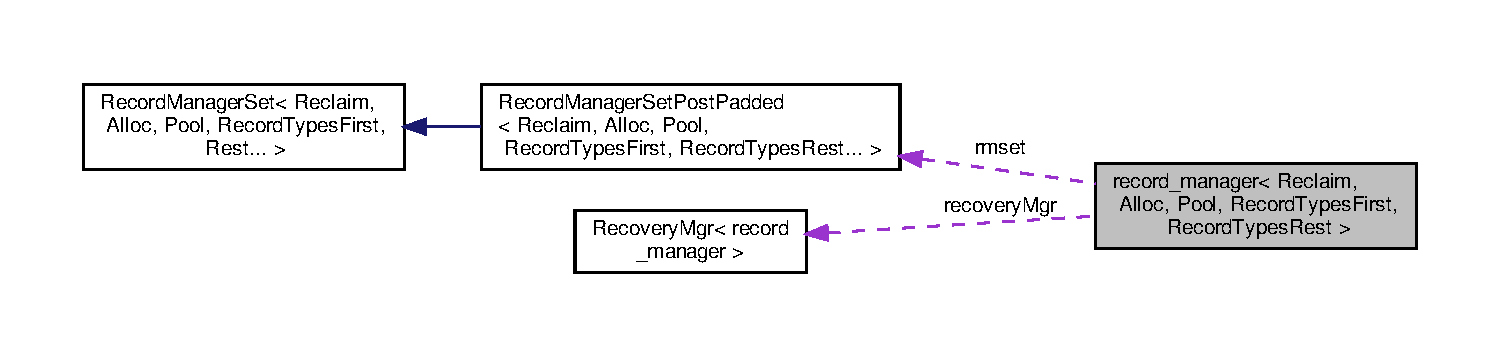
\includegraphics[width=350pt]{classrecord__manager__coll__graph}
\end{center}
\end{figure}
\subsection*{Classes}
\begin{DoxyCompactItemize}
\item 
class \hyperlink{classrecord__manager_1_1MemoryReclamationGuard}{Memory\+Reclamation\+Guard}
\end{DoxyCompactItemize}
\subsection*{Public Member Functions}
\begin{DoxyCompactItemize}
\item 
\hyperlink{classrecord__manager_a6c504d455df4b4eb7569f633baac409d}{record\+\_\+manager} (const int \hyperlink{testing_8cpp_aa085812188e21ede75351d88b9b2c30d}{num\+Processes}, const int \+\_\+neutralize\+Signal=-\/1)
\item 
\hyperlink{classrecord__manager_a40ef9dfae2ecd2f874b4598b5791fb96}{$\sim$record\+\_\+manager} ()
\item 
void \hyperlink{classrecord__manager_ab577f40a0f82ddff6b42dcd77e53e4ab}{init\+Thread} (const int \hyperlink{microbench_2main_8cpp_a9ca9869868fe7e7a38a921cc7de4103f}{tid})
\item 
void \hyperlink{classrecord__manager_a3e2437bdf46d90f3feb3a140e9a0d223}{deinit\+Thread} (const int \hyperlink{microbench_2main_8cpp_a9ca9869868fe7e7a38a921cc7de4103f}{tid})
\item 
void \hyperlink{classrecord__manager_a74dca7b17e0e0d9980a3c4bc7f413905}{clear\+Counters} ()
\item 
void \hyperlink{classrecord__manager_abb929ae26dc7d00c936c2c8878ccf8c3}{print\+Status} (void)
\item 
{\footnotesize template$<$typename T $>$ }\\\hyperlink{classdebugInfo}{debug\+Info} $\ast$ \hyperlink{classrecord__manager_a642b6e4ad8a8267d0258489bc7d21a5b}{get\+Debug\+Info} (T $\ast$const record\+Type)
\item 
{\footnotesize template$<$typename T $>$ }\\\hyperlink{classrecord__manager__single__type}{record\+\_\+manager\+\_\+single\+\_\+type}$<$ T, Reclaim, Alloc, Pool $>$ $\ast$ \hyperlink{classrecord__manager_a3d009645b6ae65ced7f8b9cff3f3cf09}{get} (T $\ast$const record\+Type)
\item 
{\footnotesize template$<$typename T $>$ }\\bool \hyperlink{classrecord__manager_a411492c56b7263d775f078c6a9924122}{is\+Protected} (const int \hyperlink{microbench_2main_8cpp_a9ca9869868fe7e7a38a921cc7de4103f}{tid}, T $\ast$const obj)
\item 
{\footnotesize template$<$typename T $>$ }\\bool \hyperlink{classrecord__manager_a365022ebe1998ef801830406a6847fcc}{protect} (const int \hyperlink{microbench_2main_8cpp_a9ca9869868fe7e7a38a921cc7de4103f}{tid}, T $\ast$const obj, \hyperlink{globals_8h_a57f5c0d40b156d7d996492fb2f16e3cd}{Callback\+Type} not\+Retired\+Callback, \hyperlink{globals_8h_a3de64ef48066ac6430631c8b81a15345}{Callback\+Arg} callback\+Arg, bool hint\+Memory\+Barrier=true)
\item 
{\footnotesize template$<$typename T $>$ }\\void \hyperlink{classrecord__manager_af60b539a2100efc85a22a605cf7c0ad9}{unprotect} (const int \hyperlink{microbench_2main_8cpp_a9ca9869868fe7e7a38a921cc7de4103f}{tid}, T $\ast$const obj)
\item 
{\footnotesize template$<$typename T $>$ }\\bool \hyperlink{classrecord__manager_a570af4c6a5febf579416b23a8ee72f61}{q\+Protect} (const int \hyperlink{microbench_2main_8cpp_a9ca9869868fe7e7a38a921cc7de4103f}{tid}, T $\ast$const obj, \hyperlink{globals_8h_a57f5c0d40b156d7d996492fb2f16e3cd}{Callback\+Type} not\+Retired\+Callback, \hyperlink{globals_8h_a3de64ef48066ac6430631c8b81a15345}{Callback\+Arg} callback\+Arg, bool hint\+Memory\+Barrier=true)
\item 
{\footnotesize template$<$typename T $>$ }\\bool \hyperlink{classrecord__manager_a0d27b8777d71bb1986ee822fa8db0de6}{is\+Q\+Protected} (const int \hyperlink{microbench_2main_8cpp_a9ca9869868fe7e7a38a921cc7de4103f}{tid}, T $\ast$const obj)
\item 
void \hyperlink{classrecord__manager_aed181e88c726f16799c0a6d8a1c5b852}{q\+Unprotect\+All} (const int \hyperlink{microbench_2main_8cpp_a9ca9869868fe7e7a38a921cc7de4103f}{tid})
\item 
bool \hyperlink{classrecord__manager_a70c5aa0cc460e1d8e3ed01e136fa5378}{is\+Quiescent} (const int \hyperlink{microbench_2main_8cpp_a9ca9869868fe7e7a38a921cc7de4103f}{tid})
\item 
void \hyperlink{classrecord__manager_a15c7aa67b296aa1eaa34def07d012aa1}{end\+Op} (const int \hyperlink{microbench_2main_8cpp_a9ca9869868fe7e7a38a921cc7de4103f}{tid})
\item 
void \hyperlink{classrecord__manager_a3bc2326875be2dee42eda9dc8620ee1c}{start\+Op} (const int \hyperlink{microbench_2main_8cpp_a9ca9869868fe7e7a38a921cc7de4103f}{tid}, const bool read\+Only=false)
\item 
{\footnotesize template$<$typename T $>$ }\\void \hyperlink{classrecord__manager_a630aebebde7703d3beec174beb1a3592}{retire} (const int \hyperlink{microbench_2main_8cpp_a9ca9869868fe7e7a38a921cc7de4103f}{tid}, T $\ast$const p)
\item 
{\footnotesize template$<$typename T $>$ }\\T $\ast$ \hyperlink{classrecord__manager_ae9c214a42d934bcbe4a6fc980dcdace0}{allocate} (const int \hyperlink{microbench_2main_8cpp_a9ca9869868fe7e7a38a921cc7de4103f}{tid})
\item 
{\footnotesize template$<$typename T $>$ }\\void \hyperlink{classrecord__manager_a31dfab27fb2e11e14566eb822dbb09ec}{deallocate} (const int \hyperlink{microbench_2main_8cpp_a9ca9869868fe7e7a38a921cc7de4103f}{tid}, T $\ast$const p)
\item 
\hyperlink{classrecord__manager_1_1MemoryReclamationGuard}{Memory\+Reclamation\+Guard} \hyperlink{classrecord__manager_a6c5b2928e4b2e9c9e88d2dc99a6bd609}{get\+Guard} (const int \hyperlink{microbench_2main_8cpp_a9ca9869868fe7e7a38a921cc7de4103f}{tid}, const bool read\+Only=false)
\end{DoxyCompactItemize}
\subsection*{Static Public Member Functions}
\begin{DoxyCompactItemize}
\item 
static bool \hyperlink{classrecord__manager_af3a8edecda7de21633ea71aa62a3a0b7}{should\+Help} ()
\item 
static bool \hyperlink{classrecord__manager_a1a93542bd25f1bf12db4c1c250b7e587}{supports\+Crash\+Recovery} ()
\end{DoxyCompactItemize}
\subsection*{Public Attributes}
\begin{DoxyCompactItemize}
\item 
const int \hyperlink{classrecord__manager_a142bc059fc2b171665a9aed59873de9a}{N\+U\+M\+\_\+\+P\+R\+O\+C\+E\+S\+S\+ES}
\item 
\hyperlink{classRecoveryMgr}{Recovery\+Mgr}$<$ \hyperlink{classrecord__manager_a294739c32aa84eb40b32090b45fdc137}{Self\+Type} $>$ $\ast$const \hyperlink{classrecord__manager_a8ac6e466002b613f70297007ca287c9d}{recovery\+Mgr}
\end{DoxyCompactItemize}
\subsection*{Protected Types}
\begin{DoxyCompactItemize}
\item 
typedef \hyperlink{classrecord__manager}{record\+\_\+manager}$<$ Reclaim, Alloc, Pool, Record\+Types\+First, Record\+Types\+Rest... $>$ \hyperlink{classrecord__manager_a294739c32aa84eb40b32090b45fdc137}{Self\+Type}
\end{DoxyCompactItemize}
\subsection*{Protected Attributes}
\begin{DoxyCompactItemize}
\item 
\hyperlink{classrecord__manager_aa7a4191bd0edf5034564e41b205bcc15}{P\+AD}
\item 
\hyperlink{classRecordManagerSetPostPadded}{Record\+Manager\+Set\+Post\+Padded}$<$ Reclaim, Alloc, Pool, Record\+Types\+First, Record\+Types\+Rest... $>$ $\ast$ \hyperlink{classrecord__manager_a24c980c71ad23298822a4a35a6433d63}{rmset}
\item 
int \hyperlink{classrecord__manager_a50fe8392a791e6f3b296a2e25b337149}{init} \mbox{[}\hyperlink{plaf_8h_ac1585a3455dd3e33e877e588be9e466b}{M\+A\+X\+\_\+\+T\+H\+R\+E\+A\+D\+S\+\_\+\+P\+O\+W2}\mbox{]} = \{0,\}
\end{DoxyCompactItemize}


\subsection{Member Typedef Documentation}
\mbox{\Hypertarget{classrecord__manager_a294739c32aa84eb40b32090b45fdc137}\label{classrecord__manager_a294739c32aa84eb40b32090b45fdc137}} 
\index{record\+\_\+manager@{record\+\_\+manager}!Self\+Type@{Self\+Type}}
\index{Self\+Type@{Self\+Type}!record\+\_\+manager@{record\+\_\+manager}}
\subsubsection{\texorpdfstring{Self\+Type}{SelfType}}
{\footnotesize\ttfamily template$<$class Reclaim, class Alloc, class Pool, typename Record\+Types\+First, typename... Record\+Types\+Rest$>$ \\
typedef \hyperlink{classrecord__manager}{record\+\_\+manager}$<$Reclaim,Alloc,Pool,Record\+Types\+First,Record\+Types\+Rest...$>$ \hyperlink{classrecord__manager}{record\+\_\+manager}$<$ Reclaim, Alloc, Pool, Record\+Types\+First, Record\+Types\+Rest $>$\+::\hyperlink{classrecord__manager_a294739c32aa84eb40b32090b45fdc137}{Self\+Type}\hspace{0.3cm}{\ttfamily [protected]}}



\subsection{Constructor \& Destructor Documentation}
\mbox{\Hypertarget{classrecord__manager_a6c504d455df4b4eb7569f633baac409d}\label{classrecord__manager_a6c504d455df4b4eb7569f633baac409d}} 
\index{record\+\_\+manager@{record\+\_\+manager}!record\+\_\+manager@{record\+\_\+manager}}
\index{record\+\_\+manager@{record\+\_\+manager}!record\+\_\+manager@{record\+\_\+manager}}
\subsubsection{\texorpdfstring{record\+\_\+manager()}{record\_manager()}}
{\footnotesize\ttfamily template$<$class Reclaim, class Alloc, class Pool, typename Record\+Types\+First, typename... Record\+Types\+Rest$>$ \\
\hyperlink{classrecord__manager}{record\+\_\+manager}$<$ Reclaim, Alloc, Pool, Record\+Types\+First, Record\+Types\+Rest $>$\+::\hyperlink{classrecord__manager}{record\+\_\+manager} (\begin{DoxyParamCaption}\item[{const int}]{num\+Processes,  }\item[{const int}]{\+\_\+neutralize\+Signal = {\ttfamily -\/1} }\end{DoxyParamCaption})\hspace{0.3cm}{\ttfamily [inline]}}

\mbox{\Hypertarget{classrecord__manager_a40ef9dfae2ecd2f874b4598b5791fb96}\label{classrecord__manager_a40ef9dfae2ecd2f874b4598b5791fb96}} 
\index{record\+\_\+manager@{record\+\_\+manager}!````~record\+\_\+manager@{$\sim$record\+\_\+manager}}
\index{````~record\+\_\+manager@{$\sim$record\+\_\+manager}!record\+\_\+manager@{record\+\_\+manager}}
\subsubsection{\texorpdfstring{$\sim$record\+\_\+manager()}{~record\_manager()}}
{\footnotesize\ttfamily template$<$class Reclaim, class Alloc, class Pool, typename Record\+Types\+First, typename... Record\+Types\+Rest$>$ \\
\hyperlink{classrecord__manager}{record\+\_\+manager}$<$ Reclaim, Alloc, Pool, Record\+Types\+First, Record\+Types\+Rest $>$\+::$\sim$\hyperlink{classrecord__manager}{record\+\_\+manager} (\begin{DoxyParamCaption}{ }\end{DoxyParamCaption})\hspace{0.3cm}{\ttfamily [inline]}}



\subsection{Member Function Documentation}
\mbox{\Hypertarget{classrecord__manager_ae9c214a42d934bcbe4a6fc980dcdace0}\label{classrecord__manager_ae9c214a42d934bcbe4a6fc980dcdace0}} 
\index{record\+\_\+manager@{record\+\_\+manager}!allocate@{allocate}}
\index{allocate@{allocate}!record\+\_\+manager@{record\+\_\+manager}}
\subsubsection{\texorpdfstring{allocate()}{allocate()}}
{\footnotesize\ttfamily template$<$class Reclaim, class Alloc, class Pool, typename Record\+Types\+First, typename... Record\+Types\+Rest$>$ \\
template$<$typename T $>$ \\
T$\ast$ \hyperlink{classrecord__manager}{record\+\_\+manager}$<$ Reclaim, Alloc, Pool, Record\+Types\+First, Record\+Types\+Rest $>$\+::allocate (\begin{DoxyParamCaption}\item[{const int}]{tid }\end{DoxyParamCaption})\hspace{0.3cm}{\ttfamily [inline]}}

\mbox{\Hypertarget{classrecord__manager_a74dca7b17e0e0d9980a3c4bc7f413905}\label{classrecord__manager_a74dca7b17e0e0d9980a3c4bc7f413905}} 
\index{record\+\_\+manager@{record\+\_\+manager}!clear\+Counters@{clear\+Counters}}
\index{clear\+Counters@{clear\+Counters}!record\+\_\+manager@{record\+\_\+manager}}
\subsubsection{\texorpdfstring{clear\+Counters()}{clearCounters()}}
{\footnotesize\ttfamily template$<$class Reclaim, class Alloc, class Pool, typename Record\+Types\+First, typename... Record\+Types\+Rest$>$ \\
void \hyperlink{classrecord__manager}{record\+\_\+manager}$<$ Reclaim, Alloc, Pool, Record\+Types\+First, Record\+Types\+Rest $>$\+::clear\+Counters (\begin{DoxyParamCaption}\item[{void}]{ }\end{DoxyParamCaption})\hspace{0.3cm}{\ttfamily [inline]}}

\mbox{\Hypertarget{classrecord__manager_a31dfab27fb2e11e14566eb822dbb09ec}\label{classrecord__manager_a31dfab27fb2e11e14566eb822dbb09ec}} 
\index{record\+\_\+manager@{record\+\_\+manager}!deallocate@{deallocate}}
\index{deallocate@{deallocate}!record\+\_\+manager@{record\+\_\+manager}}
\subsubsection{\texorpdfstring{deallocate()}{deallocate()}}
{\footnotesize\ttfamily template$<$class Reclaim, class Alloc, class Pool, typename Record\+Types\+First, typename... Record\+Types\+Rest$>$ \\
template$<$typename T $>$ \\
void \hyperlink{classrecord__manager}{record\+\_\+manager}$<$ Reclaim, Alloc, Pool, Record\+Types\+First, Record\+Types\+Rest $>$\+::deallocate (\begin{DoxyParamCaption}\item[{const int}]{tid,  }\item[{T $\ast$const}]{p }\end{DoxyParamCaption})\hspace{0.3cm}{\ttfamily [inline]}}

\mbox{\Hypertarget{classrecord__manager_a3e2437bdf46d90f3feb3a140e9a0d223}\label{classrecord__manager_a3e2437bdf46d90f3feb3a140e9a0d223}} 
\index{record\+\_\+manager@{record\+\_\+manager}!deinit\+Thread@{deinit\+Thread}}
\index{deinit\+Thread@{deinit\+Thread}!record\+\_\+manager@{record\+\_\+manager}}
\subsubsection{\texorpdfstring{deinit\+Thread()}{deinitThread()}}
{\footnotesize\ttfamily template$<$class Reclaim, class Alloc, class Pool, typename Record\+Types\+First, typename... Record\+Types\+Rest$>$ \\
void \hyperlink{classrecord__manager}{record\+\_\+manager}$<$ Reclaim, Alloc, Pool, Record\+Types\+First, Record\+Types\+Rest $>$\+::deinit\+Thread (\begin{DoxyParamCaption}\item[{const int}]{tid }\end{DoxyParamCaption})\hspace{0.3cm}{\ttfamily [inline]}}

\mbox{\Hypertarget{classrecord__manager_a15c7aa67b296aa1eaa34def07d012aa1}\label{classrecord__manager_a15c7aa67b296aa1eaa34def07d012aa1}} 
\index{record\+\_\+manager@{record\+\_\+manager}!end\+Op@{end\+Op}}
\index{end\+Op@{end\+Op}!record\+\_\+manager@{record\+\_\+manager}}
\subsubsection{\texorpdfstring{end\+Op()}{endOp()}}
{\footnotesize\ttfamily template$<$class Reclaim, class Alloc, class Pool, typename Record\+Types\+First, typename... Record\+Types\+Rest$>$ \\
void \hyperlink{classrecord__manager}{record\+\_\+manager}$<$ Reclaim, Alloc, Pool, Record\+Types\+First, Record\+Types\+Rest $>$\+::end\+Op (\begin{DoxyParamCaption}\item[{const int}]{tid }\end{DoxyParamCaption})\hspace{0.3cm}{\ttfamily [inline]}}

\mbox{\Hypertarget{classrecord__manager_a3d009645b6ae65ced7f8b9cff3f3cf09}\label{classrecord__manager_a3d009645b6ae65ced7f8b9cff3f3cf09}} 
\index{record\+\_\+manager@{record\+\_\+manager}!get@{get}}
\index{get@{get}!record\+\_\+manager@{record\+\_\+manager}}
\subsubsection{\texorpdfstring{get()}{get()}}
{\footnotesize\ttfamily template$<$class Reclaim, class Alloc, class Pool, typename Record\+Types\+First, typename... Record\+Types\+Rest$>$ \\
template$<$typename T $>$ \\
\hyperlink{classrecord__manager__single__type}{record\+\_\+manager\+\_\+single\+\_\+type}$<$T, Reclaim, Alloc, Pool$>$$\ast$ \hyperlink{classrecord__manager}{record\+\_\+manager}$<$ Reclaim, Alloc, Pool, Record\+Types\+First, Record\+Types\+Rest $>$\+::get (\begin{DoxyParamCaption}\item[{T $\ast$const}]{record\+Type }\end{DoxyParamCaption})\hspace{0.3cm}{\ttfamily [inline]}}

\mbox{\Hypertarget{classrecord__manager_a642b6e4ad8a8267d0258489bc7d21a5b}\label{classrecord__manager_a642b6e4ad8a8267d0258489bc7d21a5b}} 
\index{record\+\_\+manager@{record\+\_\+manager}!get\+Debug\+Info@{get\+Debug\+Info}}
\index{get\+Debug\+Info@{get\+Debug\+Info}!record\+\_\+manager@{record\+\_\+manager}}
\subsubsection{\texorpdfstring{get\+Debug\+Info()}{getDebugInfo()}}
{\footnotesize\ttfamily template$<$class Reclaim, class Alloc, class Pool, typename Record\+Types\+First, typename... Record\+Types\+Rest$>$ \\
template$<$typename T $>$ \\
\hyperlink{classdebugInfo}{debug\+Info}$\ast$ \hyperlink{classrecord__manager}{record\+\_\+manager}$<$ Reclaim, Alloc, Pool, Record\+Types\+First, Record\+Types\+Rest $>$\+::get\+Debug\+Info (\begin{DoxyParamCaption}\item[{T $\ast$const}]{record\+Type }\end{DoxyParamCaption})\hspace{0.3cm}{\ttfamily [inline]}}

\mbox{\Hypertarget{classrecord__manager_a6c5b2928e4b2e9c9e88d2dc99a6bd609}\label{classrecord__manager_a6c5b2928e4b2e9c9e88d2dc99a6bd609}} 
\index{record\+\_\+manager@{record\+\_\+manager}!get\+Guard@{get\+Guard}}
\index{get\+Guard@{get\+Guard}!record\+\_\+manager@{record\+\_\+manager}}
\subsubsection{\texorpdfstring{get\+Guard()}{getGuard()}}
{\footnotesize\ttfamily template$<$class Reclaim, class Alloc, class Pool, typename Record\+Types\+First, typename... Record\+Types\+Rest$>$ \\
\hyperlink{classrecord__manager_1_1MemoryReclamationGuard}{Memory\+Reclamation\+Guard} \hyperlink{classrecord__manager}{record\+\_\+manager}$<$ Reclaim, Alloc, Pool, Record\+Types\+First, Record\+Types\+Rest $>$\+::get\+Guard (\begin{DoxyParamCaption}\item[{const int}]{tid,  }\item[{const bool}]{read\+Only = {\ttfamily false} }\end{DoxyParamCaption})\hspace{0.3cm}{\ttfamily [inline]}}

\mbox{\Hypertarget{classrecord__manager_ab577f40a0f82ddff6b42dcd77e53e4ab}\label{classrecord__manager_ab577f40a0f82ddff6b42dcd77e53e4ab}} 
\index{record\+\_\+manager@{record\+\_\+manager}!init\+Thread@{init\+Thread}}
\index{init\+Thread@{init\+Thread}!record\+\_\+manager@{record\+\_\+manager}}
\subsubsection{\texorpdfstring{init\+Thread()}{initThread()}}
{\footnotesize\ttfamily template$<$class Reclaim, class Alloc, class Pool, typename Record\+Types\+First, typename... Record\+Types\+Rest$>$ \\
void \hyperlink{classrecord__manager}{record\+\_\+manager}$<$ Reclaim, Alloc, Pool, Record\+Types\+First, Record\+Types\+Rest $>$\+::init\+Thread (\begin{DoxyParamCaption}\item[{const int}]{tid }\end{DoxyParamCaption})\hspace{0.3cm}{\ttfamily [inline]}}

\mbox{\Hypertarget{classrecord__manager_a411492c56b7263d775f078c6a9924122}\label{classrecord__manager_a411492c56b7263d775f078c6a9924122}} 
\index{record\+\_\+manager@{record\+\_\+manager}!is\+Protected@{is\+Protected}}
\index{is\+Protected@{is\+Protected}!record\+\_\+manager@{record\+\_\+manager}}
\subsubsection{\texorpdfstring{is\+Protected()}{isProtected()}}
{\footnotesize\ttfamily template$<$class Reclaim, class Alloc, class Pool, typename Record\+Types\+First, typename... Record\+Types\+Rest$>$ \\
template$<$typename T $>$ \\
bool \hyperlink{classrecord__manager}{record\+\_\+manager}$<$ Reclaim, Alloc, Pool, Record\+Types\+First, Record\+Types\+Rest $>$\+::is\+Protected (\begin{DoxyParamCaption}\item[{const int}]{tid,  }\item[{T $\ast$const}]{obj }\end{DoxyParamCaption})\hspace{0.3cm}{\ttfamily [inline]}}

\mbox{\Hypertarget{classrecord__manager_a0d27b8777d71bb1986ee822fa8db0de6}\label{classrecord__manager_a0d27b8777d71bb1986ee822fa8db0de6}} 
\index{record\+\_\+manager@{record\+\_\+manager}!is\+Q\+Protected@{is\+Q\+Protected}}
\index{is\+Q\+Protected@{is\+Q\+Protected}!record\+\_\+manager@{record\+\_\+manager}}
\subsubsection{\texorpdfstring{is\+Q\+Protected()}{isQProtected()}}
{\footnotesize\ttfamily template$<$class Reclaim, class Alloc, class Pool, typename Record\+Types\+First, typename... Record\+Types\+Rest$>$ \\
template$<$typename T $>$ \\
bool \hyperlink{classrecord__manager}{record\+\_\+manager}$<$ Reclaim, Alloc, Pool, Record\+Types\+First, Record\+Types\+Rest $>$\+::is\+Q\+Protected (\begin{DoxyParamCaption}\item[{const int}]{tid,  }\item[{T $\ast$const}]{obj }\end{DoxyParamCaption})\hspace{0.3cm}{\ttfamily [inline]}}

\mbox{\Hypertarget{classrecord__manager_a70c5aa0cc460e1d8e3ed01e136fa5378}\label{classrecord__manager_a70c5aa0cc460e1d8e3ed01e136fa5378}} 
\index{record\+\_\+manager@{record\+\_\+manager}!is\+Quiescent@{is\+Quiescent}}
\index{is\+Quiescent@{is\+Quiescent}!record\+\_\+manager@{record\+\_\+manager}}
\subsubsection{\texorpdfstring{is\+Quiescent()}{isQuiescent()}}
{\footnotesize\ttfamily template$<$class Reclaim, class Alloc, class Pool, typename Record\+Types\+First, typename... Record\+Types\+Rest$>$ \\
bool \hyperlink{classrecord__manager}{record\+\_\+manager}$<$ Reclaim, Alloc, Pool, Record\+Types\+First, Record\+Types\+Rest $>$\+::is\+Quiescent (\begin{DoxyParamCaption}\item[{const int}]{tid }\end{DoxyParamCaption})\hspace{0.3cm}{\ttfamily [inline]}}

\mbox{\Hypertarget{classrecord__manager_abb929ae26dc7d00c936c2c8878ccf8c3}\label{classrecord__manager_abb929ae26dc7d00c936c2c8878ccf8c3}} 
\index{record\+\_\+manager@{record\+\_\+manager}!print\+Status@{print\+Status}}
\index{print\+Status@{print\+Status}!record\+\_\+manager@{record\+\_\+manager}}
\subsubsection{\texorpdfstring{print\+Status()}{printStatus()}}
{\footnotesize\ttfamily template$<$class Reclaim, class Alloc, class Pool, typename Record\+Types\+First, typename... Record\+Types\+Rest$>$ \\
void \hyperlink{classrecord__manager}{record\+\_\+manager}$<$ Reclaim, Alloc, Pool, Record\+Types\+First, Record\+Types\+Rest $>$\+::print\+Status (\begin{DoxyParamCaption}\item[{void}]{ }\end{DoxyParamCaption})\hspace{0.3cm}{\ttfamily [inline]}}

\mbox{\Hypertarget{classrecord__manager_a365022ebe1998ef801830406a6847fcc}\label{classrecord__manager_a365022ebe1998ef801830406a6847fcc}} 
\index{record\+\_\+manager@{record\+\_\+manager}!protect@{protect}}
\index{protect@{protect}!record\+\_\+manager@{record\+\_\+manager}}
\subsubsection{\texorpdfstring{protect()}{protect()}}
{\footnotesize\ttfamily template$<$class Reclaim, class Alloc, class Pool, typename Record\+Types\+First, typename... Record\+Types\+Rest$>$ \\
template$<$typename T $>$ \\
bool \hyperlink{classrecord__manager}{record\+\_\+manager}$<$ Reclaim, Alloc, Pool, Record\+Types\+First, Record\+Types\+Rest $>$\+::protect (\begin{DoxyParamCaption}\item[{const int}]{tid,  }\item[{T $\ast$const}]{obj,  }\item[{\hyperlink{globals_8h_a57f5c0d40b156d7d996492fb2f16e3cd}{Callback\+Type}}]{not\+Retired\+Callback,  }\item[{\hyperlink{globals_8h_a3de64ef48066ac6430631c8b81a15345}{Callback\+Arg}}]{callback\+Arg,  }\item[{bool}]{hint\+Memory\+Barrier = {\ttfamily true} }\end{DoxyParamCaption})\hspace{0.3cm}{\ttfamily [inline]}}

\mbox{\Hypertarget{classrecord__manager_a570af4c6a5febf579416b23a8ee72f61}\label{classrecord__manager_a570af4c6a5febf579416b23a8ee72f61}} 
\index{record\+\_\+manager@{record\+\_\+manager}!q\+Protect@{q\+Protect}}
\index{q\+Protect@{q\+Protect}!record\+\_\+manager@{record\+\_\+manager}}
\subsubsection{\texorpdfstring{q\+Protect()}{qProtect()}}
{\footnotesize\ttfamily template$<$class Reclaim, class Alloc, class Pool, typename Record\+Types\+First, typename... Record\+Types\+Rest$>$ \\
template$<$typename T $>$ \\
bool \hyperlink{classrecord__manager}{record\+\_\+manager}$<$ Reclaim, Alloc, Pool, Record\+Types\+First, Record\+Types\+Rest $>$\+::q\+Protect (\begin{DoxyParamCaption}\item[{const int}]{tid,  }\item[{T $\ast$const}]{obj,  }\item[{\hyperlink{globals_8h_a57f5c0d40b156d7d996492fb2f16e3cd}{Callback\+Type}}]{not\+Retired\+Callback,  }\item[{\hyperlink{globals_8h_a3de64ef48066ac6430631c8b81a15345}{Callback\+Arg}}]{callback\+Arg,  }\item[{bool}]{hint\+Memory\+Barrier = {\ttfamily true} }\end{DoxyParamCaption})\hspace{0.3cm}{\ttfamily [inline]}}

\mbox{\Hypertarget{classrecord__manager_aed181e88c726f16799c0a6d8a1c5b852}\label{classrecord__manager_aed181e88c726f16799c0a6d8a1c5b852}} 
\index{record\+\_\+manager@{record\+\_\+manager}!q\+Unprotect\+All@{q\+Unprotect\+All}}
\index{q\+Unprotect\+All@{q\+Unprotect\+All}!record\+\_\+manager@{record\+\_\+manager}}
\subsubsection{\texorpdfstring{q\+Unprotect\+All()}{qUnprotectAll()}}
{\footnotesize\ttfamily template$<$class Reclaim, class Alloc, class Pool, typename Record\+Types\+First, typename... Record\+Types\+Rest$>$ \\
void \hyperlink{classrecord__manager}{record\+\_\+manager}$<$ Reclaim, Alloc, Pool, Record\+Types\+First, Record\+Types\+Rest $>$\+::q\+Unprotect\+All (\begin{DoxyParamCaption}\item[{const int}]{tid }\end{DoxyParamCaption})\hspace{0.3cm}{\ttfamily [inline]}}

\mbox{\Hypertarget{classrecord__manager_a630aebebde7703d3beec174beb1a3592}\label{classrecord__manager_a630aebebde7703d3beec174beb1a3592}} 
\index{record\+\_\+manager@{record\+\_\+manager}!retire@{retire}}
\index{retire@{retire}!record\+\_\+manager@{record\+\_\+manager}}
\subsubsection{\texorpdfstring{retire()}{retire()}}
{\footnotesize\ttfamily template$<$class Reclaim, class Alloc, class Pool, typename Record\+Types\+First, typename... Record\+Types\+Rest$>$ \\
template$<$typename T $>$ \\
void \hyperlink{classrecord__manager}{record\+\_\+manager}$<$ Reclaim, Alloc, Pool, Record\+Types\+First, Record\+Types\+Rest $>$\+::retire (\begin{DoxyParamCaption}\item[{const int}]{tid,  }\item[{T $\ast$const}]{p }\end{DoxyParamCaption})\hspace{0.3cm}{\ttfamily [inline]}}

\mbox{\Hypertarget{classrecord__manager_af3a8edecda7de21633ea71aa62a3a0b7}\label{classrecord__manager_af3a8edecda7de21633ea71aa62a3a0b7}} 
\index{record\+\_\+manager@{record\+\_\+manager}!should\+Help@{should\+Help}}
\index{should\+Help@{should\+Help}!record\+\_\+manager@{record\+\_\+manager}}
\subsubsection{\texorpdfstring{should\+Help()}{shouldHelp()}}
{\footnotesize\ttfamily template$<$class Reclaim, class Alloc, class Pool, typename Record\+Types\+First, typename... Record\+Types\+Rest$>$ \\
static bool \hyperlink{classrecord__manager}{record\+\_\+manager}$<$ Reclaim, Alloc, Pool, Record\+Types\+First, Record\+Types\+Rest $>$\+::should\+Help (\begin{DoxyParamCaption}{ }\end{DoxyParamCaption})\hspace{0.3cm}{\ttfamily [inline]}, {\ttfamily [static]}}

\mbox{\Hypertarget{classrecord__manager_a3bc2326875be2dee42eda9dc8620ee1c}\label{classrecord__manager_a3bc2326875be2dee42eda9dc8620ee1c}} 
\index{record\+\_\+manager@{record\+\_\+manager}!start\+Op@{start\+Op}}
\index{start\+Op@{start\+Op}!record\+\_\+manager@{record\+\_\+manager}}
\subsubsection{\texorpdfstring{start\+Op()}{startOp()}}
{\footnotesize\ttfamily template$<$class Reclaim, class Alloc, class Pool, typename Record\+Types\+First, typename... Record\+Types\+Rest$>$ \\
void \hyperlink{classrecord__manager}{record\+\_\+manager}$<$ Reclaim, Alloc, Pool, Record\+Types\+First, Record\+Types\+Rest $>$\+::start\+Op (\begin{DoxyParamCaption}\item[{const int}]{tid,  }\item[{const bool}]{read\+Only = {\ttfamily false} }\end{DoxyParamCaption})\hspace{0.3cm}{\ttfamily [inline]}}

\mbox{\Hypertarget{classrecord__manager_a1a93542bd25f1bf12db4c1c250b7e587}\label{classrecord__manager_a1a93542bd25f1bf12db4c1c250b7e587}} 
\index{record\+\_\+manager@{record\+\_\+manager}!supports\+Crash\+Recovery@{supports\+Crash\+Recovery}}
\index{supports\+Crash\+Recovery@{supports\+Crash\+Recovery}!record\+\_\+manager@{record\+\_\+manager}}
\subsubsection{\texorpdfstring{supports\+Crash\+Recovery()}{supportsCrashRecovery()}}
{\footnotesize\ttfamily template$<$class Reclaim, class Alloc, class Pool, typename Record\+Types\+First, typename... Record\+Types\+Rest$>$ \\
static bool \hyperlink{classrecord__manager}{record\+\_\+manager}$<$ Reclaim, Alloc, Pool, Record\+Types\+First, Record\+Types\+Rest $>$\+::supports\+Crash\+Recovery (\begin{DoxyParamCaption}{ }\end{DoxyParamCaption})\hspace{0.3cm}{\ttfamily [inline]}, {\ttfamily [static]}}

\mbox{\Hypertarget{classrecord__manager_af60b539a2100efc85a22a605cf7c0ad9}\label{classrecord__manager_af60b539a2100efc85a22a605cf7c0ad9}} 
\index{record\+\_\+manager@{record\+\_\+manager}!unprotect@{unprotect}}
\index{unprotect@{unprotect}!record\+\_\+manager@{record\+\_\+manager}}
\subsubsection{\texorpdfstring{unprotect()}{unprotect()}}
{\footnotesize\ttfamily template$<$class Reclaim, class Alloc, class Pool, typename Record\+Types\+First, typename... Record\+Types\+Rest$>$ \\
template$<$typename T $>$ \\
void \hyperlink{classrecord__manager}{record\+\_\+manager}$<$ Reclaim, Alloc, Pool, Record\+Types\+First, Record\+Types\+Rest $>$\+::unprotect (\begin{DoxyParamCaption}\item[{const int}]{tid,  }\item[{T $\ast$const}]{obj }\end{DoxyParamCaption})\hspace{0.3cm}{\ttfamily [inline]}}



\subsection{Member Data Documentation}
\mbox{\Hypertarget{classrecord__manager_a50fe8392a791e6f3b296a2e25b337149}\label{classrecord__manager_a50fe8392a791e6f3b296a2e25b337149}} 
\index{record\+\_\+manager@{record\+\_\+manager}!init@{init}}
\index{init@{init}!record\+\_\+manager@{record\+\_\+manager}}
\subsubsection{\texorpdfstring{init}{init}}
{\footnotesize\ttfamily template$<$class Reclaim, class Alloc, class Pool, typename Record\+Types\+First, typename... Record\+Types\+Rest$>$ \\
int \hyperlink{classrecord__manager}{record\+\_\+manager}$<$ Reclaim, Alloc, Pool, Record\+Types\+First, Record\+Types\+Rest $>$\+::init\mbox{[}\hyperlink{plaf_8h_ac1585a3455dd3e33e877e588be9e466b}{M\+A\+X\+\_\+\+T\+H\+R\+E\+A\+D\+S\+\_\+\+P\+O\+W2}\mbox{]} = \{0,\}\hspace{0.3cm}{\ttfamily [protected]}}

\mbox{\Hypertarget{classrecord__manager_a142bc059fc2b171665a9aed59873de9a}\label{classrecord__manager_a142bc059fc2b171665a9aed59873de9a}} 
\index{record\+\_\+manager@{record\+\_\+manager}!N\+U\+M\+\_\+\+P\+R\+O\+C\+E\+S\+S\+ES@{N\+U\+M\+\_\+\+P\+R\+O\+C\+E\+S\+S\+ES}}
\index{N\+U\+M\+\_\+\+P\+R\+O\+C\+E\+S\+S\+ES@{N\+U\+M\+\_\+\+P\+R\+O\+C\+E\+S\+S\+ES}!record\+\_\+manager@{record\+\_\+manager}}
\subsubsection{\texorpdfstring{N\+U\+M\+\_\+\+P\+R\+O\+C\+E\+S\+S\+ES}{NUM\_PROCESSES}}
{\footnotesize\ttfamily template$<$class Reclaim, class Alloc, class Pool, typename Record\+Types\+First, typename... Record\+Types\+Rest$>$ \\
const int \hyperlink{classrecord__manager}{record\+\_\+manager}$<$ Reclaim, Alloc, Pool, Record\+Types\+First, Record\+Types\+Rest $>$\+::N\+U\+M\+\_\+\+P\+R\+O\+C\+E\+S\+S\+ES}

\mbox{\Hypertarget{classrecord__manager_aa7a4191bd0edf5034564e41b205bcc15}\label{classrecord__manager_aa7a4191bd0edf5034564e41b205bcc15}} 
\index{record\+\_\+manager@{record\+\_\+manager}!P\+AD@{P\+AD}}
\index{P\+AD@{P\+AD}!record\+\_\+manager@{record\+\_\+manager}}
\subsubsection{\texorpdfstring{P\+AD}{PAD}}
{\footnotesize\ttfamily template$<$class Reclaim, class Alloc, class Pool, typename Record\+Types\+First, typename... Record\+Types\+Rest$>$ \\
\hyperlink{classrecord__manager}{record\+\_\+manager}$<$ Reclaim, Alloc, Pool, Record\+Types\+First, Record\+Types\+Rest $>$\+::P\+AD\hspace{0.3cm}{\ttfamily [protected]}}

\mbox{\Hypertarget{classrecord__manager_a8ac6e466002b613f70297007ca287c9d}\label{classrecord__manager_a8ac6e466002b613f70297007ca287c9d}} 
\index{record\+\_\+manager@{record\+\_\+manager}!recovery\+Mgr@{recovery\+Mgr}}
\index{recovery\+Mgr@{recovery\+Mgr}!record\+\_\+manager@{record\+\_\+manager}}
\subsubsection{\texorpdfstring{recovery\+Mgr}{recoveryMgr}}
{\footnotesize\ttfamily template$<$class Reclaim, class Alloc, class Pool, typename Record\+Types\+First, typename... Record\+Types\+Rest$>$ \\
\hyperlink{classRecoveryMgr}{Recovery\+Mgr}$<$\hyperlink{classrecord__manager_a294739c32aa84eb40b32090b45fdc137}{Self\+Type}$>$$\ast$ const \hyperlink{classrecord__manager}{record\+\_\+manager}$<$ Reclaim, Alloc, Pool, Record\+Types\+First, Record\+Types\+Rest $>$\+::recovery\+Mgr}

\mbox{\Hypertarget{classrecord__manager_a24c980c71ad23298822a4a35a6433d63}\label{classrecord__manager_a24c980c71ad23298822a4a35a6433d63}} 
\index{record\+\_\+manager@{record\+\_\+manager}!rmset@{rmset}}
\index{rmset@{rmset}!record\+\_\+manager@{record\+\_\+manager}}
\subsubsection{\texorpdfstring{rmset}{rmset}}
{\footnotesize\ttfamily template$<$class Reclaim, class Alloc, class Pool, typename Record\+Types\+First, typename... Record\+Types\+Rest$>$ \\
\hyperlink{classRecordManagerSetPostPadded}{Record\+Manager\+Set\+Post\+Padded}$<$Reclaim,Alloc,Pool,Record\+Types\+First,Record\+Types\+Rest...$>$$\ast$ \hyperlink{classrecord__manager}{record\+\_\+manager}$<$ Reclaim, Alloc, Pool, Record\+Types\+First, Record\+Types\+Rest $>$\+::rmset\hspace{0.3cm}{\ttfamily [protected]}}



The documentation for this class was generated from the following file\+:\begin{DoxyCompactItemize}
\item 
common/recordmgr/\hyperlink{record__manager_8h}{record\+\_\+manager.\+h}\end{DoxyCompactItemize}

\hypertarget{classrecord__manager__single__type}{}\section{record\+\_\+manager\+\_\+single\+\_\+type$<$ Record, Reclaim, Alloc, Pool $>$ Class Template Reference}
\label{classrecord__manager__single__type}\index{record\+\_\+manager\+\_\+single\+\_\+type$<$ Record, Reclaim, Alloc, Pool $>$@{record\+\_\+manager\+\_\+single\+\_\+type$<$ Record, Reclaim, Alloc, Pool $>$}}


{\ttfamily \#include $<$record\+\_\+manager\+\_\+single\+\_\+type.\+h$>$}



Collaboration diagram for record\+\_\+manager\+\_\+single\+\_\+type$<$ Record, Reclaim, Alloc, Pool $>$\+:
\nopagebreak
\begin{figure}[H]
\begin{center}
\leavevmode
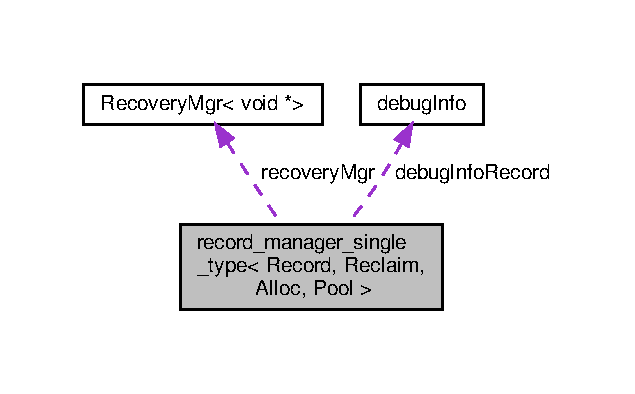
\includegraphics[width=305pt]{classrecord__manager__single__type__coll__graph}
\end{center}
\end{figure}
\subsection*{Public Member Functions}
\begin{DoxyCompactItemize}
\item 
\hyperlink{classrecord__manager__single__type_af45310278dc150a918d53a6842af8074}{record\+\_\+manager\+\_\+single\+\_\+type} (const int \hyperlink{testing_8cpp_aa085812188e21ede75351d88b9b2c30d}{num\+Processes}, \hyperlink{classRecoveryMgr}{Recovery\+Mgr}$<$ void $\ast$$>$ $\ast$const \+\_\+recovery\+Mgr)
\item 
\hyperlink{classrecord__manager__single__type_adeb03ec2262c1b202204e4dcf09308f9}{$\sim$record\+\_\+manager\+\_\+single\+\_\+type} ()
\item 
void \hyperlink{classrecord__manager__single__type_aeb3ea05f3336b96766ea72131a814b57}{init\+Thread} (const int \hyperlink{microbench_2main_8cpp_a9ca9869868fe7e7a38a921cc7de4103f}{tid})
\item 
void \hyperlink{classrecord__manager__single__type_af8aa437cd719ffed1db4c6bee3b1909e}{deinit\+Thread} (const int \hyperlink{microbench_2main_8cpp_a9ca9869868fe7e7a38a921cc7de4103f}{tid})
\item 
void \hyperlink{classrecord__manager__single__type_a14bb98b1b90c16e99591d2a3f987f0c4}{clear\+Counters} ()
\item 
bool \hyperlink{classrecord__manager__single__type_a468c13eaacc74f5c4f5db14ccffe433f}{is\+Protected} (const int \hyperlink{microbench_2main_8cpp_a9ca9869868fe7e7a38a921cc7de4103f}{tid}, \hyperlink{classrecord__manager__single__type_a065f05d1a84e619758122b3da04b1327}{record\+\_\+pointer} obj)
\item 
bool \hyperlink{classrecord__manager__single__type_a01a1d6fd1820e8430b4304c58d55582d}{protect} (const int \hyperlink{microbench_2main_8cpp_a9ca9869868fe7e7a38a921cc7de4103f}{tid}, \hyperlink{classrecord__manager__single__type_a065f05d1a84e619758122b3da04b1327}{record\+\_\+pointer} obj, \hyperlink{globals_8h_a57f5c0d40b156d7d996492fb2f16e3cd}{Callback\+Type} not\+Retired\+Callback, \hyperlink{globals_8h_a3de64ef48066ac6430631c8b81a15345}{Callback\+Arg} callback\+Arg, bool hint\+Memory\+Barrier=true)
\item 
void \hyperlink{classrecord__manager__single__type_ae21f5c6f516be7b94c37eb81879b5099}{unprotect} (const int \hyperlink{microbench_2main_8cpp_a9ca9869868fe7e7a38a921cc7de4103f}{tid}, \hyperlink{classrecord__manager__single__type_a065f05d1a84e619758122b3da04b1327}{record\+\_\+pointer} obj)
\item 
bool \hyperlink{classrecord__manager__single__type_ad97c74b60bf8a3d3670437806318d51f}{q\+Protect} (const int \hyperlink{microbench_2main_8cpp_a9ca9869868fe7e7a38a921cc7de4103f}{tid}, \hyperlink{classrecord__manager__single__type_a065f05d1a84e619758122b3da04b1327}{record\+\_\+pointer} obj, \hyperlink{globals_8h_a57f5c0d40b156d7d996492fb2f16e3cd}{Callback\+Type} not\+Retired\+Callback, \hyperlink{globals_8h_a3de64ef48066ac6430631c8b81a15345}{Callback\+Arg} callback\+Arg, bool hint\+Memory\+Barrier=true)
\item 
void \hyperlink{classrecord__manager__single__type_a500b38bc56f5643ca679337e7adacedf}{q\+Unprotect\+All} (const int \hyperlink{microbench_2main_8cpp_a9ca9869868fe7e7a38a921cc7de4103f}{tid})
\item 
bool \hyperlink{classrecord__manager__single__type_a1da4897ec2820c5c6ad380e7b60e2a44}{is\+Q\+Protected} (const int \hyperlink{microbench_2main_8cpp_a9ca9869868fe7e7a38a921cc7de4103f}{tid}, \hyperlink{classrecord__manager__single__type_a065f05d1a84e619758122b3da04b1327}{record\+\_\+pointer} obj)
\item 
bool \hyperlink{classrecord__manager__single__type_aa3096f0e5401e1454b94a4105cd8d728}{is\+Quiescent} (const int \hyperlink{microbench_2main_8cpp_a9ca9869868fe7e7a38a921cc7de4103f}{tid})
\item 
void \hyperlink{classrecord__manager__single__type_a43f174ebe0ed838e0369a99dd0c8ba75}{end\+Op} (const int \hyperlink{microbench_2main_8cpp_a9ca9869868fe7e7a38a921cc7de4103f}{tid})
\item 
{\footnotesize template$<$typename First , typename... Rest$>$ }\\void \hyperlink{classrecord__manager__single__type_ae410965bdfc69120b290f9224d4b2053}{start\+Op} (const int \hyperlink{microbench_2main_8cpp_a9ca9869868fe7e7a38a921cc7de4103f}{tid}, void $\ast$const $\ast$const reclaimers, const int num\+Reclaimers, const bool read\+Only=false)
\item 
void \hyperlink{classrecord__manager__single__type_a938c477e09003c663e44bd415492c62d}{retire} (const int \hyperlink{microbench_2main_8cpp_a9ca9869868fe7e7a38a921cc7de4103f}{tid}, \hyperlink{classrecord__manager__single__type_a065f05d1a84e619758122b3da04b1327}{record\+\_\+pointer} p)
\item 
\hyperlink{classrecord__manager__single__type_a065f05d1a84e619758122b3da04b1327}{record\+\_\+pointer} \hyperlink{classrecord__manager__single__type_a6f2b9a69087a98463e24981b3165f111}{allocate} (const int \hyperlink{microbench_2main_8cpp_a9ca9869868fe7e7a38a921cc7de4103f}{tid})
\item 
void \hyperlink{classrecord__manager__single__type_aa689188fd51bcab9f31aafaee82e054c}{deallocate} (const int \hyperlink{microbench_2main_8cpp_a9ca9869868fe7e7a38a921cc7de4103f}{tid}, \hyperlink{classrecord__manager__single__type_a065f05d1a84e619758122b3da04b1327}{record\+\_\+pointer} p)
\item 
void \hyperlink{classrecord__manager__single__type_a75dabb01db0fcc82a0c67fa06afdda62}{print\+Status} (void)
\end{DoxyCompactItemize}
\subsection*{Static Public Member Functions}
\begin{DoxyCompactItemize}
\item 
static bool \hyperlink{classrecord__manager__single__type_aba373074564801edaa50df79b405f0e9}{should\+Help} ()
\item 
static bool \hyperlink{classrecord__manager__single__type_a58d8ea1365033ef1f74b9b6956f534b3}{supports\+Crash\+Recovery} ()
\item 
static bool \hyperlink{classrecord__manager__single__type_a903370ed47527b3f97428a1f3d0b535e}{quiescence\+Is\+Per\+Record\+Type} ()
\end{DoxyCompactItemize}
\subsection*{Public Attributes}
\begin{DoxyCompactItemize}
\item 
\hyperlink{classrecord__manager__single__type_aa8000dd2cb059f78ca77ccef6800166d}{P\+AD}
\item 
\hyperlink{classrecord__manager__single__type_a5cdd0ef714fadb6eb7818aaf69918625}{class\+Alloc} $\ast$ \hyperlink{classrecord__manager__single__type_a7cb764de72e8a8973ca3234f4fc96d0f}{alloc}
\item 
\hyperlink{classrecord__manager__single__type_a2a7217967912e867c7ab6e4a7f3deeb5}{class\+Pool} $\ast$ \hyperlink{classrecord__manager__single__type_a396149240bef252c12fe9f6418e7594d}{pool}
\item 
\hyperlink{classrecord__manager__single__type_a831ae4c91e0ba85f07fd6b68ef18f035}{class\+Reclaim} $\ast$ \hyperlink{classrecord__manager__single__type_ad79e8a67f4a66c8d7ed83764aaade7d9}{reclaim}
\item 
const int \hyperlink{classrecord__manager__single__type_a2ddbaa967eccb64c5d621675fa732b1f}{N\+U\+M\+\_\+\+P\+R\+O\+C\+E\+S\+S\+ES}
\item 
\hyperlink{classdebugInfo}{debug\+Info} \hyperlink{classrecord__manager__single__type_ac0778b69c82a9609260a1048659829b9}{debug\+Info\+Record}
\item 
\hyperlink{classRecoveryMgr}{Recovery\+Mgr}$<$ void $\ast$ $>$ $\ast$const \hyperlink{classrecord__manager__single__type_aac9343d6515d6d32a71f541aeb098376}{recovery\+Mgr}
\end{DoxyCompactItemize}
\subsection*{Protected Types}
\begin{DoxyCompactItemize}
\item 
typedef Record $\ast$ \hyperlink{classrecord__manager__single__type_a065f05d1a84e619758122b3da04b1327}{record\+\_\+pointer}
\item 
typedef Alloc\+::template rebind$<$ Record $>$\+::other \hyperlink{classrecord__manager__single__type_a5cdd0ef714fadb6eb7818aaf69918625}{class\+Alloc}
\item 
typedef Pool\+::template rebind2$<$ Record, \hyperlink{classrecord__manager__single__type_a5cdd0ef714fadb6eb7818aaf69918625}{class\+Alloc} $>$\+::other \hyperlink{classrecord__manager__single__type_a2a7217967912e867c7ab6e4a7f3deeb5}{class\+Pool}
\item 
typedef Reclaim\+::template rebind2$<$ Record, \hyperlink{classrecord__manager__single__type_a2a7217967912e867c7ab6e4a7f3deeb5}{class\+Pool} $>$\+::other \hyperlink{classrecord__manager__single__type_a831ae4c91e0ba85f07fd6b68ef18f035}{class\+Reclaim}
\end{DoxyCompactItemize}


\subsection{Detailed Description}
\subsubsection*{template$<$typename Record, class Reclaim, class Alloc, class Pool$>$\newline
class record\+\_\+manager\+\_\+single\+\_\+type$<$ Record, Reclaim, Alloc, Pool $>$}

C++ record manager implementation (P\+O\+DC 2015) by Trevor Brown.

Copyright (C) 2015 Trevor Brown 

\subsection{Member Typedef Documentation}
\mbox{\Hypertarget{classrecord__manager__single__type_a5cdd0ef714fadb6eb7818aaf69918625}\label{classrecord__manager__single__type_a5cdd0ef714fadb6eb7818aaf69918625}} 
\index{record\+\_\+manager\+\_\+single\+\_\+type@{record\+\_\+manager\+\_\+single\+\_\+type}!class\+Alloc@{class\+Alloc}}
\index{class\+Alloc@{class\+Alloc}!record\+\_\+manager\+\_\+single\+\_\+type@{record\+\_\+manager\+\_\+single\+\_\+type}}
\subsubsection{\texorpdfstring{class\+Alloc}{classAlloc}}
{\footnotesize\ttfamily template$<$typename Record, class Reclaim, class Alloc, class Pool$>$ \\
typedef Alloc\+::template rebind$<$Record$>$\+::other \hyperlink{classrecord__manager__single__type}{record\+\_\+manager\+\_\+single\+\_\+type}$<$ Record, Reclaim, Alloc, Pool $>$\+::\hyperlink{classrecord__manager__single__type_a5cdd0ef714fadb6eb7818aaf69918625}{class\+Alloc}\hspace{0.3cm}{\ttfamily [protected]}}

\mbox{\Hypertarget{classrecord__manager__single__type_a2a7217967912e867c7ab6e4a7f3deeb5}\label{classrecord__manager__single__type_a2a7217967912e867c7ab6e4a7f3deeb5}} 
\index{record\+\_\+manager\+\_\+single\+\_\+type@{record\+\_\+manager\+\_\+single\+\_\+type}!class\+Pool@{class\+Pool}}
\index{class\+Pool@{class\+Pool}!record\+\_\+manager\+\_\+single\+\_\+type@{record\+\_\+manager\+\_\+single\+\_\+type}}
\subsubsection{\texorpdfstring{class\+Pool}{classPool}}
{\footnotesize\ttfamily template$<$typename Record, class Reclaim, class Alloc, class Pool$>$ \\
typedef Pool\+::template rebind2$<$Record, \hyperlink{classrecord__manager__single__type_a5cdd0ef714fadb6eb7818aaf69918625}{class\+Alloc}$>$\+::other \hyperlink{classrecord__manager__single__type}{record\+\_\+manager\+\_\+single\+\_\+type}$<$ Record, Reclaim, Alloc, Pool $>$\+::\hyperlink{classrecord__manager__single__type_a2a7217967912e867c7ab6e4a7f3deeb5}{class\+Pool}\hspace{0.3cm}{\ttfamily [protected]}}

\mbox{\Hypertarget{classrecord__manager__single__type_a831ae4c91e0ba85f07fd6b68ef18f035}\label{classrecord__manager__single__type_a831ae4c91e0ba85f07fd6b68ef18f035}} 
\index{record\+\_\+manager\+\_\+single\+\_\+type@{record\+\_\+manager\+\_\+single\+\_\+type}!class\+Reclaim@{class\+Reclaim}}
\index{class\+Reclaim@{class\+Reclaim}!record\+\_\+manager\+\_\+single\+\_\+type@{record\+\_\+manager\+\_\+single\+\_\+type}}
\subsubsection{\texorpdfstring{class\+Reclaim}{classReclaim}}
{\footnotesize\ttfamily template$<$typename Record, class Reclaim, class Alloc, class Pool$>$ \\
typedef Reclaim\+::template rebind2$<$Record, \hyperlink{classrecord__manager__single__type_a2a7217967912e867c7ab6e4a7f3deeb5}{class\+Pool}$>$\+::other \hyperlink{classrecord__manager__single__type}{record\+\_\+manager\+\_\+single\+\_\+type}$<$ Record, Reclaim, Alloc, Pool $>$\+::\hyperlink{classrecord__manager__single__type_a831ae4c91e0ba85f07fd6b68ef18f035}{class\+Reclaim}\hspace{0.3cm}{\ttfamily [protected]}}

\mbox{\Hypertarget{classrecord__manager__single__type_a065f05d1a84e619758122b3da04b1327}\label{classrecord__manager__single__type_a065f05d1a84e619758122b3da04b1327}} 
\index{record\+\_\+manager\+\_\+single\+\_\+type@{record\+\_\+manager\+\_\+single\+\_\+type}!record\+\_\+pointer@{record\+\_\+pointer}}
\index{record\+\_\+pointer@{record\+\_\+pointer}!record\+\_\+manager\+\_\+single\+\_\+type@{record\+\_\+manager\+\_\+single\+\_\+type}}
\subsubsection{\texorpdfstring{record\+\_\+pointer}{record\_pointer}}
{\footnotesize\ttfamily template$<$typename Record, class Reclaim, class Alloc, class Pool$>$ \\
typedef Record$\ast$ \hyperlink{classrecord__manager__single__type}{record\+\_\+manager\+\_\+single\+\_\+type}$<$ Record, Reclaim, Alloc, Pool $>$\+::\hyperlink{classrecord__manager__single__type_a065f05d1a84e619758122b3da04b1327}{record\+\_\+pointer}\hspace{0.3cm}{\ttfamily [protected]}}



\subsection{Constructor \& Destructor Documentation}
\mbox{\Hypertarget{classrecord__manager__single__type_af45310278dc150a918d53a6842af8074}\label{classrecord__manager__single__type_af45310278dc150a918d53a6842af8074}} 
\index{record\+\_\+manager\+\_\+single\+\_\+type@{record\+\_\+manager\+\_\+single\+\_\+type}!record\+\_\+manager\+\_\+single\+\_\+type@{record\+\_\+manager\+\_\+single\+\_\+type}}
\index{record\+\_\+manager\+\_\+single\+\_\+type@{record\+\_\+manager\+\_\+single\+\_\+type}!record\+\_\+manager\+\_\+single\+\_\+type@{record\+\_\+manager\+\_\+single\+\_\+type}}
\subsubsection{\texorpdfstring{record\+\_\+manager\+\_\+single\+\_\+type()}{record\_manager\_single\_type()}}
{\footnotesize\ttfamily template$<$typename Record, class Reclaim, class Alloc, class Pool$>$ \\
\hyperlink{classrecord__manager__single__type}{record\+\_\+manager\+\_\+single\+\_\+type}$<$ Record, Reclaim, Alloc, Pool $>$\+::\hyperlink{classrecord__manager__single__type}{record\+\_\+manager\+\_\+single\+\_\+type} (\begin{DoxyParamCaption}\item[{const int}]{num\+Processes,  }\item[{\hyperlink{classRecoveryMgr}{Recovery\+Mgr}$<$ void $\ast$$>$ $\ast$const}]{\+\_\+recovery\+Mgr }\end{DoxyParamCaption})\hspace{0.3cm}{\ttfamily [inline]}}

\mbox{\Hypertarget{classrecord__manager__single__type_adeb03ec2262c1b202204e4dcf09308f9}\label{classrecord__manager__single__type_adeb03ec2262c1b202204e4dcf09308f9}} 
\index{record\+\_\+manager\+\_\+single\+\_\+type@{record\+\_\+manager\+\_\+single\+\_\+type}!````~record\+\_\+manager\+\_\+single\+\_\+type@{$\sim$record\+\_\+manager\+\_\+single\+\_\+type}}
\index{````~record\+\_\+manager\+\_\+single\+\_\+type@{$\sim$record\+\_\+manager\+\_\+single\+\_\+type}!record\+\_\+manager\+\_\+single\+\_\+type@{record\+\_\+manager\+\_\+single\+\_\+type}}
\subsubsection{\texorpdfstring{$\sim$record\+\_\+manager\+\_\+single\+\_\+type()}{~record\_manager\_single\_type()}}
{\footnotesize\ttfamily template$<$typename Record, class Reclaim, class Alloc, class Pool$>$ \\
\hyperlink{classrecord__manager__single__type}{record\+\_\+manager\+\_\+single\+\_\+type}$<$ Record, Reclaim, Alloc, Pool $>$\+::$\sim$\hyperlink{classrecord__manager__single__type}{record\+\_\+manager\+\_\+single\+\_\+type} (\begin{DoxyParamCaption}{ }\end{DoxyParamCaption})\hspace{0.3cm}{\ttfamily [inline]}}



\subsection{Member Function Documentation}
\mbox{\Hypertarget{classrecord__manager__single__type_a6f2b9a69087a98463e24981b3165f111}\label{classrecord__manager__single__type_a6f2b9a69087a98463e24981b3165f111}} 
\index{record\+\_\+manager\+\_\+single\+\_\+type@{record\+\_\+manager\+\_\+single\+\_\+type}!allocate@{allocate}}
\index{allocate@{allocate}!record\+\_\+manager\+\_\+single\+\_\+type@{record\+\_\+manager\+\_\+single\+\_\+type}}
\subsubsection{\texorpdfstring{allocate()}{allocate()}}
{\footnotesize\ttfamily template$<$typename Record, class Reclaim, class Alloc, class Pool$>$ \\
\hyperlink{classrecord__manager__single__type_a065f05d1a84e619758122b3da04b1327}{record\+\_\+pointer} \hyperlink{classrecord__manager__single__type}{record\+\_\+manager\+\_\+single\+\_\+type}$<$ Record, Reclaim, Alloc, Pool $>$\+::allocate (\begin{DoxyParamCaption}\item[{const int}]{tid }\end{DoxyParamCaption})\hspace{0.3cm}{\ttfamily [inline]}}

\mbox{\Hypertarget{classrecord__manager__single__type_a14bb98b1b90c16e99591d2a3f987f0c4}\label{classrecord__manager__single__type_a14bb98b1b90c16e99591d2a3f987f0c4}} 
\index{record\+\_\+manager\+\_\+single\+\_\+type@{record\+\_\+manager\+\_\+single\+\_\+type}!clear\+Counters@{clear\+Counters}}
\index{clear\+Counters@{clear\+Counters}!record\+\_\+manager\+\_\+single\+\_\+type@{record\+\_\+manager\+\_\+single\+\_\+type}}
\subsubsection{\texorpdfstring{clear\+Counters()}{clearCounters()}}
{\footnotesize\ttfamily template$<$typename Record, class Reclaim, class Alloc, class Pool$>$ \\
void \hyperlink{classrecord__manager__single__type}{record\+\_\+manager\+\_\+single\+\_\+type}$<$ Record, Reclaim, Alloc, Pool $>$\+::clear\+Counters (\begin{DoxyParamCaption}\item[{void}]{ }\end{DoxyParamCaption})\hspace{0.3cm}{\ttfamily [inline]}}

\mbox{\Hypertarget{classrecord__manager__single__type_aa689188fd51bcab9f31aafaee82e054c}\label{classrecord__manager__single__type_aa689188fd51bcab9f31aafaee82e054c}} 
\index{record\+\_\+manager\+\_\+single\+\_\+type@{record\+\_\+manager\+\_\+single\+\_\+type}!deallocate@{deallocate}}
\index{deallocate@{deallocate}!record\+\_\+manager\+\_\+single\+\_\+type@{record\+\_\+manager\+\_\+single\+\_\+type}}
\subsubsection{\texorpdfstring{deallocate()}{deallocate()}}
{\footnotesize\ttfamily template$<$typename Record, class Reclaim, class Alloc, class Pool$>$ \\
void \hyperlink{classrecord__manager__single__type}{record\+\_\+manager\+\_\+single\+\_\+type}$<$ Record, Reclaim, Alloc, Pool $>$\+::deallocate (\begin{DoxyParamCaption}\item[{const int}]{tid,  }\item[{\hyperlink{classrecord__manager__single__type_a065f05d1a84e619758122b3da04b1327}{record\+\_\+pointer}}]{p }\end{DoxyParamCaption})\hspace{0.3cm}{\ttfamily [inline]}}

\mbox{\Hypertarget{classrecord__manager__single__type_af8aa437cd719ffed1db4c6bee3b1909e}\label{classrecord__manager__single__type_af8aa437cd719ffed1db4c6bee3b1909e}} 
\index{record\+\_\+manager\+\_\+single\+\_\+type@{record\+\_\+manager\+\_\+single\+\_\+type}!deinit\+Thread@{deinit\+Thread}}
\index{deinit\+Thread@{deinit\+Thread}!record\+\_\+manager\+\_\+single\+\_\+type@{record\+\_\+manager\+\_\+single\+\_\+type}}
\subsubsection{\texorpdfstring{deinit\+Thread()}{deinitThread()}}
{\footnotesize\ttfamily template$<$typename Record, class Reclaim, class Alloc, class Pool$>$ \\
void \hyperlink{classrecord__manager__single__type}{record\+\_\+manager\+\_\+single\+\_\+type}$<$ Record, Reclaim, Alloc, Pool $>$\+::deinit\+Thread (\begin{DoxyParamCaption}\item[{const int}]{tid }\end{DoxyParamCaption})\hspace{0.3cm}{\ttfamily [inline]}}

\mbox{\Hypertarget{classrecord__manager__single__type_a43f174ebe0ed838e0369a99dd0c8ba75}\label{classrecord__manager__single__type_a43f174ebe0ed838e0369a99dd0c8ba75}} 
\index{record\+\_\+manager\+\_\+single\+\_\+type@{record\+\_\+manager\+\_\+single\+\_\+type}!end\+Op@{end\+Op}}
\index{end\+Op@{end\+Op}!record\+\_\+manager\+\_\+single\+\_\+type@{record\+\_\+manager\+\_\+single\+\_\+type}}
\subsubsection{\texorpdfstring{end\+Op()}{endOp()}}
{\footnotesize\ttfamily template$<$typename Record, class Reclaim, class Alloc, class Pool$>$ \\
void \hyperlink{classrecord__manager__single__type}{record\+\_\+manager\+\_\+single\+\_\+type}$<$ Record, Reclaim, Alloc, Pool $>$\+::end\+Op (\begin{DoxyParamCaption}\item[{const int}]{tid }\end{DoxyParamCaption})\hspace{0.3cm}{\ttfamily [inline]}}

\mbox{\Hypertarget{classrecord__manager__single__type_aeb3ea05f3336b96766ea72131a814b57}\label{classrecord__manager__single__type_aeb3ea05f3336b96766ea72131a814b57}} 
\index{record\+\_\+manager\+\_\+single\+\_\+type@{record\+\_\+manager\+\_\+single\+\_\+type}!init\+Thread@{init\+Thread}}
\index{init\+Thread@{init\+Thread}!record\+\_\+manager\+\_\+single\+\_\+type@{record\+\_\+manager\+\_\+single\+\_\+type}}
\subsubsection{\texorpdfstring{init\+Thread()}{initThread()}}
{\footnotesize\ttfamily template$<$typename Record, class Reclaim, class Alloc, class Pool$>$ \\
void \hyperlink{classrecord__manager__single__type}{record\+\_\+manager\+\_\+single\+\_\+type}$<$ Record, Reclaim, Alloc, Pool $>$\+::init\+Thread (\begin{DoxyParamCaption}\item[{const int}]{tid }\end{DoxyParamCaption})\hspace{0.3cm}{\ttfamily [inline]}}

\mbox{\Hypertarget{classrecord__manager__single__type_a468c13eaacc74f5c4f5db14ccffe433f}\label{classrecord__manager__single__type_a468c13eaacc74f5c4f5db14ccffe433f}} 
\index{record\+\_\+manager\+\_\+single\+\_\+type@{record\+\_\+manager\+\_\+single\+\_\+type}!is\+Protected@{is\+Protected}}
\index{is\+Protected@{is\+Protected}!record\+\_\+manager\+\_\+single\+\_\+type@{record\+\_\+manager\+\_\+single\+\_\+type}}
\subsubsection{\texorpdfstring{is\+Protected()}{isProtected()}}
{\footnotesize\ttfamily template$<$typename Record, class Reclaim, class Alloc, class Pool$>$ \\
bool \hyperlink{classrecord__manager__single__type}{record\+\_\+manager\+\_\+single\+\_\+type}$<$ Record, Reclaim, Alloc, Pool $>$\+::is\+Protected (\begin{DoxyParamCaption}\item[{const int}]{tid,  }\item[{\hyperlink{classrecord__manager__single__type_a065f05d1a84e619758122b3da04b1327}{record\+\_\+pointer}}]{obj }\end{DoxyParamCaption})\hspace{0.3cm}{\ttfamily [inline]}}

\mbox{\Hypertarget{classrecord__manager__single__type_a1da4897ec2820c5c6ad380e7b60e2a44}\label{classrecord__manager__single__type_a1da4897ec2820c5c6ad380e7b60e2a44}} 
\index{record\+\_\+manager\+\_\+single\+\_\+type@{record\+\_\+manager\+\_\+single\+\_\+type}!is\+Q\+Protected@{is\+Q\+Protected}}
\index{is\+Q\+Protected@{is\+Q\+Protected}!record\+\_\+manager\+\_\+single\+\_\+type@{record\+\_\+manager\+\_\+single\+\_\+type}}
\subsubsection{\texorpdfstring{is\+Q\+Protected()}{isQProtected()}}
{\footnotesize\ttfamily template$<$typename Record, class Reclaim, class Alloc, class Pool$>$ \\
bool \hyperlink{classrecord__manager__single__type}{record\+\_\+manager\+\_\+single\+\_\+type}$<$ Record, Reclaim, Alloc, Pool $>$\+::is\+Q\+Protected (\begin{DoxyParamCaption}\item[{const int}]{tid,  }\item[{\hyperlink{classrecord__manager__single__type_a065f05d1a84e619758122b3da04b1327}{record\+\_\+pointer}}]{obj }\end{DoxyParamCaption})\hspace{0.3cm}{\ttfamily [inline]}}

\mbox{\Hypertarget{classrecord__manager__single__type_aa3096f0e5401e1454b94a4105cd8d728}\label{classrecord__manager__single__type_aa3096f0e5401e1454b94a4105cd8d728}} 
\index{record\+\_\+manager\+\_\+single\+\_\+type@{record\+\_\+manager\+\_\+single\+\_\+type}!is\+Quiescent@{is\+Quiescent}}
\index{is\+Quiescent@{is\+Quiescent}!record\+\_\+manager\+\_\+single\+\_\+type@{record\+\_\+manager\+\_\+single\+\_\+type}}
\subsubsection{\texorpdfstring{is\+Quiescent()}{isQuiescent()}}
{\footnotesize\ttfamily template$<$typename Record, class Reclaim, class Alloc, class Pool$>$ \\
bool \hyperlink{classrecord__manager__single__type}{record\+\_\+manager\+\_\+single\+\_\+type}$<$ Record, Reclaim, Alloc, Pool $>$\+::is\+Quiescent (\begin{DoxyParamCaption}\item[{const int}]{tid }\end{DoxyParamCaption})\hspace{0.3cm}{\ttfamily [inline]}}

\mbox{\Hypertarget{classrecord__manager__single__type_a75dabb01db0fcc82a0c67fa06afdda62}\label{classrecord__manager__single__type_a75dabb01db0fcc82a0c67fa06afdda62}} 
\index{record\+\_\+manager\+\_\+single\+\_\+type@{record\+\_\+manager\+\_\+single\+\_\+type}!print\+Status@{print\+Status}}
\index{print\+Status@{print\+Status}!record\+\_\+manager\+\_\+single\+\_\+type@{record\+\_\+manager\+\_\+single\+\_\+type}}
\subsubsection{\texorpdfstring{print\+Status()}{printStatus()}}
{\footnotesize\ttfamily template$<$typename Record, class Reclaim, class Alloc, class Pool$>$ \\
void \hyperlink{classrecord__manager__single__type}{record\+\_\+manager\+\_\+single\+\_\+type}$<$ Record, Reclaim, Alloc, Pool $>$\+::print\+Status (\begin{DoxyParamCaption}\item[{void}]{ }\end{DoxyParamCaption})\hspace{0.3cm}{\ttfamily [inline]}}

\mbox{\Hypertarget{classrecord__manager__single__type_a01a1d6fd1820e8430b4304c58d55582d}\label{classrecord__manager__single__type_a01a1d6fd1820e8430b4304c58d55582d}} 
\index{record\+\_\+manager\+\_\+single\+\_\+type@{record\+\_\+manager\+\_\+single\+\_\+type}!protect@{protect}}
\index{protect@{protect}!record\+\_\+manager\+\_\+single\+\_\+type@{record\+\_\+manager\+\_\+single\+\_\+type}}
\subsubsection{\texorpdfstring{protect()}{protect()}}
{\footnotesize\ttfamily template$<$typename Record, class Reclaim, class Alloc, class Pool$>$ \\
bool \hyperlink{classrecord__manager__single__type}{record\+\_\+manager\+\_\+single\+\_\+type}$<$ Record, Reclaim, Alloc, Pool $>$\+::protect (\begin{DoxyParamCaption}\item[{const int}]{tid,  }\item[{\hyperlink{classrecord__manager__single__type_a065f05d1a84e619758122b3da04b1327}{record\+\_\+pointer}}]{obj,  }\item[{\hyperlink{globals_8h_a57f5c0d40b156d7d996492fb2f16e3cd}{Callback\+Type}}]{not\+Retired\+Callback,  }\item[{\hyperlink{globals_8h_a3de64ef48066ac6430631c8b81a15345}{Callback\+Arg}}]{callback\+Arg,  }\item[{bool}]{hint\+Memory\+Barrier = {\ttfamily true} }\end{DoxyParamCaption})\hspace{0.3cm}{\ttfamily [inline]}}

\mbox{\Hypertarget{classrecord__manager__single__type_ad97c74b60bf8a3d3670437806318d51f}\label{classrecord__manager__single__type_ad97c74b60bf8a3d3670437806318d51f}} 
\index{record\+\_\+manager\+\_\+single\+\_\+type@{record\+\_\+manager\+\_\+single\+\_\+type}!q\+Protect@{q\+Protect}}
\index{q\+Protect@{q\+Protect}!record\+\_\+manager\+\_\+single\+\_\+type@{record\+\_\+manager\+\_\+single\+\_\+type}}
\subsubsection{\texorpdfstring{q\+Protect()}{qProtect()}}
{\footnotesize\ttfamily template$<$typename Record, class Reclaim, class Alloc, class Pool$>$ \\
bool \hyperlink{classrecord__manager__single__type}{record\+\_\+manager\+\_\+single\+\_\+type}$<$ Record, Reclaim, Alloc, Pool $>$\+::q\+Protect (\begin{DoxyParamCaption}\item[{const int}]{tid,  }\item[{\hyperlink{classrecord__manager__single__type_a065f05d1a84e619758122b3da04b1327}{record\+\_\+pointer}}]{obj,  }\item[{\hyperlink{globals_8h_a57f5c0d40b156d7d996492fb2f16e3cd}{Callback\+Type}}]{not\+Retired\+Callback,  }\item[{\hyperlink{globals_8h_a3de64ef48066ac6430631c8b81a15345}{Callback\+Arg}}]{callback\+Arg,  }\item[{bool}]{hint\+Memory\+Barrier = {\ttfamily true} }\end{DoxyParamCaption})\hspace{0.3cm}{\ttfamily [inline]}}

\mbox{\Hypertarget{classrecord__manager__single__type_a903370ed47527b3f97428a1f3d0b535e}\label{classrecord__manager__single__type_a903370ed47527b3f97428a1f3d0b535e}} 
\index{record\+\_\+manager\+\_\+single\+\_\+type@{record\+\_\+manager\+\_\+single\+\_\+type}!quiescence\+Is\+Per\+Record\+Type@{quiescence\+Is\+Per\+Record\+Type}}
\index{quiescence\+Is\+Per\+Record\+Type@{quiescence\+Is\+Per\+Record\+Type}!record\+\_\+manager\+\_\+single\+\_\+type@{record\+\_\+manager\+\_\+single\+\_\+type}}
\subsubsection{\texorpdfstring{quiescence\+Is\+Per\+Record\+Type()}{quiescenceIsPerRecordType()}}
{\footnotesize\ttfamily template$<$typename Record, class Reclaim, class Alloc, class Pool$>$ \\
static bool \hyperlink{classrecord__manager__single__type}{record\+\_\+manager\+\_\+single\+\_\+type}$<$ Record, Reclaim, Alloc, Pool $>$\+::quiescence\+Is\+Per\+Record\+Type (\begin{DoxyParamCaption}{ }\end{DoxyParamCaption})\hspace{0.3cm}{\ttfamily [inline]}, {\ttfamily [static]}}

\mbox{\Hypertarget{classrecord__manager__single__type_a500b38bc56f5643ca679337e7adacedf}\label{classrecord__manager__single__type_a500b38bc56f5643ca679337e7adacedf}} 
\index{record\+\_\+manager\+\_\+single\+\_\+type@{record\+\_\+manager\+\_\+single\+\_\+type}!q\+Unprotect\+All@{q\+Unprotect\+All}}
\index{q\+Unprotect\+All@{q\+Unprotect\+All}!record\+\_\+manager\+\_\+single\+\_\+type@{record\+\_\+manager\+\_\+single\+\_\+type}}
\subsubsection{\texorpdfstring{q\+Unprotect\+All()}{qUnprotectAll()}}
{\footnotesize\ttfamily template$<$typename Record, class Reclaim, class Alloc, class Pool$>$ \\
void \hyperlink{classrecord__manager__single__type}{record\+\_\+manager\+\_\+single\+\_\+type}$<$ Record, Reclaim, Alloc, Pool $>$\+::q\+Unprotect\+All (\begin{DoxyParamCaption}\item[{const int}]{tid }\end{DoxyParamCaption})\hspace{0.3cm}{\ttfamily [inline]}}

\mbox{\Hypertarget{classrecord__manager__single__type_a938c477e09003c663e44bd415492c62d}\label{classrecord__manager__single__type_a938c477e09003c663e44bd415492c62d}} 
\index{record\+\_\+manager\+\_\+single\+\_\+type@{record\+\_\+manager\+\_\+single\+\_\+type}!retire@{retire}}
\index{retire@{retire}!record\+\_\+manager\+\_\+single\+\_\+type@{record\+\_\+manager\+\_\+single\+\_\+type}}
\subsubsection{\texorpdfstring{retire()}{retire()}}
{\footnotesize\ttfamily template$<$typename Record, class Reclaim, class Alloc, class Pool$>$ \\
void \hyperlink{classrecord__manager__single__type}{record\+\_\+manager\+\_\+single\+\_\+type}$<$ Record, Reclaim, Alloc, Pool $>$\+::retire (\begin{DoxyParamCaption}\item[{const int}]{tid,  }\item[{\hyperlink{classrecord__manager__single__type_a065f05d1a84e619758122b3da04b1327}{record\+\_\+pointer}}]{p }\end{DoxyParamCaption})\hspace{0.3cm}{\ttfamily [inline]}}

\mbox{\Hypertarget{classrecord__manager__single__type_aba373074564801edaa50df79b405f0e9}\label{classrecord__manager__single__type_aba373074564801edaa50df79b405f0e9}} 
\index{record\+\_\+manager\+\_\+single\+\_\+type@{record\+\_\+manager\+\_\+single\+\_\+type}!should\+Help@{should\+Help}}
\index{should\+Help@{should\+Help}!record\+\_\+manager\+\_\+single\+\_\+type@{record\+\_\+manager\+\_\+single\+\_\+type}}
\subsubsection{\texorpdfstring{should\+Help()}{shouldHelp()}}
{\footnotesize\ttfamily template$<$typename Record, class Reclaim, class Alloc, class Pool$>$ \\
static bool \hyperlink{classrecord__manager__single__type}{record\+\_\+manager\+\_\+single\+\_\+type}$<$ Record, Reclaim, Alloc, Pool $>$\+::should\+Help (\begin{DoxyParamCaption}{ }\end{DoxyParamCaption})\hspace{0.3cm}{\ttfamily [inline]}, {\ttfamily [static]}}

\mbox{\Hypertarget{classrecord__manager__single__type_ae410965bdfc69120b290f9224d4b2053}\label{classrecord__manager__single__type_ae410965bdfc69120b290f9224d4b2053}} 
\index{record\+\_\+manager\+\_\+single\+\_\+type@{record\+\_\+manager\+\_\+single\+\_\+type}!start\+Op@{start\+Op}}
\index{start\+Op@{start\+Op}!record\+\_\+manager\+\_\+single\+\_\+type@{record\+\_\+manager\+\_\+single\+\_\+type}}
\subsubsection{\texorpdfstring{start\+Op()}{startOp()}}
{\footnotesize\ttfamily template$<$typename Record, class Reclaim, class Alloc, class Pool$>$ \\
template$<$typename First , typename... Rest$>$ \\
void \hyperlink{classrecord__manager__single__type}{record\+\_\+manager\+\_\+single\+\_\+type}$<$ Record, Reclaim, Alloc, Pool $>$\+::start\+Op (\begin{DoxyParamCaption}\item[{const int}]{tid,  }\item[{void $\ast$const $\ast$const}]{reclaimers,  }\item[{const int}]{num\+Reclaimers,  }\item[{const bool}]{read\+Only = {\ttfamily false} }\end{DoxyParamCaption})\hspace{0.3cm}{\ttfamily [inline]}}

\mbox{\Hypertarget{classrecord__manager__single__type_a58d8ea1365033ef1f74b9b6956f534b3}\label{classrecord__manager__single__type_a58d8ea1365033ef1f74b9b6956f534b3}} 
\index{record\+\_\+manager\+\_\+single\+\_\+type@{record\+\_\+manager\+\_\+single\+\_\+type}!supports\+Crash\+Recovery@{supports\+Crash\+Recovery}}
\index{supports\+Crash\+Recovery@{supports\+Crash\+Recovery}!record\+\_\+manager\+\_\+single\+\_\+type@{record\+\_\+manager\+\_\+single\+\_\+type}}
\subsubsection{\texorpdfstring{supports\+Crash\+Recovery()}{supportsCrashRecovery()}}
{\footnotesize\ttfamily template$<$typename Record, class Reclaim, class Alloc, class Pool$>$ \\
static bool \hyperlink{classrecord__manager__single__type}{record\+\_\+manager\+\_\+single\+\_\+type}$<$ Record, Reclaim, Alloc, Pool $>$\+::supports\+Crash\+Recovery (\begin{DoxyParamCaption}{ }\end{DoxyParamCaption})\hspace{0.3cm}{\ttfamily [inline]}, {\ttfamily [static]}}

\mbox{\Hypertarget{classrecord__manager__single__type_ae21f5c6f516be7b94c37eb81879b5099}\label{classrecord__manager__single__type_ae21f5c6f516be7b94c37eb81879b5099}} 
\index{record\+\_\+manager\+\_\+single\+\_\+type@{record\+\_\+manager\+\_\+single\+\_\+type}!unprotect@{unprotect}}
\index{unprotect@{unprotect}!record\+\_\+manager\+\_\+single\+\_\+type@{record\+\_\+manager\+\_\+single\+\_\+type}}
\subsubsection{\texorpdfstring{unprotect()}{unprotect()}}
{\footnotesize\ttfamily template$<$typename Record, class Reclaim, class Alloc, class Pool$>$ \\
void \hyperlink{classrecord__manager__single__type}{record\+\_\+manager\+\_\+single\+\_\+type}$<$ Record, Reclaim, Alloc, Pool $>$\+::unprotect (\begin{DoxyParamCaption}\item[{const int}]{tid,  }\item[{\hyperlink{classrecord__manager__single__type_a065f05d1a84e619758122b3da04b1327}{record\+\_\+pointer}}]{obj }\end{DoxyParamCaption})\hspace{0.3cm}{\ttfamily [inline]}}



\subsection{Member Data Documentation}
\mbox{\Hypertarget{classrecord__manager__single__type_a7cb764de72e8a8973ca3234f4fc96d0f}\label{classrecord__manager__single__type_a7cb764de72e8a8973ca3234f4fc96d0f}} 
\index{record\+\_\+manager\+\_\+single\+\_\+type@{record\+\_\+manager\+\_\+single\+\_\+type}!alloc@{alloc}}
\index{alloc@{alloc}!record\+\_\+manager\+\_\+single\+\_\+type@{record\+\_\+manager\+\_\+single\+\_\+type}}
\subsubsection{\texorpdfstring{alloc}{alloc}}
{\footnotesize\ttfamily template$<$typename Record, class Reclaim, class Alloc, class Pool$>$ \\
\hyperlink{classrecord__manager__single__type_a5cdd0ef714fadb6eb7818aaf69918625}{class\+Alloc}$\ast$ \hyperlink{classrecord__manager__single__type}{record\+\_\+manager\+\_\+single\+\_\+type}$<$ Record, Reclaim, Alloc, Pool $>$\+::alloc}

\mbox{\Hypertarget{classrecord__manager__single__type_ac0778b69c82a9609260a1048659829b9}\label{classrecord__manager__single__type_ac0778b69c82a9609260a1048659829b9}} 
\index{record\+\_\+manager\+\_\+single\+\_\+type@{record\+\_\+manager\+\_\+single\+\_\+type}!debug\+Info\+Record@{debug\+Info\+Record}}
\index{debug\+Info\+Record@{debug\+Info\+Record}!record\+\_\+manager\+\_\+single\+\_\+type@{record\+\_\+manager\+\_\+single\+\_\+type}}
\subsubsection{\texorpdfstring{debug\+Info\+Record}{debugInfoRecord}}
{\footnotesize\ttfamily template$<$typename Record, class Reclaim, class Alloc, class Pool$>$ \\
\hyperlink{classdebugInfo}{debug\+Info} \hyperlink{classrecord__manager__single__type}{record\+\_\+manager\+\_\+single\+\_\+type}$<$ Record, Reclaim, Alloc, Pool $>$\+::debug\+Info\+Record}

\mbox{\Hypertarget{classrecord__manager__single__type_a2ddbaa967eccb64c5d621675fa732b1f}\label{classrecord__manager__single__type_a2ddbaa967eccb64c5d621675fa732b1f}} 
\index{record\+\_\+manager\+\_\+single\+\_\+type@{record\+\_\+manager\+\_\+single\+\_\+type}!N\+U\+M\+\_\+\+P\+R\+O\+C\+E\+S\+S\+ES@{N\+U\+M\+\_\+\+P\+R\+O\+C\+E\+S\+S\+ES}}
\index{N\+U\+M\+\_\+\+P\+R\+O\+C\+E\+S\+S\+ES@{N\+U\+M\+\_\+\+P\+R\+O\+C\+E\+S\+S\+ES}!record\+\_\+manager\+\_\+single\+\_\+type@{record\+\_\+manager\+\_\+single\+\_\+type}}
\subsubsection{\texorpdfstring{N\+U\+M\+\_\+\+P\+R\+O\+C\+E\+S\+S\+ES}{NUM\_PROCESSES}}
{\footnotesize\ttfamily template$<$typename Record, class Reclaim, class Alloc, class Pool$>$ \\
const int \hyperlink{classrecord__manager__single__type}{record\+\_\+manager\+\_\+single\+\_\+type}$<$ Record, Reclaim, Alloc, Pool $>$\+::N\+U\+M\+\_\+\+P\+R\+O\+C\+E\+S\+S\+ES}

\mbox{\Hypertarget{classrecord__manager__single__type_aa8000dd2cb059f78ca77ccef6800166d}\label{classrecord__manager__single__type_aa8000dd2cb059f78ca77ccef6800166d}} 
\index{record\+\_\+manager\+\_\+single\+\_\+type@{record\+\_\+manager\+\_\+single\+\_\+type}!P\+AD@{P\+AD}}
\index{P\+AD@{P\+AD}!record\+\_\+manager\+\_\+single\+\_\+type@{record\+\_\+manager\+\_\+single\+\_\+type}}
\subsubsection{\texorpdfstring{P\+AD}{PAD}}
{\footnotesize\ttfamily template$<$typename Record, class Reclaim, class Alloc, class Pool$>$ \\
\hyperlink{classrecord__manager__single__type}{record\+\_\+manager\+\_\+single\+\_\+type}$<$ Record, Reclaim, Alloc, Pool $>$\+::P\+AD}

\mbox{\Hypertarget{classrecord__manager__single__type_a396149240bef252c12fe9f6418e7594d}\label{classrecord__manager__single__type_a396149240bef252c12fe9f6418e7594d}} 
\index{record\+\_\+manager\+\_\+single\+\_\+type@{record\+\_\+manager\+\_\+single\+\_\+type}!pool@{pool}}
\index{pool@{pool}!record\+\_\+manager\+\_\+single\+\_\+type@{record\+\_\+manager\+\_\+single\+\_\+type}}
\subsubsection{\texorpdfstring{pool}{pool}}
{\footnotesize\ttfamily template$<$typename Record, class Reclaim, class Alloc, class Pool$>$ \\
\hyperlink{classrecord__manager__single__type_a2a7217967912e867c7ab6e4a7f3deeb5}{class\+Pool}$\ast$ \hyperlink{classrecord__manager__single__type}{record\+\_\+manager\+\_\+single\+\_\+type}$<$ Record, Reclaim, Alloc, Pool $>$\+::pool}

\mbox{\Hypertarget{classrecord__manager__single__type_ad79e8a67f4a66c8d7ed83764aaade7d9}\label{classrecord__manager__single__type_ad79e8a67f4a66c8d7ed83764aaade7d9}} 
\index{record\+\_\+manager\+\_\+single\+\_\+type@{record\+\_\+manager\+\_\+single\+\_\+type}!reclaim@{reclaim}}
\index{reclaim@{reclaim}!record\+\_\+manager\+\_\+single\+\_\+type@{record\+\_\+manager\+\_\+single\+\_\+type}}
\subsubsection{\texorpdfstring{reclaim}{reclaim}}
{\footnotesize\ttfamily template$<$typename Record, class Reclaim, class Alloc, class Pool$>$ \\
\hyperlink{classrecord__manager__single__type_a831ae4c91e0ba85f07fd6b68ef18f035}{class\+Reclaim}$\ast$ \hyperlink{classrecord__manager__single__type}{record\+\_\+manager\+\_\+single\+\_\+type}$<$ Record, Reclaim, Alloc, Pool $>$\+::reclaim}

\mbox{\Hypertarget{classrecord__manager__single__type_aac9343d6515d6d32a71f541aeb098376}\label{classrecord__manager__single__type_aac9343d6515d6d32a71f541aeb098376}} 
\index{record\+\_\+manager\+\_\+single\+\_\+type@{record\+\_\+manager\+\_\+single\+\_\+type}!recovery\+Mgr@{recovery\+Mgr}}
\index{recovery\+Mgr@{recovery\+Mgr}!record\+\_\+manager\+\_\+single\+\_\+type@{record\+\_\+manager\+\_\+single\+\_\+type}}
\subsubsection{\texorpdfstring{recovery\+Mgr}{recoveryMgr}}
{\footnotesize\ttfamily template$<$typename Record, class Reclaim, class Alloc, class Pool$>$ \\
\hyperlink{classRecoveryMgr}{Recovery\+Mgr}$<$void $\ast$$>$$\ast$ const \hyperlink{classrecord__manager__single__type}{record\+\_\+manager\+\_\+single\+\_\+type}$<$ Record, Reclaim, Alloc, Pool $>$\+::recovery\+Mgr}



The documentation for this class was generated from the following file\+:\begin{DoxyCompactItemize}
\item 
common/recordmgr/\hyperlink{record__manager__single__type_8h}{record\+\_\+manager\+\_\+single\+\_\+type.\+h}\end{DoxyCompactItemize}

\hypertarget{classRecordManagerSet}{}\section{Record\+Manager\+Set$<$ Reclaim, Alloc, Pool, Rest $>$ Class Template Reference}
\label{classRecordManagerSet}\index{Record\+Manager\+Set$<$ Reclaim, Alloc, Pool, Rest $>$@{Record\+Manager\+Set$<$ Reclaim, Alloc, Pool, Rest $>$}}


{\ttfamily \#include $<$record\+\_\+manager.\+h$>$}

\subsection*{Public Member Functions}
\begin{DoxyCompactItemize}
\item 
\hyperlink{classRecordManagerSet_a2a1dcedae6027d7a0c0b91cd02a3914e}{Record\+Manager\+Set} (const int \hyperlink{testing_8cpp_aa085812188e21ede75351d88b9b2c30d}{num\+Processes}, \hyperlink{classRecoveryMgr}{Recovery\+Mgr}$<$ void $\ast$$>$ $\ast$const \+\_\+recovery\+Mgr)
\item 
{\footnotesize template$<$typename T $>$ }\\\hyperlink{classrecord__manager__single__type}{record\+\_\+manager\+\_\+single\+\_\+type}$<$ T, Reclaim, Alloc, Pool $>$ $\ast$ \hyperlink{classRecordManagerSet_a36b6a81acd2b1108f453b748fad29f63}{get} (T $\ast$const record\+Type)
\item 
void \hyperlink{classRecordManagerSet_a7ea98e08390be42bcce2692fdb78530d}{clear\+Counters} (void)
\item 
void \hyperlink{classRecordManagerSet_aed788a9c714f6c4f51c15b804eded9a0}{register\+Thread} (const int \hyperlink{microbench_2main_8cpp_a9ca9869868fe7e7a38a921cc7de4103f}{tid})
\item 
void \hyperlink{classRecordManagerSet_ac56766fc083cf2e80afb190e677c9a48}{unregister\+Thread} (const int \hyperlink{microbench_2main_8cpp_a9ca9869868fe7e7a38a921cc7de4103f}{tid})
\item 
void \hyperlink{classRecordManagerSet_aaf22c9991972f1e8c288c2b61cbbea51}{print\+Status} ()
\item 
void \hyperlink{classRecordManagerSet_ac2ffb64b677be27096a3ac3cd01e5bb4}{q\+Unprotect\+All} (const int \hyperlink{microbench_2main_8cpp_a9ca9869868fe7e7a38a921cc7de4103f}{tid})
\item 
void \hyperlink{classRecordManagerSet_aa0ba6ecff5652ee607893956d9abfb76}{get\+Reclaimers} (const int \hyperlink{microbench_2main_8cpp_a9ca9869868fe7e7a38a921cc7de4103f}{tid}, void $\ast$$\ast$const reclaimers, int index)
\item 
void \hyperlink{classRecordManagerSet_a7a12979919638016acdad6a6d0e9f7d2}{end\+Op} (const int \hyperlink{microbench_2main_8cpp_a9ca9869868fe7e7a38a921cc7de4103f}{tid})
\item 
void \hyperlink{classRecordManagerSet_ac26e824b5b47eff1e2f1345b5cd11659}{leave\+Quiescent\+State\+For\+Each} (const int \hyperlink{microbench_2main_8cpp_a9ca9869868fe7e7a38a921cc7de4103f}{tid}, const bool read\+Only=false)
\item 
void \hyperlink{classRecordManagerSet_a4cde1849fa081f1b83a82b3f77711ab9}{start\+Op} (const int \hyperlink{microbench_2main_8cpp_a9ca9869868fe7e7a38a921cc7de4103f}{tid}, const bool call\+For\+Each, const bool read\+Only=false)
\end{DoxyCompactItemize}


\subsection{Constructor \& Destructor Documentation}
\mbox{\Hypertarget{classRecordManagerSet_a2a1dcedae6027d7a0c0b91cd02a3914e}\label{classRecordManagerSet_a2a1dcedae6027d7a0c0b91cd02a3914e}} 
\index{Record\+Manager\+Set@{Record\+Manager\+Set}!Record\+Manager\+Set@{Record\+Manager\+Set}}
\index{Record\+Manager\+Set@{Record\+Manager\+Set}!Record\+Manager\+Set@{Record\+Manager\+Set}}
\subsubsection{\texorpdfstring{Record\+Manager\+Set()}{RecordManagerSet()}}
{\footnotesize\ttfamily template$<$class Reclaim, class Alloc, class Pool, typename... Rest$>$ \\
\hyperlink{classRecordManagerSet}{Record\+Manager\+Set}$<$ Reclaim, Alloc, Pool, Rest $>$\+::\hyperlink{classRecordManagerSet}{Record\+Manager\+Set} (\begin{DoxyParamCaption}\item[{const int}]{num\+Processes,  }\item[{\hyperlink{classRecoveryMgr}{Recovery\+Mgr}$<$ void $\ast$$>$ $\ast$const}]{\+\_\+recovery\+Mgr }\end{DoxyParamCaption})\hspace{0.3cm}{\ttfamily [inline]}}



\subsection{Member Function Documentation}
\mbox{\Hypertarget{classRecordManagerSet_a7ea98e08390be42bcce2692fdb78530d}\label{classRecordManagerSet_a7ea98e08390be42bcce2692fdb78530d}} 
\index{Record\+Manager\+Set@{Record\+Manager\+Set}!clear\+Counters@{clear\+Counters}}
\index{clear\+Counters@{clear\+Counters}!Record\+Manager\+Set@{Record\+Manager\+Set}}
\subsubsection{\texorpdfstring{clear\+Counters()}{clearCounters()}}
{\footnotesize\ttfamily template$<$class Reclaim, class Alloc, class Pool, typename... Rest$>$ \\
void \hyperlink{classRecordManagerSet}{Record\+Manager\+Set}$<$ Reclaim, Alloc, Pool, Rest $>$\+::clear\+Counters (\begin{DoxyParamCaption}\item[{void}]{ }\end{DoxyParamCaption})\hspace{0.3cm}{\ttfamily [inline]}}

\mbox{\Hypertarget{classRecordManagerSet_a7a12979919638016acdad6a6d0e9f7d2}\label{classRecordManagerSet_a7a12979919638016acdad6a6d0e9f7d2}} 
\index{Record\+Manager\+Set@{Record\+Manager\+Set}!end\+Op@{end\+Op}}
\index{end\+Op@{end\+Op}!Record\+Manager\+Set@{Record\+Manager\+Set}}
\subsubsection{\texorpdfstring{end\+Op()}{endOp()}}
{\footnotesize\ttfamily template$<$class Reclaim, class Alloc, class Pool, typename... Rest$>$ \\
void \hyperlink{classRecordManagerSet}{Record\+Manager\+Set}$<$ Reclaim, Alloc, Pool, Rest $>$\+::end\+Op (\begin{DoxyParamCaption}\item[{const int}]{tid }\end{DoxyParamCaption})\hspace{0.3cm}{\ttfamily [inline]}}

\mbox{\Hypertarget{classRecordManagerSet_a36b6a81acd2b1108f453b748fad29f63}\label{classRecordManagerSet_a36b6a81acd2b1108f453b748fad29f63}} 
\index{Record\+Manager\+Set@{Record\+Manager\+Set}!get@{get}}
\index{get@{get}!Record\+Manager\+Set@{Record\+Manager\+Set}}
\subsubsection{\texorpdfstring{get()}{get()}}
{\footnotesize\ttfamily template$<$class Reclaim, class Alloc, class Pool, typename... Rest$>$ \\
template$<$typename T $>$ \\
\hyperlink{classrecord__manager__single__type}{record\+\_\+manager\+\_\+single\+\_\+type}$<$T, Reclaim, Alloc, Pool$>$$\ast$ \hyperlink{classRecordManagerSet}{Record\+Manager\+Set}$<$ Reclaim, Alloc, Pool, Rest $>$\+::get (\begin{DoxyParamCaption}\item[{T $\ast$const}]{record\+Type }\end{DoxyParamCaption})\hspace{0.3cm}{\ttfamily [inline]}}

\mbox{\Hypertarget{classRecordManagerSet_aa0ba6ecff5652ee607893956d9abfb76}\label{classRecordManagerSet_aa0ba6ecff5652ee607893956d9abfb76}} 
\index{Record\+Manager\+Set@{Record\+Manager\+Set}!get\+Reclaimers@{get\+Reclaimers}}
\index{get\+Reclaimers@{get\+Reclaimers}!Record\+Manager\+Set@{Record\+Manager\+Set}}
\subsubsection{\texorpdfstring{get\+Reclaimers()}{getReclaimers()}}
{\footnotesize\ttfamily template$<$class Reclaim, class Alloc, class Pool, typename... Rest$>$ \\
void \hyperlink{classRecordManagerSet}{Record\+Manager\+Set}$<$ Reclaim, Alloc, Pool, Rest $>$\+::get\+Reclaimers (\begin{DoxyParamCaption}\item[{const int}]{tid,  }\item[{void $\ast$$\ast$const}]{reclaimers,  }\item[{int}]{index }\end{DoxyParamCaption})\hspace{0.3cm}{\ttfamily [inline]}}

\mbox{\Hypertarget{classRecordManagerSet_ac26e824b5b47eff1e2f1345b5cd11659}\label{classRecordManagerSet_ac26e824b5b47eff1e2f1345b5cd11659}} 
\index{Record\+Manager\+Set@{Record\+Manager\+Set}!leave\+Quiescent\+State\+For\+Each@{leave\+Quiescent\+State\+For\+Each}}
\index{leave\+Quiescent\+State\+For\+Each@{leave\+Quiescent\+State\+For\+Each}!Record\+Manager\+Set@{Record\+Manager\+Set}}
\subsubsection{\texorpdfstring{leave\+Quiescent\+State\+For\+Each()}{leaveQuiescentStateForEach()}}
{\footnotesize\ttfamily template$<$class Reclaim, class Alloc, class Pool, typename... Rest$>$ \\
void \hyperlink{classRecordManagerSet}{Record\+Manager\+Set}$<$ Reclaim, Alloc, Pool, Rest $>$\+::leave\+Quiescent\+State\+For\+Each (\begin{DoxyParamCaption}\item[{const int}]{tid,  }\item[{const bool}]{read\+Only = {\ttfamily false} }\end{DoxyParamCaption})\hspace{0.3cm}{\ttfamily [inline]}}

\mbox{\Hypertarget{classRecordManagerSet_aaf22c9991972f1e8c288c2b61cbbea51}\label{classRecordManagerSet_aaf22c9991972f1e8c288c2b61cbbea51}} 
\index{Record\+Manager\+Set@{Record\+Manager\+Set}!print\+Status@{print\+Status}}
\index{print\+Status@{print\+Status}!Record\+Manager\+Set@{Record\+Manager\+Set}}
\subsubsection{\texorpdfstring{print\+Status()}{printStatus()}}
{\footnotesize\ttfamily template$<$class Reclaim, class Alloc, class Pool, typename... Rest$>$ \\
void \hyperlink{classRecordManagerSet}{Record\+Manager\+Set}$<$ Reclaim, Alloc, Pool, Rest $>$\+::print\+Status (\begin{DoxyParamCaption}{ }\end{DoxyParamCaption})\hspace{0.3cm}{\ttfamily [inline]}}

\mbox{\Hypertarget{classRecordManagerSet_ac2ffb64b677be27096a3ac3cd01e5bb4}\label{classRecordManagerSet_ac2ffb64b677be27096a3ac3cd01e5bb4}} 
\index{Record\+Manager\+Set@{Record\+Manager\+Set}!q\+Unprotect\+All@{q\+Unprotect\+All}}
\index{q\+Unprotect\+All@{q\+Unprotect\+All}!Record\+Manager\+Set@{Record\+Manager\+Set}}
\subsubsection{\texorpdfstring{q\+Unprotect\+All()}{qUnprotectAll()}}
{\footnotesize\ttfamily template$<$class Reclaim, class Alloc, class Pool, typename... Rest$>$ \\
void \hyperlink{classRecordManagerSet}{Record\+Manager\+Set}$<$ Reclaim, Alloc, Pool, Rest $>$\+::q\+Unprotect\+All (\begin{DoxyParamCaption}\item[{const int}]{tid }\end{DoxyParamCaption})\hspace{0.3cm}{\ttfamily [inline]}}

\mbox{\Hypertarget{classRecordManagerSet_aed788a9c714f6c4f51c15b804eded9a0}\label{classRecordManagerSet_aed788a9c714f6c4f51c15b804eded9a0}} 
\index{Record\+Manager\+Set@{Record\+Manager\+Set}!register\+Thread@{register\+Thread}}
\index{register\+Thread@{register\+Thread}!Record\+Manager\+Set@{Record\+Manager\+Set}}
\subsubsection{\texorpdfstring{register\+Thread()}{registerThread()}}
{\footnotesize\ttfamily template$<$class Reclaim, class Alloc, class Pool, typename... Rest$>$ \\
void \hyperlink{classRecordManagerSet}{Record\+Manager\+Set}$<$ Reclaim, Alloc, Pool, Rest $>$\+::register\+Thread (\begin{DoxyParamCaption}\item[{const int}]{tid }\end{DoxyParamCaption})\hspace{0.3cm}{\ttfamily [inline]}}

\mbox{\Hypertarget{classRecordManagerSet_a4cde1849fa081f1b83a82b3f77711ab9}\label{classRecordManagerSet_a4cde1849fa081f1b83a82b3f77711ab9}} 
\index{Record\+Manager\+Set@{Record\+Manager\+Set}!start\+Op@{start\+Op}}
\index{start\+Op@{start\+Op}!Record\+Manager\+Set@{Record\+Manager\+Set}}
\subsubsection{\texorpdfstring{start\+Op()}{startOp()}}
{\footnotesize\ttfamily template$<$class Reclaim, class Alloc, class Pool, typename... Rest$>$ \\
void \hyperlink{classRecordManagerSet}{Record\+Manager\+Set}$<$ Reclaim, Alloc, Pool, Rest $>$\+::start\+Op (\begin{DoxyParamCaption}\item[{const int}]{tid,  }\item[{const bool}]{call\+For\+Each,  }\item[{const bool}]{read\+Only = {\ttfamily false} }\end{DoxyParamCaption})\hspace{0.3cm}{\ttfamily [inline]}}

\mbox{\Hypertarget{classRecordManagerSet_ac56766fc083cf2e80afb190e677c9a48}\label{classRecordManagerSet_ac56766fc083cf2e80afb190e677c9a48}} 
\index{Record\+Manager\+Set@{Record\+Manager\+Set}!unregister\+Thread@{unregister\+Thread}}
\index{unregister\+Thread@{unregister\+Thread}!Record\+Manager\+Set@{Record\+Manager\+Set}}
\subsubsection{\texorpdfstring{unregister\+Thread()}{unregisterThread()}}
{\footnotesize\ttfamily template$<$class Reclaim, class Alloc, class Pool, typename... Rest$>$ \\
void \hyperlink{classRecordManagerSet}{Record\+Manager\+Set}$<$ Reclaim, Alloc, Pool, Rest $>$\+::unregister\+Thread (\begin{DoxyParamCaption}\item[{const int}]{tid }\end{DoxyParamCaption})\hspace{0.3cm}{\ttfamily [inline]}}



The documentation for this class was generated from the following file\+:\begin{DoxyCompactItemize}
\item 
common/recordmgr/\hyperlink{record__manager_8h}{record\+\_\+manager.\+h}\end{DoxyCompactItemize}

\hypertarget{classRecordManagerSet_3_01Reclaim_00_01Alloc_00_01Pool_00_01First_00_01Rest_8_8_8_01_4}{}\section{Record\+Manager\+Set$<$ Reclaim, Alloc, Pool, First, Rest... $>$ Class Template Reference}
\label{classRecordManagerSet_3_01Reclaim_00_01Alloc_00_01Pool_00_01First_00_01Rest_8_8_8_01_4}\index{Record\+Manager\+Set$<$ Reclaim, Alloc, Pool, First, Rest... $>$@{Record\+Manager\+Set$<$ Reclaim, Alloc, Pool, First, Rest... $>$}}


{\ttfamily \#include $<$record\+\_\+manager.\+h$>$}



Inheritance diagram for Record\+Manager\+Set$<$ Reclaim, Alloc, Pool, First, Rest... $>$\+:
\nopagebreak
\begin{figure}[H]
\begin{center}
\leavevmode
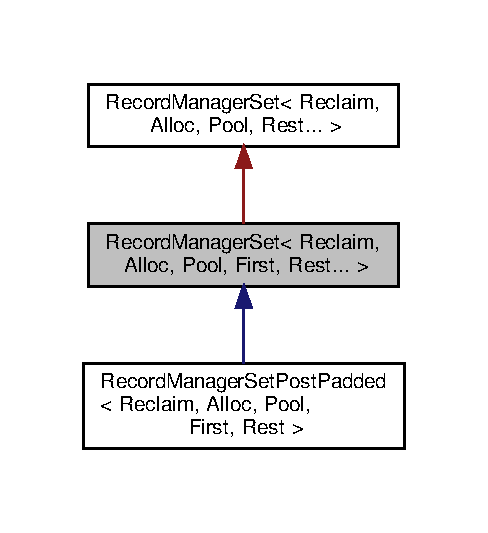
\includegraphics[width=234pt]{classRecordManagerSet_3_01Reclaim_00_01Alloc_00_01Pool_00_01First_00_01Rest_8_8_8_01_4__inherit__graph}
\end{center}
\end{figure}


Collaboration diagram for Record\+Manager\+Set$<$ Reclaim, Alloc, Pool, First, Rest... $>$\+:
\nopagebreak
\begin{figure}[H]
\begin{center}
\leavevmode
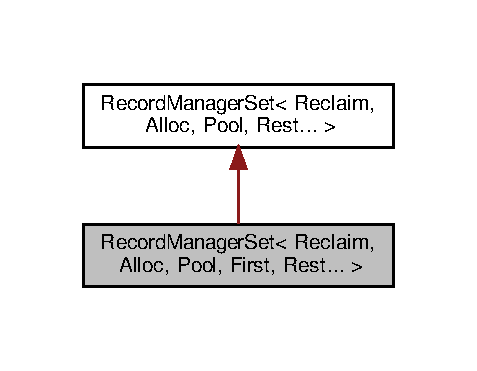
\includegraphics[width=229pt]{classRecordManagerSet_3_01Reclaim_00_01Alloc_00_01Pool_00_01First_00_01Rest_8_8_8_01_4__coll__graph}
\end{center}
\end{figure}
\subsection*{Public Member Functions}
\begin{DoxyCompactItemize}
\item 
\hyperlink{classRecordManagerSet_3_01Reclaim_00_01Alloc_00_01Pool_00_01First_00_01Rest_8_8_8_01_4_acf1d83aa2ab7d1691e99b7aabcdff426}{Record\+Manager\+Set} (const int \hyperlink{testing_8cpp_aa085812188e21ede75351d88b9b2c30d}{num\+Processes}, \hyperlink{classRecoveryMgr}{Recovery\+Mgr}$<$ void $\ast$$>$ $\ast$const \+\_\+recovery\+Mgr)
\item 
\hyperlink{classRecordManagerSet_3_01Reclaim_00_01Alloc_00_01Pool_00_01First_00_01Rest_8_8_8_01_4_a9209878081140bd31a47b96b410ec22a}{$\sim$\+Record\+Manager\+Set} ()
\item 
{\footnotesize template$<$typename T $>$ }\\\hyperlink{classrecord__manager__single__type}{record\+\_\+manager\+\_\+single\+\_\+type}$<$ T, Reclaim, Alloc, Pool $>$ $\ast$ \hyperlink{classRecordManagerSet_3_01Reclaim_00_01Alloc_00_01Pool_00_01First_00_01Rest_8_8_8_01_4_ad755746ae5e804082f4373331dc9f516}{get} (T $\ast$const record\+Type)
\item 
void \hyperlink{classRecordManagerSet_3_01Reclaim_00_01Alloc_00_01Pool_00_01First_00_01Rest_8_8_8_01_4_a1c3bc38c1d9ed9fae1506f1fe6bba602}{clear\+Counters} (void)
\item 
void \hyperlink{classRecordManagerSet_3_01Reclaim_00_01Alloc_00_01Pool_00_01First_00_01Rest_8_8_8_01_4_a30ad594b51539497d6e54363899205ae}{register\+Thread} (const int \hyperlink{microbench_2main_8cpp_a9ca9869868fe7e7a38a921cc7de4103f}{tid})
\item 
void \hyperlink{classRecordManagerSet_3_01Reclaim_00_01Alloc_00_01Pool_00_01First_00_01Rest_8_8_8_01_4_ace148ff49e1acd8ffe3fde0642ab2c9a}{unregister\+Thread} (const int \hyperlink{microbench_2main_8cpp_a9ca9869868fe7e7a38a921cc7de4103f}{tid})
\item 
void \hyperlink{classRecordManagerSet_3_01Reclaim_00_01Alloc_00_01Pool_00_01First_00_01Rest_8_8_8_01_4_a4275f4dca389386d12dc1d5e256eccf8}{print\+Status} ()
\item 
void \hyperlink{classRecordManagerSet_3_01Reclaim_00_01Alloc_00_01Pool_00_01First_00_01Rest_8_8_8_01_4_a4e25436580102b283a893175f2f52eca}{q\+Unprotect\+All} (const int \hyperlink{microbench_2main_8cpp_a9ca9869868fe7e7a38a921cc7de4103f}{tid})
\item 
void \hyperlink{classRecordManagerSet_3_01Reclaim_00_01Alloc_00_01Pool_00_01First_00_01Rest_8_8_8_01_4_aad44cb48eb126633341d2d4f4c9c8156}{get\+Reclaimers} (const int \hyperlink{microbench_2main_8cpp_a9ca9869868fe7e7a38a921cc7de4103f}{tid}, void $\ast$$\ast$const reclaimers, int index)
\item 
void \hyperlink{classRecordManagerSet_3_01Reclaim_00_01Alloc_00_01Pool_00_01First_00_01Rest_8_8_8_01_4_a11af9e5ade9a64b64710320d1b0ea9f7}{end\+Op} (const int \hyperlink{microbench_2main_8cpp_a9ca9869868fe7e7a38a921cc7de4103f}{tid})
\item 
void \hyperlink{classRecordManagerSet_3_01Reclaim_00_01Alloc_00_01Pool_00_01First_00_01Rest_8_8_8_01_4_ab857d28637a682a495f725ef7faab6ec}{leave\+Quiescent\+State\+For\+Each} (const int \hyperlink{microbench_2main_8cpp_a9ca9869868fe7e7a38a921cc7de4103f}{tid}, const bool read\+Only=false)
\item 
void \hyperlink{classRecordManagerSet_3_01Reclaim_00_01Alloc_00_01Pool_00_01First_00_01Rest_8_8_8_01_4_add15f28252ca8970cdb29588f36f5b46}{start\+Op} (const int \hyperlink{microbench_2main_8cpp_a9ca9869868fe7e7a38a921cc7de4103f}{tid}, const bool call\+For\+Each, const bool read\+Only=false)
\end{DoxyCompactItemize}


\subsection{Constructor \& Destructor Documentation}
\mbox{\Hypertarget{classRecordManagerSet_3_01Reclaim_00_01Alloc_00_01Pool_00_01First_00_01Rest_8_8_8_01_4_acf1d83aa2ab7d1691e99b7aabcdff426}\label{classRecordManagerSet_3_01Reclaim_00_01Alloc_00_01Pool_00_01First_00_01Rest_8_8_8_01_4_acf1d83aa2ab7d1691e99b7aabcdff426}} 
\index{Record\+Manager\+Set$<$ Reclaim, Alloc, Pool, First, Rest... $>$@{Record\+Manager\+Set$<$ Reclaim, Alloc, Pool, First, Rest... $>$}!Record\+Manager\+Set@{Record\+Manager\+Set}}
\index{Record\+Manager\+Set@{Record\+Manager\+Set}!Record\+Manager\+Set$<$ Reclaim, Alloc, Pool, First, Rest... $>$@{Record\+Manager\+Set$<$ Reclaim, Alloc, Pool, First, Rest... $>$}}
\subsubsection{\texorpdfstring{Record\+Manager\+Set()}{RecordManagerSet()}}
{\footnotesize\ttfamily template$<$class Reclaim , class Alloc , class Pool , typename First , typename... Rest$>$ \\
\hyperlink{classRecordManagerSet}{Record\+Manager\+Set}$<$ Reclaim, Alloc, Pool, First, Rest... $>$\+::\hyperlink{classRecordManagerSet}{Record\+Manager\+Set} (\begin{DoxyParamCaption}\item[{const int}]{num\+Processes,  }\item[{\hyperlink{classRecoveryMgr}{Recovery\+Mgr}$<$ void $\ast$$>$ $\ast$const}]{\+\_\+recovery\+Mgr }\end{DoxyParamCaption})\hspace{0.3cm}{\ttfamily [inline]}}

\mbox{\Hypertarget{classRecordManagerSet_3_01Reclaim_00_01Alloc_00_01Pool_00_01First_00_01Rest_8_8_8_01_4_a9209878081140bd31a47b96b410ec22a}\label{classRecordManagerSet_3_01Reclaim_00_01Alloc_00_01Pool_00_01First_00_01Rest_8_8_8_01_4_a9209878081140bd31a47b96b410ec22a}} 
\index{Record\+Manager\+Set$<$ Reclaim, Alloc, Pool, First, Rest... $>$@{Record\+Manager\+Set$<$ Reclaim, Alloc, Pool, First, Rest... $>$}!````~Record\+Manager\+Set@{$\sim$\+Record\+Manager\+Set}}
\index{````~Record\+Manager\+Set@{$\sim$\+Record\+Manager\+Set}!Record\+Manager\+Set$<$ Reclaim, Alloc, Pool, First, Rest... $>$@{Record\+Manager\+Set$<$ Reclaim, Alloc, Pool, First, Rest... $>$}}
\subsubsection{\texorpdfstring{$\sim$\+Record\+Manager\+Set()}{~RecordManagerSet()}}
{\footnotesize\ttfamily template$<$class Reclaim , class Alloc , class Pool , typename First , typename... Rest$>$ \\
\hyperlink{classRecordManagerSet}{Record\+Manager\+Set}$<$ Reclaim, Alloc, Pool, First, Rest... $>$\+::$\sim$\hyperlink{classRecordManagerSet}{Record\+Manager\+Set} (\begin{DoxyParamCaption}{ }\end{DoxyParamCaption})\hspace{0.3cm}{\ttfamily [inline]}}



\subsection{Member Function Documentation}
\mbox{\Hypertarget{classRecordManagerSet_3_01Reclaim_00_01Alloc_00_01Pool_00_01First_00_01Rest_8_8_8_01_4_a1c3bc38c1d9ed9fae1506f1fe6bba602}\label{classRecordManagerSet_3_01Reclaim_00_01Alloc_00_01Pool_00_01First_00_01Rest_8_8_8_01_4_a1c3bc38c1d9ed9fae1506f1fe6bba602}} 
\index{Record\+Manager\+Set$<$ Reclaim, Alloc, Pool, First, Rest... $>$@{Record\+Manager\+Set$<$ Reclaim, Alloc, Pool, First, Rest... $>$}!clear\+Counters@{clear\+Counters}}
\index{clear\+Counters@{clear\+Counters}!Record\+Manager\+Set$<$ Reclaim, Alloc, Pool, First, Rest... $>$@{Record\+Manager\+Set$<$ Reclaim, Alloc, Pool, First, Rest... $>$}}
\subsubsection{\texorpdfstring{clear\+Counters()}{clearCounters()}}
{\footnotesize\ttfamily template$<$class Reclaim , class Alloc , class Pool , typename First , typename... Rest$>$ \\
void \hyperlink{classRecordManagerSet}{Record\+Manager\+Set}$<$ Reclaim, Alloc, Pool, First, Rest... $>$\+::clear\+Counters (\begin{DoxyParamCaption}\item[{void}]{ }\end{DoxyParamCaption})\hspace{0.3cm}{\ttfamily [inline]}}

\mbox{\Hypertarget{classRecordManagerSet_3_01Reclaim_00_01Alloc_00_01Pool_00_01First_00_01Rest_8_8_8_01_4_a11af9e5ade9a64b64710320d1b0ea9f7}\label{classRecordManagerSet_3_01Reclaim_00_01Alloc_00_01Pool_00_01First_00_01Rest_8_8_8_01_4_a11af9e5ade9a64b64710320d1b0ea9f7}} 
\index{Record\+Manager\+Set$<$ Reclaim, Alloc, Pool, First, Rest... $>$@{Record\+Manager\+Set$<$ Reclaim, Alloc, Pool, First, Rest... $>$}!end\+Op@{end\+Op}}
\index{end\+Op@{end\+Op}!Record\+Manager\+Set$<$ Reclaim, Alloc, Pool, First, Rest... $>$@{Record\+Manager\+Set$<$ Reclaim, Alloc, Pool, First, Rest... $>$}}
\subsubsection{\texorpdfstring{end\+Op()}{endOp()}}
{\footnotesize\ttfamily template$<$class Reclaim , class Alloc , class Pool , typename First , typename... Rest$>$ \\
void \hyperlink{classRecordManagerSet}{Record\+Manager\+Set}$<$ Reclaim, Alloc, Pool, First, Rest... $>$\+::end\+Op (\begin{DoxyParamCaption}\item[{const int}]{tid }\end{DoxyParamCaption})\hspace{0.3cm}{\ttfamily [inline]}}

\mbox{\Hypertarget{classRecordManagerSet_3_01Reclaim_00_01Alloc_00_01Pool_00_01First_00_01Rest_8_8_8_01_4_ad755746ae5e804082f4373331dc9f516}\label{classRecordManagerSet_3_01Reclaim_00_01Alloc_00_01Pool_00_01First_00_01Rest_8_8_8_01_4_ad755746ae5e804082f4373331dc9f516}} 
\index{Record\+Manager\+Set$<$ Reclaim, Alloc, Pool, First, Rest... $>$@{Record\+Manager\+Set$<$ Reclaim, Alloc, Pool, First, Rest... $>$}!get@{get}}
\index{get@{get}!Record\+Manager\+Set$<$ Reclaim, Alloc, Pool, First, Rest... $>$@{Record\+Manager\+Set$<$ Reclaim, Alloc, Pool, First, Rest... $>$}}
\subsubsection{\texorpdfstring{get()}{get()}}
{\footnotesize\ttfamily template$<$class Reclaim , class Alloc , class Pool , typename First , typename... Rest$>$ \\
template$<$typename T $>$ \\
\hyperlink{classrecord__manager__single__type}{record\+\_\+manager\+\_\+single\+\_\+type}$<$T, Reclaim, Alloc, Pool$>$$\ast$ \hyperlink{classRecordManagerSet}{Record\+Manager\+Set}$<$ Reclaim, Alloc, Pool, First, Rest... $>$\+::get (\begin{DoxyParamCaption}\item[{T $\ast$const}]{record\+Type }\end{DoxyParamCaption})\hspace{0.3cm}{\ttfamily [inline]}}

\mbox{\Hypertarget{classRecordManagerSet_3_01Reclaim_00_01Alloc_00_01Pool_00_01First_00_01Rest_8_8_8_01_4_aad44cb48eb126633341d2d4f4c9c8156}\label{classRecordManagerSet_3_01Reclaim_00_01Alloc_00_01Pool_00_01First_00_01Rest_8_8_8_01_4_aad44cb48eb126633341d2d4f4c9c8156}} 
\index{Record\+Manager\+Set$<$ Reclaim, Alloc, Pool, First, Rest... $>$@{Record\+Manager\+Set$<$ Reclaim, Alloc, Pool, First, Rest... $>$}!get\+Reclaimers@{get\+Reclaimers}}
\index{get\+Reclaimers@{get\+Reclaimers}!Record\+Manager\+Set$<$ Reclaim, Alloc, Pool, First, Rest... $>$@{Record\+Manager\+Set$<$ Reclaim, Alloc, Pool, First, Rest... $>$}}
\subsubsection{\texorpdfstring{get\+Reclaimers()}{getReclaimers()}}
{\footnotesize\ttfamily template$<$class Reclaim , class Alloc , class Pool , typename First , typename... Rest$>$ \\
void \hyperlink{classRecordManagerSet}{Record\+Manager\+Set}$<$ Reclaim, Alloc, Pool, First, Rest... $>$\+::get\+Reclaimers (\begin{DoxyParamCaption}\item[{const int}]{tid,  }\item[{void $\ast$$\ast$const}]{reclaimers,  }\item[{int}]{index }\end{DoxyParamCaption})\hspace{0.3cm}{\ttfamily [inline]}}

\mbox{\Hypertarget{classRecordManagerSet_3_01Reclaim_00_01Alloc_00_01Pool_00_01First_00_01Rest_8_8_8_01_4_ab857d28637a682a495f725ef7faab6ec}\label{classRecordManagerSet_3_01Reclaim_00_01Alloc_00_01Pool_00_01First_00_01Rest_8_8_8_01_4_ab857d28637a682a495f725ef7faab6ec}} 
\index{Record\+Manager\+Set$<$ Reclaim, Alloc, Pool, First, Rest... $>$@{Record\+Manager\+Set$<$ Reclaim, Alloc, Pool, First, Rest... $>$}!leave\+Quiescent\+State\+For\+Each@{leave\+Quiescent\+State\+For\+Each}}
\index{leave\+Quiescent\+State\+For\+Each@{leave\+Quiescent\+State\+For\+Each}!Record\+Manager\+Set$<$ Reclaim, Alloc, Pool, First, Rest... $>$@{Record\+Manager\+Set$<$ Reclaim, Alloc, Pool, First, Rest... $>$}}
\subsubsection{\texorpdfstring{leave\+Quiescent\+State\+For\+Each()}{leaveQuiescentStateForEach()}}
{\footnotesize\ttfamily template$<$class Reclaim , class Alloc , class Pool , typename First , typename... Rest$>$ \\
void \hyperlink{classRecordManagerSet}{Record\+Manager\+Set}$<$ Reclaim, Alloc, Pool, First, Rest... $>$\+::leave\+Quiescent\+State\+For\+Each (\begin{DoxyParamCaption}\item[{const int}]{tid,  }\item[{const bool}]{read\+Only = {\ttfamily false} }\end{DoxyParamCaption})\hspace{0.3cm}{\ttfamily [inline]}}

\mbox{\Hypertarget{classRecordManagerSet_3_01Reclaim_00_01Alloc_00_01Pool_00_01First_00_01Rest_8_8_8_01_4_a4275f4dca389386d12dc1d5e256eccf8}\label{classRecordManagerSet_3_01Reclaim_00_01Alloc_00_01Pool_00_01First_00_01Rest_8_8_8_01_4_a4275f4dca389386d12dc1d5e256eccf8}} 
\index{Record\+Manager\+Set$<$ Reclaim, Alloc, Pool, First, Rest... $>$@{Record\+Manager\+Set$<$ Reclaim, Alloc, Pool, First, Rest... $>$}!print\+Status@{print\+Status}}
\index{print\+Status@{print\+Status}!Record\+Manager\+Set$<$ Reclaim, Alloc, Pool, First, Rest... $>$@{Record\+Manager\+Set$<$ Reclaim, Alloc, Pool, First, Rest... $>$}}
\subsubsection{\texorpdfstring{print\+Status()}{printStatus()}}
{\footnotesize\ttfamily template$<$class Reclaim , class Alloc , class Pool , typename First , typename... Rest$>$ \\
void \hyperlink{classRecordManagerSet}{Record\+Manager\+Set}$<$ Reclaim, Alloc, Pool, First, Rest... $>$\+::print\+Status (\begin{DoxyParamCaption}{ }\end{DoxyParamCaption})\hspace{0.3cm}{\ttfamily [inline]}}

\mbox{\Hypertarget{classRecordManagerSet_3_01Reclaim_00_01Alloc_00_01Pool_00_01First_00_01Rest_8_8_8_01_4_a4e25436580102b283a893175f2f52eca}\label{classRecordManagerSet_3_01Reclaim_00_01Alloc_00_01Pool_00_01First_00_01Rest_8_8_8_01_4_a4e25436580102b283a893175f2f52eca}} 
\index{Record\+Manager\+Set$<$ Reclaim, Alloc, Pool, First, Rest... $>$@{Record\+Manager\+Set$<$ Reclaim, Alloc, Pool, First, Rest... $>$}!q\+Unprotect\+All@{q\+Unprotect\+All}}
\index{q\+Unprotect\+All@{q\+Unprotect\+All}!Record\+Manager\+Set$<$ Reclaim, Alloc, Pool, First, Rest... $>$@{Record\+Manager\+Set$<$ Reclaim, Alloc, Pool, First, Rest... $>$}}
\subsubsection{\texorpdfstring{q\+Unprotect\+All()}{qUnprotectAll()}}
{\footnotesize\ttfamily template$<$class Reclaim , class Alloc , class Pool , typename First , typename... Rest$>$ \\
void \hyperlink{classRecordManagerSet}{Record\+Manager\+Set}$<$ Reclaim, Alloc, Pool, First, Rest... $>$\+::q\+Unprotect\+All (\begin{DoxyParamCaption}\item[{const int}]{tid }\end{DoxyParamCaption})\hspace{0.3cm}{\ttfamily [inline]}}

\mbox{\Hypertarget{classRecordManagerSet_3_01Reclaim_00_01Alloc_00_01Pool_00_01First_00_01Rest_8_8_8_01_4_a30ad594b51539497d6e54363899205ae}\label{classRecordManagerSet_3_01Reclaim_00_01Alloc_00_01Pool_00_01First_00_01Rest_8_8_8_01_4_a30ad594b51539497d6e54363899205ae}} 
\index{Record\+Manager\+Set$<$ Reclaim, Alloc, Pool, First, Rest... $>$@{Record\+Manager\+Set$<$ Reclaim, Alloc, Pool, First, Rest... $>$}!register\+Thread@{register\+Thread}}
\index{register\+Thread@{register\+Thread}!Record\+Manager\+Set$<$ Reclaim, Alloc, Pool, First, Rest... $>$@{Record\+Manager\+Set$<$ Reclaim, Alloc, Pool, First, Rest... $>$}}
\subsubsection{\texorpdfstring{register\+Thread()}{registerThread()}}
{\footnotesize\ttfamily template$<$class Reclaim , class Alloc , class Pool , typename First , typename... Rest$>$ \\
void \hyperlink{classRecordManagerSet}{Record\+Manager\+Set}$<$ Reclaim, Alloc, Pool, First, Rest... $>$\+::register\+Thread (\begin{DoxyParamCaption}\item[{const int}]{tid }\end{DoxyParamCaption})\hspace{0.3cm}{\ttfamily [inline]}}

\mbox{\Hypertarget{classRecordManagerSet_3_01Reclaim_00_01Alloc_00_01Pool_00_01First_00_01Rest_8_8_8_01_4_add15f28252ca8970cdb29588f36f5b46}\label{classRecordManagerSet_3_01Reclaim_00_01Alloc_00_01Pool_00_01First_00_01Rest_8_8_8_01_4_add15f28252ca8970cdb29588f36f5b46}} 
\index{Record\+Manager\+Set$<$ Reclaim, Alloc, Pool, First, Rest... $>$@{Record\+Manager\+Set$<$ Reclaim, Alloc, Pool, First, Rest... $>$}!start\+Op@{start\+Op}}
\index{start\+Op@{start\+Op}!Record\+Manager\+Set$<$ Reclaim, Alloc, Pool, First, Rest... $>$@{Record\+Manager\+Set$<$ Reclaim, Alloc, Pool, First, Rest... $>$}}
\subsubsection{\texorpdfstring{start\+Op()}{startOp()}}
{\footnotesize\ttfamily template$<$class Reclaim , class Alloc , class Pool , typename First , typename... Rest$>$ \\
void \hyperlink{classRecordManagerSet}{Record\+Manager\+Set}$<$ Reclaim, Alloc, Pool, First, Rest... $>$\+::start\+Op (\begin{DoxyParamCaption}\item[{const int}]{tid,  }\item[{const bool}]{call\+For\+Each,  }\item[{const bool}]{read\+Only = {\ttfamily false} }\end{DoxyParamCaption})\hspace{0.3cm}{\ttfamily [inline]}}

\mbox{\Hypertarget{classRecordManagerSet_3_01Reclaim_00_01Alloc_00_01Pool_00_01First_00_01Rest_8_8_8_01_4_ace148ff49e1acd8ffe3fde0642ab2c9a}\label{classRecordManagerSet_3_01Reclaim_00_01Alloc_00_01Pool_00_01First_00_01Rest_8_8_8_01_4_ace148ff49e1acd8ffe3fde0642ab2c9a}} 
\index{Record\+Manager\+Set$<$ Reclaim, Alloc, Pool, First, Rest... $>$@{Record\+Manager\+Set$<$ Reclaim, Alloc, Pool, First, Rest... $>$}!unregister\+Thread@{unregister\+Thread}}
\index{unregister\+Thread@{unregister\+Thread}!Record\+Manager\+Set$<$ Reclaim, Alloc, Pool, First, Rest... $>$@{Record\+Manager\+Set$<$ Reclaim, Alloc, Pool, First, Rest... $>$}}
\subsubsection{\texorpdfstring{unregister\+Thread()}{unregisterThread()}}
{\footnotesize\ttfamily template$<$class Reclaim , class Alloc , class Pool , typename First , typename... Rest$>$ \\
void \hyperlink{classRecordManagerSet}{Record\+Manager\+Set}$<$ Reclaim, Alloc, Pool, First, Rest... $>$\+::unregister\+Thread (\begin{DoxyParamCaption}\item[{const int}]{tid }\end{DoxyParamCaption})\hspace{0.3cm}{\ttfamily [inline]}}



The documentation for this class was generated from the following file\+:\begin{DoxyCompactItemize}
\item 
common/recordmgr/\hyperlink{record__manager_8h}{record\+\_\+manager.\+h}\end{DoxyCompactItemize}

\hypertarget{classRecordManagerSetPostPadded}{}\section{Record\+Manager\+Set\+Post\+Padded$<$ Reclaim, Alloc, Pool, First, Rest $>$ Class Template Reference}
\label{classRecordManagerSetPostPadded}\index{Record\+Manager\+Set\+Post\+Padded$<$ Reclaim, Alloc, Pool, First, Rest $>$@{Record\+Manager\+Set\+Post\+Padded$<$ Reclaim, Alloc, Pool, First, Rest $>$}}


{\ttfamily \#include $<$record\+\_\+manager.\+h$>$}



Inheritance diagram for Record\+Manager\+Set\+Post\+Padded$<$ Reclaim, Alloc, Pool, First, Rest $>$\+:
\nopagebreak
\begin{figure}[H]
\begin{center}
\leavevmode
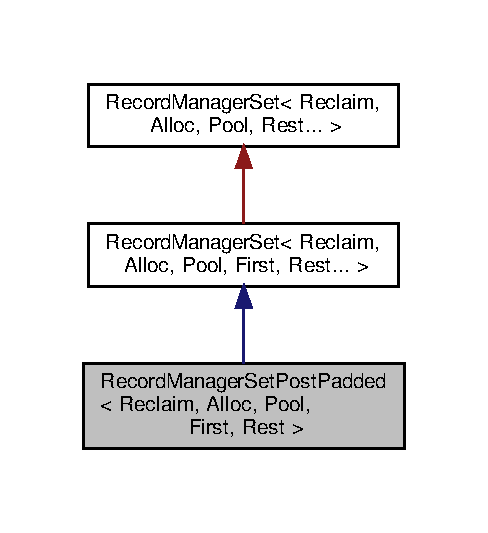
\includegraphics[width=234pt]{classRecordManagerSetPostPadded__inherit__graph}
\end{center}
\end{figure}


Collaboration diagram for Record\+Manager\+Set\+Post\+Padded$<$ Reclaim, Alloc, Pool, First, Rest $>$\+:
\nopagebreak
\begin{figure}[H]
\begin{center}
\leavevmode
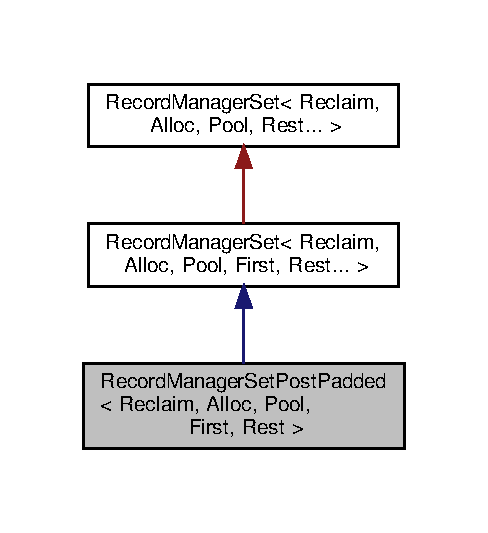
\includegraphics[width=234pt]{classRecordManagerSetPostPadded__coll__graph}
\end{center}
\end{figure}
\subsection*{Public Member Functions}
\begin{DoxyCompactItemize}
\item 
\hyperlink{classRecordManagerSetPostPadded_aad17bd9f2f119bfbc5be24a813eb9cd8}{Record\+Manager\+Set\+Post\+Padded} (const int \hyperlink{testing_8cpp_aa085812188e21ede75351d88b9b2c30d}{num\+Processes}, \hyperlink{classRecoveryMgr}{Recovery\+Mgr}$<$ void $\ast$$>$ $\ast$const \+\_\+recovery\+Mgr)
\end{DoxyCompactItemize}


\subsection{Constructor \& Destructor Documentation}
\mbox{\Hypertarget{classRecordManagerSetPostPadded_aad17bd9f2f119bfbc5be24a813eb9cd8}\label{classRecordManagerSetPostPadded_aad17bd9f2f119bfbc5be24a813eb9cd8}} 
\index{Record\+Manager\+Set\+Post\+Padded@{Record\+Manager\+Set\+Post\+Padded}!Record\+Manager\+Set\+Post\+Padded@{Record\+Manager\+Set\+Post\+Padded}}
\index{Record\+Manager\+Set\+Post\+Padded@{Record\+Manager\+Set\+Post\+Padded}!Record\+Manager\+Set\+Post\+Padded@{Record\+Manager\+Set\+Post\+Padded}}
\subsubsection{\texorpdfstring{Record\+Manager\+Set\+Post\+Padded()}{RecordManagerSetPostPadded()}}
{\footnotesize\ttfamily template$<$class Reclaim, class Alloc, class Pool, typename First, typename... Rest$>$ \\
\hyperlink{classRecordManagerSetPostPadded}{Record\+Manager\+Set\+Post\+Padded}$<$ Reclaim, Alloc, Pool, First, Rest $>$\+::\hyperlink{classRecordManagerSetPostPadded}{Record\+Manager\+Set\+Post\+Padded} (\begin{DoxyParamCaption}\item[{const int}]{num\+Processes,  }\item[{\hyperlink{classRecoveryMgr}{Recovery\+Mgr}$<$ void $\ast$$>$ $\ast$const}]{\+\_\+recovery\+Mgr }\end{DoxyParamCaption})\hspace{0.3cm}{\ttfamily [inline]}}



The documentation for this class was generated from the following file\+:\begin{DoxyCompactItemize}
\item 
common/recordmgr/\hyperlink{record__manager_8h}{record\+\_\+manager.\+h}\end{DoxyCompactItemize}

\hypertarget{classRecoveryMgr}{}\section{Recovery\+Mgr$<$ Master\+Record\+Mgr $>$ Class Template Reference}
\label{classRecoveryMgr}\index{Recovery\+Mgr$<$ Master\+Record\+Mgr $>$@{Recovery\+Mgr$<$ Master\+Record\+Mgr $>$}}


{\ttfamily \#include $<$recovery\+\_\+manager.\+h$>$}

\subsection*{Public Member Functions}
\begin{DoxyCompactItemize}
\item 
int \hyperlink{classRecoveryMgr_a66bc99f5748e8418e9f111416d44dcac}{get\+Tid\+Inefficient} (const pthread\+\_\+t me)
\item 
int \hyperlink{classRecoveryMgr_a5917bf180cc6917ebb903a218d163aef}{get\+Tid\+Inefficient\+Errno} ()
\item 
int \hyperlink{classRecoveryMgr_a6c6f9170e844cb0a600b10ebf3ea6e37}{get\+Tid\+\_\+pthread\+\_\+getspecific} ()
\item 
pthread\+\_\+t \hyperlink{classRecoveryMgr_a9f8a5b27b63e5d1c51c31f7bdec75242}{get\+Pthread} (const int \hyperlink{microbench_2main_8cpp_a9ca9869868fe7e7a38a921cc7de4103f}{tid})
\item 
void \hyperlink{classRecoveryMgr_ad68f80af5f2371e66a39fed826f27c93}{init\+Thread} (const int \hyperlink{microbench_2main_8cpp_a9ca9869868fe7e7a38a921cc7de4103f}{tid})
\item 
void \hyperlink{classRecoveryMgr_a80eeb52e1d5658291f244ffe43b55b50}{deinit\+Thread} (const int \hyperlink{microbench_2main_8cpp_a9ca9869868fe7e7a38a921cc7de4103f}{tid})
\item 
void \hyperlink{classRecoveryMgr_a6158fad92d9250812d4a8f92a730aecd}{unblock\+Crash\+Recovery\+Signal} ()
\item 
\hyperlink{classRecoveryMgr_a303ad058a7752d20fdc5c437d6576e1a}{Recovery\+Mgr} (const int \hyperlink{testing_8cpp_aa085812188e21ede75351d88b9b2c30d}{num\+Processes}, const int \+\_\+neutralize\+Signal, Master\+Record\+Mgr $\ast$const master\+Record\+Mgr)
\item 
\hyperlink{classRecoveryMgr_a436371a5d4bfaafd37611e842cb10c9a}{$\sim$\+Recovery\+Mgr} ()
\end{DoxyCompactItemize}
\subsection*{Public Attributes}
\begin{DoxyCompactItemize}
\item 
\hyperlink{classRecoveryMgr_aa18a397143e99c8e72d175f3c9562c9e}{P\+AD}
\item 
const int \hyperlink{classRecoveryMgr_a3b3011e6a4a07820477038c246a0d801}{N\+U\+M\+\_\+\+P\+R\+O\+C\+E\+S\+S\+ES}
\item 
const int \hyperlink{classRecoveryMgr_a2447fa0d8ee553b79e9d9cc838162639}{neutralize\+Signal}
\end{DoxyCompactItemize}


\subsection{Constructor \& Destructor Documentation}
\mbox{\Hypertarget{classRecoveryMgr_a303ad058a7752d20fdc5c437d6576e1a}\label{classRecoveryMgr_a303ad058a7752d20fdc5c437d6576e1a}} 
\index{Recovery\+Mgr@{Recovery\+Mgr}!Recovery\+Mgr@{Recovery\+Mgr}}
\index{Recovery\+Mgr@{Recovery\+Mgr}!Recovery\+Mgr@{Recovery\+Mgr}}
\subsubsection{\texorpdfstring{Recovery\+Mgr()}{RecoveryMgr()}}
{\footnotesize\ttfamily template$<$class Master\+Record\+Mgr$>$ \\
\hyperlink{classRecoveryMgr}{Recovery\+Mgr}$<$ Master\+Record\+Mgr $>$\+::\hyperlink{classRecoveryMgr}{Recovery\+Mgr} (\begin{DoxyParamCaption}\item[{const int}]{num\+Processes,  }\item[{const int}]{\+\_\+neutralize\+Signal,  }\item[{Master\+Record\+Mgr $\ast$const}]{master\+Record\+Mgr }\end{DoxyParamCaption})\hspace{0.3cm}{\ttfamily [inline]}}

\mbox{\Hypertarget{classRecoveryMgr_a436371a5d4bfaafd37611e842cb10c9a}\label{classRecoveryMgr_a436371a5d4bfaafd37611e842cb10c9a}} 
\index{Recovery\+Mgr@{Recovery\+Mgr}!````~Recovery\+Mgr@{$\sim$\+Recovery\+Mgr}}
\index{````~Recovery\+Mgr@{$\sim$\+Recovery\+Mgr}!Recovery\+Mgr@{Recovery\+Mgr}}
\subsubsection{\texorpdfstring{$\sim$\+Recovery\+Mgr()}{~RecoveryMgr()}}
{\footnotesize\ttfamily template$<$class Master\+Record\+Mgr$>$ \\
\hyperlink{classRecoveryMgr}{Recovery\+Mgr}$<$ Master\+Record\+Mgr $>$\+::$\sim$\hyperlink{classRecoveryMgr}{Recovery\+Mgr} (\begin{DoxyParamCaption}{ }\end{DoxyParamCaption})\hspace{0.3cm}{\ttfamily [inline]}}



\subsection{Member Function Documentation}
\mbox{\Hypertarget{classRecoveryMgr_a80eeb52e1d5658291f244ffe43b55b50}\label{classRecoveryMgr_a80eeb52e1d5658291f244ffe43b55b50}} 
\index{Recovery\+Mgr@{Recovery\+Mgr}!deinit\+Thread@{deinit\+Thread}}
\index{deinit\+Thread@{deinit\+Thread}!Recovery\+Mgr@{Recovery\+Mgr}}
\subsubsection{\texorpdfstring{deinit\+Thread()}{deinitThread()}}
{\footnotesize\ttfamily template$<$class Master\+Record\+Mgr$>$ \\
void \hyperlink{classRecoveryMgr}{Recovery\+Mgr}$<$ Master\+Record\+Mgr $>$\+::deinit\+Thread (\begin{DoxyParamCaption}\item[{const int}]{tid }\end{DoxyParamCaption})\hspace{0.3cm}{\ttfamily [inline]}}

\mbox{\Hypertarget{classRecoveryMgr_a9f8a5b27b63e5d1c51c31f7bdec75242}\label{classRecoveryMgr_a9f8a5b27b63e5d1c51c31f7bdec75242}} 
\index{Recovery\+Mgr@{Recovery\+Mgr}!get\+Pthread@{get\+Pthread}}
\index{get\+Pthread@{get\+Pthread}!Recovery\+Mgr@{Recovery\+Mgr}}
\subsubsection{\texorpdfstring{get\+Pthread()}{getPthread()}}
{\footnotesize\ttfamily template$<$class Master\+Record\+Mgr$>$ \\
pthread\+\_\+t \hyperlink{classRecoveryMgr}{Recovery\+Mgr}$<$ Master\+Record\+Mgr $>$\+::get\+Pthread (\begin{DoxyParamCaption}\item[{const int}]{tid }\end{DoxyParamCaption})\hspace{0.3cm}{\ttfamily [inline]}}

\mbox{\Hypertarget{classRecoveryMgr_a6c6f9170e844cb0a600b10ebf3ea6e37}\label{classRecoveryMgr_a6c6f9170e844cb0a600b10ebf3ea6e37}} 
\index{Recovery\+Mgr@{Recovery\+Mgr}!get\+Tid\+\_\+pthread\+\_\+getspecific@{get\+Tid\+\_\+pthread\+\_\+getspecific}}
\index{get\+Tid\+\_\+pthread\+\_\+getspecific@{get\+Tid\+\_\+pthread\+\_\+getspecific}!Recovery\+Mgr@{Recovery\+Mgr}}
\subsubsection{\texorpdfstring{get\+Tid\+\_\+pthread\+\_\+getspecific()}{getTid\_pthread\_getspecific()}}
{\footnotesize\ttfamily template$<$class Master\+Record\+Mgr$>$ \\
int \hyperlink{classRecoveryMgr}{Recovery\+Mgr}$<$ Master\+Record\+Mgr $>$\+::get\+Tid\+\_\+pthread\+\_\+getspecific (\begin{DoxyParamCaption}{ }\end{DoxyParamCaption})\hspace{0.3cm}{\ttfamily [inline]}}

\mbox{\Hypertarget{classRecoveryMgr_a66bc99f5748e8418e9f111416d44dcac}\label{classRecoveryMgr_a66bc99f5748e8418e9f111416d44dcac}} 
\index{Recovery\+Mgr@{Recovery\+Mgr}!get\+Tid\+Inefficient@{get\+Tid\+Inefficient}}
\index{get\+Tid\+Inefficient@{get\+Tid\+Inefficient}!Recovery\+Mgr@{Recovery\+Mgr}}
\subsubsection{\texorpdfstring{get\+Tid\+Inefficient()}{getTidInefficient()}}
{\footnotesize\ttfamily template$<$class Master\+Record\+Mgr$>$ \\
int \hyperlink{classRecoveryMgr}{Recovery\+Mgr}$<$ Master\+Record\+Mgr $>$\+::get\+Tid\+Inefficient (\begin{DoxyParamCaption}\item[{const pthread\+\_\+t}]{me }\end{DoxyParamCaption})\hspace{0.3cm}{\ttfamily [inline]}}

\mbox{\Hypertarget{classRecoveryMgr_a5917bf180cc6917ebb903a218d163aef}\label{classRecoveryMgr_a5917bf180cc6917ebb903a218d163aef}} 
\index{Recovery\+Mgr@{Recovery\+Mgr}!get\+Tid\+Inefficient\+Errno@{get\+Tid\+Inefficient\+Errno}}
\index{get\+Tid\+Inefficient\+Errno@{get\+Tid\+Inefficient\+Errno}!Recovery\+Mgr@{Recovery\+Mgr}}
\subsubsection{\texorpdfstring{get\+Tid\+Inefficient\+Errno()}{getTidInefficientErrno()}}
{\footnotesize\ttfamily template$<$class Master\+Record\+Mgr$>$ \\
int \hyperlink{classRecoveryMgr}{Recovery\+Mgr}$<$ Master\+Record\+Mgr $>$\+::get\+Tid\+Inefficient\+Errno (\begin{DoxyParamCaption}{ }\end{DoxyParamCaption})\hspace{0.3cm}{\ttfamily [inline]}}

\mbox{\Hypertarget{classRecoveryMgr_ad68f80af5f2371e66a39fed826f27c93}\label{classRecoveryMgr_ad68f80af5f2371e66a39fed826f27c93}} 
\index{Recovery\+Mgr@{Recovery\+Mgr}!init\+Thread@{init\+Thread}}
\index{init\+Thread@{init\+Thread}!Recovery\+Mgr@{Recovery\+Mgr}}
\subsubsection{\texorpdfstring{init\+Thread()}{initThread()}}
{\footnotesize\ttfamily template$<$class Master\+Record\+Mgr$>$ \\
void \hyperlink{classRecoveryMgr}{Recovery\+Mgr}$<$ Master\+Record\+Mgr $>$\+::init\+Thread (\begin{DoxyParamCaption}\item[{const int}]{tid }\end{DoxyParamCaption})\hspace{0.3cm}{\ttfamily [inline]}}

\mbox{\Hypertarget{classRecoveryMgr_a6158fad92d9250812d4a8f92a730aecd}\label{classRecoveryMgr_a6158fad92d9250812d4a8f92a730aecd}} 
\index{Recovery\+Mgr@{Recovery\+Mgr}!unblock\+Crash\+Recovery\+Signal@{unblock\+Crash\+Recovery\+Signal}}
\index{unblock\+Crash\+Recovery\+Signal@{unblock\+Crash\+Recovery\+Signal}!Recovery\+Mgr@{Recovery\+Mgr}}
\subsubsection{\texorpdfstring{unblock\+Crash\+Recovery\+Signal()}{unblockCrashRecoverySignal()}}
{\footnotesize\ttfamily template$<$class Master\+Record\+Mgr$>$ \\
void \hyperlink{classRecoveryMgr}{Recovery\+Mgr}$<$ Master\+Record\+Mgr $>$\+::unblock\+Crash\+Recovery\+Signal (\begin{DoxyParamCaption}{ }\end{DoxyParamCaption})\hspace{0.3cm}{\ttfamily [inline]}}



\subsection{Member Data Documentation}
\mbox{\Hypertarget{classRecoveryMgr_a2447fa0d8ee553b79e9d9cc838162639}\label{classRecoveryMgr_a2447fa0d8ee553b79e9d9cc838162639}} 
\index{Recovery\+Mgr@{Recovery\+Mgr}!neutralize\+Signal@{neutralize\+Signal}}
\index{neutralize\+Signal@{neutralize\+Signal}!Recovery\+Mgr@{Recovery\+Mgr}}
\subsubsection{\texorpdfstring{neutralize\+Signal}{neutralizeSignal}}
{\footnotesize\ttfamily template$<$class Master\+Record\+Mgr$>$ \\
const int \hyperlink{classRecoveryMgr}{Recovery\+Mgr}$<$ Master\+Record\+Mgr $>$\+::neutralize\+Signal}

\mbox{\Hypertarget{classRecoveryMgr_a3b3011e6a4a07820477038c246a0d801}\label{classRecoveryMgr_a3b3011e6a4a07820477038c246a0d801}} 
\index{Recovery\+Mgr@{Recovery\+Mgr}!N\+U\+M\+\_\+\+P\+R\+O\+C\+E\+S\+S\+ES@{N\+U\+M\+\_\+\+P\+R\+O\+C\+E\+S\+S\+ES}}
\index{N\+U\+M\+\_\+\+P\+R\+O\+C\+E\+S\+S\+ES@{N\+U\+M\+\_\+\+P\+R\+O\+C\+E\+S\+S\+ES}!Recovery\+Mgr@{Recovery\+Mgr}}
\subsubsection{\texorpdfstring{N\+U\+M\+\_\+\+P\+R\+O\+C\+E\+S\+S\+ES}{NUM\_PROCESSES}}
{\footnotesize\ttfamily template$<$class Master\+Record\+Mgr$>$ \\
const int \hyperlink{classRecoveryMgr}{Recovery\+Mgr}$<$ Master\+Record\+Mgr $>$\+::N\+U\+M\+\_\+\+P\+R\+O\+C\+E\+S\+S\+ES}

\mbox{\Hypertarget{classRecoveryMgr_aa18a397143e99c8e72d175f3c9562c9e}\label{classRecoveryMgr_aa18a397143e99c8e72d175f3c9562c9e}} 
\index{Recovery\+Mgr@{Recovery\+Mgr}!P\+AD@{P\+AD}}
\index{P\+AD@{P\+AD}!Recovery\+Mgr@{Recovery\+Mgr}}
\subsubsection{\texorpdfstring{P\+AD}{PAD}}
{\footnotesize\ttfamily template$<$class Master\+Record\+Mgr$>$ \\
\hyperlink{classRecoveryMgr}{Recovery\+Mgr}$<$ Master\+Record\+Mgr $>$\+::P\+AD}



The documentation for this class was generated from the following file\+:\begin{DoxyCompactItemize}
\item 
common/recordmgr/\hyperlink{recovery__manager_8h}{recovery\+\_\+manager.\+h}\end{DoxyCompactItemize}

\hypertarget{structrelocate__op__t}{}\section{relocate\+\_\+op\+\_\+t$<$ skey\+\_\+t, sval\+\_\+t $>$ Struct Template Reference}
\label{structrelocate__op__t}\index{relocate\+\_\+op\+\_\+t$<$ skey\+\_\+t, sval\+\_\+t $>$@{relocate\+\_\+op\+\_\+t$<$ skey\+\_\+t, sval\+\_\+t $>$}}


{\ttfamily \#include $<$howley\+\_\+impl.\+h$>$}

\subsection*{Public Attributes}
\begin{DoxyCompactItemize}
\item 
int volatile \hyperlink{structrelocate__op__t_ab80ba78746bcd22f3cad9362d90694b5}{state}
\item 
\hyperlink{structnode__t}{node\+\_\+t}$<$ skey\+\_\+t, sval\+\_\+t $>$ $\ast$ \hyperlink{structrelocate__op__t_a201f7488d1fffdd2d83bf165a4488223}{dest}
\item 
\hyperlink{unionoperation__t}{operation\+\_\+t}$<$ skey\+\_\+t, sval\+\_\+t $>$ $\ast$ \hyperlink{structrelocate__op__t_aaa49b7ec6671c4a020ba85baf04e3e2d}{dest\+\_\+op}
\item 
skey\+\_\+t \hyperlink{structrelocate__op__t_aab1190c7353ccc655a185a895aa5ba8c}{remove\+\_\+key}
\item 
sval\+\_\+t \hyperlink{structrelocate__op__t_a3d0396b04b38ee8e24b84363bc5c102a}{remove\+\_\+value}
\item 
skey\+\_\+t \hyperlink{structrelocate__op__t_a38ee7e41340392298704a1f83d5f1894}{replace\+\_\+key}
\item 
sval\+\_\+t \hyperlink{structrelocate__op__t_a21914d54d59383b2809d373991ddd758}{replace\+\_\+value}
\end{DoxyCompactItemize}


\subsection{Member Data Documentation}
\mbox{\Hypertarget{structrelocate__op__t_a201f7488d1fffdd2d83bf165a4488223}\label{structrelocate__op__t_a201f7488d1fffdd2d83bf165a4488223}} 
\index{relocate\+\_\+op\+\_\+t@{relocate\+\_\+op\+\_\+t}!dest@{dest}}
\index{dest@{dest}!relocate\+\_\+op\+\_\+t@{relocate\+\_\+op\+\_\+t}}
\subsubsection{\texorpdfstring{dest}{dest}}
{\footnotesize\ttfamily template$<$typename skey\+\_\+t, typename sval\+\_\+t$>$ \\
\hyperlink{structnode__t}{node\+\_\+t}$<$skey\+\_\+t, sval\+\_\+t$>$$\ast$ \hyperlink{structrelocate__op__t}{relocate\+\_\+op\+\_\+t}$<$ skey\+\_\+t, sval\+\_\+t $>$\+::dest}

\mbox{\Hypertarget{structrelocate__op__t_aaa49b7ec6671c4a020ba85baf04e3e2d}\label{structrelocate__op__t_aaa49b7ec6671c4a020ba85baf04e3e2d}} 
\index{relocate\+\_\+op\+\_\+t@{relocate\+\_\+op\+\_\+t}!dest\+\_\+op@{dest\+\_\+op}}
\index{dest\+\_\+op@{dest\+\_\+op}!relocate\+\_\+op\+\_\+t@{relocate\+\_\+op\+\_\+t}}
\subsubsection{\texorpdfstring{dest\+\_\+op}{dest\_op}}
{\footnotesize\ttfamily template$<$typename skey\+\_\+t, typename sval\+\_\+t$>$ \\
\hyperlink{unionoperation__t}{operation\+\_\+t}$<$skey\+\_\+t, sval\+\_\+t$>$$\ast$ \hyperlink{structrelocate__op__t}{relocate\+\_\+op\+\_\+t}$<$ skey\+\_\+t, sval\+\_\+t $>$\+::dest\+\_\+op}

\mbox{\Hypertarget{structrelocate__op__t_aab1190c7353ccc655a185a895aa5ba8c}\label{structrelocate__op__t_aab1190c7353ccc655a185a895aa5ba8c}} 
\index{relocate\+\_\+op\+\_\+t@{relocate\+\_\+op\+\_\+t}!remove\+\_\+key@{remove\+\_\+key}}
\index{remove\+\_\+key@{remove\+\_\+key}!relocate\+\_\+op\+\_\+t@{relocate\+\_\+op\+\_\+t}}
\subsubsection{\texorpdfstring{remove\+\_\+key}{remove\_key}}
{\footnotesize\ttfamily template$<$typename skey\+\_\+t, typename sval\+\_\+t$>$ \\
skey\+\_\+t \hyperlink{structrelocate__op__t}{relocate\+\_\+op\+\_\+t}$<$ skey\+\_\+t, sval\+\_\+t $>$\+::remove\+\_\+key}

\mbox{\Hypertarget{structrelocate__op__t_a3d0396b04b38ee8e24b84363bc5c102a}\label{structrelocate__op__t_a3d0396b04b38ee8e24b84363bc5c102a}} 
\index{relocate\+\_\+op\+\_\+t@{relocate\+\_\+op\+\_\+t}!remove\+\_\+value@{remove\+\_\+value}}
\index{remove\+\_\+value@{remove\+\_\+value}!relocate\+\_\+op\+\_\+t@{relocate\+\_\+op\+\_\+t}}
\subsubsection{\texorpdfstring{remove\+\_\+value}{remove\_value}}
{\footnotesize\ttfamily template$<$typename skey\+\_\+t, typename sval\+\_\+t$>$ \\
sval\+\_\+t \hyperlink{structrelocate__op__t}{relocate\+\_\+op\+\_\+t}$<$ skey\+\_\+t, sval\+\_\+t $>$\+::remove\+\_\+value}

\mbox{\Hypertarget{structrelocate__op__t_a38ee7e41340392298704a1f83d5f1894}\label{structrelocate__op__t_a38ee7e41340392298704a1f83d5f1894}} 
\index{relocate\+\_\+op\+\_\+t@{relocate\+\_\+op\+\_\+t}!replace\+\_\+key@{replace\+\_\+key}}
\index{replace\+\_\+key@{replace\+\_\+key}!relocate\+\_\+op\+\_\+t@{relocate\+\_\+op\+\_\+t}}
\subsubsection{\texorpdfstring{replace\+\_\+key}{replace\_key}}
{\footnotesize\ttfamily template$<$typename skey\+\_\+t, typename sval\+\_\+t$>$ \\
skey\+\_\+t \hyperlink{structrelocate__op__t}{relocate\+\_\+op\+\_\+t}$<$ skey\+\_\+t, sval\+\_\+t $>$\+::replace\+\_\+key}

\mbox{\Hypertarget{structrelocate__op__t_a21914d54d59383b2809d373991ddd758}\label{structrelocate__op__t_a21914d54d59383b2809d373991ddd758}} 
\index{relocate\+\_\+op\+\_\+t@{relocate\+\_\+op\+\_\+t}!replace\+\_\+value@{replace\+\_\+value}}
\index{replace\+\_\+value@{replace\+\_\+value}!relocate\+\_\+op\+\_\+t@{relocate\+\_\+op\+\_\+t}}
\subsubsection{\texorpdfstring{replace\+\_\+value}{replace\_value}}
{\footnotesize\ttfamily template$<$typename skey\+\_\+t, typename sval\+\_\+t$>$ \\
sval\+\_\+t \hyperlink{structrelocate__op__t}{relocate\+\_\+op\+\_\+t}$<$ skey\+\_\+t, sval\+\_\+t $>$\+::replace\+\_\+value}

\mbox{\Hypertarget{structrelocate__op__t_ab80ba78746bcd22f3cad9362d90694b5}\label{structrelocate__op__t_ab80ba78746bcd22f3cad9362d90694b5}} 
\index{relocate\+\_\+op\+\_\+t@{relocate\+\_\+op\+\_\+t}!state@{state}}
\index{state@{state}!relocate\+\_\+op\+\_\+t@{relocate\+\_\+op\+\_\+t}}
\subsubsection{\texorpdfstring{state}{state}}
{\footnotesize\ttfamily template$<$typename skey\+\_\+t, typename sval\+\_\+t$>$ \\
int volatile \hyperlink{structrelocate__op__t}{relocate\+\_\+op\+\_\+t}$<$ skey\+\_\+t, sval\+\_\+t $>$\+::state}



The documentation for this struct was generated from the following file\+:\begin{DoxyCompactItemize}
\item 
ds/howley\+\_\+int\+\_\+bst\+\_\+lf/\hyperlink{howley__impl_8h}{howley\+\_\+impl.\+h}\end{DoxyCompactItemize}

\hypertarget{classReportItem}{}\section{Report\+Item Class Reference}
\label{classReportItem}\index{Report\+Item@{Report\+Item}}


{\ttfamily \#include $<$reportitem.\+h$>$}



Collaboration diagram for Report\+Item\+:
\nopagebreak
\begin{figure}[H]
\begin{center}
\leavevmode
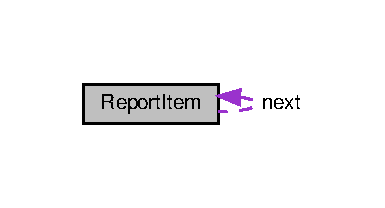
\includegraphics[width=185pt]{classReportItem__coll__graph}
\end{center}
\end{figure}
\subsection*{Public Member Functions}
\begin{DoxyCompactItemize}
\item 
\hyperlink{classReportItem_a6d059bb236cd2a0c208014d6e583f10c}{Report\+Item} ()
\item 
void \hyperlink{classReportItem_ac157ccd7df99762daef2974e3ae4ce04}{init} (void $\ast$\hyperlink{classReportItem_a23dfae0f15cac8c240e32b4c029e22e5}{node}, \hyperlink{reportitem_8h_ae4f179a72db5cca021a37ec4c6fe4c68}{Report\+Type} \hyperlink{classReportItem_a218d05d57bdd0f78ef0b73ec357716a5}{t}, int \hyperlink{classReportItem_a04d13a1753f531648fa47a887d8c3a48}{key})
\end{DoxyCompactItemize}
\subsection*{Public Attributes}
\begin{DoxyCompactItemize}
\item 
void $\ast$ \hyperlink{classReportItem_a23dfae0f15cac8c240e32b4c029e22e5}{node}
\item 
\hyperlink{reportitem_8h_ae4f179a72db5cca021a37ec4c6fe4c68}{Report\+Type} \hyperlink{classReportItem_a218d05d57bdd0f78ef0b73ec357716a5}{t}
\item 
\hyperlink{classReportItem}{Report\+Item} $\ast$volatile \hyperlink{classReportItem_a52ab69e393261dc12f3a57091c7a4b35}{next}
\item 
int \hyperlink{classReportItem_a04d13a1753f531648fa47a887d8c3a48}{key}
\item 
int \hyperlink{classReportItem_a0b902ca0b8b8ca4299c9b2d1fdc1b962}{id}
\end{DoxyCompactItemize}


\subsection{Constructor \& Destructor Documentation}
\mbox{\Hypertarget{classReportItem_a6d059bb236cd2a0c208014d6e583f10c}\label{classReportItem_a6d059bb236cd2a0c208014d6e583f10c}} 
\index{Report\+Item@{Report\+Item}!Report\+Item@{Report\+Item}}
\index{Report\+Item@{Report\+Item}!Report\+Item@{Report\+Item}}
\subsubsection{\texorpdfstring{Report\+Item()}{ReportItem()}}
{\footnotesize\ttfamily Report\+Item\+::\+Report\+Item (\begin{DoxyParamCaption}{ }\end{DoxyParamCaption})\hspace{0.3cm}{\ttfamily [inline]}}



\subsection{Member Function Documentation}
\mbox{\Hypertarget{classReportItem_ac157ccd7df99762daef2974e3ae4ce04}\label{classReportItem_ac157ccd7df99762daef2974e3ae4ce04}} 
\index{Report\+Item@{Report\+Item}!init@{init}}
\index{init@{init}!Report\+Item@{Report\+Item}}
\subsubsection{\texorpdfstring{init()}{init()}}
{\footnotesize\ttfamily void Report\+Item\+::init (\begin{DoxyParamCaption}\item[{void $\ast$}]{node,  }\item[{\hyperlink{reportitem_8h_ae4f179a72db5cca021a37ec4c6fe4c68}{Report\+Type}}]{t,  }\item[{int}]{key }\end{DoxyParamCaption})\hspace{0.3cm}{\ttfamily [inline]}}



\subsection{Member Data Documentation}
\mbox{\Hypertarget{classReportItem_a0b902ca0b8b8ca4299c9b2d1fdc1b962}\label{classReportItem_a0b902ca0b8b8ca4299c9b2d1fdc1b962}} 
\index{Report\+Item@{Report\+Item}!id@{id}}
\index{id@{id}!Report\+Item@{Report\+Item}}
\subsubsection{\texorpdfstring{id}{id}}
{\footnotesize\ttfamily int Report\+Item\+::id}

\mbox{\Hypertarget{classReportItem_a04d13a1753f531648fa47a887d8c3a48}\label{classReportItem_a04d13a1753f531648fa47a887d8c3a48}} 
\index{Report\+Item@{Report\+Item}!key@{key}}
\index{key@{key}!Report\+Item@{Report\+Item}}
\subsubsection{\texorpdfstring{key}{key}}
{\footnotesize\ttfamily int Report\+Item\+::key}

\mbox{\Hypertarget{classReportItem_a52ab69e393261dc12f3a57091c7a4b35}\label{classReportItem_a52ab69e393261dc12f3a57091c7a4b35}} 
\index{Report\+Item@{Report\+Item}!next@{next}}
\index{next@{next}!Report\+Item@{Report\+Item}}
\subsubsection{\texorpdfstring{next}{next}}
{\footnotesize\ttfamily \hyperlink{classReportItem}{Report\+Item}$\ast$ volatile Report\+Item\+::next}

\mbox{\Hypertarget{classReportItem_a23dfae0f15cac8c240e32b4c029e22e5}\label{classReportItem_a23dfae0f15cac8c240e32b4c029e22e5}} 
\index{Report\+Item@{Report\+Item}!node@{node}}
\index{node@{node}!Report\+Item@{Report\+Item}}
\subsubsection{\texorpdfstring{node}{node}}
{\footnotesize\ttfamily void$\ast$ Report\+Item\+::node}

\mbox{\Hypertarget{classReportItem_a218d05d57bdd0f78ef0b73ec357716a5}\label{classReportItem_a218d05d57bdd0f78ef0b73ec357716a5}} 
\index{Report\+Item@{Report\+Item}!t@{t}}
\index{t@{t}!Report\+Item@{Report\+Item}}
\subsubsection{\texorpdfstring{t}{t}}
{\footnotesize\ttfamily \hyperlink{reportitem_8h_ae4f179a72db5cca021a37ec4c6fe4c68}{Report\+Type} Report\+Item\+::t}



The documentation for this class was generated from the following file\+:\begin{DoxyCompactItemize}
\item 
common/rq/snapcollector/\hyperlink{reportitem_8h}{reportitem.\+h}\end{DoxyCompactItemize}

\hypertarget{structReqEntry}{}\section{Req\+Entry Struct Reference}
\label{structReqEntry}\index{Req\+Entry@{Req\+Entry}}


{\ttfamily \#include $<$row\+\_\+mvcc.\+h$>$}



Collaboration diagram for Req\+Entry\+:
\nopagebreak
\begin{figure}[H]
\begin{center}
\leavevmode
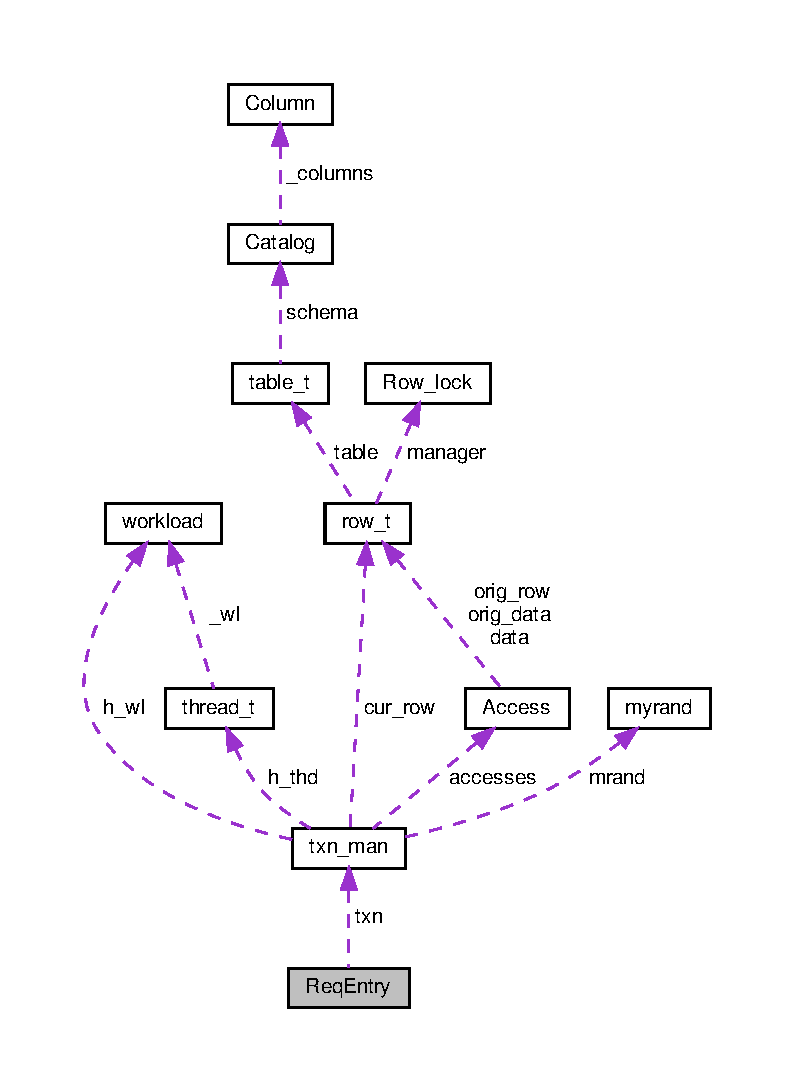
\includegraphics[width=350pt]{structReqEntry__coll__graph}
\end{center}
\end{figure}
\subsection*{Public Attributes}
\begin{DoxyCompactItemize}
\item 
bool \hyperlink{structReqEntry_adf58ab3907bca28ed97b38a2fb289f5e}{valid}
\item 
\hyperlink{global_8h_a1a7f6ca1462293fe053b5ae74a6c4eda}{Ts\+Type} \hyperlink{structReqEntry_a216343c4202bf87fc576c1c4ca196976}{type}
\item 
\hyperlink{global_8h_aaf095dfc9b10f757c968fe146ad7e724}{ts\+\_\+t} \hyperlink{structReqEntry_a17beb09e096dd264cbc8d8858ae05b50}{ts}
\item 
\hyperlink{classtxn__man}{txn\+\_\+man} $\ast$ \hyperlink{structReqEntry_a5d443d2daf5c317d30d91362d4ac9488}{txn}
\item 
\hyperlink{global_8h_aaf095dfc9b10f757c968fe146ad7e724}{ts\+\_\+t} \hyperlink{structReqEntry_a9f83460be32287f0247dc8a401b90bce}{time}
\end{DoxyCompactItemize}


\subsection{Member Data Documentation}
\mbox{\Hypertarget{structReqEntry_a9f83460be32287f0247dc8a401b90bce}\label{structReqEntry_a9f83460be32287f0247dc8a401b90bce}} 
\index{Req\+Entry@{Req\+Entry}!time@{time}}
\index{time@{time}!Req\+Entry@{Req\+Entry}}
\subsubsection{\texorpdfstring{time}{time}}
{\footnotesize\ttfamily \hyperlink{global_8h_aaf095dfc9b10f757c968fe146ad7e724}{ts\+\_\+t} Req\+Entry\+::time}

\mbox{\Hypertarget{structReqEntry_a17beb09e096dd264cbc8d8858ae05b50}\label{structReqEntry_a17beb09e096dd264cbc8d8858ae05b50}} 
\index{Req\+Entry@{Req\+Entry}!ts@{ts}}
\index{ts@{ts}!Req\+Entry@{Req\+Entry}}
\subsubsection{\texorpdfstring{ts}{ts}}
{\footnotesize\ttfamily \hyperlink{global_8h_aaf095dfc9b10f757c968fe146ad7e724}{ts\+\_\+t} Req\+Entry\+::ts}

\mbox{\Hypertarget{structReqEntry_a5d443d2daf5c317d30d91362d4ac9488}\label{structReqEntry_a5d443d2daf5c317d30d91362d4ac9488}} 
\index{Req\+Entry@{Req\+Entry}!txn@{txn}}
\index{txn@{txn}!Req\+Entry@{Req\+Entry}}
\subsubsection{\texorpdfstring{txn}{txn}}
{\footnotesize\ttfamily \hyperlink{classtxn__man}{txn\+\_\+man}$\ast$ Req\+Entry\+::txn}

\mbox{\Hypertarget{structReqEntry_a216343c4202bf87fc576c1c4ca196976}\label{structReqEntry_a216343c4202bf87fc576c1c4ca196976}} 
\index{Req\+Entry@{Req\+Entry}!type@{type}}
\index{type@{type}!Req\+Entry@{Req\+Entry}}
\subsubsection{\texorpdfstring{type}{type}}
{\footnotesize\ttfamily \hyperlink{global_8h_a1a7f6ca1462293fe053b5ae74a6c4eda}{Ts\+Type} Req\+Entry\+::type}

\mbox{\Hypertarget{structReqEntry_adf58ab3907bca28ed97b38a2fb289f5e}\label{structReqEntry_adf58ab3907bca28ed97b38a2fb289f5e}} 
\index{Req\+Entry@{Req\+Entry}!valid@{valid}}
\index{valid@{valid}!Req\+Entry@{Req\+Entry}}
\subsubsection{\texorpdfstring{valid}{valid}}
{\footnotesize\ttfamily bool Req\+Entry\+::valid}



The documentation for this struct was generated from the following file\+:\begin{DoxyCompactItemize}
\item 
macrobench/concurrency\+\_\+control/\hyperlink{row__mvcc_8h}{row\+\_\+mvcc.\+h}\end{DoxyCompactItemize}

\hypertarget{structrlu__data}{}\section{rlu\+\_\+data Struct Reference}
\label{structrlu__data}\index{rlu\+\_\+data@{rlu\+\_\+data}}
\subsection*{Public Attributes}
\begin{DoxyCompactItemize}
\item 
volatile long \hyperlink{structrlu__data_a47cdee11c643fc21a0ed4ff3c99c83f5}{n\+\_\+starts}
\item 
volatile long \hyperlink{structrlu__data_afe8f0d726df8efb4b871e08afe046b80}{n\+\_\+finish}
\item 
volatile long \hyperlink{structrlu__data_a50cc86d68682a52c13e979cbd37c2ddc}{n\+\_\+writers}
\item 
volatile long \hyperlink{structrlu__data_ad9b1e2669cb1ae055b8e664970396773}{n\+\_\+writer\+\_\+writeback}
\item 
volatile long \hyperlink{structrlu__data_a8973689669ad7e42ab1794a481fc8a54}{n\+\_\+writeback\+\_\+q\+\_\+iters}
\item 
volatile long \hyperlink{structrlu__data_ab9b0b9f86c51d1255ea0a330f82d0478}{n\+\_\+pure\+\_\+readers}
\item 
volatile long \hyperlink{structrlu__data_a2aedd0e822eb8aafd069bbd8130938a9}{n\+\_\+steals}
\item 
volatile long \hyperlink{structrlu__data_a2e34cf67956adae258242b466aa16cf8}{n\+\_\+aborts}
\item 
volatile long \hyperlink{structrlu__data_a9267129ca04e951ccd56b3770dffa1c3}{n\+\_\+sync\+\_\+requests}
\item 
volatile long \hyperlink{structrlu__data_a402f1dc4cf7856c1c88cf529a232b614}{n\+\_\+sync\+\_\+and\+\_\+writeback}
\end{DoxyCompactItemize}


\subsection{Member Data Documentation}
\mbox{\Hypertarget{structrlu__data_a2e34cf67956adae258242b466aa16cf8}\label{structrlu__data_a2e34cf67956adae258242b466aa16cf8}} 
\index{rlu\+\_\+data@{rlu\+\_\+data}!n\+\_\+aborts@{n\+\_\+aborts}}
\index{n\+\_\+aborts@{n\+\_\+aborts}!rlu\+\_\+data@{rlu\+\_\+data}}
\subsubsection{\texorpdfstring{n\+\_\+aborts}{n\_aborts}}
{\footnotesize\ttfamily volatile long rlu\+\_\+data\+::n\+\_\+aborts}

\mbox{\Hypertarget{structrlu__data_afe8f0d726df8efb4b871e08afe046b80}\label{structrlu__data_afe8f0d726df8efb4b871e08afe046b80}} 
\index{rlu\+\_\+data@{rlu\+\_\+data}!n\+\_\+finish@{n\+\_\+finish}}
\index{n\+\_\+finish@{n\+\_\+finish}!rlu\+\_\+data@{rlu\+\_\+data}}
\subsubsection{\texorpdfstring{n\+\_\+finish}{n\_finish}}
{\footnotesize\ttfamily volatile long rlu\+\_\+data\+::n\+\_\+finish}

\mbox{\Hypertarget{structrlu__data_ab9b0b9f86c51d1255ea0a330f82d0478}\label{structrlu__data_ab9b0b9f86c51d1255ea0a330f82d0478}} 
\index{rlu\+\_\+data@{rlu\+\_\+data}!n\+\_\+pure\+\_\+readers@{n\+\_\+pure\+\_\+readers}}
\index{n\+\_\+pure\+\_\+readers@{n\+\_\+pure\+\_\+readers}!rlu\+\_\+data@{rlu\+\_\+data}}
\subsubsection{\texorpdfstring{n\+\_\+pure\+\_\+readers}{n\_pure\_readers}}
{\footnotesize\ttfamily volatile long rlu\+\_\+data\+::n\+\_\+pure\+\_\+readers}

\mbox{\Hypertarget{structrlu__data_a47cdee11c643fc21a0ed4ff3c99c83f5}\label{structrlu__data_a47cdee11c643fc21a0ed4ff3c99c83f5}} 
\index{rlu\+\_\+data@{rlu\+\_\+data}!n\+\_\+starts@{n\+\_\+starts}}
\index{n\+\_\+starts@{n\+\_\+starts}!rlu\+\_\+data@{rlu\+\_\+data}}
\subsubsection{\texorpdfstring{n\+\_\+starts}{n\_starts}}
{\footnotesize\ttfamily volatile long rlu\+\_\+data\+::n\+\_\+starts}

\mbox{\Hypertarget{structrlu__data_a2aedd0e822eb8aafd069bbd8130938a9}\label{structrlu__data_a2aedd0e822eb8aafd069bbd8130938a9}} 
\index{rlu\+\_\+data@{rlu\+\_\+data}!n\+\_\+steals@{n\+\_\+steals}}
\index{n\+\_\+steals@{n\+\_\+steals}!rlu\+\_\+data@{rlu\+\_\+data}}
\subsubsection{\texorpdfstring{n\+\_\+steals}{n\_steals}}
{\footnotesize\ttfamily volatile long rlu\+\_\+data\+::n\+\_\+steals}

\mbox{\Hypertarget{structrlu__data_a402f1dc4cf7856c1c88cf529a232b614}\label{structrlu__data_a402f1dc4cf7856c1c88cf529a232b614}} 
\index{rlu\+\_\+data@{rlu\+\_\+data}!n\+\_\+sync\+\_\+and\+\_\+writeback@{n\+\_\+sync\+\_\+and\+\_\+writeback}}
\index{n\+\_\+sync\+\_\+and\+\_\+writeback@{n\+\_\+sync\+\_\+and\+\_\+writeback}!rlu\+\_\+data@{rlu\+\_\+data}}
\subsubsection{\texorpdfstring{n\+\_\+sync\+\_\+and\+\_\+writeback}{n\_sync\_and\_writeback}}
{\footnotesize\ttfamily volatile long rlu\+\_\+data\+::n\+\_\+sync\+\_\+and\+\_\+writeback}

\mbox{\Hypertarget{structrlu__data_a9267129ca04e951ccd56b3770dffa1c3}\label{structrlu__data_a9267129ca04e951ccd56b3770dffa1c3}} 
\index{rlu\+\_\+data@{rlu\+\_\+data}!n\+\_\+sync\+\_\+requests@{n\+\_\+sync\+\_\+requests}}
\index{n\+\_\+sync\+\_\+requests@{n\+\_\+sync\+\_\+requests}!rlu\+\_\+data@{rlu\+\_\+data}}
\subsubsection{\texorpdfstring{n\+\_\+sync\+\_\+requests}{n\_sync\_requests}}
{\footnotesize\ttfamily volatile long rlu\+\_\+data\+::n\+\_\+sync\+\_\+requests}

\mbox{\Hypertarget{structrlu__data_a8973689669ad7e42ab1794a481fc8a54}\label{structrlu__data_a8973689669ad7e42ab1794a481fc8a54}} 
\index{rlu\+\_\+data@{rlu\+\_\+data}!n\+\_\+writeback\+\_\+q\+\_\+iters@{n\+\_\+writeback\+\_\+q\+\_\+iters}}
\index{n\+\_\+writeback\+\_\+q\+\_\+iters@{n\+\_\+writeback\+\_\+q\+\_\+iters}!rlu\+\_\+data@{rlu\+\_\+data}}
\subsubsection{\texorpdfstring{n\+\_\+writeback\+\_\+q\+\_\+iters}{n\_writeback\_q\_iters}}
{\footnotesize\ttfamily volatile long rlu\+\_\+data\+::n\+\_\+writeback\+\_\+q\+\_\+iters}

\mbox{\Hypertarget{structrlu__data_ad9b1e2669cb1ae055b8e664970396773}\label{structrlu__data_ad9b1e2669cb1ae055b8e664970396773}} 
\index{rlu\+\_\+data@{rlu\+\_\+data}!n\+\_\+writer\+\_\+writeback@{n\+\_\+writer\+\_\+writeback}}
\index{n\+\_\+writer\+\_\+writeback@{n\+\_\+writer\+\_\+writeback}!rlu\+\_\+data@{rlu\+\_\+data}}
\subsubsection{\texorpdfstring{n\+\_\+writer\+\_\+writeback}{n\_writer\_writeback}}
{\footnotesize\ttfamily volatile long rlu\+\_\+data\+::n\+\_\+writer\+\_\+writeback}

\mbox{\Hypertarget{structrlu__data_a50cc86d68682a52c13e979cbd37c2ddc}\label{structrlu__data_a50cc86d68682a52c13e979cbd37c2ddc}} 
\index{rlu\+\_\+data@{rlu\+\_\+data}!n\+\_\+writers@{n\+\_\+writers}}
\index{n\+\_\+writers@{n\+\_\+writers}!rlu\+\_\+data@{rlu\+\_\+data}}
\subsubsection{\texorpdfstring{n\+\_\+writers}{n\_writers}}
{\footnotesize\ttfamily volatile long rlu\+\_\+data\+::n\+\_\+writers}



The documentation for this struct was generated from the following file\+:\begin{DoxyCompactItemize}
\item 
common/rlu/\hyperlink{rlu_8cpp}{rlu.\+cpp}\end{DoxyCompactItemize}

\hypertarget{structrlu__obj__header}{}\section{rlu\+\_\+obj\+\_\+header Struct Reference}
\label{structrlu__obj__header}\index{rlu\+\_\+obj\+\_\+header@{rlu\+\_\+obj\+\_\+header}}


{\ttfamily \#include $<$rlu.\+h$>$}

\subsection*{Public Attributes}
\begin{DoxyCompactItemize}
\item 
volatile intptr\+\_\+t $\ast$ \hyperlink{structrlu__obj__header_a3e9a2f4198a525a93e80677cf29d0cf0}{p\+\_\+obj\+\_\+copy}
\end{DoxyCompactItemize}


\subsection{Member Data Documentation}
\mbox{\Hypertarget{structrlu__obj__header_a3e9a2f4198a525a93e80677cf29d0cf0}\label{structrlu__obj__header_a3e9a2f4198a525a93e80677cf29d0cf0}} 
\index{rlu\+\_\+obj\+\_\+header@{rlu\+\_\+obj\+\_\+header}!p\+\_\+obj\+\_\+copy@{p\+\_\+obj\+\_\+copy}}
\index{p\+\_\+obj\+\_\+copy@{p\+\_\+obj\+\_\+copy}!rlu\+\_\+obj\+\_\+header@{rlu\+\_\+obj\+\_\+header}}
\subsubsection{\texorpdfstring{p\+\_\+obj\+\_\+copy}{p\_obj\_copy}}
{\footnotesize\ttfamily volatile intptr\+\_\+t$\ast$ rlu\+\_\+obj\+\_\+header\+::p\+\_\+obj\+\_\+copy}



The documentation for this struct was generated from the following file\+:\begin{DoxyCompactItemize}
\item 
common/rlu/\hyperlink{rlu_8h}{rlu.\+h}\end{DoxyCompactItemize}

\hypertarget{structrlu__thread__data}{}\section{rlu\+\_\+thread\+\_\+data Struct Reference}
\label{structrlu__thread__data}\index{rlu\+\_\+thread\+\_\+data@{rlu\+\_\+thread\+\_\+data}}


{\ttfamily \#include $<$rlu.\+h$>$}



Collaboration diagram for rlu\+\_\+thread\+\_\+data\+:
\nopagebreak
\begin{figure}[H]
\begin{center}
\leavevmode
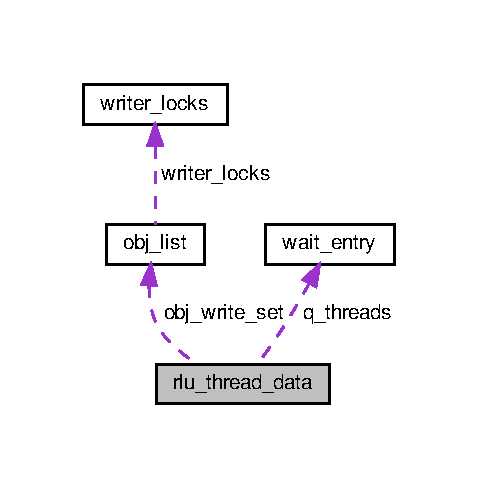
\includegraphics[width=230pt]{structrlu__thread__data__coll__graph}
\end{center}
\end{figure}
\subsection*{Public Attributes}
\begin{DoxyCompactItemize}
\item 
long \hyperlink{structrlu__thread__data_a5a7d06054f8da7781b58e235d0c3ff2a}{padding\+\_\+0} \mbox{[}\hyperlink{rlu_8h_a52e9bd0565eaf64830bc7e85dde5f5cb}{R\+L\+U\+\_\+\+D\+E\+F\+A\+U\+L\+T\+\_\+\+P\+A\+D\+D\+I\+NG}\mbox{]}
\item 
long \hyperlink{structrlu__thread__data_a25e80ec0edeca9833c8f862e024c3be1}{uniq\+\_\+id}
\item 
char \hyperlink{structrlu__thread__data_ae92b26446f5335b412fd81b49bed9a43}{is\+\_\+check\+\_\+locks}
\item 
char \hyperlink{structrlu__thread__data_a44a4f456fc8ac360eb58b711055ea1fe}{is\+\_\+write\+\_\+detected}
\item 
char \hyperlink{structrlu__thread__data_a53a0e2d43c35fcb4951b79f280ad992a}{is\+\_\+steal}
\item 
int \hyperlink{structrlu__thread__data_a3c6fda60f9fe062cf211b1f214999fb1}{type}
\item 
int \hyperlink{structrlu__thread__data_a8e1aa454552e3d76a007c8b1934e85a3}{max\+\_\+write\+\_\+sets}
\item 
long \hyperlink{structrlu__thread__data_a507495b36a9895a552ac4d6ff5af0ac5}{padding\+\_\+1} \mbox{[}\hyperlink{rlu_8h_a52e9bd0565eaf64830bc7e85dde5f5cb}{R\+L\+U\+\_\+\+D\+E\+F\+A\+U\+L\+T\+\_\+\+P\+A\+D\+D\+I\+NG}\mbox{]}
\item 
volatile unsigned long \hyperlink{structrlu__thread__data_a24a65bd3d29cd124c6f17ab7ff99513c}{run\+\_\+counter}
\item 
volatile long \hyperlink{structrlu__thread__data_a5cfd4d999cc6716c89d94dd36760b438}{local\+\_\+version}
\item 
volatile long \hyperlink{structrlu__thread__data_afbfdf9a44213147761485025bcb7e5b6}{local\+\_\+commit\+\_\+version}
\item 
volatile long \hyperlink{structrlu__thread__data_ab3302a4de8e3c2b66060a520e29ce48d}{is\+\_\+no\+\_\+quiescence}
\item 
volatile long \hyperlink{structrlu__thread__data_a54621ad6a0876a5e5d386b5646d82616}{is\+\_\+sync}
\item 
long \hyperlink{structrlu__thread__data_a0f5fdf2d7b6d6065ff36503841689cd5}{padding\+\_\+2} \mbox{[}\hyperlink{rlu_8h_a52e9bd0565eaf64830bc7e85dde5f5cb}{R\+L\+U\+\_\+\+D\+E\+F\+A\+U\+L\+T\+\_\+\+P\+A\+D\+D\+I\+NG}\mbox{]}
\item 
volatile long \hyperlink{structrlu__thread__data_a9aa03c237e23a780a415a2cd00e7b754}{writer\+\_\+version}
\item 
volatile long \hyperlink{structrlu__thread__data_a5f0720b2f9ca2327e77a2c8bf3fc6cff}{last\+\_\+writer\+\_\+version}
\item 
long \hyperlink{structrlu__thread__data_a4c6ae226f879a355165953bbbb5d1e99}{padding\+\_\+3} \mbox{[}\hyperlink{rlu_8h_a52e9bd0565eaf64830bc7e85dde5f5cb}{R\+L\+U\+\_\+\+D\+E\+F\+A\+U\+L\+T\+\_\+\+P\+A\+D\+D\+I\+NG}\mbox{]}
\item 
\hyperlink{rlu_8h_ac547e16d21c2e118a24c05808c00f647}{wait\+\_\+entry\+\_\+t} \hyperlink{structrlu__thread__data_adc4ec9312cf5ffec29f6b754f0f52e1c}{q\+\_\+threads} \mbox{[}\hyperlink{rlu_8h_ac652bd82ef9dbb2f1caa3fde5aac0342}{R\+L\+U\+\_\+\+M\+A\+X\+\_\+\+T\+H\+R\+E\+A\+DS}\mbox{]}
\item 
long \hyperlink{structrlu__thread__data_a9903b6c56b5d29a490b29cac6c8a4618}{ws\+\_\+head\+\_\+counter}
\item 
long \hyperlink{structrlu__thread__data_a3df86ec9553b9f02863953e401b40a3d}{ws\+\_\+wb\+\_\+counter}
\item 
long \hyperlink{structrlu__thread__data_a78a6017eff847fa8ea911c0cc872a703}{ws\+\_\+tail\+\_\+counter}
\item 
long \hyperlink{structrlu__thread__data_a4880c9e3ba05861f5e61352a68025d75}{ws\+\_\+cur\+\_\+id}
\item 
volatile \hyperlink{rlu_8h_aa40041a4e841917201bb69f0eb22bbd8}{obj\+\_\+list\+\_\+t} \hyperlink{structrlu__thread__data_a13a84fcdbcde59c82753123a1504dc86}{obj\+\_\+write\+\_\+set} \mbox{[}\hyperlink{rlu_8h_a2691d3248435c1cb153c0f6212828599}{R\+L\+U\+\_\+\+M\+A\+X\+\_\+\+W\+R\+I\+T\+E\+\_\+\+S\+E\+TS}\mbox{]}
\item 
long \hyperlink{structrlu__thread__data_ad99ac9d070599c170be24c096931eaa4}{padding\+\_\+4} \mbox{[}\hyperlink{rlu_8h_a52e9bd0565eaf64830bc7e85dde5f5cb}{R\+L\+U\+\_\+\+D\+E\+F\+A\+U\+L\+T\+\_\+\+P\+A\+D\+D\+I\+NG}\mbox{]}
\item 
long \hyperlink{structrlu__thread__data_a325dadbf34f223fa1f92d91ca3814675}{free\+\_\+nodes\+\_\+size}
\item 
intptr\+\_\+t $\ast$ \hyperlink{structrlu__thread__data_a44b3c5b3c0b42a7cd0bc0db1f0f2b2d9}{free\+\_\+nodes} \mbox{[}\hyperlink{rlu_8h_adddd843b034425fcae964e749834af44}{R\+L\+U\+\_\+\+M\+A\+X\+\_\+\+F\+R\+E\+E\+\_\+\+N\+O\+D\+ES}\mbox{]}
\item 
long \hyperlink{structrlu__thread__data_afc656237075c8764b71cae61b2648427}{padding\+\_\+5} \mbox{[}\hyperlink{rlu_8h_a52e9bd0565eaf64830bc7e85dde5f5cb}{R\+L\+U\+\_\+\+D\+E\+F\+A\+U\+L\+T\+\_\+\+P\+A\+D\+D\+I\+NG}\mbox{]}
\item 
long \hyperlink{structrlu__thread__data_af364d4681a22508dd2d44a60e4c5cd20}{n\+\_\+starts}
\item 
long \hyperlink{structrlu__thread__data_a3275393f5044fd11f6d2beb852573e79}{n\+\_\+finish}
\item 
long \hyperlink{structrlu__thread__data_a2c973d93f6b6a5422ef4f48461d196c3}{n\+\_\+writers}
\item 
long \hyperlink{structrlu__thread__data_a913d842253b153fd49f8390cd56988a9}{n\+\_\+writer\+\_\+writeback}
\item 
long \hyperlink{structrlu__thread__data_a13f452b4e62710231db05b8e8aca7f7a}{n\+\_\+pure\+\_\+readers}
\item 
long \hyperlink{structrlu__thread__data_a56e86f4e465d90e6c525c564b02b184e}{n\+\_\+aborts}
\item 
long \hyperlink{structrlu__thread__data_abf11e9e4e07b70096e7aa80c15a93b1b}{n\+\_\+steals}
\item 
long \hyperlink{structrlu__thread__data_a04ced688615775605d5a6047148b87df}{n\+\_\+writer\+\_\+sync\+\_\+waits}
\item 
long \hyperlink{structrlu__thread__data_aec97063115cd2844a36516b366471444}{n\+\_\+writeback\+\_\+q\+\_\+iters}
\item 
long \hyperlink{structrlu__thread__data_a58b83dc3c85c90b929b71c451378bc57}{n\+\_\+sync\+\_\+requests}
\item 
long \hyperlink{structrlu__thread__data_a7fed5939d4fb4d5b554c25f378b7838d}{n\+\_\+sync\+\_\+and\+\_\+writeback}
\item 
long \hyperlink{structrlu__thread__data_af2b921e98760e866cee69add1d02ca73}{padding\+\_\+6} \mbox{[}\hyperlink{rlu_8h_a52e9bd0565eaf64830bc7e85dde5f5cb}{R\+L\+U\+\_\+\+D\+E\+F\+A\+U\+L\+T\+\_\+\+P\+A\+D\+D\+I\+NG}\mbox{]}
\end{DoxyCompactItemize}


\subsection{Member Data Documentation}
\mbox{\Hypertarget{structrlu__thread__data_a44b3c5b3c0b42a7cd0bc0db1f0f2b2d9}\label{structrlu__thread__data_a44b3c5b3c0b42a7cd0bc0db1f0f2b2d9}} 
\index{rlu\+\_\+thread\+\_\+data@{rlu\+\_\+thread\+\_\+data}!free\+\_\+nodes@{free\+\_\+nodes}}
\index{free\+\_\+nodes@{free\+\_\+nodes}!rlu\+\_\+thread\+\_\+data@{rlu\+\_\+thread\+\_\+data}}
\subsubsection{\texorpdfstring{free\+\_\+nodes}{free\_nodes}}
{\footnotesize\ttfamily intptr\+\_\+t$\ast$ rlu\+\_\+thread\+\_\+data\+::free\+\_\+nodes\mbox{[}\hyperlink{rlu_8h_adddd843b034425fcae964e749834af44}{R\+L\+U\+\_\+\+M\+A\+X\+\_\+\+F\+R\+E\+E\+\_\+\+N\+O\+D\+ES}\mbox{]}}

\mbox{\Hypertarget{structrlu__thread__data_a325dadbf34f223fa1f92d91ca3814675}\label{structrlu__thread__data_a325dadbf34f223fa1f92d91ca3814675}} 
\index{rlu\+\_\+thread\+\_\+data@{rlu\+\_\+thread\+\_\+data}!free\+\_\+nodes\+\_\+size@{free\+\_\+nodes\+\_\+size}}
\index{free\+\_\+nodes\+\_\+size@{free\+\_\+nodes\+\_\+size}!rlu\+\_\+thread\+\_\+data@{rlu\+\_\+thread\+\_\+data}}
\subsubsection{\texorpdfstring{free\+\_\+nodes\+\_\+size}{free\_nodes\_size}}
{\footnotesize\ttfamily long rlu\+\_\+thread\+\_\+data\+::free\+\_\+nodes\+\_\+size}

\mbox{\Hypertarget{structrlu__thread__data_ae92b26446f5335b412fd81b49bed9a43}\label{structrlu__thread__data_ae92b26446f5335b412fd81b49bed9a43}} 
\index{rlu\+\_\+thread\+\_\+data@{rlu\+\_\+thread\+\_\+data}!is\+\_\+check\+\_\+locks@{is\+\_\+check\+\_\+locks}}
\index{is\+\_\+check\+\_\+locks@{is\+\_\+check\+\_\+locks}!rlu\+\_\+thread\+\_\+data@{rlu\+\_\+thread\+\_\+data}}
\subsubsection{\texorpdfstring{is\+\_\+check\+\_\+locks}{is\_check\_locks}}
{\footnotesize\ttfamily char rlu\+\_\+thread\+\_\+data\+::is\+\_\+check\+\_\+locks}

\mbox{\Hypertarget{structrlu__thread__data_ab3302a4de8e3c2b66060a520e29ce48d}\label{structrlu__thread__data_ab3302a4de8e3c2b66060a520e29ce48d}} 
\index{rlu\+\_\+thread\+\_\+data@{rlu\+\_\+thread\+\_\+data}!is\+\_\+no\+\_\+quiescence@{is\+\_\+no\+\_\+quiescence}}
\index{is\+\_\+no\+\_\+quiescence@{is\+\_\+no\+\_\+quiescence}!rlu\+\_\+thread\+\_\+data@{rlu\+\_\+thread\+\_\+data}}
\subsubsection{\texorpdfstring{is\+\_\+no\+\_\+quiescence}{is\_no\_quiescence}}
{\footnotesize\ttfamily volatile long rlu\+\_\+thread\+\_\+data\+::is\+\_\+no\+\_\+quiescence}

\mbox{\Hypertarget{structrlu__thread__data_a53a0e2d43c35fcb4951b79f280ad992a}\label{structrlu__thread__data_a53a0e2d43c35fcb4951b79f280ad992a}} 
\index{rlu\+\_\+thread\+\_\+data@{rlu\+\_\+thread\+\_\+data}!is\+\_\+steal@{is\+\_\+steal}}
\index{is\+\_\+steal@{is\+\_\+steal}!rlu\+\_\+thread\+\_\+data@{rlu\+\_\+thread\+\_\+data}}
\subsubsection{\texorpdfstring{is\+\_\+steal}{is\_steal}}
{\footnotesize\ttfamily char rlu\+\_\+thread\+\_\+data\+::is\+\_\+steal}

\mbox{\Hypertarget{structrlu__thread__data_a54621ad6a0876a5e5d386b5646d82616}\label{structrlu__thread__data_a54621ad6a0876a5e5d386b5646d82616}} 
\index{rlu\+\_\+thread\+\_\+data@{rlu\+\_\+thread\+\_\+data}!is\+\_\+sync@{is\+\_\+sync}}
\index{is\+\_\+sync@{is\+\_\+sync}!rlu\+\_\+thread\+\_\+data@{rlu\+\_\+thread\+\_\+data}}
\subsubsection{\texorpdfstring{is\+\_\+sync}{is\_sync}}
{\footnotesize\ttfamily volatile long rlu\+\_\+thread\+\_\+data\+::is\+\_\+sync}

\mbox{\Hypertarget{structrlu__thread__data_a44a4f456fc8ac360eb58b711055ea1fe}\label{structrlu__thread__data_a44a4f456fc8ac360eb58b711055ea1fe}} 
\index{rlu\+\_\+thread\+\_\+data@{rlu\+\_\+thread\+\_\+data}!is\+\_\+write\+\_\+detected@{is\+\_\+write\+\_\+detected}}
\index{is\+\_\+write\+\_\+detected@{is\+\_\+write\+\_\+detected}!rlu\+\_\+thread\+\_\+data@{rlu\+\_\+thread\+\_\+data}}
\subsubsection{\texorpdfstring{is\+\_\+write\+\_\+detected}{is\_write\_detected}}
{\footnotesize\ttfamily char rlu\+\_\+thread\+\_\+data\+::is\+\_\+write\+\_\+detected}

\mbox{\Hypertarget{structrlu__thread__data_a5f0720b2f9ca2327e77a2c8bf3fc6cff}\label{structrlu__thread__data_a5f0720b2f9ca2327e77a2c8bf3fc6cff}} 
\index{rlu\+\_\+thread\+\_\+data@{rlu\+\_\+thread\+\_\+data}!last\+\_\+writer\+\_\+version@{last\+\_\+writer\+\_\+version}}
\index{last\+\_\+writer\+\_\+version@{last\+\_\+writer\+\_\+version}!rlu\+\_\+thread\+\_\+data@{rlu\+\_\+thread\+\_\+data}}
\subsubsection{\texorpdfstring{last\+\_\+writer\+\_\+version}{last\_writer\_version}}
{\footnotesize\ttfamily volatile long rlu\+\_\+thread\+\_\+data\+::last\+\_\+writer\+\_\+version}

\mbox{\Hypertarget{structrlu__thread__data_afbfdf9a44213147761485025bcb7e5b6}\label{structrlu__thread__data_afbfdf9a44213147761485025bcb7e5b6}} 
\index{rlu\+\_\+thread\+\_\+data@{rlu\+\_\+thread\+\_\+data}!local\+\_\+commit\+\_\+version@{local\+\_\+commit\+\_\+version}}
\index{local\+\_\+commit\+\_\+version@{local\+\_\+commit\+\_\+version}!rlu\+\_\+thread\+\_\+data@{rlu\+\_\+thread\+\_\+data}}
\subsubsection{\texorpdfstring{local\+\_\+commit\+\_\+version}{local\_commit\_version}}
{\footnotesize\ttfamily volatile long rlu\+\_\+thread\+\_\+data\+::local\+\_\+commit\+\_\+version}

\mbox{\Hypertarget{structrlu__thread__data_a5cfd4d999cc6716c89d94dd36760b438}\label{structrlu__thread__data_a5cfd4d999cc6716c89d94dd36760b438}} 
\index{rlu\+\_\+thread\+\_\+data@{rlu\+\_\+thread\+\_\+data}!local\+\_\+version@{local\+\_\+version}}
\index{local\+\_\+version@{local\+\_\+version}!rlu\+\_\+thread\+\_\+data@{rlu\+\_\+thread\+\_\+data}}
\subsubsection{\texorpdfstring{local\+\_\+version}{local\_version}}
{\footnotesize\ttfamily volatile long rlu\+\_\+thread\+\_\+data\+::local\+\_\+version}

\mbox{\Hypertarget{structrlu__thread__data_a8e1aa454552e3d76a007c8b1934e85a3}\label{structrlu__thread__data_a8e1aa454552e3d76a007c8b1934e85a3}} 
\index{rlu\+\_\+thread\+\_\+data@{rlu\+\_\+thread\+\_\+data}!max\+\_\+write\+\_\+sets@{max\+\_\+write\+\_\+sets}}
\index{max\+\_\+write\+\_\+sets@{max\+\_\+write\+\_\+sets}!rlu\+\_\+thread\+\_\+data@{rlu\+\_\+thread\+\_\+data}}
\subsubsection{\texorpdfstring{max\+\_\+write\+\_\+sets}{max\_write\_sets}}
{\footnotesize\ttfamily int rlu\+\_\+thread\+\_\+data\+::max\+\_\+write\+\_\+sets}

\mbox{\Hypertarget{structrlu__thread__data_a56e86f4e465d90e6c525c564b02b184e}\label{structrlu__thread__data_a56e86f4e465d90e6c525c564b02b184e}} 
\index{rlu\+\_\+thread\+\_\+data@{rlu\+\_\+thread\+\_\+data}!n\+\_\+aborts@{n\+\_\+aborts}}
\index{n\+\_\+aborts@{n\+\_\+aborts}!rlu\+\_\+thread\+\_\+data@{rlu\+\_\+thread\+\_\+data}}
\subsubsection{\texorpdfstring{n\+\_\+aborts}{n\_aborts}}
{\footnotesize\ttfamily long rlu\+\_\+thread\+\_\+data\+::n\+\_\+aborts}

\mbox{\Hypertarget{structrlu__thread__data_a3275393f5044fd11f6d2beb852573e79}\label{structrlu__thread__data_a3275393f5044fd11f6d2beb852573e79}} 
\index{rlu\+\_\+thread\+\_\+data@{rlu\+\_\+thread\+\_\+data}!n\+\_\+finish@{n\+\_\+finish}}
\index{n\+\_\+finish@{n\+\_\+finish}!rlu\+\_\+thread\+\_\+data@{rlu\+\_\+thread\+\_\+data}}
\subsubsection{\texorpdfstring{n\+\_\+finish}{n\_finish}}
{\footnotesize\ttfamily long rlu\+\_\+thread\+\_\+data\+::n\+\_\+finish}

\mbox{\Hypertarget{structrlu__thread__data_a13f452b4e62710231db05b8e8aca7f7a}\label{structrlu__thread__data_a13f452b4e62710231db05b8e8aca7f7a}} 
\index{rlu\+\_\+thread\+\_\+data@{rlu\+\_\+thread\+\_\+data}!n\+\_\+pure\+\_\+readers@{n\+\_\+pure\+\_\+readers}}
\index{n\+\_\+pure\+\_\+readers@{n\+\_\+pure\+\_\+readers}!rlu\+\_\+thread\+\_\+data@{rlu\+\_\+thread\+\_\+data}}
\subsubsection{\texorpdfstring{n\+\_\+pure\+\_\+readers}{n\_pure\_readers}}
{\footnotesize\ttfamily long rlu\+\_\+thread\+\_\+data\+::n\+\_\+pure\+\_\+readers}

\mbox{\Hypertarget{structrlu__thread__data_af364d4681a22508dd2d44a60e4c5cd20}\label{structrlu__thread__data_af364d4681a22508dd2d44a60e4c5cd20}} 
\index{rlu\+\_\+thread\+\_\+data@{rlu\+\_\+thread\+\_\+data}!n\+\_\+starts@{n\+\_\+starts}}
\index{n\+\_\+starts@{n\+\_\+starts}!rlu\+\_\+thread\+\_\+data@{rlu\+\_\+thread\+\_\+data}}
\subsubsection{\texorpdfstring{n\+\_\+starts}{n\_starts}}
{\footnotesize\ttfamily long rlu\+\_\+thread\+\_\+data\+::n\+\_\+starts}

\mbox{\Hypertarget{structrlu__thread__data_abf11e9e4e07b70096e7aa80c15a93b1b}\label{structrlu__thread__data_abf11e9e4e07b70096e7aa80c15a93b1b}} 
\index{rlu\+\_\+thread\+\_\+data@{rlu\+\_\+thread\+\_\+data}!n\+\_\+steals@{n\+\_\+steals}}
\index{n\+\_\+steals@{n\+\_\+steals}!rlu\+\_\+thread\+\_\+data@{rlu\+\_\+thread\+\_\+data}}
\subsubsection{\texorpdfstring{n\+\_\+steals}{n\_steals}}
{\footnotesize\ttfamily long rlu\+\_\+thread\+\_\+data\+::n\+\_\+steals}

\mbox{\Hypertarget{structrlu__thread__data_a7fed5939d4fb4d5b554c25f378b7838d}\label{structrlu__thread__data_a7fed5939d4fb4d5b554c25f378b7838d}} 
\index{rlu\+\_\+thread\+\_\+data@{rlu\+\_\+thread\+\_\+data}!n\+\_\+sync\+\_\+and\+\_\+writeback@{n\+\_\+sync\+\_\+and\+\_\+writeback}}
\index{n\+\_\+sync\+\_\+and\+\_\+writeback@{n\+\_\+sync\+\_\+and\+\_\+writeback}!rlu\+\_\+thread\+\_\+data@{rlu\+\_\+thread\+\_\+data}}
\subsubsection{\texorpdfstring{n\+\_\+sync\+\_\+and\+\_\+writeback}{n\_sync\_and\_writeback}}
{\footnotesize\ttfamily long rlu\+\_\+thread\+\_\+data\+::n\+\_\+sync\+\_\+and\+\_\+writeback}

\mbox{\Hypertarget{structrlu__thread__data_a58b83dc3c85c90b929b71c451378bc57}\label{structrlu__thread__data_a58b83dc3c85c90b929b71c451378bc57}} 
\index{rlu\+\_\+thread\+\_\+data@{rlu\+\_\+thread\+\_\+data}!n\+\_\+sync\+\_\+requests@{n\+\_\+sync\+\_\+requests}}
\index{n\+\_\+sync\+\_\+requests@{n\+\_\+sync\+\_\+requests}!rlu\+\_\+thread\+\_\+data@{rlu\+\_\+thread\+\_\+data}}
\subsubsection{\texorpdfstring{n\+\_\+sync\+\_\+requests}{n\_sync\_requests}}
{\footnotesize\ttfamily long rlu\+\_\+thread\+\_\+data\+::n\+\_\+sync\+\_\+requests}

\mbox{\Hypertarget{structrlu__thread__data_aec97063115cd2844a36516b366471444}\label{structrlu__thread__data_aec97063115cd2844a36516b366471444}} 
\index{rlu\+\_\+thread\+\_\+data@{rlu\+\_\+thread\+\_\+data}!n\+\_\+writeback\+\_\+q\+\_\+iters@{n\+\_\+writeback\+\_\+q\+\_\+iters}}
\index{n\+\_\+writeback\+\_\+q\+\_\+iters@{n\+\_\+writeback\+\_\+q\+\_\+iters}!rlu\+\_\+thread\+\_\+data@{rlu\+\_\+thread\+\_\+data}}
\subsubsection{\texorpdfstring{n\+\_\+writeback\+\_\+q\+\_\+iters}{n\_writeback\_q\_iters}}
{\footnotesize\ttfamily long rlu\+\_\+thread\+\_\+data\+::n\+\_\+writeback\+\_\+q\+\_\+iters}

\mbox{\Hypertarget{structrlu__thread__data_a04ced688615775605d5a6047148b87df}\label{structrlu__thread__data_a04ced688615775605d5a6047148b87df}} 
\index{rlu\+\_\+thread\+\_\+data@{rlu\+\_\+thread\+\_\+data}!n\+\_\+writer\+\_\+sync\+\_\+waits@{n\+\_\+writer\+\_\+sync\+\_\+waits}}
\index{n\+\_\+writer\+\_\+sync\+\_\+waits@{n\+\_\+writer\+\_\+sync\+\_\+waits}!rlu\+\_\+thread\+\_\+data@{rlu\+\_\+thread\+\_\+data}}
\subsubsection{\texorpdfstring{n\+\_\+writer\+\_\+sync\+\_\+waits}{n\_writer\_sync\_waits}}
{\footnotesize\ttfamily long rlu\+\_\+thread\+\_\+data\+::n\+\_\+writer\+\_\+sync\+\_\+waits}

\mbox{\Hypertarget{structrlu__thread__data_a913d842253b153fd49f8390cd56988a9}\label{structrlu__thread__data_a913d842253b153fd49f8390cd56988a9}} 
\index{rlu\+\_\+thread\+\_\+data@{rlu\+\_\+thread\+\_\+data}!n\+\_\+writer\+\_\+writeback@{n\+\_\+writer\+\_\+writeback}}
\index{n\+\_\+writer\+\_\+writeback@{n\+\_\+writer\+\_\+writeback}!rlu\+\_\+thread\+\_\+data@{rlu\+\_\+thread\+\_\+data}}
\subsubsection{\texorpdfstring{n\+\_\+writer\+\_\+writeback}{n\_writer\_writeback}}
{\footnotesize\ttfamily long rlu\+\_\+thread\+\_\+data\+::n\+\_\+writer\+\_\+writeback}

\mbox{\Hypertarget{structrlu__thread__data_a2c973d93f6b6a5422ef4f48461d196c3}\label{structrlu__thread__data_a2c973d93f6b6a5422ef4f48461d196c3}} 
\index{rlu\+\_\+thread\+\_\+data@{rlu\+\_\+thread\+\_\+data}!n\+\_\+writers@{n\+\_\+writers}}
\index{n\+\_\+writers@{n\+\_\+writers}!rlu\+\_\+thread\+\_\+data@{rlu\+\_\+thread\+\_\+data}}
\subsubsection{\texorpdfstring{n\+\_\+writers}{n\_writers}}
{\footnotesize\ttfamily long rlu\+\_\+thread\+\_\+data\+::n\+\_\+writers}

\mbox{\Hypertarget{structrlu__thread__data_a13a84fcdbcde59c82753123a1504dc86}\label{structrlu__thread__data_a13a84fcdbcde59c82753123a1504dc86}} 
\index{rlu\+\_\+thread\+\_\+data@{rlu\+\_\+thread\+\_\+data}!obj\+\_\+write\+\_\+set@{obj\+\_\+write\+\_\+set}}
\index{obj\+\_\+write\+\_\+set@{obj\+\_\+write\+\_\+set}!rlu\+\_\+thread\+\_\+data@{rlu\+\_\+thread\+\_\+data}}
\subsubsection{\texorpdfstring{obj\+\_\+write\+\_\+set}{obj\_write\_set}}
{\footnotesize\ttfamily volatile \hyperlink{rlu_8h_aa40041a4e841917201bb69f0eb22bbd8}{obj\+\_\+list\+\_\+t} rlu\+\_\+thread\+\_\+data\+::obj\+\_\+write\+\_\+set\mbox{[}\hyperlink{rlu_8h_a2691d3248435c1cb153c0f6212828599}{R\+L\+U\+\_\+\+M\+A\+X\+\_\+\+W\+R\+I\+T\+E\+\_\+\+S\+E\+TS}\mbox{]}}

\mbox{\Hypertarget{structrlu__thread__data_a5a7d06054f8da7781b58e235d0c3ff2a}\label{structrlu__thread__data_a5a7d06054f8da7781b58e235d0c3ff2a}} 
\index{rlu\+\_\+thread\+\_\+data@{rlu\+\_\+thread\+\_\+data}!padding\+\_\+0@{padding\+\_\+0}}
\index{padding\+\_\+0@{padding\+\_\+0}!rlu\+\_\+thread\+\_\+data@{rlu\+\_\+thread\+\_\+data}}
\subsubsection{\texorpdfstring{padding\+\_\+0}{padding\_0}}
{\footnotesize\ttfamily long rlu\+\_\+thread\+\_\+data\+::padding\+\_\+0\mbox{[}\hyperlink{rlu_8h_a52e9bd0565eaf64830bc7e85dde5f5cb}{R\+L\+U\+\_\+\+D\+E\+F\+A\+U\+L\+T\+\_\+\+P\+A\+D\+D\+I\+NG}\mbox{]}}

\mbox{\Hypertarget{structrlu__thread__data_a507495b36a9895a552ac4d6ff5af0ac5}\label{structrlu__thread__data_a507495b36a9895a552ac4d6ff5af0ac5}} 
\index{rlu\+\_\+thread\+\_\+data@{rlu\+\_\+thread\+\_\+data}!padding\+\_\+1@{padding\+\_\+1}}
\index{padding\+\_\+1@{padding\+\_\+1}!rlu\+\_\+thread\+\_\+data@{rlu\+\_\+thread\+\_\+data}}
\subsubsection{\texorpdfstring{padding\+\_\+1}{padding\_1}}
{\footnotesize\ttfamily long rlu\+\_\+thread\+\_\+data\+::padding\+\_\+1\mbox{[}\hyperlink{rlu_8h_a52e9bd0565eaf64830bc7e85dde5f5cb}{R\+L\+U\+\_\+\+D\+E\+F\+A\+U\+L\+T\+\_\+\+P\+A\+D\+D\+I\+NG}\mbox{]}}

\mbox{\Hypertarget{structrlu__thread__data_a0f5fdf2d7b6d6065ff36503841689cd5}\label{structrlu__thread__data_a0f5fdf2d7b6d6065ff36503841689cd5}} 
\index{rlu\+\_\+thread\+\_\+data@{rlu\+\_\+thread\+\_\+data}!padding\+\_\+2@{padding\+\_\+2}}
\index{padding\+\_\+2@{padding\+\_\+2}!rlu\+\_\+thread\+\_\+data@{rlu\+\_\+thread\+\_\+data}}
\subsubsection{\texorpdfstring{padding\+\_\+2}{padding\_2}}
{\footnotesize\ttfamily long rlu\+\_\+thread\+\_\+data\+::padding\+\_\+2\mbox{[}\hyperlink{rlu_8h_a52e9bd0565eaf64830bc7e85dde5f5cb}{R\+L\+U\+\_\+\+D\+E\+F\+A\+U\+L\+T\+\_\+\+P\+A\+D\+D\+I\+NG}\mbox{]}}

\mbox{\Hypertarget{structrlu__thread__data_a4c6ae226f879a355165953bbbb5d1e99}\label{structrlu__thread__data_a4c6ae226f879a355165953bbbb5d1e99}} 
\index{rlu\+\_\+thread\+\_\+data@{rlu\+\_\+thread\+\_\+data}!padding\+\_\+3@{padding\+\_\+3}}
\index{padding\+\_\+3@{padding\+\_\+3}!rlu\+\_\+thread\+\_\+data@{rlu\+\_\+thread\+\_\+data}}
\subsubsection{\texorpdfstring{padding\+\_\+3}{padding\_3}}
{\footnotesize\ttfamily long rlu\+\_\+thread\+\_\+data\+::padding\+\_\+3\mbox{[}\hyperlink{rlu_8h_a52e9bd0565eaf64830bc7e85dde5f5cb}{R\+L\+U\+\_\+\+D\+E\+F\+A\+U\+L\+T\+\_\+\+P\+A\+D\+D\+I\+NG}\mbox{]}}

\mbox{\Hypertarget{structrlu__thread__data_ad99ac9d070599c170be24c096931eaa4}\label{structrlu__thread__data_ad99ac9d070599c170be24c096931eaa4}} 
\index{rlu\+\_\+thread\+\_\+data@{rlu\+\_\+thread\+\_\+data}!padding\+\_\+4@{padding\+\_\+4}}
\index{padding\+\_\+4@{padding\+\_\+4}!rlu\+\_\+thread\+\_\+data@{rlu\+\_\+thread\+\_\+data}}
\subsubsection{\texorpdfstring{padding\+\_\+4}{padding\_4}}
{\footnotesize\ttfamily long rlu\+\_\+thread\+\_\+data\+::padding\+\_\+4\mbox{[}\hyperlink{rlu_8h_a52e9bd0565eaf64830bc7e85dde5f5cb}{R\+L\+U\+\_\+\+D\+E\+F\+A\+U\+L\+T\+\_\+\+P\+A\+D\+D\+I\+NG}\mbox{]}}

\mbox{\Hypertarget{structrlu__thread__data_afc656237075c8764b71cae61b2648427}\label{structrlu__thread__data_afc656237075c8764b71cae61b2648427}} 
\index{rlu\+\_\+thread\+\_\+data@{rlu\+\_\+thread\+\_\+data}!padding\+\_\+5@{padding\+\_\+5}}
\index{padding\+\_\+5@{padding\+\_\+5}!rlu\+\_\+thread\+\_\+data@{rlu\+\_\+thread\+\_\+data}}
\subsubsection{\texorpdfstring{padding\+\_\+5}{padding\_5}}
{\footnotesize\ttfamily long rlu\+\_\+thread\+\_\+data\+::padding\+\_\+5\mbox{[}\hyperlink{rlu_8h_a52e9bd0565eaf64830bc7e85dde5f5cb}{R\+L\+U\+\_\+\+D\+E\+F\+A\+U\+L\+T\+\_\+\+P\+A\+D\+D\+I\+NG}\mbox{]}}

\mbox{\Hypertarget{structrlu__thread__data_af2b921e98760e866cee69add1d02ca73}\label{structrlu__thread__data_af2b921e98760e866cee69add1d02ca73}} 
\index{rlu\+\_\+thread\+\_\+data@{rlu\+\_\+thread\+\_\+data}!padding\+\_\+6@{padding\+\_\+6}}
\index{padding\+\_\+6@{padding\+\_\+6}!rlu\+\_\+thread\+\_\+data@{rlu\+\_\+thread\+\_\+data}}
\subsubsection{\texorpdfstring{padding\+\_\+6}{padding\_6}}
{\footnotesize\ttfamily long rlu\+\_\+thread\+\_\+data\+::padding\+\_\+6\mbox{[}\hyperlink{rlu_8h_a52e9bd0565eaf64830bc7e85dde5f5cb}{R\+L\+U\+\_\+\+D\+E\+F\+A\+U\+L\+T\+\_\+\+P\+A\+D\+D\+I\+NG}\mbox{]}}

\mbox{\Hypertarget{structrlu__thread__data_adc4ec9312cf5ffec29f6b754f0f52e1c}\label{structrlu__thread__data_adc4ec9312cf5ffec29f6b754f0f52e1c}} 
\index{rlu\+\_\+thread\+\_\+data@{rlu\+\_\+thread\+\_\+data}!q\+\_\+threads@{q\+\_\+threads}}
\index{q\+\_\+threads@{q\+\_\+threads}!rlu\+\_\+thread\+\_\+data@{rlu\+\_\+thread\+\_\+data}}
\subsubsection{\texorpdfstring{q\+\_\+threads}{q\_threads}}
{\footnotesize\ttfamily \hyperlink{rlu_8h_ac547e16d21c2e118a24c05808c00f647}{wait\+\_\+entry\+\_\+t} rlu\+\_\+thread\+\_\+data\+::q\+\_\+threads\mbox{[}\hyperlink{rlu_8h_ac652bd82ef9dbb2f1caa3fde5aac0342}{R\+L\+U\+\_\+\+M\+A\+X\+\_\+\+T\+H\+R\+E\+A\+DS}\mbox{]}}

\mbox{\Hypertarget{structrlu__thread__data_a24a65bd3d29cd124c6f17ab7ff99513c}\label{structrlu__thread__data_a24a65bd3d29cd124c6f17ab7ff99513c}} 
\index{rlu\+\_\+thread\+\_\+data@{rlu\+\_\+thread\+\_\+data}!run\+\_\+counter@{run\+\_\+counter}}
\index{run\+\_\+counter@{run\+\_\+counter}!rlu\+\_\+thread\+\_\+data@{rlu\+\_\+thread\+\_\+data}}
\subsubsection{\texorpdfstring{run\+\_\+counter}{run\_counter}}
{\footnotesize\ttfamily volatile unsigned long rlu\+\_\+thread\+\_\+data\+::run\+\_\+counter}

\mbox{\Hypertarget{structrlu__thread__data_a3c6fda60f9fe062cf211b1f214999fb1}\label{structrlu__thread__data_a3c6fda60f9fe062cf211b1f214999fb1}} 
\index{rlu\+\_\+thread\+\_\+data@{rlu\+\_\+thread\+\_\+data}!type@{type}}
\index{type@{type}!rlu\+\_\+thread\+\_\+data@{rlu\+\_\+thread\+\_\+data}}
\subsubsection{\texorpdfstring{type}{type}}
{\footnotesize\ttfamily int rlu\+\_\+thread\+\_\+data\+::type}

\mbox{\Hypertarget{structrlu__thread__data_a25e80ec0edeca9833c8f862e024c3be1}\label{structrlu__thread__data_a25e80ec0edeca9833c8f862e024c3be1}} 
\index{rlu\+\_\+thread\+\_\+data@{rlu\+\_\+thread\+\_\+data}!uniq\+\_\+id@{uniq\+\_\+id}}
\index{uniq\+\_\+id@{uniq\+\_\+id}!rlu\+\_\+thread\+\_\+data@{rlu\+\_\+thread\+\_\+data}}
\subsubsection{\texorpdfstring{uniq\+\_\+id}{uniq\_id}}
{\footnotesize\ttfamily long rlu\+\_\+thread\+\_\+data\+::uniq\+\_\+id}

\mbox{\Hypertarget{structrlu__thread__data_a9aa03c237e23a780a415a2cd00e7b754}\label{structrlu__thread__data_a9aa03c237e23a780a415a2cd00e7b754}} 
\index{rlu\+\_\+thread\+\_\+data@{rlu\+\_\+thread\+\_\+data}!writer\+\_\+version@{writer\+\_\+version}}
\index{writer\+\_\+version@{writer\+\_\+version}!rlu\+\_\+thread\+\_\+data@{rlu\+\_\+thread\+\_\+data}}
\subsubsection{\texorpdfstring{writer\+\_\+version}{writer\_version}}
{\footnotesize\ttfamily volatile long rlu\+\_\+thread\+\_\+data\+::writer\+\_\+version}

\mbox{\Hypertarget{structrlu__thread__data_a4880c9e3ba05861f5e61352a68025d75}\label{structrlu__thread__data_a4880c9e3ba05861f5e61352a68025d75}} 
\index{rlu\+\_\+thread\+\_\+data@{rlu\+\_\+thread\+\_\+data}!ws\+\_\+cur\+\_\+id@{ws\+\_\+cur\+\_\+id}}
\index{ws\+\_\+cur\+\_\+id@{ws\+\_\+cur\+\_\+id}!rlu\+\_\+thread\+\_\+data@{rlu\+\_\+thread\+\_\+data}}
\subsubsection{\texorpdfstring{ws\+\_\+cur\+\_\+id}{ws\_cur\_id}}
{\footnotesize\ttfamily long rlu\+\_\+thread\+\_\+data\+::ws\+\_\+cur\+\_\+id}

\mbox{\Hypertarget{structrlu__thread__data_a9903b6c56b5d29a490b29cac6c8a4618}\label{structrlu__thread__data_a9903b6c56b5d29a490b29cac6c8a4618}} 
\index{rlu\+\_\+thread\+\_\+data@{rlu\+\_\+thread\+\_\+data}!ws\+\_\+head\+\_\+counter@{ws\+\_\+head\+\_\+counter}}
\index{ws\+\_\+head\+\_\+counter@{ws\+\_\+head\+\_\+counter}!rlu\+\_\+thread\+\_\+data@{rlu\+\_\+thread\+\_\+data}}
\subsubsection{\texorpdfstring{ws\+\_\+head\+\_\+counter}{ws\_head\_counter}}
{\footnotesize\ttfamily long rlu\+\_\+thread\+\_\+data\+::ws\+\_\+head\+\_\+counter}

\mbox{\Hypertarget{structrlu__thread__data_a78a6017eff847fa8ea911c0cc872a703}\label{structrlu__thread__data_a78a6017eff847fa8ea911c0cc872a703}} 
\index{rlu\+\_\+thread\+\_\+data@{rlu\+\_\+thread\+\_\+data}!ws\+\_\+tail\+\_\+counter@{ws\+\_\+tail\+\_\+counter}}
\index{ws\+\_\+tail\+\_\+counter@{ws\+\_\+tail\+\_\+counter}!rlu\+\_\+thread\+\_\+data@{rlu\+\_\+thread\+\_\+data}}
\subsubsection{\texorpdfstring{ws\+\_\+tail\+\_\+counter}{ws\_tail\_counter}}
{\footnotesize\ttfamily long rlu\+\_\+thread\+\_\+data\+::ws\+\_\+tail\+\_\+counter}

\mbox{\Hypertarget{structrlu__thread__data_a3df86ec9553b9f02863953e401b40a3d}\label{structrlu__thread__data_a3df86ec9553b9f02863953e401b40a3d}} 
\index{rlu\+\_\+thread\+\_\+data@{rlu\+\_\+thread\+\_\+data}!ws\+\_\+wb\+\_\+counter@{ws\+\_\+wb\+\_\+counter}}
\index{ws\+\_\+wb\+\_\+counter@{ws\+\_\+wb\+\_\+counter}!rlu\+\_\+thread\+\_\+data@{rlu\+\_\+thread\+\_\+data}}
\subsubsection{\texorpdfstring{ws\+\_\+wb\+\_\+counter}{ws\_wb\_counter}}
{\footnotesize\ttfamily long rlu\+\_\+thread\+\_\+data\+::ws\+\_\+wb\+\_\+counter}



The documentation for this struct was generated from the following file\+:\begin{DoxyCompactItemize}
\item 
common/rlu/\hyperlink{rlu_8h}{rlu.\+h}\end{DoxyCompactItemize}

\hypertarget{structrlu__ws__obj__header}{}\section{rlu\+\_\+ws\+\_\+obj\+\_\+header Struct Reference}
\label{structrlu__ws__obj__header}\index{rlu\+\_\+ws\+\_\+obj\+\_\+header@{rlu\+\_\+ws\+\_\+obj\+\_\+header}}


{\ttfamily \#include $<$rlu.\+h$>$}

\subsection*{Public Attributes}
\begin{DoxyCompactItemize}
\item 
volatile intptr\+\_\+t $\ast$ \hyperlink{structrlu__ws__obj__header_a2b1254b6486c9a06e783da3cbcb5b319}{p\+\_\+obj\+\_\+actual}
\item 
volatile \hyperlink{rlu_8h_a9d7518ffdaed10a9245b60ec8f59bd15}{obj\+\_\+size\+\_\+t} \hyperlink{structrlu__ws__obj__header_a93e7553811bb248f2af8093c5a7067f7}{obj\+\_\+size}
\item 
volatile unsigned long \hyperlink{structrlu__ws__obj__header_ae6a758ce56333241a21ccfb10d077ff7}{run\+\_\+counter}
\item 
volatile long \hyperlink{structrlu__ws__obj__header_a01eb643ac50f12a6eeb6736a60fd60b9}{thread\+\_\+id}
\end{DoxyCompactItemize}


\subsection{Member Data Documentation}
\mbox{\Hypertarget{structrlu__ws__obj__header_a93e7553811bb248f2af8093c5a7067f7}\label{structrlu__ws__obj__header_a93e7553811bb248f2af8093c5a7067f7}} 
\index{rlu\+\_\+ws\+\_\+obj\+\_\+header@{rlu\+\_\+ws\+\_\+obj\+\_\+header}!obj\+\_\+size@{obj\+\_\+size}}
\index{obj\+\_\+size@{obj\+\_\+size}!rlu\+\_\+ws\+\_\+obj\+\_\+header@{rlu\+\_\+ws\+\_\+obj\+\_\+header}}
\subsubsection{\texorpdfstring{obj\+\_\+size}{obj\_size}}
{\footnotesize\ttfamily volatile \hyperlink{rlu_8h_a9d7518ffdaed10a9245b60ec8f59bd15}{obj\+\_\+size\+\_\+t} rlu\+\_\+ws\+\_\+obj\+\_\+header\+::obj\+\_\+size}

\mbox{\Hypertarget{structrlu__ws__obj__header_a2b1254b6486c9a06e783da3cbcb5b319}\label{structrlu__ws__obj__header_a2b1254b6486c9a06e783da3cbcb5b319}} 
\index{rlu\+\_\+ws\+\_\+obj\+\_\+header@{rlu\+\_\+ws\+\_\+obj\+\_\+header}!p\+\_\+obj\+\_\+actual@{p\+\_\+obj\+\_\+actual}}
\index{p\+\_\+obj\+\_\+actual@{p\+\_\+obj\+\_\+actual}!rlu\+\_\+ws\+\_\+obj\+\_\+header@{rlu\+\_\+ws\+\_\+obj\+\_\+header}}
\subsubsection{\texorpdfstring{p\+\_\+obj\+\_\+actual}{p\_obj\_actual}}
{\footnotesize\ttfamily volatile intptr\+\_\+t$\ast$ rlu\+\_\+ws\+\_\+obj\+\_\+header\+::p\+\_\+obj\+\_\+actual}

\mbox{\Hypertarget{structrlu__ws__obj__header_ae6a758ce56333241a21ccfb10d077ff7}\label{structrlu__ws__obj__header_ae6a758ce56333241a21ccfb10d077ff7}} 
\index{rlu\+\_\+ws\+\_\+obj\+\_\+header@{rlu\+\_\+ws\+\_\+obj\+\_\+header}!run\+\_\+counter@{run\+\_\+counter}}
\index{run\+\_\+counter@{run\+\_\+counter}!rlu\+\_\+ws\+\_\+obj\+\_\+header@{rlu\+\_\+ws\+\_\+obj\+\_\+header}}
\subsubsection{\texorpdfstring{run\+\_\+counter}{run\_counter}}
{\footnotesize\ttfamily volatile unsigned long rlu\+\_\+ws\+\_\+obj\+\_\+header\+::run\+\_\+counter}

\mbox{\Hypertarget{structrlu__ws__obj__header_a01eb643ac50f12a6eeb6736a60fd60b9}\label{structrlu__ws__obj__header_a01eb643ac50f12a6eeb6736a60fd60b9}} 
\index{rlu\+\_\+ws\+\_\+obj\+\_\+header@{rlu\+\_\+ws\+\_\+obj\+\_\+header}!thread\+\_\+id@{thread\+\_\+id}}
\index{thread\+\_\+id@{thread\+\_\+id}!rlu\+\_\+ws\+\_\+obj\+\_\+header@{rlu\+\_\+ws\+\_\+obj\+\_\+header}}
\subsubsection{\texorpdfstring{thread\+\_\+id}{thread\_id}}
{\footnotesize\ttfamily volatile long rlu\+\_\+ws\+\_\+obj\+\_\+header\+::thread\+\_\+id}



The documentation for this struct was generated from the following file\+:\begin{DoxyCompactItemize}
\item 
common/rlu/\hyperlink{rlu_8h}{rlu.\+h}\end{DoxyCompactItemize}

\hypertarget{classRow__hekaton}{}\section{Row\+\_\+hekaton Class Reference}
\label{classRow__hekaton}\index{Row\+\_\+hekaton@{Row\+\_\+hekaton}}


{\ttfamily \#include $<$row\+\_\+hekaton.\+h$>$}

\subsection*{Public Member Functions}
\begin{DoxyCompactItemize}
\item 
void \hyperlink{classRow__hekaton_a2d8710389607a31f79cfa616ee88eea8}{init} (\hyperlink{classrow__t}{row\+\_\+t} $\ast$row)
\item 
\hyperlink{global_8h_a78c49a674c810fdd03d20432f7be864a}{RC} \hyperlink{classRow__hekaton_a4888b6b2cc7dbb74872c528ff8bd8531}{access} (\hyperlink{classtxn__man}{txn\+\_\+man} $\ast$txn, \hyperlink{global_8h_a1a7f6ca1462293fe053b5ae74a6c4eda}{Ts\+Type} type, \hyperlink{classrow__t}{row\+\_\+t} $\ast$row)
\item 
\hyperlink{global_8h_a78c49a674c810fdd03d20432f7be864a}{RC} \hyperlink{classRow__hekaton_a891063b67355e2677fa38bdac4a0f52d}{prepare\+\_\+read} (\hyperlink{classtxn__man}{txn\+\_\+man} $\ast$txn, \hyperlink{classrow__t}{row\+\_\+t} $\ast$row, \hyperlink{global_8h_aaf095dfc9b10f757c968fe146ad7e724}{ts\+\_\+t} commit\+\_\+ts)
\item 
void \hyperlink{classRow__hekaton_a16995f9c439700a4c777c78ea8531536}{post\+\_\+process} (\hyperlink{classtxn__man}{txn\+\_\+man} $\ast$txn, \hyperlink{global_8h_aaf095dfc9b10f757c968fe146ad7e724}{ts\+\_\+t} commit\+\_\+ts, \hyperlink{global_8h_a78c49a674c810fdd03d20432f7be864a}{RC} rc)
\end{DoxyCompactItemize}


\subsection{Member Function Documentation}
\mbox{\Hypertarget{classRow__hekaton_a4888b6b2cc7dbb74872c528ff8bd8531}\label{classRow__hekaton_a4888b6b2cc7dbb74872c528ff8bd8531}} 
\index{Row\+\_\+hekaton@{Row\+\_\+hekaton}!access@{access}}
\index{access@{access}!Row\+\_\+hekaton@{Row\+\_\+hekaton}}
\subsubsection{\texorpdfstring{access()}{access()}}
{\footnotesize\ttfamily \hyperlink{global_8h_a78c49a674c810fdd03d20432f7be864a}{RC} Row\+\_\+hekaton\+::access (\begin{DoxyParamCaption}\item[{\hyperlink{classtxn__man}{txn\+\_\+man} $\ast$}]{txn,  }\item[{\hyperlink{global_8h_a1a7f6ca1462293fe053b5ae74a6c4eda}{Ts\+Type}}]{type,  }\item[{\hyperlink{classrow__t}{row\+\_\+t} $\ast$}]{row }\end{DoxyParamCaption})}

\mbox{\Hypertarget{classRow__hekaton_a2d8710389607a31f79cfa616ee88eea8}\label{classRow__hekaton_a2d8710389607a31f79cfa616ee88eea8}} 
\index{Row\+\_\+hekaton@{Row\+\_\+hekaton}!init@{init}}
\index{init@{init}!Row\+\_\+hekaton@{Row\+\_\+hekaton}}
\subsubsection{\texorpdfstring{init()}{init()}}
{\footnotesize\ttfamily void Row\+\_\+hekaton\+::init (\begin{DoxyParamCaption}\item[{\hyperlink{classrow__t}{row\+\_\+t} $\ast$}]{row }\end{DoxyParamCaption})}

\mbox{\Hypertarget{classRow__hekaton_a16995f9c439700a4c777c78ea8531536}\label{classRow__hekaton_a16995f9c439700a4c777c78ea8531536}} 
\index{Row\+\_\+hekaton@{Row\+\_\+hekaton}!post\+\_\+process@{post\+\_\+process}}
\index{post\+\_\+process@{post\+\_\+process}!Row\+\_\+hekaton@{Row\+\_\+hekaton}}
\subsubsection{\texorpdfstring{post\+\_\+process()}{post\_process()}}
{\footnotesize\ttfamily void Row\+\_\+hekaton\+::post\+\_\+process (\begin{DoxyParamCaption}\item[{\hyperlink{classtxn__man}{txn\+\_\+man} $\ast$}]{txn,  }\item[{\hyperlink{global_8h_aaf095dfc9b10f757c968fe146ad7e724}{ts\+\_\+t}}]{commit\+\_\+ts,  }\item[{\hyperlink{global_8h_a78c49a674c810fdd03d20432f7be864a}{RC}}]{rc }\end{DoxyParamCaption})}

\mbox{\Hypertarget{classRow__hekaton_a891063b67355e2677fa38bdac4a0f52d}\label{classRow__hekaton_a891063b67355e2677fa38bdac4a0f52d}} 
\index{Row\+\_\+hekaton@{Row\+\_\+hekaton}!prepare\+\_\+read@{prepare\+\_\+read}}
\index{prepare\+\_\+read@{prepare\+\_\+read}!Row\+\_\+hekaton@{Row\+\_\+hekaton}}
\subsubsection{\texorpdfstring{prepare\+\_\+read()}{prepare\_read()}}
{\footnotesize\ttfamily \hyperlink{global_8h_a78c49a674c810fdd03d20432f7be864a}{RC} Row\+\_\+hekaton\+::prepare\+\_\+read (\begin{DoxyParamCaption}\item[{\hyperlink{classtxn__man}{txn\+\_\+man} $\ast$}]{txn,  }\item[{\hyperlink{classrow__t}{row\+\_\+t} $\ast$}]{row,  }\item[{\hyperlink{global_8h_aaf095dfc9b10f757c968fe146ad7e724}{ts\+\_\+t}}]{commit\+\_\+ts }\end{DoxyParamCaption})}



The documentation for this class was generated from the following files\+:\begin{DoxyCompactItemize}
\item 
macrobench/concurrency\+\_\+control/\hyperlink{row__hekaton_8h}{row\+\_\+hekaton.\+h}\item 
macrobench/concurrency\+\_\+control/\hyperlink{row__hekaton_8cpp}{row\+\_\+hekaton.\+cpp}\end{DoxyCompactItemize}

\hypertarget{classRow__lock}{}\section{Row\+\_\+lock Class Reference}
\label{classRow__lock}\index{Row\+\_\+lock@{Row\+\_\+lock}}


{\ttfamily \#include $<$row\+\_\+lock.\+h$>$}

\subsection*{Public Member Functions}
\begin{DoxyCompactItemize}
\item 
void \hyperlink{classRow__lock_a6958edf717b09d6afb977c62a36ac76a}{init} (\hyperlink{classrow__t}{row\+\_\+t} $\ast$row)
\item 
void \hyperlink{classRow__lock_a1d79fae5c2c99d47eed437628ef21ab5}{setbench\+\_\+deinit} ()
\item 
\hyperlink{global_8h_a78c49a674c810fdd03d20432f7be864a}{RC} \hyperlink{classRow__lock_a73d7d8b8dba43b90e69e52f8596dd4c7}{lock\+\_\+get} (\hyperlink{global_8h_a1da8554b34c21f74268d962b6559b0a6}{lock\+\_\+t} type, \hyperlink{classtxn__man}{txn\+\_\+man} $\ast$txn)
\item 
\hyperlink{global_8h_a78c49a674c810fdd03d20432f7be864a}{RC} \hyperlink{classRow__lock_a09a8f64b3aa2560f46f185f603fb3571}{lock\+\_\+get} (\hyperlink{global_8h_a1da8554b34c21f74268d962b6559b0a6}{lock\+\_\+t} type, \hyperlink{classtxn__man}{txn\+\_\+man} $\ast$txn, uint64\+\_\+t $\ast$\&txnids, int \&txncnt)
\item 
\hyperlink{global_8h_a78c49a674c810fdd03d20432f7be864a}{RC} \hyperlink{classRow__lock_adb95df1dc909b5f6400506ae00255834}{lock\+\_\+release} (\hyperlink{classtxn__man}{txn\+\_\+man} $\ast$txn)
\end{DoxyCompactItemize}


\subsection{Member Function Documentation}
\mbox{\Hypertarget{classRow__lock_a6958edf717b09d6afb977c62a36ac76a}\label{classRow__lock_a6958edf717b09d6afb977c62a36ac76a}} 
\index{Row\+\_\+lock@{Row\+\_\+lock}!init@{init}}
\index{init@{init}!Row\+\_\+lock@{Row\+\_\+lock}}
\subsubsection{\texorpdfstring{init()}{init()}}
{\footnotesize\ttfamily void Row\+\_\+lock\+::init (\begin{DoxyParamCaption}\item[{\hyperlink{classrow__t}{row\+\_\+t} $\ast$}]{row }\end{DoxyParamCaption})}

\mbox{\Hypertarget{classRow__lock_a73d7d8b8dba43b90e69e52f8596dd4c7}\label{classRow__lock_a73d7d8b8dba43b90e69e52f8596dd4c7}} 
\index{Row\+\_\+lock@{Row\+\_\+lock}!lock\+\_\+get@{lock\+\_\+get}}
\index{lock\+\_\+get@{lock\+\_\+get}!Row\+\_\+lock@{Row\+\_\+lock}}
\subsubsection{\texorpdfstring{lock\+\_\+get()}{lock\_get()}\hspace{0.1cm}{\footnotesize\ttfamily [1/2]}}
{\footnotesize\ttfamily \hyperlink{global_8h_a78c49a674c810fdd03d20432f7be864a}{RC} Row\+\_\+lock\+::lock\+\_\+get (\begin{DoxyParamCaption}\item[{\hyperlink{global_8h_a1da8554b34c21f74268d962b6559b0a6}{lock\+\_\+t}}]{type,  }\item[{\hyperlink{classtxn__man}{txn\+\_\+man} $\ast$}]{txn }\end{DoxyParamCaption})}

\mbox{\Hypertarget{classRow__lock_a09a8f64b3aa2560f46f185f603fb3571}\label{classRow__lock_a09a8f64b3aa2560f46f185f603fb3571}} 
\index{Row\+\_\+lock@{Row\+\_\+lock}!lock\+\_\+get@{lock\+\_\+get}}
\index{lock\+\_\+get@{lock\+\_\+get}!Row\+\_\+lock@{Row\+\_\+lock}}
\subsubsection{\texorpdfstring{lock\+\_\+get()}{lock\_get()}\hspace{0.1cm}{\footnotesize\ttfamily [2/2]}}
{\footnotesize\ttfamily \hyperlink{global_8h_a78c49a674c810fdd03d20432f7be864a}{RC} Row\+\_\+lock\+::lock\+\_\+get (\begin{DoxyParamCaption}\item[{\hyperlink{global_8h_a1da8554b34c21f74268d962b6559b0a6}{lock\+\_\+t}}]{type,  }\item[{\hyperlink{classtxn__man}{txn\+\_\+man} $\ast$}]{txn,  }\item[{uint64\+\_\+t $\ast$\&}]{txnids,  }\item[{int \&}]{txncnt }\end{DoxyParamCaption})}

\mbox{\Hypertarget{classRow__lock_adb95df1dc909b5f6400506ae00255834}\label{classRow__lock_adb95df1dc909b5f6400506ae00255834}} 
\index{Row\+\_\+lock@{Row\+\_\+lock}!lock\+\_\+release@{lock\+\_\+release}}
\index{lock\+\_\+release@{lock\+\_\+release}!Row\+\_\+lock@{Row\+\_\+lock}}
\subsubsection{\texorpdfstring{lock\+\_\+release()}{lock\_release()}}
{\footnotesize\ttfamily \hyperlink{global_8h_a78c49a674c810fdd03d20432f7be864a}{RC} Row\+\_\+lock\+::lock\+\_\+release (\begin{DoxyParamCaption}\item[{\hyperlink{classtxn__man}{txn\+\_\+man} $\ast$}]{txn }\end{DoxyParamCaption})}

\mbox{\Hypertarget{classRow__lock_a1d79fae5c2c99d47eed437628ef21ab5}\label{classRow__lock_a1d79fae5c2c99d47eed437628ef21ab5}} 
\index{Row\+\_\+lock@{Row\+\_\+lock}!setbench\+\_\+deinit@{setbench\+\_\+deinit}}
\index{setbench\+\_\+deinit@{setbench\+\_\+deinit}!Row\+\_\+lock@{Row\+\_\+lock}}
\subsubsection{\texorpdfstring{setbench\+\_\+deinit()}{setbench\_deinit()}}
{\footnotesize\ttfamily void Row\+\_\+lock\+::setbench\+\_\+deinit (\begin{DoxyParamCaption}{ }\end{DoxyParamCaption})}



The documentation for this class was generated from the following files\+:\begin{DoxyCompactItemize}
\item 
macrobench/concurrency\+\_\+control/\hyperlink{row__lock_8h}{row\+\_\+lock.\+h}\item 
macrobench/concurrency\+\_\+control/\hyperlink{row__lock_8cpp}{row\+\_\+lock.\+cpp}\end{DoxyCompactItemize}

\hypertarget{classRow__mvcc}{}\section{Row\+\_\+mvcc Class Reference}
\label{classRow__mvcc}\index{Row\+\_\+mvcc@{Row\+\_\+mvcc}}


{\ttfamily \#include $<$row\+\_\+mvcc.\+h$>$}

\subsection*{Public Member Functions}
\begin{DoxyCompactItemize}
\item 
void \hyperlink{classRow__mvcc_a4b734f09ce0db28fdd1a1d9e861a1987}{init} (\hyperlink{classrow__t}{row\+\_\+t} $\ast$row)
\item 
\hyperlink{global_8h_a78c49a674c810fdd03d20432f7be864a}{RC} \hyperlink{classRow__mvcc_a7fa37f67bf96fb02bd8da87855c95b6d}{access} (\hyperlink{classtxn__man}{txn\+\_\+man} $\ast$txn, \hyperlink{global_8h_a1a7f6ca1462293fe053b5ae74a6c4eda}{Ts\+Type} type, \hyperlink{classrow__t}{row\+\_\+t} $\ast$row)
\end{DoxyCompactItemize}


\subsection{Member Function Documentation}
\mbox{\Hypertarget{classRow__mvcc_a7fa37f67bf96fb02bd8da87855c95b6d}\label{classRow__mvcc_a7fa37f67bf96fb02bd8da87855c95b6d}} 
\index{Row\+\_\+mvcc@{Row\+\_\+mvcc}!access@{access}}
\index{access@{access}!Row\+\_\+mvcc@{Row\+\_\+mvcc}}
\subsubsection{\texorpdfstring{access()}{access()}}
{\footnotesize\ttfamily \hyperlink{global_8h_a78c49a674c810fdd03d20432f7be864a}{RC} Row\+\_\+mvcc\+::access (\begin{DoxyParamCaption}\item[{\hyperlink{classtxn__man}{txn\+\_\+man} $\ast$}]{txn,  }\item[{\hyperlink{global_8h_a1a7f6ca1462293fe053b5ae74a6c4eda}{Ts\+Type}}]{type,  }\item[{\hyperlink{classrow__t}{row\+\_\+t} $\ast$}]{row }\end{DoxyParamCaption})}

\mbox{\Hypertarget{classRow__mvcc_a4b734f09ce0db28fdd1a1d9e861a1987}\label{classRow__mvcc_a4b734f09ce0db28fdd1a1d9e861a1987}} 
\index{Row\+\_\+mvcc@{Row\+\_\+mvcc}!init@{init}}
\index{init@{init}!Row\+\_\+mvcc@{Row\+\_\+mvcc}}
\subsubsection{\texorpdfstring{init()}{init()}}
{\footnotesize\ttfamily void Row\+\_\+mvcc\+::init (\begin{DoxyParamCaption}\item[{\hyperlink{classrow__t}{row\+\_\+t} $\ast$}]{row }\end{DoxyParamCaption})}



The documentation for this class was generated from the following files\+:\begin{DoxyCompactItemize}
\item 
macrobench/concurrency\+\_\+control/\hyperlink{row__mvcc_8h}{row\+\_\+mvcc.\+h}\item 
macrobench/concurrency\+\_\+control/\hyperlink{row__mvcc_8cpp}{row\+\_\+mvcc.\+cpp}\end{DoxyCompactItemize}

\hypertarget{classRow__occ}{}\section{Row\+\_\+occ Class Reference}
\label{classRow__occ}\index{Row\+\_\+occ@{Row\+\_\+occ}}


{\ttfamily \#include $<$row\+\_\+occ.\+h$>$}

\subsection*{Public Member Functions}
\begin{DoxyCompactItemize}
\item 
void \hyperlink{classRow__occ_abf6ea6681c71eaea7300bc060466ad8e}{init} (\hyperlink{classrow__t}{row\+\_\+t} $\ast$row)
\item 
\hyperlink{global_8h_a78c49a674c810fdd03d20432f7be864a}{RC} \hyperlink{classRow__occ_a51d5e5c53c91e2d3a9ecd9dfe45eecf5}{access} (\hyperlink{classtxn__man}{txn\+\_\+man} $\ast$txn, \hyperlink{global_8h_a1a7f6ca1462293fe053b5ae74a6c4eda}{Ts\+Type} type)
\item 
void \hyperlink{classRow__occ_a0a27281b67a7675a9cc6fd6cf291cdea}{latch} ()
\item 
bool \hyperlink{classRow__occ_afee9bed0ed7de312a90eba7878355950}{validate} (uint64\+\_\+t ts)
\item 
void \hyperlink{classRow__occ_ab7e903b0c2d8d5b2b0f82aaa07b3559f}{write} (\hyperlink{classrow__t}{row\+\_\+t} $\ast$data, uint64\+\_\+t ts)
\item 
void \hyperlink{classRow__occ_aff7840808f4586862c3175439356ef4a}{release} ()
\end{DoxyCompactItemize}


\subsection{Member Function Documentation}
\mbox{\Hypertarget{classRow__occ_a51d5e5c53c91e2d3a9ecd9dfe45eecf5}\label{classRow__occ_a51d5e5c53c91e2d3a9ecd9dfe45eecf5}} 
\index{Row\+\_\+occ@{Row\+\_\+occ}!access@{access}}
\index{access@{access}!Row\+\_\+occ@{Row\+\_\+occ}}
\subsubsection{\texorpdfstring{access()}{access()}}
{\footnotesize\ttfamily \hyperlink{global_8h_a78c49a674c810fdd03d20432f7be864a}{RC} Row\+\_\+occ\+::access (\begin{DoxyParamCaption}\item[{\hyperlink{classtxn__man}{txn\+\_\+man} $\ast$}]{txn,  }\item[{\hyperlink{global_8h_a1a7f6ca1462293fe053b5ae74a6c4eda}{Ts\+Type}}]{type }\end{DoxyParamCaption})}

\mbox{\Hypertarget{classRow__occ_abf6ea6681c71eaea7300bc060466ad8e}\label{classRow__occ_abf6ea6681c71eaea7300bc060466ad8e}} 
\index{Row\+\_\+occ@{Row\+\_\+occ}!init@{init}}
\index{init@{init}!Row\+\_\+occ@{Row\+\_\+occ}}
\subsubsection{\texorpdfstring{init()}{init()}}
{\footnotesize\ttfamily void Row\+\_\+occ\+::init (\begin{DoxyParamCaption}\item[{\hyperlink{classrow__t}{row\+\_\+t} $\ast$}]{row }\end{DoxyParamCaption})}

\mbox{\Hypertarget{classRow__occ_a0a27281b67a7675a9cc6fd6cf291cdea}\label{classRow__occ_a0a27281b67a7675a9cc6fd6cf291cdea}} 
\index{Row\+\_\+occ@{Row\+\_\+occ}!latch@{latch}}
\index{latch@{latch}!Row\+\_\+occ@{Row\+\_\+occ}}
\subsubsection{\texorpdfstring{latch()}{latch()}}
{\footnotesize\ttfamily void Row\+\_\+occ\+::latch (\begin{DoxyParamCaption}{ }\end{DoxyParamCaption})}

\mbox{\Hypertarget{classRow__occ_aff7840808f4586862c3175439356ef4a}\label{classRow__occ_aff7840808f4586862c3175439356ef4a}} 
\index{Row\+\_\+occ@{Row\+\_\+occ}!release@{release}}
\index{release@{release}!Row\+\_\+occ@{Row\+\_\+occ}}
\subsubsection{\texorpdfstring{release()}{release()}}
{\footnotesize\ttfamily void Row\+\_\+occ\+::release (\begin{DoxyParamCaption}{ }\end{DoxyParamCaption})}

\mbox{\Hypertarget{classRow__occ_afee9bed0ed7de312a90eba7878355950}\label{classRow__occ_afee9bed0ed7de312a90eba7878355950}} 
\index{Row\+\_\+occ@{Row\+\_\+occ}!validate@{validate}}
\index{validate@{validate}!Row\+\_\+occ@{Row\+\_\+occ}}
\subsubsection{\texorpdfstring{validate()}{validate()}}
{\footnotesize\ttfamily bool Row\+\_\+occ\+::validate (\begin{DoxyParamCaption}\item[{uint64\+\_\+t}]{ts }\end{DoxyParamCaption})}

\mbox{\Hypertarget{classRow__occ_ab7e903b0c2d8d5b2b0f82aaa07b3559f}\label{classRow__occ_ab7e903b0c2d8d5b2b0f82aaa07b3559f}} 
\index{Row\+\_\+occ@{Row\+\_\+occ}!write@{write}}
\index{write@{write}!Row\+\_\+occ@{Row\+\_\+occ}}
\subsubsection{\texorpdfstring{write()}{write()}}
{\footnotesize\ttfamily void Row\+\_\+occ\+::write (\begin{DoxyParamCaption}\item[{\hyperlink{classrow__t}{row\+\_\+t} $\ast$}]{data,  }\item[{uint64\+\_\+t}]{ts }\end{DoxyParamCaption})}



The documentation for this class was generated from the following files\+:\begin{DoxyCompactItemize}
\item 
macrobench/concurrency\+\_\+control/\hyperlink{row__occ_8h}{row\+\_\+occ.\+h}\item 
macrobench/concurrency\+\_\+control/\hyperlink{row__occ_8cpp}{row\+\_\+occ.\+cpp}\end{DoxyCompactItemize}

\hypertarget{classRow__silo}{}\section{Row\+\_\+silo Class Reference}
\label{classRow__silo}\index{Row\+\_\+silo@{Row\+\_\+silo}}


{\ttfamily \#include $<$row\+\_\+silo.\+h$>$}

\subsection*{Public Member Functions}
\begin{DoxyCompactItemize}
\item 
void \hyperlink{classRow__silo_aefc33cebd42cdf7901544d7e7130c704}{init} (\hyperlink{classrow__t}{row\+\_\+t} $\ast$row)
\item 
\hyperlink{global_8h_a78c49a674c810fdd03d20432f7be864a}{RC} \hyperlink{classRow__silo_a315df0688237d05a81593cf85692ca52}{access} (\hyperlink{classtxn__man}{txn\+\_\+man} $\ast$txn, \hyperlink{global_8h_a1a7f6ca1462293fe053b5ae74a6c4eda}{Ts\+Type} type, \hyperlink{classrow__t}{row\+\_\+t} $\ast$local\+\_\+row)
\item 
bool \hyperlink{classRow__silo_a8f766da80b217272f1a39cbbded2af62}{validate} (\hyperlink{global_8h_aaf095dfc9b10f757c968fe146ad7e724}{ts\+\_\+t} \hyperlink{microbench_2main_8cpp_a9ca9869868fe7e7a38a921cc7de4103f}{tid}, bool in\+\_\+write\+\_\+set)
\item 
void \hyperlink{classRow__silo_a7dfe1a018b98e8c8f32c763e3f1c033e}{write} (\hyperlink{classrow__t}{row\+\_\+t} $\ast$data, uint64\+\_\+t \hyperlink{microbench_2main_8cpp_a9ca9869868fe7e7a38a921cc7de4103f}{tid})
\item 
void \hyperlink{classRow__silo_a914b5cf2fadfb669fc3981f0d4158aa8}{lock} ()
\item 
void \hyperlink{classRow__silo_a6cba9fad4d1594f0372fa2a6e1d75055}{release} ()
\item 
bool \hyperlink{classRow__silo_ae794136e1754f843ddcbf43ed889ed21}{try\+\_\+lock} ()
\item 
uint64\+\_\+t \hyperlink{classRow__silo_a4d1732ce786a2f439c6639820bf5742a}{get\+\_\+tid} ()
\item 
void \hyperlink{classRow__silo_a4b2063bbe50907e42154ca68d86d0ab6}{assert\+\_\+lock} ()
\end{DoxyCompactItemize}


\subsection{Member Function Documentation}
\mbox{\Hypertarget{classRow__silo_a315df0688237d05a81593cf85692ca52}\label{classRow__silo_a315df0688237d05a81593cf85692ca52}} 
\index{Row\+\_\+silo@{Row\+\_\+silo}!access@{access}}
\index{access@{access}!Row\+\_\+silo@{Row\+\_\+silo}}
\subsubsection{\texorpdfstring{access()}{access()}}
{\footnotesize\ttfamily \hyperlink{global_8h_a78c49a674c810fdd03d20432f7be864a}{RC} Row\+\_\+silo\+::access (\begin{DoxyParamCaption}\item[{\hyperlink{classtxn__man}{txn\+\_\+man} $\ast$}]{txn,  }\item[{\hyperlink{global_8h_a1a7f6ca1462293fe053b5ae74a6c4eda}{Ts\+Type}}]{type,  }\item[{\hyperlink{classrow__t}{row\+\_\+t} $\ast$}]{local\+\_\+row }\end{DoxyParamCaption})}

\mbox{\Hypertarget{classRow__silo_a4b2063bbe50907e42154ca68d86d0ab6}\label{classRow__silo_a4b2063bbe50907e42154ca68d86d0ab6}} 
\index{Row\+\_\+silo@{Row\+\_\+silo}!assert\+\_\+lock@{assert\+\_\+lock}}
\index{assert\+\_\+lock@{assert\+\_\+lock}!Row\+\_\+silo@{Row\+\_\+silo}}
\subsubsection{\texorpdfstring{assert\+\_\+lock()}{assert\_lock()}}
{\footnotesize\ttfamily void Row\+\_\+silo\+::assert\+\_\+lock (\begin{DoxyParamCaption}{ }\end{DoxyParamCaption})\hspace{0.3cm}{\ttfamily [inline]}}

\mbox{\Hypertarget{classRow__silo_a4d1732ce786a2f439c6639820bf5742a}\label{classRow__silo_a4d1732ce786a2f439c6639820bf5742a}} 
\index{Row\+\_\+silo@{Row\+\_\+silo}!get\+\_\+tid@{get\+\_\+tid}}
\index{get\+\_\+tid@{get\+\_\+tid}!Row\+\_\+silo@{Row\+\_\+silo}}
\subsubsection{\texorpdfstring{get\+\_\+tid()}{get\_tid()}}
{\footnotesize\ttfamily uint64\+\_\+t Row\+\_\+silo\+::get\+\_\+tid (\begin{DoxyParamCaption}{ }\end{DoxyParamCaption})}

\mbox{\Hypertarget{classRow__silo_aefc33cebd42cdf7901544d7e7130c704}\label{classRow__silo_aefc33cebd42cdf7901544d7e7130c704}} 
\index{Row\+\_\+silo@{Row\+\_\+silo}!init@{init}}
\index{init@{init}!Row\+\_\+silo@{Row\+\_\+silo}}
\subsubsection{\texorpdfstring{init()}{init()}}
{\footnotesize\ttfamily void Row\+\_\+silo\+::init (\begin{DoxyParamCaption}\item[{\hyperlink{classrow__t}{row\+\_\+t} $\ast$}]{row }\end{DoxyParamCaption})}

\mbox{\Hypertarget{classRow__silo_a914b5cf2fadfb669fc3981f0d4158aa8}\label{classRow__silo_a914b5cf2fadfb669fc3981f0d4158aa8}} 
\index{Row\+\_\+silo@{Row\+\_\+silo}!lock@{lock}}
\index{lock@{lock}!Row\+\_\+silo@{Row\+\_\+silo}}
\subsubsection{\texorpdfstring{lock()}{lock()}}
{\footnotesize\ttfamily void Row\+\_\+silo\+::lock (\begin{DoxyParamCaption}{ }\end{DoxyParamCaption})}

\mbox{\Hypertarget{classRow__silo_a6cba9fad4d1594f0372fa2a6e1d75055}\label{classRow__silo_a6cba9fad4d1594f0372fa2a6e1d75055}} 
\index{Row\+\_\+silo@{Row\+\_\+silo}!release@{release}}
\index{release@{release}!Row\+\_\+silo@{Row\+\_\+silo}}
\subsubsection{\texorpdfstring{release()}{release()}}
{\footnotesize\ttfamily void Row\+\_\+silo\+::release (\begin{DoxyParamCaption}{ }\end{DoxyParamCaption})}

\mbox{\Hypertarget{classRow__silo_ae794136e1754f843ddcbf43ed889ed21}\label{classRow__silo_ae794136e1754f843ddcbf43ed889ed21}} 
\index{Row\+\_\+silo@{Row\+\_\+silo}!try\+\_\+lock@{try\+\_\+lock}}
\index{try\+\_\+lock@{try\+\_\+lock}!Row\+\_\+silo@{Row\+\_\+silo}}
\subsubsection{\texorpdfstring{try\+\_\+lock()}{try\_lock()}}
{\footnotesize\ttfamily bool Row\+\_\+silo\+::try\+\_\+lock (\begin{DoxyParamCaption}{ }\end{DoxyParamCaption})}

\mbox{\Hypertarget{classRow__silo_a8f766da80b217272f1a39cbbded2af62}\label{classRow__silo_a8f766da80b217272f1a39cbbded2af62}} 
\index{Row\+\_\+silo@{Row\+\_\+silo}!validate@{validate}}
\index{validate@{validate}!Row\+\_\+silo@{Row\+\_\+silo}}
\subsubsection{\texorpdfstring{validate()}{validate()}}
{\footnotesize\ttfamily bool Row\+\_\+silo\+::validate (\begin{DoxyParamCaption}\item[{\hyperlink{global_8h_aaf095dfc9b10f757c968fe146ad7e724}{ts\+\_\+t}}]{tid,  }\item[{bool}]{in\+\_\+write\+\_\+set }\end{DoxyParamCaption})}

\mbox{\Hypertarget{classRow__silo_a7dfe1a018b98e8c8f32c763e3f1c033e}\label{classRow__silo_a7dfe1a018b98e8c8f32c763e3f1c033e}} 
\index{Row\+\_\+silo@{Row\+\_\+silo}!write@{write}}
\index{write@{write}!Row\+\_\+silo@{Row\+\_\+silo}}
\subsubsection{\texorpdfstring{write()}{write()}}
{\footnotesize\ttfamily void Row\+\_\+silo\+::write (\begin{DoxyParamCaption}\item[{\hyperlink{classrow__t}{row\+\_\+t} $\ast$}]{data,  }\item[{uint64\+\_\+t}]{tid }\end{DoxyParamCaption})}



The documentation for this class was generated from the following files\+:\begin{DoxyCompactItemize}
\item 
macrobench/concurrency\+\_\+control/\hyperlink{row__silo_8h}{row\+\_\+silo.\+h}\item 
macrobench/concurrency\+\_\+control/\hyperlink{row__silo_8cpp}{row\+\_\+silo.\+cpp}\end{DoxyCompactItemize}

\hypertarget{classrow__t}{}\section{row\+\_\+t Class Reference}
\label{classrow__t}\index{row\+\_\+t@{row\+\_\+t}}


{\ttfamily \#include $<$row.\+h$>$}



Collaboration diagram for row\+\_\+t\+:
\nopagebreak
\begin{figure}[H]
\begin{center}
\leavevmode
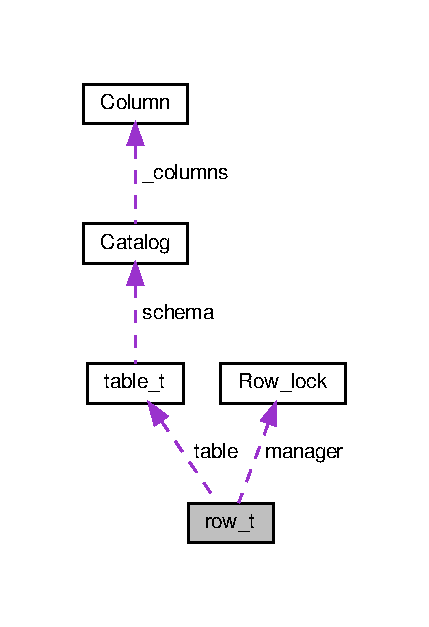
\includegraphics[width=206pt]{classrow__t__coll__graph}
\end{center}
\end{figure}
\subsection*{Public Member Functions}
\begin{DoxyCompactItemize}
\item 
\hyperlink{global_8h_a78c49a674c810fdd03d20432f7be864a}{RC} \hyperlink{classrow__t_aacb35baa21609238d8596a79228639f0}{init} (\hyperlink{classtable__t}{table\+\_\+t} $\ast$host\+\_\+table, uint64\+\_\+t part\+\_\+id, uint64\+\_\+t row\+\_\+id=0)
\item 
void \hyperlink{classrow__t_ad3c8dd1b6ec42ab9bcb55bdae25bfe48}{init} (int size)
\item 
void \hyperlink{classrow__t_acb30d289513df9c5db6f1775a0cf9312}{setbench\+\_\+deinit} ()
\item 
\hyperlink{global_8h_a78c49a674c810fdd03d20432f7be864a}{RC} \hyperlink{classrow__t_af0228d195f82091abefa28d29ac83e22}{switch\+\_\+schema} (\hyperlink{classtable__t}{table\+\_\+t} $\ast$host\+\_\+table)
\item 
void \hyperlink{classrow__t_abce8cf60a90cccfdc5ecee7eeb005806}{init\+\_\+manager} (\hyperlink{classrow__t}{row\+\_\+t} $\ast$row)
\item 
\hyperlink{classtable__t}{table\+\_\+t} $\ast$ \hyperlink{classrow__t_a71e676d99f1cb95186fc8b686d97610f}{get\+\_\+table} ()
\item 
\hyperlink{classCatalog}{Catalog} $\ast$ \hyperlink{classrow__t_a1a9f1060ee454ed679209590a13059b1}{get\+\_\+schema} ()
\item 
const char $\ast$ \hyperlink{classrow__t_a39c6ba60a76818599d48d7bbdf01e081}{get\+\_\+table\+\_\+name} ()
\item 
uint64\+\_\+t \hyperlink{classrow__t_a76ad0094b65a55ed7d1eed8edf2bad3a}{get\+\_\+field\+\_\+cnt} ()
\item 
uint64\+\_\+t \hyperlink{classrow__t_ab524208335b31ac56c95f9695365967b}{get\+\_\+tuple\+\_\+size} ()
\item 
uint64\+\_\+t \hyperlink{classrow__t_a553b2f2021b500fbe7fc6d93a99eddec}{get\+\_\+row\+\_\+id} ()
\item 
void \hyperlink{classrow__t_aca5bd47c4482a9493da85525298367f4}{copy} (\hyperlink{classrow__t}{row\+\_\+t} $\ast$src)
\item 
void \hyperlink{classrow__t_a1d331378ab894cb05c1ff18d0483b5eb}{set\+\_\+primary\+\_\+key} (uint64\+\_\+t key)
\item 
uint64\+\_\+t \hyperlink{classrow__t_a7e11cd7d6a95f897438073120eb68cff}{get\+\_\+primary\+\_\+key} ()
\item 
uint64\+\_\+t \hyperlink{classrow__t_ae6702cc7db6b72bf3082415bee9b3e9e}{get\+\_\+part\+\_\+id} ()
\item 
void \hyperlink{classrow__t_a6abdcb268c944efe100b5a2638003c3d}{set\+\_\+value} (int id, void $\ast$ptr)
\item 
void \hyperlink{classrow__t_a0e7044d41f433552ff6f10f1fba7b191}{set\+\_\+value} (int id, void $\ast$ptr, int size)
\item 
void \hyperlink{classrow__t_a3eff865812156fd1586a59f7e1d28934}{set\+\_\+value} (const char $\ast$col\+\_\+name, void $\ast$ptr)
\item 
char $\ast$ \hyperlink{classrow__t_a92eba387d775a5d6bb975bdbee3fd0ef}{get\+\_\+value} (int id)
\item 
char $\ast$ \hyperlink{classrow__t_ab984e074eab7fca2c3f58169289ccb42}{get\+\_\+value} (char $\ast$col\+\_\+name)
\item 
\hyperlink{classrow__t_a8da3b5c8bc9a8c16744e40a5b671bb20}{D\+E\+C\+L\+\_\+\+S\+E\+T\+\_\+\+V\+A\+L\+UE} (uint64\+\_\+t)
\item 
\hyperlink{classrow__t_a77ffc30e4a43c0d45cdc828e90424e1b}{D\+E\+C\+L\+\_\+\+S\+E\+T\+\_\+\+V\+A\+L\+UE} (int64\+\_\+t)
\item 
\hyperlink{classrow__t_a938e446af20c3161f876f48ec085dee6}{D\+E\+C\+L\+\_\+\+S\+E\+T\+\_\+\+V\+A\+L\+UE} (double)
\item 
\hyperlink{classrow__t_a50db972b28ad2c1cbb381699baed729a}{D\+E\+C\+L\+\_\+\+S\+E\+T\+\_\+\+V\+A\+L\+UE} (\hyperlink{global_8h_a7e8aeec7b6541935dfc6f608cd5170ce}{U\+Int32})
\item 
\hyperlink{classrow__t_aabe31900f597869cee17fff170ffa89e}{D\+E\+C\+L\+\_\+\+S\+E\+T\+\_\+\+V\+A\+L\+UE} (\hyperlink{global_8h_a26832e96d77fcdd175f262a96add7394}{S\+Int32})
\item 
\hyperlink{classrow__t_a61baab6275ee105c148a67e57563a733}{D\+E\+C\+L\+\_\+\+G\+E\+T\+\_\+\+V\+A\+L\+UE} (uint64\+\_\+t)
\item 
\hyperlink{classrow__t_ae96087a5294e61625cceca29fe59ddd5}{D\+E\+C\+L\+\_\+\+G\+E\+T\+\_\+\+V\+A\+L\+UE} (int64\+\_\+t)
\item 
\hyperlink{classrow__t_a0c342dc9a9ab54717d0fe730a1895a5f}{D\+E\+C\+L\+\_\+\+G\+E\+T\+\_\+\+V\+A\+L\+UE} (double)
\item 
\hyperlink{classrow__t_ae5df3522bb118f1ae940ba6852586efd}{D\+E\+C\+L\+\_\+\+G\+E\+T\+\_\+\+V\+A\+L\+UE} (\hyperlink{global_8h_a7e8aeec7b6541935dfc6f608cd5170ce}{U\+Int32})
\item 
\hyperlink{classrow__t_a0784c4532fa83fc3f61ae41d2e9e6295}{D\+E\+C\+L\+\_\+\+G\+E\+T\+\_\+\+V\+A\+L\+UE} (\hyperlink{global_8h_a26832e96d77fcdd175f262a96add7394}{S\+Int32})
\item 
void \hyperlink{classrow__t_a051b2e198e08b7ef586726fb93546673}{set\+\_\+data} (char $\ast$\hyperlink{classrow__t_a8d7d53132f2f84f46785805abec0614c}{data}, uint64\+\_\+t size)
\item 
char $\ast$ \hyperlink{classrow__t_acaf359f8766fda8f8e8dc1669906955b}{get\+\_\+data} ()
\item 
void \hyperlink{classrow__t_a270e2afa4a7d8333f59de89af65a5372}{free\+\_\+row} ()
\item 
\hyperlink{global_8h_a78c49a674c810fdd03d20432f7be864a}{RC} \hyperlink{classrow__t_a49ff4bc52abd5712d2f0a8b9eef5e2bb}{get\+\_\+row} (\hyperlink{global_8h_a567f81b0ae33b00d189d7714e9fde0bc}{access\+\_\+t} type, \hyperlink{classtxn__man}{txn\+\_\+man} $\ast$txn, \hyperlink{classrow__t}{row\+\_\+t} $\ast$\&row)
\item 
void \hyperlink{classrow__t_ad444dabf917bd4f85766f6c80d7ec74f}{return\+\_\+row} (\hyperlink{global_8h_a567f81b0ae33b00d189d7714e9fde0bc}{access\+\_\+t} type, \hyperlink{classtxn__man}{txn\+\_\+man} $\ast$txn, \hyperlink{classrow__t}{row\+\_\+t} $\ast$row)
\end{DoxyCompactItemize}
\subsection*{Public Attributes}
\begin{DoxyCompactItemize}
\item 
\hyperlink{classRow__lock}{Row\+\_\+lock} $\ast$ \hyperlink{classrow__t_a456270f0f263ed713187d5738a7a6e4c}{manager}
\item 
char $\ast$ \hyperlink{classrow__t_a8d7d53132f2f84f46785805abec0614c}{data}
\item 
\hyperlink{classtable__t}{table\+\_\+t} $\ast$ \hyperlink{classrow__t_a22020591ba4e4965d7b2c58172c023f7}{table}
\end{DoxyCompactItemize}


\subsection{Member Function Documentation}
\mbox{\Hypertarget{classrow__t_aca5bd47c4482a9493da85525298367f4}\label{classrow__t_aca5bd47c4482a9493da85525298367f4}} 
\index{row\+\_\+t@{row\+\_\+t}!copy@{copy}}
\index{copy@{copy}!row\+\_\+t@{row\+\_\+t}}
\subsubsection{\texorpdfstring{copy()}{copy()}}
{\footnotesize\ttfamily void row\+\_\+t\+::copy (\begin{DoxyParamCaption}\item[{\hyperlink{classrow__t}{row\+\_\+t} $\ast$}]{src }\end{DoxyParamCaption})}

\mbox{\Hypertarget{classrow__t_a61baab6275ee105c148a67e57563a733}\label{classrow__t_a61baab6275ee105c148a67e57563a733}} 
\index{row\+\_\+t@{row\+\_\+t}!D\+E\+C\+L\+\_\+\+G\+E\+T\+\_\+\+V\+A\+L\+UE@{D\+E\+C\+L\+\_\+\+G\+E\+T\+\_\+\+V\+A\+L\+UE}}
\index{D\+E\+C\+L\+\_\+\+G\+E\+T\+\_\+\+V\+A\+L\+UE@{D\+E\+C\+L\+\_\+\+G\+E\+T\+\_\+\+V\+A\+L\+UE}!row\+\_\+t@{row\+\_\+t}}
\subsubsection{\texorpdfstring{D\+E\+C\+L\+\_\+\+G\+E\+T\+\_\+\+V\+A\+L\+U\+E()}{DECL\_GET\_VALUE()}\hspace{0.1cm}{\footnotesize\ttfamily [1/5]}}
{\footnotesize\ttfamily row\+\_\+t\+::\+D\+E\+C\+L\+\_\+\+G\+E\+T\+\_\+\+V\+A\+L\+UE (\begin{DoxyParamCaption}\item[{uint64\+\_\+t}]{ }\end{DoxyParamCaption})}

\mbox{\Hypertarget{classrow__t_ae96087a5294e61625cceca29fe59ddd5}\label{classrow__t_ae96087a5294e61625cceca29fe59ddd5}} 
\index{row\+\_\+t@{row\+\_\+t}!D\+E\+C\+L\+\_\+\+G\+E\+T\+\_\+\+V\+A\+L\+UE@{D\+E\+C\+L\+\_\+\+G\+E\+T\+\_\+\+V\+A\+L\+UE}}
\index{D\+E\+C\+L\+\_\+\+G\+E\+T\+\_\+\+V\+A\+L\+UE@{D\+E\+C\+L\+\_\+\+G\+E\+T\+\_\+\+V\+A\+L\+UE}!row\+\_\+t@{row\+\_\+t}}
\subsubsection{\texorpdfstring{D\+E\+C\+L\+\_\+\+G\+E\+T\+\_\+\+V\+A\+L\+U\+E()}{DECL\_GET\_VALUE()}\hspace{0.1cm}{\footnotesize\ttfamily [2/5]}}
{\footnotesize\ttfamily row\+\_\+t\+::\+D\+E\+C\+L\+\_\+\+G\+E\+T\+\_\+\+V\+A\+L\+UE (\begin{DoxyParamCaption}\item[{int64\+\_\+t}]{ }\end{DoxyParamCaption})}

\mbox{\Hypertarget{classrow__t_a0c342dc9a9ab54717d0fe730a1895a5f}\label{classrow__t_a0c342dc9a9ab54717d0fe730a1895a5f}} 
\index{row\+\_\+t@{row\+\_\+t}!D\+E\+C\+L\+\_\+\+G\+E\+T\+\_\+\+V\+A\+L\+UE@{D\+E\+C\+L\+\_\+\+G\+E\+T\+\_\+\+V\+A\+L\+UE}}
\index{D\+E\+C\+L\+\_\+\+G\+E\+T\+\_\+\+V\+A\+L\+UE@{D\+E\+C\+L\+\_\+\+G\+E\+T\+\_\+\+V\+A\+L\+UE}!row\+\_\+t@{row\+\_\+t}}
\subsubsection{\texorpdfstring{D\+E\+C\+L\+\_\+\+G\+E\+T\+\_\+\+V\+A\+L\+U\+E()}{DECL\_GET\_VALUE()}\hspace{0.1cm}{\footnotesize\ttfamily [3/5]}}
{\footnotesize\ttfamily row\+\_\+t\+::\+D\+E\+C\+L\+\_\+\+G\+E\+T\+\_\+\+V\+A\+L\+UE (\begin{DoxyParamCaption}\item[{double}]{ }\end{DoxyParamCaption})}

\mbox{\Hypertarget{classrow__t_ae5df3522bb118f1ae940ba6852586efd}\label{classrow__t_ae5df3522bb118f1ae940ba6852586efd}} 
\index{row\+\_\+t@{row\+\_\+t}!D\+E\+C\+L\+\_\+\+G\+E\+T\+\_\+\+V\+A\+L\+UE@{D\+E\+C\+L\+\_\+\+G\+E\+T\+\_\+\+V\+A\+L\+UE}}
\index{D\+E\+C\+L\+\_\+\+G\+E\+T\+\_\+\+V\+A\+L\+UE@{D\+E\+C\+L\+\_\+\+G\+E\+T\+\_\+\+V\+A\+L\+UE}!row\+\_\+t@{row\+\_\+t}}
\subsubsection{\texorpdfstring{D\+E\+C\+L\+\_\+\+G\+E\+T\+\_\+\+V\+A\+L\+U\+E()}{DECL\_GET\_VALUE()}\hspace{0.1cm}{\footnotesize\ttfamily [4/5]}}
{\footnotesize\ttfamily row\+\_\+t\+::\+D\+E\+C\+L\+\_\+\+G\+E\+T\+\_\+\+V\+A\+L\+UE (\begin{DoxyParamCaption}\item[{\hyperlink{global_8h_a7e8aeec7b6541935dfc6f608cd5170ce}{U\+Int32}}]{ }\end{DoxyParamCaption})}

\mbox{\Hypertarget{classrow__t_a0784c4532fa83fc3f61ae41d2e9e6295}\label{classrow__t_a0784c4532fa83fc3f61ae41d2e9e6295}} 
\index{row\+\_\+t@{row\+\_\+t}!D\+E\+C\+L\+\_\+\+G\+E\+T\+\_\+\+V\+A\+L\+UE@{D\+E\+C\+L\+\_\+\+G\+E\+T\+\_\+\+V\+A\+L\+UE}}
\index{D\+E\+C\+L\+\_\+\+G\+E\+T\+\_\+\+V\+A\+L\+UE@{D\+E\+C\+L\+\_\+\+G\+E\+T\+\_\+\+V\+A\+L\+UE}!row\+\_\+t@{row\+\_\+t}}
\subsubsection{\texorpdfstring{D\+E\+C\+L\+\_\+\+G\+E\+T\+\_\+\+V\+A\+L\+U\+E()}{DECL\_GET\_VALUE()}\hspace{0.1cm}{\footnotesize\ttfamily [5/5]}}
{\footnotesize\ttfamily row\+\_\+t\+::\+D\+E\+C\+L\+\_\+\+G\+E\+T\+\_\+\+V\+A\+L\+UE (\begin{DoxyParamCaption}\item[{\hyperlink{global_8h_a26832e96d77fcdd175f262a96add7394}{S\+Int32}}]{ }\end{DoxyParamCaption})}

\mbox{\Hypertarget{classrow__t_a8da3b5c8bc9a8c16744e40a5b671bb20}\label{classrow__t_a8da3b5c8bc9a8c16744e40a5b671bb20}} 
\index{row\+\_\+t@{row\+\_\+t}!D\+E\+C\+L\+\_\+\+S\+E\+T\+\_\+\+V\+A\+L\+UE@{D\+E\+C\+L\+\_\+\+S\+E\+T\+\_\+\+V\+A\+L\+UE}}
\index{D\+E\+C\+L\+\_\+\+S\+E\+T\+\_\+\+V\+A\+L\+UE@{D\+E\+C\+L\+\_\+\+S\+E\+T\+\_\+\+V\+A\+L\+UE}!row\+\_\+t@{row\+\_\+t}}
\subsubsection{\texorpdfstring{D\+E\+C\+L\+\_\+\+S\+E\+T\+\_\+\+V\+A\+L\+U\+E()}{DECL\_SET\_VALUE()}\hspace{0.1cm}{\footnotesize\ttfamily [1/5]}}
{\footnotesize\ttfamily row\+\_\+t\+::\+D\+E\+C\+L\+\_\+\+S\+E\+T\+\_\+\+V\+A\+L\+UE (\begin{DoxyParamCaption}\item[{uint64\+\_\+t}]{ }\end{DoxyParamCaption})}

\mbox{\Hypertarget{classrow__t_a77ffc30e4a43c0d45cdc828e90424e1b}\label{classrow__t_a77ffc30e4a43c0d45cdc828e90424e1b}} 
\index{row\+\_\+t@{row\+\_\+t}!D\+E\+C\+L\+\_\+\+S\+E\+T\+\_\+\+V\+A\+L\+UE@{D\+E\+C\+L\+\_\+\+S\+E\+T\+\_\+\+V\+A\+L\+UE}}
\index{D\+E\+C\+L\+\_\+\+S\+E\+T\+\_\+\+V\+A\+L\+UE@{D\+E\+C\+L\+\_\+\+S\+E\+T\+\_\+\+V\+A\+L\+UE}!row\+\_\+t@{row\+\_\+t}}
\subsubsection{\texorpdfstring{D\+E\+C\+L\+\_\+\+S\+E\+T\+\_\+\+V\+A\+L\+U\+E()}{DECL\_SET\_VALUE()}\hspace{0.1cm}{\footnotesize\ttfamily [2/5]}}
{\footnotesize\ttfamily row\+\_\+t\+::\+D\+E\+C\+L\+\_\+\+S\+E\+T\+\_\+\+V\+A\+L\+UE (\begin{DoxyParamCaption}\item[{int64\+\_\+t}]{ }\end{DoxyParamCaption})}

\mbox{\Hypertarget{classrow__t_a938e446af20c3161f876f48ec085dee6}\label{classrow__t_a938e446af20c3161f876f48ec085dee6}} 
\index{row\+\_\+t@{row\+\_\+t}!D\+E\+C\+L\+\_\+\+S\+E\+T\+\_\+\+V\+A\+L\+UE@{D\+E\+C\+L\+\_\+\+S\+E\+T\+\_\+\+V\+A\+L\+UE}}
\index{D\+E\+C\+L\+\_\+\+S\+E\+T\+\_\+\+V\+A\+L\+UE@{D\+E\+C\+L\+\_\+\+S\+E\+T\+\_\+\+V\+A\+L\+UE}!row\+\_\+t@{row\+\_\+t}}
\subsubsection{\texorpdfstring{D\+E\+C\+L\+\_\+\+S\+E\+T\+\_\+\+V\+A\+L\+U\+E()}{DECL\_SET\_VALUE()}\hspace{0.1cm}{\footnotesize\ttfamily [3/5]}}
{\footnotesize\ttfamily row\+\_\+t\+::\+D\+E\+C\+L\+\_\+\+S\+E\+T\+\_\+\+V\+A\+L\+UE (\begin{DoxyParamCaption}\item[{double}]{ }\end{DoxyParamCaption})}

\mbox{\Hypertarget{classrow__t_a50db972b28ad2c1cbb381699baed729a}\label{classrow__t_a50db972b28ad2c1cbb381699baed729a}} 
\index{row\+\_\+t@{row\+\_\+t}!D\+E\+C\+L\+\_\+\+S\+E\+T\+\_\+\+V\+A\+L\+UE@{D\+E\+C\+L\+\_\+\+S\+E\+T\+\_\+\+V\+A\+L\+UE}}
\index{D\+E\+C\+L\+\_\+\+S\+E\+T\+\_\+\+V\+A\+L\+UE@{D\+E\+C\+L\+\_\+\+S\+E\+T\+\_\+\+V\+A\+L\+UE}!row\+\_\+t@{row\+\_\+t}}
\subsubsection{\texorpdfstring{D\+E\+C\+L\+\_\+\+S\+E\+T\+\_\+\+V\+A\+L\+U\+E()}{DECL\_SET\_VALUE()}\hspace{0.1cm}{\footnotesize\ttfamily [4/5]}}
{\footnotesize\ttfamily row\+\_\+t\+::\+D\+E\+C\+L\+\_\+\+S\+E\+T\+\_\+\+V\+A\+L\+UE (\begin{DoxyParamCaption}\item[{\hyperlink{global_8h_a7e8aeec7b6541935dfc6f608cd5170ce}{U\+Int32}}]{ }\end{DoxyParamCaption})}

\mbox{\Hypertarget{classrow__t_aabe31900f597869cee17fff170ffa89e}\label{classrow__t_aabe31900f597869cee17fff170ffa89e}} 
\index{row\+\_\+t@{row\+\_\+t}!D\+E\+C\+L\+\_\+\+S\+E\+T\+\_\+\+V\+A\+L\+UE@{D\+E\+C\+L\+\_\+\+S\+E\+T\+\_\+\+V\+A\+L\+UE}}
\index{D\+E\+C\+L\+\_\+\+S\+E\+T\+\_\+\+V\+A\+L\+UE@{D\+E\+C\+L\+\_\+\+S\+E\+T\+\_\+\+V\+A\+L\+UE}!row\+\_\+t@{row\+\_\+t}}
\subsubsection{\texorpdfstring{D\+E\+C\+L\+\_\+\+S\+E\+T\+\_\+\+V\+A\+L\+U\+E()}{DECL\_SET\_VALUE()}\hspace{0.1cm}{\footnotesize\ttfamily [5/5]}}
{\footnotesize\ttfamily row\+\_\+t\+::\+D\+E\+C\+L\+\_\+\+S\+E\+T\+\_\+\+V\+A\+L\+UE (\begin{DoxyParamCaption}\item[{\hyperlink{global_8h_a26832e96d77fcdd175f262a96add7394}{S\+Int32}}]{ }\end{DoxyParamCaption})}

\mbox{\Hypertarget{classrow__t_a270e2afa4a7d8333f59de89af65a5372}\label{classrow__t_a270e2afa4a7d8333f59de89af65a5372}} 
\index{row\+\_\+t@{row\+\_\+t}!free\+\_\+row@{free\+\_\+row}}
\index{free\+\_\+row@{free\+\_\+row}!row\+\_\+t@{row\+\_\+t}}
\subsubsection{\texorpdfstring{free\+\_\+row()}{free\_row()}}
{\footnotesize\ttfamily void row\+\_\+t\+::free\+\_\+row (\begin{DoxyParamCaption}{ }\end{DoxyParamCaption})}

\mbox{\Hypertarget{classrow__t_acaf359f8766fda8f8e8dc1669906955b}\label{classrow__t_acaf359f8766fda8f8e8dc1669906955b}} 
\index{row\+\_\+t@{row\+\_\+t}!get\+\_\+data@{get\+\_\+data}}
\index{get\+\_\+data@{get\+\_\+data}!row\+\_\+t@{row\+\_\+t}}
\subsubsection{\texorpdfstring{get\+\_\+data()}{get\_data()}}
{\footnotesize\ttfamily char $\ast$ row\+\_\+t\+::get\+\_\+data (\begin{DoxyParamCaption}{ }\end{DoxyParamCaption})}

\mbox{\Hypertarget{classrow__t_a76ad0094b65a55ed7d1eed8edf2bad3a}\label{classrow__t_a76ad0094b65a55ed7d1eed8edf2bad3a}} 
\index{row\+\_\+t@{row\+\_\+t}!get\+\_\+field\+\_\+cnt@{get\+\_\+field\+\_\+cnt}}
\index{get\+\_\+field\+\_\+cnt@{get\+\_\+field\+\_\+cnt}!row\+\_\+t@{row\+\_\+t}}
\subsubsection{\texorpdfstring{get\+\_\+field\+\_\+cnt()}{get\_field\_cnt()}}
{\footnotesize\ttfamily uint64\+\_\+t row\+\_\+t\+::get\+\_\+field\+\_\+cnt (\begin{DoxyParamCaption}{ }\end{DoxyParamCaption})}

\mbox{\Hypertarget{classrow__t_ae6702cc7db6b72bf3082415bee9b3e9e}\label{classrow__t_ae6702cc7db6b72bf3082415bee9b3e9e}} 
\index{row\+\_\+t@{row\+\_\+t}!get\+\_\+part\+\_\+id@{get\+\_\+part\+\_\+id}}
\index{get\+\_\+part\+\_\+id@{get\+\_\+part\+\_\+id}!row\+\_\+t@{row\+\_\+t}}
\subsubsection{\texorpdfstring{get\+\_\+part\+\_\+id()}{get\_part\_id()}}
{\footnotesize\ttfamily uint64\+\_\+t row\+\_\+t\+::get\+\_\+part\+\_\+id (\begin{DoxyParamCaption}{ }\end{DoxyParamCaption})\hspace{0.3cm}{\ttfamily [inline]}}

\mbox{\Hypertarget{classrow__t_a7e11cd7d6a95f897438073120eb68cff}\label{classrow__t_a7e11cd7d6a95f897438073120eb68cff}} 
\index{row\+\_\+t@{row\+\_\+t}!get\+\_\+primary\+\_\+key@{get\+\_\+primary\+\_\+key}}
\index{get\+\_\+primary\+\_\+key@{get\+\_\+primary\+\_\+key}!row\+\_\+t@{row\+\_\+t}}
\subsubsection{\texorpdfstring{get\+\_\+primary\+\_\+key()}{get\_primary\_key()}}
{\footnotesize\ttfamily uint64\+\_\+t row\+\_\+t\+::get\+\_\+primary\+\_\+key (\begin{DoxyParamCaption}{ }\end{DoxyParamCaption})\hspace{0.3cm}{\ttfamily [inline]}}

\mbox{\Hypertarget{classrow__t_a49ff4bc52abd5712d2f0a8b9eef5e2bb}\label{classrow__t_a49ff4bc52abd5712d2f0a8b9eef5e2bb}} 
\index{row\+\_\+t@{row\+\_\+t}!get\+\_\+row@{get\+\_\+row}}
\index{get\+\_\+row@{get\+\_\+row}!row\+\_\+t@{row\+\_\+t}}
\subsubsection{\texorpdfstring{get\+\_\+row()}{get\_row()}}
{\footnotesize\ttfamily \hyperlink{global_8h_a78c49a674c810fdd03d20432f7be864a}{RC} row\+\_\+t\+::get\+\_\+row (\begin{DoxyParamCaption}\item[{\hyperlink{global_8h_a567f81b0ae33b00d189d7714e9fde0bc}{access\+\_\+t}}]{type,  }\item[{\hyperlink{classtxn__man}{txn\+\_\+man} $\ast$}]{txn,  }\item[{\hyperlink{classrow__t}{row\+\_\+t} $\ast$\&}]{row }\end{DoxyParamCaption})}

\mbox{\Hypertarget{classrow__t_a553b2f2021b500fbe7fc6d93a99eddec}\label{classrow__t_a553b2f2021b500fbe7fc6d93a99eddec}} 
\index{row\+\_\+t@{row\+\_\+t}!get\+\_\+row\+\_\+id@{get\+\_\+row\+\_\+id}}
\index{get\+\_\+row\+\_\+id@{get\+\_\+row\+\_\+id}!row\+\_\+t@{row\+\_\+t}}
\subsubsection{\texorpdfstring{get\+\_\+row\+\_\+id()}{get\_row\_id()}}
{\footnotesize\ttfamily uint64\+\_\+t row\+\_\+t\+::get\+\_\+row\+\_\+id (\begin{DoxyParamCaption}{ }\end{DoxyParamCaption})\hspace{0.3cm}{\ttfamily [inline]}}

\mbox{\Hypertarget{classrow__t_a1a9f1060ee454ed679209590a13059b1}\label{classrow__t_a1a9f1060ee454ed679209590a13059b1}} 
\index{row\+\_\+t@{row\+\_\+t}!get\+\_\+schema@{get\+\_\+schema}}
\index{get\+\_\+schema@{get\+\_\+schema}!row\+\_\+t@{row\+\_\+t}}
\subsubsection{\texorpdfstring{get\+\_\+schema()}{get\_schema()}}
{\footnotesize\ttfamily \hyperlink{classCatalog}{Catalog} $\ast$ row\+\_\+t\+::get\+\_\+schema (\begin{DoxyParamCaption}{ }\end{DoxyParamCaption})}

\mbox{\Hypertarget{classrow__t_a71e676d99f1cb95186fc8b686d97610f}\label{classrow__t_a71e676d99f1cb95186fc8b686d97610f}} 
\index{row\+\_\+t@{row\+\_\+t}!get\+\_\+table@{get\+\_\+table}}
\index{get\+\_\+table@{get\+\_\+table}!row\+\_\+t@{row\+\_\+t}}
\subsubsection{\texorpdfstring{get\+\_\+table()}{get\_table()}}
{\footnotesize\ttfamily \hyperlink{classtable__t}{table\+\_\+t} $\ast$ row\+\_\+t\+::get\+\_\+table (\begin{DoxyParamCaption}{ }\end{DoxyParamCaption})}

\mbox{\Hypertarget{classrow__t_a39c6ba60a76818599d48d7bbdf01e081}\label{classrow__t_a39c6ba60a76818599d48d7bbdf01e081}} 
\index{row\+\_\+t@{row\+\_\+t}!get\+\_\+table\+\_\+name@{get\+\_\+table\+\_\+name}}
\index{get\+\_\+table\+\_\+name@{get\+\_\+table\+\_\+name}!row\+\_\+t@{row\+\_\+t}}
\subsubsection{\texorpdfstring{get\+\_\+table\+\_\+name()}{get\_table\_name()}}
{\footnotesize\ttfamily const char $\ast$ row\+\_\+t\+::get\+\_\+table\+\_\+name (\begin{DoxyParamCaption}{ }\end{DoxyParamCaption})}

\mbox{\Hypertarget{classrow__t_ab524208335b31ac56c95f9695365967b}\label{classrow__t_ab524208335b31ac56c95f9695365967b}} 
\index{row\+\_\+t@{row\+\_\+t}!get\+\_\+tuple\+\_\+size@{get\+\_\+tuple\+\_\+size}}
\index{get\+\_\+tuple\+\_\+size@{get\+\_\+tuple\+\_\+size}!row\+\_\+t@{row\+\_\+t}}
\subsubsection{\texorpdfstring{get\+\_\+tuple\+\_\+size()}{get\_tuple\_size()}}
{\footnotesize\ttfamily uint64\+\_\+t row\+\_\+t\+::get\+\_\+tuple\+\_\+size (\begin{DoxyParamCaption}{ }\end{DoxyParamCaption})}

\mbox{\Hypertarget{classrow__t_a92eba387d775a5d6bb975bdbee3fd0ef}\label{classrow__t_a92eba387d775a5d6bb975bdbee3fd0ef}} 
\index{row\+\_\+t@{row\+\_\+t}!get\+\_\+value@{get\+\_\+value}}
\index{get\+\_\+value@{get\+\_\+value}!row\+\_\+t@{row\+\_\+t}}
\subsubsection{\texorpdfstring{get\+\_\+value()}{get\_value()}\hspace{0.1cm}{\footnotesize\ttfamily [1/2]}}
{\footnotesize\ttfamily char $\ast$ row\+\_\+t\+::get\+\_\+value (\begin{DoxyParamCaption}\item[{int}]{id }\end{DoxyParamCaption})}

\mbox{\Hypertarget{classrow__t_ab984e074eab7fca2c3f58169289ccb42}\label{classrow__t_ab984e074eab7fca2c3f58169289ccb42}} 
\index{row\+\_\+t@{row\+\_\+t}!get\+\_\+value@{get\+\_\+value}}
\index{get\+\_\+value@{get\+\_\+value}!row\+\_\+t@{row\+\_\+t}}
\subsubsection{\texorpdfstring{get\+\_\+value()}{get\_value()}\hspace{0.1cm}{\footnotesize\ttfamily [2/2]}}
{\footnotesize\ttfamily char $\ast$ row\+\_\+t\+::get\+\_\+value (\begin{DoxyParamCaption}\item[{char $\ast$}]{col\+\_\+name }\end{DoxyParamCaption})}

\mbox{\Hypertarget{classrow__t_aacb35baa21609238d8596a79228639f0}\label{classrow__t_aacb35baa21609238d8596a79228639f0}} 
\index{row\+\_\+t@{row\+\_\+t}!init@{init}}
\index{init@{init}!row\+\_\+t@{row\+\_\+t}}
\subsubsection{\texorpdfstring{init()}{init()}\hspace{0.1cm}{\footnotesize\ttfamily [1/2]}}
{\footnotesize\ttfamily \hyperlink{global_8h_a78c49a674c810fdd03d20432f7be864a}{RC} row\+\_\+t\+::init (\begin{DoxyParamCaption}\item[{\hyperlink{classtable__t}{table\+\_\+t} $\ast$}]{host\+\_\+table,  }\item[{uint64\+\_\+t}]{part\+\_\+id,  }\item[{uint64\+\_\+t}]{row\+\_\+id = {\ttfamily 0} }\end{DoxyParamCaption})}

\mbox{\Hypertarget{classrow__t_ad3c8dd1b6ec42ab9bcb55bdae25bfe48}\label{classrow__t_ad3c8dd1b6ec42ab9bcb55bdae25bfe48}} 
\index{row\+\_\+t@{row\+\_\+t}!init@{init}}
\index{init@{init}!row\+\_\+t@{row\+\_\+t}}
\subsubsection{\texorpdfstring{init()}{init()}\hspace{0.1cm}{\footnotesize\ttfamily [2/2]}}
{\footnotesize\ttfamily void row\+\_\+t\+::init (\begin{DoxyParamCaption}\item[{int}]{size }\end{DoxyParamCaption})}

\mbox{\Hypertarget{classrow__t_abce8cf60a90cccfdc5ecee7eeb005806}\label{classrow__t_abce8cf60a90cccfdc5ecee7eeb005806}} 
\index{row\+\_\+t@{row\+\_\+t}!init\+\_\+manager@{init\+\_\+manager}}
\index{init\+\_\+manager@{init\+\_\+manager}!row\+\_\+t@{row\+\_\+t}}
\subsubsection{\texorpdfstring{init\+\_\+manager()}{init\_manager()}}
{\footnotesize\ttfamily void row\+\_\+t\+::init\+\_\+manager (\begin{DoxyParamCaption}\item[{\hyperlink{classrow__t}{row\+\_\+t} $\ast$}]{row }\end{DoxyParamCaption})}

\mbox{\Hypertarget{classrow__t_ad444dabf917bd4f85766f6c80d7ec74f}\label{classrow__t_ad444dabf917bd4f85766f6c80d7ec74f}} 
\index{row\+\_\+t@{row\+\_\+t}!return\+\_\+row@{return\+\_\+row}}
\index{return\+\_\+row@{return\+\_\+row}!row\+\_\+t@{row\+\_\+t}}
\subsubsection{\texorpdfstring{return\+\_\+row()}{return\_row()}}
{\footnotesize\ttfamily void row\+\_\+t\+::return\+\_\+row (\begin{DoxyParamCaption}\item[{\hyperlink{global_8h_a567f81b0ae33b00d189d7714e9fde0bc}{access\+\_\+t}}]{type,  }\item[{\hyperlink{classtxn__man}{txn\+\_\+man} $\ast$}]{txn,  }\item[{\hyperlink{classrow__t}{row\+\_\+t} $\ast$}]{row }\end{DoxyParamCaption})}

\mbox{\Hypertarget{classrow__t_a051b2e198e08b7ef586726fb93546673}\label{classrow__t_a051b2e198e08b7ef586726fb93546673}} 
\index{row\+\_\+t@{row\+\_\+t}!set\+\_\+data@{set\+\_\+data}}
\index{set\+\_\+data@{set\+\_\+data}!row\+\_\+t@{row\+\_\+t}}
\subsubsection{\texorpdfstring{set\+\_\+data()}{set\_data()}}
{\footnotesize\ttfamily void row\+\_\+t\+::set\+\_\+data (\begin{DoxyParamCaption}\item[{char $\ast$}]{data,  }\item[{uint64\+\_\+t}]{size }\end{DoxyParamCaption})}

\mbox{\Hypertarget{classrow__t_a1d331378ab894cb05c1ff18d0483b5eb}\label{classrow__t_a1d331378ab894cb05c1ff18d0483b5eb}} 
\index{row\+\_\+t@{row\+\_\+t}!set\+\_\+primary\+\_\+key@{set\+\_\+primary\+\_\+key}}
\index{set\+\_\+primary\+\_\+key@{set\+\_\+primary\+\_\+key}!row\+\_\+t@{row\+\_\+t}}
\subsubsection{\texorpdfstring{set\+\_\+primary\+\_\+key()}{set\_primary\_key()}}
{\footnotesize\ttfamily void row\+\_\+t\+::set\+\_\+primary\+\_\+key (\begin{DoxyParamCaption}\item[{uint64\+\_\+t}]{key }\end{DoxyParamCaption})\hspace{0.3cm}{\ttfamily [inline]}}

\mbox{\Hypertarget{classrow__t_a6abdcb268c944efe100b5a2638003c3d}\label{classrow__t_a6abdcb268c944efe100b5a2638003c3d}} 
\index{row\+\_\+t@{row\+\_\+t}!set\+\_\+value@{set\+\_\+value}}
\index{set\+\_\+value@{set\+\_\+value}!row\+\_\+t@{row\+\_\+t}}
\subsubsection{\texorpdfstring{set\+\_\+value()}{set\_value()}\hspace{0.1cm}{\footnotesize\ttfamily [1/3]}}
{\footnotesize\ttfamily void row\+\_\+t\+::set\+\_\+value (\begin{DoxyParamCaption}\item[{int}]{id,  }\item[{void $\ast$}]{ptr }\end{DoxyParamCaption})}

\mbox{\Hypertarget{classrow__t_a0e7044d41f433552ff6f10f1fba7b191}\label{classrow__t_a0e7044d41f433552ff6f10f1fba7b191}} 
\index{row\+\_\+t@{row\+\_\+t}!set\+\_\+value@{set\+\_\+value}}
\index{set\+\_\+value@{set\+\_\+value}!row\+\_\+t@{row\+\_\+t}}
\subsubsection{\texorpdfstring{set\+\_\+value()}{set\_value()}\hspace{0.1cm}{\footnotesize\ttfamily [2/3]}}
{\footnotesize\ttfamily void row\+\_\+t\+::set\+\_\+value (\begin{DoxyParamCaption}\item[{int}]{id,  }\item[{void $\ast$}]{ptr,  }\item[{int}]{size }\end{DoxyParamCaption})}

\mbox{\Hypertarget{classrow__t_a3eff865812156fd1586a59f7e1d28934}\label{classrow__t_a3eff865812156fd1586a59f7e1d28934}} 
\index{row\+\_\+t@{row\+\_\+t}!set\+\_\+value@{set\+\_\+value}}
\index{set\+\_\+value@{set\+\_\+value}!row\+\_\+t@{row\+\_\+t}}
\subsubsection{\texorpdfstring{set\+\_\+value()}{set\_value()}\hspace{0.1cm}{\footnotesize\ttfamily [3/3]}}
{\footnotesize\ttfamily void row\+\_\+t\+::set\+\_\+value (\begin{DoxyParamCaption}\item[{const char $\ast$}]{col\+\_\+name,  }\item[{void $\ast$}]{ptr }\end{DoxyParamCaption})}

\mbox{\Hypertarget{classrow__t_acb30d289513df9c5db6f1775a0cf9312}\label{classrow__t_acb30d289513df9c5db6f1775a0cf9312}} 
\index{row\+\_\+t@{row\+\_\+t}!setbench\+\_\+deinit@{setbench\+\_\+deinit}}
\index{setbench\+\_\+deinit@{setbench\+\_\+deinit}!row\+\_\+t@{row\+\_\+t}}
\subsubsection{\texorpdfstring{setbench\+\_\+deinit()}{setbench\_deinit()}}
{\footnotesize\ttfamily void row\+\_\+t\+::setbench\+\_\+deinit (\begin{DoxyParamCaption}{ }\end{DoxyParamCaption})}

\mbox{\Hypertarget{classrow__t_af0228d195f82091abefa28d29ac83e22}\label{classrow__t_af0228d195f82091abefa28d29ac83e22}} 
\index{row\+\_\+t@{row\+\_\+t}!switch\+\_\+schema@{switch\+\_\+schema}}
\index{switch\+\_\+schema@{switch\+\_\+schema}!row\+\_\+t@{row\+\_\+t}}
\subsubsection{\texorpdfstring{switch\+\_\+schema()}{switch\_schema()}}
{\footnotesize\ttfamily \hyperlink{global_8h_a78c49a674c810fdd03d20432f7be864a}{RC} row\+\_\+t\+::switch\+\_\+schema (\begin{DoxyParamCaption}\item[{\hyperlink{classtable__t}{table\+\_\+t} $\ast$}]{host\+\_\+table }\end{DoxyParamCaption})}



\subsection{Member Data Documentation}
\mbox{\Hypertarget{classrow__t_a8d7d53132f2f84f46785805abec0614c}\label{classrow__t_a8d7d53132f2f84f46785805abec0614c}} 
\index{row\+\_\+t@{row\+\_\+t}!data@{data}}
\index{data@{data}!row\+\_\+t@{row\+\_\+t}}
\subsubsection{\texorpdfstring{data}{data}}
{\footnotesize\ttfamily char$\ast$ row\+\_\+t\+::data}

\mbox{\Hypertarget{classrow__t_a456270f0f263ed713187d5738a7a6e4c}\label{classrow__t_a456270f0f263ed713187d5738a7a6e4c}} 
\index{row\+\_\+t@{row\+\_\+t}!manager@{manager}}
\index{manager@{manager}!row\+\_\+t@{row\+\_\+t}}
\subsubsection{\texorpdfstring{manager}{manager}}
{\footnotesize\ttfamily \hyperlink{classRow__lock}{Row\+\_\+lock}$\ast$ row\+\_\+t\+::manager}

\mbox{\Hypertarget{classrow__t_a22020591ba4e4965d7b2c58172c023f7}\label{classrow__t_a22020591ba4e4965d7b2c58172c023f7}} 
\index{row\+\_\+t@{row\+\_\+t}!table@{table}}
\index{table@{table}!row\+\_\+t@{row\+\_\+t}}
\subsubsection{\texorpdfstring{table}{table}}
{\footnotesize\ttfamily \hyperlink{classtable__t}{table\+\_\+t}$\ast$ row\+\_\+t\+::table}



The documentation for this class was generated from the following files\+:\begin{DoxyCompactItemize}
\item 
macrobench/storage/\hyperlink{row_8h}{row.\+h}\item 
macrobench/storage/\hyperlink{row_8cpp}{row.\+cpp}\end{DoxyCompactItemize}

\hypertarget{classRow__tictoc}{}\section{Row\+\_\+tictoc Class Reference}
\label{classRow__tictoc}\index{Row\+\_\+tictoc@{Row\+\_\+tictoc}}


{\ttfamily \#include $<$row\+\_\+tictoc.\+h$>$}

\subsection*{Public Member Functions}
\begin{DoxyCompactItemize}
\item 
void \hyperlink{classRow__tictoc_a44d46cc09bdf8f078f992075a2e126c9}{init} (\hyperlink{classrow__t}{row\+\_\+t} $\ast$row)
\item 
\hyperlink{global_8h_a78c49a674c810fdd03d20432f7be864a}{RC} \hyperlink{classRow__tictoc_a6a5b77a305775780a23dc7227ccef937}{access} (\hyperlink{classtxn__man}{txn\+\_\+man} $\ast$txn, \hyperlink{global_8h_a1a7f6ca1462293fe053b5ae74a6c4eda}{Ts\+Type} type, \hyperlink{classrow__t}{row\+\_\+t} $\ast$local\+\_\+row)
\item 
void \hyperlink{classRow__tictoc_a6af47480f6f4230236f47b2f2b2de429}{write\+\_\+data} (\hyperlink{classrow__t}{row\+\_\+t} $\ast$data, \hyperlink{global_8h_aaf095dfc9b10f757c968fe146ad7e724}{ts\+\_\+t} wts)
\item 
void \hyperlink{classRow__tictoc_a8cfc065bb14c25213e614798ba8b3b4a}{write\+\_\+ptr} (\hyperlink{classrow__t}{row\+\_\+t} $\ast$data, \hyperlink{global_8h_aaf095dfc9b10f757c968fe146ad7e724}{ts\+\_\+t} wts, char $\ast$\&data\+\_\+to\+\_\+free)
\item 
bool \hyperlink{classRow__tictoc_a49259f37a6c3ab9f74fe861b7f4ba8f6}{renew\+\_\+lease} (\hyperlink{global_8h_aaf095dfc9b10f757c968fe146ad7e724}{ts\+\_\+t} wts, \hyperlink{global_8h_aaf095dfc9b10f757c968fe146ad7e724}{ts\+\_\+t} rts)
\item 
bool \hyperlink{classRow__tictoc_a0e3056dff2f6ebc21de23fbd3ac35ea6}{try\+\_\+renew} (\hyperlink{global_8h_aaf095dfc9b10f757c968fe146ad7e724}{ts\+\_\+t} wts, \hyperlink{global_8h_aaf095dfc9b10f757c968fe146ad7e724}{ts\+\_\+t} rts, \hyperlink{global_8h_aaf095dfc9b10f757c968fe146ad7e724}{ts\+\_\+t} \&new\+\_\+rts, uint64\+\_\+t thd\+\_\+id)
\item 
void \hyperlink{classRow__tictoc_a534c6fe17f2cf8fffc7a1b06eef67b03}{lock} ()
\item 
bool \hyperlink{classRow__tictoc_a726f11ccc49c55ff64160a8c638bedad}{try\+\_\+lock} ()
\item 
void \hyperlink{classRow__tictoc_a0a67be119cc8f17c09c14b4a0294ba73}{release} ()
\item 
\hyperlink{global_8h_aaf095dfc9b10f757c968fe146ad7e724}{ts\+\_\+t} \hyperlink{classRow__tictoc_a8e4797ac556c6ebf9b58d986dbbea0ac}{get\+\_\+wts} ()
\item 
\hyperlink{global_8h_aaf095dfc9b10f757c968fe146ad7e724}{ts\+\_\+t} \hyperlink{classRow__tictoc_aadea8708aa6c023efc6eb3f81d7c8299}{get\+\_\+rts} ()
\item 
void \hyperlink{classRow__tictoc_a7e83376689a8f6504419779ee7348dee}{get\+\_\+ts\+\_\+word} (bool \&\hyperlink{classRow__tictoc_a534c6fe17f2cf8fffc7a1b06eef67b03}{lock}, uint64\+\_\+t \&rts, uint64\+\_\+t \&wts)
\end{DoxyCompactItemize}


\subsection{Member Function Documentation}
\mbox{\Hypertarget{classRow__tictoc_a6a5b77a305775780a23dc7227ccef937}\label{classRow__tictoc_a6a5b77a305775780a23dc7227ccef937}} 
\index{Row\+\_\+tictoc@{Row\+\_\+tictoc}!access@{access}}
\index{access@{access}!Row\+\_\+tictoc@{Row\+\_\+tictoc}}
\subsubsection{\texorpdfstring{access()}{access()}}
{\footnotesize\ttfamily \hyperlink{global_8h_a78c49a674c810fdd03d20432f7be864a}{RC} Row\+\_\+tictoc\+::access (\begin{DoxyParamCaption}\item[{\hyperlink{classtxn__man}{txn\+\_\+man} $\ast$}]{txn,  }\item[{\hyperlink{global_8h_a1a7f6ca1462293fe053b5ae74a6c4eda}{Ts\+Type}}]{type,  }\item[{\hyperlink{classrow__t}{row\+\_\+t} $\ast$}]{local\+\_\+row }\end{DoxyParamCaption})}

\mbox{\Hypertarget{classRow__tictoc_aadea8708aa6c023efc6eb3f81d7c8299}\label{classRow__tictoc_aadea8708aa6c023efc6eb3f81d7c8299}} 
\index{Row\+\_\+tictoc@{Row\+\_\+tictoc}!get\+\_\+rts@{get\+\_\+rts}}
\index{get\+\_\+rts@{get\+\_\+rts}!Row\+\_\+tictoc@{Row\+\_\+tictoc}}
\subsubsection{\texorpdfstring{get\+\_\+rts()}{get\_rts()}}
{\footnotesize\ttfamily \hyperlink{global_8h_aaf095dfc9b10f757c968fe146ad7e724}{ts\+\_\+t} Row\+\_\+tictoc\+::get\+\_\+rts (\begin{DoxyParamCaption}{ }\end{DoxyParamCaption})}

\mbox{\Hypertarget{classRow__tictoc_a7e83376689a8f6504419779ee7348dee}\label{classRow__tictoc_a7e83376689a8f6504419779ee7348dee}} 
\index{Row\+\_\+tictoc@{Row\+\_\+tictoc}!get\+\_\+ts\+\_\+word@{get\+\_\+ts\+\_\+word}}
\index{get\+\_\+ts\+\_\+word@{get\+\_\+ts\+\_\+word}!Row\+\_\+tictoc@{Row\+\_\+tictoc}}
\subsubsection{\texorpdfstring{get\+\_\+ts\+\_\+word()}{get\_ts\_word()}}
{\footnotesize\ttfamily void Row\+\_\+tictoc\+::get\+\_\+ts\+\_\+word (\begin{DoxyParamCaption}\item[{bool \&}]{lock,  }\item[{uint64\+\_\+t \&}]{rts,  }\item[{uint64\+\_\+t \&}]{wts }\end{DoxyParamCaption})}

\mbox{\Hypertarget{classRow__tictoc_a8e4797ac556c6ebf9b58d986dbbea0ac}\label{classRow__tictoc_a8e4797ac556c6ebf9b58d986dbbea0ac}} 
\index{Row\+\_\+tictoc@{Row\+\_\+tictoc}!get\+\_\+wts@{get\+\_\+wts}}
\index{get\+\_\+wts@{get\+\_\+wts}!Row\+\_\+tictoc@{Row\+\_\+tictoc}}
\subsubsection{\texorpdfstring{get\+\_\+wts()}{get\_wts()}}
{\footnotesize\ttfamily \hyperlink{global_8h_aaf095dfc9b10f757c968fe146ad7e724}{ts\+\_\+t} Row\+\_\+tictoc\+::get\+\_\+wts (\begin{DoxyParamCaption}{ }\end{DoxyParamCaption})}

\mbox{\Hypertarget{classRow__tictoc_a44d46cc09bdf8f078f992075a2e126c9}\label{classRow__tictoc_a44d46cc09bdf8f078f992075a2e126c9}} 
\index{Row\+\_\+tictoc@{Row\+\_\+tictoc}!init@{init}}
\index{init@{init}!Row\+\_\+tictoc@{Row\+\_\+tictoc}}
\subsubsection{\texorpdfstring{init()}{init()}}
{\footnotesize\ttfamily void Row\+\_\+tictoc\+::init (\begin{DoxyParamCaption}\item[{\hyperlink{classrow__t}{row\+\_\+t} $\ast$}]{row }\end{DoxyParamCaption})}

\mbox{\Hypertarget{classRow__tictoc_a534c6fe17f2cf8fffc7a1b06eef67b03}\label{classRow__tictoc_a534c6fe17f2cf8fffc7a1b06eef67b03}} 
\index{Row\+\_\+tictoc@{Row\+\_\+tictoc}!lock@{lock}}
\index{lock@{lock}!Row\+\_\+tictoc@{Row\+\_\+tictoc}}
\subsubsection{\texorpdfstring{lock()}{lock()}}
{\footnotesize\ttfamily void Row\+\_\+tictoc\+::lock (\begin{DoxyParamCaption}{ }\end{DoxyParamCaption})}

\mbox{\Hypertarget{classRow__tictoc_a0a67be119cc8f17c09c14b4a0294ba73}\label{classRow__tictoc_a0a67be119cc8f17c09c14b4a0294ba73}} 
\index{Row\+\_\+tictoc@{Row\+\_\+tictoc}!release@{release}}
\index{release@{release}!Row\+\_\+tictoc@{Row\+\_\+tictoc}}
\subsubsection{\texorpdfstring{release()}{release()}}
{\footnotesize\ttfamily void Row\+\_\+tictoc\+::release (\begin{DoxyParamCaption}{ }\end{DoxyParamCaption})}

\mbox{\Hypertarget{classRow__tictoc_a49259f37a6c3ab9f74fe861b7f4ba8f6}\label{classRow__tictoc_a49259f37a6c3ab9f74fe861b7f4ba8f6}} 
\index{Row\+\_\+tictoc@{Row\+\_\+tictoc}!renew\+\_\+lease@{renew\+\_\+lease}}
\index{renew\+\_\+lease@{renew\+\_\+lease}!Row\+\_\+tictoc@{Row\+\_\+tictoc}}
\subsubsection{\texorpdfstring{renew\+\_\+lease()}{renew\_lease()}}
{\footnotesize\ttfamily bool Row\+\_\+tictoc\+::renew\+\_\+lease (\begin{DoxyParamCaption}\item[{\hyperlink{global_8h_aaf095dfc9b10f757c968fe146ad7e724}{ts\+\_\+t}}]{wts,  }\item[{\hyperlink{global_8h_aaf095dfc9b10f757c968fe146ad7e724}{ts\+\_\+t}}]{rts }\end{DoxyParamCaption})}

\mbox{\Hypertarget{classRow__tictoc_a726f11ccc49c55ff64160a8c638bedad}\label{classRow__tictoc_a726f11ccc49c55ff64160a8c638bedad}} 
\index{Row\+\_\+tictoc@{Row\+\_\+tictoc}!try\+\_\+lock@{try\+\_\+lock}}
\index{try\+\_\+lock@{try\+\_\+lock}!Row\+\_\+tictoc@{Row\+\_\+tictoc}}
\subsubsection{\texorpdfstring{try\+\_\+lock()}{try\_lock()}}
{\footnotesize\ttfamily bool Row\+\_\+tictoc\+::try\+\_\+lock (\begin{DoxyParamCaption}{ }\end{DoxyParamCaption})}

\mbox{\Hypertarget{classRow__tictoc_a0e3056dff2f6ebc21de23fbd3ac35ea6}\label{classRow__tictoc_a0e3056dff2f6ebc21de23fbd3ac35ea6}} 
\index{Row\+\_\+tictoc@{Row\+\_\+tictoc}!try\+\_\+renew@{try\+\_\+renew}}
\index{try\+\_\+renew@{try\+\_\+renew}!Row\+\_\+tictoc@{Row\+\_\+tictoc}}
\subsubsection{\texorpdfstring{try\+\_\+renew()}{try\_renew()}}
{\footnotesize\ttfamily bool Row\+\_\+tictoc\+::try\+\_\+renew (\begin{DoxyParamCaption}\item[{\hyperlink{global_8h_aaf095dfc9b10f757c968fe146ad7e724}{ts\+\_\+t}}]{wts,  }\item[{\hyperlink{global_8h_aaf095dfc9b10f757c968fe146ad7e724}{ts\+\_\+t}}]{rts,  }\item[{\hyperlink{global_8h_aaf095dfc9b10f757c968fe146ad7e724}{ts\+\_\+t} \&}]{new\+\_\+rts,  }\item[{uint64\+\_\+t}]{thd\+\_\+id }\end{DoxyParamCaption})}

\mbox{\Hypertarget{classRow__tictoc_a6af47480f6f4230236f47b2f2b2de429}\label{classRow__tictoc_a6af47480f6f4230236f47b2f2b2de429}} 
\index{Row\+\_\+tictoc@{Row\+\_\+tictoc}!write\+\_\+data@{write\+\_\+data}}
\index{write\+\_\+data@{write\+\_\+data}!Row\+\_\+tictoc@{Row\+\_\+tictoc}}
\subsubsection{\texorpdfstring{write\+\_\+data()}{write\_data()}}
{\footnotesize\ttfamily void Row\+\_\+tictoc\+::write\+\_\+data (\begin{DoxyParamCaption}\item[{\hyperlink{classrow__t}{row\+\_\+t} $\ast$}]{data,  }\item[{\hyperlink{global_8h_aaf095dfc9b10f757c968fe146ad7e724}{ts\+\_\+t}}]{wts }\end{DoxyParamCaption})}

\mbox{\Hypertarget{classRow__tictoc_a8cfc065bb14c25213e614798ba8b3b4a}\label{classRow__tictoc_a8cfc065bb14c25213e614798ba8b3b4a}} 
\index{Row\+\_\+tictoc@{Row\+\_\+tictoc}!write\+\_\+ptr@{write\+\_\+ptr}}
\index{write\+\_\+ptr@{write\+\_\+ptr}!Row\+\_\+tictoc@{Row\+\_\+tictoc}}
\subsubsection{\texorpdfstring{write\+\_\+ptr()}{write\_ptr()}}
{\footnotesize\ttfamily void Row\+\_\+tictoc\+::write\+\_\+ptr (\begin{DoxyParamCaption}\item[{\hyperlink{classrow__t}{row\+\_\+t} $\ast$}]{data,  }\item[{\hyperlink{global_8h_aaf095dfc9b10f757c968fe146ad7e724}{ts\+\_\+t}}]{wts,  }\item[{char $\ast$\&}]{data\+\_\+to\+\_\+free }\end{DoxyParamCaption})}



The documentation for this class was generated from the following files\+:\begin{DoxyCompactItemize}
\item 
macrobench/concurrency\+\_\+control/\hyperlink{row__tictoc_8h}{row\+\_\+tictoc.\+h}\item 
macrobench/concurrency\+\_\+control/\hyperlink{row__tictoc_8cpp}{row\+\_\+tictoc.\+cpp}\end{DoxyCompactItemize}

\hypertarget{classRow__ts}{}\section{Row\+\_\+ts Class Reference}
\label{classRow__ts}\index{Row\+\_\+ts@{Row\+\_\+ts}}


{\ttfamily \#include $<$row\+\_\+ts.\+h$>$}

\subsection*{Public Member Functions}
\begin{DoxyCompactItemize}
\item 
void \hyperlink{classRow__ts_a91b7d8834f613de5827b2f66e1f0efad}{init} (\hyperlink{classrow__t}{row\+\_\+t} $\ast$row)
\item 
\hyperlink{global_8h_a78c49a674c810fdd03d20432f7be864a}{RC} \hyperlink{classRow__ts_a0ceaa7aed6c2cdabc2885ecd9aa4852f}{access} (\hyperlink{classtxn__man}{txn\+\_\+man} $\ast$txn, \hyperlink{global_8h_a1a7f6ca1462293fe053b5ae74a6c4eda}{Ts\+Type} type, \hyperlink{classrow__t}{row\+\_\+t} $\ast$row)
\end{DoxyCompactItemize}


\subsection{Member Function Documentation}
\mbox{\Hypertarget{classRow__ts_a0ceaa7aed6c2cdabc2885ecd9aa4852f}\label{classRow__ts_a0ceaa7aed6c2cdabc2885ecd9aa4852f}} 
\index{Row\+\_\+ts@{Row\+\_\+ts}!access@{access}}
\index{access@{access}!Row\+\_\+ts@{Row\+\_\+ts}}
\subsubsection{\texorpdfstring{access()}{access()}}
{\footnotesize\ttfamily \hyperlink{global_8h_a78c49a674c810fdd03d20432f7be864a}{RC} Row\+\_\+ts\+::access (\begin{DoxyParamCaption}\item[{\hyperlink{classtxn__man}{txn\+\_\+man} $\ast$}]{txn,  }\item[{\hyperlink{global_8h_a1a7f6ca1462293fe053b5ae74a6c4eda}{Ts\+Type}}]{type,  }\item[{\hyperlink{classrow__t}{row\+\_\+t} $\ast$}]{row }\end{DoxyParamCaption})}

\mbox{\Hypertarget{classRow__ts_a91b7d8834f613de5827b2f66e1f0efad}\label{classRow__ts_a91b7d8834f613de5827b2f66e1f0efad}} 
\index{Row\+\_\+ts@{Row\+\_\+ts}!init@{init}}
\index{init@{init}!Row\+\_\+ts@{Row\+\_\+ts}}
\subsubsection{\texorpdfstring{init()}{init()}}
{\footnotesize\ttfamily void Row\+\_\+ts\+::init (\begin{DoxyParamCaption}\item[{\hyperlink{classrow__t}{row\+\_\+t} $\ast$}]{row }\end{DoxyParamCaption})}



The documentation for this class was generated from the following files\+:\begin{DoxyCompactItemize}
\item 
macrobench/concurrency\+\_\+control/\hyperlink{row__ts_8h}{row\+\_\+ts.\+h}\item 
macrobench/concurrency\+\_\+control/\hyperlink{row__ts_8cpp}{row\+\_\+ts.\+cpp}\end{DoxyCompactItemize}

\hypertarget{classRow__vll}{}\section{Row\+\_\+vll Class Reference}
\label{classRow__vll}\index{Row\+\_\+vll@{Row\+\_\+vll}}


{\ttfamily \#include $<$row\+\_\+vll.\+h$>$}

\subsection*{Public Member Functions}
\begin{DoxyCompactItemize}
\item 
void \hyperlink{classRow__vll_a09b47d6a9a9ffbd124b4f212cfe94956}{init} (\hyperlink{classrow__t}{row\+\_\+t} $\ast$row)
\item 
bool \hyperlink{classRow__vll_a35de5541a336e6c59ec3858e43d6cf71}{insert\+\_\+access} (\hyperlink{global_8h_a567f81b0ae33b00d189d7714e9fde0bc}{access\+\_\+t} type)
\item 
void \hyperlink{classRow__vll_a9a5897c79cbccb910326d48b274a8fc4}{remove\+\_\+access} (\hyperlink{global_8h_a567f81b0ae33b00d189d7714e9fde0bc}{access\+\_\+t} type)
\item 
int \hyperlink{classRow__vll_a1b3fc8fe7f0e1793a5cf34ca45c973e1}{get\+\_\+cs} ()
\end{DoxyCompactItemize}


\subsection{Member Function Documentation}
\mbox{\Hypertarget{classRow__vll_a1b3fc8fe7f0e1793a5cf34ca45c973e1}\label{classRow__vll_a1b3fc8fe7f0e1793a5cf34ca45c973e1}} 
\index{Row\+\_\+vll@{Row\+\_\+vll}!get\+\_\+cs@{get\+\_\+cs}}
\index{get\+\_\+cs@{get\+\_\+cs}!Row\+\_\+vll@{Row\+\_\+vll}}
\subsubsection{\texorpdfstring{get\+\_\+cs()}{get\_cs()}}
{\footnotesize\ttfamily int Row\+\_\+vll\+::get\+\_\+cs (\begin{DoxyParamCaption}{ }\end{DoxyParamCaption})\hspace{0.3cm}{\ttfamily [inline]}}

\mbox{\Hypertarget{classRow__vll_a09b47d6a9a9ffbd124b4f212cfe94956}\label{classRow__vll_a09b47d6a9a9ffbd124b4f212cfe94956}} 
\index{Row\+\_\+vll@{Row\+\_\+vll}!init@{init}}
\index{init@{init}!Row\+\_\+vll@{Row\+\_\+vll}}
\subsubsection{\texorpdfstring{init()}{init()}}
{\footnotesize\ttfamily void Row\+\_\+vll\+::init (\begin{DoxyParamCaption}\item[{\hyperlink{classrow__t}{row\+\_\+t} $\ast$}]{row }\end{DoxyParamCaption})}

\mbox{\Hypertarget{classRow__vll_a35de5541a336e6c59ec3858e43d6cf71}\label{classRow__vll_a35de5541a336e6c59ec3858e43d6cf71}} 
\index{Row\+\_\+vll@{Row\+\_\+vll}!insert\+\_\+access@{insert\+\_\+access}}
\index{insert\+\_\+access@{insert\+\_\+access}!Row\+\_\+vll@{Row\+\_\+vll}}
\subsubsection{\texorpdfstring{insert\+\_\+access()}{insert\_access()}}
{\footnotesize\ttfamily bool Row\+\_\+vll\+::insert\+\_\+access (\begin{DoxyParamCaption}\item[{\hyperlink{global_8h_a567f81b0ae33b00d189d7714e9fde0bc}{access\+\_\+t}}]{type }\end{DoxyParamCaption})}

\mbox{\Hypertarget{classRow__vll_a9a5897c79cbccb910326d48b274a8fc4}\label{classRow__vll_a9a5897c79cbccb910326d48b274a8fc4}} 
\index{Row\+\_\+vll@{Row\+\_\+vll}!remove\+\_\+access@{remove\+\_\+access}}
\index{remove\+\_\+access@{remove\+\_\+access}!Row\+\_\+vll@{Row\+\_\+vll}}
\subsubsection{\texorpdfstring{remove\+\_\+access()}{remove\_access()}}
{\footnotesize\ttfamily void Row\+\_\+vll\+::remove\+\_\+access (\begin{DoxyParamCaption}\item[{\hyperlink{global_8h_a567f81b0ae33b00d189d7714e9fde0bc}{access\+\_\+t}}]{type }\end{DoxyParamCaption})}



The documentation for this class was generated from the following files\+:\begin{DoxyCompactItemize}
\item 
macrobench/concurrency\+\_\+control/\hyperlink{row__vll_8h}{row\+\_\+vll.\+h}\item 
macrobench/concurrency\+\_\+control/\hyperlink{row__vll_8cpp}{row\+\_\+vll.\+cpp}\end{DoxyCompactItemize}

\hypertarget{classRQProvider}{}\section{R\+Q\+Provider$<$ K, V, Node\+Type, Data\+Structure, Record\+Manager, logical\+Deletion, can\+Retire\+Nodes\+Logically\+Deleted\+By\+Other\+Processes $>$ Class Template Reference}
\label{classRQProvider}\index{R\+Q\+Provider$<$ K, V, Node\+Type, Data\+Structure, Record\+Manager, logical\+Deletion, can\+Retire\+Nodes\+Logically\+Deleted\+By\+Other\+Processes $>$@{R\+Q\+Provider$<$ K, V, Node\+Type, Data\+Structure, Record\+Manager, logical\+Deletion, can\+Retire\+Nodes\+Logically\+Deleted\+By\+Other\+Processes $>$}}


{\ttfamily \#include $<$rq\+\_\+dcssp.\+h$>$}

\subsection*{Public Member Functions}
\begin{DoxyCompactItemize}
\item 
\hyperlink{classRQProvider_a657b85f70daa72353de19671d40bbc22}{R\+Q\+Provider} (const int \hyperlink{testing_8cpp_aa085812188e21ede75351d88b9b2c30d}{num\+Processes}, \hyperlink{classDataStructure}{Data\+Structure} $\ast$ds, Record\+Manager $\ast$recmgr)
\item 
\hyperlink{classRQProvider_aefeec3df4b02ba85843f8dddd0230df8}{$\sim$\+R\+Q\+Provider} ()
\item 
void \hyperlink{classRQProvider_a3485da4cb5f94a1229cd31578b088f85}{init\+Thread} (const int \hyperlink{microbench_2main_8cpp_a9ca9869868fe7e7a38a921cc7de4103f}{tid})
\item 
void \hyperlink{classRQProvider_a3f20b96dfa5a47d9f59ada98e3322695}{deinit\+Thread} (const int \hyperlink{microbench_2main_8cpp_a9ca9869868fe7e7a38a921cc7de4103f}{tid})
\item 
void \hyperlink{classRQProvider_a2cd517d996a170c029435b638c9cf219}{init\+\_\+node} (const int \hyperlink{microbench_2main_8cpp_a9ca9869868fe7e7a38a921cc7de4103f}{tid}, Node\+Type $\ast$const node)
\item 
{\footnotesize template$<$typename T $>$ }\\void \hyperlink{classRQProvider_a2b627a253e65ffdbba9815d0ac3236cb}{write\+\_\+addr} (const int \hyperlink{microbench_2main_8cpp_a9ca9869868fe7e7a38a921cc7de4103f}{tid}, T volatile $\ast$const addr, const T val)
\item 
{\footnotesize template$<$typename T $>$ }\\T \hyperlink{classRQProvider_aa6dcae307b83ce0dc7890155f81659a2}{read\+\_\+addr} (const int \hyperlink{microbench_2main_8cpp_a9ca9869868fe7e7a38a921cc7de4103f}{tid}, T volatile $\ast$const addr)
\item 
void \hyperlink{classRQProvider_a29337e6766144d1c1a9aa752fe73fabf}{announce\+\_\+physical\+\_\+deletion} (const int \hyperlink{microbench_2main_8cpp_a9ca9869868fe7e7a38a921cc7de4103f}{tid}, Node\+Type $\ast$const $\ast$const \hyperlink{scxrecord_8h_ae536bce1bb8c0fffd7a3053f7d258f1e}{deleted\+Nodes})
\item 
void \hyperlink{classRQProvider_a1fb29a074556e0431ed22f2bee394c22}{physical\+\_\+deletion\+\_\+failed} (const int \hyperlink{microbench_2main_8cpp_a9ca9869868fe7e7a38a921cc7de4103f}{tid}, Node\+Type $\ast$const $\ast$const \hyperlink{scxrecord_8h_ae536bce1bb8c0fffd7a3053f7d258f1e}{deleted\+Nodes})
\item 
void \hyperlink{classRQProvider_a1bcce8dc80c1661b549a5ec6f9ee6d15}{physical\+\_\+deletion\+\_\+succeeded} (const int \hyperlink{microbench_2main_8cpp_a9ca9869868fe7e7a38a921cc7de4103f}{tid}, Node\+Type $\ast$const $\ast$const \hyperlink{scxrecord_8h_ae536bce1bb8c0fffd7a3053f7d258f1e}{deleted\+Nodes})
\item 
{\footnotesize template$<$typename T $>$ }\\T \hyperlink{classRQProvider_a632161f99e9c5792c70340e621ed22fd}{linearize\+\_\+update\+\_\+at\+\_\+write} (const int \hyperlink{microbench_2main_8cpp_a9ca9869868fe7e7a38a921cc7de4103f}{tid}, T volatile $\ast$const lin\+\_\+addr, const T \&lin\+\_\+newval, Node\+Type $\ast$const $\ast$const \hyperlink{scxrecord_8h_a0f26579d4b35e2dad20ee190a7986d08}{inserted\+Nodes}, Node\+Type $\ast$const $\ast$const \hyperlink{scxrecord_8h_ae536bce1bb8c0fffd7a3053f7d258f1e}{deleted\+Nodes})
\item 
{\footnotesize template$<$typename T $>$ }\\T \hyperlink{classRQProvider_a234b9ee35646cdff3d751df16424a57e}{linearize\+\_\+update\+\_\+at\+\_\+cas} (const int \hyperlink{microbench_2main_8cpp_a9ca9869868fe7e7a38a921cc7de4103f}{tid}, T volatile $\ast$const lin\+\_\+addr, const T \&lin\+\_\+oldval, const T \&lin\+\_\+newval, Node\+Type $\ast$const $\ast$const \hyperlink{scxrecord_8h_a0f26579d4b35e2dad20ee190a7986d08}{inserted\+Nodes}, Node\+Type $\ast$const $\ast$const \hyperlink{scxrecord_8h_ae536bce1bb8c0fffd7a3053f7d258f1e}{deleted\+Nodes})
\item 
void \hyperlink{classRQProvider_a96fe481c7ba6b30efbd90ac1eca1e788}{traversal\+\_\+start} (const int \hyperlink{microbench_2main_8cpp_a9ca9869868fe7e7a38a921cc7de4103f}{tid})
\item 
void \hyperlink{classRQProvider_ae67024f11a58a4a3e4a6cb86b7ed8292}{traversal\+\_\+try\+\_\+add} (const int \hyperlink{microbench_2main_8cpp_a9ca9869868fe7e7a38a921cc7de4103f}{tid}, Node\+Type $\ast$const node, K $\ast$const rq\+Result\+Keys, V $\ast$const rq\+Result\+Values, int $\ast$const start\+Index, const K \&lo, const K \&hi)
\item 
void \hyperlink{classRQProvider_ad4bbd6a7d5ea8f497a49ba3bbd03f7fc}{traversal\+\_\+end} (const int \hyperlink{microbench_2main_8cpp_a9ca9869868fe7e7a38a921cc7de4103f}{tid}, K $\ast$const rq\+Result\+Keys, V $\ast$const rq\+Result\+Values, int $\ast$const start\+Index, const K \&lo, const K \&hi)
\item 
\hyperlink{classRQProvider_a657b85f70daa72353de19671d40bbc22}{R\+Q\+Provider} (const int \hyperlink{testing_8cpp_aa085812188e21ede75351d88b9b2c30d}{num\+Processes}, \hyperlink{classDataStructure}{Data\+Structure} $\ast$ds, Record\+Manager $\ast$recmgr)
\item 
\hyperlink{classRQProvider_aefeec3df4b02ba85843f8dddd0230df8}{$\sim$\+R\+Q\+Provider} ()
\item 
void \hyperlink{classRQProvider_a3485da4cb5f94a1229cd31578b088f85}{init\+Thread} (const int \hyperlink{microbench_2main_8cpp_a9ca9869868fe7e7a38a921cc7de4103f}{tid})
\item 
void \hyperlink{classRQProvider_a3f20b96dfa5a47d9f59ada98e3322695}{deinit\+Thread} (const int \hyperlink{microbench_2main_8cpp_a9ca9869868fe7e7a38a921cc7de4103f}{tid})
\item 
void \hyperlink{classRQProvider_a2cd517d996a170c029435b638c9cf219}{init\+\_\+node} (const int \hyperlink{microbench_2main_8cpp_a9ca9869868fe7e7a38a921cc7de4103f}{tid}, Node\+Type $\ast$const node)
\item 
{\footnotesize template$<$typename T $>$ }\\void \hyperlink{classRQProvider_a2b627a253e65ffdbba9815d0ac3236cb}{write\+\_\+addr} (const int \hyperlink{microbench_2main_8cpp_a9ca9869868fe7e7a38a921cc7de4103f}{tid}, T volatile $\ast$const addr, const T val)
\item 
{\footnotesize template$<$typename T $>$ }\\T \hyperlink{classRQProvider_aa6dcae307b83ce0dc7890155f81659a2}{read\+\_\+addr} (const int \hyperlink{microbench_2main_8cpp_a9ca9869868fe7e7a38a921cc7de4103f}{tid}, T volatile $\ast$const addr)
\item 
void \hyperlink{classRQProvider_a29337e6766144d1c1a9aa752fe73fabf}{announce\+\_\+physical\+\_\+deletion} (const int \hyperlink{microbench_2main_8cpp_a9ca9869868fe7e7a38a921cc7de4103f}{tid}, Node\+Type $\ast$const $\ast$const \hyperlink{scxrecord_8h_ae536bce1bb8c0fffd7a3053f7d258f1e}{deleted\+Nodes})
\item 
void \hyperlink{classRQProvider_a1fb29a074556e0431ed22f2bee394c22}{physical\+\_\+deletion\+\_\+failed} (const int \hyperlink{microbench_2main_8cpp_a9ca9869868fe7e7a38a921cc7de4103f}{tid}, Node\+Type $\ast$const $\ast$const \hyperlink{scxrecord_8h_ae536bce1bb8c0fffd7a3053f7d258f1e}{deleted\+Nodes})
\item 
void \hyperlink{classRQProvider_a1bcce8dc80c1661b549a5ec6f9ee6d15}{physical\+\_\+deletion\+\_\+succeeded} (const int \hyperlink{microbench_2main_8cpp_a9ca9869868fe7e7a38a921cc7de4103f}{tid}, Node\+Type $\ast$const $\ast$const \hyperlink{scxrecord_8h_ae536bce1bb8c0fffd7a3053f7d258f1e}{deleted\+Nodes})
\item 
{\footnotesize template$<$typename T $>$ }\\T \hyperlink{classRQProvider_a632161f99e9c5792c70340e621ed22fd}{linearize\+\_\+update\+\_\+at\+\_\+write} (const int \hyperlink{microbench_2main_8cpp_a9ca9869868fe7e7a38a921cc7de4103f}{tid}, T volatile $\ast$const lin\+\_\+addr, const T \&lin\+\_\+newval, Node\+Type $\ast$const $\ast$const \hyperlink{scxrecord_8h_a0f26579d4b35e2dad20ee190a7986d08}{inserted\+Nodes}, Node\+Type $\ast$const $\ast$const \hyperlink{scxrecord_8h_ae536bce1bb8c0fffd7a3053f7d258f1e}{deleted\+Nodes})
\item 
{\footnotesize template$<$typename T $>$ }\\T \hyperlink{classRQProvider_a234b9ee35646cdff3d751df16424a57e}{linearize\+\_\+update\+\_\+at\+\_\+cas} (const int \hyperlink{microbench_2main_8cpp_a9ca9869868fe7e7a38a921cc7de4103f}{tid}, T volatile $\ast$const lin\+\_\+addr, const T \&lin\+\_\+oldval, const T \&lin\+\_\+newval, Node\+Type $\ast$const $\ast$const \hyperlink{scxrecord_8h_a0f26579d4b35e2dad20ee190a7986d08}{inserted\+Nodes}, Node\+Type $\ast$const $\ast$const \hyperlink{scxrecord_8h_ae536bce1bb8c0fffd7a3053f7d258f1e}{deleted\+Nodes})
\item 
void \hyperlink{classRQProvider_a96fe481c7ba6b30efbd90ac1eca1e788}{traversal\+\_\+start} (const int \hyperlink{microbench_2main_8cpp_a9ca9869868fe7e7a38a921cc7de4103f}{tid})
\item 
void \hyperlink{classRQProvider_ae67024f11a58a4a3e4a6cb86b7ed8292}{traversal\+\_\+try\+\_\+add} (const int \hyperlink{microbench_2main_8cpp_a9ca9869868fe7e7a38a921cc7de4103f}{tid}, Node\+Type $\ast$const node, K $\ast$const rq\+Result\+Keys, V $\ast$const rq\+Result\+Values, int $\ast$const start\+Index, const K \&lo, const K \&hi)
\item 
void \hyperlink{classRQProvider_ad4bbd6a7d5ea8f497a49ba3bbd03f7fc}{traversal\+\_\+end} (const int \hyperlink{microbench_2main_8cpp_a9ca9869868fe7e7a38a921cc7de4103f}{tid}, K $\ast$const rq\+Result\+Keys, V $\ast$const rq\+Result\+Values, int $\ast$const start\+Index, const K \&lo, const K \&hi)
\item 
\hyperlink{classRQProvider_a657b85f70daa72353de19671d40bbc22}{R\+Q\+Provider} (const int \hyperlink{testing_8cpp_aa085812188e21ede75351d88b9b2c30d}{num\+Processes}, \hyperlink{classDataStructure}{Data\+Structure} $\ast$ds, Record\+Manager $\ast$recmgr)
\item 
\hyperlink{classRQProvider_aefeec3df4b02ba85843f8dddd0230df8}{$\sim$\+R\+Q\+Provider} ()
\item 
void \hyperlink{classRQProvider_a3485da4cb5f94a1229cd31578b088f85}{init\+Thread} (const int \hyperlink{microbench_2main_8cpp_a9ca9869868fe7e7a38a921cc7de4103f}{tid})
\item 
void \hyperlink{classRQProvider_a3f20b96dfa5a47d9f59ada98e3322695}{deinit\+Thread} (const int \hyperlink{microbench_2main_8cpp_a9ca9869868fe7e7a38a921cc7de4103f}{tid})
\item 
void \hyperlink{classRQProvider_a2cd517d996a170c029435b638c9cf219}{init\+\_\+node} (const int \hyperlink{microbench_2main_8cpp_a9ca9869868fe7e7a38a921cc7de4103f}{tid}, Node\+Type $\ast$const node)
\item 
{\footnotesize template$<$typename T $>$ }\\void \hyperlink{classRQProvider_a2b627a253e65ffdbba9815d0ac3236cb}{write\+\_\+addr} (const int \hyperlink{microbench_2main_8cpp_a9ca9869868fe7e7a38a921cc7de4103f}{tid}, T volatile $\ast$const addr, const T val)
\item 
{\footnotesize template$<$typename T $>$ }\\T \hyperlink{classRQProvider_aa6dcae307b83ce0dc7890155f81659a2}{read\+\_\+addr} (const int \hyperlink{microbench_2main_8cpp_a9ca9869868fe7e7a38a921cc7de4103f}{tid}, T volatile $\ast$const addr)
\item 
void \hyperlink{classRQProvider_a29337e6766144d1c1a9aa752fe73fabf}{announce\+\_\+physical\+\_\+deletion} (const int \hyperlink{microbench_2main_8cpp_a9ca9869868fe7e7a38a921cc7de4103f}{tid}, Node\+Type $\ast$const $\ast$const \hyperlink{scxrecord_8h_ae536bce1bb8c0fffd7a3053f7d258f1e}{deleted\+Nodes})
\item 
void \hyperlink{classRQProvider_a1fb29a074556e0431ed22f2bee394c22}{physical\+\_\+deletion\+\_\+failed} (const int \hyperlink{microbench_2main_8cpp_a9ca9869868fe7e7a38a921cc7de4103f}{tid}, Node\+Type $\ast$const $\ast$const \hyperlink{scxrecord_8h_ae536bce1bb8c0fffd7a3053f7d258f1e}{deleted\+Nodes})
\item 
void \hyperlink{classRQProvider_a1bcce8dc80c1661b549a5ec6f9ee6d15}{physical\+\_\+deletion\+\_\+succeeded} (const int \hyperlink{microbench_2main_8cpp_a9ca9869868fe7e7a38a921cc7de4103f}{tid}, Node\+Type $\ast$const $\ast$const \hyperlink{scxrecord_8h_ae536bce1bb8c0fffd7a3053f7d258f1e}{deleted\+Nodes})
\item 
{\footnotesize template$<$typename T $>$ }\\T \hyperlink{classRQProvider_a632161f99e9c5792c70340e621ed22fd}{linearize\+\_\+update\+\_\+at\+\_\+write} (const int \hyperlink{microbench_2main_8cpp_a9ca9869868fe7e7a38a921cc7de4103f}{tid}, T volatile $\ast$const lin\+\_\+addr, const T \&lin\+\_\+newval, Node\+Type $\ast$const $\ast$const \hyperlink{scxrecord_8h_a0f26579d4b35e2dad20ee190a7986d08}{inserted\+Nodes}, Node\+Type $\ast$const $\ast$const \hyperlink{scxrecord_8h_ae536bce1bb8c0fffd7a3053f7d258f1e}{deleted\+Nodes})
\item 
{\footnotesize template$<$typename T $>$ }\\T \hyperlink{classRQProvider_a234b9ee35646cdff3d751df16424a57e}{linearize\+\_\+update\+\_\+at\+\_\+cas} (const int \hyperlink{microbench_2main_8cpp_a9ca9869868fe7e7a38a921cc7de4103f}{tid}, T volatile $\ast$const lin\+\_\+addr, const T \&lin\+\_\+oldval, const T \&lin\+\_\+newval, Node\+Type $\ast$const $\ast$const \hyperlink{scxrecord_8h_a0f26579d4b35e2dad20ee190a7986d08}{inserted\+Nodes}, Node\+Type $\ast$const $\ast$const \hyperlink{scxrecord_8h_ae536bce1bb8c0fffd7a3053f7d258f1e}{deleted\+Nodes})
\item 
void \hyperlink{classRQProvider_a96fe481c7ba6b30efbd90ac1eca1e788}{traversal\+\_\+start} (const int \hyperlink{microbench_2main_8cpp_a9ca9869868fe7e7a38a921cc7de4103f}{tid})
\item 
void \hyperlink{classRQProvider_ae67024f11a58a4a3e4a6cb86b7ed8292}{traversal\+\_\+try\+\_\+add} (const int \hyperlink{microbench_2main_8cpp_a9ca9869868fe7e7a38a921cc7de4103f}{tid}, Node\+Type $\ast$const node, K $\ast$const rq\+Result\+Keys, V $\ast$const rq\+Result\+Values, int $\ast$const start\+Index, const K \&lo, const K \&hi)
\item 
void \hyperlink{classRQProvider_ad4bbd6a7d5ea8f497a49ba3bbd03f7fc}{traversal\+\_\+end} (const int \hyperlink{microbench_2main_8cpp_a9ca9869868fe7e7a38a921cc7de4103f}{tid}, K $\ast$const rq\+Result\+Keys, V $\ast$const rq\+Result\+Values, int $\ast$const start\+Index, const K \&lo, const K \&hi)
\item 
\hyperlink{classRQProvider_a657b85f70daa72353de19671d40bbc22}{R\+Q\+Provider} (const int \hyperlink{testing_8cpp_aa085812188e21ede75351d88b9b2c30d}{num\+Processes}, \hyperlink{classDataStructure}{Data\+Structure} $\ast$ds, Record\+Manager $\ast$recmgr)
\item 
\hyperlink{classRQProvider_aefeec3df4b02ba85843f8dddd0230df8}{$\sim$\+R\+Q\+Provider} ()
\item 
void \hyperlink{classRQProvider_a3485da4cb5f94a1229cd31578b088f85}{init\+Thread} (const int \hyperlink{microbench_2main_8cpp_a9ca9869868fe7e7a38a921cc7de4103f}{tid})
\item 
void \hyperlink{classRQProvider_a3f20b96dfa5a47d9f59ada98e3322695}{deinit\+Thread} (const int \hyperlink{microbench_2main_8cpp_a9ca9869868fe7e7a38a921cc7de4103f}{tid})
\item 
void \hyperlink{classRQProvider_a2cd517d996a170c029435b638c9cf219}{init\+\_\+node} (const int \hyperlink{microbench_2main_8cpp_a9ca9869868fe7e7a38a921cc7de4103f}{tid}, Node\+Type $\ast$const node)
\item 
{\footnotesize template$<$typename T $>$ }\\void \hyperlink{classRQProvider_a2b627a253e65ffdbba9815d0ac3236cb}{write\+\_\+addr} (const int \hyperlink{microbench_2main_8cpp_a9ca9869868fe7e7a38a921cc7de4103f}{tid}, T volatile $\ast$const addr, const T val)
\item 
{\footnotesize template$<$typename T $>$ }\\T \hyperlink{classRQProvider_aa6dcae307b83ce0dc7890155f81659a2}{read\+\_\+addr} (const int \hyperlink{microbench_2main_8cpp_a9ca9869868fe7e7a38a921cc7de4103f}{tid}, T volatile $\ast$const addr)
\item 
void \hyperlink{classRQProvider_a716d3f717f43a9e382e088cb3b18e388}{search\+\_\+report\+\_\+target\+\_\+key} (const int \hyperlink{microbench_2main_8cpp_a9ca9869868fe7e7a38a921cc7de4103f}{tid}, const K key, Node\+Type $\ast$const node)
\item 
void \hyperlink{classRQProvider_a35662316afad25dc2d873fcc8719651e}{insert\+\_\+readonly\+\_\+report\+\_\+target\+\_\+key} (const int \hyperlink{microbench_2main_8cpp_a9ca9869868fe7e7a38a921cc7de4103f}{tid}, Node\+Type $\ast$const node)
\item 
bool \hyperlink{classRQProvider_a2b3447faaadd49584769001cfdd4f564}{traversal\+\_\+is\+\_\+active} (const int \hyperlink{microbench_2main_8cpp_a9ca9869868fe7e7a38a921cc7de4103f}{tid})
\item 
void \hyperlink{classRQProvider_a29337e6766144d1c1a9aa752fe73fabf}{announce\+\_\+physical\+\_\+deletion} (const int \hyperlink{microbench_2main_8cpp_a9ca9869868fe7e7a38a921cc7de4103f}{tid}, Node\+Type $\ast$const $\ast$const \hyperlink{scxrecord_8h_ae536bce1bb8c0fffd7a3053f7d258f1e}{deleted\+Nodes})
\item 
void \hyperlink{classRQProvider_a1fb29a074556e0431ed22f2bee394c22}{physical\+\_\+deletion\+\_\+failed} (const int \hyperlink{microbench_2main_8cpp_a9ca9869868fe7e7a38a921cc7de4103f}{tid}, Node\+Type $\ast$const $\ast$const \hyperlink{scxrecord_8h_ae536bce1bb8c0fffd7a3053f7d258f1e}{deleted\+Nodes})
\item 
void \hyperlink{classRQProvider_a1bcce8dc80c1661b549a5ec6f9ee6d15}{physical\+\_\+deletion\+\_\+succeeded} (const int \hyperlink{microbench_2main_8cpp_a9ca9869868fe7e7a38a921cc7de4103f}{tid}, Node\+Type $\ast$const $\ast$const \hyperlink{scxrecord_8h_ae536bce1bb8c0fffd7a3053f7d258f1e}{deleted\+Nodes})
\item 
{\footnotesize template$<$typename T $>$ }\\T \hyperlink{classRQProvider_a632161f99e9c5792c70340e621ed22fd}{linearize\+\_\+update\+\_\+at\+\_\+write} (const int \hyperlink{microbench_2main_8cpp_a9ca9869868fe7e7a38a921cc7de4103f}{tid}, T volatile $\ast$const lin\+\_\+addr, const T \&lin\+\_\+newval, Node\+Type $\ast$const $\ast$const \hyperlink{scxrecord_8h_a0f26579d4b35e2dad20ee190a7986d08}{inserted\+Nodes}, Node\+Type $\ast$const $\ast$const \hyperlink{scxrecord_8h_ae536bce1bb8c0fffd7a3053f7d258f1e}{deleted\+Nodes})
\item 
{\footnotesize template$<$typename T $>$ }\\T \hyperlink{classRQProvider_a234b9ee35646cdff3d751df16424a57e}{linearize\+\_\+update\+\_\+at\+\_\+cas} (const int \hyperlink{microbench_2main_8cpp_a9ca9869868fe7e7a38a921cc7de4103f}{tid}, T volatile $\ast$const lin\+\_\+addr, const T \&lin\+\_\+oldval, const T \&lin\+\_\+newval, Node\+Type $\ast$const $\ast$const \hyperlink{scxrecord_8h_a0f26579d4b35e2dad20ee190a7986d08}{inserted\+Nodes}, Node\+Type $\ast$const $\ast$const \hyperlink{scxrecord_8h_ae536bce1bb8c0fffd7a3053f7d258f1e}{deleted\+Nodes})
\item 
void \hyperlink{classRQProvider_a96fe481c7ba6b30efbd90ac1eca1e788}{traversal\+\_\+start} (const int \hyperlink{microbench_2main_8cpp_a9ca9869868fe7e7a38a921cc7de4103f}{tid})
\item 
Node\+Type $\ast$ \hyperlink{classRQProvider_a3461245aef9265289c85568cfe14af86}{traversal\+\_\+try\+\_\+add} (const int \hyperlink{microbench_2main_8cpp_a9ca9869868fe7e7a38a921cc7de4103f}{tid}, Node\+Type $\ast$const node, K $\ast$const rq\+Result\+Keys, V $\ast$const rq\+Result\+Values, int $\ast$const start\+Index, const K \&lo, const K \&hi)
\item 
void \hyperlink{classRQProvider_ad4bbd6a7d5ea8f497a49ba3bbd03f7fc}{traversal\+\_\+end} (const int \hyperlink{microbench_2main_8cpp_a9ca9869868fe7e7a38a921cc7de4103f}{tid}, K $\ast$const rq\+Result\+Keys, V $\ast$const rq\+Result\+Values, int $\ast$const start\+Index, const K \&lo, const K \&hi)
\item 
\hyperlink{classRQProvider_a657b85f70daa72353de19671d40bbc22}{R\+Q\+Provider} (const int \hyperlink{testing_8cpp_aa085812188e21ede75351d88b9b2c30d}{num\+Processes}, \hyperlink{classDataStructure}{Data\+Structure} $\ast$ds, Record\+Manager $\ast$recmgr)
\item 
\hyperlink{classRQProvider_aefeec3df4b02ba85843f8dddd0230df8}{$\sim$\+R\+Q\+Provider} ()
\item 
void \hyperlink{classRQProvider_a3485da4cb5f94a1229cd31578b088f85}{init\+Thread} (const int \hyperlink{microbench_2main_8cpp_a9ca9869868fe7e7a38a921cc7de4103f}{tid})
\item 
void \hyperlink{classRQProvider_a3f20b96dfa5a47d9f59ada98e3322695}{deinit\+Thread} (const int \hyperlink{microbench_2main_8cpp_a9ca9869868fe7e7a38a921cc7de4103f}{tid})
\item 
void \hyperlink{classRQProvider_a2cd517d996a170c029435b638c9cf219}{init\+\_\+node} (const int \hyperlink{microbench_2main_8cpp_a9ca9869868fe7e7a38a921cc7de4103f}{tid}, Node\+Type $\ast$const node)
\item 
{\footnotesize template$<$typename T $>$ }\\void \hyperlink{classRQProvider_a2b627a253e65ffdbba9815d0ac3236cb}{write\+\_\+addr} (const int \hyperlink{microbench_2main_8cpp_a9ca9869868fe7e7a38a921cc7de4103f}{tid}, T volatile $\ast$const addr, const T val)
\item 
{\footnotesize template$<$typename T $>$ }\\T \hyperlink{classRQProvider_aa6dcae307b83ce0dc7890155f81659a2}{read\+\_\+addr} (const int \hyperlink{microbench_2main_8cpp_a9ca9869868fe7e7a38a921cc7de4103f}{tid}, T volatile $\ast$const addr)
\item 
void \hyperlink{classRQProvider_a29337e6766144d1c1a9aa752fe73fabf}{announce\+\_\+physical\+\_\+deletion} (const int \hyperlink{microbench_2main_8cpp_a9ca9869868fe7e7a38a921cc7de4103f}{tid}, Node\+Type $\ast$const $\ast$const \hyperlink{scxrecord_8h_ae536bce1bb8c0fffd7a3053f7d258f1e}{deleted\+Nodes})
\item 
void \hyperlink{classRQProvider_a1fb29a074556e0431ed22f2bee394c22}{physical\+\_\+deletion\+\_\+failed} (const int \hyperlink{microbench_2main_8cpp_a9ca9869868fe7e7a38a921cc7de4103f}{tid}, Node\+Type $\ast$const $\ast$const \hyperlink{scxrecord_8h_ae536bce1bb8c0fffd7a3053f7d258f1e}{deleted\+Nodes})
\item 
void \hyperlink{classRQProvider_a1bcce8dc80c1661b549a5ec6f9ee6d15}{physical\+\_\+deletion\+\_\+succeeded} (const int \hyperlink{microbench_2main_8cpp_a9ca9869868fe7e7a38a921cc7de4103f}{tid}, Node\+Type $\ast$const $\ast$const \hyperlink{scxrecord_8h_ae536bce1bb8c0fffd7a3053f7d258f1e}{deleted\+Nodes})
\item 
{\footnotesize template$<$typename T $>$ }\\T \hyperlink{classRQProvider_a632161f99e9c5792c70340e621ed22fd}{linearize\+\_\+update\+\_\+at\+\_\+write} (const int \hyperlink{microbench_2main_8cpp_a9ca9869868fe7e7a38a921cc7de4103f}{tid}, T volatile $\ast$const lin\+\_\+addr, const T \&lin\+\_\+newval, Node\+Type $\ast$const $\ast$const \hyperlink{scxrecord_8h_a0f26579d4b35e2dad20ee190a7986d08}{inserted\+Nodes}, Node\+Type $\ast$const $\ast$const \hyperlink{scxrecord_8h_ae536bce1bb8c0fffd7a3053f7d258f1e}{deleted\+Nodes})
\item 
{\footnotesize template$<$typename T $>$ }\\T \hyperlink{classRQProvider_a234b9ee35646cdff3d751df16424a57e}{linearize\+\_\+update\+\_\+at\+\_\+cas} (const int \hyperlink{microbench_2main_8cpp_a9ca9869868fe7e7a38a921cc7de4103f}{tid}, T volatile $\ast$const lin\+\_\+addr, const T \&lin\+\_\+oldval, const T \&lin\+\_\+newval, Node\+Type $\ast$const $\ast$const \hyperlink{scxrecord_8h_a0f26579d4b35e2dad20ee190a7986d08}{inserted\+Nodes}, Node\+Type $\ast$const $\ast$const \hyperlink{scxrecord_8h_ae536bce1bb8c0fffd7a3053f7d258f1e}{deleted\+Nodes})
\item 
void \hyperlink{classRQProvider_a96fe481c7ba6b30efbd90ac1eca1e788}{traversal\+\_\+start} (const int \hyperlink{microbench_2main_8cpp_a9ca9869868fe7e7a38a921cc7de4103f}{tid})
\item 
void \hyperlink{classRQProvider_ae67024f11a58a4a3e4a6cb86b7ed8292}{traversal\+\_\+try\+\_\+add} (const int \hyperlink{microbench_2main_8cpp_a9ca9869868fe7e7a38a921cc7de4103f}{tid}, Node\+Type $\ast$const node, K $\ast$const rq\+Result\+Keys, V $\ast$const rq\+Result\+Values, int $\ast$const start\+Index, const K \&lo, const K \&hi)
\item 
void \hyperlink{classRQProvider_ad4bbd6a7d5ea8f497a49ba3bbd03f7fc}{traversal\+\_\+end} (const int \hyperlink{microbench_2main_8cpp_a9ca9869868fe7e7a38a921cc7de4103f}{tid}, K $\ast$const rq\+Result\+Keys, V $\ast$const rq\+Result\+Values, int $\ast$const start\+Index, const K \&lo, const K \&hi)
\end{DoxyCompactItemize}


\subsection{Constructor \& Destructor Documentation}
\mbox{\Hypertarget{classRQProvider_a657b85f70daa72353de19671d40bbc22}\label{classRQProvider_a657b85f70daa72353de19671d40bbc22}} 
\index{R\+Q\+Provider@{R\+Q\+Provider}!R\+Q\+Provider@{R\+Q\+Provider}}
\index{R\+Q\+Provider@{R\+Q\+Provider}!R\+Q\+Provider@{R\+Q\+Provider}}
\subsubsection{\texorpdfstring{R\+Q\+Provider()}{RQProvider()}\hspace{0.1cm}{\footnotesize\ttfamily [1/5]}}
{\footnotesize\ttfamily template$<$typename K, typename V, typename Node\+Type, typename Data\+Structure, typename Record\+Manager, bool logical\+Deletion, bool can\+Retire\+Nodes\+Logically\+Deleted\+By\+Other\+Processes$>$ \\
\hyperlink{classRQProvider}{R\+Q\+Provider}$<$ K, V, Node\+Type, \hyperlink{classDataStructure}{Data\+Structure}, Record\+Manager, logical\+Deletion, can\+Retire\+Nodes\+Logically\+Deleted\+By\+Other\+Processes $>$\+::\hyperlink{classRQProvider}{R\+Q\+Provider} (\begin{DoxyParamCaption}\item[{const int}]{num\+Processes,  }\item[{\hyperlink{classDataStructure}{Data\+Structure} $\ast$}]{ds,  }\item[{Record\+Manager $\ast$}]{recmgr }\end{DoxyParamCaption})\hspace{0.3cm}{\ttfamily [inline]}}

\mbox{\Hypertarget{classRQProvider_aefeec3df4b02ba85843f8dddd0230df8}\label{classRQProvider_aefeec3df4b02ba85843f8dddd0230df8}} 
\index{R\+Q\+Provider@{R\+Q\+Provider}!````~R\+Q\+Provider@{$\sim$\+R\+Q\+Provider}}
\index{````~R\+Q\+Provider@{$\sim$\+R\+Q\+Provider}!R\+Q\+Provider@{R\+Q\+Provider}}
\subsubsection{\texorpdfstring{$\sim$\+R\+Q\+Provider()}{~RQProvider()}\hspace{0.1cm}{\footnotesize\ttfamily [1/5]}}
{\footnotesize\ttfamily template$<$typename K, typename V, typename Node\+Type, typename Data\+Structure, typename Record\+Manager, bool logical\+Deletion, bool can\+Retire\+Nodes\+Logically\+Deleted\+By\+Other\+Processes$>$ \\
\hyperlink{classRQProvider}{R\+Q\+Provider}$<$ K, V, Node\+Type, \hyperlink{classDataStructure}{Data\+Structure}, Record\+Manager, logical\+Deletion, can\+Retire\+Nodes\+Logically\+Deleted\+By\+Other\+Processes $>$\+::$\sim$\hyperlink{classRQProvider}{R\+Q\+Provider} (\begin{DoxyParamCaption}{ }\end{DoxyParamCaption})\hspace{0.3cm}{\ttfamily [inline]}}

\mbox{\Hypertarget{classRQProvider_a657b85f70daa72353de19671d40bbc22}\label{classRQProvider_a657b85f70daa72353de19671d40bbc22}} 
\index{R\+Q\+Provider@{R\+Q\+Provider}!R\+Q\+Provider@{R\+Q\+Provider}}
\index{R\+Q\+Provider@{R\+Q\+Provider}!R\+Q\+Provider@{R\+Q\+Provider}}
\subsubsection{\texorpdfstring{R\+Q\+Provider()}{RQProvider()}\hspace{0.1cm}{\footnotesize\ttfamily [2/5]}}
{\footnotesize\ttfamily template$<$typename K, typename V, typename Node\+Type, typename Data\+Structure, typename Record\+Manager, bool logical\+Deletion, bool can\+Retire\+Nodes\+Logically\+Deleted\+By\+Other\+Processes$>$ \\
\hyperlink{classRQProvider}{R\+Q\+Provider}$<$ K, V, Node\+Type, \hyperlink{classDataStructure}{Data\+Structure}, Record\+Manager, logical\+Deletion, can\+Retire\+Nodes\+Logically\+Deleted\+By\+Other\+Processes $>$\+::\hyperlink{classRQProvider}{R\+Q\+Provider} (\begin{DoxyParamCaption}\item[{const int}]{num\+Processes,  }\item[{\hyperlink{classDataStructure}{Data\+Structure} $\ast$}]{ds,  }\item[{Record\+Manager $\ast$}]{recmgr }\end{DoxyParamCaption})\hspace{0.3cm}{\ttfamily [inline]}}

\mbox{\Hypertarget{classRQProvider_aefeec3df4b02ba85843f8dddd0230df8}\label{classRQProvider_aefeec3df4b02ba85843f8dddd0230df8}} 
\index{R\+Q\+Provider@{R\+Q\+Provider}!````~R\+Q\+Provider@{$\sim$\+R\+Q\+Provider}}
\index{````~R\+Q\+Provider@{$\sim$\+R\+Q\+Provider}!R\+Q\+Provider@{R\+Q\+Provider}}
\subsubsection{\texorpdfstring{$\sim$\+R\+Q\+Provider()}{~RQProvider()}\hspace{0.1cm}{\footnotesize\ttfamily [2/5]}}
{\footnotesize\ttfamily template$<$typename K, typename V, typename Node\+Type, typename Data\+Structure, typename Record\+Manager, bool logical\+Deletion, bool can\+Retire\+Nodes\+Logically\+Deleted\+By\+Other\+Processes$>$ \\
\hyperlink{classRQProvider}{R\+Q\+Provider}$<$ K, V, Node\+Type, \hyperlink{classDataStructure}{Data\+Structure}, Record\+Manager, logical\+Deletion, can\+Retire\+Nodes\+Logically\+Deleted\+By\+Other\+Processes $>$\+::$\sim$\hyperlink{classRQProvider}{R\+Q\+Provider} (\begin{DoxyParamCaption}{ }\end{DoxyParamCaption})\hspace{0.3cm}{\ttfamily [inline]}}

\mbox{\Hypertarget{classRQProvider_a657b85f70daa72353de19671d40bbc22}\label{classRQProvider_a657b85f70daa72353de19671d40bbc22}} 
\index{R\+Q\+Provider@{R\+Q\+Provider}!R\+Q\+Provider@{R\+Q\+Provider}}
\index{R\+Q\+Provider@{R\+Q\+Provider}!R\+Q\+Provider@{R\+Q\+Provider}}
\subsubsection{\texorpdfstring{R\+Q\+Provider()}{RQProvider()}\hspace{0.1cm}{\footnotesize\ttfamily [3/5]}}
{\footnotesize\ttfamily template$<$typename K, typename V, typename Node\+Type, typename Data\+Structure, typename Record\+Manager, bool logical\+Deletion, bool can\+Retire\+Nodes\+Logically\+Deleted\+By\+Other\+Processes$>$ \\
\hyperlink{classRQProvider}{R\+Q\+Provider}$<$ K, V, Node\+Type, \hyperlink{classDataStructure}{Data\+Structure}, Record\+Manager, logical\+Deletion, can\+Retire\+Nodes\+Logically\+Deleted\+By\+Other\+Processes $>$\+::\hyperlink{classRQProvider}{R\+Q\+Provider} (\begin{DoxyParamCaption}\item[{const int}]{num\+Processes,  }\item[{\hyperlink{classDataStructure}{Data\+Structure} $\ast$}]{ds,  }\item[{Record\+Manager $\ast$}]{recmgr }\end{DoxyParamCaption})\hspace{0.3cm}{\ttfamily [inline]}}

\mbox{\Hypertarget{classRQProvider_aefeec3df4b02ba85843f8dddd0230df8}\label{classRQProvider_aefeec3df4b02ba85843f8dddd0230df8}} 
\index{R\+Q\+Provider@{R\+Q\+Provider}!````~R\+Q\+Provider@{$\sim$\+R\+Q\+Provider}}
\index{````~R\+Q\+Provider@{$\sim$\+R\+Q\+Provider}!R\+Q\+Provider@{R\+Q\+Provider}}
\subsubsection{\texorpdfstring{$\sim$\+R\+Q\+Provider()}{~RQProvider()}\hspace{0.1cm}{\footnotesize\ttfamily [3/5]}}
{\footnotesize\ttfamily template$<$typename K, typename V, typename Node\+Type, typename Data\+Structure, typename Record\+Manager, bool logical\+Deletion, bool can\+Retire\+Nodes\+Logically\+Deleted\+By\+Other\+Processes$>$ \\
\hyperlink{classRQProvider}{R\+Q\+Provider}$<$ K, V, Node\+Type, \hyperlink{classDataStructure}{Data\+Structure}, Record\+Manager, logical\+Deletion, can\+Retire\+Nodes\+Logically\+Deleted\+By\+Other\+Processes $>$\+::$\sim$\hyperlink{classRQProvider}{R\+Q\+Provider} (\begin{DoxyParamCaption}{ }\end{DoxyParamCaption})\hspace{0.3cm}{\ttfamily [inline]}}

\mbox{\Hypertarget{classRQProvider_a657b85f70daa72353de19671d40bbc22}\label{classRQProvider_a657b85f70daa72353de19671d40bbc22}} 
\index{R\+Q\+Provider@{R\+Q\+Provider}!R\+Q\+Provider@{R\+Q\+Provider}}
\index{R\+Q\+Provider@{R\+Q\+Provider}!R\+Q\+Provider@{R\+Q\+Provider}}
\subsubsection{\texorpdfstring{R\+Q\+Provider()}{RQProvider()}\hspace{0.1cm}{\footnotesize\ttfamily [4/5]}}
{\footnotesize\ttfamily template$<$typename K, typename V, typename Node\+Type, typename Data\+Structure, typename Record\+Manager, bool logical\+Deletion, bool can\+Retire\+Nodes\+Logically\+Deleted\+By\+Other\+Processes$>$ \\
\hyperlink{classRQProvider}{R\+Q\+Provider}$<$ K, V, Node\+Type, \hyperlink{classDataStructure}{Data\+Structure}, Record\+Manager, logical\+Deletion, can\+Retire\+Nodes\+Logically\+Deleted\+By\+Other\+Processes $>$\+::\hyperlink{classRQProvider}{R\+Q\+Provider} (\begin{DoxyParamCaption}\item[{const int}]{num\+Processes,  }\item[{\hyperlink{classDataStructure}{Data\+Structure} $\ast$}]{ds,  }\item[{Record\+Manager $\ast$}]{recmgr }\end{DoxyParamCaption})\hspace{0.3cm}{\ttfamily [inline]}}

\mbox{\Hypertarget{classRQProvider_aefeec3df4b02ba85843f8dddd0230df8}\label{classRQProvider_aefeec3df4b02ba85843f8dddd0230df8}} 
\index{R\+Q\+Provider@{R\+Q\+Provider}!````~R\+Q\+Provider@{$\sim$\+R\+Q\+Provider}}
\index{````~R\+Q\+Provider@{$\sim$\+R\+Q\+Provider}!R\+Q\+Provider@{R\+Q\+Provider}}
\subsubsection{\texorpdfstring{$\sim$\+R\+Q\+Provider()}{~RQProvider()}\hspace{0.1cm}{\footnotesize\ttfamily [4/5]}}
{\footnotesize\ttfamily template$<$typename K, typename V, typename Node\+Type, typename Data\+Structure, typename Record\+Manager, bool logical\+Deletion, bool can\+Retire\+Nodes\+Logically\+Deleted\+By\+Other\+Processes$>$ \\
\hyperlink{classRQProvider}{R\+Q\+Provider}$<$ K, V, Node\+Type, \hyperlink{classDataStructure}{Data\+Structure}, Record\+Manager, logical\+Deletion, can\+Retire\+Nodes\+Logically\+Deleted\+By\+Other\+Processes $>$\+::$\sim$\hyperlink{classRQProvider}{R\+Q\+Provider} (\begin{DoxyParamCaption}{ }\end{DoxyParamCaption})\hspace{0.3cm}{\ttfamily [inline]}}

\mbox{\Hypertarget{classRQProvider_a657b85f70daa72353de19671d40bbc22}\label{classRQProvider_a657b85f70daa72353de19671d40bbc22}} 
\index{R\+Q\+Provider@{R\+Q\+Provider}!R\+Q\+Provider@{R\+Q\+Provider}}
\index{R\+Q\+Provider@{R\+Q\+Provider}!R\+Q\+Provider@{R\+Q\+Provider}}
\subsubsection{\texorpdfstring{R\+Q\+Provider()}{RQProvider()}\hspace{0.1cm}{\footnotesize\ttfamily [5/5]}}
{\footnotesize\ttfamily template$<$typename K, typename V, typename Node\+Type, typename Data\+Structure, typename Record\+Manager, bool logical\+Deletion, bool can\+Retire\+Nodes\+Logically\+Deleted\+By\+Other\+Processes$>$ \\
\hyperlink{classRQProvider}{R\+Q\+Provider}$<$ K, V, Node\+Type, \hyperlink{classDataStructure}{Data\+Structure}, Record\+Manager, logical\+Deletion, can\+Retire\+Nodes\+Logically\+Deleted\+By\+Other\+Processes $>$\+::\hyperlink{classRQProvider}{R\+Q\+Provider} (\begin{DoxyParamCaption}\item[{const int}]{num\+Processes,  }\item[{\hyperlink{classDataStructure}{Data\+Structure} $\ast$}]{ds,  }\item[{Record\+Manager $\ast$}]{recmgr }\end{DoxyParamCaption})\hspace{0.3cm}{\ttfamily [inline]}}

\mbox{\Hypertarget{classRQProvider_aefeec3df4b02ba85843f8dddd0230df8}\label{classRQProvider_aefeec3df4b02ba85843f8dddd0230df8}} 
\index{R\+Q\+Provider@{R\+Q\+Provider}!````~R\+Q\+Provider@{$\sim$\+R\+Q\+Provider}}
\index{````~R\+Q\+Provider@{$\sim$\+R\+Q\+Provider}!R\+Q\+Provider@{R\+Q\+Provider}}
\subsubsection{\texorpdfstring{$\sim$\+R\+Q\+Provider()}{~RQProvider()}\hspace{0.1cm}{\footnotesize\ttfamily [5/5]}}
{\footnotesize\ttfamily template$<$typename K, typename V, typename Node\+Type, typename Data\+Structure, typename Record\+Manager, bool logical\+Deletion, bool can\+Retire\+Nodes\+Logically\+Deleted\+By\+Other\+Processes$>$ \\
\hyperlink{classRQProvider}{R\+Q\+Provider}$<$ K, V, Node\+Type, \hyperlink{classDataStructure}{Data\+Structure}, Record\+Manager, logical\+Deletion, can\+Retire\+Nodes\+Logically\+Deleted\+By\+Other\+Processes $>$\+::$\sim$\hyperlink{classRQProvider}{R\+Q\+Provider} (\begin{DoxyParamCaption}{ }\end{DoxyParamCaption})\hspace{0.3cm}{\ttfamily [inline]}}



\subsection{Member Function Documentation}
\mbox{\Hypertarget{classRQProvider_a29337e6766144d1c1a9aa752fe73fabf}\label{classRQProvider_a29337e6766144d1c1a9aa752fe73fabf}} 
\index{R\+Q\+Provider@{R\+Q\+Provider}!announce\+\_\+physical\+\_\+deletion@{announce\+\_\+physical\+\_\+deletion}}
\index{announce\+\_\+physical\+\_\+deletion@{announce\+\_\+physical\+\_\+deletion}!R\+Q\+Provider@{R\+Q\+Provider}}
\subsubsection{\texorpdfstring{announce\+\_\+physical\+\_\+deletion()}{announce\_physical\_deletion()}\hspace{0.1cm}{\footnotesize\ttfamily [1/5]}}
{\footnotesize\ttfamily template$<$typename K, typename V, typename Node\+Type, typename Data\+Structure, typename Record\+Manager, bool logical\+Deletion, bool can\+Retire\+Nodes\+Logically\+Deleted\+By\+Other\+Processes$>$ \\
void \hyperlink{classRQProvider}{R\+Q\+Provider}$<$ K, V, Node\+Type, \hyperlink{classDataStructure}{Data\+Structure}, Record\+Manager, logical\+Deletion, can\+Retire\+Nodes\+Logically\+Deleted\+By\+Other\+Processes $>$\+::announce\+\_\+physical\+\_\+deletion (\begin{DoxyParamCaption}\item[{const int}]{tid,  }\item[{Node\+Type $\ast$const $\ast$const}]{deleted\+Nodes }\end{DoxyParamCaption})\hspace{0.3cm}{\ttfamily [inline]}}

\mbox{\Hypertarget{classRQProvider_a29337e6766144d1c1a9aa752fe73fabf}\label{classRQProvider_a29337e6766144d1c1a9aa752fe73fabf}} 
\index{R\+Q\+Provider@{R\+Q\+Provider}!announce\+\_\+physical\+\_\+deletion@{announce\+\_\+physical\+\_\+deletion}}
\index{announce\+\_\+physical\+\_\+deletion@{announce\+\_\+physical\+\_\+deletion}!R\+Q\+Provider@{R\+Q\+Provider}}
\subsubsection{\texorpdfstring{announce\+\_\+physical\+\_\+deletion()}{announce\_physical\_deletion()}\hspace{0.1cm}{\footnotesize\ttfamily [2/5]}}
{\footnotesize\ttfamily template$<$typename K, typename V, typename Node\+Type, typename Data\+Structure, typename Record\+Manager, bool logical\+Deletion, bool can\+Retire\+Nodes\+Logically\+Deleted\+By\+Other\+Processes$>$ \\
void \hyperlink{classRQProvider}{R\+Q\+Provider}$<$ K, V, Node\+Type, \hyperlink{classDataStructure}{Data\+Structure}, Record\+Manager, logical\+Deletion, can\+Retire\+Nodes\+Logically\+Deleted\+By\+Other\+Processes $>$\+::announce\+\_\+physical\+\_\+deletion (\begin{DoxyParamCaption}\item[{const int}]{tid,  }\item[{Node\+Type $\ast$const $\ast$const}]{deleted\+Nodes }\end{DoxyParamCaption})\hspace{0.3cm}{\ttfamily [inline]}}

\mbox{\Hypertarget{classRQProvider_a29337e6766144d1c1a9aa752fe73fabf}\label{classRQProvider_a29337e6766144d1c1a9aa752fe73fabf}} 
\index{R\+Q\+Provider@{R\+Q\+Provider}!announce\+\_\+physical\+\_\+deletion@{announce\+\_\+physical\+\_\+deletion}}
\index{announce\+\_\+physical\+\_\+deletion@{announce\+\_\+physical\+\_\+deletion}!R\+Q\+Provider@{R\+Q\+Provider}}
\subsubsection{\texorpdfstring{announce\+\_\+physical\+\_\+deletion()}{announce\_physical\_deletion()}\hspace{0.1cm}{\footnotesize\ttfamily [3/5]}}
{\footnotesize\ttfamily template$<$typename K, typename V, typename Node\+Type, typename Data\+Structure, typename Record\+Manager, bool logical\+Deletion, bool can\+Retire\+Nodes\+Logically\+Deleted\+By\+Other\+Processes$>$ \\
void \hyperlink{classRQProvider}{R\+Q\+Provider}$<$ K, V, Node\+Type, \hyperlink{classDataStructure}{Data\+Structure}, Record\+Manager, logical\+Deletion, can\+Retire\+Nodes\+Logically\+Deleted\+By\+Other\+Processes $>$\+::announce\+\_\+physical\+\_\+deletion (\begin{DoxyParamCaption}\item[{const int}]{tid,  }\item[{Node\+Type $\ast$const $\ast$const}]{deleted\+Nodes }\end{DoxyParamCaption})\hspace{0.3cm}{\ttfamily [inline]}}

\mbox{\Hypertarget{classRQProvider_a29337e6766144d1c1a9aa752fe73fabf}\label{classRQProvider_a29337e6766144d1c1a9aa752fe73fabf}} 
\index{R\+Q\+Provider@{R\+Q\+Provider}!announce\+\_\+physical\+\_\+deletion@{announce\+\_\+physical\+\_\+deletion}}
\index{announce\+\_\+physical\+\_\+deletion@{announce\+\_\+physical\+\_\+deletion}!R\+Q\+Provider@{R\+Q\+Provider}}
\subsubsection{\texorpdfstring{announce\+\_\+physical\+\_\+deletion()}{announce\_physical\_deletion()}\hspace{0.1cm}{\footnotesize\ttfamily [4/5]}}
{\footnotesize\ttfamily template$<$typename K, typename V, typename Node\+Type, typename Data\+Structure, typename Record\+Manager, bool logical\+Deletion, bool can\+Retire\+Nodes\+Logically\+Deleted\+By\+Other\+Processes$>$ \\
void \hyperlink{classRQProvider}{R\+Q\+Provider}$<$ K, V, Node\+Type, \hyperlink{classDataStructure}{Data\+Structure}, Record\+Manager, logical\+Deletion, can\+Retire\+Nodes\+Logically\+Deleted\+By\+Other\+Processes $>$\+::announce\+\_\+physical\+\_\+deletion (\begin{DoxyParamCaption}\item[{const int}]{tid,  }\item[{Node\+Type $\ast$const $\ast$const}]{deleted\+Nodes }\end{DoxyParamCaption})\hspace{0.3cm}{\ttfamily [inline]}}

\mbox{\Hypertarget{classRQProvider_a29337e6766144d1c1a9aa752fe73fabf}\label{classRQProvider_a29337e6766144d1c1a9aa752fe73fabf}} 
\index{R\+Q\+Provider@{R\+Q\+Provider}!announce\+\_\+physical\+\_\+deletion@{announce\+\_\+physical\+\_\+deletion}}
\index{announce\+\_\+physical\+\_\+deletion@{announce\+\_\+physical\+\_\+deletion}!R\+Q\+Provider@{R\+Q\+Provider}}
\subsubsection{\texorpdfstring{announce\+\_\+physical\+\_\+deletion()}{announce\_physical\_deletion()}\hspace{0.1cm}{\footnotesize\ttfamily [5/5]}}
{\footnotesize\ttfamily template$<$typename K, typename V, typename Node\+Type, typename Data\+Structure, typename Record\+Manager, bool logical\+Deletion, bool can\+Retire\+Nodes\+Logically\+Deleted\+By\+Other\+Processes$>$ \\
void \hyperlink{classRQProvider}{R\+Q\+Provider}$<$ K, V, Node\+Type, \hyperlink{classDataStructure}{Data\+Structure}, Record\+Manager, logical\+Deletion, can\+Retire\+Nodes\+Logically\+Deleted\+By\+Other\+Processes $>$\+::announce\+\_\+physical\+\_\+deletion (\begin{DoxyParamCaption}\item[{const int}]{tid,  }\item[{Node\+Type $\ast$const $\ast$const}]{deleted\+Nodes }\end{DoxyParamCaption})\hspace{0.3cm}{\ttfamily [inline]}}

\mbox{\Hypertarget{classRQProvider_a3f20b96dfa5a47d9f59ada98e3322695}\label{classRQProvider_a3f20b96dfa5a47d9f59ada98e3322695}} 
\index{R\+Q\+Provider@{R\+Q\+Provider}!deinit\+Thread@{deinit\+Thread}}
\index{deinit\+Thread@{deinit\+Thread}!R\+Q\+Provider@{R\+Q\+Provider}}
\subsubsection{\texorpdfstring{deinit\+Thread()}{deinitThread()}\hspace{0.1cm}{\footnotesize\ttfamily [1/5]}}
{\footnotesize\ttfamily template$<$typename K, typename V, typename Node\+Type, typename Data\+Structure, typename Record\+Manager, bool logical\+Deletion, bool can\+Retire\+Nodes\+Logically\+Deleted\+By\+Other\+Processes$>$ \\
void \hyperlink{classRQProvider}{R\+Q\+Provider}$<$ K, V, Node\+Type, \hyperlink{classDataStructure}{Data\+Structure}, Record\+Manager, logical\+Deletion, can\+Retire\+Nodes\+Logically\+Deleted\+By\+Other\+Processes $>$\+::deinit\+Thread (\begin{DoxyParamCaption}\item[{const int}]{tid }\end{DoxyParamCaption})\hspace{0.3cm}{\ttfamily [inline]}}

\mbox{\Hypertarget{classRQProvider_a3f20b96dfa5a47d9f59ada98e3322695}\label{classRQProvider_a3f20b96dfa5a47d9f59ada98e3322695}} 
\index{R\+Q\+Provider@{R\+Q\+Provider}!deinit\+Thread@{deinit\+Thread}}
\index{deinit\+Thread@{deinit\+Thread}!R\+Q\+Provider@{R\+Q\+Provider}}
\subsubsection{\texorpdfstring{deinit\+Thread()}{deinitThread()}\hspace{0.1cm}{\footnotesize\ttfamily [2/5]}}
{\footnotesize\ttfamily template$<$typename K, typename V, typename Node\+Type, typename Data\+Structure, typename Record\+Manager, bool logical\+Deletion, bool can\+Retire\+Nodes\+Logically\+Deleted\+By\+Other\+Processes$>$ \\
void \hyperlink{classRQProvider}{R\+Q\+Provider}$<$ K, V, Node\+Type, \hyperlink{classDataStructure}{Data\+Structure}, Record\+Manager, logical\+Deletion, can\+Retire\+Nodes\+Logically\+Deleted\+By\+Other\+Processes $>$\+::deinit\+Thread (\begin{DoxyParamCaption}\item[{const int}]{tid }\end{DoxyParamCaption})\hspace{0.3cm}{\ttfamily [inline]}}

\mbox{\Hypertarget{classRQProvider_a3f20b96dfa5a47d9f59ada98e3322695}\label{classRQProvider_a3f20b96dfa5a47d9f59ada98e3322695}} 
\index{R\+Q\+Provider@{R\+Q\+Provider}!deinit\+Thread@{deinit\+Thread}}
\index{deinit\+Thread@{deinit\+Thread}!R\+Q\+Provider@{R\+Q\+Provider}}
\subsubsection{\texorpdfstring{deinit\+Thread()}{deinitThread()}\hspace{0.1cm}{\footnotesize\ttfamily [3/5]}}
{\footnotesize\ttfamily template$<$typename K, typename V, typename Node\+Type, typename Data\+Structure, typename Record\+Manager, bool logical\+Deletion, bool can\+Retire\+Nodes\+Logically\+Deleted\+By\+Other\+Processes$>$ \\
void \hyperlink{classRQProvider}{R\+Q\+Provider}$<$ K, V, Node\+Type, \hyperlink{classDataStructure}{Data\+Structure}, Record\+Manager, logical\+Deletion, can\+Retire\+Nodes\+Logically\+Deleted\+By\+Other\+Processes $>$\+::deinit\+Thread (\begin{DoxyParamCaption}\item[{const int}]{tid }\end{DoxyParamCaption})\hspace{0.3cm}{\ttfamily [inline]}}

\mbox{\Hypertarget{classRQProvider_a3f20b96dfa5a47d9f59ada98e3322695}\label{classRQProvider_a3f20b96dfa5a47d9f59ada98e3322695}} 
\index{R\+Q\+Provider@{R\+Q\+Provider}!deinit\+Thread@{deinit\+Thread}}
\index{deinit\+Thread@{deinit\+Thread}!R\+Q\+Provider@{R\+Q\+Provider}}
\subsubsection{\texorpdfstring{deinit\+Thread()}{deinitThread()}\hspace{0.1cm}{\footnotesize\ttfamily [4/5]}}
{\footnotesize\ttfamily template$<$typename K, typename V, typename Node\+Type, typename Data\+Structure, typename Record\+Manager, bool logical\+Deletion, bool can\+Retire\+Nodes\+Logically\+Deleted\+By\+Other\+Processes$>$ \\
void \hyperlink{classRQProvider}{R\+Q\+Provider}$<$ K, V, Node\+Type, \hyperlink{classDataStructure}{Data\+Structure}, Record\+Manager, logical\+Deletion, can\+Retire\+Nodes\+Logically\+Deleted\+By\+Other\+Processes $>$\+::deinit\+Thread (\begin{DoxyParamCaption}\item[{const int}]{tid }\end{DoxyParamCaption})\hspace{0.3cm}{\ttfamily [inline]}}

\mbox{\Hypertarget{classRQProvider_a3f20b96dfa5a47d9f59ada98e3322695}\label{classRQProvider_a3f20b96dfa5a47d9f59ada98e3322695}} 
\index{R\+Q\+Provider@{R\+Q\+Provider}!deinit\+Thread@{deinit\+Thread}}
\index{deinit\+Thread@{deinit\+Thread}!R\+Q\+Provider@{R\+Q\+Provider}}
\subsubsection{\texorpdfstring{deinit\+Thread()}{deinitThread()}\hspace{0.1cm}{\footnotesize\ttfamily [5/5]}}
{\footnotesize\ttfamily template$<$typename K, typename V, typename Node\+Type, typename Data\+Structure, typename Record\+Manager, bool logical\+Deletion, bool can\+Retire\+Nodes\+Logically\+Deleted\+By\+Other\+Processes$>$ \\
void \hyperlink{classRQProvider}{R\+Q\+Provider}$<$ K, V, Node\+Type, \hyperlink{classDataStructure}{Data\+Structure}, Record\+Manager, logical\+Deletion, can\+Retire\+Nodes\+Logically\+Deleted\+By\+Other\+Processes $>$\+::deinit\+Thread (\begin{DoxyParamCaption}\item[{const int}]{tid }\end{DoxyParamCaption})\hspace{0.3cm}{\ttfamily [inline]}}

\mbox{\Hypertarget{classRQProvider_a2cd517d996a170c029435b638c9cf219}\label{classRQProvider_a2cd517d996a170c029435b638c9cf219}} 
\index{R\+Q\+Provider@{R\+Q\+Provider}!init\+\_\+node@{init\+\_\+node}}
\index{init\+\_\+node@{init\+\_\+node}!R\+Q\+Provider@{R\+Q\+Provider}}
\subsubsection{\texorpdfstring{init\+\_\+node()}{init\_node()}\hspace{0.1cm}{\footnotesize\ttfamily [1/5]}}
{\footnotesize\ttfamily template$<$typename K, typename V, typename Node\+Type, typename Data\+Structure, typename Record\+Manager, bool logical\+Deletion, bool can\+Retire\+Nodes\+Logically\+Deleted\+By\+Other\+Processes$>$ \\
void \hyperlink{classRQProvider}{R\+Q\+Provider}$<$ K, V, Node\+Type, \hyperlink{classDataStructure}{Data\+Structure}, Record\+Manager, logical\+Deletion, can\+Retire\+Nodes\+Logically\+Deleted\+By\+Other\+Processes $>$\+::init\+\_\+node (\begin{DoxyParamCaption}\item[{const int}]{tid,  }\item[{Node\+Type $\ast$const}]{node }\end{DoxyParamCaption})\hspace{0.3cm}{\ttfamily [inline]}}

\mbox{\Hypertarget{classRQProvider_a2cd517d996a170c029435b638c9cf219}\label{classRQProvider_a2cd517d996a170c029435b638c9cf219}} 
\index{R\+Q\+Provider@{R\+Q\+Provider}!init\+\_\+node@{init\+\_\+node}}
\index{init\+\_\+node@{init\+\_\+node}!R\+Q\+Provider@{R\+Q\+Provider}}
\subsubsection{\texorpdfstring{init\+\_\+node()}{init\_node()}\hspace{0.1cm}{\footnotesize\ttfamily [2/5]}}
{\footnotesize\ttfamily template$<$typename K, typename V, typename Node\+Type, typename Data\+Structure, typename Record\+Manager, bool logical\+Deletion, bool can\+Retire\+Nodes\+Logically\+Deleted\+By\+Other\+Processes$>$ \\
void \hyperlink{classRQProvider}{R\+Q\+Provider}$<$ K, V, Node\+Type, \hyperlink{classDataStructure}{Data\+Structure}, Record\+Manager, logical\+Deletion, can\+Retire\+Nodes\+Logically\+Deleted\+By\+Other\+Processes $>$\+::init\+\_\+node (\begin{DoxyParamCaption}\item[{const int}]{tid,  }\item[{Node\+Type $\ast$const}]{node }\end{DoxyParamCaption})\hspace{0.3cm}{\ttfamily [inline]}}

\mbox{\Hypertarget{classRQProvider_a2cd517d996a170c029435b638c9cf219}\label{classRQProvider_a2cd517d996a170c029435b638c9cf219}} 
\index{R\+Q\+Provider@{R\+Q\+Provider}!init\+\_\+node@{init\+\_\+node}}
\index{init\+\_\+node@{init\+\_\+node}!R\+Q\+Provider@{R\+Q\+Provider}}
\subsubsection{\texorpdfstring{init\+\_\+node()}{init\_node()}\hspace{0.1cm}{\footnotesize\ttfamily [3/5]}}
{\footnotesize\ttfamily template$<$typename K, typename V, typename Node\+Type, typename Data\+Structure, typename Record\+Manager, bool logical\+Deletion, bool can\+Retire\+Nodes\+Logically\+Deleted\+By\+Other\+Processes$>$ \\
void \hyperlink{classRQProvider}{R\+Q\+Provider}$<$ K, V, Node\+Type, \hyperlink{classDataStructure}{Data\+Structure}, Record\+Manager, logical\+Deletion, can\+Retire\+Nodes\+Logically\+Deleted\+By\+Other\+Processes $>$\+::init\+\_\+node (\begin{DoxyParamCaption}\item[{const int}]{tid,  }\item[{Node\+Type $\ast$const}]{node }\end{DoxyParamCaption})\hspace{0.3cm}{\ttfamily [inline]}}

\mbox{\Hypertarget{classRQProvider_a2cd517d996a170c029435b638c9cf219}\label{classRQProvider_a2cd517d996a170c029435b638c9cf219}} 
\index{R\+Q\+Provider@{R\+Q\+Provider}!init\+\_\+node@{init\+\_\+node}}
\index{init\+\_\+node@{init\+\_\+node}!R\+Q\+Provider@{R\+Q\+Provider}}
\subsubsection{\texorpdfstring{init\+\_\+node()}{init\_node()}\hspace{0.1cm}{\footnotesize\ttfamily [4/5]}}
{\footnotesize\ttfamily template$<$typename K, typename V, typename Node\+Type, typename Data\+Structure, typename Record\+Manager, bool logical\+Deletion, bool can\+Retire\+Nodes\+Logically\+Deleted\+By\+Other\+Processes$>$ \\
void \hyperlink{classRQProvider}{R\+Q\+Provider}$<$ K, V, Node\+Type, \hyperlink{classDataStructure}{Data\+Structure}, Record\+Manager, logical\+Deletion, can\+Retire\+Nodes\+Logically\+Deleted\+By\+Other\+Processes $>$\+::init\+\_\+node (\begin{DoxyParamCaption}\item[{const int}]{tid,  }\item[{Node\+Type $\ast$const}]{node }\end{DoxyParamCaption})\hspace{0.3cm}{\ttfamily [inline]}}

\mbox{\Hypertarget{classRQProvider_a2cd517d996a170c029435b638c9cf219}\label{classRQProvider_a2cd517d996a170c029435b638c9cf219}} 
\index{R\+Q\+Provider@{R\+Q\+Provider}!init\+\_\+node@{init\+\_\+node}}
\index{init\+\_\+node@{init\+\_\+node}!R\+Q\+Provider@{R\+Q\+Provider}}
\subsubsection{\texorpdfstring{init\+\_\+node()}{init\_node()}\hspace{0.1cm}{\footnotesize\ttfamily [5/5]}}
{\footnotesize\ttfamily template$<$typename K, typename V, typename Node\+Type, typename Data\+Structure, typename Record\+Manager, bool logical\+Deletion, bool can\+Retire\+Nodes\+Logically\+Deleted\+By\+Other\+Processes$>$ \\
void \hyperlink{classRQProvider}{R\+Q\+Provider}$<$ K, V, Node\+Type, \hyperlink{classDataStructure}{Data\+Structure}, Record\+Manager, logical\+Deletion, can\+Retire\+Nodes\+Logically\+Deleted\+By\+Other\+Processes $>$\+::init\+\_\+node (\begin{DoxyParamCaption}\item[{const int}]{tid,  }\item[{Node\+Type $\ast$const}]{node }\end{DoxyParamCaption})\hspace{0.3cm}{\ttfamily [inline]}}

\mbox{\Hypertarget{classRQProvider_a3485da4cb5f94a1229cd31578b088f85}\label{classRQProvider_a3485da4cb5f94a1229cd31578b088f85}} 
\index{R\+Q\+Provider@{R\+Q\+Provider}!init\+Thread@{init\+Thread}}
\index{init\+Thread@{init\+Thread}!R\+Q\+Provider@{R\+Q\+Provider}}
\subsubsection{\texorpdfstring{init\+Thread()}{initThread()}\hspace{0.1cm}{\footnotesize\ttfamily [1/5]}}
{\footnotesize\ttfamily template$<$typename K, typename V, typename Node\+Type, typename Data\+Structure, typename Record\+Manager, bool logical\+Deletion, bool can\+Retire\+Nodes\+Logically\+Deleted\+By\+Other\+Processes$>$ \\
void \hyperlink{classRQProvider}{R\+Q\+Provider}$<$ K, V, Node\+Type, \hyperlink{classDataStructure}{Data\+Structure}, Record\+Manager, logical\+Deletion, can\+Retire\+Nodes\+Logically\+Deleted\+By\+Other\+Processes $>$\+::init\+Thread (\begin{DoxyParamCaption}\item[{const int}]{tid }\end{DoxyParamCaption})\hspace{0.3cm}{\ttfamily [inline]}}

\mbox{\Hypertarget{classRQProvider_a3485da4cb5f94a1229cd31578b088f85}\label{classRQProvider_a3485da4cb5f94a1229cd31578b088f85}} 
\index{R\+Q\+Provider@{R\+Q\+Provider}!init\+Thread@{init\+Thread}}
\index{init\+Thread@{init\+Thread}!R\+Q\+Provider@{R\+Q\+Provider}}
\subsubsection{\texorpdfstring{init\+Thread()}{initThread()}\hspace{0.1cm}{\footnotesize\ttfamily [2/5]}}
{\footnotesize\ttfamily template$<$typename K, typename V, typename Node\+Type, typename Data\+Structure, typename Record\+Manager, bool logical\+Deletion, bool can\+Retire\+Nodes\+Logically\+Deleted\+By\+Other\+Processes$>$ \\
void \hyperlink{classRQProvider}{R\+Q\+Provider}$<$ K, V, Node\+Type, \hyperlink{classDataStructure}{Data\+Structure}, Record\+Manager, logical\+Deletion, can\+Retire\+Nodes\+Logically\+Deleted\+By\+Other\+Processes $>$\+::init\+Thread (\begin{DoxyParamCaption}\item[{const int}]{tid }\end{DoxyParamCaption})\hspace{0.3cm}{\ttfamily [inline]}}

\mbox{\Hypertarget{classRQProvider_a3485da4cb5f94a1229cd31578b088f85}\label{classRQProvider_a3485da4cb5f94a1229cd31578b088f85}} 
\index{R\+Q\+Provider@{R\+Q\+Provider}!init\+Thread@{init\+Thread}}
\index{init\+Thread@{init\+Thread}!R\+Q\+Provider@{R\+Q\+Provider}}
\subsubsection{\texorpdfstring{init\+Thread()}{initThread()}\hspace{0.1cm}{\footnotesize\ttfamily [3/5]}}
{\footnotesize\ttfamily template$<$typename K, typename V, typename Node\+Type, typename Data\+Structure, typename Record\+Manager, bool logical\+Deletion, bool can\+Retire\+Nodes\+Logically\+Deleted\+By\+Other\+Processes$>$ \\
void \hyperlink{classRQProvider}{R\+Q\+Provider}$<$ K, V, Node\+Type, \hyperlink{classDataStructure}{Data\+Structure}, Record\+Manager, logical\+Deletion, can\+Retire\+Nodes\+Logically\+Deleted\+By\+Other\+Processes $>$\+::init\+Thread (\begin{DoxyParamCaption}\item[{const int}]{tid }\end{DoxyParamCaption})\hspace{0.3cm}{\ttfamily [inline]}}

\mbox{\Hypertarget{classRQProvider_a3485da4cb5f94a1229cd31578b088f85}\label{classRQProvider_a3485da4cb5f94a1229cd31578b088f85}} 
\index{R\+Q\+Provider@{R\+Q\+Provider}!init\+Thread@{init\+Thread}}
\index{init\+Thread@{init\+Thread}!R\+Q\+Provider@{R\+Q\+Provider}}
\subsubsection{\texorpdfstring{init\+Thread()}{initThread()}\hspace{0.1cm}{\footnotesize\ttfamily [4/5]}}
{\footnotesize\ttfamily template$<$typename K, typename V, typename Node\+Type, typename Data\+Structure, typename Record\+Manager, bool logical\+Deletion, bool can\+Retire\+Nodes\+Logically\+Deleted\+By\+Other\+Processes$>$ \\
void \hyperlink{classRQProvider}{R\+Q\+Provider}$<$ K, V, Node\+Type, \hyperlink{classDataStructure}{Data\+Structure}, Record\+Manager, logical\+Deletion, can\+Retire\+Nodes\+Logically\+Deleted\+By\+Other\+Processes $>$\+::init\+Thread (\begin{DoxyParamCaption}\item[{const int}]{tid }\end{DoxyParamCaption})\hspace{0.3cm}{\ttfamily [inline]}}

\mbox{\Hypertarget{classRQProvider_a3485da4cb5f94a1229cd31578b088f85}\label{classRQProvider_a3485da4cb5f94a1229cd31578b088f85}} 
\index{R\+Q\+Provider@{R\+Q\+Provider}!init\+Thread@{init\+Thread}}
\index{init\+Thread@{init\+Thread}!R\+Q\+Provider@{R\+Q\+Provider}}
\subsubsection{\texorpdfstring{init\+Thread()}{initThread()}\hspace{0.1cm}{\footnotesize\ttfamily [5/5]}}
{\footnotesize\ttfamily template$<$typename K, typename V, typename Node\+Type, typename Data\+Structure, typename Record\+Manager, bool logical\+Deletion, bool can\+Retire\+Nodes\+Logically\+Deleted\+By\+Other\+Processes$>$ \\
void \hyperlink{classRQProvider}{R\+Q\+Provider}$<$ K, V, Node\+Type, \hyperlink{classDataStructure}{Data\+Structure}, Record\+Manager, logical\+Deletion, can\+Retire\+Nodes\+Logically\+Deleted\+By\+Other\+Processes $>$\+::init\+Thread (\begin{DoxyParamCaption}\item[{const int}]{tid }\end{DoxyParamCaption})\hspace{0.3cm}{\ttfamily [inline]}}

\mbox{\Hypertarget{classRQProvider_a35662316afad25dc2d873fcc8719651e}\label{classRQProvider_a35662316afad25dc2d873fcc8719651e}} 
\index{R\+Q\+Provider@{R\+Q\+Provider}!insert\+\_\+readonly\+\_\+report\+\_\+target\+\_\+key@{insert\+\_\+readonly\+\_\+report\+\_\+target\+\_\+key}}
\index{insert\+\_\+readonly\+\_\+report\+\_\+target\+\_\+key@{insert\+\_\+readonly\+\_\+report\+\_\+target\+\_\+key}!R\+Q\+Provider@{R\+Q\+Provider}}
\subsubsection{\texorpdfstring{insert\+\_\+readonly\+\_\+report\+\_\+target\+\_\+key()}{insert\_readonly\_report\_target\_key()}}
{\footnotesize\ttfamily template$<$typename K, typename V, typename Node\+Type, typename Data\+Structure, typename Record\+Manager, bool logical\+Deletion, bool can\+Retire\+Nodes\+Logically\+Deleted\+By\+Other\+Processes$>$ \\
void \hyperlink{classRQProvider}{R\+Q\+Provider}$<$ K, V, Node\+Type, \hyperlink{classDataStructure}{Data\+Structure}, Record\+Manager, logical\+Deletion, can\+Retire\+Nodes\+Logically\+Deleted\+By\+Other\+Processes $>$\+::insert\+\_\+readonly\+\_\+report\+\_\+target\+\_\+key (\begin{DoxyParamCaption}\item[{const int}]{tid,  }\item[{Node\+Type $\ast$const}]{node }\end{DoxyParamCaption})\hspace{0.3cm}{\ttfamily [inline]}}

Added function only for Timnat\textquotesingle{}s \hyperlink{classSnapCollector}{Snap\+Collector}. This must be invoked just before the return statement of every insertion that does not modify the data structure. \mbox{\Hypertarget{classRQProvider_a234b9ee35646cdff3d751df16424a57e}\label{classRQProvider_a234b9ee35646cdff3d751df16424a57e}} 
\index{R\+Q\+Provider@{R\+Q\+Provider}!linearize\+\_\+update\+\_\+at\+\_\+cas@{linearize\+\_\+update\+\_\+at\+\_\+cas}}
\index{linearize\+\_\+update\+\_\+at\+\_\+cas@{linearize\+\_\+update\+\_\+at\+\_\+cas}!R\+Q\+Provider@{R\+Q\+Provider}}
\subsubsection{\texorpdfstring{linearize\+\_\+update\+\_\+at\+\_\+cas()}{linearize\_update\_at\_cas()}\hspace{0.1cm}{\footnotesize\ttfamily [1/5]}}
{\footnotesize\ttfamily template$<$typename K, typename V, typename Node\+Type, typename Data\+Structure, typename Record\+Manager, bool logical\+Deletion, bool can\+Retire\+Nodes\+Logically\+Deleted\+By\+Other\+Processes$>$ \\
template$<$typename T $>$ \\
T \hyperlink{classRQProvider}{R\+Q\+Provider}$<$ K, V, Node\+Type, \hyperlink{classDataStructure}{Data\+Structure}, Record\+Manager, logical\+Deletion, can\+Retire\+Nodes\+Logically\+Deleted\+By\+Other\+Processes $>$\+::linearize\+\_\+update\+\_\+at\+\_\+cas (\begin{DoxyParamCaption}\item[{const int}]{tid,  }\item[{T volatile $\ast$const}]{lin\+\_\+addr,  }\item[{const T \&}]{lin\+\_\+oldval,  }\item[{const T \&}]{lin\+\_\+newval,  }\item[{Node\+Type $\ast$const $\ast$const}]{inserted\+Nodes,  }\item[{Node\+Type $\ast$const $\ast$const}]{deleted\+Nodes }\end{DoxyParamCaption})\hspace{0.3cm}{\ttfamily [inline]}}

\mbox{\Hypertarget{classRQProvider_a234b9ee35646cdff3d751df16424a57e}\label{classRQProvider_a234b9ee35646cdff3d751df16424a57e}} 
\index{R\+Q\+Provider@{R\+Q\+Provider}!linearize\+\_\+update\+\_\+at\+\_\+cas@{linearize\+\_\+update\+\_\+at\+\_\+cas}}
\index{linearize\+\_\+update\+\_\+at\+\_\+cas@{linearize\+\_\+update\+\_\+at\+\_\+cas}!R\+Q\+Provider@{R\+Q\+Provider}}
\subsubsection{\texorpdfstring{linearize\+\_\+update\+\_\+at\+\_\+cas()}{linearize\_update\_at\_cas()}\hspace{0.1cm}{\footnotesize\ttfamily [2/5]}}
{\footnotesize\ttfamily template$<$typename K, typename V, typename Node\+Type, typename Data\+Structure, typename Record\+Manager, bool logical\+Deletion, bool can\+Retire\+Nodes\+Logically\+Deleted\+By\+Other\+Processes$>$ \\
template$<$typename T $>$ \\
T \hyperlink{classRQProvider}{R\+Q\+Provider}$<$ K, V, Node\+Type, \hyperlink{classDataStructure}{Data\+Structure}, Record\+Manager, logical\+Deletion, can\+Retire\+Nodes\+Logically\+Deleted\+By\+Other\+Processes $>$\+::linearize\+\_\+update\+\_\+at\+\_\+cas (\begin{DoxyParamCaption}\item[{const int}]{tid,  }\item[{T volatile $\ast$const}]{lin\+\_\+addr,  }\item[{const T \&}]{lin\+\_\+oldval,  }\item[{const T \&}]{lin\+\_\+newval,  }\item[{Node\+Type $\ast$const $\ast$const}]{inserted\+Nodes,  }\item[{Node\+Type $\ast$const $\ast$const}]{deleted\+Nodes }\end{DoxyParamCaption})\hspace{0.3cm}{\ttfamily [inline]}}

\mbox{\Hypertarget{classRQProvider_a234b9ee35646cdff3d751df16424a57e}\label{classRQProvider_a234b9ee35646cdff3d751df16424a57e}} 
\index{R\+Q\+Provider@{R\+Q\+Provider}!linearize\+\_\+update\+\_\+at\+\_\+cas@{linearize\+\_\+update\+\_\+at\+\_\+cas}}
\index{linearize\+\_\+update\+\_\+at\+\_\+cas@{linearize\+\_\+update\+\_\+at\+\_\+cas}!R\+Q\+Provider@{R\+Q\+Provider}}
\subsubsection{\texorpdfstring{linearize\+\_\+update\+\_\+at\+\_\+cas()}{linearize\_update\_at\_cas()}\hspace{0.1cm}{\footnotesize\ttfamily [3/5]}}
{\footnotesize\ttfamily template$<$typename K, typename V, typename Node\+Type, typename Data\+Structure, typename Record\+Manager, bool logical\+Deletion, bool can\+Retire\+Nodes\+Logically\+Deleted\+By\+Other\+Processes$>$ \\
template$<$typename T $>$ \\
T \hyperlink{classRQProvider}{R\+Q\+Provider}$<$ K, V, Node\+Type, \hyperlink{classDataStructure}{Data\+Structure}, Record\+Manager, logical\+Deletion, can\+Retire\+Nodes\+Logically\+Deleted\+By\+Other\+Processes $>$\+::linearize\+\_\+update\+\_\+at\+\_\+cas (\begin{DoxyParamCaption}\item[{const int}]{tid,  }\item[{T volatile $\ast$const}]{lin\+\_\+addr,  }\item[{const T \&}]{lin\+\_\+oldval,  }\item[{const T \&}]{lin\+\_\+newval,  }\item[{Node\+Type $\ast$const $\ast$const}]{inserted\+Nodes,  }\item[{Node\+Type $\ast$const $\ast$const}]{deleted\+Nodes }\end{DoxyParamCaption})\hspace{0.3cm}{\ttfamily [inline]}}

\mbox{\Hypertarget{classRQProvider_a234b9ee35646cdff3d751df16424a57e}\label{classRQProvider_a234b9ee35646cdff3d751df16424a57e}} 
\index{R\+Q\+Provider@{R\+Q\+Provider}!linearize\+\_\+update\+\_\+at\+\_\+cas@{linearize\+\_\+update\+\_\+at\+\_\+cas}}
\index{linearize\+\_\+update\+\_\+at\+\_\+cas@{linearize\+\_\+update\+\_\+at\+\_\+cas}!R\+Q\+Provider@{R\+Q\+Provider}}
\subsubsection{\texorpdfstring{linearize\+\_\+update\+\_\+at\+\_\+cas()}{linearize\_update\_at\_cas()}\hspace{0.1cm}{\footnotesize\ttfamily [4/5]}}
{\footnotesize\ttfamily template$<$typename K, typename V, typename Node\+Type, typename Data\+Structure, typename Record\+Manager, bool logical\+Deletion, bool can\+Retire\+Nodes\+Logically\+Deleted\+By\+Other\+Processes$>$ \\
template$<$typename T $>$ \\
T \hyperlink{classRQProvider}{R\+Q\+Provider}$<$ K, V, Node\+Type, \hyperlink{classDataStructure}{Data\+Structure}, Record\+Manager, logical\+Deletion, can\+Retire\+Nodes\+Logically\+Deleted\+By\+Other\+Processes $>$\+::linearize\+\_\+update\+\_\+at\+\_\+cas (\begin{DoxyParamCaption}\item[{const int}]{tid,  }\item[{T volatile $\ast$const}]{lin\+\_\+addr,  }\item[{const T \&}]{lin\+\_\+oldval,  }\item[{const T \&}]{lin\+\_\+newval,  }\item[{Node\+Type $\ast$const $\ast$const}]{inserted\+Nodes,  }\item[{Node\+Type $\ast$const $\ast$const}]{deleted\+Nodes }\end{DoxyParamCaption})\hspace{0.3cm}{\ttfamily [inline]}}

\mbox{\Hypertarget{classRQProvider_a234b9ee35646cdff3d751df16424a57e}\label{classRQProvider_a234b9ee35646cdff3d751df16424a57e}} 
\index{R\+Q\+Provider@{R\+Q\+Provider}!linearize\+\_\+update\+\_\+at\+\_\+cas@{linearize\+\_\+update\+\_\+at\+\_\+cas}}
\index{linearize\+\_\+update\+\_\+at\+\_\+cas@{linearize\+\_\+update\+\_\+at\+\_\+cas}!R\+Q\+Provider@{R\+Q\+Provider}}
\subsubsection{\texorpdfstring{linearize\+\_\+update\+\_\+at\+\_\+cas()}{linearize\_update\_at\_cas()}\hspace{0.1cm}{\footnotesize\ttfamily [5/5]}}
{\footnotesize\ttfamily template$<$typename K, typename V, typename Node\+Type, typename Data\+Structure, typename Record\+Manager, bool logical\+Deletion, bool can\+Retire\+Nodes\+Logically\+Deleted\+By\+Other\+Processes$>$ \\
template$<$typename T $>$ \\
T \hyperlink{classRQProvider}{R\+Q\+Provider}$<$ K, V, Node\+Type, \hyperlink{classDataStructure}{Data\+Structure}, Record\+Manager, logical\+Deletion, can\+Retire\+Nodes\+Logically\+Deleted\+By\+Other\+Processes $>$\+::linearize\+\_\+update\+\_\+at\+\_\+cas (\begin{DoxyParamCaption}\item[{const int}]{tid,  }\item[{T volatile $\ast$const}]{lin\+\_\+addr,  }\item[{const T \&}]{lin\+\_\+oldval,  }\item[{const T \&}]{lin\+\_\+newval,  }\item[{Node\+Type $\ast$const $\ast$const}]{inserted\+Nodes,  }\item[{Node\+Type $\ast$const $\ast$const}]{deleted\+Nodes }\end{DoxyParamCaption})\hspace{0.3cm}{\ttfamily [inline]}}

\mbox{\Hypertarget{classRQProvider_a632161f99e9c5792c70340e621ed22fd}\label{classRQProvider_a632161f99e9c5792c70340e621ed22fd}} 
\index{R\+Q\+Provider@{R\+Q\+Provider}!linearize\+\_\+update\+\_\+at\+\_\+write@{linearize\+\_\+update\+\_\+at\+\_\+write}}
\index{linearize\+\_\+update\+\_\+at\+\_\+write@{linearize\+\_\+update\+\_\+at\+\_\+write}!R\+Q\+Provider@{R\+Q\+Provider}}
\subsubsection{\texorpdfstring{linearize\+\_\+update\+\_\+at\+\_\+write()}{linearize\_update\_at\_write()}\hspace{0.1cm}{\footnotesize\ttfamily [1/5]}}
{\footnotesize\ttfamily template$<$typename K, typename V, typename Node\+Type, typename Data\+Structure, typename Record\+Manager, bool logical\+Deletion, bool can\+Retire\+Nodes\+Logically\+Deleted\+By\+Other\+Processes$>$ \\
template$<$typename T $>$ \\
T \hyperlink{classRQProvider}{R\+Q\+Provider}$<$ K, V, Node\+Type, \hyperlink{classDataStructure}{Data\+Structure}, Record\+Manager, logical\+Deletion, can\+Retire\+Nodes\+Logically\+Deleted\+By\+Other\+Processes $>$\+::linearize\+\_\+update\+\_\+at\+\_\+write (\begin{DoxyParamCaption}\item[{const int}]{tid,  }\item[{T volatile $\ast$const}]{lin\+\_\+addr,  }\item[{const T \&}]{lin\+\_\+newval,  }\item[{Node\+Type $\ast$const $\ast$const}]{inserted\+Nodes,  }\item[{Node\+Type $\ast$const $\ast$const}]{deleted\+Nodes }\end{DoxyParamCaption})\hspace{0.3cm}{\ttfamily [inline]}}

\mbox{\Hypertarget{classRQProvider_a632161f99e9c5792c70340e621ed22fd}\label{classRQProvider_a632161f99e9c5792c70340e621ed22fd}} 
\index{R\+Q\+Provider@{R\+Q\+Provider}!linearize\+\_\+update\+\_\+at\+\_\+write@{linearize\+\_\+update\+\_\+at\+\_\+write}}
\index{linearize\+\_\+update\+\_\+at\+\_\+write@{linearize\+\_\+update\+\_\+at\+\_\+write}!R\+Q\+Provider@{R\+Q\+Provider}}
\subsubsection{\texorpdfstring{linearize\+\_\+update\+\_\+at\+\_\+write()}{linearize\_update\_at\_write()}\hspace{0.1cm}{\footnotesize\ttfamily [2/5]}}
{\footnotesize\ttfamily template$<$typename K, typename V, typename Node\+Type, typename Data\+Structure, typename Record\+Manager, bool logical\+Deletion, bool can\+Retire\+Nodes\+Logically\+Deleted\+By\+Other\+Processes$>$ \\
template$<$typename T $>$ \\
T \hyperlink{classRQProvider}{R\+Q\+Provider}$<$ K, V, Node\+Type, \hyperlink{classDataStructure}{Data\+Structure}, Record\+Manager, logical\+Deletion, can\+Retire\+Nodes\+Logically\+Deleted\+By\+Other\+Processes $>$\+::linearize\+\_\+update\+\_\+at\+\_\+write (\begin{DoxyParamCaption}\item[{const int}]{tid,  }\item[{T volatile $\ast$const}]{lin\+\_\+addr,  }\item[{const T \&}]{lin\+\_\+newval,  }\item[{Node\+Type $\ast$const $\ast$const}]{inserted\+Nodes,  }\item[{Node\+Type $\ast$const $\ast$const}]{deleted\+Nodes }\end{DoxyParamCaption})\hspace{0.3cm}{\ttfamily [inline]}}

\mbox{\Hypertarget{classRQProvider_a632161f99e9c5792c70340e621ed22fd}\label{classRQProvider_a632161f99e9c5792c70340e621ed22fd}} 
\index{R\+Q\+Provider@{R\+Q\+Provider}!linearize\+\_\+update\+\_\+at\+\_\+write@{linearize\+\_\+update\+\_\+at\+\_\+write}}
\index{linearize\+\_\+update\+\_\+at\+\_\+write@{linearize\+\_\+update\+\_\+at\+\_\+write}!R\+Q\+Provider@{R\+Q\+Provider}}
\subsubsection{\texorpdfstring{linearize\+\_\+update\+\_\+at\+\_\+write()}{linearize\_update\_at\_write()}\hspace{0.1cm}{\footnotesize\ttfamily [3/5]}}
{\footnotesize\ttfamily template$<$typename K, typename V, typename Node\+Type, typename Data\+Structure, typename Record\+Manager, bool logical\+Deletion, bool can\+Retire\+Nodes\+Logically\+Deleted\+By\+Other\+Processes$>$ \\
template$<$typename T $>$ \\
T \hyperlink{classRQProvider}{R\+Q\+Provider}$<$ K, V, Node\+Type, \hyperlink{classDataStructure}{Data\+Structure}, Record\+Manager, logical\+Deletion, can\+Retire\+Nodes\+Logically\+Deleted\+By\+Other\+Processes $>$\+::linearize\+\_\+update\+\_\+at\+\_\+write (\begin{DoxyParamCaption}\item[{const int}]{tid,  }\item[{T volatile $\ast$const}]{lin\+\_\+addr,  }\item[{const T \&}]{lin\+\_\+newval,  }\item[{Node\+Type $\ast$const $\ast$const}]{inserted\+Nodes,  }\item[{Node\+Type $\ast$const $\ast$const}]{deleted\+Nodes }\end{DoxyParamCaption})\hspace{0.3cm}{\ttfamily [inline]}}

\mbox{\Hypertarget{classRQProvider_a632161f99e9c5792c70340e621ed22fd}\label{classRQProvider_a632161f99e9c5792c70340e621ed22fd}} 
\index{R\+Q\+Provider@{R\+Q\+Provider}!linearize\+\_\+update\+\_\+at\+\_\+write@{linearize\+\_\+update\+\_\+at\+\_\+write}}
\index{linearize\+\_\+update\+\_\+at\+\_\+write@{linearize\+\_\+update\+\_\+at\+\_\+write}!R\+Q\+Provider@{R\+Q\+Provider}}
\subsubsection{\texorpdfstring{linearize\+\_\+update\+\_\+at\+\_\+write()}{linearize\_update\_at\_write()}\hspace{0.1cm}{\footnotesize\ttfamily [4/5]}}
{\footnotesize\ttfamily template$<$typename K, typename V, typename Node\+Type, typename Data\+Structure, typename Record\+Manager, bool logical\+Deletion, bool can\+Retire\+Nodes\+Logically\+Deleted\+By\+Other\+Processes$>$ \\
template$<$typename T $>$ \\
T \hyperlink{classRQProvider}{R\+Q\+Provider}$<$ K, V, Node\+Type, \hyperlink{classDataStructure}{Data\+Structure}, Record\+Manager, logical\+Deletion, can\+Retire\+Nodes\+Logically\+Deleted\+By\+Other\+Processes $>$\+::linearize\+\_\+update\+\_\+at\+\_\+write (\begin{DoxyParamCaption}\item[{const int}]{tid,  }\item[{T volatile $\ast$const}]{lin\+\_\+addr,  }\item[{const T \&}]{lin\+\_\+newval,  }\item[{Node\+Type $\ast$const $\ast$const}]{inserted\+Nodes,  }\item[{Node\+Type $\ast$const $\ast$const}]{deleted\+Nodes }\end{DoxyParamCaption})\hspace{0.3cm}{\ttfamily [inline]}}

\mbox{\Hypertarget{classRQProvider_a632161f99e9c5792c70340e621ed22fd}\label{classRQProvider_a632161f99e9c5792c70340e621ed22fd}} 
\index{R\+Q\+Provider@{R\+Q\+Provider}!linearize\+\_\+update\+\_\+at\+\_\+write@{linearize\+\_\+update\+\_\+at\+\_\+write}}
\index{linearize\+\_\+update\+\_\+at\+\_\+write@{linearize\+\_\+update\+\_\+at\+\_\+write}!R\+Q\+Provider@{R\+Q\+Provider}}
\subsubsection{\texorpdfstring{linearize\+\_\+update\+\_\+at\+\_\+write()}{linearize\_update\_at\_write()}\hspace{0.1cm}{\footnotesize\ttfamily [5/5]}}
{\footnotesize\ttfamily template$<$typename K, typename V, typename Node\+Type, typename Data\+Structure, typename Record\+Manager, bool logical\+Deletion, bool can\+Retire\+Nodes\+Logically\+Deleted\+By\+Other\+Processes$>$ \\
template$<$typename T $>$ \\
T \hyperlink{classRQProvider}{R\+Q\+Provider}$<$ K, V, Node\+Type, \hyperlink{classDataStructure}{Data\+Structure}, Record\+Manager, logical\+Deletion, can\+Retire\+Nodes\+Logically\+Deleted\+By\+Other\+Processes $>$\+::linearize\+\_\+update\+\_\+at\+\_\+write (\begin{DoxyParamCaption}\item[{const int}]{tid,  }\item[{T volatile $\ast$const}]{lin\+\_\+addr,  }\item[{const T \&}]{lin\+\_\+newval,  }\item[{Node\+Type $\ast$const $\ast$const}]{inserted\+Nodes,  }\item[{Node\+Type $\ast$const $\ast$const}]{deleted\+Nodes }\end{DoxyParamCaption})\hspace{0.3cm}{\ttfamily [inline]}}

\mbox{\Hypertarget{classRQProvider_a1fb29a074556e0431ed22f2bee394c22}\label{classRQProvider_a1fb29a074556e0431ed22f2bee394c22}} 
\index{R\+Q\+Provider@{R\+Q\+Provider}!physical\+\_\+deletion\+\_\+failed@{physical\+\_\+deletion\+\_\+failed}}
\index{physical\+\_\+deletion\+\_\+failed@{physical\+\_\+deletion\+\_\+failed}!R\+Q\+Provider@{R\+Q\+Provider}}
\subsubsection{\texorpdfstring{physical\+\_\+deletion\+\_\+failed()}{physical\_deletion\_failed()}\hspace{0.1cm}{\footnotesize\ttfamily [1/5]}}
{\footnotesize\ttfamily template$<$typename K, typename V, typename Node\+Type, typename Data\+Structure, typename Record\+Manager, bool logical\+Deletion, bool can\+Retire\+Nodes\+Logically\+Deleted\+By\+Other\+Processes$>$ \\
void \hyperlink{classRQProvider}{R\+Q\+Provider}$<$ K, V, Node\+Type, \hyperlink{classDataStructure}{Data\+Structure}, Record\+Manager, logical\+Deletion, can\+Retire\+Nodes\+Logically\+Deleted\+By\+Other\+Processes $>$\+::physical\+\_\+deletion\+\_\+failed (\begin{DoxyParamCaption}\item[{const int}]{tid,  }\item[{Node\+Type $\ast$const $\ast$const}]{deleted\+Nodes }\end{DoxyParamCaption})\hspace{0.3cm}{\ttfamily [inline]}}

\mbox{\Hypertarget{classRQProvider_a1fb29a074556e0431ed22f2bee394c22}\label{classRQProvider_a1fb29a074556e0431ed22f2bee394c22}} 
\index{R\+Q\+Provider@{R\+Q\+Provider}!physical\+\_\+deletion\+\_\+failed@{physical\+\_\+deletion\+\_\+failed}}
\index{physical\+\_\+deletion\+\_\+failed@{physical\+\_\+deletion\+\_\+failed}!R\+Q\+Provider@{R\+Q\+Provider}}
\subsubsection{\texorpdfstring{physical\+\_\+deletion\+\_\+failed()}{physical\_deletion\_failed()}\hspace{0.1cm}{\footnotesize\ttfamily [2/5]}}
{\footnotesize\ttfamily template$<$typename K, typename V, typename Node\+Type, typename Data\+Structure, typename Record\+Manager, bool logical\+Deletion, bool can\+Retire\+Nodes\+Logically\+Deleted\+By\+Other\+Processes$>$ \\
void \hyperlink{classRQProvider}{R\+Q\+Provider}$<$ K, V, Node\+Type, \hyperlink{classDataStructure}{Data\+Structure}, Record\+Manager, logical\+Deletion, can\+Retire\+Nodes\+Logically\+Deleted\+By\+Other\+Processes $>$\+::physical\+\_\+deletion\+\_\+failed (\begin{DoxyParamCaption}\item[{const int}]{tid,  }\item[{Node\+Type $\ast$const $\ast$const}]{deleted\+Nodes }\end{DoxyParamCaption})\hspace{0.3cm}{\ttfamily [inline]}}

\mbox{\Hypertarget{classRQProvider_a1fb29a074556e0431ed22f2bee394c22}\label{classRQProvider_a1fb29a074556e0431ed22f2bee394c22}} 
\index{R\+Q\+Provider@{R\+Q\+Provider}!physical\+\_\+deletion\+\_\+failed@{physical\+\_\+deletion\+\_\+failed}}
\index{physical\+\_\+deletion\+\_\+failed@{physical\+\_\+deletion\+\_\+failed}!R\+Q\+Provider@{R\+Q\+Provider}}
\subsubsection{\texorpdfstring{physical\+\_\+deletion\+\_\+failed()}{physical\_deletion\_failed()}\hspace{0.1cm}{\footnotesize\ttfamily [3/5]}}
{\footnotesize\ttfamily template$<$typename K, typename V, typename Node\+Type, typename Data\+Structure, typename Record\+Manager, bool logical\+Deletion, bool can\+Retire\+Nodes\+Logically\+Deleted\+By\+Other\+Processes$>$ \\
void \hyperlink{classRQProvider}{R\+Q\+Provider}$<$ K, V, Node\+Type, \hyperlink{classDataStructure}{Data\+Structure}, Record\+Manager, logical\+Deletion, can\+Retire\+Nodes\+Logically\+Deleted\+By\+Other\+Processes $>$\+::physical\+\_\+deletion\+\_\+failed (\begin{DoxyParamCaption}\item[{const int}]{tid,  }\item[{Node\+Type $\ast$const $\ast$const}]{deleted\+Nodes }\end{DoxyParamCaption})\hspace{0.3cm}{\ttfamily [inline]}}

\mbox{\Hypertarget{classRQProvider_a1fb29a074556e0431ed22f2bee394c22}\label{classRQProvider_a1fb29a074556e0431ed22f2bee394c22}} 
\index{R\+Q\+Provider@{R\+Q\+Provider}!physical\+\_\+deletion\+\_\+failed@{physical\+\_\+deletion\+\_\+failed}}
\index{physical\+\_\+deletion\+\_\+failed@{physical\+\_\+deletion\+\_\+failed}!R\+Q\+Provider@{R\+Q\+Provider}}
\subsubsection{\texorpdfstring{physical\+\_\+deletion\+\_\+failed()}{physical\_deletion\_failed()}\hspace{0.1cm}{\footnotesize\ttfamily [4/5]}}
{\footnotesize\ttfamily template$<$typename K, typename V, typename Node\+Type, typename Data\+Structure, typename Record\+Manager, bool logical\+Deletion, bool can\+Retire\+Nodes\+Logically\+Deleted\+By\+Other\+Processes$>$ \\
void \hyperlink{classRQProvider}{R\+Q\+Provider}$<$ K, V, Node\+Type, \hyperlink{classDataStructure}{Data\+Structure}, Record\+Manager, logical\+Deletion, can\+Retire\+Nodes\+Logically\+Deleted\+By\+Other\+Processes $>$\+::physical\+\_\+deletion\+\_\+failed (\begin{DoxyParamCaption}\item[{const int}]{tid,  }\item[{Node\+Type $\ast$const $\ast$const}]{deleted\+Nodes }\end{DoxyParamCaption})\hspace{0.3cm}{\ttfamily [inline]}}

\mbox{\Hypertarget{classRQProvider_a1fb29a074556e0431ed22f2bee394c22}\label{classRQProvider_a1fb29a074556e0431ed22f2bee394c22}} 
\index{R\+Q\+Provider@{R\+Q\+Provider}!physical\+\_\+deletion\+\_\+failed@{physical\+\_\+deletion\+\_\+failed}}
\index{physical\+\_\+deletion\+\_\+failed@{physical\+\_\+deletion\+\_\+failed}!R\+Q\+Provider@{R\+Q\+Provider}}
\subsubsection{\texorpdfstring{physical\+\_\+deletion\+\_\+failed()}{physical\_deletion\_failed()}\hspace{0.1cm}{\footnotesize\ttfamily [5/5]}}
{\footnotesize\ttfamily template$<$typename K, typename V, typename Node\+Type, typename Data\+Structure, typename Record\+Manager, bool logical\+Deletion, bool can\+Retire\+Nodes\+Logically\+Deleted\+By\+Other\+Processes$>$ \\
void \hyperlink{classRQProvider}{R\+Q\+Provider}$<$ K, V, Node\+Type, \hyperlink{classDataStructure}{Data\+Structure}, Record\+Manager, logical\+Deletion, can\+Retire\+Nodes\+Logically\+Deleted\+By\+Other\+Processes $>$\+::physical\+\_\+deletion\+\_\+failed (\begin{DoxyParamCaption}\item[{const int}]{tid,  }\item[{Node\+Type $\ast$const $\ast$const}]{deleted\+Nodes }\end{DoxyParamCaption})\hspace{0.3cm}{\ttfamily [inline]}}

\mbox{\Hypertarget{classRQProvider_a1bcce8dc80c1661b549a5ec6f9ee6d15}\label{classRQProvider_a1bcce8dc80c1661b549a5ec6f9ee6d15}} 
\index{R\+Q\+Provider@{R\+Q\+Provider}!physical\+\_\+deletion\+\_\+succeeded@{physical\+\_\+deletion\+\_\+succeeded}}
\index{physical\+\_\+deletion\+\_\+succeeded@{physical\+\_\+deletion\+\_\+succeeded}!R\+Q\+Provider@{R\+Q\+Provider}}
\subsubsection{\texorpdfstring{physical\+\_\+deletion\+\_\+succeeded()}{physical\_deletion\_succeeded()}\hspace{0.1cm}{\footnotesize\ttfamily [1/5]}}
{\footnotesize\ttfamily template$<$typename K, typename V, typename Node\+Type, typename Data\+Structure, typename Record\+Manager, bool logical\+Deletion, bool can\+Retire\+Nodes\+Logically\+Deleted\+By\+Other\+Processes$>$ \\
void \hyperlink{classRQProvider}{R\+Q\+Provider}$<$ K, V, Node\+Type, \hyperlink{classDataStructure}{Data\+Structure}, Record\+Manager, logical\+Deletion, can\+Retire\+Nodes\+Logically\+Deleted\+By\+Other\+Processes $>$\+::physical\+\_\+deletion\+\_\+succeeded (\begin{DoxyParamCaption}\item[{const int}]{tid,  }\item[{Node\+Type $\ast$const $\ast$const}]{deleted\+Nodes }\end{DoxyParamCaption})\hspace{0.3cm}{\ttfamily [inline]}}

\mbox{\Hypertarget{classRQProvider_a1bcce8dc80c1661b549a5ec6f9ee6d15}\label{classRQProvider_a1bcce8dc80c1661b549a5ec6f9ee6d15}} 
\index{R\+Q\+Provider@{R\+Q\+Provider}!physical\+\_\+deletion\+\_\+succeeded@{physical\+\_\+deletion\+\_\+succeeded}}
\index{physical\+\_\+deletion\+\_\+succeeded@{physical\+\_\+deletion\+\_\+succeeded}!R\+Q\+Provider@{R\+Q\+Provider}}
\subsubsection{\texorpdfstring{physical\+\_\+deletion\+\_\+succeeded()}{physical\_deletion\_succeeded()}\hspace{0.1cm}{\footnotesize\ttfamily [2/5]}}
{\footnotesize\ttfamily template$<$typename K, typename V, typename Node\+Type, typename Data\+Structure, typename Record\+Manager, bool logical\+Deletion, bool can\+Retire\+Nodes\+Logically\+Deleted\+By\+Other\+Processes$>$ \\
void \hyperlink{classRQProvider}{R\+Q\+Provider}$<$ K, V, Node\+Type, \hyperlink{classDataStructure}{Data\+Structure}, Record\+Manager, logical\+Deletion, can\+Retire\+Nodes\+Logically\+Deleted\+By\+Other\+Processes $>$\+::physical\+\_\+deletion\+\_\+succeeded (\begin{DoxyParamCaption}\item[{const int}]{tid,  }\item[{Node\+Type $\ast$const $\ast$const}]{deleted\+Nodes }\end{DoxyParamCaption})\hspace{0.3cm}{\ttfamily [inline]}}

\mbox{\Hypertarget{classRQProvider_a1bcce8dc80c1661b549a5ec6f9ee6d15}\label{classRQProvider_a1bcce8dc80c1661b549a5ec6f9ee6d15}} 
\index{R\+Q\+Provider@{R\+Q\+Provider}!physical\+\_\+deletion\+\_\+succeeded@{physical\+\_\+deletion\+\_\+succeeded}}
\index{physical\+\_\+deletion\+\_\+succeeded@{physical\+\_\+deletion\+\_\+succeeded}!R\+Q\+Provider@{R\+Q\+Provider}}
\subsubsection{\texorpdfstring{physical\+\_\+deletion\+\_\+succeeded()}{physical\_deletion\_succeeded()}\hspace{0.1cm}{\footnotesize\ttfamily [3/5]}}
{\footnotesize\ttfamily template$<$typename K, typename V, typename Node\+Type, typename Data\+Structure, typename Record\+Manager, bool logical\+Deletion, bool can\+Retire\+Nodes\+Logically\+Deleted\+By\+Other\+Processes$>$ \\
void \hyperlink{classRQProvider}{R\+Q\+Provider}$<$ K, V, Node\+Type, \hyperlink{classDataStructure}{Data\+Structure}, Record\+Manager, logical\+Deletion, can\+Retire\+Nodes\+Logically\+Deleted\+By\+Other\+Processes $>$\+::physical\+\_\+deletion\+\_\+succeeded (\begin{DoxyParamCaption}\item[{const int}]{tid,  }\item[{Node\+Type $\ast$const $\ast$const}]{deleted\+Nodes }\end{DoxyParamCaption})\hspace{0.3cm}{\ttfamily [inline]}}

\mbox{\Hypertarget{classRQProvider_a1bcce8dc80c1661b549a5ec6f9ee6d15}\label{classRQProvider_a1bcce8dc80c1661b549a5ec6f9ee6d15}} 
\index{R\+Q\+Provider@{R\+Q\+Provider}!physical\+\_\+deletion\+\_\+succeeded@{physical\+\_\+deletion\+\_\+succeeded}}
\index{physical\+\_\+deletion\+\_\+succeeded@{physical\+\_\+deletion\+\_\+succeeded}!R\+Q\+Provider@{R\+Q\+Provider}}
\subsubsection{\texorpdfstring{physical\+\_\+deletion\+\_\+succeeded()}{physical\_deletion\_succeeded()}\hspace{0.1cm}{\footnotesize\ttfamily [4/5]}}
{\footnotesize\ttfamily template$<$typename K, typename V, typename Node\+Type, typename Data\+Structure, typename Record\+Manager, bool logical\+Deletion, bool can\+Retire\+Nodes\+Logically\+Deleted\+By\+Other\+Processes$>$ \\
void \hyperlink{classRQProvider}{R\+Q\+Provider}$<$ K, V, Node\+Type, \hyperlink{classDataStructure}{Data\+Structure}, Record\+Manager, logical\+Deletion, can\+Retire\+Nodes\+Logically\+Deleted\+By\+Other\+Processes $>$\+::physical\+\_\+deletion\+\_\+succeeded (\begin{DoxyParamCaption}\item[{const int}]{tid,  }\item[{Node\+Type $\ast$const $\ast$const}]{deleted\+Nodes }\end{DoxyParamCaption})\hspace{0.3cm}{\ttfamily [inline]}}

\mbox{\Hypertarget{classRQProvider_a1bcce8dc80c1661b549a5ec6f9ee6d15}\label{classRQProvider_a1bcce8dc80c1661b549a5ec6f9ee6d15}} 
\index{R\+Q\+Provider@{R\+Q\+Provider}!physical\+\_\+deletion\+\_\+succeeded@{physical\+\_\+deletion\+\_\+succeeded}}
\index{physical\+\_\+deletion\+\_\+succeeded@{physical\+\_\+deletion\+\_\+succeeded}!R\+Q\+Provider@{R\+Q\+Provider}}
\subsubsection{\texorpdfstring{physical\+\_\+deletion\+\_\+succeeded()}{physical\_deletion\_succeeded()}\hspace{0.1cm}{\footnotesize\ttfamily [5/5]}}
{\footnotesize\ttfamily template$<$typename K, typename V, typename Node\+Type, typename Data\+Structure, typename Record\+Manager, bool logical\+Deletion, bool can\+Retire\+Nodes\+Logically\+Deleted\+By\+Other\+Processes$>$ \\
void \hyperlink{classRQProvider}{R\+Q\+Provider}$<$ K, V, Node\+Type, \hyperlink{classDataStructure}{Data\+Structure}, Record\+Manager, logical\+Deletion, can\+Retire\+Nodes\+Logically\+Deleted\+By\+Other\+Processes $>$\+::physical\+\_\+deletion\+\_\+succeeded (\begin{DoxyParamCaption}\item[{const int}]{tid,  }\item[{Node\+Type $\ast$const $\ast$const}]{deleted\+Nodes }\end{DoxyParamCaption})\hspace{0.3cm}{\ttfamily [inline]}}

\mbox{\Hypertarget{classRQProvider_aa6dcae307b83ce0dc7890155f81659a2}\label{classRQProvider_aa6dcae307b83ce0dc7890155f81659a2}} 
\index{R\+Q\+Provider@{R\+Q\+Provider}!read\+\_\+addr@{read\+\_\+addr}}
\index{read\+\_\+addr@{read\+\_\+addr}!R\+Q\+Provider@{R\+Q\+Provider}}
\subsubsection{\texorpdfstring{read\+\_\+addr()}{read\_addr()}\hspace{0.1cm}{\footnotesize\ttfamily [1/5]}}
{\footnotesize\ttfamily template$<$typename K, typename V, typename Node\+Type, typename Data\+Structure, typename Record\+Manager, bool logical\+Deletion, bool can\+Retire\+Nodes\+Logically\+Deleted\+By\+Other\+Processes$>$ \\
template$<$typename T $>$ \\
T \hyperlink{classRQProvider}{R\+Q\+Provider}$<$ K, V, Node\+Type, \hyperlink{classDataStructure}{Data\+Structure}, Record\+Manager, logical\+Deletion, can\+Retire\+Nodes\+Logically\+Deleted\+By\+Other\+Processes $>$\+::read\+\_\+addr (\begin{DoxyParamCaption}\item[{const int}]{tid,  }\item[{T volatile $\ast$const}]{addr }\end{DoxyParamCaption})\hspace{0.3cm}{\ttfamily [inline]}}

\mbox{\Hypertarget{classRQProvider_aa6dcae307b83ce0dc7890155f81659a2}\label{classRQProvider_aa6dcae307b83ce0dc7890155f81659a2}} 
\index{R\+Q\+Provider@{R\+Q\+Provider}!read\+\_\+addr@{read\+\_\+addr}}
\index{read\+\_\+addr@{read\+\_\+addr}!R\+Q\+Provider@{R\+Q\+Provider}}
\subsubsection{\texorpdfstring{read\+\_\+addr()}{read\_addr()}\hspace{0.1cm}{\footnotesize\ttfamily [2/5]}}
{\footnotesize\ttfamily template$<$typename K, typename V, typename Node\+Type, typename Data\+Structure, typename Record\+Manager, bool logical\+Deletion, bool can\+Retire\+Nodes\+Logically\+Deleted\+By\+Other\+Processes$>$ \\
template$<$typename T $>$ \\
T \hyperlink{classRQProvider}{R\+Q\+Provider}$<$ K, V, Node\+Type, \hyperlink{classDataStructure}{Data\+Structure}, Record\+Manager, logical\+Deletion, can\+Retire\+Nodes\+Logically\+Deleted\+By\+Other\+Processes $>$\+::read\+\_\+addr (\begin{DoxyParamCaption}\item[{const int}]{tid,  }\item[{T volatile $\ast$const}]{addr }\end{DoxyParamCaption})\hspace{0.3cm}{\ttfamily [inline]}}

\mbox{\Hypertarget{classRQProvider_aa6dcae307b83ce0dc7890155f81659a2}\label{classRQProvider_aa6dcae307b83ce0dc7890155f81659a2}} 
\index{R\+Q\+Provider@{R\+Q\+Provider}!read\+\_\+addr@{read\+\_\+addr}}
\index{read\+\_\+addr@{read\+\_\+addr}!R\+Q\+Provider@{R\+Q\+Provider}}
\subsubsection{\texorpdfstring{read\+\_\+addr()}{read\_addr()}\hspace{0.1cm}{\footnotesize\ttfamily [3/5]}}
{\footnotesize\ttfamily template$<$typename K, typename V, typename Node\+Type, typename Data\+Structure, typename Record\+Manager, bool logical\+Deletion, bool can\+Retire\+Nodes\+Logically\+Deleted\+By\+Other\+Processes$>$ \\
template$<$typename T $>$ \\
T \hyperlink{classRQProvider}{R\+Q\+Provider}$<$ K, V, Node\+Type, \hyperlink{classDataStructure}{Data\+Structure}, Record\+Manager, logical\+Deletion, can\+Retire\+Nodes\+Logically\+Deleted\+By\+Other\+Processes $>$\+::read\+\_\+addr (\begin{DoxyParamCaption}\item[{const int}]{tid,  }\item[{T volatile $\ast$const}]{addr }\end{DoxyParamCaption})\hspace{0.3cm}{\ttfamily [inline]}}

\mbox{\Hypertarget{classRQProvider_aa6dcae307b83ce0dc7890155f81659a2}\label{classRQProvider_aa6dcae307b83ce0dc7890155f81659a2}} 
\index{R\+Q\+Provider@{R\+Q\+Provider}!read\+\_\+addr@{read\+\_\+addr}}
\index{read\+\_\+addr@{read\+\_\+addr}!R\+Q\+Provider@{R\+Q\+Provider}}
\subsubsection{\texorpdfstring{read\+\_\+addr()}{read\_addr()}\hspace{0.1cm}{\footnotesize\ttfamily [4/5]}}
{\footnotesize\ttfamily template$<$typename K, typename V, typename Node\+Type, typename Data\+Structure, typename Record\+Manager, bool logical\+Deletion, bool can\+Retire\+Nodes\+Logically\+Deleted\+By\+Other\+Processes$>$ \\
template$<$typename T $>$ \\
T \hyperlink{classRQProvider}{R\+Q\+Provider}$<$ K, V, Node\+Type, \hyperlink{classDataStructure}{Data\+Structure}, Record\+Manager, logical\+Deletion, can\+Retire\+Nodes\+Logically\+Deleted\+By\+Other\+Processes $>$\+::read\+\_\+addr (\begin{DoxyParamCaption}\item[{const int}]{tid,  }\item[{T volatile $\ast$const}]{addr }\end{DoxyParamCaption})\hspace{0.3cm}{\ttfamily [inline]}}

\mbox{\Hypertarget{classRQProvider_aa6dcae307b83ce0dc7890155f81659a2}\label{classRQProvider_aa6dcae307b83ce0dc7890155f81659a2}} 
\index{R\+Q\+Provider@{R\+Q\+Provider}!read\+\_\+addr@{read\+\_\+addr}}
\index{read\+\_\+addr@{read\+\_\+addr}!R\+Q\+Provider@{R\+Q\+Provider}}
\subsubsection{\texorpdfstring{read\+\_\+addr()}{read\_addr()}\hspace{0.1cm}{\footnotesize\ttfamily [5/5]}}
{\footnotesize\ttfamily template$<$typename K, typename V, typename Node\+Type, typename Data\+Structure, typename Record\+Manager, bool logical\+Deletion, bool can\+Retire\+Nodes\+Logically\+Deleted\+By\+Other\+Processes$>$ \\
template$<$typename T $>$ \\
T \hyperlink{classRQProvider}{R\+Q\+Provider}$<$ K, V, Node\+Type, \hyperlink{classDataStructure}{Data\+Structure}, Record\+Manager, logical\+Deletion, can\+Retire\+Nodes\+Logically\+Deleted\+By\+Other\+Processes $>$\+::read\+\_\+addr (\begin{DoxyParamCaption}\item[{const int}]{tid,  }\item[{T volatile $\ast$const}]{addr }\end{DoxyParamCaption})\hspace{0.3cm}{\ttfamily [inline]}}

\mbox{\Hypertarget{classRQProvider_a716d3f717f43a9e382e088cb3b18e388}\label{classRQProvider_a716d3f717f43a9e382e088cb3b18e388}} 
\index{R\+Q\+Provider@{R\+Q\+Provider}!search\+\_\+report\+\_\+target\+\_\+key@{search\+\_\+report\+\_\+target\+\_\+key}}
\index{search\+\_\+report\+\_\+target\+\_\+key@{search\+\_\+report\+\_\+target\+\_\+key}!R\+Q\+Provider@{R\+Q\+Provider}}
\subsubsection{\texorpdfstring{search\+\_\+report\+\_\+target\+\_\+key()}{search\_report\_target\_key()}}
{\footnotesize\ttfamily template$<$typename K, typename V, typename Node\+Type, typename Data\+Structure, typename Record\+Manager, bool logical\+Deletion, bool can\+Retire\+Nodes\+Logically\+Deleted\+By\+Other\+Processes$>$ \\
void \hyperlink{classRQProvider}{R\+Q\+Provider}$<$ K, V, Node\+Type, \hyperlink{classDataStructure}{Data\+Structure}, Record\+Manager, logical\+Deletion, can\+Retire\+Nodes\+Logically\+Deleted\+By\+Other\+Processes $>$\+::search\+\_\+report\+\_\+target\+\_\+key (\begin{DoxyParamCaption}\item[{const int}]{tid,  }\item[{const K}]{key,  }\item[{Node\+Type $\ast$const}]{node }\end{DoxyParamCaption})\hspace{0.3cm}{\ttfamily [inline]}}

Added function only for Timnat\textquotesingle{}s \hyperlink{classSnapCollector}{Snap\+Collector}. This must be invoked just before the return statement of every search. \mbox{\Hypertarget{classRQProvider_ad4bbd6a7d5ea8f497a49ba3bbd03f7fc}\label{classRQProvider_ad4bbd6a7d5ea8f497a49ba3bbd03f7fc}} 
\index{R\+Q\+Provider@{R\+Q\+Provider}!traversal\+\_\+end@{traversal\+\_\+end}}
\index{traversal\+\_\+end@{traversal\+\_\+end}!R\+Q\+Provider@{R\+Q\+Provider}}
\subsubsection{\texorpdfstring{traversal\+\_\+end()}{traversal\_end()}\hspace{0.1cm}{\footnotesize\ttfamily [1/5]}}
{\footnotesize\ttfamily template$<$typename K, typename V, typename Node\+Type, typename Data\+Structure, typename Record\+Manager, bool logical\+Deletion, bool can\+Retire\+Nodes\+Logically\+Deleted\+By\+Other\+Processes$>$ \\
void \hyperlink{classRQProvider}{R\+Q\+Provider}$<$ K, V, Node\+Type, \hyperlink{classDataStructure}{Data\+Structure}, Record\+Manager, logical\+Deletion, can\+Retire\+Nodes\+Logically\+Deleted\+By\+Other\+Processes $>$\+::traversal\+\_\+end (\begin{DoxyParamCaption}\item[{const int}]{tid,  }\item[{K $\ast$const}]{rq\+Result\+Keys,  }\item[{V $\ast$const}]{rq\+Result\+Values,  }\item[{int $\ast$const}]{start\+Index,  }\item[{const K \&}]{lo,  }\item[{const K \&}]{hi }\end{DoxyParamCaption})\hspace{0.3cm}{\ttfamily [inline]}}

\mbox{\Hypertarget{classRQProvider_ad4bbd6a7d5ea8f497a49ba3bbd03f7fc}\label{classRQProvider_ad4bbd6a7d5ea8f497a49ba3bbd03f7fc}} 
\index{R\+Q\+Provider@{R\+Q\+Provider}!traversal\+\_\+end@{traversal\+\_\+end}}
\index{traversal\+\_\+end@{traversal\+\_\+end}!R\+Q\+Provider@{R\+Q\+Provider}}
\subsubsection{\texorpdfstring{traversal\+\_\+end()}{traversal\_end()}\hspace{0.1cm}{\footnotesize\ttfamily [2/5]}}
{\footnotesize\ttfamily template$<$typename K, typename V, typename Node\+Type, typename Data\+Structure, typename Record\+Manager, bool logical\+Deletion, bool can\+Retire\+Nodes\+Logically\+Deleted\+By\+Other\+Processes$>$ \\
void \hyperlink{classRQProvider}{R\+Q\+Provider}$<$ K, V, Node\+Type, \hyperlink{classDataStructure}{Data\+Structure}, Record\+Manager, logical\+Deletion, can\+Retire\+Nodes\+Logically\+Deleted\+By\+Other\+Processes $>$\+::traversal\+\_\+end (\begin{DoxyParamCaption}\item[{const int}]{tid,  }\item[{K $\ast$const}]{rq\+Result\+Keys,  }\item[{V $\ast$const}]{rq\+Result\+Values,  }\item[{int $\ast$const}]{start\+Index,  }\item[{const K \&}]{lo,  }\item[{const K \&}]{hi }\end{DoxyParamCaption})\hspace{0.3cm}{\ttfamily [inline]}}

\mbox{\Hypertarget{classRQProvider_ad4bbd6a7d5ea8f497a49ba3bbd03f7fc}\label{classRQProvider_ad4bbd6a7d5ea8f497a49ba3bbd03f7fc}} 
\index{R\+Q\+Provider@{R\+Q\+Provider}!traversal\+\_\+end@{traversal\+\_\+end}}
\index{traversal\+\_\+end@{traversal\+\_\+end}!R\+Q\+Provider@{R\+Q\+Provider}}
\subsubsection{\texorpdfstring{traversal\+\_\+end()}{traversal\_end()}\hspace{0.1cm}{\footnotesize\ttfamily [3/5]}}
{\footnotesize\ttfamily template$<$typename K, typename V, typename Node\+Type, typename Data\+Structure, typename Record\+Manager, bool logical\+Deletion, bool can\+Retire\+Nodes\+Logically\+Deleted\+By\+Other\+Processes$>$ \\
void \hyperlink{classRQProvider}{R\+Q\+Provider}$<$ K, V, Node\+Type, \hyperlink{classDataStructure}{Data\+Structure}, Record\+Manager, logical\+Deletion, can\+Retire\+Nodes\+Logically\+Deleted\+By\+Other\+Processes $>$\+::traversal\+\_\+end (\begin{DoxyParamCaption}\item[{const int}]{tid,  }\item[{K $\ast$const}]{rq\+Result\+Keys,  }\item[{V $\ast$const}]{rq\+Result\+Values,  }\item[{int $\ast$const}]{start\+Index,  }\item[{const K \&}]{lo,  }\item[{const K \&}]{hi }\end{DoxyParamCaption})\hspace{0.3cm}{\ttfamily [inline]}}

\mbox{\Hypertarget{classRQProvider_ad4bbd6a7d5ea8f497a49ba3bbd03f7fc}\label{classRQProvider_ad4bbd6a7d5ea8f497a49ba3bbd03f7fc}} 
\index{R\+Q\+Provider@{R\+Q\+Provider}!traversal\+\_\+end@{traversal\+\_\+end}}
\index{traversal\+\_\+end@{traversal\+\_\+end}!R\+Q\+Provider@{R\+Q\+Provider}}
\subsubsection{\texorpdfstring{traversal\+\_\+end()}{traversal\_end()}\hspace{0.1cm}{\footnotesize\ttfamily [4/5]}}
{\footnotesize\ttfamily template$<$typename K, typename V, typename Node\+Type, typename Data\+Structure, typename Record\+Manager, bool logical\+Deletion, bool can\+Retire\+Nodes\+Logically\+Deleted\+By\+Other\+Processes$>$ \\
void \hyperlink{classRQProvider}{R\+Q\+Provider}$<$ K, V, Node\+Type, \hyperlink{classDataStructure}{Data\+Structure}, Record\+Manager, logical\+Deletion, can\+Retire\+Nodes\+Logically\+Deleted\+By\+Other\+Processes $>$\+::traversal\+\_\+end (\begin{DoxyParamCaption}\item[{const int}]{tid,  }\item[{K $\ast$const}]{rq\+Result\+Keys,  }\item[{V $\ast$const}]{rq\+Result\+Values,  }\item[{int $\ast$const}]{start\+Index,  }\item[{const K \&}]{lo,  }\item[{const K \&}]{hi }\end{DoxyParamCaption})\hspace{0.3cm}{\ttfamily [inline]}}

\mbox{\Hypertarget{classRQProvider_ad4bbd6a7d5ea8f497a49ba3bbd03f7fc}\label{classRQProvider_ad4bbd6a7d5ea8f497a49ba3bbd03f7fc}} 
\index{R\+Q\+Provider@{R\+Q\+Provider}!traversal\+\_\+end@{traversal\+\_\+end}}
\index{traversal\+\_\+end@{traversal\+\_\+end}!R\+Q\+Provider@{R\+Q\+Provider}}
\subsubsection{\texorpdfstring{traversal\+\_\+end()}{traversal\_end()}\hspace{0.1cm}{\footnotesize\ttfamily [5/5]}}
{\footnotesize\ttfamily template$<$typename K, typename V, typename Node\+Type, typename Data\+Structure, typename Record\+Manager, bool logical\+Deletion, bool can\+Retire\+Nodes\+Logically\+Deleted\+By\+Other\+Processes$>$ \\
void \hyperlink{classRQProvider}{R\+Q\+Provider}$<$ K, V, Node\+Type, \hyperlink{classDataStructure}{Data\+Structure}, Record\+Manager, logical\+Deletion, can\+Retire\+Nodes\+Logically\+Deleted\+By\+Other\+Processes $>$\+::traversal\+\_\+end (\begin{DoxyParamCaption}\item[{const int}]{tid,  }\item[{K $\ast$const}]{rq\+Result\+Keys,  }\item[{V $\ast$const}]{rq\+Result\+Values,  }\item[{int $\ast$const}]{start\+Index,  }\item[{const K \&}]{lo,  }\item[{const K \&}]{hi }\end{DoxyParamCaption})\hspace{0.3cm}{\ttfamily [inline]}}

\mbox{\Hypertarget{classRQProvider_a2b3447faaadd49584769001cfdd4f564}\label{classRQProvider_a2b3447faaadd49584769001cfdd4f564}} 
\index{R\+Q\+Provider@{R\+Q\+Provider}!traversal\+\_\+is\+\_\+active@{traversal\+\_\+is\+\_\+active}}
\index{traversal\+\_\+is\+\_\+active@{traversal\+\_\+is\+\_\+active}!R\+Q\+Provider@{R\+Q\+Provider}}
\subsubsection{\texorpdfstring{traversal\+\_\+is\+\_\+active()}{traversal\_is\_active()}}
{\footnotesize\ttfamily template$<$typename K, typename V, typename Node\+Type, typename Data\+Structure, typename Record\+Manager, bool logical\+Deletion, bool can\+Retire\+Nodes\+Logically\+Deleted\+By\+Other\+Processes$>$ \\
bool \hyperlink{classRQProvider}{R\+Q\+Provider}$<$ K, V, Node\+Type, \hyperlink{classDataStructure}{Data\+Structure}, Record\+Manager, logical\+Deletion, can\+Retire\+Nodes\+Logically\+Deleted\+By\+Other\+Processes $>$\+::traversal\+\_\+is\+\_\+active (\begin{DoxyParamCaption}\item[{const int}]{tid }\end{DoxyParamCaption})\hspace{0.3cm}{\ttfamily [inline]}}

Added function only for Timnat\textquotesingle{}s \hyperlink{classSnapCollector}{Snap\+Collector}. This can be invoked to determine if the current \hyperlink{classSnapCollector}{Snap\+Collector} is active. \mbox{\Hypertarget{classRQProvider_a96fe481c7ba6b30efbd90ac1eca1e788}\label{classRQProvider_a96fe481c7ba6b30efbd90ac1eca1e788}} 
\index{R\+Q\+Provider@{R\+Q\+Provider}!traversal\+\_\+start@{traversal\+\_\+start}}
\index{traversal\+\_\+start@{traversal\+\_\+start}!R\+Q\+Provider@{R\+Q\+Provider}}
\subsubsection{\texorpdfstring{traversal\+\_\+start()}{traversal\_start()}\hspace{0.1cm}{\footnotesize\ttfamily [1/5]}}
{\footnotesize\ttfamily template$<$typename K, typename V, typename Node\+Type, typename Data\+Structure, typename Record\+Manager, bool logical\+Deletion, bool can\+Retire\+Nodes\+Logically\+Deleted\+By\+Other\+Processes$>$ \\
void \hyperlink{classRQProvider}{R\+Q\+Provider}$<$ K, V, Node\+Type, \hyperlink{classDataStructure}{Data\+Structure}, Record\+Manager, logical\+Deletion, can\+Retire\+Nodes\+Logically\+Deleted\+By\+Other\+Processes $>$\+::traversal\+\_\+start (\begin{DoxyParamCaption}\item[{const int}]{tid }\end{DoxyParamCaption})\hspace{0.3cm}{\ttfamily [inline]}}

\mbox{\Hypertarget{classRQProvider_a96fe481c7ba6b30efbd90ac1eca1e788}\label{classRQProvider_a96fe481c7ba6b30efbd90ac1eca1e788}} 
\index{R\+Q\+Provider@{R\+Q\+Provider}!traversal\+\_\+start@{traversal\+\_\+start}}
\index{traversal\+\_\+start@{traversal\+\_\+start}!R\+Q\+Provider@{R\+Q\+Provider}}
\subsubsection{\texorpdfstring{traversal\+\_\+start()}{traversal\_start()}\hspace{0.1cm}{\footnotesize\ttfamily [2/5]}}
{\footnotesize\ttfamily template$<$typename K, typename V, typename Node\+Type, typename Data\+Structure, typename Record\+Manager, bool logical\+Deletion, bool can\+Retire\+Nodes\+Logically\+Deleted\+By\+Other\+Processes$>$ \\
void \hyperlink{classRQProvider}{R\+Q\+Provider}$<$ K, V, Node\+Type, \hyperlink{classDataStructure}{Data\+Structure}, Record\+Manager, logical\+Deletion, can\+Retire\+Nodes\+Logically\+Deleted\+By\+Other\+Processes $>$\+::traversal\+\_\+start (\begin{DoxyParamCaption}\item[{const int}]{tid }\end{DoxyParamCaption})\hspace{0.3cm}{\ttfamily [inline]}}

\mbox{\Hypertarget{classRQProvider_a96fe481c7ba6b30efbd90ac1eca1e788}\label{classRQProvider_a96fe481c7ba6b30efbd90ac1eca1e788}} 
\index{R\+Q\+Provider@{R\+Q\+Provider}!traversal\+\_\+start@{traversal\+\_\+start}}
\index{traversal\+\_\+start@{traversal\+\_\+start}!R\+Q\+Provider@{R\+Q\+Provider}}
\subsubsection{\texorpdfstring{traversal\+\_\+start()}{traversal\_start()}\hspace{0.1cm}{\footnotesize\ttfamily [3/5]}}
{\footnotesize\ttfamily template$<$typename K, typename V, typename Node\+Type, typename Data\+Structure, typename Record\+Manager, bool logical\+Deletion, bool can\+Retire\+Nodes\+Logically\+Deleted\+By\+Other\+Processes$>$ \\
void \hyperlink{classRQProvider}{R\+Q\+Provider}$<$ K, V, Node\+Type, \hyperlink{classDataStructure}{Data\+Structure}, Record\+Manager, logical\+Deletion, can\+Retire\+Nodes\+Logically\+Deleted\+By\+Other\+Processes $>$\+::traversal\+\_\+start (\begin{DoxyParamCaption}\item[{const int}]{tid }\end{DoxyParamCaption})\hspace{0.3cm}{\ttfamily [inline]}}

\mbox{\Hypertarget{classRQProvider_a96fe481c7ba6b30efbd90ac1eca1e788}\label{classRQProvider_a96fe481c7ba6b30efbd90ac1eca1e788}} 
\index{R\+Q\+Provider@{R\+Q\+Provider}!traversal\+\_\+start@{traversal\+\_\+start}}
\index{traversal\+\_\+start@{traversal\+\_\+start}!R\+Q\+Provider@{R\+Q\+Provider}}
\subsubsection{\texorpdfstring{traversal\+\_\+start()}{traversal\_start()}\hspace{0.1cm}{\footnotesize\ttfamily [4/5]}}
{\footnotesize\ttfamily template$<$typename K, typename V, typename Node\+Type, typename Data\+Structure, typename Record\+Manager, bool logical\+Deletion, bool can\+Retire\+Nodes\+Logically\+Deleted\+By\+Other\+Processes$>$ \\
void \hyperlink{classRQProvider}{R\+Q\+Provider}$<$ K, V, Node\+Type, \hyperlink{classDataStructure}{Data\+Structure}, Record\+Manager, logical\+Deletion, can\+Retire\+Nodes\+Logically\+Deleted\+By\+Other\+Processes $>$\+::traversal\+\_\+start (\begin{DoxyParamCaption}\item[{const int}]{tid }\end{DoxyParamCaption})\hspace{0.3cm}{\ttfamily [inline]}}

\mbox{\Hypertarget{classRQProvider_a96fe481c7ba6b30efbd90ac1eca1e788}\label{classRQProvider_a96fe481c7ba6b30efbd90ac1eca1e788}} 
\index{R\+Q\+Provider@{R\+Q\+Provider}!traversal\+\_\+start@{traversal\+\_\+start}}
\index{traversal\+\_\+start@{traversal\+\_\+start}!R\+Q\+Provider@{R\+Q\+Provider}}
\subsubsection{\texorpdfstring{traversal\+\_\+start()}{traversal\_start()}\hspace{0.1cm}{\footnotesize\ttfamily [5/5]}}
{\footnotesize\ttfamily template$<$typename K, typename V, typename Node\+Type, typename Data\+Structure, typename Record\+Manager, bool logical\+Deletion, bool can\+Retire\+Nodes\+Logically\+Deleted\+By\+Other\+Processes$>$ \\
void \hyperlink{classRQProvider}{R\+Q\+Provider}$<$ K, V, Node\+Type, \hyperlink{classDataStructure}{Data\+Structure}, Record\+Manager, logical\+Deletion, can\+Retire\+Nodes\+Logically\+Deleted\+By\+Other\+Processes $>$\+::traversal\+\_\+start (\begin{DoxyParamCaption}\item[{const int}]{tid }\end{DoxyParamCaption})\hspace{0.3cm}{\ttfamily [inline]}}

\mbox{\Hypertarget{classRQProvider_ae67024f11a58a4a3e4a6cb86b7ed8292}\label{classRQProvider_ae67024f11a58a4a3e4a6cb86b7ed8292}} 
\index{R\+Q\+Provider@{R\+Q\+Provider}!traversal\+\_\+try\+\_\+add@{traversal\+\_\+try\+\_\+add}}
\index{traversal\+\_\+try\+\_\+add@{traversal\+\_\+try\+\_\+add}!R\+Q\+Provider@{R\+Q\+Provider}}
\subsubsection{\texorpdfstring{traversal\+\_\+try\+\_\+add()}{traversal\_try\_add()}\hspace{0.1cm}{\footnotesize\ttfamily [1/5]}}
{\footnotesize\ttfamily template$<$typename K, typename V, typename Node\+Type, typename Data\+Structure, typename Record\+Manager, bool logical\+Deletion, bool can\+Retire\+Nodes\+Logically\+Deleted\+By\+Other\+Processes$>$ \\
void \hyperlink{classRQProvider}{R\+Q\+Provider}$<$ K, V, Node\+Type, \hyperlink{classDataStructure}{Data\+Structure}, Record\+Manager, logical\+Deletion, can\+Retire\+Nodes\+Logically\+Deleted\+By\+Other\+Processes $>$\+::traversal\+\_\+try\+\_\+add (\begin{DoxyParamCaption}\item[{const int}]{tid,  }\item[{Node\+Type $\ast$const}]{node,  }\item[{K $\ast$const}]{rq\+Result\+Keys,  }\item[{V $\ast$const}]{rq\+Result\+Values,  }\item[{int $\ast$const}]{start\+Index,  }\item[{const K \&}]{lo,  }\item[{const K \&}]{hi }\end{DoxyParamCaption})\hspace{0.3cm}{\ttfamily [inline]}}

\mbox{\Hypertarget{classRQProvider_a3461245aef9265289c85568cfe14af86}\label{classRQProvider_a3461245aef9265289c85568cfe14af86}} 
\index{R\+Q\+Provider@{R\+Q\+Provider}!traversal\+\_\+try\+\_\+add@{traversal\+\_\+try\+\_\+add}}
\index{traversal\+\_\+try\+\_\+add@{traversal\+\_\+try\+\_\+add}!R\+Q\+Provider@{R\+Q\+Provider}}
\subsubsection{\texorpdfstring{traversal\+\_\+try\+\_\+add()}{traversal\_try\_add()}\hspace{0.1cm}{\footnotesize\ttfamily [2/5]}}
{\footnotesize\ttfamily template$<$typename K, typename V, typename Node\+Type, typename Data\+Structure, typename Record\+Manager, bool logical\+Deletion, bool can\+Retire\+Nodes\+Logically\+Deleted\+By\+Other\+Processes$>$ \\
Node\+Type$\ast$ \hyperlink{classRQProvider}{R\+Q\+Provider}$<$ K, V, Node\+Type, \hyperlink{classDataStructure}{Data\+Structure}, Record\+Manager, logical\+Deletion, can\+Retire\+Nodes\+Logically\+Deleted\+By\+Other\+Processes $>$\+::traversal\+\_\+try\+\_\+add (\begin{DoxyParamCaption}\item[{const int}]{tid,  }\item[{Node\+Type $\ast$const}]{node,  }\item[{K $\ast$const}]{rq\+Result\+Keys,  }\item[{V $\ast$const}]{rq\+Result\+Values,  }\item[{int $\ast$const}]{start\+Index,  }\item[{const K \&}]{lo,  }\item[{const K \&}]{hi }\end{DoxyParamCaption})\hspace{0.3cm}{\ttfamily [inline]}}

\mbox{\Hypertarget{classRQProvider_ae67024f11a58a4a3e4a6cb86b7ed8292}\label{classRQProvider_ae67024f11a58a4a3e4a6cb86b7ed8292}} 
\index{R\+Q\+Provider@{R\+Q\+Provider}!traversal\+\_\+try\+\_\+add@{traversal\+\_\+try\+\_\+add}}
\index{traversal\+\_\+try\+\_\+add@{traversal\+\_\+try\+\_\+add}!R\+Q\+Provider@{R\+Q\+Provider}}
\subsubsection{\texorpdfstring{traversal\+\_\+try\+\_\+add()}{traversal\_try\_add()}\hspace{0.1cm}{\footnotesize\ttfamily [3/5]}}
{\footnotesize\ttfamily template$<$typename K, typename V, typename Node\+Type, typename Data\+Structure, typename Record\+Manager, bool logical\+Deletion, bool can\+Retire\+Nodes\+Logically\+Deleted\+By\+Other\+Processes$>$ \\
void \hyperlink{classRQProvider}{R\+Q\+Provider}$<$ K, V, Node\+Type, \hyperlink{classDataStructure}{Data\+Structure}, Record\+Manager, logical\+Deletion, can\+Retire\+Nodes\+Logically\+Deleted\+By\+Other\+Processes $>$\+::traversal\+\_\+try\+\_\+add (\begin{DoxyParamCaption}\item[{const int}]{tid,  }\item[{Node\+Type $\ast$const}]{node,  }\item[{K $\ast$const}]{rq\+Result\+Keys,  }\item[{V $\ast$const}]{rq\+Result\+Values,  }\item[{int $\ast$const}]{start\+Index,  }\item[{const K \&}]{lo,  }\item[{const K \&}]{hi }\end{DoxyParamCaption})\hspace{0.3cm}{\ttfamily [inline]}}

\mbox{\Hypertarget{classRQProvider_ae67024f11a58a4a3e4a6cb86b7ed8292}\label{classRQProvider_ae67024f11a58a4a3e4a6cb86b7ed8292}} 
\index{R\+Q\+Provider@{R\+Q\+Provider}!traversal\+\_\+try\+\_\+add@{traversal\+\_\+try\+\_\+add}}
\index{traversal\+\_\+try\+\_\+add@{traversal\+\_\+try\+\_\+add}!R\+Q\+Provider@{R\+Q\+Provider}}
\subsubsection{\texorpdfstring{traversal\+\_\+try\+\_\+add()}{traversal\_try\_add()}\hspace{0.1cm}{\footnotesize\ttfamily [4/5]}}
{\footnotesize\ttfamily template$<$typename K, typename V, typename Node\+Type, typename Data\+Structure, typename Record\+Manager, bool logical\+Deletion, bool can\+Retire\+Nodes\+Logically\+Deleted\+By\+Other\+Processes$>$ \\
void \hyperlink{classRQProvider}{R\+Q\+Provider}$<$ K, V, Node\+Type, \hyperlink{classDataStructure}{Data\+Structure}, Record\+Manager, logical\+Deletion, can\+Retire\+Nodes\+Logically\+Deleted\+By\+Other\+Processes $>$\+::traversal\+\_\+try\+\_\+add (\begin{DoxyParamCaption}\item[{const int}]{tid,  }\item[{Node\+Type $\ast$const}]{node,  }\item[{K $\ast$const}]{rq\+Result\+Keys,  }\item[{V $\ast$const}]{rq\+Result\+Values,  }\item[{int $\ast$const}]{start\+Index,  }\item[{const K \&}]{lo,  }\item[{const K \&}]{hi }\end{DoxyParamCaption})\hspace{0.3cm}{\ttfamily [inline]}}

\mbox{\Hypertarget{classRQProvider_ae67024f11a58a4a3e4a6cb86b7ed8292}\label{classRQProvider_ae67024f11a58a4a3e4a6cb86b7ed8292}} 
\index{R\+Q\+Provider@{R\+Q\+Provider}!traversal\+\_\+try\+\_\+add@{traversal\+\_\+try\+\_\+add}}
\index{traversal\+\_\+try\+\_\+add@{traversal\+\_\+try\+\_\+add}!R\+Q\+Provider@{R\+Q\+Provider}}
\subsubsection{\texorpdfstring{traversal\+\_\+try\+\_\+add()}{traversal\_try\_add()}\hspace{0.1cm}{\footnotesize\ttfamily [5/5]}}
{\footnotesize\ttfamily template$<$typename K, typename V, typename Node\+Type, typename Data\+Structure, typename Record\+Manager, bool logical\+Deletion, bool can\+Retire\+Nodes\+Logically\+Deleted\+By\+Other\+Processes$>$ \\
void \hyperlink{classRQProvider}{R\+Q\+Provider}$<$ K, V, Node\+Type, \hyperlink{classDataStructure}{Data\+Structure}, Record\+Manager, logical\+Deletion, can\+Retire\+Nodes\+Logically\+Deleted\+By\+Other\+Processes $>$\+::traversal\+\_\+try\+\_\+add (\begin{DoxyParamCaption}\item[{const int}]{tid,  }\item[{Node\+Type $\ast$const}]{node,  }\item[{K $\ast$const}]{rq\+Result\+Keys,  }\item[{V $\ast$const}]{rq\+Result\+Values,  }\item[{int $\ast$const}]{start\+Index,  }\item[{const K \&}]{lo,  }\item[{const K \&}]{hi }\end{DoxyParamCaption})\hspace{0.3cm}{\ttfamily [inline]}}

\mbox{\Hypertarget{classRQProvider_a2b627a253e65ffdbba9815d0ac3236cb}\label{classRQProvider_a2b627a253e65ffdbba9815d0ac3236cb}} 
\index{R\+Q\+Provider@{R\+Q\+Provider}!write\+\_\+addr@{write\+\_\+addr}}
\index{write\+\_\+addr@{write\+\_\+addr}!R\+Q\+Provider@{R\+Q\+Provider}}
\subsubsection{\texorpdfstring{write\+\_\+addr()}{write\_addr()}\hspace{0.1cm}{\footnotesize\ttfamily [1/5]}}
{\footnotesize\ttfamily template$<$typename K, typename V, typename Node\+Type, typename Data\+Structure, typename Record\+Manager, bool logical\+Deletion, bool can\+Retire\+Nodes\+Logically\+Deleted\+By\+Other\+Processes$>$ \\
template$<$typename T $>$ \\
void \hyperlink{classRQProvider}{R\+Q\+Provider}$<$ K, V, Node\+Type, \hyperlink{classDataStructure}{Data\+Structure}, Record\+Manager, logical\+Deletion, can\+Retire\+Nodes\+Logically\+Deleted\+By\+Other\+Processes $>$\+::write\+\_\+addr (\begin{DoxyParamCaption}\item[{const int}]{tid,  }\item[{T volatile $\ast$const}]{addr,  }\item[{const T}]{val }\end{DoxyParamCaption})\hspace{0.3cm}{\ttfamily [inline]}}

\mbox{\Hypertarget{classRQProvider_a2b627a253e65ffdbba9815d0ac3236cb}\label{classRQProvider_a2b627a253e65ffdbba9815d0ac3236cb}} 
\index{R\+Q\+Provider@{R\+Q\+Provider}!write\+\_\+addr@{write\+\_\+addr}}
\index{write\+\_\+addr@{write\+\_\+addr}!R\+Q\+Provider@{R\+Q\+Provider}}
\subsubsection{\texorpdfstring{write\+\_\+addr()}{write\_addr()}\hspace{0.1cm}{\footnotesize\ttfamily [2/5]}}
{\footnotesize\ttfamily template$<$typename K, typename V, typename Node\+Type, typename Data\+Structure, typename Record\+Manager, bool logical\+Deletion, bool can\+Retire\+Nodes\+Logically\+Deleted\+By\+Other\+Processes$>$ \\
template$<$typename T $>$ \\
void \hyperlink{classRQProvider}{R\+Q\+Provider}$<$ K, V, Node\+Type, \hyperlink{classDataStructure}{Data\+Structure}, Record\+Manager, logical\+Deletion, can\+Retire\+Nodes\+Logically\+Deleted\+By\+Other\+Processes $>$\+::write\+\_\+addr (\begin{DoxyParamCaption}\item[{const int}]{tid,  }\item[{T volatile $\ast$const}]{addr,  }\item[{const T}]{val }\end{DoxyParamCaption})\hspace{0.3cm}{\ttfamily [inline]}}

\mbox{\Hypertarget{classRQProvider_a2b627a253e65ffdbba9815d0ac3236cb}\label{classRQProvider_a2b627a253e65ffdbba9815d0ac3236cb}} 
\index{R\+Q\+Provider@{R\+Q\+Provider}!write\+\_\+addr@{write\+\_\+addr}}
\index{write\+\_\+addr@{write\+\_\+addr}!R\+Q\+Provider@{R\+Q\+Provider}}
\subsubsection{\texorpdfstring{write\+\_\+addr()}{write\_addr()}\hspace{0.1cm}{\footnotesize\ttfamily [3/5]}}
{\footnotesize\ttfamily template$<$typename K, typename V, typename Node\+Type, typename Data\+Structure, typename Record\+Manager, bool logical\+Deletion, bool can\+Retire\+Nodes\+Logically\+Deleted\+By\+Other\+Processes$>$ \\
template$<$typename T $>$ \\
void \hyperlink{classRQProvider}{R\+Q\+Provider}$<$ K, V, Node\+Type, \hyperlink{classDataStructure}{Data\+Structure}, Record\+Manager, logical\+Deletion, can\+Retire\+Nodes\+Logically\+Deleted\+By\+Other\+Processes $>$\+::write\+\_\+addr (\begin{DoxyParamCaption}\item[{const int}]{tid,  }\item[{T volatile $\ast$const}]{addr,  }\item[{const T}]{val }\end{DoxyParamCaption})\hspace{0.3cm}{\ttfamily [inline]}}

\mbox{\Hypertarget{classRQProvider_a2b627a253e65ffdbba9815d0ac3236cb}\label{classRQProvider_a2b627a253e65ffdbba9815d0ac3236cb}} 
\index{R\+Q\+Provider@{R\+Q\+Provider}!write\+\_\+addr@{write\+\_\+addr}}
\index{write\+\_\+addr@{write\+\_\+addr}!R\+Q\+Provider@{R\+Q\+Provider}}
\subsubsection{\texorpdfstring{write\+\_\+addr()}{write\_addr()}\hspace{0.1cm}{\footnotesize\ttfamily [4/5]}}
{\footnotesize\ttfamily template$<$typename K, typename V, typename Node\+Type, typename Data\+Structure, typename Record\+Manager, bool logical\+Deletion, bool can\+Retire\+Nodes\+Logically\+Deleted\+By\+Other\+Processes$>$ \\
template$<$typename T $>$ \\
void \hyperlink{classRQProvider}{R\+Q\+Provider}$<$ K, V, Node\+Type, \hyperlink{classDataStructure}{Data\+Structure}, Record\+Manager, logical\+Deletion, can\+Retire\+Nodes\+Logically\+Deleted\+By\+Other\+Processes $>$\+::write\+\_\+addr (\begin{DoxyParamCaption}\item[{const int}]{tid,  }\item[{T volatile $\ast$const}]{addr,  }\item[{const T}]{val }\end{DoxyParamCaption})\hspace{0.3cm}{\ttfamily [inline]}}

\mbox{\Hypertarget{classRQProvider_a2b627a253e65ffdbba9815d0ac3236cb}\label{classRQProvider_a2b627a253e65ffdbba9815d0ac3236cb}} 
\index{R\+Q\+Provider@{R\+Q\+Provider}!write\+\_\+addr@{write\+\_\+addr}}
\index{write\+\_\+addr@{write\+\_\+addr}!R\+Q\+Provider@{R\+Q\+Provider}}
\subsubsection{\texorpdfstring{write\+\_\+addr()}{write\_addr()}\hspace{0.1cm}{\footnotesize\ttfamily [5/5]}}
{\footnotesize\ttfamily template$<$typename K, typename V, typename Node\+Type, typename Data\+Structure, typename Record\+Manager, bool logical\+Deletion, bool can\+Retire\+Nodes\+Logically\+Deleted\+By\+Other\+Processes$>$ \\
template$<$typename T $>$ \\
void \hyperlink{classRQProvider}{R\+Q\+Provider}$<$ K, V, Node\+Type, \hyperlink{classDataStructure}{Data\+Structure}, Record\+Manager, logical\+Deletion, can\+Retire\+Nodes\+Logically\+Deleted\+By\+Other\+Processes $>$\+::write\+\_\+addr (\begin{DoxyParamCaption}\item[{const int}]{tid,  }\item[{T volatile $\ast$const}]{addr,  }\item[{const T}]{val }\end{DoxyParamCaption})\hspace{0.3cm}{\ttfamily [inline]}}



The documentation for this class was generated from the following files\+:\begin{DoxyCompactItemize}
\item 
common/rq/\hyperlink{rq__dcssp_8h}{rq\+\_\+dcssp.\+h}\item 
common/rq/\hyperlink{rq__htm__rwlock_8h}{rq\+\_\+htm\+\_\+rwlock.\+h}\item 
common/rq/\hyperlink{rq__rwlock_8h}{rq\+\_\+rwlock.\+h}\item 
common/rq/\hyperlink{rq__snapcollector_8h}{rq\+\_\+snapcollector.\+h}\item 
common/rq/\hyperlink{rq__unsafe_8h}{rq\+\_\+unsafe.\+h}\end{DoxyCompactItemize}

\hypertarget{classRWLock}{}\section{R\+W\+Lock Class Reference}
\label{classRWLock}\index{R\+W\+Lock@{R\+W\+Lock}}


{\ttfamily \#include $<$rwlock.\+h$>$}

\subsection*{Public Member Functions}
\begin{DoxyCompactItemize}
\item 
\hyperlink{classRWLock_ad584ecc0f762d79a55672c0a280fac3e}{R\+W\+Lock} ()
\item 
void \hyperlink{classRWLock_a86bb2cfffb42fa153968313033e84c7a}{init} ()
\item 
bool \hyperlink{classRWLock_a66fb3ab26aba574bd7bdc3601f48e58f}{is\+Write\+Locked} ()
\item 
bool \hyperlink{classRWLock_ad8cee8ddb2215d3b614bfe4e1f9532a1}{is\+Read\+Locked} ()
\item 
bool \hyperlink{classRWLock_afebbcc3ec51f82d54e45803134ecfaa1}{is\+Upgrading} ()
\item 
bool \hyperlink{classRWLock_a19701f284ca1362468c6571f1bb606b4}{is\+Locked} ()
\item 
void \hyperlink{classRWLock_ac1a8814594b39358b3fc15552903963c}{read\+Lock} ()
\item 
void \hyperlink{classRWLock_a0f24f87d56d88c5449d3eb9ab3c6c8be}{read\+Unlock} ()
\item 
bool \hyperlink{classRWLock_a5ac47c287ea985c1ac0df8feac4eb089}{upgrade\+Lock} ()
\item 
void \hyperlink{classRWLock_a64b83c3c0cff22d9d3512daaeacc7bfb}{write\+Lock} ()
\item 
void \hyperlink{classRWLock_a3c735ecb40882e9c4c3b7f8419692bad}{write\+Unlock} ()
\end{DoxyCompactItemize}


\subsection{Constructor \& Destructor Documentation}
\mbox{\Hypertarget{classRWLock_ad584ecc0f762d79a55672c0a280fac3e}\label{classRWLock_ad584ecc0f762d79a55672c0a280fac3e}} 
\index{R\+W\+Lock@{R\+W\+Lock}!R\+W\+Lock@{R\+W\+Lock}}
\index{R\+W\+Lock@{R\+W\+Lock}!R\+W\+Lock@{R\+W\+Lock}}
\subsubsection{\texorpdfstring{R\+W\+Lock()}{RWLock()}}
{\footnotesize\ttfamily R\+W\+Lock\+::\+R\+W\+Lock (\begin{DoxyParamCaption}{ }\end{DoxyParamCaption})\hspace{0.3cm}{\ttfamily [inline]}}



\subsection{Member Function Documentation}
\mbox{\Hypertarget{classRWLock_a86bb2cfffb42fa153968313033e84c7a}\label{classRWLock_a86bb2cfffb42fa153968313033e84c7a}} 
\index{R\+W\+Lock@{R\+W\+Lock}!init@{init}}
\index{init@{init}!R\+W\+Lock@{R\+W\+Lock}}
\subsubsection{\texorpdfstring{init()}{init()}}
{\footnotesize\ttfamily void R\+W\+Lock\+::init (\begin{DoxyParamCaption}{ }\end{DoxyParamCaption})\hspace{0.3cm}{\ttfamily [inline]}}

\mbox{\Hypertarget{classRWLock_a19701f284ca1362468c6571f1bb606b4}\label{classRWLock_a19701f284ca1362468c6571f1bb606b4}} 
\index{R\+W\+Lock@{R\+W\+Lock}!is\+Locked@{is\+Locked}}
\index{is\+Locked@{is\+Locked}!R\+W\+Lock@{R\+W\+Lock}}
\subsubsection{\texorpdfstring{is\+Locked()}{isLocked()}}
{\footnotesize\ttfamily bool R\+W\+Lock\+::is\+Locked (\begin{DoxyParamCaption}{ }\end{DoxyParamCaption})\hspace{0.3cm}{\ttfamily [inline]}}

\mbox{\Hypertarget{classRWLock_ad8cee8ddb2215d3b614bfe4e1f9532a1}\label{classRWLock_ad8cee8ddb2215d3b614bfe4e1f9532a1}} 
\index{R\+W\+Lock@{R\+W\+Lock}!is\+Read\+Locked@{is\+Read\+Locked}}
\index{is\+Read\+Locked@{is\+Read\+Locked}!R\+W\+Lock@{R\+W\+Lock}}
\subsubsection{\texorpdfstring{is\+Read\+Locked()}{isReadLocked()}}
{\footnotesize\ttfamily bool R\+W\+Lock\+::is\+Read\+Locked (\begin{DoxyParamCaption}{ }\end{DoxyParamCaption})\hspace{0.3cm}{\ttfamily [inline]}}

\mbox{\Hypertarget{classRWLock_afebbcc3ec51f82d54e45803134ecfaa1}\label{classRWLock_afebbcc3ec51f82d54e45803134ecfaa1}} 
\index{R\+W\+Lock@{R\+W\+Lock}!is\+Upgrading@{is\+Upgrading}}
\index{is\+Upgrading@{is\+Upgrading}!R\+W\+Lock@{R\+W\+Lock}}
\subsubsection{\texorpdfstring{is\+Upgrading()}{isUpgrading()}}
{\footnotesize\ttfamily bool R\+W\+Lock\+::is\+Upgrading (\begin{DoxyParamCaption}{ }\end{DoxyParamCaption})\hspace{0.3cm}{\ttfamily [inline]}}

\mbox{\Hypertarget{classRWLock_a66fb3ab26aba574bd7bdc3601f48e58f}\label{classRWLock_a66fb3ab26aba574bd7bdc3601f48e58f}} 
\index{R\+W\+Lock@{R\+W\+Lock}!is\+Write\+Locked@{is\+Write\+Locked}}
\index{is\+Write\+Locked@{is\+Write\+Locked}!R\+W\+Lock@{R\+W\+Lock}}
\subsubsection{\texorpdfstring{is\+Write\+Locked()}{isWriteLocked()}}
{\footnotesize\ttfamily bool R\+W\+Lock\+::is\+Write\+Locked (\begin{DoxyParamCaption}{ }\end{DoxyParamCaption})\hspace{0.3cm}{\ttfamily [inline]}}

\mbox{\Hypertarget{classRWLock_ac1a8814594b39358b3fc15552903963c}\label{classRWLock_ac1a8814594b39358b3fc15552903963c}} 
\index{R\+W\+Lock@{R\+W\+Lock}!read\+Lock@{read\+Lock}}
\index{read\+Lock@{read\+Lock}!R\+W\+Lock@{R\+W\+Lock}}
\subsubsection{\texorpdfstring{read\+Lock()}{readLock()}}
{\footnotesize\ttfamily void R\+W\+Lock\+::read\+Lock (\begin{DoxyParamCaption}{ }\end{DoxyParamCaption})\hspace{0.3cm}{\ttfamily [inline]}}

\mbox{\Hypertarget{classRWLock_a0f24f87d56d88c5449d3eb9ab3c6c8be}\label{classRWLock_a0f24f87d56d88c5449d3eb9ab3c6c8be}} 
\index{R\+W\+Lock@{R\+W\+Lock}!read\+Unlock@{read\+Unlock}}
\index{read\+Unlock@{read\+Unlock}!R\+W\+Lock@{R\+W\+Lock}}
\subsubsection{\texorpdfstring{read\+Unlock()}{readUnlock()}}
{\footnotesize\ttfamily void R\+W\+Lock\+::read\+Unlock (\begin{DoxyParamCaption}{ }\end{DoxyParamCaption})\hspace{0.3cm}{\ttfamily [inline]}}

\mbox{\Hypertarget{classRWLock_a5ac47c287ea985c1ac0df8feac4eb089}\label{classRWLock_a5ac47c287ea985c1ac0df8feac4eb089}} 
\index{R\+W\+Lock@{R\+W\+Lock}!upgrade\+Lock@{upgrade\+Lock}}
\index{upgrade\+Lock@{upgrade\+Lock}!R\+W\+Lock@{R\+W\+Lock}}
\subsubsection{\texorpdfstring{upgrade\+Lock()}{upgradeLock()}}
{\footnotesize\ttfamily bool R\+W\+Lock\+::upgrade\+Lock (\begin{DoxyParamCaption}{ }\end{DoxyParamCaption})\hspace{0.3cm}{\ttfamily [inline]}}

\mbox{\Hypertarget{classRWLock_a64b83c3c0cff22d9d3512daaeacc7bfb}\label{classRWLock_a64b83c3c0cff22d9d3512daaeacc7bfb}} 
\index{R\+W\+Lock@{R\+W\+Lock}!write\+Lock@{write\+Lock}}
\index{write\+Lock@{write\+Lock}!R\+W\+Lock@{R\+W\+Lock}}
\subsubsection{\texorpdfstring{write\+Lock()}{writeLock()}}
{\footnotesize\ttfamily void R\+W\+Lock\+::write\+Lock (\begin{DoxyParamCaption}{ }\end{DoxyParamCaption})\hspace{0.3cm}{\ttfamily [inline]}}

\mbox{\Hypertarget{classRWLock_a3c735ecb40882e9c4c3b7f8419692bad}\label{classRWLock_a3c735ecb40882e9c4c3b7f8419692bad}} 
\index{R\+W\+Lock@{R\+W\+Lock}!write\+Unlock@{write\+Unlock}}
\index{write\+Unlock@{write\+Unlock}!R\+W\+Lock@{R\+W\+Lock}}
\subsubsection{\texorpdfstring{write\+Unlock()}{writeUnlock()}}
{\footnotesize\ttfamily void R\+W\+Lock\+::write\+Unlock (\begin{DoxyParamCaption}{ }\end{DoxyParamCaption})\hspace{0.3cm}{\ttfamily [inline]}}



The documentation for this class was generated from the following file\+:\begin{DoxyCompactItemize}
\item 
common/\hyperlink{rwlock_8h}{rwlock.\+h}\end{DoxyCompactItemize}

\hypertarget{classSCXProvider}{}\section{S\+C\+X\+Provider$<$ NodeT, Max\+Node\+Dependencies\+Per\+S\+CX $>$ Class Template Reference}
\label{classSCXProvider}\index{S\+C\+X\+Provider$<$ Node\+T, Max\+Node\+Dependencies\+Per\+S\+C\+X $>$@{S\+C\+X\+Provider$<$ Node\+T, Max\+Node\+Dependencies\+Per\+S\+C\+X $>$}}


{\ttfamily \#include $<$scx\+\_\+provider.\+h$>$}

\subsection*{Public Member Functions}
\begin{DoxyCompactItemize}
\item 
\hyperlink{classSCXProvider_a98e2838c5e388b23143b4ac68721ca33}{S\+C\+X\+Provider} (const int \+\_\+num\+Threads)
\item 
void \hyperlink{classSCXProvider_ad68b83e76f7aa9d6d1abaa5e93f1ca72}{init\+Node} (NodeT $\ast$const node)
\item 
\hyperlink{scx__provider_8h_a368fa55a4b553010913289d3cbe6ce22}{scx\+\_\+handle\+\_\+t} \hyperlink{classSCXProvider_aa521eed22367f99ada4acba67e6f3f89}{llx} (const int \hyperlink{microbench_2main_8cpp_a9ca9869868fe7e7a38a921cc7de4103f}{tid}, NodeT const $\ast$const src\+Node, NodeT $\ast$const dest=N\+U\+LL, const int bytes\+To\+Copy=sizeof(NodeT))
\item 
bool \hyperlink{classSCXProvider_a49b1076e1a2b4e7af32bc298a1c7a438}{is\+Successful\+L\+L\+X\+Result} (\hyperlink{scx__provider_8h_a368fa55a4b553010913289d3cbe6ce22}{scx\+\_\+handle\+\_\+t} const handle)
\item 
void \hyperlink{classSCXProvider_a43155a1068ae855fb6c0b386d2538693}{scx\+Init} (const int \hyperlink{microbench_2main_8cpp_a9ca9869868fe7e7a38a921cc7de4103f}{tid})
\item 
void \hyperlink{classSCXProvider_ab7285a46263d7b6885e21e73b4e6ec6b}{scx\+Add\+Node} (const int \hyperlink{microbench_2main_8cpp_a9ca9869868fe7e7a38a921cc7de4103f}{tid}, NodeT $\ast$const node, bool finalize, \hyperlink{scx__provider_8h_a368fa55a4b553010913289d3cbe6ce22}{scx\+\_\+handle\+\_\+t} const llx\+Result)
\item 
bool \hyperlink{classSCXProvider_a33cbfd79cc911b36aba19311a30893dd}{scx\+Execute} (const int \hyperlink{microbench_2main_8cpp_a9ca9869868fe7e7a38a921cc7de4103f}{tid}, void $\ast$volatile $\ast$const \hyperlink{scxrecord_8h_a0657af583030a13da27c9e6d5ec40aa4}{field}, void $\ast$const old\+Val, void $\ast$const new\+Val)
\end{DoxyCompactItemize}
\subsection*{Public Attributes}
\begin{DoxyCompactItemize}
\item 
const int \hyperlink{classSCXProvider_a69d5eba7f068aaa3c10898524d3e3757}{num\+Threads}
\end{DoxyCompactItemize}
\subsection*{Static Public Attributes}
\begin{DoxyCompactItemize}
\item 
static const \hyperlink{scx__provider_8h_a368fa55a4b553010913289d3cbe6ce22}{scx\+\_\+handle\+\_\+t} \hyperlink{classSCXProvider_a324568fae39abebab2a9c83e628fa7ad}{F\+I\+N\+A\+L\+I\+Z\+ED} = ((\hyperlink{scx__provider_8h_a368fa55a4b553010913289d3cbe6ce22}{scx\+\_\+handle\+\_\+t}) \hyperlink{descriptors__impl_8h_a2266c3e52da603438177ca5100c721a1}{T\+A\+G\+P\+T\+R1\+\_\+\+D\+U\+M\+M\+Y\+\_\+\+D\+E\+SC}(1))
\item 
static const \hyperlink{scx__provider_8h_a368fa55a4b553010913289d3cbe6ce22}{scx\+\_\+handle\+\_\+t} \hyperlink{classSCXProvider_ab51db5cf42bf7e0e5a3dbac50db175fa}{F\+A\+I\+L\+ED} = ((\hyperlink{scx__provider_8h_a368fa55a4b553010913289d3cbe6ce22}{scx\+\_\+handle\+\_\+t}) \hyperlink{descriptors__impl_8h_a2266c3e52da603438177ca5100c721a1}{T\+A\+G\+P\+T\+R1\+\_\+\+D\+U\+M\+M\+Y\+\_\+\+D\+E\+SC}(2))
\end{DoxyCompactItemize}


\subsection{Constructor \& Destructor Documentation}
\mbox{\Hypertarget{classSCXProvider_a98e2838c5e388b23143b4ac68721ca33}\label{classSCXProvider_a98e2838c5e388b23143b4ac68721ca33}} 
\index{S\+C\+X\+Provider@{S\+C\+X\+Provider}!S\+C\+X\+Provider@{S\+C\+X\+Provider}}
\index{S\+C\+X\+Provider@{S\+C\+X\+Provider}!S\+C\+X\+Provider@{S\+C\+X\+Provider}}
\subsubsection{\texorpdfstring{S\+C\+X\+Provider()}{SCXProvider()}}
{\footnotesize\ttfamily template$<$typename NodeT, int Max\+Node\+Dependencies\+Per\+S\+CX$>$ \\
\hyperlink{classSCXProvider}{S\+C\+X\+Provider}$<$ NodeT, Max\+Node\+Dependencies\+Per\+S\+CX $>$\+::\hyperlink{classSCXProvider}{S\+C\+X\+Provider} (\begin{DoxyParamCaption}\item[{const int}]{\+\_\+num\+Threads }\end{DoxyParamCaption})\hspace{0.3cm}{\ttfamily [inline]}}



\subsection{Member Function Documentation}
\mbox{\Hypertarget{classSCXProvider_ad68b83e76f7aa9d6d1abaa5e93f1ca72}\label{classSCXProvider_ad68b83e76f7aa9d6d1abaa5e93f1ca72}} 
\index{S\+C\+X\+Provider@{S\+C\+X\+Provider}!init\+Node@{init\+Node}}
\index{init\+Node@{init\+Node}!S\+C\+X\+Provider@{S\+C\+X\+Provider}}
\subsubsection{\texorpdfstring{init\+Node()}{initNode()}}
{\footnotesize\ttfamily template$<$typename NodeT, int Max\+Node\+Dependencies\+Per\+S\+CX$>$ \\
void \hyperlink{classSCXProvider}{S\+C\+X\+Provider}$<$ NodeT, Max\+Node\+Dependencies\+Per\+S\+CX $>$\+::init\+Node (\begin{DoxyParamCaption}\item[{NodeT $\ast$const}]{node }\end{DoxyParamCaption})\hspace{0.3cm}{\ttfamily [inline]}}

\mbox{\Hypertarget{classSCXProvider_a49b1076e1a2b4e7af32bc298a1c7a438}\label{classSCXProvider_a49b1076e1a2b4e7af32bc298a1c7a438}} 
\index{S\+C\+X\+Provider@{S\+C\+X\+Provider}!is\+Successful\+L\+L\+X\+Result@{is\+Successful\+L\+L\+X\+Result}}
\index{is\+Successful\+L\+L\+X\+Result@{is\+Successful\+L\+L\+X\+Result}!S\+C\+X\+Provider@{S\+C\+X\+Provider}}
\subsubsection{\texorpdfstring{is\+Successful\+L\+L\+X\+Result()}{isSuccessfulLLXResult()}}
{\footnotesize\ttfamily template$<$typename NodeT, int Max\+Node\+Dependencies\+Per\+S\+CX$>$ \\
bool \hyperlink{classSCXProvider}{S\+C\+X\+Provider}$<$ NodeT, Max\+Node\+Dependencies\+Per\+S\+CX $>$\+::is\+Successful\+L\+L\+X\+Result (\begin{DoxyParamCaption}\item[{\hyperlink{scx__provider_8h_a368fa55a4b553010913289d3cbe6ce22}{scx\+\_\+handle\+\_\+t} const}]{handle }\end{DoxyParamCaption})\hspace{0.3cm}{\ttfamily [inline]}}

\mbox{\Hypertarget{classSCXProvider_aa521eed22367f99ada4acba67e6f3f89}\label{classSCXProvider_aa521eed22367f99ada4acba67e6f3f89}} 
\index{S\+C\+X\+Provider@{S\+C\+X\+Provider}!llx@{llx}}
\index{llx@{llx}!S\+C\+X\+Provider@{S\+C\+X\+Provider}}
\subsubsection{\texorpdfstring{llx()}{llx()}}
{\footnotesize\ttfamily template$<$typename NodeT, int Max\+Node\+Dependencies\+Per\+S\+CX$>$ \\
\hyperlink{scx__provider_8h_a368fa55a4b553010913289d3cbe6ce22}{scx\+\_\+handle\+\_\+t} \hyperlink{classSCXProvider}{S\+C\+X\+Provider}$<$ NodeT, Max\+Node\+Dependencies\+Per\+S\+CX $>$\+::llx (\begin{DoxyParamCaption}\item[{const int}]{tid,  }\item[{NodeT const $\ast$const}]{src\+Node,  }\item[{NodeT $\ast$const}]{dest = {\ttfamily NULL},  }\item[{const int}]{bytes\+To\+Copy = {\ttfamily sizeof(NodeT)} }\end{DoxyParamCaption})\hspace{0.3cm}{\ttfamily [inline]}}

\mbox{\Hypertarget{classSCXProvider_ab7285a46263d7b6885e21e73b4e6ec6b}\label{classSCXProvider_ab7285a46263d7b6885e21e73b4e6ec6b}} 
\index{S\+C\+X\+Provider@{S\+C\+X\+Provider}!scx\+Add\+Node@{scx\+Add\+Node}}
\index{scx\+Add\+Node@{scx\+Add\+Node}!S\+C\+X\+Provider@{S\+C\+X\+Provider}}
\subsubsection{\texorpdfstring{scx\+Add\+Node()}{scxAddNode()}}
{\footnotesize\ttfamily template$<$typename NodeT, int Max\+Node\+Dependencies\+Per\+S\+CX$>$ \\
void \hyperlink{classSCXProvider}{S\+C\+X\+Provider}$<$ NodeT, Max\+Node\+Dependencies\+Per\+S\+CX $>$\+::scx\+Add\+Node (\begin{DoxyParamCaption}\item[{const int}]{tid,  }\item[{NodeT $\ast$const}]{node,  }\item[{bool}]{finalize,  }\item[{\hyperlink{scx__provider_8h_a368fa55a4b553010913289d3cbe6ce22}{scx\+\_\+handle\+\_\+t} const}]{llx\+Result }\end{DoxyParamCaption})\hspace{0.3cm}{\ttfamily [inline]}}

\mbox{\Hypertarget{classSCXProvider_a33cbfd79cc911b36aba19311a30893dd}\label{classSCXProvider_a33cbfd79cc911b36aba19311a30893dd}} 
\index{S\+C\+X\+Provider@{S\+C\+X\+Provider}!scx\+Execute@{scx\+Execute}}
\index{scx\+Execute@{scx\+Execute}!S\+C\+X\+Provider@{S\+C\+X\+Provider}}
\subsubsection{\texorpdfstring{scx\+Execute()}{scxExecute()}}
{\footnotesize\ttfamily template$<$typename NodeT, int Max\+Node\+Dependencies\+Per\+S\+CX$>$ \\
bool \hyperlink{classSCXProvider}{S\+C\+X\+Provider}$<$ NodeT, Max\+Node\+Dependencies\+Per\+S\+CX $>$\+::scx\+Execute (\begin{DoxyParamCaption}\item[{const int}]{tid,  }\item[{void $\ast$volatile $\ast$const}]{field,  }\item[{void $\ast$const}]{old\+Val,  }\item[{void $\ast$const}]{new\+Val }\end{DoxyParamCaption})\hspace{0.3cm}{\ttfamily [inline]}}

\mbox{\Hypertarget{classSCXProvider_a43155a1068ae855fb6c0b386d2538693}\label{classSCXProvider_a43155a1068ae855fb6c0b386d2538693}} 
\index{S\+C\+X\+Provider@{S\+C\+X\+Provider}!scx\+Init@{scx\+Init}}
\index{scx\+Init@{scx\+Init}!S\+C\+X\+Provider@{S\+C\+X\+Provider}}
\subsubsection{\texorpdfstring{scx\+Init()}{scxInit()}}
{\footnotesize\ttfamily template$<$typename NodeT, int Max\+Node\+Dependencies\+Per\+S\+CX$>$ \\
void \hyperlink{classSCXProvider}{S\+C\+X\+Provider}$<$ NodeT, Max\+Node\+Dependencies\+Per\+S\+CX $>$\+::scx\+Init (\begin{DoxyParamCaption}\item[{const int}]{tid }\end{DoxyParamCaption})\hspace{0.3cm}{\ttfamily [inline]}}



\subsection{Member Data Documentation}
\mbox{\Hypertarget{classSCXProvider_ab51db5cf42bf7e0e5a3dbac50db175fa}\label{classSCXProvider_ab51db5cf42bf7e0e5a3dbac50db175fa}} 
\index{S\+C\+X\+Provider@{S\+C\+X\+Provider}!F\+A\+I\+L\+ED@{F\+A\+I\+L\+ED}}
\index{F\+A\+I\+L\+ED@{F\+A\+I\+L\+ED}!S\+C\+X\+Provider@{S\+C\+X\+Provider}}
\subsubsection{\texorpdfstring{F\+A\+I\+L\+ED}{FAILED}}
{\footnotesize\ttfamily template$<$typename NodeT, int Max\+Node\+Dependencies\+Per\+S\+CX$>$ \\
const \hyperlink{scx__provider_8h_a368fa55a4b553010913289d3cbe6ce22}{scx\+\_\+handle\+\_\+t} \hyperlink{classSCXProvider}{S\+C\+X\+Provider}$<$ NodeT, Max\+Node\+Dependencies\+Per\+S\+CX $>$\+::F\+A\+I\+L\+ED = ((\hyperlink{scx__provider_8h_a368fa55a4b553010913289d3cbe6ce22}{scx\+\_\+handle\+\_\+t}) \hyperlink{descriptors__impl_8h_a2266c3e52da603438177ca5100c721a1}{T\+A\+G\+P\+T\+R1\+\_\+\+D\+U\+M\+M\+Y\+\_\+\+D\+E\+SC}(2))\hspace{0.3cm}{\ttfamily [static]}}

\mbox{\Hypertarget{classSCXProvider_a324568fae39abebab2a9c83e628fa7ad}\label{classSCXProvider_a324568fae39abebab2a9c83e628fa7ad}} 
\index{S\+C\+X\+Provider@{S\+C\+X\+Provider}!F\+I\+N\+A\+L\+I\+Z\+ED@{F\+I\+N\+A\+L\+I\+Z\+ED}}
\index{F\+I\+N\+A\+L\+I\+Z\+ED@{F\+I\+N\+A\+L\+I\+Z\+ED}!S\+C\+X\+Provider@{S\+C\+X\+Provider}}
\subsubsection{\texorpdfstring{F\+I\+N\+A\+L\+I\+Z\+ED}{FINALIZED}}
{\footnotesize\ttfamily template$<$typename NodeT, int Max\+Node\+Dependencies\+Per\+S\+CX$>$ \\
const \hyperlink{scx__provider_8h_a368fa55a4b553010913289d3cbe6ce22}{scx\+\_\+handle\+\_\+t} \hyperlink{classSCXProvider}{S\+C\+X\+Provider}$<$ NodeT, Max\+Node\+Dependencies\+Per\+S\+CX $>$\+::F\+I\+N\+A\+L\+I\+Z\+ED = ((\hyperlink{scx__provider_8h_a368fa55a4b553010913289d3cbe6ce22}{scx\+\_\+handle\+\_\+t}) \hyperlink{descriptors__impl_8h_a2266c3e52da603438177ca5100c721a1}{T\+A\+G\+P\+T\+R1\+\_\+\+D\+U\+M\+M\+Y\+\_\+\+D\+E\+SC}(1))\hspace{0.3cm}{\ttfamily [static]}}

\mbox{\Hypertarget{classSCXProvider_a69d5eba7f068aaa3c10898524d3e3757}\label{classSCXProvider_a69d5eba7f068aaa3c10898524d3e3757}} 
\index{S\+C\+X\+Provider@{S\+C\+X\+Provider}!num\+Threads@{num\+Threads}}
\index{num\+Threads@{num\+Threads}!S\+C\+X\+Provider@{S\+C\+X\+Provider}}
\subsubsection{\texorpdfstring{num\+Threads}{numThreads}}
{\footnotesize\ttfamily template$<$typename NodeT, int Max\+Node\+Dependencies\+Per\+S\+CX$>$ \\
const int \hyperlink{classSCXProvider}{S\+C\+X\+Provider}$<$ NodeT, Max\+Node\+Dependencies\+Per\+S\+CX $>$\+::num\+Threads}



The documentation for this class was generated from the following file\+:\begin{DoxyCompactItemize}
\item 
common/\hyperlink{scx__provider_8h}{scx\+\_\+provider.\+h}\end{DoxyCompactItemize}

\hypertarget{classbst__ns_1_1SCXRecord}{}\section{bst\+\_\+ns\+:\+:S\+C\+X\+Record$<$ K, V $>$ Class Template Reference}
\label{classbst__ns_1_1SCXRecord}\index{bst\+\_\+ns\+::\+S\+C\+X\+Record$<$ K, V $>$@{bst\+\_\+ns\+::\+S\+C\+X\+Record$<$ K, V $>$}}


{\ttfamily \#include $<$scxrecord.\+h$>$}

\subsection*{Public Member Functions}
\begin{DoxyCompactItemize}
\item 
template$<$class K , class V $>$ \begin{tabbing}
xx\=xx\=xx\=xx\=xx\=xx\=xx\=xx\=xx\=\kill
struct \{\\
\>volatile \hyperlink{descriptors_8h_a8a5af2749482b19d7515054489efca22}{mutables\_t} \hyperlink{classbst__ns_1_1SCXRecord_ad707acfc8bceec490ba56fa95d4b5352}{mutables}\\
\>\hyperlink{classbst__ns_1_1Node}{Node}$<$ K, V $>$ $\ast$ \hyperlink{classbst__ns_1_1SCXRecord_adb045921444e7bc3c1dc3c3581752289}{newNode}\\
\>\hyperlink{classbst__ns_1_1Node}{Node}$<$ K, V $>$ $\ast$volatile $\ast$ \hyperlink{classbst__ns_1_1SCXRecord_a539ffffd648f59666ebab5bc1cae180f}{field}\\
\>int \hyperlink{classbst__ns_1_1SCXRecord_acf9f5e7aa42c757fa9ed66f19052d06f}{numberOfNodes}\\
\>int \hyperlink{classbst__ns_1_1SCXRecord_a68ee06be0281625a027f71fae2786643}{numberOfNodesToFreeze}\\
\>\hyperlink{classbst__ns_1_1Node}{Node}$<$ K, V $>$ $\ast$ \hyperlink{classbst__ns_1_1SCXRecord_a91ee309565cb07b7eca41b7aa9a26d39}{nodes} \mbox{[}\hyperlink{scxrecord_8h_abd2aacdca9cb2a1a30f3392256b96ea3}{MAX\_NODES}\mbox{]}\\
\>\hyperlink{classbst__ns_1_1SCXRecord}{SCXRecord}$<$ K, V $>$ $\ast$ \hyperlink{classbst__ns_1_1SCXRecord_ae3cd3a3c2108475b0929db86ee8f2887}{scxRecordsSeen} \mbox{[}\hyperlink{scxrecord_8h_abd2aacdca9cb2a1a30f3392256b96ea3}{MAX\_NODES}\mbox{]}\\
\>\hyperlink{classbst__ns_1_1Node}{Node}$<$ K, V $>$ $\ast$ \hyperlink{classbst__ns_1_1SCXRecord_ad168d1132cbd02e63917cb601faa082f}{insertedNodes} \mbox{[}\hyperlink{scxrecord_8h_abd2aacdca9cb2a1a30f3392256b96ea3}{MAX\_NODES}+1\mbox{]}\\
\>\hyperlink{classbst__ns_1_1Node}{Node}$<$ K, V $>$ $\ast$ \hyperlink{classbst__ns_1_1SCXRecord_a58674d554b988380986ffac69a7e2103}{deletedNodes} \mbox{[}\hyperlink{scxrecord_8h_abd2aacdca9cb2a1a30f3392256b96ea3}{MAX\_NODES}+1\mbox{]}\\
\} \hyperlink{classbst__ns_1_1SCXRecord_aba7f726f71e45d8972a309cdf0dc265e}{\_\_attribute\_\_} ((packed)) c\\

\end{tabbing}\item 
\hyperlink{classbst__ns_1_1SCXRecord_a49f921666ea148854d5b3c7fcb060d7a}{S\+C\+X\+Record} ()
\item 
\hyperlink{classbst__ns_1_1SCXRecord_a0d59d4c65b6963f463029d761aaf414c}{S\+C\+X\+Record} (const \hyperlink{classbst__ns_1_1SCXRecord}{S\+C\+X\+Record}$<$ K, V $>$ \&op)
\end{DoxyCompactItemize}
\subsection*{Public Attributes}
\begin{DoxyCompactItemize}
\item 
\hyperlink{classbst__ns_1_1SCXRecord_aab91d9999057a9ca058de5947bfc0af1}{P\+AD}
\end{DoxyCompactItemize}
\subsection*{Static Public Attributes}
\begin{DoxyCompactItemize}
\item 
static const int \hyperlink{classbst__ns_1_1SCXRecord_a06dcb8bed28b088f6dbf7cd15991dfd1}{T\+Y\+P\+E\+\_\+\+F\+I\+ND} = -\/1
\item 
static const int \hyperlink{classbst__ns_1_1SCXRecord_afc069eba9ed16a5ffdbc9f5a3e33eb8c}{T\+Y\+P\+E\+\_\+\+I\+NS} = 0
\item 
static const int \hyperlink{classbst__ns_1_1SCXRecord_afbd455b4d9c688123649bd661056bf3f}{T\+Y\+P\+E\+\_\+\+D\+EL} = 1
\item 
static const int \hyperlink{classbst__ns_1_1SCXRecord_a185f400e57364087d1656d9bbba4fd9f}{T\+Y\+P\+E\+\_\+\+B\+LK} = 2
\item 
static const int \hyperlink{classbst__ns_1_1SCXRecord_a9f2946ea296a3289d770646458eecfa2}{T\+Y\+P\+E\+\_\+\+R\+B1} = 3
\item 
static const int \hyperlink{classbst__ns_1_1SCXRecord_a7d90066fb5fa026bc88a01cc2675059b}{T\+Y\+P\+E\+\_\+\+R\+B2} = 4
\item 
static const int \hyperlink{classbst__ns_1_1SCXRecord_ace5436c6cbba73c8c17529f7f605c0b2}{T\+Y\+P\+E\+\_\+\+P\+U\+SH} = 5
\item 
static const int \hyperlink{classbst__ns_1_1SCXRecord_a2ec4ce153055e8e0577e08ee9020e1f9}{T\+Y\+P\+E\+\_\+\+W1} = 6
\item 
static const int \hyperlink{classbst__ns_1_1SCXRecord_a9a88e3ff30eabbebc01d1480cc6dbdf6}{T\+Y\+P\+E\+\_\+\+W2} = 7
\item 
static const int \hyperlink{classbst__ns_1_1SCXRecord_a0a88774d83c15e2dc231df16d4cd907b}{T\+Y\+P\+E\+\_\+\+W3} = 8
\item 
static const int \hyperlink{classbst__ns_1_1SCXRecord_ab928d1cabbcaa459855b883e3438fc92}{T\+Y\+P\+E\+\_\+\+W4} = 9
\item 
static const int \hyperlink{classbst__ns_1_1SCXRecord_afc98c244e075bd350fcbdbe6c01e94bf}{T\+Y\+P\+E\+\_\+\+W5} = 10
\item 
static const int \hyperlink{classbst__ns_1_1SCXRecord_af57222b8f4c33530d611c619b103c1d7}{T\+Y\+P\+E\+\_\+\+W6} = 11
\item 
static const int \hyperlink{classbst__ns_1_1SCXRecord_ab0d4f9a6d76b1be804061d809673e41a}{T\+Y\+P\+E\+\_\+\+W7} = 12
\item 
static const int \hyperlink{classbst__ns_1_1SCXRecord_af5e2449e308553f3140c58def43ab54d}{T\+Y\+P\+E\+\_\+\+D\+B\+L1} = 13
\item 
static const int \hyperlink{classbst__ns_1_1SCXRecord_af6dbccddc5b03de4b10e183a38413e64}{T\+Y\+P\+E\+\_\+\+D\+B\+L2} = 14
\item 
static const int \hyperlink{classbst__ns_1_1SCXRecord_aa4a75da85c7799d8cb287d08811209e9}{T\+Y\+P\+E\+\_\+\+D\+B\+L3} = 15
\item 
static const int \hyperlink{classbst__ns_1_1SCXRecord_a2115276d4de941cd0dcf0222ea65e5cb}{T\+Y\+P\+E\+\_\+\+D\+B\+L4} = 16
\item 
static const int \hyperlink{classbst__ns_1_1SCXRecord_a89eeec55147c741763245f2b5c695770}{T\+Y\+P\+E\+\_\+\+R\+B1\+S\+YM} = 17
\item 
static const int \hyperlink{classbst__ns_1_1SCXRecord_af48a81834a9a03a2dfc5156dee2ee950}{T\+Y\+P\+E\+\_\+\+R\+B2\+S\+YM} = 18
\item 
static const int \hyperlink{classbst__ns_1_1SCXRecord_a18340cd31d82e3ec79fb292011e5bdbe}{T\+Y\+P\+E\+\_\+\+P\+U\+S\+H\+S\+YM} = 19
\item 
static const int \hyperlink{classbst__ns_1_1SCXRecord_af40b97d91dcb961dde9013019da49538}{T\+Y\+P\+E\+\_\+\+W1\+S\+YM} = 20
\item 
static const int \hyperlink{classbst__ns_1_1SCXRecord_ab690bec0dc75b97fa6a1d260d86b2ab9}{T\+Y\+P\+E\+\_\+\+W2\+S\+YM} = 21
\item 
static const int \hyperlink{classbst__ns_1_1SCXRecord_a917e0d386b53b9eaff39d33bd2a37f4b}{T\+Y\+P\+E\+\_\+\+W3\+S\+YM} = 22
\item 
static const int \hyperlink{classbst__ns_1_1SCXRecord_a48f56e548914970234daf233bb953e5a}{T\+Y\+P\+E\+\_\+\+W4\+S\+YM} = 23
\item 
static const int \hyperlink{classbst__ns_1_1SCXRecord_aa4f915da3d1bdcf1b63e11be59031ac7}{T\+Y\+P\+E\+\_\+\+W5\+S\+YM} = 24
\item 
static const int \hyperlink{classbst__ns_1_1SCXRecord_a4e010c66b666b160b2fb177cb9573a90}{T\+Y\+P\+E\+\_\+\+W6\+S\+YM} = 25
\item 
static const int \hyperlink{classbst__ns_1_1SCXRecord_ad1a27e48ecafa960328de582204dce0e}{T\+Y\+P\+E\+\_\+\+W7\+S\+YM} = 26
\item 
static const int \hyperlink{classbst__ns_1_1SCXRecord_a4f900214380d262fa03d1092e2ea4b8a}{T\+Y\+P\+E\+\_\+\+D\+B\+L1\+S\+YM} = 27
\item 
static const int \hyperlink{classbst__ns_1_1SCXRecord_a17f2e28caa171d59bb58af0b3b92e2e9}{T\+Y\+P\+E\+\_\+\+D\+B\+L2\+S\+YM} = 28
\item 
static const int \hyperlink{classbst__ns_1_1SCXRecord_a4e876202e1b5929f982b946287be7690}{T\+Y\+P\+E\+\_\+\+D\+B\+L3\+S\+YM} = 29
\item 
static const int \hyperlink{classbst__ns_1_1SCXRecord_a6e62cd8c43c2dd8c583bf101094aed03}{T\+Y\+P\+E\+\_\+\+D\+B\+L4\+S\+YM} = 30
\item 
static const int \hyperlink{classbst__ns_1_1SCXRecord_a1c9436563626cacffd1fece60cfac30a}{T\+Y\+P\+E\+\_\+\+R\+E\+P\+L\+A\+CE} = 31
\item 
static const int \hyperlink{classbst__ns_1_1SCXRecord_a0e23ae4d646e889a457df7df143bc95a}{T\+Y\+P\+E\+\_\+\+N\+O\+OP} = 32
\item 
static const int \hyperlink{classbst__ns_1_1SCXRecord_a0122c12a08e3656845100691fa27d664}{N\+U\+M\+\_\+\+O\+F\+\_\+\+O\+P\+\_\+\+T\+Y\+P\+ES} = 33
\item 
static const int \hyperlink{classbst__ns_1_1SCXRecord_a9223099c087943bb82aa625e66068fa8}{S\+T\+A\+T\+E\+\_\+\+I\+N\+P\+R\+O\+G\+R\+E\+SS} = 0
\item 
static const int \hyperlink{classbst__ns_1_1SCXRecord_a2302bf603882e8a59aa206d18ad4541a}{S\+T\+A\+T\+E\+\_\+\+C\+O\+M\+M\+I\+T\+T\+ED} = 1
\item 
static const int \hyperlink{classbst__ns_1_1SCXRecord_a820a1803ba1c69acf94b32eb04a4d167}{S\+T\+A\+T\+E\+\_\+\+A\+B\+O\+R\+T\+ED} = 2
\item 
static const int \hyperlink{classbst__ns_1_1SCXRecord_a13d0068348b61415f312e0e648c7dd2b}{size} = sizeof(c)
\end{DoxyCompactItemize}


\subsection{Constructor \& Destructor Documentation}
\mbox{\Hypertarget{classbst__ns_1_1SCXRecord_a49f921666ea148854d5b3c7fcb060d7a}\label{classbst__ns_1_1SCXRecord_a49f921666ea148854d5b3c7fcb060d7a}} 
\index{bst\+\_\+ns\+::\+S\+C\+X\+Record@{bst\+\_\+ns\+::\+S\+C\+X\+Record}!S\+C\+X\+Record@{S\+C\+X\+Record}}
\index{S\+C\+X\+Record@{S\+C\+X\+Record}!bst\+\_\+ns\+::\+S\+C\+X\+Record@{bst\+\_\+ns\+::\+S\+C\+X\+Record}}
\subsubsection{\texorpdfstring{S\+C\+X\+Record()}{SCXRecord()}\hspace{0.1cm}{\footnotesize\ttfamily [1/2]}}
{\footnotesize\ttfamily template$<$class K, class V$>$ \\
\hyperlink{classbst__ns_1_1SCXRecord}{bst\+\_\+ns\+::\+S\+C\+X\+Record}$<$ K, V $>$\+::\hyperlink{classbst__ns_1_1SCXRecord}{S\+C\+X\+Record} (\begin{DoxyParamCaption}{ }\end{DoxyParamCaption})\hspace{0.3cm}{\ttfamily [inline]}}

\mbox{\Hypertarget{classbst__ns_1_1SCXRecord_a0d59d4c65b6963f463029d761aaf414c}\label{classbst__ns_1_1SCXRecord_a0d59d4c65b6963f463029d761aaf414c}} 
\index{bst\+\_\+ns\+::\+S\+C\+X\+Record@{bst\+\_\+ns\+::\+S\+C\+X\+Record}!S\+C\+X\+Record@{S\+C\+X\+Record}}
\index{S\+C\+X\+Record@{S\+C\+X\+Record}!bst\+\_\+ns\+::\+S\+C\+X\+Record@{bst\+\_\+ns\+::\+S\+C\+X\+Record}}
\subsubsection{\texorpdfstring{S\+C\+X\+Record()}{SCXRecord()}\hspace{0.1cm}{\footnotesize\ttfamily [2/2]}}
{\footnotesize\ttfamily template$<$class K, class V$>$ \\
\hyperlink{classbst__ns_1_1SCXRecord}{bst\+\_\+ns\+::\+S\+C\+X\+Record}$<$ K, V $>$\+::\hyperlink{classbst__ns_1_1SCXRecord}{S\+C\+X\+Record} (\begin{DoxyParamCaption}\item[{const \hyperlink{classbst__ns_1_1SCXRecord}{S\+C\+X\+Record}$<$ K, V $>$ \&}]{op }\end{DoxyParamCaption})\hspace{0.3cm}{\ttfamily [inline]}}



\subsection{Member Function Documentation}
\mbox{\Hypertarget{classbst__ns_1_1SCXRecord_aba7f726f71e45d8972a309cdf0dc265e}\label{classbst__ns_1_1SCXRecord_aba7f726f71e45d8972a309cdf0dc265e}} 
\index{bst\+\_\+ns\+::\+S\+C\+X\+Record@{bst\+\_\+ns\+::\+S\+C\+X\+Record}!\+\_\+\+\_\+attribute\+\_\+\+\_\+@{\+\_\+\+\_\+attribute\+\_\+\+\_\+}}
\index{\+\_\+\+\_\+attribute\+\_\+\+\_\+@{\+\_\+\+\_\+attribute\+\_\+\+\_\+}!bst\+\_\+ns\+::\+S\+C\+X\+Record@{bst\+\_\+ns\+::\+S\+C\+X\+Record}}
\subsubsection{\texorpdfstring{\+\_\+\+\_\+attribute\+\_\+\+\_\+()}{\_\_attribute\_\_()}}
{\footnotesize\ttfamily template$<$class K, class V$>$ \\
template$<$class K , class V $>$ \\
struct bst\+\_\+ns\+::\+S\+C\+X\+Record\+::@74 \hyperlink{classbst__ns_1_1SCXRecord}{bst\+\_\+ns\+::\+S\+C\+X\+Record}$<$ K, V $>$\+::\+\_\+\+\_\+attribute\+\_\+\+\_\+ (\begin{DoxyParamCaption}\item[{(packed)}]{ }\end{DoxyParamCaption})}



\subsection{Member Data Documentation}
\mbox{\Hypertarget{classbst__ns_1_1SCXRecord_a58674d554b988380986ffac69a7e2103}\label{classbst__ns_1_1SCXRecord_a58674d554b988380986ffac69a7e2103}} 
\index{bst\+\_\+ns\+::\+S\+C\+X\+Record@{bst\+\_\+ns\+::\+S\+C\+X\+Record}!deleted\+Nodes@{deleted\+Nodes}}
\index{deleted\+Nodes@{deleted\+Nodes}!bst\+\_\+ns\+::\+S\+C\+X\+Record@{bst\+\_\+ns\+::\+S\+C\+X\+Record}}
\subsubsection{\texorpdfstring{deleted\+Nodes}{deletedNodes}}
{\footnotesize\ttfamily template$<$class K, class V$>$ \\
\hyperlink{classbst__ns_1_1Node}{Node}$<$K,V$>$$\ast$ \hyperlink{classbst__ns_1_1SCXRecord}{bst\+\_\+ns\+::\+S\+C\+X\+Record}$<$ K, V $>$\+::deleted\+Nodes\mbox{[}\hyperlink{scxrecord_8h_abd2aacdca9cb2a1a30f3392256b96ea3}{M\+A\+X\+\_\+\+N\+O\+D\+ES}+1\mbox{]}}

\mbox{\Hypertarget{classbst__ns_1_1SCXRecord_a539ffffd648f59666ebab5bc1cae180f}\label{classbst__ns_1_1SCXRecord_a539ffffd648f59666ebab5bc1cae180f}} 
\index{bst\+\_\+ns\+::\+S\+C\+X\+Record@{bst\+\_\+ns\+::\+S\+C\+X\+Record}!field@{field}}
\index{field@{field}!bst\+\_\+ns\+::\+S\+C\+X\+Record@{bst\+\_\+ns\+::\+S\+C\+X\+Record}}
\subsubsection{\texorpdfstring{field}{field}}
{\footnotesize\ttfamily template$<$class K, class V$>$ \\
\hyperlink{classbst__ns_1_1Node}{Node}$<$K,V$>$$\ast$ volatile$\ast$ \hyperlink{classbst__ns_1_1SCXRecord}{bst\+\_\+ns\+::\+S\+C\+X\+Record}$<$ K, V $>$\+::field}

\mbox{\Hypertarget{classbst__ns_1_1SCXRecord_ad168d1132cbd02e63917cb601faa082f}\label{classbst__ns_1_1SCXRecord_ad168d1132cbd02e63917cb601faa082f}} 
\index{bst\+\_\+ns\+::\+S\+C\+X\+Record@{bst\+\_\+ns\+::\+S\+C\+X\+Record}!inserted\+Nodes@{inserted\+Nodes}}
\index{inserted\+Nodes@{inserted\+Nodes}!bst\+\_\+ns\+::\+S\+C\+X\+Record@{bst\+\_\+ns\+::\+S\+C\+X\+Record}}
\subsubsection{\texorpdfstring{inserted\+Nodes}{insertedNodes}}
{\footnotesize\ttfamily template$<$class K, class V$>$ \\
\hyperlink{classbst__ns_1_1Node}{Node}$<$K,V$>$$\ast$ \hyperlink{classbst__ns_1_1SCXRecord}{bst\+\_\+ns\+::\+S\+C\+X\+Record}$<$ K, V $>$\+::inserted\+Nodes\mbox{[}\hyperlink{scxrecord_8h_abd2aacdca9cb2a1a30f3392256b96ea3}{M\+A\+X\+\_\+\+N\+O\+D\+ES}+1\mbox{]}}

\mbox{\Hypertarget{classbst__ns_1_1SCXRecord_ad707acfc8bceec490ba56fa95d4b5352}\label{classbst__ns_1_1SCXRecord_ad707acfc8bceec490ba56fa95d4b5352}} 
\index{bst\+\_\+ns\+::\+S\+C\+X\+Record@{bst\+\_\+ns\+::\+S\+C\+X\+Record}!mutables@{mutables}}
\index{mutables@{mutables}!bst\+\_\+ns\+::\+S\+C\+X\+Record@{bst\+\_\+ns\+::\+S\+C\+X\+Record}}
\subsubsection{\texorpdfstring{mutables}{mutables}}
{\footnotesize\ttfamily template$<$class K, class V$>$ \\
volatile \hyperlink{descriptors_8h_a8a5af2749482b19d7515054489efca22}{mutables\+\_\+t} \hyperlink{classbst__ns_1_1SCXRecord}{bst\+\_\+ns\+::\+S\+C\+X\+Record}$<$ K, V $>$\+::mutables}

\mbox{\Hypertarget{classbst__ns_1_1SCXRecord_adb045921444e7bc3c1dc3c3581752289}\label{classbst__ns_1_1SCXRecord_adb045921444e7bc3c1dc3c3581752289}} 
\index{bst\+\_\+ns\+::\+S\+C\+X\+Record@{bst\+\_\+ns\+::\+S\+C\+X\+Record}!new\+Node@{new\+Node}}
\index{new\+Node@{new\+Node}!bst\+\_\+ns\+::\+S\+C\+X\+Record@{bst\+\_\+ns\+::\+S\+C\+X\+Record}}
\subsubsection{\texorpdfstring{new\+Node}{newNode}}
{\footnotesize\ttfamily template$<$class K, class V$>$ \\
\hyperlink{classbst__ns_1_1Node}{Node}$<$K,V$>$$\ast$ \hyperlink{classbst__ns_1_1SCXRecord}{bst\+\_\+ns\+::\+S\+C\+X\+Record}$<$ K, V $>$\+::new\+Node}

\mbox{\Hypertarget{classbst__ns_1_1SCXRecord_a91ee309565cb07b7eca41b7aa9a26d39}\label{classbst__ns_1_1SCXRecord_a91ee309565cb07b7eca41b7aa9a26d39}} 
\index{bst\+\_\+ns\+::\+S\+C\+X\+Record@{bst\+\_\+ns\+::\+S\+C\+X\+Record}!nodes@{nodes}}
\index{nodes@{nodes}!bst\+\_\+ns\+::\+S\+C\+X\+Record@{bst\+\_\+ns\+::\+S\+C\+X\+Record}}
\subsubsection{\texorpdfstring{nodes}{nodes}}
{\footnotesize\ttfamily template$<$class K, class V$>$ \\
\hyperlink{classbst__ns_1_1Node}{Node}$<$K,V$>$$\ast$ \hyperlink{classbst__ns_1_1SCXRecord}{bst\+\_\+ns\+::\+S\+C\+X\+Record}$<$ K, V $>$\+::nodes\mbox{[}\hyperlink{scxrecord_8h_abd2aacdca9cb2a1a30f3392256b96ea3}{M\+A\+X\+\_\+\+N\+O\+D\+ES}\mbox{]}}

\mbox{\Hypertarget{classbst__ns_1_1SCXRecord_a0122c12a08e3656845100691fa27d664}\label{classbst__ns_1_1SCXRecord_a0122c12a08e3656845100691fa27d664}} 
\index{bst\+\_\+ns\+::\+S\+C\+X\+Record@{bst\+\_\+ns\+::\+S\+C\+X\+Record}!N\+U\+M\+\_\+\+O\+F\+\_\+\+O\+P\+\_\+\+T\+Y\+P\+ES@{N\+U\+M\+\_\+\+O\+F\+\_\+\+O\+P\+\_\+\+T\+Y\+P\+ES}}
\index{N\+U\+M\+\_\+\+O\+F\+\_\+\+O\+P\+\_\+\+T\+Y\+P\+ES@{N\+U\+M\+\_\+\+O\+F\+\_\+\+O\+P\+\_\+\+T\+Y\+P\+ES}!bst\+\_\+ns\+::\+S\+C\+X\+Record@{bst\+\_\+ns\+::\+S\+C\+X\+Record}}
\subsubsection{\texorpdfstring{N\+U\+M\+\_\+\+O\+F\+\_\+\+O\+P\+\_\+\+T\+Y\+P\+ES}{NUM\_OF\_OP\_TYPES}}
{\footnotesize\ttfamily template$<$class K, class V$>$ \\
const int \hyperlink{classbst__ns_1_1SCXRecord}{bst\+\_\+ns\+::\+S\+C\+X\+Record}$<$ K, V $>$\+::N\+U\+M\+\_\+\+O\+F\+\_\+\+O\+P\+\_\+\+T\+Y\+P\+ES = 33\hspace{0.3cm}{\ttfamily [static]}}

\mbox{\Hypertarget{classbst__ns_1_1SCXRecord_acf9f5e7aa42c757fa9ed66f19052d06f}\label{classbst__ns_1_1SCXRecord_acf9f5e7aa42c757fa9ed66f19052d06f}} 
\index{bst\+\_\+ns\+::\+S\+C\+X\+Record@{bst\+\_\+ns\+::\+S\+C\+X\+Record}!number\+Of\+Nodes@{number\+Of\+Nodes}}
\index{number\+Of\+Nodes@{number\+Of\+Nodes}!bst\+\_\+ns\+::\+S\+C\+X\+Record@{bst\+\_\+ns\+::\+S\+C\+X\+Record}}
\subsubsection{\texorpdfstring{number\+Of\+Nodes}{numberOfNodes}}
{\footnotesize\ttfamily template$<$class K, class V$>$ \\
int \hyperlink{classbst__ns_1_1SCXRecord}{bst\+\_\+ns\+::\+S\+C\+X\+Record}$<$ K, V $>$\+::number\+Of\+Nodes}

\mbox{\Hypertarget{classbst__ns_1_1SCXRecord_a68ee06be0281625a027f71fae2786643}\label{classbst__ns_1_1SCXRecord_a68ee06be0281625a027f71fae2786643}} 
\index{bst\+\_\+ns\+::\+S\+C\+X\+Record@{bst\+\_\+ns\+::\+S\+C\+X\+Record}!number\+Of\+Nodes\+To\+Freeze@{number\+Of\+Nodes\+To\+Freeze}}
\index{number\+Of\+Nodes\+To\+Freeze@{number\+Of\+Nodes\+To\+Freeze}!bst\+\_\+ns\+::\+S\+C\+X\+Record@{bst\+\_\+ns\+::\+S\+C\+X\+Record}}
\subsubsection{\texorpdfstring{number\+Of\+Nodes\+To\+Freeze}{numberOfNodesToFreeze}}
{\footnotesize\ttfamily template$<$class K, class V$>$ \\
int \hyperlink{classbst__ns_1_1SCXRecord}{bst\+\_\+ns\+::\+S\+C\+X\+Record}$<$ K, V $>$\+::number\+Of\+Nodes\+To\+Freeze}

\mbox{\Hypertarget{classbst__ns_1_1SCXRecord_aab91d9999057a9ca058de5947bfc0af1}\label{classbst__ns_1_1SCXRecord_aab91d9999057a9ca058de5947bfc0af1}} 
\index{bst\+\_\+ns\+::\+S\+C\+X\+Record@{bst\+\_\+ns\+::\+S\+C\+X\+Record}!P\+AD@{P\+AD}}
\index{P\+AD@{P\+AD}!bst\+\_\+ns\+::\+S\+C\+X\+Record@{bst\+\_\+ns\+::\+S\+C\+X\+Record}}
\subsubsection{\texorpdfstring{P\+AD}{PAD}}
{\footnotesize\ttfamily template$<$class K, class V$>$ \\
\hyperlink{classbst__ns_1_1SCXRecord}{bst\+\_\+ns\+::\+S\+C\+X\+Record}$<$ K, V $>$\+::P\+AD}

\mbox{\Hypertarget{classbst__ns_1_1SCXRecord_ae3cd3a3c2108475b0929db86ee8f2887}\label{classbst__ns_1_1SCXRecord_ae3cd3a3c2108475b0929db86ee8f2887}} 
\index{bst\+\_\+ns\+::\+S\+C\+X\+Record@{bst\+\_\+ns\+::\+S\+C\+X\+Record}!scx\+Records\+Seen@{scx\+Records\+Seen}}
\index{scx\+Records\+Seen@{scx\+Records\+Seen}!bst\+\_\+ns\+::\+S\+C\+X\+Record@{bst\+\_\+ns\+::\+S\+C\+X\+Record}}
\subsubsection{\texorpdfstring{scx\+Records\+Seen}{scxRecordsSeen}}
{\footnotesize\ttfamily template$<$class K, class V$>$ \\
\hyperlink{classbst__ns_1_1SCXRecord}{S\+C\+X\+Record}$<$K,V$>$$\ast$ \hyperlink{classbst__ns_1_1SCXRecord}{bst\+\_\+ns\+::\+S\+C\+X\+Record}$<$ K, V $>$\+::scx\+Records\+Seen\mbox{[}\hyperlink{scxrecord_8h_abd2aacdca9cb2a1a30f3392256b96ea3}{M\+A\+X\+\_\+\+N\+O\+D\+ES}\mbox{]}}

\mbox{\Hypertarget{classbst__ns_1_1SCXRecord_a13d0068348b61415f312e0e648c7dd2b}\label{classbst__ns_1_1SCXRecord_a13d0068348b61415f312e0e648c7dd2b}} 
\index{bst\+\_\+ns\+::\+S\+C\+X\+Record@{bst\+\_\+ns\+::\+S\+C\+X\+Record}!size@{size}}
\index{size@{size}!bst\+\_\+ns\+::\+S\+C\+X\+Record@{bst\+\_\+ns\+::\+S\+C\+X\+Record}}
\subsubsection{\texorpdfstring{size}{size}}
{\footnotesize\ttfamily template$<$class K, class V$>$ \\
const int \hyperlink{classbst__ns_1_1SCXRecord}{bst\+\_\+ns\+::\+S\+C\+X\+Record}$<$ K, V $>$\+::size = sizeof(c)\hspace{0.3cm}{\ttfamily [static]}}

\mbox{\Hypertarget{classbst__ns_1_1SCXRecord_a820a1803ba1c69acf94b32eb04a4d167}\label{classbst__ns_1_1SCXRecord_a820a1803ba1c69acf94b32eb04a4d167}} 
\index{bst\+\_\+ns\+::\+S\+C\+X\+Record@{bst\+\_\+ns\+::\+S\+C\+X\+Record}!S\+T\+A\+T\+E\+\_\+\+A\+B\+O\+R\+T\+ED@{S\+T\+A\+T\+E\+\_\+\+A\+B\+O\+R\+T\+ED}}
\index{S\+T\+A\+T\+E\+\_\+\+A\+B\+O\+R\+T\+ED@{S\+T\+A\+T\+E\+\_\+\+A\+B\+O\+R\+T\+ED}!bst\+\_\+ns\+::\+S\+C\+X\+Record@{bst\+\_\+ns\+::\+S\+C\+X\+Record}}
\subsubsection{\texorpdfstring{S\+T\+A\+T\+E\+\_\+\+A\+B\+O\+R\+T\+ED}{STATE\_ABORTED}}
{\footnotesize\ttfamily template$<$class K, class V$>$ \\
const int \hyperlink{classbst__ns_1_1SCXRecord}{bst\+\_\+ns\+::\+S\+C\+X\+Record}$<$ K, V $>$\+::S\+T\+A\+T\+E\+\_\+\+A\+B\+O\+R\+T\+ED = 2\hspace{0.3cm}{\ttfamily [static]}}

\mbox{\Hypertarget{classbst__ns_1_1SCXRecord_a2302bf603882e8a59aa206d18ad4541a}\label{classbst__ns_1_1SCXRecord_a2302bf603882e8a59aa206d18ad4541a}} 
\index{bst\+\_\+ns\+::\+S\+C\+X\+Record@{bst\+\_\+ns\+::\+S\+C\+X\+Record}!S\+T\+A\+T\+E\+\_\+\+C\+O\+M\+M\+I\+T\+T\+ED@{S\+T\+A\+T\+E\+\_\+\+C\+O\+M\+M\+I\+T\+T\+ED}}
\index{S\+T\+A\+T\+E\+\_\+\+C\+O\+M\+M\+I\+T\+T\+ED@{S\+T\+A\+T\+E\+\_\+\+C\+O\+M\+M\+I\+T\+T\+ED}!bst\+\_\+ns\+::\+S\+C\+X\+Record@{bst\+\_\+ns\+::\+S\+C\+X\+Record}}
\subsubsection{\texorpdfstring{S\+T\+A\+T\+E\+\_\+\+C\+O\+M\+M\+I\+T\+T\+ED}{STATE\_COMMITTED}}
{\footnotesize\ttfamily template$<$class K, class V$>$ \\
const int \hyperlink{classbst__ns_1_1SCXRecord}{bst\+\_\+ns\+::\+S\+C\+X\+Record}$<$ K, V $>$\+::S\+T\+A\+T\+E\+\_\+\+C\+O\+M\+M\+I\+T\+T\+ED = 1\hspace{0.3cm}{\ttfamily [static]}}

\mbox{\Hypertarget{classbst__ns_1_1SCXRecord_a9223099c087943bb82aa625e66068fa8}\label{classbst__ns_1_1SCXRecord_a9223099c087943bb82aa625e66068fa8}} 
\index{bst\+\_\+ns\+::\+S\+C\+X\+Record@{bst\+\_\+ns\+::\+S\+C\+X\+Record}!S\+T\+A\+T\+E\+\_\+\+I\+N\+P\+R\+O\+G\+R\+E\+SS@{S\+T\+A\+T\+E\+\_\+\+I\+N\+P\+R\+O\+G\+R\+E\+SS}}
\index{S\+T\+A\+T\+E\+\_\+\+I\+N\+P\+R\+O\+G\+R\+E\+SS@{S\+T\+A\+T\+E\+\_\+\+I\+N\+P\+R\+O\+G\+R\+E\+SS}!bst\+\_\+ns\+::\+S\+C\+X\+Record@{bst\+\_\+ns\+::\+S\+C\+X\+Record}}
\subsubsection{\texorpdfstring{S\+T\+A\+T\+E\+\_\+\+I\+N\+P\+R\+O\+G\+R\+E\+SS}{STATE\_INPROGRESS}}
{\footnotesize\ttfamily template$<$class K, class V$>$ \\
const int \hyperlink{classbst__ns_1_1SCXRecord}{bst\+\_\+ns\+::\+S\+C\+X\+Record}$<$ K, V $>$\+::S\+T\+A\+T\+E\+\_\+\+I\+N\+P\+R\+O\+G\+R\+E\+SS = 0\hspace{0.3cm}{\ttfamily [static]}}

\mbox{\Hypertarget{classbst__ns_1_1SCXRecord_a185f400e57364087d1656d9bbba4fd9f}\label{classbst__ns_1_1SCXRecord_a185f400e57364087d1656d9bbba4fd9f}} 
\index{bst\+\_\+ns\+::\+S\+C\+X\+Record@{bst\+\_\+ns\+::\+S\+C\+X\+Record}!T\+Y\+P\+E\+\_\+\+B\+LK@{T\+Y\+P\+E\+\_\+\+B\+LK}}
\index{T\+Y\+P\+E\+\_\+\+B\+LK@{T\+Y\+P\+E\+\_\+\+B\+LK}!bst\+\_\+ns\+::\+S\+C\+X\+Record@{bst\+\_\+ns\+::\+S\+C\+X\+Record}}
\subsubsection{\texorpdfstring{T\+Y\+P\+E\+\_\+\+B\+LK}{TYPE\_BLK}}
{\footnotesize\ttfamily template$<$class K, class V$>$ \\
const int \hyperlink{classbst__ns_1_1SCXRecord}{bst\+\_\+ns\+::\+S\+C\+X\+Record}$<$ K, V $>$\+::T\+Y\+P\+E\+\_\+\+B\+LK = 2\hspace{0.3cm}{\ttfamily [static]}}

\mbox{\Hypertarget{classbst__ns_1_1SCXRecord_af5e2449e308553f3140c58def43ab54d}\label{classbst__ns_1_1SCXRecord_af5e2449e308553f3140c58def43ab54d}} 
\index{bst\+\_\+ns\+::\+S\+C\+X\+Record@{bst\+\_\+ns\+::\+S\+C\+X\+Record}!T\+Y\+P\+E\+\_\+\+D\+B\+L1@{T\+Y\+P\+E\+\_\+\+D\+B\+L1}}
\index{T\+Y\+P\+E\+\_\+\+D\+B\+L1@{T\+Y\+P\+E\+\_\+\+D\+B\+L1}!bst\+\_\+ns\+::\+S\+C\+X\+Record@{bst\+\_\+ns\+::\+S\+C\+X\+Record}}
\subsubsection{\texorpdfstring{T\+Y\+P\+E\+\_\+\+D\+B\+L1}{TYPE\_DBL1}}
{\footnotesize\ttfamily template$<$class K, class V$>$ \\
const int \hyperlink{classbst__ns_1_1SCXRecord}{bst\+\_\+ns\+::\+S\+C\+X\+Record}$<$ K, V $>$\+::T\+Y\+P\+E\+\_\+\+D\+B\+L1 = 13\hspace{0.3cm}{\ttfamily [static]}}

\mbox{\Hypertarget{classbst__ns_1_1SCXRecord_a4f900214380d262fa03d1092e2ea4b8a}\label{classbst__ns_1_1SCXRecord_a4f900214380d262fa03d1092e2ea4b8a}} 
\index{bst\+\_\+ns\+::\+S\+C\+X\+Record@{bst\+\_\+ns\+::\+S\+C\+X\+Record}!T\+Y\+P\+E\+\_\+\+D\+B\+L1\+S\+YM@{T\+Y\+P\+E\+\_\+\+D\+B\+L1\+S\+YM}}
\index{T\+Y\+P\+E\+\_\+\+D\+B\+L1\+S\+YM@{T\+Y\+P\+E\+\_\+\+D\+B\+L1\+S\+YM}!bst\+\_\+ns\+::\+S\+C\+X\+Record@{bst\+\_\+ns\+::\+S\+C\+X\+Record}}
\subsubsection{\texorpdfstring{T\+Y\+P\+E\+\_\+\+D\+B\+L1\+S\+YM}{TYPE\_DBL1SYM}}
{\footnotesize\ttfamily template$<$class K, class V$>$ \\
const int \hyperlink{classbst__ns_1_1SCXRecord}{bst\+\_\+ns\+::\+S\+C\+X\+Record}$<$ K, V $>$\+::T\+Y\+P\+E\+\_\+\+D\+B\+L1\+S\+YM = 27\hspace{0.3cm}{\ttfamily [static]}}

\mbox{\Hypertarget{classbst__ns_1_1SCXRecord_af6dbccddc5b03de4b10e183a38413e64}\label{classbst__ns_1_1SCXRecord_af6dbccddc5b03de4b10e183a38413e64}} 
\index{bst\+\_\+ns\+::\+S\+C\+X\+Record@{bst\+\_\+ns\+::\+S\+C\+X\+Record}!T\+Y\+P\+E\+\_\+\+D\+B\+L2@{T\+Y\+P\+E\+\_\+\+D\+B\+L2}}
\index{T\+Y\+P\+E\+\_\+\+D\+B\+L2@{T\+Y\+P\+E\+\_\+\+D\+B\+L2}!bst\+\_\+ns\+::\+S\+C\+X\+Record@{bst\+\_\+ns\+::\+S\+C\+X\+Record}}
\subsubsection{\texorpdfstring{T\+Y\+P\+E\+\_\+\+D\+B\+L2}{TYPE\_DBL2}}
{\footnotesize\ttfamily template$<$class K, class V$>$ \\
const int \hyperlink{classbst__ns_1_1SCXRecord}{bst\+\_\+ns\+::\+S\+C\+X\+Record}$<$ K, V $>$\+::T\+Y\+P\+E\+\_\+\+D\+B\+L2 = 14\hspace{0.3cm}{\ttfamily [static]}}

\mbox{\Hypertarget{classbst__ns_1_1SCXRecord_a17f2e28caa171d59bb58af0b3b92e2e9}\label{classbst__ns_1_1SCXRecord_a17f2e28caa171d59bb58af0b3b92e2e9}} 
\index{bst\+\_\+ns\+::\+S\+C\+X\+Record@{bst\+\_\+ns\+::\+S\+C\+X\+Record}!T\+Y\+P\+E\+\_\+\+D\+B\+L2\+S\+YM@{T\+Y\+P\+E\+\_\+\+D\+B\+L2\+S\+YM}}
\index{T\+Y\+P\+E\+\_\+\+D\+B\+L2\+S\+YM@{T\+Y\+P\+E\+\_\+\+D\+B\+L2\+S\+YM}!bst\+\_\+ns\+::\+S\+C\+X\+Record@{bst\+\_\+ns\+::\+S\+C\+X\+Record}}
\subsubsection{\texorpdfstring{T\+Y\+P\+E\+\_\+\+D\+B\+L2\+S\+YM}{TYPE\_DBL2SYM}}
{\footnotesize\ttfamily template$<$class K, class V$>$ \\
const int \hyperlink{classbst__ns_1_1SCXRecord}{bst\+\_\+ns\+::\+S\+C\+X\+Record}$<$ K, V $>$\+::T\+Y\+P\+E\+\_\+\+D\+B\+L2\+S\+YM = 28\hspace{0.3cm}{\ttfamily [static]}}

\mbox{\Hypertarget{classbst__ns_1_1SCXRecord_aa4a75da85c7799d8cb287d08811209e9}\label{classbst__ns_1_1SCXRecord_aa4a75da85c7799d8cb287d08811209e9}} 
\index{bst\+\_\+ns\+::\+S\+C\+X\+Record@{bst\+\_\+ns\+::\+S\+C\+X\+Record}!T\+Y\+P\+E\+\_\+\+D\+B\+L3@{T\+Y\+P\+E\+\_\+\+D\+B\+L3}}
\index{T\+Y\+P\+E\+\_\+\+D\+B\+L3@{T\+Y\+P\+E\+\_\+\+D\+B\+L3}!bst\+\_\+ns\+::\+S\+C\+X\+Record@{bst\+\_\+ns\+::\+S\+C\+X\+Record}}
\subsubsection{\texorpdfstring{T\+Y\+P\+E\+\_\+\+D\+B\+L3}{TYPE\_DBL3}}
{\footnotesize\ttfamily template$<$class K, class V$>$ \\
const int \hyperlink{classbst__ns_1_1SCXRecord}{bst\+\_\+ns\+::\+S\+C\+X\+Record}$<$ K, V $>$\+::T\+Y\+P\+E\+\_\+\+D\+B\+L3 = 15\hspace{0.3cm}{\ttfamily [static]}}

\mbox{\Hypertarget{classbst__ns_1_1SCXRecord_a4e876202e1b5929f982b946287be7690}\label{classbst__ns_1_1SCXRecord_a4e876202e1b5929f982b946287be7690}} 
\index{bst\+\_\+ns\+::\+S\+C\+X\+Record@{bst\+\_\+ns\+::\+S\+C\+X\+Record}!T\+Y\+P\+E\+\_\+\+D\+B\+L3\+S\+YM@{T\+Y\+P\+E\+\_\+\+D\+B\+L3\+S\+YM}}
\index{T\+Y\+P\+E\+\_\+\+D\+B\+L3\+S\+YM@{T\+Y\+P\+E\+\_\+\+D\+B\+L3\+S\+YM}!bst\+\_\+ns\+::\+S\+C\+X\+Record@{bst\+\_\+ns\+::\+S\+C\+X\+Record}}
\subsubsection{\texorpdfstring{T\+Y\+P\+E\+\_\+\+D\+B\+L3\+S\+YM}{TYPE\_DBL3SYM}}
{\footnotesize\ttfamily template$<$class K, class V$>$ \\
const int \hyperlink{classbst__ns_1_1SCXRecord}{bst\+\_\+ns\+::\+S\+C\+X\+Record}$<$ K, V $>$\+::T\+Y\+P\+E\+\_\+\+D\+B\+L3\+S\+YM = 29\hspace{0.3cm}{\ttfamily [static]}}

\mbox{\Hypertarget{classbst__ns_1_1SCXRecord_a2115276d4de941cd0dcf0222ea65e5cb}\label{classbst__ns_1_1SCXRecord_a2115276d4de941cd0dcf0222ea65e5cb}} 
\index{bst\+\_\+ns\+::\+S\+C\+X\+Record@{bst\+\_\+ns\+::\+S\+C\+X\+Record}!T\+Y\+P\+E\+\_\+\+D\+B\+L4@{T\+Y\+P\+E\+\_\+\+D\+B\+L4}}
\index{T\+Y\+P\+E\+\_\+\+D\+B\+L4@{T\+Y\+P\+E\+\_\+\+D\+B\+L4}!bst\+\_\+ns\+::\+S\+C\+X\+Record@{bst\+\_\+ns\+::\+S\+C\+X\+Record}}
\subsubsection{\texorpdfstring{T\+Y\+P\+E\+\_\+\+D\+B\+L4}{TYPE\_DBL4}}
{\footnotesize\ttfamily template$<$class K, class V$>$ \\
const int \hyperlink{classbst__ns_1_1SCXRecord}{bst\+\_\+ns\+::\+S\+C\+X\+Record}$<$ K, V $>$\+::T\+Y\+P\+E\+\_\+\+D\+B\+L4 = 16\hspace{0.3cm}{\ttfamily [static]}}

\mbox{\Hypertarget{classbst__ns_1_1SCXRecord_a6e62cd8c43c2dd8c583bf101094aed03}\label{classbst__ns_1_1SCXRecord_a6e62cd8c43c2dd8c583bf101094aed03}} 
\index{bst\+\_\+ns\+::\+S\+C\+X\+Record@{bst\+\_\+ns\+::\+S\+C\+X\+Record}!T\+Y\+P\+E\+\_\+\+D\+B\+L4\+S\+YM@{T\+Y\+P\+E\+\_\+\+D\+B\+L4\+S\+YM}}
\index{T\+Y\+P\+E\+\_\+\+D\+B\+L4\+S\+YM@{T\+Y\+P\+E\+\_\+\+D\+B\+L4\+S\+YM}!bst\+\_\+ns\+::\+S\+C\+X\+Record@{bst\+\_\+ns\+::\+S\+C\+X\+Record}}
\subsubsection{\texorpdfstring{T\+Y\+P\+E\+\_\+\+D\+B\+L4\+S\+YM}{TYPE\_DBL4SYM}}
{\footnotesize\ttfamily template$<$class K, class V$>$ \\
const int \hyperlink{classbst__ns_1_1SCXRecord}{bst\+\_\+ns\+::\+S\+C\+X\+Record}$<$ K, V $>$\+::T\+Y\+P\+E\+\_\+\+D\+B\+L4\+S\+YM = 30\hspace{0.3cm}{\ttfamily [static]}}

\mbox{\Hypertarget{classbst__ns_1_1SCXRecord_afbd455b4d9c688123649bd661056bf3f}\label{classbst__ns_1_1SCXRecord_afbd455b4d9c688123649bd661056bf3f}} 
\index{bst\+\_\+ns\+::\+S\+C\+X\+Record@{bst\+\_\+ns\+::\+S\+C\+X\+Record}!T\+Y\+P\+E\+\_\+\+D\+EL@{T\+Y\+P\+E\+\_\+\+D\+EL}}
\index{T\+Y\+P\+E\+\_\+\+D\+EL@{T\+Y\+P\+E\+\_\+\+D\+EL}!bst\+\_\+ns\+::\+S\+C\+X\+Record@{bst\+\_\+ns\+::\+S\+C\+X\+Record}}
\subsubsection{\texorpdfstring{T\+Y\+P\+E\+\_\+\+D\+EL}{TYPE\_DEL}}
{\footnotesize\ttfamily template$<$class K, class V$>$ \\
const int \hyperlink{classbst__ns_1_1SCXRecord}{bst\+\_\+ns\+::\+S\+C\+X\+Record}$<$ K, V $>$\+::T\+Y\+P\+E\+\_\+\+D\+EL = 1\hspace{0.3cm}{\ttfamily [static]}}

\mbox{\Hypertarget{classbst__ns_1_1SCXRecord_a06dcb8bed28b088f6dbf7cd15991dfd1}\label{classbst__ns_1_1SCXRecord_a06dcb8bed28b088f6dbf7cd15991dfd1}} 
\index{bst\+\_\+ns\+::\+S\+C\+X\+Record@{bst\+\_\+ns\+::\+S\+C\+X\+Record}!T\+Y\+P\+E\+\_\+\+F\+I\+ND@{T\+Y\+P\+E\+\_\+\+F\+I\+ND}}
\index{T\+Y\+P\+E\+\_\+\+F\+I\+ND@{T\+Y\+P\+E\+\_\+\+F\+I\+ND}!bst\+\_\+ns\+::\+S\+C\+X\+Record@{bst\+\_\+ns\+::\+S\+C\+X\+Record}}
\subsubsection{\texorpdfstring{T\+Y\+P\+E\+\_\+\+F\+I\+ND}{TYPE\_FIND}}
{\footnotesize\ttfamily template$<$class K, class V$>$ \\
const int \hyperlink{classbst__ns_1_1SCXRecord}{bst\+\_\+ns\+::\+S\+C\+X\+Record}$<$ K, V $>$\+::T\+Y\+P\+E\+\_\+\+F\+I\+ND = -\/1\hspace{0.3cm}{\ttfamily [static]}}

\mbox{\Hypertarget{classbst__ns_1_1SCXRecord_afc069eba9ed16a5ffdbc9f5a3e33eb8c}\label{classbst__ns_1_1SCXRecord_afc069eba9ed16a5ffdbc9f5a3e33eb8c}} 
\index{bst\+\_\+ns\+::\+S\+C\+X\+Record@{bst\+\_\+ns\+::\+S\+C\+X\+Record}!T\+Y\+P\+E\+\_\+\+I\+NS@{T\+Y\+P\+E\+\_\+\+I\+NS}}
\index{T\+Y\+P\+E\+\_\+\+I\+NS@{T\+Y\+P\+E\+\_\+\+I\+NS}!bst\+\_\+ns\+::\+S\+C\+X\+Record@{bst\+\_\+ns\+::\+S\+C\+X\+Record}}
\subsubsection{\texorpdfstring{T\+Y\+P\+E\+\_\+\+I\+NS}{TYPE\_INS}}
{\footnotesize\ttfamily template$<$class K, class V$>$ \\
const int \hyperlink{classbst__ns_1_1SCXRecord}{bst\+\_\+ns\+::\+S\+C\+X\+Record}$<$ K, V $>$\+::T\+Y\+P\+E\+\_\+\+I\+NS = 0\hspace{0.3cm}{\ttfamily [static]}}

\mbox{\Hypertarget{classbst__ns_1_1SCXRecord_a0e23ae4d646e889a457df7df143bc95a}\label{classbst__ns_1_1SCXRecord_a0e23ae4d646e889a457df7df143bc95a}} 
\index{bst\+\_\+ns\+::\+S\+C\+X\+Record@{bst\+\_\+ns\+::\+S\+C\+X\+Record}!T\+Y\+P\+E\+\_\+\+N\+O\+OP@{T\+Y\+P\+E\+\_\+\+N\+O\+OP}}
\index{T\+Y\+P\+E\+\_\+\+N\+O\+OP@{T\+Y\+P\+E\+\_\+\+N\+O\+OP}!bst\+\_\+ns\+::\+S\+C\+X\+Record@{bst\+\_\+ns\+::\+S\+C\+X\+Record}}
\subsubsection{\texorpdfstring{T\+Y\+P\+E\+\_\+\+N\+O\+OP}{TYPE\_NOOP}}
{\footnotesize\ttfamily template$<$class K, class V$>$ \\
const int \hyperlink{classbst__ns_1_1SCXRecord}{bst\+\_\+ns\+::\+S\+C\+X\+Record}$<$ K, V $>$\+::T\+Y\+P\+E\+\_\+\+N\+O\+OP = 32\hspace{0.3cm}{\ttfamily [static]}}

\mbox{\Hypertarget{classbst__ns_1_1SCXRecord_ace5436c6cbba73c8c17529f7f605c0b2}\label{classbst__ns_1_1SCXRecord_ace5436c6cbba73c8c17529f7f605c0b2}} 
\index{bst\+\_\+ns\+::\+S\+C\+X\+Record@{bst\+\_\+ns\+::\+S\+C\+X\+Record}!T\+Y\+P\+E\+\_\+\+P\+U\+SH@{T\+Y\+P\+E\+\_\+\+P\+U\+SH}}
\index{T\+Y\+P\+E\+\_\+\+P\+U\+SH@{T\+Y\+P\+E\+\_\+\+P\+U\+SH}!bst\+\_\+ns\+::\+S\+C\+X\+Record@{bst\+\_\+ns\+::\+S\+C\+X\+Record}}
\subsubsection{\texorpdfstring{T\+Y\+P\+E\+\_\+\+P\+U\+SH}{TYPE\_PUSH}}
{\footnotesize\ttfamily template$<$class K, class V$>$ \\
const int \hyperlink{classbst__ns_1_1SCXRecord}{bst\+\_\+ns\+::\+S\+C\+X\+Record}$<$ K, V $>$\+::T\+Y\+P\+E\+\_\+\+P\+U\+SH = 5\hspace{0.3cm}{\ttfamily [static]}}

\mbox{\Hypertarget{classbst__ns_1_1SCXRecord_a18340cd31d82e3ec79fb292011e5bdbe}\label{classbst__ns_1_1SCXRecord_a18340cd31d82e3ec79fb292011e5bdbe}} 
\index{bst\+\_\+ns\+::\+S\+C\+X\+Record@{bst\+\_\+ns\+::\+S\+C\+X\+Record}!T\+Y\+P\+E\+\_\+\+P\+U\+S\+H\+S\+YM@{T\+Y\+P\+E\+\_\+\+P\+U\+S\+H\+S\+YM}}
\index{T\+Y\+P\+E\+\_\+\+P\+U\+S\+H\+S\+YM@{T\+Y\+P\+E\+\_\+\+P\+U\+S\+H\+S\+YM}!bst\+\_\+ns\+::\+S\+C\+X\+Record@{bst\+\_\+ns\+::\+S\+C\+X\+Record}}
\subsubsection{\texorpdfstring{T\+Y\+P\+E\+\_\+\+P\+U\+S\+H\+S\+YM}{TYPE\_PUSHSYM}}
{\footnotesize\ttfamily template$<$class K, class V$>$ \\
const int \hyperlink{classbst__ns_1_1SCXRecord}{bst\+\_\+ns\+::\+S\+C\+X\+Record}$<$ K, V $>$\+::T\+Y\+P\+E\+\_\+\+P\+U\+S\+H\+S\+YM = 19\hspace{0.3cm}{\ttfamily [static]}}

\mbox{\Hypertarget{classbst__ns_1_1SCXRecord_a9f2946ea296a3289d770646458eecfa2}\label{classbst__ns_1_1SCXRecord_a9f2946ea296a3289d770646458eecfa2}} 
\index{bst\+\_\+ns\+::\+S\+C\+X\+Record@{bst\+\_\+ns\+::\+S\+C\+X\+Record}!T\+Y\+P\+E\+\_\+\+R\+B1@{T\+Y\+P\+E\+\_\+\+R\+B1}}
\index{T\+Y\+P\+E\+\_\+\+R\+B1@{T\+Y\+P\+E\+\_\+\+R\+B1}!bst\+\_\+ns\+::\+S\+C\+X\+Record@{bst\+\_\+ns\+::\+S\+C\+X\+Record}}
\subsubsection{\texorpdfstring{T\+Y\+P\+E\+\_\+\+R\+B1}{TYPE\_RB1}}
{\footnotesize\ttfamily template$<$class K, class V$>$ \\
const int \hyperlink{classbst__ns_1_1SCXRecord}{bst\+\_\+ns\+::\+S\+C\+X\+Record}$<$ K, V $>$\+::T\+Y\+P\+E\+\_\+\+R\+B1 = 3\hspace{0.3cm}{\ttfamily [static]}}

\mbox{\Hypertarget{classbst__ns_1_1SCXRecord_a89eeec55147c741763245f2b5c695770}\label{classbst__ns_1_1SCXRecord_a89eeec55147c741763245f2b5c695770}} 
\index{bst\+\_\+ns\+::\+S\+C\+X\+Record@{bst\+\_\+ns\+::\+S\+C\+X\+Record}!T\+Y\+P\+E\+\_\+\+R\+B1\+S\+YM@{T\+Y\+P\+E\+\_\+\+R\+B1\+S\+YM}}
\index{T\+Y\+P\+E\+\_\+\+R\+B1\+S\+YM@{T\+Y\+P\+E\+\_\+\+R\+B1\+S\+YM}!bst\+\_\+ns\+::\+S\+C\+X\+Record@{bst\+\_\+ns\+::\+S\+C\+X\+Record}}
\subsubsection{\texorpdfstring{T\+Y\+P\+E\+\_\+\+R\+B1\+S\+YM}{TYPE\_RB1SYM}}
{\footnotesize\ttfamily template$<$class K, class V$>$ \\
const int \hyperlink{classbst__ns_1_1SCXRecord}{bst\+\_\+ns\+::\+S\+C\+X\+Record}$<$ K, V $>$\+::T\+Y\+P\+E\+\_\+\+R\+B1\+S\+YM = 17\hspace{0.3cm}{\ttfamily [static]}}

\mbox{\Hypertarget{classbst__ns_1_1SCXRecord_a7d90066fb5fa026bc88a01cc2675059b}\label{classbst__ns_1_1SCXRecord_a7d90066fb5fa026bc88a01cc2675059b}} 
\index{bst\+\_\+ns\+::\+S\+C\+X\+Record@{bst\+\_\+ns\+::\+S\+C\+X\+Record}!T\+Y\+P\+E\+\_\+\+R\+B2@{T\+Y\+P\+E\+\_\+\+R\+B2}}
\index{T\+Y\+P\+E\+\_\+\+R\+B2@{T\+Y\+P\+E\+\_\+\+R\+B2}!bst\+\_\+ns\+::\+S\+C\+X\+Record@{bst\+\_\+ns\+::\+S\+C\+X\+Record}}
\subsubsection{\texorpdfstring{T\+Y\+P\+E\+\_\+\+R\+B2}{TYPE\_RB2}}
{\footnotesize\ttfamily template$<$class K, class V$>$ \\
const int \hyperlink{classbst__ns_1_1SCXRecord}{bst\+\_\+ns\+::\+S\+C\+X\+Record}$<$ K, V $>$\+::T\+Y\+P\+E\+\_\+\+R\+B2 = 4\hspace{0.3cm}{\ttfamily [static]}}

\mbox{\Hypertarget{classbst__ns_1_1SCXRecord_af48a81834a9a03a2dfc5156dee2ee950}\label{classbst__ns_1_1SCXRecord_af48a81834a9a03a2dfc5156dee2ee950}} 
\index{bst\+\_\+ns\+::\+S\+C\+X\+Record@{bst\+\_\+ns\+::\+S\+C\+X\+Record}!T\+Y\+P\+E\+\_\+\+R\+B2\+S\+YM@{T\+Y\+P\+E\+\_\+\+R\+B2\+S\+YM}}
\index{T\+Y\+P\+E\+\_\+\+R\+B2\+S\+YM@{T\+Y\+P\+E\+\_\+\+R\+B2\+S\+YM}!bst\+\_\+ns\+::\+S\+C\+X\+Record@{bst\+\_\+ns\+::\+S\+C\+X\+Record}}
\subsubsection{\texorpdfstring{T\+Y\+P\+E\+\_\+\+R\+B2\+S\+YM}{TYPE\_RB2SYM}}
{\footnotesize\ttfamily template$<$class K, class V$>$ \\
const int \hyperlink{classbst__ns_1_1SCXRecord}{bst\+\_\+ns\+::\+S\+C\+X\+Record}$<$ K, V $>$\+::T\+Y\+P\+E\+\_\+\+R\+B2\+S\+YM = 18\hspace{0.3cm}{\ttfamily [static]}}

\mbox{\Hypertarget{classbst__ns_1_1SCXRecord_a1c9436563626cacffd1fece60cfac30a}\label{classbst__ns_1_1SCXRecord_a1c9436563626cacffd1fece60cfac30a}} 
\index{bst\+\_\+ns\+::\+S\+C\+X\+Record@{bst\+\_\+ns\+::\+S\+C\+X\+Record}!T\+Y\+P\+E\+\_\+\+R\+E\+P\+L\+A\+CE@{T\+Y\+P\+E\+\_\+\+R\+E\+P\+L\+A\+CE}}
\index{T\+Y\+P\+E\+\_\+\+R\+E\+P\+L\+A\+CE@{T\+Y\+P\+E\+\_\+\+R\+E\+P\+L\+A\+CE}!bst\+\_\+ns\+::\+S\+C\+X\+Record@{bst\+\_\+ns\+::\+S\+C\+X\+Record}}
\subsubsection{\texorpdfstring{T\+Y\+P\+E\+\_\+\+R\+E\+P\+L\+A\+CE}{TYPE\_REPLACE}}
{\footnotesize\ttfamily template$<$class K, class V$>$ \\
const int \hyperlink{classbst__ns_1_1SCXRecord}{bst\+\_\+ns\+::\+S\+C\+X\+Record}$<$ K, V $>$\+::T\+Y\+P\+E\+\_\+\+R\+E\+P\+L\+A\+CE = 31\hspace{0.3cm}{\ttfamily [static]}}

\mbox{\Hypertarget{classbst__ns_1_1SCXRecord_a2ec4ce153055e8e0577e08ee9020e1f9}\label{classbst__ns_1_1SCXRecord_a2ec4ce153055e8e0577e08ee9020e1f9}} 
\index{bst\+\_\+ns\+::\+S\+C\+X\+Record@{bst\+\_\+ns\+::\+S\+C\+X\+Record}!T\+Y\+P\+E\+\_\+\+W1@{T\+Y\+P\+E\+\_\+\+W1}}
\index{T\+Y\+P\+E\+\_\+\+W1@{T\+Y\+P\+E\+\_\+\+W1}!bst\+\_\+ns\+::\+S\+C\+X\+Record@{bst\+\_\+ns\+::\+S\+C\+X\+Record}}
\subsubsection{\texorpdfstring{T\+Y\+P\+E\+\_\+\+W1}{TYPE\_W1}}
{\footnotesize\ttfamily template$<$class K, class V$>$ \\
const int \hyperlink{classbst__ns_1_1SCXRecord}{bst\+\_\+ns\+::\+S\+C\+X\+Record}$<$ K, V $>$\+::T\+Y\+P\+E\+\_\+\+W1 = 6\hspace{0.3cm}{\ttfamily [static]}}

\mbox{\Hypertarget{classbst__ns_1_1SCXRecord_af40b97d91dcb961dde9013019da49538}\label{classbst__ns_1_1SCXRecord_af40b97d91dcb961dde9013019da49538}} 
\index{bst\+\_\+ns\+::\+S\+C\+X\+Record@{bst\+\_\+ns\+::\+S\+C\+X\+Record}!T\+Y\+P\+E\+\_\+\+W1\+S\+YM@{T\+Y\+P\+E\+\_\+\+W1\+S\+YM}}
\index{T\+Y\+P\+E\+\_\+\+W1\+S\+YM@{T\+Y\+P\+E\+\_\+\+W1\+S\+YM}!bst\+\_\+ns\+::\+S\+C\+X\+Record@{bst\+\_\+ns\+::\+S\+C\+X\+Record}}
\subsubsection{\texorpdfstring{T\+Y\+P\+E\+\_\+\+W1\+S\+YM}{TYPE\_W1SYM}}
{\footnotesize\ttfamily template$<$class K, class V$>$ \\
const int \hyperlink{classbst__ns_1_1SCXRecord}{bst\+\_\+ns\+::\+S\+C\+X\+Record}$<$ K, V $>$\+::T\+Y\+P\+E\+\_\+\+W1\+S\+YM = 20\hspace{0.3cm}{\ttfamily [static]}}

\mbox{\Hypertarget{classbst__ns_1_1SCXRecord_a9a88e3ff30eabbebc01d1480cc6dbdf6}\label{classbst__ns_1_1SCXRecord_a9a88e3ff30eabbebc01d1480cc6dbdf6}} 
\index{bst\+\_\+ns\+::\+S\+C\+X\+Record@{bst\+\_\+ns\+::\+S\+C\+X\+Record}!T\+Y\+P\+E\+\_\+\+W2@{T\+Y\+P\+E\+\_\+\+W2}}
\index{T\+Y\+P\+E\+\_\+\+W2@{T\+Y\+P\+E\+\_\+\+W2}!bst\+\_\+ns\+::\+S\+C\+X\+Record@{bst\+\_\+ns\+::\+S\+C\+X\+Record}}
\subsubsection{\texorpdfstring{T\+Y\+P\+E\+\_\+\+W2}{TYPE\_W2}}
{\footnotesize\ttfamily template$<$class K, class V$>$ \\
const int \hyperlink{classbst__ns_1_1SCXRecord}{bst\+\_\+ns\+::\+S\+C\+X\+Record}$<$ K, V $>$\+::T\+Y\+P\+E\+\_\+\+W2 = 7\hspace{0.3cm}{\ttfamily [static]}}

\mbox{\Hypertarget{classbst__ns_1_1SCXRecord_ab690bec0dc75b97fa6a1d260d86b2ab9}\label{classbst__ns_1_1SCXRecord_ab690bec0dc75b97fa6a1d260d86b2ab9}} 
\index{bst\+\_\+ns\+::\+S\+C\+X\+Record@{bst\+\_\+ns\+::\+S\+C\+X\+Record}!T\+Y\+P\+E\+\_\+\+W2\+S\+YM@{T\+Y\+P\+E\+\_\+\+W2\+S\+YM}}
\index{T\+Y\+P\+E\+\_\+\+W2\+S\+YM@{T\+Y\+P\+E\+\_\+\+W2\+S\+YM}!bst\+\_\+ns\+::\+S\+C\+X\+Record@{bst\+\_\+ns\+::\+S\+C\+X\+Record}}
\subsubsection{\texorpdfstring{T\+Y\+P\+E\+\_\+\+W2\+S\+YM}{TYPE\_W2SYM}}
{\footnotesize\ttfamily template$<$class K, class V$>$ \\
const int \hyperlink{classbst__ns_1_1SCXRecord}{bst\+\_\+ns\+::\+S\+C\+X\+Record}$<$ K, V $>$\+::T\+Y\+P\+E\+\_\+\+W2\+S\+YM = 21\hspace{0.3cm}{\ttfamily [static]}}

\mbox{\Hypertarget{classbst__ns_1_1SCXRecord_a0a88774d83c15e2dc231df16d4cd907b}\label{classbst__ns_1_1SCXRecord_a0a88774d83c15e2dc231df16d4cd907b}} 
\index{bst\+\_\+ns\+::\+S\+C\+X\+Record@{bst\+\_\+ns\+::\+S\+C\+X\+Record}!T\+Y\+P\+E\+\_\+\+W3@{T\+Y\+P\+E\+\_\+\+W3}}
\index{T\+Y\+P\+E\+\_\+\+W3@{T\+Y\+P\+E\+\_\+\+W3}!bst\+\_\+ns\+::\+S\+C\+X\+Record@{bst\+\_\+ns\+::\+S\+C\+X\+Record}}
\subsubsection{\texorpdfstring{T\+Y\+P\+E\+\_\+\+W3}{TYPE\_W3}}
{\footnotesize\ttfamily template$<$class K, class V$>$ \\
const int \hyperlink{classbst__ns_1_1SCXRecord}{bst\+\_\+ns\+::\+S\+C\+X\+Record}$<$ K, V $>$\+::T\+Y\+P\+E\+\_\+\+W3 = 8\hspace{0.3cm}{\ttfamily [static]}}

\mbox{\Hypertarget{classbst__ns_1_1SCXRecord_a917e0d386b53b9eaff39d33bd2a37f4b}\label{classbst__ns_1_1SCXRecord_a917e0d386b53b9eaff39d33bd2a37f4b}} 
\index{bst\+\_\+ns\+::\+S\+C\+X\+Record@{bst\+\_\+ns\+::\+S\+C\+X\+Record}!T\+Y\+P\+E\+\_\+\+W3\+S\+YM@{T\+Y\+P\+E\+\_\+\+W3\+S\+YM}}
\index{T\+Y\+P\+E\+\_\+\+W3\+S\+YM@{T\+Y\+P\+E\+\_\+\+W3\+S\+YM}!bst\+\_\+ns\+::\+S\+C\+X\+Record@{bst\+\_\+ns\+::\+S\+C\+X\+Record}}
\subsubsection{\texorpdfstring{T\+Y\+P\+E\+\_\+\+W3\+S\+YM}{TYPE\_W3SYM}}
{\footnotesize\ttfamily template$<$class K, class V$>$ \\
const int \hyperlink{classbst__ns_1_1SCXRecord}{bst\+\_\+ns\+::\+S\+C\+X\+Record}$<$ K, V $>$\+::T\+Y\+P\+E\+\_\+\+W3\+S\+YM = 22\hspace{0.3cm}{\ttfamily [static]}}

\mbox{\Hypertarget{classbst__ns_1_1SCXRecord_ab928d1cabbcaa459855b883e3438fc92}\label{classbst__ns_1_1SCXRecord_ab928d1cabbcaa459855b883e3438fc92}} 
\index{bst\+\_\+ns\+::\+S\+C\+X\+Record@{bst\+\_\+ns\+::\+S\+C\+X\+Record}!T\+Y\+P\+E\+\_\+\+W4@{T\+Y\+P\+E\+\_\+\+W4}}
\index{T\+Y\+P\+E\+\_\+\+W4@{T\+Y\+P\+E\+\_\+\+W4}!bst\+\_\+ns\+::\+S\+C\+X\+Record@{bst\+\_\+ns\+::\+S\+C\+X\+Record}}
\subsubsection{\texorpdfstring{T\+Y\+P\+E\+\_\+\+W4}{TYPE\_W4}}
{\footnotesize\ttfamily template$<$class K, class V$>$ \\
const int \hyperlink{classbst__ns_1_1SCXRecord}{bst\+\_\+ns\+::\+S\+C\+X\+Record}$<$ K, V $>$\+::T\+Y\+P\+E\+\_\+\+W4 = 9\hspace{0.3cm}{\ttfamily [static]}}

\mbox{\Hypertarget{classbst__ns_1_1SCXRecord_a48f56e548914970234daf233bb953e5a}\label{classbst__ns_1_1SCXRecord_a48f56e548914970234daf233bb953e5a}} 
\index{bst\+\_\+ns\+::\+S\+C\+X\+Record@{bst\+\_\+ns\+::\+S\+C\+X\+Record}!T\+Y\+P\+E\+\_\+\+W4\+S\+YM@{T\+Y\+P\+E\+\_\+\+W4\+S\+YM}}
\index{T\+Y\+P\+E\+\_\+\+W4\+S\+YM@{T\+Y\+P\+E\+\_\+\+W4\+S\+YM}!bst\+\_\+ns\+::\+S\+C\+X\+Record@{bst\+\_\+ns\+::\+S\+C\+X\+Record}}
\subsubsection{\texorpdfstring{T\+Y\+P\+E\+\_\+\+W4\+S\+YM}{TYPE\_W4SYM}}
{\footnotesize\ttfamily template$<$class K, class V$>$ \\
const int \hyperlink{classbst__ns_1_1SCXRecord}{bst\+\_\+ns\+::\+S\+C\+X\+Record}$<$ K, V $>$\+::T\+Y\+P\+E\+\_\+\+W4\+S\+YM = 23\hspace{0.3cm}{\ttfamily [static]}}

\mbox{\Hypertarget{classbst__ns_1_1SCXRecord_afc98c244e075bd350fcbdbe6c01e94bf}\label{classbst__ns_1_1SCXRecord_afc98c244e075bd350fcbdbe6c01e94bf}} 
\index{bst\+\_\+ns\+::\+S\+C\+X\+Record@{bst\+\_\+ns\+::\+S\+C\+X\+Record}!T\+Y\+P\+E\+\_\+\+W5@{T\+Y\+P\+E\+\_\+\+W5}}
\index{T\+Y\+P\+E\+\_\+\+W5@{T\+Y\+P\+E\+\_\+\+W5}!bst\+\_\+ns\+::\+S\+C\+X\+Record@{bst\+\_\+ns\+::\+S\+C\+X\+Record}}
\subsubsection{\texorpdfstring{T\+Y\+P\+E\+\_\+\+W5}{TYPE\_W5}}
{\footnotesize\ttfamily template$<$class K, class V$>$ \\
const int \hyperlink{classbst__ns_1_1SCXRecord}{bst\+\_\+ns\+::\+S\+C\+X\+Record}$<$ K, V $>$\+::T\+Y\+P\+E\+\_\+\+W5 = 10\hspace{0.3cm}{\ttfamily [static]}}

\mbox{\Hypertarget{classbst__ns_1_1SCXRecord_aa4f915da3d1bdcf1b63e11be59031ac7}\label{classbst__ns_1_1SCXRecord_aa4f915da3d1bdcf1b63e11be59031ac7}} 
\index{bst\+\_\+ns\+::\+S\+C\+X\+Record@{bst\+\_\+ns\+::\+S\+C\+X\+Record}!T\+Y\+P\+E\+\_\+\+W5\+S\+YM@{T\+Y\+P\+E\+\_\+\+W5\+S\+YM}}
\index{T\+Y\+P\+E\+\_\+\+W5\+S\+YM@{T\+Y\+P\+E\+\_\+\+W5\+S\+YM}!bst\+\_\+ns\+::\+S\+C\+X\+Record@{bst\+\_\+ns\+::\+S\+C\+X\+Record}}
\subsubsection{\texorpdfstring{T\+Y\+P\+E\+\_\+\+W5\+S\+YM}{TYPE\_W5SYM}}
{\footnotesize\ttfamily template$<$class K, class V$>$ \\
const int \hyperlink{classbst__ns_1_1SCXRecord}{bst\+\_\+ns\+::\+S\+C\+X\+Record}$<$ K, V $>$\+::T\+Y\+P\+E\+\_\+\+W5\+S\+YM = 24\hspace{0.3cm}{\ttfamily [static]}}

\mbox{\Hypertarget{classbst__ns_1_1SCXRecord_af57222b8f4c33530d611c619b103c1d7}\label{classbst__ns_1_1SCXRecord_af57222b8f4c33530d611c619b103c1d7}} 
\index{bst\+\_\+ns\+::\+S\+C\+X\+Record@{bst\+\_\+ns\+::\+S\+C\+X\+Record}!T\+Y\+P\+E\+\_\+\+W6@{T\+Y\+P\+E\+\_\+\+W6}}
\index{T\+Y\+P\+E\+\_\+\+W6@{T\+Y\+P\+E\+\_\+\+W6}!bst\+\_\+ns\+::\+S\+C\+X\+Record@{bst\+\_\+ns\+::\+S\+C\+X\+Record}}
\subsubsection{\texorpdfstring{T\+Y\+P\+E\+\_\+\+W6}{TYPE\_W6}}
{\footnotesize\ttfamily template$<$class K, class V$>$ \\
const int \hyperlink{classbst__ns_1_1SCXRecord}{bst\+\_\+ns\+::\+S\+C\+X\+Record}$<$ K, V $>$\+::T\+Y\+P\+E\+\_\+\+W6 = 11\hspace{0.3cm}{\ttfamily [static]}}

\mbox{\Hypertarget{classbst__ns_1_1SCXRecord_a4e010c66b666b160b2fb177cb9573a90}\label{classbst__ns_1_1SCXRecord_a4e010c66b666b160b2fb177cb9573a90}} 
\index{bst\+\_\+ns\+::\+S\+C\+X\+Record@{bst\+\_\+ns\+::\+S\+C\+X\+Record}!T\+Y\+P\+E\+\_\+\+W6\+S\+YM@{T\+Y\+P\+E\+\_\+\+W6\+S\+YM}}
\index{T\+Y\+P\+E\+\_\+\+W6\+S\+YM@{T\+Y\+P\+E\+\_\+\+W6\+S\+YM}!bst\+\_\+ns\+::\+S\+C\+X\+Record@{bst\+\_\+ns\+::\+S\+C\+X\+Record}}
\subsubsection{\texorpdfstring{T\+Y\+P\+E\+\_\+\+W6\+S\+YM}{TYPE\_W6SYM}}
{\footnotesize\ttfamily template$<$class K, class V$>$ \\
const int \hyperlink{classbst__ns_1_1SCXRecord}{bst\+\_\+ns\+::\+S\+C\+X\+Record}$<$ K, V $>$\+::T\+Y\+P\+E\+\_\+\+W6\+S\+YM = 25\hspace{0.3cm}{\ttfamily [static]}}

\mbox{\Hypertarget{classbst__ns_1_1SCXRecord_ab0d4f9a6d76b1be804061d809673e41a}\label{classbst__ns_1_1SCXRecord_ab0d4f9a6d76b1be804061d809673e41a}} 
\index{bst\+\_\+ns\+::\+S\+C\+X\+Record@{bst\+\_\+ns\+::\+S\+C\+X\+Record}!T\+Y\+P\+E\+\_\+\+W7@{T\+Y\+P\+E\+\_\+\+W7}}
\index{T\+Y\+P\+E\+\_\+\+W7@{T\+Y\+P\+E\+\_\+\+W7}!bst\+\_\+ns\+::\+S\+C\+X\+Record@{bst\+\_\+ns\+::\+S\+C\+X\+Record}}
\subsubsection{\texorpdfstring{T\+Y\+P\+E\+\_\+\+W7}{TYPE\_W7}}
{\footnotesize\ttfamily template$<$class K, class V$>$ \\
const int \hyperlink{classbst__ns_1_1SCXRecord}{bst\+\_\+ns\+::\+S\+C\+X\+Record}$<$ K, V $>$\+::T\+Y\+P\+E\+\_\+\+W7 = 12\hspace{0.3cm}{\ttfamily [static]}}

\mbox{\Hypertarget{classbst__ns_1_1SCXRecord_ad1a27e48ecafa960328de582204dce0e}\label{classbst__ns_1_1SCXRecord_ad1a27e48ecafa960328de582204dce0e}} 
\index{bst\+\_\+ns\+::\+S\+C\+X\+Record@{bst\+\_\+ns\+::\+S\+C\+X\+Record}!T\+Y\+P\+E\+\_\+\+W7\+S\+YM@{T\+Y\+P\+E\+\_\+\+W7\+S\+YM}}
\index{T\+Y\+P\+E\+\_\+\+W7\+S\+YM@{T\+Y\+P\+E\+\_\+\+W7\+S\+YM}!bst\+\_\+ns\+::\+S\+C\+X\+Record@{bst\+\_\+ns\+::\+S\+C\+X\+Record}}
\subsubsection{\texorpdfstring{T\+Y\+P\+E\+\_\+\+W7\+S\+YM}{TYPE\_W7SYM}}
{\footnotesize\ttfamily template$<$class K, class V$>$ \\
const int \hyperlink{classbst__ns_1_1SCXRecord}{bst\+\_\+ns\+::\+S\+C\+X\+Record}$<$ K, V $>$\+::T\+Y\+P\+E\+\_\+\+W7\+S\+YM = 26\hspace{0.3cm}{\ttfamily [static]}}



The documentation for this class was generated from the following file\+:\begin{DoxyCompactItemize}
\item 
ds/brown\+\_\+ext\+\_\+bst\+\_\+rq\+\_\+lf/\hyperlink{scxrecord_8h}{scxrecord.\+h}\end{DoxyCompactItemize}

\hypertarget{structabtree__ns_1_1SCXRecord}{}\section{abtree\+\_\+ns\+:\+:S\+C\+X\+Record$<$ D\+E\+G\+R\+EE, K $>$ Struct Template Reference}
\label{structabtree__ns_1_1SCXRecord}\index{abtree\+\_\+ns\+::\+S\+C\+X\+Record$<$ D\+E\+G\+R\+E\+E, K $>$@{abtree\+\_\+ns\+::\+S\+C\+X\+Record$<$ D\+E\+G\+R\+E\+E, K $>$}}


{\ttfamily \#include $<$brown\+\_\+ext\+\_\+abtree\+\_\+lf\+\_\+impl.\+h$>$}

\subsection*{Public Member Functions}
\begin{DoxyCompactItemize}
\item 
template$<$int D\+E\+G\+R\+EE, typename K $>$ \begin{tabbing}
xx\=xx\=xx\=xx\=xx\=xx\=xx\=xx\=xx\=\kill
struct \{\\
\>volatile \hyperlink{descriptors_8h_a8a5af2749482b19d7515054489efca22}{mutables\_t} \hyperlink{structabtree__ns_1_1SCXRecord_a828700a9e594bc10b8275561705a49f2}{mutables}\\
\>int \hyperlink{structabtree__ns_1_1SCXRecord_a69bfa2456660401bf10a86c10778092c}{numberOfNodes}\\
\>int \hyperlink{structabtree__ns_1_1SCXRecord_ae83141edf6e69d3691efa21ffde9776a}{numberOfNodesToFreeze}\\
\>\hyperlink{structabtree__ns_1_1Node}{Node}$<$ \hyperlink{brown__sigouin__abtree__kcas_2adapter_8h_a5d88b17d70c985f2f2b8e987037fd6dd}{DEGREE}, K $>$ $\ast$ \hyperlink{structabtree__ns_1_1SCXRecord_af82257ea120b285bd7b737c8927c9d90}{newNode}\\
\>\hyperlink{structabtree__ns_1_1Node}{Node}$<$ \hyperlink{brown__sigouin__abtree__kcas_2adapter_8h_a5d88b17d70c985f2f2b8e987037fd6dd}{DEGREE}, K $>$ $\ast$volatile $\ast$ \hyperlink{structabtree__ns_1_1SCXRecord_ab75f0b7eb40e69140e9e570a9b258692}{field}\\
\>\hyperlink{structabtree__ns_1_1Node}{Node}$<$ \hyperlink{brown__sigouin__abtree__kcas_2adapter_8h_a5d88b17d70c985f2f2b8e987037fd6dd}{DEGREE}, K $>$ $\ast$ \hyperlink{structabtree__ns_1_1SCXRecord_a8748b6aeafb8c5d9e4b1854cfb3184e3}{nodes} \mbox{[}\hyperlink{classabtree__ns_1_1wrapper__info}{wrapper\_info}$<$ \hyperlink{brown__sigouin__abtree__kcas_2adapter_8h_a5d88b17d70c985f2f2b8e987037fd6dd}{DEGREE}, K $>$\\
\>\>::\hyperlink{scxrecord_8h_abd2aacdca9cb2a1a30f3392256b96ea3}{MAX\_NODES}\mbox{]}\\
\>\hyperlink{structabtree__ns_1_1SCXRecord}{SCXRecord}$<$ \hyperlink{brown__sigouin__abtree__kcas_2adapter_8h_a5d88b17d70c985f2f2b8e987037fd6dd}{DEGREE}, K $>$ $\ast$ \hyperlink{structabtree__ns_1_1SCXRecord_a97a778327a41a8e715c36a22332832cb}{scxPtrsSeen} \mbox{[}\hyperlink{classabtree__ns_1_1wrapper__info}{wrapper\_info}$<$ \hyperlink{brown__sigouin__abtree__kcas_2adapter_8h_a5d88b17d70c985f2f2b8e987037fd6dd}{DEGREE}, K $>$\\
\>\>::\hyperlink{scxrecord_8h_abd2aacdca9cb2a1a30f3392256b96ea3}{MAX\_NODES}\mbox{]}\\
\>\hyperlink{structabtree__ns_1_1Node}{Node}$<$ \hyperlink{brown__sigouin__abtree__kcas_2adapter_8h_a5d88b17d70c985f2f2b8e987037fd6dd}{DEGREE}, K $>$ $\ast$ \hyperlink{structabtree__ns_1_1SCXRecord_a2ce2551c790644f88f8f57d4afbfc2ae}{insertedNodes} \mbox{[}\hyperlink{classabtree__ns_1_1wrapper__info}{wrapper\_info}$<$ \hyperlink{brown__sigouin__abtree__kcas_2adapter_8h_a5d88b17d70c985f2f2b8e987037fd6dd}{DEGREE}, K $>$\\
\>\>::\hyperlink{scxrecord_8h_abd2aacdca9cb2a1a30f3392256b96ea3}{MAX\_NODES}+1\mbox{]}\\
\>\hyperlink{structabtree__ns_1_1Node}{Node}$<$ \hyperlink{brown__sigouin__abtree__kcas_2adapter_8h_a5d88b17d70c985f2f2b8e987037fd6dd}{DEGREE}, K $>$ $\ast$ \hyperlink{structabtree__ns_1_1SCXRecord_ab66bafb4bde78a1e5e7fac9631fdce22}{deletedNodes} \mbox{[}\hyperlink{classabtree__ns_1_1wrapper__info}{wrapper\_info}$<$ \hyperlink{brown__sigouin__abtree__kcas_2adapter_8h_a5d88b17d70c985f2f2b8e987037fd6dd}{DEGREE}, K $>$\\
\>\>::\hyperlink{scxrecord_8h_abd2aacdca9cb2a1a30f3392256b96ea3}{MAX\_NODES}+1\mbox{]}\\
\} \hyperlink{structabtree__ns_1_1SCXRecord_a42549d20c90adbf96ebd6bcc83837fd0}{\_\_attribute\_\_} ((packed)) c\\

\end{tabbing}\end{DoxyCompactItemize}
\subsection*{Public Attributes}
\begin{DoxyCompactItemize}
\item 
\hyperlink{structabtree__ns_1_1SCXRecord_ac9350d5dbd8d8831c302bad62d5e31bc}{P\+AD}
\end{DoxyCompactItemize}
\subsection*{Static Public Attributes}
\begin{DoxyCompactItemize}
\item 
static const int \hyperlink{structabtree__ns_1_1SCXRecord_a23c9d7401344db0f79a0f504d483b816}{S\+T\+A\+T\+E\+\_\+\+I\+N\+P\+R\+O\+G\+R\+E\+SS} = 0
\item 
static const int \hyperlink{structabtree__ns_1_1SCXRecord_acacd3de85ca93c1a139153163fe9d908}{S\+T\+A\+T\+E\+\_\+\+C\+O\+M\+M\+I\+T\+T\+ED} = 1
\item 
static const int \hyperlink{structabtree__ns_1_1SCXRecord_a853e35695f909947c9a0015f1d801cad}{S\+T\+A\+T\+E\+\_\+\+A\+B\+O\+R\+T\+ED} = 2
\item 
static const int \hyperlink{structabtree__ns_1_1SCXRecord_afbda1dbb6ba9982a911014053e34362f}{size} = sizeof(c)
\end{DoxyCompactItemize}


\subsection{Member Function Documentation}
\mbox{\Hypertarget{structabtree__ns_1_1SCXRecord_a42549d20c90adbf96ebd6bcc83837fd0}\label{structabtree__ns_1_1SCXRecord_a42549d20c90adbf96ebd6bcc83837fd0}} 
\index{abtree\+\_\+ns\+::\+S\+C\+X\+Record@{abtree\+\_\+ns\+::\+S\+C\+X\+Record}!\+\_\+\+\_\+attribute\+\_\+\+\_\+@{\+\_\+\+\_\+attribute\+\_\+\+\_\+}}
\index{\+\_\+\+\_\+attribute\+\_\+\+\_\+@{\+\_\+\+\_\+attribute\+\_\+\+\_\+}!abtree\+\_\+ns\+::\+S\+C\+X\+Record@{abtree\+\_\+ns\+::\+S\+C\+X\+Record}}
\subsubsection{\texorpdfstring{\+\_\+\+\_\+attribute\+\_\+\+\_\+()}{\_\_attribute\_\_()}}
{\footnotesize\ttfamily template$<$int D\+E\+G\+R\+EE, typename K$>$ \\
template$<$int D\+E\+G\+R\+EE, typename K $>$ \\
struct abtree\+\_\+ns\+::\+S\+C\+X\+Record\+::@70 \hyperlink{structabtree__ns_1_1SCXRecord}{abtree\+\_\+ns\+::\+S\+C\+X\+Record}$<$ \hyperlink{brown__sigouin__abtree__kcas_2adapter_8h_a5d88b17d70c985f2f2b8e987037fd6dd}{D\+E\+G\+R\+EE}, K $>$\+::\+\_\+\+\_\+attribute\+\_\+\+\_\+ (\begin{DoxyParamCaption}\item[{(packed)}]{ }\end{DoxyParamCaption})}



\subsection{Member Data Documentation}
\mbox{\Hypertarget{structabtree__ns_1_1SCXRecord_ab66bafb4bde78a1e5e7fac9631fdce22}\label{structabtree__ns_1_1SCXRecord_ab66bafb4bde78a1e5e7fac9631fdce22}} 
\index{abtree\+\_\+ns\+::\+S\+C\+X\+Record@{abtree\+\_\+ns\+::\+S\+C\+X\+Record}!deleted\+Nodes@{deleted\+Nodes}}
\index{deleted\+Nodes@{deleted\+Nodes}!abtree\+\_\+ns\+::\+S\+C\+X\+Record@{abtree\+\_\+ns\+::\+S\+C\+X\+Record}}
\subsubsection{\texorpdfstring{deleted\+Nodes}{deletedNodes}}
{\footnotesize\ttfamily template$<$int D\+E\+G\+R\+EE, typename K$>$ \\
\hyperlink{structabtree__ns_1_1Node}{Node}$<$\hyperlink{brown__sigouin__abtree__kcas_2adapter_8h_a5d88b17d70c985f2f2b8e987037fd6dd}{D\+E\+G\+R\+EE},K$>$$\ast$ \hyperlink{structabtree__ns_1_1SCXRecord}{abtree\+\_\+ns\+::\+S\+C\+X\+Record}$<$ \hyperlink{brown__sigouin__abtree__kcas_2adapter_8h_a5d88b17d70c985f2f2b8e987037fd6dd}{D\+E\+G\+R\+EE}, K $>$\+::deleted\+Nodes\mbox{[}\hyperlink{classabtree__ns_1_1wrapper__info}{wrapper\+\_\+info}$<$ \hyperlink{brown__sigouin__abtree__kcas_2adapter_8h_a5d88b17d70c985f2f2b8e987037fd6dd}{D\+E\+G\+R\+EE}, K $>$\+::\hyperlink{scxrecord_8h_abd2aacdca9cb2a1a30f3392256b96ea3}{M\+A\+X\+\_\+\+N\+O\+D\+ES}+1\mbox{]}}

\mbox{\Hypertarget{structabtree__ns_1_1SCXRecord_ab75f0b7eb40e69140e9e570a9b258692}\label{structabtree__ns_1_1SCXRecord_ab75f0b7eb40e69140e9e570a9b258692}} 
\index{abtree\+\_\+ns\+::\+S\+C\+X\+Record@{abtree\+\_\+ns\+::\+S\+C\+X\+Record}!field@{field}}
\index{field@{field}!abtree\+\_\+ns\+::\+S\+C\+X\+Record@{abtree\+\_\+ns\+::\+S\+C\+X\+Record}}
\subsubsection{\texorpdfstring{field}{field}}
{\footnotesize\ttfamily template$<$int D\+E\+G\+R\+EE, typename K$>$ \\
\hyperlink{structabtree__ns_1_1Node}{Node}$<$\hyperlink{brown__sigouin__abtree__kcas_2adapter_8h_a5d88b17d70c985f2f2b8e987037fd6dd}{D\+E\+G\+R\+EE},K$>$$\ast$ volatile$\ast$ \hyperlink{structabtree__ns_1_1SCXRecord}{abtree\+\_\+ns\+::\+S\+C\+X\+Record}$<$ \hyperlink{brown__sigouin__abtree__kcas_2adapter_8h_a5d88b17d70c985f2f2b8e987037fd6dd}{D\+E\+G\+R\+EE}, K $>$\+::field}

\mbox{\Hypertarget{structabtree__ns_1_1SCXRecord_a2ce2551c790644f88f8f57d4afbfc2ae}\label{structabtree__ns_1_1SCXRecord_a2ce2551c790644f88f8f57d4afbfc2ae}} 
\index{abtree\+\_\+ns\+::\+S\+C\+X\+Record@{abtree\+\_\+ns\+::\+S\+C\+X\+Record}!inserted\+Nodes@{inserted\+Nodes}}
\index{inserted\+Nodes@{inserted\+Nodes}!abtree\+\_\+ns\+::\+S\+C\+X\+Record@{abtree\+\_\+ns\+::\+S\+C\+X\+Record}}
\subsubsection{\texorpdfstring{inserted\+Nodes}{insertedNodes}}
{\footnotesize\ttfamily template$<$int D\+E\+G\+R\+EE, typename K$>$ \\
\hyperlink{structabtree__ns_1_1Node}{Node}$<$\hyperlink{brown__sigouin__abtree__kcas_2adapter_8h_a5d88b17d70c985f2f2b8e987037fd6dd}{D\+E\+G\+R\+EE},K$>$$\ast$ \hyperlink{structabtree__ns_1_1SCXRecord}{abtree\+\_\+ns\+::\+S\+C\+X\+Record}$<$ \hyperlink{brown__sigouin__abtree__kcas_2adapter_8h_a5d88b17d70c985f2f2b8e987037fd6dd}{D\+E\+G\+R\+EE}, K $>$\+::inserted\+Nodes\mbox{[}\hyperlink{classabtree__ns_1_1wrapper__info}{wrapper\+\_\+info}$<$ \hyperlink{brown__sigouin__abtree__kcas_2adapter_8h_a5d88b17d70c985f2f2b8e987037fd6dd}{D\+E\+G\+R\+EE}, K $>$\+::\hyperlink{scxrecord_8h_abd2aacdca9cb2a1a30f3392256b96ea3}{M\+A\+X\+\_\+\+N\+O\+D\+ES}+1\mbox{]}}

\mbox{\Hypertarget{structabtree__ns_1_1SCXRecord_a828700a9e594bc10b8275561705a49f2}\label{structabtree__ns_1_1SCXRecord_a828700a9e594bc10b8275561705a49f2}} 
\index{abtree\+\_\+ns\+::\+S\+C\+X\+Record@{abtree\+\_\+ns\+::\+S\+C\+X\+Record}!mutables@{mutables}}
\index{mutables@{mutables}!abtree\+\_\+ns\+::\+S\+C\+X\+Record@{abtree\+\_\+ns\+::\+S\+C\+X\+Record}}
\subsubsection{\texorpdfstring{mutables}{mutables}}
{\footnotesize\ttfamily template$<$int D\+E\+G\+R\+EE, typename K$>$ \\
volatile \hyperlink{descriptors_8h_a8a5af2749482b19d7515054489efca22}{mutables\+\_\+t} \hyperlink{structabtree__ns_1_1SCXRecord}{abtree\+\_\+ns\+::\+S\+C\+X\+Record}$<$ \hyperlink{brown__sigouin__abtree__kcas_2adapter_8h_a5d88b17d70c985f2f2b8e987037fd6dd}{D\+E\+G\+R\+EE}, K $>$\+::mutables}

\mbox{\Hypertarget{structabtree__ns_1_1SCXRecord_af82257ea120b285bd7b737c8927c9d90}\label{structabtree__ns_1_1SCXRecord_af82257ea120b285bd7b737c8927c9d90}} 
\index{abtree\+\_\+ns\+::\+S\+C\+X\+Record@{abtree\+\_\+ns\+::\+S\+C\+X\+Record}!new\+Node@{new\+Node}}
\index{new\+Node@{new\+Node}!abtree\+\_\+ns\+::\+S\+C\+X\+Record@{abtree\+\_\+ns\+::\+S\+C\+X\+Record}}
\subsubsection{\texorpdfstring{new\+Node}{newNode}}
{\footnotesize\ttfamily template$<$int D\+E\+G\+R\+EE, typename K$>$ \\
\hyperlink{structabtree__ns_1_1Node}{Node}$<$\hyperlink{brown__sigouin__abtree__kcas_2adapter_8h_a5d88b17d70c985f2f2b8e987037fd6dd}{D\+E\+G\+R\+EE},K$>$$\ast$ \hyperlink{structabtree__ns_1_1SCXRecord}{abtree\+\_\+ns\+::\+S\+C\+X\+Record}$<$ \hyperlink{brown__sigouin__abtree__kcas_2adapter_8h_a5d88b17d70c985f2f2b8e987037fd6dd}{D\+E\+G\+R\+EE}, K $>$\+::new\+Node}

\mbox{\Hypertarget{structabtree__ns_1_1SCXRecord_a8748b6aeafb8c5d9e4b1854cfb3184e3}\label{structabtree__ns_1_1SCXRecord_a8748b6aeafb8c5d9e4b1854cfb3184e3}} 
\index{abtree\+\_\+ns\+::\+S\+C\+X\+Record@{abtree\+\_\+ns\+::\+S\+C\+X\+Record}!nodes@{nodes}}
\index{nodes@{nodes}!abtree\+\_\+ns\+::\+S\+C\+X\+Record@{abtree\+\_\+ns\+::\+S\+C\+X\+Record}}
\subsubsection{\texorpdfstring{nodes}{nodes}}
{\footnotesize\ttfamily template$<$int D\+E\+G\+R\+EE, typename K$>$ \\
\hyperlink{structabtree__ns_1_1Node}{Node}$<$\hyperlink{brown__sigouin__abtree__kcas_2adapter_8h_a5d88b17d70c985f2f2b8e987037fd6dd}{D\+E\+G\+R\+EE},K$>$$\ast$ \hyperlink{structabtree__ns_1_1SCXRecord}{abtree\+\_\+ns\+::\+S\+C\+X\+Record}$<$ \hyperlink{brown__sigouin__abtree__kcas_2adapter_8h_a5d88b17d70c985f2f2b8e987037fd6dd}{D\+E\+G\+R\+EE}, K $>$\+::nodes\mbox{[}\hyperlink{classabtree__ns_1_1wrapper__info}{wrapper\+\_\+info}$<$ \hyperlink{brown__sigouin__abtree__kcas_2adapter_8h_a5d88b17d70c985f2f2b8e987037fd6dd}{D\+E\+G\+R\+EE}, K $>$\+::\hyperlink{scxrecord_8h_abd2aacdca9cb2a1a30f3392256b96ea3}{M\+A\+X\+\_\+\+N\+O\+D\+ES}\mbox{]}}

\mbox{\Hypertarget{structabtree__ns_1_1SCXRecord_a69bfa2456660401bf10a86c10778092c}\label{structabtree__ns_1_1SCXRecord_a69bfa2456660401bf10a86c10778092c}} 
\index{abtree\+\_\+ns\+::\+S\+C\+X\+Record@{abtree\+\_\+ns\+::\+S\+C\+X\+Record}!number\+Of\+Nodes@{number\+Of\+Nodes}}
\index{number\+Of\+Nodes@{number\+Of\+Nodes}!abtree\+\_\+ns\+::\+S\+C\+X\+Record@{abtree\+\_\+ns\+::\+S\+C\+X\+Record}}
\subsubsection{\texorpdfstring{number\+Of\+Nodes}{numberOfNodes}}
{\footnotesize\ttfamily template$<$int D\+E\+G\+R\+EE, typename K$>$ \\
int \hyperlink{structabtree__ns_1_1SCXRecord}{abtree\+\_\+ns\+::\+S\+C\+X\+Record}$<$ \hyperlink{brown__sigouin__abtree__kcas_2adapter_8h_a5d88b17d70c985f2f2b8e987037fd6dd}{D\+E\+G\+R\+EE}, K $>$\+::number\+Of\+Nodes}

\mbox{\Hypertarget{structabtree__ns_1_1SCXRecord_ae83141edf6e69d3691efa21ffde9776a}\label{structabtree__ns_1_1SCXRecord_ae83141edf6e69d3691efa21ffde9776a}} 
\index{abtree\+\_\+ns\+::\+S\+C\+X\+Record@{abtree\+\_\+ns\+::\+S\+C\+X\+Record}!number\+Of\+Nodes\+To\+Freeze@{number\+Of\+Nodes\+To\+Freeze}}
\index{number\+Of\+Nodes\+To\+Freeze@{number\+Of\+Nodes\+To\+Freeze}!abtree\+\_\+ns\+::\+S\+C\+X\+Record@{abtree\+\_\+ns\+::\+S\+C\+X\+Record}}
\subsubsection{\texorpdfstring{number\+Of\+Nodes\+To\+Freeze}{numberOfNodesToFreeze}}
{\footnotesize\ttfamily template$<$int D\+E\+G\+R\+EE, typename K$>$ \\
int \hyperlink{structabtree__ns_1_1SCXRecord}{abtree\+\_\+ns\+::\+S\+C\+X\+Record}$<$ \hyperlink{brown__sigouin__abtree__kcas_2adapter_8h_a5d88b17d70c985f2f2b8e987037fd6dd}{D\+E\+G\+R\+EE}, K $>$\+::number\+Of\+Nodes\+To\+Freeze}

\mbox{\Hypertarget{structabtree__ns_1_1SCXRecord_ac9350d5dbd8d8831c302bad62d5e31bc}\label{structabtree__ns_1_1SCXRecord_ac9350d5dbd8d8831c302bad62d5e31bc}} 
\index{abtree\+\_\+ns\+::\+S\+C\+X\+Record@{abtree\+\_\+ns\+::\+S\+C\+X\+Record}!P\+AD@{P\+AD}}
\index{P\+AD@{P\+AD}!abtree\+\_\+ns\+::\+S\+C\+X\+Record@{abtree\+\_\+ns\+::\+S\+C\+X\+Record}}
\subsubsection{\texorpdfstring{P\+AD}{PAD}}
{\footnotesize\ttfamily template$<$int D\+E\+G\+R\+EE, typename K$>$ \\
\hyperlink{structabtree__ns_1_1SCXRecord}{abtree\+\_\+ns\+::\+S\+C\+X\+Record}$<$ \hyperlink{brown__sigouin__abtree__kcas_2adapter_8h_a5d88b17d70c985f2f2b8e987037fd6dd}{D\+E\+G\+R\+EE}, K $>$\+::P\+AD}

\mbox{\Hypertarget{structabtree__ns_1_1SCXRecord_a97a778327a41a8e715c36a22332832cb}\label{structabtree__ns_1_1SCXRecord_a97a778327a41a8e715c36a22332832cb}} 
\index{abtree\+\_\+ns\+::\+S\+C\+X\+Record@{abtree\+\_\+ns\+::\+S\+C\+X\+Record}!scx\+Ptrs\+Seen@{scx\+Ptrs\+Seen}}
\index{scx\+Ptrs\+Seen@{scx\+Ptrs\+Seen}!abtree\+\_\+ns\+::\+S\+C\+X\+Record@{abtree\+\_\+ns\+::\+S\+C\+X\+Record}}
\subsubsection{\texorpdfstring{scx\+Ptrs\+Seen}{scxPtrsSeen}}
{\footnotesize\ttfamily template$<$int D\+E\+G\+R\+EE, typename K$>$ \\
\hyperlink{structabtree__ns_1_1SCXRecord}{S\+C\+X\+Record}$<$\hyperlink{brown__sigouin__abtree__kcas_2adapter_8h_a5d88b17d70c985f2f2b8e987037fd6dd}{D\+E\+G\+R\+EE},K$>$$\ast$ \hyperlink{structabtree__ns_1_1SCXRecord}{abtree\+\_\+ns\+::\+S\+C\+X\+Record}$<$ \hyperlink{brown__sigouin__abtree__kcas_2adapter_8h_a5d88b17d70c985f2f2b8e987037fd6dd}{D\+E\+G\+R\+EE}, K $>$\+::scx\+Ptrs\+Seen\mbox{[}\hyperlink{classabtree__ns_1_1wrapper__info}{wrapper\+\_\+info}$<$ \hyperlink{brown__sigouin__abtree__kcas_2adapter_8h_a5d88b17d70c985f2f2b8e987037fd6dd}{D\+E\+G\+R\+EE}, K $>$\+::\hyperlink{scxrecord_8h_abd2aacdca9cb2a1a30f3392256b96ea3}{M\+A\+X\+\_\+\+N\+O\+D\+ES}\mbox{]}}

\mbox{\Hypertarget{structabtree__ns_1_1SCXRecord_afbda1dbb6ba9982a911014053e34362f}\label{structabtree__ns_1_1SCXRecord_afbda1dbb6ba9982a911014053e34362f}} 
\index{abtree\+\_\+ns\+::\+S\+C\+X\+Record@{abtree\+\_\+ns\+::\+S\+C\+X\+Record}!size@{size}}
\index{size@{size}!abtree\+\_\+ns\+::\+S\+C\+X\+Record@{abtree\+\_\+ns\+::\+S\+C\+X\+Record}}
\subsubsection{\texorpdfstring{size}{size}}
{\footnotesize\ttfamily template$<$int D\+E\+G\+R\+EE, typename K$>$ \\
const int \hyperlink{structabtree__ns_1_1SCXRecord}{abtree\+\_\+ns\+::\+S\+C\+X\+Record}$<$ \hyperlink{brown__sigouin__abtree__kcas_2adapter_8h_a5d88b17d70c985f2f2b8e987037fd6dd}{D\+E\+G\+R\+EE}, K $>$\+::size = sizeof(c)\hspace{0.3cm}{\ttfamily [static]}}

\mbox{\Hypertarget{structabtree__ns_1_1SCXRecord_a853e35695f909947c9a0015f1d801cad}\label{structabtree__ns_1_1SCXRecord_a853e35695f909947c9a0015f1d801cad}} 
\index{abtree\+\_\+ns\+::\+S\+C\+X\+Record@{abtree\+\_\+ns\+::\+S\+C\+X\+Record}!S\+T\+A\+T\+E\+\_\+\+A\+B\+O\+R\+T\+ED@{S\+T\+A\+T\+E\+\_\+\+A\+B\+O\+R\+T\+ED}}
\index{S\+T\+A\+T\+E\+\_\+\+A\+B\+O\+R\+T\+ED@{S\+T\+A\+T\+E\+\_\+\+A\+B\+O\+R\+T\+ED}!abtree\+\_\+ns\+::\+S\+C\+X\+Record@{abtree\+\_\+ns\+::\+S\+C\+X\+Record}}
\subsubsection{\texorpdfstring{S\+T\+A\+T\+E\+\_\+\+A\+B\+O\+R\+T\+ED}{STATE\_ABORTED}}
{\footnotesize\ttfamily template$<$int D\+E\+G\+R\+EE, typename K$>$ \\
const int \hyperlink{structabtree__ns_1_1SCXRecord}{abtree\+\_\+ns\+::\+S\+C\+X\+Record}$<$ \hyperlink{brown__sigouin__abtree__kcas_2adapter_8h_a5d88b17d70c985f2f2b8e987037fd6dd}{D\+E\+G\+R\+EE}, K $>$\+::S\+T\+A\+T\+E\+\_\+\+A\+B\+O\+R\+T\+ED = 2\hspace{0.3cm}{\ttfamily [static]}}

\mbox{\Hypertarget{structabtree__ns_1_1SCXRecord_acacd3de85ca93c1a139153163fe9d908}\label{structabtree__ns_1_1SCXRecord_acacd3de85ca93c1a139153163fe9d908}} 
\index{abtree\+\_\+ns\+::\+S\+C\+X\+Record@{abtree\+\_\+ns\+::\+S\+C\+X\+Record}!S\+T\+A\+T\+E\+\_\+\+C\+O\+M\+M\+I\+T\+T\+ED@{S\+T\+A\+T\+E\+\_\+\+C\+O\+M\+M\+I\+T\+T\+ED}}
\index{S\+T\+A\+T\+E\+\_\+\+C\+O\+M\+M\+I\+T\+T\+ED@{S\+T\+A\+T\+E\+\_\+\+C\+O\+M\+M\+I\+T\+T\+ED}!abtree\+\_\+ns\+::\+S\+C\+X\+Record@{abtree\+\_\+ns\+::\+S\+C\+X\+Record}}
\subsubsection{\texorpdfstring{S\+T\+A\+T\+E\+\_\+\+C\+O\+M\+M\+I\+T\+T\+ED}{STATE\_COMMITTED}}
{\footnotesize\ttfamily template$<$int D\+E\+G\+R\+EE, typename K$>$ \\
const int \hyperlink{structabtree__ns_1_1SCXRecord}{abtree\+\_\+ns\+::\+S\+C\+X\+Record}$<$ \hyperlink{brown__sigouin__abtree__kcas_2adapter_8h_a5d88b17d70c985f2f2b8e987037fd6dd}{D\+E\+G\+R\+EE}, K $>$\+::S\+T\+A\+T\+E\+\_\+\+C\+O\+M\+M\+I\+T\+T\+ED = 1\hspace{0.3cm}{\ttfamily [static]}}

\mbox{\Hypertarget{structabtree__ns_1_1SCXRecord_a23c9d7401344db0f79a0f504d483b816}\label{structabtree__ns_1_1SCXRecord_a23c9d7401344db0f79a0f504d483b816}} 
\index{abtree\+\_\+ns\+::\+S\+C\+X\+Record@{abtree\+\_\+ns\+::\+S\+C\+X\+Record}!S\+T\+A\+T\+E\+\_\+\+I\+N\+P\+R\+O\+G\+R\+E\+SS@{S\+T\+A\+T\+E\+\_\+\+I\+N\+P\+R\+O\+G\+R\+E\+SS}}
\index{S\+T\+A\+T\+E\+\_\+\+I\+N\+P\+R\+O\+G\+R\+E\+SS@{S\+T\+A\+T\+E\+\_\+\+I\+N\+P\+R\+O\+G\+R\+E\+SS}!abtree\+\_\+ns\+::\+S\+C\+X\+Record@{abtree\+\_\+ns\+::\+S\+C\+X\+Record}}
\subsubsection{\texorpdfstring{S\+T\+A\+T\+E\+\_\+\+I\+N\+P\+R\+O\+G\+R\+E\+SS}{STATE\_INPROGRESS}}
{\footnotesize\ttfamily template$<$int D\+E\+G\+R\+EE, typename K$>$ \\
const int \hyperlink{structabtree__ns_1_1SCXRecord}{abtree\+\_\+ns\+::\+S\+C\+X\+Record}$<$ \hyperlink{brown__sigouin__abtree__kcas_2adapter_8h_a5d88b17d70c985f2f2b8e987037fd6dd}{D\+E\+G\+R\+EE}, K $>$\+::S\+T\+A\+T\+E\+\_\+\+I\+N\+P\+R\+O\+G\+R\+E\+SS = 0\hspace{0.3cm}{\ttfamily [static]}}



The documentation for this struct was generated from the following file\+:\begin{DoxyCompactItemize}
\item 
ds/brown\+\_\+ext\+\_\+abtree\+\_\+rq\+\_\+lf/\hyperlink{brown__ext__abtree__rq__lf_2brown__ext__abtree__lf__impl_8h}{brown\+\_\+ext\+\_\+abtree\+\_\+lf\+\_\+impl.\+h}\end{DoxyCompactItemize}

\hypertarget{structbslack__ns_1_1SCXRecord}{}\section{bslack\+\_\+ns\+:\+:S\+C\+X\+Record$<$ D\+E\+G\+R\+EE, K $>$ Struct Template Reference}
\label{structbslack__ns_1_1SCXRecord}\index{bslack\+\_\+ns\+::\+S\+C\+X\+Record$<$ D\+E\+G\+R\+E\+E, K $>$@{bslack\+\_\+ns\+::\+S\+C\+X\+Record$<$ D\+E\+G\+R\+E\+E, K $>$}}


{\ttfamily \#include $<$bslack\+\_\+impl.\+h$>$}

\subsection*{Public Attributes}
\begin{DoxyCompactItemize}
\item 
\begin{tabbing}
xx\=xx\=xx\=xx\=xx\=xx\=xx\=xx\=xx\=\kill
union \{\\
\>char \hyperlink{structbslack__ns_1_1SCXRecord_aa16b6644e2f456ed9330846ebc7b0804}{bytes} \mbox{[}2 $\ast$\hyperlink{plaf_8h_a9492d3f4847aa8514510373df7ad0e73}{PREFETCH\_SIZE\_BYTES}\mbox{]}\\
\}; \\

\end{tabbing}\item 
volatile \hyperlink{descriptors_8h_a8a5af2749482b19d7515054489efca22}{mutables\+\_\+t} \hyperlink{structbslack__ns_1_1SCXRecord_a4f87f09ecacb6e4975eeb32910f465c1}{mutables}
\item 
int \hyperlink{structbslack__ns_1_1SCXRecord_a04288a3a72e815697f4cdbf6d3a172ea}{number\+Of\+Nodes}
\item 
int \hyperlink{structbslack__ns_1_1SCXRecord_a377c265c0af0fdeb3fbb87c5fd38e353}{number\+Of\+Nodes\+To\+Freeze}
\item 
\hyperlink{structbslack__ns_1_1Node}{Node}$<$ \hyperlink{brown__sigouin__abtree__kcas_2adapter_8h_a5d88b17d70c985f2f2b8e987037fd6dd}{D\+E\+G\+R\+EE}, K $>$ $\ast$ \hyperlink{structbslack__ns_1_1SCXRecord_a98126575762cd26f08cbb6cb0177e36e}{new\+Node}
\item 
\hyperlink{structbslack__ns_1_1Node}{Node}$<$ \hyperlink{brown__sigouin__abtree__kcas_2adapter_8h_a5d88b17d70c985f2f2b8e987037fd6dd}{D\+E\+G\+R\+EE}, K $>$ $\ast$volatile $\ast$ \hyperlink{structbslack__ns_1_1SCXRecord_a04936965dc1749be6b03408ac7207003}{field}
\item 
\hyperlink{structbslack__ns_1_1Node}{Node}$<$ \hyperlink{brown__sigouin__abtree__kcas_2adapter_8h_a5d88b17d70c985f2f2b8e987037fd6dd}{D\+E\+G\+R\+EE}, K $>$ $\ast$ \hyperlink{structbslack__ns_1_1SCXRecord_a58efb08f62fc4f1256180880bbc8ca5f}{nodes} \mbox{[}\hyperlink{classbslack__ns_1_1wrapper__info}{wrapper\+\_\+info}$<$ \hyperlink{brown__sigouin__abtree__kcas_2adapter_8h_a5d88b17d70c985f2f2b8e987037fd6dd}{D\+E\+G\+R\+EE}, K $>$\+::\hyperlink{scxrecord_8h_abd2aacdca9cb2a1a30f3392256b96ea3}{M\+A\+X\+\_\+\+N\+O\+D\+ES}\mbox{]}
\item 
\hyperlink{structbslack__ns_1_1SCXRecord}{S\+C\+X\+Record}$<$ \hyperlink{brown__sigouin__abtree__kcas_2adapter_8h_a5d88b17d70c985f2f2b8e987037fd6dd}{D\+E\+G\+R\+EE}, K $>$ $\ast$ \hyperlink{structbslack__ns_1_1SCXRecord_a27987fb8ada803ab5a247431b419f5a3}{scx\+Ptrs\+Seen} \mbox{[}\hyperlink{classbslack__ns_1_1wrapper__info}{wrapper\+\_\+info}$<$ \hyperlink{brown__sigouin__abtree__kcas_2adapter_8h_a5d88b17d70c985f2f2b8e987037fd6dd}{D\+E\+G\+R\+EE}, K $>$\+::\hyperlink{scxrecord_8h_abd2aacdca9cb2a1a30f3392256b96ea3}{M\+A\+X\+\_\+\+N\+O\+D\+ES}\mbox{]}
\item 
\hyperlink{structbslack__ns_1_1Node}{Node}$<$ \hyperlink{brown__sigouin__abtree__kcas_2adapter_8h_a5d88b17d70c985f2f2b8e987037fd6dd}{D\+E\+G\+R\+EE}, K $>$ $\ast$ \hyperlink{structbslack__ns_1_1SCXRecord_aa7c02cda2c28c6bb0f9104163073462e}{inserted\+Nodes} \mbox{[}\hyperlink{classbslack__ns_1_1wrapper__info}{wrapper\+\_\+info}$<$ \hyperlink{brown__sigouin__abtree__kcas_2adapter_8h_a5d88b17d70c985f2f2b8e987037fd6dd}{D\+E\+G\+R\+EE}, K $>$\+::\hyperlink{scxrecord_8h_abd2aacdca9cb2a1a30f3392256b96ea3}{M\+A\+X\+\_\+\+N\+O\+D\+ES}+1\mbox{]}
\item 
\hyperlink{structbslack__ns_1_1Node}{Node}$<$ \hyperlink{brown__sigouin__abtree__kcas_2adapter_8h_a5d88b17d70c985f2f2b8e987037fd6dd}{D\+E\+G\+R\+EE}, K $>$ $\ast$ \hyperlink{structbslack__ns_1_1SCXRecord_a1a64afaf954a475278a0400bd8fe45c3}{deleted\+Nodes} \mbox{[}\hyperlink{classbslack__ns_1_1wrapper__info}{wrapper\+\_\+info}$<$ \hyperlink{brown__sigouin__abtree__kcas_2adapter_8h_a5d88b17d70c985f2f2b8e987037fd6dd}{D\+E\+G\+R\+EE}, K $>$\+::\hyperlink{scxrecord_8h_abd2aacdca9cb2a1a30f3392256b96ea3}{M\+A\+X\+\_\+\+N\+O\+D\+ES}+1\mbox{]}
\end{DoxyCompactItemize}
\subsection*{Static Public Attributes}
\begin{DoxyCompactItemize}
\item 
static const int \hyperlink{structbslack__ns_1_1SCXRecord_a9c79774eb447ccf468b1422272ed17ef}{S\+T\+A\+T\+E\+\_\+\+I\+N\+P\+R\+O\+G\+R\+E\+SS} = 0
\item 
static const int \hyperlink{structbslack__ns_1_1SCXRecord_add6be2636d8e0da7cbef46457ba9d5a0}{S\+T\+A\+T\+E\+\_\+\+C\+O\+M\+M\+I\+T\+T\+ED} = 1
\item 
static const int \hyperlink{structbslack__ns_1_1SCXRecord_add0428c9ceca3a9b0366ebf51127e888}{S\+T\+A\+T\+E\+\_\+\+A\+B\+O\+R\+T\+ED} = 2
\item 
static const int \hyperlink{structbslack__ns_1_1SCXRecord_aca1833c75f8ede1572771c4d4f6776ab}{size} = sizeof(c)
\end{DoxyCompactItemize}


\subsection{Member Data Documentation}
\mbox{\Hypertarget{structbslack__ns_1_1SCXRecord_aaf961181507d82c1e35d31993c33ba8d}\label{structbslack__ns_1_1SCXRecord_aaf961181507d82c1e35d31993c33ba8d}} 
\subsubsection{\texorpdfstring{"@72}{@72}}
{\footnotesize\ttfamily union \{ ... \} }

\mbox{\Hypertarget{structbslack__ns_1_1SCXRecord_aa16b6644e2f456ed9330846ebc7b0804}\label{structbslack__ns_1_1SCXRecord_aa16b6644e2f456ed9330846ebc7b0804}} 
\index{bslack\+\_\+ns\+::\+S\+C\+X\+Record@{bslack\+\_\+ns\+::\+S\+C\+X\+Record}!bytes@{bytes}}
\index{bytes@{bytes}!bslack\+\_\+ns\+::\+S\+C\+X\+Record@{bslack\+\_\+ns\+::\+S\+C\+X\+Record}}
\subsubsection{\texorpdfstring{bytes}{bytes}}
{\footnotesize\ttfamily template$<$int D\+E\+G\+R\+EE, typename K$>$ \\
char \hyperlink{structbslack__ns_1_1SCXRecord}{bslack\+\_\+ns\+::\+S\+C\+X\+Record}$<$ \hyperlink{brown__sigouin__abtree__kcas_2adapter_8h_a5d88b17d70c985f2f2b8e987037fd6dd}{D\+E\+G\+R\+EE}, K $>$\+::bytes\mbox{[}2 $\ast$\hyperlink{plaf_8h_a9492d3f4847aa8514510373df7ad0e73}{P\+R\+E\+F\+E\+T\+C\+H\+\_\+\+S\+I\+Z\+E\+\_\+\+B\+Y\+T\+ES}\mbox{]}}

\mbox{\Hypertarget{structbslack__ns_1_1SCXRecord_a1a64afaf954a475278a0400bd8fe45c3}\label{structbslack__ns_1_1SCXRecord_a1a64afaf954a475278a0400bd8fe45c3}} 
\index{bslack\+\_\+ns\+::\+S\+C\+X\+Record@{bslack\+\_\+ns\+::\+S\+C\+X\+Record}!deleted\+Nodes@{deleted\+Nodes}}
\index{deleted\+Nodes@{deleted\+Nodes}!bslack\+\_\+ns\+::\+S\+C\+X\+Record@{bslack\+\_\+ns\+::\+S\+C\+X\+Record}}
\subsubsection{\texorpdfstring{deleted\+Nodes}{deletedNodes}}
{\footnotesize\ttfamily template$<$int D\+E\+G\+R\+EE, typename K$>$ \\
\hyperlink{structbslack__ns_1_1Node}{Node}$<$\hyperlink{brown__sigouin__abtree__kcas_2adapter_8h_a5d88b17d70c985f2f2b8e987037fd6dd}{D\+E\+G\+R\+EE},K$>$$\ast$ \hyperlink{structbslack__ns_1_1SCXRecord}{bslack\+\_\+ns\+::\+S\+C\+X\+Record}$<$ \hyperlink{brown__sigouin__abtree__kcas_2adapter_8h_a5d88b17d70c985f2f2b8e987037fd6dd}{D\+E\+G\+R\+EE}, K $>$\+::deleted\+Nodes\mbox{[}\hyperlink{classbslack__ns_1_1wrapper__info}{wrapper\+\_\+info}$<$ \hyperlink{brown__sigouin__abtree__kcas_2adapter_8h_a5d88b17d70c985f2f2b8e987037fd6dd}{D\+E\+G\+R\+EE}, K $>$\+::\hyperlink{scxrecord_8h_abd2aacdca9cb2a1a30f3392256b96ea3}{M\+A\+X\+\_\+\+N\+O\+D\+ES}+1\mbox{]}}

\mbox{\Hypertarget{structbslack__ns_1_1SCXRecord_a04936965dc1749be6b03408ac7207003}\label{structbslack__ns_1_1SCXRecord_a04936965dc1749be6b03408ac7207003}} 
\index{bslack\+\_\+ns\+::\+S\+C\+X\+Record@{bslack\+\_\+ns\+::\+S\+C\+X\+Record}!field@{field}}
\index{field@{field}!bslack\+\_\+ns\+::\+S\+C\+X\+Record@{bslack\+\_\+ns\+::\+S\+C\+X\+Record}}
\subsubsection{\texorpdfstring{field}{field}}
{\footnotesize\ttfamily template$<$int D\+E\+G\+R\+EE, typename K$>$ \\
\hyperlink{structbslack__ns_1_1Node}{Node}$<$\hyperlink{brown__sigouin__abtree__kcas_2adapter_8h_a5d88b17d70c985f2f2b8e987037fd6dd}{D\+E\+G\+R\+EE},K$>$$\ast$ volatile$\ast$ \hyperlink{structbslack__ns_1_1SCXRecord}{bslack\+\_\+ns\+::\+S\+C\+X\+Record}$<$ \hyperlink{brown__sigouin__abtree__kcas_2adapter_8h_a5d88b17d70c985f2f2b8e987037fd6dd}{D\+E\+G\+R\+EE}, K $>$\+::field}

\mbox{\Hypertarget{structbslack__ns_1_1SCXRecord_aa7c02cda2c28c6bb0f9104163073462e}\label{structbslack__ns_1_1SCXRecord_aa7c02cda2c28c6bb0f9104163073462e}} 
\index{bslack\+\_\+ns\+::\+S\+C\+X\+Record@{bslack\+\_\+ns\+::\+S\+C\+X\+Record}!inserted\+Nodes@{inserted\+Nodes}}
\index{inserted\+Nodes@{inserted\+Nodes}!bslack\+\_\+ns\+::\+S\+C\+X\+Record@{bslack\+\_\+ns\+::\+S\+C\+X\+Record}}
\subsubsection{\texorpdfstring{inserted\+Nodes}{insertedNodes}}
{\footnotesize\ttfamily template$<$int D\+E\+G\+R\+EE, typename K$>$ \\
\hyperlink{structbslack__ns_1_1Node}{Node}$<$\hyperlink{brown__sigouin__abtree__kcas_2adapter_8h_a5d88b17d70c985f2f2b8e987037fd6dd}{D\+E\+G\+R\+EE},K$>$$\ast$ \hyperlink{structbslack__ns_1_1SCXRecord}{bslack\+\_\+ns\+::\+S\+C\+X\+Record}$<$ \hyperlink{brown__sigouin__abtree__kcas_2adapter_8h_a5d88b17d70c985f2f2b8e987037fd6dd}{D\+E\+G\+R\+EE}, K $>$\+::inserted\+Nodes\mbox{[}\hyperlink{classbslack__ns_1_1wrapper__info}{wrapper\+\_\+info}$<$ \hyperlink{brown__sigouin__abtree__kcas_2adapter_8h_a5d88b17d70c985f2f2b8e987037fd6dd}{D\+E\+G\+R\+EE}, K $>$\+::\hyperlink{scxrecord_8h_abd2aacdca9cb2a1a30f3392256b96ea3}{M\+A\+X\+\_\+\+N\+O\+D\+ES}+1\mbox{]}}

\mbox{\Hypertarget{structbslack__ns_1_1SCXRecord_a4f87f09ecacb6e4975eeb32910f465c1}\label{structbslack__ns_1_1SCXRecord_a4f87f09ecacb6e4975eeb32910f465c1}} 
\index{bslack\+\_\+ns\+::\+S\+C\+X\+Record@{bslack\+\_\+ns\+::\+S\+C\+X\+Record}!mutables@{mutables}}
\index{mutables@{mutables}!bslack\+\_\+ns\+::\+S\+C\+X\+Record@{bslack\+\_\+ns\+::\+S\+C\+X\+Record}}
\subsubsection{\texorpdfstring{mutables}{mutables}}
{\footnotesize\ttfamily template$<$int D\+E\+G\+R\+EE, typename K$>$ \\
volatile \hyperlink{descriptors_8h_a8a5af2749482b19d7515054489efca22}{mutables\+\_\+t} \hyperlink{structbslack__ns_1_1SCXRecord}{bslack\+\_\+ns\+::\+S\+C\+X\+Record}$<$ \hyperlink{brown__sigouin__abtree__kcas_2adapter_8h_a5d88b17d70c985f2f2b8e987037fd6dd}{D\+E\+G\+R\+EE}, K $>$\+::mutables}

\mbox{\Hypertarget{structbslack__ns_1_1SCXRecord_a98126575762cd26f08cbb6cb0177e36e}\label{structbslack__ns_1_1SCXRecord_a98126575762cd26f08cbb6cb0177e36e}} 
\index{bslack\+\_\+ns\+::\+S\+C\+X\+Record@{bslack\+\_\+ns\+::\+S\+C\+X\+Record}!new\+Node@{new\+Node}}
\index{new\+Node@{new\+Node}!bslack\+\_\+ns\+::\+S\+C\+X\+Record@{bslack\+\_\+ns\+::\+S\+C\+X\+Record}}
\subsubsection{\texorpdfstring{new\+Node}{newNode}}
{\footnotesize\ttfamily template$<$int D\+E\+G\+R\+EE, typename K$>$ \\
\hyperlink{structbslack__ns_1_1Node}{Node}$<$\hyperlink{brown__sigouin__abtree__kcas_2adapter_8h_a5d88b17d70c985f2f2b8e987037fd6dd}{D\+E\+G\+R\+EE},K$>$$\ast$ \hyperlink{structbslack__ns_1_1SCXRecord}{bslack\+\_\+ns\+::\+S\+C\+X\+Record}$<$ \hyperlink{brown__sigouin__abtree__kcas_2adapter_8h_a5d88b17d70c985f2f2b8e987037fd6dd}{D\+E\+G\+R\+EE}, K $>$\+::new\+Node}

\mbox{\Hypertarget{structbslack__ns_1_1SCXRecord_a58efb08f62fc4f1256180880bbc8ca5f}\label{structbslack__ns_1_1SCXRecord_a58efb08f62fc4f1256180880bbc8ca5f}} 
\index{bslack\+\_\+ns\+::\+S\+C\+X\+Record@{bslack\+\_\+ns\+::\+S\+C\+X\+Record}!nodes@{nodes}}
\index{nodes@{nodes}!bslack\+\_\+ns\+::\+S\+C\+X\+Record@{bslack\+\_\+ns\+::\+S\+C\+X\+Record}}
\subsubsection{\texorpdfstring{nodes}{nodes}}
{\footnotesize\ttfamily template$<$int D\+E\+G\+R\+EE, typename K$>$ \\
\hyperlink{structbslack__ns_1_1Node}{Node}$<$\hyperlink{brown__sigouin__abtree__kcas_2adapter_8h_a5d88b17d70c985f2f2b8e987037fd6dd}{D\+E\+G\+R\+EE},K$>$$\ast$ \hyperlink{structbslack__ns_1_1SCXRecord}{bslack\+\_\+ns\+::\+S\+C\+X\+Record}$<$ \hyperlink{brown__sigouin__abtree__kcas_2adapter_8h_a5d88b17d70c985f2f2b8e987037fd6dd}{D\+E\+G\+R\+EE}, K $>$\+::nodes\mbox{[}\hyperlink{classbslack__ns_1_1wrapper__info}{wrapper\+\_\+info}$<$ \hyperlink{brown__sigouin__abtree__kcas_2adapter_8h_a5d88b17d70c985f2f2b8e987037fd6dd}{D\+E\+G\+R\+EE}, K $>$\+::\hyperlink{scxrecord_8h_abd2aacdca9cb2a1a30f3392256b96ea3}{M\+A\+X\+\_\+\+N\+O\+D\+ES}\mbox{]}}

\mbox{\Hypertarget{structbslack__ns_1_1SCXRecord_a04288a3a72e815697f4cdbf6d3a172ea}\label{structbslack__ns_1_1SCXRecord_a04288a3a72e815697f4cdbf6d3a172ea}} 
\index{bslack\+\_\+ns\+::\+S\+C\+X\+Record@{bslack\+\_\+ns\+::\+S\+C\+X\+Record}!number\+Of\+Nodes@{number\+Of\+Nodes}}
\index{number\+Of\+Nodes@{number\+Of\+Nodes}!bslack\+\_\+ns\+::\+S\+C\+X\+Record@{bslack\+\_\+ns\+::\+S\+C\+X\+Record}}
\subsubsection{\texorpdfstring{number\+Of\+Nodes}{numberOfNodes}}
{\footnotesize\ttfamily template$<$int D\+E\+G\+R\+EE, typename K$>$ \\
int \hyperlink{structbslack__ns_1_1SCXRecord}{bslack\+\_\+ns\+::\+S\+C\+X\+Record}$<$ \hyperlink{brown__sigouin__abtree__kcas_2adapter_8h_a5d88b17d70c985f2f2b8e987037fd6dd}{D\+E\+G\+R\+EE}, K $>$\+::number\+Of\+Nodes}

\mbox{\Hypertarget{structbslack__ns_1_1SCXRecord_a377c265c0af0fdeb3fbb87c5fd38e353}\label{structbslack__ns_1_1SCXRecord_a377c265c0af0fdeb3fbb87c5fd38e353}} 
\index{bslack\+\_\+ns\+::\+S\+C\+X\+Record@{bslack\+\_\+ns\+::\+S\+C\+X\+Record}!number\+Of\+Nodes\+To\+Freeze@{number\+Of\+Nodes\+To\+Freeze}}
\index{number\+Of\+Nodes\+To\+Freeze@{number\+Of\+Nodes\+To\+Freeze}!bslack\+\_\+ns\+::\+S\+C\+X\+Record@{bslack\+\_\+ns\+::\+S\+C\+X\+Record}}
\subsubsection{\texorpdfstring{number\+Of\+Nodes\+To\+Freeze}{numberOfNodesToFreeze}}
{\footnotesize\ttfamily template$<$int D\+E\+G\+R\+EE, typename K$>$ \\
int \hyperlink{structbslack__ns_1_1SCXRecord}{bslack\+\_\+ns\+::\+S\+C\+X\+Record}$<$ \hyperlink{brown__sigouin__abtree__kcas_2adapter_8h_a5d88b17d70c985f2f2b8e987037fd6dd}{D\+E\+G\+R\+EE}, K $>$\+::number\+Of\+Nodes\+To\+Freeze}

\mbox{\Hypertarget{structbslack__ns_1_1SCXRecord_a27987fb8ada803ab5a247431b419f5a3}\label{structbslack__ns_1_1SCXRecord_a27987fb8ada803ab5a247431b419f5a3}} 
\index{bslack\+\_\+ns\+::\+S\+C\+X\+Record@{bslack\+\_\+ns\+::\+S\+C\+X\+Record}!scx\+Ptrs\+Seen@{scx\+Ptrs\+Seen}}
\index{scx\+Ptrs\+Seen@{scx\+Ptrs\+Seen}!bslack\+\_\+ns\+::\+S\+C\+X\+Record@{bslack\+\_\+ns\+::\+S\+C\+X\+Record}}
\subsubsection{\texorpdfstring{scx\+Ptrs\+Seen}{scxPtrsSeen}}
{\footnotesize\ttfamily template$<$int D\+E\+G\+R\+EE, typename K$>$ \\
\hyperlink{structbslack__ns_1_1SCXRecord}{S\+C\+X\+Record}$<$\hyperlink{brown__sigouin__abtree__kcas_2adapter_8h_a5d88b17d70c985f2f2b8e987037fd6dd}{D\+E\+G\+R\+EE},K$>$$\ast$ \hyperlink{structbslack__ns_1_1SCXRecord}{bslack\+\_\+ns\+::\+S\+C\+X\+Record}$<$ \hyperlink{brown__sigouin__abtree__kcas_2adapter_8h_a5d88b17d70c985f2f2b8e987037fd6dd}{D\+E\+G\+R\+EE}, K $>$\+::scx\+Ptrs\+Seen\mbox{[}\hyperlink{classbslack__ns_1_1wrapper__info}{wrapper\+\_\+info}$<$ \hyperlink{brown__sigouin__abtree__kcas_2adapter_8h_a5d88b17d70c985f2f2b8e987037fd6dd}{D\+E\+G\+R\+EE}, K $>$\+::\hyperlink{scxrecord_8h_abd2aacdca9cb2a1a30f3392256b96ea3}{M\+A\+X\+\_\+\+N\+O\+D\+ES}\mbox{]}}

\mbox{\Hypertarget{structbslack__ns_1_1SCXRecord_aca1833c75f8ede1572771c4d4f6776ab}\label{structbslack__ns_1_1SCXRecord_aca1833c75f8ede1572771c4d4f6776ab}} 
\index{bslack\+\_\+ns\+::\+S\+C\+X\+Record@{bslack\+\_\+ns\+::\+S\+C\+X\+Record}!size@{size}}
\index{size@{size}!bslack\+\_\+ns\+::\+S\+C\+X\+Record@{bslack\+\_\+ns\+::\+S\+C\+X\+Record}}
\subsubsection{\texorpdfstring{size}{size}}
{\footnotesize\ttfamily template$<$int D\+E\+G\+R\+EE, typename K$>$ \\
const int \hyperlink{structbslack__ns_1_1SCXRecord}{bslack\+\_\+ns\+::\+S\+C\+X\+Record}$<$ \hyperlink{brown__sigouin__abtree__kcas_2adapter_8h_a5d88b17d70c985f2f2b8e987037fd6dd}{D\+E\+G\+R\+EE}, K $>$\+::size = sizeof(c)\hspace{0.3cm}{\ttfamily [static]}}

\mbox{\Hypertarget{structbslack__ns_1_1SCXRecord_add0428c9ceca3a9b0366ebf51127e888}\label{structbslack__ns_1_1SCXRecord_add0428c9ceca3a9b0366ebf51127e888}} 
\index{bslack\+\_\+ns\+::\+S\+C\+X\+Record@{bslack\+\_\+ns\+::\+S\+C\+X\+Record}!S\+T\+A\+T\+E\+\_\+\+A\+B\+O\+R\+T\+ED@{S\+T\+A\+T\+E\+\_\+\+A\+B\+O\+R\+T\+ED}}
\index{S\+T\+A\+T\+E\+\_\+\+A\+B\+O\+R\+T\+ED@{S\+T\+A\+T\+E\+\_\+\+A\+B\+O\+R\+T\+ED}!bslack\+\_\+ns\+::\+S\+C\+X\+Record@{bslack\+\_\+ns\+::\+S\+C\+X\+Record}}
\subsubsection{\texorpdfstring{S\+T\+A\+T\+E\+\_\+\+A\+B\+O\+R\+T\+ED}{STATE\_ABORTED}}
{\footnotesize\ttfamily template$<$int D\+E\+G\+R\+EE, typename K$>$ \\
const int \hyperlink{structbslack__ns_1_1SCXRecord}{bslack\+\_\+ns\+::\+S\+C\+X\+Record}$<$ \hyperlink{brown__sigouin__abtree__kcas_2adapter_8h_a5d88b17d70c985f2f2b8e987037fd6dd}{D\+E\+G\+R\+EE}, K $>$\+::S\+T\+A\+T\+E\+\_\+\+A\+B\+O\+R\+T\+ED = 2\hspace{0.3cm}{\ttfamily [static]}}

\mbox{\Hypertarget{structbslack__ns_1_1SCXRecord_add6be2636d8e0da7cbef46457ba9d5a0}\label{structbslack__ns_1_1SCXRecord_add6be2636d8e0da7cbef46457ba9d5a0}} 
\index{bslack\+\_\+ns\+::\+S\+C\+X\+Record@{bslack\+\_\+ns\+::\+S\+C\+X\+Record}!S\+T\+A\+T\+E\+\_\+\+C\+O\+M\+M\+I\+T\+T\+ED@{S\+T\+A\+T\+E\+\_\+\+C\+O\+M\+M\+I\+T\+T\+ED}}
\index{S\+T\+A\+T\+E\+\_\+\+C\+O\+M\+M\+I\+T\+T\+ED@{S\+T\+A\+T\+E\+\_\+\+C\+O\+M\+M\+I\+T\+T\+ED}!bslack\+\_\+ns\+::\+S\+C\+X\+Record@{bslack\+\_\+ns\+::\+S\+C\+X\+Record}}
\subsubsection{\texorpdfstring{S\+T\+A\+T\+E\+\_\+\+C\+O\+M\+M\+I\+T\+T\+ED}{STATE\_COMMITTED}}
{\footnotesize\ttfamily template$<$int D\+E\+G\+R\+EE, typename K$>$ \\
const int \hyperlink{structbslack__ns_1_1SCXRecord}{bslack\+\_\+ns\+::\+S\+C\+X\+Record}$<$ \hyperlink{brown__sigouin__abtree__kcas_2adapter_8h_a5d88b17d70c985f2f2b8e987037fd6dd}{D\+E\+G\+R\+EE}, K $>$\+::S\+T\+A\+T\+E\+\_\+\+C\+O\+M\+M\+I\+T\+T\+ED = 1\hspace{0.3cm}{\ttfamily [static]}}

\mbox{\Hypertarget{structbslack__ns_1_1SCXRecord_a9c79774eb447ccf468b1422272ed17ef}\label{structbslack__ns_1_1SCXRecord_a9c79774eb447ccf468b1422272ed17ef}} 
\index{bslack\+\_\+ns\+::\+S\+C\+X\+Record@{bslack\+\_\+ns\+::\+S\+C\+X\+Record}!S\+T\+A\+T\+E\+\_\+\+I\+N\+P\+R\+O\+G\+R\+E\+SS@{S\+T\+A\+T\+E\+\_\+\+I\+N\+P\+R\+O\+G\+R\+E\+SS}}
\index{S\+T\+A\+T\+E\+\_\+\+I\+N\+P\+R\+O\+G\+R\+E\+SS@{S\+T\+A\+T\+E\+\_\+\+I\+N\+P\+R\+O\+G\+R\+E\+SS}!bslack\+\_\+ns\+::\+S\+C\+X\+Record@{bslack\+\_\+ns\+::\+S\+C\+X\+Record}}
\subsubsection{\texorpdfstring{S\+T\+A\+T\+E\+\_\+\+I\+N\+P\+R\+O\+G\+R\+E\+SS}{STATE\_INPROGRESS}}
{\footnotesize\ttfamily template$<$int D\+E\+G\+R\+EE, typename K$>$ \\
const int \hyperlink{structbslack__ns_1_1SCXRecord}{bslack\+\_\+ns\+::\+S\+C\+X\+Record}$<$ \hyperlink{brown__sigouin__abtree__kcas_2adapter_8h_a5d88b17d70c985f2f2b8e987037fd6dd}{D\+E\+G\+R\+EE}, K $>$\+::S\+T\+A\+T\+E\+\_\+\+I\+N\+P\+R\+O\+G\+R\+E\+SS = 0\hspace{0.3cm}{\ttfamily [static]}}



The documentation for this struct was generated from the following file\+:\begin{DoxyCompactItemize}
\item 
ds/brown\+\_\+ext\+\_\+bslack\+\_\+rq\+\_\+lf/\hyperlink{bslack__impl_8h}{bslack\+\_\+impl.\+h}\end{DoxyCompactItemize}

\hypertarget{structseekRecord}{}\section{seek\+Record$<$ skey\+\_\+t, sval\+\_\+t $>$ Struct Template Reference}
\label{structseekRecord}\index{seek\+Record$<$ skey\+\_\+t, sval\+\_\+t $>$@{seek\+Record$<$ skey\+\_\+t, sval\+\_\+t $>$}}


{\ttfamily \#include $<$intlf\+\_\+impl.\+h$>$}

\subsection*{Public Attributes}
\begin{DoxyCompactItemize}
\item 
\hyperlink{structedge}{edge}$<$ skey\+\_\+t, sval\+\_\+t $>$ \hyperlink{structseekRecord_a0579f5461aef7097ab39f272b9bd110f}{last\+Edge}
\item 
\hyperlink{structedge}{edge}$<$ skey\+\_\+t, sval\+\_\+t $>$ \hyperlink{structseekRecord_a67108aa1c693e09220663af93803f591}{p\+Last\+Edge}
\item 
\hyperlink{structedge}{edge}$<$ skey\+\_\+t, sval\+\_\+t $>$ \hyperlink{structseekRecord_a5d32c8dd7b5e64af72649a8b08cf871a}{injection\+Edge}
\end{DoxyCompactItemize}


\subsection{Member Data Documentation}
\mbox{\Hypertarget{structseekRecord_a5d32c8dd7b5e64af72649a8b08cf871a}\label{structseekRecord_a5d32c8dd7b5e64af72649a8b08cf871a}} 
\index{seek\+Record@{seek\+Record}!injection\+Edge@{injection\+Edge}}
\index{injection\+Edge@{injection\+Edge}!seek\+Record@{seek\+Record}}
\subsubsection{\texorpdfstring{injection\+Edge}{injectionEdge}}
{\footnotesize\ttfamily template$<$typename skey\+\_\+t, typename sval\+\_\+t$>$ \\
\hyperlink{structedge}{edge}$<$skey\+\_\+t, sval\+\_\+t$>$ \hyperlink{structseekRecord}{seek\+Record}$<$ skey\+\_\+t, sval\+\_\+t $>$\+::injection\+Edge}

\mbox{\Hypertarget{structseekRecord_a0579f5461aef7097ab39f272b9bd110f}\label{structseekRecord_a0579f5461aef7097ab39f272b9bd110f}} 
\index{seek\+Record@{seek\+Record}!last\+Edge@{last\+Edge}}
\index{last\+Edge@{last\+Edge}!seek\+Record@{seek\+Record}}
\subsubsection{\texorpdfstring{last\+Edge}{lastEdge}}
{\footnotesize\ttfamily template$<$typename skey\+\_\+t, typename sval\+\_\+t$>$ \\
\hyperlink{structedge}{edge}$<$skey\+\_\+t, sval\+\_\+t$>$ \hyperlink{structseekRecord}{seek\+Record}$<$ skey\+\_\+t, sval\+\_\+t $>$\+::last\+Edge}

\mbox{\Hypertarget{structseekRecord_a67108aa1c693e09220663af93803f591}\label{structseekRecord_a67108aa1c693e09220663af93803f591}} 
\index{seek\+Record@{seek\+Record}!p\+Last\+Edge@{p\+Last\+Edge}}
\index{p\+Last\+Edge@{p\+Last\+Edge}!seek\+Record@{seek\+Record}}
\subsubsection{\texorpdfstring{p\+Last\+Edge}{pLastEdge}}
{\footnotesize\ttfamily template$<$typename skey\+\_\+t, typename sval\+\_\+t$>$ \\
\hyperlink{structedge}{edge}$<$skey\+\_\+t, sval\+\_\+t$>$ \hyperlink{structseekRecord}{seek\+Record}$<$ skey\+\_\+t, sval\+\_\+t $>$\+::p\+Last\+Edge}



The documentation for this struct was generated from the following file\+:\begin{DoxyCompactItemize}
\item 
ds/ramachandran\+\_\+int\+\_\+bst\+\_\+lf/\hyperlink{intlf__impl_8h}{intlf\+\_\+impl.\+h}\end{DoxyCompactItemize}

\hypertarget{structseekRecord__t}{}\section{seek\+Record\+\_\+t$<$ skey\+\_\+t, sval\+\_\+t $>$ Struct Template Reference}
\label{structseekRecord__t}\index{seek\+Record\+\_\+t$<$ skey\+\_\+t, sval\+\_\+t $>$@{seek\+Record\+\_\+t$<$ skey\+\_\+t, sval\+\_\+t $>$}}


{\ttfamily \#include $<$natarajan\+\_\+ext\+\_\+bst\+\_\+lf\+\_\+baseline.\+h$>$}

\subsection*{Public Attributes}
\begin{DoxyCompactItemize}
\item 
skey\+\_\+t \hyperlink{structseekRecord__t_a242a55734b296c6b87d55848277b61ee}{leaf\+Key}
\item 
sval\+\_\+t \hyperlink{structseekRecord__t_a0dcdcf40b44d819c423485031c192da0}{leaf\+Value}
\item 
struct \hyperlink{structnode__t}{node\+\_\+t}$<$ skey\+\_\+t, sval\+\_\+t $>$ $\ast$ \hyperlink{structseekRecord__t_a05edd77abc8e8960567d3dcc11faa6da}{leaf}
\item 
struct \hyperlink{structnode__t}{node\+\_\+t}$<$ skey\+\_\+t, sval\+\_\+t $>$ $\ast$ \hyperlink{structseekRecord__t_a7ff4a49b56e97553713f4ffa9ebb9762}{parent}
\item 
\hyperlink{atomic__ops_8h_a5225fef4d9eee821e82382cd269160dd}{A\+O\+\_\+t} \hyperlink{structseekRecord__t_a9b2f8a0ea21818115cd1df8bd43e3805}{pL}
\item 
bool \hyperlink{structseekRecord__t_a9ef03a6e44702813747a68e7ca743e14}{is\+LeftL}
\item 
struct \hyperlink{structnode__t}{node\+\_\+t}$<$ skey\+\_\+t, sval\+\_\+t $>$ $\ast$ \hyperlink{structseekRecord__t_ae1253c37644bed48ae50a7fbc10c8604}{lum}
\item 
\hyperlink{atomic__ops_8h_a5225fef4d9eee821e82382cd269160dd}{A\+O\+\_\+t} \hyperlink{structseekRecord__t_a1849a6fcb4ef24205344d35670ba56a3}{lumC}
\item 
bool \hyperlink{structseekRecord__t_aaea126d180e89701b44b673cd2d30d36}{is\+Left\+UM}
\end{DoxyCompactItemize}


\subsection{Member Data Documentation}
\mbox{\Hypertarget{structseekRecord__t_a9ef03a6e44702813747a68e7ca743e14}\label{structseekRecord__t_a9ef03a6e44702813747a68e7ca743e14}} 
\index{seek\+Record\+\_\+t@{seek\+Record\+\_\+t}!is\+LeftL@{is\+LeftL}}
\index{is\+LeftL@{is\+LeftL}!seek\+Record\+\_\+t@{seek\+Record\+\_\+t}}
\subsubsection{\texorpdfstring{is\+LeftL}{isLeftL}}
{\footnotesize\ttfamily template$<$typename skey\+\_\+t, typename sval\+\_\+t$>$ \\
bool \hyperlink{structseekRecord__t}{seek\+Record\+\_\+t}$<$ skey\+\_\+t, sval\+\_\+t $>$\+::is\+LeftL}

\mbox{\Hypertarget{structseekRecord__t_aaea126d180e89701b44b673cd2d30d36}\label{structseekRecord__t_aaea126d180e89701b44b673cd2d30d36}} 
\index{seek\+Record\+\_\+t@{seek\+Record\+\_\+t}!is\+Left\+UM@{is\+Left\+UM}}
\index{is\+Left\+UM@{is\+Left\+UM}!seek\+Record\+\_\+t@{seek\+Record\+\_\+t}}
\subsubsection{\texorpdfstring{is\+Left\+UM}{isLeftUM}}
{\footnotesize\ttfamily template$<$typename skey\+\_\+t, typename sval\+\_\+t$>$ \\
bool \hyperlink{structseekRecord__t}{seek\+Record\+\_\+t}$<$ skey\+\_\+t, sval\+\_\+t $>$\+::is\+Left\+UM}

\mbox{\Hypertarget{structseekRecord__t_a05edd77abc8e8960567d3dcc11faa6da}\label{structseekRecord__t_a05edd77abc8e8960567d3dcc11faa6da}} 
\index{seek\+Record\+\_\+t@{seek\+Record\+\_\+t}!leaf@{leaf}}
\index{leaf@{leaf}!seek\+Record\+\_\+t@{seek\+Record\+\_\+t}}
\subsubsection{\texorpdfstring{leaf}{leaf}}
{\footnotesize\ttfamily template$<$typename skey\+\_\+t, typename sval\+\_\+t$>$ \\
struct \hyperlink{structnode__t}{node\+\_\+t}$<$ skey\+\_\+t, sval\+\_\+t $>$ $\ast$ \hyperlink{structseekRecord__t}{seek\+Record\+\_\+t}$<$ skey\+\_\+t, sval\+\_\+t $>$\+::leaf}

\mbox{\Hypertarget{structseekRecord__t_a242a55734b296c6b87d55848277b61ee}\label{structseekRecord__t_a242a55734b296c6b87d55848277b61ee}} 
\index{seek\+Record\+\_\+t@{seek\+Record\+\_\+t}!leaf\+Key@{leaf\+Key}}
\index{leaf\+Key@{leaf\+Key}!seek\+Record\+\_\+t@{seek\+Record\+\_\+t}}
\subsubsection{\texorpdfstring{leaf\+Key}{leafKey}}
{\footnotesize\ttfamily template$<$typename skey\+\_\+t, typename sval\+\_\+t$>$ \\
skey\+\_\+t \hyperlink{structseekRecord__t}{seek\+Record\+\_\+t}$<$ skey\+\_\+t, sval\+\_\+t $>$\+::leaf\+Key}

\mbox{\Hypertarget{structseekRecord__t_a0dcdcf40b44d819c423485031c192da0}\label{structseekRecord__t_a0dcdcf40b44d819c423485031c192da0}} 
\index{seek\+Record\+\_\+t@{seek\+Record\+\_\+t}!leaf\+Value@{leaf\+Value}}
\index{leaf\+Value@{leaf\+Value}!seek\+Record\+\_\+t@{seek\+Record\+\_\+t}}
\subsubsection{\texorpdfstring{leaf\+Value}{leafValue}}
{\footnotesize\ttfamily template$<$typename skey\+\_\+t, typename sval\+\_\+t$>$ \\
sval\+\_\+t \hyperlink{structseekRecord__t}{seek\+Record\+\_\+t}$<$ skey\+\_\+t, sval\+\_\+t $>$\+::leaf\+Value}

\mbox{\Hypertarget{structseekRecord__t_ae1253c37644bed48ae50a7fbc10c8604}\label{structseekRecord__t_ae1253c37644bed48ae50a7fbc10c8604}} 
\index{seek\+Record\+\_\+t@{seek\+Record\+\_\+t}!lum@{lum}}
\index{lum@{lum}!seek\+Record\+\_\+t@{seek\+Record\+\_\+t}}
\subsubsection{\texorpdfstring{lum}{lum}}
{\footnotesize\ttfamily template$<$typename skey\+\_\+t, typename sval\+\_\+t$>$ \\
struct \hyperlink{structnode__t}{node\+\_\+t}$<$ skey\+\_\+t, sval\+\_\+t $>$ $\ast$ \hyperlink{structseekRecord__t}{seek\+Record\+\_\+t}$<$ skey\+\_\+t, sval\+\_\+t $>$\+::lum}

\mbox{\Hypertarget{structseekRecord__t_a1849a6fcb4ef24205344d35670ba56a3}\label{structseekRecord__t_a1849a6fcb4ef24205344d35670ba56a3}} 
\index{seek\+Record\+\_\+t@{seek\+Record\+\_\+t}!lumC@{lumC}}
\index{lumC@{lumC}!seek\+Record\+\_\+t@{seek\+Record\+\_\+t}}
\subsubsection{\texorpdfstring{lumC}{lumC}}
{\footnotesize\ttfamily template$<$typename skey\+\_\+t, typename sval\+\_\+t$>$ \\
\hyperlink{atomic__ops_8h_a5225fef4d9eee821e82382cd269160dd}{A\+O\+\_\+t} \hyperlink{structseekRecord__t}{seek\+Record\+\_\+t}$<$ skey\+\_\+t, sval\+\_\+t $>$\+::lumC}

\mbox{\Hypertarget{structseekRecord__t_a7ff4a49b56e97553713f4ffa9ebb9762}\label{structseekRecord__t_a7ff4a49b56e97553713f4ffa9ebb9762}} 
\index{seek\+Record\+\_\+t@{seek\+Record\+\_\+t}!parent@{parent}}
\index{parent@{parent}!seek\+Record\+\_\+t@{seek\+Record\+\_\+t}}
\subsubsection{\texorpdfstring{parent}{parent}}
{\footnotesize\ttfamily template$<$typename skey\+\_\+t, typename sval\+\_\+t$>$ \\
struct \hyperlink{structnode__t}{node\+\_\+t}$<$ skey\+\_\+t, sval\+\_\+t $>$ $\ast$ \hyperlink{structseekRecord__t}{seek\+Record\+\_\+t}$<$ skey\+\_\+t, sval\+\_\+t $>$\+::parent}

\mbox{\Hypertarget{structseekRecord__t_a9b2f8a0ea21818115cd1df8bd43e3805}\label{structseekRecord__t_a9b2f8a0ea21818115cd1df8bd43e3805}} 
\index{seek\+Record\+\_\+t@{seek\+Record\+\_\+t}!pL@{pL}}
\index{pL@{pL}!seek\+Record\+\_\+t@{seek\+Record\+\_\+t}}
\subsubsection{\texorpdfstring{pL}{pL}}
{\footnotesize\ttfamily template$<$typename skey\+\_\+t, typename sval\+\_\+t$>$ \\
\hyperlink{atomic__ops_8h_a5225fef4d9eee821e82382cd269160dd}{A\+O\+\_\+t} \hyperlink{structseekRecord__t}{seek\+Record\+\_\+t}$<$ skey\+\_\+t, sval\+\_\+t $>$\+::pL}



The documentation for this struct was generated from the following files\+:\begin{DoxyCompactItemize}
\item 
ds/natarajan\+\_\+ext\+\_\+bst\+\_\+lf/\hyperlink{natarajan__ext__bst__lf__baseline_8h}{natarajan\+\_\+ext\+\_\+bst\+\_\+lf\+\_\+baseline.\+h}\item 
ds/natarajan\+\_\+ext\+\_\+bst\+\_\+lf/\hyperlink{natarajan__ext__bst__lf__stage1_8h}{natarajan\+\_\+ext\+\_\+bst\+\_\+lf\+\_\+stage1.\+h}\end{DoxyCompactItemize}

\hypertarget{classset__ent}{}\section{set\+\_\+ent Class Reference}
\label{classset__ent}\index{set\+\_\+ent@{set\+\_\+ent}}


{\ttfamily \#include $<$occ.\+h$>$}



Collaboration diagram for set\+\_\+ent\+:
\nopagebreak
\begin{figure}[H]
\begin{center}
\leavevmode
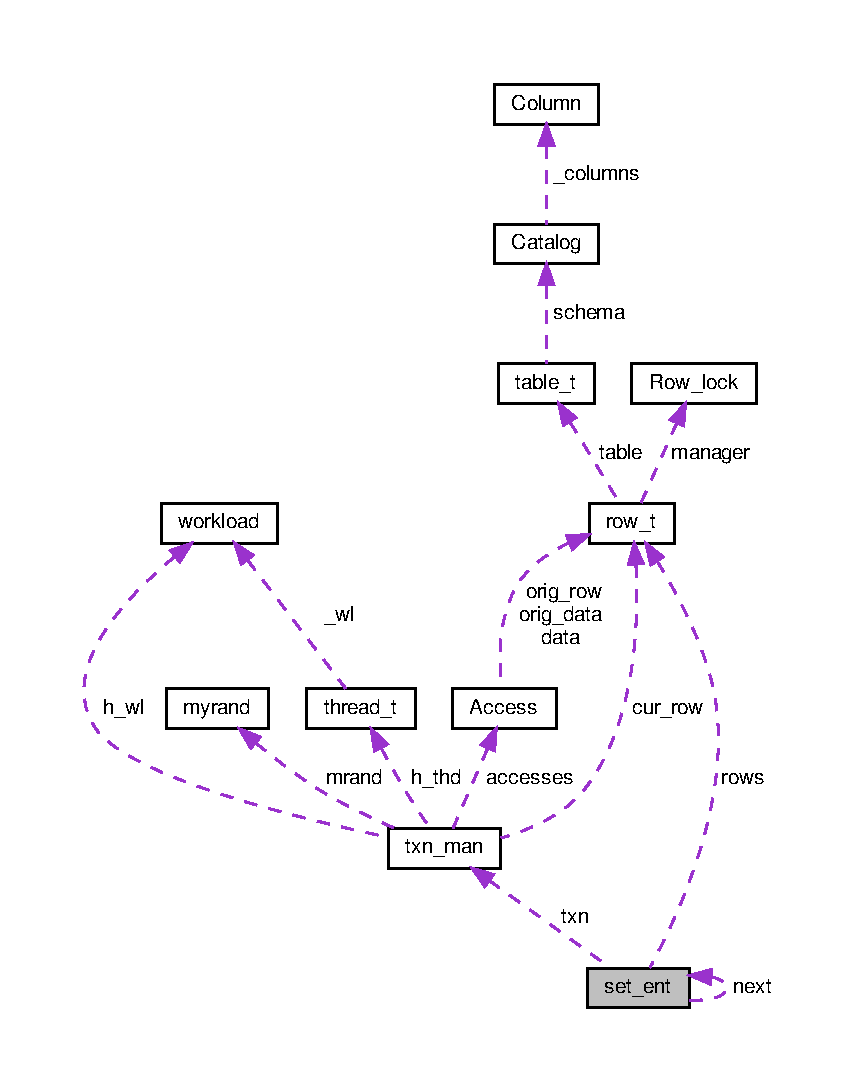
\includegraphics[width=350pt]{classset__ent__coll__graph}
\end{center}
\end{figure}
\subsection*{Public Member Functions}
\begin{DoxyCompactItemize}
\item 
\hyperlink{classset__ent_a57e4fb77951e8b8dcb26c0a05a1f9bf7}{set\+\_\+ent} ()
\end{DoxyCompactItemize}
\subsection*{Public Attributes}
\begin{DoxyCompactItemize}
\item 
\hyperlink{global_8h_aa288382a207683aa38aca516f6edd66d}{U\+Int64} \hyperlink{classset__ent_a5b485f5ee58d49e9bb77e965841248d5}{tn}
\item 
\hyperlink{classtxn__man}{txn\+\_\+man} $\ast$ \hyperlink{classset__ent_aa2178fabde4bb9173ffb05611637e8ee}{txn}
\item 
\hyperlink{global_8h_a7e8aeec7b6541935dfc6f608cd5170ce}{U\+Int32} \hyperlink{classset__ent_a56b8c477e32506bada3a073647243c02}{set\+\_\+size}
\item 
\hyperlink{classrow__t}{row\+\_\+t} $\ast$$\ast$ \hyperlink{classset__ent_aeef660ee01f805956cc54d9165c8ab44}{rows}
\item 
\hyperlink{classset__ent}{set\+\_\+ent} $\ast$ \hyperlink{classset__ent_a2ae1cbb145d6447f9f61de595eb3a4f4}{next}
\end{DoxyCompactItemize}


\subsection{Constructor \& Destructor Documentation}
\mbox{\Hypertarget{classset__ent_a57e4fb77951e8b8dcb26c0a05a1f9bf7}\label{classset__ent_a57e4fb77951e8b8dcb26c0a05a1f9bf7}} 
\index{set\+\_\+ent@{set\+\_\+ent}!set\+\_\+ent@{set\+\_\+ent}}
\index{set\+\_\+ent@{set\+\_\+ent}!set\+\_\+ent@{set\+\_\+ent}}
\subsubsection{\texorpdfstring{set\+\_\+ent()}{set\_ent()}}
{\footnotesize\ttfamily set\+\_\+ent\+::set\+\_\+ent (\begin{DoxyParamCaption}{ }\end{DoxyParamCaption})}



\subsection{Member Data Documentation}
\mbox{\Hypertarget{classset__ent_a2ae1cbb145d6447f9f61de595eb3a4f4}\label{classset__ent_a2ae1cbb145d6447f9f61de595eb3a4f4}} 
\index{set\+\_\+ent@{set\+\_\+ent}!next@{next}}
\index{next@{next}!set\+\_\+ent@{set\+\_\+ent}}
\subsubsection{\texorpdfstring{next}{next}}
{\footnotesize\ttfamily \hyperlink{classset__ent}{set\+\_\+ent}$\ast$ set\+\_\+ent\+::next}

\mbox{\Hypertarget{classset__ent_aeef660ee01f805956cc54d9165c8ab44}\label{classset__ent_aeef660ee01f805956cc54d9165c8ab44}} 
\index{set\+\_\+ent@{set\+\_\+ent}!rows@{rows}}
\index{rows@{rows}!set\+\_\+ent@{set\+\_\+ent}}
\subsubsection{\texorpdfstring{rows}{rows}}
{\footnotesize\ttfamily \hyperlink{classrow__t}{row\+\_\+t}$\ast$$\ast$ set\+\_\+ent\+::rows}

\mbox{\Hypertarget{classset__ent_a56b8c477e32506bada3a073647243c02}\label{classset__ent_a56b8c477e32506bada3a073647243c02}} 
\index{set\+\_\+ent@{set\+\_\+ent}!set\+\_\+size@{set\+\_\+size}}
\index{set\+\_\+size@{set\+\_\+size}!set\+\_\+ent@{set\+\_\+ent}}
\subsubsection{\texorpdfstring{set\+\_\+size}{set\_size}}
{\footnotesize\ttfamily \hyperlink{global_8h_a7e8aeec7b6541935dfc6f608cd5170ce}{U\+Int32} set\+\_\+ent\+::set\+\_\+size}

\mbox{\Hypertarget{classset__ent_a5b485f5ee58d49e9bb77e965841248d5}\label{classset__ent_a5b485f5ee58d49e9bb77e965841248d5}} 
\index{set\+\_\+ent@{set\+\_\+ent}!tn@{tn}}
\index{tn@{tn}!set\+\_\+ent@{set\+\_\+ent}}
\subsubsection{\texorpdfstring{tn}{tn}}
{\footnotesize\ttfamily \hyperlink{global_8h_aa288382a207683aa38aca516f6edd66d}{U\+Int64} set\+\_\+ent\+::tn}

\mbox{\Hypertarget{classset__ent_aa2178fabde4bb9173ffb05611637e8ee}\label{classset__ent_aa2178fabde4bb9173ffb05611637e8ee}} 
\index{set\+\_\+ent@{set\+\_\+ent}!txn@{txn}}
\index{txn@{txn}!set\+\_\+ent@{set\+\_\+ent}}
\subsubsection{\texorpdfstring{txn}{txn}}
{\footnotesize\ttfamily \hyperlink{classtxn__man}{txn\+\_\+man}$\ast$ set\+\_\+ent\+::txn}



The documentation for this class was generated from the following files\+:\begin{DoxyCompactItemize}
\item 
macrobench/concurrency\+\_\+control/\hyperlink{occ_8h}{occ.\+h}\item 
macrobench/concurrency\+\_\+control/\hyperlink{occ_8cpp}{occ.\+cpp}\end{DoxyCompactItemize}

\hypertarget{structset__of__bags}{}\section{set\+\_\+of\+\_\+bags$<$ T $>$ Struct Template Reference}
\label{structset__of__bags}\index{set\+\_\+of\+\_\+bags$<$ T $>$@{set\+\_\+of\+\_\+bags$<$ T $>$}}


{\ttfamily \#include $<$reclaimer\+\_\+interface.\+h$>$}

\subsection*{Public Attributes}
\begin{DoxyCompactItemize}
\item 
\hyperlink{classblockbag}{blockbag}$<$ T $>$ $\ast$const  $\ast$const \hyperlink{structset__of__bags_aece6bb3de813afff53aeec6c67ce2460}{bags}
\item 
const int \hyperlink{structset__of__bags_ae2c6de80fdeed02cd5c87aa207dd8458}{num\+Bags}
\end{DoxyCompactItemize}


\subsection{Detailed Description}
\subsubsection*{template$<$typename T$>$\newline
struct set\+\_\+of\+\_\+bags$<$ T $>$}

C++ record manager implementation (P\+O\+DC 2015) by Trevor Brown.

Copyright (C) 2015 Trevor Brown 

\subsection{Member Data Documentation}
\mbox{\Hypertarget{structset__of__bags_aece6bb3de813afff53aeec6c67ce2460}\label{structset__of__bags_aece6bb3de813afff53aeec6c67ce2460}} 
\index{set\+\_\+of\+\_\+bags@{set\+\_\+of\+\_\+bags}!bags@{bags}}
\index{bags@{bags}!set\+\_\+of\+\_\+bags@{set\+\_\+of\+\_\+bags}}
\subsubsection{\texorpdfstring{bags}{bags}}
{\footnotesize\ttfamily template$<$typename T $>$ \\
\hyperlink{classblockbag}{blockbag}$<$T$>$$\ast$ const$\ast$ const \hyperlink{structset__of__bags}{set\+\_\+of\+\_\+bags}$<$ T $>$\+::bags}

\mbox{\Hypertarget{structset__of__bags_ae2c6de80fdeed02cd5c87aa207dd8458}\label{structset__of__bags_ae2c6de80fdeed02cd5c87aa207dd8458}} 
\index{set\+\_\+of\+\_\+bags@{set\+\_\+of\+\_\+bags}!num\+Bags@{num\+Bags}}
\index{num\+Bags@{num\+Bags}!set\+\_\+of\+\_\+bags@{set\+\_\+of\+\_\+bags}}
\subsubsection{\texorpdfstring{num\+Bags}{numBags}}
{\footnotesize\ttfamily template$<$typename T $>$ \\
const int \hyperlink{structset__of__bags}{set\+\_\+of\+\_\+bags}$<$ T $>$\+::num\+Bags}



The documentation for this struct was generated from the following file\+:\begin{DoxyCompactItemize}
\item 
common/recordmgr/\hyperlink{reclaimer__interface_8h}{reclaimer\+\_\+interface.\+h}\end{DoxyCompactItemize}

\hypertarget{classtimeline__draw__color_1_1Settings}{}\section{timeline\+\_\+draw\+\_\+color.\+Settings Class Reference}
\label{classtimeline__draw__color_1_1Settings}\index{timeline\+\_\+draw\+\_\+color.\+Settings@{timeline\+\_\+draw\+\_\+color.\+Settings}}


customize the following settings for your input.  


\subsection*{Public Member Functions}
\begin{DoxyCompactItemize}
\item 
def \hyperlink{classtimeline__draw__color_1_1Settings_a0eecbfc1a6cbe1fde41e2b90aa438efc}{get\+Thread} (self, line)
\begin{DoxyCompactList}\small\item\em should return the thread number for a given line (interval) \end{DoxyCompactList}\item 
def \hyperlink{classtimeline__draw__color_1_1Settings_a2ab1436494c5f59f36cead263189aacf}{get\+Start} (self, line)
\begin{DoxyCompactList}\small\item\em should return the interval start for a given line (interval) \end{DoxyCompactList}\item 
def \hyperlink{classtimeline__draw__color_1_1Settings_ab413e00996b5a20cec72774f031c5655}{get\+End} (self, line)
\begin{DoxyCompactList}\small\item\em should return the interval end for a given line (interval) \end{DoxyCompactList}\item 
def \hyperlink{classtimeline__draw__color_1_1Settings_a8391566e3f9b345fe61d8132f31dd546}{get\+Color} (self, line)
\begin{DoxyCompactList}\small\item\em should return the color for a given line (interval) \end{DoxyCompactList}\item 
def \hyperlink{classtimeline__draw__color_1_1Settings_abc0017e43efda88d737383cfbcfb402d}{include\+Line} (self, line)
\begin{DoxyCompactList}\small\item\em should return True if the line is to be included in the graph and False otherwise \end{DoxyCompactList}\end{DoxyCompactItemize}
\subsection*{Static Public Attributes}
\begin{DoxyCompactItemize}
\item 
int \hyperlink{classtimeline__draw__color_1_1Settings_ae036d957c043e96fe8a7dfc658d66192}{max\+Thread} = 1000
\item 
int \hyperlink{classtimeline__draw__color_1_1Settings_a25e564d0bba827827a724b41d8c99f61}{window\+Start\+\_\+ms} = 0
\item 
int \hyperlink{classtimeline__draw__color_1_1Settings_a0f8a0096c566ebfd9a82902638611bb3}{window\+Size\+\_\+ms} = 60000
\item 
int \hyperlink{classtimeline__draw__color_1_1Settings_a8886752d8712ba980ee9662d1456d263}{min\+Duration\+\_\+ms} = 20
\end{DoxyCompactItemize}


\subsection{Detailed Description}
customize the following settings for your input. 

by default, this expects four space-\/separated columns\+: thread\+\_\+number start\+\_\+time\+\_\+in\+\_\+nanosec end\+\_\+time\+\_\+in\+\_\+nanosec color

where color is chosen from\+: \href{https://matplotlib.org/gallery/color/named_colors.html}{\tt https\+://matplotlib.\+org/gallery/color/named\+\_\+colors.\+html} 

\subsection{Member Function Documentation}
\mbox{\Hypertarget{classtimeline__draw__color_1_1Settings_a8391566e3f9b345fe61d8132f31dd546}\label{classtimeline__draw__color_1_1Settings_a8391566e3f9b345fe61d8132f31dd546}} 
\index{timeline\+\_\+draw\+\_\+color\+::\+Settings@{timeline\+\_\+draw\+\_\+color\+::\+Settings}!get\+Color@{get\+Color}}
\index{get\+Color@{get\+Color}!timeline\+\_\+draw\+\_\+color\+::\+Settings@{timeline\+\_\+draw\+\_\+color\+::\+Settings}}
\subsubsection{\texorpdfstring{get\+Color()}{getColor()}}
{\footnotesize\ttfamily def timeline\+\_\+draw\+\_\+color.\+Settings.\+get\+Color (\begin{DoxyParamCaption}\item[{}]{self,  }\item[{}]{line }\end{DoxyParamCaption})}



should return the color for a given line (interval) 

\mbox{\Hypertarget{classtimeline__draw__color_1_1Settings_ab413e00996b5a20cec72774f031c5655}\label{classtimeline__draw__color_1_1Settings_ab413e00996b5a20cec72774f031c5655}} 
\index{timeline\+\_\+draw\+\_\+color\+::\+Settings@{timeline\+\_\+draw\+\_\+color\+::\+Settings}!get\+End@{get\+End}}
\index{get\+End@{get\+End}!timeline\+\_\+draw\+\_\+color\+::\+Settings@{timeline\+\_\+draw\+\_\+color\+::\+Settings}}
\subsubsection{\texorpdfstring{get\+End()}{getEnd()}}
{\footnotesize\ttfamily def timeline\+\_\+draw\+\_\+color.\+Settings.\+get\+End (\begin{DoxyParamCaption}\item[{}]{self,  }\item[{}]{line }\end{DoxyParamCaption})}



should return the interval end for a given line (interval) 

\mbox{\Hypertarget{classtimeline__draw__color_1_1Settings_a2ab1436494c5f59f36cead263189aacf}\label{classtimeline__draw__color_1_1Settings_a2ab1436494c5f59f36cead263189aacf}} 
\index{timeline\+\_\+draw\+\_\+color\+::\+Settings@{timeline\+\_\+draw\+\_\+color\+::\+Settings}!get\+Start@{get\+Start}}
\index{get\+Start@{get\+Start}!timeline\+\_\+draw\+\_\+color\+::\+Settings@{timeline\+\_\+draw\+\_\+color\+::\+Settings}}
\subsubsection{\texorpdfstring{get\+Start()}{getStart()}}
{\footnotesize\ttfamily def timeline\+\_\+draw\+\_\+color.\+Settings.\+get\+Start (\begin{DoxyParamCaption}\item[{}]{self,  }\item[{}]{line }\end{DoxyParamCaption})}



should return the interval start for a given line (interval) 

\mbox{\Hypertarget{classtimeline__draw__color_1_1Settings_a0eecbfc1a6cbe1fde41e2b90aa438efc}\label{classtimeline__draw__color_1_1Settings_a0eecbfc1a6cbe1fde41e2b90aa438efc}} 
\index{timeline\+\_\+draw\+\_\+color\+::\+Settings@{timeline\+\_\+draw\+\_\+color\+::\+Settings}!get\+Thread@{get\+Thread}}
\index{get\+Thread@{get\+Thread}!timeline\+\_\+draw\+\_\+color\+::\+Settings@{timeline\+\_\+draw\+\_\+color\+::\+Settings}}
\subsubsection{\texorpdfstring{get\+Thread()}{getThread()}}
{\footnotesize\ttfamily def timeline\+\_\+draw\+\_\+color.\+Settings.\+get\+Thread (\begin{DoxyParamCaption}\item[{}]{self,  }\item[{}]{line }\end{DoxyParamCaption})}



should return the thread number for a given line (interval) 

\mbox{\Hypertarget{classtimeline__draw__color_1_1Settings_abc0017e43efda88d737383cfbcfb402d}\label{classtimeline__draw__color_1_1Settings_abc0017e43efda88d737383cfbcfb402d}} 
\index{timeline\+\_\+draw\+\_\+color\+::\+Settings@{timeline\+\_\+draw\+\_\+color\+::\+Settings}!include\+Line@{include\+Line}}
\index{include\+Line@{include\+Line}!timeline\+\_\+draw\+\_\+color\+::\+Settings@{timeline\+\_\+draw\+\_\+color\+::\+Settings}}
\subsubsection{\texorpdfstring{include\+Line()}{includeLine()}}
{\footnotesize\ttfamily def timeline\+\_\+draw\+\_\+color.\+Settings.\+include\+Line (\begin{DoxyParamCaption}\item[{}]{self,  }\item[{}]{line }\end{DoxyParamCaption})}



should return True if the line is to be included in the graph and False otherwise 



\subsection{Member Data Documentation}
\mbox{\Hypertarget{classtimeline__draw__color_1_1Settings_ae036d957c043e96fe8a7dfc658d66192}\label{classtimeline__draw__color_1_1Settings_ae036d957c043e96fe8a7dfc658d66192}} 
\index{timeline\+\_\+draw\+\_\+color\+::\+Settings@{timeline\+\_\+draw\+\_\+color\+::\+Settings}!max\+Thread@{max\+Thread}}
\index{max\+Thread@{max\+Thread}!timeline\+\_\+draw\+\_\+color\+::\+Settings@{timeline\+\_\+draw\+\_\+color\+::\+Settings}}
\subsubsection{\texorpdfstring{max\+Thread}{maxThread}}
{\footnotesize\ttfamily int timeline\+\_\+draw\+\_\+color.\+Settings.\+max\+Thread = 1000\hspace{0.3cm}{\ttfamily [static]}}

\mbox{\Hypertarget{classtimeline__draw__color_1_1Settings_a8886752d8712ba980ee9662d1456d263}\label{classtimeline__draw__color_1_1Settings_a8886752d8712ba980ee9662d1456d263}} 
\index{timeline\+\_\+draw\+\_\+color\+::\+Settings@{timeline\+\_\+draw\+\_\+color\+::\+Settings}!min\+Duration\+\_\+ms@{min\+Duration\+\_\+ms}}
\index{min\+Duration\+\_\+ms@{min\+Duration\+\_\+ms}!timeline\+\_\+draw\+\_\+color\+::\+Settings@{timeline\+\_\+draw\+\_\+color\+::\+Settings}}
\subsubsection{\texorpdfstring{min\+Duration\+\_\+ms}{minDuration\_ms}}
{\footnotesize\ttfamily int timeline\+\_\+draw\+\_\+color.\+Settings.\+min\+Duration\+\_\+ms = 20\hspace{0.3cm}{\ttfamily [static]}}

\mbox{\Hypertarget{classtimeline__draw__color_1_1Settings_a0f8a0096c566ebfd9a82902638611bb3}\label{classtimeline__draw__color_1_1Settings_a0f8a0096c566ebfd9a82902638611bb3}} 
\index{timeline\+\_\+draw\+\_\+color\+::\+Settings@{timeline\+\_\+draw\+\_\+color\+::\+Settings}!window\+Size\+\_\+ms@{window\+Size\+\_\+ms}}
\index{window\+Size\+\_\+ms@{window\+Size\+\_\+ms}!timeline\+\_\+draw\+\_\+color\+::\+Settings@{timeline\+\_\+draw\+\_\+color\+::\+Settings}}
\subsubsection{\texorpdfstring{window\+Size\+\_\+ms}{windowSize\_ms}}
{\footnotesize\ttfamily int timeline\+\_\+draw\+\_\+color.\+Settings.\+window\+Size\+\_\+ms = 60000\hspace{0.3cm}{\ttfamily [static]}}

\mbox{\Hypertarget{classtimeline__draw__color_1_1Settings_a25e564d0bba827827a724b41d8c99f61}\label{classtimeline__draw__color_1_1Settings_a25e564d0bba827827a724b41d8c99f61}} 
\index{timeline\+\_\+draw\+\_\+color\+::\+Settings@{timeline\+\_\+draw\+\_\+color\+::\+Settings}!window\+Start\+\_\+ms@{window\+Start\+\_\+ms}}
\index{window\+Start\+\_\+ms@{window\+Start\+\_\+ms}!timeline\+\_\+draw\+\_\+color\+::\+Settings@{timeline\+\_\+draw\+\_\+color\+::\+Settings}}
\subsubsection{\texorpdfstring{window\+Start\+\_\+ms}{windowStart\_ms}}
{\footnotesize\ttfamily int timeline\+\_\+draw\+\_\+color.\+Settings.\+window\+Start\+\_\+ms = 0\hspace{0.3cm}{\ttfamily [static]}}



The documentation for this class was generated from the following file\+:\begin{DoxyCompactItemize}
\item 
microbench/experiments/timelines/\hyperlink{timeline__draw__color_8py}{timeline\+\_\+draw\+\_\+color.\+py}\end{DoxyCompactItemize}

\hypertarget{classtimeline__draw__bw_1_1Settings}{}\section{timeline\+\_\+draw\+\_\+bw.\+Settings Class Reference}
\label{classtimeline__draw__bw_1_1Settings}\index{timeline\+\_\+draw\+\_\+bw.\+Settings@{timeline\+\_\+draw\+\_\+bw.\+Settings}}


customize the following settings for your input.  


\subsection*{Public Member Functions}
\begin{DoxyCompactItemize}
\item 
def \hyperlink{classtimeline__draw__bw_1_1Settings_a8f4a4dfe365bc55f55f3b3a8ef3524a3}{get\+Thread} (self, line)
\begin{DoxyCompactList}\small\item\em should return the thread number for a given line (interval) \end{DoxyCompactList}\item 
def \hyperlink{classtimeline__draw__bw_1_1Settings_a15ac4f74b26be5aaa7ff99efc9ef187a}{get\+Start} (self, line)
\begin{DoxyCompactList}\small\item\em should return the interval start for a given line (interval) \end{DoxyCompactList}\item 
def \hyperlink{classtimeline__draw__bw_1_1Settings_a18a9eae1f801909cc112e5401a1290d1}{get\+End} (self, line)
\begin{DoxyCompactList}\small\item\em should return the interval end for a given line (interval) \end{DoxyCompactList}\item 
def \hyperlink{classtimeline__draw__bw_1_1Settings_a173c1a3bf8d4ac4f607aff243ba06116}{get\+Color} (self, line)
\begin{DoxyCompactList}\small\item\em should return the color for a given line (interval) \end{DoxyCompactList}\item 
def \hyperlink{classtimeline__draw__bw_1_1Settings_a572fa3777fd6842b68033807657afe1d}{include\+Line} (self, line)
\begin{DoxyCompactList}\small\item\em should return True if the line is to be included in the graph and False otherwise \end{DoxyCompactList}\end{DoxyCompactItemize}
\subsection*{Static Public Attributes}
\begin{DoxyCompactItemize}
\item 
int \hyperlink{classtimeline__draw__bw_1_1Settings_a941a3030f430ef7defb2cfde3045c504}{max\+Thread} = 1000
\item 
int \hyperlink{classtimeline__draw__bw_1_1Settings_a06f2f1a8d2657cd2cf303759a105a900}{window\+Start\+\_\+ms} = 0
\item 
int \hyperlink{classtimeline__draw__bw_1_1Settings_a0a6c1531e4af92cbc594e461180f5675}{window\+Size\+\_\+ms} = 60000
\item 
int \hyperlink{classtimeline__draw__bw_1_1Settings_a5ee81de952a739f08c3d5fa516f09471}{min\+Duration\+\_\+ms} = 20
\end{DoxyCompactItemize}


\subsection{Detailed Description}
customize the following settings for your input. 

by default, this expects three space-\/separated columns\+: thread\+\_\+number start\+\_\+time\+\_\+in\+\_\+nanosec end\+\_\+time\+\_\+in\+\_\+nanosec 

\subsection{Member Function Documentation}
\mbox{\Hypertarget{classtimeline__draw__bw_1_1Settings_a173c1a3bf8d4ac4f607aff243ba06116}\label{classtimeline__draw__bw_1_1Settings_a173c1a3bf8d4ac4f607aff243ba06116}} 
\index{timeline\+\_\+draw\+\_\+bw\+::\+Settings@{timeline\+\_\+draw\+\_\+bw\+::\+Settings}!get\+Color@{get\+Color}}
\index{get\+Color@{get\+Color}!timeline\+\_\+draw\+\_\+bw\+::\+Settings@{timeline\+\_\+draw\+\_\+bw\+::\+Settings}}
\subsubsection{\texorpdfstring{get\+Color()}{getColor()}}
{\footnotesize\ttfamily def timeline\+\_\+draw\+\_\+bw.\+Settings.\+get\+Color (\begin{DoxyParamCaption}\item[{}]{self,  }\item[{}]{line }\end{DoxyParamCaption})}



should return the color for a given line (interval) 

\mbox{\Hypertarget{classtimeline__draw__bw_1_1Settings_a18a9eae1f801909cc112e5401a1290d1}\label{classtimeline__draw__bw_1_1Settings_a18a9eae1f801909cc112e5401a1290d1}} 
\index{timeline\+\_\+draw\+\_\+bw\+::\+Settings@{timeline\+\_\+draw\+\_\+bw\+::\+Settings}!get\+End@{get\+End}}
\index{get\+End@{get\+End}!timeline\+\_\+draw\+\_\+bw\+::\+Settings@{timeline\+\_\+draw\+\_\+bw\+::\+Settings}}
\subsubsection{\texorpdfstring{get\+End()}{getEnd()}}
{\footnotesize\ttfamily def timeline\+\_\+draw\+\_\+bw.\+Settings.\+get\+End (\begin{DoxyParamCaption}\item[{}]{self,  }\item[{}]{line }\end{DoxyParamCaption})}



should return the interval end for a given line (interval) 

\mbox{\Hypertarget{classtimeline__draw__bw_1_1Settings_a15ac4f74b26be5aaa7ff99efc9ef187a}\label{classtimeline__draw__bw_1_1Settings_a15ac4f74b26be5aaa7ff99efc9ef187a}} 
\index{timeline\+\_\+draw\+\_\+bw\+::\+Settings@{timeline\+\_\+draw\+\_\+bw\+::\+Settings}!get\+Start@{get\+Start}}
\index{get\+Start@{get\+Start}!timeline\+\_\+draw\+\_\+bw\+::\+Settings@{timeline\+\_\+draw\+\_\+bw\+::\+Settings}}
\subsubsection{\texorpdfstring{get\+Start()}{getStart()}}
{\footnotesize\ttfamily def timeline\+\_\+draw\+\_\+bw.\+Settings.\+get\+Start (\begin{DoxyParamCaption}\item[{}]{self,  }\item[{}]{line }\end{DoxyParamCaption})}



should return the interval start for a given line (interval) 

\mbox{\Hypertarget{classtimeline__draw__bw_1_1Settings_a8f4a4dfe365bc55f55f3b3a8ef3524a3}\label{classtimeline__draw__bw_1_1Settings_a8f4a4dfe365bc55f55f3b3a8ef3524a3}} 
\index{timeline\+\_\+draw\+\_\+bw\+::\+Settings@{timeline\+\_\+draw\+\_\+bw\+::\+Settings}!get\+Thread@{get\+Thread}}
\index{get\+Thread@{get\+Thread}!timeline\+\_\+draw\+\_\+bw\+::\+Settings@{timeline\+\_\+draw\+\_\+bw\+::\+Settings}}
\subsubsection{\texorpdfstring{get\+Thread()}{getThread()}}
{\footnotesize\ttfamily def timeline\+\_\+draw\+\_\+bw.\+Settings.\+get\+Thread (\begin{DoxyParamCaption}\item[{}]{self,  }\item[{}]{line }\end{DoxyParamCaption})}



should return the thread number for a given line (interval) 

\mbox{\Hypertarget{classtimeline__draw__bw_1_1Settings_a572fa3777fd6842b68033807657afe1d}\label{classtimeline__draw__bw_1_1Settings_a572fa3777fd6842b68033807657afe1d}} 
\index{timeline\+\_\+draw\+\_\+bw\+::\+Settings@{timeline\+\_\+draw\+\_\+bw\+::\+Settings}!include\+Line@{include\+Line}}
\index{include\+Line@{include\+Line}!timeline\+\_\+draw\+\_\+bw\+::\+Settings@{timeline\+\_\+draw\+\_\+bw\+::\+Settings}}
\subsubsection{\texorpdfstring{include\+Line()}{includeLine()}}
{\footnotesize\ttfamily def timeline\+\_\+draw\+\_\+bw.\+Settings.\+include\+Line (\begin{DoxyParamCaption}\item[{}]{self,  }\item[{}]{line }\end{DoxyParamCaption})}



should return True if the line is to be included in the graph and False otherwise 



\subsection{Member Data Documentation}
\mbox{\Hypertarget{classtimeline__draw__bw_1_1Settings_a941a3030f430ef7defb2cfde3045c504}\label{classtimeline__draw__bw_1_1Settings_a941a3030f430ef7defb2cfde3045c504}} 
\index{timeline\+\_\+draw\+\_\+bw\+::\+Settings@{timeline\+\_\+draw\+\_\+bw\+::\+Settings}!max\+Thread@{max\+Thread}}
\index{max\+Thread@{max\+Thread}!timeline\+\_\+draw\+\_\+bw\+::\+Settings@{timeline\+\_\+draw\+\_\+bw\+::\+Settings}}
\subsubsection{\texorpdfstring{max\+Thread}{maxThread}}
{\footnotesize\ttfamily int timeline\+\_\+draw\+\_\+bw.\+Settings.\+max\+Thread = 1000\hspace{0.3cm}{\ttfamily [static]}}

\mbox{\Hypertarget{classtimeline__draw__bw_1_1Settings_a5ee81de952a739f08c3d5fa516f09471}\label{classtimeline__draw__bw_1_1Settings_a5ee81de952a739f08c3d5fa516f09471}} 
\index{timeline\+\_\+draw\+\_\+bw\+::\+Settings@{timeline\+\_\+draw\+\_\+bw\+::\+Settings}!min\+Duration\+\_\+ms@{min\+Duration\+\_\+ms}}
\index{min\+Duration\+\_\+ms@{min\+Duration\+\_\+ms}!timeline\+\_\+draw\+\_\+bw\+::\+Settings@{timeline\+\_\+draw\+\_\+bw\+::\+Settings}}
\subsubsection{\texorpdfstring{min\+Duration\+\_\+ms}{minDuration\_ms}}
{\footnotesize\ttfamily int timeline\+\_\+draw\+\_\+bw.\+Settings.\+min\+Duration\+\_\+ms = 20\hspace{0.3cm}{\ttfamily [static]}}

\mbox{\Hypertarget{classtimeline__draw__bw_1_1Settings_a0a6c1531e4af92cbc594e461180f5675}\label{classtimeline__draw__bw_1_1Settings_a0a6c1531e4af92cbc594e461180f5675}} 
\index{timeline\+\_\+draw\+\_\+bw\+::\+Settings@{timeline\+\_\+draw\+\_\+bw\+::\+Settings}!window\+Size\+\_\+ms@{window\+Size\+\_\+ms}}
\index{window\+Size\+\_\+ms@{window\+Size\+\_\+ms}!timeline\+\_\+draw\+\_\+bw\+::\+Settings@{timeline\+\_\+draw\+\_\+bw\+::\+Settings}}
\subsubsection{\texorpdfstring{window\+Size\+\_\+ms}{windowSize\_ms}}
{\footnotesize\ttfamily int timeline\+\_\+draw\+\_\+bw.\+Settings.\+window\+Size\+\_\+ms = 60000\hspace{0.3cm}{\ttfamily [static]}}

\mbox{\Hypertarget{classtimeline__draw__bw_1_1Settings_a06f2f1a8d2657cd2cf303759a105a900}\label{classtimeline__draw__bw_1_1Settings_a06f2f1a8d2657cd2cf303759a105a900}} 
\index{timeline\+\_\+draw\+\_\+bw\+::\+Settings@{timeline\+\_\+draw\+\_\+bw\+::\+Settings}!window\+Start\+\_\+ms@{window\+Start\+\_\+ms}}
\index{window\+Start\+\_\+ms@{window\+Start\+\_\+ms}!timeline\+\_\+draw\+\_\+bw\+::\+Settings@{timeline\+\_\+draw\+\_\+bw\+::\+Settings}}
\subsubsection{\texorpdfstring{window\+Start\+\_\+ms}{windowStart\_ms}}
{\footnotesize\ttfamily int timeline\+\_\+draw\+\_\+bw.\+Settings.\+window\+Start\+\_\+ms = 0\hspace{0.3cm}{\ttfamily [static]}}



The documentation for this class was generated from the following file\+:\begin{DoxyCompactItemize}
\item 
microbench/experiments/timelines/\hyperlink{timeline__draw__bw_8py}{timeline\+\_\+draw\+\_\+bw.\+py}\end{DoxyCompactItemize}

\hypertarget{structSingleCounter}{}\section{Single\+Counter Struct Reference}
\label{structSingleCounter}\index{Single\+Counter@{Single\+Counter}}


{\ttfamily \#include $<$multi\+\_\+counter.\+h$>$}

\subsection*{Public Attributes}
\begin{DoxyCompactItemize}
\item 
\begin{tabbing}
xx\=xx\=xx\=xx\=xx\=xx\=xx\=xx\=xx\=\kill
union \{\\
\>\hyperlink{structSingleCounter_a1eaa8b82970740ea5e36d4c171ccc86a}{PAD}\\
\>volatile size\_t \hyperlink{structSingleCounter_a584b30254d2b6e5cb188a7ac658bddb0}{v}\\
\}; \\

\end{tabbing}\end{DoxyCompactItemize}


\subsection{Member Data Documentation}
\mbox{\Hypertarget{structSingleCounter_a46a1661a50236419b513aafdc6b05c1e}\label{structSingleCounter_a46a1661a50236419b513aafdc6b05c1e}} 
\subsubsection{\texorpdfstring{"@2}{@2}}
{\footnotesize\ttfamily union \{ ... \} }

\mbox{\Hypertarget{structSingleCounter_a1eaa8b82970740ea5e36d4c171ccc86a}\label{structSingleCounter_a1eaa8b82970740ea5e36d4c171ccc86a}} 
\index{Single\+Counter@{Single\+Counter}!P\+AD@{P\+AD}}
\index{P\+AD@{P\+AD}!Single\+Counter@{Single\+Counter}}
\subsubsection{\texorpdfstring{P\+AD}{PAD}}
{\footnotesize\ttfamily Single\+Counter\+::\+P\+AD}

\mbox{\Hypertarget{structSingleCounter_a584b30254d2b6e5cb188a7ac658bddb0}\label{structSingleCounter_a584b30254d2b6e5cb188a7ac658bddb0}} 
\index{Single\+Counter@{Single\+Counter}!v@{v}}
\index{v@{v}!Single\+Counter@{Single\+Counter}}
\subsubsection{\texorpdfstring{v}{v}}
{\footnotesize\ttfamily volatile size\+\_\+t Single\+Counter\+::v}



The documentation for this struct was generated from the following file\+:\begin{DoxyCompactItemize}
\item 
common/\hyperlink{multi__counter_8h}{multi\+\_\+counter.\+h}\end{DoxyCompactItemize}

\hypertarget{classSkipListKCAS}{}\section{Skip\+List\+K\+C\+AS$<$ Record\+Manager, K, V $>$ Class Template Reference}
\label{classSkipListKCAS}\index{Skip\+List\+K\+C\+A\+S$<$ Record\+Manager, K, V $>$@{Skip\+List\+K\+C\+A\+S$<$ Record\+Manager, K, V $>$}}


{\ttfamily \#include $<$skiplist.\+h$>$}

\subsection*{Public Member Functions}
\begin{DoxyCompactItemize}
\item 
\hyperlink{classSkipListKCAS_ad888a514bdad0bcd7e66d420aa812dfd}{Skip\+List\+K\+C\+AS} (const int \+\_\+num\+Threads, const int \+\_\+min\+Key, const long long \+\_\+max\+Key)
\item 
\hyperlink{classSkipListKCAS_a300d303cd08e2eca1f1b26618976eaa7}{$\sim$\+Skip\+List\+K\+C\+AS} ()
\item 
bool \hyperlink{classSkipListKCAS_a4136ad0113f56f3b6027f19b8a0bb2e4}{contains} (const int \hyperlink{microbench_2main_8cpp_a9ca9869868fe7e7a38a921cc7de4103f}{tid}, const K \&key)
\item 
V \hyperlink{classSkipListKCAS_a31ac3cb003b2db554e9ff88709cf27b8}{insert\+If\+Absent} (const int \hyperlink{microbench_2main_8cpp_a9ca9869868fe7e7a38a921cc7de4103f}{tid}, const K \&key, const V \&value)
\item 
V \hyperlink{classSkipListKCAS_ad627fc3dae55d47033e23c7cb444361c}{erase} (const int \hyperlink{microbench_2main_8cpp_a9ca9869868fe7e7a38a921cc7de4103f}{tid}, const K \&key)
\item 
bool \hyperlink{classSkipListKCAS_a50180c470d3c81053dc6cfd0ce942815}{validate} ()
\item 
void \hyperlink{classSkipListKCAS_a4863afabbb70b137e69bf3aef5f53481}{print\+Debugging\+Details} ()
\item 
void \hyperlink{classSkipListKCAS_a5794714ba69feac4dc63c3962a55c585}{init\+Thread} (const int \hyperlink{microbench_2main_8cpp_a9ca9869868fe7e7a38a921cc7de4103f}{tid})
\item 
void \hyperlink{classSkipListKCAS_abd5d5cf784b1572397f8fbc23d700d4d}{deinit\+Thread} (const int \hyperlink{microbench_2main_8cpp_a9ca9869868fe7e7a38a921cc7de4103f}{tid})
\item 
\hyperlink{classNode}{Node}$<$ K, V $>$ $\ast$ \hyperlink{classSkipListKCAS_aba9dcac668a65d8716c74298c0499218}{get\+Root} ()
\end{DoxyCompactItemize}


\subsection{Constructor \& Destructor Documentation}
\mbox{\Hypertarget{classSkipListKCAS_ad888a514bdad0bcd7e66d420aa812dfd}\label{classSkipListKCAS_ad888a514bdad0bcd7e66d420aa812dfd}} 
\index{Skip\+List\+K\+C\+AS@{Skip\+List\+K\+C\+AS}!Skip\+List\+K\+C\+AS@{Skip\+List\+K\+C\+AS}}
\index{Skip\+List\+K\+C\+AS@{Skip\+List\+K\+C\+AS}!Skip\+List\+K\+C\+AS@{Skip\+List\+K\+C\+AS}}
\subsubsection{\texorpdfstring{Skip\+List\+K\+C\+A\+S()}{SkipListKCAS()}}
{\footnotesize\ttfamily template$<$class Record\+Manager , typename K , typename V $>$ \\
\hyperlink{classSkipListKCAS}{Skip\+List\+K\+C\+AS}$<$ Record\+Manager, K, V $>$\+::\hyperlink{classSkipListKCAS}{Skip\+List\+K\+C\+AS} (\begin{DoxyParamCaption}\item[{const int}]{\+\_\+num\+Threads,  }\item[{const int}]{\+\_\+min\+Key,  }\item[{const long long}]{\+\_\+max\+Key }\end{DoxyParamCaption})}

\mbox{\Hypertarget{classSkipListKCAS_a300d303cd08e2eca1f1b26618976eaa7}\label{classSkipListKCAS_a300d303cd08e2eca1f1b26618976eaa7}} 
\index{Skip\+List\+K\+C\+AS@{Skip\+List\+K\+C\+AS}!````~Skip\+List\+K\+C\+AS@{$\sim$\+Skip\+List\+K\+C\+AS}}
\index{````~Skip\+List\+K\+C\+AS@{$\sim$\+Skip\+List\+K\+C\+AS}!Skip\+List\+K\+C\+AS@{Skip\+List\+K\+C\+AS}}
\subsubsection{\texorpdfstring{$\sim$\+Skip\+List\+K\+C\+A\+S()}{~SkipListKCAS()}}
{\footnotesize\ttfamily template$<$class Record\+Manager , typename K , typename V $>$ \\
\hyperlink{classSkipListKCAS}{Skip\+List\+K\+C\+AS}$<$ Record\+Manager, K, V $>$\+::$\sim$\hyperlink{classSkipListKCAS}{Skip\+List\+K\+C\+AS} (\begin{DoxyParamCaption}{ }\end{DoxyParamCaption})}



\subsection{Member Function Documentation}
\mbox{\Hypertarget{classSkipListKCAS_a4136ad0113f56f3b6027f19b8a0bb2e4}\label{classSkipListKCAS_a4136ad0113f56f3b6027f19b8a0bb2e4}} 
\index{Skip\+List\+K\+C\+AS@{Skip\+List\+K\+C\+AS}!contains@{contains}}
\index{contains@{contains}!Skip\+List\+K\+C\+AS@{Skip\+List\+K\+C\+AS}}
\subsubsection{\texorpdfstring{contains()}{contains()}}
{\footnotesize\ttfamily template$<$class Record\+Manager , typename K , typename V $>$ \\
bool \hyperlink{classSkipListKCAS}{Skip\+List\+K\+C\+AS}$<$ Record\+Manager, K, V $>$\+::contains (\begin{DoxyParamCaption}\item[{const int}]{tid,  }\item[{const K \&}]{key }\end{DoxyParamCaption})\hspace{0.3cm}{\ttfamily [inline]}}

\mbox{\Hypertarget{classSkipListKCAS_abd5d5cf784b1572397f8fbc23d700d4d}\label{classSkipListKCAS_abd5d5cf784b1572397f8fbc23d700d4d}} 
\index{Skip\+List\+K\+C\+AS@{Skip\+List\+K\+C\+AS}!deinit\+Thread@{deinit\+Thread}}
\index{deinit\+Thread@{deinit\+Thread}!Skip\+List\+K\+C\+AS@{Skip\+List\+K\+C\+AS}}
\subsubsection{\texorpdfstring{deinit\+Thread()}{deinitThread()}}
{\footnotesize\ttfamily template$<$class Record\+Manager , typename K , typename V $>$ \\
void \hyperlink{classSkipListKCAS}{Skip\+List\+K\+C\+AS}$<$ Record\+Manager, K, V $>$\+::deinit\+Thread (\begin{DoxyParamCaption}\item[{const int}]{tid }\end{DoxyParamCaption})}

\mbox{\Hypertarget{classSkipListKCAS_ad627fc3dae55d47033e23c7cb444361c}\label{classSkipListKCAS_ad627fc3dae55d47033e23c7cb444361c}} 
\index{Skip\+List\+K\+C\+AS@{Skip\+List\+K\+C\+AS}!erase@{erase}}
\index{erase@{erase}!Skip\+List\+K\+C\+AS@{Skip\+List\+K\+C\+AS}}
\subsubsection{\texorpdfstring{erase()}{erase()}}
{\footnotesize\ttfamily template$<$class Record\+Manager , typename K , typename V $>$ \\
V \hyperlink{classSkipListKCAS}{Skip\+List\+K\+C\+AS}$<$ Record\+Manager, K, V $>$\+::erase (\begin{DoxyParamCaption}\item[{const int}]{tid,  }\item[{const K \&}]{key }\end{DoxyParamCaption})\hspace{0.3cm}{\ttfamily [inline]}}

\mbox{\Hypertarget{classSkipListKCAS_aba9dcac668a65d8716c74298c0499218}\label{classSkipListKCAS_aba9dcac668a65d8716c74298c0499218}} 
\index{Skip\+List\+K\+C\+AS@{Skip\+List\+K\+C\+AS}!get\+Root@{get\+Root}}
\index{get\+Root@{get\+Root}!Skip\+List\+K\+C\+AS@{Skip\+List\+K\+C\+AS}}
\subsubsection{\texorpdfstring{get\+Root()}{getRoot()}}
{\footnotesize\ttfamily template$<$class Record\+Manager , typename K , typename V $>$ \\
\hyperlink{classNode}{Node}$<$ K, V $>$ $\ast$ \hyperlink{classSkipListKCAS}{Skip\+List\+K\+C\+AS}$<$ Record\+Manager, K, V $>$\+::get\+Root (\begin{DoxyParamCaption}\item[{void}]{ }\end{DoxyParamCaption})}

\mbox{\Hypertarget{classSkipListKCAS_a5794714ba69feac4dc63c3962a55c585}\label{classSkipListKCAS_a5794714ba69feac4dc63c3962a55c585}} 
\index{Skip\+List\+K\+C\+AS@{Skip\+List\+K\+C\+AS}!init\+Thread@{init\+Thread}}
\index{init\+Thread@{init\+Thread}!Skip\+List\+K\+C\+AS@{Skip\+List\+K\+C\+AS}}
\subsubsection{\texorpdfstring{init\+Thread()}{initThread()}}
{\footnotesize\ttfamily template$<$class Record\+Manager , typename K , typename V $>$ \\
void \hyperlink{classSkipListKCAS}{Skip\+List\+K\+C\+AS}$<$ Record\+Manager, K, V $>$\+::init\+Thread (\begin{DoxyParamCaption}\item[{const int}]{tid }\end{DoxyParamCaption})}

\mbox{\Hypertarget{classSkipListKCAS_a31ac3cb003b2db554e9ff88709cf27b8}\label{classSkipListKCAS_a31ac3cb003b2db554e9ff88709cf27b8}} 
\index{Skip\+List\+K\+C\+AS@{Skip\+List\+K\+C\+AS}!insert\+If\+Absent@{insert\+If\+Absent}}
\index{insert\+If\+Absent@{insert\+If\+Absent}!Skip\+List\+K\+C\+AS@{Skip\+List\+K\+C\+AS}}
\subsubsection{\texorpdfstring{insert\+If\+Absent()}{insertIfAbsent()}}
{\footnotesize\ttfamily template$<$class Record\+Manager , typename K , typename V $>$ \\
V \hyperlink{classSkipListKCAS}{Skip\+List\+K\+C\+AS}$<$ Record\+Manager, K, V $>$\+::insert\+If\+Absent (\begin{DoxyParamCaption}\item[{const int}]{tid,  }\item[{const K \&}]{key,  }\item[{const V \&}]{value }\end{DoxyParamCaption})\hspace{0.3cm}{\ttfamily [inline]}}

\mbox{\Hypertarget{classSkipListKCAS_a4863afabbb70b137e69bf3aef5f53481}\label{classSkipListKCAS_a4863afabbb70b137e69bf3aef5f53481}} 
\index{Skip\+List\+K\+C\+AS@{Skip\+List\+K\+C\+AS}!print\+Debugging\+Details@{print\+Debugging\+Details}}
\index{print\+Debugging\+Details@{print\+Debugging\+Details}!Skip\+List\+K\+C\+AS@{Skip\+List\+K\+C\+AS}}
\subsubsection{\texorpdfstring{print\+Debugging\+Details()}{printDebuggingDetails()}}
{\footnotesize\ttfamily template$<$class Record\+Manager , typename K , typename V $>$ \\
void \hyperlink{classSkipListKCAS}{Skip\+List\+K\+C\+AS}$<$ Record\+Manager, K, V $>$\+::print\+Debugging\+Details (\begin{DoxyParamCaption}{ }\end{DoxyParamCaption})}

\mbox{\Hypertarget{classSkipListKCAS_a50180c470d3c81053dc6cfd0ce942815}\label{classSkipListKCAS_a50180c470d3c81053dc6cfd0ce942815}} 
\index{Skip\+List\+K\+C\+AS@{Skip\+List\+K\+C\+AS}!validate@{validate}}
\index{validate@{validate}!Skip\+List\+K\+C\+AS@{Skip\+List\+K\+C\+AS}}
\subsubsection{\texorpdfstring{validate()}{validate()}}
{\footnotesize\ttfamily template$<$class Record\+Manager , typename K , typename V $>$ \\
bool \hyperlink{classSkipListKCAS}{Skip\+List\+K\+C\+AS}$<$ Record\+Manager, K, V $>$\+::validate (\begin{DoxyParamCaption}{ }\end{DoxyParamCaption})}



The documentation for this class was generated from the following file\+:\begin{DoxyCompactItemize}
\item 
ds/sigouin\+\_\+skip\+\_\+list\+\_\+kcas/\hyperlink{skiplist_8h}{skiplist.\+h}\end{DoxyCompactItemize}

\hypertarget{classSnapCollector}{}\section{Snap\+Collector$<$ Node\+Type, K $>$ Class Template Reference}
\label{classSnapCollector}\index{Snap\+Collector$<$ Node\+Type, K $>$@{Snap\+Collector$<$ Node\+Type, K $>$}}


{\ttfamily \#include $<$snapcollector.\+h$>$}

\subsection*{Classes}
\begin{DoxyCompactItemize}
\item 
class \hyperlink{classSnapCollector_1_1NodeWrapper}{Node\+Wrapper}
\end{DoxyCompactItemize}
\subsection*{Public Member Functions}
\begin{DoxyCompactItemize}
\item 
{\footnotesize template$<$typename Record\+Manager $>$ }\\void \hyperlink{classSnapCollector_ab94abbe542a7e33a212e8247b96197b5}{init} (const int \hyperlink{microbench_2main_8cpp_a9ca9869868fe7e7a38a921cc7de4103f}{tid}, const int \hyperlink{testing_8cpp_aa085812188e21ede75351d88b9b2c30d}{num\+Processes}, Record\+Manager $\ast$const recmgr, const K \+\_\+\+K\+E\+Y\+\_\+\+M\+IN, const K \+\_\+\+K\+E\+Y\+\_\+\+M\+AX)
\item 
\hyperlink{classSnapCollector_afe44bffcd16d6f6cd54c313be9703e52}{$\sim$\+Snap\+Collector} ()
\item 
{\footnotesize template$<$typename Record\+Manager $>$ }\\void \hyperlink{classSnapCollector_a9060f1d38be8915ad5e0139bc518bab4}{retire} (const int \hyperlink{microbench_2main_8cpp_a9ca9869868fe7e7a38a921cc7de4103f}{tid}, Record\+Manager $\ast$recmgr)
\item 
{\footnotesize template$<$typename Record\+Manager $>$ }\\Node\+Type $\ast$ \hyperlink{classSnapCollector_aab421d45e780e447bb9b5b872fa368f9}{Add\+Node} (const int \hyperlink{microbench_2main_8cpp_a9ca9869868fe7e7a38a921cc7de4103f}{tid}, Node\+Type $\ast$node, K key, Record\+Manager $\ast$recmgr)
\item 
{\footnotesize template$<$typename Record\+Manager $>$ }\\void \hyperlink{classSnapCollector_a99bf72a5b736cc82ce4c64e0fd76d15e}{Report} (int \hyperlink{microbench_2main_8cpp_a9ca9869868fe7e7a38a921cc7de4103f}{tid}, Node\+Type $\ast$\hyperlink{classNode}{Node}, \hyperlink{reportitem_8h_ae4f179a72db5cca021a37ec4c6fe4c68}{Report\+Type} t, K key, Record\+Manager $\ast$recmgr)
\item 
bool \hyperlink{classSnapCollector_a6140fe1b63009ac107881faaf43c09da}{Is\+Active} ()
\item 
{\footnotesize template$<$typename Record\+Manager $>$ }\\void \hyperlink{classSnapCollector_a53b4976ed927e14a99bb52993ffd5a2b}{Block\+Further\+Pointers} (const int \hyperlink{microbench_2main_8cpp_a9ca9869868fe7e7a38a921cc7de4103f}{tid}, Record\+Manager $\ast$recmgr)
\item 
void \hyperlink{classSnapCollector_a56d824c8e580ccb9422edcef9a26e636}{Deactivate} (pthread\+\_\+rwlock\+\_\+t $\ast$const rwlock, volatile long long $\ast$timestamp, long long $\ast$\hyperlink{rq__unsafe_8h_a643fd1eef8dbd00706b939b113a76394}{rq\+\_\+lin\+\_\+time})
\item 
void \hyperlink{classSnapCollector_a0848f9cf2e792a241809d9ff23a24bab}{Block\+Further\+Reports} ()
\item 
{\footnotesize template$<$typename Record\+Manager $>$ }\\void \hyperlink{classSnapCollector_a8c2b96dd6ec25eb4abfdc0c1ba2abc29}{Prepare} (int \hyperlink{microbench_2main_8cpp_a9ca9869868fe7e7a38a921cc7de4103f}{tid}, Record\+Manager $\ast$recmgr)
\item 
Node\+Type $\ast$ \hyperlink{classSnapCollector_afbc67dba82450f2d89099b0614c83804}{Get\+Next} (int \hyperlink{microbench_2main_8cpp_a9ca9869868fe7e7a38a921cc7de4103f}{tid})
\end{DoxyCompactItemize}
\subsection*{Public Attributes}
\begin{DoxyCompactItemize}
\item 
\hyperlink{classSnapCollector_a1e71ab6f1d3af03e0042459d31a98b95}{P\+AD}
\item 
int \hyperlink{classSnapCollector_a8c45790cee8b96758a8e98d7d7c8faf7}{N\+U\+M\+\_\+\+T\+H\+R\+E\+A\+DS}
\end{DoxyCompactItemize}


\subsection{Constructor \& Destructor Documentation}
\mbox{\Hypertarget{classSnapCollector_afe44bffcd16d6f6cd54c313be9703e52}\label{classSnapCollector_afe44bffcd16d6f6cd54c313be9703e52}} 
\index{Snap\+Collector@{Snap\+Collector}!````~Snap\+Collector@{$\sim$\+Snap\+Collector}}
\index{````~Snap\+Collector@{$\sim$\+Snap\+Collector}!Snap\+Collector@{Snap\+Collector}}
\subsubsection{\texorpdfstring{$\sim$\+Snap\+Collector()}{~SnapCollector()}}
{\footnotesize\ttfamily template$<$typename Node\+Type, typename K$>$ \\
\hyperlink{classSnapCollector}{Snap\+Collector}$<$ Node\+Type, K $>$\+::$\sim$\hyperlink{classSnapCollector}{Snap\+Collector} (\begin{DoxyParamCaption}{ }\end{DoxyParamCaption})\hspace{0.3cm}{\ttfamily [inline]}}



\subsection{Member Function Documentation}
\mbox{\Hypertarget{classSnapCollector_aab421d45e780e447bb9b5b872fa368f9}\label{classSnapCollector_aab421d45e780e447bb9b5b872fa368f9}} 
\index{Snap\+Collector@{Snap\+Collector}!Add\+Node@{Add\+Node}}
\index{Add\+Node@{Add\+Node}!Snap\+Collector@{Snap\+Collector}}
\subsubsection{\texorpdfstring{Add\+Node()}{AddNode()}}
{\footnotesize\ttfamily template$<$typename Node\+Type, typename K$>$ \\
template$<$typename Record\+Manager $>$ \\
Node\+Type$\ast$ \hyperlink{classSnapCollector}{Snap\+Collector}$<$ Node\+Type, K $>$\+::Add\+Node (\begin{DoxyParamCaption}\item[{const int}]{tid,  }\item[{Node\+Type $\ast$}]{node,  }\item[{K}]{key,  }\item[{Record\+Manager $\ast$}]{recmgr }\end{DoxyParamCaption})\hspace{0.3cm}{\ttfamily [inline]}}

\mbox{\Hypertarget{classSnapCollector_a53b4976ed927e14a99bb52993ffd5a2b}\label{classSnapCollector_a53b4976ed927e14a99bb52993ffd5a2b}} 
\index{Snap\+Collector@{Snap\+Collector}!Block\+Further\+Pointers@{Block\+Further\+Pointers}}
\index{Block\+Further\+Pointers@{Block\+Further\+Pointers}!Snap\+Collector@{Snap\+Collector}}
\subsubsection{\texorpdfstring{Block\+Further\+Pointers()}{BlockFurtherPointers()}}
{\footnotesize\ttfamily template$<$typename Node\+Type, typename K$>$ \\
template$<$typename Record\+Manager $>$ \\
void \hyperlink{classSnapCollector}{Snap\+Collector}$<$ Node\+Type, K $>$\+::Block\+Further\+Pointers (\begin{DoxyParamCaption}\item[{const int}]{tid,  }\item[{Record\+Manager $\ast$}]{recmgr }\end{DoxyParamCaption})\hspace{0.3cm}{\ttfamily [inline]}}

\mbox{\Hypertarget{classSnapCollector_a0848f9cf2e792a241809d9ff23a24bab}\label{classSnapCollector_a0848f9cf2e792a241809d9ff23a24bab}} 
\index{Snap\+Collector@{Snap\+Collector}!Block\+Further\+Reports@{Block\+Further\+Reports}}
\index{Block\+Further\+Reports@{Block\+Further\+Reports}!Snap\+Collector@{Snap\+Collector}}
\subsubsection{\texorpdfstring{Block\+Further\+Reports()}{BlockFurtherReports()}}
{\footnotesize\ttfamily template$<$typename Node\+Type, typename K$>$ \\
void \hyperlink{classSnapCollector}{Snap\+Collector}$<$ Node\+Type, K $>$\+::Block\+Further\+Reports (\begin{DoxyParamCaption}{ }\end{DoxyParamCaption})\hspace{0.3cm}{\ttfamily [inline]}}

\mbox{\Hypertarget{classSnapCollector_a56d824c8e580ccb9422edcef9a26e636}\label{classSnapCollector_a56d824c8e580ccb9422edcef9a26e636}} 
\index{Snap\+Collector@{Snap\+Collector}!Deactivate@{Deactivate}}
\index{Deactivate@{Deactivate}!Snap\+Collector@{Snap\+Collector}}
\subsubsection{\texorpdfstring{Deactivate()}{Deactivate()}}
{\footnotesize\ttfamily template$<$typename Node\+Type, typename K$>$ \\
void \hyperlink{classSnapCollector}{Snap\+Collector}$<$ Node\+Type, K $>$\+::Deactivate (\begin{DoxyParamCaption}\item[{pthread\+\_\+rwlock\+\_\+t $\ast$const}]{rwlock,  }\item[{volatile long long $\ast$}]{timestamp,  }\item[{long long $\ast$}]{rq\+\_\+lin\+\_\+time }\end{DoxyParamCaption})\hspace{0.3cm}{\ttfamily [inline]}}

note\+: the parameters are used for the timestamping mechanism of the test harness. they are N\+OT inherently needed by the snap collector. \mbox{\Hypertarget{classSnapCollector_afbc67dba82450f2d89099b0614c83804}\label{classSnapCollector_afbc67dba82450f2d89099b0614c83804}} 
\index{Snap\+Collector@{Snap\+Collector}!Get\+Next@{Get\+Next}}
\index{Get\+Next@{Get\+Next}!Snap\+Collector@{Snap\+Collector}}
\subsubsection{\texorpdfstring{Get\+Next()}{GetNext()}}
{\footnotesize\ttfamily template$<$typename Node\+Type, typename K$>$ \\
Node\+Type$\ast$ \hyperlink{classSnapCollector}{Snap\+Collector}$<$ Node\+Type, K $>$\+::Get\+Next (\begin{DoxyParamCaption}\item[{int}]{tid }\end{DoxyParamCaption})\hspace{0.3cm}{\ttfamily [inline]}}

\mbox{\Hypertarget{classSnapCollector_ab94abbe542a7e33a212e8247b96197b5}\label{classSnapCollector_ab94abbe542a7e33a212e8247b96197b5}} 
\index{Snap\+Collector@{Snap\+Collector}!init@{init}}
\index{init@{init}!Snap\+Collector@{Snap\+Collector}}
\subsubsection{\texorpdfstring{init()}{init()}}
{\footnotesize\ttfamily template$<$typename Node\+Type, typename K$>$ \\
template$<$typename Record\+Manager $>$ \\
void \hyperlink{classSnapCollector}{Snap\+Collector}$<$ Node\+Type, K $>$\+::init (\begin{DoxyParamCaption}\item[{const int}]{tid,  }\item[{const int}]{num\+Processes,  }\item[{Record\+Manager $\ast$const}]{recmgr,  }\item[{const K}]{\+\_\+\+K\+E\+Y\+\_\+\+M\+IN,  }\item[{const K}]{\+\_\+\+K\+E\+Y\+\_\+\+M\+AX }\end{DoxyParamCaption})\hspace{0.3cm}{\ttfamily [inline]}}

\mbox{\Hypertarget{classSnapCollector_a6140fe1b63009ac107881faaf43c09da}\label{classSnapCollector_a6140fe1b63009ac107881faaf43c09da}} 
\index{Snap\+Collector@{Snap\+Collector}!Is\+Active@{Is\+Active}}
\index{Is\+Active@{Is\+Active}!Snap\+Collector@{Snap\+Collector}}
\subsubsection{\texorpdfstring{Is\+Active()}{IsActive()}}
{\footnotesize\ttfamily template$<$typename Node\+Type, typename K$>$ \\
bool \hyperlink{classSnapCollector}{Snap\+Collector}$<$ Node\+Type, K $>$\+::Is\+Active (\begin{DoxyParamCaption}{ }\end{DoxyParamCaption})\hspace{0.3cm}{\ttfamily [inline]}}

\mbox{\Hypertarget{classSnapCollector_a8c2b96dd6ec25eb4abfdc0c1ba2abc29}\label{classSnapCollector_a8c2b96dd6ec25eb4abfdc0c1ba2abc29}} 
\index{Snap\+Collector@{Snap\+Collector}!Prepare@{Prepare}}
\index{Prepare@{Prepare}!Snap\+Collector@{Snap\+Collector}}
\subsubsection{\texorpdfstring{Prepare()}{Prepare()}}
{\footnotesize\ttfamily template$<$typename Node\+Type, typename K$>$ \\
template$<$typename Record\+Manager $>$ \\
void \hyperlink{classSnapCollector}{Snap\+Collector}$<$ Node\+Type, K $>$\+::Prepare (\begin{DoxyParamCaption}\item[{int}]{tid,  }\item[{Record\+Manager $\ast$}]{recmgr }\end{DoxyParamCaption})\hspace{0.3cm}{\ttfamily [inline]}}

\mbox{\Hypertarget{classSnapCollector_a99bf72a5b736cc82ce4c64e0fd76d15e}\label{classSnapCollector_a99bf72a5b736cc82ce4c64e0fd76d15e}} 
\index{Snap\+Collector@{Snap\+Collector}!Report@{Report}}
\index{Report@{Report}!Snap\+Collector@{Snap\+Collector}}
\subsubsection{\texorpdfstring{Report()}{Report()}}
{\footnotesize\ttfamily template$<$typename Node\+Type, typename K$>$ \\
template$<$typename Record\+Manager $>$ \\
void \hyperlink{classSnapCollector}{Snap\+Collector}$<$ Node\+Type, K $>$\+::Report (\begin{DoxyParamCaption}\item[{int}]{tid,  }\item[{Node\+Type $\ast$}]{Node,  }\item[{\hyperlink{reportitem_8h_ae4f179a72db5cca021a37ec4c6fe4c68}{Report\+Type}}]{t,  }\item[{K}]{key,  }\item[{Record\+Manager $\ast$}]{recmgr }\end{DoxyParamCaption})\hspace{0.3cm}{\ttfamily [inline]}}

\mbox{\Hypertarget{classSnapCollector_a9060f1d38be8915ad5e0139bc518bab4}\label{classSnapCollector_a9060f1d38be8915ad5e0139bc518bab4}} 
\index{Snap\+Collector@{Snap\+Collector}!retire@{retire}}
\index{retire@{retire}!Snap\+Collector@{Snap\+Collector}}
\subsubsection{\texorpdfstring{retire()}{retire()}}
{\footnotesize\ttfamily template$<$typename Node\+Type, typename K$>$ \\
template$<$typename Record\+Manager $>$ \\
void \hyperlink{classSnapCollector}{Snap\+Collector}$<$ Node\+Type, K $>$\+::retire (\begin{DoxyParamCaption}\item[{const int}]{tid,  }\item[{Record\+Manager $\ast$}]{recmgr }\end{DoxyParamCaption})\hspace{0.3cm}{\ttfamily [inline]}}



\subsection{Member Data Documentation}
\mbox{\Hypertarget{classSnapCollector_a8c45790cee8b96758a8e98d7d7c8faf7}\label{classSnapCollector_a8c45790cee8b96758a8e98d7d7c8faf7}} 
\index{Snap\+Collector@{Snap\+Collector}!N\+U\+M\+\_\+\+T\+H\+R\+E\+A\+DS@{N\+U\+M\+\_\+\+T\+H\+R\+E\+A\+DS}}
\index{N\+U\+M\+\_\+\+T\+H\+R\+E\+A\+DS@{N\+U\+M\+\_\+\+T\+H\+R\+E\+A\+DS}!Snap\+Collector@{Snap\+Collector}}
\subsubsection{\texorpdfstring{N\+U\+M\+\_\+\+T\+H\+R\+E\+A\+DS}{NUM\_THREADS}}
{\footnotesize\ttfamily template$<$typename Node\+Type, typename K$>$ \\
int \hyperlink{classSnapCollector}{Snap\+Collector}$<$ Node\+Type, K $>$\+::N\+U\+M\+\_\+\+T\+H\+R\+E\+A\+DS}

\mbox{\Hypertarget{classSnapCollector_a1e71ab6f1d3af03e0042459d31a98b95}\label{classSnapCollector_a1e71ab6f1d3af03e0042459d31a98b95}} 
\index{Snap\+Collector@{Snap\+Collector}!P\+AD@{P\+AD}}
\index{P\+AD@{P\+AD}!Snap\+Collector@{Snap\+Collector}}
\subsubsection{\texorpdfstring{P\+AD}{PAD}}
{\footnotesize\ttfamily template$<$typename Node\+Type, typename K$>$ \\
\hyperlink{classSnapCollector}{Snap\+Collector}$<$ Node\+Type, K $>$\+::P\+AD}



The documentation for this class was generated from the following file\+:\begin{DoxyCompactItemize}
\item 
common/rq/snapcollector/\hyperlink{snapcollector_8h}{snapcollector.\+h}\end{DoxyCompactItemize}

\hypertarget{structgstats__t_1_1stat__metrics}{}\section{gstats\+\_\+t\+:\+:stat\+\_\+metrics$<$ T $>$ Struct Template Reference}
\label{structgstats__t_1_1stat__metrics}\index{gstats\+\_\+t\+::stat\+\_\+metrics$<$ T $>$@{gstats\+\_\+t\+::stat\+\_\+metrics$<$ T $>$}}


{\ttfamily \#include $<$gstats.\+h$>$}



Collaboration diagram for gstats\+\_\+t\+:\+:stat\+\_\+metrics$<$ T $>$\+:
\nopagebreak
\begin{figure}[H]
\begin{center}
\leavevmode
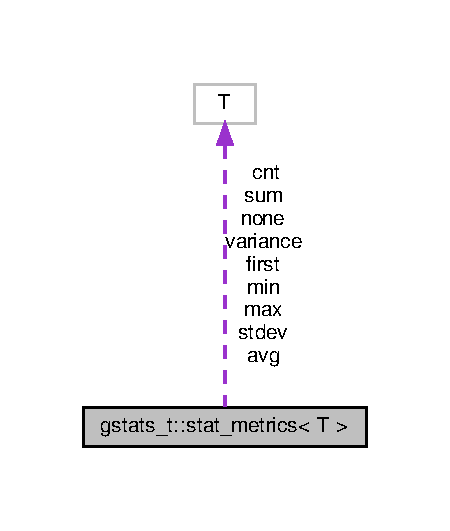
\includegraphics[width=216pt]{structgstats__t_1_1stat__metrics__coll__graph}
\end{center}
\end{figure}
\subsection*{Public Member Functions}
\begin{DoxyCompactItemize}
\item 
\hyperlink{structgstats__t_1_1stat__metrics_a71c5c9cdb3ec5f2c7caf7f4c163c4fca}{stat\+\_\+metrics} ()
\end{DoxyCompactItemize}
\subsection*{Public Attributes}
\begin{DoxyCompactItemize}
\item 
T \hyperlink{structgstats__t_1_1stat__metrics_abdcc23eb82f3e3ea9dfcf3f8bab1519c}{first}
\item 
T \hyperlink{structgstats__t_1_1stat__metrics_aa27fec5fa5e164d5735a2dd866bae8e2}{cnt}
\item 
T \hyperlink{structgstats__t_1_1stat__metrics_a4df97b4f8b36e7d81ff23706857b3dc7}{min}
\item 
T \hyperlink{structgstats__t_1_1stat__metrics_a278ee2eccccded2585c79c751dc0bbfc}{max}
\item 
T \hyperlink{structgstats__t_1_1stat__metrics_a7a543379413d2406cf71c5285871dbc5}{sum}
\item 
T \hyperlink{structgstats__t_1_1stat__metrics_a7c8c5fca0dff2830854431c9760821d9}{avg}
\item 
T \hyperlink{structgstats__t_1_1stat__metrics_af5d5633e58c10c6b008bf77cafe901fc}{variance}
\item 
T \hyperlink{structgstats__t_1_1stat__metrics_aca1ed6c41095a95695e5f0e328f9d485}{stdev}
\item 
T \hyperlink{structgstats__t_1_1stat__metrics_a1cdc639b40f3d973ace8ee448dbafac6}{none}
\end{DoxyCompactItemize}


\subsection{Constructor \& Destructor Documentation}
\mbox{\Hypertarget{structgstats__t_1_1stat__metrics_a71c5c9cdb3ec5f2c7caf7f4c163c4fca}\label{structgstats__t_1_1stat__metrics_a71c5c9cdb3ec5f2c7caf7f4c163c4fca}} 
\index{gstats\+\_\+t\+::stat\+\_\+metrics@{gstats\+\_\+t\+::stat\+\_\+metrics}!stat\+\_\+metrics@{stat\+\_\+metrics}}
\index{stat\+\_\+metrics@{stat\+\_\+metrics}!gstats\+\_\+t\+::stat\+\_\+metrics@{gstats\+\_\+t\+::stat\+\_\+metrics}}
\subsubsection{\texorpdfstring{stat\+\_\+metrics()}{stat\_metrics()}}
{\footnotesize\ttfamily template$<$typename T$>$ \\
\hyperlink{structgstats__t_1_1stat__metrics}{gstats\+\_\+t\+::stat\+\_\+metrics}$<$ T $>$\+::\hyperlink{structgstats__t_1_1stat__metrics}{stat\+\_\+metrics} (\begin{DoxyParamCaption}{ }\end{DoxyParamCaption})\hspace{0.3cm}{\ttfamily [inline]}}



\subsection{Member Data Documentation}
\mbox{\Hypertarget{structgstats__t_1_1stat__metrics_a7c8c5fca0dff2830854431c9760821d9}\label{structgstats__t_1_1stat__metrics_a7c8c5fca0dff2830854431c9760821d9}} 
\index{gstats\+\_\+t\+::stat\+\_\+metrics@{gstats\+\_\+t\+::stat\+\_\+metrics}!avg@{avg}}
\index{avg@{avg}!gstats\+\_\+t\+::stat\+\_\+metrics@{gstats\+\_\+t\+::stat\+\_\+metrics}}
\subsubsection{\texorpdfstring{avg}{avg}}
{\footnotesize\ttfamily template$<$typename T$>$ \\
T \hyperlink{structgstats__t_1_1stat__metrics}{gstats\+\_\+t\+::stat\+\_\+metrics}$<$ T $>$\+::avg}

\mbox{\Hypertarget{structgstats__t_1_1stat__metrics_aa27fec5fa5e164d5735a2dd866bae8e2}\label{structgstats__t_1_1stat__metrics_aa27fec5fa5e164d5735a2dd866bae8e2}} 
\index{gstats\+\_\+t\+::stat\+\_\+metrics@{gstats\+\_\+t\+::stat\+\_\+metrics}!cnt@{cnt}}
\index{cnt@{cnt}!gstats\+\_\+t\+::stat\+\_\+metrics@{gstats\+\_\+t\+::stat\+\_\+metrics}}
\subsubsection{\texorpdfstring{cnt}{cnt}}
{\footnotesize\ttfamily template$<$typename T$>$ \\
T \hyperlink{structgstats__t_1_1stat__metrics}{gstats\+\_\+t\+::stat\+\_\+metrics}$<$ T $>$\+::cnt}

\mbox{\Hypertarget{structgstats__t_1_1stat__metrics_abdcc23eb82f3e3ea9dfcf3f8bab1519c}\label{structgstats__t_1_1stat__metrics_abdcc23eb82f3e3ea9dfcf3f8bab1519c}} 
\index{gstats\+\_\+t\+::stat\+\_\+metrics@{gstats\+\_\+t\+::stat\+\_\+metrics}!first@{first}}
\index{first@{first}!gstats\+\_\+t\+::stat\+\_\+metrics@{gstats\+\_\+t\+::stat\+\_\+metrics}}
\subsubsection{\texorpdfstring{first}{first}}
{\footnotesize\ttfamily template$<$typename T$>$ \\
T \hyperlink{structgstats__t_1_1stat__metrics}{gstats\+\_\+t\+::stat\+\_\+metrics}$<$ T $>$\+::first}

\mbox{\Hypertarget{structgstats__t_1_1stat__metrics_a278ee2eccccded2585c79c751dc0bbfc}\label{structgstats__t_1_1stat__metrics_a278ee2eccccded2585c79c751dc0bbfc}} 
\index{gstats\+\_\+t\+::stat\+\_\+metrics@{gstats\+\_\+t\+::stat\+\_\+metrics}!max@{max}}
\index{max@{max}!gstats\+\_\+t\+::stat\+\_\+metrics@{gstats\+\_\+t\+::stat\+\_\+metrics}}
\subsubsection{\texorpdfstring{max}{max}}
{\footnotesize\ttfamily template$<$typename T$>$ \\
T \hyperlink{structgstats__t_1_1stat__metrics}{gstats\+\_\+t\+::stat\+\_\+metrics}$<$ T $>$\+::max}

\mbox{\Hypertarget{structgstats__t_1_1stat__metrics_a4df97b4f8b36e7d81ff23706857b3dc7}\label{structgstats__t_1_1stat__metrics_a4df97b4f8b36e7d81ff23706857b3dc7}} 
\index{gstats\+\_\+t\+::stat\+\_\+metrics@{gstats\+\_\+t\+::stat\+\_\+metrics}!min@{min}}
\index{min@{min}!gstats\+\_\+t\+::stat\+\_\+metrics@{gstats\+\_\+t\+::stat\+\_\+metrics}}
\subsubsection{\texorpdfstring{min}{min}}
{\footnotesize\ttfamily template$<$typename T$>$ \\
T \hyperlink{structgstats__t_1_1stat__metrics}{gstats\+\_\+t\+::stat\+\_\+metrics}$<$ T $>$\+::min}

\mbox{\Hypertarget{structgstats__t_1_1stat__metrics_a1cdc639b40f3d973ace8ee448dbafac6}\label{structgstats__t_1_1stat__metrics_a1cdc639b40f3d973ace8ee448dbafac6}} 
\index{gstats\+\_\+t\+::stat\+\_\+metrics@{gstats\+\_\+t\+::stat\+\_\+metrics}!none@{none}}
\index{none@{none}!gstats\+\_\+t\+::stat\+\_\+metrics@{gstats\+\_\+t\+::stat\+\_\+metrics}}
\subsubsection{\texorpdfstring{none}{none}}
{\footnotesize\ttfamily template$<$typename T$>$ \\
T \hyperlink{structgstats__t_1_1stat__metrics}{gstats\+\_\+t\+::stat\+\_\+metrics}$<$ T $>$\+::none}

\mbox{\Hypertarget{structgstats__t_1_1stat__metrics_aca1ed6c41095a95695e5f0e328f9d485}\label{structgstats__t_1_1stat__metrics_aca1ed6c41095a95695e5f0e328f9d485}} 
\index{gstats\+\_\+t\+::stat\+\_\+metrics@{gstats\+\_\+t\+::stat\+\_\+metrics}!stdev@{stdev}}
\index{stdev@{stdev}!gstats\+\_\+t\+::stat\+\_\+metrics@{gstats\+\_\+t\+::stat\+\_\+metrics}}
\subsubsection{\texorpdfstring{stdev}{stdev}}
{\footnotesize\ttfamily template$<$typename T$>$ \\
T \hyperlink{structgstats__t_1_1stat__metrics}{gstats\+\_\+t\+::stat\+\_\+metrics}$<$ T $>$\+::stdev}

\mbox{\Hypertarget{structgstats__t_1_1stat__metrics_a7a543379413d2406cf71c5285871dbc5}\label{structgstats__t_1_1stat__metrics_a7a543379413d2406cf71c5285871dbc5}} 
\index{gstats\+\_\+t\+::stat\+\_\+metrics@{gstats\+\_\+t\+::stat\+\_\+metrics}!sum@{sum}}
\index{sum@{sum}!gstats\+\_\+t\+::stat\+\_\+metrics@{gstats\+\_\+t\+::stat\+\_\+metrics}}
\subsubsection{\texorpdfstring{sum}{sum}}
{\footnotesize\ttfamily template$<$typename T$>$ \\
T \hyperlink{structgstats__t_1_1stat__metrics}{gstats\+\_\+t\+::stat\+\_\+metrics}$<$ T $>$\+::sum}

\mbox{\Hypertarget{structgstats__t_1_1stat__metrics_af5d5633e58c10c6b008bf77cafe901fc}\label{structgstats__t_1_1stat__metrics_af5d5633e58c10c6b008bf77cafe901fc}} 
\index{gstats\+\_\+t\+::stat\+\_\+metrics@{gstats\+\_\+t\+::stat\+\_\+metrics}!variance@{variance}}
\index{variance@{variance}!gstats\+\_\+t\+::stat\+\_\+metrics@{gstats\+\_\+t\+::stat\+\_\+metrics}}
\subsubsection{\texorpdfstring{variance}{variance}}
{\footnotesize\ttfamily template$<$typename T$>$ \\
T \hyperlink{structgstats__t_1_1stat__metrics}{gstats\+\_\+t\+::stat\+\_\+metrics}$<$ T $>$\+::variance}



The documentation for this struct was generated from the following file\+:\begin{DoxyCompactItemize}
\item 
common/\hyperlink{gstats_8h}{gstats.\+h}\end{DoxyCompactItemize}

\hypertarget{structstateRecord}{}\section{state\+Record$<$ skey\+\_\+t, sval\+\_\+t $>$ Struct Template Reference}
\label{structstateRecord}\index{state\+Record$<$ skey\+\_\+t, sval\+\_\+t $>$@{state\+Record$<$ skey\+\_\+t, sval\+\_\+t $>$}}


{\ttfamily \#include $<$intlf\+\_\+impl.\+h$>$}

\subsection*{Public Attributes}
\begin{DoxyCompactItemize}
\item 
int \hyperlink{structstateRecord_ac725427eab6460435554ac5a2f9d880d}{depth}
\item 
\hyperlink{structedge}{edge}$<$ skey\+\_\+t, sval\+\_\+t $>$ \hyperlink{structstateRecord_ad0f7bb1f0798b986c6d924be5fab7077}{target\+Edge}
\item 
\hyperlink{structedge}{edge}$<$ skey\+\_\+t, sval\+\_\+t $>$ \hyperlink{structstateRecord_ae2b05b20fc0184e8cf84005f1da73a6c}{p\+Target\+Edge}
\item 
skey\+\_\+t \hyperlink{structstateRecord_acaced3e9c482c829b679cfd8cb9ff07f}{target\+Key}
\item 
skey\+\_\+t \hyperlink{structstateRecord_a4db56e4d8f1cc30d0087721d7b4cc39f}{current\+Key}
\item 
\hyperlink{intlf__impl_8h_a46c8a310cf4c094f8c80e1cb8dc1f911}{Mode} \hyperlink{structstateRecord_a1903fb379d70b6a7743cb5d329c17e44}{mode}
\item 
\hyperlink{intlf__impl_8h_a1d1cfd8ffb84e947f82999c682b666a7}{Type} \hyperlink{structstateRecord_a4ec229c5b99079c2103da81220452739}{type}
\item 
\hyperlink{structseekRecord}{seek\+Record}$<$ skey\+\_\+t, sval\+\_\+t $>$ \hyperlink{structstateRecord_ae385a9aaf16313a210dccd7ce94d0e0a}{successor\+Record}
\end{DoxyCompactItemize}


\subsection{Member Data Documentation}
\mbox{\Hypertarget{structstateRecord_a4db56e4d8f1cc30d0087721d7b4cc39f}\label{structstateRecord_a4db56e4d8f1cc30d0087721d7b4cc39f}} 
\index{state\+Record@{state\+Record}!current\+Key@{current\+Key}}
\index{current\+Key@{current\+Key}!state\+Record@{state\+Record}}
\subsubsection{\texorpdfstring{current\+Key}{currentKey}}
{\footnotesize\ttfamily template$<$typename skey\+\_\+t, typename sval\+\_\+t$>$ \\
skey\+\_\+t \hyperlink{structstateRecord}{state\+Record}$<$ skey\+\_\+t, sval\+\_\+t $>$\+::current\+Key}

\mbox{\Hypertarget{structstateRecord_ac725427eab6460435554ac5a2f9d880d}\label{structstateRecord_ac725427eab6460435554ac5a2f9d880d}} 
\index{state\+Record@{state\+Record}!depth@{depth}}
\index{depth@{depth}!state\+Record@{state\+Record}}
\subsubsection{\texorpdfstring{depth}{depth}}
{\footnotesize\ttfamily template$<$typename skey\+\_\+t, typename sval\+\_\+t$>$ \\
int \hyperlink{structstateRecord}{state\+Record}$<$ skey\+\_\+t, sval\+\_\+t $>$\+::depth}

\mbox{\Hypertarget{structstateRecord_a1903fb379d70b6a7743cb5d329c17e44}\label{structstateRecord_a1903fb379d70b6a7743cb5d329c17e44}} 
\index{state\+Record@{state\+Record}!mode@{mode}}
\index{mode@{mode}!state\+Record@{state\+Record}}
\subsubsection{\texorpdfstring{mode}{mode}}
{\footnotesize\ttfamily template$<$typename skey\+\_\+t, typename sval\+\_\+t$>$ \\
\hyperlink{intlf__impl_8h_a46c8a310cf4c094f8c80e1cb8dc1f911}{Mode} \hyperlink{structstateRecord}{state\+Record}$<$ skey\+\_\+t, sval\+\_\+t $>$\+::mode}

\mbox{\Hypertarget{structstateRecord_ae2b05b20fc0184e8cf84005f1da73a6c}\label{structstateRecord_ae2b05b20fc0184e8cf84005f1da73a6c}} 
\index{state\+Record@{state\+Record}!p\+Target\+Edge@{p\+Target\+Edge}}
\index{p\+Target\+Edge@{p\+Target\+Edge}!state\+Record@{state\+Record}}
\subsubsection{\texorpdfstring{p\+Target\+Edge}{pTargetEdge}}
{\footnotesize\ttfamily template$<$typename skey\+\_\+t, typename sval\+\_\+t$>$ \\
\hyperlink{structedge}{edge}$<$skey\+\_\+t, sval\+\_\+t$>$ \hyperlink{structstateRecord}{state\+Record}$<$ skey\+\_\+t, sval\+\_\+t $>$\+::p\+Target\+Edge}

\mbox{\Hypertarget{structstateRecord_ae385a9aaf16313a210dccd7ce94d0e0a}\label{structstateRecord_ae385a9aaf16313a210dccd7ce94d0e0a}} 
\index{state\+Record@{state\+Record}!successor\+Record@{successor\+Record}}
\index{successor\+Record@{successor\+Record}!state\+Record@{state\+Record}}
\subsubsection{\texorpdfstring{successor\+Record}{successorRecord}}
{\footnotesize\ttfamily template$<$typename skey\+\_\+t, typename sval\+\_\+t$>$ \\
\hyperlink{structseekRecord}{seek\+Record}$<$skey\+\_\+t, sval\+\_\+t$>$ \hyperlink{structstateRecord}{state\+Record}$<$ skey\+\_\+t, sval\+\_\+t $>$\+::successor\+Record}

\mbox{\Hypertarget{structstateRecord_ad0f7bb1f0798b986c6d924be5fab7077}\label{structstateRecord_ad0f7bb1f0798b986c6d924be5fab7077}} 
\index{state\+Record@{state\+Record}!target\+Edge@{target\+Edge}}
\index{target\+Edge@{target\+Edge}!state\+Record@{state\+Record}}
\subsubsection{\texorpdfstring{target\+Edge}{targetEdge}}
{\footnotesize\ttfamily template$<$typename skey\+\_\+t, typename sval\+\_\+t$>$ \\
\hyperlink{structedge}{edge}$<$skey\+\_\+t, sval\+\_\+t$>$ \hyperlink{structstateRecord}{state\+Record}$<$ skey\+\_\+t, sval\+\_\+t $>$\+::target\+Edge}

\mbox{\Hypertarget{structstateRecord_acaced3e9c482c829b679cfd8cb9ff07f}\label{structstateRecord_acaced3e9c482c829b679cfd8cb9ff07f}} 
\index{state\+Record@{state\+Record}!target\+Key@{target\+Key}}
\index{target\+Key@{target\+Key}!state\+Record@{state\+Record}}
\subsubsection{\texorpdfstring{target\+Key}{targetKey}}
{\footnotesize\ttfamily template$<$typename skey\+\_\+t, typename sval\+\_\+t$>$ \\
skey\+\_\+t \hyperlink{structstateRecord}{state\+Record}$<$ skey\+\_\+t, sval\+\_\+t $>$\+::target\+Key}

\mbox{\Hypertarget{structstateRecord_a4ec229c5b99079c2103da81220452739}\label{structstateRecord_a4ec229c5b99079c2103da81220452739}} 
\index{state\+Record@{state\+Record}!type@{type}}
\index{type@{type}!state\+Record@{state\+Record}}
\subsubsection{\texorpdfstring{type}{type}}
{\footnotesize\ttfamily template$<$typename skey\+\_\+t, typename sval\+\_\+t$>$ \\
\hyperlink{intlf__impl_8h_a1d1cfd8ffb84e947f82999c682b666a7}{Type} \hyperlink{structstateRecord}{state\+Record}$<$ skey\+\_\+t, sval\+\_\+t $>$\+::type}



The documentation for this struct was generated from the following file\+:\begin{DoxyCompactItemize}
\item 
ds/ramachandran\+\_\+int\+\_\+bst\+\_\+lf/\hyperlink{intlf__impl_8h}{intlf\+\_\+impl.\+h}\end{DoxyCompactItemize}

\hypertarget{classStats}{}\section{Stats Class Reference}
\label{classStats}\index{Stats@{Stats}}


{\ttfamily \#include $<$stats.\+h$>$}



Collaboration diagram for Stats\+:
\nopagebreak
\begin{figure}[H]
\begin{center}
\leavevmode
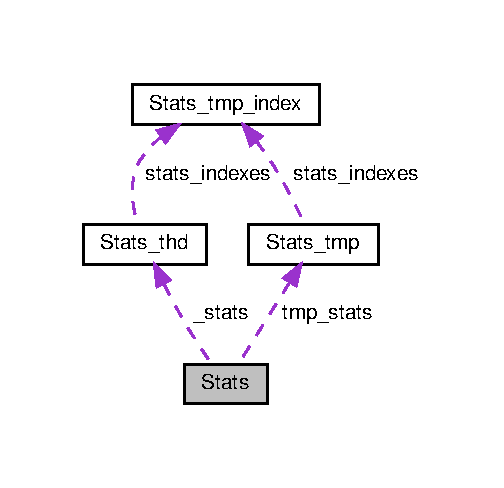
\includegraphics[width=242pt]{classStats__coll__graph}
\end{center}
\end{figure}
\subsection*{Public Member Functions}
\begin{DoxyCompactItemize}
\item 
void \hyperlink{classStats_a18ae30cf88fc793d1e2352215d60200f}{init} ()
\item 
void \hyperlink{classStats_a99204bb2a9d02ae319f187a61b6b705c}{setbench\+\_\+deinit} (uint64\+\_\+t thread\+\_\+id)
\item 
void \hyperlink{classStats_a59e70126dea691f97d798b60ef519ed2}{init} (uint64\+\_\+t thread\+\_\+id)
\item 
void \hyperlink{classStats_aa0521a06895775f85fc72df31e93a472}{clear} (uint64\+\_\+t \hyperlink{microbench_2main_8cpp_a9ca9869868fe7e7a38a921cc7de4103f}{tid})
\item 
void \hyperlink{classStats_aff90f0400fbb556c037f139dcb596608}{add\+\_\+debug} (uint64\+\_\+t thd\+\_\+id, uint64\+\_\+t value, uint32\+\_\+t select)
\item 
void \hyperlink{classStats_adc8454cb34173a4cef73c455e0cbfbee}{commit} (uint64\+\_\+t thd\+\_\+id)
\item 
void \hyperlink{classStats_a39df95409064be60b817937478582ad8}{abort} (uint64\+\_\+t thd\+\_\+id)
\item 
void \hyperlink{classStats_a64be07bc9550d3dccfc0f1fee76853bc}{print} (\hyperlink{classworkload}{workload} $\ast$wl)
\item 
void \hyperlink{classStats_ab689dd6e501c37388d8c4bad47e135e4}{print\+\_\+lat\+\_\+distr} ()
\end{DoxyCompactItemize}
\subsection*{Public Attributes}
\begin{DoxyCompactItemize}
\item 
\hyperlink{classStats__thd}{Stats\+\_\+thd} $\ast$$\ast$ \hyperlink{classStats_a0cebcc9e1772f74a3f93b8df9f07d05b}{\+\_\+stats}
\item 
\hyperlink{classStats__tmp}{Stats\+\_\+tmp} $\ast$$\ast$ \hyperlink{classStats_aa34f9c95002659dc382038861b3714db}{tmp\+\_\+stats}
\item 
double \hyperlink{classStats_a1fc8cf0036deec35ea41b1c8e5c2a4f5}{dl\+\_\+detect\+\_\+time}
\item 
double \hyperlink{classStats_a652b993afd04f06abc32425aa02f6e71}{dl\+\_\+wait\+\_\+time}
\item 
uint64\+\_\+t \hyperlink{classStats_a689ffff3edb9e712402d4a77884a0bde}{cycle\+\_\+detect}
\item 
uint64\+\_\+t \hyperlink{classStats_ac2fb99c156801571a88e02b50a10edf0}{deadlock}
\end{DoxyCompactItemize}


\subsection{Member Function Documentation}
\mbox{\Hypertarget{classStats_a39df95409064be60b817937478582ad8}\label{classStats_a39df95409064be60b817937478582ad8}} 
\index{Stats@{Stats}!abort@{abort}}
\index{abort@{abort}!Stats@{Stats}}
\subsubsection{\texorpdfstring{abort()}{abort()}}
{\footnotesize\ttfamily void Stats\+::abort (\begin{DoxyParamCaption}\item[{uint64\+\_\+t}]{thd\+\_\+id }\end{DoxyParamCaption})}

\mbox{\Hypertarget{classStats_aff90f0400fbb556c037f139dcb596608}\label{classStats_aff90f0400fbb556c037f139dcb596608}} 
\index{Stats@{Stats}!add\+\_\+debug@{add\+\_\+debug}}
\index{add\+\_\+debug@{add\+\_\+debug}!Stats@{Stats}}
\subsubsection{\texorpdfstring{add\+\_\+debug()}{add\_debug()}}
{\footnotesize\ttfamily void Stats\+::add\+\_\+debug (\begin{DoxyParamCaption}\item[{uint64\+\_\+t}]{thd\+\_\+id,  }\item[{uint64\+\_\+t}]{value,  }\item[{uint32\+\_\+t}]{select }\end{DoxyParamCaption})}

\mbox{\Hypertarget{classStats_aa0521a06895775f85fc72df31e93a472}\label{classStats_aa0521a06895775f85fc72df31e93a472}} 
\index{Stats@{Stats}!clear@{clear}}
\index{clear@{clear}!Stats@{Stats}}
\subsubsection{\texorpdfstring{clear()}{clear()}}
{\footnotesize\ttfamily void Stats\+::clear (\begin{DoxyParamCaption}\item[{uint64\+\_\+t}]{tid }\end{DoxyParamCaption})}

\mbox{\Hypertarget{classStats_adc8454cb34173a4cef73c455e0cbfbee}\label{classStats_adc8454cb34173a4cef73c455e0cbfbee}} 
\index{Stats@{Stats}!commit@{commit}}
\index{commit@{commit}!Stats@{Stats}}
\subsubsection{\texorpdfstring{commit()}{commit()}}
{\footnotesize\ttfamily void Stats\+::commit (\begin{DoxyParamCaption}\item[{uint64\+\_\+t}]{thd\+\_\+id }\end{DoxyParamCaption})}

\mbox{\Hypertarget{classStats_a18ae30cf88fc793d1e2352215d60200f}\label{classStats_a18ae30cf88fc793d1e2352215d60200f}} 
\index{Stats@{Stats}!init@{init}}
\index{init@{init}!Stats@{Stats}}
\subsubsection{\texorpdfstring{init()}{init()}\hspace{0.1cm}{\footnotesize\ttfamily [1/2]}}
{\footnotesize\ttfamily void Stats\+::init (\begin{DoxyParamCaption}{ }\end{DoxyParamCaption})}

\mbox{\Hypertarget{classStats_a59e70126dea691f97d798b60ef519ed2}\label{classStats_a59e70126dea691f97d798b60ef519ed2}} 
\index{Stats@{Stats}!init@{init}}
\index{init@{init}!Stats@{Stats}}
\subsubsection{\texorpdfstring{init()}{init()}\hspace{0.1cm}{\footnotesize\ttfamily [2/2]}}
{\footnotesize\ttfamily void Stats\+::init (\begin{DoxyParamCaption}\item[{uint64\+\_\+t}]{thread\+\_\+id }\end{DoxyParamCaption})}

\mbox{\Hypertarget{classStats_a64be07bc9550d3dccfc0f1fee76853bc}\label{classStats_a64be07bc9550d3dccfc0f1fee76853bc}} 
\index{Stats@{Stats}!print@{print}}
\index{print@{print}!Stats@{Stats}}
\subsubsection{\texorpdfstring{print()}{print()}}
{\footnotesize\ttfamily void Stats\+::print (\begin{DoxyParamCaption}\item[{\hyperlink{classworkload}{workload} $\ast$}]{wl }\end{DoxyParamCaption})}

Compute per-\/thread per-\/index stats

Compute per-\/index stats

Compute aggregate index stats

Print summary\mbox{\Hypertarget{classStats_ab689dd6e501c37388d8c4bad47e135e4}\label{classStats_ab689dd6e501c37388d8c4bad47e135e4}} 
\index{Stats@{Stats}!print\+\_\+lat\+\_\+distr@{print\+\_\+lat\+\_\+distr}}
\index{print\+\_\+lat\+\_\+distr@{print\+\_\+lat\+\_\+distr}!Stats@{Stats}}
\subsubsection{\texorpdfstring{print\+\_\+lat\+\_\+distr()}{print\_lat\_distr()}}
{\footnotesize\ttfamily void Stats\+::print\+\_\+lat\+\_\+distr (\begin{DoxyParamCaption}{ }\end{DoxyParamCaption})}

\mbox{\Hypertarget{classStats_a99204bb2a9d02ae319f187a61b6b705c}\label{classStats_a99204bb2a9d02ae319f187a61b6b705c}} 
\index{Stats@{Stats}!setbench\+\_\+deinit@{setbench\+\_\+deinit}}
\index{setbench\+\_\+deinit@{setbench\+\_\+deinit}!Stats@{Stats}}
\subsubsection{\texorpdfstring{setbench\+\_\+deinit()}{setbench\_deinit()}}
{\footnotesize\ttfamily void Stats\+::setbench\+\_\+deinit (\begin{DoxyParamCaption}\item[{uint64\+\_\+t}]{thread\+\_\+id }\end{DoxyParamCaption})}



\subsection{Member Data Documentation}
\mbox{\Hypertarget{classStats_a0cebcc9e1772f74a3f93b8df9f07d05b}\label{classStats_a0cebcc9e1772f74a3f93b8df9f07d05b}} 
\index{Stats@{Stats}!\+\_\+stats@{\+\_\+stats}}
\index{\+\_\+stats@{\+\_\+stats}!Stats@{Stats}}
\subsubsection{\texorpdfstring{\+\_\+stats}{\_stats}}
{\footnotesize\ttfamily \hyperlink{classStats__thd}{Stats\+\_\+thd}$\ast$$\ast$ Stats\+::\+\_\+stats}

\mbox{\Hypertarget{classStats_a689ffff3edb9e712402d4a77884a0bde}\label{classStats_a689ffff3edb9e712402d4a77884a0bde}} 
\index{Stats@{Stats}!cycle\+\_\+detect@{cycle\+\_\+detect}}
\index{cycle\+\_\+detect@{cycle\+\_\+detect}!Stats@{Stats}}
\subsubsection{\texorpdfstring{cycle\+\_\+detect}{cycle\_detect}}
{\footnotesize\ttfamily uint64\+\_\+t Stats\+::cycle\+\_\+detect}

\mbox{\Hypertarget{classStats_ac2fb99c156801571a88e02b50a10edf0}\label{classStats_ac2fb99c156801571a88e02b50a10edf0}} 
\index{Stats@{Stats}!deadlock@{deadlock}}
\index{deadlock@{deadlock}!Stats@{Stats}}
\subsubsection{\texorpdfstring{deadlock}{deadlock}}
{\footnotesize\ttfamily uint64\+\_\+t Stats\+::deadlock}

\mbox{\Hypertarget{classStats_a1fc8cf0036deec35ea41b1c8e5c2a4f5}\label{classStats_a1fc8cf0036deec35ea41b1c8e5c2a4f5}} 
\index{Stats@{Stats}!dl\+\_\+detect\+\_\+time@{dl\+\_\+detect\+\_\+time}}
\index{dl\+\_\+detect\+\_\+time@{dl\+\_\+detect\+\_\+time}!Stats@{Stats}}
\subsubsection{\texorpdfstring{dl\+\_\+detect\+\_\+time}{dl\_detect\_time}}
{\footnotesize\ttfamily double Stats\+::dl\+\_\+detect\+\_\+time}

\mbox{\Hypertarget{classStats_a652b993afd04f06abc32425aa02f6e71}\label{classStats_a652b993afd04f06abc32425aa02f6e71}} 
\index{Stats@{Stats}!dl\+\_\+wait\+\_\+time@{dl\+\_\+wait\+\_\+time}}
\index{dl\+\_\+wait\+\_\+time@{dl\+\_\+wait\+\_\+time}!Stats@{Stats}}
\subsubsection{\texorpdfstring{dl\+\_\+wait\+\_\+time}{dl\_wait\_time}}
{\footnotesize\ttfamily double Stats\+::dl\+\_\+wait\+\_\+time}

\mbox{\Hypertarget{classStats_aa34f9c95002659dc382038861b3714db}\label{classStats_aa34f9c95002659dc382038861b3714db}} 
\index{Stats@{Stats}!tmp\+\_\+stats@{tmp\+\_\+stats}}
\index{tmp\+\_\+stats@{tmp\+\_\+stats}!Stats@{Stats}}
\subsubsection{\texorpdfstring{tmp\+\_\+stats}{tmp\_stats}}
{\footnotesize\ttfamily \hyperlink{classStats__tmp}{Stats\+\_\+tmp}$\ast$$\ast$ Stats\+::tmp\+\_\+stats}



The documentation for this class was generated from the following files\+:\begin{DoxyCompactItemize}
\item 
macrobench/system/\hyperlink{stats_8h}{stats.\+h}\item 
macrobench/system/\hyperlink{stats_8cpp}{stats.\+cpp}\end{DoxyCompactItemize}

\hypertarget{classStats__thd}{}\section{Stats\+\_\+thd Class Reference}
\label{classStats__thd}\index{Stats\+\_\+thd@{Stats\+\_\+thd}}


{\ttfamily \#include $<$stats.\+h$>$}



Collaboration diagram for Stats\+\_\+thd\+:
\nopagebreak
\begin{figure}[H]
\begin{center}
\leavevmode
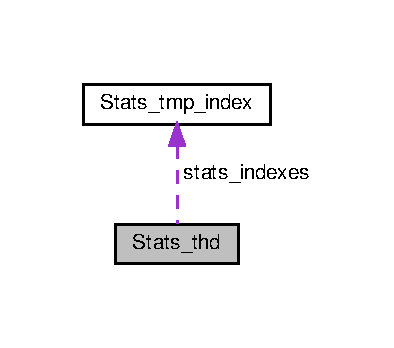
\includegraphics[width=189pt]{classStats__thd__coll__graph}
\end{center}
\end{figure}
\subsection*{Public Member Functions}
\begin{DoxyCompactItemize}
\item 
void \hyperlink{classStats__thd_ac1b482f396411d9466277b2290207871}{init} (uint64\+\_\+t thd\+\_\+id)
\item 
void \hyperlink{classStats__thd_ae4040380b7345caabc8e66f53f3bd957}{setbench\+\_\+deinit} ()
\item 
void \hyperlink{classStats__thd_aa76eee9ef160c0b362a893476b8ff943}{clear} ()
\end{DoxyCompactItemize}
\subsection*{Public Attributes}
\begin{DoxyCompactItemize}
\item 
char \hyperlink{classStats__thd_a69e6cc9995500f6ff46c4ac6a2a2c701}{\+\_\+pad2} \mbox{[}\hyperlink{config_8h_aa18ff96566bf8c1f4cd38c1e7bc4ca80}{C\+L\+\_\+\+S\+I\+ZE}\mbox{]}
\item 
uint64\+\_\+t \hyperlink{classStats__thd_a49a60b955252ba65d755d0c091c4f89e}{txn\+\_\+cnt}
\item 
uint64\+\_\+t \hyperlink{classStats__thd_aef6a88691a6f8a7fab529c69fc18695d}{abort\+\_\+cnt}
\item 
double \hyperlink{classStats__thd_a8b12797a3e9861fbdb5b87b7f4bed1fa}{run\+\_\+time}
\item 
\hyperlink{classStats__tmp__index}{Stats\+\_\+tmp\+\_\+index} \hyperlink{classStats__thd_ad4fe9ff08a5989c3c4852aadd17f3d69}{stats\+\_\+indexes} \mbox{[}\hyperlink{stats_8h_aefb0708b15ac381fb0f0d94c3ca6904d}{M\+A\+X\+\_\+\+N\+U\+M\+\_\+\+I\+N\+D\+E\+X\+ES}\mbox{]}
\item 
double \hyperlink{classStats__thd_a394ab002a85773b523ed4f0d4847cf07}{time\+\_\+man}
\item 
double \hyperlink{classStats__thd_a34b94d73fab82879dd2ad588ba6b5a88}{time\+\_\+index}
\item 
double \hyperlink{classStats__thd_ae7cff905febb34aeae34e57d8e5fb5f2}{time\+\_\+wait}
\item 
double \hyperlink{classStats__thd_a86b7a856496a2a8c091a227580770cd4}{time\+\_\+abort}
\item 
double \hyperlink{classStats__thd_a9863a5528c79f788e1b03c7f4c5614de}{time\+\_\+cleanup}
\item 
uint64\+\_\+t \hyperlink{classStats__thd_aac4564be92e99f7096e4a134361d0b76}{time\+\_\+ts\+\_\+alloc}
\item 
double \hyperlink{classStats__thd_a844362ff64eef3730588efd28d41c0e0}{time\+\_\+query}
\item 
uint64\+\_\+t \hyperlink{classStats__thd_af8910fbaa615ab9753db185927a5d169}{wait\+\_\+cnt}
\item 
uint64\+\_\+t \hyperlink{classStats__thd_a0ad99647bac316dbd7be1682eb3fad94}{debug1}
\item 
uint64\+\_\+t \hyperlink{classStats__thd_a093cee55ae1bad32e5eaf5f68140a142}{debug2}
\item 
uint64\+\_\+t \hyperlink{classStats__thd_a7f4cbf859001c12450801b2ca211be7d}{debug3}
\item 
uint64\+\_\+t \hyperlink{classStats__thd_a7b4e0f1509081c1c2aa3af92428cb59c}{debug4}
\item 
uint64\+\_\+t \hyperlink{classStats__thd_a8e2fee67d9f899a44a0b1b961cc42ed5}{debug5}
\item 
uint64\+\_\+t \hyperlink{classStats__thd_a2c405fcd6fcecea043a03e95517c0672}{latency}
\item 
uint64\+\_\+t $\ast$ \hyperlink{classStats__thd_ac2b8cd21ce48eee3af6246b4122ac4f5}{all\+\_\+debug1}
\item 
uint64\+\_\+t $\ast$ \hyperlink{classStats__thd_a83cd3b6b17499e33631d413204ce3dbc}{all\+\_\+debug2}
\item 
char \hyperlink{classStats__thd_a9989ab6d22c5dde64c44db70ffaaacc1}{\+\_\+pad} \mbox{[}\hyperlink{config_8h_aa18ff96566bf8c1f4cd38c1e7bc4ca80}{C\+L\+\_\+\+S\+I\+ZE}\mbox{]}
\end{DoxyCompactItemize}


\subsection{Member Function Documentation}
\mbox{\Hypertarget{classStats__thd_aa76eee9ef160c0b362a893476b8ff943}\label{classStats__thd_aa76eee9ef160c0b362a893476b8ff943}} 
\index{Stats\+\_\+thd@{Stats\+\_\+thd}!clear@{clear}}
\index{clear@{clear}!Stats\+\_\+thd@{Stats\+\_\+thd}}
\subsubsection{\texorpdfstring{clear()}{clear()}}
{\footnotesize\ttfamily void Stats\+\_\+thd\+::clear (\begin{DoxyParamCaption}{ }\end{DoxyParamCaption})}

\mbox{\Hypertarget{classStats__thd_ac1b482f396411d9466277b2290207871}\label{classStats__thd_ac1b482f396411d9466277b2290207871}} 
\index{Stats\+\_\+thd@{Stats\+\_\+thd}!init@{init}}
\index{init@{init}!Stats\+\_\+thd@{Stats\+\_\+thd}}
\subsubsection{\texorpdfstring{init()}{init()}}
{\footnotesize\ttfamily void Stats\+\_\+thd\+::init (\begin{DoxyParamCaption}\item[{uint64\+\_\+t}]{thd\+\_\+id }\end{DoxyParamCaption})}

\mbox{\Hypertarget{classStats__thd_ae4040380b7345caabc8e66f53f3bd957}\label{classStats__thd_ae4040380b7345caabc8e66f53f3bd957}} 
\index{Stats\+\_\+thd@{Stats\+\_\+thd}!setbench\+\_\+deinit@{setbench\+\_\+deinit}}
\index{setbench\+\_\+deinit@{setbench\+\_\+deinit}!Stats\+\_\+thd@{Stats\+\_\+thd}}
\subsubsection{\texorpdfstring{setbench\+\_\+deinit()}{setbench\_deinit()}}
{\footnotesize\ttfamily void Stats\+\_\+thd\+::setbench\+\_\+deinit (\begin{DoxyParamCaption}{ }\end{DoxyParamCaption})}



\subsection{Member Data Documentation}
\mbox{\Hypertarget{classStats__thd_a9989ab6d22c5dde64c44db70ffaaacc1}\label{classStats__thd_a9989ab6d22c5dde64c44db70ffaaacc1}} 
\index{Stats\+\_\+thd@{Stats\+\_\+thd}!\+\_\+pad@{\+\_\+pad}}
\index{\+\_\+pad@{\+\_\+pad}!Stats\+\_\+thd@{Stats\+\_\+thd}}
\subsubsection{\texorpdfstring{\+\_\+pad}{\_pad}}
{\footnotesize\ttfamily char Stats\+\_\+thd\+::\+\_\+pad\mbox{[}\hyperlink{config_8h_aa18ff96566bf8c1f4cd38c1e7bc4ca80}{C\+L\+\_\+\+S\+I\+ZE}\mbox{]}}

\mbox{\Hypertarget{classStats__thd_a69e6cc9995500f6ff46c4ac6a2a2c701}\label{classStats__thd_a69e6cc9995500f6ff46c4ac6a2a2c701}} 
\index{Stats\+\_\+thd@{Stats\+\_\+thd}!\+\_\+pad2@{\+\_\+pad2}}
\index{\+\_\+pad2@{\+\_\+pad2}!Stats\+\_\+thd@{Stats\+\_\+thd}}
\subsubsection{\texorpdfstring{\+\_\+pad2}{\_pad2}}
{\footnotesize\ttfamily char Stats\+\_\+thd\+::\+\_\+pad2\mbox{[}\hyperlink{config_8h_aa18ff96566bf8c1f4cd38c1e7bc4ca80}{C\+L\+\_\+\+S\+I\+ZE}\mbox{]}}

\mbox{\Hypertarget{classStats__thd_aef6a88691a6f8a7fab529c69fc18695d}\label{classStats__thd_aef6a88691a6f8a7fab529c69fc18695d}} 
\index{Stats\+\_\+thd@{Stats\+\_\+thd}!abort\+\_\+cnt@{abort\+\_\+cnt}}
\index{abort\+\_\+cnt@{abort\+\_\+cnt}!Stats\+\_\+thd@{Stats\+\_\+thd}}
\subsubsection{\texorpdfstring{abort\+\_\+cnt}{abort\_cnt}}
{\footnotesize\ttfamily uint64\+\_\+t Stats\+\_\+thd\+::abort\+\_\+cnt}

\mbox{\Hypertarget{classStats__thd_ac2b8cd21ce48eee3af6246b4122ac4f5}\label{classStats__thd_ac2b8cd21ce48eee3af6246b4122ac4f5}} 
\index{Stats\+\_\+thd@{Stats\+\_\+thd}!all\+\_\+debug1@{all\+\_\+debug1}}
\index{all\+\_\+debug1@{all\+\_\+debug1}!Stats\+\_\+thd@{Stats\+\_\+thd}}
\subsubsection{\texorpdfstring{all\+\_\+debug1}{all\_debug1}}
{\footnotesize\ttfamily uint64\+\_\+t$\ast$ Stats\+\_\+thd\+::all\+\_\+debug1}

\mbox{\Hypertarget{classStats__thd_a83cd3b6b17499e33631d413204ce3dbc}\label{classStats__thd_a83cd3b6b17499e33631d413204ce3dbc}} 
\index{Stats\+\_\+thd@{Stats\+\_\+thd}!all\+\_\+debug2@{all\+\_\+debug2}}
\index{all\+\_\+debug2@{all\+\_\+debug2}!Stats\+\_\+thd@{Stats\+\_\+thd}}
\subsubsection{\texorpdfstring{all\+\_\+debug2}{all\_debug2}}
{\footnotesize\ttfamily uint64\+\_\+t$\ast$ Stats\+\_\+thd\+::all\+\_\+debug2}

\mbox{\Hypertarget{classStats__thd_a0ad99647bac316dbd7be1682eb3fad94}\label{classStats__thd_a0ad99647bac316dbd7be1682eb3fad94}} 
\index{Stats\+\_\+thd@{Stats\+\_\+thd}!debug1@{debug1}}
\index{debug1@{debug1}!Stats\+\_\+thd@{Stats\+\_\+thd}}
\subsubsection{\texorpdfstring{debug1}{debug1}}
{\footnotesize\ttfamily uint64\+\_\+t Stats\+\_\+thd\+::debug1}

\mbox{\Hypertarget{classStats__thd_a093cee55ae1bad32e5eaf5f68140a142}\label{classStats__thd_a093cee55ae1bad32e5eaf5f68140a142}} 
\index{Stats\+\_\+thd@{Stats\+\_\+thd}!debug2@{debug2}}
\index{debug2@{debug2}!Stats\+\_\+thd@{Stats\+\_\+thd}}
\subsubsection{\texorpdfstring{debug2}{debug2}}
{\footnotesize\ttfamily uint64\+\_\+t Stats\+\_\+thd\+::debug2}

\mbox{\Hypertarget{classStats__thd_a7f4cbf859001c12450801b2ca211be7d}\label{classStats__thd_a7f4cbf859001c12450801b2ca211be7d}} 
\index{Stats\+\_\+thd@{Stats\+\_\+thd}!debug3@{debug3}}
\index{debug3@{debug3}!Stats\+\_\+thd@{Stats\+\_\+thd}}
\subsubsection{\texorpdfstring{debug3}{debug3}}
{\footnotesize\ttfamily uint64\+\_\+t Stats\+\_\+thd\+::debug3}

\mbox{\Hypertarget{classStats__thd_a7b4e0f1509081c1c2aa3af92428cb59c}\label{classStats__thd_a7b4e0f1509081c1c2aa3af92428cb59c}} 
\index{Stats\+\_\+thd@{Stats\+\_\+thd}!debug4@{debug4}}
\index{debug4@{debug4}!Stats\+\_\+thd@{Stats\+\_\+thd}}
\subsubsection{\texorpdfstring{debug4}{debug4}}
{\footnotesize\ttfamily uint64\+\_\+t Stats\+\_\+thd\+::debug4}

\mbox{\Hypertarget{classStats__thd_a8e2fee67d9f899a44a0b1b961cc42ed5}\label{classStats__thd_a8e2fee67d9f899a44a0b1b961cc42ed5}} 
\index{Stats\+\_\+thd@{Stats\+\_\+thd}!debug5@{debug5}}
\index{debug5@{debug5}!Stats\+\_\+thd@{Stats\+\_\+thd}}
\subsubsection{\texorpdfstring{debug5}{debug5}}
{\footnotesize\ttfamily uint64\+\_\+t Stats\+\_\+thd\+::debug5}

\mbox{\Hypertarget{classStats__thd_a2c405fcd6fcecea043a03e95517c0672}\label{classStats__thd_a2c405fcd6fcecea043a03e95517c0672}} 
\index{Stats\+\_\+thd@{Stats\+\_\+thd}!latency@{latency}}
\index{latency@{latency}!Stats\+\_\+thd@{Stats\+\_\+thd}}
\subsubsection{\texorpdfstring{latency}{latency}}
{\footnotesize\ttfamily uint64\+\_\+t Stats\+\_\+thd\+::latency}

\mbox{\Hypertarget{classStats__thd_a8b12797a3e9861fbdb5b87b7f4bed1fa}\label{classStats__thd_a8b12797a3e9861fbdb5b87b7f4bed1fa}} 
\index{Stats\+\_\+thd@{Stats\+\_\+thd}!run\+\_\+time@{run\+\_\+time}}
\index{run\+\_\+time@{run\+\_\+time}!Stats\+\_\+thd@{Stats\+\_\+thd}}
\subsubsection{\texorpdfstring{run\+\_\+time}{run\_time}}
{\footnotesize\ttfamily double Stats\+\_\+thd\+::run\+\_\+time}

\mbox{\Hypertarget{classStats__thd_ad4fe9ff08a5989c3c4852aadd17f3d69}\label{classStats__thd_ad4fe9ff08a5989c3c4852aadd17f3d69}} 
\index{Stats\+\_\+thd@{Stats\+\_\+thd}!stats\+\_\+indexes@{stats\+\_\+indexes}}
\index{stats\+\_\+indexes@{stats\+\_\+indexes}!Stats\+\_\+thd@{Stats\+\_\+thd}}
\subsubsection{\texorpdfstring{stats\+\_\+indexes}{stats\_indexes}}
{\footnotesize\ttfamily \hyperlink{classStats__tmp__index}{Stats\+\_\+tmp\+\_\+index} Stats\+\_\+thd\+::stats\+\_\+indexes\mbox{[}\hyperlink{stats_8h_aefb0708b15ac381fb0f0d94c3ca6904d}{M\+A\+X\+\_\+\+N\+U\+M\+\_\+\+I\+N\+D\+E\+X\+ES}\mbox{]}}

\mbox{\Hypertarget{classStats__thd_a86b7a856496a2a8c091a227580770cd4}\label{classStats__thd_a86b7a856496a2a8c091a227580770cd4}} 
\index{Stats\+\_\+thd@{Stats\+\_\+thd}!time\+\_\+abort@{time\+\_\+abort}}
\index{time\+\_\+abort@{time\+\_\+abort}!Stats\+\_\+thd@{Stats\+\_\+thd}}
\subsubsection{\texorpdfstring{time\+\_\+abort}{time\_abort}}
{\footnotesize\ttfamily double Stats\+\_\+thd\+::time\+\_\+abort}

\mbox{\Hypertarget{classStats__thd_a9863a5528c79f788e1b03c7f4c5614de}\label{classStats__thd_a9863a5528c79f788e1b03c7f4c5614de}} 
\index{Stats\+\_\+thd@{Stats\+\_\+thd}!time\+\_\+cleanup@{time\+\_\+cleanup}}
\index{time\+\_\+cleanup@{time\+\_\+cleanup}!Stats\+\_\+thd@{Stats\+\_\+thd}}
\subsubsection{\texorpdfstring{time\+\_\+cleanup}{time\_cleanup}}
{\footnotesize\ttfamily double Stats\+\_\+thd\+::time\+\_\+cleanup}

\mbox{\Hypertarget{classStats__thd_a34b94d73fab82879dd2ad588ba6b5a88}\label{classStats__thd_a34b94d73fab82879dd2ad588ba6b5a88}} 
\index{Stats\+\_\+thd@{Stats\+\_\+thd}!time\+\_\+index@{time\+\_\+index}}
\index{time\+\_\+index@{time\+\_\+index}!Stats\+\_\+thd@{Stats\+\_\+thd}}
\subsubsection{\texorpdfstring{time\+\_\+index}{time\_index}}
{\footnotesize\ttfamily double Stats\+\_\+thd\+::time\+\_\+index}

\mbox{\Hypertarget{classStats__thd_a394ab002a85773b523ed4f0d4847cf07}\label{classStats__thd_a394ab002a85773b523ed4f0d4847cf07}} 
\index{Stats\+\_\+thd@{Stats\+\_\+thd}!time\+\_\+man@{time\+\_\+man}}
\index{time\+\_\+man@{time\+\_\+man}!Stats\+\_\+thd@{Stats\+\_\+thd}}
\subsubsection{\texorpdfstring{time\+\_\+man}{time\_man}}
{\footnotesize\ttfamily double Stats\+\_\+thd\+::time\+\_\+man}

\mbox{\Hypertarget{classStats__thd_a844362ff64eef3730588efd28d41c0e0}\label{classStats__thd_a844362ff64eef3730588efd28d41c0e0}} 
\index{Stats\+\_\+thd@{Stats\+\_\+thd}!time\+\_\+query@{time\+\_\+query}}
\index{time\+\_\+query@{time\+\_\+query}!Stats\+\_\+thd@{Stats\+\_\+thd}}
\subsubsection{\texorpdfstring{time\+\_\+query}{time\_query}}
{\footnotesize\ttfamily double Stats\+\_\+thd\+::time\+\_\+query}

\mbox{\Hypertarget{classStats__thd_aac4564be92e99f7096e4a134361d0b76}\label{classStats__thd_aac4564be92e99f7096e4a134361d0b76}} 
\index{Stats\+\_\+thd@{Stats\+\_\+thd}!time\+\_\+ts\+\_\+alloc@{time\+\_\+ts\+\_\+alloc}}
\index{time\+\_\+ts\+\_\+alloc@{time\+\_\+ts\+\_\+alloc}!Stats\+\_\+thd@{Stats\+\_\+thd}}
\subsubsection{\texorpdfstring{time\+\_\+ts\+\_\+alloc}{time\_ts\_alloc}}
{\footnotesize\ttfamily uint64\+\_\+t Stats\+\_\+thd\+::time\+\_\+ts\+\_\+alloc}

\mbox{\Hypertarget{classStats__thd_ae7cff905febb34aeae34e57d8e5fb5f2}\label{classStats__thd_ae7cff905febb34aeae34e57d8e5fb5f2}} 
\index{Stats\+\_\+thd@{Stats\+\_\+thd}!time\+\_\+wait@{time\+\_\+wait}}
\index{time\+\_\+wait@{time\+\_\+wait}!Stats\+\_\+thd@{Stats\+\_\+thd}}
\subsubsection{\texorpdfstring{time\+\_\+wait}{time\_wait}}
{\footnotesize\ttfamily double Stats\+\_\+thd\+::time\+\_\+wait}

\mbox{\Hypertarget{classStats__thd_a49a60b955252ba65d755d0c091c4f89e}\label{classStats__thd_a49a60b955252ba65d755d0c091c4f89e}} 
\index{Stats\+\_\+thd@{Stats\+\_\+thd}!txn\+\_\+cnt@{txn\+\_\+cnt}}
\index{txn\+\_\+cnt@{txn\+\_\+cnt}!Stats\+\_\+thd@{Stats\+\_\+thd}}
\subsubsection{\texorpdfstring{txn\+\_\+cnt}{txn\_cnt}}
{\footnotesize\ttfamily uint64\+\_\+t Stats\+\_\+thd\+::txn\+\_\+cnt}

\mbox{\Hypertarget{classStats__thd_af8910fbaa615ab9753db185927a5d169}\label{classStats__thd_af8910fbaa615ab9753db185927a5d169}} 
\index{Stats\+\_\+thd@{Stats\+\_\+thd}!wait\+\_\+cnt@{wait\+\_\+cnt}}
\index{wait\+\_\+cnt@{wait\+\_\+cnt}!Stats\+\_\+thd@{Stats\+\_\+thd}}
\subsubsection{\texorpdfstring{wait\+\_\+cnt}{wait\_cnt}}
{\footnotesize\ttfamily uint64\+\_\+t Stats\+\_\+thd\+::wait\+\_\+cnt}



The documentation for this class was generated from the following files\+:\begin{DoxyCompactItemize}
\item 
macrobench/system/\hyperlink{stats_8h}{stats.\+h}\item 
macrobench/system/\hyperlink{stats_8cpp}{stats.\+cpp}\end{DoxyCompactItemize}

\hypertarget{classStats__tmp}{}\section{Stats\+\_\+tmp Class Reference}
\label{classStats__tmp}\index{Stats\+\_\+tmp@{Stats\+\_\+tmp}}


{\ttfamily \#include $<$stats.\+h$>$}



Collaboration diagram for Stats\+\_\+tmp\+:
\nopagebreak
\begin{figure}[H]
\begin{center}
\leavevmode
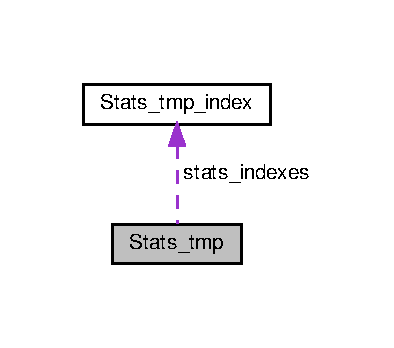
\includegraphics[width=189pt]{classStats__tmp__coll__graph}
\end{center}
\end{figure}
\subsection*{Public Member Functions}
\begin{DoxyCompactItemize}
\item 
void \hyperlink{classStats__tmp_a18d27f8eaaf61c5d456287cdf5ccd5ed}{init} ()
\item 
void \hyperlink{classStats__tmp_a4d3647832cc1cae1c7bf6ff6fd69af52}{clear} ()
\end{DoxyCompactItemize}
\subsection*{Public Attributes}
\begin{DoxyCompactItemize}
\item 
char \hyperlink{classStats__tmp_abbeec8b2f63eb8032d1e387da911f00c}{\+\_\+pad2} \mbox{[}\hyperlink{config_8h_aa18ff96566bf8c1f4cd38c1e7bc4ca80}{C\+L\+\_\+\+S\+I\+ZE}\mbox{]}
\item 
\hyperlink{classStats__tmp__index}{Stats\+\_\+tmp\+\_\+index} \hyperlink{classStats__tmp_aa8a6e1a1f0c1f6aab065cd2f9e8b7ca7}{stats\+\_\+indexes} \mbox{[}\hyperlink{stats_8h_aefb0708b15ac381fb0f0d94c3ca6904d}{M\+A\+X\+\_\+\+N\+U\+M\+\_\+\+I\+N\+D\+E\+X\+ES}\mbox{]}
\item 
double \hyperlink{classStats__tmp_a55ceb0b5e97a9ebb78613593862652a4}{time\+\_\+man}
\item 
double \hyperlink{classStats__tmp_a4c37e9b66e9a22405b294453040a8afc}{time\+\_\+index}
\item 
double \hyperlink{classStats__tmp_a04cb644c7edaf353c3b75765f836cebc}{time\+\_\+wait}
\item 
char \hyperlink{classStats__tmp_ac8d93e0e7dd2fa868d336db72b39ae06}{\+\_\+pad} \mbox{[}\hyperlink{config_8h_aa18ff96566bf8c1f4cd38c1e7bc4ca80}{C\+L\+\_\+\+S\+I\+ZE}\mbox{]}
\end{DoxyCompactItemize}


\subsection{Member Function Documentation}
\mbox{\Hypertarget{classStats__tmp_a4d3647832cc1cae1c7bf6ff6fd69af52}\label{classStats__tmp_a4d3647832cc1cae1c7bf6ff6fd69af52}} 
\index{Stats\+\_\+tmp@{Stats\+\_\+tmp}!clear@{clear}}
\index{clear@{clear}!Stats\+\_\+tmp@{Stats\+\_\+tmp}}
\subsubsection{\texorpdfstring{clear()}{clear()}}
{\footnotesize\ttfamily void Stats\+\_\+tmp\+::clear (\begin{DoxyParamCaption}{ }\end{DoxyParamCaption})}

\mbox{\Hypertarget{classStats__tmp_a18d27f8eaaf61c5d456287cdf5ccd5ed}\label{classStats__tmp_a18d27f8eaaf61c5d456287cdf5ccd5ed}} 
\index{Stats\+\_\+tmp@{Stats\+\_\+tmp}!init@{init}}
\index{init@{init}!Stats\+\_\+tmp@{Stats\+\_\+tmp}}
\subsubsection{\texorpdfstring{init()}{init()}}
{\footnotesize\ttfamily void Stats\+\_\+tmp\+::init (\begin{DoxyParamCaption}{ }\end{DoxyParamCaption})}



\subsection{Member Data Documentation}
\mbox{\Hypertarget{classStats__tmp_ac8d93e0e7dd2fa868d336db72b39ae06}\label{classStats__tmp_ac8d93e0e7dd2fa868d336db72b39ae06}} 
\index{Stats\+\_\+tmp@{Stats\+\_\+tmp}!\+\_\+pad@{\+\_\+pad}}
\index{\+\_\+pad@{\+\_\+pad}!Stats\+\_\+tmp@{Stats\+\_\+tmp}}
\subsubsection{\texorpdfstring{\+\_\+pad}{\_pad}}
{\footnotesize\ttfamily char Stats\+\_\+tmp\+::\+\_\+pad\mbox{[}\hyperlink{config_8h_aa18ff96566bf8c1f4cd38c1e7bc4ca80}{C\+L\+\_\+\+S\+I\+ZE}\mbox{]}}

\mbox{\Hypertarget{classStats__tmp_abbeec8b2f63eb8032d1e387da911f00c}\label{classStats__tmp_abbeec8b2f63eb8032d1e387da911f00c}} 
\index{Stats\+\_\+tmp@{Stats\+\_\+tmp}!\+\_\+pad2@{\+\_\+pad2}}
\index{\+\_\+pad2@{\+\_\+pad2}!Stats\+\_\+tmp@{Stats\+\_\+tmp}}
\subsubsection{\texorpdfstring{\+\_\+pad2}{\_pad2}}
{\footnotesize\ttfamily char Stats\+\_\+tmp\+::\+\_\+pad2\mbox{[}\hyperlink{config_8h_aa18ff96566bf8c1f4cd38c1e7bc4ca80}{C\+L\+\_\+\+S\+I\+ZE}\mbox{]}}

\mbox{\Hypertarget{classStats__tmp_aa8a6e1a1f0c1f6aab065cd2f9e8b7ca7}\label{classStats__tmp_aa8a6e1a1f0c1f6aab065cd2f9e8b7ca7}} 
\index{Stats\+\_\+tmp@{Stats\+\_\+tmp}!stats\+\_\+indexes@{stats\+\_\+indexes}}
\index{stats\+\_\+indexes@{stats\+\_\+indexes}!Stats\+\_\+tmp@{Stats\+\_\+tmp}}
\subsubsection{\texorpdfstring{stats\+\_\+indexes}{stats\_indexes}}
{\footnotesize\ttfamily \hyperlink{classStats__tmp__index}{Stats\+\_\+tmp\+\_\+index} Stats\+\_\+tmp\+::stats\+\_\+indexes\mbox{[}\hyperlink{stats_8h_aefb0708b15ac381fb0f0d94c3ca6904d}{M\+A\+X\+\_\+\+N\+U\+M\+\_\+\+I\+N\+D\+E\+X\+ES}\mbox{]}}

\mbox{\Hypertarget{classStats__tmp_a4c37e9b66e9a22405b294453040a8afc}\label{classStats__tmp_a4c37e9b66e9a22405b294453040a8afc}} 
\index{Stats\+\_\+tmp@{Stats\+\_\+tmp}!time\+\_\+index@{time\+\_\+index}}
\index{time\+\_\+index@{time\+\_\+index}!Stats\+\_\+tmp@{Stats\+\_\+tmp}}
\subsubsection{\texorpdfstring{time\+\_\+index}{time\_index}}
{\footnotesize\ttfamily double Stats\+\_\+tmp\+::time\+\_\+index}

\mbox{\Hypertarget{classStats__tmp_a55ceb0b5e97a9ebb78613593862652a4}\label{classStats__tmp_a55ceb0b5e97a9ebb78613593862652a4}} 
\index{Stats\+\_\+tmp@{Stats\+\_\+tmp}!time\+\_\+man@{time\+\_\+man}}
\index{time\+\_\+man@{time\+\_\+man}!Stats\+\_\+tmp@{Stats\+\_\+tmp}}
\subsubsection{\texorpdfstring{time\+\_\+man}{time\_man}}
{\footnotesize\ttfamily double Stats\+\_\+tmp\+::time\+\_\+man}

\mbox{\Hypertarget{classStats__tmp_a04cb644c7edaf353c3b75765f836cebc}\label{classStats__tmp_a04cb644c7edaf353c3b75765f836cebc}} 
\index{Stats\+\_\+tmp@{Stats\+\_\+tmp}!time\+\_\+wait@{time\+\_\+wait}}
\index{time\+\_\+wait@{time\+\_\+wait}!Stats\+\_\+tmp@{Stats\+\_\+tmp}}
\subsubsection{\texorpdfstring{time\+\_\+wait}{time\_wait}}
{\footnotesize\ttfamily double Stats\+\_\+tmp\+::time\+\_\+wait}



The documentation for this class was generated from the following files\+:\begin{DoxyCompactItemize}
\item 
macrobench/system/\hyperlink{stats_8h}{stats.\+h}\item 
macrobench/system/\hyperlink{stats_8cpp}{stats.\+cpp}\end{DoxyCompactItemize}

\hypertarget{classStats__tmp__index}{}\section{Stats\+\_\+tmp\+\_\+index Class Reference}
\label{classStats__tmp__index}\index{Stats\+\_\+tmp\+\_\+index@{Stats\+\_\+tmp\+\_\+index}}


{\ttfamily \#include $<$stats.\+h$>$}

\subsection*{Public Member Functions}
\begin{DoxyCompactItemize}
\item 
void \hyperlink{classStats__tmp__index_a09d71fb6d20ef59128982427ee816cd8}{clear} ()
\end{DoxyCompactItemize}
\subsection*{Public Attributes}
\begin{DoxyCompactItemize}
\item 
double \hyperlink{classStats__tmp__index_a9c94ac12e843f81d2b11659520dac58e}{time\+Contains}
\item 
double \hyperlink{classStats__tmp__index_a143a1d4977ca5db4c120bc72bcb984c8}{time\+Insert}
\item 
double \hyperlink{classStats__tmp__index_a09874517340c9d236d5bdbd999131403}{time\+Range\+Query}
\item 
uint64\+\_\+t \hyperlink{classStats__tmp__index_a6f9644823781c0d9d1fba3e0fb75e521}{num\+Contains}
\item 
uint64\+\_\+t \hyperlink{classStats__tmp__index_ab2d59b278ef4ae7f64b703d163a75a31}{num\+Insert}
\item 
uint64\+\_\+t \hyperlink{classStats__tmp__index_a4f5dcc0a7691ea81826c433b446d67f5}{num\+Range\+Query}
\end{DoxyCompactItemize}


\subsection{Member Function Documentation}
\mbox{\Hypertarget{classStats__tmp__index_a09d71fb6d20ef59128982427ee816cd8}\label{classStats__tmp__index_a09d71fb6d20ef59128982427ee816cd8}} 
\index{Stats\+\_\+tmp\+\_\+index@{Stats\+\_\+tmp\+\_\+index}!clear@{clear}}
\index{clear@{clear}!Stats\+\_\+tmp\+\_\+index@{Stats\+\_\+tmp\+\_\+index}}
\subsubsection{\texorpdfstring{clear()}{clear()}}
{\footnotesize\ttfamily void Stats\+\_\+tmp\+\_\+index\+::clear (\begin{DoxyParamCaption}{ }\end{DoxyParamCaption})}



\subsection{Member Data Documentation}
\mbox{\Hypertarget{classStats__tmp__index_a6f9644823781c0d9d1fba3e0fb75e521}\label{classStats__tmp__index_a6f9644823781c0d9d1fba3e0fb75e521}} 
\index{Stats\+\_\+tmp\+\_\+index@{Stats\+\_\+tmp\+\_\+index}!num\+Contains@{num\+Contains}}
\index{num\+Contains@{num\+Contains}!Stats\+\_\+tmp\+\_\+index@{Stats\+\_\+tmp\+\_\+index}}
\subsubsection{\texorpdfstring{num\+Contains}{numContains}}
{\footnotesize\ttfamily uint64\+\_\+t Stats\+\_\+tmp\+\_\+index\+::num\+Contains}

\mbox{\Hypertarget{classStats__tmp__index_ab2d59b278ef4ae7f64b703d163a75a31}\label{classStats__tmp__index_ab2d59b278ef4ae7f64b703d163a75a31}} 
\index{Stats\+\_\+tmp\+\_\+index@{Stats\+\_\+tmp\+\_\+index}!num\+Insert@{num\+Insert}}
\index{num\+Insert@{num\+Insert}!Stats\+\_\+tmp\+\_\+index@{Stats\+\_\+tmp\+\_\+index}}
\subsubsection{\texorpdfstring{num\+Insert}{numInsert}}
{\footnotesize\ttfamily uint64\+\_\+t Stats\+\_\+tmp\+\_\+index\+::num\+Insert}

\mbox{\Hypertarget{classStats__tmp__index_a4f5dcc0a7691ea81826c433b446d67f5}\label{classStats__tmp__index_a4f5dcc0a7691ea81826c433b446d67f5}} 
\index{Stats\+\_\+tmp\+\_\+index@{Stats\+\_\+tmp\+\_\+index}!num\+Range\+Query@{num\+Range\+Query}}
\index{num\+Range\+Query@{num\+Range\+Query}!Stats\+\_\+tmp\+\_\+index@{Stats\+\_\+tmp\+\_\+index}}
\subsubsection{\texorpdfstring{num\+Range\+Query}{numRangeQuery}}
{\footnotesize\ttfamily uint64\+\_\+t Stats\+\_\+tmp\+\_\+index\+::num\+Range\+Query}

\mbox{\Hypertarget{classStats__tmp__index_a9c94ac12e843f81d2b11659520dac58e}\label{classStats__tmp__index_a9c94ac12e843f81d2b11659520dac58e}} 
\index{Stats\+\_\+tmp\+\_\+index@{Stats\+\_\+tmp\+\_\+index}!time\+Contains@{time\+Contains}}
\index{time\+Contains@{time\+Contains}!Stats\+\_\+tmp\+\_\+index@{Stats\+\_\+tmp\+\_\+index}}
\subsubsection{\texorpdfstring{time\+Contains}{timeContains}}
{\footnotesize\ttfamily double Stats\+\_\+tmp\+\_\+index\+::time\+Contains}

\mbox{\Hypertarget{classStats__tmp__index_a143a1d4977ca5db4c120bc72bcb984c8}\label{classStats__tmp__index_a143a1d4977ca5db4c120bc72bcb984c8}} 
\index{Stats\+\_\+tmp\+\_\+index@{Stats\+\_\+tmp\+\_\+index}!time\+Insert@{time\+Insert}}
\index{time\+Insert@{time\+Insert}!Stats\+\_\+tmp\+\_\+index@{Stats\+\_\+tmp\+\_\+index}}
\subsubsection{\texorpdfstring{time\+Insert}{timeInsert}}
{\footnotesize\ttfamily double Stats\+\_\+tmp\+\_\+index\+::time\+Insert}

\mbox{\Hypertarget{classStats__tmp__index_a09874517340c9d236d5bdbd999131403}\label{classStats__tmp__index_a09874517340c9d236d5bdbd999131403}} 
\index{Stats\+\_\+tmp\+\_\+index@{Stats\+\_\+tmp\+\_\+index}!time\+Range\+Query@{time\+Range\+Query}}
\index{time\+Range\+Query@{time\+Range\+Query}!Stats\+\_\+tmp\+\_\+index@{Stats\+\_\+tmp\+\_\+index}}
\subsubsection{\texorpdfstring{time\+Range\+Query}{timeRangeQuery}}
{\footnotesize\ttfamily double Stats\+\_\+tmp\+\_\+index\+::time\+Range\+Query}



The documentation for this class was generated from the following files\+:\begin{DoxyCompactItemize}
\item 
macrobench/system/\hyperlink{stats_8h}{stats.\+h}\item 
macrobench/system/\hyperlink{stats_8cpp}{stats.\+cpp}\end{DoxyCompactItemize}

\hypertarget{classgraphs_1_1StdevFunc}{}\section{graphs.\+Stdev\+Func Class Reference}
\label{classgraphs_1_1StdevFunc}\index{graphs.\+Stdev\+Func@{graphs.\+Stdev\+Func}}
\subsection*{Public Member Functions}
\begin{DoxyCompactItemize}
\item 
def \hyperlink{classgraphs_1_1StdevFunc_a809899524dcddd0f7211131930e46876}{\+\_\+\+\_\+init\+\_\+\+\_\+} (self)
\item 
def \hyperlink{classgraphs_1_1StdevFunc_aefb049cecc0ce18aad3ba50c40963656}{step} (self, value)
\item 
def \hyperlink{classgraphs_1_1StdevFunc_a8a9ea3289aea6ce5f7ccc581c76c5cac}{finalize} (self)
\end{DoxyCompactItemize}
\subsection*{Public Attributes}
\begin{DoxyCompactItemize}
\item 
\hyperlink{classgraphs_1_1StdevFunc_a2dd9047d6c2873699b2f0ca605690b9c}{M}
\item 
\hyperlink{classgraphs_1_1StdevFunc_ac8455ae1705af7de00108c76e6b9b439}{S}
\item 
\hyperlink{classgraphs_1_1StdevFunc_ae10b59043d31f7f7d967060e21aa368e}{k}
\end{DoxyCompactItemize}


\subsection{Constructor \& Destructor Documentation}
\mbox{\Hypertarget{classgraphs_1_1StdevFunc_a809899524dcddd0f7211131930e46876}\label{classgraphs_1_1StdevFunc_a809899524dcddd0f7211131930e46876}} 
\index{graphs\+::\+Stdev\+Func@{graphs\+::\+Stdev\+Func}!\+\_\+\+\_\+init\+\_\+\+\_\+@{\+\_\+\+\_\+init\+\_\+\+\_\+}}
\index{\+\_\+\+\_\+init\+\_\+\+\_\+@{\+\_\+\+\_\+init\+\_\+\+\_\+}!graphs\+::\+Stdev\+Func@{graphs\+::\+Stdev\+Func}}
\subsubsection{\texorpdfstring{\+\_\+\+\_\+init\+\_\+\+\_\+()}{\_\_init\_\_()}}
{\footnotesize\ttfamily def graphs.\+Stdev\+Func.\+\_\+\+\_\+init\+\_\+\+\_\+ (\begin{DoxyParamCaption}\item[{}]{self }\end{DoxyParamCaption})}



\subsection{Member Function Documentation}
\mbox{\Hypertarget{classgraphs_1_1StdevFunc_a8a9ea3289aea6ce5f7ccc581c76c5cac}\label{classgraphs_1_1StdevFunc_a8a9ea3289aea6ce5f7ccc581c76c5cac}} 
\index{graphs\+::\+Stdev\+Func@{graphs\+::\+Stdev\+Func}!finalize@{finalize}}
\index{finalize@{finalize}!graphs\+::\+Stdev\+Func@{graphs\+::\+Stdev\+Func}}
\subsubsection{\texorpdfstring{finalize()}{finalize()}}
{\footnotesize\ttfamily def graphs.\+Stdev\+Func.\+finalize (\begin{DoxyParamCaption}\item[{}]{self }\end{DoxyParamCaption})}

\mbox{\Hypertarget{classgraphs_1_1StdevFunc_aefb049cecc0ce18aad3ba50c40963656}\label{classgraphs_1_1StdevFunc_aefb049cecc0ce18aad3ba50c40963656}} 
\index{graphs\+::\+Stdev\+Func@{graphs\+::\+Stdev\+Func}!step@{step}}
\index{step@{step}!graphs\+::\+Stdev\+Func@{graphs\+::\+Stdev\+Func}}
\subsubsection{\texorpdfstring{step()}{step()}}
{\footnotesize\ttfamily def graphs.\+Stdev\+Func.\+step (\begin{DoxyParamCaption}\item[{}]{self,  }\item[{}]{value }\end{DoxyParamCaption})}



\subsection{Member Data Documentation}
\mbox{\Hypertarget{classgraphs_1_1StdevFunc_ae10b59043d31f7f7d967060e21aa368e}\label{classgraphs_1_1StdevFunc_ae10b59043d31f7f7d967060e21aa368e}} 
\index{graphs\+::\+Stdev\+Func@{graphs\+::\+Stdev\+Func}!k@{k}}
\index{k@{k}!graphs\+::\+Stdev\+Func@{graphs\+::\+Stdev\+Func}}
\subsubsection{\texorpdfstring{k}{k}}
{\footnotesize\ttfamily graphs.\+Stdev\+Func.\+k}

\mbox{\Hypertarget{classgraphs_1_1StdevFunc_a2dd9047d6c2873699b2f0ca605690b9c}\label{classgraphs_1_1StdevFunc_a2dd9047d6c2873699b2f0ca605690b9c}} 
\index{graphs\+::\+Stdev\+Func@{graphs\+::\+Stdev\+Func}!M@{M}}
\index{M@{M}!graphs\+::\+Stdev\+Func@{graphs\+::\+Stdev\+Func}}
\subsubsection{\texorpdfstring{M}{M}}
{\footnotesize\ttfamily graphs.\+Stdev\+Func.\+M}

\mbox{\Hypertarget{classgraphs_1_1StdevFunc_ac8455ae1705af7de00108c76e6b9b439}\label{classgraphs_1_1StdevFunc_ac8455ae1705af7de00108c76e6b9b439}} 
\index{graphs\+::\+Stdev\+Func@{graphs\+::\+Stdev\+Func}!S@{S}}
\index{S@{S}!graphs\+::\+Stdev\+Func@{graphs\+::\+Stdev\+Func}}
\subsubsection{\texorpdfstring{S}{S}}
{\footnotesize\ttfamily graphs.\+Stdev\+Func.\+S}



The documentation for this class was generated from the following file\+:\begin{DoxyCompactItemize}
\item 
microbench/unused/\hyperlink{graphs_8py}{graphs.\+py}\end{DoxyCompactItemize}

\hypertarget{classtable__t}{}\section{table\+\_\+t Class Reference}
\label{classtable__t}\index{table\+\_\+t@{table\+\_\+t}}


{\ttfamily \#include $<$table.\+h$>$}



Collaboration diagram for table\+\_\+t\+:
\nopagebreak
\begin{figure}[H]
\begin{center}
\leavevmode
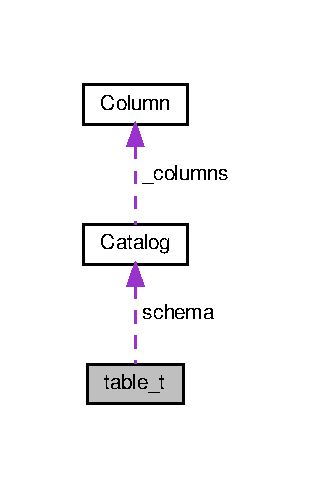
\includegraphics[width=151pt]{classtable__t__coll__graph}
\end{center}
\end{figure}
\subsection*{Public Member Functions}
\begin{DoxyCompactItemize}
\item 
void \hyperlink{classtable__t_a5fd9dca2e5f3dcb70c462f3eb94dd2be}{init} (\hyperlink{classCatalog}{Catalog} $\ast$\hyperlink{classtable__t_a5e2b3478c29080f6106331294d94c06a}{schema})
\item 
void \hyperlink{classtable__t_a9ec2af3a52db280d8c1c6a78bee7cbd0}{setbench\+\_\+deinit} ()
\item 
\hyperlink{global_8h_a78c49a674c810fdd03d20432f7be864a}{RC} \hyperlink{classtable__t_a17daa6c0ecb46c33745c1ce88f80a495}{get\+\_\+new\+\_\+row} (\hyperlink{classrow__t}{row\+\_\+t} $\ast$\&row)
\item 
\hyperlink{global_8h_a78c49a674c810fdd03d20432f7be864a}{RC} \hyperlink{classtable__t_a81e3bd8f424fc3346629dba6a54eab15}{get\+\_\+new\+\_\+row} (\hyperlink{classrow__t}{row\+\_\+t} $\ast$\&row, uint64\+\_\+t part\+\_\+id, uint64\+\_\+t \&row\+\_\+id)
\item 
void \hyperlink{classtable__t_a1d5c3dd5d88ca99b1f9ec01f4befe4e2}{delete\+\_\+row} ()
\item 
uint64\+\_\+t \hyperlink{classtable__t_ae65abd8e531e3e86877868ed2851f9df}{get\+\_\+table\+\_\+size} ()
\item 
\hyperlink{classCatalog}{Catalog} $\ast$ \hyperlink{classtable__t_a8ac1dd0bce278f742c1caa28fcd35b70}{get\+\_\+schema} ()
\item 
const char $\ast$ \hyperlink{classtable__t_a094de1bb6ed142eb1c12044b34ec28e3}{get\+\_\+table\+\_\+name} ()
\end{DoxyCompactItemize}
\subsection*{Public Attributes}
\begin{DoxyCompactItemize}
\item 
\hyperlink{classCatalog}{Catalog} $\ast$ \hyperlink{classtable__t_a5e2b3478c29080f6106331294d94c06a}{schema}
\end{DoxyCompactItemize}


\subsection{Member Function Documentation}
\mbox{\Hypertarget{classtable__t_a1d5c3dd5d88ca99b1f9ec01f4befe4e2}\label{classtable__t_a1d5c3dd5d88ca99b1f9ec01f4befe4e2}} 
\index{table\+\_\+t@{table\+\_\+t}!delete\+\_\+row@{delete\+\_\+row}}
\index{delete\+\_\+row@{delete\+\_\+row}!table\+\_\+t@{table\+\_\+t}}
\subsubsection{\texorpdfstring{delete\+\_\+row()}{delete\_row()}}
{\footnotesize\ttfamily void table\+\_\+t\+::delete\+\_\+row (\begin{DoxyParamCaption}{ }\end{DoxyParamCaption})}

\mbox{\Hypertarget{classtable__t_a17daa6c0ecb46c33745c1ce88f80a495}\label{classtable__t_a17daa6c0ecb46c33745c1ce88f80a495}} 
\index{table\+\_\+t@{table\+\_\+t}!get\+\_\+new\+\_\+row@{get\+\_\+new\+\_\+row}}
\index{get\+\_\+new\+\_\+row@{get\+\_\+new\+\_\+row}!table\+\_\+t@{table\+\_\+t}}
\subsubsection{\texorpdfstring{get\+\_\+new\+\_\+row()}{get\_new\_row()}\hspace{0.1cm}{\footnotesize\ttfamily [1/2]}}
{\footnotesize\ttfamily \hyperlink{global_8h_a78c49a674c810fdd03d20432f7be864a}{RC} table\+\_\+t\+::get\+\_\+new\+\_\+row (\begin{DoxyParamCaption}\item[{\hyperlink{classrow__t}{row\+\_\+t} $\ast$\&}]{row }\end{DoxyParamCaption})}

\mbox{\Hypertarget{classtable__t_a81e3bd8f424fc3346629dba6a54eab15}\label{classtable__t_a81e3bd8f424fc3346629dba6a54eab15}} 
\index{table\+\_\+t@{table\+\_\+t}!get\+\_\+new\+\_\+row@{get\+\_\+new\+\_\+row}}
\index{get\+\_\+new\+\_\+row@{get\+\_\+new\+\_\+row}!table\+\_\+t@{table\+\_\+t}}
\subsubsection{\texorpdfstring{get\+\_\+new\+\_\+row()}{get\_new\_row()}\hspace{0.1cm}{\footnotesize\ttfamily [2/2]}}
{\footnotesize\ttfamily \hyperlink{global_8h_a78c49a674c810fdd03d20432f7be864a}{RC} table\+\_\+t\+::get\+\_\+new\+\_\+row (\begin{DoxyParamCaption}\item[{\hyperlink{classrow__t}{row\+\_\+t} $\ast$\&}]{row,  }\item[{uint64\+\_\+t}]{part\+\_\+id,  }\item[{uint64\+\_\+t \&}]{row\+\_\+id }\end{DoxyParamCaption})}

\mbox{\Hypertarget{classtable__t_a8ac1dd0bce278f742c1caa28fcd35b70}\label{classtable__t_a8ac1dd0bce278f742c1caa28fcd35b70}} 
\index{table\+\_\+t@{table\+\_\+t}!get\+\_\+schema@{get\+\_\+schema}}
\index{get\+\_\+schema@{get\+\_\+schema}!table\+\_\+t@{table\+\_\+t}}
\subsubsection{\texorpdfstring{get\+\_\+schema()}{get\_schema()}}
{\footnotesize\ttfamily \hyperlink{classCatalog}{Catalog}$\ast$ table\+\_\+t\+::get\+\_\+schema (\begin{DoxyParamCaption}{ }\end{DoxyParamCaption})\hspace{0.3cm}{\ttfamily [inline]}}

\mbox{\Hypertarget{classtable__t_a094de1bb6ed142eb1c12044b34ec28e3}\label{classtable__t_a094de1bb6ed142eb1c12044b34ec28e3}} 
\index{table\+\_\+t@{table\+\_\+t}!get\+\_\+table\+\_\+name@{get\+\_\+table\+\_\+name}}
\index{get\+\_\+table\+\_\+name@{get\+\_\+table\+\_\+name}!table\+\_\+t@{table\+\_\+t}}
\subsubsection{\texorpdfstring{get\+\_\+table\+\_\+name()}{get\_table\_name()}}
{\footnotesize\ttfamily const char$\ast$ table\+\_\+t\+::get\+\_\+table\+\_\+name (\begin{DoxyParamCaption}{ }\end{DoxyParamCaption})\hspace{0.3cm}{\ttfamily [inline]}}

\mbox{\Hypertarget{classtable__t_ae65abd8e531e3e86877868ed2851f9df}\label{classtable__t_ae65abd8e531e3e86877868ed2851f9df}} 
\index{table\+\_\+t@{table\+\_\+t}!get\+\_\+table\+\_\+size@{get\+\_\+table\+\_\+size}}
\index{get\+\_\+table\+\_\+size@{get\+\_\+table\+\_\+size}!table\+\_\+t@{table\+\_\+t}}
\subsubsection{\texorpdfstring{get\+\_\+table\+\_\+size()}{get\_table\_size()}}
{\footnotesize\ttfamily uint64\+\_\+t table\+\_\+t\+::get\+\_\+table\+\_\+size (\begin{DoxyParamCaption}{ }\end{DoxyParamCaption})\hspace{0.3cm}{\ttfamily [inline]}}

\mbox{\Hypertarget{classtable__t_a5fd9dca2e5f3dcb70c462f3eb94dd2be}\label{classtable__t_a5fd9dca2e5f3dcb70c462f3eb94dd2be}} 
\index{table\+\_\+t@{table\+\_\+t}!init@{init}}
\index{init@{init}!table\+\_\+t@{table\+\_\+t}}
\subsubsection{\texorpdfstring{init()}{init()}}
{\footnotesize\ttfamily void table\+\_\+t\+::init (\begin{DoxyParamCaption}\item[{\hyperlink{classCatalog}{Catalog} $\ast$}]{schema }\end{DoxyParamCaption})}

\mbox{\Hypertarget{classtable__t_a9ec2af3a52db280d8c1c6a78bee7cbd0}\label{classtable__t_a9ec2af3a52db280d8c1c6a78bee7cbd0}} 
\index{table\+\_\+t@{table\+\_\+t}!setbench\+\_\+deinit@{setbench\+\_\+deinit}}
\index{setbench\+\_\+deinit@{setbench\+\_\+deinit}!table\+\_\+t@{table\+\_\+t}}
\subsubsection{\texorpdfstring{setbench\+\_\+deinit()}{setbench\_deinit()}}
{\footnotesize\ttfamily void table\+\_\+t\+::setbench\+\_\+deinit (\begin{DoxyParamCaption}{ }\end{DoxyParamCaption})}



\subsection{Member Data Documentation}
\mbox{\Hypertarget{classtable__t_a5e2b3478c29080f6106331294d94c06a}\label{classtable__t_a5e2b3478c29080f6106331294d94c06a}} 
\index{table\+\_\+t@{table\+\_\+t}!schema@{schema}}
\index{schema@{schema}!table\+\_\+t@{table\+\_\+t}}
\subsubsection{\texorpdfstring{schema}{schema}}
{\footnotesize\ttfamily \hyperlink{classCatalog}{Catalog}$\ast$ table\+\_\+t\+::schema}



The documentation for this class was generated from the following files\+:\begin{DoxyCompactItemize}
\item 
macrobench/storage/\hyperlink{table_8h}{table.\+h}\item 
macrobench/storage/\hyperlink{table_8cpp}{table.\+cpp}\end{DoxyCompactItemize}

\hypertarget{structtArgs}{}\section{t\+Args$<$ skey\+\_\+t, sval\+\_\+t $>$ Struct Template Reference}
\label{structtArgs}\index{t\+Args$<$ skey\+\_\+t, sval\+\_\+t $>$@{t\+Args$<$ skey\+\_\+t, sval\+\_\+t $>$}}


{\ttfamily \#include $<$intlf\+\_\+impl.\+h$>$}

\subsection*{Public Attributes}
\begin{DoxyCompactItemize}
\item 
int \hyperlink{structtArgs_a320de799cc255dd57991133442937738}{tid}
\item 
\hyperlink{structnode__t}{node\+\_\+t}$<$ skey\+\_\+t, sval\+\_\+t $>$ $\ast$ \hyperlink{structtArgs_a7051ff5a92464af6e2dddd17d944d7da}{new\+Node}
\item 
bool \hyperlink{structtArgs_a0aa04a92450593265c01c6ecbb15ac59}{is\+New\+Node\+Available}
\item 
\hyperlink{structseekRecord}{seek\+Record}$<$ skey\+\_\+t, sval\+\_\+t $>$ \hyperlink{structtArgs_a8f559d067821fb34b64a5e734e0d6025}{target\+Record}
\item 
\hyperlink{structseekRecord}{seek\+Record}$<$ skey\+\_\+t, sval\+\_\+t $>$ \hyperlink{structtArgs_a2e843aefca73932645827aeb98a3f620}{p\+Seek\+Record}
\item 
\hyperlink{structstateRecord}{state\+Record}$<$ skey\+\_\+t, sval\+\_\+t $>$ \hyperlink{structtArgs_af2580d3ccc03992847f75b823502e0d0}{my\+State}
\item 
struct \hyperlink{structanchorRecord}{anchor\+Record}$<$ skey\+\_\+t, sval\+\_\+t $>$ \hyperlink{structtArgs_af74947cf54218b2404c50fcd5310bf0c}{anchor\+Record}
\item 
struct \hyperlink{structanchorRecord}{anchor\+Record}$<$ skey\+\_\+t, sval\+\_\+t $>$ \hyperlink{structtArgs_a6a8c3056aaae3f728b301bb0a859aa32}{p\+Anchor\+Record}
\end{DoxyCompactItemize}


\subsection{Member Data Documentation}
\mbox{\Hypertarget{structtArgs_af74947cf54218b2404c50fcd5310bf0c}\label{structtArgs_af74947cf54218b2404c50fcd5310bf0c}} 
\index{t\+Args@{t\+Args}!anchor\+Record@{anchor\+Record}}
\index{anchor\+Record@{anchor\+Record}!t\+Args@{t\+Args}}
\subsubsection{\texorpdfstring{anchor\+Record}{anchorRecord}}
{\footnotesize\ttfamily template$<$typename skey\+\_\+t, typename sval\+\_\+t$>$ \\
struct \hyperlink{structanchorRecord}{anchor\+Record}$<$ skey\+\_\+t, sval\+\_\+t $>$ \hyperlink{structtArgs}{t\+Args}$<$ skey\+\_\+t, sval\+\_\+t $>$\+::\hyperlink{structanchorRecord}{anchor\+Record}}

\mbox{\Hypertarget{structtArgs_a0aa04a92450593265c01c6ecbb15ac59}\label{structtArgs_a0aa04a92450593265c01c6ecbb15ac59}} 
\index{t\+Args@{t\+Args}!is\+New\+Node\+Available@{is\+New\+Node\+Available}}
\index{is\+New\+Node\+Available@{is\+New\+Node\+Available}!t\+Args@{t\+Args}}
\subsubsection{\texorpdfstring{is\+New\+Node\+Available}{isNewNodeAvailable}}
{\footnotesize\ttfamily template$<$typename skey\+\_\+t, typename sval\+\_\+t$>$ \\
bool \hyperlink{structtArgs}{t\+Args}$<$ skey\+\_\+t, sval\+\_\+t $>$\+::is\+New\+Node\+Available}

\mbox{\Hypertarget{structtArgs_af2580d3ccc03992847f75b823502e0d0}\label{structtArgs_af2580d3ccc03992847f75b823502e0d0}} 
\index{t\+Args@{t\+Args}!my\+State@{my\+State}}
\index{my\+State@{my\+State}!t\+Args@{t\+Args}}
\subsubsection{\texorpdfstring{my\+State}{myState}}
{\footnotesize\ttfamily template$<$typename skey\+\_\+t, typename sval\+\_\+t$>$ \\
\hyperlink{structstateRecord}{state\+Record}$<$skey\+\_\+t, sval\+\_\+t$>$ \hyperlink{structtArgs}{t\+Args}$<$ skey\+\_\+t, sval\+\_\+t $>$\+::my\+State}

\mbox{\Hypertarget{structtArgs_a7051ff5a92464af6e2dddd17d944d7da}\label{structtArgs_a7051ff5a92464af6e2dddd17d944d7da}} 
\index{t\+Args@{t\+Args}!new\+Node@{new\+Node}}
\index{new\+Node@{new\+Node}!t\+Args@{t\+Args}}
\subsubsection{\texorpdfstring{new\+Node}{newNode}}
{\footnotesize\ttfamily template$<$typename skey\+\_\+t, typename sval\+\_\+t$>$ \\
\hyperlink{structnode__t}{node\+\_\+t}$<$skey\+\_\+t, sval\+\_\+t$>$$\ast$ \hyperlink{structtArgs}{t\+Args}$<$ skey\+\_\+t, sval\+\_\+t $>$\+::new\+Node}

\mbox{\Hypertarget{structtArgs_a6a8c3056aaae3f728b301bb0a859aa32}\label{structtArgs_a6a8c3056aaae3f728b301bb0a859aa32}} 
\index{t\+Args@{t\+Args}!p\+Anchor\+Record@{p\+Anchor\+Record}}
\index{p\+Anchor\+Record@{p\+Anchor\+Record}!t\+Args@{t\+Args}}
\subsubsection{\texorpdfstring{p\+Anchor\+Record}{pAnchorRecord}}
{\footnotesize\ttfamily template$<$typename skey\+\_\+t, typename sval\+\_\+t$>$ \\
struct \hyperlink{structanchorRecord}{anchor\+Record}$<$ skey\+\_\+t, sval\+\_\+t $>$ \hyperlink{structtArgs}{t\+Args}$<$ skey\+\_\+t, sval\+\_\+t $>$\+::p\+Anchor\+Record}

\mbox{\Hypertarget{structtArgs_a2e843aefca73932645827aeb98a3f620}\label{structtArgs_a2e843aefca73932645827aeb98a3f620}} 
\index{t\+Args@{t\+Args}!p\+Seek\+Record@{p\+Seek\+Record}}
\index{p\+Seek\+Record@{p\+Seek\+Record}!t\+Args@{t\+Args}}
\subsubsection{\texorpdfstring{p\+Seek\+Record}{pSeekRecord}}
{\footnotesize\ttfamily template$<$typename skey\+\_\+t, typename sval\+\_\+t$>$ \\
\hyperlink{structseekRecord}{seek\+Record}$<$skey\+\_\+t, sval\+\_\+t$>$ \hyperlink{structtArgs}{t\+Args}$<$ skey\+\_\+t, sval\+\_\+t $>$\+::p\+Seek\+Record}

\mbox{\Hypertarget{structtArgs_a8f559d067821fb34b64a5e734e0d6025}\label{structtArgs_a8f559d067821fb34b64a5e734e0d6025}} 
\index{t\+Args@{t\+Args}!target\+Record@{target\+Record}}
\index{target\+Record@{target\+Record}!t\+Args@{t\+Args}}
\subsubsection{\texorpdfstring{target\+Record}{targetRecord}}
{\footnotesize\ttfamily template$<$typename skey\+\_\+t, typename sval\+\_\+t$>$ \\
\hyperlink{structseekRecord}{seek\+Record}$<$skey\+\_\+t, sval\+\_\+t$>$ \hyperlink{structtArgs}{t\+Args}$<$ skey\+\_\+t, sval\+\_\+t $>$\+::target\+Record}

\mbox{\Hypertarget{structtArgs_a320de799cc255dd57991133442937738}\label{structtArgs_a320de799cc255dd57991133442937738}} 
\index{t\+Args@{t\+Args}!tid@{tid}}
\index{tid@{tid}!t\+Args@{t\+Args}}
\subsubsection{\texorpdfstring{tid}{tid}}
{\footnotesize\ttfamily template$<$typename skey\+\_\+t, typename sval\+\_\+t$>$ \\
int \hyperlink{structtArgs}{t\+Args}$<$ skey\+\_\+t, sval\+\_\+t $>$\+::tid}



The documentation for this struct was generated from the following file\+:\begin{DoxyCompactItemize}
\item 
ds/ramachandran\+\_\+int\+\_\+bst\+\_\+lf/\hyperlink{intlf__impl_8h}{intlf\+\_\+impl.\+h}\end{DoxyCompactItemize}

\hypertarget{classTestTxnMan}{}\section{Test\+Txn\+Man Class Reference}
\label{classTestTxnMan}\index{Test\+Txn\+Man@{Test\+Txn\+Man}}


{\ttfamily \#include $<$test.\+h$>$}



Inheritance diagram for Test\+Txn\+Man\+:
\nopagebreak
\begin{figure}[H]
\begin{center}
\leavevmode
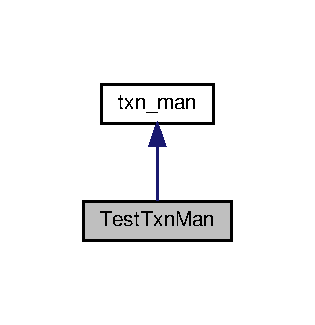
\includegraphics[width=151pt]{classTestTxnMan__inherit__graph}
\end{center}
\end{figure}


Collaboration diagram for Test\+Txn\+Man\+:
\nopagebreak
\begin{figure}[H]
\begin{center}
\leavevmode
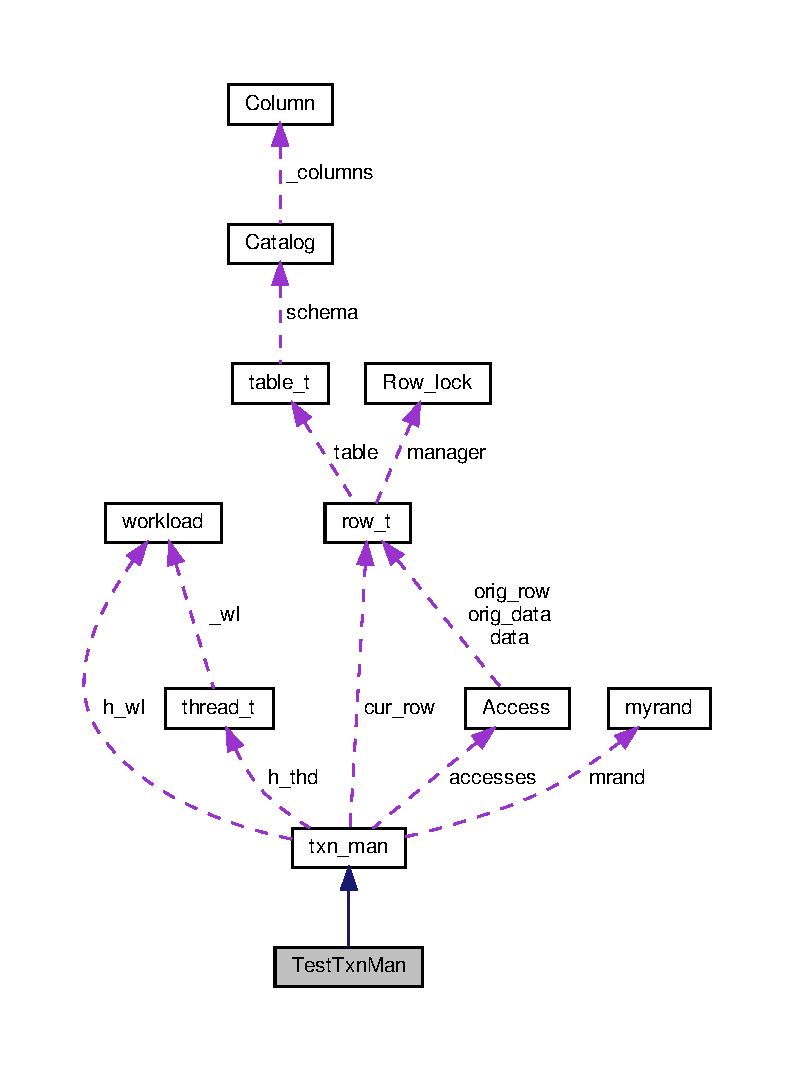
\includegraphics[width=350pt]{classTestTxnMan__coll__graph}
\end{center}
\end{figure}
\subsection*{Public Member Functions}
\begin{DoxyCompactItemize}
\item 
void \hyperlink{classTestTxnMan_a55bd3947973927a82e87f249813fd4a0}{init} (\hyperlink{classthread__t}{thread\+\_\+t} $\ast$\hyperlink{classtxn__man_a64bf2cba8ef2686ad528a96d18e8358d}{h\+\_\+thd}, \hyperlink{classworkload}{workload} $\ast$\hyperlink{classtxn__man_a988eb76c69a304049c02d3ceff526a5e}{h\+\_\+wl}, uint64\+\_\+t part\+\_\+id)
\item 
\hyperlink{global_8h_a78c49a674c810fdd03d20432f7be864a}{RC} \hyperlink{classTestTxnMan_a47b1cfbfed234f5a000aa57b773a54c1}{run\+\_\+txn} (int type, int access\+\_\+num)
\item 
\hyperlink{global_8h_a78c49a674c810fdd03d20432f7be864a}{RC} \hyperlink{classTestTxnMan_ae9510bd3f827a29dcc1239517021ac37}{run\+\_\+txn} (\hyperlink{classbase__query}{base\+\_\+query} $\ast$m\+\_\+query)
\end{DoxyCompactItemize}
\subsection*{Additional Inherited Members}


\subsection{Member Function Documentation}
\mbox{\Hypertarget{classTestTxnMan_a55bd3947973927a82e87f249813fd4a0}\label{classTestTxnMan_a55bd3947973927a82e87f249813fd4a0}} 
\index{Test\+Txn\+Man@{Test\+Txn\+Man}!init@{init}}
\index{init@{init}!Test\+Txn\+Man@{Test\+Txn\+Man}}
\subsubsection{\texorpdfstring{init()}{init()}}
{\footnotesize\ttfamily void Test\+Txn\+Man\+::init (\begin{DoxyParamCaption}\item[{\hyperlink{classthread__t}{thread\+\_\+t} $\ast$}]{h\+\_\+thd,  }\item[{\hyperlink{classworkload}{workload} $\ast$}]{h\+\_\+wl,  }\item[{uint64\+\_\+t}]{part\+\_\+id }\end{DoxyParamCaption})\hspace{0.3cm}{\ttfamily [virtual]}}



Reimplemented from \hyperlink{classtxn__man_a778925bb3edd6a54a27161f67792edec}{txn\+\_\+man}.

\mbox{\Hypertarget{classTestTxnMan_a47b1cfbfed234f5a000aa57b773a54c1}\label{classTestTxnMan_a47b1cfbfed234f5a000aa57b773a54c1}} 
\index{Test\+Txn\+Man@{Test\+Txn\+Man}!run\+\_\+txn@{run\+\_\+txn}}
\index{run\+\_\+txn@{run\+\_\+txn}!Test\+Txn\+Man@{Test\+Txn\+Man}}
\subsubsection{\texorpdfstring{run\+\_\+txn()}{run\_txn()}\hspace{0.1cm}{\footnotesize\ttfamily [1/2]}}
{\footnotesize\ttfamily \hyperlink{global_8h_a78c49a674c810fdd03d20432f7be864a}{RC} Test\+Txn\+Man\+::run\+\_\+txn (\begin{DoxyParamCaption}\item[{int}]{type,  }\item[{int}]{access\+\_\+num }\end{DoxyParamCaption})}

\mbox{\Hypertarget{classTestTxnMan_ae9510bd3f827a29dcc1239517021ac37}\label{classTestTxnMan_ae9510bd3f827a29dcc1239517021ac37}} 
\index{Test\+Txn\+Man@{Test\+Txn\+Man}!run\+\_\+txn@{run\+\_\+txn}}
\index{run\+\_\+txn@{run\+\_\+txn}!Test\+Txn\+Man@{Test\+Txn\+Man}}
\subsubsection{\texorpdfstring{run\+\_\+txn()}{run\_txn()}\hspace{0.1cm}{\footnotesize\ttfamily [2/2]}}
{\footnotesize\ttfamily \hyperlink{global_8h_a78c49a674c810fdd03d20432f7be864a}{RC} Test\+Txn\+Man\+::run\+\_\+txn (\begin{DoxyParamCaption}\item[{\hyperlink{classbase__query}{base\+\_\+query} $\ast$}]{m\+\_\+query }\end{DoxyParamCaption})\hspace{0.3cm}{\ttfamily [inline]}, {\ttfamily [virtual]}}



Implements \hyperlink{classtxn__man_a71142ded36a4be5629ea75d486a105ae}{txn\+\_\+man}.



The documentation for this class was generated from the following files\+:\begin{DoxyCompactItemize}
\item 
macrobench/benchmarks/\hyperlink{test_8h}{test.\+h}\item 
macrobench/benchmarks/\hyperlink{test__txn_8cpp}{test\+\_\+txn.\+cpp}\end{DoxyCompactItemize}

\hypertarget{classTestWorkload}{}\section{Test\+Workload Class Reference}
\label{classTestWorkload}\index{Test\+Workload@{Test\+Workload}}


{\ttfamily \#include $<$test.\+h$>$}



Inheritance diagram for Test\+Workload\+:
\nopagebreak
\begin{figure}[H]
\begin{center}
\leavevmode
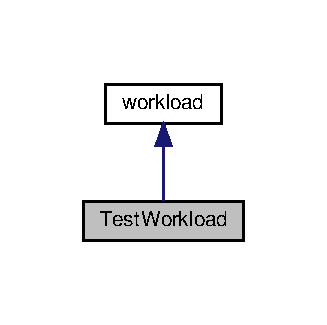
\includegraphics[width=157pt]{classTestWorkload__inherit__graph}
\end{center}
\end{figure}


Collaboration diagram for Test\+Workload\+:
\nopagebreak
\begin{figure}[H]
\begin{center}
\leavevmode
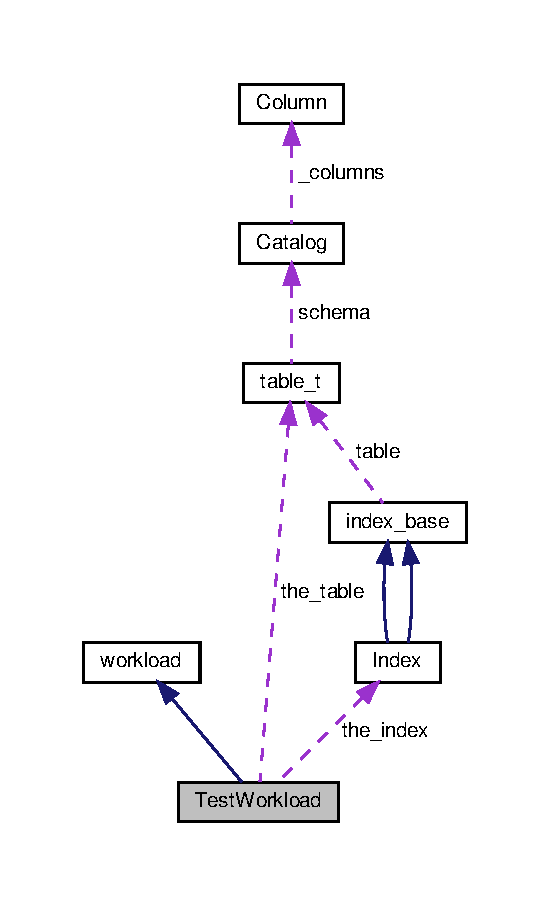
\includegraphics[width=264pt]{classTestWorkload__coll__graph}
\end{center}
\end{figure}
\subsection*{Public Member Functions}
\begin{DoxyCompactItemize}
\item 
\hyperlink{global_8h_a78c49a674c810fdd03d20432f7be864a}{RC} \hyperlink{classTestWorkload_aba95b44e0531c1ff81d9846bcd7df8ba}{init} ()
\item 
\hyperlink{global_8h_a78c49a674c810fdd03d20432f7be864a}{RC} \hyperlink{classTestWorkload_a4963c5307360dc96391779393a1571dc}{init\+\_\+table} ()
\item 
\hyperlink{global_8h_a78c49a674c810fdd03d20432f7be864a}{RC} \hyperlink{classTestWorkload_af93fb571938ef9fcd18fc5e3cd402849}{init\+\_\+schema} (const char $\ast$schema\+\_\+file)
\item 
\hyperlink{global_8h_a78c49a674c810fdd03d20432f7be864a}{RC} \hyperlink{classTestWorkload_abc14a45ce19f90979f01cf2e96f1bb9f}{get\+\_\+txn\+\_\+man} (\hyperlink{classtxn__man}{txn\+\_\+man} $\ast$\&txn\+\_\+manager, \hyperlink{classthread__t}{thread\+\_\+t} $\ast$h\+\_\+thd)
\item 
void \hyperlink{classTestWorkload_a7307dcf3dfe3f4cfc99eb92e2f1cb0de}{summarize} ()
\item 
void \hyperlink{classTestWorkload_ac1d41470c6a3b217c789379c44ec73a1}{tick} ()
\end{DoxyCompactItemize}
\subsection*{Public Attributes}
\begin{DoxyCompactItemize}
\item 
\hyperlink{classIndex}{Index} $\ast$ \hyperlink{classTestWorkload_a0625829ac5f20b1d5c18c6923d17ee0c}{the\+\_\+index}
\item 
\hyperlink{classtable__t}{table\+\_\+t} $\ast$ \hyperlink{classTestWorkload_aa98e2cc097d29b701ff914e624fe8d77}{the\+\_\+table}
\end{DoxyCompactItemize}
\subsection*{Additional Inherited Members}


\subsection{Member Function Documentation}
\mbox{\Hypertarget{classTestWorkload_abc14a45ce19f90979f01cf2e96f1bb9f}\label{classTestWorkload_abc14a45ce19f90979f01cf2e96f1bb9f}} 
\index{Test\+Workload@{Test\+Workload}!get\+\_\+txn\+\_\+man@{get\+\_\+txn\+\_\+man}}
\index{get\+\_\+txn\+\_\+man@{get\+\_\+txn\+\_\+man}!Test\+Workload@{Test\+Workload}}
\subsubsection{\texorpdfstring{get\+\_\+txn\+\_\+man()}{get\_txn\_man()}}
{\footnotesize\ttfamily \hyperlink{global_8h_a78c49a674c810fdd03d20432f7be864a}{RC} Test\+Workload\+::get\+\_\+txn\+\_\+man (\begin{DoxyParamCaption}\item[{\hyperlink{classtxn__man}{txn\+\_\+man} $\ast$\&}]{txn\+\_\+manager,  }\item[{\hyperlink{classthread__t}{thread\+\_\+t} $\ast$}]{h\+\_\+thd }\end{DoxyParamCaption})\hspace{0.3cm}{\ttfamily [virtual]}}



Implements \hyperlink{classworkload_ac22d0558c3fc549b8b07347cebb95cb3}{workload}.

\mbox{\Hypertarget{classTestWorkload_aba95b44e0531c1ff81d9846bcd7df8ba}\label{classTestWorkload_aba95b44e0531c1ff81d9846bcd7df8ba}} 
\index{Test\+Workload@{Test\+Workload}!init@{init}}
\index{init@{init}!Test\+Workload@{Test\+Workload}}
\subsubsection{\texorpdfstring{init()}{init()}}
{\footnotesize\ttfamily \hyperlink{global_8h_a78c49a674c810fdd03d20432f7be864a}{RC} Test\+Workload\+::init (\begin{DoxyParamCaption}{ }\end{DoxyParamCaption})\hspace{0.3cm}{\ttfamily [virtual]}}



Reimplemented from \hyperlink{classworkload_a7cef7a7101c78e10082c99356e77a57c}{workload}.

\mbox{\Hypertarget{classTestWorkload_af93fb571938ef9fcd18fc5e3cd402849}\label{classTestWorkload_af93fb571938ef9fcd18fc5e3cd402849}} 
\index{Test\+Workload@{Test\+Workload}!init\+\_\+schema@{init\+\_\+schema}}
\index{init\+\_\+schema@{init\+\_\+schema}!Test\+Workload@{Test\+Workload}}
\subsubsection{\texorpdfstring{init\+\_\+schema()}{init\_schema()}}
{\footnotesize\ttfamily \hyperlink{global_8h_a78c49a674c810fdd03d20432f7be864a}{RC} Test\+Workload\+::init\+\_\+schema (\begin{DoxyParamCaption}\item[{const char $\ast$}]{schema\+\_\+file }\end{DoxyParamCaption})}

\mbox{\Hypertarget{classTestWorkload_a4963c5307360dc96391779393a1571dc}\label{classTestWorkload_a4963c5307360dc96391779393a1571dc}} 
\index{Test\+Workload@{Test\+Workload}!init\+\_\+table@{init\+\_\+table}}
\index{init\+\_\+table@{init\+\_\+table}!Test\+Workload@{Test\+Workload}}
\subsubsection{\texorpdfstring{init\+\_\+table()}{init\_table()}}
{\footnotesize\ttfamily \hyperlink{global_8h_a78c49a674c810fdd03d20432f7be864a}{RC} Test\+Workload\+::init\+\_\+table (\begin{DoxyParamCaption}{ }\end{DoxyParamCaption})\hspace{0.3cm}{\ttfamily [virtual]}}



Implements \hyperlink{classworkload_a3feee79af04069f6c1ad6b7f9b0a045a}{workload}.

\mbox{\Hypertarget{classTestWorkload_a7307dcf3dfe3f4cfc99eb92e2f1cb0de}\label{classTestWorkload_a7307dcf3dfe3f4cfc99eb92e2f1cb0de}} 
\index{Test\+Workload@{Test\+Workload}!summarize@{summarize}}
\index{summarize@{summarize}!Test\+Workload@{Test\+Workload}}
\subsubsection{\texorpdfstring{summarize()}{summarize()}}
{\footnotesize\ttfamily void Test\+Workload\+::summarize (\begin{DoxyParamCaption}{ }\end{DoxyParamCaption})}

\mbox{\Hypertarget{classTestWorkload_ac1d41470c6a3b217c789379c44ec73a1}\label{classTestWorkload_ac1d41470c6a3b217c789379c44ec73a1}} 
\index{Test\+Workload@{Test\+Workload}!tick@{tick}}
\index{tick@{tick}!Test\+Workload@{Test\+Workload}}
\subsubsection{\texorpdfstring{tick()}{tick()}}
{\footnotesize\ttfamily void Test\+Workload\+::tick (\begin{DoxyParamCaption}{ }\end{DoxyParamCaption})\hspace{0.3cm}{\ttfamily [inline]}}



\subsection{Member Data Documentation}
\mbox{\Hypertarget{classTestWorkload_a0625829ac5f20b1d5c18c6923d17ee0c}\label{classTestWorkload_a0625829ac5f20b1d5c18c6923d17ee0c}} 
\index{Test\+Workload@{Test\+Workload}!the\+\_\+index@{the\+\_\+index}}
\index{the\+\_\+index@{the\+\_\+index}!Test\+Workload@{Test\+Workload}}
\subsubsection{\texorpdfstring{the\+\_\+index}{the\_index}}
{\footnotesize\ttfamily \hyperlink{classIndex}{Index}$\ast$ Test\+Workload\+::the\+\_\+index}

\mbox{\Hypertarget{classTestWorkload_aa98e2cc097d29b701ff914e624fe8d77}\label{classTestWorkload_aa98e2cc097d29b701ff914e624fe8d77}} 
\index{Test\+Workload@{Test\+Workload}!the\+\_\+table@{the\+\_\+table}}
\index{the\+\_\+table@{the\+\_\+table}!Test\+Workload@{Test\+Workload}}
\subsubsection{\texorpdfstring{the\+\_\+table}{the\_table}}
{\footnotesize\ttfamily \hyperlink{classtable__t}{table\+\_\+t}$\ast$ Test\+Workload\+::the\+\_\+table}



The documentation for this class was generated from the following files\+:\begin{DoxyCompactItemize}
\item 
macrobench/benchmarks/\hyperlink{test_8h}{test.\+h}\item 
macrobench/benchmarks/\hyperlink{test__wl_8cpp}{test\+\_\+wl.\+cpp}\end{DoxyCompactItemize}

\hypertarget{structthread__data__t}{}\section{thread\+\_\+data\+\_\+t$<$ skey\+\_\+t, sval\+\_\+t $>$ Struct Template Reference}
\label{structthread__data__t}\index{thread\+\_\+data\+\_\+t$<$ skey\+\_\+t, sval\+\_\+t $>$@{thread\+\_\+data\+\_\+t$<$ skey\+\_\+t, sval\+\_\+t $>$}}


{\ttfamily \#include $<$natarajan\+\_\+ext\+\_\+bst\+\_\+lf\+\_\+baseline.\+h$>$}

\subsection*{Public Attributes}
\begin{DoxyCompactItemize}
\item 
int \hyperlink{structthread__data__t_a32492b643fddfe2ef0b74bcaca1427ed}{id}
\item 
struct \hyperlink{structnode__t}{node\+\_\+t}$<$ skey\+\_\+t, sval\+\_\+t $>$ $\ast$ \hyperlink{structthread__data__t_a5c58446e4fb376931c8eefd24b907a0b}{root\+Of\+Tree}
\item 
\hyperlink{structseekRecord__t}{seek\+Record\+\_\+t}$<$ skey\+\_\+t, sval\+\_\+t $>$ $\ast$ \hyperlink{structthread__data__t_a41e98b9f289aa039d8797baf5fcaf886}{sr}
\item 
\hyperlink{structseekRecord__t}{seek\+Record\+\_\+t}$<$ skey\+\_\+t, sval\+\_\+t $>$ $\ast$ \hyperlink{structthread__data__t_afe71f5c29320086b79b63617b00236a0}{ssr}
\end{DoxyCompactItemize}


\subsection{Member Data Documentation}
\mbox{\Hypertarget{structthread__data__t_a32492b643fddfe2ef0b74bcaca1427ed}\label{structthread__data__t_a32492b643fddfe2ef0b74bcaca1427ed}} 
\index{thread\+\_\+data\+\_\+t@{thread\+\_\+data\+\_\+t}!id@{id}}
\index{id@{id}!thread\+\_\+data\+\_\+t@{thread\+\_\+data\+\_\+t}}
\subsubsection{\texorpdfstring{id}{id}}
{\footnotesize\ttfamily template$<$typename skey\+\_\+t, typename sval\+\_\+t$>$ \\
int \hyperlink{structthread__data__t}{thread\+\_\+data\+\_\+t}$<$ skey\+\_\+t, sval\+\_\+t $>$\+::id}

\mbox{\Hypertarget{structthread__data__t_a5c58446e4fb376931c8eefd24b907a0b}\label{structthread__data__t_a5c58446e4fb376931c8eefd24b907a0b}} 
\index{thread\+\_\+data\+\_\+t@{thread\+\_\+data\+\_\+t}!root\+Of\+Tree@{root\+Of\+Tree}}
\index{root\+Of\+Tree@{root\+Of\+Tree}!thread\+\_\+data\+\_\+t@{thread\+\_\+data\+\_\+t}}
\subsubsection{\texorpdfstring{root\+Of\+Tree}{rootOfTree}}
{\footnotesize\ttfamily template$<$typename skey\+\_\+t, typename sval\+\_\+t$>$ \\
struct \hyperlink{structnode__t}{node\+\_\+t}$<$ skey\+\_\+t, sval\+\_\+t $>$ $\ast$ \hyperlink{structthread__data__t}{thread\+\_\+data\+\_\+t}$<$ skey\+\_\+t, sval\+\_\+t $>$\+::root\+Of\+Tree}

\mbox{\Hypertarget{structthread__data__t_a41e98b9f289aa039d8797baf5fcaf886}\label{structthread__data__t_a41e98b9f289aa039d8797baf5fcaf886}} 
\index{thread\+\_\+data\+\_\+t@{thread\+\_\+data\+\_\+t}!sr@{sr}}
\index{sr@{sr}!thread\+\_\+data\+\_\+t@{thread\+\_\+data\+\_\+t}}
\subsubsection{\texorpdfstring{sr}{sr}}
{\footnotesize\ttfamily template$<$typename skey\+\_\+t, typename sval\+\_\+t$>$ \\
\hyperlink{structseekRecord__t}{seek\+Record\+\_\+t}$<$ skey\+\_\+t, sval\+\_\+t $>$ $\ast$ \hyperlink{structthread__data__t}{thread\+\_\+data\+\_\+t}$<$ skey\+\_\+t, sval\+\_\+t $>$\+::sr}

\mbox{\Hypertarget{structthread__data__t_afe71f5c29320086b79b63617b00236a0}\label{structthread__data__t_afe71f5c29320086b79b63617b00236a0}} 
\index{thread\+\_\+data\+\_\+t@{thread\+\_\+data\+\_\+t}!ssr@{ssr}}
\index{ssr@{ssr}!thread\+\_\+data\+\_\+t@{thread\+\_\+data\+\_\+t}}
\subsubsection{\texorpdfstring{ssr}{ssr}}
{\footnotesize\ttfamily template$<$typename skey\+\_\+t, typename sval\+\_\+t$>$ \\
\hyperlink{structseekRecord__t}{seek\+Record\+\_\+t}$<$ skey\+\_\+t, sval\+\_\+t $>$ $\ast$ \hyperlink{structthread__data__t}{thread\+\_\+data\+\_\+t}$<$ skey\+\_\+t, sval\+\_\+t $>$\+::ssr}



The documentation for this struct was generated from the following files\+:\begin{DoxyCompactItemize}
\item 
ds/natarajan\+\_\+ext\+\_\+bst\+\_\+lf/\hyperlink{natarajan__ext__bst__lf__baseline_8h}{natarajan\+\_\+ext\+\_\+bst\+\_\+lf\+\_\+baseline.\+h}\item 
ds/natarajan\+\_\+ext\+\_\+bst\+\_\+lf/\hyperlink{natarajan__ext__bst__lf__stage1_8h}{natarajan\+\_\+ext\+\_\+bst\+\_\+lf\+\_\+stage1.\+h}\end{DoxyCompactItemize}

\hypertarget{classthread__t}{}\section{thread\+\_\+t Class Reference}
\label{classthread__t}\index{thread\+\_\+t@{thread\+\_\+t}}


{\ttfamily \#include $<$thread.\+h$>$}



Collaboration diagram for thread\+\_\+t\+:
\nopagebreak
\begin{figure}[H]
\begin{center}
\leavevmode
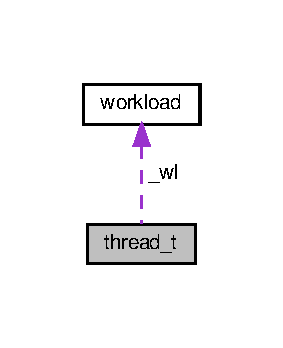
\includegraphics[width=136pt]{classthread__t__coll__graph}
\end{center}
\end{figure}
\subsection*{Public Member Functions}
\begin{DoxyCompactItemize}
\item 
uint64\+\_\+t \hyperlink{classthread__t_a1c930f988d62925926b979506e091b99}{get\+\_\+thd\+\_\+id} ()
\item 
uint64\+\_\+t \hyperlink{classthread__t_a0a3db9542c72c632b933681d8d1db9a4}{get\+\_\+host\+\_\+cid} ()
\item 
void \hyperlink{classthread__t_affdd8c0f748856de17f3c869e1740346}{set\+\_\+host\+\_\+cid} (uint64\+\_\+t cid)
\item 
uint64\+\_\+t \hyperlink{classthread__t_ac66d269581a7807351c3fb5236023f29}{get\+\_\+cur\+\_\+cid} ()
\item 
void \hyperlink{classthread__t_acdfebeadd64bfffd24730cd41e8b5230}{set\+\_\+cur\+\_\+cid} (uint64\+\_\+t cid)
\item 
void \hyperlink{classthread__t_ab6619c01f0cf08f7f289e2fc302231bd}{init} (uint64\+\_\+t thd\+\_\+id, \hyperlink{classworkload}{workload} $\ast$\hyperlink{classworkload}{workload})
\item 
void \hyperlink{classthread__t_a6f57d164e9a3c1e1623882b14943b34d}{setbench\+\_\+deinit} ()
\item 
\hyperlink{global_8h_a78c49a674c810fdd03d20432f7be864a}{RC} \hyperlink{classthread__t_ab5c82bb47e5886bee276b2b56daaa82f}{run} ()
\end{DoxyCompactItemize}
\subsection*{Public Attributes}
\begin{DoxyCompactItemize}
\item 
uint64\+\_\+t \hyperlink{classthread__t_ab26bbe2a110faa177b70a7ba07a26bcb}{\+\_\+thd\+\_\+id}
\item 
\hyperlink{classworkload}{workload} $\ast$ \hyperlink{classthread__t_a22b5d80e0ce6ce841d0585b99f6e7de1}{\+\_\+wl}
\end{DoxyCompactItemize}


\subsection{Member Function Documentation}
\mbox{\Hypertarget{classthread__t_ac66d269581a7807351c3fb5236023f29}\label{classthread__t_ac66d269581a7807351c3fb5236023f29}} 
\index{thread\+\_\+t@{thread\+\_\+t}!get\+\_\+cur\+\_\+cid@{get\+\_\+cur\+\_\+cid}}
\index{get\+\_\+cur\+\_\+cid@{get\+\_\+cur\+\_\+cid}!thread\+\_\+t@{thread\+\_\+t}}
\subsubsection{\texorpdfstring{get\+\_\+cur\+\_\+cid()}{get\_cur\_cid()}}
{\footnotesize\ttfamily uint64\+\_\+t thread\+\_\+t\+::get\+\_\+cur\+\_\+cid (\begin{DoxyParamCaption}{ }\end{DoxyParamCaption})}

\mbox{\Hypertarget{classthread__t_a0a3db9542c72c632b933681d8d1db9a4}\label{classthread__t_a0a3db9542c72c632b933681d8d1db9a4}} 
\index{thread\+\_\+t@{thread\+\_\+t}!get\+\_\+host\+\_\+cid@{get\+\_\+host\+\_\+cid}}
\index{get\+\_\+host\+\_\+cid@{get\+\_\+host\+\_\+cid}!thread\+\_\+t@{thread\+\_\+t}}
\subsubsection{\texorpdfstring{get\+\_\+host\+\_\+cid()}{get\_host\_cid()}}
{\footnotesize\ttfamily uint64\+\_\+t thread\+\_\+t\+::get\+\_\+host\+\_\+cid (\begin{DoxyParamCaption}{ }\end{DoxyParamCaption})}

\mbox{\Hypertarget{classthread__t_a1c930f988d62925926b979506e091b99}\label{classthread__t_a1c930f988d62925926b979506e091b99}} 
\index{thread\+\_\+t@{thread\+\_\+t}!get\+\_\+thd\+\_\+id@{get\+\_\+thd\+\_\+id}}
\index{get\+\_\+thd\+\_\+id@{get\+\_\+thd\+\_\+id}!thread\+\_\+t@{thread\+\_\+t}}
\subsubsection{\texorpdfstring{get\+\_\+thd\+\_\+id()}{get\_thd\_id()}}
{\footnotesize\ttfamily uint64\+\_\+t thread\+\_\+t\+::get\+\_\+thd\+\_\+id (\begin{DoxyParamCaption}{ }\end{DoxyParamCaption})}

\mbox{\Hypertarget{classthread__t_ab6619c01f0cf08f7f289e2fc302231bd}\label{classthread__t_ab6619c01f0cf08f7f289e2fc302231bd}} 
\index{thread\+\_\+t@{thread\+\_\+t}!init@{init}}
\index{init@{init}!thread\+\_\+t@{thread\+\_\+t}}
\subsubsection{\texorpdfstring{init()}{init()}}
{\footnotesize\ttfamily void thread\+\_\+t\+::init (\begin{DoxyParamCaption}\item[{uint64\+\_\+t}]{thd\+\_\+id,  }\item[{\hyperlink{classworkload}{workload} $\ast$}]{workload }\end{DoxyParamCaption})}

\mbox{\Hypertarget{classthread__t_ab5c82bb47e5886bee276b2b56daaa82f}\label{classthread__t_ab5c82bb47e5886bee276b2b56daaa82f}} 
\index{thread\+\_\+t@{thread\+\_\+t}!run@{run}}
\index{run@{run}!thread\+\_\+t@{thread\+\_\+t}}
\subsubsection{\texorpdfstring{run()}{run()}}
{\footnotesize\ttfamily \hyperlink{global_8h_a78c49a674c810fdd03d20432f7be864a}{RC} thread\+\_\+t\+::run (\begin{DoxyParamCaption}{ }\end{DoxyParamCaption})}

\mbox{\Hypertarget{classthread__t_acdfebeadd64bfffd24730cd41e8b5230}\label{classthread__t_acdfebeadd64bfffd24730cd41e8b5230}} 
\index{thread\+\_\+t@{thread\+\_\+t}!set\+\_\+cur\+\_\+cid@{set\+\_\+cur\+\_\+cid}}
\index{set\+\_\+cur\+\_\+cid@{set\+\_\+cur\+\_\+cid}!thread\+\_\+t@{thread\+\_\+t}}
\subsubsection{\texorpdfstring{set\+\_\+cur\+\_\+cid()}{set\_cur\_cid()}}
{\footnotesize\ttfamily void thread\+\_\+t\+::set\+\_\+cur\+\_\+cid (\begin{DoxyParamCaption}\item[{uint64\+\_\+t}]{cid }\end{DoxyParamCaption})}

\mbox{\Hypertarget{classthread__t_affdd8c0f748856de17f3c869e1740346}\label{classthread__t_affdd8c0f748856de17f3c869e1740346}} 
\index{thread\+\_\+t@{thread\+\_\+t}!set\+\_\+host\+\_\+cid@{set\+\_\+host\+\_\+cid}}
\index{set\+\_\+host\+\_\+cid@{set\+\_\+host\+\_\+cid}!thread\+\_\+t@{thread\+\_\+t}}
\subsubsection{\texorpdfstring{set\+\_\+host\+\_\+cid()}{set\_host\_cid()}}
{\footnotesize\ttfamily void thread\+\_\+t\+::set\+\_\+host\+\_\+cid (\begin{DoxyParamCaption}\item[{uint64\+\_\+t}]{cid }\end{DoxyParamCaption})}

\mbox{\Hypertarget{classthread__t_a6f57d164e9a3c1e1623882b14943b34d}\label{classthread__t_a6f57d164e9a3c1e1623882b14943b34d}} 
\index{thread\+\_\+t@{thread\+\_\+t}!setbench\+\_\+deinit@{setbench\+\_\+deinit}}
\index{setbench\+\_\+deinit@{setbench\+\_\+deinit}!thread\+\_\+t@{thread\+\_\+t}}
\subsubsection{\texorpdfstring{setbench\+\_\+deinit()}{setbench\_deinit()}}
{\footnotesize\ttfamily void thread\+\_\+t\+::setbench\+\_\+deinit (\begin{DoxyParamCaption}{ }\end{DoxyParamCaption})}



\subsection{Member Data Documentation}
\mbox{\Hypertarget{classthread__t_ab26bbe2a110faa177b70a7ba07a26bcb}\label{classthread__t_ab26bbe2a110faa177b70a7ba07a26bcb}} 
\index{thread\+\_\+t@{thread\+\_\+t}!\+\_\+thd\+\_\+id@{\+\_\+thd\+\_\+id}}
\index{\+\_\+thd\+\_\+id@{\+\_\+thd\+\_\+id}!thread\+\_\+t@{thread\+\_\+t}}
\subsubsection{\texorpdfstring{\+\_\+thd\+\_\+id}{\_thd\_id}}
{\footnotesize\ttfamily uint64\+\_\+t thread\+\_\+t\+::\+\_\+thd\+\_\+id}

\mbox{\Hypertarget{classthread__t_a22b5d80e0ce6ce841d0585b99f6e7de1}\label{classthread__t_a22b5d80e0ce6ce841d0585b99f6e7de1}} 
\index{thread\+\_\+t@{thread\+\_\+t}!\+\_\+wl@{\+\_\+wl}}
\index{\+\_\+wl@{\+\_\+wl}!thread\+\_\+t@{thread\+\_\+t}}
\subsubsection{\texorpdfstring{\+\_\+wl}{\_wl}}
{\footnotesize\ttfamily \hyperlink{classworkload}{workload}$\ast$ thread\+\_\+t\+::\+\_\+wl}



The documentation for this class was generated from the following files\+:\begin{DoxyCompactItemize}
\item 
macrobench/system/\hyperlink{thread_8h}{thread.\+h}\item 
macrobench/system/\hyperlink{thread_8cpp}{thread.\+cpp}\end{DoxyCompactItemize}

\hypertarget{classreclaimer__ebr__token_1_1ThreadData}{}\section{reclaimer\+\_\+ebr\+\_\+token$<$ T, Pool $>$\+:\+:Thread\+Data Class Reference}
\label{classreclaimer__ebr__token_1_1ThreadData}\index{reclaimer\+\_\+ebr\+\_\+token$<$ T, Pool $>$\+::\+Thread\+Data@{reclaimer\+\_\+ebr\+\_\+token$<$ T, Pool $>$\+::\+Thread\+Data}}


{\ttfamily \#include $<$reclaimer\+\_\+ebr\+\_\+token.\+h$>$}

\subsection*{Public Member Functions}
\begin{DoxyCompactItemize}
\item 
\hyperlink{classreclaimer__ebr__token_1_1ThreadData_a2198c46887f5f955760f2488baa162e7}{Thread\+Data} ()
\end{DoxyCompactItemize}
\subsection*{Public Attributes}
\begin{DoxyCompactItemize}
\item 
volatile int \hyperlink{classreclaimer__ebr__token_1_1ThreadData_a4b6b47b02cb3e120d4fb9fa8820e5b4d}{token}
\item 
int \hyperlink{classreclaimer__ebr__token_1_1ThreadData_aef3ca8bfcf65b876744855d00f19d482}{token\+Count}
\item 
\hyperlink{classblockbag}{blockbag}$<$ T $>$ $\ast$ \hyperlink{classreclaimer__ebr__token_1_1ThreadData_affa120c770d3a6fb2b3fae1e3c5559ed}{curr}
\item 
\hyperlink{classblockbag}{blockbag}$<$ T $>$ $\ast$ \hyperlink{classreclaimer__ebr__token_1_1ThreadData_a26b4385b902f289bdc1235b7eff1c877}{last}
\end{DoxyCompactItemize}


\subsection{Constructor \& Destructor Documentation}
\mbox{\Hypertarget{classreclaimer__ebr__token_1_1ThreadData_a2198c46887f5f955760f2488baa162e7}\label{classreclaimer__ebr__token_1_1ThreadData_a2198c46887f5f955760f2488baa162e7}} 
\index{reclaimer\+\_\+ebr\+\_\+token\+::\+Thread\+Data@{reclaimer\+\_\+ebr\+\_\+token\+::\+Thread\+Data}!Thread\+Data@{Thread\+Data}}
\index{Thread\+Data@{Thread\+Data}!reclaimer\+\_\+ebr\+\_\+token\+::\+Thread\+Data@{reclaimer\+\_\+ebr\+\_\+token\+::\+Thread\+Data}}
\subsubsection{\texorpdfstring{Thread\+Data()}{ThreadData()}}
{\footnotesize\ttfamily template$<$typename T  = void, class Pool  = pool\+\_\+interface$<$\+T$>$$>$ \\
\hyperlink{classreclaimer__ebr__token}{reclaimer\+\_\+ebr\+\_\+token}$<$ T, Pool $>$\+::Thread\+Data\+::\+Thread\+Data (\begin{DoxyParamCaption}{ }\end{DoxyParamCaption})\hspace{0.3cm}{\ttfamily [inline]}}



\subsection{Member Data Documentation}
\mbox{\Hypertarget{classreclaimer__ebr__token_1_1ThreadData_affa120c770d3a6fb2b3fae1e3c5559ed}\label{classreclaimer__ebr__token_1_1ThreadData_affa120c770d3a6fb2b3fae1e3c5559ed}} 
\index{reclaimer\+\_\+ebr\+\_\+token\+::\+Thread\+Data@{reclaimer\+\_\+ebr\+\_\+token\+::\+Thread\+Data}!curr@{curr}}
\index{curr@{curr}!reclaimer\+\_\+ebr\+\_\+token\+::\+Thread\+Data@{reclaimer\+\_\+ebr\+\_\+token\+::\+Thread\+Data}}
\subsubsection{\texorpdfstring{curr}{curr}}
{\footnotesize\ttfamily template$<$typename T  = void, class Pool  = pool\+\_\+interface$<$\+T$>$$>$ \\
\hyperlink{classblockbag}{blockbag}$<$T$>$$\ast$ \hyperlink{classreclaimer__ebr__token}{reclaimer\+\_\+ebr\+\_\+token}$<$ T, Pool $>$\+::Thread\+Data\+::curr}

\mbox{\Hypertarget{classreclaimer__ebr__token_1_1ThreadData_a26b4385b902f289bdc1235b7eff1c877}\label{classreclaimer__ebr__token_1_1ThreadData_a26b4385b902f289bdc1235b7eff1c877}} 
\index{reclaimer\+\_\+ebr\+\_\+token\+::\+Thread\+Data@{reclaimer\+\_\+ebr\+\_\+token\+::\+Thread\+Data}!last@{last}}
\index{last@{last}!reclaimer\+\_\+ebr\+\_\+token\+::\+Thread\+Data@{reclaimer\+\_\+ebr\+\_\+token\+::\+Thread\+Data}}
\subsubsection{\texorpdfstring{last}{last}}
{\footnotesize\ttfamily template$<$typename T  = void, class Pool  = pool\+\_\+interface$<$\+T$>$$>$ \\
\hyperlink{classblockbag}{blockbag}$<$T$>$$\ast$ \hyperlink{classreclaimer__ebr__token}{reclaimer\+\_\+ebr\+\_\+token}$<$ T, Pool $>$\+::Thread\+Data\+::last}

\mbox{\Hypertarget{classreclaimer__ebr__token_1_1ThreadData_a4b6b47b02cb3e120d4fb9fa8820e5b4d}\label{classreclaimer__ebr__token_1_1ThreadData_a4b6b47b02cb3e120d4fb9fa8820e5b4d}} 
\index{reclaimer\+\_\+ebr\+\_\+token\+::\+Thread\+Data@{reclaimer\+\_\+ebr\+\_\+token\+::\+Thread\+Data}!token@{token}}
\index{token@{token}!reclaimer\+\_\+ebr\+\_\+token\+::\+Thread\+Data@{reclaimer\+\_\+ebr\+\_\+token\+::\+Thread\+Data}}
\subsubsection{\texorpdfstring{token}{token}}
{\footnotesize\ttfamily template$<$typename T  = void, class Pool  = pool\+\_\+interface$<$\+T$>$$>$ \\
volatile int \hyperlink{classreclaimer__ebr__token}{reclaimer\+\_\+ebr\+\_\+token}$<$ T, Pool $>$\+::Thread\+Data\+::token}

\mbox{\Hypertarget{classreclaimer__ebr__token_1_1ThreadData_aef3ca8bfcf65b876744855d00f19d482}\label{classreclaimer__ebr__token_1_1ThreadData_aef3ca8bfcf65b876744855d00f19d482}} 
\index{reclaimer\+\_\+ebr\+\_\+token\+::\+Thread\+Data@{reclaimer\+\_\+ebr\+\_\+token\+::\+Thread\+Data}!token\+Count@{token\+Count}}
\index{token\+Count@{token\+Count}!reclaimer\+\_\+ebr\+\_\+token\+::\+Thread\+Data@{reclaimer\+\_\+ebr\+\_\+token\+::\+Thread\+Data}}
\subsubsection{\texorpdfstring{token\+Count}{tokenCount}}
{\footnotesize\ttfamily template$<$typename T  = void, class Pool  = pool\+\_\+interface$<$\+T$>$$>$ \\
int \hyperlink{classreclaimer__ebr__token}{reclaimer\+\_\+ebr\+\_\+token}$<$ T, Pool $>$\+::Thread\+Data\+::token\+Count}



The documentation for this class was generated from the following file\+:\begin{DoxyCompactItemize}
\item 
common/recordmgr/\hyperlink{reclaimer__ebr__token_8h}{reclaimer\+\_\+ebr\+\_\+token.\+h}\end{DoxyCompactItemize}

\hypertarget{classreclaimer__debra_1_1ThreadData}{}\section{reclaimer\+\_\+debra$<$ T, Pool $>$\+:\+:Thread\+Data Class Reference}
\label{classreclaimer__debra_1_1ThreadData}\index{reclaimer\+\_\+debra$<$ T, Pool $>$\+::\+Thread\+Data@{reclaimer\+\_\+debra$<$ T, Pool $>$\+::\+Thread\+Data}}


{\ttfamily \#include $<$reclaimer\+\_\+debra.\+h$>$}

\subsection*{Public Member Functions}
\begin{DoxyCompactItemize}
\item 
\hyperlink{classreclaimer__debra_1_1ThreadData_a3974b5f52cb86c4fac103224e438163d}{Thread\+Data} ()
\end{DoxyCompactItemize}
\subsection*{Public Attributes}
\begin{DoxyCompactItemize}
\item 
std\+::atomic\+\_\+long \hyperlink{classreclaimer__debra_1_1ThreadData_aa86de34e945bc1b5d1b98cec6508073b}{announced\+Epoch}
\item 
long \hyperlink{classreclaimer__debra_1_1ThreadData_a7b5c0008c0e0d93d36d0ff6222509963}{localvar\+\_\+announced\+Epoch}
\item 
\hyperlink{classblockbag}{blockbag}$<$ T $>$ $\ast$ \hyperlink{classreclaimer__debra_1_1ThreadData_ae2a76ecf79487fd59dc98f9e3db227b8}{epochbags} \mbox{[}\hyperlink{reclaimer__ebr__tree__q_8h_acc0cc9ce1a68a29c4e0e126887b517dd}{N\+U\+M\+B\+E\+R\+\_\+\+O\+F\+\_\+\+E\+P\+O\+C\+H\+\_\+\+B\+A\+GS}\mbox{]}
\item 
int \hyperlink{classreclaimer__debra_1_1ThreadData_ab02bc86812759af0725038ef64c52200}{index}
\item 
\hyperlink{classblockbag}{blockbag}$<$ T $>$ $\ast$ \hyperlink{classreclaimer__debra_1_1ThreadData_a13ae47aafc34001c5225b8f2fa0c06c8}{current\+Bag}
\item 
int \hyperlink{classreclaimer__debra_1_1ThreadData_ae6c8f53e846e6feab1cbb90d3aaf3924}{checked}
\item 
int \hyperlink{classreclaimer__debra_1_1ThreadData_ad35a3f25b69dcdf78c2e4979b65c9e32}{ops\+Since\+Read}
\end{DoxyCompactItemize}


\subsection{Constructor \& Destructor Documentation}
\mbox{\Hypertarget{classreclaimer__debra_1_1ThreadData_a3974b5f52cb86c4fac103224e438163d}\label{classreclaimer__debra_1_1ThreadData_a3974b5f52cb86c4fac103224e438163d}} 
\index{reclaimer\+\_\+debra\+::\+Thread\+Data@{reclaimer\+\_\+debra\+::\+Thread\+Data}!Thread\+Data@{Thread\+Data}}
\index{Thread\+Data@{Thread\+Data}!reclaimer\+\_\+debra\+::\+Thread\+Data@{reclaimer\+\_\+debra\+::\+Thread\+Data}}
\subsubsection{\texorpdfstring{Thread\+Data()}{ThreadData()}}
{\footnotesize\ttfamily template$<$typename T  = void, class Pool  = pool\+\_\+interface$<$\+T$>$$>$ \\
\hyperlink{classreclaimer__debra}{reclaimer\+\_\+debra}$<$ T, Pool $>$\+::Thread\+Data\+::\+Thread\+Data (\begin{DoxyParamCaption}{ }\end{DoxyParamCaption})\hspace{0.3cm}{\ttfamily [inline]}}



\subsection{Member Data Documentation}
\mbox{\Hypertarget{classreclaimer__debra_1_1ThreadData_aa86de34e945bc1b5d1b98cec6508073b}\label{classreclaimer__debra_1_1ThreadData_aa86de34e945bc1b5d1b98cec6508073b}} 
\index{reclaimer\+\_\+debra\+::\+Thread\+Data@{reclaimer\+\_\+debra\+::\+Thread\+Data}!announced\+Epoch@{announced\+Epoch}}
\index{announced\+Epoch@{announced\+Epoch}!reclaimer\+\_\+debra\+::\+Thread\+Data@{reclaimer\+\_\+debra\+::\+Thread\+Data}}
\subsubsection{\texorpdfstring{announced\+Epoch}{announcedEpoch}}
{\footnotesize\ttfamily template$<$typename T  = void, class Pool  = pool\+\_\+interface$<$\+T$>$$>$ \\
std\+::atomic\+\_\+long \hyperlink{classreclaimer__debra}{reclaimer\+\_\+debra}$<$ T, Pool $>$\+::Thread\+Data\+::announced\+Epoch}

\mbox{\Hypertarget{classreclaimer__debra_1_1ThreadData_ae6c8f53e846e6feab1cbb90d3aaf3924}\label{classreclaimer__debra_1_1ThreadData_ae6c8f53e846e6feab1cbb90d3aaf3924}} 
\index{reclaimer\+\_\+debra\+::\+Thread\+Data@{reclaimer\+\_\+debra\+::\+Thread\+Data}!checked@{checked}}
\index{checked@{checked}!reclaimer\+\_\+debra\+::\+Thread\+Data@{reclaimer\+\_\+debra\+::\+Thread\+Data}}
\subsubsection{\texorpdfstring{checked}{checked}}
{\footnotesize\ttfamily template$<$typename T  = void, class Pool  = pool\+\_\+interface$<$\+T$>$$>$ \\
int \hyperlink{classreclaimer__debra}{reclaimer\+\_\+debra}$<$ T, Pool $>$\+::Thread\+Data\+::checked}

\mbox{\Hypertarget{classreclaimer__debra_1_1ThreadData_a13ae47aafc34001c5225b8f2fa0c06c8}\label{classreclaimer__debra_1_1ThreadData_a13ae47aafc34001c5225b8f2fa0c06c8}} 
\index{reclaimer\+\_\+debra\+::\+Thread\+Data@{reclaimer\+\_\+debra\+::\+Thread\+Data}!current\+Bag@{current\+Bag}}
\index{current\+Bag@{current\+Bag}!reclaimer\+\_\+debra\+::\+Thread\+Data@{reclaimer\+\_\+debra\+::\+Thread\+Data}}
\subsubsection{\texorpdfstring{current\+Bag}{currentBag}}
{\footnotesize\ttfamily template$<$typename T  = void, class Pool  = pool\+\_\+interface$<$\+T$>$$>$ \\
\hyperlink{classblockbag}{blockbag}$<$T$>$$\ast$ \hyperlink{classreclaimer__debra}{reclaimer\+\_\+debra}$<$ T, Pool $>$\+::Thread\+Data\+::current\+Bag}

\mbox{\Hypertarget{classreclaimer__debra_1_1ThreadData_ae2a76ecf79487fd59dc98f9e3db227b8}\label{classreclaimer__debra_1_1ThreadData_ae2a76ecf79487fd59dc98f9e3db227b8}} 
\index{reclaimer\+\_\+debra\+::\+Thread\+Data@{reclaimer\+\_\+debra\+::\+Thread\+Data}!epochbags@{epochbags}}
\index{epochbags@{epochbags}!reclaimer\+\_\+debra\+::\+Thread\+Data@{reclaimer\+\_\+debra\+::\+Thread\+Data}}
\subsubsection{\texorpdfstring{epochbags}{epochbags}}
{\footnotesize\ttfamily template$<$typename T  = void, class Pool  = pool\+\_\+interface$<$\+T$>$$>$ \\
\hyperlink{classblockbag}{blockbag}$<$T$>$$\ast$ \hyperlink{classreclaimer__debra}{reclaimer\+\_\+debra}$<$ T, Pool $>$\+::Thread\+Data\+::epochbags\mbox{[}\hyperlink{reclaimer__ebr__tree__q_8h_acc0cc9ce1a68a29c4e0e126887b517dd}{N\+U\+M\+B\+E\+R\+\_\+\+O\+F\+\_\+\+E\+P\+O\+C\+H\+\_\+\+B\+A\+GS}\mbox{]}}

\mbox{\Hypertarget{classreclaimer__debra_1_1ThreadData_ab02bc86812759af0725038ef64c52200}\label{classreclaimer__debra_1_1ThreadData_ab02bc86812759af0725038ef64c52200}} 
\index{reclaimer\+\_\+debra\+::\+Thread\+Data@{reclaimer\+\_\+debra\+::\+Thread\+Data}!index@{index}}
\index{index@{index}!reclaimer\+\_\+debra\+::\+Thread\+Data@{reclaimer\+\_\+debra\+::\+Thread\+Data}}
\subsubsection{\texorpdfstring{index}{index}}
{\footnotesize\ttfamily template$<$typename T  = void, class Pool  = pool\+\_\+interface$<$\+T$>$$>$ \\
int \hyperlink{classreclaimer__debra}{reclaimer\+\_\+debra}$<$ T, Pool $>$\+::Thread\+Data\+::index}

\mbox{\Hypertarget{classreclaimer__debra_1_1ThreadData_a7b5c0008c0e0d93d36d0ff6222509963}\label{classreclaimer__debra_1_1ThreadData_a7b5c0008c0e0d93d36d0ff6222509963}} 
\index{reclaimer\+\_\+debra\+::\+Thread\+Data@{reclaimer\+\_\+debra\+::\+Thread\+Data}!localvar\+\_\+announced\+Epoch@{localvar\+\_\+announced\+Epoch}}
\index{localvar\+\_\+announced\+Epoch@{localvar\+\_\+announced\+Epoch}!reclaimer\+\_\+debra\+::\+Thread\+Data@{reclaimer\+\_\+debra\+::\+Thread\+Data}}
\subsubsection{\texorpdfstring{localvar\+\_\+announced\+Epoch}{localvar\_announcedEpoch}}
{\footnotesize\ttfamily template$<$typename T  = void, class Pool  = pool\+\_\+interface$<$\+T$>$$>$ \\
long \hyperlink{classreclaimer__debra}{reclaimer\+\_\+debra}$<$ T, Pool $>$\+::Thread\+Data\+::localvar\+\_\+announced\+Epoch}

\mbox{\Hypertarget{classreclaimer__debra_1_1ThreadData_ad35a3f25b69dcdf78c2e4979b65c9e32}\label{classreclaimer__debra_1_1ThreadData_ad35a3f25b69dcdf78c2e4979b65c9e32}} 
\index{reclaimer\+\_\+debra\+::\+Thread\+Data@{reclaimer\+\_\+debra\+::\+Thread\+Data}!ops\+Since\+Read@{ops\+Since\+Read}}
\index{ops\+Since\+Read@{ops\+Since\+Read}!reclaimer\+\_\+debra\+::\+Thread\+Data@{reclaimer\+\_\+debra\+::\+Thread\+Data}}
\subsubsection{\texorpdfstring{ops\+Since\+Read}{opsSinceRead}}
{\footnotesize\ttfamily template$<$typename T  = void, class Pool  = pool\+\_\+interface$<$\+T$>$$>$ \\
int \hyperlink{classreclaimer__debra}{reclaimer\+\_\+debra}$<$ T, Pool $>$\+::Thread\+Data\+::ops\+Since\+Read}



The documentation for this class was generated from the following file\+:\begin{DoxyCompactItemize}
\item 
common/recordmgr/\hyperlink{reclaimer__debra_8h}{reclaimer\+\_\+debra.\+h}\end{DoxyCompactItemize}

\hypertarget{classreclaimer__debracap_1_1ThreadData}{}\section{reclaimer\+\_\+debracap$<$ T, Pool $>$\+:\+:Thread\+Data Class Reference}
\label{classreclaimer__debracap_1_1ThreadData}\index{reclaimer\+\_\+debracap$<$ T, Pool $>$\+::\+Thread\+Data@{reclaimer\+\_\+debracap$<$ T, Pool $>$\+::\+Thread\+Data}}


{\ttfamily \#include $<$reclaimer\+\_\+debracap.\+h$>$}

\subsection*{Public Member Functions}
\begin{DoxyCompactItemize}
\item 
\hyperlink{classreclaimer__debracap_1_1ThreadData_a9261b7ee9d25732cbf85ffc86ecc9a0d}{Thread\+Data} ()
\end{DoxyCompactItemize}
\subsection*{Public Attributes}
\begin{DoxyCompactItemize}
\item 
std\+::atomic\+\_\+long \hyperlink{classreclaimer__debracap_1_1ThreadData_a1945683fff11e2ff4b1e67ab7608e611}{announced\+Epoch}
\item 
long \hyperlink{classreclaimer__debracap_1_1ThreadData_a3c2208d42126409c6d831ec546effa73}{localvar\+\_\+announced\+Epoch}
\item 
\hyperlink{classblockbag}{blockbag}$<$ T $>$ $\ast$ \hyperlink{classreclaimer__debracap_1_1ThreadData_ac8cb4f998e1b5dbda8452b9798810db0}{epochbags} \mbox{[}\hyperlink{reclaimer__ebr__tree__q_8h_acc0cc9ce1a68a29c4e0e126887b517dd}{N\+U\+M\+B\+E\+R\+\_\+\+O\+F\+\_\+\+E\+P\+O\+C\+H\+\_\+\+B\+A\+GS}\mbox{]}
\item 
int \hyperlink{classreclaimer__debracap_1_1ThreadData_af4c3bb0b83bafe5cd3d0a6f44e523fee}{index}
\item 
\hyperlink{classblockbag}{blockbag}$<$ T $>$ $\ast$ \hyperlink{classreclaimer__debracap_1_1ThreadData_a2d41da34bc867760dc217af79f6cf34a}{current\+Bag}
\item 
int \hyperlink{classreclaimer__debracap_1_1ThreadData_a9c2dba809417c7086f6e804131e04678}{checked}
\item 
int \hyperlink{classreclaimer__debracap_1_1ThreadData_abfbcde4f274cdf53bf45f93450146edf}{ops\+Since\+Read}
\item 
int \hyperlink{classreclaimer__debracap_1_1ThreadData_ad14c2b8766f794f6c2c3ca426e0d932e}{times\+Bag\+Too\+Large\+Since\+Rotation}
\end{DoxyCompactItemize}


\subsection{Constructor \& Destructor Documentation}
\mbox{\Hypertarget{classreclaimer__debracap_1_1ThreadData_a9261b7ee9d25732cbf85ffc86ecc9a0d}\label{classreclaimer__debracap_1_1ThreadData_a9261b7ee9d25732cbf85ffc86ecc9a0d}} 
\index{reclaimer\+\_\+debracap\+::\+Thread\+Data@{reclaimer\+\_\+debracap\+::\+Thread\+Data}!Thread\+Data@{Thread\+Data}}
\index{Thread\+Data@{Thread\+Data}!reclaimer\+\_\+debracap\+::\+Thread\+Data@{reclaimer\+\_\+debracap\+::\+Thread\+Data}}
\subsubsection{\texorpdfstring{Thread\+Data()}{ThreadData()}}
{\footnotesize\ttfamily template$<$typename T  = void, class Pool  = pool\+\_\+interface$<$\+T$>$$>$ \\
\hyperlink{classreclaimer__debracap}{reclaimer\+\_\+debracap}$<$ T, Pool $>$\+::Thread\+Data\+::\+Thread\+Data (\begin{DoxyParamCaption}{ }\end{DoxyParamCaption})\hspace{0.3cm}{\ttfamily [inline]}}



\subsection{Member Data Documentation}
\mbox{\Hypertarget{classreclaimer__debracap_1_1ThreadData_a1945683fff11e2ff4b1e67ab7608e611}\label{classreclaimer__debracap_1_1ThreadData_a1945683fff11e2ff4b1e67ab7608e611}} 
\index{reclaimer\+\_\+debracap\+::\+Thread\+Data@{reclaimer\+\_\+debracap\+::\+Thread\+Data}!announced\+Epoch@{announced\+Epoch}}
\index{announced\+Epoch@{announced\+Epoch}!reclaimer\+\_\+debracap\+::\+Thread\+Data@{reclaimer\+\_\+debracap\+::\+Thread\+Data}}
\subsubsection{\texorpdfstring{announced\+Epoch}{announcedEpoch}}
{\footnotesize\ttfamily template$<$typename T  = void, class Pool  = pool\+\_\+interface$<$\+T$>$$>$ \\
std\+::atomic\+\_\+long \hyperlink{classreclaimer__debracap}{reclaimer\+\_\+debracap}$<$ T, Pool $>$\+::Thread\+Data\+::announced\+Epoch}

\mbox{\Hypertarget{classreclaimer__debracap_1_1ThreadData_a9c2dba809417c7086f6e804131e04678}\label{classreclaimer__debracap_1_1ThreadData_a9c2dba809417c7086f6e804131e04678}} 
\index{reclaimer\+\_\+debracap\+::\+Thread\+Data@{reclaimer\+\_\+debracap\+::\+Thread\+Data}!checked@{checked}}
\index{checked@{checked}!reclaimer\+\_\+debracap\+::\+Thread\+Data@{reclaimer\+\_\+debracap\+::\+Thread\+Data}}
\subsubsection{\texorpdfstring{checked}{checked}}
{\footnotesize\ttfamily template$<$typename T  = void, class Pool  = pool\+\_\+interface$<$\+T$>$$>$ \\
int \hyperlink{classreclaimer__debracap}{reclaimer\+\_\+debracap}$<$ T, Pool $>$\+::Thread\+Data\+::checked}

\mbox{\Hypertarget{classreclaimer__debracap_1_1ThreadData_a2d41da34bc867760dc217af79f6cf34a}\label{classreclaimer__debracap_1_1ThreadData_a2d41da34bc867760dc217af79f6cf34a}} 
\index{reclaimer\+\_\+debracap\+::\+Thread\+Data@{reclaimer\+\_\+debracap\+::\+Thread\+Data}!current\+Bag@{current\+Bag}}
\index{current\+Bag@{current\+Bag}!reclaimer\+\_\+debracap\+::\+Thread\+Data@{reclaimer\+\_\+debracap\+::\+Thread\+Data}}
\subsubsection{\texorpdfstring{current\+Bag}{currentBag}}
{\footnotesize\ttfamily template$<$typename T  = void, class Pool  = pool\+\_\+interface$<$\+T$>$$>$ \\
\hyperlink{classblockbag}{blockbag}$<$T$>$$\ast$ \hyperlink{classreclaimer__debracap}{reclaimer\+\_\+debracap}$<$ T, Pool $>$\+::Thread\+Data\+::current\+Bag}

\mbox{\Hypertarget{classreclaimer__debracap_1_1ThreadData_ac8cb4f998e1b5dbda8452b9798810db0}\label{classreclaimer__debracap_1_1ThreadData_ac8cb4f998e1b5dbda8452b9798810db0}} 
\index{reclaimer\+\_\+debracap\+::\+Thread\+Data@{reclaimer\+\_\+debracap\+::\+Thread\+Data}!epochbags@{epochbags}}
\index{epochbags@{epochbags}!reclaimer\+\_\+debracap\+::\+Thread\+Data@{reclaimer\+\_\+debracap\+::\+Thread\+Data}}
\subsubsection{\texorpdfstring{epochbags}{epochbags}}
{\footnotesize\ttfamily template$<$typename T  = void, class Pool  = pool\+\_\+interface$<$\+T$>$$>$ \\
\hyperlink{classblockbag}{blockbag}$<$T$>$$\ast$ \hyperlink{classreclaimer__debracap}{reclaimer\+\_\+debracap}$<$ T, Pool $>$\+::Thread\+Data\+::epochbags\mbox{[}\hyperlink{reclaimer__ebr__tree__q_8h_acc0cc9ce1a68a29c4e0e126887b517dd}{N\+U\+M\+B\+E\+R\+\_\+\+O\+F\+\_\+\+E\+P\+O\+C\+H\+\_\+\+B\+A\+GS}\mbox{]}}

\mbox{\Hypertarget{classreclaimer__debracap_1_1ThreadData_af4c3bb0b83bafe5cd3d0a6f44e523fee}\label{classreclaimer__debracap_1_1ThreadData_af4c3bb0b83bafe5cd3d0a6f44e523fee}} 
\index{reclaimer\+\_\+debracap\+::\+Thread\+Data@{reclaimer\+\_\+debracap\+::\+Thread\+Data}!index@{index}}
\index{index@{index}!reclaimer\+\_\+debracap\+::\+Thread\+Data@{reclaimer\+\_\+debracap\+::\+Thread\+Data}}
\subsubsection{\texorpdfstring{index}{index}}
{\footnotesize\ttfamily template$<$typename T  = void, class Pool  = pool\+\_\+interface$<$\+T$>$$>$ \\
int \hyperlink{classreclaimer__debracap}{reclaimer\+\_\+debracap}$<$ T, Pool $>$\+::Thread\+Data\+::index}

\mbox{\Hypertarget{classreclaimer__debracap_1_1ThreadData_a3c2208d42126409c6d831ec546effa73}\label{classreclaimer__debracap_1_1ThreadData_a3c2208d42126409c6d831ec546effa73}} 
\index{reclaimer\+\_\+debracap\+::\+Thread\+Data@{reclaimer\+\_\+debracap\+::\+Thread\+Data}!localvar\+\_\+announced\+Epoch@{localvar\+\_\+announced\+Epoch}}
\index{localvar\+\_\+announced\+Epoch@{localvar\+\_\+announced\+Epoch}!reclaimer\+\_\+debracap\+::\+Thread\+Data@{reclaimer\+\_\+debracap\+::\+Thread\+Data}}
\subsubsection{\texorpdfstring{localvar\+\_\+announced\+Epoch}{localvar\_announcedEpoch}}
{\footnotesize\ttfamily template$<$typename T  = void, class Pool  = pool\+\_\+interface$<$\+T$>$$>$ \\
long \hyperlink{classreclaimer__debracap}{reclaimer\+\_\+debracap}$<$ T, Pool $>$\+::Thread\+Data\+::localvar\+\_\+announced\+Epoch}

\mbox{\Hypertarget{classreclaimer__debracap_1_1ThreadData_abfbcde4f274cdf53bf45f93450146edf}\label{classreclaimer__debracap_1_1ThreadData_abfbcde4f274cdf53bf45f93450146edf}} 
\index{reclaimer\+\_\+debracap\+::\+Thread\+Data@{reclaimer\+\_\+debracap\+::\+Thread\+Data}!ops\+Since\+Read@{ops\+Since\+Read}}
\index{ops\+Since\+Read@{ops\+Since\+Read}!reclaimer\+\_\+debracap\+::\+Thread\+Data@{reclaimer\+\_\+debracap\+::\+Thread\+Data}}
\subsubsection{\texorpdfstring{ops\+Since\+Read}{opsSinceRead}}
{\footnotesize\ttfamily template$<$typename T  = void, class Pool  = pool\+\_\+interface$<$\+T$>$$>$ \\
int \hyperlink{classreclaimer__debracap}{reclaimer\+\_\+debracap}$<$ T, Pool $>$\+::Thread\+Data\+::ops\+Since\+Read}

\mbox{\Hypertarget{classreclaimer__debracap_1_1ThreadData_ad14c2b8766f794f6c2c3ca426e0d932e}\label{classreclaimer__debracap_1_1ThreadData_ad14c2b8766f794f6c2c3ca426e0d932e}} 
\index{reclaimer\+\_\+debracap\+::\+Thread\+Data@{reclaimer\+\_\+debracap\+::\+Thread\+Data}!times\+Bag\+Too\+Large\+Since\+Rotation@{times\+Bag\+Too\+Large\+Since\+Rotation}}
\index{times\+Bag\+Too\+Large\+Since\+Rotation@{times\+Bag\+Too\+Large\+Since\+Rotation}!reclaimer\+\_\+debracap\+::\+Thread\+Data@{reclaimer\+\_\+debracap\+::\+Thread\+Data}}
\subsubsection{\texorpdfstring{times\+Bag\+Too\+Large\+Since\+Rotation}{timesBagTooLargeSinceRotation}}
{\footnotesize\ttfamily template$<$typename T  = void, class Pool  = pool\+\_\+interface$<$\+T$>$$>$ \\
int \hyperlink{classreclaimer__debracap}{reclaimer\+\_\+debracap}$<$ T, Pool $>$\+::Thread\+Data\+::times\+Bag\+Too\+Large\+Since\+Rotation}



The documentation for this class was generated from the following file\+:\begin{DoxyCompactItemize}
\item 
common/recordmgr/\hyperlink{reclaimer__debracap_8h}{reclaimer\+\_\+debracap.\+h}\end{DoxyCompactItemize}

\hypertarget{classticket}{}\section{ticket$<$ skey\+\_\+t, sval\+\_\+t, Rec\+Mgr $>$ Class Template Reference}
\label{classticket}\index{ticket$<$ skey\+\_\+t, sval\+\_\+t, Rec\+Mgr $>$@{ticket$<$ skey\+\_\+t, sval\+\_\+t, Rec\+Mgr $>$}}


{\ttfamily \#include $<$ticket\+\_\+impl.\+h$>$}

\subsection*{Public Member Functions}
\begin{DoxyCompactItemize}
\item 
\hyperlink{classticket_aecd4fbf1e68e74e9959ce2f5e2b05bf5}{ticket} (const int \+\_\+\+N\+U\+M\+\_\+\+T\+H\+R\+E\+A\+DS, const skey\+\_\+t \&\+\_\+\+K\+E\+Y\+\_\+\+M\+IN, const skey\+\_\+t \&\+\_\+\+K\+E\+Y\+\_\+\+M\+AX, const sval\+\_\+t \&\+\_\+\+V\+A\+L\+U\+E\+\_\+\+R\+E\+S\+E\+R\+V\+ED, unsigned int id)
\item 
\hyperlink{classticket_ac4b9d890af8742df497a89a926dccde9}{$\sim$ticket} ()
\item 
void \hyperlink{classticket_a87fe7b99876fa33696c931c234051d54}{init\+Thread} (const int \hyperlink{microbench_2main_8cpp_a9ca9869868fe7e7a38a921cc7de4103f}{tid})
\item 
void \hyperlink{classticket_a7fdba09ca002de28d968fb5e2540dc45}{deinit\+Thread} (const int \hyperlink{microbench_2main_8cpp_a9ca9869868fe7e7a38a921cc7de4103f}{tid})
\item 
sval\+\_\+t \hyperlink{classticket_a89a2bc20f3d0b46c9e0b94e43f5bc05f}{bst\+\_\+tk\+\_\+find} (const int \hyperlink{microbench_2main_8cpp_a9ca9869868fe7e7a38a921cc7de4103f}{tid}, skey\+\_\+t key)
\item 
sval\+\_\+t \hyperlink{classticket_ad6c01e82fc3074b7bbbc0dbb3bb75c43}{bst\+\_\+tk\+\_\+insert} (const int \hyperlink{microbench_2main_8cpp_a9ca9869868fe7e7a38a921cc7de4103f}{tid}, skey\+\_\+t key, sval\+\_\+t val)
\item 
sval\+\_\+t \hyperlink{classticket_a4fc1111d09c54bc5d7b40d26dde1efdf}{bst\+\_\+tk\+\_\+delete} (const int \hyperlink{microbench_2main_8cpp_a9ca9869868fe7e7a38a921cc7de4103f}{tid}, skey\+\_\+t key)
\item 
\hyperlink{structnode__t}{node\+\_\+t}$<$ skey\+\_\+t, sval\+\_\+t $>$ $\ast$ \hyperlink{classticket_a045f514bd329f9e22e62ef6671d07833}{get\+\_\+root} ()
\item 
Rec\+Mgr $\ast$ \hyperlink{classticket_abc8a9c97c3e1ae76f106f4f8eba0e6f0}{debug\+Get\+Rec\+Mgr} ()
\end{DoxyCompactItemize}


\subsection{Constructor \& Destructor Documentation}
\mbox{\Hypertarget{classticket_aecd4fbf1e68e74e9959ce2f5e2b05bf5}\label{classticket_aecd4fbf1e68e74e9959ce2f5e2b05bf5}} 
\index{ticket@{ticket}!ticket@{ticket}}
\index{ticket@{ticket}!ticket@{ticket}}
\subsubsection{\texorpdfstring{ticket()}{ticket()}}
{\footnotesize\ttfamily template$<$typename skey\+\_\+t , typename sval\+\_\+t , class Rec\+Mgr $>$ \\
\hyperlink{classticket}{ticket}$<$ skey\+\_\+t, sval\+\_\+t, Rec\+Mgr $>$\+::\hyperlink{classticket}{ticket} (\begin{DoxyParamCaption}\item[{const int}]{\+\_\+\+N\+U\+M\+\_\+\+T\+H\+R\+E\+A\+DS,  }\item[{const skey\+\_\+t \&}]{\+\_\+\+K\+E\+Y\+\_\+\+M\+IN,  }\item[{const skey\+\_\+t \&}]{\+\_\+\+K\+E\+Y\+\_\+\+M\+AX,  }\item[{const sval\+\_\+t \&}]{\+\_\+\+V\+A\+L\+U\+E\+\_\+\+R\+E\+S\+E\+R\+V\+ED,  }\item[{unsigned int}]{id }\end{DoxyParamCaption})\hspace{0.3cm}{\ttfamily [inline]}}

\mbox{\Hypertarget{classticket_ac4b9d890af8742df497a89a926dccde9}\label{classticket_ac4b9d890af8742df497a89a926dccde9}} 
\index{ticket@{ticket}!````~ticket@{$\sim$ticket}}
\index{````~ticket@{$\sim$ticket}!ticket@{ticket}}
\subsubsection{\texorpdfstring{$\sim$ticket()}{~ticket()}}
{\footnotesize\ttfamily template$<$typename skey\+\_\+t , typename sval\+\_\+t , class Rec\+Mgr $>$ \\
\hyperlink{classticket}{ticket}$<$ skey\+\_\+t, sval\+\_\+t, Rec\+Mgr $>$\+::$\sim$\hyperlink{classticket}{ticket} (\begin{DoxyParamCaption}{ }\end{DoxyParamCaption})\hspace{0.3cm}{\ttfamily [inline]}}



\subsection{Member Function Documentation}
\mbox{\Hypertarget{classticket_a4fc1111d09c54bc5d7b40d26dde1efdf}\label{classticket_a4fc1111d09c54bc5d7b40d26dde1efdf}} 
\index{ticket@{ticket}!bst\+\_\+tk\+\_\+delete@{bst\+\_\+tk\+\_\+delete}}
\index{bst\+\_\+tk\+\_\+delete@{bst\+\_\+tk\+\_\+delete}!ticket@{ticket}}
\subsubsection{\texorpdfstring{bst\+\_\+tk\+\_\+delete()}{bst\_tk\_delete()}}
{\footnotesize\ttfamily template$<$typename skey\+\_\+t , typename sval\+\_\+t , class Rec\+Mgr $>$ \\
sval\+\_\+t \hyperlink{classticket}{ticket}$<$ skey\+\_\+t, sval\+\_\+t, Rec\+Mgr $>$\+::bst\+\_\+tk\+\_\+delete (\begin{DoxyParamCaption}\item[{const int}]{tid,  }\item[{skey\+\_\+t}]{key }\end{DoxyParamCaption})}

\mbox{\Hypertarget{classticket_a89a2bc20f3d0b46c9e0b94e43f5bc05f}\label{classticket_a89a2bc20f3d0b46c9e0b94e43f5bc05f}} 
\index{ticket@{ticket}!bst\+\_\+tk\+\_\+find@{bst\+\_\+tk\+\_\+find}}
\index{bst\+\_\+tk\+\_\+find@{bst\+\_\+tk\+\_\+find}!ticket@{ticket}}
\subsubsection{\texorpdfstring{bst\+\_\+tk\+\_\+find()}{bst\_tk\_find()}}
{\footnotesize\ttfamily template$<$typename skey\+\_\+t , typename sval\+\_\+t , class Rec\+Mgr $>$ \\
sval\+\_\+t \hyperlink{classticket}{ticket}$<$ skey\+\_\+t, sval\+\_\+t, Rec\+Mgr $>$\+::bst\+\_\+tk\+\_\+find (\begin{DoxyParamCaption}\item[{const int}]{tid,  }\item[{skey\+\_\+t}]{key }\end{DoxyParamCaption})}

\mbox{\Hypertarget{classticket_ad6c01e82fc3074b7bbbc0dbb3bb75c43}\label{classticket_ad6c01e82fc3074b7bbbc0dbb3bb75c43}} 
\index{ticket@{ticket}!bst\+\_\+tk\+\_\+insert@{bst\+\_\+tk\+\_\+insert}}
\index{bst\+\_\+tk\+\_\+insert@{bst\+\_\+tk\+\_\+insert}!ticket@{ticket}}
\subsubsection{\texorpdfstring{bst\+\_\+tk\+\_\+insert()}{bst\_tk\_insert()}}
{\footnotesize\ttfamily template$<$typename skey\+\_\+t , typename sval\+\_\+t , class Rec\+Mgr $>$ \\
sval\+\_\+t \hyperlink{classticket}{ticket}$<$ skey\+\_\+t, sval\+\_\+t, Rec\+Mgr $>$\+::bst\+\_\+tk\+\_\+insert (\begin{DoxyParamCaption}\item[{const int}]{tid,  }\item[{skey\+\_\+t}]{key,  }\item[{sval\+\_\+t}]{val }\end{DoxyParamCaption})}

\mbox{\Hypertarget{classticket_abc8a9c97c3e1ae76f106f4f8eba0e6f0}\label{classticket_abc8a9c97c3e1ae76f106f4f8eba0e6f0}} 
\index{ticket@{ticket}!debug\+Get\+Rec\+Mgr@{debug\+Get\+Rec\+Mgr}}
\index{debug\+Get\+Rec\+Mgr@{debug\+Get\+Rec\+Mgr}!ticket@{ticket}}
\subsubsection{\texorpdfstring{debug\+Get\+Rec\+Mgr()}{debugGetRecMgr()}}
{\footnotesize\ttfamily template$<$typename skey\+\_\+t , typename sval\+\_\+t , class Rec\+Mgr $>$ \\
Rec\+Mgr$\ast$ \hyperlink{classticket}{ticket}$<$ skey\+\_\+t, sval\+\_\+t, Rec\+Mgr $>$\+::debug\+Get\+Rec\+Mgr (\begin{DoxyParamCaption}{ }\end{DoxyParamCaption})\hspace{0.3cm}{\ttfamily [inline]}}

\mbox{\Hypertarget{classticket_a7fdba09ca002de28d968fb5e2540dc45}\label{classticket_a7fdba09ca002de28d968fb5e2540dc45}} 
\index{ticket@{ticket}!deinit\+Thread@{deinit\+Thread}}
\index{deinit\+Thread@{deinit\+Thread}!ticket@{ticket}}
\subsubsection{\texorpdfstring{deinit\+Thread()}{deinitThread()}}
{\footnotesize\ttfamily template$<$typename skey\+\_\+t , typename sval\+\_\+t , class Rec\+Mgr $>$ \\
void \hyperlink{classticket}{ticket}$<$ skey\+\_\+t, sval\+\_\+t, Rec\+Mgr $>$\+::deinit\+Thread (\begin{DoxyParamCaption}\item[{const int}]{tid }\end{DoxyParamCaption})\hspace{0.3cm}{\ttfamily [inline]}}

\mbox{\Hypertarget{classticket_a045f514bd329f9e22e62ef6671d07833}\label{classticket_a045f514bd329f9e22e62ef6671d07833}} 
\index{ticket@{ticket}!get\+\_\+root@{get\+\_\+root}}
\index{get\+\_\+root@{get\+\_\+root}!ticket@{ticket}}
\subsubsection{\texorpdfstring{get\+\_\+root()}{get\_root()}}
{\footnotesize\ttfamily template$<$typename skey\+\_\+t , typename sval\+\_\+t , class Rec\+Mgr $>$ \\
\hyperlink{structnode__t}{node\+\_\+t}$<$skey\+\_\+t, sval\+\_\+t$>$$\ast$ \hyperlink{classticket}{ticket}$<$ skey\+\_\+t, sval\+\_\+t, Rec\+Mgr $>$\+::get\+\_\+root (\begin{DoxyParamCaption}{ }\end{DoxyParamCaption})\hspace{0.3cm}{\ttfamily [inline]}}

\mbox{\Hypertarget{classticket_a87fe7b99876fa33696c931c234051d54}\label{classticket_a87fe7b99876fa33696c931c234051d54}} 
\index{ticket@{ticket}!init\+Thread@{init\+Thread}}
\index{init\+Thread@{init\+Thread}!ticket@{ticket}}
\subsubsection{\texorpdfstring{init\+Thread()}{initThread()}}
{\footnotesize\ttfamily template$<$typename skey\+\_\+t , typename sval\+\_\+t , class Rec\+Mgr $>$ \\
void \hyperlink{classticket}{ticket}$<$ skey\+\_\+t, sval\+\_\+t, Rec\+Mgr $>$\+::init\+Thread (\begin{DoxyParamCaption}\item[{const int}]{tid }\end{DoxyParamCaption})\hspace{0.3cm}{\ttfamily [inline]}}



The documentation for this class was generated from the following file\+:\begin{DoxyCompactItemize}
\item 
ds/guerraoui\+\_\+ext\+\_\+bst\+\_\+ticket/\hyperlink{ticket__impl_8h}{ticket\+\_\+impl.\+h}\end{DoxyCompactItemize}

\hypertarget{classTIDGenerator}{}\section{T\+I\+D\+Generator Class Reference}
\label{classTIDGenerator}\index{T\+I\+D\+Generator@{T\+I\+D\+Generator}}


{\ttfamily \#include $<$kcas\+\_\+reuse\+\_\+htm\+\_\+impl.\+h$>$}

\subsection*{Public Member Functions}
\begin{DoxyCompactItemize}
\item 
\hyperlink{classTIDGenerator_ac7ad0b646bc78ea62d9f2e4b41c9a9b8}{T\+I\+D\+Generator} ()
\item 
\hyperlink{classTIDGenerator_ab8e583a0d6193f6d7a4d1a627505b08c}{$\sim$\+T\+I\+D\+Generator} ()
\item 
\hyperlink{classTIDGenerator_a355d43f0b8f7d1c6f04d57c9dba23124}{operator int} ()
\item 
int \hyperlink{classTIDGenerator_afa2ba75cfcd10fea959e9094eeff68e1}{get\+Id} ()
\item 
void \hyperlink{classTIDGenerator_a00436e7f9c4130726cc7c2a0e60c7b47}{explicit\+Release} ()
\item 
\hyperlink{classTIDGenerator_ac7ad0b646bc78ea62d9f2e4b41c9a9b8}{T\+I\+D\+Generator} ()
\item 
\hyperlink{classTIDGenerator_ab8e583a0d6193f6d7a4d1a627505b08c}{$\sim$\+T\+I\+D\+Generator} ()
\item 
\hyperlink{classTIDGenerator_a355d43f0b8f7d1c6f04d57c9dba23124}{operator int} ()
\item 
int \hyperlink{classTIDGenerator_afa2ba75cfcd10fea959e9094eeff68e1}{get\+Id} ()
\item 
void \hyperlink{classTIDGenerator_a00436e7f9c4130726cc7c2a0e60c7b47}{explicit\+Release} ()
\end{DoxyCompactItemize}
\subsection*{Public Attributes}
\begin{DoxyCompactItemize}
\item 
int \hyperlink{classTIDGenerator_a48936068537b5d3251113c15929b4289}{myslot} = -\/1
\end{DoxyCompactItemize}


\subsection{Constructor \& Destructor Documentation}
\mbox{\Hypertarget{classTIDGenerator_ac7ad0b646bc78ea62d9f2e4b41c9a9b8}\label{classTIDGenerator_ac7ad0b646bc78ea62d9f2e4b41c9a9b8}} 
\index{T\+I\+D\+Generator@{T\+I\+D\+Generator}!T\+I\+D\+Generator@{T\+I\+D\+Generator}}
\index{T\+I\+D\+Generator@{T\+I\+D\+Generator}!T\+I\+D\+Generator@{T\+I\+D\+Generator}}
\subsubsection{\texorpdfstring{T\+I\+D\+Generator()}{TIDGenerator()}\hspace{0.1cm}{\footnotesize\ttfamily [1/2]}}
{\footnotesize\ttfamily T\+I\+D\+Generator\+::\+T\+I\+D\+Generator (\begin{DoxyParamCaption}{ }\end{DoxyParamCaption})\hspace{0.3cm}{\ttfamily [inline]}}

\mbox{\Hypertarget{classTIDGenerator_ab8e583a0d6193f6d7a4d1a627505b08c}\label{classTIDGenerator_ab8e583a0d6193f6d7a4d1a627505b08c}} 
\index{T\+I\+D\+Generator@{T\+I\+D\+Generator}!````~T\+I\+D\+Generator@{$\sim$\+T\+I\+D\+Generator}}
\index{````~T\+I\+D\+Generator@{$\sim$\+T\+I\+D\+Generator}!T\+I\+D\+Generator@{T\+I\+D\+Generator}}
\subsubsection{\texorpdfstring{$\sim$\+T\+I\+D\+Generator()}{~TIDGenerator()}\hspace{0.1cm}{\footnotesize\ttfamily [1/2]}}
{\footnotesize\ttfamily T\+I\+D\+Generator\+::$\sim$\+T\+I\+D\+Generator (\begin{DoxyParamCaption}{ }\end{DoxyParamCaption})\hspace{0.3cm}{\ttfamily [inline]}}

\mbox{\Hypertarget{classTIDGenerator_ac7ad0b646bc78ea62d9f2e4b41c9a9b8}\label{classTIDGenerator_ac7ad0b646bc78ea62d9f2e4b41c9a9b8}} 
\index{T\+I\+D\+Generator@{T\+I\+D\+Generator}!T\+I\+D\+Generator@{T\+I\+D\+Generator}}
\index{T\+I\+D\+Generator@{T\+I\+D\+Generator}!T\+I\+D\+Generator@{T\+I\+D\+Generator}}
\subsubsection{\texorpdfstring{T\+I\+D\+Generator()}{TIDGenerator()}\hspace{0.1cm}{\footnotesize\ttfamily [2/2]}}
{\footnotesize\ttfamily T\+I\+D\+Generator\+::\+T\+I\+D\+Generator (\begin{DoxyParamCaption}{ }\end{DoxyParamCaption})\hspace{0.3cm}{\ttfamily [inline]}}

\mbox{\Hypertarget{classTIDGenerator_ab8e583a0d6193f6d7a4d1a627505b08c}\label{classTIDGenerator_ab8e583a0d6193f6d7a4d1a627505b08c}} 
\index{T\+I\+D\+Generator@{T\+I\+D\+Generator}!````~T\+I\+D\+Generator@{$\sim$\+T\+I\+D\+Generator}}
\index{````~T\+I\+D\+Generator@{$\sim$\+T\+I\+D\+Generator}!T\+I\+D\+Generator@{T\+I\+D\+Generator}}
\subsubsection{\texorpdfstring{$\sim$\+T\+I\+D\+Generator()}{~TIDGenerator()}\hspace{0.1cm}{\footnotesize\ttfamily [2/2]}}
{\footnotesize\ttfamily T\+I\+D\+Generator\+::$\sim$\+T\+I\+D\+Generator (\begin{DoxyParamCaption}{ }\end{DoxyParamCaption})\hspace{0.3cm}{\ttfamily [inline]}}



\subsection{Member Function Documentation}
\mbox{\Hypertarget{classTIDGenerator_a00436e7f9c4130726cc7c2a0e60c7b47}\label{classTIDGenerator_a00436e7f9c4130726cc7c2a0e60c7b47}} 
\index{T\+I\+D\+Generator@{T\+I\+D\+Generator}!explicit\+Release@{explicit\+Release}}
\index{explicit\+Release@{explicit\+Release}!T\+I\+D\+Generator@{T\+I\+D\+Generator}}
\subsubsection{\texorpdfstring{explicit\+Release()}{explicitRelease()}\hspace{0.1cm}{\footnotesize\ttfamily [1/2]}}
{\footnotesize\ttfamily void T\+I\+D\+Generator\+::explicit\+Release (\begin{DoxyParamCaption}{ }\end{DoxyParamCaption})\hspace{0.3cm}{\ttfamily [inline]}}

\mbox{\Hypertarget{classTIDGenerator_a00436e7f9c4130726cc7c2a0e60c7b47}\label{classTIDGenerator_a00436e7f9c4130726cc7c2a0e60c7b47}} 
\index{T\+I\+D\+Generator@{T\+I\+D\+Generator}!explicit\+Release@{explicit\+Release}}
\index{explicit\+Release@{explicit\+Release}!T\+I\+D\+Generator@{T\+I\+D\+Generator}}
\subsubsection{\texorpdfstring{explicit\+Release()}{explicitRelease()}\hspace{0.1cm}{\footnotesize\ttfamily [2/2]}}
{\footnotesize\ttfamily void T\+I\+D\+Generator\+::explicit\+Release (\begin{DoxyParamCaption}{ }\end{DoxyParamCaption})\hspace{0.3cm}{\ttfamily [inline]}}

\mbox{\Hypertarget{classTIDGenerator_afa2ba75cfcd10fea959e9094eeff68e1}\label{classTIDGenerator_afa2ba75cfcd10fea959e9094eeff68e1}} 
\index{T\+I\+D\+Generator@{T\+I\+D\+Generator}!get\+Id@{get\+Id}}
\index{get\+Id@{get\+Id}!T\+I\+D\+Generator@{T\+I\+D\+Generator}}
\subsubsection{\texorpdfstring{get\+Id()}{getId()}\hspace{0.1cm}{\footnotesize\ttfamily [1/2]}}
{\footnotesize\ttfamily int T\+I\+D\+Generator\+::get\+Id (\begin{DoxyParamCaption}{ }\end{DoxyParamCaption})\hspace{0.3cm}{\ttfamily [inline]}}

\mbox{\Hypertarget{classTIDGenerator_afa2ba75cfcd10fea959e9094eeff68e1}\label{classTIDGenerator_afa2ba75cfcd10fea959e9094eeff68e1}} 
\index{T\+I\+D\+Generator@{T\+I\+D\+Generator}!get\+Id@{get\+Id}}
\index{get\+Id@{get\+Id}!T\+I\+D\+Generator@{T\+I\+D\+Generator}}
\subsubsection{\texorpdfstring{get\+Id()}{getId()}\hspace{0.1cm}{\footnotesize\ttfamily [2/2]}}
{\footnotesize\ttfamily int T\+I\+D\+Generator\+::get\+Id (\begin{DoxyParamCaption}{ }\end{DoxyParamCaption})\hspace{0.3cm}{\ttfamily [inline]}}

\mbox{\Hypertarget{classTIDGenerator_a355d43f0b8f7d1c6f04d57c9dba23124}\label{classTIDGenerator_a355d43f0b8f7d1c6f04d57c9dba23124}} 
\index{T\+I\+D\+Generator@{T\+I\+D\+Generator}!operator int@{operator int}}
\index{operator int@{operator int}!T\+I\+D\+Generator@{T\+I\+D\+Generator}}
\subsubsection{\texorpdfstring{operator int()}{operator int()}\hspace{0.1cm}{\footnotesize\ttfamily [1/2]}}
{\footnotesize\ttfamily T\+I\+D\+Generator\+::operator int (\begin{DoxyParamCaption}{ }\end{DoxyParamCaption})\hspace{0.3cm}{\ttfamily [inline]}}

\mbox{\Hypertarget{classTIDGenerator_a355d43f0b8f7d1c6f04d57c9dba23124}\label{classTIDGenerator_a355d43f0b8f7d1c6f04d57c9dba23124}} 
\index{T\+I\+D\+Generator@{T\+I\+D\+Generator}!operator int@{operator int}}
\index{operator int@{operator int}!T\+I\+D\+Generator@{T\+I\+D\+Generator}}
\subsubsection{\texorpdfstring{operator int()}{operator int()}\hspace{0.1cm}{\footnotesize\ttfamily [2/2]}}
{\footnotesize\ttfamily T\+I\+D\+Generator\+::operator int (\begin{DoxyParamCaption}{ }\end{DoxyParamCaption})\hspace{0.3cm}{\ttfamily [inline]}}



\subsection{Member Data Documentation}
\mbox{\Hypertarget{classTIDGenerator_a48936068537b5d3251113c15929b4289}\label{classTIDGenerator_a48936068537b5d3251113c15929b4289}} 
\index{T\+I\+D\+Generator@{T\+I\+D\+Generator}!myslot@{myslot}}
\index{myslot@{myslot}!T\+I\+D\+Generator@{T\+I\+D\+Generator}}
\subsubsection{\texorpdfstring{myslot}{myslot}}
{\footnotesize\ttfamily int T\+I\+D\+Generator\+::myslot = -\/1}



The documentation for this class was generated from the following files\+:\begin{DoxyCompactItemize}
\item 
common/kcas/\hyperlink{kcas__reuse__htm__impl_8h}{kcas\+\_\+reuse\+\_\+htm\+\_\+impl.\+h}\item 
common/kcas/\hyperlink{kcas__reuse__impl_8h}{kcas\+\_\+reuse\+\_\+impl.\+h}\end{DoxyCompactItemize}

\hypertarget{classtimeline__plotter_1_1TimelinePlotter}{}\section{timeline\+\_\+plotter.\+Timeline\+Plotter Class Reference}
\label{classtimeline__plotter_1_1TimelinePlotter}\index{timeline\+\_\+plotter.\+Timeline\+Plotter@{timeline\+\_\+plotter.\+Timeline\+Plotter}}
\subsection*{Public Member Functions}
\begin{DoxyCompactItemize}
\item 
def \hyperlink{classtimeline__plotter_1_1TimelinePlotter_a5fcae0c7c8dd7cb3d07297e65011b9c5}{split} (self)
\item 
def \hyperlink{classtimeline__plotter_1_1TimelinePlotter_a81ec370d3bf241c2401501fb77c3cb32}{\+\_\+\+\_\+init\+\_\+\+\_\+} (self, settings)
\end{DoxyCompactItemize}
\subsection*{Public Attributes}
\begin{DoxyCompactItemize}
\item 
\hyperlink{classtimeline__plotter_1_1TimelinePlotter_a25e09d87f8c364d6de814dac0f9900dd}{last\+\_\+split}
\item 
\hyperlink{classtimeline__plotter_1_1TimelinePlotter_a06f482a99e861dbbf4ad58501d98f15f}{window\+End\+\_\+ms}
\item 
\hyperlink{classtimeline__plotter_1_1TimelinePlotter_a1f4b340c2fc2db403d689a959a3f7e43}{start\+\_\+split}
\item 
\hyperlink{classtimeline__plotter_1_1TimelinePlotter_a8a05446f08419e371588aad9c00e4feb}{mintime\+\_\+ns}
\begin{DoxyCompactList}\small\item\em compute min and max start time \end{DoxyCompactList}\item 
\hyperlink{classtimeline__plotter_1_1TimelinePlotter_ab040dfac5a70cf05d5493410ea7ad784}{maxtime\+\_\+ns}
\end{DoxyCompactItemize}
\subsection*{Static Public Attributes}
\begin{DoxyCompactItemize}
\item 
string \hyperlink{classtimeline__plotter_1_1TimelinePlotter_a87718d8e143d4dccb2f46bb1214d78a8}{outfile} = \char`\"{}timeline\+\_\+output.\+png\char`\"{}
\item 
int \hyperlink{classtimeline__plotter_1_1TimelinePlotter_adb5161bc067b217a5c66a4a1b0fd2213}{max\+Intervals} = 10000
\item 
int \hyperlink{classtimeline__plotter_1_1TimelinePlotter_a3b76314dd50cb56af6e53bd0cc26a10e}{scale} = 1000000
\item 
int \hyperlink{classtimeline__plotter_1_1TimelinePlotter_a32577307668e077b65ecbef0f77dcc67}{mintime\+\_\+ns} = -\/1
\item 
int \hyperlink{classtimeline__plotter_1_1TimelinePlotter_a679fbf02dad81f2f1944dee2b21849b6}{maxtime\+\_\+ns} = 0
\item 
int \hyperlink{classtimeline__plotter_1_1TimelinePlotter_a8f0545167faf8e1e7a50cd1cbc46833e}{window\+End\+\_\+ms} = 0
\item 
int \hyperlink{classtimeline__plotter_1_1TimelinePlotter_a86bf7ad2d0e35b803f6e87ced42f6b5b}{start\+\_\+split} = 0
\item 
int \hyperlink{classtimeline__plotter_1_1TimelinePlotter_ab8b503765a225eef1506c36572f7e761}{last\+\_\+split} = 0
\end{DoxyCompactItemize}


\subsection{Constructor \& Destructor Documentation}
\mbox{\Hypertarget{classtimeline__plotter_1_1TimelinePlotter_a81ec370d3bf241c2401501fb77c3cb32}\label{classtimeline__plotter_1_1TimelinePlotter_a81ec370d3bf241c2401501fb77c3cb32}} 
\index{timeline\+\_\+plotter\+::\+Timeline\+Plotter@{timeline\+\_\+plotter\+::\+Timeline\+Plotter}!\+\_\+\+\_\+init\+\_\+\+\_\+@{\+\_\+\+\_\+init\+\_\+\+\_\+}}
\index{\+\_\+\+\_\+init\+\_\+\+\_\+@{\+\_\+\+\_\+init\+\_\+\+\_\+}!timeline\+\_\+plotter\+::\+Timeline\+Plotter@{timeline\+\_\+plotter\+::\+Timeline\+Plotter}}
\subsubsection{\texorpdfstring{\+\_\+\+\_\+init\+\_\+\+\_\+()}{\_\_init\_\_()}}
{\footnotesize\ttfamily def timeline\+\_\+plotter.\+Timeline\+Plotter.\+\_\+\+\_\+init\+\_\+\+\_\+ (\begin{DoxyParamCaption}\item[{}]{self,  }\item[{}]{settings }\end{DoxyParamCaption})}



\subsection{Member Function Documentation}
\mbox{\Hypertarget{classtimeline__plotter_1_1TimelinePlotter_a5fcae0c7c8dd7cb3d07297e65011b9c5}\label{classtimeline__plotter_1_1TimelinePlotter_a5fcae0c7c8dd7cb3d07297e65011b9c5}} 
\index{timeline\+\_\+plotter\+::\+Timeline\+Plotter@{timeline\+\_\+plotter\+::\+Timeline\+Plotter}!split@{split}}
\index{split@{split}!timeline\+\_\+plotter\+::\+Timeline\+Plotter@{timeline\+\_\+plotter\+::\+Timeline\+Plotter}}
\subsubsection{\texorpdfstring{split()}{split()}}
{\footnotesize\ttfamily def timeline\+\_\+plotter.\+Timeline\+Plotter.\+split (\begin{DoxyParamCaption}\item[{}]{self }\end{DoxyParamCaption})}



\subsection{Member Data Documentation}
\mbox{\Hypertarget{classtimeline__plotter_1_1TimelinePlotter_ab8b503765a225eef1506c36572f7e761}\label{classtimeline__plotter_1_1TimelinePlotter_ab8b503765a225eef1506c36572f7e761}} 
\index{timeline\+\_\+plotter\+::\+Timeline\+Plotter@{timeline\+\_\+plotter\+::\+Timeline\+Plotter}!last\+\_\+split@{last\+\_\+split}}
\index{last\+\_\+split@{last\+\_\+split}!timeline\+\_\+plotter\+::\+Timeline\+Plotter@{timeline\+\_\+plotter\+::\+Timeline\+Plotter}}
\subsubsection{\texorpdfstring{last\+\_\+split}{last\_split}\hspace{0.1cm}{\footnotesize\ttfamily [1/2]}}
{\footnotesize\ttfamily int timeline\+\_\+plotter.\+Timeline\+Plotter.\+last\+\_\+split = 0\hspace{0.3cm}{\ttfamily [static]}}

\mbox{\Hypertarget{classtimeline__plotter_1_1TimelinePlotter_a25e09d87f8c364d6de814dac0f9900dd}\label{classtimeline__plotter_1_1TimelinePlotter_a25e09d87f8c364d6de814dac0f9900dd}} 
\index{timeline\+\_\+plotter\+::\+Timeline\+Plotter@{timeline\+\_\+plotter\+::\+Timeline\+Plotter}!last\+\_\+split@{last\+\_\+split}}
\index{last\+\_\+split@{last\+\_\+split}!timeline\+\_\+plotter\+::\+Timeline\+Plotter@{timeline\+\_\+plotter\+::\+Timeline\+Plotter}}
\subsubsection{\texorpdfstring{last\+\_\+split}{last\_split}\hspace{0.1cm}{\footnotesize\ttfamily [2/2]}}
{\footnotesize\ttfamily timeline\+\_\+plotter.\+Timeline\+Plotter.\+last\+\_\+split}

\mbox{\Hypertarget{classtimeline__plotter_1_1TimelinePlotter_adb5161bc067b217a5c66a4a1b0fd2213}\label{classtimeline__plotter_1_1TimelinePlotter_adb5161bc067b217a5c66a4a1b0fd2213}} 
\index{timeline\+\_\+plotter\+::\+Timeline\+Plotter@{timeline\+\_\+plotter\+::\+Timeline\+Plotter}!max\+Intervals@{max\+Intervals}}
\index{max\+Intervals@{max\+Intervals}!timeline\+\_\+plotter\+::\+Timeline\+Plotter@{timeline\+\_\+plotter\+::\+Timeline\+Plotter}}
\subsubsection{\texorpdfstring{max\+Intervals}{maxIntervals}}
{\footnotesize\ttfamily int timeline\+\_\+plotter.\+Timeline\+Plotter.\+max\+Intervals = 10000\hspace{0.3cm}{\ttfamily [static]}}

\mbox{\Hypertarget{classtimeline__plotter_1_1TimelinePlotter_a679fbf02dad81f2f1944dee2b21849b6}\label{classtimeline__plotter_1_1TimelinePlotter_a679fbf02dad81f2f1944dee2b21849b6}} 
\index{timeline\+\_\+plotter\+::\+Timeline\+Plotter@{timeline\+\_\+plotter\+::\+Timeline\+Plotter}!maxtime\+\_\+ns@{maxtime\+\_\+ns}}
\index{maxtime\+\_\+ns@{maxtime\+\_\+ns}!timeline\+\_\+plotter\+::\+Timeline\+Plotter@{timeline\+\_\+plotter\+::\+Timeline\+Plotter}}
\subsubsection{\texorpdfstring{maxtime\+\_\+ns}{maxtime\_ns}\hspace{0.1cm}{\footnotesize\ttfamily [1/2]}}
{\footnotesize\ttfamily int timeline\+\_\+plotter.\+Timeline\+Plotter.\+maxtime\+\_\+ns = 0\hspace{0.3cm}{\ttfamily [static]}}

\mbox{\Hypertarget{classtimeline__plotter_1_1TimelinePlotter_ab040dfac5a70cf05d5493410ea7ad784}\label{classtimeline__plotter_1_1TimelinePlotter_ab040dfac5a70cf05d5493410ea7ad784}} 
\index{timeline\+\_\+plotter\+::\+Timeline\+Plotter@{timeline\+\_\+plotter\+::\+Timeline\+Plotter}!maxtime\+\_\+ns@{maxtime\+\_\+ns}}
\index{maxtime\+\_\+ns@{maxtime\+\_\+ns}!timeline\+\_\+plotter\+::\+Timeline\+Plotter@{timeline\+\_\+plotter\+::\+Timeline\+Plotter}}
\subsubsection{\texorpdfstring{maxtime\+\_\+ns}{maxtime\_ns}\hspace{0.1cm}{\footnotesize\ttfamily [2/2]}}
{\footnotesize\ttfamily timeline\+\_\+plotter.\+Timeline\+Plotter.\+maxtime\+\_\+ns}

\mbox{\Hypertarget{classtimeline__plotter_1_1TimelinePlotter_a32577307668e077b65ecbef0f77dcc67}\label{classtimeline__plotter_1_1TimelinePlotter_a32577307668e077b65ecbef0f77dcc67}} 
\index{timeline\+\_\+plotter\+::\+Timeline\+Plotter@{timeline\+\_\+plotter\+::\+Timeline\+Plotter}!mintime\+\_\+ns@{mintime\+\_\+ns}}
\index{mintime\+\_\+ns@{mintime\+\_\+ns}!timeline\+\_\+plotter\+::\+Timeline\+Plotter@{timeline\+\_\+plotter\+::\+Timeline\+Plotter}}
\subsubsection{\texorpdfstring{mintime\+\_\+ns}{mintime\_ns}\hspace{0.1cm}{\footnotesize\ttfamily [1/2]}}
{\footnotesize\ttfamily int timeline\+\_\+plotter.\+Timeline\+Plotter.\+mintime\+\_\+ns = -\/1\hspace{0.3cm}{\ttfamily [static]}}

\mbox{\Hypertarget{classtimeline__plotter_1_1TimelinePlotter_a8a05446f08419e371588aad9c00e4feb}\label{classtimeline__plotter_1_1TimelinePlotter_a8a05446f08419e371588aad9c00e4feb}} 
\index{timeline\+\_\+plotter\+::\+Timeline\+Plotter@{timeline\+\_\+plotter\+::\+Timeline\+Plotter}!mintime\+\_\+ns@{mintime\+\_\+ns}}
\index{mintime\+\_\+ns@{mintime\+\_\+ns}!timeline\+\_\+plotter\+::\+Timeline\+Plotter@{timeline\+\_\+plotter\+::\+Timeline\+Plotter}}
\subsubsection{\texorpdfstring{mintime\+\_\+ns}{mintime\_ns}\hspace{0.1cm}{\footnotesize\ttfamily [2/2]}}
{\footnotesize\ttfamily timeline\+\_\+plotter.\+Timeline\+Plotter.\+mintime\+\_\+ns}



compute min and max start time 

\mbox{\Hypertarget{classtimeline__plotter_1_1TimelinePlotter_a87718d8e143d4dccb2f46bb1214d78a8}\label{classtimeline__plotter_1_1TimelinePlotter_a87718d8e143d4dccb2f46bb1214d78a8}} 
\index{timeline\+\_\+plotter\+::\+Timeline\+Plotter@{timeline\+\_\+plotter\+::\+Timeline\+Plotter}!outfile@{outfile}}
\index{outfile@{outfile}!timeline\+\_\+plotter\+::\+Timeline\+Plotter@{timeline\+\_\+plotter\+::\+Timeline\+Plotter}}
\subsubsection{\texorpdfstring{outfile}{outfile}}
{\footnotesize\ttfamily string timeline\+\_\+plotter.\+Timeline\+Plotter.\+outfile = \char`\"{}timeline\+\_\+output.\+png\char`\"{}\hspace{0.3cm}{\ttfamily [static]}}

\mbox{\Hypertarget{classtimeline__plotter_1_1TimelinePlotter_a3b76314dd50cb56af6e53bd0cc26a10e}\label{classtimeline__plotter_1_1TimelinePlotter_a3b76314dd50cb56af6e53bd0cc26a10e}} 
\index{timeline\+\_\+plotter\+::\+Timeline\+Plotter@{timeline\+\_\+plotter\+::\+Timeline\+Plotter}!scale@{scale}}
\index{scale@{scale}!timeline\+\_\+plotter\+::\+Timeline\+Plotter@{timeline\+\_\+plotter\+::\+Timeline\+Plotter}}
\subsubsection{\texorpdfstring{scale}{scale}}
{\footnotesize\ttfamily int timeline\+\_\+plotter.\+Timeline\+Plotter.\+scale = 1000000\hspace{0.3cm}{\ttfamily [static]}}

\mbox{\Hypertarget{classtimeline__plotter_1_1TimelinePlotter_a86bf7ad2d0e35b803f6e87ced42f6b5b}\label{classtimeline__plotter_1_1TimelinePlotter_a86bf7ad2d0e35b803f6e87ced42f6b5b}} 
\index{timeline\+\_\+plotter\+::\+Timeline\+Plotter@{timeline\+\_\+plotter\+::\+Timeline\+Plotter}!start\+\_\+split@{start\+\_\+split}}
\index{start\+\_\+split@{start\+\_\+split}!timeline\+\_\+plotter\+::\+Timeline\+Plotter@{timeline\+\_\+plotter\+::\+Timeline\+Plotter}}
\subsubsection{\texorpdfstring{start\+\_\+split}{start\_split}\hspace{0.1cm}{\footnotesize\ttfamily [1/2]}}
{\footnotesize\ttfamily int timeline\+\_\+plotter.\+Timeline\+Plotter.\+start\+\_\+split = 0\hspace{0.3cm}{\ttfamily [static]}}

\mbox{\Hypertarget{classtimeline__plotter_1_1TimelinePlotter_a1f4b340c2fc2db403d689a959a3f7e43}\label{classtimeline__plotter_1_1TimelinePlotter_a1f4b340c2fc2db403d689a959a3f7e43}} 
\index{timeline\+\_\+plotter\+::\+Timeline\+Plotter@{timeline\+\_\+plotter\+::\+Timeline\+Plotter}!start\+\_\+split@{start\+\_\+split}}
\index{start\+\_\+split@{start\+\_\+split}!timeline\+\_\+plotter\+::\+Timeline\+Plotter@{timeline\+\_\+plotter\+::\+Timeline\+Plotter}}
\subsubsection{\texorpdfstring{start\+\_\+split}{start\_split}\hspace{0.1cm}{\footnotesize\ttfamily [2/2]}}
{\footnotesize\ttfamily timeline\+\_\+plotter.\+Timeline\+Plotter.\+start\+\_\+split}

\mbox{\Hypertarget{classtimeline__plotter_1_1TimelinePlotter_a8f0545167faf8e1e7a50cd1cbc46833e}\label{classtimeline__plotter_1_1TimelinePlotter_a8f0545167faf8e1e7a50cd1cbc46833e}} 
\index{timeline\+\_\+plotter\+::\+Timeline\+Plotter@{timeline\+\_\+plotter\+::\+Timeline\+Plotter}!window\+End\+\_\+ms@{window\+End\+\_\+ms}}
\index{window\+End\+\_\+ms@{window\+End\+\_\+ms}!timeline\+\_\+plotter\+::\+Timeline\+Plotter@{timeline\+\_\+plotter\+::\+Timeline\+Plotter}}
\subsubsection{\texorpdfstring{window\+End\+\_\+ms}{windowEnd\_ms}\hspace{0.1cm}{\footnotesize\ttfamily [1/2]}}
{\footnotesize\ttfamily int timeline\+\_\+plotter.\+Timeline\+Plotter.\+window\+End\+\_\+ms = 0\hspace{0.3cm}{\ttfamily [static]}}

\mbox{\Hypertarget{classtimeline__plotter_1_1TimelinePlotter_a06f482a99e861dbbf4ad58501d98f15f}\label{classtimeline__plotter_1_1TimelinePlotter_a06f482a99e861dbbf4ad58501d98f15f}} 
\index{timeline\+\_\+plotter\+::\+Timeline\+Plotter@{timeline\+\_\+plotter\+::\+Timeline\+Plotter}!window\+End\+\_\+ms@{window\+End\+\_\+ms}}
\index{window\+End\+\_\+ms@{window\+End\+\_\+ms}!timeline\+\_\+plotter\+::\+Timeline\+Plotter@{timeline\+\_\+plotter\+::\+Timeline\+Plotter}}
\subsubsection{\texorpdfstring{window\+End\+\_\+ms}{windowEnd\_ms}\hspace{0.1cm}{\footnotesize\ttfamily [2/2]}}
{\footnotesize\ttfamily timeline\+\_\+plotter.\+Timeline\+Plotter.\+window\+End\+\_\+ms}



The documentation for this class was generated from the following file\+:\begin{DoxyCompactItemize}
\item 
microbench/experiments/timelines/\hyperlink{timeline__plotter_8py}{timeline\+\_\+plotter.\+py}\end{DoxyCompactItemize}

\hypertarget{uniontl}{}\section{tl Union Reference}
\label{uniontl}\index{tl@{tl}}


{\ttfamily \#include $<$ticket\+\_\+impl.\+h$>$}



Collaboration diagram for tl\+:
\nopagebreak
\begin{figure}[H]
\begin{center}
\leavevmode
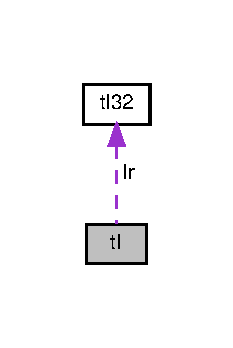
\includegraphics[width=112pt]{uniontl__coll__graph}
\end{center}
\end{figure}
\subsection*{Public Attributes}
\begin{DoxyCompactItemize}
\item 
\hyperlink{ticket__impl_8h_abc29cd63133a0a3693621f30cf152fe9}{tl32\+\_\+t} \hyperlink{uniontl_a017f0d0186356a56d809110a9e5b1f33}{lr} \mbox{[}2\mbox{]}
\item 
uint64\+\_\+t \hyperlink{uniontl_adaae4e5b4ea6b9df66e9d99074f7d5bc}{to\+\_\+uint64}
\end{DoxyCompactItemize}


\subsection{Member Data Documentation}
\mbox{\Hypertarget{uniontl_a017f0d0186356a56d809110a9e5b1f33}\label{uniontl_a017f0d0186356a56d809110a9e5b1f33}} 
\index{tl@{tl}!lr@{lr}}
\index{lr@{lr}!tl@{tl}}
\subsubsection{\texorpdfstring{lr}{lr}}
{\footnotesize\ttfamily \hyperlink{ticket__impl_8h_abc29cd63133a0a3693621f30cf152fe9}{tl32\+\_\+t} tl\+::lr\mbox{[}2\mbox{]}}

\mbox{\Hypertarget{uniontl_adaae4e5b4ea6b9df66e9d99074f7d5bc}\label{uniontl_adaae4e5b4ea6b9df66e9d99074f7d5bc}} 
\index{tl@{tl}!to\+\_\+uint64@{to\+\_\+uint64}}
\index{to\+\_\+uint64@{to\+\_\+uint64}!tl@{tl}}
\subsubsection{\texorpdfstring{to\+\_\+uint64}{to\_uint64}}
{\footnotesize\ttfamily uint64\+\_\+t tl\+::to\+\_\+uint64}



The documentation for this union was generated from the following file\+:\begin{DoxyCompactItemize}
\item 
ds/guerraoui\+\_\+ext\+\_\+bst\+\_\+ticket/\hyperlink{ticket__impl_8h}{ticket\+\_\+impl.\+h}\end{DoxyCompactItemize}

\hypertarget{uniontl32}{}\section{tl32 Union Reference}
\label{uniontl32}\index{tl32@{tl32}}


{\ttfamily \#include $<$ticket\+\_\+impl.\+h$>$}

\subsection*{Public Attributes}
\begin{DoxyCompactItemize}
\item 
\begin{tabbing}
xx\=xx\=xx\=xx\=xx\=xx\=xx\=xx\=xx\=\kill
struct \{\\
\>volatile uint16\_t \hyperlink{uniontl32_a6c0a2ef80fef6bb48ba2801afddf9630}{version}\\
\>volatile uint16\_t \hyperlink{uniontl32_a72f8bd411ad1a860c54f26f755981d17}{ticket}\\
\}; \\

\end{tabbing}\item 
volatile uint32\+\_\+t \hyperlink{uniontl32_a3a11491119d50ccf11a63bfe5b5e2754}{to\+\_\+uint32}
\end{DoxyCompactItemize}


\subsection{Member Data Documentation}
\mbox{\Hypertarget{uniontl32_a0f0b8de9afbd1ec9a4ae4584f209ac84}\label{uniontl32_a0f0b8de9afbd1ec9a4ae4584f209ac84}} 
\subsubsection{\texorpdfstring{"@80}{@80}}
{\footnotesize\ttfamily struct \{ ... \} }

\mbox{\Hypertarget{uniontl32_a72f8bd411ad1a860c54f26f755981d17}\label{uniontl32_a72f8bd411ad1a860c54f26f755981d17}} 
\index{tl32@{tl32}!ticket@{ticket}}
\index{ticket@{ticket}!tl32@{tl32}}
\subsubsection{\texorpdfstring{ticket}{ticket}}
{\footnotesize\ttfamily volatile uint16\+\_\+t tl32\+::ticket}

\mbox{\Hypertarget{uniontl32_a3a11491119d50ccf11a63bfe5b5e2754}\label{uniontl32_a3a11491119d50ccf11a63bfe5b5e2754}} 
\index{tl32@{tl32}!to\+\_\+uint32@{to\+\_\+uint32}}
\index{to\+\_\+uint32@{to\+\_\+uint32}!tl32@{tl32}}
\subsubsection{\texorpdfstring{to\+\_\+uint32}{to\_uint32}}
{\footnotesize\ttfamily volatile uint32\+\_\+t tl32\+::to\+\_\+uint32}

\mbox{\Hypertarget{uniontl32_a6c0a2ef80fef6bb48ba2801afddf9630}\label{uniontl32_a6c0a2ef80fef6bb48ba2801afddf9630}} 
\index{tl32@{tl32}!version@{version}}
\index{version@{version}!tl32@{tl32}}
\subsubsection{\texorpdfstring{version}{version}}
{\footnotesize\ttfamily volatile uint16\+\_\+t tl32\+::version}



The documentation for this union was generated from the following file\+:\begin{DoxyCompactItemize}
\item 
ds/guerraoui\+\_\+ext\+\_\+bst\+\_\+ticket/\hyperlink{ticket__impl_8h}{ticket\+\_\+impl.\+h}\end{DoxyCompactItemize}

\hypertarget{classtpcc__query}{}\section{tpcc\+\_\+query Class Reference}
\label{classtpcc__query}\index{tpcc\+\_\+query@{tpcc\+\_\+query}}


{\ttfamily \#include $<$tpcc\+\_\+query.\+h$>$}



Inheritance diagram for tpcc\+\_\+query\+:
\nopagebreak
\begin{figure}[H]
\begin{center}
\leavevmode
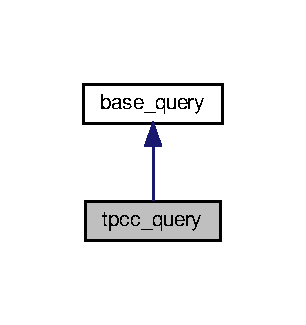
\includegraphics[width=147pt]{classtpcc__query__inherit__graph}
\end{center}
\end{figure}


Collaboration diagram for tpcc\+\_\+query\+:
\nopagebreak
\begin{figure}[H]
\begin{center}
\leavevmode
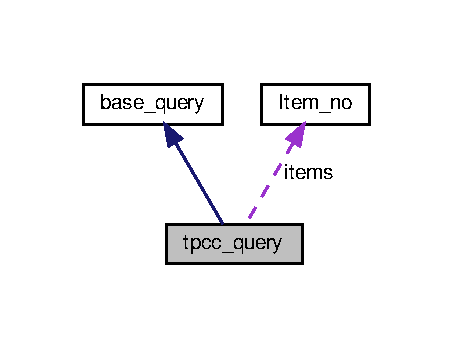
\includegraphics[width=218pt]{classtpcc__query__coll__graph}
\end{center}
\end{figure}
\subsection*{Public Member Functions}
\begin{DoxyCompactItemize}
\item 
void \hyperlink{classtpcc__query_a0bb03655040cf0f96ee0601c02c8876f}{init} (uint64\+\_\+t thd\+\_\+id, \hyperlink{classworkload}{workload} $\ast$h\+\_\+wl)
\item 
void \hyperlink{classtpcc__query_ae75736a30ca9792473454a4bae82b007}{setbench\+\_\+deinit} ()
\end{DoxyCompactItemize}
\subsection*{Public Attributes}
\begin{DoxyCompactItemize}
\item 
\hyperlink{config_8h_acfc6509f2c72fc43d7232487bc453a46}{T\+P\+C\+C\+Txn\+Type} \hyperlink{classtpcc__query_a5f12b36e59fbe8ec727e77e83ae19bd4}{type}
\item 
uint64\+\_\+t \hyperlink{classtpcc__query_aa0e97757f059338ccc7a278cae867e2d}{w\+\_\+id}
\item 
uint64\+\_\+t \hyperlink{classtpcc__query_a254d50cecab220d82a74a282abec3f3d}{d\+\_\+id}
\item 
uint64\+\_\+t \hyperlink{classtpcc__query_a3cb48fdc1b1faaff64dc8b5dc576f50a}{c\+\_\+id}
\item 
uint64\+\_\+t \hyperlink{classtpcc__query_af05185ea4640fbfc367f0846e1f145b4}{d\+\_\+w\+\_\+id}
\item 
uint64\+\_\+t \hyperlink{classtpcc__query_afabc5c9e1604caed59b8713c4b2a3b34}{c\+\_\+w\+\_\+id}
\item 
uint64\+\_\+t \hyperlink{classtpcc__query_af26e6d81660517546818abd296387cd7}{c\+\_\+d\+\_\+id}
\item 
char \hyperlink{classtpcc__query_af6b70107d2c362c471d980771bbdef27}{c\+\_\+last} \mbox{[}\hyperlink{config_8h_a90a3f68e410c7182d5c26db1c17c2eab}{L\+A\+S\+T\+N\+A\+M\+E\+\_\+\+L\+EN}\mbox{]}
\item 
double \hyperlink{classtpcc__query_a5d7a89975143b15fc470d062caca5678}{h\+\_\+amount}
\item 
bool \hyperlink{classtpcc__query_a77bad57f4a3e32c56005d9217bc165fc}{by\+\_\+last\+\_\+name}
\item 
\hyperlink{structItem__no}{Item\+\_\+no} $\ast$ \hyperlink{classtpcc__query_a74760639405ccface91b0152ef8ee9ed}{items}
\item 
bool \hyperlink{classtpcc__query_a5470a0ad8319e3ddc23cc2af0f8e2b89}{rbk}
\item 
bool \hyperlink{classtpcc__query_a607efc09bb9d8423e09b1cc6c800c430}{remote}
\item 
uint64\+\_\+t \hyperlink{classtpcc__query_af6681ad2750c95c18910a366f9916a8a}{ol\+\_\+cnt}
\item 
uint64\+\_\+t \hyperlink{classtpcc__query_a009003100b68f326f524599d2ed4b57a}{o\+\_\+entry\+\_\+d}
\item 
uint64\+\_\+t \hyperlink{classtpcc__query_ae63ae62b041515410fa64024f200da66}{o\+\_\+carrier\+\_\+id}
\item 
uint64\+\_\+t \hyperlink{classtpcc__query_ab503c6d1ac454b13c2e7a643359b982d}{ol\+\_\+delivery\+\_\+d}
\end{DoxyCompactItemize}


\subsection{Member Function Documentation}
\mbox{\Hypertarget{classtpcc__query_a0bb03655040cf0f96ee0601c02c8876f}\label{classtpcc__query_a0bb03655040cf0f96ee0601c02c8876f}} 
\index{tpcc\+\_\+query@{tpcc\+\_\+query}!init@{init}}
\index{init@{init}!tpcc\+\_\+query@{tpcc\+\_\+query}}
\subsubsection{\texorpdfstring{init()}{init()}}
{\footnotesize\ttfamily void tpcc\+\_\+query\+::init (\begin{DoxyParamCaption}\item[{uint64\+\_\+t}]{thd\+\_\+id,  }\item[{\hyperlink{classworkload}{workload} $\ast$}]{h\+\_\+wl }\end{DoxyParamCaption})\hspace{0.3cm}{\ttfamily [virtual]}}



Implements \hyperlink{classbase__query_a341a99285c6e849eae1c5a83485335f3}{base\+\_\+query}.

\mbox{\Hypertarget{classtpcc__query_ae75736a30ca9792473454a4bae82b007}\label{classtpcc__query_ae75736a30ca9792473454a4bae82b007}} 
\index{tpcc\+\_\+query@{tpcc\+\_\+query}!setbench\+\_\+deinit@{setbench\+\_\+deinit}}
\index{setbench\+\_\+deinit@{setbench\+\_\+deinit}!tpcc\+\_\+query@{tpcc\+\_\+query}}
\subsubsection{\texorpdfstring{setbench\+\_\+deinit()}{setbench\_deinit()}}
{\footnotesize\ttfamily void tpcc\+\_\+query\+::setbench\+\_\+deinit (\begin{DoxyParamCaption}{ }\end{DoxyParamCaption})}



\subsection{Member Data Documentation}
\mbox{\Hypertarget{classtpcc__query_a77bad57f4a3e32c56005d9217bc165fc}\label{classtpcc__query_a77bad57f4a3e32c56005d9217bc165fc}} 
\index{tpcc\+\_\+query@{tpcc\+\_\+query}!by\+\_\+last\+\_\+name@{by\+\_\+last\+\_\+name}}
\index{by\+\_\+last\+\_\+name@{by\+\_\+last\+\_\+name}!tpcc\+\_\+query@{tpcc\+\_\+query}}
\subsubsection{\texorpdfstring{by\+\_\+last\+\_\+name}{by\_last\_name}}
{\footnotesize\ttfamily bool tpcc\+\_\+query\+::by\+\_\+last\+\_\+name}

\mbox{\Hypertarget{classtpcc__query_af26e6d81660517546818abd296387cd7}\label{classtpcc__query_af26e6d81660517546818abd296387cd7}} 
\index{tpcc\+\_\+query@{tpcc\+\_\+query}!c\+\_\+d\+\_\+id@{c\+\_\+d\+\_\+id}}
\index{c\+\_\+d\+\_\+id@{c\+\_\+d\+\_\+id}!tpcc\+\_\+query@{tpcc\+\_\+query}}
\subsubsection{\texorpdfstring{c\+\_\+d\+\_\+id}{c\_d\_id}}
{\footnotesize\ttfamily uint64\+\_\+t tpcc\+\_\+query\+::c\+\_\+d\+\_\+id}

\mbox{\Hypertarget{classtpcc__query_a3cb48fdc1b1faaff64dc8b5dc576f50a}\label{classtpcc__query_a3cb48fdc1b1faaff64dc8b5dc576f50a}} 
\index{tpcc\+\_\+query@{tpcc\+\_\+query}!c\+\_\+id@{c\+\_\+id}}
\index{c\+\_\+id@{c\+\_\+id}!tpcc\+\_\+query@{tpcc\+\_\+query}}
\subsubsection{\texorpdfstring{c\+\_\+id}{c\_id}}
{\footnotesize\ttfamily uint64\+\_\+t tpcc\+\_\+query\+::c\+\_\+id}

\mbox{\Hypertarget{classtpcc__query_af6b70107d2c362c471d980771bbdef27}\label{classtpcc__query_af6b70107d2c362c471d980771bbdef27}} 
\index{tpcc\+\_\+query@{tpcc\+\_\+query}!c\+\_\+last@{c\+\_\+last}}
\index{c\+\_\+last@{c\+\_\+last}!tpcc\+\_\+query@{tpcc\+\_\+query}}
\subsubsection{\texorpdfstring{c\+\_\+last}{c\_last}}
{\footnotesize\ttfamily char tpcc\+\_\+query\+::c\+\_\+last\mbox{[}\hyperlink{config_8h_a90a3f68e410c7182d5c26db1c17c2eab}{L\+A\+S\+T\+N\+A\+M\+E\+\_\+\+L\+EN}\mbox{]}}

\mbox{\Hypertarget{classtpcc__query_afabc5c9e1604caed59b8713c4b2a3b34}\label{classtpcc__query_afabc5c9e1604caed59b8713c4b2a3b34}} 
\index{tpcc\+\_\+query@{tpcc\+\_\+query}!c\+\_\+w\+\_\+id@{c\+\_\+w\+\_\+id}}
\index{c\+\_\+w\+\_\+id@{c\+\_\+w\+\_\+id}!tpcc\+\_\+query@{tpcc\+\_\+query}}
\subsubsection{\texorpdfstring{c\+\_\+w\+\_\+id}{c\_w\_id}}
{\footnotesize\ttfamily uint64\+\_\+t tpcc\+\_\+query\+::c\+\_\+w\+\_\+id}

\mbox{\Hypertarget{classtpcc__query_a254d50cecab220d82a74a282abec3f3d}\label{classtpcc__query_a254d50cecab220d82a74a282abec3f3d}} 
\index{tpcc\+\_\+query@{tpcc\+\_\+query}!d\+\_\+id@{d\+\_\+id}}
\index{d\+\_\+id@{d\+\_\+id}!tpcc\+\_\+query@{tpcc\+\_\+query}}
\subsubsection{\texorpdfstring{d\+\_\+id}{d\_id}}
{\footnotesize\ttfamily uint64\+\_\+t tpcc\+\_\+query\+::d\+\_\+id}

\mbox{\Hypertarget{classtpcc__query_af05185ea4640fbfc367f0846e1f145b4}\label{classtpcc__query_af05185ea4640fbfc367f0846e1f145b4}} 
\index{tpcc\+\_\+query@{tpcc\+\_\+query}!d\+\_\+w\+\_\+id@{d\+\_\+w\+\_\+id}}
\index{d\+\_\+w\+\_\+id@{d\+\_\+w\+\_\+id}!tpcc\+\_\+query@{tpcc\+\_\+query}}
\subsubsection{\texorpdfstring{d\+\_\+w\+\_\+id}{d\_w\_id}}
{\footnotesize\ttfamily uint64\+\_\+t tpcc\+\_\+query\+::d\+\_\+w\+\_\+id}

\mbox{\Hypertarget{classtpcc__query_a5d7a89975143b15fc470d062caca5678}\label{classtpcc__query_a5d7a89975143b15fc470d062caca5678}} 
\index{tpcc\+\_\+query@{tpcc\+\_\+query}!h\+\_\+amount@{h\+\_\+amount}}
\index{h\+\_\+amount@{h\+\_\+amount}!tpcc\+\_\+query@{tpcc\+\_\+query}}
\subsubsection{\texorpdfstring{h\+\_\+amount}{h\_amount}}
{\footnotesize\ttfamily double tpcc\+\_\+query\+::h\+\_\+amount}

\mbox{\Hypertarget{classtpcc__query_a74760639405ccface91b0152ef8ee9ed}\label{classtpcc__query_a74760639405ccface91b0152ef8ee9ed}} 
\index{tpcc\+\_\+query@{tpcc\+\_\+query}!items@{items}}
\index{items@{items}!tpcc\+\_\+query@{tpcc\+\_\+query}}
\subsubsection{\texorpdfstring{items}{items}}
{\footnotesize\ttfamily \hyperlink{structItem__no}{Item\+\_\+no}$\ast$ tpcc\+\_\+query\+::items}

\mbox{\Hypertarget{classtpcc__query_ae63ae62b041515410fa64024f200da66}\label{classtpcc__query_ae63ae62b041515410fa64024f200da66}} 
\index{tpcc\+\_\+query@{tpcc\+\_\+query}!o\+\_\+carrier\+\_\+id@{o\+\_\+carrier\+\_\+id}}
\index{o\+\_\+carrier\+\_\+id@{o\+\_\+carrier\+\_\+id}!tpcc\+\_\+query@{tpcc\+\_\+query}}
\subsubsection{\texorpdfstring{o\+\_\+carrier\+\_\+id}{o\_carrier\_id}}
{\footnotesize\ttfamily uint64\+\_\+t tpcc\+\_\+query\+::o\+\_\+carrier\+\_\+id}

\mbox{\Hypertarget{classtpcc__query_a009003100b68f326f524599d2ed4b57a}\label{classtpcc__query_a009003100b68f326f524599d2ed4b57a}} 
\index{tpcc\+\_\+query@{tpcc\+\_\+query}!o\+\_\+entry\+\_\+d@{o\+\_\+entry\+\_\+d}}
\index{o\+\_\+entry\+\_\+d@{o\+\_\+entry\+\_\+d}!tpcc\+\_\+query@{tpcc\+\_\+query}}
\subsubsection{\texorpdfstring{o\+\_\+entry\+\_\+d}{o\_entry\_d}}
{\footnotesize\ttfamily uint64\+\_\+t tpcc\+\_\+query\+::o\+\_\+entry\+\_\+d}

\mbox{\Hypertarget{classtpcc__query_af6681ad2750c95c18910a366f9916a8a}\label{classtpcc__query_af6681ad2750c95c18910a366f9916a8a}} 
\index{tpcc\+\_\+query@{tpcc\+\_\+query}!ol\+\_\+cnt@{ol\+\_\+cnt}}
\index{ol\+\_\+cnt@{ol\+\_\+cnt}!tpcc\+\_\+query@{tpcc\+\_\+query}}
\subsubsection{\texorpdfstring{ol\+\_\+cnt}{ol\_cnt}}
{\footnotesize\ttfamily uint64\+\_\+t tpcc\+\_\+query\+::ol\+\_\+cnt}

\mbox{\Hypertarget{classtpcc__query_ab503c6d1ac454b13c2e7a643359b982d}\label{classtpcc__query_ab503c6d1ac454b13c2e7a643359b982d}} 
\index{tpcc\+\_\+query@{tpcc\+\_\+query}!ol\+\_\+delivery\+\_\+d@{ol\+\_\+delivery\+\_\+d}}
\index{ol\+\_\+delivery\+\_\+d@{ol\+\_\+delivery\+\_\+d}!tpcc\+\_\+query@{tpcc\+\_\+query}}
\subsubsection{\texorpdfstring{ol\+\_\+delivery\+\_\+d}{ol\_delivery\_d}}
{\footnotesize\ttfamily uint64\+\_\+t tpcc\+\_\+query\+::ol\+\_\+delivery\+\_\+d}

\mbox{\Hypertarget{classtpcc__query_a5470a0ad8319e3ddc23cc2af0f8e2b89}\label{classtpcc__query_a5470a0ad8319e3ddc23cc2af0f8e2b89}} 
\index{tpcc\+\_\+query@{tpcc\+\_\+query}!rbk@{rbk}}
\index{rbk@{rbk}!tpcc\+\_\+query@{tpcc\+\_\+query}}
\subsubsection{\texorpdfstring{rbk}{rbk}}
{\footnotesize\ttfamily bool tpcc\+\_\+query\+::rbk}

\mbox{\Hypertarget{classtpcc__query_a607efc09bb9d8423e09b1cc6c800c430}\label{classtpcc__query_a607efc09bb9d8423e09b1cc6c800c430}} 
\index{tpcc\+\_\+query@{tpcc\+\_\+query}!remote@{remote}}
\index{remote@{remote}!tpcc\+\_\+query@{tpcc\+\_\+query}}
\subsubsection{\texorpdfstring{remote}{remote}}
{\footnotesize\ttfamily bool tpcc\+\_\+query\+::remote}

\mbox{\Hypertarget{classtpcc__query_a5f12b36e59fbe8ec727e77e83ae19bd4}\label{classtpcc__query_a5f12b36e59fbe8ec727e77e83ae19bd4}} 
\index{tpcc\+\_\+query@{tpcc\+\_\+query}!type@{type}}
\index{type@{type}!tpcc\+\_\+query@{tpcc\+\_\+query}}
\subsubsection{\texorpdfstring{type}{type}}
{\footnotesize\ttfamily \hyperlink{config_8h_acfc6509f2c72fc43d7232487bc453a46}{T\+P\+C\+C\+Txn\+Type} tpcc\+\_\+query\+::type}

\mbox{\Hypertarget{classtpcc__query_aa0e97757f059338ccc7a278cae867e2d}\label{classtpcc__query_aa0e97757f059338ccc7a278cae867e2d}} 
\index{tpcc\+\_\+query@{tpcc\+\_\+query}!w\+\_\+id@{w\+\_\+id}}
\index{w\+\_\+id@{w\+\_\+id}!tpcc\+\_\+query@{tpcc\+\_\+query}}
\subsubsection{\texorpdfstring{w\+\_\+id}{w\_id}}
{\footnotesize\ttfamily uint64\+\_\+t tpcc\+\_\+query\+::w\+\_\+id}



The documentation for this class was generated from the following files\+:\begin{DoxyCompactItemize}
\item 
macrobench/benchmarks/\hyperlink{tpcc__query_8h}{tpcc\+\_\+query.\+h}\item 
macrobench/benchmarks/\hyperlink{tpcc__query_8cpp}{tpcc\+\_\+query.\+cpp}\end{DoxyCompactItemize}

\hypertarget{classtpcc__txn__man}{}\section{tpcc\+\_\+txn\+\_\+man Class Reference}
\label{classtpcc__txn__man}\index{tpcc\+\_\+txn\+\_\+man@{tpcc\+\_\+txn\+\_\+man}}


{\ttfamily \#include $<$tpcc.\+h$>$}



Inheritance diagram for tpcc\+\_\+txn\+\_\+man\+:
\nopagebreak
\begin{figure}[H]
\begin{center}
\leavevmode
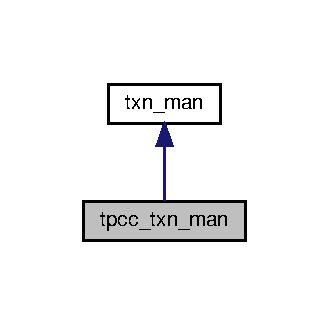
\includegraphics[width=158pt]{classtpcc__txn__man__inherit__graph}
\end{center}
\end{figure}


Collaboration diagram for tpcc\+\_\+txn\+\_\+man\+:
\nopagebreak
\begin{figure}[H]
\begin{center}
\leavevmode
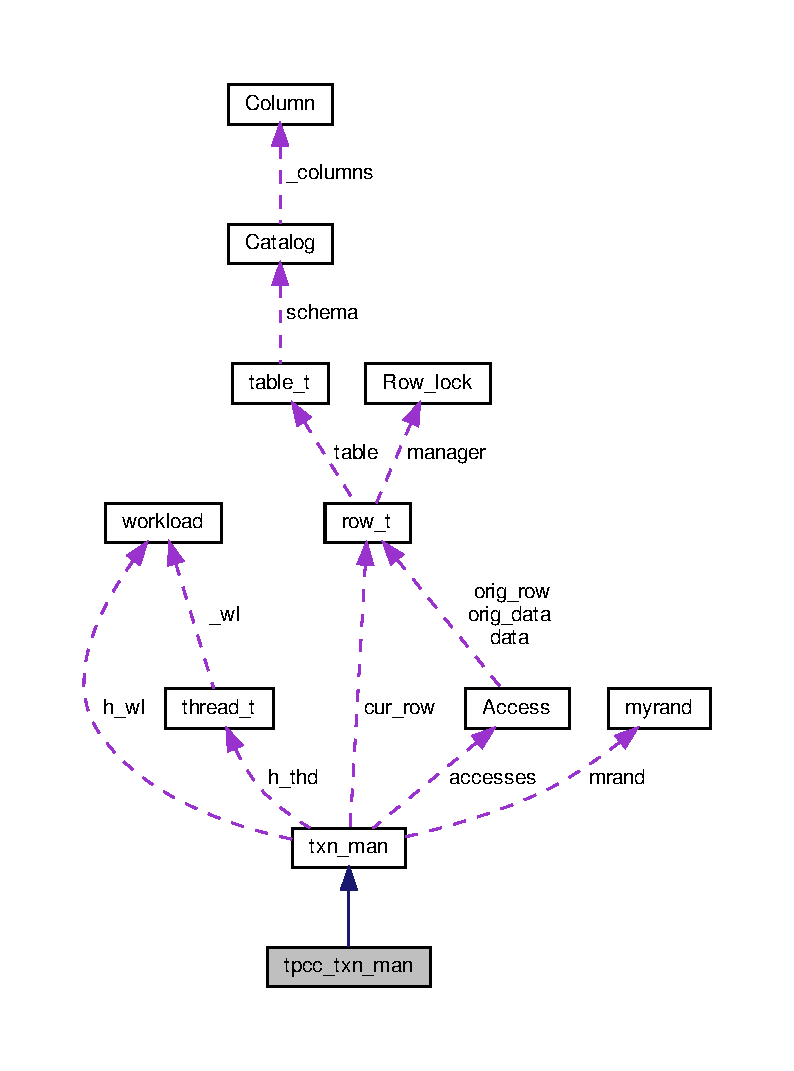
\includegraphics[width=350pt]{classtpcc__txn__man__coll__graph}
\end{center}
\end{figure}
\subsection*{Public Member Functions}
\begin{DoxyCompactItemize}
\item 
void \hyperlink{classtpcc__txn__man_aa2a56c4cb192d138852488745ee09fd7}{init} (\hyperlink{classthread__t}{thread\+\_\+t} $\ast$\hyperlink{classtxn__man_a64bf2cba8ef2686ad528a96d18e8358d}{h\+\_\+thd}, \hyperlink{classworkload}{workload} $\ast$\hyperlink{classtxn__man_a988eb76c69a304049c02d3ceff526a5e}{h\+\_\+wl}, uint64\+\_\+t part\+\_\+id)
\item 
\hyperlink{global_8h_a78c49a674c810fdd03d20432f7be864a}{RC} \hyperlink{classtpcc__txn__man_a19f99ffaf91e1f977fe517d617493a8a}{run\+\_\+txn} (\hyperlink{classbase__query}{base\+\_\+query} $\ast$query)
\end{DoxyCompactItemize}
\subsection*{Additional Inherited Members}


\subsection{Member Function Documentation}
\mbox{\Hypertarget{classtpcc__txn__man_aa2a56c4cb192d138852488745ee09fd7}\label{classtpcc__txn__man_aa2a56c4cb192d138852488745ee09fd7}} 
\index{tpcc\+\_\+txn\+\_\+man@{tpcc\+\_\+txn\+\_\+man}!init@{init}}
\index{init@{init}!tpcc\+\_\+txn\+\_\+man@{tpcc\+\_\+txn\+\_\+man}}
\subsubsection{\texorpdfstring{init()}{init()}}
{\footnotesize\ttfamily void tpcc\+\_\+txn\+\_\+man\+::init (\begin{DoxyParamCaption}\item[{\hyperlink{classthread__t}{thread\+\_\+t} $\ast$}]{h\+\_\+thd,  }\item[{\hyperlink{classworkload}{workload} $\ast$}]{h\+\_\+wl,  }\item[{uint64\+\_\+t}]{part\+\_\+id }\end{DoxyParamCaption})\hspace{0.3cm}{\ttfamily [virtual]}}



Reimplemented from \hyperlink{classtxn__man_a778925bb3edd6a54a27161f67792edec}{txn\+\_\+man}.

\mbox{\Hypertarget{classtpcc__txn__man_a19f99ffaf91e1f977fe517d617493a8a}\label{classtpcc__txn__man_a19f99ffaf91e1f977fe517d617493a8a}} 
\index{tpcc\+\_\+txn\+\_\+man@{tpcc\+\_\+txn\+\_\+man}!run\+\_\+txn@{run\+\_\+txn}}
\index{run\+\_\+txn@{run\+\_\+txn}!tpcc\+\_\+txn\+\_\+man@{tpcc\+\_\+txn\+\_\+man}}
\subsubsection{\texorpdfstring{run\+\_\+txn()}{run\_txn()}}
{\footnotesize\ttfamily \hyperlink{global_8h_a78c49a674c810fdd03d20432f7be864a}{RC} tpcc\+\_\+txn\+\_\+man\+::run\+\_\+txn (\begin{DoxyParamCaption}\item[{\hyperlink{classbase__query}{base\+\_\+query} $\ast$}]{query }\end{DoxyParamCaption})\hspace{0.3cm}{\ttfamily [virtual]}}



Implements \hyperlink{classtxn__man_a71142ded36a4be5629ea75d486a105ae}{txn\+\_\+man}.



The documentation for this class was generated from the following files\+:\begin{DoxyCompactItemize}
\item 
macrobench/benchmarks/\hyperlink{tpcc_8h}{tpcc.\+h}\item 
macrobench/benchmarks/\hyperlink{tpcc__txn_8cpp}{tpcc\+\_\+txn.\+cpp}\end{DoxyCompactItemize}

\hypertarget{classtpcc__wl}{}\section{tpcc\+\_\+wl Class Reference}
\label{classtpcc__wl}\index{tpcc\+\_\+wl@{tpcc\+\_\+wl}}


{\ttfamily \#include $<$tpcc.\+h$>$}



Inheritance diagram for tpcc\+\_\+wl\+:
\nopagebreak
\begin{figure}[H]
\begin{center}
\leavevmode
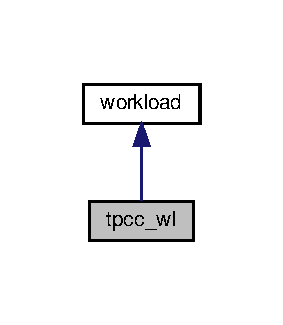
\includegraphics[width=136pt]{classtpcc__wl__inherit__graph}
\end{center}
\end{figure}


Collaboration diagram for tpcc\+\_\+wl\+:
\nopagebreak
\begin{figure}[H]
\begin{center}
\leavevmode
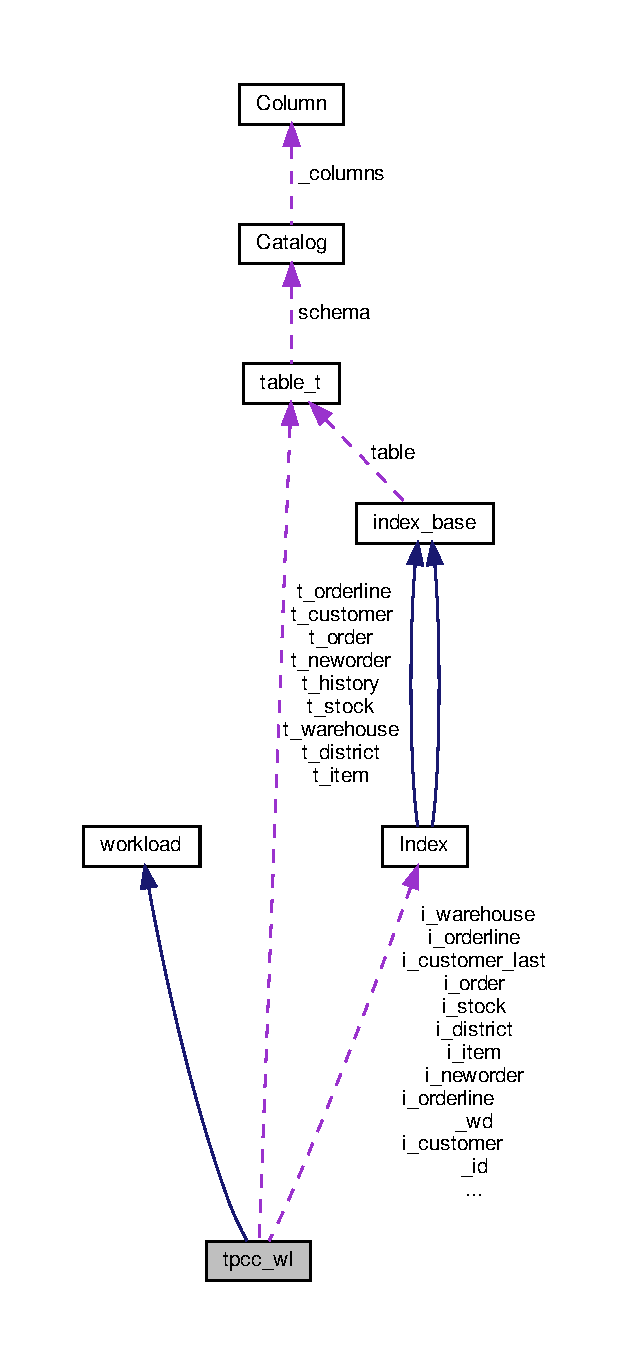
\includegraphics[height=550pt]{classtpcc__wl__coll__graph}
\end{center}
\end{figure}
\subsection*{Public Member Functions}
\begin{DoxyCompactItemize}
\item 
\hyperlink{global_8h_a78c49a674c810fdd03d20432f7be864a}{RC} \hyperlink{classtpcc__wl_a084aa9016fbc3abbb278f1c4bd15722c}{init} ()
\item 
void \hyperlink{classtpcc__wl_ac89b938cbaf311844d79f3946df49005}{setbench\+\_\+deinit} ()
\item 
\hyperlink{global_8h_a78c49a674c810fdd03d20432f7be864a}{RC} \hyperlink{classtpcc__wl_a84fd48d9c4ee95eb6176e9fdf9efd8b7}{init\+\_\+table} ()
\item 
\hyperlink{global_8h_a78c49a674c810fdd03d20432f7be864a}{RC} \hyperlink{classtpcc__wl_a79f6252410dd09efa03c40d7a362d4e1}{init\+\_\+schema} (const char $\ast$schema\+\_\+file)
\item 
\hyperlink{global_8h_a78c49a674c810fdd03d20432f7be864a}{RC} \hyperlink{classtpcc__wl_a7794924fd334984a429b43e151ad040a}{get\+\_\+txn\+\_\+man} (\hyperlink{classtxn__man}{txn\+\_\+man} $\ast$\&txn\+\_\+manager, \hyperlink{classthread__t}{thread\+\_\+t} $\ast$h\+\_\+thd)
\end{DoxyCompactItemize}
\subsection*{Public Attributes}
\begin{DoxyCompactItemize}
\item 
\hyperlink{classtable__t}{table\+\_\+t} $\ast$ \hyperlink{classtpcc__wl_a7f1b94e2593ed24fca5a17f333b791d2}{t\+\_\+warehouse}
\item 
\hyperlink{classtable__t}{table\+\_\+t} $\ast$ \hyperlink{classtpcc__wl_ab6ffc1626573b440aded5f486d98efe0}{t\+\_\+district}
\item 
\hyperlink{classtable__t}{table\+\_\+t} $\ast$ \hyperlink{classtpcc__wl_af681ca32f116c918125ff8dba2b691c2}{t\+\_\+customer}
\item 
\hyperlink{classtable__t}{table\+\_\+t} $\ast$ \hyperlink{classtpcc__wl_a6aa6043e365676fda7c73dbd4375ae8e}{t\+\_\+history}
\item 
\hyperlink{classtable__t}{table\+\_\+t} $\ast$ \hyperlink{classtpcc__wl_a7d19533ceca41d61f53be7583754728d}{t\+\_\+neworder}
\item 
\hyperlink{classtable__t}{table\+\_\+t} $\ast$ \hyperlink{classtpcc__wl_a7fc94bd27a10a35596de54535f5890b5}{t\+\_\+order}
\item 
\hyperlink{classtable__t}{table\+\_\+t} $\ast$ \hyperlink{classtpcc__wl_a6997edcda46944d16c8e737c219ec1f5}{t\+\_\+orderline}
\item 
\hyperlink{classtable__t}{table\+\_\+t} $\ast$ \hyperlink{classtpcc__wl_a3d3103f3a058fd807f694f89a66cdeaa}{t\+\_\+item}
\item 
\hyperlink{classtable__t}{table\+\_\+t} $\ast$ \hyperlink{classtpcc__wl_ac91d9c6ee29b3ae4b83f158feb3578de}{t\+\_\+stock}
\item 
\hyperlink{classIndex}{Index} $\ast$ \hyperlink{classtpcc__wl_acf94d40002b08d6924220c33ac68fcc3}{i\+\_\+neworder}
\item 
\hyperlink{classIndex}{Index} $\ast$ \hyperlink{classtpcc__wl_a86a912b9ef6717eaea8e41a38061c8af}{i\+\_\+item}
\item 
\hyperlink{classIndex}{Index} $\ast$ \hyperlink{classtpcc__wl_a45c383109926ea008ca82c452ca22ad4}{i\+\_\+warehouse}
\item 
\hyperlink{classIndex}{Index} $\ast$ \hyperlink{classtpcc__wl_a87bf44cbe0c6bee28ca7d1d414a7a99f}{i\+\_\+district}
\item 
\hyperlink{classIndex}{Index} $\ast$ \hyperlink{classtpcc__wl_a2ce0867b3a24e9f57e06a2733c7829ab}{i\+\_\+customer\+\_\+id}
\item 
\hyperlink{classIndex}{Index} $\ast$ \hyperlink{classtpcc__wl_aa6cc66486a485184ffffbc89b8583b19}{i\+\_\+customer\+\_\+last}
\item 
\hyperlink{classIndex}{Index} $\ast$ \hyperlink{classtpcc__wl_a8927cb7293d11150e2717d9c0782b9a1}{i\+\_\+stock}
\item 
\hyperlink{classIndex}{Index} $\ast$ \hyperlink{classtpcc__wl_ae778282544ed75f8b85b3d7a4edf0dfc}{i\+\_\+order}
\item 
\hyperlink{classIndex}{Index} $\ast$ \hyperlink{classtpcc__wl_afc13c1efcceb358d84970ebdf43ad0ce}{i\+\_\+orderline}
\item 
\hyperlink{classIndex}{Index} $\ast$ \hyperlink{classtpcc__wl_a2b55a2cda169c0213e572cd23a258c04}{i\+\_\+orderline\+\_\+wd}
\item 
bool $\ast$$\ast$ \hyperlink{classtpcc__wl_aed8e979c419bcd6c656f10ba744da75b}{delivering}
\item 
uint32\+\_\+t \hyperlink{classtpcc__wl_a01db97a665638486d45e3cdc7462dc6d}{next\+\_\+tid}
\end{DoxyCompactItemize}
\subsection*{Additional Inherited Members}


\subsection{Member Function Documentation}
\mbox{\Hypertarget{classtpcc__wl_a7794924fd334984a429b43e151ad040a}\label{classtpcc__wl_a7794924fd334984a429b43e151ad040a}} 
\index{tpcc\+\_\+wl@{tpcc\+\_\+wl}!get\+\_\+txn\+\_\+man@{get\+\_\+txn\+\_\+man}}
\index{get\+\_\+txn\+\_\+man@{get\+\_\+txn\+\_\+man}!tpcc\+\_\+wl@{tpcc\+\_\+wl}}
\subsubsection{\texorpdfstring{get\+\_\+txn\+\_\+man()}{get\_txn\_man()}}
{\footnotesize\ttfamily \hyperlink{global_8h_a78c49a674c810fdd03d20432f7be864a}{RC} tpcc\+\_\+wl\+::get\+\_\+txn\+\_\+man (\begin{DoxyParamCaption}\item[{\hyperlink{classtxn__man}{txn\+\_\+man} $\ast$\&}]{txn\+\_\+manager,  }\item[{\hyperlink{classthread__t}{thread\+\_\+t} $\ast$}]{h\+\_\+thd }\end{DoxyParamCaption})\hspace{0.3cm}{\ttfamily [virtual]}}



Implements \hyperlink{classworkload_ac22d0558c3fc549b8b07347cebb95cb3}{workload}.

\mbox{\Hypertarget{classtpcc__wl_a084aa9016fbc3abbb278f1c4bd15722c}\label{classtpcc__wl_a084aa9016fbc3abbb278f1c4bd15722c}} 
\index{tpcc\+\_\+wl@{tpcc\+\_\+wl}!init@{init}}
\index{init@{init}!tpcc\+\_\+wl@{tpcc\+\_\+wl}}
\subsubsection{\texorpdfstring{init()}{init()}}
{\footnotesize\ttfamily \hyperlink{global_8h_a78c49a674c810fdd03d20432f7be864a}{RC} tpcc\+\_\+wl\+::init (\begin{DoxyParamCaption}{ }\end{DoxyParamCaption})\hspace{0.3cm}{\ttfamily [virtual]}}



Reimplemented from \hyperlink{classworkload_a7cef7a7101c78e10082c99356e77a57c}{workload}.

\mbox{\Hypertarget{classtpcc__wl_a79f6252410dd09efa03c40d7a362d4e1}\label{classtpcc__wl_a79f6252410dd09efa03c40d7a362d4e1}} 
\index{tpcc\+\_\+wl@{tpcc\+\_\+wl}!init\+\_\+schema@{init\+\_\+schema}}
\index{init\+\_\+schema@{init\+\_\+schema}!tpcc\+\_\+wl@{tpcc\+\_\+wl}}
\subsubsection{\texorpdfstring{init\+\_\+schema()}{init\_schema()}}
{\footnotesize\ttfamily \hyperlink{global_8h_a78c49a674c810fdd03d20432f7be864a}{RC} tpcc\+\_\+wl\+::init\+\_\+schema (\begin{DoxyParamCaption}\item[{const char $\ast$}]{schema\+\_\+file }\end{DoxyParamCaption})}

\mbox{\Hypertarget{classtpcc__wl_a84fd48d9c4ee95eb6176e9fdf9efd8b7}\label{classtpcc__wl_a84fd48d9c4ee95eb6176e9fdf9efd8b7}} 
\index{tpcc\+\_\+wl@{tpcc\+\_\+wl}!init\+\_\+table@{init\+\_\+table}}
\index{init\+\_\+table@{init\+\_\+table}!tpcc\+\_\+wl@{tpcc\+\_\+wl}}
\subsubsection{\texorpdfstring{init\+\_\+table()}{init\_table()}}
{\footnotesize\ttfamily \hyperlink{global_8h_a78c49a674c810fdd03d20432f7be864a}{RC} tpcc\+\_\+wl\+::init\+\_\+table (\begin{DoxyParamCaption}{ }\end{DoxyParamCaption})\hspace{0.3cm}{\ttfamily [virtual]}}



Implements \hyperlink{classworkload_a3feee79af04069f6c1ad6b7f9b0a045a}{workload}.

\mbox{\Hypertarget{classtpcc__wl_ac89b938cbaf311844d79f3946df49005}\label{classtpcc__wl_ac89b938cbaf311844d79f3946df49005}} 
\index{tpcc\+\_\+wl@{tpcc\+\_\+wl}!setbench\+\_\+deinit@{setbench\+\_\+deinit}}
\index{setbench\+\_\+deinit@{setbench\+\_\+deinit}!tpcc\+\_\+wl@{tpcc\+\_\+wl}}
\subsubsection{\texorpdfstring{setbench\+\_\+deinit()}{setbench\_deinit()}}
{\footnotesize\ttfamily void tpcc\+\_\+wl\+::setbench\+\_\+deinit (\begin{DoxyParamCaption}{ }\end{DoxyParamCaption})\hspace{0.3cm}{\ttfamily [virtual]}}



Reimplemented from \hyperlink{classworkload_a4614189e85fbaaf2003b7db4c2a7b8b9}{workload}.



\subsection{Member Data Documentation}
\mbox{\Hypertarget{classtpcc__wl_aed8e979c419bcd6c656f10ba744da75b}\label{classtpcc__wl_aed8e979c419bcd6c656f10ba744da75b}} 
\index{tpcc\+\_\+wl@{tpcc\+\_\+wl}!delivering@{delivering}}
\index{delivering@{delivering}!tpcc\+\_\+wl@{tpcc\+\_\+wl}}
\subsubsection{\texorpdfstring{delivering}{delivering}}
{\footnotesize\ttfamily bool$\ast$$\ast$ tpcc\+\_\+wl\+::delivering}

\mbox{\Hypertarget{classtpcc__wl_a2ce0867b3a24e9f57e06a2733c7829ab}\label{classtpcc__wl_a2ce0867b3a24e9f57e06a2733c7829ab}} 
\index{tpcc\+\_\+wl@{tpcc\+\_\+wl}!i\+\_\+customer\+\_\+id@{i\+\_\+customer\+\_\+id}}
\index{i\+\_\+customer\+\_\+id@{i\+\_\+customer\+\_\+id}!tpcc\+\_\+wl@{tpcc\+\_\+wl}}
\subsubsection{\texorpdfstring{i\+\_\+customer\+\_\+id}{i\_customer\_id}}
{\footnotesize\ttfamily \hyperlink{classIndex}{Index}$\ast$ tpcc\+\_\+wl\+::i\+\_\+customer\+\_\+id}

\mbox{\Hypertarget{classtpcc__wl_aa6cc66486a485184ffffbc89b8583b19}\label{classtpcc__wl_aa6cc66486a485184ffffbc89b8583b19}} 
\index{tpcc\+\_\+wl@{tpcc\+\_\+wl}!i\+\_\+customer\+\_\+last@{i\+\_\+customer\+\_\+last}}
\index{i\+\_\+customer\+\_\+last@{i\+\_\+customer\+\_\+last}!tpcc\+\_\+wl@{tpcc\+\_\+wl}}
\subsubsection{\texorpdfstring{i\+\_\+customer\+\_\+last}{i\_customer\_last}}
{\footnotesize\ttfamily \hyperlink{classIndex}{Index}$\ast$ tpcc\+\_\+wl\+::i\+\_\+customer\+\_\+last}

\mbox{\Hypertarget{classtpcc__wl_a87bf44cbe0c6bee28ca7d1d414a7a99f}\label{classtpcc__wl_a87bf44cbe0c6bee28ca7d1d414a7a99f}} 
\index{tpcc\+\_\+wl@{tpcc\+\_\+wl}!i\+\_\+district@{i\+\_\+district}}
\index{i\+\_\+district@{i\+\_\+district}!tpcc\+\_\+wl@{tpcc\+\_\+wl}}
\subsubsection{\texorpdfstring{i\+\_\+district}{i\_district}}
{\footnotesize\ttfamily \hyperlink{classIndex}{Index}$\ast$ tpcc\+\_\+wl\+::i\+\_\+district}

\mbox{\Hypertarget{classtpcc__wl_a86a912b9ef6717eaea8e41a38061c8af}\label{classtpcc__wl_a86a912b9ef6717eaea8e41a38061c8af}} 
\index{tpcc\+\_\+wl@{tpcc\+\_\+wl}!i\+\_\+item@{i\+\_\+item}}
\index{i\+\_\+item@{i\+\_\+item}!tpcc\+\_\+wl@{tpcc\+\_\+wl}}
\subsubsection{\texorpdfstring{i\+\_\+item}{i\_item}}
{\footnotesize\ttfamily \hyperlink{classIndex}{Index}$\ast$ tpcc\+\_\+wl\+::i\+\_\+item}

\mbox{\Hypertarget{classtpcc__wl_acf94d40002b08d6924220c33ac68fcc3}\label{classtpcc__wl_acf94d40002b08d6924220c33ac68fcc3}} 
\index{tpcc\+\_\+wl@{tpcc\+\_\+wl}!i\+\_\+neworder@{i\+\_\+neworder}}
\index{i\+\_\+neworder@{i\+\_\+neworder}!tpcc\+\_\+wl@{tpcc\+\_\+wl}}
\subsubsection{\texorpdfstring{i\+\_\+neworder}{i\_neworder}}
{\footnotesize\ttfamily \hyperlink{classIndex}{Index}$\ast$ tpcc\+\_\+wl\+::i\+\_\+neworder}

\mbox{\Hypertarget{classtpcc__wl_ae778282544ed75f8b85b3d7a4edf0dfc}\label{classtpcc__wl_ae778282544ed75f8b85b3d7a4edf0dfc}} 
\index{tpcc\+\_\+wl@{tpcc\+\_\+wl}!i\+\_\+order@{i\+\_\+order}}
\index{i\+\_\+order@{i\+\_\+order}!tpcc\+\_\+wl@{tpcc\+\_\+wl}}
\subsubsection{\texorpdfstring{i\+\_\+order}{i\_order}}
{\footnotesize\ttfamily \hyperlink{classIndex}{Index}$\ast$ tpcc\+\_\+wl\+::i\+\_\+order}

\mbox{\Hypertarget{classtpcc__wl_afc13c1efcceb358d84970ebdf43ad0ce}\label{classtpcc__wl_afc13c1efcceb358d84970ebdf43ad0ce}} 
\index{tpcc\+\_\+wl@{tpcc\+\_\+wl}!i\+\_\+orderline@{i\+\_\+orderline}}
\index{i\+\_\+orderline@{i\+\_\+orderline}!tpcc\+\_\+wl@{tpcc\+\_\+wl}}
\subsubsection{\texorpdfstring{i\+\_\+orderline}{i\_orderline}}
{\footnotesize\ttfamily \hyperlink{classIndex}{Index}$\ast$ tpcc\+\_\+wl\+::i\+\_\+orderline}

\mbox{\Hypertarget{classtpcc__wl_a2b55a2cda169c0213e572cd23a258c04}\label{classtpcc__wl_a2b55a2cda169c0213e572cd23a258c04}} 
\index{tpcc\+\_\+wl@{tpcc\+\_\+wl}!i\+\_\+orderline\+\_\+wd@{i\+\_\+orderline\+\_\+wd}}
\index{i\+\_\+orderline\+\_\+wd@{i\+\_\+orderline\+\_\+wd}!tpcc\+\_\+wl@{tpcc\+\_\+wl}}
\subsubsection{\texorpdfstring{i\+\_\+orderline\+\_\+wd}{i\_orderline\_wd}}
{\footnotesize\ttfamily \hyperlink{classIndex}{Index}$\ast$ tpcc\+\_\+wl\+::i\+\_\+orderline\+\_\+wd}

\mbox{\Hypertarget{classtpcc__wl_a8927cb7293d11150e2717d9c0782b9a1}\label{classtpcc__wl_a8927cb7293d11150e2717d9c0782b9a1}} 
\index{tpcc\+\_\+wl@{tpcc\+\_\+wl}!i\+\_\+stock@{i\+\_\+stock}}
\index{i\+\_\+stock@{i\+\_\+stock}!tpcc\+\_\+wl@{tpcc\+\_\+wl}}
\subsubsection{\texorpdfstring{i\+\_\+stock}{i\_stock}}
{\footnotesize\ttfamily \hyperlink{classIndex}{Index}$\ast$ tpcc\+\_\+wl\+::i\+\_\+stock}

\mbox{\Hypertarget{classtpcc__wl_a45c383109926ea008ca82c452ca22ad4}\label{classtpcc__wl_a45c383109926ea008ca82c452ca22ad4}} 
\index{tpcc\+\_\+wl@{tpcc\+\_\+wl}!i\+\_\+warehouse@{i\+\_\+warehouse}}
\index{i\+\_\+warehouse@{i\+\_\+warehouse}!tpcc\+\_\+wl@{tpcc\+\_\+wl}}
\subsubsection{\texorpdfstring{i\+\_\+warehouse}{i\_warehouse}}
{\footnotesize\ttfamily \hyperlink{classIndex}{Index}$\ast$ tpcc\+\_\+wl\+::i\+\_\+warehouse}

\mbox{\Hypertarget{classtpcc__wl_a01db97a665638486d45e3cdc7462dc6d}\label{classtpcc__wl_a01db97a665638486d45e3cdc7462dc6d}} 
\index{tpcc\+\_\+wl@{tpcc\+\_\+wl}!next\+\_\+tid@{next\+\_\+tid}}
\index{next\+\_\+tid@{next\+\_\+tid}!tpcc\+\_\+wl@{tpcc\+\_\+wl}}
\subsubsection{\texorpdfstring{next\+\_\+tid}{next\_tid}}
{\footnotesize\ttfamily uint32\+\_\+t tpcc\+\_\+wl\+::next\+\_\+tid}

\mbox{\Hypertarget{classtpcc__wl_af681ca32f116c918125ff8dba2b691c2}\label{classtpcc__wl_af681ca32f116c918125ff8dba2b691c2}} 
\index{tpcc\+\_\+wl@{tpcc\+\_\+wl}!t\+\_\+customer@{t\+\_\+customer}}
\index{t\+\_\+customer@{t\+\_\+customer}!tpcc\+\_\+wl@{tpcc\+\_\+wl}}
\subsubsection{\texorpdfstring{t\+\_\+customer}{t\_customer}}
{\footnotesize\ttfamily \hyperlink{classtable__t}{table\+\_\+t}$\ast$ tpcc\+\_\+wl\+::t\+\_\+customer}

\mbox{\Hypertarget{classtpcc__wl_ab6ffc1626573b440aded5f486d98efe0}\label{classtpcc__wl_ab6ffc1626573b440aded5f486d98efe0}} 
\index{tpcc\+\_\+wl@{tpcc\+\_\+wl}!t\+\_\+district@{t\+\_\+district}}
\index{t\+\_\+district@{t\+\_\+district}!tpcc\+\_\+wl@{tpcc\+\_\+wl}}
\subsubsection{\texorpdfstring{t\+\_\+district}{t\_district}}
{\footnotesize\ttfamily \hyperlink{classtable__t}{table\+\_\+t}$\ast$ tpcc\+\_\+wl\+::t\+\_\+district}

\mbox{\Hypertarget{classtpcc__wl_a6aa6043e365676fda7c73dbd4375ae8e}\label{classtpcc__wl_a6aa6043e365676fda7c73dbd4375ae8e}} 
\index{tpcc\+\_\+wl@{tpcc\+\_\+wl}!t\+\_\+history@{t\+\_\+history}}
\index{t\+\_\+history@{t\+\_\+history}!tpcc\+\_\+wl@{tpcc\+\_\+wl}}
\subsubsection{\texorpdfstring{t\+\_\+history}{t\_history}}
{\footnotesize\ttfamily \hyperlink{classtable__t}{table\+\_\+t}$\ast$ tpcc\+\_\+wl\+::t\+\_\+history}

\mbox{\Hypertarget{classtpcc__wl_a3d3103f3a058fd807f694f89a66cdeaa}\label{classtpcc__wl_a3d3103f3a058fd807f694f89a66cdeaa}} 
\index{tpcc\+\_\+wl@{tpcc\+\_\+wl}!t\+\_\+item@{t\+\_\+item}}
\index{t\+\_\+item@{t\+\_\+item}!tpcc\+\_\+wl@{tpcc\+\_\+wl}}
\subsubsection{\texorpdfstring{t\+\_\+item}{t\_item}}
{\footnotesize\ttfamily \hyperlink{classtable__t}{table\+\_\+t}$\ast$ tpcc\+\_\+wl\+::t\+\_\+item}

\mbox{\Hypertarget{classtpcc__wl_a7d19533ceca41d61f53be7583754728d}\label{classtpcc__wl_a7d19533ceca41d61f53be7583754728d}} 
\index{tpcc\+\_\+wl@{tpcc\+\_\+wl}!t\+\_\+neworder@{t\+\_\+neworder}}
\index{t\+\_\+neworder@{t\+\_\+neworder}!tpcc\+\_\+wl@{tpcc\+\_\+wl}}
\subsubsection{\texorpdfstring{t\+\_\+neworder}{t\_neworder}}
{\footnotesize\ttfamily \hyperlink{classtable__t}{table\+\_\+t}$\ast$ tpcc\+\_\+wl\+::t\+\_\+neworder}

\mbox{\Hypertarget{classtpcc__wl_a7fc94bd27a10a35596de54535f5890b5}\label{classtpcc__wl_a7fc94bd27a10a35596de54535f5890b5}} 
\index{tpcc\+\_\+wl@{tpcc\+\_\+wl}!t\+\_\+order@{t\+\_\+order}}
\index{t\+\_\+order@{t\+\_\+order}!tpcc\+\_\+wl@{tpcc\+\_\+wl}}
\subsubsection{\texorpdfstring{t\+\_\+order}{t\_order}}
{\footnotesize\ttfamily \hyperlink{classtable__t}{table\+\_\+t}$\ast$ tpcc\+\_\+wl\+::t\+\_\+order}

\mbox{\Hypertarget{classtpcc__wl_a6997edcda46944d16c8e737c219ec1f5}\label{classtpcc__wl_a6997edcda46944d16c8e737c219ec1f5}} 
\index{tpcc\+\_\+wl@{tpcc\+\_\+wl}!t\+\_\+orderline@{t\+\_\+orderline}}
\index{t\+\_\+orderline@{t\+\_\+orderline}!tpcc\+\_\+wl@{tpcc\+\_\+wl}}
\subsubsection{\texorpdfstring{t\+\_\+orderline}{t\_orderline}}
{\footnotesize\ttfamily \hyperlink{classtable__t}{table\+\_\+t}$\ast$ tpcc\+\_\+wl\+::t\+\_\+orderline}

\mbox{\Hypertarget{classtpcc__wl_ac91d9c6ee29b3ae4b83f158feb3578de}\label{classtpcc__wl_ac91d9c6ee29b3ae4b83f158feb3578de}} 
\index{tpcc\+\_\+wl@{tpcc\+\_\+wl}!t\+\_\+stock@{t\+\_\+stock}}
\index{t\+\_\+stock@{t\+\_\+stock}!tpcc\+\_\+wl@{tpcc\+\_\+wl}}
\subsubsection{\texorpdfstring{t\+\_\+stock}{t\_stock}}
{\footnotesize\ttfamily \hyperlink{classtable__t}{table\+\_\+t}$\ast$ tpcc\+\_\+wl\+::t\+\_\+stock}

\mbox{\Hypertarget{classtpcc__wl_a7f1b94e2593ed24fca5a17f333b791d2}\label{classtpcc__wl_a7f1b94e2593ed24fca5a17f333b791d2}} 
\index{tpcc\+\_\+wl@{tpcc\+\_\+wl}!t\+\_\+warehouse@{t\+\_\+warehouse}}
\index{t\+\_\+warehouse@{t\+\_\+warehouse}!tpcc\+\_\+wl@{tpcc\+\_\+wl}}
\subsubsection{\texorpdfstring{t\+\_\+warehouse}{t\_warehouse}}
{\footnotesize\ttfamily \hyperlink{classtable__t}{table\+\_\+t}$\ast$ tpcc\+\_\+wl\+::t\+\_\+warehouse}



The documentation for this class was generated from the following files\+:\begin{DoxyCompactItemize}
\item 
macrobench/benchmarks/\hyperlink{tpcc_8h}{tpcc.\+h}\item 
macrobench/benchmarks/\hyperlink{tpcc__wl_8cpp}{tpcc\+\_\+wl.\+cpp}\end{DoxyCompactItemize}

\hypertarget{structTsReqEntry}{}\section{Ts\+Req\+Entry Struct Reference}
\label{structTsReqEntry}\index{Ts\+Req\+Entry@{Ts\+Req\+Entry}}


{\ttfamily \#include $<$row\+\_\+ts.\+h$>$}



Collaboration diagram for Ts\+Req\+Entry\+:
\nopagebreak
\begin{figure}[H]
\begin{center}
\leavevmode
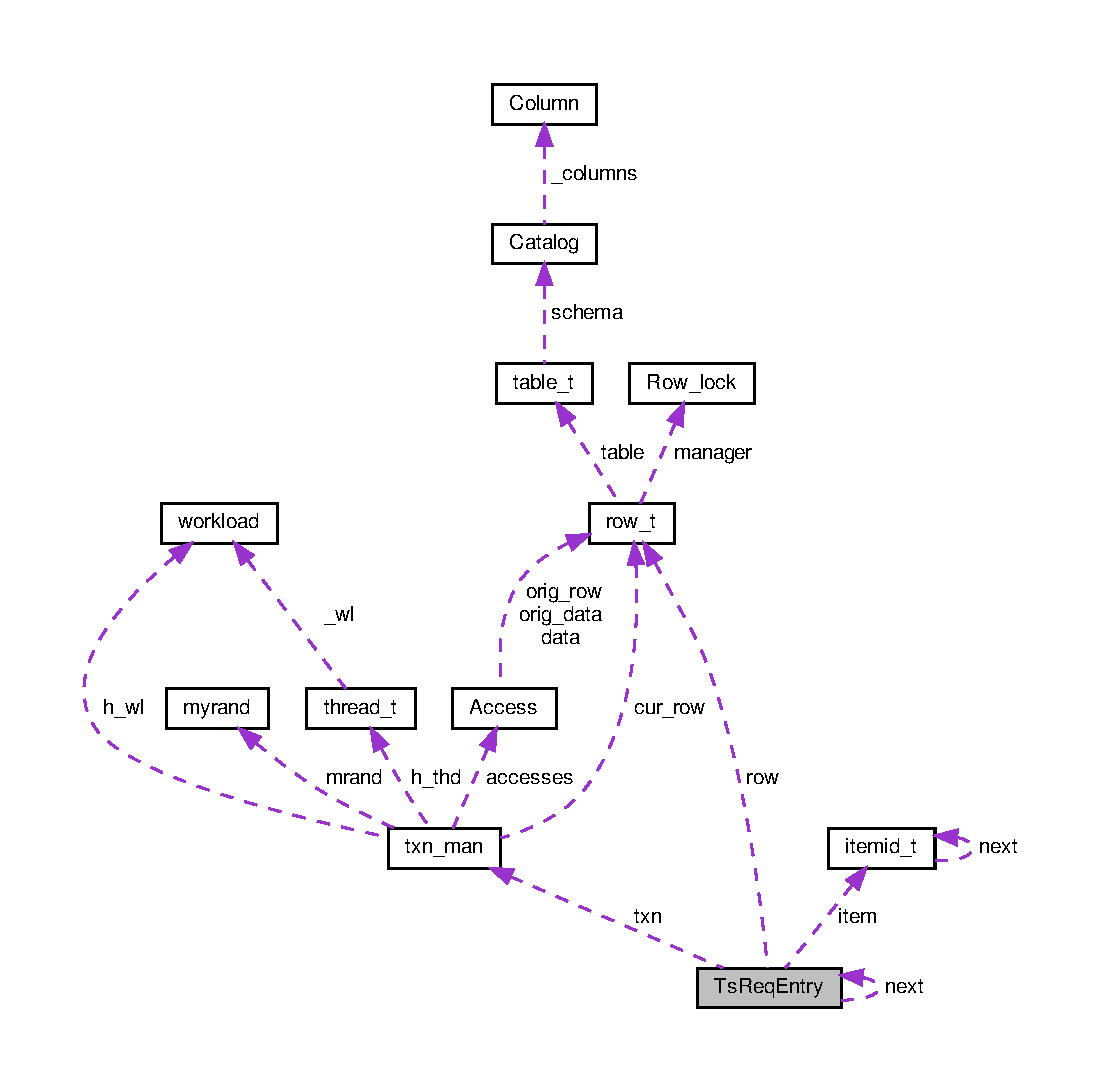
\includegraphics[width=350pt]{structTsReqEntry__coll__graph}
\end{center}
\end{figure}
\subsection*{Public Attributes}
\begin{DoxyCompactItemize}
\item 
\hyperlink{classtxn__man}{txn\+\_\+man} $\ast$ \hyperlink{structTsReqEntry_a3079fb0bec061e9e11182063cfabfc04}{txn}
\item 
\hyperlink{classrow__t}{row\+\_\+t} $\ast$ \hyperlink{structTsReqEntry_a2709b20b4ac97c51966b35fffcf54e4b}{row}
\item 
\hyperlink{classitemid__t}{itemid\+\_\+t} $\ast$ \hyperlink{structTsReqEntry_a309c907ede4f7b56c91de5fa4bf63fe9}{item}
\item 
\hyperlink{global_8h_aaf095dfc9b10f757c968fe146ad7e724}{ts\+\_\+t} \hyperlink{structTsReqEntry_ac5cd49323863c4a9d2ecb4fa1bb72691}{ts}
\item 
\hyperlink{structTsReqEntry}{Ts\+Req\+Entry} $\ast$ \hyperlink{structTsReqEntry_a2d6e423abd7d5bf97b6608765ff9516e}{next}
\end{DoxyCompactItemize}


\subsection{Member Data Documentation}
\mbox{\Hypertarget{structTsReqEntry_a309c907ede4f7b56c91de5fa4bf63fe9}\label{structTsReqEntry_a309c907ede4f7b56c91de5fa4bf63fe9}} 
\index{Ts\+Req\+Entry@{Ts\+Req\+Entry}!item@{item}}
\index{item@{item}!Ts\+Req\+Entry@{Ts\+Req\+Entry}}
\subsubsection{\texorpdfstring{item}{item}}
{\footnotesize\ttfamily \hyperlink{classitemid__t}{itemid\+\_\+t}$\ast$ Ts\+Req\+Entry\+::item}

\mbox{\Hypertarget{structTsReqEntry_a2d6e423abd7d5bf97b6608765ff9516e}\label{structTsReqEntry_a2d6e423abd7d5bf97b6608765ff9516e}} 
\index{Ts\+Req\+Entry@{Ts\+Req\+Entry}!next@{next}}
\index{next@{next}!Ts\+Req\+Entry@{Ts\+Req\+Entry}}
\subsubsection{\texorpdfstring{next}{next}}
{\footnotesize\ttfamily \hyperlink{structTsReqEntry}{Ts\+Req\+Entry}$\ast$ Ts\+Req\+Entry\+::next}

\mbox{\Hypertarget{structTsReqEntry_a2709b20b4ac97c51966b35fffcf54e4b}\label{structTsReqEntry_a2709b20b4ac97c51966b35fffcf54e4b}} 
\index{Ts\+Req\+Entry@{Ts\+Req\+Entry}!row@{row}}
\index{row@{row}!Ts\+Req\+Entry@{Ts\+Req\+Entry}}
\subsubsection{\texorpdfstring{row}{row}}
{\footnotesize\ttfamily \hyperlink{classrow__t}{row\+\_\+t}$\ast$ Ts\+Req\+Entry\+::row}

\mbox{\Hypertarget{structTsReqEntry_ac5cd49323863c4a9d2ecb4fa1bb72691}\label{structTsReqEntry_ac5cd49323863c4a9d2ecb4fa1bb72691}} 
\index{Ts\+Req\+Entry@{Ts\+Req\+Entry}!ts@{ts}}
\index{ts@{ts}!Ts\+Req\+Entry@{Ts\+Req\+Entry}}
\subsubsection{\texorpdfstring{ts}{ts}}
{\footnotesize\ttfamily \hyperlink{global_8h_aaf095dfc9b10f757c968fe146ad7e724}{ts\+\_\+t} Ts\+Req\+Entry\+::ts}

\mbox{\Hypertarget{structTsReqEntry_a3079fb0bec061e9e11182063cfabfc04}\label{structTsReqEntry_a3079fb0bec061e9e11182063cfabfc04}} 
\index{Ts\+Req\+Entry@{Ts\+Req\+Entry}!txn@{txn}}
\index{txn@{txn}!Ts\+Req\+Entry@{Ts\+Req\+Entry}}
\subsubsection{\texorpdfstring{txn}{txn}}
{\footnotesize\ttfamily \hyperlink{classtxn__man}{txn\+\_\+man}$\ast$ Ts\+Req\+Entry\+::txn}



The documentation for this struct was generated from the following file\+:\begin{DoxyCompactItemize}
\item 
macrobench/concurrency\+\_\+control/\hyperlink{row__ts_8h}{row\+\_\+ts.\+h}\end{DoxyCompactItemize}

\hypertarget{classtxn__man}{}\section{txn\+\_\+man Class Reference}
\label{classtxn__man}\index{txn\+\_\+man@{txn\+\_\+man}}


{\ttfamily \#include $<$txn.\+h$>$}



Inheritance diagram for txn\+\_\+man\+:
\nopagebreak
\begin{figure}[H]
\begin{center}
\leavevmode
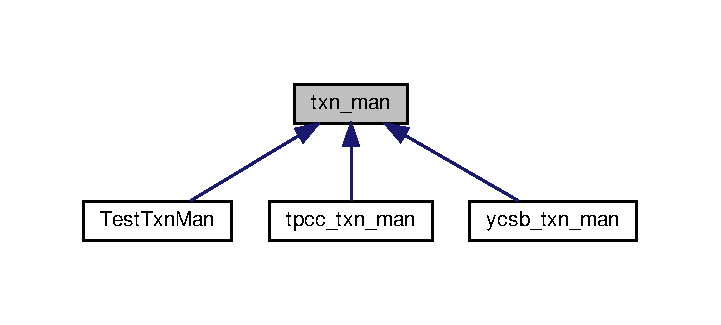
\includegraphics[width=346pt]{classtxn__man__inherit__graph}
\end{center}
\end{figure}


Collaboration diagram for txn\+\_\+man\+:
\nopagebreak
\begin{figure}[H]
\begin{center}
\leavevmode
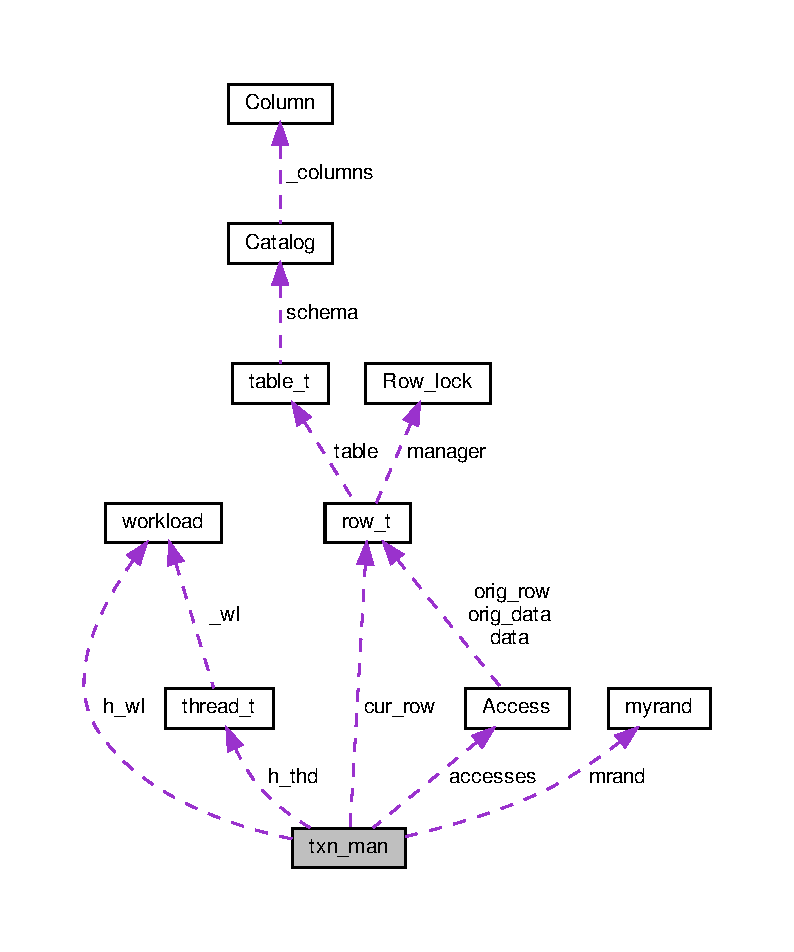
\includegraphics[width=350pt]{classtxn__man__coll__graph}
\end{center}
\end{figure}
\subsection*{Public Member Functions}
\begin{DoxyCompactItemize}
\item 
virtual void \hyperlink{classtxn__man_a778925bb3edd6a54a27161f67792edec}{init} (\hyperlink{classthread__t}{thread\+\_\+t} $\ast$\hyperlink{classtxn__man_a64bf2cba8ef2686ad528a96d18e8358d}{h\+\_\+thd}, \hyperlink{classworkload}{workload} $\ast$\hyperlink{classtxn__man_a988eb76c69a304049c02d3ceff526a5e}{h\+\_\+wl}, uint64\+\_\+t part\+\_\+id)
\item 
virtual void \hyperlink{classtxn__man_a9497c27260379a85a7d5983919868b8d}{setbench\+\_\+deinit} ()
\item 
void \hyperlink{classtxn__man_ae9762ca0f1e6fcac2094ea284375aa6e}{release} ()
\item 
virtual \hyperlink{global_8h_a78c49a674c810fdd03d20432f7be864a}{RC} \hyperlink{classtxn__man_a71142ded36a4be5629ea75d486a105ae}{run\+\_\+txn} (\hyperlink{classbase__query}{base\+\_\+query} $\ast$m\+\_\+query)=0
\item 
uint64\+\_\+t \hyperlink{classtxn__man_ae1c3f482994caa8cc40970b3bb62e529}{get\+\_\+thd\+\_\+id} ()
\item 
\hyperlink{classworkload}{workload} $\ast$ \hyperlink{classtxn__man_a0e873c5e1ac5fabe4555d443215ef0c5}{get\+\_\+wl} ()
\item 
void \hyperlink{classtxn__man_a5675d9c21c8b346b680eb06074f87af5}{set\+\_\+txn\+\_\+id} (\hyperlink{global_8h_a5b3a704dab2aafdcaadfe8c0909716ef}{txnid\+\_\+t} txn\+\_\+id)
\item 
\hyperlink{global_8h_a5b3a704dab2aafdcaadfe8c0909716ef}{txnid\+\_\+t} \hyperlink{classtxn__man_a26c38d64be1ad53236a0017f8c2ff9ff}{get\+\_\+txn\+\_\+id} ()
\item 
void \hyperlink{classtxn__man_a911fe878282152631d4da8b0b3ccde65}{set\+\_\+ts} (\hyperlink{global_8h_aaf095dfc9b10f757c968fe146ad7e724}{ts\+\_\+t} timestamp)
\item 
\hyperlink{global_8h_aaf095dfc9b10f757c968fe146ad7e724}{ts\+\_\+t} \hyperlink{classtxn__man_a1ed4112864a14e2d2ac24cc3ba90417a}{get\+\_\+ts} ()
\item 
\hyperlink{global_8h_a78c49a674c810fdd03d20432f7be864a}{RC} \hyperlink{classtxn__man_a05b5aa26d98420d0a913875e5f9c4226}{finish} (\hyperlink{global_8h_a78c49a674c810fdd03d20432f7be864a}{RC} rc)
\item 
void \hyperlink{classtxn__man_a8e3cbd946d40e7340f04f9b3760eac62}{cleanup} (\hyperlink{global_8h_a78c49a674c810fdd03d20432f7be864a}{RC} rc)
\item 
\hyperlink{global_8h_aaf095dfc9b10f757c968fe146ad7e724}{ts\+\_\+t} \hyperlink{classtxn__man_a12f84c603f952cb40c048d799ff43245}{get\+\_\+max\+\_\+wts} ()
\item 
void \hyperlink{classtxn__man_ae9f87c4e9565645d4297e07afe96daeb}{update\+\_\+max\+\_\+wts} (\hyperlink{global_8h_aaf095dfc9b10f757c968fe146ad7e724}{ts\+\_\+t} max\+\_\+wts)
\item 
int \hyperlink{classtxn__man_aa8a892b52707588c411662822359b63a}{index\+\_\+range\+\_\+query} (\hyperlink{classIndex}{Index} $\ast$index, \hyperlink{global_8h_a29a17e29c9200c833b70a4ef8c89813e}{idx\+\_\+key\+\_\+t} low, \hyperlink{global_8h_a29a17e29c9200c833b70a4ef8c89813e}{idx\+\_\+key\+\_\+t} high, \hyperlink{global_8h_a29a17e29c9200c833b70a4ef8c89813e}{idx\+\_\+key\+\_\+t} $\ast$result\+Keys, \hyperlink{classitemid__t}{itemid\+\_\+t} $\ast$$\ast$result\+Values, int part\+\_\+id)
\item 
\hyperlink{classitemid__t}{itemid\+\_\+t} $\ast$ \hyperlink{classtxn__man_a3fa753d12f78c728e33f86c5c119a191}{index\+\_\+read} (\hyperlink{classIndex}{Index} $\ast$index, \hyperlink{global_8h_a29a17e29c9200c833b70a4ef8c89813e}{idx\+\_\+key\+\_\+t} key, int part\+\_\+id)
\item 
void \hyperlink{classtxn__man_a20dbd5004ecb977f109e54fd0f60950f}{index\+\_\+read} (\hyperlink{classIndex}{Index} $\ast$index, \hyperlink{global_8h_a29a17e29c9200c833b70a4ef8c89813e}{idx\+\_\+key\+\_\+t} key, int part\+\_\+id, \hyperlink{classitemid__t}{itemid\+\_\+t} $\ast$$\ast$item)
\item 
void \hyperlink{classtxn__man_ae90afaf5c0ba23e804f6719c41d65499}{index\+\_\+insert} (\hyperlink{classIndex}{Index} $\ast$index, uint64\+\_\+t key, \hyperlink{classrow__t}{row\+\_\+t} $\ast$row, int64\+\_\+t part\+\_\+id)
\item 
\hyperlink{classrow__t}{row\+\_\+t} $\ast$ \hyperlink{classtxn__man_aa9ae01517fa1520cb8c910f72afb72d1}{get\+\_\+row} (\hyperlink{classrow__t}{row\+\_\+t} $\ast$row, \hyperlink{global_8h_a567f81b0ae33b00d189d7714e9fde0bc}{access\+\_\+t} type)
\end{DoxyCompactItemize}
\subsection*{Public Attributes}
\begin{DoxyCompactItemize}
\item 
\hyperlink{classthread__t}{thread\+\_\+t} $\ast$ \hyperlink{classtxn__man_a64bf2cba8ef2686ad528a96d18e8358d}{h\+\_\+thd}
\item 
\hyperlink{classworkload}{workload} $\ast$ \hyperlink{classtxn__man_a988eb76c69a304049c02d3ceff526a5e}{h\+\_\+wl}
\item 
\hyperlink{classmyrand}{myrand} $\ast$ \hyperlink{classtxn__man_a04db2c39bc66572f311d62bd7b7378b7}{mrand}
\item 
uint64\+\_\+t \hyperlink{classtxn__man_a817eda721f4a25d114c9f44b6f19963c}{abort\+\_\+cnt}
\item 
pthread\+\_\+mutex\+\_\+t \hyperlink{classtxn__man_abfdf95f4a0acbcbb8a72cd56ad111553}{txn\+\_\+lock}
\item 
\hyperlink{classrow__t}{row\+\_\+t} $\ast$volatile \hyperlink{classtxn__man_a5ed85ee9e6374ffe85966747e354c222}{cur\+\_\+row}
\item 
void $\ast$volatile \hyperlink{classtxn__man_a6cb76b97ee7a07af9d8dabcaef81b120}{history\+\_\+entry}
\item 
bool volatile \hyperlink{classtxn__man_a7397f734b7ab5a49b04dea7b318be36b}{lock\+\_\+ready}
\item 
bool volatile \hyperlink{classtxn__man_aa5a467719eb39d1f5e9e2bb5e303e5ba}{lock\+\_\+abort}
\item 
bool volatile \hyperlink{classtxn__man_a0cb5e97941b281d7c2eaa98e36322a1d}{ts\+\_\+ready}
\item 
int volatile \hyperlink{classtxn__man_acda07d65f82bea98a05978fe1c5111b0}{ready\+\_\+part}
\item 
\hyperlink{global_8h_aaf095dfc9b10f757c968fe146ad7e724}{ts\+\_\+t} \hyperlink{classtxn__man_a7c1e4e0a5cf220721ebb8333fb14d9b7}{last\+\_\+wts}
\item 
\hyperlink{global_8h_aaf095dfc9b10f757c968fe146ad7e724}{ts\+\_\+t} \hyperlink{classtxn__man_a19b20b8145f50277f646df6e47de35b8}{last\+\_\+rts}
\item 
uint64\+\_\+t \hyperlink{classtxn__man_a5358d18b9fbd2dd6fce6433889fd10ce}{start\+\_\+ts}
\item 
uint64\+\_\+t \hyperlink{classtxn__man_a9cba30a71b7a83c9d1bbb084afb4af64}{end\+\_\+ts}
\item 
int \hyperlink{classtxn__man_a60c4f347fc86e48bbadf0524b6def068}{row\+\_\+cnt}
\item 
int \hyperlink{classtxn__man_af7984d5eb6137ae694aa34973921f08a}{wr\+\_\+cnt}
\item 
\hyperlink{classAccess}{Access} $\ast$$\ast$ \hyperlink{classtxn__man_af5f2cec4241127bbaa1047a52b18aa02}{accesses}
\item 
int \hyperlink{classtxn__man_a3f33da7138d2e0a7f1ba4924a613988a}{num\+\_\+accesses\+\_\+alloc}
\item 
\hyperlink{txn_8h_a171384e518db04097e0f3e6750129a2a}{Txn\+Type} \hyperlink{classtxn__man_a1cee31702c8e159b1302a7a7b1880dd8}{vll\+\_\+txn\+\_\+type}
\end{DoxyCompactItemize}
\subsection*{Protected Member Functions}
\begin{DoxyCompactItemize}
\item 
void \hyperlink{classtxn__man_a4097c7d52e098381113281b88b7c2533}{insert\+\_\+row} (\hyperlink{classrow__t}{row\+\_\+t} $\ast$row, \hyperlink{classtable__t}{table\+\_\+t} $\ast$table)
\end{DoxyCompactItemize}


\subsection{Member Function Documentation}
\mbox{\Hypertarget{classtxn__man_a8e3cbd946d40e7340f04f9b3760eac62}\label{classtxn__man_a8e3cbd946d40e7340f04f9b3760eac62}} 
\index{txn\+\_\+man@{txn\+\_\+man}!cleanup@{cleanup}}
\index{cleanup@{cleanup}!txn\+\_\+man@{txn\+\_\+man}}
\subsubsection{\texorpdfstring{cleanup()}{cleanup()}}
{\footnotesize\ttfamily void txn\+\_\+man\+::cleanup (\begin{DoxyParamCaption}\item[{\hyperlink{global_8h_a78c49a674c810fdd03d20432f7be864a}{RC}}]{rc }\end{DoxyParamCaption})}

\mbox{\Hypertarget{classtxn__man_a05b5aa26d98420d0a913875e5f9c4226}\label{classtxn__man_a05b5aa26d98420d0a913875e5f9c4226}} 
\index{txn\+\_\+man@{txn\+\_\+man}!finish@{finish}}
\index{finish@{finish}!txn\+\_\+man@{txn\+\_\+man}}
\subsubsection{\texorpdfstring{finish()}{finish()}}
{\footnotesize\ttfamily \hyperlink{global_8h_a78c49a674c810fdd03d20432f7be864a}{RC} txn\+\_\+man\+::finish (\begin{DoxyParamCaption}\item[{\hyperlink{global_8h_a78c49a674c810fdd03d20432f7be864a}{RC}}]{rc }\end{DoxyParamCaption})}

\mbox{\Hypertarget{classtxn__man_a12f84c603f952cb40c048d799ff43245}\label{classtxn__man_a12f84c603f952cb40c048d799ff43245}} 
\index{txn\+\_\+man@{txn\+\_\+man}!get\+\_\+max\+\_\+wts@{get\+\_\+max\+\_\+wts}}
\index{get\+\_\+max\+\_\+wts@{get\+\_\+max\+\_\+wts}!txn\+\_\+man@{txn\+\_\+man}}
\subsubsection{\texorpdfstring{get\+\_\+max\+\_\+wts()}{get\_max\_wts()}}
{\footnotesize\ttfamily \hyperlink{global_8h_aaf095dfc9b10f757c968fe146ad7e724}{ts\+\_\+t} txn\+\_\+man\+::get\+\_\+max\+\_\+wts (\begin{DoxyParamCaption}{ }\end{DoxyParamCaption})\hspace{0.3cm}{\ttfamily [inline]}}

\mbox{\Hypertarget{classtxn__man_aa9ae01517fa1520cb8c910f72afb72d1}\label{classtxn__man_aa9ae01517fa1520cb8c910f72afb72d1}} 
\index{txn\+\_\+man@{txn\+\_\+man}!get\+\_\+row@{get\+\_\+row}}
\index{get\+\_\+row@{get\+\_\+row}!txn\+\_\+man@{txn\+\_\+man}}
\subsubsection{\texorpdfstring{get\+\_\+row()}{get\_row()}}
{\footnotesize\ttfamily \hyperlink{classrow__t}{row\+\_\+t} $\ast$ txn\+\_\+man\+::get\+\_\+row (\begin{DoxyParamCaption}\item[{\hyperlink{classrow__t}{row\+\_\+t} $\ast$}]{row,  }\item[{\hyperlink{global_8h_a567f81b0ae33b00d189d7714e9fde0bc}{access\+\_\+t}}]{type }\end{DoxyParamCaption})}

\mbox{\Hypertarget{classtxn__man_ae1c3f482994caa8cc40970b3bb62e529}\label{classtxn__man_ae1c3f482994caa8cc40970b3bb62e529}} 
\index{txn\+\_\+man@{txn\+\_\+man}!get\+\_\+thd\+\_\+id@{get\+\_\+thd\+\_\+id}}
\index{get\+\_\+thd\+\_\+id@{get\+\_\+thd\+\_\+id}!txn\+\_\+man@{txn\+\_\+man}}
\subsubsection{\texorpdfstring{get\+\_\+thd\+\_\+id()}{get\_thd\_id()}}
{\footnotesize\ttfamily uint64\+\_\+t txn\+\_\+man\+::get\+\_\+thd\+\_\+id (\begin{DoxyParamCaption}{ }\end{DoxyParamCaption})}

\mbox{\Hypertarget{classtxn__man_a1ed4112864a14e2d2ac24cc3ba90417a}\label{classtxn__man_a1ed4112864a14e2d2ac24cc3ba90417a}} 
\index{txn\+\_\+man@{txn\+\_\+man}!get\+\_\+ts@{get\+\_\+ts}}
\index{get\+\_\+ts@{get\+\_\+ts}!txn\+\_\+man@{txn\+\_\+man}}
\subsubsection{\texorpdfstring{get\+\_\+ts()}{get\_ts()}}
{\footnotesize\ttfamily \hyperlink{global_8h_aaf095dfc9b10f757c968fe146ad7e724}{ts\+\_\+t} txn\+\_\+man\+::get\+\_\+ts (\begin{DoxyParamCaption}{ }\end{DoxyParamCaption})}

\mbox{\Hypertarget{classtxn__man_a26c38d64be1ad53236a0017f8c2ff9ff}\label{classtxn__man_a26c38d64be1ad53236a0017f8c2ff9ff}} 
\index{txn\+\_\+man@{txn\+\_\+man}!get\+\_\+txn\+\_\+id@{get\+\_\+txn\+\_\+id}}
\index{get\+\_\+txn\+\_\+id@{get\+\_\+txn\+\_\+id}!txn\+\_\+man@{txn\+\_\+man}}
\subsubsection{\texorpdfstring{get\+\_\+txn\+\_\+id()}{get\_txn\_id()}}
{\footnotesize\ttfamily \hyperlink{global_8h_a5b3a704dab2aafdcaadfe8c0909716ef}{txnid\+\_\+t} txn\+\_\+man\+::get\+\_\+txn\+\_\+id (\begin{DoxyParamCaption}{ }\end{DoxyParamCaption})}

\mbox{\Hypertarget{classtxn__man_a0e873c5e1ac5fabe4555d443215ef0c5}\label{classtxn__man_a0e873c5e1ac5fabe4555d443215ef0c5}} 
\index{txn\+\_\+man@{txn\+\_\+man}!get\+\_\+wl@{get\+\_\+wl}}
\index{get\+\_\+wl@{get\+\_\+wl}!txn\+\_\+man@{txn\+\_\+man}}
\subsubsection{\texorpdfstring{get\+\_\+wl()}{get\_wl()}}
{\footnotesize\ttfamily \hyperlink{classworkload}{workload} $\ast$ txn\+\_\+man\+::get\+\_\+wl (\begin{DoxyParamCaption}{ }\end{DoxyParamCaption})}

\mbox{\Hypertarget{classtxn__man_ae90afaf5c0ba23e804f6719c41d65499}\label{classtxn__man_ae90afaf5c0ba23e804f6719c41d65499}} 
\index{txn\+\_\+man@{txn\+\_\+man}!index\+\_\+insert@{index\+\_\+insert}}
\index{index\+\_\+insert@{index\+\_\+insert}!txn\+\_\+man@{txn\+\_\+man}}
\subsubsection{\texorpdfstring{index\+\_\+insert()}{index\_insert()}}
{\footnotesize\ttfamily void txn\+\_\+man\+::index\+\_\+insert (\begin{DoxyParamCaption}\item[{\hyperlink{classIndex}{Index} $\ast$}]{index,  }\item[{uint64\+\_\+t}]{key,  }\item[{\hyperlink{classrow__t}{row\+\_\+t} $\ast$}]{row,  }\item[{int64\+\_\+t}]{part\+\_\+id }\end{DoxyParamCaption})}

\mbox{\Hypertarget{classtxn__man_aa8a892b52707588c411662822359b63a}\label{classtxn__man_aa8a892b52707588c411662822359b63a}} 
\index{txn\+\_\+man@{txn\+\_\+man}!index\+\_\+range\+\_\+query@{index\+\_\+range\+\_\+query}}
\index{index\+\_\+range\+\_\+query@{index\+\_\+range\+\_\+query}!txn\+\_\+man@{txn\+\_\+man}}
\subsubsection{\texorpdfstring{index\+\_\+range\+\_\+query()}{index\_range\_query()}}
{\footnotesize\ttfamily int txn\+\_\+man\+::index\+\_\+range\+\_\+query (\begin{DoxyParamCaption}\item[{\hyperlink{classIndex}{Index} $\ast$}]{index,  }\item[{\hyperlink{global_8h_a29a17e29c9200c833b70a4ef8c89813e}{idx\+\_\+key\+\_\+t}}]{low,  }\item[{\hyperlink{global_8h_a29a17e29c9200c833b70a4ef8c89813e}{idx\+\_\+key\+\_\+t}}]{high,  }\item[{\hyperlink{global_8h_a29a17e29c9200c833b70a4ef8c89813e}{idx\+\_\+key\+\_\+t} $\ast$}]{result\+Keys,  }\item[{\hyperlink{classitemid__t}{itemid\+\_\+t} $\ast$$\ast$}]{result\+Values,  }\item[{int}]{part\+\_\+id }\end{DoxyParamCaption})}

\mbox{\Hypertarget{classtxn__man_a3fa753d12f78c728e33f86c5c119a191}\label{classtxn__man_a3fa753d12f78c728e33f86c5c119a191}} 
\index{txn\+\_\+man@{txn\+\_\+man}!index\+\_\+read@{index\+\_\+read}}
\index{index\+\_\+read@{index\+\_\+read}!txn\+\_\+man@{txn\+\_\+man}}
\subsubsection{\texorpdfstring{index\+\_\+read()}{index\_read()}\hspace{0.1cm}{\footnotesize\ttfamily [1/2]}}
{\footnotesize\ttfamily \hyperlink{classitemid__t}{itemid\+\_\+t} $\ast$ txn\+\_\+man\+::index\+\_\+read (\begin{DoxyParamCaption}\item[{\hyperlink{classIndex}{Index} $\ast$}]{index,  }\item[{\hyperlink{global_8h_a29a17e29c9200c833b70a4ef8c89813e}{idx\+\_\+key\+\_\+t}}]{key,  }\item[{int}]{part\+\_\+id }\end{DoxyParamCaption})}

\mbox{\Hypertarget{classtxn__man_a20dbd5004ecb977f109e54fd0f60950f}\label{classtxn__man_a20dbd5004ecb977f109e54fd0f60950f}} 
\index{txn\+\_\+man@{txn\+\_\+man}!index\+\_\+read@{index\+\_\+read}}
\index{index\+\_\+read@{index\+\_\+read}!txn\+\_\+man@{txn\+\_\+man}}
\subsubsection{\texorpdfstring{index\+\_\+read()}{index\_read()}\hspace{0.1cm}{\footnotesize\ttfamily [2/2]}}
{\footnotesize\ttfamily void txn\+\_\+man\+::index\+\_\+read (\begin{DoxyParamCaption}\item[{\hyperlink{classIndex}{Index} $\ast$}]{index,  }\item[{\hyperlink{global_8h_a29a17e29c9200c833b70a4ef8c89813e}{idx\+\_\+key\+\_\+t}}]{key,  }\item[{int}]{part\+\_\+id,  }\item[{\hyperlink{classitemid__t}{itemid\+\_\+t} $\ast$$\ast$}]{item }\end{DoxyParamCaption})}

\mbox{\Hypertarget{classtxn__man_a778925bb3edd6a54a27161f67792edec}\label{classtxn__man_a778925bb3edd6a54a27161f67792edec}} 
\index{txn\+\_\+man@{txn\+\_\+man}!init@{init}}
\index{init@{init}!txn\+\_\+man@{txn\+\_\+man}}
\subsubsection{\texorpdfstring{init()}{init()}}
{\footnotesize\ttfamily void txn\+\_\+man\+::init (\begin{DoxyParamCaption}\item[{\hyperlink{classthread__t}{thread\+\_\+t} $\ast$}]{h\+\_\+thd,  }\item[{\hyperlink{classworkload}{workload} $\ast$}]{h\+\_\+wl,  }\item[{uint64\+\_\+t}]{part\+\_\+id }\end{DoxyParamCaption})\hspace{0.3cm}{\ttfamily [virtual]}}



Reimplemented in \hyperlink{classtpcc__txn__man_aa2a56c4cb192d138852488745ee09fd7}{tpcc\+\_\+txn\+\_\+man}, \hyperlink{classycsb__txn__man_a6708b67fbc560af1634f6d48cfa66b4f}{ycsb\+\_\+txn\+\_\+man}, and \hyperlink{classTestTxnMan_a55bd3947973927a82e87f249813fd4a0}{Test\+Txn\+Man}.

\mbox{\Hypertarget{classtxn__man_a4097c7d52e098381113281b88b7c2533}\label{classtxn__man_a4097c7d52e098381113281b88b7c2533}} 
\index{txn\+\_\+man@{txn\+\_\+man}!insert\+\_\+row@{insert\+\_\+row}}
\index{insert\+\_\+row@{insert\+\_\+row}!txn\+\_\+man@{txn\+\_\+man}}
\subsubsection{\texorpdfstring{insert\+\_\+row()}{insert\_row()}}
{\footnotesize\ttfamily void txn\+\_\+man\+::insert\+\_\+row (\begin{DoxyParamCaption}\item[{\hyperlink{classrow__t}{row\+\_\+t} $\ast$}]{row,  }\item[{\hyperlink{classtable__t}{table\+\_\+t} $\ast$}]{table }\end{DoxyParamCaption})\hspace{0.3cm}{\ttfamily [protected]}}

\mbox{\Hypertarget{classtxn__man_ae9762ca0f1e6fcac2094ea284375aa6e}\label{classtxn__man_ae9762ca0f1e6fcac2094ea284375aa6e}} 
\index{txn\+\_\+man@{txn\+\_\+man}!release@{release}}
\index{release@{release}!txn\+\_\+man@{txn\+\_\+man}}
\subsubsection{\texorpdfstring{release()}{release()}}
{\footnotesize\ttfamily void txn\+\_\+man\+::release (\begin{DoxyParamCaption}{ }\end{DoxyParamCaption})}

\mbox{\Hypertarget{classtxn__man_a71142ded36a4be5629ea75d486a105ae}\label{classtxn__man_a71142ded36a4be5629ea75d486a105ae}} 
\index{txn\+\_\+man@{txn\+\_\+man}!run\+\_\+txn@{run\+\_\+txn}}
\index{run\+\_\+txn@{run\+\_\+txn}!txn\+\_\+man@{txn\+\_\+man}}
\subsubsection{\texorpdfstring{run\+\_\+txn()}{run\_txn()}}
{\footnotesize\ttfamily virtual \hyperlink{global_8h_a78c49a674c810fdd03d20432f7be864a}{RC} txn\+\_\+man\+::run\+\_\+txn (\begin{DoxyParamCaption}\item[{\hyperlink{classbase__query}{base\+\_\+query} $\ast$}]{m\+\_\+query }\end{DoxyParamCaption})\hspace{0.3cm}{\ttfamily [pure virtual]}}



Implemented in \hyperlink{classtpcc__txn__man_a19f99ffaf91e1f977fe517d617493a8a}{tpcc\+\_\+txn\+\_\+man}, \hyperlink{classycsb__txn__man_ab219e46d2d5149677ad391ebb83d6e05}{ycsb\+\_\+txn\+\_\+man}, and \hyperlink{classTestTxnMan_ae9510bd3f827a29dcc1239517021ac37}{Test\+Txn\+Man}.

\mbox{\Hypertarget{classtxn__man_a911fe878282152631d4da8b0b3ccde65}\label{classtxn__man_a911fe878282152631d4da8b0b3ccde65}} 
\index{txn\+\_\+man@{txn\+\_\+man}!set\+\_\+ts@{set\+\_\+ts}}
\index{set\+\_\+ts@{set\+\_\+ts}!txn\+\_\+man@{txn\+\_\+man}}
\subsubsection{\texorpdfstring{set\+\_\+ts()}{set\_ts()}}
{\footnotesize\ttfamily void txn\+\_\+man\+::set\+\_\+ts (\begin{DoxyParamCaption}\item[{\hyperlink{global_8h_aaf095dfc9b10f757c968fe146ad7e724}{ts\+\_\+t}}]{timestamp }\end{DoxyParamCaption})}

\mbox{\Hypertarget{classtxn__man_a5675d9c21c8b346b680eb06074f87af5}\label{classtxn__man_a5675d9c21c8b346b680eb06074f87af5}} 
\index{txn\+\_\+man@{txn\+\_\+man}!set\+\_\+txn\+\_\+id@{set\+\_\+txn\+\_\+id}}
\index{set\+\_\+txn\+\_\+id@{set\+\_\+txn\+\_\+id}!txn\+\_\+man@{txn\+\_\+man}}
\subsubsection{\texorpdfstring{set\+\_\+txn\+\_\+id()}{set\_txn\_id()}}
{\footnotesize\ttfamily void txn\+\_\+man\+::set\+\_\+txn\+\_\+id (\begin{DoxyParamCaption}\item[{\hyperlink{global_8h_a5b3a704dab2aafdcaadfe8c0909716ef}{txnid\+\_\+t}}]{txn\+\_\+id }\end{DoxyParamCaption})}

\mbox{\Hypertarget{classtxn__man_a9497c27260379a85a7d5983919868b8d}\label{classtxn__man_a9497c27260379a85a7d5983919868b8d}} 
\index{txn\+\_\+man@{txn\+\_\+man}!setbench\+\_\+deinit@{setbench\+\_\+deinit}}
\index{setbench\+\_\+deinit@{setbench\+\_\+deinit}!txn\+\_\+man@{txn\+\_\+man}}
\subsubsection{\texorpdfstring{setbench\+\_\+deinit()}{setbench\_deinit()}}
{\footnotesize\ttfamily void txn\+\_\+man\+::setbench\+\_\+deinit (\begin{DoxyParamCaption}{ }\end{DoxyParamCaption})\hspace{0.3cm}{\ttfamily [virtual]}}

\mbox{\Hypertarget{classtxn__man_ae9f87c4e9565645d4297e07afe96daeb}\label{classtxn__man_ae9f87c4e9565645d4297e07afe96daeb}} 
\index{txn\+\_\+man@{txn\+\_\+man}!update\+\_\+max\+\_\+wts@{update\+\_\+max\+\_\+wts}}
\index{update\+\_\+max\+\_\+wts@{update\+\_\+max\+\_\+wts}!txn\+\_\+man@{txn\+\_\+man}}
\subsubsection{\texorpdfstring{update\+\_\+max\+\_\+wts()}{update\_max\_wts()}}
{\footnotesize\ttfamily void txn\+\_\+man\+::update\+\_\+max\+\_\+wts (\begin{DoxyParamCaption}\item[{\hyperlink{global_8h_aaf095dfc9b10f757c968fe146ad7e724}{ts\+\_\+t}}]{max\+\_\+wts }\end{DoxyParamCaption})}



\subsection{Member Data Documentation}
\mbox{\Hypertarget{classtxn__man_a817eda721f4a25d114c9f44b6f19963c}\label{classtxn__man_a817eda721f4a25d114c9f44b6f19963c}} 
\index{txn\+\_\+man@{txn\+\_\+man}!abort\+\_\+cnt@{abort\+\_\+cnt}}
\index{abort\+\_\+cnt@{abort\+\_\+cnt}!txn\+\_\+man@{txn\+\_\+man}}
\subsubsection{\texorpdfstring{abort\+\_\+cnt}{abort\_cnt}}
{\footnotesize\ttfamily uint64\+\_\+t txn\+\_\+man\+::abort\+\_\+cnt}

\mbox{\Hypertarget{classtxn__man_af5f2cec4241127bbaa1047a52b18aa02}\label{classtxn__man_af5f2cec4241127bbaa1047a52b18aa02}} 
\index{txn\+\_\+man@{txn\+\_\+man}!accesses@{accesses}}
\index{accesses@{accesses}!txn\+\_\+man@{txn\+\_\+man}}
\subsubsection{\texorpdfstring{accesses}{accesses}}
{\footnotesize\ttfamily \hyperlink{classAccess}{Access}$\ast$$\ast$ txn\+\_\+man\+::accesses}

\mbox{\Hypertarget{classtxn__man_a5ed85ee9e6374ffe85966747e354c222}\label{classtxn__man_a5ed85ee9e6374ffe85966747e354c222}} 
\index{txn\+\_\+man@{txn\+\_\+man}!cur\+\_\+row@{cur\+\_\+row}}
\index{cur\+\_\+row@{cur\+\_\+row}!txn\+\_\+man@{txn\+\_\+man}}
\subsubsection{\texorpdfstring{cur\+\_\+row}{cur\_row}}
{\footnotesize\ttfamily \hyperlink{classrow__t}{row\+\_\+t}$\ast$ volatile txn\+\_\+man\+::cur\+\_\+row}

\mbox{\Hypertarget{classtxn__man_a9cba30a71b7a83c9d1bbb084afb4af64}\label{classtxn__man_a9cba30a71b7a83c9d1bbb084afb4af64}} 
\index{txn\+\_\+man@{txn\+\_\+man}!end\+\_\+ts@{end\+\_\+ts}}
\index{end\+\_\+ts@{end\+\_\+ts}!txn\+\_\+man@{txn\+\_\+man}}
\subsubsection{\texorpdfstring{end\+\_\+ts}{end\_ts}}
{\footnotesize\ttfamily uint64\+\_\+t txn\+\_\+man\+::end\+\_\+ts}

\mbox{\Hypertarget{classtxn__man_a64bf2cba8ef2686ad528a96d18e8358d}\label{classtxn__man_a64bf2cba8ef2686ad528a96d18e8358d}} 
\index{txn\+\_\+man@{txn\+\_\+man}!h\+\_\+thd@{h\+\_\+thd}}
\index{h\+\_\+thd@{h\+\_\+thd}!txn\+\_\+man@{txn\+\_\+man}}
\subsubsection{\texorpdfstring{h\+\_\+thd}{h\_thd}}
{\footnotesize\ttfamily \hyperlink{classthread__t}{thread\+\_\+t}$\ast$ txn\+\_\+man\+::h\+\_\+thd}

\mbox{\Hypertarget{classtxn__man_a988eb76c69a304049c02d3ceff526a5e}\label{classtxn__man_a988eb76c69a304049c02d3ceff526a5e}} 
\index{txn\+\_\+man@{txn\+\_\+man}!h\+\_\+wl@{h\+\_\+wl}}
\index{h\+\_\+wl@{h\+\_\+wl}!txn\+\_\+man@{txn\+\_\+man}}
\subsubsection{\texorpdfstring{h\+\_\+wl}{h\_wl}}
{\footnotesize\ttfamily \hyperlink{classworkload}{workload}$\ast$ txn\+\_\+man\+::h\+\_\+wl}

\mbox{\Hypertarget{classtxn__man_a6cb76b97ee7a07af9d8dabcaef81b120}\label{classtxn__man_a6cb76b97ee7a07af9d8dabcaef81b120}} 
\index{txn\+\_\+man@{txn\+\_\+man}!history\+\_\+entry@{history\+\_\+entry}}
\index{history\+\_\+entry@{history\+\_\+entry}!txn\+\_\+man@{txn\+\_\+man}}
\subsubsection{\texorpdfstring{history\+\_\+entry}{history\_entry}}
{\footnotesize\ttfamily void$\ast$ volatile txn\+\_\+man\+::history\+\_\+entry}

\mbox{\Hypertarget{classtxn__man_a19b20b8145f50277f646df6e47de35b8}\label{classtxn__man_a19b20b8145f50277f646df6e47de35b8}} 
\index{txn\+\_\+man@{txn\+\_\+man}!last\+\_\+rts@{last\+\_\+rts}}
\index{last\+\_\+rts@{last\+\_\+rts}!txn\+\_\+man@{txn\+\_\+man}}
\subsubsection{\texorpdfstring{last\+\_\+rts}{last\_rts}}
{\footnotesize\ttfamily \hyperlink{global_8h_aaf095dfc9b10f757c968fe146ad7e724}{ts\+\_\+t} txn\+\_\+man\+::last\+\_\+rts}

\mbox{\Hypertarget{classtxn__man_a7c1e4e0a5cf220721ebb8333fb14d9b7}\label{classtxn__man_a7c1e4e0a5cf220721ebb8333fb14d9b7}} 
\index{txn\+\_\+man@{txn\+\_\+man}!last\+\_\+wts@{last\+\_\+wts}}
\index{last\+\_\+wts@{last\+\_\+wts}!txn\+\_\+man@{txn\+\_\+man}}
\subsubsection{\texorpdfstring{last\+\_\+wts}{last\_wts}}
{\footnotesize\ttfamily \hyperlink{global_8h_aaf095dfc9b10f757c968fe146ad7e724}{ts\+\_\+t} txn\+\_\+man\+::last\+\_\+wts}

\mbox{\Hypertarget{classtxn__man_aa5a467719eb39d1f5e9e2bb5e303e5ba}\label{classtxn__man_aa5a467719eb39d1f5e9e2bb5e303e5ba}} 
\index{txn\+\_\+man@{txn\+\_\+man}!lock\+\_\+abort@{lock\+\_\+abort}}
\index{lock\+\_\+abort@{lock\+\_\+abort}!txn\+\_\+man@{txn\+\_\+man}}
\subsubsection{\texorpdfstring{lock\+\_\+abort}{lock\_abort}}
{\footnotesize\ttfamily bool volatile txn\+\_\+man\+::lock\+\_\+abort}

\mbox{\Hypertarget{classtxn__man_a7397f734b7ab5a49b04dea7b318be36b}\label{classtxn__man_a7397f734b7ab5a49b04dea7b318be36b}} 
\index{txn\+\_\+man@{txn\+\_\+man}!lock\+\_\+ready@{lock\+\_\+ready}}
\index{lock\+\_\+ready@{lock\+\_\+ready}!txn\+\_\+man@{txn\+\_\+man}}
\subsubsection{\texorpdfstring{lock\+\_\+ready}{lock\_ready}}
{\footnotesize\ttfamily bool volatile txn\+\_\+man\+::lock\+\_\+ready}

\mbox{\Hypertarget{classtxn__man_a04db2c39bc66572f311d62bd7b7378b7}\label{classtxn__man_a04db2c39bc66572f311d62bd7b7378b7}} 
\index{txn\+\_\+man@{txn\+\_\+man}!mrand@{mrand}}
\index{mrand@{mrand}!txn\+\_\+man@{txn\+\_\+man}}
\subsubsection{\texorpdfstring{mrand}{mrand}}
{\footnotesize\ttfamily \hyperlink{classmyrand}{myrand}$\ast$ txn\+\_\+man\+::mrand}

\mbox{\Hypertarget{classtxn__man_a3f33da7138d2e0a7f1ba4924a613988a}\label{classtxn__man_a3f33da7138d2e0a7f1ba4924a613988a}} 
\index{txn\+\_\+man@{txn\+\_\+man}!num\+\_\+accesses\+\_\+alloc@{num\+\_\+accesses\+\_\+alloc}}
\index{num\+\_\+accesses\+\_\+alloc@{num\+\_\+accesses\+\_\+alloc}!txn\+\_\+man@{txn\+\_\+man}}
\subsubsection{\texorpdfstring{num\+\_\+accesses\+\_\+alloc}{num\_accesses\_alloc}}
{\footnotesize\ttfamily int txn\+\_\+man\+::num\+\_\+accesses\+\_\+alloc}

\mbox{\Hypertarget{classtxn__man_acda07d65f82bea98a05978fe1c5111b0}\label{classtxn__man_acda07d65f82bea98a05978fe1c5111b0}} 
\index{txn\+\_\+man@{txn\+\_\+man}!ready\+\_\+part@{ready\+\_\+part}}
\index{ready\+\_\+part@{ready\+\_\+part}!txn\+\_\+man@{txn\+\_\+man}}
\subsubsection{\texorpdfstring{ready\+\_\+part}{ready\_part}}
{\footnotesize\ttfamily int volatile txn\+\_\+man\+::ready\+\_\+part}

\mbox{\Hypertarget{classtxn__man_a60c4f347fc86e48bbadf0524b6def068}\label{classtxn__man_a60c4f347fc86e48bbadf0524b6def068}} 
\index{txn\+\_\+man@{txn\+\_\+man}!row\+\_\+cnt@{row\+\_\+cnt}}
\index{row\+\_\+cnt@{row\+\_\+cnt}!txn\+\_\+man@{txn\+\_\+man}}
\subsubsection{\texorpdfstring{row\+\_\+cnt}{row\_cnt}}
{\footnotesize\ttfamily int txn\+\_\+man\+::row\+\_\+cnt}

\mbox{\Hypertarget{classtxn__man_a5358d18b9fbd2dd6fce6433889fd10ce}\label{classtxn__man_a5358d18b9fbd2dd6fce6433889fd10ce}} 
\index{txn\+\_\+man@{txn\+\_\+man}!start\+\_\+ts@{start\+\_\+ts}}
\index{start\+\_\+ts@{start\+\_\+ts}!txn\+\_\+man@{txn\+\_\+man}}
\subsubsection{\texorpdfstring{start\+\_\+ts}{start\_ts}}
{\footnotesize\ttfamily uint64\+\_\+t txn\+\_\+man\+::start\+\_\+ts}

\mbox{\Hypertarget{classtxn__man_a0cb5e97941b281d7c2eaa98e36322a1d}\label{classtxn__man_a0cb5e97941b281d7c2eaa98e36322a1d}} 
\index{txn\+\_\+man@{txn\+\_\+man}!ts\+\_\+ready@{ts\+\_\+ready}}
\index{ts\+\_\+ready@{ts\+\_\+ready}!txn\+\_\+man@{txn\+\_\+man}}
\subsubsection{\texorpdfstring{ts\+\_\+ready}{ts\_ready}}
{\footnotesize\ttfamily bool volatile txn\+\_\+man\+::ts\+\_\+ready}

\mbox{\Hypertarget{classtxn__man_abfdf95f4a0acbcbb8a72cd56ad111553}\label{classtxn__man_abfdf95f4a0acbcbb8a72cd56ad111553}} 
\index{txn\+\_\+man@{txn\+\_\+man}!txn\+\_\+lock@{txn\+\_\+lock}}
\index{txn\+\_\+lock@{txn\+\_\+lock}!txn\+\_\+man@{txn\+\_\+man}}
\subsubsection{\texorpdfstring{txn\+\_\+lock}{txn\_lock}}
{\footnotesize\ttfamily pthread\+\_\+mutex\+\_\+t txn\+\_\+man\+::txn\+\_\+lock}

\mbox{\Hypertarget{classtxn__man_a1cee31702c8e159b1302a7a7b1880dd8}\label{classtxn__man_a1cee31702c8e159b1302a7a7b1880dd8}} 
\index{txn\+\_\+man@{txn\+\_\+man}!vll\+\_\+txn\+\_\+type@{vll\+\_\+txn\+\_\+type}}
\index{vll\+\_\+txn\+\_\+type@{vll\+\_\+txn\+\_\+type}!txn\+\_\+man@{txn\+\_\+man}}
\subsubsection{\texorpdfstring{vll\+\_\+txn\+\_\+type}{vll\_txn\_type}}
{\footnotesize\ttfamily \hyperlink{txn_8h_a171384e518db04097e0f3e6750129a2a}{Txn\+Type} txn\+\_\+man\+::vll\+\_\+txn\+\_\+type}

\mbox{\Hypertarget{classtxn__man_af7984d5eb6137ae694aa34973921f08a}\label{classtxn__man_af7984d5eb6137ae694aa34973921f08a}} 
\index{txn\+\_\+man@{txn\+\_\+man}!wr\+\_\+cnt@{wr\+\_\+cnt}}
\index{wr\+\_\+cnt@{wr\+\_\+cnt}!txn\+\_\+man@{txn\+\_\+man}}
\subsubsection{\texorpdfstring{wr\+\_\+cnt}{wr\_cnt}}
{\footnotesize\ttfamily int txn\+\_\+man\+::wr\+\_\+cnt}



The documentation for this class was generated from the following files\+:\begin{DoxyCompactItemize}
\item 
macrobench/system/\hyperlink{txn_8h}{txn.\+h}\item 
macrobench/concurrency\+\_\+control/\hyperlink{tictoc_8cpp}{tictoc.\+cpp}\item 
macrobench/system/\hyperlink{txn_8cpp}{txn.\+cpp}\end{DoxyCompactItemize}

\hypertarget{classTxnQEntry}{}\section{Txn\+Q\+Entry Class Reference}
\label{classTxnQEntry}\index{Txn\+Q\+Entry@{Txn\+Q\+Entry}}


{\ttfamily \#include $<$vll.\+h$>$}



Collaboration diagram for Txn\+Q\+Entry\+:
\nopagebreak
\begin{figure}[H]
\begin{center}
\leavevmode
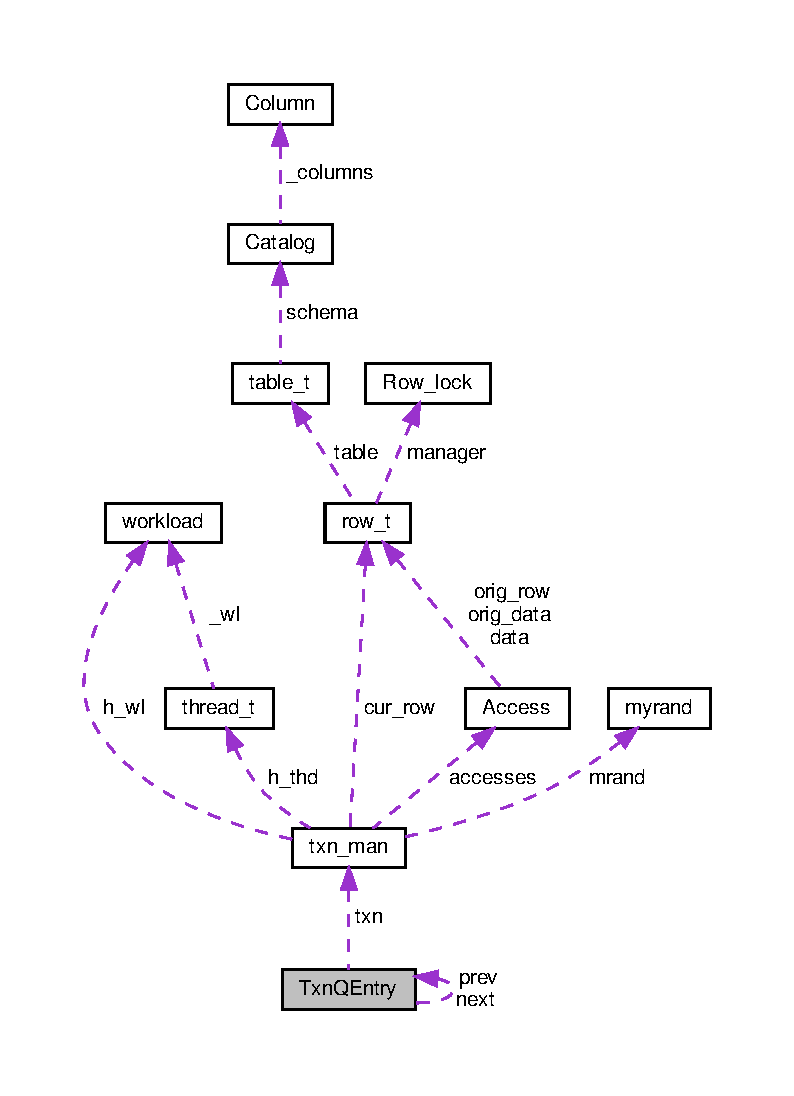
\includegraphics[width=350pt]{classTxnQEntry__coll__graph}
\end{center}
\end{figure}
\subsection*{Public Attributes}
\begin{DoxyCompactItemize}
\item 
\hyperlink{classTxnQEntry}{Txn\+Q\+Entry} $\ast$ \hyperlink{classTxnQEntry_ad05b6ce01658ad7dbf626701846d3952}{prev}
\item 
\hyperlink{classTxnQEntry}{Txn\+Q\+Entry} $\ast$ \hyperlink{classTxnQEntry_a5c8f4191843dfc0e6689d221f97575d0}{next}
\item 
\hyperlink{classtxn__man}{txn\+\_\+man} $\ast$ \hyperlink{classTxnQEntry_af5555a63ea5cde53096ac40f14ae4071}{txn}
\end{DoxyCompactItemize}


\subsection{Member Data Documentation}
\mbox{\Hypertarget{classTxnQEntry_a5c8f4191843dfc0e6689d221f97575d0}\label{classTxnQEntry_a5c8f4191843dfc0e6689d221f97575d0}} 
\index{Txn\+Q\+Entry@{Txn\+Q\+Entry}!next@{next}}
\index{next@{next}!Txn\+Q\+Entry@{Txn\+Q\+Entry}}
\subsubsection{\texorpdfstring{next}{next}}
{\footnotesize\ttfamily \hyperlink{classTxnQEntry}{Txn\+Q\+Entry}$\ast$ Txn\+Q\+Entry\+::next}

\mbox{\Hypertarget{classTxnQEntry_ad05b6ce01658ad7dbf626701846d3952}\label{classTxnQEntry_ad05b6ce01658ad7dbf626701846d3952}} 
\index{Txn\+Q\+Entry@{Txn\+Q\+Entry}!prev@{prev}}
\index{prev@{prev}!Txn\+Q\+Entry@{Txn\+Q\+Entry}}
\subsubsection{\texorpdfstring{prev}{prev}}
{\footnotesize\ttfamily \hyperlink{classTxnQEntry}{Txn\+Q\+Entry}$\ast$ Txn\+Q\+Entry\+::prev}

\mbox{\Hypertarget{classTxnQEntry_af5555a63ea5cde53096ac40f14ae4071}\label{classTxnQEntry_af5555a63ea5cde53096ac40f14ae4071}} 
\index{Txn\+Q\+Entry@{Txn\+Q\+Entry}!txn@{txn}}
\index{txn@{txn}!Txn\+Q\+Entry@{Txn\+Q\+Entry}}
\subsubsection{\texorpdfstring{txn}{txn}}
{\footnotesize\ttfamily \hyperlink{classtxn__man}{txn\+\_\+man}$\ast$ Txn\+Q\+Entry\+::txn}



The documentation for this class was generated from the following file\+:\begin{DoxyCompactItemize}
\item 
macrobench/concurrency\+\_\+control/\hyperlink{vll_8h}{vll.\+h}\end{DoxyCompactItemize}

\hypertarget{structValidAllocatorTest}{}\section{Valid\+Allocator\+Test$<$ T $>$ Struct Template Reference}
\label{structValidAllocatorTest}\index{Valid\+Allocator\+Test$<$ T $>$@{Valid\+Allocator\+Test$<$ T $>$}}


{\ttfamily \#include $<$adapter.\+h$>$}

\subsection*{Static Public Attributes}
\begin{DoxyCompactItemize}
\item 
static constexpr bool \hyperlink{structValidAllocatorTest_a16fe23f087d163942944935eff9fd0c2}{value} = false
\end{DoxyCompactItemize}


\subsection{Member Data Documentation}
\mbox{\Hypertarget{structValidAllocatorTest_a16fe23f087d163942944935eff9fd0c2}\label{structValidAllocatorTest_a16fe23f087d163942944935eff9fd0c2}} 
\index{Valid\+Allocator\+Test@{Valid\+Allocator\+Test}!value@{value}}
\index{value@{value}!Valid\+Allocator\+Test@{Valid\+Allocator\+Test}}
\subsubsection{\texorpdfstring{value}{value}}
{\footnotesize\ttfamily template$<$typename T $>$ \\
constexpr bool \hyperlink{structValidAllocatorTest}{Valid\+Allocator\+Test}$<$ T $>$\+::value = false\hspace{0.3cm}{\ttfamily [static]}}



The documentation for this struct was generated from the following file\+:\begin{DoxyCompactItemize}
\item 
ds/brown\+\_\+ext\+\_\+ist\+\_\+lf/\hyperlink{brown__ext__ist__lf_2adapter_8h}{adapter.\+h}\end{DoxyCompactItemize}

\hypertarget{structValidAllocatorTest_3_01allocator__new_3_01T_01_4_01_4}{}\section{Valid\+Allocator\+Test$<$ allocator\+\_\+new$<$ T $>$ $>$ Struct Template Reference}
\label{structValidAllocatorTest_3_01allocator__new_3_01T_01_4_01_4}\index{Valid\+Allocator\+Test$<$ allocator\+\_\+new$<$ T $>$ $>$@{Valid\+Allocator\+Test$<$ allocator\+\_\+new$<$ T $>$ $>$}}


{\ttfamily \#include $<$adapter.\+h$>$}

\subsection*{Static Public Attributes}
\begin{DoxyCompactItemize}
\item 
static constexpr bool \hyperlink{structValidAllocatorTest_3_01allocator__new_3_01T_01_4_01_4_a7725ab4e2925b9b1f83bc1206690af08}{value} = true
\end{DoxyCompactItemize}


\subsection{Member Data Documentation}
\mbox{\Hypertarget{structValidAllocatorTest_3_01allocator__new_3_01T_01_4_01_4_a7725ab4e2925b9b1f83bc1206690af08}\label{structValidAllocatorTest_3_01allocator__new_3_01T_01_4_01_4_a7725ab4e2925b9b1f83bc1206690af08}} 
\index{Valid\+Allocator\+Test$<$ allocator\+\_\+new$<$ T $>$ $>$@{Valid\+Allocator\+Test$<$ allocator\+\_\+new$<$ T $>$ $>$}!value@{value}}
\index{value@{value}!Valid\+Allocator\+Test$<$ allocator\+\_\+new$<$ T $>$ $>$@{Valid\+Allocator\+Test$<$ allocator\+\_\+new$<$ T $>$ $>$}}
\subsubsection{\texorpdfstring{value}{value}}
{\footnotesize\ttfamily template$<$typename T $>$ \\
constexpr bool \hyperlink{structValidAllocatorTest}{Valid\+Allocator\+Test}$<$ \hyperlink{classallocator__new}{allocator\+\_\+new}$<$ T $>$ $>$\+::value = true\hspace{0.3cm}{\ttfamily [static]}}



The documentation for this struct was generated from the following file\+:\begin{DoxyCompactItemize}
\item 
ds/brown\+\_\+ext\+\_\+ist\+\_\+lf/\hyperlink{brown__ext__ist__lf_2adapter_8h}{adapter.\+h}\end{DoxyCompactItemize}

\hypertarget{structValidPoolTest}{}\section{Valid\+Pool\+Test$<$ T $>$ Struct Template Reference}
\label{structValidPoolTest}\index{Valid\+Pool\+Test$<$ T $>$@{Valid\+Pool\+Test$<$ T $>$}}


{\ttfamily \#include $<$adapter.\+h$>$}

\subsection*{Static Public Attributes}
\begin{DoxyCompactItemize}
\item 
static constexpr bool \hyperlink{structValidPoolTest_aebaecda6d2189a498a1990f24050c8b2}{value} = false
\end{DoxyCompactItemize}


\subsection{Member Data Documentation}
\mbox{\Hypertarget{structValidPoolTest_aebaecda6d2189a498a1990f24050c8b2}\label{structValidPoolTest_aebaecda6d2189a498a1990f24050c8b2}} 
\index{Valid\+Pool\+Test@{Valid\+Pool\+Test}!value@{value}}
\index{value@{value}!Valid\+Pool\+Test@{Valid\+Pool\+Test}}
\subsubsection{\texorpdfstring{value}{value}}
{\footnotesize\ttfamily template$<$typename T $>$ \\
constexpr bool \hyperlink{structValidPoolTest}{Valid\+Pool\+Test}$<$ T $>$\+::value = false\hspace{0.3cm}{\ttfamily [static]}}



The documentation for this struct was generated from the following file\+:\begin{DoxyCompactItemize}
\item 
ds/brown\+\_\+ext\+\_\+ist\+\_\+lf/\hyperlink{brown__ext__ist__lf_2adapter_8h}{adapter.\+h}\end{DoxyCompactItemize}

\hypertarget{structValidPoolTest_3_01pool__none_3_01T_01_4_01_4}{}\section{Valid\+Pool\+Test$<$ pool\+\_\+none$<$ T $>$ $>$ Struct Template Reference}
\label{structValidPoolTest_3_01pool__none_3_01T_01_4_01_4}\index{Valid\+Pool\+Test$<$ pool\+\_\+none$<$ T $>$ $>$@{Valid\+Pool\+Test$<$ pool\+\_\+none$<$ T $>$ $>$}}


{\ttfamily \#include $<$adapter.\+h$>$}

\subsection*{Static Public Attributes}
\begin{DoxyCompactItemize}
\item 
static constexpr bool \hyperlink{structValidPoolTest_3_01pool__none_3_01T_01_4_01_4_ad9d39280e11018be46ffad11381ab80e}{value} = true
\end{DoxyCompactItemize}


\subsection{Member Data Documentation}
\mbox{\Hypertarget{structValidPoolTest_3_01pool__none_3_01T_01_4_01_4_ad9d39280e11018be46ffad11381ab80e}\label{structValidPoolTest_3_01pool__none_3_01T_01_4_01_4_ad9d39280e11018be46ffad11381ab80e}} 
\index{Valid\+Pool\+Test$<$ pool\+\_\+none$<$ T $>$ $>$@{Valid\+Pool\+Test$<$ pool\+\_\+none$<$ T $>$ $>$}!value@{value}}
\index{value@{value}!Valid\+Pool\+Test$<$ pool\+\_\+none$<$ T $>$ $>$@{Valid\+Pool\+Test$<$ pool\+\_\+none$<$ T $>$ $>$}}
\subsubsection{\texorpdfstring{value}{value}}
{\footnotesize\ttfamily template$<$typename T $>$ \\
constexpr bool \hyperlink{structValidPoolTest}{Valid\+Pool\+Test}$<$ \hyperlink{classpool__none}{pool\+\_\+none}$<$ T $>$ $>$\+::value = true\hspace{0.3cm}{\ttfamily [static]}}



The documentation for this struct was generated from the following file\+:\begin{DoxyCompactItemize}
\item 
ds/brown\+\_\+ext\+\_\+ist\+\_\+lf/\hyperlink{brown__ext__ist__lf_2adapter_8h}{adapter.\+h}\end{DoxyCompactItemize}

\hypertarget{classVLLMan}{}\section{V\+L\+L\+Man Class Reference}
\label{classVLLMan}\index{V\+L\+L\+Man@{V\+L\+L\+Man}}


{\ttfamily \#include $<$vll.\+h$>$}

\subsection*{Public Member Functions}
\begin{DoxyCompactItemize}
\item 
void \hyperlink{classVLLMan_a598c042910b0fc6dff90141de1fbc89b}{init} ()
\item 
void \hyperlink{classVLLMan_a3c4fb364b0a0af7d38ee00d846b3524a}{vll\+Main\+Loop} (\hyperlink{classtxn__man}{txn\+\_\+man} $\ast$next\+\_\+txn, \hyperlink{classbase__query}{base\+\_\+query} $\ast$query)
\item 
int \hyperlink{classVLLMan_aed7e1d48a7510cfc25c35d82db547746}{begin\+Txn} (\hyperlink{classtxn__man}{txn\+\_\+man} $\ast$txn, \hyperlink{classbase__query}{base\+\_\+query} $\ast$query, \hyperlink{classTxnQEntry}{Txn\+Q\+Entry} $\ast$\&entry)
\item 
void \hyperlink{classVLLMan_a7366863b5f2b9158d022344be487cb5e}{finish\+Txn} (\hyperlink{classtxn__man}{txn\+\_\+man} $\ast$txn, \hyperlink{classTxnQEntry}{Txn\+Q\+Entry} $\ast$entry)
\item 
void \hyperlink{classVLLMan_a766e95fdf411e87dcbde34940ef98ce1}{execute} (\hyperlink{classtxn__man}{txn\+\_\+man} $\ast$txn, \hyperlink{classbase__query}{base\+\_\+query} $\ast$query)
\end{DoxyCompactItemize}


\subsection{Member Function Documentation}
\mbox{\Hypertarget{classVLLMan_aed7e1d48a7510cfc25c35d82db547746}\label{classVLLMan_aed7e1d48a7510cfc25c35d82db547746}} 
\index{V\+L\+L\+Man@{V\+L\+L\+Man}!begin\+Txn@{begin\+Txn}}
\index{begin\+Txn@{begin\+Txn}!V\+L\+L\+Man@{V\+L\+L\+Man}}
\subsubsection{\texorpdfstring{begin\+Txn()}{beginTxn()}}
{\footnotesize\ttfamily int V\+L\+L\+Man\+::begin\+Txn (\begin{DoxyParamCaption}\item[{\hyperlink{classtxn__man}{txn\+\_\+man} $\ast$}]{txn,  }\item[{\hyperlink{classbase__query}{base\+\_\+query} $\ast$}]{query,  }\item[{\hyperlink{classTxnQEntry}{Txn\+Q\+Entry} $\ast$\&}]{entry }\end{DoxyParamCaption})}

\mbox{\Hypertarget{classVLLMan_a766e95fdf411e87dcbde34940ef98ce1}\label{classVLLMan_a766e95fdf411e87dcbde34940ef98ce1}} 
\index{V\+L\+L\+Man@{V\+L\+L\+Man}!execute@{execute}}
\index{execute@{execute}!V\+L\+L\+Man@{V\+L\+L\+Man}}
\subsubsection{\texorpdfstring{execute()}{execute()}}
{\footnotesize\ttfamily void V\+L\+L\+Man\+::execute (\begin{DoxyParamCaption}\item[{\hyperlink{classtxn__man}{txn\+\_\+man} $\ast$}]{txn,  }\item[{\hyperlink{classbase__query}{base\+\_\+query} $\ast$}]{query }\end{DoxyParamCaption})}

\mbox{\Hypertarget{classVLLMan_a7366863b5f2b9158d022344be487cb5e}\label{classVLLMan_a7366863b5f2b9158d022344be487cb5e}} 
\index{V\+L\+L\+Man@{V\+L\+L\+Man}!finish\+Txn@{finish\+Txn}}
\index{finish\+Txn@{finish\+Txn}!V\+L\+L\+Man@{V\+L\+L\+Man}}
\subsubsection{\texorpdfstring{finish\+Txn()}{finishTxn()}}
{\footnotesize\ttfamily void V\+L\+L\+Man\+::finish\+Txn (\begin{DoxyParamCaption}\item[{\hyperlink{classtxn__man}{txn\+\_\+man} $\ast$}]{txn,  }\item[{\hyperlink{classTxnQEntry}{Txn\+Q\+Entry} $\ast$}]{entry }\end{DoxyParamCaption})}

\mbox{\Hypertarget{classVLLMan_a598c042910b0fc6dff90141de1fbc89b}\label{classVLLMan_a598c042910b0fc6dff90141de1fbc89b}} 
\index{V\+L\+L\+Man@{V\+L\+L\+Man}!init@{init}}
\index{init@{init}!V\+L\+L\+Man@{V\+L\+L\+Man}}
\subsubsection{\texorpdfstring{init()}{init()}}
{\footnotesize\ttfamily void V\+L\+L\+Man\+::init (\begin{DoxyParamCaption}{ }\end{DoxyParamCaption})}

\mbox{\Hypertarget{classVLLMan_a3c4fb364b0a0af7d38ee00d846b3524a}\label{classVLLMan_a3c4fb364b0a0af7d38ee00d846b3524a}} 
\index{V\+L\+L\+Man@{V\+L\+L\+Man}!vll\+Main\+Loop@{vll\+Main\+Loop}}
\index{vll\+Main\+Loop@{vll\+Main\+Loop}!V\+L\+L\+Man@{V\+L\+L\+Man}}
\subsubsection{\texorpdfstring{vll\+Main\+Loop()}{vllMainLoop()}}
{\footnotesize\ttfamily void V\+L\+L\+Man\+::vll\+Main\+Loop (\begin{DoxyParamCaption}\item[{\hyperlink{classtxn__man}{txn\+\_\+man} $\ast$}]{next\+\_\+txn,  }\item[{\hyperlink{classbase__query}{base\+\_\+query} $\ast$}]{query }\end{DoxyParamCaption})}



The documentation for this class was generated from the following files\+:\begin{DoxyCompactItemize}
\item 
macrobench/concurrency\+\_\+control/\hyperlink{vll_8h}{vll.\+h}\item 
macrobench/concurrency\+\_\+control/\hyperlink{vll_8cpp}{vll.\+cpp}\end{DoxyCompactItemize}

\hypertarget{structwait__entry}{}\section{wait\+\_\+entry Struct Reference}
\label{structwait__entry}\index{wait\+\_\+entry@{wait\+\_\+entry}}


{\ttfamily \#include $<$rlu.\+h$>$}

\subsection*{Public Attributes}
\begin{DoxyCompactItemize}
\item 
volatile unsigned char \hyperlink{structwait__entry_aa174d34fb639b769492bbb246d778509}{is\+\_\+wait}
\item 
volatile unsigned long \hyperlink{structwait__entry_ac4be661e6120e248e2fe40599c243a87}{run\+\_\+counter}
\end{DoxyCompactItemize}


\subsection{Member Data Documentation}
\mbox{\Hypertarget{structwait__entry_aa174d34fb639b769492bbb246d778509}\label{structwait__entry_aa174d34fb639b769492bbb246d778509}} 
\index{wait\+\_\+entry@{wait\+\_\+entry}!is\+\_\+wait@{is\+\_\+wait}}
\index{is\+\_\+wait@{is\+\_\+wait}!wait\+\_\+entry@{wait\+\_\+entry}}
\subsubsection{\texorpdfstring{is\+\_\+wait}{is\_wait}}
{\footnotesize\ttfamily volatile unsigned char wait\+\_\+entry\+::is\+\_\+wait}

\mbox{\Hypertarget{structwait__entry_ac4be661e6120e248e2fe40599c243a87}\label{structwait__entry_ac4be661e6120e248e2fe40599c243a87}} 
\index{wait\+\_\+entry@{wait\+\_\+entry}!run\+\_\+counter@{run\+\_\+counter}}
\index{run\+\_\+counter@{run\+\_\+counter}!wait\+\_\+entry@{wait\+\_\+entry}}
\subsubsection{\texorpdfstring{run\+\_\+counter}{run\_counter}}
{\footnotesize\ttfamily volatile unsigned long wait\+\_\+entry\+::run\+\_\+counter}



The documentation for this struct was generated from the following file\+:\begin{DoxyCompactItemize}
\item 
common/rlu/\hyperlink{rlu_8h}{rlu.\+h}\end{DoxyCompactItemize}

\hypertarget{classworkload}{}\section{workload Class Reference}
\label{classworkload}\index{workload@{workload}}


{\ttfamily \#include $<$wl.\+h$>$}



Inheritance diagram for workload\+:
\nopagebreak
\begin{figure}[H]
\begin{center}
\leavevmode
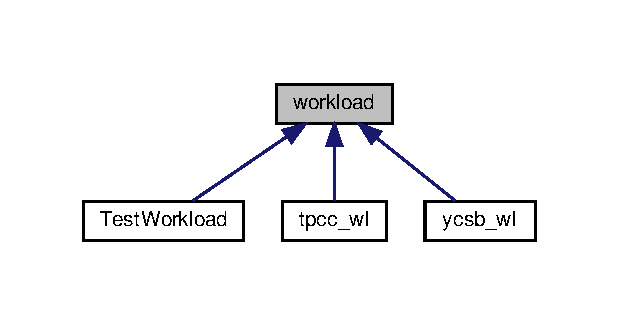
\includegraphics[width=297pt]{classworkload__inherit__graph}
\end{center}
\end{figure}
\subsection*{Public Member Functions}
\begin{DoxyCompactItemize}
\item 
virtual \hyperlink{global_8h_a78c49a674c810fdd03d20432f7be864a}{RC} \hyperlink{classworkload_a7cef7a7101c78e10082c99356e77a57c}{init} ()
\item 
virtual void \hyperlink{classworkload_a4614189e85fbaaf2003b7db4c2a7b8b9}{setbench\+\_\+deinit} ()
\item 
virtual \hyperlink{global_8h_a78c49a674c810fdd03d20432f7be864a}{RC} \hyperlink{classworkload_a12ce1550f8e398871961c6ff116c11d3}{init\+\_\+schema} (std\+::string schema\+\_\+file)
\item 
virtual \hyperlink{global_8h_a78c49a674c810fdd03d20432f7be864a}{RC} \hyperlink{classworkload_a3feee79af04069f6c1ad6b7f9b0a045a}{init\+\_\+table} ()=0
\item 
virtual \hyperlink{global_8h_a78c49a674c810fdd03d20432f7be864a}{RC} \hyperlink{classworkload_ac22d0558c3fc549b8b07347cebb95cb3}{get\+\_\+txn\+\_\+man} (\hyperlink{classtxn__man}{txn\+\_\+man} $\ast$\&txn\+\_\+manager, \hyperlink{classthread__t}{thread\+\_\+t} $\ast$h\+\_\+thd)=0
\item 
void \hyperlink{classworkload_ad33bfab447c5741ca4cf22b0deb5948e}{init\+Thread} (const int \hyperlink{microbench_2main_8cpp_a9ca9869868fe7e7a38a921cc7de4103f}{tid})
\item 
void \hyperlink{classworkload_a60bc113bb23268942b6fe36e99c47caa}{deinit\+Thread} (const int \hyperlink{microbench_2main_8cpp_a9ca9869868fe7e7a38a921cc7de4103f}{tid})
\end{DoxyCompactItemize}
\subsection*{Public Attributes}
\begin{DoxyCompactItemize}
\item 
map$<$ string, \hyperlink{classtable__t}{table\+\_\+t} $\ast$ $>$ \hyperlink{classworkload_a35ca60eab63190c0667225df31555677}{tables}
\item 
map$<$ string, \hyperlink{classIndex}{Index} $\ast$ $>$ \hyperlink{classworkload_a7b0952cf3cecba206343b2b22ee67ee9}{indexes}
\item 
bool \hyperlink{classworkload_adebf7ae095ae33d23c7bdd5c30a13787}{sim\+\_\+done}
\end{DoxyCompactItemize}
\subsection*{Protected Member Functions}
\begin{DoxyCompactItemize}
\item 
void \hyperlink{classworkload_ae88a8556d1384e6ba6bd5aa01dddaf60}{index\+\_\+insert} (std\+::string index\+\_\+name, uint64\+\_\+t key, \hyperlink{classrow__t}{row\+\_\+t} $\ast$row)
\item 
void \hyperlink{classworkload_a9fb849d3df28fea4e00353f046c130a2}{index\+\_\+insert} (\hyperlink{classIndex}{Index} $\ast$index, uint64\+\_\+t key, \hyperlink{classrow__t}{row\+\_\+t} $\ast$row, int64\+\_\+t part\+\_\+id=-\/1)
\end{DoxyCompactItemize}
\subsection*{Friends}
\begin{DoxyCompactItemize}
\item 
class \hyperlink{classworkload_a7e57327617727745c74d4598cc485212}{tpcc\+\_\+txn\+\_\+man}
\item 
class \hyperlink{classworkload_a128ce032b45a6a15c2dc63fe34da7d42}{txn\+\_\+man}
\end{DoxyCompactItemize}


\subsection{Member Function Documentation}
\mbox{\Hypertarget{classworkload_a60bc113bb23268942b6fe36e99c47caa}\label{classworkload_a60bc113bb23268942b6fe36e99c47caa}} 
\index{workload@{workload}!deinit\+Thread@{deinit\+Thread}}
\index{deinit\+Thread@{deinit\+Thread}!workload@{workload}}
\subsubsection{\texorpdfstring{deinit\+Thread()}{deinitThread()}}
{\footnotesize\ttfamily void workload\+::deinit\+Thread (\begin{DoxyParamCaption}\item[{const int}]{tid }\end{DoxyParamCaption})}

\mbox{\Hypertarget{classworkload_ac22d0558c3fc549b8b07347cebb95cb3}\label{classworkload_ac22d0558c3fc549b8b07347cebb95cb3}} 
\index{workload@{workload}!get\+\_\+txn\+\_\+man@{get\+\_\+txn\+\_\+man}}
\index{get\+\_\+txn\+\_\+man@{get\+\_\+txn\+\_\+man}!workload@{workload}}
\subsubsection{\texorpdfstring{get\+\_\+txn\+\_\+man()}{get\_txn\_man()}}
{\footnotesize\ttfamily virtual \hyperlink{global_8h_a78c49a674c810fdd03d20432f7be864a}{RC} workload\+::get\+\_\+txn\+\_\+man (\begin{DoxyParamCaption}\item[{\hyperlink{classtxn__man}{txn\+\_\+man} $\ast$\&}]{txn\+\_\+manager,  }\item[{\hyperlink{classthread__t}{thread\+\_\+t} $\ast$}]{h\+\_\+thd }\end{DoxyParamCaption})\hspace{0.3cm}{\ttfamily [pure virtual]}}



Implemented in \hyperlink{classtpcc__wl_a7794924fd334984a429b43e151ad040a}{tpcc\+\_\+wl}, \hyperlink{classycsb__wl_a31fb01819cd6a3517259ec9bb80066ca}{ycsb\+\_\+wl}, and \hyperlink{classTestWorkload_abc14a45ce19f90979f01cf2e96f1bb9f}{Test\+Workload}.

\mbox{\Hypertarget{classworkload_ae88a8556d1384e6ba6bd5aa01dddaf60}\label{classworkload_ae88a8556d1384e6ba6bd5aa01dddaf60}} 
\index{workload@{workload}!index\+\_\+insert@{index\+\_\+insert}}
\index{index\+\_\+insert@{index\+\_\+insert}!workload@{workload}}
\subsubsection{\texorpdfstring{index\+\_\+insert()}{index\_insert()}\hspace{0.1cm}{\footnotesize\ttfamily [1/2]}}
{\footnotesize\ttfamily void workload\+::index\+\_\+insert (\begin{DoxyParamCaption}\item[{std\+::string}]{index\+\_\+name,  }\item[{uint64\+\_\+t}]{key,  }\item[{\hyperlink{classrow__t}{row\+\_\+t} $\ast$}]{row }\end{DoxyParamCaption})\hspace{0.3cm}{\ttfamily [protected]}}

\mbox{\Hypertarget{classworkload_a9fb849d3df28fea4e00353f046c130a2}\label{classworkload_a9fb849d3df28fea4e00353f046c130a2}} 
\index{workload@{workload}!index\+\_\+insert@{index\+\_\+insert}}
\index{index\+\_\+insert@{index\+\_\+insert}!workload@{workload}}
\subsubsection{\texorpdfstring{index\+\_\+insert()}{index\_insert()}\hspace{0.1cm}{\footnotesize\ttfamily [2/2]}}
{\footnotesize\ttfamily void workload\+::index\+\_\+insert (\begin{DoxyParamCaption}\item[{\hyperlink{classIndex}{Index} $\ast$}]{index,  }\item[{uint64\+\_\+t}]{key,  }\item[{\hyperlink{classrow__t}{row\+\_\+t} $\ast$}]{row,  }\item[{int64\+\_\+t}]{part\+\_\+id = {\ttfamily -\/1} }\end{DoxyParamCaption})\hspace{0.3cm}{\ttfamily [protected]}}

\mbox{\Hypertarget{classworkload_a7cef7a7101c78e10082c99356e77a57c}\label{classworkload_a7cef7a7101c78e10082c99356e77a57c}} 
\index{workload@{workload}!init@{init}}
\index{init@{init}!workload@{workload}}
\subsubsection{\texorpdfstring{init()}{init()}}
{\footnotesize\ttfamily \hyperlink{global_8h_a78c49a674c810fdd03d20432f7be864a}{RC} workload\+::init (\begin{DoxyParamCaption}{ }\end{DoxyParamCaption})\hspace{0.3cm}{\ttfamily [virtual]}}



Reimplemented in \hyperlink{classtpcc__wl_a084aa9016fbc3abbb278f1c4bd15722c}{tpcc\+\_\+wl}, \hyperlink{classycsb__wl_ab457878c0f802cbbbf9ff27979e0eda6}{ycsb\+\_\+wl}, and \hyperlink{classTestWorkload_aba95b44e0531c1ff81d9846bcd7df8ba}{Test\+Workload}.

\mbox{\Hypertarget{classworkload_a12ce1550f8e398871961c6ff116c11d3}\label{classworkload_a12ce1550f8e398871961c6ff116c11d3}} 
\index{workload@{workload}!init\+\_\+schema@{init\+\_\+schema}}
\index{init\+\_\+schema@{init\+\_\+schema}!workload@{workload}}
\subsubsection{\texorpdfstring{init\+\_\+schema()}{init\_schema()}}
{\footnotesize\ttfamily \hyperlink{global_8h_a78c49a674c810fdd03d20432f7be864a}{RC} workload\+::init\+\_\+schema (\begin{DoxyParamCaption}\item[{std\+::string}]{schema\+\_\+file }\end{DoxyParamCaption})\hspace{0.3cm}{\ttfamily [virtual]}}



Reimplemented in \hyperlink{classycsb__wl_a3f1937f438c251831694b39b6e9dc36d}{ycsb\+\_\+wl}.

\mbox{\Hypertarget{classworkload_a3feee79af04069f6c1ad6b7f9b0a045a}\label{classworkload_a3feee79af04069f6c1ad6b7f9b0a045a}} 
\index{workload@{workload}!init\+\_\+table@{init\+\_\+table}}
\index{init\+\_\+table@{init\+\_\+table}!workload@{workload}}
\subsubsection{\texorpdfstring{init\+\_\+table()}{init\_table()}}
{\footnotesize\ttfamily virtual \hyperlink{global_8h_a78c49a674c810fdd03d20432f7be864a}{RC} workload\+::init\+\_\+table (\begin{DoxyParamCaption}{ }\end{DoxyParamCaption})\hspace{0.3cm}{\ttfamily [pure virtual]}}



Implemented in \hyperlink{classtpcc__wl_a84fd48d9c4ee95eb6176e9fdf9efd8b7}{tpcc\+\_\+wl}, \hyperlink{classycsb__wl_a2e1e8d6e68e5312a82cfe09ec4bb26a6}{ycsb\+\_\+wl}, and \hyperlink{classTestWorkload_a4963c5307360dc96391779393a1571dc}{Test\+Workload}.

\mbox{\Hypertarget{classworkload_ad33bfab447c5741ca4cf22b0deb5948e}\label{classworkload_ad33bfab447c5741ca4cf22b0deb5948e}} 
\index{workload@{workload}!init\+Thread@{init\+Thread}}
\index{init\+Thread@{init\+Thread}!workload@{workload}}
\subsubsection{\texorpdfstring{init\+Thread()}{initThread()}}
{\footnotesize\ttfamily void workload\+::init\+Thread (\begin{DoxyParamCaption}\item[{const int}]{tid }\end{DoxyParamCaption})}

\mbox{\Hypertarget{classworkload_a4614189e85fbaaf2003b7db4c2a7b8b9}\label{classworkload_a4614189e85fbaaf2003b7db4c2a7b8b9}} 
\index{workload@{workload}!setbench\+\_\+deinit@{setbench\+\_\+deinit}}
\index{setbench\+\_\+deinit@{setbench\+\_\+deinit}!workload@{workload}}
\subsubsection{\texorpdfstring{setbench\+\_\+deinit()}{setbench\_deinit()}}
{\footnotesize\ttfamily void workload\+::setbench\+\_\+deinit (\begin{DoxyParamCaption}{ }\end{DoxyParamCaption})\hspace{0.3cm}{\ttfamily [virtual]}}



Reimplemented in \hyperlink{classtpcc__wl_ac89b938cbaf311844d79f3946df49005}{tpcc\+\_\+wl}, and \hyperlink{classycsb__wl_aba11708593028b3cea7986adb280aae3}{ycsb\+\_\+wl}.



\subsection{Friends And Related Function Documentation}
\mbox{\Hypertarget{classworkload_a7e57327617727745c74d4598cc485212}\label{classworkload_a7e57327617727745c74d4598cc485212}} 
\index{workload@{workload}!tpcc\+\_\+txn\+\_\+man@{tpcc\+\_\+txn\+\_\+man}}
\index{tpcc\+\_\+txn\+\_\+man@{tpcc\+\_\+txn\+\_\+man}!workload@{workload}}
\subsubsection{\texorpdfstring{tpcc\+\_\+txn\+\_\+man}{tpcc\_txn\_man}}
{\footnotesize\ttfamily friend class \hyperlink{classtpcc__txn__man}{tpcc\+\_\+txn\+\_\+man}\hspace{0.3cm}{\ttfamily [friend]}}

\mbox{\Hypertarget{classworkload_a128ce032b45a6a15c2dc63fe34da7d42}\label{classworkload_a128ce032b45a6a15c2dc63fe34da7d42}} 
\index{workload@{workload}!txn\+\_\+man@{txn\+\_\+man}}
\index{txn\+\_\+man@{txn\+\_\+man}!workload@{workload}}
\subsubsection{\texorpdfstring{txn\+\_\+man}{txn\_man}}
{\footnotesize\ttfamily friend class \hyperlink{classtxn__man}{txn\+\_\+man}\hspace{0.3cm}{\ttfamily [friend]}}



\subsection{Member Data Documentation}
\mbox{\Hypertarget{classworkload_a7b0952cf3cecba206343b2b22ee67ee9}\label{classworkload_a7b0952cf3cecba206343b2b22ee67ee9}} 
\index{workload@{workload}!indexes@{indexes}}
\index{indexes@{indexes}!workload@{workload}}
\subsubsection{\texorpdfstring{indexes}{indexes}}
{\footnotesize\ttfamily map$<$string, \hyperlink{classIndex}{Index} $\ast$$>$ workload\+::indexes}

\mbox{\Hypertarget{classworkload_adebf7ae095ae33d23c7bdd5c30a13787}\label{classworkload_adebf7ae095ae33d23c7bdd5c30a13787}} 
\index{workload@{workload}!sim\+\_\+done@{sim\+\_\+done}}
\index{sim\+\_\+done@{sim\+\_\+done}!workload@{workload}}
\subsubsection{\texorpdfstring{sim\+\_\+done}{sim\_done}}
{\footnotesize\ttfamily bool workload\+::sim\+\_\+done}

\mbox{\Hypertarget{classworkload_a35ca60eab63190c0667225df31555677}\label{classworkload_a35ca60eab63190c0667225df31555677}} 
\index{workload@{workload}!tables@{tables}}
\index{tables@{tables}!workload@{workload}}
\subsubsection{\texorpdfstring{tables}{tables}}
{\footnotesize\ttfamily map$<$string, \hyperlink{classtable__t}{table\+\_\+t} $\ast$$>$ workload\+::tables}



The documentation for this class was generated from the following files\+:\begin{DoxyCompactItemize}
\item 
macrobench/system/\hyperlink{wl_8h}{wl.\+h}\item 
macrobench/system/\hyperlink{wl_8cpp}{wl.\+cpp}\end{DoxyCompactItemize}

\hypertarget{classabtree__ns_1_1wrapper__info}{}\section{abtree\+\_\+ns\+:\+:wrapper\+\_\+info$<$ D\+E\+G\+R\+EE, K $>$ Class Template Reference}
\label{classabtree__ns_1_1wrapper__info}\index{abtree\+\_\+ns\+::wrapper\+\_\+info$<$ D\+E\+G\+R\+E\+E, K $>$@{abtree\+\_\+ns\+::wrapper\+\_\+info$<$ D\+E\+G\+R\+E\+E, K $>$}}


{\ttfamily \#include $<$brown\+\_\+ext\+\_\+abtree\+\_\+lf\+\_\+impl.\+h$>$}

\subsection*{Public Attributes}
\begin{DoxyCompactItemize}
\item 
\hyperlink{structabtree__ns_1_1Node}{Node}$<$ \hyperlink{brown__sigouin__abtree__kcas_2adapter_8h_a5d88b17d70c985f2f2b8e987037fd6dd}{D\+E\+G\+R\+EE}, K $>$ $\ast$ \hyperlink{classabtree__ns_1_1wrapper__info_a6babdd3bb46ab432e506401eef25a5b2}{nodes} \mbox{[}\hyperlink{classabtree__ns_1_1wrapper__info_a8ebdd932eb6c4c88615fbb76b8419d9e}{M\+A\+X\+\_\+\+N\+O\+D\+ES}\mbox{]}
\item 
\hyperlink{structabtree__ns_1_1SCXRecord}{S\+C\+X\+Record}$<$ \hyperlink{brown__sigouin__abtree__kcas_2adapter_8h_a5d88b17d70c985f2f2b8e987037fd6dd}{D\+E\+G\+R\+EE}, K $>$ $\ast$ \hyperlink{classabtree__ns_1_1wrapper__info_a531a8a2aaf6256dd25d0b6ca8a1e6ced}{scx\+Ptrs} \mbox{[}\hyperlink{classabtree__ns_1_1wrapper__info_a8ebdd932eb6c4c88615fbb76b8419d9e}{M\+A\+X\+\_\+\+N\+O\+D\+ES}\mbox{]}
\item 
\hyperlink{structabtree__ns_1_1Node}{Node}$<$ \hyperlink{brown__sigouin__abtree__kcas_2adapter_8h_a5d88b17d70c985f2f2b8e987037fd6dd}{D\+E\+G\+R\+EE}, K $>$ $\ast$ \hyperlink{classabtree__ns_1_1wrapper__info_a5517be33957e4aace41140dad1738ef4}{new\+Node}
\item 
\hyperlink{structabtree__ns_1_1Node}{Node}$<$ \hyperlink{brown__sigouin__abtree__kcas_2adapter_8h_a5d88b17d70c985f2f2b8e987037fd6dd}{D\+E\+G\+R\+EE}, K $>$ $\ast$volatile $\ast$ \hyperlink{classabtree__ns_1_1wrapper__info_a768ca52b1b5ec8730ea982e9a8aaeb48}{field}
\item 
int \hyperlink{classabtree__ns_1_1wrapper__info_a433955bf061f62ec2942f2eacdd5a299}{state}
\item 
char \hyperlink{classabtree__ns_1_1wrapper__info_a43563c0b9d50c77a1619f219e09a6eb0}{number\+Of\+Nodes}
\item 
char \hyperlink{classabtree__ns_1_1wrapper__info_a6f82a59bb872ece248f3a6603404f289}{number\+Of\+Nodes\+To\+Freeze}
\item 
char \hyperlink{classabtree__ns_1_1wrapper__info_aa902b7a21461bae3975b67ba4f39a6c6}{number\+Of\+Nodes\+Allocated}
\item 
\hyperlink{structabtree__ns_1_1Node}{Node}$<$ \hyperlink{brown__sigouin__abtree__kcas_2adapter_8h_a5d88b17d70c985f2f2b8e987037fd6dd}{D\+E\+G\+R\+EE}, K $>$ $\ast$ \hyperlink{classabtree__ns_1_1wrapper__info_a195b04f001a1df664ccf438f289a6990}{inserted\+Nodes} \mbox{[}\hyperlink{classabtree__ns_1_1wrapper__info_a8ebdd932eb6c4c88615fbb76b8419d9e}{M\+A\+X\+\_\+\+N\+O\+D\+ES}+1\mbox{]}
\item 
\hyperlink{structabtree__ns_1_1Node}{Node}$<$ \hyperlink{brown__sigouin__abtree__kcas_2adapter_8h_a5d88b17d70c985f2f2b8e987037fd6dd}{D\+E\+G\+R\+EE}, K $>$ $\ast$ \hyperlink{classabtree__ns_1_1wrapper__info_a33d0c34514ac8443085ae78e5702fd15}{deleted\+Nodes} \mbox{[}\hyperlink{classabtree__ns_1_1wrapper__info_a8ebdd932eb6c4c88615fbb76b8419d9e}{M\+A\+X\+\_\+\+N\+O\+D\+ES}+1\mbox{]}
\end{DoxyCompactItemize}
\subsection*{Static Public Attributes}
\begin{DoxyCompactItemize}
\item 
static const int \hyperlink{classabtree__ns_1_1wrapper__info_a8ebdd932eb6c4c88615fbb76b8419d9e}{M\+A\+X\+\_\+\+N\+O\+D\+ES} = \hyperlink{brown__sigouin__abtree__kcas_2adapter_8h_a5d88b17d70c985f2f2b8e987037fd6dd}{D\+E\+G\+R\+EE}+2
\end{DoxyCompactItemize}


\subsection{Member Data Documentation}
\mbox{\Hypertarget{classabtree__ns_1_1wrapper__info_a33d0c34514ac8443085ae78e5702fd15}\label{classabtree__ns_1_1wrapper__info_a33d0c34514ac8443085ae78e5702fd15}} 
\index{abtree\+\_\+ns\+::wrapper\+\_\+info@{abtree\+\_\+ns\+::wrapper\+\_\+info}!deleted\+Nodes@{deleted\+Nodes}}
\index{deleted\+Nodes@{deleted\+Nodes}!abtree\+\_\+ns\+::wrapper\+\_\+info@{abtree\+\_\+ns\+::wrapper\+\_\+info}}
\subsubsection{\texorpdfstring{deleted\+Nodes}{deletedNodes}}
{\footnotesize\ttfamily template$<$int D\+E\+G\+R\+EE, typename K$>$ \\
\hyperlink{structabtree__ns_1_1Node}{Node}$<$\hyperlink{brown__sigouin__abtree__kcas_2adapter_8h_a5d88b17d70c985f2f2b8e987037fd6dd}{D\+E\+G\+R\+EE},K$>$$\ast$ \hyperlink{classabtree__ns_1_1wrapper__info}{abtree\+\_\+ns\+::wrapper\+\_\+info}$<$ \hyperlink{brown__sigouin__abtree__kcas_2adapter_8h_a5d88b17d70c985f2f2b8e987037fd6dd}{D\+E\+G\+R\+EE}, K $>$\+::deleted\+Nodes\mbox{[}\hyperlink{classabtree__ns_1_1wrapper__info_a8ebdd932eb6c4c88615fbb76b8419d9e}{M\+A\+X\+\_\+\+N\+O\+D\+ES}+1\mbox{]}}

\mbox{\Hypertarget{classabtree__ns_1_1wrapper__info_a768ca52b1b5ec8730ea982e9a8aaeb48}\label{classabtree__ns_1_1wrapper__info_a768ca52b1b5ec8730ea982e9a8aaeb48}} 
\index{abtree\+\_\+ns\+::wrapper\+\_\+info@{abtree\+\_\+ns\+::wrapper\+\_\+info}!field@{field}}
\index{field@{field}!abtree\+\_\+ns\+::wrapper\+\_\+info@{abtree\+\_\+ns\+::wrapper\+\_\+info}}
\subsubsection{\texorpdfstring{field}{field}}
{\footnotesize\ttfamily template$<$int D\+E\+G\+R\+EE, typename K$>$ \\
\hyperlink{structabtree__ns_1_1Node}{Node}$<$\hyperlink{brown__sigouin__abtree__kcas_2adapter_8h_a5d88b17d70c985f2f2b8e987037fd6dd}{D\+E\+G\+R\+EE},K$>$$\ast$ volatile$\ast$ \hyperlink{classabtree__ns_1_1wrapper__info}{abtree\+\_\+ns\+::wrapper\+\_\+info}$<$ \hyperlink{brown__sigouin__abtree__kcas_2adapter_8h_a5d88b17d70c985f2f2b8e987037fd6dd}{D\+E\+G\+R\+EE}, K $>$\+::field}

\mbox{\Hypertarget{classabtree__ns_1_1wrapper__info_a195b04f001a1df664ccf438f289a6990}\label{classabtree__ns_1_1wrapper__info_a195b04f001a1df664ccf438f289a6990}} 
\index{abtree\+\_\+ns\+::wrapper\+\_\+info@{abtree\+\_\+ns\+::wrapper\+\_\+info}!inserted\+Nodes@{inserted\+Nodes}}
\index{inserted\+Nodes@{inserted\+Nodes}!abtree\+\_\+ns\+::wrapper\+\_\+info@{abtree\+\_\+ns\+::wrapper\+\_\+info}}
\subsubsection{\texorpdfstring{inserted\+Nodes}{insertedNodes}}
{\footnotesize\ttfamily template$<$int D\+E\+G\+R\+EE, typename K$>$ \\
\hyperlink{structabtree__ns_1_1Node}{Node}$<$\hyperlink{brown__sigouin__abtree__kcas_2adapter_8h_a5d88b17d70c985f2f2b8e987037fd6dd}{D\+E\+G\+R\+EE},K$>$$\ast$ \hyperlink{classabtree__ns_1_1wrapper__info}{abtree\+\_\+ns\+::wrapper\+\_\+info}$<$ \hyperlink{brown__sigouin__abtree__kcas_2adapter_8h_a5d88b17d70c985f2f2b8e987037fd6dd}{D\+E\+G\+R\+EE}, K $>$\+::inserted\+Nodes\mbox{[}\hyperlink{classabtree__ns_1_1wrapper__info_a8ebdd932eb6c4c88615fbb76b8419d9e}{M\+A\+X\+\_\+\+N\+O\+D\+ES}+1\mbox{]}}

\mbox{\Hypertarget{classabtree__ns_1_1wrapper__info_a8ebdd932eb6c4c88615fbb76b8419d9e}\label{classabtree__ns_1_1wrapper__info_a8ebdd932eb6c4c88615fbb76b8419d9e}} 
\index{abtree\+\_\+ns\+::wrapper\+\_\+info@{abtree\+\_\+ns\+::wrapper\+\_\+info}!M\+A\+X\+\_\+\+N\+O\+D\+ES@{M\+A\+X\+\_\+\+N\+O\+D\+ES}}
\index{M\+A\+X\+\_\+\+N\+O\+D\+ES@{M\+A\+X\+\_\+\+N\+O\+D\+ES}!abtree\+\_\+ns\+::wrapper\+\_\+info@{abtree\+\_\+ns\+::wrapper\+\_\+info}}
\subsubsection{\texorpdfstring{M\+A\+X\+\_\+\+N\+O\+D\+ES}{MAX\_NODES}}
{\footnotesize\ttfamily template$<$int D\+E\+G\+R\+EE, typename K$>$ \\
const int \hyperlink{classabtree__ns_1_1wrapper__info}{abtree\+\_\+ns\+::wrapper\+\_\+info}$<$ \hyperlink{brown__sigouin__abtree__kcas_2adapter_8h_a5d88b17d70c985f2f2b8e987037fd6dd}{D\+E\+G\+R\+EE}, K $>$\+::M\+A\+X\+\_\+\+N\+O\+D\+ES = \hyperlink{brown__sigouin__abtree__kcas_2adapter_8h_a5d88b17d70c985f2f2b8e987037fd6dd}{D\+E\+G\+R\+EE}+2\hspace{0.3cm}{\ttfamily [static]}}

\mbox{\Hypertarget{classabtree__ns_1_1wrapper__info_a5517be33957e4aace41140dad1738ef4}\label{classabtree__ns_1_1wrapper__info_a5517be33957e4aace41140dad1738ef4}} 
\index{abtree\+\_\+ns\+::wrapper\+\_\+info@{abtree\+\_\+ns\+::wrapper\+\_\+info}!new\+Node@{new\+Node}}
\index{new\+Node@{new\+Node}!abtree\+\_\+ns\+::wrapper\+\_\+info@{abtree\+\_\+ns\+::wrapper\+\_\+info}}
\subsubsection{\texorpdfstring{new\+Node}{newNode}}
{\footnotesize\ttfamily template$<$int D\+E\+G\+R\+EE, typename K$>$ \\
\hyperlink{structabtree__ns_1_1Node}{Node}$<$\hyperlink{brown__sigouin__abtree__kcas_2adapter_8h_a5d88b17d70c985f2f2b8e987037fd6dd}{D\+E\+G\+R\+EE},K$>$$\ast$ \hyperlink{classabtree__ns_1_1wrapper__info}{abtree\+\_\+ns\+::wrapper\+\_\+info}$<$ \hyperlink{brown__sigouin__abtree__kcas_2adapter_8h_a5d88b17d70c985f2f2b8e987037fd6dd}{D\+E\+G\+R\+EE}, K $>$\+::new\+Node}

\mbox{\Hypertarget{classabtree__ns_1_1wrapper__info_a6babdd3bb46ab432e506401eef25a5b2}\label{classabtree__ns_1_1wrapper__info_a6babdd3bb46ab432e506401eef25a5b2}} 
\index{abtree\+\_\+ns\+::wrapper\+\_\+info@{abtree\+\_\+ns\+::wrapper\+\_\+info}!nodes@{nodes}}
\index{nodes@{nodes}!abtree\+\_\+ns\+::wrapper\+\_\+info@{abtree\+\_\+ns\+::wrapper\+\_\+info}}
\subsubsection{\texorpdfstring{nodes}{nodes}}
{\footnotesize\ttfamily template$<$int D\+E\+G\+R\+EE, typename K$>$ \\
\hyperlink{structabtree__ns_1_1Node}{Node}$<$\hyperlink{brown__sigouin__abtree__kcas_2adapter_8h_a5d88b17d70c985f2f2b8e987037fd6dd}{D\+E\+G\+R\+EE},K$>$$\ast$ \hyperlink{classabtree__ns_1_1wrapper__info}{abtree\+\_\+ns\+::wrapper\+\_\+info}$<$ \hyperlink{brown__sigouin__abtree__kcas_2adapter_8h_a5d88b17d70c985f2f2b8e987037fd6dd}{D\+E\+G\+R\+EE}, K $>$\+::nodes\mbox{[}\hyperlink{classabtree__ns_1_1wrapper__info_a8ebdd932eb6c4c88615fbb76b8419d9e}{M\+A\+X\+\_\+\+N\+O\+D\+ES}\mbox{]}}

\mbox{\Hypertarget{classabtree__ns_1_1wrapper__info_a43563c0b9d50c77a1619f219e09a6eb0}\label{classabtree__ns_1_1wrapper__info_a43563c0b9d50c77a1619f219e09a6eb0}} 
\index{abtree\+\_\+ns\+::wrapper\+\_\+info@{abtree\+\_\+ns\+::wrapper\+\_\+info}!number\+Of\+Nodes@{number\+Of\+Nodes}}
\index{number\+Of\+Nodes@{number\+Of\+Nodes}!abtree\+\_\+ns\+::wrapper\+\_\+info@{abtree\+\_\+ns\+::wrapper\+\_\+info}}
\subsubsection{\texorpdfstring{number\+Of\+Nodes}{numberOfNodes}}
{\footnotesize\ttfamily template$<$int D\+E\+G\+R\+EE, typename K$>$ \\
char \hyperlink{classabtree__ns_1_1wrapper__info}{abtree\+\_\+ns\+::wrapper\+\_\+info}$<$ \hyperlink{brown__sigouin__abtree__kcas_2adapter_8h_a5d88b17d70c985f2f2b8e987037fd6dd}{D\+E\+G\+R\+EE}, K $>$\+::number\+Of\+Nodes}

\mbox{\Hypertarget{classabtree__ns_1_1wrapper__info_aa902b7a21461bae3975b67ba4f39a6c6}\label{classabtree__ns_1_1wrapper__info_aa902b7a21461bae3975b67ba4f39a6c6}} 
\index{abtree\+\_\+ns\+::wrapper\+\_\+info@{abtree\+\_\+ns\+::wrapper\+\_\+info}!number\+Of\+Nodes\+Allocated@{number\+Of\+Nodes\+Allocated}}
\index{number\+Of\+Nodes\+Allocated@{number\+Of\+Nodes\+Allocated}!abtree\+\_\+ns\+::wrapper\+\_\+info@{abtree\+\_\+ns\+::wrapper\+\_\+info}}
\subsubsection{\texorpdfstring{number\+Of\+Nodes\+Allocated}{numberOfNodesAllocated}}
{\footnotesize\ttfamily template$<$int D\+E\+G\+R\+EE, typename K$>$ \\
char \hyperlink{classabtree__ns_1_1wrapper__info}{abtree\+\_\+ns\+::wrapper\+\_\+info}$<$ \hyperlink{brown__sigouin__abtree__kcas_2adapter_8h_a5d88b17d70c985f2f2b8e987037fd6dd}{D\+E\+G\+R\+EE}, K $>$\+::number\+Of\+Nodes\+Allocated}

\mbox{\Hypertarget{classabtree__ns_1_1wrapper__info_a6f82a59bb872ece248f3a6603404f289}\label{classabtree__ns_1_1wrapper__info_a6f82a59bb872ece248f3a6603404f289}} 
\index{abtree\+\_\+ns\+::wrapper\+\_\+info@{abtree\+\_\+ns\+::wrapper\+\_\+info}!number\+Of\+Nodes\+To\+Freeze@{number\+Of\+Nodes\+To\+Freeze}}
\index{number\+Of\+Nodes\+To\+Freeze@{number\+Of\+Nodes\+To\+Freeze}!abtree\+\_\+ns\+::wrapper\+\_\+info@{abtree\+\_\+ns\+::wrapper\+\_\+info}}
\subsubsection{\texorpdfstring{number\+Of\+Nodes\+To\+Freeze}{numberOfNodesToFreeze}}
{\footnotesize\ttfamily template$<$int D\+E\+G\+R\+EE, typename K$>$ \\
char \hyperlink{classabtree__ns_1_1wrapper__info}{abtree\+\_\+ns\+::wrapper\+\_\+info}$<$ \hyperlink{brown__sigouin__abtree__kcas_2adapter_8h_a5d88b17d70c985f2f2b8e987037fd6dd}{D\+E\+G\+R\+EE}, K $>$\+::number\+Of\+Nodes\+To\+Freeze}

\mbox{\Hypertarget{classabtree__ns_1_1wrapper__info_a531a8a2aaf6256dd25d0b6ca8a1e6ced}\label{classabtree__ns_1_1wrapper__info_a531a8a2aaf6256dd25d0b6ca8a1e6ced}} 
\index{abtree\+\_\+ns\+::wrapper\+\_\+info@{abtree\+\_\+ns\+::wrapper\+\_\+info}!scx\+Ptrs@{scx\+Ptrs}}
\index{scx\+Ptrs@{scx\+Ptrs}!abtree\+\_\+ns\+::wrapper\+\_\+info@{abtree\+\_\+ns\+::wrapper\+\_\+info}}
\subsubsection{\texorpdfstring{scx\+Ptrs}{scxPtrs}}
{\footnotesize\ttfamily template$<$int D\+E\+G\+R\+EE, typename K$>$ \\
\hyperlink{structabtree__ns_1_1SCXRecord}{S\+C\+X\+Record}$<$\hyperlink{brown__sigouin__abtree__kcas_2adapter_8h_a5d88b17d70c985f2f2b8e987037fd6dd}{D\+E\+G\+R\+EE},K$>$$\ast$ \hyperlink{classabtree__ns_1_1wrapper__info}{abtree\+\_\+ns\+::wrapper\+\_\+info}$<$ \hyperlink{brown__sigouin__abtree__kcas_2adapter_8h_a5d88b17d70c985f2f2b8e987037fd6dd}{D\+E\+G\+R\+EE}, K $>$\+::scx\+Ptrs\mbox{[}\hyperlink{classabtree__ns_1_1wrapper__info_a8ebdd932eb6c4c88615fbb76b8419d9e}{M\+A\+X\+\_\+\+N\+O\+D\+ES}\mbox{]}}

\mbox{\Hypertarget{classabtree__ns_1_1wrapper__info_a433955bf061f62ec2942f2eacdd5a299}\label{classabtree__ns_1_1wrapper__info_a433955bf061f62ec2942f2eacdd5a299}} 
\index{abtree\+\_\+ns\+::wrapper\+\_\+info@{abtree\+\_\+ns\+::wrapper\+\_\+info}!state@{state}}
\index{state@{state}!abtree\+\_\+ns\+::wrapper\+\_\+info@{abtree\+\_\+ns\+::wrapper\+\_\+info}}
\subsubsection{\texorpdfstring{state}{state}}
{\footnotesize\ttfamily template$<$int D\+E\+G\+R\+EE, typename K$>$ \\
int \hyperlink{classabtree__ns_1_1wrapper__info}{abtree\+\_\+ns\+::wrapper\+\_\+info}$<$ \hyperlink{brown__sigouin__abtree__kcas_2adapter_8h_a5d88b17d70c985f2f2b8e987037fd6dd}{D\+E\+G\+R\+EE}, K $>$\+::state}



The documentation for this class was generated from the following file\+:\begin{DoxyCompactItemize}
\item 
ds/brown\+\_\+ext\+\_\+abtree\+\_\+rq\+\_\+lf/\hyperlink{brown__ext__abtree__rq__lf_2brown__ext__abtree__lf__impl_8h}{brown\+\_\+ext\+\_\+abtree\+\_\+lf\+\_\+impl.\+h}\end{DoxyCompactItemize}

\hypertarget{classbslack__ns_1_1wrapper__info}{}\section{bslack\+\_\+ns\+:\+:wrapper\+\_\+info$<$ D\+E\+G\+R\+EE, K $>$ Class Template Reference}
\label{classbslack__ns_1_1wrapper__info}\index{bslack\+\_\+ns\+::wrapper\+\_\+info$<$ D\+E\+G\+R\+E\+E, K $>$@{bslack\+\_\+ns\+::wrapper\+\_\+info$<$ D\+E\+G\+R\+E\+E, K $>$}}


{\ttfamily \#include $<$bslack\+\_\+impl.\+h$>$}

\subsection*{Public Attributes}
\begin{DoxyCompactItemize}
\item 
\hyperlink{structbslack__ns_1_1Node}{Node}$<$ \hyperlink{brown__sigouin__abtree__kcas_2adapter_8h_a5d88b17d70c985f2f2b8e987037fd6dd}{D\+E\+G\+R\+EE}, K $>$ $\ast$ \hyperlink{classbslack__ns_1_1wrapper__info_a2d9b42a29455dc853a04def1360692db}{nodes} \mbox{[}\hyperlink{classbslack__ns_1_1wrapper__info_ab5bcd31a5ba96938aa04b6e43da441c4}{M\+A\+X\+\_\+\+N\+O\+D\+ES}\mbox{]}
\item 
\hyperlink{structbslack__ns_1_1SCXRecord}{S\+C\+X\+Record}$<$ \hyperlink{brown__sigouin__abtree__kcas_2adapter_8h_a5d88b17d70c985f2f2b8e987037fd6dd}{D\+E\+G\+R\+EE}, K $>$ $\ast$ \hyperlink{classbslack__ns_1_1wrapper__info_ac26a8c05631adb0c2bc967a2ca5c2153}{scx\+Ptrs} \mbox{[}\hyperlink{classbslack__ns_1_1wrapper__info_ab5bcd31a5ba96938aa04b6e43da441c4}{M\+A\+X\+\_\+\+N\+O\+D\+ES}\mbox{]}
\item 
\hyperlink{structbslack__ns_1_1Node}{Node}$<$ \hyperlink{brown__sigouin__abtree__kcas_2adapter_8h_a5d88b17d70c985f2f2b8e987037fd6dd}{D\+E\+G\+R\+EE}, K $>$ $\ast$ \hyperlink{classbslack__ns_1_1wrapper__info_ac1a673ff65ab005f74a70c12ec36ac77}{new\+Node}
\item 
\hyperlink{structbslack__ns_1_1Node}{Node}$<$ \hyperlink{brown__sigouin__abtree__kcas_2adapter_8h_a5d88b17d70c985f2f2b8e987037fd6dd}{D\+E\+G\+R\+EE}, K $>$ $\ast$volatile $\ast$ \hyperlink{classbslack__ns_1_1wrapper__info_a2990081b668c96ebdae6412f1b8086ff}{field}
\item 
int \hyperlink{classbslack__ns_1_1wrapper__info_a8c1a85f3b95ec25948a888edf88b6536}{state}
\item 
char \hyperlink{classbslack__ns_1_1wrapper__info_ab3e7f2a621bdeb213e54e45a98cc3d8d}{number\+Of\+Nodes}
\item 
char \hyperlink{classbslack__ns_1_1wrapper__info_ae638a51d89fc70f4924c21ffb5957f77}{number\+Of\+Nodes\+To\+Freeze}
\item 
char \hyperlink{classbslack__ns_1_1wrapper__info_a6daa6974ed40c90ff51a76d0ae155d1e}{number\+Of\+Nodes\+Allocated}
\item 
\hyperlink{structbslack__ns_1_1Node}{Node}$<$ \hyperlink{brown__sigouin__abtree__kcas_2adapter_8h_a5d88b17d70c985f2f2b8e987037fd6dd}{D\+E\+G\+R\+EE}, K $>$ $\ast$ \hyperlink{classbslack__ns_1_1wrapper__info_a17f79b301b37cc9167592860998a8aa8}{inserted\+Nodes} \mbox{[}\hyperlink{classbslack__ns_1_1wrapper__info_ab5bcd31a5ba96938aa04b6e43da441c4}{M\+A\+X\+\_\+\+N\+O\+D\+ES}+1\mbox{]}
\item 
\hyperlink{structbslack__ns_1_1Node}{Node}$<$ \hyperlink{brown__sigouin__abtree__kcas_2adapter_8h_a5d88b17d70c985f2f2b8e987037fd6dd}{D\+E\+G\+R\+EE}, K $>$ $\ast$ \hyperlink{classbslack__ns_1_1wrapper__info_a4d438c20f50d6020d2eefa186047e6c3}{deleted\+Nodes} \mbox{[}\hyperlink{classbslack__ns_1_1wrapper__info_ab5bcd31a5ba96938aa04b6e43da441c4}{M\+A\+X\+\_\+\+N\+O\+D\+ES}+1\mbox{]}
\end{DoxyCompactItemize}
\subsection*{Static Public Attributes}
\begin{DoxyCompactItemize}
\item 
static const int \hyperlink{classbslack__ns_1_1wrapper__info_ab5bcd31a5ba96938aa04b6e43da441c4}{M\+A\+X\+\_\+\+N\+O\+D\+ES} = \hyperlink{brown__sigouin__abtree__kcas_2adapter_8h_a5d88b17d70c985f2f2b8e987037fd6dd}{D\+E\+G\+R\+EE}+2
\end{DoxyCompactItemize}


\subsection{Member Data Documentation}
\mbox{\Hypertarget{classbslack__ns_1_1wrapper__info_a4d438c20f50d6020d2eefa186047e6c3}\label{classbslack__ns_1_1wrapper__info_a4d438c20f50d6020d2eefa186047e6c3}} 
\index{bslack\+\_\+ns\+::wrapper\+\_\+info@{bslack\+\_\+ns\+::wrapper\+\_\+info}!deleted\+Nodes@{deleted\+Nodes}}
\index{deleted\+Nodes@{deleted\+Nodes}!bslack\+\_\+ns\+::wrapper\+\_\+info@{bslack\+\_\+ns\+::wrapper\+\_\+info}}
\subsubsection{\texorpdfstring{deleted\+Nodes}{deletedNodes}}
{\footnotesize\ttfamily template$<$int D\+E\+G\+R\+EE, typename K$>$ \\
\hyperlink{structbslack__ns_1_1Node}{Node}$<$\hyperlink{brown__sigouin__abtree__kcas_2adapter_8h_a5d88b17d70c985f2f2b8e987037fd6dd}{D\+E\+G\+R\+EE},K$>$$\ast$ \hyperlink{classbslack__ns_1_1wrapper__info}{bslack\+\_\+ns\+::wrapper\+\_\+info}$<$ \hyperlink{brown__sigouin__abtree__kcas_2adapter_8h_a5d88b17d70c985f2f2b8e987037fd6dd}{D\+E\+G\+R\+EE}, K $>$\+::deleted\+Nodes\mbox{[}\hyperlink{classbslack__ns_1_1wrapper__info_ab5bcd31a5ba96938aa04b6e43da441c4}{M\+A\+X\+\_\+\+N\+O\+D\+ES}+1\mbox{]}}

\mbox{\Hypertarget{classbslack__ns_1_1wrapper__info_a2990081b668c96ebdae6412f1b8086ff}\label{classbslack__ns_1_1wrapper__info_a2990081b668c96ebdae6412f1b8086ff}} 
\index{bslack\+\_\+ns\+::wrapper\+\_\+info@{bslack\+\_\+ns\+::wrapper\+\_\+info}!field@{field}}
\index{field@{field}!bslack\+\_\+ns\+::wrapper\+\_\+info@{bslack\+\_\+ns\+::wrapper\+\_\+info}}
\subsubsection{\texorpdfstring{field}{field}}
{\footnotesize\ttfamily template$<$int D\+E\+G\+R\+EE, typename K$>$ \\
\hyperlink{structbslack__ns_1_1Node}{Node}$<$\hyperlink{brown__sigouin__abtree__kcas_2adapter_8h_a5d88b17d70c985f2f2b8e987037fd6dd}{D\+E\+G\+R\+EE},K$>$$\ast$ volatile$\ast$ \hyperlink{classbslack__ns_1_1wrapper__info}{bslack\+\_\+ns\+::wrapper\+\_\+info}$<$ \hyperlink{brown__sigouin__abtree__kcas_2adapter_8h_a5d88b17d70c985f2f2b8e987037fd6dd}{D\+E\+G\+R\+EE}, K $>$\+::field}

\mbox{\Hypertarget{classbslack__ns_1_1wrapper__info_a17f79b301b37cc9167592860998a8aa8}\label{classbslack__ns_1_1wrapper__info_a17f79b301b37cc9167592860998a8aa8}} 
\index{bslack\+\_\+ns\+::wrapper\+\_\+info@{bslack\+\_\+ns\+::wrapper\+\_\+info}!inserted\+Nodes@{inserted\+Nodes}}
\index{inserted\+Nodes@{inserted\+Nodes}!bslack\+\_\+ns\+::wrapper\+\_\+info@{bslack\+\_\+ns\+::wrapper\+\_\+info}}
\subsubsection{\texorpdfstring{inserted\+Nodes}{insertedNodes}}
{\footnotesize\ttfamily template$<$int D\+E\+G\+R\+EE, typename K$>$ \\
\hyperlink{structbslack__ns_1_1Node}{Node}$<$\hyperlink{brown__sigouin__abtree__kcas_2adapter_8h_a5d88b17d70c985f2f2b8e987037fd6dd}{D\+E\+G\+R\+EE},K$>$$\ast$ \hyperlink{classbslack__ns_1_1wrapper__info}{bslack\+\_\+ns\+::wrapper\+\_\+info}$<$ \hyperlink{brown__sigouin__abtree__kcas_2adapter_8h_a5d88b17d70c985f2f2b8e987037fd6dd}{D\+E\+G\+R\+EE}, K $>$\+::inserted\+Nodes\mbox{[}\hyperlink{classbslack__ns_1_1wrapper__info_ab5bcd31a5ba96938aa04b6e43da441c4}{M\+A\+X\+\_\+\+N\+O\+D\+ES}+1\mbox{]}}

\mbox{\Hypertarget{classbslack__ns_1_1wrapper__info_ab5bcd31a5ba96938aa04b6e43da441c4}\label{classbslack__ns_1_1wrapper__info_ab5bcd31a5ba96938aa04b6e43da441c4}} 
\index{bslack\+\_\+ns\+::wrapper\+\_\+info@{bslack\+\_\+ns\+::wrapper\+\_\+info}!M\+A\+X\+\_\+\+N\+O\+D\+ES@{M\+A\+X\+\_\+\+N\+O\+D\+ES}}
\index{M\+A\+X\+\_\+\+N\+O\+D\+ES@{M\+A\+X\+\_\+\+N\+O\+D\+ES}!bslack\+\_\+ns\+::wrapper\+\_\+info@{bslack\+\_\+ns\+::wrapper\+\_\+info}}
\subsubsection{\texorpdfstring{M\+A\+X\+\_\+\+N\+O\+D\+ES}{MAX\_NODES}}
{\footnotesize\ttfamily template$<$int D\+E\+G\+R\+EE, typename K$>$ \\
const int \hyperlink{classbslack__ns_1_1wrapper__info}{bslack\+\_\+ns\+::wrapper\+\_\+info}$<$ \hyperlink{brown__sigouin__abtree__kcas_2adapter_8h_a5d88b17d70c985f2f2b8e987037fd6dd}{D\+E\+G\+R\+EE}, K $>$\+::M\+A\+X\+\_\+\+N\+O\+D\+ES = \hyperlink{brown__sigouin__abtree__kcas_2adapter_8h_a5d88b17d70c985f2f2b8e987037fd6dd}{D\+E\+G\+R\+EE}+2\hspace{0.3cm}{\ttfamily [static]}}

\mbox{\Hypertarget{classbslack__ns_1_1wrapper__info_ac1a673ff65ab005f74a70c12ec36ac77}\label{classbslack__ns_1_1wrapper__info_ac1a673ff65ab005f74a70c12ec36ac77}} 
\index{bslack\+\_\+ns\+::wrapper\+\_\+info@{bslack\+\_\+ns\+::wrapper\+\_\+info}!new\+Node@{new\+Node}}
\index{new\+Node@{new\+Node}!bslack\+\_\+ns\+::wrapper\+\_\+info@{bslack\+\_\+ns\+::wrapper\+\_\+info}}
\subsubsection{\texorpdfstring{new\+Node}{newNode}}
{\footnotesize\ttfamily template$<$int D\+E\+G\+R\+EE, typename K$>$ \\
\hyperlink{structbslack__ns_1_1Node}{Node}$<$\hyperlink{brown__sigouin__abtree__kcas_2adapter_8h_a5d88b17d70c985f2f2b8e987037fd6dd}{D\+E\+G\+R\+EE},K$>$$\ast$ \hyperlink{classbslack__ns_1_1wrapper__info}{bslack\+\_\+ns\+::wrapper\+\_\+info}$<$ \hyperlink{brown__sigouin__abtree__kcas_2adapter_8h_a5d88b17d70c985f2f2b8e987037fd6dd}{D\+E\+G\+R\+EE}, K $>$\+::new\+Node}

\mbox{\Hypertarget{classbslack__ns_1_1wrapper__info_a2d9b42a29455dc853a04def1360692db}\label{classbslack__ns_1_1wrapper__info_a2d9b42a29455dc853a04def1360692db}} 
\index{bslack\+\_\+ns\+::wrapper\+\_\+info@{bslack\+\_\+ns\+::wrapper\+\_\+info}!nodes@{nodes}}
\index{nodes@{nodes}!bslack\+\_\+ns\+::wrapper\+\_\+info@{bslack\+\_\+ns\+::wrapper\+\_\+info}}
\subsubsection{\texorpdfstring{nodes}{nodes}}
{\footnotesize\ttfamily template$<$int D\+E\+G\+R\+EE, typename K$>$ \\
\hyperlink{structbslack__ns_1_1Node}{Node}$<$\hyperlink{brown__sigouin__abtree__kcas_2adapter_8h_a5d88b17d70c985f2f2b8e987037fd6dd}{D\+E\+G\+R\+EE},K$>$$\ast$ \hyperlink{classbslack__ns_1_1wrapper__info}{bslack\+\_\+ns\+::wrapper\+\_\+info}$<$ \hyperlink{brown__sigouin__abtree__kcas_2adapter_8h_a5d88b17d70c985f2f2b8e987037fd6dd}{D\+E\+G\+R\+EE}, K $>$\+::nodes\mbox{[}\hyperlink{classbslack__ns_1_1wrapper__info_ab5bcd31a5ba96938aa04b6e43da441c4}{M\+A\+X\+\_\+\+N\+O\+D\+ES}\mbox{]}}

\mbox{\Hypertarget{classbslack__ns_1_1wrapper__info_ab3e7f2a621bdeb213e54e45a98cc3d8d}\label{classbslack__ns_1_1wrapper__info_ab3e7f2a621bdeb213e54e45a98cc3d8d}} 
\index{bslack\+\_\+ns\+::wrapper\+\_\+info@{bslack\+\_\+ns\+::wrapper\+\_\+info}!number\+Of\+Nodes@{number\+Of\+Nodes}}
\index{number\+Of\+Nodes@{number\+Of\+Nodes}!bslack\+\_\+ns\+::wrapper\+\_\+info@{bslack\+\_\+ns\+::wrapper\+\_\+info}}
\subsubsection{\texorpdfstring{number\+Of\+Nodes}{numberOfNodes}}
{\footnotesize\ttfamily template$<$int D\+E\+G\+R\+EE, typename K$>$ \\
char \hyperlink{classbslack__ns_1_1wrapper__info}{bslack\+\_\+ns\+::wrapper\+\_\+info}$<$ \hyperlink{brown__sigouin__abtree__kcas_2adapter_8h_a5d88b17d70c985f2f2b8e987037fd6dd}{D\+E\+G\+R\+EE}, K $>$\+::number\+Of\+Nodes}

\mbox{\Hypertarget{classbslack__ns_1_1wrapper__info_a6daa6974ed40c90ff51a76d0ae155d1e}\label{classbslack__ns_1_1wrapper__info_a6daa6974ed40c90ff51a76d0ae155d1e}} 
\index{bslack\+\_\+ns\+::wrapper\+\_\+info@{bslack\+\_\+ns\+::wrapper\+\_\+info}!number\+Of\+Nodes\+Allocated@{number\+Of\+Nodes\+Allocated}}
\index{number\+Of\+Nodes\+Allocated@{number\+Of\+Nodes\+Allocated}!bslack\+\_\+ns\+::wrapper\+\_\+info@{bslack\+\_\+ns\+::wrapper\+\_\+info}}
\subsubsection{\texorpdfstring{number\+Of\+Nodes\+Allocated}{numberOfNodesAllocated}}
{\footnotesize\ttfamily template$<$int D\+E\+G\+R\+EE, typename K$>$ \\
char \hyperlink{classbslack__ns_1_1wrapper__info}{bslack\+\_\+ns\+::wrapper\+\_\+info}$<$ \hyperlink{brown__sigouin__abtree__kcas_2adapter_8h_a5d88b17d70c985f2f2b8e987037fd6dd}{D\+E\+G\+R\+EE}, K $>$\+::number\+Of\+Nodes\+Allocated}

\mbox{\Hypertarget{classbslack__ns_1_1wrapper__info_ae638a51d89fc70f4924c21ffb5957f77}\label{classbslack__ns_1_1wrapper__info_ae638a51d89fc70f4924c21ffb5957f77}} 
\index{bslack\+\_\+ns\+::wrapper\+\_\+info@{bslack\+\_\+ns\+::wrapper\+\_\+info}!number\+Of\+Nodes\+To\+Freeze@{number\+Of\+Nodes\+To\+Freeze}}
\index{number\+Of\+Nodes\+To\+Freeze@{number\+Of\+Nodes\+To\+Freeze}!bslack\+\_\+ns\+::wrapper\+\_\+info@{bslack\+\_\+ns\+::wrapper\+\_\+info}}
\subsubsection{\texorpdfstring{number\+Of\+Nodes\+To\+Freeze}{numberOfNodesToFreeze}}
{\footnotesize\ttfamily template$<$int D\+E\+G\+R\+EE, typename K$>$ \\
char \hyperlink{classbslack__ns_1_1wrapper__info}{bslack\+\_\+ns\+::wrapper\+\_\+info}$<$ \hyperlink{brown__sigouin__abtree__kcas_2adapter_8h_a5d88b17d70c985f2f2b8e987037fd6dd}{D\+E\+G\+R\+EE}, K $>$\+::number\+Of\+Nodes\+To\+Freeze}

\mbox{\Hypertarget{classbslack__ns_1_1wrapper__info_ac26a8c05631adb0c2bc967a2ca5c2153}\label{classbslack__ns_1_1wrapper__info_ac26a8c05631adb0c2bc967a2ca5c2153}} 
\index{bslack\+\_\+ns\+::wrapper\+\_\+info@{bslack\+\_\+ns\+::wrapper\+\_\+info}!scx\+Ptrs@{scx\+Ptrs}}
\index{scx\+Ptrs@{scx\+Ptrs}!bslack\+\_\+ns\+::wrapper\+\_\+info@{bslack\+\_\+ns\+::wrapper\+\_\+info}}
\subsubsection{\texorpdfstring{scx\+Ptrs}{scxPtrs}}
{\footnotesize\ttfamily template$<$int D\+E\+G\+R\+EE, typename K$>$ \\
\hyperlink{structbslack__ns_1_1SCXRecord}{S\+C\+X\+Record}$<$\hyperlink{brown__sigouin__abtree__kcas_2adapter_8h_a5d88b17d70c985f2f2b8e987037fd6dd}{D\+E\+G\+R\+EE},K$>$$\ast$ \hyperlink{classbslack__ns_1_1wrapper__info}{bslack\+\_\+ns\+::wrapper\+\_\+info}$<$ \hyperlink{brown__sigouin__abtree__kcas_2adapter_8h_a5d88b17d70c985f2f2b8e987037fd6dd}{D\+E\+G\+R\+EE}, K $>$\+::scx\+Ptrs\mbox{[}\hyperlink{classbslack__ns_1_1wrapper__info_ab5bcd31a5ba96938aa04b6e43da441c4}{M\+A\+X\+\_\+\+N\+O\+D\+ES}\mbox{]}}

\mbox{\Hypertarget{classbslack__ns_1_1wrapper__info_a8c1a85f3b95ec25948a888edf88b6536}\label{classbslack__ns_1_1wrapper__info_a8c1a85f3b95ec25948a888edf88b6536}} 
\index{bslack\+\_\+ns\+::wrapper\+\_\+info@{bslack\+\_\+ns\+::wrapper\+\_\+info}!state@{state}}
\index{state@{state}!bslack\+\_\+ns\+::wrapper\+\_\+info@{bslack\+\_\+ns\+::wrapper\+\_\+info}}
\subsubsection{\texorpdfstring{state}{state}}
{\footnotesize\ttfamily template$<$int D\+E\+G\+R\+EE, typename K$>$ \\
int \hyperlink{classbslack__ns_1_1wrapper__info}{bslack\+\_\+ns\+::wrapper\+\_\+info}$<$ \hyperlink{brown__sigouin__abtree__kcas_2adapter_8h_a5d88b17d70c985f2f2b8e987037fd6dd}{D\+E\+G\+R\+EE}, K $>$\+::state}



The documentation for this class was generated from the following file\+:\begin{DoxyCompactItemize}
\item 
ds/brown\+\_\+ext\+\_\+bslack\+\_\+rq\+\_\+lf/\hyperlink{bslack__impl_8h}{bslack\+\_\+impl.\+h}\end{DoxyCompactItemize}

\hypertarget{structWriteHisEntry}{}\section{Write\+His\+Entry Struct Reference}
\label{structWriteHisEntry}\index{Write\+His\+Entry@{Write\+His\+Entry}}


{\ttfamily \#include $<$row\+\_\+hekaton.\+h$>$}



Collaboration diagram for Write\+His\+Entry\+:
\nopagebreak
\begin{figure}[H]
\begin{center}
\leavevmode
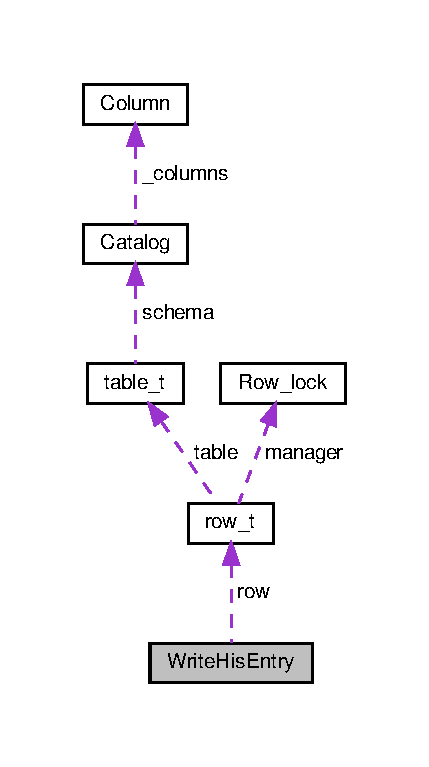
\includegraphics[width=206pt]{structWriteHisEntry__coll__graph}
\end{center}
\end{figure}
\subsection*{Public Attributes}
\begin{DoxyCompactItemize}
\item 
bool \hyperlink{structWriteHisEntry_a7811b8b2110e34749d1a14a15d7cd8ed}{begin\+\_\+txn}
\item 
bool \hyperlink{structWriteHisEntry_a08e8c0b848c62b641cd4aac45c24f645}{end\+\_\+txn}
\item 
\hyperlink{global_8h_aaf095dfc9b10f757c968fe146ad7e724}{ts\+\_\+t} \hyperlink{structWriteHisEntry_aa034427126a1be36ddd5056e2cacc576}{begin}
\item 
\hyperlink{global_8h_aaf095dfc9b10f757c968fe146ad7e724}{ts\+\_\+t} \hyperlink{structWriteHisEntry_af54358076bd13601fa2bf85f1d45c6cf}{end}
\item 
\hyperlink{classrow__t}{row\+\_\+t} $\ast$ \hyperlink{structWriteHisEntry_a0f87b3c9233028148a9eb39c03c3f0b2}{row}
\item 
bool \hyperlink{structWriteHisEntry_a86ba4fa82557ee6db6e06fb84e38f8f6}{valid}
\item 
bool \hyperlink{structWriteHisEntry_a7a0e8ed66270838139deeb2367718b8d}{reserved}
\item 
\hyperlink{global_8h_aaf095dfc9b10f757c968fe146ad7e724}{ts\+\_\+t} \hyperlink{structWriteHisEntry_a38db60cf5ebf583e144790fbbc230027}{ts}
\end{DoxyCompactItemize}


\subsection{Member Data Documentation}
\mbox{\Hypertarget{structWriteHisEntry_aa034427126a1be36ddd5056e2cacc576}\label{structWriteHisEntry_aa034427126a1be36ddd5056e2cacc576}} 
\index{Write\+His\+Entry@{Write\+His\+Entry}!begin@{begin}}
\index{begin@{begin}!Write\+His\+Entry@{Write\+His\+Entry}}
\subsubsection{\texorpdfstring{begin}{begin}}
{\footnotesize\ttfamily \hyperlink{global_8h_aaf095dfc9b10f757c968fe146ad7e724}{ts\+\_\+t} Write\+His\+Entry\+::begin}

\mbox{\Hypertarget{structWriteHisEntry_a7811b8b2110e34749d1a14a15d7cd8ed}\label{structWriteHisEntry_a7811b8b2110e34749d1a14a15d7cd8ed}} 
\index{Write\+His\+Entry@{Write\+His\+Entry}!begin\+\_\+txn@{begin\+\_\+txn}}
\index{begin\+\_\+txn@{begin\+\_\+txn}!Write\+His\+Entry@{Write\+His\+Entry}}
\subsubsection{\texorpdfstring{begin\+\_\+txn}{begin\_txn}}
{\footnotesize\ttfamily bool Write\+His\+Entry\+::begin\+\_\+txn}

\mbox{\Hypertarget{structWriteHisEntry_af54358076bd13601fa2bf85f1d45c6cf}\label{structWriteHisEntry_af54358076bd13601fa2bf85f1d45c6cf}} 
\index{Write\+His\+Entry@{Write\+His\+Entry}!end@{end}}
\index{end@{end}!Write\+His\+Entry@{Write\+His\+Entry}}
\subsubsection{\texorpdfstring{end}{end}}
{\footnotesize\ttfamily \hyperlink{global_8h_aaf095dfc9b10f757c968fe146ad7e724}{ts\+\_\+t} Write\+His\+Entry\+::end}

\mbox{\Hypertarget{structWriteHisEntry_a08e8c0b848c62b641cd4aac45c24f645}\label{structWriteHisEntry_a08e8c0b848c62b641cd4aac45c24f645}} 
\index{Write\+His\+Entry@{Write\+His\+Entry}!end\+\_\+txn@{end\+\_\+txn}}
\index{end\+\_\+txn@{end\+\_\+txn}!Write\+His\+Entry@{Write\+His\+Entry}}
\subsubsection{\texorpdfstring{end\+\_\+txn}{end\_txn}}
{\footnotesize\ttfamily bool Write\+His\+Entry\+::end\+\_\+txn}

\mbox{\Hypertarget{structWriteHisEntry_a7a0e8ed66270838139deeb2367718b8d}\label{structWriteHisEntry_a7a0e8ed66270838139deeb2367718b8d}} 
\index{Write\+His\+Entry@{Write\+His\+Entry}!reserved@{reserved}}
\index{reserved@{reserved}!Write\+His\+Entry@{Write\+His\+Entry}}
\subsubsection{\texorpdfstring{reserved}{reserved}}
{\footnotesize\ttfamily bool Write\+His\+Entry\+::reserved}

\mbox{\Hypertarget{structWriteHisEntry_a0f87b3c9233028148a9eb39c03c3f0b2}\label{structWriteHisEntry_a0f87b3c9233028148a9eb39c03c3f0b2}} 
\index{Write\+His\+Entry@{Write\+His\+Entry}!row@{row}}
\index{row@{row}!Write\+His\+Entry@{Write\+His\+Entry}}
\subsubsection{\texorpdfstring{row}{row}}
{\footnotesize\ttfamily \hyperlink{classrow__t}{row\+\_\+t} $\ast$ Write\+His\+Entry\+::row}

\mbox{\Hypertarget{structWriteHisEntry_a38db60cf5ebf583e144790fbbc230027}\label{structWriteHisEntry_a38db60cf5ebf583e144790fbbc230027}} 
\index{Write\+His\+Entry@{Write\+His\+Entry}!ts@{ts}}
\index{ts@{ts}!Write\+His\+Entry@{Write\+His\+Entry}}
\subsubsection{\texorpdfstring{ts}{ts}}
{\footnotesize\ttfamily \hyperlink{global_8h_aaf095dfc9b10f757c968fe146ad7e724}{ts\+\_\+t} Write\+His\+Entry\+::ts}

\mbox{\Hypertarget{structWriteHisEntry_a86ba4fa82557ee6db6e06fb84e38f8f6}\label{structWriteHisEntry_a86ba4fa82557ee6db6e06fb84e38f8f6}} 
\index{Write\+His\+Entry@{Write\+His\+Entry}!valid@{valid}}
\index{valid@{valid}!Write\+His\+Entry@{Write\+His\+Entry}}
\subsubsection{\texorpdfstring{valid}{valid}}
{\footnotesize\ttfamily bool Write\+His\+Entry\+::valid}



The documentation for this struct was generated from the following files\+:\begin{DoxyCompactItemize}
\item 
macrobench/concurrency\+\_\+control/\hyperlink{row__hekaton_8h}{row\+\_\+hekaton.\+h}\item 
macrobench/concurrency\+\_\+control/\hyperlink{row__mvcc_8h}{row\+\_\+mvcc.\+h}\end{DoxyCompactItemize}

\hypertarget{structwriter__locks}{}\section{writer\+\_\+locks Struct Reference}
\label{structwriter__locks}\index{writer\+\_\+locks@{writer\+\_\+locks}}


{\ttfamily \#include $<$rlu.\+h$>$}

\subsection*{Public Attributes}
\begin{DoxyCompactItemize}
\item 
long \hyperlink{structwriter__locks_a37620c55c0a1ddde88fd3f857ce7b503}{size}
\item 
long \hyperlink{structwriter__locks_abb68939c5b96b283870aecf6a9a2ec50}{ids} \mbox{[}\hyperlink{rlu_8h_a2dff72d8940c42485455fe15f42735de}{R\+L\+U\+\_\+\+M\+A\+X\+\_\+\+N\+E\+S\+T\+E\+D\+\_\+\+W\+R\+I\+T\+E\+R\+\_\+\+L\+O\+C\+KS}\mbox{]}
\end{DoxyCompactItemize}


\subsection{Member Data Documentation}
\mbox{\Hypertarget{structwriter__locks_abb68939c5b96b283870aecf6a9a2ec50}\label{structwriter__locks_abb68939c5b96b283870aecf6a9a2ec50}} 
\index{writer\+\_\+locks@{writer\+\_\+locks}!ids@{ids}}
\index{ids@{ids}!writer\+\_\+locks@{writer\+\_\+locks}}
\subsubsection{\texorpdfstring{ids}{ids}}
{\footnotesize\ttfamily long writer\+\_\+locks\+::ids\mbox{[}\hyperlink{rlu_8h_a2dff72d8940c42485455fe15f42735de}{R\+L\+U\+\_\+\+M\+A\+X\+\_\+\+N\+E\+S\+T\+E\+D\+\_\+\+W\+R\+I\+T\+E\+R\+\_\+\+L\+O\+C\+KS}\mbox{]}}

\mbox{\Hypertarget{structwriter__locks_a37620c55c0a1ddde88fd3f857ce7b503}\label{structwriter__locks_a37620c55c0a1ddde88fd3f857ce7b503}} 
\index{writer\+\_\+locks@{writer\+\_\+locks}!size@{size}}
\index{size@{size}!writer\+\_\+locks@{writer\+\_\+locks}}
\subsubsection{\texorpdfstring{size}{size}}
{\footnotesize\ttfamily long writer\+\_\+locks\+::size}



The documentation for this struct was generated from the following file\+:\begin{DoxyCompactItemize}
\item 
common/rlu/\hyperlink{rlu_8h}{rlu.\+h}\end{DoxyCompactItemize}

\hypertarget{classycsb__query}{}\section{ycsb\+\_\+query Class Reference}
\label{classycsb__query}\index{ycsb\+\_\+query@{ycsb\+\_\+query}}


{\ttfamily \#include $<$ycsb\+\_\+query.\+h$>$}



Inheritance diagram for ycsb\+\_\+query\+:
\nopagebreak
\begin{figure}[H]
\begin{center}
\leavevmode
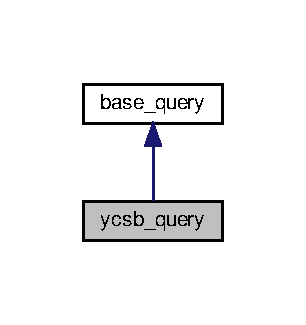
\includegraphics[width=147pt]{classycsb__query__inherit__graph}
\end{center}
\end{figure}


Collaboration diagram for ycsb\+\_\+query\+:
\nopagebreak
\begin{figure}[H]
\begin{center}
\leavevmode
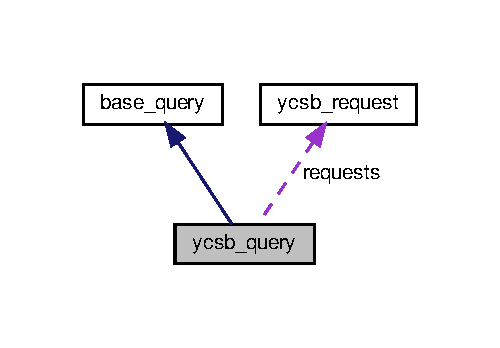
\includegraphics[width=240pt]{classycsb__query__coll__graph}
\end{center}
\end{figure}
\subsection*{Public Member Functions}
\begin{DoxyCompactItemize}
\item 
void \hyperlink{classycsb__query_a05e09ce39a834921f0b83103ff5ec5e1}{init} (uint64\+\_\+t thd\+\_\+id, \hyperlink{classworkload}{workload} $\ast$h\+\_\+wl)
\item 
void \hyperlink{classycsb__query_a37873fbb1e7daa27b3955ee20e02a489}{setbench\+\_\+deinit} ()
\item 
void \hyperlink{classycsb__query_a3af1d2ce40522812859d6a364a7a0c1b}{init} (uint64\+\_\+t thd\+\_\+id, \hyperlink{classworkload}{workload} $\ast$h\+\_\+wl, \hyperlink{classQuery__thd}{Query\+\_\+thd} $\ast$query\+\_\+thd)
\end{DoxyCompactItemize}
\subsection*{Static Public Member Functions}
\begin{DoxyCompactItemize}
\item 
static void \hyperlink{classycsb__query_a542cbc87682e6526c2593391f55e3963}{calculate\+Denom} ()
\end{DoxyCompactItemize}
\subsection*{Public Attributes}
\begin{DoxyCompactItemize}
\item 
uint64\+\_\+t \hyperlink{classycsb__query_a3626ff0e3508d4b5fe7dc2b9b485cdca}{request\+\_\+cnt}
\item 
\hyperlink{classycsb__request}{ycsb\+\_\+request} $\ast$ \hyperlink{classycsb__query_a2dfa57c2be74e3b38ccefe41e6a94eff}{requests}
\end{DoxyCompactItemize}


\subsection{Member Function Documentation}
\mbox{\Hypertarget{classycsb__query_a542cbc87682e6526c2593391f55e3963}\label{classycsb__query_a542cbc87682e6526c2593391f55e3963}} 
\index{ycsb\+\_\+query@{ycsb\+\_\+query}!calculate\+Denom@{calculate\+Denom}}
\index{calculate\+Denom@{calculate\+Denom}!ycsb\+\_\+query@{ycsb\+\_\+query}}
\subsubsection{\texorpdfstring{calculate\+Denom()}{calculateDenom()}}
{\footnotesize\ttfamily void ycsb\+\_\+query\+::calculate\+Denom (\begin{DoxyParamCaption}{ }\end{DoxyParamCaption})\hspace{0.3cm}{\ttfamily [static]}}

\mbox{\Hypertarget{classycsb__query_a05e09ce39a834921f0b83103ff5ec5e1}\label{classycsb__query_a05e09ce39a834921f0b83103ff5ec5e1}} 
\index{ycsb\+\_\+query@{ycsb\+\_\+query}!init@{init}}
\index{init@{init}!ycsb\+\_\+query@{ycsb\+\_\+query}}
\subsubsection{\texorpdfstring{init()}{init()}\hspace{0.1cm}{\footnotesize\ttfamily [1/2]}}
{\footnotesize\ttfamily void ycsb\+\_\+query\+::init (\begin{DoxyParamCaption}\item[{uint64\+\_\+t}]{thd\+\_\+id,  }\item[{\hyperlink{classworkload}{workload} $\ast$}]{h\+\_\+wl }\end{DoxyParamCaption})\hspace{0.3cm}{\ttfamily [inline]}, {\ttfamily [virtual]}}



Implements \hyperlink{classbase__query_a341a99285c6e849eae1c5a83485335f3}{base\+\_\+query}.

\mbox{\Hypertarget{classycsb__query_a3af1d2ce40522812859d6a364a7a0c1b}\label{classycsb__query_a3af1d2ce40522812859d6a364a7a0c1b}} 
\index{ycsb\+\_\+query@{ycsb\+\_\+query}!init@{init}}
\index{init@{init}!ycsb\+\_\+query@{ycsb\+\_\+query}}
\subsubsection{\texorpdfstring{init()}{init()}\hspace{0.1cm}{\footnotesize\ttfamily [2/2]}}
{\footnotesize\ttfamily void ycsb\+\_\+query\+::init (\begin{DoxyParamCaption}\item[{uint64\+\_\+t}]{thd\+\_\+id,  }\item[{\hyperlink{classworkload}{workload} $\ast$}]{h\+\_\+wl,  }\item[{\hyperlink{classQuery__thd}{Query\+\_\+thd} $\ast$}]{query\+\_\+thd }\end{DoxyParamCaption})}

\mbox{\Hypertarget{classycsb__query_a37873fbb1e7daa27b3955ee20e02a489}\label{classycsb__query_a37873fbb1e7daa27b3955ee20e02a489}} 
\index{ycsb\+\_\+query@{ycsb\+\_\+query}!setbench\+\_\+deinit@{setbench\+\_\+deinit}}
\index{setbench\+\_\+deinit@{setbench\+\_\+deinit}!ycsb\+\_\+query@{ycsb\+\_\+query}}
\subsubsection{\texorpdfstring{setbench\+\_\+deinit()}{setbench\_deinit()}}
{\footnotesize\ttfamily void ycsb\+\_\+query\+::setbench\+\_\+deinit (\begin{DoxyParamCaption}{ }\end{DoxyParamCaption})}



\subsection{Member Data Documentation}
\mbox{\Hypertarget{classycsb__query_a3626ff0e3508d4b5fe7dc2b9b485cdca}\label{classycsb__query_a3626ff0e3508d4b5fe7dc2b9b485cdca}} 
\index{ycsb\+\_\+query@{ycsb\+\_\+query}!request\+\_\+cnt@{request\+\_\+cnt}}
\index{request\+\_\+cnt@{request\+\_\+cnt}!ycsb\+\_\+query@{ycsb\+\_\+query}}
\subsubsection{\texorpdfstring{request\+\_\+cnt}{request\_cnt}}
{\footnotesize\ttfamily uint64\+\_\+t ycsb\+\_\+query\+::request\+\_\+cnt}

\mbox{\Hypertarget{classycsb__query_a2dfa57c2be74e3b38ccefe41e6a94eff}\label{classycsb__query_a2dfa57c2be74e3b38ccefe41e6a94eff}} 
\index{ycsb\+\_\+query@{ycsb\+\_\+query}!requests@{requests}}
\index{requests@{requests}!ycsb\+\_\+query@{ycsb\+\_\+query}}
\subsubsection{\texorpdfstring{requests}{requests}}
{\footnotesize\ttfamily \hyperlink{classycsb__request}{ycsb\+\_\+request}$\ast$ ycsb\+\_\+query\+::requests}



The documentation for this class was generated from the following files\+:\begin{DoxyCompactItemize}
\item 
macrobench/benchmarks/\hyperlink{ycsb__query_8h}{ycsb\+\_\+query.\+h}\item 
macrobench/benchmarks/\hyperlink{ycsb__query_8cpp}{ycsb\+\_\+query.\+cpp}\end{DoxyCompactItemize}

\hypertarget{classycsb__request}{}\section{ycsb\+\_\+request Class Reference}
\label{classycsb__request}\index{ycsb\+\_\+request@{ycsb\+\_\+request}}


{\ttfamily \#include $<$ycsb\+\_\+query.\+h$>$}

\subsection*{Public Attributes}
\begin{DoxyCompactItemize}
\item 
\hyperlink{global_8h_a567f81b0ae33b00d189d7714e9fde0bc}{access\+\_\+t} \hyperlink{classycsb__request_af0df8d7491496ae7145729dd0be4355f}{rtype}
\item 
uint64\+\_\+t \hyperlink{classycsb__request_a3709e2fa8cadb02b580998fb5cd6f62d}{key}
\item 
char \hyperlink{classycsb__request_a57822b9157083b797236b474f795ca36}{value}
\item 
\hyperlink{global_8h_a7e8aeec7b6541935dfc6f608cd5170ce}{U\+Int32} \hyperlink{classycsb__request_a6f0822555a46b0125a321043c871f619}{scan\+\_\+len}
\end{DoxyCompactItemize}


\subsection{Member Data Documentation}
\mbox{\Hypertarget{classycsb__request_a3709e2fa8cadb02b580998fb5cd6f62d}\label{classycsb__request_a3709e2fa8cadb02b580998fb5cd6f62d}} 
\index{ycsb\+\_\+request@{ycsb\+\_\+request}!key@{key}}
\index{key@{key}!ycsb\+\_\+request@{ycsb\+\_\+request}}
\subsubsection{\texorpdfstring{key}{key}}
{\footnotesize\ttfamily uint64\+\_\+t ycsb\+\_\+request\+::key}

\mbox{\Hypertarget{classycsb__request_af0df8d7491496ae7145729dd0be4355f}\label{classycsb__request_af0df8d7491496ae7145729dd0be4355f}} 
\index{ycsb\+\_\+request@{ycsb\+\_\+request}!rtype@{rtype}}
\index{rtype@{rtype}!ycsb\+\_\+request@{ycsb\+\_\+request}}
\subsubsection{\texorpdfstring{rtype}{rtype}}
{\footnotesize\ttfamily \hyperlink{global_8h_a567f81b0ae33b00d189d7714e9fde0bc}{access\+\_\+t} ycsb\+\_\+request\+::rtype}

\mbox{\Hypertarget{classycsb__request_a6f0822555a46b0125a321043c871f619}\label{classycsb__request_a6f0822555a46b0125a321043c871f619}} 
\index{ycsb\+\_\+request@{ycsb\+\_\+request}!scan\+\_\+len@{scan\+\_\+len}}
\index{scan\+\_\+len@{scan\+\_\+len}!ycsb\+\_\+request@{ycsb\+\_\+request}}
\subsubsection{\texorpdfstring{scan\+\_\+len}{scan\_len}}
{\footnotesize\ttfamily \hyperlink{global_8h_a7e8aeec7b6541935dfc6f608cd5170ce}{U\+Int32} ycsb\+\_\+request\+::scan\+\_\+len}

\mbox{\Hypertarget{classycsb__request_a57822b9157083b797236b474f795ca36}\label{classycsb__request_a57822b9157083b797236b474f795ca36}} 
\index{ycsb\+\_\+request@{ycsb\+\_\+request}!value@{value}}
\index{value@{value}!ycsb\+\_\+request@{ycsb\+\_\+request}}
\subsubsection{\texorpdfstring{value}{value}}
{\footnotesize\ttfamily char ycsb\+\_\+request\+::value}



The documentation for this class was generated from the following file\+:\begin{DoxyCompactItemize}
\item 
macrobench/benchmarks/\hyperlink{ycsb__query_8h}{ycsb\+\_\+query.\+h}\end{DoxyCompactItemize}

\hypertarget{classycsb__txn__man}{}\section{ycsb\+\_\+txn\+\_\+man Class Reference}
\label{classycsb__txn__man}\index{ycsb\+\_\+txn\+\_\+man@{ycsb\+\_\+txn\+\_\+man}}


{\ttfamily \#include $<$ycsb.\+h$>$}



Inheritance diagram for ycsb\+\_\+txn\+\_\+man\+:
\nopagebreak
\begin{figure}[H]
\begin{center}
\leavevmode
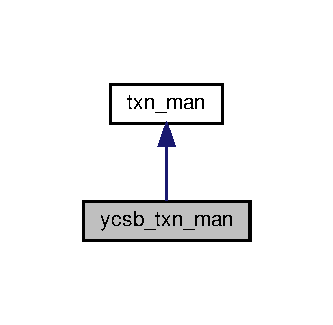
\includegraphics[width=160pt]{classycsb__txn__man__inherit__graph}
\end{center}
\end{figure}


Collaboration diagram for ycsb\+\_\+txn\+\_\+man\+:
\nopagebreak
\begin{figure}[H]
\begin{center}
\leavevmode
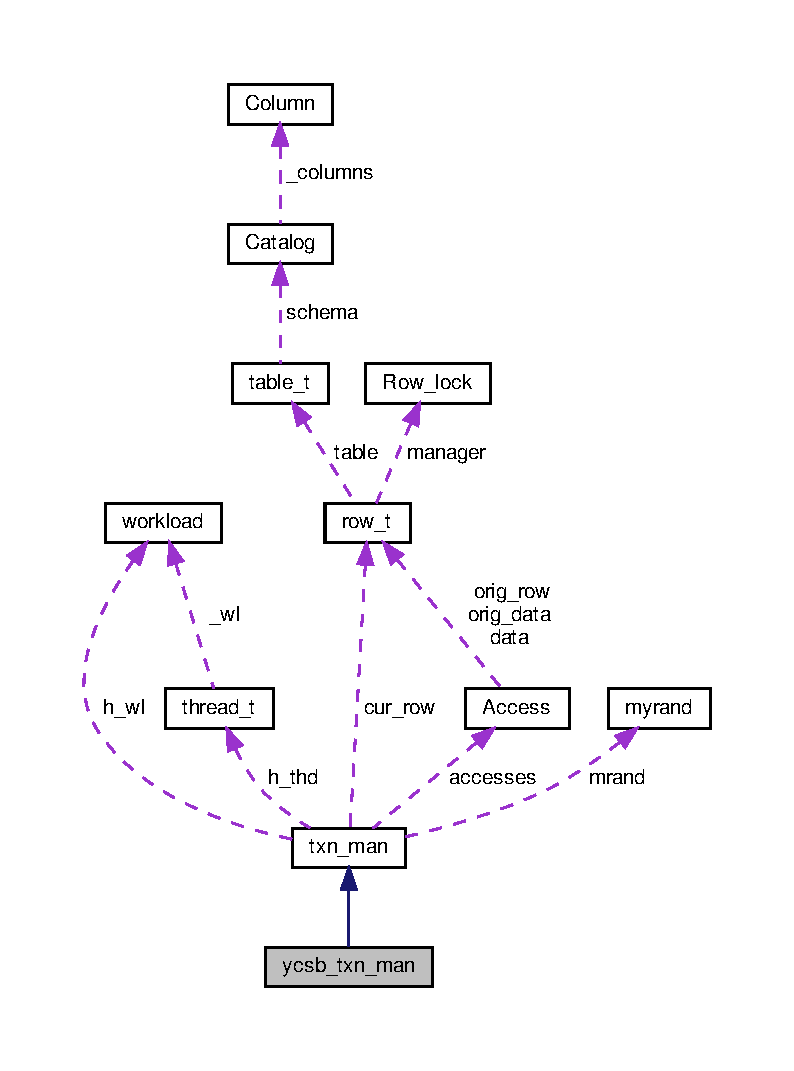
\includegraphics[width=350pt]{classycsb__txn__man__coll__graph}
\end{center}
\end{figure}
\subsection*{Public Member Functions}
\begin{DoxyCompactItemize}
\item 
void \hyperlink{classycsb__txn__man_a6708b67fbc560af1634f6d48cfa66b4f}{init} (\hyperlink{classthread__t}{thread\+\_\+t} $\ast$\hyperlink{classtxn__man_a64bf2cba8ef2686ad528a96d18e8358d}{h\+\_\+thd}, \hyperlink{classworkload}{workload} $\ast$\hyperlink{classtxn__man_a988eb76c69a304049c02d3ceff526a5e}{h\+\_\+wl}, uint64\+\_\+t part\+\_\+id)
\item 
\hyperlink{global_8h_a78c49a674c810fdd03d20432f7be864a}{RC} \hyperlink{classycsb__txn__man_ab219e46d2d5149677ad391ebb83d6e05}{run\+\_\+txn} (\hyperlink{classbase__query}{base\+\_\+query} $\ast$query)
\end{DoxyCompactItemize}
\subsection*{Additional Inherited Members}


\subsection{Member Function Documentation}
\mbox{\Hypertarget{classycsb__txn__man_a6708b67fbc560af1634f6d48cfa66b4f}\label{classycsb__txn__man_a6708b67fbc560af1634f6d48cfa66b4f}} 
\index{ycsb\+\_\+txn\+\_\+man@{ycsb\+\_\+txn\+\_\+man}!init@{init}}
\index{init@{init}!ycsb\+\_\+txn\+\_\+man@{ycsb\+\_\+txn\+\_\+man}}
\subsubsection{\texorpdfstring{init()}{init()}}
{\footnotesize\ttfamily void ycsb\+\_\+txn\+\_\+man\+::init (\begin{DoxyParamCaption}\item[{\hyperlink{classthread__t}{thread\+\_\+t} $\ast$}]{h\+\_\+thd,  }\item[{\hyperlink{classworkload}{workload} $\ast$}]{h\+\_\+wl,  }\item[{uint64\+\_\+t}]{part\+\_\+id }\end{DoxyParamCaption})\hspace{0.3cm}{\ttfamily [virtual]}}



Reimplemented from \hyperlink{classtxn__man_a778925bb3edd6a54a27161f67792edec}{txn\+\_\+man}.

\mbox{\Hypertarget{classycsb__txn__man_ab219e46d2d5149677ad391ebb83d6e05}\label{classycsb__txn__man_ab219e46d2d5149677ad391ebb83d6e05}} 
\index{ycsb\+\_\+txn\+\_\+man@{ycsb\+\_\+txn\+\_\+man}!run\+\_\+txn@{run\+\_\+txn}}
\index{run\+\_\+txn@{run\+\_\+txn}!ycsb\+\_\+txn\+\_\+man@{ycsb\+\_\+txn\+\_\+man}}
\subsubsection{\texorpdfstring{run\+\_\+txn()}{run\_txn()}}
{\footnotesize\ttfamily \hyperlink{global_8h_a78c49a674c810fdd03d20432f7be864a}{RC} ycsb\+\_\+txn\+\_\+man\+::run\+\_\+txn (\begin{DoxyParamCaption}\item[{\hyperlink{classbase__query}{base\+\_\+query} $\ast$}]{query }\end{DoxyParamCaption})\hspace{0.3cm}{\ttfamily [virtual]}}



Implements \hyperlink{classtxn__man_a71142ded36a4be5629ea75d486a105ae}{txn\+\_\+man}.



The documentation for this class was generated from the following files\+:\begin{DoxyCompactItemize}
\item 
macrobench/benchmarks/\hyperlink{ycsb_8h}{ycsb.\+h}\item 
macrobench/benchmarks/\hyperlink{ycsb__txn_8cpp}{ycsb\+\_\+txn.\+cpp}\end{DoxyCompactItemize}

\hypertarget{classycsb__wl}{}\section{ycsb\+\_\+wl Class Reference}
\label{classycsb__wl}\index{ycsb\+\_\+wl@{ycsb\+\_\+wl}}


{\ttfamily \#include $<$ycsb.\+h$>$}



Inheritance diagram for ycsb\+\_\+wl\+:
\nopagebreak
\begin{figure}[H]
\begin{center}
\leavevmode
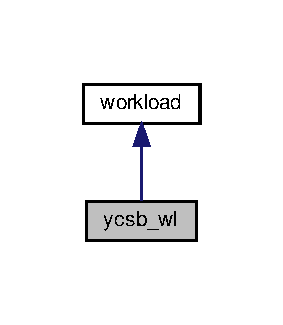
\includegraphics[width=136pt]{classycsb__wl__inherit__graph}
\end{center}
\end{figure}


Collaboration diagram for ycsb\+\_\+wl\+:
\nopagebreak
\begin{figure}[H]
\begin{center}
\leavevmode
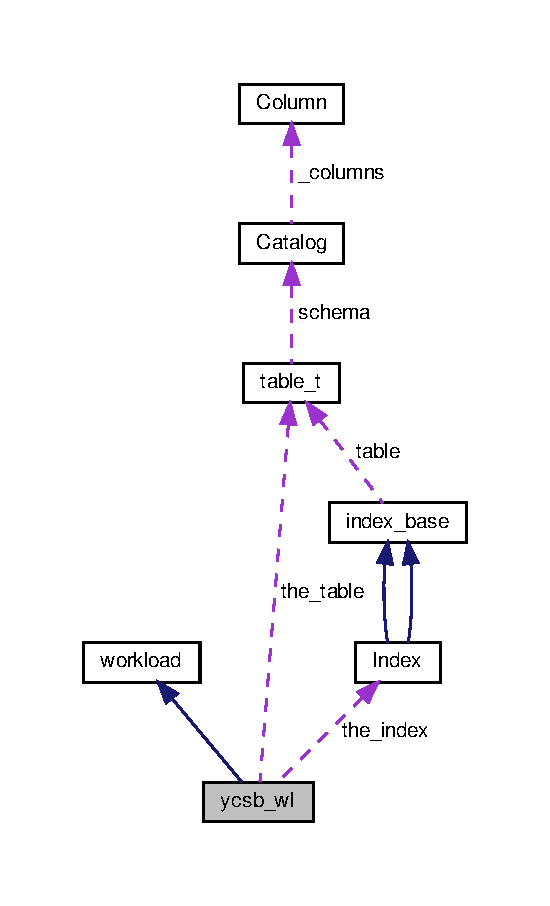
\includegraphics[width=264pt]{classycsb__wl__coll__graph}
\end{center}
\end{figure}
\subsection*{Public Member Functions}
\begin{DoxyCompactItemize}
\item 
\hyperlink{global_8h_a78c49a674c810fdd03d20432f7be864a}{RC} \hyperlink{classycsb__wl_ab457878c0f802cbbbf9ff27979e0eda6}{init} ()
\item 
void \hyperlink{classycsb__wl_aba11708593028b3cea7986adb280aae3}{setbench\+\_\+deinit} ()
\item 
\hyperlink{global_8h_a78c49a674c810fdd03d20432f7be864a}{RC} \hyperlink{classycsb__wl_a2e1e8d6e68e5312a82cfe09ec4bb26a6}{init\+\_\+table} ()
\item 
\hyperlink{global_8h_a78c49a674c810fdd03d20432f7be864a}{RC} \hyperlink{classycsb__wl_a3f1937f438c251831694b39b6e9dc36d}{init\+\_\+schema} (std\+::string schema\+\_\+file)
\item 
\hyperlink{global_8h_a78c49a674c810fdd03d20432f7be864a}{RC} \hyperlink{classycsb__wl_a31fb01819cd6a3517259ec9bb80066ca}{get\+\_\+txn\+\_\+man} (\hyperlink{classtxn__man}{txn\+\_\+man} $\ast$\&txn\+\_\+manager, \hyperlink{classthread__t}{thread\+\_\+t} $\ast$h\+\_\+thd)
\item 
int \hyperlink{classycsb__wl_ad6505cf2f6d7113c1825b1c5d5276297}{key\+\_\+to\+\_\+part} (uint64\+\_\+t key)
\end{DoxyCompactItemize}
\subsection*{Public Attributes}
\begin{DoxyCompactItemize}
\item 
\hyperlink{classIndex}{Index} $\ast$ \hyperlink{classycsb__wl_adc52d421067b72cff7d5ef56dd612202}{the\+\_\+index}
\item 
\hyperlink{classtable__t}{table\+\_\+t} $\ast$ \hyperlink{classycsb__wl_a717e1db064d7069663e031231984c18e}{the\+\_\+table}
\end{DoxyCompactItemize}
\subsection*{Additional Inherited Members}


\subsection{Member Function Documentation}
\mbox{\Hypertarget{classycsb__wl_a31fb01819cd6a3517259ec9bb80066ca}\label{classycsb__wl_a31fb01819cd6a3517259ec9bb80066ca}} 
\index{ycsb\+\_\+wl@{ycsb\+\_\+wl}!get\+\_\+txn\+\_\+man@{get\+\_\+txn\+\_\+man}}
\index{get\+\_\+txn\+\_\+man@{get\+\_\+txn\+\_\+man}!ycsb\+\_\+wl@{ycsb\+\_\+wl}}
\subsubsection{\texorpdfstring{get\+\_\+txn\+\_\+man()}{get\_txn\_man()}}
{\footnotesize\ttfamily \hyperlink{global_8h_a78c49a674c810fdd03d20432f7be864a}{RC} ycsb\+\_\+wl\+::get\+\_\+txn\+\_\+man (\begin{DoxyParamCaption}\item[{\hyperlink{classtxn__man}{txn\+\_\+man} $\ast$\&}]{txn\+\_\+manager,  }\item[{\hyperlink{classthread__t}{thread\+\_\+t} $\ast$}]{h\+\_\+thd }\end{DoxyParamCaption})\hspace{0.3cm}{\ttfamily [virtual]}}



Implements \hyperlink{classworkload_ac22d0558c3fc549b8b07347cebb95cb3}{workload}.

\mbox{\Hypertarget{classycsb__wl_ab457878c0f802cbbbf9ff27979e0eda6}\label{classycsb__wl_ab457878c0f802cbbbf9ff27979e0eda6}} 
\index{ycsb\+\_\+wl@{ycsb\+\_\+wl}!init@{init}}
\index{init@{init}!ycsb\+\_\+wl@{ycsb\+\_\+wl}}
\subsubsection{\texorpdfstring{init()}{init()}}
{\footnotesize\ttfamily \hyperlink{global_8h_a78c49a674c810fdd03d20432f7be864a}{RC} ycsb\+\_\+wl\+::init (\begin{DoxyParamCaption}{ }\end{DoxyParamCaption})\hspace{0.3cm}{\ttfamily [virtual]}}



Reimplemented from \hyperlink{classworkload_a7cef7a7101c78e10082c99356e77a57c}{workload}.

\mbox{\Hypertarget{classycsb__wl_a3f1937f438c251831694b39b6e9dc36d}\label{classycsb__wl_a3f1937f438c251831694b39b6e9dc36d}} 
\index{ycsb\+\_\+wl@{ycsb\+\_\+wl}!init\+\_\+schema@{init\+\_\+schema}}
\index{init\+\_\+schema@{init\+\_\+schema}!ycsb\+\_\+wl@{ycsb\+\_\+wl}}
\subsubsection{\texorpdfstring{init\+\_\+schema()}{init\_schema()}}
{\footnotesize\ttfamily \hyperlink{global_8h_a78c49a674c810fdd03d20432f7be864a}{RC} ycsb\+\_\+wl\+::init\+\_\+schema (\begin{DoxyParamCaption}\item[{std\+::string}]{schema\+\_\+file }\end{DoxyParamCaption})\hspace{0.3cm}{\ttfamily [virtual]}}



Reimplemented from \hyperlink{classworkload_a12ce1550f8e398871961c6ff116c11d3}{workload}.

\mbox{\Hypertarget{classycsb__wl_a2e1e8d6e68e5312a82cfe09ec4bb26a6}\label{classycsb__wl_a2e1e8d6e68e5312a82cfe09ec4bb26a6}} 
\index{ycsb\+\_\+wl@{ycsb\+\_\+wl}!init\+\_\+table@{init\+\_\+table}}
\index{init\+\_\+table@{init\+\_\+table}!ycsb\+\_\+wl@{ycsb\+\_\+wl}}
\subsubsection{\texorpdfstring{init\+\_\+table()}{init\_table()}}
{\footnotesize\ttfamily \hyperlink{global_8h_a78c49a674c810fdd03d20432f7be864a}{RC} ycsb\+\_\+wl\+::init\+\_\+table (\begin{DoxyParamCaption}{ }\end{DoxyParamCaption})\hspace{0.3cm}{\ttfamily [virtual]}}



Implements \hyperlink{classworkload_a3feee79af04069f6c1ad6b7f9b0a045a}{workload}.

\mbox{\Hypertarget{classycsb__wl_ad6505cf2f6d7113c1825b1c5d5276297}\label{classycsb__wl_ad6505cf2f6d7113c1825b1c5d5276297}} 
\index{ycsb\+\_\+wl@{ycsb\+\_\+wl}!key\+\_\+to\+\_\+part@{key\+\_\+to\+\_\+part}}
\index{key\+\_\+to\+\_\+part@{key\+\_\+to\+\_\+part}!ycsb\+\_\+wl@{ycsb\+\_\+wl}}
\subsubsection{\texorpdfstring{key\+\_\+to\+\_\+part()}{key\_to\_part()}}
{\footnotesize\ttfamily int ycsb\+\_\+wl\+::key\+\_\+to\+\_\+part (\begin{DoxyParamCaption}\item[{uint64\+\_\+t}]{key }\end{DoxyParamCaption})}

\mbox{\Hypertarget{classycsb__wl_aba11708593028b3cea7986adb280aae3}\label{classycsb__wl_aba11708593028b3cea7986adb280aae3}} 
\index{ycsb\+\_\+wl@{ycsb\+\_\+wl}!setbench\+\_\+deinit@{setbench\+\_\+deinit}}
\index{setbench\+\_\+deinit@{setbench\+\_\+deinit}!ycsb\+\_\+wl@{ycsb\+\_\+wl}}
\subsubsection{\texorpdfstring{setbench\+\_\+deinit()}{setbench\_deinit()}}
{\footnotesize\ttfamily void ycsb\+\_\+wl\+::setbench\+\_\+deinit (\begin{DoxyParamCaption}{ }\end{DoxyParamCaption})\hspace{0.3cm}{\ttfamily [virtual]}}



Reimplemented from \hyperlink{classworkload_a4614189e85fbaaf2003b7db4c2a7b8b9}{workload}.



\subsection{Member Data Documentation}
\mbox{\Hypertarget{classycsb__wl_adc52d421067b72cff7d5ef56dd612202}\label{classycsb__wl_adc52d421067b72cff7d5ef56dd612202}} 
\index{ycsb\+\_\+wl@{ycsb\+\_\+wl}!the\+\_\+index@{the\+\_\+index}}
\index{the\+\_\+index@{the\+\_\+index}!ycsb\+\_\+wl@{ycsb\+\_\+wl}}
\subsubsection{\texorpdfstring{the\+\_\+index}{the\_index}}
{\footnotesize\ttfamily \hyperlink{classIndex}{Index}$\ast$ ycsb\+\_\+wl\+::the\+\_\+index}

\mbox{\Hypertarget{classycsb__wl_a717e1db064d7069663e031231984c18e}\label{classycsb__wl_a717e1db064d7069663e031231984c18e}} 
\index{ycsb\+\_\+wl@{ycsb\+\_\+wl}!the\+\_\+table@{the\+\_\+table}}
\index{the\+\_\+table@{the\+\_\+table}!ycsb\+\_\+wl@{ycsb\+\_\+wl}}
\subsubsection{\texorpdfstring{the\+\_\+table}{the\_table}}
{\footnotesize\ttfamily \hyperlink{classtable__t}{table\+\_\+t}$\ast$ ycsb\+\_\+wl\+::the\+\_\+table}



The documentation for this class was generated from the following files\+:\begin{DoxyCompactItemize}
\item 
macrobench/benchmarks/\hyperlink{ycsb_8h}{ycsb.\+h}\item 
macrobench/benchmarks/\hyperlink{ycsb__wl_8cpp}{ycsb\+\_\+wl.\+cpp}\end{DoxyCompactItemize}

\chapter{File Documentation}
\hypertarget{atomic__ops_8h}{}\section{common/atomic\+\_\+ops/atomic\+\_\+ops.h File Reference}
\label{atomic__ops_8h}\index{common/atomic\+\_\+ops/atomic\+\_\+ops.\+h@{common/atomic\+\_\+ops/atomic\+\_\+ops.\+h}}
{\ttfamily \#include $<$assert.\+h$>$}\newline
{\ttfamily \#include $<$stddef.\+h$>$}\newline
{\ttfamily \#include \char`\"{}atomic\+\_\+ops/generalize.\+h\char`\"{}}\newline
Include dependency graph for atomic\+\_\+ops.\+h\+:
\nopagebreak
\begin{figure}[H]
\begin{center}
\leavevmode
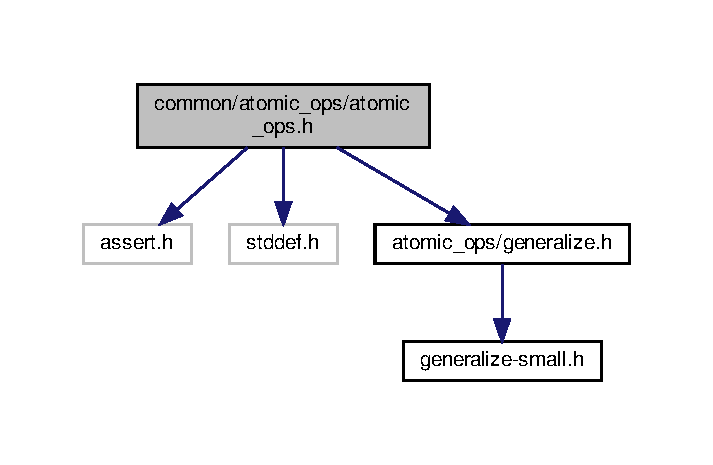
\includegraphics[width=342pt]{atomic__ops_8h__incl}
\end{center}
\end{figure}
This graph shows which files directly or indirectly include this file\+:
\nopagebreak
\begin{figure}[H]
\begin{center}
\leavevmode
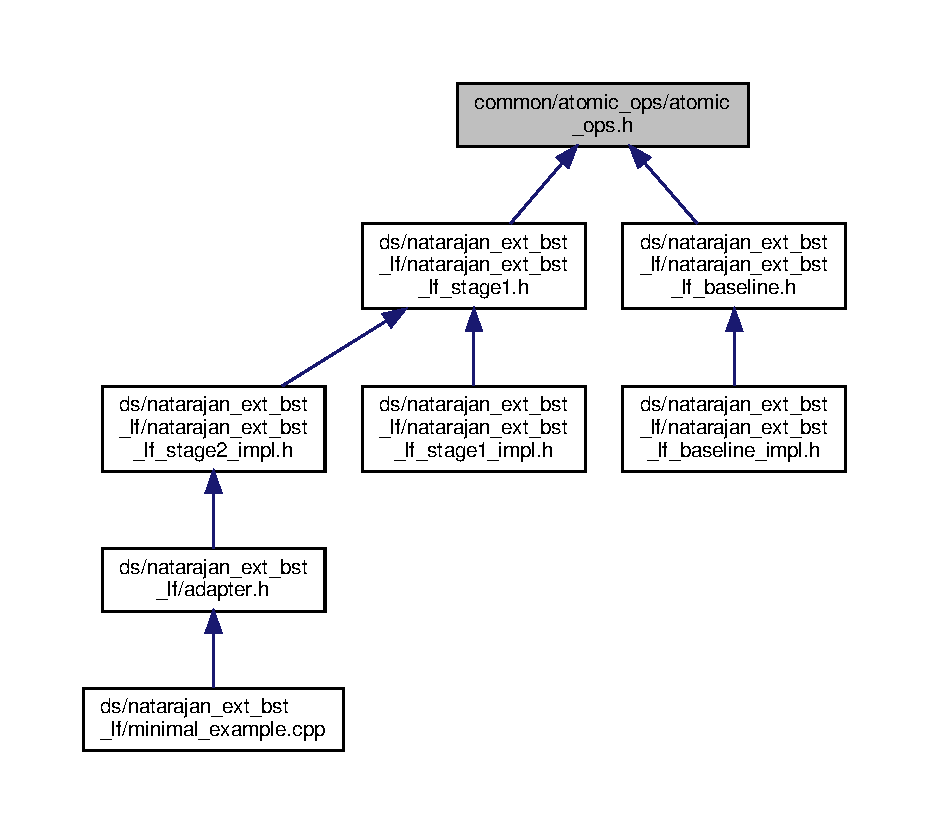
\includegraphics[width=350pt]{atomic__ops_8h__dep__incl}
\end{center}
\end{figure}
\subsection*{Macros}
\begin{DoxyCompactItemize}
\item 
\#define \hyperlink{atomic__ops_8h_a5225fef4d9eee821e82382cd269160dd}{A\+O\+\_\+t}~size\+\_\+t
\item 
\#define \hyperlink{atomic__ops_8h_af0f8642b332396baef4793e7ce825759}{A\+O\+\_\+\+T\+S\+\_\+\+I\+N\+I\+T\+I\+A\+L\+I\+Z\+ER}~(\hyperlink{atomic__ops_8h_a5225fef4d9eee821e82382cd269160dd}{A\+O\+\_\+t})\hyperlink{test__and__set__t__is__char_8h_a35258ee13bc817d0b8eb62f4695c4a3e}{A\+O\+\_\+\+T\+S\+\_\+\+C\+L\+E\+AR}
\item 
\#define \hyperlink{atomic__ops_8h_a9f6ab6253b6b11bc8c12efe9dde5db2b}{A\+O\+\_\+\+I\+N\+L\+I\+NE}~static
\item 
\#define \hyperlink{atomic__ops_8h_a8e2f9a0a3aec4e9f6b260934826819ee}{A\+O\+\_\+compiler\+\_\+barrier}()~asm(\char`\"{}\char`\"{})
\item 
\#define \hyperlink{atomic__ops_8h_a4e2e59fc7419c7cf7acc602a1e31bec5}{A\+O\+\_\+\+T\+S\+\_\+T}~\hyperlink{test__and__set__t__is__char_8h_a5890c21b549264c75c2cad08bf4f6ba9}{A\+O\+\_\+\+T\+S\+\_\+t}
\item 
\#define \hyperlink{atomic__ops_8h_a0eeae1602a0dd91543138c7b92a1bb3b}{A\+O\+\_\+T}~\hyperlink{atomic__ops_8h_a5225fef4d9eee821e82382cd269160dd}{A\+O\+\_\+t}
\item 
\#define \hyperlink{atomic__ops_8h_af9641fdea742ed560eb463b359a1a662}{A\+O\+\_\+\+T\+S\+\_\+\+V\+AL}~\hyperlink{test__and__set__t__is__char_8h_a7d99a16c4eab47ba80ab6138d7d98ac1}{A\+O\+\_\+\+T\+S\+\_\+\+V\+A\+L\+\_\+t}
\end{DoxyCompactItemize}


\subsection{Macro Definition Documentation}
\mbox{\Hypertarget{atomic__ops_8h_a8e2f9a0a3aec4e9f6b260934826819ee}\label{atomic__ops_8h_a8e2f9a0a3aec4e9f6b260934826819ee}} 
\index{atomic\+\_\+ops.\+h@{atomic\+\_\+ops.\+h}!A\+O\+\_\+compiler\+\_\+barrier@{A\+O\+\_\+compiler\+\_\+barrier}}
\index{A\+O\+\_\+compiler\+\_\+barrier@{A\+O\+\_\+compiler\+\_\+barrier}!atomic\+\_\+ops.\+h@{atomic\+\_\+ops.\+h}}
\subsubsection{\texorpdfstring{A\+O\+\_\+compiler\+\_\+barrier}{AO\_compiler\_barrier}}
{\footnotesize\ttfamily \#define A\+O\+\_\+compiler\+\_\+barrier(\begin{DoxyParamCaption}{ }\end{DoxyParamCaption})~asm(\char`\"{}\char`\"{})}

\mbox{\Hypertarget{atomic__ops_8h_a9f6ab6253b6b11bc8c12efe9dde5db2b}\label{atomic__ops_8h_a9f6ab6253b6b11bc8c12efe9dde5db2b}} 
\index{atomic\+\_\+ops.\+h@{atomic\+\_\+ops.\+h}!A\+O\+\_\+\+I\+N\+L\+I\+NE@{A\+O\+\_\+\+I\+N\+L\+I\+NE}}
\index{A\+O\+\_\+\+I\+N\+L\+I\+NE@{A\+O\+\_\+\+I\+N\+L\+I\+NE}!atomic\+\_\+ops.\+h@{atomic\+\_\+ops.\+h}}
\subsubsection{\texorpdfstring{A\+O\+\_\+\+I\+N\+L\+I\+NE}{AO\_INLINE}}
{\footnotesize\ttfamily \#define A\+O\+\_\+\+I\+N\+L\+I\+NE~static}

\mbox{\Hypertarget{atomic__ops_8h_a5225fef4d9eee821e82382cd269160dd}\label{atomic__ops_8h_a5225fef4d9eee821e82382cd269160dd}} 
\index{atomic\+\_\+ops.\+h@{atomic\+\_\+ops.\+h}!A\+O\+\_\+t@{A\+O\+\_\+t}}
\index{A\+O\+\_\+t@{A\+O\+\_\+t}!atomic\+\_\+ops.\+h@{atomic\+\_\+ops.\+h}}
\subsubsection{\texorpdfstring{A\+O\+\_\+t}{AO\_t}}
{\footnotesize\ttfamily \#define A\+O\+\_\+t~size\+\_\+t}

\mbox{\Hypertarget{atomic__ops_8h_a0eeae1602a0dd91543138c7b92a1bb3b}\label{atomic__ops_8h_a0eeae1602a0dd91543138c7b92a1bb3b}} 
\index{atomic\+\_\+ops.\+h@{atomic\+\_\+ops.\+h}!A\+O\+\_\+T@{A\+O\+\_\+T}}
\index{A\+O\+\_\+T@{A\+O\+\_\+T}!atomic\+\_\+ops.\+h@{atomic\+\_\+ops.\+h}}
\subsubsection{\texorpdfstring{A\+O\+\_\+T}{AO\_T}}
{\footnotesize\ttfamily \#define A\+O\+\_\+T~\hyperlink{atomic__ops_8h_a5225fef4d9eee821e82382cd269160dd}{A\+O\+\_\+t}}

\mbox{\Hypertarget{atomic__ops_8h_af0f8642b332396baef4793e7ce825759}\label{atomic__ops_8h_af0f8642b332396baef4793e7ce825759}} 
\index{atomic\+\_\+ops.\+h@{atomic\+\_\+ops.\+h}!A\+O\+\_\+\+T\+S\+\_\+\+I\+N\+I\+T\+I\+A\+L\+I\+Z\+ER@{A\+O\+\_\+\+T\+S\+\_\+\+I\+N\+I\+T\+I\+A\+L\+I\+Z\+ER}}
\index{A\+O\+\_\+\+T\+S\+\_\+\+I\+N\+I\+T\+I\+A\+L\+I\+Z\+ER@{A\+O\+\_\+\+T\+S\+\_\+\+I\+N\+I\+T\+I\+A\+L\+I\+Z\+ER}!atomic\+\_\+ops.\+h@{atomic\+\_\+ops.\+h}}
\subsubsection{\texorpdfstring{A\+O\+\_\+\+T\+S\+\_\+\+I\+N\+I\+T\+I\+A\+L\+I\+Z\+ER}{AO\_TS\_INITIALIZER}}
{\footnotesize\ttfamily \#define A\+O\+\_\+\+T\+S\+\_\+\+I\+N\+I\+T\+I\+A\+L\+I\+Z\+ER~(\hyperlink{atomic__ops_8h_a5225fef4d9eee821e82382cd269160dd}{A\+O\+\_\+t})\hyperlink{test__and__set__t__is__char_8h_a35258ee13bc817d0b8eb62f4695c4a3e}{A\+O\+\_\+\+T\+S\+\_\+\+C\+L\+E\+AR}}

\mbox{\Hypertarget{atomic__ops_8h_a4e2e59fc7419c7cf7acc602a1e31bec5}\label{atomic__ops_8h_a4e2e59fc7419c7cf7acc602a1e31bec5}} 
\index{atomic\+\_\+ops.\+h@{atomic\+\_\+ops.\+h}!A\+O\+\_\+\+T\+S\+\_\+T@{A\+O\+\_\+\+T\+S\+\_\+T}}
\index{A\+O\+\_\+\+T\+S\+\_\+T@{A\+O\+\_\+\+T\+S\+\_\+T}!atomic\+\_\+ops.\+h@{atomic\+\_\+ops.\+h}}
\subsubsection{\texorpdfstring{A\+O\+\_\+\+T\+S\+\_\+T}{AO\_TS\_T}}
{\footnotesize\ttfamily \#define A\+O\+\_\+\+T\+S\+\_\+T~\hyperlink{test__and__set__t__is__char_8h_a5890c21b549264c75c2cad08bf4f6ba9}{A\+O\+\_\+\+T\+S\+\_\+t}}

\mbox{\Hypertarget{atomic__ops_8h_af9641fdea742ed560eb463b359a1a662}\label{atomic__ops_8h_af9641fdea742ed560eb463b359a1a662}} 
\index{atomic\+\_\+ops.\+h@{atomic\+\_\+ops.\+h}!A\+O\+\_\+\+T\+S\+\_\+\+V\+AL@{A\+O\+\_\+\+T\+S\+\_\+\+V\+AL}}
\index{A\+O\+\_\+\+T\+S\+\_\+\+V\+AL@{A\+O\+\_\+\+T\+S\+\_\+\+V\+AL}!atomic\+\_\+ops.\+h@{atomic\+\_\+ops.\+h}}
\subsubsection{\texorpdfstring{A\+O\+\_\+\+T\+S\+\_\+\+V\+AL}{AO\_TS\_VAL}}
{\footnotesize\ttfamily \#define A\+O\+\_\+\+T\+S\+\_\+\+V\+AL~\hyperlink{test__and__set__t__is__char_8h_a7d99a16c4eab47ba80ab6138d7d98ac1}{A\+O\+\_\+\+T\+S\+\_\+\+V\+A\+L\+\_\+t}}


\hypertarget{generalize-small_8h}{}\section{common/atomic\+\_\+ops/atomic\+\_\+ops/generalize-\/small.h File Reference}
\label{generalize-small_8h}\index{common/atomic\+\_\+ops/atomic\+\_\+ops/generalize-\/small.\+h@{common/atomic\+\_\+ops/atomic\+\_\+ops/generalize-\/small.\+h}}
This graph shows which files directly or indirectly include this file\+:
\nopagebreak
\begin{figure}[H]
\begin{center}
\leavevmode
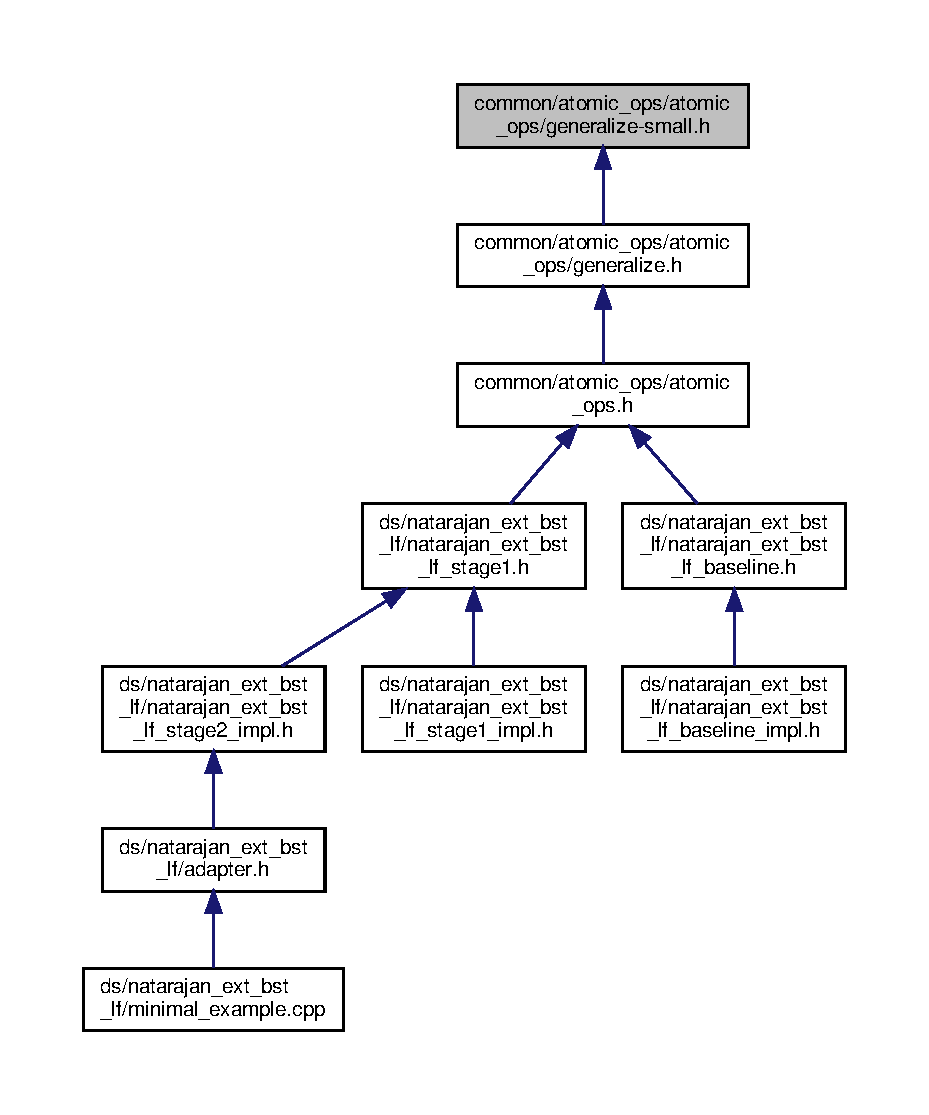
\includegraphics[width=350pt]{generalize-small_8h__dep__incl}
\end{center}
\end{figure}

\hypertarget{generalize_8h}{}\section{common/atomic\+\_\+ops/atomic\+\_\+ops/generalize.h File Reference}
\label{generalize_8h}\index{common/atomic\+\_\+ops/atomic\+\_\+ops/generalize.\+h@{common/atomic\+\_\+ops/atomic\+\_\+ops/generalize.\+h}}
{\ttfamily \#include \char`\"{}generalize-\/small.\+h\char`\"{}}\newline
Include dependency graph for generalize.\+h\+:
\nopagebreak
\begin{figure}[H]
\begin{center}
\leavevmode
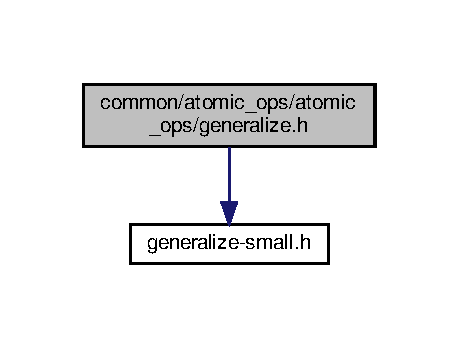
\includegraphics[width=220pt]{generalize_8h__incl}
\end{center}
\end{figure}
This graph shows which files directly or indirectly include this file\+:
\nopagebreak
\begin{figure}[H]
\begin{center}
\leavevmode
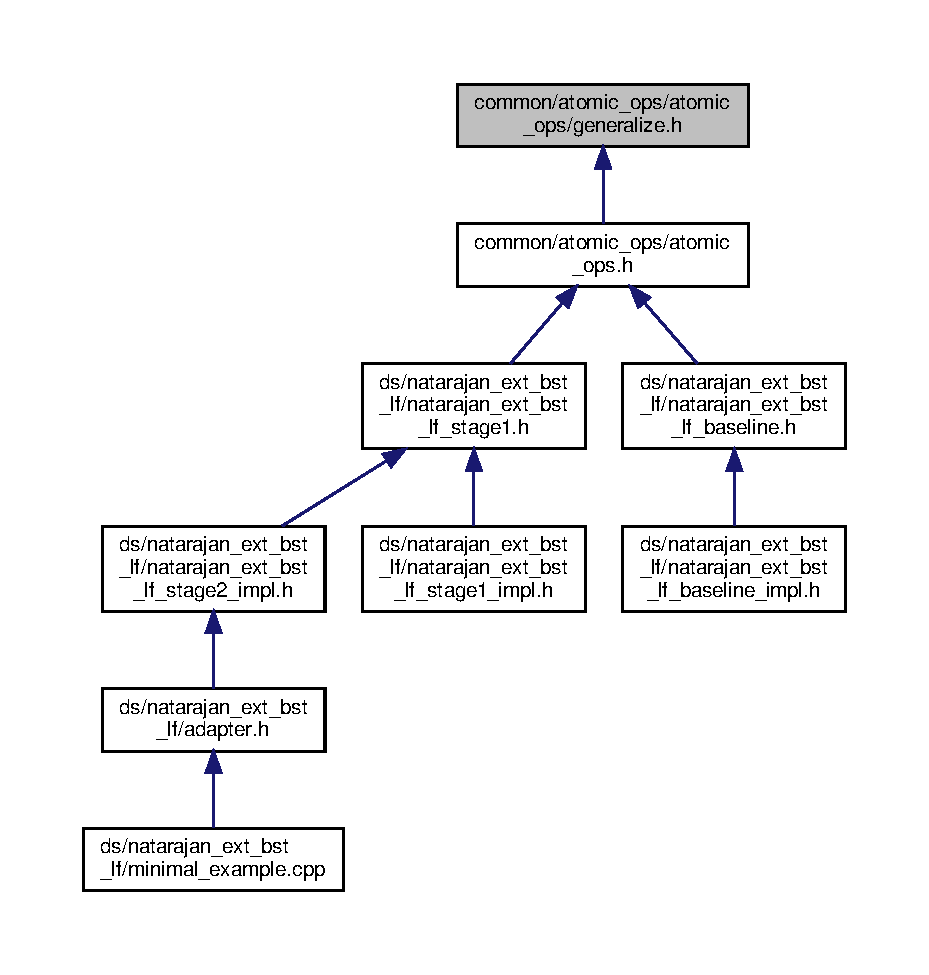
\includegraphics[width=350pt]{generalize_8h__dep__incl}
\end{center}
\end{figure}
\subsection*{Macros}
\begin{DoxyCompactItemize}
\item 
\#define \hyperlink{generalize_8h_a67dd3e29a078515021bd17dba6c4e79d}{A\+O\+\_\+\+H\+A\+V\+E\+\_\+nop}
\end{DoxyCompactItemize}
\subsection*{Functions}
\begin{DoxyCompactItemize}
\item 
\hyperlink{atomic__ops_8h_a9f6ab6253b6b11bc8c12efe9dde5db2b}{A\+O\+\_\+\+I\+N\+L\+I\+NE} void \hyperlink{generalize_8h_a14a0046dc4025a1ea344c1599097579a}{A\+O\+\_\+nop} (void)
\end{DoxyCompactItemize}


\subsection{Macro Definition Documentation}
\mbox{\Hypertarget{generalize_8h_a67dd3e29a078515021bd17dba6c4e79d}\label{generalize_8h_a67dd3e29a078515021bd17dba6c4e79d}} 
\index{generalize.\+h@{generalize.\+h}!A\+O\+\_\+\+H\+A\+V\+E\+\_\+nop@{A\+O\+\_\+\+H\+A\+V\+E\+\_\+nop}}
\index{A\+O\+\_\+\+H\+A\+V\+E\+\_\+nop@{A\+O\+\_\+\+H\+A\+V\+E\+\_\+nop}!generalize.\+h@{generalize.\+h}}
\subsubsection{\texorpdfstring{A\+O\+\_\+\+H\+A\+V\+E\+\_\+nop}{AO\_HAVE\_nop}}
{\footnotesize\ttfamily \#define A\+O\+\_\+\+H\+A\+V\+E\+\_\+nop}



\subsection{Function Documentation}
\mbox{\Hypertarget{generalize_8h_a14a0046dc4025a1ea344c1599097579a}\label{generalize_8h_a14a0046dc4025a1ea344c1599097579a}} 
\index{generalize.\+h@{generalize.\+h}!A\+O\+\_\+nop@{A\+O\+\_\+nop}}
\index{A\+O\+\_\+nop@{A\+O\+\_\+nop}!generalize.\+h@{generalize.\+h}}
\subsubsection{\texorpdfstring{A\+O\+\_\+nop()}{AO\_nop()}}
{\footnotesize\ttfamily \hyperlink{atomic__ops_8h_a9f6ab6253b6b11bc8c12efe9dde5db2b}{A\+O\+\_\+\+I\+N\+L\+I\+NE} void A\+O\+\_\+nop (\begin{DoxyParamCaption}\item[{void}]{ }\end{DoxyParamCaption})}


\hypertarget{acquire__release__volatile_8h}{}\section{common/atomic\+\_\+ops/atomic\+\_\+ops/sysdeps/acquire\+\_\+release\+\_\+volatile.h File Reference}
\label{acquire__release__volatile_8h}\index{common/atomic\+\_\+ops/atomic\+\_\+ops/sysdeps/acquire\+\_\+release\+\_\+volatile.\+h@{common/atomic\+\_\+ops/atomic\+\_\+ops/sysdeps/acquire\+\_\+release\+\_\+volatile.\+h}}
This graph shows which files directly or indirectly include this file\+:
\nopagebreak
\begin{figure}[H]
\begin{center}
\leavevmode
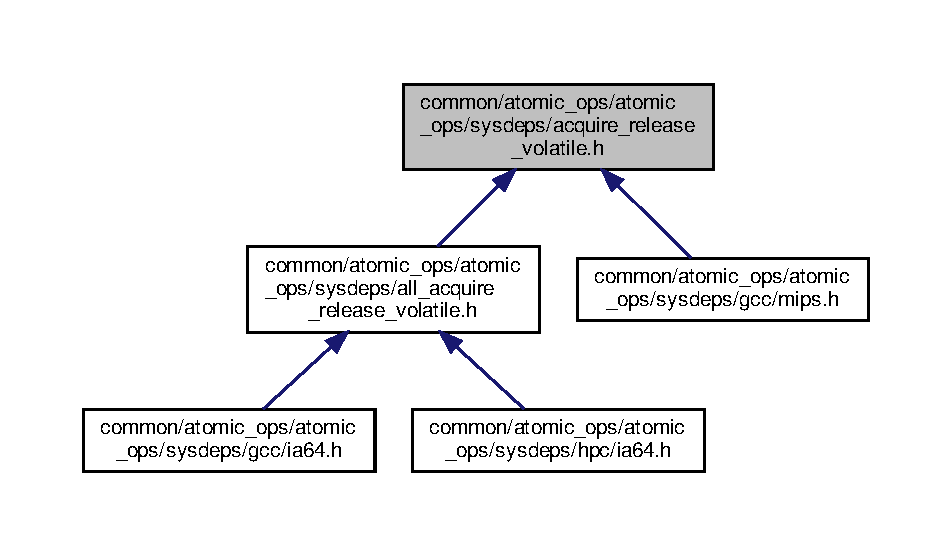
\includegraphics[width=350pt]{acquire__release__volatile_8h__dep__incl}
\end{center}
\end{figure}
\subsection*{Macros}
\begin{DoxyCompactItemize}
\item 
\#define \hyperlink{acquire__release__volatile_8h_a4b3b5ac83b6c7730e8376c8b5c0a6f01}{A\+O\+\_\+\+G\+C\+C\+\_\+\+B\+A\+R\+R\+I\+ER}()
\item 
\#define \hyperlink{acquire__release__volatile_8h_a29328d5664268a40645ea9d2f82c8bef}{A\+O\+\_\+\+H\+A\+V\+E\+\_\+load\+\_\+acquire}
\item 
\#define \hyperlink{acquire__release__volatile_8h_a58f98c6b42d593762336829dcf86d058}{A\+O\+\_\+\+H\+A\+V\+E\+\_\+store\+\_\+release}
\end{DoxyCompactItemize}
\subsection*{Functions}
\begin{DoxyCompactItemize}
\item 
\hyperlink{atomic__ops_8h_a9f6ab6253b6b11bc8c12efe9dde5db2b}{A\+O\+\_\+\+I\+N\+L\+I\+NE} \hyperlink{atomic__ops_8h_a5225fef4d9eee821e82382cd269160dd}{A\+O\+\_\+t} \hyperlink{acquire__release__volatile_8h_a38908e49c95fafba077fbeb130f0d930}{A\+O\+\_\+load\+\_\+acquire} (const volatile \hyperlink{atomic__ops_8h_a5225fef4d9eee821e82382cd269160dd}{A\+O\+\_\+t} $\ast$p)
\item 
\hyperlink{atomic__ops_8h_a9f6ab6253b6b11bc8c12efe9dde5db2b}{A\+O\+\_\+\+I\+N\+L\+I\+NE} void \hyperlink{acquire__release__volatile_8h_a5a48a48680fe8ac93029366b77457181}{A\+O\+\_\+store\+\_\+release} (volatile \hyperlink{atomic__ops_8h_a5225fef4d9eee821e82382cd269160dd}{A\+O\+\_\+t} $\ast$p, \hyperlink{atomic__ops_8h_a5225fef4d9eee821e82382cd269160dd}{A\+O\+\_\+t} val)
\end{DoxyCompactItemize}


\subsection{Macro Definition Documentation}
\mbox{\Hypertarget{acquire__release__volatile_8h_a4b3b5ac83b6c7730e8376c8b5c0a6f01}\label{acquire__release__volatile_8h_a4b3b5ac83b6c7730e8376c8b5c0a6f01}} 
\index{acquire\+\_\+release\+\_\+volatile.\+h@{acquire\+\_\+release\+\_\+volatile.\+h}!A\+O\+\_\+\+G\+C\+C\+\_\+\+B\+A\+R\+R\+I\+ER@{A\+O\+\_\+\+G\+C\+C\+\_\+\+B\+A\+R\+R\+I\+ER}}
\index{A\+O\+\_\+\+G\+C\+C\+\_\+\+B\+A\+R\+R\+I\+ER@{A\+O\+\_\+\+G\+C\+C\+\_\+\+B\+A\+R\+R\+I\+ER}!acquire\+\_\+release\+\_\+volatile.\+h@{acquire\+\_\+release\+\_\+volatile.\+h}}
\subsubsection{\texorpdfstring{A\+O\+\_\+\+G\+C\+C\+\_\+\+B\+A\+R\+R\+I\+ER}{AO\_GCC\_BARRIER}}
{\footnotesize\ttfamily \#define A\+O\+\_\+\+G\+C\+C\+\_\+\+B\+A\+R\+R\+I\+ER(\begin{DoxyParamCaption}{ }\end{DoxyParamCaption})}

\mbox{\Hypertarget{acquire__release__volatile_8h_a29328d5664268a40645ea9d2f82c8bef}\label{acquire__release__volatile_8h_a29328d5664268a40645ea9d2f82c8bef}} 
\index{acquire\+\_\+release\+\_\+volatile.\+h@{acquire\+\_\+release\+\_\+volatile.\+h}!A\+O\+\_\+\+H\+A\+V\+E\+\_\+load\+\_\+acquire@{A\+O\+\_\+\+H\+A\+V\+E\+\_\+load\+\_\+acquire}}
\index{A\+O\+\_\+\+H\+A\+V\+E\+\_\+load\+\_\+acquire@{A\+O\+\_\+\+H\+A\+V\+E\+\_\+load\+\_\+acquire}!acquire\+\_\+release\+\_\+volatile.\+h@{acquire\+\_\+release\+\_\+volatile.\+h}}
\subsubsection{\texorpdfstring{A\+O\+\_\+\+H\+A\+V\+E\+\_\+load\+\_\+acquire}{AO\_HAVE\_load\_acquire}}
{\footnotesize\ttfamily \#define A\+O\+\_\+\+H\+A\+V\+E\+\_\+load\+\_\+acquire}

\mbox{\Hypertarget{acquire__release__volatile_8h_a58f98c6b42d593762336829dcf86d058}\label{acquire__release__volatile_8h_a58f98c6b42d593762336829dcf86d058}} 
\index{acquire\+\_\+release\+\_\+volatile.\+h@{acquire\+\_\+release\+\_\+volatile.\+h}!A\+O\+\_\+\+H\+A\+V\+E\+\_\+store\+\_\+release@{A\+O\+\_\+\+H\+A\+V\+E\+\_\+store\+\_\+release}}
\index{A\+O\+\_\+\+H\+A\+V\+E\+\_\+store\+\_\+release@{A\+O\+\_\+\+H\+A\+V\+E\+\_\+store\+\_\+release}!acquire\+\_\+release\+\_\+volatile.\+h@{acquire\+\_\+release\+\_\+volatile.\+h}}
\subsubsection{\texorpdfstring{A\+O\+\_\+\+H\+A\+V\+E\+\_\+store\+\_\+release}{AO\_HAVE\_store\_release}}
{\footnotesize\ttfamily \#define A\+O\+\_\+\+H\+A\+V\+E\+\_\+store\+\_\+release}



\subsection{Function Documentation}
\mbox{\Hypertarget{acquire__release__volatile_8h_a38908e49c95fafba077fbeb130f0d930}\label{acquire__release__volatile_8h_a38908e49c95fafba077fbeb130f0d930}} 
\index{acquire\+\_\+release\+\_\+volatile.\+h@{acquire\+\_\+release\+\_\+volatile.\+h}!A\+O\+\_\+load\+\_\+acquire@{A\+O\+\_\+load\+\_\+acquire}}
\index{A\+O\+\_\+load\+\_\+acquire@{A\+O\+\_\+load\+\_\+acquire}!acquire\+\_\+release\+\_\+volatile.\+h@{acquire\+\_\+release\+\_\+volatile.\+h}}
\subsubsection{\texorpdfstring{A\+O\+\_\+load\+\_\+acquire()}{AO\_load\_acquire()}}
{\footnotesize\ttfamily \hyperlink{atomic__ops_8h_a9f6ab6253b6b11bc8c12efe9dde5db2b}{A\+O\+\_\+\+I\+N\+L\+I\+NE} \hyperlink{atomic__ops_8h_a5225fef4d9eee821e82382cd269160dd}{A\+O\+\_\+t} A\+O\+\_\+load\+\_\+acquire (\begin{DoxyParamCaption}\item[{const volatile \hyperlink{atomic__ops_8h_a5225fef4d9eee821e82382cd269160dd}{A\+O\+\_\+t} $\ast$}]{p }\end{DoxyParamCaption})}

\mbox{\Hypertarget{acquire__release__volatile_8h_a5a48a48680fe8ac93029366b77457181}\label{acquire__release__volatile_8h_a5a48a48680fe8ac93029366b77457181}} 
\index{acquire\+\_\+release\+\_\+volatile.\+h@{acquire\+\_\+release\+\_\+volatile.\+h}!A\+O\+\_\+store\+\_\+release@{A\+O\+\_\+store\+\_\+release}}
\index{A\+O\+\_\+store\+\_\+release@{A\+O\+\_\+store\+\_\+release}!acquire\+\_\+release\+\_\+volatile.\+h@{acquire\+\_\+release\+\_\+volatile.\+h}}
\subsubsection{\texorpdfstring{A\+O\+\_\+store\+\_\+release()}{AO\_store\_release()}}
{\footnotesize\ttfamily \hyperlink{atomic__ops_8h_a9f6ab6253b6b11bc8c12efe9dde5db2b}{A\+O\+\_\+\+I\+N\+L\+I\+NE} void A\+O\+\_\+store\+\_\+release (\begin{DoxyParamCaption}\item[{volatile \hyperlink{atomic__ops_8h_a5225fef4d9eee821e82382cd269160dd}{A\+O\+\_\+t} $\ast$}]{p,  }\item[{\hyperlink{atomic__ops_8h_a5225fef4d9eee821e82382cd269160dd}{A\+O\+\_\+t}}]{val }\end{DoxyParamCaption})}


\hypertarget{aligned__atomic__load__store_8h}{}\section{common/atomic\+\_\+ops/atomic\+\_\+ops/sysdeps/aligned\+\_\+atomic\+\_\+load\+\_\+store.h File Reference}
\label{aligned__atomic__load__store_8h}\index{common/atomic\+\_\+ops/atomic\+\_\+ops/sysdeps/aligned\+\_\+atomic\+\_\+load\+\_\+store.\+h@{common/atomic\+\_\+ops/atomic\+\_\+ops/sysdeps/aligned\+\_\+atomic\+\_\+load\+\_\+store.\+h}}
This graph shows which files directly or indirectly include this file\+:
\nopagebreak
\begin{figure}[H]
\begin{center}
\leavevmode
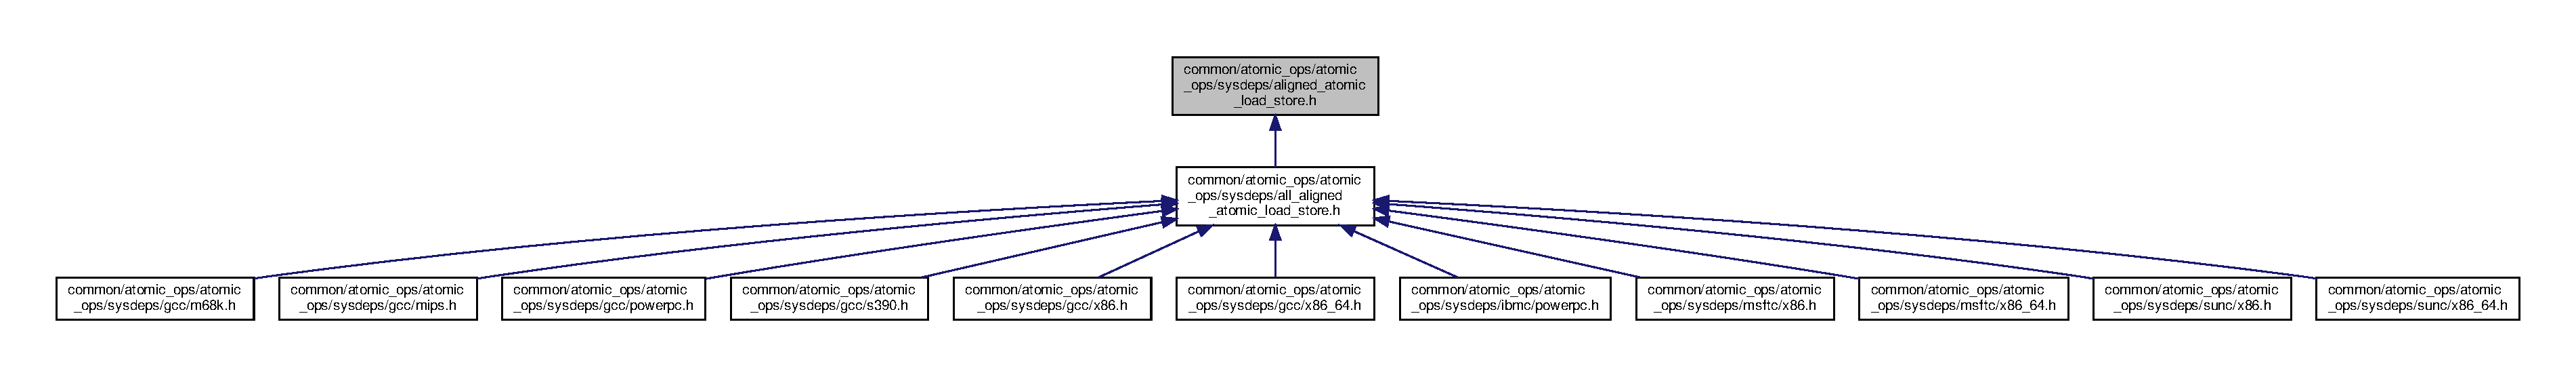
\includegraphics[width=350pt]{aligned__atomic__load__store_8h__dep__incl}
\end{center}
\end{figure}
\subsection*{Macros}
\begin{DoxyCompactItemize}
\item 
\#define \hyperlink{aligned__atomic__load__store_8h_a981bfe2db392018d7dbdf444653690d2}{A\+O\+\_\+\+H\+A\+V\+E\+\_\+load}
\item 
\#define \hyperlink{aligned__atomic__load__store_8h_aa0b1f05a9f5e72e8be48d88dab4a5d84}{A\+O\+\_\+\+H\+A\+V\+E\+\_\+store}
\end{DoxyCompactItemize}
\subsection*{Functions}
\begin{DoxyCompactItemize}
\item 
\hyperlink{atomic__ops_8h_a9f6ab6253b6b11bc8c12efe9dde5db2b}{A\+O\+\_\+\+I\+N\+L\+I\+NE} \hyperlink{atomic__ops_8h_a5225fef4d9eee821e82382cd269160dd}{A\+O\+\_\+t} \hyperlink{aligned__atomic__load__store_8h_abce409d4af805946c529de695e85b54f}{A\+O\+\_\+load} (const volatile \hyperlink{atomic__ops_8h_a5225fef4d9eee821e82382cd269160dd}{A\+O\+\_\+t} $\ast$addr)
\item 
\hyperlink{atomic__ops_8h_a9f6ab6253b6b11bc8c12efe9dde5db2b}{A\+O\+\_\+\+I\+N\+L\+I\+NE} void \hyperlink{aligned__atomic__load__store_8h_a909024cfd17bfc0687e923fc5d592ecf}{A\+O\+\_\+store} (volatile \hyperlink{atomic__ops_8h_a5225fef4d9eee821e82382cd269160dd}{A\+O\+\_\+t} $\ast$addr, \hyperlink{atomic__ops_8h_a5225fef4d9eee821e82382cd269160dd}{A\+O\+\_\+t} new\+\_\+val)
\end{DoxyCompactItemize}


\subsection{Macro Definition Documentation}
\mbox{\Hypertarget{aligned__atomic__load__store_8h_a981bfe2db392018d7dbdf444653690d2}\label{aligned__atomic__load__store_8h_a981bfe2db392018d7dbdf444653690d2}} 
\index{aligned\+\_\+atomic\+\_\+load\+\_\+store.\+h@{aligned\+\_\+atomic\+\_\+load\+\_\+store.\+h}!A\+O\+\_\+\+H\+A\+V\+E\+\_\+load@{A\+O\+\_\+\+H\+A\+V\+E\+\_\+load}}
\index{A\+O\+\_\+\+H\+A\+V\+E\+\_\+load@{A\+O\+\_\+\+H\+A\+V\+E\+\_\+load}!aligned\+\_\+atomic\+\_\+load\+\_\+store.\+h@{aligned\+\_\+atomic\+\_\+load\+\_\+store.\+h}}
\subsubsection{\texorpdfstring{A\+O\+\_\+\+H\+A\+V\+E\+\_\+load}{AO\_HAVE\_load}}
{\footnotesize\ttfamily \#define A\+O\+\_\+\+H\+A\+V\+E\+\_\+load}

\mbox{\Hypertarget{aligned__atomic__load__store_8h_aa0b1f05a9f5e72e8be48d88dab4a5d84}\label{aligned__atomic__load__store_8h_aa0b1f05a9f5e72e8be48d88dab4a5d84}} 
\index{aligned\+\_\+atomic\+\_\+load\+\_\+store.\+h@{aligned\+\_\+atomic\+\_\+load\+\_\+store.\+h}!A\+O\+\_\+\+H\+A\+V\+E\+\_\+store@{A\+O\+\_\+\+H\+A\+V\+E\+\_\+store}}
\index{A\+O\+\_\+\+H\+A\+V\+E\+\_\+store@{A\+O\+\_\+\+H\+A\+V\+E\+\_\+store}!aligned\+\_\+atomic\+\_\+load\+\_\+store.\+h@{aligned\+\_\+atomic\+\_\+load\+\_\+store.\+h}}
\subsubsection{\texorpdfstring{A\+O\+\_\+\+H\+A\+V\+E\+\_\+store}{AO\_HAVE\_store}}
{\footnotesize\ttfamily \#define A\+O\+\_\+\+H\+A\+V\+E\+\_\+store}



\subsection{Function Documentation}
\mbox{\Hypertarget{aligned__atomic__load__store_8h_abce409d4af805946c529de695e85b54f}\label{aligned__atomic__load__store_8h_abce409d4af805946c529de695e85b54f}} 
\index{aligned\+\_\+atomic\+\_\+load\+\_\+store.\+h@{aligned\+\_\+atomic\+\_\+load\+\_\+store.\+h}!A\+O\+\_\+load@{A\+O\+\_\+load}}
\index{A\+O\+\_\+load@{A\+O\+\_\+load}!aligned\+\_\+atomic\+\_\+load\+\_\+store.\+h@{aligned\+\_\+atomic\+\_\+load\+\_\+store.\+h}}
\subsubsection{\texorpdfstring{A\+O\+\_\+load()}{AO\_load()}}
{\footnotesize\ttfamily \hyperlink{atomic__ops_8h_a9f6ab6253b6b11bc8c12efe9dde5db2b}{A\+O\+\_\+\+I\+N\+L\+I\+NE} \hyperlink{atomic__ops_8h_a5225fef4d9eee821e82382cd269160dd}{A\+O\+\_\+t} A\+O\+\_\+load (\begin{DoxyParamCaption}\item[{const volatile \hyperlink{atomic__ops_8h_a5225fef4d9eee821e82382cd269160dd}{A\+O\+\_\+t} $\ast$}]{addr }\end{DoxyParamCaption})}

\mbox{\Hypertarget{aligned__atomic__load__store_8h_a909024cfd17bfc0687e923fc5d592ecf}\label{aligned__atomic__load__store_8h_a909024cfd17bfc0687e923fc5d592ecf}} 
\index{aligned\+\_\+atomic\+\_\+load\+\_\+store.\+h@{aligned\+\_\+atomic\+\_\+load\+\_\+store.\+h}!A\+O\+\_\+store@{A\+O\+\_\+store}}
\index{A\+O\+\_\+store@{A\+O\+\_\+store}!aligned\+\_\+atomic\+\_\+load\+\_\+store.\+h@{aligned\+\_\+atomic\+\_\+load\+\_\+store.\+h}}
\subsubsection{\texorpdfstring{A\+O\+\_\+store()}{AO\_store()}}
{\footnotesize\ttfamily \hyperlink{atomic__ops_8h_a9f6ab6253b6b11bc8c12efe9dde5db2b}{A\+O\+\_\+\+I\+N\+L\+I\+NE} void A\+O\+\_\+store (\begin{DoxyParamCaption}\item[{volatile \hyperlink{atomic__ops_8h_a5225fef4d9eee821e82382cd269160dd}{A\+O\+\_\+t} $\ast$}]{addr,  }\item[{\hyperlink{atomic__ops_8h_a5225fef4d9eee821e82382cd269160dd}{A\+O\+\_\+t}}]{new\+\_\+val }\end{DoxyParamCaption})}


\hypertarget{all__acquire__release__volatile_8h}{}\section{common/atomic\+\_\+ops/atomic\+\_\+ops/sysdeps/all\+\_\+acquire\+\_\+release\+\_\+volatile.h File Reference}
\label{all__acquire__release__volatile_8h}\index{common/atomic\+\_\+ops/atomic\+\_\+ops/sysdeps/all\+\_\+acquire\+\_\+release\+\_\+volatile.\+h@{common/atomic\+\_\+ops/atomic\+\_\+ops/sysdeps/all\+\_\+acquire\+\_\+release\+\_\+volatile.\+h}}
{\ttfamily \#include \char`\"{}acquire\+\_\+release\+\_\+volatile.\+h\char`\"{}}\newline
{\ttfamily \#include \char`\"{}char\+\_\+acquire\+\_\+release\+\_\+volatile.\+h\char`\"{}}\newline
{\ttfamily \#include \char`\"{}short\+\_\+acquire\+\_\+release\+\_\+volatile.\+h\char`\"{}}\newline
{\ttfamily \#include \char`\"{}int\+\_\+acquire\+\_\+release\+\_\+volatile.\+h\char`\"{}}\newline
Include dependency graph for all\+\_\+acquire\+\_\+release\+\_\+volatile.\+h\+:
\nopagebreak
\begin{figure}[H]
\begin{center}
\leavevmode
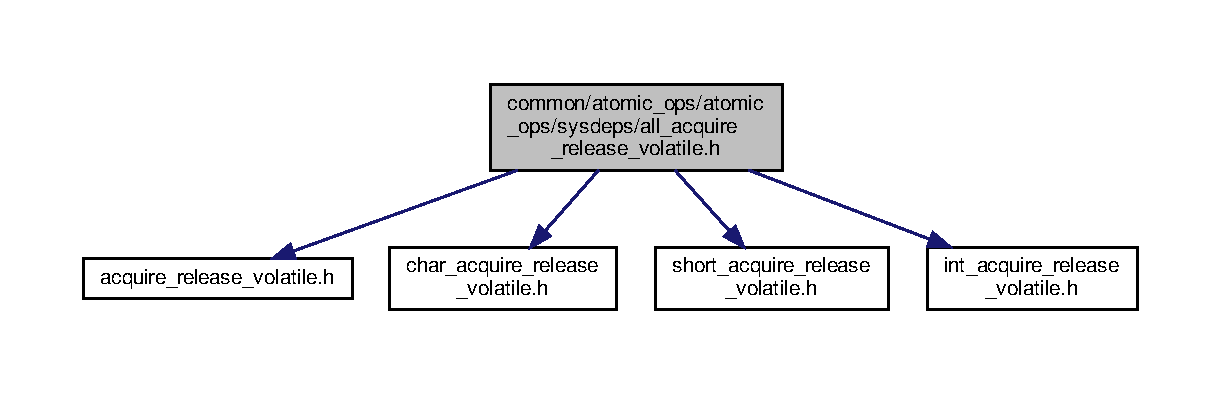
\includegraphics[width=350pt]{all__acquire__release__volatile_8h__incl}
\end{center}
\end{figure}
This graph shows which files directly or indirectly include this file\+:
\nopagebreak
\begin{figure}[H]
\begin{center}
\leavevmode
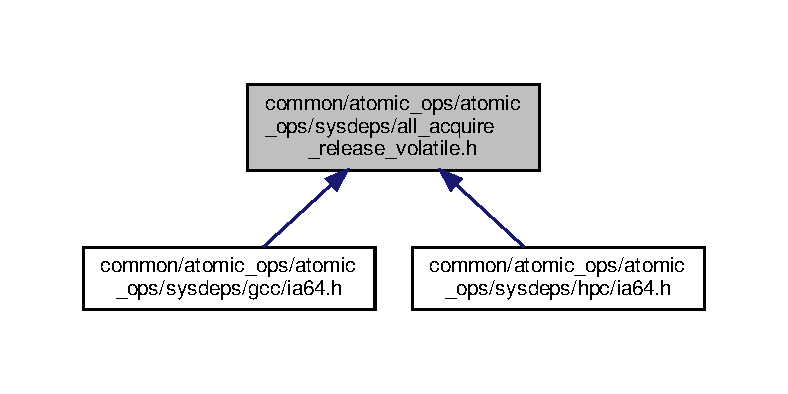
\includegraphics[width=350pt]{all__acquire__release__volatile_8h__dep__incl}
\end{center}
\end{figure}

\hypertarget{all__aligned__atomic__load__store_8h}{}\section{common/atomic\+\_\+ops/atomic\+\_\+ops/sysdeps/all\+\_\+aligned\+\_\+atomic\+\_\+load\+\_\+store.h File Reference}
\label{all__aligned__atomic__load__store_8h}\index{common/atomic\+\_\+ops/atomic\+\_\+ops/sysdeps/all\+\_\+aligned\+\_\+atomic\+\_\+load\+\_\+store.\+h@{common/atomic\+\_\+ops/atomic\+\_\+ops/sysdeps/all\+\_\+aligned\+\_\+atomic\+\_\+load\+\_\+store.\+h}}
{\ttfamily \#include \char`\"{}aligned\+\_\+atomic\+\_\+load\+\_\+store.\+h\char`\"{}}\newline
{\ttfamily \#include \char`\"{}char\+\_\+atomic\+\_\+load\+\_\+store.\+h\char`\"{}}\newline
{\ttfamily \#include \char`\"{}short\+\_\+aligned\+\_\+atomic\+\_\+load\+\_\+store.\+h\char`\"{}}\newline
{\ttfamily \#include \char`\"{}int\+\_\+aligned\+\_\+atomic\+\_\+load\+\_\+store.\+h\char`\"{}}\newline
Include dependency graph for all\+\_\+aligned\+\_\+atomic\+\_\+load\+\_\+store.\+h\+:
\nopagebreak
\begin{figure}[H]
\begin{center}
\leavevmode
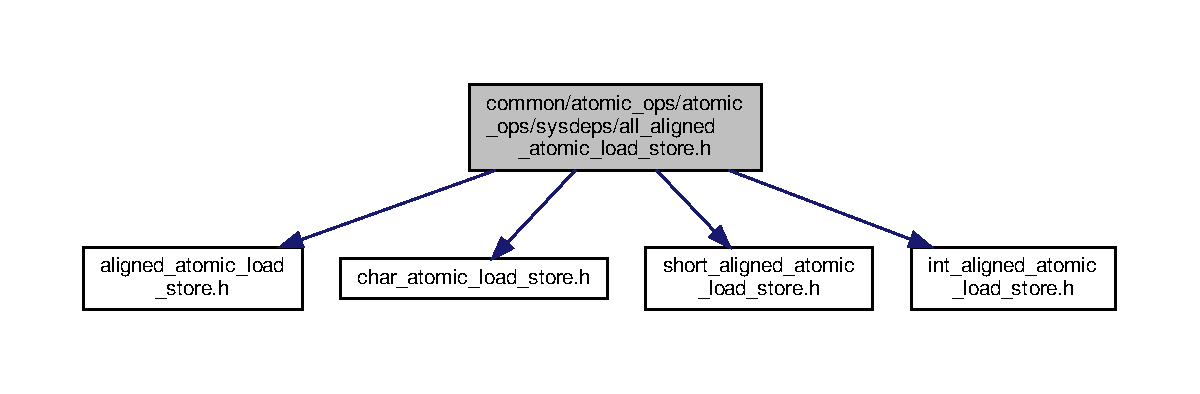
\includegraphics[width=350pt]{all__aligned__atomic__load__store_8h__incl}
\end{center}
\end{figure}
This graph shows which files directly or indirectly include this file\+:
\nopagebreak
\begin{figure}[H]
\begin{center}
\leavevmode
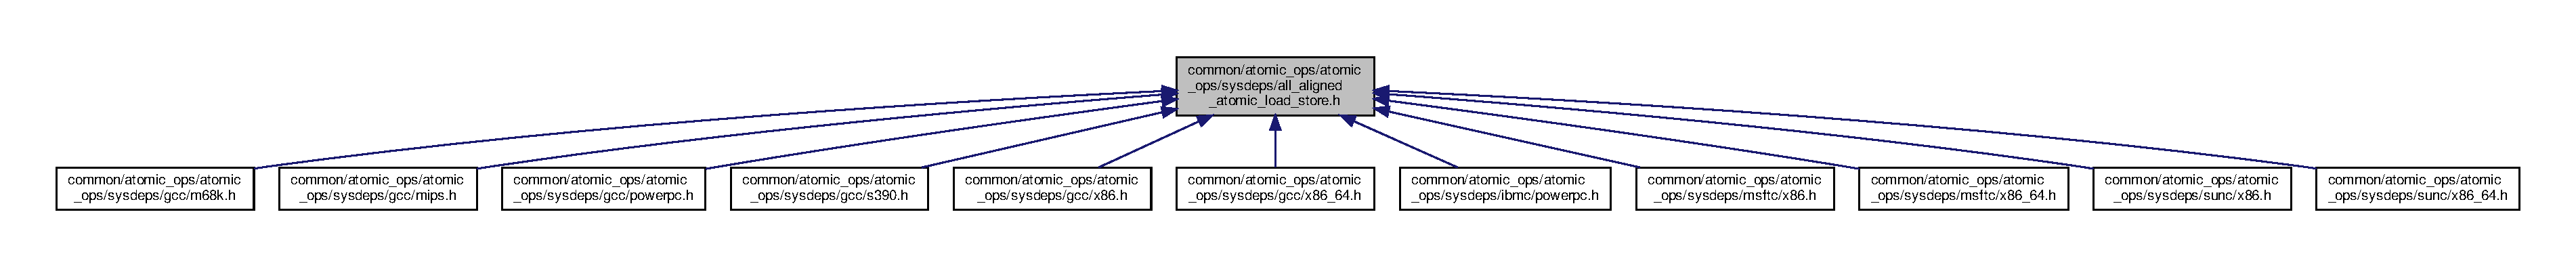
\includegraphics[width=350pt]{all__aligned__atomic__load__store_8h__dep__incl}
\end{center}
\end{figure}

\hypertarget{all__atomic__load__store_8h}{}\section{common/atomic\+\_\+ops/atomic\+\_\+ops/sysdeps/all\+\_\+atomic\+\_\+load\+\_\+store.h File Reference}
\label{all__atomic__load__store_8h}\index{common/atomic\+\_\+ops/atomic\+\_\+ops/sysdeps/all\+\_\+atomic\+\_\+load\+\_\+store.\+h@{common/atomic\+\_\+ops/atomic\+\_\+ops/sysdeps/all\+\_\+atomic\+\_\+load\+\_\+store.\+h}}
{\ttfamily \#include \char`\"{}atomic\+\_\+load\+\_\+store.\+h\char`\"{}}\newline
{\ttfamily \#include \char`\"{}char\+\_\+atomic\+\_\+load\+\_\+store.\+h\char`\"{}}\newline
{\ttfamily \#include \char`\"{}short\+\_\+atomic\+\_\+load\+\_\+store.\+h\char`\"{}}\newline
{\ttfamily \#include \char`\"{}int\+\_\+atomic\+\_\+load\+\_\+store.\+h\char`\"{}}\newline
Include dependency graph for all\+\_\+atomic\+\_\+load\+\_\+store.\+h\+:
\nopagebreak
\begin{figure}[H]
\begin{center}
\leavevmode
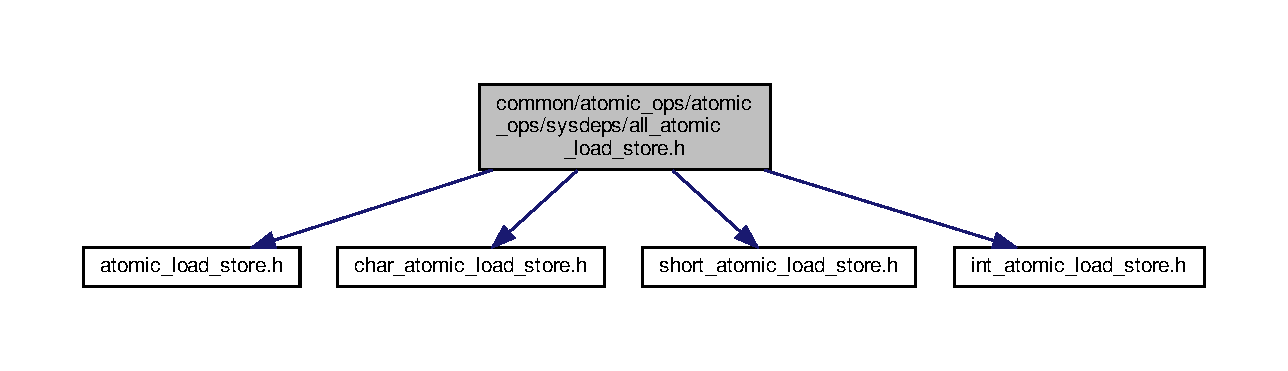
\includegraphics[width=350pt]{all__atomic__load__store_8h__incl}
\end{center}
\end{figure}
This graph shows which files directly or indirectly include this file\+:
\nopagebreak
\begin{figure}[H]
\begin{center}
\leavevmode
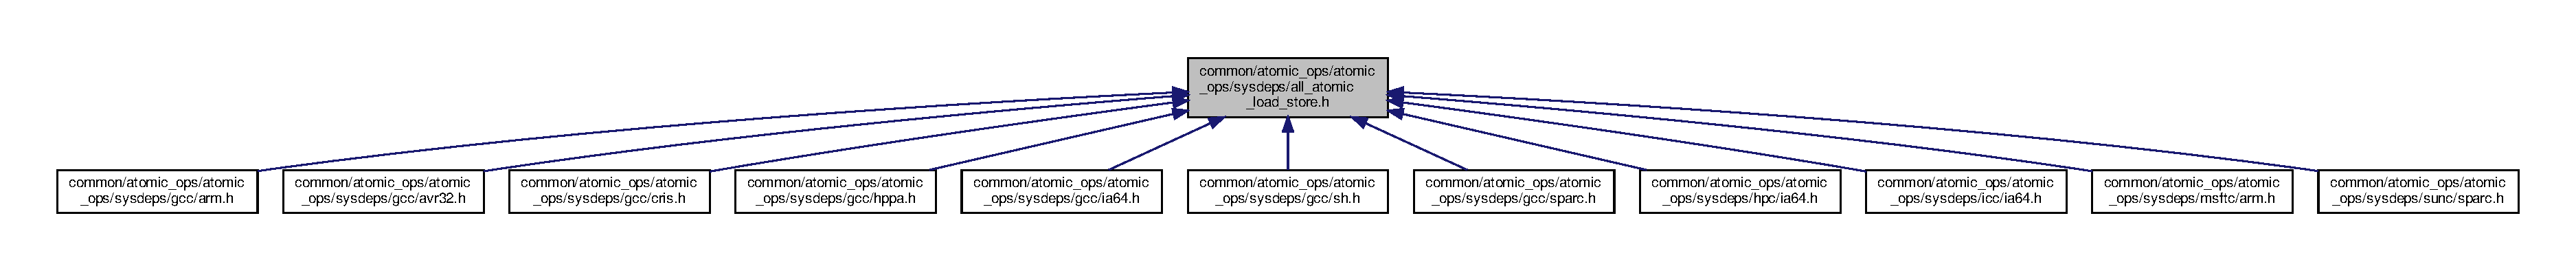
\includegraphics[width=350pt]{all__atomic__load__store_8h__dep__incl}
\end{center}
\end{figure}

\hypertarget{ao__t__is__int_8h}{}\section{common/atomic\+\_\+ops/atomic\+\_\+ops/sysdeps/ao\+\_\+t\+\_\+is\+\_\+int.h File Reference}
\label{ao__t__is__int_8h}\index{common/atomic\+\_\+ops/atomic\+\_\+ops/sysdeps/ao\+\_\+t\+\_\+is\+\_\+int.\+h@{common/atomic\+\_\+ops/atomic\+\_\+ops/sysdeps/ao\+\_\+t\+\_\+is\+\_\+int.\+h}}
This graph shows which files directly or indirectly include this file\+:
\nopagebreak
\begin{figure}[H]
\begin{center}
\leavevmode
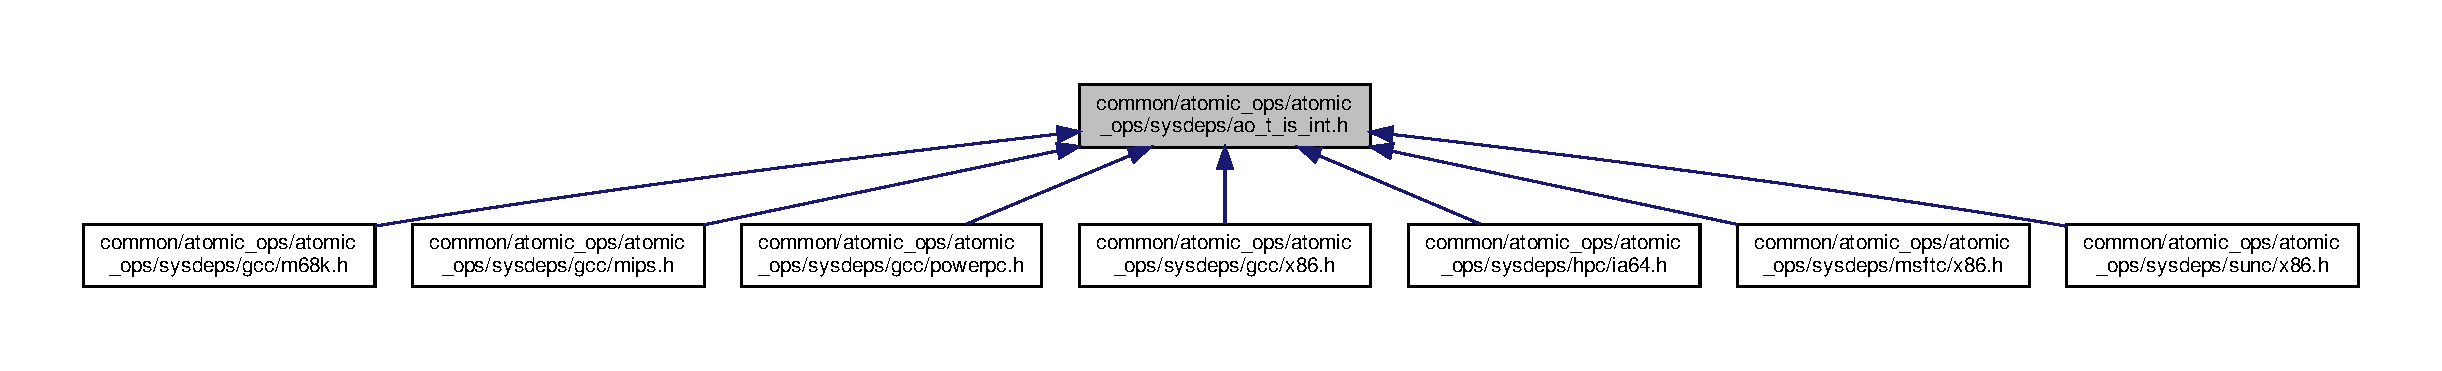
\includegraphics[width=350pt]{ao__t__is__int_8h__dep__incl}
\end{center}
\end{figure}

\hypertarget{arm__v6_8h}{}\section{common/atomic\+\_\+ops/atomic\+\_\+ops/sysdeps/armcc/arm\+\_\+v6.h File Reference}
\label{arm__v6_8h}\index{common/atomic\+\_\+ops/atomic\+\_\+ops/sysdeps/armcc/arm\+\_\+v6.\+h@{common/atomic\+\_\+ops/atomic\+\_\+ops/sysdeps/armcc/arm\+\_\+v6.\+h}}
{\ttfamily \#include \char`\"{}../read\+\_\+ordered.\+h\char`\"{}}\newline
{\ttfamily \#include \char`\"{}../test\+\_\+and\+\_\+set\+\_\+t\+\_\+is\+\_\+ao\+\_\+t.\+h\char`\"{}}\newline
Include dependency graph for arm\+\_\+v6.\+h\+:
\nopagebreak
\begin{figure}[H]
\begin{center}
\leavevmode
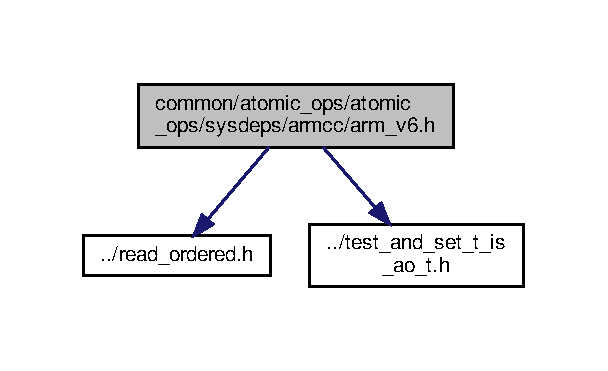
\includegraphics[width=292pt]{arm__v6_8h__incl}
\end{center}
\end{figure}

\hypertarget{atomic__load__store_8h}{}\section{common/atomic\+\_\+ops/atomic\+\_\+ops/sysdeps/atomic\+\_\+load\+\_\+store.h File Reference}
\label{atomic__load__store_8h}\index{common/atomic\+\_\+ops/atomic\+\_\+ops/sysdeps/atomic\+\_\+load\+\_\+store.\+h@{common/atomic\+\_\+ops/atomic\+\_\+ops/sysdeps/atomic\+\_\+load\+\_\+store.\+h}}
This graph shows which files directly or indirectly include this file\+:
\nopagebreak
\begin{figure}[H]
\begin{center}
\leavevmode
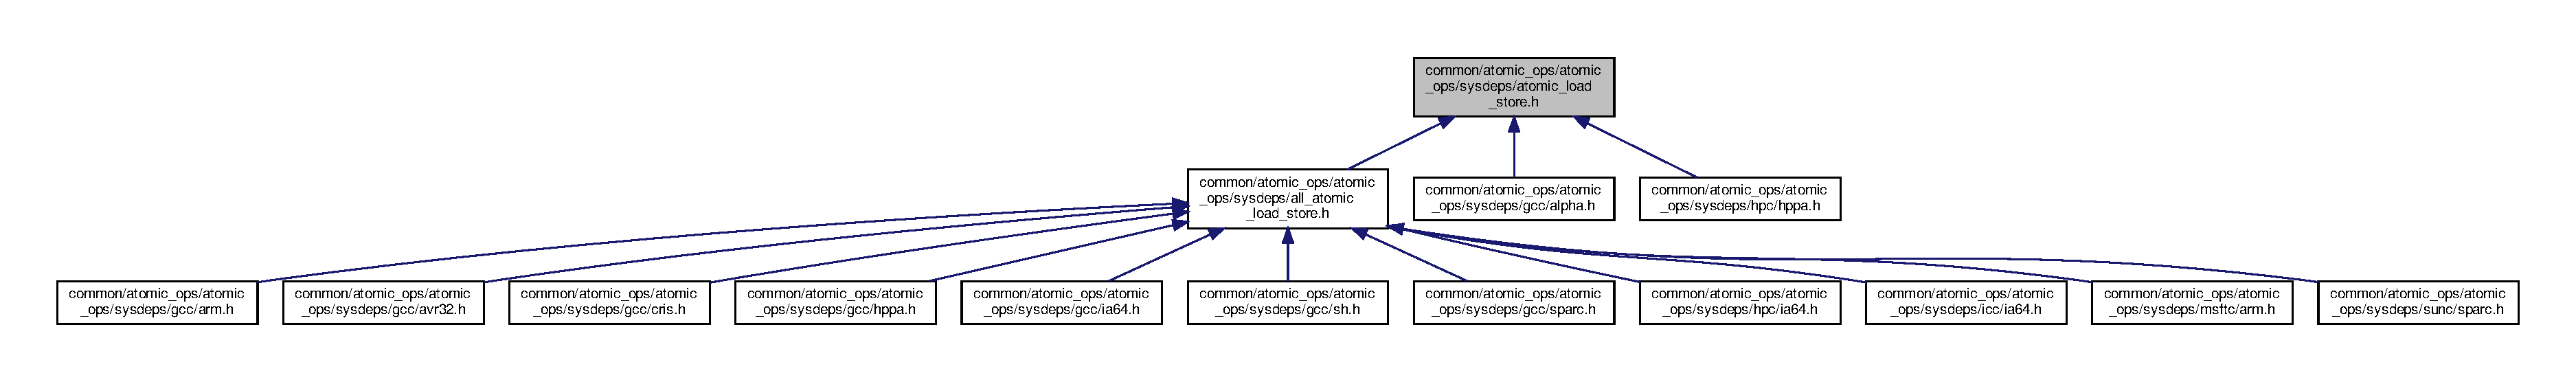
\includegraphics[width=350pt]{atomic__load__store_8h__dep__incl}
\end{center}
\end{figure}
\subsection*{Macros}
\begin{DoxyCompactItemize}
\item 
\#define \hyperlink{atomic__load__store_8h_a981bfe2db392018d7dbdf444653690d2}{A\+O\+\_\+\+H\+A\+V\+E\+\_\+load}
\item 
\#define \hyperlink{atomic__load__store_8h_aa0b1f05a9f5e72e8be48d88dab4a5d84}{A\+O\+\_\+\+H\+A\+V\+E\+\_\+store}
\end{DoxyCompactItemize}
\subsection*{Functions}
\begin{DoxyCompactItemize}
\item 
\hyperlink{atomic__ops_8h_a9f6ab6253b6b11bc8c12efe9dde5db2b}{A\+O\+\_\+\+I\+N\+L\+I\+NE} \hyperlink{atomic__ops_8h_a5225fef4d9eee821e82382cd269160dd}{A\+O\+\_\+t} \hyperlink{atomic__load__store_8h_abce409d4af805946c529de695e85b54f}{A\+O\+\_\+load} (const volatile \hyperlink{atomic__ops_8h_a5225fef4d9eee821e82382cd269160dd}{A\+O\+\_\+t} $\ast$addr)
\item 
\hyperlink{atomic__ops_8h_a9f6ab6253b6b11bc8c12efe9dde5db2b}{A\+O\+\_\+\+I\+N\+L\+I\+NE} void \hyperlink{atomic__load__store_8h_a909024cfd17bfc0687e923fc5d592ecf}{A\+O\+\_\+store} (volatile \hyperlink{atomic__ops_8h_a5225fef4d9eee821e82382cd269160dd}{A\+O\+\_\+t} $\ast$addr, \hyperlink{atomic__ops_8h_a5225fef4d9eee821e82382cd269160dd}{A\+O\+\_\+t} new\+\_\+val)
\end{DoxyCompactItemize}


\subsection{Macro Definition Documentation}
\mbox{\Hypertarget{atomic__load__store_8h_a981bfe2db392018d7dbdf444653690d2}\label{atomic__load__store_8h_a981bfe2db392018d7dbdf444653690d2}} 
\index{atomic\+\_\+load\+\_\+store.\+h@{atomic\+\_\+load\+\_\+store.\+h}!A\+O\+\_\+\+H\+A\+V\+E\+\_\+load@{A\+O\+\_\+\+H\+A\+V\+E\+\_\+load}}
\index{A\+O\+\_\+\+H\+A\+V\+E\+\_\+load@{A\+O\+\_\+\+H\+A\+V\+E\+\_\+load}!atomic\+\_\+load\+\_\+store.\+h@{atomic\+\_\+load\+\_\+store.\+h}}
\subsubsection{\texorpdfstring{A\+O\+\_\+\+H\+A\+V\+E\+\_\+load}{AO\_HAVE\_load}}
{\footnotesize\ttfamily \#define A\+O\+\_\+\+H\+A\+V\+E\+\_\+load}

\mbox{\Hypertarget{atomic__load__store_8h_aa0b1f05a9f5e72e8be48d88dab4a5d84}\label{atomic__load__store_8h_aa0b1f05a9f5e72e8be48d88dab4a5d84}} 
\index{atomic\+\_\+load\+\_\+store.\+h@{atomic\+\_\+load\+\_\+store.\+h}!A\+O\+\_\+\+H\+A\+V\+E\+\_\+store@{A\+O\+\_\+\+H\+A\+V\+E\+\_\+store}}
\index{A\+O\+\_\+\+H\+A\+V\+E\+\_\+store@{A\+O\+\_\+\+H\+A\+V\+E\+\_\+store}!atomic\+\_\+load\+\_\+store.\+h@{atomic\+\_\+load\+\_\+store.\+h}}
\subsubsection{\texorpdfstring{A\+O\+\_\+\+H\+A\+V\+E\+\_\+store}{AO\_HAVE\_store}}
{\footnotesize\ttfamily \#define A\+O\+\_\+\+H\+A\+V\+E\+\_\+store}



\subsection{Function Documentation}
\mbox{\Hypertarget{atomic__load__store_8h_abce409d4af805946c529de695e85b54f}\label{atomic__load__store_8h_abce409d4af805946c529de695e85b54f}} 
\index{atomic\+\_\+load\+\_\+store.\+h@{atomic\+\_\+load\+\_\+store.\+h}!A\+O\+\_\+load@{A\+O\+\_\+load}}
\index{A\+O\+\_\+load@{A\+O\+\_\+load}!atomic\+\_\+load\+\_\+store.\+h@{atomic\+\_\+load\+\_\+store.\+h}}
\subsubsection{\texorpdfstring{A\+O\+\_\+load()}{AO\_load()}}
{\footnotesize\ttfamily \hyperlink{atomic__ops_8h_a9f6ab6253b6b11bc8c12efe9dde5db2b}{A\+O\+\_\+\+I\+N\+L\+I\+NE} \hyperlink{atomic__ops_8h_a5225fef4d9eee821e82382cd269160dd}{A\+O\+\_\+t} A\+O\+\_\+load (\begin{DoxyParamCaption}\item[{const volatile \hyperlink{atomic__ops_8h_a5225fef4d9eee821e82382cd269160dd}{A\+O\+\_\+t} $\ast$}]{addr }\end{DoxyParamCaption})}

\mbox{\Hypertarget{atomic__load__store_8h_a909024cfd17bfc0687e923fc5d592ecf}\label{atomic__load__store_8h_a909024cfd17bfc0687e923fc5d592ecf}} 
\index{atomic\+\_\+load\+\_\+store.\+h@{atomic\+\_\+load\+\_\+store.\+h}!A\+O\+\_\+store@{A\+O\+\_\+store}}
\index{A\+O\+\_\+store@{A\+O\+\_\+store}!atomic\+\_\+load\+\_\+store.\+h@{atomic\+\_\+load\+\_\+store.\+h}}
\subsubsection{\texorpdfstring{A\+O\+\_\+store()}{AO\_store()}}
{\footnotesize\ttfamily \hyperlink{atomic__ops_8h_a9f6ab6253b6b11bc8c12efe9dde5db2b}{A\+O\+\_\+\+I\+N\+L\+I\+NE} void A\+O\+\_\+store (\begin{DoxyParamCaption}\item[{volatile \hyperlink{atomic__ops_8h_a5225fef4d9eee821e82382cd269160dd}{A\+O\+\_\+t} $\ast$}]{addr,  }\item[{\hyperlink{atomic__ops_8h_a5225fef4d9eee821e82382cd269160dd}{A\+O\+\_\+t}}]{new\+\_\+val }\end{DoxyParamCaption})}


\hypertarget{char__acquire__release__volatile_8h}{}\section{common/atomic\+\_\+ops/atomic\+\_\+ops/sysdeps/char\+\_\+acquire\+\_\+release\+\_\+volatile.h File Reference}
\label{char__acquire__release__volatile_8h}\index{common/atomic\+\_\+ops/atomic\+\_\+ops/sysdeps/char\+\_\+acquire\+\_\+release\+\_\+volatile.\+h@{common/atomic\+\_\+ops/atomic\+\_\+ops/sysdeps/char\+\_\+acquire\+\_\+release\+\_\+volatile.\+h}}
This graph shows which files directly or indirectly include this file\+:
\nopagebreak
\begin{figure}[H]
\begin{center}
\leavevmode
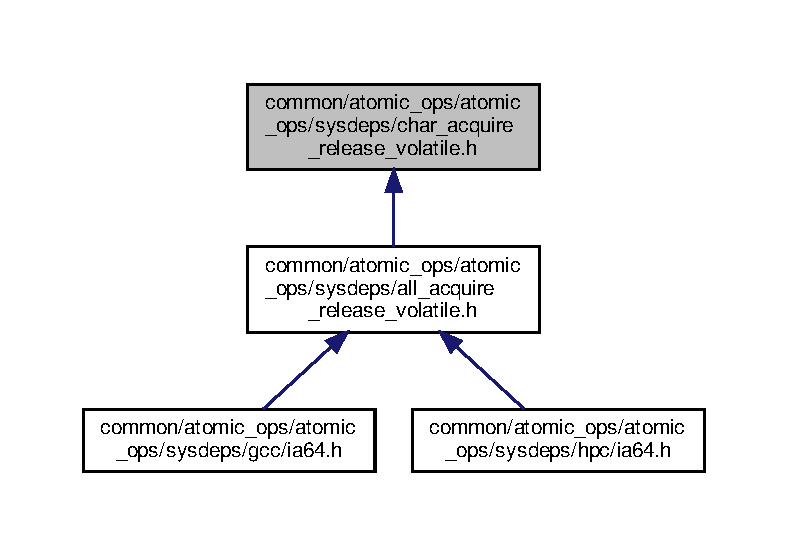
\includegraphics[width=350pt]{char__acquire__release__volatile_8h__dep__incl}
\end{center}
\end{figure}
\subsection*{Macros}
\begin{DoxyCompactItemize}
\item 
\#define \hyperlink{char__acquire__release__volatile_8h_a4b3b5ac83b6c7730e8376c8b5c0a6f01}{A\+O\+\_\+\+G\+C\+C\+\_\+\+B\+A\+R\+R\+I\+ER}()
\item 
\#define \hyperlink{char__acquire__release__volatile_8h_a1ed21fe7030453db172172728b15f854}{A\+O\+\_\+\+H\+A\+V\+E\+\_\+char\+\_\+load\+\_\+acquire}
\item 
\#define \hyperlink{char__acquire__release__volatile_8h_af72dd7cd6d706812046022f632bd47ab}{A\+O\+\_\+\+H\+A\+V\+E\+\_\+char\+\_\+store\+\_\+release}
\end{DoxyCompactItemize}
\subsection*{Functions}
\begin{DoxyCompactItemize}
\item 
\hyperlink{atomic__ops_8h_a9f6ab6253b6b11bc8c12efe9dde5db2b}{A\+O\+\_\+\+I\+N\+L\+I\+NE} unsigned char \hyperlink{char__acquire__release__volatile_8h_a3a2743edf2d35086c28f80fde0327f3d}{A\+O\+\_\+char\+\_\+load\+\_\+acquire} (const volatile unsigned char $\ast$p)
\item 
\hyperlink{atomic__ops_8h_a9f6ab6253b6b11bc8c12efe9dde5db2b}{A\+O\+\_\+\+I\+N\+L\+I\+NE} void \hyperlink{char__acquire__release__volatile_8h_a7bc53f4414186b38d693c42bbe4aee85}{A\+O\+\_\+char\+\_\+store\+\_\+release} (volatile unsigned char $\ast$p, unsigned char val)
\end{DoxyCompactItemize}


\subsection{Macro Definition Documentation}
\mbox{\Hypertarget{char__acquire__release__volatile_8h_a4b3b5ac83b6c7730e8376c8b5c0a6f01}\label{char__acquire__release__volatile_8h_a4b3b5ac83b6c7730e8376c8b5c0a6f01}} 
\index{char\+\_\+acquire\+\_\+release\+\_\+volatile.\+h@{char\+\_\+acquire\+\_\+release\+\_\+volatile.\+h}!A\+O\+\_\+\+G\+C\+C\+\_\+\+B\+A\+R\+R\+I\+ER@{A\+O\+\_\+\+G\+C\+C\+\_\+\+B\+A\+R\+R\+I\+ER}}
\index{A\+O\+\_\+\+G\+C\+C\+\_\+\+B\+A\+R\+R\+I\+ER@{A\+O\+\_\+\+G\+C\+C\+\_\+\+B\+A\+R\+R\+I\+ER}!char\+\_\+acquire\+\_\+release\+\_\+volatile.\+h@{char\+\_\+acquire\+\_\+release\+\_\+volatile.\+h}}
\subsubsection{\texorpdfstring{A\+O\+\_\+\+G\+C\+C\+\_\+\+B\+A\+R\+R\+I\+ER}{AO\_GCC\_BARRIER}}
{\footnotesize\ttfamily \#define A\+O\+\_\+\+G\+C\+C\+\_\+\+B\+A\+R\+R\+I\+ER(\begin{DoxyParamCaption}{ }\end{DoxyParamCaption})}

\mbox{\Hypertarget{char__acquire__release__volatile_8h_a1ed21fe7030453db172172728b15f854}\label{char__acquire__release__volatile_8h_a1ed21fe7030453db172172728b15f854}} 
\index{char\+\_\+acquire\+\_\+release\+\_\+volatile.\+h@{char\+\_\+acquire\+\_\+release\+\_\+volatile.\+h}!A\+O\+\_\+\+H\+A\+V\+E\+\_\+char\+\_\+load\+\_\+acquire@{A\+O\+\_\+\+H\+A\+V\+E\+\_\+char\+\_\+load\+\_\+acquire}}
\index{A\+O\+\_\+\+H\+A\+V\+E\+\_\+char\+\_\+load\+\_\+acquire@{A\+O\+\_\+\+H\+A\+V\+E\+\_\+char\+\_\+load\+\_\+acquire}!char\+\_\+acquire\+\_\+release\+\_\+volatile.\+h@{char\+\_\+acquire\+\_\+release\+\_\+volatile.\+h}}
\subsubsection{\texorpdfstring{A\+O\+\_\+\+H\+A\+V\+E\+\_\+char\+\_\+load\+\_\+acquire}{AO\_HAVE\_char\_load\_acquire}}
{\footnotesize\ttfamily \#define A\+O\+\_\+\+H\+A\+V\+E\+\_\+char\+\_\+load\+\_\+acquire}

\mbox{\Hypertarget{char__acquire__release__volatile_8h_af72dd7cd6d706812046022f632bd47ab}\label{char__acquire__release__volatile_8h_af72dd7cd6d706812046022f632bd47ab}} 
\index{char\+\_\+acquire\+\_\+release\+\_\+volatile.\+h@{char\+\_\+acquire\+\_\+release\+\_\+volatile.\+h}!A\+O\+\_\+\+H\+A\+V\+E\+\_\+char\+\_\+store\+\_\+release@{A\+O\+\_\+\+H\+A\+V\+E\+\_\+char\+\_\+store\+\_\+release}}
\index{A\+O\+\_\+\+H\+A\+V\+E\+\_\+char\+\_\+store\+\_\+release@{A\+O\+\_\+\+H\+A\+V\+E\+\_\+char\+\_\+store\+\_\+release}!char\+\_\+acquire\+\_\+release\+\_\+volatile.\+h@{char\+\_\+acquire\+\_\+release\+\_\+volatile.\+h}}
\subsubsection{\texorpdfstring{A\+O\+\_\+\+H\+A\+V\+E\+\_\+char\+\_\+store\+\_\+release}{AO\_HAVE\_char\_store\_release}}
{\footnotesize\ttfamily \#define A\+O\+\_\+\+H\+A\+V\+E\+\_\+char\+\_\+store\+\_\+release}



\subsection{Function Documentation}
\mbox{\Hypertarget{char__acquire__release__volatile_8h_a3a2743edf2d35086c28f80fde0327f3d}\label{char__acquire__release__volatile_8h_a3a2743edf2d35086c28f80fde0327f3d}} 
\index{char\+\_\+acquire\+\_\+release\+\_\+volatile.\+h@{char\+\_\+acquire\+\_\+release\+\_\+volatile.\+h}!A\+O\+\_\+char\+\_\+load\+\_\+acquire@{A\+O\+\_\+char\+\_\+load\+\_\+acquire}}
\index{A\+O\+\_\+char\+\_\+load\+\_\+acquire@{A\+O\+\_\+char\+\_\+load\+\_\+acquire}!char\+\_\+acquire\+\_\+release\+\_\+volatile.\+h@{char\+\_\+acquire\+\_\+release\+\_\+volatile.\+h}}
\subsubsection{\texorpdfstring{A\+O\+\_\+char\+\_\+load\+\_\+acquire()}{AO\_char\_load\_acquire()}}
{\footnotesize\ttfamily \hyperlink{atomic__ops_8h_a9f6ab6253b6b11bc8c12efe9dde5db2b}{A\+O\+\_\+\+I\+N\+L\+I\+NE} unsigned char A\+O\+\_\+char\+\_\+load\+\_\+acquire (\begin{DoxyParamCaption}\item[{const volatile unsigned char $\ast$}]{p }\end{DoxyParamCaption})}

\mbox{\Hypertarget{char__acquire__release__volatile_8h_a7bc53f4414186b38d693c42bbe4aee85}\label{char__acquire__release__volatile_8h_a7bc53f4414186b38d693c42bbe4aee85}} 
\index{char\+\_\+acquire\+\_\+release\+\_\+volatile.\+h@{char\+\_\+acquire\+\_\+release\+\_\+volatile.\+h}!A\+O\+\_\+char\+\_\+store\+\_\+release@{A\+O\+\_\+char\+\_\+store\+\_\+release}}
\index{A\+O\+\_\+char\+\_\+store\+\_\+release@{A\+O\+\_\+char\+\_\+store\+\_\+release}!char\+\_\+acquire\+\_\+release\+\_\+volatile.\+h@{char\+\_\+acquire\+\_\+release\+\_\+volatile.\+h}}
\subsubsection{\texorpdfstring{A\+O\+\_\+char\+\_\+store\+\_\+release()}{AO\_char\_store\_release()}}
{\footnotesize\ttfamily \hyperlink{atomic__ops_8h_a9f6ab6253b6b11bc8c12efe9dde5db2b}{A\+O\+\_\+\+I\+N\+L\+I\+NE} void A\+O\+\_\+char\+\_\+store\+\_\+release (\begin{DoxyParamCaption}\item[{volatile unsigned char $\ast$}]{p,  }\item[{unsigned char}]{val }\end{DoxyParamCaption})}


\hypertarget{char__atomic__load__store_8h}{}\section{common/atomic\+\_\+ops/atomic\+\_\+ops/sysdeps/char\+\_\+atomic\+\_\+load\+\_\+store.h File Reference}
\label{char__atomic__load__store_8h}\index{common/atomic\+\_\+ops/atomic\+\_\+ops/sysdeps/char\+\_\+atomic\+\_\+load\+\_\+store.\+h@{common/atomic\+\_\+ops/atomic\+\_\+ops/sysdeps/char\+\_\+atomic\+\_\+load\+\_\+store.\+h}}
This graph shows which files directly or indirectly include this file\+:
\nopagebreak
\begin{figure}[H]
\begin{center}
\leavevmode
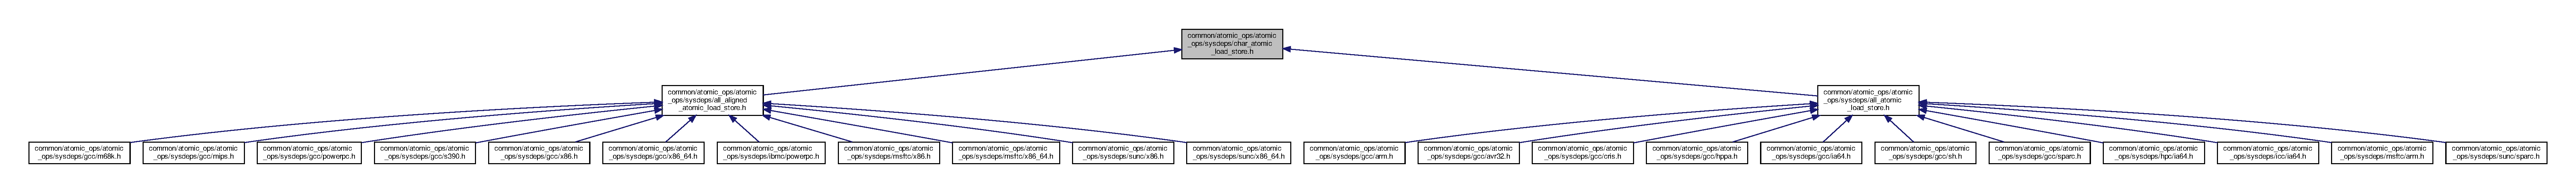
\includegraphics[width=350pt]{char__atomic__load__store_8h__dep__incl}
\end{center}
\end{figure}
\subsection*{Macros}
\begin{DoxyCompactItemize}
\item 
\#define \hyperlink{char__atomic__load__store_8h_a48e80892304c302c5306c97ce30178ae}{A\+O\+\_\+\+H\+A\+V\+E\+\_\+char\+\_\+load}
\item 
\#define \hyperlink{char__atomic__load__store_8h_abd95e1f3d847392f82b6c50aed1f68a0}{A\+O\+\_\+\+H\+A\+V\+E\+\_\+char\+\_\+store}
\end{DoxyCompactItemize}
\subsection*{Functions}
\begin{DoxyCompactItemize}
\item 
\hyperlink{atomic__ops_8h_a9f6ab6253b6b11bc8c12efe9dde5db2b}{A\+O\+\_\+\+I\+N\+L\+I\+NE} unsigned char \hyperlink{char__atomic__load__store_8h_a23945084b51700306c16c82cf08adb81}{A\+O\+\_\+char\+\_\+load} (const volatile unsigned char $\ast$addr)
\item 
\hyperlink{atomic__ops_8h_a9f6ab6253b6b11bc8c12efe9dde5db2b}{A\+O\+\_\+\+I\+N\+L\+I\+NE} void \hyperlink{char__atomic__load__store_8h_ac07030e27b572cc128864d7a69fbc447}{A\+O\+\_\+char\+\_\+store} (volatile unsigned char $\ast$addr, unsigned char new\+\_\+val)
\end{DoxyCompactItemize}


\subsection{Macro Definition Documentation}
\mbox{\Hypertarget{char__atomic__load__store_8h_a48e80892304c302c5306c97ce30178ae}\label{char__atomic__load__store_8h_a48e80892304c302c5306c97ce30178ae}} 
\index{char\+\_\+atomic\+\_\+load\+\_\+store.\+h@{char\+\_\+atomic\+\_\+load\+\_\+store.\+h}!A\+O\+\_\+\+H\+A\+V\+E\+\_\+char\+\_\+load@{A\+O\+\_\+\+H\+A\+V\+E\+\_\+char\+\_\+load}}
\index{A\+O\+\_\+\+H\+A\+V\+E\+\_\+char\+\_\+load@{A\+O\+\_\+\+H\+A\+V\+E\+\_\+char\+\_\+load}!char\+\_\+atomic\+\_\+load\+\_\+store.\+h@{char\+\_\+atomic\+\_\+load\+\_\+store.\+h}}
\subsubsection{\texorpdfstring{A\+O\+\_\+\+H\+A\+V\+E\+\_\+char\+\_\+load}{AO\_HAVE\_char\_load}}
{\footnotesize\ttfamily \#define A\+O\+\_\+\+H\+A\+V\+E\+\_\+char\+\_\+load}

\mbox{\Hypertarget{char__atomic__load__store_8h_abd95e1f3d847392f82b6c50aed1f68a0}\label{char__atomic__load__store_8h_abd95e1f3d847392f82b6c50aed1f68a0}} 
\index{char\+\_\+atomic\+\_\+load\+\_\+store.\+h@{char\+\_\+atomic\+\_\+load\+\_\+store.\+h}!A\+O\+\_\+\+H\+A\+V\+E\+\_\+char\+\_\+store@{A\+O\+\_\+\+H\+A\+V\+E\+\_\+char\+\_\+store}}
\index{A\+O\+\_\+\+H\+A\+V\+E\+\_\+char\+\_\+store@{A\+O\+\_\+\+H\+A\+V\+E\+\_\+char\+\_\+store}!char\+\_\+atomic\+\_\+load\+\_\+store.\+h@{char\+\_\+atomic\+\_\+load\+\_\+store.\+h}}
\subsubsection{\texorpdfstring{A\+O\+\_\+\+H\+A\+V\+E\+\_\+char\+\_\+store}{AO\_HAVE\_char\_store}}
{\footnotesize\ttfamily \#define A\+O\+\_\+\+H\+A\+V\+E\+\_\+char\+\_\+store}



\subsection{Function Documentation}
\mbox{\Hypertarget{char__atomic__load__store_8h_a23945084b51700306c16c82cf08adb81}\label{char__atomic__load__store_8h_a23945084b51700306c16c82cf08adb81}} 
\index{char\+\_\+atomic\+\_\+load\+\_\+store.\+h@{char\+\_\+atomic\+\_\+load\+\_\+store.\+h}!A\+O\+\_\+char\+\_\+load@{A\+O\+\_\+char\+\_\+load}}
\index{A\+O\+\_\+char\+\_\+load@{A\+O\+\_\+char\+\_\+load}!char\+\_\+atomic\+\_\+load\+\_\+store.\+h@{char\+\_\+atomic\+\_\+load\+\_\+store.\+h}}
\subsubsection{\texorpdfstring{A\+O\+\_\+char\+\_\+load()}{AO\_char\_load()}}
{\footnotesize\ttfamily \hyperlink{atomic__ops_8h_a9f6ab6253b6b11bc8c12efe9dde5db2b}{A\+O\+\_\+\+I\+N\+L\+I\+NE} unsigned char A\+O\+\_\+char\+\_\+load (\begin{DoxyParamCaption}\item[{const volatile unsigned char $\ast$}]{addr }\end{DoxyParamCaption})}

\mbox{\Hypertarget{char__atomic__load__store_8h_ac07030e27b572cc128864d7a69fbc447}\label{char__atomic__load__store_8h_ac07030e27b572cc128864d7a69fbc447}} 
\index{char\+\_\+atomic\+\_\+load\+\_\+store.\+h@{char\+\_\+atomic\+\_\+load\+\_\+store.\+h}!A\+O\+\_\+char\+\_\+store@{A\+O\+\_\+char\+\_\+store}}
\index{A\+O\+\_\+char\+\_\+store@{A\+O\+\_\+char\+\_\+store}!char\+\_\+atomic\+\_\+load\+\_\+store.\+h@{char\+\_\+atomic\+\_\+load\+\_\+store.\+h}}
\subsubsection{\texorpdfstring{A\+O\+\_\+char\+\_\+store()}{AO\_char\_store()}}
{\footnotesize\ttfamily \hyperlink{atomic__ops_8h_a9f6ab6253b6b11bc8c12efe9dde5db2b}{A\+O\+\_\+\+I\+N\+L\+I\+NE} void A\+O\+\_\+char\+\_\+store (\begin{DoxyParamCaption}\item[{volatile unsigned char $\ast$}]{addr,  }\item[{unsigned char}]{new\+\_\+val }\end{DoxyParamCaption})}


\hypertarget{emul__cas_8h}{}\section{common/atomic\+\_\+ops/atomic\+\_\+ops/sysdeps/emul\+\_\+cas.h File Reference}
\label{emul__cas_8h}\index{common/atomic\+\_\+ops/atomic\+\_\+ops/sysdeps/emul\+\_\+cas.\+h@{common/atomic\+\_\+ops/atomic\+\_\+ops/sysdeps/emul\+\_\+cas.\+h}}
{\ttfamily \#include \char`\"{}standard\+\_\+ao\+\_\+double\+\_\+t.\+h\char`\"{}}\newline
Include dependency graph for emul\+\_\+cas.\+h\+:
\nopagebreak
\begin{figure}[H]
\begin{center}
\leavevmode
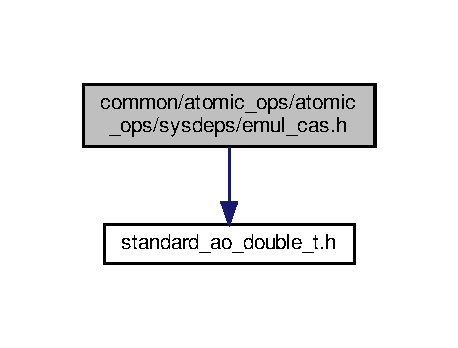
\includegraphics[width=220pt]{emul__cas_8h__incl}
\end{center}
\end{figure}
\subsection*{Macros}
\begin{DoxyCompactItemize}
\item 
\#define \hyperlink{emul__cas_8h_a6dc4a2a3e24db9d20cfb65ed1f2a6667}{A\+O\+\_\+compare\+\_\+and\+\_\+swap\+\_\+full}(addr,  old,  newval)~\hyperlink{emul__cas_8h_a094738a02b8a59f19b2d54987b9f667b}{A\+O\+\_\+compare\+\_\+and\+\_\+swap\+\_\+emulation}(addr, old, newval)
\item 
\#define \hyperlink{emul__cas_8h_a98ec53065c0dfd18bc1013c500da377c}{A\+O\+\_\+\+H\+A\+V\+E\+\_\+compare\+\_\+and\+\_\+swap\+\_\+full}
\item 
\#define \hyperlink{emul__cas_8h_a598da265d93b0039b2e213c9d2ad08d4}{A\+O\+\_\+compare\+\_\+double\+\_\+and\+\_\+swap\+\_\+double\+\_\+full}(addr,  \hyperlink{dcss__plus_8h_aa0ef3ea06e00e9bcff2d000c6b85fe3b}{old1},  \hyperlink{dcss__plus_8h_a5b804866c13543d14361d31600569ea0}{old2},  newval1,  newval2)
\item 
\#define \hyperlink{emul__cas_8h_a0e2b334560e5f9a06567fc59e33a435d}{A\+O\+\_\+\+H\+A\+V\+E\+\_\+compare\+\_\+double\+\_\+and\+\_\+swap\+\_\+double\+\_\+full}
\item 
\#define \hyperlink{emul__cas_8h_a3d577a6957a22ca401b183fbc4bb34f4}{A\+O\+\_\+store\+\_\+full}(addr,  val)~\hyperlink{emul__cas_8h_a615316c80d5bf0e0fb172d6c7d4133a5}{A\+O\+\_\+store\+\_\+full\+\_\+emulation}(addr, val)
\item 
\#define \hyperlink{emul__cas_8h_acae01b282aca485176025dd405ebf5b1}{A\+O\+\_\+\+H\+A\+V\+E\+\_\+store\+\_\+full}
\end{DoxyCompactItemize}
\subsection*{Functions}
\begin{DoxyCompactItemize}
\item 
int \hyperlink{emul__cas_8h_a094738a02b8a59f19b2d54987b9f667b}{A\+O\+\_\+compare\+\_\+and\+\_\+swap\+\_\+emulation} (volatile \hyperlink{atomic__ops_8h_a5225fef4d9eee821e82382cd269160dd}{A\+O\+\_\+t} $\ast$addr, \hyperlink{atomic__ops_8h_a5225fef4d9eee821e82382cd269160dd}{A\+O\+\_\+t} old, \hyperlink{atomic__ops_8h_a5225fef4d9eee821e82382cd269160dd}{A\+O\+\_\+t} new\+\_\+val)
\item 
int \hyperlink{emul__cas_8h_ac6fb4f6252feec901b044d2e8c59e6f7}{A\+O\+\_\+compare\+\_\+double\+\_\+and\+\_\+swap\+\_\+double\+\_\+emulation} (volatile \hyperlink{structAO__double__t}{A\+O\+\_\+double\+\_\+t} $\ast$addr, \hyperlink{atomic__ops_8h_a5225fef4d9eee821e82382cd269160dd}{A\+O\+\_\+t} old\+\_\+val1, \hyperlink{atomic__ops_8h_a5225fef4d9eee821e82382cd269160dd}{A\+O\+\_\+t} old\+\_\+val2, \hyperlink{atomic__ops_8h_a5225fef4d9eee821e82382cd269160dd}{A\+O\+\_\+t} new\+\_\+val1, \hyperlink{atomic__ops_8h_a5225fef4d9eee821e82382cd269160dd}{A\+O\+\_\+t} new\+\_\+val2)
\item 
void \hyperlink{emul__cas_8h_a615316c80d5bf0e0fb172d6c7d4133a5}{A\+O\+\_\+store\+\_\+full\+\_\+emulation} (volatile \hyperlink{atomic__ops_8h_a5225fef4d9eee821e82382cd269160dd}{A\+O\+\_\+t} $\ast$addr, \hyperlink{atomic__ops_8h_a5225fef4d9eee821e82382cd269160dd}{A\+O\+\_\+t} val)
\end{DoxyCompactItemize}


\subsection{Macro Definition Documentation}
\mbox{\Hypertarget{emul__cas_8h_a6dc4a2a3e24db9d20cfb65ed1f2a6667}\label{emul__cas_8h_a6dc4a2a3e24db9d20cfb65ed1f2a6667}} 
\index{emul\+\_\+cas.\+h@{emul\+\_\+cas.\+h}!A\+O\+\_\+compare\+\_\+and\+\_\+swap\+\_\+full@{A\+O\+\_\+compare\+\_\+and\+\_\+swap\+\_\+full}}
\index{A\+O\+\_\+compare\+\_\+and\+\_\+swap\+\_\+full@{A\+O\+\_\+compare\+\_\+and\+\_\+swap\+\_\+full}!emul\+\_\+cas.\+h@{emul\+\_\+cas.\+h}}
\subsubsection{\texorpdfstring{A\+O\+\_\+compare\+\_\+and\+\_\+swap\+\_\+full}{AO\_compare\_and\_swap\_full}}
{\footnotesize\ttfamily \#define A\+O\+\_\+compare\+\_\+and\+\_\+swap\+\_\+full(\begin{DoxyParamCaption}\item[{}]{addr,  }\item[{}]{old,  }\item[{}]{newval }\end{DoxyParamCaption})~\hyperlink{emul__cas_8h_a094738a02b8a59f19b2d54987b9f667b}{A\+O\+\_\+compare\+\_\+and\+\_\+swap\+\_\+emulation}(addr, old, newval)}

\mbox{\Hypertarget{emul__cas_8h_a598da265d93b0039b2e213c9d2ad08d4}\label{emul__cas_8h_a598da265d93b0039b2e213c9d2ad08d4}} 
\index{emul\+\_\+cas.\+h@{emul\+\_\+cas.\+h}!A\+O\+\_\+compare\+\_\+double\+\_\+and\+\_\+swap\+\_\+double\+\_\+full@{A\+O\+\_\+compare\+\_\+double\+\_\+and\+\_\+swap\+\_\+double\+\_\+full}}
\index{A\+O\+\_\+compare\+\_\+double\+\_\+and\+\_\+swap\+\_\+double\+\_\+full@{A\+O\+\_\+compare\+\_\+double\+\_\+and\+\_\+swap\+\_\+double\+\_\+full}!emul\+\_\+cas.\+h@{emul\+\_\+cas.\+h}}
\subsubsection{\texorpdfstring{A\+O\+\_\+compare\+\_\+double\+\_\+and\+\_\+swap\+\_\+double\+\_\+full}{AO\_compare\_double\_and\_swap\_double\_full}}
{\footnotesize\ttfamily \#define A\+O\+\_\+compare\+\_\+double\+\_\+and\+\_\+swap\+\_\+double\+\_\+full(\begin{DoxyParamCaption}\item[{}]{addr,  }\item[{}]{\hyperlink{dcss__plus_8h_aa0ef3ea06e00e9bcff2d000c6b85fe3b}{old1},  }\item[{}]{\hyperlink{dcss__plus_8h_a5b804866c13543d14361d31600569ea0}{old2},  }\item[{}]{newval1,  }\item[{}]{newval2 }\end{DoxyParamCaption})}

{\bfseries Value\+:}
\begin{DoxyCode}
\hyperlink{emul__cas_8h_ac6fb4f6252feec901b044d2e8c59e6f7}{AO\_compare\_double\_and\_swap\_double\_emulation}(addr, 
      \hyperlink{dcss_8h_aa0ef3ea06e00e9bcff2d000c6b85fe3b}{old1}, \hyperlink{dcss_8h_a5b804866c13543d14361d31600569ea0}{old2}, \(\backslash\)
                             newval1, newval2)
\end{DoxyCode}
\mbox{\Hypertarget{emul__cas_8h_a98ec53065c0dfd18bc1013c500da377c}\label{emul__cas_8h_a98ec53065c0dfd18bc1013c500da377c}} 
\index{emul\+\_\+cas.\+h@{emul\+\_\+cas.\+h}!A\+O\+\_\+\+H\+A\+V\+E\+\_\+compare\+\_\+and\+\_\+swap\+\_\+full@{A\+O\+\_\+\+H\+A\+V\+E\+\_\+compare\+\_\+and\+\_\+swap\+\_\+full}}
\index{A\+O\+\_\+\+H\+A\+V\+E\+\_\+compare\+\_\+and\+\_\+swap\+\_\+full@{A\+O\+\_\+\+H\+A\+V\+E\+\_\+compare\+\_\+and\+\_\+swap\+\_\+full}!emul\+\_\+cas.\+h@{emul\+\_\+cas.\+h}}
\subsubsection{\texorpdfstring{A\+O\+\_\+\+H\+A\+V\+E\+\_\+compare\+\_\+and\+\_\+swap\+\_\+full}{AO\_HAVE\_compare\_and\_swap\_full}}
{\footnotesize\ttfamily \#define A\+O\+\_\+\+H\+A\+V\+E\+\_\+compare\+\_\+and\+\_\+swap\+\_\+full}

\mbox{\Hypertarget{emul__cas_8h_a0e2b334560e5f9a06567fc59e33a435d}\label{emul__cas_8h_a0e2b334560e5f9a06567fc59e33a435d}} 
\index{emul\+\_\+cas.\+h@{emul\+\_\+cas.\+h}!A\+O\+\_\+\+H\+A\+V\+E\+\_\+compare\+\_\+double\+\_\+and\+\_\+swap\+\_\+double\+\_\+full@{A\+O\+\_\+\+H\+A\+V\+E\+\_\+compare\+\_\+double\+\_\+and\+\_\+swap\+\_\+double\+\_\+full}}
\index{A\+O\+\_\+\+H\+A\+V\+E\+\_\+compare\+\_\+double\+\_\+and\+\_\+swap\+\_\+double\+\_\+full@{A\+O\+\_\+\+H\+A\+V\+E\+\_\+compare\+\_\+double\+\_\+and\+\_\+swap\+\_\+double\+\_\+full}!emul\+\_\+cas.\+h@{emul\+\_\+cas.\+h}}
\subsubsection{\texorpdfstring{A\+O\+\_\+\+H\+A\+V\+E\+\_\+compare\+\_\+double\+\_\+and\+\_\+swap\+\_\+double\+\_\+full}{AO\_HAVE\_compare\_double\_and\_swap\_double\_full}}
{\footnotesize\ttfamily \#define A\+O\+\_\+\+H\+A\+V\+E\+\_\+compare\+\_\+double\+\_\+and\+\_\+swap\+\_\+double\+\_\+full}

\mbox{\Hypertarget{emul__cas_8h_acae01b282aca485176025dd405ebf5b1}\label{emul__cas_8h_acae01b282aca485176025dd405ebf5b1}} 
\index{emul\+\_\+cas.\+h@{emul\+\_\+cas.\+h}!A\+O\+\_\+\+H\+A\+V\+E\+\_\+store\+\_\+full@{A\+O\+\_\+\+H\+A\+V\+E\+\_\+store\+\_\+full}}
\index{A\+O\+\_\+\+H\+A\+V\+E\+\_\+store\+\_\+full@{A\+O\+\_\+\+H\+A\+V\+E\+\_\+store\+\_\+full}!emul\+\_\+cas.\+h@{emul\+\_\+cas.\+h}}
\subsubsection{\texorpdfstring{A\+O\+\_\+\+H\+A\+V\+E\+\_\+store\+\_\+full}{AO\_HAVE\_store\_full}}
{\footnotesize\ttfamily \#define A\+O\+\_\+\+H\+A\+V\+E\+\_\+store\+\_\+full}

\mbox{\Hypertarget{emul__cas_8h_a3d577a6957a22ca401b183fbc4bb34f4}\label{emul__cas_8h_a3d577a6957a22ca401b183fbc4bb34f4}} 
\index{emul\+\_\+cas.\+h@{emul\+\_\+cas.\+h}!A\+O\+\_\+store\+\_\+full@{A\+O\+\_\+store\+\_\+full}}
\index{A\+O\+\_\+store\+\_\+full@{A\+O\+\_\+store\+\_\+full}!emul\+\_\+cas.\+h@{emul\+\_\+cas.\+h}}
\subsubsection{\texorpdfstring{A\+O\+\_\+store\+\_\+full}{AO\_store\_full}}
{\footnotesize\ttfamily \#define A\+O\+\_\+store\+\_\+full(\begin{DoxyParamCaption}\item[{}]{addr,  }\item[{}]{val }\end{DoxyParamCaption})~\hyperlink{emul__cas_8h_a615316c80d5bf0e0fb172d6c7d4133a5}{A\+O\+\_\+store\+\_\+full\+\_\+emulation}(addr, val)}



\subsection{Function Documentation}
\mbox{\Hypertarget{emul__cas_8h_a094738a02b8a59f19b2d54987b9f667b}\label{emul__cas_8h_a094738a02b8a59f19b2d54987b9f667b}} 
\index{emul\+\_\+cas.\+h@{emul\+\_\+cas.\+h}!A\+O\+\_\+compare\+\_\+and\+\_\+swap\+\_\+emulation@{A\+O\+\_\+compare\+\_\+and\+\_\+swap\+\_\+emulation}}
\index{A\+O\+\_\+compare\+\_\+and\+\_\+swap\+\_\+emulation@{A\+O\+\_\+compare\+\_\+and\+\_\+swap\+\_\+emulation}!emul\+\_\+cas.\+h@{emul\+\_\+cas.\+h}}
\subsubsection{\texorpdfstring{A\+O\+\_\+compare\+\_\+and\+\_\+swap\+\_\+emulation()}{AO\_compare\_and\_swap\_emulation()}}
{\footnotesize\ttfamily int A\+O\+\_\+compare\+\_\+and\+\_\+swap\+\_\+emulation (\begin{DoxyParamCaption}\item[{volatile \hyperlink{atomic__ops_8h_a5225fef4d9eee821e82382cd269160dd}{A\+O\+\_\+t} $\ast$}]{addr,  }\item[{\hyperlink{atomic__ops_8h_a5225fef4d9eee821e82382cd269160dd}{A\+O\+\_\+t}}]{old,  }\item[{\hyperlink{atomic__ops_8h_a5225fef4d9eee821e82382cd269160dd}{A\+O\+\_\+t}}]{new\+\_\+val }\end{DoxyParamCaption})}

\mbox{\Hypertarget{emul__cas_8h_ac6fb4f6252feec901b044d2e8c59e6f7}\label{emul__cas_8h_ac6fb4f6252feec901b044d2e8c59e6f7}} 
\index{emul\+\_\+cas.\+h@{emul\+\_\+cas.\+h}!A\+O\+\_\+compare\+\_\+double\+\_\+and\+\_\+swap\+\_\+double\+\_\+emulation@{A\+O\+\_\+compare\+\_\+double\+\_\+and\+\_\+swap\+\_\+double\+\_\+emulation}}
\index{A\+O\+\_\+compare\+\_\+double\+\_\+and\+\_\+swap\+\_\+double\+\_\+emulation@{A\+O\+\_\+compare\+\_\+double\+\_\+and\+\_\+swap\+\_\+double\+\_\+emulation}!emul\+\_\+cas.\+h@{emul\+\_\+cas.\+h}}
\subsubsection{\texorpdfstring{A\+O\+\_\+compare\+\_\+double\+\_\+and\+\_\+swap\+\_\+double\+\_\+emulation()}{AO\_compare\_double\_and\_swap\_double\_emulation()}}
{\footnotesize\ttfamily int A\+O\+\_\+compare\+\_\+double\+\_\+and\+\_\+swap\+\_\+double\+\_\+emulation (\begin{DoxyParamCaption}\item[{volatile \hyperlink{structAO__double__t}{A\+O\+\_\+double\+\_\+t} $\ast$}]{addr,  }\item[{\hyperlink{atomic__ops_8h_a5225fef4d9eee821e82382cd269160dd}{A\+O\+\_\+t}}]{old\+\_\+val1,  }\item[{\hyperlink{atomic__ops_8h_a5225fef4d9eee821e82382cd269160dd}{A\+O\+\_\+t}}]{old\+\_\+val2,  }\item[{\hyperlink{atomic__ops_8h_a5225fef4d9eee821e82382cd269160dd}{A\+O\+\_\+t}}]{new\+\_\+val1,  }\item[{\hyperlink{atomic__ops_8h_a5225fef4d9eee821e82382cd269160dd}{A\+O\+\_\+t}}]{new\+\_\+val2 }\end{DoxyParamCaption})}

\mbox{\Hypertarget{emul__cas_8h_a615316c80d5bf0e0fb172d6c7d4133a5}\label{emul__cas_8h_a615316c80d5bf0e0fb172d6c7d4133a5}} 
\index{emul\+\_\+cas.\+h@{emul\+\_\+cas.\+h}!A\+O\+\_\+store\+\_\+full\+\_\+emulation@{A\+O\+\_\+store\+\_\+full\+\_\+emulation}}
\index{A\+O\+\_\+store\+\_\+full\+\_\+emulation@{A\+O\+\_\+store\+\_\+full\+\_\+emulation}!emul\+\_\+cas.\+h@{emul\+\_\+cas.\+h}}
\subsubsection{\texorpdfstring{A\+O\+\_\+store\+\_\+full\+\_\+emulation()}{AO\_store\_full\_emulation()}}
{\footnotesize\ttfamily void A\+O\+\_\+store\+\_\+full\+\_\+emulation (\begin{DoxyParamCaption}\item[{volatile \hyperlink{atomic__ops_8h_a5225fef4d9eee821e82382cd269160dd}{A\+O\+\_\+t} $\ast$}]{addr,  }\item[{\hyperlink{atomic__ops_8h_a5225fef4d9eee821e82382cd269160dd}{A\+O\+\_\+t}}]{val }\end{DoxyParamCaption})}


\hypertarget{alpha_8h}{}\section{common/atomic\+\_\+ops/atomic\+\_\+ops/sysdeps/gcc/alpha.h File Reference}
\label{alpha_8h}\index{common/atomic\+\_\+ops/atomic\+\_\+ops/sysdeps/gcc/alpha.\+h@{common/atomic\+\_\+ops/atomic\+\_\+ops/sysdeps/gcc/alpha.\+h}}
{\ttfamily \#include \char`\"{}../atomic\+\_\+load\+\_\+store.\+h\char`\"{}}\newline
{\ttfamily \#include \char`\"{}../test\+\_\+and\+\_\+set\+\_\+t\+\_\+is\+\_\+ao\+\_\+t.\+h\char`\"{}}\newline
Include dependency graph for alpha.\+h\+:
\nopagebreak
\begin{figure}[H]
\begin{center}
\leavevmode
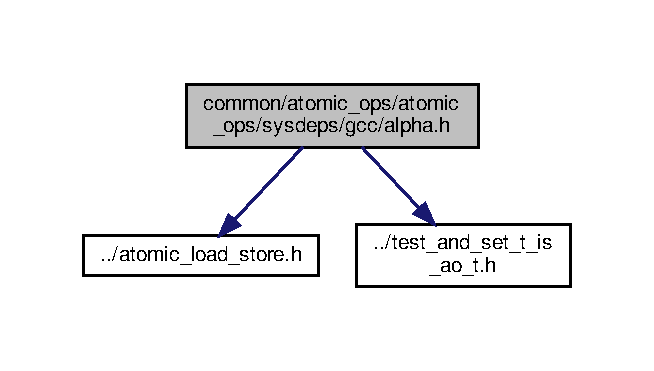
\includegraphics[width=314pt]{alpha_8h__incl}
\end{center}
\end{figure}
\subsection*{Macros}
\begin{DoxyCompactItemize}
\item 
\#define \hyperlink{alpha_8h_ab65316d98c499c612122d64bc69bf5fa}{A\+O\+\_\+\+N\+O\+\_\+\+D\+D\+\_\+\+O\+R\+D\+E\+R\+I\+NG}
\item 
\#define \hyperlink{alpha_8h_a3904dc699d6a6d6e771a93aa66aeb805}{A\+O\+\_\+\+H\+A\+V\+E\+\_\+nop\+\_\+full}
\item 
\#define \hyperlink{alpha_8h_a7c6d0c7c0585da4d8cd259df2423b82f}{A\+O\+\_\+\+H\+A\+V\+E\+\_\+nop\+\_\+write}
\item 
\#define \hyperlink{alpha_8h_a0c5d9cf68a56bfa9e267db0f2795811c}{A\+O\+\_\+\+H\+A\+V\+E\+\_\+compare\+\_\+and\+\_\+swap}
\end{DoxyCompactItemize}
\subsection*{Functions}
\begin{DoxyCompactItemize}
\item 
\hyperlink{atomic__ops_8h_a9f6ab6253b6b11bc8c12efe9dde5db2b}{A\+O\+\_\+\+I\+N\+L\+I\+NE} void \hyperlink{alpha_8h_afe3a6778eacc82252ba138fc9a157b04}{A\+O\+\_\+nop\+\_\+full} (void)
\item 
\hyperlink{atomic__ops_8h_a9f6ab6253b6b11bc8c12efe9dde5db2b}{A\+O\+\_\+\+I\+N\+L\+I\+NE} void \hyperlink{alpha_8h_a4a8d4664cca4161a554167b152c66772}{A\+O\+\_\+nop\+\_\+write} (void)
\item 
\hyperlink{atomic__ops_8h_a9f6ab6253b6b11bc8c12efe9dde5db2b}{A\+O\+\_\+\+I\+N\+L\+I\+NE} int \hyperlink{alpha_8h_a2e1cdaa59eda3ac15129d16951295698}{A\+O\+\_\+compare\+\_\+and\+\_\+swap} (volatile \hyperlink{atomic__ops_8h_a5225fef4d9eee821e82382cd269160dd}{A\+O\+\_\+t} $\ast$addr, \hyperlink{atomic__ops_8h_a5225fef4d9eee821e82382cd269160dd}{A\+O\+\_\+t} old, \hyperlink{atomic__ops_8h_a5225fef4d9eee821e82382cd269160dd}{A\+O\+\_\+t} new\+\_\+val)
\end{DoxyCompactItemize}


\subsection{Macro Definition Documentation}
\mbox{\Hypertarget{alpha_8h_a0c5d9cf68a56bfa9e267db0f2795811c}\label{alpha_8h_a0c5d9cf68a56bfa9e267db0f2795811c}} 
\index{alpha.\+h@{alpha.\+h}!A\+O\+\_\+\+H\+A\+V\+E\+\_\+compare\+\_\+and\+\_\+swap@{A\+O\+\_\+\+H\+A\+V\+E\+\_\+compare\+\_\+and\+\_\+swap}}
\index{A\+O\+\_\+\+H\+A\+V\+E\+\_\+compare\+\_\+and\+\_\+swap@{A\+O\+\_\+\+H\+A\+V\+E\+\_\+compare\+\_\+and\+\_\+swap}!alpha.\+h@{alpha.\+h}}
\subsubsection{\texorpdfstring{A\+O\+\_\+\+H\+A\+V\+E\+\_\+compare\+\_\+and\+\_\+swap}{AO\_HAVE\_compare\_and\_swap}}
{\footnotesize\ttfamily \#define A\+O\+\_\+\+H\+A\+V\+E\+\_\+compare\+\_\+and\+\_\+swap}

\mbox{\Hypertarget{alpha_8h_a3904dc699d6a6d6e771a93aa66aeb805}\label{alpha_8h_a3904dc699d6a6d6e771a93aa66aeb805}} 
\index{alpha.\+h@{alpha.\+h}!A\+O\+\_\+\+H\+A\+V\+E\+\_\+nop\+\_\+full@{A\+O\+\_\+\+H\+A\+V\+E\+\_\+nop\+\_\+full}}
\index{A\+O\+\_\+\+H\+A\+V\+E\+\_\+nop\+\_\+full@{A\+O\+\_\+\+H\+A\+V\+E\+\_\+nop\+\_\+full}!alpha.\+h@{alpha.\+h}}
\subsubsection{\texorpdfstring{A\+O\+\_\+\+H\+A\+V\+E\+\_\+nop\+\_\+full}{AO\_HAVE\_nop\_full}}
{\footnotesize\ttfamily \#define A\+O\+\_\+\+H\+A\+V\+E\+\_\+nop\+\_\+full}

\mbox{\Hypertarget{alpha_8h_a7c6d0c7c0585da4d8cd259df2423b82f}\label{alpha_8h_a7c6d0c7c0585da4d8cd259df2423b82f}} 
\index{alpha.\+h@{alpha.\+h}!A\+O\+\_\+\+H\+A\+V\+E\+\_\+nop\+\_\+write@{A\+O\+\_\+\+H\+A\+V\+E\+\_\+nop\+\_\+write}}
\index{A\+O\+\_\+\+H\+A\+V\+E\+\_\+nop\+\_\+write@{A\+O\+\_\+\+H\+A\+V\+E\+\_\+nop\+\_\+write}!alpha.\+h@{alpha.\+h}}
\subsubsection{\texorpdfstring{A\+O\+\_\+\+H\+A\+V\+E\+\_\+nop\+\_\+write}{AO\_HAVE\_nop\_write}}
{\footnotesize\ttfamily \#define A\+O\+\_\+\+H\+A\+V\+E\+\_\+nop\+\_\+write}

\mbox{\Hypertarget{alpha_8h_ab65316d98c499c612122d64bc69bf5fa}\label{alpha_8h_ab65316d98c499c612122d64bc69bf5fa}} 
\index{alpha.\+h@{alpha.\+h}!A\+O\+\_\+\+N\+O\+\_\+\+D\+D\+\_\+\+O\+R\+D\+E\+R\+I\+NG@{A\+O\+\_\+\+N\+O\+\_\+\+D\+D\+\_\+\+O\+R\+D\+E\+R\+I\+NG}}
\index{A\+O\+\_\+\+N\+O\+\_\+\+D\+D\+\_\+\+O\+R\+D\+E\+R\+I\+NG@{A\+O\+\_\+\+N\+O\+\_\+\+D\+D\+\_\+\+O\+R\+D\+E\+R\+I\+NG}!alpha.\+h@{alpha.\+h}}
\subsubsection{\texorpdfstring{A\+O\+\_\+\+N\+O\+\_\+\+D\+D\+\_\+\+O\+R\+D\+E\+R\+I\+NG}{AO\_NO\_DD\_ORDERING}}
{\footnotesize\ttfamily \#define A\+O\+\_\+\+N\+O\+\_\+\+D\+D\+\_\+\+O\+R\+D\+E\+R\+I\+NG}



\subsection{Function Documentation}
\mbox{\Hypertarget{alpha_8h_a2e1cdaa59eda3ac15129d16951295698}\label{alpha_8h_a2e1cdaa59eda3ac15129d16951295698}} 
\index{alpha.\+h@{alpha.\+h}!A\+O\+\_\+compare\+\_\+and\+\_\+swap@{A\+O\+\_\+compare\+\_\+and\+\_\+swap}}
\index{A\+O\+\_\+compare\+\_\+and\+\_\+swap@{A\+O\+\_\+compare\+\_\+and\+\_\+swap}!alpha.\+h@{alpha.\+h}}
\subsubsection{\texorpdfstring{A\+O\+\_\+compare\+\_\+and\+\_\+swap()}{AO\_compare\_and\_swap()}}
{\footnotesize\ttfamily \hyperlink{atomic__ops_8h_a9f6ab6253b6b11bc8c12efe9dde5db2b}{A\+O\+\_\+\+I\+N\+L\+I\+NE} int A\+O\+\_\+compare\+\_\+and\+\_\+swap (\begin{DoxyParamCaption}\item[{volatile \hyperlink{atomic__ops_8h_a5225fef4d9eee821e82382cd269160dd}{A\+O\+\_\+t} $\ast$}]{addr,  }\item[{\hyperlink{atomic__ops_8h_a5225fef4d9eee821e82382cd269160dd}{A\+O\+\_\+t}}]{old,  }\item[{\hyperlink{atomic__ops_8h_a5225fef4d9eee821e82382cd269160dd}{A\+O\+\_\+t}}]{new\+\_\+val }\end{DoxyParamCaption})}

\mbox{\Hypertarget{alpha_8h_afe3a6778eacc82252ba138fc9a157b04}\label{alpha_8h_afe3a6778eacc82252ba138fc9a157b04}} 
\index{alpha.\+h@{alpha.\+h}!A\+O\+\_\+nop\+\_\+full@{A\+O\+\_\+nop\+\_\+full}}
\index{A\+O\+\_\+nop\+\_\+full@{A\+O\+\_\+nop\+\_\+full}!alpha.\+h@{alpha.\+h}}
\subsubsection{\texorpdfstring{A\+O\+\_\+nop\+\_\+full()}{AO\_nop\_full()}}
{\footnotesize\ttfamily \hyperlink{atomic__ops_8h_a9f6ab6253b6b11bc8c12efe9dde5db2b}{A\+O\+\_\+\+I\+N\+L\+I\+NE} void A\+O\+\_\+nop\+\_\+full (\begin{DoxyParamCaption}\item[{void}]{ }\end{DoxyParamCaption})}

\mbox{\Hypertarget{alpha_8h_a4a8d4664cca4161a554167b152c66772}\label{alpha_8h_a4a8d4664cca4161a554167b152c66772}} 
\index{alpha.\+h@{alpha.\+h}!A\+O\+\_\+nop\+\_\+write@{A\+O\+\_\+nop\+\_\+write}}
\index{A\+O\+\_\+nop\+\_\+write@{A\+O\+\_\+nop\+\_\+write}!alpha.\+h@{alpha.\+h}}
\subsubsection{\texorpdfstring{A\+O\+\_\+nop\+\_\+write()}{AO\_nop\_write()}}
{\footnotesize\ttfamily \hyperlink{atomic__ops_8h_a9f6ab6253b6b11bc8c12efe9dde5db2b}{A\+O\+\_\+\+I\+N\+L\+I\+NE} void A\+O\+\_\+nop\+\_\+write (\begin{DoxyParamCaption}\item[{void}]{ }\end{DoxyParamCaption})}


\hypertarget{gcc_2arm_8h}{}\section{common/atomic\+\_\+ops/atomic\+\_\+ops/sysdeps/gcc/arm.h File Reference}
\label{gcc_2arm_8h}\index{common/atomic\+\_\+ops/atomic\+\_\+ops/sysdeps/gcc/arm.\+h@{common/atomic\+\_\+ops/atomic\+\_\+ops/sysdeps/gcc/arm.\+h}}
{\ttfamily \#include \char`\"{}../read\+\_\+ordered.\+h\char`\"{}}\newline
{\ttfamily \#include \char`\"{}../test\+\_\+and\+\_\+set\+\_\+t\+\_\+is\+\_\+ao\+\_\+t.\+h\char`\"{}}\newline
{\ttfamily \#include \char`\"{}../all\+\_\+atomic\+\_\+load\+\_\+store.\+h\char`\"{}}\newline
Include dependency graph for arm.\+h\+:
\nopagebreak
\begin{figure}[H]
\begin{center}
\leavevmode
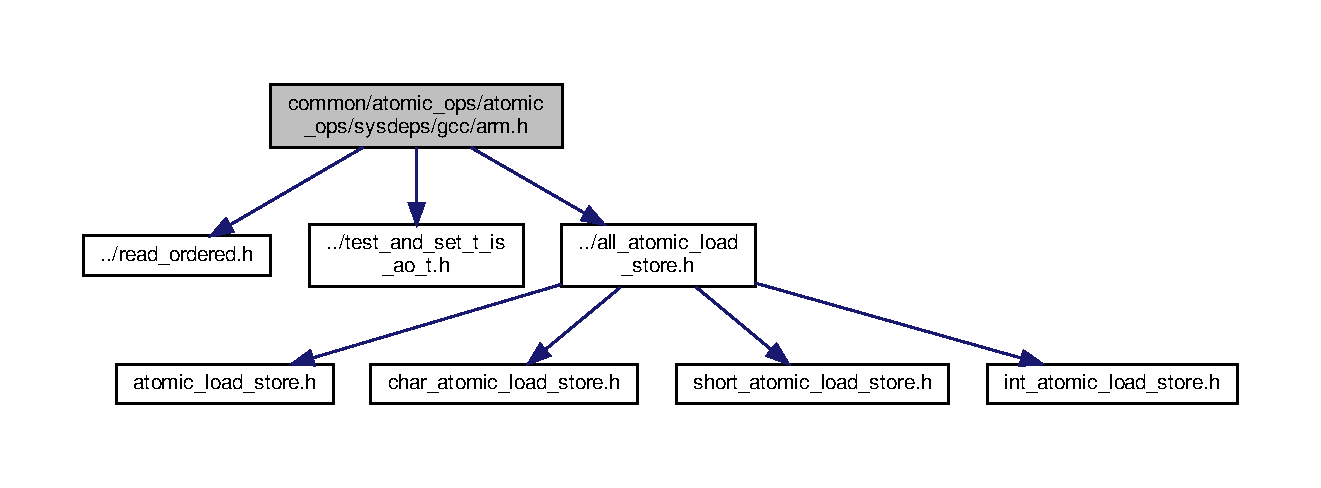
\includegraphics[width=350pt]{gcc_2arm_8h__incl}
\end{center}
\end{figure}
\subsection*{Macros}
\begin{DoxyCompactItemize}
\item 
\#define \hyperlink{gcc_2arm_8h_ad5f311a090d1e6e1bb35a6e68ee35fad}{A\+O\+\_\+\+H\+A\+V\+E\+\_\+test\+\_\+and\+\_\+set\+\_\+full}
\end{DoxyCompactItemize}
\subsection*{Functions}
\begin{DoxyCompactItemize}
\item 
\hyperlink{atomic__ops_8h_a9f6ab6253b6b11bc8c12efe9dde5db2b}{A\+O\+\_\+\+I\+N\+L\+I\+NE} \hyperlink{test__and__set__t__is__char_8h_a7d99a16c4eab47ba80ab6138d7d98ac1}{A\+O\+\_\+\+T\+S\+\_\+\+V\+A\+L\+\_\+t} \hyperlink{gcc_2arm_8h_a9f485bd63ce5c6a017ec241906e2f651}{A\+O\+\_\+test\+\_\+and\+\_\+set\+\_\+full} (volatile \hyperlink{test__and__set__t__is__char_8h_a5890c21b549264c75c2cad08bf4f6ba9}{A\+O\+\_\+\+T\+S\+\_\+t} $\ast$addr)
\end{DoxyCompactItemize}


\subsection{Macro Definition Documentation}
\mbox{\Hypertarget{gcc_2arm_8h_ad5f311a090d1e6e1bb35a6e68ee35fad}\label{gcc_2arm_8h_ad5f311a090d1e6e1bb35a6e68ee35fad}} 
\index{gcc/arm.\+h@{gcc/arm.\+h}!A\+O\+\_\+\+H\+A\+V\+E\+\_\+test\+\_\+and\+\_\+set\+\_\+full@{A\+O\+\_\+\+H\+A\+V\+E\+\_\+test\+\_\+and\+\_\+set\+\_\+full}}
\index{A\+O\+\_\+\+H\+A\+V\+E\+\_\+test\+\_\+and\+\_\+set\+\_\+full@{A\+O\+\_\+\+H\+A\+V\+E\+\_\+test\+\_\+and\+\_\+set\+\_\+full}!gcc/arm.\+h@{gcc/arm.\+h}}
\subsubsection{\texorpdfstring{A\+O\+\_\+\+H\+A\+V\+E\+\_\+test\+\_\+and\+\_\+set\+\_\+full}{AO\_HAVE\_test\_and\_set\_full}}
{\footnotesize\ttfamily \#define A\+O\+\_\+\+H\+A\+V\+E\+\_\+test\+\_\+and\+\_\+set\+\_\+full}



\subsection{Function Documentation}
\mbox{\Hypertarget{gcc_2arm_8h_a9f485bd63ce5c6a017ec241906e2f651}\label{gcc_2arm_8h_a9f485bd63ce5c6a017ec241906e2f651}} 
\index{gcc/arm.\+h@{gcc/arm.\+h}!A\+O\+\_\+test\+\_\+and\+\_\+set\+\_\+full@{A\+O\+\_\+test\+\_\+and\+\_\+set\+\_\+full}}
\index{A\+O\+\_\+test\+\_\+and\+\_\+set\+\_\+full@{A\+O\+\_\+test\+\_\+and\+\_\+set\+\_\+full}!gcc/arm.\+h@{gcc/arm.\+h}}
\subsubsection{\texorpdfstring{A\+O\+\_\+test\+\_\+and\+\_\+set\+\_\+full()}{AO\_test\_and\_set\_full()}}
{\footnotesize\ttfamily \hyperlink{atomic__ops_8h_a9f6ab6253b6b11bc8c12efe9dde5db2b}{A\+O\+\_\+\+I\+N\+L\+I\+NE} \hyperlink{test__and__set__t__is__char_8h_a7d99a16c4eab47ba80ab6138d7d98ac1}{A\+O\+\_\+\+T\+S\+\_\+\+V\+A\+L\+\_\+t} A\+O\+\_\+test\+\_\+and\+\_\+set\+\_\+full (\begin{DoxyParamCaption}\item[{volatile \hyperlink{test__and__set__t__is__char_8h_a5890c21b549264c75c2cad08bf4f6ba9}{A\+O\+\_\+\+T\+S\+\_\+t} $\ast$}]{addr }\end{DoxyParamCaption})}


\hypertarget{msftc_2arm_8h}{}\section{common/atomic\+\_\+ops/atomic\+\_\+ops/sysdeps/msftc/arm.h File Reference}
\label{msftc_2arm_8h}\index{common/atomic\+\_\+ops/atomic\+\_\+ops/sysdeps/msftc/arm.\+h@{common/atomic\+\_\+ops/atomic\+\_\+ops/sysdeps/msftc/arm.\+h}}
{\ttfamily \#include \char`\"{}../read\+\_\+ordered.\+h\char`\"{}}\newline
{\ttfamily \#include \char`\"{}common32\+\_\+defs.\+h\char`\"{}}\newline
{\ttfamily \#include \char`\"{}../all\+\_\+atomic\+\_\+load\+\_\+store.\+h\char`\"{}}\newline
{\ttfamily \#include \char`\"{}../test\+\_\+and\+\_\+set\+\_\+t\+\_\+is\+\_\+ao\+\_\+t.\+h\char`\"{}}\newline
Include dependency graph for arm.\+h\+:
\nopagebreak
\begin{figure}[H]
\begin{center}
\leavevmode
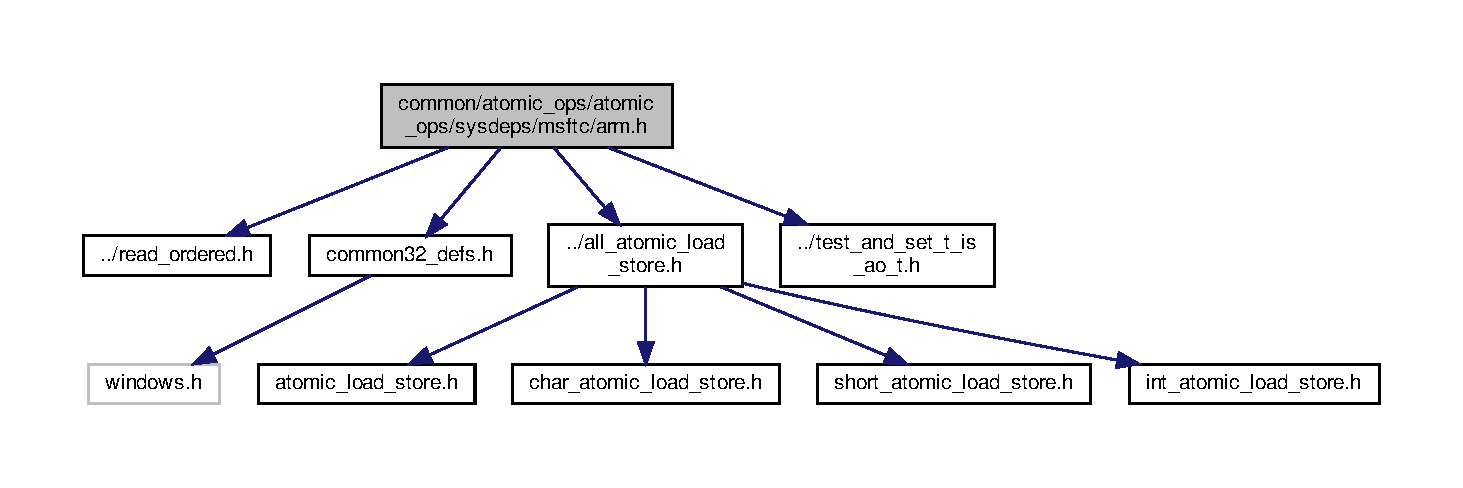
\includegraphics[width=350pt]{msftc_2arm_8h__incl}
\end{center}
\end{figure}

\hypertarget{avr32_8h}{}\section{common/atomic\+\_\+ops/atomic\+\_\+ops/sysdeps/gcc/avr32.h File Reference}
\label{avr32_8h}\index{common/atomic\+\_\+ops/atomic\+\_\+ops/sysdeps/gcc/avr32.\+h@{common/atomic\+\_\+ops/atomic\+\_\+ops/sysdeps/gcc/avr32.\+h}}
{\ttfamily \#include \char`\"{}../all\+\_\+atomic\+\_\+load\+\_\+store.\+h\char`\"{}}\newline
{\ttfamily \#include \char`\"{}../ordered.\+h\char`\"{}}\newline
{\ttfamily \#include \char`\"{}../test\+\_\+and\+\_\+set\+\_\+t\+\_\+is\+\_\+ao\+\_\+t.\+h\char`\"{}}\newline
Include dependency graph for avr32.\+h\+:
\nopagebreak
\begin{figure}[H]
\begin{center}
\leavevmode
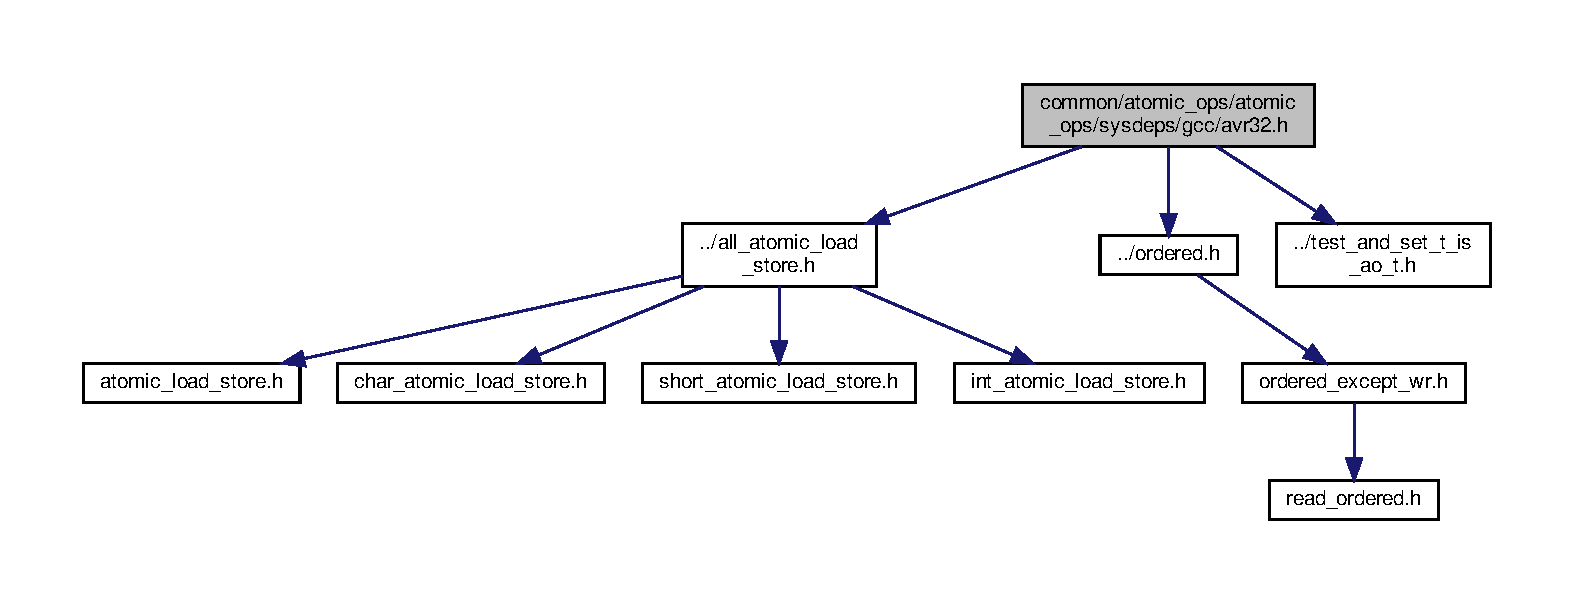
\includegraphics[width=350pt]{avr32_8h__incl}
\end{center}
\end{figure}
\subsection*{Macros}
\begin{DoxyCompactItemize}
\item 
\#define \hyperlink{avr32_8h_ad5f311a090d1e6e1bb35a6e68ee35fad}{A\+O\+\_\+\+H\+A\+V\+E\+\_\+test\+\_\+and\+\_\+set\+\_\+full}
\item 
\#define \hyperlink{avr32_8h_a98ec53065c0dfd18bc1013c500da377c}{A\+O\+\_\+\+H\+A\+V\+E\+\_\+compare\+\_\+and\+\_\+swap\+\_\+full}
\end{DoxyCompactItemize}
\subsection*{Functions}
\begin{DoxyCompactItemize}
\item 
\hyperlink{atomic__ops_8h_a9f6ab6253b6b11bc8c12efe9dde5db2b}{A\+O\+\_\+\+I\+N\+L\+I\+NE} \hyperlink{test__and__set__t__is__char_8h_a7d99a16c4eab47ba80ab6138d7d98ac1}{A\+O\+\_\+\+T\+S\+\_\+\+V\+A\+L\+\_\+t} \hyperlink{avr32_8h_a9f485bd63ce5c6a017ec241906e2f651}{A\+O\+\_\+test\+\_\+and\+\_\+set\+\_\+full} (volatile \hyperlink{test__and__set__t__is__char_8h_a5890c21b549264c75c2cad08bf4f6ba9}{A\+O\+\_\+\+T\+S\+\_\+t} $\ast$addr)
\item 
\hyperlink{atomic__ops_8h_a9f6ab6253b6b11bc8c12efe9dde5db2b}{A\+O\+\_\+\+I\+N\+L\+I\+NE} int \hyperlink{avr32_8h_a634397de6de764015b30cdff3ff00b06}{A\+O\+\_\+compare\+\_\+and\+\_\+swap\+\_\+full} (volatile \hyperlink{atomic__ops_8h_a5225fef4d9eee821e82382cd269160dd}{A\+O\+\_\+t} $\ast$addr, \hyperlink{atomic__ops_8h_a5225fef4d9eee821e82382cd269160dd}{A\+O\+\_\+t} old, \hyperlink{atomic__ops_8h_a5225fef4d9eee821e82382cd269160dd}{A\+O\+\_\+t} new\+\_\+val)
\end{DoxyCompactItemize}


\subsection{Macro Definition Documentation}
\mbox{\Hypertarget{avr32_8h_a98ec53065c0dfd18bc1013c500da377c}\label{avr32_8h_a98ec53065c0dfd18bc1013c500da377c}} 
\index{avr32.\+h@{avr32.\+h}!A\+O\+\_\+\+H\+A\+V\+E\+\_\+compare\+\_\+and\+\_\+swap\+\_\+full@{A\+O\+\_\+\+H\+A\+V\+E\+\_\+compare\+\_\+and\+\_\+swap\+\_\+full}}
\index{A\+O\+\_\+\+H\+A\+V\+E\+\_\+compare\+\_\+and\+\_\+swap\+\_\+full@{A\+O\+\_\+\+H\+A\+V\+E\+\_\+compare\+\_\+and\+\_\+swap\+\_\+full}!avr32.\+h@{avr32.\+h}}
\subsubsection{\texorpdfstring{A\+O\+\_\+\+H\+A\+V\+E\+\_\+compare\+\_\+and\+\_\+swap\+\_\+full}{AO\_HAVE\_compare\_and\_swap\_full}}
{\footnotesize\ttfamily \#define A\+O\+\_\+\+H\+A\+V\+E\+\_\+compare\+\_\+and\+\_\+swap\+\_\+full}

\mbox{\Hypertarget{avr32_8h_ad5f311a090d1e6e1bb35a6e68ee35fad}\label{avr32_8h_ad5f311a090d1e6e1bb35a6e68ee35fad}} 
\index{avr32.\+h@{avr32.\+h}!A\+O\+\_\+\+H\+A\+V\+E\+\_\+test\+\_\+and\+\_\+set\+\_\+full@{A\+O\+\_\+\+H\+A\+V\+E\+\_\+test\+\_\+and\+\_\+set\+\_\+full}}
\index{A\+O\+\_\+\+H\+A\+V\+E\+\_\+test\+\_\+and\+\_\+set\+\_\+full@{A\+O\+\_\+\+H\+A\+V\+E\+\_\+test\+\_\+and\+\_\+set\+\_\+full}!avr32.\+h@{avr32.\+h}}
\subsubsection{\texorpdfstring{A\+O\+\_\+\+H\+A\+V\+E\+\_\+test\+\_\+and\+\_\+set\+\_\+full}{AO\_HAVE\_test\_and\_set\_full}}
{\footnotesize\ttfamily \#define A\+O\+\_\+\+H\+A\+V\+E\+\_\+test\+\_\+and\+\_\+set\+\_\+full}



\subsection{Function Documentation}
\mbox{\Hypertarget{avr32_8h_a634397de6de764015b30cdff3ff00b06}\label{avr32_8h_a634397de6de764015b30cdff3ff00b06}} 
\index{avr32.\+h@{avr32.\+h}!A\+O\+\_\+compare\+\_\+and\+\_\+swap\+\_\+full@{A\+O\+\_\+compare\+\_\+and\+\_\+swap\+\_\+full}}
\index{A\+O\+\_\+compare\+\_\+and\+\_\+swap\+\_\+full@{A\+O\+\_\+compare\+\_\+and\+\_\+swap\+\_\+full}!avr32.\+h@{avr32.\+h}}
\subsubsection{\texorpdfstring{A\+O\+\_\+compare\+\_\+and\+\_\+swap\+\_\+full()}{AO\_compare\_and\_swap\_full()}}
{\footnotesize\ttfamily \hyperlink{atomic__ops_8h_a9f6ab6253b6b11bc8c12efe9dde5db2b}{A\+O\+\_\+\+I\+N\+L\+I\+NE} int A\+O\+\_\+compare\+\_\+and\+\_\+swap\+\_\+full (\begin{DoxyParamCaption}\item[{volatile \hyperlink{atomic__ops_8h_a5225fef4d9eee821e82382cd269160dd}{A\+O\+\_\+t} $\ast$}]{addr,  }\item[{\hyperlink{atomic__ops_8h_a5225fef4d9eee821e82382cd269160dd}{A\+O\+\_\+t}}]{old,  }\item[{\hyperlink{atomic__ops_8h_a5225fef4d9eee821e82382cd269160dd}{A\+O\+\_\+t}}]{new\+\_\+val }\end{DoxyParamCaption})}

\mbox{\Hypertarget{avr32_8h_a9f485bd63ce5c6a017ec241906e2f651}\label{avr32_8h_a9f485bd63ce5c6a017ec241906e2f651}} 
\index{avr32.\+h@{avr32.\+h}!A\+O\+\_\+test\+\_\+and\+\_\+set\+\_\+full@{A\+O\+\_\+test\+\_\+and\+\_\+set\+\_\+full}}
\index{A\+O\+\_\+test\+\_\+and\+\_\+set\+\_\+full@{A\+O\+\_\+test\+\_\+and\+\_\+set\+\_\+full}!avr32.\+h@{avr32.\+h}}
\subsubsection{\texorpdfstring{A\+O\+\_\+test\+\_\+and\+\_\+set\+\_\+full()}{AO\_test\_and\_set\_full()}}
{\footnotesize\ttfamily \hyperlink{atomic__ops_8h_a9f6ab6253b6b11bc8c12efe9dde5db2b}{A\+O\+\_\+\+I\+N\+L\+I\+NE} \hyperlink{test__and__set__t__is__char_8h_a7d99a16c4eab47ba80ab6138d7d98ac1}{A\+O\+\_\+\+T\+S\+\_\+\+V\+A\+L\+\_\+t} A\+O\+\_\+test\+\_\+and\+\_\+set\+\_\+full (\begin{DoxyParamCaption}\item[{volatile \hyperlink{test__and__set__t__is__char_8h_a5890c21b549264c75c2cad08bf4f6ba9}{A\+O\+\_\+\+T\+S\+\_\+t} $\ast$}]{addr }\end{DoxyParamCaption})}


\hypertarget{cris_8h}{}\section{common/atomic\+\_\+ops/atomic\+\_\+ops/sysdeps/gcc/cris.h File Reference}
\label{cris_8h}\index{common/atomic\+\_\+ops/atomic\+\_\+ops/sysdeps/gcc/cris.\+h@{common/atomic\+\_\+ops/atomic\+\_\+ops/sysdeps/gcc/cris.\+h}}
{\ttfamily \#include \char`\"{}../all\+\_\+atomic\+\_\+load\+\_\+store.\+h\char`\"{}}\newline
{\ttfamily \#include \char`\"{}../ordered.\+h\char`\"{}}\newline
{\ttfamily \#include \char`\"{}../test\+\_\+and\+\_\+set\+\_\+t\+\_\+is\+\_\+ao\+\_\+t.\+h\char`\"{}}\newline
Include dependency graph for cris.\+h\+:
\nopagebreak
\begin{figure}[H]
\begin{center}
\leavevmode
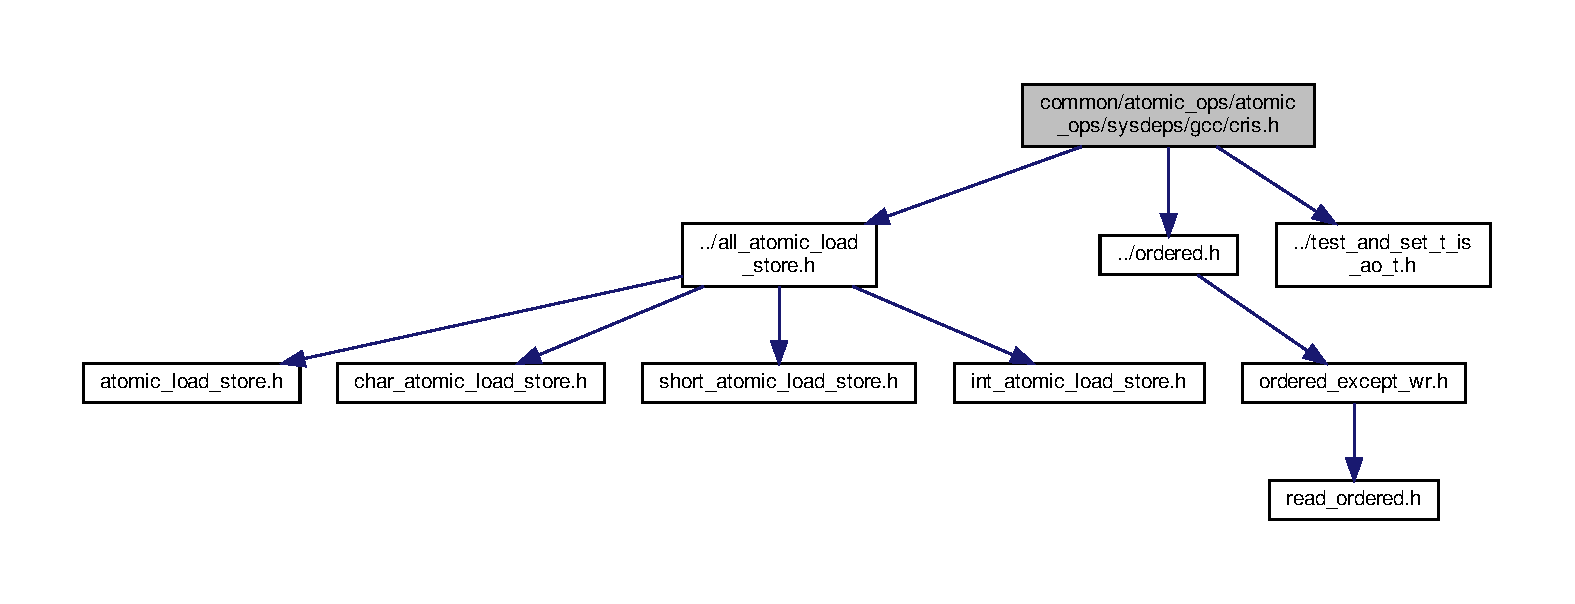
\includegraphics[width=350pt]{cris_8h__incl}
\end{center}
\end{figure}
\subsection*{Macros}
\begin{DoxyCompactItemize}
\item 
\#define \hyperlink{cris_8h_ad5f311a090d1e6e1bb35a6e68ee35fad}{A\+O\+\_\+\+H\+A\+V\+E\+\_\+test\+\_\+and\+\_\+set\+\_\+full}
\end{DoxyCompactItemize}
\subsection*{Functions}
\begin{DoxyCompactItemize}
\item 
\hyperlink{atomic__ops_8h_a9f6ab6253b6b11bc8c12efe9dde5db2b}{A\+O\+\_\+\+I\+N\+L\+I\+NE} \hyperlink{test__and__set__t__is__char_8h_a7d99a16c4eab47ba80ab6138d7d98ac1}{A\+O\+\_\+\+T\+S\+\_\+\+V\+A\+L\+\_\+t} \hyperlink{cris_8h_a9f485bd63ce5c6a017ec241906e2f651}{A\+O\+\_\+test\+\_\+and\+\_\+set\+\_\+full} (volatile \hyperlink{test__and__set__t__is__char_8h_a5890c21b549264c75c2cad08bf4f6ba9}{A\+O\+\_\+\+T\+S\+\_\+t} $\ast$addr)
\end{DoxyCompactItemize}


\subsection{Macro Definition Documentation}
\mbox{\Hypertarget{cris_8h_ad5f311a090d1e6e1bb35a6e68ee35fad}\label{cris_8h_ad5f311a090d1e6e1bb35a6e68ee35fad}} 
\index{cris.\+h@{cris.\+h}!A\+O\+\_\+\+H\+A\+V\+E\+\_\+test\+\_\+and\+\_\+set\+\_\+full@{A\+O\+\_\+\+H\+A\+V\+E\+\_\+test\+\_\+and\+\_\+set\+\_\+full}}
\index{A\+O\+\_\+\+H\+A\+V\+E\+\_\+test\+\_\+and\+\_\+set\+\_\+full@{A\+O\+\_\+\+H\+A\+V\+E\+\_\+test\+\_\+and\+\_\+set\+\_\+full}!cris.\+h@{cris.\+h}}
\subsubsection{\texorpdfstring{A\+O\+\_\+\+H\+A\+V\+E\+\_\+test\+\_\+and\+\_\+set\+\_\+full}{AO\_HAVE\_test\_and\_set\_full}}
{\footnotesize\ttfamily \#define A\+O\+\_\+\+H\+A\+V\+E\+\_\+test\+\_\+and\+\_\+set\+\_\+full}



\subsection{Function Documentation}
\mbox{\Hypertarget{cris_8h_a9f485bd63ce5c6a017ec241906e2f651}\label{cris_8h_a9f485bd63ce5c6a017ec241906e2f651}} 
\index{cris.\+h@{cris.\+h}!A\+O\+\_\+test\+\_\+and\+\_\+set\+\_\+full@{A\+O\+\_\+test\+\_\+and\+\_\+set\+\_\+full}}
\index{A\+O\+\_\+test\+\_\+and\+\_\+set\+\_\+full@{A\+O\+\_\+test\+\_\+and\+\_\+set\+\_\+full}!cris.\+h@{cris.\+h}}
\subsubsection{\texorpdfstring{A\+O\+\_\+test\+\_\+and\+\_\+set\+\_\+full()}{AO\_test\_and\_set\_full()}}
{\footnotesize\ttfamily \hyperlink{atomic__ops_8h_a9f6ab6253b6b11bc8c12efe9dde5db2b}{A\+O\+\_\+\+I\+N\+L\+I\+NE} \hyperlink{test__and__set__t__is__char_8h_a7d99a16c4eab47ba80ab6138d7d98ac1}{A\+O\+\_\+\+T\+S\+\_\+\+V\+A\+L\+\_\+t} A\+O\+\_\+test\+\_\+and\+\_\+set\+\_\+full (\begin{DoxyParamCaption}\item[{volatile \hyperlink{test__and__set__t__is__char_8h_a5890c21b549264c75c2cad08bf4f6ba9}{A\+O\+\_\+\+T\+S\+\_\+t} $\ast$}]{addr }\end{DoxyParamCaption})}


\hypertarget{gcc_2hppa_8h}{}\section{common/atomic\+\_\+ops/atomic\+\_\+ops/sysdeps/gcc/hppa.h File Reference}
\label{gcc_2hppa_8h}\index{common/atomic\+\_\+ops/atomic\+\_\+ops/sysdeps/gcc/hppa.\+h@{common/atomic\+\_\+ops/atomic\+\_\+ops/sysdeps/gcc/hppa.\+h}}
{\ttfamily \#include \char`\"{}../all\+\_\+atomic\+\_\+load\+\_\+store.\+h\char`\"{}}\newline
{\ttfamily \#include \char`\"{}../ordered.\+h\char`\"{}}\newline
Include dependency graph for hppa.\+h\+:
\nopagebreak
\begin{figure}[H]
\begin{center}
\leavevmode
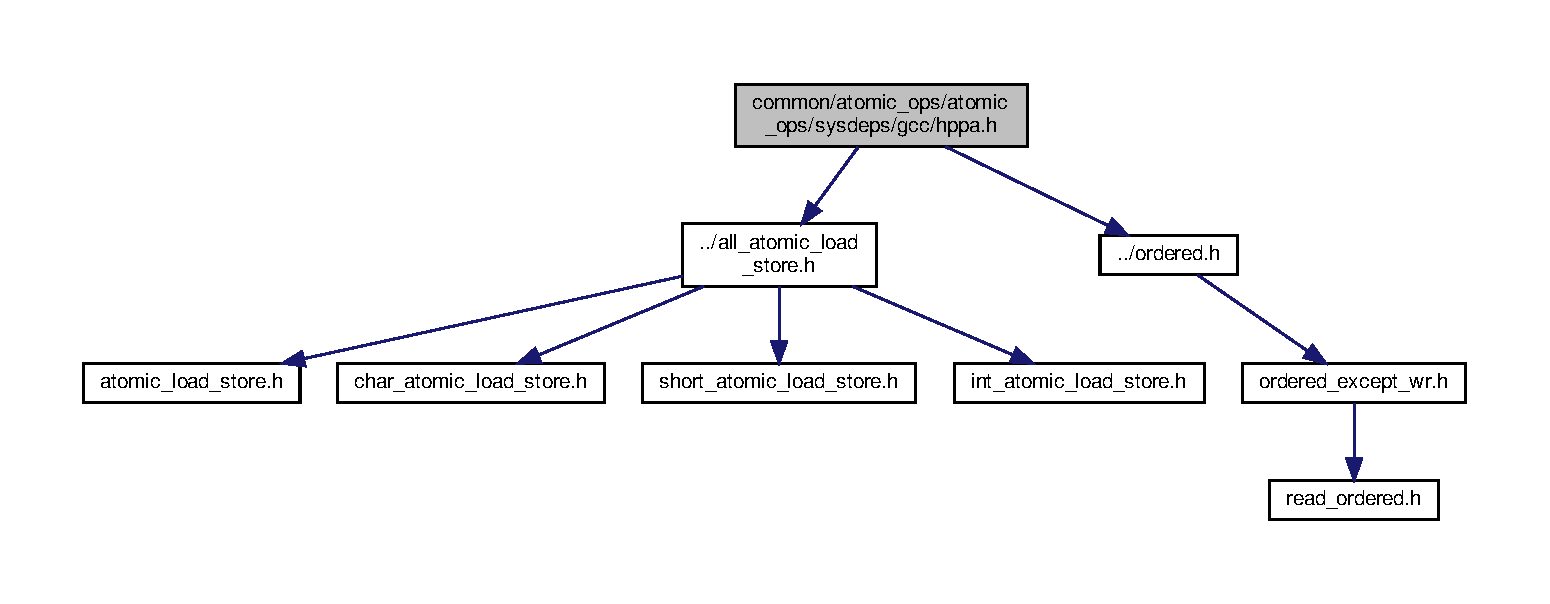
\includegraphics[width=350pt]{gcc_2hppa_8h__incl}
\end{center}
\end{figure}
\subsection*{Classes}
\begin{DoxyCompactItemize}
\item 
struct \hyperlink{structAO__pa__clearable__loc}{A\+O\+\_\+pa\+\_\+clearable\+\_\+loc}
\end{DoxyCompactItemize}
\subsection*{Macros}
\begin{DoxyCompactItemize}
\item 
\#define \hyperlink{gcc_2hppa_8h_a5890c21b549264c75c2cad08bf4f6ba9}{A\+O\+\_\+\+T\+S\+\_\+t}~struct \hyperlink{structAO__pa__clearable__loc}{A\+O\+\_\+pa\+\_\+clearable\+\_\+loc}
\item 
\#define \hyperlink{gcc_2hppa_8h_af0f8642b332396baef4793e7ce825759}{A\+O\+\_\+\+T\+S\+\_\+\+I\+N\+I\+T\+I\+A\+L\+I\+Z\+ER}~\{1,1,1,1\}
\item 
\#define \hyperlink{gcc_2hppa_8h_a7d99a16c4eab47ba80ab6138d7d98ac1}{A\+O\+\_\+\+T\+S\+\_\+\+V\+A\+L\+\_\+t}~\hyperlink{gcc_2hppa_8h_af6b785b31fbe39690aa613d7920f3299}{A\+O\+\_\+\+P\+A\+\_\+\+T\+S\+\_\+val}
\item 
\#define \hyperlink{gcc_2hppa_8h_a35258ee13bc817d0b8eb62f4695c4a3e}{A\+O\+\_\+\+T\+S\+\_\+\+C\+L\+E\+AR}~\hyperlink{hpc_2hppa_8h_af6b785b31fbe39690aa613d7920f3299a031b53af392a27ab58b0bd2cc09be141}{A\+O\+\_\+\+P\+A\+\_\+\+T\+S\+\_\+clear}
\item 
\#define \hyperlink{gcc_2hppa_8h_a8a50ac5fe9e6ff855a078c265079ac06}{A\+O\+\_\+\+T\+S\+\_\+\+S\+ET}~\hyperlink{hpc_2hppa_8h_af6b785b31fbe39690aa613d7920f3299aed76339c52af50af82a953e1ce542cd9}{A\+O\+\_\+\+P\+A\+\_\+\+T\+S\+\_\+set}
\item 
\#define \hyperlink{gcc_2hppa_8h_a46594f217123664bbc7f897840d4598d}{\+\_\+\+\_\+ldcw}(a)
\item 
\#define \hyperlink{gcc_2hppa_8h_a0002acfa7aea61f6b2dbcf63ab7d83aa}{\+\_\+\+\_\+\+P\+A\+\_\+\+L\+D\+C\+W\+\_\+\+A\+L\+I\+G\+N\+M\+E\+NT}~16
\item 
\#define \hyperlink{gcc_2hppa_8h_a5e3caf37865af2f5a326eabaa81d0569}{\+\_\+\+\_\+ldcw\+\_\+align}(a)
\item 
\#define \hyperlink{gcc_2hppa_8h_ad5703c05836e7c55cde2a45922e721b4}{A\+O\+\_\+\+C\+L\+E\+AR}(addr)~\hyperlink{hpc_2hppa_8h_afe32bd0febd74f8b7ccafa2e24ab68b6}{A\+O\+\_\+pa\+\_\+clear}(addr)
\item 
\#define \hyperlink{gcc_2hppa_8h_ad5f311a090d1e6e1bb35a6e68ee35fad}{A\+O\+\_\+\+H\+A\+V\+E\+\_\+test\+\_\+and\+\_\+set\+\_\+full}
\end{DoxyCompactItemize}
\subsection*{Enumerations}
\begin{DoxyCompactItemize}
\item 
enum \hyperlink{gcc_2hppa_8h_af6b785b31fbe39690aa613d7920f3299}{A\+O\+\_\+\+P\+A\+\_\+\+T\+S\+\_\+val} \{ \hyperlink{gcc_2hppa_8h_af6b785b31fbe39690aa613d7920f3299aed76339c52af50af82a953e1ce542cd9}{A\+O\+\_\+\+P\+A\+\_\+\+T\+S\+\_\+set} = 0, 
\hyperlink{gcc_2hppa_8h_af6b785b31fbe39690aa613d7920f3299a031b53af392a27ab58b0bd2cc09be141}{A\+O\+\_\+\+P\+A\+\_\+\+T\+S\+\_\+clear} = 1, 
\hyperlink{hpc_2hppa_8h_af6b785b31fbe39690aa613d7920f3299aed76339c52af50af82a953e1ce542cd9}{A\+O\+\_\+\+P\+A\+\_\+\+T\+S\+\_\+set} = 0, 
\hyperlink{hpc_2hppa_8h_af6b785b31fbe39690aa613d7920f3299a031b53af392a27ab58b0bd2cc09be141}{A\+O\+\_\+\+P\+A\+\_\+\+T\+S\+\_\+clear} = 1
 \}
\end{DoxyCompactItemize}
\subsection*{Functions}
\begin{DoxyCompactItemize}
\item 
\hyperlink{atomic__ops_8h_a9f6ab6253b6b11bc8c12efe9dde5db2b}{A\+O\+\_\+\+I\+N\+L\+I\+NE} \hyperlink{test__and__set__t__is__char_8h_a7d99a16c4eab47ba80ab6138d7d98ac1}{A\+O\+\_\+\+T\+S\+\_\+\+V\+A\+L\+\_\+t} \hyperlink{gcc_2hppa_8h_a9f485bd63ce5c6a017ec241906e2f651}{A\+O\+\_\+test\+\_\+and\+\_\+set\+\_\+full} (volatile \hyperlink{test__and__set__t__is__char_8h_a5890c21b549264c75c2cad08bf4f6ba9}{A\+O\+\_\+\+T\+S\+\_\+t} $\ast$addr)
\item 
\hyperlink{atomic__ops_8h_a9f6ab6253b6b11bc8c12efe9dde5db2b}{A\+O\+\_\+\+I\+N\+L\+I\+NE} void \hyperlink{gcc_2hppa_8h_afe32bd0febd74f8b7ccafa2e24ab68b6}{A\+O\+\_\+pa\+\_\+clear} (volatile \hyperlink{test__and__set__t__is__char_8h_a5890c21b549264c75c2cad08bf4f6ba9}{A\+O\+\_\+\+T\+S\+\_\+t} $\ast$addr)
\end{DoxyCompactItemize}


\subsection{Macro Definition Documentation}
\mbox{\Hypertarget{gcc_2hppa_8h_a46594f217123664bbc7f897840d4598d}\label{gcc_2hppa_8h_a46594f217123664bbc7f897840d4598d}} 
\index{gcc/hppa.\+h@{gcc/hppa.\+h}!\+\_\+\+\_\+ldcw@{\+\_\+\+\_\+ldcw}}
\index{\+\_\+\+\_\+ldcw@{\+\_\+\+\_\+ldcw}!gcc/hppa.\+h@{gcc/hppa.\+h}}
\subsubsection{\texorpdfstring{\+\_\+\+\_\+ldcw}{\_\_ldcw}}
{\footnotesize\ttfamily \#define \+\_\+\+\_\+ldcw(\begin{DoxyParamCaption}\item[{}]{a }\end{DoxyParamCaption})}

{\bfseries Value\+:}
\begin{DoxyCode}
(\{ \(\backslash\)
  volatile \textcolor{keywordtype}{unsigned} \textcolor{keywordtype}{int} \_\_ret;                                  \(\backslash\)
  \_\_asm\_\_ \_\_volatile\_\_(\textcolor{stringliteral}{"ldcw 0(%2),%0"}                          \(\backslash\)
                      : \textcolor{stringliteral}{"=r"} (\_\_ret), \textcolor{stringliteral}{"=m"} (*(a)) : \textcolor{stringliteral}{"r"} (a));   \(\backslash\)
  \_\_ret;                                                        \(\backslash\)
\})
\end{DoxyCode}
\mbox{\Hypertarget{gcc_2hppa_8h_a5e3caf37865af2f5a326eabaa81d0569}\label{gcc_2hppa_8h_a5e3caf37865af2f5a326eabaa81d0569}} 
\index{gcc/hppa.\+h@{gcc/hppa.\+h}!\+\_\+\+\_\+ldcw\+\_\+align@{\+\_\+\+\_\+ldcw\+\_\+align}}
\index{\+\_\+\+\_\+ldcw\+\_\+align@{\+\_\+\+\_\+ldcw\+\_\+align}!gcc/hppa.\+h@{gcc/hppa.\+h}}
\subsubsection{\texorpdfstring{\+\_\+\+\_\+ldcw\+\_\+align}{\_\_ldcw\_align}}
{\footnotesize\ttfamily \#define \+\_\+\+\_\+ldcw\+\_\+align(\begin{DoxyParamCaption}\item[{}]{a }\end{DoxyParamCaption})}

{\bfseries Value\+:}
\begin{DoxyCode}
(\{ \(\backslash\)
  unsigned \textcolor{keywordtype}{long} \_\_ret = (\textcolor{keywordtype}{unsigned} long) a;                      \(\backslash\)
  \_\_ret += \hyperlink{gcc_2hppa_8h_a0002acfa7aea61f6b2dbcf63ab7d83aa}{\_\_PA\_LDCW\_ALIGNMENT} - 1;                                     \(\backslash\)
  \_\_ret &= ~(\hyperlink{gcc_2hppa_8h_a0002acfa7aea61f6b2dbcf63ab7d83aa}{\_\_PA\_LDCW\_ALIGNMENT} - 1);                                  \(\backslash\)
  (\textcolor{keyword}{volatile} \textcolor{keywordtype}{unsigned} \textcolor{keywordtype}{int} *) \_\_ret;                                      \(\backslash\)
\})
\end{DoxyCode}
\mbox{\Hypertarget{gcc_2hppa_8h_a0002acfa7aea61f6b2dbcf63ab7d83aa}\label{gcc_2hppa_8h_a0002acfa7aea61f6b2dbcf63ab7d83aa}} 
\index{gcc/hppa.\+h@{gcc/hppa.\+h}!\+\_\+\+\_\+\+P\+A\+\_\+\+L\+D\+C\+W\+\_\+\+A\+L\+I\+G\+N\+M\+E\+NT@{\+\_\+\+\_\+\+P\+A\+\_\+\+L\+D\+C\+W\+\_\+\+A\+L\+I\+G\+N\+M\+E\+NT}}
\index{\+\_\+\+\_\+\+P\+A\+\_\+\+L\+D\+C\+W\+\_\+\+A\+L\+I\+G\+N\+M\+E\+NT@{\+\_\+\+\_\+\+P\+A\+\_\+\+L\+D\+C\+W\+\_\+\+A\+L\+I\+G\+N\+M\+E\+NT}!gcc/hppa.\+h@{gcc/hppa.\+h}}
\subsubsection{\texorpdfstring{\+\_\+\+\_\+\+P\+A\+\_\+\+L\+D\+C\+W\+\_\+\+A\+L\+I\+G\+N\+M\+E\+NT}{\_\_PA\_LDCW\_ALIGNMENT}}
{\footnotesize\ttfamily \#define \+\_\+\+\_\+\+P\+A\+\_\+\+L\+D\+C\+W\+\_\+\+A\+L\+I\+G\+N\+M\+E\+NT~16}

\mbox{\Hypertarget{gcc_2hppa_8h_ad5703c05836e7c55cde2a45922e721b4}\label{gcc_2hppa_8h_ad5703c05836e7c55cde2a45922e721b4}} 
\index{gcc/hppa.\+h@{gcc/hppa.\+h}!A\+O\+\_\+\+C\+L\+E\+AR@{A\+O\+\_\+\+C\+L\+E\+AR}}
\index{A\+O\+\_\+\+C\+L\+E\+AR@{A\+O\+\_\+\+C\+L\+E\+AR}!gcc/hppa.\+h@{gcc/hppa.\+h}}
\subsubsection{\texorpdfstring{A\+O\+\_\+\+C\+L\+E\+AR}{AO\_CLEAR}}
{\footnotesize\ttfamily \#define A\+O\+\_\+\+C\+L\+E\+AR(\begin{DoxyParamCaption}\item[{}]{addr }\end{DoxyParamCaption})~\hyperlink{hpc_2hppa_8h_afe32bd0febd74f8b7ccafa2e24ab68b6}{A\+O\+\_\+pa\+\_\+clear}(addr)}

\mbox{\Hypertarget{gcc_2hppa_8h_ad5f311a090d1e6e1bb35a6e68ee35fad}\label{gcc_2hppa_8h_ad5f311a090d1e6e1bb35a6e68ee35fad}} 
\index{gcc/hppa.\+h@{gcc/hppa.\+h}!A\+O\+\_\+\+H\+A\+V\+E\+\_\+test\+\_\+and\+\_\+set\+\_\+full@{A\+O\+\_\+\+H\+A\+V\+E\+\_\+test\+\_\+and\+\_\+set\+\_\+full}}
\index{A\+O\+\_\+\+H\+A\+V\+E\+\_\+test\+\_\+and\+\_\+set\+\_\+full@{A\+O\+\_\+\+H\+A\+V\+E\+\_\+test\+\_\+and\+\_\+set\+\_\+full}!gcc/hppa.\+h@{gcc/hppa.\+h}}
\subsubsection{\texorpdfstring{A\+O\+\_\+\+H\+A\+V\+E\+\_\+test\+\_\+and\+\_\+set\+\_\+full}{AO\_HAVE\_test\_and\_set\_full}}
{\footnotesize\ttfamily \#define A\+O\+\_\+\+H\+A\+V\+E\+\_\+test\+\_\+and\+\_\+set\+\_\+full}

\mbox{\Hypertarget{gcc_2hppa_8h_a35258ee13bc817d0b8eb62f4695c4a3e}\label{gcc_2hppa_8h_a35258ee13bc817d0b8eb62f4695c4a3e}} 
\index{gcc/hppa.\+h@{gcc/hppa.\+h}!A\+O\+\_\+\+T\+S\+\_\+\+C\+L\+E\+AR@{A\+O\+\_\+\+T\+S\+\_\+\+C\+L\+E\+AR}}
\index{A\+O\+\_\+\+T\+S\+\_\+\+C\+L\+E\+AR@{A\+O\+\_\+\+T\+S\+\_\+\+C\+L\+E\+AR}!gcc/hppa.\+h@{gcc/hppa.\+h}}
\subsubsection{\texorpdfstring{A\+O\+\_\+\+T\+S\+\_\+\+C\+L\+E\+AR}{AO\_TS\_CLEAR}}
{\footnotesize\ttfamily \#define A\+O\+\_\+\+T\+S\+\_\+\+C\+L\+E\+AR~\hyperlink{hpc_2hppa_8h_af6b785b31fbe39690aa613d7920f3299a031b53af392a27ab58b0bd2cc09be141}{A\+O\+\_\+\+P\+A\+\_\+\+T\+S\+\_\+clear}}

\mbox{\Hypertarget{gcc_2hppa_8h_af0f8642b332396baef4793e7ce825759}\label{gcc_2hppa_8h_af0f8642b332396baef4793e7ce825759}} 
\index{gcc/hppa.\+h@{gcc/hppa.\+h}!A\+O\+\_\+\+T\+S\+\_\+\+I\+N\+I\+T\+I\+A\+L\+I\+Z\+ER@{A\+O\+\_\+\+T\+S\+\_\+\+I\+N\+I\+T\+I\+A\+L\+I\+Z\+ER}}
\index{A\+O\+\_\+\+T\+S\+\_\+\+I\+N\+I\+T\+I\+A\+L\+I\+Z\+ER@{A\+O\+\_\+\+T\+S\+\_\+\+I\+N\+I\+T\+I\+A\+L\+I\+Z\+ER}!gcc/hppa.\+h@{gcc/hppa.\+h}}
\subsubsection{\texorpdfstring{A\+O\+\_\+\+T\+S\+\_\+\+I\+N\+I\+T\+I\+A\+L\+I\+Z\+ER}{AO\_TS\_INITIALIZER}}
{\footnotesize\ttfamily \#define A\+O\+\_\+\+T\+S\+\_\+\+I\+N\+I\+T\+I\+A\+L\+I\+Z\+ER~\{1,1,1,1\}}

\mbox{\Hypertarget{gcc_2hppa_8h_a8a50ac5fe9e6ff855a078c265079ac06}\label{gcc_2hppa_8h_a8a50ac5fe9e6ff855a078c265079ac06}} 
\index{gcc/hppa.\+h@{gcc/hppa.\+h}!A\+O\+\_\+\+T\+S\+\_\+\+S\+ET@{A\+O\+\_\+\+T\+S\+\_\+\+S\+ET}}
\index{A\+O\+\_\+\+T\+S\+\_\+\+S\+ET@{A\+O\+\_\+\+T\+S\+\_\+\+S\+ET}!gcc/hppa.\+h@{gcc/hppa.\+h}}
\subsubsection{\texorpdfstring{A\+O\+\_\+\+T\+S\+\_\+\+S\+ET}{AO\_TS\_SET}}
{\footnotesize\ttfamily \#define A\+O\+\_\+\+T\+S\+\_\+\+S\+ET~\hyperlink{hpc_2hppa_8h_af6b785b31fbe39690aa613d7920f3299aed76339c52af50af82a953e1ce542cd9}{A\+O\+\_\+\+P\+A\+\_\+\+T\+S\+\_\+set}}

\mbox{\Hypertarget{gcc_2hppa_8h_a5890c21b549264c75c2cad08bf4f6ba9}\label{gcc_2hppa_8h_a5890c21b549264c75c2cad08bf4f6ba9}} 
\index{gcc/hppa.\+h@{gcc/hppa.\+h}!A\+O\+\_\+\+T\+S\+\_\+t@{A\+O\+\_\+\+T\+S\+\_\+t}}
\index{A\+O\+\_\+\+T\+S\+\_\+t@{A\+O\+\_\+\+T\+S\+\_\+t}!gcc/hppa.\+h@{gcc/hppa.\+h}}
\subsubsection{\texorpdfstring{A\+O\+\_\+\+T\+S\+\_\+t}{AO\_TS\_t}}
{\footnotesize\ttfamily \#define A\+O\+\_\+\+T\+S\+\_\+t~struct \hyperlink{structAO__pa__clearable__loc}{A\+O\+\_\+pa\+\_\+clearable\+\_\+loc}}

\mbox{\Hypertarget{gcc_2hppa_8h_a7d99a16c4eab47ba80ab6138d7d98ac1}\label{gcc_2hppa_8h_a7d99a16c4eab47ba80ab6138d7d98ac1}} 
\index{gcc/hppa.\+h@{gcc/hppa.\+h}!A\+O\+\_\+\+T\+S\+\_\+\+V\+A\+L\+\_\+t@{A\+O\+\_\+\+T\+S\+\_\+\+V\+A\+L\+\_\+t}}
\index{A\+O\+\_\+\+T\+S\+\_\+\+V\+A\+L\+\_\+t@{A\+O\+\_\+\+T\+S\+\_\+\+V\+A\+L\+\_\+t}!gcc/hppa.\+h@{gcc/hppa.\+h}}
\subsubsection{\texorpdfstring{A\+O\+\_\+\+T\+S\+\_\+\+V\+A\+L\+\_\+t}{AO\_TS\_VAL\_t}}
{\footnotesize\ttfamily \#define A\+O\+\_\+\+T\+S\+\_\+\+V\+A\+L\+\_\+t~\hyperlink{gcc_2hppa_8h_af6b785b31fbe39690aa613d7920f3299}{A\+O\+\_\+\+P\+A\+\_\+\+T\+S\+\_\+val}}



\subsection{Enumeration Type Documentation}
\mbox{\Hypertarget{gcc_2hppa_8h_af6b785b31fbe39690aa613d7920f3299}\label{gcc_2hppa_8h_af6b785b31fbe39690aa613d7920f3299}} 
\index{gcc/hppa.\+h@{gcc/hppa.\+h}!A\+O\+\_\+\+P\+A\+\_\+\+T\+S\+\_\+val@{A\+O\+\_\+\+P\+A\+\_\+\+T\+S\+\_\+val}}
\index{A\+O\+\_\+\+P\+A\+\_\+\+T\+S\+\_\+val@{A\+O\+\_\+\+P\+A\+\_\+\+T\+S\+\_\+val}!gcc/hppa.\+h@{gcc/hppa.\+h}}
\subsubsection{\texorpdfstring{A\+O\+\_\+\+P\+A\+\_\+\+T\+S\+\_\+val}{AO\_PA\_TS\_val}}
{\footnotesize\ttfamily enum \hyperlink{gcc_2hppa_8h_af6b785b31fbe39690aa613d7920f3299}{A\+O\+\_\+\+P\+A\+\_\+\+T\+S\+\_\+val}}

\begin{DoxyEnumFields}{Enumerator}
\raisebox{\heightof{T}}[0pt][0pt]{\index{A\+O\+\_\+\+P\+A\+\_\+\+T\+S\+\_\+set@{A\+O\+\_\+\+P\+A\+\_\+\+T\+S\+\_\+set}!gcc/hppa.\+h@{gcc/hppa.\+h}}\index{gcc/hppa.\+h@{gcc/hppa.\+h}!A\+O\+\_\+\+P\+A\+\_\+\+T\+S\+\_\+set@{A\+O\+\_\+\+P\+A\+\_\+\+T\+S\+\_\+set}}}\mbox{\Hypertarget{gcc_2hppa_8h_af6b785b31fbe39690aa613d7920f3299aed76339c52af50af82a953e1ce542cd9}\label{gcc_2hppa_8h_af6b785b31fbe39690aa613d7920f3299aed76339c52af50af82a953e1ce542cd9}} 
A\+O\+\_\+\+P\+A\+\_\+\+T\+S\+\_\+set&\\
\hline

\raisebox{\heightof{T}}[0pt][0pt]{\index{A\+O\+\_\+\+P\+A\+\_\+\+T\+S\+\_\+clear@{A\+O\+\_\+\+P\+A\+\_\+\+T\+S\+\_\+clear}!gcc/hppa.\+h@{gcc/hppa.\+h}}\index{gcc/hppa.\+h@{gcc/hppa.\+h}!A\+O\+\_\+\+P\+A\+\_\+\+T\+S\+\_\+clear@{A\+O\+\_\+\+P\+A\+\_\+\+T\+S\+\_\+clear}}}\mbox{\Hypertarget{gcc_2hppa_8h_af6b785b31fbe39690aa613d7920f3299a031b53af392a27ab58b0bd2cc09be141}\label{gcc_2hppa_8h_af6b785b31fbe39690aa613d7920f3299a031b53af392a27ab58b0bd2cc09be141}} 
A\+O\+\_\+\+P\+A\+\_\+\+T\+S\+\_\+clear&\\
\hline

\raisebox{\heightof{T}}[0pt][0pt]{\index{A\+O\+\_\+\+P\+A\+\_\+\+T\+S\+\_\+set@{A\+O\+\_\+\+P\+A\+\_\+\+T\+S\+\_\+set}!gcc/hppa.\+h@{gcc/hppa.\+h}}\index{gcc/hppa.\+h@{gcc/hppa.\+h}!A\+O\+\_\+\+P\+A\+\_\+\+T\+S\+\_\+set@{A\+O\+\_\+\+P\+A\+\_\+\+T\+S\+\_\+set}}}\mbox{\Hypertarget{gcc_2hppa_8h_af6b785b31fbe39690aa613d7920f3299aed76339c52af50af82a953e1ce542cd9}\label{gcc_2hppa_8h_af6b785b31fbe39690aa613d7920f3299aed76339c52af50af82a953e1ce542cd9}} 
A\+O\+\_\+\+P\+A\+\_\+\+T\+S\+\_\+set&\\
\hline

\raisebox{\heightof{T}}[0pt][0pt]{\index{A\+O\+\_\+\+P\+A\+\_\+\+T\+S\+\_\+clear@{A\+O\+\_\+\+P\+A\+\_\+\+T\+S\+\_\+clear}!gcc/hppa.\+h@{gcc/hppa.\+h}}\index{gcc/hppa.\+h@{gcc/hppa.\+h}!A\+O\+\_\+\+P\+A\+\_\+\+T\+S\+\_\+clear@{A\+O\+\_\+\+P\+A\+\_\+\+T\+S\+\_\+clear}}}\mbox{\Hypertarget{gcc_2hppa_8h_af6b785b31fbe39690aa613d7920f3299a031b53af392a27ab58b0bd2cc09be141}\label{gcc_2hppa_8h_af6b785b31fbe39690aa613d7920f3299a031b53af392a27ab58b0bd2cc09be141}} 
A\+O\+\_\+\+P\+A\+\_\+\+T\+S\+\_\+clear&\\
\hline

\end{DoxyEnumFields}


\subsection{Function Documentation}
\mbox{\Hypertarget{gcc_2hppa_8h_afe32bd0febd74f8b7ccafa2e24ab68b6}\label{gcc_2hppa_8h_afe32bd0febd74f8b7ccafa2e24ab68b6}} 
\index{gcc/hppa.\+h@{gcc/hppa.\+h}!A\+O\+\_\+pa\+\_\+clear@{A\+O\+\_\+pa\+\_\+clear}}
\index{A\+O\+\_\+pa\+\_\+clear@{A\+O\+\_\+pa\+\_\+clear}!gcc/hppa.\+h@{gcc/hppa.\+h}}
\subsubsection{\texorpdfstring{A\+O\+\_\+pa\+\_\+clear()}{AO\_pa\_clear()}}
{\footnotesize\ttfamily \hyperlink{atomic__ops_8h_a9f6ab6253b6b11bc8c12efe9dde5db2b}{A\+O\+\_\+\+I\+N\+L\+I\+NE} void A\+O\+\_\+pa\+\_\+clear (\begin{DoxyParamCaption}\item[{volatile \hyperlink{test__and__set__t__is__char_8h_a5890c21b549264c75c2cad08bf4f6ba9}{A\+O\+\_\+\+T\+S\+\_\+t} $\ast$}]{addr }\end{DoxyParamCaption})}

\mbox{\Hypertarget{gcc_2hppa_8h_a9f485bd63ce5c6a017ec241906e2f651}\label{gcc_2hppa_8h_a9f485bd63ce5c6a017ec241906e2f651}} 
\index{gcc/hppa.\+h@{gcc/hppa.\+h}!A\+O\+\_\+test\+\_\+and\+\_\+set\+\_\+full@{A\+O\+\_\+test\+\_\+and\+\_\+set\+\_\+full}}
\index{A\+O\+\_\+test\+\_\+and\+\_\+set\+\_\+full@{A\+O\+\_\+test\+\_\+and\+\_\+set\+\_\+full}!gcc/hppa.\+h@{gcc/hppa.\+h}}
\subsubsection{\texorpdfstring{A\+O\+\_\+test\+\_\+and\+\_\+set\+\_\+full()}{AO\_test\_and\_set\_full()}}
{\footnotesize\ttfamily \hyperlink{atomic__ops_8h_a9f6ab6253b6b11bc8c12efe9dde5db2b}{A\+O\+\_\+\+I\+N\+L\+I\+NE} \hyperlink{test__and__set__t__is__char_8h_a7d99a16c4eab47ba80ab6138d7d98ac1}{A\+O\+\_\+\+T\+S\+\_\+\+V\+A\+L\+\_\+t} A\+O\+\_\+test\+\_\+and\+\_\+set\+\_\+full (\begin{DoxyParamCaption}\item[{volatile \hyperlink{test__and__set__t__is__char_8h_a5890c21b549264c75c2cad08bf4f6ba9}{A\+O\+\_\+\+T\+S\+\_\+t} $\ast$}]{addr }\end{DoxyParamCaption})}


\hypertarget{hpc_2hppa_8h}{}\section{common/atomic\+\_\+ops/atomic\+\_\+ops/sysdeps/hpc/hppa.h File Reference}
\label{hpc_2hppa_8h}\index{common/atomic\+\_\+ops/atomic\+\_\+ops/sysdeps/hpc/hppa.\+h@{common/atomic\+\_\+ops/atomic\+\_\+ops/sysdeps/hpc/hppa.\+h}}
{\ttfamily \#include \char`\"{}../atomic\+\_\+load\+\_\+store.\+h\char`\"{}}\newline
{\ttfamily \#include \char`\"{}../ordered.\+h\char`\"{}}\newline
{\ttfamily \#include $<$machine/inline.\+h$>$}\newline
Include dependency graph for hppa.\+h\+:
\nopagebreak
\begin{figure}[H]
\begin{center}
\leavevmode
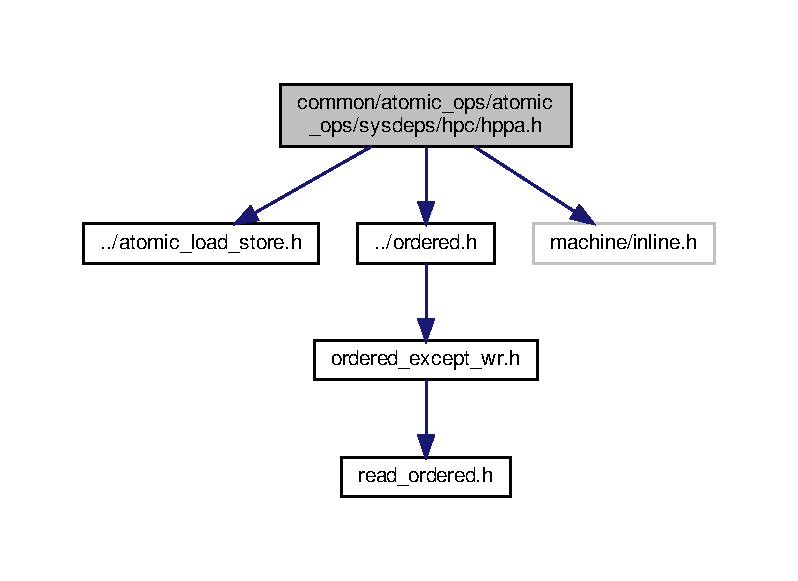
\includegraphics[width=350pt]{hpc_2hppa_8h__incl}
\end{center}
\end{figure}
\subsection*{Classes}
\begin{DoxyCompactItemize}
\item 
struct \hyperlink{structAO__pa__clearable__loc}{A\+O\+\_\+pa\+\_\+clearable\+\_\+loc}
\end{DoxyCompactItemize}
\subsection*{Macros}
\begin{DoxyCompactItemize}
\item 
\#define \hyperlink{hpc_2hppa_8h_a5890c21b549264c75c2cad08bf4f6ba9}{A\+O\+\_\+\+T\+S\+\_\+t}~struct \hyperlink{structAO__pa__clearable__loc}{A\+O\+\_\+pa\+\_\+clearable\+\_\+loc}
\item 
\#define \hyperlink{hpc_2hppa_8h_af0f8642b332396baef4793e7ce825759}{A\+O\+\_\+\+T\+S\+\_\+\+I\+N\+I\+T\+I\+A\+L\+I\+Z\+ER}~\{1,1,1,1\}
\item 
\#define \hyperlink{hpc_2hppa_8h_a7d99a16c4eab47ba80ab6138d7d98ac1}{A\+O\+\_\+\+T\+S\+\_\+\+V\+A\+L\+\_\+t}~\hyperlink{gcc_2hppa_8h_af6b785b31fbe39690aa613d7920f3299}{A\+O\+\_\+\+P\+A\+\_\+\+T\+S\+\_\+val}
\item 
\#define \hyperlink{hpc_2hppa_8h_a35258ee13bc817d0b8eb62f4695c4a3e}{A\+O\+\_\+\+T\+S\+\_\+\+C\+L\+E\+AR}~\hyperlink{hpc_2hppa_8h_af6b785b31fbe39690aa613d7920f3299a031b53af392a27ab58b0bd2cc09be141}{A\+O\+\_\+\+P\+A\+\_\+\+T\+S\+\_\+clear}
\item 
\#define \hyperlink{hpc_2hppa_8h_a8a50ac5fe9e6ff855a078c265079ac06}{A\+O\+\_\+\+T\+S\+\_\+\+S\+ET}~\hyperlink{hpc_2hppa_8h_af6b785b31fbe39690aa613d7920f3299aed76339c52af50af82a953e1ce542cd9}{A\+O\+\_\+\+P\+A\+\_\+\+T\+S\+\_\+set}
\item 
\#define \hyperlink{hpc_2hppa_8h_ac607c9a9d8357568f66bcafdbb18db3f}{\+\_\+\+\_\+ldcw}(a,  ret)~\+\_\+\+L\+D\+C\+WX(0 /$\ast$ index $\ast$/, 0 /$\ast$ s $\ast$/, a /$\ast$ base $\ast$/, ret);
\item 
\#define \hyperlink{hpc_2hppa_8h_a0002acfa7aea61f6b2dbcf63ab7d83aa}{\+\_\+\+\_\+\+P\+A\+\_\+\+L\+D\+C\+W\+\_\+\+A\+L\+I\+G\+N\+M\+E\+NT}~16
\item 
\#define \hyperlink{hpc_2hppa_8h_a947059942061143445c457feba8b9ae3}{\+\_\+\+\_\+ldcw\+\_\+align}(a,  ret)
\item 
\#define \hyperlink{hpc_2hppa_8h_ad5703c05836e7c55cde2a45922e721b4}{A\+O\+\_\+\+C\+L\+E\+AR}(addr)~\hyperlink{hpc_2hppa_8h_afe32bd0febd74f8b7ccafa2e24ab68b6}{A\+O\+\_\+pa\+\_\+clear}(addr)
\item 
\#define \hyperlink{hpc_2hppa_8h_ad5f311a090d1e6e1bb35a6e68ee35fad}{A\+O\+\_\+\+H\+A\+V\+E\+\_\+test\+\_\+and\+\_\+set\+\_\+full}
\end{DoxyCompactItemize}
\subsection*{Enumerations}
\begin{DoxyCompactItemize}
\item 
enum \hyperlink{hpc_2hppa_8h_af6b785b31fbe39690aa613d7920f3299}{A\+O\+\_\+\+P\+A\+\_\+\+T\+S\+\_\+val} \{ \hyperlink{gcc_2hppa_8h_af6b785b31fbe39690aa613d7920f3299aed76339c52af50af82a953e1ce542cd9}{A\+O\+\_\+\+P\+A\+\_\+\+T\+S\+\_\+set} = 0, 
\hyperlink{gcc_2hppa_8h_af6b785b31fbe39690aa613d7920f3299a031b53af392a27ab58b0bd2cc09be141}{A\+O\+\_\+\+P\+A\+\_\+\+T\+S\+\_\+clear} = 1, 
\hyperlink{hpc_2hppa_8h_af6b785b31fbe39690aa613d7920f3299aed76339c52af50af82a953e1ce542cd9}{A\+O\+\_\+\+P\+A\+\_\+\+T\+S\+\_\+set} = 0, 
\hyperlink{hpc_2hppa_8h_af6b785b31fbe39690aa613d7920f3299a031b53af392a27ab58b0bd2cc09be141}{A\+O\+\_\+\+P\+A\+\_\+\+T\+S\+\_\+clear} = 1
 \}
\end{DoxyCompactItemize}
\subsection*{Functions}
\begin{DoxyCompactItemize}
\item 
\hyperlink{atomic__ops_8h_a9f6ab6253b6b11bc8c12efe9dde5db2b}{A\+O\+\_\+\+I\+N\+L\+I\+NE} \hyperlink{test__and__set__t__is__char_8h_a7d99a16c4eab47ba80ab6138d7d98ac1}{A\+O\+\_\+\+T\+S\+\_\+\+V\+A\+L\+\_\+t} \hyperlink{hpc_2hppa_8h_a9f485bd63ce5c6a017ec241906e2f651}{A\+O\+\_\+test\+\_\+and\+\_\+set\+\_\+full} (volatile \hyperlink{test__and__set__t__is__char_8h_a5890c21b549264c75c2cad08bf4f6ba9}{A\+O\+\_\+\+T\+S\+\_\+t} $\ast$addr)
\item 
\hyperlink{atomic__ops_8h_a9f6ab6253b6b11bc8c12efe9dde5db2b}{A\+O\+\_\+\+I\+N\+L\+I\+NE} void \hyperlink{hpc_2hppa_8h_afe32bd0febd74f8b7ccafa2e24ab68b6}{A\+O\+\_\+pa\+\_\+clear} (volatile \hyperlink{test__and__set__t__is__char_8h_a5890c21b549264c75c2cad08bf4f6ba9}{A\+O\+\_\+\+T\+S\+\_\+t} $\ast$addr)
\end{DoxyCompactItemize}


\subsection{Macro Definition Documentation}
\mbox{\Hypertarget{hpc_2hppa_8h_ac607c9a9d8357568f66bcafdbb18db3f}\label{hpc_2hppa_8h_ac607c9a9d8357568f66bcafdbb18db3f}} 
\index{hpc/hppa.\+h@{hpc/hppa.\+h}!\+\_\+\+\_\+ldcw@{\+\_\+\+\_\+ldcw}}
\index{\+\_\+\+\_\+ldcw@{\+\_\+\+\_\+ldcw}!hpc/hppa.\+h@{hpc/hppa.\+h}}
\subsubsection{\texorpdfstring{\+\_\+\+\_\+ldcw}{\_\_ldcw}}
{\footnotesize\ttfamily \#define \+\_\+\+\_\+ldcw(\begin{DoxyParamCaption}\item[{}]{a,  }\item[{}]{ret }\end{DoxyParamCaption})~\+\_\+\+L\+D\+C\+WX(0 /$\ast$ index $\ast$/, 0 /$\ast$ s $\ast$/, a /$\ast$ base $\ast$/, ret);}

\mbox{\Hypertarget{hpc_2hppa_8h_a947059942061143445c457feba8b9ae3}\label{hpc_2hppa_8h_a947059942061143445c457feba8b9ae3}} 
\index{hpc/hppa.\+h@{hpc/hppa.\+h}!\+\_\+\+\_\+ldcw\+\_\+align@{\+\_\+\+\_\+ldcw\+\_\+align}}
\index{\+\_\+\+\_\+ldcw\+\_\+align@{\+\_\+\+\_\+ldcw\+\_\+align}!hpc/hppa.\+h@{hpc/hppa.\+h}}
\subsubsection{\texorpdfstring{\+\_\+\+\_\+ldcw\+\_\+align}{\_\_ldcw\_align}}
{\footnotesize\ttfamily \#define \+\_\+\+\_\+ldcw\+\_\+align(\begin{DoxyParamCaption}\item[{}]{a,  }\item[{}]{ret }\end{DoxyParamCaption})}

{\bfseries Value\+:}
\begin{DoxyCode}
\{ \(\backslash\)
  ret = (\textcolor{keywordtype}{unsigned} long) a;                      \(\backslash\)
  ret += \hyperlink{hpc_2hppa_8h_a0002acfa7aea61f6b2dbcf63ab7d83aa}{\_\_PA\_LDCW\_ALIGNMENT} - 1;                                       \(\backslash\)
  ret &= ~(\hyperlink{hpc_2hppa_8h_a0002acfa7aea61f6b2dbcf63ab7d83aa}{\_\_PA\_LDCW\_ALIGNMENT} - 1);                                    \(\backslash\)
\}
\end{DoxyCode}
\mbox{\Hypertarget{hpc_2hppa_8h_a0002acfa7aea61f6b2dbcf63ab7d83aa}\label{hpc_2hppa_8h_a0002acfa7aea61f6b2dbcf63ab7d83aa}} 
\index{hpc/hppa.\+h@{hpc/hppa.\+h}!\+\_\+\+\_\+\+P\+A\+\_\+\+L\+D\+C\+W\+\_\+\+A\+L\+I\+G\+N\+M\+E\+NT@{\+\_\+\+\_\+\+P\+A\+\_\+\+L\+D\+C\+W\+\_\+\+A\+L\+I\+G\+N\+M\+E\+NT}}
\index{\+\_\+\+\_\+\+P\+A\+\_\+\+L\+D\+C\+W\+\_\+\+A\+L\+I\+G\+N\+M\+E\+NT@{\+\_\+\+\_\+\+P\+A\+\_\+\+L\+D\+C\+W\+\_\+\+A\+L\+I\+G\+N\+M\+E\+NT}!hpc/hppa.\+h@{hpc/hppa.\+h}}
\subsubsection{\texorpdfstring{\+\_\+\+\_\+\+P\+A\+\_\+\+L\+D\+C\+W\+\_\+\+A\+L\+I\+G\+N\+M\+E\+NT}{\_\_PA\_LDCW\_ALIGNMENT}}
{\footnotesize\ttfamily \#define \+\_\+\+\_\+\+P\+A\+\_\+\+L\+D\+C\+W\+\_\+\+A\+L\+I\+G\+N\+M\+E\+NT~16}

\mbox{\Hypertarget{hpc_2hppa_8h_ad5703c05836e7c55cde2a45922e721b4}\label{hpc_2hppa_8h_ad5703c05836e7c55cde2a45922e721b4}} 
\index{hpc/hppa.\+h@{hpc/hppa.\+h}!A\+O\+\_\+\+C\+L\+E\+AR@{A\+O\+\_\+\+C\+L\+E\+AR}}
\index{A\+O\+\_\+\+C\+L\+E\+AR@{A\+O\+\_\+\+C\+L\+E\+AR}!hpc/hppa.\+h@{hpc/hppa.\+h}}
\subsubsection{\texorpdfstring{A\+O\+\_\+\+C\+L\+E\+AR}{AO\_CLEAR}}
{\footnotesize\ttfamily \#define A\+O\+\_\+\+C\+L\+E\+AR(\begin{DoxyParamCaption}\item[{}]{addr }\end{DoxyParamCaption})~\hyperlink{hpc_2hppa_8h_afe32bd0febd74f8b7ccafa2e24ab68b6}{A\+O\+\_\+pa\+\_\+clear}(addr)}

\mbox{\Hypertarget{hpc_2hppa_8h_ad5f311a090d1e6e1bb35a6e68ee35fad}\label{hpc_2hppa_8h_ad5f311a090d1e6e1bb35a6e68ee35fad}} 
\index{hpc/hppa.\+h@{hpc/hppa.\+h}!A\+O\+\_\+\+H\+A\+V\+E\+\_\+test\+\_\+and\+\_\+set\+\_\+full@{A\+O\+\_\+\+H\+A\+V\+E\+\_\+test\+\_\+and\+\_\+set\+\_\+full}}
\index{A\+O\+\_\+\+H\+A\+V\+E\+\_\+test\+\_\+and\+\_\+set\+\_\+full@{A\+O\+\_\+\+H\+A\+V\+E\+\_\+test\+\_\+and\+\_\+set\+\_\+full}!hpc/hppa.\+h@{hpc/hppa.\+h}}
\subsubsection{\texorpdfstring{A\+O\+\_\+\+H\+A\+V\+E\+\_\+test\+\_\+and\+\_\+set\+\_\+full}{AO\_HAVE\_test\_and\_set\_full}}
{\footnotesize\ttfamily \#define A\+O\+\_\+\+H\+A\+V\+E\+\_\+test\+\_\+and\+\_\+set\+\_\+full}

\mbox{\Hypertarget{hpc_2hppa_8h_a35258ee13bc817d0b8eb62f4695c4a3e}\label{hpc_2hppa_8h_a35258ee13bc817d0b8eb62f4695c4a3e}} 
\index{hpc/hppa.\+h@{hpc/hppa.\+h}!A\+O\+\_\+\+T\+S\+\_\+\+C\+L\+E\+AR@{A\+O\+\_\+\+T\+S\+\_\+\+C\+L\+E\+AR}}
\index{A\+O\+\_\+\+T\+S\+\_\+\+C\+L\+E\+AR@{A\+O\+\_\+\+T\+S\+\_\+\+C\+L\+E\+AR}!hpc/hppa.\+h@{hpc/hppa.\+h}}
\subsubsection{\texorpdfstring{A\+O\+\_\+\+T\+S\+\_\+\+C\+L\+E\+AR}{AO\_TS\_CLEAR}}
{\footnotesize\ttfamily \#define A\+O\+\_\+\+T\+S\+\_\+\+C\+L\+E\+AR~\hyperlink{hpc_2hppa_8h_af6b785b31fbe39690aa613d7920f3299a031b53af392a27ab58b0bd2cc09be141}{A\+O\+\_\+\+P\+A\+\_\+\+T\+S\+\_\+clear}}

\mbox{\Hypertarget{hpc_2hppa_8h_af0f8642b332396baef4793e7ce825759}\label{hpc_2hppa_8h_af0f8642b332396baef4793e7ce825759}} 
\index{hpc/hppa.\+h@{hpc/hppa.\+h}!A\+O\+\_\+\+T\+S\+\_\+\+I\+N\+I\+T\+I\+A\+L\+I\+Z\+ER@{A\+O\+\_\+\+T\+S\+\_\+\+I\+N\+I\+T\+I\+A\+L\+I\+Z\+ER}}
\index{A\+O\+\_\+\+T\+S\+\_\+\+I\+N\+I\+T\+I\+A\+L\+I\+Z\+ER@{A\+O\+\_\+\+T\+S\+\_\+\+I\+N\+I\+T\+I\+A\+L\+I\+Z\+ER}!hpc/hppa.\+h@{hpc/hppa.\+h}}
\subsubsection{\texorpdfstring{A\+O\+\_\+\+T\+S\+\_\+\+I\+N\+I\+T\+I\+A\+L\+I\+Z\+ER}{AO\_TS\_INITIALIZER}}
{\footnotesize\ttfamily \#define A\+O\+\_\+\+T\+S\+\_\+\+I\+N\+I\+T\+I\+A\+L\+I\+Z\+ER~\{1,1,1,1\}}

\mbox{\Hypertarget{hpc_2hppa_8h_a8a50ac5fe9e6ff855a078c265079ac06}\label{hpc_2hppa_8h_a8a50ac5fe9e6ff855a078c265079ac06}} 
\index{hpc/hppa.\+h@{hpc/hppa.\+h}!A\+O\+\_\+\+T\+S\+\_\+\+S\+ET@{A\+O\+\_\+\+T\+S\+\_\+\+S\+ET}}
\index{A\+O\+\_\+\+T\+S\+\_\+\+S\+ET@{A\+O\+\_\+\+T\+S\+\_\+\+S\+ET}!hpc/hppa.\+h@{hpc/hppa.\+h}}
\subsubsection{\texorpdfstring{A\+O\+\_\+\+T\+S\+\_\+\+S\+ET}{AO\_TS\_SET}}
{\footnotesize\ttfamily \#define A\+O\+\_\+\+T\+S\+\_\+\+S\+ET~\hyperlink{hpc_2hppa_8h_af6b785b31fbe39690aa613d7920f3299aed76339c52af50af82a953e1ce542cd9}{A\+O\+\_\+\+P\+A\+\_\+\+T\+S\+\_\+set}}

\mbox{\Hypertarget{hpc_2hppa_8h_a5890c21b549264c75c2cad08bf4f6ba9}\label{hpc_2hppa_8h_a5890c21b549264c75c2cad08bf4f6ba9}} 
\index{hpc/hppa.\+h@{hpc/hppa.\+h}!A\+O\+\_\+\+T\+S\+\_\+t@{A\+O\+\_\+\+T\+S\+\_\+t}}
\index{A\+O\+\_\+\+T\+S\+\_\+t@{A\+O\+\_\+\+T\+S\+\_\+t}!hpc/hppa.\+h@{hpc/hppa.\+h}}
\subsubsection{\texorpdfstring{A\+O\+\_\+\+T\+S\+\_\+t}{AO\_TS\_t}}
{\footnotesize\ttfamily \#define A\+O\+\_\+\+T\+S\+\_\+t~struct \hyperlink{structAO__pa__clearable__loc}{A\+O\+\_\+pa\+\_\+clearable\+\_\+loc}}

\mbox{\Hypertarget{hpc_2hppa_8h_a7d99a16c4eab47ba80ab6138d7d98ac1}\label{hpc_2hppa_8h_a7d99a16c4eab47ba80ab6138d7d98ac1}} 
\index{hpc/hppa.\+h@{hpc/hppa.\+h}!A\+O\+\_\+\+T\+S\+\_\+\+V\+A\+L\+\_\+t@{A\+O\+\_\+\+T\+S\+\_\+\+V\+A\+L\+\_\+t}}
\index{A\+O\+\_\+\+T\+S\+\_\+\+V\+A\+L\+\_\+t@{A\+O\+\_\+\+T\+S\+\_\+\+V\+A\+L\+\_\+t}!hpc/hppa.\+h@{hpc/hppa.\+h}}
\subsubsection{\texorpdfstring{A\+O\+\_\+\+T\+S\+\_\+\+V\+A\+L\+\_\+t}{AO\_TS\_VAL\_t}}
{\footnotesize\ttfamily \#define A\+O\+\_\+\+T\+S\+\_\+\+V\+A\+L\+\_\+t~\hyperlink{gcc_2hppa_8h_af6b785b31fbe39690aa613d7920f3299}{A\+O\+\_\+\+P\+A\+\_\+\+T\+S\+\_\+val}}



\subsection{Enumeration Type Documentation}
\mbox{\Hypertarget{hpc_2hppa_8h_af6b785b31fbe39690aa613d7920f3299}\label{hpc_2hppa_8h_af6b785b31fbe39690aa613d7920f3299}} 
\index{hpc/hppa.\+h@{hpc/hppa.\+h}!A\+O\+\_\+\+P\+A\+\_\+\+T\+S\+\_\+val@{A\+O\+\_\+\+P\+A\+\_\+\+T\+S\+\_\+val}}
\index{A\+O\+\_\+\+P\+A\+\_\+\+T\+S\+\_\+val@{A\+O\+\_\+\+P\+A\+\_\+\+T\+S\+\_\+val}!hpc/hppa.\+h@{hpc/hppa.\+h}}
\subsubsection{\texorpdfstring{A\+O\+\_\+\+P\+A\+\_\+\+T\+S\+\_\+val}{AO\_PA\_TS\_val}}
{\footnotesize\ttfamily enum \hyperlink{gcc_2hppa_8h_af6b785b31fbe39690aa613d7920f3299}{A\+O\+\_\+\+P\+A\+\_\+\+T\+S\+\_\+val}}

\begin{DoxyEnumFields}{Enumerator}
\raisebox{\heightof{T}}[0pt][0pt]{\index{A\+O\+\_\+\+P\+A\+\_\+\+T\+S\+\_\+set@{A\+O\+\_\+\+P\+A\+\_\+\+T\+S\+\_\+set}!hpc/hppa.\+h@{hpc/hppa.\+h}}\index{hpc/hppa.\+h@{hpc/hppa.\+h}!A\+O\+\_\+\+P\+A\+\_\+\+T\+S\+\_\+set@{A\+O\+\_\+\+P\+A\+\_\+\+T\+S\+\_\+set}}}\mbox{\Hypertarget{hpc_2hppa_8h_af6b785b31fbe39690aa613d7920f3299aed76339c52af50af82a953e1ce542cd9}\label{hpc_2hppa_8h_af6b785b31fbe39690aa613d7920f3299aed76339c52af50af82a953e1ce542cd9}} 
A\+O\+\_\+\+P\+A\+\_\+\+T\+S\+\_\+set&\\
\hline

\raisebox{\heightof{T}}[0pt][0pt]{\index{A\+O\+\_\+\+P\+A\+\_\+\+T\+S\+\_\+clear@{A\+O\+\_\+\+P\+A\+\_\+\+T\+S\+\_\+clear}!hpc/hppa.\+h@{hpc/hppa.\+h}}\index{hpc/hppa.\+h@{hpc/hppa.\+h}!A\+O\+\_\+\+P\+A\+\_\+\+T\+S\+\_\+clear@{A\+O\+\_\+\+P\+A\+\_\+\+T\+S\+\_\+clear}}}\mbox{\Hypertarget{hpc_2hppa_8h_af6b785b31fbe39690aa613d7920f3299a031b53af392a27ab58b0bd2cc09be141}\label{hpc_2hppa_8h_af6b785b31fbe39690aa613d7920f3299a031b53af392a27ab58b0bd2cc09be141}} 
A\+O\+\_\+\+P\+A\+\_\+\+T\+S\+\_\+clear&\\
\hline

\raisebox{\heightof{T}}[0pt][0pt]{\index{A\+O\+\_\+\+P\+A\+\_\+\+T\+S\+\_\+set@{A\+O\+\_\+\+P\+A\+\_\+\+T\+S\+\_\+set}!hpc/hppa.\+h@{hpc/hppa.\+h}}\index{hpc/hppa.\+h@{hpc/hppa.\+h}!A\+O\+\_\+\+P\+A\+\_\+\+T\+S\+\_\+set@{A\+O\+\_\+\+P\+A\+\_\+\+T\+S\+\_\+set}}}\mbox{\Hypertarget{hpc_2hppa_8h_af6b785b31fbe39690aa613d7920f3299aed76339c52af50af82a953e1ce542cd9}\label{hpc_2hppa_8h_af6b785b31fbe39690aa613d7920f3299aed76339c52af50af82a953e1ce542cd9}} 
A\+O\+\_\+\+P\+A\+\_\+\+T\+S\+\_\+set&\\
\hline

\raisebox{\heightof{T}}[0pt][0pt]{\index{A\+O\+\_\+\+P\+A\+\_\+\+T\+S\+\_\+clear@{A\+O\+\_\+\+P\+A\+\_\+\+T\+S\+\_\+clear}!hpc/hppa.\+h@{hpc/hppa.\+h}}\index{hpc/hppa.\+h@{hpc/hppa.\+h}!A\+O\+\_\+\+P\+A\+\_\+\+T\+S\+\_\+clear@{A\+O\+\_\+\+P\+A\+\_\+\+T\+S\+\_\+clear}}}\mbox{\Hypertarget{hpc_2hppa_8h_af6b785b31fbe39690aa613d7920f3299a031b53af392a27ab58b0bd2cc09be141}\label{hpc_2hppa_8h_af6b785b31fbe39690aa613d7920f3299a031b53af392a27ab58b0bd2cc09be141}} 
A\+O\+\_\+\+P\+A\+\_\+\+T\+S\+\_\+clear&\\
\hline

\end{DoxyEnumFields}


\subsection{Function Documentation}
\mbox{\Hypertarget{hpc_2hppa_8h_afe32bd0febd74f8b7ccafa2e24ab68b6}\label{hpc_2hppa_8h_afe32bd0febd74f8b7ccafa2e24ab68b6}} 
\index{hpc/hppa.\+h@{hpc/hppa.\+h}!A\+O\+\_\+pa\+\_\+clear@{A\+O\+\_\+pa\+\_\+clear}}
\index{A\+O\+\_\+pa\+\_\+clear@{A\+O\+\_\+pa\+\_\+clear}!hpc/hppa.\+h@{hpc/hppa.\+h}}
\subsubsection{\texorpdfstring{A\+O\+\_\+pa\+\_\+clear()}{AO\_pa\_clear()}}
{\footnotesize\ttfamily \hyperlink{atomic__ops_8h_a9f6ab6253b6b11bc8c12efe9dde5db2b}{A\+O\+\_\+\+I\+N\+L\+I\+NE} void A\+O\+\_\+pa\+\_\+clear (\begin{DoxyParamCaption}\item[{volatile \hyperlink{test__and__set__t__is__char_8h_a5890c21b549264c75c2cad08bf4f6ba9}{A\+O\+\_\+\+T\+S\+\_\+t} $\ast$}]{addr }\end{DoxyParamCaption})}

\mbox{\Hypertarget{hpc_2hppa_8h_a9f485bd63ce5c6a017ec241906e2f651}\label{hpc_2hppa_8h_a9f485bd63ce5c6a017ec241906e2f651}} 
\index{hpc/hppa.\+h@{hpc/hppa.\+h}!A\+O\+\_\+test\+\_\+and\+\_\+set\+\_\+full@{A\+O\+\_\+test\+\_\+and\+\_\+set\+\_\+full}}
\index{A\+O\+\_\+test\+\_\+and\+\_\+set\+\_\+full@{A\+O\+\_\+test\+\_\+and\+\_\+set\+\_\+full}!hpc/hppa.\+h@{hpc/hppa.\+h}}
\subsubsection{\texorpdfstring{A\+O\+\_\+test\+\_\+and\+\_\+set\+\_\+full()}{AO\_test\_and\_set\_full()}}
{\footnotesize\ttfamily \hyperlink{atomic__ops_8h_a9f6ab6253b6b11bc8c12efe9dde5db2b}{A\+O\+\_\+\+I\+N\+L\+I\+NE} \hyperlink{test__and__set__t__is__char_8h_a7d99a16c4eab47ba80ab6138d7d98ac1}{A\+O\+\_\+\+T\+S\+\_\+\+V\+A\+L\+\_\+t} A\+O\+\_\+test\+\_\+and\+\_\+set\+\_\+full (\begin{DoxyParamCaption}\item[{volatile \hyperlink{test__and__set__t__is__char_8h_a5890c21b549264c75c2cad08bf4f6ba9}{A\+O\+\_\+\+T\+S\+\_\+t} $\ast$}]{addr }\end{DoxyParamCaption})}


\hypertarget{gcc_2ia64_8h}{}\section{common/atomic\+\_\+ops/atomic\+\_\+ops/sysdeps/gcc/ia64.h File Reference}
\label{gcc_2ia64_8h}\index{common/atomic\+\_\+ops/atomic\+\_\+ops/sysdeps/gcc/ia64.\+h@{common/atomic\+\_\+ops/atomic\+\_\+ops/sysdeps/gcc/ia64.\+h}}
{\ttfamily \#include \char`\"{}../all\+\_\+atomic\+\_\+load\+\_\+store.\+h\char`\"{}}\newline
{\ttfamily \#include \char`\"{}../all\+\_\+acquire\+\_\+release\+\_\+volatile.\+h\char`\"{}}\newline
{\ttfamily \#include \char`\"{}../test\+\_\+and\+\_\+set\+\_\+t\+\_\+is\+\_\+char.\+h\char`\"{}}\newline
Include dependency graph for ia64.\+h\+:
\nopagebreak
\begin{figure}[H]
\begin{center}
\leavevmode
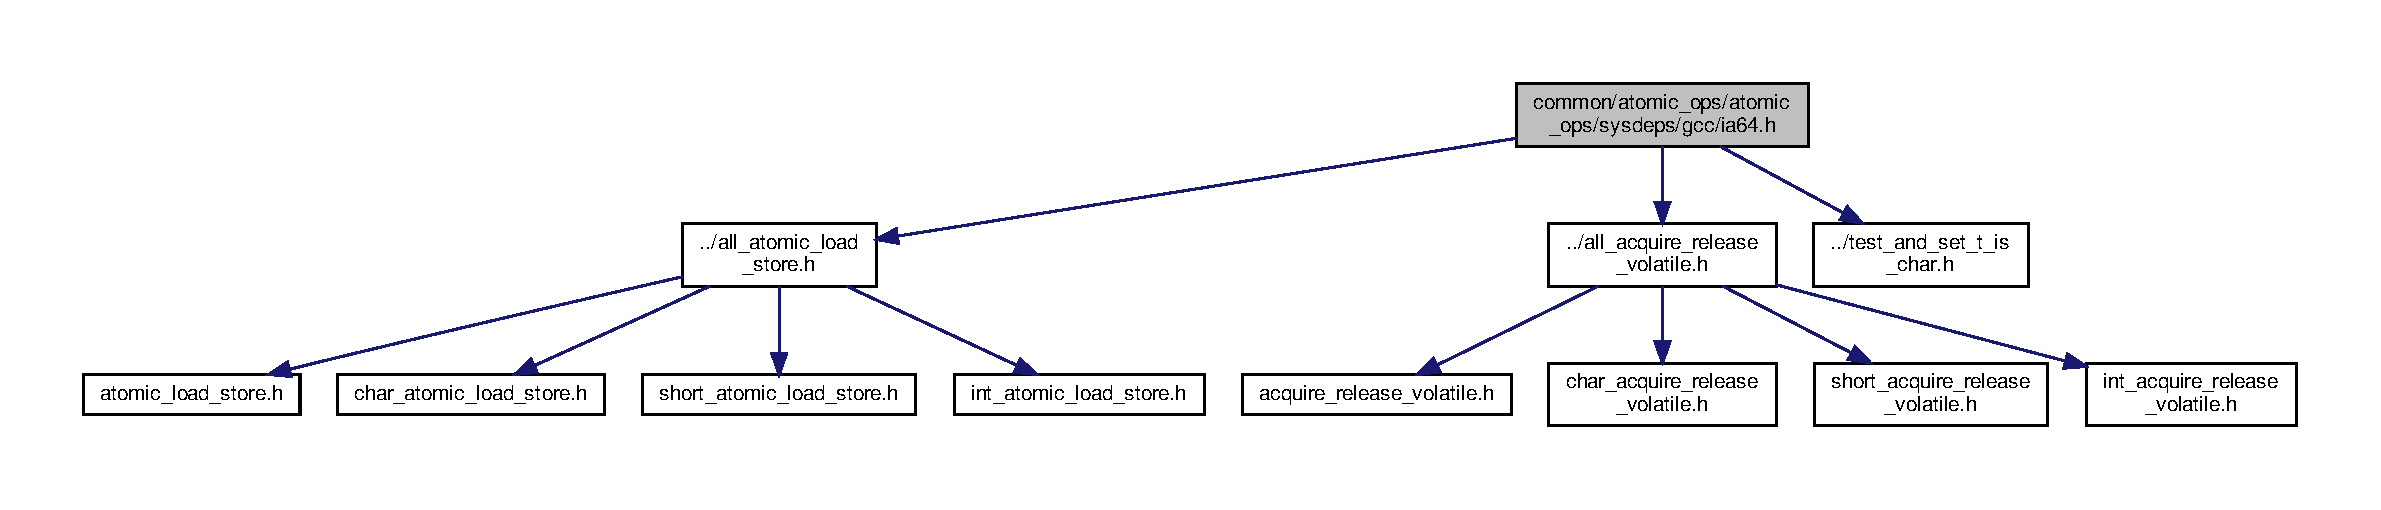
\includegraphics[width=350pt]{gcc_2ia64_8h__incl}
\end{center}
\end{figure}
\subsection*{Macros}
\begin{DoxyCompactItemize}
\item 
\#define \hyperlink{gcc_2ia64_8h_a73e1aecac340ce6af6f3ea7820dde952}{A\+O\+\_\+\+L\+EN}~\char`\"{}8\char`\"{}
\item 
\#define \hyperlink{gcc_2ia64_8h_aaef3ee5440410719bd7c4fb795f445ce}{A\+O\+\_\+\+I\+N\+\_\+\+A\+D\+DR}~\char`\"{}r\char`\"{}(addr)
\item 
\#define \hyperlink{gcc_2ia64_8h_a47b1bf13da4e3b3641ddd823a40c7063}{A\+O\+\_\+\+O\+U\+T\+\_\+\+A\+D\+DR}
\item 
\#define \hyperlink{gcc_2ia64_8h_a202fe8f0125e0c7bf744de3a6c1b323c}{A\+O\+\_\+\+S\+W\+I\+Z\+Z\+LE}
\item 
\#define \hyperlink{gcc_2ia64_8h_a8c5f843fa7f7eab7b0bf6de1d91c01e1}{A\+O\+\_\+\+M\+A\+SK}(ptr)
\item 
\#define \hyperlink{gcc_2ia64_8h_a3904dc699d6a6d6e771a93aa66aeb805}{A\+O\+\_\+\+H\+A\+V\+E\+\_\+nop\+\_\+full}
\item 
\#define \hyperlink{gcc_2ia64_8h_ab444fdcbfaf48cb88292b89180cd6d2b}{A\+O\+\_\+\+H\+A\+V\+E\+\_\+fetch\+\_\+and\+\_\+add1\+\_\+acquire}
\item 
\#define \hyperlink{gcc_2ia64_8h_abe5616e4ca4293fbddf3ab80049febae}{A\+O\+\_\+\+H\+A\+V\+E\+\_\+fetch\+\_\+and\+\_\+add1\+\_\+release}
\item 
\#define \hyperlink{gcc_2ia64_8h_a48eb192a6005c2c102a3154a2320850c}{A\+O\+\_\+\+H\+A\+V\+E\+\_\+fetch\+\_\+and\+\_\+sub1\+\_\+acquire}
\item 
\#define \hyperlink{gcc_2ia64_8h_a059afe6ddfb01b0cc90e3e86e201de71}{A\+O\+\_\+\+H\+A\+V\+E\+\_\+fetch\+\_\+and\+\_\+sub1\+\_\+release}
\item 
\#define \hyperlink{gcc_2ia64_8h_a762b3fab8a1f0bc849240481133249ea}{A\+O\+\_\+\+H\+A\+V\+E\+\_\+int\+\_\+fetch\+\_\+and\+\_\+add1\+\_\+acquire}
\item 
\#define \hyperlink{gcc_2ia64_8h_a8786a944e940794d55a8c08b488927c8}{A\+O\+\_\+\+H\+A\+V\+E\+\_\+int\+\_\+fetch\+\_\+and\+\_\+add1\+\_\+release}
\item 
\#define \hyperlink{gcc_2ia64_8h_aa70a11c2bc9eab2413fb1b3674edf95e}{A\+O\+\_\+\+H\+A\+V\+E\+\_\+int\+\_\+fetch\+\_\+and\+\_\+sub1\+\_\+acquire}
\item 
\#define \hyperlink{gcc_2ia64_8h_a5482bd8c7923eb515fd39a5bfbd93948}{A\+O\+\_\+\+H\+A\+V\+E\+\_\+int\+\_\+fetch\+\_\+and\+\_\+sub1\+\_\+release}
\item 
\#define \hyperlink{gcc_2ia64_8h_ad0b08bc254deecdcba5a4f3366432cf3}{A\+O\+\_\+\+H\+A\+V\+E\+\_\+compare\+\_\+and\+\_\+swap\+\_\+acquire}
\item 
\#define \hyperlink{gcc_2ia64_8h_ad85c7af2ae0a778eba77a7762a358819}{A\+O\+\_\+\+H\+A\+V\+E\+\_\+compare\+\_\+and\+\_\+swap\+\_\+release}
\item 
\#define \hyperlink{gcc_2ia64_8h_ab67b15bb08ff2fbfc858acdaaf0b3531}{A\+O\+\_\+\+H\+A\+V\+E\+\_\+char\+\_\+compare\+\_\+and\+\_\+swap\+\_\+acquire}
\item 
\#define \hyperlink{gcc_2ia64_8h_aa59d946c04e8c5b744322414b106947b}{A\+O\+\_\+\+H\+A\+V\+E\+\_\+char\+\_\+compare\+\_\+and\+\_\+swap\+\_\+release}
\item 
\#define \hyperlink{gcc_2ia64_8h_a9104195dbb035d047e6968e1202d3d63}{A\+O\+\_\+\+H\+A\+V\+E\+\_\+short\+\_\+compare\+\_\+and\+\_\+swap\+\_\+acquire}
\item 
\#define \hyperlink{gcc_2ia64_8h_abca62133116ab240da7a8539018016e1}{A\+O\+\_\+\+H\+A\+V\+E\+\_\+short\+\_\+compare\+\_\+and\+\_\+swap\+\_\+release}
\item 
\#define \hyperlink{gcc_2ia64_8h_aac3dfbb7cf61ee9b8a418e1dbd136e2f}{A\+O\+\_\+\+H\+A\+V\+E\+\_\+int\+\_\+compare\+\_\+and\+\_\+swap\+\_\+acquire}
\item 
\#define \hyperlink{gcc_2ia64_8h_a0f91f532e6403ccb6b410f697903d33b}{A\+O\+\_\+\+H\+A\+V\+E\+\_\+int\+\_\+compare\+\_\+and\+\_\+swap\+\_\+release}
\end{DoxyCompactItemize}
\subsection*{Functions}
\begin{DoxyCompactItemize}
\item 
\hyperlink{atomic__ops_8h_a9f6ab6253b6b11bc8c12efe9dde5db2b}{A\+O\+\_\+\+I\+N\+L\+I\+NE} void \hyperlink{gcc_2ia64_8h_afe3a6778eacc82252ba138fc9a157b04}{A\+O\+\_\+nop\+\_\+full} (void)
\item 
\hyperlink{atomic__ops_8h_a9f6ab6253b6b11bc8c12efe9dde5db2b}{A\+O\+\_\+\+I\+N\+L\+I\+NE} \hyperlink{atomic__ops_8h_a5225fef4d9eee821e82382cd269160dd}{A\+O\+\_\+t} \hyperlink{gcc_2ia64_8h_a9aa4c33f310759ab50a7a49b616af9e2}{A\+O\+\_\+fetch\+\_\+and\+\_\+add1\+\_\+acquire} (volatile \hyperlink{atomic__ops_8h_a5225fef4d9eee821e82382cd269160dd}{A\+O\+\_\+t} $\ast$addr)
\item 
\hyperlink{atomic__ops_8h_a9f6ab6253b6b11bc8c12efe9dde5db2b}{A\+O\+\_\+\+I\+N\+L\+I\+NE} \hyperlink{atomic__ops_8h_a5225fef4d9eee821e82382cd269160dd}{A\+O\+\_\+t} \hyperlink{gcc_2ia64_8h_a491398ddfb8f9ca1b845706cff26a30f}{A\+O\+\_\+fetch\+\_\+and\+\_\+add1\+\_\+release} (volatile \hyperlink{atomic__ops_8h_a5225fef4d9eee821e82382cd269160dd}{A\+O\+\_\+t} $\ast$addr)
\item 
\hyperlink{atomic__ops_8h_a9f6ab6253b6b11bc8c12efe9dde5db2b}{A\+O\+\_\+\+I\+N\+L\+I\+NE} \hyperlink{atomic__ops_8h_a5225fef4d9eee821e82382cd269160dd}{A\+O\+\_\+t} \hyperlink{gcc_2ia64_8h_a89e0eb95ea0a4c8aedad1a72d23a7b3d}{A\+O\+\_\+fetch\+\_\+and\+\_\+sub1\+\_\+acquire} (volatile \hyperlink{atomic__ops_8h_a5225fef4d9eee821e82382cd269160dd}{A\+O\+\_\+t} $\ast$addr)
\item 
\hyperlink{atomic__ops_8h_a9f6ab6253b6b11bc8c12efe9dde5db2b}{A\+O\+\_\+\+I\+N\+L\+I\+NE} \hyperlink{atomic__ops_8h_a5225fef4d9eee821e82382cd269160dd}{A\+O\+\_\+t} \hyperlink{gcc_2ia64_8h_ad26d6974fa29afa2b39e48f98fc61459}{A\+O\+\_\+fetch\+\_\+and\+\_\+sub1\+\_\+release} (volatile \hyperlink{atomic__ops_8h_a5225fef4d9eee821e82382cd269160dd}{A\+O\+\_\+t} $\ast$addr)
\item 
\hyperlink{atomic__ops_8h_a9f6ab6253b6b11bc8c12efe9dde5db2b}{A\+O\+\_\+\+I\+N\+L\+I\+NE} unsigned int \hyperlink{gcc_2ia64_8h_a60f67788c3afb84acff5321c8233e7fd}{A\+O\+\_\+int\+\_\+fetch\+\_\+and\+\_\+add1\+\_\+acquire} (volatile unsigned int $\ast$addr)
\item 
\hyperlink{atomic__ops_8h_a9f6ab6253b6b11bc8c12efe9dde5db2b}{A\+O\+\_\+\+I\+N\+L\+I\+NE} unsigned int \hyperlink{gcc_2ia64_8h_a7bd2e861646243a98b7a44b1db3cd3fb}{A\+O\+\_\+int\+\_\+fetch\+\_\+and\+\_\+add1\+\_\+release} (volatile unsigned int $\ast$addr)
\item 
\hyperlink{atomic__ops_8h_a9f6ab6253b6b11bc8c12efe9dde5db2b}{A\+O\+\_\+\+I\+N\+L\+I\+NE} unsigned int \hyperlink{gcc_2ia64_8h_a7f1bfd92920e657790bdb10d58f0bd41}{A\+O\+\_\+int\+\_\+fetch\+\_\+and\+\_\+sub1\+\_\+acquire} (volatile unsigned int $\ast$addr)
\item 
\hyperlink{atomic__ops_8h_a9f6ab6253b6b11bc8c12efe9dde5db2b}{A\+O\+\_\+\+I\+N\+L\+I\+NE} unsigned int \hyperlink{gcc_2ia64_8h_a581b93da5df3a893a35c6dddfa123bb5}{A\+O\+\_\+int\+\_\+fetch\+\_\+and\+\_\+sub1\+\_\+release} (volatile unsigned int $\ast$addr)
\item 
\hyperlink{atomic__ops_8h_a9f6ab6253b6b11bc8c12efe9dde5db2b}{A\+O\+\_\+\+I\+N\+L\+I\+NE} int \hyperlink{gcc_2ia64_8h_a81fc146600046fb8ee9ce4339f078e2e}{A\+O\+\_\+compare\+\_\+and\+\_\+swap\+\_\+acquire} (volatile \hyperlink{atomic__ops_8h_a5225fef4d9eee821e82382cd269160dd}{A\+O\+\_\+t} $\ast$addr, \hyperlink{atomic__ops_8h_a5225fef4d9eee821e82382cd269160dd}{A\+O\+\_\+t} old, \hyperlink{atomic__ops_8h_a5225fef4d9eee821e82382cd269160dd}{A\+O\+\_\+t} new\+\_\+val)
\item 
\hyperlink{atomic__ops_8h_a9f6ab6253b6b11bc8c12efe9dde5db2b}{A\+O\+\_\+\+I\+N\+L\+I\+NE} int \hyperlink{gcc_2ia64_8h_ae39d774429bea0d5c3b604bbb820a4ea}{A\+O\+\_\+compare\+\_\+and\+\_\+swap\+\_\+release} (volatile \hyperlink{atomic__ops_8h_a5225fef4d9eee821e82382cd269160dd}{A\+O\+\_\+t} $\ast$addr, \hyperlink{atomic__ops_8h_a5225fef4d9eee821e82382cd269160dd}{A\+O\+\_\+t} old, \hyperlink{atomic__ops_8h_a5225fef4d9eee821e82382cd269160dd}{A\+O\+\_\+t} new\+\_\+val)
\item 
\hyperlink{atomic__ops_8h_a9f6ab6253b6b11bc8c12efe9dde5db2b}{A\+O\+\_\+\+I\+N\+L\+I\+NE} int \hyperlink{gcc_2ia64_8h_adfddc3e21d1b14f528dd1259f501f8c6}{A\+O\+\_\+char\+\_\+compare\+\_\+and\+\_\+swap\+\_\+acquire} (volatile unsigned char $\ast$addr, unsigned char old, unsigned char new\+\_\+val)
\item 
\hyperlink{atomic__ops_8h_a9f6ab6253b6b11bc8c12efe9dde5db2b}{A\+O\+\_\+\+I\+N\+L\+I\+NE} int \hyperlink{gcc_2ia64_8h_abfcca8311ee6e37e2b81abaa4aae2905}{A\+O\+\_\+char\+\_\+compare\+\_\+and\+\_\+swap\+\_\+release} (volatile unsigned char $\ast$addr, unsigned char old, unsigned char new\+\_\+val)
\item 
\hyperlink{atomic__ops_8h_a9f6ab6253b6b11bc8c12efe9dde5db2b}{A\+O\+\_\+\+I\+N\+L\+I\+NE} int \hyperlink{gcc_2ia64_8h_a4297eec9f9ebc8d4813bf52d25e3f561}{A\+O\+\_\+short\+\_\+compare\+\_\+and\+\_\+swap\+\_\+acquire} (volatile unsigned short $\ast$addr, unsigned short old, unsigned short new\+\_\+val)
\item 
\hyperlink{atomic__ops_8h_a9f6ab6253b6b11bc8c12efe9dde5db2b}{A\+O\+\_\+\+I\+N\+L\+I\+NE} int \hyperlink{gcc_2ia64_8h_a46abe9aff985d4ba1d5c5af55f572625}{A\+O\+\_\+short\+\_\+compare\+\_\+and\+\_\+swap\+\_\+release} (volatile unsigned short $\ast$addr, unsigned short old, unsigned short new\+\_\+val)
\item 
\hyperlink{atomic__ops_8h_a9f6ab6253b6b11bc8c12efe9dde5db2b}{A\+O\+\_\+\+I\+N\+L\+I\+NE} int \hyperlink{gcc_2ia64_8h_a38e5f2ab6ad7fd156ae7ac6b99cd505f}{A\+O\+\_\+int\+\_\+compare\+\_\+and\+\_\+swap\+\_\+acquire} (volatile unsigned int $\ast$addr, unsigned int old, unsigned int new\+\_\+val)
\item 
\hyperlink{atomic__ops_8h_a9f6ab6253b6b11bc8c12efe9dde5db2b}{A\+O\+\_\+\+I\+N\+L\+I\+NE} int \hyperlink{gcc_2ia64_8h_a66850a15857b3c397fb5a342872114b3}{A\+O\+\_\+int\+\_\+compare\+\_\+and\+\_\+swap\+\_\+release} (volatile unsigned int $\ast$addr, unsigned int old, unsigned int new\+\_\+val)
\end{DoxyCompactItemize}


\subsection{Macro Definition Documentation}
\mbox{\Hypertarget{gcc_2ia64_8h_ab67b15bb08ff2fbfc858acdaaf0b3531}\label{gcc_2ia64_8h_ab67b15bb08ff2fbfc858acdaaf0b3531}} 
\index{gcc/ia64.\+h@{gcc/ia64.\+h}!A\+O\+\_\+\+H\+A\+V\+E\+\_\+char\+\_\+compare\+\_\+and\+\_\+swap\+\_\+acquire@{A\+O\+\_\+\+H\+A\+V\+E\+\_\+char\+\_\+compare\+\_\+and\+\_\+swap\+\_\+acquire}}
\index{A\+O\+\_\+\+H\+A\+V\+E\+\_\+char\+\_\+compare\+\_\+and\+\_\+swap\+\_\+acquire@{A\+O\+\_\+\+H\+A\+V\+E\+\_\+char\+\_\+compare\+\_\+and\+\_\+swap\+\_\+acquire}!gcc/ia64.\+h@{gcc/ia64.\+h}}
\subsubsection{\texorpdfstring{A\+O\+\_\+\+H\+A\+V\+E\+\_\+char\+\_\+compare\+\_\+and\+\_\+swap\+\_\+acquire}{AO\_HAVE\_char\_compare\_and\_swap\_acquire}}
{\footnotesize\ttfamily \#define A\+O\+\_\+\+H\+A\+V\+E\+\_\+char\+\_\+compare\+\_\+and\+\_\+swap\+\_\+acquire}

\mbox{\Hypertarget{gcc_2ia64_8h_aa59d946c04e8c5b744322414b106947b}\label{gcc_2ia64_8h_aa59d946c04e8c5b744322414b106947b}} 
\index{gcc/ia64.\+h@{gcc/ia64.\+h}!A\+O\+\_\+\+H\+A\+V\+E\+\_\+char\+\_\+compare\+\_\+and\+\_\+swap\+\_\+release@{A\+O\+\_\+\+H\+A\+V\+E\+\_\+char\+\_\+compare\+\_\+and\+\_\+swap\+\_\+release}}
\index{A\+O\+\_\+\+H\+A\+V\+E\+\_\+char\+\_\+compare\+\_\+and\+\_\+swap\+\_\+release@{A\+O\+\_\+\+H\+A\+V\+E\+\_\+char\+\_\+compare\+\_\+and\+\_\+swap\+\_\+release}!gcc/ia64.\+h@{gcc/ia64.\+h}}
\subsubsection{\texorpdfstring{A\+O\+\_\+\+H\+A\+V\+E\+\_\+char\+\_\+compare\+\_\+and\+\_\+swap\+\_\+release}{AO\_HAVE\_char\_compare\_and\_swap\_release}}
{\footnotesize\ttfamily \#define A\+O\+\_\+\+H\+A\+V\+E\+\_\+char\+\_\+compare\+\_\+and\+\_\+swap\+\_\+release}

\mbox{\Hypertarget{gcc_2ia64_8h_ad0b08bc254deecdcba5a4f3366432cf3}\label{gcc_2ia64_8h_ad0b08bc254deecdcba5a4f3366432cf3}} 
\index{gcc/ia64.\+h@{gcc/ia64.\+h}!A\+O\+\_\+\+H\+A\+V\+E\+\_\+compare\+\_\+and\+\_\+swap\+\_\+acquire@{A\+O\+\_\+\+H\+A\+V\+E\+\_\+compare\+\_\+and\+\_\+swap\+\_\+acquire}}
\index{A\+O\+\_\+\+H\+A\+V\+E\+\_\+compare\+\_\+and\+\_\+swap\+\_\+acquire@{A\+O\+\_\+\+H\+A\+V\+E\+\_\+compare\+\_\+and\+\_\+swap\+\_\+acquire}!gcc/ia64.\+h@{gcc/ia64.\+h}}
\subsubsection{\texorpdfstring{A\+O\+\_\+\+H\+A\+V\+E\+\_\+compare\+\_\+and\+\_\+swap\+\_\+acquire}{AO\_HAVE\_compare\_and\_swap\_acquire}}
{\footnotesize\ttfamily \#define A\+O\+\_\+\+H\+A\+V\+E\+\_\+compare\+\_\+and\+\_\+swap\+\_\+acquire}

\mbox{\Hypertarget{gcc_2ia64_8h_ad85c7af2ae0a778eba77a7762a358819}\label{gcc_2ia64_8h_ad85c7af2ae0a778eba77a7762a358819}} 
\index{gcc/ia64.\+h@{gcc/ia64.\+h}!A\+O\+\_\+\+H\+A\+V\+E\+\_\+compare\+\_\+and\+\_\+swap\+\_\+release@{A\+O\+\_\+\+H\+A\+V\+E\+\_\+compare\+\_\+and\+\_\+swap\+\_\+release}}
\index{A\+O\+\_\+\+H\+A\+V\+E\+\_\+compare\+\_\+and\+\_\+swap\+\_\+release@{A\+O\+\_\+\+H\+A\+V\+E\+\_\+compare\+\_\+and\+\_\+swap\+\_\+release}!gcc/ia64.\+h@{gcc/ia64.\+h}}
\subsubsection{\texorpdfstring{A\+O\+\_\+\+H\+A\+V\+E\+\_\+compare\+\_\+and\+\_\+swap\+\_\+release}{AO\_HAVE\_compare\_and\_swap\_release}}
{\footnotesize\ttfamily \#define A\+O\+\_\+\+H\+A\+V\+E\+\_\+compare\+\_\+and\+\_\+swap\+\_\+release}

\mbox{\Hypertarget{gcc_2ia64_8h_ab444fdcbfaf48cb88292b89180cd6d2b}\label{gcc_2ia64_8h_ab444fdcbfaf48cb88292b89180cd6d2b}} 
\index{gcc/ia64.\+h@{gcc/ia64.\+h}!A\+O\+\_\+\+H\+A\+V\+E\+\_\+fetch\+\_\+and\+\_\+add1\+\_\+acquire@{A\+O\+\_\+\+H\+A\+V\+E\+\_\+fetch\+\_\+and\+\_\+add1\+\_\+acquire}}
\index{A\+O\+\_\+\+H\+A\+V\+E\+\_\+fetch\+\_\+and\+\_\+add1\+\_\+acquire@{A\+O\+\_\+\+H\+A\+V\+E\+\_\+fetch\+\_\+and\+\_\+add1\+\_\+acquire}!gcc/ia64.\+h@{gcc/ia64.\+h}}
\subsubsection{\texorpdfstring{A\+O\+\_\+\+H\+A\+V\+E\+\_\+fetch\+\_\+and\+\_\+add1\+\_\+acquire}{AO\_HAVE\_fetch\_and\_add1\_acquire}}
{\footnotesize\ttfamily \#define A\+O\+\_\+\+H\+A\+V\+E\+\_\+fetch\+\_\+and\+\_\+add1\+\_\+acquire}

\mbox{\Hypertarget{gcc_2ia64_8h_abe5616e4ca4293fbddf3ab80049febae}\label{gcc_2ia64_8h_abe5616e4ca4293fbddf3ab80049febae}} 
\index{gcc/ia64.\+h@{gcc/ia64.\+h}!A\+O\+\_\+\+H\+A\+V\+E\+\_\+fetch\+\_\+and\+\_\+add1\+\_\+release@{A\+O\+\_\+\+H\+A\+V\+E\+\_\+fetch\+\_\+and\+\_\+add1\+\_\+release}}
\index{A\+O\+\_\+\+H\+A\+V\+E\+\_\+fetch\+\_\+and\+\_\+add1\+\_\+release@{A\+O\+\_\+\+H\+A\+V\+E\+\_\+fetch\+\_\+and\+\_\+add1\+\_\+release}!gcc/ia64.\+h@{gcc/ia64.\+h}}
\subsubsection{\texorpdfstring{A\+O\+\_\+\+H\+A\+V\+E\+\_\+fetch\+\_\+and\+\_\+add1\+\_\+release}{AO\_HAVE\_fetch\_and\_add1\_release}}
{\footnotesize\ttfamily \#define A\+O\+\_\+\+H\+A\+V\+E\+\_\+fetch\+\_\+and\+\_\+add1\+\_\+release}

\mbox{\Hypertarget{gcc_2ia64_8h_a48eb192a6005c2c102a3154a2320850c}\label{gcc_2ia64_8h_a48eb192a6005c2c102a3154a2320850c}} 
\index{gcc/ia64.\+h@{gcc/ia64.\+h}!A\+O\+\_\+\+H\+A\+V\+E\+\_\+fetch\+\_\+and\+\_\+sub1\+\_\+acquire@{A\+O\+\_\+\+H\+A\+V\+E\+\_\+fetch\+\_\+and\+\_\+sub1\+\_\+acquire}}
\index{A\+O\+\_\+\+H\+A\+V\+E\+\_\+fetch\+\_\+and\+\_\+sub1\+\_\+acquire@{A\+O\+\_\+\+H\+A\+V\+E\+\_\+fetch\+\_\+and\+\_\+sub1\+\_\+acquire}!gcc/ia64.\+h@{gcc/ia64.\+h}}
\subsubsection{\texorpdfstring{A\+O\+\_\+\+H\+A\+V\+E\+\_\+fetch\+\_\+and\+\_\+sub1\+\_\+acquire}{AO\_HAVE\_fetch\_and\_sub1\_acquire}}
{\footnotesize\ttfamily \#define A\+O\+\_\+\+H\+A\+V\+E\+\_\+fetch\+\_\+and\+\_\+sub1\+\_\+acquire}

\mbox{\Hypertarget{gcc_2ia64_8h_a059afe6ddfb01b0cc90e3e86e201de71}\label{gcc_2ia64_8h_a059afe6ddfb01b0cc90e3e86e201de71}} 
\index{gcc/ia64.\+h@{gcc/ia64.\+h}!A\+O\+\_\+\+H\+A\+V\+E\+\_\+fetch\+\_\+and\+\_\+sub1\+\_\+release@{A\+O\+\_\+\+H\+A\+V\+E\+\_\+fetch\+\_\+and\+\_\+sub1\+\_\+release}}
\index{A\+O\+\_\+\+H\+A\+V\+E\+\_\+fetch\+\_\+and\+\_\+sub1\+\_\+release@{A\+O\+\_\+\+H\+A\+V\+E\+\_\+fetch\+\_\+and\+\_\+sub1\+\_\+release}!gcc/ia64.\+h@{gcc/ia64.\+h}}
\subsubsection{\texorpdfstring{A\+O\+\_\+\+H\+A\+V\+E\+\_\+fetch\+\_\+and\+\_\+sub1\+\_\+release}{AO\_HAVE\_fetch\_and\_sub1\_release}}
{\footnotesize\ttfamily \#define A\+O\+\_\+\+H\+A\+V\+E\+\_\+fetch\+\_\+and\+\_\+sub1\+\_\+release}

\mbox{\Hypertarget{gcc_2ia64_8h_aac3dfbb7cf61ee9b8a418e1dbd136e2f}\label{gcc_2ia64_8h_aac3dfbb7cf61ee9b8a418e1dbd136e2f}} 
\index{gcc/ia64.\+h@{gcc/ia64.\+h}!A\+O\+\_\+\+H\+A\+V\+E\+\_\+int\+\_\+compare\+\_\+and\+\_\+swap\+\_\+acquire@{A\+O\+\_\+\+H\+A\+V\+E\+\_\+int\+\_\+compare\+\_\+and\+\_\+swap\+\_\+acquire}}
\index{A\+O\+\_\+\+H\+A\+V\+E\+\_\+int\+\_\+compare\+\_\+and\+\_\+swap\+\_\+acquire@{A\+O\+\_\+\+H\+A\+V\+E\+\_\+int\+\_\+compare\+\_\+and\+\_\+swap\+\_\+acquire}!gcc/ia64.\+h@{gcc/ia64.\+h}}
\subsubsection{\texorpdfstring{A\+O\+\_\+\+H\+A\+V\+E\+\_\+int\+\_\+compare\+\_\+and\+\_\+swap\+\_\+acquire}{AO\_HAVE\_int\_compare\_and\_swap\_acquire}}
{\footnotesize\ttfamily \#define A\+O\+\_\+\+H\+A\+V\+E\+\_\+int\+\_\+compare\+\_\+and\+\_\+swap\+\_\+acquire}

\mbox{\Hypertarget{gcc_2ia64_8h_a0f91f532e6403ccb6b410f697903d33b}\label{gcc_2ia64_8h_a0f91f532e6403ccb6b410f697903d33b}} 
\index{gcc/ia64.\+h@{gcc/ia64.\+h}!A\+O\+\_\+\+H\+A\+V\+E\+\_\+int\+\_\+compare\+\_\+and\+\_\+swap\+\_\+release@{A\+O\+\_\+\+H\+A\+V\+E\+\_\+int\+\_\+compare\+\_\+and\+\_\+swap\+\_\+release}}
\index{A\+O\+\_\+\+H\+A\+V\+E\+\_\+int\+\_\+compare\+\_\+and\+\_\+swap\+\_\+release@{A\+O\+\_\+\+H\+A\+V\+E\+\_\+int\+\_\+compare\+\_\+and\+\_\+swap\+\_\+release}!gcc/ia64.\+h@{gcc/ia64.\+h}}
\subsubsection{\texorpdfstring{A\+O\+\_\+\+H\+A\+V\+E\+\_\+int\+\_\+compare\+\_\+and\+\_\+swap\+\_\+release}{AO\_HAVE\_int\_compare\_and\_swap\_release}}
{\footnotesize\ttfamily \#define A\+O\+\_\+\+H\+A\+V\+E\+\_\+int\+\_\+compare\+\_\+and\+\_\+swap\+\_\+release}

\mbox{\Hypertarget{gcc_2ia64_8h_a762b3fab8a1f0bc849240481133249ea}\label{gcc_2ia64_8h_a762b3fab8a1f0bc849240481133249ea}} 
\index{gcc/ia64.\+h@{gcc/ia64.\+h}!A\+O\+\_\+\+H\+A\+V\+E\+\_\+int\+\_\+fetch\+\_\+and\+\_\+add1\+\_\+acquire@{A\+O\+\_\+\+H\+A\+V\+E\+\_\+int\+\_\+fetch\+\_\+and\+\_\+add1\+\_\+acquire}}
\index{A\+O\+\_\+\+H\+A\+V\+E\+\_\+int\+\_\+fetch\+\_\+and\+\_\+add1\+\_\+acquire@{A\+O\+\_\+\+H\+A\+V\+E\+\_\+int\+\_\+fetch\+\_\+and\+\_\+add1\+\_\+acquire}!gcc/ia64.\+h@{gcc/ia64.\+h}}
\subsubsection{\texorpdfstring{A\+O\+\_\+\+H\+A\+V\+E\+\_\+int\+\_\+fetch\+\_\+and\+\_\+add1\+\_\+acquire}{AO\_HAVE\_int\_fetch\_and\_add1\_acquire}}
{\footnotesize\ttfamily \#define A\+O\+\_\+\+H\+A\+V\+E\+\_\+int\+\_\+fetch\+\_\+and\+\_\+add1\+\_\+acquire}

\mbox{\Hypertarget{gcc_2ia64_8h_a8786a944e940794d55a8c08b488927c8}\label{gcc_2ia64_8h_a8786a944e940794d55a8c08b488927c8}} 
\index{gcc/ia64.\+h@{gcc/ia64.\+h}!A\+O\+\_\+\+H\+A\+V\+E\+\_\+int\+\_\+fetch\+\_\+and\+\_\+add1\+\_\+release@{A\+O\+\_\+\+H\+A\+V\+E\+\_\+int\+\_\+fetch\+\_\+and\+\_\+add1\+\_\+release}}
\index{A\+O\+\_\+\+H\+A\+V\+E\+\_\+int\+\_\+fetch\+\_\+and\+\_\+add1\+\_\+release@{A\+O\+\_\+\+H\+A\+V\+E\+\_\+int\+\_\+fetch\+\_\+and\+\_\+add1\+\_\+release}!gcc/ia64.\+h@{gcc/ia64.\+h}}
\subsubsection{\texorpdfstring{A\+O\+\_\+\+H\+A\+V\+E\+\_\+int\+\_\+fetch\+\_\+and\+\_\+add1\+\_\+release}{AO\_HAVE\_int\_fetch\_and\_add1\_release}}
{\footnotesize\ttfamily \#define A\+O\+\_\+\+H\+A\+V\+E\+\_\+int\+\_\+fetch\+\_\+and\+\_\+add1\+\_\+release}

\mbox{\Hypertarget{gcc_2ia64_8h_aa70a11c2bc9eab2413fb1b3674edf95e}\label{gcc_2ia64_8h_aa70a11c2bc9eab2413fb1b3674edf95e}} 
\index{gcc/ia64.\+h@{gcc/ia64.\+h}!A\+O\+\_\+\+H\+A\+V\+E\+\_\+int\+\_\+fetch\+\_\+and\+\_\+sub1\+\_\+acquire@{A\+O\+\_\+\+H\+A\+V\+E\+\_\+int\+\_\+fetch\+\_\+and\+\_\+sub1\+\_\+acquire}}
\index{A\+O\+\_\+\+H\+A\+V\+E\+\_\+int\+\_\+fetch\+\_\+and\+\_\+sub1\+\_\+acquire@{A\+O\+\_\+\+H\+A\+V\+E\+\_\+int\+\_\+fetch\+\_\+and\+\_\+sub1\+\_\+acquire}!gcc/ia64.\+h@{gcc/ia64.\+h}}
\subsubsection{\texorpdfstring{A\+O\+\_\+\+H\+A\+V\+E\+\_\+int\+\_\+fetch\+\_\+and\+\_\+sub1\+\_\+acquire}{AO\_HAVE\_int\_fetch\_and\_sub1\_acquire}}
{\footnotesize\ttfamily \#define A\+O\+\_\+\+H\+A\+V\+E\+\_\+int\+\_\+fetch\+\_\+and\+\_\+sub1\+\_\+acquire}

\mbox{\Hypertarget{gcc_2ia64_8h_a5482bd8c7923eb515fd39a5bfbd93948}\label{gcc_2ia64_8h_a5482bd8c7923eb515fd39a5bfbd93948}} 
\index{gcc/ia64.\+h@{gcc/ia64.\+h}!A\+O\+\_\+\+H\+A\+V\+E\+\_\+int\+\_\+fetch\+\_\+and\+\_\+sub1\+\_\+release@{A\+O\+\_\+\+H\+A\+V\+E\+\_\+int\+\_\+fetch\+\_\+and\+\_\+sub1\+\_\+release}}
\index{A\+O\+\_\+\+H\+A\+V\+E\+\_\+int\+\_\+fetch\+\_\+and\+\_\+sub1\+\_\+release@{A\+O\+\_\+\+H\+A\+V\+E\+\_\+int\+\_\+fetch\+\_\+and\+\_\+sub1\+\_\+release}!gcc/ia64.\+h@{gcc/ia64.\+h}}
\subsubsection{\texorpdfstring{A\+O\+\_\+\+H\+A\+V\+E\+\_\+int\+\_\+fetch\+\_\+and\+\_\+sub1\+\_\+release}{AO\_HAVE\_int\_fetch\_and\_sub1\_release}}
{\footnotesize\ttfamily \#define A\+O\+\_\+\+H\+A\+V\+E\+\_\+int\+\_\+fetch\+\_\+and\+\_\+sub1\+\_\+release}

\mbox{\Hypertarget{gcc_2ia64_8h_a3904dc699d6a6d6e771a93aa66aeb805}\label{gcc_2ia64_8h_a3904dc699d6a6d6e771a93aa66aeb805}} 
\index{gcc/ia64.\+h@{gcc/ia64.\+h}!A\+O\+\_\+\+H\+A\+V\+E\+\_\+nop\+\_\+full@{A\+O\+\_\+\+H\+A\+V\+E\+\_\+nop\+\_\+full}}
\index{A\+O\+\_\+\+H\+A\+V\+E\+\_\+nop\+\_\+full@{A\+O\+\_\+\+H\+A\+V\+E\+\_\+nop\+\_\+full}!gcc/ia64.\+h@{gcc/ia64.\+h}}
\subsubsection{\texorpdfstring{A\+O\+\_\+\+H\+A\+V\+E\+\_\+nop\+\_\+full}{AO\_HAVE\_nop\_full}}
{\footnotesize\ttfamily \#define A\+O\+\_\+\+H\+A\+V\+E\+\_\+nop\+\_\+full}

\mbox{\Hypertarget{gcc_2ia64_8h_a9104195dbb035d047e6968e1202d3d63}\label{gcc_2ia64_8h_a9104195dbb035d047e6968e1202d3d63}} 
\index{gcc/ia64.\+h@{gcc/ia64.\+h}!A\+O\+\_\+\+H\+A\+V\+E\+\_\+short\+\_\+compare\+\_\+and\+\_\+swap\+\_\+acquire@{A\+O\+\_\+\+H\+A\+V\+E\+\_\+short\+\_\+compare\+\_\+and\+\_\+swap\+\_\+acquire}}
\index{A\+O\+\_\+\+H\+A\+V\+E\+\_\+short\+\_\+compare\+\_\+and\+\_\+swap\+\_\+acquire@{A\+O\+\_\+\+H\+A\+V\+E\+\_\+short\+\_\+compare\+\_\+and\+\_\+swap\+\_\+acquire}!gcc/ia64.\+h@{gcc/ia64.\+h}}
\subsubsection{\texorpdfstring{A\+O\+\_\+\+H\+A\+V\+E\+\_\+short\+\_\+compare\+\_\+and\+\_\+swap\+\_\+acquire}{AO\_HAVE\_short\_compare\_and\_swap\_acquire}}
{\footnotesize\ttfamily \#define A\+O\+\_\+\+H\+A\+V\+E\+\_\+short\+\_\+compare\+\_\+and\+\_\+swap\+\_\+acquire}

\mbox{\Hypertarget{gcc_2ia64_8h_abca62133116ab240da7a8539018016e1}\label{gcc_2ia64_8h_abca62133116ab240da7a8539018016e1}} 
\index{gcc/ia64.\+h@{gcc/ia64.\+h}!A\+O\+\_\+\+H\+A\+V\+E\+\_\+short\+\_\+compare\+\_\+and\+\_\+swap\+\_\+release@{A\+O\+\_\+\+H\+A\+V\+E\+\_\+short\+\_\+compare\+\_\+and\+\_\+swap\+\_\+release}}
\index{A\+O\+\_\+\+H\+A\+V\+E\+\_\+short\+\_\+compare\+\_\+and\+\_\+swap\+\_\+release@{A\+O\+\_\+\+H\+A\+V\+E\+\_\+short\+\_\+compare\+\_\+and\+\_\+swap\+\_\+release}!gcc/ia64.\+h@{gcc/ia64.\+h}}
\subsubsection{\texorpdfstring{A\+O\+\_\+\+H\+A\+V\+E\+\_\+short\+\_\+compare\+\_\+and\+\_\+swap\+\_\+release}{AO\_HAVE\_short\_compare\_and\_swap\_release}}
{\footnotesize\ttfamily \#define A\+O\+\_\+\+H\+A\+V\+E\+\_\+short\+\_\+compare\+\_\+and\+\_\+swap\+\_\+release}

\mbox{\Hypertarget{gcc_2ia64_8h_aaef3ee5440410719bd7c4fb795f445ce}\label{gcc_2ia64_8h_aaef3ee5440410719bd7c4fb795f445ce}} 
\index{gcc/ia64.\+h@{gcc/ia64.\+h}!A\+O\+\_\+\+I\+N\+\_\+\+A\+D\+DR@{A\+O\+\_\+\+I\+N\+\_\+\+A\+D\+DR}}
\index{A\+O\+\_\+\+I\+N\+\_\+\+A\+D\+DR@{A\+O\+\_\+\+I\+N\+\_\+\+A\+D\+DR}!gcc/ia64.\+h@{gcc/ia64.\+h}}
\subsubsection{\texorpdfstring{A\+O\+\_\+\+I\+N\+\_\+\+A\+D\+DR}{AO\_IN\_ADDR}}
{\footnotesize\ttfamily \#define A\+O\+\_\+\+I\+N\+\_\+\+A\+D\+DR~\char`\"{}r\char`\"{}(addr)}

\mbox{\Hypertarget{gcc_2ia64_8h_a73e1aecac340ce6af6f3ea7820dde952}\label{gcc_2ia64_8h_a73e1aecac340ce6af6f3ea7820dde952}} 
\index{gcc/ia64.\+h@{gcc/ia64.\+h}!A\+O\+\_\+\+L\+EN@{A\+O\+\_\+\+L\+EN}}
\index{A\+O\+\_\+\+L\+EN@{A\+O\+\_\+\+L\+EN}!gcc/ia64.\+h@{gcc/ia64.\+h}}
\subsubsection{\texorpdfstring{A\+O\+\_\+\+L\+EN}{AO\_LEN}}
{\footnotesize\ttfamily \#define A\+O\+\_\+\+L\+EN~\char`\"{}8\char`\"{}}

\mbox{\Hypertarget{gcc_2ia64_8h_a8c5f843fa7f7eab7b0bf6de1d91c01e1}\label{gcc_2ia64_8h_a8c5f843fa7f7eab7b0bf6de1d91c01e1}} 
\index{gcc/ia64.\+h@{gcc/ia64.\+h}!A\+O\+\_\+\+M\+A\+SK@{A\+O\+\_\+\+M\+A\+SK}}
\index{A\+O\+\_\+\+M\+A\+SK@{A\+O\+\_\+\+M\+A\+SK}!gcc/ia64.\+h@{gcc/ia64.\+h}}
\subsubsection{\texorpdfstring{A\+O\+\_\+\+M\+A\+SK}{AO\_MASK}}
{\footnotesize\ttfamily \#define A\+O\+\_\+\+M\+A\+SK(\begin{DoxyParamCaption}\item[{}]{ptr }\end{DoxyParamCaption})}

\mbox{\Hypertarget{gcc_2ia64_8h_a47b1bf13da4e3b3641ddd823a40c7063}\label{gcc_2ia64_8h_a47b1bf13da4e3b3641ddd823a40c7063}} 
\index{gcc/ia64.\+h@{gcc/ia64.\+h}!A\+O\+\_\+\+O\+U\+T\+\_\+\+A\+D\+DR@{A\+O\+\_\+\+O\+U\+T\+\_\+\+A\+D\+DR}}
\index{A\+O\+\_\+\+O\+U\+T\+\_\+\+A\+D\+DR@{A\+O\+\_\+\+O\+U\+T\+\_\+\+A\+D\+DR}!gcc/ia64.\+h@{gcc/ia64.\+h}}
\subsubsection{\texorpdfstring{A\+O\+\_\+\+O\+U\+T\+\_\+\+A\+D\+DR}{AO\_OUT\_ADDR}}
{\footnotesize\ttfamily \#define A\+O\+\_\+\+O\+U\+T\+\_\+\+A\+D\+DR}

\mbox{\Hypertarget{gcc_2ia64_8h_a202fe8f0125e0c7bf744de3a6c1b323c}\label{gcc_2ia64_8h_a202fe8f0125e0c7bf744de3a6c1b323c}} 
\index{gcc/ia64.\+h@{gcc/ia64.\+h}!A\+O\+\_\+\+S\+W\+I\+Z\+Z\+LE@{A\+O\+\_\+\+S\+W\+I\+Z\+Z\+LE}}
\index{A\+O\+\_\+\+S\+W\+I\+Z\+Z\+LE@{A\+O\+\_\+\+S\+W\+I\+Z\+Z\+LE}!gcc/ia64.\+h@{gcc/ia64.\+h}}
\subsubsection{\texorpdfstring{A\+O\+\_\+\+S\+W\+I\+Z\+Z\+LE}{AO\_SWIZZLE}}
{\footnotesize\ttfamily \#define A\+O\+\_\+\+S\+W\+I\+Z\+Z\+LE}



\subsection{Function Documentation}
\mbox{\Hypertarget{gcc_2ia64_8h_adfddc3e21d1b14f528dd1259f501f8c6}\label{gcc_2ia64_8h_adfddc3e21d1b14f528dd1259f501f8c6}} 
\index{gcc/ia64.\+h@{gcc/ia64.\+h}!A\+O\+\_\+char\+\_\+compare\+\_\+and\+\_\+swap\+\_\+acquire@{A\+O\+\_\+char\+\_\+compare\+\_\+and\+\_\+swap\+\_\+acquire}}
\index{A\+O\+\_\+char\+\_\+compare\+\_\+and\+\_\+swap\+\_\+acquire@{A\+O\+\_\+char\+\_\+compare\+\_\+and\+\_\+swap\+\_\+acquire}!gcc/ia64.\+h@{gcc/ia64.\+h}}
\subsubsection{\texorpdfstring{A\+O\+\_\+char\+\_\+compare\+\_\+and\+\_\+swap\+\_\+acquire()}{AO\_char\_compare\_and\_swap\_acquire()}}
{\footnotesize\ttfamily \hyperlink{atomic__ops_8h_a9f6ab6253b6b11bc8c12efe9dde5db2b}{A\+O\+\_\+\+I\+N\+L\+I\+NE} int A\+O\+\_\+char\+\_\+compare\+\_\+and\+\_\+swap\+\_\+acquire (\begin{DoxyParamCaption}\item[{volatile unsigned char $\ast$}]{addr,  }\item[{unsigned char}]{old,  }\item[{unsigned char}]{new\+\_\+val }\end{DoxyParamCaption})}

\mbox{\Hypertarget{gcc_2ia64_8h_abfcca8311ee6e37e2b81abaa4aae2905}\label{gcc_2ia64_8h_abfcca8311ee6e37e2b81abaa4aae2905}} 
\index{gcc/ia64.\+h@{gcc/ia64.\+h}!A\+O\+\_\+char\+\_\+compare\+\_\+and\+\_\+swap\+\_\+release@{A\+O\+\_\+char\+\_\+compare\+\_\+and\+\_\+swap\+\_\+release}}
\index{A\+O\+\_\+char\+\_\+compare\+\_\+and\+\_\+swap\+\_\+release@{A\+O\+\_\+char\+\_\+compare\+\_\+and\+\_\+swap\+\_\+release}!gcc/ia64.\+h@{gcc/ia64.\+h}}
\subsubsection{\texorpdfstring{A\+O\+\_\+char\+\_\+compare\+\_\+and\+\_\+swap\+\_\+release()}{AO\_char\_compare\_and\_swap\_release()}}
{\footnotesize\ttfamily \hyperlink{atomic__ops_8h_a9f6ab6253b6b11bc8c12efe9dde5db2b}{A\+O\+\_\+\+I\+N\+L\+I\+NE} int A\+O\+\_\+char\+\_\+compare\+\_\+and\+\_\+swap\+\_\+release (\begin{DoxyParamCaption}\item[{volatile unsigned char $\ast$}]{addr,  }\item[{unsigned char}]{old,  }\item[{unsigned char}]{new\+\_\+val }\end{DoxyParamCaption})}

\mbox{\Hypertarget{gcc_2ia64_8h_a81fc146600046fb8ee9ce4339f078e2e}\label{gcc_2ia64_8h_a81fc146600046fb8ee9ce4339f078e2e}} 
\index{gcc/ia64.\+h@{gcc/ia64.\+h}!A\+O\+\_\+compare\+\_\+and\+\_\+swap\+\_\+acquire@{A\+O\+\_\+compare\+\_\+and\+\_\+swap\+\_\+acquire}}
\index{A\+O\+\_\+compare\+\_\+and\+\_\+swap\+\_\+acquire@{A\+O\+\_\+compare\+\_\+and\+\_\+swap\+\_\+acquire}!gcc/ia64.\+h@{gcc/ia64.\+h}}
\subsubsection{\texorpdfstring{A\+O\+\_\+compare\+\_\+and\+\_\+swap\+\_\+acquire()}{AO\_compare\_and\_swap\_acquire()}}
{\footnotesize\ttfamily \hyperlink{atomic__ops_8h_a9f6ab6253b6b11bc8c12efe9dde5db2b}{A\+O\+\_\+\+I\+N\+L\+I\+NE} int A\+O\+\_\+compare\+\_\+and\+\_\+swap\+\_\+acquire (\begin{DoxyParamCaption}\item[{volatile \hyperlink{atomic__ops_8h_a5225fef4d9eee821e82382cd269160dd}{A\+O\+\_\+t} $\ast$}]{addr,  }\item[{\hyperlink{atomic__ops_8h_a5225fef4d9eee821e82382cd269160dd}{A\+O\+\_\+t}}]{old,  }\item[{\hyperlink{atomic__ops_8h_a5225fef4d9eee821e82382cd269160dd}{A\+O\+\_\+t}}]{new\+\_\+val }\end{DoxyParamCaption})}

\mbox{\Hypertarget{gcc_2ia64_8h_ae39d774429bea0d5c3b604bbb820a4ea}\label{gcc_2ia64_8h_ae39d774429bea0d5c3b604bbb820a4ea}} 
\index{gcc/ia64.\+h@{gcc/ia64.\+h}!A\+O\+\_\+compare\+\_\+and\+\_\+swap\+\_\+release@{A\+O\+\_\+compare\+\_\+and\+\_\+swap\+\_\+release}}
\index{A\+O\+\_\+compare\+\_\+and\+\_\+swap\+\_\+release@{A\+O\+\_\+compare\+\_\+and\+\_\+swap\+\_\+release}!gcc/ia64.\+h@{gcc/ia64.\+h}}
\subsubsection{\texorpdfstring{A\+O\+\_\+compare\+\_\+and\+\_\+swap\+\_\+release()}{AO\_compare\_and\_swap\_release()}}
{\footnotesize\ttfamily \hyperlink{atomic__ops_8h_a9f6ab6253b6b11bc8c12efe9dde5db2b}{A\+O\+\_\+\+I\+N\+L\+I\+NE} int A\+O\+\_\+compare\+\_\+and\+\_\+swap\+\_\+release (\begin{DoxyParamCaption}\item[{volatile \hyperlink{atomic__ops_8h_a5225fef4d9eee821e82382cd269160dd}{A\+O\+\_\+t} $\ast$}]{addr,  }\item[{\hyperlink{atomic__ops_8h_a5225fef4d9eee821e82382cd269160dd}{A\+O\+\_\+t}}]{old,  }\item[{\hyperlink{atomic__ops_8h_a5225fef4d9eee821e82382cd269160dd}{A\+O\+\_\+t}}]{new\+\_\+val }\end{DoxyParamCaption})}

\mbox{\Hypertarget{gcc_2ia64_8h_a9aa4c33f310759ab50a7a49b616af9e2}\label{gcc_2ia64_8h_a9aa4c33f310759ab50a7a49b616af9e2}} 
\index{gcc/ia64.\+h@{gcc/ia64.\+h}!A\+O\+\_\+fetch\+\_\+and\+\_\+add1\+\_\+acquire@{A\+O\+\_\+fetch\+\_\+and\+\_\+add1\+\_\+acquire}}
\index{A\+O\+\_\+fetch\+\_\+and\+\_\+add1\+\_\+acquire@{A\+O\+\_\+fetch\+\_\+and\+\_\+add1\+\_\+acquire}!gcc/ia64.\+h@{gcc/ia64.\+h}}
\subsubsection{\texorpdfstring{A\+O\+\_\+fetch\+\_\+and\+\_\+add1\+\_\+acquire()}{AO\_fetch\_and\_add1\_acquire()}}
{\footnotesize\ttfamily \hyperlink{atomic__ops_8h_a9f6ab6253b6b11bc8c12efe9dde5db2b}{A\+O\+\_\+\+I\+N\+L\+I\+NE} \hyperlink{atomic__ops_8h_a5225fef4d9eee821e82382cd269160dd}{A\+O\+\_\+t} A\+O\+\_\+fetch\+\_\+and\+\_\+add1\+\_\+acquire (\begin{DoxyParamCaption}\item[{volatile \hyperlink{atomic__ops_8h_a5225fef4d9eee821e82382cd269160dd}{A\+O\+\_\+t} $\ast$}]{addr }\end{DoxyParamCaption})}

\mbox{\Hypertarget{gcc_2ia64_8h_a491398ddfb8f9ca1b845706cff26a30f}\label{gcc_2ia64_8h_a491398ddfb8f9ca1b845706cff26a30f}} 
\index{gcc/ia64.\+h@{gcc/ia64.\+h}!A\+O\+\_\+fetch\+\_\+and\+\_\+add1\+\_\+release@{A\+O\+\_\+fetch\+\_\+and\+\_\+add1\+\_\+release}}
\index{A\+O\+\_\+fetch\+\_\+and\+\_\+add1\+\_\+release@{A\+O\+\_\+fetch\+\_\+and\+\_\+add1\+\_\+release}!gcc/ia64.\+h@{gcc/ia64.\+h}}
\subsubsection{\texorpdfstring{A\+O\+\_\+fetch\+\_\+and\+\_\+add1\+\_\+release()}{AO\_fetch\_and\_add1\_release()}}
{\footnotesize\ttfamily \hyperlink{atomic__ops_8h_a9f6ab6253b6b11bc8c12efe9dde5db2b}{A\+O\+\_\+\+I\+N\+L\+I\+NE} \hyperlink{atomic__ops_8h_a5225fef4d9eee821e82382cd269160dd}{A\+O\+\_\+t} A\+O\+\_\+fetch\+\_\+and\+\_\+add1\+\_\+release (\begin{DoxyParamCaption}\item[{volatile \hyperlink{atomic__ops_8h_a5225fef4d9eee821e82382cd269160dd}{A\+O\+\_\+t} $\ast$}]{addr }\end{DoxyParamCaption})}

\mbox{\Hypertarget{gcc_2ia64_8h_a89e0eb95ea0a4c8aedad1a72d23a7b3d}\label{gcc_2ia64_8h_a89e0eb95ea0a4c8aedad1a72d23a7b3d}} 
\index{gcc/ia64.\+h@{gcc/ia64.\+h}!A\+O\+\_\+fetch\+\_\+and\+\_\+sub1\+\_\+acquire@{A\+O\+\_\+fetch\+\_\+and\+\_\+sub1\+\_\+acquire}}
\index{A\+O\+\_\+fetch\+\_\+and\+\_\+sub1\+\_\+acquire@{A\+O\+\_\+fetch\+\_\+and\+\_\+sub1\+\_\+acquire}!gcc/ia64.\+h@{gcc/ia64.\+h}}
\subsubsection{\texorpdfstring{A\+O\+\_\+fetch\+\_\+and\+\_\+sub1\+\_\+acquire()}{AO\_fetch\_and\_sub1\_acquire()}}
{\footnotesize\ttfamily \hyperlink{atomic__ops_8h_a9f6ab6253b6b11bc8c12efe9dde5db2b}{A\+O\+\_\+\+I\+N\+L\+I\+NE} \hyperlink{atomic__ops_8h_a5225fef4d9eee821e82382cd269160dd}{A\+O\+\_\+t} A\+O\+\_\+fetch\+\_\+and\+\_\+sub1\+\_\+acquire (\begin{DoxyParamCaption}\item[{volatile \hyperlink{atomic__ops_8h_a5225fef4d9eee821e82382cd269160dd}{A\+O\+\_\+t} $\ast$}]{addr }\end{DoxyParamCaption})}

\mbox{\Hypertarget{gcc_2ia64_8h_ad26d6974fa29afa2b39e48f98fc61459}\label{gcc_2ia64_8h_ad26d6974fa29afa2b39e48f98fc61459}} 
\index{gcc/ia64.\+h@{gcc/ia64.\+h}!A\+O\+\_\+fetch\+\_\+and\+\_\+sub1\+\_\+release@{A\+O\+\_\+fetch\+\_\+and\+\_\+sub1\+\_\+release}}
\index{A\+O\+\_\+fetch\+\_\+and\+\_\+sub1\+\_\+release@{A\+O\+\_\+fetch\+\_\+and\+\_\+sub1\+\_\+release}!gcc/ia64.\+h@{gcc/ia64.\+h}}
\subsubsection{\texorpdfstring{A\+O\+\_\+fetch\+\_\+and\+\_\+sub1\+\_\+release()}{AO\_fetch\_and\_sub1\_release()}}
{\footnotesize\ttfamily \hyperlink{atomic__ops_8h_a9f6ab6253b6b11bc8c12efe9dde5db2b}{A\+O\+\_\+\+I\+N\+L\+I\+NE} \hyperlink{atomic__ops_8h_a5225fef4d9eee821e82382cd269160dd}{A\+O\+\_\+t} A\+O\+\_\+fetch\+\_\+and\+\_\+sub1\+\_\+release (\begin{DoxyParamCaption}\item[{volatile \hyperlink{atomic__ops_8h_a5225fef4d9eee821e82382cd269160dd}{A\+O\+\_\+t} $\ast$}]{addr }\end{DoxyParamCaption})}

\mbox{\Hypertarget{gcc_2ia64_8h_a38e5f2ab6ad7fd156ae7ac6b99cd505f}\label{gcc_2ia64_8h_a38e5f2ab6ad7fd156ae7ac6b99cd505f}} 
\index{gcc/ia64.\+h@{gcc/ia64.\+h}!A\+O\+\_\+int\+\_\+compare\+\_\+and\+\_\+swap\+\_\+acquire@{A\+O\+\_\+int\+\_\+compare\+\_\+and\+\_\+swap\+\_\+acquire}}
\index{A\+O\+\_\+int\+\_\+compare\+\_\+and\+\_\+swap\+\_\+acquire@{A\+O\+\_\+int\+\_\+compare\+\_\+and\+\_\+swap\+\_\+acquire}!gcc/ia64.\+h@{gcc/ia64.\+h}}
\subsubsection{\texorpdfstring{A\+O\+\_\+int\+\_\+compare\+\_\+and\+\_\+swap\+\_\+acquire()}{AO\_int\_compare\_and\_swap\_acquire()}}
{\footnotesize\ttfamily \hyperlink{atomic__ops_8h_a9f6ab6253b6b11bc8c12efe9dde5db2b}{A\+O\+\_\+\+I\+N\+L\+I\+NE} int A\+O\+\_\+int\+\_\+compare\+\_\+and\+\_\+swap\+\_\+acquire (\begin{DoxyParamCaption}\item[{volatile unsigned int $\ast$}]{addr,  }\item[{unsigned int}]{old,  }\item[{unsigned int}]{new\+\_\+val }\end{DoxyParamCaption})}

\mbox{\Hypertarget{gcc_2ia64_8h_a66850a15857b3c397fb5a342872114b3}\label{gcc_2ia64_8h_a66850a15857b3c397fb5a342872114b3}} 
\index{gcc/ia64.\+h@{gcc/ia64.\+h}!A\+O\+\_\+int\+\_\+compare\+\_\+and\+\_\+swap\+\_\+release@{A\+O\+\_\+int\+\_\+compare\+\_\+and\+\_\+swap\+\_\+release}}
\index{A\+O\+\_\+int\+\_\+compare\+\_\+and\+\_\+swap\+\_\+release@{A\+O\+\_\+int\+\_\+compare\+\_\+and\+\_\+swap\+\_\+release}!gcc/ia64.\+h@{gcc/ia64.\+h}}
\subsubsection{\texorpdfstring{A\+O\+\_\+int\+\_\+compare\+\_\+and\+\_\+swap\+\_\+release()}{AO\_int\_compare\_and\_swap\_release()}}
{\footnotesize\ttfamily \hyperlink{atomic__ops_8h_a9f6ab6253b6b11bc8c12efe9dde5db2b}{A\+O\+\_\+\+I\+N\+L\+I\+NE} int A\+O\+\_\+int\+\_\+compare\+\_\+and\+\_\+swap\+\_\+release (\begin{DoxyParamCaption}\item[{volatile unsigned int $\ast$}]{addr,  }\item[{unsigned int}]{old,  }\item[{unsigned int}]{new\+\_\+val }\end{DoxyParamCaption})}

\mbox{\Hypertarget{gcc_2ia64_8h_a60f67788c3afb84acff5321c8233e7fd}\label{gcc_2ia64_8h_a60f67788c3afb84acff5321c8233e7fd}} 
\index{gcc/ia64.\+h@{gcc/ia64.\+h}!A\+O\+\_\+int\+\_\+fetch\+\_\+and\+\_\+add1\+\_\+acquire@{A\+O\+\_\+int\+\_\+fetch\+\_\+and\+\_\+add1\+\_\+acquire}}
\index{A\+O\+\_\+int\+\_\+fetch\+\_\+and\+\_\+add1\+\_\+acquire@{A\+O\+\_\+int\+\_\+fetch\+\_\+and\+\_\+add1\+\_\+acquire}!gcc/ia64.\+h@{gcc/ia64.\+h}}
\subsubsection{\texorpdfstring{A\+O\+\_\+int\+\_\+fetch\+\_\+and\+\_\+add1\+\_\+acquire()}{AO\_int\_fetch\_and\_add1\_acquire()}}
{\footnotesize\ttfamily \hyperlink{atomic__ops_8h_a9f6ab6253b6b11bc8c12efe9dde5db2b}{A\+O\+\_\+\+I\+N\+L\+I\+NE} unsigned int A\+O\+\_\+int\+\_\+fetch\+\_\+and\+\_\+add1\+\_\+acquire (\begin{DoxyParamCaption}\item[{volatile unsigned int $\ast$}]{addr }\end{DoxyParamCaption})}

\mbox{\Hypertarget{gcc_2ia64_8h_a7bd2e861646243a98b7a44b1db3cd3fb}\label{gcc_2ia64_8h_a7bd2e861646243a98b7a44b1db3cd3fb}} 
\index{gcc/ia64.\+h@{gcc/ia64.\+h}!A\+O\+\_\+int\+\_\+fetch\+\_\+and\+\_\+add1\+\_\+release@{A\+O\+\_\+int\+\_\+fetch\+\_\+and\+\_\+add1\+\_\+release}}
\index{A\+O\+\_\+int\+\_\+fetch\+\_\+and\+\_\+add1\+\_\+release@{A\+O\+\_\+int\+\_\+fetch\+\_\+and\+\_\+add1\+\_\+release}!gcc/ia64.\+h@{gcc/ia64.\+h}}
\subsubsection{\texorpdfstring{A\+O\+\_\+int\+\_\+fetch\+\_\+and\+\_\+add1\+\_\+release()}{AO\_int\_fetch\_and\_add1\_release()}}
{\footnotesize\ttfamily \hyperlink{atomic__ops_8h_a9f6ab6253b6b11bc8c12efe9dde5db2b}{A\+O\+\_\+\+I\+N\+L\+I\+NE} unsigned int A\+O\+\_\+int\+\_\+fetch\+\_\+and\+\_\+add1\+\_\+release (\begin{DoxyParamCaption}\item[{volatile unsigned int $\ast$}]{addr }\end{DoxyParamCaption})}

\mbox{\Hypertarget{gcc_2ia64_8h_a7f1bfd92920e657790bdb10d58f0bd41}\label{gcc_2ia64_8h_a7f1bfd92920e657790bdb10d58f0bd41}} 
\index{gcc/ia64.\+h@{gcc/ia64.\+h}!A\+O\+\_\+int\+\_\+fetch\+\_\+and\+\_\+sub1\+\_\+acquire@{A\+O\+\_\+int\+\_\+fetch\+\_\+and\+\_\+sub1\+\_\+acquire}}
\index{A\+O\+\_\+int\+\_\+fetch\+\_\+and\+\_\+sub1\+\_\+acquire@{A\+O\+\_\+int\+\_\+fetch\+\_\+and\+\_\+sub1\+\_\+acquire}!gcc/ia64.\+h@{gcc/ia64.\+h}}
\subsubsection{\texorpdfstring{A\+O\+\_\+int\+\_\+fetch\+\_\+and\+\_\+sub1\+\_\+acquire()}{AO\_int\_fetch\_and\_sub1\_acquire()}}
{\footnotesize\ttfamily \hyperlink{atomic__ops_8h_a9f6ab6253b6b11bc8c12efe9dde5db2b}{A\+O\+\_\+\+I\+N\+L\+I\+NE} unsigned int A\+O\+\_\+int\+\_\+fetch\+\_\+and\+\_\+sub1\+\_\+acquire (\begin{DoxyParamCaption}\item[{volatile unsigned int $\ast$}]{addr }\end{DoxyParamCaption})}

\mbox{\Hypertarget{gcc_2ia64_8h_a581b93da5df3a893a35c6dddfa123bb5}\label{gcc_2ia64_8h_a581b93da5df3a893a35c6dddfa123bb5}} 
\index{gcc/ia64.\+h@{gcc/ia64.\+h}!A\+O\+\_\+int\+\_\+fetch\+\_\+and\+\_\+sub1\+\_\+release@{A\+O\+\_\+int\+\_\+fetch\+\_\+and\+\_\+sub1\+\_\+release}}
\index{A\+O\+\_\+int\+\_\+fetch\+\_\+and\+\_\+sub1\+\_\+release@{A\+O\+\_\+int\+\_\+fetch\+\_\+and\+\_\+sub1\+\_\+release}!gcc/ia64.\+h@{gcc/ia64.\+h}}
\subsubsection{\texorpdfstring{A\+O\+\_\+int\+\_\+fetch\+\_\+and\+\_\+sub1\+\_\+release()}{AO\_int\_fetch\_and\_sub1\_release()}}
{\footnotesize\ttfamily \hyperlink{atomic__ops_8h_a9f6ab6253b6b11bc8c12efe9dde5db2b}{A\+O\+\_\+\+I\+N\+L\+I\+NE} unsigned int A\+O\+\_\+int\+\_\+fetch\+\_\+and\+\_\+sub1\+\_\+release (\begin{DoxyParamCaption}\item[{volatile unsigned int $\ast$}]{addr }\end{DoxyParamCaption})}

\mbox{\Hypertarget{gcc_2ia64_8h_afe3a6778eacc82252ba138fc9a157b04}\label{gcc_2ia64_8h_afe3a6778eacc82252ba138fc9a157b04}} 
\index{gcc/ia64.\+h@{gcc/ia64.\+h}!A\+O\+\_\+nop\+\_\+full@{A\+O\+\_\+nop\+\_\+full}}
\index{A\+O\+\_\+nop\+\_\+full@{A\+O\+\_\+nop\+\_\+full}!gcc/ia64.\+h@{gcc/ia64.\+h}}
\subsubsection{\texorpdfstring{A\+O\+\_\+nop\+\_\+full()}{AO\_nop\_full()}}
{\footnotesize\ttfamily \hyperlink{atomic__ops_8h_a9f6ab6253b6b11bc8c12efe9dde5db2b}{A\+O\+\_\+\+I\+N\+L\+I\+NE} void A\+O\+\_\+nop\+\_\+full (\begin{DoxyParamCaption}\item[{void}]{ }\end{DoxyParamCaption})}

\mbox{\Hypertarget{gcc_2ia64_8h_a4297eec9f9ebc8d4813bf52d25e3f561}\label{gcc_2ia64_8h_a4297eec9f9ebc8d4813bf52d25e3f561}} 
\index{gcc/ia64.\+h@{gcc/ia64.\+h}!A\+O\+\_\+short\+\_\+compare\+\_\+and\+\_\+swap\+\_\+acquire@{A\+O\+\_\+short\+\_\+compare\+\_\+and\+\_\+swap\+\_\+acquire}}
\index{A\+O\+\_\+short\+\_\+compare\+\_\+and\+\_\+swap\+\_\+acquire@{A\+O\+\_\+short\+\_\+compare\+\_\+and\+\_\+swap\+\_\+acquire}!gcc/ia64.\+h@{gcc/ia64.\+h}}
\subsubsection{\texorpdfstring{A\+O\+\_\+short\+\_\+compare\+\_\+and\+\_\+swap\+\_\+acquire()}{AO\_short\_compare\_and\_swap\_acquire()}}
{\footnotesize\ttfamily \hyperlink{atomic__ops_8h_a9f6ab6253b6b11bc8c12efe9dde5db2b}{A\+O\+\_\+\+I\+N\+L\+I\+NE} int A\+O\+\_\+short\+\_\+compare\+\_\+and\+\_\+swap\+\_\+acquire (\begin{DoxyParamCaption}\item[{volatile unsigned short $\ast$}]{addr,  }\item[{unsigned short}]{old,  }\item[{unsigned short}]{new\+\_\+val }\end{DoxyParamCaption})}

\mbox{\Hypertarget{gcc_2ia64_8h_a46abe9aff985d4ba1d5c5af55f572625}\label{gcc_2ia64_8h_a46abe9aff985d4ba1d5c5af55f572625}} 
\index{gcc/ia64.\+h@{gcc/ia64.\+h}!A\+O\+\_\+short\+\_\+compare\+\_\+and\+\_\+swap\+\_\+release@{A\+O\+\_\+short\+\_\+compare\+\_\+and\+\_\+swap\+\_\+release}}
\index{A\+O\+\_\+short\+\_\+compare\+\_\+and\+\_\+swap\+\_\+release@{A\+O\+\_\+short\+\_\+compare\+\_\+and\+\_\+swap\+\_\+release}!gcc/ia64.\+h@{gcc/ia64.\+h}}
\subsubsection{\texorpdfstring{A\+O\+\_\+short\+\_\+compare\+\_\+and\+\_\+swap\+\_\+release()}{AO\_short\_compare\_and\_swap\_release()}}
{\footnotesize\ttfamily \hyperlink{atomic__ops_8h_a9f6ab6253b6b11bc8c12efe9dde5db2b}{A\+O\+\_\+\+I\+N\+L\+I\+NE} int A\+O\+\_\+short\+\_\+compare\+\_\+and\+\_\+swap\+\_\+release (\begin{DoxyParamCaption}\item[{volatile unsigned short $\ast$}]{addr,  }\item[{unsigned short}]{old,  }\item[{unsigned short}]{new\+\_\+val }\end{DoxyParamCaption})}


\hypertarget{hpc_2ia64_8h}{}\section{common/atomic\+\_\+ops/atomic\+\_\+ops/sysdeps/hpc/ia64.h File Reference}
\label{hpc_2ia64_8h}\index{common/atomic\+\_\+ops/atomic\+\_\+ops/sysdeps/hpc/ia64.\+h@{common/atomic\+\_\+ops/atomic\+\_\+ops/sysdeps/hpc/ia64.\+h}}
{\ttfamily \#include \char`\"{}../all\+\_\+atomic\+\_\+load\+\_\+store.\+h\char`\"{}}\newline
{\ttfamily \#include \char`\"{}../all\+\_\+acquire\+\_\+release\+\_\+volatile.\+h\char`\"{}}\newline
{\ttfamily \#include \char`\"{}../test\+\_\+and\+\_\+set\+\_\+t\+\_\+is\+\_\+char.\+h\char`\"{}}\newline
{\ttfamily \#include $<$machine/sys/inline.\+h$>$}\newline
{\ttfamily \#include \char`\"{}../ao\+\_\+t\+\_\+is\+\_\+int.\+h\char`\"{}}\newline
Include dependency graph for ia64.\+h\+:
\nopagebreak
\begin{figure}[H]
\begin{center}
\leavevmode
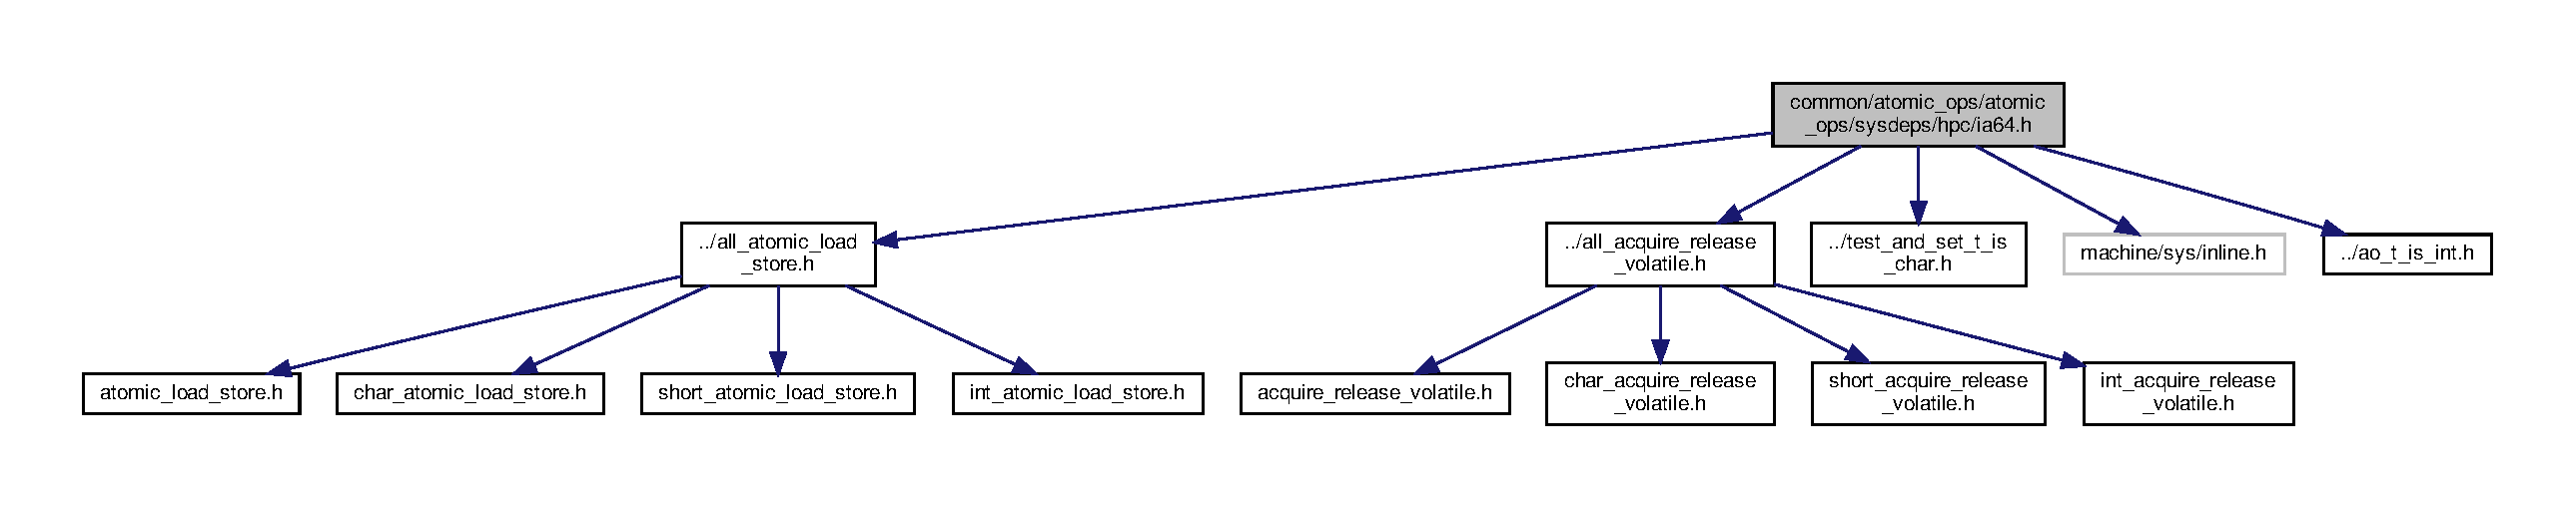
\includegraphics[width=350pt]{hpc_2ia64_8h__incl}
\end{center}
\end{figure}
\subsection*{Macros}
\begin{DoxyCompactItemize}
\item 
\#define \hyperlink{hpc_2ia64_8h_a5e238eba4f717cb1d735b8dcfae2cfba}{A\+O\+\_\+\+T\+\_\+\+F\+A\+S\+I\+ZE}~\+\_\+\+F\+A\+S\+Z\+\_\+W
\item 
\#define \hyperlink{hpc_2ia64_8h_ac499690a7d9506e8bd5800154814b78a}{A\+O\+\_\+\+T\+\_\+\+S\+I\+ZE}~\+\_\+\+S\+Z\+\_\+W
\item 
\#define \hyperlink{hpc_2ia64_8h_a3904dc699d6a6d6e771a93aa66aeb805}{A\+O\+\_\+\+H\+A\+V\+E\+\_\+nop\+\_\+full}
\item 
\#define \hyperlink{hpc_2ia64_8h_ab444fdcbfaf48cb88292b89180cd6d2b}{A\+O\+\_\+\+H\+A\+V\+E\+\_\+fetch\+\_\+and\+\_\+add1\+\_\+acquire}
\item 
\#define \hyperlink{hpc_2ia64_8h_abe5616e4ca4293fbddf3ab80049febae}{A\+O\+\_\+\+H\+A\+V\+E\+\_\+fetch\+\_\+and\+\_\+add1\+\_\+release}
\item 
\#define \hyperlink{hpc_2ia64_8h_a48eb192a6005c2c102a3154a2320850c}{A\+O\+\_\+\+H\+A\+V\+E\+\_\+fetch\+\_\+and\+\_\+sub1\+\_\+acquire}
\item 
\#define \hyperlink{hpc_2ia64_8h_a059afe6ddfb01b0cc90e3e86e201de71}{A\+O\+\_\+\+H\+A\+V\+E\+\_\+fetch\+\_\+and\+\_\+sub1\+\_\+release}
\item 
\#define \hyperlink{hpc_2ia64_8h_ad0b08bc254deecdcba5a4f3366432cf3}{A\+O\+\_\+\+H\+A\+V\+E\+\_\+compare\+\_\+and\+\_\+swap\+\_\+acquire}
\item 
\#define \hyperlink{hpc_2ia64_8h_ad85c7af2ae0a778eba77a7762a358819}{A\+O\+\_\+\+H\+A\+V\+E\+\_\+compare\+\_\+and\+\_\+swap\+\_\+release}
\item 
\#define \hyperlink{hpc_2ia64_8h_ab67b15bb08ff2fbfc858acdaaf0b3531}{A\+O\+\_\+\+H\+A\+V\+E\+\_\+char\+\_\+compare\+\_\+and\+\_\+swap\+\_\+acquire}
\item 
\#define \hyperlink{hpc_2ia64_8h_aa59d946c04e8c5b744322414b106947b}{A\+O\+\_\+\+H\+A\+V\+E\+\_\+char\+\_\+compare\+\_\+and\+\_\+swap\+\_\+release}
\item 
\#define \hyperlink{hpc_2ia64_8h_a9104195dbb035d047e6968e1202d3d63}{A\+O\+\_\+\+H\+A\+V\+E\+\_\+short\+\_\+compare\+\_\+and\+\_\+swap\+\_\+acquire}
\item 
\#define \hyperlink{hpc_2ia64_8h_abca62133116ab240da7a8539018016e1}{A\+O\+\_\+\+H\+A\+V\+E\+\_\+short\+\_\+compare\+\_\+and\+\_\+swap\+\_\+release}
\end{DoxyCompactItemize}
\subsection*{Functions}
\begin{DoxyCompactItemize}
\item 
\hyperlink{atomic__ops_8h_a9f6ab6253b6b11bc8c12efe9dde5db2b}{A\+O\+\_\+\+I\+N\+L\+I\+NE} void \hyperlink{hpc_2ia64_8h_afe3a6778eacc82252ba138fc9a157b04}{A\+O\+\_\+nop\+\_\+full} (void)
\item 
\hyperlink{atomic__ops_8h_a9f6ab6253b6b11bc8c12efe9dde5db2b}{A\+O\+\_\+\+I\+N\+L\+I\+NE} \hyperlink{atomic__ops_8h_a5225fef4d9eee821e82382cd269160dd}{A\+O\+\_\+t} \hyperlink{hpc_2ia64_8h_a9c6806c9bb5426fdd4d2f6dbd3b57cce}{A\+O\+\_\+fetch\+\_\+and\+\_\+add1\+\_\+acquire} (volatile \hyperlink{atomic__ops_8h_a5225fef4d9eee821e82382cd269160dd}{A\+O\+\_\+t} $\ast$p)
\item 
\hyperlink{atomic__ops_8h_a9f6ab6253b6b11bc8c12efe9dde5db2b}{A\+O\+\_\+\+I\+N\+L\+I\+NE} \hyperlink{atomic__ops_8h_a5225fef4d9eee821e82382cd269160dd}{A\+O\+\_\+t} \hyperlink{hpc_2ia64_8h_ad5935c5ab6aeedf0844925daf9c3d8d6}{A\+O\+\_\+fetch\+\_\+and\+\_\+add1\+\_\+release} (volatile \hyperlink{atomic__ops_8h_a5225fef4d9eee821e82382cd269160dd}{A\+O\+\_\+t} $\ast$p)
\item 
\hyperlink{atomic__ops_8h_a9f6ab6253b6b11bc8c12efe9dde5db2b}{A\+O\+\_\+\+I\+N\+L\+I\+NE} \hyperlink{atomic__ops_8h_a5225fef4d9eee821e82382cd269160dd}{A\+O\+\_\+t} \hyperlink{hpc_2ia64_8h_abdd50f1fd3145d33ad3d7bf2ddaebada}{A\+O\+\_\+fetch\+\_\+and\+\_\+sub1\+\_\+acquire} (volatile \hyperlink{atomic__ops_8h_a5225fef4d9eee821e82382cd269160dd}{A\+O\+\_\+t} $\ast$p)
\item 
\hyperlink{atomic__ops_8h_a9f6ab6253b6b11bc8c12efe9dde5db2b}{A\+O\+\_\+\+I\+N\+L\+I\+NE} \hyperlink{atomic__ops_8h_a5225fef4d9eee821e82382cd269160dd}{A\+O\+\_\+t} \hyperlink{hpc_2ia64_8h_a83570074a985dd54bcc3004366bbfaae}{A\+O\+\_\+fetch\+\_\+and\+\_\+sub1\+\_\+release} (volatile \hyperlink{atomic__ops_8h_a5225fef4d9eee821e82382cd269160dd}{A\+O\+\_\+t} $\ast$p)
\item 
\hyperlink{atomic__ops_8h_a9f6ab6253b6b11bc8c12efe9dde5db2b}{A\+O\+\_\+\+I\+N\+L\+I\+NE} int \hyperlink{hpc_2ia64_8h_a81fc146600046fb8ee9ce4339f078e2e}{A\+O\+\_\+compare\+\_\+and\+\_\+swap\+\_\+acquire} (volatile \hyperlink{atomic__ops_8h_a5225fef4d9eee821e82382cd269160dd}{A\+O\+\_\+t} $\ast$addr, \hyperlink{atomic__ops_8h_a5225fef4d9eee821e82382cd269160dd}{A\+O\+\_\+t} old, \hyperlink{atomic__ops_8h_a5225fef4d9eee821e82382cd269160dd}{A\+O\+\_\+t} new\+\_\+val)
\item 
\hyperlink{atomic__ops_8h_a9f6ab6253b6b11bc8c12efe9dde5db2b}{A\+O\+\_\+\+I\+N\+L\+I\+NE} int \hyperlink{hpc_2ia64_8h_ae39d774429bea0d5c3b604bbb820a4ea}{A\+O\+\_\+compare\+\_\+and\+\_\+swap\+\_\+release} (volatile \hyperlink{atomic__ops_8h_a5225fef4d9eee821e82382cd269160dd}{A\+O\+\_\+t} $\ast$addr, \hyperlink{atomic__ops_8h_a5225fef4d9eee821e82382cd269160dd}{A\+O\+\_\+t} old, \hyperlink{atomic__ops_8h_a5225fef4d9eee821e82382cd269160dd}{A\+O\+\_\+t} new\+\_\+val)
\item 
\hyperlink{atomic__ops_8h_a9f6ab6253b6b11bc8c12efe9dde5db2b}{A\+O\+\_\+\+I\+N\+L\+I\+NE} int \hyperlink{hpc_2ia64_8h_adfddc3e21d1b14f528dd1259f501f8c6}{A\+O\+\_\+char\+\_\+compare\+\_\+and\+\_\+swap\+\_\+acquire} (volatile unsigned char $\ast$addr, unsigned char old, unsigned char new\+\_\+val)
\item 
\hyperlink{atomic__ops_8h_a9f6ab6253b6b11bc8c12efe9dde5db2b}{A\+O\+\_\+\+I\+N\+L\+I\+NE} int \hyperlink{hpc_2ia64_8h_abfcca8311ee6e37e2b81abaa4aae2905}{A\+O\+\_\+char\+\_\+compare\+\_\+and\+\_\+swap\+\_\+release} (volatile unsigned char $\ast$addr, unsigned char old, unsigned char new\+\_\+val)
\item 
\hyperlink{atomic__ops_8h_a9f6ab6253b6b11bc8c12efe9dde5db2b}{A\+O\+\_\+\+I\+N\+L\+I\+NE} int \hyperlink{hpc_2ia64_8h_a4297eec9f9ebc8d4813bf52d25e3f561}{A\+O\+\_\+short\+\_\+compare\+\_\+and\+\_\+swap\+\_\+acquire} (volatile unsigned short $\ast$addr, unsigned short old, unsigned short new\+\_\+val)
\item 
\hyperlink{atomic__ops_8h_a9f6ab6253b6b11bc8c12efe9dde5db2b}{A\+O\+\_\+\+I\+N\+L\+I\+NE} int \hyperlink{hpc_2ia64_8h_a46abe9aff985d4ba1d5c5af55f572625}{A\+O\+\_\+short\+\_\+compare\+\_\+and\+\_\+swap\+\_\+release} (volatile unsigned short $\ast$addr, unsigned short old, unsigned short new\+\_\+val)
\end{DoxyCompactItemize}


\subsection{Macro Definition Documentation}
\mbox{\Hypertarget{hpc_2ia64_8h_ab67b15bb08ff2fbfc858acdaaf0b3531}\label{hpc_2ia64_8h_ab67b15bb08ff2fbfc858acdaaf0b3531}} 
\index{hpc/ia64.\+h@{hpc/ia64.\+h}!A\+O\+\_\+\+H\+A\+V\+E\+\_\+char\+\_\+compare\+\_\+and\+\_\+swap\+\_\+acquire@{A\+O\+\_\+\+H\+A\+V\+E\+\_\+char\+\_\+compare\+\_\+and\+\_\+swap\+\_\+acquire}}
\index{A\+O\+\_\+\+H\+A\+V\+E\+\_\+char\+\_\+compare\+\_\+and\+\_\+swap\+\_\+acquire@{A\+O\+\_\+\+H\+A\+V\+E\+\_\+char\+\_\+compare\+\_\+and\+\_\+swap\+\_\+acquire}!hpc/ia64.\+h@{hpc/ia64.\+h}}
\subsubsection{\texorpdfstring{A\+O\+\_\+\+H\+A\+V\+E\+\_\+char\+\_\+compare\+\_\+and\+\_\+swap\+\_\+acquire}{AO\_HAVE\_char\_compare\_and\_swap\_acquire}}
{\footnotesize\ttfamily \#define A\+O\+\_\+\+H\+A\+V\+E\+\_\+char\+\_\+compare\+\_\+and\+\_\+swap\+\_\+acquire}

\mbox{\Hypertarget{hpc_2ia64_8h_aa59d946c04e8c5b744322414b106947b}\label{hpc_2ia64_8h_aa59d946c04e8c5b744322414b106947b}} 
\index{hpc/ia64.\+h@{hpc/ia64.\+h}!A\+O\+\_\+\+H\+A\+V\+E\+\_\+char\+\_\+compare\+\_\+and\+\_\+swap\+\_\+release@{A\+O\+\_\+\+H\+A\+V\+E\+\_\+char\+\_\+compare\+\_\+and\+\_\+swap\+\_\+release}}
\index{A\+O\+\_\+\+H\+A\+V\+E\+\_\+char\+\_\+compare\+\_\+and\+\_\+swap\+\_\+release@{A\+O\+\_\+\+H\+A\+V\+E\+\_\+char\+\_\+compare\+\_\+and\+\_\+swap\+\_\+release}!hpc/ia64.\+h@{hpc/ia64.\+h}}
\subsubsection{\texorpdfstring{A\+O\+\_\+\+H\+A\+V\+E\+\_\+char\+\_\+compare\+\_\+and\+\_\+swap\+\_\+release}{AO\_HAVE\_char\_compare\_and\_swap\_release}}
{\footnotesize\ttfamily \#define A\+O\+\_\+\+H\+A\+V\+E\+\_\+char\+\_\+compare\+\_\+and\+\_\+swap\+\_\+release}

\mbox{\Hypertarget{hpc_2ia64_8h_ad0b08bc254deecdcba5a4f3366432cf3}\label{hpc_2ia64_8h_ad0b08bc254deecdcba5a4f3366432cf3}} 
\index{hpc/ia64.\+h@{hpc/ia64.\+h}!A\+O\+\_\+\+H\+A\+V\+E\+\_\+compare\+\_\+and\+\_\+swap\+\_\+acquire@{A\+O\+\_\+\+H\+A\+V\+E\+\_\+compare\+\_\+and\+\_\+swap\+\_\+acquire}}
\index{A\+O\+\_\+\+H\+A\+V\+E\+\_\+compare\+\_\+and\+\_\+swap\+\_\+acquire@{A\+O\+\_\+\+H\+A\+V\+E\+\_\+compare\+\_\+and\+\_\+swap\+\_\+acquire}!hpc/ia64.\+h@{hpc/ia64.\+h}}
\subsubsection{\texorpdfstring{A\+O\+\_\+\+H\+A\+V\+E\+\_\+compare\+\_\+and\+\_\+swap\+\_\+acquire}{AO\_HAVE\_compare\_and\_swap\_acquire}}
{\footnotesize\ttfamily \#define A\+O\+\_\+\+H\+A\+V\+E\+\_\+compare\+\_\+and\+\_\+swap\+\_\+acquire}

\mbox{\Hypertarget{hpc_2ia64_8h_ad85c7af2ae0a778eba77a7762a358819}\label{hpc_2ia64_8h_ad85c7af2ae0a778eba77a7762a358819}} 
\index{hpc/ia64.\+h@{hpc/ia64.\+h}!A\+O\+\_\+\+H\+A\+V\+E\+\_\+compare\+\_\+and\+\_\+swap\+\_\+release@{A\+O\+\_\+\+H\+A\+V\+E\+\_\+compare\+\_\+and\+\_\+swap\+\_\+release}}
\index{A\+O\+\_\+\+H\+A\+V\+E\+\_\+compare\+\_\+and\+\_\+swap\+\_\+release@{A\+O\+\_\+\+H\+A\+V\+E\+\_\+compare\+\_\+and\+\_\+swap\+\_\+release}!hpc/ia64.\+h@{hpc/ia64.\+h}}
\subsubsection{\texorpdfstring{A\+O\+\_\+\+H\+A\+V\+E\+\_\+compare\+\_\+and\+\_\+swap\+\_\+release}{AO\_HAVE\_compare\_and\_swap\_release}}
{\footnotesize\ttfamily \#define A\+O\+\_\+\+H\+A\+V\+E\+\_\+compare\+\_\+and\+\_\+swap\+\_\+release}

\mbox{\Hypertarget{hpc_2ia64_8h_ab444fdcbfaf48cb88292b89180cd6d2b}\label{hpc_2ia64_8h_ab444fdcbfaf48cb88292b89180cd6d2b}} 
\index{hpc/ia64.\+h@{hpc/ia64.\+h}!A\+O\+\_\+\+H\+A\+V\+E\+\_\+fetch\+\_\+and\+\_\+add1\+\_\+acquire@{A\+O\+\_\+\+H\+A\+V\+E\+\_\+fetch\+\_\+and\+\_\+add1\+\_\+acquire}}
\index{A\+O\+\_\+\+H\+A\+V\+E\+\_\+fetch\+\_\+and\+\_\+add1\+\_\+acquire@{A\+O\+\_\+\+H\+A\+V\+E\+\_\+fetch\+\_\+and\+\_\+add1\+\_\+acquire}!hpc/ia64.\+h@{hpc/ia64.\+h}}
\subsubsection{\texorpdfstring{A\+O\+\_\+\+H\+A\+V\+E\+\_\+fetch\+\_\+and\+\_\+add1\+\_\+acquire}{AO\_HAVE\_fetch\_and\_add1\_acquire}}
{\footnotesize\ttfamily \#define A\+O\+\_\+\+H\+A\+V\+E\+\_\+fetch\+\_\+and\+\_\+add1\+\_\+acquire}

\mbox{\Hypertarget{hpc_2ia64_8h_abe5616e4ca4293fbddf3ab80049febae}\label{hpc_2ia64_8h_abe5616e4ca4293fbddf3ab80049febae}} 
\index{hpc/ia64.\+h@{hpc/ia64.\+h}!A\+O\+\_\+\+H\+A\+V\+E\+\_\+fetch\+\_\+and\+\_\+add1\+\_\+release@{A\+O\+\_\+\+H\+A\+V\+E\+\_\+fetch\+\_\+and\+\_\+add1\+\_\+release}}
\index{A\+O\+\_\+\+H\+A\+V\+E\+\_\+fetch\+\_\+and\+\_\+add1\+\_\+release@{A\+O\+\_\+\+H\+A\+V\+E\+\_\+fetch\+\_\+and\+\_\+add1\+\_\+release}!hpc/ia64.\+h@{hpc/ia64.\+h}}
\subsubsection{\texorpdfstring{A\+O\+\_\+\+H\+A\+V\+E\+\_\+fetch\+\_\+and\+\_\+add1\+\_\+release}{AO\_HAVE\_fetch\_and\_add1\_release}}
{\footnotesize\ttfamily \#define A\+O\+\_\+\+H\+A\+V\+E\+\_\+fetch\+\_\+and\+\_\+add1\+\_\+release}

\mbox{\Hypertarget{hpc_2ia64_8h_a48eb192a6005c2c102a3154a2320850c}\label{hpc_2ia64_8h_a48eb192a6005c2c102a3154a2320850c}} 
\index{hpc/ia64.\+h@{hpc/ia64.\+h}!A\+O\+\_\+\+H\+A\+V\+E\+\_\+fetch\+\_\+and\+\_\+sub1\+\_\+acquire@{A\+O\+\_\+\+H\+A\+V\+E\+\_\+fetch\+\_\+and\+\_\+sub1\+\_\+acquire}}
\index{A\+O\+\_\+\+H\+A\+V\+E\+\_\+fetch\+\_\+and\+\_\+sub1\+\_\+acquire@{A\+O\+\_\+\+H\+A\+V\+E\+\_\+fetch\+\_\+and\+\_\+sub1\+\_\+acquire}!hpc/ia64.\+h@{hpc/ia64.\+h}}
\subsubsection{\texorpdfstring{A\+O\+\_\+\+H\+A\+V\+E\+\_\+fetch\+\_\+and\+\_\+sub1\+\_\+acquire}{AO\_HAVE\_fetch\_and\_sub1\_acquire}}
{\footnotesize\ttfamily \#define A\+O\+\_\+\+H\+A\+V\+E\+\_\+fetch\+\_\+and\+\_\+sub1\+\_\+acquire}

\mbox{\Hypertarget{hpc_2ia64_8h_a059afe6ddfb01b0cc90e3e86e201de71}\label{hpc_2ia64_8h_a059afe6ddfb01b0cc90e3e86e201de71}} 
\index{hpc/ia64.\+h@{hpc/ia64.\+h}!A\+O\+\_\+\+H\+A\+V\+E\+\_\+fetch\+\_\+and\+\_\+sub1\+\_\+release@{A\+O\+\_\+\+H\+A\+V\+E\+\_\+fetch\+\_\+and\+\_\+sub1\+\_\+release}}
\index{A\+O\+\_\+\+H\+A\+V\+E\+\_\+fetch\+\_\+and\+\_\+sub1\+\_\+release@{A\+O\+\_\+\+H\+A\+V\+E\+\_\+fetch\+\_\+and\+\_\+sub1\+\_\+release}!hpc/ia64.\+h@{hpc/ia64.\+h}}
\subsubsection{\texorpdfstring{A\+O\+\_\+\+H\+A\+V\+E\+\_\+fetch\+\_\+and\+\_\+sub1\+\_\+release}{AO\_HAVE\_fetch\_and\_sub1\_release}}
{\footnotesize\ttfamily \#define A\+O\+\_\+\+H\+A\+V\+E\+\_\+fetch\+\_\+and\+\_\+sub1\+\_\+release}

\mbox{\Hypertarget{hpc_2ia64_8h_a3904dc699d6a6d6e771a93aa66aeb805}\label{hpc_2ia64_8h_a3904dc699d6a6d6e771a93aa66aeb805}} 
\index{hpc/ia64.\+h@{hpc/ia64.\+h}!A\+O\+\_\+\+H\+A\+V\+E\+\_\+nop\+\_\+full@{A\+O\+\_\+\+H\+A\+V\+E\+\_\+nop\+\_\+full}}
\index{A\+O\+\_\+\+H\+A\+V\+E\+\_\+nop\+\_\+full@{A\+O\+\_\+\+H\+A\+V\+E\+\_\+nop\+\_\+full}!hpc/ia64.\+h@{hpc/ia64.\+h}}
\subsubsection{\texorpdfstring{A\+O\+\_\+\+H\+A\+V\+E\+\_\+nop\+\_\+full}{AO\_HAVE\_nop\_full}}
{\footnotesize\ttfamily \#define A\+O\+\_\+\+H\+A\+V\+E\+\_\+nop\+\_\+full}

\mbox{\Hypertarget{hpc_2ia64_8h_a9104195dbb035d047e6968e1202d3d63}\label{hpc_2ia64_8h_a9104195dbb035d047e6968e1202d3d63}} 
\index{hpc/ia64.\+h@{hpc/ia64.\+h}!A\+O\+\_\+\+H\+A\+V\+E\+\_\+short\+\_\+compare\+\_\+and\+\_\+swap\+\_\+acquire@{A\+O\+\_\+\+H\+A\+V\+E\+\_\+short\+\_\+compare\+\_\+and\+\_\+swap\+\_\+acquire}}
\index{A\+O\+\_\+\+H\+A\+V\+E\+\_\+short\+\_\+compare\+\_\+and\+\_\+swap\+\_\+acquire@{A\+O\+\_\+\+H\+A\+V\+E\+\_\+short\+\_\+compare\+\_\+and\+\_\+swap\+\_\+acquire}!hpc/ia64.\+h@{hpc/ia64.\+h}}
\subsubsection{\texorpdfstring{A\+O\+\_\+\+H\+A\+V\+E\+\_\+short\+\_\+compare\+\_\+and\+\_\+swap\+\_\+acquire}{AO\_HAVE\_short\_compare\_and\_swap\_acquire}}
{\footnotesize\ttfamily \#define A\+O\+\_\+\+H\+A\+V\+E\+\_\+short\+\_\+compare\+\_\+and\+\_\+swap\+\_\+acquire}

\mbox{\Hypertarget{hpc_2ia64_8h_abca62133116ab240da7a8539018016e1}\label{hpc_2ia64_8h_abca62133116ab240da7a8539018016e1}} 
\index{hpc/ia64.\+h@{hpc/ia64.\+h}!A\+O\+\_\+\+H\+A\+V\+E\+\_\+short\+\_\+compare\+\_\+and\+\_\+swap\+\_\+release@{A\+O\+\_\+\+H\+A\+V\+E\+\_\+short\+\_\+compare\+\_\+and\+\_\+swap\+\_\+release}}
\index{A\+O\+\_\+\+H\+A\+V\+E\+\_\+short\+\_\+compare\+\_\+and\+\_\+swap\+\_\+release@{A\+O\+\_\+\+H\+A\+V\+E\+\_\+short\+\_\+compare\+\_\+and\+\_\+swap\+\_\+release}!hpc/ia64.\+h@{hpc/ia64.\+h}}
\subsubsection{\texorpdfstring{A\+O\+\_\+\+H\+A\+V\+E\+\_\+short\+\_\+compare\+\_\+and\+\_\+swap\+\_\+release}{AO\_HAVE\_short\_compare\_and\_swap\_release}}
{\footnotesize\ttfamily \#define A\+O\+\_\+\+H\+A\+V\+E\+\_\+short\+\_\+compare\+\_\+and\+\_\+swap\+\_\+release}

\mbox{\Hypertarget{hpc_2ia64_8h_a5e238eba4f717cb1d735b8dcfae2cfba}\label{hpc_2ia64_8h_a5e238eba4f717cb1d735b8dcfae2cfba}} 
\index{hpc/ia64.\+h@{hpc/ia64.\+h}!A\+O\+\_\+\+T\+\_\+\+F\+A\+S\+I\+ZE@{A\+O\+\_\+\+T\+\_\+\+F\+A\+S\+I\+ZE}}
\index{A\+O\+\_\+\+T\+\_\+\+F\+A\+S\+I\+ZE@{A\+O\+\_\+\+T\+\_\+\+F\+A\+S\+I\+ZE}!hpc/ia64.\+h@{hpc/ia64.\+h}}
\subsubsection{\texorpdfstring{A\+O\+\_\+\+T\+\_\+\+F\+A\+S\+I\+ZE}{AO\_T\_FASIZE}}
{\footnotesize\ttfamily \#define A\+O\+\_\+\+T\+\_\+\+F\+A\+S\+I\+ZE~\+\_\+\+F\+A\+S\+Z\+\_\+W}

\mbox{\Hypertarget{hpc_2ia64_8h_ac499690a7d9506e8bd5800154814b78a}\label{hpc_2ia64_8h_ac499690a7d9506e8bd5800154814b78a}} 
\index{hpc/ia64.\+h@{hpc/ia64.\+h}!A\+O\+\_\+\+T\+\_\+\+S\+I\+ZE@{A\+O\+\_\+\+T\+\_\+\+S\+I\+ZE}}
\index{A\+O\+\_\+\+T\+\_\+\+S\+I\+ZE@{A\+O\+\_\+\+T\+\_\+\+S\+I\+ZE}!hpc/ia64.\+h@{hpc/ia64.\+h}}
\subsubsection{\texorpdfstring{A\+O\+\_\+\+T\+\_\+\+S\+I\+ZE}{AO\_T\_SIZE}}
{\footnotesize\ttfamily \#define A\+O\+\_\+\+T\+\_\+\+S\+I\+ZE~\+\_\+\+S\+Z\+\_\+W}



\subsection{Function Documentation}
\mbox{\Hypertarget{hpc_2ia64_8h_adfddc3e21d1b14f528dd1259f501f8c6}\label{hpc_2ia64_8h_adfddc3e21d1b14f528dd1259f501f8c6}} 
\index{hpc/ia64.\+h@{hpc/ia64.\+h}!A\+O\+\_\+char\+\_\+compare\+\_\+and\+\_\+swap\+\_\+acquire@{A\+O\+\_\+char\+\_\+compare\+\_\+and\+\_\+swap\+\_\+acquire}}
\index{A\+O\+\_\+char\+\_\+compare\+\_\+and\+\_\+swap\+\_\+acquire@{A\+O\+\_\+char\+\_\+compare\+\_\+and\+\_\+swap\+\_\+acquire}!hpc/ia64.\+h@{hpc/ia64.\+h}}
\subsubsection{\texorpdfstring{A\+O\+\_\+char\+\_\+compare\+\_\+and\+\_\+swap\+\_\+acquire()}{AO\_char\_compare\_and\_swap\_acquire()}}
{\footnotesize\ttfamily \hyperlink{atomic__ops_8h_a9f6ab6253b6b11bc8c12efe9dde5db2b}{A\+O\+\_\+\+I\+N\+L\+I\+NE} int A\+O\+\_\+char\+\_\+compare\+\_\+and\+\_\+swap\+\_\+acquire (\begin{DoxyParamCaption}\item[{volatile unsigned char $\ast$}]{addr,  }\item[{unsigned char}]{old,  }\item[{unsigned char}]{new\+\_\+val }\end{DoxyParamCaption})}

\mbox{\Hypertarget{hpc_2ia64_8h_abfcca8311ee6e37e2b81abaa4aae2905}\label{hpc_2ia64_8h_abfcca8311ee6e37e2b81abaa4aae2905}} 
\index{hpc/ia64.\+h@{hpc/ia64.\+h}!A\+O\+\_\+char\+\_\+compare\+\_\+and\+\_\+swap\+\_\+release@{A\+O\+\_\+char\+\_\+compare\+\_\+and\+\_\+swap\+\_\+release}}
\index{A\+O\+\_\+char\+\_\+compare\+\_\+and\+\_\+swap\+\_\+release@{A\+O\+\_\+char\+\_\+compare\+\_\+and\+\_\+swap\+\_\+release}!hpc/ia64.\+h@{hpc/ia64.\+h}}
\subsubsection{\texorpdfstring{A\+O\+\_\+char\+\_\+compare\+\_\+and\+\_\+swap\+\_\+release()}{AO\_char\_compare\_and\_swap\_release()}}
{\footnotesize\ttfamily \hyperlink{atomic__ops_8h_a9f6ab6253b6b11bc8c12efe9dde5db2b}{A\+O\+\_\+\+I\+N\+L\+I\+NE} int A\+O\+\_\+char\+\_\+compare\+\_\+and\+\_\+swap\+\_\+release (\begin{DoxyParamCaption}\item[{volatile unsigned char $\ast$}]{addr,  }\item[{unsigned char}]{old,  }\item[{unsigned char}]{new\+\_\+val }\end{DoxyParamCaption})}

\mbox{\Hypertarget{hpc_2ia64_8h_a81fc146600046fb8ee9ce4339f078e2e}\label{hpc_2ia64_8h_a81fc146600046fb8ee9ce4339f078e2e}} 
\index{hpc/ia64.\+h@{hpc/ia64.\+h}!A\+O\+\_\+compare\+\_\+and\+\_\+swap\+\_\+acquire@{A\+O\+\_\+compare\+\_\+and\+\_\+swap\+\_\+acquire}}
\index{A\+O\+\_\+compare\+\_\+and\+\_\+swap\+\_\+acquire@{A\+O\+\_\+compare\+\_\+and\+\_\+swap\+\_\+acquire}!hpc/ia64.\+h@{hpc/ia64.\+h}}
\subsubsection{\texorpdfstring{A\+O\+\_\+compare\+\_\+and\+\_\+swap\+\_\+acquire()}{AO\_compare\_and\_swap\_acquire()}}
{\footnotesize\ttfamily \hyperlink{atomic__ops_8h_a9f6ab6253b6b11bc8c12efe9dde5db2b}{A\+O\+\_\+\+I\+N\+L\+I\+NE} int A\+O\+\_\+compare\+\_\+and\+\_\+swap\+\_\+acquire (\begin{DoxyParamCaption}\item[{volatile \hyperlink{atomic__ops_8h_a5225fef4d9eee821e82382cd269160dd}{A\+O\+\_\+t} $\ast$}]{addr,  }\item[{\hyperlink{atomic__ops_8h_a5225fef4d9eee821e82382cd269160dd}{A\+O\+\_\+t}}]{old,  }\item[{\hyperlink{atomic__ops_8h_a5225fef4d9eee821e82382cd269160dd}{A\+O\+\_\+t}}]{new\+\_\+val }\end{DoxyParamCaption})}

\mbox{\Hypertarget{hpc_2ia64_8h_ae39d774429bea0d5c3b604bbb820a4ea}\label{hpc_2ia64_8h_ae39d774429bea0d5c3b604bbb820a4ea}} 
\index{hpc/ia64.\+h@{hpc/ia64.\+h}!A\+O\+\_\+compare\+\_\+and\+\_\+swap\+\_\+release@{A\+O\+\_\+compare\+\_\+and\+\_\+swap\+\_\+release}}
\index{A\+O\+\_\+compare\+\_\+and\+\_\+swap\+\_\+release@{A\+O\+\_\+compare\+\_\+and\+\_\+swap\+\_\+release}!hpc/ia64.\+h@{hpc/ia64.\+h}}
\subsubsection{\texorpdfstring{A\+O\+\_\+compare\+\_\+and\+\_\+swap\+\_\+release()}{AO\_compare\_and\_swap\_release()}}
{\footnotesize\ttfamily \hyperlink{atomic__ops_8h_a9f6ab6253b6b11bc8c12efe9dde5db2b}{A\+O\+\_\+\+I\+N\+L\+I\+NE} int A\+O\+\_\+compare\+\_\+and\+\_\+swap\+\_\+release (\begin{DoxyParamCaption}\item[{volatile \hyperlink{atomic__ops_8h_a5225fef4d9eee821e82382cd269160dd}{A\+O\+\_\+t} $\ast$}]{addr,  }\item[{\hyperlink{atomic__ops_8h_a5225fef4d9eee821e82382cd269160dd}{A\+O\+\_\+t}}]{old,  }\item[{\hyperlink{atomic__ops_8h_a5225fef4d9eee821e82382cd269160dd}{A\+O\+\_\+t}}]{new\+\_\+val }\end{DoxyParamCaption})}

\mbox{\Hypertarget{hpc_2ia64_8h_a9c6806c9bb5426fdd4d2f6dbd3b57cce}\label{hpc_2ia64_8h_a9c6806c9bb5426fdd4d2f6dbd3b57cce}} 
\index{hpc/ia64.\+h@{hpc/ia64.\+h}!A\+O\+\_\+fetch\+\_\+and\+\_\+add1\+\_\+acquire@{A\+O\+\_\+fetch\+\_\+and\+\_\+add1\+\_\+acquire}}
\index{A\+O\+\_\+fetch\+\_\+and\+\_\+add1\+\_\+acquire@{A\+O\+\_\+fetch\+\_\+and\+\_\+add1\+\_\+acquire}!hpc/ia64.\+h@{hpc/ia64.\+h}}
\subsubsection{\texorpdfstring{A\+O\+\_\+fetch\+\_\+and\+\_\+add1\+\_\+acquire()}{AO\_fetch\_and\_add1\_acquire()}}
{\footnotesize\ttfamily \hyperlink{atomic__ops_8h_a9f6ab6253b6b11bc8c12efe9dde5db2b}{A\+O\+\_\+\+I\+N\+L\+I\+NE} \hyperlink{atomic__ops_8h_a5225fef4d9eee821e82382cd269160dd}{A\+O\+\_\+t} A\+O\+\_\+fetch\+\_\+and\+\_\+add1\+\_\+acquire (\begin{DoxyParamCaption}\item[{volatile \hyperlink{atomic__ops_8h_a5225fef4d9eee821e82382cd269160dd}{A\+O\+\_\+t} $\ast$}]{p }\end{DoxyParamCaption})}

\mbox{\Hypertarget{hpc_2ia64_8h_ad5935c5ab6aeedf0844925daf9c3d8d6}\label{hpc_2ia64_8h_ad5935c5ab6aeedf0844925daf9c3d8d6}} 
\index{hpc/ia64.\+h@{hpc/ia64.\+h}!A\+O\+\_\+fetch\+\_\+and\+\_\+add1\+\_\+release@{A\+O\+\_\+fetch\+\_\+and\+\_\+add1\+\_\+release}}
\index{A\+O\+\_\+fetch\+\_\+and\+\_\+add1\+\_\+release@{A\+O\+\_\+fetch\+\_\+and\+\_\+add1\+\_\+release}!hpc/ia64.\+h@{hpc/ia64.\+h}}
\subsubsection{\texorpdfstring{A\+O\+\_\+fetch\+\_\+and\+\_\+add1\+\_\+release()}{AO\_fetch\_and\_add1\_release()}}
{\footnotesize\ttfamily \hyperlink{atomic__ops_8h_a9f6ab6253b6b11bc8c12efe9dde5db2b}{A\+O\+\_\+\+I\+N\+L\+I\+NE} \hyperlink{atomic__ops_8h_a5225fef4d9eee821e82382cd269160dd}{A\+O\+\_\+t} A\+O\+\_\+fetch\+\_\+and\+\_\+add1\+\_\+release (\begin{DoxyParamCaption}\item[{volatile \hyperlink{atomic__ops_8h_a5225fef4d9eee821e82382cd269160dd}{A\+O\+\_\+t} $\ast$}]{p }\end{DoxyParamCaption})}

\mbox{\Hypertarget{hpc_2ia64_8h_abdd50f1fd3145d33ad3d7bf2ddaebada}\label{hpc_2ia64_8h_abdd50f1fd3145d33ad3d7bf2ddaebada}} 
\index{hpc/ia64.\+h@{hpc/ia64.\+h}!A\+O\+\_\+fetch\+\_\+and\+\_\+sub1\+\_\+acquire@{A\+O\+\_\+fetch\+\_\+and\+\_\+sub1\+\_\+acquire}}
\index{A\+O\+\_\+fetch\+\_\+and\+\_\+sub1\+\_\+acquire@{A\+O\+\_\+fetch\+\_\+and\+\_\+sub1\+\_\+acquire}!hpc/ia64.\+h@{hpc/ia64.\+h}}
\subsubsection{\texorpdfstring{A\+O\+\_\+fetch\+\_\+and\+\_\+sub1\+\_\+acquire()}{AO\_fetch\_and\_sub1\_acquire()}}
{\footnotesize\ttfamily \hyperlink{atomic__ops_8h_a9f6ab6253b6b11bc8c12efe9dde5db2b}{A\+O\+\_\+\+I\+N\+L\+I\+NE} \hyperlink{atomic__ops_8h_a5225fef4d9eee821e82382cd269160dd}{A\+O\+\_\+t} A\+O\+\_\+fetch\+\_\+and\+\_\+sub1\+\_\+acquire (\begin{DoxyParamCaption}\item[{volatile \hyperlink{atomic__ops_8h_a5225fef4d9eee821e82382cd269160dd}{A\+O\+\_\+t} $\ast$}]{p }\end{DoxyParamCaption})}

\mbox{\Hypertarget{hpc_2ia64_8h_a83570074a985dd54bcc3004366bbfaae}\label{hpc_2ia64_8h_a83570074a985dd54bcc3004366bbfaae}} 
\index{hpc/ia64.\+h@{hpc/ia64.\+h}!A\+O\+\_\+fetch\+\_\+and\+\_\+sub1\+\_\+release@{A\+O\+\_\+fetch\+\_\+and\+\_\+sub1\+\_\+release}}
\index{A\+O\+\_\+fetch\+\_\+and\+\_\+sub1\+\_\+release@{A\+O\+\_\+fetch\+\_\+and\+\_\+sub1\+\_\+release}!hpc/ia64.\+h@{hpc/ia64.\+h}}
\subsubsection{\texorpdfstring{A\+O\+\_\+fetch\+\_\+and\+\_\+sub1\+\_\+release()}{AO\_fetch\_and\_sub1\_release()}}
{\footnotesize\ttfamily \hyperlink{atomic__ops_8h_a9f6ab6253b6b11bc8c12efe9dde5db2b}{A\+O\+\_\+\+I\+N\+L\+I\+NE} \hyperlink{atomic__ops_8h_a5225fef4d9eee821e82382cd269160dd}{A\+O\+\_\+t} A\+O\+\_\+fetch\+\_\+and\+\_\+sub1\+\_\+release (\begin{DoxyParamCaption}\item[{volatile \hyperlink{atomic__ops_8h_a5225fef4d9eee821e82382cd269160dd}{A\+O\+\_\+t} $\ast$}]{p }\end{DoxyParamCaption})}

\mbox{\Hypertarget{hpc_2ia64_8h_afe3a6778eacc82252ba138fc9a157b04}\label{hpc_2ia64_8h_afe3a6778eacc82252ba138fc9a157b04}} 
\index{hpc/ia64.\+h@{hpc/ia64.\+h}!A\+O\+\_\+nop\+\_\+full@{A\+O\+\_\+nop\+\_\+full}}
\index{A\+O\+\_\+nop\+\_\+full@{A\+O\+\_\+nop\+\_\+full}!hpc/ia64.\+h@{hpc/ia64.\+h}}
\subsubsection{\texorpdfstring{A\+O\+\_\+nop\+\_\+full()}{AO\_nop\_full()}}
{\footnotesize\ttfamily \hyperlink{atomic__ops_8h_a9f6ab6253b6b11bc8c12efe9dde5db2b}{A\+O\+\_\+\+I\+N\+L\+I\+NE} void A\+O\+\_\+nop\+\_\+full (\begin{DoxyParamCaption}\item[{void}]{ }\end{DoxyParamCaption})}

\mbox{\Hypertarget{hpc_2ia64_8h_a4297eec9f9ebc8d4813bf52d25e3f561}\label{hpc_2ia64_8h_a4297eec9f9ebc8d4813bf52d25e3f561}} 
\index{hpc/ia64.\+h@{hpc/ia64.\+h}!A\+O\+\_\+short\+\_\+compare\+\_\+and\+\_\+swap\+\_\+acquire@{A\+O\+\_\+short\+\_\+compare\+\_\+and\+\_\+swap\+\_\+acquire}}
\index{A\+O\+\_\+short\+\_\+compare\+\_\+and\+\_\+swap\+\_\+acquire@{A\+O\+\_\+short\+\_\+compare\+\_\+and\+\_\+swap\+\_\+acquire}!hpc/ia64.\+h@{hpc/ia64.\+h}}
\subsubsection{\texorpdfstring{A\+O\+\_\+short\+\_\+compare\+\_\+and\+\_\+swap\+\_\+acquire()}{AO\_short\_compare\_and\_swap\_acquire()}}
{\footnotesize\ttfamily \hyperlink{atomic__ops_8h_a9f6ab6253b6b11bc8c12efe9dde5db2b}{A\+O\+\_\+\+I\+N\+L\+I\+NE} int A\+O\+\_\+short\+\_\+compare\+\_\+and\+\_\+swap\+\_\+acquire (\begin{DoxyParamCaption}\item[{volatile unsigned short $\ast$}]{addr,  }\item[{unsigned short}]{old,  }\item[{unsigned short}]{new\+\_\+val }\end{DoxyParamCaption})}

\mbox{\Hypertarget{hpc_2ia64_8h_a46abe9aff985d4ba1d5c5af55f572625}\label{hpc_2ia64_8h_a46abe9aff985d4ba1d5c5af55f572625}} 
\index{hpc/ia64.\+h@{hpc/ia64.\+h}!A\+O\+\_\+short\+\_\+compare\+\_\+and\+\_\+swap\+\_\+release@{A\+O\+\_\+short\+\_\+compare\+\_\+and\+\_\+swap\+\_\+release}}
\index{A\+O\+\_\+short\+\_\+compare\+\_\+and\+\_\+swap\+\_\+release@{A\+O\+\_\+short\+\_\+compare\+\_\+and\+\_\+swap\+\_\+release}!hpc/ia64.\+h@{hpc/ia64.\+h}}
\subsubsection{\texorpdfstring{A\+O\+\_\+short\+\_\+compare\+\_\+and\+\_\+swap\+\_\+release()}{AO\_short\_compare\_and\_swap\_release()}}
{\footnotesize\ttfamily \hyperlink{atomic__ops_8h_a9f6ab6253b6b11bc8c12efe9dde5db2b}{A\+O\+\_\+\+I\+N\+L\+I\+NE} int A\+O\+\_\+short\+\_\+compare\+\_\+and\+\_\+swap\+\_\+release (\begin{DoxyParamCaption}\item[{volatile unsigned short $\ast$}]{addr,  }\item[{unsigned short}]{old,  }\item[{unsigned short}]{new\+\_\+val }\end{DoxyParamCaption})}


\hypertarget{icc_2ia64_8h}{}\section{common/atomic\+\_\+ops/atomic\+\_\+ops/sysdeps/icc/ia64.h File Reference}
\label{icc_2ia64_8h}\index{common/atomic\+\_\+ops/atomic\+\_\+ops/sysdeps/icc/ia64.\+h@{common/atomic\+\_\+ops/atomic\+\_\+ops/sysdeps/icc/ia64.\+h}}
{\ttfamily \#include \char`\"{}../all\+\_\+atomic\+\_\+load\+\_\+store.\+h\char`\"{}}\newline
{\ttfamily \#include \char`\"{}../test\+\_\+and\+\_\+set\+\_\+t\+\_\+is\+\_\+char.\+h\char`\"{}}\newline
{\ttfamily \#include $<$ia64intrin.\+h$>$}\newline
Include dependency graph for ia64.\+h\+:
\nopagebreak
\begin{figure}[H]
\begin{center}
\leavevmode
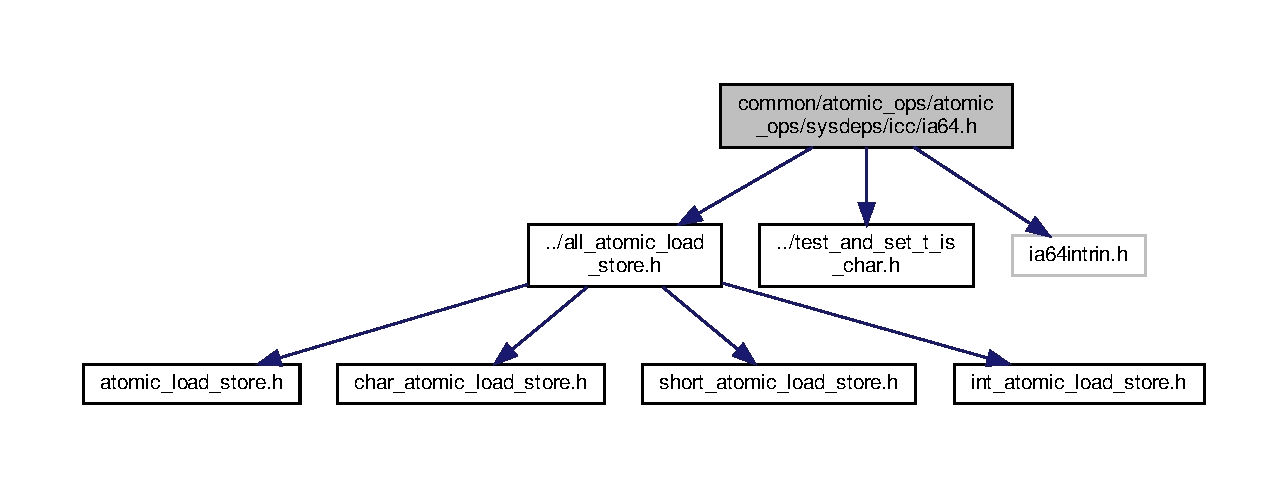
\includegraphics[width=350pt]{icc_2ia64_8h__incl}
\end{center}
\end{figure}
\subsection*{Macros}
\begin{DoxyCompactItemize}
\item 
\#define \hyperlink{icc_2ia64_8h_a042f23427eff8655dc9c068d75ad464e}{A\+O\+\_\+\+I\+N\+T\+E\+L\+\_\+\+P\+T\+R\+\_\+t}~void $\ast$
\item 
\#define \hyperlink{icc_2ia64_8h_a29328d5664268a40645ea9d2f82c8bef}{A\+O\+\_\+\+H\+A\+V\+E\+\_\+load\+\_\+acquire}
\item 
\#define \hyperlink{icc_2ia64_8h_a58f98c6b42d593762336829dcf86d058}{A\+O\+\_\+\+H\+A\+V\+E\+\_\+store\+\_\+release}
\item 
\#define \hyperlink{icc_2ia64_8h_a1ed21fe7030453db172172728b15f854}{A\+O\+\_\+\+H\+A\+V\+E\+\_\+char\+\_\+load\+\_\+acquire}
\item 
\#define \hyperlink{icc_2ia64_8h_af72dd7cd6d706812046022f632bd47ab}{A\+O\+\_\+\+H\+A\+V\+E\+\_\+char\+\_\+store\+\_\+release}
\item 
\#define \hyperlink{icc_2ia64_8h_a9209b99f2e5b1cccf1fa23deef59cfd2}{A\+O\+\_\+\+H\+A\+V\+E\+\_\+short\+\_\+load\+\_\+acquire}
\item 
\#define \hyperlink{icc_2ia64_8h_a52488f4b445ced04c93c67f27a964a78}{A\+O\+\_\+\+H\+A\+V\+E\+\_\+short\+\_\+store\+\_\+release}
\item 
\#define \hyperlink{icc_2ia64_8h_a69ea9f3bbd65c9cd4b3e77fa9ea74c16}{A\+O\+\_\+\+H\+A\+V\+E\+\_\+int\+\_\+load\+\_\+acquire}
\item 
\#define \hyperlink{icc_2ia64_8h_a3b00caccb3035ae2fb224aa6a3c5cd55}{A\+O\+\_\+\+H\+A\+V\+E\+\_\+int\+\_\+store\+\_\+release}
\item 
\#define \hyperlink{icc_2ia64_8h_a3904dc699d6a6d6e771a93aa66aeb805}{A\+O\+\_\+\+H\+A\+V\+E\+\_\+nop\+\_\+full}
\item 
\#define \hyperlink{icc_2ia64_8h_ab444fdcbfaf48cb88292b89180cd6d2b}{A\+O\+\_\+\+H\+A\+V\+E\+\_\+fetch\+\_\+and\+\_\+add1\+\_\+acquire}
\item 
\#define \hyperlink{icc_2ia64_8h_abe5616e4ca4293fbddf3ab80049febae}{A\+O\+\_\+\+H\+A\+V\+E\+\_\+fetch\+\_\+and\+\_\+add1\+\_\+release}
\item 
\#define \hyperlink{icc_2ia64_8h_a48eb192a6005c2c102a3154a2320850c}{A\+O\+\_\+\+H\+A\+V\+E\+\_\+fetch\+\_\+and\+\_\+sub1\+\_\+acquire}
\item 
\#define \hyperlink{icc_2ia64_8h_a059afe6ddfb01b0cc90e3e86e201de71}{A\+O\+\_\+\+H\+A\+V\+E\+\_\+fetch\+\_\+and\+\_\+sub1\+\_\+release}
\item 
\#define \hyperlink{icc_2ia64_8h_ad0b08bc254deecdcba5a4f3366432cf3}{A\+O\+\_\+\+H\+A\+V\+E\+\_\+compare\+\_\+and\+\_\+swap\+\_\+acquire}
\item 
\#define \hyperlink{icc_2ia64_8h_ad85c7af2ae0a778eba77a7762a358819}{A\+O\+\_\+\+H\+A\+V\+E\+\_\+compare\+\_\+and\+\_\+swap\+\_\+release}
\item 
\#define \hyperlink{icc_2ia64_8h_ab67b15bb08ff2fbfc858acdaaf0b3531}{A\+O\+\_\+\+H\+A\+V\+E\+\_\+char\+\_\+compare\+\_\+and\+\_\+swap\+\_\+acquire}
\item 
\#define \hyperlink{icc_2ia64_8h_aa59d946c04e8c5b744322414b106947b}{A\+O\+\_\+\+H\+A\+V\+E\+\_\+char\+\_\+compare\+\_\+and\+\_\+swap\+\_\+release}
\item 
\#define \hyperlink{icc_2ia64_8h_a9104195dbb035d047e6968e1202d3d63}{A\+O\+\_\+\+H\+A\+V\+E\+\_\+short\+\_\+compare\+\_\+and\+\_\+swap\+\_\+acquire}
\item 
\#define \hyperlink{icc_2ia64_8h_abca62133116ab240da7a8539018016e1}{A\+O\+\_\+\+H\+A\+V\+E\+\_\+short\+\_\+compare\+\_\+and\+\_\+swap\+\_\+release}
\item 
\#define \hyperlink{icc_2ia64_8h_aac3dfbb7cf61ee9b8a418e1dbd136e2f}{A\+O\+\_\+\+H\+A\+V\+E\+\_\+int\+\_\+compare\+\_\+and\+\_\+swap\+\_\+acquire}
\item 
\#define \hyperlink{icc_2ia64_8h_a0f91f532e6403ccb6b410f697903d33b}{A\+O\+\_\+\+H\+A\+V\+E\+\_\+int\+\_\+compare\+\_\+and\+\_\+swap\+\_\+release}
\end{DoxyCompactItemize}
\subsection*{Functions}
\begin{DoxyCompactItemize}
\item 
\hyperlink{atomic__ops_8h_a9f6ab6253b6b11bc8c12efe9dde5db2b}{A\+O\+\_\+\+I\+N\+L\+I\+NE} \hyperlink{atomic__ops_8h_a5225fef4d9eee821e82382cd269160dd}{A\+O\+\_\+t} \hyperlink{icc_2ia64_8h_a38908e49c95fafba077fbeb130f0d930}{A\+O\+\_\+load\+\_\+acquire} (const volatile \hyperlink{atomic__ops_8h_a5225fef4d9eee821e82382cd269160dd}{A\+O\+\_\+t} $\ast$p)
\item 
\hyperlink{atomic__ops_8h_a9f6ab6253b6b11bc8c12efe9dde5db2b}{A\+O\+\_\+\+I\+N\+L\+I\+NE} void \hyperlink{icc_2ia64_8h_a5a48a48680fe8ac93029366b77457181}{A\+O\+\_\+store\+\_\+release} (volatile \hyperlink{atomic__ops_8h_a5225fef4d9eee821e82382cd269160dd}{A\+O\+\_\+t} $\ast$p, \hyperlink{atomic__ops_8h_a5225fef4d9eee821e82382cd269160dd}{A\+O\+\_\+t} val)
\item 
\hyperlink{atomic__ops_8h_a9f6ab6253b6b11bc8c12efe9dde5db2b}{A\+O\+\_\+\+I\+N\+L\+I\+NE} unsigned char \hyperlink{icc_2ia64_8h_a3a2743edf2d35086c28f80fde0327f3d}{A\+O\+\_\+char\+\_\+load\+\_\+acquire} (const volatile unsigned char $\ast$p)
\item 
\hyperlink{atomic__ops_8h_a9f6ab6253b6b11bc8c12efe9dde5db2b}{A\+O\+\_\+\+I\+N\+L\+I\+NE} void \hyperlink{icc_2ia64_8h_a7bc53f4414186b38d693c42bbe4aee85}{A\+O\+\_\+char\+\_\+store\+\_\+release} (volatile unsigned char $\ast$p, unsigned char val)
\item 
\hyperlink{atomic__ops_8h_a9f6ab6253b6b11bc8c12efe9dde5db2b}{A\+O\+\_\+\+I\+N\+L\+I\+NE} unsigned short \hyperlink{icc_2ia64_8h_a49e443244890f74b2d3cdd40264656c6}{A\+O\+\_\+short\+\_\+load\+\_\+acquire} (const volatile unsigned short $\ast$p)
\item 
\hyperlink{atomic__ops_8h_a9f6ab6253b6b11bc8c12efe9dde5db2b}{A\+O\+\_\+\+I\+N\+L\+I\+NE} void \hyperlink{icc_2ia64_8h_af297a9437daff533ca30428d1225a7e2}{A\+O\+\_\+short\+\_\+store\+\_\+release} (volatile unsigned short $\ast$p, unsigned short val)
\item 
\hyperlink{atomic__ops_8h_a9f6ab6253b6b11bc8c12efe9dde5db2b}{A\+O\+\_\+\+I\+N\+L\+I\+NE} unsigned int \hyperlink{icc_2ia64_8h_a5e355f5ce9305779de9c115623b56df0}{A\+O\+\_\+int\+\_\+load\+\_\+acquire} (const volatile unsigned int $\ast$p)
\item 
\hyperlink{atomic__ops_8h_a9f6ab6253b6b11bc8c12efe9dde5db2b}{A\+O\+\_\+\+I\+N\+L\+I\+NE} void \hyperlink{icc_2ia64_8h_a0ff53a911b2f6427eae5b0e16466e96c}{A\+O\+\_\+int\+\_\+store\+\_\+release} (volatile unsigned int $\ast$p, unsigned int val)
\item 
\hyperlink{atomic__ops_8h_a9f6ab6253b6b11bc8c12efe9dde5db2b}{A\+O\+\_\+\+I\+N\+L\+I\+NE} void \hyperlink{icc_2ia64_8h_afe3a6778eacc82252ba138fc9a157b04}{A\+O\+\_\+nop\+\_\+full} (void)
\item 
\hyperlink{atomic__ops_8h_a9f6ab6253b6b11bc8c12efe9dde5db2b}{A\+O\+\_\+\+I\+N\+L\+I\+NE} \hyperlink{atomic__ops_8h_a5225fef4d9eee821e82382cd269160dd}{A\+O\+\_\+t} \hyperlink{icc_2ia64_8h_a9c6806c9bb5426fdd4d2f6dbd3b57cce}{A\+O\+\_\+fetch\+\_\+and\+\_\+add1\+\_\+acquire} (volatile \hyperlink{atomic__ops_8h_a5225fef4d9eee821e82382cd269160dd}{A\+O\+\_\+t} $\ast$p)
\item 
\hyperlink{atomic__ops_8h_a9f6ab6253b6b11bc8c12efe9dde5db2b}{A\+O\+\_\+\+I\+N\+L\+I\+NE} \hyperlink{atomic__ops_8h_a5225fef4d9eee821e82382cd269160dd}{A\+O\+\_\+t} \hyperlink{icc_2ia64_8h_ad5935c5ab6aeedf0844925daf9c3d8d6}{A\+O\+\_\+fetch\+\_\+and\+\_\+add1\+\_\+release} (volatile \hyperlink{atomic__ops_8h_a5225fef4d9eee821e82382cd269160dd}{A\+O\+\_\+t} $\ast$p)
\item 
\hyperlink{atomic__ops_8h_a9f6ab6253b6b11bc8c12efe9dde5db2b}{A\+O\+\_\+\+I\+N\+L\+I\+NE} \hyperlink{atomic__ops_8h_a5225fef4d9eee821e82382cd269160dd}{A\+O\+\_\+t} \hyperlink{icc_2ia64_8h_abdd50f1fd3145d33ad3d7bf2ddaebada}{A\+O\+\_\+fetch\+\_\+and\+\_\+sub1\+\_\+acquire} (volatile \hyperlink{atomic__ops_8h_a5225fef4d9eee821e82382cd269160dd}{A\+O\+\_\+t} $\ast$p)
\item 
\hyperlink{atomic__ops_8h_a9f6ab6253b6b11bc8c12efe9dde5db2b}{A\+O\+\_\+\+I\+N\+L\+I\+NE} \hyperlink{atomic__ops_8h_a5225fef4d9eee821e82382cd269160dd}{A\+O\+\_\+t} \hyperlink{icc_2ia64_8h_a83570074a985dd54bcc3004366bbfaae}{A\+O\+\_\+fetch\+\_\+and\+\_\+sub1\+\_\+release} (volatile \hyperlink{atomic__ops_8h_a5225fef4d9eee821e82382cd269160dd}{A\+O\+\_\+t} $\ast$p)
\item 
\hyperlink{atomic__ops_8h_a9f6ab6253b6b11bc8c12efe9dde5db2b}{A\+O\+\_\+\+I\+N\+L\+I\+NE} int \hyperlink{icc_2ia64_8h_a81fc146600046fb8ee9ce4339f078e2e}{A\+O\+\_\+compare\+\_\+and\+\_\+swap\+\_\+acquire} (volatile \hyperlink{atomic__ops_8h_a5225fef4d9eee821e82382cd269160dd}{A\+O\+\_\+t} $\ast$addr, \hyperlink{atomic__ops_8h_a5225fef4d9eee821e82382cd269160dd}{A\+O\+\_\+t} old, \hyperlink{atomic__ops_8h_a5225fef4d9eee821e82382cd269160dd}{A\+O\+\_\+t} new\+\_\+val)
\item 
\hyperlink{atomic__ops_8h_a9f6ab6253b6b11bc8c12efe9dde5db2b}{A\+O\+\_\+\+I\+N\+L\+I\+NE} int \hyperlink{icc_2ia64_8h_ae39d774429bea0d5c3b604bbb820a4ea}{A\+O\+\_\+compare\+\_\+and\+\_\+swap\+\_\+release} (volatile \hyperlink{atomic__ops_8h_a5225fef4d9eee821e82382cd269160dd}{A\+O\+\_\+t} $\ast$addr, \hyperlink{atomic__ops_8h_a5225fef4d9eee821e82382cd269160dd}{A\+O\+\_\+t} old, \hyperlink{atomic__ops_8h_a5225fef4d9eee821e82382cd269160dd}{A\+O\+\_\+t} new\+\_\+val)
\item 
\hyperlink{atomic__ops_8h_a9f6ab6253b6b11bc8c12efe9dde5db2b}{A\+O\+\_\+\+I\+N\+L\+I\+NE} int \hyperlink{icc_2ia64_8h_adfddc3e21d1b14f528dd1259f501f8c6}{A\+O\+\_\+char\+\_\+compare\+\_\+and\+\_\+swap\+\_\+acquire} (volatile unsigned char $\ast$addr, unsigned char old, unsigned char new\+\_\+val)
\item 
\hyperlink{atomic__ops_8h_a9f6ab6253b6b11bc8c12efe9dde5db2b}{A\+O\+\_\+\+I\+N\+L\+I\+NE} int \hyperlink{icc_2ia64_8h_abfcca8311ee6e37e2b81abaa4aae2905}{A\+O\+\_\+char\+\_\+compare\+\_\+and\+\_\+swap\+\_\+release} (volatile unsigned char $\ast$addr, unsigned char old, unsigned char new\+\_\+val)
\item 
\hyperlink{atomic__ops_8h_a9f6ab6253b6b11bc8c12efe9dde5db2b}{A\+O\+\_\+\+I\+N\+L\+I\+NE} int \hyperlink{icc_2ia64_8h_a4297eec9f9ebc8d4813bf52d25e3f561}{A\+O\+\_\+short\+\_\+compare\+\_\+and\+\_\+swap\+\_\+acquire} (volatile unsigned short $\ast$addr, unsigned short old, unsigned short new\+\_\+val)
\item 
\hyperlink{atomic__ops_8h_a9f6ab6253b6b11bc8c12efe9dde5db2b}{A\+O\+\_\+\+I\+N\+L\+I\+NE} int \hyperlink{icc_2ia64_8h_a46abe9aff985d4ba1d5c5af55f572625}{A\+O\+\_\+short\+\_\+compare\+\_\+and\+\_\+swap\+\_\+release} (volatile unsigned short $\ast$addr, unsigned short old, unsigned short new\+\_\+val)
\item 
\hyperlink{atomic__ops_8h_a9f6ab6253b6b11bc8c12efe9dde5db2b}{A\+O\+\_\+\+I\+N\+L\+I\+NE} int \hyperlink{icc_2ia64_8h_a38e5f2ab6ad7fd156ae7ac6b99cd505f}{A\+O\+\_\+int\+\_\+compare\+\_\+and\+\_\+swap\+\_\+acquire} (volatile unsigned int $\ast$addr, unsigned int old, unsigned int new\+\_\+val)
\item 
\hyperlink{atomic__ops_8h_a9f6ab6253b6b11bc8c12efe9dde5db2b}{A\+O\+\_\+\+I\+N\+L\+I\+NE} int \hyperlink{icc_2ia64_8h_a66850a15857b3c397fb5a342872114b3}{A\+O\+\_\+int\+\_\+compare\+\_\+and\+\_\+swap\+\_\+release} (volatile unsigned int $\ast$addr, unsigned int old, unsigned int new\+\_\+val)
\end{DoxyCompactItemize}


\subsection{Macro Definition Documentation}
\mbox{\Hypertarget{icc_2ia64_8h_ab67b15bb08ff2fbfc858acdaaf0b3531}\label{icc_2ia64_8h_ab67b15bb08ff2fbfc858acdaaf0b3531}} 
\index{icc/ia64.\+h@{icc/ia64.\+h}!A\+O\+\_\+\+H\+A\+V\+E\+\_\+char\+\_\+compare\+\_\+and\+\_\+swap\+\_\+acquire@{A\+O\+\_\+\+H\+A\+V\+E\+\_\+char\+\_\+compare\+\_\+and\+\_\+swap\+\_\+acquire}}
\index{A\+O\+\_\+\+H\+A\+V\+E\+\_\+char\+\_\+compare\+\_\+and\+\_\+swap\+\_\+acquire@{A\+O\+\_\+\+H\+A\+V\+E\+\_\+char\+\_\+compare\+\_\+and\+\_\+swap\+\_\+acquire}!icc/ia64.\+h@{icc/ia64.\+h}}
\subsubsection{\texorpdfstring{A\+O\+\_\+\+H\+A\+V\+E\+\_\+char\+\_\+compare\+\_\+and\+\_\+swap\+\_\+acquire}{AO\_HAVE\_char\_compare\_and\_swap\_acquire}}
{\footnotesize\ttfamily \#define A\+O\+\_\+\+H\+A\+V\+E\+\_\+char\+\_\+compare\+\_\+and\+\_\+swap\+\_\+acquire}

\mbox{\Hypertarget{icc_2ia64_8h_aa59d946c04e8c5b744322414b106947b}\label{icc_2ia64_8h_aa59d946c04e8c5b744322414b106947b}} 
\index{icc/ia64.\+h@{icc/ia64.\+h}!A\+O\+\_\+\+H\+A\+V\+E\+\_\+char\+\_\+compare\+\_\+and\+\_\+swap\+\_\+release@{A\+O\+\_\+\+H\+A\+V\+E\+\_\+char\+\_\+compare\+\_\+and\+\_\+swap\+\_\+release}}
\index{A\+O\+\_\+\+H\+A\+V\+E\+\_\+char\+\_\+compare\+\_\+and\+\_\+swap\+\_\+release@{A\+O\+\_\+\+H\+A\+V\+E\+\_\+char\+\_\+compare\+\_\+and\+\_\+swap\+\_\+release}!icc/ia64.\+h@{icc/ia64.\+h}}
\subsubsection{\texorpdfstring{A\+O\+\_\+\+H\+A\+V\+E\+\_\+char\+\_\+compare\+\_\+and\+\_\+swap\+\_\+release}{AO\_HAVE\_char\_compare\_and\_swap\_release}}
{\footnotesize\ttfamily \#define A\+O\+\_\+\+H\+A\+V\+E\+\_\+char\+\_\+compare\+\_\+and\+\_\+swap\+\_\+release}

\mbox{\Hypertarget{icc_2ia64_8h_a1ed21fe7030453db172172728b15f854}\label{icc_2ia64_8h_a1ed21fe7030453db172172728b15f854}} 
\index{icc/ia64.\+h@{icc/ia64.\+h}!A\+O\+\_\+\+H\+A\+V\+E\+\_\+char\+\_\+load\+\_\+acquire@{A\+O\+\_\+\+H\+A\+V\+E\+\_\+char\+\_\+load\+\_\+acquire}}
\index{A\+O\+\_\+\+H\+A\+V\+E\+\_\+char\+\_\+load\+\_\+acquire@{A\+O\+\_\+\+H\+A\+V\+E\+\_\+char\+\_\+load\+\_\+acquire}!icc/ia64.\+h@{icc/ia64.\+h}}
\subsubsection{\texorpdfstring{A\+O\+\_\+\+H\+A\+V\+E\+\_\+char\+\_\+load\+\_\+acquire}{AO\_HAVE\_char\_load\_acquire}}
{\footnotesize\ttfamily \#define A\+O\+\_\+\+H\+A\+V\+E\+\_\+char\+\_\+load\+\_\+acquire}

\mbox{\Hypertarget{icc_2ia64_8h_af72dd7cd6d706812046022f632bd47ab}\label{icc_2ia64_8h_af72dd7cd6d706812046022f632bd47ab}} 
\index{icc/ia64.\+h@{icc/ia64.\+h}!A\+O\+\_\+\+H\+A\+V\+E\+\_\+char\+\_\+store\+\_\+release@{A\+O\+\_\+\+H\+A\+V\+E\+\_\+char\+\_\+store\+\_\+release}}
\index{A\+O\+\_\+\+H\+A\+V\+E\+\_\+char\+\_\+store\+\_\+release@{A\+O\+\_\+\+H\+A\+V\+E\+\_\+char\+\_\+store\+\_\+release}!icc/ia64.\+h@{icc/ia64.\+h}}
\subsubsection{\texorpdfstring{A\+O\+\_\+\+H\+A\+V\+E\+\_\+char\+\_\+store\+\_\+release}{AO\_HAVE\_char\_store\_release}}
{\footnotesize\ttfamily \#define A\+O\+\_\+\+H\+A\+V\+E\+\_\+char\+\_\+store\+\_\+release}

\mbox{\Hypertarget{icc_2ia64_8h_ad0b08bc254deecdcba5a4f3366432cf3}\label{icc_2ia64_8h_ad0b08bc254deecdcba5a4f3366432cf3}} 
\index{icc/ia64.\+h@{icc/ia64.\+h}!A\+O\+\_\+\+H\+A\+V\+E\+\_\+compare\+\_\+and\+\_\+swap\+\_\+acquire@{A\+O\+\_\+\+H\+A\+V\+E\+\_\+compare\+\_\+and\+\_\+swap\+\_\+acquire}}
\index{A\+O\+\_\+\+H\+A\+V\+E\+\_\+compare\+\_\+and\+\_\+swap\+\_\+acquire@{A\+O\+\_\+\+H\+A\+V\+E\+\_\+compare\+\_\+and\+\_\+swap\+\_\+acquire}!icc/ia64.\+h@{icc/ia64.\+h}}
\subsubsection{\texorpdfstring{A\+O\+\_\+\+H\+A\+V\+E\+\_\+compare\+\_\+and\+\_\+swap\+\_\+acquire}{AO\_HAVE\_compare\_and\_swap\_acquire}}
{\footnotesize\ttfamily \#define A\+O\+\_\+\+H\+A\+V\+E\+\_\+compare\+\_\+and\+\_\+swap\+\_\+acquire}

\mbox{\Hypertarget{icc_2ia64_8h_ad85c7af2ae0a778eba77a7762a358819}\label{icc_2ia64_8h_ad85c7af2ae0a778eba77a7762a358819}} 
\index{icc/ia64.\+h@{icc/ia64.\+h}!A\+O\+\_\+\+H\+A\+V\+E\+\_\+compare\+\_\+and\+\_\+swap\+\_\+release@{A\+O\+\_\+\+H\+A\+V\+E\+\_\+compare\+\_\+and\+\_\+swap\+\_\+release}}
\index{A\+O\+\_\+\+H\+A\+V\+E\+\_\+compare\+\_\+and\+\_\+swap\+\_\+release@{A\+O\+\_\+\+H\+A\+V\+E\+\_\+compare\+\_\+and\+\_\+swap\+\_\+release}!icc/ia64.\+h@{icc/ia64.\+h}}
\subsubsection{\texorpdfstring{A\+O\+\_\+\+H\+A\+V\+E\+\_\+compare\+\_\+and\+\_\+swap\+\_\+release}{AO\_HAVE\_compare\_and\_swap\_release}}
{\footnotesize\ttfamily \#define A\+O\+\_\+\+H\+A\+V\+E\+\_\+compare\+\_\+and\+\_\+swap\+\_\+release}

\mbox{\Hypertarget{icc_2ia64_8h_ab444fdcbfaf48cb88292b89180cd6d2b}\label{icc_2ia64_8h_ab444fdcbfaf48cb88292b89180cd6d2b}} 
\index{icc/ia64.\+h@{icc/ia64.\+h}!A\+O\+\_\+\+H\+A\+V\+E\+\_\+fetch\+\_\+and\+\_\+add1\+\_\+acquire@{A\+O\+\_\+\+H\+A\+V\+E\+\_\+fetch\+\_\+and\+\_\+add1\+\_\+acquire}}
\index{A\+O\+\_\+\+H\+A\+V\+E\+\_\+fetch\+\_\+and\+\_\+add1\+\_\+acquire@{A\+O\+\_\+\+H\+A\+V\+E\+\_\+fetch\+\_\+and\+\_\+add1\+\_\+acquire}!icc/ia64.\+h@{icc/ia64.\+h}}
\subsubsection{\texorpdfstring{A\+O\+\_\+\+H\+A\+V\+E\+\_\+fetch\+\_\+and\+\_\+add1\+\_\+acquire}{AO\_HAVE\_fetch\_and\_add1\_acquire}}
{\footnotesize\ttfamily \#define A\+O\+\_\+\+H\+A\+V\+E\+\_\+fetch\+\_\+and\+\_\+add1\+\_\+acquire}

\mbox{\Hypertarget{icc_2ia64_8h_abe5616e4ca4293fbddf3ab80049febae}\label{icc_2ia64_8h_abe5616e4ca4293fbddf3ab80049febae}} 
\index{icc/ia64.\+h@{icc/ia64.\+h}!A\+O\+\_\+\+H\+A\+V\+E\+\_\+fetch\+\_\+and\+\_\+add1\+\_\+release@{A\+O\+\_\+\+H\+A\+V\+E\+\_\+fetch\+\_\+and\+\_\+add1\+\_\+release}}
\index{A\+O\+\_\+\+H\+A\+V\+E\+\_\+fetch\+\_\+and\+\_\+add1\+\_\+release@{A\+O\+\_\+\+H\+A\+V\+E\+\_\+fetch\+\_\+and\+\_\+add1\+\_\+release}!icc/ia64.\+h@{icc/ia64.\+h}}
\subsubsection{\texorpdfstring{A\+O\+\_\+\+H\+A\+V\+E\+\_\+fetch\+\_\+and\+\_\+add1\+\_\+release}{AO\_HAVE\_fetch\_and\_add1\_release}}
{\footnotesize\ttfamily \#define A\+O\+\_\+\+H\+A\+V\+E\+\_\+fetch\+\_\+and\+\_\+add1\+\_\+release}

\mbox{\Hypertarget{icc_2ia64_8h_a48eb192a6005c2c102a3154a2320850c}\label{icc_2ia64_8h_a48eb192a6005c2c102a3154a2320850c}} 
\index{icc/ia64.\+h@{icc/ia64.\+h}!A\+O\+\_\+\+H\+A\+V\+E\+\_\+fetch\+\_\+and\+\_\+sub1\+\_\+acquire@{A\+O\+\_\+\+H\+A\+V\+E\+\_\+fetch\+\_\+and\+\_\+sub1\+\_\+acquire}}
\index{A\+O\+\_\+\+H\+A\+V\+E\+\_\+fetch\+\_\+and\+\_\+sub1\+\_\+acquire@{A\+O\+\_\+\+H\+A\+V\+E\+\_\+fetch\+\_\+and\+\_\+sub1\+\_\+acquire}!icc/ia64.\+h@{icc/ia64.\+h}}
\subsubsection{\texorpdfstring{A\+O\+\_\+\+H\+A\+V\+E\+\_\+fetch\+\_\+and\+\_\+sub1\+\_\+acquire}{AO\_HAVE\_fetch\_and\_sub1\_acquire}}
{\footnotesize\ttfamily \#define A\+O\+\_\+\+H\+A\+V\+E\+\_\+fetch\+\_\+and\+\_\+sub1\+\_\+acquire}

\mbox{\Hypertarget{icc_2ia64_8h_a059afe6ddfb01b0cc90e3e86e201de71}\label{icc_2ia64_8h_a059afe6ddfb01b0cc90e3e86e201de71}} 
\index{icc/ia64.\+h@{icc/ia64.\+h}!A\+O\+\_\+\+H\+A\+V\+E\+\_\+fetch\+\_\+and\+\_\+sub1\+\_\+release@{A\+O\+\_\+\+H\+A\+V\+E\+\_\+fetch\+\_\+and\+\_\+sub1\+\_\+release}}
\index{A\+O\+\_\+\+H\+A\+V\+E\+\_\+fetch\+\_\+and\+\_\+sub1\+\_\+release@{A\+O\+\_\+\+H\+A\+V\+E\+\_\+fetch\+\_\+and\+\_\+sub1\+\_\+release}!icc/ia64.\+h@{icc/ia64.\+h}}
\subsubsection{\texorpdfstring{A\+O\+\_\+\+H\+A\+V\+E\+\_\+fetch\+\_\+and\+\_\+sub1\+\_\+release}{AO\_HAVE\_fetch\_and\_sub1\_release}}
{\footnotesize\ttfamily \#define A\+O\+\_\+\+H\+A\+V\+E\+\_\+fetch\+\_\+and\+\_\+sub1\+\_\+release}

\mbox{\Hypertarget{icc_2ia64_8h_aac3dfbb7cf61ee9b8a418e1dbd136e2f}\label{icc_2ia64_8h_aac3dfbb7cf61ee9b8a418e1dbd136e2f}} 
\index{icc/ia64.\+h@{icc/ia64.\+h}!A\+O\+\_\+\+H\+A\+V\+E\+\_\+int\+\_\+compare\+\_\+and\+\_\+swap\+\_\+acquire@{A\+O\+\_\+\+H\+A\+V\+E\+\_\+int\+\_\+compare\+\_\+and\+\_\+swap\+\_\+acquire}}
\index{A\+O\+\_\+\+H\+A\+V\+E\+\_\+int\+\_\+compare\+\_\+and\+\_\+swap\+\_\+acquire@{A\+O\+\_\+\+H\+A\+V\+E\+\_\+int\+\_\+compare\+\_\+and\+\_\+swap\+\_\+acquire}!icc/ia64.\+h@{icc/ia64.\+h}}
\subsubsection{\texorpdfstring{A\+O\+\_\+\+H\+A\+V\+E\+\_\+int\+\_\+compare\+\_\+and\+\_\+swap\+\_\+acquire}{AO\_HAVE\_int\_compare\_and\_swap\_acquire}}
{\footnotesize\ttfamily \#define A\+O\+\_\+\+H\+A\+V\+E\+\_\+int\+\_\+compare\+\_\+and\+\_\+swap\+\_\+acquire}

\mbox{\Hypertarget{icc_2ia64_8h_a0f91f532e6403ccb6b410f697903d33b}\label{icc_2ia64_8h_a0f91f532e6403ccb6b410f697903d33b}} 
\index{icc/ia64.\+h@{icc/ia64.\+h}!A\+O\+\_\+\+H\+A\+V\+E\+\_\+int\+\_\+compare\+\_\+and\+\_\+swap\+\_\+release@{A\+O\+\_\+\+H\+A\+V\+E\+\_\+int\+\_\+compare\+\_\+and\+\_\+swap\+\_\+release}}
\index{A\+O\+\_\+\+H\+A\+V\+E\+\_\+int\+\_\+compare\+\_\+and\+\_\+swap\+\_\+release@{A\+O\+\_\+\+H\+A\+V\+E\+\_\+int\+\_\+compare\+\_\+and\+\_\+swap\+\_\+release}!icc/ia64.\+h@{icc/ia64.\+h}}
\subsubsection{\texorpdfstring{A\+O\+\_\+\+H\+A\+V\+E\+\_\+int\+\_\+compare\+\_\+and\+\_\+swap\+\_\+release}{AO\_HAVE\_int\_compare\_and\_swap\_release}}
{\footnotesize\ttfamily \#define A\+O\+\_\+\+H\+A\+V\+E\+\_\+int\+\_\+compare\+\_\+and\+\_\+swap\+\_\+release}

\mbox{\Hypertarget{icc_2ia64_8h_a69ea9f3bbd65c9cd4b3e77fa9ea74c16}\label{icc_2ia64_8h_a69ea9f3bbd65c9cd4b3e77fa9ea74c16}} 
\index{icc/ia64.\+h@{icc/ia64.\+h}!A\+O\+\_\+\+H\+A\+V\+E\+\_\+int\+\_\+load\+\_\+acquire@{A\+O\+\_\+\+H\+A\+V\+E\+\_\+int\+\_\+load\+\_\+acquire}}
\index{A\+O\+\_\+\+H\+A\+V\+E\+\_\+int\+\_\+load\+\_\+acquire@{A\+O\+\_\+\+H\+A\+V\+E\+\_\+int\+\_\+load\+\_\+acquire}!icc/ia64.\+h@{icc/ia64.\+h}}
\subsubsection{\texorpdfstring{A\+O\+\_\+\+H\+A\+V\+E\+\_\+int\+\_\+load\+\_\+acquire}{AO\_HAVE\_int\_load\_acquire}}
{\footnotesize\ttfamily \#define A\+O\+\_\+\+H\+A\+V\+E\+\_\+int\+\_\+load\+\_\+acquire}

\mbox{\Hypertarget{icc_2ia64_8h_a3b00caccb3035ae2fb224aa6a3c5cd55}\label{icc_2ia64_8h_a3b00caccb3035ae2fb224aa6a3c5cd55}} 
\index{icc/ia64.\+h@{icc/ia64.\+h}!A\+O\+\_\+\+H\+A\+V\+E\+\_\+int\+\_\+store\+\_\+release@{A\+O\+\_\+\+H\+A\+V\+E\+\_\+int\+\_\+store\+\_\+release}}
\index{A\+O\+\_\+\+H\+A\+V\+E\+\_\+int\+\_\+store\+\_\+release@{A\+O\+\_\+\+H\+A\+V\+E\+\_\+int\+\_\+store\+\_\+release}!icc/ia64.\+h@{icc/ia64.\+h}}
\subsubsection{\texorpdfstring{A\+O\+\_\+\+H\+A\+V\+E\+\_\+int\+\_\+store\+\_\+release}{AO\_HAVE\_int\_store\_release}}
{\footnotesize\ttfamily \#define A\+O\+\_\+\+H\+A\+V\+E\+\_\+int\+\_\+store\+\_\+release}

\mbox{\Hypertarget{icc_2ia64_8h_a29328d5664268a40645ea9d2f82c8bef}\label{icc_2ia64_8h_a29328d5664268a40645ea9d2f82c8bef}} 
\index{icc/ia64.\+h@{icc/ia64.\+h}!A\+O\+\_\+\+H\+A\+V\+E\+\_\+load\+\_\+acquire@{A\+O\+\_\+\+H\+A\+V\+E\+\_\+load\+\_\+acquire}}
\index{A\+O\+\_\+\+H\+A\+V\+E\+\_\+load\+\_\+acquire@{A\+O\+\_\+\+H\+A\+V\+E\+\_\+load\+\_\+acquire}!icc/ia64.\+h@{icc/ia64.\+h}}
\subsubsection{\texorpdfstring{A\+O\+\_\+\+H\+A\+V\+E\+\_\+load\+\_\+acquire}{AO\_HAVE\_load\_acquire}}
{\footnotesize\ttfamily \#define A\+O\+\_\+\+H\+A\+V\+E\+\_\+load\+\_\+acquire}

\mbox{\Hypertarget{icc_2ia64_8h_a3904dc699d6a6d6e771a93aa66aeb805}\label{icc_2ia64_8h_a3904dc699d6a6d6e771a93aa66aeb805}} 
\index{icc/ia64.\+h@{icc/ia64.\+h}!A\+O\+\_\+\+H\+A\+V\+E\+\_\+nop\+\_\+full@{A\+O\+\_\+\+H\+A\+V\+E\+\_\+nop\+\_\+full}}
\index{A\+O\+\_\+\+H\+A\+V\+E\+\_\+nop\+\_\+full@{A\+O\+\_\+\+H\+A\+V\+E\+\_\+nop\+\_\+full}!icc/ia64.\+h@{icc/ia64.\+h}}
\subsubsection{\texorpdfstring{A\+O\+\_\+\+H\+A\+V\+E\+\_\+nop\+\_\+full}{AO\_HAVE\_nop\_full}}
{\footnotesize\ttfamily \#define A\+O\+\_\+\+H\+A\+V\+E\+\_\+nop\+\_\+full}

\mbox{\Hypertarget{icc_2ia64_8h_a9104195dbb035d047e6968e1202d3d63}\label{icc_2ia64_8h_a9104195dbb035d047e6968e1202d3d63}} 
\index{icc/ia64.\+h@{icc/ia64.\+h}!A\+O\+\_\+\+H\+A\+V\+E\+\_\+short\+\_\+compare\+\_\+and\+\_\+swap\+\_\+acquire@{A\+O\+\_\+\+H\+A\+V\+E\+\_\+short\+\_\+compare\+\_\+and\+\_\+swap\+\_\+acquire}}
\index{A\+O\+\_\+\+H\+A\+V\+E\+\_\+short\+\_\+compare\+\_\+and\+\_\+swap\+\_\+acquire@{A\+O\+\_\+\+H\+A\+V\+E\+\_\+short\+\_\+compare\+\_\+and\+\_\+swap\+\_\+acquire}!icc/ia64.\+h@{icc/ia64.\+h}}
\subsubsection{\texorpdfstring{A\+O\+\_\+\+H\+A\+V\+E\+\_\+short\+\_\+compare\+\_\+and\+\_\+swap\+\_\+acquire}{AO\_HAVE\_short\_compare\_and\_swap\_acquire}}
{\footnotesize\ttfamily \#define A\+O\+\_\+\+H\+A\+V\+E\+\_\+short\+\_\+compare\+\_\+and\+\_\+swap\+\_\+acquire}

\mbox{\Hypertarget{icc_2ia64_8h_abca62133116ab240da7a8539018016e1}\label{icc_2ia64_8h_abca62133116ab240da7a8539018016e1}} 
\index{icc/ia64.\+h@{icc/ia64.\+h}!A\+O\+\_\+\+H\+A\+V\+E\+\_\+short\+\_\+compare\+\_\+and\+\_\+swap\+\_\+release@{A\+O\+\_\+\+H\+A\+V\+E\+\_\+short\+\_\+compare\+\_\+and\+\_\+swap\+\_\+release}}
\index{A\+O\+\_\+\+H\+A\+V\+E\+\_\+short\+\_\+compare\+\_\+and\+\_\+swap\+\_\+release@{A\+O\+\_\+\+H\+A\+V\+E\+\_\+short\+\_\+compare\+\_\+and\+\_\+swap\+\_\+release}!icc/ia64.\+h@{icc/ia64.\+h}}
\subsubsection{\texorpdfstring{A\+O\+\_\+\+H\+A\+V\+E\+\_\+short\+\_\+compare\+\_\+and\+\_\+swap\+\_\+release}{AO\_HAVE\_short\_compare\_and\_swap\_release}}
{\footnotesize\ttfamily \#define A\+O\+\_\+\+H\+A\+V\+E\+\_\+short\+\_\+compare\+\_\+and\+\_\+swap\+\_\+release}

\mbox{\Hypertarget{icc_2ia64_8h_a9209b99f2e5b1cccf1fa23deef59cfd2}\label{icc_2ia64_8h_a9209b99f2e5b1cccf1fa23deef59cfd2}} 
\index{icc/ia64.\+h@{icc/ia64.\+h}!A\+O\+\_\+\+H\+A\+V\+E\+\_\+short\+\_\+load\+\_\+acquire@{A\+O\+\_\+\+H\+A\+V\+E\+\_\+short\+\_\+load\+\_\+acquire}}
\index{A\+O\+\_\+\+H\+A\+V\+E\+\_\+short\+\_\+load\+\_\+acquire@{A\+O\+\_\+\+H\+A\+V\+E\+\_\+short\+\_\+load\+\_\+acquire}!icc/ia64.\+h@{icc/ia64.\+h}}
\subsubsection{\texorpdfstring{A\+O\+\_\+\+H\+A\+V\+E\+\_\+short\+\_\+load\+\_\+acquire}{AO\_HAVE\_short\_load\_acquire}}
{\footnotesize\ttfamily \#define A\+O\+\_\+\+H\+A\+V\+E\+\_\+short\+\_\+load\+\_\+acquire}

\mbox{\Hypertarget{icc_2ia64_8h_a52488f4b445ced04c93c67f27a964a78}\label{icc_2ia64_8h_a52488f4b445ced04c93c67f27a964a78}} 
\index{icc/ia64.\+h@{icc/ia64.\+h}!A\+O\+\_\+\+H\+A\+V\+E\+\_\+short\+\_\+store\+\_\+release@{A\+O\+\_\+\+H\+A\+V\+E\+\_\+short\+\_\+store\+\_\+release}}
\index{A\+O\+\_\+\+H\+A\+V\+E\+\_\+short\+\_\+store\+\_\+release@{A\+O\+\_\+\+H\+A\+V\+E\+\_\+short\+\_\+store\+\_\+release}!icc/ia64.\+h@{icc/ia64.\+h}}
\subsubsection{\texorpdfstring{A\+O\+\_\+\+H\+A\+V\+E\+\_\+short\+\_\+store\+\_\+release}{AO\_HAVE\_short\_store\_release}}
{\footnotesize\ttfamily \#define A\+O\+\_\+\+H\+A\+V\+E\+\_\+short\+\_\+store\+\_\+release}

\mbox{\Hypertarget{icc_2ia64_8h_a58f98c6b42d593762336829dcf86d058}\label{icc_2ia64_8h_a58f98c6b42d593762336829dcf86d058}} 
\index{icc/ia64.\+h@{icc/ia64.\+h}!A\+O\+\_\+\+H\+A\+V\+E\+\_\+store\+\_\+release@{A\+O\+\_\+\+H\+A\+V\+E\+\_\+store\+\_\+release}}
\index{A\+O\+\_\+\+H\+A\+V\+E\+\_\+store\+\_\+release@{A\+O\+\_\+\+H\+A\+V\+E\+\_\+store\+\_\+release}!icc/ia64.\+h@{icc/ia64.\+h}}
\subsubsection{\texorpdfstring{A\+O\+\_\+\+H\+A\+V\+E\+\_\+store\+\_\+release}{AO\_HAVE\_store\_release}}
{\footnotesize\ttfamily \#define A\+O\+\_\+\+H\+A\+V\+E\+\_\+store\+\_\+release}

\mbox{\Hypertarget{icc_2ia64_8h_a042f23427eff8655dc9c068d75ad464e}\label{icc_2ia64_8h_a042f23427eff8655dc9c068d75ad464e}} 
\index{icc/ia64.\+h@{icc/ia64.\+h}!A\+O\+\_\+\+I\+N\+T\+E\+L\+\_\+\+P\+T\+R\+\_\+t@{A\+O\+\_\+\+I\+N\+T\+E\+L\+\_\+\+P\+T\+R\+\_\+t}}
\index{A\+O\+\_\+\+I\+N\+T\+E\+L\+\_\+\+P\+T\+R\+\_\+t@{A\+O\+\_\+\+I\+N\+T\+E\+L\+\_\+\+P\+T\+R\+\_\+t}!icc/ia64.\+h@{icc/ia64.\+h}}
\subsubsection{\texorpdfstring{A\+O\+\_\+\+I\+N\+T\+E\+L\+\_\+\+P\+T\+R\+\_\+t}{AO\_INTEL\_PTR\_t}}
{\footnotesize\ttfamily \#define A\+O\+\_\+\+I\+N\+T\+E\+L\+\_\+\+P\+T\+R\+\_\+t~void $\ast$}



\subsection{Function Documentation}
\mbox{\Hypertarget{icc_2ia64_8h_adfddc3e21d1b14f528dd1259f501f8c6}\label{icc_2ia64_8h_adfddc3e21d1b14f528dd1259f501f8c6}} 
\index{icc/ia64.\+h@{icc/ia64.\+h}!A\+O\+\_\+char\+\_\+compare\+\_\+and\+\_\+swap\+\_\+acquire@{A\+O\+\_\+char\+\_\+compare\+\_\+and\+\_\+swap\+\_\+acquire}}
\index{A\+O\+\_\+char\+\_\+compare\+\_\+and\+\_\+swap\+\_\+acquire@{A\+O\+\_\+char\+\_\+compare\+\_\+and\+\_\+swap\+\_\+acquire}!icc/ia64.\+h@{icc/ia64.\+h}}
\subsubsection{\texorpdfstring{A\+O\+\_\+char\+\_\+compare\+\_\+and\+\_\+swap\+\_\+acquire()}{AO\_char\_compare\_and\_swap\_acquire()}}
{\footnotesize\ttfamily \hyperlink{atomic__ops_8h_a9f6ab6253b6b11bc8c12efe9dde5db2b}{A\+O\+\_\+\+I\+N\+L\+I\+NE} int A\+O\+\_\+char\+\_\+compare\+\_\+and\+\_\+swap\+\_\+acquire (\begin{DoxyParamCaption}\item[{volatile unsigned char $\ast$}]{addr,  }\item[{unsigned char}]{old,  }\item[{unsigned char}]{new\+\_\+val }\end{DoxyParamCaption})}

\mbox{\Hypertarget{icc_2ia64_8h_abfcca8311ee6e37e2b81abaa4aae2905}\label{icc_2ia64_8h_abfcca8311ee6e37e2b81abaa4aae2905}} 
\index{icc/ia64.\+h@{icc/ia64.\+h}!A\+O\+\_\+char\+\_\+compare\+\_\+and\+\_\+swap\+\_\+release@{A\+O\+\_\+char\+\_\+compare\+\_\+and\+\_\+swap\+\_\+release}}
\index{A\+O\+\_\+char\+\_\+compare\+\_\+and\+\_\+swap\+\_\+release@{A\+O\+\_\+char\+\_\+compare\+\_\+and\+\_\+swap\+\_\+release}!icc/ia64.\+h@{icc/ia64.\+h}}
\subsubsection{\texorpdfstring{A\+O\+\_\+char\+\_\+compare\+\_\+and\+\_\+swap\+\_\+release()}{AO\_char\_compare\_and\_swap\_release()}}
{\footnotesize\ttfamily \hyperlink{atomic__ops_8h_a9f6ab6253b6b11bc8c12efe9dde5db2b}{A\+O\+\_\+\+I\+N\+L\+I\+NE} int A\+O\+\_\+char\+\_\+compare\+\_\+and\+\_\+swap\+\_\+release (\begin{DoxyParamCaption}\item[{volatile unsigned char $\ast$}]{addr,  }\item[{unsigned char}]{old,  }\item[{unsigned char}]{new\+\_\+val }\end{DoxyParamCaption})}

\mbox{\Hypertarget{icc_2ia64_8h_a3a2743edf2d35086c28f80fde0327f3d}\label{icc_2ia64_8h_a3a2743edf2d35086c28f80fde0327f3d}} 
\index{icc/ia64.\+h@{icc/ia64.\+h}!A\+O\+\_\+char\+\_\+load\+\_\+acquire@{A\+O\+\_\+char\+\_\+load\+\_\+acquire}}
\index{A\+O\+\_\+char\+\_\+load\+\_\+acquire@{A\+O\+\_\+char\+\_\+load\+\_\+acquire}!icc/ia64.\+h@{icc/ia64.\+h}}
\subsubsection{\texorpdfstring{A\+O\+\_\+char\+\_\+load\+\_\+acquire()}{AO\_char\_load\_acquire()}}
{\footnotesize\ttfamily \hyperlink{atomic__ops_8h_a9f6ab6253b6b11bc8c12efe9dde5db2b}{A\+O\+\_\+\+I\+N\+L\+I\+NE} unsigned char A\+O\+\_\+char\+\_\+load\+\_\+acquire (\begin{DoxyParamCaption}\item[{const volatile unsigned char $\ast$}]{p }\end{DoxyParamCaption})}

\mbox{\Hypertarget{icc_2ia64_8h_a7bc53f4414186b38d693c42bbe4aee85}\label{icc_2ia64_8h_a7bc53f4414186b38d693c42bbe4aee85}} 
\index{icc/ia64.\+h@{icc/ia64.\+h}!A\+O\+\_\+char\+\_\+store\+\_\+release@{A\+O\+\_\+char\+\_\+store\+\_\+release}}
\index{A\+O\+\_\+char\+\_\+store\+\_\+release@{A\+O\+\_\+char\+\_\+store\+\_\+release}!icc/ia64.\+h@{icc/ia64.\+h}}
\subsubsection{\texorpdfstring{A\+O\+\_\+char\+\_\+store\+\_\+release()}{AO\_char\_store\_release()}}
{\footnotesize\ttfamily \hyperlink{atomic__ops_8h_a9f6ab6253b6b11bc8c12efe9dde5db2b}{A\+O\+\_\+\+I\+N\+L\+I\+NE} void A\+O\+\_\+char\+\_\+store\+\_\+release (\begin{DoxyParamCaption}\item[{volatile unsigned char $\ast$}]{p,  }\item[{unsigned char}]{val }\end{DoxyParamCaption})}

\mbox{\Hypertarget{icc_2ia64_8h_a81fc146600046fb8ee9ce4339f078e2e}\label{icc_2ia64_8h_a81fc146600046fb8ee9ce4339f078e2e}} 
\index{icc/ia64.\+h@{icc/ia64.\+h}!A\+O\+\_\+compare\+\_\+and\+\_\+swap\+\_\+acquire@{A\+O\+\_\+compare\+\_\+and\+\_\+swap\+\_\+acquire}}
\index{A\+O\+\_\+compare\+\_\+and\+\_\+swap\+\_\+acquire@{A\+O\+\_\+compare\+\_\+and\+\_\+swap\+\_\+acquire}!icc/ia64.\+h@{icc/ia64.\+h}}
\subsubsection{\texorpdfstring{A\+O\+\_\+compare\+\_\+and\+\_\+swap\+\_\+acquire()}{AO\_compare\_and\_swap\_acquire()}}
{\footnotesize\ttfamily \hyperlink{atomic__ops_8h_a9f6ab6253b6b11bc8c12efe9dde5db2b}{A\+O\+\_\+\+I\+N\+L\+I\+NE} int A\+O\+\_\+compare\+\_\+and\+\_\+swap\+\_\+acquire (\begin{DoxyParamCaption}\item[{volatile \hyperlink{atomic__ops_8h_a5225fef4d9eee821e82382cd269160dd}{A\+O\+\_\+t} $\ast$}]{addr,  }\item[{\hyperlink{atomic__ops_8h_a5225fef4d9eee821e82382cd269160dd}{A\+O\+\_\+t}}]{old,  }\item[{\hyperlink{atomic__ops_8h_a5225fef4d9eee821e82382cd269160dd}{A\+O\+\_\+t}}]{new\+\_\+val }\end{DoxyParamCaption})}

\mbox{\Hypertarget{icc_2ia64_8h_ae39d774429bea0d5c3b604bbb820a4ea}\label{icc_2ia64_8h_ae39d774429bea0d5c3b604bbb820a4ea}} 
\index{icc/ia64.\+h@{icc/ia64.\+h}!A\+O\+\_\+compare\+\_\+and\+\_\+swap\+\_\+release@{A\+O\+\_\+compare\+\_\+and\+\_\+swap\+\_\+release}}
\index{A\+O\+\_\+compare\+\_\+and\+\_\+swap\+\_\+release@{A\+O\+\_\+compare\+\_\+and\+\_\+swap\+\_\+release}!icc/ia64.\+h@{icc/ia64.\+h}}
\subsubsection{\texorpdfstring{A\+O\+\_\+compare\+\_\+and\+\_\+swap\+\_\+release()}{AO\_compare\_and\_swap\_release()}}
{\footnotesize\ttfamily \hyperlink{atomic__ops_8h_a9f6ab6253b6b11bc8c12efe9dde5db2b}{A\+O\+\_\+\+I\+N\+L\+I\+NE} int A\+O\+\_\+compare\+\_\+and\+\_\+swap\+\_\+release (\begin{DoxyParamCaption}\item[{volatile \hyperlink{atomic__ops_8h_a5225fef4d9eee821e82382cd269160dd}{A\+O\+\_\+t} $\ast$}]{addr,  }\item[{\hyperlink{atomic__ops_8h_a5225fef4d9eee821e82382cd269160dd}{A\+O\+\_\+t}}]{old,  }\item[{\hyperlink{atomic__ops_8h_a5225fef4d9eee821e82382cd269160dd}{A\+O\+\_\+t}}]{new\+\_\+val }\end{DoxyParamCaption})}

\mbox{\Hypertarget{icc_2ia64_8h_a9c6806c9bb5426fdd4d2f6dbd3b57cce}\label{icc_2ia64_8h_a9c6806c9bb5426fdd4d2f6dbd3b57cce}} 
\index{icc/ia64.\+h@{icc/ia64.\+h}!A\+O\+\_\+fetch\+\_\+and\+\_\+add1\+\_\+acquire@{A\+O\+\_\+fetch\+\_\+and\+\_\+add1\+\_\+acquire}}
\index{A\+O\+\_\+fetch\+\_\+and\+\_\+add1\+\_\+acquire@{A\+O\+\_\+fetch\+\_\+and\+\_\+add1\+\_\+acquire}!icc/ia64.\+h@{icc/ia64.\+h}}
\subsubsection{\texorpdfstring{A\+O\+\_\+fetch\+\_\+and\+\_\+add1\+\_\+acquire()}{AO\_fetch\_and\_add1\_acquire()}}
{\footnotesize\ttfamily \hyperlink{atomic__ops_8h_a9f6ab6253b6b11bc8c12efe9dde5db2b}{A\+O\+\_\+\+I\+N\+L\+I\+NE} \hyperlink{atomic__ops_8h_a5225fef4d9eee821e82382cd269160dd}{A\+O\+\_\+t} A\+O\+\_\+fetch\+\_\+and\+\_\+add1\+\_\+acquire (\begin{DoxyParamCaption}\item[{volatile \hyperlink{atomic__ops_8h_a5225fef4d9eee821e82382cd269160dd}{A\+O\+\_\+t} $\ast$}]{p }\end{DoxyParamCaption})}

\mbox{\Hypertarget{icc_2ia64_8h_ad5935c5ab6aeedf0844925daf9c3d8d6}\label{icc_2ia64_8h_ad5935c5ab6aeedf0844925daf9c3d8d6}} 
\index{icc/ia64.\+h@{icc/ia64.\+h}!A\+O\+\_\+fetch\+\_\+and\+\_\+add1\+\_\+release@{A\+O\+\_\+fetch\+\_\+and\+\_\+add1\+\_\+release}}
\index{A\+O\+\_\+fetch\+\_\+and\+\_\+add1\+\_\+release@{A\+O\+\_\+fetch\+\_\+and\+\_\+add1\+\_\+release}!icc/ia64.\+h@{icc/ia64.\+h}}
\subsubsection{\texorpdfstring{A\+O\+\_\+fetch\+\_\+and\+\_\+add1\+\_\+release()}{AO\_fetch\_and\_add1\_release()}}
{\footnotesize\ttfamily \hyperlink{atomic__ops_8h_a9f6ab6253b6b11bc8c12efe9dde5db2b}{A\+O\+\_\+\+I\+N\+L\+I\+NE} \hyperlink{atomic__ops_8h_a5225fef4d9eee821e82382cd269160dd}{A\+O\+\_\+t} A\+O\+\_\+fetch\+\_\+and\+\_\+add1\+\_\+release (\begin{DoxyParamCaption}\item[{volatile \hyperlink{atomic__ops_8h_a5225fef4d9eee821e82382cd269160dd}{A\+O\+\_\+t} $\ast$}]{p }\end{DoxyParamCaption})}

\mbox{\Hypertarget{icc_2ia64_8h_abdd50f1fd3145d33ad3d7bf2ddaebada}\label{icc_2ia64_8h_abdd50f1fd3145d33ad3d7bf2ddaebada}} 
\index{icc/ia64.\+h@{icc/ia64.\+h}!A\+O\+\_\+fetch\+\_\+and\+\_\+sub1\+\_\+acquire@{A\+O\+\_\+fetch\+\_\+and\+\_\+sub1\+\_\+acquire}}
\index{A\+O\+\_\+fetch\+\_\+and\+\_\+sub1\+\_\+acquire@{A\+O\+\_\+fetch\+\_\+and\+\_\+sub1\+\_\+acquire}!icc/ia64.\+h@{icc/ia64.\+h}}
\subsubsection{\texorpdfstring{A\+O\+\_\+fetch\+\_\+and\+\_\+sub1\+\_\+acquire()}{AO\_fetch\_and\_sub1\_acquire()}}
{\footnotesize\ttfamily \hyperlink{atomic__ops_8h_a9f6ab6253b6b11bc8c12efe9dde5db2b}{A\+O\+\_\+\+I\+N\+L\+I\+NE} \hyperlink{atomic__ops_8h_a5225fef4d9eee821e82382cd269160dd}{A\+O\+\_\+t} A\+O\+\_\+fetch\+\_\+and\+\_\+sub1\+\_\+acquire (\begin{DoxyParamCaption}\item[{volatile \hyperlink{atomic__ops_8h_a5225fef4d9eee821e82382cd269160dd}{A\+O\+\_\+t} $\ast$}]{p }\end{DoxyParamCaption})}

\mbox{\Hypertarget{icc_2ia64_8h_a83570074a985dd54bcc3004366bbfaae}\label{icc_2ia64_8h_a83570074a985dd54bcc3004366bbfaae}} 
\index{icc/ia64.\+h@{icc/ia64.\+h}!A\+O\+\_\+fetch\+\_\+and\+\_\+sub1\+\_\+release@{A\+O\+\_\+fetch\+\_\+and\+\_\+sub1\+\_\+release}}
\index{A\+O\+\_\+fetch\+\_\+and\+\_\+sub1\+\_\+release@{A\+O\+\_\+fetch\+\_\+and\+\_\+sub1\+\_\+release}!icc/ia64.\+h@{icc/ia64.\+h}}
\subsubsection{\texorpdfstring{A\+O\+\_\+fetch\+\_\+and\+\_\+sub1\+\_\+release()}{AO\_fetch\_and\_sub1\_release()}}
{\footnotesize\ttfamily \hyperlink{atomic__ops_8h_a9f6ab6253b6b11bc8c12efe9dde5db2b}{A\+O\+\_\+\+I\+N\+L\+I\+NE} \hyperlink{atomic__ops_8h_a5225fef4d9eee821e82382cd269160dd}{A\+O\+\_\+t} A\+O\+\_\+fetch\+\_\+and\+\_\+sub1\+\_\+release (\begin{DoxyParamCaption}\item[{volatile \hyperlink{atomic__ops_8h_a5225fef4d9eee821e82382cd269160dd}{A\+O\+\_\+t} $\ast$}]{p }\end{DoxyParamCaption})}

\mbox{\Hypertarget{icc_2ia64_8h_a38e5f2ab6ad7fd156ae7ac6b99cd505f}\label{icc_2ia64_8h_a38e5f2ab6ad7fd156ae7ac6b99cd505f}} 
\index{icc/ia64.\+h@{icc/ia64.\+h}!A\+O\+\_\+int\+\_\+compare\+\_\+and\+\_\+swap\+\_\+acquire@{A\+O\+\_\+int\+\_\+compare\+\_\+and\+\_\+swap\+\_\+acquire}}
\index{A\+O\+\_\+int\+\_\+compare\+\_\+and\+\_\+swap\+\_\+acquire@{A\+O\+\_\+int\+\_\+compare\+\_\+and\+\_\+swap\+\_\+acquire}!icc/ia64.\+h@{icc/ia64.\+h}}
\subsubsection{\texorpdfstring{A\+O\+\_\+int\+\_\+compare\+\_\+and\+\_\+swap\+\_\+acquire()}{AO\_int\_compare\_and\_swap\_acquire()}}
{\footnotesize\ttfamily \hyperlink{atomic__ops_8h_a9f6ab6253b6b11bc8c12efe9dde5db2b}{A\+O\+\_\+\+I\+N\+L\+I\+NE} int A\+O\+\_\+int\+\_\+compare\+\_\+and\+\_\+swap\+\_\+acquire (\begin{DoxyParamCaption}\item[{volatile unsigned int $\ast$}]{addr,  }\item[{unsigned int}]{old,  }\item[{unsigned int}]{new\+\_\+val }\end{DoxyParamCaption})}

\mbox{\Hypertarget{icc_2ia64_8h_a66850a15857b3c397fb5a342872114b3}\label{icc_2ia64_8h_a66850a15857b3c397fb5a342872114b3}} 
\index{icc/ia64.\+h@{icc/ia64.\+h}!A\+O\+\_\+int\+\_\+compare\+\_\+and\+\_\+swap\+\_\+release@{A\+O\+\_\+int\+\_\+compare\+\_\+and\+\_\+swap\+\_\+release}}
\index{A\+O\+\_\+int\+\_\+compare\+\_\+and\+\_\+swap\+\_\+release@{A\+O\+\_\+int\+\_\+compare\+\_\+and\+\_\+swap\+\_\+release}!icc/ia64.\+h@{icc/ia64.\+h}}
\subsubsection{\texorpdfstring{A\+O\+\_\+int\+\_\+compare\+\_\+and\+\_\+swap\+\_\+release()}{AO\_int\_compare\_and\_swap\_release()}}
{\footnotesize\ttfamily \hyperlink{atomic__ops_8h_a9f6ab6253b6b11bc8c12efe9dde5db2b}{A\+O\+\_\+\+I\+N\+L\+I\+NE} int A\+O\+\_\+int\+\_\+compare\+\_\+and\+\_\+swap\+\_\+release (\begin{DoxyParamCaption}\item[{volatile unsigned int $\ast$}]{addr,  }\item[{unsigned int}]{old,  }\item[{unsigned int}]{new\+\_\+val }\end{DoxyParamCaption})}

\mbox{\Hypertarget{icc_2ia64_8h_a5e355f5ce9305779de9c115623b56df0}\label{icc_2ia64_8h_a5e355f5ce9305779de9c115623b56df0}} 
\index{icc/ia64.\+h@{icc/ia64.\+h}!A\+O\+\_\+int\+\_\+load\+\_\+acquire@{A\+O\+\_\+int\+\_\+load\+\_\+acquire}}
\index{A\+O\+\_\+int\+\_\+load\+\_\+acquire@{A\+O\+\_\+int\+\_\+load\+\_\+acquire}!icc/ia64.\+h@{icc/ia64.\+h}}
\subsubsection{\texorpdfstring{A\+O\+\_\+int\+\_\+load\+\_\+acquire()}{AO\_int\_load\_acquire()}}
{\footnotesize\ttfamily \hyperlink{atomic__ops_8h_a9f6ab6253b6b11bc8c12efe9dde5db2b}{A\+O\+\_\+\+I\+N\+L\+I\+NE} unsigned int A\+O\+\_\+int\+\_\+load\+\_\+acquire (\begin{DoxyParamCaption}\item[{const volatile unsigned int $\ast$}]{p }\end{DoxyParamCaption})}

\mbox{\Hypertarget{icc_2ia64_8h_a0ff53a911b2f6427eae5b0e16466e96c}\label{icc_2ia64_8h_a0ff53a911b2f6427eae5b0e16466e96c}} 
\index{icc/ia64.\+h@{icc/ia64.\+h}!A\+O\+\_\+int\+\_\+store\+\_\+release@{A\+O\+\_\+int\+\_\+store\+\_\+release}}
\index{A\+O\+\_\+int\+\_\+store\+\_\+release@{A\+O\+\_\+int\+\_\+store\+\_\+release}!icc/ia64.\+h@{icc/ia64.\+h}}
\subsubsection{\texorpdfstring{A\+O\+\_\+int\+\_\+store\+\_\+release()}{AO\_int\_store\_release()}}
{\footnotesize\ttfamily \hyperlink{atomic__ops_8h_a9f6ab6253b6b11bc8c12efe9dde5db2b}{A\+O\+\_\+\+I\+N\+L\+I\+NE} void A\+O\+\_\+int\+\_\+store\+\_\+release (\begin{DoxyParamCaption}\item[{volatile unsigned int $\ast$}]{p,  }\item[{unsigned int}]{val }\end{DoxyParamCaption})}

\mbox{\Hypertarget{icc_2ia64_8h_a38908e49c95fafba077fbeb130f0d930}\label{icc_2ia64_8h_a38908e49c95fafba077fbeb130f0d930}} 
\index{icc/ia64.\+h@{icc/ia64.\+h}!A\+O\+\_\+load\+\_\+acquire@{A\+O\+\_\+load\+\_\+acquire}}
\index{A\+O\+\_\+load\+\_\+acquire@{A\+O\+\_\+load\+\_\+acquire}!icc/ia64.\+h@{icc/ia64.\+h}}
\subsubsection{\texorpdfstring{A\+O\+\_\+load\+\_\+acquire()}{AO\_load\_acquire()}}
{\footnotesize\ttfamily \hyperlink{atomic__ops_8h_a9f6ab6253b6b11bc8c12efe9dde5db2b}{A\+O\+\_\+\+I\+N\+L\+I\+NE} \hyperlink{atomic__ops_8h_a5225fef4d9eee821e82382cd269160dd}{A\+O\+\_\+t} A\+O\+\_\+load\+\_\+acquire (\begin{DoxyParamCaption}\item[{const volatile \hyperlink{atomic__ops_8h_a5225fef4d9eee821e82382cd269160dd}{A\+O\+\_\+t} $\ast$}]{p }\end{DoxyParamCaption})}

\mbox{\Hypertarget{icc_2ia64_8h_afe3a6778eacc82252ba138fc9a157b04}\label{icc_2ia64_8h_afe3a6778eacc82252ba138fc9a157b04}} 
\index{icc/ia64.\+h@{icc/ia64.\+h}!A\+O\+\_\+nop\+\_\+full@{A\+O\+\_\+nop\+\_\+full}}
\index{A\+O\+\_\+nop\+\_\+full@{A\+O\+\_\+nop\+\_\+full}!icc/ia64.\+h@{icc/ia64.\+h}}
\subsubsection{\texorpdfstring{A\+O\+\_\+nop\+\_\+full()}{AO\_nop\_full()}}
{\footnotesize\ttfamily \hyperlink{atomic__ops_8h_a9f6ab6253b6b11bc8c12efe9dde5db2b}{A\+O\+\_\+\+I\+N\+L\+I\+NE} void A\+O\+\_\+nop\+\_\+full (\begin{DoxyParamCaption}\item[{void}]{ }\end{DoxyParamCaption})}

\mbox{\Hypertarget{icc_2ia64_8h_a4297eec9f9ebc8d4813bf52d25e3f561}\label{icc_2ia64_8h_a4297eec9f9ebc8d4813bf52d25e3f561}} 
\index{icc/ia64.\+h@{icc/ia64.\+h}!A\+O\+\_\+short\+\_\+compare\+\_\+and\+\_\+swap\+\_\+acquire@{A\+O\+\_\+short\+\_\+compare\+\_\+and\+\_\+swap\+\_\+acquire}}
\index{A\+O\+\_\+short\+\_\+compare\+\_\+and\+\_\+swap\+\_\+acquire@{A\+O\+\_\+short\+\_\+compare\+\_\+and\+\_\+swap\+\_\+acquire}!icc/ia64.\+h@{icc/ia64.\+h}}
\subsubsection{\texorpdfstring{A\+O\+\_\+short\+\_\+compare\+\_\+and\+\_\+swap\+\_\+acquire()}{AO\_short\_compare\_and\_swap\_acquire()}}
{\footnotesize\ttfamily \hyperlink{atomic__ops_8h_a9f6ab6253b6b11bc8c12efe9dde5db2b}{A\+O\+\_\+\+I\+N\+L\+I\+NE} int A\+O\+\_\+short\+\_\+compare\+\_\+and\+\_\+swap\+\_\+acquire (\begin{DoxyParamCaption}\item[{volatile unsigned short $\ast$}]{addr,  }\item[{unsigned short}]{old,  }\item[{unsigned short}]{new\+\_\+val }\end{DoxyParamCaption})}

\mbox{\Hypertarget{icc_2ia64_8h_a46abe9aff985d4ba1d5c5af55f572625}\label{icc_2ia64_8h_a46abe9aff985d4ba1d5c5af55f572625}} 
\index{icc/ia64.\+h@{icc/ia64.\+h}!A\+O\+\_\+short\+\_\+compare\+\_\+and\+\_\+swap\+\_\+release@{A\+O\+\_\+short\+\_\+compare\+\_\+and\+\_\+swap\+\_\+release}}
\index{A\+O\+\_\+short\+\_\+compare\+\_\+and\+\_\+swap\+\_\+release@{A\+O\+\_\+short\+\_\+compare\+\_\+and\+\_\+swap\+\_\+release}!icc/ia64.\+h@{icc/ia64.\+h}}
\subsubsection{\texorpdfstring{A\+O\+\_\+short\+\_\+compare\+\_\+and\+\_\+swap\+\_\+release()}{AO\_short\_compare\_and\_swap\_release()}}
{\footnotesize\ttfamily \hyperlink{atomic__ops_8h_a9f6ab6253b6b11bc8c12efe9dde5db2b}{A\+O\+\_\+\+I\+N\+L\+I\+NE} int A\+O\+\_\+short\+\_\+compare\+\_\+and\+\_\+swap\+\_\+release (\begin{DoxyParamCaption}\item[{volatile unsigned short $\ast$}]{addr,  }\item[{unsigned short}]{old,  }\item[{unsigned short}]{new\+\_\+val }\end{DoxyParamCaption})}

\mbox{\Hypertarget{icc_2ia64_8h_a49e443244890f74b2d3cdd40264656c6}\label{icc_2ia64_8h_a49e443244890f74b2d3cdd40264656c6}} 
\index{icc/ia64.\+h@{icc/ia64.\+h}!A\+O\+\_\+short\+\_\+load\+\_\+acquire@{A\+O\+\_\+short\+\_\+load\+\_\+acquire}}
\index{A\+O\+\_\+short\+\_\+load\+\_\+acquire@{A\+O\+\_\+short\+\_\+load\+\_\+acquire}!icc/ia64.\+h@{icc/ia64.\+h}}
\subsubsection{\texorpdfstring{A\+O\+\_\+short\+\_\+load\+\_\+acquire()}{AO\_short\_load\_acquire()}}
{\footnotesize\ttfamily \hyperlink{atomic__ops_8h_a9f6ab6253b6b11bc8c12efe9dde5db2b}{A\+O\+\_\+\+I\+N\+L\+I\+NE} unsigned short A\+O\+\_\+short\+\_\+load\+\_\+acquire (\begin{DoxyParamCaption}\item[{const volatile unsigned short $\ast$}]{p }\end{DoxyParamCaption})}

\mbox{\Hypertarget{icc_2ia64_8h_af297a9437daff533ca30428d1225a7e2}\label{icc_2ia64_8h_af297a9437daff533ca30428d1225a7e2}} 
\index{icc/ia64.\+h@{icc/ia64.\+h}!A\+O\+\_\+short\+\_\+store\+\_\+release@{A\+O\+\_\+short\+\_\+store\+\_\+release}}
\index{A\+O\+\_\+short\+\_\+store\+\_\+release@{A\+O\+\_\+short\+\_\+store\+\_\+release}!icc/ia64.\+h@{icc/ia64.\+h}}
\subsubsection{\texorpdfstring{A\+O\+\_\+short\+\_\+store\+\_\+release()}{AO\_short\_store\_release()}}
{\footnotesize\ttfamily \hyperlink{atomic__ops_8h_a9f6ab6253b6b11bc8c12efe9dde5db2b}{A\+O\+\_\+\+I\+N\+L\+I\+NE} void A\+O\+\_\+short\+\_\+store\+\_\+release (\begin{DoxyParamCaption}\item[{volatile unsigned short $\ast$}]{p,  }\item[{unsigned short}]{val }\end{DoxyParamCaption})}

\mbox{\Hypertarget{icc_2ia64_8h_a5a48a48680fe8ac93029366b77457181}\label{icc_2ia64_8h_a5a48a48680fe8ac93029366b77457181}} 
\index{icc/ia64.\+h@{icc/ia64.\+h}!A\+O\+\_\+store\+\_\+release@{A\+O\+\_\+store\+\_\+release}}
\index{A\+O\+\_\+store\+\_\+release@{A\+O\+\_\+store\+\_\+release}!icc/ia64.\+h@{icc/ia64.\+h}}
\subsubsection{\texorpdfstring{A\+O\+\_\+store\+\_\+release()}{AO\_store\_release()}}
{\footnotesize\ttfamily \hyperlink{atomic__ops_8h_a9f6ab6253b6b11bc8c12efe9dde5db2b}{A\+O\+\_\+\+I\+N\+L\+I\+NE} void A\+O\+\_\+store\+\_\+release (\begin{DoxyParamCaption}\item[{volatile \hyperlink{atomic__ops_8h_a5225fef4d9eee821e82382cd269160dd}{A\+O\+\_\+t} $\ast$}]{p,  }\item[{\hyperlink{atomic__ops_8h_a5225fef4d9eee821e82382cd269160dd}{A\+O\+\_\+t}}]{val }\end{DoxyParamCaption})}


\hypertarget{m68k_8h}{}\section{common/atomic\+\_\+ops/atomic\+\_\+ops/sysdeps/gcc/m68k.h File Reference}
\label{m68k_8h}\index{common/atomic\+\_\+ops/atomic\+\_\+ops/sysdeps/gcc/m68k.\+h@{common/atomic\+\_\+ops/atomic\+\_\+ops/sysdeps/gcc/m68k.\+h}}
{\ttfamily \#include \char`\"{}../all\+\_\+aligned\+\_\+atomic\+\_\+load\+\_\+store.\+h\char`\"{}}\newline
{\ttfamily \#include \char`\"{}../ordered.\+h\char`\"{}}\newline
{\ttfamily \#include \char`\"{}../test\+\_\+and\+\_\+set\+\_\+t\+\_\+is\+\_\+char.\+h\char`\"{}}\newline
{\ttfamily \#include \char`\"{}../ao\+\_\+t\+\_\+is\+\_\+int.\+h\char`\"{}}\newline
Include dependency graph for m68k.\+h\+:
\nopagebreak
\begin{figure}[H]
\begin{center}
\leavevmode
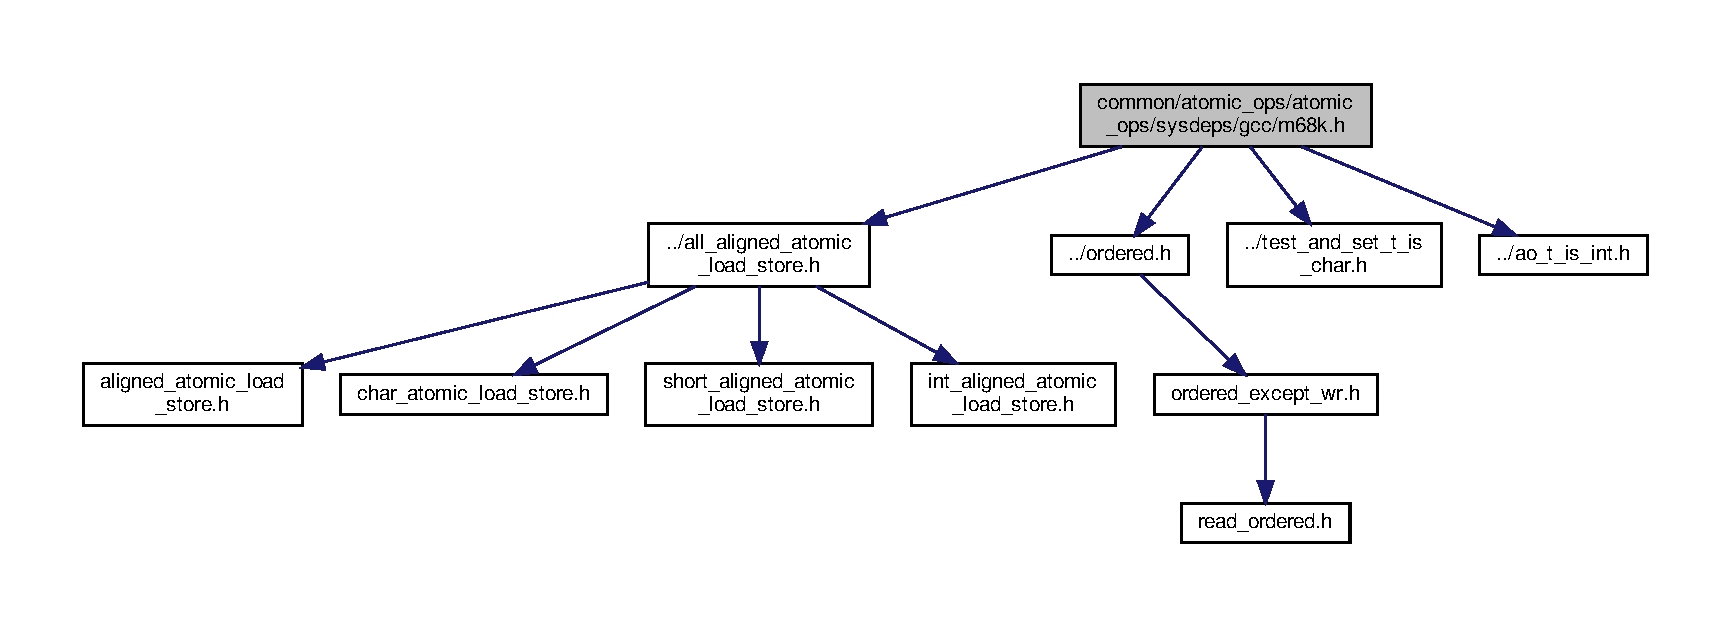
\includegraphics[width=350pt]{m68k_8h__incl}
\end{center}
\end{figure}
\subsection*{Macros}
\begin{DoxyCompactItemize}
\item 
\#define \hyperlink{m68k_8h_ad5f311a090d1e6e1bb35a6e68ee35fad}{A\+O\+\_\+\+H\+A\+V\+E\+\_\+test\+\_\+and\+\_\+set\+\_\+full}
\item 
\#define \hyperlink{m68k_8h_a98ec53065c0dfd18bc1013c500da377c}{A\+O\+\_\+\+H\+A\+V\+E\+\_\+compare\+\_\+and\+\_\+swap\+\_\+full}
\end{DoxyCompactItemize}
\subsection*{Typedefs}
\begin{DoxyCompactItemize}
\item 
typedef unsigned long \hyperlink{atomic__ops_8h_a5225fef4d9eee821e82382cd269160dd}{A\+O\+\_\+t} \hyperlink{m68k_8h_a1f861c7ed98dfa8882b9ec4079781371}{\+\_\+\+\_\+attribute\+\_\+\+\_\+}((aligned(4)))
\end{DoxyCompactItemize}
\subsection*{Functions}
\begin{DoxyCompactItemize}
\item 
\hyperlink{atomic__ops_8h_a9f6ab6253b6b11bc8c12efe9dde5db2b}{A\+O\+\_\+\+I\+N\+L\+I\+NE} \hyperlink{test__and__set__t__is__char_8h_a7d99a16c4eab47ba80ab6138d7d98ac1}{A\+O\+\_\+\+T\+S\+\_\+\+V\+A\+L\+\_\+t} \hyperlink{m68k_8h_a9f485bd63ce5c6a017ec241906e2f651}{A\+O\+\_\+test\+\_\+and\+\_\+set\+\_\+full} (volatile \hyperlink{test__and__set__t__is__char_8h_a5890c21b549264c75c2cad08bf4f6ba9}{A\+O\+\_\+\+T\+S\+\_\+t} $\ast$addr)
\item 
\hyperlink{atomic__ops_8h_a9f6ab6253b6b11bc8c12efe9dde5db2b}{A\+O\+\_\+\+I\+N\+L\+I\+NE} int \hyperlink{m68k_8h_a634397de6de764015b30cdff3ff00b06}{A\+O\+\_\+compare\+\_\+and\+\_\+swap\+\_\+full} (volatile \hyperlink{atomic__ops_8h_a5225fef4d9eee821e82382cd269160dd}{A\+O\+\_\+t} $\ast$addr, \hyperlink{atomic__ops_8h_a5225fef4d9eee821e82382cd269160dd}{A\+O\+\_\+t} old, \hyperlink{atomic__ops_8h_a5225fef4d9eee821e82382cd269160dd}{A\+O\+\_\+t} new\+\_\+val)
\end{DoxyCompactItemize}


\subsection{Macro Definition Documentation}
\mbox{\Hypertarget{m68k_8h_a98ec53065c0dfd18bc1013c500da377c}\label{m68k_8h_a98ec53065c0dfd18bc1013c500da377c}} 
\index{m68k.\+h@{m68k.\+h}!A\+O\+\_\+\+H\+A\+V\+E\+\_\+compare\+\_\+and\+\_\+swap\+\_\+full@{A\+O\+\_\+\+H\+A\+V\+E\+\_\+compare\+\_\+and\+\_\+swap\+\_\+full}}
\index{A\+O\+\_\+\+H\+A\+V\+E\+\_\+compare\+\_\+and\+\_\+swap\+\_\+full@{A\+O\+\_\+\+H\+A\+V\+E\+\_\+compare\+\_\+and\+\_\+swap\+\_\+full}!m68k.\+h@{m68k.\+h}}
\subsubsection{\texorpdfstring{A\+O\+\_\+\+H\+A\+V\+E\+\_\+compare\+\_\+and\+\_\+swap\+\_\+full}{AO\_HAVE\_compare\_and\_swap\_full}}
{\footnotesize\ttfamily \#define A\+O\+\_\+\+H\+A\+V\+E\+\_\+compare\+\_\+and\+\_\+swap\+\_\+full}

\mbox{\Hypertarget{m68k_8h_ad5f311a090d1e6e1bb35a6e68ee35fad}\label{m68k_8h_ad5f311a090d1e6e1bb35a6e68ee35fad}} 
\index{m68k.\+h@{m68k.\+h}!A\+O\+\_\+\+H\+A\+V\+E\+\_\+test\+\_\+and\+\_\+set\+\_\+full@{A\+O\+\_\+\+H\+A\+V\+E\+\_\+test\+\_\+and\+\_\+set\+\_\+full}}
\index{A\+O\+\_\+\+H\+A\+V\+E\+\_\+test\+\_\+and\+\_\+set\+\_\+full@{A\+O\+\_\+\+H\+A\+V\+E\+\_\+test\+\_\+and\+\_\+set\+\_\+full}!m68k.\+h@{m68k.\+h}}
\subsubsection{\texorpdfstring{A\+O\+\_\+\+H\+A\+V\+E\+\_\+test\+\_\+and\+\_\+set\+\_\+full}{AO\_HAVE\_test\_and\_set\_full}}
{\footnotesize\ttfamily \#define A\+O\+\_\+\+H\+A\+V\+E\+\_\+test\+\_\+and\+\_\+set\+\_\+full}



\subsection{Typedef Documentation}
\mbox{\Hypertarget{m68k_8h_a1f861c7ed98dfa8882b9ec4079781371}\label{m68k_8h_a1f861c7ed98dfa8882b9ec4079781371}} 
\index{m68k.\+h@{m68k.\+h}!\+\_\+\+\_\+attribute\+\_\+\+\_\+@{\+\_\+\+\_\+attribute\+\_\+\+\_\+}}
\index{\+\_\+\+\_\+attribute\+\_\+\+\_\+@{\+\_\+\+\_\+attribute\+\_\+\+\_\+}!m68k.\+h@{m68k.\+h}}
\subsubsection{\texorpdfstring{\+\_\+\+\_\+attribute\+\_\+\+\_\+}{\_\_attribute\_\_}}
{\footnotesize\ttfamily typedef unsigned long \hyperlink{atomic__ops_8h_a5225fef4d9eee821e82382cd269160dd}{A\+O\+\_\+t} \+\_\+\+\_\+attribute\+\_\+\+\_\+((aligned(4)))}



\subsection{Function Documentation}
\mbox{\Hypertarget{m68k_8h_a634397de6de764015b30cdff3ff00b06}\label{m68k_8h_a634397de6de764015b30cdff3ff00b06}} 
\index{m68k.\+h@{m68k.\+h}!A\+O\+\_\+compare\+\_\+and\+\_\+swap\+\_\+full@{A\+O\+\_\+compare\+\_\+and\+\_\+swap\+\_\+full}}
\index{A\+O\+\_\+compare\+\_\+and\+\_\+swap\+\_\+full@{A\+O\+\_\+compare\+\_\+and\+\_\+swap\+\_\+full}!m68k.\+h@{m68k.\+h}}
\subsubsection{\texorpdfstring{A\+O\+\_\+compare\+\_\+and\+\_\+swap\+\_\+full()}{AO\_compare\_and\_swap\_full()}}
{\footnotesize\ttfamily \hyperlink{atomic__ops_8h_a9f6ab6253b6b11bc8c12efe9dde5db2b}{A\+O\+\_\+\+I\+N\+L\+I\+NE} int A\+O\+\_\+compare\+\_\+and\+\_\+swap\+\_\+full (\begin{DoxyParamCaption}\item[{volatile \hyperlink{atomic__ops_8h_a5225fef4d9eee821e82382cd269160dd}{A\+O\+\_\+t} $\ast$}]{addr,  }\item[{\hyperlink{atomic__ops_8h_a5225fef4d9eee821e82382cd269160dd}{A\+O\+\_\+t}}]{old,  }\item[{\hyperlink{atomic__ops_8h_a5225fef4d9eee821e82382cd269160dd}{A\+O\+\_\+t}}]{new\+\_\+val }\end{DoxyParamCaption})}

\mbox{\Hypertarget{m68k_8h_a9f485bd63ce5c6a017ec241906e2f651}\label{m68k_8h_a9f485bd63ce5c6a017ec241906e2f651}} 
\index{m68k.\+h@{m68k.\+h}!A\+O\+\_\+test\+\_\+and\+\_\+set\+\_\+full@{A\+O\+\_\+test\+\_\+and\+\_\+set\+\_\+full}}
\index{A\+O\+\_\+test\+\_\+and\+\_\+set\+\_\+full@{A\+O\+\_\+test\+\_\+and\+\_\+set\+\_\+full}!m68k.\+h@{m68k.\+h}}
\subsubsection{\texorpdfstring{A\+O\+\_\+test\+\_\+and\+\_\+set\+\_\+full()}{AO\_test\_and\_set\_full()}}
{\footnotesize\ttfamily \hyperlink{atomic__ops_8h_a9f6ab6253b6b11bc8c12efe9dde5db2b}{A\+O\+\_\+\+I\+N\+L\+I\+NE} \hyperlink{test__and__set__t__is__char_8h_a7d99a16c4eab47ba80ab6138d7d98ac1}{A\+O\+\_\+\+T\+S\+\_\+\+V\+A\+L\+\_\+t} A\+O\+\_\+test\+\_\+and\+\_\+set\+\_\+full (\begin{DoxyParamCaption}\item[{volatile \hyperlink{test__and__set__t__is__char_8h_a5890c21b549264c75c2cad08bf4f6ba9}{A\+O\+\_\+\+T\+S\+\_\+t} $\ast$}]{addr }\end{DoxyParamCaption})}


\hypertarget{mips_8h}{}\section{common/atomic\+\_\+ops/atomic\+\_\+ops/sysdeps/gcc/mips.h File Reference}
\label{mips_8h}\index{common/atomic\+\_\+ops/atomic\+\_\+ops/sysdeps/gcc/mips.\+h@{common/atomic\+\_\+ops/atomic\+\_\+ops/sysdeps/gcc/mips.\+h}}
{\ttfamily \#include \char`\"{}../all\+\_\+aligned\+\_\+atomic\+\_\+load\+\_\+store.\+h\char`\"{}}\newline
{\ttfamily \#include \char`\"{}../acquire\+\_\+release\+\_\+volatile.\+h\char`\"{}}\newline
{\ttfamily \#include \char`\"{}../test\+\_\+and\+\_\+set\+\_\+t\+\_\+is\+\_\+ao\+\_\+t.\+h\char`\"{}}\newline
{\ttfamily \#include \char`\"{}../standard\+\_\+ao\+\_\+double\+\_\+t.\+h\char`\"{}}\newline
{\ttfamily \#include \char`\"{}../ao\+\_\+t\+\_\+is\+\_\+int.\+h\char`\"{}}\newline
Include dependency graph for mips.\+h\+:
\nopagebreak
\begin{figure}[H]
\begin{center}
\leavevmode
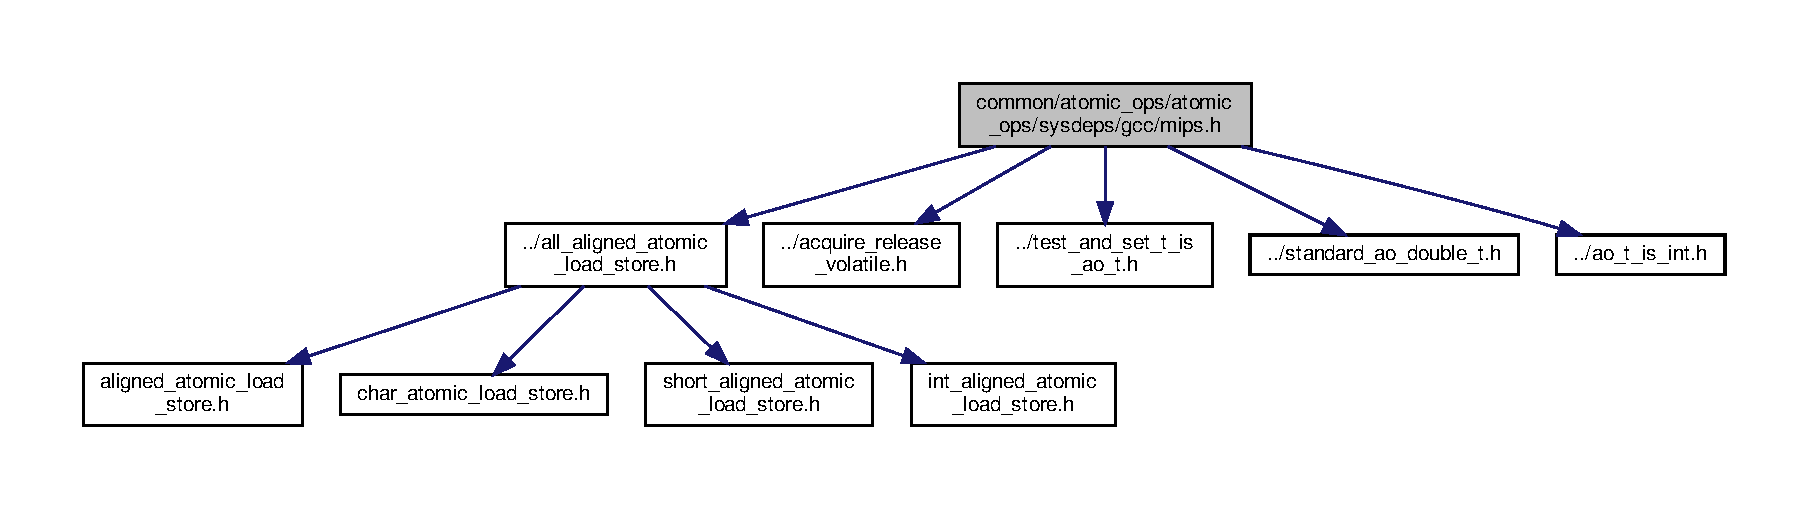
\includegraphics[width=350pt]{mips_8h__incl}
\end{center}
\end{figure}
\subsection*{Macros}
\begin{DoxyCompactItemize}
\item 
\#define \hyperlink{mips_8h_ab65316d98c499c612122d64bc69bf5fa}{A\+O\+\_\+\+N\+O\+\_\+\+D\+D\+\_\+\+O\+R\+D\+E\+R\+I\+NG}
\item 
\#define \hyperlink{mips_8h_a3904dc699d6a6d6e771a93aa66aeb805}{A\+O\+\_\+\+H\+A\+V\+E\+\_\+nop\+\_\+full}
\item 
\#define \hyperlink{mips_8h_a0c5d9cf68a56bfa9e267db0f2795811c}{A\+O\+\_\+\+H\+A\+V\+E\+\_\+compare\+\_\+and\+\_\+swap}
\item 
\#define \hyperlink{mips_8h_ad0b08bc254deecdcba5a4f3366432cf3}{A\+O\+\_\+\+H\+A\+V\+E\+\_\+compare\+\_\+and\+\_\+swap\+\_\+acquire}
\item 
\#define \hyperlink{mips_8h_ad85c7af2ae0a778eba77a7762a358819}{A\+O\+\_\+\+H\+A\+V\+E\+\_\+compare\+\_\+and\+\_\+swap\+\_\+release}
\item 
\#define \hyperlink{mips_8h_a98ec53065c0dfd18bc1013c500da377c}{A\+O\+\_\+\+H\+A\+V\+E\+\_\+compare\+\_\+and\+\_\+swap\+\_\+full}
\end{DoxyCompactItemize}
\subsection*{Functions}
\begin{DoxyCompactItemize}
\item 
\hyperlink{atomic__ops_8h_a9f6ab6253b6b11bc8c12efe9dde5db2b}{A\+O\+\_\+\+I\+N\+L\+I\+NE} void \hyperlink{mips_8h_afe3a6778eacc82252ba138fc9a157b04}{A\+O\+\_\+nop\+\_\+full} (void)
\item 
\hyperlink{atomic__ops_8h_a9f6ab6253b6b11bc8c12efe9dde5db2b}{A\+O\+\_\+\+I\+N\+L\+I\+NE} int \hyperlink{mips_8h_a2e1cdaa59eda3ac15129d16951295698}{A\+O\+\_\+compare\+\_\+and\+\_\+swap} (volatile \hyperlink{atomic__ops_8h_a5225fef4d9eee821e82382cd269160dd}{A\+O\+\_\+t} $\ast$addr, \hyperlink{atomic__ops_8h_a5225fef4d9eee821e82382cd269160dd}{A\+O\+\_\+t} old, \hyperlink{atomic__ops_8h_a5225fef4d9eee821e82382cd269160dd}{A\+O\+\_\+t} new\+\_\+val)
\item 
\hyperlink{atomic__ops_8h_a9f6ab6253b6b11bc8c12efe9dde5db2b}{A\+O\+\_\+\+I\+N\+L\+I\+NE} int \hyperlink{mips_8h_a81fc146600046fb8ee9ce4339f078e2e}{A\+O\+\_\+compare\+\_\+and\+\_\+swap\+\_\+acquire} (volatile \hyperlink{atomic__ops_8h_a5225fef4d9eee821e82382cd269160dd}{A\+O\+\_\+t} $\ast$addr, \hyperlink{atomic__ops_8h_a5225fef4d9eee821e82382cd269160dd}{A\+O\+\_\+t} old, \hyperlink{atomic__ops_8h_a5225fef4d9eee821e82382cd269160dd}{A\+O\+\_\+t} new\+\_\+val)
\item 
\hyperlink{atomic__ops_8h_a9f6ab6253b6b11bc8c12efe9dde5db2b}{A\+O\+\_\+\+I\+N\+L\+I\+NE} int \hyperlink{mips_8h_ae39d774429bea0d5c3b604bbb820a4ea}{A\+O\+\_\+compare\+\_\+and\+\_\+swap\+\_\+release} (volatile \hyperlink{atomic__ops_8h_a5225fef4d9eee821e82382cd269160dd}{A\+O\+\_\+t} $\ast$addr, \hyperlink{atomic__ops_8h_a5225fef4d9eee821e82382cd269160dd}{A\+O\+\_\+t} old, \hyperlink{atomic__ops_8h_a5225fef4d9eee821e82382cd269160dd}{A\+O\+\_\+t} new\+\_\+val)
\item 
\hyperlink{atomic__ops_8h_a9f6ab6253b6b11bc8c12efe9dde5db2b}{A\+O\+\_\+\+I\+N\+L\+I\+NE} int \hyperlink{mips_8h_a634397de6de764015b30cdff3ff00b06}{A\+O\+\_\+compare\+\_\+and\+\_\+swap\+\_\+full} (volatile \hyperlink{atomic__ops_8h_a5225fef4d9eee821e82382cd269160dd}{A\+O\+\_\+t} $\ast$addr, \hyperlink{atomic__ops_8h_a5225fef4d9eee821e82382cd269160dd}{A\+O\+\_\+t} old, \hyperlink{atomic__ops_8h_a5225fef4d9eee821e82382cd269160dd}{A\+O\+\_\+t} new\+\_\+val)
\end{DoxyCompactItemize}


\subsection{Macro Definition Documentation}
\mbox{\Hypertarget{mips_8h_a0c5d9cf68a56bfa9e267db0f2795811c}\label{mips_8h_a0c5d9cf68a56bfa9e267db0f2795811c}} 
\index{mips.\+h@{mips.\+h}!A\+O\+\_\+\+H\+A\+V\+E\+\_\+compare\+\_\+and\+\_\+swap@{A\+O\+\_\+\+H\+A\+V\+E\+\_\+compare\+\_\+and\+\_\+swap}}
\index{A\+O\+\_\+\+H\+A\+V\+E\+\_\+compare\+\_\+and\+\_\+swap@{A\+O\+\_\+\+H\+A\+V\+E\+\_\+compare\+\_\+and\+\_\+swap}!mips.\+h@{mips.\+h}}
\subsubsection{\texorpdfstring{A\+O\+\_\+\+H\+A\+V\+E\+\_\+compare\+\_\+and\+\_\+swap}{AO\_HAVE\_compare\_and\_swap}}
{\footnotesize\ttfamily \#define A\+O\+\_\+\+H\+A\+V\+E\+\_\+compare\+\_\+and\+\_\+swap}

\mbox{\Hypertarget{mips_8h_ad0b08bc254deecdcba5a4f3366432cf3}\label{mips_8h_ad0b08bc254deecdcba5a4f3366432cf3}} 
\index{mips.\+h@{mips.\+h}!A\+O\+\_\+\+H\+A\+V\+E\+\_\+compare\+\_\+and\+\_\+swap\+\_\+acquire@{A\+O\+\_\+\+H\+A\+V\+E\+\_\+compare\+\_\+and\+\_\+swap\+\_\+acquire}}
\index{A\+O\+\_\+\+H\+A\+V\+E\+\_\+compare\+\_\+and\+\_\+swap\+\_\+acquire@{A\+O\+\_\+\+H\+A\+V\+E\+\_\+compare\+\_\+and\+\_\+swap\+\_\+acquire}!mips.\+h@{mips.\+h}}
\subsubsection{\texorpdfstring{A\+O\+\_\+\+H\+A\+V\+E\+\_\+compare\+\_\+and\+\_\+swap\+\_\+acquire}{AO\_HAVE\_compare\_and\_swap\_acquire}}
{\footnotesize\ttfamily \#define A\+O\+\_\+\+H\+A\+V\+E\+\_\+compare\+\_\+and\+\_\+swap\+\_\+acquire}

\mbox{\Hypertarget{mips_8h_a98ec53065c0dfd18bc1013c500da377c}\label{mips_8h_a98ec53065c0dfd18bc1013c500da377c}} 
\index{mips.\+h@{mips.\+h}!A\+O\+\_\+\+H\+A\+V\+E\+\_\+compare\+\_\+and\+\_\+swap\+\_\+full@{A\+O\+\_\+\+H\+A\+V\+E\+\_\+compare\+\_\+and\+\_\+swap\+\_\+full}}
\index{A\+O\+\_\+\+H\+A\+V\+E\+\_\+compare\+\_\+and\+\_\+swap\+\_\+full@{A\+O\+\_\+\+H\+A\+V\+E\+\_\+compare\+\_\+and\+\_\+swap\+\_\+full}!mips.\+h@{mips.\+h}}
\subsubsection{\texorpdfstring{A\+O\+\_\+\+H\+A\+V\+E\+\_\+compare\+\_\+and\+\_\+swap\+\_\+full}{AO\_HAVE\_compare\_and\_swap\_full}}
{\footnotesize\ttfamily \#define A\+O\+\_\+\+H\+A\+V\+E\+\_\+compare\+\_\+and\+\_\+swap\+\_\+full}

\mbox{\Hypertarget{mips_8h_ad85c7af2ae0a778eba77a7762a358819}\label{mips_8h_ad85c7af2ae0a778eba77a7762a358819}} 
\index{mips.\+h@{mips.\+h}!A\+O\+\_\+\+H\+A\+V\+E\+\_\+compare\+\_\+and\+\_\+swap\+\_\+release@{A\+O\+\_\+\+H\+A\+V\+E\+\_\+compare\+\_\+and\+\_\+swap\+\_\+release}}
\index{A\+O\+\_\+\+H\+A\+V\+E\+\_\+compare\+\_\+and\+\_\+swap\+\_\+release@{A\+O\+\_\+\+H\+A\+V\+E\+\_\+compare\+\_\+and\+\_\+swap\+\_\+release}!mips.\+h@{mips.\+h}}
\subsubsection{\texorpdfstring{A\+O\+\_\+\+H\+A\+V\+E\+\_\+compare\+\_\+and\+\_\+swap\+\_\+release}{AO\_HAVE\_compare\_and\_swap\_release}}
{\footnotesize\ttfamily \#define A\+O\+\_\+\+H\+A\+V\+E\+\_\+compare\+\_\+and\+\_\+swap\+\_\+release}

\mbox{\Hypertarget{mips_8h_a3904dc699d6a6d6e771a93aa66aeb805}\label{mips_8h_a3904dc699d6a6d6e771a93aa66aeb805}} 
\index{mips.\+h@{mips.\+h}!A\+O\+\_\+\+H\+A\+V\+E\+\_\+nop\+\_\+full@{A\+O\+\_\+\+H\+A\+V\+E\+\_\+nop\+\_\+full}}
\index{A\+O\+\_\+\+H\+A\+V\+E\+\_\+nop\+\_\+full@{A\+O\+\_\+\+H\+A\+V\+E\+\_\+nop\+\_\+full}!mips.\+h@{mips.\+h}}
\subsubsection{\texorpdfstring{A\+O\+\_\+\+H\+A\+V\+E\+\_\+nop\+\_\+full}{AO\_HAVE\_nop\_full}}
{\footnotesize\ttfamily \#define A\+O\+\_\+\+H\+A\+V\+E\+\_\+nop\+\_\+full}

\mbox{\Hypertarget{mips_8h_ab65316d98c499c612122d64bc69bf5fa}\label{mips_8h_ab65316d98c499c612122d64bc69bf5fa}} 
\index{mips.\+h@{mips.\+h}!A\+O\+\_\+\+N\+O\+\_\+\+D\+D\+\_\+\+O\+R\+D\+E\+R\+I\+NG@{A\+O\+\_\+\+N\+O\+\_\+\+D\+D\+\_\+\+O\+R\+D\+E\+R\+I\+NG}}
\index{A\+O\+\_\+\+N\+O\+\_\+\+D\+D\+\_\+\+O\+R\+D\+E\+R\+I\+NG@{A\+O\+\_\+\+N\+O\+\_\+\+D\+D\+\_\+\+O\+R\+D\+E\+R\+I\+NG}!mips.\+h@{mips.\+h}}
\subsubsection{\texorpdfstring{A\+O\+\_\+\+N\+O\+\_\+\+D\+D\+\_\+\+O\+R\+D\+E\+R\+I\+NG}{AO\_NO\_DD\_ORDERING}}
{\footnotesize\ttfamily \#define A\+O\+\_\+\+N\+O\+\_\+\+D\+D\+\_\+\+O\+R\+D\+E\+R\+I\+NG}



\subsection{Function Documentation}
\mbox{\Hypertarget{mips_8h_a2e1cdaa59eda3ac15129d16951295698}\label{mips_8h_a2e1cdaa59eda3ac15129d16951295698}} 
\index{mips.\+h@{mips.\+h}!A\+O\+\_\+compare\+\_\+and\+\_\+swap@{A\+O\+\_\+compare\+\_\+and\+\_\+swap}}
\index{A\+O\+\_\+compare\+\_\+and\+\_\+swap@{A\+O\+\_\+compare\+\_\+and\+\_\+swap}!mips.\+h@{mips.\+h}}
\subsubsection{\texorpdfstring{A\+O\+\_\+compare\+\_\+and\+\_\+swap()}{AO\_compare\_and\_swap()}}
{\footnotesize\ttfamily \hyperlink{atomic__ops_8h_a9f6ab6253b6b11bc8c12efe9dde5db2b}{A\+O\+\_\+\+I\+N\+L\+I\+NE} int A\+O\+\_\+compare\+\_\+and\+\_\+swap (\begin{DoxyParamCaption}\item[{volatile \hyperlink{atomic__ops_8h_a5225fef4d9eee821e82382cd269160dd}{A\+O\+\_\+t} $\ast$}]{addr,  }\item[{\hyperlink{atomic__ops_8h_a5225fef4d9eee821e82382cd269160dd}{A\+O\+\_\+t}}]{old,  }\item[{\hyperlink{atomic__ops_8h_a5225fef4d9eee821e82382cd269160dd}{A\+O\+\_\+t}}]{new\+\_\+val }\end{DoxyParamCaption})}

\mbox{\Hypertarget{mips_8h_a81fc146600046fb8ee9ce4339f078e2e}\label{mips_8h_a81fc146600046fb8ee9ce4339f078e2e}} 
\index{mips.\+h@{mips.\+h}!A\+O\+\_\+compare\+\_\+and\+\_\+swap\+\_\+acquire@{A\+O\+\_\+compare\+\_\+and\+\_\+swap\+\_\+acquire}}
\index{A\+O\+\_\+compare\+\_\+and\+\_\+swap\+\_\+acquire@{A\+O\+\_\+compare\+\_\+and\+\_\+swap\+\_\+acquire}!mips.\+h@{mips.\+h}}
\subsubsection{\texorpdfstring{A\+O\+\_\+compare\+\_\+and\+\_\+swap\+\_\+acquire()}{AO\_compare\_and\_swap\_acquire()}}
{\footnotesize\ttfamily \hyperlink{atomic__ops_8h_a9f6ab6253b6b11bc8c12efe9dde5db2b}{A\+O\+\_\+\+I\+N\+L\+I\+NE} int A\+O\+\_\+compare\+\_\+and\+\_\+swap\+\_\+acquire (\begin{DoxyParamCaption}\item[{volatile \hyperlink{atomic__ops_8h_a5225fef4d9eee821e82382cd269160dd}{A\+O\+\_\+t} $\ast$}]{addr,  }\item[{\hyperlink{atomic__ops_8h_a5225fef4d9eee821e82382cd269160dd}{A\+O\+\_\+t}}]{old,  }\item[{\hyperlink{atomic__ops_8h_a5225fef4d9eee821e82382cd269160dd}{A\+O\+\_\+t}}]{new\+\_\+val }\end{DoxyParamCaption})}

\mbox{\Hypertarget{mips_8h_a634397de6de764015b30cdff3ff00b06}\label{mips_8h_a634397de6de764015b30cdff3ff00b06}} 
\index{mips.\+h@{mips.\+h}!A\+O\+\_\+compare\+\_\+and\+\_\+swap\+\_\+full@{A\+O\+\_\+compare\+\_\+and\+\_\+swap\+\_\+full}}
\index{A\+O\+\_\+compare\+\_\+and\+\_\+swap\+\_\+full@{A\+O\+\_\+compare\+\_\+and\+\_\+swap\+\_\+full}!mips.\+h@{mips.\+h}}
\subsubsection{\texorpdfstring{A\+O\+\_\+compare\+\_\+and\+\_\+swap\+\_\+full()}{AO\_compare\_and\_swap\_full()}}
{\footnotesize\ttfamily \hyperlink{atomic__ops_8h_a9f6ab6253b6b11bc8c12efe9dde5db2b}{A\+O\+\_\+\+I\+N\+L\+I\+NE} int A\+O\+\_\+compare\+\_\+and\+\_\+swap\+\_\+full (\begin{DoxyParamCaption}\item[{volatile \hyperlink{atomic__ops_8h_a5225fef4d9eee821e82382cd269160dd}{A\+O\+\_\+t} $\ast$}]{addr,  }\item[{\hyperlink{atomic__ops_8h_a5225fef4d9eee821e82382cd269160dd}{A\+O\+\_\+t}}]{old,  }\item[{\hyperlink{atomic__ops_8h_a5225fef4d9eee821e82382cd269160dd}{A\+O\+\_\+t}}]{new\+\_\+val }\end{DoxyParamCaption})}

\mbox{\Hypertarget{mips_8h_ae39d774429bea0d5c3b604bbb820a4ea}\label{mips_8h_ae39d774429bea0d5c3b604bbb820a4ea}} 
\index{mips.\+h@{mips.\+h}!A\+O\+\_\+compare\+\_\+and\+\_\+swap\+\_\+release@{A\+O\+\_\+compare\+\_\+and\+\_\+swap\+\_\+release}}
\index{A\+O\+\_\+compare\+\_\+and\+\_\+swap\+\_\+release@{A\+O\+\_\+compare\+\_\+and\+\_\+swap\+\_\+release}!mips.\+h@{mips.\+h}}
\subsubsection{\texorpdfstring{A\+O\+\_\+compare\+\_\+and\+\_\+swap\+\_\+release()}{AO\_compare\_and\_swap\_release()}}
{\footnotesize\ttfamily \hyperlink{atomic__ops_8h_a9f6ab6253b6b11bc8c12efe9dde5db2b}{A\+O\+\_\+\+I\+N\+L\+I\+NE} int A\+O\+\_\+compare\+\_\+and\+\_\+swap\+\_\+release (\begin{DoxyParamCaption}\item[{volatile \hyperlink{atomic__ops_8h_a5225fef4d9eee821e82382cd269160dd}{A\+O\+\_\+t} $\ast$}]{addr,  }\item[{\hyperlink{atomic__ops_8h_a5225fef4d9eee821e82382cd269160dd}{A\+O\+\_\+t}}]{old,  }\item[{\hyperlink{atomic__ops_8h_a5225fef4d9eee821e82382cd269160dd}{A\+O\+\_\+t}}]{new\+\_\+val }\end{DoxyParamCaption})}

\mbox{\Hypertarget{mips_8h_afe3a6778eacc82252ba138fc9a157b04}\label{mips_8h_afe3a6778eacc82252ba138fc9a157b04}} 
\index{mips.\+h@{mips.\+h}!A\+O\+\_\+nop\+\_\+full@{A\+O\+\_\+nop\+\_\+full}}
\index{A\+O\+\_\+nop\+\_\+full@{A\+O\+\_\+nop\+\_\+full}!mips.\+h@{mips.\+h}}
\subsubsection{\texorpdfstring{A\+O\+\_\+nop\+\_\+full()}{AO\_nop\_full()}}
{\footnotesize\ttfamily \hyperlink{atomic__ops_8h_a9f6ab6253b6b11bc8c12efe9dde5db2b}{A\+O\+\_\+\+I\+N\+L\+I\+NE} void A\+O\+\_\+nop\+\_\+full (\begin{DoxyParamCaption}\item[{void}]{ }\end{DoxyParamCaption})}


\hypertarget{gcc_2powerpc_8h}{}\section{common/atomic\+\_\+ops/atomic\+\_\+ops/sysdeps/gcc/powerpc.h File Reference}
\label{gcc_2powerpc_8h}\index{common/atomic\+\_\+ops/atomic\+\_\+ops/sysdeps/gcc/powerpc.\+h@{common/atomic\+\_\+ops/atomic\+\_\+ops/sysdeps/gcc/powerpc.\+h}}
{\ttfamily \#include \char`\"{}../all\+\_\+aligned\+\_\+atomic\+\_\+load\+\_\+store.\+h\char`\"{}}\newline
{\ttfamily \#include \char`\"{}../test\+\_\+and\+\_\+set\+\_\+t\+\_\+is\+\_\+ao\+\_\+t.\+h\char`\"{}}\newline
{\ttfamily \#include \char`\"{}../ao\+\_\+t\+\_\+is\+\_\+int.\+h\char`\"{}}\newline
Include dependency graph for powerpc.\+h\+:
\nopagebreak
\begin{figure}[H]
\begin{center}
\leavevmode
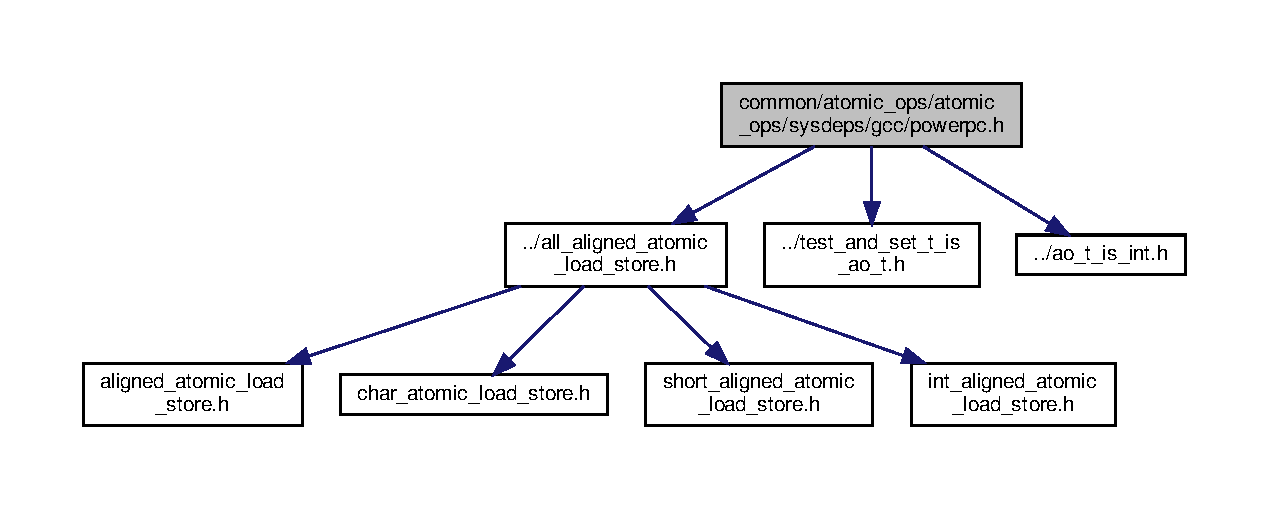
\includegraphics[width=350pt]{gcc_2powerpc_8h__incl}
\end{center}
\end{figure}
\subsection*{Macros}
\begin{DoxyCompactItemize}
\item 
\#define \hyperlink{gcc_2powerpc_8h_a3904dc699d6a6d6e771a93aa66aeb805}{A\+O\+\_\+\+H\+A\+V\+E\+\_\+nop\+\_\+full}
\item 
\#define \hyperlink{gcc_2powerpc_8h_aa6b9cf57e4373ade9ce01d28a58ad21d}{A\+O\+\_\+nop\+\_\+write}()~\hyperlink{ibmc_2powerpc_8h_a5febfde98faf0a03093897ef864a9589}{A\+O\+\_\+lwsync}()
\item 
\#define \hyperlink{gcc_2powerpc_8h_a7c6d0c7c0585da4d8cd259df2423b82f}{A\+O\+\_\+\+H\+A\+V\+E\+\_\+nop\+\_\+write}
\item 
\#define \hyperlink{gcc_2powerpc_8h_a3a367b9626ced22d98eb45e958a21aad}{A\+O\+\_\+nop\+\_\+read}()~\hyperlink{ibmc_2powerpc_8h_a5febfde98faf0a03093897ef864a9589}{A\+O\+\_\+lwsync}()
\item 
\#define \hyperlink{gcc_2powerpc_8h_a5e899b880760568b4da25ec2d6011cbd}{A\+O\+\_\+\+H\+A\+V\+E\+\_\+nop\+\_\+read}
\item 
\#define \hyperlink{gcc_2powerpc_8h_a29328d5664268a40645ea9d2f82c8bef}{A\+O\+\_\+\+H\+A\+V\+E\+\_\+load\+\_\+acquire}
\item 
\#define \hyperlink{gcc_2powerpc_8h_a29328d5664268a40645ea9d2f82c8bef}{A\+O\+\_\+\+H\+A\+V\+E\+\_\+load\+\_\+acquire}
\item 
\#define \hyperlink{gcc_2powerpc_8h_a6ad5da471c2a52c703969db302060c12}{A\+O\+\_\+\+H\+A\+V\+E\+\_\+test\+\_\+and\+\_\+set}
\item 
\#define \hyperlink{gcc_2powerpc_8h_addf7856c1f3a120a04ad68e843b23de4}{A\+O\+\_\+\+H\+A\+V\+E\+\_\+test\+\_\+and\+\_\+set\+\_\+acquire}
\item 
\#define \hyperlink{gcc_2powerpc_8h_a27cd35e8e9c1987a362a8610811e1c40}{A\+O\+\_\+\+H\+A\+V\+E\+\_\+test\+\_\+and\+\_\+set\+\_\+release}
\item 
\#define \hyperlink{gcc_2powerpc_8h_ad5f311a090d1e6e1bb35a6e68ee35fad}{A\+O\+\_\+\+H\+A\+V\+E\+\_\+test\+\_\+and\+\_\+set\+\_\+full}
\item 
\#define \hyperlink{gcc_2powerpc_8h_a0c5d9cf68a56bfa9e267db0f2795811c}{A\+O\+\_\+\+H\+A\+V\+E\+\_\+compare\+\_\+and\+\_\+swap}
\item 
\#define \hyperlink{gcc_2powerpc_8h_ad0b08bc254deecdcba5a4f3366432cf3}{A\+O\+\_\+\+H\+A\+V\+E\+\_\+compare\+\_\+and\+\_\+swap\+\_\+acquire}
\item 
\#define \hyperlink{gcc_2powerpc_8h_ad85c7af2ae0a778eba77a7762a358819}{A\+O\+\_\+\+H\+A\+V\+E\+\_\+compare\+\_\+and\+\_\+swap\+\_\+release}
\item 
\#define \hyperlink{gcc_2powerpc_8h_a98ec53065c0dfd18bc1013c500da377c}{A\+O\+\_\+\+H\+A\+V\+E\+\_\+compare\+\_\+and\+\_\+swap\+\_\+full}
\item 
\#define \hyperlink{gcc_2powerpc_8h_a02ddf1d6bcd91f33310ecc1046fac9e0}{A\+O\+\_\+\+H\+A\+V\+E\+\_\+fetch\+\_\+and\+\_\+add}
\item 
\#define \hyperlink{gcc_2powerpc_8h_a382c4cd949fca638724c9b2d82456223}{A\+O\+\_\+\+H\+A\+V\+E\+\_\+fetch\+\_\+and\+\_\+add\+\_\+acquire}
\item 
\#define \hyperlink{gcc_2powerpc_8h_a5b93814d170e72872f2552552c63c2e4}{A\+O\+\_\+\+H\+A\+V\+E\+\_\+fetch\+\_\+and\+\_\+add\+\_\+release}
\item 
\#define \hyperlink{gcc_2powerpc_8h_a9fa0fc1a9eadcba085e57bf180a53cef}{A\+O\+\_\+\+H\+A\+V\+E\+\_\+fetch\+\_\+and\+\_\+add\+\_\+full}
\end{DoxyCompactItemize}
\subsection*{Functions}
\begin{DoxyCompactItemize}
\item 
\hyperlink{atomic__ops_8h_a9f6ab6253b6b11bc8c12efe9dde5db2b}{A\+O\+\_\+\+I\+N\+L\+I\+NE} void \hyperlink{gcc_2powerpc_8h_afe3a6778eacc82252ba138fc9a157b04}{A\+O\+\_\+nop\+\_\+full} (void)
\item 
\hyperlink{atomic__ops_8h_a9f6ab6253b6b11bc8c12efe9dde5db2b}{A\+O\+\_\+\+I\+N\+L\+I\+NE} void \hyperlink{gcc_2powerpc_8h_a75a6574066b34ce697dcc012ec0e7128}{A\+O\+\_\+lwsync} (void)
\item 
\hyperlink{atomic__ops_8h_a9f6ab6253b6b11bc8c12efe9dde5db2b}{A\+O\+\_\+\+I\+N\+L\+I\+NE} \hyperlink{atomic__ops_8h_a5225fef4d9eee821e82382cd269160dd}{A\+O\+\_\+t} \hyperlink{gcc_2powerpc_8h_afd982c8bbaa60d3294cc30f92f170847}{A\+O\+\_\+load\+\_\+acquire} (const volatile \hyperlink{atomic__ops_8h_a5225fef4d9eee821e82382cd269160dd}{A\+O\+\_\+t} $\ast$addr)
\item 
\hyperlink{atomic__ops_8h_a9f6ab6253b6b11bc8c12efe9dde5db2b}{A\+O\+\_\+\+I\+N\+L\+I\+NE} void \hyperlink{gcc_2powerpc_8h_a7b4e8216189c3f4e7f7418e5c2a98b0f}{A\+O\+\_\+store\+\_\+release} (volatile \hyperlink{atomic__ops_8h_a5225fef4d9eee821e82382cd269160dd}{A\+O\+\_\+t} $\ast$addr, \hyperlink{atomic__ops_8h_a5225fef4d9eee821e82382cd269160dd}{A\+O\+\_\+t} value)
\item 
\hyperlink{atomic__ops_8h_a9f6ab6253b6b11bc8c12efe9dde5db2b}{A\+O\+\_\+\+I\+N\+L\+I\+NE} \hyperlink{test__and__set__t__is__char_8h_a7d99a16c4eab47ba80ab6138d7d98ac1}{A\+O\+\_\+\+T\+S\+\_\+\+V\+A\+L\+\_\+t} \hyperlink{gcc_2powerpc_8h_a8ec1c2583e26c57a7b4d17f239fa41e8}{A\+O\+\_\+test\+\_\+and\+\_\+set} (volatile \hyperlink{test__and__set__t__is__char_8h_a5890c21b549264c75c2cad08bf4f6ba9}{A\+O\+\_\+\+T\+S\+\_\+t} $\ast$addr)
\item 
\hyperlink{atomic__ops_8h_a9f6ab6253b6b11bc8c12efe9dde5db2b}{A\+O\+\_\+\+I\+N\+L\+I\+NE} \hyperlink{test__and__set__t__is__char_8h_a7d99a16c4eab47ba80ab6138d7d98ac1}{A\+O\+\_\+\+T\+S\+\_\+\+V\+A\+L\+\_\+t} \hyperlink{gcc_2powerpc_8h_a0af1bdd53473eb43906a057efe883f6d}{A\+O\+\_\+test\+\_\+and\+\_\+set\+\_\+acquire} (volatile \hyperlink{test__and__set__t__is__char_8h_a5890c21b549264c75c2cad08bf4f6ba9}{A\+O\+\_\+\+T\+S\+\_\+t} $\ast$addr)
\item 
\hyperlink{atomic__ops_8h_a9f6ab6253b6b11bc8c12efe9dde5db2b}{A\+O\+\_\+\+I\+N\+L\+I\+NE} \hyperlink{test__and__set__t__is__char_8h_a7d99a16c4eab47ba80ab6138d7d98ac1}{A\+O\+\_\+\+T\+S\+\_\+\+V\+A\+L\+\_\+t} \hyperlink{gcc_2powerpc_8h_abd4f99ea301b67851c8a6a1dc61e97c1}{A\+O\+\_\+test\+\_\+and\+\_\+set\+\_\+release} (volatile \hyperlink{test__and__set__t__is__char_8h_a5890c21b549264c75c2cad08bf4f6ba9}{A\+O\+\_\+\+T\+S\+\_\+t} $\ast$addr)
\item 
\hyperlink{atomic__ops_8h_a9f6ab6253b6b11bc8c12efe9dde5db2b}{A\+O\+\_\+\+I\+N\+L\+I\+NE} \hyperlink{test__and__set__t__is__char_8h_a7d99a16c4eab47ba80ab6138d7d98ac1}{A\+O\+\_\+\+T\+S\+\_\+\+V\+A\+L\+\_\+t} \hyperlink{gcc_2powerpc_8h_a9f485bd63ce5c6a017ec241906e2f651}{A\+O\+\_\+test\+\_\+and\+\_\+set\+\_\+full} (volatile \hyperlink{test__and__set__t__is__char_8h_a5890c21b549264c75c2cad08bf4f6ba9}{A\+O\+\_\+\+T\+S\+\_\+t} $\ast$addr)
\item 
\hyperlink{atomic__ops_8h_a9f6ab6253b6b11bc8c12efe9dde5db2b}{A\+O\+\_\+\+I\+N\+L\+I\+NE} int \hyperlink{gcc_2powerpc_8h_a2e1cdaa59eda3ac15129d16951295698}{A\+O\+\_\+compare\+\_\+and\+\_\+swap} (volatile \hyperlink{atomic__ops_8h_a5225fef4d9eee821e82382cd269160dd}{A\+O\+\_\+t} $\ast$addr, \hyperlink{atomic__ops_8h_a5225fef4d9eee821e82382cd269160dd}{A\+O\+\_\+t} old, \hyperlink{atomic__ops_8h_a5225fef4d9eee821e82382cd269160dd}{A\+O\+\_\+t} new\+\_\+val)
\item 
\hyperlink{atomic__ops_8h_a9f6ab6253b6b11bc8c12efe9dde5db2b}{A\+O\+\_\+\+I\+N\+L\+I\+NE} int \hyperlink{gcc_2powerpc_8h_a81fc146600046fb8ee9ce4339f078e2e}{A\+O\+\_\+compare\+\_\+and\+\_\+swap\+\_\+acquire} (volatile \hyperlink{atomic__ops_8h_a5225fef4d9eee821e82382cd269160dd}{A\+O\+\_\+t} $\ast$addr, \hyperlink{atomic__ops_8h_a5225fef4d9eee821e82382cd269160dd}{A\+O\+\_\+t} old, \hyperlink{atomic__ops_8h_a5225fef4d9eee821e82382cd269160dd}{A\+O\+\_\+t} new\+\_\+val)
\item 
\hyperlink{atomic__ops_8h_a9f6ab6253b6b11bc8c12efe9dde5db2b}{A\+O\+\_\+\+I\+N\+L\+I\+NE} int \hyperlink{gcc_2powerpc_8h_ae39d774429bea0d5c3b604bbb820a4ea}{A\+O\+\_\+compare\+\_\+and\+\_\+swap\+\_\+release} (volatile \hyperlink{atomic__ops_8h_a5225fef4d9eee821e82382cd269160dd}{A\+O\+\_\+t} $\ast$addr, \hyperlink{atomic__ops_8h_a5225fef4d9eee821e82382cd269160dd}{A\+O\+\_\+t} old, \hyperlink{atomic__ops_8h_a5225fef4d9eee821e82382cd269160dd}{A\+O\+\_\+t} new\+\_\+val)
\item 
\hyperlink{atomic__ops_8h_a9f6ab6253b6b11bc8c12efe9dde5db2b}{A\+O\+\_\+\+I\+N\+L\+I\+NE} int \hyperlink{gcc_2powerpc_8h_a634397de6de764015b30cdff3ff00b06}{A\+O\+\_\+compare\+\_\+and\+\_\+swap\+\_\+full} (volatile \hyperlink{atomic__ops_8h_a5225fef4d9eee821e82382cd269160dd}{A\+O\+\_\+t} $\ast$addr, \hyperlink{atomic__ops_8h_a5225fef4d9eee821e82382cd269160dd}{A\+O\+\_\+t} old, \hyperlink{atomic__ops_8h_a5225fef4d9eee821e82382cd269160dd}{A\+O\+\_\+t} new\+\_\+val)
\item 
\hyperlink{atomic__ops_8h_a9f6ab6253b6b11bc8c12efe9dde5db2b}{A\+O\+\_\+\+I\+N\+L\+I\+NE} \hyperlink{atomic__ops_8h_a5225fef4d9eee821e82382cd269160dd}{A\+O\+\_\+t} \hyperlink{gcc_2powerpc_8h_a170c7c9f843994a726a56442e732afc1}{A\+O\+\_\+fetch\+\_\+and\+\_\+add} (volatile \hyperlink{atomic__ops_8h_a5225fef4d9eee821e82382cd269160dd}{A\+O\+\_\+t} $\ast$addr, \hyperlink{atomic__ops_8h_a5225fef4d9eee821e82382cd269160dd}{A\+O\+\_\+t} incr)
\item 
\hyperlink{atomic__ops_8h_a9f6ab6253b6b11bc8c12efe9dde5db2b}{A\+O\+\_\+\+I\+N\+L\+I\+NE} \hyperlink{atomic__ops_8h_a5225fef4d9eee821e82382cd269160dd}{A\+O\+\_\+t} \hyperlink{gcc_2powerpc_8h_a5c9e99c843f97a3706a23a6b453e39dd}{A\+O\+\_\+fetch\+\_\+and\+\_\+add\+\_\+acquire} (volatile \hyperlink{atomic__ops_8h_a5225fef4d9eee821e82382cd269160dd}{A\+O\+\_\+t} $\ast$addr, \hyperlink{atomic__ops_8h_a5225fef4d9eee821e82382cd269160dd}{A\+O\+\_\+t} incr)
\item 
\hyperlink{atomic__ops_8h_a9f6ab6253b6b11bc8c12efe9dde5db2b}{A\+O\+\_\+\+I\+N\+L\+I\+NE} \hyperlink{atomic__ops_8h_a5225fef4d9eee821e82382cd269160dd}{A\+O\+\_\+t} \hyperlink{gcc_2powerpc_8h_a0d6acfb6d483cd1641c5d01df6b9d3ff}{A\+O\+\_\+fetch\+\_\+and\+\_\+add\+\_\+release} (volatile \hyperlink{atomic__ops_8h_a5225fef4d9eee821e82382cd269160dd}{A\+O\+\_\+t} $\ast$addr, \hyperlink{atomic__ops_8h_a5225fef4d9eee821e82382cd269160dd}{A\+O\+\_\+t} incr)
\item 
\hyperlink{atomic__ops_8h_a9f6ab6253b6b11bc8c12efe9dde5db2b}{A\+O\+\_\+\+I\+N\+L\+I\+NE} \hyperlink{atomic__ops_8h_a5225fef4d9eee821e82382cd269160dd}{A\+O\+\_\+t} \hyperlink{gcc_2powerpc_8h_abdc9c4590fde7e5847593f6a9c250d7f}{A\+O\+\_\+fetch\+\_\+and\+\_\+add\+\_\+full} (volatile \hyperlink{atomic__ops_8h_a5225fef4d9eee821e82382cd269160dd}{A\+O\+\_\+t} $\ast$addr, \hyperlink{atomic__ops_8h_a5225fef4d9eee821e82382cd269160dd}{A\+O\+\_\+t} incr)
\end{DoxyCompactItemize}


\subsection{Macro Definition Documentation}
\mbox{\Hypertarget{gcc_2powerpc_8h_a0c5d9cf68a56bfa9e267db0f2795811c}\label{gcc_2powerpc_8h_a0c5d9cf68a56bfa9e267db0f2795811c}} 
\index{gcc/powerpc.\+h@{gcc/powerpc.\+h}!A\+O\+\_\+\+H\+A\+V\+E\+\_\+compare\+\_\+and\+\_\+swap@{A\+O\+\_\+\+H\+A\+V\+E\+\_\+compare\+\_\+and\+\_\+swap}}
\index{A\+O\+\_\+\+H\+A\+V\+E\+\_\+compare\+\_\+and\+\_\+swap@{A\+O\+\_\+\+H\+A\+V\+E\+\_\+compare\+\_\+and\+\_\+swap}!gcc/powerpc.\+h@{gcc/powerpc.\+h}}
\subsubsection{\texorpdfstring{A\+O\+\_\+\+H\+A\+V\+E\+\_\+compare\+\_\+and\+\_\+swap}{AO\_HAVE\_compare\_and\_swap}}
{\footnotesize\ttfamily \#define A\+O\+\_\+\+H\+A\+V\+E\+\_\+compare\+\_\+and\+\_\+swap}

\mbox{\Hypertarget{gcc_2powerpc_8h_ad0b08bc254deecdcba5a4f3366432cf3}\label{gcc_2powerpc_8h_ad0b08bc254deecdcba5a4f3366432cf3}} 
\index{gcc/powerpc.\+h@{gcc/powerpc.\+h}!A\+O\+\_\+\+H\+A\+V\+E\+\_\+compare\+\_\+and\+\_\+swap\+\_\+acquire@{A\+O\+\_\+\+H\+A\+V\+E\+\_\+compare\+\_\+and\+\_\+swap\+\_\+acquire}}
\index{A\+O\+\_\+\+H\+A\+V\+E\+\_\+compare\+\_\+and\+\_\+swap\+\_\+acquire@{A\+O\+\_\+\+H\+A\+V\+E\+\_\+compare\+\_\+and\+\_\+swap\+\_\+acquire}!gcc/powerpc.\+h@{gcc/powerpc.\+h}}
\subsubsection{\texorpdfstring{A\+O\+\_\+\+H\+A\+V\+E\+\_\+compare\+\_\+and\+\_\+swap\+\_\+acquire}{AO\_HAVE\_compare\_and\_swap\_acquire}}
{\footnotesize\ttfamily \#define A\+O\+\_\+\+H\+A\+V\+E\+\_\+compare\+\_\+and\+\_\+swap\+\_\+acquire}

\mbox{\Hypertarget{gcc_2powerpc_8h_a98ec53065c0dfd18bc1013c500da377c}\label{gcc_2powerpc_8h_a98ec53065c0dfd18bc1013c500da377c}} 
\index{gcc/powerpc.\+h@{gcc/powerpc.\+h}!A\+O\+\_\+\+H\+A\+V\+E\+\_\+compare\+\_\+and\+\_\+swap\+\_\+full@{A\+O\+\_\+\+H\+A\+V\+E\+\_\+compare\+\_\+and\+\_\+swap\+\_\+full}}
\index{A\+O\+\_\+\+H\+A\+V\+E\+\_\+compare\+\_\+and\+\_\+swap\+\_\+full@{A\+O\+\_\+\+H\+A\+V\+E\+\_\+compare\+\_\+and\+\_\+swap\+\_\+full}!gcc/powerpc.\+h@{gcc/powerpc.\+h}}
\subsubsection{\texorpdfstring{A\+O\+\_\+\+H\+A\+V\+E\+\_\+compare\+\_\+and\+\_\+swap\+\_\+full}{AO\_HAVE\_compare\_and\_swap\_full}}
{\footnotesize\ttfamily \#define A\+O\+\_\+\+H\+A\+V\+E\+\_\+compare\+\_\+and\+\_\+swap\+\_\+full}

\mbox{\Hypertarget{gcc_2powerpc_8h_ad85c7af2ae0a778eba77a7762a358819}\label{gcc_2powerpc_8h_ad85c7af2ae0a778eba77a7762a358819}} 
\index{gcc/powerpc.\+h@{gcc/powerpc.\+h}!A\+O\+\_\+\+H\+A\+V\+E\+\_\+compare\+\_\+and\+\_\+swap\+\_\+release@{A\+O\+\_\+\+H\+A\+V\+E\+\_\+compare\+\_\+and\+\_\+swap\+\_\+release}}
\index{A\+O\+\_\+\+H\+A\+V\+E\+\_\+compare\+\_\+and\+\_\+swap\+\_\+release@{A\+O\+\_\+\+H\+A\+V\+E\+\_\+compare\+\_\+and\+\_\+swap\+\_\+release}!gcc/powerpc.\+h@{gcc/powerpc.\+h}}
\subsubsection{\texorpdfstring{A\+O\+\_\+\+H\+A\+V\+E\+\_\+compare\+\_\+and\+\_\+swap\+\_\+release}{AO\_HAVE\_compare\_and\_swap\_release}}
{\footnotesize\ttfamily \#define A\+O\+\_\+\+H\+A\+V\+E\+\_\+compare\+\_\+and\+\_\+swap\+\_\+release}

\mbox{\Hypertarget{gcc_2powerpc_8h_a02ddf1d6bcd91f33310ecc1046fac9e0}\label{gcc_2powerpc_8h_a02ddf1d6bcd91f33310ecc1046fac9e0}} 
\index{gcc/powerpc.\+h@{gcc/powerpc.\+h}!A\+O\+\_\+\+H\+A\+V\+E\+\_\+fetch\+\_\+and\+\_\+add@{A\+O\+\_\+\+H\+A\+V\+E\+\_\+fetch\+\_\+and\+\_\+add}}
\index{A\+O\+\_\+\+H\+A\+V\+E\+\_\+fetch\+\_\+and\+\_\+add@{A\+O\+\_\+\+H\+A\+V\+E\+\_\+fetch\+\_\+and\+\_\+add}!gcc/powerpc.\+h@{gcc/powerpc.\+h}}
\subsubsection{\texorpdfstring{A\+O\+\_\+\+H\+A\+V\+E\+\_\+fetch\+\_\+and\+\_\+add}{AO\_HAVE\_fetch\_and\_add}}
{\footnotesize\ttfamily \#define A\+O\+\_\+\+H\+A\+V\+E\+\_\+fetch\+\_\+and\+\_\+add}

\mbox{\Hypertarget{gcc_2powerpc_8h_a382c4cd949fca638724c9b2d82456223}\label{gcc_2powerpc_8h_a382c4cd949fca638724c9b2d82456223}} 
\index{gcc/powerpc.\+h@{gcc/powerpc.\+h}!A\+O\+\_\+\+H\+A\+V\+E\+\_\+fetch\+\_\+and\+\_\+add\+\_\+acquire@{A\+O\+\_\+\+H\+A\+V\+E\+\_\+fetch\+\_\+and\+\_\+add\+\_\+acquire}}
\index{A\+O\+\_\+\+H\+A\+V\+E\+\_\+fetch\+\_\+and\+\_\+add\+\_\+acquire@{A\+O\+\_\+\+H\+A\+V\+E\+\_\+fetch\+\_\+and\+\_\+add\+\_\+acquire}!gcc/powerpc.\+h@{gcc/powerpc.\+h}}
\subsubsection{\texorpdfstring{A\+O\+\_\+\+H\+A\+V\+E\+\_\+fetch\+\_\+and\+\_\+add\+\_\+acquire}{AO\_HAVE\_fetch\_and\_add\_acquire}}
{\footnotesize\ttfamily \#define A\+O\+\_\+\+H\+A\+V\+E\+\_\+fetch\+\_\+and\+\_\+add\+\_\+acquire}

\mbox{\Hypertarget{gcc_2powerpc_8h_a9fa0fc1a9eadcba085e57bf180a53cef}\label{gcc_2powerpc_8h_a9fa0fc1a9eadcba085e57bf180a53cef}} 
\index{gcc/powerpc.\+h@{gcc/powerpc.\+h}!A\+O\+\_\+\+H\+A\+V\+E\+\_\+fetch\+\_\+and\+\_\+add\+\_\+full@{A\+O\+\_\+\+H\+A\+V\+E\+\_\+fetch\+\_\+and\+\_\+add\+\_\+full}}
\index{A\+O\+\_\+\+H\+A\+V\+E\+\_\+fetch\+\_\+and\+\_\+add\+\_\+full@{A\+O\+\_\+\+H\+A\+V\+E\+\_\+fetch\+\_\+and\+\_\+add\+\_\+full}!gcc/powerpc.\+h@{gcc/powerpc.\+h}}
\subsubsection{\texorpdfstring{A\+O\+\_\+\+H\+A\+V\+E\+\_\+fetch\+\_\+and\+\_\+add\+\_\+full}{AO\_HAVE\_fetch\_and\_add\_full}}
{\footnotesize\ttfamily \#define A\+O\+\_\+\+H\+A\+V\+E\+\_\+fetch\+\_\+and\+\_\+add\+\_\+full}

\mbox{\Hypertarget{gcc_2powerpc_8h_a5b93814d170e72872f2552552c63c2e4}\label{gcc_2powerpc_8h_a5b93814d170e72872f2552552c63c2e4}} 
\index{gcc/powerpc.\+h@{gcc/powerpc.\+h}!A\+O\+\_\+\+H\+A\+V\+E\+\_\+fetch\+\_\+and\+\_\+add\+\_\+release@{A\+O\+\_\+\+H\+A\+V\+E\+\_\+fetch\+\_\+and\+\_\+add\+\_\+release}}
\index{A\+O\+\_\+\+H\+A\+V\+E\+\_\+fetch\+\_\+and\+\_\+add\+\_\+release@{A\+O\+\_\+\+H\+A\+V\+E\+\_\+fetch\+\_\+and\+\_\+add\+\_\+release}!gcc/powerpc.\+h@{gcc/powerpc.\+h}}
\subsubsection{\texorpdfstring{A\+O\+\_\+\+H\+A\+V\+E\+\_\+fetch\+\_\+and\+\_\+add\+\_\+release}{AO\_HAVE\_fetch\_and\_add\_release}}
{\footnotesize\ttfamily \#define A\+O\+\_\+\+H\+A\+V\+E\+\_\+fetch\+\_\+and\+\_\+add\+\_\+release}

\mbox{\Hypertarget{gcc_2powerpc_8h_a29328d5664268a40645ea9d2f82c8bef}\label{gcc_2powerpc_8h_a29328d5664268a40645ea9d2f82c8bef}} 
\index{gcc/powerpc.\+h@{gcc/powerpc.\+h}!A\+O\+\_\+\+H\+A\+V\+E\+\_\+load\+\_\+acquire@{A\+O\+\_\+\+H\+A\+V\+E\+\_\+load\+\_\+acquire}}
\index{A\+O\+\_\+\+H\+A\+V\+E\+\_\+load\+\_\+acquire@{A\+O\+\_\+\+H\+A\+V\+E\+\_\+load\+\_\+acquire}!gcc/powerpc.\+h@{gcc/powerpc.\+h}}
\subsubsection{\texorpdfstring{A\+O\+\_\+\+H\+A\+V\+E\+\_\+load\+\_\+acquire}{AO\_HAVE\_load\_acquire}\hspace{0.1cm}{\footnotesize\ttfamily [1/2]}}
{\footnotesize\ttfamily \#define A\+O\+\_\+\+H\+A\+V\+E\+\_\+load\+\_\+acquire}

\mbox{\Hypertarget{gcc_2powerpc_8h_a29328d5664268a40645ea9d2f82c8bef}\label{gcc_2powerpc_8h_a29328d5664268a40645ea9d2f82c8bef}} 
\index{gcc/powerpc.\+h@{gcc/powerpc.\+h}!A\+O\+\_\+\+H\+A\+V\+E\+\_\+load\+\_\+acquire@{A\+O\+\_\+\+H\+A\+V\+E\+\_\+load\+\_\+acquire}}
\index{A\+O\+\_\+\+H\+A\+V\+E\+\_\+load\+\_\+acquire@{A\+O\+\_\+\+H\+A\+V\+E\+\_\+load\+\_\+acquire}!gcc/powerpc.\+h@{gcc/powerpc.\+h}}
\subsubsection{\texorpdfstring{A\+O\+\_\+\+H\+A\+V\+E\+\_\+load\+\_\+acquire}{AO\_HAVE\_load\_acquire}\hspace{0.1cm}{\footnotesize\ttfamily [2/2]}}
{\footnotesize\ttfamily \#define A\+O\+\_\+\+H\+A\+V\+E\+\_\+load\+\_\+acquire}

\mbox{\Hypertarget{gcc_2powerpc_8h_a3904dc699d6a6d6e771a93aa66aeb805}\label{gcc_2powerpc_8h_a3904dc699d6a6d6e771a93aa66aeb805}} 
\index{gcc/powerpc.\+h@{gcc/powerpc.\+h}!A\+O\+\_\+\+H\+A\+V\+E\+\_\+nop\+\_\+full@{A\+O\+\_\+\+H\+A\+V\+E\+\_\+nop\+\_\+full}}
\index{A\+O\+\_\+\+H\+A\+V\+E\+\_\+nop\+\_\+full@{A\+O\+\_\+\+H\+A\+V\+E\+\_\+nop\+\_\+full}!gcc/powerpc.\+h@{gcc/powerpc.\+h}}
\subsubsection{\texorpdfstring{A\+O\+\_\+\+H\+A\+V\+E\+\_\+nop\+\_\+full}{AO\_HAVE\_nop\_full}}
{\footnotesize\ttfamily \#define A\+O\+\_\+\+H\+A\+V\+E\+\_\+nop\+\_\+full}

\mbox{\Hypertarget{gcc_2powerpc_8h_a5e899b880760568b4da25ec2d6011cbd}\label{gcc_2powerpc_8h_a5e899b880760568b4da25ec2d6011cbd}} 
\index{gcc/powerpc.\+h@{gcc/powerpc.\+h}!A\+O\+\_\+\+H\+A\+V\+E\+\_\+nop\+\_\+read@{A\+O\+\_\+\+H\+A\+V\+E\+\_\+nop\+\_\+read}}
\index{A\+O\+\_\+\+H\+A\+V\+E\+\_\+nop\+\_\+read@{A\+O\+\_\+\+H\+A\+V\+E\+\_\+nop\+\_\+read}!gcc/powerpc.\+h@{gcc/powerpc.\+h}}
\subsubsection{\texorpdfstring{A\+O\+\_\+\+H\+A\+V\+E\+\_\+nop\+\_\+read}{AO\_HAVE\_nop\_read}}
{\footnotesize\ttfamily \#define A\+O\+\_\+\+H\+A\+V\+E\+\_\+nop\+\_\+read}

\mbox{\Hypertarget{gcc_2powerpc_8h_a7c6d0c7c0585da4d8cd259df2423b82f}\label{gcc_2powerpc_8h_a7c6d0c7c0585da4d8cd259df2423b82f}} 
\index{gcc/powerpc.\+h@{gcc/powerpc.\+h}!A\+O\+\_\+\+H\+A\+V\+E\+\_\+nop\+\_\+write@{A\+O\+\_\+\+H\+A\+V\+E\+\_\+nop\+\_\+write}}
\index{A\+O\+\_\+\+H\+A\+V\+E\+\_\+nop\+\_\+write@{A\+O\+\_\+\+H\+A\+V\+E\+\_\+nop\+\_\+write}!gcc/powerpc.\+h@{gcc/powerpc.\+h}}
\subsubsection{\texorpdfstring{A\+O\+\_\+\+H\+A\+V\+E\+\_\+nop\+\_\+write}{AO\_HAVE\_nop\_write}}
{\footnotesize\ttfamily \#define A\+O\+\_\+\+H\+A\+V\+E\+\_\+nop\+\_\+write}

\mbox{\Hypertarget{gcc_2powerpc_8h_a6ad5da471c2a52c703969db302060c12}\label{gcc_2powerpc_8h_a6ad5da471c2a52c703969db302060c12}} 
\index{gcc/powerpc.\+h@{gcc/powerpc.\+h}!A\+O\+\_\+\+H\+A\+V\+E\+\_\+test\+\_\+and\+\_\+set@{A\+O\+\_\+\+H\+A\+V\+E\+\_\+test\+\_\+and\+\_\+set}}
\index{A\+O\+\_\+\+H\+A\+V\+E\+\_\+test\+\_\+and\+\_\+set@{A\+O\+\_\+\+H\+A\+V\+E\+\_\+test\+\_\+and\+\_\+set}!gcc/powerpc.\+h@{gcc/powerpc.\+h}}
\subsubsection{\texorpdfstring{A\+O\+\_\+\+H\+A\+V\+E\+\_\+test\+\_\+and\+\_\+set}{AO\_HAVE\_test\_and\_set}}
{\footnotesize\ttfamily \#define A\+O\+\_\+\+H\+A\+V\+E\+\_\+test\+\_\+and\+\_\+set}

\mbox{\Hypertarget{gcc_2powerpc_8h_addf7856c1f3a120a04ad68e843b23de4}\label{gcc_2powerpc_8h_addf7856c1f3a120a04ad68e843b23de4}} 
\index{gcc/powerpc.\+h@{gcc/powerpc.\+h}!A\+O\+\_\+\+H\+A\+V\+E\+\_\+test\+\_\+and\+\_\+set\+\_\+acquire@{A\+O\+\_\+\+H\+A\+V\+E\+\_\+test\+\_\+and\+\_\+set\+\_\+acquire}}
\index{A\+O\+\_\+\+H\+A\+V\+E\+\_\+test\+\_\+and\+\_\+set\+\_\+acquire@{A\+O\+\_\+\+H\+A\+V\+E\+\_\+test\+\_\+and\+\_\+set\+\_\+acquire}!gcc/powerpc.\+h@{gcc/powerpc.\+h}}
\subsubsection{\texorpdfstring{A\+O\+\_\+\+H\+A\+V\+E\+\_\+test\+\_\+and\+\_\+set\+\_\+acquire}{AO\_HAVE\_test\_and\_set\_acquire}}
{\footnotesize\ttfamily \#define A\+O\+\_\+\+H\+A\+V\+E\+\_\+test\+\_\+and\+\_\+set\+\_\+acquire}

\mbox{\Hypertarget{gcc_2powerpc_8h_ad5f311a090d1e6e1bb35a6e68ee35fad}\label{gcc_2powerpc_8h_ad5f311a090d1e6e1bb35a6e68ee35fad}} 
\index{gcc/powerpc.\+h@{gcc/powerpc.\+h}!A\+O\+\_\+\+H\+A\+V\+E\+\_\+test\+\_\+and\+\_\+set\+\_\+full@{A\+O\+\_\+\+H\+A\+V\+E\+\_\+test\+\_\+and\+\_\+set\+\_\+full}}
\index{A\+O\+\_\+\+H\+A\+V\+E\+\_\+test\+\_\+and\+\_\+set\+\_\+full@{A\+O\+\_\+\+H\+A\+V\+E\+\_\+test\+\_\+and\+\_\+set\+\_\+full}!gcc/powerpc.\+h@{gcc/powerpc.\+h}}
\subsubsection{\texorpdfstring{A\+O\+\_\+\+H\+A\+V\+E\+\_\+test\+\_\+and\+\_\+set\+\_\+full}{AO\_HAVE\_test\_and\_set\_full}}
{\footnotesize\ttfamily \#define A\+O\+\_\+\+H\+A\+V\+E\+\_\+test\+\_\+and\+\_\+set\+\_\+full}

\mbox{\Hypertarget{gcc_2powerpc_8h_a27cd35e8e9c1987a362a8610811e1c40}\label{gcc_2powerpc_8h_a27cd35e8e9c1987a362a8610811e1c40}} 
\index{gcc/powerpc.\+h@{gcc/powerpc.\+h}!A\+O\+\_\+\+H\+A\+V\+E\+\_\+test\+\_\+and\+\_\+set\+\_\+release@{A\+O\+\_\+\+H\+A\+V\+E\+\_\+test\+\_\+and\+\_\+set\+\_\+release}}
\index{A\+O\+\_\+\+H\+A\+V\+E\+\_\+test\+\_\+and\+\_\+set\+\_\+release@{A\+O\+\_\+\+H\+A\+V\+E\+\_\+test\+\_\+and\+\_\+set\+\_\+release}!gcc/powerpc.\+h@{gcc/powerpc.\+h}}
\subsubsection{\texorpdfstring{A\+O\+\_\+\+H\+A\+V\+E\+\_\+test\+\_\+and\+\_\+set\+\_\+release}{AO\_HAVE\_test\_and\_set\_release}}
{\footnotesize\ttfamily \#define A\+O\+\_\+\+H\+A\+V\+E\+\_\+test\+\_\+and\+\_\+set\+\_\+release}

\mbox{\Hypertarget{gcc_2powerpc_8h_a3a367b9626ced22d98eb45e958a21aad}\label{gcc_2powerpc_8h_a3a367b9626ced22d98eb45e958a21aad}} 
\index{gcc/powerpc.\+h@{gcc/powerpc.\+h}!A\+O\+\_\+nop\+\_\+read@{A\+O\+\_\+nop\+\_\+read}}
\index{A\+O\+\_\+nop\+\_\+read@{A\+O\+\_\+nop\+\_\+read}!gcc/powerpc.\+h@{gcc/powerpc.\+h}}
\subsubsection{\texorpdfstring{A\+O\+\_\+nop\+\_\+read}{AO\_nop\_read}}
{\footnotesize\ttfamily \#define A\+O\+\_\+nop\+\_\+read(\begin{DoxyParamCaption}\item[{}]{void }\end{DoxyParamCaption})~\hyperlink{ibmc_2powerpc_8h_a5febfde98faf0a03093897ef864a9589}{A\+O\+\_\+lwsync}()}

\mbox{\Hypertarget{gcc_2powerpc_8h_aa6b9cf57e4373ade9ce01d28a58ad21d}\label{gcc_2powerpc_8h_aa6b9cf57e4373ade9ce01d28a58ad21d}} 
\index{gcc/powerpc.\+h@{gcc/powerpc.\+h}!A\+O\+\_\+nop\+\_\+write@{A\+O\+\_\+nop\+\_\+write}}
\index{A\+O\+\_\+nop\+\_\+write@{A\+O\+\_\+nop\+\_\+write}!gcc/powerpc.\+h@{gcc/powerpc.\+h}}
\subsubsection{\texorpdfstring{A\+O\+\_\+nop\+\_\+write}{AO\_nop\_write}}
{\footnotesize\ttfamily \#define A\+O\+\_\+nop\+\_\+write(\begin{DoxyParamCaption}\item[{}]{void }\end{DoxyParamCaption})~\hyperlink{ibmc_2powerpc_8h_a5febfde98faf0a03093897ef864a9589}{A\+O\+\_\+lwsync}()}



\subsection{Function Documentation}
\mbox{\Hypertarget{gcc_2powerpc_8h_a2e1cdaa59eda3ac15129d16951295698}\label{gcc_2powerpc_8h_a2e1cdaa59eda3ac15129d16951295698}} 
\index{gcc/powerpc.\+h@{gcc/powerpc.\+h}!A\+O\+\_\+compare\+\_\+and\+\_\+swap@{A\+O\+\_\+compare\+\_\+and\+\_\+swap}}
\index{A\+O\+\_\+compare\+\_\+and\+\_\+swap@{A\+O\+\_\+compare\+\_\+and\+\_\+swap}!gcc/powerpc.\+h@{gcc/powerpc.\+h}}
\subsubsection{\texorpdfstring{A\+O\+\_\+compare\+\_\+and\+\_\+swap()}{AO\_compare\_and\_swap()}}
{\footnotesize\ttfamily \hyperlink{atomic__ops_8h_a9f6ab6253b6b11bc8c12efe9dde5db2b}{A\+O\+\_\+\+I\+N\+L\+I\+NE} int A\+O\+\_\+compare\+\_\+and\+\_\+swap (\begin{DoxyParamCaption}\item[{volatile \hyperlink{atomic__ops_8h_a5225fef4d9eee821e82382cd269160dd}{A\+O\+\_\+t} $\ast$}]{addr,  }\item[{\hyperlink{atomic__ops_8h_a5225fef4d9eee821e82382cd269160dd}{A\+O\+\_\+t}}]{old,  }\item[{\hyperlink{atomic__ops_8h_a5225fef4d9eee821e82382cd269160dd}{A\+O\+\_\+t}}]{new\+\_\+val }\end{DoxyParamCaption})}

\mbox{\Hypertarget{gcc_2powerpc_8h_a81fc146600046fb8ee9ce4339f078e2e}\label{gcc_2powerpc_8h_a81fc146600046fb8ee9ce4339f078e2e}} 
\index{gcc/powerpc.\+h@{gcc/powerpc.\+h}!A\+O\+\_\+compare\+\_\+and\+\_\+swap\+\_\+acquire@{A\+O\+\_\+compare\+\_\+and\+\_\+swap\+\_\+acquire}}
\index{A\+O\+\_\+compare\+\_\+and\+\_\+swap\+\_\+acquire@{A\+O\+\_\+compare\+\_\+and\+\_\+swap\+\_\+acquire}!gcc/powerpc.\+h@{gcc/powerpc.\+h}}
\subsubsection{\texorpdfstring{A\+O\+\_\+compare\+\_\+and\+\_\+swap\+\_\+acquire()}{AO\_compare\_and\_swap\_acquire()}}
{\footnotesize\ttfamily \hyperlink{atomic__ops_8h_a9f6ab6253b6b11bc8c12efe9dde5db2b}{A\+O\+\_\+\+I\+N\+L\+I\+NE} int A\+O\+\_\+compare\+\_\+and\+\_\+swap\+\_\+acquire (\begin{DoxyParamCaption}\item[{volatile \hyperlink{atomic__ops_8h_a5225fef4d9eee821e82382cd269160dd}{A\+O\+\_\+t} $\ast$}]{addr,  }\item[{\hyperlink{atomic__ops_8h_a5225fef4d9eee821e82382cd269160dd}{A\+O\+\_\+t}}]{old,  }\item[{\hyperlink{atomic__ops_8h_a5225fef4d9eee821e82382cd269160dd}{A\+O\+\_\+t}}]{new\+\_\+val }\end{DoxyParamCaption})}

\mbox{\Hypertarget{gcc_2powerpc_8h_a634397de6de764015b30cdff3ff00b06}\label{gcc_2powerpc_8h_a634397de6de764015b30cdff3ff00b06}} 
\index{gcc/powerpc.\+h@{gcc/powerpc.\+h}!A\+O\+\_\+compare\+\_\+and\+\_\+swap\+\_\+full@{A\+O\+\_\+compare\+\_\+and\+\_\+swap\+\_\+full}}
\index{A\+O\+\_\+compare\+\_\+and\+\_\+swap\+\_\+full@{A\+O\+\_\+compare\+\_\+and\+\_\+swap\+\_\+full}!gcc/powerpc.\+h@{gcc/powerpc.\+h}}
\subsubsection{\texorpdfstring{A\+O\+\_\+compare\+\_\+and\+\_\+swap\+\_\+full()}{AO\_compare\_and\_swap\_full()}}
{\footnotesize\ttfamily \hyperlink{atomic__ops_8h_a9f6ab6253b6b11bc8c12efe9dde5db2b}{A\+O\+\_\+\+I\+N\+L\+I\+NE} int A\+O\+\_\+compare\+\_\+and\+\_\+swap\+\_\+full (\begin{DoxyParamCaption}\item[{volatile \hyperlink{atomic__ops_8h_a5225fef4d9eee821e82382cd269160dd}{A\+O\+\_\+t} $\ast$}]{addr,  }\item[{\hyperlink{atomic__ops_8h_a5225fef4d9eee821e82382cd269160dd}{A\+O\+\_\+t}}]{old,  }\item[{\hyperlink{atomic__ops_8h_a5225fef4d9eee821e82382cd269160dd}{A\+O\+\_\+t}}]{new\+\_\+val }\end{DoxyParamCaption})}

\mbox{\Hypertarget{gcc_2powerpc_8h_ae39d774429bea0d5c3b604bbb820a4ea}\label{gcc_2powerpc_8h_ae39d774429bea0d5c3b604bbb820a4ea}} 
\index{gcc/powerpc.\+h@{gcc/powerpc.\+h}!A\+O\+\_\+compare\+\_\+and\+\_\+swap\+\_\+release@{A\+O\+\_\+compare\+\_\+and\+\_\+swap\+\_\+release}}
\index{A\+O\+\_\+compare\+\_\+and\+\_\+swap\+\_\+release@{A\+O\+\_\+compare\+\_\+and\+\_\+swap\+\_\+release}!gcc/powerpc.\+h@{gcc/powerpc.\+h}}
\subsubsection{\texorpdfstring{A\+O\+\_\+compare\+\_\+and\+\_\+swap\+\_\+release()}{AO\_compare\_and\_swap\_release()}}
{\footnotesize\ttfamily \hyperlink{atomic__ops_8h_a9f6ab6253b6b11bc8c12efe9dde5db2b}{A\+O\+\_\+\+I\+N\+L\+I\+NE} int A\+O\+\_\+compare\+\_\+and\+\_\+swap\+\_\+release (\begin{DoxyParamCaption}\item[{volatile \hyperlink{atomic__ops_8h_a5225fef4d9eee821e82382cd269160dd}{A\+O\+\_\+t} $\ast$}]{addr,  }\item[{\hyperlink{atomic__ops_8h_a5225fef4d9eee821e82382cd269160dd}{A\+O\+\_\+t}}]{old,  }\item[{\hyperlink{atomic__ops_8h_a5225fef4d9eee821e82382cd269160dd}{A\+O\+\_\+t}}]{new\+\_\+val }\end{DoxyParamCaption})}

\mbox{\Hypertarget{gcc_2powerpc_8h_a170c7c9f843994a726a56442e732afc1}\label{gcc_2powerpc_8h_a170c7c9f843994a726a56442e732afc1}} 
\index{gcc/powerpc.\+h@{gcc/powerpc.\+h}!A\+O\+\_\+fetch\+\_\+and\+\_\+add@{A\+O\+\_\+fetch\+\_\+and\+\_\+add}}
\index{A\+O\+\_\+fetch\+\_\+and\+\_\+add@{A\+O\+\_\+fetch\+\_\+and\+\_\+add}!gcc/powerpc.\+h@{gcc/powerpc.\+h}}
\subsubsection{\texorpdfstring{A\+O\+\_\+fetch\+\_\+and\+\_\+add()}{AO\_fetch\_and\_add()}}
{\footnotesize\ttfamily \hyperlink{atomic__ops_8h_a9f6ab6253b6b11bc8c12efe9dde5db2b}{A\+O\+\_\+\+I\+N\+L\+I\+NE} \hyperlink{atomic__ops_8h_a5225fef4d9eee821e82382cd269160dd}{A\+O\+\_\+t} A\+O\+\_\+fetch\+\_\+and\+\_\+add (\begin{DoxyParamCaption}\item[{volatile \hyperlink{atomic__ops_8h_a5225fef4d9eee821e82382cd269160dd}{A\+O\+\_\+t} $\ast$}]{addr,  }\item[{\hyperlink{atomic__ops_8h_a5225fef4d9eee821e82382cd269160dd}{A\+O\+\_\+t}}]{incr }\end{DoxyParamCaption})}

\mbox{\Hypertarget{gcc_2powerpc_8h_a5c9e99c843f97a3706a23a6b453e39dd}\label{gcc_2powerpc_8h_a5c9e99c843f97a3706a23a6b453e39dd}} 
\index{gcc/powerpc.\+h@{gcc/powerpc.\+h}!A\+O\+\_\+fetch\+\_\+and\+\_\+add\+\_\+acquire@{A\+O\+\_\+fetch\+\_\+and\+\_\+add\+\_\+acquire}}
\index{A\+O\+\_\+fetch\+\_\+and\+\_\+add\+\_\+acquire@{A\+O\+\_\+fetch\+\_\+and\+\_\+add\+\_\+acquire}!gcc/powerpc.\+h@{gcc/powerpc.\+h}}
\subsubsection{\texorpdfstring{A\+O\+\_\+fetch\+\_\+and\+\_\+add\+\_\+acquire()}{AO\_fetch\_and\_add\_acquire()}}
{\footnotesize\ttfamily \hyperlink{atomic__ops_8h_a9f6ab6253b6b11bc8c12efe9dde5db2b}{A\+O\+\_\+\+I\+N\+L\+I\+NE} \hyperlink{atomic__ops_8h_a5225fef4d9eee821e82382cd269160dd}{A\+O\+\_\+t} A\+O\+\_\+fetch\+\_\+and\+\_\+add\+\_\+acquire (\begin{DoxyParamCaption}\item[{volatile \hyperlink{atomic__ops_8h_a5225fef4d9eee821e82382cd269160dd}{A\+O\+\_\+t} $\ast$}]{addr,  }\item[{\hyperlink{atomic__ops_8h_a5225fef4d9eee821e82382cd269160dd}{A\+O\+\_\+t}}]{incr }\end{DoxyParamCaption})}

\mbox{\Hypertarget{gcc_2powerpc_8h_abdc9c4590fde7e5847593f6a9c250d7f}\label{gcc_2powerpc_8h_abdc9c4590fde7e5847593f6a9c250d7f}} 
\index{gcc/powerpc.\+h@{gcc/powerpc.\+h}!A\+O\+\_\+fetch\+\_\+and\+\_\+add\+\_\+full@{A\+O\+\_\+fetch\+\_\+and\+\_\+add\+\_\+full}}
\index{A\+O\+\_\+fetch\+\_\+and\+\_\+add\+\_\+full@{A\+O\+\_\+fetch\+\_\+and\+\_\+add\+\_\+full}!gcc/powerpc.\+h@{gcc/powerpc.\+h}}
\subsubsection{\texorpdfstring{A\+O\+\_\+fetch\+\_\+and\+\_\+add\+\_\+full()}{AO\_fetch\_and\_add\_full()}}
{\footnotesize\ttfamily \hyperlink{atomic__ops_8h_a9f6ab6253b6b11bc8c12efe9dde5db2b}{A\+O\+\_\+\+I\+N\+L\+I\+NE} \hyperlink{atomic__ops_8h_a5225fef4d9eee821e82382cd269160dd}{A\+O\+\_\+t} A\+O\+\_\+fetch\+\_\+and\+\_\+add\+\_\+full (\begin{DoxyParamCaption}\item[{volatile \hyperlink{atomic__ops_8h_a5225fef4d9eee821e82382cd269160dd}{A\+O\+\_\+t} $\ast$}]{addr,  }\item[{\hyperlink{atomic__ops_8h_a5225fef4d9eee821e82382cd269160dd}{A\+O\+\_\+t}}]{incr }\end{DoxyParamCaption})}

\mbox{\Hypertarget{gcc_2powerpc_8h_a0d6acfb6d483cd1641c5d01df6b9d3ff}\label{gcc_2powerpc_8h_a0d6acfb6d483cd1641c5d01df6b9d3ff}} 
\index{gcc/powerpc.\+h@{gcc/powerpc.\+h}!A\+O\+\_\+fetch\+\_\+and\+\_\+add\+\_\+release@{A\+O\+\_\+fetch\+\_\+and\+\_\+add\+\_\+release}}
\index{A\+O\+\_\+fetch\+\_\+and\+\_\+add\+\_\+release@{A\+O\+\_\+fetch\+\_\+and\+\_\+add\+\_\+release}!gcc/powerpc.\+h@{gcc/powerpc.\+h}}
\subsubsection{\texorpdfstring{A\+O\+\_\+fetch\+\_\+and\+\_\+add\+\_\+release()}{AO\_fetch\_and\_add\_release()}}
{\footnotesize\ttfamily \hyperlink{atomic__ops_8h_a9f6ab6253b6b11bc8c12efe9dde5db2b}{A\+O\+\_\+\+I\+N\+L\+I\+NE} \hyperlink{atomic__ops_8h_a5225fef4d9eee821e82382cd269160dd}{A\+O\+\_\+t} A\+O\+\_\+fetch\+\_\+and\+\_\+add\+\_\+release (\begin{DoxyParamCaption}\item[{volatile \hyperlink{atomic__ops_8h_a5225fef4d9eee821e82382cd269160dd}{A\+O\+\_\+t} $\ast$}]{addr,  }\item[{\hyperlink{atomic__ops_8h_a5225fef4d9eee821e82382cd269160dd}{A\+O\+\_\+t}}]{incr }\end{DoxyParamCaption})}

\mbox{\Hypertarget{gcc_2powerpc_8h_afd982c8bbaa60d3294cc30f92f170847}\label{gcc_2powerpc_8h_afd982c8bbaa60d3294cc30f92f170847}} 
\index{gcc/powerpc.\+h@{gcc/powerpc.\+h}!A\+O\+\_\+load\+\_\+acquire@{A\+O\+\_\+load\+\_\+acquire}}
\index{A\+O\+\_\+load\+\_\+acquire@{A\+O\+\_\+load\+\_\+acquire}!gcc/powerpc.\+h@{gcc/powerpc.\+h}}
\subsubsection{\texorpdfstring{A\+O\+\_\+load\+\_\+acquire()}{AO\_load\_acquire()}}
{\footnotesize\ttfamily \hyperlink{atomic__ops_8h_a9f6ab6253b6b11bc8c12efe9dde5db2b}{A\+O\+\_\+\+I\+N\+L\+I\+NE} \hyperlink{atomic__ops_8h_a5225fef4d9eee821e82382cd269160dd}{A\+O\+\_\+t} A\+O\+\_\+load\+\_\+acquire (\begin{DoxyParamCaption}\item[{const volatile \hyperlink{atomic__ops_8h_a5225fef4d9eee821e82382cd269160dd}{A\+O\+\_\+t} $\ast$}]{addr }\end{DoxyParamCaption})}

\mbox{\Hypertarget{gcc_2powerpc_8h_a75a6574066b34ce697dcc012ec0e7128}\label{gcc_2powerpc_8h_a75a6574066b34ce697dcc012ec0e7128}} 
\index{gcc/powerpc.\+h@{gcc/powerpc.\+h}!A\+O\+\_\+lwsync@{A\+O\+\_\+lwsync}}
\index{A\+O\+\_\+lwsync@{A\+O\+\_\+lwsync}!gcc/powerpc.\+h@{gcc/powerpc.\+h}}
\subsubsection{\texorpdfstring{A\+O\+\_\+lwsync()}{AO\_lwsync()}}
{\footnotesize\ttfamily \hyperlink{atomic__ops_8h_a9f6ab6253b6b11bc8c12efe9dde5db2b}{A\+O\+\_\+\+I\+N\+L\+I\+NE} void A\+O\+\_\+lwsync (\begin{DoxyParamCaption}\item[{void}]{ }\end{DoxyParamCaption})}

\mbox{\Hypertarget{gcc_2powerpc_8h_afe3a6778eacc82252ba138fc9a157b04}\label{gcc_2powerpc_8h_afe3a6778eacc82252ba138fc9a157b04}} 
\index{gcc/powerpc.\+h@{gcc/powerpc.\+h}!A\+O\+\_\+nop\+\_\+full@{A\+O\+\_\+nop\+\_\+full}}
\index{A\+O\+\_\+nop\+\_\+full@{A\+O\+\_\+nop\+\_\+full}!gcc/powerpc.\+h@{gcc/powerpc.\+h}}
\subsubsection{\texorpdfstring{A\+O\+\_\+nop\+\_\+full()}{AO\_nop\_full()}}
{\footnotesize\ttfamily \hyperlink{atomic__ops_8h_a9f6ab6253b6b11bc8c12efe9dde5db2b}{A\+O\+\_\+\+I\+N\+L\+I\+NE} void A\+O\+\_\+nop\+\_\+full (\begin{DoxyParamCaption}\item[{void}]{ }\end{DoxyParamCaption})}

\mbox{\Hypertarget{gcc_2powerpc_8h_a7b4e8216189c3f4e7f7418e5c2a98b0f}\label{gcc_2powerpc_8h_a7b4e8216189c3f4e7f7418e5c2a98b0f}} 
\index{gcc/powerpc.\+h@{gcc/powerpc.\+h}!A\+O\+\_\+store\+\_\+release@{A\+O\+\_\+store\+\_\+release}}
\index{A\+O\+\_\+store\+\_\+release@{A\+O\+\_\+store\+\_\+release}!gcc/powerpc.\+h@{gcc/powerpc.\+h}}
\subsubsection{\texorpdfstring{A\+O\+\_\+store\+\_\+release()}{AO\_store\_release()}}
{\footnotesize\ttfamily \hyperlink{atomic__ops_8h_a9f6ab6253b6b11bc8c12efe9dde5db2b}{A\+O\+\_\+\+I\+N\+L\+I\+NE} void A\+O\+\_\+store\+\_\+release (\begin{DoxyParamCaption}\item[{volatile \hyperlink{atomic__ops_8h_a5225fef4d9eee821e82382cd269160dd}{A\+O\+\_\+t} $\ast$}]{addr,  }\item[{\hyperlink{atomic__ops_8h_a5225fef4d9eee821e82382cd269160dd}{A\+O\+\_\+t}}]{value }\end{DoxyParamCaption})}

\mbox{\Hypertarget{gcc_2powerpc_8h_a8ec1c2583e26c57a7b4d17f239fa41e8}\label{gcc_2powerpc_8h_a8ec1c2583e26c57a7b4d17f239fa41e8}} 
\index{gcc/powerpc.\+h@{gcc/powerpc.\+h}!A\+O\+\_\+test\+\_\+and\+\_\+set@{A\+O\+\_\+test\+\_\+and\+\_\+set}}
\index{A\+O\+\_\+test\+\_\+and\+\_\+set@{A\+O\+\_\+test\+\_\+and\+\_\+set}!gcc/powerpc.\+h@{gcc/powerpc.\+h}}
\subsubsection{\texorpdfstring{A\+O\+\_\+test\+\_\+and\+\_\+set()}{AO\_test\_and\_set()}}
{\footnotesize\ttfamily \hyperlink{atomic__ops_8h_a9f6ab6253b6b11bc8c12efe9dde5db2b}{A\+O\+\_\+\+I\+N\+L\+I\+NE} \hyperlink{test__and__set__t__is__char_8h_a7d99a16c4eab47ba80ab6138d7d98ac1}{A\+O\+\_\+\+T\+S\+\_\+\+V\+A\+L\+\_\+t} A\+O\+\_\+test\+\_\+and\+\_\+set (\begin{DoxyParamCaption}\item[{volatile \hyperlink{test__and__set__t__is__char_8h_a5890c21b549264c75c2cad08bf4f6ba9}{A\+O\+\_\+\+T\+S\+\_\+t} $\ast$}]{addr }\end{DoxyParamCaption})}

\mbox{\Hypertarget{gcc_2powerpc_8h_a0af1bdd53473eb43906a057efe883f6d}\label{gcc_2powerpc_8h_a0af1bdd53473eb43906a057efe883f6d}} 
\index{gcc/powerpc.\+h@{gcc/powerpc.\+h}!A\+O\+\_\+test\+\_\+and\+\_\+set\+\_\+acquire@{A\+O\+\_\+test\+\_\+and\+\_\+set\+\_\+acquire}}
\index{A\+O\+\_\+test\+\_\+and\+\_\+set\+\_\+acquire@{A\+O\+\_\+test\+\_\+and\+\_\+set\+\_\+acquire}!gcc/powerpc.\+h@{gcc/powerpc.\+h}}
\subsubsection{\texorpdfstring{A\+O\+\_\+test\+\_\+and\+\_\+set\+\_\+acquire()}{AO\_test\_and\_set\_acquire()}}
{\footnotesize\ttfamily \hyperlink{atomic__ops_8h_a9f6ab6253b6b11bc8c12efe9dde5db2b}{A\+O\+\_\+\+I\+N\+L\+I\+NE} \hyperlink{test__and__set__t__is__char_8h_a7d99a16c4eab47ba80ab6138d7d98ac1}{A\+O\+\_\+\+T\+S\+\_\+\+V\+A\+L\+\_\+t} A\+O\+\_\+test\+\_\+and\+\_\+set\+\_\+acquire (\begin{DoxyParamCaption}\item[{volatile \hyperlink{test__and__set__t__is__char_8h_a5890c21b549264c75c2cad08bf4f6ba9}{A\+O\+\_\+\+T\+S\+\_\+t} $\ast$}]{addr }\end{DoxyParamCaption})}

\mbox{\Hypertarget{gcc_2powerpc_8h_a9f485bd63ce5c6a017ec241906e2f651}\label{gcc_2powerpc_8h_a9f485bd63ce5c6a017ec241906e2f651}} 
\index{gcc/powerpc.\+h@{gcc/powerpc.\+h}!A\+O\+\_\+test\+\_\+and\+\_\+set\+\_\+full@{A\+O\+\_\+test\+\_\+and\+\_\+set\+\_\+full}}
\index{A\+O\+\_\+test\+\_\+and\+\_\+set\+\_\+full@{A\+O\+\_\+test\+\_\+and\+\_\+set\+\_\+full}!gcc/powerpc.\+h@{gcc/powerpc.\+h}}
\subsubsection{\texorpdfstring{A\+O\+\_\+test\+\_\+and\+\_\+set\+\_\+full()}{AO\_test\_and\_set\_full()}}
{\footnotesize\ttfamily \hyperlink{atomic__ops_8h_a9f6ab6253b6b11bc8c12efe9dde5db2b}{A\+O\+\_\+\+I\+N\+L\+I\+NE} \hyperlink{test__and__set__t__is__char_8h_a7d99a16c4eab47ba80ab6138d7d98ac1}{A\+O\+\_\+\+T\+S\+\_\+\+V\+A\+L\+\_\+t} A\+O\+\_\+test\+\_\+and\+\_\+set\+\_\+full (\begin{DoxyParamCaption}\item[{volatile \hyperlink{test__and__set__t__is__char_8h_a5890c21b549264c75c2cad08bf4f6ba9}{A\+O\+\_\+\+T\+S\+\_\+t} $\ast$}]{addr }\end{DoxyParamCaption})}

\mbox{\Hypertarget{gcc_2powerpc_8h_abd4f99ea301b67851c8a6a1dc61e97c1}\label{gcc_2powerpc_8h_abd4f99ea301b67851c8a6a1dc61e97c1}} 
\index{gcc/powerpc.\+h@{gcc/powerpc.\+h}!A\+O\+\_\+test\+\_\+and\+\_\+set\+\_\+release@{A\+O\+\_\+test\+\_\+and\+\_\+set\+\_\+release}}
\index{A\+O\+\_\+test\+\_\+and\+\_\+set\+\_\+release@{A\+O\+\_\+test\+\_\+and\+\_\+set\+\_\+release}!gcc/powerpc.\+h@{gcc/powerpc.\+h}}
\subsubsection{\texorpdfstring{A\+O\+\_\+test\+\_\+and\+\_\+set\+\_\+release()}{AO\_test\_and\_set\_release()}}
{\footnotesize\ttfamily \hyperlink{atomic__ops_8h_a9f6ab6253b6b11bc8c12efe9dde5db2b}{A\+O\+\_\+\+I\+N\+L\+I\+NE} \hyperlink{test__and__set__t__is__char_8h_a7d99a16c4eab47ba80ab6138d7d98ac1}{A\+O\+\_\+\+T\+S\+\_\+\+V\+A\+L\+\_\+t} A\+O\+\_\+test\+\_\+and\+\_\+set\+\_\+release (\begin{DoxyParamCaption}\item[{volatile \hyperlink{test__and__set__t__is__char_8h_a5890c21b549264c75c2cad08bf4f6ba9}{A\+O\+\_\+\+T\+S\+\_\+t} $\ast$}]{addr }\end{DoxyParamCaption})}


\hypertarget{ibmc_2powerpc_8h}{}\section{common/atomic\+\_\+ops/atomic\+\_\+ops/sysdeps/ibmc/powerpc.h File Reference}
\label{ibmc_2powerpc_8h}\index{common/atomic\+\_\+ops/atomic\+\_\+ops/sysdeps/ibmc/powerpc.\+h@{common/atomic\+\_\+ops/atomic\+\_\+ops/sysdeps/ibmc/powerpc.\+h}}
{\ttfamily \#include \char`\"{}../all\+\_\+aligned\+\_\+atomic\+\_\+load\+\_\+store.\+h\char`\"{}}\newline
Include dependency graph for powerpc.\+h\+:
\nopagebreak
\begin{figure}[H]
\begin{center}
\leavevmode
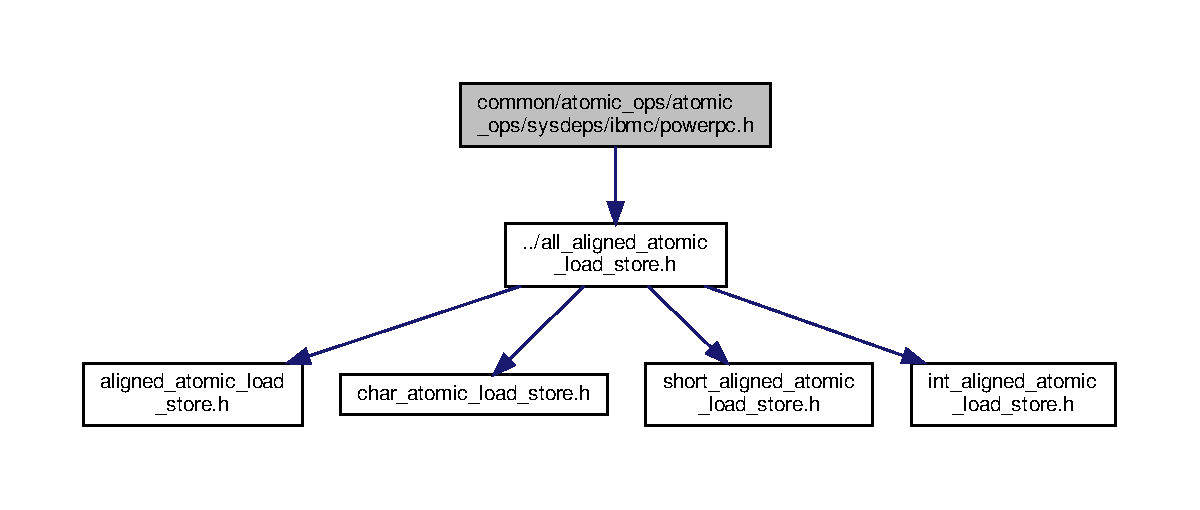
\includegraphics[width=350pt]{ibmc_2powerpc_8h__incl}
\end{center}
\end{figure}
\subsection*{Macros}
\begin{DoxyCompactItemize}
\item 
\#define \hyperlink{ibmc_2powerpc_8h_aa6b9cf57e4373ade9ce01d28a58ad21d}{A\+O\+\_\+nop\+\_\+write}()~\hyperlink{ibmc_2powerpc_8h_a5febfde98faf0a03093897ef864a9589}{A\+O\+\_\+lwsync}()
\item 
\#define \hyperlink{ibmc_2powerpc_8h_a7c6d0c7c0585da4d8cd259df2423b82f}{A\+O\+\_\+\+H\+A\+V\+E\+\_\+nop\+\_\+write}
\item 
\#define \hyperlink{ibmc_2powerpc_8h_a3a367b9626ced22d98eb45e958a21aad}{A\+O\+\_\+nop\+\_\+read}()~\hyperlink{ibmc_2powerpc_8h_a5febfde98faf0a03093897ef864a9589}{A\+O\+\_\+lwsync}()
\item 
\#define \hyperlink{ibmc_2powerpc_8h_a5e899b880760568b4da25ec2d6011cbd}{A\+O\+\_\+\+H\+A\+V\+E\+\_\+nop\+\_\+read}
\item 
\#define \hyperlink{ibmc_2powerpc_8h_a29328d5664268a40645ea9d2f82c8bef}{A\+O\+\_\+\+H\+A\+V\+E\+\_\+load\+\_\+acquire}
\item 
\#define \hyperlink{ibmc_2powerpc_8h_a29328d5664268a40645ea9d2f82c8bef}{A\+O\+\_\+\+H\+A\+V\+E\+\_\+load\+\_\+acquire}
\item 
\#define \hyperlink{ibmc_2powerpc_8h_addf7856c1f3a120a04ad68e843b23de4}{A\+O\+\_\+\+H\+A\+V\+E\+\_\+test\+\_\+and\+\_\+set\+\_\+acquire}
\item 
\#define \hyperlink{ibmc_2powerpc_8h_a27cd35e8e9c1987a362a8610811e1c40}{A\+O\+\_\+\+H\+A\+V\+E\+\_\+test\+\_\+and\+\_\+set\+\_\+release}
\item 
\#define \hyperlink{ibmc_2powerpc_8h_ad5f311a090d1e6e1bb35a6e68ee35fad}{A\+O\+\_\+\+H\+A\+V\+E\+\_\+test\+\_\+and\+\_\+set\+\_\+full}
\item 
\#define \hyperlink{ibmc_2powerpc_8h_ad0b08bc254deecdcba5a4f3366432cf3}{A\+O\+\_\+\+H\+A\+V\+E\+\_\+compare\+\_\+and\+\_\+swap\+\_\+acquire}
\item 
\#define \hyperlink{ibmc_2powerpc_8h_ad85c7af2ae0a778eba77a7762a358819}{A\+O\+\_\+\+H\+A\+V\+E\+\_\+compare\+\_\+and\+\_\+swap\+\_\+release}
\item 
\#define \hyperlink{ibmc_2powerpc_8h_a98ec53065c0dfd18bc1013c500da377c}{A\+O\+\_\+\+H\+A\+V\+E\+\_\+compare\+\_\+and\+\_\+swap\+\_\+full}
\end{DoxyCompactItemize}
\subsection*{Functions}
\begin{DoxyCompactItemize}
\item 
void \hyperlink{ibmc_2powerpc_8h_a55511d2b128569ea7799bd4abb0988a5}{A\+O\+\_\+sync} (void)
\item 
void \hyperlink{ibmc_2powerpc_8h_a5febfde98faf0a03093897ef864a9589}{A\+O\+\_\+lwsync} (void)
\item 
\hyperlink{atomic__ops_8h_a9f6ab6253b6b11bc8c12efe9dde5db2b}{A\+O\+\_\+\+I\+N\+L\+I\+NE} \hyperlink{atomic__ops_8h_a5225fef4d9eee821e82382cd269160dd}{A\+O\+\_\+t} \hyperlink{ibmc_2powerpc_8h_afd982c8bbaa60d3294cc30f92f170847}{A\+O\+\_\+load\+\_\+acquire} (const volatile \hyperlink{atomic__ops_8h_a5225fef4d9eee821e82382cd269160dd}{A\+O\+\_\+t} $\ast$addr)
\item 
\hyperlink{atomic__ops_8h_a9f6ab6253b6b11bc8c12efe9dde5db2b}{A\+O\+\_\+\+I\+N\+L\+I\+NE} void \hyperlink{ibmc_2powerpc_8h_a7b4e8216189c3f4e7f7418e5c2a98b0f}{A\+O\+\_\+store\+\_\+release} (volatile \hyperlink{atomic__ops_8h_a5225fef4d9eee821e82382cd269160dd}{A\+O\+\_\+t} $\ast$addr, \hyperlink{atomic__ops_8h_a5225fef4d9eee821e82382cd269160dd}{A\+O\+\_\+t} value)
\item 
\hyperlink{atomic__ops_8h_a9f6ab6253b6b11bc8c12efe9dde5db2b}{A\+O\+\_\+\+I\+N\+L\+I\+NE} \hyperlink{test__and__set__t__is__char_8h_a7d99a16c4eab47ba80ab6138d7d98ac1}{A\+O\+\_\+\+T\+S\+\_\+\+V\+A\+L\+\_\+t} \hyperlink{ibmc_2powerpc_8h_a0af1bdd53473eb43906a057efe883f6d}{A\+O\+\_\+test\+\_\+and\+\_\+set\+\_\+acquire} (volatile \hyperlink{test__and__set__t__is__char_8h_a5890c21b549264c75c2cad08bf4f6ba9}{A\+O\+\_\+\+T\+S\+\_\+t} $\ast$addr)
\item 
\hyperlink{atomic__ops_8h_a9f6ab6253b6b11bc8c12efe9dde5db2b}{A\+O\+\_\+\+I\+N\+L\+I\+NE} \hyperlink{test__and__set__t__is__char_8h_a7d99a16c4eab47ba80ab6138d7d98ac1}{A\+O\+\_\+\+T\+S\+\_\+\+V\+A\+L\+\_\+t} \hyperlink{ibmc_2powerpc_8h_abd4f99ea301b67851c8a6a1dc61e97c1}{A\+O\+\_\+test\+\_\+and\+\_\+set\+\_\+release} (volatile \hyperlink{test__and__set__t__is__char_8h_a5890c21b549264c75c2cad08bf4f6ba9}{A\+O\+\_\+\+T\+S\+\_\+t} $\ast$addr)
\item 
\hyperlink{atomic__ops_8h_a9f6ab6253b6b11bc8c12efe9dde5db2b}{A\+O\+\_\+\+I\+N\+L\+I\+NE} \hyperlink{test__and__set__t__is__char_8h_a7d99a16c4eab47ba80ab6138d7d98ac1}{A\+O\+\_\+\+T\+S\+\_\+\+V\+A\+L\+\_\+t} \hyperlink{ibmc_2powerpc_8h_a9f485bd63ce5c6a017ec241906e2f651}{A\+O\+\_\+test\+\_\+and\+\_\+set\+\_\+full} (volatile \hyperlink{test__and__set__t__is__char_8h_a5890c21b549264c75c2cad08bf4f6ba9}{A\+O\+\_\+\+T\+S\+\_\+t} $\ast$addr)
\item 
\hyperlink{atomic__ops_8h_a9f6ab6253b6b11bc8c12efe9dde5db2b}{A\+O\+\_\+\+I\+N\+L\+I\+NE} \hyperlink{atomic__ops_8h_a5225fef4d9eee821e82382cd269160dd}{A\+O\+\_\+t} \hyperlink{ibmc_2powerpc_8h_a892f76bbb08fb09906e98fec110d2234}{A\+O\+\_\+compare\+\_\+and\+\_\+swap\+\_\+acquire} (volatile \hyperlink{atomic__ops_8h_a5225fef4d9eee821e82382cd269160dd}{A\+O\+\_\+t} $\ast$addr, \hyperlink{atomic__ops_8h_a5225fef4d9eee821e82382cd269160dd}{A\+O\+\_\+t} old, \hyperlink{atomic__ops_8h_a5225fef4d9eee821e82382cd269160dd}{A\+O\+\_\+t} new\+\_\+val)
\item 
\hyperlink{atomic__ops_8h_a9f6ab6253b6b11bc8c12efe9dde5db2b}{A\+O\+\_\+\+I\+N\+L\+I\+NE} \hyperlink{atomic__ops_8h_a5225fef4d9eee821e82382cd269160dd}{A\+O\+\_\+t} \hyperlink{ibmc_2powerpc_8h_a62c795a4a02675fae1408a421a7ef4df}{A\+O\+\_\+compare\+\_\+and\+\_\+swap\+\_\+release} (volatile \hyperlink{atomic__ops_8h_a5225fef4d9eee821e82382cd269160dd}{A\+O\+\_\+t} $\ast$addr, \hyperlink{atomic__ops_8h_a5225fef4d9eee821e82382cd269160dd}{A\+O\+\_\+t} old, \hyperlink{atomic__ops_8h_a5225fef4d9eee821e82382cd269160dd}{A\+O\+\_\+t} new\+\_\+val)
\item 
\hyperlink{atomic__ops_8h_a9f6ab6253b6b11bc8c12efe9dde5db2b}{A\+O\+\_\+\+I\+N\+L\+I\+NE} \hyperlink{atomic__ops_8h_a5225fef4d9eee821e82382cd269160dd}{A\+O\+\_\+t} \hyperlink{ibmc_2powerpc_8h_ae96a73569341a88329db4e63ed345067}{A\+O\+\_\+compare\+\_\+and\+\_\+swap\+\_\+full} (volatile \hyperlink{atomic__ops_8h_a5225fef4d9eee821e82382cd269160dd}{A\+O\+\_\+t} $\ast$addr, \hyperlink{atomic__ops_8h_a5225fef4d9eee821e82382cd269160dd}{A\+O\+\_\+t} old, \hyperlink{atomic__ops_8h_a5225fef4d9eee821e82382cd269160dd}{A\+O\+\_\+t} new\+\_\+val)
\end{DoxyCompactItemize}


\subsection{Macro Definition Documentation}
\mbox{\Hypertarget{ibmc_2powerpc_8h_ad0b08bc254deecdcba5a4f3366432cf3}\label{ibmc_2powerpc_8h_ad0b08bc254deecdcba5a4f3366432cf3}} 
\index{ibmc/powerpc.\+h@{ibmc/powerpc.\+h}!A\+O\+\_\+\+H\+A\+V\+E\+\_\+compare\+\_\+and\+\_\+swap\+\_\+acquire@{A\+O\+\_\+\+H\+A\+V\+E\+\_\+compare\+\_\+and\+\_\+swap\+\_\+acquire}}
\index{A\+O\+\_\+\+H\+A\+V\+E\+\_\+compare\+\_\+and\+\_\+swap\+\_\+acquire@{A\+O\+\_\+\+H\+A\+V\+E\+\_\+compare\+\_\+and\+\_\+swap\+\_\+acquire}!ibmc/powerpc.\+h@{ibmc/powerpc.\+h}}
\subsubsection{\texorpdfstring{A\+O\+\_\+\+H\+A\+V\+E\+\_\+compare\+\_\+and\+\_\+swap\+\_\+acquire}{AO\_HAVE\_compare\_and\_swap\_acquire}}
{\footnotesize\ttfamily \#define A\+O\+\_\+\+H\+A\+V\+E\+\_\+compare\+\_\+and\+\_\+swap\+\_\+acquire}

\mbox{\Hypertarget{ibmc_2powerpc_8h_a98ec53065c0dfd18bc1013c500da377c}\label{ibmc_2powerpc_8h_a98ec53065c0dfd18bc1013c500da377c}} 
\index{ibmc/powerpc.\+h@{ibmc/powerpc.\+h}!A\+O\+\_\+\+H\+A\+V\+E\+\_\+compare\+\_\+and\+\_\+swap\+\_\+full@{A\+O\+\_\+\+H\+A\+V\+E\+\_\+compare\+\_\+and\+\_\+swap\+\_\+full}}
\index{A\+O\+\_\+\+H\+A\+V\+E\+\_\+compare\+\_\+and\+\_\+swap\+\_\+full@{A\+O\+\_\+\+H\+A\+V\+E\+\_\+compare\+\_\+and\+\_\+swap\+\_\+full}!ibmc/powerpc.\+h@{ibmc/powerpc.\+h}}
\subsubsection{\texorpdfstring{A\+O\+\_\+\+H\+A\+V\+E\+\_\+compare\+\_\+and\+\_\+swap\+\_\+full}{AO\_HAVE\_compare\_and\_swap\_full}}
{\footnotesize\ttfamily \#define A\+O\+\_\+\+H\+A\+V\+E\+\_\+compare\+\_\+and\+\_\+swap\+\_\+full}

\mbox{\Hypertarget{ibmc_2powerpc_8h_ad85c7af2ae0a778eba77a7762a358819}\label{ibmc_2powerpc_8h_ad85c7af2ae0a778eba77a7762a358819}} 
\index{ibmc/powerpc.\+h@{ibmc/powerpc.\+h}!A\+O\+\_\+\+H\+A\+V\+E\+\_\+compare\+\_\+and\+\_\+swap\+\_\+release@{A\+O\+\_\+\+H\+A\+V\+E\+\_\+compare\+\_\+and\+\_\+swap\+\_\+release}}
\index{A\+O\+\_\+\+H\+A\+V\+E\+\_\+compare\+\_\+and\+\_\+swap\+\_\+release@{A\+O\+\_\+\+H\+A\+V\+E\+\_\+compare\+\_\+and\+\_\+swap\+\_\+release}!ibmc/powerpc.\+h@{ibmc/powerpc.\+h}}
\subsubsection{\texorpdfstring{A\+O\+\_\+\+H\+A\+V\+E\+\_\+compare\+\_\+and\+\_\+swap\+\_\+release}{AO\_HAVE\_compare\_and\_swap\_release}}
{\footnotesize\ttfamily \#define A\+O\+\_\+\+H\+A\+V\+E\+\_\+compare\+\_\+and\+\_\+swap\+\_\+release}

\mbox{\Hypertarget{ibmc_2powerpc_8h_a29328d5664268a40645ea9d2f82c8bef}\label{ibmc_2powerpc_8h_a29328d5664268a40645ea9d2f82c8bef}} 
\index{ibmc/powerpc.\+h@{ibmc/powerpc.\+h}!A\+O\+\_\+\+H\+A\+V\+E\+\_\+load\+\_\+acquire@{A\+O\+\_\+\+H\+A\+V\+E\+\_\+load\+\_\+acquire}}
\index{A\+O\+\_\+\+H\+A\+V\+E\+\_\+load\+\_\+acquire@{A\+O\+\_\+\+H\+A\+V\+E\+\_\+load\+\_\+acquire}!ibmc/powerpc.\+h@{ibmc/powerpc.\+h}}
\subsubsection{\texorpdfstring{A\+O\+\_\+\+H\+A\+V\+E\+\_\+load\+\_\+acquire}{AO\_HAVE\_load\_acquire}\hspace{0.1cm}{\footnotesize\ttfamily [1/2]}}
{\footnotesize\ttfamily \#define A\+O\+\_\+\+H\+A\+V\+E\+\_\+load\+\_\+acquire}

\mbox{\Hypertarget{ibmc_2powerpc_8h_a29328d5664268a40645ea9d2f82c8bef}\label{ibmc_2powerpc_8h_a29328d5664268a40645ea9d2f82c8bef}} 
\index{ibmc/powerpc.\+h@{ibmc/powerpc.\+h}!A\+O\+\_\+\+H\+A\+V\+E\+\_\+load\+\_\+acquire@{A\+O\+\_\+\+H\+A\+V\+E\+\_\+load\+\_\+acquire}}
\index{A\+O\+\_\+\+H\+A\+V\+E\+\_\+load\+\_\+acquire@{A\+O\+\_\+\+H\+A\+V\+E\+\_\+load\+\_\+acquire}!ibmc/powerpc.\+h@{ibmc/powerpc.\+h}}
\subsubsection{\texorpdfstring{A\+O\+\_\+\+H\+A\+V\+E\+\_\+load\+\_\+acquire}{AO\_HAVE\_load\_acquire}\hspace{0.1cm}{\footnotesize\ttfamily [2/2]}}
{\footnotesize\ttfamily \#define A\+O\+\_\+\+H\+A\+V\+E\+\_\+load\+\_\+acquire}

\mbox{\Hypertarget{ibmc_2powerpc_8h_a5e899b880760568b4da25ec2d6011cbd}\label{ibmc_2powerpc_8h_a5e899b880760568b4da25ec2d6011cbd}} 
\index{ibmc/powerpc.\+h@{ibmc/powerpc.\+h}!A\+O\+\_\+\+H\+A\+V\+E\+\_\+nop\+\_\+read@{A\+O\+\_\+\+H\+A\+V\+E\+\_\+nop\+\_\+read}}
\index{A\+O\+\_\+\+H\+A\+V\+E\+\_\+nop\+\_\+read@{A\+O\+\_\+\+H\+A\+V\+E\+\_\+nop\+\_\+read}!ibmc/powerpc.\+h@{ibmc/powerpc.\+h}}
\subsubsection{\texorpdfstring{A\+O\+\_\+\+H\+A\+V\+E\+\_\+nop\+\_\+read}{AO\_HAVE\_nop\_read}}
{\footnotesize\ttfamily \#define A\+O\+\_\+\+H\+A\+V\+E\+\_\+nop\+\_\+read}

\mbox{\Hypertarget{ibmc_2powerpc_8h_a7c6d0c7c0585da4d8cd259df2423b82f}\label{ibmc_2powerpc_8h_a7c6d0c7c0585da4d8cd259df2423b82f}} 
\index{ibmc/powerpc.\+h@{ibmc/powerpc.\+h}!A\+O\+\_\+\+H\+A\+V\+E\+\_\+nop\+\_\+write@{A\+O\+\_\+\+H\+A\+V\+E\+\_\+nop\+\_\+write}}
\index{A\+O\+\_\+\+H\+A\+V\+E\+\_\+nop\+\_\+write@{A\+O\+\_\+\+H\+A\+V\+E\+\_\+nop\+\_\+write}!ibmc/powerpc.\+h@{ibmc/powerpc.\+h}}
\subsubsection{\texorpdfstring{A\+O\+\_\+\+H\+A\+V\+E\+\_\+nop\+\_\+write}{AO\_HAVE\_nop\_write}}
{\footnotesize\ttfamily \#define A\+O\+\_\+\+H\+A\+V\+E\+\_\+nop\+\_\+write}

\mbox{\Hypertarget{ibmc_2powerpc_8h_addf7856c1f3a120a04ad68e843b23de4}\label{ibmc_2powerpc_8h_addf7856c1f3a120a04ad68e843b23de4}} 
\index{ibmc/powerpc.\+h@{ibmc/powerpc.\+h}!A\+O\+\_\+\+H\+A\+V\+E\+\_\+test\+\_\+and\+\_\+set\+\_\+acquire@{A\+O\+\_\+\+H\+A\+V\+E\+\_\+test\+\_\+and\+\_\+set\+\_\+acquire}}
\index{A\+O\+\_\+\+H\+A\+V\+E\+\_\+test\+\_\+and\+\_\+set\+\_\+acquire@{A\+O\+\_\+\+H\+A\+V\+E\+\_\+test\+\_\+and\+\_\+set\+\_\+acquire}!ibmc/powerpc.\+h@{ibmc/powerpc.\+h}}
\subsubsection{\texorpdfstring{A\+O\+\_\+\+H\+A\+V\+E\+\_\+test\+\_\+and\+\_\+set\+\_\+acquire}{AO\_HAVE\_test\_and\_set\_acquire}}
{\footnotesize\ttfamily \#define A\+O\+\_\+\+H\+A\+V\+E\+\_\+test\+\_\+and\+\_\+set\+\_\+acquire}

\mbox{\Hypertarget{ibmc_2powerpc_8h_ad5f311a090d1e6e1bb35a6e68ee35fad}\label{ibmc_2powerpc_8h_ad5f311a090d1e6e1bb35a6e68ee35fad}} 
\index{ibmc/powerpc.\+h@{ibmc/powerpc.\+h}!A\+O\+\_\+\+H\+A\+V\+E\+\_\+test\+\_\+and\+\_\+set\+\_\+full@{A\+O\+\_\+\+H\+A\+V\+E\+\_\+test\+\_\+and\+\_\+set\+\_\+full}}
\index{A\+O\+\_\+\+H\+A\+V\+E\+\_\+test\+\_\+and\+\_\+set\+\_\+full@{A\+O\+\_\+\+H\+A\+V\+E\+\_\+test\+\_\+and\+\_\+set\+\_\+full}!ibmc/powerpc.\+h@{ibmc/powerpc.\+h}}
\subsubsection{\texorpdfstring{A\+O\+\_\+\+H\+A\+V\+E\+\_\+test\+\_\+and\+\_\+set\+\_\+full}{AO\_HAVE\_test\_and\_set\_full}}
{\footnotesize\ttfamily \#define A\+O\+\_\+\+H\+A\+V\+E\+\_\+test\+\_\+and\+\_\+set\+\_\+full}

\mbox{\Hypertarget{ibmc_2powerpc_8h_a27cd35e8e9c1987a362a8610811e1c40}\label{ibmc_2powerpc_8h_a27cd35e8e9c1987a362a8610811e1c40}} 
\index{ibmc/powerpc.\+h@{ibmc/powerpc.\+h}!A\+O\+\_\+\+H\+A\+V\+E\+\_\+test\+\_\+and\+\_\+set\+\_\+release@{A\+O\+\_\+\+H\+A\+V\+E\+\_\+test\+\_\+and\+\_\+set\+\_\+release}}
\index{A\+O\+\_\+\+H\+A\+V\+E\+\_\+test\+\_\+and\+\_\+set\+\_\+release@{A\+O\+\_\+\+H\+A\+V\+E\+\_\+test\+\_\+and\+\_\+set\+\_\+release}!ibmc/powerpc.\+h@{ibmc/powerpc.\+h}}
\subsubsection{\texorpdfstring{A\+O\+\_\+\+H\+A\+V\+E\+\_\+test\+\_\+and\+\_\+set\+\_\+release}{AO\_HAVE\_test\_and\_set\_release}}
{\footnotesize\ttfamily \#define A\+O\+\_\+\+H\+A\+V\+E\+\_\+test\+\_\+and\+\_\+set\+\_\+release}

\mbox{\Hypertarget{ibmc_2powerpc_8h_a3a367b9626ced22d98eb45e958a21aad}\label{ibmc_2powerpc_8h_a3a367b9626ced22d98eb45e958a21aad}} 
\index{ibmc/powerpc.\+h@{ibmc/powerpc.\+h}!A\+O\+\_\+nop\+\_\+read@{A\+O\+\_\+nop\+\_\+read}}
\index{A\+O\+\_\+nop\+\_\+read@{A\+O\+\_\+nop\+\_\+read}!ibmc/powerpc.\+h@{ibmc/powerpc.\+h}}
\subsubsection{\texorpdfstring{A\+O\+\_\+nop\+\_\+read}{AO\_nop\_read}}
{\footnotesize\ttfamily \#define A\+O\+\_\+nop\+\_\+read(\begin{DoxyParamCaption}\item[{}]{void }\end{DoxyParamCaption})~\hyperlink{ibmc_2powerpc_8h_a5febfde98faf0a03093897ef864a9589}{A\+O\+\_\+lwsync}()}

\mbox{\Hypertarget{ibmc_2powerpc_8h_aa6b9cf57e4373ade9ce01d28a58ad21d}\label{ibmc_2powerpc_8h_aa6b9cf57e4373ade9ce01d28a58ad21d}} 
\index{ibmc/powerpc.\+h@{ibmc/powerpc.\+h}!A\+O\+\_\+nop\+\_\+write@{A\+O\+\_\+nop\+\_\+write}}
\index{A\+O\+\_\+nop\+\_\+write@{A\+O\+\_\+nop\+\_\+write}!ibmc/powerpc.\+h@{ibmc/powerpc.\+h}}
\subsubsection{\texorpdfstring{A\+O\+\_\+nop\+\_\+write}{AO\_nop\_write}}
{\footnotesize\ttfamily \#define A\+O\+\_\+nop\+\_\+write(\begin{DoxyParamCaption}\item[{}]{void }\end{DoxyParamCaption})~\hyperlink{ibmc_2powerpc_8h_a5febfde98faf0a03093897ef864a9589}{A\+O\+\_\+lwsync}()}



\subsection{Function Documentation}
\mbox{\Hypertarget{ibmc_2powerpc_8h_a892f76bbb08fb09906e98fec110d2234}\label{ibmc_2powerpc_8h_a892f76bbb08fb09906e98fec110d2234}} 
\index{ibmc/powerpc.\+h@{ibmc/powerpc.\+h}!A\+O\+\_\+compare\+\_\+and\+\_\+swap\+\_\+acquire@{A\+O\+\_\+compare\+\_\+and\+\_\+swap\+\_\+acquire}}
\index{A\+O\+\_\+compare\+\_\+and\+\_\+swap\+\_\+acquire@{A\+O\+\_\+compare\+\_\+and\+\_\+swap\+\_\+acquire}!ibmc/powerpc.\+h@{ibmc/powerpc.\+h}}
\subsubsection{\texorpdfstring{A\+O\+\_\+compare\+\_\+and\+\_\+swap\+\_\+acquire()}{AO\_compare\_and\_swap\_acquire()}}
{\footnotesize\ttfamily \hyperlink{atomic__ops_8h_a9f6ab6253b6b11bc8c12efe9dde5db2b}{A\+O\+\_\+\+I\+N\+L\+I\+NE} \hyperlink{atomic__ops_8h_a5225fef4d9eee821e82382cd269160dd}{A\+O\+\_\+t} A\+O\+\_\+compare\+\_\+and\+\_\+swap\+\_\+acquire (\begin{DoxyParamCaption}\item[{volatile \hyperlink{atomic__ops_8h_a5225fef4d9eee821e82382cd269160dd}{A\+O\+\_\+t} $\ast$}]{addr,  }\item[{\hyperlink{atomic__ops_8h_a5225fef4d9eee821e82382cd269160dd}{A\+O\+\_\+t}}]{old,  }\item[{\hyperlink{atomic__ops_8h_a5225fef4d9eee821e82382cd269160dd}{A\+O\+\_\+t}}]{new\+\_\+val }\end{DoxyParamCaption})}

\mbox{\Hypertarget{ibmc_2powerpc_8h_ae96a73569341a88329db4e63ed345067}\label{ibmc_2powerpc_8h_ae96a73569341a88329db4e63ed345067}} 
\index{ibmc/powerpc.\+h@{ibmc/powerpc.\+h}!A\+O\+\_\+compare\+\_\+and\+\_\+swap\+\_\+full@{A\+O\+\_\+compare\+\_\+and\+\_\+swap\+\_\+full}}
\index{A\+O\+\_\+compare\+\_\+and\+\_\+swap\+\_\+full@{A\+O\+\_\+compare\+\_\+and\+\_\+swap\+\_\+full}!ibmc/powerpc.\+h@{ibmc/powerpc.\+h}}
\subsubsection{\texorpdfstring{A\+O\+\_\+compare\+\_\+and\+\_\+swap\+\_\+full()}{AO\_compare\_and\_swap\_full()}}
{\footnotesize\ttfamily \hyperlink{atomic__ops_8h_a9f6ab6253b6b11bc8c12efe9dde5db2b}{A\+O\+\_\+\+I\+N\+L\+I\+NE} \hyperlink{atomic__ops_8h_a5225fef4d9eee821e82382cd269160dd}{A\+O\+\_\+t} A\+O\+\_\+compare\+\_\+and\+\_\+swap\+\_\+full (\begin{DoxyParamCaption}\item[{volatile \hyperlink{atomic__ops_8h_a5225fef4d9eee821e82382cd269160dd}{A\+O\+\_\+t} $\ast$}]{addr,  }\item[{\hyperlink{atomic__ops_8h_a5225fef4d9eee821e82382cd269160dd}{A\+O\+\_\+t}}]{old,  }\item[{\hyperlink{atomic__ops_8h_a5225fef4d9eee821e82382cd269160dd}{A\+O\+\_\+t}}]{new\+\_\+val }\end{DoxyParamCaption})}

\mbox{\Hypertarget{ibmc_2powerpc_8h_a62c795a4a02675fae1408a421a7ef4df}\label{ibmc_2powerpc_8h_a62c795a4a02675fae1408a421a7ef4df}} 
\index{ibmc/powerpc.\+h@{ibmc/powerpc.\+h}!A\+O\+\_\+compare\+\_\+and\+\_\+swap\+\_\+release@{A\+O\+\_\+compare\+\_\+and\+\_\+swap\+\_\+release}}
\index{A\+O\+\_\+compare\+\_\+and\+\_\+swap\+\_\+release@{A\+O\+\_\+compare\+\_\+and\+\_\+swap\+\_\+release}!ibmc/powerpc.\+h@{ibmc/powerpc.\+h}}
\subsubsection{\texorpdfstring{A\+O\+\_\+compare\+\_\+and\+\_\+swap\+\_\+release()}{AO\_compare\_and\_swap\_release()}}
{\footnotesize\ttfamily \hyperlink{atomic__ops_8h_a9f6ab6253b6b11bc8c12efe9dde5db2b}{A\+O\+\_\+\+I\+N\+L\+I\+NE} \hyperlink{atomic__ops_8h_a5225fef4d9eee821e82382cd269160dd}{A\+O\+\_\+t} A\+O\+\_\+compare\+\_\+and\+\_\+swap\+\_\+release (\begin{DoxyParamCaption}\item[{volatile \hyperlink{atomic__ops_8h_a5225fef4d9eee821e82382cd269160dd}{A\+O\+\_\+t} $\ast$}]{addr,  }\item[{\hyperlink{atomic__ops_8h_a5225fef4d9eee821e82382cd269160dd}{A\+O\+\_\+t}}]{old,  }\item[{\hyperlink{atomic__ops_8h_a5225fef4d9eee821e82382cd269160dd}{A\+O\+\_\+t}}]{new\+\_\+val }\end{DoxyParamCaption})}

\mbox{\Hypertarget{ibmc_2powerpc_8h_afd982c8bbaa60d3294cc30f92f170847}\label{ibmc_2powerpc_8h_afd982c8bbaa60d3294cc30f92f170847}} 
\index{ibmc/powerpc.\+h@{ibmc/powerpc.\+h}!A\+O\+\_\+load\+\_\+acquire@{A\+O\+\_\+load\+\_\+acquire}}
\index{A\+O\+\_\+load\+\_\+acquire@{A\+O\+\_\+load\+\_\+acquire}!ibmc/powerpc.\+h@{ibmc/powerpc.\+h}}
\subsubsection{\texorpdfstring{A\+O\+\_\+load\+\_\+acquire()}{AO\_load\_acquire()}}
{\footnotesize\ttfamily \hyperlink{atomic__ops_8h_a9f6ab6253b6b11bc8c12efe9dde5db2b}{A\+O\+\_\+\+I\+N\+L\+I\+NE} \hyperlink{atomic__ops_8h_a5225fef4d9eee821e82382cd269160dd}{A\+O\+\_\+t} A\+O\+\_\+load\+\_\+acquire (\begin{DoxyParamCaption}\item[{const volatile \hyperlink{atomic__ops_8h_a5225fef4d9eee821e82382cd269160dd}{A\+O\+\_\+t} $\ast$}]{addr }\end{DoxyParamCaption})}

\mbox{\Hypertarget{ibmc_2powerpc_8h_a5febfde98faf0a03093897ef864a9589}\label{ibmc_2powerpc_8h_a5febfde98faf0a03093897ef864a9589}} 
\index{ibmc/powerpc.\+h@{ibmc/powerpc.\+h}!A\+O\+\_\+lwsync@{A\+O\+\_\+lwsync}}
\index{A\+O\+\_\+lwsync@{A\+O\+\_\+lwsync}!ibmc/powerpc.\+h@{ibmc/powerpc.\+h}}
\subsubsection{\texorpdfstring{A\+O\+\_\+lwsync()}{AO\_lwsync()}}
{\footnotesize\ttfamily void A\+O\+\_\+lwsync (\begin{DoxyParamCaption}\item[{void}]{ }\end{DoxyParamCaption})}

\mbox{\Hypertarget{ibmc_2powerpc_8h_a7b4e8216189c3f4e7f7418e5c2a98b0f}\label{ibmc_2powerpc_8h_a7b4e8216189c3f4e7f7418e5c2a98b0f}} 
\index{ibmc/powerpc.\+h@{ibmc/powerpc.\+h}!A\+O\+\_\+store\+\_\+release@{A\+O\+\_\+store\+\_\+release}}
\index{A\+O\+\_\+store\+\_\+release@{A\+O\+\_\+store\+\_\+release}!ibmc/powerpc.\+h@{ibmc/powerpc.\+h}}
\subsubsection{\texorpdfstring{A\+O\+\_\+store\+\_\+release()}{AO\_store\_release()}}
{\footnotesize\ttfamily \hyperlink{atomic__ops_8h_a9f6ab6253b6b11bc8c12efe9dde5db2b}{A\+O\+\_\+\+I\+N\+L\+I\+NE} void A\+O\+\_\+store\+\_\+release (\begin{DoxyParamCaption}\item[{volatile \hyperlink{atomic__ops_8h_a5225fef4d9eee821e82382cd269160dd}{A\+O\+\_\+t} $\ast$}]{addr,  }\item[{\hyperlink{atomic__ops_8h_a5225fef4d9eee821e82382cd269160dd}{A\+O\+\_\+t}}]{value }\end{DoxyParamCaption})}

\mbox{\Hypertarget{ibmc_2powerpc_8h_a55511d2b128569ea7799bd4abb0988a5}\label{ibmc_2powerpc_8h_a55511d2b128569ea7799bd4abb0988a5}} 
\index{ibmc/powerpc.\+h@{ibmc/powerpc.\+h}!A\+O\+\_\+sync@{A\+O\+\_\+sync}}
\index{A\+O\+\_\+sync@{A\+O\+\_\+sync}!ibmc/powerpc.\+h@{ibmc/powerpc.\+h}}
\subsubsection{\texorpdfstring{A\+O\+\_\+sync()}{AO\_sync()}}
{\footnotesize\ttfamily void A\+O\+\_\+sync (\begin{DoxyParamCaption}\item[{void}]{ }\end{DoxyParamCaption})}

\mbox{\Hypertarget{ibmc_2powerpc_8h_a0af1bdd53473eb43906a057efe883f6d}\label{ibmc_2powerpc_8h_a0af1bdd53473eb43906a057efe883f6d}} 
\index{ibmc/powerpc.\+h@{ibmc/powerpc.\+h}!A\+O\+\_\+test\+\_\+and\+\_\+set\+\_\+acquire@{A\+O\+\_\+test\+\_\+and\+\_\+set\+\_\+acquire}}
\index{A\+O\+\_\+test\+\_\+and\+\_\+set\+\_\+acquire@{A\+O\+\_\+test\+\_\+and\+\_\+set\+\_\+acquire}!ibmc/powerpc.\+h@{ibmc/powerpc.\+h}}
\subsubsection{\texorpdfstring{A\+O\+\_\+test\+\_\+and\+\_\+set\+\_\+acquire()}{AO\_test\_and\_set\_acquire()}}
{\footnotesize\ttfamily \hyperlink{atomic__ops_8h_a9f6ab6253b6b11bc8c12efe9dde5db2b}{A\+O\+\_\+\+I\+N\+L\+I\+NE} \hyperlink{test__and__set__t__is__char_8h_a7d99a16c4eab47ba80ab6138d7d98ac1}{A\+O\+\_\+\+T\+S\+\_\+\+V\+A\+L\+\_\+t} A\+O\+\_\+test\+\_\+and\+\_\+set\+\_\+acquire (\begin{DoxyParamCaption}\item[{volatile \hyperlink{test__and__set__t__is__char_8h_a5890c21b549264c75c2cad08bf4f6ba9}{A\+O\+\_\+\+T\+S\+\_\+t} $\ast$}]{addr }\end{DoxyParamCaption})}

\mbox{\Hypertarget{ibmc_2powerpc_8h_a9f485bd63ce5c6a017ec241906e2f651}\label{ibmc_2powerpc_8h_a9f485bd63ce5c6a017ec241906e2f651}} 
\index{ibmc/powerpc.\+h@{ibmc/powerpc.\+h}!A\+O\+\_\+test\+\_\+and\+\_\+set\+\_\+full@{A\+O\+\_\+test\+\_\+and\+\_\+set\+\_\+full}}
\index{A\+O\+\_\+test\+\_\+and\+\_\+set\+\_\+full@{A\+O\+\_\+test\+\_\+and\+\_\+set\+\_\+full}!ibmc/powerpc.\+h@{ibmc/powerpc.\+h}}
\subsubsection{\texorpdfstring{A\+O\+\_\+test\+\_\+and\+\_\+set\+\_\+full()}{AO\_test\_and\_set\_full()}}
{\footnotesize\ttfamily \hyperlink{atomic__ops_8h_a9f6ab6253b6b11bc8c12efe9dde5db2b}{A\+O\+\_\+\+I\+N\+L\+I\+NE} \hyperlink{test__and__set__t__is__char_8h_a7d99a16c4eab47ba80ab6138d7d98ac1}{A\+O\+\_\+\+T\+S\+\_\+\+V\+A\+L\+\_\+t} A\+O\+\_\+test\+\_\+and\+\_\+set\+\_\+full (\begin{DoxyParamCaption}\item[{volatile \hyperlink{test__and__set__t__is__char_8h_a5890c21b549264c75c2cad08bf4f6ba9}{A\+O\+\_\+\+T\+S\+\_\+t} $\ast$}]{addr }\end{DoxyParamCaption})}

\mbox{\Hypertarget{ibmc_2powerpc_8h_abd4f99ea301b67851c8a6a1dc61e97c1}\label{ibmc_2powerpc_8h_abd4f99ea301b67851c8a6a1dc61e97c1}} 
\index{ibmc/powerpc.\+h@{ibmc/powerpc.\+h}!A\+O\+\_\+test\+\_\+and\+\_\+set\+\_\+release@{A\+O\+\_\+test\+\_\+and\+\_\+set\+\_\+release}}
\index{A\+O\+\_\+test\+\_\+and\+\_\+set\+\_\+release@{A\+O\+\_\+test\+\_\+and\+\_\+set\+\_\+release}!ibmc/powerpc.\+h@{ibmc/powerpc.\+h}}
\subsubsection{\texorpdfstring{A\+O\+\_\+test\+\_\+and\+\_\+set\+\_\+release()}{AO\_test\_and\_set\_release()}}
{\footnotesize\ttfamily \hyperlink{atomic__ops_8h_a9f6ab6253b6b11bc8c12efe9dde5db2b}{A\+O\+\_\+\+I\+N\+L\+I\+NE} \hyperlink{test__and__set__t__is__char_8h_a7d99a16c4eab47ba80ab6138d7d98ac1}{A\+O\+\_\+\+T\+S\+\_\+\+V\+A\+L\+\_\+t} A\+O\+\_\+test\+\_\+and\+\_\+set\+\_\+release (\begin{DoxyParamCaption}\item[{volatile \hyperlink{test__and__set__t__is__char_8h_a5890c21b549264c75c2cad08bf4f6ba9}{A\+O\+\_\+\+T\+S\+\_\+t} $\ast$}]{addr }\end{DoxyParamCaption})}


\hypertarget{s390_8h}{}\section{common/atomic\+\_\+ops/atomic\+\_\+ops/sysdeps/gcc/s390.h File Reference}
\label{s390_8h}\index{common/atomic\+\_\+ops/atomic\+\_\+ops/sysdeps/gcc/s390.\+h@{common/atomic\+\_\+ops/atomic\+\_\+ops/sysdeps/gcc/s390.\+h}}
{\ttfamily \#include \char`\"{}../ordered\+\_\+except\+\_\+wr.\+h\char`\"{}}\newline
{\ttfamily \#include \char`\"{}../all\+\_\+aligned\+\_\+atomic\+\_\+load\+\_\+store.\+h\char`\"{}}\newline
{\ttfamily \#include \char`\"{}../test\+\_\+and\+\_\+set\+\_\+t\+\_\+is\+\_\+ao\+\_\+t.\+h\char`\"{}}\newline
Include dependency graph for s390.\+h\+:
\nopagebreak
\begin{figure}[H]
\begin{center}
\leavevmode
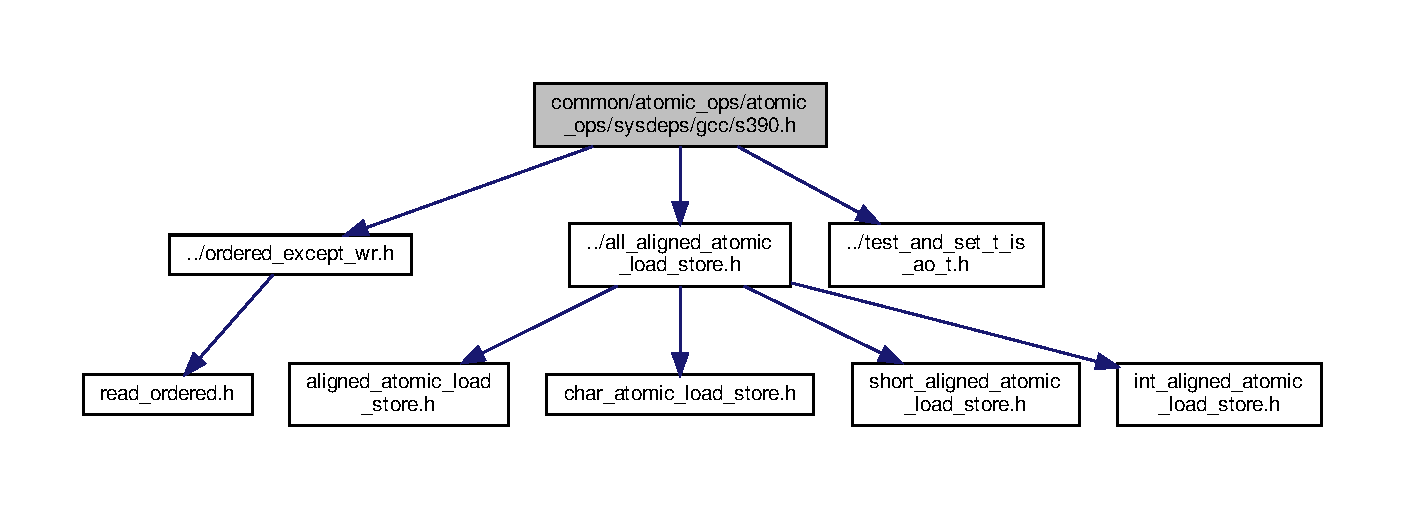
\includegraphics[width=350pt]{s390_8h__incl}
\end{center}
\end{figure}
\subsection*{Macros}
\begin{DoxyCompactItemize}
\item 
\#define \hyperlink{s390_8h_a98ec53065c0dfd18bc1013c500da377c}{A\+O\+\_\+\+H\+A\+V\+E\+\_\+compare\+\_\+and\+\_\+swap\+\_\+full}
\end{DoxyCompactItemize}
\subsection*{Functions}
\begin{DoxyCompactItemize}
\item 
\hyperlink{atomic__ops_8h_a9f6ab6253b6b11bc8c12efe9dde5db2b}{A\+O\+\_\+\+I\+N\+L\+I\+NE} \hyperlink{atomic__ops_8h_a5225fef4d9eee821e82382cd269160dd}{A\+O\+\_\+t} \hyperlink{s390_8h_ae96a73569341a88329db4e63ed345067}{A\+O\+\_\+compare\+\_\+and\+\_\+swap\+\_\+full} (volatile \hyperlink{atomic__ops_8h_a5225fef4d9eee821e82382cd269160dd}{A\+O\+\_\+t} $\ast$addr, \hyperlink{atomic__ops_8h_a5225fef4d9eee821e82382cd269160dd}{A\+O\+\_\+t} old, \hyperlink{atomic__ops_8h_a5225fef4d9eee821e82382cd269160dd}{A\+O\+\_\+t} new\+\_\+val)
\end{DoxyCompactItemize}


\subsection{Macro Definition Documentation}
\mbox{\Hypertarget{s390_8h_a98ec53065c0dfd18bc1013c500da377c}\label{s390_8h_a98ec53065c0dfd18bc1013c500da377c}} 
\index{s390.\+h@{s390.\+h}!A\+O\+\_\+\+H\+A\+V\+E\+\_\+compare\+\_\+and\+\_\+swap\+\_\+full@{A\+O\+\_\+\+H\+A\+V\+E\+\_\+compare\+\_\+and\+\_\+swap\+\_\+full}}
\index{A\+O\+\_\+\+H\+A\+V\+E\+\_\+compare\+\_\+and\+\_\+swap\+\_\+full@{A\+O\+\_\+\+H\+A\+V\+E\+\_\+compare\+\_\+and\+\_\+swap\+\_\+full}!s390.\+h@{s390.\+h}}
\subsubsection{\texorpdfstring{A\+O\+\_\+\+H\+A\+V\+E\+\_\+compare\+\_\+and\+\_\+swap\+\_\+full}{AO\_HAVE\_compare\_and\_swap\_full}}
{\footnotesize\ttfamily \#define A\+O\+\_\+\+H\+A\+V\+E\+\_\+compare\+\_\+and\+\_\+swap\+\_\+full}



\subsection{Function Documentation}
\mbox{\Hypertarget{s390_8h_ae96a73569341a88329db4e63ed345067}\label{s390_8h_ae96a73569341a88329db4e63ed345067}} 
\index{s390.\+h@{s390.\+h}!A\+O\+\_\+compare\+\_\+and\+\_\+swap\+\_\+full@{A\+O\+\_\+compare\+\_\+and\+\_\+swap\+\_\+full}}
\index{A\+O\+\_\+compare\+\_\+and\+\_\+swap\+\_\+full@{A\+O\+\_\+compare\+\_\+and\+\_\+swap\+\_\+full}!s390.\+h@{s390.\+h}}
\subsubsection{\texorpdfstring{A\+O\+\_\+compare\+\_\+and\+\_\+swap\+\_\+full()}{AO\_compare\_and\_swap\_full()}}
{\footnotesize\ttfamily \hyperlink{atomic__ops_8h_a9f6ab6253b6b11bc8c12efe9dde5db2b}{A\+O\+\_\+\+I\+N\+L\+I\+NE} \hyperlink{atomic__ops_8h_a5225fef4d9eee821e82382cd269160dd}{A\+O\+\_\+t} A\+O\+\_\+compare\+\_\+and\+\_\+swap\+\_\+full (\begin{DoxyParamCaption}\item[{volatile \hyperlink{atomic__ops_8h_a5225fef4d9eee821e82382cd269160dd}{A\+O\+\_\+t} $\ast$}]{addr,  }\item[{\hyperlink{atomic__ops_8h_a5225fef4d9eee821e82382cd269160dd}{A\+O\+\_\+t}}]{old,  }\item[{\hyperlink{atomic__ops_8h_a5225fef4d9eee821e82382cd269160dd}{A\+O\+\_\+t}}]{new\+\_\+val }\end{DoxyParamCaption})}


\hypertarget{sh_8h}{}\section{common/atomic\+\_\+ops/atomic\+\_\+ops/sysdeps/gcc/sh.h File Reference}
\label{sh_8h}\index{common/atomic\+\_\+ops/atomic\+\_\+ops/sysdeps/gcc/sh.\+h@{common/atomic\+\_\+ops/atomic\+\_\+ops/sysdeps/gcc/sh.\+h}}
{\ttfamily \#include \char`\"{}../all\+\_\+atomic\+\_\+load\+\_\+store.\+h\char`\"{}}\newline
{\ttfamily \#include \char`\"{}../ordered.\+h\char`\"{}}\newline
{\ttfamily \#include \char`\"{}../test\+\_\+and\+\_\+set\+\_\+t\+\_\+is\+\_\+char.\+h\char`\"{}}\newline
Include dependency graph for sh.\+h\+:
\nopagebreak
\begin{figure}[H]
\begin{center}
\leavevmode
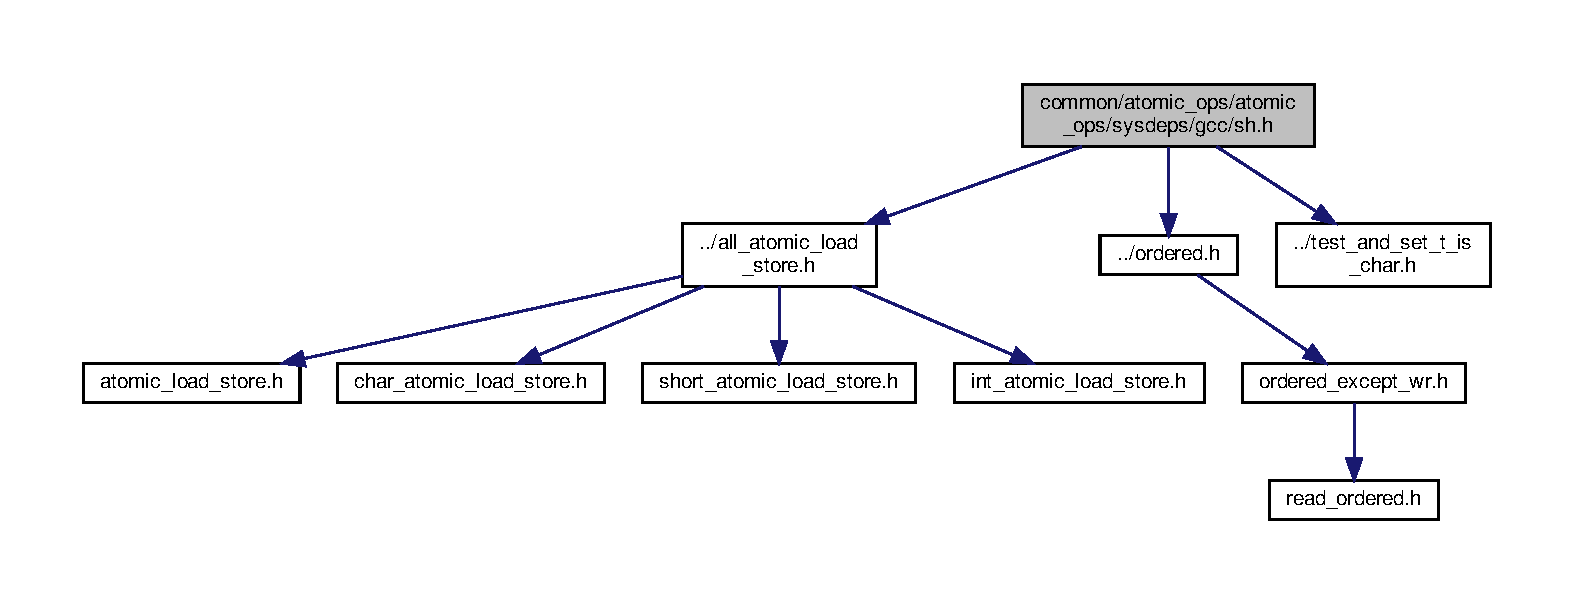
\includegraphics[width=350pt]{sh_8h__incl}
\end{center}
\end{figure}
\subsection*{Macros}
\begin{DoxyCompactItemize}
\item 
\#define \hyperlink{sh_8h_ad5f311a090d1e6e1bb35a6e68ee35fad}{A\+O\+\_\+\+H\+A\+V\+E\+\_\+test\+\_\+and\+\_\+set\+\_\+full}
\end{DoxyCompactItemize}
\subsection*{Functions}
\begin{DoxyCompactItemize}
\item 
\hyperlink{atomic__ops_8h_a9f6ab6253b6b11bc8c12efe9dde5db2b}{A\+O\+\_\+\+I\+N\+L\+I\+NE} \hyperlink{test__and__set__t__is__char_8h_a7d99a16c4eab47ba80ab6138d7d98ac1}{A\+O\+\_\+\+T\+S\+\_\+\+V\+A\+L\+\_\+t} \hyperlink{sh_8h_a9f485bd63ce5c6a017ec241906e2f651}{A\+O\+\_\+test\+\_\+and\+\_\+set\+\_\+full} (volatile \hyperlink{test__and__set__t__is__char_8h_a5890c21b549264c75c2cad08bf4f6ba9}{A\+O\+\_\+\+T\+S\+\_\+t} $\ast$addr)
\end{DoxyCompactItemize}


\subsection{Macro Definition Documentation}
\mbox{\Hypertarget{sh_8h_ad5f311a090d1e6e1bb35a6e68ee35fad}\label{sh_8h_ad5f311a090d1e6e1bb35a6e68ee35fad}} 
\index{sh.\+h@{sh.\+h}!A\+O\+\_\+\+H\+A\+V\+E\+\_\+test\+\_\+and\+\_\+set\+\_\+full@{A\+O\+\_\+\+H\+A\+V\+E\+\_\+test\+\_\+and\+\_\+set\+\_\+full}}
\index{A\+O\+\_\+\+H\+A\+V\+E\+\_\+test\+\_\+and\+\_\+set\+\_\+full@{A\+O\+\_\+\+H\+A\+V\+E\+\_\+test\+\_\+and\+\_\+set\+\_\+full}!sh.\+h@{sh.\+h}}
\subsubsection{\texorpdfstring{A\+O\+\_\+\+H\+A\+V\+E\+\_\+test\+\_\+and\+\_\+set\+\_\+full}{AO\_HAVE\_test\_and\_set\_full}}
{\footnotesize\ttfamily \#define A\+O\+\_\+\+H\+A\+V\+E\+\_\+test\+\_\+and\+\_\+set\+\_\+full}



\subsection{Function Documentation}
\mbox{\Hypertarget{sh_8h_a9f485bd63ce5c6a017ec241906e2f651}\label{sh_8h_a9f485bd63ce5c6a017ec241906e2f651}} 
\index{sh.\+h@{sh.\+h}!A\+O\+\_\+test\+\_\+and\+\_\+set\+\_\+full@{A\+O\+\_\+test\+\_\+and\+\_\+set\+\_\+full}}
\index{A\+O\+\_\+test\+\_\+and\+\_\+set\+\_\+full@{A\+O\+\_\+test\+\_\+and\+\_\+set\+\_\+full}!sh.\+h@{sh.\+h}}
\subsubsection{\texorpdfstring{A\+O\+\_\+test\+\_\+and\+\_\+set\+\_\+full()}{AO\_test\_and\_set\_full()}}
{\footnotesize\ttfamily \hyperlink{atomic__ops_8h_a9f6ab6253b6b11bc8c12efe9dde5db2b}{A\+O\+\_\+\+I\+N\+L\+I\+NE} \hyperlink{test__and__set__t__is__char_8h_a7d99a16c4eab47ba80ab6138d7d98ac1}{A\+O\+\_\+\+T\+S\+\_\+\+V\+A\+L\+\_\+t} A\+O\+\_\+test\+\_\+and\+\_\+set\+\_\+full (\begin{DoxyParamCaption}\item[{volatile \hyperlink{test__and__set__t__is__char_8h_a5890c21b549264c75c2cad08bf4f6ba9}{A\+O\+\_\+\+T\+S\+\_\+t} $\ast$}]{addr }\end{DoxyParamCaption})}


\hypertarget{gcc_2sparc_8h}{}\section{common/atomic\+\_\+ops/atomic\+\_\+ops/sysdeps/gcc/sparc.h File Reference}
\label{gcc_2sparc_8h}\index{common/atomic\+\_\+ops/atomic\+\_\+ops/sysdeps/gcc/sparc.\+h@{common/atomic\+\_\+ops/atomic\+\_\+ops/sysdeps/gcc/sparc.\+h}}
{\ttfamily \#include \char`\"{}../all\+\_\+atomic\+\_\+load\+\_\+store.\+h\char`\"{}}\newline
{\ttfamily \#include \char`\"{}../ordered\+\_\+except\+\_\+wr.\+h\char`\"{}}\newline
{\ttfamily \#include \char`\"{}../test\+\_\+and\+\_\+set\+\_\+t\+\_\+is\+\_\+char.\+h\char`\"{}}\newline
Include dependency graph for sparc.\+h\+:
\nopagebreak
\begin{figure}[H]
\begin{center}
\leavevmode
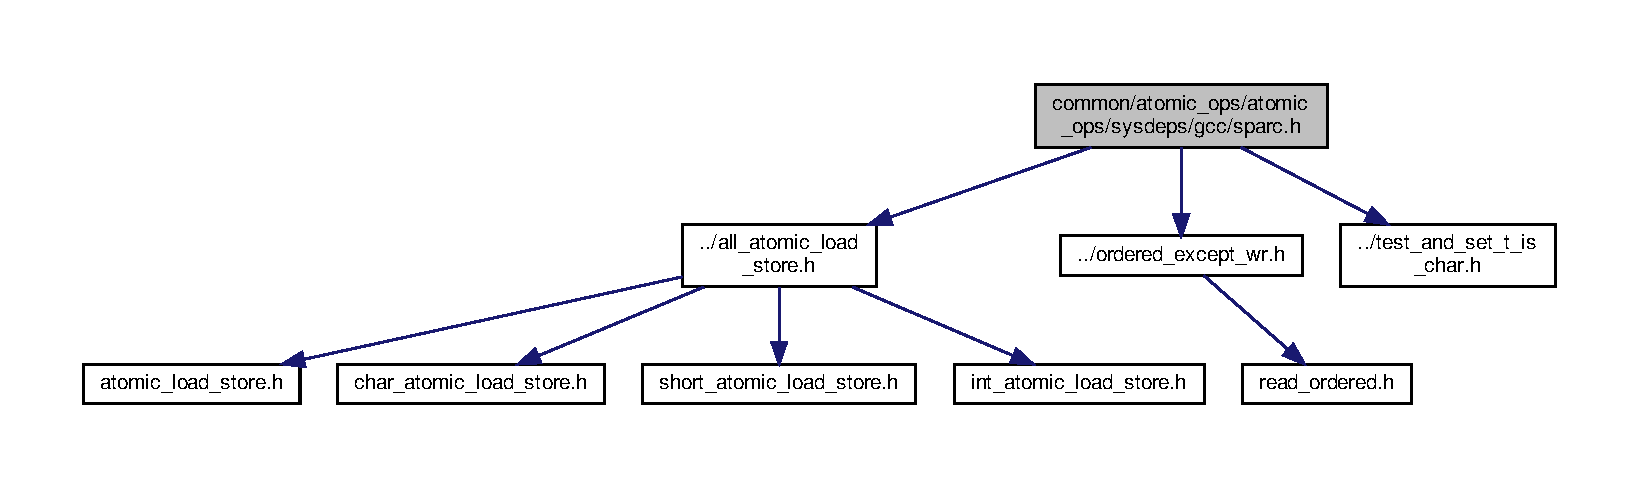
\includegraphics[width=350pt]{gcc_2sparc_8h__incl}
\end{center}
\end{figure}
\subsection*{Macros}
\begin{DoxyCompactItemize}
\item 
\#define \hyperlink{gcc_2sparc_8h_ad5f311a090d1e6e1bb35a6e68ee35fad}{A\+O\+\_\+\+H\+A\+V\+E\+\_\+test\+\_\+and\+\_\+set\+\_\+full}
\item 
\#define \hyperlink{gcc_2sparc_8h_a98ec53065c0dfd18bc1013c500da377c}{A\+O\+\_\+\+H\+A\+V\+E\+\_\+compare\+\_\+and\+\_\+swap\+\_\+full}
\end{DoxyCompactItemize}
\subsection*{Functions}
\begin{DoxyCompactItemize}
\item 
\hyperlink{atomic__ops_8h_a9f6ab6253b6b11bc8c12efe9dde5db2b}{A\+O\+\_\+\+I\+N\+L\+I\+NE} \hyperlink{test__and__set__t__is__char_8h_a7d99a16c4eab47ba80ab6138d7d98ac1}{A\+O\+\_\+\+T\+S\+\_\+\+V\+A\+L\+\_\+t} \hyperlink{gcc_2sparc_8h_a9f485bd63ce5c6a017ec241906e2f651}{A\+O\+\_\+test\+\_\+and\+\_\+set\+\_\+full} (volatile \hyperlink{test__and__set__t__is__char_8h_a5890c21b549264c75c2cad08bf4f6ba9}{A\+O\+\_\+\+T\+S\+\_\+t} $\ast$addr)
\item 
\hyperlink{atomic__ops_8h_a9f6ab6253b6b11bc8c12efe9dde5db2b}{A\+O\+\_\+\+I\+N\+L\+I\+NE} int \hyperlink{gcc_2sparc_8h_a634397de6de764015b30cdff3ff00b06}{A\+O\+\_\+compare\+\_\+and\+\_\+swap\+\_\+full} (volatile \hyperlink{atomic__ops_8h_a5225fef4d9eee821e82382cd269160dd}{A\+O\+\_\+t} $\ast$addr, \hyperlink{atomic__ops_8h_a5225fef4d9eee821e82382cd269160dd}{A\+O\+\_\+t} old, \hyperlink{atomic__ops_8h_a5225fef4d9eee821e82382cd269160dd}{A\+O\+\_\+t} new\+\_\+val)
\end{DoxyCompactItemize}


\subsection{Macro Definition Documentation}
\mbox{\Hypertarget{gcc_2sparc_8h_a98ec53065c0dfd18bc1013c500da377c}\label{gcc_2sparc_8h_a98ec53065c0dfd18bc1013c500da377c}} 
\index{gcc/sparc.\+h@{gcc/sparc.\+h}!A\+O\+\_\+\+H\+A\+V\+E\+\_\+compare\+\_\+and\+\_\+swap\+\_\+full@{A\+O\+\_\+\+H\+A\+V\+E\+\_\+compare\+\_\+and\+\_\+swap\+\_\+full}}
\index{A\+O\+\_\+\+H\+A\+V\+E\+\_\+compare\+\_\+and\+\_\+swap\+\_\+full@{A\+O\+\_\+\+H\+A\+V\+E\+\_\+compare\+\_\+and\+\_\+swap\+\_\+full}!gcc/sparc.\+h@{gcc/sparc.\+h}}
\subsubsection{\texorpdfstring{A\+O\+\_\+\+H\+A\+V\+E\+\_\+compare\+\_\+and\+\_\+swap\+\_\+full}{AO\_HAVE\_compare\_and\_swap\_full}}
{\footnotesize\ttfamily \#define A\+O\+\_\+\+H\+A\+V\+E\+\_\+compare\+\_\+and\+\_\+swap\+\_\+full}

\mbox{\Hypertarget{gcc_2sparc_8h_ad5f311a090d1e6e1bb35a6e68ee35fad}\label{gcc_2sparc_8h_ad5f311a090d1e6e1bb35a6e68ee35fad}} 
\index{gcc/sparc.\+h@{gcc/sparc.\+h}!A\+O\+\_\+\+H\+A\+V\+E\+\_\+test\+\_\+and\+\_\+set\+\_\+full@{A\+O\+\_\+\+H\+A\+V\+E\+\_\+test\+\_\+and\+\_\+set\+\_\+full}}
\index{A\+O\+\_\+\+H\+A\+V\+E\+\_\+test\+\_\+and\+\_\+set\+\_\+full@{A\+O\+\_\+\+H\+A\+V\+E\+\_\+test\+\_\+and\+\_\+set\+\_\+full}!gcc/sparc.\+h@{gcc/sparc.\+h}}
\subsubsection{\texorpdfstring{A\+O\+\_\+\+H\+A\+V\+E\+\_\+test\+\_\+and\+\_\+set\+\_\+full}{AO\_HAVE\_test\_and\_set\_full}}
{\footnotesize\ttfamily \#define A\+O\+\_\+\+H\+A\+V\+E\+\_\+test\+\_\+and\+\_\+set\+\_\+full}



\subsection{Function Documentation}
\mbox{\Hypertarget{gcc_2sparc_8h_a634397de6de764015b30cdff3ff00b06}\label{gcc_2sparc_8h_a634397de6de764015b30cdff3ff00b06}} 
\index{gcc/sparc.\+h@{gcc/sparc.\+h}!A\+O\+\_\+compare\+\_\+and\+\_\+swap\+\_\+full@{A\+O\+\_\+compare\+\_\+and\+\_\+swap\+\_\+full}}
\index{A\+O\+\_\+compare\+\_\+and\+\_\+swap\+\_\+full@{A\+O\+\_\+compare\+\_\+and\+\_\+swap\+\_\+full}!gcc/sparc.\+h@{gcc/sparc.\+h}}
\subsubsection{\texorpdfstring{A\+O\+\_\+compare\+\_\+and\+\_\+swap\+\_\+full()}{AO\_compare\_and\_swap\_full()}}
{\footnotesize\ttfamily \hyperlink{atomic__ops_8h_a9f6ab6253b6b11bc8c12efe9dde5db2b}{A\+O\+\_\+\+I\+N\+L\+I\+NE} int A\+O\+\_\+compare\+\_\+and\+\_\+swap\+\_\+full (\begin{DoxyParamCaption}\item[{volatile \hyperlink{atomic__ops_8h_a5225fef4d9eee821e82382cd269160dd}{A\+O\+\_\+t} $\ast$}]{addr,  }\item[{\hyperlink{atomic__ops_8h_a5225fef4d9eee821e82382cd269160dd}{A\+O\+\_\+t}}]{old,  }\item[{\hyperlink{atomic__ops_8h_a5225fef4d9eee821e82382cd269160dd}{A\+O\+\_\+t}}]{new\+\_\+val }\end{DoxyParamCaption})}

\mbox{\Hypertarget{gcc_2sparc_8h_a9f485bd63ce5c6a017ec241906e2f651}\label{gcc_2sparc_8h_a9f485bd63ce5c6a017ec241906e2f651}} 
\index{gcc/sparc.\+h@{gcc/sparc.\+h}!A\+O\+\_\+test\+\_\+and\+\_\+set\+\_\+full@{A\+O\+\_\+test\+\_\+and\+\_\+set\+\_\+full}}
\index{A\+O\+\_\+test\+\_\+and\+\_\+set\+\_\+full@{A\+O\+\_\+test\+\_\+and\+\_\+set\+\_\+full}!gcc/sparc.\+h@{gcc/sparc.\+h}}
\subsubsection{\texorpdfstring{A\+O\+\_\+test\+\_\+and\+\_\+set\+\_\+full()}{AO\_test\_and\_set\_full()}}
{\footnotesize\ttfamily \hyperlink{atomic__ops_8h_a9f6ab6253b6b11bc8c12efe9dde5db2b}{A\+O\+\_\+\+I\+N\+L\+I\+NE} \hyperlink{test__and__set__t__is__char_8h_a7d99a16c4eab47ba80ab6138d7d98ac1}{A\+O\+\_\+\+T\+S\+\_\+\+V\+A\+L\+\_\+t} A\+O\+\_\+test\+\_\+and\+\_\+set\+\_\+full (\begin{DoxyParamCaption}\item[{volatile \hyperlink{test__and__set__t__is__char_8h_a5890c21b549264c75c2cad08bf4f6ba9}{A\+O\+\_\+\+T\+S\+\_\+t} $\ast$}]{addr }\end{DoxyParamCaption})}


\hypertarget{sunc_2sparc_8h}{}\section{common/atomic\+\_\+ops/atomic\+\_\+ops/sysdeps/sunc/sparc.h File Reference}
\label{sunc_2sparc_8h}\index{common/atomic\+\_\+ops/atomic\+\_\+ops/sysdeps/sunc/sparc.\+h@{common/atomic\+\_\+ops/atomic\+\_\+ops/sysdeps/sunc/sparc.\+h}}
{\ttfamily \#include \char`\"{}../all\+\_\+atomic\+\_\+load\+\_\+store.\+h\char`\"{}}\newline
{\ttfamily \#include \char`\"{}../ordered\+\_\+except\+\_\+wr.\+h\char`\"{}}\newline
{\ttfamily \#include \char`\"{}../test\+\_\+and\+\_\+set\+\_\+t\+\_\+is\+\_\+char.\+h\char`\"{}}\newline
Include dependency graph for sparc.\+h\+:
\nopagebreak
\begin{figure}[H]
\begin{center}
\leavevmode
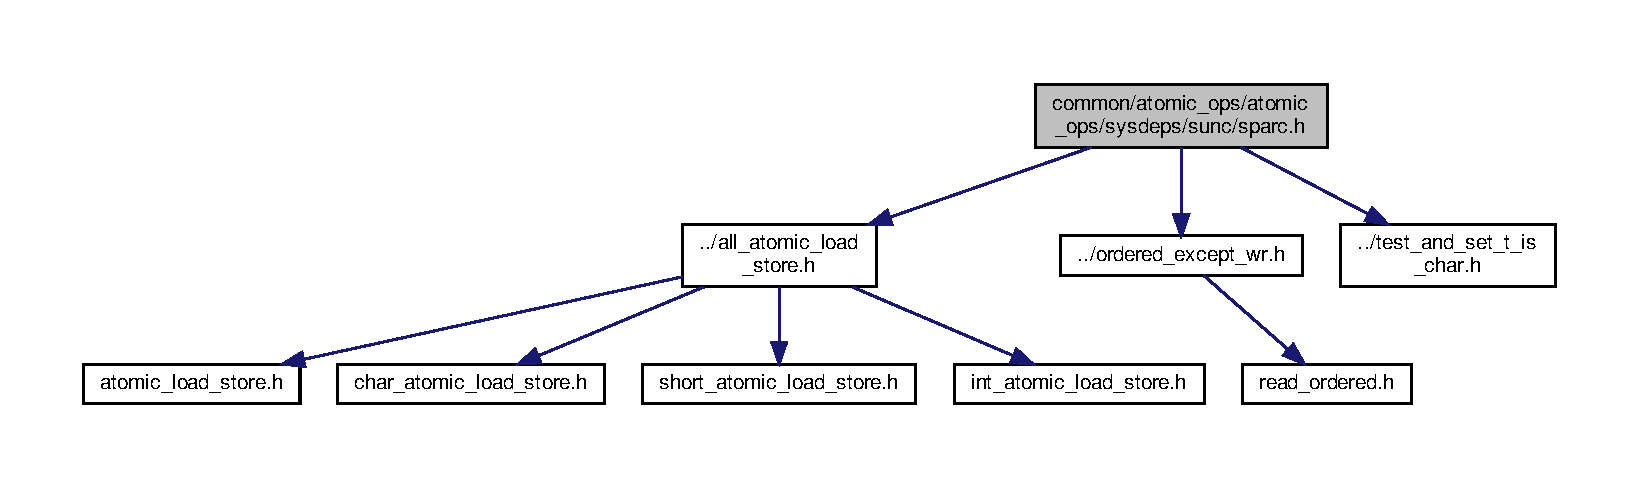
\includegraphics[width=350pt]{sunc_2sparc_8h__incl}
\end{center}
\end{figure}
\subsection*{Macros}
\begin{DoxyCompactItemize}
\item 
\#define \hyperlink{sunc_2sparc_8h_ad5f311a090d1e6e1bb35a6e68ee35fad}{A\+O\+\_\+\+H\+A\+V\+E\+\_\+test\+\_\+and\+\_\+set\+\_\+full}
\end{DoxyCompactItemize}
\subsection*{Functions}
\begin{DoxyCompactItemize}
\item 
\hyperlink{test__and__set__t__is__char_8h_a7d99a16c4eab47ba80ab6138d7d98ac1}{A\+O\+\_\+\+T\+S\+\_\+\+V\+A\+L\+\_\+t} \hyperlink{sunc_2sparc_8h_a4c679f2d141a1057e1254b1f64febc71}{A\+O\+\_\+test\+\_\+and\+\_\+set\+\_\+full} (volatile \hyperlink{test__and__set__t__is__char_8h_a5890c21b549264c75c2cad08bf4f6ba9}{A\+O\+\_\+\+T\+S\+\_\+t} $\ast$addr)
\end{DoxyCompactItemize}


\subsection{Macro Definition Documentation}
\mbox{\Hypertarget{sunc_2sparc_8h_ad5f311a090d1e6e1bb35a6e68ee35fad}\label{sunc_2sparc_8h_ad5f311a090d1e6e1bb35a6e68ee35fad}} 
\index{sunc/sparc.\+h@{sunc/sparc.\+h}!A\+O\+\_\+\+H\+A\+V\+E\+\_\+test\+\_\+and\+\_\+set\+\_\+full@{A\+O\+\_\+\+H\+A\+V\+E\+\_\+test\+\_\+and\+\_\+set\+\_\+full}}
\index{A\+O\+\_\+\+H\+A\+V\+E\+\_\+test\+\_\+and\+\_\+set\+\_\+full@{A\+O\+\_\+\+H\+A\+V\+E\+\_\+test\+\_\+and\+\_\+set\+\_\+full}!sunc/sparc.\+h@{sunc/sparc.\+h}}
\subsubsection{\texorpdfstring{A\+O\+\_\+\+H\+A\+V\+E\+\_\+test\+\_\+and\+\_\+set\+\_\+full}{AO\_HAVE\_test\_and\_set\_full}}
{\footnotesize\ttfamily \#define A\+O\+\_\+\+H\+A\+V\+E\+\_\+test\+\_\+and\+\_\+set\+\_\+full}



\subsection{Function Documentation}
\mbox{\Hypertarget{sunc_2sparc_8h_a4c679f2d141a1057e1254b1f64febc71}\label{sunc_2sparc_8h_a4c679f2d141a1057e1254b1f64febc71}} 
\index{sunc/sparc.\+h@{sunc/sparc.\+h}!A\+O\+\_\+test\+\_\+and\+\_\+set\+\_\+full@{A\+O\+\_\+test\+\_\+and\+\_\+set\+\_\+full}}
\index{A\+O\+\_\+test\+\_\+and\+\_\+set\+\_\+full@{A\+O\+\_\+test\+\_\+and\+\_\+set\+\_\+full}!sunc/sparc.\+h@{sunc/sparc.\+h}}
\subsubsection{\texorpdfstring{A\+O\+\_\+test\+\_\+and\+\_\+set\+\_\+full()}{AO\_test\_and\_set\_full()}}
{\footnotesize\ttfamily \hyperlink{test__and__set__t__is__char_8h_a7d99a16c4eab47ba80ab6138d7d98ac1}{A\+O\+\_\+\+T\+S\+\_\+\+V\+A\+L\+\_\+t} A\+O\+\_\+test\+\_\+and\+\_\+set\+\_\+full (\begin{DoxyParamCaption}\item[{volatile \hyperlink{test__and__set__t__is__char_8h_a5890c21b549264c75c2cad08bf4f6ba9}{A\+O\+\_\+\+T\+S\+\_\+t} $\ast$}]{addr }\end{DoxyParamCaption})}


\hypertarget{gcc_2x86_8h}{}\section{common/atomic\+\_\+ops/atomic\+\_\+ops/sysdeps/gcc/x86.h File Reference}
\label{gcc_2x86_8h}\index{common/atomic\+\_\+ops/atomic\+\_\+ops/sysdeps/gcc/x86.\+h@{common/atomic\+\_\+ops/atomic\+\_\+ops/sysdeps/gcc/x86.\+h}}
{\ttfamily \#include \char`\"{}../all\+\_\+aligned\+\_\+atomic\+\_\+load\+\_\+store.\+h\char`\"{}}\newline
{\ttfamily \#include \char`\"{}../ordered\+\_\+except\+\_\+wr.\+h\char`\"{}}\newline
{\ttfamily \#include \char`\"{}../test\+\_\+and\+\_\+set\+\_\+t\+\_\+is\+\_\+char.\+h\char`\"{}}\newline
{\ttfamily \#include \char`\"{}../standard\+\_\+ao\+\_\+double\+\_\+t.\+h\char`\"{}}\newline
{\ttfamily \#include \char`\"{}../ao\+\_\+t\+\_\+is\+\_\+int.\+h\char`\"{}}\newline
Include dependency graph for x86.\+h\+:
\nopagebreak
\begin{figure}[H]
\begin{center}
\leavevmode
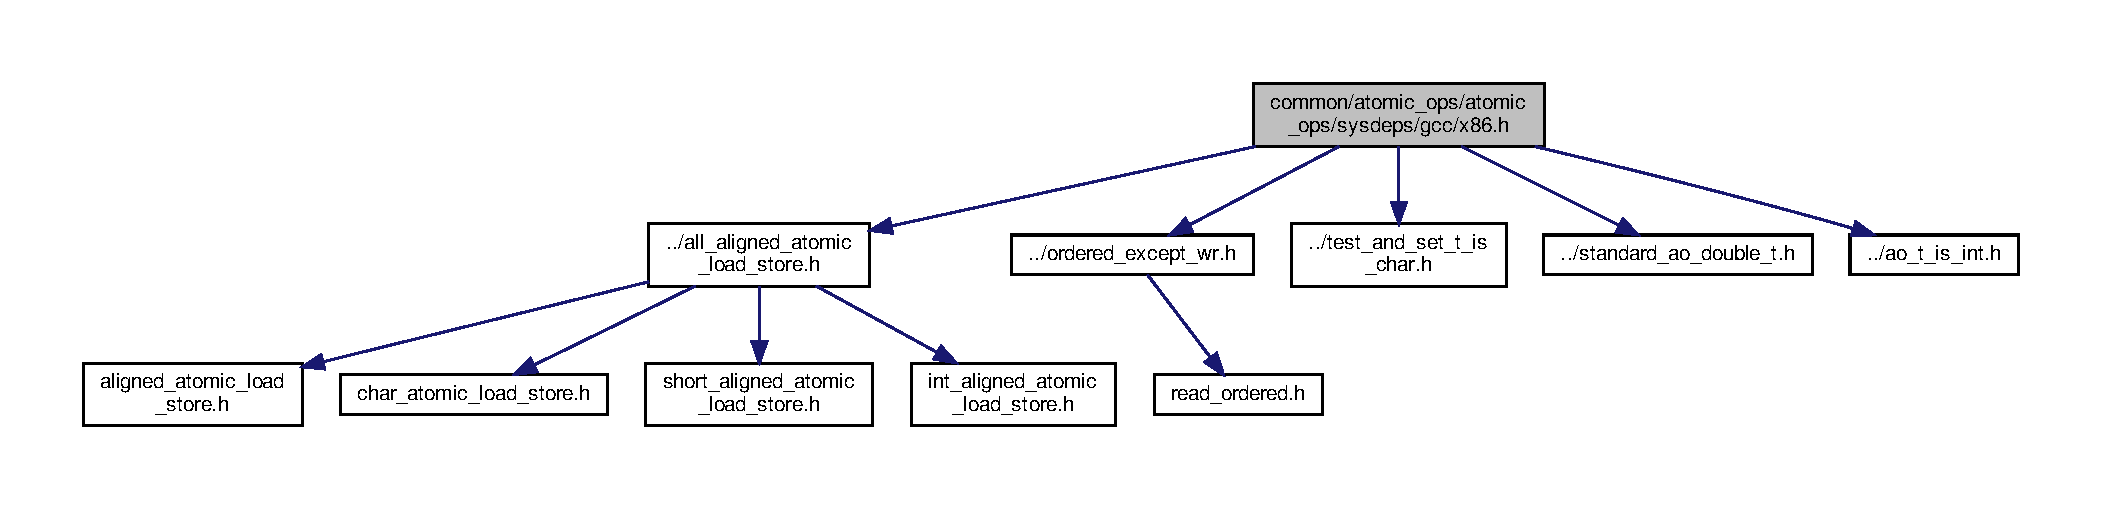
\includegraphics[width=350pt]{gcc_2x86_8h__incl}
\end{center}
\end{figure}
\subsection*{Macros}
\begin{DoxyCompactItemize}
\item 
\#define \hyperlink{gcc_2x86_8h_a9fa0fc1a9eadcba085e57bf180a53cef}{A\+O\+\_\+\+H\+A\+V\+E\+\_\+fetch\+\_\+and\+\_\+add\+\_\+full}
\item 
\#define \hyperlink{gcc_2x86_8h_a0a938d33904c99956494e57bfa2b74fd}{A\+O\+\_\+\+H\+A\+V\+E\+\_\+char\+\_\+fetch\+\_\+and\+\_\+add\+\_\+full}
\item 
\#define \hyperlink{gcc_2x86_8h_affc6a05c52cc08ec46bcbba79457d985}{A\+O\+\_\+\+H\+A\+V\+E\+\_\+short\+\_\+fetch\+\_\+and\+\_\+add\+\_\+full}
\item 
\#define \hyperlink{gcc_2x86_8h_a0ef45a04b0d7c74e025f829f2e614d79}{A\+O\+\_\+\+H\+A\+V\+E\+\_\+or\+\_\+full}
\item 
\#define \hyperlink{gcc_2x86_8h_ad5f311a090d1e6e1bb35a6e68ee35fad}{A\+O\+\_\+\+H\+A\+V\+E\+\_\+test\+\_\+and\+\_\+set\+\_\+full}
\item 
\#define \hyperlink{gcc_2x86_8h_a98ec53065c0dfd18bc1013c500da377c}{A\+O\+\_\+\+H\+A\+V\+E\+\_\+compare\+\_\+and\+\_\+swap\+\_\+full}
\item 
\#define \hyperlink{gcc_2x86_8h_a0e2b334560e5f9a06567fc59e33a435d}{A\+O\+\_\+\+H\+A\+V\+E\+\_\+compare\+\_\+double\+\_\+and\+\_\+swap\+\_\+double\+\_\+full}
\end{DoxyCompactItemize}
\subsection*{Functions}
\begin{DoxyCompactItemize}
\item 
\hyperlink{atomic__ops_8h_a9f6ab6253b6b11bc8c12efe9dde5db2b}{A\+O\+\_\+\+I\+N\+L\+I\+NE} \hyperlink{atomic__ops_8h_a5225fef4d9eee821e82382cd269160dd}{A\+O\+\_\+t} \hyperlink{gcc_2x86_8h_a63b6d5232496fb679621fa985234eff8}{A\+O\+\_\+fetch\+\_\+and\+\_\+add\+\_\+full} (volatile \hyperlink{atomic__ops_8h_a5225fef4d9eee821e82382cd269160dd}{A\+O\+\_\+t} $\ast$p, \hyperlink{atomic__ops_8h_a5225fef4d9eee821e82382cd269160dd}{A\+O\+\_\+t} incr)
\item 
\hyperlink{atomic__ops_8h_a9f6ab6253b6b11bc8c12efe9dde5db2b}{A\+O\+\_\+\+I\+N\+L\+I\+NE} unsigned char \hyperlink{gcc_2x86_8h_a03d2aa8ce4372d7d08a306c6de38d4ba}{A\+O\+\_\+char\+\_\+fetch\+\_\+and\+\_\+add\+\_\+full} (volatile unsigned char $\ast$p, unsigned char incr)
\item 
\hyperlink{atomic__ops_8h_a9f6ab6253b6b11bc8c12efe9dde5db2b}{A\+O\+\_\+\+I\+N\+L\+I\+NE} unsigned short \hyperlink{gcc_2x86_8h_a99328cedbe167830313d7c3ffdcd0180}{A\+O\+\_\+short\+\_\+fetch\+\_\+and\+\_\+add\+\_\+full} (volatile unsigned short $\ast$p, unsigned short incr)
\item 
\hyperlink{atomic__ops_8h_a9f6ab6253b6b11bc8c12efe9dde5db2b}{A\+O\+\_\+\+I\+N\+L\+I\+NE} void \hyperlink{gcc_2x86_8h_a2732b24b044bf3993055d2c0d78b9ed9}{A\+O\+\_\+or\+\_\+full} (volatile \hyperlink{atomic__ops_8h_a5225fef4d9eee821e82382cd269160dd}{A\+O\+\_\+t} $\ast$p, \hyperlink{atomic__ops_8h_a5225fef4d9eee821e82382cd269160dd}{A\+O\+\_\+t} incr)
\item 
\hyperlink{atomic__ops_8h_a9f6ab6253b6b11bc8c12efe9dde5db2b}{A\+O\+\_\+\+I\+N\+L\+I\+NE} \hyperlink{test__and__set__t__is__char_8h_a7d99a16c4eab47ba80ab6138d7d98ac1}{A\+O\+\_\+\+T\+S\+\_\+\+V\+A\+L\+\_\+t} \hyperlink{gcc_2x86_8h_a9f485bd63ce5c6a017ec241906e2f651}{A\+O\+\_\+test\+\_\+and\+\_\+set\+\_\+full} (volatile \hyperlink{test__and__set__t__is__char_8h_a5890c21b549264c75c2cad08bf4f6ba9}{A\+O\+\_\+\+T\+S\+\_\+t} $\ast$addr)
\item 
\hyperlink{atomic__ops_8h_a9f6ab6253b6b11bc8c12efe9dde5db2b}{A\+O\+\_\+\+I\+N\+L\+I\+NE} int \hyperlink{gcc_2x86_8h_a634397de6de764015b30cdff3ff00b06}{A\+O\+\_\+compare\+\_\+and\+\_\+swap\+\_\+full} (volatile \hyperlink{atomic__ops_8h_a5225fef4d9eee821e82382cd269160dd}{A\+O\+\_\+t} $\ast$addr, \hyperlink{atomic__ops_8h_a5225fef4d9eee821e82382cd269160dd}{A\+O\+\_\+t} old, \hyperlink{atomic__ops_8h_a5225fef4d9eee821e82382cd269160dd}{A\+O\+\_\+t} new\+\_\+val)
\item 
\hyperlink{atomic__ops_8h_a9f6ab6253b6b11bc8c12efe9dde5db2b}{A\+O\+\_\+\+I\+N\+L\+I\+NE} int \hyperlink{gcc_2x86_8h_ab464a096b1708a8c5cc7e63de92436d6}{A\+O\+\_\+compare\+\_\+double\+\_\+and\+\_\+swap\+\_\+double\+\_\+full} (volatile \hyperlink{structAO__double__t}{A\+O\+\_\+double\+\_\+t} $\ast$addr, \hyperlink{atomic__ops_8h_a5225fef4d9eee821e82382cd269160dd}{A\+O\+\_\+t} old\+\_\+val1, \hyperlink{atomic__ops_8h_a5225fef4d9eee821e82382cd269160dd}{A\+O\+\_\+t} old\+\_\+val2, \hyperlink{atomic__ops_8h_a5225fef4d9eee821e82382cd269160dd}{A\+O\+\_\+t} new\+\_\+val1, \hyperlink{atomic__ops_8h_a5225fef4d9eee821e82382cd269160dd}{A\+O\+\_\+t} new\+\_\+val2)
\end{DoxyCompactItemize}


\subsection{Macro Definition Documentation}
\mbox{\Hypertarget{gcc_2x86_8h_a0a938d33904c99956494e57bfa2b74fd}\label{gcc_2x86_8h_a0a938d33904c99956494e57bfa2b74fd}} 
\index{gcc/x86.\+h@{gcc/x86.\+h}!A\+O\+\_\+\+H\+A\+V\+E\+\_\+char\+\_\+fetch\+\_\+and\+\_\+add\+\_\+full@{A\+O\+\_\+\+H\+A\+V\+E\+\_\+char\+\_\+fetch\+\_\+and\+\_\+add\+\_\+full}}
\index{A\+O\+\_\+\+H\+A\+V\+E\+\_\+char\+\_\+fetch\+\_\+and\+\_\+add\+\_\+full@{A\+O\+\_\+\+H\+A\+V\+E\+\_\+char\+\_\+fetch\+\_\+and\+\_\+add\+\_\+full}!gcc/x86.\+h@{gcc/x86.\+h}}
\subsubsection{\texorpdfstring{A\+O\+\_\+\+H\+A\+V\+E\+\_\+char\+\_\+fetch\+\_\+and\+\_\+add\+\_\+full}{AO\_HAVE\_char\_fetch\_and\_add\_full}}
{\footnotesize\ttfamily \#define A\+O\+\_\+\+H\+A\+V\+E\+\_\+char\+\_\+fetch\+\_\+and\+\_\+add\+\_\+full}

\mbox{\Hypertarget{gcc_2x86_8h_a98ec53065c0dfd18bc1013c500da377c}\label{gcc_2x86_8h_a98ec53065c0dfd18bc1013c500da377c}} 
\index{gcc/x86.\+h@{gcc/x86.\+h}!A\+O\+\_\+\+H\+A\+V\+E\+\_\+compare\+\_\+and\+\_\+swap\+\_\+full@{A\+O\+\_\+\+H\+A\+V\+E\+\_\+compare\+\_\+and\+\_\+swap\+\_\+full}}
\index{A\+O\+\_\+\+H\+A\+V\+E\+\_\+compare\+\_\+and\+\_\+swap\+\_\+full@{A\+O\+\_\+\+H\+A\+V\+E\+\_\+compare\+\_\+and\+\_\+swap\+\_\+full}!gcc/x86.\+h@{gcc/x86.\+h}}
\subsubsection{\texorpdfstring{A\+O\+\_\+\+H\+A\+V\+E\+\_\+compare\+\_\+and\+\_\+swap\+\_\+full}{AO\_HAVE\_compare\_and\_swap\_full}}
{\footnotesize\ttfamily \#define A\+O\+\_\+\+H\+A\+V\+E\+\_\+compare\+\_\+and\+\_\+swap\+\_\+full}

\mbox{\Hypertarget{gcc_2x86_8h_a0e2b334560e5f9a06567fc59e33a435d}\label{gcc_2x86_8h_a0e2b334560e5f9a06567fc59e33a435d}} 
\index{gcc/x86.\+h@{gcc/x86.\+h}!A\+O\+\_\+\+H\+A\+V\+E\+\_\+compare\+\_\+double\+\_\+and\+\_\+swap\+\_\+double\+\_\+full@{A\+O\+\_\+\+H\+A\+V\+E\+\_\+compare\+\_\+double\+\_\+and\+\_\+swap\+\_\+double\+\_\+full}}
\index{A\+O\+\_\+\+H\+A\+V\+E\+\_\+compare\+\_\+double\+\_\+and\+\_\+swap\+\_\+double\+\_\+full@{A\+O\+\_\+\+H\+A\+V\+E\+\_\+compare\+\_\+double\+\_\+and\+\_\+swap\+\_\+double\+\_\+full}!gcc/x86.\+h@{gcc/x86.\+h}}
\subsubsection{\texorpdfstring{A\+O\+\_\+\+H\+A\+V\+E\+\_\+compare\+\_\+double\+\_\+and\+\_\+swap\+\_\+double\+\_\+full}{AO\_HAVE\_compare\_double\_and\_swap\_double\_full}}
{\footnotesize\ttfamily \#define A\+O\+\_\+\+H\+A\+V\+E\+\_\+compare\+\_\+double\+\_\+and\+\_\+swap\+\_\+double\+\_\+full}

\mbox{\Hypertarget{gcc_2x86_8h_a9fa0fc1a9eadcba085e57bf180a53cef}\label{gcc_2x86_8h_a9fa0fc1a9eadcba085e57bf180a53cef}} 
\index{gcc/x86.\+h@{gcc/x86.\+h}!A\+O\+\_\+\+H\+A\+V\+E\+\_\+fetch\+\_\+and\+\_\+add\+\_\+full@{A\+O\+\_\+\+H\+A\+V\+E\+\_\+fetch\+\_\+and\+\_\+add\+\_\+full}}
\index{A\+O\+\_\+\+H\+A\+V\+E\+\_\+fetch\+\_\+and\+\_\+add\+\_\+full@{A\+O\+\_\+\+H\+A\+V\+E\+\_\+fetch\+\_\+and\+\_\+add\+\_\+full}!gcc/x86.\+h@{gcc/x86.\+h}}
\subsubsection{\texorpdfstring{A\+O\+\_\+\+H\+A\+V\+E\+\_\+fetch\+\_\+and\+\_\+add\+\_\+full}{AO\_HAVE\_fetch\_and\_add\_full}}
{\footnotesize\ttfamily \#define A\+O\+\_\+\+H\+A\+V\+E\+\_\+fetch\+\_\+and\+\_\+add\+\_\+full}

\mbox{\Hypertarget{gcc_2x86_8h_a0ef45a04b0d7c74e025f829f2e614d79}\label{gcc_2x86_8h_a0ef45a04b0d7c74e025f829f2e614d79}} 
\index{gcc/x86.\+h@{gcc/x86.\+h}!A\+O\+\_\+\+H\+A\+V\+E\+\_\+or\+\_\+full@{A\+O\+\_\+\+H\+A\+V\+E\+\_\+or\+\_\+full}}
\index{A\+O\+\_\+\+H\+A\+V\+E\+\_\+or\+\_\+full@{A\+O\+\_\+\+H\+A\+V\+E\+\_\+or\+\_\+full}!gcc/x86.\+h@{gcc/x86.\+h}}
\subsubsection{\texorpdfstring{A\+O\+\_\+\+H\+A\+V\+E\+\_\+or\+\_\+full}{AO\_HAVE\_or\_full}}
{\footnotesize\ttfamily \#define A\+O\+\_\+\+H\+A\+V\+E\+\_\+or\+\_\+full}

\mbox{\Hypertarget{gcc_2x86_8h_affc6a05c52cc08ec46bcbba79457d985}\label{gcc_2x86_8h_affc6a05c52cc08ec46bcbba79457d985}} 
\index{gcc/x86.\+h@{gcc/x86.\+h}!A\+O\+\_\+\+H\+A\+V\+E\+\_\+short\+\_\+fetch\+\_\+and\+\_\+add\+\_\+full@{A\+O\+\_\+\+H\+A\+V\+E\+\_\+short\+\_\+fetch\+\_\+and\+\_\+add\+\_\+full}}
\index{A\+O\+\_\+\+H\+A\+V\+E\+\_\+short\+\_\+fetch\+\_\+and\+\_\+add\+\_\+full@{A\+O\+\_\+\+H\+A\+V\+E\+\_\+short\+\_\+fetch\+\_\+and\+\_\+add\+\_\+full}!gcc/x86.\+h@{gcc/x86.\+h}}
\subsubsection{\texorpdfstring{A\+O\+\_\+\+H\+A\+V\+E\+\_\+short\+\_\+fetch\+\_\+and\+\_\+add\+\_\+full}{AO\_HAVE\_short\_fetch\_and\_add\_full}}
{\footnotesize\ttfamily \#define A\+O\+\_\+\+H\+A\+V\+E\+\_\+short\+\_\+fetch\+\_\+and\+\_\+add\+\_\+full}

\mbox{\Hypertarget{gcc_2x86_8h_ad5f311a090d1e6e1bb35a6e68ee35fad}\label{gcc_2x86_8h_ad5f311a090d1e6e1bb35a6e68ee35fad}} 
\index{gcc/x86.\+h@{gcc/x86.\+h}!A\+O\+\_\+\+H\+A\+V\+E\+\_\+test\+\_\+and\+\_\+set\+\_\+full@{A\+O\+\_\+\+H\+A\+V\+E\+\_\+test\+\_\+and\+\_\+set\+\_\+full}}
\index{A\+O\+\_\+\+H\+A\+V\+E\+\_\+test\+\_\+and\+\_\+set\+\_\+full@{A\+O\+\_\+\+H\+A\+V\+E\+\_\+test\+\_\+and\+\_\+set\+\_\+full}!gcc/x86.\+h@{gcc/x86.\+h}}
\subsubsection{\texorpdfstring{A\+O\+\_\+\+H\+A\+V\+E\+\_\+test\+\_\+and\+\_\+set\+\_\+full}{AO\_HAVE\_test\_and\_set\_full}}
{\footnotesize\ttfamily \#define A\+O\+\_\+\+H\+A\+V\+E\+\_\+test\+\_\+and\+\_\+set\+\_\+full}



\subsection{Function Documentation}
\mbox{\Hypertarget{gcc_2x86_8h_a03d2aa8ce4372d7d08a306c6de38d4ba}\label{gcc_2x86_8h_a03d2aa8ce4372d7d08a306c6de38d4ba}} 
\index{gcc/x86.\+h@{gcc/x86.\+h}!A\+O\+\_\+char\+\_\+fetch\+\_\+and\+\_\+add\+\_\+full@{A\+O\+\_\+char\+\_\+fetch\+\_\+and\+\_\+add\+\_\+full}}
\index{A\+O\+\_\+char\+\_\+fetch\+\_\+and\+\_\+add\+\_\+full@{A\+O\+\_\+char\+\_\+fetch\+\_\+and\+\_\+add\+\_\+full}!gcc/x86.\+h@{gcc/x86.\+h}}
\subsubsection{\texorpdfstring{A\+O\+\_\+char\+\_\+fetch\+\_\+and\+\_\+add\+\_\+full()}{AO\_char\_fetch\_and\_add\_full()}}
{\footnotesize\ttfamily \hyperlink{atomic__ops_8h_a9f6ab6253b6b11bc8c12efe9dde5db2b}{A\+O\+\_\+\+I\+N\+L\+I\+NE} unsigned char A\+O\+\_\+char\+\_\+fetch\+\_\+and\+\_\+add\+\_\+full (\begin{DoxyParamCaption}\item[{volatile unsigned char $\ast$}]{p,  }\item[{unsigned char}]{incr }\end{DoxyParamCaption})}

\mbox{\Hypertarget{gcc_2x86_8h_a634397de6de764015b30cdff3ff00b06}\label{gcc_2x86_8h_a634397de6de764015b30cdff3ff00b06}} 
\index{gcc/x86.\+h@{gcc/x86.\+h}!A\+O\+\_\+compare\+\_\+and\+\_\+swap\+\_\+full@{A\+O\+\_\+compare\+\_\+and\+\_\+swap\+\_\+full}}
\index{A\+O\+\_\+compare\+\_\+and\+\_\+swap\+\_\+full@{A\+O\+\_\+compare\+\_\+and\+\_\+swap\+\_\+full}!gcc/x86.\+h@{gcc/x86.\+h}}
\subsubsection{\texorpdfstring{A\+O\+\_\+compare\+\_\+and\+\_\+swap\+\_\+full()}{AO\_compare\_and\_swap\_full()}}
{\footnotesize\ttfamily \hyperlink{atomic__ops_8h_a9f6ab6253b6b11bc8c12efe9dde5db2b}{A\+O\+\_\+\+I\+N\+L\+I\+NE} int A\+O\+\_\+compare\+\_\+and\+\_\+swap\+\_\+full (\begin{DoxyParamCaption}\item[{volatile \hyperlink{atomic__ops_8h_a5225fef4d9eee821e82382cd269160dd}{A\+O\+\_\+t} $\ast$}]{addr,  }\item[{\hyperlink{atomic__ops_8h_a5225fef4d9eee821e82382cd269160dd}{A\+O\+\_\+t}}]{old,  }\item[{\hyperlink{atomic__ops_8h_a5225fef4d9eee821e82382cd269160dd}{A\+O\+\_\+t}}]{new\+\_\+val }\end{DoxyParamCaption})}

\mbox{\Hypertarget{gcc_2x86_8h_ab464a096b1708a8c5cc7e63de92436d6}\label{gcc_2x86_8h_ab464a096b1708a8c5cc7e63de92436d6}} 
\index{gcc/x86.\+h@{gcc/x86.\+h}!A\+O\+\_\+compare\+\_\+double\+\_\+and\+\_\+swap\+\_\+double\+\_\+full@{A\+O\+\_\+compare\+\_\+double\+\_\+and\+\_\+swap\+\_\+double\+\_\+full}}
\index{A\+O\+\_\+compare\+\_\+double\+\_\+and\+\_\+swap\+\_\+double\+\_\+full@{A\+O\+\_\+compare\+\_\+double\+\_\+and\+\_\+swap\+\_\+double\+\_\+full}!gcc/x86.\+h@{gcc/x86.\+h}}
\subsubsection{\texorpdfstring{A\+O\+\_\+compare\+\_\+double\+\_\+and\+\_\+swap\+\_\+double\+\_\+full()}{AO\_compare\_double\_and\_swap\_double\_full()}}
{\footnotesize\ttfamily \hyperlink{atomic__ops_8h_a9f6ab6253b6b11bc8c12efe9dde5db2b}{A\+O\+\_\+\+I\+N\+L\+I\+NE} int A\+O\+\_\+compare\+\_\+double\+\_\+and\+\_\+swap\+\_\+double\+\_\+full (\begin{DoxyParamCaption}\item[{volatile \hyperlink{structAO__double__t}{A\+O\+\_\+double\+\_\+t} $\ast$}]{addr,  }\item[{\hyperlink{atomic__ops_8h_a5225fef4d9eee821e82382cd269160dd}{A\+O\+\_\+t}}]{old\+\_\+val1,  }\item[{\hyperlink{atomic__ops_8h_a5225fef4d9eee821e82382cd269160dd}{A\+O\+\_\+t}}]{old\+\_\+val2,  }\item[{\hyperlink{atomic__ops_8h_a5225fef4d9eee821e82382cd269160dd}{A\+O\+\_\+t}}]{new\+\_\+val1,  }\item[{\hyperlink{atomic__ops_8h_a5225fef4d9eee821e82382cd269160dd}{A\+O\+\_\+t}}]{new\+\_\+val2 }\end{DoxyParamCaption})}

\mbox{\Hypertarget{gcc_2x86_8h_a63b6d5232496fb679621fa985234eff8}\label{gcc_2x86_8h_a63b6d5232496fb679621fa985234eff8}} 
\index{gcc/x86.\+h@{gcc/x86.\+h}!A\+O\+\_\+fetch\+\_\+and\+\_\+add\+\_\+full@{A\+O\+\_\+fetch\+\_\+and\+\_\+add\+\_\+full}}
\index{A\+O\+\_\+fetch\+\_\+and\+\_\+add\+\_\+full@{A\+O\+\_\+fetch\+\_\+and\+\_\+add\+\_\+full}!gcc/x86.\+h@{gcc/x86.\+h}}
\subsubsection{\texorpdfstring{A\+O\+\_\+fetch\+\_\+and\+\_\+add\+\_\+full()}{AO\_fetch\_and\_add\_full()}}
{\footnotesize\ttfamily \hyperlink{atomic__ops_8h_a9f6ab6253b6b11bc8c12efe9dde5db2b}{A\+O\+\_\+\+I\+N\+L\+I\+NE} \hyperlink{atomic__ops_8h_a5225fef4d9eee821e82382cd269160dd}{A\+O\+\_\+t} A\+O\+\_\+fetch\+\_\+and\+\_\+add\+\_\+full (\begin{DoxyParamCaption}\item[{volatile \hyperlink{atomic__ops_8h_a5225fef4d9eee821e82382cd269160dd}{A\+O\+\_\+t} $\ast$}]{p,  }\item[{\hyperlink{atomic__ops_8h_a5225fef4d9eee821e82382cd269160dd}{A\+O\+\_\+t}}]{incr }\end{DoxyParamCaption})}

\mbox{\Hypertarget{gcc_2x86_8h_a2732b24b044bf3993055d2c0d78b9ed9}\label{gcc_2x86_8h_a2732b24b044bf3993055d2c0d78b9ed9}} 
\index{gcc/x86.\+h@{gcc/x86.\+h}!A\+O\+\_\+or\+\_\+full@{A\+O\+\_\+or\+\_\+full}}
\index{A\+O\+\_\+or\+\_\+full@{A\+O\+\_\+or\+\_\+full}!gcc/x86.\+h@{gcc/x86.\+h}}
\subsubsection{\texorpdfstring{A\+O\+\_\+or\+\_\+full()}{AO\_or\_full()}}
{\footnotesize\ttfamily \hyperlink{atomic__ops_8h_a9f6ab6253b6b11bc8c12efe9dde5db2b}{A\+O\+\_\+\+I\+N\+L\+I\+NE} void A\+O\+\_\+or\+\_\+full (\begin{DoxyParamCaption}\item[{volatile \hyperlink{atomic__ops_8h_a5225fef4d9eee821e82382cd269160dd}{A\+O\+\_\+t} $\ast$}]{p,  }\item[{\hyperlink{atomic__ops_8h_a5225fef4d9eee821e82382cd269160dd}{A\+O\+\_\+t}}]{incr }\end{DoxyParamCaption})}

\mbox{\Hypertarget{gcc_2x86_8h_a99328cedbe167830313d7c3ffdcd0180}\label{gcc_2x86_8h_a99328cedbe167830313d7c3ffdcd0180}} 
\index{gcc/x86.\+h@{gcc/x86.\+h}!A\+O\+\_\+short\+\_\+fetch\+\_\+and\+\_\+add\+\_\+full@{A\+O\+\_\+short\+\_\+fetch\+\_\+and\+\_\+add\+\_\+full}}
\index{A\+O\+\_\+short\+\_\+fetch\+\_\+and\+\_\+add\+\_\+full@{A\+O\+\_\+short\+\_\+fetch\+\_\+and\+\_\+add\+\_\+full}!gcc/x86.\+h@{gcc/x86.\+h}}
\subsubsection{\texorpdfstring{A\+O\+\_\+short\+\_\+fetch\+\_\+and\+\_\+add\+\_\+full()}{AO\_short\_fetch\_and\_add\_full()}}
{\footnotesize\ttfamily \hyperlink{atomic__ops_8h_a9f6ab6253b6b11bc8c12efe9dde5db2b}{A\+O\+\_\+\+I\+N\+L\+I\+NE} unsigned short A\+O\+\_\+short\+\_\+fetch\+\_\+and\+\_\+add\+\_\+full (\begin{DoxyParamCaption}\item[{volatile unsigned short $\ast$}]{p,  }\item[{unsigned short}]{incr }\end{DoxyParamCaption})}

\mbox{\Hypertarget{gcc_2x86_8h_a9f485bd63ce5c6a017ec241906e2f651}\label{gcc_2x86_8h_a9f485bd63ce5c6a017ec241906e2f651}} 
\index{gcc/x86.\+h@{gcc/x86.\+h}!A\+O\+\_\+test\+\_\+and\+\_\+set\+\_\+full@{A\+O\+\_\+test\+\_\+and\+\_\+set\+\_\+full}}
\index{A\+O\+\_\+test\+\_\+and\+\_\+set\+\_\+full@{A\+O\+\_\+test\+\_\+and\+\_\+set\+\_\+full}!gcc/x86.\+h@{gcc/x86.\+h}}
\subsubsection{\texorpdfstring{A\+O\+\_\+test\+\_\+and\+\_\+set\+\_\+full()}{AO\_test\_and\_set\_full()}}
{\footnotesize\ttfamily \hyperlink{atomic__ops_8h_a9f6ab6253b6b11bc8c12efe9dde5db2b}{A\+O\+\_\+\+I\+N\+L\+I\+NE} \hyperlink{test__and__set__t__is__char_8h_a7d99a16c4eab47ba80ab6138d7d98ac1}{A\+O\+\_\+\+T\+S\+\_\+\+V\+A\+L\+\_\+t} A\+O\+\_\+test\+\_\+and\+\_\+set\+\_\+full (\begin{DoxyParamCaption}\item[{volatile \hyperlink{test__and__set__t__is__char_8h_a5890c21b549264c75c2cad08bf4f6ba9}{A\+O\+\_\+\+T\+S\+\_\+t} $\ast$}]{addr }\end{DoxyParamCaption})}


\hypertarget{msftc_2x86_8h}{}\section{common/atomic\+\_\+ops/atomic\+\_\+ops/sysdeps/msftc/x86.h File Reference}
\label{msftc_2x86_8h}\index{common/atomic\+\_\+ops/atomic\+\_\+ops/sysdeps/msftc/x86.\+h@{common/atomic\+\_\+ops/atomic\+\_\+ops/sysdeps/msftc/x86.\+h}}
{\ttfamily \#include \char`\"{}../all\+\_\+aligned\+\_\+atomic\+\_\+load\+\_\+store.\+h\char`\"{}}\newline
{\ttfamily \#include \char`\"{}../ordered\+\_\+except\+\_\+wr.\+h\char`\"{}}\newline
{\ttfamily \#include \char`\"{}../test\+\_\+and\+\_\+set\+\_\+t\+\_\+is\+\_\+char.\+h\char`\"{}}\newline
{\ttfamily \#include \char`\"{}common32\+\_\+defs.\+h\char`\"{}}\newline
{\ttfamily \#include \char`\"{}../ao\+\_\+t\+\_\+is\+\_\+int.\+h\char`\"{}}\newline
Include dependency graph for x86.\+h\+:
\nopagebreak
\begin{figure}[H]
\begin{center}
\leavevmode
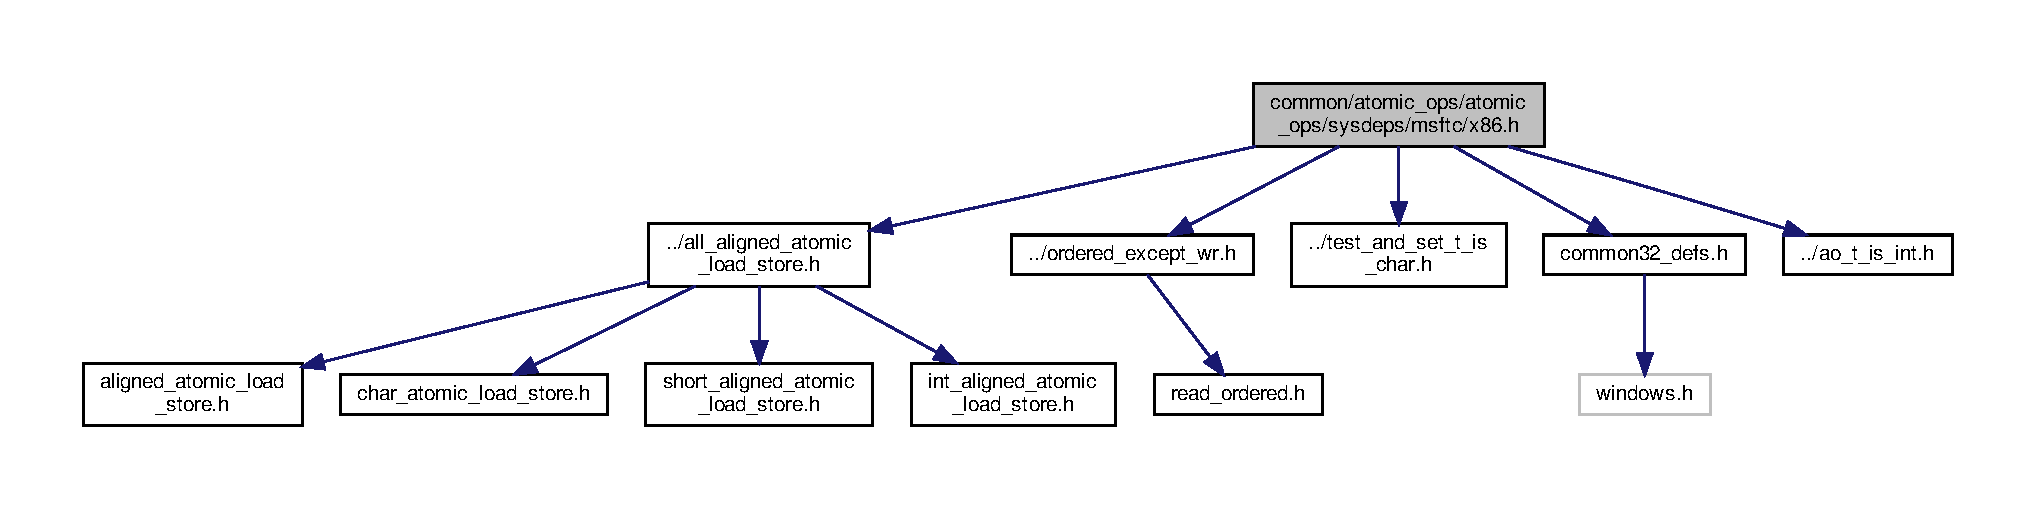
\includegraphics[width=350pt]{msftc_2x86_8h__incl}
\end{center}
\end{figure}
\subsection*{Macros}
\begin{DoxyCompactItemize}
\item 
\#define \hyperlink{msftc_2x86_8h_ad5f311a090d1e6e1bb35a6e68ee35fad}{A\+O\+\_\+\+H\+A\+V\+E\+\_\+test\+\_\+and\+\_\+set\+\_\+full}
\end{DoxyCompactItemize}
\subsection*{Functions}
\begin{DoxyCompactItemize}
\item 
\hyperlink{atomic__ops_8h_a9f6ab6253b6b11bc8c12efe9dde5db2b}{A\+O\+\_\+\+I\+N\+L\+I\+NE} \hyperlink{test__and__set__t__is__char_8h_a7d99a16c4eab47ba80ab6138d7d98ac1}{A\+O\+\_\+\+T\+S\+\_\+\+V\+A\+L\+\_\+t} \hyperlink{msftc_2x86_8h_a9f485bd63ce5c6a017ec241906e2f651}{A\+O\+\_\+test\+\_\+and\+\_\+set\+\_\+full} (volatile \hyperlink{test__and__set__t__is__char_8h_a5890c21b549264c75c2cad08bf4f6ba9}{A\+O\+\_\+\+T\+S\+\_\+t} $\ast$addr)
\end{DoxyCompactItemize}


\subsection{Macro Definition Documentation}
\mbox{\Hypertarget{msftc_2x86_8h_ad5f311a090d1e6e1bb35a6e68ee35fad}\label{msftc_2x86_8h_ad5f311a090d1e6e1bb35a6e68ee35fad}} 
\index{msftc/x86.\+h@{msftc/x86.\+h}!A\+O\+\_\+\+H\+A\+V\+E\+\_\+test\+\_\+and\+\_\+set\+\_\+full@{A\+O\+\_\+\+H\+A\+V\+E\+\_\+test\+\_\+and\+\_\+set\+\_\+full}}
\index{A\+O\+\_\+\+H\+A\+V\+E\+\_\+test\+\_\+and\+\_\+set\+\_\+full@{A\+O\+\_\+\+H\+A\+V\+E\+\_\+test\+\_\+and\+\_\+set\+\_\+full}!msftc/x86.\+h@{msftc/x86.\+h}}
\subsubsection{\texorpdfstring{A\+O\+\_\+\+H\+A\+V\+E\+\_\+test\+\_\+and\+\_\+set\+\_\+full}{AO\_HAVE\_test\_and\_set\_full}}
{\footnotesize\ttfamily \#define A\+O\+\_\+\+H\+A\+V\+E\+\_\+test\+\_\+and\+\_\+set\+\_\+full}



\subsection{Function Documentation}
\mbox{\Hypertarget{msftc_2x86_8h_a9f485bd63ce5c6a017ec241906e2f651}\label{msftc_2x86_8h_a9f485bd63ce5c6a017ec241906e2f651}} 
\index{msftc/x86.\+h@{msftc/x86.\+h}!A\+O\+\_\+test\+\_\+and\+\_\+set\+\_\+full@{A\+O\+\_\+test\+\_\+and\+\_\+set\+\_\+full}}
\index{A\+O\+\_\+test\+\_\+and\+\_\+set\+\_\+full@{A\+O\+\_\+test\+\_\+and\+\_\+set\+\_\+full}!msftc/x86.\+h@{msftc/x86.\+h}}
\subsubsection{\texorpdfstring{A\+O\+\_\+test\+\_\+and\+\_\+set\+\_\+full()}{AO\_test\_and\_set\_full()}}
{\footnotesize\ttfamily \hyperlink{atomic__ops_8h_a9f6ab6253b6b11bc8c12efe9dde5db2b}{A\+O\+\_\+\+I\+N\+L\+I\+NE} \hyperlink{test__and__set__t__is__char_8h_a7d99a16c4eab47ba80ab6138d7d98ac1}{A\+O\+\_\+\+T\+S\+\_\+\+V\+A\+L\+\_\+t} A\+O\+\_\+test\+\_\+and\+\_\+set\+\_\+full (\begin{DoxyParamCaption}\item[{volatile \hyperlink{test__and__set__t__is__char_8h_a5890c21b549264c75c2cad08bf4f6ba9}{A\+O\+\_\+\+T\+S\+\_\+t} $\ast$}]{addr }\end{DoxyParamCaption})}


\hypertarget{sunc_2x86_8h}{}\section{common/atomic\+\_\+ops/atomic\+\_\+ops/sysdeps/sunc/x86.h File Reference}
\label{sunc_2x86_8h}\index{common/atomic\+\_\+ops/atomic\+\_\+ops/sysdeps/sunc/x86.\+h@{common/atomic\+\_\+ops/atomic\+\_\+ops/sysdeps/sunc/x86.\+h}}
{\ttfamily \#include \char`\"{}../all\+\_\+aligned\+\_\+atomic\+\_\+load\+\_\+store.\+h\char`\"{}}\newline
{\ttfamily \#include \char`\"{}../ordered\+\_\+except\+\_\+wr.\+h\char`\"{}}\newline
{\ttfamily \#include \char`\"{}../test\+\_\+and\+\_\+set\+\_\+t\+\_\+is\+\_\+char.\+h\char`\"{}}\newline
{\ttfamily \#include \char`\"{}../standard\+\_\+ao\+\_\+double\+\_\+t.\+h\char`\"{}}\newline
{\ttfamily \#include \char`\"{}../ao\+\_\+t\+\_\+is\+\_\+int.\+h\char`\"{}}\newline
Include dependency graph for x86.\+h\+:
\nopagebreak
\begin{figure}[H]
\begin{center}
\leavevmode
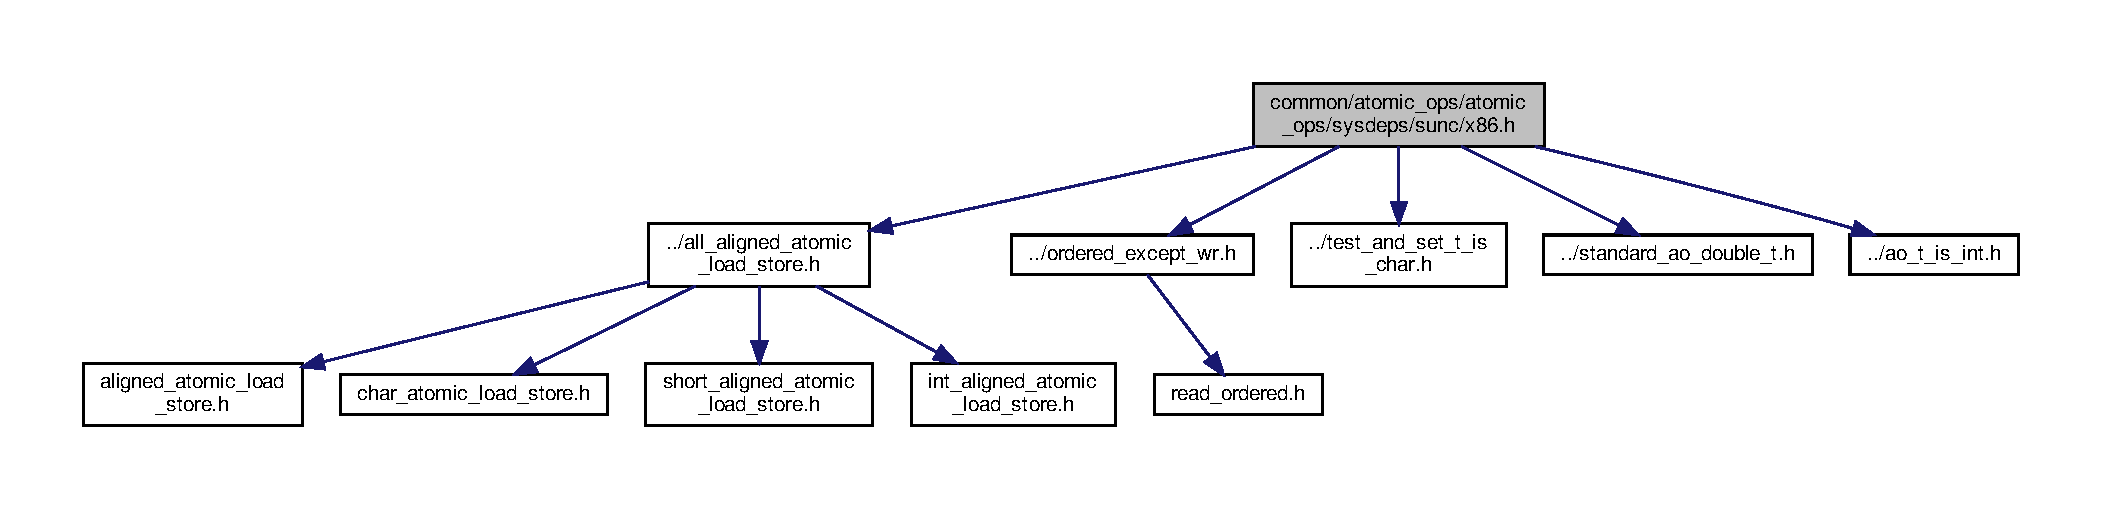
\includegraphics[width=350pt]{sunc_2x86_8h__incl}
\end{center}
\end{figure}
\subsection*{Macros}
\begin{DoxyCompactItemize}
\item 
\#define \hyperlink{sunc_2x86_8h_a9fa0fc1a9eadcba085e57bf180a53cef}{A\+O\+\_\+\+H\+A\+V\+E\+\_\+fetch\+\_\+and\+\_\+add\+\_\+full}
\item 
\#define \hyperlink{sunc_2x86_8h_a0a938d33904c99956494e57bfa2b74fd}{A\+O\+\_\+\+H\+A\+V\+E\+\_\+char\+\_\+fetch\+\_\+and\+\_\+add\+\_\+full}
\item 
\#define \hyperlink{sunc_2x86_8h_affc6a05c52cc08ec46bcbba79457d985}{A\+O\+\_\+\+H\+A\+V\+E\+\_\+short\+\_\+fetch\+\_\+and\+\_\+add\+\_\+full}
\item 
\#define \hyperlink{sunc_2x86_8h_a0ef45a04b0d7c74e025f829f2e614d79}{A\+O\+\_\+\+H\+A\+V\+E\+\_\+or\+\_\+full}
\item 
\#define \hyperlink{sunc_2x86_8h_ad5f311a090d1e6e1bb35a6e68ee35fad}{A\+O\+\_\+\+H\+A\+V\+E\+\_\+test\+\_\+and\+\_\+set\+\_\+full}
\item 
\#define \hyperlink{sunc_2x86_8h_a98ec53065c0dfd18bc1013c500da377c}{A\+O\+\_\+\+H\+A\+V\+E\+\_\+compare\+\_\+and\+\_\+swap\+\_\+full}
\end{DoxyCompactItemize}
\subsection*{Functions}
\begin{DoxyCompactItemize}
\item 
\hyperlink{atomic__ops_8h_a9f6ab6253b6b11bc8c12efe9dde5db2b}{A\+O\+\_\+\+I\+N\+L\+I\+NE} \hyperlink{atomic__ops_8h_a5225fef4d9eee821e82382cd269160dd}{A\+O\+\_\+t} \hyperlink{sunc_2x86_8h_a63b6d5232496fb679621fa985234eff8}{A\+O\+\_\+fetch\+\_\+and\+\_\+add\+\_\+full} (volatile \hyperlink{atomic__ops_8h_a5225fef4d9eee821e82382cd269160dd}{A\+O\+\_\+t} $\ast$p, \hyperlink{atomic__ops_8h_a5225fef4d9eee821e82382cd269160dd}{A\+O\+\_\+t} incr)
\item 
\hyperlink{atomic__ops_8h_a9f6ab6253b6b11bc8c12efe9dde5db2b}{A\+O\+\_\+\+I\+N\+L\+I\+NE} unsigned char \hyperlink{sunc_2x86_8h_a03d2aa8ce4372d7d08a306c6de38d4ba}{A\+O\+\_\+char\+\_\+fetch\+\_\+and\+\_\+add\+\_\+full} (volatile unsigned char $\ast$p, unsigned char incr)
\item 
\hyperlink{atomic__ops_8h_a9f6ab6253b6b11bc8c12efe9dde5db2b}{A\+O\+\_\+\+I\+N\+L\+I\+NE} unsigned short \hyperlink{sunc_2x86_8h_a99328cedbe167830313d7c3ffdcd0180}{A\+O\+\_\+short\+\_\+fetch\+\_\+and\+\_\+add\+\_\+full} (volatile unsigned short $\ast$p, unsigned short incr)
\item 
\hyperlink{atomic__ops_8h_a9f6ab6253b6b11bc8c12efe9dde5db2b}{A\+O\+\_\+\+I\+N\+L\+I\+NE} void \hyperlink{sunc_2x86_8h_a2732b24b044bf3993055d2c0d78b9ed9}{A\+O\+\_\+or\+\_\+full} (volatile \hyperlink{atomic__ops_8h_a5225fef4d9eee821e82382cd269160dd}{A\+O\+\_\+t} $\ast$p, \hyperlink{atomic__ops_8h_a5225fef4d9eee821e82382cd269160dd}{A\+O\+\_\+t} incr)
\item 
\hyperlink{atomic__ops_8h_a9f6ab6253b6b11bc8c12efe9dde5db2b}{A\+O\+\_\+\+I\+N\+L\+I\+NE} \hyperlink{test__and__set__t__is__char_8h_a7d99a16c4eab47ba80ab6138d7d98ac1}{A\+O\+\_\+\+T\+S\+\_\+\+V\+A\+L\+\_\+t} \hyperlink{sunc_2x86_8h_a9f485bd63ce5c6a017ec241906e2f651}{A\+O\+\_\+test\+\_\+and\+\_\+set\+\_\+full} (volatile \hyperlink{test__and__set__t__is__char_8h_a5890c21b549264c75c2cad08bf4f6ba9}{A\+O\+\_\+\+T\+S\+\_\+t} $\ast$addr)
\item 
\hyperlink{atomic__ops_8h_a9f6ab6253b6b11bc8c12efe9dde5db2b}{A\+O\+\_\+\+I\+N\+L\+I\+NE} int \hyperlink{sunc_2x86_8h_a634397de6de764015b30cdff3ff00b06}{A\+O\+\_\+compare\+\_\+and\+\_\+swap\+\_\+full} (volatile \hyperlink{atomic__ops_8h_a5225fef4d9eee821e82382cd269160dd}{A\+O\+\_\+t} $\ast$addr, \hyperlink{atomic__ops_8h_a5225fef4d9eee821e82382cd269160dd}{A\+O\+\_\+t} old, \hyperlink{atomic__ops_8h_a5225fef4d9eee821e82382cd269160dd}{A\+O\+\_\+t} new\+\_\+val)
\end{DoxyCompactItemize}


\subsection{Macro Definition Documentation}
\mbox{\Hypertarget{sunc_2x86_8h_a0a938d33904c99956494e57bfa2b74fd}\label{sunc_2x86_8h_a0a938d33904c99956494e57bfa2b74fd}} 
\index{sunc/x86.\+h@{sunc/x86.\+h}!A\+O\+\_\+\+H\+A\+V\+E\+\_\+char\+\_\+fetch\+\_\+and\+\_\+add\+\_\+full@{A\+O\+\_\+\+H\+A\+V\+E\+\_\+char\+\_\+fetch\+\_\+and\+\_\+add\+\_\+full}}
\index{A\+O\+\_\+\+H\+A\+V\+E\+\_\+char\+\_\+fetch\+\_\+and\+\_\+add\+\_\+full@{A\+O\+\_\+\+H\+A\+V\+E\+\_\+char\+\_\+fetch\+\_\+and\+\_\+add\+\_\+full}!sunc/x86.\+h@{sunc/x86.\+h}}
\subsubsection{\texorpdfstring{A\+O\+\_\+\+H\+A\+V\+E\+\_\+char\+\_\+fetch\+\_\+and\+\_\+add\+\_\+full}{AO\_HAVE\_char\_fetch\_and\_add\_full}}
{\footnotesize\ttfamily \#define A\+O\+\_\+\+H\+A\+V\+E\+\_\+char\+\_\+fetch\+\_\+and\+\_\+add\+\_\+full}

\mbox{\Hypertarget{sunc_2x86_8h_a98ec53065c0dfd18bc1013c500da377c}\label{sunc_2x86_8h_a98ec53065c0dfd18bc1013c500da377c}} 
\index{sunc/x86.\+h@{sunc/x86.\+h}!A\+O\+\_\+\+H\+A\+V\+E\+\_\+compare\+\_\+and\+\_\+swap\+\_\+full@{A\+O\+\_\+\+H\+A\+V\+E\+\_\+compare\+\_\+and\+\_\+swap\+\_\+full}}
\index{A\+O\+\_\+\+H\+A\+V\+E\+\_\+compare\+\_\+and\+\_\+swap\+\_\+full@{A\+O\+\_\+\+H\+A\+V\+E\+\_\+compare\+\_\+and\+\_\+swap\+\_\+full}!sunc/x86.\+h@{sunc/x86.\+h}}
\subsubsection{\texorpdfstring{A\+O\+\_\+\+H\+A\+V\+E\+\_\+compare\+\_\+and\+\_\+swap\+\_\+full}{AO\_HAVE\_compare\_and\_swap\_full}}
{\footnotesize\ttfamily \#define A\+O\+\_\+\+H\+A\+V\+E\+\_\+compare\+\_\+and\+\_\+swap\+\_\+full}

\mbox{\Hypertarget{sunc_2x86_8h_a9fa0fc1a9eadcba085e57bf180a53cef}\label{sunc_2x86_8h_a9fa0fc1a9eadcba085e57bf180a53cef}} 
\index{sunc/x86.\+h@{sunc/x86.\+h}!A\+O\+\_\+\+H\+A\+V\+E\+\_\+fetch\+\_\+and\+\_\+add\+\_\+full@{A\+O\+\_\+\+H\+A\+V\+E\+\_\+fetch\+\_\+and\+\_\+add\+\_\+full}}
\index{A\+O\+\_\+\+H\+A\+V\+E\+\_\+fetch\+\_\+and\+\_\+add\+\_\+full@{A\+O\+\_\+\+H\+A\+V\+E\+\_\+fetch\+\_\+and\+\_\+add\+\_\+full}!sunc/x86.\+h@{sunc/x86.\+h}}
\subsubsection{\texorpdfstring{A\+O\+\_\+\+H\+A\+V\+E\+\_\+fetch\+\_\+and\+\_\+add\+\_\+full}{AO\_HAVE\_fetch\_and\_add\_full}}
{\footnotesize\ttfamily \#define A\+O\+\_\+\+H\+A\+V\+E\+\_\+fetch\+\_\+and\+\_\+add\+\_\+full}

\mbox{\Hypertarget{sunc_2x86_8h_a0ef45a04b0d7c74e025f829f2e614d79}\label{sunc_2x86_8h_a0ef45a04b0d7c74e025f829f2e614d79}} 
\index{sunc/x86.\+h@{sunc/x86.\+h}!A\+O\+\_\+\+H\+A\+V\+E\+\_\+or\+\_\+full@{A\+O\+\_\+\+H\+A\+V\+E\+\_\+or\+\_\+full}}
\index{A\+O\+\_\+\+H\+A\+V\+E\+\_\+or\+\_\+full@{A\+O\+\_\+\+H\+A\+V\+E\+\_\+or\+\_\+full}!sunc/x86.\+h@{sunc/x86.\+h}}
\subsubsection{\texorpdfstring{A\+O\+\_\+\+H\+A\+V\+E\+\_\+or\+\_\+full}{AO\_HAVE\_or\_full}}
{\footnotesize\ttfamily \#define A\+O\+\_\+\+H\+A\+V\+E\+\_\+or\+\_\+full}

\mbox{\Hypertarget{sunc_2x86_8h_affc6a05c52cc08ec46bcbba79457d985}\label{sunc_2x86_8h_affc6a05c52cc08ec46bcbba79457d985}} 
\index{sunc/x86.\+h@{sunc/x86.\+h}!A\+O\+\_\+\+H\+A\+V\+E\+\_\+short\+\_\+fetch\+\_\+and\+\_\+add\+\_\+full@{A\+O\+\_\+\+H\+A\+V\+E\+\_\+short\+\_\+fetch\+\_\+and\+\_\+add\+\_\+full}}
\index{A\+O\+\_\+\+H\+A\+V\+E\+\_\+short\+\_\+fetch\+\_\+and\+\_\+add\+\_\+full@{A\+O\+\_\+\+H\+A\+V\+E\+\_\+short\+\_\+fetch\+\_\+and\+\_\+add\+\_\+full}!sunc/x86.\+h@{sunc/x86.\+h}}
\subsubsection{\texorpdfstring{A\+O\+\_\+\+H\+A\+V\+E\+\_\+short\+\_\+fetch\+\_\+and\+\_\+add\+\_\+full}{AO\_HAVE\_short\_fetch\_and\_add\_full}}
{\footnotesize\ttfamily \#define A\+O\+\_\+\+H\+A\+V\+E\+\_\+short\+\_\+fetch\+\_\+and\+\_\+add\+\_\+full}

\mbox{\Hypertarget{sunc_2x86_8h_ad5f311a090d1e6e1bb35a6e68ee35fad}\label{sunc_2x86_8h_ad5f311a090d1e6e1bb35a6e68ee35fad}} 
\index{sunc/x86.\+h@{sunc/x86.\+h}!A\+O\+\_\+\+H\+A\+V\+E\+\_\+test\+\_\+and\+\_\+set\+\_\+full@{A\+O\+\_\+\+H\+A\+V\+E\+\_\+test\+\_\+and\+\_\+set\+\_\+full}}
\index{A\+O\+\_\+\+H\+A\+V\+E\+\_\+test\+\_\+and\+\_\+set\+\_\+full@{A\+O\+\_\+\+H\+A\+V\+E\+\_\+test\+\_\+and\+\_\+set\+\_\+full}!sunc/x86.\+h@{sunc/x86.\+h}}
\subsubsection{\texorpdfstring{A\+O\+\_\+\+H\+A\+V\+E\+\_\+test\+\_\+and\+\_\+set\+\_\+full}{AO\_HAVE\_test\_and\_set\_full}}
{\footnotesize\ttfamily \#define A\+O\+\_\+\+H\+A\+V\+E\+\_\+test\+\_\+and\+\_\+set\+\_\+full}



\subsection{Function Documentation}
\mbox{\Hypertarget{sunc_2x86_8h_a03d2aa8ce4372d7d08a306c6de38d4ba}\label{sunc_2x86_8h_a03d2aa8ce4372d7d08a306c6de38d4ba}} 
\index{sunc/x86.\+h@{sunc/x86.\+h}!A\+O\+\_\+char\+\_\+fetch\+\_\+and\+\_\+add\+\_\+full@{A\+O\+\_\+char\+\_\+fetch\+\_\+and\+\_\+add\+\_\+full}}
\index{A\+O\+\_\+char\+\_\+fetch\+\_\+and\+\_\+add\+\_\+full@{A\+O\+\_\+char\+\_\+fetch\+\_\+and\+\_\+add\+\_\+full}!sunc/x86.\+h@{sunc/x86.\+h}}
\subsubsection{\texorpdfstring{A\+O\+\_\+char\+\_\+fetch\+\_\+and\+\_\+add\+\_\+full()}{AO\_char\_fetch\_and\_add\_full()}}
{\footnotesize\ttfamily \hyperlink{atomic__ops_8h_a9f6ab6253b6b11bc8c12efe9dde5db2b}{A\+O\+\_\+\+I\+N\+L\+I\+NE} unsigned char A\+O\+\_\+char\+\_\+fetch\+\_\+and\+\_\+add\+\_\+full (\begin{DoxyParamCaption}\item[{volatile unsigned char $\ast$}]{p,  }\item[{unsigned char}]{incr }\end{DoxyParamCaption})}

\mbox{\Hypertarget{sunc_2x86_8h_a634397de6de764015b30cdff3ff00b06}\label{sunc_2x86_8h_a634397de6de764015b30cdff3ff00b06}} 
\index{sunc/x86.\+h@{sunc/x86.\+h}!A\+O\+\_\+compare\+\_\+and\+\_\+swap\+\_\+full@{A\+O\+\_\+compare\+\_\+and\+\_\+swap\+\_\+full}}
\index{A\+O\+\_\+compare\+\_\+and\+\_\+swap\+\_\+full@{A\+O\+\_\+compare\+\_\+and\+\_\+swap\+\_\+full}!sunc/x86.\+h@{sunc/x86.\+h}}
\subsubsection{\texorpdfstring{A\+O\+\_\+compare\+\_\+and\+\_\+swap\+\_\+full()}{AO\_compare\_and\_swap\_full()}}
{\footnotesize\ttfamily \hyperlink{atomic__ops_8h_a9f6ab6253b6b11bc8c12efe9dde5db2b}{A\+O\+\_\+\+I\+N\+L\+I\+NE} int A\+O\+\_\+compare\+\_\+and\+\_\+swap\+\_\+full (\begin{DoxyParamCaption}\item[{volatile \hyperlink{atomic__ops_8h_a5225fef4d9eee821e82382cd269160dd}{A\+O\+\_\+t} $\ast$}]{addr,  }\item[{\hyperlink{atomic__ops_8h_a5225fef4d9eee821e82382cd269160dd}{A\+O\+\_\+t}}]{old,  }\item[{\hyperlink{atomic__ops_8h_a5225fef4d9eee821e82382cd269160dd}{A\+O\+\_\+t}}]{new\+\_\+val }\end{DoxyParamCaption})}

\mbox{\Hypertarget{sunc_2x86_8h_a63b6d5232496fb679621fa985234eff8}\label{sunc_2x86_8h_a63b6d5232496fb679621fa985234eff8}} 
\index{sunc/x86.\+h@{sunc/x86.\+h}!A\+O\+\_\+fetch\+\_\+and\+\_\+add\+\_\+full@{A\+O\+\_\+fetch\+\_\+and\+\_\+add\+\_\+full}}
\index{A\+O\+\_\+fetch\+\_\+and\+\_\+add\+\_\+full@{A\+O\+\_\+fetch\+\_\+and\+\_\+add\+\_\+full}!sunc/x86.\+h@{sunc/x86.\+h}}
\subsubsection{\texorpdfstring{A\+O\+\_\+fetch\+\_\+and\+\_\+add\+\_\+full()}{AO\_fetch\_and\_add\_full()}}
{\footnotesize\ttfamily \hyperlink{atomic__ops_8h_a9f6ab6253b6b11bc8c12efe9dde5db2b}{A\+O\+\_\+\+I\+N\+L\+I\+NE} \hyperlink{atomic__ops_8h_a5225fef4d9eee821e82382cd269160dd}{A\+O\+\_\+t} A\+O\+\_\+fetch\+\_\+and\+\_\+add\+\_\+full (\begin{DoxyParamCaption}\item[{volatile \hyperlink{atomic__ops_8h_a5225fef4d9eee821e82382cd269160dd}{A\+O\+\_\+t} $\ast$}]{p,  }\item[{\hyperlink{atomic__ops_8h_a5225fef4d9eee821e82382cd269160dd}{A\+O\+\_\+t}}]{incr }\end{DoxyParamCaption})}

\mbox{\Hypertarget{sunc_2x86_8h_a2732b24b044bf3993055d2c0d78b9ed9}\label{sunc_2x86_8h_a2732b24b044bf3993055d2c0d78b9ed9}} 
\index{sunc/x86.\+h@{sunc/x86.\+h}!A\+O\+\_\+or\+\_\+full@{A\+O\+\_\+or\+\_\+full}}
\index{A\+O\+\_\+or\+\_\+full@{A\+O\+\_\+or\+\_\+full}!sunc/x86.\+h@{sunc/x86.\+h}}
\subsubsection{\texorpdfstring{A\+O\+\_\+or\+\_\+full()}{AO\_or\_full()}}
{\footnotesize\ttfamily \hyperlink{atomic__ops_8h_a9f6ab6253b6b11bc8c12efe9dde5db2b}{A\+O\+\_\+\+I\+N\+L\+I\+NE} void A\+O\+\_\+or\+\_\+full (\begin{DoxyParamCaption}\item[{volatile \hyperlink{atomic__ops_8h_a5225fef4d9eee821e82382cd269160dd}{A\+O\+\_\+t} $\ast$}]{p,  }\item[{\hyperlink{atomic__ops_8h_a5225fef4d9eee821e82382cd269160dd}{A\+O\+\_\+t}}]{incr }\end{DoxyParamCaption})}

\mbox{\Hypertarget{sunc_2x86_8h_a99328cedbe167830313d7c3ffdcd0180}\label{sunc_2x86_8h_a99328cedbe167830313d7c3ffdcd0180}} 
\index{sunc/x86.\+h@{sunc/x86.\+h}!A\+O\+\_\+short\+\_\+fetch\+\_\+and\+\_\+add\+\_\+full@{A\+O\+\_\+short\+\_\+fetch\+\_\+and\+\_\+add\+\_\+full}}
\index{A\+O\+\_\+short\+\_\+fetch\+\_\+and\+\_\+add\+\_\+full@{A\+O\+\_\+short\+\_\+fetch\+\_\+and\+\_\+add\+\_\+full}!sunc/x86.\+h@{sunc/x86.\+h}}
\subsubsection{\texorpdfstring{A\+O\+\_\+short\+\_\+fetch\+\_\+and\+\_\+add\+\_\+full()}{AO\_short\_fetch\_and\_add\_full()}}
{\footnotesize\ttfamily \hyperlink{atomic__ops_8h_a9f6ab6253b6b11bc8c12efe9dde5db2b}{A\+O\+\_\+\+I\+N\+L\+I\+NE} unsigned short A\+O\+\_\+short\+\_\+fetch\+\_\+and\+\_\+add\+\_\+full (\begin{DoxyParamCaption}\item[{volatile unsigned short $\ast$}]{p,  }\item[{unsigned short}]{incr }\end{DoxyParamCaption})}

\mbox{\Hypertarget{sunc_2x86_8h_a9f485bd63ce5c6a017ec241906e2f651}\label{sunc_2x86_8h_a9f485bd63ce5c6a017ec241906e2f651}} 
\index{sunc/x86.\+h@{sunc/x86.\+h}!A\+O\+\_\+test\+\_\+and\+\_\+set\+\_\+full@{A\+O\+\_\+test\+\_\+and\+\_\+set\+\_\+full}}
\index{A\+O\+\_\+test\+\_\+and\+\_\+set\+\_\+full@{A\+O\+\_\+test\+\_\+and\+\_\+set\+\_\+full}!sunc/x86.\+h@{sunc/x86.\+h}}
\subsubsection{\texorpdfstring{A\+O\+\_\+test\+\_\+and\+\_\+set\+\_\+full()}{AO\_test\_and\_set\_full()}}
{\footnotesize\ttfamily \hyperlink{atomic__ops_8h_a9f6ab6253b6b11bc8c12efe9dde5db2b}{A\+O\+\_\+\+I\+N\+L\+I\+NE} \hyperlink{test__and__set__t__is__char_8h_a7d99a16c4eab47ba80ab6138d7d98ac1}{A\+O\+\_\+\+T\+S\+\_\+\+V\+A\+L\+\_\+t} A\+O\+\_\+test\+\_\+and\+\_\+set\+\_\+full (\begin{DoxyParamCaption}\item[{volatile \hyperlink{test__and__set__t__is__char_8h_a5890c21b549264c75c2cad08bf4f6ba9}{A\+O\+\_\+\+T\+S\+\_\+t} $\ast$}]{addr }\end{DoxyParamCaption})}


\hypertarget{gcc_2x86__64_8h}{}\section{common/atomic\+\_\+ops/atomic\+\_\+ops/sysdeps/gcc/x86\+\_\+64.h File Reference}
\label{gcc_2x86__64_8h}\index{common/atomic\+\_\+ops/atomic\+\_\+ops/sysdeps/gcc/x86\+\_\+64.\+h@{common/atomic\+\_\+ops/atomic\+\_\+ops/sysdeps/gcc/x86\+\_\+64.\+h}}
{\ttfamily \#include \char`\"{}../all\+\_\+aligned\+\_\+atomic\+\_\+load\+\_\+store.\+h\char`\"{}}\newline
{\ttfamily \#include \char`\"{}../ordered\+\_\+except\+\_\+wr.\+h\char`\"{}}\newline
{\ttfamily \#include \char`\"{}../test\+\_\+and\+\_\+set\+\_\+t\+\_\+is\+\_\+char.\+h\char`\"{}}\newline
{\ttfamily \#include \char`\"{}../standard\+\_\+ao\+\_\+double\+\_\+t.\+h\char`\"{}}\newline
Include dependency graph for x86\+\_\+64.\+h\+:
\nopagebreak
\begin{figure}[H]
\begin{center}
\leavevmode
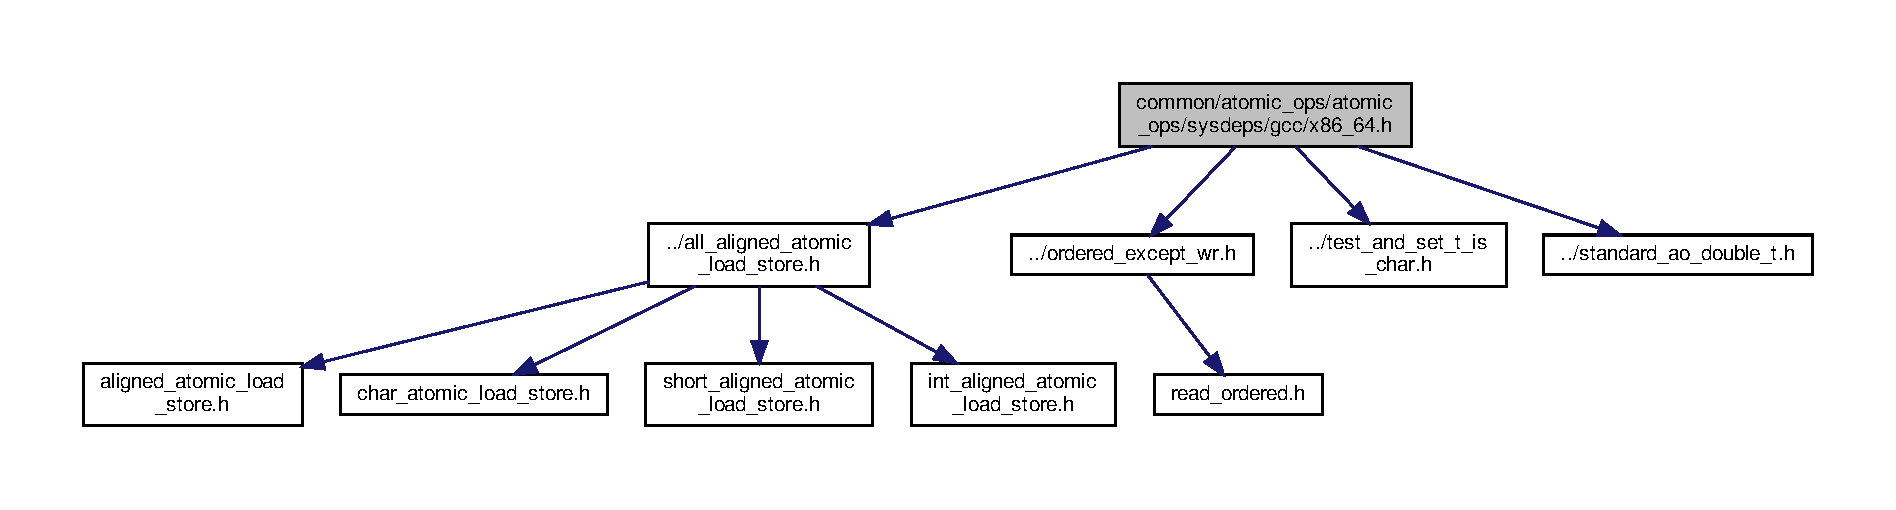
\includegraphics[width=350pt]{gcc_2x86__64_8h__incl}
\end{center}
\end{figure}
\subsection*{Macros}
\begin{DoxyCompactItemize}
\item 
\#define \hyperlink{gcc_2x86__64_8h_a3904dc699d6a6d6e771a93aa66aeb805}{A\+O\+\_\+\+H\+A\+V\+E\+\_\+nop\+\_\+full}
\item 
\#define \hyperlink{gcc_2x86__64_8h_a9fa0fc1a9eadcba085e57bf180a53cef}{A\+O\+\_\+\+H\+A\+V\+E\+\_\+fetch\+\_\+and\+\_\+add\+\_\+full}
\item 
\#define \hyperlink{gcc_2x86__64_8h_a0a938d33904c99956494e57bfa2b74fd}{A\+O\+\_\+\+H\+A\+V\+E\+\_\+char\+\_\+fetch\+\_\+and\+\_\+add\+\_\+full}
\item 
\#define \hyperlink{gcc_2x86__64_8h_affc6a05c52cc08ec46bcbba79457d985}{A\+O\+\_\+\+H\+A\+V\+E\+\_\+short\+\_\+fetch\+\_\+and\+\_\+add\+\_\+full}
\item 
\#define \hyperlink{gcc_2x86__64_8h_aee1cb49608401259e3935681b3a2df53}{A\+O\+\_\+\+H\+A\+V\+E\+\_\+int\+\_\+fetch\+\_\+and\+\_\+add\+\_\+full}
\item 
\#define \hyperlink{gcc_2x86__64_8h_a0ef45a04b0d7c74e025f829f2e614d79}{A\+O\+\_\+\+H\+A\+V\+E\+\_\+or\+\_\+full}
\item 
\#define \hyperlink{gcc_2x86__64_8h_ad5f311a090d1e6e1bb35a6e68ee35fad}{A\+O\+\_\+\+H\+A\+V\+E\+\_\+test\+\_\+and\+\_\+set\+\_\+full}
\item 
\#define \hyperlink{gcc_2x86__64_8h_a98ec53065c0dfd18bc1013c500da377c}{A\+O\+\_\+\+H\+A\+V\+E\+\_\+compare\+\_\+and\+\_\+swap\+\_\+full}
\end{DoxyCompactItemize}
\subsection*{Functions}
\begin{DoxyCompactItemize}
\item 
\hyperlink{atomic__ops_8h_a9f6ab6253b6b11bc8c12efe9dde5db2b}{A\+O\+\_\+\+I\+N\+L\+I\+NE} void \hyperlink{gcc_2x86__64_8h_afe3a6778eacc82252ba138fc9a157b04}{A\+O\+\_\+nop\+\_\+full} (void)
\item 
\hyperlink{atomic__ops_8h_a9f6ab6253b6b11bc8c12efe9dde5db2b}{A\+O\+\_\+\+I\+N\+L\+I\+NE} \hyperlink{atomic__ops_8h_a5225fef4d9eee821e82382cd269160dd}{A\+O\+\_\+t} \hyperlink{gcc_2x86__64_8h_a63b6d5232496fb679621fa985234eff8}{A\+O\+\_\+fetch\+\_\+and\+\_\+add\+\_\+full} (volatile \hyperlink{atomic__ops_8h_a5225fef4d9eee821e82382cd269160dd}{A\+O\+\_\+t} $\ast$p, \hyperlink{atomic__ops_8h_a5225fef4d9eee821e82382cd269160dd}{A\+O\+\_\+t} incr)
\item 
\hyperlink{atomic__ops_8h_a9f6ab6253b6b11bc8c12efe9dde5db2b}{A\+O\+\_\+\+I\+N\+L\+I\+NE} unsigned char \hyperlink{gcc_2x86__64_8h_a03d2aa8ce4372d7d08a306c6de38d4ba}{A\+O\+\_\+char\+\_\+fetch\+\_\+and\+\_\+add\+\_\+full} (volatile unsigned char $\ast$p, unsigned char incr)
\item 
\hyperlink{atomic__ops_8h_a9f6ab6253b6b11bc8c12efe9dde5db2b}{A\+O\+\_\+\+I\+N\+L\+I\+NE} unsigned short \hyperlink{gcc_2x86__64_8h_a99328cedbe167830313d7c3ffdcd0180}{A\+O\+\_\+short\+\_\+fetch\+\_\+and\+\_\+add\+\_\+full} (volatile unsigned short $\ast$p, unsigned short incr)
\item 
\hyperlink{atomic__ops_8h_a9f6ab6253b6b11bc8c12efe9dde5db2b}{A\+O\+\_\+\+I\+N\+L\+I\+NE} unsigned int \hyperlink{gcc_2x86__64_8h_a1b517b3713694261207c0d7ecfdc59e3}{A\+O\+\_\+int\+\_\+fetch\+\_\+and\+\_\+add\+\_\+full} (volatile unsigned int $\ast$p, unsigned int incr)
\item 
\hyperlink{atomic__ops_8h_a9f6ab6253b6b11bc8c12efe9dde5db2b}{A\+O\+\_\+\+I\+N\+L\+I\+NE} void \hyperlink{gcc_2x86__64_8h_a2732b24b044bf3993055d2c0d78b9ed9}{A\+O\+\_\+or\+\_\+full} (volatile \hyperlink{atomic__ops_8h_a5225fef4d9eee821e82382cd269160dd}{A\+O\+\_\+t} $\ast$p, \hyperlink{atomic__ops_8h_a5225fef4d9eee821e82382cd269160dd}{A\+O\+\_\+t} incr)
\item 
\hyperlink{atomic__ops_8h_a9f6ab6253b6b11bc8c12efe9dde5db2b}{A\+O\+\_\+\+I\+N\+L\+I\+NE} \hyperlink{test__and__set__t__is__char_8h_a7d99a16c4eab47ba80ab6138d7d98ac1}{A\+O\+\_\+\+T\+S\+\_\+\+V\+A\+L\+\_\+t} \hyperlink{gcc_2x86__64_8h_a9f485bd63ce5c6a017ec241906e2f651}{A\+O\+\_\+test\+\_\+and\+\_\+set\+\_\+full} (volatile \hyperlink{test__and__set__t__is__char_8h_a5890c21b549264c75c2cad08bf4f6ba9}{A\+O\+\_\+\+T\+S\+\_\+t} $\ast$addr)
\item 
\hyperlink{atomic__ops_8h_a9f6ab6253b6b11bc8c12efe9dde5db2b}{A\+O\+\_\+\+I\+N\+L\+I\+NE} int \hyperlink{gcc_2x86__64_8h_a634397de6de764015b30cdff3ff00b06}{A\+O\+\_\+compare\+\_\+and\+\_\+swap\+\_\+full} (volatile \hyperlink{atomic__ops_8h_a5225fef4d9eee821e82382cd269160dd}{A\+O\+\_\+t} $\ast$addr, \hyperlink{atomic__ops_8h_a5225fef4d9eee821e82382cd269160dd}{A\+O\+\_\+t} old, \hyperlink{atomic__ops_8h_a5225fef4d9eee821e82382cd269160dd}{A\+O\+\_\+t} new\+\_\+val)
\end{DoxyCompactItemize}


\subsection{Macro Definition Documentation}
\mbox{\Hypertarget{gcc_2x86__64_8h_a0a938d33904c99956494e57bfa2b74fd}\label{gcc_2x86__64_8h_a0a938d33904c99956494e57bfa2b74fd}} 
\index{gcc/x86\+\_\+64.\+h@{gcc/x86\+\_\+64.\+h}!A\+O\+\_\+\+H\+A\+V\+E\+\_\+char\+\_\+fetch\+\_\+and\+\_\+add\+\_\+full@{A\+O\+\_\+\+H\+A\+V\+E\+\_\+char\+\_\+fetch\+\_\+and\+\_\+add\+\_\+full}}
\index{A\+O\+\_\+\+H\+A\+V\+E\+\_\+char\+\_\+fetch\+\_\+and\+\_\+add\+\_\+full@{A\+O\+\_\+\+H\+A\+V\+E\+\_\+char\+\_\+fetch\+\_\+and\+\_\+add\+\_\+full}!gcc/x86\+\_\+64.\+h@{gcc/x86\+\_\+64.\+h}}
\subsubsection{\texorpdfstring{A\+O\+\_\+\+H\+A\+V\+E\+\_\+char\+\_\+fetch\+\_\+and\+\_\+add\+\_\+full}{AO\_HAVE\_char\_fetch\_and\_add\_full}}
{\footnotesize\ttfamily \#define A\+O\+\_\+\+H\+A\+V\+E\+\_\+char\+\_\+fetch\+\_\+and\+\_\+add\+\_\+full}

\mbox{\Hypertarget{gcc_2x86__64_8h_a98ec53065c0dfd18bc1013c500da377c}\label{gcc_2x86__64_8h_a98ec53065c0dfd18bc1013c500da377c}} 
\index{gcc/x86\+\_\+64.\+h@{gcc/x86\+\_\+64.\+h}!A\+O\+\_\+\+H\+A\+V\+E\+\_\+compare\+\_\+and\+\_\+swap\+\_\+full@{A\+O\+\_\+\+H\+A\+V\+E\+\_\+compare\+\_\+and\+\_\+swap\+\_\+full}}
\index{A\+O\+\_\+\+H\+A\+V\+E\+\_\+compare\+\_\+and\+\_\+swap\+\_\+full@{A\+O\+\_\+\+H\+A\+V\+E\+\_\+compare\+\_\+and\+\_\+swap\+\_\+full}!gcc/x86\+\_\+64.\+h@{gcc/x86\+\_\+64.\+h}}
\subsubsection{\texorpdfstring{A\+O\+\_\+\+H\+A\+V\+E\+\_\+compare\+\_\+and\+\_\+swap\+\_\+full}{AO\_HAVE\_compare\_and\_swap\_full}}
{\footnotesize\ttfamily \#define A\+O\+\_\+\+H\+A\+V\+E\+\_\+compare\+\_\+and\+\_\+swap\+\_\+full}

\mbox{\Hypertarget{gcc_2x86__64_8h_a9fa0fc1a9eadcba085e57bf180a53cef}\label{gcc_2x86__64_8h_a9fa0fc1a9eadcba085e57bf180a53cef}} 
\index{gcc/x86\+\_\+64.\+h@{gcc/x86\+\_\+64.\+h}!A\+O\+\_\+\+H\+A\+V\+E\+\_\+fetch\+\_\+and\+\_\+add\+\_\+full@{A\+O\+\_\+\+H\+A\+V\+E\+\_\+fetch\+\_\+and\+\_\+add\+\_\+full}}
\index{A\+O\+\_\+\+H\+A\+V\+E\+\_\+fetch\+\_\+and\+\_\+add\+\_\+full@{A\+O\+\_\+\+H\+A\+V\+E\+\_\+fetch\+\_\+and\+\_\+add\+\_\+full}!gcc/x86\+\_\+64.\+h@{gcc/x86\+\_\+64.\+h}}
\subsubsection{\texorpdfstring{A\+O\+\_\+\+H\+A\+V\+E\+\_\+fetch\+\_\+and\+\_\+add\+\_\+full}{AO\_HAVE\_fetch\_and\_add\_full}}
{\footnotesize\ttfamily \#define A\+O\+\_\+\+H\+A\+V\+E\+\_\+fetch\+\_\+and\+\_\+add\+\_\+full}

\mbox{\Hypertarget{gcc_2x86__64_8h_aee1cb49608401259e3935681b3a2df53}\label{gcc_2x86__64_8h_aee1cb49608401259e3935681b3a2df53}} 
\index{gcc/x86\+\_\+64.\+h@{gcc/x86\+\_\+64.\+h}!A\+O\+\_\+\+H\+A\+V\+E\+\_\+int\+\_\+fetch\+\_\+and\+\_\+add\+\_\+full@{A\+O\+\_\+\+H\+A\+V\+E\+\_\+int\+\_\+fetch\+\_\+and\+\_\+add\+\_\+full}}
\index{A\+O\+\_\+\+H\+A\+V\+E\+\_\+int\+\_\+fetch\+\_\+and\+\_\+add\+\_\+full@{A\+O\+\_\+\+H\+A\+V\+E\+\_\+int\+\_\+fetch\+\_\+and\+\_\+add\+\_\+full}!gcc/x86\+\_\+64.\+h@{gcc/x86\+\_\+64.\+h}}
\subsubsection{\texorpdfstring{A\+O\+\_\+\+H\+A\+V\+E\+\_\+int\+\_\+fetch\+\_\+and\+\_\+add\+\_\+full}{AO\_HAVE\_int\_fetch\_and\_add\_full}}
{\footnotesize\ttfamily \#define A\+O\+\_\+\+H\+A\+V\+E\+\_\+int\+\_\+fetch\+\_\+and\+\_\+add\+\_\+full}

\mbox{\Hypertarget{gcc_2x86__64_8h_a3904dc699d6a6d6e771a93aa66aeb805}\label{gcc_2x86__64_8h_a3904dc699d6a6d6e771a93aa66aeb805}} 
\index{gcc/x86\+\_\+64.\+h@{gcc/x86\+\_\+64.\+h}!A\+O\+\_\+\+H\+A\+V\+E\+\_\+nop\+\_\+full@{A\+O\+\_\+\+H\+A\+V\+E\+\_\+nop\+\_\+full}}
\index{A\+O\+\_\+\+H\+A\+V\+E\+\_\+nop\+\_\+full@{A\+O\+\_\+\+H\+A\+V\+E\+\_\+nop\+\_\+full}!gcc/x86\+\_\+64.\+h@{gcc/x86\+\_\+64.\+h}}
\subsubsection{\texorpdfstring{A\+O\+\_\+\+H\+A\+V\+E\+\_\+nop\+\_\+full}{AO\_HAVE\_nop\_full}}
{\footnotesize\ttfamily \#define A\+O\+\_\+\+H\+A\+V\+E\+\_\+nop\+\_\+full}

\mbox{\Hypertarget{gcc_2x86__64_8h_a0ef45a04b0d7c74e025f829f2e614d79}\label{gcc_2x86__64_8h_a0ef45a04b0d7c74e025f829f2e614d79}} 
\index{gcc/x86\+\_\+64.\+h@{gcc/x86\+\_\+64.\+h}!A\+O\+\_\+\+H\+A\+V\+E\+\_\+or\+\_\+full@{A\+O\+\_\+\+H\+A\+V\+E\+\_\+or\+\_\+full}}
\index{A\+O\+\_\+\+H\+A\+V\+E\+\_\+or\+\_\+full@{A\+O\+\_\+\+H\+A\+V\+E\+\_\+or\+\_\+full}!gcc/x86\+\_\+64.\+h@{gcc/x86\+\_\+64.\+h}}
\subsubsection{\texorpdfstring{A\+O\+\_\+\+H\+A\+V\+E\+\_\+or\+\_\+full}{AO\_HAVE\_or\_full}}
{\footnotesize\ttfamily \#define A\+O\+\_\+\+H\+A\+V\+E\+\_\+or\+\_\+full}

\mbox{\Hypertarget{gcc_2x86__64_8h_affc6a05c52cc08ec46bcbba79457d985}\label{gcc_2x86__64_8h_affc6a05c52cc08ec46bcbba79457d985}} 
\index{gcc/x86\+\_\+64.\+h@{gcc/x86\+\_\+64.\+h}!A\+O\+\_\+\+H\+A\+V\+E\+\_\+short\+\_\+fetch\+\_\+and\+\_\+add\+\_\+full@{A\+O\+\_\+\+H\+A\+V\+E\+\_\+short\+\_\+fetch\+\_\+and\+\_\+add\+\_\+full}}
\index{A\+O\+\_\+\+H\+A\+V\+E\+\_\+short\+\_\+fetch\+\_\+and\+\_\+add\+\_\+full@{A\+O\+\_\+\+H\+A\+V\+E\+\_\+short\+\_\+fetch\+\_\+and\+\_\+add\+\_\+full}!gcc/x86\+\_\+64.\+h@{gcc/x86\+\_\+64.\+h}}
\subsubsection{\texorpdfstring{A\+O\+\_\+\+H\+A\+V\+E\+\_\+short\+\_\+fetch\+\_\+and\+\_\+add\+\_\+full}{AO\_HAVE\_short\_fetch\_and\_add\_full}}
{\footnotesize\ttfamily \#define A\+O\+\_\+\+H\+A\+V\+E\+\_\+short\+\_\+fetch\+\_\+and\+\_\+add\+\_\+full}

\mbox{\Hypertarget{gcc_2x86__64_8h_ad5f311a090d1e6e1bb35a6e68ee35fad}\label{gcc_2x86__64_8h_ad5f311a090d1e6e1bb35a6e68ee35fad}} 
\index{gcc/x86\+\_\+64.\+h@{gcc/x86\+\_\+64.\+h}!A\+O\+\_\+\+H\+A\+V\+E\+\_\+test\+\_\+and\+\_\+set\+\_\+full@{A\+O\+\_\+\+H\+A\+V\+E\+\_\+test\+\_\+and\+\_\+set\+\_\+full}}
\index{A\+O\+\_\+\+H\+A\+V\+E\+\_\+test\+\_\+and\+\_\+set\+\_\+full@{A\+O\+\_\+\+H\+A\+V\+E\+\_\+test\+\_\+and\+\_\+set\+\_\+full}!gcc/x86\+\_\+64.\+h@{gcc/x86\+\_\+64.\+h}}
\subsubsection{\texorpdfstring{A\+O\+\_\+\+H\+A\+V\+E\+\_\+test\+\_\+and\+\_\+set\+\_\+full}{AO\_HAVE\_test\_and\_set\_full}}
{\footnotesize\ttfamily \#define A\+O\+\_\+\+H\+A\+V\+E\+\_\+test\+\_\+and\+\_\+set\+\_\+full}



\subsection{Function Documentation}
\mbox{\Hypertarget{gcc_2x86__64_8h_a03d2aa8ce4372d7d08a306c6de38d4ba}\label{gcc_2x86__64_8h_a03d2aa8ce4372d7d08a306c6de38d4ba}} 
\index{gcc/x86\+\_\+64.\+h@{gcc/x86\+\_\+64.\+h}!A\+O\+\_\+char\+\_\+fetch\+\_\+and\+\_\+add\+\_\+full@{A\+O\+\_\+char\+\_\+fetch\+\_\+and\+\_\+add\+\_\+full}}
\index{A\+O\+\_\+char\+\_\+fetch\+\_\+and\+\_\+add\+\_\+full@{A\+O\+\_\+char\+\_\+fetch\+\_\+and\+\_\+add\+\_\+full}!gcc/x86\+\_\+64.\+h@{gcc/x86\+\_\+64.\+h}}
\subsubsection{\texorpdfstring{A\+O\+\_\+char\+\_\+fetch\+\_\+and\+\_\+add\+\_\+full()}{AO\_char\_fetch\_and\_add\_full()}}
{\footnotesize\ttfamily \hyperlink{atomic__ops_8h_a9f6ab6253b6b11bc8c12efe9dde5db2b}{A\+O\+\_\+\+I\+N\+L\+I\+NE} unsigned char A\+O\+\_\+char\+\_\+fetch\+\_\+and\+\_\+add\+\_\+full (\begin{DoxyParamCaption}\item[{volatile unsigned char $\ast$}]{p,  }\item[{unsigned char}]{incr }\end{DoxyParamCaption})}

\mbox{\Hypertarget{gcc_2x86__64_8h_a634397de6de764015b30cdff3ff00b06}\label{gcc_2x86__64_8h_a634397de6de764015b30cdff3ff00b06}} 
\index{gcc/x86\+\_\+64.\+h@{gcc/x86\+\_\+64.\+h}!A\+O\+\_\+compare\+\_\+and\+\_\+swap\+\_\+full@{A\+O\+\_\+compare\+\_\+and\+\_\+swap\+\_\+full}}
\index{A\+O\+\_\+compare\+\_\+and\+\_\+swap\+\_\+full@{A\+O\+\_\+compare\+\_\+and\+\_\+swap\+\_\+full}!gcc/x86\+\_\+64.\+h@{gcc/x86\+\_\+64.\+h}}
\subsubsection{\texorpdfstring{A\+O\+\_\+compare\+\_\+and\+\_\+swap\+\_\+full()}{AO\_compare\_and\_swap\_full()}}
{\footnotesize\ttfamily \hyperlink{atomic__ops_8h_a9f6ab6253b6b11bc8c12efe9dde5db2b}{A\+O\+\_\+\+I\+N\+L\+I\+NE} int A\+O\+\_\+compare\+\_\+and\+\_\+swap\+\_\+full (\begin{DoxyParamCaption}\item[{volatile \hyperlink{atomic__ops_8h_a5225fef4d9eee821e82382cd269160dd}{A\+O\+\_\+t} $\ast$}]{addr,  }\item[{\hyperlink{atomic__ops_8h_a5225fef4d9eee821e82382cd269160dd}{A\+O\+\_\+t}}]{old,  }\item[{\hyperlink{atomic__ops_8h_a5225fef4d9eee821e82382cd269160dd}{A\+O\+\_\+t}}]{new\+\_\+val }\end{DoxyParamCaption})}

\mbox{\Hypertarget{gcc_2x86__64_8h_a63b6d5232496fb679621fa985234eff8}\label{gcc_2x86__64_8h_a63b6d5232496fb679621fa985234eff8}} 
\index{gcc/x86\+\_\+64.\+h@{gcc/x86\+\_\+64.\+h}!A\+O\+\_\+fetch\+\_\+and\+\_\+add\+\_\+full@{A\+O\+\_\+fetch\+\_\+and\+\_\+add\+\_\+full}}
\index{A\+O\+\_\+fetch\+\_\+and\+\_\+add\+\_\+full@{A\+O\+\_\+fetch\+\_\+and\+\_\+add\+\_\+full}!gcc/x86\+\_\+64.\+h@{gcc/x86\+\_\+64.\+h}}
\subsubsection{\texorpdfstring{A\+O\+\_\+fetch\+\_\+and\+\_\+add\+\_\+full()}{AO\_fetch\_and\_add\_full()}}
{\footnotesize\ttfamily \hyperlink{atomic__ops_8h_a9f6ab6253b6b11bc8c12efe9dde5db2b}{A\+O\+\_\+\+I\+N\+L\+I\+NE} \hyperlink{atomic__ops_8h_a5225fef4d9eee821e82382cd269160dd}{A\+O\+\_\+t} A\+O\+\_\+fetch\+\_\+and\+\_\+add\+\_\+full (\begin{DoxyParamCaption}\item[{volatile \hyperlink{atomic__ops_8h_a5225fef4d9eee821e82382cd269160dd}{A\+O\+\_\+t} $\ast$}]{p,  }\item[{\hyperlink{atomic__ops_8h_a5225fef4d9eee821e82382cd269160dd}{A\+O\+\_\+t}}]{incr }\end{DoxyParamCaption})}

\mbox{\Hypertarget{gcc_2x86__64_8h_a1b517b3713694261207c0d7ecfdc59e3}\label{gcc_2x86__64_8h_a1b517b3713694261207c0d7ecfdc59e3}} 
\index{gcc/x86\+\_\+64.\+h@{gcc/x86\+\_\+64.\+h}!A\+O\+\_\+int\+\_\+fetch\+\_\+and\+\_\+add\+\_\+full@{A\+O\+\_\+int\+\_\+fetch\+\_\+and\+\_\+add\+\_\+full}}
\index{A\+O\+\_\+int\+\_\+fetch\+\_\+and\+\_\+add\+\_\+full@{A\+O\+\_\+int\+\_\+fetch\+\_\+and\+\_\+add\+\_\+full}!gcc/x86\+\_\+64.\+h@{gcc/x86\+\_\+64.\+h}}
\subsubsection{\texorpdfstring{A\+O\+\_\+int\+\_\+fetch\+\_\+and\+\_\+add\+\_\+full()}{AO\_int\_fetch\_and\_add\_full()}}
{\footnotesize\ttfamily \hyperlink{atomic__ops_8h_a9f6ab6253b6b11bc8c12efe9dde5db2b}{A\+O\+\_\+\+I\+N\+L\+I\+NE} unsigned int A\+O\+\_\+int\+\_\+fetch\+\_\+and\+\_\+add\+\_\+full (\begin{DoxyParamCaption}\item[{volatile unsigned int $\ast$}]{p,  }\item[{unsigned int}]{incr }\end{DoxyParamCaption})}

\mbox{\Hypertarget{gcc_2x86__64_8h_afe3a6778eacc82252ba138fc9a157b04}\label{gcc_2x86__64_8h_afe3a6778eacc82252ba138fc9a157b04}} 
\index{gcc/x86\+\_\+64.\+h@{gcc/x86\+\_\+64.\+h}!A\+O\+\_\+nop\+\_\+full@{A\+O\+\_\+nop\+\_\+full}}
\index{A\+O\+\_\+nop\+\_\+full@{A\+O\+\_\+nop\+\_\+full}!gcc/x86\+\_\+64.\+h@{gcc/x86\+\_\+64.\+h}}
\subsubsection{\texorpdfstring{A\+O\+\_\+nop\+\_\+full()}{AO\_nop\_full()}}
{\footnotesize\ttfamily \hyperlink{atomic__ops_8h_a9f6ab6253b6b11bc8c12efe9dde5db2b}{A\+O\+\_\+\+I\+N\+L\+I\+NE} void A\+O\+\_\+nop\+\_\+full (\begin{DoxyParamCaption}\item[{void}]{ }\end{DoxyParamCaption})}

\mbox{\Hypertarget{gcc_2x86__64_8h_a2732b24b044bf3993055d2c0d78b9ed9}\label{gcc_2x86__64_8h_a2732b24b044bf3993055d2c0d78b9ed9}} 
\index{gcc/x86\+\_\+64.\+h@{gcc/x86\+\_\+64.\+h}!A\+O\+\_\+or\+\_\+full@{A\+O\+\_\+or\+\_\+full}}
\index{A\+O\+\_\+or\+\_\+full@{A\+O\+\_\+or\+\_\+full}!gcc/x86\+\_\+64.\+h@{gcc/x86\+\_\+64.\+h}}
\subsubsection{\texorpdfstring{A\+O\+\_\+or\+\_\+full()}{AO\_or\_full()}}
{\footnotesize\ttfamily \hyperlink{atomic__ops_8h_a9f6ab6253b6b11bc8c12efe9dde5db2b}{A\+O\+\_\+\+I\+N\+L\+I\+NE} void A\+O\+\_\+or\+\_\+full (\begin{DoxyParamCaption}\item[{volatile \hyperlink{atomic__ops_8h_a5225fef4d9eee821e82382cd269160dd}{A\+O\+\_\+t} $\ast$}]{p,  }\item[{\hyperlink{atomic__ops_8h_a5225fef4d9eee821e82382cd269160dd}{A\+O\+\_\+t}}]{incr }\end{DoxyParamCaption})}

\mbox{\Hypertarget{gcc_2x86__64_8h_a99328cedbe167830313d7c3ffdcd0180}\label{gcc_2x86__64_8h_a99328cedbe167830313d7c3ffdcd0180}} 
\index{gcc/x86\+\_\+64.\+h@{gcc/x86\+\_\+64.\+h}!A\+O\+\_\+short\+\_\+fetch\+\_\+and\+\_\+add\+\_\+full@{A\+O\+\_\+short\+\_\+fetch\+\_\+and\+\_\+add\+\_\+full}}
\index{A\+O\+\_\+short\+\_\+fetch\+\_\+and\+\_\+add\+\_\+full@{A\+O\+\_\+short\+\_\+fetch\+\_\+and\+\_\+add\+\_\+full}!gcc/x86\+\_\+64.\+h@{gcc/x86\+\_\+64.\+h}}
\subsubsection{\texorpdfstring{A\+O\+\_\+short\+\_\+fetch\+\_\+and\+\_\+add\+\_\+full()}{AO\_short\_fetch\_and\_add\_full()}}
{\footnotesize\ttfamily \hyperlink{atomic__ops_8h_a9f6ab6253b6b11bc8c12efe9dde5db2b}{A\+O\+\_\+\+I\+N\+L\+I\+NE} unsigned short A\+O\+\_\+short\+\_\+fetch\+\_\+and\+\_\+add\+\_\+full (\begin{DoxyParamCaption}\item[{volatile unsigned short $\ast$}]{p,  }\item[{unsigned short}]{incr }\end{DoxyParamCaption})}

\mbox{\Hypertarget{gcc_2x86__64_8h_a9f485bd63ce5c6a017ec241906e2f651}\label{gcc_2x86__64_8h_a9f485bd63ce5c6a017ec241906e2f651}} 
\index{gcc/x86\+\_\+64.\+h@{gcc/x86\+\_\+64.\+h}!A\+O\+\_\+test\+\_\+and\+\_\+set\+\_\+full@{A\+O\+\_\+test\+\_\+and\+\_\+set\+\_\+full}}
\index{A\+O\+\_\+test\+\_\+and\+\_\+set\+\_\+full@{A\+O\+\_\+test\+\_\+and\+\_\+set\+\_\+full}!gcc/x86\+\_\+64.\+h@{gcc/x86\+\_\+64.\+h}}
\subsubsection{\texorpdfstring{A\+O\+\_\+test\+\_\+and\+\_\+set\+\_\+full()}{AO\_test\_and\_set\_full()}}
{\footnotesize\ttfamily \hyperlink{atomic__ops_8h_a9f6ab6253b6b11bc8c12efe9dde5db2b}{A\+O\+\_\+\+I\+N\+L\+I\+NE} \hyperlink{test__and__set__t__is__char_8h_a7d99a16c4eab47ba80ab6138d7d98ac1}{A\+O\+\_\+\+T\+S\+\_\+\+V\+A\+L\+\_\+t} A\+O\+\_\+test\+\_\+and\+\_\+set\+\_\+full (\begin{DoxyParamCaption}\item[{volatile \hyperlink{test__and__set__t__is__char_8h_a5890c21b549264c75c2cad08bf4f6ba9}{A\+O\+\_\+\+T\+S\+\_\+t} $\ast$}]{addr }\end{DoxyParamCaption})}


\hypertarget{msftc_2x86__64_8h}{}\section{common/atomic\+\_\+ops/atomic\+\_\+ops/sysdeps/msftc/x86\+\_\+64.h File Reference}
\label{msftc_2x86__64_8h}\index{common/atomic\+\_\+ops/atomic\+\_\+ops/sysdeps/msftc/x86\+\_\+64.\+h@{common/atomic\+\_\+ops/atomic\+\_\+ops/sysdeps/msftc/x86\+\_\+64.\+h}}
{\ttfamily \#include \char`\"{}../all\+\_\+aligned\+\_\+atomic\+\_\+load\+\_\+store.\+h\char`\"{}}\newline
{\ttfamily \#include \char`\"{}../ordered\+\_\+except\+\_\+wr.\+h\char`\"{}}\newline
{\ttfamily \#include \char`\"{}../test\+\_\+and\+\_\+set\+\_\+t\+\_\+is\+\_\+ao\+\_\+t.\+h\char`\"{}}\newline
{\ttfamily \#include \char`\"{}../standard\+\_\+ao\+\_\+double\+\_\+t.\+h\char`\"{}}\newline
{\ttfamily \#include $<$windows.\+h$>$}\newline
{\ttfamily \#include $<$intrin.\+h$>$}\newline
Include dependency graph for x86\+\_\+64.\+h\+:
\nopagebreak
\begin{figure}[H]
\begin{center}
\leavevmode
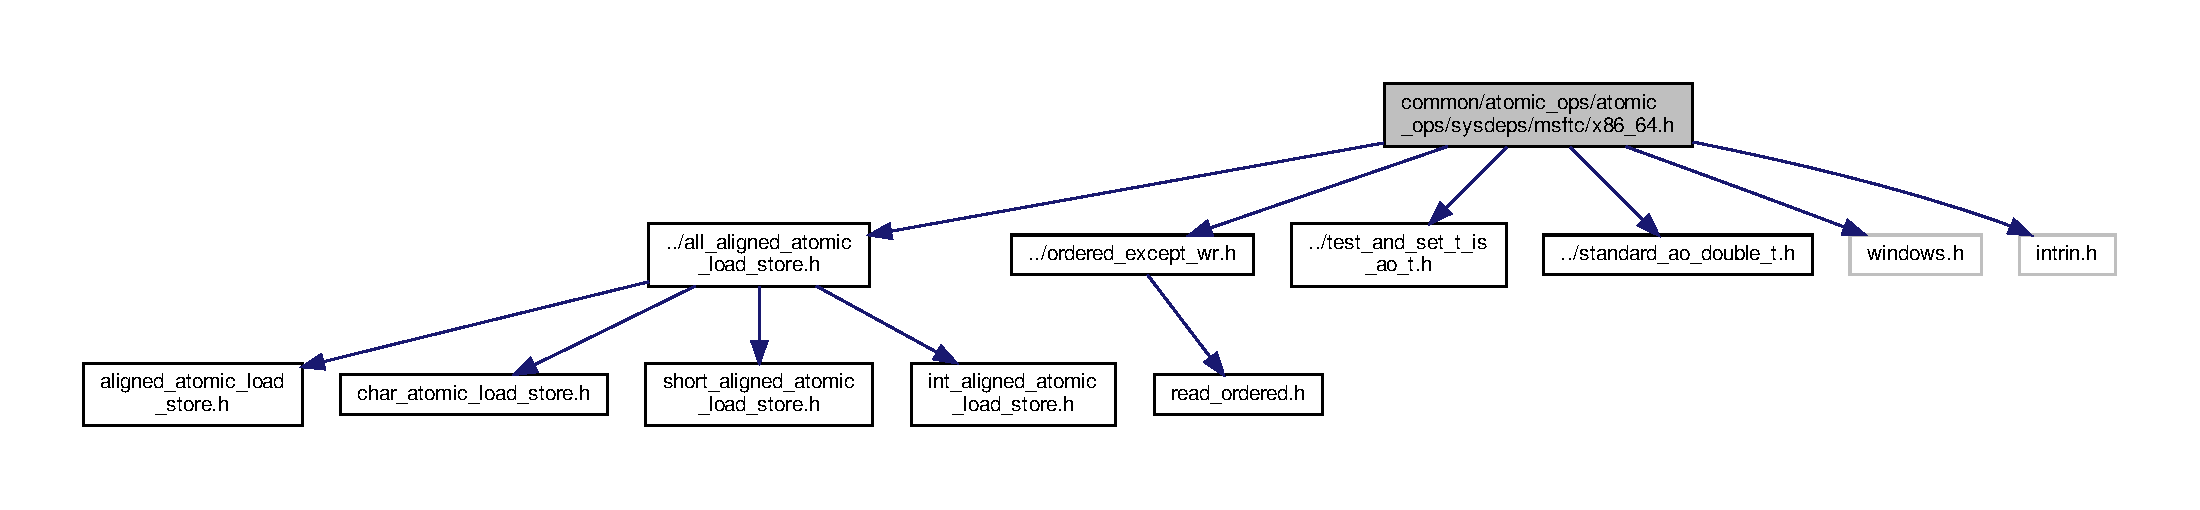
\includegraphics[width=350pt]{msftc_2x86__64_8h__incl}
\end{center}
\end{figure}
\subsection*{Macros}
\begin{DoxyCompactItemize}
\item 
\#define \hyperlink{msftc_2x86__64_8h_a9fa0fc1a9eadcba085e57bf180a53cef}{A\+O\+\_\+\+H\+A\+V\+E\+\_\+fetch\+\_\+and\+\_\+add\+\_\+full}
\item 
\#define \hyperlink{msftc_2x86__64_8h_a65fb7f14069ffab2e6329ffc98563770}{A\+O\+\_\+\+H\+A\+V\+E\+\_\+fetch\+\_\+and\+\_\+add1\+\_\+full}
\item 
\#define \hyperlink{msftc_2x86__64_8h_a9c25ee9f67d96eec7f26152cf363fc06}{A\+O\+\_\+\+H\+A\+V\+E\+\_\+fetch\+\_\+and\+\_\+sub1\+\_\+full}
\item 
\#define \hyperlink{msftc_2x86__64_8h_a98ec53065c0dfd18bc1013c500da377c}{A\+O\+\_\+\+H\+A\+V\+E\+\_\+compare\+\_\+and\+\_\+swap\+\_\+full}
\end{DoxyCompactItemize}
\subsection*{Functions}
\begin{DoxyCompactItemize}
\item 
\hyperlink{atomic__ops_8h_a9f6ab6253b6b11bc8c12efe9dde5db2b}{A\+O\+\_\+\+I\+N\+L\+I\+NE} \hyperlink{atomic__ops_8h_a5225fef4d9eee821e82382cd269160dd}{A\+O\+\_\+t} \hyperlink{msftc_2x86__64_8h_a63b6d5232496fb679621fa985234eff8}{A\+O\+\_\+fetch\+\_\+and\+\_\+add\+\_\+full} (volatile \hyperlink{atomic__ops_8h_a5225fef4d9eee821e82382cd269160dd}{A\+O\+\_\+t} $\ast$p, \hyperlink{atomic__ops_8h_a5225fef4d9eee821e82382cd269160dd}{A\+O\+\_\+t} incr)
\item 
\hyperlink{atomic__ops_8h_a9f6ab6253b6b11bc8c12efe9dde5db2b}{A\+O\+\_\+\+I\+N\+L\+I\+NE} \hyperlink{atomic__ops_8h_a5225fef4d9eee821e82382cd269160dd}{A\+O\+\_\+t} \hyperlink{msftc_2x86__64_8h_a685167af2036f69b0cfcd31a141d79b0}{A\+O\+\_\+fetch\+\_\+and\+\_\+add1\+\_\+full} (volatile \hyperlink{atomic__ops_8h_a5225fef4d9eee821e82382cd269160dd}{A\+O\+\_\+t} $\ast$p)
\item 
\hyperlink{atomic__ops_8h_a9f6ab6253b6b11bc8c12efe9dde5db2b}{A\+O\+\_\+\+I\+N\+L\+I\+NE} \hyperlink{atomic__ops_8h_a5225fef4d9eee821e82382cd269160dd}{A\+O\+\_\+t} \hyperlink{msftc_2x86__64_8h_a204c40d27bb1d43b2f29b15a516ac7db}{A\+O\+\_\+fetch\+\_\+and\+\_\+sub1\+\_\+full} (volatile \hyperlink{atomic__ops_8h_a5225fef4d9eee821e82382cd269160dd}{A\+O\+\_\+t} $\ast$p)
\item 
\hyperlink{atomic__ops_8h_a9f6ab6253b6b11bc8c12efe9dde5db2b}{A\+O\+\_\+\+I\+N\+L\+I\+NE} int \hyperlink{msftc_2x86__64_8h_a634397de6de764015b30cdff3ff00b06}{A\+O\+\_\+compare\+\_\+and\+\_\+swap\+\_\+full} (volatile \hyperlink{atomic__ops_8h_a5225fef4d9eee821e82382cd269160dd}{A\+O\+\_\+t} $\ast$addr, \hyperlink{atomic__ops_8h_a5225fef4d9eee821e82382cd269160dd}{A\+O\+\_\+t} old, \hyperlink{atomic__ops_8h_a5225fef4d9eee821e82382cd269160dd}{A\+O\+\_\+t} new\+\_\+val)
\end{DoxyCompactItemize}


\subsection{Macro Definition Documentation}
\mbox{\Hypertarget{msftc_2x86__64_8h_a98ec53065c0dfd18bc1013c500da377c}\label{msftc_2x86__64_8h_a98ec53065c0dfd18bc1013c500da377c}} 
\index{msftc/x86\+\_\+64.\+h@{msftc/x86\+\_\+64.\+h}!A\+O\+\_\+\+H\+A\+V\+E\+\_\+compare\+\_\+and\+\_\+swap\+\_\+full@{A\+O\+\_\+\+H\+A\+V\+E\+\_\+compare\+\_\+and\+\_\+swap\+\_\+full}}
\index{A\+O\+\_\+\+H\+A\+V\+E\+\_\+compare\+\_\+and\+\_\+swap\+\_\+full@{A\+O\+\_\+\+H\+A\+V\+E\+\_\+compare\+\_\+and\+\_\+swap\+\_\+full}!msftc/x86\+\_\+64.\+h@{msftc/x86\+\_\+64.\+h}}
\subsubsection{\texorpdfstring{A\+O\+\_\+\+H\+A\+V\+E\+\_\+compare\+\_\+and\+\_\+swap\+\_\+full}{AO\_HAVE\_compare\_and\_swap\_full}}
{\footnotesize\ttfamily \#define A\+O\+\_\+\+H\+A\+V\+E\+\_\+compare\+\_\+and\+\_\+swap\+\_\+full}

\mbox{\Hypertarget{msftc_2x86__64_8h_a65fb7f14069ffab2e6329ffc98563770}\label{msftc_2x86__64_8h_a65fb7f14069ffab2e6329ffc98563770}} 
\index{msftc/x86\+\_\+64.\+h@{msftc/x86\+\_\+64.\+h}!A\+O\+\_\+\+H\+A\+V\+E\+\_\+fetch\+\_\+and\+\_\+add1\+\_\+full@{A\+O\+\_\+\+H\+A\+V\+E\+\_\+fetch\+\_\+and\+\_\+add1\+\_\+full}}
\index{A\+O\+\_\+\+H\+A\+V\+E\+\_\+fetch\+\_\+and\+\_\+add1\+\_\+full@{A\+O\+\_\+\+H\+A\+V\+E\+\_\+fetch\+\_\+and\+\_\+add1\+\_\+full}!msftc/x86\+\_\+64.\+h@{msftc/x86\+\_\+64.\+h}}
\subsubsection{\texorpdfstring{A\+O\+\_\+\+H\+A\+V\+E\+\_\+fetch\+\_\+and\+\_\+add1\+\_\+full}{AO\_HAVE\_fetch\_and\_add1\_full}}
{\footnotesize\ttfamily \#define A\+O\+\_\+\+H\+A\+V\+E\+\_\+fetch\+\_\+and\+\_\+add1\+\_\+full}

\mbox{\Hypertarget{msftc_2x86__64_8h_a9fa0fc1a9eadcba085e57bf180a53cef}\label{msftc_2x86__64_8h_a9fa0fc1a9eadcba085e57bf180a53cef}} 
\index{msftc/x86\+\_\+64.\+h@{msftc/x86\+\_\+64.\+h}!A\+O\+\_\+\+H\+A\+V\+E\+\_\+fetch\+\_\+and\+\_\+add\+\_\+full@{A\+O\+\_\+\+H\+A\+V\+E\+\_\+fetch\+\_\+and\+\_\+add\+\_\+full}}
\index{A\+O\+\_\+\+H\+A\+V\+E\+\_\+fetch\+\_\+and\+\_\+add\+\_\+full@{A\+O\+\_\+\+H\+A\+V\+E\+\_\+fetch\+\_\+and\+\_\+add\+\_\+full}!msftc/x86\+\_\+64.\+h@{msftc/x86\+\_\+64.\+h}}
\subsubsection{\texorpdfstring{A\+O\+\_\+\+H\+A\+V\+E\+\_\+fetch\+\_\+and\+\_\+add\+\_\+full}{AO\_HAVE\_fetch\_and\_add\_full}}
{\footnotesize\ttfamily \#define A\+O\+\_\+\+H\+A\+V\+E\+\_\+fetch\+\_\+and\+\_\+add\+\_\+full}

\mbox{\Hypertarget{msftc_2x86__64_8h_a9c25ee9f67d96eec7f26152cf363fc06}\label{msftc_2x86__64_8h_a9c25ee9f67d96eec7f26152cf363fc06}} 
\index{msftc/x86\+\_\+64.\+h@{msftc/x86\+\_\+64.\+h}!A\+O\+\_\+\+H\+A\+V\+E\+\_\+fetch\+\_\+and\+\_\+sub1\+\_\+full@{A\+O\+\_\+\+H\+A\+V\+E\+\_\+fetch\+\_\+and\+\_\+sub1\+\_\+full}}
\index{A\+O\+\_\+\+H\+A\+V\+E\+\_\+fetch\+\_\+and\+\_\+sub1\+\_\+full@{A\+O\+\_\+\+H\+A\+V\+E\+\_\+fetch\+\_\+and\+\_\+sub1\+\_\+full}!msftc/x86\+\_\+64.\+h@{msftc/x86\+\_\+64.\+h}}
\subsubsection{\texorpdfstring{A\+O\+\_\+\+H\+A\+V\+E\+\_\+fetch\+\_\+and\+\_\+sub1\+\_\+full}{AO\_HAVE\_fetch\_and\_sub1\_full}}
{\footnotesize\ttfamily \#define A\+O\+\_\+\+H\+A\+V\+E\+\_\+fetch\+\_\+and\+\_\+sub1\+\_\+full}



\subsection{Function Documentation}
\mbox{\Hypertarget{msftc_2x86__64_8h_a634397de6de764015b30cdff3ff00b06}\label{msftc_2x86__64_8h_a634397de6de764015b30cdff3ff00b06}} 
\index{msftc/x86\+\_\+64.\+h@{msftc/x86\+\_\+64.\+h}!A\+O\+\_\+compare\+\_\+and\+\_\+swap\+\_\+full@{A\+O\+\_\+compare\+\_\+and\+\_\+swap\+\_\+full}}
\index{A\+O\+\_\+compare\+\_\+and\+\_\+swap\+\_\+full@{A\+O\+\_\+compare\+\_\+and\+\_\+swap\+\_\+full}!msftc/x86\+\_\+64.\+h@{msftc/x86\+\_\+64.\+h}}
\subsubsection{\texorpdfstring{A\+O\+\_\+compare\+\_\+and\+\_\+swap\+\_\+full()}{AO\_compare\_and\_swap\_full()}}
{\footnotesize\ttfamily \hyperlink{atomic__ops_8h_a9f6ab6253b6b11bc8c12efe9dde5db2b}{A\+O\+\_\+\+I\+N\+L\+I\+NE} int A\+O\+\_\+compare\+\_\+and\+\_\+swap\+\_\+full (\begin{DoxyParamCaption}\item[{volatile \hyperlink{atomic__ops_8h_a5225fef4d9eee821e82382cd269160dd}{A\+O\+\_\+t} $\ast$}]{addr,  }\item[{\hyperlink{atomic__ops_8h_a5225fef4d9eee821e82382cd269160dd}{A\+O\+\_\+t}}]{old,  }\item[{\hyperlink{atomic__ops_8h_a5225fef4d9eee821e82382cd269160dd}{A\+O\+\_\+t}}]{new\+\_\+val }\end{DoxyParamCaption})}

\mbox{\Hypertarget{msftc_2x86__64_8h_a685167af2036f69b0cfcd31a141d79b0}\label{msftc_2x86__64_8h_a685167af2036f69b0cfcd31a141d79b0}} 
\index{msftc/x86\+\_\+64.\+h@{msftc/x86\+\_\+64.\+h}!A\+O\+\_\+fetch\+\_\+and\+\_\+add1\+\_\+full@{A\+O\+\_\+fetch\+\_\+and\+\_\+add1\+\_\+full}}
\index{A\+O\+\_\+fetch\+\_\+and\+\_\+add1\+\_\+full@{A\+O\+\_\+fetch\+\_\+and\+\_\+add1\+\_\+full}!msftc/x86\+\_\+64.\+h@{msftc/x86\+\_\+64.\+h}}
\subsubsection{\texorpdfstring{A\+O\+\_\+fetch\+\_\+and\+\_\+add1\+\_\+full()}{AO\_fetch\_and\_add1\_full()}}
{\footnotesize\ttfamily \hyperlink{atomic__ops_8h_a9f6ab6253b6b11bc8c12efe9dde5db2b}{A\+O\+\_\+\+I\+N\+L\+I\+NE} \hyperlink{atomic__ops_8h_a5225fef4d9eee821e82382cd269160dd}{A\+O\+\_\+t} A\+O\+\_\+fetch\+\_\+and\+\_\+add1\+\_\+full (\begin{DoxyParamCaption}\item[{volatile \hyperlink{atomic__ops_8h_a5225fef4d9eee821e82382cd269160dd}{A\+O\+\_\+t} $\ast$}]{p }\end{DoxyParamCaption})}

\mbox{\Hypertarget{msftc_2x86__64_8h_a63b6d5232496fb679621fa985234eff8}\label{msftc_2x86__64_8h_a63b6d5232496fb679621fa985234eff8}} 
\index{msftc/x86\+\_\+64.\+h@{msftc/x86\+\_\+64.\+h}!A\+O\+\_\+fetch\+\_\+and\+\_\+add\+\_\+full@{A\+O\+\_\+fetch\+\_\+and\+\_\+add\+\_\+full}}
\index{A\+O\+\_\+fetch\+\_\+and\+\_\+add\+\_\+full@{A\+O\+\_\+fetch\+\_\+and\+\_\+add\+\_\+full}!msftc/x86\+\_\+64.\+h@{msftc/x86\+\_\+64.\+h}}
\subsubsection{\texorpdfstring{A\+O\+\_\+fetch\+\_\+and\+\_\+add\+\_\+full()}{AO\_fetch\_and\_add\_full()}}
{\footnotesize\ttfamily \hyperlink{atomic__ops_8h_a9f6ab6253b6b11bc8c12efe9dde5db2b}{A\+O\+\_\+\+I\+N\+L\+I\+NE} \hyperlink{atomic__ops_8h_a5225fef4d9eee821e82382cd269160dd}{A\+O\+\_\+t} A\+O\+\_\+fetch\+\_\+and\+\_\+add\+\_\+full (\begin{DoxyParamCaption}\item[{volatile \hyperlink{atomic__ops_8h_a5225fef4d9eee821e82382cd269160dd}{A\+O\+\_\+t} $\ast$}]{p,  }\item[{\hyperlink{atomic__ops_8h_a5225fef4d9eee821e82382cd269160dd}{A\+O\+\_\+t}}]{incr }\end{DoxyParamCaption})}

\mbox{\Hypertarget{msftc_2x86__64_8h_a204c40d27bb1d43b2f29b15a516ac7db}\label{msftc_2x86__64_8h_a204c40d27bb1d43b2f29b15a516ac7db}} 
\index{msftc/x86\+\_\+64.\+h@{msftc/x86\+\_\+64.\+h}!A\+O\+\_\+fetch\+\_\+and\+\_\+sub1\+\_\+full@{A\+O\+\_\+fetch\+\_\+and\+\_\+sub1\+\_\+full}}
\index{A\+O\+\_\+fetch\+\_\+and\+\_\+sub1\+\_\+full@{A\+O\+\_\+fetch\+\_\+and\+\_\+sub1\+\_\+full}!msftc/x86\+\_\+64.\+h@{msftc/x86\+\_\+64.\+h}}
\subsubsection{\texorpdfstring{A\+O\+\_\+fetch\+\_\+and\+\_\+sub1\+\_\+full()}{AO\_fetch\_and\_sub1\_full()}}
{\footnotesize\ttfamily \hyperlink{atomic__ops_8h_a9f6ab6253b6b11bc8c12efe9dde5db2b}{A\+O\+\_\+\+I\+N\+L\+I\+NE} \hyperlink{atomic__ops_8h_a5225fef4d9eee821e82382cd269160dd}{A\+O\+\_\+t} A\+O\+\_\+fetch\+\_\+and\+\_\+sub1\+\_\+full (\begin{DoxyParamCaption}\item[{volatile \hyperlink{atomic__ops_8h_a5225fef4d9eee821e82382cd269160dd}{A\+O\+\_\+t} $\ast$}]{p }\end{DoxyParamCaption})}


\hypertarget{sunc_2x86__64_8h}{}\section{common/atomic\+\_\+ops/atomic\+\_\+ops/sysdeps/sunc/x86\+\_\+64.h File Reference}
\label{sunc_2x86__64_8h}\index{common/atomic\+\_\+ops/atomic\+\_\+ops/sysdeps/sunc/x86\+\_\+64.\+h@{common/atomic\+\_\+ops/atomic\+\_\+ops/sysdeps/sunc/x86\+\_\+64.\+h}}
{\ttfamily \#include \char`\"{}../all\+\_\+aligned\+\_\+atomic\+\_\+load\+\_\+store.\+h\char`\"{}}\newline
{\ttfamily \#include \char`\"{}../ordered\+\_\+except\+\_\+wr.\+h\char`\"{}}\newline
{\ttfamily \#include \char`\"{}../test\+\_\+and\+\_\+set\+\_\+t\+\_\+is\+\_\+char.\+h\char`\"{}}\newline
{\ttfamily \#include \char`\"{}../standard\+\_\+ao\+\_\+double\+\_\+t.\+h\char`\"{}}\newline
Include dependency graph for x86\+\_\+64.\+h\+:
\nopagebreak
\begin{figure}[H]
\begin{center}
\leavevmode
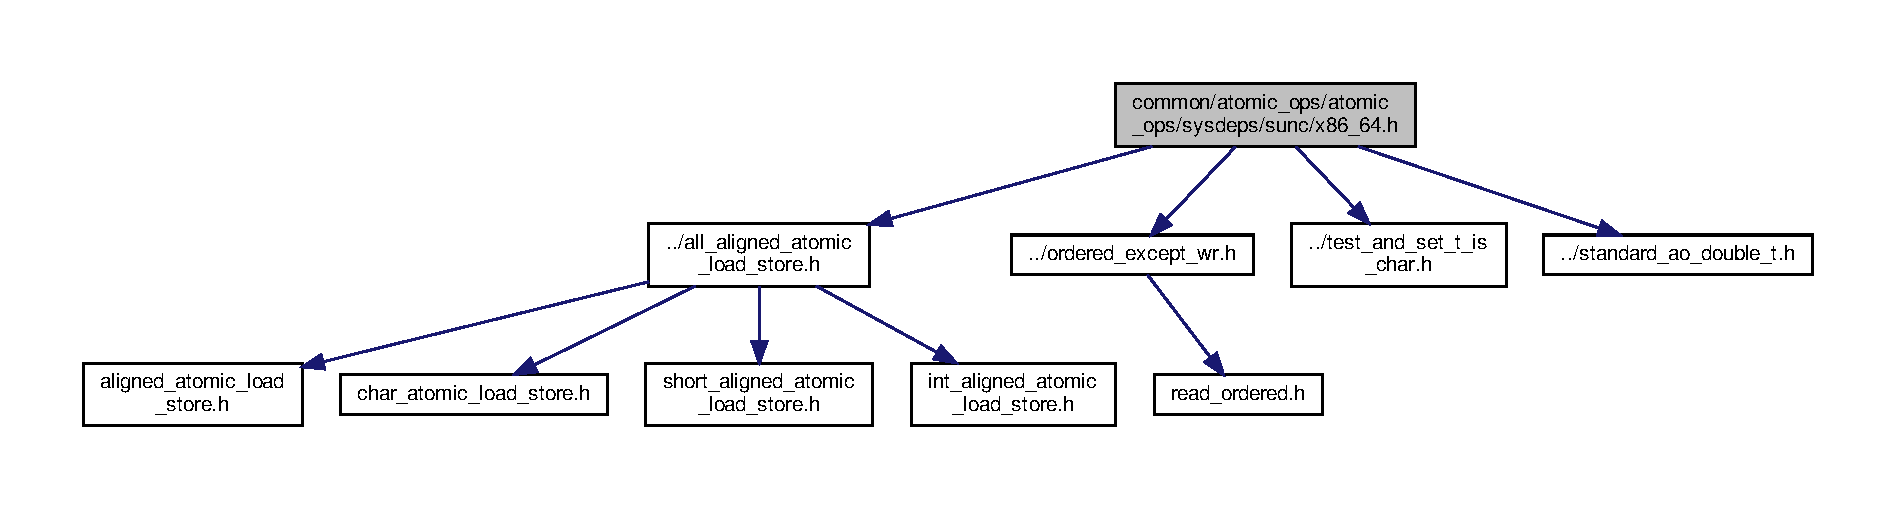
\includegraphics[width=350pt]{sunc_2x86__64_8h__incl}
\end{center}
\end{figure}
\subsection*{Macros}
\begin{DoxyCompactItemize}
\item 
\#define \hyperlink{sunc_2x86__64_8h_a3904dc699d6a6d6e771a93aa66aeb805}{A\+O\+\_\+\+H\+A\+V\+E\+\_\+nop\+\_\+full}
\item 
\#define \hyperlink{sunc_2x86__64_8h_a9fa0fc1a9eadcba085e57bf180a53cef}{A\+O\+\_\+\+H\+A\+V\+E\+\_\+fetch\+\_\+and\+\_\+add\+\_\+full}
\item 
\#define \hyperlink{sunc_2x86__64_8h_a0a938d33904c99956494e57bfa2b74fd}{A\+O\+\_\+\+H\+A\+V\+E\+\_\+char\+\_\+fetch\+\_\+and\+\_\+add\+\_\+full}
\item 
\#define \hyperlink{sunc_2x86__64_8h_affc6a05c52cc08ec46bcbba79457d985}{A\+O\+\_\+\+H\+A\+V\+E\+\_\+short\+\_\+fetch\+\_\+and\+\_\+add\+\_\+full}
\item 
\#define \hyperlink{sunc_2x86__64_8h_aee1cb49608401259e3935681b3a2df53}{A\+O\+\_\+\+H\+A\+V\+E\+\_\+int\+\_\+fetch\+\_\+and\+\_\+add\+\_\+full}
\item 
\#define \hyperlink{sunc_2x86__64_8h_a0ef45a04b0d7c74e025f829f2e614d79}{A\+O\+\_\+\+H\+A\+V\+E\+\_\+or\+\_\+full}
\item 
\#define \hyperlink{sunc_2x86__64_8h_ad5f311a090d1e6e1bb35a6e68ee35fad}{A\+O\+\_\+\+H\+A\+V\+E\+\_\+test\+\_\+and\+\_\+set\+\_\+full}
\item 
\#define \hyperlink{sunc_2x86__64_8h_a98ec53065c0dfd18bc1013c500da377c}{A\+O\+\_\+\+H\+A\+V\+E\+\_\+compare\+\_\+and\+\_\+swap\+\_\+full}
\end{DoxyCompactItemize}
\subsection*{Functions}
\begin{DoxyCompactItemize}
\item 
\hyperlink{atomic__ops_8h_a9f6ab6253b6b11bc8c12efe9dde5db2b}{A\+O\+\_\+\+I\+N\+L\+I\+NE} void \hyperlink{sunc_2x86__64_8h_afe3a6778eacc82252ba138fc9a157b04}{A\+O\+\_\+nop\+\_\+full} (void)
\item 
\hyperlink{atomic__ops_8h_a9f6ab6253b6b11bc8c12efe9dde5db2b}{A\+O\+\_\+\+I\+N\+L\+I\+NE} \hyperlink{atomic__ops_8h_a5225fef4d9eee821e82382cd269160dd}{A\+O\+\_\+t} \hyperlink{sunc_2x86__64_8h_a63b6d5232496fb679621fa985234eff8}{A\+O\+\_\+fetch\+\_\+and\+\_\+add\+\_\+full} (volatile \hyperlink{atomic__ops_8h_a5225fef4d9eee821e82382cd269160dd}{A\+O\+\_\+t} $\ast$p, \hyperlink{atomic__ops_8h_a5225fef4d9eee821e82382cd269160dd}{A\+O\+\_\+t} incr)
\item 
\hyperlink{atomic__ops_8h_a9f6ab6253b6b11bc8c12efe9dde5db2b}{A\+O\+\_\+\+I\+N\+L\+I\+NE} unsigned char \hyperlink{sunc_2x86__64_8h_a03d2aa8ce4372d7d08a306c6de38d4ba}{A\+O\+\_\+char\+\_\+fetch\+\_\+and\+\_\+add\+\_\+full} (volatile unsigned char $\ast$p, unsigned char incr)
\item 
\hyperlink{atomic__ops_8h_a9f6ab6253b6b11bc8c12efe9dde5db2b}{A\+O\+\_\+\+I\+N\+L\+I\+NE} unsigned short \hyperlink{sunc_2x86__64_8h_a99328cedbe167830313d7c3ffdcd0180}{A\+O\+\_\+short\+\_\+fetch\+\_\+and\+\_\+add\+\_\+full} (volatile unsigned short $\ast$p, unsigned short incr)
\item 
\hyperlink{atomic__ops_8h_a9f6ab6253b6b11bc8c12efe9dde5db2b}{A\+O\+\_\+\+I\+N\+L\+I\+NE} unsigned int \hyperlink{sunc_2x86__64_8h_a1b517b3713694261207c0d7ecfdc59e3}{A\+O\+\_\+int\+\_\+fetch\+\_\+and\+\_\+add\+\_\+full} (volatile unsigned int $\ast$p, unsigned int incr)
\item 
\hyperlink{atomic__ops_8h_a9f6ab6253b6b11bc8c12efe9dde5db2b}{A\+O\+\_\+\+I\+N\+L\+I\+NE} void \hyperlink{sunc_2x86__64_8h_a2732b24b044bf3993055d2c0d78b9ed9}{A\+O\+\_\+or\+\_\+full} (volatile \hyperlink{atomic__ops_8h_a5225fef4d9eee821e82382cd269160dd}{A\+O\+\_\+t} $\ast$p, \hyperlink{atomic__ops_8h_a5225fef4d9eee821e82382cd269160dd}{A\+O\+\_\+t} incr)
\item 
\hyperlink{atomic__ops_8h_a9f6ab6253b6b11bc8c12efe9dde5db2b}{A\+O\+\_\+\+I\+N\+L\+I\+NE} \hyperlink{test__and__set__t__is__char_8h_a7d99a16c4eab47ba80ab6138d7d98ac1}{A\+O\+\_\+\+T\+S\+\_\+\+V\+A\+L\+\_\+t} \hyperlink{sunc_2x86__64_8h_a9f485bd63ce5c6a017ec241906e2f651}{A\+O\+\_\+test\+\_\+and\+\_\+set\+\_\+full} (volatile \hyperlink{test__and__set__t__is__char_8h_a5890c21b549264c75c2cad08bf4f6ba9}{A\+O\+\_\+\+T\+S\+\_\+t} $\ast$addr)
\item 
\hyperlink{atomic__ops_8h_a9f6ab6253b6b11bc8c12efe9dde5db2b}{A\+O\+\_\+\+I\+N\+L\+I\+NE} int \hyperlink{sunc_2x86__64_8h_a634397de6de764015b30cdff3ff00b06}{A\+O\+\_\+compare\+\_\+and\+\_\+swap\+\_\+full} (volatile \hyperlink{atomic__ops_8h_a5225fef4d9eee821e82382cd269160dd}{A\+O\+\_\+t} $\ast$addr, \hyperlink{atomic__ops_8h_a5225fef4d9eee821e82382cd269160dd}{A\+O\+\_\+t} old, \hyperlink{atomic__ops_8h_a5225fef4d9eee821e82382cd269160dd}{A\+O\+\_\+t} new\+\_\+val)
\end{DoxyCompactItemize}


\subsection{Macro Definition Documentation}
\mbox{\Hypertarget{sunc_2x86__64_8h_a0a938d33904c99956494e57bfa2b74fd}\label{sunc_2x86__64_8h_a0a938d33904c99956494e57bfa2b74fd}} 
\index{sunc/x86\+\_\+64.\+h@{sunc/x86\+\_\+64.\+h}!A\+O\+\_\+\+H\+A\+V\+E\+\_\+char\+\_\+fetch\+\_\+and\+\_\+add\+\_\+full@{A\+O\+\_\+\+H\+A\+V\+E\+\_\+char\+\_\+fetch\+\_\+and\+\_\+add\+\_\+full}}
\index{A\+O\+\_\+\+H\+A\+V\+E\+\_\+char\+\_\+fetch\+\_\+and\+\_\+add\+\_\+full@{A\+O\+\_\+\+H\+A\+V\+E\+\_\+char\+\_\+fetch\+\_\+and\+\_\+add\+\_\+full}!sunc/x86\+\_\+64.\+h@{sunc/x86\+\_\+64.\+h}}
\subsubsection{\texorpdfstring{A\+O\+\_\+\+H\+A\+V\+E\+\_\+char\+\_\+fetch\+\_\+and\+\_\+add\+\_\+full}{AO\_HAVE\_char\_fetch\_and\_add\_full}}
{\footnotesize\ttfamily \#define A\+O\+\_\+\+H\+A\+V\+E\+\_\+char\+\_\+fetch\+\_\+and\+\_\+add\+\_\+full}

\mbox{\Hypertarget{sunc_2x86__64_8h_a98ec53065c0dfd18bc1013c500da377c}\label{sunc_2x86__64_8h_a98ec53065c0dfd18bc1013c500da377c}} 
\index{sunc/x86\+\_\+64.\+h@{sunc/x86\+\_\+64.\+h}!A\+O\+\_\+\+H\+A\+V\+E\+\_\+compare\+\_\+and\+\_\+swap\+\_\+full@{A\+O\+\_\+\+H\+A\+V\+E\+\_\+compare\+\_\+and\+\_\+swap\+\_\+full}}
\index{A\+O\+\_\+\+H\+A\+V\+E\+\_\+compare\+\_\+and\+\_\+swap\+\_\+full@{A\+O\+\_\+\+H\+A\+V\+E\+\_\+compare\+\_\+and\+\_\+swap\+\_\+full}!sunc/x86\+\_\+64.\+h@{sunc/x86\+\_\+64.\+h}}
\subsubsection{\texorpdfstring{A\+O\+\_\+\+H\+A\+V\+E\+\_\+compare\+\_\+and\+\_\+swap\+\_\+full}{AO\_HAVE\_compare\_and\_swap\_full}}
{\footnotesize\ttfamily \#define A\+O\+\_\+\+H\+A\+V\+E\+\_\+compare\+\_\+and\+\_\+swap\+\_\+full}

\mbox{\Hypertarget{sunc_2x86__64_8h_a9fa0fc1a9eadcba085e57bf180a53cef}\label{sunc_2x86__64_8h_a9fa0fc1a9eadcba085e57bf180a53cef}} 
\index{sunc/x86\+\_\+64.\+h@{sunc/x86\+\_\+64.\+h}!A\+O\+\_\+\+H\+A\+V\+E\+\_\+fetch\+\_\+and\+\_\+add\+\_\+full@{A\+O\+\_\+\+H\+A\+V\+E\+\_\+fetch\+\_\+and\+\_\+add\+\_\+full}}
\index{A\+O\+\_\+\+H\+A\+V\+E\+\_\+fetch\+\_\+and\+\_\+add\+\_\+full@{A\+O\+\_\+\+H\+A\+V\+E\+\_\+fetch\+\_\+and\+\_\+add\+\_\+full}!sunc/x86\+\_\+64.\+h@{sunc/x86\+\_\+64.\+h}}
\subsubsection{\texorpdfstring{A\+O\+\_\+\+H\+A\+V\+E\+\_\+fetch\+\_\+and\+\_\+add\+\_\+full}{AO\_HAVE\_fetch\_and\_add\_full}}
{\footnotesize\ttfamily \#define A\+O\+\_\+\+H\+A\+V\+E\+\_\+fetch\+\_\+and\+\_\+add\+\_\+full}

\mbox{\Hypertarget{sunc_2x86__64_8h_aee1cb49608401259e3935681b3a2df53}\label{sunc_2x86__64_8h_aee1cb49608401259e3935681b3a2df53}} 
\index{sunc/x86\+\_\+64.\+h@{sunc/x86\+\_\+64.\+h}!A\+O\+\_\+\+H\+A\+V\+E\+\_\+int\+\_\+fetch\+\_\+and\+\_\+add\+\_\+full@{A\+O\+\_\+\+H\+A\+V\+E\+\_\+int\+\_\+fetch\+\_\+and\+\_\+add\+\_\+full}}
\index{A\+O\+\_\+\+H\+A\+V\+E\+\_\+int\+\_\+fetch\+\_\+and\+\_\+add\+\_\+full@{A\+O\+\_\+\+H\+A\+V\+E\+\_\+int\+\_\+fetch\+\_\+and\+\_\+add\+\_\+full}!sunc/x86\+\_\+64.\+h@{sunc/x86\+\_\+64.\+h}}
\subsubsection{\texorpdfstring{A\+O\+\_\+\+H\+A\+V\+E\+\_\+int\+\_\+fetch\+\_\+and\+\_\+add\+\_\+full}{AO\_HAVE\_int\_fetch\_and\_add\_full}}
{\footnotesize\ttfamily \#define A\+O\+\_\+\+H\+A\+V\+E\+\_\+int\+\_\+fetch\+\_\+and\+\_\+add\+\_\+full}

\mbox{\Hypertarget{sunc_2x86__64_8h_a3904dc699d6a6d6e771a93aa66aeb805}\label{sunc_2x86__64_8h_a3904dc699d6a6d6e771a93aa66aeb805}} 
\index{sunc/x86\+\_\+64.\+h@{sunc/x86\+\_\+64.\+h}!A\+O\+\_\+\+H\+A\+V\+E\+\_\+nop\+\_\+full@{A\+O\+\_\+\+H\+A\+V\+E\+\_\+nop\+\_\+full}}
\index{A\+O\+\_\+\+H\+A\+V\+E\+\_\+nop\+\_\+full@{A\+O\+\_\+\+H\+A\+V\+E\+\_\+nop\+\_\+full}!sunc/x86\+\_\+64.\+h@{sunc/x86\+\_\+64.\+h}}
\subsubsection{\texorpdfstring{A\+O\+\_\+\+H\+A\+V\+E\+\_\+nop\+\_\+full}{AO\_HAVE\_nop\_full}}
{\footnotesize\ttfamily \#define A\+O\+\_\+\+H\+A\+V\+E\+\_\+nop\+\_\+full}

\mbox{\Hypertarget{sunc_2x86__64_8h_a0ef45a04b0d7c74e025f829f2e614d79}\label{sunc_2x86__64_8h_a0ef45a04b0d7c74e025f829f2e614d79}} 
\index{sunc/x86\+\_\+64.\+h@{sunc/x86\+\_\+64.\+h}!A\+O\+\_\+\+H\+A\+V\+E\+\_\+or\+\_\+full@{A\+O\+\_\+\+H\+A\+V\+E\+\_\+or\+\_\+full}}
\index{A\+O\+\_\+\+H\+A\+V\+E\+\_\+or\+\_\+full@{A\+O\+\_\+\+H\+A\+V\+E\+\_\+or\+\_\+full}!sunc/x86\+\_\+64.\+h@{sunc/x86\+\_\+64.\+h}}
\subsubsection{\texorpdfstring{A\+O\+\_\+\+H\+A\+V\+E\+\_\+or\+\_\+full}{AO\_HAVE\_or\_full}}
{\footnotesize\ttfamily \#define A\+O\+\_\+\+H\+A\+V\+E\+\_\+or\+\_\+full}

\mbox{\Hypertarget{sunc_2x86__64_8h_affc6a05c52cc08ec46bcbba79457d985}\label{sunc_2x86__64_8h_affc6a05c52cc08ec46bcbba79457d985}} 
\index{sunc/x86\+\_\+64.\+h@{sunc/x86\+\_\+64.\+h}!A\+O\+\_\+\+H\+A\+V\+E\+\_\+short\+\_\+fetch\+\_\+and\+\_\+add\+\_\+full@{A\+O\+\_\+\+H\+A\+V\+E\+\_\+short\+\_\+fetch\+\_\+and\+\_\+add\+\_\+full}}
\index{A\+O\+\_\+\+H\+A\+V\+E\+\_\+short\+\_\+fetch\+\_\+and\+\_\+add\+\_\+full@{A\+O\+\_\+\+H\+A\+V\+E\+\_\+short\+\_\+fetch\+\_\+and\+\_\+add\+\_\+full}!sunc/x86\+\_\+64.\+h@{sunc/x86\+\_\+64.\+h}}
\subsubsection{\texorpdfstring{A\+O\+\_\+\+H\+A\+V\+E\+\_\+short\+\_\+fetch\+\_\+and\+\_\+add\+\_\+full}{AO\_HAVE\_short\_fetch\_and\_add\_full}}
{\footnotesize\ttfamily \#define A\+O\+\_\+\+H\+A\+V\+E\+\_\+short\+\_\+fetch\+\_\+and\+\_\+add\+\_\+full}

\mbox{\Hypertarget{sunc_2x86__64_8h_ad5f311a090d1e6e1bb35a6e68ee35fad}\label{sunc_2x86__64_8h_ad5f311a090d1e6e1bb35a6e68ee35fad}} 
\index{sunc/x86\+\_\+64.\+h@{sunc/x86\+\_\+64.\+h}!A\+O\+\_\+\+H\+A\+V\+E\+\_\+test\+\_\+and\+\_\+set\+\_\+full@{A\+O\+\_\+\+H\+A\+V\+E\+\_\+test\+\_\+and\+\_\+set\+\_\+full}}
\index{A\+O\+\_\+\+H\+A\+V\+E\+\_\+test\+\_\+and\+\_\+set\+\_\+full@{A\+O\+\_\+\+H\+A\+V\+E\+\_\+test\+\_\+and\+\_\+set\+\_\+full}!sunc/x86\+\_\+64.\+h@{sunc/x86\+\_\+64.\+h}}
\subsubsection{\texorpdfstring{A\+O\+\_\+\+H\+A\+V\+E\+\_\+test\+\_\+and\+\_\+set\+\_\+full}{AO\_HAVE\_test\_and\_set\_full}}
{\footnotesize\ttfamily \#define A\+O\+\_\+\+H\+A\+V\+E\+\_\+test\+\_\+and\+\_\+set\+\_\+full}



\subsection{Function Documentation}
\mbox{\Hypertarget{sunc_2x86__64_8h_a03d2aa8ce4372d7d08a306c6de38d4ba}\label{sunc_2x86__64_8h_a03d2aa8ce4372d7d08a306c6de38d4ba}} 
\index{sunc/x86\+\_\+64.\+h@{sunc/x86\+\_\+64.\+h}!A\+O\+\_\+char\+\_\+fetch\+\_\+and\+\_\+add\+\_\+full@{A\+O\+\_\+char\+\_\+fetch\+\_\+and\+\_\+add\+\_\+full}}
\index{A\+O\+\_\+char\+\_\+fetch\+\_\+and\+\_\+add\+\_\+full@{A\+O\+\_\+char\+\_\+fetch\+\_\+and\+\_\+add\+\_\+full}!sunc/x86\+\_\+64.\+h@{sunc/x86\+\_\+64.\+h}}
\subsubsection{\texorpdfstring{A\+O\+\_\+char\+\_\+fetch\+\_\+and\+\_\+add\+\_\+full()}{AO\_char\_fetch\_and\_add\_full()}}
{\footnotesize\ttfamily \hyperlink{atomic__ops_8h_a9f6ab6253b6b11bc8c12efe9dde5db2b}{A\+O\+\_\+\+I\+N\+L\+I\+NE} unsigned char A\+O\+\_\+char\+\_\+fetch\+\_\+and\+\_\+add\+\_\+full (\begin{DoxyParamCaption}\item[{volatile unsigned char $\ast$}]{p,  }\item[{unsigned char}]{incr }\end{DoxyParamCaption})}

\mbox{\Hypertarget{sunc_2x86__64_8h_a634397de6de764015b30cdff3ff00b06}\label{sunc_2x86__64_8h_a634397de6de764015b30cdff3ff00b06}} 
\index{sunc/x86\+\_\+64.\+h@{sunc/x86\+\_\+64.\+h}!A\+O\+\_\+compare\+\_\+and\+\_\+swap\+\_\+full@{A\+O\+\_\+compare\+\_\+and\+\_\+swap\+\_\+full}}
\index{A\+O\+\_\+compare\+\_\+and\+\_\+swap\+\_\+full@{A\+O\+\_\+compare\+\_\+and\+\_\+swap\+\_\+full}!sunc/x86\+\_\+64.\+h@{sunc/x86\+\_\+64.\+h}}
\subsubsection{\texorpdfstring{A\+O\+\_\+compare\+\_\+and\+\_\+swap\+\_\+full()}{AO\_compare\_and\_swap\_full()}}
{\footnotesize\ttfamily \hyperlink{atomic__ops_8h_a9f6ab6253b6b11bc8c12efe9dde5db2b}{A\+O\+\_\+\+I\+N\+L\+I\+NE} int A\+O\+\_\+compare\+\_\+and\+\_\+swap\+\_\+full (\begin{DoxyParamCaption}\item[{volatile \hyperlink{atomic__ops_8h_a5225fef4d9eee821e82382cd269160dd}{A\+O\+\_\+t} $\ast$}]{addr,  }\item[{\hyperlink{atomic__ops_8h_a5225fef4d9eee821e82382cd269160dd}{A\+O\+\_\+t}}]{old,  }\item[{\hyperlink{atomic__ops_8h_a5225fef4d9eee821e82382cd269160dd}{A\+O\+\_\+t}}]{new\+\_\+val }\end{DoxyParamCaption})}

\mbox{\Hypertarget{sunc_2x86__64_8h_a63b6d5232496fb679621fa985234eff8}\label{sunc_2x86__64_8h_a63b6d5232496fb679621fa985234eff8}} 
\index{sunc/x86\+\_\+64.\+h@{sunc/x86\+\_\+64.\+h}!A\+O\+\_\+fetch\+\_\+and\+\_\+add\+\_\+full@{A\+O\+\_\+fetch\+\_\+and\+\_\+add\+\_\+full}}
\index{A\+O\+\_\+fetch\+\_\+and\+\_\+add\+\_\+full@{A\+O\+\_\+fetch\+\_\+and\+\_\+add\+\_\+full}!sunc/x86\+\_\+64.\+h@{sunc/x86\+\_\+64.\+h}}
\subsubsection{\texorpdfstring{A\+O\+\_\+fetch\+\_\+and\+\_\+add\+\_\+full()}{AO\_fetch\_and\_add\_full()}}
{\footnotesize\ttfamily \hyperlink{atomic__ops_8h_a9f6ab6253b6b11bc8c12efe9dde5db2b}{A\+O\+\_\+\+I\+N\+L\+I\+NE} \hyperlink{atomic__ops_8h_a5225fef4d9eee821e82382cd269160dd}{A\+O\+\_\+t} A\+O\+\_\+fetch\+\_\+and\+\_\+add\+\_\+full (\begin{DoxyParamCaption}\item[{volatile \hyperlink{atomic__ops_8h_a5225fef4d9eee821e82382cd269160dd}{A\+O\+\_\+t} $\ast$}]{p,  }\item[{\hyperlink{atomic__ops_8h_a5225fef4d9eee821e82382cd269160dd}{A\+O\+\_\+t}}]{incr }\end{DoxyParamCaption})}

\mbox{\Hypertarget{sunc_2x86__64_8h_a1b517b3713694261207c0d7ecfdc59e3}\label{sunc_2x86__64_8h_a1b517b3713694261207c0d7ecfdc59e3}} 
\index{sunc/x86\+\_\+64.\+h@{sunc/x86\+\_\+64.\+h}!A\+O\+\_\+int\+\_\+fetch\+\_\+and\+\_\+add\+\_\+full@{A\+O\+\_\+int\+\_\+fetch\+\_\+and\+\_\+add\+\_\+full}}
\index{A\+O\+\_\+int\+\_\+fetch\+\_\+and\+\_\+add\+\_\+full@{A\+O\+\_\+int\+\_\+fetch\+\_\+and\+\_\+add\+\_\+full}!sunc/x86\+\_\+64.\+h@{sunc/x86\+\_\+64.\+h}}
\subsubsection{\texorpdfstring{A\+O\+\_\+int\+\_\+fetch\+\_\+and\+\_\+add\+\_\+full()}{AO\_int\_fetch\_and\_add\_full()}}
{\footnotesize\ttfamily \hyperlink{atomic__ops_8h_a9f6ab6253b6b11bc8c12efe9dde5db2b}{A\+O\+\_\+\+I\+N\+L\+I\+NE} unsigned int A\+O\+\_\+int\+\_\+fetch\+\_\+and\+\_\+add\+\_\+full (\begin{DoxyParamCaption}\item[{volatile unsigned int $\ast$}]{p,  }\item[{unsigned int}]{incr }\end{DoxyParamCaption})}

\mbox{\Hypertarget{sunc_2x86__64_8h_afe3a6778eacc82252ba138fc9a157b04}\label{sunc_2x86__64_8h_afe3a6778eacc82252ba138fc9a157b04}} 
\index{sunc/x86\+\_\+64.\+h@{sunc/x86\+\_\+64.\+h}!A\+O\+\_\+nop\+\_\+full@{A\+O\+\_\+nop\+\_\+full}}
\index{A\+O\+\_\+nop\+\_\+full@{A\+O\+\_\+nop\+\_\+full}!sunc/x86\+\_\+64.\+h@{sunc/x86\+\_\+64.\+h}}
\subsubsection{\texorpdfstring{A\+O\+\_\+nop\+\_\+full()}{AO\_nop\_full()}}
{\footnotesize\ttfamily \hyperlink{atomic__ops_8h_a9f6ab6253b6b11bc8c12efe9dde5db2b}{A\+O\+\_\+\+I\+N\+L\+I\+NE} void A\+O\+\_\+nop\+\_\+full (\begin{DoxyParamCaption}\item[{void}]{ }\end{DoxyParamCaption})}

\mbox{\Hypertarget{sunc_2x86__64_8h_a2732b24b044bf3993055d2c0d78b9ed9}\label{sunc_2x86__64_8h_a2732b24b044bf3993055d2c0d78b9ed9}} 
\index{sunc/x86\+\_\+64.\+h@{sunc/x86\+\_\+64.\+h}!A\+O\+\_\+or\+\_\+full@{A\+O\+\_\+or\+\_\+full}}
\index{A\+O\+\_\+or\+\_\+full@{A\+O\+\_\+or\+\_\+full}!sunc/x86\+\_\+64.\+h@{sunc/x86\+\_\+64.\+h}}
\subsubsection{\texorpdfstring{A\+O\+\_\+or\+\_\+full()}{AO\_or\_full()}}
{\footnotesize\ttfamily \hyperlink{atomic__ops_8h_a9f6ab6253b6b11bc8c12efe9dde5db2b}{A\+O\+\_\+\+I\+N\+L\+I\+NE} void A\+O\+\_\+or\+\_\+full (\begin{DoxyParamCaption}\item[{volatile \hyperlink{atomic__ops_8h_a5225fef4d9eee821e82382cd269160dd}{A\+O\+\_\+t} $\ast$}]{p,  }\item[{\hyperlink{atomic__ops_8h_a5225fef4d9eee821e82382cd269160dd}{A\+O\+\_\+t}}]{incr }\end{DoxyParamCaption})}

\mbox{\Hypertarget{sunc_2x86__64_8h_a99328cedbe167830313d7c3ffdcd0180}\label{sunc_2x86__64_8h_a99328cedbe167830313d7c3ffdcd0180}} 
\index{sunc/x86\+\_\+64.\+h@{sunc/x86\+\_\+64.\+h}!A\+O\+\_\+short\+\_\+fetch\+\_\+and\+\_\+add\+\_\+full@{A\+O\+\_\+short\+\_\+fetch\+\_\+and\+\_\+add\+\_\+full}}
\index{A\+O\+\_\+short\+\_\+fetch\+\_\+and\+\_\+add\+\_\+full@{A\+O\+\_\+short\+\_\+fetch\+\_\+and\+\_\+add\+\_\+full}!sunc/x86\+\_\+64.\+h@{sunc/x86\+\_\+64.\+h}}
\subsubsection{\texorpdfstring{A\+O\+\_\+short\+\_\+fetch\+\_\+and\+\_\+add\+\_\+full()}{AO\_short\_fetch\_and\_add\_full()}}
{\footnotesize\ttfamily \hyperlink{atomic__ops_8h_a9f6ab6253b6b11bc8c12efe9dde5db2b}{A\+O\+\_\+\+I\+N\+L\+I\+NE} unsigned short A\+O\+\_\+short\+\_\+fetch\+\_\+and\+\_\+add\+\_\+full (\begin{DoxyParamCaption}\item[{volatile unsigned short $\ast$}]{p,  }\item[{unsigned short}]{incr }\end{DoxyParamCaption})}

\mbox{\Hypertarget{sunc_2x86__64_8h_a9f485bd63ce5c6a017ec241906e2f651}\label{sunc_2x86__64_8h_a9f485bd63ce5c6a017ec241906e2f651}} 
\index{sunc/x86\+\_\+64.\+h@{sunc/x86\+\_\+64.\+h}!A\+O\+\_\+test\+\_\+and\+\_\+set\+\_\+full@{A\+O\+\_\+test\+\_\+and\+\_\+set\+\_\+full}}
\index{A\+O\+\_\+test\+\_\+and\+\_\+set\+\_\+full@{A\+O\+\_\+test\+\_\+and\+\_\+set\+\_\+full}!sunc/x86\+\_\+64.\+h@{sunc/x86\+\_\+64.\+h}}
\subsubsection{\texorpdfstring{A\+O\+\_\+test\+\_\+and\+\_\+set\+\_\+full()}{AO\_test\_and\_set\_full()}}
{\footnotesize\ttfamily \hyperlink{atomic__ops_8h_a9f6ab6253b6b11bc8c12efe9dde5db2b}{A\+O\+\_\+\+I\+N\+L\+I\+NE} \hyperlink{test__and__set__t__is__char_8h_a7d99a16c4eab47ba80ab6138d7d98ac1}{A\+O\+\_\+\+T\+S\+\_\+\+V\+A\+L\+\_\+t} A\+O\+\_\+test\+\_\+and\+\_\+set\+\_\+full (\begin{DoxyParamCaption}\item[{volatile \hyperlink{test__and__set__t__is__char_8h_a5890c21b549264c75c2cad08bf4f6ba9}{A\+O\+\_\+\+T\+S\+\_\+t} $\ast$}]{addr }\end{DoxyParamCaption})}


\hypertarget{generic__pthread_8h}{}\section{common/atomic\+\_\+ops/atomic\+\_\+ops/sysdeps/generic\+\_\+pthread.h File Reference}
\label{generic__pthread_8h}\index{common/atomic\+\_\+ops/atomic\+\_\+ops/sysdeps/generic\+\_\+pthread.\+h@{common/atomic\+\_\+ops/atomic\+\_\+ops/sysdeps/generic\+\_\+pthread.\+h}}
{\ttfamily \#include $<$pthread.\+h$>$}\newline
{\ttfamily \#include \char`\"{}test\+\_\+and\+\_\+set\+\_\+t\+\_\+is\+\_\+ao\+\_\+t.\+h\char`\"{}}\newline
Include dependency graph for generic\+\_\+pthread.\+h\+:
\nopagebreak
\begin{figure}[H]
\begin{center}
\leavevmode
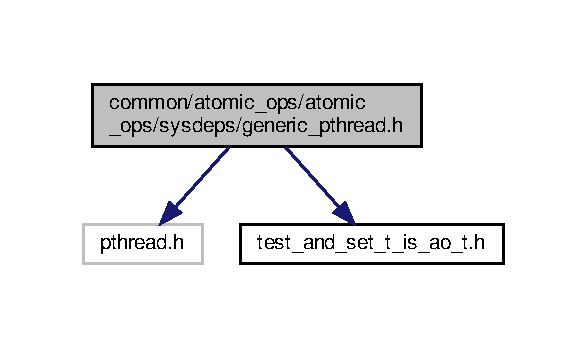
\includegraphics[width=282pt]{generic__pthread_8h__incl}
\end{center}
\end{figure}
\subsection*{Classes}
\begin{DoxyCompactItemize}
\item 
union \hyperlink{structAO__double__t}{A\+O\+\_\+double\+\_\+t}
\end{DoxyCompactItemize}
\subsection*{Macros}
\begin{DoxyCompactItemize}
\item 
\#define \hyperlink{generic__pthread_8h_a3904dc699d6a6d6e771a93aa66aeb805}{A\+O\+\_\+\+H\+A\+V\+E\+\_\+nop\+\_\+full}
\item 
\#define \hyperlink{generic__pthread_8h_a7bf0865d5e9dd16e9bb7d7069827c787}{A\+O\+\_\+\+H\+A\+V\+E\+\_\+load\+\_\+full}
\item 
\#define \hyperlink{generic__pthread_8h_acae01b282aca485176025dd405ebf5b1}{A\+O\+\_\+\+H\+A\+V\+E\+\_\+store\+\_\+full}
\item 
\#define \hyperlink{generic__pthread_8h_a7fdd564ad36132adf4ecf2a3fa709c01}{A\+O\+\_\+\+H\+A\+V\+E\+\_\+char\+\_\+load\+\_\+full}
\item 
\#define \hyperlink{generic__pthread_8h_ac21afa21f99d57c1b8e44233cc0b4e5c}{A\+O\+\_\+\+H\+A\+V\+E\+\_\+char\+\_\+store\+\_\+full}
\item 
\#define \hyperlink{generic__pthread_8h_acdbf4d1031c85ca185c46979fb27f4ff}{A\+O\+\_\+\+H\+A\+V\+E\+\_\+short\+\_\+load\+\_\+full}
\item 
\#define \hyperlink{generic__pthread_8h_a8edaa1594c79fb96e0d439951e2f5203}{A\+O\+\_\+\+H\+A\+V\+E\+\_\+short\+\_\+store\+\_\+full}
\item 
\#define \hyperlink{generic__pthread_8h_ae5cabdaf0933ef45126e94edfd69fc54}{A\+O\+\_\+\+H\+A\+V\+E\+\_\+int\+\_\+load\+\_\+full}
\item 
\#define \hyperlink{generic__pthread_8h_afa8f7fe987e37c9cd8f1a7d4b7ffeac2}{A\+O\+\_\+\+H\+A\+V\+E\+\_\+int\+\_\+store\+\_\+full}
\item 
\#define \hyperlink{generic__pthread_8h_ad5f311a090d1e6e1bb35a6e68ee35fad}{A\+O\+\_\+\+H\+A\+V\+E\+\_\+test\+\_\+and\+\_\+set\+\_\+full}
\item 
\#define \hyperlink{generic__pthread_8h_a9fa0fc1a9eadcba085e57bf180a53cef}{A\+O\+\_\+\+H\+A\+V\+E\+\_\+fetch\+\_\+and\+\_\+add\+\_\+full}
\item 
\#define \hyperlink{generic__pthread_8h_a0a938d33904c99956494e57bfa2b74fd}{A\+O\+\_\+\+H\+A\+V\+E\+\_\+char\+\_\+fetch\+\_\+and\+\_\+add\+\_\+full}
\item 
\#define \hyperlink{generic__pthread_8h_affc6a05c52cc08ec46bcbba79457d985}{A\+O\+\_\+\+H\+A\+V\+E\+\_\+short\+\_\+fetch\+\_\+and\+\_\+add\+\_\+full}
\item 
\#define \hyperlink{generic__pthread_8h_aee1cb49608401259e3935681b3a2df53}{A\+O\+\_\+\+H\+A\+V\+E\+\_\+int\+\_\+fetch\+\_\+and\+\_\+add\+\_\+full}
\item 
\#define \hyperlink{generic__pthread_8h_a0ef45a04b0d7c74e025f829f2e614d79}{A\+O\+\_\+\+H\+A\+V\+E\+\_\+or\+\_\+full}
\item 
\#define \hyperlink{generic__pthread_8h_a98ec53065c0dfd18bc1013c500da377c}{A\+O\+\_\+\+H\+A\+V\+E\+\_\+compare\+\_\+and\+\_\+swap\+\_\+full}
\item 
\#define \hyperlink{generic__pthread_8h_a42ef0a37943bb9f3a00f1734129bc679}{A\+O\+\_\+\+H\+A\+V\+E\+\_\+double\+\_\+t}
\item 
\#define \hyperlink{generic__pthread_8h_a0e2b334560e5f9a06567fc59e33a435d}{A\+O\+\_\+\+H\+A\+V\+E\+\_\+compare\+\_\+double\+\_\+and\+\_\+swap\+\_\+double\+\_\+full}
\item 
\#define \hyperlink{generic__pthread_8h_aca8c763fb5dc97d7fa997e765ada34e2}{A\+O\+\_\+\+H\+A\+V\+E\+\_\+compare\+\_\+and\+\_\+swap\+\_\+double\+\_\+full}
\end{DoxyCompactItemize}
\subsection*{Functions}
\begin{DoxyCompactItemize}
\item 
\hyperlink{atomic__ops_8h_a9f6ab6253b6b11bc8c12efe9dde5db2b}{A\+O\+\_\+\+I\+N\+L\+I\+NE} void \hyperlink{generic__pthread_8h_afe3a6778eacc82252ba138fc9a157b04}{A\+O\+\_\+nop\+\_\+full} (void)
\item 
\hyperlink{atomic__ops_8h_a9f6ab6253b6b11bc8c12efe9dde5db2b}{A\+O\+\_\+\+I\+N\+L\+I\+NE} \hyperlink{atomic__ops_8h_a5225fef4d9eee821e82382cd269160dd}{A\+O\+\_\+t} \hyperlink{generic__pthread_8h_af9867a069980858aaca485e1a7c4f650}{A\+O\+\_\+load\+\_\+full} (const volatile \hyperlink{atomic__ops_8h_a5225fef4d9eee821e82382cd269160dd}{A\+O\+\_\+t} $\ast$addr)
\item 
\hyperlink{atomic__ops_8h_a9f6ab6253b6b11bc8c12efe9dde5db2b}{A\+O\+\_\+\+I\+N\+L\+I\+NE} void \hyperlink{generic__pthread_8h_a2c0ba44e2f2f883c3bc08fa00d748ce8}{A\+O\+\_\+store\+\_\+full} (volatile \hyperlink{atomic__ops_8h_a5225fef4d9eee821e82382cd269160dd}{A\+O\+\_\+t} $\ast$addr, \hyperlink{atomic__ops_8h_a5225fef4d9eee821e82382cd269160dd}{A\+O\+\_\+t} val)
\item 
\hyperlink{atomic__ops_8h_a9f6ab6253b6b11bc8c12efe9dde5db2b}{A\+O\+\_\+\+I\+N\+L\+I\+NE} unsigned char \hyperlink{generic__pthread_8h_ad94e6c1ef059341944b5fe4f931bda38}{A\+O\+\_\+char\+\_\+load\+\_\+full} (const volatile unsigned char $\ast$addr)
\item 
\hyperlink{atomic__ops_8h_a9f6ab6253b6b11bc8c12efe9dde5db2b}{A\+O\+\_\+\+I\+N\+L\+I\+NE} void \hyperlink{generic__pthread_8h_ab37addb9bafe3aa4347d4393aee2214f}{A\+O\+\_\+char\+\_\+store\+\_\+full} (volatile unsigned char $\ast$addr, unsigned char val)
\item 
\hyperlink{atomic__ops_8h_a9f6ab6253b6b11bc8c12efe9dde5db2b}{A\+O\+\_\+\+I\+N\+L\+I\+NE} unsigned short \hyperlink{generic__pthread_8h_a0f25b5de5d41a5a7b7fecfb5feb68b89}{A\+O\+\_\+short\+\_\+load\+\_\+full} (const volatile unsigned short $\ast$addr)
\item 
\hyperlink{atomic__ops_8h_a9f6ab6253b6b11bc8c12efe9dde5db2b}{A\+O\+\_\+\+I\+N\+L\+I\+NE} void \hyperlink{generic__pthread_8h_a5fc819df5f55365cd866abe586f82ad6}{A\+O\+\_\+short\+\_\+store\+\_\+full} (volatile unsigned short $\ast$addr, unsigned short val)
\item 
\hyperlink{atomic__ops_8h_a9f6ab6253b6b11bc8c12efe9dde5db2b}{A\+O\+\_\+\+I\+N\+L\+I\+NE} unsigned int \hyperlink{generic__pthread_8h_a29a57c418a67b9a6b6f35541795e4372}{A\+O\+\_\+int\+\_\+load\+\_\+full} (const volatile unsigned int $\ast$addr)
\item 
\hyperlink{atomic__ops_8h_a9f6ab6253b6b11bc8c12efe9dde5db2b}{A\+O\+\_\+\+I\+N\+L\+I\+NE} void \hyperlink{generic__pthread_8h_a18177c785fe349fb145d779285a4c805}{A\+O\+\_\+int\+\_\+store\+\_\+full} (volatile unsigned int $\ast$addr, unsigned int val)
\item 
\hyperlink{atomic__ops_8h_a9f6ab6253b6b11bc8c12efe9dde5db2b}{A\+O\+\_\+\+I\+N\+L\+I\+NE} \hyperlink{test__and__set__t__is__char_8h_a7d99a16c4eab47ba80ab6138d7d98ac1}{A\+O\+\_\+\+T\+S\+\_\+\+V\+A\+L\+\_\+t} \hyperlink{generic__pthread_8h_a9f485bd63ce5c6a017ec241906e2f651}{A\+O\+\_\+test\+\_\+and\+\_\+set\+\_\+full} (volatile \hyperlink{test__and__set__t__is__char_8h_a5890c21b549264c75c2cad08bf4f6ba9}{A\+O\+\_\+\+T\+S\+\_\+t} $\ast$addr)
\item 
\hyperlink{atomic__ops_8h_a9f6ab6253b6b11bc8c12efe9dde5db2b}{A\+O\+\_\+\+I\+N\+L\+I\+NE} \hyperlink{atomic__ops_8h_a5225fef4d9eee821e82382cd269160dd}{A\+O\+\_\+t} \hyperlink{generic__pthread_8h_a63b6d5232496fb679621fa985234eff8}{A\+O\+\_\+fetch\+\_\+and\+\_\+add\+\_\+full} (volatile \hyperlink{atomic__ops_8h_a5225fef4d9eee821e82382cd269160dd}{A\+O\+\_\+t} $\ast$p, \hyperlink{atomic__ops_8h_a5225fef4d9eee821e82382cd269160dd}{A\+O\+\_\+t} incr)
\item 
\hyperlink{atomic__ops_8h_a9f6ab6253b6b11bc8c12efe9dde5db2b}{A\+O\+\_\+\+I\+N\+L\+I\+NE} unsigned char \hyperlink{generic__pthread_8h_a03d2aa8ce4372d7d08a306c6de38d4ba}{A\+O\+\_\+char\+\_\+fetch\+\_\+and\+\_\+add\+\_\+full} (volatile unsigned char $\ast$p, unsigned char incr)
\item 
\hyperlink{atomic__ops_8h_a9f6ab6253b6b11bc8c12efe9dde5db2b}{A\+O\+\_\+\+I\+N\+L\+I\+NE} unsigned short \hyperlink{generic__pthread_8h_a99328cedbe167830313d7c3ffdcd0180}{A\+O\+\_\+short\+\_\+fetch\+\_\+and\+\_\+add\+\_\+full} (volatile unsigned short $\ast$p, unsigned short incr)
\item 
\hyperlink{atomic__ops_8h_a9f6ab6253b6b11bc8c12efe9dde5db2b}{A\+O\+\_\+\+I\+N\+L\+I\+NE} unsigned int \hyperlink{generic__pthread_8h_a1b517b3713694261207c0d7ecfdc59e3}{A\+O\+\_\+int\+\_\+fetch\+\_\+and\+\_\+add\+\_\+full} (volatile unsigned int $\ast$p, unsigned int incr)
\item 
\hyperlink{atomic__ops_8h_a9f6ab6253b6b11bc8c12efe9dde5db2b}{A\+O\+\_\+\+I\+N\+L\+I\+NE} void \hyperlink{generic__pthread_8h_a2732b24b044bf3993055d2c0d78b9ed9}{A\+O\+\_\+or\+\_\+full} (volatile \hyperlink{atomic__ops_8h_a5225fef4d9eee821e82382cd269160dd}{A\+O\+\_\+t} $\ast$p, \hyperlink{atomic__ops_8h_a5225fef4d9eee821e82382cd269160dd}{A\+O\+\_\+t} incr)
\item 
\hyperlink{atomic__ops_8h_a9f6ab6253b6b11bc8c12efe9dde5db2b}{A\+O\+\_\+\+I\+N\+L\+I\+NE} int \hyperlink{generic__pthread_8h_a634397de6de764015b30cdff3ff00b06}{A\+O\+\_\+compare\+\_\+and\+\_\+swap\+\_\+full} (volatile \hyperlink{atomic__ops_8h_a5225fef4d9eee821e82382cd269160dd}{A\+O\+\_\+t} $\ast$addr, \hyperlink{atomic__ops_8h_a5225fef4d9eee821e82382cd269160dd}{A\+O\+\_\+t} old, \hyperlink{atomic__ops_8h_a5225fef4d9eee821e82382cd269160dd}{A\+O\+\_\+t} new\+\_\+val)
\item 
\hyperlink{atomic__ops_8h_a9f6ab6253b6b11bc8c12efe9dde5db2b}{A\+O\+\_\+\+I\+N\+L\+I\+NE} int \hyperlink{generic__pthread_8h_ac79ccc7fd8cbe9969da0ff113545853a}{A\+O\+\_\+compare\+\_\+double\+\_\+and\+\_\+swap\+\_\+double\+\_\+full} (volatile \hyperlink{structAO__double__t}{A\+O\+\_\+double\+\_\+t} $\ast$addr, \hyperlink{atomic__ops_8h_a5225fef4d9eee821e82382cd269160dd}{A\+O\+\_\+t} \hyperlink{dcss__plus_8h_aa0ef3ea06e00e9bcff2d000c6b85fe3b}{old1}, \hyperlink{atomic__ops_8h_a5225fef4d9eee821e82382cd269160dd}{A\+O\+\_\+t} \hyperlink{dcss__plus_8h_a5b804866c13543d14361d31600569ea0}{old2}, \hyperlink{atomic__ops_8h_a5225fef4d9eee821e82382cd269160dd}{A\+O\+\_\+t} new1, \hyperlink{atomic__ops_8h_a5225fef4d9eee821e82382cd269160dd}{A\+O\+\_\+t} \hyperlink{dcss__plus_8h_afb2dbab2085e7b033fef7da6fb451593}{new2})
\item 
\hyperlink{atomic__ops_8h_a9f6ab6253b6b11bc8c12efe9dde5db2b}{A\+O\+\_\+\+I\+N\+L\+I\+NE} int \hyperlink{generic__pthread_8h_ae99fe0c25c360d04fc8d56e871039ca9}{A\+O\+\_\+compare\+\_\+and\+\_\+swap\+\_\+double\+\_\+full} (volatile \hyperlink{structAO__double__t}{A\+O\+\_\+double\+\_\+t} $\ast$addr, \hyperlink{atomic__ops_8h_a5225fef4d9eee821e82382cd269160dd}{A\+O\+\_\+t} \hyperlink{dcss__plus_8h_aa0ef3ea06e00e9bcff2d000c6b85fe3b}{old1}, \hyperlink{atomic__ops_8h_a5225fef4d9eee821e82382cd269160dd}{A\+O\+\_\+t} new1, \hyperlink{atomic__ops_8h_a5225fef4d9eee821e82382cd269160dd}{A\+O\+\_\+t} \hyperlink{dcss__plus_8h_afb2dbab2085e7b033fef7da6fb451593}{new2})
\end{DoxyCompactItemize}
\subsection*{Variables}
\begin{DoxyCompactItemize}
\item 
pthread\+\_\+mutex\+\_\+t \hyperlink{generic__pthread_8h_ae846407c7f786f6858bff10420261ad1}{A\+O\+\_\+pt\+\_\+lock}
\end{DoxyCompactItemize}


\subsection{Macro Definition Documentation}
\mbox{\Hypertarget{generic__pthread_8h_a0a938d33904c99956494e57bfa2b74fd}\label{generic__pthread_8h_a0a938d33904c99956494e57bfa2b74fd}} 
\index{generic\+\_\+pthread.\+h@{generic\+\_\+pthread.\+h}!A\+O\+\_\+\+H\+A\+V\+E\+\_\+char\+\_\+fetch\+\_\+and\+\_\+add\+\_\+full@{A\+O\+\_\+\+H\+A\+V\+E\+\_\+char\+\_\+fetch\+\_\+and\+\_\+add\+\_\+full}}
\index{A\+O\+\_\+\+H\+A\+V\+E\+\_\+char\+\_\+fetch\+\_\+and\+\_\+add\+\_\+full@{A\+O\+\_\+\+H\+A\+V\+E\+\_\+char\+\_\+fetch\+\_\+and\+\_\+add\+\_\+full}!generic\+\_\+pthread.\+h@{generic\+\_\+pthread.\+h}}
\subsubsection{\texorpdfstring{A\+O\+\_\+\+H\+A\+V\+E\+\_\+char\+\_\+fetch\+\_\+and\+\_\+add\+\_\+full}{AO\_HAVE\_char\_fetch\_and\_add\_full}}
{\footnotesize\ttfamily \#define A\+O\+\_\+\+H\+A\+V\+E\+\_\+char\+\_\+fetch\+\_\+and\+\_\+add\+\_\+full}

\mbox{\Hypertarget{generic__pthread_8h_a7fdd564ad36132adf4ecf2a3fa709c01}\label{generic__pthread_8h_a7fdd564ad36132adf4ecf2a3fa709c01}} 
\index{generic\+\_\+pthread.\+h@{generic\+\_\+pthread.\+h}!A\+O\+\_\+\+H\+A\+V\+E\+\_\+char\+\_\+load\+\_\+full@{A\+O\+\_\+\+H\+A\+V\+E\+\_\+char\+\_\+load\+\_\+full}}
\index{A\+O\+\_\+\+H\+A\+V\+E\+\_\+char\+\_\+load\+\_\+full@{A\+O\+\_\+\+H\+A\+V\+E\+\_\+char\+\_\+load\+\_\+full}!generic\+\_\+pthread.\+h@{generic\+\_\+pthread.\+h}}
\subsubsection{\texorpdfstring{A\+O\+\_\+\+H\+A\+V\+E\+\_\+char\+\_\+load\+\_\+full}{AO\_HAVE\_char\_load\_full}}
{\footnotesize\ttfamily \#define A\+O\+\_\+\+H\+A\+V\+E\+\_\+char\+\_\+load\+\_\+full}

\mbox{\Hypertarget{generic__pthread_8h_ac21afa21f99d57c1b8e44233cc0b4e5c}\label{generic__pthread_8h_ac21afa21f99d57c1b8e44233cc0b4e5c}} 
\index{generic\+\_\+pthread.\+h@{generic\+\_\+pthread.\+h}!A\+O\+\_\+\+H\+A\+V\+E\+\_\+char\+\_\+store\+\_\+full@{A\+O\+\_\+\+H\+A\+V\+E\+\_\+char\+\_\+store\+\_\+full}}
\index{A\+O\+\_\+\+H\+A\+V\+E\+\_\+char\+\_\+store\+\_\+full@{A\+O\+\_\+\+H\+A\+V\+E\+\_\+char\+\_\+store\+\_\+full}!generic\+\_\+pthread.\+h@{generic\+\_\+pthread.\+h}}
\subsubsection{\texorpdfstring{A\+O\+\_\+\+H\+A\+V\+E\+\_\+char\+\_\+store\+\_\+full}{AO\_HAVE\_char\_store\_full}}
{\footnotesize\ttfamily \#define A\+O\+\_\+\+H\+A\+V\+E\+\_\+char\+\_\+store\+\_\+full}

\mbox{\Hypertarget{generic__pthread_8h_aca8c763fb5dc97d7fa997e765ada34e2}\label{generic__pthread_8h_aca8c763fb5dc97d7fa997e765ada34e2}} 
\index{generic\+\_\+pthread.\+h@{generic\+\_\+pthread.\+h}!A\+O\+\_\+\+H\+A\+V\+E\+\_\+compare\+\_\+and\+\_\+swap\+\_\+double\+\_\+full@{A\+O\+\_\+\+H\+A\+V\+E\+\_\+compare\+\_\+and\+\_\+swap\+\_\+double\+\_\+full}}
\index{A\+O\+\_\+\+H\+A\+V\+E\+\_\+compare\+\_\+and\+\_\+swap\+\_\+double\+\_\+full@{A\+O\+\_\+\+H\+A\+V\+E\+\_\+compare\+\_\+and\+\_\+swap\+\_\+double\+\_\+full}!generic\+\_\+pthread.\+h@{generic\+\_\+pthread.\+h}}
\subsubsection{\texorpdfstring{A\+O\+\_\+\+H\+A\+V\+E\+\_\+compare\+\_\+and\+\_\+swap\+\_\+double\+\_\+full}{AO\_HAVE\_compare\_and\_swap\_double\_full}}
{\footnotesize\ttfamily \#define A\+O\+\_\+\+H\+A\+V\+E\+\_\+compare\+\_\+and\+\_\+swap\+\_\+double\+\_\+full}

\mbox{\Hypertarget{generic__pthread_8h_a98ec53065c0dfd18bc1013c500da377c}\label{generic__pthread_8h_a98ec53065c0dfd18bc1013c500da377c}} 
\index{generic\+\_\+pthread.\+h@{generic\+\_\+pthread.\+h}!A\+O\+\_\+\+H\+A\+V\+E\+\_\+compare\+\_\+and\+\_\+swap\+\_\+full@{A\+O\+\_\+\+H\+A\+V\+E\+\_\+compare\+\_\+and\+\_\+swap\+\_\+full}}
\index{A\+O\+\_\+\+H\+A\+V\+E\+\_\+compare\+\_\+and\+\_\+swap\+\_\+full@{A\+O\+\_\+\+H\+A\+V\+E\+\_\+compare\+\_\+and\+\_\+swap\+\_\+full}!generic\+\_\+pthread.\+h@{generic\+\_\+pthread.\+h}}
\subsubsection{\texorpdfstring{A\+O\+\_\+\+H\+A\+V\+E\+\_\+compare\+\_\+and\+\_\+swap\+\_\+full}{AO\_HAVE\_compare\_and\_swap\_full}}
{\footnotesize\ttfamily \#define A\+O\+\_\+\+H\+A\+V\+E\+\_\+compare\+\_\+and\+\_\+swap\+\_\+full}

\mbox{\Hypertarget{generic__pthread_8h_a0e2b334560e5f9a06567fc59e33a435d}\label{generic__pthread_8h_a0e2b334560e5f9a06567fc59e33a435d}} 
\index{generic\+\_\+pthread.\+h@{generic\+\_\+pthread.\+h}!A\+O\+\_\+\+H\+A\+V\+E\+\_\+compare\+\_\+double\+\_\+and\+\_\+swap\+\_\+double\+\_\+full@{A\+O\+\_\+\+H\+A\+V\+E\+\_\+compare\+\_\+double\+\_\+and\+\_\+swap\+\_\+double\+\_\+full}}
\index{A\+O\+\_\+\+H\+A\+V\+E\+\_\+compare\+\_\+double\+\_\+and\+\_\+swap\+\_\+double\+\_\+full@{A\+O\+\_\+\+H\+A\+V\+E\+\_\+compare\+\_\+double\+\_\+and\+\_\+swap\+\_\+double\+\_\+full}!generic\+\_\+pthread.\+h@{generic\+\_\+pthread.\+h}}
\subsubsection{\texorpdfstring{A\+O\+\_\+\+H\+A\+V\+E\+\_\+compare\+\_\+double\+\_\+and\+\_\+swap\+\_\+double\+\_\+full}{AO\_HAVE\_compare\_double\_and\_swap\_double\_full}}
{\footnotesize\ttfamily \#define A\+O\+\_\+\+H\+A\+V\+E\+\_\+compare\+\_\+double\+\_\+and\+\_\+swap\+\_\+double\+\_\+full}

\mbox{\Hypertarget{generic__pthread_8h_a42ef0a37943bb9f3a00f1734129bc679}\label{generic__pthread_8h_a42ef0a37943bb9f3a00f1734129bc679}} 
\index{generic\+\_\+pthread.\+h@{generic\+\_\+pthread.\+h}!A\+O\+\_\+\+H\+A\+V\+E\+\_\+double\+\_\+t@{A\+O\+\_\+\+H\+A\+V\+E\+\_\+double\+\_\+t}}
\index{A\+O\+\_\+\+H\+A\+V\+E\+\_\+double\+\_\+t@{A\+O\+\_\+\+H\+A\+V\+E\+\_\+double\+\_\+t}!generic\+\_\+pthread.\+h@{generic\+\_\+pthread.\+h}}
\subsubsection{\texorpdfstring{A\+O\+\_\+\+H\+A\+V\+E\+\_\+double\+\_\+t}{AO\_HAVE\_double\_t}}
{\footnotesize\ttfamily \#define A\+O\+\_\+\+H\+A\+V\+E\+\_\+double\+\_\+t}

\mbox{\Hypertarget{generic__pthread_8h_a9fa0fc1a9eadcba085e57bf180a53cef}\label{generic__pthread_8h_a9fa0fc1a9eadcba085e57bf180a53cef}} 
\index{generic\+\_\+pthread.\+h@{generic\+\_\+pthread.\+h}!A\+O\+\_\+\+H\+A\+V\+E\+\_\+fetch\+\_\+and\+\_\+add\+\_\+full@{A\+O\+\_\+\+H\+A\+V\+E\+\_\+fetch\+\_\+and\+\_\+add\+\_\+full}}
\index{A\+O\+\_\+\+H\+A\+V\+E\+\_\+fetch\+\_\+and\+\_\+add\+\_\+full@{A\+O\+\_\+\+H\+A\+V\+E\+\_\+fetch\+\_\+and\+\_\+add\+\_\+full}!generic\+\_\+pthread.\+h@{generic\+\_\+pthread.\+h}}
\subsubsection{\texorpdfstring{A\+O\+\_\+\+H\+A\+V\+E\+\_\+fetch\+\_\+and\+\_\+add\+\_\+full}{AO\_HAVE\_fetch\_and\_add\_full}}
{\footnotesize\ttfamily \#define A\+O\+\_\+\+H\+A\+V\+E\+\_\+fetch\+\_\+and\+\_\+add\+\_\+full}

\mbox{\Hypertarget{generic__pthread_8h_aee1cb49608401259e3935681b3a2df53}\label{generic__pthread_8h_aee1cb49608401259e3935681b3a2df53}} 
\index{generic\+\_\+pthread.\+h@{generic\+\_\+pthread.\+h}!A\+O\+\_\+\+H\+A\+V\+E\+\_\+int\+\_\+fetch\+\_\+and\+\_\+add\+\_\+full@{A\+O\+\_\+\+H\+A\+V\+E\+\_\+int\+\_\+fetch\+\_\+and\+\_\+add\+\_\+full}}
\index{A\+O\+\_\+\+H\+A\+V\+E\+\_\+int\+\_\+fetch\+\_\+and\+\_\+add\+\_\+full@{A\+O\+\_\+\+H\+A\+V\+E\+\_\+int\+\_\+fetch\+\_\+and\+\_\+add\+\_\+full}!generic\+\_\+pthread.\+h@{generic\+\_\+pthread.\+h}}
\subsubsection{\texorpdfstring{A\+O\+\_\+\+H\+A\+V\+E\+\_\+int\+\_\+fetch\+\_\+and\+\_\+add\+\_\+full}{AO\_HAVE\_int\_fetch\_and\_add\_full}}
{\footnotesize\ttfamily \#define A\+O\+\_\+\+H\+A\+V\+E\+\_\+int\+\_\+fetch\+\_\+and\+\_\+add\+\_\+full}

\mbox{\Hypertarget{generic__pthread_8h_ae5cabdaf0933ef45126e94edfd69fc54}\label{generic__pthread_8h_ae5cabdaf0933ef45126e94edfd69fc54}} 
\index{generic\+\_\+pthread.\+h@{generic\+\_\+pthread.\+h}!A\+O\+\_\+\+H\+A\+V\+E\+\_\+int\+\_\+load\+\_\+full@{A\+O\+\_\+\+H\+A\+V\+E\+\_\+int\+\_\+load\+\_\+full}}
\index{A\+O\+\_\+\+H\+A\+V\+E\+\_\+int\+\_\+load\+\_\+full@{A\+O\+\_\+\+H\+A\+V\+E\+\_\+int\+\_\+load\+\_\+full}!generic\+\_\+pthread.\+h@{generic\+\_\+pthread.\+h}}
\subsubsection{\texorpdfstring{A\+O\+\_\+\+H\+A\+V\+E\+\_\+int\+\_\+load\+\_\+full}{AO\_HAVE\_int\_load\_full}}
{\footnotesize\ttfamily \#define A\+O\+\_\+\+H\+A\+V\+E\+\_\+int\+\_\+load\+\_\+full}

\mbox{\Hypertarget{generic__pthread_8h_afa8f7fe987e37c9cd8f1a7d4b7ffeac2}\label{generic__pthread_8h_afa8f7fe987e37c9cd8f1a7d4b7ffeac2}} 
\index{generic\+\_\+pthread.\+h@{generic\+\_\+pthread.\+h}!A\+O\+\_\+\+H\+A\+V\+E\+\_\+int\+\_\+store\+\_\+full@{A\+O\+\_\+\+H\+A\+V\+E\+\_\+int\+\_\+store\+\_\+full}}
\index{A\+O\+\_\+\+H\+A\+V\+E\+\_\+int\+\_\+store\+\_\+full@{A\+O\+\_\+\+H\+A\+V\+E\+\_\+int\+\_\+store\+\_\+full}!generic\+\_\+pthread.\+h@{generic\+\_\+pthread.\+h}}
\subsubsection{\texorpdfstring{A\+O\+\_\+\+H\+A\+V\+E\+\_\+int\+\_\+store\+\_\+full}{AO\_HAVE\_int\_store\_full}}
{\footnotesize\ttfamily \#define A\+O\+\_\+\+H\+A\+V\+E\+\_\+int\+\_\+store\+\_\+full}

\mbox{\Hypertarget{generic__pthread_8h_a7bf0865d5e9dd16e9bb7d7069827c787}\label{generic__pthread_8h_a7bf0865d5e9dd16e9bb7d7069827c787}} 
\index{generic\+\_\+pthread.\+h@{generic\+\_\+pthread.\+h}!A\+O\+\_\+\+H\+A\+V\+E\+\_\+load\+\_\+full@{A\+O\+\_\+\+H\+A\+V\+E\+\_\+load\+\_\+full}}
\index{A\+O\+\_\+\+H\+A\+V\+E\+\_\+load\+\_\+full@{A\+O\+\_\+\+H\+A\+V\+E\+\_\+load\+\_\+full}!generic\+\_\+pthread.\+h@{generic\+\_\+pthread.\+h}}
\subsubsection{\texorpdfstring{A\+O\+\_\+\+H\+A\+V\+E\+\_\+load\+\_\+full}{AO\_HAVE\_load\_full}}
{\footnotesize\ttfamily \#define A\+O\+\_\+\+H\+A\+V\+E\+\_\+load\+\_\+full}

\mbox{\Hypertarget{generic__pthread_8h_a3904dc699d6a6d6e771a93aa66aeb805}\label{generic__pthread_8h_a3904dc699d6a6d6e771a93aa66aeb805}} 
\index{generic\+\_\+pthread.\+h@{generic\+\_\+pthread.\+h}!A\+O\+\_\+\+H\+A\+V\+E\+\_\+nop\+\_\+full@{A\+O\+\_\+\+H\+A\+V\+E\+\_\+nop\+\_\+full}}
\index{A\+O\+\_\+\+H\+A\+V\+E\+\_\+nop\+\_\+full@{A\+O\+\_\+\+H\+A\+V\+E\+\_\+nop\+\_\+full}!generic\+\_\+pthread.\+h@{generic\+\_\+pthread.\+h}}
\subsubsection{\texorpdfstring{A\+O\+\_\+\+H\+A\+V\+E\+\_\+nop\+\_\+full}{AO\_HAVE\_nop\_full}}
{\footnotesize\ttfamily \#define A\+O\+\_\+\+H\+A\+V\+E\+\_\+nop\+\_\+full}

\mbox{\Hypertarget{generic__pthread_8h_a0ef45a04b0d7c74e025f829f2e614d79}\label{generic__pthread_8h_a0ef45a04b0d7c74e025f829f2e614d79}} 
\index{generic\+\_\+pthread.\+h@{generic\+\_\+pthread.\+h}!A\+O\+\_\+\+H\+A\+V\+E\+\_\+or\+\_\+full@{A\+O\+\_\+\+H\+A\+V\+E\+\_\+or\+\_\+full}}
\index{A\+O\+\_\+\+H\+A\+V\+E\+\_\+or\+\_\+full@{A\+O\+\_\+\+H\+A\+V\+E\+\_\+or\+\_\+full}!generic\+\_\+pthread.\+h@{generic\+\_\+pthread.\+h}}
\subsubsection{\texorpdfstring{A\+O\+\_\+\+H\+A\+V\+E\+\_\+or\+\_\+full}{AO\_HAVE\_or\_full}}
{\footnotesize\ttfamily \#define A\+O\+\_\+\+H\+A\+V\+E\+\_\+or\+\_\+full}

\mbox{\Hypertarget{generic__pthread_8h_affc6a05c52cc08ec46bcbba79457d985}\label{generic__pthread_8h_affc6a05c52cc08ec46bcbba79457d985}} 
\index{generic\+\_\+pthread.\+h@{generic\+\_\+pthread.\+h}!A\+O\+\_\+\+H\+A\+V\+E\+\_\+short\+\_\+fetch\+\_\+and\+\_\+add\+\_\+full@{A\+O\+\_\+\+H\+A\+V\+E\+\_\+short\+\_\+fetch\+\_\+and\+\_\+add\+\_\+full}}
\index{A\+O\+\_\+\+H\+A\+V\+E\+\_\+short\+\_\+fetch\+\_\+and\+\_\+add\+\_\+full@{A\+O\+\_\+\+H\+A\+V\+E\+\_\+short\+\_\+fetch\+\_\+and\+\_\+add\+\_\+full}!generic\+\_\+pthread.\+h@{generic\+\_\+pthread.\+h}}
\subsubsection{\texorpdfstring{A\+O\+\_\+\+H\+A\+V\+E\+\_\+short\+\_\+fetch\+\_\+and\+\_\+add\+\_\+full}{AO\_HAVE\_short\_fetch\_and\_add\_full}}
{\footnotesize\ttfamily \#define A\+O\+\_\+\+H\+A\+V\+E\+\_\+short\+\_\+fetch\+\_\+and\+\_\+add\+\_\+full}

\mbox{\Hypertarget{generic__pthread_8h_acdbf4d1031c85ca185c46979fb27f4ff}\label{generic__pthread_8h_acdbf4d1031c85ca185c46979fb27f4ff}} 
\index{generic\+\_\+pthread.\+h@{generic\+\_\+pthread.\+h}!A\+O\+\_\+\+H\+A\+V\+E\+\_\+short\+\_\+load\+\_\+full@{A\+O\+\_\+\+H\+A\+V\+E\+\_\+short\+\_\+load\+\_\+full}}
\index{A\+O\+\_\+\+H\+A\+V\+E\+\_\+short\+\_\+load\+\_\+full@{A\+O\+\_\+\+H\+A\+V\+E\+\_\+short\+\_\+load\+\_\+full}!generic\+\_\+pthread.\+h@{generic\+\_\+pthread.\+h}}
\subsubsection{\texorpdfstring{A\+O\+\_\+\+H\+A\+V\+E\+\_\+short\+\_\+load\+\_\+full}{AO\_HAVE\_short\_load\_full}}
{\footnotesize\ttfamily \#define A\+O\+\_\+\+H\+A\+V\+E\+\_\+short\+\_\+load\+\_\+full}

\mbox{\Hypertarget{generic__pthread_8h_a8edaa1594c79fb96e0d439951e2f5203}\label{generic__pthread_8h_a8edaa1594c79fb96e0d439951e2f5203}} 
\index{generic\+\_\+pthread.\+h@{generic\+\_\+pthread.\+h}!A\+O\+\_\+\+H\+A\+V\+E\+\_\+short\+\_\+store\+\_\+full@{A\+O\+\_\+\+H\+A\+V\+E\+\_\+short\+\_\+store\+\_\+full}}
\index{A\+O\+\_\+\+H\+A\+V\+E\+\_\+short\+\_\+store\+\_\+full@{A\+O\+\_\+\+H\+A\+V\+E\+\_\+short\+\_\+store\+\_\+full}!generic\+\_\+pthread.\+h@{generic\+\_\+pthread.\+h}}
\subsubsection{\texorpdfstring{A\+O\+\_\+\+H\+A\+V\+E\+\_\+short\+\_\+store\+\_\+full}{AO\_HAVE\_short\_store\_full}}
{\footnotesize\ttfamily \#define A\+O\+\_\+\+H\+A\+V\+E\+\_\+short\+\_\+store\+\_\+full}

\mbox{\Hypertarget{generic__pthread_8h_acae01b282aca485176025dd405ebf5b1}\label{generic__pthread_8h_acae01b282aca485176025dd405ebf5b1}} 
\index{generic\+\_\+pthread.\+h@{generic\+\_\+pthread.\+h}!A\+O\+\_\+\+H\+A\+V\+E\+\_\+store\+\_\+full@{A\+O\+\_\+\+H\+A\+V\+E\+\_\+store\+\_\+full}}
\index{A\+O\+\_\+\+H\+A\+V\+E\+\_\+store\+\_\+full@{A\+O\+\_\+\+H\+A\+V\+E\+\_\+store\+\_\+full}!generic\+\_\+pthread.\+h@{generic\+\_\+pthread.\+h}}
\subsubsection{\texorpdfstring{A\+O\+\_\+\+H\+A\+V\+E\+\_\+store\+\_\+full}{AO\_HAVE\_store\_full}}
{\footnotesize\ttfamily \#define A\+O\+\_\+\+H\+A\+V\+E\+\_\+store\+\_\+full}

\mbox{\Hypertarget{generic__pthread_8h_ad5f311a090d1e6e1bb35a6e68ee35fad}\label{generic__pthread_8h_ad5f311a090d1e6e1bb35a6e68ee35fad}} 
\index{generic\+\_\+pthread.\+h@{generic\+\_\+pthread.\+h}!A\+O\+\_\+\+H\+A\+V\+E\+\_\+test\+\_\+and\+\_\+set\+\_\+full@{A\+O\+\_\+\+H\+A\+V\+E\+\_\+test\+\_\+and\+\_\+set\+\_\+full}}
\index{A\+O\+\_\+\+H\+A\+V\+E\+\_\+test\+\_\+and\+\_\+set\+\_\+full@{A\+O\+\_\+\+H\+A\+V\+E\+\_\+test\+\_\+and\+\_\+set\+\_\+full}!generic\+\_\+pthread.\+h@{generic\+\_\+pthread.\+h}}
\subsubsection{\texorpdfstring{A\+O\+\_\+\+H\+A\+V\+E\+\_\+test\+\_\+and\+\_\+set\+\_\+full}{AO\_HAVE\_test\_and\_set\_full}}
{\footnotesize\ttfamily \#define A\+O\+\_\+\+H\+A\+V\+E\+\_\+test\+\_\+and\+\_\+set\+\_\+full}



\subsection{Function Documentation}
\mbox{\Hypertarget{generic__pthread_8h_a03d2aa8ce4372d7d08a306c6de38d4ba}\label{generic__pthread_8h_a03d2aa8ce4372d7d08a306c6de38d4ba}} 
\index{generic\+\_\+pthread.\+h@{generic\+\_\+pthread.\+h}!A\+O\+\_\+char\+\_\+fetch\+\_\+and\+\_\+add\+\_\+full@{A\+O\+\_\+char\+\_\+fetch\+\_\+and\+\_\+add\+\_\+full}}
\index{A\+O\+\_\+char\+\_\+fetch\+\_\+and\+\_\+add\+\_\+full@{A\+O\+\_\+char\+\_\+fetch\+\_\+and\+\_\+add\+\_\+full}!generic\+\_\+pthread.\+h@{generic\+\_\+pthread.\+h}}
\subsubsection{\texorpdfstring{A\+O\+\_\+char\+\_\+fetch\+\_\+and\+\_\+add\+\_\+full()}{AO\_char\_fetch\_and\_add\_full()}}
{\footnotesize\ttfamily \hyperlink{atomic__ops_8h_a9f6ab6253b6b11bc8c12efe9dde5db2b}{A\+O\+\_\+\+I\+N\+L\+I\+NE} unsigned char A\+O\+\_\+char\+\_\+fetch\+\_\+and\+\_\+add\+\_\+full (\begin{DoxyParamCaption}\item[{volatile unsigned char $\ast$}]{p,  }\item[{unsigned char}]{incr }\end{DoxyParamCaption})}

\mbox{\Hypertarget{generic__pthread_8h_ad94e6c1ef059341944b5fe4f931bda38}\label{generic__pthread_8h_ad94e6c1ef059341944b5fe4f931bda38}} 
\index{generic\+\_\+pthread.\+h@{generic\+\_\+pthread.\+h}!A\+O\+\_\+char\+\_\+load\+\_\+full@{A\+O\+\_\+char\+\_\+load\+\_\+full}}
\index{A\+O\+\_\+char\+\_\+load\+\_\+full@{A\+O\+\_\+char\+\_\+load\+\_\+full}!generic\+\_\+pthread.\+h@{generic\+\_\+pthread.\+h}}
\subsubsection{\texorpdfstring{A\+O\+\_\+char\+\_\+load\+\_\+full()}{AO\_char\_load\_full()}}
{\footnotesize\ttfamily \hyperlink{atomic__ops_8h_a9f6ab6253b6b11bc8c12efe9dde5db2b}{A\+O\+\_\+\+I\+N\+L\+I\+NE} unsigned char A\+O\+\_\+char\+\_\+load\+\_\+full (\begin{DoxyParamCaption}\item[{const volatile unsigned char $\ast$}]{addr }\end{DoxyParamCaption})}

\mbox{\Hypertarget{generic__pthread_8h_ab37addb9bafe3aa4347d4393aee2214f}\label{generic__pthread_8h_ab37addb9bafe3aa4347d4393aee2214f}} 
\index{generic\+\_\+pthread.\+h@{generic\+\_\+pthread.\+h}!A\+O\+\_\+char\+\_\+store\+\_\+full@{A\+O\+\_\+char\+\_\+store\+\_\+full}}
\index{A\+O\+\_\+char\+\_\+store\+\_\+full@{A\+O\+\_\+char\+\_\+store\+\_\+full}!generic\+\_\+pthread.\+h@{generic\+\_\+pthread.\+h}}
\subsubsection{\texorpdfstring{A\+O\+\_\+char\+\_\+store\+\_\+full()}{AO\_char\_store\_full()}}
{\footnotesize\ttfamily \hyperlink{atomic__ops_8h_a9f6ab6253b6b11bc8c12efe9dde5db2b}{A\+O\+\_\+\+I\+N\+L\+I\+NE} void A\+O\+\_\+char\+\_\+store\+\_\+full (\begin{DoxyParamCaption}\item[{volatile unsigned char $\ast$}]{addr,  }\item[{unsigned char}]{val }\end{DoxyParamCaption})}

\mbox{\Hypertarget{generic__pthread_8h_ae99fe0c25c360d04fc8d56e871039ca9}\label{generic__pthread_8h_ae99fe0c25c360d04fc8d56e871039ca9}} 
\index{generic\+\_\+pthread.\+h@{generic\+\_\+pthread.\+h}!A\+O\+\_\+compare\+\_\+and\+\_\+swap\+\_\+double\+\_\+full@{A\+O\+\_\+compare\+\_\+and\+\_\+swap\+\_\+double\+\_\+full}}
\index{A\+O\+\_\+compare\+\_\+and\+\_\+swap\+\_\+double\+\_\+full@{A\+O\+\_\+compare\+\_\+and\+\_\+swap\+\_\+double\+\_\+full}!generic\+\_\+pthread.\+h@{generic\+\_\+pthread.\+h}}
\subsubsection{\texorpdfstring{A\+O\+\_\+compare\+\_\+and\+\_\+swap\+\_\+double\+\_\+full()}{AO\_compare\_and\_swap\_double\_full()}}
{\footnotesize\ttfamily \hyperlink{atomic__ops_8h_a9f6ab6253b6b11bc8c12efe9dde5db2b}{A\+O\+\_\+\+I\+N\+L\+I\+NE} int A\+O\+\_\+compare\+\_\+and\+\_\+swap\+\_\+double\+\_\+full (\begin{DoxyParamCaption}\item[{volatile \hyperlink{structAO__double__t}{A\+O\+\_\+double\+\_\+t} $\ast$}]{addr,  }\item[{\hyperlink{atomic__ops_8h_a5225fef4d9eee821e82382cd269160dd}{A\+O\+\_\+t}}]{old1,  }\item[{\hyperlink{atomic__ops_8h_a5225fef4d9eee821e82382cd269160dd}{A\+O\+\_\+t}}]{new1,  }\item[{\hyperlink{atomic__ops_8h_a5225fef4d9eee821e82382cd269160dd}{A\+O\+\_\+t}}]{new2 }\end{DoxyParamCaption})}

\mbox{\Hypertarget{generic__pthread_8h_a634397de6de764015b30cdff3ff00b06}\label{generic__pthread_8h_a634397de6de764015b30cdff3ff00b06}} 
\index{generic\+\_\+pthread.\+h@{generic\+\_\+pthread.\+h}!A\+O\+\_\+compare\+\_\+and\+\_\+swap\+\_\+full@{A\+O\+\_\+compare\+\_\+and\+\_\+swap\+\_\+full}}
\index{A\+O\+\_\+compare\+\_\+and\+\_\+swap\+\_\+full@{A\+O\+\_\+compare\+\_\+and\+\_\+swap\+\_\+full}!generic\+\_\+pthread.\+h@{generic\+\_\+pthread.\+h}}
\subsubsection{\texorpdfstring{A\+O\+\_\+compare\+\_\+and\+\_\+swap\+\_\+full()}{AO\_compare\_and\_swap\_full()}}
{\footnotesize\ttfamily \hyperlink{atomic__ops_8h_a9f6ab6253b6b11bc8c12efe9dde5db2b}{A\+O\+\_\+\+I\+N\+L\+I\+NE} int A\+O\+\_\+compare\+\_\+and\+\_\+swap\+\_\+full (\begin{DoxyParamCaption}\item[{volatile \hyperlink{atomic__ops_8h_a5225fef4d9eee821e82382cd269160dd}{A\+O\+\_\+t} $\ast$}]{addr,  }\item[{\hyperlink{atomic__ops_8h_a5225fef4d9eee821e82382cd269160dd}{A\+O\+\_\+t}}]{old,  }\item[{\hyperlink{atomic__ops_8h_a5225fef4d9eee821e82382cd269160dd}{A\+O\+\_\+t}}]{new\+\_\+val }\end{DoxyParamCaption})}

\mbox{\Hypertarget{generic__pthread_8h_ac79ccc7fd8cbe9969da0ff113545853a}\label{generic__pthread_8h_ac79ccc7fd8cbe9969da0ff113545853a}} 
\index{generic\+\_\+pthread.\+h@{generic\+\_\+pthread.\+h}!A\+O\+\_\+compare\+\_\+double\+\_\+and\+\_\+swap\+\_\+double\+\_\+full@{A\+O\+\_\+compare\+\_\+double\+\_\+and\+\_\+swap\+\_\+double\+\_\+full}}
\index{A\+O\+\_\+compare\+\_\+double\+\_\+and\+\_\+swap\+\_\+double\+\_\+full@{A\+O\+\_\+compare\+\_\+double\+\_\+and\+\_\+swap\+\_\+double\+\_\+full}!generic\+\_\+pthread.\+h@{generic\+\_\+pthread.\+h}}
\subsubsection{\texorpdfstring{A\+O\+\_\+compare\+\_\+double\+\_\+and\+\_\+swap\+\_\+double\+\_\+full()}{AO\_compare\_double\_and\_swap\_double\_full()}}
{\footnotesize\ttfamily \hyperlink{atomic__ops_8h_a9f6ab6253b6b11bc8c12efe9dde5db2b}{A\+O\+\_\+\+I\+N\+L\+I\+NE} int A\+O\+\_\+compare\+\_\+double\+\_\+and\+\_\+swap\+\_\+double\+\_\+full (\begin{DoxyParamCaption}\item[{volatile \hyperlink{structAO__double__t}{A\+O\+\_\+double\+\_\+t} $\ast$}]{addr,  }\item[{\hyperlink{atomic__ops_8h_a5225fef4d9eee821e82382cd269160dd}{A\+O\+\_\+t}}]{old1,  }\item[{\hyperlink{atomic__ops_8h_a5225fef4d9eee821e82382cd269160dd}{A\+O\+\_\+t}}]{old2,  }\item[{\hyperlink{atomic__ops_8h_a5225fef4d9eee821e82382cd269160dd}{A\+O\+\_\+t}}]{new1,  }\item[{\hyperlink{atomic__ops_8h_a5225fef4d9eee821e82382cd269160dd}{A\+O\+\_\+t}}]{new2 }\end{DoxyParamCaption})}

\mbox{\Hypertarget{generic__pthread_8h_a63b6d5232496fb679621fa985234eff8}\label{generic__pthread_8h_a63b6d5232496fb679621fa985234eff8}} 
\index{generic\+\_\+pthread.\+h@{generic\+\_\+pthread.\+h}!A\+O\+\_\+fetch\+\_\+and\+\_\+add\+\_\+full@{A\+O\+\_\+fetch\+\_\+and\+\_\+add\+\_\+full}}
\index{A\+O\+\_\+fetch\+\_\+and\+\_\+add\+\_\+full@{A\+O\+\_\+fetch\+\_\+and\+\_\+add\+\_\+full}!generic\+\_\+pthread.\+h@{generic\+\_\+pthread.\+h}}
\subsubsection{\texorpdfstring{A\+O\+\_\+fetch\+\_\+and\+\_\+add\+\_\+full()}{AO\_fetch\_and\_add\_full()}}
{\footnotesize\ttfamily \hyperlink{atomic__ops_8h_a9f6ab6253b6b11bc8c12efe9dde5db2b}{A\+O\+\_\+\+I\+N\+L\+I\+NE} \hyperlink{atomic__ops_8h_a5225fef4d9eee821e82382cd269160dd}{A\+O\+\_\+t} A\+O\+\_\+fetch\+\_\+and\+\_\+add\+\_\+full (\begin{DoxyParamCaption}\item[{volatile \hyperlink{atomic__ops_8h_a5225fef4d9eee821e82382cd269160dd}{A\+O\+\_\+t} $\ast$}]{p,  }\item[{\hyperlink{atomic__ops_8h_a5225fef4d9eee821e82382cd269160dd}{A\+O\+\_\+t}}]{incr }\end{DoxyParamCaption})}

\mbox{\Hypertarget{generic__pthread_8h_a1b517b3713694261207c0d7ecfdc59e3}\label{generic__pthread_8h_a1b517b3713694261207c0d7ecfdc59e3}} 
\index{generic\+\_\+pthread.\+h@{generic\+\_\+pthread.\+h}!A\+O\+\_\+int\+\_\+fetch\+\_\+and\+\_\+add\+\_\+full@{A\+O\+\_\+int\+\_\+fetch\+\_\+and\+\_\+add\+\_\+full}}
\index{A\+O\+\_\+int\+\_\+fetch\+\_\+and\+\_\+add\+\_\+full@{A\+O\+\_\+int\+\_\+fetch\+\_\+and\+\_\+add\+\_\+full}!generic\+\_\+pthread.\+h@{generic\+\_\+pthread.\+h}}
\subsubsection{\texorpdfstring{A\+O\+\_\+int\+\_\+fetch\+\_\+and\+\_\+add\+\_\+full()}{AO\_int\_fetch\_and\_add\_full()}}
{\footnotesize\ttfamily \hyperlink{atomic__ops_8h_a9f6ab6253b6b11bc8c12efe9dde5db2b}{A\+O\+\_\+\+I\+N\+L\+I\+NE} unsigned int A\+O\+\_\+int\+\_\+fetch\+\_\+and\+\_\+add\+\_\+full (\begin{DoxyParamCaption}\item[{volatile unsigned int $\ast$}]{p,  }\item[{unsigned int}]{incr }\end{DoxyParamCaption})}

\mbox{\Hypertarget{generic__pthread_8h_a29a57c418a67b9a6b6f35541795e4372}\label{generic__pthread_8h_a29a57c418a67b9a6b6f35541795e4372}} 
\index{generic\+\_\+pthread.\+h@{generic\+\_\+pthread.\+h}!A\+O\+\_\+int\+\_\+load\+\_\+full@{A\+O\+\_\+int\+\_\+load\+\_\+full}}
\index{A\+O\+\_\+int\+\_\+load\+\_\+full@{A\+O\+\_\+int\+\_\+load\+\_\+full}!generic\+\_\+pthread.\+h@{generic\+\_\+pthread.\+h}}
\subsubsection{\texorpdfstring{A\+O\+\_\+int\+\_\+load\+\_\+full()}{AO\_int\_load\_full()}}
{\footnotesize\ttfamily \hyperlink{atomic__ops_8h_a9f6ab6253b6b11bc8c12efe9dde5db2b}{A\+O\+\_\+\+I\+N\+L\+I\+NE} unsigned int A\+O\+\_\+int\+\_\+load\+\_\+full (\begin{DoxyParamCaption}\item[{const volatile unsigned int $\ast$}]{addr }\end{DoxyParamCaption})}

\mbox{\Hypertarget{generic__pthread_8h_a18177c785fe349fb145d779285a4c805}\label{generic__pthread_8h_a18177c785fe349fb145d779285a4c805}} 
\index{generic\+\_\+pthread.\+h@{generic\+\_\+pthread.\+h}!A\+O\+\_\+int\+\_\+store\+\_\+full@{A\+O\+\_\+int\+\_\+store\+\_\+full}}
\index{A\+O\+\_\+int\+\_\+store\+\_\+full@{A\+O\+\_\+int\+\_\+store\+\_\+full}!generic\+\_\+pthread.\+h@{generic\+\_\+pthread.\+h}}
\subsubsection{\texorpdfstring{A\+O\+\_\+int\+\_\+store\+\_\+full()}{AO\_int\_store\_full()}}
{\footnotesize\ttfamily \hyperlink{atomic__ops_8h_a9f6ab6253b6b11bc8c12efe9dde5db2b}{A\+O\+\_\+\+I\+N\+L\+I\+NE} void A\+O\+\_\+int\+\_\+store\+\_\+full (\begin{DoxyParamCaption}\item[{volatile unsigned int $\ast$}]{addr,  }\item[{unsigned int}]{val }\end{DoxyParamCaption})}

\mbox{\Hypertarget{generic__pthread_8h_af9867a069980858aaca485e1a7c4f650}\label{generic__pthread_8h_af9867a069980858aaca485e1a7c4f650}} 
\index{generic\+\_\+pthread.\+h@{generic\+\_\+pthread.\+h}!A\+O\+\_\+load\+\_\+full@{A\+O\+\_\+load\+\_\+full}}
\index{A\+O\+\_\+load\+\_\+full@{A\+O\+\_\+load\+\_\+full}!generic\+\_\+pthread.\+h@{generic\+\_\+pthread.\+h}}
\subsubsection{\texorpdfstring{A\+O\+\_\+load\+\_\+full()}{AO\_load\_full()}}
{\footnotesize\ttfamily \hyperlink{atomic__ops_8h_a9f6ab6253b6b11bc8c12efe9dde5db2b}{A\+O\+\_\+\+I\+N\+L\+I\+NE} \hyperlink{atomic__ops_8h_a5225fef4d9eee821e82382cd269160dd}{A\+O\+\_\+t} A\+O\+\_\+load\+\_\+full (\begin{DoxyParamCaption}\item[{const volatile \hyperlink{atomic__ops_8h_a5225fef4d9eee821e82382cd269160dd}{A\+O\+\_\+t} $\ast$}]{addr }\end{DoxyParamCaption})}

\mbox{\Hypertarget{generic__pthread_8h_afe3a6778eacc82252ba138fc9a157b04}\label{generic__pthread_8h_afe3a6778eacc82252ba138fc9a157b04}} 
\index{generic\+\_\+pthread.\+h@{generic\+\_\+pthread.\+h}!A\+O\+\_\+nop\+\_\+full@{A\+O\+\_\+nop\+\_\+full}}
\index{A\+O\+\_\+nop\+\_\+full@{A\+O\+\_\+nop\+\_\+full}!generic\+\_\+pthread.\+h@{generic\+\_\+pthread.\+h}}
\subsubsection{\texorpdfstring{A\+O\+\_\+nop\+\_\+full()}{AO\_nop\_full()}}
{\footnotesize\ttfamily \hyperlink{atomic__ops_8h_a9f6ab6253b6b11bc8c12efe9dde5db2b}{A\+O\+\_\+\+I\+N\+L\+I\+NE} void A\+O\+\_\+nop\+\_\+full (\begin{DoxyParamCaption}\item[{void}]{ }\end{DoxyParamCaption})}

\mbox{\Hypertarget{generic__pthread_8h_a2732b24b044bf3993055d2c0d78b9ed9}\label{generic__pthread_8h_a2732b24b044bf3993055d2c0d78b9ed9}} 
\index{generic\+\_\+pthread.\+h@{generic\+\_\+pthread.\+h}!A\+O\+\_\+or\+\_\+full@{A\+O\+\_\+or\+\_\+full}}
\index{A\+O\+\_\+or\+\_\+full@{A\+O\+\_\+or\+\_\+full}!generic\+\_\+pthread.\+h@{generic\+\_\+pthread.\+h}}
\subsubsection{\texorpdfstring{A\+O\+\_\+or\+\_\+full()}{AO\_or\_full()}}
{\footnotesize\ttfamily \hyperlink{atomic__ops_8h_a9f6ab6253b6b11bc8c12efe9dde5db2b}{A\+O\+\_\+\+I\+N\+L\+I\+NE} void A\+O\+\_\+or\+\_\+full (\begin{DoxyParamCaption}\item[{volatile \hyperlink{atomic__ops_8h_a5225fef4d9eee821e82382cd269160dd}{A\+O\+\_\+t} $\ast$}]{p,  }\item[{\hyperlink{atomic__ops_8h_a5225fef4d9eee821e82382cd269160dd}{A\+O\+\_\+t}}]{incr }\end{DoxyParamCaption})}

\mbox{\Hypertarget{generic__pthread_8h_a99328cedbe167830313d7c3ffdcd0180}\label{generic__pthread_8h_a99328cedbe167830313d7c3ffdcd0180}} 
\index{generic\+\_\+pthread.\+h@{generic\+\_\+pthread.\+h}!A\+O\+\_\+short\+\_\+fetch\+\_\+and\+\_\+add\+\_\+full@{A\+O\+\_\+short\+\_\+fetch\+\_\+and\+\_\+add\+\_\+full}}
\index{A\+O\+\_\+short\+\_\+fetch\+\_\+and\+\_\+add\+\_\+full@{A\+O\+\_\+short\+\_\+fetch\+\_\+and\+\_\+add\+\_\+full}!generic\+\_\+pthread.\+h@{generic\+\_\+pthread.\+h}}
\subsubsection{\texorpdfstring{A\+O\+\_\+short\+\_\+fetch\+\_\+and\+\_\+add\+\_\+full()}{AO\_short\_fetch\_and\_add\_full()}}
{\footnotesize\ttfamily \hyperlink{atomic__ops_8h_a9f6ab6253b6b11bc8c12efe9dde5db2b}{A\+O\+\_\+\+I\+N\+L\+I\+NE} unsigned short A\+O\+\_\+short\+\_\+fetch\+\_\+and\+\_\+add\+\_\+full (\begin{DoxyParamCaption}\item[{volatile unsigned short $\ast$}]{p,  }\item[{unsigned short}]{incr }\end{DoxyParamCaption})}

\mbox{\Hypertarget{generic__pthread_8h_a0f25b5de5d41a5a7b7fecfb5feb68b89}\label{generic__pthread_8h_a0f25b5de5d41a5a7b7fecfb5feb68b89}} 
\index{generic\+\_\+pthread.\+h@{generic\+\_\+pthread.\+h}!A\+O\+\_\+short\+\_\+load\+\_\+full@{A\+O\+\_\+short\+\_\+load\+\_\+full}}
\index{A\+O\+\_\+short\+\_\+load\+\_\+full@{A\+O\+\_\+short\+\_\+load\+\_\+full}!generic\+\_\+pthread.\+h@{generic\+\_\+pthread.\+h}}
\subsubsection{\texorpdfstring{A\+O\+\_\+short\+\_\+load\+\_\+full()}{AO\_short\_load\_full()}}
{\footnotesize\ttfamily \hyperlink{atomic__ops_8h_a9f6ab6253b6b11bc8c12efe9dde5db2b}{A\+O\+\_\+\+I\+N\+L\+I\+NE} unsigned short A\+O\+\_\+short\+\_\+load\+\_\+full (\begin{DoxyParamCaption}\item[{const volatile unsigned short $\ast$}]{addr }\end{DoxyParamCaption})}

\mbox{\Hypertarget{generic__pthread_8h_a5fc819df5f55365cd866abe586f82ad6}\label{generic__pthread_8h_a5fc819df5f55365cd866abe586f82ad6}} 
\index{generic\+\_\+pthread.\+h@{generic\+\_\+pthread.\+h}!A\+O\+\_\+short\+\_\+store\+\_\+full@{A\+O\+\_\+short\+\_\+store\+\_\+full}}
\index{A\+O\+\_\+short\+\_\+store\+\_\+full@{A\+O\+\_\+short\+\_\+store\+\_\+full}!generic\+\_\+pthread.\+h@{generic\+\_\+pthread.\+h}}
\subsubsection{\texorpdfstring{A\+O\+\_\+short\+\_\+store\+\_\+full()}{AO\_short\_store\_full()}}
{\footnotesize\ttfamily \hyperlink{atomic__ops_8h_a9f6ab6253b6b11bc8c12efe9dde5db2b}{A\+O\+\_\+\+I\+N\+L\+I\+NE} void A\+O\+\_\+short\+\_\+store\+\_\+full (\begin{DoxyParamCaption}\item[{volatile unsigned short $\ast$}]{addr,  }\item[{unsigned short}]{val }\end{DoxyParamCaption})}

\mbox{\Hypertarget{generic__pthread_8h_a2c0ba44e2f2f883c3bc08fa00d748ce8}\label{generic__pthread_8h_a2c0ba44e2f2f883c3bc08fa00d748ce8}} 
\index{generic\+\_\+pthread.\+h@{generic\+\_\+pthread.\+h}!A\+O\+\_\+store\+\_\+full@{A\+O\+\_\+store\+\_\+full}}
\index{A\+O\+\_\+store\+\_\+full@{A\+O\+\_\+store\+\_\+full}!generic\+\_\+pthread.\+h@{generic\+\_\+pthread.\+h}}
\subsubsection{\texorpdfstring{A\+O\+\_\+store\+\_\+full()}{AO\_store\_full()}}
{\footnotesize\ttfamily \hyperlink{atomic__ops_8h_a9f6ab6253b6b11bc8c12efe9dde5db2b}{A\+O\+\_\+\+I\+N\+L\+I\+NE} void A\+O\+\_\+store\+\_\+full (\begin{DoxyParamCaption}\item[{volatile \hyperlink{atomic__ops_8h_a5225fef4d9eee821e82382cd269160dd}{A\+O\+\_\+t} $\ast$}]{addr,  }\item[{\hyperlink{atomic__ops_8h_a5225fef4d9eee821e82382cd269160dd}{A\+O\+\_\+t}}]{val }\end{DoxyParamCaption})}

\mbox{\Hypertarget{generic__pthread_8h_a9f485bd63ce5c6a017ec241906e2f651}\label{generic__pthread_8h_a9f485bd63ce5c6a017ec241906e2f651}} 
\index{generic\+\_\+pthread.\+h@{generic\+\_\+pthread.\+h}!A\+O\+\_\+test\+\_\+and\+\_\+set\+\_\+full@{A\+O\+\_\+test\+\_\+and\+\_\+set\+\_\+full}}
\index{A\+O\+\_\+test\+\_\+and\+\_\+set\+\_\+full@{A\+O\+\_\+test\+\_\+and\+\_\+set\+\_\+full}!generic\+\_\+pthread.\+h@{generic\+\_\+pthread.\+h}}
\subsubsection{\texorpdfstring{A\+O\+\_\+test\+\_\+and\+\_\+set\+\_\+full()}{AO\_test\_and\_set\_full()}}
{\footnotesize\ttfamily \hyperlink{atomic__ops_8h_a9f6ab6253b6b11bc8c12efe9dde5db2b}{A\+O\+\_\+\+I\+N\+L\+I\+NE} \hyperlink{test__and__set__t__is__char_8h_a7d99a16c4eab47ba80ab6138d7d98ac1}{A\+O\+\_\+\+T\+S\+\_\+\+V\+A\+L\+\_\+t} A\+O\+\_\+test\+\_\+and\+\_\+set\+\_\+full (\begin{DoxyParamCaption}\item[{volatile \hyperlink{test__and__set__t__is__char_8h_a5890c21b549264c75c2cad08bf4f6ba9}{A\+O\+\_\+\+T\+S\+\_\+t} $\ast$}]{addr }\end{DoxyParamCaption})}



\subsection{Variable Documentation}
\mbox{\Hypertarget{generic__pthread_8h_ae846407c7f786f6858bff10420261ad1}\label{generic__pthread_8h_ae846407c7f786f6858bff10420261ad1}} 
\index{generic\+\_\+pthread.\+h@{generic\+\_\+pthread.\+h}!A\+O\+\_\+pt\+\_\+lock@{A\+O\+\_\+pt\+\_\+lock}}
\index{A\+O\+\_\+pt\+\_\+lock@{A\+O\+\_\+pt\+\_\+lock}!generic\+\_\+pthread.\+h@{generic\+\_\+pthread.\+h}}
\subsubsection{\texorpdfstring{A\+O\+\_\+pt\+\_\+lock}{AO\_pt\_lock}}
{\footnotesize\ttfamily pthread\+\_\+mutex\+\_\+t A\+O\+\_\+pt\+\_\+lock}


\hypertarget{int__acquire__release__volatile_8h}{}\section{common/atomic\+\_\+ops/atomic\+\_\+ops/sysdeps/int\+\_\+acquire\+\_\+release\+\_\+volatile.h File Reference}
\label{int__acquire__release__volatile_8h}\index{common/atomic\+\_\+ops/atomic\+\_\+ops/sysdeps/int\+\_\+acquire\+\_\+release\+\_\+volatile.\+h@{common/atomic\+\_\+ops/atomic\+\_\+ops/sysdeps/int\+\_\+acquire\+\_\+release\+\_\+volatile.\+h}}
This graph shows which files directly or indirectly include this file\+:
\nopagebreak
\begin{figure}[H]
\begin{center}
\leavevmode
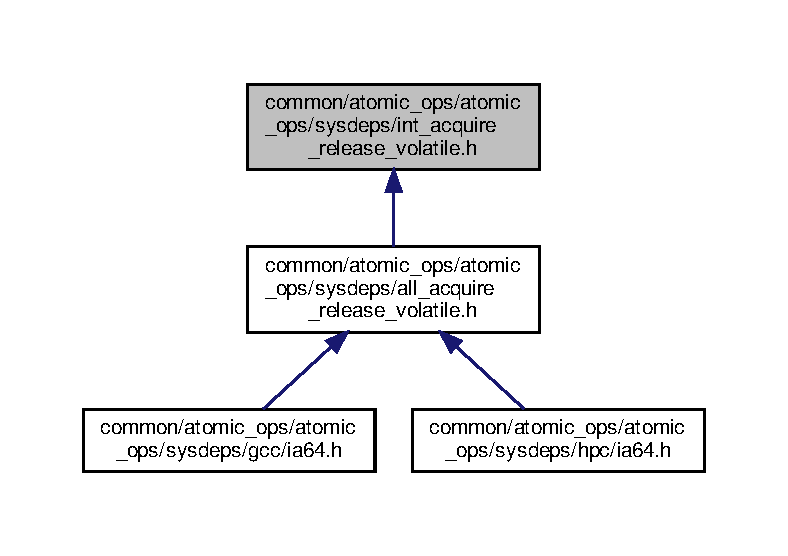
\includegraphics[width=350pt]{int__acquire__release__volatile_8h__dep__incl}
\end{center}
\end{figure}
\subsection*{Macros}
\begin{DoxyCompactItemize}
\item 
\#define \hyperlink{int__acquire__release__volatile_8h_a4b3b5ac83b6c7730e8376c8b5c0a6f01}{A\+O\+\_\+\+G\+C\+C\+\_\+\+B\+A\+R\+R\+I\+ER}()
\item 
\#define \hyperlink{int__acquire__release__volatile_8h_a69ea9f3bbd65c9cd4b3e77fa9ea74c16}{A\+O\+\_\+\+H\+A\+V\+E\+\_\+int\+\_\+load\+\_\+acquire}
\item 
\#define \hyperlink{int__acquire__release__volatile_8h_a3b00caccb3035ae2fb224aa6a3c5cd55}{A\+O\+\_\+\+H\+A\+V\+E\+\_\+int\+\_\+store\+\_\+release}
\end{DoxyCompactItemize}
\subsection*{Functions}
\begin{DoxyCompactItemize}
\item 
\hyperlink{atomic__ops_8h_a9f6ab6253b6b11bc8c12efe9dde5db2b}{A\+O\+\_\+\+I\+N\+L\+I\+NE} unsigned int \hyperlink{int__acquire__release__volatile_8h_a5e355f5ce9305779de9c115623b56df0}{A\+O\+\_\+int\+\_\+load\+\_\+acquire} (const volatile unsigned int $\ast$p)
\item 
\hyperlink{atomic__ops_8h_a9f6ab6253b6b11bc8c12efe9dde5db2b}{A\+O\+\_\+\+I\+N\+L\+I\+NE} void \hyperlink{int__acquire__release__volatile_8h_a0ff53a911b2f6427eae5b0e16466e96c}{A\+O\+\_\+int\+\_\+store\+\_\+release} (volatile unsigned int $\ast$p, unsigned int val)
\end{DoxyCompactItemize}


\subsection{Macro Definition Documentation}
\mbox{\Hypertarget{int__acquire__release__volatile_8h_a4b3b5ac83b6c7730e8376c8b5c0a6f01}\label{int__acquire__release__volatile_8h_a4b3b5ac83b6c7730e8376c8b5c0a6f01}} 
\index{int\+\_\+acquire\+\_\+release\+\_\+volatile.\+h@{int\+\_\+acquire\+\_\+release\+\_\+volatile.\+h}!A\+O\+\_\+\+G\+C\+C\+\_\+\+B\+A\+R\+R\+I\+ER@{A\+O\+\_\+\+G\+C\+C\+\_\+\+B\+A\+R\+R\+I\+ER}}
\index{A\+O\+\_\+\+G\+C\+C\+\_\+\+B\+A\+R\+R\+I\+ER@{A\+O\+\_\+\+G\+C\+C\+\_\+\+B\+A\+R\+R\+I\+ER}!int\+\_\+acquire\+\_\+release\+\_\+volatile.\+h@{int\+\_\+acquire\+\_\+release\+\_\+volatile.\+h}}
\subsubsection{\texorpdfstring{A\+O\+\_\+\+G\+C\+C\+\_\+\+B\+A\+R\+R\+I\+ER}{AO\_GCC\_BARRIER}}
{\footnotesize\ttfamily \#define A\+O\+\_\+\+G\+C\+C\+\_\+\+B\+A\+R\+R\+I\+ER(\begin{DoxyParamCaption}{ }\end{DoxyParamCaption})}

\mbox{\Hypertarget{int__acquire__release__volatile_8h_a69ea9f3bbd65c9cd4b3e77fa9ea74c16}\label{int__acquire__release__volatile_8h_a69ea9f3bbd65c9cd4b3e77fa9ea74c16}} 
\index{int\+\_\+acquire\+\_\+release\+\_\+volatile.\+h@{int\+\_\+acquire\+\_\+release\+\_\+volatile.\+h}!A\+O\+\_\+\+H\+A\+V\+E\+\_\+int\+\_\+load\+\_\+acquire@{A\+O\+\_\+\+H\+A\+V\+E\+\_\+int\+\_\+load\+\_\+acquire}}
\index{A\+O\+\_\+\+H\+A\+V\+E\+\_\+int\+\_\+load\+\_\+acquire@{A\+O\+\_\+\+H\+A\+V\+E\+\_\+int\+\_\+load\+\_\+acquire}!int\+\_\+acquire\+\_\+release\+\_\+volatile.\+h@{int\+\_\+acquire\+\_\+release\+\_\+volatile.\+h}}
\subsubsection{\texorpdfstring{A\+O\+\_\+\+H\+A\+V\+E\+\_\+int\+\_\+load\+\_\+acquire}{AO\_HAVE\_int\_load\_acquire}}
{\footnotesize\ttfamily \#define A\+O\+\_\+\+H\+A\+V\+E\+\_\+int\+\_\+load\+\_\+acquire}

\mbox{\Hypertarget{int__acquire__release__volatile_8h_a3b00caccb3035ae2fb224aa6a3c5cd55}\label{int__acquire__release__volatile_8h_a3b00caccb3035ae2fb224aa6a3c5cd55}} 
\index{int\+\_\+acquire\+\_\+release\+\_\+volatile.\+h@{int\+\_\+acquire\+\_\+release\+\_\+volatile.\+h}!A\+O\+\_\+\+H\+A\+V\+E\+\_\+int\+\_\+store\+\_\+release@{A\+O\+\_\+\+H\+A\+V\+E\+\_\+int\+\_\+store\+\_\+release}}
\index{A\+O\+\_\+\+H\+A\+V\+E\+\_\+int\+\_\+store\+\_\+release@{A\+O\+\_\+\+H\+A\+V\+E\+\_\+int\+\_\+store\+\_\+release}!int\+\_\+acquire\+\_\+release\+\_\+volatile.\+h@{int\+\_\+acquire\+\_\+release\+\_\+volatile.\+h}}
\subsubsection{\texorpdfstring{A\+O\+\_\+\+H\+A\+V\+E\+\_\+int\+\_\+store\+\_\+release}{AO\_HAVE\_int\_store\_release}}
{\footnotesize\ttfamily \#define A\+O\+\_\+\+H\+A\+V\+E\+\_\+int\+\_\+store\+\_\+release}



\subsection{Function Documentation}
\mbox{\Hypertarget{int__acquire__release__volatile_8h_a5e355f5ce9305779de9c115623b56df0}\label{int__acquire__release__volatile_8h_a5e355f5ce9305779de9c115623b56df0}} 
\index{int\+\_\+acquire\+\_\+release\+\_\+volatile.\+h@{int\+\_\+acquire\+\_\+release\+\_\+volatile.\+h}!A\+O\+\_\+int\+\_\+load\+\_\+acquire@{A\+O\+\_\+int\+\_\+load\+\_\+acquire}}
\index{A\+O\+\_\+int\+\_\+load\+\_\+acquire@{A\+O\+\_\+int\+\_\+load\+\_\+acquire}!int\+\_\+acquire\+\_\+release\+\_\+volatile.\+h@{int\+\_\+acquire\+\_\+release\+\_\+volatile.\+h}}
\subsubsection{\texorpdfstring{A\+O\+\_\+int\+\_\+load\+\_\+acquire()}{AO\_int\_load\_acquire()}}
{\footnotesize\ttfamily \hyperlink{atomic__ops_8h_a9f6ab6253b6b11bc8c12efe9dde5db2b}{A\+O\+\_\+\+I\+N\+L\+I\+NE} unsigned int A\+O\+\_\+int\+\_\+load\+\_\+acquire (\begin{DoxyParamCaption}\item[{const volatile unsigned int $\ast$}]{p }\end{DoxyParamCaption})}

\mbox{\Hypertarget{int__acquire__release__volatile_8h_a0ff53a911b2f6427eae5b0e16466e96c}\label{int__acquire__release__volatile_8h_a0ff53a911b2f6427eae5b0e16466e96c}} 
\index{int\+\_\+acquire\+\_\+release\+\_\+volatile.\+h@{int\+\_\+acquire\+\_\+release\+\_\+volatile.\+h}!A\+O\+\_\+int\+\_\+store\+\_\+release@{A\+O\+\_\+int\+\_\+store\+\_\+release}}
\index{A\+O\+\_\+int\+\_\+store\+\_\+release@{A\+O\+\_\+int\+\_\+store\+\_\+release}!int\+\_\+acquire\+\_\+release\+\_\+volatile.\+h@{int\+\_\+acquire\+\_\+release\+\_\+volatile.\+h}}
\subsubsection{\texorpdfstring{A\+O\+\_\+int\+\_\+store\+\_\+release()}{AO\_int\_store\_release()}}
{\footnotesize\ttfamily \hyperlink{atomic__ops_8h_a9f6ab6253b6b11bc8c12efe9dde5db2b}{A\+O\+\_\+\+I\+N\+L\+I\+NE} void A\+O\+\_\+int\+\_\+store\+\_\+release (\begin{DoxyParamCaption}\item[{volatile unsigned int $\ast$}]{p,  }\item[{unsigned int}]{val }\end{DoxyParamCaption})}


\hypertarget{int__aligned__atomic__load__store_8h}{}\section{common/atomic\+\_\+ops/atomic\+\_\+ops/sysdeps/int\+\_\+aligned\+\_\+atomic\+\_\+load\+\_\+store.h File Reference}
\label{int__aligned__atomic__load__store_8h}\index{common/atomic\+\_\+ops/atomic\+\_\+ops/sysdeps/int\+\_\+aligned\+\_\+atomic\+\_\+load\+\_\+store.\+h@{common/atomic\+\_\+ops/atomic\+\_\+ops/sysdeps/int\+\_\+aligned\+\_\+atomic\+\_\+load\+\_\+store.\+h}}
This graph shows which files directly or indirectly include this file\+:
\nopagebreak
\begin{figure}[H]
\begin{center}
\leavevmode
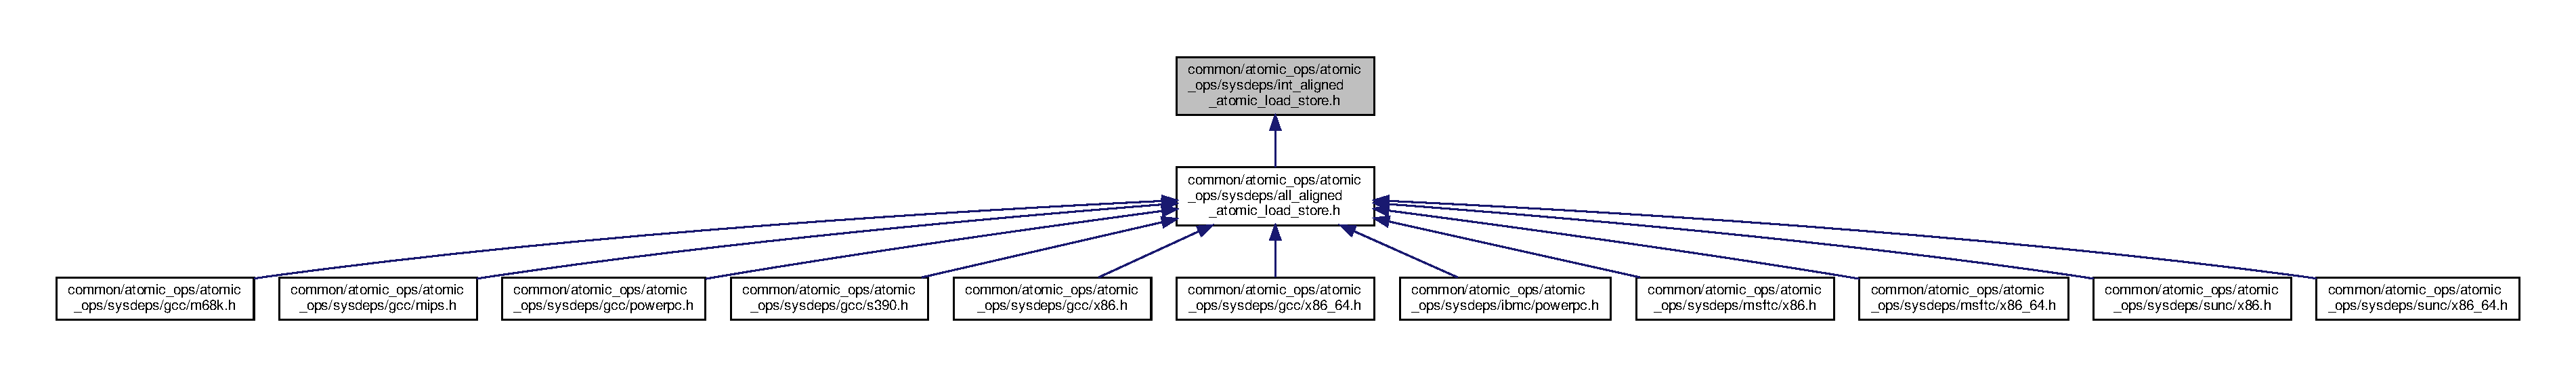
\includegraphics[width=350pt]{int__aligned__atomic__load__store_8h__dep__incl}
\end{center}
\end{figure}
\subsection*{Macros}
\begin{DoxyCompactItemize}
\item 
\#define \hyperlink{int__aligned__atomic__load__store_8h_afbc049e8874ff35734f252c3a61cb179}{A\+O\+\_\+\+H\+A\+V\+E\+\_\+int\+\_\+load}
\item 
\#define \hyperlink{int__aligned__atomic__load__store_8h_a0fb74d735334aa73a3d764bf31a1197c}{A\+O\+\_\+\+H\+A\+V\+E\+\_\+int\+\_\+store}
\end{DoxyCompactItemize}
\subsection*{Functions}
\begin{DoxyCompactItemize}
\item 
\hyperlink{atomic__ops_8h_a9f6ab6253b6b11bc8c12efe9dde5db2b}{A\+O\+\_\+\+I\+N\+L\+I\+NE} unsigned int \hyperlink{int__aligned__atomic__load__store_8h_a0c7afef32d1432c955ee0aa9972768d3}{A\+O\+\_\+int\+\_\+load} (const volatile unsigned int $\ast$addr)
\item 
\hyperlink{atomic__ops_8h_a9f6ab6253b6b11bc8c12efe9dde5db2b}{A\+O\+\_\+\+I\+N\+L\+I\+NE} void \hyperlink{int__aligned__atomic__load__store_8h_a63a1ab3c2e7356cd2c6356a11eab378d}{A\+O\+\_\+int\+\_\+store} (volatile unsigned int $\ast$addr, unsigned int new\+\_\+val)
\end{DoxyCompactItemize}


\subsection{Macro Definition Documentation}
\mbox{\Hypertarget{int__aligned__atomic__load__store_8h_afbc049e8874ff35734f252c3a61cb179}\label{int__aligned__atomic__load__store_8h_afbc049e8874ff35734f252c3a61cb179}} 
\index{int\+\_\+aligned\+\_\+atomic\+\_\+load\+\_\+store.\+h@{int\+\_\+aligned\+\_\+atomic\+\_\+load\+\_\+store.\+h}!A\+O\+\_\+\+H\+A\+V\+E\+\_\+int\+\_\+load@{A\+O\+\_\+\+H\+A\+V\+E\+\_\+int\+\_\+load}}
\index{A\+O\+\_\+\+H\+A\+V\+E\+\_\+int\+\_\+load@{A\+O\+\_\+\+H\+A\+V\+E\+\_\+int\+\_\+load}!int\+\_\+aligned\+\_\+atomic\+\_\+load\+\_\+store.\+h@{int\+\_\+aligned\+\_\+atomic\+\_\+load\+\_\+store.\+h}}
\subsubsection{\texorpdfstring{A\+O\+\_\+\+H\+A\+V\+E\+\_\+int\+\_\+load}{AO\_HAVE\_int\_load}}
{\footnotesize\ttfamily \#define A\+O\+\_\+\+H\+A\+V\+E\+\_\+int\+\_\+load}

\mbox{\Hypertarget{int__aligned__atomic__load__store_8h_a0fb74d735334aa73a3d764bf31a1197c}\label{int__aligned__atomic__load__store_8h_a0fb74d735334aa73a3d764bf31a1197c}} 
\index{int\+\_\+aligned\+\_\+atomic\+\_\+load\+\_\+store.\+h@{int\+\_\+aligned\+\_\+atomic\+\_\+load\+\_\+store.\+h}!A\+O\+\_\+\+H\+A\+V\+E\+\_\+int\+\_\+store@{A\+O\+\_\+\+H\+A\+V\+E\+\_\+int\+\_\+store}}
\index{A\+O\+\_\+\+H\+A\+V\+E\+\_\+int\+\_\+store@{A\+O\+\_\+\+H\+A\+V\+E\+\_\+int\+\_\+store}!int\+\_\+aligned\+\_\+atomic\+\_\+load\+\_\+store.\+h@{int\+\_\+aligned\+\_\+atomic\+\_\+load\+\_\+store.\+h}}
\subsubsection{\texorpdfstring{A\+O\+\_\+\+H\+A\+V\+E\+\_\+int\+\_\+store}{AO\_HAVE\_int\_store}}
{\footnotesize\ttfamily \#define A\+O\+\_\+\+H\+A\+V\+E\+\_\+int\+\_\+store}



\subsection{Function Documentation}
\mbox{\Hypertarget{int__aligned__atomic__load__store_8h_a0c7afef32d1432c955ee0aa9972768d3}\label{int__aligned__atomic__load__store_8h_a0c7afef32d1432c955ee0aa9972768d3}} 
\index{int\+\_\+aligned\+\_\+atomic\+\_\+load\+\_\+store.\+h@{int\+\_\+aligned\+\_\+atomic\+\_\+load\+\_\+store.\+h}!A\+O\+\_\+int\+\_\+load@{A\+O\+\_\+int\+\_\+load}}
\index{A\+O\+\_\+int\+\_\+load@{A\+O\+\_\+int\+\_\+load}!int\+\_\+aligned\+\_\+atomic\+\_\+load\+\_\+store.\+h@{int\+\_\+aligned\+\_\+atomic\+\_\+load\+\_\+store.\+h}}
\subsubsection{\texorpdfstring{A\+O\+\_\+int\+\_\+load()}{AO\_int\_load()}}
{\footnotesize\ttfamily \hyperlink{atomic__ops_8h_a9f6ab6253b6b11bc8c12efe9dde5db2b}{A\+O\+\_\+\+I\+N\+L\+I\+NE} unsigned int A\+O\+\_\+int\+\_\+load (\begin{DoxyParamCaption}\item[{const volatile unsigned int $\ast$}]{addr }\end{DoxyParamCaption})}

\mbox{\Hypertarget{int__aligned__atomic__load__store_8h_a63a1ab3c2e7356cd2c6356a11eab378d}\label{int__aligned__atomic__load__store_8h_a63a1ab3c2e7356cd2c6356a11eab378d}} 
\index{int\+\_\+aligned\+\_\+atomic\+\_\+load\+\_\+store.\+h@{int\+\_\+aligned\+\_\+atomic\+\_\+load\+\_\+store.\+h}!A\+O\+\_\+int\+\_\+store@{A\+O\+\_\+int\+\_\+store}}
\index{A\+O\+\_\+int\+\_\+store@{A\+O\+\_\+int\+\_\+store}!int\+\_\+aligned\+\_\+atomic\+\_\+load\+\_\+store.\+h@{int\+\_\+aligned\+\_\+atomic\+\_\+load\+\_\+store.\+h}}
\subsubsection{\texorpdfstring{A\+O\+\_\+int\+\_\+store()}{AO\_int\_store()}}
{\footnotesize\ttfamily \hyperlink{atomic__ops_8h_a9f6ab6253b6b11bc8c12efe9dde5db2b}{A\+O\+\_\+\+I\+N\+L\+I\+NE} void A\+O\+\_\+int\+\_\+store (\begin{DoxyParamCaption}\item[{volatile unsigned int $\ast$}]{addr,  }\item[{unsigned int}]{new\+\_\+val }\end{DoxyParamCaption})}


\hypertarget{int__atomic__load__store_8h}{}\section{common/atomic\+\_\+ops/atomic\+\_\+ops/sysdeps/int\+\_\+atomic\+\_\+load\+\_\+store.h File Reference}
\label{int__atomic__load__store_8h}\index{common/atomic\+\_\+ops/atomic\+\_\+ops/sysdeps/int\+\_\+atomic\+\_\+load\+\_\+store.\+h@{common/atomic\+\_\+ops/atomic\+\_\+ops/sysdeps/int\+\_\+atomic\+\_\+load\+\_\+store.\+h}}
This graph shows which files directly or indirectly include this file\+:
\nopagebreak
\begin{figure}[H]
\begin{center}
\leavevmode
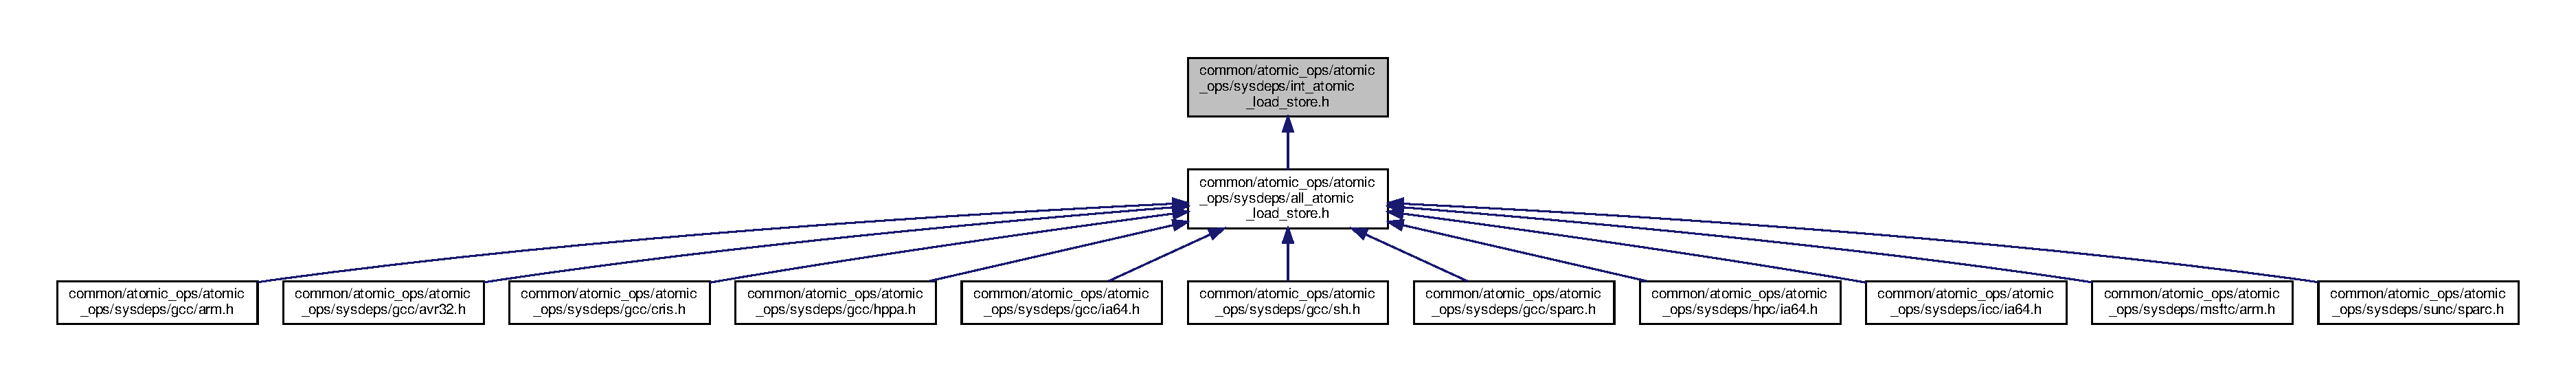
\includegraphics[width=350pt]{int__atomic__load__store_8h__dep__incl}
\end{center}
\end{figure}
\subsection*{Macros}
\begin{DoxyCompactItemize}
\item 
\#define \hyperlink{int__atomic__load__store_8h_afbc049e8874ff35734f252c3a61cb179}{A\+O\+\_\+\+H\+A\+V\+E\+\_\+int\+\_\+load}
\item 
\#define \hyperlink{int__atomic__load__store_8h_a0fb74d735334aa73a3d764bf31a1197c}{A\+O\+\_\+\+H\+A\+V\+E\+\_\+int\+\_\+store}
\end{DoxyCompactItemize}
\subsection*{Functions}
\begin{DoxyCompactItemize}
\item 
\hyperlink{atomic__ops_8h_a9f6ab6253b6b11bc8c12efe9dde5db2b}{A\+O\+\_\+\+I\+N\+L\+I\+NE} unsigned int \hyperlink{int__atomic__load__store_8h_a0c7afef32d1432c955ee0aa9972768d3}{A\+O\+\_\+int\+\_\+load} (const volatile unsigned int $\ast$addr)
\item 
\hyperlink{atomic__ops_8h_a9f6ab6253b6b11bc8c12efe9dde5db2b}{A\+O\+\_\+\+I\+N\+L\+I\+NE} void \hyperlink{int__atomic__load__store_8h_a63a1ab3c2e7356cd2c6356a11eab378d}{A\+O\+\_\+int\+\_\+store} (volatile unsigned int $\ast$addr, unsigned int new\+\_\+val)
\end{DoxyCompactItemize}


\subsection{Macro Definition Documentation}
\mbox{\Hypertarget{int__atomic__load__store_8h_afbc049e8874ff35734f252c3a61cb179}\label{int__atomic__load__store_8h_afbc049e8874ff35734f252c3a61cb179}} 
\index{int\+\_\+atomic\+\_\+load\+\_\+store.\+h@{int\+\_\+atomic\+\_\+load\+\_\+store.\+h}!A\+O\+\_\+\+H\+A\+V\+E\+\_\+int\+\_\+load@{A\+O\+\_\+\+H\+A\+V\+E\+\_\+int\+\_\+load}}
\index{A\+O\+\_\+\+H\+A\+V\+E\+\_\+int\+\_\+load@{A\+O\+\_\+\+H\+A\+V\+E\+\_\+int\+\_\+load}!int\+\_\+atomic\+\_\+load\+\_\+store.\+h@{int\+\_\+atomic\+\_\+load\+\_\+store.\+h}}
\subsubsection{\texorpdfstring{A\+O\+\_\+\+H\+A\+V\+E\+\_\+int\+\_\+load}{AO\_HAVE\_int\_load}}
{\footnotesize\ttfamily \#define A\+O\+\_\+\+H\+A\+V\+E\+\_\+int\+\_\+load}

\mbox{\Hypertarget{int__atomic__load__store_8h_a0fb74d735334aa73a3d764bf31a1197c}\label{int__atomic__load__store_8h_a0fb74d735334aa73a3d764bf31a1197c}} 
\index{int\+\_\+atomic\+\_\+load\+\_\+store.\+h@{int\+\_\+atomic\+\_\+load\+\_\+store.\+h}!A\+O\+\_\+\+H\+A\+V\+E\+\_\+int\+\_\+store@{A\+O\+\_\+\+H\+A\+V\+E\+\_\+int\+\_\+store}}
\index{A\+O\+\_\+\+H\+A\+V\+E\+\_\+int\+\_\+store@{A\+O\+\_\+\+H\+A\+V\+E\+\_\+int\+\_\+store}!int\+\_\+atomic\+\_\+load\+\_\+store.\+h@{int\+\_\+atomic\+\_\+load\+\_\+store.\+h}}
\subsubsection{\texorpdfstring{A\+O\+\_\+\+H\+A\+V\+E\+\_\+int\+\_\+store}{AO\_HAVE\_int\_store}}
{\footnotesize\ttfamily \#define A\+O\+\_\+\+H\+A\+V\+E\+\_\+int\+\_\+store}



\subsection{Function Documentation}
\mbox{\Hypertarget{int__atomic__load__store_8h_a0c7afef32d1432c955ee0aa9972768d3}\label{int__atomic__load__store_8h_a0c7afef32d1432c955ee0aa9972768d3}} 
\index{int\+\_\+atomic\+\_\+load\+\_\+store.\+h@{int\+\_\+atomic\+\_\+load\+\_\+store.\+h}!A\+O\+\_\+int\+\_\+load@{A\+O\+\_\+int\+\_\+load}}
\index{A\+O\+\_\+int\+\_\+load@{A\+O\+\_\+int\+\_\+load}!int\+\_\+atomic\+\_\+load\+\_\+store.\+h@{int\+\_\+atomic\+\_\+load\+\_\+store.\+h}}
\subsubsection{\texorpdfstring{A\+O\+\_\+int\+\_\+load()}{AO\_int\_load()}}
{\footnotesize\ttfamily \hyperlink{atomic__ops_8h_a9f6ab6253b6b11bc8c12efe9dde5db2b}{A\+O\+\_\+\+I\+N\+L\+I\+NE} unsigned int A\+O\+\_\+int\+\_\+load (\begin{DoxyParamCaption}\item[{const volatile unsigned int $\ast$}]{addr }\end{DoxyParamCaption})}

\mbox{\Hypertarget{int__atomic__load__store_8h_a63a1ab3c2e7356cd2c6356a11eab378d}\label{int__atomic__load__store_8h_a63a1ab3c2e7356cd2c6356a11eab378d}} 
\index{int\+\_\+atomic\+\_\+load\+\_\+store.\+h@{int\+\_\+atomic\+\_\+load\+\_\+store.\+h}!A\+O\+\_\+int\+\_\+store@{A\+O\+\_\+int\+\_\+store}}
\index{A\+O\+\_\+int\+\_\+store@{A\+O\+\_\+int\+\_\+store}!int\+\_\+atomic\+\_\+load\+\_\+store.\+h@{int\+\_\+atomic\+\_\+load\+\_\+store.\+h}}
\subsubsection{\texorpdfstring{A\+O\+\_\+int\+\_\+store()}{AO\_int\_store()}}
{\footnotesize\ttfamily \hyperlink{atomic__ops_8h_a9f6ab6253b6b11bc8c12efe9dde5db2b}{A\+O\+\_\+\+I\+N\+L\+I\+NE} void A\+O\+\_\+int\+\_\+store (\begin{DoxyParamCaption}\item[{volatile unsigned int $\ast$}]{addr,  }\item[{unsigned int}]{new\+\_\+val }\end{DoxyParamCaption})}


\hypertarget{common32__defs_8h}{}\section{common/atomic\+\_\+ops/atomic\+\_\+ops/sysdeps/msftc/common32\+\_\+defs.h File Reference}
\label{common32__defs_8h}\index{common/atomic\+\_\+ops/atomic\+\_\+ops/sysdeps/msftc/common32\+\_\+defs.\+h@{common/atomic\+\_\+ops/atomic\+\_\+ops/sysdeps/msftc/common32\+\_\+defs.\+h}}
{\ttfamily \#include $<$windows.\+h$>$}\newline
Include dependency graph for common32\+\_\+defs.\+h\+:
\nopagebreak
\begin{figure}[H]
\begin{center}
\leavevmode
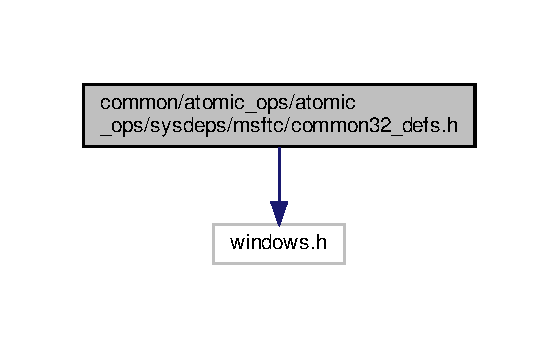
\includegraphics[width=268pt]{common32__defs_8h__incl}
\end{center}
\end{figure}
This graph shows which files directly or indirectly include this file\+:
\nopagebreak
\begin{figure}[H]
\begin{center}
\leavevmode
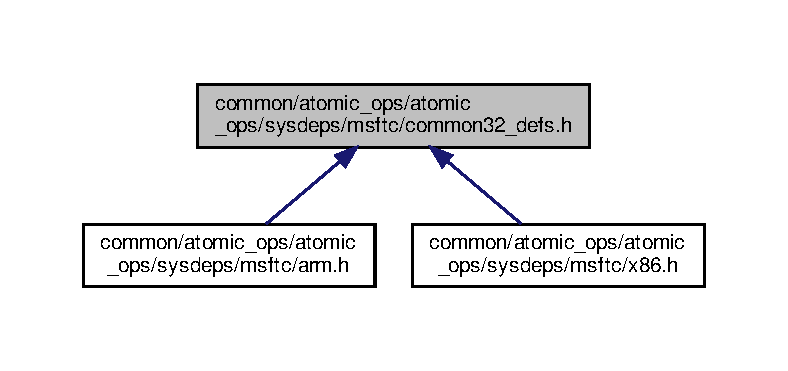
\includegraphics[width=350pt]{common32__defs_8h__dep__incl}
\end{center}
\end{figure}
\subsection*{Macros}
\begin{DoxyCompactItemize}
\item 
\#define \hyperlink{common32__defs_8h_aede901be38bc7e813b1873a5dea466a2}{\+\_\+\+Interlocked\+Increment}~Interlocked\+Increment
\item 
\#define \hyperlink{common32__defs_8h_abe2f273d81bbe28c84b15fc11f485f28}{\+\_\+\+Interlocked\+Decrement}~Interlocked\+Decrement
\item 
\#define \hyperlink{common32__defs_8h_ad7ea1cf0eac5d04fcd050930d8bbbba2}{\+\_\+\+Interlocked\+Exchange}~Interlocked\+Exchange
\item 
\#define \hyperlink{common32__defs_8h_afbc9fb70d9a90743170084753f2bf91a}{\+\_\+\+Interlocked\+Exchange\+Add}~Interlocked\+Exchange\+Add
\item 
\#define \hyperlink{common32__defs_8h_ab89709e42e35a421bf0e9c8bc49e4408}{\+\_\+\+Interlocked\+Compare\+Exchange}~Interlocked\+Compare\+Exchange
\item 
\#define \hyperlink{common32__defs_8h_a84d4fef5716c9fdaa8d8a6d980df2a0f}{A\+O\+\_\+\+I\+N\+T\+E\+R\+L\+O\+C\+K\+E\+D\+\_\+\+V\+O\+L\+A\+T\+I\+LE}
\item 
\#define \hyperlink{common32__defs_8h_a9fa0fc1a9eadcba085e57bf180a53cef}{A\+O\+\_\+\+H\+A\+V\+E\+\_\+fetch\+\_\+and\+\_\+add\+\_\+full}
\item 
\#define \hyperlink{common32__defs_8h_a65fb7f14069ffab2e6329ffc98563770}{A\+O\+\_\+\+H\+A\+V\+E\+\_\+fetch\+\_\+and\+\_\+add1\+\_\+full}
\item 
\#define \hyperlink{common32__defs_8h_a9c25ee9f67d96eec7f26152cf363fc06}{A\+O\+\_\+\+H\+A\+V\+E\+\_\+fetch\+\_\+and\+\_\+sub1\+\_\+full}
\end{DoxyCompactItemize}
\subsection*{Functions}
\begin{DoxyCompactItemize}
\item 
\hyperlink{atomic__ops_8h_a9f6ab6253b6b11bc8c12efe9dde5db2b}{A\+O\+\_\+\+I\+N\+L\+I\+NE} \hyperlink{atomic__ops_8h_a5225fef4d9eee821e82382cd269160dd}{A\+O\+\_\+t} \hyperlink{common32__defs_8h_a63b6d5232496fb679621fa985234eff8}{A\+O\+\_\+fetch\+\_\+and\+\_\+add\+\_\+full} (volatile \hyperlink{atomic__ops_8h_a5225fef4d9eee821e82382cd269160dd}{A\+O\+\_\+t} $\ast$p, \hyperlink{atomic__ops_8h_a5225fef4d9eee821e82382cd269160dd}{A\+O\+\_\+t} incr)
\item 
\hyperlink{atomic__ops_8h_a9f6ab6253b6b11bc8c12efe9dde5db2b}{A\+O\+\_\+\+I\+N\+L\+I\+NE} \hyperlink{atomic__ops_8h_a5225fef4d9eee821e82382cd269160dd}{A\+O\+\_\+t} \hyperlink{common32__defs_8h_a685167af2036f69b0cfcd31a141d79b0}{A\+O\+\_\+fetch\+\_\+and\+\_\+add1\+\_\+full} (volatile \hyperlink{atomic__ops_8h_a5225fef4d9eee821e82382cd269160dd}{A\+O\+\_\+t} $\ast$p)
\item 
\hyperlink{atomic__ops_8h_a9f6ab6253b6b11bc8c12efe9dde5db2b}{A\+O\+\_\+\+I\+N\+L\+I\+NE} \hyperlink{atomic__ops_8h_a5225fef4d9eee821e82382cd269160dd}{A\+O\+\_\+t} \hyperlink{common32__defs_8h_a204c40d27bb1d43b2f29b15a516ac7db}{A\+O\+\_\+fetch\+\_\+and\+\_\+sub1\+\_\+full} (volatile \hyperlink{atomic__ops_8h_a5225fef4d9eee821e82382cd269160dd}{A\+O\+\_\+t} $\ast$p)
\end{DoxyCompactItemize}


\subsection{Macro Definition Documentation}
\mbox{\Hypertarget{common32__defs_8h_ab89709e42e35a421bf0e9c8bc49e4408}\label{common32__defs_8h_ab89709e42e35a421bf0e9c8bc49e4408}} 
\index{common32\+\_\+defs.\+h@{common32\+\_\+defs.\+h}!\+\_\+\+Interlocked\+Compare\+Exchange@{\+\_\+\+Interlocked\+Compare\+Exchange}}
\index{\+\_\+\+Interlocked\+Compare\+Exchange@{\+\_\+\+Interlocked\+Compare\+Exchange}!common32\+\_\+defs.\+h@{common32\+\_\+defs.\+h}}
\subsubsection{\texorpdfstring{\+\_\+\+Interlocked\+Compare\+Exchange}{\_InterlockedCompareExchange}}
{\footnotesize\ttfamily \#define \+\_\+\+Interlocked\+Compare\+Exchange~Interlocked\+Compare\+Exchange}

\mbox{\Hypertarget{common32__defs_8h_abe2f273d81bbe28c84b15fc11f485f28}\label{common32__defs_8h_abe2f273d81bbe28c84b15fc11f485f28}} 
\index{common32\+\_\+defs.\+h@{common32\+\_\+defs.\+h}!\+\_\+\+Interlocked\+Decrement@{\+\_\+\+Interlocked\+Decrement}}
\index{\+\_\+\+Interlocked\+Decrement@{\+\_\+\+Interlocked\+Decrement}!common32\+\_\+defs.\+h@{common32\+\_\+defs.\+h}}
\subsubsection{\texorpdfstring{\+\_\+\+Interlocked\+Decrement}{\_InterlockedDecrement}}
{\footnotesize\ttfamily \#define \+\_\+\+Interlocked\+Decrement~Interlocked\+Decrement}

\mbox{\Hypertarget{common32__defs_8h_ad7ea1cf0eac5d04fcd050930d8bbbba2}\label{common32__defs_8h_ad7ea1cf0eac5d04fcd050930d8bbbba2}} 
\index{common32\+\_\+defs.\+h@{common32\+\_\+defs.\+h}!\+\_\+\+Interlocked\+Exchange@{\+\_\+\+Interlocked\+Exchange}}
\index{\+\_\+\+Interlocked\+Exchange@{\+\_\+\+Interlocked\+Exchange}!common32\+\_\+defs.\+h@{common32\+\_\+defs.\+h}}
\subsubsection{\texorpdfstring{\+\_\+\+Interlocked\+Exchange}{\_InterlockedExchange}}
{\footnotesize\ttfamily \#define \+\_\+\+Interlocked\+Exchange~Interlocked\+Exchange}

\mbox{\Hypertarget{common32__defs_8h_afbc9fb70d9a90743170084753f2bf91a}\label{common32__defs_8h_afbc9fb70d9a90743170084753f2bf91a}} 
\index{common32\+\_\+defs.\+h@{common32\+\_\+defs.\+h}!\+\_\+\+Interlocked\+Exchange\+Add@{\+\_\+\+Interlocked\+Exchange\+Add}}
\index{\+\_\+\+Interlocked\+Exchange\+Add@{\+\_\+\+Interlocked\+Exchange\+Add}!common32\+\_\+defs.\+h@{common32\+\_\+defs.\+h}}
\subsubsection{\texorpdfstring{\+\_\+\+Interlocked\+Exchange\+Add}{\_InterlockedExchangeAdd}}
{\footnotesize\ttfamily \#define \+\_\+\+Interlocked\+Exchange\+Add~Interlocked\+Exchange\+Add}

\mbox{\Hypertarget{common32__defs_8h_aede901be38bc7e813b1873a5dea466a2}\label{common32__defs_8h_aede901be38bc7e813b1873a5dea466a2}} 
\index{common32\+\_\+defs.\+h@{common32\+\_\+defs.\+h}!\+\_\+\+Interlocked\+Increment@{\+\_\+\+Interlocked\+Increment}}
\index{\+\_\+\+Interlocked\+Increment@{\+\_\+\+Interlocked\+Increment}!common32\+\_\+defs.\+h@{common32\+\_\+defs.\+h}}
\subsubsection{\texorpdfstring{\+\_\+\+Interlocked\+Increment}{\_InterlockedIncrement}}
{\footnotesize\ttfamily \#define \+\_\+\+Interlocked\+Increment~Interlocked\+Increment}

\mbox{\Hypertarget{common32__defs_8h_a65fb7f14069ffab2e6329ffc98563770}\label{common32__defs_8h_a65fb7f14069ffab2e6329ffc98563770}} 
\index{common32\+\_\+defs.\+h@{common32\+\_\+defs.\+h}!A\+O\+\_\+\+H\+A\+V\+E\+\_\+fetch\+\_\+and\+\_\+add1\+\_\+full@{A\+O\+\_\+\+H\+A\+V\+E\+\_\+fetch\+\_\+and\+\_\+add1\+\_\+full}}
\index{A\+O\+\_\+\+H\+A\+V\+E\+\_\+fetch\+\_\+and\+\_\+add1\+\_\+full@{A\+O\+\_\+\+H\+A\+V\+E\+\_\+fetch\+\_\+and\+\_\+add1\+\_\+full}!common32\+\_\+defs.\+h@{common32\+\_\+defs.\+h}}
\subsubsection{\texorpdfstring{A\+O\+\_\+\+H\+A\+V\+E\+\_\+fetch\+\_\+and\+\_\+add1\+\_\+full}{AO\_HAVE\_fetch\_and\_add1\_full}}
{\footnotesize\ttfamily \#define A\+O\+\_\+\+H\+A\+V\+E\+\_\+fetch\+\_\+and\+\_\+add1\+\_\+full}

\mbox{\Hypertarget{common32__defs_8h_a9fa0fc1a9eadcba085e57bf180a53cef}\label{common32__defs_8h_a9fa0fc1a9eadcba085e57bf180a53cef}} 
\index{common32\+\_\+defs.\+h@{common32\+\_\+defs.\+h}!A\+O\+\_\+\+H\+A\+V\+E\+\_\+fetch\+\_\+and\+\_\+add\+\_\+full@{A\+O\+\_\+\+H\+A\+V\+E\+\_\+fetch\+\_\+and\+\_\+add\+\_\+full}}
\index{A\+O\+\_\+\+H\+A\+V\+E\+\_\+fetch\+\_\+and\+\_\+add\+\_\+full@{A\+O\+\_\+\+H\+A\+V\+E\+\_\+fetch\+\_\+and\+\_\+add\+\_\+full}!common32\+\_\+defs.\+h@{common32\+\_\+defs.\+h}}
\subsubsection{\texorpdfstring{A\+O\+\_\+\+H\+A\+V\+E\+\_\+fetch\+\_\+and\+\_\+add\+\_\+full}{AO\_HAVE\_fetch\_and\_add\_full}}
{\footnotesize\ttfamily \#define A\+O\+\_\+\+H\+A\+V\+E\+\_\+fetch\+\_\+and\+\_\+add\+\_\+full}

\mbox{\Hypertarget{common32__defs_8h_a9c25ee9f67d96eec7f26152cf363fc06}\label{common32__defs_8h_a9c25ee9f67d96eec7f26152cf363fc06}} 
\index{common32\+\_\+defs.\+h@{common32\+\_\+defs.\+h}!A\+O\+\_\+\+H\+A\+V\+E\+\_\+fetch\+\_\+and\+\_\+sub1\+\_\+full@{A\+O\+\_\+\+H\+A\+V\+E\+\_\+fetch\+\_\+and\+\_\+sub1\+\_\+full}}
\index{A\+O\+\_\+\+H\+A\+V\+E\+\_\+fetch\+\_\+and\+\_\+sub1\+\_\+full@{A\+O\+\_\+\+H\+A\+V\+E\+\_\+fetch\+\_\+and\+\_\+sub1\+\_\+full}!common32\+\_\+defs.\+h@{common32\+\_\+defs.\+h}}
\subsubsection{\texorpdfstring{A\+O\+\_\+\+H\+A\+V\+E\+\_\+fetch\+\_\+and\+\_\+sub1\+\_\+full}{AO\_HAVE\_fetch\_and\_sub1\_full}}
{\footnotesize\ttfamily \#define A\+O\+\_\+\+H\+A\+V\+E\+\_\+fetch\+\_\+and\+\_\+sub1\+\_\+full}

\mbox{\Hypertarget{common32__defs_8h_a84d4fef5716c9fdaa8d8a6d980df2a0f}\label{common32__defs_8h_a84d4fef5716c9fdaa8d8a6d980df2a0f}} 
\index{common32\+\_\+defs.\+h@{common32\+\_\+defs.\+h}!A\+O\+\_\+\+I\+N\+T\+E\+R\+L\+O\+C\+K\+E\+D\+\_\+\+V\+O\+L\+A\+T\+I\+LE@{A\+O\+\_\+\+I\+N\+T\+E\+R\+L\+O\+C\+K\+E\+D\+\_\+\+V\+O\+L\+A\+T\+I\+LE}}
\index{A\+O\+\_\+\+I\+N\+T\+E\+R\+L\+O\+C\+K\+E\+D\+\_\+\+V\+O\+L\+A\+T\+I\+LE@{A\+O\+\_\+\+I\+N\+T\+E\+R\+L\+O\+C\+K\+E\+D\+\_\+\+V\+O\+L\+A\+T\+I\+LE}!common32\+\_\+defs.\+h@{common32\+\_\+defs.\+h}}
\subsubsection{\texorpdfstring{A\+O\+\_\+\+I\+N\+T\+E\+R\+L\+O\+C\+K\+E\+D\+\_\+\+V\+O\+L\+A\+T\+I\+LE}{AO\_INTERLOCKED\_VOLATILE}}
{\footnotesize\ttfamily \#define A\+O\+\_\+\+I\+N\+T\+E\+R\+L\+O\+C\+K\+E\+D\+\_\+\+V\+O\+L\+A\+T\+I\+LE}



\subsection{Function Documentation}
\mbox{\Hypertarget{common32__defs_8h_a685167af2036f69b0cfcd31a141d79b0}\label{common32__defs_8h_a685167af2036f69b0cfcd31a141d79b0}} 
\index{common32\+\_\+defs.\+h@{common32\+\_\+defs.\+h}!A\+O\+\_\+fetch\+\_\+and\+\_\+add1\+\_\+full@{A\+O\+\_\+fetch\+\_\+and\+\_\+add1\+\_\+full}}
\index{A\+O\+\_\+fetch\+\_\+and\+\_\+add1\+\_\+full@{A\+O\+\_\+fetch\+\_\+and\+\_\+add1\+\_\+full}!common32\+\_\+defs.\+h@{common32\+\_\+defs.\+h}}
\subsubsection{\texorpdfstring{A\+O\+\_\+fetch\+\_\+and\+\_\+add1\+\_\+full()}{AO\_fetch\_and\_add1\_full()}}
{\footnotesize\ttfamily \hyperlink{atomic__ops_8h_a9f6ab6253b6b11bc8c12efe9dde5db2b}{A\+O\+\_\+\+I\+N\+L\+I\+NE} \hyperlink{atomic__ops_8h_a5225fef4d9eee821e82382cd269160dd}{A\+O\+\_\+t} A\+O\+\_\+fetch\+\_\+and\+\_\+add1\+\_\+full (\begin{DoxyParamCaption}\item[{volatile \hyperlink{atomic__ops_8h_a5225fef4d9eee821e82382cd269160dd}{A\+O\+\_\+t} $\ast$}]{p }\end{DoxyParamCaption})}

\mbox{\Hypertarget{common32__defs_8h_a63b6d5232496fb679621fa985234eff8}\label{common32__defs_8h_a63b6d5232496fb679621fa985234eff8}} 
\index{common32\+\_\+defs.\+h@{common32\+\_\+defs.\+h}!A\+O\+\_\+fetch\+\_\+and\+\_\+add\+\_\+full@{A\+O\+\_\+fetch\+\_\+and\+\_\+add\+\_\+full}}
\index{A\+O\+\_\+fetch\+\_\+and\+\_\+add\+\_\+full@{A\+O\+\_\+fetch\+\_\+and\+\_\+add\+\_\+full}!common32\+\_\+defs.\+h@{common32\+\_\+defs.\+h}}
\subsubsection{\texorpdfstring{A\+O\+\_\+fetch\+\_\+and\+\_\+add\+\_\+full()}{AO\_fetch\_and\_add\_full()}}
{\footnotesize\ttfamily \hyperlink{atomic__ops_8h_a9f6ab6253b6b11bc8c12efe9dde5db2b}{A\+O\+\_\+\+I\+N\+L\+I\+NE} \hyperlink{atomic__ops_8h_a5225fef4d9eee821e82382cd269160dd}{A\+O\+\_\+t} A\+O\+\_\+fetch\+\_\+and\+\_\+add\+\_\+full (\begin{DoxyParamCaption}\item[{volatile \hyperlink{atomic__ops_8h_a5225fef4d9eee821e82382cd269160dd}{A\+O\+\_\+t} $\ast$}]{p,  }\item[{\hyperlink{atomic__ops_8h_a5225fef4d9eee821e82382cd269160dd}{A\+O\+\_\+t}}]{incr }\end{DoxyParamCaption})}

\mbox{\Hypertarget{common32__defs_8h_a204c40d27bb1d43b2f29b15a516ac7db}\label{common32__defs_8h_a204c40d27bb1d43b2f29b15a516ac7db}} 
\index{common32\+\_\+defs.\+h@{common32\+\_\+defs.\+h}!A\+O\+\_\+fetch\+\_\+and\+\_\+sub1\+\_\+full@{A\+O\+\_\+fetch\+\_\+and\+\_\+sub1\+\_\+full}}
\index{A\+O\+\_\+fetch\+\_\+and\+\_\+sub1\+\_\+full@{A\+O\+\_\+fetch\+\_\+and\+\_\+sub1\+\_\+full}!common32\+\_\+defs.\+h@{common32\+\_\+defs.\+h}}
\subsubsection{\texorpdfstring{A\+O\+\_\+fetch\+\_\+and\+\_\+sub1\+\_\+full()}{AO\_fetch\_and\_sub1\_full()}}
{\footnotesize\ttfamily \hyperlink{atomic__ops_8h_a9f6ab6253b6b11bc8c12efe9dde5db2b}{A\+O\+\_\+\+I\+N\+L\+I\+NE} \hyperlink{atomic__ops_8h_a5225fef4d9eee821e82382cd269160dd}{A\+O\+\_\+t} A\+O\+\_\+fetch\+\_\+and\+\_\+sub1\+\_\+full (\begin{DoxyParamCaption}\item[{volatile \hyperlink{atomic__ops_8h_a5225fef4d9eee821e82382cd269160dd}{A\+O\+\_\+t} $\ast$}]{p }\end{DoxyParamCaption})}


\hypertarget{ordered_8h}{}\section{common/atomic\+\_\+ops/atomic\+\_\+ops/sysdeps/ordered.h File Reference}
\label{ordered_8h}\index{common/atomic\+\_\+ops/atomic\+\_\+ops/sysdeps/ordered.\+h@{common/atomic\+\_\+ops/atomic\+\_\+ops/sysdeps/ordered.\+h}}
{\ttfamily \#include \char`\"{}ordered\+\_\+except\+\_\+wr.\+h\char`\"{}}\newline
Include dependency graph for ordered.\+h\+:
\nopagebreak
\begin{figure}[H]
\begin{center}
\leavevmode
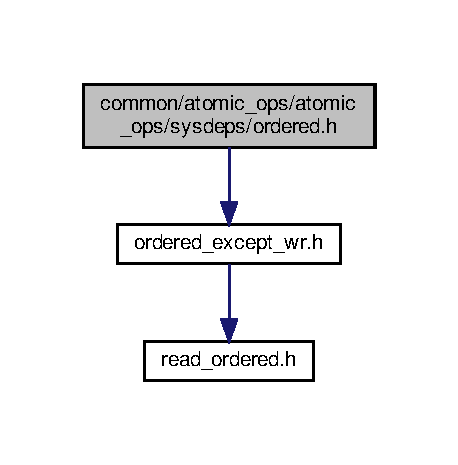
\includegraphics[width=220pt]{ordered_8h__incl}
\end{center}
\end{figure}
This graph shows which files directly or indirectly include this file\+:
\nopagebreak
\begin{figure}[H]
\begin{center}
\leavevmode
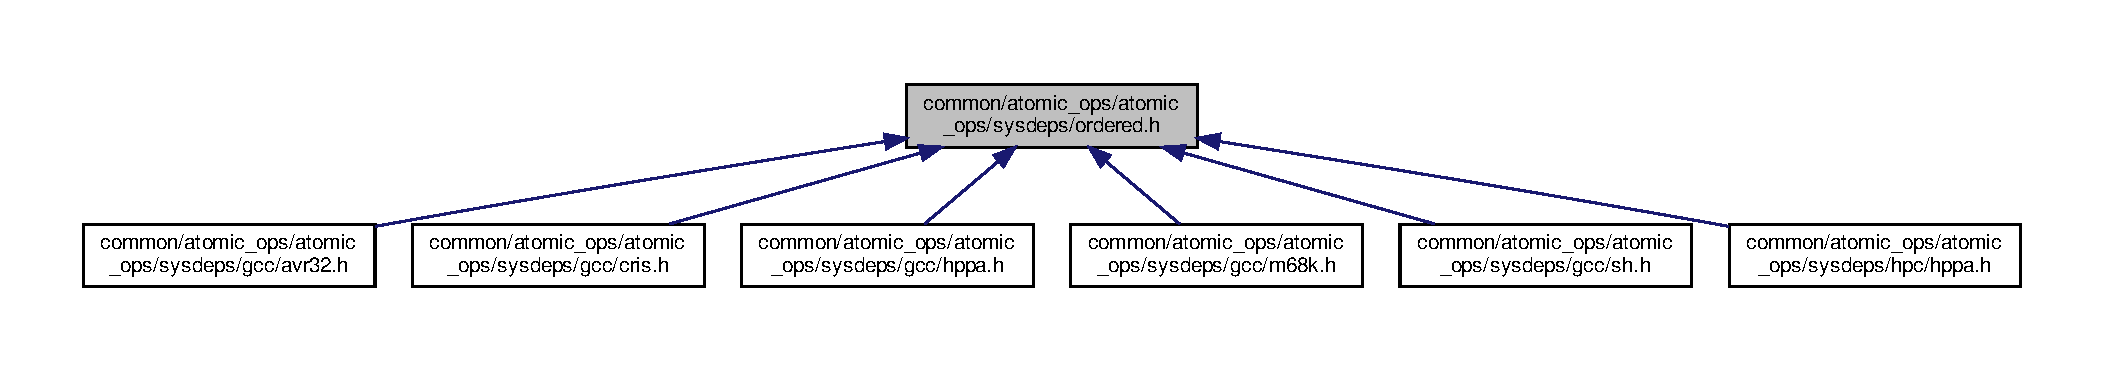
\includegraphics[width=350pt]{ordered_8h__dep__incl}
\end{center}
\end{figure}
\subsection*{Macros}
\begin{DoxyCompactItemize}
\item 
\#define \hyperlink{ordered_8h_a3904dc699d6a6d6e771a93aa66aeb805}{A\+O\+\_\+\+H\+A\+V\+E\+\_\+nop\+\_\+full}
\end{DoxyCompactItemize}
\subsection*{Functions}
\begin{DoxyCompactItemize}
\item 
\hyperlink{atomic__ops_8h_a9f6ab6253b6b11bc8c12efe9dde5db2b}{A\+O\+\_\+\+I\+N\+L\+I\+NE} void \hyperlink{ordered_8h_afe3a6778eacc82252ba138fc9a157b04}{A\+O\+\_\+nop\+\_\+full} (void)
\end{DoxyCompactItemize}


\subsection{Macro Definition Documentation}
\mbox{\Hypertarget{ordered_8h_a3904dc699d6a6d6e771a93aa66aeb805}\label{ordered_8h_a3904dc699d6a6d6e771a93aa66aeb805}} 
\index{ordered.\+h@{ordered.\+h}!A\+O\+\_\+\+H\+A\+V\+E\+\_\+nop\+\_\+full@{A\+O\+\_\+\+H\+A\+V\+E\+\_\+nop\+\_\+full}}
\index{A\+O\+\_\+\+H\+A\+V\+E\+\_\+nop\+\_\+full@{A\+O\+\_\+\+H\+A\+V\+E\+\_\+nop\+\_\+full}!ordered.\+h@{ordered.\+h}}
\subsubsection{\texorpdfstring{A\+O\+\_\+\+H\+A\+V\+E\+\_\+nop\+\_\+full}{AO\_HAVE\_nop\_full}}
{\footnotesize\ttfamily \#define A\+O\+\_\+\+H\+A\+V\+E\+\_\+nop\+\_\+full}



\subsection{Function Documentation}
\mbox{\Hypertarget{ordered_8h_afe3a6778eacc82252ba138fc9a157b04}\label{ordered_8h_afe3a6778eacc82252ba138fc9a157b04}} 
\index{ordered.\+h@{ordered.\+h}!A\+O\+\_\+nop\+\_\+full@{A\+O\+\_\+nop\+\_\+full}}
\index{A\+O\+\_\+nop\+\_\+full@{A\+O\+\_\+nop\+\_\+full}!ordered.\+h@{ordered.\+h}}
\subsubsection{\texorpdfstring{A\+O\+\_\+nop\+\_\+full()}{AO\_nop\_full()}}
{\footnotesize\ttfamily \hyperlink{atomic__ops_8h_a9f6ab6253b6b11bc8c12efe9dde5db2b}{A\+O\+\_\+\+I\+N\+L\+I\+NE} void A\+O\+\_\+nop\+\_\+full (\begin{DoxyParamCaption}\item[{void}]{ }\end{DoxyParamCaption})}


\hypertarget{ordered__except__wr_8h}{}\section{common/atomic\+\_\+ops/atomic\+\_\+ops/sysdeps/ordered\+\_\+except\+\_\+wr.h File Reference}
\label{ordered__except__wr_8h}\index{common/atomic\+\_\+ops/atomic\+\_\+ops/sysdeps/ordered\+\_\+except\+\_\+wr.\+h@{common/atomic\+\_\+ops/atomic\+\_\+ops/sysdeps/ordered\+\_\+except\+\_\+wr.\+h}}
{\ttfamily \#include \char`\"{}read\+\_\+ordered.\+h\char`\"{}}\newline
Include dependency graph for ordered\+\_\+except\+\_\+wr.\+h\+:
\nopagebreak
\begin{figure}[H]
\begin{center}
\leavevmode
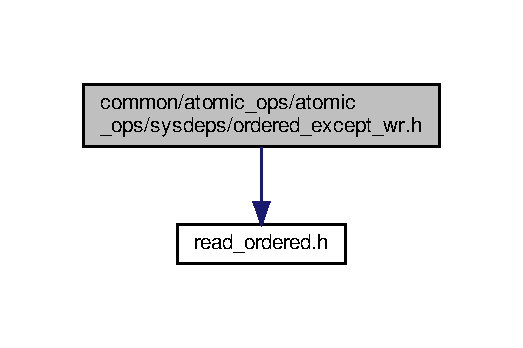
\includegraphics[width=251pt]{ordered__except__wr_8h__incl}
\end{center}
\end{figure}
This graph shows which files directly or indirectly include this file\+:
\nopagebreak
\begin{figure}[H]
\begin{center}
\leavevmode
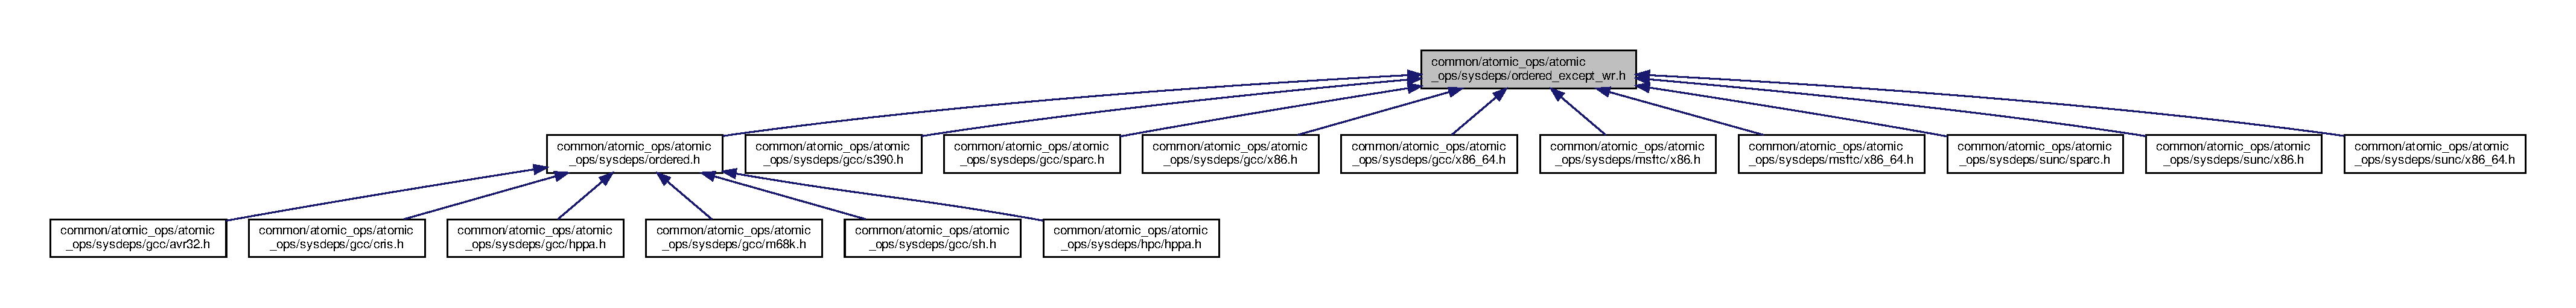
\includegraphics[width=350pt]{ordered__except__wr_8h__dep__incl}
\end{center}
\end{figure}
\subsection*{Macros}
\begin{DoxyCompactItemize}
\item 
\#define \hyperlink{ordered__except__wr_8h_a363f631e9397292c7f5e1d7254637493}{A\+O\+\_\+\+H\+A\+V\+E\+\_\+\+N\+O\+P\+\_\+\+W\+R\+I\+TE}
\end{DoxyCompactItemize}
\subsection*{Functions}
\begin{DoxyCompactItemize}
\item 
\hyperlink{atomic__ops_8h_a9f6ab6253b6b11bc8c12efe9dde5db2b}{A\+O\+\_\+\+I\+N\+L\+I\+NE} void \hyperlink{ordered__except__wr_8h_a4a8d4664cca4161a554167b152c66772}{A\+O\+\_\+nop\+\_\+write} (void)
\end{DoxyCompactItemize}


\subsection{Macro Definition Documentation}
\mbox{\Hypertarget{ordered__except__wr_8h_a363f631e9397292c7f5e1d7254637493}\label{ordered__except__wr_8h_a363f631e9397292c7f5e1d7254637493}} 
\index{ordered\+\_\+except\+\_\+wr.\+h@{ordered\+\_\+except\+\_\+wr.\+h}!A\+O\+\_\+\+H\+A\+V\+E\+\_\+\+N\+O\+P\+\_\+\+W\+R\+I\+TE@{A\+O\+\_\+\+H\+A\+V\+E\+\_\+\+N\+O\+P\+\_\+\+W\+R\+I\+TE}}
\index{A\+O\+\_\+\+H\+A\+V\+E\+\_\+\+N\+O\+P\+\_\+\+W\+R\+I\+TE@{A\+O\+\_\+\+H\+A\+V\+E\+\_\+\+N\+O\+P\+\_\+\+W\+R\+I\+TE}!ordered\+\_\+except\+\_\+wr.\+h@{ordered\+\_\+except\+\_\+wr.\+h}}
\subsubsection{\texorpdfstring{A\+O\+\_\+\+H\+A\+V\+E\+\_\+\+N\+O\+P\+\_\+\+W\+R\+I\+TE}{AO\_HAVE\_NOP\_WRITE}}
{\footnotesize\ttfamily \#define A\+O\+\_\+\+H\+A\+V\+E\+\_\+\+N\+O\+P\+\_\+\+W\+R\+I\+TE}



\subsection{Function Documentation}
\mbox{\Hypertarget{ordered__except__wr_8h_a4a8d4664cca4161a554167b152c66772}\label{ordered__except__wr_8h_a4a8d4664cca4161a554167b152c66772}} 
\index{ordered\+\_\+except\+\_\+wr.\+h@{ordered\+\_\+except\+\_\+wr.\+h}!A\+O\+\_\+nop\+\_\+write@{A\+O\+\_\+nop\+\_\+write}}
\index{A\+O\+\_\+nop\+\_\+write@{A\+O\+\_\+nop\+\_\+write}!ordered\+\_\+except\+\_\+wr.\+h@{ordered\+\_\+except\+\_\+wr.\+h}}
\subsubsection{\texorpdfstring{A\+O\+\_\+nop\+\_\+write()}{AO\_nop\_write()}}
{\footnotesize\ttfamily \hyperlink{atomic__ops_8h_a9f6ab6253b6b11bc8c12efe9dde5db2b}{A\+O\+\_\+\+I\+N\+L\+I\+NE} void A\+O\+\_\+nop\+\_\+write (\begin{DoxyParamCaption}\item[{void}]{ }\end{DoxyParamCaption})}


\hypertarget{read__ordered_8h}{}\section{common/atomic\+\_\+ops/atomic\+\_\+ops/sysdeps/read\+\_\+ordered.h File Reference}
\label{read__ordered_8h}\index{common/atomic\+\_\+ops/atomic\+\_\+ops/sysdeps/read\+\_\+ordered.\+h@{common/atomic\+\_\+ops/atomic\+\_\+ops/sysdeps/read\+\_\+ordered.\+h}}
This graph shows which files directly or indirectly include this file\+:
\nopagebreak
\begin{figure}[H]
\begin{center}
\leavevmode
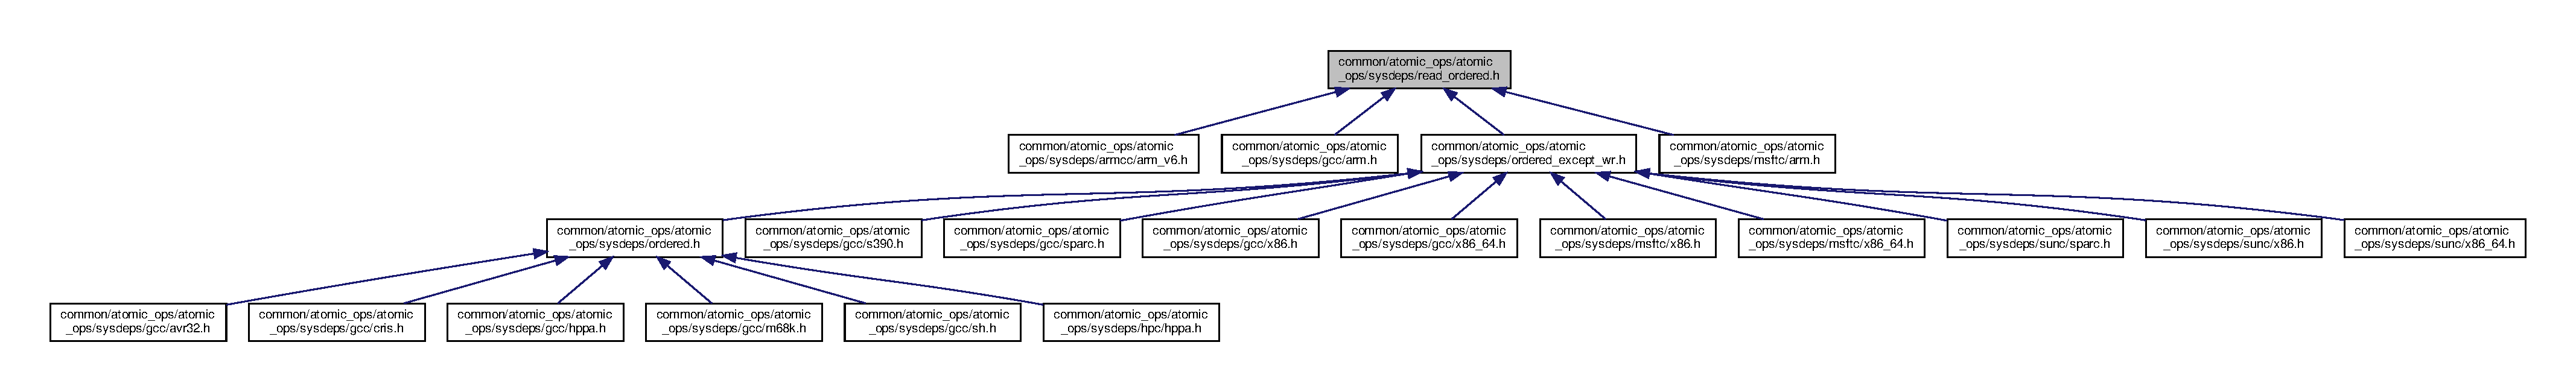
\includegraphics[width=350pt]{read__ordered_8h__dep__incl}
\end{center}
\end{figure}
\subsection*{Macros}
\begin{DoxyCompactItemize}
\item 
\#define \hyperlink{read__ordered_8h_a6eb800ea4ef06ed7a62029f0fffe9aa3}{A\+O\+\_\+\+H\+A\+V\+E\+\_\+\+N\+O\+P\+\_\+\+R\+E\+AD}
\end{DoxyCompactItemize}
\subsection*{Functions}
\begin{DoxyCompactItemize}
\item 
\hyperlink{atomic__ops_8h_a9f6ab6253b6b11bc8c12efe9dde5db2b}{A\+O\+\_\+\+I\+N\+L\+I\+NE} void \hyperlink{read__ordered_8h_ab975a4e19a839d001c236b7e1fc0baec}{A\+O\+\_\+nop\+\_\+read} (void)
\end{DoxyCompactItemize}


\subsection{Macro Definition Documentation}
\mbox{\Hypertarget{read__ordered_8h_a6eb800ea4ef06ed7a62029f0fffe9aa3}\label{read__ordered_8h_a6eb800ea4ef06ed7a62029f0fffe9aa3}} 
\index{read\+\_\+ordered.\+h@{read\+\_\+ordered.\+h}!A\+O\+\_\+\+H\+A\+V\+E\+\_\+\+N\+O\+P\+\_\+\+R\+E\+AD@{A\+O\+\_\+\+H\+A\+V\+E\+\_\+\+N\+O\+P\+\_\+\+R\+E\+AD}}
\index{A\+O\+\_\+\+H\+A\+V\+E\+\_\+\+N\+O\+P\+\_\+\+R\+E\+AD@{A\+O\+\_\+\+H\+A\+V\+E\+\_\+\+N\+O\+P\+\_\+\+R\+E\+AD}!read\+\_\+ordered.\+h@{read\+\_\+ordered.\+h}}
\subsubsection{\texorpdfstring{A\+O\+\_\+\+H\+A\+V\+E\+\_\+\+N\+O\+P\+\_\+\+R\+E\+AD}{AO\_HAVE\_NOP\_READ}}
{\footnotesize\ttfamily \#define A\+O\+\_\+\+H\+A\+V\+E\+\_\+\+N\+O\+P\+\_\+\+R\+E\+AD}



\subsection{Function Documentation}
\mbox{\Hypertarget{read__ordered_8h_ab975a4e19a839d001c236b7e1fc0baec}\label{read__ordered_8h_ab975a4e19a839d001c236b7e1fc0baec}} 
\index{read\+\_\+ordered.\+h@{read\+\_\+ordered.\+h}!A\+O\+\_\+nop\+\_\+read@{A\+O\+\_\+nop\+\_\+read}}
\index{A\+O\+\_\+nop\+\_\+read@{A\+O\+\_\+nop\+\_\+read}!read\+\_\+ordered.\+h@{read\+\_\+ordered.\+h}}
\subsubsection{\texorpdfstring{A\+O\+\_\+nop\+\_\+read()}{AO\_nop\_read()}}
{\footnotesize\ttfamily \hyperlink{atomic__ops_8h_a9f6ab6253b6b11bc8c12efe9dde5db2b}{A\+O\+\_\+\+I\+N\+L\+I\+NE} void A\+O\+\_\+nop\+\_\+read (\begin{DoxyParamCaption}\item[{void}]{ }\end{DoxyParamCaption})}


\hypertarget{short__acquire__release__volatile_8h}{}\section{common/atomic\+\_\+ops/atomic\+\_\+ops/sysdeps/short\+\_\+acquire\+\_\+release\+\_\+volatile.h File Reference}
\label{short__acquire__release__volatile_8h}\index{common/atomic\+\_\+ops/atomic\+\_\+ops/sysdeps/short\+\_\+acquire\+\_\+release\+\_\+volatile.\+h@{common/atomic\+\_\+ops/atomic\+\_\+ops/sysdeps/short\+\_\+acquire\+\_\+release\+\_\+volatile.\+h}}
This graph shows which files directly or indirectly include this file\+:
\nopagebreak
\begin{figure}[H]
\begin{center}
\leavevmode
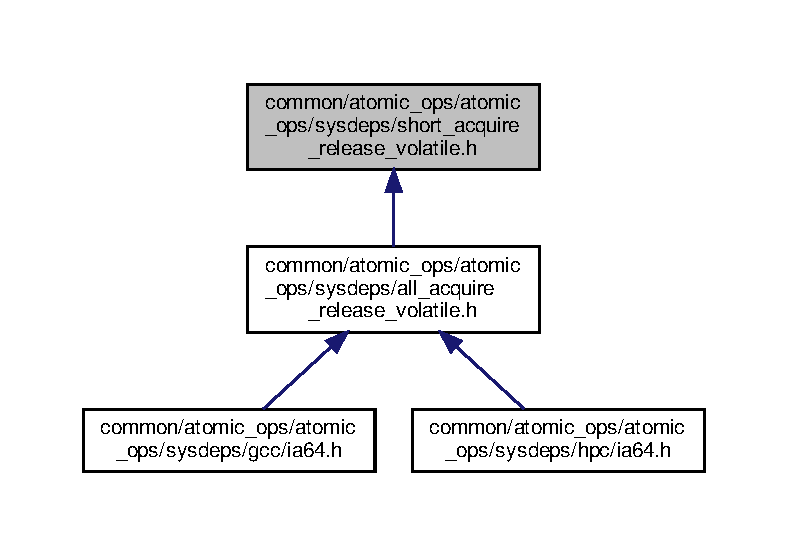
\includegraphics[width=350pt]{short__acquire__release__volatile_8h__dep__incl}
\end{center}
\end{figure}
\subsection*{Macros}
\begin{DoxyCompactItemize}
\item 
\#define \hyperlink{short__acquire__release__volatile_8h_a4b3b5ac83b6c7730e8376c8b5c0a6f01}{A\+O\+\_\+\+G\+C\+C\+\_\+\+B\+A\+R\+R\+I\+ER}()
\item 
\#define \hyperlink{short__acquire__release__volatile_8h_a9209b99f2e5b1cccf1fa23deef59cfd2}{A\+O\+\_\+\+H\+A\+V\+E\+\_\+short\+\_\+load\+\_\+acquire}
\item 
\#define \hyperlink{short__acquire__release__volatile_8h_a52488f4b445ced04c93c67f27a964a78}{A\+O\+\_\+\+H\+A\+V\+E\+\_\+short\+\_\+store\+\_\+release}
\end{DoxyCompactItemize}
\subsection*{Functions}
\begin{DoxyCompactItemize}
\item 
\hyperlink{atomic__ops_8h_a9f6ab6253b6b11bc8c12efe9dde5db2b}{A\+O\+\_\+\+I\+N\+L\+I\+NE} unsigned short \hyperlink{short__acquire__release__volatile_8h_a49e443244890f74b2d3cdd40264656c6}{A\+O\+\_\+short\+\_\+load\+\_\+acquire} (const volatile unsigned short $\ast$p)
\item 
\hyperlink{atomic__ops_8h_a9f6ab6253b6b11bc8c12efe9dde5db2b}{A\+O\+\_\+\+I\+N\+L\+I\+NE} void \hyperlink{short__acquire__release__volatile_8h_af297a9437daff533ca30428d1225a7e2}{A\+O\+\_\+short\+\_\+store\+\_\+release} (volatile unsigned short $\ast$p, unsigned short val)
\end{DoxyCompactItemize}


\subsection{Macro Definition Documentation}
\mbox{\Hypertarget{short__acquire__release__volatile_8h_a4b3b5ac83b6c7730e8376c8b5c0a6f01}\label{short__acquire__release__volatile_8h_a4b3b5ac83b6c7730e8376c8b5c0a6f01}} 
\index{short\+\_\+acquire\+\_\+release\+\_\+volatile.\+h@{short\+\_\+acquire\+\_\+release\+\_\+volatile.\+h}!A\+O\+\_\+\+G\+C\+C\+\_\+\+B\+A\+R\+R\+I\+ER@{A\+O\+\_\+\+G\+C\+C\+\_\+\+B\+A\+R\+R\+I\+ER}}
\index{A\+O\+\_\+\+G\+C\+C\+\_\+\+B\+A\+R\+R\+I\+ER@{A\+O\+\_\+\+G\+C\+C\+\_\+\+B\+A\+R\+R\+I\+ER}!short\+\_\+acquire\+\_\+release\+\_\+volatile.\+h@{short\+\_\+acquire\+\_\+release\+\_\+volatile.\+h}}
\subsubsection{\texorpdfstring{A\+O\+\_\+\+G\+C\+C\+\_\+\+B\+A\+R\+R\+I\+ER}{AO\_GCC\_BARRIER}}
{\footnotesize\ttfamily \#define A\+O\+\_\+\+G\+C\+C\+\_\+\+B\+A\+R\+R\+I\+ER(\begin{DoxyParamCaption}{ }\end{DoxyParamCaption})}

\mbox{\Hypertarget{short__acquire__release__volatile_8h_a9209b99f2e5b1cccf1fa23deef59cfd2}\label{short__acquire__release__volatile_8h_a9209b99f2e5b1cccf1fa23deef59cfd2}} 
\index{short\+\_\+acquire\+\_\+release\+\_\+volatile.\+h@{short\+\_\+acquire\+\_\+release\+\_\+volatile.\+h}!A\+O\+\_\+\+H\+A\+V\+E\+\_\+short\+\_\+load\+\_\+acquire@{A\+O\+\_\+\+H\+A\+V\+E\+\_\+short\+\_\+load\+\_\+acquire}}
\index{A\+O\+\_\+\+H\+A\+V\+E\+\_\+short\+\_\+load\+\_\+acquire@{A\+O\+\_\+\+H\+A\+V\+E\+\_\+short\+\_\+load\+\_\+acquire}!short\+\_\+acquire\+\_\+release\+\_\+volatile.\+h@{short\+\_\+acquire\+\_\+release\+\_\+volatile.\+h}}
\subsubsection{\texorpdfstring{A\+O\+\_\+\+H\+A\+V\+E\+\_\+short\+\_\+load\+\_\+acquire}{AO\_HAVE\_short\_load\_acquire}}
{\footnotesize\ttfamily \#define A\+O\+\_\+\+H\+A\+V\+E\+\_\+short\+\_\+load\+\_\+acquire}

\mbox{\Hypertarget{short__acquire__release__volatile_8h_a52488f4b445ced04c93c67f27a964a78}\label{short__acquire__release__volatile_8h_a52488f4b445ced04c93c67f27a964a78}} 
\index{short\+\_\+acquire\+\_\+release\+\_\+volatile.\+h@{short\+\_\+acquire\+\_\+release\+\_\+volatile.\+h}!A\+O\+\_\+\+H\+A\+V\+E\+\_\+short\+\_\+store\+\_\+release@{A\+O\+\_\+\+H\+A\+V\+E\+\_\+short\+\_\+store\+\_\+release}}
\index{A\+O\+\_\+\+H\+A\+V\+E\+\_\+short\+\_\+store\+\_\+release@{A\+O\+\_\+\+H\+A\+V\+E\+\_\+short\+\_\+store\+\_\+release}!short\+\_\+acquire\+\_\+release\+\_\+volatile.\+h@{short\+\_\+acquire\+\_\+release\+\_\+volatile.\+h}}
\subsubsection{\texorpdfstring{A\+O\+\_\+\+H\+A\+V\+E\+\_\+short\+\_\+store\+\_\+release}{AO\_HAVE\_short\_store\_release}}
{\footnotesize\ttfamily \#define A\+O\+\_\+\+H\+A\+V\+E\+\_\+short\+\_\+store\+\_\+release}



\subsection{Function Documentation}
\mbox{\Hypertarget{short__acquire__release__volatile_8h_a49e443244890f74b2d3cdd40264656c6}\label{short__acquire__release__volatile_8h_a49e443244890f74b2d3cdd40264656c6}} 
\index{short\+\_\+acquire\+\_\+release\+\_\+volatile.\+h@{short\+\_\+acquire\+\_\+release\+\_\+volatile.\+h}!A\+O\+\_\+short\+\_\+load\+\_\+acquire@{A\+O\+\_\+short\+\_\+load\+\_\+acquire}}
\index{A\+O\+\_\+short\+\_\+load\+\_\+acquire@{A\+O\+\_\+short\+\_\+load\+\_\+acquire}!short\+\_\+acquire\+\_\+release\+\_\+volatile.\+h@{short\+\_\+acquire\+\_\+release\+\_\+volatile.\+h}}
\subsubsection{\texorpdfstring{A\+O\+\_\+short\+\_\+load\+\_\+acquire()}{AO\_short\_load\_acquire()}}
{\footnotesize\ttfamily \hyperlink{atomic__ops_8h_a9f6ab6253b6b11bc8c12efe9dde5db2b}{A\+O\+\_\+\+I\+N\+L\+I\+NE} unsigned short A\+O\+\_\+short\+\_\+load\+\_\+acquire (\begin{DoxyParamCaption}\item[{const volatile unsigned short $\ast$}]{p }\end{DoxyParamCaption})}

\mbox{\Hypertarget{short__acquire__release__volatile_8h_af297a9437daff533ca30428d1225a7e2}\label{short__acquire__release__volatile_8h_af297a9437daff533ca30428d1225a7e2}} 
\index{short\+\_\+acquire\+\_\+release\+\_\+volatile.\+h@{short\+\_\+acquire\+\_\+release\+\_\+volatile.\+h}!A\+O\+\_\+short\+\_\+store\+\_\+release@{A\+O\+\_\+short\+\_\+store\+\_\+release}}
\index{A\+O\+\_\+short\+\_\+store\+\_\+release@{A\+O\+\_\+short\+\_\+store\+\_\+release}!short\+\_\+acquire\+\_\+release\+\_\+volatile.\+h@{short\+\_\+acquire\+\_\+release\+\_\+volatile.\+h}}
\subsubsection{\texorpdfstring{A\+O\+\_\+short\+\_\+store\+\_\+release()}{AO\_short\_store\_release()}}
{\footnotesize\ttfamily \hyperlink{atomic__ops_8h_a9f6ab6253b6b11bc8c12efe9dde5db2b}{A\+O\+\_\+\+I\+N\+L\+I\+NE} void A\+O\+\_\+short\+\_\+store\+\_\+release (\begin{DoxyParamCaption}\item[{volatile unsigned short $\ast$}]{p,  }\item[{unsigned short}]{val }\end{DoxyParamCaption})}


\hypertarget{short__aligned__atomic__load__store_8h}{}\section{common/atomic\+\_\+ops/atomic\+\_\+ops/sysdeps/short\+\_\+aligned\+\_\+atomic\+\_\+load\+\_\+store.h File Reference}
\label{short__aligned__atomic__load__store_8h}\index{common/atomic\+\_\+ops/atomic\+\_\+ops/sysdeps/short\+\_\+aligned\+\_\+atomic\+\_\+load\+\_\+store.\+h@{common/atomic\+\_\+ops/atomic\+\_\+ops/sysdeps/short\+\_\+aligned\+\_\+atomic\+\_\+load\+\_\+store.\+h}}
This graph shows which files directly or indirectly include this file\+:
\nopagebreak
\begin{figure}[H]
\begin{center}
\leavevmode
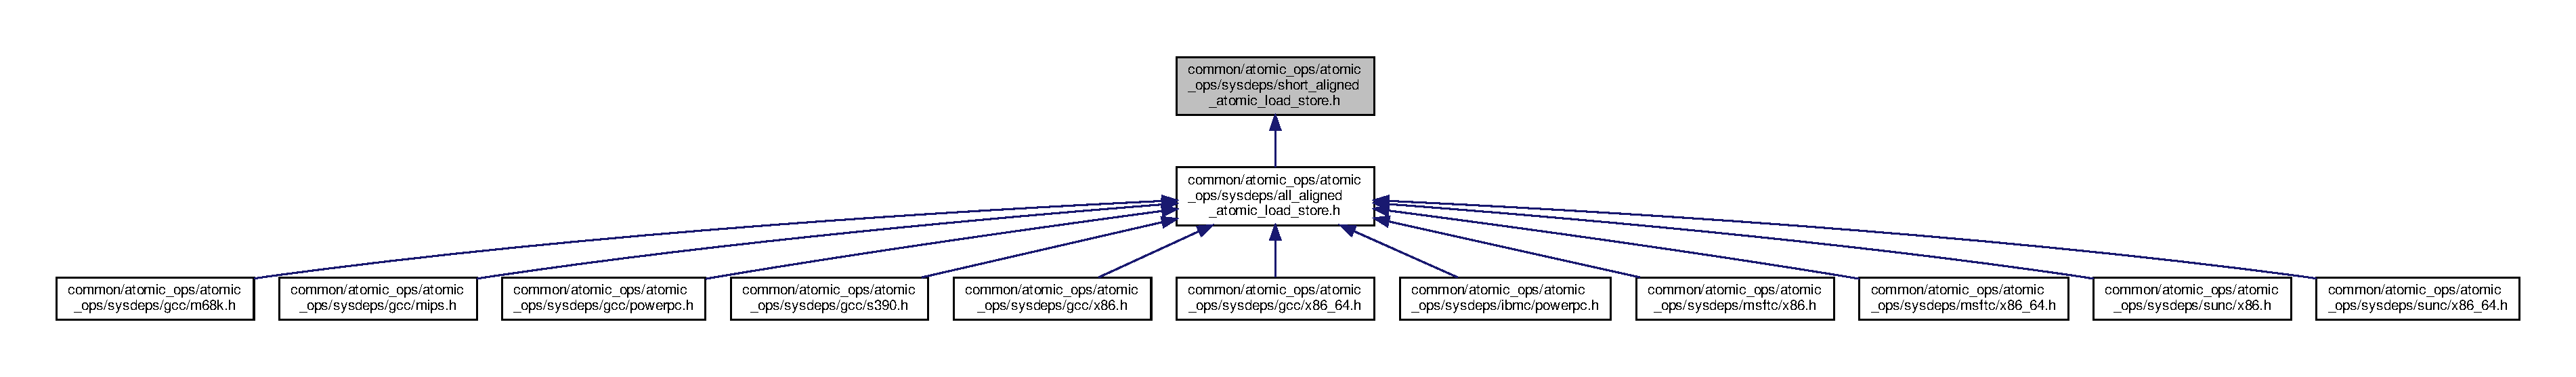
\includegraphics[width=350pt]{short__aligned__atomic__load__store_8h__dep__incl}
\end{center}
\end{figure}
\subsection*{Macros}
\begin{DoxyCompactItemize}
\item 
\#define \hyperlink{short__aligned__atomic__load__store_8h_a8b8d8e49055035fa231d89780e07f2d5}{A\+O\+\_\+\+H\+A\+V\+E\+\_\+short\+\_\+load}
\item 
\#define \hyperlink{short__aligned__atomic__load__store_8h_a15138a7700fc979e90f3b09d4fa8b62a}{A\+O\+\_\+\+H\+A\+V\+E\+\_\+short\+\_\+store}
\end{DoxyCompactItemize}
\subsection*{Functions}
\begin{DoxyCompactItemize}
\item 
\hyperlink{atomic__ops_8h_a9f6ab6253b6b11bc8c12efe9dde5db2b}{A\+O\+\_\+\+I\+N\+L\+I\+NE} unsigned short \hyperlink{short__aligned__atomic__load__store_8h_ab3df66d075952653fc168a9e77a4fc58}{A\+O\+\_\+short\+\_\+load} (const volatile unsigned short $\ast$addr)
\item 
\hyperlink{atomic__ops_8h_a9f6ab6253b6b11bc8c12efe9dde5db2b}{A\+O\+\_\+\+I\+N\+L\+I\+NE} void \hyperlink{short__aligned__atomic__load__store_8h_a814f2716aa0c74fb015b3c7e08588e2e}{A\+O\+\_\+short\+\_\+store} (volatile unsigned short $\ast$addr, unsigned short new\+\_\+val)
\end{DoxyCompactItemize}


\subsection{Macro Definition Documentation}
\mbox{\Hypertarget{short__aligned__atomic__load__store_8h_a8b8d8e49055035fa231d89780e07f2d5}\label{short__aligned__atomic__load__store_8h_a8b8d8e49055035fa231d89780e07f2d5}} 
\index{short\+\_\+aligned\+\_\+atomic\+\_\+load\+\_\+store.\+h@{short\+\_\+aligned\+\_\+atomic\+\_\+load\+\_\+store.\+h}!A\+O\+\_\+\+H\+A\+V\+E\+\_\+short\+\_\+load@{A\+O\+\_\+\+H\+A\+V\+E\+\_\+short\+\_\+load}}
\index{A\+O\+\_\+\+H\+A\+V\+E\+\_\+short\+\_\+load@{A\+O\+\_\+\+H\+A\+V\+E\+\_\+short\+\_\+load}!short\+\_\+aligned\+\_\+atomic\+\_\+load\+\_\+store.\+h@{short\+\_\+aligned\+\_\+atomic\+\_\+load\+\_\+store.\+h}}
\subsubsection{\texorpdfstring{A\+O\+\_\+\+H\+A\+V\+E\+\_\+short\+\_\+load}{AO\_HAVE\_short\_load}}
{\footnotesize\ttfamily \#define A\+O\+\_\+\+H\+A\+V\+E\+\_\+short\+\_\+load}

\mbox{\Hypertarget{short__aligned__atomic__load__store_8h_a15138a7700fc979e90f3b09d4fa8b62a}\label{short__aligned__atomic__load__store_8h_a15138a7700fc979e90f3b09d4fa8b62a}} 
\index{short\+\_\+aligned\+\_\+atomic\+\_\+load\+\_\+store.\+h@{short\+\_\+aligned\+\_\+atomic\+\_\+load\+\_\+store.\+h}!A\+O\+\_\+\+H\+A\+V\+E\+\_\+short\+\_\+store@{A\+O\+\_\+\+H\+A\+V\+E\+\_\+short\+\_\+store}}
\index{A\+O\+\_\+\+H\+A\+V\+E\+\_\+short\+\_\+store@{A\+O\+\_\+\+H\+A\+V\+E\+\_\+short\+\_\+store}!short\+\_\+aligned\+\_\+atomic\+\_\+load\+\_\+store.\+h@{short\+\_\+aligned\+\_\+atomic\+\_\+load\+\_\+store.\+h}}
\subsubsection{\texorpdfstring{A\+O\+\_\+\+H\+A\+V\+E\+\_\+short\+\_\+store}{AO\_HAVE\_short\_store}}
{\footnotesize\ttfamily \#define A\+O\+\_\+\+H\+A\+V\+E\+\_\+short\+\_\+store}



\subsection{Function Documentation}
\mbox{\Hypertarget{short__aligned__atomic__load__store_8h_ab3df66d075952653fc168a9e77a4fc58}\label{short__aligned__atomic__load__store_8h_ab3df66d075952653fc168a9e77a4fc58}} 
\index{short\+\_\+aligned\+\_\+atomic\+\_\+load\+\_\+store.\+h@{short\+\_\+aligned\+\_\+atomic\+\_\+load\+\_\+store.\+h}!A\+O\+\_\+short\+\_\+load@{A\+O\+\_\+short\+\_\+load}}
\index{A\+O\+\_\+short\+\_\+load@{A\+O\+\_\+short\+\_\+load}!short\+\_\+aligned\+\_\+atomic\+\_\+load\+\_\+store.\+h@{short\+\_\+aligned\+\_\+atomic\+\_\+load\+\_\+store.\+h}}
\subsubsection{\texorpdfstring{A\+O\+\_\+short\+\_\+load()}{AO\_short\_load()}}
{\footnotesize\ttfamily \hyperlink{atomic__ops_8h_a9f6ab6253b6b11bc8c12efe9dde5db2b}{A\+O\+\_\+\+I\+N\+L\+I\+NE} unsigned short A\+O\+\_\+short\+\_\+load (\begin{DoxyParamCaption}\item[{const volatile unsigned short $\ast$}]{addr }\end{DoxyParamCaption})}

\mbox{\Hypertarget{short__aligned__atomic__load__store_8h_a814f2716aa0c74fb015b3c7e08588e2e}\label{short__aligned__atomic__load__store_8h_a814f2716aa0c74fb015b3c7e08588e2e}} 
\index{short\+\_\+aligned\+\_\+atomic\+\_\+load\+\_\+store.\+h@{short\+\_\+aligned\+\_\+atomic\+\_\+load\+\_\+store.\+h}!A\+O\+\_\+short\+\_\+store@{A\+O\+\_\+short\+\_\+store}}
\index{A\+O\+\_\+short\+\_\+store@{A\+O\+\_\+short\+\_\+store}!short\+\_\+aligned\+\_\+atomic\+\_\+load\+\_\+store.\+h@{short\+\_\+aligned\+\_\+atomic\+\_\+load\+\_\+store.\+h}}
\subsubsection{\texorpdfstring{A\+O\+\_\+short\+\_\+store()}{AO\_short\_store()}}
{\footnotesize\ttfamily \hyperlink{atomic__ops_8h_a9f6ab6253b6b11bc8c12efe9dde5db2b}{A\+O\+\_\+\+I\+N\+L\+I\+NE} void A\+O\+\_\+short\+\_\+store (\begin{DoxyParamCaption}\item[{volatile unsigned short $\ast$}]{addr,  }\item[{unsigned short}]{new\+\_\+val }\end{DoxyParamCaption})}


\hypertarget{short__atomic__load__store_8h}{}\section{common/atomic\+\_\+ops/atomic\+\_\+ops/sysdeps/short\+\_\+atomic\+\_\+load\+\_\+store.h File Reference}
\label{short__atomic__load__store_8h}\index{common/atomic\+\_\+ops/atomic\+\_\+ops/sysdeps/short\+\_\+atomic\+\_\+load\+\_\+store.\+h@{common/atomic\+\_\+ops/atomic\+\_\+ops/sysdeps/short\+\_\+atomic\+\_\+load\+\_\+store.\+h}}
This graph shows which files directly or indirectly include this file\+:
\nopagebreak
\begin{figure}[H]
\begin{center}
\leavevmode
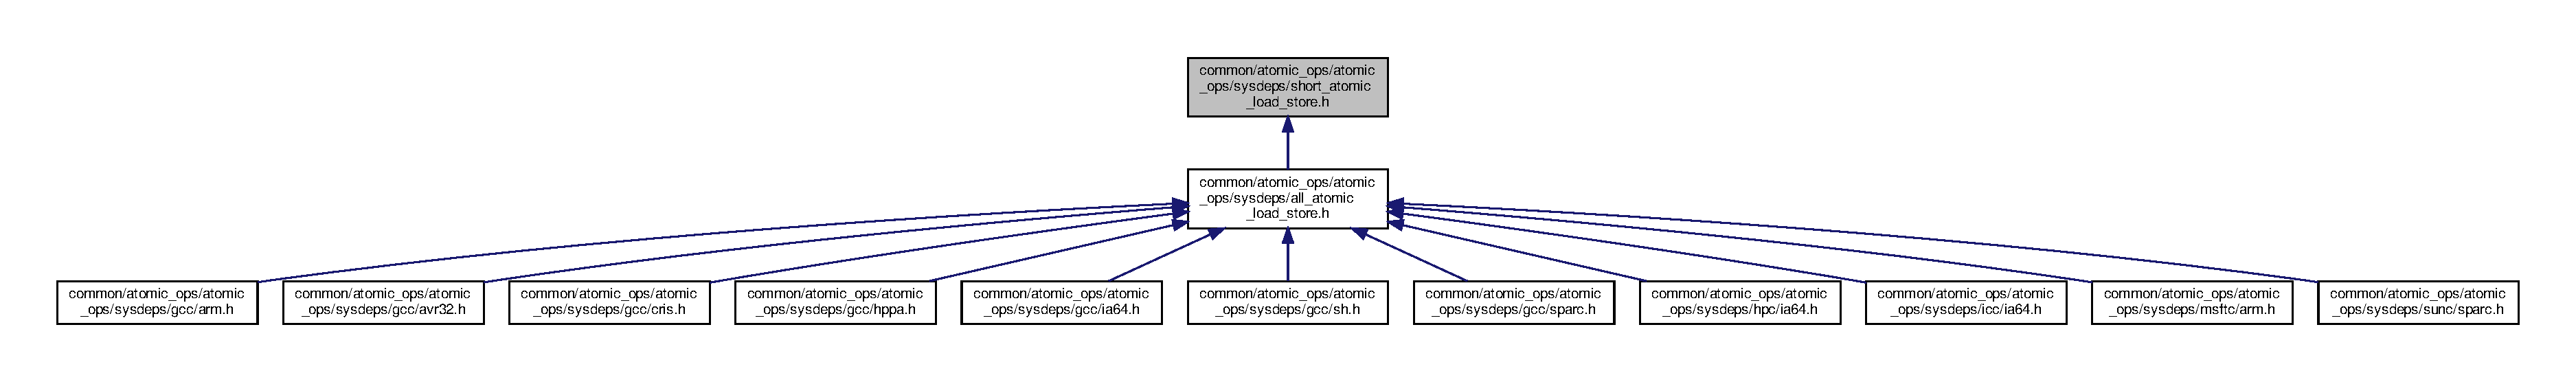
\includegraphics[width=350pt]{short__atomic__load__store_8h__dep__incl}
\end{center}
\end{figure}
\subsection*{Macros}
\begin{DoxyCompactItemize}
\item 
\#define \hyperlink{short__atomic__load__store_8h_a8b8d8e49055035fa231d89780e07f2d5}{A\+O\+\_\+\+H\+A\+V\+E\+\_\+short\+\_\+load}
\item 
\#define \hyperlink{short__atomic__load__store_8h_a15138a7700fc979e90f3b09d4fa8b62a}{A\+O\+\_\+\+H\+A\+V\+E\+\_\+short\+\_\+store}
\end{DoxyCompactItemize}
\subsection*{Functions}
\begin{DoxyCompactItemize}
\item 
\hyperlink{atomic__ops_8h_a9f6ab6253b6b11bc8c12efe9dde5db2b}{A\+O\+\_\+\+I\+N\+L\+I\+NE} unsigned short \hyperlink{short__atomic__load__store_8h_ab3df66d075952653fc168a9e77a4fc58}{A\+O\+\_\+short\+\_\+load} (const volatile unsigned short $\ast$addr)
\item 
\hyperlink{atomic__ops_8h_a9f6ab6253b6b11bc8c12efe9dde5db2b}{A\+O\+\_\+\+I\+N\+L\+I\+NE} void \hyperlink{short__atomic__load__store_8h_a814f2716aa0c74fb015b3c7e08588e2e}{A\+O\+\_\+short\+\_\+store} (volatile unsigned short $\ast$addr, unsigned short new\+\_\+val)
\end{DoxyCompactItemize}


\subsection{Macro Definition Documentation}
\mbox{\Hypertarget{short__atomic__load__store_8h_a8b8d8e49055035fa231d89780e07f2d5}\label{short__atomic__load__store_8h_a8b8d8e49055035fa231d89780e07f2d5}} 
\index{short\+\_\+atomic\+\_\+load\+\_\+store.\+h@{short\+\_\+atomic\+\_\+load\+\_\+store.\+h}!A\+O\+\_\+\+H\+A\+V\+E\+\_\+short\+\_\+load@{A\+O\+\_\+\+H\+A\+V\+E\+\_\+short\+\_\+load}}
\index{A\+O\+\_\+\+H\+A\+V\+E\+\_\+short\+\_\+load@{A\+O\+\_\+\+H\+A\+V\+E\+\_\+short\+\_\+load}!short\+\_\+atomic\+\_\+load\+\_\+store.\+h@{short\+\_\+atomic\+\_\+load\+\_\+store.\+h}}
\subsubsection{\texorpdfstring{A\+O\+\_\+\+H\+A\+V\+E\+\_\+short\+\_\+load}{AO\_HAVE\_short\_load}}
{\footnotesize\ttfamily \#define A\+O\+\_\+\+H\+A\+V\+E\+\_\+short\+\_\+load}

\mbox{\Hypertarget{short__atomic__load__store_8h_a15138a7700fc979e90f3b09d4fa8b62a}\label{short__atomic__load__store_8h_a15138a7700fc979e90f3b09d4fa8b62a}} 
\index{short\+\_\+atomic\+\_\+load\+\_\+store.\+h@{short\+\_\+atomic\+\_\+load\+\_\+store.\+h}!A\+O\+\_\+\+H\+A\+V\+E\+\_\+short\+\_\+store@{A\+O\+\_\+\+H\+A\+V\+E\+\_\+short\+\_\+store}}
\index{A\+O\+\_\+\+H\+A\+V\+E\+\_\+short\+\_\+store@{A\+O\+\_\+\+H\+A\+V\+E\+\_\+short\+\_\+store}!short\+\_\+atomic\+\_\+load\+\_\+store.\+h@{short\+\_\+atomic\+\_\+load\+\_\+store.\+h}}
\subsubsection{\texorpdfstring{A\+O\+\_\+\+H\+A\+V\+E\+\_\+short\+\_\+store}{AO\_HAVE\_short\_store}}
{\footnotesize\ttfamily \#define A\+O\+\_\+\+H\+A\+V\+E\+\_\+short\+\_\+store}



\subsection{Function Documentation}
\mbox{\Hypertarget{short__atomic__load__store_8h_ab3df66d075952653fc168a9e77a4fc58}\label{short__atomic__load__store_8h_ab3df66d075952653fc168a9e77a4fc58}} 
\index{short\+\_\+atomic\+\_\+load\+\_\+store.\+h@{short\+\_\+atomic\+\_\+load\+\_\+store.\+h}!A\+O\+\_\+short\+\_\+load@{A\+O\+\_\+short\+\_\+load}}
\index{A\+O\+\_\+short\+\_\+load@{A\+O\+\_\+short\+\_\+load}!short\+\_\+atomic\+\_\+load\+\_\+store.\+h@{short\+\_\+atomic\+\_\+load\+\_\+store.\+h}}
\subsubsection{\texorpdfstring{A\+O\+\_\+short\+\_\+load()}{AO\_short\_load()}}
{\footnotesize\ttfamily \hyperlink{atomic__ops_8h_a9f6ab6253b6b11bc8c12efe9dde5db2b}{A\+O\+\_\+\+I\+N\+L\+I\+NE} unsigned short A\+O\+\_\+short\+\_\+load (\begin{DoxyParamCaption}\item[{const volatile unsigned short $\ast$}]{addr }\end{DoxyParamCaption})}

\mbox{\Hypertarget{short__atomic__load__store_8h_a814f2716aa0c74fb015b3c7e08588e2e}\label{short__atomic__load__store_8h_a814f2716aa0c74fb015b3c7e08588e2e}} 
\index{short\+\_\+atomic\+\_\+load\+\_\+store.\+h@{short\+\_\+atomic\+\_\+load\+\_\+store.\+h}!A\+O\+\_\+short\+\_\+store@{A\+O\+\_\+short\+\_\+store}}
\index{A\+O\+\_\+short\+\_\+store@{A\+O\+\_\+short\+\_\+store}!short\+\_\+atomic\+\_\+load\+\_\+store.\+h@{short\+\_\+atomic\+\_\+load\+\_\+store.\+h}}
\subsubsection{\texorpdfstring{A\+O\+\_\+short\+\_\+store()}{AO\_short\_store()}}
{\footnotesize\ttfamily \hyperlink{atomic__ops_8h_a9f6ab6253b6b11bc8c12efe9dde5db2b}{A\+O\+\_\+\+I\+N\+L\+I\+NE} void A\+O\+\_\+short\+\_\+store (\begin{DoxyParamCaption}\item[{volatile unsigned short $\ast$}]{addr,  }\item[{unsigned short}]{new\+\_\+val }\end{DoxyParamCaption})}


\hypertarget{standard__ao__double__t_8h}{}\section{common/atomic\+\_\+ops/atomic\+\_\+ops/sysdeps/standard\+\_\+ao\+\_\+double\+\_\+t.h File Reference}
\label{standard__ao__double__t_8h}\index{common/atomic\+\_\+ops/atomic\+\_\+ops/sysdeps/standard\+\_\+ao\+\_\+double\+\_\+t.\+h@{common/atomic\+\_\+ops/atomic\+\_\+ops/sysdeps/standard\+\_\+ao\+\_\+double\+\_\+t.\+h}}
This graph shows which files directly or indirectly include this file\+:
\nopagebreak
\begin{figure}[H]
\begin{center}
\leavevmode
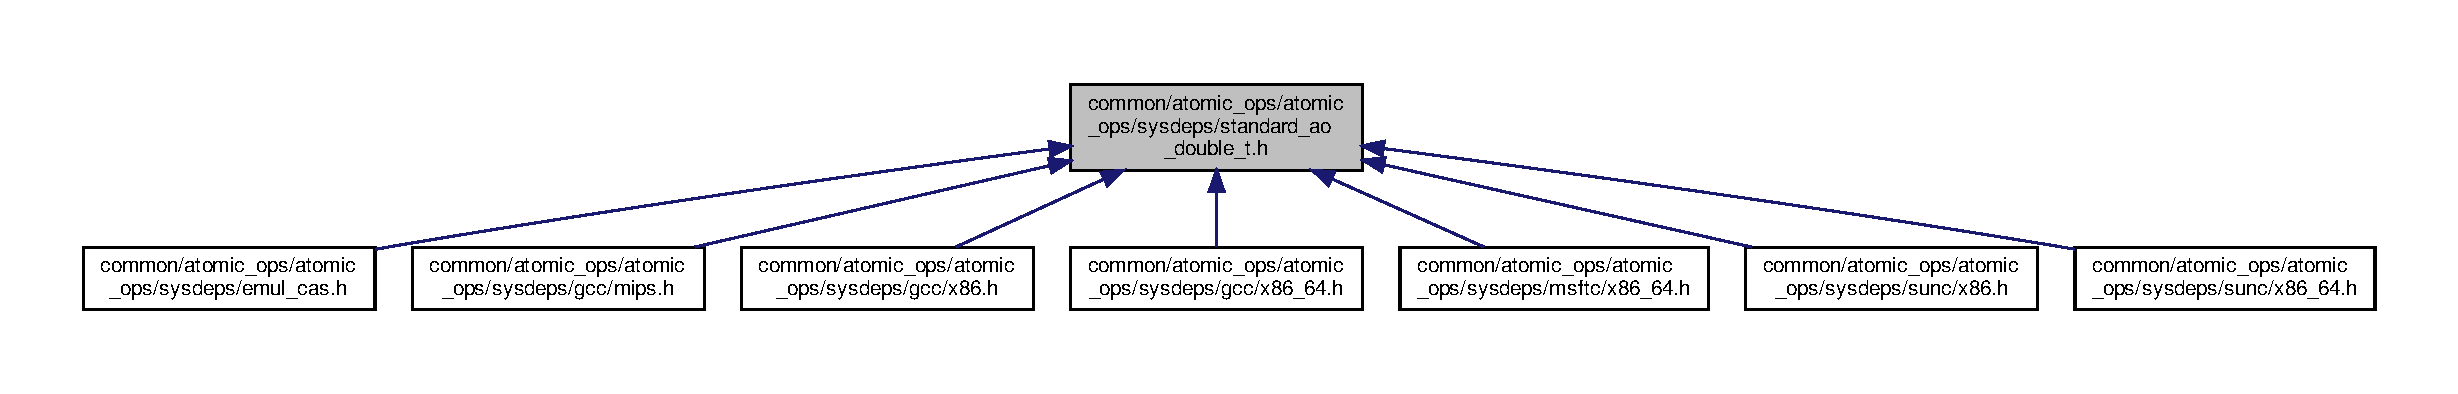
\includegraphics[width=350pt]{standard__ao__double__t_8h__dep__incl}
\end{center}
\end{figure}
\subsection*{Classes}
\begin{DoxyCompactItemize}
\item 
union \hyperlink{structAO__double__t}{A\+O\+\_\+double\+\_\+t}
\end{DoxyCompactItemize}
\subsection*{Macros}
\begin{DoxyCompactItemize}
\item 
\#define \hyperlink{standard__ao__double__t_8h_a2138ad675f3dcb7f05d49dfc84614e1f}{A\+O\+\_\+\+H\+A\+V\+E\+\_\+\+D\+O\+U\+B\+L\+E\+\_\+\+P\+T\+R\+\_\+\+S\+T\+O\+R\+A\+GE}
\item 
\#define \hyperlink{standard__ao__double__t_8h_a42ef0a37943bb9f3a00f1734129bc679}{A\+O\+\_\+\+H\+A\+V\+E\+\_\+double\+\_\+t}
\item 
\#define \hyperlink{standard__ao__double__t_8h_a7f2b8ddd0430bb42de7fc013a7842bbd}{A\+O\+\_\+val1}~A\+O\+\_\+parts.\+A\+O\+\_\+v1
\item 
\#define \hyperlink{standard__ao__double__t_8h_a9e443c9c7b90a512db1b2788f18b81b5}{A\+O\+\_\+val2}~A\+O\+\_\+parts.\+A\+O\+\_\+v2
\end{DoxyCompactItemize}
\subsection*{Typedefs}
\begin{DoxyCompactItemize}
\item 
typedef unsigned long long \hyperlink{standard__ao__double__t_8h_ac63c23baae3d771141f4660fbd1fbf7e}{double\+\_\+ptr\+\_\+storage}
\end{DoxyCompactItemize}


\subsection{Macro Definition Documentation}
\mbox{\Hypertarget{standard__ao__double__t_8h_a2138ad675f3dcb7f05d49dfc84614e1f}\label{standard__ao__double__t_8h_a2138ad675f3dcb7f05d49dfc84614e1f}} 
\index{standard\+\_\+ao\+\_\+double\+\_\+t.\+h@{standard\+\_\+ao\+\_\+double\+\_\+t.\+h}!A\+O\+\_\+\+H\+A\+V\+E\+\_\+\+D\+O\+U\+B\+L\+E\+\_\+\+P\+T\+R\+\_\+\+S\+T\+O\+R\+A\+GE@{A\+O\+\_\+\+H\+A\+V\+E\+\_\+\+D\+O\+U\+B\+L\+E\+\_\+\+P\+T\+R\+\_\+\+S\+T\+O\+R\+A\+GE}}
\index{A\+O\+\_\+\+H\+A\+V\+E\+\_\+\+D\+O\+U\+B\+L\+E\+\_\+\+P\+T\+R\+\_\+\+S\+T\+O\+R\+A\+GE@{A\+O\+\_\+\+H\+A\+V\+E\+\_\+\+D\+O\+U\+B\+L\+E\+\_\+\+P\+T\+R\+\_\+\+S\+T\+O\+R\+A\+GE}!standard\+\_\+ao\+\_\+double\+\_\+t.\+h@{standard\+\_\+ao\+\_\+double\+\_\+t.\+h}}
\subsubsection{\texorpdfstring{A\+O\+\_\+\+H\+A\+V\+E\+\_\+\+D\+O\+U\+B\+L\+E\+\_\+\+P\+T\+R\+\_\+\+S\+T\+O\+R\+A\+GE}{AO\_HAVE\_DOUBLE\_PTR\_STORAGE}}
{\footnotesize\ttfamily \#define A\+O\+\_\+\+H\+A\+V\+E\+\_\+\+D\+O\+U\+B\+L\+E\+\_\+\+P\+T\+R\+\_\+\+S\+T\+O\+R\+A\+GE}

\mbox{\Hypertarget{standard__ao__double__t_8h_a42ef0a37943bb9f3a00f1734129bc679}\label{standard__ao__double__t_8h_a42ef0a37943bb9f3a00f1734129bc679}} 
\index{standard\+\_\+ao\+\_\+double\+\_\+t.\+h@{standard\+\_\+ao\+\_\+double\+\_\+t.\+h}!A\+O\+\_\+\+H\+A\+V\+E\+\_\+double\+\_\+t@{A\+O\+\_\+\+H\+A\+V\+E\+\_\+double\+\_\+t}}
\index{A\+O\+\_\+\+H\+A\+V\+E\+\_\+double\+\_\+t@{A\+O\+\_\+\+H\+A\+V\+E\+\_\+double\+\_\+t}!standard\+\_\+ao\+\_\+double\+\_\+t.\+h@{standard\+\_\+ao\+\_\+double\+\_\+t.\+h}}
\subsubsection{\texorpdfstring{A\+O\+\_\+\+H\+A\+V\+E\+\_\+double\+\_\+t}{AO\_HAVE\_double\_t}}
{\footnotesize\ttfamily \#define A\+O\+\_\+\+H\+A\+V\+E\+\_\+double\+\_\+t}

\mbox{\Hypertarget{standard__ao__double__t_8h_a7f2b8ddd0430bb42de7fc013a7842bbd}\label{standard__ao__double__t_8h_a7f2b8ddd0430bb42de7fc013a7842bbd}} 
\index{standard\+\_\+ao\+\_\+double\+\_\+t.\+h@{standard\+\_\+ao\+\_\+double\+\_\+t.\+h}!A\+O\+\_\+val1@{A\+O\+\_\+val1}}
\index{A\+O\+\_\+val1@{A\+O\+\_\+val1}!standard\+\_\+ao\+\_\+double\+\_\+t.\+h@{standard\+\_\+ao\+\_\+double\+\_\+t.\+h}}
\subsubsection{\texorpdfstring{A\+O\+\_\+val1}{AO\_val1}}
{\footnotesize\ttfamily \#define A\+O\+\_\+val1~A\+O\+\_\+parts.\+A\+O\+\_\+v1}

\mbox{\Hypertarget{standard__ao__double__t_8h_a9e443c9c7b90a512db1b2788f18b81b5}\label{standard__ao__double__t_8h_a9e443c9c7b90a512db1b2788f18b81b5}} 
\index{standard\+\_\+ao\+\_\+double\+\_\+t.\+h@{standard\+\_\+ao\+\_\+double\+\_\+t.\+h}!A\+O\+\_\+val2@{A\+O\+\_\+val2}}
\index{A\+O\+\_\+val2@{A\+O\+\_\+val2}!standard\+\_\+ao\+\_\+double\+\_\+t.\+h@{standard\+\_\+ao\+\_\+double\+\_\+t.\+h}}
\subsubsection{\texorpdfstring{A\+O\+\_\+val2}{AO\_val2}}
{\footnotesize\ttfamily \#define A\+O\+\_\+val2~A\+O\+\_\+parts.\+A\+O\+\_\+v2}



\subsection{Typedef Documentation}
\mbox{\Hypertarget{standard__ao__double__t_8h_ac63c23baae3d771141f4660fbd1fbf7e}\label{standard__ao__double__t_8h_ac63c23baae3d771141f4660fbd1fbf7e}} 
\index{standard\+\_\+ao\+\_\+double\+\_\+t.\+h@{standard\+\_\+ao\+\_\+double\+\_\+t.\+h}!double\+\_\+ptr\+\_\+storage@{double\+\_\+ptr\+\_\+storage}}
\index{double\+\_\+ptr\+\_\+storage@{double\+\_\+ptr\+\_\+storage}!standard\+\_\+ao\+\_\+double\+\_\+t.\+h@{standard\+\_\+ao\+\_\+double\+\_\+t.\+h}}
\subsubsection{\texorpdfstring{double\+\_\+ptr\+\_\+storage}{double\_ptr\_storage}}
{\footnotesize\ttfamily typedef unsigned long long \hyperlink{standard__ao__double__t_8h_ac63c23baae3d771141f4660fbd1fbf7e}{double\+\_\+ptr\+\_\+storage}}


\hypertarget{test__and__set__t__is__ao__t_8h}{}\section{common/atomic\+\_\+ops/atomic\+\_\+ops/sysdeps/test\+\_\+and\+\_\+set\+\_\+t\+\_\+is\+\_\+ao\+\_\+t.h File Reference}
\label{test__and__set__t__is__ao__t_8h}\index{common/atomic\+\_\+ops/atomic\+\_\+ops/sysdeps/test\+\_\+and\+\_\+set\+\_\+t\+\_\+is\+\_\+ao\+\_\+t.\+h@{common/atomic\+\_\+ops/atomic\+\_\+ops/sysdeps/test\+\_\+and\+\_\+set\+\_\+t\+\_\+is\+\_\+ao\+\_\+t.\+h}}
This graph shows which files directly or indirectly include this file\+:
\nopagebreak
\begin{figure}[H]
\begin{center}
\leavevmode
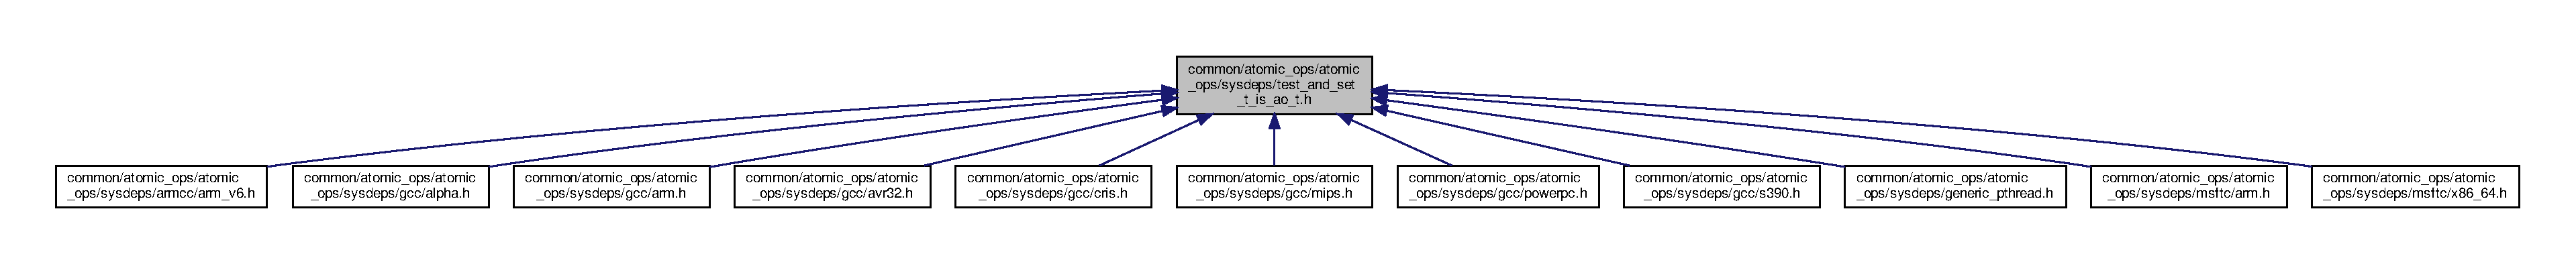
\includegraphics[width=350pt]{test__and__set__t__is__ao__t_8h__dep__incl}
\end{center}
\end{figure}
\subsection*{Macros}
\begin{DoxyCompactItemize}
\item 
\#define \hyperlink{test__and__set__t__is__ao__t_8h_a7d99a16c4eab47ba80ab6138d7d98ac1}{A\+O\+\_\+\+T\+S\+\_\+\+V\+A\+L\+\_\+t}~\hyperlink{test__and__set__t__is__ao__t_8h_a8cdd1f9fd500212324a43c8b12898c1f}{A\+O\+\_\+\+T\+S\+\_\+val}
\item 
\#define \hyperlink{test__and__set__t__is__ao__t_8h_a35258ee13bc817d0b8eb62f4695c4a3e}{A\+O\+\_\+\+T\+S\+\_\+\+C\+L\+E\+AR}~\hyperlink{test__and__set__t__is__ao__t_8h_a8cdd1f9fd500212324a43c8b12898c1fa87962c166dc96e2a685859def333eb33}{A\+O\+\_\+\+T\+S\+\_\+clear}
\item 
\#define \hyperlink{test__and__set__t__is__ao__t_8h_a8a50ac5fe9e6ff855a078c265079ac06}{A\+O\+\_\+\+T\+S\+\_\+\+S\+ET}~\hyperlink{test__and__set__t__is__ao__t_8h_a8cdd1f9fd500212324a43c8b12898c1fab40965b8c92964ad11c5499d79805cc4}{A\+O\+\_\+\+T\+S\+\_\+set}
\item 
\#define \hyperlink{test__and__set__t__is__ao__t_8h_a5890c21b549264c75c2cad08bf4f6ba9}{A\+O\+\_\+\+T\+S\+\_\+t}~\hyperlink{atomic__ops_8h_a5225fef4d9eee821e82382cd269160dd}{A\+O\+\_\+t}
\item 
\#define \hyperlink{test__and__set__t__is__ao__t_8h_a6fc928fae0e4aa7f23a97ddb9df95267}{A\+O\+\_\+\+A\+O\+\_\+\+T\+S\+\_\+T}~1
\end{DoxyCompactItemize}
\subsection*{Enumerations}
\begin{DoxyCompactItemize}
\item 
enum \hyperlink{test__and__set__t__is__ao__t_8h_a8cdd1f9fd500212324a43c8b12898c1f}{A\+O\+\_\+\+T\+S\+\_\+val} \{ \hyperlink{test__and__set__t__is__ao__t_8h_a8cdd1f9fd500212324a43c8b12898c1fa87962c166dc96e2a685859def333eb33}{A\+O\+\_\+\+T\+S\+\_\+clear} = 0, 
\hyperlink{test__and__set__t__is__ao__t_8h_a8cdd1f9fd500212324a43c8b12898c1fab40965b8c92964ad11c5499d79805cc4}{A\+O\+\_\+\+T\+S\+\_\+set} = 1
 \}
\end{DoxyCompactItemize}


\subsection{Macro Definition Documentation}
\mbox{\Hypertarget{test__and__set__t__is__ao__t_8h_a6fc928fae0e4aa7f23a97ddb9df95267}\label{test__and__set__t__is__ao__t_8h_a6fc928fae0e4aa7f23a97ddb9df95267}} 
\index{test\+\_\+and\+\_\+set\+\_\+t\+\_\+is\+\_\+ao\+\_\+t.\+h@{test\+\_\+and\+\_\+set\+\_\+t\+\_\+is\+\_\+ao\+\_\+t.\+h}!A\+O\+\_\+\+A\+O\+\_\+\+T\+S\+\_\+T@{A\+O\+\_\+\+A\+O\+\_\+\+T\+S\+\_\+T}}
\index{A\+O\+\_\+\+A\+O\+\_\+\+T\+S\+\_\+T@{A\+O\+\_\+\+A\+O\+\_\+\+T\+S\+\_\+T}!test\+\_\+and\+\_\+set\+\_\+t\+\_\+is\+\_\+ao\+\_\+t.\+h@{test\+\_\+and\+\_\+set\+\_\+t\+\_\+is\+\_\+ao\+\_\+t.\+h}}
\subsubsection{\texorpdfstring{A\+O\+\_\+\+A\+O\+\_\+\+T\+S\+\_\+T}{AO\_AO\_TS\_T}}
{\footnotesize\ttfamily \#define A\+O\+\_\+\+A\+O\+\_\+\+T\+S\+\_\+T~1}

\mbox{\Hypertarget{test__and__set__t__is__ao__t_8h_a35258ee13bc817d0b8eb62f4695c4a3e}\label{test__and__set__t__is__ao__t_8h_a35258ee13bc817d0b8eb62f4695c4a3e}} 
\index{test\+\_\+and\+\_\+set\+\_\+t\+\_\+is\+\_\+ao\+\_\+t.\+h@{test\+\_\+and\+\_\+set\+\_\+t\+\_\+is\+\_\+ao\+\_\+t.\+h}!A\+O\+\_\+\+T\+S\+\_\+\+C\+L\+E\+AR@{A\+O\+\_\+\+T\+S\+\_\+\+C\+L\+E\+AR}}
\index{A\+O\+\_\+\+T\+S\+\_\+\+C\+L\+E\+AR@{A\+O\+\_\+\+T\+S\+\_\+\+C\+L\+E\+AR}!test\+\_\+and\+\_\+set\+\_\+t\+\_\+is\+\_\+ao\+\_\+t.\+h@{test\+\_\+and\+\_\+set\+\_\+t\+\_\+is\+\_\+ao\+\_\+t.\+h}}
\subsubsection{\texorpdfstring{A\+O\+\_\+\+T\+S\+\_\+\+C\+L\+E\+AR}{AO\_TS\_CLEAR}}
{\footnotesize\ttfamily \#define A\+O\+\_\+\+T\+S\+\_\+\+C\+L\+E\+AR~\hyperlink{test__and__set__t__is__ao__t_8h_a8cdd1f9fd500212324a43c8b12898c1fa87962c166dc96e2a685859def333eb33}{A\+O\+\_\+\+T\+S\+\_\+clear}}

\mbox{\Hypertarget{test__and__set__t__is__ao__t_8h_a8a50ac5fe9e6ff855a078c265079ac06}\label{test__and__set__t__is__ao__t_8h_a8a50ac5fe9e6ff855a078c265079ac06}} 
\index{test\+\_\+and\+\_\+set\+\_\+t\+\_\+is\+\_\+ao\+\_\+t.\+h@{test\+\_\+and\+\_\+set\+\_\+t\+\_\+is\+\_\+ao\+\_\+t.\+h}!A\+O\+\_\+\+T\+S\+\_\+\+S\+ET@{A\+O\+\_\+\+T\+S\+\_\+\+S\+ET}}
\index{A\+O\+\_\+\+T\+S\+\_\+\+S\+ET@{A\+O\+\_\+\+T\+S\+\_\+\+S\+ET}!test\+\_\+and\+\_\+set\+\_\+t\+\_\+is\+\_\+ao\+\_\+t.\+h@{test\+\_\+and\+\_\+set\+\_\+t\+\_\+is\+\_\+ao\+\_\+t.\+h}}
\subsubsection{\texorpdfstring{A\+O\+\_\+\+T\+S\+\_\+\+S\+ET}{AO\_TS\_SET}}
{\footnotesize\ttfamily \#define A\+O\+\_\+\+T\+S\+\_\+\+S\+ET~\hyperlink{test__and__set__t__is__ao__t_8h_a8cdd1f9fd500212324a43c8b12898c1fab40965b8c92964ad11c5499d79805cc4}{A\+O\+\_\+\+T\+S\+\_\+set}}

\mbox{\Hypertarget{test__and__set__t__is__ao__t_8h_a5890c21b549264c75c2cad08bf4f6ba9}\label{test__and__set__t__is__ao__t_8h_a5890c21b549264c75c2cad08bf4f6ba9}} 
\index{test\+\_\+and\+\_\+set\+\_\+t\+\_\+is\+\_\+ao\+\_\+t.\+h@{test\+\_\+and\+\_\+set\+\_\+t\+\_\+is\+\_\+ao\+\_\+t.\+h}!A\+O\+\_\+\+T\+S\+\_\+t@{A\+O\+\_\+\+T\+S\+\_\+t}}
\index{A\+O\+\_\+\+T\+S\+\_\+t@{A\+O\+\_\+\+T\+S\+\_\+t}!test\+\_\+and\+\_\+set\+\_\+t\+\_\+is\+\_\+ao\+\_\+t.\+h@{test\+\_\+and\+\_\+set\+\_\+t\+\_\+is\+\_\+ao\+\_\+t.\+h}}
\subsubsection{\texorpdfstring{A\+O\+\_\+\+T\+S\+\_\+t}{AO\_TS\_t}}
{\footnotesize\ttfamily \#define A\+O\+\_\+\+T\+S\+\_\+t~\hyperlink{atomic__ops_8h_a5225fef4d9eee821e82382cd269160dd}{A\+O\+\_\+t}}

\mbox{\Hypertarget{test__and__set__t__is__ao__t_8h_a7d99a16c4eab47ba80ab6138d7d98ac1}\label{test__and__set__t__is__ao__t_8h_a7d99a16c4eab47ba80ab6138d7d98ac1}} 
\index{test\+\_\+and\+\_\+set\+\_\+t\+\_\+is\+\_\+ao\+\_\+t.\+h@{test\+\_\+and\+\_\+set\+\_\+t\+\_\+is\+\_\+ao\+\_\+t.\+h}!A\+O\+\_\+\+T\+S\+\_\+\+V\+A\+L\+\_\+t@{A\+O\+\_\+\+T\+S\+\_\+\+V\+A\+L\+\_\+t}}
\index{A\+O\+\_\+\+T\+S\+\_\+\+V\+A\+L\+\_\+t@{A\+O\+\_\+\+T\+S\+\_\+\+V\+A\+L\+\_\+t}!test\+\_\+and\+\_\+set\+\_\+t\+\_\+is\+\_\+ao\+\_\+t.\+h@{test\+\_\+and\+\_\+set\+\_\+t\+\_\+is\+\_\+ao\+\_\+t.\+h}}
\subsubsection{\texorpdfstring{A\+O\+\_\+\+T\+S\+\_\+\+V\+A\+L\+\_\+t}{AO\_TS\_VAL\_t}}
{\footnotesize\ttfamily \#define A\+O\+\_\+\+T\+S\+\_\+\+V\+A\+L\+\_\+t~\hyperlink{test__and__set__t__is__ao__t_8h_a8cdd1f9fd500212324a43c8b12898c1f}{A\+O\+\_\+\+T\+S\+\_\+val}}



\subsection{Enumeration Type Documentation}
\mbox{\Hypertarget{test__and__set__t__is__ao__t_8h_a8cdd1f9fd500212324a43c8b12898c1f}\label{test__and__set__t__is__ao__t_8h_a8cdd1f9fd500212324a43c8b12898c1f}} 
\index{test\+\_\+and\+\_\+set\+\_\+t\+\_\+is\+\_\+ao\+\_\+t.\+h@{test\+\_\+and\+\_\+set\+\_\+t\+\_\+is\+\_\+ao\+\_\+t.\+h}!A\+O\+\_\+\+T\+S\+\_\+val@{A\+O\+\_\+\+T\+S\+\_\+val}}
\index{A\+O\+\_\+\+T\+S\+\_\+val@{A\+O\+\_\+\+T\+S\+\_\+val}!test\+\_\+and\+\_\+set\+\_\+t\+\_\+is\+\_\+ao\+\_\+t.\+h@{test\+\_\+and\+\_\+set\+\_\+t\+\_\+is\+\_\+ao\+\_\+t.\+h}}
\subsubsection{\texorpdfstring{A\+O\+\_\+\+T\+S\+\_\+val}{AO\_TS\_val}}
{\footnotesize\ttfamily enum \hyperlink{test__and__set__t__is__ao__t_8h_a8cdd1f9fd500212324a43c8b12898c1f}{A\+O\+\_\+\+T\+S\+\_\+val}}

\begin{DoxyEnumFields}{Enumerator}
\raisebox{\heightof{T}}[0pt][0pt]{\index{A\+O\+\_\+\+T\+S\+\_\+clear@{A\+O\+\_\+\+T\+S\+\_\+clear}!test\+\_\+and\+\_\+set\+\_\+t\+\_\+is\+\_\+ao\+\_\+t.\+h@{test\+\_\+and\+\_\+set\+\_\+t\+\_\+is\+\_\+ao\+\_\+t.\+h}}\index{test\+\_\+and\+\_\+set\+\_\+t\+\_\+is\+\_\+ao\+\_\+t.\+h@{test\+\_\+and\+\_\+set\+\_\+t\+\_\+is\+\_\+ao\+\_\+t.\+h}!A\+O\+\_\+\+T\+S\+\_\+clear@{A\+O\+\_\+\+T\+S\+\_\+clear}}}\mbox{\Hypertarget{test__and__set__t__is__ao__t_8h_a8cdd1f9fd500212324a43c8b12898c1fa87962c166dc96e2a685859def333eb33}\label{test__and__set__t__is__ao__t_8h_a8cdd1f9fd500212324a43c8b12898c1fa87962c166dc96e2a685859def333eb33}} 
A\+O\+\_\+\+T\+S\+\_\+clear&\\
\hline

\raisebox{\heightof{T}}[0pt][0pt]{\index{A\+O\+\_\+\+T\+S\+\_\+set@{A\+O\+\_\+\+T\+S\+\_\+set}!test\+\_\+and\+\_\+set\+\_\+t\+\_\+is\+\_\+ao\+\_\+t.\+h@{test\+\_\+and\+\_\+set\+\_\+t\+\_\+is\+\_\+ao\+\_\+t.\+h}}\index{test\+\_\+and\+\_\+set\+\_\+t\+\_\+is\+\_\+ao\+\_\+t.\+h@{test\+\_\+and\+\_\+set\+\_\+t\+\_\+is\+\_\+ao\+\_\+t.\+h}!A\+O\+\_\+\+T\+S\+\_\+set@{A\+O\+\_\+\+T\+S\+\_\+set}}}\mbox{\Hypertarget{test__and__set__t__is__ao__t_8h_a8cdd1f9fd500212324a43c8b12898c1fab40965b8c92964ad11c5499d79805cc4}\label{test__and__set__t__is__ao__t_8h_a8cdd1f9fd500212324a43c8b12898c1fab40965b8c92964ad11c5499d79805cc4}} 
A\+O\+\_\+\+T\+S\+\_\+set&\\
\hline

\end{DoxyEnumFields}

\hypertarget{test__and__set__t__is__char_8h}{}\section{common/atomic\+\_\+ops/atomic\+\_\+ops/sysdeps/test\+\_\+and\+\_\+set\+\_\+t\+\_\+is\+\_\+char.h File Reference}
\label{test__and__set__t__is__char_8h}\index{common/atomic\+\_\+ops/atomic\+\_\+ops/sysdeps/test\+\_\+and\+\_\+set\+\_\+t\+\_\+is\+\_\+char.\+h@{common/atomic\+\_\+ops/atomic\+\_\+ops/sysdeps/test\+\_\+and\+\_\+set\+\_\+t\+\_\+is\+\_\+char.\+h}}
This graph shows which files directly or indirectly include this file\+:
\nopagebreak
\begin{figure}[H]
\begin{center}
\leavevmode
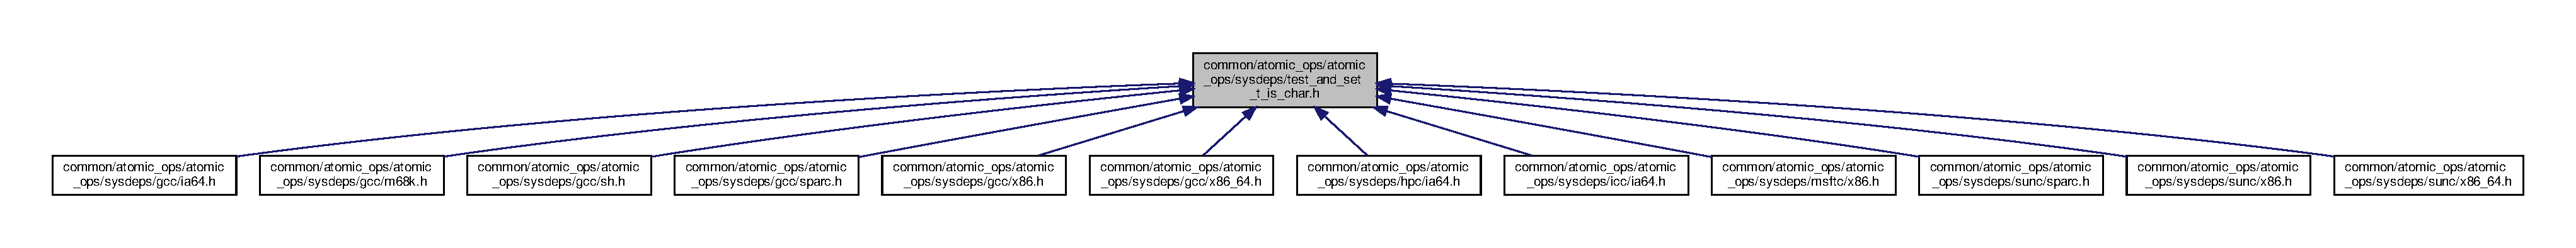
\includegraphics[width=350pt]{test__and__set__t__is__char_8h__dep__incl}
\end{center}
\end{figure}
\subsection*{Macros}
\begin{DoxyCompactItemize}
\item 
\#define \hyperlink{test__and__set__t__is__char_8h_a5890c21b549264c75c2cad08bf4f6ba9}{A\+O\+\_\+\+T\+S\+\_\+t}~unsigned char
\item 
\#define \hyperlink{test__and__set__t__is__char_8h_a7d99a16c4eab47ba80ab6138d7d98ac1}{A\+O\+\_\+\+T\+S\+\_\+\+V\+A\+L\+\_\+t}~\hyperlink{test__and__set__t__is__char_8h_a5a5dc5c8ec3269de1a28080c8640c3bc}{A\+O\+\_\+\+B\+Y\+T\+E\+\_\+\+T\+S\+\_\+val}
\item 
\#define \hyperlink{test__and__set__t__is__char_8h_a35258ee13bc817d0b8eb62f4695c4a3e}{A\+O\+\_\+\+T\+S\+\_\+\+C\+L\+E\+AR}~\hyperlink{test__and__set__t__is__char_8h_a5a5dc5c8ec3269de1a28080c8640c3bca79efd2b71abaef595b18aeb1f23ba682}{A\+O\+\_\+\+B\+Y\+T\+E\+\_\+\+T\+S\+\_\+clear}
\item 
\#define \hyperlink{test__and__set__t__is__char_8h_a8a50ac5fe9e6ff855a078c265079ac06}{A\+O\+\_\+\+T\+S\+\_\+\+S\+ET}~\hyperlink{test__and__set__t__is__char_8h_a5a5dc5c8ec3269de1a28080c8640c3bca6f43ded9c33911a57a02463f605a5115}{A\+O\+\_\+\+B\+Y\+T\+E\+\_\+\+T\+S\+\_\+set}
\item 
\#define \hyperlink{test__and__set__t__is__char_8h_a3b99244534b68f1c53c3f0375b777457}{A\+O\+\_\+\+C\+H\+A\+R\+\_\+\+T\+S\+\_\+T}~1
\end{DoxyCompactItemize}
\subsection*{Enumerations}
\begin{DoxyCompactItemize}
\item 
enum \hyperlink{test__and__set__t__is__char_8h_a5a5dc5c8ec3269de1a28080c8640c3bc}{A\+O\+\_\+\+B\+Y\+T\+E\+\_\+\+T\+S\+\_\+val} \{ \hyperlink{test__and__set__t__is__char_8h_a5a5dc5c8ec3269de1a28080c8640c3bca79efd2b71abaef595b18aeb1f23ba682}{A\+O\+\_\+\+B\+Y\+T\+E\+\_\+\+T\+S\+\_\+clear} = 0, 
\hyperlink{test__and__set__t__is__char_8h_a5a5dc5c8ec3269de1a28080c8640c3bca6f43ded9c33911a57a02463f605a5115}{A\+O\+\_\+\+B\+Y\+T\+E\+\_\+\+T\+S\+\_\+set} = 0xff
 \}
\end{DoxyCompactItemize}


\subsection{Macro Definition Documentation}
\mbox{\Hypertarget{test__and__set__t__is__char_8h_a3b99244534b68f1c53c3f0375b777457}\label{test__and__set__t__is__char_8h_a3b99244534b68f1c53c3f0375b777457}} 
\index{test\+\_\+and\+\_\+set\+\_\+t\+\_\+is\+\_\+char.\+h@{test\+\_\+and\+\_\+set\+\_\+t\+\_\+is\+\_\+char.\+h}!A\+O\+\_\+\+C\+H\+A\+R\+\_\+\+T\+S\+\_\+T@{A\+O\+\_\+\+C\+H\+A\+R\+\_\+\+T\+S\+\_\+T}}
\index{A\+O\+\_\+\+C\+H\+A\+R\+\_\+\+T\+S\+\_\+T@{A\+O\+\_\+\+C\+H\+A\+R\+\_\+\+T\+S\+\_\+T}!test\+\_\+and\+\_\+set\+\_\+t\+\_\+is\+\_\+char.\+h@{test\+\_\+and\+\_\+set\+\_\+t\+\_\+is\+\_\+char.\+h}}
\subsubsection{\texorpdfstring{A\+O\+\_\+\+C\+H\+A\+R\+\_\+\+T\+S\+\_\+T}{AO\_CHAR\_TS\_T}}
{\footnotesize\ttfamily \#define A\+O\+\_\+\+C\+H\+A\+R\+\_\+\+T\+S\+\_\+T~1}

\mbox{\Hypertarget{test__and__set__t__is__char_8h_a35258ee13bc817d0b8eb62f4695c4a3e}\label{test__and__set__t__is__char_8h_a35258ee13bc817d0b8eb62f4695c4a3e}} 
\index{test\+\_\+and\+\_\+set\+\_\+t\+\_\+is\+\_\+char.\+h@{test\+\_\+and\+\_\+set\+\_\+t\+\_\+is\+\_\+char.\+h}!A\+O\+\_\+\+T\+S\+\_\+\+C\+L\+E\+AR@{A\+O\+\_\+\+T\+S\+\_\+\+C\+L\+E\+AR}}
\index{A\+O\+\_\+\+T\+S\+\_\+\+C\+L\+E\+AR@{A\+O\+\_\+\+T\+S\+\_\+\+C\+L\+E\+AR}!test\+\_\+and\+\_\+set\+\_\+t\+\_\+is\+\_\+char.\+h@{test\+\_\+and\+\_\+set\+\_\+t\+\_\+is\+\_\+char.\+h}}
\subsubsection{\texorpdfstring{A\+O\+\_\+\+T\+S\+\_\+\+C\+L\+E\+AR}{AO\_TS\_CLEAR}}
{\footnotesize\ttfamily \#define A\+O\+\_\+\+T\+S\+\_\+\+C\+L\+E\+AR~\hyperlink{test__and__set__t__is__char_8h_a5a5dc5c8ec3269de1a28080c8640c3bca79efd2b71abaef595b18aeb1f23ba682}{A\+O\+\_\+\+B\+Y\+T\+E\+\_\+\+T\+S\+\_\+clear}}

\mbox{\Hypertarget{test__and__set__t__is__char_8h_a8a50ac5fe9e6ff855a078c265079ac06}\label{test__and__set__t__is__char_8h_a8a50ac5fe9e6ff855a078c265079ac06}} 
\index{test\+\_\+and\+\_\+set\+\_\+t\+\_\+is\+\_\+char.\+h@{test\+\_\+and\+\_\+set\+\_\+t\+\_\+is\+\_\+char.\+h}!A\+O\+\_\+\+T\+S\+\_\+\+S\+ET@{A\+O\+\_\+\+T\+S\+\_\+\+S\+ET}}
\index{A\+O\+\_\+\+T\+S\+\_\+\+S\+ET@{A\+O\+\_\+\+T\+S\+\_\+\+S\+ET}!test\+\_\+and\+\_\+set\+\_\+t\+\_\+is\+\_\+char.\+h@{test\+\_\+and\+\_\+set\+\_\+t\+\_\+is\+\_\+char.\+h}}
\subsubsection{\texorpdfstring{A\+O\+\_\+\+T\+S\+\_\+\+S\+ET}{AO\_TS\_SET}}
{\footnotesize\ttfamily \#define A\+O\+\_\+\+T\+S\+\_\+\+S\+ET~\hyperlink{test__and__set__t__is__char_8h_a5a5dc5c8ec3269de1a28080c8640c3bca6f43ded9c33911a57a02463f605a5115}{A\+O\+\_\+\+B\+Y\+T\+E\+\_\+\+T\+S\+\_\+set}}

\mbox{\Hypertarget{test__and__set__t__is__char_8h_a5890c21b549264c75c2cad08bf4f6ba9}\label{test__and__set__t__is__char_8h_a5890c21b549264c75c2cad08bf4f6ba9}} 
\index{test\+\_\+and\+\_\+set\+\_\+t\+\_\+is\+\_\+char.\+h@{test\+\_\+and\+\_\+set\+\_\+t\+\_\+is\+\_\+char.\+h}!A\+O\+\_\+\+T\+S\+\_\+t@{A\+O\+\_\+\+T\+S\+\_\+t}}
\index{A\+O\+\_\+\+T\+S\+\_\+t@{A\+O\+\_\+\+T\+S\+\_\+t}!test\+\_\+and\+\_\+set\+\_\+t\+\_\+is\+\_\+char.\+h@{test\+\_\+and\+\_\+set\+\_\+t\+\_\+is\+\_\+char.\+h}}
\subsubsection{\texorpdfstring{A\+O\+\_\+\+T\+S\+\_\+t}{AO\_TS\_t}}
{\footnotesize\ttfamily \#define A\+O\+\_\+\+T\+S\+\_\+t~unsigned char}

\mbox{\Hypertarget{test__and__set__t__is__char_8h_a7d99a16c4eab47ba80ab6138d7d98ac1}\label{test__and__set__t__is__char_8h_a7d99a16c4eab47ba80ab6138d7d98ac1}} 
\index{test\+\_\+and\+\_\+set\+\_\+t\+\_\+is\+\_\+char.\+h@{test\+\_\+and\+\_\+set\+\_\+t\+\_\+is\+\_\+char.\+h}!A\+O\+\_\+\+T\+S\+\_\+\+V\+A\+L\+\_\+t@{A\+O\+\_\+\+T\+S\+\_\+\+V\+A\+L\+\_\+t}}
\index{A\+O\+\_\+\+T\+S\+\_\+\+V\+A\+L\+\_\+t@{A\+O\+\_\+\+T\+S\+\_\+\+V\+A\+L\+\_\+t}!test\+\_\+and\+\_\+set\+\_\+t\+\_\+is\+\_\+char.\+h@{test\+\_\+and\+\_\+set\+\_\+t\+\_\+is\+\_\+char.\+h}}
\subsubsection{\texorpdfstring{A\+O\+\_\+\+T\+S\+\_\+\+V\+A\+L\+\_\+t}{AO\_TS\_VAL\_t}}
{\footnotesize\ttfamily \#define A\+O\+\_\+\+T\+S\+\_\+\+V\+A\+L\+\_\+t~\hyperlink{test__and__set__t__is__char_8h_a5a5dc5c8ec3269de1a28080c8640c3bc}{A\+O\+\_\+\+B\+Y\+T\+E\+\_\+\+T\+S\+\_\+val}}



\subsection{Enumeration Type Documentation}
\mbox{\Hypertarget{test__and__set__t__is__char_8h_a5a5dc5c8ec3269de1a28080c8640c3bc}\label{test__and__set__t__is__char_8h_a5a5dc5c8ec3269de1a28080c8640c3bc}} 
\index{test\+\_\+and\+\_\+set\+\_\+t\+\_\+is\+\_\+char.\+h@{test\+\_\+and\+\_\+set\+\_\+t\+\_\+is\+\_\+char.\+h}!A\+O\+\_\+\+B\+Y\+T\+E\+\_\+\+T\+S\+\_\+val@{A\+O\+\_\+\+B\+Y\+T\+E\+\_\+\+T\+S\+\_\+val}}
\index{A\+O\+\_\+\+B\+Y\+T\+E\+\_\+\+T\+S\+\_\+val@{A\+O\+\_\+\+B\+Y\+T\+E\+\_\+\+T\+S\+\_\+val}!test\+\_\+and\+\_\+set\+\_\+t\+\_\+is\+\_\+char.\+h@{test\+\_\+and\+\_\+set\+\_\+t\+\_\+is\+\_\+char.\+h}}
\subsubsection{\texorpdfstring{A\+O\+\_\+\+B\+Y\+T\+E\+\_\+\+T\+S\+\_\+val}{AO\_BYTE\_TS\_val}}
{\footnotesize\ttfamily enum \hyperlink{test__and__set__t__is__char_8h_a5a5dc5c8ec3269de1a28080c8640c3bc}{A\+O\+\_\+\+B\+Y\+T\+E\+\_\+\+T\+S\+\_\+val}}

\begin{DoxyEnumFields}{Enumerator}
\raisebox{\heightof{T}}[0pt][0pt]{\index{A\+O\+\_\+\+B\+Y\+T\+E\+\_\+\+T\+S\+\_\+clear@{A\+O\+\_\+\+B\+Y\+T\+E\+\_\+\+T\+S\+\_\+clear}!test\+\_\+and\+\_\+set\+\_\+t\+\_\+is\+\_\+char.\+h@{test\+\_\+and\+\_\+set\+\_\+t\+\_\+is\+\_\+char.\+h}}\index{test\+\_\+and\+\_\+set\+\_\+t\+\_\+is\+\_\+char.\+h@{test\+\_\+and\+\_\+set\+\_\+t\+\_\+is\+\_\+char.\+h}!A\+O\+\_\+\+B\+Y\+T\+E\+\_\+\+T\+S\+\_\+clear@{A\+O\+\_\+\+B\+Y\+T\+E\+\_\+\+T\+S\+\_\+clear}}}\mbox{\Hypertarget{test__and__set__t__is__char_8h_a5a5dc5c8ec3269de1a28080c8640c3bca79efd2b71abaef595b18aeb1f23ba682}\label{test__and__set__t__is__char_8h_a5a5dc5c8ec3269de1a28080c8640c3bca79efd2b71abaef595b18aeb1f23ba682}} 
A\+O\+\_\+\+B\+Y\+T\+E\+\_\+\+T\+S\+\_\+clear&\\
\hline

\raisebox{\heightof{T}}[0pt][0pt]{\index{A\+O\+\_\+\+B\+Y\+T\+E\+\_\+\+T\+S\+\_\+set@{A\+O\+\_\+\+B\+Y\+T\+E\+\_\+\+T\+S\+\_\+set}!test\+\_\+and\+\_\+set\+\_\+t\+\_\+is\+\_\+char.\+h@{test\+\_\+and\+\_\+set\+\_\+t\+\_\+is\+\_\+char.\+h}}\index{test\+\_\+and\+\_\+set\+\_\+t\+\_\+is\+\_\+char.\+h@{test\+\_\+and\+\_\+set\+\_\+t\+\_\+is\+\_\+char.\+h}!A\+O\+\_\+\+B\+Y\+T\+E\+\_\+\+T\+S\+\_\+set@{A\+O\+\_\+\+B\+Y\+T\+E\+\_\+\+T\+S\+\_\+set}}}\mbox{\Hypertarget{test__and__set__t__is__char_8h_a5a5dc5c8ec3269de1a28080c8640c3bca6f43ded9c33911a57a02463f605a5115}\label{test__and__set__t__is__char_8h_a5a5dc5c8ec3269de1a28080c8640c3bca6f43ded9c33911a57a02463f605a5115}} 
A\+O\+\_\+\+B\+Y\+T\+E\+\_\+\+T\+S\+\_\+set&\\
\hline

\end{DoxyEnumFields}

\hypertarget{binding_8h}{}\section{common/binding.h File Reference}
\label{binding_8h}\index{common/binding.\+h@{common/binding.\+h}}
{\ttfamily \#include $<$cassert$>$}\newline
{\ttfamily \#include $<$sched.\+h$>$}\newline
{\ttfamily \#include $<$iostream$>$}\newline
{\ttfamily \#include $<$stdlib.\+h$>$}\newline
{\ttfamily \#include $<$string$>$}\newline
{\ttfamily \#include \char`\"{}plaf.\+h\char`\"{}}\newline
Include dependency graph for binding.\+h\+:
\nopagebreak
\begin{figure}[H]
\begin{center}
\leavevmode
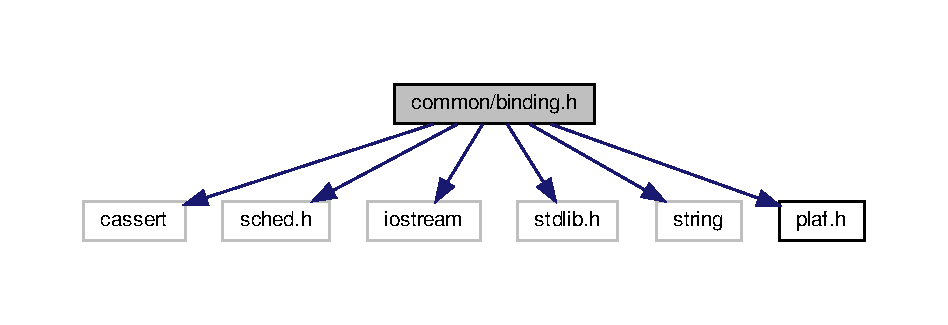
\includegraphics[width=350pt]{binding_8h__incl}
\end{center}
\end{figure}
This graph shows which files directly or indirectly include this file\+:
\nopagebreak
\begin{figure}[H]
\begin{center}
\leavevmode
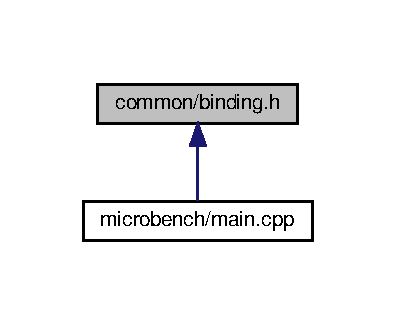
\includegraphics[width=190pt]{binding_8h__dep__incl}
\end{center}
\end{figure}
\subsection*{Functions}
\begin{DoxyCompactItemize}
\item 
void \hyperlink{binding_8h_afe627626a2cbd3bd494a4480799017c8}{binding\+\_\+parse\+Custom} (std\+::string argv)
\item 
int \hyperlink{binding_8h_a0282553e343651305a64b9bc5fdbda9b}{binding\+\_\+get\+Actual\+Binding} (const int \hyperlink{microbench_2main_8cpp_a9ca9869868fe7e7a38a921cc7de4103f}{tid})
\item 
bool \hyperlink{binding_8h_a2934f3da4b5ed3366567183c41eb62cf}{binding\+\_\+is\+Injective\+Mapping} (const int nthreads)
\item 
void \hyperlink{binding_8h_ae72719dd40e1796361124f79a817b48b}{binding\+\_\+bind\+Thread} (const int \hyperlink{microbench_2main_8cpp_a9ca9869868fe7e7a38a921cc7de4103f}{tid})
\item 
void \hyperlink{binding_8h_a2766f5f49ba5b80eaa4c96f8ccaf58e4}{binding\+\_\+configure\+Policy} (const int nthreads)
\item 
void \hyperlink{binding_8h_a2c117a60e67797653dc22c02056b6e4f}{binding\+\_\+deinit} ()
\end{DoxyCompactItemize}


\subsection{Function Documentation}
\mbox{\Hypertarget{binding_8h_ae72719dd40e1796361124f79a817b48b}\label{binding_8h_ae72719dd40e1796361124f79a817b48b}} 
\index{binding.\+h@{binding.\+h}!binding\+\_\+bind\+Thread@{binding\+\_\+bind\+Thread}}
\index{binding\+\_\+bind\+Thread@{binding\+\_\+bind\+Thread}!binding.\+h@{binding.\+h}}
\subsubsection{\texorpdfstring{binding\+\_\+bind\+Thread()}{binding\_bindThread()}}
{\footnotesize\ttfamily void binding\+\_\+bind\+Thread (\begin{DoxyParamCaption}\item[{const int}]{tid }\end{DoxyParamCaption})}

\mbox{\Hypertarget{binding_8h_a2766f5f49ba5b80eaa4c96f8ccaf58e4}\label{binding_8h_a2766f5f49ba5b80eaa4c96f8ccaf58e4}} 
\index{binding.\+h@{binding.\+h}!binding\+\_\+configure\+Policy@{binding\+\_\+configure\+Policy}}
\index{binding\+\_\+configure\+Policy@{binding\+\_\+configure\+Policy}!binding.\+h@{binding.\+h}}
\subsubsection{\texorpdfstring{binding\+\_\+configure\+Policy()}{binding\_configurePolicy()}}
{\footnotesize\ttfamily void binding\+\_\+configure\+Policy (\begin{DoxyParamCaption}\item[{const int}]{nthreads }\end{DoxyParamCaption})}

\mbox{\Hypertarget{binding_8h_a2c117a60e67797653dc22c02056b6e4f}\label{binding_8h_a2c117a60e67797653dc22c02056b6e4f}} 
\index{binding.\+h@{binding.\+h}!binding\+\_\+deinit@{binding\+\_\+deinit}}
\index{binding\+\_\+deinit@{binding\+\_\+deinit}!binding.\+h@{binding.\+h}}
\subsubsection{\texorpdfstring{binding\+\_\+deinit()}{binding\_deinit()}}
{\footnotesize\ttfamily void binding\+\_\+deinit (\begin{DoxyParamCaption}{ }\end{DoxyParamCaption})}

\mbox{\Hypertarget{binding_8h_a0282553e343651305a64b9bc5fdbda9b}\label{binding_8h_a0282553e343651305a64b9bc5fdbda9b}} 
\index{binding.\+h@{binding.\+h}!binding\+\_\+get\+Actual\+Binding@{binding\+\_\+get\+Actual\+Binding}}
\index{binding\+\_\+get\+Actual\+Binding@{binding\+\_\+get\+Actual\+Binding}!binding.\+h@{binding.\+h}}
\subsubsection{\texorpdfstring{binding\+\_\+get\+Actual\+Binding()}{binding\_getActualBinding()}}
{\footnotesize\ttfamily int binding\+\_\+get\+Actual\+Binding (\begin{DoxyParamCaption}\item[{const int}]{tid }\end{DoxyParamCaption})}

\mbox{\Hypertarget{binding_8h_a2934f3da4b5ed3366567183c41eb62cf}\label{binding_8h_a2934f3da4b5ed3366567183c41eb62cf}} 
\index{binding.\+h@{binding.\+h}!binding\+\_\+is\+Injective\+Mapping@{binding\+\_\+is\+Injective\+Mapping}}
\index{binding\+\_\+is\+Injective\+Mapping@{binding\+\_\+is\+Injective\+Mapping}!binding.\+h@{binding.\+h}}
\subsubsection{\texorpdfstring{binding\+\_\+is\+Injective\+Mapping()}{binding\_isInjectiveMapping()}}
{\footnotesize\ttfamily bool binding\+\_\+is\+Injective\+Mapping (\begin{DoxyParamCaption}\item[{const int}]{nthreads }\end{DoxyParamCaption})}

\mbox{\Hypertarget{binding_8h_afe627626a2cbd3bd494a4480799017c8}\label{binding_8h_afe627626a2cbd3bd494a4480799017c8}} 
\index{binding.\+h@{binding.\+h}!binding\+\_\+parse\+Custom@{binding\+\_\+parse\+Custom}}
\index{binding\+\_\+parse\+Custom@{binding\+\_\+parse\+Custom}!binding.\+h@{binding.\+h}}
\subsubsection{\texorpdfstring{binding\+\_\+parse\+Custom()}{binding\_parseCustom()}}
{\footnotesize\ttfamily void binding\+\_\+parse\+Custom (\begin{DoxyParamCaption}\item[{std\+::string}]{argv }\end{DoxyParamCaption})}


\hypertarget{dcss_8h}{}\section{common/dcss/dcss.h File Reference}
\label{dcss_8h}\index{common/dcss/dcss.\+h@{common/dcss/dcss.\+h}}
{\ttfamily \#include $<$cstdarg$>$}\newline
{\ttfamily \#include $<$csignal$>$}\newline
{\ttfamily \#include $<$string.\+h$>$}\newline
{\ttfamily \#include \char`\"{}plaf.\+h\char`\"{}}\newline
{\ttfamily \#include \char`\"{}descriptors.\+h\char`\"{}}\newline
{\ttfamily \#include \char`\"{}descriptors\+\_\+impl2.\+h\char`\"{}}\newline
Include dependency graph for dcss.\+h\+:
\nopagebreak
\begin{figure}[H]
\begin{center}
\leavevmode
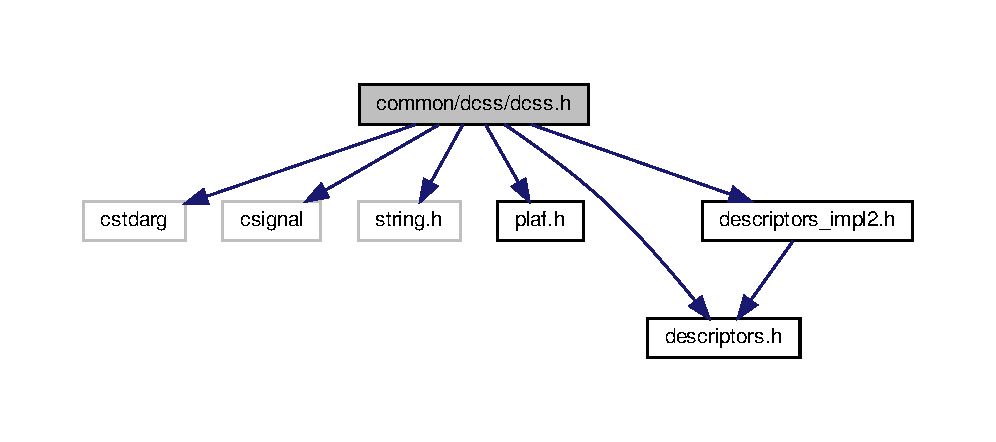
\includegraphics[width=350pt]{dcss_8h__incl}
\end{center}
\end{figure}
This graph shows which files directly or indirectly include this file\+:
\nopagebreak
\begin{figure}[H]
\begin{center}
\leavevmode
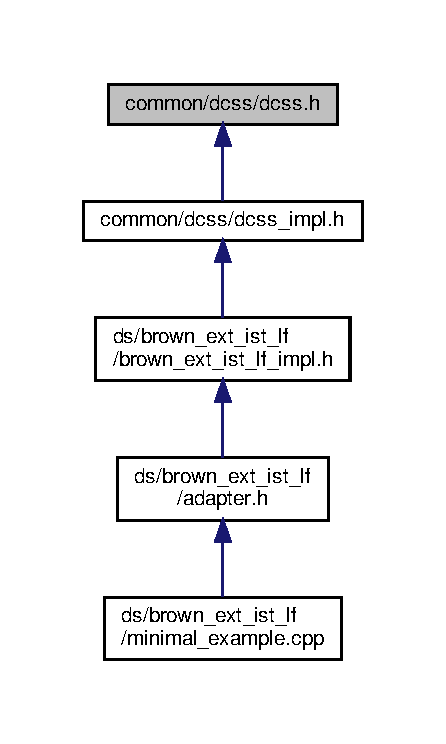
\includegraphics[width=214pt]{dcss_8h__dep__incl}
\end{center}
\end{figure}
\subsection*{Classes}
\begin{DoxyCompactItemize}
\item 
struct \hyperlink{structdcssresult__t}{dcssresult\+\_\+t}
\item 
class \hyperlink{classdcssdesc__t}{dcssdesc\+\_\+t}
\item 
class \hyperlink{classdcssProvider}{dcss\+Provider$<$ Unused $>$}
\end{DoxyCompactItemize}
\subsection*{Macros}
\begin{DoxyCompactItemize}
\item 
\#define \hyperlink{dcss_8h_a217a0bd562b98ae8c2ffce44935351e1}{likely}(x)~\+\_\+\+\_\+builtin\+\_\+expect((x),1)
\item 
\#define \hyperlink{dcss_8h_ac6c45889010c1bd68631771b64f18101}{unlikely}(x)~\+\_\+\+\_\+builtin\+\_\+expect((x),0)
\item 
\#define \hyperlink{dcss_8h_a154e6de939751b6476f6b58f8ef45805}{dcsstagptr\+\_\+t}~uintptr\+\_\+t
\item 
\#define \hyperlink{dcss_8h_ad0886cc4b71b2b53b8d1463285223511}{dcssptr\+\_\+t}~\hyperlink{classdcssdesc__t}{dcssdesc\+\_\+t} $\ast$
\item 
\#define \hyperlink{dcss_8h_ad45142aaf2ff20a036dc6242b8483e9c}{casword\+\_\+t}~intptr\+\_\+t
\item 
\#define \hyperlink{dcss_8h_aae439bef6bf980518592501efcab6690}{D\+C\+S\+S\+\_\+\+S\+T\+A\+T\+E\+\_\+\+U\+N\+D\+E\+C\+I\+D\+ED}~0
\item 
\#define \hyperlink{dcss_8h_aa6368e246a6b0aa38af390ada71f5f57}{D\+C\+S\+S\+\_\+\+S\+T\+A\+T\+E\+\_\+\+S\+U\+C\+C\+E\+E\+D\+ED}~4
\item 
\#define \hyperlink{dcss_8h_acb97f8e749590e5f4ee43390b9738f82}{D\+C\+S\+S\+\_\+\+S\+T\+A\+T\+E\+\_\+\+F\+A\+I\+L\+ED}~8
\item 
\#define \hyperlink{dcss_8h_ae3083015c889e3f6932a513b22d84ce5}{D\+C\+S\+S\+\_\+\+L\+E\+F\+T\+S\+H\+I\+FT}~1
\item 
\#define \hyperlink{dcss_8h_ab34ad21d7dc9053913afab4622729586}{D\+C\+S\+S\+\_\+\+I\+G\+N\+O\+R\+E\+D\+\_\+\+R\+E\+T\+V\+AL}~-\/1
\item 
\#define \hyperlink{dcss_8h_a015cb1f2a174983d0a26eaafaf9fb53e}{D\+C\+S\+S\+\_\+\+S\+U\+C\+C\+E\+SS}~0
\item 
\#define \hyperlink{dcss_8h_ace6386651b0adb05f0725a331f731668}{D\+C\+S\+S\+\_\+\+F\+A\+I\+L\+E\+D\+\_\+\+A\+D\+D\+R1}~1
\item 
\#define \hyperlink{dcss_8h_a6a5b852559bfdc2ec140bb098a47293f}{D\+C\+S\+S\+\_\+\+F\+A\+I\+L\+E\+D\+\_\+\+A\+D\+D\+R2}~2
\item 
\#define \hyperlink{dcss_8h_af06e916cb13168b5e10308a196165616}{M\+A\+X\+\_\+\+P\+A\+Y\+L\+O\+A\+D\+\_\+\+P\+T\+RS}~6
\item 
\#define \hyperlink{dcss_8h_adf0da31d05829a9d73eae33f26b80c05}{D\+C\+S\+S\+\_\+\+M\+U\+T\+A\+B\+L\+E\+S\+\_\+\+O\+F\+F\+S\+E\+T\+\_\+\+S\+T\+A\+TE}~0
\item 
\#define \hyperlink{dcss_8h_a89df9643ceefd0467edb368b815ef308}{D\+C\+S\+S\+\_\+\+M\+U\+T\+A\+B\+L\+E\+S\+\_\+\+M\+A\+S\+K\+\_\+\+S\+T\+A\+TE}~0xf
\item 
\#define \hyperlink{dcss_8h_aa843139a59bf78dea0454be82fba84b5}{D\+C\+S\+S\+\_\+\+M\+U\+T\+A\+B\+L\+E\+S\+\_\+\+N\+EW}(\hyperlink{scxrecord_8h_a71e82299f9d0709f1d5c5448d59347cb}{mutables})
\end{DoxyCompactItemize}
\subsection*{Functions}
\begin{DoxyCompactItemize}
\item 
class \hyperlink{classdcssdesc__t}{dcssdesc\+\_\+t} \hyperlink{dcss_8h_afe9e116a3017313d24a2f846a5a8986e}{\+\_\+\+\_\+attribute\+\_\+\+\_\+} ((aligned(64)))
\end{DoxyCompactItemize}
\subsection*{Variables}
\begin{DoxyCompactItemize}
\item 
volatile \hyperlink{descriptors_8h_a8a5af2749482b19d7515054489efca22}{mutables\+\_\+t} \hyperlink{dcss_8h_a71e82299f9d0709f1d5c5448d59347cb}{mutables}
\item 
\hyperlink{rq__unsafe_8h_ad45142aaf2ff20a036dc6242b8483e9c}{casword\+\_\+t} volatile $\ast$volatile \hyperlink{dcss_8h_ab6efe132b48802b8ded1b0b96b6b1ac4}{addr1}
\item 
\hyperlink{rq__unsafe_8h_ad45142aaf2ff20a036dc6242b8483e9c}{casword\+\_\+t} volatile \hyperlink{dcss_8h_aa0ef3ea06e00e9bcff2d000c6b85fe3b}{old1}
\item 
\hyperlink{rq__unsafe_8h_ad45142aaf2ff20a036dc6242b8483e9c}{casword\+\_\+t} volatile $\ast$volatile \hyperlink{dcss_8h_a0ad274c6e518135c37d5936aa6d444d4}{addr2}
\item 
\hyperlink{rq__unsafe_8h_ad45142aaf2ff20a036dc6242b8483e9c}{casword\+\_\+t} volatile \hyperlink{dcss_8h_a5b804866c13543d14361d31600569ea0}{old2}
\item 
\hyperlink{rq__unsafe_8h_ad45142aaf2ff20a036dc6242b8483e9c}{casword\+\_\+t} volatile \hyperlink{dcss_8h_afb2dbab2085e7b033fef7da6fb451593}{new2}
\item 
char \hyperlink{dcss_8h_a62fe47839abd2bf7f57690839be6b348}{padding} \mbox{[}\hyperlink{plaf_8h_a9492d3f4847aa8514510373df7ad0e73}{P\+R\+E\+F\+E\+T\+C\+H\+\_\+\+S\+I\+Z\+E\+\_\+\+B\+Y\+T\+ES}+(((64$<$$<$ 10) -\/size\%64)\%64)\mbox{]}
\item 
class \hyperlink{classdcssProvider}{dcss\+Provider} \hyperlink{dcss_8h_aede95b1db34b5c512d0394b79d40f991}{\+\_\+\+\_\+attribute\+\_\+\+\_\+}
\end{DoxyCompactItemize}


\subsection{Macro Definition Documentation}
\mbox{\Hypertarget{dcss_8h_ad45142aaf2ff20a036dc6242b8483e9c}\label{dcss_8h_ad45142aaf2ff20a036dc6242b8483e9c}} 
\index{dcss.\+h@{dcss.\+h}!casword\+\_\+t@{casword\+\_\+t}}
\index{casword\+\_\+t@{casword\+\_\+t}!dcss.\+h@{dcss.\+h}}
\subsubsection{\texorpdfstring{casword\+\_\+t}{casword\_t}}
{\footnotesize\ttfamily \#define casword\+\_\+t~intptr\+\_\+t}

\mbox{\Hypertarget{dcss_8h_ace6386651b0adb05f0725a331f731668}\label{dcss_8h_ace6386651b0adb05f0725a331f731668}} 
\index{dcss.\+h@{dcss.\+h}!D\+C\+S\+S\+\_\+\+F\+A\+I\+L\+E\+D\+\_\+\+A\+D\+D\+R1@{D\+C\+S\+S\+\_\+\+F\+A\+I\+L\+E\+D\+\_\+\+A\+D\+D\+R1}}
\index{D\+C\+S\+S\+\_\+\+F\+A\+I\+L\+E\+D\+\_\+\+A\+D\+D\+R1@{D\+C\+S\+S\+\_\+\+F\+A\+I\+L\+E\+D\+\_\+\+A\+D\+D\+R1}!dcss.\+h@{dcss.\+h}}
\subsubsection{\texorpdfstring{D\+C\+S\+S\+\_\+\+F\+A\+I\+L\+E\+D\+\_\+\+A\+D\+D\+R1}{DCSS\_FAILED\_ADDR1}}
{\footnotesize\ttfamily \#define D\+C\+S\+S\+\_\+\+F\+A\+I\+L\+E\+D\+\_\+\+A\+D\+D\+R1~1}

\mbox{\Hypertarget{dcss_8h_a6a5b852559bfdc2ec140bb098a47293f}\label{dcss_8h_a6a5b852559bfdc2ec140bb098a47293f}} 
\index{dcss.\+h@{dcss.\+h}!D\+C\+S\+S\+\_\+\+F\+A\+I\+L\+E\+D\+\_\+\+A\+D\+D\+R2@{D\+C\+S\+S\+\_\+\+F\+A\+I\+L\+E\+D\+\_\+\+A\+D\+D\+R2}}
\index{D\+C\+S\+S\+\_\+\+F\+A\+I\+L\+E\+D\+\_\+\+A\+D\+D\+R2@{D\+C\+S\+S\+\_\+\+F\+A\+I\+L\+E\+D\+\_\+\+A\+D\+D\+R2}!dcss.\+h@{dcss.\+h}}
\subsubsection{\texorpdfstring{D\+C\+S\+S\+\_\+\+F\+A\+I\+L\+E\+D\+\_\+\+A\+D\+D\+R2}{DCSS\_FAILED\_ADDR2}}
{\footnotesize\ttfamily \#define D\+C\+S\+S\+\_\+\+F\+A\+I\+L\+E\+D\+\_\+\+A\+D\+D\+R2~2}

\mbox{\Hypertarget{dcss_8h_ab34ad21d7dc9053913afab4622729586}\label{dcss_8h_ab34ad21d7dc9053913afab4622729586}} 
\index{dcss.\+h@{dcss.\+h}!D\+C\+S\+S\+\_\+\+I\+G\+N\+O\+R\+E\+D\+\_\+\+R\+E\+T\+V\+AL@{D\+C\+S\+S\+\_\+\+I\+G\+N\+O\+R\+E\+D\+\_\+\+R\+E\+T\+V\+AL}}
\index{D\+C\+S\+S\+\_\+\+I\+G\+N\+O\+R\+E\+D\+\_\+\+R\+E\+T\+V\+AL@{D\+C\+S\+S\+\_\+\+I\+G\+N\+O\+R\+E\+D\+\_\+\+R\+E\+T\+V\+AL}!dcss.\+h@{dcss.\+h}}
\subsubsection{\texorpdfstring{D\+C\+S\+S\+\_\+\+I\+G\+N\+O\+R\+E\+D\+\_\+\+R\+E\+T\+V\+AL}{DCSS\_IGNORED\_RETVAL}}
{\footnotesize\ttfamily \#define D\+C\+S\+S\+\_\+\+I\+G\+N\+O\+R\+E\+D\+\_\+\+R\+E\+T\+V\+AL~-\/1}

\mbox{\Hypertarget{dcss_8h_ae3083015c889e3f6932a513b22d84ce5}\label{dcss_8h_ae3083015c889e3f6932a513b22d84ce5}} 
\index{dcss.\+h@{dcss.\+h}!D\+C\+S\+S\+\_\+\+L\+E\+F\+T\+S\+H\+I\+FT@{D\+C\+S\+S\+\_\+\+L\+E\+F\+T\+S\+H\+I\+FT}}
\index{D\+C\+S\+S\+\_\+\+L\+E\+F\+T\+S\+H\+I\+FT@{D\+C\+S\+S\+\_\+\+L\+E\+F\+T\+S\+H\+I\+FT}!dcss.\+h@{dcss.\+h}}
\subsubsection{\texorpdfstring{D\+C\+S\+S\+\_\+\+L\+E\+F\+T\+S\+H\+I\+FT}{DCSS\_LEFTSHIFT}}
{\footnotesize\ttfamily \#define D\+C\+S\+S\+\_\+\+L\+E\+F\+T\+S\+H\+I\+FT~1}

\mbox{\Hypertarget{dcss_8h_a89df9643ceefd0467edb368b815ef308}\label{dcss_8h_a89df9643ceefd0467edb368b815ef308}} 
\index{dcss.\+h@{dcss.\+h}!D\+C\+S\+S\+\_\+\+M\+U\+T\+A\+B\+L\+E\+S\+\_\+\+M\+A\+S\+K\+\_\+\+S\+T\+A\+TE@{D\+C\+S\+S\+\_\+\+M\+U\+T\+A\+B\+L\+E\+S\+\_\+\+M\+A\+S\+K\+\_\+\+S\+T\+A\+TE}}
\index{D\+C\+S\+S\+\_\+\+M\+U\+T\+A\+B\+L\+E\+S\+\_\+\+M\+A\+S\+K\+\_\+\+S\+T\+A\+TE@{D\+C\+S\+S\+\_\+\+M\+U\+T\+A\+B\+L\+E\+S\+\_\+\+M\+A\+S\+K\+\_\+\+S\+T\+A\+TE}!dcss.\+h@{dcss.\+h}}
\subsubsection{\texorpdfstring{D\+C\+S\+S\+\_\+\+M\+U\+T\+A\+B\+L\+E\+S\+\_\+\+M\+A\+S\+K\+\_\+\+S\+T\+A\+TE}{DCSS\_MUTABLES\_MASK\_STATE}}
{\footnotesize\ttfamily \#define D\+C\+S\+S\+\_\+\+M\+U\+T\+A\+B\+L\+E\+S\+\_\+\+M\+A\+S\+K\+\_\+\+S\+T\+A\+TE~0xf}

\mbox{\Hypertarget{dcss_8h_aa843139a59bf78dea0454be82fba84b5}\label{dcss_8h_aa843139a59bf78dea0454be82fba84b5}} 
\index{dcss.\+h@{dcss.\+h}!D\+C\+S\+S\+\_\+\+M\+U\+T\+A\+B\+L\+E\+S\+\_\+\+N\+EW@{D\+C\+S\+S\+\_\+\+M\+U\+T\+A\+B\+L\+E\+S\+\_\+\+N\+EW}}
\index{D\+C\+S\+S\+\_\+\+M\+U\+T\+A\+B\+L\+E\+S\+\_\+\+N\+EW@{D\+C\+S\+S\+\_\+\+M\+U\+T\+A\+B\+L\+E\+S\+\_\+\+N\+EW}!dcss.\+h@{dcss.\+h}}
\subsubsection{\texorpdfstring{D\+C\+S\+S\+\_\+\+M\+U\+T\+A\+B\+L\+E\+S\+\_\+\+N\+EW}{DCSS\_MUTABLES\_NEW}}
{\footnotesize\ttfamily \#define D\+C\+S\+S\+\_\+\+M\+U\+T\+A\+B\+L\+E\+S\+\_\+\+N\+EW(\begin{DoxyParamCaption}\item[{}]{\hyperlink{scxrecord_8h_a71e82299f9d0709f1d5c5448d59347cb}{mutables} }\end{DoxyParamCaption})}

{\bfseries Value\+:}
\begin{DoxyCode}
((((\hyperlink{dcss_8h_a71e82299f9d0709f1d5c5448d59347cb}{mutables})&\hyperlink{descriptors__impl2_8h_a95444ce25f4d0a2711f4407cb99e28c5}{MASK\_SEQ})+(1<<\hyperlink{descriptors__impl2_8h_a130b75bf0ec168f61b83eb0662d75c3d}{OFFSET\_SEQ})) \(\backslash\)
        | (\hyperlink{dcss_8h_aae439bef6bf980518592501efcab6690}{DCSS\_STATE\_UNDECIDED}<<\hyperlink{dcss_8h_adf0da31d05829a9d73eae33f26b80c05}{DCSS\_MUTABLES\_OFFSET\_STATE}))
\end{DoxyCode}
\mbox{\Hypertarget{dcss_8h_adf0da31d05829a9d73eae33f26b80c05}\label{dcss_8h_adf0da31d05829a9d73eae33f26b80c05}} 
\index{dcss.\+h@{dcss.\+h}!D\+C\+S\+S\+\_\+\+M\+U\+T\+A\+B\+L\+E\+S\+\_\+\+O\+F\+F\+S\+E\+T\+\_\+\+S\+T\+A\+TE@{D\+C\+S\+S\+\_\+\+M\+U\+T\+A\+B\+L\+E\+S\+\_\+\+O\+F\+F\+S\+E\+T\+\_\+\+S\+T\+A\+TE}}
\index{D\+C\+S\+S\+\_\+\+M\+U\+T\+A\+B\+L\+E\+S\+\_\+\+O\+F\+F\+S\+E\+T\+\_\+\+S\+T\+A\+TE@{D\+C\+S\+S\+\_\+\+M\+U\+T\+A\+B\+L\+E\+S\+\_\+\+O\+F\+F\+S\+E\+T\+\_\+\+S\+T\+A\+TE}!dcss.\+h@{dcss.\+h}}
\subsubsection{\texorpdfstring{D\+C\+S\+S\+\_\+\+M\+U\+T\+A\+B\+L\+E\+S\+\_\+\+O\+F\+F\+S\+E\+T\+\_\+\+S\+T\+A\+TE}{DCSS\_MUTABLES\_OFFSET\_STATE}}
{\footnotesize\ttfamily \#define D\+C\+S\+S\+\_\+\+M\+U\+T\+A\+B\+L\+E\+S\+\_\+\+O\+F\+F\+S\+E\+T\+\_\+\+S\+T\+A\+TE~0}

Data definitions \mbox{\Hypertarget{dcss_8h_acb97f8e749590e5f4ee43390b9738f82}\label{dcss_8h_acb97f8e749590e5f4ee43390b9738f82}} 
\index{dcss.\+h@{dcss.\+h}!D\+C\+S\+S\+\_\+\+S\+T\+A\+T\+E\+\_\+\+F\+A\+I\+L\+ED@{D\+C\+S\+S\+\_\+\+S\+T\+A\+T\+E\+\_\+\+F\+A\+I\+L\+ED}}
\index{D\+C\+S\+S\+\_\+\+S\+T\+A\+T\+E\+\_\+\+F\+A\+I\+L\+ED@{D\+C\+S\+S\+\_\+\+S\+T\+A\+T\+E\+\_\+\+F\+A\+I\+L\+ED}!dcss.\+h@{dcss.\+h}}
\subsubsection{\texorpdfstring{D\+C\+S\+S\+\_\+\+S\+T\+A\+T\+E\+\_\+\+F\+A\+I\+L\+ED}{DCSS\_STATE\_FAILED}}
{\footnotesize\ttfamily \#define D\+C\+S\+S\+\_\+\+S\+T\+A\+T\+E\+\_\+\+F\+A\+I\+L\+ED~8}

\mbox{\Hypertarget{dcss_8h_aa6368e246a6b0aa38af390ada71f5f57}\label{dcss_8h_aa6368e246a6b0aa38af390ada71f5f57}} 
\index{dcss.\+h@{dcss.\+h}!D\+C\+S\+S\+\_\+\+S\+T\+A\+T\+E\+\_\+\+S\+U\+C\+C\+E\+E\+D\+ED@{D\+C\+S\+S\+\_\+\+S\+T\+A\+T\+E\+\_\+\+S\+U\+C\+C\+E\+E\+D\+ED}}
\index{D\+C\+S\+S\+\_\+\+S\+T\+A\+T\+E\+\_\+\+S\+U\+C\+C\+E\+E\+D\+ED@{D\+C\+S\+S\+\_\+\+S\+T\+A\+T\+E\+\_\+\+S\+U\+C\+C\+E\+E\+D\+ED}!dcss.\+h@{dcss.\+h}}
\subsubsection{\texorpdfstring{D\+C\+S\+S\+\_\+\+S\+T\+A\+T\+E\+\_\+\+S\+U\+C\+C\+E\+E\+D\+ED}{DCSS\_STATE\_SUCCEEDED}}
{\footnotesize\ttfamily \#define D\+C\+S\+S\+\_\+\+S\+T\+A\+T\+E\+\_\+\+S\+U\+C\+C\+E\+E\+D\+ED~4}

\mbox{\Hypertarget{dcss_8h_aae439bef6bf980518592501efcab6690}\label{dcss_8h_aae439bef6bf980518592501efcab6690}} 
\index{dcss.\+h@{dcss.\+h}!D\+C\+S\+S\+\_\+\+S\+T\+A\+T\+E\+\_\+\+U\+N\+D\+E\+C\+I\+D\+ED@{D\+C\+S\+S\+\_\+\+S\+T\+A\+T\+E\+\_\+\+U\+N\+D\+E\+C\+I\+D\+ED}}
\index{D\+C\+S\+S\+\_\+\+S\+T\+A\+T\+E\+\_\+\+U\+N\+D\+E\+C\+I\+D\+ED@{D\+C\+S\+S\+\_\+\+S\+T\+A\+T\+E\+\_\+\+U\+N\+D\+E\+C\+I\+D\+ED}!dcss.\+h@{dcss.\+h}}
\subsubsection{\texorpdfstring{D\+C\+S\+S\+\_\+\+S\+T\+A\+T\+E\+\_\+\+U\+N\+D\+E\+C\+I\+D\+ED}{DCSS\_STATE\_UNDECIDED}}
{\footnotesize\ttfamily \#define D\+C\+S\+S\+\_\+\+S\+T\+A\+T\+E\+\_\+\+U\+N\+D\+E\+C\+I\+D\+ED~0}

\mbox{\Hypertarget{dcss_8h_a015cb1f2a174983d0a26eaafaf9fb53e}\label{dcss_8h_a015cb1f2a174983d0a26eaafaf9fb53e}} 
\index{dcss.\+h@{dcss.\+h}!D\+C\+S\+S\+\_\+\+S\+U\+C\+C\+E\+SS@{D\+C\+S\+S\+\_\+\+S\+U\+C\+C\+E\+SS}}
\index{D\+C\+S\+S\+\_\+\+S\+U\+C\+C\+E\+SS@{D\+C\+S\+S\+\_\+\+S\+U\+C\+C\+E\+SS}!dcss.\+h@{dcss.\+h}}
\subsubsection{\texorpdfstring{D\+C\+S\+S\+\_\+\+S\+U\+C\+C\+E\+SS}{DCSS\_SUCCESS}}
{\footnotesize\ttfamily \#define D\+C\+S\+S\+\_\+\+S\+U\+C\+C\+E\+SS~0}

\mbox{\Hypertarget{dcss_8h_ad0886cc4b71b2b53b8d1463285223511}\label{dcss_8h_ad0886cc4b71b2b53b8d1463285223511}} 
\index{dcss.\+h@{dcss.\+h}!dcssptr\+\_\+t@{dcssptr\+\_\+t}}
\index{dcssptr\+\_\+t@{dcssptr\+\_\+t}!dcss.\+h@{dcss.\+h}}
\subsubsection{\texorpdfstring{dcssptr\+\_\+t}{dcssptr\_t}}
{\footnotesize\ttfamily \#define dcssptr\+\_\+t~\hyperlink{classdcssdesc__t}{dcssdesc\+\_\+t} $\ast$}

\mbox{\Hypertarget{dcss_8h_a154e6de939751b6476f6b58f8ef45805}\label{dcss_8h_a154e6de939751b6476f6b58f8ef45805}} 
\index{dcss.\+h@{dcss.\+h}!dcsstagptr\+\_\+t@{dcsstagptr\+\_\+t}}
\index{dcsstagptr\+\_\+t@{dcsstagptr\+\_\+t}!dcss.\+h@{dcss.\+h}}
\subsubsection{\texorpdfstring{dcsstagptr\+\_\+t}{dcsstagptr\_t}}
{\footnotesize\ttfamily \#define dcsstagptr\+\_\+t~uintptr\+\_\+t}

\mbox{\Hypertarget{dcss_8h_a217a0bd562b98ae8c2ffce44935351e1}\label{dcss_8h_a217a0bd562b98ae8c2ffce44935351e1}} 
\index{dcss.\+h@{dcss.\+h}!likely@{likely}}
\index{likely@{likely}!dcss.\+h@{dcss.\+h}}
\subsubsection{\texorpdfstring{likely}{likely}}
{\footnotesize\ttfamily \#define likely(\begin{DoxyParamCaption}\item[{}]{x }\end{DoxyParamCaption})~\+\_\+\+\_\+builtin\+\_\+expect((x),1)}

\mbox{\Hypertarget{dcss_8h_af06e916cb13168b5e10308a196165616}\label{dcss_8h_af06e916cb13168b5e10308a196165616}} 
\index{dcss.\+h@{dcss.\+h}!M\+A\+X\+\_\+\+P\+A\+Y\+L\+O\+A\+D\+\_\+\+P\+T\+RS@{M\+A\+X\+\_\+\+P\+A\+Y\+L\+O\+A\+D\+\_\+\+P\+T\+RS}}
\index{M\+A\+X\+\_\+\+P\+A\+Y\+L\+O\+A\+D\+\_\+\+P\+T\+RS@{M\+A\+X\+\_\+\+P\+A\+Y\+L\+O\+A\+D\+\_\+\+P\+T\+RS}!dcss.\+h@{dcss.\+h}}
\subsubsection{\texorpdfstring{M\+A\+X\+\_\+\+P\+A\+Y\+L\+O\+A\+D\+\_\+\+P\+T\+RS}{MAX\_PAYLOAD\_PTRS}}
{\footnotesize\ttfamily \#define M\+A\+X\+\_\+\+P\+A\+Y\+L\+O\+A\+D\+\_\+\+P\+T\+RS~6}

\mbox{\Hypertarget{dcss_8h_ac6c45889010c1bd68631771b64f18101}\label{dcss_8h_ac6c45889010c1bd68631771b64f18101}} 
\index{dcss.\+h@{dcss.\+h}!unlikely@{unlikely}}
\index{unlikely@{unlikely}!dcss.\+h@{dcss.\+h}}
\subsubsection{\texorpdfstring{unlikely}{unlikely}}
{\footnotesize\ttfamily \#define unlikely(\begin{DoxyParamCaption}\item[{}]{x }\end{DoxyParamCaption})~\+\_\+\+\_\+builtin\+\_\+expect((x),0)}



\subsection{Function Documentation}
\mbox{\Hypertarget{dcss_8h_afe9e116a3017313d24a2f846a5a8986e}\label{dcss_8h_afe9e116a3017313d24a2f846a5a8986e}} 
\index{dcss.\+h@{dcss.\+h}!\+\_\+\+\_\+attribute\+\_\+\+\_\+@{\+\_\+\+\_\+attribute\+\_\+\+\_\+}}
\index{\+\_\+\+\_\+attribute\+\_\+\+\_\+@{\+\_\+\+\_\+attribute\+\_\+\+\_\+}!dcss.\+h@{dcss.\+h}}
\subsubsection{\texorpdfstring{\+\_\+\+\_\+attribute\+\_\+\+\_\+()}{\_\_attribute\_\_()}}
{\footnotesize\ttfamily class \hyperlink{classdcssdesc__t}{dcssdesc\+\_\+t} \+\_\+\+\_\+attribute\+\_\+\+\_\+ (\begin{DoxyParamCaption}\item[{(aligned(64))}]{ }\end{DoxyParamCaption})}



\subsection{Variable Documentation}
\mbox{\Hypertarget{dcss_8h_aede95b1db34b5c512d0394b79d40f991}\label{dcss_8h_aede95b1db34b5c512d0394b79d40f991}} 
\index{dcss.\+h@{dcss.\+h}!\+\_\+\+\_\+attribute\+\_\+\+\_\+@{\+\_\+\+\_\+attribute\+\_\+\+\_\+}}
\index{\+\_\+\+\_\+attribute\+\_\+\+\_\+@{\+\_\+\+\_\+attribute\+\_\+\+\_\+}!dcss.\+h@{dcss.\+h}}
\subsubsection{\texorpdfstring{\+\_\+\+\_\+attribute\+\_\+\+\_\+}{\_\_attribute\_\_}}
{\footnotesize\ttfamily class \hyperlink{classdcssProvider}{dcss\+Provider}  \+\_\+\+\_\+attribute\+\_\+\+\_\+}

\mbox{\Hypertarget{dcss_8h_ab6efe132b48802b8ded1b0b96b6b1ac4}\label{dcss_8h_ab6efe132b48802b8ded1b0b96b6b1ac4}} 
\index{dcss.\+h@{dcss.\+h}!addr1@{addr1}}
\index{addr1@{addr1}!dcss.\+h@{dcss.\+h}}
\subsubsection{\texorpdfstring{addr1}{addr1}}
{\footnotesize\ttfamily \hyperlink{rq__unsafe_8h_ad45142aaf2ff20a036dc6242b8483e9c}{casword\+\_\+t} volatile$\ast$ volatile addr1}

\mbox{\Hypertarget{dcss_8h_a0ad274c6e518135c37d5936aa6d444d4}\label{dcss_8h_a0ad274c6e518135c37d5936aa6d444d4}} 
\index{dcss.\+h@{dcss.\+h}!addr2@{addr2}}
\index{addr2@{addr2}!dcss.\+h@{dcss.\+h}}
\subsubsection{\texorpdfstring{addr2}{addr2}}
{\footnotesize\ttfamily \hyperlink{rq__unsafe_8h_ad45142aaf2ff20a036dc6242b8483e9c}{casword\+\_\+t} volatile$\ast$ volatile addr2}

\mbox{\Hypertarget{dcss_8h_a71e82299f9d0709f1d5c5448d59347cb}\label{dcss_8h_a71e82299f9d0709f1d5c5448d59347cb}} 
\index{dcss.\+h@{dcss.\+h}!mutables@{mutables}}
\index{mutables@{mutables}!dcss.\+h@{dcss.\+h}}
\subsubsection{\texorpdfstring{mutables}{mutables}}
{\footnotesize\ttfamily volatile \hyperlink{descriptors_8h_a8a5af2749482b19d7515054489efca22}{mutables\+\_\+t} mutables}

\mbox{\Hypertarget{dcss_8h_afb2dbab2085e7b033fef7da6fb451593}\label{dcss_8h_afb2dbab2085e7b033fef7da6fb451593}} 
\index{dcss.\+h@{dcss.\+h}!new2@{new2}}
\index{new2@{new2}!dcss.\+h@{dcss.\+h}}
\subsubsection{\texorpdfstring{new2}{new2}}
{\footnotesize\ttfamily \hyperlink{rq__unsafe_8h_ad45142aaf2ff20a036dc6242b8483e9c}{casword\+\_\+t} volatile new2}

\mbox{\Hypertarget{dcss_8h_aa0ef3ea06e00e9bcff2d000c6b85fe3b}\label{dcss_8h_aa0ef3ea06e00e9bcff2d000c6b85fe3b}} 
\index{dcss.\+h@{dcss.\+h}!old1@{old1}}
\index{old1@{old1}!dcss.\+h@{dcss.\+h}}
\subsubsection{\texorpdfstring{old1}{old1}}
{\footnotesize\ttfamily \hyperlink{rq__unsafe_8h_ad45142aaf2ff20a036dc6242b8483e9c}{casword\+\_\+t} volatile old1}

\mbox{\Hypertarget{dcss_8h_a5b804866c13543d14361d31600569ea0}\label{dcss_8h_a5b804866c13543d14361d31600569ea0}} 
\index{dcss.\+h@{dcss.\+h}!old2@{old2}}
\index{old2@{old2}!dcss.\+h@{dcss.\+h}}
\subsubsection{\texorpdfstring{old2}{old2}}
{\footnotesize\ttfamily \hyperlink{rq__unsafe_8h_ad45142aaf2ff20a036dc6242b8483e9c}{casword\+\_\+t} volatile old2}

\mbox{\Hypertarget{dcss_8h_a62fe47839abd2bf7f57690839be6b348}\label{dcss_8h_a62fe47839abd2bf7f57690839be6b348}} 
\index{dcss.\+h@{dcss.\+h}!padding@{padding}}
\index{padding@{padding}!dcss.\+h@{dcss.\+h}}
\subsubsection{\texorpdfstring{padding}{padding}}
{\footnotesize\ttfamily char padding\mbox{[}\hyperlink{plaf_8h_a9492d3f4847aa8514510373df7ad0e73}{P\+R\+E\+F\+E\+T\+C\+H\+\_\+\+S\+I\+Z\+E\+\_\+\+B\+Y\+T\+ES}+(((64$<$$<$ 10) -\/size\%64)\%64)\mbox{]}}


\hypertarget{dcss__impl_8h}{}\section{common/dcss/dcss\+\_\+impl.h File Reference}
\label{dcss__impl_8h}\index{common/dcss/dcss\+\_\+impl.\+h@{common/dcss/dcss\+\_\+impl.\+h}}
{\ttfamily \#include \char`\"{}dcss.\+h\char`\"{}}\newline
{\ttfamily \#include $<$cassert$>$}\newline
{\ttfamily \#include $<$stdint.\+h$>$}\newline
{\ttfamily \#include $<$sstream$>$}\newline
Include dependency graph for dcss\+\_\+impl.\+h\+:
\nopagebreak
\begin{figure}[H]
\begin{center}
\leavevmode
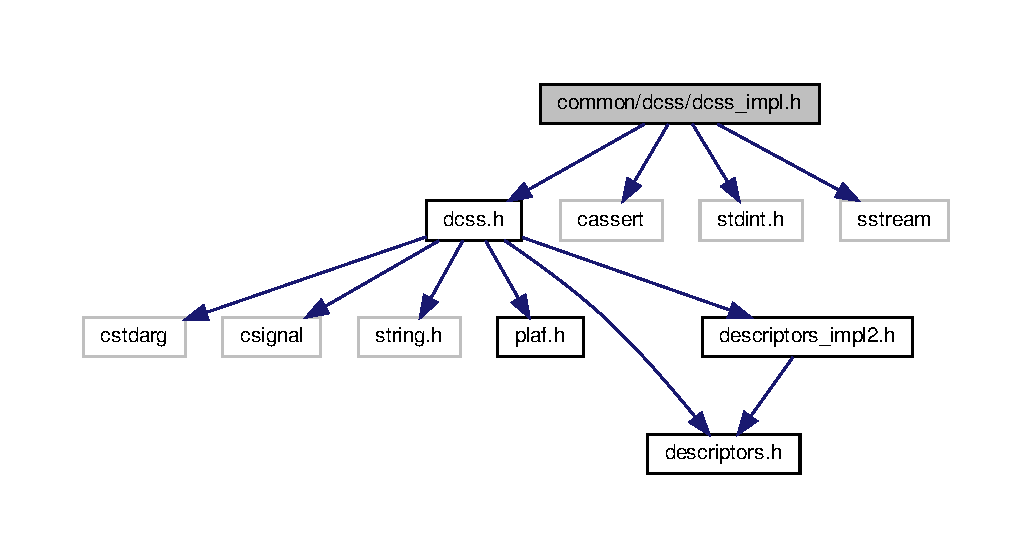
\includegraphics[width=350pt]{dcss__impl_8h__incl}
\end{center}
\end{figure}
This graph shows which files directly or indirectly include this file\+:
\nopagebreak
\begin{figure}[H]
\begin{center}
\leavevmode
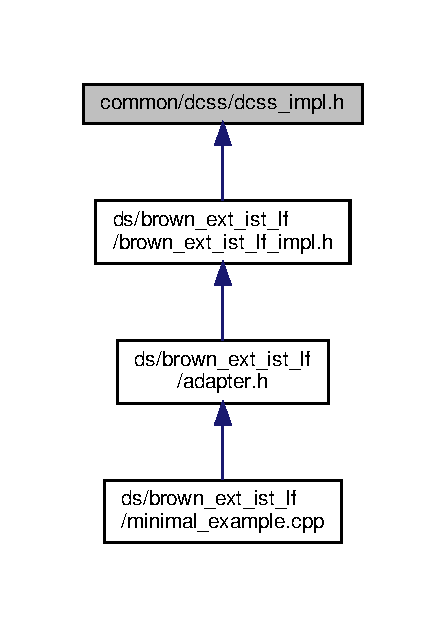
\includegraphics[width=214pt]{dcss__impl_8h__dep__incl}
\end{center}
\end{figure}
\subsection*{Macros}
\begin{DoxyCompactItemize}
\item 
\#define \hyperlink{dcss__impl_8h_a6bd312b05b209f8fce93c657186bbeb0}{B\+O\+O\+L\+\_\+\+C\+AS}~\+\_\+\+\_\+sync\+\_\+bool\+\_\+compare\+\_\+and\+\_\+swap
\item 
\#define \hyperlink{dcss__impl_8h_aa7387507d9deee458fc9668893079a5f}{V\+A\+L\+\_\+\+C\+AS}~\+\_\+\+\_\+sync\+\_\+val\+\_\+compare\+\_\+and\+\_\+swap
\item 
\#define \hyperlink{dcss__impl_8h_ac2a6ee418f6a4c5ec28e23229e554cf2}{D\+C\+S\+S\+\_\+\+T\+A\+G\+B\+IT}~0x1
\end{DoxyCompactItemize}


\subsection{Macro Definition Documentation}
\mbox{\Hypertarget{dcss__impl_8h_a6bd312b05b209f8fce93c657186bbeb0}\label{dcss__impl_8h_a6bd312b05b209f8fce93c657186bbeb0}} 
\index{dcss\+\_\+impl.\+h@{dcss\+\_\+impl.\+h}!B\+O\+O\+L\+\_\+\+C\+AS@{B\+O\+O\+L\+\_\+\+C\+AS}}
\index{B\+O\+O\+L\+\_\+\+C\+AS@{B\+O\+O\+L\+\_\+\+C\+AS}!dcss\+\_\+impl.\+h@{dcss\+\_\+impl.\+h}}
\subsubsection{\texorpdfstring{B\+O\+O\+L\+\_\+\+C\+AS}{BOOL\_CAS}}
{\footnotesize\ttfamily \#define B\+O\+O\+L\+\_\+\+C\+AS~\+\_\+\+\_\+sync\+\_\+bool\+\_\+compare\+\_\+and\+\_\+swap}

\mbox{\Hypertarget{dcss__impl_8h_ac2a6ee418f6a4c5ec28e23229e554cf2}\label{dcss__impl_8h_ac2a6ee418f6a4c5ec28e23229e554cf2}} 
\index{dcss\+\_\+impl.\+h@{dcss\+\_\+impl.\+h}!D\+C\+S\+S\+\_\+\+T\+A\+G\+B\+IT@{D\+C\+S\+S\+\_\+\+T\+A\+G\+B\+IT}}
\index{D\+C\+S\+S\+\_\+\+T\+A\+G\+B\+IT@{D\+C\+S\+S\+\_\+\+T\+A\+G\+B\+IT}!dcss\+\_\+impl.\+h@{dcss\+\_\+impl.\+h}}
\subsubsection{\texorpdfstring{D\+C\+S\+S\+\_\+\+T\+A\+G\+B\+IT}{DCSS\_TAGBIT}}
{\footnotesize\ttfamily \#define D\+C\+S\+S\+\_\+\+T\+A\+G\+B\+IT~0x1}

\mbox{\Hypertarget{dcss__impl_8h_aa7387507d9deee458fc9668893079a5f}\label{dcss__impl_8h_aa7387507d9deee458fc9668893079a5f}} 
\index{dcss\+\_\+impl.\+h@{dcss\+\_\+impl.\+h}!V\+A\+L\+\_\+\+C\+AS@{V\+A\+L\+\_\+\+C\+AS}}
\index{V\+A\+L\+\_\+\+C\+AS@{V\+A\+L\+\_\+\+C\+AS}!dcss\+\_\+impl.\+h@{dcss\+\_\+impl.\+h}}
\subsubsection{\texorpdfstring{V\+A\+L\+\_\+\+C\+AS}{VAL\_CAS}}
{\footnotesize\ttfamily \#define V\+A\+L\+\_\+\+C\+AS~\+\_\+\+\_\+sync\+\_\+val\+\_\+compare\+\_\+and\+\_\+swap}


\hypertarget{dcss__plus_8h}{}\section{common/dcss/dcss\+\_\+plus.h File Reference}
\label{dcss__plus_8h}\index{common/dcss/dcss\+\_\+plus.\+h@{common/dcss/dcss\+\_\+plus.\+h}}
{\ttfamily \#include $<$cstdarg$>$}\newline
{\ttfamily \#include $<$csignal$>$}\newline
{\ttfamily \#include $<$string.\+h$>$}\newline
{\ttfamily \#include \char`\"{}plaf.\+h\char`\"{}}\newline
{\ttfamily \#include \char`\"{}descriptors.\+h\char`\"{}}\newline
{\ttfamily \#include \char`\"{}descriptors\+\_\+impl2.\+h\char`\"{}}\newline
Include dependency graph for dcss\+\_\+plus.\+h\+:
\nopagebreak
\begin{figure}[H]
\begin{center}
\leavevmode
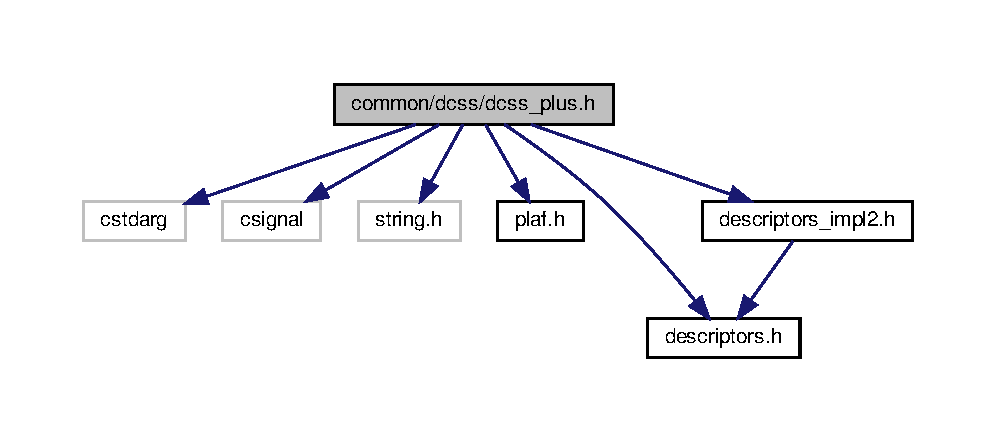
\includegraphics[width=350pt]{dcss__plus_8h__incl}
\end{center}
\end{figure}
This graph shows which files directly or indirectly include this file\+:
\nopagebreak
\begin{figure}[H]
\begin{center}
\leavevmode
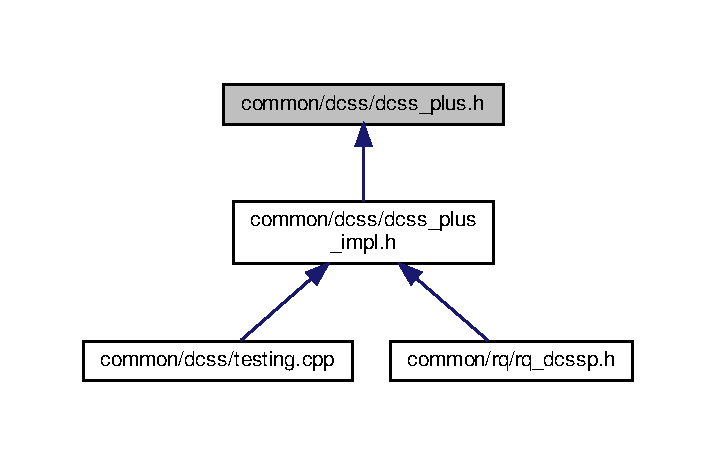
\includegraphics[width=344pt]{dcss__plus_8h__dep__incl}
\end{center}
\end{figure}
\subsection*{Classes}
\begin{DoxyCompactItemize}
\item 
struct \hyperlink{structdcsspresult__t}{dcsspresult\+\_\+t}
\item 
class \hyperlink{classdcsspdesc__t}{dcsspdesc\+\_\+t$<$ P\+A\+Y\+L\+O\+A\+D\+\_\+\+T $>$}
\item 
class \hyperlink{classdcsspProvider}{dcssp\+Provider$<$ P\+A\+Y\+L\+O\+A\+D\+\_\+\+T $>$}
\end{DoxyCompactItemize}
\subsection*{Macros}
\begin{DoxyCompactItemize}
\item 
\#define \hyperlink{dcss__plus_8h_afa90fac515a3c6b40a02a75bf1c2c413}{dcssptagptr\+\_\+t}~uintptr\+\_\+t
\item 
\#define \hyperlink{dcss__plus_8h_ad9478df19b8b267f41952068562989c0}{dcsspptr\+\_\+t}~\hyperlink{classdcsspdesc__t}{dcsspdesc\+\_\+t}$<$P\+A\+Y\+L\+O\+A\+D\+\_\+T$>$ $\ast$
\item 
\#define \hyperlink{dcss__plus_8h_ad45142aaf2ff20a036dc6242b8483e9c}{casword\+\_\+t}~intptr\+\_\+t
\item 
\#define \hyperlink{dcss__plus_8h_a475562294092a8967c57192c8682ec0e}{D\+C\+S\+S\+P\+\_\+\+S\+T\+A\+T\+E\+\_\+\+U\+N\+D\+E\+C\+I\+D\+ED}~0
\item 
\#define \hyperlink{dcss__plus_8h_a31afd4827e50a969edd5871416ebb6aa}{D\+C\+S\+S\+P\+\_\+\+S\+T\+A\+T\+E\+\_\+\+S\+U\+C\+C\+E\+E\+D\+ED}~4
\item 
\#define \hyperlink{dcss__plus_8h_a6da6fbc7662a5e6db2e22413396feaf2}{D\+C\+S\+S\+P\+\_\+\+S\+T\+A\+T\+E\+\_\+\+F\+A\+I\+L\+ED}~8
\item 
\#define \hyperlink{dcss__plus_8h_ae4ccd8eaaf48fb61a5df9f1c13c31644}{D\+C\+S\+S\+P\+\_\+\+L\+E\+F\+T\+S\+H\+I\+FT}~1
\item 
\#define \hyperlink{dcss__plus_8h_ac90ba4948ed8a16b7d63c242bf9372e5}{D\+C\+S\+S\+P\+\_\+\+I\+G\+N\+O\+R\+E\+D\+\_\+\+R\+E\+T\+V\+AL}~-\/1
\item 
\#define \hyperlink{dcss__plus_8h_ad88ac4f8f0a50d3cbeb8680fc7bfcd68}{D\+C\+S\+S\+P\+\_\+\+S\+U\+C\+C\+E\+SS}~0
\item 
\#define \hyperlink{dcss__plus_8h_a0b994529f5023fc022ee8140aacfbdd0}{D\+C\+S\+S\+P\+\_\+\+F\+A\+I\+L\+E\+D\+\_\+\+A\+D\+D\+R1}~1
\item 
\#define \hyperlink{dcss__plus_8h_ac525c0ea640caee564d26fa49fa2cba6}{D\+C\+S\+S\+P\+\_\+\+F\+A\+I\+L\+E\+D\+\_\+\+A\+D\+D\+R2}~2
\item 
\#define \hyperlink{dcss__plus_8h_af06e916cb13168b5e10308a196165616}{M\+A\+X\+\_\+\+P\+A\+Y\+L\+O\+A\+D\+\_\+\+P\+T\+RS}~6
\item 
\#define \hyperlink{dcss__plus_8h_acf2f88198277a9992acfcc9e556a2606}{D\+C\+S\+S\+P\+\_\+\+M\+U\+T\+A\+B\+L\+E\+S\+\_\+\+O\+F\+F\+S\+E\+T\+\_\+\+S\+T\+A\+TE}~0
\item 
\#define \hyperlink{dcss__plus_8h_a1eb1ed156d288170fc8ba97d4c40226f}{D\+C\+S\+S\+P\+\_\+\+M\+U\+T\+A\+B\+L\+E\+S\+\_\+\+M\+A\+S\+K\+\_\+\+S\+T\+A\+TE}~0xf
\item 
\#define \hyperlink{dcss__plus_8h_a2fb6c8319580973750fee030a686723e}{D\+C\+S\+S\+P\+\_\+\+M\+U\+T\+A\+B\+L\+E\+S\+\_\+\+N\+EW}(\hyperlink{scxrecord_8h_a71e82299f9d0709f1d5c5448d59347cb}{mutables})
\end{DoxyCompactItemize}
\subsection*{Functions}
\begin{DoxyCompactItemize}
\item 
{\footnotesize template$<$typename P\+A\+Y\+L\+O\+A\+D\+\_\+T $>$ }\\class \hyperlink{classdcsspdesc__t}{dcsspdesc\+\_\+t} \hyperlink{dcss__plus_8h_a281da2081c3980fc36d0e5153cb1af66}{\+\_\+\+\_\+attribute\+\_\+\+\_\+} ((aligned(64)))
\end{DoxyCompactItemize}
\subsection*{Variables}
\begin{DoxyCompactItemize}
\item 
volatile \hyperlink{descriptors_8h_a8a5af2749482b19d7515054489efca22}{mutables\+\_\+t} \hyperlink{dcss__plus_8h_a71e82299f9d0709f1d5c5448d59347cb}{mutables}
\item 
\hyperlink{rq__unsafe_8h_ad45142aaf2ff20a036dc6242b8483e9c}{casword\+\_\+t} volatile $\ast$volatile \hyperlink{dcss__plus_8h_ab6efe132b48802b8ded1b0b96b6b1ac4}{addr1}
\item 
\hyperlink{rq__unsafe_8h_ad45142aaf2ff20a036dc6242b8483e9c}{casword\+\_\+t} volatile \hyperlink{dcss__plus_8h_aa0ef3ea06e00e9bcff2d000c6b85fe3b}{old1}
\item 
\hyperlink{rq__unsafe_8h_ad45142aaf2ff20a036dc6242b8483e9c}{casword\+\_\+t} volatile $\ast$volatile \hyperlink{dcss__plus_8h_a0ad274c6e518135c37d5936aa6d444d4}{addr2}
\item 
\hyperlink{rq__unsafe_8h_ad45142aaf2ff20a036dc6242b8483e9c}{casword\+\_\+t} volatile \hyperlink{dcss__plus_8h_a5b804866c13543d14361d31600569ea0}{old2}
\item 
\hyperlink{rq__unsafe_8h_ad45142aaf2ff20a036dc6242b8483e9c}{casword\+\_\+t} volatile \hyperlink{dcss__plus_8h_afb2dbab2085e7b033fef7da6fb451593}{new2}
\item 
P\+A\+Y\+L\+O\+A\+D\+\_\+T volatile \hyperlink{dcss__plus_8h_ae31f029ce4ee978422e1969e49549e42}{payload1} \mbox{[}\hyperlink{dcss__plus_8h_af06e916cb13168b5e10308a196165616}{M\+A\+X\+\_\+\+P\+A\+Y\+L\+O\+A\+D\+\_\+\+P\+T\+RS}+1\mbox{]}
\item 
P\+A\+Y\+L\+O\+A\+D\+\_\+T volatile \hyperlink{dcss__plus_8h_ab5e9cbe9a7a8afb1c8f370c68c4ddc0e}{payload2} \mbox{[}\hyperlink{dcss__plus_8h_af06e916cb13168b5e10308a196165616}{M\+A\+X\+\_\+\+P\+A\+Y\+L\+O\+A\+D\+\_\+\+P\+T\+RS}+1\mbox{]}
\item 
char \hyperlink{dcss__plus_8h_a62fe47839abd2bf7f57690839be6b348}{padding} \mbox{[}\hyperlink{plaf_8h_a9492d3f4847aa8514510373df7ad0e73}{P\+R\+E\+F\+E\+T\+C\+H\+\_\+\+S\+I\+Z\+E\+\_\+\+B\+Y\+T\+ES}+(((64$<$$<$ 10) -\/size\%64)\%64)\mbox{]}
\item 
class \hyperlink{classdcsspProvider}{dcssp\+Provider} \hyperlink{dcss__plus_8h_a4e4cbff741428e2c63fdfe0d43f39330}{\+\_\+\+\_\+attribute\+\_\+\+\_\+}
\end{DoxyCompactItemize}


\subsection{Macro Definition Documentation}
\mbox{\Hypertarget{dcss__plus_8h_ad45142aaf2ff20a036dc6242b8483e9c}\label{dcss__plus_8h_ad45142aaf2ff20a036dc6242b8483e9c}} 
\index{dcss\+\_\+plus.\+h@{dcss\+\_\+plus.\+h}!casword\+\_\+t@{casword\+\_\+t}}
\index{casword\+\_\+t@{casword\+\_\+t}!dcss\+\_\+plus.\+h@{dcss\+\_\+plus.\+h}}
\subsubsection{\texorpdfstring{casword\+\_\+t}{casword\_t}}
{\footnotesize\ttfamily \#define casword\+\_\+t~intptr\+\_\+t}

\mbox{\Hypertarget{dcss__plus_8h_a0b994529f5023fc022ee8140aacfbdd0}\label{dcss__plus_8h_a0b994529f5023fc022ee8140aacfbdd0}} 
\index{dcss\+\_\+plus.\+h@{dcss\+\_\+plus.\+h}!D\+C\+S\+S\+P\+\_\+\+F\+A\+I\+L\+E\+D\+\_\+\+A\+D\+D\+R1@{D\+C\+S\+S\+P\+\_\+\+F\+A\+I\+L\+E\+D\+\_\+\+A\+D\+D\+R1}}
\index{D\+C\+S\+S\+P\+\_\+\+F\+A\+I\+L\+E\+D\+\_\+\+A\+D\+D\+R1@{D\+C\+S\+S\+P\+\_\+\+F\+A\+I\+L\+E\+D\+\_\+\+A\+D\+D\+R1}!dcss\+\_\+plus.\+h@{dcss\+\_\+plus.\+h}}
\subsubsection{\texorpdfstring{D\+C\+S\+S\+P\+\_\+\+F\+A\+I\+L\+E\+D\+\_\+\+A\+D\+D\+R1}{DCSSP\_FAILED\_ADDR1}}
{\footnotesize\ttfamily \#define D\+C\+S\+S\+P\+\_\+\+F\+A\+I\+L\+E\+D\+\_\+\+A\+D\+D\+R1~1}

\mbox{\Hypertarget{dcss__plus_8h_ac525c0ea640caee564d26fa49fa2cba6}\label{dcss__plus_8h_ac525c0ea640caee564d26fa49fa2cba6}} 
\index{dcss\+\_\+plus.\+h@{dcss\+\_\+plus.\+h}!D\+C\+S\+S\+P\+\_\+\+F\+A\+I\+L\+E\+D\+\_\+\+A\+D\+D\+R2@{D\+C\+S\+S\+P\+\_\+\+F\+A\+I\+L\+E\+D\+\_\+\+A\+D\+D\+R2}}
\index{D\+C\+S\+S\+P\+\_\+\+F\+A\+I\+L\+E\+D\+\_\+\+A\+D\+D\+R2@{D\+C\+S\+S\+P\+\_\+\+F\+A\+I\+L\+E\+D\+\_\+\+A\+D\+D\+R2}!dcss\+\_\+plus.\+h@{dcss\+\_\+plus.\+h}}
\subsubsection{\texorpdfstring{D\+C\+S\+S\+P\+\_\+\+F\+A\+I\+L\+E\+D\+\_\+\+A\+D\+D\+R2}{DCSSP\_FAILED\_ADDR2}}
{\footnotesize\ttfamily \#define D\+C\+S\+S\+P\+\_\+\+F\+A\+I\+L\+E\+D\+\_\+\+A\+D\+D\+R2~2}

\mbox{\Hypertarget{dcss__plus_8h_ac90ba4948ed8a16b7d63c242bf9372e5}\label{dcss__plus_8h_ac90ba4948ed8a16b7d63c242bf9372e5}} 
\index{dcss\+\_\+plus.\+h@{dcss\+\_\+plus.\+h}!D\+C\+S\+S\+P\+\_\+\+I\+G\+N\+O\+R\+E\+D\+\_\+\+R\+E\+T\+V\+AL@{D\+C\+S\+S\+P\+\_\+\+I\+G\+N\+O\+R\+E\+D\+\_\+\+R\+E\+T\+V\+AL}}
\index{D\+C\+S\+S\+P\+\_\+\+I\+G\+N\+O\+R\+E\+D\+\_\+\+R\+E\+T\+V\+AL@{D\+C\+S\+S\+P\+\_\+\+I\+G\+N\+O\+R\+E\+D\+\_\+\+R\+E\+T\+V\+AL}!dcss\+\_\+plus.\+h@{dcss\+\_\+plus.\+h}}
\subsubsection{\texorpdfstring{D\+C\+S\+S\+P\+\_\+\+I\+G\+N\+O\+R\+E\+D\+\_\+\+R\+E\+T\+V\+AL}{DCSSP\_IGNORED\_RETVAL}}
{\footnotesize\ttfamily \#define D\+C\+S\+S\+P\+\_\+\+I\+G\+N\+O\+R\+E\+D\+\_\+\+R\+E\+T\+V\+AL~-\/1}

\mbox{\Hypertarget{dcss__plus_8h_ae4ccd8eaaf48fb61a5df9f1c13c31644}\label{dcss__plus_8h_ae4ccd8eaaf48fb61a5df9f1c13c31644}} 
\index{dcss\+\_\+plus.\+h@{dcss\+\_\+plus.\+h}!D\+C\+S\+S\+P\+\_\+\+L\+E\+F\+T\+S\+H\+I\+FT@{D\+C\+S\+S\+P\+\_\+\+L\+E\+F\+T\+S\+H\+I\+FT}}
\index{D\+C\+S\+S\+P\+\_\+\+L\+E\+F\+T\+S\+H\+I\+FT@{D\+C\+S\+S\+P\+\_\+\+L\+E\+F\+T\+S\+H\+I\+FT}!dcss\+\_\+plus.\+h@{dcss\+\_\+plus.\+h}}
\subsubsection{\texorpdfstring{D\+C\+S\+S\+P\+\_\+\+L\+E\+F\+T\+S\+H\+I\+FT}{DCSSP\_LEFTSHIFT}}
{\footnotesize\ttfamily \#define D\+C\+S\+S\+P\+\_\+\+L\+E\+F\+T\+S\+H\+I\+FT~1}

\mbox{\Hypertarget{dcss__plus_8h_a1eb1ed156d288170fc8ba97d4c40226f}\label{dcss__plus_8h_a1eb1ed156d288170fc8ba97d4c40226f}} 
\index{dcss\+\_\+plus.\+h@{dcss\+\_\+plus.\+h}!D\+C\+S\+S\+P\+\_\+\+M\+U\+T\+A\+B\+L\+E\+S\+\_\+\+M\+A\+S\+K\+\_\+\+S\+T\+A\+TE@{D\+C\+S\+S\+P\+\_\+\+M\+U\+T\+A\+B\+L\+E\+S\+\_\+\+M\+A\+S\+K\+\_\+\+S\+T\+A\+TE}}
\index{D\+C\+S\+S\+P\+\_\+\+M\+U\+T\+A\+B\+L\+E\+S\+\_\+\+M\+A\+S\+K\+\_\+\+S\+T\+A\+TE@{D\+C\+S\+S\+P\+\_\+\+M\+U\+T\+A\+B\+L\+E\+S\+\_\+\+M\+A\+S\+K\+\_\+\+S\+T\+A\+TE}!dcss\+\_\+plus.\+h@{dcss\+\_\+plus.\+h}}
\subsubsection{\texorpdfstring{D\+C\+S\+S\+P\+\_\+\+M\+U\+T\+A\+B\+L\+E\+S\+\_\+\+M\+A\+S\+K\+\_\+\+S\+T\+A\+TE}{DCSSP\_MUTABLES\_MASK\_STATE}}
{\footnotesize\ttfamily \#define D\+C\+S\+S\+P\+\_\+\+M\+U\+T\+A\+B\+L\+E\+S\+\_\+\+M\+A\+S\+K\+\_\+\+S\+T\+A\+TE~0xf}

\mbox{\Hypertarget{dcss__plus_8h_a2fb6c8319580973750fee030a686723e}\label{dcss__plus_8h_a2fb6c8319580973750fee030a686723e}} 
\index{dcss\+\_\+plus.\+h@{dcss\+\_\+plus.\+h}!D\+C\+S\+S\+P\+\_\+\+M\+U\+T\+A\+B\+L\+E\+S\+\_\+\+N\+EW@{D\+C\+S\+S\+P\+\_\+\+M\+U\+T\+A\+B\+L\+E\+S\+\_\+\+N\+EW}}
\index{D\+C\+S\+S\+P\+\_\+\+M\+U\+T\+A\+B\+L\+E\+S\+\_\+\+N\+EW@{D\+C\+S\+S\+P\+\_\+\+M\+U\+T\+A\+B\+L\+E\+S\+\_\+\+N\+EW}!dcss\+\_\+plus.\+h@{dcss\+\_\+plus.\+h}}
\subsubsection{\texorpdfstring{D\+C\+S\+S\+P\+\_\+\+M\+U\+T\+A\+B\+L\+E\+S\+\_\+\+N\+EW}{DCSSP\_MUTABLES\_NEW}}
{\footnotesize\ttfamily \#define D\+C\+S\+S\+P\+\_\+\+M\+U\+T\+A\+B\+L\+E\+S\+\_\+\+N\+EW(\begin{DoxyParamCaption}\item[{}]{\hyperlink{scxrecord_8h_a71e82299f9d0709f1d5c5448d59347cb}{mutables} }\end{DoxyParamCaption})}

{\bfseries Value\+:}
\begin{DoxyCode}
((((\hyperlink{dcss__plus_8h_a71e82299f9d0709f1d5c5448d59347cb}{mutables})&\hyperlink{descriptors__impl2_8h_a95444ce25f4d0a2711f4407cb99e28c5}{MASK\_SEQ})+(1<<\hyperlink{descriptors__impl2_8h_a130b75bf0ec168f61b83eb0662d75c3d}{OFFSET\_SEQ})) \(\backslash\)
        | (\hyperlink{dcss__plus_8h_a475562294092a8967c57192c8682ec0e}{DCSSP\_STATE\_UNDECIDED}<<
      \hyperlink{dcss__plus_8h_acf2f88198277a9992acfcc9e556a2606}{DCSSP\_MUTABLES\_OFFSET\_STATE}))
\end{DoxyCode}
\mbox{\Hypertarget{dcss__plus_8h_acf2f88198277a9992acfcc9e556a2606}\label{dcss__plus_8h_acf2f88198277a9992acfcc9e556a2606}} 
\index{dcss\+\_\+plus.\+h@{dcss\+\_\+plus.\+h}!D\+C\+S\+S\+P\+\_\+\+M\+U\+T\+A\+B\+L\+E\+S\+\_\+\+O\+F\+F\+S\+E\+T\+\_\+\+S\+T\+A\+TE@{D\+C\+S\+S\+P\+\_\+\+M\+U\+T\+A\+B\+L\+E\+S\+\_\+\+O\+F\+F\+S\+E\+T\+\_\+\+S\+T\+A\+TE}}
\index{D\+C\+S\+S\+P\+\_\+\+M\+U\+T\+A\+B\+L\+E\+S\+\_\+\+O\+F\+F\+S\+E\+T\+\_\+\+S\+T\+A\+TE@{D\+C\+S\+S\+P\+\_\+\+M\+U\+T\+A\+B\+L\+E\+S\+\_\+\+O\+F\+F\+S\+E\+T\+\_\+\+S\+T\+A\+TE}!dcss\+\_\+plus.\+h@{dcss\+\_\+plus.\+h}}
\subsubsection{\texorpdfstring{D\+C\+S\+S\+P\+\_\+\+M\+U\+T\+A\+B\+L\+E\+S\+\_\+\+O\+F\+F\+S\+E\+T\+\_\+\+S\+T\+A\+TE}{DCSSP\_MUTABLES\_OFFSET\_STATE}}
{\footnotesize\ttfamily \#define D\+C\+S\+S\+P\+\_\+\+M\+U\+T\+A\+B\+L\+E\+S\+\_\+\+O\+F\+F\+S\+E\+T\+\_\+\+S\+T\+A\+TE~0}

Data definitions \mbox{\Hypertarget{dcss__plus_8h_a6da6fbc7662a5e6db2e22413396feaf2}\label{dcss__plus_8h_a6da6fbc7662a5e6db2e22413396feaf2}} 
\index{dcss\+\_\+plus.\+h@{dcss\+\_\+plus.\+h}!D\+C\+S\+S\+P\+\_\+\+S\+T\+A\+T\+E\+\_\+\+F\+A\+I\+L\+ED@{D\+C\+S\+S\+P\+\_\+\+S\+T\+A\+T\+E\+\_\+\+F\+A\+I\+L\+ED}}
\index{D\+C\+S\+S\+P\+\_\+\+S\+T\+A\+T\+E\+\_\+\+F\+A\+I\+L\+ED@{D\+C\+S\+S\+P\+\_\+\+S\+T\+A\+T\+E\+\_\+\+F\+A\+I\+L\+ED}!dcss\+\_\+plus.\+h@{dcss\+\_\+plus.\+h}}
\subsubsection{\texorpdfstring{D\+C\+S\+S\+P\+\_\+\+S\+T\+A\+T\+E\+\_\+\+F\+A\+I\+L\+ED}{DCSSP\_STATE\_FAILED}}
{\footnotesize\ttfamily \#define D\+C\+S\+S\+P\+\_\+\+S\+T\+A\+T\+E\+\_\+\+F\+A\+I\+L\+ED~8}

\mbox{\Hypertarget{dcss__plus_8h_a31afd4827e50a969edd5871416ebb6aa}\label{dcss__plus_8h_a31afd4827e50a969edd5871416ebb6aa}} 
\index{dcss\+\_\+plus.\+h@{dcss\+\_\+plus.\+h}!D\+C\+S\+S\+P\+\_\+\+S\+T\+A\+T\+E\+\_\+\+S\+U\+C\+C\+E\+E\+D\+ED@{D\+C\+S\+S\+P\+\_\+\+S\+T\+A\+T\+E\+\_\+\+S\+U\+C\+C\+E\+E\+D\+ED}}
\index{D\+C\+S\+S\+P\+\_\+\+S\+T\+A\+T\+E\+\_\+\+S\+U\+C\+C\+E\+E\+D\+ED@{D\+C\+S\+S\+P\+\_\+\+S\+T\+A\+T\+E\+\_\+\+S\+U\+C\+C\+E\+E\+D\+ED}!dcss\+\_\+plus.\+h@{dcss\+\_\+plus.\+h}}
\subsubsection{\texorpdfstring{D\+C\+S\+S\+P\+\_\+\+S\+T\+A\+T\+E\+\_\+\+S\+U\+C\+C\+E\+E\+D\+ED}{DCSSP\_STATE\_SUCCEEDED}}
{\footnotesize\ttfamily \#define D\+C\+S\+S\+P\+\_\+\+S\+T\+A\+T\+E\+\_\+\+S\+U\+C\+C\+E\+E\+D\+ED~4}

\mbox{\Hypertarget{dcss__plus_8h_a475562294092a8967c57192c8682ec0e}\label{dcss__plus_8h_a475562294092a8967c57192c8682ec0e}} 
\index{dcss\+\_\+plus.\+h@{dcss\+\_\+plus.\+h}!D\+C\+S\+S\+P\+\_\+\+S\+T\+A\+T\+E\+\_\+\+U\+N\+D\+E\+C\+I\+D\+ED@{D\+C\+S\+S\+P\+\_\+\+S\+T\+A\+T\+E\+\_\+\+U\+N\+D\+E\+C\+I\+D\+ED}}
\index{D\+C\+S\+S\+P\+\_\+\+S\+T\+A\+T\+E\+\_\+\+U\+N\+D\+E\+C\+I\+D\+ED@{D\+C\+S\+S\+P\+\_\+\+S\+T\+A\+T\+E\+\_\+\+U\+N\+D\+E\+C\+I\+D\+ED}!dcss\+\_\+plus.\+h@{dcss\+\_\+plus.\+h}}
\subsubsection{\texorpdfstring{D\+C\+S\+S\+P\+\_\+\+S\+T\+A\+T\+E\+\_\+\+U\+N\+D\+E\+C\+I\+D\+ED}{DCSSP\_STATE\_UNDECIDED}}
{\footnotesize\ttfamily \#define D\+C\+S\+S\+P\+\_\+\+S\+T\+A\+T\+E\+\_\+\+U\+N\+D\+E\+C\+I\+D\+ED~0}

\mbox{\Hypertarget{dcss__plus_8h_ad88ac4f8f0a50d3cbeb8680fc7bfcd68}\label{dcss__plus_8h_ad88ac4f8f0a50d3cbeb8680fc7bfcd68}} 
\index{dcss\+\_\+plus.\+h@{dcss\+\_\+plus.\+h}!D\+C\+S\+S\+P\+\_\+\+S\+U\+C\+C\+E\+SS@{D\+C\+S\+S\+P\+\_\+\+S\+U\+C\+C\+E\+SS}}
\index{D\+C\+S\+S\+P\+\_\+\+S\+U\+C\+C\+E\+SS@{D\+C\+S\+S\+P\+\_\+\+S\+U\+C\+C\+E\+SS}!dcss\+\_\+plus.\+h@{dcss\+\_\+plus.\+h}}
\subsubsection{\texorpdfstring{D\+C\+S\+S\+P\+\_\+\+S\+U\+C\+C\+E\+SS}{DCSSP\_SUCCESS}}
{\footnotesize\ttfamily \#define D\+C\+S\+S\+P\+\_\+\+S\+U\+C\+C\+E\+SS~0}

\mbox{\Hypertarget{dcss__plus_8h_ad9478df19b8b267f41952068562989c0}\label{dcss__plus_8h_ad9478df19b8b267f41952068562989c0}} 
\index{dcss\+\_\+plus.\+h@{dcss\+\_\+plus.\+h}!dcsspptr\+\_\+t@{dcsspptr\+\_\+t}}
\index{dcsspptr\+\_\+t@{dcsspptr\+\_\+t}!dcss\+\_\+plus.\+h@{dcss\+\_\+plus.\+h}}
\subsubsection{\texorpdfstring{dcsspptr\+\_\+t}{dcsspptr\_t}}
{\footnotesize\ttfamily \#define dcsspptr\+\_\+t~\hyperlink{classdcsspdesc__t}{dcsspdesc\+\_\+t}$<$P\+A\+Y\+L\+O\+A\+D\+\_\+T$>$ $\ast$}

\mbox{\Hypertarget{dcss__plus_8h_afa90fac515a3c6b40a02a75bf1c2c413}\label{dcss__plus_8h_afa90fac515a3c6b40a02a75bf1c2c413}} 
\index{dcss\+\_\+plus.\+h@{dcss\+\_\+plus.\+h}!dcssptagptr\+\_\+t@{dcssptagptr\+\_\+t}}
\index{dcssptagptr\+\_\+t@{dcssptagptr\+\_\+t}!dcss\+\_\+plus.\+h@{dcss\+\_\+plus.\+h}}
\subsubsection{\texorpdfstring{dcssptagptr\+\_\+t}{dcssptagptr\_t}}
{\footnotesize\ttfamily \#define dcssptagptr\+\_\+t~uintptr\+\_\+t}

\mbox{\Hypertarget{dcss__plus_8h_af06e916cb13168b5e10308a196165616}\label{dcss__plus_8h_af06e916cb13168b5e10308a196165616}} 
\index{dcss\+\_\+plus.\+h@{dcss\+\_\+plus.\+h}!M\+A\+X\+\_\+\+P\+A\+Y\+L\+O\+A\+D\+\_\+\+P\+T\+RS@{M\+A\+X\+\_\+\+P\+A\+Y\+L\+O\+A\+D\+\_\+\+P\+T\+RS}}
\index{M\+A\+X\+\_\+\+P\+A\+Y\+L\+O\+A\+D\+\_\+\+P\+T\+RS@{M\+A\+X\+\_\+\+P\+A\+Y\+L\+O\+A\+D\+\_\+\+P\+T\+RS}!dcss\+\_\+plus.\+h@{dcss\+\_\+plus.\+h}}
\subsubsection{\texorpdfstring{M\+A\+X\+\_\+\+P\+A\+Y\+L\+O\+A\+D\+\_\+\+P\+T\+RS}{MAX\_PAYLOAD\_PTRS}}
{\footnotesize\ttfamily \#define M\+A\+X\+\_\+\+P\+A\+Y\+L\+O\+A\+D\+\_\+\+P\+T\+RS~6}



\subsection{Function Documentation}
\mbox{\Hypertarget{dcss__plus_8h_a281da2081c3980fc36d0e5153cb1af66}\label{dcss__plus_8h_a281da2081c3980fc36d0e5153cb1af66}} 
\index{dcss\+\_\+plus.\+h@{dcss\+\_\+plus.\+h}!\+\_\+\+\_\+attribute\+\_\+\+\_\+@{\+\_\+\+\_\+attribute\+\_\+\+\_\+}}
\index{\+\_\+\+\_\+attribute\+\_\+\+\_\+@{\+\_\+\+\_\+attribute\+\_\+\+\_\+}!dcss\+\_\+plus.\+h@{dcss\+\_\+plus.\+h}}
\subsubsection{\texorpdfstring{\+\_\+\+\_\+attribute\+\_\+\+\_\+()}{\_\_attribute\_\_()}}
{\footnotesize\ttfamily template$<$typename P\+A\+Y\+L\+O\+A\+D\+\_\+T $>$ \\
class \hyperlink{classdcsspdesc__t}{dcsspdesc\+\_\+t} \+\_\+\+\_\+attribute\+\_\+\+\_\+ (\begin{DoxyParamCaption}\item[{(aligned(64))}]{ }\end{DoxyParamCaption})}



\subsection{Variable Documentation}
\mbox{\Hypertarget{dcss__plus_8h_a4e4cbff741428e2c63fdfe0d43f39330}\label{dcss__plus_8h_a4e4cbff741428e2c63fdfe0d43f39330}} 
\index{dcss\+\_\+plus.\+h@{dcss\+\_\+plus.\+h}!\+\_\+\+\_\+attribute\+\_\+\+\_\+@{\+\_\+\+\_\+attribute\+\_\+\+\_\+}}
\index{\+\_\+\+\_\+attribute\+\_\+\+\_\+@{\+\_\+\+\_\+attribute\+\_\+\+\_\+}!dcss\+\_\+plus.\+h@{dcss\+\_\+plus.\+h}}
\subsubsection{\texorpdfstring{\+\_\+\+\_\+attribute\+\_\+\+\_\+}{\_\_attribute\_\_}}
{\footnotesize\ttfamily class \hyperlink{classdcsspProvider}{dcssp\+Provider}  \+\_\+\+\_\+attribute\+\_\+\+\_\+}

\mbox{\Hypertarget{dcss__plus_8h_ab6efe132b48802b8ded1b0b96b6b1ac4}\label{dcss__plus_8h_ab6efe132b48802b8ded1b0b96b6b1ac4}} 
\index{dcss\+\_\+plus.\+h@{dcss\+\_\+plus.\+h}!addr1@{addr1}}
\index{addr1@{addr1}!dcss\+\_\+plus.\+h@{dcss\+\_\+plus.\+h}}
\subsubsection{\texorpdfstring{addr1}{addr1}}
{\footnotesize\ttfamily \hyperlink{rq__unsafe_8h_ad45142aaf2ff20a036dc6242b8483e9c}{casword\+\_\+t} volatile$\ast$ volatile addr1}

\mbox{\Hypertarget{dcss__plus_8h_a0ad274c6e518135c37d5936aa6d444d4}\label{dcss__plus_8h_a0ad274c6e518135c37d5936aa6d444d4}} 
\index{dcss\+\_\+plus.\+h@{dcss\+\_\+plus.\+h}!addr2@{addr2}}
\index{addr2@{addr2}!dcss\+\_\+plus.\+h@{dcss\+\_\+plus.\+h}}
\subsubsection{\texorpdfstring{addr2}{addr2}}
{\footnotesize\ttfamily \hyperlink{rq__unsafe_8h_ad45142aaf2ff20a036dc6242b8483e9c}{casword\+\_\+t} volatile$\ast$ volatile addr2}

\mbox{\Hypertarget{dcss__plus_8h_a71e82299f9d0709f1d5c5448d59347cb}\label{dcss__plus_8h_a71e82299f9d0709f1d5c5448d59347cb}} 
\index{dcss\+\_\+plus.\+h@{dcss\+\_\+plus.\+h}!mutables@{mutables}}
\index{mutables@{mutables}!dcss\+\_\+plus.\+h@{dcss\+\_\+plus.\+h}}
\subsubsection{\texorpdfstring{mutables}{mutables}}
{\footnotesize\ttfamily volatile \hyperlink{descriptors_8h_a8a5af2749482b19d7515054489efca22}{mutables\+\_\+t} mutables}

\mbox{\Hypertarget{dcss__plus_8h_afb2dbab2085e7b033fef7da6fb451593}\label{dcss__plus_8h_afb2dbab2085e7b033fef7da6fb451593}} 
\index{dcss\+\_\+plus.\+h@{dcss\+\_\+plus.\+h}!new2@{new2}}
\index{new2@{new2}!dcss\+\_\+plus.\+h@{dcss\+\_\+plus.\+h}}
\subsubsection{\texorpdfstring{new2}{new2}}
{\footnotesize\ttfamily \hyperlink{rq__unsafe_8h_ad45142aaf2ff20a036dc6242b8483e9c}{casword\+\_\+t} volatile new2}

\mbox{\Hypertarget{dcss__plus_8h_aa0ef3ea06e00e9bcff2d000c6b85fe3b}\label{dcss__plus_8h_aa0ef3ea06e00e9bcff2d000c6b85fe3b}} 
\index{dcss\+\_\+plus.\+h@{dcss\+\_\+plus.\+h}!old1@{old1}}
\index{old1@{old1}!dcss\+\_\+plus.\+h@{dcss\+\_\+plus.\+h}}
\subsubsection{\texorpdfstring{old1}{old1}}
{\footnotesize\ttfamily \hyperlink{rq__unsafe_8h_ad45142aaf2ff20a036dc6242b8483e9c}{casword\+\_\+t} volatile old1}

\mbox{\Hypertarget{dcss__plus_8h_a5b804866c13543d14361d31600569ea0}\label{dcss__plus_8h_a5b804866c13543d14361d31600569ea0}} 
\index{dcss\+\_\+plus.\+h@{dcss\+\_\+plus.\+h}!old2@{old2}}
\index{old2@{old2}!dcss\+\_\+plus.\+h@{dcss\+\_\+plus.\+h}}
\subsubsection{\texorpdfstring{old2}{old2}}
{\footnotesize\ttfamily \hyperlink{rq__unsafe_8h_ad45142aaf2ff20a036dc6242b8483e9c}{casword\+\_\+t} volatile old2}

\mbox{\Hypertarget{dcss__plus_8h_a62fe47839abd2bf7f57690839be6b348}\label{dcss__plus_8h_a62fe47839abd2bf7f57690839be6b348}} 
\index{dcss\+\_\+plus.\+h@{dcss\+\_\+plus.\+h}!padding@{padding}}
\index{padding@{padding}!dcss\+\_\+plus.\+h@{dcss\+\_\+plus.\+h}}
\subsubsection{\texorpdfstring{padding}{padding}}
{\footnotesize\ttfamily char padding\mbox{[}\hyperlink{plaf_8h_a9492d3f4847aa8514510373df7ad0e73}{P\+R\+E\+F\+E\+T\+C\+H\+\_\+\+S\+I\+Z\+E\+\_\+\+B\+Y\+T\+ES}+(((64$<$$<$ 10) -\/size\%64)\%64)\mbox{]}}

\mbox{\Hypertarget{dcss__plus_8h_ae31f029ce4ee978422e1969e49549e42}\label{dcss__plus_8h_ae31f029ce4ee978422e1969e49549e42}} 
\index{dcss\+\_\+plus.\+h@{dcss\+\_\+plus.\+h}!payload1@{payload1}}
\index{payload1@{payload1}!dcss\+\_\+plus.\+h@{dcss\+\_\+plus.\+h}}
\subsubsection{\texorpdfstring{payload1}{payload1}}
{\footnotesize\ttfamily P\+A\+Y\+L\+O\+A\+D\+\_\+T volatile payload1\mbox{[}\hyperlink{dcss__plus_8h_af06e916cb13168b5e10308a196165616}{M\+A\+X\+\_\+\+P\+A\+Y\+L\+O\+A\+D\+\_\+\+P\+T\+RS}+1\mbox{]}}

\mbox{\Hypertarget{dcss__plus_8h_ab5e9cbe9a7a8afb1c8f370c68c4ddc0e}\label{dcss__plus_8h_ab5e9cbe9a7a8afb1c8f370c68c4ddc0e}} 
\index{dcss\+\_\+plus.\+h@{dcss\+\_\+plus.\+h}!payload2@{payload2}}
\index{payload2@{payload2}!dcss\+\_\+plus.\+h@{dcss\+\_\+plus.\+h}}
\subsubsection{\texorpdfstring{payload2}{payload2}}
{\footnotesize\ttfamily P\+A\+Y\+L\+O\+A\+D\+\_\+T volatile payload2\mbox{[}\hyperlink{dcss__plus_8h_af06e916cb13168b5e10308a196165616}{M\+A\+X\+\_\+\+P\+A\+Y\+L\+O\+A\+D\+\_\+\+P\+T\+RS}+1\mbox{]}}


\hypertarget{dcss__plus__impl_8h}{}\section{common/dcss/dcss\+\_\+plus\+\_\+impl.h File Reference}
\label{dcss__plus__impl_8h}\index{common/dcss/dcss\+\_\+plus\+\_\+impl.\+h@{common/dcss/dcss\+\_\+plus\+\_\+impl.\+h}}
{\ttfamily \#include \char`\"{}dcss\+\_\+plus.\+h\char`\"{}}\newline
{\ttfamily \#include $<$cassert$>$}\newline
{\ttfamily \#include $<$stdint.\+h$>$}\newline
{\ttfamily \#include $<$sstream$>$}\newline
Include dependency graph for dcss\+\_\+plus\+\_\+impl.\+h\+:
\nopagebreak
\begin{figure}[H]
\begin{center}
\leavevmode
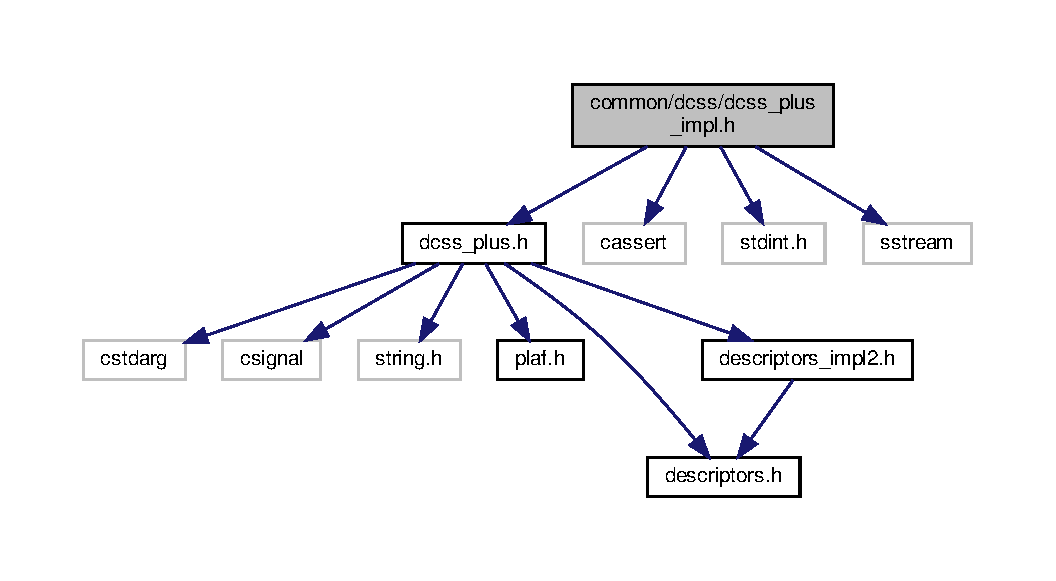
\includegraphics[width=350pt]{dcss__plus__impl_8h__incl}
\end{center}
\end{figure}
This graph shows which files directly or indirectly include this file\+:
\nopagebreak
\begin{figure}[H]
\begin{center}
\leavevmode
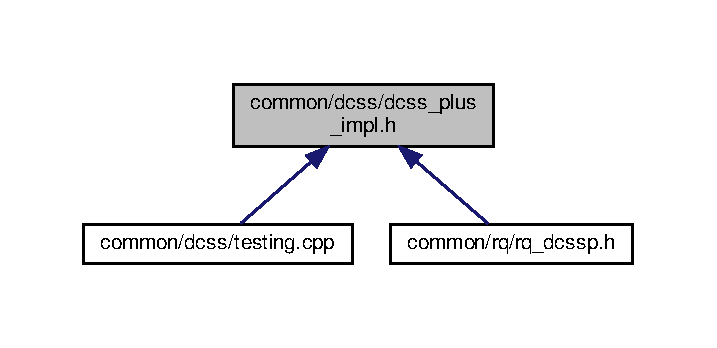
\includegraphics[width=344pt]{dcss__plus__impl_8h__dep__incl}
\end{center}
\end{figure}
\subsection*{Macros}
\begin{DoxyCompactItemize}
\item 
\#define \hyperlink{dcss__plus__impl_8h_a6bd312b05b209f8fce93c657186bbeb0}{B\+O\+O\+L\+\_\+\+C\+AS}~\+\_\+\+\_\+sync\+\_\+bool\+\_\+compare\+\_\+and\+\_\+swap
\item 
\#define \hyperlink{dcss__plus__impl_8h_aa7387507d9deee458fc9668893079a5f}{V\+A\+L\+\_\+\+C\+AS}~\+\_\+\+\_\+sync\+\_\+val\+\_\+compare\+\_\+and\+\_\+swap
\item 
\#define \hyperlink{dcss__plus__impl_8h_a88f4805817c3208917cb6994897607ce}{D\+C\+S\+S\+P\+\_\+\+T\+A\+G\+B\+IT}~0x1
\end{DoxyCompactItemize}


\subsection{Macro Definition Documentation}
\mbox{\Hypertarget{dcss__plus__impl_8h_a6bd312b05b209f8fce93c657186bbeb0}\label{dcss__plus__impl_8h_a6bd312b05b209f8fce93c657186bbeb0}} 
\index{dcss\+\_\+plus\+\_\+impl.\+h@{dcss\+\_\+plus\+\_\+impl.\+h}!B\+O\+O\+L\+\_\+\+C\+AS@{B\+O\+O\+L\+\_\+\+C\+AS}}
\index{B\+O\+O\+L\+\_\+\+C\+AS@{B\+O\+O\+L\+\_\+\+C\+AS}!dcss\+\_\+plus\+\_\+impl.\+h@{dcss\+\_\+plus\+\_\+impl.\+h}}
\subsubsection{\texorpdfstring{B\+O\+O\+L\+\_\+\+C\+AS}{BOOL\_CAS}}
{\footnotesize\ttfamily \#define B\+O\+O\+L\+\_\+\+C\+AS~\+\_\+\+\_\+sync\+\_\+bool\+\_\+compare\+\_\+and\+\_\+swap}

\mbox{\Hypertarget{dcss__plus__impl_8h_a88f4805817c3208917cb6994897607ce}\label{dcss__plus__impl_8h_a88f4805817c3208917cb6994897607ce}} 
\index{dcss\+\_\+plus\+\_\+impl.\+h@{dcss\+\_\+plus\+\_\+impl.\+h}!D\+C\+S\+S\+P\+\_\+\+T\+A\+G\+B\+IT@{D\+C\+S\+S\+P\+\_\+\+T\+A\+G\+B\+IT}}
\index{D\+C\+S\+S\+P\+\_\+\+T\+A\+G\+B\+IT@{D\+C\+S\+S\+P\+\_\+\+T\+A\+G\+B\+IT}!dcss\+\_\+plus\+\_\+impl.\+h@{dcss\+\_\+plus\+\_\+impl.\+h}}
\subsubsection{\texorpdfstring{D\+C\+S\+S\+P\+\_\+\+T\+A\+G\+B\+IT}{DCSSP\_TAGBIT}}
{\footnotesize\ttfamily \#define D\+C\+S\+S\+P\+\_\+\+T\+A\+G\+B\+IT~0x1}

\mbox{\Hypertarget{dcss__plus__impl_8h_aa7387507d9deee458fc9668893079a5f}\label{dcss__plus__impl_8h_aa7387507d9deee458fc9668893079a5f}} 
\index{dcss\+\_\+plus\+\_\+impl.\+h@{dcss\+\_\+plus\+\_\+impl.\+h}!V\+A\+L\+\_\+\+C\+AS@{V\+A\+L\+\_\+\+C\+AS}}
\index{V\+A\+L\+\_\+\+C\+AS@{V\+A\+L\+\_\+\+C\+AS}!dcss\+\_\+plus\+\_\+impl.\+h@{dcss\+\_\+plus\+\_\+impl.\+h}}
\subsubsection{\texorpdfstring{V\+A\+L\+\_\+\+C\+AS}{VAL\_CAS}}
{\footnotesize\ttfamily \#define V\+A\+L\+\_\+\+C\+AS~\+\_\+\+\_\+sync\+\_\+val\+\_\+compare\+\_\+and\+\_\+swap}


\hypertarget{testing_8cpp}{}\section{common/dcss/testing.cpp File Reference}
\label{testing_8cpp}\index{common/dcss/testing.\+cpp@{common/dcss/testing.\+cpp}}
{\ttfamily \#include $<$cstdlib$>$}\newline
{\ttfamily \#include $<$cmath$>$}\newline
{\ttfamily \#include $<$iostream$>$}\newline
{\ttfamily \#include \char`\"{}dcss\+\_\+plus\+\_\+impl.\+h\char`\"{}}\newline
Include dependency graph for testing.\+cpp\+:
\nopagebreak
\begin{figure}[H]
\begin{center}
\leavevmode
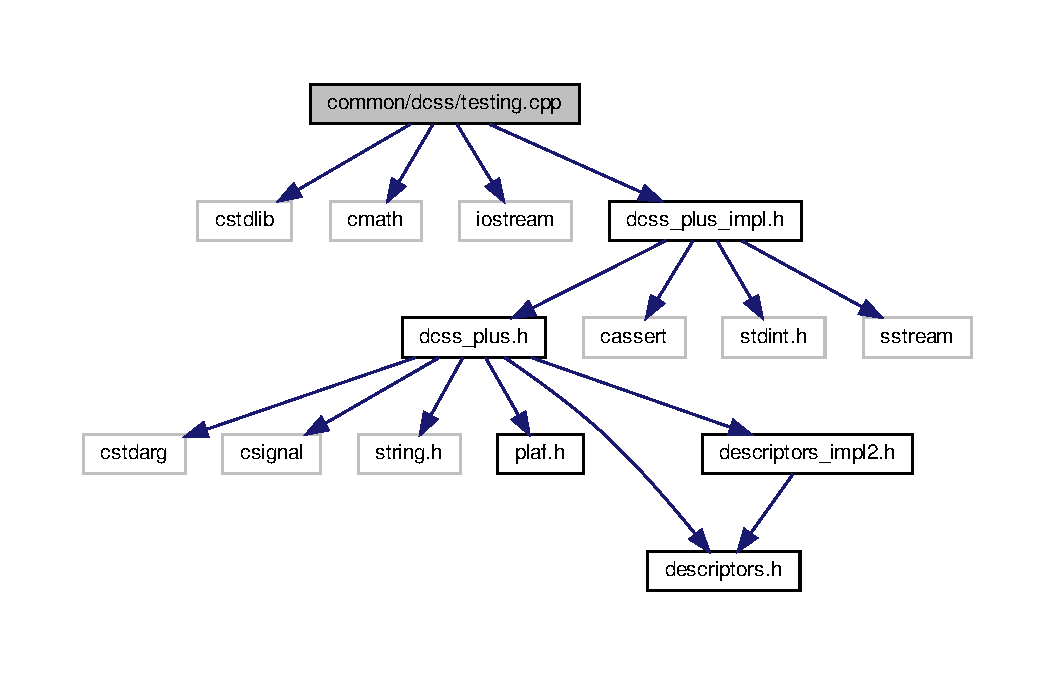
\includegraphics[width=350pt]{testing_8cpp__incl}
\end{center}
\end{figure}
\subsection*{Macros}
\begin{DoxyCompactItemize}
\item 
\#define \hyperlink{testing_8cpp_a6a1f9089d0f093a36676adc23ad00f04}{N\+U\+M\+\_\+\+O\+PS}~10000000
\item 
\#define \hyperlink{testing_8cpp_ad99a3089c13b6f47b26b218a997fad73}{I\+N\+C\+R\+E\+M\+E\+NT}~1
\item 
\#define \hyperlink{testing_8cpp_a01ef34b99aeb720c3166fe376a5cb22e}{F\+A\+L\+S\+E\+\_\+\+S\+H\+A\+R\+I\+N\+G\+\_\+\+U\+L\+L\+\_\+\+F\+A\+C\+T\+OR}~24
\item 
\#define \hyperlink{testing_8cpp_a6202aa5beea3bb008e490c357d77f193}{F\+A\+L\+S\+E\+\_\+\+S\+H\+A\+R\+I\+N\+G\+\_\+\+P\+A\+D\+\_\+\+B\+Y\+T\+ES}~192
\item 
\#define \hyperlink{testing_8cpp_abdeb6748eee1c69947ed41aef20ca932}{C\+O\+U\+N\+T\+ER}(\hyperlink{microbench_2main_8cpp_a9ca9869868fe7e7a38a921cc7de4103f}{tid})~(\hyperlink{testing_8cpp_a6f2fd530e372a0a7a4c0b956330b5aa6}{counters}\mbox{[}(\hyperlink{microbench_2main_8cpp_a9ca9869868fe7e7a38a921cc7de4103f}{tid})$\ast$\hyperlink{testing_8cpp_a01ef34b99aeb720c3166fe376a5cb22e}{F\+A\+L\+S\+E\+\_\+\+S\+H\+A\+R\+I\+N\+G\+\_\+\+U\+L\+L\+\_\+\+F\+A\+C\+T\+OR}\mbox{]})
\item 
\#define \hyperlink{testing_8cpp_ac4e52c1bd876037cd22e859f38fd5d27}{K\+E\+R\+N\+EL}~\hyperlink{testing_8cpp_ac138977023300e7f0e5d0f13b5ca1a9f}{test\+\_\+kernel1}
\item 
\#define \hyperlink{testing_8cpp_aa418260d9aff736c26de996778b192ab}{V\+A\+L\+I\+D\+A\+TE}~\hyperlink{testing_8cpp_ac18bd3381823e3bc71af9c2944408f65}{validate1}
\end{DoxyCompactItemize}
\subsection*{Functions}
\begin{DoxyCompactItemize}
\item 
void $\ast$ \hyperlink{testing_8cpp_ac138977023300e7f0e5d0f13b5ca1a9f}{test\+\_\+kernel1} (void $\ast$arg)
\item 
bool \hyperlink{testing_8cpp_ac18bd3381823e3bc71af9c2944408f65}{validate1} ()
\item 
void $\ast$ \hyperlink{testing_8cpp_aa246f8a6a9360383fe88a0968377f882}{test\+\_\+kernel2} (void $\ast$arg)
\item 
bool \hyperlink{testing_8cpp_ae048164d83059301e9f936c05bc7305b}{validate2} ()
\item 
int \hyperlink{testing_8cpp_a3c04138a5bfe5d72780bb7e82a18e627}{main} (int argc, char $\ast$$\ast$argv)
\end{DoxyCompactItemize}
\subsection*{Variables}
\begin{DoxyCompactItemize}
\item 
int \hyperlink{testing_8cpp_aa085812188e21ede75351d88b9b2c30d}{num\+Processes} = 0
\item 
volatile unsigned long long \hyperlink{testing_8cpp_a6f2fd530e372a0a7a4c0b956330b5aa6}{counters} \mbox{[}\hyperlink{plaf_8h_ac1585a3455dd3e33e877e588be9e466b}{M\+A\+X\+\_\+\+T\+H\+R\+E\+A\+D\+S\+\_\+\+P\+O\+W2} $\ast$\hyperlink{testing_8cpp_a01ef34b99aeb720c3166fe376a5cb22e}{F\+A\+L\+S\+E\+\_\+\+S\+H\+A\+R\+I\+N\+G\+\_\+\+U\+L\+L\+\_\+\+F\+A\+C\+T\+OR}\mbox{]}
\item 
volatile char \hyperlink{testing_8cpp_ace2b83a8850644735e9546461bf2f1a7}{padding} \mbox{[}\hyperlink{testing_8cpp_a6202aa5beea3bb008e490c357d77f193}{F\+A\+L\+S\+E\+\_\+\+S\+H\+A\+R\+I\+N\+G\+\_\+\+P\+A\+D\+\_\+\+B\+Y\+T\+ES}\mbox{]}
\item 
volatile unsigned long long \hyperlink{testing_8cpp_a29fe4ee2e6b0c04eb40cead810a5366a}{faa}
\item 
volatile bool \hyperlink{testing_8cpp_aee3961a7f86922e2725a5e3f5d46b8ed}{start}
\item 
volatile int \hyperlink{testing_8cpp_af1f449cc09f8d36befcce07bc38c29c0}{running}
\item 
\hyperlink{classdcsspProvider}{dcssp\+Provider} $\ast$ \hyperlink{testing_8cpp_a385ddba1011c48d31d8458025b417735}{prov}
\end{DoxyCompactItemize}


\subsection{Macro Definition Documentation}
\mbox{\Hypertarget{testing_8cpp_abdeb6748eee1c69947ed41aef20ca932}\label{testing_8cpp_abdeb6748eee1c69947ed41aef20ca932}} 
\index{testing.\+cpp@{testing.\+cpp}!C\+O\+U\+N\+T\+ER@{C\+O\+U\+N\+T\+ER}}
\index{C\+O\+U\+N\+T\+ER@{C\+O\+U\+N\+T\+ER}!testing.\+cpp@{testing.\+cpp}}
\subsubsection{\texorpdfstring{C\+O\+U\+N\+T\+ER}{COUNTER}}
{\footnotesize\ttfamily \#define C\+O\+U\+N\+T\+ER(\begin{DoxyParamCaption}\item[{}]{\hyperlink{microbench_2main_8cpp_a9ca9869868fe7e7a38a921cc7de4103f}{tid} }\end{DoxyParamCaption})~(\hyperlink{testing_8cpp_a6f2fd530e372a0a7a4c0b956330b5aa6}{counters}\mbox{[}(\hyperlink{microbench_2main_8cpp_a9ca9869868fe7e7a38a921cc7de4103f}{tid})$\ast$\hyperlink{testing_8cpp_a01ef34b99aeb720c3166fe376a5cb22e}{F\+A\+L\+S\+E\+\_\+\+S\+H\+A\+R\+I\+N\+G\+\_\+\+U\+L\+L\+\_\+\+F\+A\+C\+T\+OR}\mbox{]})}

\mbox{\Hypertarget{testing_8cpp_a6202aa5beea3bb008e490c357d77f193}\label{testing_8cpp_a6202aa5beea3bb008e490c357d77f193}} 
\index{testing.\+cpp@{testing.\+cpp}!F\+A\+L\+S\+E\+\_\+\+S\+H\+A\+R\+I\+N\+G\+\_\+\+P\+A\+D\+\_\+\+B\+Y\+T\+ES@{F\+A\+L\+S\+E\+\_\+\+S\+H\+A\+R\+I\+N\+G\+\_\+\+P\+A\+D\+\_\+\+B\+Y\+T\+ES}}
\index{F\+A\+L\+S\+E\+\_\+\+S\+H\+A\+R\+I\+N\+G\+\_\+\+P\+A\+D\+\_\+\+B\+Y\+T\+ES@{F\+A\+L\+S\+E\+\_\+\+S\+H\+A\+R\+I\+N\+G\+\_\+\+P\+A\+D\+\_\+\+B\+Y\+T\+ES}!testing.\+cpp@{testing.\+cpp}}
\subsubsection{\texorpdfstring{F\+A\+L\+S\+E\+\_\+\+S\+H\+A\+R\+I\+N\+G\+\_\+\+P\+A\+D\+\_\+\+B\+Y\+T\+ES}{FALSE\_SHARING\_PAD\_BYTES}}
{\footnotesize\ttfamily \#define F\+A\+L\+S\+E\+\_\+\+S\+H\+A\+R\+I\+N\+G\+\_\+\+P\+A\+D\+\_\+\+B\+Y\+T\+ES~192}

\mbox{\Hypertarget{testing_8cpp_a01ef34b99aeb720c3166fe376a5cb22e}\label{testing_8cpp_a01ef34b99aeb720c3166fe376a5cb22e}} 
\index{testing.\+cpp@{testing.\+cpp}!F\+A\+L\+S\+E\+\_\+\+S\+H\+A\+R\+I\+N\+G\+\_\+\+U\+L\+L\+\_\+\+F\+A\+C\+T\+OR@{F\+A\+L\+S\+E\+\_\+\+S\+H\+A\+R\+I\+N\+G\+\_\+\+U\+L\+L\+\_\+\+F\+A\+C\+T\+OR}}
\index{F\+A\+L\+S\+E\+\_\+\+S\+H\+A\+R\+I\+N\+G\+\_\+\+U\+L\+L\+\_\+\+F\+A\+C\+T\+OR@{F\+A\+L\+S\+E\+\_\+\+S\+H\+A\+R\+I\+N\+G\+\_\+\+U\+L\+L\+\_\+\+F\+A\+C\+T\+OR}!testing.\+cpp@{testing.\+cpp}}
\subsubsection{\texorpdfstring{F\+A\+L\+S\+E\+\_\+\+S\+H\+A\+R\+I\+N\+G\+\_\+\+U\+L\+L\+\_\+\+F\+A\+C\+T\+OR}{FALSE\_SHARING\_ULL\_FACTOR}}
{\footnotesize\ttfamily \#define F\+A\+L\+S\+E\+\_\+\+S\+H\+A\+R\+I\+N\+G\+\_\+\+U\+L\+L\+\_\+\+F\+A\+C\+T\+OR~24}

\mbox{\Hypertarget{testing_8cpp_ad99a3089c13b6f47b26b218a997fad73}\label{testing_8cpp_ad99a3089c13b6f47b26b218a997fad73}} 
\index{testing.\+cpp@{testing.\+cpp}!I\+N\+C\+R\+E\+M\+E\+NT@{I\+N\+C\+R\+E\+M\+E\+NT}}
\index{I\+N\+C\+R\+E\+M\+E\+NT@{I\+N\+C\+R\+E\+M\+E\+NT}!testing.\+cpp@{testing.\+cpp}}
\subsubsection{\texorpdfstring{I\+N\+C\+R\+E\+M\+E\+NT}{INCREMENT}}
{\footnotesize\ttfamily \#define I\+N\+C\+R\+E\+M\+E\+NT~1}

\mbox{\Hypertarget{testing_8cpp_ac4e52c1bd876037cd22e859f38fd5d27}\label{testing_8cpp_ac4e52c1bd876037cd22e859f38fd5d27}} 
\index{testing.\+cpp@{testing.\+cpp}!K\+E\+R\+N\+EL@{K\+E\+R\+N\+EL}}
\index{K\+E\+R\+N\+EL@{K\+E\+R\+N\+EL}!testing.\+cpp@{testing.\+cpp}}
\subsubsection{\texorpdfstring{K\+E\+R\+N\+EL}{KERNEL}}
{\footnotesize\ttfamily \#define K\+E\+R\+N\+EL~\hyperlink{testing_8cpp_ac138977023300e7f0e5d0f13b5ca1a9f}{test\+\_\+kernel1}}

\mbox{\Hypertarget{testing_8cpp_a6a1f9089d0f093a36676adc23ad00f04}\label{testing_8cpp_a6a1f9089d0f093a36676adc23ad00f04}} 
\index{testing.\+cpp@{testing.\+cpp}!N\+U\+M\+\_\+\+O\+PS@{N\+U\+M\+\_\+\+O\+PS}}
\index{N\+U\+M\+\_\+\+O\+PS@{N\+U\+M\+\_\+\+O\+PS}!testing.\+cpp@{testing.\+cpp}}
\subsubsection{\texorpdfstring{N\+U\+M\+\_\+\+O\+PS}{NUM\_OPS}}
{\footnotesize\ttfamily \#define N\+U\+M\+\_\+\+O\+PS~10000000}

\mbox{\Hypertarget{testing_8cpp_aa418260d9aff736c26de996778b192ab}\label{testing_8cpp_aa418260d9aff736c26de996778b192ab}} 
\index{testing.\+cpp@{testing.\+cpp}!V\+A\+L\+I\+D\+A\+TE@{V\+A\+L\+I\+D\+A\+TE}}
\index{V\+A\+L\+I\+D\+A\+TE@{V\+A\+L\+I\+D\+A\+TE}!testing.\+cpp@{testing.\+cpp}}
\subsubsection{\texorpdfstring{V\+A\+L\+I\+D\+A\+TE}{VALIDATE}}
{\footnotesize\ttfamily \#define V\+A\+L\+I\+D\+A\+TE~\hyperlink{testing_8cpp_ac18bd3381823e3bc71af9c2944408f65}{validate1}}



\subsection{Function Documentation}
\mbox{\Hypertarget{testing_8cpp_a3c04138a5bfe5d72780bb7e82a18e627}\label{testing_8cpp_a3c04138a5bfe5d72780bb7e82a18e627}} 
\index{testing.\+cpp@{testing.\+cpp}!main@{main}}
\index{main@{main}!testing.\+cpp@{testing.\+cpp}}
\subsubsection{\texorpdfstring{main()}{main()}}
{\footnotesize\ttfamily int main (\begin{DoxyParamCaption}\item[{int}]{argc,  }\item[{char $\ast$$\ast$}]{argv }\end{DoxyParamCaption})}

\mbox{\Hypertarget{testing_8cpp_ac138977023300e7f0e5d0f13b5ca1a9f}\label{testing_8cpp_ac138977023300e7f0e5d0f13b5ca1a9f}} 
\index{testing.\+cpp@{testing.\+cpp}!test\+\_\+kernel1@{test\+\_\+kernel1}}
\index{test\+\_\+kernel1@{test\+\_\+kernel1}!testing.\+cpp@{testing.\+cpp}}
\subsubsection{\texorpdfstring{test\+\_\+kernel1()}{test\_kernel1()}}
{\footnotesize\ttfamily void$\ast$ test\+\_\+kernel1 (\begin{DoxyParamCaption}\item[{void $\ast$}]{arg }\end{DoxyParamCaption})}

\mbox{\Hypertarget{testing_8cpp_aa246f8a6a9360383fe88a0968377f882}\label{testing_8cpp_aa246f8a6a9360383fe88a0968377f882}} 
\index{testing.\+cpp@{testing.\+cpp}!test\+\_\+kernel2@{test\+\_\+kernel2}}
\index{test\+\_\+kernel2@{test\+\_\+kernel2}!testing.\+cpp@{testing.\+cpp}}
\subsubsection{\texorpdfstring{test\+\_\+kernel2()}{test\_kernel2()}}
{\footnotesize\ttfamily void$\ast$ test\+\_\+kernel2 (\begin{DoxyParamCaption}\item[{void $\ast$}]{arg }\end{DoxyParamCaption})}

\mbox{\Hypertarget{testing_8cpp_ac18bd3381823e3bc71af9c2944408f65}\label{testing_8cpp_ac18bd3381823e3bc71af9c2944408f65}} 
\index{testing.\+cpp@{testing.\+cpp}!validate1@{validate1}}
\index{validate1@{validate1}!testing.\+cpp@{testing.\+cpp}}
\subsubsection{\texorpdfstring{validate1()}{validate1()}}
{\footnotesize\ttfamily bool validate1 (\begin{DoxyParamCaption}{ }\end{DoxyParamCaption})}

\mbox{\Hypertarget{testing_8cpp_ae048164d83059301e9f936c05bc7305b}\label{testing_8cpp_ae048164d83059301e9f936c05bc7305b}} 
\index{testing.\+cpp@{testing.\+cpp}!validate2@{validate2}}
\index{validate2@{validate2}!testing.\+cpp@{testing.\+cpp}}
\subsubsection{\texorpdfstring{validate2()}{validate2()}}
{\footnotesize\ttfamily bool validate2 (\begin{DoxyParamCaption}{ }\end{DoxyParamCaption})}



\subsection{Variable Documentation}
\mbox{\Hypertarget{testing_8cpp_a6f2fd530e372a0a7a4c0b956330b5aa6}\label{testing_8cpp_a6f2fd530e372a0a7a4c0b956330b5aa6}} 
\index{testing.\+cpp@{testing.\+cpp}!counters@{counters}}
\index{counters@{counters}!testing.\+cpp@{testing.\+cpp}}
\subsubsection{\texorpdfstring{counters}{counters}}
{\footnotesize\ttfamily volatile unsigned long long counters\mbox{[}\hyperlink{plaf_8h_ac1585a3455dd3e33e877e588be9e466b}{M\+A\+X\+\_\+\+T\+H\+R\+E\+A\+D\+S\+\_\+\+P\+O\+W2} $\ast$\hyperlink{testing_8cpp_a01ef34b99aeb720c3166fe376a5cb22e}{F\+A\+L\+S\+E\+\_\+\+S\+H\+A\+R\+I\+N\+G\+\_\+\+U\+L\+L\+\_\+\+F\+A\+C\+T\+OR}\mbox{]}}

\mbox{\Hypertarget{testing_8cpp_a29fe4ee2e6b0c04eb40cead810a5366a}\label{testing_8cpp_a29fe4ee2e6b0c04eb40cead810a5366a}} 
\index{testing.\+cpp@{testing.\+cpp}!faa@{faa}}
\index{faa@{faa}!testing.\+cpp@{testing.\+cpp}}
\subsubsection{\texorpdfstring{faa}{faa}}
{\footnotesize\ttfamily volatile unsigned long long faa}

\mbox{\Hypertarget{testing_8cpp_aa085812188e21ede75351d88b9b2c30d}\label{testing_8cpp_aa085812188e21ede75351d88b9b2c30d}} 
\index{testing.\+cpp@{testing.\+cpp}!num\+Processes@{num\+Processes}}
\index{num\+Processes@{num\+Processes}!testing.\+cpp@{testing.\+cpp}}
\subsubsection{\texorpdfstring{num\+Processes}{numProcesses}}
{\footnotesize\ttfamily int num\+Processes = 0}

\mbox{\Hypertarget{testing_8cpp_ace2b83a8850644735e9546461bf2f1a7}\label{testing_8cpp_ace2b83a8850644735e9546461bf2f1a7}} 
\index{testing.\+cpp@{testing.\+cpp}!padding@{padding}}
\index{padding@{padding}!testing.\+cpp@{testing.\+cpp}}
\subsubsection{\texorpdfstring{padding}{padding}}
{\footnotesize\ttfamily volatile char padding\mbox{[}\hyperlink{testing_8cpp_a6202aa5beea3bb008e490c357d77f193}{F\+A\+L\+S\+E\+\_\+\+S\+H\+A\+R\+I\+N\+G\+\_\+\+P\+A\+D\+\_\+\+B\+Y\+T\+ES}\mbox{]}}

\mbox{\Hypertarget{testing_8cpp_a385ddba1011c48d31d8458025b417735}\label{testing_8cpp_a385ddba1011c48d31d8458025b417735}} 
\index{testing.\+cpp@{testing.\+cpp}!prov@{prov}}
\index{prov@{prov}!testing.\+cpp@{testing.\+cpp}}
\subsubsection{\texorpdfstring{prov}{prov}}
{\footnotesize\ttfamily \hyperlink{classdcsspProvider}{dcssp\+Provider}$\ast$ prov}

\mbox{\Hypertarget{testing_8cpp_af1f449cc09f8d36befcce07bc38c29c0}\label{testing_8cpp_af1f449cc09f8d36befcce07bc38c29c0}} 
\index{testing.\+cpp@{testing.\+cpp}!running@{running}}
\index{running@{running}!testing.\+cpp@{testing.\+cpp}}
\subsubsection{\texorpdfstring{running}{running}}
{\footnotesize\ttfamily volatile int running}

\mbox{\Hypertarget{testing_8cpp_aee3961a7f86922e2725a5e3f5d46b8ed}\label{testing_8cpp_aee3961a7f86922e2725a5e3f5d46b8ed}} 
\index{testing.\+cpp@{testing.\+cpp}!start@{start}}
\index{start@{start}!testing.\+cpp@{testing.\+cpp}}
\subsubsection{\texorpdfstring{start}{start}}
{\footnotesize\ttfamily volatile bool start}


\hypertarget{descriptors_8h}{}\section{common/descriptors/descriptors.h File Reference}
\label{descriptors_8h}\index{common/descriptors/descriptors.\+h@{common/descriptors/descriptors.\+h}}
This graph shows which files directly or indirectly include this file\+:
\nopagebreak
\begin{figure}[H]
\begin{center}
\leavevmode
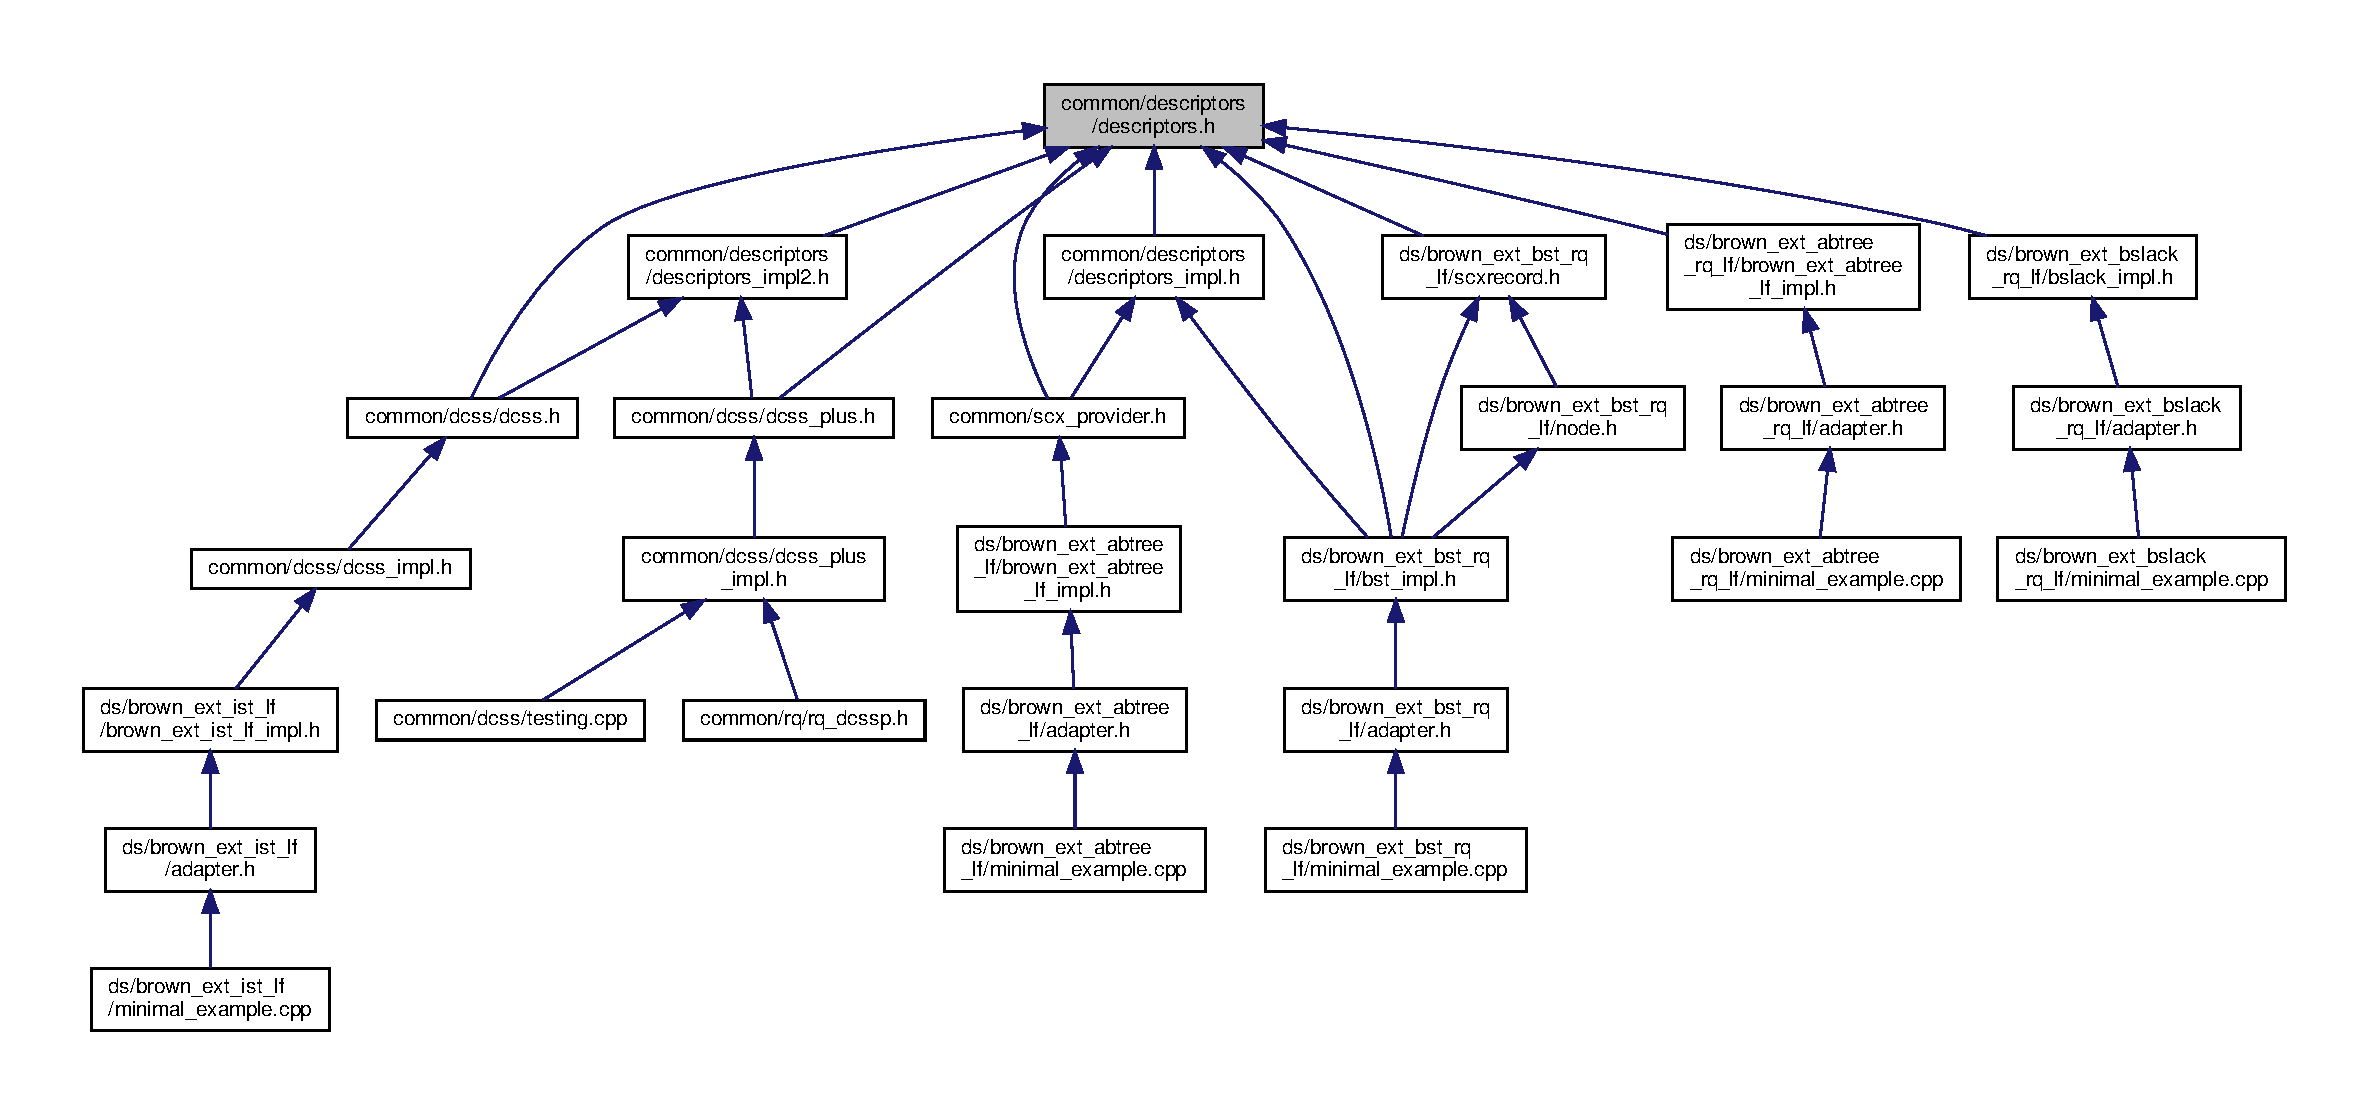
\includegraphics[width=350pt]{descriptors_8h__dep__incl}
\end{center}
\end{figure}
\subsection*{Typedefs}
\begin{DoxyCompactItemize}
\item 
typedef intptr\+\_\+t \hyperlink{descriptors_8h_afd8a7b57046ed96897cda907f17737a7}{tagptr\+\_\+t}
\item 
typedef intptr\+\_\+t \hyperlink{descriptors_8h_a8a5af2749482b19d7515054489efca22}{mutables\+\_\+t}
\end{DoxyCompactItemize}


\subsection{Typedef Documentation}
\mbox{\Hypertarget{descriptors_8h_a8a5af2749482b19d7515054489efca22}\label{descriptors_8h_a8a5af2749482b19d7515054489efca22}} 
\index{descriptors.\+h@{descriptors.\+h}!mutables\+\_\+t@{mutables\+\_\+t}}
\index{mutables\+\_\+t@{mutables\+\_\+t}!descriptors.\+h@{descriptors.\+h}}
\subsubsection{\texorpdfstring{mutables\+\_\+t}{mutables\_t}}
{\footnotesize\ttfamily typedef intptr\+\_\+t \hyperlink{descriptors_8h_a8a5af2749482b19d7515054489efca22}{mutables\+\_\+t}}

\mbox{\Hypertarget{descriptors_8h_afd8a7b57046ed96897cda907f17737a7}\label{descriptors_8h_afd8a7b57046ed96897cda907f17737a7}} 
\index{descriptors.\+h@{descriptors.\+h}!tagptr\+\_\+t@{tagptr\+\_\+t}}
\index{tagptr\+\_\+t@{tagptr\+\_\+t}!descriptors.\+h@{descriptors.\+h}}
\subsubsection{\texorpdfstring{tagptr\+\_\+t}{tagptr\_t}}
{\footnotesize\ttfamily typedef intptr\+\_\+t \hyperlink{descriptors_8h_afd8a7b57046ed96897cda907f17737a7}{tagptr\+\_\+t}}


\hypertarget{descriptors__impl_8h}{}\section{common/descriptors/descriptors\+\_\+impl.h File Reference}
\label{descriptors__impl_8h}\index{common/descriptors/descriptors\+\_\+impl.\+h@{common/descriptors/descriptors\+\_\+impl.\+h}}
{\ttfamily \#include \char`\"{}descriptors.\+h\char`\"{}}\newline
Include dependency graph for descriptors\+\_\+impl.\+h\+:
\nopagebreak
\begin{figure}[H]
\begin{center}
\leavevmode
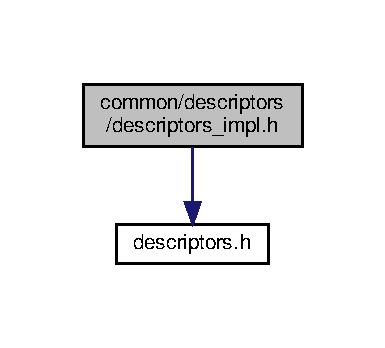
\includegraphics[width=185pt]{descriptors__impl_8h__incl}
\end{center}
\end{figure}
This graph shows which files directly or indirectly include this file\+:
\nopagebreak
\begin{figure}[H]
\begin{center}
\leavevmode
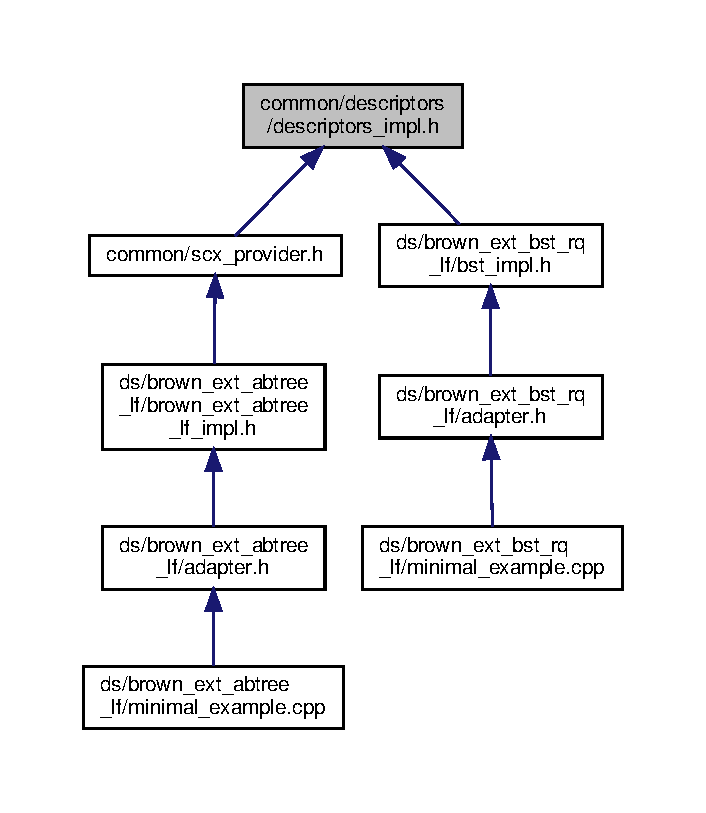
\includegraphics[width=339pt]{descriptors__impl_8h__dep__incl}
\end{center}
\end{figure}
\subsection*{Macros}
\begin{DoxyCompactItemize}
\item 
\#define \hyperlink{descriptors__impl_8h_a977c0ae2ceeea7580d2b05920ebca5b3}{D\+E\+S\+C1\+\_\+\+I\+N\+I\+T\+\_\+\+A\+LL}(\hyperlink{testing_8cpp_aa085812188e21ede75351d88b9b2c30d}{num\+Processes})
\item 
\#define \hyperlink{descriptors__impl_8h_af224ccfecfbd0b827a0f1029c50cf138}{W\+I\+D\+T\+H1\+\_\+\+S\+EQ}~48
\item 
\#define \hyperlink{descriptors__impl_8h_a7e1502d457e1fae20c76a220ee817da7}{O\+F\+F\+S\+E\+T1\+\_\+\+S\+EQ}~11
\item 
\#define \hyperlink{descriptors__impl_8h_a2aff29517952c7a1054d049ae60546fa}{M\+A\+S\+K1\+\_\+\+S\+EQ}~((uintptr\+\_\+t)((1\+L\+L$<$$<$\+W\+I\+D\+T\+H1\+\_\+\+S\+E\+Q)-\/1)$<$$<$\+O\+F\+F\+S\+E\+T1\+\_\+\+S\+E\+Q) /$\ast$ cast to avoid signed bit shifting $\ast$/
\item 
\#define \hyperlink{descriptors__impl_8h_a53a42fc32cce8c4d35a70109cdfd0362}{U\+N\+P\+A\+C\+K1\+\_\+\+S\+EQ}(tagptr\+Or\+Mutables)~(((uintptr\+\_\+t)(tagptr\+Or\+Mutables))$>$$>$\hyperlink{descriptors__impl_8h_a7e1502d457e1fae20c76a220ee817da7}{O\+F\+F\+S\+E\+T1\+\_\+\+S\+EQ})
\item 
\#define \hyperlink{descriptors__impl_8h_a7a1b5f7be5b6597554f8e6f722cae699}{T\+A\+G\+P\+T\+R1\+\_\+\+O\+F\+F\+S\+E\+T\+\_\+\+S\+T\+A\+LE}~0 /$\ast$ U\+N\+U\+S\+ED $\ast$/
\item 
\#define \hyperlink{descriptors__impl_8h_a55b2ed83821f9de39d59678f391ba04c}{T\+A\+G\+P\+T\+R1\+\_\+\+O\+F\+F\+S\+E\+T\+\_\+\+T\+ID}~1
\item 
\#define \hyperlink{descriptors__impl_8h_ae2d0438831ef74dc21e2baf8ce199102}{T\+A\+G\+P\+T\+R1\+\_\+\+M\+A\+S\+K\+\_\+\+S\+T\+A\+LE}~0x1 /$\ast$ U\+N\+U\+S\+E\+D $\ast$/
\item 
\#define \hyperlink{descriptors__impl_8h_ad8c425be1d3fbacf1329c4df0d30c189}{T\+A\+G\+P\+T\+R1\+\_\+\+M\+A\+S\+K\+\_\+\+T\+ID}~(((1$<$$<$\hyperlink{descriptors__impl_8h_a7e1502d457e1fae20c76a220ee817da7}{O\+F\+F\+S\+E\+T1\+\_\+\+S\+EQ})-\/1)\&($\sim$(\hyperlink{descriptors__impl_8h_ae2d0438831ef74dc21e2baf8ce199102}{T\+A\+G\+P\+T\+R1\+\_\+\+M\+A\+S\+K\+\_\+\+S\+T\+A\+LE})))
\item 
\#define \hyperlink{descriptors__impl_8h_a786dc40f10e657569509db7f8d9a56dc}{T\+A\+G\+P\+T\+R1\+\_\+\+S\+T\+A\+LE}(tagptr)~(((\hyperlink{descriptors_8h_afd8a7b57046ed96897cda907f17737a7}{tagptr\+\_\+t}) (tagptr)) \& \hyperlink{descriptors__impl_8h_ae2d0438831ef74dc21e2baf8ce199102}{T\+A\+G\+P\+T\+R1\+\_\+\+M\+A\+S\+K\+\_\+\+S\+T\+A\+LE}) /$\ast$ U\+N\+U\+S\+ED $\ast$/
\item 
\#define \hyperlink{descriptors__impl_8h_aca407a8e7c82ec8eebaf0c5653adef00}{T\+A\+G\+P\+T\+R1\+\_\+\+U\+N\+P\+A\+C\+K\+\_\+\+T\+ID}(tagptr)~((int) ((((\hyperlink{descriptors_8h_afd8a7b57046ed96897cda907f17737a7}{tagptr\+\_\+t}) (tagptr))\&\hyperlink{descriptors__impl_8h_ad8c425be1d3fbacf1329c4df0d30c189}{T\+A\+G\+P\+T\+R1\+\_\+\+M\+A\+S\+K\+\_\+\+T\+ID})$>$$>$\hyperlink{descriptors__impl_8h_a55b2ed83821f9de39d59678f391ba04c}{T\+A\+G\+P\+T\+R1\+\_\+\+O\+F\+F\+S\+E\+T\+\_\+\+T\+ID}))
\item 
\#define \hyperlink{descriptors__impl_8h_ae17dead541b98b8272925e5edefe140a}{T\+A\+G\+P\+T\+R1\+\_\+\+U\+N\+P\+A\+C\+K\+\_\+\+P\+TR}(tagptr)~(\&\hyperlink{bst__impl_8h_acda457fde97cfc59962318584ee03b98}{D\+E\+S\+C1\+\_\+\+A\+R\+R\+AY}\mbox{[}\hyperlink{descriptors__impl_8h_aca407a8e7c82ec8eebaf0c5653adef00}{T\+A\+G\+P\+T\+R1\+\_\+\+U\+N\+P\+A\+C\+K\+\_\+\+T\+ID}((tagptr))\mbox{]})
\item 
\#define \hyperlink{descriptors__impl_8h_af6d2dd1d847754d8c0b40d60e7537fbe}{T\+A\+G\+P\+T\+R1\+\_\+\+N\+EW}(\hyperlink{microbench_2main_8cpp_a9ca9869868fe7e7a38a921cc7de4103f}{tid},  \hyperlink{scxrecord_8h_a71e82299f9d0709f1d5c5448d59347cb}{mutables})~((\hyperlink{descriptors_8h_afd8a7b57046ed96897cda907f17737a7}{tagptr\+\_\+t}) (((\hyperlink{descriptors__impl_8h_a53a42fc32cce8c4d35a70109cdfd0362}{U\+N\+P\+A\+C\+K1\+\_\+\+S\+EQ}(\hyperlink{scxrecord_8h_a71e82299f9d0709f1d5c5448d59347cb}{mutables}))$<$$<$\hyperlink{descriptors__impl_8h_a7e1502d457e1fae20c76a220ee817da7}{O\+F\+F\+S\+E\+T1\+\_\+\+S\+EQ}) $\vert$ ((\hyperlink{microbench_2main_8cpp_a9ca9869868fe7e7a38a921cc7de4103f}{tid})$<$$<$\hyperlink{descriptors__impl_8h_a55b2ed83821f9de39d59678f391ba04c}{T\+A\+G\+P\+T\+R1\+\_\+\+O\+F\+F\+S\+E\+T\+\_\+\+T\+ID})))
\item 
\#define \hyperlink{descriptors__impl_8h_abd056f1a06caf57c1f0eb31ad8146439}{L\+A\+S\+T\+\_\+\+T\+I\+D1}~(\hyperlink{descriptors__impl_8h_ad8c425be1d3fbacf1329c4df0d30c189}{T\+A\+G\+P\+T\+R1\+\_\+\+M\+A\+S\+K\+\_\+\+T\+ID}$>$$>$\hyperlink{descriptors__impl_8h_a55b2ed83821f9de39d59678f391ba04c}{T\+A\+G\+P\+T\+R1\+\_\+\+O\+F\+F\+S\+E\+T\+\_\+\+T\+ID})
\item 
\#define \hyperlink{descriptors__impl_8h_a5aed124b4ea065430b13259c08243ebd}{T\+A\+G\+P\+T\+R1\+\_\+\+S\+T\+A\+T\+I\+C\+\_\+\+D\+E\+SC}(id)~((\hyperlink{descriptors_8h_afd8a7b57046ed96897cda907f17737a7}{tagptr\+\_\+t}) \hyperlink{descriptors__impl_8h_af6d2dd1d847754d8c0b40d60e7537fbe}{T\+A\+G\+P\+T\+R1\+\_\+\+N\+EW}(\hyperlink{descriptors__impl_8h_abd056f1a06caf57c1f0eb31ad8146439}{L\+A\+S\+T\+\_\+\+T\+I\+D1}-\/1-\/id, 0))
\item 
\#define \hyperlink{descriptors__impl_8h_a2266c3e52da603438177ca5100c721a1}{T\+A\+G\+P\+T\+R1\+\_\+\+D\+U\+M\+M\+Y\+\_\+\+D\+E\+SC}(id)~((\hyperlink{descriptors_8h_afd8a7b57046ed96897cda907f17737a7}{tagptr\+\_\+t}) \hyperlink{descriptors__impl_8h_af6d2dd1d847754d8c0b40d60e7537fbe}{T\+A\+G\+P\+T\+R1\+\_\+\+N\+EW}(\hyperlink{descriptors__impl_8h_abd056f1a06caf57c1f0eb31ad8146439}{L\+A\+S\+T\+\_\+\+T\+I\+D1}, id$<$$<$\hyperlink{descriptors__impl_8h_a7e1502d457e1fae20c76a220ee817da7}{O\+F\+F\+S\+E\+T1\+\_\+\+S\+EQ}))
\item 
\#define \hyperlink{descriptors__impl_8h_a3b013cbfaa5fc3c556fd8574b8a2ee32}{comma1}~,
\item 
\#define \hyperlink{descriptors__impl_8h_a244ba7490239117c1bb62a68653bfb4a}{M\+U\+T\+A\+B\+L\+E\+S1\+\_\+\+U\+N\+P\+A\+C\+K\+\_\+\+F\+I\+E\+LD}(\hyperlink{scxrecord_8h_a71e82299f9d0709f1d5c5448d59347cb}{mutables},  mask,  offset)~((((\hyperlink{descriptors_8h_a8a5af2749482b19d7515054489efca22}{mutables\+\_\+t}) (\hyperlink{scxrecord_8h_a71e82299f9d0709f1d5c5448d59347cb}{mutables}))\&(mask))$>$$>$(offset))
\item 
\#define \hyperlink{descriptors__impl_8h_acd512ba81f9cd6785710da73b1af2aec}{M\+U\+T\+A\+B\+L\+E\+S1\+\_\+\+W\+R\+I\+T\+E\+\_\+\+F\+I\+E\+LD}(fld\+Mutables,  snap\+Mutables,  val,  mask,  offset)
\item 
\#define \hyperlink{descriptors__impl_8h_ad13cbdca7e299809217e558d189806cb}{M\+U\+T\+A\+B\+L\+E\+S1\+\_\+\+W\+R\+I\+T\+E\+\_\+\+B\+IT}(fld\+Mutables,  snap\+Mutables,  mask)
\item 
\#define \hyperlink{descriptors__impl_8h_a0f0bd60f09244d186900d32206982488}{D\+E\+S\+C1\+\_\+\+S\+N\+A\+P\+S\+H\+OT}(desc\+Dest,  tagptr,  sz)
\item 
\#define \hyperlink{descriptors__impl_8h_afce0e9b83eff5b6af61b606a25773059}{D\+E\+S\+C1\+\_\+\+R\+E\+A\+D\+\_\+\+F\+I\+E\+LD}(success\+Bit,  fld\+Mutables,  tagptr,  mask,  offset)
\item 
\#define \hyperlink{descriptors__impl_8h_af72cc044471ffff232382cc48f147a98}{D\+E\+S\+C1\+\_\+\+N\+EW}(\hyperlink{microbench_2main_8cpp_a9ca9869868fe7e7a38a921cc7de4103f}{tid})
\item 
\#define \hyperlink{descriptors__impl_8h_a12d9551ac509f19d655166fdd68faf00}{D\+E\+S\+C1\+\_\+\+I\+N\+I\+T\+I\+A\+L\+I\+Z\+ED}(\hyperlink{microbench_2main_8cpp_a9ca9869868fe7e7a38a921cc7de4103f}{tid})
\end{DoxyCompactItemize}


\subsection{Macro Definition Documentation}
\mbox{\Hypertarget{descriptors__impl_8h_a3b013cbfaa5fc3c556fd8574b8a2ee32}\label{descriptors__impl_8h_a3b013cbfaa5fc3c556fd8574b8a2ee32}} 
\index{descriptors\+\_\+impl.\+h@{descriptors\+\_\+impl.\+h}!comma1@{comma1}}
\index{comma1@{comma1}!descriptors\+\_\+impl.\+h@{descriptors\+\_\+impl.\+h}}
\subsubsection{\texorpdfstring{comma1}{comma1}}
{\footnotesize\ttfamily \#define comma1~,}

\mbox{\Hypertarget{descriptors__impl_8h_a977c0ae2ceeea7580d2b05920ebca5b3}\label{descriptors__impl_8h_a977c0ae2ceeea7580d2b05920ebca5b3}} 
\index{descriptors\+\_\+impl.\+h@{descriptors\+\_\+impl.\+h}!D\+E\+S\+C1\+\_\+\+I\+N\+I\+T\+\_\+\+A\+LL@{D\+E\+S\+C1\+\_\+\+I\+N\+I\+T\+\_\+\+A\+LL}}
\index{D\+E\+S\+C1\+\_\+\+I\+N\+I\+T\+\_\+\+A\+LL@{D\+E\+S\+C1\+\_\+\+I\+N\+I\+T\+\_\+\+A\+LL}!descriptors\+\_\+impl.\+h@{descriptors\+\_\+impl.\+h}}
\subsubsection{\texorpdfstring{D\+E\+S\+C1\+\_\+\+I\+N\+I\+T\+\_\+\+A\+LL}{DESC1\_INIT\_ALL}}
{\footnotesize\ttfamily \#define D\+E\+S\+C1\+\_\+\+I\+N\+I\+T\+\_\+\+A\+LL(\begin{DoxyParamCaption}\item[{}]{\hyperlink{testing_8cpp_aa085812188e21ede75351d88b9b2c30d}{num\+Processes} }\end{DoxyParamCaption})}

{\bfseries Value\+:}
\begin{DoxyCode}
\{ \(\backslash\)
    for (\textcolor{keywordtype}{int} \hyperlink{namespaceurcu_a536341e353c82c078bc510ca0144dd58}{i}=0;\hyperlink{namespaceurcu_a536341e353c82c078bc510ca0144dd58}{i}<(\hyperlink{testing_8cpp_aa085812188e21ede75351d88b9b2c30d}{numProcesses});++\hyperlink{namespaceurcu_a536341e353c82c078bc510ca0144dd58}{i}) \{ \(\backslash\)
        DESC1\_ARRAY[\hyperlink{namespaceurcu_a536341e353c82c078bc510ca0144dd58}{i}].c.mutables = \hyperlink{scx__provider_8h_ad6961f61f4b5c212932f54aca4bf850a}{MUTABLES1\_NEW}(0); \(\backslash\)
    \} \(\backslash\)
\}
\end{DoxyCode}
\mbox{\Hypertarget{descriptors__impl_8h_a12d9551ac509f19d655166fdd68faf00}\label{descriptors__impl_8h_a12d9551ac509f19d655166fdd68faf00}} 
\index{descriptors\+\_\+impl.\+h@{descriptors\+\_\+impl.\+h}!D\+E\+S\+C1\+\_\+\+I\+N\+I\+T\+I\+A\+L\+I\+Z\+ED@{D\+E\+S\+C1\+\_\+\+I\+N\+I\+T\+I\+A\+L\+I\+Z\+ED}}
\index{D\+E\+S\+C1\+\_\+\+I\+N\+I\+T\+I\+A\+L\+I\+Z\+ED@{D\+E\+S\+C1\+\_\+\+I\+N\+I\+T\+I\+A\+L\+I\+Z\+ED}!descriptors\+\_\+impl.\+h@{descriptors\+\_\+impl.\+h}}
\subsubsection{\texorpdfstring{D\+E\+S\+C1\+\_\+\+I\+N\+I\+T\+I\+A\+L\+I\+Z\+ED}{DESC1\_INITIALIZED}}
{\footnotesize\ttfamily \#define D\+E\+S\+C1\+\_\+\+I\+N\+I\+T\+I\+A\+L\+I\+Z\+ED(\begin{DoxyParamCaption}\item[{}]{\hyperlink{microbench_2main_8cpp_a9ca9869868fe7e7a38a921cc7de4103f}{tid} }\end{DoxyParamCaption})}

{\bfseries Value\+:}
\begin{DoxyCode}
\hyperlink{plaf_8h_a6d355f686181df8f30f7b30588ff1fd0}{SOFTWARE\_BARRIER}; \(\backslash\)
    DESC1\_ARRAY[(\hyperlink{global_8cpp_a9ca9869868fe7e7a38a921cc7de4103f}{tid})].c.mutables += (1<<\hyperlink{descriptors__impl_8h_a7e1502d457e1fae20c76a220ee817da7}{OFFSET1\_SEQ}); \textcolor{comment}{/*DESC1\_NEW((tid))*/} \(\backslash\)
    SOFTWARE\_BARRIER;
\end{DoxyCode}
\mbox{\Hypertarget{descriptors__impl_8h_af72cc044471ffff232382cc48f147a98}\label{descriptors__impl_8h_af72cc044471ffff232382cc48f147a98}} 
\index{descriptors\+\_\+impl.\+h@{descriptors\+\_\+impl.\+h}!D\+E\+S\+C1\+\_\+\+N\+EW@{D\+E\+S\+C1\+\_\+\+N\+EW}}
\index{D\+E\+S\+C1\+\_\+\+N\+EW@{D\+E\+S\+C1\+\_\+\+N\+EW}!descriptors\+\_\+impl.\+h@{descriptors\+\_\+impl.\+h}}
\subsubsection{\texorpdfstring{D\+E\+S\+C1\+\_\+\+N\+EW}{DESC1\_NEW}}
{\footnotesize\ttfamily \#define D\+E\+S\+C1\+\_\+\+N\+EW(\begin{DoxyParamCaption}\item[{}]{\hyperlink{microbench_2main_8cpp_a9ca9869868fe7e7a38a921cc7de4103f}{tid} }\end{DoxyParamCaption})}

{\bfseries Value\+:}
\begin{DoxyCode}
&\hyperlink{scx__provider_8h_acda457fde97cfc59962318584ee03b98}{DESC1\_ARRAY}[(\hyperlink{global_8cpp_a9ca9869868fe7e7a38a921cc7de4103f}{tid})]; \{ \textcolor{comment}{/* note: only the process invoking this following macro can change the
       sequence# */} \(\backslash\)
    SOFTWARE\_BARRIER; \(\backslash\)
    uintptr\_t \_\_v = \hyperlink{scx__provider_8h_acda457fde97cfc59962318584ee03b98}{DESC1\_ARRAY}[(\hyperlink{global_8cpp_a9ca9869868fe7e7a38a921cc7de4103f}{tid})].c.mutables; \(\backslash\)
\textcolor{comment}{/*    while (!\_\_sync\_bool\_compare\_and\_swap(&DESC1\_ARRAY[(tid)].mutables, \_\_v, MUTABLES1\_NEW(\_\_v))) \{ \(\backslash\)}
\textcolor{comment}{        \_\_v = DESC1\_ARRAY[(tid)].mutables; \(\backslash\)}
\textcolor{comment}{    \} \(\backslash\)}
\textcolor{comment}{\}*/} \(\backslash\)
    \hyperlink{scx__provider_8h_acda457fde97cfc59962318584ee03b98}{DESC1\_ARRAY}[(\hyperlink{global_8cpp_a9ca9869868fe7e7a38a921cc7de4103f}{tid})].c.mutables = \hyperlink{scx__provider_8h_ad6961f61f4b5c212932f54aca4bf850a}{MUTABLES1\_NEW}(\_\_v); \(\backslash\)
    \textcolor{comment}{/*\_\_sync\_synchronize();*/} \(\backslash\)
    SOFTWARE\_BARRIER; \(\backslash\)
\}
\end{DoxyCode}
\mbox{\Hypertarget{descriptors__impl_8h_afce0e9b83eff5b6af61b606a25773059}\label{descriptors__impl_8h_afce0e9b83eff5b6af61b606a25773059}} 
\index{descriptors\+\_\+impl.\+h@{descriptors\+\_\+impl.\+h}!D\+E\+S\+C1\+\_\+\+R\+E\+A\+D\+\_\+\+F\+I\+E\+LD@{D\+E\+S\+C1\+\_\+\+R\+E\+A\+D\+\_\+\+F\+I\+E\+LD}}
\index{D\+E\+S\+C1\+\_\+\+R\+E\+A\+D\+\_\+\+F\+I\+E\+LD@{D\+E\+S\+C1\+\_\+\+R\+E\+A\+D\+\_\+\+F\+I\+E\+LD}!descriptors\+\_\+impl.\+h@{descriptors\+\_\+impl.\+h}}
\subsubsection{\texorpdfstring{D\+E\+S\+C1\+\_\+\+R\+E\+A\+D\+\_\+\+F\+I\+E\+LD}{DESC1\_READ\_FIELD}}
{\footnotesize\ttfamily \#define D\+E\+S\+C1\+\_\+\+R\+E\+A\+D\+\_\+\+F\+I\+E\+LD(\begin{DoxyParamCaption}\item[{}]{success\+Bit,  }\item[{}]{fld\+Mutables,  }\item[{}]{tagptr,  }\item[{}]{mask,  }\item[{}]{offset }\end{DoxyParamCaption})}

{\bfseries Value\+:}
\begin{DoxyCode}
(\{ \(\backslash\)
    mutables\_t \_\_mutables = (fldMutables); \(\backslash\)
    successBit = (\hyperlink{descriptors__impl_8h_a53a42fc32cce8c4d35a70109cdfd0362}{UNPACK1\_SEQ}(\_\_mutables) == \hyperlink{descriptors__impl_8h_a53a42fc32cce8c4d35a70109cdfd0362}{UNPACK1\_SEQ}(tagptr)); \(\backslash\)
    MUTABLES1\_UNPACK\_FIELD(\_\_mutables, (mask), (offset)); \(\backslash\)
\})
\end{DoxyCode}
\mbox{\Hypertarget{descriptors__impl_8h_a0f0bd60f09244d186900d32206982488}\label{descriptors__impl_8h_a0f0bd60f09244d186900d32206982488}} 
\index{descriptors\+\_\+impl.\+h@{descriptors\+\_\+impl.\+h}!D\+E\+S\+C1\+\_\+\+S\+N\+A\+P\+S\+H\+OT@{D\+E\+S\+C1\+\_\+\+S\+N\+A\+P\+S\+H\+OT}}
\index{D\+E\+S\+C1\+\_\+\+S\+N\+A\+P\+S\+H\+OT@{D\+E\+S\+C1\+\_\+\+S\+N\+A\+P\+S\+H\+OT}!descriptors\+\_\+impl.\+h@{descriptors\+\_\+impl.\+h}}
\subsubsection{\texorpdfstring{D\+E\+S\+C1\+\_\+\+S\+N\+A\+P\+S\+H\+OT}{DESC1\_SNAPSHOT}}
{\footnotesize\ttfamily \#define D\+E\+S\+C1\+\_\+\+S\+N\+A\+P\+S\+H\+OT(\begin{DoxyParamCaption}\item[{}]{desc\+Dest,  }\item[{}]{tagptr,  }\item[{}]{sz }\end{DoxyParamCaption})}

{\bfseries Value\+:}
\begin{DoxyCode}
(\{ \(\backslash\)
    DESC1\_T *\_\_src = \hyperlink{descriptors__impl_8h_ae17dead541b98b8272925e5edefe140a}{TAGPTR1\_UNPACK\_PTR}((tagptr)); \(\backslash\)
    memcpy((descDest), \_\_src, (sz)); \(\backslash\)
    SOFTWARE\_BARRIER; \textcolor{comment}{/* prevent compiler from reordering read of \_\_src->mutables before (at least the
       reading portion of) the memcpy */} \(\backslash\)
    (\hyperlink{descriptors__impl_8h_a53a42fc32cce8c4d35a70109cdfd0362}{UNPACK1\_SEQ}(\_\_src->c.mutables) == \hyperlink{descriptors__impl_8h_a53a42fc32cce8c4d35a70109cdfd0362}{UNPACK1\_SEQ}((tagptr))); \(\backslash\)
\})
\end{DoxyCode}
\mbox{\Hypertarget{descriptors__impl_8h_abd056f1a06caf57c1f0eb31ad8146439}\label{descriptors__impl_8h_abd056f1a06caf57c1f0eb31ad8146439}} 
\index{descriptors\+\_\+impl.\+h@{descriptors\+\_\+impl.\+h}!L\+A\+S\+T\+\_\+\+T\+I\+D1@{L\+A\+S\+T\+\_\+\+T\+I\+D1}}
\index{L\+A\+S\+T\+\_\+\+T\+I\+D1@{L\+A\+S\+T\+\_\+\+T\+I\+D1}!descriptors\+\_\+impl.\+h@{descriptors\+\_\+impl.\+h}}
\subsubsection{\texorpdfstring{L\+A\+S\+T\+\_\+\+T\+I\+D1}{LAST\_TID1}}
{\footnotesize\ttfamily \#define L\+A\+S\+T\+\_\+\+T\+I\+D1~(\hyperlink{descriptors__impl_8h_ad8c425be1d3fbacf1329c4df0d30c189}{T\+A\+G\+P\+T\+R1\+\_\+\+M\+A\+S\+K\+\_\+\+T\+ID}$>$$>$\hyperlink{descriptors__impl_8h_a55b2ed83821f9de39d59678f391ba04c}{T\+A\+G\+P\+T\+R1\+\_\+\+O\+F\+F\+S\+E\+T\+\_\+\+T\+ID})}

\mbox{\Hypertarget{descriptors__impl_8h_a2aff29517952c7a1054d049ae60546fa}\label{descriptors__impl_8h_a2aff29517952c7a1054d049ae60546fa}} 
\index{descriptors\+\_\+impl.\+h@{descriptors\+\_\+impl.\+h}!M\+A\+S\+K1\+\_\+\+S\+EQ@{M\+A\+S\+K1\+\_\+\+S\+EQ}}
\index{M\+A\+S\+K1\+\_\+\+S\+EQ@{M\+A\+S\+K1\+\_\+\+S\+EQ}!descriptors\+\_\+impl.\+h@{descriptors\+\_\+impl.\+h}}
\subsubsection{\texorpdfstring{M\+A\+S\+K1\+\_\+\+S\+EQ}{MASK1\_SEQ}}
{\footnotesize\ttfamily \#define M\+A\+S\+K1\+\_\+\+S\+EQ~((uintptr\+\_\+t)((1\+L\+L$<$$<$\+W\+I\+D\+T\+H1\+\_\+\+S\+E\+Q)-\/1)$<$$<$\+O\+F\+F\+S\+E\+T1\+\_\+\+S\+E\+Q) /$\ast$ cast to avoid signed bit shifting $\ast$/}

\mbox{\Hypertarget{descriptors__impl_8h_a244ba7490239117c1bb62a68653bfb4a}\label{descriptors__impl_8h_a244ba7490239117c1bb62a68653bfb4a}} 
\index{descriptors\+\_\+impl.\+h@{descriptors\+\_\+impl.\+h}!M\+U\+T\+A\+B\+L\+E\+S1\+\_\+\+U\+N\+P\+A\+C\+K\+\_\+\+F\+I\+E\+LD@{M\+U\+T\+A\+B\+L\+E\+S1\+\_\+\+U\+N\+P\+A\+C\+K\+\_\+\+F\+I\+E\+LD}}
\index{M\+U\+T\+A\+B\+L\+E\+S1\+\_\+\+U\+N\+P\+A\+C\+K\+\_\+\+F\+I\+E\+LD@{M\+U\+T\+A\+B\+L\+E\+S1\+\_\+\+U\+N\+P\+A\+C\+K\+\_\+\+F\+I\+E\+LD}!descriptors\+\_\+impl.\+h@{descriptors\+\_\+impl.\+h}}
\subsubsection{\texorpdfstring{M\+U\+T\+A\+B\+L\+E\+S1\+\_\+\+U\+N\+P\+A\+C\+K\+\_\+\+F\+I\+E\+LD}{MUTABLES1\_UNPACK\_FIELD}}
{\footnotesize\ttfamily \#define M\+U\+T\+A\+B\+L\+E\+S1\+\_\+\+U\+N\+P\+A\+C\+K\+\_\+\+F\+I\+E\+LD(\begin{DoxyParamCaption}\item[{}]{\hyperlink{scxrecord_8h_a71e82299f9d0709f1d5c5448d59347cb}{mutables},  }\item[{}]{mask,  }\item[{}]{offset }\end{DoxyParamCaption})~((((\hyperlink{descriptors_8h_a8a5af2749482b19d7515054489efca22}{mutables\+\_\+t}) (\hyperlink{scxrecord_8h_a71e82299f9d0709f1d5c5448d59347cb}{mutables}))\&(mask))$>$$>$(offset))}

\mbox{\Hypertarget{descriptors__impl_8h_ad13cbdca7e299809217e558d189806cb}\label{descriptors__impl_8h_ad13cbdca7e299809217e558d189806cb}} 
\index{descriptors\+\_\+impl.\+h@{descriptors\+\_\+impl.\+h}!M\+U\+T\+A\+B\+L\+E\+S1\+\_\+\+W\+R\+I\+T\+E\+\_\+\+B\+IT@{M\+U\+T\+A\+B\+L\+E\+S1\+\_\+\+W\+R\+I\+T\+E\+\_\+\+B\+IT}}
\index{M\+U\+T\+A\+B\+L\+E\+S1\+\_\+\+W\+R\+I\+T\+E\+\_\+\+B\+IT@{M\+U\+T\+A\+B\+L\+E\+S1\+\_\+\+W\+R\+I\+T\+E\+\_\+\+B\+IT}!descriptors\+\_\+impl.\+h@{descriptors\+\_\+impl.\+h}}
\subsubsection{\texorpdfstring{M\+U\+T\+A\+B\+L\+E\+S1\+\_\+\+W\+R\+I\+T\+E\+\_\+\+B\+IT}{MUTABLES1\_WRITE\_BIT}}
{\footnotesize\ttfamily \#define M\+U\+T\+A\+B\+L\+E\+S1\+\_\+\+W\+R\+I\+T\+E\+\_\+\+B\+IT(\begin{DoxyParamCaption}\item[{}]{fld\+Mutables,  }\item[{}]{snap\+Mutables,  }\item[{}]{mask }\end{DoxyParamCaption})}

{\bfseries Value\+:}
\begin{DoxyCode}
\{ \(\backslash\)
    mutables\_t \_\_v = (fldMutables); \(\backslash\)
    while (\hyperlink{descriptors__impl_8h_a53a42fc32cce8c4d35a70109cdfd0362}{UNPACK1\_SEQ}(\_\_v) == \hyperlink{descriptors__impl_8h_a53a42fc32cce8c4d35a70109cdfd0362}{UNPACK1\_SEQ}((snapMutables)) \(\backslash\)
            && !(\_\_v&(mask)) \(\backslash\)
            && !\_\_sync\_bool\_compare\_and\_swap(&(fldMutables), \_\_v, (\_\_v|(mask)))) \{ \(\backslash\)
        \_\_v = (fldMutables); \(\backslash\)
    \} \(\backslash\)
\}
\end{DoxyCode}
\mbox{\Hypertarget{descriptors__impl_8h_acd512ba81f9cd6785710da73b1af2aec}\label{descriptors__impl_8h_acd512ba81f9cd6785710da73b1af2aec}} 
\index{descriptors\+\_\+impl.\+h@{descriptors\+\_\+impl.\+h}!M\+U\+T\+A\+B\+L\+E\+S1\+\_\+\+W\+R\+I\+T\+E\+\_\+\+F\+I\+E\+LD@{M\+U\+T\+A\+B\+L\+E\+S1\+\_\+\+W\+R\+I\+T\+E\+\_\+\+F\+I\+E\+LD}}
\index{M\+U\+T\+A\+B\+L\+E\+S1\+\_\+\+W\+R\+I\+T\+E\+\_\+\+F\+I\+E\+LD@{M\+U\+T\+A\+B\+L\+E\+S1\+\_\+\+W\+R\+I\+T\+E\+\_\+\+F\+I\+E\+LD}!descriptors\+\_\+impl.\+h@{descriptors\+\_\+impl.\+h}}
\subsubsection{\texorpdfstring{M\+U\+T\+A\+B\+L\+E\+S1\+\_\+\+W\+R\+I\+T\+E\+\_\+\+F\+I\+E\+LD}{MUTABLES1\_WRITE\_FIELD}}
{\footnotesize\ttfamily \#define M\+U\+T\+A\+B\+L\+E\+S1\+\_\+\+W\+R\+I\+T\+E\+\_\+\+F\+I\+E\+LD(\begin{DoxyParamCaption}\item[{}]{fld\+Mutables,  }\item[{}]{snap\+Mutables,  }\item[{}]{val,  }\item[{}]{mask,  }\item[{}]{offset }\end{DoxyParamCaption})}

{\bfseries Value\+:}
\begin{DoxyCode}
\{ \(\backslash\)
    mutables\_t \_\_v = (fldMutables); \(\backslash\)
    while (\hyperlink{descriptors__impl_8h_a53a42fc32cce8c4d35a70109cdfd0362}{UNPACK1\_SEQ}(\_\_v) == \hyperlink{descriptors__impl_8h_a53a42fc32cce8c4d35a70109cdfd0362}{UNPACK1\_SEQ}((snapMutables)) \(\backslash\)
            && \hyperlink{descriptors__impl_8h_a244ba7490239117c1bb62a68653bfb4a}{MUTABLES1\_UNPACK\_FIELD}(\_\_v, (mask), (offset)) != (val) \(\backslash\)
            && !\_\_sync\_bool\_compare\_and\_swap(&(fldMutables), \_\_v, \(\backslash\)
                    (\_\_v & ~(mask)) | ((val)<<(offset)))) \{ \(\backslash\)
        \_\_v = (fldMutables); \(\backslash\)
    \} \(\backslash\)
\}
\end{DoxyCode}
\mbox{\Hypertarget{descriptors__impl_8h_a7e1502d457e1fae20c76a220ee817da7}\label{descriptors__impl_8h_a7e1502d457e1fae20c76a220ee817da7}} 
\index{descriptors\+\_\+impl.\+h@{descriptors\+\_\+impl.\+h}!O\+F\+F\+S\+E\+T1\+\_\+\+S\+EQ@{O\+F\+F\+S\+E\+T1\+\_\+\+S\+EQ}}
\index{O\+F\+F\+S\+E\+T1\+\_\+\+S\+EQ@{O\+F\+F\+S\+E\+T1\+\_\+\+S\+EQ}!descriptors\+\_\+impl.\+h@{descriptors\+\_\+impl.\+h}}
\subsubsection{\texorpdfstring{O\+F\+F\+S\+E\+T1\+\_\+\+S\+EQ}{OFFSET1\_SEQ}}
{\footnotesize\ttfamily \#define O\+F\+F\+S\+E\+T1\+\_\+\+S\+EQ~11}

\mbox{\Hypertarget{descriptors__impl_8h_a2266c3e52da603438177ca5100c721a1}\label{descriptors__impl_8h_a2266c3e52da603438177ca5100c721a1}} 
\index{descriptors\+\_\+impl.\+h@{descriptors\+\_\+impl.\+h}!T\+A\+G\+P\+T\+R1\+\_\+\+D\+U\+M\+M\+Y\+\_\+\+D\+E\+SC@{T\+A\+G\+P\+T\+R1\+\_\+\+D\+U\+M\+M\+Y\+\_\+\+D\+E\+SC}}
\index{T\+A\+G\+P\+T\+R1\+\_\+\+D\+U\+M\+M\+Y\+\_\+\+D\+E\+SC@{T\+A\+G\+P\+T\+R1\+\_\+\+D\+U\+M\+M\+Y\+\_\+\+D\+E\+SC}!descriptors\+\_\+impl.\+h@{descriptors\+\_\+impl.\+h}}
\subsubsection{\texorpdfstring{T\+A\+G\+P\+T\+R1\+\_\+\+D\+U\+M\+M\+Y\+\_\+\+D\+E\+SC}{TAGPTR1\_DUMMY\_DESC}}
{\footnotesize\ttfamily \#define T\+A\+G\+P\+T\+R1\+\_\+\+D\+U\+M\+M\+Y\+\_\+\+D\+E\+SC(\begin{DoxyParamCaption}\item[{}]{id }\end{DoxyParamCaption})~((\hyperlink{descriptors_8h_afd8a7b57046ed96897cda907f17737a7}{tagptr\+\_\+t}) \hyperlink{descriptors__impl_8h_af6d2dd1d847754d8c0b40d60e7537fbe}{T\+A\+G\+P\+T\+R1\+\_\+\+N\+EW}(\hyperlink{descriptors__impl_8h_abd056f1a06caf57c1f0eb31ad8146439}{L\+A\+S\+T\+\_\+\+T\+I\+D1}, id$<$$<$\hyperlink{descriptors__impl_8h_a7e1502d457e1fae20c76a220ee817da7}{O\+F\+F\+S\+E\+T1\+\_\+\+S\+EQ}))}

\mbox{\Hypertarget{descriptors__impl_8h_ae2d0438831ef74dc21e2baf8ce199102}\label{descriptors__impl_8h_ae2d0438831ef74dc21e2baf8ce199102}} 
\index{descriptors\+\_\+impl.\+h@{descriptors\+\_\+impl.\+h}!T\+A\+G\+P\+T\+R1\+\_\+\+M\+A\+S\+K\+\_\+\+S\+T\+A\+LE@{T\+A\+G\+P\+T\+R1\+\_\+\+M\+A\+S\+K\+\_\+\+S\+T\+A\+LE}}
\index{T\+A\+G\+P\+T\+R1\+\_\+\+M\+A\+S\+K\+\_\+\+S\+T\+A\+LE@{T\+A\+G\+P\+T\+R1\+\_\+\+M\+A\+S\+K\+\_\+\+S\+T\+A\+LE}!descriptors\+\_\+impl.\+h@{descriptors\+\_\+impl.\+h}}
\subsubsection{\texorpdfstring{T\+A\+G\+P\+T\+R1\+\_\+\+M\+A\+S\+K\+\_\+\+S\+T\+A\+LE}{TAGPTR1\_MASK\_STALE}}
{\footnotesize\ttfamily \#define T\+A\+G\+P\+T\+R1\+\_\+\+M\+A\+S\+K\+\_\+\+S\+T\+A\+LE~0x1 /$\ast$ U\+N\+U\+S\+E\+D $\ast$/}

\mbox{\Hypertarget{descriptors__impl_8h_ad8c425be1d3fbacf1329c4df0d30c189}\label{descriptors__impl_8h_ad8c425be1d3fbacf1329c4df0d30c189}} 
\index{descriptors\+\_\+impl.\+h@{descriptors\+\_\+impl.\+h}!T\+A\+G\+P\+T\+R1\+\_\+\+M\+A\+S\+K\+\_\+\+T\+ID@{T\+A\+G\+P\+T\+R1\+\_\+\+M\+A\+S\+K\+\_\+\+T\+ID}}
\index{T\+A\+G\+P\+T\+R1\+\_\+\+M\+A\+S\+K\+\_\+\+T\+ID@{T\+A\+G\+P\+T\+R1\+\_\+\+M\+A\+S\+K\+\_\+\+T\+ID}!descriptors\+\_\+impl.\+h@{descriptors\+\_\+impl.\+h}}
\subsubsection{\texorpdfstring{T\+A\+G\+P\+T\+R1\+\_\+\+M\+A\+S\+K\+\_\+\+T\+ID}{TAGPTR1\_MASK\_TID}}
{\footnotesize\ttfamily \#define T\+A\+G\+P\+T\+R1\+\_\+\+M\+A\+S\+K\+\_\+\+T\+ID~(((1$<$$<$\hyperlink{descriptors__impl_8h_a7e1502d457e1fae20c76a220ee817da7}{O\+F\+F\+S\+E\+T1\+\_\+\+S\+EQ})-\/1)\&($\sim$(\hyperlink{descriptors__impl_8h_ae2d0438831ef74dc21e2baf8ce199102}{T\+A\+G\+P\+T\+R1\+\_\+\+M\+A\+S\+K\+\_\+\+S\+T\+A\+LE})))}

\mbox{\Hypertarget{descriptors__impl_8h_af6d2dd1d847754d8c0b40d60e7537fbe}\label{descriptors__impl_8h_af6d2dd1d847754d8c0b40d60e7537fbe}} 
\index{descriptors\+\_\+impl.\+h@{descriptors\+\_\+impl.\+h}!T\+A\+G\+P\+T\+R1\+\_\+\+N\+EW@{T\+A\+G\+P\+T\+R1\+\_\+\+N\+EW}}
\index{T\+A\+G\+P\+T\+R1\+\_\+\+N\+EW@{T\+A\+G\+P\+T\+R1\+\_\+\+N\+EW}!descriptors\+\_\+impl.\+h@{descriptors\+\_\+impl.\+h}}
\subsubsection{\texorpdfstring{T\+A\+G\+P\+T\+R1\+\_\+\+N\+EW}{TAGPTR1\_NEW}}
{\footnotesize\ttfamily \#define T\+A\+G\+P\+T\+R1\+\_\+\+N\+EW(\begin{DoxyParamCaption}\item[{}]{\hyperlink{microbench_2main_8cpp_a9ca9869868fe7e7a38a921cc7de4103f}{tid},  }\item[{}]{\hyperlink{scxrecord_8h_a71e82299f9d0709f1d5c5448d59347cb}{mutables} }\end{DoxyParamCaption})~((\hyperlink{descriptors_8h_afd8a7b57046ed96897cda907f17737a7}{tagptr\+\_\+t}) (((\hyperlink{descriptors__impl_8h_a53a42fc32cce8c4d35a70109cdfd0362}{U\+N\+P\+A\+C\+K1\+\_\+\+S\+EQ}(\hyperlink{scxrecord_8h_a71e82299f9d0709f1d5c5448d59347cb}{mutables}))$<$$<$\hyperlink{descriptors__impl_8h_a7e1502d457e1fae20c76a220ee817da7}{O\+F\+F\+S\+E\+T1\+\_\+\+S\+EQ}) $\vert$ ((\hyperlink{microbench_2main_8cpp_a9ca9869868fe7e7a38a921cc7de4103f}{tid})$<$$<$\hyperlink{descriptors__impl_8h_a55b2ed83821f9de39d59678f391ba04c}{T\+A\+G\+P\+T\+R1\+\_\+\+O\+F\+F\+S\+E\+T\+\_\+\+T\+ID})))}

\mbox{\Hypertarget{descriptors__impl_8h_a7a1b5f7be5b6597554f8e6f722cae699}\label{descriptors__impl_8h_a7a1b5f7be5b6597554f8e6f722cae699}} 
\index{descriptors\+\_\+impl.\+h@{descriptors\+\_\+impl.\+h}!T\+A\+G\+P\+T\+R1\+\_\+\+O\+F\+F\+S\+E\+T\+\_\+\+S\+T\+A\+LE@{T\+A\+G\+P\+T\+R1\+\_\+\+O\+F\+F\+S\+E\+T\+\_\+\+S\+T\+A\+LE}}
\index{T\+A\+G\+P\+T\+R1\+\_\+\+O\+F\+F\+S\+E\+T\+\_\+\+S\+T\+A\+LE@{T\+A\+G\+P\+T\+R1\+\_\+\+O\+F\+F\+S\+E\+T\+\_\+\+S\+T\+A\+LE}!descriptors\+\_\+impl.\+h@{descriptors\+\_\+impl.\+h}}
\subsubsection{\texorpdfstring{T\+A\+G\+P\+T\+R1\+\_\+\+O\+F\+F\+S\+E\+T\+\_\+\+S\+T\+A\+LE}{TAGPTR1\_OFFSET\_STALE}}
{\footnotesize\ttfamily \#define T\+A\+G\+P\+T\+R1\+\_\+\+O\+F\+F\+S\+E\+T\+\_\+\+S\+T\+A\+LE~0 /$\ast$ U\+N\+U\+S\+ED $\ast$/}

\mbox{\Hypertarget{descriptors__impl_8h_a55b2ed83821f9de39d59678f391ba04c}\label{descriptors__impl_8h_a55b2ed83821f9de39d59678f391ba04c}} 
\index{descriptors\+\_\+impl.\+h@{descriptors\+\_\+impl.\+h}!T\+A\+G\+P\+T\+R1\+\_\+\+O\+F\+F\+S\+E\+T\+\_\+\+T\+ID@{T\+A\+G\+P\+T\+R1\+\_\+\+O\+F\+F\+S\+E\+T\+\_\+\+T\+ID}}
\index{T\+A\+G\+P\+T\+R1\+\_\+\+O\+F\+F\+S\+E\+T\+\_\+\+T\+ID@{T\+A\+G\+P\+T\+R1\+\_\+\+O\+F\+F\+S\+E\+T\+\_\+\+T\+ID}!descriptors\+\_\+impl.\+h@{descriptors\+\_\+impl.\+h}}
\subsubsection{\texorpdfstring{T\+A\+G\+P\+T\+R1\+\_\+\+O\+F\+F\+S\+E\+T\+\_\+\+T\+ID}{TAGPTR1\_OFFSET\_TID}}
{\footnotesize\ttfamily \#define T\+A\+G\+P\+T\+R1\+\_\+\+O\+F\+F\+S\+E\+T\+\_\+\+T\+ID~1}

\mbox{\Hypertarget{descriptors__impl_8h_a786dc40f10e657569509db7f8d9a56dc}\label{descriptors__impl_8h_a786dc40f10e657569509db7f8d9a56dc}} 
\index{descriptors\+\_\+impl.\+h@{descriptors\+\_\+impl.\+h}!T\+A\+G\+P\+T\+R1\+\_\+\+S\+T\+A\+LE@{T\+A\+G\+P\+T\+R1\+\_\+\+S\+T\+A\+LE}}
\index{T\+A\+G\+P\+T\+R1\+\_\+\+S\+T\+A\+LE@{T\+A\+G\+P\+T\+R1\+\_\+\+S\+T\+A\+LE}!descriptors\+\_\+impl.\+h@{descriptors\+\_\+impl.\+h}}
\subsubsection{\texorpdfstring{T\+A\+G\+P\+T\+R1\+\_\+\+S\+T\+A\+LE}{TAGPTR1\_STALE}}
{\footnotesize\ttfamily \#define T\+A\+G\+P\+T\+R1\+\_\+\+S\+T\+A\+LE(\begin{DoxyParamCaption}\item[{}]{tagptr }\end{DoxyParamCaption})~(((\hyperlink{descriptors_8h_afd8a7b57046ed96897cda907f17737a7}{tagptr\+\_\+t}) (tagptr)) \& \hyperlink{descriptors__impl_8h_ae2d0438831ef74dc21e2baf8ce199102}{T\+A\+G\+P\+T\+R1\+\_\+\+M\+A\+S\+K\+\_\+\+S\+T\+A\+LE}) /$\ast$ U\+N\+U\+S\+ED $\ast$/}

\mbox{\Hypertarget{descriptors__impl_8h_a5aed124b4ea065430b13259c08243ebd}\label{descriptors__impl_8h_a5aed124b4ea065430b13259c08243ebd}} 
\index{descriptors\+\_\+impl.\+h@{descriptors\+\_\+impl.\+h}!T\+A\+G\+P\+T\+R1\+\_\+\+S\+T\+A\+T\+I\+C\+\_\+\+D\+E\+SC@{T\+A\+G\+P\+T\+R1\+\_\+\+S\+T\+A\+T\+I\+C\+\_\+\+D\+E\+SC}}
\index{T\+A\+G\+P\+T\+R1\+\_\+\+S\+T\+A\+T\+I\+C\+\_\+\+D\+E\+SC@{T\+A\+G\+P\+T\+R1\+\_\+\+S\+T\+A\+T\+I\+C\+\_\+\+D\+E\+SC}!descriptors\+\_\+impl.\+h@{descriptors\+\_\+impl.\+h}}
\subsubsection{\texorpdfstring{T\+A\+G\+P\+T\+R1\+\_\+\+S\+T\+A\+T\+I\+C\+\_\+\+D\+E\+SC}{TAGPTR1\_STATIC\_DESC}}
{\footnotesize\ttfamily \#define T\+A\+G\+P\+T\+R1\+\_\+\+S\+T\+A\+T\+I\+C\+\_\+\+D\+E\+SC(\begin{DoxyParamCaption}\item[{}]{id }\end{DoxyParamCaption})~((\hyperlink{descriptors_8h_afd8a7b57046ed96897cda907f17737a7}{tagptr\+\_\+t}) \hyperlink{descriptors__impl_8h_af6d2dd1d847754d8c0b40d60e7537fbe}{T\+A\+G\+P\+T\+R1\+\_\+\+N\+EW}(\hyperlink{descriptors__impl_8h_abd056f1a06caf57c1f0eb31ad8146439}{L\+A\+S\+T\+\_\+\+T\+I\+D1}-\/1-\/id, 0))}

\mbox{\Hypertarget{descriptors__impl_8h_ae17dead541b98b8272925e5edefe140a}\label{descriptors__impl_8h_ae17dead541b98b8272925e5edefe140a}} 
\index{descriptors\+\_\+impl.\+h@{descriptors\+\_\+impl.\+h}!T\+A\+G\+P\+T\+R1\+\_\+\+U\+N\+P\+A\+C\+K\+\_\+\+P\+TR@{T\+A\+G\+P\+T\+R1\+\_\+\+U\+N\+P\+A\+C\+K\+\_\+\+P\+TR}}
\index{T\+A\+G\+P\+T\+R1\+\_\+\+U\+N\+P\+A\+C\+K\+\_\+\+P\+TR@{T\+A\+G\+P\+T\+R1\+\_\+\+U\+N\+P\+A\+C\+K\+\_\+\+P\+TR}!descriptors\+\_\+impl.\+h@{descriptors\+\_\+impl.\+h}}
\subsubsection{\texorpdfstring{T\+A\+G\+P\+T\+R1\+\_\+\+U\+N\+P\+A\+C\+K\+\_\+\+P\+TR}{TAGPTR1\_UNPACK\_PTR}}
{\footnotesize\ttfamily \#define T\+A\+G\+P\+T\+R1\+\_\+\+U\+N\+P\+A\+C\+K\+\_\+\+P\+TR(\begin{DoxyParamCaption}\item[{}]{tagptr }\end{DoxyParamCaption})~(\&\hyperlink{bst__impl_8h_acda457fde97cfc59962318584ee03b98}{D\+E\+S\+C1\+\_\+\+A\+R\+R\+AY}\mbox{[}\hyperlink{descriptors__impl_8h_aca407a8e7c82ec8eebaf0c5653adef00}{T\+A\+G\+P\+T\+R1\+\_\+\+U\+N\+P\+A\+C\+K\+\_\+\+T\+ID}((tagptr))\mbox{]})}

\mbox{\Hypertarget{descriptors__impl_8h_aca407a8e7c82ec8eebaf0c5653adef00}\label{descriptors__impl_8h_aca407a8e7c82ec8eebaf0c5653adef00}} 
\index{descriptors\+\_\+impl.\+h@{descriptors\+\_\+impl.\+h}!T\+A\+G\+P\+T\+R1\+\_\+\+U\+N\+P\+A\+C\+K\+\_\+\+T\+ID@{T\+A\+G\+P\+T\+R1\+\_\+\+U\+N\+P\+A\+C\+K\+\_\+\+T\+ID}}
\index{T\+A\+G\+P\+T\+R1\+\_\+\+U\+N\+P\+A\+C\+K\+\_\+\+T\+ID@{T\+A\+G\+P\+T\+R1\+\_\+\+U\+N\+P\+A\+C\+K\+\_\+\+T\+ID}!descriptors\+\_\+impl.\+h@{descriptors\+\_\+impl.\+h}}
\subsubsection{\texorpdfstring{T\+A\+G\+P\+T\+R1\+\_\+\+U\+N\+P\+A\+C\+K\+\_\+\+T\+ID}{TAGPTR1\_UNPACK\_TID}}
{\footnotesize\ttfamily \#define T\+A\+G\+P\+T\+R1\+\_\+\+U\+N\+P\+A\+C\+K\+\_\+\+T\+ID(\begin{DoxyParamCaption}\item[{}]{tagptr }\end{DoxyParamCaption})~((int) ((((\hyperlink{descriptors_8h_afd8a7b57046ed96897cda907f17737a7}{tagptr\+\_\+t}) (tagptr))\&\hyperlink{descriptors__impl_8h_ad8c425be1d3fbacf1329c4df0d30c189}{T\+A\+G\+P\+T\+R1\+\_\+\+M\+A\+S\+K\+\_\+\+T\+ID})$>$$>$\hyperlink{descriptors__impl_8h_a55b2ed83821f9de39d59678f391ba04c}{T\+A\+G\+P\+T\+R1\+\_\+\+O\+F\+F\+S\+E\+T\+\_\+\+T\+ID}))}

\mbox{\Hypertarget{descriptors__impl_8h_a53a42fc32cce8c4d35a70109cdfd0362}\label{descriptors__impl_8h_a53a42fc32cce8c4d35a70109cdfd0362}} 
\index{descriptors\+\_\+impl.\+h@{descriptors\+\_\+impl.\+h}!U\+N\+P\+A\+C\+K1\+\_\+\+S\+EQ@{U\+N\+P\+A\+C\+K1\+\_\+\+S\+EQ}}
\index{U\+N\+P\+A\+C\+K1\+\_\+\+S\+EQ@{U\+N\+P\+A\+C\+K1\+\_\+\+S\+EQ}!descriptors\+\_\+impl.\+h@{descriptors\+\_\+impl.\+h}}
\subsubsection{\texorpdfstring{U\+N\+P\+A\+C\+K1\+\_\+\+S\+EQ}{UNPACK1\_SEQ}}
{\footnotesize\ttfamily \#define U\+N\+P\+A\+C\+K1\+\_\+\+S\+EQ(\begin{DoxyParamCaption}\item[{}]{tagptr\+Or\+Mutables }\end{DoxyParamCaption})~(((uintptr\+\_\+t)(tagptr\+Or\+Mutables))$>$$>$\hyperlink{descriptors__impl_8h_a7e1502d457e1fae20c76a220ee817da7}{O\+F\+F\+S\+E\+T1\+\_\+\+S\+EQ})}

\mbox{\Hypertarget{descriptors__impl_8h_af224ccfecfbd0b827a0f1029c50cf138}\label{descriptors__impl_8h_af224ccfecfbd0b827a0f1029c50cf138}} 
\index{descriptors\+\_\+impl.\+h@{descriptors\+\_\+impl.\+h}!W\+I\+D\+T\+H1\+\_\+\+S\+EQ@{W\+I\+D\+T\+H1\+\_\+\+S\+EQ}}
\index{W\+I\+D\+T\+H1\+\_\+\+S\+EQ@{W\+I\+D\+T\+H1\+\_\+\+S\+EQ}!descriptors\+\_\+impl.\+h@{descriptors\+\_\+impl.\+h}}
\subsubsection{\texorpdfstring{W\+I\+D\+T\+H1\+\_\+\+S\+EQ}{WIDTH1\_SEQ}}
{\footnotesize\ttfamily \#define W\+I\+D\+T\+H1\+\_\+\+S\+EQ~48}

pointer to descriptor (listed least to most significant)\+: 1-\/bit\+: is descriptor 10-\/bits\+: thread id remaining bits\+: sequence number (for avoiding the A\+BA problem) mutables\+\_\+t corresponds to the mutables field of the descriptor. it contains the mutable fields of the descriptor and a sequence number. the width, offset and mask for the sequence number is defined below. this sequence number width, offset and mask are also shared by tagptr\+\_\+t.

in particular, for any tagptr\+\_\+t x and mutables\+\_\+t y, the sequence numbers in x and y are equal iff x\&M\+A\+S\+K1\+\_\+\+S\+EQ == y\&M\+A\+S\+K1\+\_\+\+S\+EQ (despite the differing types of x and y).

tagptr\+\_\+t consists of a triple $<$seq, tid, testbit$>$. these three fields are defined by the T\+A\+G\+P\+T\+R\+\_\+ macros below. 
\hypertarget{descriptors__impl2_8h}{}\section{common/descriptors/descriptors\+\_\+impl2.h File Reference}
\label{descriptors__impl2_8h}\index{common/descriptors/descriptors\+\_\+impl2.\+h@{common/descriptors/descriptors\+\_\+impl2.\+h}}
{\ttfamily \#include \char`\"{}descriptors.\+h\char`\"{}}\newline
Include dependency graph for descriptors\+\_\+impl2.\+h\+:
\nopagebreak
\begin{figure}[H]
\begin{center}
\leavevmode
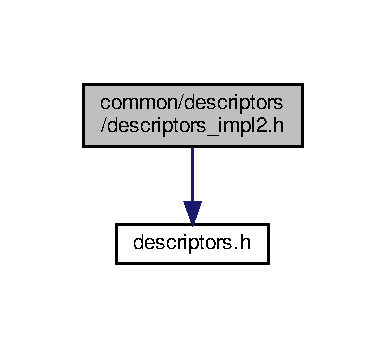
\includegraphics[width=185pt]{descriptors__impl2_8h__incl}
\end{center}
\end{figure}
This graph shows which files directly or indirectly include this file\+:
\nopagebreak
\begin{figure}[H]
\begin{center}
\leavevmode
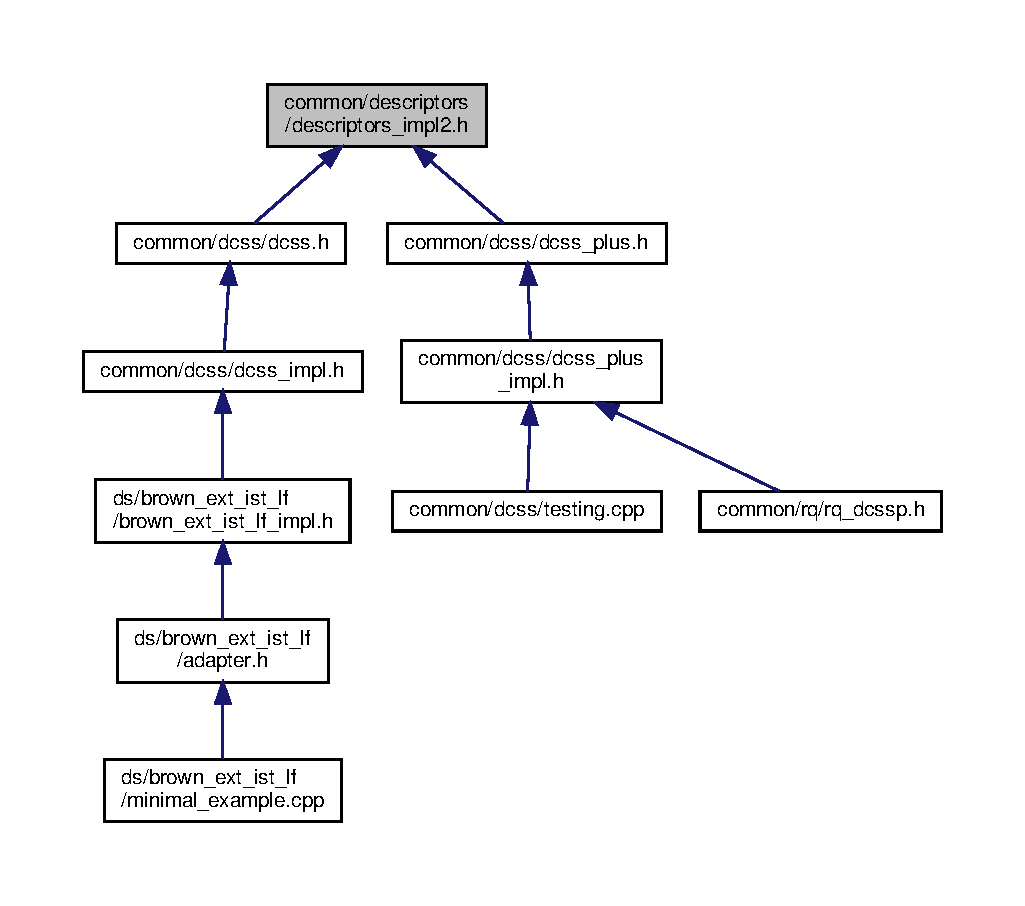
\includegraphics[width=350pt]{descriptors__impl2_8h__dep__incl}
\end{center}
\end{figure}
\subsection*{Macros}
\begin{DoxyCompactItemize}
\item 
\#define \hyperlink{descriptors__impl2_8h_acc5688a1db9cf44f798b5e3ac8348e8a}{D\+E\+S\+C\+\_\+\+I\+N\+I\+T\+\_\+\+A\+LL}(desc\+Array,  macro\+\_\+mutables\+New,  \hyperlink{testing_8cpp_aa085812188e21ede75351d88b9b2c30d}{num\+Processes})
\item 
\#define \hyperlink{descriptors__impl2_8h_af8c689d47cb009242ec174b4e6305d54}{W\+I\+D\+T\+H\+\_\+\+S\+EQ}~48
\item 
\#define \hyperlink{descriptors__impl2_8h_a130b75bf0ec168f61b83eb0662d75c3d}{O\+F\+F\+S\+E\+T\+\_\+\+S\+EQ}~14
\item 
\#define \hyperlink{descriptors__impl2_8h_a95444ce25f4d0a2711f4407cb99e28c5}{M\+A\+S\+K\+\_\+\+S\+EQ}~((uintptr\+\_\+t)((1\+L\+L$<$$<$\+W\+I\+D\+T\+H\+\_\+\+S\+E\+Q)-\/1)$<$$<$\+O\+F\+F\+S\+E\+T\+\_\+\+S\+E\+Q) /$\ast$ cast to avoid signed bit shifting $\ast$/
\item 
\#define \hyperlink{descriptors__impl2_8h_aa0d60409bdc93d1e1afdce860aa354cf}{U\+N\+P\+A\+C\+K\+\_\+\+S\+EQ}(tagptr\+Or\+Mutables)~(((uintptr\+\_\+t)(tagptr\+Or\+Mutables))$>$$>$\hyperlink{kcas__reuse__impl_8h_a130b75bf0ec168f61b83eb0662d75c3d}{O\+F\+F\+S\+E\+T\+\_\+\+S\+EQ})
\item 
\#define \hyperlink{descriptors__impl2_8h_a42d8f729d19e4e4f9a11f5d2f0ebd6d8}{T\+A\+G\+P\+T\+R\+\_\+\+O\+F\+F\+S\+E\+T\+\_\+\+U\+S\+ER}~0
\item 
\#define \hyperlink{descriptors__impl2_8h_afc658e344718431ddb4336743d1aa833}{T\+A\+G\+P\+T\+R\+\_\+\+O\+F\+F\+S\+E\+T\+\_\+\+T\+ID}~3
\item 
\#define \hyperlink{descriptors__impl2_8h_a61a985e276e620c7d24997edec424cf8}{T\+A\+G\+P\+T\+R\+\_\+\+M\+A\+S\+K\+\_\+\+U\+S\+ER}~((1$<$$<$\hyperlink{kcas__reuse__impl_8h_afc658e344718431ddb4336743d1aa833}{T\+A\+G\+P\+T\+R\+\_\+\+O\+F\+F\+S\+E\+T\+\_\+\+T\+ID})-\/1) /$\ast$ assumes T\+ID is next \hyperlink{scxrecord_8h_a0657af583030a13da27c9e6d5ec40aa4}{field} after U\+S\+ER $\ast$/
\item 
\#define \hyperlink{descriptors__impl2_8h_ae040bd6ea3d1ce7145e3aab6395dbb48}{T\+A\+G\+P\+T\+R\+\_\+\+M\+A\+S\+K\+\_\+\+T\+ID}~(((1$<$$<$\hyperlink{kcas__reuse__impl_8h_a130b75bf0ec168f61b83eb0662d75c3d}{O\+F\+F\+S\+E\+T\+\_\+\+S\+EQ})-\/1)\&($\sim$(\hyperlink{kcas__reuse__impl_8h_a61a985e276e620c7d24997edec424cf8}{T\+A\+G\+P\+T\+R\+\_\+\+M\+A\+S\+K\+\_\+\+U\+S\+ER})))
\item 
\#define \hyperlink{descriptors__impl2_8h_a7d7b4fa8ff329a61456256f432ec80e6}{T\+A\+G\+P\+T\+R\+\_\+\+U\+N\+P\+A\+C\+K\+\_\+\+T\+ID}(tagptr)~((int) ((((\hyperlink{descriptors_8h_afd8a7b57046ed96897cda907f17737a7}{tagptr\+\_\+t}) (tagptr))\&\hyperlink{kcas__reuse__impl_8h_ae040bd6ea3d1ce7145e3aab6395dbb48}{T\+A\+G\+P\+T\+R\+\_\+\+M\+A\+S\+K\+\_\+\+T\+ID})$>$$>$\hyperlink{kcas__reuse__impl_8h_afc658e344718431ddb4336743d1aa833}{T\+A\+G\+P\+T\+R\+\_\+\+O\+F\+F\+S\+E\+T\+\_\+\+T\+ID}))
\item 
\#define \hyperlink{descriptors__impl2_8h_aa612148b06ee2120b842bc58000ecc96}{T\+A\+G\+P\+T\+R\+\_\+\+U\+N\+P\+A\+C\+K\+\_\+\+P\+TR}(desc\+Array,  tagptr)~(\&(desc\+Array)\mbox{[}\hyperlink{kcas__reuse__impl_8h_a7d7b4fa8ff329a61456256f432ec80e6}{T\+A\+G\+P\+T\+R\+\_\+\+U\+N\+P\+A\+C\+K\+\_\+\+T\+ID}((tagptr))\mbox{]})
\item 
\#define \hyperlink{descriptors__impl2_8h_a70b520897d003af3d2af350fbd23541d}{T\+A\+G\+P\+T\+R\+\_\+\+N\+EW}(\hyperlink{microbench_2main_8cpp_a9ca9869868fe7e7a38a921cc7de4103f}{tid},  \hyperlink{scxrecord_8h_a71e82299f9d0709f1d5c5448d59347cb}{mutables},  user\+Bits)~((\hyperlink{descriptors_8h_afd8a7b57046ed96897cda907f17737a7}{tagptr\+\_\+t}) (((\hyperlink{kcas__reuse__impl_8h_a516c0a6bd46e52280bb058dc9e28de5a}{U\+N\+P\+A\+C\+K\+\_\+\+S\+EQ}(\hyperlink{scxrecord_8h_a71e82299f9d0709f1d5c5448d59347cb}{mutables}))$<$$<$\hyperlink{kcas__reuse__impl_8h_a130b75bf0ec168f61b83eb0662d75c3d}{O\+F\+F\+S\+E\+T\+\_\+\+S\+EQ}) $\vert$ ((\hyperlink{microbench_2main_8cpp_a9ca9869868fe7e7a38a921cc7de4103f}{tid})$<$$<$\hyperlink{kcas__reuse__impl_8h_afc658e344718431ddb4336743d1aa833}{T\+A\+G\+P\+T\+R\+\_\+\+O\+F\+F\+S\+E\+T\+\_\+\+T\+ID}) $\vert$ (\hyperlink{descriptors_8h_afd8a7b57046ed96897cda907f17737a7}{tagptr\+\_\+t}) (user\+Bits)$<$$<$\hyperlink{kcas__reuse__impl_8h_a42d8f729d19e4e4f9a11f5d2f0ebd6d8}{T\+A\+G\+P\+T\+R\+\_\+\+O\+F\+F\+S\+E\+T\+\_\+\+U\+S\+ER}))
\item 
\#define \hyperlink{descriptors__impl2_8h_ab35d1739985ea729f8a7f51427354dbc}{L\+A\+S\+T\+\_\+\+T\+ID}~(\hyperlink{kcas__reuse__impl_8h_ae040bd6ea3d1ce7145e3aab6395dbb48}{T\+A\+G\+P\+T\+R\+\_\+\+M\+A\+S\+K\+\_\+\+T\+ID}$>$$>$\hyperlink{kcas__reuse__impl_8h_afc658e344718431ddb4336743d1aa833}{T\+A\+G\+P\+T\+R\+\_\+\+O\+F\+F\+S\+E\+T\+\_\+\+T\+ID})
\item 
\#define \hyperlink{descriptors__impl2_8h_acab04f92bc9c2cce09ba5f6099ff02d5}{T\+A\+G\+P\+T\+R\+\_\+\+S\+T\+A\+T\+I\+C\+\_\+\+D\+E\+SC}(id)~((\hyperlink{descriptors_8h_afd8a7b57046ed96897cda907f17737a7}{tagptr\+\_\+t}) \hyperlink{kcas__reuse__impl_8h_a09292a23fc4557618071576f7a9c7292}{T\+A\+G\+P\+T\+R\+\_\+\+N\+EW}(\hyperlink{kcas__reuse__impl_8h_ab35d1739985ea729f8a7f51427354dbc}{L\+A\+S\+T\+\_\+\+T\+ID}-\/1-\/id, 0))
\item 
\#define \hyperlink{descriptors__impl2_8h_ab818bdd1ba41d2a9df7f9d4f582dd160}{T\+A\+G\+P\+T\+R\+\_\+\+D\+U\+M\+M\+Y\+\_\+\+D\+E\+SC}(id)~((\hyperlink{descriptors_8h_afd8a7b57046ed96897cda907f17737a7}{tagptr\+\_\+t}) \hyperlink{kcas__reuse__impl_8h_a09292a23fc4557618071576f7a9c7292}{T\+A\+G\+P\+T\+R\+\_\+\+N\+EW}(\hyperlink{kcas__reuse__impl_8h_ab35d1739985ea729f8a7f51427354dbc}{L\+A\+S\+T\+\_\+\+T\+ID}, id$<$$<$\hyperlink{kcas__reuse__impl_8h_a130b75bf0ec168f61b83eb0662d75c3d}{O\+F\+F\+S\+E\+T\+\_\+\+S\+EQ}))
\item 
\#define \hyperlink{descriptors__impl2_8h_a0d1e6460951f8c965551f121ebd9730c}{comma}~,
\item 
\#define \hyperlink{descriptors__impl2_8h_a91a775c1f4e4fc0a151a7fa4394dcf1c}{M\+U\+T\+A\+B\+L\+E\+S\+\_\+\+U\+N\+P\+A\+C\+K\+\_\+\+F\+I\+E\+LD}(\hyperlink{scxrecord_8h_a71e82299f9d0709f1d5c5448d59347cb}{mutables},  mask,  offset)~((((\hyperlink{descriptors_8h_a8a5af2749482b19d7515054489efca22}{mutables\+\_\+t}) (\hyperlink{scxrecord_8h_a71e82299f9d0709f1d5c5448d59347cb}{mutables}))\&(mask))$>$$>$(offset))
\item 
\#define \hyperlink{descriptors__impl2_8h_a2dffe82870bda176d43cd83ae4a09528}{M\+U\+T\+A\+B\+L\+E\+S\+\_\+\+B\+O\+O\+L\+\_\+\+C\+A\+S\+\_\+\+F\+I\+E\+LD}(success\+Bit,  fld\+Mutables,  snap\+Mutables,  oldval,  val,  mask,  offset)
\item 
\#define \hyperlink{descriptors__impl2_8h_a8d9cd339a416c2c184ae1dd2de8788b6}{M\+U\+T\+A\+B\+L\+E\+S\+\_\+\+V\+A\+L\+\_\+\+C\+A\+S\+\_\+\+F\+I\+E\+LD}(failed\+Bit,  retval,  fld\+Mutables,  snap\+Mutables,  oldval,  val,  mask,  offset)
\item 
\#define \hyperlink{descriptors__impl2_8h_a3f5006111d252ed030777c36943a1edb}{M\+U\+T\+A\+B\+L\+E\+S\+\_\+\+W\+R\+I\+T\+E\+\_\+\+F\+I\+E\+LD}(fld\+Mutables,  snap\+Mutables,  val,  mask,  offset)
\item 
\#define \hyperlink{descriptors__impl2_8h_a8624d53a0fd3077a570cab138e9b93f6}{M\+U\+T\+A\+B\+L\+E\+S\+\_\+\+W\+R\+I\+T\+E\+\_\+\+B\+IT}(fld\+Mutables,  snap\+Mutables,  mask)
\item 
\#define \hyperlink{descriptors__impl2_8h_ab7d0645d0a890428e979b7caea3bae6c}{D\+E\+S\+C\+\_\+\+S\+N\+A\+P\+S\+H\+OT}(desc\+Type,  desc\+Array,  desc\+Dest,  tagptr,  sz)
\item 
\#define \hyperlink{descriptors__impl2_8h_af4167d131f745f0fe0cb14a674649ad3}{D\+E\+S\+C\+\_\+\+R\+E\+A\+D\+\_\+\+F\+I\+E\+LD}(success\+Bit,  fld\+Mutables,  tagptr,  mask,  offset)
\item 
\#define \hyperlink{descriptors__impl2_8h_a725a48b1dde52ad9b393b6bd977f9f27}{D\+E\+S\+C\+\_\+\+N\+EW}(desc\+Array,  macro\+\_\+mutables\+New,  \hyperlink{microbench_2main_8cpp_a9ca9869868fe7e7a38a921cc7de4103f}{tid})
\item 
\#define \hyperlink{descriptors__impl2_8h_a33e3eb771fac10e71e7f6ffd521779d3}{D\+E\+S\+C\+\_\+\+I\+N\+I\+T\+I\+A\+L\+I\+Z\+ED}(desc\+Array,  \hyperlink{microbench_2main_8cpp_a9ca9869868fe7e7a38a921cc7de4103f}{tid})
\end{DoxyCompactItemize}


\subsection{Macro Definition Documentation}
\mbox{\Hypertarget{descriptors__impl2_8h_a0d1e6460951f8c965551f121ebd9730c}\label{descriptors__impl2_8h_a0d1e6460951f8c965551f121ebd9730c}} 
\index{descriptors\+\_\+impl2.\+h@{descriptors\+\_\+impl2.\+h}!comma@{comma}}
\index{comma@{comma}!descriptors\+\_\+impl2.\+h@{descriptors\+\_\+impl2.\+h}}
\subsubsection{\texorpdfstring{comma}{comma}}
{\footnotesize\ttfamily \#define comma~,}

\mbox{\Hypertarget{descriptors__impl2_8h_acc5688a1db9cf44f798b5e3ac8348e8a}\label{descriptors__impl2_8h_acc5688a1db9cf44f798b5e3ac8348e8a}} 
\index{descriptors\+\_\+impl2.\+h@{descriptors\+\_\+impl2.\+h}!D\+E\+S\+C\+\_\+\+I\+N\+I\+T\+\_\+\+A\+LL@{D\+E\+S\+C\+\_\+\+I\+N\+I\+T\+\_\+\+A\+LL}}
\index{D\+E\+S\+C\+\_\+\+I\+N\+I\+T\+\_\+\+A\+LL@{D\+E\+S\+C\+\_\+\+I\+N\+I\+T\+\_\+\+A\+LL}!descriptors\+\_\+impl2.\+h@{descriptors\+\_\+impl2.\+h}}
\subsubsection{\texorpdfstring{D\+E\+S\+C\+\_\+\+I\+N\+I\+T\+\_\+\+A\+LL}{DESC\_INIT\_ALL}}
{\footnotesize\ttfamily \#define D\+E\+S\+C\+\_\+\+I\+N\+I\+T\+\_\+\+A\+LL(\begin{DoxyParamCaption}\item[{}]{desc\+Array,  }\item[{}]{macro\+\_\+mutables\+New,  }\item[{}]{\hyperlink{testing_8cpp_aa085812188e21ede75351d88b9b2c30d}{num\+Processes} }\end{DoxyParamCaption})}

{\bfseries Value\+:}
\begin{DoxyCode}
\{ \(\backslash\)
    for (\textcolor{keywordtype}{int} \hyperlink{namespaceurcu_a536341e353c82c078bc510ca0144dd58}{i}=0;\hyperlink{namespaceurcu_a536341e353c82c078bc510ca0144dd58}{i}<(\hyperlink{testing_8cpp_aa085812188e21ede75351d88b9b2c30d}{numProcesses});++\hyperlink{namespaceurcu_a536341e353c82c078bc510ca0144dd58}{i}) \{ \(\backslash\)
        (descArray)[\hyperlink{namespaceurcu_a536341e353c82c078bc510ca0144dd58}{i}].\hyperlink{dcss_8h_a71e82299f9d0709f1d5c5448d59347cb}{mutables} = macro\_mutablesNew(0); \(\backslash\)
    \} \(\backslash\)
\}
\end{DoxyCode}
\mbox{\Hypertarget{descriptors__impl2_8h_a33e3eb771fac10e71e7f6ffd521779d3}\label{descriptors__impl2_8h_a33e3eb771fac10e71e7f6ffd521779d3}} 
\index{descriptors\+\_\+impl2.\+h@{descriptors\+\_\+impl2.\+h}!D\+E\+S\+C\+\_\+\+I\+N\+I\+T\+I\+A\+L\+I\+Z\+ED@{D\+E\+S\+C\+\_\+\+I\+N\+I\+T\+I\+A\+L\+I\+Z\+ED}}
\index{D\+E\+S\+C\+\_\+\+I\+N\+I\+T\+I\+A\+L\+I\+Z\+ED@{D\+E\+S\+C\+\_\+\+I\+N\+I\+T\+I\+A\+L\+I\+Z\+ED}!descriptors\+\_\+impl2.\+h@{descriptors\+\_\+impl2.\+h}}
\subsubsection{\texorpdfstring{D\+E\+S\+C\+\_\+\+I\+N\+I\+T\+I\+A\+L\+I\+Z\+ED}{DESC\_INITIALIZED}}
{\footnotesize\ttfamily \#define D\+E\+S\+C\+\_\+\+I\+N\+I\+T\+I\+A\+L\+I\+Z\+ED(\begin{DoxyParamCaption}\item[{}]{desc\+Array,  }\item[{}]{\hyperlink{microbench_2main_8cpp_a9ca9869868fe7e7a38a921cc7de4103f}{tid} }\end{DoxyParamCaption})}

{\bfseries Value\+:}
\begin{DoxyCode}
\hyperlink{plaf_8h_a6d355f686181df8f30f7b30588ff1fd0}{SOFTWARE\_BARRIER}; \(\backslash\)
    (descArray)[(\hyperlink{global_8cpp_a9ca9869868fe7e7a38a921cc7de4103f}{tid})].mutables += (1<<\hyperlink{descriptors__impl2_8h_a130b75bf0ec168f61b83eb0662d75c3d}{OFFSET\_SEQ}); \(\backslash\)
    SOFTWARE\_BARRIER;
\end{DoxyCode}
\mbox{\Hypertarget{descriptors__impl2_8h_a725a48b1dde52ad9b393b6bd977f9f27}\label{descriptors__impl2_8h_a725a48b1dde52ad9b393b6bd977f9f27}} 
\index{descriptors\+\_\+impl2.\+h@{descriptors\+\_\+impl2.\+h}!D\+E\+S\+C\+\_\+\+N\+EW@{D\+E\+S\+C\+\_\+\+N\+EW}}
\index{D\+E\+S\+C\+\_\+\+N\+EW@{D\+E\+S\+C\+\_\+\+N\+EW}!descriptors\+\_\+impl2.\+h@{descriptors\+\_\+impl2.\+h}}
\subsubsection{\texorpdfstring{D\+E\+S\+C\+\_\+\+N\+EW}{DESC\_NEW}}
{\footnotesize\ttfamily \#define D\+E\+S\+C\+\_\+\+N\+EW(\begin{DoxyParamCaption}\item[{}]{desc\+Array,  }\item[{}]{macro\+\_\+mutables\+New,  }\item[{}]{\hyperlink{microbench_2main_8cpp_a9ca9869868fe7e7a38a921cc7de4103f}{tid} }\end{DoxyParamCaption})}

{\bfseries Value\+:}
\begin{DoxyCode}
&(descArray)[(\hyperlink{global_8cpp_a9ca9869868fe7e7a38a921cc7de4103f}{tid})]; \{ \textcolor{comment}{/* note: only the process invoking this following macro can change the sequence# 
      */} \(\backslash\)
    SOFTWARE\_BARRIER; \(\backslash\)
    mutables\_t \_\_v = (descArray)[(\hyperlink{global_8cpp_a9ca9869868fe7e7a38a921cc7de4103f}{tid})].mutables; \(\backslash\)
    (descArray)[(\hyperlink{global_8cpp_a9ca9869868fe7e7a38a921cc7de4103f}{tid})].mutables = macro\_mutablesNew(\_\_v); \(\backslash\)
    SOFTWARE\_BARRIER; \(\backslash\)
    \textcolor{comment}{/*\_\_sync\_synchronize();*/} \(\backslash\)
\}
\end{DoxyCode}
\mbox{\Hypertarget{descriptors__impl2_8h_af4167d131f745f0fe0cb14a674649ad3}\label{descriptors__impl2_8h_af4167d131f745f0fe0cb14a674649ad3}} 
\index{descriptors\+\_\+impl2.\+h@{descriptors\+\_\+impl2.\+h}!D\+E\+S\+C\+\_\+\+R\+E\+A\+D\+\_\+\+F\+I\+E\+LD@{D\+E\+S\+C\+\_\+\+R\+E\+A\+D\+\_\+\+F\+I\+E\+LD}}
\index{D\+E\+S\+C\+\_\+\+R\+E\+A\+D\+\_\+\+F\+I\+E\+LD@{D\+E\+S\+C\+\_\+\+R\+E\+A\+D\+\_\+\+F\+I\+E\+LD}!descriptors\+\_\+impl2.\+h@{descriptors\+\_\+impl2.\+h}}
\subsubsection{\texorpdfstring{D\+E\+S\+C\+\_\+\+R\+E\+A\+D\+\_\+\+F\+I\+E\+LD}{DESC\_READ\_FIELD}}
{\footnotesize\ttfamily \#define D\+E\+S\+C\+\_\+\+R\+E\+A\+D\+\_\+\+F\+I\+E\+LD(\begin{DoxyParamCaption}\item[{}]{success\+Bit,  }\item[{}]{fld\+Mutables,  }\item[{}]{tagptr,  }\item[{}]{mask,  }\item[{}]{offset }\end{DoxyParamCaption})}

{\bfseries Value\+:}
\begin{DoxyCode}
(\{ \(\backslash\)
    mutables\_t \_\_mutables = (fldMutables); \(\backslash\)
    successBit = (\_\_mutables & \hyperlink{descriptors__impl2_8h_a95444ce25f4d0a2711f4407cb99e28c5}{MASK\_SEQ}) == ((tagptr) & \hyperlink{descriptors__impl2_8h_a95444ce25f4d0a2711f4407cb99e28c5}{MASK\_SEQ}); \(\backslash\)
    MUTABLES\_UNPACK\_FIELD(\_\_mutables, (mask), (offset)); \(\backslash\)
\})
\end{DoxyCode}
\mbox{\Hypertarget{descriptors__impl2_8h_ab7d0645d0a890428e979b7caea3bae6c}\label{descriptors__impl2_8h_ab7d0645d0a890428e979b7caea3bae6c}} 
\index{descriptors\+\_\+impl2.\+h@{descriptors\+\_\+impl2.\+h}!D\+E\+S\+C\+\_\+\+S\+N\+A\+P\+S\+H\+OT@{D\+E\+S\+C\+\_\+\+S\+N\+A\+P\+S\+H\+OT}}
\index{D\+E\+S\+C\+\_\+\+S\+N\+A\+P\+S\+H\+OT@{D\+E\+S\+C\+\_\+\+S\+N\+A\+P\+S\+H\+OT}!descriptors\+\_\+impl2.\+h@{descriptors\+\_\+impl2.\+h}}
\subsubsection{\texorpdfstring{D\+E\+S\+C\+\_\+\+S\+N\+A\+P\+S\+H\+OT}{DESC\_SNAPSHOT}}
{\footnotesize\ttfamily \#define D\+E\+S\+C\+\_\+\+S\+N\+A\+P\+S\+H\+OT(\begin{DoxyParamCaption}\item[{}]{desc\+Type,  }\item[{}]{desc\+Array,  }\item[{}]{desc\+Dest,  }\item[{}]{tagptr,  }\item[{}]{sz }\end{DoxyParamCaption})}

{\bfseries Value\+:}
\begin{DoxyCode}
(\{ \(\backslash\)
    descType *\_\_src = \hyperlink{descriptors__impl2_8h_aa612148b06ee2120b842bc58000ecc96}{TAGPTR\_UNPACK\_PTR}((descArray), (tagptr)); \(\backslash\)
    memcpy((descDest), \_\_src, (sz)); \(\backslash\)
    SOFTWARE\_BARRIER; \textcolor{comment}{/* prevent compiler from reordering read of \_\_src->mutables before (at least the
       reading portion of) the memcpy */} \(\backslash\)
    (\hyperlink{descriptors__impl2_8h_aa0d60409bdc93d1e1afdce860aa354cf}{UNPACK\_SEQ}(\_\_src->mutables) == \hyperlink{descriptors__impl2_8h_aa0d60409bdc93d1e1afdce860aa354cf}{UNPACK\_SEQ}((tagptr))); \(\backslash\)
\})
\end{DoxyCode}
\mbox{\Hypertarget{descriptors__impl2_8h_ab35d1739985ea729f8a7f51427354dbc}\label{descriptors__impl2_8h_ab35d1739985ea729f8a7f51427354dbc}} 
\index{descriptors\+\_\+impl2.\+h@{descriptors\+\_\+impl2.\+h}!L\+A\+S\+T\+\_\+\+T\+ID@{L\+A\+S\+T\+\_\+\+T\+ID}}
\index{L\+A\+S\+T\+\_\+\+T\+ID@{L\+A\+S\+T\+\_\+\+T\+ID}!descriptors\+\_\+impl2.\+h@{descriptors\+\_\+impl2.\+h}}
\subsubsection{\texorpdfstring{L\+A\+S\+T\+\_\+\+T\+ID}{LAST\_TID}}
{\footnotesize\ttfamily \#define L\+A\+S\+T\+\_\+\+T\+ID~(\hyperlink{kcas__reuse__impl_8h_ae040bd6ea3d1ce7145e3aab6395dbb48}{T\+A\+G\+P\+T\+R\+\_\+\+M\+A\+S\+K\+\_\+\+T\+ID}$>$$>$\hyperlink{kcas__reuse__impl_8h_afc658e344718431ddb4336743d1aa833}{T\+A\+G\+P\+T\+R\+\_\+\+O\+F\+F\+S\+E\+T\+\_\+\+T\+ID})}

\mbox{\Hypertarget{descriptors__impl2_8h_a95444ce25f4d0a2711f4407cb99e28c5}\label{descriptors__impl2_8h_a95444ce25f4d0a2711f4407cb99e28c5}} 
\index{descriptors\+\_\+impl2.\+h@{descriptors\+\_\+impl2.\+h}!M\+A\+S\+K\+\_\+\+S\+EQ@{M\+A\+S\+K\+\_\+\+S\+EQ}}
\index{M\+A\+S\+K\+\_\+\+S\+EQ@{M\+A\+S\+K\+\_\+\+S\+EQ}!descriptors\+\_\+impl2.\+h@{descriptors\+\_\+impl2.\+h}}
\subsubsection{\texorpdfstring{M\+A\+S\+K\+\_\+\+S\+EQ}{MASK\_SEQ}}
{\footnotesize\ttfamily \#define M\+A\+S\+K\+\_\+\+S\+EQ~((uintptr\+\_\+t)((1\+L\+L$<$$<$\+W\+I\+D\+T\+H\+\_\+\+S\+E\+Q)-\/1)$<$$<$\+O\+F\+F\+S\+E\+T\+\_\+\+S\+E\+Q) /$\ast$ cast to avoid signed bit shifting $\ast$/}

\mbox{\Hypertarget{descriptors__impl2_8h_a2dffe82870bda176d43cd83ae4a09528}\label{descriptors__impl2_8h_a2dffe82870bda176d43cd83ae4a09528}} 
\index{descriptors\+\_\+impl2.\+h@{descriptors\+\_\+impl2.\+h}!M\+U\+T\+A\+B\+L\+E\+S\+\_\+\+B\+O\+O\+L\+\_\+\+C\+A\+S\+\_\+\+F\+I\+E\+LD@{M\+U\+T\+A\+B\+L\+E\+S\+\_\+\+B\+O\+O\+L\+\_\+\+C\+A\+S\+\_\+\+F\+I\+E\+LD}}
\index{M\+U\+T\+A\+B\+L\+E\+S\+\_\+\+B\+O\+O\+L\+\_\+\+C\+A\+S\+\_\+\+F\+I\+E\+LD@{M\+U\+T\+A\+B\+L\+E\+S\+\_\+\+B\+O\+O\+L\+\_\+\+C\+A\+S\+\_\+\+F\+I\+E\+LD}!descriptors\+\_\+impl2.\+h@{descriptors\+\_\+impl2.\+h}}
\subsubsection{\texorpdfstring{M\+U\+T\+A\+B\+L\+E\+S\+\_\+\+B\+O\+O\+L\+\_\+\+C\+A\+S\+\_\+\+F\+I\+E\+LD}{MUTABLES\_BOOL\_CAS\_FIELD}}
{\footnotesize\ttfamily \#define M\+U\+T\+A\+B\+L\+E\+S\+\_\+\+B\+O\+O\+L\+\_\+\+C\+A\+S\+\_\+\+F\+I\+E\+LD(\begin{DoxyParamCaption}\item[{}]{success\+Bit,  }\item[{}]{fld\+Mutables,  }\item[{}]{snap\+Mutables,  }\item[{}]{oldval,  }\item[{}]{val,  }\item[{}]{mask,  }\item[{}]{offset }\end{DoxyParamCaption})}

{\bfseries Value\+:}
\begin{DoxyCode}
\{ \(\backslash\)
    mutables\_t \_\_v = (fldMutables); \(\backslash\)
    while (1) \{ \(\backslash\)
        if (\hyperlink{descriptors__impl2_8h_aa0d60409bdc93d1e1afdce860aa354cf}{UNPACK\_SEQ}(\_\_v) != \hyperlink{descriptors__impl2_8h_aa0d60409bdc93d1e1afdce860aa354cf}{UNPACK\_SEQ}((snapMutables))) \{ \(\backslash\)
            (successBit) = \textcolor{keyword}{false}; \(\backslash\)
            break; \(\backslash\)
        \} \(\backslash\)
        if ((successBit) = \_\_sync\_bool\_compare\_and\_swap(&(fldMutables), \(\backslash\)
                (\_\_v & ~(mask)) | ((oldval)<<(offset)), \(\backslash\)
                (\_\_v & ~(mask)) | ((val)<<(offset)))) \{ \(\backslash\)
            break; \(\backslash\)
        \} \(\backslash\)
        \_\_v = (fldMutables); \(\backslash\)
        if (\hyperlink{descriptors__impl2_8h_a91a775c1f4e4fc0a151a7fa4394dcf1c}{MUTABLES\_UNPACK\_FIELD}(\_\_v, (mask), (offset)) != (oldval)) \{ \(\backslash\)
            (successBit) = \textcolor{keyword}{false}; \(\backslash\)
            break; \(\backslash\)
        \} \(\backslash\)
    \} \(\backslash\)
\}
\end{DoxyCode}
\mbox{\Hypertarget{descriptors__impl2_8h_a91a775c1f4e4fc0a151a7fa4394dcf1c}\label{descriptors__impl2_8h_a91a775c1f4e4fc0a151a7fa4394dcf1c}} 
\index{descriptors\+\_\+impl2.\+h@{descriptors\+\_\+impl2.\+h}!M\+U\+T\+A\+B\+L\+E\+S\+\_\+\+U\+N\+P\+A\+C\+K\+\_\+\+F\+I\+E\+LD@{M\+U\+T\+A\+B\+L\+E\+S\+\_\+\+U\+N\+P\+A\+C\+K\+\_\+\+F\+I\+E\+LD}}
\index{M\+U\+T\+A\+B\+L\+E\+S\+\_\+\+U\+N\+P\+A\+C\+K\+\_\+\+F\+I\+E\+LD@{M\+U\+T\+A\+B\+L\+E\+S\+\_\+\+U\+N\+P\+A\+C\+K\+\_\+\+F\+I\+E\+LD}!descriptors\+\_\+impl2.\+h@{descriptors\+\_\+impl2.\+h}}
\subsubsection{\texorpdfstring{M\+U\+T\+A\+B\+L\+E\+S\+\_\+\+U\+N\+P\+A\+C\+K\+\_\+\+F\+I\+E\+LD}{MUTABLES\_UNPACK\_FIELD}}
{\footnotesize\ttfamily \#define M\+U\+T\+A\+B\+L\+E\+S\+\_\+\+U\+N\+P\+A\+C\+K\+\_\+\+F\+I\+E\+LD(\begin{DoxyParamCaption}\item[{}]{\hyperlink{scxrecord_8h_a71e82299f9d0709f1d5c5448d59347cb}{mutables},  }\item[{}]{mask,  }\item[{}]{offset }\end{DoxyParamCaption})~((((\hyperlink{descriptors_8h_a8a5af2749482b19d7515054489efca22}{mutables\+\_\+t}) (\hyperlink{scxrecord_8h_a71e82299f9d0709f1d5c5448d59347cb}{mutables}))\&(mask))$>$$>$(offset))}

\mbox{\Hypertarget{descriptors__impl2_8h_a8d9cd339a416c2c184ae1dd2de8788b6}\label{descriptors__impl2_8h_a8d9cd339a416c2c184ae1dd2de8788b6}} 
\index{descriptors\+\_\+impl2.\+h@{descriptors\+\_\+impl2.\+h}!M\+U\+T\+A\+B\+L\+E\+S\+\_\+\+V\+A\+L\+\_\+\+C\+A\+S\+\_\+\+F\+I\+E\+LD@{M\+U\+T\+A\+B\+L\+E\+S\+\_\+\+V\+A\+L\+\_\+\+C\+A\+S\+\_\+\+F\+I\+E\+LD}}
\index{M\+U\+T\+A\+B\+L\+E\+S\+\_\+\+V\+A\+L\+\_\+\+C\+A\+S\+\_\+\+F\+I\+E\+LD@{M\+U\+T\+A\+B\+L\+E\+S\+\_\+\+V\+A\+L\+\_\+\+C\+A\+S\+\_\+\+F\+I\+E\+LD}!descriptors\+\_\+impl2.\+h@{descriptors\+\_\+impl2.\+h}}
\subsubsection{\texorpdfstring{M\+U\+T\+A\+B\+L\+E\+S\+\_\+\+V\+A\+L\+\_\+\+C\+A\+S\+\_\+\+F\+I\+E\+LD}{MUTABLES\_VAL\_CAS\_FIELD}}
{\footnotesize\ttfamily \#define M\+U\+T\+A\+B\+L\+E\+S\+\_\+\+V\+A\+L\+\_\+\+C\+A\+S\+\_\+\+F\+I\+E\+LD(\begin{DoxyParamCaption}\item[{}]{failed\+Bit,  }\item[{}]{retval,  }\item[{}]{fld\+Mutables,  }\item[{}]{snap\+Mutables,  }\item[{}]{oldval,  }\item[{}]{val,  }\item[{}]{mask,  }\item[{}]{offset }\end{DoxyParamCaption})}

{\bfseries Value\+:}
\begin{DoxyCode}
\{ \(\backslash\)
    mutables\_t \_\_v = (fldMutables); \(\backslash\)
    while (1) \{ \(\backslash\)
        if (\hyperlink{descriptors__impl2_8h_aa0d60409bdc93d1e1afdce860aa354cf}{UNPACK\_SEQ}(\_\_v) != \hyperlink{descriptors__impl2_8h_aa0d60409bdc93d1e1afdce860aa354cf}{UNPACK\_SEQ}((snapMutables))) \{ \(\backslash\)
            (failedBit) = \textcolor{keyword}{true}; \textcolor{comment}{/* version number has changed, CAS cannot occur */} \(\backslash\)
            break; \(\backslash\)
        \} \(\backslash\)
        mutables\_t \_\_oldval = (\_\_v & ~(mask)) | ((oldval)<<(offset)); \(\backslash\)
        (retval) = \_\_sync\_val\_compare\_and\_swap(&(fldMutables), \(\backslash\)
                \_\_oldval, \(\backslash\)
                (\_\_v & ~(mask)) | ((val)<<(offset))); \(\backslash\)
        if ((retval) == \_\_oldval) \{ \textcolor{comment}{/* CAS SUCCESS */} \(\backslash\)
            (retval) = \hyperlink{descriptors__impl2_8h_a91a775c1f4e4fc0a151a7fa4394dcf1c}{MUTABLES\_UNPACK\_FIELD}((retval), (mask), (offset)); \textcolor{comment}{/* return
       contents of subfield */} \(\backslash\)
            (failedBit) = \textcolor{keyword}{false}; \(\backslash\)
            break; \(\backslash\)
        \} \textcolor{keywordflow}{else} \{ \textcolor{comment}{/* CAS FAILURE: should we retry? */} \(\backslash\)
            \_\_v = (retval); \textcolor{comment}{/* save the value that caused our CAS to fail, in case we need to retry */} \(\backslash\)
            (retval) = \hyperlink{descriptors__impl2_8h_a91a775c1f4e4fc0a151a7fa4394dcf1c}{MUTABLES\_UNPACK\_FIELD}((retval), (mask), (offset)); \textcolor{comment}{/* return
       contents of subfield */} \(\backslash\)
            if ((retval) != (oldval)) \{ \textcolor{comment}{/* check if we failed because the subfield's contents do not match
       oldval */} \(\backslash\)
                (failedBit) = \textcolor{keyword}{false}; \(\backslash\)
                break; \(\backslash\)
            \} \(\backslash\)
            \textcolor{comment}{/* subfield's contents DO match oldval, so we need to try again */} \(\backslash\)
        \} \(\backslash\)
    \} \(\backslash\)
\}
\end{DoxyCode}
\mbox{\Hypertarget{descriptors__impl2_8h_a8624d53a0fd3077a570cab138e9b93f6}\label{descriptors__impl2_8h_a8624d53a0fd3077a570cab138e9b93f6}} 
\index{descriptors\+\_\+impl2.\+h@{descriptors\+\_\+impl2.\+h}!M\+U\+T\+A\+B\+L\+E\+S\+\_\+\+W\+R\+I\+T\+E\+\_\+\+B\+IT@{M\+U\+T\+A\+B\+L\+E\+S\+\_\+\+W\+R\+I\+T\+E\+\_\+\+B\+IT}}
\index{M\+U\+T\+A\+B\+L\+E\+S\+\_\+\+W\+R\+I\+T\+E\+\_\+\+B\+IT@{M\+U\+T\+A\+B\+L\+E\+S\+\_\+\+W\+R\+I\+T\+E\+\_\+\+B\+IT}!descriptors\+\_\+impl2.\+h@{descriptors\+\_\+impl2.\+h}}
\subsubsection{\texorpdfstring{M\+U\+T\+A\+B\+L\+E\+S\+\_\+\+W\+R\+I\+T\+E\+\_\+\+B\+IT}{MUTABLES\_WRITE\_BIT}}
{\footnotesize\ttfamily \#define M\+U\+T\+A\+B\+L\+E\+S\+\_\+\+W\+R\+I\+T\+E\+\_\+\+B\+IT(\begin{DoxyParamCaption}\item[{}]{fld\+Mutables,  }\item[{}]{snap\+Mutables,  }\item[{}]{mask }\end{DoxyParamCaption})}

{\bfseries Value\+:}
\begin{DoxyCode}
\{ \(\backslash\)
    mutables\_t \_\_v = (fldMutables); \(\backslash\)
    while (\hyperlink{descriptors__impl2_8h_aa0d60409bdc93d1e1afdce860aa354cf}{UNPACK\_SEQ}(\_\_v) == \hyperlink{descriptors__impl2_8h_aa0d60409bdc93d1e1afdce860aa354cf}{UNPACK\_SEQ}((snapMutables)) \(\backslash\)
            && !(\_\_v&(mask)) \(\backslash\)
            && !\_\_sync\_bool\_compare\_and\_swap(&(fldMutables), \_\_v, (\_\_v|(mask)))) \{ \(\backslash\)
        \_\_v = (fldMutables); \(\backslash\)
    \} \(\backslash\)
\}
\end{DoxyCode}
\mbox{\Hypertarget{descriptors__impl2_8h_a3f5006111d252ed030777c36943a1edb}\label{descriptors__impl2_8h_a3f5006111d252ed030777c36943a1edb}} 
\index{descriptors\+\_\+impl2.\+h@{descriptors\+\_\+impl2.\+h}!M\+U\+T\+A\+B\+L\+E\+S\+\_\+\+W\+R\+I\+T\+E\+\_\+\+F\+I\+E\+LD@{M\+U\+T\+A\+B\+L\+E\+S\+\_\+\+W\+R\+I\+T\+E\+\_\+\+F\+I\+E\+LD}}
\index{M\+U\+T\+A\+B\+L\+E\+S\+\_\+\+W\+R\+I\+T\+E\+\_\+\+F\+I\+E\+LD@{M\+U\+T\+A\+B\+L\+E\+S\+\_\+\+W\+R\+I\+T\+E\+\_\+\+F\+I\+E\+LD}!descriptors\+\_\+impl2.\+h@{descriptors\+\_\+impl2.\+h}}
\subsubsection{\texorpdfstring{M\+U\+T\+A\+B\+L\+E\+S\+\_\+\+W\+R\+I\+T\+E\+\_\+\+F\+I\+E\+LD}{MUTABLES\_WRITE\_FIELD}}
{\footnotesize\ttfamily \#define M\+U\+T\+A\+B\+L\+E\+S\+\_\+\+W\+R\+I\+T\+E\+\_\+\+F\+I\+E\+LD(\begin{DoxyParamCaption}\item[{}]{fld\+Mutables,  }\item[{}]{snap\+Mutables,  }\item[{}]{val,  }\item[{}]{mask,  }\item[{}]{offset }\end{DoxyParamCaption})}

{\bfseries Value\+:}
\begin{DoxyCode}
\{ \(\backslash\)
    mutables\_t \_\_v = (fldMutables); \(\backslash\)
    while (\hyperlink{descriptors__impl2_8h_aa0d60409bdc93d1e1afdce860aa354cf}{UNPACK\_SEQ}(\_\_v) == \hyperlink{descriptors__impl2_8h_aa0d60409bdc93d1e1afdce860aa354cf}{UNPACK\_SEQ}((snapMutables)) \(\backslash\)
            && \hyperlink{descriptors__impl2_8h_a91a775c1f4e4fc0a151a7fa4394dcf1c}{MUTABLES\_UNPACK\_FIELD}(\_\_v, (mask), (offset)) != (val) \(\backslash\)
            && !\_\_sync\_bool\_compare\_and\_swap(&(fldMutables), \_\_v, \(\backslash\)
                    (\_\_v & ~(mask)) | ((val)<<(offset)))) \{ \(\backslash\)
        \_\_v = (fldMutables); \(\backslash\)
    \} \(\backslash\)
\}
\end{DoxyCode}
\mbox{\Hypertarget{descriptors__impl2_8h_a130b75bf0ec168f61b83eb0662d75c3d}\label{descriptors__impl2_8h_a130b75bf0ec168f61b83eb0662d75c3d}} 
\index{descriptors\+\_\+impl2.\+h@{descriptors\+\_\+impl2.\+h}!O\+F\+F\+S\+E\+T\+\_\+\+S\+EQ@{O\+F\+F\+S\+E\+T\+\_\+\+S\+EQ}}
\index{O\+F\+F\+S\+E\+T\+\_\+\+S\+EQ@{O\+F\+F\+S\+E\+T\+\_\+\+S\+EQ}!descriptors\+\_\+impl2.\+h@{descriptors\+\_\+impl2.\+h}}
\subsubsection{\texorpdfstring{O\+F\+F\+S\+E\+T\+\_\+\+S\+EQ}{OFFSET\_SEQ}}
{\footnotesize\ttfamily \#define O\+F\+F\+S\+E\+T\+\_\+\+S\+EQ~14}

\mbox{\Hypertarget{descriptors__impl2_8h_ab818bdd1ba41d2a9df7f9d4f582dd160}\label{descriptors__impl2_8h_ab818bdd1ba41d2a9df7f9d4f582dd160}} 
\index{descriptors\+\_\+impl2.\+h@{descriptors\+\_\+impl2.\+h}!T\+A\+G\+P\+T\+R\+\_\+\+D\+U\+M\+M\+Y\+\_\+\+D\+E\+SC@{T\+A\+G\+P\+T\+R\+\_\+\+D\+U\+M\+M\+Y\+\_\+\+D\+E\+SC}}
\index{T\+A\+G\+P\+T\+R\+\_\+\+D\+U\+M\+M\+Y\+\_\+\+D\+E\+SC@{T\+A\+G\+P\+T\+R\+\_\+\+D\+U\+M\+M\+Y\+\_\+\+D\+E\+SC}!descriptors\+\_\+impl2.\+h@{descriptors\+\_\+impl2.\+h}}
\subsubsection{\texorpdfstring{T\+A\+G\+P\+T\+R\+\_\+\+D\+U\+M\+M\+Y\+\_\+\+D\+E\+SC}{TAGPTR\_DUMMY\_DESC}}
{\footnotesize\ttfamily \#define T\+A\+G\+P\+T\+R\+\_\+\+D\+U\+M\+M\+Y\+\_\+\+D\+E\+SC(\begin{DoxyParamCaption}\item[{}]{id }\end{DoxyParamCaption})~((\hyperlink{descriptors_8h_afd8a7b57046ed96897cda907f17737a7}{tagptr\+\_\+t}) \hyperlink{kcas__reuse__impl_8h_a09292a23fc4557618071576f7a9c7292}{T\+A\+G\+P\+T\+R\+\_\+\+N\+EW}(\hyperlink{kcas__reuse__impl_8h_ab35d1739985ea729f8a7f51427354dbc}{L\+A\+S\+T\+\_\+\+T\+ID}, id$<$$<$\hyperlink{kcas__reuse__impl_8h_a130b75bf0ec168f61b83eb0662d75c3d}{O\+F\+F\+S\+E\+T\+\_\+\+S\+EQ}))}

\mbox{\Hypertarget{descriptors__impl2_8h_ae040bd6ea3d1ce7145e3aab6395dbb48}\label{descriptors__impl2_8h_ae040bd6ea3d1ce7145e3aab6395dbb48}} 
\index{descriptors\+\_\+impl2.\+h@{descriptors\+\_\+impl2.\+h}!T\+A\+G\+P\+T\+R\+\_\+\+M\+A\+S\+K\+\_\+\+T\+ID@{T\+A\+G\+P\+T\+R\+\_\+\+M\+A\+S\+K\+\_\+\+T\+ID}}
\index{T\+A\+G\+P\+T\+R\+\_\+\+M\+A\+S\+K\+\_\+\+T\+ID@{T\+A\+G\+P\+T\+R\+\_\+\+M\+A\+S\+K\+\_\+\+T\+ID}!descriptors\+\_\+impl2.\+h@{descriptors\+\_\+impl2.\+h}}
\subsubsection{\texorpdfstring{T\+A\+G\+P\+T\+R\+\_\+\+M\+A\+S\+K\+\_\+\+T\+ID}{TAGPTR\_MASK\_TID}}
{\footnotesize\ttfamily \#define T\+A\+G\+P\+T\+R\+\_\+\+M\+A\+S\+K\+\_\+\+T\+ID~(((1$<$$<$\hyperlink{kcas__reuse__impl_8h_a130b75bf0ec168f61b83eb0662d75c3d}{O\+F\+F\+S\+E\+T\+\_\+\+S\+EQ})-\/1)\&($\sim$(\hyperlink{kcas__reuse__impl_8h_a61a985e276e620c7d24997edec424cf8}{T\+A\+G\+P\+T\+R\+\_\+\+M\+A\+S\+K\+\_\+\+U\+S\+ER})))}

\mbox{\Hypertarget{descriptors__impl2_8h_a61a985e276e620c7d24997edec424cf8}\label{descriptors__impl2_8h_a61a985e276e620c7d24997edec424cf8}} 
\index{descriptors\+\_\+impl2.\+h@{descriptors\+\_\+impl2.\+h}!T\+A\+G\+P\+T\+R\+\_\+\+M\+A\+S\+K\+\_\+\+U\+S\+ER@{T\+A\+G\+P\+T\+R\+\_\+\+M\+A\+S\+K\+\_\+\+U\+S\+ER}}
\index{T\+A\+G\+P\+T\+R\+\_\+\+M\+A\+S\+K\+\_\+\+U\+S\+ER@{T\+A\+G\+P\+T\+R\+\_\+\+M\+A\+S\+K\+\_\+\+U\+S\+ER}!descriptors\+\_\+impl2.\+h@{descriptors\+\_\+impl2.\+h}}
\subsubsection{\texorpdfstring{T\+A\+G\+P\+T\+R\+\_\+\+M\+A\+S\+K\+\_\+\+U\+S\+ER}{TAGPTR\_MASK\_USER}}
{\footnotesize\ttfamily \#define T\+A\+G\+P\+T\+R\+\_\+\+M\+A\+S\+K\+\_\+\+U\+S\+ER~((1$<$$<$\hyperlink{kcas__reuse__impl_8h_afc658e344718431ddb4336743d1aa833}{T\+A\+G\+P\+T\+R\+\_\+\+O\+F\+F\+S\+E\+T\+\_\+\+T\+ID})-\/1) /$\ast$ assumes T\+ID is next \hyperlink{scxrecord_8h_a0657af583030a13da27c9e6d5ec40aa4}{field} after U\+S\+ER $\ast$/}

\mbox{\Hypertarget{descriptors__impl2_8h_a70b520897d003af3d2af350fbd23541d}\label{descriptors__impl2_8h_a70b520897d003af3d2af350fbd23541d}} 
\index{descriptors\+\_\+impl2.\+h@{descriptors\+\_\+impl2.\+h}!T\+A\+G\+P\+T\+R\+\_\+\+N\+EW@{T\+A\+G\+P\+T\+R\+\_\+\+N\+EW}}
\index{T\+A\+G\+P\+T\+R\+\_\+\+N\+EW@{T\+A\+G\+P\+T\+R\+\_\+\+N\+EW}!descriptors\+\_\+impl2.\+h@{descriptors\+\_\+impl2.\+h}}
\subsubsection{\texorpdfstring{T\+A\+G\+P\+T\+R\+\_\+\+N\+EW}{TAGPTR\_NEW}}
{\footnotesize\ttfamily \#define T\+A\+G\+P\+T\+R\+\_\+\+N\+EW(\begin{DoxyParamCaption}\item[{}]{\hyperlink{microbench_2main_8cpp_a9ca9869868fe7e7a38a921cc7de4103f}{tid},  }\item[{}]{\hyperlink{scxrecord_8h_a71e82299f9d0709f1d5c5448d59347cb}{mutables},  }\item[{}]{user\+Bits }\end{DoxyParamCaption})~((\hyperlink{descriptors_8h_afd8a7b57046ed96897cda907f17737a7}{tagptr\+\_\+t}) (((\hyperlink{kcas__reuse__impl_8h_a516c0a6bd46e52280bb058dc9e28de5a}{U\+N\+P\+A\+C\+K\+\_\+\+S\+EQ}(\hyperlink{scxrecord_8h_a71e82299f9d0709f1d5c5448d59347cb}{mutables}))$<$$<$\hyperlink{kcas__reuse__impl_8h_a130b75bf0ec168f61b83eb0662d75c3d}{O\+F\+F\+S\+E\+T\+\_\+\+S\+EQ}) $\vert$ ((\hyperlink{microbench_2main_8cpp_a9ca9869868fe7e7a38a921cc7de4103f}{tid})$<$$<$\hyperlink{kcas__reuse__impl_8h_afc658e344718431ddb4336743d1aa833}{T\+A\+G\+P\+T\+R\+\_\+\+O\+F\+F\+S\+E\+T\+\_\+\+T\+ID}) $\vert$ (\hyperlink{descriptors_8h_afd8a7b57046ed96897cda907f17737a7}{tagptr\+\_\+t}) (user\+Bits)$<$$<$\hyperlink{kcas__reuse__impl_8h_a42d8f729d19e4e4f9a11f5d2f0ebd6d8}{T\+A\+G\+P\+T\+R\+\_\+\+O\+F\+F\+S\+E\+T\+\_\+\+U\+S\+ER}))}

\mbox{\Hypertarget{descriptors__impl2_8h_afc658e344718431ddb4336743d1aa833}\label{descriptors__impl2_8h_afc658e344718431ddb4336743d1aa833}} 
\index{descriptors\+\_\+impl2.\+h@{descriptors\+\_\+impl2.\+h}!T\+A\+G\+P\+T\+R\+\_\+\+O\+F\+F\+S\+E\+T\+\_\+\+T\+ID@{T\+A\+G\+P\+T\+R\+\_\+\+O\+F\+F\+S\+E\+T\+\_\+\+T\+ID}}
\index{T\+A\+G\+P\+T\+R\+\_\+\+O\+F\+F\+S\+E\+T\+\_\+\+T\+ID@{T\+A\+G\+P\+T\+R\+\_\+\+O\+F\+F\+S\+E\+T\+\_\+\+T\+ID}!descriptors\+\_\+impl2.\+h@{descriptors\+\_\+impl2.\+h}}
\subsubsection{\texorpdfstring{T\+A\+G\+P\+T\+R\+\_\+\+O\+F\+F\+S\+E\+T\+\_\+\+T\+ID}{TAGPTR\_OFFSET\_TID}}
{\footnotesize\ttfamily \#define T\+A\+G\+P\+T\+R\+\_\+\+O\+F\+F\+S\+E\+T\+\_\+\+T\+ID~3}

\mbox{\Hypertarget{descriptors__impl2_8h_a42d8f729d19e4e4f9a11f5d2f0ebd6d8}\label{descriptors__impl2_8h_a42d8f729d19e4e4f9a11f5d2f0ebd6d8}} 
\index{descriptors\+\_\+impl2.\+h@{descriptors\+\_\+impl2.\+h}!T\+A\+G\+P\+T\+R\+\_\+\+O\+F\+F\+S\+E\+T\+\_\+\+U\+S\+ER@{T\+A\+G\+P\+T\+R\+\_\+\+O\+F\+F\+S\+E\+T\+\_\+\+U\+S\+ER}}
\index{T\+A\+G\+P\+T\+R\+\_\+\+O\+F\+F\+S\+E\+T\+\_\+\+U\+S\+ER@{T\+A\+G\+P\+T\+R\+\_\+\+O\+F\+F\+S\+E\+T\+\_\+\+U\+S\+ER}!descriptors\+\_\+impl2.\+h@{descriptors\+\_\+impl2.\+h}}
\subsubsection{\texorpdfstring{T\+A\+G\+P\+T\+R\+\_\+\+O\+F\+F\+S\+E\+T\+\_\+\+U\+S\+ER}{TAGPTR\_OFFSET\_USER}}
{\footnotesize\ttfamily \#define T\+A\+G\+P\+T\+R\+\_\+\+O\+F\+F\+S\+E\+T\+\_\+\+U\+S\+ER~0}

\mbox{\Hypertarget{descriptors__impl2_8h_acab04f92bc9c2cce09ba5f6099ff02d5}\label{descriptors__impl2_8h_acab04f92bc9c2cce09ba5f6099ff02d5}} 
\index{descriptors\+\_\+impl2.\+h@{descriptors\+\_\+impl2.\+h}!T\+A\+G\+P\+T\+R\+\_\+\+S\+T\+A\+T\+I\+C\+\_\+\+D\+E\+SC@{T\+A\+G\+P\+T\+R\+\_\+\+S\+T\+A\+T\+I\+C\+\_\+\+D\+E\+SC}}
\index{T\+A\+G\+P\+T\+R\+\_\+\+S\+T\+A\+T\+I\+C\+\_\+\+D\+E\+SC@{T\+A\+G\+P\+T\+R\+\_\+\+S\+T\+A\+T\+I\+C\+\_\+\+D\+E\+SC}!descriptors\+\_\+impl2.\+h@{descriptors\+\_\+impl2.\+h}}
\subsubsection{\texorpdfstring{T\+A\+G\+P\+T\+R\+\_\+\+S\+T\+A\+T\+I\+C\+\_\+\+D\+E\+SC}{TAGPTR\_STATIC\_DESC}}
{\footnotesize\ttfamily \#define T\+A\+G\+P\+T\+R\+\_\+\+S\+T\+A\+T\+I\+C\+\_\+\+D\+E\+SC(\begin{DoxyParamCaption}\item[{}]{id }\end{DoxyParamCaption})~((\hyperlink{descriptors_8h_afd8a7b57046ed96897cda907f17737a7}{tagptr\+\_\+t}) \hyperlink{kcas__reuse__impl_8h_a09292a23fc4557618071576f7a9c7292}{T\+A\+G\+P\+T\+R\+\_\+\+N\+EW}(\hyperlink{kcas__reuse__impl_8h_ab35d1739985ea729f8a7f51427354dbc}{L\+A\+S\+T\+\_\+\+T\+ID}-\/1-\/id, 0))}

\mbox{\Hypertarget{descriptors__impl2_8h_aa612148b06ee2120b842bc58000ecc96}\label{descriptors__impl2_8h_aa612148b06ee2120b842bc58000ecc96}} 
\index{descriptors\+\_\+impl2.\+h@{descriptors\+\_\+impl2.\+h}!T\+A\+G\+P\+T\+R\+\_\+\+U\+N\+P\+A\+C\+K\+\_\+\+P\+TR@{T\+A\+G\+P\+T\+R\+\_\+\+U\+N\+P\+A\+C\+K\+\_\+\+P\+TR}}
\index{T\+A\+G\+P\+T\+R\+\_\+\+U\+N\+P\+A\+C\+K\+\_\+\+P\+TR@{T\+A\+G\+P\+T\+R\+\_\+\+U\+N\+P\+A\+C\+K\+\_\+\+P\+TR}!descriptors\+\_\+impl2.\+h@{descriptors\+\_\+impl2.\+h}}
\subsubsection{\texorpdfstring{T\+A\+G\+P\+T\+R\+\_\+\+U\+N\+P\+A\+C\+K\+\_\+\+P\+TR}{TAGPTR\_UNPACK\_PTR}}
{\footnotesize\ttfamily \#define T\+A\+G\+P\+T\+R\+\_\+\+U\+N\+P\+A\+C\+K\+\_\+\+P\+TR(\begin{DoxyParamCaption}\item[{}]{desc\+Array,  }\item[{}]{tagptr }\end{DoxyParamCaption})~(\&(desc\+Array)\mbox{[}\hyperlink{kcas__reuse__impl_8h_a7d7b4fa8ff329a61456256f432ec80e6}{T\+A\+G\+P\+T\+R\+\_\+\+U\+N\+P\+A\+C\+K\+\_\+\+T\+ID}((tagptr))\mbox{]})}

\mbox{\Hypertarget{descriptors__impl2_8h_a7d7b4fa8ff329a61456256f432ec80e6}\label{descriptors__impl2_8h_a7d7b4fa8ff329a61456256f432ec80e6}} 
\index{descriptors\+\_\+impl2.\+h@{descriptors\+\_\+impl2.\+h}!T\+A\+G\+P\+T\+R\+\_\+\+U\+N\+P\+A\+C\+K\+\_\+\+T\+ID@{T\+A\+G\+P\+T\+R\+\_\+\+U\+N\+P\+A\+C\+K\+\_\+\+T\+ID}}
\index{T\+A\+G\+P\+T\+R\+\_\+\+U\+N\+P\+A\+C\+K\+\_\+\+T\+ID@{T\+A\+G\+P\+T\+R\+\_\+\+U\+N\+P\+A\+C\+K\+\_\+\+T\+ID}!descriptors\+\_\+impl2.\+h@{descriptors\+\_\+impl2.\+h}}
\subsubsection{\texorpdfstring{T\+A\+G\+P\+T\+R\+\_\+\+U\+N\+P\+A\+C\+K\+\_\+\+T\+ID}{TAGPTR\_UNPACK\_TID}}
{\footnotesize\ttfamily \#define T\+A\+G\+P\+T\+R\+\_\+\+U\+N\+P\+A\+C\+K\+\_\+\+T\+ID(\begin{DoxyParamCaption}\item[{}]{tagptr }\end{DoxyParamCaption})~((int) ((((\hyperlink{descriptors_8h_afd8a7b57046ed96897cda907f17737a7}{tagptr\+\_\+t}) (tagptr))\&\hyperlink{kcas__reuse__impl_8h_ae040bd6ea3d1ce7145e3aab6395dbb48}{T\+A\+G\+P\+T\+R\+\_\+\+M\+A\+S\+K\+\_\+\+T\+ID})$>$$>$\hyperlink{kcas__reuse__impl_8h_afc658e344718431ddb4336743d1aa833}{T\+A\+G\+P\+T\+R\+\_\+\+O\+F\+F\+S\+E\+T\+\_\+\+T\+ID}))}

\mbox{\Hypertarget{descriptors__impl2_8h_aa0d60409bdc93d1e1afdce860aa354cf}\label{descriptors__impl2_8h_aa0d60409bdc93d1e1afdce860aa354cf}} 
\index{descriptors\+\_\+impl2.\+h@{descriptors\+\_\+impl2.\+h}!U\+N\+P\+A\+C\+K\+\_\+\+S\+EQ@{U\+N\+P\+A\+C\+K\+\_\+\+S\+EQ}}
\index{U\+N\+P\+A\+C\+K\+\_\+\+S\+EQ@{U\+N\+P\+A\+C\+K\+\_\+\+S\+EQ}!descriptors\+\_\+impl2.\+h@{descriptors\+\_\+impl2.\+h}}
\subsubsection{\texorpdfstring{U\+N\+P\+A\+C\+K\+\_\+\+S\+EQ}{UNPACK\_SEQ}}
{\footnotesize\ttfamily \#define U\+N\+P\+A\+C\+K\+\_\+\+S\+EQ(\begin{DoxyParamCaption}\item[{}]{tagptr\+Or\+Mutables }\end{DoxyParamCaption})~(((uintptr\+\_\+t)(tagptr\+Or\+Mutables))$>$$>$\hyperlink{kcas__reuse__impl_8h_a130b75bf0ec168f61b83eb0662d75c3d}{O\+F\+F\+S\+E\+T\+\_\+\+S\+EQ})}

\mbox{\Hypertarget{descriptors__impl2_8h_af8c689d47cb009242ec174b4e6305d54}\label{descriptors__impl2_8h_af8c689d47cb009242ec174b4e6305d54}} 
\index{descriptors\+\_\+impl2.\+h@{descriptors\+\_\+impl2.\+h}!W\+I\+D\+T\+H\+\_\+\+S\+EQ@{W\+I\+D\+T\+H\+\_\+\+S\+EQ}}
\index{W\+I\+D\+T\+H\+\_\+\+S\+EQ@{W\+I\+D\+T\+H\+\_\+\+S\+EQ}!descriptors\+\_\+impl2.\+h@{descriptors\+\_\+impl2.\+h}}
\subsubsection{\texorpdfstring{W\+I\+D\+T\+H\+\_\+\+S\+EQ}{WIDTH\_SEQ}}
{\footnotesize\ttfamily \#define W\+I\+D\+T\+H\+\_\+\+S\+EQ~48}

mutables\+\_\+t corresponds to the mutables field of the descriptor. it contains the mutable fields of the descriptor and a sequence number. the width, offset and mask for the sequence number is defined below. this sequence number width, offset and mask are also shared by tagptr\+\_\+t.

in particular, for any tagptr\+\_\+t x and mutables\+\_\+t y, the sequence numbers in x and y are equal iff x\&M\+A\+S\+K\+\_\+\+S\+EQ == y\&M\+A\+S\+K\+\_\+\+S\+EQ (despite the differing types of x and y).

tagptr\+\_\+t consists of a triple $<$seq, tid, testbit$>$. these three fields are defined by the T\+A\+G\+P\+T\+R\+\_\+ macros below. 
\hypertarget{errors_8h}{}\section{common/errors.h File Reference}
\label{errors_8h}\index{common/errors.\+h@{common/errors.\+h}}
{\ttfamily \#include $<$iostream$>$}\newline
{\ttfamily \#include $<$string$>$}\newline
{\ttfamily \#include $<$unistd.\+h$>$}\newline
Include dependency graph for errors.\+h\+:
\nopagebreak
\begin{figure}[H]
\begin{center}
\leavevmode
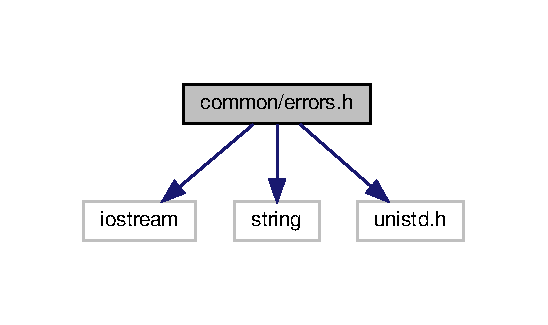
\includegraphics[width=263pt]{errors_8h__incl}
\end{center}
\end{figure}
This graph shows which files directly or indirectly include this file\+:
\nopagebreak
\begin{figure}[H]
\begin{center}
\leavevmode

\includegraphics[width=350pt]{errors_8h__dep__incl}
\end{center}
\end{figure}
\subsection*{Macros}
\begin{DoxyCompactItemize}
\item 
\#define \hyperlink{errors_8h_ad63995348018168a29f53f37bbb7201d}{setbench\+\_\+error}(s)
\end{DoxyCompactItemize}


\subsection{Macro Definition Documentation}
\mbox{\Hypertarget{errors_8h_ad63995348018168a29f53f37bbb7201d}\label{errors_8h_ad63995348018168a29f53f37bbb7201d}} 
\index{errors.\+h@{errors.\+h}!setbench\+\_\+error@{setbench\+\_\+error}}
\index{setbench\+\_\+error@{setbench\+\_\+error}!errors.\+h@{errors.\+h}}
\subsubsection{\texorpdfstring{setbench\+\_\+error}{setbench\_error}}
{\footnotesize\ttfamily \#define setbench\+\_\+error(\begin{DoxyParamCaption}\item[{}]{s }\end{DoxyParamCaption})}

{\bfseries Value\+:}
\begin{DoxyCode}
\{ \(\backslash\)
    std::cout<<\textcolor{stringliteral}{"ERROR: "}<<s<<\textcolor{stringliteral}{" (at "}<<\_\_FILE\_\_<<\textcolor{stringliteral}{"::"}<<\_\_FUNCTION\_\_<<\textcolor{stringliteral}{":"}<<\_\_LINE\_\_<<\textcolor{stringliteral}{")"}<<std::endl; \(\backslash\)
    exit(-1); \(\backslash\)
\}
\end{DoxyCode}

\hypertarget{gstats_8h}{}\section{common/gstats.h File Reference}
\label{gstats_8h}\index{common/gstats.\+h@{common/gstats.\+h}}
{\ttfamily \#include $<$thread$>$}\newline
{\ttfamily \#include $<$string$>$}\newline
{\ttfamily \#include $<$vector$>$}\newline
{\ttfamily \#include $<$map$>$}\newline
{\ttfamily \#include $<$cassert$>$}\newline
{\ttfamily \#include $<$cmath$>$}\newline
{\ttfamily \#include $<$iostream$>$}\newline
{\ttfamily \#include $<$sstream$>$}\newline
{\ttfamily \#include $<$algorithm$>$}\newline
{\ttfamily \#include \char`\"{}errors.\+h\char`\"{}}\newline
{\ttfamily \#include \char`\"{}locks\+\_\+impl.\+h\char`\"{}}\newline
{\ttfamily \#include \char`\"{}plaf.\+h\char`\"{}}\newline
Include dependency graph for gstats.\+h\+:
\nopagebreak
\begin{figure}[H]
\begin{center}
\leavevmode
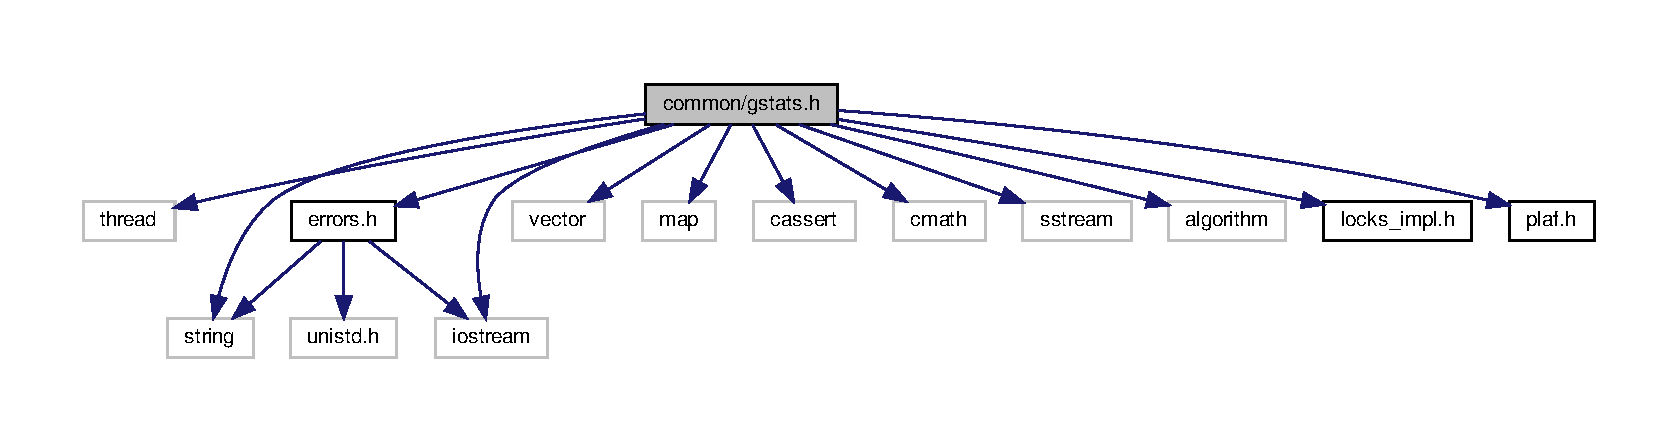
\includegraphics[width=350pt]{gstats_8h__incl}
\end{center}
\end{figure}
\subsection*{Classes}
\begin{DoxyCompactItemize}
\item 
class \hyperlink{classgstats__output__item}{gstats\+\_\+output\+\_\+item}
\item 
class \hyperlink{classgstats__t}{gstats\+\_\+t}
\item 
struct \hyperlink{structgstats__t_1_1stat__metrics}{gstats\+\_\+t\+::stat\+\_\+metrics$<$ T $>$}
\end{DoxyCompactItemize}
\subsection*{Macros}
\begin{DoxyCompactItemize}
\item 
\#define \hyperlink{gstats_8h_a42f8c497a1968074f38bf5055c650dca}{V\+E\+R\+B\+O\+SE}~if(0)
\item 
\#define \hyperlink{gstats_8h_afa9b122e63cc8d7c03659c3d83ff9013}{G\+S\+T\+A\+T\+S\+\_\+\+C\+O\+M\+MA}~,
\item 
\#define \hyperlink{gstats_8h_ab4a0c96913a35237ccec45f2ad628d7f}{G\+S\+T\+A\+T\+S\+\_\+\+T\+H\+R\+E\+A\+D\+\_\+\+P\+A\+D\+D\+I\+N\+G\+\_\+\+B\+Y\+T\+ES}~256
\item 
\#define \hyperlink{gstats_8h_af5d26090219202a76707ea6dfda966a6}{G\+S\+T\+A\+T\+S\+\_\+\+M\+A\+X\+\_\+\+N\+U\+M\+\_\+\+S\+T\+A\+TS}~128
\item 
\#define \hyperlink{gstats_8h_a3d1fc557c60e610d8ea2ea6dfee94222}{G\+S\+T\+A\+T\+S\+\_\+\+M\+A\+X\+\_\+\+T\+H\+R\+E\+A\+D\+\_\+\+B\+U\+F\+\_\+\+S\+I\+ZE}~(1$<$$<$22)
\item 
\#define \hyperlink{gstats_8h_a9c9b32b49c54b1f2a759e577b4396534}{G\+S\+T\+A\+T\+S\+\_\+\+D\+A\+T\+A\+\_\+\+S\+I\+Z\+E\+\_\+\+B\+Y\+T\+ES}~8
\item 
\#define \hyperlink{gstats_8h_ad75c6b61610f8aff8362819d98a5f0ce}{G\+S\+T\+A\+T\+S\+\_\+\+B\+I\+T\+S\+\_\+\+I\+N\+\_\+\+B\+Y\+TE}~8
\item 
\#define \hyperlink{gstats_8h_a1825fbb4f3d626ca97db468c8614e797}{G\+S\+T\+A\+T\+S\+\_\+\+D\+E\+F\+A\+U\+L\+T\+\_\+\+H\+I\+S\+T\+O\+G\+R\+A\+M\+\_\+\+L\+I\+N\+\_\+\+N\+U\+M\+\_\+\+B\+U\+C\+K\+E\+TS}~32
\item 
\#define \hyperlink{gstats_8h_ab5bc616b9e1c3310d22f98e740913e8b}{G\+S\+T\+A\+T\+S\+\_\+\+D\+E\+F\+A\+U\+L\+T\+\_\+\+H\+I\+S\+T\+O\+G\+R\+A\+M\+\_\+\+L\+O\+G\+\_\+\+N\+U\+M\+\_\+\+B\+U\+C\+K\+E\+TS}~\hyperlink{gstats_8h_a9c9b32b49c54b1f2a759e577b4396534}{G\+S\+T\+A\+T\+S\+\_\+\+D\+A\+T\+A\+\_\+\+S\+I\+Z\+E\+\_\+\+B\+Y\+T\+ES} $\ast$ \hyperlink{gstats_8h_ad75c6b61610f8aff8362819d98a5f0ce}{G\+S\+T\+A\+T\+S\+\_\+\+B\+I\+T\+S\+\_\+\+I\+N\+\_\+\+B\+Y\+TE}
\item 
\#define \hyperlink{gstats_8h_a2dccfafc9a416dc89b35dc028b9e6bda}{G\+S\+T\+A\+T\+S\+\_\+\+SQ}(x)~((x)$\ast$(x))
\item 
\#define \hyperlink{gstats_8h_a34b909e81c7270e3460cad58471dbdd9}{G\+S\+T\+A\+T\+S\+\_\+\+U\+S\+E\+\_\+\+T\+E\+M\+P\+L\+A\+TE}(id,  func,  args)~(this-\/$>$data\+\_\+types\mbox{[}id\mbox{]} == \hyperlink{gstats_8h_add042cd26594ae31bc443952e37d30f6a1c09973d0c7a1638ffc4aaa0c68d4d01}{L\+O\+N\+G\+\_\+\+L\+O\+NG} ? func$<$long long$>$(args) \+: func$<$double$>$(args))
\item 
\#define \hyperlink{gstats_8h_a8ddd7e89cc3d780247620c7d42d74ecd}{G\+S\+T\+A\+T\+S\+\_\+\+F\+I\+E\+L\+D\+\_\+\+F\+I\+R\+ST}~first
\item 
\#define \hyperlink{gstats_8h_a7b2466cd41c797ab0b8d690dc1d28619}{G\+S\+T\+A\+T\+S\+\_\+\+F\+I\+E\+L\+D\+\_\+\+C\+O\+U\+NT}~cnt
\item 
\#define \hyperlink{gstats_8h_ad909c7fc3cd4fe84a623f23fb9e4023c}{G\+S\+T\+A\+T\+S\+\_\+\+F\+I\+E\+L\+D\+\_\+\+M\+IN}~min
\item 
\#define \hyperlink{gstats_8h_a027febada1f28ad43162a67fdfbf7ba5}{G\+S\+T\+A\+T\+S\+\_\+\+F\+I\+E\+L\+D\+\_\+\+M\+AX}~max
\item 
\#define \hyperlink{gstats_8h_ab465c7810f673c22a82119036d4141ab}{G\+S\+T\+A\+T\+S\+\_\+\+F\+I\+E\+L\+D\+\_\+\+S\+UM}~sum
\item 
\#define \hyperlink{gstats_8h_a68f61f69e5a60c0f1e77d664db0763f4}{G\+S\+T\+A\+T\+S\+\_\+\+F\+I\+E\+L\+D\+\_\+\+A\+V\+E\+R\+A\+GE}~avg
\item 
\#define \hyperlink{gstats_8h_ae65152830cd857832514e34d73ee6f66}{G\+S\+T\+A\+T\+S\+\_\+\+F\+I\+E\+L\+D\+\_\+\+V\+A\+R\+I\+A\+N\+CE}~variance
\item 
\#define \hyperlink{gstats_8h_ae9d639e9e0d46cc351c6042d34bf052e}{G\+S\+T\+A\+T\+S\+\_\+\+F\+I\+E\+L\+D\+\_\+\+S\+T\+D\+EV}~stdev
\item 
\#define \hyperlink{gstats_8h_af0868b0784ba2a610fa5776e6a64224a}{G\+S\+T\+A\+T\+S\+\_\+\+F\+I\+E\+L\+D\+\_\+\+N\+O\+NE}~none
\item 
\#define \hyperlink{gstats_8h_abd11fabecfe8f40fa3b097c9df264fdd}{G\+S\+T\+A\+T\+S\+\_\+\+T\+Y\+P\+E\+\_\+\+T\+O\+\_\+\+F\+I\+E\+LD}(type)~G\+S\+T\+A\+T\+S\+\_\+\+F\+I\+E\+L\+D\+\_\+\#\#type
\item 
\#define \hyperlink{gstats_8h_aa664d314b3e40aa2ba3f4e30b74db05d}{G\+S\+T\+A\+T\+S\+\_\+\+P\+R\+I\+N\+T\+\_\+\+L\+O\+W\+ER}(str)~\{ std\+::string \+\_\+\+\_\+s = str; transform(\+\_\+\+\_\+s.\+begin(), \+\_\+\+\_\+s.\+end(), \+\_\+\+\_\+s.\+begin(), \+::tolower); std\+::cout$<$$<$\+\_\+\+\_\+s; \}
\item 
\#define \hyperlink{gstats_8h_a7aa7e025c7c1dc96d7f60534d5598952}{G\+S\+T\+A\+T\+S\+\_\+\+P\+R\+I\+N\+T\+\_\+\+A\+GG}(agg\+\_\+granularity\+\_\+str,  type,  sid,  metrics,  num\+\_\+metrics)
\item 
\#define \hyperlink{gstats_8h_a787e697bdd2ace1231608a1cd134714f}{G\+S\+T\+A\+T\+S\+\_\+\+P\+R\+I\+N\+T\+\_\+\+H\+I\+S\+T\+O\+G\+R\+A\+M\+\_\+\+L\+OG}(sid,  agg\+\_\+granularity\+\_\+str,  type,  metrics,  num\+\_\+metrics)
\item 
\#define \hyperlink{gstats_8h_a6afb9305cc676615900872abf0a95043}{G\+S\+T\+A\+T\+S\+\_\+\+P\+A\+S\+T\+E2}(a,  b)~a\#\#b
\item 
\#define \hyperlink{gstats_8h_ada227a1579218645dc8f43bc63bcc0db}{G\+S\+T\+A\+T\+S\+\_\+\+P\+A\+S\+TE}(a,  b)~\hyperlink{gstats_8h_a6afb9305cc676615900872abf0a95043}{G\+S\+T\+A\+T\+S\+\_\+\+P\+A\+S\+T\+E2}(a,b)
\item 
\#define \hyperlink{gstats_8h_a5c21d9c3436bb70d7588184d4d0d9db9}{G\+S\+T\+A\+T\+S\+\_\+\+P\+A\+S\+T\+E\+\_\+\+M\+IN}(arg)~\hyperlink{gstats_8h_ada227a1579218645dc8f43bc63bcc0db}{G\+S\+T\+A\+T\+S\+\_\+\+P\+A\+S\+TE}(arg,\+\_\+min)
\item 
\#define \hyperlink{gstats_8h_a515bbceb8a68091c18b63348d94d9946}{G\+S\+T\+A\+T\+S\+\_\+\+P\+A\+S\+T\+E\+\_\+\+M\+AX}(arg)~\hyperlink{gstats_8h_ada227a1579218645dc8f43bc63bcc0db}{G\+S\+T\+A\+T\+S\+\_\+\+P\+A\+S\+TE}(arg,\+\_\+max)
\item 
\#define \hyperlink{gstats_8h_afb0fe6c0d14ea80a9f205adc7d75a78e}{G\+S\+T\+A\+T\+S\+\_\+\+P\+A\+S\+T\+E\+\_\+\+B\+U\+C\+K\+E\+T\+\_\+\+S\+I\+ZE}(arg)~\hyperlink{gstats_8h_ada227a1579218645dc8f43bc63bcc0db}{G\+S\+T\+A\+T\+S\+\_\+\+P\+A\+S\+TE}(arg,\+\_\+bucket\+\_\+size)
\item 
\#define \hyperlink{gstats_8h_a4e36a3f8e23711237b3ba4192e76d009}{G\+S\+T\+A\+T\+S\+\_\+\+P\+R\+I\+N\+T\+\_\+\+H\+I\+S\+T\+O\+G\+R\+A\+M\+\_\+\+L\+IN}(sid,  agg\+\_\+granularity\+\_\+str,  type,  metrics,  num\+\_\+metrics,  num\+\_\+buckets)
\end{DoxyCompactItemize}
\subsection*{Typedefs}
\begin{DoxyCompactItemize}
\item 
typedef int \hyperlink{gstats_8h_a662beb90f6d56f5ee9df4d812d39aa33}{gstats\+\_\+stat\+\_\+id}
\end{DoxyCompactItemize}
\subsection*{Enumerations}
\begin{DoxyCompactItemize}
\item 
enum \hyperlink{gstats_8h_add042cd26594ae31bc443952e37d30f6}{gstats\+\_\+enum\+\_\+data\+\_\+type} \{ \hyperlink{gstats_8h_add042cd26594ae31bc443952e37d30f6a1c09973d0c7a1638ffc4aaa0c68d4d01}{L\+O\+N\+G\+\_\+\+L\+O\+NG}, 
\hyperlink{gstats_8h_add042cd26594ae31bc443952e37d30f6a33465d1d419b1074fb259ef444609e92}{D\+O\+U\+B\+LE}
 \}
\item 
enum \hyperlink{gstats_8h_a69c3463fdd73c04b651dbfcc1425650f}{gstats\+\_\+enum\+\_\+output\+\_\+method} \{ \hyperlink{gstats_8h_a69c3463fdd73c04b651dbfcc1425650faea45ce111e74b8a6a0a5a1491e1b6e2e}{P\+R\+I\+N\+T\+\_\+\+R\+AW}, 
\hyperlink{gstats_8h_a69c3463fdd73c04b651dbfcc1425650fa74523397e4789b04813ba3bade08f0e6}{P\+R\+I\+N\+T\+\_\+\+H\+I\+S\+T\+O\+G\+R\+A\+M\+\_\+\+L\+OG}, 
\hyperlink{gstats_8h_a69c3463fdd73c04b651dbfcc1425650fac96bc967e5c6ab16389d38afa4ee06ad}{P\+R\+I\+N\+T\+\_\+\+H\+I\+S\+T\+O\+G\+R\+A\+M\+\_\+\+L\+IN}
 \}
\item 
enum \hyperlink{gstats_8h_aa5e4744ebbda83fd3ef2ae3226461ac3}{gstats\+\_\+enum\+\_\+aggregation\+\_\+function} \{ \newline
\hyperlink{gstats_8h_aa5e4744ebbda83fd3ef2ae3226461ac3ac157bdf0b85a40d2619cbc8bc1ae5fe2}{N\+O\+NE}, 
\hyperlink{gstats_8h_aa5e4744ebbda83fd3ef2ae3226461ac3a6a7856cca1833641e731676636b193f1}{F\+I\+R\+ST}, 
\hyperlink{gstats_8h_aa5e4744ebbda83fd3ef2ae3226461ac3a2addb49878f50c95dc669e5fdbd130a2}{C\+O\+U\+NT}, 
\hyperlink{gstats_8h_aa5e4744ebbda83fd3ef2ae3226461ac3a957e8250f68e7b5677b22397c2c1b51e}{M\+IN}, 
\newline
\hyperlink{gstats_8h_aa5e4744ebbda83fd3ef2ae3226461ac3ad7e097bda6d981de2520f49fe74c25b7}{M\+AX}, 
\hyperlink{gstats_8h_aa5e4744ebbda83fd3ef2ae3226461ac3a82c030bf31e2d975e6a85cf67ba88bb4}{S\+UM}, 
\hyperlink{gstats_8h_aa5e4744ebbda83fd3ef2ae3226461ac3ab6f2220659ddcb84a0622d4aa4e0b112}{A\+V\+E\+R\+A\+GE}, 
\hyperlink{gstats_8h_aa5e4744ebbda83fd3ef2ae3226461ac3ae3788dd68955281fa6cbd5852f107550}{V\+A\+R\+I\+A\+N\+CE}, 
\newline
\hyperlink{gstats_8h_aa5e4744ebbda83fd3ef2ae3226461ac3a543457e2b7362e7d4112e4465b9ddc68}{S\+T\+D\+EV}
 \}
\item 
enum \hyperlink{gstats_8h_a625875e2a7c8582f278735673cfb398c}{gstats\+\_\+enum\+\_\+aggregation\+\_\+granularity} \{ \hyperlink{gstats_8h_a625875e2a7c8582f278735673cfb398ca3b42f7bedd2f2cc461eb31220977be5b}{F\+U\+L\+L\+\_\+\+D\+A\+TA}, 
\hyperlink{gstats_8h_a625875e2a7c8582f278735673cfb398ca57778684bacf001f5b397080b84f896c}{T\+O\+T\+AL}, 
\hyperlink{gstats_8h_a625875e2a7c8582f278735673cfb398ca5f4d5606de1ec27f80f4a50186909005}{B\+Y\+\_\+\+I\+N\+D\+EX}, 
\hyperlink{gstats_8h_a625875e2a7c8582f278735673cfb398cab361f2d3d06064daa2ad494140a04cbe}{B\+Y\+\_\+\+T\+H\+R\+E\+AD}
 \}
\end{DoxyCompactItemize}


\subsection{Macro Definition Documentation}
\mbox{\Hypertarget{gstats_8h_ad75c6b61610f8aff8362819d98a5f0ce}\label{gstats_8h_ad75c6b61610f8aff8362819d98a5f0ce}} 
\index{gstats.\+h@{gstats.\+h}!G\+S\+T\+A\+T\+S\+\_\+\+B\+I\+T\+S\+\_\+\+I\+N\+\_\+\+B\+Y\+TE@{G\+S\+T\+A\+T\+S\+\_\+\+B\+I\+T\+S\+\_\+\+I\+N\+\_\+\+B\+Y\+TE}}
\index{G\+S\+T\+A\+T\+S\+\_\+\+B\+I\+T\+S\+\_\+\+I\+N\+\_\+\+B\+Y\+TE@{G\+S\+T\+A\+T\+S\+\_\+\+B\+I\+T\+S\+\_\+\+I\+N\+\_\+\+B\+Y\+TE}!gstats.\+h@{gstats.\+h}}
\subsubsection{\texorpdfstring{G\+S\+T\+A\+T\+S\+\_\+\+B\+I\+T\+S\+\_\+\+I\+N\+\_\+\+B\+Y\+TE}{GSTATS\_BITS\_IN\_BYTE}}
{\footnotesize\ttfamily \#define G\+S\+T\+A\+T\+S\+\_\+\+B\+I\+T\+S\+\_\+\+I\+N\+\_\+\+B\+Y\+TE~8}

\mbox{\Hypertarget{gstats_8h_afa9b122e63cc8d7c03659c3d83ff9013}\label{gstats_8h_afa9b122e63cc8d7c03659c3d83ff9013}} 
\index{gstats.\+h@{gstats.\+h}!G\+S\+T\+A\+T\+S\+\_\+\+C\+O\+M\+MA@{G\+S\+T\+A\+T\+S\+\_\+\+C\+O\+M\+MA}}
\index{G\+S\+T\+A\+T\+S\+\_\+\+C\+O\+M\+MA@{G\+S\+T\+A\+T\+S\+\_\+\+C\+O\+M\+MA}!gstats.\+h@{gstats.\+h}}
\subsubsection{\texorpdfstring{G\+S\+T\+A\+T\+S\+\_\+\+C\+O\+M\+MA}{GSTATS\_COMMA}}
{\footnotesize\ttfamily \#define G\+S\+T\+A\+T\+S\+\_\+\+C\+O\+M\+MA~,}

\mbox{\Hypertarget{gstats_8h_a9c9b32b49c54b1f2a759e577b4396534}\label{gstats_8h_a9c9b32b49c54b1f2a759e577b4396534}} 
\index{gstats.\+h@{gstats.\+h}!G\+S\+T\+A\+T\+S\+\_\+\+D\+A\+T\+A\+\_\+\+S\+I\+Z\+E\+\_\+\+B\+Y\+T\+ES@{G\+S\+T\+A\+T\+S\+\_\+\+D\+A\+T\+A\+\_\+\+S\+I\+Z\+E\+\_\+\+B\+Y\+T\+ES}}
\index{G\+S\+T\+A\+T\+S\+\_\+\+D\+A\+T\+A\+\_\+\+S\+I\+Z\+E\+\_\+\+B\+Y\+T\+ES@{G\+S\+T\+A\+T\+S\+\_\+\+D\+A\+T\+A\+\_\+\+S\+I\+Z\+E\+\_\+\+B\+Y\+T\+ES}!gstats.\+h@{gstats.\+h}}
\subsubsection{\texorpdfstring{G\+S\+T\+A\+T\+S\+\_\+\+D\+A\+T\+A\+\_\+\+S\+I\+Z\+E\+\_\+\+B\+Y\+T\+ES}{GSTATS\_DATA\_SIZE\_BYTES}}
{\footnotesize\ttfamily \#define G\+S\+T\+A\+T\+S\+\_\+\+D\+A\+T\+A\+\_\+\+S\+I\+Z\+E\+\_\+\+B\+Y\+T\+ES~8}

\mbox{\Hypertarget{gstats_8h_a1825fbb4f3d626ca97db468c8614e797}\label{gstats_8h_a1825fbb4f3d626ca97db468c8614e797}} 
\index{gstats.\+h@{gstats.\+h}!G\+S\+T\+A\+T\+S\+\_\+\+D\+E\+F\+A\+U\+L\+T\+\_\+\+H\+I\+S\+T\+O\+G\+R\+A\+M\+\_\+\+L\+I\+N\+\_\+\+N\+U\+M\+\_\+\+B\+U\+C\+K\+E\+TS@{G\+S\+T\+A\+T\+S\+\_\+\+D\+E\+F\+A\+U\+L\+T\+\_\+\+H\+I\+S\+T\+O\+G\+R\+A\+M\+\_\+\+L\+I\+N\+\_\+\+N\+U\+M\+\_\+\+B\+U\+C\+K\+E\+TS}}
\index{G\+S\+T\+A\+T\+S\+\_\+\+D\+E\+F\+A\+U\+L\+T\+\_\+\+H\+I\+S\+T\+O\+G\+R\+A\+M\+\_\+\+L\+I\+N\+\_\+\+N\+U\+M\+\_\+\+B\+U\+C\+K\+E\+TS@{G\+S\+T\+A\+T\+S\+\_\+\+D\+E\+F\+A\+U\+L\+T\+\_\+\+H\+I\+S\+T\+O\+G\+R\+A\+M\+\_\+\+L\+I\+N\+\_\+\+N\+U\+M\+\_\+\+B\+U\+C\+K\+E\+TS}!gstats.\+h@{gstats.\+h}}
\subsubsection{\texorpdfstring{G\+S\+T\+A\+T\+S\+\_\+\+D\+E\+F\+A\+U\+L\+T\+\_\+\+H\+I\+S\+T\+O\+G\+R\+A\+M\+\_\+\+L\+I\+N\+\_\+\+N\+U\+M\+\_\+\+B\+U\+C\+K\+E\+TS}{GSTATS\_DEFAULT\_HISTOGRAM\_LIN\_NUM\_BUCKETS}}
{\footnotesize\ttfamily \#define G\+S\+T\+A\+T\+S\+\_\+\+D\+E\+F\+A\+U\+L\+T\+\_\+\+H\+I\+S\+T\+O\+G\+R\+A\+M\+\_\+\+L\+I\+N\+\_\+\+N\+U\+M\+\_\+\+B\+U\+C\+K\+E\+TS~32}

\mbox{\Hypertarget{gstats_8h_ab5bc616b9e1c3310d22f98e740913e8b}\label{gstats_8h_ab5bc616b9e1c3310d22f98e740913e8b}} 
\index{gstats.\+h@{gstats.\+h}!G\+S\+T\+A\+T\+S\+\_\+\+D\+E\+F\+A\+U\+L\+T\+\_\+\+H\+I\+S\+T\+O\+G\+R\+A\+M\+\_\+\+L\+O\+G\+\_\+\+N\+U\+M\+\_\+\+B\+U\+C\+K\+E\+TS@{G\+S\+T\+A\+T\+S\+\_\+\+D\+E\+F\+A\+U\+L\+T\+\_\+\+H\+I\+S\+T\+O\+G\+R\+A\+M\+\_\+\+L\+O\+G\+\_\+\+N\+U\+M\+\_\+\+B\+U\+C\+K\+E\+TS}}
\index{G\+S\+T\+A\+T\+S\+\_\+\+D\+E\+F\+A\+U\+L\+T\+\_\+\+H\+I\+S\+T\+O\+G\+R\+A\+M\+\_\+\+L\+O\+G\+\_\+\+N\+U\+M\+\_\+\+B\+U\+C\+K\+E\+TS@{G\+S\+T\+A\+T\+S\+\_\+\+D\+E\+F\+A\+U\+L\+T\+\_\+\+H\+I\+S\+T\+O\+G\+R\+A\+M\+\_\+\+L\+O\+G\+\_\+\+N\+U\+M\+\_\+\+B\+U\+C\+K\+E\+TS}!gstats.\+h@{gstats.\+h}}
\subsubsection{\texorpdfstring{G\+S\+T\+A\+T\+S\+\_\+\+D\+E\+F\+A\+U\+L\+T\+\_\+\+H\+I\+S\+T\+O\+G\+R\+A\+M\+\_\+\+L\+O\+G\+\_\+\+N\+U\+M\+\_\+\+B\+U\+C\+K\+E\+TS}{GSTATS\_DEFAULT\_HISTOGRAM\_LOG\_NUM\_BUCKETS}}
{\footnotesize\ttfamily \#define G\+S\+T\+A\+T\+S\+\_\+\+D\+E\+F\+A\+U\+L\+T\+\_\+\+H\+I\+S\+T\+O\+G\+R\+A\+M\+\_\+\+L\+O\+G\+\_\+\+N\+U\+M\+\_\+\+B\+U\+C\+K\+E\+TS~\hyperlink{gstats_8h_a9c9b32b49c54b1f2a759e577b4396534}{G\+S\+T\+A\+T\+S\+\_\+\+D\+A\+T\+A\+\_\+\+S\+I\+Z\+E\+\_\+\+B\+Y\+T\+ES} $\ast$ \hyperlink{gstats_8h_ad75c6b61610f8aff8362819d98a5f0ce}{G\+S\+T\+A\+T\+S\+\_\+\+B\+I\+T\+S\+\_\+\+I\+N\+\_\+\+B\+Y\+TE}}

\mbox{\Hypertarget{gstats_8h_a68f61f69e5a60c0f1e77d664db0763f4}\label{gstats_8h_a68f61f69e5a60c0f1e77d664db0763f4}} 
\index{gstats.\+h@{gstats.\+h}!G\+S\+T\+A\+T\+S\+\_\+\+F\+I\+E\+L\+D\+\_\+\+A\+V\+E\+R\+A\+GE@{G\+S\+T\+A\+T\+S\+\_\+\+F\+I\+E\+L\+D\+\_\+\+A\+V\+E\+R\+A\+GE}}
\index{G\+S\+T\+A\+T\+S\+\_\+\+F\+I\+E\+L\+D\+\_\+\+A\+V\+E\+R\+A\+GE@{G\+S\+T\+A\+T\+S\+\_\+\+F\+I\+E\+L\+D\+\_\+\+A\+V\+E\+R\+A\+GE}!gstats.\+h@{gstats.\+h}}
\subsubsection{\texorpdfstring{G\+S\+T\+A\+T\+S\+\_\+\+F\+I\+E\+L\+D\+\_\+\+A\+V\+E\+R\+A\+GE}{GSTATS\_FIELD\_AVERAGE}}
{\footnotesize\ttfamily \#define G\+S\+T\+A\+T\+S\+\_\+\+F\+I\+E\+L\+D\+\_\+\+A\+V\+E\+R\+A\+GE~avg}

\mbox{\Hypertarget{gstats_8h_a7b2466cd41c797ab0b8d690dc1d28619}\label{gstats_8h_a7b2466cd41c797ab0b8d690dc1d28619}} 
\index{gstats.\+h@{gstats.\+h}!G\+S\+T\+A\+T\+S\+\_\+\+F\+I\+E\+L\+D\+\_\+\+C\+O\+U\+NT@{G\+S\+T\+A\+T\+S\+\_\+\+F\+I\+E\+L\+D\+\_\+\+C\+O\+U\+NT}}
\index{G\+S\+T\+A\+T\+S\+\_\+\+F\+I\+E\+L\+D\+\_\+\+C\+O\+U\+NT@{G\+S\+T\+A\+T\+S\+\_\+\+F\+I\+E\+L\+D\+\_\+\+C\+O\+U\+NT}!gstats.\+h@{gstats.\+h}}
\subsubsection{\texorpdfstring{G\+S\+T\+A\+T\+S\+\_\+\+F\+I\+E\+L\+D\+\_\+\+C\+O\+U\+NT}{GSTATS\_FIELD\_COUNT}}
{\footnotesize\ttfamily \#define G\+S\+T\+A\+T\+S\+\_\+\+F\+I\+E\+L\+D\+\_\+\+C\+O\+U\+NT~cnt}

\mbox{\Hypertarget{gstats_8h_a8ddd7e89cc3d780247620c7d42d74ecd}\label{gstats_8h_a8ddd7e89cc3d780247620c7d42d74ecd}} 
\index{gstats.\+h@{gstats.\+h}!G\+S\+T\+A\+T\+S\+\_\+\+F\+I\+E\+L\+D\+\_\+\+F\+I\+R\+ST@{G\+S\+T\+A\+T\+S\+\_\+\+F\+I\+E\+L\+D\+\_\+\+F\+I\+R\+ST}}
\index{G\+S\+T\+A\+T\+S\+\_\+\+F\+I\+E\+L\+D\+\_\+\+F\+I\+R\+ST@{G\+S\+T\+A\+T\+S\+\_\+\+F\+I\+E\+L\+D\+\_\+\+F\+I\+R\+ST}!gstats.\+h@{gstats.\+h}}
\subsubsection{\texorpdfstring{G\+S\+T\+A\+T\+S\+\_\+\+F\+I\+E\+L\+D\+\_\+\+F\+I\+R\+ST}{GSTATS\_FIELD\_FIRST}}
{\footnotesize\ttfamily \#define G\+S\+T\+A\+T\+S\+\_\+\+F\+I\+E\+L\+D\+\_\+\+F\+I\+R\+ST~first}

\mbox{\Hypertarget{gstats_8h_a027febada1f28ad43162a67fdfbf7ba5}\label{gstats_8h_a027febada1f28ad43162a67fdfbf7ba5}} 
\index{gstats.\+h@{gstats.\+h}!G\+S\+T\+A\+T\+S\+\_\+\+F\+I\+E\+L\+D\+\_\+\+M\+AX@{G\+S\+T\+A\+T\+S\+\_\+\+F\+I\+E\+L\+D\+\_\+\+M\+AX}}
\index{G\+S\+T\+A\+T\+S\+\_\+\+F\+I\+E\+L\+D\+\_\+\+M\+AX@{G\+S\+T\+A\+T\+S\+\_\+\+F\+I\+E\+L\+D\+\_\+\+M\+AX}!gstats.\+h@{gstats.\+h}}
\subsubsection{\texorpdfstring{G\+S\+T\+A\+T\+S\+\_\+\+F\+I\+E\+L\+D\+\_\+\+M\+AX}{GSTATS\_FIELD\_MAX}}
{\footnotesize\ttfamily \#define G\+S\+T\+A\+T\+S\+\_\+\+F\+I\+E\+L\+D\+\_\+\+M\+AX~max}

\mbox{\Hypertarget{gstats_8h_ad909c7fc3cd4fe84a623f23fb9e4023c}\label{gstats_8h_ad909c7fc3cd4fe84a623f23fb9e4023c}} 
\index{gstats.\+h@{gstats.\+h}!G\+S\+T\+A\+T\+S\+\_\+\+F\+I\+E\+L\+D\+\_\+\+M\+IN@{G\+S\+T\+A\+T\+S\+\_\+\+F\+I\+E\+L\+D\+\_\+\+M\+IN}}
\index{G\+S\+T\+A\+T\+S\+\_\+\+F\+I\+E\+L\+D\+\_\+\+M\+IN@{G\+S\+T\+A\+T\+S\+\_\+\+F\+I\+E\+L\+D\+\_\+\+M\+IN}!gstats.\+h@{gstats.\+h}}
\subsubsection{\texorpdfstring{G\+S\+T\+A\+T\+S\+\_\+\+F\+I\+E\+L\+D\+\_\+\+M\+IN}{GSTATS\_FIELD\_MIN}}
{\footnotesize\ttfamily \#define G\+S\+T\+A\+T\+S\+\_\+\+F\+I\+E\+L\+D\+\_\+\+M\+IN~min}

\mbox{\Hypertarget{gstats_8h_af0868b0784ba2a610fa5776e6a64224a}\label{gstats_8h_af0868b0784ba2a610fa5776e6a64224a}} 
\index{gstats.\+h@{gstats.\+h}!G\+S\+T\+A\+T\+S\+\_\+\+F\+I\+E\+L\+D\+\_\+\+N\+O\+NE@{G\+S\+T\+A\+T\+S\+\_\+\+F\+I\+E\+L\+D\+\_\+\+N\+O\+NE}}
\index{G\+S\+T\+A\+T\+S\+\_\+\+F\+I\+E\+L\+D\+\_\+\+N\+O\+NE@{G\+S\+T\+A\+T\+S\+\_\+\+F\+I\+E\+L\+D\+\_\+\+N\+O\+NE}!gstats.\+h@{gstats.\+h}}
\subsubsection{\texorpdfstring{G\+S\+T\+A\+T\+S\+\_\+\+F\+I\+E\+L\+D\+\_\+\+N\+O\+NE}{GSTATS\_FIELD\_NONE}}
{\footnotesize\ttfamily \#define G\+S\+T\+A\+T\+S\+\_\+\+F\+I\+E\+L\+D\+\_\+\+N\+O\+NE~none}

\mbox{\Hypertarget{gstats_8h_ae9d639e9e0d46cc351c6042d34bf052e}\label{gstats_8h_ae9d639e9e0d46cc351c6042d34bf052e}} 
\index{gstats.\+h@{gstats.\+h}!G\+S\+T\+A\+T\+S\+\_\+\+F\+I\+E\+L\+D\+\_\+\+S\+T\+D\+EV@{G\+S\+T\+A\+T\+S\+\_\+\+F\+I\+E\+L\+D\+\_\+\+S\+T\+D\+EV}}
\index{G\+S\+T\+A\+T\+S\+\_\+\+F\+I\+E\+L\+D\+\_\+\+S\+T\+D\+EV@{G\+S\+T\+A\+T\+S\+\_\+\+F\+I\+E\+L\+D\+\_\+\+S\+T\+D\+EV}!gstats.\+h@{gstats.\+h}}
\subsubsection{\texorpdfstring{G\+S\+T\+A\+T\+S\+\_\+\+F\+I\+E\+L\+D\+\_\+\+S\+T\+D\+EV}{GSTATS\_FIELD\_STDEV}}
{\footnotesize\ttfamily \#define G\+S\+T\+A\+T\+S\+\_\+\+F\+I\+E\+L\+D\+\_\+\+S\+T\+D\+EV~stdev}

\mbox{\Hypertarget{gstats_8h_ab465c7810f673c22a82119036d4141ab}\label{gstats_8h_ab465c7810f673c22a82119036d4141ab}} 
\index{gstats.\+h@{gstats.\+h}!G\+S\+T\+A\+T\+S\+\_\+\+F\+I\+E\+L\+D\+\_\+\+S\+UM@{G\+S\+T\+A\+T\+S\+\_\+\+F\+I\+E\+L\+D\+\_\+\+S\+UM}}
\index{G\+S\+T\+A\+T\+S\+\_\+\+F\+I\+E\+L\+D\+\_\+\+S\+UM@{G\+S\+T\+A\+T\+S\+\_\+\+F\+I\+E\+L\+D\+\_\+\+S\+UM}!gstats.\+h@{gstats.\+h}}
\subsubsection{\texorpdfstring{G\+S\+T\+A\+T\+S\+\_\+\+F\+I\+E\+L\+D\+\_\+\+S\+UM}{GSTATS\_FIELD\_SUM}}
{\footnotesize\ttfamily \#define G\+S\+T\+A\+T\+S\+\_\+\+F\+I\+E\+L\+D\+\_\+\+S\+UM~sum}

\mbox{\Hypertarget{gstats_8h_ae65152830cd857832514e34d73ee6f66}\label{gstats_8h_ae65152830cd857832514e34d73ee6f66}} 
\index{gstats.\+h@{gstats.\+h}!G\+S\+T\+A\+T\+S\+\_\+\+F\+I\+E\+L\+D\+\_\+\+V\+A\+R\+I\+A\+N\+CE@{G\+S\+T\+A\+T\+S\+\_\+\+F\+I\+E\+L\+D\+\_\+\+V\+A\+R\+I\+A\+N\+CE}}
\index{G\+S\+T\+A\+T\+S\+\_\+\+F\+I\+E\+L\+D\+\_\+\+V\+A\+R\+I\+A\+N\+CE@{G\+S\+T\+A\+T\+S\+\_\+\+F\+I\+E\+L\+D\+\_\+\+V\+A\+R\+I\+A\+N\+CE}!gstats.\+h@{gstats.\+h}}
\subsubsection{\texorpdfstring{G\+S\+T\+A\+T\+S\+\_\+\+F\+I\+E\+L\+D\+\_\+\+V\+A\+R\+I\+A\+N\+CE}{GSTATS\_FIELD\_VARIANCE}}
{\footnotesize\ttfamily \#define G\+S\+T\+A\+T\+S\+\_\+\+F\+I\+E\+L\+D\+\_\+\+V\+A\+R\+I\+A\+N\+CE~variance}

\mbox{\Hypertarget{gstats_8h_af5d26090219202a76707ea6dfda966a6}\label{gstats_8h_af5d26090219202a76707ea6dfda966a6}} 
\index{gstats.\+h@{gstats.\+h}!G\+S\+T\+A\+T\+S\+\_\+\+M\+A\+X\+\_\+\+N\+U\+M\+\_\+\+S\+T\+A\+TS@{G\+S\+T\+A\+T\+S\+\_\+\+M\+A\+X\+\_\+\+N\+U\+M\+\_\+\+S\+T\+A\+TS}}
\index{G\+S\+T\+A\+T\+S\+\_\+\+M\+A\+X\+\_\+\+N\+U\+M\+\_\+\+S\+T\+A\+TS@{G\+S\+T\+A\+T\+S\+\_\+\+M\+A\+X\+\_\+\+N\+U\+M\+\_\+\+S\+T\+A\+TS}!gstats.\+h@{gstats.\+h}}
\subsubsection{\texorpdfstring{G\+S\+T\+A\+T\+S\+\_\+\+M\+A\+X\+\_\+\+N\+U\+M\+\_\+\+S\+T\+A\+TS}{GSTATS\_MAX\_NUM\_STATS}}
{\footnotesize\ttfamily \#define G\+S\+T\+A\+T\+S\+\_\+\+M\+A\+X\+\_\+\+N\+U\+M\+\_\+\+S\+T\+A\+TS~128}

\mbox{\Hypertarget{gstats_8h_a3d1fc557c60e610d8ea2ea6dfee94222}\label{gstats_8h_a3d1fc557c60e610d8ea2ea6dfee94222}} 
\index{gstats.\+h@{gstats.\+h}!G\+S\+T\+A\+T\+S\+\_\+\+M\+A\+X\+\_\+\+T\+H\+R\+E\+A\+D\+\_\+\+B\+U\+F\+\_\+\+S\+I\+ZE@{G\+S\+T\+A\+T\+S\+\_\+\+M\+A\+X\+\_\+\+T\+H\+R\+E\+A\+D\+\_\+\+B\+U\+F\+\_\+\+S\+I\+ZE}}
\index{G\+S\+T\+A\+T\+S\+\_\+\+M\+A\+X\+\_\+\+T\+H\+R\+E\+A\+D\+\_\+\+B\+U\+F\+\_\+\+S\+I\+ZE@{G\+S\+T\+A\+T\+S\+\_\+\+M\+A\+X\+\_\+\+T\+H\+R\+E\+A\+D\+\_\+\+B\+U\+F\+\_\+\+S\+I\+ZE}!gstats.\+h@{gstats.\+h}}
\subsubsection{\texorpdfstring{G\+S\+T\+A\+T\+S\+\_\+\+M\+A\+X\+\_\+\+T\+H\+R\+E\+A\+D\+\_\+\+B\+U\+F\+\_\+\+S\+I\+ZE}{GSTATS\_MAX\_THREAD\_BUF\_SIZE}}
{\footnotesize\ttfamily \#define G\+S\+T\+A\+T\+S\+\_\+\+M\+A\+X\+\_\+\+T\+H\+R\+E\+A\+D\+\_\+\+B\+U\+F\+\_\+\+S\+I\+ZE~(1$<$$<$22)}

\mbox{\Hypertarget{gstats_8h_ada227a1579218645dc8f43bc63bcc0db}\label{gstats_8h_ada227a1579218645dc8f43bc63bcc0db}} 
\index{gstats.\+h@{gstats.\+h}!G\+S\+T\+A\+T\+S\+\_\+\+P\+A\+S\+TE@{G\+S\+T\+A\+T\+S\+\_\+\+P\+A\+S\+TE}}
\index{G\+S\+T\+A\+T\+S\+\_\+\+P\+A\+S\+TE@{G\+S\+T\+A\+T\+S\+\_\+\+P\+A\+S\+TE}!gstats.\+h@{gstats.\+h}}
\subsubsection{\texorpdfstring{G\+S\+T\+A\+T\+S\+\_\+\+P\+A\+S\+TE}{GSTATS\_PASTE}}
{\footnotesize\ttfamily \#define G\+S\+T\+A\+T\+S\+\_\+\+P\+A\+S\+TE(\begin{DoxyParamCaption}\item[{}]{a,  }\item[{}]{b }\end{DoxyParamCaption})~\hyperlink{gstats_8h_a6afb9305cc676615900872abf0a95043}{G\+S\+T\+A\+T\+S\+\_\+\+P\+A\+S\+T\+E2}(a,b)}

\mbox{\Hypertarget{gstats_8h_a6afb9305cc676615900872abf0a95043}\label{gstats_8h_a6afb9305cc676615900872abf0a95043}} 
\index{gstats.\+h@{gstats.\+h}!G\+S\+T\+A\+T\+S\+\_\+\+P\+A\+S\+T\+E2@{G\+S\+T\+A\+T\+S\+\_\+\+P\+A\+S\+T\+E2}}
\index{G\+S\+T\+A\+T\+S\+\_\+\+P\+A\+S\+T\+E2@{G\+S\+T\+A\+T\+S\+\_\+\+P\+A\+S\+T\+E2}!gstats.\+h@{gstats.\+h}}
\subsubsection{\texorpdfstring{G\+S\+T\+A\+T\+S\+\_\+\+P\+A\+S\+T\+E2}{GSTATS\_PASTE2}}
{\footnotesize\ttfamily \#define G\+S\+T\+A\+T\+S\+\_\+\+P\+A\+S\+T\+E2(\begin{DoxyParamCaption}\item[{}]{a,  }\item[{}]{b }\end{DoxyParamCaption})~a\#\#b}

\mbox{\Hypertarget{gstats_8h_afb0fe6c0d14ea80a9f205adc7d75a78e}\label{gstats_8h_afb0fe6c0d14ea80a9f205adc7d75a78e}} 
\index{gstats.\+h@{gstats.\+h}!G\+S\+T\+A\+T\+S\+\_\+\+P\+A\+S\+T\+E\+\_\+\+B\+U\+C\+K\+E\+T\+\_\+\+S\+I\+ZE@{G\+S\+T\+A\+T\+S\+\_\+\+P\+A\+S\+T\+E\+\_\+\+B\+U\+C\+K\+E\+T\+\_\+\+S\+I\+ZE}}
\index{G\+S\+T\+A\+T\+S\+\_\+\+P\+A\+S\+T\+E\+\_\+\+B\+U\+C\+K\+E\+T\+\_\+\+S\+I\+ZE@{G\+S\+T\+A\+T\+S\+\_\+\+P\+A\+S\+T\+E\+\_\+\+B\+U\+C\+K\+E\+T\+\_\+\+S\+I\+ZE}!gstats.\+h@{gstats.\+h}}
\subsubsection{\texorpdfstring{G\+S\+T\+A\+T\+S\+\_\+\+P\+A\+S\+T\+E\+\_\+\+B\+U\+C\+K\+E\+T\+\_\+\+S\+I\+ZE}{GSTATS\_PASTE\_BUCKET\_SIZE}}
{\footnotesize\ttfamily \#define G\+S\+T\+A\+T\+S\+\_\+\+P\+A\+S\+T\+E\+\_\+\+B\+U\+C\+K\+E\+T\+\_\+\+S\+I\+ZE(\begin{DoxyParamCaption}\item[{}]{arg }\end{DoxyParamCaption})~\hyperlink{gstats_8h_ada227a1579218645dc8f43bc63bcc0db}{G\+S\+T\+A\+T\+S\+\_\+\+P\+A\+S\+TE}(arg,\+\_\+bucket\+\_\+size)}

\mbox{\Hypertarget{gstats_8h_a515bbceb8a68091c18b63348d94d9946}\label{gstats_8h_a515bbceb8a68091c18b63348d94d9946}} 
\index{gstats.\+h@{gstats.\+h}!G\+S\+T\+A\+T\+S\+\_\+\+P\+A\+S\+T\+E\+\_\+\+M\+AX@{G\+S\+T\+A\+T\+S\+\_\+\+P\+A\+S\+T\+E\+\_\+\+M\+AX}}
\index{G\+S\+T\+A\+T\+S\+\_\+\+P\+A\+S\+T\+E\+\_\+\+M\+AX@{G\+S\+T\+A\+T\+S\+\_\+\+P\+A\+S\+T\+E\+\_\+\+M\+AX}!gstats.\+h@{gstats.\+h}}
\subsubsection{\texorpdfstring{G\+S\+T\+A\+T\+S\+\_\+\+P\+A\+S\+T\+E\+\_\+\+M\+AX}{GSTATS\_PASTE\_MAX}}
{\footnotesize\ttfamily \#define G\+S\+T\+A\+T\+S\+\_\+\+P\+A\+S\+T\+E\+\_\+\+M\+AX(\begin{DoxyParamCaption}\item[{}]{arg }\end{DoxyParamCaption})~\hyperlink{gstats_8h_ada227a1579218645dc8f43bc63bcc0db}{G\+S\+T\+A\+T\+S\+\_\+\+P\+A\+S\+TE}(arg,\+\_\+max)}

\mbox{\Hypertarget{gstats_8h_a5c21d9c3436bb70d7588184d4d0d9db9}\label{gstats_8h_a5c21d9c3436bb70d7588184d4d0d9db9}} 
\index{gstats.\+h@{gstats.\+h}!G\+S\+T\+A\+T\+S\+\_\+\+P\+A\+S\+T\+E\+\_\+\+M\+IN@{G\+S\+T\+A\+T\+S\+\_\+\+P\+A\+S\+T\+E\+\_\+\+M\+IN}}
\index{G\+S\+T\+A\+T\+S\+\_\+\+P\+A\+S\+T\+E\+\_\+\+M\+IN@{G\+S\+T\+A\+T\+S\+\_\+\+P\+A\+S\+T\+E\+\_\+\+M\+IN}!gstats.\+h@{gstats.\+h}}
\subsubsection{\texorpdfstring{G\+S\+T\+A\+T\+S\+\_\+\+P\+A\+S\+T\+E\+\_\+\+M\+IN}{GSTATS\_PASTE\_MIN}}
{\footnotesize\ttfamily \#define G\+S\+T\+A\+T\+S\+\_\+\+P\+A\+S\+T\+E\+\_\+\+M\+IN(\begin{DoxyParamCaption}\item[{}]{arg }\end{DoxyParamCaption})~\hyperlink{gstats_8h_ada227a1579218645dc8f43bc63bcc0db}{G\+S\+T\+A\+T\+S\+\_\+\+P\+A\+S\+TE}(arg,\+\_\+min)}

\mbox{\Hypertarget{gstats_8h_a7aa7e025c7c1dc96d7f60534d5598952}\label{gstats_8h_a7aa7e025c7c1dc96d7f60534d5598952}} 
\index{gstats.\+h@{gstats.\+h}!G\+S\+T\+A\+T\+S\+\_\+\+P\+R\+I\+N\+T\+\_\+\+A\+GG@{G\+S\+T\+A\+T\+S\+\_\+\+P\+R\+I\+N\+T\+\_\+\+A\+GG}}
\index{G\+S\+T\+A\+T\+S\+\_\+\+P\+R\+I\+N\+T\+\_\+\+A\+GG@{G\+S\+T\+A\+T\+S\+\_\+\+P\+R\+I\+N\+T\+\_\+\+A\+GG}!gstats.\+h@{gstats.\+h}}
\subsubsection{\texorpdfstring{G\+S\+T\+A\+T\+S\+\_\+\+P\+R\+I\+N\+T\+\_\+\+A\+GG}{GSTATS\_PRINT\_AGG}}
{\footnotesize\ttfamily \#define G\+S\+T\+A\+T\+S\+\_\+\+P\+R\+I\+N\+T\+\_\+\+A\+GG(\begin{DoxyParamCaption}\item[{}]{agg\+\_\+granularity\+\_\+str,  }\item[{}]{type,  }\item[{}]{sid,  }\item[{}]{metrics,  }\item[{}]{num\+\_\+metrics }\end{DoxyParamCaption})}

\mbox{\Hypertarget{gstats_8h_a4e36a3f8e23711237b3ba4192e76d009}\label{gstats_8h_a4e36a3f8e23711237b3ba4192e76d009}} 
\index{gstats.\+h@{gstats.\+h}!G\+S\+T\+A\+T\+S\+\_\+\+P\+R\+I\+N\+T\+\_\+\+H\+I\+S\+T\+O\+G\+R\+A\+M\+\_\+\+L\+IN@{G\+S\+T\+A\+T\+S\+\_\+\+P\+R\+I\+N\+T\+\_\+\+H\+I\+S\+T\+O\+G\+R\+A\+M\+\_\+\+L\+IN}}
\index{G\+S\+T\+A\+T\+S\+\_\+\+P\+R\+I\+N\+T\+\_\+\+H\+I\+S\+T\+O\+G\+R\+A\+M\+\_\+\+L\+IN@{G\+S\+T\+A\+T\+S\+\_\+\+P\+R\+I\+N\+T\+\_\+\+H\+I\+S\+T\+O\+G\+R\+A\+M\+\_\+\+L\+IN}!gstats.\+h@{gstats.\+h}}
\subsubsection{\texorpdfstring{G\+S\+T\+A\+T\+S\+\_\+\+P\+R\+I\+N\+T\+\_\+\+H\+I\+S\+T\+O\+G\+R\+A\+M\+\_\+\+L\+IN}{GSTATS\_PRINT\_HISTOGRAM\_LIN}}
{\footnotesize\ttfamily \#define G\+S\+T\+A\+T\+S\+\_\+\+P\+R\+I\+N\+T\+\_\+\+H\+I\+S\+T\+O\+G\+R\+A\+M\+\_\+\+L\+IN(\begin{DoxyParamCaption}\item[{}]{sid,  }\item[{}]{agg\+\_\+granularity\+\_\+str,  }\item[{}]{type,  }\item[{}]{metrics,  }\item[{}]{num\+\_\+metrics,  }\item[{}]{num\+\_\+buckets }\end{DoxyParamCaption})}

{\bfseries Value\+:}
\begin{DoxyCode}
\{ \(\backslash\)
        std::pair<stat\_metrics<long long> *, histogram\_lin\_dims> \_\_p = get\_histogram\_lin<T>((sid), (
      num\_buckets), metrics, num\_metrics); \(\backslash\)
        stat\_metrics<long long> * \_\_histogram = \_\_p.first; \(\backslash\)
        histogram\_lin\_dims \_\_dims = \_\_p.second; \(\backslash\)
        auto \_\_num\_buckets = (\_\_dims.GSTATS\_PASTE\_BUCKET\_SIZE(
      \hyperlink{gstats_8h_abd11fabecfe8f40fa3b097c9df264fdd}{GSTATS\_TYPE\_TO\_FIELD}(type)) < 1e-6) ? 0 : (num\_buckets) - 1; \(\backslash\)
        std::cout<<std::endl<<\textcolor{stringliteral}{"linear\_histogram\_of\_"}; \(\backslash\)
        GSTATS\_PRINT\_LOWER(#type); \(\backslash\)
        std::cout<<\textcolor{stringliteral}{"\_"}<<id\_to\_name[sid]<<agg\_granularity\_str<<\textcolor{stringliteral}{"="}; \(\backslash\)
        for (\textcolor{keywordtype}{int} \_\_i=0;\_\_i<=\_\_num\_buckets;++\_\_i) std::cout<<(\_\_i?\textcolor{stringliteral}{" "}:\textcolor{stringliteral}{""})<<(\_\_dims.GSTATS\_PASTE\_MIN(
      \hyperlink{gstats_8h_abd11fabecfe8f40fa3b097c9df264fdd}{GSTATS\_TYPE\_TO\_FIELD}(type)) + (1+\_\_i)*\_\_dims.GSTATS\_PASTE\_BUCKET\_SIZE(
      \hyperlink{gstats_8h_abd11fabecfe8f40fa3b097c9df264fdd}{GSTATS\_TYPE\_TO\_FIELD}(type)))<<\textcolor{stringliteral}{":"}<<\_\_histogram[\_\_i].
      \hyperlink{gstats_8h_abd11fabecfe8f40fa3b097c9df264fdd}{GSTATS\_TYPE\_TO\_FIELD}(type); \(\backslash\)
        std::cout<<std::endl; \(\backslash\)
        for (\textcolor{keywordtype}{int} \_\_i=0;\_\_i<=\_\_num\_buckets;++\_\_i) \{ \(\backslash\)
            printf(\textcolor{stringliteral}{"    %s%12.2f, %12.2f]: %lld\(\backslash\)n"}, (\_\_i?\textcolor{stringliteral}{"("}:\textcolor{stringliteral}{"["}), (\_\_dims.GSTATS\_PASTE\_MIN(
      \hyperlink{gstats_8h_abd11fabecfe8f40fa3b097c9df264fdd}{GSTATS\_TYPE\_TO\_FIELD}(type)) + \_\_i*\_\_dims.GSTATS\_PASTE\_BUCKET\_SIZE(
      \hyperlink{gstats_8h_abd11fabecfe8f40fa3b097c9df264fdd}{GSTATS\_TYPE\_TO\_FIELD}(type))), (\_\_dims.GSTATS\_PASTE\_MIN(
      \hyperlink{gstats_8h_abd11fabecfe8f40fa3b097c9df264fdd}{GSTATS\_TYPE\_TO\_FIELD}(type)) + (1+\_\_i)*\_\_dims.GSTATS\_PASTE\_BUCKET\_SIZE(
      \hyperlink{gstats_8h_abd11fabecfe8f40fa3b097c9df264fdd}{GSTATS\_TYPE\_TO\_FIELD}(type))), \_\_histogram[\_\_i].
      \hyperlink{gstats_8h_abd11fabecfe8f40fa3b097c9df264fdd}{GSTATS\_TYPE\_TO\_FIELD}(type)); \(\backslash\)
        \} \(\backslash\)
    \}
\end{DoxyCode}
\mbox{\Hypertarget{gstats_8h_a787e697bdd2ace1231608a1cd134714f}\label{gstats_8h_a787e697bdd2ace1231608a1cd134714f}} 
\index{gstats.\+h@{gstats.\+h}!G\+S\+T\+A\+T\+S\+\_\+\+P\+R\+I\+N\+T\+\_\+\+H\+I\+S\+T\+O\+G\+R\+A\+M\+\_\+\+L\+OG@{G\+S\+T\+A\+T\+S\+\_\+\+P\+R\+I\+N\+T\+\_\+\+H\+I\+S\+T\+O\+G\+R\+A\+M\+\_\+\+L\+OG}}
\index{G\+S\+T\+A\+T\+S\+\_\+\+P\+R\+I\+N\+T\+\_\+\+H\+I\+S\+T\+O\+G\+R\+A\+M\+\_\+\+L\+OG@{G\+S\+T\+A\+T\+S\+\_\+\+P\+R\+I\+N\+T\+\_\+\+H\+I\+S\+T\+O\+G\+R\+A\+M\+\_\+\+L\+OG}!gstats.\+h@{gstats.\+h}}
\subsubsection{\texorpdfstring{G\+S\+T\+A\+T\+S\+\_\+\+P\+R\+I\+N\+T\+\_\+\+H\+I\+S\+T\+O\+G\+R\+A\+M\+\_\+\+L\+OG}{GSTATS\_PRINT\_HISTOGRAM\_LOG}}
{\footnotesize\ttfamily \#define G\+S\+T\+A\+T\+S\+\_\+\+P\+R\+I\+N\+T\+\_\+\+H\+I\+S\+T\+O\+G\+R\+A\+M\+\_\+\+L\+OG(\begin{DoxyParamCaption}\item[{}]{sid,  }\item[{}]{agg\+\_\+granularity\+\_\+str,  }\item[{}]{type,  }\item[{}]{metrics,  }\item[{}]{num\+\_\+metrics }\end{DoxyParamCaption})}

{\bfseries Value\+:}
\begin{DoxyCode}
\{ \(\backslash\)
        stat\_metrics<long long> * \_\_histogram = get\_histogram\_log<T>((sid), metrics, num\_metrics); \(\backslash\)
        int \_\_first\_nonzero = -1; \(\backslash\)
        int \_\_last\_nonzero = 0; \(\backslash\)
        for (\textcolor{keywordtype}{int} \_\_i=0;\_\_i<=\hyperlink{gstats_8h_ab5bc616b9e1c3310d22f98e740913e8b}{GSTATS\_DEFAULT\_HISTOGRAM\_LOG\_NUM\_BUCKETS}
      ;++\_\_i) \{ \(\backslash\)
            if (\_\_histogram[\_\_i].\hyperlink{gstats_8h_abd11fabecfe8f40fa3b097c9df264fdd}{GSTATS\_TYPE\_TO\_FIELD}(type) > 0) \{ \(\backslash\)
                \_\_last\_nonzero = \_\_i; \(\backslash\)
                if (\_\_first\_nonzero == -1) \_\_first\_nonzero = \_\_i; \(\backslash\)
            \} \(\backslash\)
        \} \(\backslash\)
        if (\_\_first\_nonzero == -1) \_\_first\_nonzero = 0; \(\backslash\)
        \hyperlink{namespacestd}{std}::cout<<\hyperlink{namespacestd}{std}::endl<<"log\_histogram\_of\_"; \(\backslash\)
        \hyperlink{gstats_8h_aa664d314b3e40aa2ba3f4e30b74db05d}{GSTATS\_PRINT\_LOWER}(\textcolor{preprocessor}{#type); \(\backslash\)}
\textcolor{preprocessor}{        std::cout<<"\_"<<id\_to\_name[sid]<<agg\_granularity\_str<<"="; \(\backslash\)}
\textcolor{preprocessor}{        for (int \_\_i=0;\_\_i<=\_\_last\_nonzero;++\_\_i) std::cout<<(\_\_i?"
       ":"")<<(1LL<<\_\_i)<<":"<<\_\_histogram[\_\_i].GSTATS\_TYPE\_TO\_FIELD(type); \(\backslash\)}
\textcolor{preprocessor}{        std::cout<<std::endl; \(\backslash\)}
\textcolor{preprocessor}{        for (int \_\_i=\_\_first\_nonzero;\_\_i<=\_\_last\_nonzero;++\_\_i) \{ \(\backslash\)}
\textcolor{preprocessor}{            std::cout<<"    "<<(\_\_i?"(":"[")<<"2^"<<twoDigits(\_\_i)<<", 2^"<<twoDigits(\_\_i+1)<<"]:
       "<<\_\_histogram[\_\_i].GSTATS\_TYPE\_TO\_FIELD(type)<<std::endl; \(\backslash\)}
\textcolor{preprocessor}{        \} \(\backslash\)}
\textcolor{preprocessor}{    \}}
\end{DoxyCode}
\mbox{\Hypertarget{gstats_8h_aa664d314b3e40aa2ba3f4e30b74db05d}\label{gstats_8h_aa664d314b3e40aa2ba3f4e30b74db05d}} 
\index{gstats.\+h@{gstats.\+h}!G\+S\+T\+A\+T\+S\+\_\+\+P\+R\+I\+N\+T\+\_\+\+L\+O\+W\+ER@{G\+S\+T\+A\+T\+S\+\_\+\+P\+R\+I\+N\+T\+\_\+\+L\+O\+W\+ER}}
\index{G\+S\+T\+A\+T\+S\+\_\+\+P\+R\+I\+N\+T\+\_\+\+L\+O\+W\+ER@{G\+S\+T\+A\+T\+S\+\_\+\+P\+R\+I\+N\+T\+\_\+\+L\+O\+W\+ER}!gstats.\+h@{gstats.\+h}}
\subsubsection{\texorpdfstring{G\+S\+T\+A\+T\+S\+\_\+\+P\+R\+I\+N\+T\+\_\+\+L\+O\+W\+ER}{GSTATS\_PRINT\_LOWER}}
{\footnotesize\ttfamily \#define G\+S\+T\+A\+T\+S\+\_\+\+P\+R\+I\+N\+T\+\_\+\+L\+O\+W\+ER(\begin{DoxyParamCaption}\item[{}]{str }\end{DoxyParamCaption})~\{ std\+::string \+\_\+\+\_\+s = str; transform(\+\_\+\+\_\+s.\+begin(), \+\_\+\+\_\+s.\+end(), \+\_\+\+\_\+s.\+begin(), \+::tolower); std\+::cout$<$$<$\+\_\+\+\_\+s; \}}

\mbox{\Hypertarget{gstats_8h_a2dccfafc9a416dc89b35dc028b9e6bda}\label{gstats_8h_a2dccfafc9a416dc89b35dc028b9e6bda}} 
\index{gstats.\+h@{gstats.\+h}!G\+S\+T\+A\+T\+S\+\_\+\+SQ@{G\+S\+T\+A\+T\+S\+\_\+\+SQ}}
\index{G\+S\+T\+A\+T\+S\+\_\+\+SQ@{G\+S\+T\+A\+T\+S\+\_\+\+SQ}!gstats.\+h@{gstats.\+h}}
\subsubsection{\texorpdfstring{G\+S\+T\+A\+T\+S\+\_\+\+SQ}{GSTATS\_SQ}}
{\footnotesize\ttfamily \#define G\+S\+T\+A\+T\+S\+\_\+\+SQ(\begin{DoxyParamCaption}\item[{}]{x }\end{DoxyParamCaption})~((x)$\ast$(x))}

\mbox{\Hypertarget{gstats_8h_ab4a0c96913a35237ccec45f2ad628d7f}\label{gstats_8h_ab4a0c96913a35237ccec45f2ad628d7f}} 
\index{gstats.\+h@{gstats.\+h}!G\+S\+T\+A\+T\+S\+\_\+\+T\+H\+R\+E\+A\+D\+\_\+\+P\+A\+D\+D\+I\+N\+G\+\_\+\+B\+Y\+T\+ES@{G\+S\+T\+A\+T\+S\+\_\+\+T\+H\+R\+E\+A\+D\+\_\+\+P\+A\+D\+D\+I\+N\+G\+\_\+\+B\+Y\+T\+ES}}
\index{G\+S\+T\+A\+T\+S\+\_\+\+T\+H\+R\+E\+A\+D\+\_\+\+P\+A\+D\+D\+I\+N\+G\+\_\+\+B\+Y\+T\+ES@{G\+S\+T\+A\+T\+S\+\_\+\+T\+H\+R\+E\+A\+D\+\_\+\+P\+A\+D\+D\+I\+N\+G\+\_\+\+B\+Y\+T\+ES}!gstats.\+h@{gstats.\+h}}
\subsubsection{\texorpdfstring{G\+S\+T\+A\+T\+S\+\_\+\+T\+H\+R\+E\+A\+D\+\_\+\+P\+A\+D\+D\+I\+N\+G\+\_\+\+B\+Y\+T\+ES}{GSTATS\_THREAD\_PADDING\_BYTES}}
{\footnotesize\ttfamily \#define G\+S\+T\+A\+T\+S\+\_\+\+T\+H\+R\+E\+A\+D\+\_\+\+P\+A\+D\+D\+I\+N\+G\+\_\+\+B\+Y\+T\+ES~256}

\mbox{\Hypertarget{gstats_8h_abd11fabecfe8f40fa3b097c9df264fdd}\label{gstats_8h_abd11fabecfe8f40fa3b097c9df264fdd}} 
\index{gstats.\+h@{gstats.\+h}!G\+S\+T\+A\+T\+S\+\_\+\+T\+Y\+P\+E\+\_\+\+T\+O\+\_\+\+F\+I\+E\+LD@{G\+S\+T\+A\+T\+S\+\_\+\+T\+Y\+P\+E\+\_\+\+T\+O\+\_\+\+F\+I\+E\+LD}}
\index{G\+S\+T\+A\+T\+S\+\_\+\+T\+Y\+P\+E\+\_\+\+T\+O\+\_\+\+F\+I\+E\+LD@{G\+S\+T\+A\+T\+S\+\_\+\+T\+Y\+P\+E\+\_\+\+T\+O\+\_\+\+F\+I\+E\+LD}!gstats.\+h@{gstats.\+h}}
\subsubsection{\texorpdfstring{G\+S\+T\+A\+T\+S\+\_\+\+T\+Y\+P\+E\+\_\+\+T\+O\+\_\+\+F\+I\+E\+LD}{GSTATS\_TYPE\_TO\_FIELD}}
{\footnotesize\ttfamily \#define G\+S\+T\+A\+T\+S\+\_\+\+T\+Y\+P\+E\+\_\+\+T\+O\+\_\+\+F\+I\+E\+LD(\begin{DoxyParamCaption}\item[{}]{type }\end{DoxyParamCaption})~G\+S\+T\+A\+T\+S\+\_\+\+F\+I\+E\+L\+D\+\_\+\#\#type}

\mbox{\Hypertarget{gstats_8h_a34b909e81c7270e3460cad58471dbdd9}\label{gstats_8h_a34b909e81c7270e3460cad58471dbdd9}} 
\index{gstats.\+h@{gstats.\+h}!G\+S\+T\+A\+T\+S\+\_\+\+U\+S\+E\+\_\+\+T\+E\+M\+P\+L\+A\+TE@{G\+S\+T\+A\+T\+S\+\_\+\+U\+S\+E\+\_\+\+T\+E\+M\+P\+L\+A\+TE}}
\index{G\+S\+T\+A\+T\+S\+\_\+\+U\+S\+E\+\_\+\+T\+E\+M\+P\+L\+A\+TE@{G\+S\+T\+A\+T\+S\+\_\+\+U\+S\+E\+\_\+\+T\+E\+M\+P\+L\+A\+TE}!gstats.\+h@{gstats.\+h}}
\subsubsection{\texorpdfstring{G\+S\+T\+A\+T\+S\+\_\+\+U\+S\+E\+\_\+\+T\+E\+M\+P\+L\+A\+TE}{GSTATS\_USE\_TEMPLATE}}
{\footnotesize\ttfamily \#define G\+S\+T\+A\+T\+S\+\_\+\+U\+S\+E\+\_\+\+T\+E\+M\+P\+L\+A\+TE(\begin{DoxyParamCaption}\item[{}]{id,  }\item[{}]{func,  }\item[{}]{args }\end{DoxyParamCaption})~(this-\/$>$data\+\_\+types\mbox{[}id\mbox{]} == \hyperlink{gstats_8h_add042cd26594ae31bc443952e37d30f6a1c09973d0c7a1638ffc4aaa0c68d4d01}{L\+O\+N\+G\+\_\+\+L\+O\+NG} ? func$<$long long$>$(args) \+: func$<$double$>$(args))}

\mbox{\Hypertarget{gstats_8h_a42f8c497a1968074f38bf5055c650dca}\label{gstats_8h_a42f8c497a1968074f38bf5055c650dca}} 
\index{gstats.\+h@{gstats.\+h}!V\+E\+R\+B\+O\+SE@{V\+E\+R\+B\+O\+SE}}
\index{V\+E\+R\+B\+O\+SE@{V\+E\+R\+B\+O\+SE}!gstats.\+h@{gstats.\+h}}
\subsubsection{\texorpdfstring{V\+E\+R\+B\+O\+SE}{VERBOSE}}
{\footnotesize\ttfamily \#define V\+E\+R\+B\+O\+SE~if(0)}

Usage goal\+: gstats\+\_\+all\+\_\+data\+::create\+\_\+stat(name, optional aggregation\+\_\+and\+\_\+print\+\_\+function) returns a S\+T\+A\+T\+\_\+\+ID, which I then \#define also inserts name, gstats\+\_\+stat\+\_\+id and gstats\+\_\+stat\+\_\+id, name into dictionaries also saves gstats\+\_\+stat\+\_\+id, aggregation\+\_\+and\+\_\+print\+\_\+function in a dict if it is set gstats\+\_\+all\+\_\+data\+::add\+\_\+stat(\+S\+T\+A\+T\+\_\+\+I\+D, value) gstats\+\_\+all\+\_\+data\+::print\+\_\+stat(\+S\+T\+A\+T\+\_\+\+I\+D, aggregation\+\_\+and\+\_\+print\+\_\+function) gstats\+\_\+all\+\_\+data\+::print\+\_\+all\+\_\+stats() uses any aggregation\+\_\+and\+\_\+print\+\_\+function specifications made in create\+\_\+stat

aggregation\+\_\+and\+\_\+print\+\_\+functions\+: use them with lambdas to curry config args (could efficiently combine them in one loop over the data by making the agg\+\_\+ functions only contain the body of a loop over the data, then we can have a single aggregate function with an agg\+\_\+ function argument that performs a loop, and runs all registered agg\+\_\+ functions for a stat, one after another. printing will happen with separate print\+\_\+ functions after the loop. declarations are still an issue, though, unless they\textquotesingle{}re stored in a dict on the stack.) T\+O\+DO\+: change stats so that handle\+\_\+stats no longer takes gstats\+\_\+output\+\_\+items, and you can instead get stat aggregations using a function get(expr). the ultimate goal is to be able to provide complex expressions using the following grammar\+:

S\+T\+A\+RT = E\+X\+PR E\+X\+PR = F\+L\+O\+AT $\vert$ S\+T\+A\+T\+\_\+\+N\+A\+ME E\+X\+PR = \mbox{[}E\+X\+PR O\+P\+E\+R\+A\+T\+OR E\+X\+PR\mbox{]} E\+X\+PR = (A\+G\+GR G\+R\+AN E\+X\+PR) O\+P\+E\+R\+A\+T\+OR = + $\vert$ -\/ $\vert$ $\ast$ $\vert$ / $\vert$ \% A\+G\+GR = S\+UM $\vert$ A\+VG $\vert$ M\+IN $\vert$ M\+AX $\vert$ C\+O\+U\+NT $\vert$ V\+A\+R\+I\+A\+N\+CE $\vert$ S\+T\+D\+EV $\vert$ H\+I\+S\+T\+\_\+\+L\+OG $\vert$ H\+I\+S\+T\+\_\+\+L\+IN G\+R\+AN = B\+Y\+\_\+\+I\+N\+D\+EX $\vert$ B\+Y\+\_\+\+T\+H\+R\+E\+AD $\vert$ A\+LL

This will allow invocations such as the following\+: get(\char`\"{}3.\+0\char`\"{}) -\/$>$ returns array with a\mbox{[}0\mbox{]} = 3.\+0 get(\char`\"{}num\+\_\+updates\char`\"{}) -\/$>$ returns array containing all values stored for num\+\_\+updates (probably per-\/thread values) get(\char`\"{}(\+S\+U\+M A\+L\+L num\+\_\+updates)\char`\"{}) -\/$>$ returns array with a\mbox{[}0\mbox{]} = the sum of num\+\_\+updates over all threads\&indices get(\char`\"{}(\+S\+U\+M B\+Y\+\_\+\+T\+H\+R\+E\+A\+D num\+\_\+updates)\char`\"{}) -\/$>$ returns array containing per-\/thread sums of num\+\_\+updates get(\char`\"{}\mbox{[}(\+S\+U\+M A\+L\+L num\+\_\+updates) / 3.\+0\mbox{]}\char`\"{}) -\/$>$ returns array with a\mbox{[}0\mbox{]} = the sum of num\+\_\+updates over all threads\&indices, all divided by 3.\+0 get(\char`\"{}\mbox{[}(\+S\+U\+M A\+L\+L num\+\_\+updates) / \char`\"{} + str(elapsed\+\_\+millis/1000.) + \char`\"{}\mbox{]}\char`\"{}) -\/$>$ returns array with a\mbox{[}0\mbox{]} = throughput, which is computed as the sum of num\+\_\+updates over all threads\&indices, all divided by the number of seconds elapsed (assuming elapsed\+\_\+millis is a local variable containing a number of milliseconds elapsed since some earlier time) get(\char`\"{}\mbox{[}(\+S\+U\+M B\+Y\+\_\+\+T\+H\+R\+E\+A\+D num\+\_\+updates) / \char`\"{} + str(elapsed\+\_\+millis/1000.) + \char`\"{}\mbox{]}\char`\"{}) -\/$>$ returns array containing per-\/thread throughputs get(\char`\"{}\mbox{[}(\+S\+T\+D\+E\+V B\+Y\+\_\+\+T\+H\+R\+E\+A\+D num\+\_\+updates) / \char`\"{} + str(elapsed\+\_\+millis/1000.) + \char`\"{}\mbox{]}\char`\"{}) -\/$>$ returns array containing per-\/thread standard deviations for throughputs get(\char`\"{}\mbox{[}\mbox{[}(\+S\+T\+D\+E\+V B\+Y\+\_\+\+T\+H\+R\+E\+A\+D num\+\_\+updates) / \char`\"{} + str(elapsed\+\_\+millis/1000.) + \char`\"{}\mbox{]} / \mbox{[}(\+S\+U\+M B\+Y\+\_\+\+T\+H\+R\+E\+A\+D num\+\_\+updates) / \char`\"{} + str(elapsed\+\_\+millis/1000.) + \char`\"{}\mbox{]}\mbox{]}\char`\"{}) -\/$>$ returns array containing per-\/thread standard deviations for throughputs, expressed as a percentage of the thread\textquotesingle{}s throughput get(\char`\"{}(\+H\+I\+S\+T\+\_\+\+L\+O\+G A\+L\+L range\+\_\+query\+\_\+sizes)\char`\"{}) -\/$>$ returns array representing a logarithmic histogram of the values in range\+\_\+query\+\_\+size over all threads\&indices get(\char`\"{}(\+H\+I\+S\+T\+\_\+\+L\+O\+G B\+Y\+\_\+\+T\+H\+R\+E\+A\+D range\+\_\+query\+\_\+sizes)\char`\"{}) -\/$>$ returns array containing per-\/thread arrays, each of which represents a logarithmic histogram of the values in range\+\_\+query\+\_\+size over all indices Another attempt at a grammar for expressions\+: S\+T\+A\+RT = E\+X\+PR E\+X\+PR = F\+L\+O\+AT $\vert$ S\+T\+A\+T\+\_\+\+N\+A\+ME -- floating point number or stat name token E\+X\+PR = \mbox{[}E\+X\+PR O\+P\+E\+R\+A\+T\+OR E\+X\+PR\mbox{]} -- basic operator math (applies pairwise to array elements) E\+X\+PR = (R\+E\+D\+U\+C\+E\+\_\+\+OP G\+R\+A\+N\+U\+L\+A\+R\+I\+TY E\+X\+PR) -- aggregating expression (reduce) O\+P\+E\+R\+A\+T\+OR = + $\vert$ -\/ $\vert$ $\ast$ $\vert$ / $\vert$ \% R\+E\+D\+U\+C\+E\+\_\+\+OP = O\+P\+E\+R\+A\+T\+OR $\vert$ min $\vert$ max $\vert$ avg $\vert$ count $\vert$ variance $\vert$ stdev R\+E\+D\+U\+C\+E\+\_\+\+OP = hist\+\_\+log $\vert$ hist\+\_\+lin G\+R\+A\+N\+U\+L\+A\+R\+I\+TY = by\+\_\+index $\vert$ by\+\_\+thread $\vert$ all I\textquotesingle{}ve since realized that the evolution of ideas above basically mirrors the development of S\+QL databases. I think on the output side, if I want an output module with fancier computational powers, I really just want to harness an in-\/memory S\+QL database like sqlite. 

\subsection{Typedef Documentation}
\mbox{\Hypertarget{gstats_8h_a662beb90f6d56f5ee9df4d812d39aa33}\label{gstats_8h_a662beb90f6d56f5ee9df4d812d39aa33}} 
\index{gstats.\+h@{gstats.\+h}!gstats\+\_\+stat\+\_\+id@{gstats\+\_\+stat\+\_\+id}}
\index{gstats\+\_\+stat\+\_\+id@{gstats\+\_\+stat\+\_\+id}!gstats.\+h@{gstats.\+h}}
\subsubsection{\texorpdfstring{gstats\+\_\+stat\+\_\+id}{gstats\_stat\_id}}
{\footnotesize\ttfamily typedef int \hyperlink{gstats_8h_a662beb90f6d56f5ee9df4d812d39aa33}{gstats\+\_\+stat\+\_\+id}}



\subsection{Enumeration Type Documentation}
\mbox{\Hypertarget{gstats_8h_aa5e4744ebbda83fd3ef2ae3226461ac3}\label{gstats_8h_aa5e4744ebbda83fd3ef2ae3226461ac3}} 
\index{gstats.\+h@{gstats.\+h}!gstats\+\_\+enum\+\_\+aggregation\+\_\+function@{gstats\+\_\+enum\+\_\+aggregation\+\_\+function}}
\index{gstats\+\_\+enum\+\_\+aggregation\+\_\+function@{gstats\+\_\+enum\+\_\+aggregation\+\_\+function}!gstats.\+h@{gstats.\+h}}
\subsubsection{\texorpdfstring{gstats\+\_\+enum\+\_\+aggregation\+\_\+function}{gstats\_enum\_aggregation\_function}}
{\footnotesize\ttfamily enum \hyperlink{gstats_8h_aa5e4744ebbda83fd3ef2ae3226461ac3}{gstats\+\_\+enum\+\_\+aggregation\+\_\+function}}

\begin{DoxyEnumFields}{Enumerator}
\raisebox{\heightof{T}}[0pt][0pt]{\index{N\+O\+NE@{N\+O\+NE}!gstats.\+h@{gstats.\+h}}\index{gstats.\+h@{gstats.\+h}!N\+O\+NE@{N\+O\+NE}}}\mbox{\Hypertarget{gstats_8h_aa5e4744ebbda83fd3ef2ae3226461ac3ac157bdf0b85a40d2619cbc8bc1ae5fe2}\label{gstats_8h_aa5e4744ebbda83fd3ef2ae3226461ac3ac157bdf0b85a40d2619cbc8bc1ae5fe2}} 
N\+O\+NE&\\
\hline

\raisebox{\heightof{T}}[0pt][0pt]{\index{F\+I\+R\+ST@{F\+I\+R\+ST}!gstats.\+h@{gstats.\+h}}\index{gstats.\+h@{gstats.\+h}!F\+I\+R\+ST@{F\+I\+R\+ST}}}\mbox{\Hypertarget{gstats_8h_aa5e4744ebbda83fd3ef2ae3226461ac3a6a7856cca1833641e731676636b193f1}\label{gstats_8h_aa5e4744ebbda83fd3ef2ae3226461ac3a6a7856cca1833641e731676636b193f1}} 
F\+I\+R\+ST&\\
\hline

\raisebox{\heightof{T}}[0pt][0pt]{\index{C\+O\+U\+NT@{C\+O\+U\+NT}!gstats.\+h@{gstats.\+h}}\index{gstats.\+h@{gstats.\+h}!C\+O\+U\+NT@{C\+O\+U\+NT}}}\mbox{\Hypertarget{gstats_8h_aa5e4744ebbda83fd3ef2ae3226461ac3a2addb49878f50c95dc669e5fdbd130a2}\label{gstats_8h_aa5e4744ebbda83fd3ef2ae3226461ac3a2addb49878f50c95dc669e5fdbd130a2}} 
C\+O\+U\+NT&\\
\hline

\raisebox{\heightof{T}}[0pt][0pt]{\index{M\+IN@{M\+IN}!gstats.\+h@{gstats.\+h}}\index{gstats.\+h@{gstats.\+h}!M\+IN@{M\+IN}}}\mbox{\Hypertarget{gstats_8h_aa5e4744ebbda83fd3ef2ae3226461ac3a957e8250f68e7b5677b22397c2c1b51e}\label{gstats_8h_aa5e4744ebbda83fd3ef2ae3226461ac3a957e8250f68e7b5677b22397c2c1b51e}} 
M\+IN&\\
\hline

\raisebox{\heightof{T}}[0pt][0pt]{\index{M\+AX@{M\+AX}!gstats.\+h@{gstats.\+h}}\index{gstats.\+h@{gstats.\+h}!M\+AX@{M\+AX}}}\mbox{\Hypertarget{gstats_8h_aa5e4744ebbda83fd3ef2ae3226461ac3ad7e097bda6d981de2520f49fe74c25b7}\label{gstats_8h_aa5e4744ebbda83fd3ef2ae3226461ac3ad7e097bda6d981de2520f49fe74c25b7}} 
M\+AX&\\
\hline

\raisebox{\heightof{T}}[0pt][0pt]{\index{S\+UM@{S\+UM}!gstats.\+h@{gstats.\+h}}\index{gstats.\+h@{gstats.\+h}!S\+UM@{S\+UM}}}\mbox{\Hypertarget{gstats_8h_aa5e4744ebbda83fd3ef2ae3226461ac3a82c030bf31e2d975e6a85cf67ba88bb4}\label{gstats_8h_aa5e4744ebbda83fd3ef2ae3226461ac3a82c030bf31e2d975e6a85cf67ba88bb4}} 
S\+UM&\\
\hline

\raisebox{\heightof{T}}[0pt][0pt]{\index{A\+V\+E\+R\+A\+GE@{A\+V\+E\+R\+A\+GE}!gstats.\+h@{gstats.\+h}}\index{gstats.\+h@{gstats.\+h}!A\+V\+E\+R\+A\+GE@{A\+V\+E\+R\+A\+GE}}}\mbox{\Hypertarget{gstats_8h_aa5e4744ebbda83fd3ef2ae3226461ac3ab6f2220659ddcb84a0622d4aa4e0b112}\label{gstats_8h_aa5e4744ebbda83fd3ef2ae3226461ac3ab6f2220659ddcb84a0622d4aa4e0b112}} 
A\+V\+E\+R\+A\+GE&\\
\hline

\raisebox{\heightof{T}}[0pt][0pt]{\index{V\+A\+R\+I\+A\+N\+CE@{V\+A\+R\+I\+A\+N\+CE}!gstats.\+h@{gstats.\+h}}\index{gstats.\+h@{gstats.\+h}!V\+A\+R\+I\+A\+N\+CE@{V\+A\+R\+I\+A\+N\+CE}}}\mbox{\Hypertarget{gstats_8h_aa5e4744ebbda83fd3ef2ae3226461ac3ae3788dd68955281fa6cbd5852f107550}\label{gstats_8h_aa5e4744ebbda83fd3ef2ae3226461ac3ae3788dd68955281fa6cbd5852f107550}} 
V\+A\+R\+I\+A\+N\+CE&\\
\hline

\raisebox{\heightof{T}}[0pt][0pt]{\index{S\+T\+D\+EV@{S\+T\+D\+EV}!gstats.\+h@{gstats.\+h}}\index{gstats.\+h@{gstats.\+h}!S\+T\+D\+EV@{S\+T\+D\+EV}}}\mbox{\Hypertarget{gstats_8h_aa5e4744ebbda83fd3ef2ae3226461ac3a543457e2b7362e7d4112e4465b9ddc68}\label{gstats_8h_aa5e4744ebbda83fd3ef2ae3226461ac3a543457e2b7362e7d4112e4465b9ddc68}} 
S\+T\+D\+EV&\\
\hline

\end{DoxyEnumFields}
\mbox{\Hypertarget{gstats_8h_a625875e2a7c8582f278735673cfb398c}\label{gstats_8h_a625875e2a7c8582f278735673cfb398c}} 
\index{gstats.\+h@{gstats.\+h}!gstats\+\_\+enum\+\_\+aggregation\+\_\+granularity@{gstats\+\_\+enum\+\_\+aggregation\+\_\+granularity}}
\index{gstats\+\_\+enum\+\_\+aggregation\+\_\+granularity@{gstats\+\_\+enum\+\_\+aggregation\+\_\+granularity}!gstats.\+h@{gstats.\+h}}
\subsubsection{\texorpdfstring{gstats\+\_\+enum\+\_\+aggregation\+\_\+granularity}{gstats\_enum\_aggregation\_granularity}}
{\footnotesize\ttfamily enum \hyperlink{gstats_8h_a625875e2a7c8582f278735673cfb398c}{gstats\+\_\+enum\+\_\+aggregation\+\_\+granularity}}

\begin{DoxyEnumFields}{Enumerator}
\raisebox{\heightof{T}}[0pt][0pt]{\index{F\+U\+L\+L\+\_\+\+D\+A\+TA@{F\+U\+L\+L\+\_\+\+D\+A\+TA}!gstats.\+h@{gstats.\+h}}\index{gstats.\+h@{gstats.\+h}!F\+U\+L\+L\+\_\+\+D\+A\+TA@{F\+U\+L\+L\+\_\+\+D\+A\+TA}}}\mbox{\Hypertarget{gstats_8h_a625875e2a7c8582f278735673cfb398ca3b42f7bedd2f2cc461eb31220977be5b}\label{gstats_8h_a625875e2a7c8582f278735673cfb398ca3b42f7bedd2f2cc461eb31220977be5b}} 
F\+U\+L\+L\+\_\+\+D\+A\+TA&\\
\hline

\raisebox{\heightof{T}}[0pt][0pt]{\index{T\+O\+T\+AL@{T\+O\+T\+AL}!gstats.\+h@{gstats.\+h}}\index{gstats.\+h@{gstats.\+h}!T\+O\+T\+AL@{T\+O\+T\+AL}}}\mbox{\Hypertarget{gstats_8h_a625875e2a7c8582f278735673cfb398ca57778684bacf001f5b397080b84f896c}\label{gstats_8h_a625875e2a7c8582f278735673cfb398ca57778684bacf001f5b397080b84f896c}} 
T\+O\+T\+AL&\\
\hline

\raisebox{\heightof{T}}[0pt][0pt]{\index{B\+Y\+\_\+\+I\+N\+D\+EX@{B\+Y\+\_\+\+I\+N\+D\+EX}!gstats.\+h@{gstats.\+h}}\index{gstats.\+h@{gstats.\+h}!B\+Y\+\_\+\+I\+N\+D\+EX@{B\+Y\+\_\+\+I\+N\+D\+EX}}}\mbox{\Hypertarget{gstats_8h_a625875e2a7c8582f278735673cfb398ca5f4d5606de1ec27f80f4a50186909005}\label{gstats_8h_a625875e2a7c8582f278735673cfb398ca5f4d5606de1ec27f80f4a50186909005}} 
B\+Y\+\_\+\+I\+N\+D\+EX&\\
\hline

\raisebox{\heightof{T}}[0pt][0pt]{\index{B\+Y\+\_\+\+T\+H\+R\+E\+AD@{B\+Y\+\_\+\+T\+H\+R\+E\+AD}!gstats.\+h@{gstats.\+h}}\index{gstats.\+h@{gstats.\+h}!B\+Y\+\_\+\+T\+H\+R\+E\+AD@{B\+Y\+\_\+\+T\+H\+R\+E\+AD}}}\mbox{\Hypertarget{gstats_8h_a625875e2a7c8582f278735673cfb398cab361f2d3d06064daa2ad494140a04cbe}\label{gstats_8h_a625875e2a7c8582f278735673cfb398cab361f2d3d06064daa2ad494140a04cbe}} 
B\+Y\+\_\+\+T\+H\+R\+E\+AD&\\
\hline

\end{DoxyEnumFields}
\mbox{\Hypertarget{gstats_8h_add042cd26594ae31bc443952e37d30f6}\label{gstats_8h_add042cd26594ae31bc443952e37d30f6}} 
\index{gstats.\+h@{gstats.\+h}!gstats\+\_\+enum\+\_\+data\+\_\+type@{gstats\+\_\+enum\+\_\+data\+\_\+type}}
\index{gstats\+\_\+enum\+\_\+data\+\_\+type@{gstats\+\_\+enum\+\_\+data\+\_\+type}!gstats.\+h@{gstats.\+h}}
\subsubsection{\texorpdfstring{gstats\+\_\+enum\+\_\+data\+\_\+type}{gstats\_enum\_data\_type}}
{\footnotesize\ttfamily enum \hyperlink{gstats_8h_add042cd26594ae31bc443952e37d30f6}{gstats\+\_\+enum\+\_\+data\+\_\+type}}

\begin{DoxyEnumFields}{Enumerator}
\raisebox{\heightof{T}}[0pt][0pt]{\index{L\+O\+N\+G\+\_\+\+L\+O\+NG@{L\+O\+N\+G\+\_\+\+L\+O\+NG}!gstats.\+h@{gstats.\+h}}\index{gstats.\+h@{gstats.\+h}!L\+O\+N\+G\+\_\+\+L\+O\+NG@{L\+O\+N\+G\+\_\+\+L\+O\+NG}}}\mbox{\Hypertarget{gstats_8h_add042cd26594ae31bc443952e37d30f6a1c09973d0c7a1638ffc4aaa0c68d4d01}\label{gstats_8h_add042cd26594ae31bc443952e37d30f6a1c09973d0c7a1638ffc4aaa0c68d4d01}} 
L\+O\+N\+G\+\_\+\+L\+O\+NG&\\
\hline

\raisebox{\heightof{T}}[0pt][0pt]{\index{D\+O\+U\+B\+LE@{D\+O\+U\+B\+LE}!gstats.\+h@{gstats.\+h}}\index{gstats.\+h@{gstats.\+h}!D\+O\+U\+B\+LE@{D\+O\+U\+B\+LE}}}\mbox{\Hypertarget{gstats_8h_add042cd26594ae31bc443952e37d30f6a33465d1d419b1074fb259ef444609e92}\label{gstats_8h_add042cd26594ae31bc443952e37d30f6a33465d1d419b1074fb259ef444609e92}} 
D\+O\+U\+B\+LE&\\
\hline

\end{DoxyEnumFields}
\mbox{\Hypertarget{gstats_8h_a69c3463fdd73c04b651dbfcc1425650f}\label{gstats_8h_a69c3463fdd73c04b651dbfcc1425650f}} 
\index{gstats.\+h@{gstats.\+h}!gstats\+\_\+enum\+\_\+output\+\_\+method@{gstats\+\_\+enum\+\_\+output\+\_\+method}}
\index{gstats\+\_\+enum\+\_\+output\+\_\+method@{gstats\+\_\+enum\+\_\+output\+\_\+method}!gstats.\+h@{gstats.\+h}}
\subsubsection{\texorpdfstring{gstats\+\_\+enum\+\_\+output\+\_\+method}{gstats\_enum\_output\_method}}
{\footnotesize\ttfamily enum \hyperlink{gstats_8h_a69c3463fdd73c04b651dbfcc1425650f}{gstats\+\_\+enum\+\_\+output\+\_\+method}}

\begin{DoxyEnumFields}{Enumerator}
\raisebox{\heightof{T}}[0pt][0pt]{\index{P\+R\+I\+N\+T\+\_\+\+R\+AW@{P\+R\+I\+N\+T\+\_\+\+R\+AW}!gstats.\+h@{gstats.\+h}}\index{gstats.\+h@{gstats.\+h}!P\+R\+I\+N\+T\+\_\+\+R\+AW@{P\+R\+I\+N\+T\+\_\+\+R\+AW}}}\mbox{\Hypertarget{gstats_8h_a69c3463fdd73c04b651dbfcc1425650faea45ce111e74b8a6a0a5a1491e1b6e2e}\label{gstats_8h_a69c3463fdd73c04b651dbfcc1425650faea45ce111e74b8a6a0a5a1491e1b6e2e}} 
P\+R\+I\+N\+T\+\_\+\+R\+AW&\\
\hline

\raisebox{\heightof{T}}[0pt][0pt]{\index{P\+R\+I\+N\+T\+\_\+\+H\+I\+S\+T\+O\+G\+R\+A\+M\+\_\+\+L\+OG@{P\+R\+I\+N\+T\+\_\+\+H\+I\+S\+T\+O\+G\+R\+A\+M\+\_\+\+L\+OG}!gstats.\+h@{gstats.\+h}}\index{gstats.\+h@{gstats.\+h}!P\+R\+I\+N\+T\+\_\+\+H\+I\+S\+T\+O\+G\+R\+A\+M\+\_\+\+L\+OG@{P\+R\+I\+N\+T\+\_\+\+H\+I\+S\+T\+O\+G\+R\+A\+M\+\_\+\+L\+OG}}}\mbox{\Hypertarget{gstats_8h_a69c3463fdd73c04b651dbfcc1425650fa74523397e4789b04813ba3bade08f0e6}\label{gstats_8h_a69c3463fdd73c04b651dbfcc1425650fa74523397e4789b04813ba3bade08f0e6}} 
P\+R\+I\+N\+T\+\_\+\+H\+I\+S\+T\+O\+G\+R\+A\+M\+\_\+\+L\+OG&\\
\hline

\raisebox{\heightof{T}}[0pt][0pt]{\index{P\+R\+I\+N\+T\+\_\+\+H\+I\+S\+T\+O\+G\+R\+A\+M\+\_\+\+L\+IN@{P\+R\+I\+N\+T\+\_\+\+H\+I\+S\+T\+O\+G\+R\+A\+M\+\_\+\+L\+IN}!gstats.\+h@{gstats.\+h}}\index{gstats.\+h@{gstats.\+h}!P\+R\+I\+N\+T\+\_\+\+H\+I\+S\+T\+O\+G\+R\+A\+M\+\_\+\+L\+IN@{P\+R\+I\+N\+T\+\_\+\+H\+I\+S\+T\+O\+G\+R\+A\+M\+\_\+\+L\+IN}}}\mbox{\Hypertarget{gstats_8h_a69c3463fdd73c04b651dbfcc1425650fac96bc967e5c6ab16389d38afa4ee06ad}\label{gstats_8h_a69c3463fdd73c04b651dbfcc1425650fac96bc967e5c6ab16389d38afa4ee06ad}} 
P\+R\+I\+N\+T\+\_\+\+H\+I\+S\+T\+O\+G\+R\+A\+M\+\_\+\+L\+IN&\\
\hline

\end{DoxyEnumFields}

\hypertarget{gstats__global_8h}{}\section{common/gstats\+\_\+global.h File Reference}
\label{gstats__global_8h}\index{common/gstats\+\_\+global.\+h@{common/gstats\+\_\+global.\+h}}
This graph shows which files directly or indirectly include this file\+:
\nopagebreak
\begin{figure}[H]
\begin{center}
\leavevmode
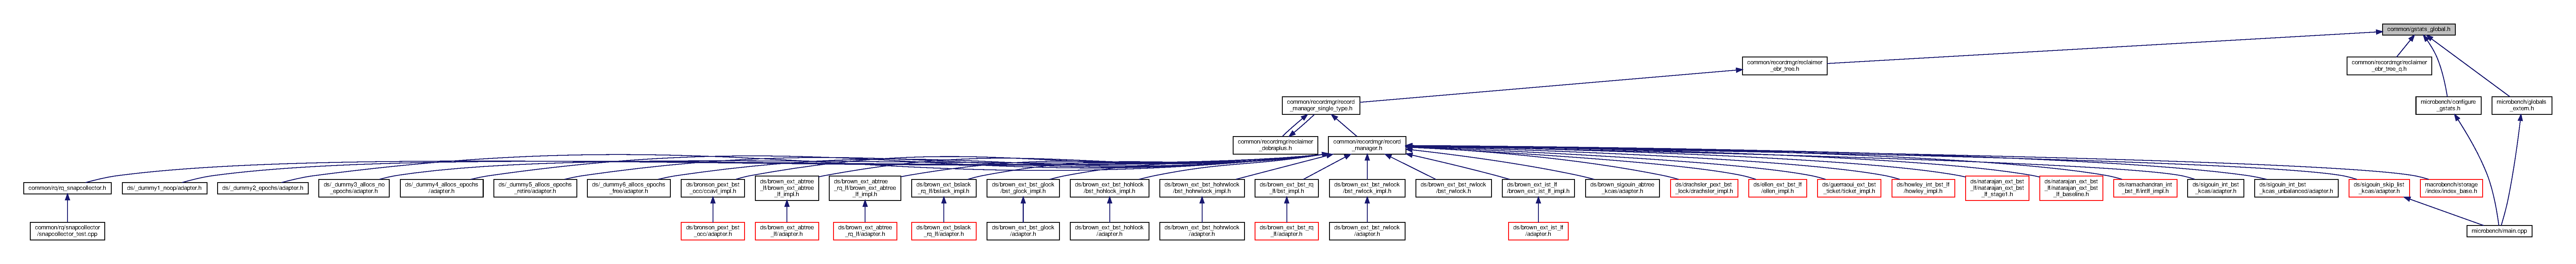
\includegraphics[width=350pt]{gstats__global_8h__dep__incl}
\end{center}
\end{figure}
\subsection*{Macros}
\begin{DoxyCompactItemize}
\item 
\#define \hyperlink{gstats__global_8h_a7b68ce1dac3e81376e9a9a140d60a537}{G\+S\+T\+A\+T\+S\+\_\+\+O\+B\+J\+E\+C\+T\+\_\+\+N\+A\+ME}
\item 
\#define \hyperlink{gstats__global_8h_a55688e6cd9a7bd4e22d382368c9069a7}{G\+S\+T\+A\+T\+S\+\_\+\+D\+E\+C\+L\+A\+R\+E\+\_\+\+S\+T\+A\+T\+S\+\_\+\+O\+B\+J\+E\+CT}(max\+\_\+num\+\_\+processes)
\item 
\#define \hyperlink{gstats__global_8h_aaa79b7f73d417d2406214626d477d030}{G\+S\+T\+A\+T\+S\+\_\+\+D\+E\+S\+T\+R\+OY}
\item 
\#define \hyperlink{gstats__global_8h_ac09c454363b53fe91ec325dc81e078bb}{\+\_\+\+\_\+\+D\+E\+C\+L\+A\+R\+E\+\_\+\+S\+T\+A\+T\+\_\+\+ID}(data\+\_\+type,  stat\+\_\+name\+\_\+token,  stat\+\_\+capacity,  stats\+\_\+output\+\_\+items)
\item 
\#define \hyperlink{gstats__global_8h_a2c05836bd14a6a3d76996151d5707048}{\+\_\+\+\_\+\+D\+E\+C\+L\+A\+R\+E\+\_\+\+E\+X\+T\+E\+R\+N\+\_\+\+S\+T\+A\+T\+\_\+\+ID}(data\+\_\+type,  stat\+\_\+name\+\_\+token,  stat\+\_\+capacity,  stats\+\_\+output\+\_\+items)
\item 
\#define \hyperlink{gstats__global_8h_ad34c6de9841ae38557d924a6b615cceb}{\+\_\+\+\_\+\+C\+R\+E\+A\+T\+E\+\_\+\+S\+T\+AT}(data\+\_\+type,  stat\+\_\+name\+\_\+token,  stat\+\_\+capacity,  stats\+\_\+output\+\_\+items)
\item 
\#define \hyperlink{gstats__global_8h_a59d63df6ff46d992f337600221aa3adc}{G\+S\+T\+A\+T\+S\+\_\+\+D\+E\+C\+L\+A\+R\+E\+\_\+\+A\+L\+L\+\_\+\+S\+T\+A\+T\+\_\+\+I\+DS}
\item 
\#define \hyperlink{gstats__global_8h_ad6ffc0d48f96743626050b8278ad07ad}{G\+S\+T\+A\+T\+S\+\_\+\+D\+E\+C\+L\+A\+R\+E\+\_\+\+E\+X\+T\+E\+R\+N\+\_\+\+A\+L\+L\+\_\+\+S\+T\+A\+T\+\_\+\+I\+DS}
\item 
\#define \hyperlink{gstats__global_8h_a795c7f436b058fc23de1664fe78b0a8a}{G\+S\+T\+A\+T\+S\+\_\+\+C\+R\+E\+A\+T\+E\+\_\+\+A\+LL}
\item 
\#define \hyperlink{gstats__global_8h_aea4ac685632b615a115978871004fd09}{G\+S\+T\+A\+T\+S\+\_\+\+A\+D\+D\+\_\+\+IX}(\hyperlink{microbench_2main_8cpp_a9ca9869868fe7e7a38a921cc7de4103f}{tid},  stat,  val,  index)
\item 
\#define \hyperlink{gstats__global_8h_a24195067d43fe4c45c3d89861e7ead3c}{G\+S\+T\+A\+T\+S\+\_\+\+A\+D\+D\+\_\+\+I\+X\+\_\+D}(\hyperlink{microbench_2main_8cpp_a9ca9869868fe7e7a38a921cc7de4103f}{tid},  stat,  val,  index)
\item 
\#define \hyperlink{gstats__global_8h_a6ca4c53e333ae6fe82723a314613ddc1}{G\+S\+T\+A\+T\+S\+\_\+\+A\+DD}(\hyperlink{microbench_2main_8cpp_a9ca9869868fe7e7a38a921cc7de4103f}{tid},  stat,  val)
\item 
\#define \hyperlink{gstats__global_8h_a919e16cc5a4c96c6d232f1bc58ae15b9}{G\+S\+T\+A\+T\+S\+\_\+\+A\+D\+D\+\_\+D}(\hyperlink{microbench_2main_8cpp_a9ca9869868fe7e7a38a921cc7de4103f}{tid},  stat,  val)
\item 
\#define \hyperlink{gstats__global_8h_aa499f7381bd60f7e64dd5d9a060f2768}{G\+S\+T\+A\+T\+S\+\_\+\+S\+E\+T\+\_\+\+IX}(\hyperlink{microbench_2main_8cpp_a9ca9869868fe7e7a38a921cc7de4103f}{tid},  stat,  val,  index)
\item 
\#define \hyperlink{gstats__global_8h_a00069030e021378f075f909bb5b713ec}{G\+S\+T\+A\+T\+S\+\_\+\+S\+E\+T\+\_\+\+I\+X\+\_\+D}(\hyperlink{microbench_2main_8cpp_a9ca9869868fe7e7a38a921cc7de4103f}{tid},  stat,  val,  index)
\item 
\#define \hyperlink{gstats__global_8h_a023f5e079196de270e6a6fcb81b5e06b}{G\+S\+T\+A\+T\+S\+\_\+\+S\+ET}(\hyperlink{microbench_2main_8cpp_a9ca9869868fe7e7a38a921cc7de4103f}{tid},  stat,  val)
\item 
\#define \hyperlink{gstats__global_8h_a71519bb79b42e26f0a1fe1568673d1ec}{G\+S\+T\+A\+T\+S\+\_\+\+S\+E\+T\+\_\+D}(\hyperlink{microbench_2main_8cpp_a9ca9869868fe7e7a38a921cc7de4103f}{tid},  stat,  val)
\item 
\#define \hyperlink{gstats__global_8h_ab0e2f1e216d93d858a226ed41ddda1c9}{G\+S\+T\+A\+T\+S\+\_\+\+G\+E\+T\+\_\+\+IX}(\hyperlink{microbench_2main_8cpp_a9ca9869868fe7e7a38a921cc7de4103f}{tid},  stat,  index)
\item 
\#define \hyperlink{gstats__global_8h_ab93951712f45655f8f88002cb6e1fe02}{G\+S\+T\+A\+T\+S\+\_\+\+G\+E\+T\+\_\+\+I\+X\+\_\+D}(\hyperlink{microbench_2main_8cpp_a9ca9869868fe7e7a38a921cc7de4103f}{tid},  stat,  index)
\item 
\#define \hyperlink{gstats__global_8h_ad2a64697072eecae47c2c3cb0d1cabf5}{G\+S\+T\+A\+T\+S\+\_\+\+G\+ET}(\hyperlink{microbench_2main_8cpp_a9ca9869868fe7e7a38a921cc7de4103f}{tid},  stat)
\item 
\#define \hyperlink{gstats__global_8h_a37eaddbde3b6496c8d677cad41307dd4}{G\+S\+T\+A\+T\+S\+\_\+\+G\+E\+T\+\_\+D}(\hyperlink{microbench_2main_8cpp_a9ca9869868fe7e7a38a921cc7de4103f}{tid},  stat)
\item 
\#define \hyperlink{gstats__global_8h_a18c650d48dcb344125b2bc9d095bfd6b}{G\+S\+T\+A\+T\+S\+\_\+\+A\+P\+P\+E\+ND}(\hyperlink{microbench_2main_8cpp_a9ca9869868fe7e7a38a921cc7de4103f}{tid},  stat,  val)
\item 
\#define \hyperlink{gstats__global_8h_a2b986fa7eef2deb198c3bca8e9d77c53}{G\+S\+T\+A\+T\+S\+\_\+\+A\+P\+P\+E\+N\+D\+\_\+D}(\hyperlink{microbench_2main_8cpp_a9ca9869868fe7e7a38a921cc7de4103f}{tid},  stat,  val)
\item 
\#define \hyperlink{gstats__global_8h_a0c5707202c748b6b9a9c04f7906df21d}{G\+S\+T\+A\+T\+S\+\_\+\+C\+L\+E\+A\+R\+\_\+\+A\+LL}
\item 
\#define \hyperlink{gstats__global_8h_a44349a89a08a3210eeecaeac8cad58fd}{G\+S\+T\+A\+T\+S\+\_\+\+C\+L\+E\+A\+R\+\_\+\+V\+AL}(stat,  val)
\item 
\#define \hyperlink{gstats__global_8h_a8fe1faa1aeaad00506f2a5da2101b85c}{G\+S\+T\+A\+T\+S\+\_\+\+P\+R\+I\+NT}
\item 
\#define \hyperlink{gstats__global_8h_aac5832f8940014e10dfeb1ef345aa1da}{G\+S\+T\+A\+T\+S\+\_\+\+T\+I\+M\+E\+R\+\_\+\+R\+E\+S\+ET}(\hyperlink{microbench_2main_8cpp_a9ca9869868fe7e7a38a921cc7de4103f}{tid},  timer\+\_\+stat)
\item 
\#define \hyperlink{gstats__global_8h_a85d6c5c366eb9d0f63f06a9ff1a4b3de}{G\+S\+T\+A\+T\+S\+\_\+\+T\+I\+M\+E\+R\+\_\+\+E\+L\+A\+P\+S\+ED}(\hyperlink{microbench_2main_8cpp_a9ca9869868fe7e7a38a921cc7de4103f}{tid},  timer\+\_\+stat)
\item 
\#define \hyperlink{gstats__global_8h_ad43cafb6f43118cfb9211ffa2784de42}{G\+S\+T\+A\+T\+S\+\_\+\+T\+I\+M\+E\+R\+\_\+\+S\+P\+L\+IT}(\hyperlink{microbench_2main_8cpp_a9ca9869868fe7e7a38a921cc7de4103f}{tid},  timer\+\_\+stat)
\item 
\#define \hyperlink{gstats__global_8h_a55a814c94c5d0f04254df5e3fb35b763}{G\+S\+T\+A\+T\+S\+\_\+\+T\+I\+M\+E\+R\+\_\+\+A\+P\+P\+E\+N\+D\+\_\+\+E\+L\+A\+P\+S\+ED}(\hyperlink{microbench_2main_8cpp_a9ca9869868fe7e7a38a921cc7de4103f}{tid},  timer\+\_\+stat,  target\+\_\+stat)
\item 
\#define \hyperlink{gstats__global_8h_aedd3f07c329e6aaa8db25f0be3ca00d2}{G\+S\+T\+A\+T\+S\+\_\+\+T\+I\+M\+E\+R\+\_\+\+A\+P\+P\+E\+N\+D\+\_\+\+S\+P\+L\+IT}(\hyperlink{microbench_2main_8cpp_a9ca9869868fe7e7a38a921cc7de4103f}{tid},  timer\+\_\+stat,  target\+\_\+stat)
\end{DoxyCompactItemize}


\subsection{Macro Definition Documentation}
\mbox{\Hypertarget{gstats__global_8h_ad34c6de9841ae38557d924a6b615cceb}\label{gstats__global_8h_ad34c6de9841ae38557d924a6b615cceb}} 
\index{gstats\+\_\+global.\+h@{gstats\+\_\+global.\+h}!\+\_\+\+\_\+\+C\+R\+E\+A\+T\+E\+\_\+\+S\+T\+AT@{\+\_\+\+\_\+\+C\+R\+E\+A\+T\+E\+\_\+\+S\+T\+AT}}
\index{\+\_\+\+\_\+\+C\+R\+E\+A\+T\+E\+\_\+\+S\+T\+AT@{\+\_\+\+\_\+\+C\+R\+E\+A\+T\+E\+\_\+\+S\+T\+AT}!gstats\+\_\+global.\+h@{gstats\+\_\+global.\+h}}
\subsubsection{\texorpdfstring{\+\_\+\+\_\+\+C\+R\+E\+A\+T\+E\+\_\+\+S\+T\+AT}{\_\_CREATE\_STAT}}
{\footnotesize\ttfamily \#define \+\_\+\+\_\+\+C\+R\+E\+A\+T\+E\+\_\+\+S\+T\+AT(\begin{DoxyParamCaption}\item[{}]{data\+\_\+type,  }\item[{}]{stat\+\_\+name\+\_\+token,  }\item[{}]{stat\+\_\+capacity,  }\item[{}]{stats\+\_\+output\+\_\+items }\end{DoxyParamCaption})}

\mbox{\Hypertarget{gstats__global_8h_a2c05836bd14a6a3d76996151d5707048}\label{gstats__global_8h_a2c05836bd14a6a3d76996151d5707048}} 
\index{gstats\+\_\+global.\+h@{gstats\+\_\+global.\+h}!\+\_\+\+\_\+\+D\+E\+C\+L\+A\+R\+E\+\_\+\+E\+X\+T\+E\+R\+N\+\_\+\+S\+T\+A\+T\+\_\+\+ID@{\+\_\+\+\_\+\+D\+E\+C\+L\+A\+R\+E\+\_\+\+E\+X\+T\+E\+R\+N\+\_\+\+S\+T\+A\+T\+\_\+\+ID}}
\index{\+\_\+\+\_\+\+D\+E\+C\+L\+A\+R\+E\+\_\+\+E\+X\+T\+E\+R\+N\+\_\+\+S\+T\+A\+T\+\_\+\+ID@{\+\_\+\+\_\+\+D\+E\+C\+L\+A\+R\+E\+\_\+\+E\+X\+T\+E\+R\+N\+\_\+\+S\+T\+A\+T\+\_\+\+ID}!gstats\+\_\+global.\+h@{gstats\+\_\+global.\+h}}
\subsubsection{\texorpdfstring{\+\_\+\+\_\+\+D\+E\+C\+L\+A\+R\+E\+\_\+\+E\+X\+T\+E\+R\+N\+\_\+\+S\+T\+A\+T\+\_\+\+ID}{\_\_DECLARE\_EXTERN\_STAT\_ID}}
{\footnotesize\ttfamily \#define \+\_\+\+\_\+\+D\+E\+C\+L\+A\+R\+E\+\_\+\+E\+X\+T\+E\+R\+N\+\_\+\+S\+T\+A\+T\+\_\+\+ID(\begin{DoxyParamCaption}\item[{}]{data\+\_\+type,  }\item[{}]{stat\+\_\+name\+\_\+token,  }\item[{}]{stat\+\_\+capacity,  }\item[{}]{stats\+\_\+output\+\_\+items }\end{DoxyParamCaption})}

\mbox{\Hypertarget{gstats__global_8h_ac09c454363b53fe91ec325dc81e078bb}\label{gstats__global_8h_ac09c454363b53fe91ec325dc81e078bb}} 
\index{gstats\+\_\+global.\+h@{gstats\+\_\+global.\+h}!\+\_\+\+\_\+\+D\+E\+C\+L\+A\+R\+E\+\_\+\+S\+T\+A\+T\+\_\+\+ID@{\+\_\+\+\_\+\+D\+E\+C\+L\+A\+R\+E\+\_\+\+S\+T\+A\+T\+\_\+\+ID}}
\index{\+\_\+\+\_\+\+D\+E\+C\+L\+A\+R\+E\+\_\+\+S\+T\+A\+T\+\_\+\+ID@{\+\_\+\+\_\+\+D\+E\+C\+L\+A\+R\+E\+\_\+\+S\+T\+A\+T\+\_\+\+ID}!gstats\+\_\+global.\+h@{gstats\+\_\+global.\+h}}
\subsubsection{\texorpdfstring{\+\_\+\+\_\+\+D\+E\+C\+L\+A\+R\+E\+\_\+\+S\+T\+A\+T\+\_\+\+ID}{\_\_DECLARE\_STAT\_ID}}
{\footnotesize\ttfamily \#define \+\_\+\+\_\+\+D\+E\+C\+L\+A\+R\+E\+\_\+\+S\+T\+A\+T\+\_\+\+ID(\begin{DoxyParamCaption}\item[{}]{data\+\_\+type,  }\item[{}]{stat\+\_\+name\+\_\+token,  }\item[{}]{stat\+\_\+capacity,  }\item[{}]{stats\+\_\+output\+\_\+items }\end{DoxyParamCaption})}

DO N\+OT E\+D\+IT B\+E\+L\+OW \mbox{\Hypertarget{gstats__global_8h_a6ca4c53e333ae6fe82723a314613ddc1}\label{gstats__global_8h_a6ca4c53e333ae6fe82723a314613ddc1}} 
\index{gstats\+\_\+global.\+h@{gstats\+\_\+global.\+h}!G\+S\+T\+A\+T\+S\+\_\+\+A\+DD@{G\+S\+T\+A\+T\+S\+\_\+\+A\+DD}}
\index{G\+S\+T\+A\+T\+S\+\_\+\+A\+DD@{G\+S\+T\+A\+T\+S\+\_\+\+A\+DD}!gstats\+\_\+global.\+h@{gstats\+\_\+global.\+h}}
\subsubsection{\texorpdfstring{G\+S\+T\+A\+T\+S\+\_\+\+A\+DD}{GSTATS\_ADD}}
{\footnotesize\ttfamily \#define G\+S\+T\+A\+T\+S\+\_\+\+A\+DD(\begin{DoxyParamCaption}\item[{}]{\hyperlink{microbench_2main_8cpp_a9ca9869868fe7e7a38a921cc7de4103f}{tid},  }\item[{}]{stat,  }\item[{}]{val }\end{DoxyParamCaption})}

\mbox{\Hypertarget{gstats__global_8h_a919e16cc5a4c96c6d232f1bc58ae15b9}\label{gstats__global_8h_a919e16cc5a4c96c6d232f1bc58ae15b9}} 
\index{gstats\+\_\+global.\+h@{gstats\+\_\+global.\+h}!G\+S\+T\+A\+T\+S\+\_\+\+A\+D\+D\+\_\+D@{G\+S\+T\+A\+T\+S\+\_\+\+A\+D\+D\+\_\+D}}
\index{G\+S\+T\+A\+T\+S\+\_\+\+A\+D\+D\+\_\+D@{G\+S\+T\+A\+T\+S\+\_\+\+A\+D\+D\+\_\+D}!gstats\+\_\+global.\+h@{gstats\+\_\+global.\+h}}
\subsubsection{\texorpdfstring{G\+S\+T\+A\+T\+S\+\_\+\+A\+D\+D\+\_\+D}{GSTATS\_ADD\_D}}
{\footnotesize\ttfamily \#define G\+S\+T\+A\+T\+S\+\_\+\+A\+D\+D\+\_\+D(\begin{DoxyParamCaption}\item[{}]{\hyperlink{microbench_2main_8cpp_a9ca9869868fe7e7a38a921cc7de4103f}{tid},  }\item[{}]{stat,  }\item[{}]{val }\end{DoxyParamCaption})}

\mbox{\Hypertarget{gstats__global_8h_aea4ac685632b615a115978871004fd09}\label{gstats__global_8h_aea4ac685632b615a115978871004fd09}} 
\index{gstats\+\_\+global.\+h@{gstats\+\_\+global.\+h}!G\+S\+T\+A\+T\+S\+\_\+\+A\+D\+D\+\_\+\+IX@{G\+S\+T\+A\+T\+S\+\_\+\+A\+D\+D\+\_\+\+IX}}
\index{G\+S\+T\+A\+T\+S\+\_\+\+A\+D\+D\+\_\+\+IX@{G\+S\+T\+A\+T\+S\+\_\+\+A\+D\+D\+\_\+\+IX}!gstats\+\_\+global.\+h@{gstats\+\_\+global.\+h}}
\subsubsection{\texorpdfstring{G\+S\+T\+A\+T\+S\+\_\+\+A\+D\+D\+\_\+\+IX}{GSTATS\_ADD\_IX}}
{\footnotesize\ttfamily \#define G\+S\+T\+A\+T\+S\+\_\+\+A\+D\+D\+\_\+\+IX(\begin{DoxyParamCaption}\item[{}]{\hyperlink{microbench_2main_8cpp_a9ca9869868fe7e7a38a921cc7de4103f}{tid},  }\item[{}]{stat,  }\item[{}]{val,  }\item[{}]{index }\end{DoxyParamCaption})}

\mbox{\Hypertarget{gstats__global_8h_a24195067d43fe4c45c3d89861e7ead3c}\label{gstats__global_8h_a24195067d43fe4c45c3d89861e7ead3c}} 
\index{gstats\+\_\+global.\+h@{gstats\+\_\+global.\+h}!G\+S\+T\+A\+T\+S\+\_\+\+A\+D\+D\+\_\+\+I\+X\+\_\+D@{G\+S\+T\+A\+T\+S\+\_\+\+A\+D\+D\+\_\+\+I\+X\+\_\+D}}
\index{G\+S\+T\+A\+T\+S\+\_\+\+A\+D\+D\+\_\+\+I\+X\+\_\+D@{G\+S\+T\+A\+T\+S\+\_\+\+A\+D\+D\+\_\+\+I\+X\+\_\+D}!gstats\+\_\+global.\+h@{gstats\+\_\+global.\+h}}
\subsubsection{\texorpdfstring{G\+S\+T\+A\+T\+S\+\_\+\+A\+D\+D\+\_\+\+I\+X\+\_\+D}{GSTATS\_ADD\_IX\_D}}
{\footnotesize\ttfamily \#define G\+S\+T\+A\+T\+S\+\_\+\+A\+D\+D\+\_\+\+I\+X\+\_\+D(\begin{DoxyParamCaption}\item[{}]{\hyperlink{microbench_2main_8cpp_a9ca9869868fe7e7a38a921cc7de4103f}{tid},  }\item[{}]{stat,  }\item[{}]{val,  }\item[{}]{index }\end{DoxyParamCaption})}

\mbox{\Hypertarget{gstats__global_8h_a18c650d48dcb344125b2bc9d095bfd6b}\label{gstats__global_8h_a18c650d48dcb344125b2bc9d095bfd6b}} 
\index{gstats\+\_\+global.\+h@{gstats\+\_\+global.\+h}!G\+S\+T\+A\+T\+S\+\_\+\+A\+P\+P\+E\+ND@{G\+S\+T\+A\+T\+S\+\_\+\+A\+P\+P\+E\+ND}}
\index{G\+S\+T\+A\+T\+S\+\_\+\+A\+P\+P\+E\+ND@{G\+S\+T\+A\+T\+S\+\_\+\+A\+P\+P\+E\+ND}!gstats\+\_\+global.\+h@{gstats\+\_\+global.\+h}}
\subsubsection{\texorpdfstring{G\+S\+T\+A\+T\+S\+\_\+\+A\+P\+P\+E\+ND}{GSTATS\_APPEND}}
{\footnotesize\ttfamily \#define G\+S\+T\+A\+T\+S\+\_\+\+A\+P\+P\+E\+ND(\begin{DoxyParamCaption}\item[{}]{\hyperlink{microbench_2main_8cpp_a9ca9869868fe7e7a38a921cc7de4103f}{tid},  }\item[{}]{stat,  }\item[{}]{val }\end{DoxyParamCaption})}

\mbox{\Hypertarget{gstats__global_8h_a2b986fa7eef2deb198c3bca8e9d77c53}\label{gstats__global_8h_a2b986fa7eef2deb198c3bca8e9d77c53}} 
\index{gstats\+\_\+global.\+h@{gstats\+\_\+global.\+h}!G\+S\+T\+A\+T\+S\+\_\+\+A\+P\+P\+E\+N\+D\+\_\+D@{G\+S\+T\+A\+T\+S\+\_\+\+A\+P\+P\+E\+N\+D\+\_\+D}}
\index{G\+S\+T\+A\+T\+S\+\_\+\+A\+P\+P\+E\+N\+D\+\_\+D@{G\+S\+T\+A\+T\+S\+\_\+\+A\+P\+P\+E\+N\+D\+\_\+D}!gstats\+\_\+global.\+h@{gstats\+\_\+global.\+h}}
\subsubsection{\texorpdfstring{G\+S\+T\+A\+T\+S\+\_\+\+A\+P\+P\+E\+N\+D\+\_\+D}{GSTATS\_APPEND\_D}}
{\footnotesize\ttfamily \#define G\+S\+T\+A\+T\+S\+\_\+\+A\+P\+P\+E\+N\+D\+\_\+D(\begin{DoxyParamCaption}\item[{}]{\hyperlink{microbench_2main_8cpp_a9ca9869868fe7e7a38a921cc7de4103f}{tid},  }\item[{}]{stat,  }\item[{}]{val }\end{DoxyParamCaption})}

\mbox{\Hypertarget{gstats__global_8h_a0c5707202c748b6b9a9c04f7906df21d}\label{gstats__global_8h_a0c5707202c748b6b9a9c04f7906df21d}} 
\index{gstats\+\_\+global.\+h@{gstats\+\_\+global.\+h}!G\+S\+T\+A\+T\+S\+\_\+\+C\+L\+E\+A\+R\+\_\+\+A\+LL@{G\+S\+T\+A\+T\+S\+\_\+\+C\+L\+E\+A\+R\+\_\+\+A\+LL}}
\index{G\+S\+T\+A\+T\+S\+\_\+\+C\+L\+E\+A\+R\+\_\+\+A\+LL@{G\+S\+T\+A\+T\+S\+\_\+\+C\+L\+E\+A\+R\+\_\+\+A\+LL}!gstats\+\_\+global.\+h@{gstats\+\_\+global.\+h}}
\subsubsection{\texorpdfstring{G\+S\+T\+A\+T\+S\+\_\+\+C\+L\+E\+A\+R\+\_\+\+A\+LL}{GSTATS\_CLEAR\_ALL}}
{\footnotesize\ttfamily \#define G\+S\+T\+A\+T\+S\+\_\+\+C\+L\+E\+A\+R\+\_\+\+A\+LL}

\mbox{\Hypertarget{gstats__global_8h_a44349a89a08a3210eeecaeac8cad58fd}\label{gstats__global_8h_a44349a89a08a3210eeecaeac8cad58fd}} 
\index{gstats\+\_\+global.\+h@{gstats\+\_\+global.\+h}!G\+S\+T\+A\+T\+S\+\_\+\+C\+L\+E\+A\+R\+\_\+\+V\+AL@{G\+S\+T\+A\+T\+S\+\_\+\+C\+L\+E\+A\+R\+\_\+\+V\+AL}}
\index{G\+S\+T\+A\+T\+S\+\_\+\+C\+L\+E\+A\+R\+\_\+\+V\+AL@{G\+S\+T\+A\+T\+S\+\_\+\+C\+L\+E\+A\+R\+\_\+\+V\+AL}!gstats\+\_\+global.\+h@{gstats\+\_\+global.\+h}}
\subsubsection{\texorpdfstring{G\+S\+T\+A\+T\+S\+\_\+\+C\+L\+E\+A\+R\+\_\+\+V\+AL}{GSTATS\_CLEAR\_VAL}}
{\footnotesize\ttfamily \#define G\+S\+T\+A\+T\+S\+\_\+\+C\+L\+E\+A\+R\+\_\+\+V\+AL(\begin{DoxyParamCaption}\item[{}]{stat,  }\item[{}]{val }\end{DoxyParamCaption})}

\mbox{\Hypertarget{gstats__global_8h_a795c7f436b058fc23de1664fe78b0a8a}\label{gstats__global_8h_a795c7f436b058fc23de1664fe78b0a8a}} 
\index{gstats\+\_\+global.\+h@{gstats\+\_\+global.\+h}!G\+S\+T\+A\+T\+S\+\_\+\+C\+R\+E\+A\+T\+E\+\_\+\+A\+LL@{G\+S\+T\+A\+T\+S\+\_\+\+C\+R\+E\+A\+T\+E\+\_\+\+A\+LL}}
\index{G\+S\+T\+A\+T\+S\+\_\+\+C\+R\+E\+A\+T\+E\+\_\+\+A\+LL@{G\+S\+T\+A\+T\+S\+\_\+\+C\+R\+E\+A\+T\+E\+\_\+\+A\+LL}!gstats\+\_\+global.\+h@{gstats\+\_\+global.\+h}}
\subsubsection{\texorpdfstring{G\+S\+T\+A\+T\+S\+\_\+\+C\+R\+E\+A\+T\+E\+\_\+\+A\+LL}{GSTATS\_CREATE\_ALL}}
{\footnotesize\ttfamily \#define G\+S\+T\+A\+T\+S\+\_\+\+C\+R\+E\+A\+T\+E\+\_\+\+A\+LL}

\mbox{\Hypertarget{gstats__global_8h_a59d63df6ff46d992f337600221aa3adc}\label{gstats__global_8h_a59d63df6ff46d992f337600221aa3adc}} 
\index{gstats\+\_\+global.\+h@{gstats\+\_\+global.\+h}!G\+S\+T\+A\+T\+S\+\_\+\+D\+E\+C\+L\+A\+R\+E\+\_\+\+A\+L\+L\+\_\+\+S\+T\+A\+T\+\_\+\+I\+DS@{G\+S\+T\+A\+T\+S\+\_\+\+D\+E\+C\+L\+A\+R\+E\+\_\+\+A\+L\+L\+\_\+\+S\+T\+A\+T\+\_\+\+I\+DS}}
\index{G\+S\+T\+A\+T\+S\+\_\+\+D\+E\+C\+L\+A\+R\+E\+\_\+\+A\+L\+L\+\_\+\+S\+T\+A\+T\+\_\+\+I\+DS@{G\+S\+T\+A\+T\+S\+\_\+\+D\+E\+C\+L\+A\+R\+E\+\_\+\+A\+L\+L\+\_\+\+S\+T\+A\+T\+\_\+\+I\+DS}!gstats\+\_\+global.\+h@{gstats\+\_\+global.\+h}}
\subsubsection{\texorpdfstring{G\+S\+T\+A\+T\+S\+\_\+\+D\+E\+C\+L\+A\+R\+E\+\_\+\+A\+L\+L\+\_\+\+S\+T\+A\+T\+\_\+\+I\+DS}{GSTATS\_DECLARE\_ALL\_STAT\_IDS}}
{\footnotesize\ttfamily \#define G\+S\+T\+A\+T\+S\+\_\+\+D\+E\+C\+L\+A\+R\+E\+\_\+\+A\+L\+L\+\_\+\+S\+T\+A\+T\+\_\+\+I\+DS}

\mbox{\Hypertarget{gstats__global_8h_ad6ffc0d48f96743626050b8278ad07ad}\label{gstats__global_8h_ad6ffc0d48f96743626050b8278ad07ad}} 
\index{gstats\+\_\+global.\+h@{gstats\+\_\+global.\+h}!G\+S\+T\+A\+T\+S\+\_\+\+D\+E\+C\+L\+A\+R\+E\+\_\+\+E\+X\+T\+E\+R\+N\+\_\+\+A\+L\+L\+\_\+\+S\+T\+A\+T\+\_\+\+I\+DS@{G\+S\+T\+A\+T\+S\+\_\+\+D\+E\+C\+L\+A\+R\+E\+\_\+\+E\+X\+T\+E\+R\+N\+\_\+\+A\+L\+L\+\_\+\+S\+T\+A\+T\+\_\+\+I\+DS}}
\index{G\+S\+T\+A\+T\+S\+\_\+\+D\+E\+C\+L\+A\+R\+E\+\_\+\+E\+X\+T\+E\+R\+N\+\_\+\+A\+L\+L\+\_\+\+S\+T\+A\+T\+\_\+\+I\+DS@{G\+S\+T\+A\+T\+S\+\_\+\+D\+E\+C\+L\+A\+R\+E\+\_\+\+E\+X\+T\+E\+R\+N\+\_\+\+A\+L\+L\+\_\+\+S\+T\+A\+T\+\_\+\+I\+DS}!gstats\+\_\+global.\+h@{gstats\+\_\+global.\+h}}
\subsubsection{\texorpdfstring{G\+S\+T\+A\+T\+S\+\_\+\+D\+E\+C\+L\+A\+R\+E\+\_\+\+E\+X\+T\+E\+R\+N\+\_\+\+A\+L\+L\+\_\+\+S\+T\+A\+T\+\_\+\+I\+DS}{GSTATS\_DECLARE\_EXTERN\_ALL\_STAT\_IDS}}
{\footnotesize\ttfamily \#define G\+S\+T\+A\+T\+S\+\_\+\+D\+E\+C\+L\+A\+R\+E\+\_\+\+E\+X\+T\+E\+R\+N\+\_\+\+A\+L\+L\+\_\+\+S\+T\+A\+T\+\_\+\+I\+DS}

\mbox{\Hypertarget{gstats__global_8h_a55688e6cd9a7bd4e22d382368c9069a7}\label{gstats__global_8h_a55688e6cd9a7bd4e22d382368c9069a7}} 
\index{gstats\+\_\+global.\+h@{gstats\+\_\+global.\+h}!G\+S\+T\+A\+T\+S\+\_\+\+D\+E\+C\+L\+A\+R\+E\+\_\+\+S\+T\+A\+T\+S\+\_\+\+O\+B\+J\+E\+CT@{G\+S\+T\+A\+T\+S\+\_\+\+D\+E\+C\+L\+A\+R\+E\+\_\+\+S\+T\+A\+T\+S\+\_\+\+O\+B\+J\+E\+CT}}
\index{G\+S\+T\+A\+T\+S\+\_\+\+D\+E\+C\+L\+A\+R\+E\+\_\+\+S\+T\+A\+T\+S\+\_\+\+O\+B\+J\+E\+CT@{G\+S\+T\+A\+T\+S\+\_\+\+D\+E\+C\+L\+A\+R\+E\+\_\+\+S\+T\+A\+T\+S\+\_\+\+O\+B\+J\+E\+CT}!gstats\+\_\+global.\+h@{gstats\+\_\+global.\+h}}
\subsubsection{\texorpdfstring{G\+S\+T\+A\+T\+S\+\_\+\+D\+E\+C\+L\+A\+R\+E\+\_\+\+S\+T\+A\+T\+S\+\_\+\+O\+B\+J\+E\+CT}{GSTATS\_DECLARE\_STATS\_OBJECT}}
{\footnotesize\ttfamily \#define G\+S\+T\+A\+T\+S\+\_\+\+D\+E\+C\+L\+A\+R\+E\+\_\+\+S\+T\+A\+T\+S\+\_\+\+O\+B\+J\+E\+CT(\begin{DoxyParamCaption}\item[{}]{max\+\_\+num\+\_\+processes }\end{DoxyParamCaption})}

\mbox{\Hypertarget{gstats__global_8h_aaa79b7f73d417d2406214626d477d030}\label{gstats__global_8h_aaa79b7f73d417d2406214626d477d030}} 
\index{gstats\+\_\+global.\+h@{gstats\+\_\+global.\+h}!G\+S\+T\+A\+T\+S\+\_\+\+D\+E\+S\+T\+R\+OY@{G\+S\+T\+A\+T\+S\+\_\+\+D\+E\+S\+T\+R\+OY}}
\index{G\+S\+T\+A\+T\+S\+\_\+\+D\+E\+S\+T\+R\+OY@{G\+S\+T\+A\+T\+S\+\_\+\+D\+E\+S\+T\+R\+OY}!gstats\+\_\+global.\+h@{gstats\+\_\+global.\+h}}
\subsubsection{\texorpdfstring{G\+S\+T\+A\+T\+S\+\_\+\+D\+E\+S\+T\+R\+OY}{GSTATS\_DESTROY}}
{\footnotesize\ttfamily \#define G\+S\+T\+A\+T\+S\+\_\+\+D\+E\+S\+T\+R\+OY}

\mbox{\Hypertarget{gstats__global_8h_ad2a64697072eecae47c2c3cb0d1cabf5}\label{gstats__global_8h_ad2a64697072eecae47c2c3cb0d1cabf5}} 
\index{gstats\+\_\+global.\+h@{gstats\+\_\+global.\+h}!G\+S\+T\+A\+T\+S\+\_\+\+G\+ET@{G\+S\+T\+A\+T\+S\+\_\+\+G\+ET}}
\index{G\+S\+T\+A\+T\+S\+\_\+\+G\+ET@{G\+S\+T\+A\+T\+S\+\_\+\+G\+ET}!gstats\+\_\+global.\+h@{gstats\+\_\+global.\+h}}
\subsubsection{\texorpdfstring{G\+S\+T\+A\+T\+S\+\_\+\+G\+ET}{GSTATS\_GET}}
{\footnotesize\ttfamily \#define G\+S\+T\+A\+T\+S\+\_\+\+G\+ET(\begin{DoxyParamCaption}\item[{}]{\hyperlink{microbench_2main_8cpp_a9ca9869868fe7e7a38a921cc7de4103f}{tid},  }\item[{}]{stat }\end{DoxyParamCaption})}

\mbox{\Hypertarget{gstats__global_8h_a37eaddbde3b6496c8d677cad41307dd4}\label{gstats__global_8h_a37eaddbde3b6496c8d677cad41307dd4}} 
\index{gstats\+\_\+global.\+h@{gstats\+\_\+global.\+h}!G\+S\+T\+A\+T\+S\+\_\+\+G\+E\+T\+\_\+D@{G\+S\+T\+A\+T\+S\+\_\+\+G\+E\+T\+\_\+D}}
\index{G\+S\+T\+A\+T\+S\+\_\+\+G\+E\+T\+\_\+D@{G\+S\+T\+A\+T\+S\+\_\+\+G\+E\+T\+\_\+D}!gstats\+\_\+global.\+h@{gstats\+\_\+global.\+h}}
\subsubsection{\texorpdfstring{G\+S\+T\+A\+T\+S\+\_\+\+G\+E\+T\+\_\+D}{GSTATS\_GET\_D}}
{\footnotesize\ttfamily \#define G\+S\+T\+A\+T\+S\+\_\+\+G\+E\+T\+\_\+D(\begin{DoxyParamCaption}\item[{}]{\hyperlink{microbench_2main_8cpp_a9ca9869868fe7e7a38a921cc7de4103f}{tid},  }\item[{}]{stat }\end{DoxyParamCaption})}

\mbox{\Hypertarget{gstats__global_8h_ab0e2f1e216d93d858a226ed41ddda1c9}\label{gstats__global_8h_ab0e2f1e216d93d858a226ed41ddda1c9}} 
\index{gstats\+\_\+global.\+h@{gstats\+\_\+global.\+h}!G\+S\+T\+A\+T\+S\+\_\+\+G\+E\+T\+\_\+\+IX@{G\+S\+T\+A\+T\+S\+\_\+\+G\+E\+T\+\_\+\+IX}}
\index{G\+S\+T\+A\+T\+S\+\_\+\+G\+E\+T\+\_\+\+IX@{G\+S\+T\+A\+T\+S\+\_\+\+G\+E\+T\+\_\+\+IX}!gstats\+\_\+global.\+h@{gstats\+\_\+global.\+h}}
\subsubsection{\texorpdfstring{G\+S\+T\+A\+T\+S\+\_\+\+G\+E\+T\+\_\+\+IX}{GSTATS\_GET\_IX}}
{\footnotesize\ttfamily \#define G\+S\+T\+A\+T\+S\+\_\+\+G\+E\+T\+\_\+\+IX(\begin{DoxyParamCaption}\item[{}]{\hyperlink{microbench_2main_8cpp_a9ca9869868fe7e7a38a921cc7de4103f}{tid},  }\item[{}]{stat,  }\item[{}]{index }\end{DoxyParamCaption})}

\mbox{\Hypertarget{gstats__global_8h_ab93951712f45655f8f88002cb6e1fe02}\label{gstats__global_8h_ab93951712f45655f8f88002cb6e1fe02}} 
\index{gstats\+\_\+global.\+h@{gstats\+\_\+global.\+h}!G\+S\+T\+A\+T\+S\+\_\+\+G\+E\+T\+\_\+\+I\+X\+\_\+D@{G\+S\+T\+A\+T\+S\+\_\+\+G\+E\+T\+\_\+\+I\+X\+\_\+D}}
\index{G\+S\+T\+A\+T\+S\+\_\+\+G\+E\+T\+\_\+\+I\+X\+\_\+D@{G\+S\+T\+A\+T\+S\+\_\+\+G\+E\+T\+\_\+\+I\+X\+\_\+D}!gstats\+\_\+global.\+h@{gstats\+\_\+global.\+h}}
\subsubsection{\texorpdfstring{G\+S\+T\+A\+T\+S\+\_\+\+G\+E\+T\+\_\+\+I\+X\+\_\+D}{GSTATS\_GET\_IX\_D}}
{\footnotesize\ttfamily \#define G\+S\+T\+A\+T\+S\+\_\+\+G\+E\+T\+\_\+\+I\+X\+\_\+D(\begin{DoxyParamCaption}\item[{}]{\hyperlink{microbench_2main_8cpp_a9ca9869868fe7e7a38a921cc7de4103f}{tid},  }\item[{}]{stat,  }\item[{}]{index }\end{DoxyParamCaption})}

\mbox{\Hypertarget{gstats__global_8h_a7b68ce1dac3e81376e9a9a140d60a537}\label{gstats__global_8h_a7b68ce1dac3e81376e9a9a140d60a537}} 
\index{gstats\+\_\+global.\+h@{gstats\+\_\+global.\+h}!G\+S\+T\+A\+T\+S\+\_\+\+O\+B\+J\+E\+C\+T\+\_\+\+N\+A\+ME@{G\+S\+T\+A\+T\+S\+\_\+\+O\+B\+J\+E\+C\+T\+\_\+\+N\+A\+ME}}
\index{G\+S\+T\+A\+T\+S\+\_\+\+O\+B\+J\+E\+C\+T\+\_\+\+N\+A\+ME@{G\+S\+T\+A\+T\+S\+\_\+\+O\+B\+J\+E\+C\+T\+\_\+\+N\+A\+ME}!gstats\+\_\+global.\+h@{gstats\+\_\+global.\+h}}
\subsubsection{\texorpdfstring{G\+S\+T\+A\+T\+S\+\_\+\+O\+B\+J\+E\+C\+T\+\_\+\+N\+A\+ME}{GSTATS\_OBJECT\_NAME}}
{\footnotesize\ttfamily \#define G\+S\+T\+A\+T\+S\+\_\+\+O\+B\+J\+E\+C\+T\+\_\+\+N\+A\+ME}

\mbox{\Hypertarget{gstats__global_8h_a8fe1faa1aeaad00506f2a5da2101b85c}\label{gstats__global_8h_a8fe1faa1aeaad00506f2a5da2101b85c}} 
\index{gstats\+\_\+global.\+h@{gstats\+\_\+global.\+h}!G\+S\+T\+A\+T\+S\+\_\+\+P\+R\+I\+NT@{G\+S\+T\+A\+T\+S\+\_\+\+P\+R\+I\+NT}}
\index{G\+S\+T\+A\+T\+S\+\_\+\+P\+R\+I\+NT@{G\+S\+T\+A\+T\+S\+\_\+\+P\+R\+I\+NT}!gstats\+\_\+global.\+h@{gstats\+\_\+global.\+h}}
\subsubsection{\texorpdfstring{G\+S\+T\+A\+T\+S\+\_\+\+P\+R\+I\+NT}{GSTATS\_PRINT}}
{\footnotesize\ttfamily \#define G\+S\+T\+A\+T\+S\+\_\+\+P\+R\+I\+NT}

\mbox{\Hypertarget{gstats__global_8h_a023f5e079196de270e6a6fcb81b5e06b}\label{gstats__global_8h_a023f5e079196de270e6a6fcb81b5e06b}} 
\index{gstats\+\_\+global.\+h@{gstats\+\_\+global.\+h}!G\+S\+T\+A\+T\+S\+\_\+\+S\+ET@{G\+S\+T\+A\+T\+S\+\_\+\+S\+ET}}
\index{G\+S\+T\+A\+T\+S\+\_\+\+S\+ET@{G\+S\+T\+A\+T\+S\+\_\+\+S\+ET}!gstats\+\_\+global.\+h@{gstats\+\_\+global.\+h}}
\subsubsection{\texorpdfstring{G\+S\+T\+A\+T\+S\+\_\+\+S\+ET}{GSTATS\_SET}}
{\footnotesize\ttfamily \#define G\+S\+T\+A\+T\+S\+\_\+\+S\+ET(\begin{DoxyParamCaption}\item[{}]{\hyperlink{microbench_2main_8cpp_a9ca9869868fe7e7a38a921cc7de4103f}{tid},  }\item[{}]{stat,  }\item[{}]{val }\end{DoxyParamCaption})}

\mbox{\Hypertarget{gstats__global_8h_a71519bb79b42e26f0a1fe1568673d1ec}\label{gstats__global_8h_a71519bb79b42e26f0a1fe1568673d1ec}} 
\index{gstats\+\_\+global.\+h@{gstats\+\_\+global.\+h}!G\+S\+T\+A\+T\+S\+\_\+\+S\+E\+T\+\_\+D@{G\+S\+T\+A\+T\+S\+\_\+\+S\+E\+T\+\_\+D}}
\index{G\+S\+T\+A\+T\+S\+\_\+\+S\+E\+T\+\_\+D@{G\+S\+T\+A\+T\+S\+\_\+\+S\+E\+T\+\_\+D}!gstats\+\_\+global.\+h@{gstats\+\_\+global.\+h}}
\subsubsection{\texorpdfstring{G\+S\+T\+A\+T\+S\+\_\+\+S\+E\+T\+\_\+D}{GSTATS\_SET\_D}}
{\footnotesize\ttfamily \#define G\+S\+T\+A\+T\+S\+\_\+\+S\+E\+T\+\_\+D(\begin{DoxyParamCaption}\item[{}]{\hyperlink{microbench_2main_8cpp_a9ca9869868fe7e7a38a921cc7de4103f}{tid},  }\item[{}]{stat,  }\item[{}]{val }\end{DoxyParamCaption})}

\mbox{\Hypertarget{gstats__global_8h_aa499f7381bd60f7e64dd5d9a060f2768}\label{gstats__global_8h_aa499f7381bd60f7e64dd5d9a060f2768}} 
\index{gstats\+\_\+global.\+h@{gstats\+\_\+global.\+h}!G\+S\+T\+A\+T\+S\+\_\+\+S\+E\+T\+\_\+\+IX@{G\+S\+T\+A\+T\+S\+\_\+\+S\+E\+T\+\_\+\+IX}}
\index{G\+S\+T\+A\+T\+S\+\_\+\+S\+E\+T\+\_\+\+IX@{G\+S\+T\+A\+T\+S\+\_\+\+S\+E\+T\+\_\+\+IX}!gstats\+\_\+global.\+h@{gstats\+\_\+global.\+h}}
\subsubsection{\texorpdfstring{G\+S\+T\+A\+T\+S\+\_\+\+S\+E\+T\+\_\+\+IX}{GSTATS\_SET\_IX}}
{\footnotesize\ttfamily \#define G\+S\+T\+A\+T\+S\+\_\+\+S\+E\+T\+\_\+\+IX(\begin{DoxyParamCaption}\item[{}]{\hyperlink{microbench_2main_8cpp_a9ca9869868fe7e7a38a921cc7de4103f}{tid},  }\item[{}]{stat,  }\item[{}]{val,  }\item[{}]{index }\end{DoxyParamCaption})}

\mbox{\Hypertarget{gstats__global_8h_a00069030e021378f075f909bb5b713ec}\label{gstats__global_8h_a00069030e021378f075f909bb5b713ec}} 
\index{gstats\+\_\+global.\+h@{gstats\+\_\+global.\+h}!G\+S\+T\+A\+T\+S\+\_\+\+S\+E\+T\+\_\+\+I\+X\+\_\+D@{G\+S\+T\+A\+T\+S\+\_\+\+S\+E\+T\+\_\+\+I\+X\+\_\+D}}
\index{G\+S\+T\+A\+T\+S\+\_\+\+S\+E\+T\+\_\+\+I\+X\+\_\+D@{G\+S\+T\+A\+T\+S\+\_\+\+S\+E\+T\+\_\+\+I\+X\+\_\+D}!gstats\+\_\+global.\+h@{gstats\+\_\+global.\+h}}
\subsubsection{\texorpdfstring{G\+S\+T\+A\+T\+S\+\_\+\+S\+E\+T\+\_\+\+I\+X\+\_\+D}{GSTATS\_SET\_IX\_D}}
{\footnotesize\ttfamily \#define G\+S\+T\+A\+T\+S\+\_\+\+S\+E\+T\+\_\+\+I\+X\+\_\+D(\begin{DoxyParamCaption}\item[{}]{\hyperlink{microbench_2main_8cpp_a9ca9869868fe7e7a38a921cc7de4103f}{tid},  }\item[{}]{stat,  }\item[{}]{val,  }\item[{}]{index }\end{DoxyParamCaption})}

\mbox{\Hypertarget{gstats__global_8h_a55a814c94c5d0f04254df5e3fb35b763}\label{gstats__global_8h_a55a814c94c5d0f04254df5e3fb35b763}} 
\index{gstats\+\_\+global.\+h@{gstats\+\_\+global.\+h}!G\+S\+T\+A\+T\+S\+\_\+\+T\+I\+M\+E\+R\+\_\+\+A\+P\+P\+E\+N\+D\+\_\+\+E\+L\+A\+P\+S\+ED@{G\+S\+T\+A\+T\+S\+\_\+\+T\+I\+M\+E\+R\+\_\+\+A\+P\+P\+E\+N\+D\+\_\+\+E\+L\+A\+P\+S\+ED}}
\index{G\+S\+T\+A\+T\+S\+\_\+\+T\+I\+M\+E\+R\+\_\+\+A\+P\+P\+E\+N\+D\+\_\+\+E\+L\+A\+P\+S\+ED@{G\+S\+T\+A\+T\+S\+\_\+\+T\+I\+M\+E\+R\+\_\+\+A\+P\+P\+E\+N\+D\+\_\+\+E\+L\+A\+P\+S\+ED}!gstats\+\_\+global.\+h@{gstats\+\_\+global.\+h}}
\subsubsection{\texorpdfstring{G\+S\+T\+A\+T\+S\+\_\+\+T\+I\+M\+E\+R\+\_\+\+A\+P\+P\+E\+N\+D\+\_\+\+E\+L\+A\+P\+S\+ED}{GSTATS\_TIMER\_APPEND\_ELAPSED}}
{\footnotesize\ttfamily \#define G\+S\+T\+A\+T\+S\+\_\+\+T\+I\+M\+E\+R\+\_\+\+A\+P\+P\+E\+N\+D\+\_\+\+E\+L\+A\+P\+S\+ED(\begin{DoxyParamCaption}\item[{}]{\hyperlink{microbench_2main_8cpp_a9ca9869868fe7e7a38a921cc7de4103f}{tid},  }\item[{}]{timer\+\_\+stat,  }\item[{}]{target\+\_\+stat }\end{DoxyParamCaption})}

\mbox{\Hypertarget{gstats__global_8h_aedd3f07c329e6aaa8db25f0be3ca00d2}\label{gstats__global_8h_aedd3f07c329e6aaa8db25f0be3ca00d2}} 
\index{gstats\+\_\+global.\+h@{gstats\+\_\+global.\+h}!G\+S\+T\+A\+T\+S\+\_\+\+T\+I\+M\+E\+R\+\_\+\+A\+P\+P\+E\+N\+D\+\_\+\+S\+P\+L\+IT@{G\+S\+T\+A\+T\+S\+\_\+\+T\+I\+M\+E\+R\+\_\+\+A\+P\+P\+E\+N\+D\+\_\+\+S\+P\+L\+IT}}
\index{G\+S\+T\+A\+T\+S\+\_\+\+T\+I\+M\+E\+R\+\_\+\+A\+P\+P\+E\+N\+D\+\_\+\+S\+P\+L\+IT@{G\+S\+T\+A\+T\+S\+\_\+\+T\+I\+M\+E\+R\+\_\+\+A\+P\+P\+E\+N\+D\+\_\+\+S\+P\+L\+IT}!gstats\+\_\+global.\+h@{gstats\+\_\+global.\+h}}
\subsubsection{\texorpdfstring{G\+S\+T\+A\+T\+S\+\_\+\+T\+I\+M\+E\+R\+\_\+\+A\+P\+P\+E\+N\+D\+\_\+\+S\+P\+L\+IT}{GSTATS\_TIMER\_APPEND\_SPLIT}}
{\footnotesize\ttfamily \#define G\+S\+T\+A\+T\+S\+\_\+\+T\+I\+M\+E\+R\+\_\+\+A\+P\+P\+E\+N\+D\+\_\+\+S\+P\+L\+IT(\begin{DoxyParamCaption}\item[{}]{\hyperlink{microbench_2main_8cpp_a9ca9869868fe7e7a38a921cc7de4103f}{tid},  }\item[{}]{timer\+\_\+stat,  }\item[{}]{target\+\_\+stat }\end{DoxyParamCaption})}

\mbox{\Hypertarget{gstats__global_8h_a85d6c5c366eb9d0f63f06a9ff1a4b3de}\label{gstats__global_8h_a85d6c5c366eb9d0f63f06a9ff1a4b3de}} 
\index{gstats\+\_\+global.\+h@{gstats\+\_\+global.\+h}!G\+S\+T\+A\+T\+S\+\_\+\+T\+I\+M\+E\+R\+\_\+\+E\+L\+A\+P\+S\+ED@{G\+S\+T\+A\+T\+S\+\_\+\+T\+I\+M\+E\+R\+\_\+\+E\+L\+A\+P\+S\+ED}}
\index{G\+S\+T\+A\+T\+S\+\_\+\+T\+I\+M\+E\+R\+\_\+\+E\+L\+A\+P\+S\+ED@{G\+S\+T\+A\+T\+S\+\_\+\+T\+I\+M\+E\+R\+\_\+\+E\+L\+A\+P\+S\+ED}!gstats\+\_\+global.\+h@{gstats\+\_\+global.\+h}}
\subsubsection{\texorpdfstring{G\+S\+T\+A\+T\+S\+\_\+\+T\+I\+M\+E\+R\+\_\+\+E\+L\+A\+P\+S\+ED}{GSTATS\_TIMER\_ELAPSED}}
{\footnotesize\ttfamily \#define G\+S\+T\+A\+T\+S\+\_\+\+T\+I\+M\+E\+R\+\_\+\+E\+L\+A\+P\+S\+ED(\begin{DoxyParamCaption}\item[{}]{\hyperlink{microbench_2main_8cpp_a9ca9869868fe7e7a38a921cc7de4103f}{tid},  }\item[{}]{timer\+\_\+stat }\end{DoxyParamCaption})}

\mbox{\Hypertarget{gstats__global_8h_aac5832f8940014e10dfeb1ef345aa1da}\label{gstats__global_8h_aac5832f8940014e10dfeb1ef345aa1da}} 
\index{gstats\+\_\+global.\+h@{gstats\+\_\+global.\+h}!G\+S\+T\+A\+T\+S\+\_\+\+T\+I\+M\+E\+R\+\_\+\+R\+E\+S\+ET@{G\+S\+T\+A\+T\+S\+\_\+\+T\+I\+M\+E\+R\+\_\+\+R\+E\+S\+ET}}
\index{G\+S\+T\+A\+T\+S\+\_\+\+T\+I\+M\+E\+R\+\_\+\+R\+E\+S\+ET@{G\+S\+T\+A\+T\+S\+\_\+\+T\+I\+M\+E\+R\+\_\+\+R\+E\+S\+ET}!gstats\+\_\+global.\+h@{gstats\+\_\+global.\+h}}
\subsubsection{\texorpdfstring{G\+S\+T\+A\+T\+S\+\_\+\+T\+I\+M\+E\+R\+\_\+\+R\+E\+S\+ET}{GSTATS\_TIMER\_RESET}}
{\footnotesize\ttfamily \#define G\+S\+T\+A\+T\+S\+\_\+\+T\+I\+M\+E\+R\+\_\+\+R\+E\+S\+ET(\begin{DoxyParamCaption}\item[{}]{\hyperlink{microbench_2main_8cpp_a9ca9869868fe7e7a38a921cc7de4103f}{tid},  }\item[{}]{timer\+\_\+stat }\end{DoxyParamCaption})}

\mbox{\Hypertarget{gstats__global_8h_ad43cafb6f43118cfb9211ffa2784de42}\label{gstats__global_8h_ad43cafb6f43118cfb9211ffa2784de42}} 
\index{gstats\+\_\+global.\+h@{gstats\+\_\+global.\+h}!G\+S\+T\+A\+T\+S\+\_\+\+T\+I\+M\+E\+R\+\_\+\+S\+P\+L\+IT@{G\+S\+T\+A\+T\+S\+\_\+\+T\+I\+M\+E\+R\+\_\+\+S\+P\+L\+IT}}
\index{G\+S\+T\+A\+T\+S\+\_\+\+T\+I\+M\+E\+R\+\_\+\+S\+P\+L\+IT@{G\+S\+T\+A\+T\+S\+\_\+\+T\+I\+M\+E\+R\+\_\+\+S\+P\+L\+IT}!gstats\+\_\+global.\+h@{gstats\+\_\+global.\+h}}
\subsubsection{\texorpdfstring{G\+S\+T\+A\+T\+S\+\_\+\+T\+I\+M\+E\+R\+\_\+\+S\+P\+L\+IT}{GSTATS\_TIMER\_SPLIT}}
{\footnotesize\ttfamily \#define G\+S\+T\+A\+T\+S\+\_\+\+T\+I\+M\+E\+R\+\_\+\+S\+P\+L\+IT(\begin{DoxyParamCaption}\item[{}]{\hyperlink{microbench_2main_8cpp_a9ca9869868fe7e7a38a921cc7de4103f}{tid},  }\item[{}]{timer\+\_\+stat }\end{DoxyParamCaption})}

Warning\+: this macro uses a non-\/portable, G\+C\+C-\/specific (\{\}) enclosure. 
\hypertarget{casword_8h}{}\section{common/kcas/casword.h File Reference}
\label{casword_8h}\index{common/kcas/casword.\+h@{common/kcas/casword.\+h}}
{\ttfamily \#include $<$cassert$>$}\newline
{\ttfamily \#include $<$stdint.\+h$>$}\newline
{\ttfamily \#include $<$sstream$>$}\newline
{\ttfamily \#include $<$cstring$>$}\newline
{\ttfamily \#include \char`\"{}kcas.\+h\char`\"{}}\newline
Include dependency graph for casword.\+h\+:
\nopagebreak
\begin{figure}[H]
\begin{center}
\leavevmode
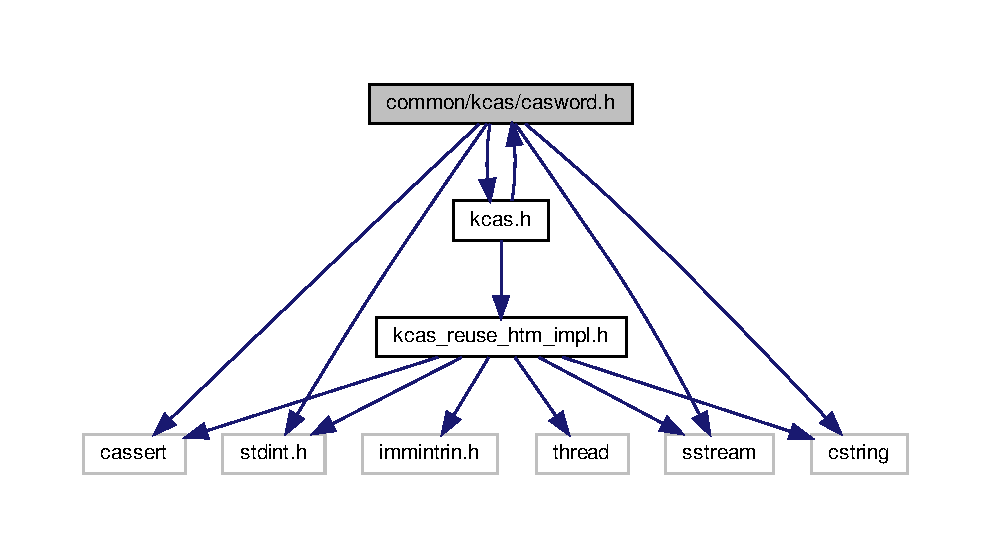
\includegraphics[width=350pt]{casword_8h__incl}
\end{center}
\end{figure}
This graph shows which files directly or indirectly include this file\+:
\nopagebreak
\begin{figure}[H]
\begin{center}
\leavevmode
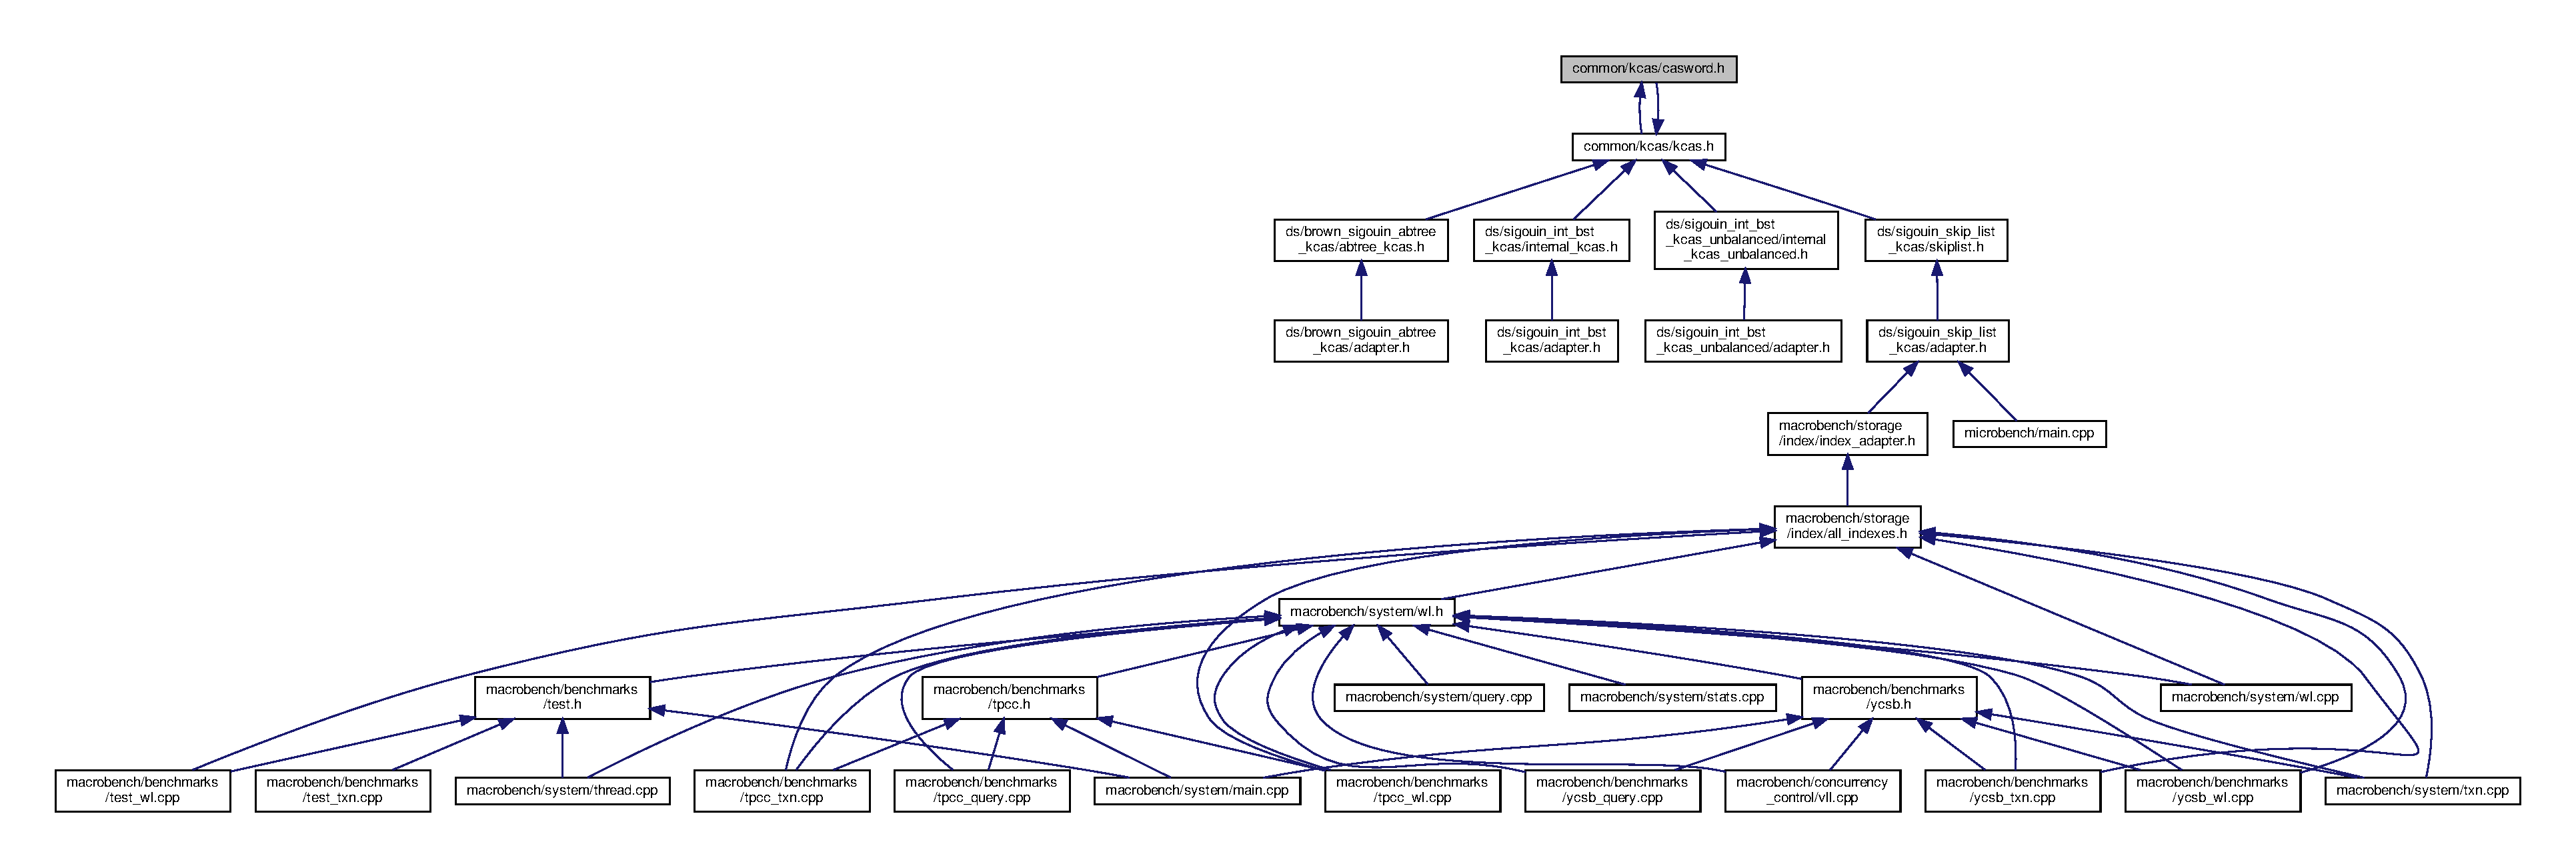
\includegraphics[width=350pt]{casword_8h__dep__incl}
\end{center}
\end{figure}
\subsection*{Macros}
\begin{DoxyCompactItemize}
\item 
\#define \hyperlink{casword_8h_ad45142aaf2ff20a036dc6242b8483e9c}{casword\+\_\+t}~uintptr\+\_\+t
\item 
\#define \hyperlink{casword_8h_a18b64507b88f9b541887105cac18eedc}{S\+H\+I\+F\+T\+\_\+\+B\+I\+TS}~2
\item 
\#define \hyperlink{casword_8h_a50a2e2d58f027d76cf772019231e603f}{C\+A\+S\+W\+O\+R\+D\+\_\+\+C\+A\+ST}(x)~((\hyperlink{kcas_8h_a56bcbd24dba9c9c05c0e132588aa5576}{C\+A\+S\+W\+O\+R\+D\+\_\+\+B\+I\+T\+S\+\_\+\+T\+Y\+PE}) (x))
\end{DoxyCompactItemize}


\subsection{Macro Definition Documentation}
\mbox{\Hypertarget{casword_8h_a50a2e2d58f027d76cf772019231e603f}\label{casword_8h_a50a2e2d58f027d76cf772019231e603f}} 
\index{casword.\+h@{casword.\+h}!C\+A\+S\+W\+O\+R\+D\+\_\+\+C\+A\+ST@{C\+A\+S\+W\+O\+R\+D\+\_\+\+C\+A\+ST}}
\index{C\+A\+S\+W\+O\+R\+D\+\_\+\+C\+A\+ST@{C\+A\+S\+W\+O\+R\+D\+\_\+\+C\+A\+ST}!casword.\+h@{casword.\+h}}
\subsubsection{\texorpdfstring{C\+A\+S\+W\+O\+R\+D\+\_\+\+C\+A\+ST}{CASWORD\_CAST}}
{\footnotesize\ttfamily \#define C\+A\+S\+W\+O\+R\+D\+\_\+\+C\+A\+ST(\begin{DoxyParamCaption}\item[{}]{x }\end{DoxyParamCaption})~((\hyperlink{kcas_8h_a56bcbd24dba9c9c05c0e132588aa5576}{C\+A\+S\+W\+O\+R\+D\+\_\+\+B\+I\+T\+S\+\_\+\+T\+Y\+PE}) (x))}

\mbox{\Hypertarget{casword_8h_ad45142aaf2ff20a036dc6242b8483e9c}\label{casword_8h_ad45142aaf2ff20a036dc6242b8483e9c}} 
\index{casword.\+h@{casword.\+h}!casword\+\_\+t@{casword\+\_\+t}}
\index{casword\+\_\+t@{casword\+\_\+t}!casword.\+h@{casword.\+h}}
\subsubsection{\texorpdfstring{casword\+\_\+t}{casword\_t}}
{\footnotesize\ttfamily \#define casword\+\_\+t~uintptr\+\_\+t}

\mbox{\Hypertarget{casword_8h_a18b64507b88f9b541887105cac18eedc}\label{casword_8h_a18b64507b88f9b541887105cac18eedc}} 
\index{casword.\+h@{casword.\+h}!S\+H\+I\+F\+T\+\_\+\+B\+I\+TS@{S\+H\+I\+F\+T\+\_\+\+B\+I\+TS}}
\index{S\+H\+I\+F\+T\+\_\+\+B\+I\+TS@{S\+H\+I\+F\+T\+\_\+\+B\+I\+TS}!casword.\+h@{casword.\+h}}
\subsubsection{\texorpdfstring{S\+H\+I\+F\+T\+\_\+\+B\+I\+TS}{SHIFT\_BITS}}
{\footnotesize\ttfamily \#define S\+H\+I\+F\+T\+\_\+\+B\+I\+TS~2}


\hypertarget{kcas_8h}{}\section{common/kcas/kcas.h File Reference}
\label{kcas_8h}\index{common/kcas/kcas.\+h@{common/kcas/kcas.\+h}}
{\ttfamily \#include \char`\"{}kcas\+\_\+reuse\+\_\+htm\+\_\+impl.\+h\char`\"{}}\newline
{\ttfamily \#include \char`\"{}casword.\+h\char`\"{}}\newline
Include dependency graph for kcas.\+h\+:
\nopagebreak
\begin{figure}[H]
\begin{center}
\leavevmode
\includegraphics[width=350pt]{kcas_8h__incl}
\end{center}
\end{figure}
This graph shows which files directly or indirectly include this file\+:
\nopagebreak
\begin{figure}[H]
\begin{center}
\leavevmode
\includegraphics[width=350pt]{kcas_8h__dep__incl}
\end{center}
\end{figure}
\subsection*{Classes}
\begin{DoxyCompactItemize}
\item 
struct \hyperlink{structcasword}{casword$<$ T $>$}
\end{DoxyCompactItemize}
\subsection*{Namespaces}
\begin{DoxyCompactItemize}
\item 
 \hyperlink{namespacekcas}{kcas}
\end{DoxyCompactItemize}
\subsection*{Macros}
\begin{DoxyCompactItemize}
\item 
\#define \hyperlink{kcas_8h_a56bcbd24dba9c9c05c0e132588aa5576}{C\+A\+S\+W\+O\+R\+D\+\_\+\+B\+I\+T\+S\+\_\+\+T\+Y\+PE}~\hyperlink{rq__unsafe_8h_ad45142aaf2ff20a036dc6242b8483e9c}{casword\+\_\+t}
\end{DoxyCompactItemize}
\subsection*{Functions}
\begin{DoxyCompactItemize}
\item 
void \hyperlink{namespacekcas_a92e383d96831fa6163a3d562d4a38053}{kcas\+::write\+Init\+Ptr} (\hyperlink{rq__unsafe_8h_ad45142aaf2ff20a036dc6242b8483e9c}{casword\+\_\+t} volatile $\ast$addr, \hyperlink{rq__unsafe_8h_ad45142aaf2ff20a036dc6242b8483e9c}{casword\+\_\+t} const newval)
\item 
void \hyperlink{namespacekcas_abd890f3f111dbd76aba1be89220ea07d}{kcas\+::write\+Init\+Val} (\hyperlink{rq__unsafe_8h_ad45142aaf2ff20a036dc6242b8483e9c}{casword\+\_\+t} volatile $\ast$addr, \hyperlink{rq__unsafe_8h_ad45142aaf2ff20a036dc6242b8483e9c}{casword\+\_\+t} const newval)
\item 
\hyperlink{rq__unsafe_8h_ad45142aaf2ff20a036dc6242b8483e9c}{casword\+\_\+t} \hyperlink{namespacekcas_a1f34f966b2243f133f1d936ec1761578}{kcas\+::read\+Ptr} (\hyperlink{rq__unsafe_8h_ad45142aaf2ff20a036dc6242b8483e9c}{casword\+\_\+t} volatile $\ast$addr)
\item 
\hyperlink{rq__unsafe_8h_ad45142aaf2ff20a036dc6242b8483e9c}{casword\+\_\+t} \hyperlink{namespacekcas_a41e805427c946f9e77ae065c624b2399}{kcas\+::read\+Val} (\hyperlink{rq__unsafe_8h_ad45142aaf2ff20a036dc6242b8483e9c}{casword\+\_\+t} volatile $\ast$addr)
\item 
bool \hyperlink{namespacekcas_ae51aac13e4c5df1190241ae51968387a}{kcas\+::execute} ()
\item 
\hyperlink{kcas__reuse__impl_8h_a5bbc81d391bfd6b4288a0d33f105a0b2}{kcasptr\+\_\+t} \hyperlink{namespacekcas_aa3f3e7af6facd9b5108b3b3fe8e4ed82}{kcas\+::get\+Descriptor} ()
\item 
void \hyperlink{namespacekcas_a39af7f008e3b3cb3815045257d15e735}{kcas\+::start} ()
\item 
{\footnotesize template$<$typename T $>$ }\\void \hyperlink{namespacekcas_acb0544489e45e08050227ab563d9ee15}{kcas\+::add} (\hyperlink{structcasword}{casword}$<$ T $>$ $\ast$caswordptr, T old\+Val, T new\+Val)
\item 
{\footnotesize template$<$typename T , typename... Args$>$ }\\void \hyperlink{namespacekcas_a227f3321961ae92470ed749e94656202}{kcas\+::add} (\hyperlink{structcasword}{casword}$<$ T $>$ $\ast$caswordptr, T old\+Val, T new\+Val, Args... args)
\end{DoxyCompactItemize}
\subsection*{Variables}
\begin{DoxyCompactItemize}
\item 
\hyperlink{classKCASHTM}{K\+C\+A\+S\+H\+TM}$<$ \hyperlink{skiplist_8h_a17681fc241567944ff9f0c062af6b7bf}{M\+A\+X\+\_\+\+K\+C\+AS} $>$ \hyperlink{namespacekcas_af460e5af7d85e9a87e52d4240e222fb5}{kcas\+::instance}
\end{DoxyCompactItemize}


\subsection{Macro Definition Documentation}
\mbox{\Hypertarget{kcas_8h_a56bcbd24dba9c9c05c0e132588aa5576}\label{kcas_8h_a56bcbd24dba9c9c05c0e132588aa5576}} 
\index{kcas.\+h@{kcas.\+h}!C\+A\+S\+W\+O\+R\+D\+\_\+\+B\+I\+T\+S\+\_\+\+T\+Y\+PE@{C\+A\+S\+W\+O\+R\+D\+\_\+\+B\+I\+T\+S\+\_\+\+T\+Y\+PE}}
\index{C\+A\+S\+W\+O\+R\+D\+\_\+\+B\+I\+T\+S\+\_\+\+T\+Y\+PE@{C\+A\+S\+W\+O\+R\+D\+\_\+\+B\+I\+T\+S\+\_\+\+T\+Y\+PE}!kcas.\+h@{kcas.\+h}}
\subsubsection{\texorpdfstring{C\+A\+S\+W\+O\+R\+D\+\_\+\+B\+I\+T\+S\+\_\+\+T\+Y\+PE}{CASWORD\_BITS\_TYPE}}
{\footnotesize\ttfamily \#define C\+A\+S\+W\+O\+R\+D\+\_\+\+B\+I\+T\+S\+\_\+\+T\+Y\+PE~\hyperlink{rq__unsafe_8h_ad45142aaf2ff20a036dc6242b8483e9c}{casword\+\_\+t}}


\hypertarget{kcas__reuse__htm__impl_8h}{}\section{common/kcas/kcas\+\_\+reuse\+\_\+htm\+\_\+impl.h File Reference}
\label{kcas__reuse__htm__impl_8h}\index{common/kcas/kcas\+\_\+reuse\+\_\+htm\+\_\+impl.\+h@{common/kcas/kcas\+\_\+reuse\+\_\+htm\+\_\+impl.\+h}}
{\ttfamily \#include $<$cassert$>$}\newline
{\ttfamily \#include $<$stdint.\+h$>$}\newline
{\ttfamily \#include $<$sstream$>$}\newline
{\ttfamily \#include $<$cstring$>$}\newline
{\ttfamily \#include $<$immintrin.\+h$>$}\newline
{\ttfamily \#include $<$thread$>$}\newline
Include dependency graph for kcas\+\_\+reuse\+\_\+htm\+\_\+impl.\+h\+:
\nopagebreak
\begin{figure}[H]
\begin{center}
\leavevmode
\includegraphics[width=350pt]{kcas__reuse__htm__impl_8h__incl}
\end{center}
\end{figure}
This graph shows which files directly or indirectly include this file\+:
\nopagebreak
\begin{figure}[H]
\begin{center}
\leavevmode
\includegraphics[width=350pt]{kcas__reuse__htm__impl_8h__dep__incl}
\end{center}
\end{figure}
\subsection*{Classes}
\begin{DoxyCompactItemize}
\item 
class \hyperlink{classTIDGenerator}{T\+I\+D\+Generator}
\item 
struct \hyperlink{structrdcssdesc__t}{rdcssdesc\+\_\+t}
\item 
struct \hyperlink{structkcasentry__t}{kcasentry\+\_\+t}
\item 
class \hyperlink{classkcasdesc__t}{kcasdesc\+\_\+t$<$ M\+A\+X\+\_\+\+K $>$}
\item 
class \hyperlink{classKCASHTM}{K\+C\+A\+S\+H\+T\+M$<$ M\+A\+X\+\_\+\+K $>$}
\end{DoxyCompactItemize}
\subsection*{Macros}
\begin{DoxyCompactItemize}
\item 
\#define \hyperlink{kcas__reuse__htm__impl_8h_a6bd312b05b209f8fce93c657186bbeb0}{B\+O\+O\+L\+\_\+\+C\+AS}~\+\_\+\+\_\+sync\+\_\+bool\+\_\+compare\+\_\+and\+\_\+swap
\item 
\#define \hyperlink{kcas__reuse__htm__impl_8h_aa7387507d9deee458fc9668893079a5f}{V\+A\+L\+\_\+\+C\+AS}~\+\_\+\+\_\+sync\+\_\+val\+\_\+compare\+\_\+and\+\_\+swap
\item 
\#define \hyperlink{kcas__reuse__htm__impl_8h_af8c689d47cb009242ec174b4e6305d54}{W\+I\+D\+T\+H\+\_\+\+S\+EQ}~48
\item 
\#define \hyperlink{kcas__reuse__htm__impl_8h_a130b75bf0ec168f61b83eb0662d75c3d}{O\+F\+F\+S\+E\+T\+\_\+\+S\+EQ}~14
\item 
\#define \hyperlink{kcas__reuse__htm__impl_8h_a95444ce25f4d0a2711f4407cb99e28c5}{M\+A\+S\+K\+\_\+\+S\+EQ}~((uintptr\+\_\+t)((1\+L\+L$<$$<$\+W\+I\+D\+T\+H\+\_\+\+S\+E\+Q)-\/1)$<$$<$\+O\+F\+F\+S\+E\+T\+\_\+\+S\+E\+Q) /$\ast$ cast to avoid signed bit shifting $\ast$/
\item 
\#define \hyperlink{kcas__reuse__htm__impl_8h_a516c0a6bd46e52280bb058dc9e28de5a}{U\+N\+P\+A\+C\+K\+\_\+\+S\+EQ}(tagptr\+Or\+Seqbits)~(((uintptr\+\_\+t)(tagptr\+Or\+Seqbits))$>$$>$\hyperlink{kcas__reuse__impl_8h_a130b75bf0ec168f61b83eb0662d75c3d}{O\+F\+F\+S\+E\+T\+\_\+\+S\+EQ})
\item 
\#define \hyperlink{kcas__reuse__htm__impl_8h_a42d8f729d19e4e4f9a11f5d2f0ebd6d8}{T\+A\+G\+P\+T\+R\+\_\+\+O\+F\+F\+S\+E\+T\+\_\+\+U\+S\+ER}~0
\item 
\#define \hyperlink{kcas__reuse__htm__impl_8h_afc658e344718431ddb4336743d1aa833}{T\+A\+G\+P\+T\+R\+\_\+\+O\+F\+F\+S\+E\+T\+\_\+\+T\+ID}~3
\item 
\#define \hyperlink{kcas__reuse__htm__impl_8h_a61a985e276e620c7d24997edec424cf8}{T\+A\+G\+P\+T\+R\+\_\+\+M\+A\+S\+K\+\_\+\+U\+S\+ER}~((1$<$$<$\hyperlink{kcas__reuse__impl_8h_afc658e344718431ddb4336743d1aa833}{T\+A\+G\+P\+T\+R\+\_\+\+O\+F\+F\+S\+E\+T\+\_\+\+T\+ID})-\/1) /$\ast$ assumes T\+ID is next \hyperlink{scxrecord_8h_a0657af583030a13da27c9e6d5ec40aa4}{field} after U\+S\+ER $\ast$/
\item 
\#define \hyperlink{kcas__reuse__htm__impl_8h_ae040bd6ea3d1ce7145e3aab6395dbb48}{T\+A\+G\+P\+T\+R\+\_\+\+M\+A\+S\+K\+\_\+\+T\+ID}~(((1$<$$<$\hyperlink{kcas__reuse__impl_8h_a130b75bf0ec168f61b83eb0662d75c3d}{O\+F\+F\+S\+E\+T\+\_\+\+S\+EQ})-\/1)\&($\sim$(\hyperlink{kcas__reuse__impl_8h_a61a985e276e620c7d24997edec424cf8}{T\+A\+G\+P\+T\+R\+\_\+\+M\+A\+S\+K\+\_\+\+U\+S\+ER})))
\item 
\#define \hyperlink{kcas__reuse__htm__impl_8h_a7d7b4fa8ff329a61456256f432ec80e6}{T\+A\+G\+P\+T\+R\+\_\+\+U\+N\+P\+A\+C\+K\+\_\+\+T\+ID}(tagptr)~((int) ((((\hyperlink{descriptors_8h_afd8a7b57046ed96897cda907f17737a7}{tagptr\+\_\+t}) (tagptr))\&\hyperlink{kcas__reuse__impl_8h_ae040bd6ea3d1ce7145e3aab6395dbb48}{T\+A\+G\+P\+T\+R\+\_\+\+M\+A\+S\+K\+\_\+\+T\+ID})$>$$>$\hyperlink{kcas__reuse__impl_8h_afc658e344718431ddb4336743d1aa833}{T\+A\+G\+P\+T\+R\+\_\+\+O\+F\+F\+S\+E\+T\+\_\+\+T\+ID}))
\item 
\#define \hyperlink{kcas__reuse__htm__impl_8h_aa612148b06ee2120b842bc58000ecc96}{T\+A\+G\+P\+T\+R\+\_\+\+U\+N\+P\+A\+C\+K\+\_\+\+P\+TR}(desc\+Array,  tagptr)~(\&(desc\+Array)\mbox{[}\hyperlink{kcas__reuse__impl_8h_a7d7b4fa8ff329a61456256f432ec80e6}{T\+A\+G\+P\+T\+R\+\_\+\+U\+N\+P\+A\+C\+K\+\_\+\+T\+ID}((tagptr))\mbox{]})
\item 
\#define \hyperlink{kcas__reuse__htm__impl_8h_a09292a23fc4557618071576f7a9c7292}{T\+A\+G\+P\+T\+R\+\_\+\+N\+EW}(\hyperlink{microbench_2main_8cpp_a9ca9869868fe7e7a38a921cc7de4103f}{tid},  seq\+Bits,  user\+Bits)~((\hyperlink{descriptors_8h_afd8a7b57046ed96897cda907f17737a7}{tagptr\+\_\+t}) (((\hyperlink{kcas__reuse__impl_8h_a516c0a6bd46e52280bb058dc9e28de5a}{U\+N\+P\+A\+C\+K\+\_\+\+S\+EQ}(seq\+Bits))$<$$<$\hyperlink{kcas__reuse__impl_8h_a130b75bf0ec168f61b83eb0662d75c3d}{O\+F\+F\+S\+E\+T\+\_\+\+S\+EQ}) $\vert$ ((\hyperlink{microbench_2main_8cpp_a9ca9869868fe7e7a38a921cc7de4103f}{tid})$<$$<$\hyperlink{kcas__reuse__impl_8h_afc658e344718431ddb4336743d1aa833}{T\+A\+G\+P\+T\+R\+\_\+\+O\+F\+F\+S\+E\+T\+\_\+\+T\+ID}) $\vert$ (\hyperlink{descriptors_8h_afd8a7b57046ed96897cda907f17737a7}{tagptr\+\_\+t}) (user\+Bits)$<$$<$\hyperlink{kcas__reuse__impl_8h_a42d8f729d19e4e4f9a11f5d2f0ebd6d8}{T\+A\+G\+P\+T\+R\+\_\+\+O\+F\+F\+S\+E\+T\+\_\+\+U\+S\+ER}))
\item 
\#define \hyperlink{kcas__reuse__htm__impl_8h_ab35d1739985ea729f8a7f51427354dbc}{L\+A\+S\+T\+\_\+\+T\+ID}~(\hyperlink{kcas__reuse__impl_8h_ae040bd6ea3d1ce7145e3aab6395dbb48}{T\+A\+G\+P\+T\+R\+\_\+\+M\+A\+S\+K\+\_\+\+T\+ID}$>$$>$\hyperlink{kcas__reuse__impl_8h_afc658e344718431ddb4336743d1aa833}{T\+A\+G\+P\+T\+R\+\_\+\+O\+F\+F\+S\+E\+T\+\_\+\+T\+ID})
\item 
\#define \hyperlink{kcas__reuse__htm__impl_8h_acab04f92bc9c2cce09ba5f6099ff02d5}{T\+A\+G\+P\+T\+R\+\_\+\+S\+T\+A\+T\+I\+C\+\_\+\+D\+E\+SC}(id)~((\hyperlink{descriptors_8h_afd8a7b57046ed96897cda907f17737a7}{tagptr\+\_\+t}) \hyperlink{kcas__reuse__impl_8h_a09292a23fc4557618071576f7a9c7292}{T\+A\+G\+P\+T\+R\+\_\+\+N\+EW}(\hyperlink{kcas__reuse__impl_8h_ab35d1739985ea729f8a7f51427354dbc}{L\+A\+S\+T\+\_\+\+T\+ID}-\/1-\/id, 0))
\item 
\#define \hyperlink{kcas__reuse__htm__impl_8h_ab818bdd1ba41d2a9df7f9d4f582dd160}{T\+A\+G\+P\+T\+R\+\_\+\+D\+U\+M\+M\+Y\+\_\+\+D\+E\+SC}(id)~((\hyperlink{descriptors_8h_afd8a7b57046ed96897cda907f17737a7}{tagptr\+\_\+t}) \hyperlink{kcas__reuse__impl_8h_a09292a23fc4557618071576f7a9c7292}{T\+A\+G\+P\+T\+R\+\_\+\+N\+EW}(\hyperlink{kcas__reuse__impl_8h_ab35d1739985ea729f8a7f51427354dbc}{L\+A\+S\+T\+\_\+\+T\+ID}, id$<$$<$\hyperlink{kcas__reuse__impl_8h_a130b75bf0ec168f61b83eb0662d75c3d}{O\+F\+F\+S\+E\+T\+\_\+\+S\+EQ}))
\item 
\#define \hyperlink{kcas__reuse__htm__impl_8h_a0d1e6460951f8c965551f121ebd9730c}{comma}~,
\item 
\#define \hyperlink{kcas__reuse__htm__impl_8h_a326a5566d56db108787f1544e173d5dc}{S\+E\+Q\+B\+I\+T\+S\+\_\+\+U\+N\+P\+A\+C\+K\+\_\+\+F\+I\+E\+LD}(seq\+Bits,  mask,  offset)~((((\hyperlink{kcas__reuse__htm__impl_8h_a997daf56279be481f5c4294647725689}{seqbits\+\_\+t}) (seq\+Bits))\&(mask))$>$$>$(offset))
\item 
\#define \hyperlink{kcas__reuse__htm__impl_8h_aee7e6149a4fb3880b5c403147201e534}{S\+E\+Q\+B\+I\+T\+S\+\_\+\+C\+A\+S\+\_\+\+F\+I\+E\+LD}(success\+Bit,  fld\+Seq\+Bits,  snap\+Seq\+Bits,  oldval,  val,  mask,  offset)
\item 
\#define \hyperlink{kcas__reuse__htm__impl_8h_ad070db09873af8bb4670248e5d31c3c0}{S\+E\+Q\+B\+I\+T\+S\+\_\+\+W\+R\+I\+T\+E\+\_\+\+F\+I\+E\+LD}(fld\+Seq\+Bits,  snap\+Seq\+Bits,  val,  mask,  offset)
\item 
\#define \hyperlink{kcas__reuse__htm__impl_8h_a81fc0a9867792a74b225745978fa8450}{S\+E\+Q\+B\+I\+T\+S\+\_\+\+W\+R\+I\+T\+E\+\_\+\+B\+IT}(fld\+Seq\+Bits,  snap\+Seq\+Bits,  mask)
\item 
\#define \hyperlink{kcas__reuse__htm__impl_8h_ab7d0645d0a890428e979b7caea3bae6c}{D\+E\+S\+C\+\_\+\+S\+N\+A\+P\+S\+H\+OT}(desc\+Type,  desc\+Array,  desc\+Dest,  tagptr,  sz)
\item 
\#define \hyperlink{kcas__reuse__htm__impl_8h_aa444c135013fbafd47054c299c7ed1d7}{D\+E\+S\+C\+\_\+\+R\+E\+A\+D\+\_\+\+F\+I\+E\+LD}(success\+Bit,  fld\+Seq\+Bits,  tagptr,  mask,  offset)
\item 
\#define \hyperlink{kcas__reuse__htm__impl_8h_a5f0b918f155e4eeb32a96b29c219e410}{D\+E\+S\+C\+\_\+\+N\+EW}(desc\+Array,  macro\+\_\+seq\+Bits\+New,  \hyperlink{microbench_2main_8cpp_a9ca9869868fe7e7a38a921cc7de4103f}{tid})
\item 
\#define \hyperlink{kcas__reuse__htm__impl_8h_a33e3eb771fac10e71e7f6ffd521779d3}{D\+E\+S\+C\+\_\+\+I\+N\+I\+T\+I\+A\+L\+I\+Z\+ED}(desc\+Array,  \hyperlink{microbench_2main_8cpp_a9ca9869868fe7e7a38a921cc7de4103f}{tid})~(desc\+Array)\mbox{[}(\hyperlink{microbench_2main_8cpp_a9ca9869868fe7e7a38a921cc7de4103f}{tid})\mbox{]}.seq\+Bits += (1$<$$<$\hyperlink{kcas__reuse__impl_8h_a130b75bf0ec168f61b83eb0662d75c3d}{O\+F\+F\+S\+E\+T\+\_\+\+S\+EQ});
\item 
\#define \hyperlink{kcas__reuse__htm__impl_8h_a8b69438c704b3b5d6fd28a1838bf6e14}{D\+E\+S\+C\+\_\+\+I\+N\+I\+T\+\_\+\+A\+LL}(desc\+Array,  macro\+\_\+seq\+Bits\+New)
\item 
\#define \hyperlink{kcas__reuse__htm__impl_8h_a22868433cf4300ce32f000ed8c8dd76c}{kcastagptr\+\_\+t}~uintptr\+\_\+t
\item 
\#define \hyperlink{kcas__reuse__htm__impl_8h_aae2452099fa4312e7ea48c986dcadfd8}{rdcsstagptr\+\_\+t}~uintptr\+\_\+t
\item 
\#define \hyperlink{kcas__reuse__htm__impl_8h_a9a742371dcbdf5e852097073a03e9a09}{rdcssptr\+\_\+t}~\hyperlink{structrdcssdesc__t}{rdcssdesc\+\_\+t}$\ast$
\item 
\#define \hyperlink{kcas__reuse__htm__impl_8h_a5bbc81d391bfd6b4288a0d33f105a0b2}{kcasptr\+\_\+t}~\hyperlink{classkcasdesc__t}{kcasdesc\+\_\+t}$<$\hyperlink{skiplist_8h_a17681fc241567944ff9f0c062af6b7bf}{M\+A\+X\+\_\+\+K\+C\+AS}$>$$\ast$
\item 
\#define \hyperlink{kcas__reuse__htm__impl_8h_a038015b999541209744d41de50c9885e}{R\+D\+C\+S\+S\+\_\+\+T\+A\+G\+B\+IT}~0x1
\item 
\#define \hyperlink{kcas__reuse__htm__impl_8h_a636a1f6fdaa98ac9b838143e9af5704f}{K\+C\+A\+S\+\_\+\+T\+A\+G\+B\+IT}~0x2
\item 
\#define \hyperlink{kcas__reuse__htm__impl_8h_a66ed72b1fde7249826ab8e825dd94b61}{K\+C\+A\+S\+\_\+\+S\+T\+A\+T\+E\+\_\+\+U\+N\+D\+E\+C\+I\+D\+ED}~0
\item 
\#define \hyperlink{kcas__reuse__htm__impl_8h_a62583da7023324bdf6c8426ef7f07d95}{K\+C\+A\+S\+\_\+\+S\+T\+A\+T\+E\+\_\+\+S\+U\+C\+C\+E\+E\+D\+ED}~4
\item 
\#define \hyperlink{kcas__reuse__htm__impl_8h_a9afe459b8a5e37c1821e790bde6463ba}{K\+C\+A\+S\+\_\+\+S\+T\+A\+T\+E\+\_\+\+F\+A\+I\+L\+ED}~8
\item 
\#define \hyperlink{kcas__reuse__htm__impl_8h_aed57ca4a1dc4eb34cd1996cce5f7b197}{K\+C\+A\+S\+\_\+\+L\+E\+F\+T\+S\+H\+I\+FT}~2
\item 
\#define \hyperlink{kcas__reuse__htm__impl_8h_a10f6493935ebad2cca6764a58ebd08b7}{H\+T\+M\+\_\+\+R\+E\+A\+D\+\_\+\+D\+E\+S\+C\+R\+I\+P\+T\+OR}~20
\item 
\#define \hyperlink{kcas__reuse__htm__impl_8h_a92e1dd3c2e3380eef5cc814bac2772a3}{H\+T\+M\+\_\+\+B\+A\+D\+\_\+\+O\+L\+D\+\_\+\+V\+AL}~30
\item 
\#define \hyperlink{kcas__reuse__htm__impl_8h_aecf13b8dc783db2202ca5c34fe117fc3}{M\+A\+X\+\_\+\+R\+E\+T\+R\+I\+ES}~5
\item 
\#define \hyperlink{kcas__reuse__htm__impl_8h_a6089afddf2f1b26c22642c0c18188b84}{K\+C\+A\+S\+\_\+\+M\+A\+X\+\_\+\+T\+H\+R\+E\+A\+DS}~500
\item 
\#define \hyperlink{kcas__reuse__htm__impl_8h_ae79e31f9663ebf39224c292618da8ac1}{K\+C\+A\+S\+\_\+\+S\+E\+Q\+B\+I\+T\+S\+\_\+\+O\+F\+F\+S\+E\+T\+\_\+\+S\+T\+A\+TE}~0
\item 
\#define \hyperlink{kcas__reuse__htm__impl_8h_ac5171ddfdac7c4f4b85d6694a0fa4e06}{K\+C\+A\+S\+\_\+\+S\+E\+Q\+B\+I\+T\+S\+\_\+\+M\+A\+S\+K\+\_\+\+S\+T\+A\+TE}~0xf
\item 
\#define \hyperlink{kcas__reuse__htm__impl_8h_a25bc6d8bc74b65814601e19ac109275d}{K\+C\+A\+S\+\_\+\+S\+E\+Q\+B\+I\+T\+S\+\_\+\+N\+EW}(seq\+Bits)
\item 
\#define \hyperlink{kcas__reuse__htm__impl_8h_ab86889a3475716b9d270c0d7c493be59}{R\+D\+C\+S\+S\+\_\+\+S\+E\+Q\+B\+I\+T\+S\+\_\+\+N\+EW}(seq\+Bits)~(((seq\+Bits)\&\hyperlink{kcas__reuse__impl_8h_a95444ce25f4d0a2711f4407cb99e28c5}{M\+A\+S\+K\+\_\+\+S\+EQ})+(1$<$$<$\hyperlink{kcas__reuse__impl_8h_a130b75bf0ec168f61b83eb0662d75c3d}{O\+F\+F\+S\+E\+T\+\_\+\+S\+EQ}))
\end{DoxyCompactItemize}
\subsection*{Typedefs}
\begin{DoxyCompactItemize}
\item 
typedef intptr\+\_\+t \hyperlink{kcas__reuse__htm__impl_8h_afd8a7b57046ed96897cda907f17737a7}{tagptr\+\_\+t}
\item 
typedef intptr\+\_\+t \hyperlink{kcas__reuse__htm__impl_8h_a997daf56279be481f5c4294647725689}{seqbits\+\_\+t}
\end{DoxyCompactItemize}
\subsection*{Variables}
\begin{DoxyCompactItemize}
\item 
void $\ast$volatile \hyperlink{kcas__reuse__htm__impl_8h_a450854542d4b89e92eee8baccf3990f2}{thread\+\_\+ids} \mbox{[}\hyperlink{kcas__reuse__impl_8h_a6089afddf2f1b26c22642c0c18188b84}{K\+C\+A\+S\+\_\+\+M\+A\+X\+\_\+\+T\+H\+R\+E\+A\+DS}\mbox{]} = \{\}
\item 
thread\+\_\+local \hyperlink{classTIDGenerator}{T\+I\+D\+Generator} \hyperlink{kcas__reuse__htm__impl_8h_af6be76a55e3af6769042304400c38853}{kcas\+\_\+tid}
\end{DoxyCompactItemize}


\subsection{Macro Definition Documentation}
\mbox{\Hypertarget{kcas__reuse__htm__impl_8h_a6bd312b05b209f8fce93c657186bbeb0}\label{kcas__reuse__htm__impl_8h_a6bd312b05b209f8fce93c657186bbeb0}} 
\index{kcas\+\_\+reuse\+\_\+htm\+\_\+impl.\+h@{kcas\+\_\+reuse\+\_\+htm\+\_\+impl.\+h}!B\+O\+O\+L\+\_\+\+C\+AS@{B\+O\+O\+L\+\_\+\+C\+AS}}
\index{B\+O\+O\+L\+\_\+\+C\+AS@{B\+O\+O\+L\+\_\+\+C\+AS}!kcas\+\_\+reuse\+\_\+htm\+\_\+impl.\+h@{kcas\+\_\+reuse\+\_\+htm\+\_\+impl.\+h}}
\subsubsection{\texorpdfstring{B\+O\+O\+L\+\_\+\+C\+AS}{BOOL\_CAS}}
{\footnotesize\ttfamily \#define B\+O\+O\+L\+\_\+\+C\+AS~\+\_\+\+\_\+sync\+\_\+bool\+\_\+compare\+\_\+and\+\_\+swap}

Note\+: this algorithm supports a limited number of threads (print L\+A\+S\+T\+\_\+\+T\+ID to see how many). It should be several thousand, at least. The alg can be tweaked to support more. \mbox{\Hypertarget{kcas__reuse__htm__impl_8h_a0d1e6460951f8c965551f121ebd9730c}\label{kcas__reuse__htm__impl_8h_a0d1e6460951f8c965551f121ebd9730c}} 
\index{kcas\+\_\+reuse\+\_\+htm\+\_\+impl.\+h@{kcas\+\_\+reuse\+\_\+htm\+\_\+impl.\+h}!comma@{comma}}
\index{comma@{comma}!kcas\+\_\+reuse\+\_\+htm\+\_\+impl.\+h@{kcas\+\_\+reuse\+\_\+htm\+\_\+impl.\+h}}
\subsubsection{\texorpdfstring{comma}{comma}}
{\footnotesize\ttfamily \#define comma~,}

\mbox{\Hypertarget{kcas__reuse__htm__impl_8h_a8b69438c704b3b5d6fd28a1838bf6e14}\label{kcas__reuse__htm__impl_8h_a8b69438c704b3b5d6fd28a1838bf6e14}} 
\index{kcas\+\_\+reuse\+\_\+htm\+\_\+impl.\+h@{kcas\+\_\+reuse\+\_\+htm\+\_\+impl.\+h}!D\+E\+S\+C\+\_\+\+I\+N\+I\+T\+\_\+\+A\+LL@{D\+E\+S\+C\+\_\+\+I\+N\+I\+T\+\_\+\+A\+LL}}
\index{D\+E\+S\+C\+\_\+\+I\+N\+I\+T\+\_\+\+A\+LL@{D\+E\+S\+C\+\_\+\+I\+N\+I\+T\+\_\+\+A\+LL}!kcas\+\_\+reuse\+\_\+htm\+\_\+impl.\+h@{kcas\+\_\+reuse\+\_\+htm\+\_\+impl.\+h}}
\subsubsection{\texorpdfstring{D\+E\+S\+C\+\_\+\+I\+N\+I\+T\+\_\+\+A\+LL}{DESC\_INIT\_ALL}}
{\footnotesize\ttfamily \#define D\+E\+S\+C\+\_\+\+I\+N\+I\+T\+\_\+\+A\+LL(\begin{DoxyParamCaption}\item[{}]{desc\+Array,  }\item[{}]{macro\+\_\+seq\+Bits\+New }\end{DoxyParamCaption})}

{\bfseries Value\+:}
\begin{DoxyCode}
\{ \(\backslash\)
    for (\textcolor{keywordtype}{int} \hyperlink{namespaceurcu_a536341e353c82c078bc510ca0144dd58}{i}=0;\hyperlink{namespaceurcu_a536341e353c82c078bc510ca0144dd58}{i}<(\hyperlink{kcas__reuse__htm__impl_8h_ab35d1739985ea729f8a7f51427354dbc}{LAST\_TID}-1);++\hyperlink{namespaceurcu_a536341e353c82c078bc510ca0144dd58}{i}) \{ \(\backslash\)
        (descArray)[\hyperlink{namespaceurcu_a536341e353c82c078bc510ca0144dd58}{i}].seqBits = macro\_seqBitsNew(0); \(\backslash\)
    \} \(\backslash\)
\}
\end{DoxyCode}
\mbox{\Hypertarget{kcas__reuse__htm__impl_8h_a33e3eb771fac10e71e7f6ffd521779d3}\label{kcas__reuse__htm__impl_8h_a33e3eb771fac10e71e7f6ffd521779d3}} 
\index{kcas\+\_\+reuse\+\_\+htm\+\_\+impl.\+h@{kcas\+\_\+reuse\+\_\+htm\+\_\+impl.\+h}!D\+E\+S\+C\+\_\+\+I\+N\+I\+T\+I\+A\+L\+I\+Z\+ED@{D\+E\+S\+C\+\_\+\+I\+N\+I\+T\+I\+A\+L\+I\+Z\+ED}}
\index{D\+E\+S\+C\+\_\+\+I\+N\+I\+T\+I\+A\+L\+I\+Z\+ED@{D\+E\+S\+C\+\_\+\+I\+N\+I\+T\+I\+A\+L\+I\+Z\+ED}!kcas\+\_\+reuse\+\_\+htm\+\_\+impl.\+h@{kcas\+\_\+reuse\+\_\+htm\+\_\+impl.\+h}}
\subsubsection{\texorpdfstring{D\+E\+S\+C\+\_\+\+I\+N\+I\+T\+I\+A\+L\+I\+Z\+ED}{DESC\_INITIALIZED}}
{\footnotesize\ttfamily \#define D\+E\+S\+C\+\_\+\+I\+N\+I\+T\+I\+A\+L\+I\+Z\+ED(\begin{DoxyParamCaption}\item[{}]{desc\+Array,  }\item[{}]{\hyperlink{microbench_2main_8cpp_a9ca9869868fe7e7a38a921cc7de4103f}{tid} }\end{DoxyParamCaption})~(desc\+Array)\mbox{[}(\hyperlink{microbench_2main_8cpp_a9ca9869868fe7e7a38a921cc7de4103f}{tid})\mbox{]}.seq\+Bits += (1$<$$<$\hyperlink{kcas__reuse__impl_8h_a130b75bf0ec168f61b83eb0662d75c3d}{O\+F\+F\+S\+E\+T\+\_\+\+S\+EQ});}

\mbox{\Hypertarget{kcas__reuse__htm__impl_8h_a5f0b918f155e4eeb32a96b29c219e410}\label{kcas__reuse__htm__impl_8h_a5f0b918f155e4eeb32a96b29c219e410}} 
\index{kcas\+\_\+reuse\+\_\+htm\+\_\+impl.\+h@{kcas\+\_\+reuse\+\_\+htm\+\_\+impl.\+h}!D\+E\+S\+C\+\_\+\+N\+EW@{D\+E\+S\+C\+\_\+\+N\+EW}}
\index{D\+E\+S\+C\+\_\+\+N\+EW@{D\+E\+S\+C\+\_\+\+N\+EW}!kcas\+\_\+reuse\+\_\+htm\+\_\+impl.\+h@{kcas\+\_\+reuse\+\_\+htm\+\_\+impl.\+h}}
\subsubsection{\texorpdfstring{D\+E\+S\+C\+\_\+\+N\+EW}{DESC\_NEW}}
{\footnotesize\ttfamily \#define D\+E\+S\+C\+\_\+\+N\+EW(\begin{DoxyParamCaption}\item[{}]{desc\+Array,  }\item[{}]{macro\+\_\+seq\+Bits\+New,  }\item[{}]{\hyperlink{microbench_2main_8cpp_a9ca9869868fe7e7a38a921cc7de4103f}{tid} }\end{DoxyParamCaption})}

{\bfseries Value\+:}
\begin{DoxyCode}
&(descArray)[(\hyperlink{global_8cpp_a9ca9869868fe7e7a38a921cc7de4103f}{tid})]; \{ \textcolor{comment}{/* note: only the process invoking this following macro can change the sequence# 
      */} \(\backslash\)
    seqbits\_t \_\_v = (descArray)[(\hyperlink{global_8cpp_a9ca9869868fe7e7a38a921cc7de4103f}{tid})].seqBits; \(\backslash\)
    (descArray)[(\hyperlink{global_8cpp_a9ca9869868fe7e7a38a921cc7de4103f}{tid})].seqBits = macro\_seqBitsNew(\_\_v); \(\backslash\)
    \textcolor{comment}{/*\_\_sync\_synchronize();*/} \(\backslash\)
\}
\end{DoxyCode}
\mbox{\Hypertarget{kcas__reuse__htm__impl_8h_aa444c135013fbafd47054c299c7ed1d7}\label{kcas__reuse__htm__impl_8h_aa444c135013fbafd47054c299c7ed1d7}} 
\index{kcas\+\_\+reuse\+\_\+htm\+\_\+impl.\+h@{kcas\+\_\+reuse\+\_\+htm\+\_\+impl.\+h}!D\+E\+S\+C\+\_\+\+R\+E\+A\+D\+\_\+\+F\+I\+E\+LD@{D\+E\+S\+C\+\_\+\+R\+E\+A\+D\+\_\+\+F\+I\+E\+LD}}
\index{D\+E\+S\+C\+\_\+\+R\+E\+A\+D\+\_\+\+F\+I\+E\+LD@{D\+E\+S\+C\+\_\+\+R\+E\+A\+D\+\_\+\+F\+I\+E\+LD}!kcas\+\_\+reuse\+\_\+htm\+\_\+impl.\+h@{kcas\+\_\+reuse\+\_\+htm\+\_\+impl.\+h}}
\subsubsection{\texorpdfstring{D\+E\+S\+C\+\_\+\+R\+E\+A\+D\+\_\+\+F\+I\+E\+LD}{DESC\_READ\_FIELD}}
{\footnotesize\ttfamily \#define D\+E\+S\+C\+\_\+\+R\+E\+A\+D\+\_\+\+F\+I\+E\+LD(\begin{DoxyParamCaption}\item[{}]{success\+Bit,  }\item[{}]{fld\+Seq\+Bits,  }\item[{}]{tagptr,  }\item[{}]{mask,  }\item[{}]{offset }\end{DoxyParamCaption})}

{\bfseries Value\+:}
\begin{DoxyCode}
(\{ \(\backslash\)
    seqbits\_t \_\_seqBits = (fldSeqBits); \(\backslash\)
    successBit = (\_\_seqBits & \hyperlink{kcas__reuse__htm__impl_8h_a95444ce25f4d0a2711f4407cb99e28c5}{MASK\_SEQ}) == ((tagptr) & \hyperlink{kcas__reuse__htm__impl_8h_a95444ce25f4d0a2711f4407cb99e28c5}{MASK\_SEQ}); \(\backslash\)
    SEQBITS\_UNPACK\_FIELD(\_\_seqBits, (mask), (offset)); \(\backslash\)
\})
\end{DoxyCode}
\mbox{\Hypertarget{kcas__reuse__htm__impl_8h_ab7d0645d0a890428e979b7caea3bae6c}\label{kcas__reuse__htm__impl_8h_ab7d0645d0a890428e979b7caea3bae6c}} 
\index{kcas\+\_\+reuse\+\_\+htm\+\_\+impl.\+h@{kcas\+\_\+reuse\+\_\+htm\+\_\+impl.\+h}!D\+E\+S\+C\+\_\+\+S\+N\+A\+P\+S\+H\+OT@{D\+E\+S\+C\+\_\+\+S\+N\+A\+P\+S\+H\+OT}}
\index{D\+E\+S\+C\+\_\+\+S\+N\+A\+P\+S\+H\+OT@{D\+E\+S\+C\+\_\+\+S\+N\+A\+P\+S\+H\+OT}!kcas\+\_\+reuse\+\_\+htm\+\_\+impl.\+h@{kcas\+\_\+reuse\+\_\+htm\+\_\+impl.\+h}}
\subsubsection{\texorpdfstring{D\+E\+S\+C\+\_\+\+S\+N\+A\+P\+S\+H\+OT}{DESC\_SNAPSHOT}}
{\footnotesize\ttfamily \#define D\+E\+S\+C\+\_\+\+S\+N\+A\+P\+S\+H\+OT(\begin{DoxyParamCaption}\item[{}]{desc\+Type,  }\item[{}]{desc\+Array,  }\item[{}]{desc\+Dest,  }\item[{}]{tagptr,  }\item[{}]{sz }\end{DoxyParamCaption})}

{\bfseries Value\+:}
\begin{DoxyCode}
(\{ \(\backslash\)
    descType *\_\_src = \hyperlink{kcas__reuse__htm__impl_8h_aa612148b06ee2120b842bc58000ecc96}{TAGPTR\_UNPACK\_PTR}((descArray), (tagptr)); \(\backslash\)
    memcpy((descDest), \_\_src, (sz)); \(\backslash\)
    \_\_asm\_\_ \_\_volatile\_\_ (\textcolor{stringliteral}{""}:::\textcolor{stringliteral}{"memory"}); \textcolor{comment}{/* prevent compiler from reordering read of \_\_src->seqBits before
       (at least the reading portion of) the memcpy */} \(\backslash\)
    (\hyperlink{kcas__reuse__htm__impl_8h_a516c0a6bd46e52280bb058dc9e28de5a}{UNPACK\_SEQ}(\_\_src->seqBits) == \hyperlink{kcas__reuse__htm__impl_8h_a516c0a6bd46e52280bb058dc9e28de5a}{UNPACK\_SEQ}((tagptr))); \(\backslash\)
\})
\end{DoxyCode}
\mbox{\Hypertarget{kcas__reuse__htm__impl_8h_a92e1dd3c2e3380eef5cc814bac2772a3}\label{kcas__reuse__htm__impl_8h_a92e1dd3c2e3380eef5cc814bac2772a3}} 
\index{kcas\+\_\+reuse\+\_\+htm\+\_\+impl.\+h@{kcas\+\_\+reuse\+\_\+htm\+\_\+impl.\+h}!H\+T\+M\+\_\+\+B\+A\+D\+\_\+\+O\+L\+D\+\_\+\+V\+AL@{H\+T\+M\+\_\+\+B\+A\+D\+\_\+\+O\+L\+D\+\_\+\+V\+AL}}
\index{H\+T\+M\+\_\+\+B\+A\+D\+\_\+\+O\+L\+D\+\_\+\+V\+AL@{H\+T\+M\+\_\+\+B\+A\+D\+\_\+\+O\+L\+D\+\_\+\+V\+AL}!kcas\+\_\+reuse\+\_\+htm\+\_\+impl.\+h@{kcas\+\_\+reuse\+\_\+htm\+\_\+impl.\+h}}
\subsubsection{\texorpdfstring{H\+T\+M\+\_\+\+B\+A\+D\+\_\+\+O\+L\+D\+\_\+\+V\+AL}{HTM\_BAD\_OLD\_VAL}}
{\footnotesize\ttfamily \#define H\+T\+M\+\_\+\+B\+A\+D\+\_\+\+O\+L\+D\+\_\+\+V\+AL~30}

\mbox{\Hypertarget{kcas__reuse__htm__impl_8h_a10f6493935ebad2cca6764a58ebd08b7}\label{kcas__reuse__htm__impl_8h_a10f6493935ebad2cca6764a58ebd08b7}} 
\index{kcas\+\_\+reuse\+\_\+htm\+\_\+impl.\+h@{kcas\+\_\+reuse\+\_\+htm\+\_\+impl.\+h}!H\+T\+M\+\_\+\+R\+E\+A\+D\+\_\+\+D\+E\+S\+C\+R\+I\+P\+T\+OR@{H\+T\+M\+\_\+\+R\+E\+A\+D\+\_\+\+D\+E\+S\+C\+R\+I\+P\+T\+OR}}
\index{H\+T\+M\+\_\+\+R\+E\+A\+D\+\_\+\+D\+E\+S\+C\+R\+I\+P\+T\+OR@{H\+T\+M\+\_\+\+R\+E\+A\+D\+\_\+\+D\+E\+S\+C\+R\+I\+P\+T\+OR}!kcas\+\_\+reuse\+\_\+htm\+\_\+impl.\+h@{kcas\+\_\+reuse\+\_\+htm\+\_\+impl.\+h}}
\subsubsection{\texorpdfstring{H\+T\+M\+\_\+\+R\+E\+A\+D\+\_\+\+D\+E\+S\+C\+R\+I\+P\+T\+OR}{HTM\_READ\_DESCRIPTOR}}
{\footnotesize\ttfamily \#define H\+T\+M\+\_\+\+R\+E\+A\+D\+\_\+\+D\+E\+S\+C\+R\+I\+P\+T\+OR~20}

\mbox{\Hypertarget{kcas__reuse__htm__impl_8h_aed57ca4a1dc4eb34cd1996cce5f7b197}\label{kcas__reuse__htm__impl_8h_aed57ca4a1dc4eb34cd1996cce5f7b197}} 
\index{kcas\+\_\+reuse\+\_\+htm\+\_\+impl.\+h@{kcas\+\_\+reuse\+\_\+htm\+\_\+impl.\+h}!K\+C\+A\+S\+\_\+\+L\+E\+F\+T\+S\+H\+I\+FT@{K\+C\+A\+S\+\_\+\+L\+E\+F\+T\+S\+H\+I\+FT}}
\index{K\+C\+A\+S\+\_\+\+L\+E\+F\+T\+S\+H\+I\+FT@{K\+C\+A\+S\+\_\+\+L\+E\+F\+T\+S\+H\+I\+FT}!kcas\+\_\+reuse\+\_\+htm\+\_\+impl.\+h@{kcas\+\_\+reuse\+\_\+htm\+\_\+impl.\+h}}
\subsubsection{\texorpdfstring{K\+C\+A\+S\+\_\+\+L\+E\+F\+T\+S\+H\+I\+FT}{KCAS\_LEFTSHIFT}}
{\footnotesize\ttfamily \#define K\+C\+A\+S\+\_\+\+L\+E\+F\+T\+S\+H\+I\+FT~2}

\mbox{\Hypertarget{kcas__reuse__htm__impl_8h_a6089afddf2f1b26c22642c0c18188b84}\label{kcas__reuse__htm__impl_8h_a6089afddf2f1b26c22642c0c18188b84}} 
\index{kcas\+\_\+reuse\+\_\+htm\+\_\+impl.\+h@{kcas\+\_\+reuse\+\_\+htm\+\_\+impl.\+h}!K\+C\+A\+S\+\_\+\+M\+A\+X\+\_\+\+T\+H\+R\+E\+A\+DS@{K\+C\+A\+S\+\_\+\+M\+A\+X\+\_\+\+T\+H\+R\+E\+A\+DS}}
\index{K\+C\+A\+S\+\_\+\+M\+A\+X\+\_\+\+T\+H\+R\+E\+A\+DS@{K\+C\+A\+S\+\_\+\+M\+A\+X\+\_\+\+T\+H\+R\+E\+A\+DS}!kcas\+\_\+reuse\+\_\+htm\+\_\+impl.\+h@{kcas\+\_\+reuse\+\_\+htm\+\_\+impl.\+h}}
\subsubsection{\texorpdfstring{K\+C\+A\+S\+\_\+\+M\+A\+X\+\_\+\+T\+H\+R\+E\+A\+DS}{KCAS\_MAX\_THREADS}}
{\footnotesize\ttfamily \#define K\+C\+A\+S\+\_\+\+M\+A\+X\+\_\+\+T\+H\+R\+E\+A\+DS~500}

\mbox{\Hypertarget{kcas__reuse__htm__impl_8h_ac5171ddfdac7c4f4b85d6694a0fa4e06}\label{kcas__reuse__htm__impl_8h_ac5171ddfdac7c4f4b85d6694a0fa4e06}} 
\index{kcas\+\_\+reuse\+\_\+htm\+\_\+impl.\+h@{kcas\+\_\+reuse\+\_\+htm\+\_\+impl.\+h}!K\+C\+A\+S\+\_\+\+S\+E\+Q\+B\+I\+T\+S\+\_\+\+M\+A\+S\+K\+\_\+\+S\+T\+A\+TE@{K\+C\+A\+S\+\_\+\+S\+E\+Q\+B\+I\+T\+S\+\_\+\+M\+A\+S\+K\+\_\+\+S\+T\+A\+TE}}
\index{K\+C\+A\+S\+\_\+\+S\+E\+Q\+B\+I\+T\+S\+\_\+\+M\+A\+S\+K\+\_\+\+S\+T\+A\+TE@{K\+C\+A\+S\+\_\+\+S\+E\+Q\+B\+I\+T\+S\+\_\+\+M\+A\+S\+K\+\_\+\+S\+T\+A\+TE}!kcas\+\_\+reuse\+\_\+htm\+\_\+impl.\+h@{kcas\+\_\+reuse\+\_\+htm\+\_\+impl.\+h}}
\subsubsection{\texorpdfstring{K\+C\+A\+S\+\_\+\+S\+E\+Q\+B\+I\+T\+S\+\_\+\+M\+A\+S\+K\+\_\+\+S\+T\+A\+TE}{KCAS\_SEQBITS\_MASK\_STATE}}
{\footnotesize\ttfamily \#define K\+C\+A\+S\+\_\+\+S\+E\+Q\+B\+I\+T\+S\+\_\+\+M\+A\+S\+K\+\_\+\+S\+T\+A\+TE~0xf}

\mbox{\Hypertarget{kcas__reuse__htm__impl_8h_a25bc6d8bc74b65814601e19ac109275d}\label{kcas__reuse__htm__impl_8h_a25bc6d8bc74b65814601e19ac109275d}} 
\index{kcas\+\_\+reuse\+\_\+htm\+\_\+impl.\+h@{kcas\+\_\+reuse\+\_\+htm\+\_\+impl.\+h}!K\+C\+A\+S\+\_\+\+S\+E\+Q\+B\+I\+T\+S\+\_\+\+N\+EW@{K\+C\+A\+S\+\_\+\+S\+E\+Q\+B\+I\+T\+S\+\_\+\+N\+EW}}
\index{K\+C\+A\+S\+\_\+\+S\+E\+Q\+B\+I\+T\+S\+\_\+\+N\+EW@{K\+C\+A\+S\+\_\+\+S\+E\+Q\+B\+I\+T\+S\+\_\+\+N\+EW}!kcas\+\_\+reuse\+\_\+htm\+\_\+impl.\+h@{kcas\+\_\+reuse\+\_\+htm\+\_\+impl.\+h}}
\subsubsection{\texorpdfstring{K\+C\+A\+S\+\_\+\+S\+E\+Q\+B\+I\+T\+S\+\_\+\+N\+EW}{KCAS\_SEQBITS\_NEW}}
{\footnotesize\ttfamily \#define K\+C\+A\+S\+\_\+\+S\+E\+Q\+B\+I\+T\+S\+\_\+\+N\+EW(\begin{DoxyParamCaption}\item[{}]{seq\+Bits }\end{DoxyParamCaption})}

{\bfseries Value\+:}
\begin{DoxyCode}
((((seqBits)&\hyperlink{kcas__reuse__htm__impl_8h_a95444ce25f4d0a2711f4407cb99e28c5}{MASK\_SEQ})+(1<<\hyperlink{kcas__reuse__htm__impl_8h_a130b75bf0ec168f61b83eb0662d75c3d}{OFFSET\_SEQ})) \(\backslash\)
        | (\hyperlink{kcas__reuse__htm__impl_8h_a66ed72b1fde7249826ab8e825dd94b61}{KCAS\_STATE\_UNDECIDED}<<\hyperlink{kcas__reuse__htm__impl_8h_ae79e31f9663ebf39224c292618da8ac1}{KCAS\_SEQBITS\_OFFSET\_STATE}))
\end{DoxyCode}
\mbox{\Hypertarget{kcas__reuse__htm__impl_8h_ae79e31f9663ebf39224c292618da8ac1}\label{kcas__reuse__htm__impl_8h_ae79e31f9663ebf39224c292618da8ac1}} 
\index{kcas\+\_\+reuse\+\_\+htm\+\_\+impl.\+h@{kcas\+\_\+reuse\+\_\+htm\+\_\+impl.\+h}!K\+C\+A\+S\+\_\+\+S\+E\+Q\+B\+I\+T\+S\+\_\+\+O\+F\+F\+S\+E\+T\+\_\+\+S\+T\+A\+TE@{K\+C\+A\+S\+\_\+\+S\+E\+Q\+B\+I\+T\+S\+\_\+\+O\+F\+F\+S\+E\+T\+\_\+\+S\+T\+A\+TE}}
\index{K\+C\+A\+S\+\_\+\+S\+E\+Q\+B\+I\+T\+S\+\_\+\+O\+F\+F\+S\+E\+T\+\_\+\+S\+T\+A\+TE@{K\+C\+A\+S\+\_\+\+S\+E\+Q\+B\+I\+T\+S\+\_\+\+O\+F\+F\+S\+E\+T\+\_\+\+S\+T\+A\+TE}!kcas\+\_\+reuse\+\_\+htm\+\_\+impl.\+h@{kcas\+\_\+reuse\+\_\+htm\+\_\+impl.\+h}}
\subsubsection{\texorpdfstring{K\+C\+A\+S\+\_\+\+S\+E\+Q\+B\+I\+T\+S\+\_\+\+O\+F\+F\+S\+E\+T\+\_\+\+S\+T\+A\+TE}{KCAS\_SEQBITS\_OFFSET\_STATE}}
{\footnotesize\ttfamily \#define K\+C\+A\+S\+\_\+\+S\+E\+Q\+B\+I\+T\+S\+\_\+\+O\+F\+F\+S\+E\+T\+\_\+\+S\+T\+A\+TE~0}

Data definitions \mbox{\Hypertarget{kcas__reuse__htm__impl_8h_a9afe459b8a5e37c1821e790bde6463ba}\label{kcas__reuse__htm__impl_8h_a9afe459b8a5e37c1821e790bde6463ba}} 
\index{kcas\+\_\+reuse\+\_\+htm\+\_\+impl.\+h@{kcas\+\_\+reuse\+\_\+htm\+\_\+impl.\+h}!K\+C\+A\+S\+\_\+\+S\+T\+A\+T\+E\+\_\+\+F\+A\+I\+L\+ED@{K\+C\+A\+S\+\_\+\+S\+T\+A\+T\+E\+\_\+\+F\+A\+I\+L\+ED}}
\index{K\+C\+A\+S\+\_\+\+S\+T\+A\+T\+E\+\_\+\+F\+A\+I\+L\+ED@{K\+C\+A\+S\+\_\+\+S\+T\+A\+T\+E\+\_\+\+F\+A\+I\+L\+ED}!kcas\+\_\+reuse\+\_\+htm\+\_\+impl.\+h@{kcas\+\_\+reuse\+\_\+htm\+\_\+impl.\+h}}
\subsubsection{\texorpdfstring{K\+C\+A\+S\+\_\+\+S\+T\+A\+T\+E\+\_\+\+F\+A\+I\+L\+ED}{KCAS\_STATE\_FAILED}}
{\footnotesize\ttfamily \#define K\+C\+A\+S\+\_\+\+S\+T\+A\+T\+E\+\_\+\+F\+A\+I\+L\+ED~8}

\mbox{\Hypertarget{kcas__reuse__htm__impl_8h_a62583da7023324bdf6c8426ef7f07d95}\label{kcas__reuse__htm__impl_8h_a62583da7023324bdf6c8426ef7f07d95}} 
\index{kcas\+\_\+reuse\+\_\+htm\+\_\+impl.\+h@{kcas\+\_\+reuse\+\_\+htm\+\_\+impl.\+h}!K\+C\+A\+S\+\_\+\+S\+T\+A\+T\+E\+\_\+\+S\+U\+C\+C\+E\+E\+D\+ED@{K\+C\+A\+S\+\_\+\+S\+T\+A\+T\+E\+\_\+\+S\+U\+C\+C\+E\+E\+D\+ED}}
\index{K\+C\+A\+S\+\_\+\+S\+T\+A\+T\+E\+\_\+\+S\+U\+C\+C\+E\+E\+D\+ED@{K\+C\+A\+S\+\_\+\+S\+T\+A\+T\+E\+\_\+\+S\+U\+C\+C\+E\+E\+D\+ED}!kcas\+\_\+reuse\+\_\+htm\+\_\+impl.\+h@{kcas\+\_\+reuse\+\_\+htm\+\_\+impl.\+h}}
\subsubsection{\texorpdfstring{K\+C\+A\+S\+\_\+\+S\+T\+A\+T\+E\+\_\+\+S\+U\+C\+C\+E\+E\+D\+ED}{KCAS\_STATE\_SUCCEEDED}}
{\footnotesize\ttfamily \#define K\+C\+A\+S\+\_\+\+S\+T\+A\+T\+E\+\_\+\+S\+U\+C\+C\+E\+E\+D\+ED~4}

\mbox{\Hypertarget{kcas__reuse__htm__impl_8h_a66ed72b1fde7249826ab8e825dd94b61}\label{kcas__reuse__htm__impl_8h_a66ed72b1fde7249826ab8e825dd94b61}} 
\index{kcas\+\_\+reuse\+\_\+htm\+\_\+impl.\+h@{kcas\+\_\+reuse\+\_\+htm\+\_\+impl.\+h}!K\+C\+A\+S\+\_\+\+S\+T\+A\+T\+E\+\_\+\+U\+N\+D\+E\+C\+I\+D\+ED@{K\+C\+A\+S\+\_\+\+S\+T\+A\+T\+E\+\_\+\+U\+N\+D\+E\+C\+I\+D\+ED}}
\index{K\+C\+A\+S\+\_\+\+S\+T\+A\+T\+E\+\_\+\+U\+N\+D\+E\+C\+I\+D\+ED@{K\+C\+A\+S\+\_\+\+S\+T\+A\+T\+E\+\_\+\+U\+N\+D\+E\+C\+I\+D\+ED}!kcas\+\_\+reuse\+\_\+htm\+\_\+impl.\+h@{kcas\+\_\+reuse\+\_\+htm\+\_\+impl.\+h}}
\subsubsection{\texorpdfstring{K\+C\+A\+S\+\_\+\+S\+T\+A\+T\+E\+\_\+\+U\+N\+D\+E\+C\+I\+D\+ED}{KCAS\_STATE\_UNDECIDED}}
{\footnotesize\ttfamily \#define K\+C\+A\+S\+\_\+\+S\+T\+A\+T\+E\+\_\+\+U\+N\+D\+E\+C\+I\+D\+ED~0}

\mbox{\Hypertarget{kcas__reuse__htm__impl_8h_a636a1f6fdaa98ac9b838143e9af5704f}\label{kcas__reuse__htm__impl_8h_a636a1f6fdaa98ac9b838143e9af5704f}} 
\index{kcas\+\_\+reuse\+\_\+htm\+\_\+impl.\+h@{kcas\+\_\+reuse\+\_\+htm\+\_\+impl.\+h}!K\+C\+A\+S\+\_\+\+T\+A\+G\+B\+IT@{K\+C\+A\+S\+\_\+\+T\+A\+G\+B\+IT}}
\index{K\+C\+A\+S\+\_\+\+T\+A\+G\+B\+IT@{K\+C\+A\+S\+\_\+\+T\+A\+G\+B\+IT}!kcas\+\_\+reuse\+\_\+htm\+\_\+impl.\+h@{kcas\+\_\+reuse\+\_\+htm\+\_\+impl.\+h}}
\subsubsection{\texorpdfstring{K\+C\+A\+S\+\_\+\+T\+A\+G\+B\+IT}{KCAS\_TAGBIT}}
{\footnotesize\ttfamily \#define K\+C\+A\+S\+\_\+\+T\+A\+G\+B\+IT~0x2}

\mbox{\Hypertarget{kcas__reuse__htm__impl_8h_a5bbc81d391bfd6b4288a0d33f105a0b2}\label{kcas__reuse__htm__impl_8h_a5bbc81d391bfd6b4288a0d33f105a0b2}} 
\index{kcas\+\_\+reuse\+\_\+htm\+\_\+impl.\+h@{kcas\+\_\+reuse\+\_\+htm\+\_\+impl.\+h}!kcasptr\+\_\+t@{kcasptr\+\_\+t}}
\index{kcasptr\+\_\+t@{kcasptr\+\_\+t}!kcas\+\_\+reuse\+\_\+htm\+\_\+impl.\+h@{kcas\+\_\+reuse\+\_\+htm\+\_\+impl.\+h}}
\subsubsection{\texorpdfstring{kcasptr\+\_\+t}{kcasptr\_t}}
{\footnotesize\ttfamily \#define kcasptr\+\_\+t~\hyperlink{classkcasdesc__t}{kcasdesc\+\_\+t}$<$\hyperlink{skiplist_8h_a17681fc241567944ff9f0c062af6b7bf}{M\+A\+X\+\_\+\+K\+C\+AS}$>$$\ast$}

\mbox{\Hypertarget{kcas__reuse__htm__impl_8h_a22868433cf4300ce32f000ed8c8dd76c}\label{kcas__reuse__htm__impl_8h_a22868433cf4300ce32f000ed8c8dd76c}} 
\index{kcas\+\_\+reuse\+\_\+htm\+\_\+impl.\+h@{kcas\+\_\+reuse\+\_\+htm\+\_\+impl.\+h}!kcastagptr\+\_\+t@{kcastagptr\+\_\+t}}
\index{kcastagptr\+\_\+t@{kcastagptr\+\_\+t}!kcas\+\_\+reuse\+\_\+htm\+\_\+impl.\+h@{kcas\+\_\+reuse\+\_\+htm\+\_\+impl.\+h}}
\subsubsection{\texorpdfstring{kcastagptr\+\_\+t}{kcastagptr\_t}}
{\footnotesize\ttfamily \#define kcastagptr\+\_\+t~uintptr\+\_\+t}

K\+C\+AS implementation \mbox{\Hypertarget{kcas__reuse__htm__impl_8h_ab35d1739985ea729f8a7f51427354dbc}\label{kcas__reuse__htm__impl_8h_ab35d1739985ea729f8a7f51427354dbc}} 
\index{kcas\+\_\+reuse\+\_\+htm\+\_\+impl.\+h@{kcas\+\_\+reuse\+\_\+htm\+\_\+impl.\+h}!L\+A\+S\+T\+\_\+\+T\+ID@{L\+A\+S\+T\+\_\+\+T\+ID}}
\index{L\+A\+S\+T\+\_\+\+T\+ID@{L\+A\+S\+T\+\_\+\+T\+ID}!kcas\+\_\+reuse\+\_\+htm\+\_\+impl.\+h@{kcas\+\_\+reuse\+\_\+htm\+\_\+impl.\+h}}
\subsubsection{\texorpdfstring{L\+A\+S\+T\+\_\+\+T\+ID}{LAST\_TID}}
{\footnotesize\ttfamily \#define L\+A\+S\+T\+\_\+\+T\+ID~(\hyperlink{kcas__reuse__impl_8h_ae040bd6ea3d1ce7145e3aab6395dbb48}{T\+A\+G\+P\+T\+R\+\_\+\+M\+A\+S\+K\+\_\+\+T\+ID}$>$$>$\hyperlink{kcas__reuse__impl_8h_afc658e344718431ddb4336743d1aa833}{T\+A\+G\+P\+T\+R\+\_\+\+O\+F\+F\+S\+E\+T\+\_\+\+T\+ID})}

\mbox{\Hypertarget{kcas__reuse__htm__impl_8h_a95444ce25f4d0a2711f4407cb99e28c5}\label{kcas__reuse__htm__impl_8h_a95444ce25f4d0a2711f4407cb99e28c5}} 
\index{kcas\+\_\+reuse\+\_\+htm\+\_\+impl.\+h@{kcas\+\_\+reuse\+\_\+htm\+\_\+impl.\+h}!M\+A\+S\+K\+\_\+\+S\+EQ@{M\+A\+S\+K\+\_\+\+S\+EQ}}
\index{M\+A\+S\+K\+\_\+\+S\+EQ@{M\+A\+S\+K\+\_\+\+S\+EQ}!kcas\+\_\+reuse\+\_\+htm\+\_\+impl.\+h@{kcas\+\_\+reuse\+\_\+htm\+\_\+impl.\+h}}
\subsubsection{\texorpdfstring{M\+A\+S\+K\+\_\+\+S\+EQ}{MASK\_SEQ}}
{\footnotesize\ttfamily \#define M\+A\+S\+K\+\_\+\+S\+EQ~((uintptr\+\_\+t)((1\+L\+L$<$$<$\+W\+I\+D\+T\+H\+\_\+\+S\+E\+Q)-\/1)$<$$<$\+O\+F\+F\+S\+E\+T\+\_\+\+S\+E\+Q) /$\ast$ cast to avoid signed bit shifting $\ast$/}

\mbox{\Hypertarget{kcas__reuse__htm__impl_8h_aecf13b8dc783db2202ca5c34fe117fc3}\label{kcas__reuse__htm__impl_8h_aecf13b8dc783db2202ca5c34fe117fc3}} 
\index{kcas\+\_\+reuse\+\_\+htm\+\_\+impl.\+h@{kcas\+\_\+reuse\+\_\+htm\+\_\+impl.\+h}!M\+A\+X\+\_\+\+R\+E\+T\+R\+I\+ES@{M\+A\+X\+\_\+\+R\+E\+T\+R\+I\+ES}}
\index{M\+A\+X\+\_\+\+R\+E\+T\+R\+I\+ES@{M\+A\+X\+\_\+\+R\+E\+T\+R\+I\+ES}!kcas\+\_\+reuse\+\_\+htm\+\_\+impl.\+h@{kcas\+\_\+reuse\+\_\+htm\+\_\+impl.\+h}}
\subsubsection{\texorpdfstring{M\+A\+X\+\_\+\+R\+E\+T\+R\+I\+ES}{MAX\_RETRIES}}
{\footnotesize\ttfamily \#define M\+A\+X\+\_\+\+R\+E\+T\+R\+I\+ES~5}

\mbox{\Hypertarget{kcas__reuse__htm__impl_8h_a130b75bf0ec168f61b83eb0662d75c3d}\label{kcas__reuse__htm__impl_8h_a130b75bf0ec168f61b83eb0662d75c3d}} 
\index{kcas\+\_\+reuse\+\_\+htm\+\_\+impl.\+h@{kcas\+\_\+reuse\+\_\+htm\+\_\+impl.\+h}!O\+F\+F\+S\+E\+T\+\_\+\+S\+EQ@{O\+F\+F\+S\+E\+T\+\_\+\+S\+EQ}}
\index{O\+F\+F\+S\+E\+T\+\_\+\+S\+EQ@{O\+F\+F\+S\+E\+T\+\_\+\+S\+EQ}!kcas\+\_\+reuse\+\_\+htm\+\_\+impl.\+h@{kcas\+\_\+reuse\+\_\+htm\+\_\+impl.\+h}}
\subsubsection{\texorpdfstring{O\+F\+F\+S\+E\+T\+\_\+\+S\+EQ}{OFFSET\_SEQ}}
{\footnotesize\ttfamily \#define O\+F\+F\+S\+E\+T\+\_\+\+S\+EQ~14}

\mbox{\Hypertarget{kcas__reuse__htm__impl_8h_ab86889a3475716b9d270c0d7c493be59}\label{kcas__reuse__htm__impl_8h_ab86889a3475716b9d270c0d7c493be59}} 
\index{kcas\+\_\+reuse\+\_\+htm\+\_\+impl.\+h@{kcas\+\_\+reuse\+\_\+htm\+\_\+impl.\+h}!R\+D\+C\+S\+S\+\_\+\+S\+E\+Q\+B\+I\+T\+S\+\_\+\+N\+EW@{R\+D\+C\+S\+S\+\_\+\+S\+E\+Q\+B\+I\+T\+S\+\_\+\+N\+EW}}
\index{R\+D\+C\+S\+S\+\_\+\+S\+E\+Q\+B\+I\+T\+S\+\_\+\+N\+EW@{R\+D\+C\+S\+S\+\_\+\+S\+E\+Q\+B\+I\+T\+S\+\_\+\+N\+EW}!kcas\+\_\+reuse\+\_\+htm\+\_\+impl.\+h@{kcas\+\_\+reuse\+\_\+htm\+\_\+impl.\+h}}
\subsubsection{\texorpdfstring{R\+D\+C\+S\+S\+\_\+\+S\+E\+Q\+B\+I\+T\+S\+\_\+\+N\+EW}{RDCSS\_SEQBITS\_NEW}}
{\footnotesize\ttfamily \#define R\+D\+C\+S\+S\+\_\+\+S\+E\+Q\+B\+I\+T\+S\+\_\+\+N\+EW(\begin{DoxyParamCaption}\item[{}]{seq\+Bits }\end{DoxyParamCaption})~(((seq\+Bits)\&\hyperlink{kcas__reuse__impl_8h_a95444ce25f4d0a2711f4407cb99e28c5}{M\+A\+S\+K\+\_\+\+S\+EQ})+(1$<$$<$\hyperlink{kcas__reuse__impl_8h_a130b75bf0ec168f61b83eb0662d75c3d}{O\+F\+F\+S\+E\+T\+\_\+\+S\+EQ}))}

\mbox{\Hypertarget{kcas__reuse__htm__impl_8h_a038015b999541209744d41de50c9885e}\label{kcas__reuse__htm__impl_8h_a038015b999541209744d41de50c9885e}} 
\index{kcas\+\_\+reuse\+\_\+htm\+\_\+impl.\+h@{kcas\+\_\+reuse\+\_\+htm\+\_\+impl.\+h}!R\+D\+C\+S\+S\+\_\+\+T\+A\+G\+B\+IT@{R\+D\+C\+S\+S\+\_\+\+T\+A\+G\+B\+IT}}
\index{R\+D\+C\+S\+S\+\_\+\+T\+A\+G\+B\+IT@{R\+D\+C\+S\+S\+\_\+\+T\+A\+G\+B\+IT}!kcas\+\_\+reuse\+\_\+htm\+\_\+impl.\+h@{kcas\+\_\+reuse\+\_\+htm\+\_\+impl.\+h}}
\subsubsection{\texorpdfstring{R\+D\+C\+S\+S\+\_\+\+T\+A\+G\+B\+IT}{RDCSS\_TAGBIT}}
{\footnotesize\ttfamily \#define R\+D\+C\+S\+S\+\_\+\+T\+A\+G\+B\+IT~0x1}

\mbox{\Hypertarget{kcas__reuse__htm__impl_8h_a9a742371dcbdf5e852097073a03e9a09}\label{kcas__reuse__htm__impl_8h_a9a742371dcbdf5e852097073a03e9a09}} 
\index{kcas\+\_\+reuse\+\_\+htm\+\_\+impl.\+h@{kcas\+\_\+reuse\+\_\+htm\+\_\+impl.\+h}!rdcssptr\+\_\+t@{rdcssptr\+\_\+t}}
\index{rdcssptr\+\_\+t@{rdcssptr\+\_\+t}!kcas\+\_\+reuse\+\_\+htm\+\_\+impl.\+h@{kcas\+\_\+reuse\+\_\+htm\+\_\+impl.\+h}}
\subsubsection{\texorpdfstring{rdcssptr\+\_\+t}{rdcssptr\_t}}
{\footnotesize\ttfamily \#define rdcssptr\+\_\+t~\hyperlink{structrdcssdesc__t}{rdcssdesc\+\_\+t}$\ast$}

\mbox{\Hypertarget{kcas__reuse__htm__impl_8h_aae2452099fa4312e7ea48c986dcadfd8}\label{kcas__reuse__htm__impl_8h_aae2452099fa4312e7ea48c986dcadfd8}} 
\index{kcas\+\_\+reuse\+\_\+htm\+\_\+impl.\+h@{kcas\+\_\+reuse\+\_\+htm\+\_\+impl.\+h}!rdcsstagptr\+\_\+t@{rdcsstagptr\+\_\+t}}
\index{rdcsstagptr\+\_\+t@{rdcsstagptr\+\_\+t}!kcas\+\_\+reuse\+\_\+htm\+\_\+impl.\+h@{kcas\+\_\+reuse\+\_\+htm\+\_\+impl.\+h}}
\subsubsection{\texorpdfstring{rdcsstagptr\+\_\+t}{rdcsstagptr\_t}}
{\footnotesize\ttfamily \#define rdcsstagptr\+\_\+t~uintptr\+\_\+t}

\mbox{\Hypertarget{kcas__reuse__htm__impl_8h_aee7e6149a4fb3880b5c403147201e534}\label{kcas__reuse__htm__impl_8h_aee7e6149a4fb3880b5c403147201e534}} 
\index{kcas\+\_\+reuse\+\_\+htm\+\_\+impl.\+h@{kcas\+\_\+reuse\+\_\+htm\+\_\+impl.\+h}!S\+E\+Q\+B\+I\+T\+S\+\_\+\+C\+A\+S\+\_\+\+F\+I\+E\+LD@{S\+E\+Q\+B\+I\+T\+S\+\_\+\+C\+A\+S\+\_\+\+F\+I\+E\+LD}}
\index{S\+E\+Q\+B\+I\+T\+S\+\_\+\+C\+A\+S\+\_\+\+F\+I\+E\+LD@{S\+E\+Q\+B\+I\+T\+S\+\_\+\+C\+A\+S\+\_\+\+F\+I\+E\+LD}!kcas\+\_\+reuse\+\_\+htm\+\_\+impl.\+h@{kcas\+\_\+reuse\+\_\+htm\+\_\+impl.\+h}}
\subsubsection{\texorpdfstring{S\+E\+Q\+B\+I\+T\+S\+\_\+\+C\+A\+S\+\_\+\+F\+I\+E\+LD}{SEQBITS\_CAS\_FIELD}}
{\footnotesize\ttfamily \#define S\+E\+Q\+B\+I\+T\+S\+\_\+\+C\+A\+S\+\_\+\+F\+I\+E\+LD(\begin{DoxyParamCaption}\item[{}]{success\+Bit,  }\item[{}]{fld\+Seq\+Bits,  }\item[{}]{snap\+Seq\+Bits,  }\item[{}]{oldval,  }\item[{}]{val,  }\item[{}]{mask,  }\item[{}]{offset }\end{DoxyParamCaption})}

{\bfseries Value\+:}
\begin{DoxyCode}
\{ \(\backslash\)
    seqbits\_t \_\_v = (fldSeqBits); \(\backslash\)
    while (1) \{ \(\backslash\)
        if (\hyperlink{kcas__reuse__htm__impl_8h_a516c0a6bd46e52280bb058dc9e28de5a}{UNPACK\_SEQ}(\_\_v) != \hyperlink{kcas__reuse__htm__impl_8h_a516c0a6bd46e52280bb058dc9e28de5a}{UNPACK\_SEQ}((snapSeqBits))) \{ \(\backslash\)
            (successBit) = \textcolor{keyword}{false}; \(\backslash\)
            break; \(\backslash\)
        \} \(\backslash\)
        if ((successBit) = \_\_sync\_bool\_compare\_and\_swap(&(fldSeqBits), \(\backslash\)
                (\_\_v & ~(mask)) | (oldval), \(\backslash\)
                (\_\_v & ~(mask)) | ((val)<<(offset)))) \{ \(\backslash\)
            break; \(\backslash\)
        \} \(\backslash\)
        \_\_v = (fldSeqBits); \(\backslash\)
        if (\hyperlink{kcas__reuse__htm__impl_8h_a326a5566d56db108787f1544e173d5dc}{SEQBITS\_UNPACK\_FIELD}(\_\_v, (mask), (offset)) != (oldval)) \{ \(\backslash\)
            (successBit) = \textcolor{keyword}{false}; \(\backslash\)
            break; \(\backslash\)
        \} \(\backslash\)
    \} \(\backslash\)
\}
\end{DoxyCode}
\mbox{\Hypertarget{kcas__reuse__htm__impl_8h_a326a5566d56db108787f1544e173d5dc}\label{kcas__reuse__htm__impl_8h_a326a5566d56db108787f1544e173d5dc}} 
\index{kcas\+\_\+reuse\+\_\+htm\+\_\+impl.\+h@{kcas\+\_\+reuse\+\_\+htm\+\_\+impl.\+h}!S\+E\+Q\+B\+I\+T\+S\+\_\+\+U\+N\+P\+A\+C\+K\+\_\+\+F\+I\+E\+LD@{S\+E\+Q\+B\+I\+T\+S\+\_\+\+U\+N\+P\+A\+C\+K\+\_\+\+F\+I\+E\+LD}}
\index{S\+E\+Q\+B\+I\+T\+S\+\_\+\+U\+N\+P\+A\+C\+K\+\_\+\+F\+I\+E\+LD@{S\+E\+Q\+B\+I\+T\+S\+\_\+\+U\+N\+P\+A\+C\+K\+\_\+\+F\+I\+E\+LD}!kcas\+\_\+reuse\+\_\+htm\+\_\+impl.\+h@{kcas\+\_\+reuse\+\_\+htm\+\_\+impl.\+h}}
\subsubsection{\texorpdfstring{S\+E\+Q\+B\+I\+T\+S\+\_\+\+U\+N\+P\+A\+C\+K\+\_\+\+F\+I\+E\+LD}{SEQBITS\_UNPACK\_FIELD}}
{\footnotesize\ttfamily \#define S\+E\+Q\+B\+I\+T\+S\+\_\+\+U\+N\+P\+A\+C\+K\+\_\+\+F\+I\+E\+LD(\begin{DoxyParamCaption}\item[{}]{seq\+Bits,  }\item[{}]{mask,  }\item[{}]{offset }\end{DoxyParamCaption})~((((\hyperlink{kcas__reuse__htm__impl_8h_a997daf56279be481f5c4294647725689}{seqbits\+\_\+t}) (seq\+Bits))\&(mask))$>$$>$(offset))}

\mbox{\Hypertarget{kcas__reuse__htm__impl_8h_a81fc0a9867792a74b225745978fa8450}\label{kcas__reuse__htm__impl_8h_a81fc0a9867792a74b225745978fa8450}} 
\index{kcas\+\_\+reuse\+\_\+htm\+\_\+impl.\+h@{kcas\+\_\+reuse\+\_\+htm\+\_\+impl.\+h}!S\+E\+Q\+B\+I\+T\+S\+\_\+\+W\+R\+I\+T\+E\+\_\+\+B\+IT@{S\+E\+Q\+B\+I\+T\+S\+\_\+\+W\+R\+I\+T\+E\+\_\+\+B\+IT}}
\index{S\+E\+Q\+B\+I\+T\+S\+\_\+\+W\+R\+I\+T\+E\+\_\+\+B\+IT@{S\+E\+Q\+B\+I\+T\+S\+\_\+\+W\+R\+I\+T\+E\+\_\+\+B\+IT}!kcas\+\_\+reuse\+\_\+htm\+\_\+impl.\+h@{kcas\+\_\+reuse\+\_\+htm\+\_\+impl.\+h}}
\subsubsection{\texorpdfstring{S\+E\+Q\+B\+I\+T\+S\+\_\+\+W\+R\+I\+T\+E\+\_\+\+B\+IT}{SEQBITS\_WRITE\_BIT}}
{\footnotesize\ttfamily \#define S\+E\+Q\+B\+I\+T\+S\+\_\+\+W\+R\+I\+T\+E\+\_\+\+B\+IT(\begin{DoxyParamCaption}\item[{}]{fld\+Seq\+Bits,  }\item[{}]{snap\+Seq\+Bits,  }\item[{}]{mask }\end{DoxyParamCaption})}

{\bfseries Value\+:}
\begin{DoxyCode}
\{ \(\backslash\)
    seqbits\_t \_\_v = (fldSeqBits); \(\backslash\)
    while (\hyperlink{kcas__reuse__htm__impl_8h_a516c0a6bd46e52280bb058dc9e28de5a}{UNPACK\_SEQ}(\_\_v) == \hyperlink{kcas__reuse__htm__impl_8h_a516c0a6bd46e52280bb058dc9e28de5a}{UNPACK\_SEQ}((snapSeqBits)) \(\backslash\)
            && !(\_\_v&(mask)) \(\backslash\)
            && !\_\_sync\_bool\_compare\_and\_swap(&(fldSeqBits), \_\_v, (\_\_v|(mask)))) \{ \(\backslash\)
        \_\_v = (fldSeqBits); \(\backslash\)
    \} \(\backslash\)
\}
\end{DoxyCode}
\mbox{\Hypertarget{kcas__reuse__htm__impl_8h_ad070db09873af8bb4670248e5d31c3c0}\label{kcas__reuse__htm__impl_8h_ad070db09873af8bb4670248e5d31c3c0}} 
\index{kcas\+\_\+reuse\+\_\+htm\+\_\+impl.\+h@{kcas\+\_\+reuse\+\_\+htm\+\_\+impl.\+h}!S\+E\+Q\+B\+I\+T\+S\+\_\+\+W\+R\+I\+T\+E\+\_\+\+F\+I\+E\+LD@{S\+E\+Q\+B\+I\+T\+S\+\_\+\+W\+R\+I\+T\+E\+\_\+\+F\+I\+E\+LD}}
\index{S\+E\+Q\+B\+I\+T\+S\+\_\+\+W\+R\+I\+T\+E\+\_\+\+F\+I\+E\+LD@{S\+E\+Q\+B\+I\+T\+S\+\_\+\+W\+R\+I\+T\+E\+\_\+\+F\+I\+E\+LD}!kcas\+\_\+reuse\+\_\+htm\+\_\+impl.\+h@{kcas\+\_\+reuse\+\_\+htm\+\_\+impl.\+h}}
\subsubsection{\texorpdfstring{S\+E\+Q\+B\+I\+T\+S\+\_\+\+W\+R\+I\+T\+E\+\_\+\+F\+I\+E\+LD}{SEQBITS\_WRITE\_FIELD}}
{\footnotesize\ttfamily \#define S\+E\+Q\+B\+I\+T\+S\+\_\+\+W\+R\+I\+T\+E\+\_\+\+F\+I\+E\+LD(\begin{DoxyParamCaption}\item[{}]{fld\+Seq\+Bits,  }\item[{}]{snap\+Seq\+Bits,  }\item[{}]{val,  }\item[{}]{mask,  }\item[{}]{offset }\end{DoxyParamCaption})}

{\bfseries Value\+:}
\begin{DoxyCode}
\{ \(\backslash\)
    seqbits\_t \_\_v = (fldSeqBits); \(\backslash\)
    while (\hyperlink{kcas__reuse__htm__impl_8h_a516c0a6bd46e52280bb058dc9e28de5a}{UNPACK\_SEQ}(\_\_v) == \hyperlink{kcas__reuse__htm__impl_8h_a516c0a6bd46e52280bb058dc9e28de5a}{UNPACK\_SEQ}((snapSeqBits)) \(\backslash\)
            && \hyperlink{kcas__reuse__htm__impl_8h_a326a5566d56db108787f1544e173d5dc}{SEQBITS\_UNPACK\_FIELD}(\_\_v, (mask), (offset)) != (val) \(\backslash\)
            && !\_\_sync\_bool\_compare\_and\_swap(&(fldSeqBits), \_\_v, \(\backslash\)
                    (\_\_v & ~(mask)) | ((val)<<(offset)))) \{ \(\backslash\)
        \_\_v = (fldSeqBits); \(\backslash\)
    \} \(\backslash\)
\}
\end{DoxyCode}
\mbox{\Hypertarget{kcas__reuse__htm__impl_8h_ab818bdd1ba41d2a9df7f9d4f582dd160}\label{kcas__reuse__htm__impl_8h_ab818bdd1ba41d2a9df7f9d4f582dd160}} 
\index{kcas\+\_\+reuse\+\_\+htm\+\_\+impl.\+h@{kcas\+\_\+reuse\+\_\+htm\+\_\+impl.\+h}!T\+A\+G\+P\+T\+R\+\_\+\+D\+U\+M\+M\+Y\+\_\+\+D\+E\+SC@{T\+A\+G\+P\+T\+R\+\_\+\+D\+U\+M\+M\+Y\+\_\+\+D\+E\+SC}}
\index{T\+A\+G\+P\+T\+R\+\_\+\+D\+U\+M\+M\+Y\+\_\+\+D\+E\+SC@{T\+A\+G\+P\+T\+R\+\_\+\+D\+U\+M\+M\+Y\+\_\+\+D\+E\+SC}!kcas\+\_\+reuse\+\_\+htm\+\_\+impl.\+h@{kcas\+\_\+reuse\+\_\+htm\+\_\+impl.\+h}}
\subsubsection{\texorpdfstring{T\+A\+G\+P\+T\+R\+\_\+\+D\+U\+M\+M\+Y\+\_\+\+D\+E\+SC}{TAGPTR\_DUMMY\_DESC}}
{\footnotesize\ttfamily \#define T\+A\+G\+P\+T\+R\+\_\+\+D\+U\+M\+M\+Y\+\_\+\+D\+E\+SC(\begin{DoxyParamCaption}\item[{}]{id }\end{DoxyParamCaption})~((\hyperlink{descriptors_8h_afd8a7b57046ed96897cda907f17737a7}{tagptr\+\_\+t}) \hyperlink{kcas__reuse__impl_8h_a09292a23fc4557618071576f7a9c7292}{T\+A\+G\+P\+T\+R\+\_\+\+N\+EW}(\hyperlink{kcas__reuse__impl_8h_ab35d1739985ea729f8a7f51427354dbc}{L\+A\+S\+T\+\_\+\+T\+ID}, id$<$$<$\hyperlink{kcas__reuse__impl_8h_a130b75bf0ec168f61b83eb0662d75c3d}{O\+F\+F\+S\+E\+T\+\_\+\+S\+EQ}))}

\mbox{\Hypertarget{kcas__reuse__htm__impl_8h_ae040bd6ea3d1ce7145e3aab6395dbb48}\label{kcas__reuse__htm__impl_8h_ae040bd6ea3d1ce7145e3aab6395dbb48}} 
\index{kcas\+\_\+reuse\+\_\+htm\+\_\+impl.\+h@{kcas\+\_\+reuse\+\_\+htm\+\_\+impl.\+h}!T\+A\+G\+P\+T\+R\+\_\+\+M\+A\+S\+K\+\_\+\+T\+ID@{T\+A\+G\+P\+T\+R\+\_\+\+M\+A\+S\+K\+\_\+\+T\+ID}}
\index{T\+A\+G\+P\+T\+R\+\_\+\+M\+A\+S\+K\+\_\+\+T\+ID@{T\+A\+G\+P\+T\+R\+\_\+\+M\+A\+S\+K\+\_\+\+T\+ID}!kcas\+\_\+reuse\+\_\+htm\+\_\+impl.\+h@{kcas\+\_\+reuse\+\_\+htm\+\_\+impl.\+h}}
\subsubsection{\texorpdfstring{T\+A\+G\+P\+T\+R\+\_\+\+M\+A\+S\+K\+\_\+\+T\+ID}{TAGPTR\_MASK\_TID}}
{\footnotesize\ttfamily \#define T\+A\+G\+P\+T\+R\+\_\+\+M\+A\+S\+K\+\_\+\+T\+ID~(((1$<$$<$\hyperlink{kcas__reuse__impl_8h_a130b75bf0ec168f61b83eb0662d75c3d}{O\+F\+F\+S\+E\+T\+\_\+\+S\+EQ})-\/1)\&($\sim$(\hyperlink{kcas__reuse__impl_8h_a61a985e276e620c7d24997edec424cf8}{T\+A\+G\+P\+T\+R\+\_\+\+M\+A\+S\+K\+\_\+\+U\+S\+ER})))}

\mbox{\Hypertarget{kcas__reuse__htm__impl_8h_a61a985e276e620c7d24997edec424cf8}\label{kcas__reuse__htm__impl_8h_a61a985e276e620c7d24997edec424cf8}} 
\index{kcas\+\_\+reuse\+\_\+htm\+\_\+impl.\+h@{kcas\+\_\+reuse\+\_\+htm\+\_\+impl.\+h}!T\+A\+G\+P\+T\+R\+\_\+\+M\+A\+S\+K\+\_\+\+U\+S\+ER@{T\+A\+G\+P\+T\+R\+\_\+\+M\+A\+S\+K\+\_\+\+U\+S\+ER}}
\index{T\+A\+G\+P\+T\+R\+\_\+\+M\+A\+S\+K\+\_\+\+U\+S\+ER@{T\+A\+G\+P\+T\+R\+\_\+\+M\+A\+S\+K\+\_\+\+U\+S\+ER}!kcas\+\_\+reuse\+\_\+htm\+\_\+impl.\+h@{kcas\+\_\+reuse\+\_\+htm\+\_\+impl.\+h}}
\subsubsection{\texorpdfstring{T\+A\+G\+P\+T\+R\+\_\+\+M\+A\+S\+K\+\_\+\+U\+S\+ER}{TAGPTR\_MASK\_USER}}
{\footnotesize\ttfamily \#define T\+A\+G\+P\+T\+R\+\_\+\+M\+A\+S\+K\+\_\+\+U\+S\+ER~((1$<$$<$\hyperlink{kcas__reuse__impl_8h_afc658e344718431ddb4336743d1aa833}{T\+A\+G\+P\+T\+R\+\_\+\+O\+F\+F\+S\+E\+T\+\_\+\+T\+ID})-\/1) /$\ast$ assumes T\+ID is next \hyperlink{scxrecord_8h_a0657af583030a13da27c9e6d5ec40aa4}{field} after U\+S\+ER $\ast$/}

\mbox{\Hypertarget{kcas__reuse__htm__impl_8h_a09292a23fc4557618071576f7a9c7292}\label{kcas__reuse__htm__impl_8h_a09292a23fc4557618071576f7a9c7292}} 
\index{kcas\+\_\+reuse\+\_\+htm\+\_\+impl.\+h@{kcas\+\_\+reuse\+\_\+htm\+\_\+impl.\+h}!T\+A\+G\+P\+T\+R\+\_\+\+N\+EW@{T\+A\+G\+P\+T\+R\+\_\+\+N\+EW}}
\index{T\+A\+G\+P\+T\+R\+\_\+\+N\+EW@{T\+A\+G\+P\+T\+R\+\_\+\+N\+EW}!kcas\+\_\+reuse\+\_\+htm\+\_\+impl.\+h@{kcas\+\_\+reuse\+\_\+htm\+\_\+impl.\+h}}
\subsubsection{\texorpdfstring{T\+A\+G\+P\+T\+R\+\_\+\+N\+EW}{TAGPTR\_NEW}}
{\footnotesize\ttfamily \#define T\+A\+G\+P\+T\+R\+\_\+\+N\+EW(\begin{DoxyParamCaption}\item[{}]{\hyperlink{microbench_2main_8cpp_a9ca9869868fe7e7a38a921cc7de4103f}{tid},  }\item[{}]{seq\+Bits,  }\item[{}]{user\+Bits }\end{DoxyParamCaption})~((\hyperlink{descriptors_8h_afd8a7b57046ed96897cda907f17737a7}{tagptr\+\_\+t}) (((\hyperlink{kcas__reuse__impl_8h_a516c0a6bd46e52280bb058dc9e28de5a}{U\+N\+P\+A\+C\+K\+\_\+\+S\+EQ}(seq\+Bits))$<$$<$\hyperlink{kcas__reuse__impl_8h_a130b75bf0ec168f61b83eb0662d75c3d}{O\+F\+F\+S\+E\+T\+\_\+\+S\+EQ}) $\vert$ ((\hyperlink{microbench_2main_8cpp_a9ca9869868fe7e7a38a921cc7de4103f}{tid})$<$$<$\hyperlink{kcas__reuse__impl_8h_afc658e344718431ddb4336743d1aa833}{T\+A\+G\+P\+T\+R\+\_\+\+O\+F\+F\+S\+E\+T\+\_\+\+T\+ID}) $\vert$ (\hyperlink{descriptors_8h_afd8a7b57046ed96897cda907f17737a7}{tagptr\+\_\+t}) (user\+Bits)$<$$<$\hyperlink{kcas__reuse__impl_8h_a42d8f729d19e4e4f9a11f5d2f0ebd6d8}{T\+A\+G\+P\+T\+R\+\_\+\+O\+F\+F\+S\+E\+T\+\_\+\+U\+S\+ER}))}

\mbox{\Hypertarget{kcas__reuse__htm__impl_8h_afc658e344718431ddb4336743d1aa833}\label{kcas__reuse__htm__impl_8h_afc658e344718431ddb4336743d1aa833}} 
\index{kcas\+\_\+reuse\+\_\+htm\+\_\+impl.\+h@{kcas\+\_\+reuse\+\_\+htm\+\_\+impl.\+h}!T\+A\+G\+P\+T\+R\+\_\+\+O\+F\+F\+S\+E\+T\+\_\+\+T\+ID@{T\+A\+G\+P\+T\+R\+\_\+\+O\+F\+F\+S\+E\+T\+\_\+\+T\+ID}}
\index{T\+A\+G\+P\+T\+R\+\_\+\+O\+F\+F\+S\+E\+T\+\_\+\+T\+ID@{T\+A\+G\+P\+T\+R\+\_\+\+O\+F\+F\+S\+E\+T\+\_\+\+T\+ID}!kcas\+\_\+reuse\+\_\+htm\+\_\+impl.\+h@{kcas\+\_\+reuse\+\_\+htm\+\_\+impl.\+h}}
\subsubsection{\texorpdfstring{T\+A\+G\+P\+T\+R\+\_\+\+O\+F\+F\+S\+E\+T\+\_\+\+T\+ID}{TAGPTR\_OFFSET\_TID}}
{\footnotesize\ttfamily \#define T\+A\+G\+P\+T\+R\+\_\+\+O\+F\+F\+S\+E\+T\+\_\+\+T\+ID~3}

\mbox{\Hypertarget{kcas__reuse__htm__impl_8h_a42d8f729d19e4e4f9a11f5d2f0ebd6d8}\label{kcas__reuse__htm__impl_8h_a42d8f729d19e4e4f9a11f5d2f0ebd6d8}} 
\index{kcas\+\_\+reuse\+\_\+htm\+\_\+impl.\+h@{kcas\+\_\+reuse\+\_\+htm\+\_\+impl.\+h}!T\+A\+G\+P\+T\+R\+\_\+\+O\+F\+F\+S\+E\+T\+\_\+\+U\+S\+ER@{T\+A\+G\+P\+T\+R\+\_\+\+O\+F\+F\+S\+E\+T\+\_\+\+U\+S\+ER}}
\index{T\+A\+G\+P\+T\+R\+\_\+\+O\+F\+F\+S\+E\+T\+\_\+\+U\+S\+ER@{T\+A\+G\+P\+T\+R\+\_\+\+O\+F\+F\+S\+E\+T\+\_\+\+U\+S\+ER}!kcas\+\_\+reuse\+\_\+htm\+\_\+impl.\+h@{kcas\+\_\+reuse\+\_\+htm\+\_\+impl.\+h}}
\subsubsection{\texorpdfstring{T\+A\+G\+P\+T\+R\+\_\+\+O\+F\+F\+S\+E\+T\+\_\+\+U\+S\+ER}{TAGPTR\_OFFSET\_USER}}
{\footnotesize\ttfamily \#define T\+A\+G\+P\+T\+R\+\_\+\+O\+F\+F\+S\+E\+T\+\_\+\+U\+S\+ER~0}

\mbox{\Hypertarget{kcas__reuse__htm__impl_8h_acab04f92bc9c2cce09ba5f6099ff02d5}\label{kcas__reuse__htm__impl_8h_acab04f92bc9c2cce09ba5f6099ff02d5}} 
\index{kcas\+\_\+reuse\+\_\+htm\+\_\+impl.\+h@{kcas\+\_\+reuse\+\_\+htm\+\_\+impl.\+h}!T\+A\+G\+P\+T\+R\+\_\+\+S\+T\+A\+T\+I\+C\+\_\+\+D\+E\+SC@{T\+A\+G\+P\+T\+R\+\_\+\+S\+T\+A\+T\+I\+C\+\_\+\+D\+E\+SC}}
\index{T\+A\+G\+P\+T\+R\+\_\+\+S\+T\+A\+T\+I\+C\+\_\+\+D\+E\+SC@{T\+A\+G\+P\+T\+R\+\_\+\+S\+T\+A\+T\+I\+C\+\_\+\+D\+E\+SC}!kcas\+\_\+reuse\+\_\+htm\+\_\+impl.\+h@{kcas\+\_\+reuse\+\_\+htm\+\_\+impl.\+h}}
\subsubsection{\texorpdfstring{T\+A\+G\+P\+T\+R\+\_\+\+S\+T\+A\+T\+I\+C\+\_\+\+D\+E\+SC}{TAGPTR\_STATIC\_DESC}}
{\footnotesize\ttfamily \#define T\+A\+G\+P\+T\+R\+\_\+\+S\+T\+A\+T\+I\+C\+\_\+\+D\+E\+SC(\begin{DoxyParamCaption}\item[{}]{id }\end{DoxyParamCaption})~((\hyperlink{descriptors_8h_afd8a7b57046ed96897cda907f17737a7}{tagptr\+\_\+t}) \hyperlink{kcas__reuse__impl_8h_a09292a23fc4557618071576f7a9c7292}{T\+A\+G\+P\+T\+R\+\_\+\+N\+EW}(\hyperlink{kcas__reuse__impl_8h_ab35d1739985ea729f8a7f51427354dbc}{L\+A\+S\+T\+\_\+\+T\+ID}-\/1-\/id, 0))}

\mbox{\Hypertarget{kcas__reuse__htm__impl_8h_aa612148b06ee2120b842bc58000ecc96}\label{kcas__reuse__htm__impl_8h_aa612148b06ee2120b842bc58000ecc96}} 
\index{kcas\+\_\+reuse\+\_\+htm\+\_\+impl.\+h@{kcas\+\_\+reuse\+\_\+htm\+\_\+impl.\+h}!T\+A\+G\+P\+T\+R\+\_\+\+U\+N\+P\+A\+C\+K\+\_\+\+P\+TR@{T\+A\+G\+P\+T\+R\+\_\+\+U\+N\+P\+A\+C\+K\+\_\+\+P\+TR}}
\index{T\+A\+G\+P\+T\+R\+\_\+\+U\+N\+P\+A\+C\+K\+\_\+\+P\+TR@{T\+A\+G\+P\+T\+R\+\_\+\+U\+N\+P\+A\+C\+K\+\_\+\+P\+TR}!kcas\+\_\+reuse\+\_\+htm\+\_\+impl.\+h@{kcas\+\_\+reuse\+\_\+htm\+\_\+impl.\+h}}
\subsubsection{\texorpdfstring{T\+A\+G\+P\+T\+R\+\_\+\+U\+N\+P\+A\+C\+K\+\_\+\+P\+TR}{TAGPTR\_UNPACK\_PTR}}
{\footnotesize\ttfamily \#define T\+A\+G\+P\+T\+R\+\_\+\+U\+N\+P\+A\+C\+K\+\_\+\+P\+TR(\begin{DoxyParamCaption}\item[{}]{desc\+Array,  }\item[{}]{tagptr }\end{DoxyParamCaption})~(\&(desc\+Array)\mbox{[}\hyperlink{kcas__reuse__impl_8h_a7d7b4fa8ff329a61456256f432ec80e6}{T\+A\+G\+P\+T\+R\+\_\+\+U\+N\+P\+A\+C\+K\+\_\+\+T\+ID}((tagptr))\mbox{]})}

\mbox{\Hypertarget{kcas__reuse__htm__impl_8h_a7d7b4fa8ff329a61456256f432ec80e6}\label{kcas__reuse__htm__impl_8h_a7d7b4fa8ff329a61456256f432ec80e6}} 
\index{kcas\+\_\+reuse\+\_\+htm\+\_\+impl.\+h@{kcas\+\_\+reuse\+\_\+htm\+\_\+impl.\+h}!T\+A\+G\+P\+T\+R\+\_\+\+U\+N\+P\+A\+C\+K\+\_\+\+T\+ID@{T\+A\+G\+P\+T\+R\+\_\+\+U\+N\+P\+A\+C\+K\+\_\+\+T\+ID}}
\index{T\+A\+G\+P\+T\+R\+\_\+\+U\+N\+P\+A\+C\+K\+\_\+\+T\+ID@{T\+A\+G\+P\+T\+R\+\_\+\+U\+N\+P\+A\+C\+K\+\_\+\+T\+ID}!kcas\+\_\+reuse\+\_\+htm\+\_\+impl.\+h@{kcas\+\_\+reuse\+\_\+htm\+\_\+impl.\+h}}
\subsubsection{\texorpdfstring{T\+A\+G\+P\+T\+R\+\_\+\+U\+N\+P\+A\+C\+K\+\_\+\+T\+ID}{TAGPTR\_UNPACK\_TID}}
{\footnotesize\ttfamily \#define T\+A\+G\+P\+T\+R\+\_\+\+U\+N\+P\+A\+C\+K\+\_\+\+T\+ID(\begin{DoxyParamCaption}\item[{}]{tagptr }\end{DoxyParamCaption})~((int) ((((\hyperlink{descriptors_8h_afd8a7b57046ed96897cda907f17737a7}{tagptr\+\_\+t}) (tagptr))\&\hyperlink{kcas__reuse__impl_8h_ae040bd6ea3d1ce7145e3aab6395dbb48}{T\+A\+G\+P\+T\+R\+\_\+\+M\+A\+S\+K\+\_\+\+T\+ID})$>$$>$\hyperlink{kcas__reuse__impl_8h_afc658e344718431ddb4336743d1aa833}{T\+A\+G\+P\+T\+R\+\_\+\+O\+F\+F\+S\+E\+T\+\_\+\+T\+ID}))}

\mbox{\Hypertarget{kcas__reuse__htm__impl_8h_a516c0a6bd46e52280bb058dc9e28de5a}\label{kcas__reuse__htm__impl_8h_a516c0a6bd46e52280bb058dc9e28de5a}} 
\index{kcas\+\_\+reuse\+\_\+htm\+\_\+impl.\+h@{kcas\+\_\+reuse\+\_\+htm\+\_\+impl.\+h}!U\+N\+P\+A\+C\+K\+\_\+\+S\+EQ@{U\+N\+P\+A\+C\+K\+\_\+\+S\+EQ}}
\index{U\+N\+P\+A\+C\+K\+\_\+\+S\+EQ@{U\+N\+P\+A\+C\+K\+\_\+\+S\+EQ}!kcas\+\_\+reuse\+\_\+htm\+\_\+impl.\+h@{kcas\+\_\+reuse\+\_\+htm\+\_\+impl.\+h}}
\subsubsection{\texorpdfstring{U\+N\+P\+A\+C\+K\+\_\+\+S\+EQ}{UNPACK\_SEQ}}
{\footnotesize\ttfamily \#define U\+N\+P\+A\+C\+K\+\_\+\+S\+EQ(\begin{DoxyParamCaption}\item[{}]{tagptr\+Or\+Seqbits }\end{DoxyParamCaption})~(((uintptr\+\_\+t)(tagptr\+Or\+Seqbits))$>$$>$\hyperlink{kcas__reuse__impl_8h_a130b75bf0ec168f61b83eb0662d75c3d}{O\+F\+F\+S\+E\+T\+\_\+\+S\+EQ})}

\mbox{\Hypertarget{kcas__reuse__htm__impl_8h_aa7387507d9deee458fc9668893079a5f}\label{kcas__reuse__htm__impl_8h_aa7387507d9deee458fc9668893079a5f}} 
\index{kcas\+\_\+reuse\+\_\+htm\+\_\+impl.\+h@{kcas\+\_\+reuse\+\_\+htm\+\_\+impl.\+h}!V\+A\+L\+\_\+\+C\+AS@{V\+A\+L\+\_\+\+C\+AS}}
\index{V\+A\+L\+\_\+\+C\+AS@{V\+A\+L\+\_\+\+C\+AS}!kcas\+\_\+reuse\+\_\+htm\+\_\+impl.\+h@{kcas\+\_\+reuse\+\_\+htm\+\_\+impl.\+h}}
\subsubsection{\texorpdfstring{V\+A\+L\+\_\+\+C\+AS}{VAL\_CAS}}
{\footnotesize\ttfamily \#define V\+A\+L\+\_\+\+C\+AS~\+\_\+\+\_\+sync\+\_\+val\+\_\+compare\+\_\+and\+\_\+swap}

\mbox{\Hypertarget{kcas__reuse__htm__impl_8h_af8c689d47cb009242ec174b4e6305d54}\label{kcas__reuse__htm__impl_8h_af8c689d47cb009242ec174b4e6305d54}} 
\index{kcas\+\_\+reuse\+\_\+htm\+\_\+impl.\+h@{kcas\+\_\+reuse\+\_\+htm\+\_\+impl.\+h}!W\+I\+D\+T\+H\+\_\+\+S\+EQ@{W\+I\+D\+T\+H\+\_\+\+S\+EQ}}
\index{W\+I\+D\+T\+H\+\_\+\+S\+EQ@{W\+I\+D\+T\+H\+\_\+\+S\+EQ}!kcas\+\_\+reuse\+\_\+htm\+\_\+impl.\+h@{kcas\+\_\+reuse\+\_\+htm\+\_\+impl.\+h}}
\subsubsection{\texorpdfstring{W\+I\+D\+T\+H\+\_\+\+S\+EQ}{WIDTH\_SEQ}}
{\footnotesize\ttfamily \#define W\+I\+D\+T\+H\+\_\+\+S\+EQ~48}



\subsection{Typedef Documentation}
\mbox{\Hypertarget{kcas__reuse__htm__impl_8h_a997daf56279be481f5c4294647725689}\label{kcas__reuse__htm__impl_8h_a997daf56279be481f5c4294647725689}} 
\index{kcas\+\_\+reuse\+\_\+htm\+\_\+impl.\+h@{kcas\+\_\+reuse\+\_\+htm\+\_\+impl.\+h}!seqbits\+\_\+t@{seqbits\+\_\+t}}
\index{seqbits\+\_\+t@{seqbits\+\_\+t}!kcas\+\_\+reuse\+\_\+htm\+\_\+impl.\+h@{kcas\+\_\+reuse\+\_\+htm\+\_\+impl.\+h}}
\subsubsection{\texorpdfstring{seqbits\+\_\+t}{seqbits\_t}}
{\footnotesize\ttfamily typedef intptr\+\_\+t \hyperlink{kcas__reuse__htm__impl_8h_a997daf56279be481f5c4294647725689}{seqbits\+\_\+t}}

\mbox{\Hypertarget{kcas__reuse__htm__impl_8h_afd8a7b57046ed96897cda907f17737a7}\label{kcas__reuse__htm__impl_8h_afd8a7b57046ed96897cda907f17737a7}} 
\index{kcas\+\_\+reuse\+\_\+htm\+\_\+impl.\+h@{kcas\+\_\+reuse\+\_\+htm\+\_\+impl.\+h}!tagptr\+\_\+t@{tagptr\+\_\+t}}
\index{tagptr\+\_\+t@{tagptr\+\_\+t}!kcas\+\_\+reuse\+\_\+htm\+\_\+impl.\+h@{kcas\+\_\+reuse\+\_\+htm\+\_\+impl.\+h}}
\subsubsection{\texorpdfstring{tagptr\+\_\+t}{tagptr\_t}}
{\footnotesize\ttfamily typedef intptr\+\_\+t \hyperlink{descriptors_8h_afd8a7b57046ed96897cda907f17737a7}{tagptr\+\_\+t}}

Descriptor reuse macros seqbits\+\_\+t corresponds to the seq\+Bits field of the descriptor. it contains the mutable fields of the descriptor and a sequence number. the width, offset and mask for the sequence number is defined below. this sequence number width, offset and mask are also shared by tagptr\+\_\+t.

in particular, for any tagptr\+\_\+t x and seqbits\+\_\+t y, the sequence numbers in x and y are equal iff x\&M\+A\+S\+K\+\_\+\+S\+EQ == y\&M\+A\+S\+K\+\_\+\+S\+EQ (despite differing types).

tagptr\+\_\+t consists of a triple $<$seq, tid, testbit$>$. these three fields are defined by the T\+A\+G\+P\+T\+R\+\_\+ macros below. 

\subsection{Variable Documentation}
\mbox{\Hypertarget{kcas__reuse__htm__impl_8h_af6be76a55e3af6769042304400c38853}\label{kcas__reuse__htm__impl_8h_af6be76a55e3af6769042304400c38853}} 
\index{kcas\+\_\+reuse\+\_\+htm\+\_\+impl.\+h@{kcas\+\_\+reuse\+\_\+htm\+\_\+impl.\+h}!kcas\+\_\+tid@{kcas\+\_\+tid}}
\index{kcas\+\_\+tid@{kcas\+\_\+tid}!kcas\+\_\+reuse\+\_\+htm\+\_\+impl.\+h@{kcas\+\_\+reuse\+\_\+htm\+\_\+impl.\+h}}
\subsubsection{\texorpdfstring{kcas\+\_\+tid}{kcas\_tid}}
{\footnotesize\ttfamily thread\+\_\+local \hyperlink{classTIDGenerator}{T\+I\+D\+Generator} kcas\+\_\+tid}

\mbox{\Hypertarget{kcas__reuse__htm__impl_8h_a450854542d4b89e92eee8baccf3990f2}\label{kcas__reuse__htm__impl_8h_a450854542d4b89e92eee8baccf3990f2}} 
\index{kcas\+\_\+reuse\+\_\+htm\+\_\+impl.\+h@{kcas\+\_\+reuse\+\_\+htm\+\_\+impl.\+h}!thread\+\_\+ids@{thread\+\_\+ids}}
\index{thread\+\_\+ids@{thread\+\_\+ids}!kcas\+\_\+reuse\+\_\+htm\+\_\+impl.\+h@{kcas\+\_\+reuse\+\_\+htm\+\_\+impl.\+h}}
\subsubsection{\texorpdfstring{thread\+\_\+ids}{thread\_ids}}
{\footnotesize\ttfamily void$\ast$ volatile thread\+\_\+ids\mbox{[}\hyperlink{kcas__reuse__impl_8h_a6089afddf2f1b26c22642c0c18188b84}{K\+C\+A\+S\+\_\+\+M\+A\+X\+\_\+\+T\+H\+R\+E\+A\+DS}\mbox{]} = \{\}}


\hypertarget{kcas__reuse__impl_8h}{}\section{common/kcas/kcas\+\_\+reuse\+\_\+impl.h File Reference}
\label{kcas__reuse__impl_8h}\index{common/kcas/kcas\+\_\+reuse\+\_\+impl.\+h@{common/kcas/kcas\+\_\+reuse\+\_\+impl.\+h}}
{\ttfamily \#include $<$cassert$>$}\newline
{\ttfamily \#include $<$stdint.\+h$>$}\newline
{\ttfamily \#include $<$sstream$>$}\newline
{\ttfamily \#include $<$cstring$>$}\newline
{\ttfamily \#include $<$immintrin.\+h$>$}\newline
{\ttfamily \#include $<$thread$>$}\newline
Include dependency graph for kcas\+\_\+reuse\+\_\+impl.\+h\+:
\nopagebreak
\begin{figure}[H]
\begin{center}
\leavevmode
\includegraphics[width=350pt]{kcas__reuse__impl_8h__incl}
\end{center}
\end{figure}
\subsection*{Classes}
\begin{DoxyCompactItemize}
\item 
class \hyperlink{classTIDGenerator}{T\+I\+D\+Generator}
\item 
struct \hyperlink{structrdcssdesc__t}{rdcssdesc\+\_\+t}
\item 
struct \hyperlink{structkcasentry__t}{kcasentry\+\_\+t}
\item 
class \hyperlink{classkcasdesc__t}{kcasdesc\+\_\+t$<$ M\+A\+X\+\_\+\+K $>$}
\item 
class \hyperlink{classKCASLockFree}{K\+C\+A\+S\+Lock\+Free$<$ M\+A\+X\+\_\+\+K $>$}
\end{DoxyCompactItemize}
\subsection*{Macros}
\begin{DoxyCompactItemize}
\item 
\#define \hyperlink{kcas__reuse__impl_8h_a6bd312b05b209f8fce93c657186bbeb0}{B\+O\+O\+L\+\_\+\+C\+AS}~\+\_\+\+\_\+sync\+\_\+bool\+\_\+compare\+\_\+and\+\_\+swap
\item 
\#define \hyperlink{kcas__reuse__impl_8h_aa7387507d9deee458fc9668893079a5f}{V\+A\+L\+\_\+\+C\+AS}~\+\_\+\+\_\+sync\+\_\+val\+\_\+compare\+\_\+and\+\_\+swap
\item 
\#define \hyperlink{kcas__reuse__impl_8h_af8c689d47cb009242ec174b4e6305d54}{W\+I\+D\+T\+H\+\_\+\+S\+EQ}~48
\item 
\#define \hyperlink{kcas__reuse__impl_8h_a130b75bf0ec168f61b83eb0662d75c3d}{O\+F\+F\+S\+E\+T\+\_\+\+S\+EQ}~14
\item 
\#define \hyperlink{kcas__reuse__impl_8h_a95444ce25f4d0a2711f4407cb99e28c5}{M\+A\+S\+K\+\_\+\+S\+EQ}~((uintptr\+\_\+t)((1\+L\+L$<$$<$\+W\+I\+D\+T\+H\+\_\+\+S\+E\+Q)-\/1)$<$$<$\+O\+F\+F\+S\+E\+T\+\_\+\+S\+E\+Q) /$\ast$ cast to avoid signed bit shifting $\ast$/
\item 
\#define \hyperlink{kcas__reuse__impl_8h_a516c0a6bd46e52280bb058dc9e28de5a}{U\+N\+P\+A\+C\+K\+\_\+\+S\+EQ}(tagptr\+Or\+Seqbits)~(((uintptr\+\_\+t)(tagptr\+Or\+Seqbits))$>$$>$\hyperlink{kcas__reuse__impl_8h_a130b75bf0ec168f61b83eb0662d75c3d}{O\+F\+F\+S\+E\+T\+\_\+\+S\+EQ})
\item 
\#define \hyperlink{kcas__reuse__impl_8h_a42d8f729d19e4e4f9a11f5d2f0ebd6d8}{T\+A\+G\+P\+T\+R\+\_\+\+O\+F\+F\+S\+E\+T\+\_\+\+U\+S\+ER}~0
\item 
\#define \hyperlink{kcas__reuse__impl_8h_afc658e344718431ddb4336743d1aa833}{T\+A\+G\+P\+T\+R\+\_\+\+O\+F\+F\+S\+E\+T\+\_\+\+T\+ID}~3
\item 
\#define \hyperlink{kcas__reuse__impl_8h_a61a985e276e620c7d24997edec424cf8}{T\+A\+G\+P\+T\+R\+\_\+\+M\+A\+S\+K\+\_\+\+U\+S\+ER}~((1$<$$<$\hyperlink{kcas__reuse__impl_8h_afc658e344718431ddb4336743d1aa833}{T\+A\+G\+P\+T\+R\+\_\+\+O\+F\+F\+S\+E\+T\+\_\+\+T\+ID})-\/1) /$\ast$ assumes T\+ID is next \hyperlink{scxrecord_8h_a0657af583030a13da27c9e6d5ec40aa4}{field} after U\+S\+ER $\ast$/
\item 
\#define \hyperlink{kcas__reuse__impl_8h_ae040bd6ea3d1ce7145e3aab6395dbb48}{T\+A\+G\+P\+T\+R\+\_\+\+M\+A\+S\+K\+\_\+\+T\+ID}~(((1$<$$<$\hyperlink{kcas__reuse__impl_8h_a130b75bf0ec168f61b83eb0662d75c3d}{O\+F\+F\+S\+E\+T\+\_\+\+S\+EQ})-\/1)\&($\sim$(\hyperlink{kcas__reuse__impl_8h_a61a985e276e620c7d24997edec424cf8}{T\+A\+G\+P\+T\+R\+\_\+\+M\+A\+S\+K\+\_\+\+U\+S\+ER})))
\item 
\#define \hyperlink{kcas__reuse__impl_8h_a7d7b4fa8ff329a61456256f432ec80e6}{T\+A\+G\+P\+T\+R\+\_\+\+U\+N\+P\+A\+C\+K\+\_\+\+T\+ID}(tagptr)~((int) ((((\hyperlink{descriptors_8h_afd8a7b57046ed96897cda907f17737a7}{tagptr\+\_\+t}) (tagptr))\&\hyperlink{kcas__reuse__impl_8h_ae040bd6ea3d1ce7145e3aab6395dbb48}{T\+A\+G\+P\+T\+R\+\_\+\+M\+A\+S\+K\+\_\+\+T\+ID})$>$$>$\hyperlink{kcas__reuse__impl_8h_afc658e344718431ddb4336743d1aa833}{T\+A\+G\+P\+T\+R\+\_\+\+O\+F\+F\+S\+E\+T\+\_\+\+T\+ID}))
\item 
\#define \hyperlink{kcas__reuse__impl_8h_aa612148b06ee2120b842bc58000ecc96}{T\+A\+G\+P\+T\+R\+\_\+\+U\+N\+P\+A\+C\+K\+\_\+\+P\+TR}(desc\+Array,  tagptr)~(\&(desc\+Array)\mbox{[}\hyperlink{kcas__reuse__impl_8h_a7d7b4fa8ff329a61456256f432ec80e6}{T\+A\+G\+P\+T\+R\+\_\+\+U\+N\+P\+A\+C\+K\+\_\+\+T\+ID}((tagptr))\mbox{]})
\item 
\#define \hyperlink{kcas__reuse__impl_8h_a09292a23fc4557618071576f7a9c7292}{T\+A\+G\+P\+T\+R\+\_\+\+N\+EW}(\hyperlink{microbench_2main_8cpp_a9ca9869868fe7e7a38a921cc7de4103f}{tid},  seq\+Bits,  user\+Bits)~((\hyperlink{descriptors_8h_afd8a7b57046ed96897cda907f17737a7}{tagptr\+\_\+t}) (((\hyperlink{kcas__reuse__impl_8h_a516c0a6bd46e52280bb058dc9e28de5a}{U\+N\+P\+A\+C\+K\+\_\+\+S\+EQ}(seq\+Bits))$<$$<$\hyperlink{kcas__reuse__impl_8h_a130b75bf0ec168f61b83eb0662d75c3d}{O\+F\+F\+S\+E\+T\+\_\+\+S\+EQ}) $\vert$ ((\hyperlink{microbench_2main_8cpp_a9ca9869868fe7e7a38a921cc7de4103f}{tid})$<$$<$\hyperlink{kcas__reuse__impl_8h_afc658e344718431ddb4336743d1aa833}{T\+A\+G\+P\+T\+R\+\_\+\+O\+F\+F\+S\+E\+T\+\_\+\+T\+ID}) $\vert$ (\hyperlink{descriptors_8h_afd8a7b57046ed96897cda907f17737a7}{tagptr\+\_\+t}) (user\+Bits)$<$$<$\hyperlink{kcas__reuse__impl_8h_a42d8f729d19e4e4f9a11f5d2f0ebd6d8}{T\+A\+G\+P\+T\+R\+\_\+\+O\+F\+F\+S\+E\+T\+\_\+\+U\+S\+ER}))
\item 
\#define \hyperlink{kcas__reuse__impl_8h_ab35d1739985ea729f8a7f51427354dbc}{L\+A\+S\+T\+\_\+\+T\+ID}~(\hyperlink{kcas__reuse__impl_8h_ae040bd6ea3d1ce7145e3aab6395dbb48}{T\+A\+G\+P\+T\+R\+\_\+\+M\+A\+S\+K\+\_\+\+T\+ID}$>$$>$\hyperlink{kcas__reuse__impl_8h_afc658e344718431ddb4336743d1aa833}{T\+A\+G\+P\+T\+R\+\_\+\+O\+F\+F\+S\+E\+T\+\_\+\+T\+ID})
\item 
\#define \hyperlink{kcas__reuse__impl_8h_acab04f92bc9c2cce09ba5f6099ff02d5}{T\+A\+G\+P\+T\+R\+\_\+\+S\+T\+A\+T\+I\+C\+\_\+\+D\+E\+SC}(id)~((\hyperlink{descriptors_8h_afd8a7b57046ed96897cda907f17737a7}{tagptr\+\_\+t}) \hyperlink{kcas__reuse__impl_8h_a09292a23fc4557618071576f7a9c7292}{T\+A\+G\+P\+T\+R\+\_\+\+N\+EW}(\hyperlink{kcas__reuse__impl_8h_ab35d1739985ea729f8a7f51427354dbc}{L\+A\+S\+T\+\_\+\+T\+ID}-\/1-\/id, 0))
\item 
\#define \hyperlink{kcas__reuse__impl_8h_ab818bdd1ba41d2a9df7f9d4f582dd160}{T\+A\+G\+P\+T\+R\+\_\+\+D\+U\+M\+M\+Y\+\_\+\+D\+E\+SC}(id)~((\hyperlink{descriptors_8h_afd8a7b57046ed96897cda907f17737a7}{tagptr\+\_\+t}) \hyperlink{kcas__reuse__impl_8h_a09292a23fc4557618071576f7a9c7292}{T\+A\+G\+P\+T\+R\+\_\+\+N\+EW}(\hyperlink{kcas__reuse__impl_8h_ab35d1739985ea729f8a7f51427354dbc}{L\+A\+S\+T\+\_\+\+T\+ID}, id$<$$<$\hyperlink{kcas__reuse__impl_8h_a130b75bf0ec168f61b83eb0662d75c3d}{O\+F\+F\+S\+E\+T\+\_\+\+S\+EQ}))
\item 
\#define \hyperlink{kcas__reuse__impl_8h_a0d1e6460951f8c965551f121ebd9730c}{comma}~,
\item 
\#define \hyperlink{kcas__reuse__impl_8h_a326a5566d56db108787f1544e173d5dc}{S\+E\+Q\+B\+I\+T\+S\+\_\+\+U\+N\+P\+A\+C\+K\+\_\+\+F\+I\+E\+LD}(seq\+Bits,  mask,  offset)~((((\hyperlink{kcas__reuse__htm__impl_8h_a997daf56279be481f5c4294647725689}{seqbits\+\_\+t}) (seq\+Bits))\&(mask))$>$$>$(offset))
\item 
\#define \hyperlink{kcas__reuse__impl_8h_aee7e6149a4fb3880b5c403147201e534}{S\+E\+Q\+B\+I\+T\+S\+\_\+\+C\+A\+S\+\_\+\+F\+I\+E\+LD}(success\+Bit,  fld\+Seq\+Bits,  snap\+Seq\+Bits,  oldval,  val,  mask,  offset)
\item 
\#define \hyperlink{kcas__reuse__impl_8h_ad070db09873af8bb4670248e5d31c3c0}{S\+E\+Q\+B\+I\+T\+S\+\_\+\+W\+R\+I\+T\+E\+\_\+\+F\+I\+E\+LD}(fld\+Seq\+Bits,  snap\+Seq\+Bits,  val,  mask,  offset)
\item 
\#define \hyperlink{kcas__reuse__impl_8h_a81fc0a9867792a74b225745978fa8450}{S\+E\+Q\+B\+I\+T\+S\+\_\+\+W\+R\+I\+T\+E\+\_\+\+B\+IT}(fld\+Seq\+Bits,  snap\+Seq\+Bits,  mask)
\item 
\#define \hyperlink{kcas__reuse__impl_8h_ab7d0645d0a890428e979b7caea3bae6c}{D\+E\+S\+C\+\_\+\+S\+N\+A\+P\+S\+H\+OT}(desc\+Type,  desc\+Array,  desc\+Dest,  tagptr,  sz)
\item 
\#define \hyperlink{kcas__reuse__impl_8h_aa444c135013fbafd47054c299c7ed1d7}{D\+E\+S\+C\+\_\+\+R\+E\+A\+D\+\_\+\+F\+I\+E\+LD}(success\+Bit,  fld\+Seq\+Bits,  tagptr,  mask,  offset)
\item 
\#define \hyperlink{kcas__reuse__impl_8h_a5f0b918f155e4eeb32a96b29c219e410}{D\+E\+S\+C\+\_\+\+N\+EW}(desc\+Array,  macro\+\_\+seq\+Bits\+New,  \hyperlink{microbench_2main_8cpp_a9ca9869868fe7e7a38a921cc7de4103f}{tid})
\item 
\#define \hyperlink{kcas__reuse__impl_8h_a33e3eb771fac10e71e7f6ffd521779d3}{D\+E\+S\+C\+\_\+\+I\+N\+I\+T\+I\+A\+L\+I\+Z\+ED}(desc\+Array,  \hyperlink{microbench_2main_8cpp_a9ca9869868fe7e7a38a921cc7de4103f}{tid})~(desc\+Array)\mbox{[}(\hyperlink{microbench_2main_8cpp_a9ca9869868fe7e7a38a921cc7de4103f}{tid})\mbox{]}.seq\+Bits += (1$<$$<$\hyperlink{kcas__reuse__impl_8h_a130b75bf0ec168f61b83eb0662d75c3d}{O\+F\+F\+S\+E\+T\+\_\+\+S\+EQ});
\item 
\#define \hyperlink{kcas__reuse__impl_8h_a8b69438c704b3b5d6fd28a1838bf6e14}{D\+E\+S\+C\+\_\+\+I\+N\+I\+T\+\_\+\+A\+LL}(desc\+Array,  macro\+\_\+seq\+Bits\+New)
\item 
\#define \hyperlink{kcas__reuse__impl_8h_a22868433cf4300ce32f000ed8c8dd76c}{kcastagptr\+\_\+t}~uintptr\+\_\+t
\item 
\#define \hyperlink{kcas__reuse__impl_8h_aae2452099fa4312e7ea48c986dcadfd8}{rdcsstagptr\+\_\+t}~uintptr\+\_\+t
\item 
\#define \hyperlink{kcas__reuse__impl_8h_a9a742371dcbdf5e852097073a03e9a09}{rdcssptr\+\_\+t}~\hyperlink{structrdcssdesc__t}{rdcssdesc\+\_\+t}$\ast$
\item 
\#define \hyperlink{kcas__reuse__impl_8h_a5bbc81d391bfd6b4288a0d33f105a0b2}{kcasptr\+\_\+t}~\hyperlink{classkcasdesc__t}{kcasdesc\+\_\+t}$<$\hyperlink{skiplist_8h_a17681fc241567944ff9f0c062af6b7bf}{M\+A\+X\+\_\+\+K\+C\+AS}$>$$\ast$
\item 
\#define \hyperlink{kcas__reuse__impl_8h_a038015b999541209744d41de50c9885e}{R\+D\+C\+S\+S\+\_\+\+T\+A\+G\+B\+IT}~0x1
\item 
\#define \hyperlink{kcas__reuse__impl_8h_a636a1f6fdaa98ac9b838143e9af5704f}{K\+C\+A\+S\+\_\+\+T\+A\+G\+B\+IT}~0x2
\item 
\#define \hyperlink{kcas__reuse__impl_8h_a66ed72b1fde7249826ab8e825dd94b61}{K\+C\+A\+S\+\_\+\+S\+T\+A\+T\+E\+\_\+\+U\+N\+D\+E\+C\+I\+D\+ED}~0
\item 
\#define \hyperlink{kcas__reuse__impl_8h_a62583da7023324bdf6c8426ef7f07d95}{K\+C\+A\+S\+\_\+\+S\+T\+A\+T\+E\+\_\+\+S\+U\+C\+C\+E\+E\+D\+ED}~4
\item 
\#define \hyperlink{kcas__reuse__impl_8h_a9afe459b8a5e37c1821e790bde6463ba}{K\+C\+A\+S\+\_\+\+S\+T\+A\+T\+E\+\_\+\+F\+A\+I\+L\+ED}~8
\item 
\#define \hyperlink{kcas__reuse__impl_8h_aed57ca4a1dc4eb34cd1996cce5f7b197}{K\+C\+A\+S\+\_\+\+L\+E\+F\+T\+S\+H\+I\+FT}~2
\item 
\#define \hyperlink{kcas__reuse__impl_8h_a6089afddf2f1b26c22642c0c18188b84}{K\+C\+A\+S\+\_\+\+M\+A\+X\+\_\+\+T\+H\+R\+E\+A\+DS}~500
\item 
\#define \hyperlink{kcas__reuse__impl_8h_ae79e31f9663ebf39224c292618da8ac1}{K\+C\+A\+S\+\_\+\+S\+E\+Q\+B\+I\+T\+S\+\_\+\+O\+F\+F\+S\+E\+T\+\_\+\+S\+T\+A\+TE}~0
\item 
\#define \hyperlink{kcas__reuse__impl_8h_ac5171ddfdac7c4f4b85d6694a0fa4e06}{K\+C\+A\+S\+\_\+\+S\+E\+Q\+B\+I\+T\+S\+\_\+\+M\+A\+S\+K\+\_\+\+S\+T\+A\+TE}~0xf
\item 
\#define \hyperlink{kcas__reuse__impl_8h_a25bc6d8bc74b65814601e19ac109275d}{K\+C\+A\+S\+\_\+\+S\+E\+Q\+B\+I\+T\+S\+\_\+\+N\+EW}(seq\+Bits)
\item 
\#define \hyperlink{kcas__reuse__impl_8h_ab86889a3475716b9d270c0d7c493be59}{R\+D\+C\+S\+S\+\_\+\+S\+E\+Q\+B\+I\+T\+S\+\_\+\+N\+EW}(seq\+Bits)~(((seq\+Bits)\&\hyperlink{kcas__reuse__impl_8h_a95444ce25f4d0a2711f4407cb99e28c5}{M\+A\+S\+K\+\_\+\+S\+EQ})+(1$<$$<$\hyperlink{kcas__reuse__impl_8h_a130b75bf0ec168f61b83eb0662d75c3d}{O\+F\+F\+S\+E\+T\+\_\+\+S\+EQ}))
\end{DoxyCompactItemize}
\subsection*{Typedefs}
\begin{DoxyCompactItemize}
\item 
typedef intptr\+\_\+t \hyperlink{kcas__reuse__impl_8h_afd8a7b57046ed96897cda907f17737a7}{tagptr\+\_\+t}
\item 
typedef intptr\+\_\+t \hyperlink{kcas__reuse__impl_8h_a997daf56279be481f5c4294647725689}{seqbits\+\_\+t}
\end{DoxyCompactItemize}
\subsection*{Variables}
\begin{DoxyCompactItemize}
\item 
void $\ast$volatile \hyperlink{kcas__reuse__impl_8h_a450854542d4b89e92eee8baccf3990f2}{thread\+\_\+ids} \mbox{[}\hyperlink{kcas__reuse__impl_8h_a6089afddf2f1b26c22642c0c18188b84}{K\+C\+A\+S\+\_\+\+M\+A\+X\+\_\+\+T\+H\+R\+E\+A\+DS}\mbox{]} = \{\}
\item 
thread\+\_\+local \hyperlink{classTIDGenerator}{T\+I\+D\+Generator} \hyperlink{kcas__reuse__impl_8h_af6be76a55e3af6769042304400c38853}{kcas\+\_\+tid}
\end{DoxyCompactItemize}


\subsection{Macro Definition Documentation}
\mbox{\Hypertarget{kcas__reuse__impl_8h_a6bd312b05b209f8fce93c657186bbeb0}\label{kcas__reuse__impl_8h_a6bd312b05b209f8fce93c657186bbeb0}} 
\index{kcas\+\_\+reuse\+\_\+impl.\+h@{kcas\+\_\+reuse\+\_\+impl.\+h}!B\+O\+O\+L\+\_\+\+C\+AS@{B\+O\+O\+L\+\_\+\+C\+AS}}
\index{B\+O\+O\+L\+\_\+\+C\+AS@{B\+O\+O\+L\+\_\+\+C\+AS}!kcas\+\_\+reuse\+\_\+impl.\+h@{kcas\+\_\+reuse\+\_\+impl.\+h}}
\subsubsection{\texorpdfstring{B\+O\+O\+L\+\_\+\+C\+AS}{BOOL\_CAS}}
{\footnotesize\ttfamily \#define B\+O\+O\+L\+\_\+\+C\+AS~\+\_\+\+\_\+sync\+\_\+bool\+\_\+compare\+\_\+and\+\_\+swap}

Note\+: this algorithm supports a limited number of threads (print L\+A\+S\+T\+\_\+\+T\+ID to see how many). It should be several thousand, at least. The alg can be tweaked to support more. \mbox{\Hypertarget{kcas__reuse__impl_8h_a0d1e6460951f8c965551f121ebd9730c}\label{kcas__reuse__impl_8h_a0d1e6460951f8c965551f121ebd9730c}} 
\index{kcas\+\_\+reuse\+\_\+impl.\+h@{kcas\+\_\+reuse\+\_\+impl.\+h}!comma@{comma}}
\index{comma@{comma}!kcas\+\_\+reuse\+\_\+impl.\+h@{kcas\+\_\+reuse\+\_\+impl.\+h}}
\subsubsection{\texorpdfstring{comma}{comma}}
{\footnotesize\ttfamily \#define comma~,}

\mbox{\Hypertarget{kcas__reuse__impl_8h_a8b69438c704b3b5d6fd28a1838bf6e14}\label{kcas__reuse__impl_8h_a8b69438c704b3b5d6fd28a1838bf6e14}} 
\index{kcas\+\_\+reuse\+\_\+impl.\+h@{kcas\+\_\+reuse\+\_\+impl.\+h}!D\+E\+S\+C\+\_\+\+I\+N\+I\+T\+\_\+\+A\+LL@{D\+E\+S\+C\+\_\+\+I\+N\+I\+T\+\_\+\+A\+LL}}
\index{D\+E\+S\+C\+\_\+\+I\+N\+I\+T\+\_\+\+A\+LL@{D\+E\+S\+C\+\_\+\+I\+N\+I\+T\+\_\+\+A\+LL}!kcas\+\_\+reuse\+\_\+impl.\+h@{kcas\+\_\+reuse\+\_\+impl.\+h}}
\subsubsection{\texorpdfstring{D\+E\+S\+C\+\_\+\+I\+N\+I\+T\+\_\+\+A\+LL}{DESC\_INIT\_ALL}}
{\footnotesize\ttfamily \#define D\+E\+S\+C\+\_\+\+I\+N\+I\+T\+\_\+\+A\+LL(\begin{DoxyParamCaption}\item[{}]{desc\+Array,  }\item[{}]{macro\+\_\+seq\+Bits\+New }\end{DoxyParamCaption})}

{\bfseries Value\+:}
\begin{DoxyCode}
\{ \(\backslash\)
    for (\textcolor{keywordtype}{int} \hyperlink{namespaceurcu_a536341e353c82c078bc510ca0144dd58}{i}=0;\hyperlink{namespaceurcu_a536341e353c82c078bc510ca0144dd58}{i}<(\hyperlink{kcas__reuse__impl_8h_ab35d1739985ea729f8a7f51427354dbc}{LAST\_TID}-1);++\hyperlink{namespaceurcu_a536341e353c82c078bc510ca0144dd58}{i}) \{ \(\backslash\)
        (descArray)[\hyperlink{namespaceurcu_a536341e353c82c078bc510ca0144dd58}{i}].seqBits = macro\_seqBitsNew(0); \(\backslash\)
    \} \(\backslash\)
\}
\end{DoxyCode}
\mbox{\Hypertarget{kcas__reuse__impl_8h_a33e3eb771fac10e71e7f6ffd521779d3}\label{kcas__reuse__impl_8h_a33e3eb771fac10e71e7f6ffd521779d3}} 
\index{kcas\+\_\+reuse\+\_\+impl.\+h@{kcas\+\_\+reuse\+\_\+impl.\+h}!D\+E\+S\+C\+\_\+\+I\+N\+I\+T\+I\+A\+L\+I\+Z\+ED@{D\+E\+S\+C\+\_\+\+I\+N\+I\+T\+I\+A\+L\+I\+Z\+ED}}
\index{D\+E\+S\+C\+\_\+\+I\+N\+I\+T\+I\+A\+L\+I\+Z\+ED@{D\+E\+S\+C\+\_\+\+I\+N\+I\+T\+I\+A\+L\+I\+Z\+ED}!kcas\+\_\+reuse\+\_\+impl.\+h@{kcas\+\_\+reuse\+\_\+impl.\+h}}
\subsubsection{\texorpdfstring{D\+E\+S\+C\+\_\+\+I\+N\+I\+T\+I\+A\+L\+I\+Z\+ED}{DESC\_INITIALIZED}}
{\footnotesize\ttfamily \#define D\+E\+S\+C\+\_\+\+I\+N\+I\+T\+I\+A\+L\+I\+Z\+ED(\begin{DoxyParamCaption}\item[{}]{desc\+Array,  }\item[{}]{\hyperlink{microbench_2main_8cpp_a9ca9869868fe7e7a38a921cc7de4103f}{tid} }\end{DoxyParamCaption})~(desc\+Array)\mbox{[}(\hyperlink{microbench_2main_8cpp_a9ca9869868fe7e7a38a921cc7de4103f}{tid})\mbox{]}.seq\+Bits += (1$<$$<$\hyperlink{kcas__reuse__impl_8h_a130b75bf0ec168f61b83eb0662d75c3d}{O\+F\+F\+S\+E\+T\+\_\+\+S\+EQ});}

\mbox{\Hypertarget{kcas__reuse__impl_8h_a5f0b918f155e4eeb32a96b29c219e410}\label{kcas__reuse__impl_8h_a5f0b918f155e4eeb32a96b29c219e410}} 
\index{kcas\+\_\+reuse\+\_\+impl.\+h@{kcas\+\_\+reuse\+\_\+impl.\+h}!D\+E\+S\+C\+\_\+\+N\+EW@{D\+E\+S\+C\+\_\+\+N\+EW}}
\index{D\+E\+S\+C\+\_\+\+N\+EW@{D\+E\+S\+C\+\_\+\+N\+EW}!kcas\+\_\+reuse\+\_\+impl.\+h@{kcas\+\_\+reuse\+\_\+impl.\+h}}
\subsubsection{\texorpdfstring{D\+E\+S\+C\+\_\+\+N\+EW}{DESC\_NEW}}
{\footnotesize\ttfamily \#define D\+E\+S\+C\+\_\+\+N\+EW(\begin{DoxyParamCaption}\item[{}]{desc\+Array,  }\item[{}]{macro\+\_\+seq\+Bits\+New,  }\item[{}]{\hyperlink{microbench_2main_8cpp_a9ca9869868fe7e7a38a921cc7de4103f}{tid} }\end{DoxyParamCaption})}

{\bfseries Value\+:}
\begin{DoxyCode}
&(descArray)[(\hyperlink{global_8cpp_a9ca9869868fe7e7a38a921cc7de4103f}{tid})]; \{ \textcolor{comment}{/* note: only the process invoking this following macro can change the sequence# 
      */} \(\backslash\)
    seqbits\_t \_\_v = (descArray)[(\hyperlink{global_8cpp_a9ca9869868fe7e7a38a921cc7de4103f}{tid})].seqBits; \(\backslash\)
    (descArray)[(\hyperlink{global_8cpp_a9ca9869868fe7e7a38a921cc7de4103f}{tid})].seqBits = macro\_seqBitsNew(\_\_v); \(\backslash\)
    \textcolor{comment}{/*\_\_sync\_synchronize();*/} \(\backslash\)
\}
\end{DoxyCode}
\mbox{\Hypertarget{kcas__reuse__impl_8h_aa444c135013fbafd47054c299c7ed1d7}\label{kcas__reuse__impl_8h_aa444c135013fbafd47054c299c7ed1d7}} 
\index{kcas\+\_\+reuse\+\_\+impl.\+h@{kcas\+\_\+reuse\+\_\+impl.\+h}!D\+E\+S\+C\+\_\+\+R\+E\+A\+D\+\_\+\+F\+I\+E\+LD@{D\+E\+S\+C\+\_\+\+R\+E\+A\+D\+\_\+\+F\+I\+E\+LD}}
\index{D\+E\+S\+C\+\_\+\+R\+E\+A\+D\+\_\+\+F\+I\+E\+LD@{D\+E\+S\+C\+\_\+\+R\+E\+A\+D\+\_\+\+F\+I\+E\+LD}!kcas\+\_\+reuse\+\_\+impl.\+h@{kcas\+\_\+reuse\+\_\+impl.\+h}}
\subsubsection{\texorpdfstring{D\+E\+S\+C\+\_\+\+R\+E\+A\+D\+\_\+\+F\+I\+E\+LD}{DESC\_READ\_FIELD}}
{\footnotesize\ttfamily \#define D\+E\+S\+C\+\_\+\+R\+E\+A\+D\+\_\+\+F\+I\+E\+LD(\begin{DoxyParamCaption}\item[{}]{success\+Bit,  }\item[{}]{fld\+Seq\+Bits,  }\item[{}]{tagptr,  }\item[{}]{mask,  }\item[{}]{offset }\end{DoxyParamCaption})}

{\bfseries Value\+:}
\begin{DoxyCode}
(\{ \(\backslash\)
    seqbits\_t \_\_seqBits = (fldSeqBits); \(\backslash\)
    successBit = (\_\_seqBits & \hyperlink{kcas__reuse__impl_8h_a95444ce25f4d0a2711f4407cb99e28c5}{MASK\_SEQ}) == ((tagptr) & \hyperlink{kcas__reuse__impl_8h_a95444ce25f4d0a2711f4407cb99e28c5}{MASK\_SEQ}); \(\backslash\)
    SEQBITS\_UNPACK\_FIELD(\_\_seqBits, (mask), (offset)); \(\backslash\)
\})
\end{DoxyCode}
\mbox{\Hypertarget{kcas__reuse__impl_8h_ab7d0645d0a890428e979b7caea3bae6c}\label{kcas__reuse__impl_8h_ab7d0645d0a890428e979b7caea3bae6c}} 
\index{kcas\+\_\+reuse\+\_\+impl.\+h@{kcas\+\_\+reuse\+\_\+impl.\+h}!D\+E\+S\+C\+\_\+\+S\+N\+A\+P\+S\+H\+OT@{D\+E\+S\+C\+\_\+\+S\+N\+A\+P\+S\+H\+OT}}
\index{D\+E\+S\+C\+\_\+\+S\+N\+A\+P\+S\+H\+OT@{D\+E\+S\+C\+\_\+\+S\+N\+A\+P\+S\+H\+OT}!kcas\+\_\+reuse\+\_\+impl.\+h@{kcas\+\_\+reuse\+\_\+impl.\+h}}
\subsubsection{\texorpdfstring{D\+E\+S\+C\+\_\+\+S\+N\+A\+P\+S\+H\+OT}{DESC\_SNAPSHOT}}
{\footnotesize\ttfamily \#define D\+E\+S\+C\+\_\+\+S\+N\+A\+P\+S\+H\+OT(\begin{DoxyParamCaption}\item[{}]{desc\+Type,  }\item[{}]{desc\+Array,  }\item[{}]{desc\+Dest,  }\item[{}]{tagptr,  }\item[{}]{sz }\end{DoxyParamCaption})}

{\bfseries Value\+:}
\begin{DoxyCode}
(\{ \(\backslash\)
    descType *\_\_src = \hyperlink{kcas__reuse__impl_8h_aa612148b06ee2120b842bc58000ecc96}{TAGPTR\_UNPACK\_PTR}((descArray), (tagptr)); \(\backslash\)
    memcpy((descDest), \_\_src, (sz)); \(\backslash\)
    \_\_asm\_\_ \_\_volatile\_\_ (\textcolor{stringliteral}{""}:::\textcolor{stringliteral}{"memory"}); \textcolor{comment}{/* prevent compiler from reordering read of \_\_src->seqBits before
       (at least the reading portion of) the memcpy */} \(\backslash\)
    (\hyperlink{kcas__reuse__impl_8h_a516c0a6bd46e52280bb058dc9e28de5a}{UNPACK\_SEQ}(\_\_src->seqBits) == \hyperlink{kcas__reuse__impl_8h_a516c0a6bd46e52280bb058dc9e28de5a}{UNPACK\_SEQ}((tagptr))); \(\backslash\)
\})
\end{DoxyCode}
\mbox{\Hypertarget{kcas__reuse__impl_8h_aed57ca4a1dc4eb34cd1996cce5f7b197}\label{kcas__reuse__impl_8h_aed57ca4a1dc4eb34cd1996cce5f7b197}} 
\index{kcas\+\_\+reuse\+\_\+impl.\+h@{kcas\+\_\+reuse\+\_\+impl.\+h}!K\+C\+A\+S\+\_\+\+L\+E\+F\+T\+S\+H\+I\+FT@{K\+C\+A\+S\+\_\+\+L\+E\+F\+T\+S\+H\+I\+FT}}
\index{K\+C\+A\+S\+\_\+\+L\+E\+F\+T\+S\+H\+I\+FT@{K\+C\+A\+S\+\_\+\+L\+E\+F\+T\+S\+H\+I\+FT}!kcas\+\_\+reuse\+\_\+impl.\+h@{kcas\+\_\+reuse\+\_\+impl.\+h}}
\subsubsection{\texorpdfstring{K\+C\+A\+S\+\_\+\+L\+E\+F\+T\+S\+H\+I\+FT}{KCAS\_LEFTSHIFT}}
{\footnotesize\ttfamily \#define K\+C\+A\+S\+\_\+\+L\+E\+F\+T\+S\+H\+I\+FT~2}

\mbox{\Hypertarget{kcas__reuse__impl_8h_a6089afddf2f1b26c22642c0c18188b84}\label{kcas__reuse__impl_8h_a6089afddf2f1b26c22642c0c18188b84}} 
\index{kcas\+\_\+reuse\+\_\+impl.\+h@{kcas\+\_\+reuse\+\_\+impl.\+h}!K\+C\+A\+S\+\_\+\+M\+A\+X\+\_\+\+T\+H\+R\+E\+A\+DS@{K\+C\+A\+S\+\_\+\+M\+A\+X\+\_\+\+T\+H\+R\+E\+A\+DS}}
\index{K\+C\+A\+S\+\_\+\+M\+A\+X\+\_\+\+T\+H\+R\+E\+A\+DS@{K\+C\+A\+S\+\_\+\+M\+A\+X\+\_\+\+T\+H\+R\+E\+A\+DS}!kcas\+\_\+reuse\+\_\+impl.\+h@{kcas\+\_\+reuse\+\_\+impl.\+h}}
\subsubsection{\texorpdfstring{K\+C\+A\+S\+\_\+\+M\+A\+X\+\_\+\+T\+H\+R\+E\+A\+DS}{KCAS\_MAX\_THREADS}}
{\footnotesize\ttfamily \#define K\+C\+A\+S\+\_\+\+M\+A\+X\+\_\+\+T\+H\+R\+E\+A\+DS~500}

\mbox{\Hypertarget{kcas__reuse__impl_8h_ac5171ddfdac7c4f4b85d6694a0fa4e06}\label{kcas__reuse__impl_8h_ac5171ddfdac7c4f4b85d6694a0fa4e06}} 
\index{kcas\+\_\+reuse\+\_\+impl.\+h@{kcas\+\_\+reuse\+\_\+impl.\+h}!K\+C\+A\+S\+\_\+\+S\+E\+Q\+B\+I\+T\+S\+\_\+\+M\+A\+S\+K\+\_\+\+S\+T\+A\+TE@{K\+C\+A\+S\+\_\+\+S\+E\+Q\+B\+I\+T\+S\+\_\+\+M\+A\+S\+K\+\_\+\+S\+T\+A\+TE}}
\index{K\+C\+A\+S\+\_\+\+S\+E\+Q\+B\+I\+T\+S\+\_\+\+M\+A\+S\+K\+\_\+\+S\+T\+A\+TE@{K\+C\+A\+S\+\_\+\+S\+E\+Q\+B\+I\+T\+S\+\_\+\+M\+A\+S\+K\+\_\+\+S\+T\+A\+TE}!kcas\+\_\+reuse\+\_\+impl.\+h@{kcas\+\_\+reuse\+\_\+impl.\+h}}
\subsubsection{\texorpdfstring{K\+C\+A\+S\+\_\+\+S\+E\+Q\+B\+I\+T\+S\+\_\+\+M\+A\+S\+K\+\_\+\+S\+T\+A\+TE}{KCAS\_SEQBITS\_MASK\_STATE}}
{\footnotesize\ttfamily \#define K\+C\+A\+S\+\_\+\+S\+E\+Q\+B\+I\+T\+S\+\_\+\+M\+A\+S\+K\+\_\+\+S\+T\+A\+TE~0xf}

\mbox{\Hypertarget{kcas__reuse__impl_8h_a25bc6d8bc74b65814601e19ac109275d}\label{kcas__reuse__impl_8h_a25bc6d8bc74b65814601e19ac109275d}} 
\index{kcas\+\_\+reuse\+\_\+impl.\+h@{kcas\+\_\+reuse\+\_\+impl.\+h}!K\+C\+A\+S\+\_\+\+S\+E\+Q\+B\+I\+T\+S\+\_\+\+N\+EW@{K\+C\+A\+S\+\_\+\+S\+E\+Q\+B\+I\+T\+S\+\_\+\+N\+EW}}
\index{K\+C\+A\+S\+\_\+\+S\+E\+Q\+B\+I\+T\+S\+\_\+\+N\+EW@{K\+C\+A\+S\+\_\+\+S\+E\+Q\+B\+I\+T\+S\+\_\+\+N\+EW}!kcas\+\_\+reuse\+\_\+impl.\+h@{kcas\+\_\+reuse\+\_\+impl.\+h}}
\subsubsection{\texorpdfstring{K\+C\+A\+S\+\_\+\+S\+E\+Q\+B\+I\+T\+S\+\_\+\+N\+EW}{KCAS\_SEQBITS\_NEW}}
{\footnotesize\ttfamily \#define K\+C\+A\+S\+\_\+\+S\+E\+Q\+B\+I\+T\+S\+\_\+\+N\+EW(\begin{DoxyParamCaption}\item[{}]{seq\+Bits }\end{DoxyParamCaption})}

{\bfseries Value\+:}
\begin{DoxyCode}
((((seqBits)&\hyperlink{kcas__reuse__impl_8h_a95444ce25f4d0a2711f4407cb99e28c5}{MASK\_SEQ})+(1<<\hyperlink{kcas__reuse__impl_8h_a130b75bf0ec168f61b83eb0662d75c3d}{OFFSET\_SEQ})) \(\backslash\)
        | (\hyperlink{kcas__reuse__impl_8h_a66ed72b1fde7249826ab8e825dd94b61}{KCAS\_STATE\_UNDECIDED}<<\hyperlink{kcas__reuse__impl_8h_ae79e31f9663ebf39224c292618da8ac1}{KCAS\_SEQBITS\_OFFSET\_STATE}))
\end{DoxyCode}
\mbox{\Hypertarget{kcas__reuse__impl_8h_ae79e31f9663ebf39224c292618da8ac1}\label{kcas__reuse__impl_8h_ae79e31f9663ebf39224c292618da8ac1}} 
\index{kcas\+\_\+reuse\+\_\+impl.\+h@{kcas\+\_\+reuse\+\_\+impl.\+h}!K\+C\+A\+S\+\_\+\+S\+E\+Q\+B\+I\+T\+S\+\_\+\+O\+F\+F\+S\+E\+T\+\_\+\+S\+T\+A\+TE@{K\+C\+A\+S\+\_\+\+S\+E\+Q\+B\+I\+T\+S\+\_\+\+O\+F\+F\+S\+E\+T\+\_\+\+S\+T\+A\+TE}}
\index{K\+C\+A\+S\+\_\+\+S\+E\+Q\+B\+I\+T\+S\+\_\+\+O\+F\+F\+S\+E\+T\+\_\+\+S\+T\+A\+TE@{K\+C\+A\+S\+\_\+\+S\+E\+Q\+B\+I\+T\+S\+\_\+\+O\+F\+F\+S\+E\+T\+\_\+\+S\+T\+A\+TE}!kcas\+\_\+reuse\+\_\+impl.\+h@{kcas\+\_\+reuse\+\_\+impl.\+h}}
\subsubsection{\texorpdfstring{K\+C\+A\+S\+\_\+\+S\+E\+Q\+B\+I\+T\+S\+\_\+\+O\+F\+F\+S\+E\+T\+\_\+\+S\+T\+A\+TE}{KCAS\_SEQBITS\_OFFSET\_STATE}}
{\footnotesize\ttfamily \#define K\+C\+A\+S\+\_\+\+S\+E\+Q\+B\+I\+T\+S\+\_\+\+O\+F\+F\+S\+E\+T\+\_\+\+S\+T\+A\+TE~0}

Data definitions \mbox{\Hypertarget{kcas__reuse__impl_8h_a9afe459b8a5e37c1821e790bde6463ba}\label{kcas__reuse__impl_8h_a9afe459b8a5e37c1821e790bde6463ba}} 
\index{kcas\+\_\+reuse\+\_\+impl.\+h@{kcas\+\_\+reuse\+\_\+impl.\+h}!K\+C\+A\+S\+\_\+\+S\+T\+A\+T\+E\+\_\+\+F\+A\+I\+L\+ED@{K\+C\+A\+S\+\_\+\+S\+T\+A\+T\+E\+\_\+\+F\+A\+I\+L\+ED}}
\index{K\+C\+A\+S\+\_\+\+S\+T\+A\+T\+E\+\_\+\+F\+A\+I\+L\+ED@{K\+C\+A\+S\+\_\+\+S\+T\+A\+T\+E\+\_\+\+F\+A\+I\+L\+ED}!kcas\+\_\+reuse\+\_\+impl.\+h@{kcas\+\_\+reuse\+\_\+impl.\+h}}
\subsubsection{\texorpdfstring{K\+C\+A\+S\+\_\+\+S\+T\+A\+T\+E\+\_\+\+F\+A\+I\+L\+ED}{KCAS\_STATE\_FAILED}}
{\footnotesize\ttfamily \#define K\+C\+A\+S\+\_\+\+S\+T\+A\+T\+E\+\_\+\+F\+A\+I\+L\+ED~8}

\mbox{\Hypertarget{kcas__reuse__impl_8h_a62583da7023324bdf6c8426ef7f07d95}\label{kcas__reuse__impl_8h_a62583da7023324bdf6c8426ef7f07d95}} 
\index{kcas\+\_\+reuse\+\_\+impl.\+h@{kcas\+\_\+reuse\+\_\+impl.\+h}!K\+C\+A\+S\+\_\+\+S\+T\+A\+T\+E\+\_\+\+S\+U\+C\+C\+E\+E\+D\+ED@{K\+C\+A\+S\+\_\+\+S\+T\+A\+T\+E\+\_\+\+S\+U\+C\+C\+E\+E\+D\+ED}}
\index{K\+C\+A\+S\+\_\+\+S\+T\+A\+T\+E\+\_\+\+S\+U\+C\+C\+E\+E\+D\+ED@{K\+C\+A\+S\+\_\+\+S\+T\+A\+T\+E\+\_\+\+S\+U\+C\+C\+E\+E\+D\+ED}!kcas\+\_\+reuse\+\_\+impl.\+h@{kcas\+\_\+reuse\+\_\+impl.\+h}}
\subsubsection{\texorpdfstring{K\+C\+A\+S\+\_\+\+S\+T\+A\+T\+E\+\_\+\+S\+U\+C\+C\+E\+E\+D\+ED}{KCAS\_STATE\_SUCCEEDED}}
{\footnotesize\ttfamily \#define K\+C\+A\+S\+\_\+\+S\+T\+A\+T\+E\+\_\+\+S\+U\+C\+C\+E\+E\+D\+ED~4}

\mbox{\Hypertarget{kcas__reuse__impl_8h_a66ed72b1fde7249826ab8e825dd94b61}\label{kcas__reuse__impl_8h_a66ed72b1fde7249826ab8e825dd94b61}} 
\index{kcas\+\_\+reuse\+\_\+impl.\+h@{kcas\+\_\+reuse\+\_\+impl.\+h}!K\+C\+A\+S\+\_\+\+S\+T\+A\+T\+E\+\_\+\+U\+N\+D\+E\+C\+I\+D\+ED@{K\+C\+A\+S\+\_\+\+S\+T\+A\+T\+E\+\_\+\+U\+N\+D\+E\+C\+I\+D\+ED}}
\index{K\+C\+A\+S\+\_\+\+S\+T\+A\+T\+E\+\_\+\+U\+N\+D\+E\+C\+I\+D\+ED@{K\+C\+A\+S\+\_\+\+S\+T\+A\+T\+E\+\_\+\+U\+N\+D\+E\+C\+I\+D\+ED}!kcas\+\_\+reuse\+\_\+impl.\+h@{kcas\+\_\+reuse\+\_\+impl.\+h}}
\subsubsection{\texorpdfstring{K\+C\+A\+S\+\_\+\+S\+T\+A\+T\+E\+\_\+\+U\+N\+D\+E\+C\+I\+D\+ED}{KCAS\_STATE\_UNDECIDED}}
{\footnotesize\ttfamily \#define K\+C\+A\+S\+\_\+\+S\+T\+A\+T\+E\+\_\+\+U\+N\+D\+E\+C\+I\+D\+ED~0}

\mbox{\Hypertarget{kcas__reuse__impl_8h_a636a1f6fdaa98ac9b838143e9af5704f}\label{kcas__reuse__impl_8h_a636a1f6fdaa98ac9b838143e9af5704f}} 
\index{kcas\+\_\+reuse\+\_\+impl.\+h@{kcas\+\_\+reuse\+\_\+impl.\+h}!K\+C\+A\+S\+\_\+\+T\+A\+G\+B\+IT@{K\+C\+A\+S\+\_\+\+T\+A\+G\+B\+IT}}
\index{K\+C\+A\+S\+\_\+\+T\+A\+G\+B\+IT@{K\+C\+A\+S\+\_\+\+T\+A\+G\+B\+IT}!kcas\+\_\+reuse\+\_\+impl.\+h@{kcas\+\_\+reuse\+\_\+impl.\+h}}
\subsubsection{\texorpdfstring{K\+C\+A\+S\+\_\+\+T\+A\+G\+B\+IT}{KCAS\_TAGBIT}}
{\footnotesize\ttfamily \#define K\+C\+A\+S\+\_\+\+T\+A\+G\+B\+IT~0x2}

\mbox{\Hypertarget{kcas__reuse__impl_8h_a5bbc81d391bfd6b4288a0d33f105a0b2}\label{kcas__reuse__impl_8h_a5bbc81d391bfd6b4288a0d33f105a0b2}} 
\index{kcas\+\_\+reuse\+\_\+impl.\+h@{kcas\+\_\+reuse\+\_\+impl.\+h}!kcasptr\+\_\+t@{kcasptr\+\_\+t}}
\index{kcasptr\+\_\+t@{kcasptr\+\_\+t}!kcas\+\_\+reuse\+\_\+impl.\+h@{kcas\+\_\+reuse\+\_\+impl.\+h}}
\subsubsection{\texorpdfstring{kcasptr\+\_\+t}{kcasptr\_t}}
{\footnotesize\ttfamily \#define kcasptr\+\_\+t~\hyperlink{classkcasdesc__t}{kcasdesc\+\_\+t}$<$\hyperlink{skiplist_8h_a17681fc241567944ff9f0c062af6b7bf}{M\+A\+X\+\_\+\+K\+C\+AS}$>$$\ast$}

\mbox{\Hypertarget{kcas__reuse__impl_8h_a22868433cf4300ce32f000ed8c8dd76c}\label{kcas__reuse__impl_8h_a22868433cf4300ce32f000ed8c8dd76c}} 
\index{kcas\+\_\+reuse\+\_\+impl.\+h@{kcas\+\_\+reuse\+\_\+impl.\+h}!kcastagptr\+\_\+t@{kcastagptr\+\_\+t}}
\index{kcastagptr\+\_\+t@{kcastagptr\+\_\+t}!kcas\+\_\+reuse\+\_\+impl.\+h@{kcas\+\_\+reuse\+\_\+impl.\+h}}
\subsubsection{\texorpdfstring{kcastagptr\+\_\+t}{kcastagptr\_t}}
{\footnotesize\ttfamily \#define kcastagptr\+\_\+t~uintptr\+\_\+t}

K\+C\+AS implementation \mbox{\Hypertarget{kcas__reuse__impl_8h_ab35d1739985ea729f8a7f51427354dbc}\label{kcas__reuse__impl_8h_ab35d1739985ea729f8a7f51427354dbc}} 
\index{kcas\+\_\+reuse\+\_\+impl.\+h@{kcas\+\_\+reuse\+\_\+impl.\+h}!L\+A\+S\+T\+\_\+\+T\+ID@{L\+A\+S\+T\+\_\+\+T\+ID}}
\index{L\+A\+S\+T\+\_\+\+T\+ID@{L\+A\+S\+T\+\_\+\+T\+ID}!kcas\+\_\+reuse\+\_\+impl.\+h@{kcas\+\_\+reuse\+\_\+impl.\+h}}
\subsubsection{\texorpdfstring{L\+A\+S\+T\+\_\+\+T\+ID}{LAST\_TID}}
{\footnotesize\ttfamily \#define L\+A\+S\+T\+\_\+\+T\+ID~(\hyperlink{kcas__reuse__impl_8h_ae040bd6ea3d1ce7145e3aab6395dbb48}{T\+A\+G\+P\+T\+R\+\_\+\+M\+A\+S\+K\+\_\+\+T\+ID}$>$$>$\hyperlink{kcas__reuse__impl_8h_afc658e344718431ddb4336743d1aa833}{T\+A\+G\+P\+T\+R\+\_\+\+O\+F\+F\+S\+E\+T\+\_\+\+T\+ID})}

\mbox{\Hypertarget{kcas__reuse__impl_8h_a95444ce25f4d0a2711f4407cb99e28c5}\label{kcas__reuse__impl_8h_a95444ce25f4d0a2711f4407cb99e28c5}} 
\index{kcas\+\_\+reuse\+\_\+impl.\+h@{kcas\+\_\+reuse\+\_\+impl.\+h}!M\+A\+S\+K\+\_\+\+S\+EQ@{M\+A\+S\+K\+\_\+\+S\+EQ}}
\index{M\+A\+S\+K\+\_\+\+S\+EQ@{M\+A\+S\+K\+\_\+\+S\+EQ}!kcas\+\_\+reuse\+\_\+impl.\+h@{kcas\+\_\+reuse\+\_\+impl.\+h}}
\subsubsection{\texorpdfstring{M\+A\+S\+K\+\_\+\+S\+EQ}{MASK\_SEQ}}
{\footnotesize\ttfamily \#define M\+A\+S\+K\+\_\+\+S\+EQ~((uintptr\+\_\+t)((1\+L\+L$<$$<$\+W\+I\+D\+T\+H\+\_\+\+S\+E\+Q)-\/1)$<$$<$\+O\+F\+F\+S\+E\+T\+\_\+\+S\+E\+Q) /$\ast$ cast to avoid signed bit shifting $\ast$/}

\mbox{\Hypertarget{kcas__reuse__impl_8h_a130b75bf0ec168f61b83eb0662d75c3d}\label{kcas__reuse__impl_8h_a130b75bf0ec168f61b83eb0662d75c3d}} 
\index{kcas\+\_\+reuse\+\_\+impl.\+h@{kcas\+\_\+reuse\+\_\+impl.\+h}!O\+F\+F\+S\+E\+T\+\_\+\+S\+EQ@{O\+F\+F\+S\+E\+T\+\_\+\+S\+EQ}}
\index{O\+F\+F\+S\+E\+T\+\_\+\+S\+EQ@{O\+F\+F\+S\+E\+T\+\_\+\+S\+EQ}!kcas\+\_\+reuse\+\_\+impl.\+h@{kcas\+\_\+reuse\+\_\+impl.\+h}}
\subsubsection{\texorpdfstring{O\+F\+F\+S\+E\+T\+\_\+\+S\+EQ}{OFFSET\_SEQ}}
{\footnotesize\ttfamily \#define O\+F\+F\+S\+E\+T\+\_\+\+S\+EQ~14}

\mbox{\Hypertarget{kcas__reuse__impl_8h_ab86889a3475716b9d270c0d7c493be59}\label{kcas__reuse__impl_8h_ab86889a3475716b9d270c0d7c493be59}} 
\index{kcas\+\_\+reuse\+\_\+impl.\+h@{kcas\+\_\+reuse\+\_\+impl.\+h}!R\+D\+C\+S\+S\+\_\+\+S\+E\+Q\+B\+I\+T\+S\+\_\+\+N\+EW@{R\+D\+C\+S\+S\+\_\+\+S\+E\+Q\+B\+I\+T\+S\+\_\+\+N\+EW}}
\index{R\+D\+C\+S\+S\+\_\+\+S\+E\+Q\+B\+I\+T\+S\+\_\+\+N\+EW@{R\+D\+C\+S\+S\+\_\+\+S\+E\+Q\+B\+I\+T\+S\+\_\+\+N\+EW}!kcas\+\_\+reuse\+\_\+impl.\+h@{kcas\+\_\+reuse\+\_\+impl.\+h}}
\subsubsection{\texorpdfstring{R\+D\+C\+S\+S\+\_\+\+S\+E\+Q\+B\+I\+T\+S\+\_\+\+N\+EW}{RDCSS\_SEQBITS\_NEW}}
{\footnotesize\ttfamily \#define R\+D\+C\+S\+S\+\_\+\+S\+E\+Q\+B\+I\+T\+S\+\_\+\+N\+EW(\begin{DoxyParamCaption}\item[{}]{seq\+Bits }\end{DoxyParamCaption})~(((seq\+Bits)\&\hyperlink{kcas__reuse__impl_8h_a95444ce25f4d0a2711f4407cb99e28c5}{M\+A\+S\+K\+\_\+\+S\+EQ})+(1$<$$<$\hyperlink{kcas__reuse__impl_8h_a130b75bf0ec168f61b83eb0662d75c3d}{O\+F\+F\+S\+E\+T\+\_\+\+S\+EQ}))}

\mbox{\Hypertarget{kcas__reuse__impl_8h_a038015b999541209744d41de50c9885e}\label{kcas__reuse__impl_8h_a038015b999541209744d41de50c9885e}} 
\index{kcas\+\_\+reuse\+\_\+impl.\+h@{kcas\+\_\+reuse\+\_\+impl.\+h}!R\+D\+C\+S\+S\+\_\+\+T\+A\+G\+B\+IT@{R\+D\+C\+S\+S\+\_\+\+T\+A\+G\+B\+IT}}
\index{R\+D\+C\+S\+S\+\_\+\+T\+A\+G\+B\+IT@{R\+D\+C\+S\+S\+\_\+\+T\+A\+G\+B\+IT}!kcas\+\_\+reuse\+\_\+impl.\+h@{kcas\+\_\+reuse\+\_\+impl.\+h}}
\subsubsection{\texorpdfstring{R\+D\+C\+S\+S\+\_\+\+T\+A\+G\+B\+IT}{RDCSS\_TAGBIT}}
{\footnotesize\ttfamily \#define R\+D\+C\+S\+S\+\_\+\+T\+A\+G\+B\+IT~0x1}

\mbox{\Hypertarget{kcas__reuse__impl_8h_a9a742371dcbdf5e852097073a03e9a09}\label{kcas__reuse__impl_8h_a9a742371dcbdf5e852097073a03e9a09}} 
\index{kcas\+\_\+reuse\+\_\+impl.\+h@{kcas\+\_\+reuse\+\_\+impl.\+h}!rdcssptr\+\_\+t@{rdcssptr\+\_\+t}}
\index{rdcssptr\+\_\+t@{rdcssptr\+\_\+t}!kcas\+\_\+reuse\+\_\+impl.\+h@{kcas\+\_\+reuse\+\_\+impl.\+h}}
\subsubsection{\texorpdfstring{rdcssptr\+\_\+t}{rdcssptr\_t}}
{\footnotesize\ttfamily \#define rdcssptr\+\_\+t~\hyperlink{structrdcssdesc__t}{rdcssdesc\+\_\+t}$\ast$}

\mbox{\Hypertarget{kcas__reuse__impl_8h_aae2452099fa4312e7ea48c986dcadfd8}\label{kcas__reuse__impl_8h_aae2452099fa4312e7ea48c986dcadfd8}} 
\index{kcas\+\_\+reuse\+\_\+impl.\+h@{kcas\+\_\+reuse\+\_\+impl.\+h}!rdcsstagptr\+\_\+t@{rdcsstagptr\+\_\+t}}
\index{rdcsstagptr\+\_\+t@{rdcsstagptr\+\_\+t}!kcas\+\_\+reuse\+\_\+impl.\+h@{kcas\+\_\+reuse\+\_\+impl.\+h}}
\subsubsection{\texorpdfstring{rdcsstagptr\+\_\+t}{rdcsstagptr\_t}}
{\footnotesize\ttfamily \#define rdcsstagptr\+\_\+t~uintptr\+\_\+t}

\mbox{\Hypertarget{kcas__reuse__impl_8h_aee7e6149a4fb3880b5c403147201e534}\label{kcas__reuse__impl_8h_aee7e6149a4fb3880b5c403147201e534}} 
\index{kcas\+\_\+reuse\+\_\+impl.\+h@{kcas\+\_\+reuse\+\_\+impl.\+h}!S\+E\+Q\+B\+I\+T\+S\+\_\+\+C\+A\+S\+\_\+\+F\+I\+E\+LD@{S\+E\+Q\+B\+I\+T\+S\+\_\+\+C\+A\+S\+\_\+\+F\+I\+E\+LD}}
\index{S\+E\+Q\+B\+I\+T\+S\+\_\+\+C\+A\+S\+\_\+\+F\+I\+E\+LD@{S\+E\+Q\+B\+I\+T\+S\+\_\+\+C\+A\+S\+\_\+\+F\+I\+E\+LD}!kcas\+\_\+reuse\+\_\+impl.\+h@{kcas\+\_\+reuse\+\_\+impl.\+h}}
\subsubsection{\texorpdfstring{S\+E\+Q\+B\+I\+T\+S\+\_\+\+C\+A\+S\+\_\+\+F\+I\+E\+LD}{SEQBITS\_CAS\_FIELD}}
{\footnotesize\ttfamily \#define S\+E\+Q\+B\+I\+T\+S\+\_\+\+C\+A\+S\+\_\+\+F\+I\+E\+LD(\begin{DoxyParamCaption}\item[{}]{success\+Bit,  }\item[{}]{fld\+Seq\+Bits,  }\item[{}]{snap\+Seq\+Bits,  }\item[{}]{oldval,  }\item[{}]{val,  }\item[{}]{mask,  }\item[{}]{offset }\end{DoxyParamCaption})}

{\bfseries Value\+:}
\begin{DoxyCode}
\{ \(\backslash\)
    seqbits\_t \_\_v = (fldSeqBits); \(\backslash\)
    while (1) \{ \(\backslash\)
        if (\hyperlink{kcas__reuse__impl_8h_a516c0a6bd46e52280bb058dc9e28de5a}{UNPACK\_SEQ}(\_\_v) != \hyperlink{kcas__reuse__impl_8h_a516c0a6bd46e52280bb058dc9e28de5a}{UNPACK\_SEQ}((snapSeqBits))) \{ \(\backslash\)
            (successBit) = \textcolor{keyword}{false}; \(\backslash\)
            break; \(\backslash\)
        \} \(\backslash\)
        if ((successBit) = \_\_sync\_bool\_compare\_and\_swap(&(fldSeqBits), \(\backslash\)
                (\_\_v & ~(mask)) | (oldval), \(\backslash\)
                (\_\_v & ~(mask)) | ((val)<<(offset)))) \{ \(\backslash\)
            break; \(\backslash\)
        \} \(\backslash\)
        \_\_v = (fldSeqBits); \(\backslash\)
        if (\hyperlink{kcas__reuse__impl_8h_a326a5566d56db108787f1544e173d5dc}{SEQBITS\_UNPACK\_FIELD}(\_\_v, (mask), (offset)) != (oldval)) \{ \(\backslash\)
            (successBit) = \textcolor{keyword}{false}; \(\backslash\)
            break; \(\backslash\)
        \} \(\backslash\)
    \} \(\backslash\)
\}
\end{DoxyCode}
\mbox{\Hypertarget{kcas__reuse__impl_8h_a326a5566d56db108787f1544e173d5dc}\label{kcas__reuse__impl_8h_a326a5566d56db108787f1544e173d5dc}} 
\index{kcas\+\_\+reuse\+\_\+impl.\+h@{kcas\+\_\+reuse\+\_\+impl.\+h}!S\+E\+Q\+B\+I\+T\+S\+\_\+\+U\+N\+P\+A\+C\+K\+\_\+\+F\+I\+E\+LD@{S\+E\+Q\+B\+I\+T\+S\+\_\+\+U\+N\+P\+A\+C\+K\+\_\+\+F\+I\+E\+LD}}
\index{S\+E\+Q\+B\+I\+T\+S\+\_\+\+U\+N\+P\+A\+C\+K\+\_\+\+F\+I\+E\+LD@{S\+E\+Q\+B\+I\+T\+S\+\_\+\+U\+N\+P\+A\+C\+K\+\_\+\+F\+I\+E\+LD}!kcas\+\_\+reuse\+\_\+impl.\+h@{kcas\+\_\+reuse\+\_\+impl.\+h}}
\subsubsection{\texorpdfstring{S\+E\+Q\+B\+I\+T\+S\+\_\+\+U\+N\+P\+A\+C\+K\+\_\+\+F\+I\+E\+LD}{SEQBITS\_UNPACK\_FIELD}}
{\footnotesize\ttfamily \#define S\+E\+Q\+B\+I\+T\+S\+\_\+\+U\+N\+P\+A\+C\+K\+\_\+\+F\+I\+E\+LD(\begin{DoxyParamCaption}\item[{}]{seq\+Bits,  }\item[{}]{mask,  }\item[{}]{offset }\end{DoxyParamCaption})~((((\hyperlink{kcas__reuse__htm__impl_8h_a997daf56279be481f5c4294647725689}{seqbits\+\_\+t}) (seq\+Bits))\&(mask))$>$$>$(offset))}

\mbox{\Hypertarget{kcas__reuse__impl_8h_a81fc0a9867792a74b225745978fa8450}\label{kcas__reuse__impl_8h_a81fc0a9867792a74b225745978fa8450}} 
\index{kcas\+\_\+reuse\+\_\+impl.\+h@{kcas\+\_\+reuse\+\_\+impl.\+h}!S\+E\+Q\+B\+I\+T\+S\+\_\+\+W\+R\+I\+T\+E\+\_\+\+B\+IT@{S\+E\+Q\+B\+I\+T\+S\+\_\+\+W\+R\+I\+T\+E\+\_\+\+B\+IT}}
\index{S\+E\+Q\+B\+I\+T\+S\+\_\+\+W\+R\+I\+T\+E\+\_\+\+B\+IT@{S\+E\+Q\+B\+I\+T\+S\+\_\+\+W\+R\+I\+T\+E\+\_\+\+B\+IT}!kcas\+\_\+reuse\+\_\+impl.\+h@{kcas\+\_\+reuse\+\_\+impl.\+h}}
\subsubsection{\texorpdfstring{S\+E\+Q\+B\+I\+T\+S\+\_\+\+W\+R\+I\+T\+E\+\_\+\+B\+IT}{SEQBITS\_WRITE\_BIT}}
{\footnotesize\ttfamily \#define S\+E\+Q\+B\+I\+T\+S\+\_\+\+W\+R\+I\+T\+E\+\_\+\+B\+IT(\begin{DoxyParamCaption}\item[{}]{fld\+Seq\+Bits,  }\item[{}]{snap\+Seq\+Bits,  }\item[{}]{mask }\end{DoxyParamCaption})}

{\bfseries Value\+:}
\begin{DoxyCode}
\{ \(\backslash\)
    seqbits\_t \_\_v = (fldSeqBits); \(\backslash\)
    while (\hyperlink{kcas__reuse__impl_8h_a516c0a6bd46e52280bb058dc9e28de5a}{UNPACK\_SEQ}(\_\_v) == \hyperlink{kcas__reuse__impl_8h_a516c0a6bd46e52280bb058dc9e28de5a}{UNPACK\_SEQ}((snapSeqBits)) \(\backslash\)
            && !(\_\_v&(mask)) \(\backslash\)
            && !\_\_sync\_bool\_compare\_and\_swap(&(fldSeqBits), \_\_v, (\_\_v|(mask)))) \{ \(\backslash\)
        \_\_v = (fldSeqBits); \(\backslash\)
    \} \(\backslash\)
\}
\end{DoxyCode}
\mbox{\Hypertarget{kcas__reuse__impl_8h_ad070db09873af8bb4670248e5d31c3c0}\label{kcas__reuse__impl_8h_ad070db09873af8bb4670248e5d31c3c0}} 
\index{kcas\+\_\+reuse\+\_\+impl.\+h@{kcas\+\_\+reuse\+\_\+impl.\+h}!S\+E\+Q\+B\+I\+T\+S\+\_\+\+W\+R\+I\+T\+E\+\_\+\+F\+I\+E\+LD@{S\+E\+Q\+B\+I\+T\+S\+\_\+\+W\+R\+I\+T\+E\+\_\+\+F\+I\+E\+LD}}
\index{S\+E\+Q\+B\+I\+T\+S\+\_\+\+W\+R\+I\+T\+E\+\_\+\+F\+I\+E\+LD@{S\+E\+Q\+B\+I\+T\+S\+\_\+\+W\+R\+I\+T\+E\+\_\+\+F\+I\+E\+LD}!kcas\+\_\+reuse\+\_\+impl.\+h@{kcas\+\_\+reuse\+\_\+impl.\+h}}
\subsubsection{\texorpdfstring{S\+E\+Q\+B\+I\+T\+S\+\_\+\+W\+R\+I\+T\+E\+\_\+\+F\+I\+E\+LD}{SEQBITS\_WRITE\_FIELD}}
{\footnotesize\ttfamily \#define S\+E\+Q\+B\+I\+T\+S\+\_\+\+W\+R\+I\+T\+E\+\_\+\+F\+I\+E\+LD(\begin{DoxyParamCaption}\item[{}]{fld\+Seq\+Bits,  }\item[{}]{snap\+Seq\+Bits,  }\item[{}]{val,  }\item[{}]{mask,  }\item[{}]{offset }\end{DoxyParamCaption})}

{\bfseries Value\+:}
\begin{DoxyCode}
\{ \(\backslash\)
    seqbits\_t \_\_v = (fldSeqBits); \(\backslash\)
    while (\hyperlink{kcas__reuse__impl_8h_a516c0a6bd46e52280bb058dc9e28de5a}{UNPACK\_SEQ}(\_\_v) == \hyperlink{kcas__reuse__impl_8h_a516c0a6bd46e52280bb058dc9e28de5a}{UNPACK\_SEQ}((snapSeqBits)) \(\backslash\)
            && \hyperlink{kcas__reuse__impl_8h_a326a5566d56db108787f1544e173d5dc}{SEQBITS\_UNPACK\_FIELD}(\_\_v, (mask), (offset)) != (val) \(\backslash\)
            && !\_\_sync\_bool\_compare\_and\_swap(&(fldSeqBits), \_\_v, \(\backslash\)
                    (\_\_v & ~(mask)) | ((val)<<(offset)))) \{ \(\backslash\)
        \_\_v = (fldSeqBits); \(\backslash\)
    \} \(\backslash\)
\}
\end{DoxyCode}
\mbox{\Hypertarget{kcas__reuse__impl_8h_ab818bdd1ba41d2a9df7f9d4f582dd160}\label{kcas__reuse__impl_8h_ab818bdd1ba41d2a9df7f9d4f582dd160}} 
\index{kcas\+\_\+reuse\+\_\+impl.\+h@{kcas\+\_\+reuse\+\_\+impl.\+h}!T\+A\+G\+P\+T\+R\+\_\+\+D\+U\+M\+M\+Y\+\_\+\+D\+E\+SC@{T\+A\+G\+P\+T\+R\+\_\+\+D\+U\+M\+M\+Y\+\_\+\+D\+E\+SC}}
\index{T\+A\+G\+P\+T\+R\+\_\+\+D\+U\+M\+M\+Y\+\_\+\+D\+E\+SC@{T\+A\+G\+P\+T\+R\+\_\+\+D\+U\+M\+M\+Y\+\_\+\+D\+E\+SC}!kcas\+\_\+reuse\+\_\+impl.\+h@{kcas\+\_\+reuse\+\_\+impl.\+h}}
\subsubsection{\texorpdfstring{T\+A\+G\+P\+T\+R\+\_\+\+D\+U\+M\+M\+Y\+\_\+\+D\+E\+SC}{TAGPTR\_DUMMY\_DESC}}
{\footnotesize\ttfamily \#define T\+A\+G\+P\+T\+R\+\_\+\+D\+U\+M\+M\+Y\+\_\+\+D\+E\+SC(\begin{DoxyParamCaption}\item[{}]{id }\end{DoxyParamCaption})~((\hyperlink{descriptors_8h_afd8a7b57046ed96897cda907f17737a7}{tagptr\+\_\+t}) \hyperlink{kcas__reuse__impl_8h_a09292a23fc4557618071576f7a9c7292}{T\+A\+G\+P\+T\+R\+\_\+\+N\+EW}(\hyperlink{kcas__reuse__impl_8h_ab35d1739985ea729f8a7f51427354dbc}{L\+A\+S\+T\+\_\+\+T\+ID}, id$<$$<$\hyperlink{kcas__reuse__impl_8h_a130b75bf0ec168f61b83eb0662d75c3d}{O\+F\+F\+S\+E\+T\+\_\+\+S\+EQ}))}

\mbox{\Hypertarget{kcas__reuse__impl_8h_ae040bd6ea3d1ce7145e3aab6395dbb48}\label{kcas__reuse__impl_8h_ae040bd6ea3d1ce7145e3aab6395dbb48}} 
\index{kcas\+\_\+reuse\+\_\+impl.\+h@{kcas\+\_\+reuse\+\_\+impl.\+h}!T\+A\+G\+P\+T\+R\+\_\+\+M\+A\+S\+K\+\_\+\+T\+ID@{T\+A\+G\+P\+T\+R\+\_\+\+M\+A\+S\+K\+\_\+\+T\+ID}}
\index{T\+A\+G\+P\+T\+R\+\_\+\+M\+A\+S\+K\+\_\+\+T\+ID@{T\+A\+G\+P\+T\+R\+\_\+\+M\+A\+S\+K\+\_\+\+T\+ID}!kcas\+\_\+reuse\+\_\+impl.\+h@{kcas\+\_\+reuse\+\_\+impl.\+h}}
\subsubsection{\texorpdfstring{T\+A\+G\+P\+T\+R\+\_\+\+M\+A\+S\+K\+\_\+\+T\+ID}{TAGPTR\_MASK\_TID}}
{\footnotesize\ttfamily \#define T\+A\+G\+P\+T\+R\+\_\+\+M\+A\+S\+K\+\_\+\+T\+ID~(((1$<$$<$\hyperlink{kcas__reuse__impl_8h_a130b75bf0ec168f61b83eb0662d75c3d}{O\+F\+F\+S\+E\+T\+\_\+\+S\+EQ})-\/1)\&($\sim$(\hyperlink{kcas__reuse__impl_8h_a61a985e276e620c7d24997edec424cf8}{T\+A\+G\+P\+T\+R\+\_\+\+M\+A\+S\+K\+\_\+\+U\+S\+ER})))}

\mbox{\Hypertarget{kcas__reuse__impl_8h_a61a985e276e620c7d24997edec424cf8}\label{kcas__reuse__impl_8h_a61a985e276e620c7d24997edec424cf8}} 
\index{kcas\+\_\+reuse\+\_\+impl.\+h@{kcas\+\_\+reuse\+\_\+impl.\+h}!T\+A\+G\+P\+T\+R\+\_\+\+M\+A\+S\+K\+\_\+\+U\+S\+ER@{T\+A\+G\+P\+T\+R\+\_\+\+M\+A\+S\+K\+\_\+\+U\+S\+ER}}
\index{T\+A\+G\+P\+T\+R\+\_\+\+M\+A\+S\+K\+\_\+\+U\+S\+ER@{T\+A\+G\+P\+T\+R\+\_\+\+M\+A\+S\+K\+\_\+\+U\+S\+ER}!kcas\+\_\+reuse\+\_\+impl.\+h@{kcas\+\_\+reuse\+\_\+impl.\+h}}
\subsubsection{\texorpdfstring{T\+A\+G\+P\+T\+R\+\_\+\+M\+A\+S\+K\+\_\+\+U\+S\+ER}{TAGPTR\_MASK\_USER}}
{\footnotesize\ttfamily \#define T\+A\+G\+P\+T\+R\+\_\+\+M\+A\+S\+K\+\_\+\+U\+S\+ER~((1$<$$<$\hyperlink{kcas__reuse__impl_8h_afc658e344718431ddb4336743d1aa833}{T\+A\+G\+P\+T\+R\+\_\+\+O\+F\+F\+S\+E\+T\+\_\+\+T\+ID})-\/1) /$\ast$ assumes T\+ID is next \hyperlink{scxrecord_8h_a0657af583030a13da27c9e6d5ec40aa4}{field} after U\+S\+ER $\ast$/}

\mbox{\Hypertarget{kcas__reuse__impl_8h_a09292a23fc4557618071576f7a9c7292}\label{kcas__reuse__impl_8h_a09292a23fc4557618071576f7a9c7292}} 
\index{kcas\+\_\+reuse\+\_\+impl.\+h@{kcas\+\_\+reuse\+\_\+impl.\+h}!T\+A\+G\+P\+T\+R\+\_\+\+N\+EW@{T\+A\+G\+P\+T\+R\+\_\+\+N\+EW}}
\index{T\+A\+G\+P\+T\+R\+\_\+\+N\+EW@{T\+A\+G\+P\+T\+R\+\_\+\+N\+EW}!kcas\+\_\+reuse\+\_\+impl.\+h@{kcas\+\_\+reuse\+\_\+impl.\+h}}
\subsubsection{\texorpdfstring{T\+A\+G\+P\+T\+R\+\_\+\+N\+EW}{TAGPTR\_NEW}}
{\footnotesize\ttfamily \#define T\+A\+G\+P\+T\+R\+\_\+\+N\+EW(\begin{DoxyParamCaption}\item[{}]{\hyperlink{microbench_2main_8cpp_a9ca9869868fe7e7a38a921cc7de4103f}{tid},  }\item[{}]{seq\+Bits,  }\item[{}]{user\+Bits }\end{DoxyParamCaption})~((\hyperlink{descriptors_8h_afd8a7b57046ed96897cda907f17737a7}{tagptr\+\_\+t}) (((\hyperlink{kcas__reuse__impl_8h_a516c0a6bd46e52280bb058dc9e28de5a}{U\+N\+P\+A\+C\+K\+\_\+\+S\+EQ}(seq\+Bits))$<$$<$\hyperlink{kcas__reuse__impl_8h_a130b75bf0ec168f61b83eb0662d75c3d}{O\+F\+F\+S\+E\+T\+\_\+\+S\+EQ}) $\vert$ ((\hyperlink{microbench_2main_8cpp_a9ca9869868fe7e7a38a921cc7de4103f}{tid})$<$$<$\hyperlink{kcas__reuse__impl_8h_afc658e344718431ddb4336743d1aa833}{T\+A\+G\+P\+T\+R\+\_\+\+O\+F\+F\+S\+E\+T\+\_\+\+T\+ID}) $\vert$ (\hyperlink{descriptors_8h_afd8a7b57046ed96897cda907f17737a7}{tagptr\+\_\+t}) (user\+Bits)$<$$<$\hyperlink{kcas__reuse__impl_8h_a42d8f729d19e4e4f9a11f5d2f0ebd6d8}{T\+A\+G\+P\+T\+R\+\_\+\+O\+F\+F\+S\+E\+T\+\_\+\+U\+S\+ER}))}

\mbox{\Hypertarget{kcas__reuse__impl_8h_afc658e344718431ddb4336743d1aa833}\label{kcas__reuse__impl_8h_afc658e344718431ddb4336743d1aa833}} 
\index{kcas\+\_\+reuse\+\_\+impl.\+h@{kcas\+\_\+reuse\+\_\+impl.\+h}!T\+A\+G\+P\+T\+R\+\_\+\+O\+F\+F\+S\+E\+T\+\_\+\+T\+ID@{T\+A\+G\+P\+T\+R\+\_\+\+O\+F\+F\+S\+E\+T\+\_\+\+T\+ID}}
\index{T\+A\+G\+P\+T\+R\+\_\+\+O\+F\+F\+S\+E\+T\+\_\+\+T\+ID@{T\+A\+G\+P\+T\+R\+\_\+\+O\+F\+F\+S\+E\+T\+\_\+\+T\+ID}!kcas\+\_\+reuse\+\_\+impl.\+h@{kcas\+\_\+reuse\+\_\+impl.\+h}}
\subsubsection{\texorpdfstring{T\+A\+G\+P\+T\+R\+\_\+\+O\+F\+F\+S\+E\+T\+\_\+\+T\+ID}{TAGPTR\_OFFSET\_TID}}
{\footnotesize\ttfamily \#define T\+A\+G\+P\+T\+R\+\_\+\+O\+F\+F\+S\+E\+T\+\_\+\+T\+ID~3}

\mbox{\Hypertarget{kcas__reuse__impl_8h_a42d8f729d19e4e4f9a11f5d2f0ebd6d8}\label{kcas__reuse__impl_8h_a42d8f729d19e4e4f9a11f5d2f0ebd6d8}} 
\index{kcas\+\_\+reuse\+\_\+impl.\+h@{kcas\+\_\+reuse\+\_\+impl.\+h}!T\+A\+G\+P\+T\+R\+\_\+\+O\+F\+F\+S\+E\+T\+\_\+\+U\+S\+ER@{T\+A\+G\+P\+T\+R\+\_\+\+O\+F\+F\+S\+E\+T\+\_\+\+U\+S\+ER}}
\index{T\+A\+G\+P\+T\+R\+\_\+\+O\+F\+F\+S\+E\+T\+\_\+\+U\+S\+ER@{T\+A\+G\+P\+T\+R\+\_\+\+O\+F\+F\+S\+E\+T\+\_\+\+U\+S\+ER}!kcas\+\_\+reuse\+\_\+impl.\+h@{kcas\+\_\+reuse\+\_\+impl.\+h}}
\subsubsection{\texorpdfstring{T\+A\+G\+P\+T\+R\+\_\+\+O\+F\+F\+S\+E\+T\+\_\+\+U\+S\+ER}{TAGPTR\_OFFSET\_USER}}
{\footnotesize\ttfamily \#define T\+A\+G\+P\+T\+R\+\_\+\+O\+F\+F\+S\+E\+T\+\_\+\+U\+S\+ER~0}

\mbox{\Hypertarget{kcas__reuse__impl_8h_acab04f92bc9c2cce09ba5f6099ff02d5}\label{kcas__reuse__impl_8h_acab04f92bc9c2cce09ba5f6099ff02d5}} 
\index{kcas\+\_\+reuse\+\_\+impl.\+h@{kcas\+\_\+reuse\+\_\+impl.\+h}!T\+A\+G\+P\+T\+R\+\_\+\+S\+T\+A\+T\+I\+C\+\_\+\+D\+E\+SC@{T\+A\+G\+P\+T\+R\+\_\+\+S\+T\+A\+T\+I\+C\+\_\+\+D\+E\+SC}}
\index{T\+A\+G\+P\+T\+R\+\_\+\+S\+T\+A\+T\+I\+C\+\_\+\+D\+E\+SC@{T\+A\+G\+P\+T\+R\+\_\+\+S\+T\+A\+T\+I\+C\+\_\+\+D\+E\+SC}!kcas\+\_\+reuse\+\_\+impl.\+h@{kcas\+\_\+reuse\+\_\+impl.\+h}}
\subsubsection{\texorpdfstring{T\+A\+G\+P\+T\+R\+\_\+\+S\+T\+A\+T\+I\+C\+\_\+\+D\+E\+SC}{TAGPTR\_STATIC\_DESC}}
{\footnotesize\ttfamily \#define T\+A\+G\+P\+T\+R\+\_\+\+S\+T\+A\+T\+I\+C\+\_\+\+D\+E\+SC(\begin{DoxyParamCaption}\item[{}]{id }\end{DoxyParamCaption})~((\hyperlink{descriptors_8h_afd8a7b57046ed96897cda907f17737a7}{tagptr\+\_\+t}) \hyperlink{kcas__reuse__impl_8h_a09292a23fc4557618071576f7a9c7292}{T\+A\+G\+P\+T\+R\+\_\+\+N\+EW}(\hyperlink{kcas__reuse__impl_8h_ab35d1739985ea729f8a7f51427354dbc}{L\+A\+S\+T\+\_\+\+T\+ID}-\/1-\/id, 0))}

\mbox{\Hypertarget{kcas__reuse__impl_8h_aa612148b06ee2120b842bc58000ecc96}\label{kcas__reuse__impl_8h_aa612148b06ee2120b842bc58000ecc96}} 
\index{kcas\+\_\+reuse\+\_\+impl.\+h@{kcas\+\_\+reuse\+\_\+impl.\+h}!T\+A\+G\+P\+T\+R\+\_\+\+U\+N\+P\+A\+C\+K\+\_\+\+P\+TR@{T\+A\+G\+P\+T\+R\+\_\+\+U\+N\+P\+A\+C\+K\+\_\+\+P\+TR}}
\index{T\+A\+G\+P\+T\+R\+\_\+\+U\+N\+P\+A\+C\+K\+\_\+\+P\+TR@{T\+A\+G\+P\+T\+R\+\_\+\+U\+N\+P\+A\+C\+K\+\_\+\+P\+TR}!kcas\+\_\+reuse\+\_\+impl.\+h@{kcas\+\_\+reuse\+\_\+impl.\+h}}
\subsubsection{\texorpdfstring{T\+A\+G\+P\+T\+R\+\_\+\+U\+N\+P\+A\+C\+K\+\_\+\+P\+TR}{TAGPTR\_UNPACK\_PTR}}
{\footnotesize\ttfamily \#define T\+A\+G\+P\+T\+R\+\_\+\+U\+N\+P\+A\+C\+K\+\_\+\+P\+TR(\begin{DoxyParamCaption}\item[{}]{desc\+Array,  }\item[{}]{tagptr }\end{DoxyParamCaption})~(\&(desc\+Array)\mbox{[}\hyperlink{kcas__reuse__impl_8h_a7d7b4fa8ff329a61456256f432ec80e6}{T\+A\+G\+P\+T\+R\+\_\+\+U\+N\+P\+A\+C\+K\+\_\+\+T\+ID}((tagptr))\mbox{]})}

\mbox{\Hypertarget{kcas__reuse__impl_8h_a7d7b4fa8ff329a61456256f432ec80e6}\label{kcas__reuse__impl_8h_a7d7b4fa8ff329a61456256f432ec80e6}} 
\index{kcas\+\_\+reuse\+\_\+impl.\+h@{kcas\+\_\+reuse\+\_\+impl.\+h}!T\+A\+G\+P\+T\+R\+\_\+\+U\+N\+P\+A\+C\+K\+\_\+\+T\+ID@{T\+A\+G\+P\+T\+R\+\_\+\+U\+N\+P\+A\+C\+K\+\_\+\+T\+ID}}
\index{T\+A\+G\+P\+T\+R\+\_\+\+U\+N\+P\+A\+C\+K\+\_\+\+T\+ID@{T\+A\+G\+P\+T\+R\+\_\+\+U\+N\+P\+A\+C\+K\+\_\+\+T\+ID}!kcas\+\_\+reuse\+\_\+impl.\+h@{kcas\+\_\+reuse\+\_\+impl.\+h}}
\subsubsection{\texorpdfstring{T\+A\+G\+P\+T\+R\+\_\+\+U\+N\+P\+A\+C\+K\+\_\+\+T\+ID}{TAGPTR\_UNPACK\_TID}}
{\footnotesize\ttfamily \#define T\+A\+G\+P\+T\+R\+\_\+\+U\+N\+P\+A\+C\+K\+\_\+\+T\+ID(\begin{DoxyParamCaption}\item[{}]{tagptr }\end{DoxyParamCaption})~((int) ((((\hyperlink{descriptors_8h_afd8a7b57046ed96897cda907f17737a7}{tagptr\+\_\+t}) (tagptr))\&\hyperlink{kcas__reuse__impl_8h_ae040bd6ea3d1ce7145e3aab6395dbb48}{T\+A\+G\+P\+T\+R\+\_\+\+M\+A\+S\+K\+\_\+\+T\+ID})$>$$>$\hyperlink{kcas__reuse__impl_8h_afc658e344718431ddb4336743d1aa833}{T\+A\+G\+P\+T\+R\+\_\+\+O\+F\+F\+S\+E\+T\+\_\+\+T\+ID}))}

\mbox{\Hypertarget{kcas__reuse__impl_8h_a516c0a6bd46e52280bb058dc9e28de5a}\label{kcas__reuse__impl_8h_a516c0a6bd46e52280bb058dc9e28de5a}} 
\index{kcas\+\_\+reuse\+\_\+impl.\+h@{kcas\+\_\+reuse\+\_\+impl.\+h}!U\+N\+P\+A\+C\+K\+\_\+\+S\+EQ@{U\+N\+P\+A\+C\+K\+\_\+\+S\+EQ}}
\index{U\+N\+P\+A\+C\+K\+\_\+\+S\+EQ@{U\+N\+P\+A\+C\+K\+\_\+\+S\+EQ}!kcas\+\_\+reuse\+\_\+impl.\+h@{kcas\+\_\+reuse\+\_\+impl.\+h}}
\subsubsection{\texorpdfstring{U\+N\+P\+A\+C\+K\+\_\+\+S\+EQ}{UNPACK\_SEQ}}
{\footnotesize\ttfamily \#define U\+N\+P\+A\+C\+K\+\_\+\+S\+EQ(\begin{DoxyParamCaption}\item[{}]{tagptr\+Or\+Seqbits }\end{DoxyParamCaption})~(((uintptr\+\_\+t)(tagptr\+Or\+Seqbits))$>$$>$\hyperlink{kcas__reuse__impl_8h_a130b75bf0ec168f61b83eb0662d75c3d}{O\+F\+F\+S\+E\+T\+\_\+\+S\+EQ})}

\mbox{\Hypertarget{kcas__reuse__impl_8h_aa7387507d9deee458fc9668893079a5f}\label{kcas__reuse__impl_8h_aa7387507d9deee458fc9668893079a5f}} 
\index{kcas\+\_\+reuse\+\_\+impl.\+h@{kcas\+\_\+reuse\+\_\+impl.\+h}!V\+A\+L\+\_\+\+C\+AS@{V\+A\+L\+\_\+\+C\+AS}}
\index{V\+A\+L\+\_\+\+C\+AS@{V\+A\+L\+\_\+\+C\+AS}!kcas\+\_\+reuse\+\_\+impl.\+h@{kcas\+\_\+reuse\+\_\+impl.\+h}}
\subsubsection{\texorpdfstring{V\+A\+L\+\_\+\+C\+AS}{VAL\_CAS}}
{\footnotesize\ttfamily \#define V\+A\+L\+\_\+\+C\+AS~\+\_\+\+\_\+sync\+\_\+val\+\_\+compare\+\_\+and\+\_\+swap}

\mbox{\Hypertarget{kcas__reuse__impl_8h_af8c689d47cb009242ec174b4e6305d54}\label{kcas__reuse__impl_8h_af8c689d47cb009242ec174b4e6305d54}} 
\index{kcas\+\_\+reuse\+\_\+impl.\+h@{kcas\+\_\+reuse\+\_\+impl.\+h}!W\+I\+D\+T\+H\+\_\+\+S\+EQ@{W\+I\+D\+T\+H\+\_\+\+S\+EQ}}
\index{W\+I\+D\+T\+H\+\_\+\+S\+EQ@{W\+I\+D\+T\+H\+\_\+\+S\+EQ}!kcas\+\_\+reuse\+\_\+impl.\+h@{kcas\+\_\+reuse\+\_\+impl.\+h}}
\subsubsection{\texorpdfstring{W\+I\+D\+T\+H\+\_\+\+S\+EQ}{WIDTH\_SEQ}}
{\footnotesize\ttfamily \#define W\+I\+D\+T\+H\+\_\+\+S\+EQ~48}



\subsection{Typedef Documentation}
\mbox{\Hypertarget{kcas__reuse__impl_8h_a997daf56279be481f5c4294647725689}\label{kcas__reuse__impl_8h_a997daf56279be481f5c4294647725689}} 
\index{kcas\+\_\+reuse\+\_\+impl.\+h@{kcas\+\_\+reuse\+\_\+impl.\+h}!seqbits\+\_\+t@{seqbits\+\_\+t}}
\index{seqbits\+\_\+t@{seqbits\+\_\+t}!kcas\+\_\+reuse\+\_\+impl.\+h@{kcas\+\_\+reuse\+\_\+impl.\+h}}
\subsubsection{\texorpdfstring{seqbits\+\_\+t}{seqbits\_t}}
{\footnotesize\ttfamily typedef intptr\+\_\+t \hyperlink{kcas__reuse__htm__impl_8h_a997daf56279be481f5c4294647725689}{seqbits\+\_\+t}}

\mbox{\Hypertarget{kcas__reuse__impl_8h_afd8a7b57046ed96897cda907f17737a7}\label{kcas__reuse__impl_8h_afd8a7b57046ed96897cda907f17737a7}} 
\index{kcas\+\_\+reuse\+\_\+impl.\+h@{kcas\+\_\+reuse\+\_\+impl.\+h}!tagptr\+\_\+t@{tagptr\+\_\+t}}
\index{tagptr\+\_\+t@{tagptr\+\_\+t}!kcas\+\_\+reuse\+\_\+impl.\+h@{kcas\+\_\+reuse\+\_\+impl.\+h}}
\subsubsection{\texorpdfstring{tagptr\+\_\+t}{tagptr\_t}}
{\footnotesize\ttfamily typedef intptr\+\_\+t \hyperlink{descriptors_8h_afd8a7b57046ed96897cda907f17737a7}{tagptr\+\_\+t}}

Descriptor reuse macros seqbits\+\_\+t corresponds to the seq\+Bits field of the descriptor. it contains the mutable fields of the descriptor and a sequence number. the width, offset and mask for the sequence number is defined below. this sequence number width, offset and mask are also shared by tagptr\+\_\+t.

in particular, for any tagptr\+\_\+t x and seqbits\+\_\+t y, the sequence numbers in x and y are equal iff x\&M\+A\+S\+K\+\_\+\+S\+EQ == y\&M\+A\+S\+K\+\_\+\+S\+EQ (despite differing types).

tagptr\+\_\+t consists of a triple $<$seq, tid, testbit$>$. these three fields are defined by the T\+A\+G\+P\+T\+R\+\_\+ macros below. 

\subsection{Variable Documentation}
\mbox{\Hypertarget{kcas__reuse__impl_8h_af6be76a55e3af6769042304400c38853}\label{kcas__reuse__impl_8h_af6be76a55e3af6769042304400c38853}} 
\index{kcas\+\_\+reuse\+\_\+impl.\+h@{kcas\+\_\+reuse\+\_\+impl.\+h}!kcas\+\_\+tid@{kcas\+\_\+tid}}
\index{kcas\+\_\+tid@{kcas\+\_\+tid}!kcas\+\_\+reuse\+\_\+impl.\+h@{kcas\+\_\+reuse\+\_\+impl.\+h}}
\subsubsection{\texorpdfstring{kcas\+\_\+tid}{kcas\_tid}}
{\footnotesize\ttfamily thread\+\_\+local \hyperlink{classTIDGenerator}{T\+I\+D\+Generator} kcas\+\_\+tid}

\mbox{\Hypertarget{kcas__reuse__impl_8h_a450854542d4b89e92eee8baccf3990f2}\label{kcas__reuse__impl_8h_a450854542d4b89e92eee8baccf3990f2}} 
\index{kcas\+\_\+reuse\+\_\+impl.\+h@{kcas\+\_\+reuse\+\_\+impl.\+h}!thread\+\_\+ids@{thread\+\_\+ids}}
\index{thread\+\_\+ids@{thread\+\_\+ids}!kcas\+\_\+reuse\+\_\+impl.\+h@{kcas\+\_\+reuse\+\_\+impl.\+h}}
\subsubsection{\texorpdfstring{thread\+\_\+ids}{thread\_ids}}
{\footnotesize\ttfamily void$\ast$ volatile thread\+\_\+ids\mbox{[}\hyperlink{kcas__reuse__impl_8h_a6089afddf2f1b26c22642c0c18188b84}{K\+C\+A\+S\+\_\+\+M\+A\+X\+\_\+\+T\+H\+R\+E\+A\+DS}\mbox{]} = \{\}}


\hypertarget{locks__impl_8h}{}\section{common/locks\+\_\+impl.h File Reference}
\label{locks__impl_8h}\index{common/locks\+\_\+impl.\+h@{common/locks\+\_\+impl.\+h}}
This graph shows which files directly or indirectly include this file\+:
\nopagebreak
\begin{figure}[H]
\begin{center}
\leavevmode
\includegraphics[width=350pt]{locks__impl_8h__dep__incl}
\end{center}
\end{figure}

\hypertarget{multi__counter_8h}{}\section{common/multi\+\_\+counter.h File Reference}
\label{multi__counter_8h}\index{common/multi\+\_\+counter.\+h@{common/multi\+\_\+counter.\+h}}
{\ttfamily \#include \char`\"{}plaf.\+h\char`\"{}}\newline
{\ttfamily \#include \char`\"{}random\+\_\+fnv1a.\+h\char`\"{}}\newline
{\ttfamily \#include $<$cstdlib$>$}\newline
Include dependency graph for multi\+\_\+counter.\+h\+:
\nopagebreak
\begin{figure}[H]
\begin{center}
\leavevmode
\includegraphics[width=249pt]{multi__counter_8h__incl}
\end{center}
\end{figure}
This graph shows which files directly or indirectly include this file\+:
\nopagebreak
\begin{figure}[H]
\begin{center}
\leavevmode
\includegraphics[width=204pt]{multi__counter_8h__dep__incl}
\end{center}
\end{figure}
\subsection*{Classes}
\begin{DoxyCompactItemize}
\item 
struct \hyperlink{structSingleCounter}{Single\+Counter}
\item 
class \hyperlink{classMultiCounter}{Multi\+Counter}
\end{DoxyCompactItemize}

\hypertarget{numa__tools_8h}{}\section{common/numa\+\_\+tools.h File Reference}
\label{numa__tools_8h}\index{common/numa\+\_\+tools.\+h@{common/numa\+\_\+tools.\+h}}
{\ttfamily \#include \char`\"{}errors.\+h\char`\"{}}\newline
{\ttfamily \#include \char`\"{}plaf.\+h\char`\"{}}\newline
{\ttfamily \#include $<$numa.\+h$>$}\newline
{\ttfamily \#include $<$sched.\+h$>$}\newline
Include dependency graph for numa\+\_\+tools.\+h\+:
\nopagebreak
\begin{figure}[H]
\begin{center}
\leavevmode
\includegraphics[width=350pt]{numa__tools_8h__incl}
\end{center}
\end{figure}
This graph shows which files directly or indirectly include this file\+:
\nopagebreak
\begin{figure}[H]
\begin{center}
\leavevmode
\includegraphics[width=202pt]{numa__tools_8h__dep__incl}
\end{center}
\end{figure}
\subsection*{Classes}
\begin{DoxyCompactItemize}
\item 
class \hyperlink{classNumaTools}{Numa\+Tools}
\end{DoxyCompactItemize}
\subsection*{Macros}
\begin{DoxyCompactItemize}
\item 
\#define \hyperlink{numa__tools_8h_ac9aba67f3d0293cd860e4192da397a0e}{\+\_\+\+\_\+\+P\+A\+D\+\_\+\+I\+N\+TS}~(\hyperlink{plaf_8h_af55592679e3b40dd3c45ec6faef1b053}{P\+R\+E\+F\+E\+T\+C\+H\+\_\+\+S\+I\+Z\+E\+\_\+\+W\+O\+R\+DS}$\ast$2)
\end{DoxyCompactItemize}


\subsection{Macro Definition Documentation}
\mbox{\Hypertarget{numa__tools_8h_ac9aba67f3d0293cd860e4192da397a0e}\label{numa__tools_8h_ac9aba67f3d0293cd860e4192da397a0e}} 
\index{numa\+\_\+tools.\+h@{numa\+\_\+tools.\+h}!\+\_\+\+\_\+\+P\+A\+D\+\_\+\+I\+N\+TS@{\+\_\+\+\_\+\+P\+A\+D\+\_\+\+I\+N\+TS}}
\index{\+\_\+\+\_\+\+P\+A\+D\+\_\+\+I\+N\+TS@{\+\_\+\+\_\+\+P\+A\+D\+\_\+\+I\+N\+TS}!numa\+\_\+tools.\+h@{numa\+\_\+tools.\+h}}
\subsubsection{\texorpdfstring{\+\_\+\+\_\+\+P\+A\+D\+\_\+\+I\+N\+TS}{\_\_PAD\_INTS}}
{\footnotesize\ttfamily \#define \+\_\+\+\_\+\+P\+A\+D\+\_\+\+I\+N\+TS~(\hyperlink{plaf_8h_af55592679e3b40dd3c45ec6faef1b053}{P\+R\+E\+F\+E\+T\+C\+H\+\_\+\+S\+I\+Z\+E\+\_\+\+W\+O\+R\+DS}$\ast$2)}


\hypertarget{papi__util_8h}{}\section{common/papi/papi\+\_\+util.h File Reference}
\label{papi__util_8h}\index{common/papi/papi\+\_\+util.\+h@{common/papi/papi\+\_\+util.\+h}}
This graph shows which files directly or indirectly include this file\+:
\nopagebreak
\begin{figure}[H]
\begin{center}
\leavevmode
\includegraphics[width=350pt]{papi__util_8h__dep__incl}
\end{center}
\end{figure}
\subsection*{Functions}
\begin{DoxyCompactItemize}
\item 
void \hyperlink{papi__util_8h_a312951c273be06228c8aa5300a787666}{papi\+\_\+init\+\_\+program} (const int \hyperlink{testing_8cpp_aa085812188e21ede75351d88b9b2c30d}{num\+Processes})
\item 
void \hyperlink{papi__util_8h_a973c1889c4fa77191f848bafab9f9a9f}{papi\+\_\+deinit\+\_\+program} ()
\item 
void \hyperlink{papi__util_8h_a4722136f0473114bad3b934dc15b2dc8}{papi\+\_\+create\+\_\+eventset} (int id)
\item 
void \hyperlink{papi__util_8h_a26878f707b4c7f6dbbfdc953013aa190}{papi\+\_\+start\+\_\+counters} (int id)
\item 
void \hyperlink{papi__util_8h_ab6226f0c6bd7dba115c293aae2a0e1d6}{papi\+\_\+stop\+\_\+counters} (int id)
\item 
void \hyperlink{papi__util_8h_a708fc9e76602fa905ccf2ff302e5fe16}{papi\+\_\+print\+\_\+counters} (long long all\+\_\+ops)
\end{DoxyCompactItemize}


\subsection{Function Documentation}
\mbox{\Hypertarget{papi__util_8h_a4722136f0473114bad3b934dc15b2dc8}\label{papi__util_8h_a4722136f0473114bad3b934dc15b2dc8}} 
\index{papi\+\_\+util.\+h@{papi\+\_\+util.\+h}!papi\+\_\+create\+\_\+eventset@{papi\+\_\+create\+\_\+eventset}}
\index{papi\+\_\+create\+\_\+eventset@{papi\+\_\+create\+\_\+eventset}!papi\+\_\+util.\+h@{papi\+\_\+util.\+h}}
\subsubsection{\texorpdfstring{papi\+\_\+create\+\_\+eventset()}{papi\_create\_eventset()}}
{\footnotesize\ttfamily void papi\+\_\+create\+\_\+eventset (\begin{DoxyParamCaption}\item[{int}]{id }\end{DoxyParamCaption})}

\mbox{\Hypertarget{papi__util_8h_a973c1889c4fa77191f848bafab9f9a9f}\label{papi__util_8h_a973c1889c4fa77191f848bafab9f9a9f}} 
\index{papi\+\_\+util.\+h@{papi\+\_\+util.\+h}!papi\+\_\+deinit\+\_\+program@{papi\+\_\+deinit\+\_\+program}}
\index{papi\+\_\+deinit\+\_\+program@{papi\+\_\+deinit\+\_\+program}!papi\+\_\+util.\+h@{papi\+\_\+util.\+h}}
\subsubsection{\texorpdfstring{papi\+\_\+deinit\+\_\+program()}{papi\_deinit\_program()}}
{\footnotesize\ttfamily void papi\+\_\+deinit\+\_\+program (\begin{DoxyParamCaption}{ }\end{DoxyParamCaption})}

\mbox{\Hypertarget{papi__util_8h_a312951c273be06228c8aa5300a787666}\label{papi__util_8h_a312951c273be06228c8aa5300a787666}} 
\index{papi\+\_\+util.\+h@{papi\+\_\+util.\+h}!papi\+\_\+init\+\_\+program@{papi\+\_\+init\+\_\+program}}
\index{papi\+\_\+init\+\_\+program@{papi\+\_\+init\+\_\+program}!papi\+\_\+util.\+h@{papi\+\_\+util.\+h}}
\subsubsection{\texorpdfstring{papi\+\_\+init\+\_\+program()}{papi\_init\_program()}}
{\footnotesize\ttfamily void papi\+\_\+init\+\_\+program (\begin{DoxyParamCaption}\item[{const int}]{num\+Processes }\end{DoxyParamCaption})}

\mbox{\Hypertarget{papi__util_8h_a708fc9e76602fa905ccf2ff302e5fe16}\label{papi__util_8h_a708fc9e76602fa905ccf2ff302e5fe16}} 
\index{papi\+\_\+util.\+h@{papi\+\_\+util.\+h}!papi\+\_\+print\+\_\+counters@{papi\+\_\+print\+\_\+counters}}
\index{papi\+\_\+print\+\_\+counters@{papi\+\_\+print\+\_\+counters}!papi\+\_\+util.\+h@{papi\+\_\+util.\+h}}
\subsubsection{\texorpdfstring{papi\+\_\+print\+\_\+counters()}{papi\_print\_counters()}}
{\footnotesize\ttfamily void papi\+\_\+print\+\_\+counters (\begin{DoxyParamCaption}\item[{long long}]{all\+\_\+ops }\end{DoxyParamCaption})}

\mbox{\Hypertarget{papi__util_8h_a26878f707b4c7f6dbbfdc953013aa190}\label{papi__util_8h_a26878f707b4c7f6dbbfdc953013aa190}} 
\index{papi\+\_\+util.\+h@{papi\+\_\+util.\+h}!papi\+\_\+start\+\_\+counters@{papi\+\_\+start\+\_\+counters}}
\index{papi\+\_\+start\+\_\+counters@{papi\+\_\+start\+\_\+counters}!papi\+\_\+util.\+h@{papi\+\_\+util.\+h}}
\subsubsection{\texorpdfstring{papi\+\_\+start\+\_\+counters()}{papi\_start\_counters()}}
{\footnotesize\ttfamily void papi\+\_\+start\+\_\+counters (\begin{DoxyParamCaption}\item[{int}]{id }\end{DoxyParamCaption})}

\mbox{\Hypertarget{papi__util_8h_ab6226f0c6bd7dba115c293aae2a0e1d6}\label{papi__util_8h_ab6226f0c6bd7dba115c293aae2a0e1d6}} 
\index{papi\+\_\+util.\+h@{papi\+\_\+util.\+h}!papi\+\_\+stop\+\_\+counters@{papi\+\_\+stop\+\_\+counters}}
\index{papi\+\_\+stop\+\_\+counters@{papi\+\_\+stop\+\_\+counters}!papi\+\_\+util.\+h@{papi\+\_\+util.\+h}}
\subsubsection{\texorpdfstring{papi\+\_\+stop\+\_\+counters()}{papi\_stop\_counters()}}
{\footnotesize\ttfamily void papi\+\_\+stop\+\_\+counters (\begin{DoxyParamCaption}\item[{int}]{id }\end{DoxyParamCaption})}


\hypertarget{papi__util__impl_8h}{}\section{common/papi/papi\+\_\+util\+\_\+impl.h File Reference}
\label{papi__util__impl_8h}\index{common/papi/papi\+\_\+util\+\_\+impl.\+h@{common/papi/papi\+\_\+util\+\_\+impl.\+h}}
{\ttfamily \#include \char`\"{}papi\+\_\+util.\+h\char`\"{}}\newline
{\ttfamily \#include \char`\"{}plaf.\+h\char`\"{}}\newline
{\ttfamily \#include $<$iostream$>$}\newline
{\ttfamily \#include $<$string$>$}\newline
Include dependency graph for papi\+\_\+util\+\_\+impl.\+h\+:
\nopagebreak
\begin{figure}[H]
\begin{center}
\leavevmode
\includegraphics[width=332pt]{papi__util__impl_8h__incl}
\end{center}
\end{figure}
This graph shows which files directly or indirectly include this file\+:
\nopagebreak
\begin{figure}[H]
\begin{center}
\leavevmode
\includegraphics[width=350pt]{papi__util__impl_8h__dep__incl}
\end{center}
\end{figure}
\subsection*{Functions}
\begin{DoxyCompactItemize}
\item 
char $\ast$ \hyperlink{papi__util__impl_8h_af4fa6024a8247452bf232012e5aa05f7}{cpu\+\_\+counter} (int c)
\item 
void \hyperlink{papi__util__impl_8h_a312951c273be06228c8aa5300a787666}{papi\+\_\+init\+\_\+program} (const int \hyperlink{testing_8cpp_aa085812188e21ede75351d88b9b2c30d}{num\+Processes})
\item 
void \hyperlink{papi__util__impl_8h_a973c1889c4fa77191f848bafab9f9a9f}{papi\+\_\+deinit\+\_\+program} ()
\item 
void \hyperlink{papi__util__impl_8h_a4722136f0473114bad3b934dc15b2dc8}{papi\+\_\+create\+\_\+eventset} (int id)
\item 
void \hyperlink{papi__util__impl_8h_a26878f707b4c7f6dbbfdc953013aa190}{papi\+\_\+start\+\_\+counters} (int id)
\item 
void \hyperlink{papi__util__impl_8h_ab6226f0c6bd7dba115c293aae2a0e1d6}{papi\+\_\+stop\+\_\+counters} (int id)
\item 
void \hyperlink{papi__util__impl_8h_aa15e08b61561d7365caa4eb253011145}{papi\+\_\+print\+\_\+counters} (long long num\+\_\+operations)
\end{DoxyCompactItemize}
\subsection*{Variables}
\begin{DoxyCompactItemize}
\item 
int \hyperlink{papi__util__impl_8h_a1bc55fb652fde54bf0789ed9f8925cbf}{all\+\_\+cpu\+\_\+counters} \mbox{[}$\,$\mbox{]}
\item 
std\+::string \hyperlink{papi__util__impl_8h_a3b47a224878d3c4523cfa53aa1781894}{all\+\_\+cpu\+\_\+counters\+\_\+strings} \mbox{[}$\,$\mbox{]}
\end{DoxyCompactItemize}


\subsection{Function Documentation}
\mbox{\Hypertarget{papi__util__impl_8h_af4fa6024a8247452bf232012e5aa05f7}\label{papi__util__impl_8h_af4fa6024a8247452bf232012e5aa05f7}} 
\index{papi\+\_\+util\+\_\+impl.\+h@{papi\+\_\+util\+\_\+impl.\+h}!cpu\+\_\+counter@{cpu\+\_\+counter}}
\index{cpu\+\_\+counter@{cpu\+\_\+counter}!papi\+\_\+util\+\_\+impl.\+h@{papi\+\_\+util\+\_\+impl.\+h}}
\subsubsection{\texorpdfstring{cpu\+\_\+counter()}{cpu\_counter()}}
{\footnotesize\ttfamily char$\ast$ cpu\+\_\+counter (\begin{DoxyParamCaption}\item[{int}]{c }\end{DoxyParamCaption})}

\mbox{\Hypertarget{papi__util__impl_8h_a4722136f0473114bad3b934dc15b2dc8}\label{papi__util__impl_8h_a4722136f0473114bad3b934dc15b2dc8}} 
\index{papi\+\_\+util\+\_\+impl.\+h@{papi\+\_\+util\+\_\+impl.\+h}!papi\+\_\+create\+\_\+eventset@{papi\+\_\+create\+\_\+eventset}}
\index{papi\+\_\+create\+\_\+eventset@{papi\+\_\+create\+\_\+eventset}!papi\+\_\+util\+\_\+impl.\+h@{papi\+\_\+util\+\_\+impl.\+h}}
\subsubsection{\texorpdfstring{papi\+\_\+create\+\_\+eventset()}{papi\_create\_eventset()}}
{\footnotesize\ttfamily void papi\+\_\+create\+\_\+eventset (\begin{DoxyParamCaption}\item[{int}]{id }\end{DoxyParamCaption})}

\mbox{\Hypertarget{papi__util__impl_8h_a973c1889c4fa77191f848bafab9f9a9f}\label{papi__util__impl_8h_a973c1889c4fa77191f848bafab9f9a9f}} 
\index{papi\+\_\+util\+\_\+impl.\+h@{papi\+\_\+util\+\_\+impl.\+h}!papi\+\_\+deinit\+\_\+program@{papi\+\_\+deinit\+\_\+program}}
\index{papi\+\_\+deinit\+\_\+program@{papi\+\_\+deinit\+\_\+program}!papi\+\_\+util\+\_\+impl.\+h@{papi\+\_\+util\+\_\+impl.\+h}}
\subsubsection{\texorpdfstring{papi\+\_\+deinit\+\_\+program()}{papi\_deinit\_program()}}
{\footnotesize\ttfamily void papi\+\_\+deinit\+\_\+program (\begin{DoxyParamCaption}{ }\end{DoxyParamCaption})}

\mbox{\Hypertarget{papi__util__impl_8h_a312951c273be06228c8aa5300a787666}\label{papi__util__impl_8h_a312951c273be06228c8aa5300a787666}} 
\index{papi\+\_\+util\+\_\+impl.\+h@{papi\+\_\+util\+\_\+impl.\+h}!papi\+\_\+init\+\_\+program@{papi\+\_\+init\+\_\+program}}
\index{papi\+\_\+init\+\_\+program@{papi\+\_\+init\+\_\+program}!papi\+\_\+util\+\_\+impl.\+h@{papi\+\_\+util\+\_\+impl.\+h}}
\subsubsection{\texorpdfstring{papi\+\_\+init\+\_\+program()}{papi\_init\_program()}}
{\footnotesize\ttfamily void papi\+\_\+init\+\_\+program (\begin{DoxyParamCaption}\item[{const int}]{num\+Processes }\end{DoxyParamCaption})}

\mbox{\Hypertarget{papi__util__impl_8h_aa15e08b61561d7365caa4eb253011145}\label{papi__util__impl_8h_aa15e08b61561d7365caa4eb253011145}} 
\index{papi\+\_\+util\+\_\+impl.\+h@{papi\+\_\+util\+\_\+impl.\+h}!papi\+\_\+print\+\_\+counters@{papi\+\_\+print\+\_\+counters}}
\index{papi\+\_\+print\+\_\+counters@{papi\+\_\+print\+\_\+counters}!papi\+\_\+util\+\_\+impl.\+h@{papi\+\_\+util\+\_\+impl.\+h}}
\subsubsection{\texorpdfstring{papi\+\_\+print\+\_\+counters()}{papi\_print\_counters()}}
{\footnotesize\ttfamily void papi\+\_\+print\+\_\+counters (\begin{DoxyParamCaption}\item[{long long}]{num\+\_\+operations }\end{DoxyParamCaption})}

\mbox{\Hypertarget{papi__util__impl_8h_a26878f707b4c7f6dbbfdc953013aa190}\label{papi__util__impl_8h_a26878f707b4c7f6dbbfdc953013aa190}} 
\index{papi\+\_\+util\+\_\+impl.\+h@{papi\+\_\+util\+\_\+impl.\+h}!papi\+\_\+start\+\_\+counters@{papi\+\_\+start\+\_\+counters}}
\index{papi\+\_\+start\+\_\+counters@{papi\+\_\+start\+\_\+counters}!papi\+\_\+util\+\_\+impl.\+h@{papi\+\_\+util\+\_\+impl.\+h}}
\subsubsection{\texorpdfstring{papi\+\_\+start\+\_\+counters()}{papi\_start\_counters()}}
{\footnotesize\ttfamily void papi\+\_\+start\+\_\+counters (\begin{DoxyParamCaption}\item[{int}]{id }\end{DoxyParamCaption})}

\mbox{\Hypertarget{papi__util__impl_8h_ab6226f0c6bd7dba115c293aae2a0e1d6}\label{papi__util__impl_8h_ab6226f0c6bd7dba115c293aae2a0e1d6}} 
\index{papi\+\_\+util\+\_\+impl.\+h@{papi\+\_\+util\+\_\+impl.\+h}!papi\+\_\+stop\+\_\+counters@{papi\+\_\+stop\+\_\+counters}}
\index{papi\+\_\+stop\+\_\+counters@{papi\+\_\+stop\+\_\+counters}!papi\+\_\+util\+\_\+impl.\+h@{papi\+\_\+util\+\_\+impl.\+h}}
\subsubsection{\texorpdfstring{papi\+\_\+stop\+\_\+counters()}{papi\_stop\_counters()}}
{\footnotesize\ttfamily void papi\+\_\+stop\+\_\+counters (\begin{DoxyParamCaption}\item[{int}]{id }\end{DoxyParamCaption})}



\subsection{Variable Documentation}
\mbox{\Hypertarget{papi__util__impl_8h_a1bc55fb652fde54bf0789ed9f8925cbf}\label{papi__util__impl_8h_a1bc55fb652fde54bf0789ed9f8925cbf}} 
\index{papi\+\_\+util\+\_\+impl.\+h@{papi\+\_\+util\+\_\+impl.\+h}!all\+\_\+cpu\+\_\+counters@{all\+\_\+cpu\+\_\+counters}}
\index{all\+\_\+cpu\+\_\+counters@{all\+\_\+cpu\+\_\+counters}!papi\+\_\+util\+\_\+impl.\+h@{papi\+\_\+util\+\_\+impl.\+h}}
\subsubsection{\texorpdfstring{all\+\_\+cpu\+\_\+counters}{all\_cpu\_counters}}
{\footnotesize\ttfamily int all\+\_\+cpu\+\_\+counters\mbox{[}$\,$\mbox{]}}

{\bfseries Initial value\+:}
\begin{DoxyCode}
= \{









\}
\end{DoxyCode}
\mbox{\Hypertarget{papi__util__impl_8h_a3b47a224878d3c4523cfa53aa1781894}\label{papi__util__impl_8h_a3b47a224878d3c4523cfa53aa1781894}} 
\index{papi\+\_\+util\+\_\+impl.\+h@{papi\+\_\+util\+\_\+impl.\+h}!all\+\_\+cpu\+\_\+counters\+\_\+strings@{all\+\_\+cpu\+\_\+counters\+\_\+strings}}
\index{all\+\_\+cpu\+\_\+counters\+\_\+strings@{all\+\_\+cpu\+\_\+counters\+\_\+strings}!papi\+\_\+util\+\_\+impl.\+h@{papi\+\_\+util\+\_\+impl.\+h}}
\subsubsection{\texorpdfstring{all\+\_\+cpu\+\_\+counters\+\_\+strings}{all\_cpu\_counters\_strings}}
{\footnotesize\ttfamily std\+::string all\+\_\+cpu\+\_\+counters\+\_\+strings\mbox{[}$\,$\mbox{]}}

{\bfseries Initial value\+:}
\begin{DoxyCode}
= \{









\}
\end{DoxyCode}

\hypertarget{perftools_8h}{}\section{common/perftools.h File Reference}
\label{perftools_8h}\index{common/perftools.\+h@{common/perftools.\+h}}
{\ttfamily \#include $<$sstream$>$}\newline
{\ttfamily \#include $<$iostream$>$}\newline
{\ttfamily \#include $<$functional$>$}\newline
{\ttfamily \#include $<$fcntl.\+h$>$}\newline
{\ttfamily \#include $<$sys/stat.\+h$>$}\newline
{\ttfamily \#include $<$sys/wait.\+h$>$}\newline
{\ttfamily \#include $<$sys/types.\+h$>$}\newline
{\ttfamily \#include $<$unistd.\+h$>$}\newline
{\ttfamily \#include $<$signal.\+h$>$}\newline
{\ttfamily \#include $<$string.\+h$>$}\newline
Include dependency graph for perftools.\+h\+:
\nopagebreak
\begin{figure}[H]
\begin{center}
\leavevmode
\includegraphics[width=350pt]{perftools_8h__incl}
\end{center}
\end{figure}
This graph shows which files directly or indirectly include this file\+:
\nopagebreak
\begin{figure}[H]
\begin{center}
\leavevmode
\includegraphics[width=190pt]{perftools_8h__dep__incl}
\end{center}
\end{figure}
\subsection*{Classes}
\begin{DoxyCompactItemize}
\item 
struct \hyperlink{structPerfTools}{Perf\+Tools}
\end{DoxyCompactItemize}

\hypertarget{plaf_8h}{}\section{common/plaf.h File Reference}
\label{plaf_8h}\index{common/plaf.\+h@{common/plaf.\+h}}
This graph shows which files directly or indirectly include this file\+:
\nopagebreak
\begin{figure}[H]
\begin{center}
\leavevmode
\includegraphics[width=350pt]{plaf_8h__dep__incl}
\end{center}
\end{figure}
\subsection*{Macros}
\begin{DoxyCompactItemize}
\item 
\#define \hyperlink{plaf_8h_ac1585a3455dd3e33e877e588be9e466b}{M\+A\+X\+\_\+\+T\+H\+R\+E\+A\+D\+S\+\_\+\+P\+O\+W2}~128
\item 
\#define \hyperlink{plaf_8h_a6376cb237eb8fbf21b93e57a4dfc30c5}{L\+O\+G\+I\+C\+A\+L\+\_\+\+P\+R\+O\+C\+E\+S\+S\+O\+RS}~\hyperlink{plaf_8h_ac1585a3455dd3e33e877e588be9e466b}{M\+A\+X\+\_\+\+T\+H\+R\+E\+A\+D\+S\+\_\+\+P\+O\+W2}
\item 
\#define \hyperlink{plaf_8h_a6d355f686181df8f30f7b30588ff1fd0}{S\+O\+F\+T\+W\+A\+R\+E\+\_\+\+B\+A\+R\+R\+I\+ER}~asm volatile(\char`\"{}\char`\"{}\+: \+: \+:\char`\"{}memory\char`\"{})
\item 
\#define \hyperlink{plaf_8h_af55592679e3b40dd3c45ec6faef1b053}{P\+R\+E\+F\+E\+T\+C\+H\+\_\+\+S\+I\+Z\+E\+\_\+\+W\+O\+R\+DS}~16
\item 
\#define \hyperlink{plaf_8h_a9492d3f4847aa8514510373df7ad0e73}{P\+R\+E\+F\+E\+T\+C\+H\+\_\+\+S\+I\+Z\+E\+\_\+\+B\+Y\+T\+ES}~128
\item 
\#define \hyperlink{plaf_8h_a5a9cde8046acd15c98415a0d07082984}{B\+Y\+T\+E\+S\+\_\+\+I\+N\+\_\+\+C\+A\+C\+H\+E\+\_\+\+L\+I\+NE}~64
\item 
\#define \hyperlink{plaf_8h_a5da4afe8d17e086cb9d57b16dd0e4c8c}{C\+A\+T2}(x,  y)~x\#\#y
\item 
\#define \hyperlink{plaf_8h_ac2c0beae88659357798c2fddb38a6518}{C\+AT}(x,  y)~\hyperlink{plaf_8h_a5da4afe8d17e086cb9d57b16dd0e4c8c}{C\+A\+T2}(x, y)
\item 
\#define \hyperlink{plaf_8h_a82cbf9315c794a13c5d988e6c920c16c}{P\+A\+D64}~volatile char \hyperlink{plaf_8h_ac2c0beae88659357798c2fddb38a6518}{C\+AT}(\+\_\+\+\_\+\+\_\+padding, \+\_\+\+\_\+\+C\+O\+U\+N\+T\+E\+R\+\_\+\+\_\+)\mbox{[}64\mbox{]}
\item 
\#define \hyperlink{plaf_8h_a323d60150d94a9f5f599bb97726ac384}{P\+AD}~volatile char \hyperlink{plaf_8h_ac2c0beae88659357798c2fddb38a6518}{C\+AT}(\+\_\+\+\_\+\+\_\+padding, \+\_\+\+\_\+\+C\+O\+U\+N\+T\+E\+R\+\_\+\+\_\+)\mbox{[}128\mbox{]}
\item 
\#define \hyperlink{plaf_8h_a3fd746da787c2731f8f82c304ef34db5}{C\+A\+SB}~\+\_\+\+\_\+sync\+\_\+bool\+\_\+compare\+\_\+and\+\_\+swap
\item 
\#define \hyperlink{plaf_8h_a1867d85be117da6a99271fa58cd432f0}{C\+A\+SV}~\+\_\+\+\_\+sync\+\_\+val\+\_\+compare\+\_\+and\+\_\+swap
\item 
\#define \hyperlink{plaf_8h_a6049ec6d11bda141f0397ddf50804790}{F\+AA}~\+\_\+\+\_\+sync\+\_\+fetch\+\_\+and\+\_\+add
\end{DoxyCompactItemize}


\subsection{Macro Definition Documentation}
\mbox{\Hypertarget{plaf_8h_a5a9cde8046acd15c98415a0d07082984}\label{plaf_8h_a5a9cde8046acd15c98415a0d07082984}} 
\index{plaf.\+h@{plaf.\+h}!B\+Y\+T\+E\+S\+\_\+\+I\+N\+\_\+\+C\+A\+C\+H\+E\+\_\+\+L\+I\+NE@{B\+Y\+T\+E\+S\+\_\+\+I\+N\+\_\+\+C\+A\+C\+H\+E\+\_\+\+L\+I\+NE}}
\index{B\+Y\+T\+E\+S\+\_\+\+I\+N\+\_\+\+C\+A\+C\+H\+E\+\_\+\+L\+I\+NE@{B\+Y\+T\+E\+S\+\_\+\+I\+N\+\_\+\+C\+A\+C\+H\+E\+\_\+\+L\+I\+NE}!plaf.\+h@{plaf.\+h}}
\subsubsection{\texorpdfstring{B\+Y\+T\+E\+S\+\_\+\+I\+N\+\_\+\+C\+A\+C\+H\+E\+\_\+\+L\+I\+NE}{BYTES\_IN\_CACHE\_LINE}}
{\footnotesize\ttfamily \#define B\+Y\+T\+E\+S\+\_\+\+I\+N\+\_\+\+C\+A\+C\+H\+E\+\_\+\+L\+I\+NE~64}

\mbox{\Hypertarget{plaf_8h_a3fd746da787c2731f8f82c304ef34db5}\label{plaf_8h_a3fd746da787c2731f8f82c304ef34db5}} 
\index{plaf.\+h@{plaf.\+h}!C\+A\+SB@{C\+A\+SB}}
\index{C\+A\+SB@{C\+A\+SB}!plaf.\+h@{plaf.\+h}}
\subsubsection{\texorpdfstring{C\+A\+SB}{CASB}}
{\footnotesize\ttfamily \#define C\+A\+SB~\+\_\+\+\_\+sync\+\_\+bool\+\_\+compare\+\_\+and\+\_\+swap}

\mbox{\Hypertarget{plaf_8h_a1867d85be117da6a99271fa58cd432f0}\label{plaf_8h_a1867d85be117da6a99271fa58cd432f0}} 
\index{plaf.\+h@{plaf.\+h}!C\+A\+SV@{C\+A\+SV}}
\index{C\+A\+SV@{C\+A\+SV}!plaf.\+h@{plaf.\+h}}
\subsubsection{\texorpdfstring{C\+A\+SV}{CASV}}
{\footnotesize\ttfamily \#define C\+A\+SV~\+\_\+\+\_\+sync\+\_\+val\+\_\+compare\+\_\+and\+\_\+swap}

\mbox{\Hypertarget{plaf_8h_ac2c0beae88659357798c2fddb38a6518}\label{plaf_8h_ac2c0beae88659357798c2fddb38a6518}} 
\index{plaf.\+h@{plaf.\+h}!C\+AT@{C\+AT}}
\index{C\+AT@{C\+AT}!plaf.\+h@{plaf.\+h}}
\subsubsection{\texorpdfstring{C\+AT}{CAT}}
{\footnotesize\ttfamily \#define C\+AT(\begin{DoxyParamCaption}\item[{}]{x,  }\item[{}]{y }\end{DoxyParamCaption})~\hyperlink{plaf_8h_a5da4afe8d17e086cb9d57b16dd0e4c8c}{C\+A\+T2}(x, y)}

\mbox{\Hypertarget{plaf_8h_a5da4afe8d17e086cb9d57b16dd0e4c8c}\label{plaf_8h_a5da4afe8d17e086cb9d57b16dd0e4c8c}} 
\index{plaf.\+h@{plaf.\+h}!C\+A\+T2@{C\+A\+T2}}
\index{C\+A\+T2@{C\+A\+T2}!plaf.\+h@{plaf.\+h}}
\subsubsection{\texorpdfstring{C\+A\+T2}{CAT2}}
{\footnotesize\ttfamily \#define C\+A\+T2(\begin{DoxyParamCaption}\item[{}]{x,  }\item[{}]{y }\end{DoxyParamCaption})~x\#\#y}

\mbox{\Hypertarget{plaf_8h_a6049ec6d11bda141f0397ddf50804790}\label{plaf_8h_a6049ec6d11bda141f0397ddf50804790}} 
\index{plaf.\+h@{plaf.\+h}!F\+AA@{F\+AA}}
\index{F\+AA@{F\+AA}!plaf.\+h@{plaf.\+h}}
\subsubsection{\texorpdfstring{F\+AA}{FAA}}
{\footnotesize\ttfamily \#define F\+AA~\+\_\+\+\_\+sync\+\_\+fetch\+\_\+and\+\_\+add}

\mbox{\Hypertarget{plaf_8h_a6376cb237eb8fbf21b93e57a4dfc30c5}\label{plaf_8h_a6376cb237eb8fbf21b93e57a4dfc30c5}} 
\index{plaf.\+h@{plaf.\+h}!L\+O\+G\+I\+C\+A\+L\+\_\+\+P\+R\+O\+C\+E\+S\+S\+O\+RS@{L\+O\+G\+I\+C\+A\+L\+\_\+\+P\+R\+O\+C\+E\+S\+S\+O\+RS}}
\index{L\+O\+G\+I\+C\+A\+L\+\_\+\+P\+R\+O\+C\+E\+S\+S\+O\+RS@{L\+O\+G\+I\+C\+A\+L\+\_\+\+P\+R\+O\+C\+E\+S\+S\+O\+RS}!plaf.\+h@{plaf.\+h}}
\subsubsection{\texorpdfstring{L\+O\+G\+I\+C\+A\+L\+\_\+\+P\+R\+O\+C\+E\+S\+S\+O\+RS}{LOGICAL\_PROCESSORS}}
{\footnotesize\ttfamily \#define L\+O\+G\+I\+C\+A\+L\+\_\+\+P\+R\+O\+C\+E\+S\+S\+O\+RS~\hyperlink{plaf_8h_ac1585a3455dd3e33e877e588be9e466b}{M\+A\+X\+\_\+\+T\+H\+R\+E\+A\+D\+S\+\_\+\+P\+O\+W2}}

\mbox{\Hypertarget{plaf_8h_ac1585a3455dd3e33e877e588be9e466b}\label{plaf_8h_ac1585a3455dd3e33e877e588be9e466b}} 
\index{plaf.\+h@{plaf.\+h}!M\+A\+X\+\_\+\+T\+H\+R\+E\+A\+D\+S\+\_\+\+P\+O\+W2@{M\+A\+X\+\_\+\+T\+H\+R\+E\+A\+D\+S\+\_\+\+P\+O\+W2}}
\index{M\+A\+X\+\_\+\+T\+H\+R\+E\+A\+D\+S\+\_\+\+P\+O\+W2@{M\+A\+X\+\_\+\+T\+H\+R\+E\+A\+D\+S\+\_\+\+P\+O\+W2}!plaf.\+h@{plaf.\+h}}
\subsubsection{\texorpdfstring{M\+A\+X\+\_\+\+T\+H\+R\+E\+A\+D\+S\+\_\+\+P\+O\+W2}{MAX\_THREADS\_POW2}}
{\footnotesize\ttfamily \#define M\+A\+X\+\_\+\+T\+H\+R\+E\+A\+D\+S\+\_\+\+P\+O\+W2~128}

C++ record manager implementation (P\+O\+DC 2015) by Trevor Brown.

Copyright (C) 2015 Trevor Brown \mbox{\Hypertarget{plaf_8h_a323d60150d94a9f5f599bb97726ac384}\label{plaf_8h_a323d60150d94a9f5f599bb97726ac384}} 
\index{plaf.\+h@{plaf.\+h}!P\+AD@{P\+AD}}
\index{P\+AD@{P\+AD}!plaf.\+h@{plaf.\+h}}
\subsubsection{\texorpdfstring{P\+AD}{PAD}}
{\footnotesize\ttfamily \#define P\+AD~volatile char \hyperlink{plaf_8h_ac2c0beae88659357798c2fddb38a6518}{C\+AT}(\+\_\+\+\_\+\+\_\+padding, \+\_\+\+\_\+\+C\+O\+U\+N\+T\+E\+R\+\_\+\+\_\+)\mbox{[}128\mbox{]}}

\mbox{\Hypertarget{plaf_8h_a82cbf9315c794a13c5d988e6c920c16c}\label{plaf_8h_a82cbf9315c794a13c5d988e6c920c16c}} 
\index{plaf.\+h@{plaf.\+h}!P\+A\+D64@{P\+A\+D64}}
\index{P\+A\+D64@{P\+A\+D64}!plaf.\+h@{plaf.\+h}}
\subsubsection{\texorpdfstring{P\+A\+D64}{PAD64}}
{\footnotesize\ttfamily \#define P\+A\+D64~volatile char \hyperlink{plaf_8h_ac2c0beae88659357798c2fddb38a6518}{C\+AT}(\+\_\+\+\_\+\+\_\+padding, \+\_\+\+\_\+\+C\+O\+U\+N\+T\+E\+R\+\_\+\+\_\+)\mbox{[}64\mbox{]}}

\mbox{\Hypertarget{plaf_8h_a9492d3f4847aa8514510373df7ad0e73}\label{plaf_8h_a9492d3f4847aa8514510373df7ad0e73}} 
\index{plaf.\+h@{plaf.\+h}!P\+R\+E\+F\+E\+T\+C\+H\+\_\+\+S\+I\+Z\+E\+\_\+\+B\+Y\+T\+ES@{P\+R\+E\+F\+E\+T\+C\+H\+\_\+\+S\+I\+Z\+E\+\_\+\+B\+Y\+T\+ES}}
\index{P\+R\+E\+F\+E\+T\+C\+H\+\_\+\+S\+I\+Z\+E\+\_\+\+B\+Y\+T\+ES@{P\+R\+E\+F\+E\+T\+C\+H\+\_\+\+S\+I\+Z\+E\+\_\+\+B\+Y\+T\+ES}!plaf.\+h@{plaf.\+h}}
\subsubsection{\texorpdfstring{P\+R\+E\+F\+E\+T\+C\+H\+\_\+\+S\+I\+Z\+E\+\_\+\+B\+Y\+T\+ES}{PREFETCH\_SIZE\_BYTES}}
{\footnotesize\ttfamily \#define P\+R\+E\+F\+E\+T\+C\+H\+\_\+\+S\+I\+Z\+E\+\_\+\+B\+Y\+T\+ES~128}

\mbox{\Hypertarget{plaf_8h_af55592679e3b40dd3c45ec6faef1b053}\label{plaf_8h_af55592679e3b40dd3c45ec6faef1b053}} 
\index{plaf.\+h@{plaf.\+h}!P\+R\+E\+F\+E\+T\+C\+H\+\_\+\+S\+I\+Z\+E\+\_\+\+W\+O\+R\+DS@{P\+R\+E\+F\+E\+T\+C\+H\+\_\+\+S\+I\+Z\+E\+\_\+\+W\+O\+R\+DS}}
\index{P\+R\+E\+F\+E\+T\+C\+H\+\_\+\+S\+I\+Z\+E\+\_\+\+W\+O\+R\+DS@{P\+R\+E\+F\+E\+T\+C\+H\+\_\+\+S\+I\+Z\+E\+\_\+\+W\+O\+R\+DS}!plaf.\+h@{plaf.\+h}}
\subsubsection{\texorpdfstring{P\+R\+E\+F\+E\+T\+C\+H\+\_\+\+S\+I\+Z\+E\+\_\+\+W\+O\+R\+DS}{PREFETCH\_SIZE\_WORDS}}
{\footnotesize\ttfamily \#define P\+R\+E\+F\+E\+T\+C\+H\+\_\+\+S\+I\+Z\+E\+\_\+\+W\+O\+R\+DS~16}

\mbox{\Hypertarget{plaf_8h_a6d355f686181df8f30f7b30588ff1fd0}\label{plaf_8h_a6d355f686181df8f30f7b30588ff1fd0}} 
\index{plaf.\+h@{plaf.\+h}!S\+O\+F\+T\+W\+A\+R\+E\+\_\+\+B\+A\+R\+R\+I\+ER@{S\+O\+F\+T\+W\+A\+R\+E\+\_\+\+B\+A\+R\+R\+I\+ER}}
\index{S\+O\+F\+T\+W\+A\+R\+E\+\_\+\+B\+A\+R\+R\+I\+ER@{S\+O\+F\+T\+W\+A\+R\+E\+\_\+\+B\+A\+R\+R\+I\+ER}!plaf.\+h@{plaf.\+h}}
\subsubsection{\texorpdfstring{S\+O\+F\+T\+W\+A\+R\+E\+\_\+\+B\+A\+R\+R\+I\+ER}{SOFTWARE\_BARRIER}}
{\footnotesize\ttfamily \#define S\+O\+F\+T\+W\+A\+R\+E\+\_\+\+B\+A\+R\+R\+I\+ER~asm volatile(\char`\"{}\char`\"{}\+: \+: \+:\char`\"{}memory\char`\"{})}


\hypertarget{prefetching_8h}{}\section{common/prefetching.h File Reference}
\label{prefetching_8h}\index{common/prefetching.\+h@{common/prefetching.\+h}}
This graph shows which files directly or indirectly include this file\+:
\nopagebreak
\begin{figure}[H]
\begin{center}
\leavevmode
\includegraphics[width=350pt]{prefetching_8h__dep__incl}
\end{center}
\end{figure}

\hypertarget{random__fnv1a_8h}{}\section{common/random\+\_\+fnv1a.h File Reference}
\label{random__fnv1a_8h}\index{common/random\+\_\+fnv1a.\+h@{common/random\+\_\+fnv1a.\+h}}
{\ttfamily \#include \char`\"{}plaf.\+h\char`\"{}}\newline
Include dependency graph for random\+\_\+fnv1a.\+h\+:
\nopagebreak
\begin{figure}[H]
\begin{center}
\leavevmode
\includegraphics[width=207pt]{random__fnv1a_8h__incl}
\end{center}
\end{figure}
This graph shows which files directly or indirectly include this file\+:
\nopagebreak
\begin{figure}[H]
\begin{center}
\leavevmode
\includegraphics[width=350pt]{random__fnv1a_8h__dep__incl}
\end{center}
\end{figure}
\subsection*{Classes}
\begin{DoxyCompactItemize}
\item 
class \hyperlink{classRandomFNV1A}{Random\+F\+N\+V1A}
\end{DoxyCompactItemize}

\hypertarget{allocator__bump_8h}{}\section{common/recordmgr/allocator\+\_\+bump.h File Reference}
\label{allocator__bump_8h}\index{common/recordmgr/allocator\+\_\+bump.\+h@{common/recordmgr/allocator\+\_\+bump.\+h}}
{\ttfamily \#include \char`\"{}plaf.\+h\char`\"{}}\newline
{\ttfamily \#include \char`\"{}globals.\+h\char`\"{}}\newline
{\ttfamily \#include \char`\"{}allocator\+\_\+interface.\+h\char`\"{}}\newline
{\ttfamily \#include $<$cstdlib$>$}\newline
{\ttfamily \#include $<$cassert$>$}\newline
{\ttfamily \#include $<$iostream$>$}\newline
{\ttfamily \#include $<$vector$>$}\newline
Include dependency graph for allocator\+\_\+bump.\+h\+:
\nopagebreak
\begin{figure}[H]
\begin{center}
\leavevmode
\includegraphics[width=350pt]{allocator__bump_8h__incl}
\end{center}
\end{figure}
This graph shows which files directly or indirectly include this file\+:
\nopagebreak
\begin{figure}[H]
\begin{center}
\leavevmode
\includegraphics[width=350pt]{allocator__bump_8h__dep__incl}
\end{center}
\end{figure}
\subsection*{Classes}
\begin{DoxyCompactItemize}
\item 
class \hyperlink{classallocator__bump}{allocator\+\_\+bump$<$ T $>$}
\item 
struct \hyperlink{structallocator__bump_1_1rebind}{allocator\+\_\+bump$<$ T $>$\+::rebind$<$ \+\_\+\+Tp1 $>$}
\end{DoxyCompactItemize}

\hypertarget{allocator__interface_8h}{}\section{common/recordmgr/allocator\+\_\+interface.h File Reference}
\label{allocator__interface_8h}\index{common/recordmgr/allocator\+\_\+interface.\+h@{common/recordmgr/allocator\+\_\+interface.\+h}}
{\ttfamily \#include \char`\"{}debug\+\_\+info.\+h\char`\"{}}\newline
{\ttfamily \#include \char`\"{}blockbag.\+h\char`\"{}}\newline
{\ttfamily \#include $<$iostream$>$}\newline
Include dependency graph for allocator\+\_\+interface.\+h\+:
\nopagebreak
\begin{figure}[H]
\begin{center}
\leavevmode
\includegraphics[width=350pt]{allocator__interface_8h__incl}
\end{center}
\end{figure}
This graph shows which files directly or indirectly include this file\+:
\nopagebreak
\begin{figure}[H]
\begin{center}
\leavevmode
\includegraphics[width=350pt]{allocator__interface_8h__dep__incl}
\end{center}
\end{figure}
\subsection*{Classes}
\begin{DoxyCompactItemize}
\item 
class \hyperlink{classallocator__interface}{allocator\+\_\+interface$<$ T $>$}
\item 
struct \hyperlink{structallocator__interface_1_1rebind}{allocator\+\_\+interface$<$ T $>$\+::rebind$<$ \+\_\+\+Tp1 $>$}
\end{DoxyCompactItemize}

\hypertarget{allocator__jemalloc_8h}{}\section{common/recordmgr/allocator\+\_\+jemalloc.h File Reference}
\label{allocator__jemalloc_8h}\index{common/recordmgr/allocator\+\_\+jemalloc.\+h@{common/recordmgr/allocator\+\_\+jemalloc.\+h}}

\hypertarget{allocator__new_8h}{}\section{common/recordmgr/allocator\+\_\+new.h File Reference}
\label{allocator__new_8h}\index{common/recordmgr/allocator\+\_\+new.\+h@{common/recordmgr/allocator\+\_\+new.\+h}}
{\ttfamily \#include \char`\"{}plaf.\+h\char`\"{}}\newline
{\ttfamily \#include \char`\"{}pool\+\_\+interface.\+h\char`\"{}}\newline
{\ttfamily \#include $<$cstdlib$>$}\newline
{\ttfamily \#include $<$cassert$>$}\newline
{\ttfamily \#include $<$iostream$>$}\newline
Include dependency graph for allocator\+\_\+new.\+h\+:
\nopagebreak
\begin{figure}[H]
\begin{center}
\leavevmode
\includegraphics[width=350pt]{allocator__new_8h__incl}
\end{center}
\end{figure}
This graph shows which files directly or indirectly include this file\+:
\nopagebreak
\begin{figure}[H]
\begin{center}
\leavevmode
\includegraphics[width=350pt]{allocator__new_8h__dep__incl}
\end{center}
\end{figure}
\subsection*{Classes}
\begin{DoxyCompactItemize}
\item 
class \hyperlink{classallocator__new}{allocator\+\_\+new$<$ T $>$}
\item 
struct \hyperlink{structallocator__new_1_1rebind}{allocator\+\_\+new$<$ T $>$\+::rebind$<$ \+\_\+\+Tp1 $>$}
\end{DoxyCompactItemize}

\hypertarget{allocator__new__segregated_8h}{}\section{common/recordmgr/allocator\+\_\+new\+\_\+segregated.h File Reference}
\label{allocator__new__segregated_8h}\index{common/recordmgr/allocator\+\_\+new\+\_\+segregated.\+h@{common/recordmgr/allocator\+\_\+new\+\_\+segregated.\+h}}
{\ttfamily \#include \char`\"{}plaf.\+h\char`\"{}}\newline
{\ttfamily \#include \char`\"{}pool\+\_\+interface.\+h\char`\"{}}\newline
{\ttfamily \#include $<$cstdlib$>$}\newline
{\ttfamily \#include $<$cassert$>$}\newline
{\ttfamily \#include $<$iostream$>$}\newline
{\ttfamily \#include $<$dlfcn.\+h$>$}\newline
{\ttfamily \#include $<$pthread.\+h$>$}\newline
Include dependency graph for allocator\+\_\+new\+\_\+segregated.\+h\+:
\nopagebreak
\begin{figure}[H]
\begin{center}
\leavevmode
\includegraphics[width=350pt]{allocator__new__segregated_8h__incl}
\end{center}
\end{figure}
\subsection*{Classes}
\begin{DoxyCompactItemize}
\item 
class \hyperlink{classallocator__new__segregated}{allocator\+\_\+new\+\_\+segregated$<$ T $>$}
\item 
struct \hyperlink{structallocator__new__segregated_1_1rebind}{allocator\+\_\+new\+\_\+segregated$<$ T $>$\+::rebind$<$ \+\_\+\+Tp1 $>$}
\end{DoxyCompactItemize}

\hypertarget{allocator__once_8h}{}\section{common/recordmgr/allocator\+\_\+once.h File Reference}
\label{allocator__once_8h}\index{common/recordmgr/allocator\+\_\+once.\+h@{common/recordmgr/allocator\+\_\+once.\+h}}
{\ttfamily \#include \char`\"{}plaf.\+h\char`\"{}}\newline
{\ttfamily \#include \char`\"{}globals.\+h\char`\"{}}\newline
{\ttfamily \#include \char`\"{}allocator\+\_\+interface.\+h\char`\"{}}\newline
{\ttfamily \#include $<$cstdlib$>$}\newline
{\ttfamily \#include $<$cassert$>$}\newline
{\ttfamily \#include $<$iostream$>$}\newline
{\ttfamily \#include $<$vector$>$}\newline
Include dependency graph for allocator\+\_\+once.\+h\+:
\nopagebreak
\begin{figure}[H]
\begin{center}
\leavevmode
\includegraphics[width=350pt]{allocator__once_8h__incl}
\end{center}
\end{figure}
This graph shows which files directly or indirectly include this file\+:
\nopagebreak
\begin{figure}[H]
\begin{center}
\leavevmode
\includegraphics[width=350pt]{allocator__once_8h__dep__incl}
\end{center}
\end{figure}
\subsection*{Classes}
\begin{DoxyCompactItemize}
\item 
class \hyperlink{classallocator__once}{allocator\+\_\+once$<$ T $>$}
\item 
struct \hyperlink{structallocator__once_1_1rebind}{allocator\+\_\+once$<$ T $>$\+::rebind$<$ \+\_\+\+Tp1 $>$}
\end{DoxyCompactItemize}
\subsection*{Macros}
\begin{DoxyCompactItemize}
\item 
\#define \hyperlink{allocator__once_8h_a2cbdc29a242787dced836175c22baedb}{A\+L\+L\+O\+C\+\_\+\+O\+N\+C\+E\+\_\+\+M\+E\+M\+O\+RY}~(1\+U\+L\+L$<$$<$32) /$\ast$ default\+: 4 G\+B $\ast$/
\item 
\#define \hyperlink{allocator__once_8h_a3acffbd305ee72dcd4593c0d8af64a4f}{M\+IN}(a,  b)~((a) $<$ (b) ? (a) \+: (b))
\end{DoxyCompactItemize}


\subsection{Macro Definition Documentation}
\mbox{\Hypertarget{allocator__once_8h_a2cbdc29a242787dced836175c22baedb}\label{allocator__once_8h_a2cbdc29a242787dced836175c22baedb}} 
\index{allocator\+\_\+once.\+h@{allocator\+\_\+once.\+h}!A\+L\+L\+O\+C\+\_\+\+O\+N\+C\+E\+\_\+\+M\+E\+M\+O\+RY@{A\+L\+L\+O\+C\+\_\+\+O\+N\+C\+E\+\_\+\+M\+E\+M\+O\+RY}}
\index{A\+L\+L\+O\+C\+\_\+\+O\+N\+C\+E\+\_\+\+M\+E\+M\+O\+RY@{A\+L\+L\+O\+C\+\_\+\+O\+N\+C\+E\+\_\+\+M\+E\+M\+O\+RY}!allocator\+\_\+once.\+h@{allocator\+\_\+once.\+h}}
\subsubsection{\texorpdfstring{A\+L\+L\+O\+C\+\_\+\+O\+N\+C\+E\+\_\+\+M\+E\+M\+O\+RY}{ALLOC\_ONCE\_MEMORY}}
{\footnotesize\ttfamily \#define A\+L\+L\+O\+C\+\_\+\+O\+N\+C\+E\+\_\+\+M\+E\+M\+O\+RY~(1\+U\+L\+L$<$$<$32) /$\ast$ default\+: 4 G\+B $\ast$/}

C++ record manager implementation (P\+O\+DC 2015) by Trevor Brown.

Copyright (C) 2015 Trevor Brown \mbox{\Hypertarget{allocator__once_8h_a3acffbd305ee72dcd4593c0d8af64a4f}\label{allocator__once_8h_a3acffbd305ee72dcd4593c0d8af64a4f}} 
\index{allocator\+\_\+once.\+h@{allocator\+\_\+once.\+h}!M\+IN@{M\+IN}}
\index{M\+IN@{M\+IN}!allocator\+\_\+once.\+h@{allocator\+\_\+once.\+h}}
\subsubsection{\texorpdfstring{M\+IN}{MIN}}
{\footnotesize\ttfamily \#define M\+IN(\begin{DoxyParamCaption}\item[{}]{a,  }\item[{}]{b }\end{DoxyParamCaption})~((a) $<$ (b) ? (a) \+: (b))}


\hypertarget{arraylist_8h}{}\section{common/recordmgr/arraylist.h File Reference}
\label{arraylist_8h}\index{common/recordmgr/arraylist.\+h@{common/recordmgr/arraylist.\+h}}
{\ttfamily \#include $<$cassert$>$}\newline
{\ttfamily \#include $<$iostream$>$}\newline
{\ttfamily \#include $<$atomic$>$}\newline
{\ttfamily \#include \char`\"{}plaf.\+h\char`\"{}}\newline
{\ttfamily \#include \char`\"{}globals.\+h\char`\"{}}\newline
Include dependency graph for arraylist.\+h\+:
\nopagebreak
\begin{figure}[H]
\begin{center}
\leavevmode
\includegraphics[width=350pt]{arraylist_8h__incl}
\end{center}
\end{figure}
This graph shows which files directly or indirectly include this file\+:
\nopagebreak
\begin{figure}[H]
\begin{center}
\leavevmode
\includegraphics[width=350pt]{arraylist_8h__dep__incl}
\end{center}
\end{figure}
\subsection*{Classes}
\begin{DoxyCompactItemize}
\item 
class \hyperlink{classAtomicArrayList}{Atomic\+Array\+List$<$ T $>$}
\item 
class \hyperlink{classArrayList}{Array\+List$<$ T $>$}
\end{DoxyCompactItemize}

\hypertarget{blockbag_8h}{}\section{common/recordmgr/blockbag.h File Reference}
\label{blockbag_8h}\index{common/recordmgr/blockbag.\+h@{common/recordmgr/blockbag.\+h}}
{\ttfamily \#include $<$cassert$>$}\newline
{\ttfamily \#include $<$iostream$>$}\newline
{\ttfamily \#include \char`\"{}blockpool.\+h\char`\"{}}\newline
{\ttfamily \#include \char`\"{}plaf.\+h\char`\"{}}\newline
{\ttfamily \#include \char`\"{}lockfreeblockbag.\+h\char`\"{}}\newline
Include dependency graph for blockbag.\+h\+:
\nopagebreak
\begin{figure}[H]
\begin{center}
\leavevmode
\includegraphics[width=350pt]{blockbag_8h__incl}
\end{center}
\end{figure}
This graph shows which files directly or indirectly include this file\+:
\nopagebreak
\begin{figure}[H]
\begin{center}
\leavevmode
\includegraphics[width=350pt]{blockbag_8h__dep__incl}
\end{center}
\end{figure}
\subsection*{Classes}
\begin{DoxyCompactItemize}
\item 
class \hyperlink{classblockpool}{blockpool$<$ T $>$}
\item 
class \hyperlink{classblockbag}{blockbag$<$ T $>$}
\item 
class \hyperlink{classblock}{block$<$ T $>$}
\item 
class \hyperlink{classblock}{block$<$ T $>$}
\item 
class \hyperlink{classblockbag__iterator}{blockbag\+\_\+iterator$<$ T $>$}
\item 
class \hyperlink{classblockbag}{blockbag$<$ T $>$}
\end{DoxyCompactItemize}
\subsection*{Macros}
\begin{DoxyCompactItemize}
\item 
\#define \hyperlink{blockbag_8h_a719e4c3dd08c6c7d38b9a13c38d2ba66}{B\+L\+O\+C\+K\+\_\+\+S\+I\+Z\+E\+\_\+\+D\+E\+S\+I\+R\+E\+D\+\_\+\+B\+Y\+T\+ES}~512
\item 
\#define \hyperlink{blockbag_8h_ad51ded0bbd705f02f73fc60c0b721ced}{B\+L\+O\+C\+K\+\_\+\+S\+I\+ZE}~(\hyperlink{blockbag_8h_a719e4c3dd08c6c7d38b9a13c38d2ba66}{B\+L\+O\+C\+K\+\_\+\+S\+I\+Z\+E\+\_\+\+D\+E\+S\+I\+R\+E\+D\+\_\+\+B\+Y\+T\+ES}/sizeof(T$\ast$)-\/3$\ast$sizeof(size\+\_\+t))
\end{DoxyCompactItemize}
\subsection*{Functions}
\begin{DoxyCompactItemize}
\item 
{\footnotesize template$<$typename T $>$ }\\bool \hyperlink{blockbag_8h_a7dcbd9f40112fc1377969c0e4bfa960b}{operator==} (const \hyperlink{classblockbag__iterator}{blockbag\+\_\+iterator}$<$ T $>$ \&a, const \hyperlink{classblockbag__iterator}{blockbag\+\_\+iterator}$<$ T $>$ \&b)
\item 
{\footnotesize template$<$typename T $>$ }\\bool \hyperlink{blockbag_8h_a5f454332e817e3673b8ed3a682db83e3}{operator!=} (const \hyperlink{classblockbag__iterator}{blockbag\+\_\+iterator}$<$ T $>$ \&a, const \hyperlink{classblockbag__iterator}{blockbag\+\_\+iterator}$<$ T $>$ \&b)
\end{DoxyCompactItemize}


\subsection{Macro Definition Documentation}
\mbox{\Hypertarget{blockbag_8h_ad51ded0bbd705f02f73fc60c0b721ced}\label{blockbag_8h_ad51ded0bbd705f02f73fc60c0b721ced}} 
\index{blockbag.\+h@{blockbag.\+h}!B\+L\+O\+C\+K\+\_\+\+S\+I\+ZE@{B\+L\+O\+C\+K\+\_\+\+S\+I\+ZE}}
\index{B\+L\+O\+C\+K\+\_\+\+S\+I\+ZE@{B\+L\+O\+C\+K\+\_\+\+S\+I\+ZE}!blockbag.\+h@{blockbag.\+h}}
\subsubsection{\texorpdfstring{B\+L\+O\+C\+K\+\_\+\+S\+I\+ZE}{BLOCK\_SIZE}}
{\footnotesize\ttfamily \#define B\+L\+O\+C\+K\+\_\+\+S\+I\+ZE~(\hyperlink{blockbag_8h_a719e4c3dd08c6c7d38b9a13c38d2ba66}{B\+L\+O\+C\+K\+\_\+\+S\+I\+Z\+E\+\_\+\+D\+E\+S\+I\+R\+E\+D\+\_\+\+B\+Y\+T\+ES}/sizeof(T$\ast$)-\/3$\ast$sizeof(size\+\_\+t))}

\mbox{\Hypertarget{blockbag_8h_a719e4c3dd08c6c7d38b9a13c38d2ba66}\label{blockbag_8h_a719e4c3dd08c6c7d38b9a13c38d2ba66}} 
\index{blockbag.\+h@{blockbag.\+h}!B\+L\+O\+C\+K\+\_\+\+S\+I\+Z\+E\+\_\+\+D\+E\+S\+I\+R\+E\+D\+\_\+\+B\+Y\+T\+ES@{B\+L\+O\+C\+K\+\_\+\+S\+I\+Z\+E\+\_\+\+D\+E\+S\+I\+R\+E\+D\+\_\+\+B\+Y\+T\+ES}}
\index{B\+L\+O\+C\+K\+\_\+\+S\+I\+Z\+E\+\_\+\+D\+E\+S\+I\+R\+E\+D\+\_\+\+B\+Y\+T\+ES@{B\+L\+O\+C\+K\+\_\+\+S\+I\+Z\+E\+\_\+\+D\+E\+S\+I\+R\+E\+D\+\_\+\+B\+Y\+T\+ES}!blockbag.\+h@{blockbag.\+h}}
\subsubsection{\texorpdfstring{B\+L\+O\+C\+K\+\_\+\+S\+I\+Z\+E\+\_\+\+D\+E\+S\+I\+R\+E\+D\+\_\+\+B\+Y\+T\+ES}{BLOCK\_SIZE\_DESIRED\_BYTES}}
{\footnotesize\ttfamily \#define B\+L\+O\+C\+K\+\_\+\+S\+I\+Z\+E\+\_\+\+D\+E\+S\+I\+R\+E\+D\+\_\+\+B\+Y\+T\+ES~512}



\subsection{Function Documentation}
\mbox{\Hypertarget{blockbag_8h_a5f454332e817e3673b8ed3a682db83e3}\label{blockbag_8h_a5f454332e817e3673b8ed3a682db83e3}} 
\index{blockbag.\+h@{blockbag.\+h}!operator"!=@{operator"!=}}
\index{operator"!=@{operator"!=}!blockbag.\+h@{blockbag.\+h}}
\subsubsection{\texorpdfstring{operator"!=()}{operator!=()}}
{\footnotesize\ttfamily template$<$typename T $>$ \\
bool operator!= (\begin{DoxyParamCaption}\item[{const \hyperlink{classblockbag__iterator}{blockbag\+\_\+iterator}$<$ T $>$ \&}]{a,  }\item[{const \hyperlink{classblockbag__iterator}{blockbag\+\_\+iterator}$<$ T $>$ \&}]{b }\end{DoxyParamCaption})\hspace{0.3cm}{\ttfamily [inline]}}

\mbox{\Hypertarget{blockbag_8h_a7dcbd9f40112fc1377969c0e4bfa960b}\label{blockbag_8h_a7dcbd9f40112fc1377969c0e4bfa960b}} 
\index{blockbag.\+h@{blockbag.\+h}!operator==@{operator==}}
\index{operator==@{operator==}!blockbag.\+h@{blockbag.\+h}}
\subsubsection{\texorpdfstring{operator==()}{operator==()}}
{\footnotesize\ttfamily template$<$typename T $>$ \\
bool operator== (\begin{DoxyParamCaption}\item[{const \hyperlink{classblockbag__iterator}{blockbag\+\_\+iterator}$<$ T $>$ \&}]{a,  }\item[{const \hyperlink{classblockbag__iterator}{blockbag\+\_\+iterator}$<$ T $>$ \&}]{b }\end{DoxyParamCaption})\hspace{0.3cm}{\ttfamily [inline]}}


\hypertarget{blockpool_8h}{}\section{common/recordmgr/blockpool.h File Reference}
\label{blockpool_8h}\index{common/recordmgr/blockpool.\+h@{common/recordmgr/blockpool.\+h}}
{\ttfamily \#include \char`\"{}blockbag.\+h\char`\"{}}\newline
{\ttfamily \#include \char`\"{}plaf.\+h\char`\"{}}\newline
{\ttfamily \#include $<$iostream$>$}\newline
Include dependency graph for blockpool.\+h\+:
\nopagebreak
\begin{figure}[H]
\begin{center}
\leavevmode
\includegraphics[width=350pt]{blockpool_8h__incl}
\end{center}
\end{figure}
This graph shows which files directly or indirectly include this file\+:
\nopagebreak
\begin{figure}[H]
\begin{center}
\leavevmode
\includegraphics[width=350pt]{blockpool_8h__dep__incl}
\end{center}
\end{figure}
\subsection*{Classes}
\begin{DoxyCompactItemize}
\item 
class \hyperlink{classblock}{block$<$ T $>$}
\item 
class \hyperlink{classblockpool}{blockpool$<$ T $>$}
\end{DoxyCompactItemize}
\subsection*{Macros}
\begin{DoxyCompactItemize}
\item 
\#define \hyperlink{blockpool_8h_a824ebff95e128e4fe5c8d272af247f0a}{M\+A\+X\+\_\+\+B\+L\+O\+C\+K\+\_\+\+P\+O\+O\+L\+\_\+\+S\+I\+ZE}~32
\end{DoxyCompactItemize}


\subsection{Macro Definition Documentation}
\mbox{\Hypertarget{blockpool_8h_a824ebff95e128e4fe5c8d272af247f0a}\label{blockpool_8h_a824ebff95e128e4fe5c8d272af247f0a}} 
\index{blockpool.\+h@{blockpool.\+h}!M\+A\+X\+\_\+\+B\+L\+O\+C\+K\+\_\+\+P\+O\+O\+L\+\_\+\+S\+I\+ZE@{M\+A\+X\+\_\+\+B\+L\+O\+C\+K\+\_\+\+P\+O\+O\+L\+\_\+\+S\+I\+ZE}}
\index{M\+A\+X\+\_\+\+B\+L\+O\+C\+K\+\_\+\+P\+O\+O\+L\+\_\+\+S\+I\+ZE@{M\+A\+X\+\_\+\+B\+L\+O\+C\+K\+\_\+\+P\+O\+O\+L\+\_\+\+S\+I\+ZE}!blockpool.\+h@{blockpool.\+h}}
\subsubsection{\texorpdfstring{M\+A\+X\+\_\+\+B\+L\+O\+C\+K\+\_\+\+P\+O\+O\+L\+\_\+\+S\+I\+ZE}{MAX\_BLOCK\_POOL\_SIZE}}
{\footnotesize\ttfamily \#define M\+A\+X\+\_\+\+B\+L\+O\+C\+K\+\_\+\+P\+O\+O\+L\+\_\+\+S\+I\+ZE~32}

C++ record manager implementation (P\+O\+DC 2015) by Trevor Brown.

Copyright (C) 2015 Trevor Brown 
\hypertarget{debug__info_8h}{}\section{common/recordmgr/debug\+\_\+info.h File Reference}
\label{debug__info_8h}\index{common/recordmgr/debug\+\_\+info.\+h@{common/recordmgr/debug\+\_\+info.\+h}}
{\ttfamily \#include \char`\"{}plaf.\+h\char`\"{}}\newline
Include dependency graph for debug\+\_\+info.\+h\+:
\nopagebreak
\begin{figure}[H]
\begin{center}
\leavevmode
\includegraphics[width=210pt]{debug__info_8h__incl}
\end{center}
\end{figure}
This graph shows which files directly or indirectly include this file\+:
\nopagebreak
\begin{figure}[H]
\begin{center}
\leavevmode
\includegraphics[width=350pt]{debug__info_8h__dep__incl}
\end{center}
\end{figure}
\subsection*{Classes}
\begin{DoxyCompactItemize}
\item 
struct \hyperlink{struct__memrecl__counters}{\+\_\+memrecl\+\_\+counters}
\item 
class \hyperlink{classdebugInfo}{debug\+Info}
\end{DoxyCompactItemize}

\hypertarget{debugcounter_8h}{}\section{common/recordmgr/debugcounter.h File Reference}
\label{debugcounter_8h}\index{common/recordmgr/debugcounter.\+h@{common/recordmgr/debugcounter.\+h}}
{\ttfamily \#include $<$string$>$}\newline
{\ttfamily \#include $<$sstream$>$}\newline
{\ttfamily \#include \char`\"{}plaf.\+h\char`\"{}}\newline
Include dependency graph for debugcounter.\+h\+:
\nopagebreak
\begin{figure}[H]
\begin{center}
\leavevmode
\includegraphics[width=251pt]{debugcounter_8h__incl}
\end{center}
\end{figure}
\subsection*{Classes}
\begin{DoxyCompactItemize}
\item 
class \hyperlink{classdebugCounter}{debug\+Counter}
\end{DoxyCompactItemize}

\hypertarget{debugprinting_8h}{}\section{common/recordmgr/debugprinting.h File Reference}
\label{debugprinting_8h}\index{common/recordmgr/debugprinting.\+h@{common/recordmgr/debugprinting.\+h}}
{\ttfamily \#include $<$atomic$>$}\newline
{\ttfamily \#include $<$sstream$>$}\newline
Include dependency graph for debugprinting.\+h\+:
\nopagebreak
\begin{figure}[H]
\begin{center}
\leavevmode
\includegraphics[width=250pt]{debugprinting_8h__incl}
\end{center}
\end{figure}
This graph shows which files directly or indirectly include this file\+:
\nopagebreak
\begin{figure}[H]
\begin{center}
\leavevmode
\includegraphics[width=350pt]{debugprinting_8h__dep__incl}
\end{center}
\end{figure}
\subsection*{Macros}
\begin{DoxyCompactItemize}
\item 
\#define \hyperlink{debugprinting_8h_a476cb3b073992926ca641ed25fa0bd3e}{C\+O\+U\+T\+A\+T\+O\+M\+IC}(coutstr)
\item 
\#define \hyperlink{debugprinting_8h_a3c92f838cca4ba0950f47bbdeb736d23}{C\+O\+U\+T\+A\+T\+O\+M\+I\+C\+T\+ID}(coutstr)
\item 
\#define \hyperlink{debugprinting_8h_aad9cc64d45a76ba0d37c00f8cd9caa37}{T\+R\+A\+CE}~if(0)
\item 
\#define \hyperlink{debugprinting_8h_aa047215c40807fb446c372202fc265b1}{T\+R\+A\+C\+E\+\_\+\+T\+O\+G\+G\+LE}
\item 
\#define \hyperlink{debugprinting_8h_a047013f5273eccbbfc0a08db5975f544}{T\+R\+A\+C\+E\+\_\+\+ON}
\end{DoxyCompactItemize}


\subsection{Macro Definition Documentation}
\mbox{\Hypertarget{debugprinting_8h_a476cb3b073992926ca641ed25fa0bd3e}\label{debugprinting_8h_a476cb3b073992926ca641ed25fa0bd3e}} 
\index{debugprinting.\+h@{debugprinting.\+h}!C\+O\+U\+T\+A\+T\+O\+M\+IC@{C\+O\+U\+T\+A\+T\+O\+M\+IC}}
\index{C\+O\+U\+T\+A\+T\+O\+M\+IC@{C\+O\+U\+T\+A\+T\+O\+M\+IC}!debugprinting.\+h@{debugprinting.\+h}}
\subsubsection{\texorpdfstring{C\+O\+U\+T\+A\+T\+O\+M\+IC}{COUTATOMIC}}
{\footnotesize\ttfamily \#define C\+O\+U\+T\+A\+T\+O\+M\+IC(\begin{DoxyParamCaption}\item[{}]{coutstr }\end{DoxyParamCaption})}

{\bfseries Value\+:}
\begin{DoxyCode}
\textcolor{comment}{/*cout<<coutstr*/} \(\backslash\)
\{ \(\backslash\)
    std::stringstream ss; \(\backslash\)
    ss<<coutstr; \(\backslash\)
    std::cout<<ss.str(); \(\backslash\)
\}
\end{DoxyCode}
\mbox{\Hypertarget{debugprinting_8h_a3c92f838cca4ba0950f47bbdeb736d23}\label{debugprinting_8h_a3c92f838cca4ba0950f47bbdeb736d23}} 
\index{debugprinting.\+h@{debugprinting.\+h}!C\+O\+U\+T\+A\+T\+O\+M\+I\+C\+T\+ID@{C\+O\+U\+T\+A\+T\+O\+M\+I\+C\+T\+ID}}
\index{C\+O\+U\+T\+A\+T\+O\+M\+I\+C\+T\+ID@{C\+O\+U\+T\+A\+T\+O\+M\+I\+C\+T\+ID}!debugprinting.\+h@{debugprinting.\+h}}
\subsubsection{\texorpdfstring{C\+O\+U\+T\+A\+T\+O\+M\+I\+C\+T\+ID}{COUTATOMICTID}}
{\footnotesize\ttfamily \#define C\+O\+U\+T\+A\+T\+O\+M\+I\+C\+T\+ID(\begin{DoxyParamCaption}\item[{}]{coutstr }\end{DoxyParamCaption})}

{\bfseries Value\+:}
\begin{DoxyCode}
\textcolor{comment}{/*cout<<"tid="<<(tid<10?" ":"")<<tid<<": "<<coutstr*/} \(\backslash\)
\{ \(\backslash\)
    std::stringstream ss; \(\backslash\)
    ss<<\textcolor{stringliteral}{"tid="}<<\hyperlink{global_8cpp_a9ca9869868fe7e7a38a921cc7de4103f}{tid}<<(\hyperlink{global_8cpp_a9ca9869868fe7e7a38a921cc7de4103f}{tid}<10?\textcolor{stringliteral}{" "}:\textcolor{stringliteral}{""})<<\textcolor{stringliteral}{": "}<<coutstr; \(\backslash\)
    std::cout<<ss.str(); \(\backslash\)
\}
\end{DoxyCode}
\mbox{\Hypertarget{debugprinting_8h_aad9cc64d45a76ba0d37c00f8cd9caa37}\label{debugprinting_8h_aad9cc64d45a76ba0d37c00f8cd9caa37}} 
\index{debugprinting.\+h@{debugprinting.\+h}!T\+R\+A\+CE@{T\+R\+A\+CE}}
\index{T\+R\+A\+CE@{T\+R\+A\+CE}!debugprinting.\+h@{debugprinting.\+h}}
\subsubsection{\texorpdfstring{T\+R\+A\+CE}{TRACE}}
{\footnotesize\ttfamily \#define T\+R\+A\+CE~if(0)}

\mbox{\Hypertarget{debugprinting_8h_a047013f5273eccbbfc0a08db5975f544}\label{debugprinting_8h_a047013f5273eccbbfc0a08db5975f544}} 
\index{debugprinting.\+h@{debugprinting.\+h}!T\+R\+A\+C\+E\+\_\+\+ON@{T\+R\+A\+C\+E\+\_\+\+ON}}
\index{T\+R\+A\+C\+E\+\_\+\+ON@{T\+R\+A\+C\+E\+\_\+\+ON}!debugprinting.\+h@{debugprinting.\+h}}
\subsubsection{\texorpdfstring{T\+R\+A\+C\+E\+\_\+\+ON}{TRACE\_ON}}
{\footnotesize\ttfamily \#define T\+R\+A\+C\+E\+\_\+\+ON}

\mbox{\Hypertarget{debugprinting_8h_aa047215c40807fb446c372202fc265b1}\label{debugprinting_8h_aa047215c40807fb446c372202fc265b1}} 
\index{debugprinting.\+h@{debugprinting.\+h}!T\+R\+A\+C\+E\+\_\+\+T\+O\+G\+G\+LE@{T\+R\+A\+C\+E\+\_\+\+T\+O\+G\+G\+LE}}
\index{T\+R\+A\+C\+E\+\_\+\+T\+O\+G\+G\+LE@{T\+R\+A\+C\+E\+\_\+\+T\+O\+G\+G\+LE}!debugprinting.\+h@{debugprinting.\+h}}
\subsubsection{\texorpdfstring{T\+R\+A\+C\+E\+\_\+\+T\+O\+G\+G\+LE}{TRACE\_TOGGLE}}
{\footnotesize\ttfamily \#define T\+R\+A\+C\+E\+\_\+\+T\+O\+G\+G\+LE}


\hypertarget{globals_8h}{}\section{common/recordmgr/globals.h File Reference}
\label{globals_8h}\index{common/recordmgr/globals.\+h@{common/recordmgr/globals.\+h}}
{\ttfamily \#include \char`\"{}plaf.\+h\char`\"{}}\newline
{\ttfamily \#include \char`\"{}debugprinting.\+h\char`\"{}}\newline
Include dependency graph for globals.\+h\+:
\nopagebreak
\begin{figure}[H]
\begin{center}
\leavevmode
\includegraphics[width=251pt]{globals_8h__incl}
\end{center}
\end{figure}
This graph shows which files directly or indirectly include this file\+:
\nopagebreak
\begin{figure}[H]
\begin{center}
\leavevmode
\includegraphics[width=350pt]{globals_8h__dep__incl}
\end{center}
\end{figure}
\subsection*{Macros}
\begin{DoxyCompactItemize}
\item 
\#define \hyperlink{globals_8h_ad72dbcf6d0153db1b8d8a58001feed83}{D\+E\+B\+UG}~if(0)
\item 
\#define \hyperlink{globals_8h_a76f3f41704b017cd5003628dd0bc366b}{D\+E\+B\+U\+G2}~if(0)
\item 
\#define \hyperlink{globals_8h_ab13f62bbcd61e114df97a6fdc00e4d08}{M\+E\+M\+O\+R\+Y\+\_\+\+S\+T\+A\+TS}~if(0)
\item 
\#define \hyperlink{globals_8h_a1d00a3d6d2944c673ac10e42f78e7c30}{M\+E\+M\+O\+R\+Y\+\_\+\+S\+T\+A\+T\+S2}~if(0)
\item 
\#define \hyperlink{globals_8h_a6d852202d4250219b26609dec47e6bd7}{C\+R\+A\+S\+H\+\_\+\+R\+E\+C\+O\+V\+E\+R\+Y\+\_\+\+U\+S\+I\+N\+G\+\_\+\+S\+E\+T\+J\+MP}
\item 
\#define \hyperlink{globals_8h_acfc91d23daa8ea1cd6a56b5639749c34}{S\+E\+N\+D\+\_\+\+C\+R\+A\+S\+H\+\_\+\+R\+E\+C\+O\+V\+E\+R\+Y\+\_\+\+S\+I\+G\+N\+A\+LS}
\item 
\#define \hyperlink{globals_8h_a7e44566cc3e6099f1e579aae4d48a42d}{A\+F\+T\+E\+R\+\_\+\+N\+E\+U\+T\+R\+A\+L\+I\+Z\+I\+N\+G\+\_\+\+S\+E\+T\+\_\+\+B\+I\+T\+\_\+\+A\+N\+D\+\_\+\+R\+E\+T\+U\+R\+N\+\_\+\+T\+R\+UE}
\item 
\#define \hyperlink{globals_8h_a4a2048923e76fcc74b1ce5cd6d379d18}{P\+E\+R\+F\+O\+R\+M\+\_\+\+R\+E\+S\+T\+A\+R\+T\+\_\+\+I\+N\+\_\+\+S\+I\+G\+H\+A\+N\+D\+L\+ER}
\item 
\#define \hyperlink{globals_8h_adb46cce241f14f6f72e53a72a5941131}{S\+I\+G\+H\+A\+N\+D\+L\+E\+R\+\_\+\+I\+D\+E\+N\+T\+I\+F\+Y\+\_\+\+U\+S\+I\+N\+G\+\_\+\+P\+T\+H\+R\+E\+A\+D\+\_\+\+G\+E\+T\+S\+P\+E\+C\+I\+F\+IC}
\end{DoxyCompactItemize}
\subsection*{Typedefs}
\begin{DoxyCompactItemize}
\item 
typedef bool \hyperlink{globals_8h_accd36015101163840aeaee24f59c625b}{Callback\+Return}
\item 
typedef void $\ast$ \hyperlink{globals_8h_a3de64ef48066ac6430631c8b81a15345}{Callback\+Arg}
\item 
typedef \hyperlink{globals_8h_accd36015101163840aeaee24f59c625b}{Callback\+Return}($\ast$ \hyperlink{globals_8h_a57f5c0d40b156d7d996492fb2f16e3cd}{Callback\+Type}) (\hyperlink{globals_8h_a3de64ef48066ac6430631c8b81a15345}{Callback\+Arg})
\end{DoxyCompactItemize}


\subsection{Macro Definition Documentation}
\mbox{\Hypertarget{globals_8h_a7e44566cc3e6099f1e579aae4d48a42d}\label{globals_8h_a7e44566cc3e6099f1e579aae4d48a42d}} 
\index{globals.\+h@{globals.\+h}!A\+F\+T\+E\+R\+\_\+\+N\+E\+U\+T\+R\+A\+L\+I\+Z\+I\+N\+G\+\_\+\+S\+E\+T\+\_\+\+B\+I\+T\+\_\+\+A\+N\+D\+\_\+\+R\+E\+T\+U\+R\+N\+\_\+\+T\+R\+UE@{A\+F\+T\+E\+R\+\_\+\+N\+E\+U\+T\+R\+A\+L\+I\+Z\+I\+N\+G\+\_\+\+S\+E\+T\+\_\+\+B\+I\+T\+\_\+\+A\+N\+D\+\_\+\+R\+E\+T\+U\+R\+N\+\_\+\+T\+R\+UE}}
\index{A\+F\+T\+E\+R\+\_\+\+N\+E\+U\+T\+R\+A\+L\+I\+Z\+I\+N\+G\+\_\+\+S\+E\+T\+\_\+\+B\+I\+T\+\_\+\+A\+N\+D\+\_\+\+R\+E\+T\+U\+R\+N\+\_\+\+T\+R\+UE@{A\+F\+T\+E\+R\+\_\+\+N\+E\+U\+T\+R\+A\+L\+I\+Z\+I\+N\+G\+\_\+\+S\+E\+T\+\_\+\+B\+I\+T\+\_\+\+A\+N\+D\+\_\+\+R\+E\+T\+U\+R\+N\+\_\+\+T\+R\+UE}!globals.\+h@{globals.\+h}}
\subsubsection{\texorpdfstring{A\+F\+T\+E\+R\+\_\+\+N\+E\+U\+T\+R\+A\+L\+I\+Z\+I\+N\+G\+\_\+\+S\+E\+T\+\_\+\+B\+I\+T\+\_\+\+A\+N\+D\+\_\+\+R\+E\+T\+U\+R\+N\+\_\+\+T\+R\+UE}{AFTER\_NEUTRALIZING\_SET\_BIT\_AND\_RETURN\_TRUE}}
{\footnotesize\ttfamily \#define A\+F\+T\+E\+R\+\_\+\+N\+E\+U\+T\+R\+A\+L\+I\+Z\+I\+N\+G\+\_\+\+S\+E\+T\+\_\+\+B\+I\+T\+\_\+\+A\+N\+D\+\_\+\+R\+E\+T\+U\+R\+N\+\_\+\+T\+R\+UE}

\mbox{\Hypertarget{globals_8h_a6d852202d4250219b26609dec47e6bd7}\label{globals_8h_a6d852202d4250219b26609dec47e6bd7}} 
\index{globals.\+h@{globals.\+h}!C\+R\+A\+S\+H\+\_\+\+R\+E\+C\+O\+V\+E\+R\+Y\+\_\+\+U\+S\+I\+N\+G\+\_\+\+S\+E\+T\+J\+MP@{C\+R\+A\+S\+H\+\_\+\+R\+E\+C\+O\+V\+E\+R\+Y\+\_\+\+U\+S\+I\+N\+G\+\_\+\+S\+E\+T\+J\+MP}}
\index{C\+R\+A\+S\+H\+\_\+\+R\+E\+C\+O\+V\+E\+R\+Y\+\_\+\+U\+S\+I\+N\+G\+\_\+\+S\+E\+T\+J\+MP@{C\+R\+A\+S\+H\+\_\+\+R\+E\+C\+O\+V\+E\+R\+Y\+\_\+\+U\+S\+I\+N\+G\+\_\+\+S\+E\+T\+J\+MP}!globals.\+h@{globals.\+h}}
\subsubsection{\texorpdfstring{C\+R\+A\+S\+H\+\_\+\+R\+E\+C\+O\+V\+E\+R\+Y\+\_\+\+U\+S\+I\+N\+G\+\_\+\+S\+E\+T\+J\+MP}{CRASH\_RECOVERY\_USING\_SETJMP}}
{\footnotesize\ttfamily \#define C\+R\+A\+S\+H\+\_\+\+R\+E\+C\+O\+V\+E\+R\+Y\+\_\+\+U\+S\+I\+N\+G\+\_\+\+S\+E\+T\+J\+MP}

\mbox{\Hypertarget{globals_8h_ad72dbcf6d0153db1b8d8a58001feed83}\label{globals_8h_ad72dbcf6d0153db1b8d8a58001feed83}} 
\index{globals.\+h@{globals.\+h}!D\+E\+B\+UG@{D\+E\+B\+UG}}
\index{D\+E\+B\+UG@{D\+E\+B\+UG}!globals.\+h@{globals.\+h}}
\subsubsection{\texorpdfstring{D\+E\+B\+UG}{DEBUG}}
{\footnotesize\ttfamily \#define D\+E\+B\+UG~if(0)}

C++ record manager implementation (P\+O\+DC 2015) by Trevor Brown.

Copyright (C) 2015 Trevor Brown \mbox{\Hypertarget{globals_8h_a76f3f41704b017cd5003628dd0bc366b}\label{globals_8h_a76f3f41704b017cd5003628dd0bc366b}} 
\index{globals.\+h@{globals.\+h}!D\+E\+B\+U\+G2@{D\+E\+B\+U\+G2}}
\index{D\+E\+B\+U\+G2@{D\+E\+B\+U\+G2}!globals.\+h@{globals.\+h}}
\subsubsection{\texorpdfstring{D\+E\+B\+U\+G2}{DEBUG2}}
{\footnotesize\ttfamily \#define D\+E\+B\+U\+G2~if(0)}

\mbox{\Hypertarget{globals_8h_ab13f62bbcd61e114df97a6fdc00e4d08}\label{globals_8h_ab13f62bbcd61e114df97a6fdc00e4d08}} 
\index{globals.\+h@{globals.\+h}!M\+E\+M\+O\+R\+Y\+\_\+\+S\+T\+A\+TS@{M\+E\+M\+O\+R\+Y\+\_\+\+S\+T\+A\+TS}}
\index{M\+E\+M\+O\+R\+Y\+\_\+\+S\+T\+A\+TS@{M\+E\+M\+O\+R\+Y\+\_\+\+S\+T\+A\+TS}!globals.\+h@{globals.\+h}}
\subsubsection{\texorpdfstring{M\+E\+M\+O\+R\+Y\+\_\+\+S\+T\+A\+TS}{MEMORY\_STATS}}
{\footnotesize\ttfamily \#define M\+E\+M\+O\+R\+Y\+\_\+\+S\+T\+A\+TS~if(0)}

\mbox{\Hypertarget{globals_8h_a1d00a3d6d2944c673ac10e42f78e7c30}\label{globals_8h_a1d00a3d6d2944c673ac10e42f78e7c30}} 
\index{globals.\+h@{globals.\+h}!M\+E\+M\+O\+R\+Y\+\_\+\+S\+T\+A\+T\+S2@{M\+E\+M\+O\+R\+Y\+\_\+\+S\+T\+A\+T\+S2}}
\index{M\+E\+M\+O\+R\+Y\+\_\+\+S\+T\+A\+T\+S2@{M\+E\+M\+O\+R\+Y\+\_\+\+S\+T\+A\+T\+S2}!globals.\+h@{globals.\+h}}
\subsubsection{\texorpdfstring{M\+E\+M\+O\+R\+Y\+\_\+\+S\+T\+A\+T\+S2}{MEMORY\_STATS2}}
{\footnotesize\ttfamily \#define M\+E\+M\+O\+R\+Y\+\_\+\+S\+T\+A\+T\+S2~if(0)}

\mbox{\Hypertarget{globals_8h_a4a2048923e76fcc74b1ce5cd6d379d18}\label{globals_8h_a4a2048923e76fcc74b1ce5cd6d379d18}} 
\index{globals.\+h@{globals.\+h}!P\+E\+R\+F\+O\+R\+M\+\_\+\+R\+E\+S\+T\+A\+R\+T\+\_\+\+I\+N\+\_\+\+S\+I\+G\+H\+A\+N\+D\+L\+ER@{P\+E\+R\+F\+O\+R\+M\+\_\+\+R\+E\+S\+T\+A\+R\+T\+\_\+\+I\+N\+\_\+\+S\+I\+G\+H\+A\+N\+D\+L\+ER}}
\index{P\+E\+R\+F\+O\+R\+M\+\_\+\+R\+E\+S\+T\+A\+R\+T\+\_\+\+I\+N\+\_\+\+S\+I\+G\+H\+A\+N\+D\+L\+ER@{P\+E\+R\+F\+O\+R\+M\+\_\+\+R\+E\+S\+T\+A\+R\+T\+\_\+\+I\+N\+\_\+\+S\+I\+G\+H\+A\+N\+D\+L\+ER}!globals.\+h@{globals.\+h}}
\subsubsection{\texorpdfstring{P\+E\+R\+F\+O\+R\+M\+\_\+\+R\+E\+S\+T\+A\+R\+T\+\_\+\+I\+N\+\_\+\+S\+I\+G\+H\+A\+N\+D\+L\+ER}{PERFORM\_RESTART\_IN\_SIGHANDLER}}
{\footnotesize\ttfamily \#define P\+E\+R\+F\+O\+R\+M\+\_\+\+R\+E\+S\+T\+A\+R\+T\+\_\+\+I\+N\+\_\+\+S\+I\+G\+H\+A\+N\+D\+L\+ER}

\mbox{\Hypertarget{globals_8h_acfc91d23daa8ea1cd6a56b5639749c34}\label{globals_8h_acfc91d23daa8ea1cd6a56b5639749c34}} 
\index{globals.\+h@{globals.\+h}!S\+E\+N\+D\+\_\+\+C\+R\+A\+S\+H\+\_\+\+R\+E\+C\+O\+V\+E\+R\+Y\+\_\+\+S\+I\+G\+N\+A\+LS@{S\+E\+N\+D\+\_\+\+C\+R\+A\+S\+H\+\_\+\+R\+E\+C\+O\+V\+E\+R\+Y\+\_\+\+S\+I\+G\+N\+A\+LS}}
\index{S\+E\+N\+D\+\_\+\+C\+R\+A\+S\+H\+\_\+\+R\+E\+C\+O\+V\+E\+R\+Y\+\_\+\+S\+I\+G\+N\+A\+LS@{S\+E\+N\+D\+\_\+\+C\+R\+A\+S\+H\+\_\+\+R\+E\+C\+O\+V\+E\+R\+Y\+\_\+\+S\+I\+G\+N\+A\+LS}!globals.\+h@{globals.\+h}}
\subsubsection{\texorpdfstring{S\+E\+N\+D\+\_\+\+C\+R\+A\+S\+H\+\_\+\+R\+E\+C\+O\+V\+E\+R\+Y\+\_\+\+S\+I\+G\+N\+A\+LS}{SEND\_CRASH\_RECOVERY\_SIGNALS}}
{\footnotesize\ttfamily \#define S\+E\+N\+D\+\_\+\+C\+R\+A\+S\+H\+\_\+\+R\+E\+C\+O\+V\+E\+R\+Y\+\_\+\+S\+I\+G\+N\+A\+LS}

\mbox{\Hypertarget{globals_8h_adb46cce241f14f6f72e53a72a5941131}\label{globals_8h_adb46cce241f14f6f72e53a72a5941131}} 
\index{globals.\+h@{globals.\+h}!S\+I\+G\+H\+A\+N\+D\+L\+E\+R\+\_\+\+I\+D\+E\+N\+T\+I\+F\+Y\+\_\+\+U\+S\+I\+N\+G\+\_\+\+P\+T\+H\+R\+E\+A\+D\+\_\+\+G\+E\+T\+S\+P\+E\+C\+I\+F\+IC@{S\+I\+G\+H\+A\+N\+D\+L\+E\+R\+\_\+\+I\+D\+E\+N\+T\+I\+F\+Y\+\_\+\+U\+S\+I\+N\+G\+\_\+\+P\+T\+H\+R\+E\+A\+D\+\_\+\+G\+E\+T\+S\+P\+E\+C\+I\+F\+IC}}
\index{S\+I\+G\+H\+A\+N\+D\+L\+E\+R\+\_\+\+I\+D\+E\+N\+T\+I\+F\+Y\+\_\+\+U\+S\+I\+N\+G\+\_\+\+P\+T\+H\+R\+E\+A\+D\+\_\+\+G\+E\+T\+S\+P\+E\+C\+I\+F\+IC@{S\+I\+G\+H\+A\+N\+D\+L\+E\+R\+\_\+\+I\+D\+E\+N\+T\+I\+F\+Y\+\_\+\+U\+S\+I\+N\+G\+\_\+\+P\+T\+H\+R\+E\+A\+D\+\_\+\+G\+E\+T\+S\+P\+E\+C\+I\+F\+IC}!globals.\+h@{globals.\+h}}
\subsubsection{\texorpdfstring{S\+I\+G\+H\+A\+N\+D\+L\+E\+R\+\_\+\+I\+D\+E\+N\+T\+I\+F\+Y\+\_\+\+U\+S\+I\+N\+G\+\_\+\+P\+T\+H\+R\+E\+A\+D\+\_\+\+G\+E\+T\+S\+P\+E\+C\+I\+F\+IC}{SIGHANDLER\_IDENTIFY\_USING\_PTHREAD\_GETSPECIFIC}}
{\footnotesize\ttfamily \#define S\+I\+G\+H\+A\+N\+D\+L\+E\+R\+\_\+\+I\+D\+E\+N\+T\+I\+F\+Y\+\_\+\+U\+S\+I\+N\+G\+\_\+\+P\+T\+H\+R\+E\+A\+D\+\_\+\+G\+E\+T\+S\+P\+E\+C\+I\+F\+IC}



\subsection{Typedef Documentation}
\mbox{\Hypertarget{globals_8h_a3de64ef48066ac6430631c8b81a15345}\label{globals_8h_a3de64ef48066ac6430631c8b81a15345}} 
\index{globals.\+h@{globals.\+h}!Callback\+Arg@{Callback\+Arg}}
\index{Callback\+Arg@{Callback\+Arg}!globals.\+h@{globals.\+h}}
\subsubsection{\texorpdfstring{Callback\+Arg}{CallbackArg}}
{\footnotesize\ttfamily typedef void$\ast$ \hyperlink{globals_8h_a3de64ef48066ac6430631c8b81a15345}{Callback\+Arg}}

\mbox{\Hypertarget{globals_8h_accd36015101163840aeaee24f59c625b}\label{globals_8h_accd36015101163840aeaee24f59c625b}} 
\index{globals.\+h@{globals.\+h}!Callback\+Return@{Callback\+Return}}
\index{Callback\+Return@{Callback\+Return}!globals.\+h@{globals.\+h}}
\subsubsection{\texorpdfstring{Callback\+Return}{CallbackReturn}}
{\footnotesize\ttfamily typedef bool \hyperlink{globals_8h_accd36015101163840aeaee24f59c625b}{Callback\+Return}}

\mbox{\Hypertarget{globals_8h_a57f5c0d40b156d7d996492fb2f16e3cd}\label{globals_8h_a57f5c0d40b156d7d996492fb2f16e3cd}} 
\index{globals.\+h@{globals.\+h}!Callback\+Type@{Callback\+Type}}
\index{Callback\+Type@{Callback\+Type}!globals.\+h@{globals.\+h}}
\subsubsection{\texorpdfstring{Callback\+Type}{CallbackType}}
{\footnotesize\ttfamily typedef \hyperlink{globals_8h_accd36015101163840aeaee24f59c625b}{Callback\+Return}($\ast$ Callback\+Type) (\hyperlink{globals_8h_a3de64ef48066ac6430631c8b81a15345}{Callback\+Arg})}


\hypertarget{hashtable_8h}{}\section{common/recordmgr/hashtable.h File Reference}
\label{hashtable_8h}\index{common/recordmgr/hashtable.\+h@{common/recordmgr/hashtable.\+h}}
{\ttfamily \#include $<$cassert$>$}\newline
{\ttfamily \#include $<$cstdlib$>$}\newline
{\ttfamily \#include $<$iostream$>$}\newline
{\ttfamily \#include \char`\"{}plaf.\+h\char`\"{}}\newline
Include dependency graph for hashtable.\+h\+:
\nopagebreak
\begin{figure}[H]
\begin{center}
\leavevmode
\includegraphics[width=324pt]{hashtable_8h__incl}
\end{center}
\end{figure}
This graph shows which files directly or indirectly include this file\+:
\nopagebreak
\begin{figure}[H]
\begin{center}
\leavevmode
\includegraphics[width=350pt]{hashtable_8h__dep__incl}
\end{center}
\end{figure}
\subsection*{Classes}
\begin{DoxyCompactItemize}
\item 
class \hyperlink{classhashset}{hashset$<$ K $>$}
\item 
class \hyperlink{classhashset__new}{hashset\+\_\+new$<$ K $>$}
\end{DoxyCompactItemize}
\subsection*{Macros}
\begin{DoxyCompactItemize}
\item 
\#define \hyperlink{hashtable_8h_a72199bd2375b5e811cbc70fa48dd6c98}{H\+A\+S\+H\+S\+E\+T\+\_\+\+T\+A\+B\+L\+E\+\_\+\+S\+I\+ZE}~32
\item 
\#define \hyperlink{hashtable_8h_a6131c1acdeafb31c16237aef39aad0f0}{H\+A\+S\+H\+S\+E\+T\+\_\+\+F\+I\+R\+S\+T\+\_\+\+I\+N\+D\+EX}(key)~(hash((key)) \& (\hyperlink{hashtable_8h_a72199bd2375b5e811cbc70fa48dd6c98}{H\+A\+S\+H\+S\+E\+T\+\_\+\+T\+A\+B\+L\+E\+\_\+\+S\+I\+ZE}-\/1))
\item 
\#define \hyperlink{hashtable_8h_a8442eddd2f984eded3e5afdf7c0c857f}{H\+A\+S\+H\+S\+E\+T\+\_\+\+N\+E\+X\+T\+\_\+\+I\+N\+D\+EX}(ix)~((ix)+1 \% \hyperlink{hashtable_8h_a72199bd2375b5e811cbc70fa48dd6c98}{H\+A\+S\+H\+S\+E\+T\+\_\+\+T\+A\+B\+L\+E\+\_\+\+S\+I\+ZE})
\item 
\#define \hyperlink{hashtable_8h_af6ed5581bb3c32aca6a71f79f0cd1086}{H\+A\+S\+H\+S\+E\+T\+\_\+\+E\+M\+P\+T\+Y\+\_\+\+C\+E\+LL}~0
\end{DoxyCompactItemize}
\subsection*{Functions}
\begin{DoxyCompactItemize}
\item 
{\footnotesize template$<$typename K $>$ }\\class \hyperlink{classhashset}{hashset} \hyperlink{hashtable_8h_a0edfed02add652f29149642ee460cbbb}{\+\_\+\+\_\+attribute\+\_\+\+\_\+} ((aligned(\hyperlink{plaf_8h_a9492d3f4847aa8514510373df7ad0e73}{P\+R\+E\+F\+E\+T\+C\+H\+\_\+\+S\+I\+Z\+E\+\_\+\+B\+Y\+T\+ES})))
\item 
\hyperlink{hashtable_8h_ab2636a797fed963839745de6b0364170}{hashset} ()
\item 
\hyperlink{hashtable_8h_a09a56f3a208a8027d9f7ef69e51cf589}{$\sim$hashset} ()
\item 
void \hyperlink{hashtable_8h_a70686df2a039567caa01db92b7380ee0}{clear} ()
\item 
bool \hyperlink{hashtable_8h_aaeefc1c698a5799f593a1cafbebc88cc}{contains} (K $\ast$const key)
\item 
K $\ast$ \hyperlink{hashtable_8h_a527e819eed804c8a73fe4114049e5766}{get} (K $\ast$const key)
\item 
void \hyperlink{hashtable_8h_ab8b9a6d1a0c36b5d41aec8f48af20b0c}{insert} (K $\ast$const key)
\item 
void \hyperlink{hashtable_8h_ab473f0b04303f88da0af20c42495b9fd}{erase} (K $\ast$const key)
\end{DoxyCompactItemize}
\subsection*{Variables}
\begin{DoxyCompactItemize}
\item 
class \hyperlink{classhashset__new}{hashset\+\_\+new} \hyperlink{hashtable_8h_a81c95723f2364ce60caf854042230840}{\+\_\+\+\_\+attribute\+\_\+\+\_\+}
\end{DoxyCompactItemize}


\subsection{Macro Definition Documentation}
\mbox{\Hypertarget{hashtable_8h_af6ed5581bb3c32aca6a71f79f0cd1086}\label{hashtable_8h_af6ed5581bb3c32aca6a71f79f0cd1086}} 
\index{hashtable.\+h@{hashtable.\+h}!H\+A\+S\+H\+S\+E\+T\+\_\+\+E\+M\+P\+T\+Y\+\_\+\+C\+E\+LL@{H\+A\+S\+H\+S\+E\+T\+\_\+\+E\+M\+P\+T\+Y\+\_\+\+C\+E\+LL}}
\index{H\+A\+S\+H\+S\+E\+T\+\_\+\+E\+M\+P\+T\+Y\+\_\+\+C\+E\+LL@{H\+A\+S\+H\+S\+E\+T\+\_\+\+E\+M\+P\+T\+Y\+\_\+\+C\+E\+LL}!hashtable.\+h@{hashtable.\+h}}
\subsubsection{\texorpdfstring{H\+A\+S\+H\+S\+E\+T\+\_\+\+E\+M\+P\+T\+Y\+\_\+\+C\+E\+LL}{HASHSET\_EMPTY\_CELL}}
{\footnotesize\ttfamily \#define H\+A\+S\+H\+S\+E\+T\+\_\+\+E\+M\+P\+T\+Y\+\_\+\+C\+E\+LL~0}

\mbox{\Hypertarget{hashtable_8h_a6131c1acdeafb31c16237aef39aad0f0}\label{hashtable_8h_a6131c1acdeafb31c16237aef39aad0f0}} 
\index{hashtable.\+h@{hashtable.\+h}!H\+A\+S\+H\+S\+E\+T\+\_\+\+F\+I\+R\+S\+T\+\_\+\+I\+N\+D\+EX@{H\+A\+S\+H\+S\+E\+T\+\_\+\+F\+I\+R\+S\+T\+\_\+\+I\+N\+D\+EX}}
\index{H\+A\+S\+H\+S\+E\+T\+\_\+\+F\+I\+R\+S\+T\+\_\+\+I\+N\+D\+EX@{H\+A\+S\+H\+S\+E\+T\+\_\+\+F\+I\+R\+S\+T\+\_\+\+I\+N\+D\+EX}!hashtable.\+h@{hashtable.\+h}}
\subsubsection{\texorpdfstring{H\+A\+S\+H\+S\+E\+T\+\_\+\+F\+I\+R\+S\+T\+\_\+\+I\+N\+D\+EX}{HASHSET\_FIRST\_INDEX}}
{\footnotesize\ttfamily \#define H\+A\+S\+H\+S\+E\+T\+\_\+\+F\+I\+R\+S\+T\+\_\+\+I\+N\+D\+EX(\begin{DoxyParamCaption}\item[{}]{key }\end{DoxyParamCaption})~(hash((key)) \& (\hyperlink{hashtable_8h_a72199bd2375b5e811cbc70fa48dd6c98}{H\+A\+S\+H\+S\+E\+T\+\_\+\+T\+A\+B\+L\+E\+\_\+\+S\+I\+ZE}-\/1))}

\mbox{\Hypertarget{hashtable_8h_a8442eddd2f984eded3e5afdf7c0c857f}\label{hashtable_8h_a8442eddd2f984eded3e5afdf7c0c857f}} 
\index{hashtable.\+h@{hashtable.\+h}!H\+A\+S\+H\+S\+E\+T\+\_\+\+N\+E\+X\+T\+\_\+\+I\+N\+D\+EX@{H\+A\+S\+H\+S\+E\+T\+\_\+\+N\+E\+X\+T\+\_\+\+I\+N\+D\+EX}}
\index{H\+A\+S\+H\+S\+E\+T\+\_\+\+N\+E\+X\+T\+\_\+\+I\+N\+D\+EX@{H\+A\+S\+H\+S\+E\+T\+\_\+\+N\+E\+X\+T\+\_\+\+I\+N\+D\+EX}!hashtable.\+h@{hashtable.\+h}}
\subsubsection{\texorpdfstring{H\+A\+S\+H\+S\+E\+T\+\_\+\+N\+E\+X\+T\+\_\+\+I\+N\+D\+EX}{HASHSET\_NEXT\_INDEX}}
{\footnotesize\ttfamily \#define H\+A\+S\+H\+S\+E\+T\+\_\+\+N\+E\+X\+T\+\_\+\+I\+N\+D\+EX(\begin{DoxyParamCaption}\item[{}]{ix }\end{DoxyParamCaption})~((ix)+1 \% \hyperlink{hashtable_8h_a72199bd2375b5e811cbc70fa48dd6c98}{H\+A\+S\+H\+S\+E\+T\+\_\+\+T\+A\+B\+L\+E\+\_\+\+S\+I\+ZE})}

\mbox{\Hypertarget{hashtable_8h_a72199bd2375b5e811cbc70fa48dd6c98}\label{hashtable_8h_a72199bd2375b5e811cbc70fa48dd6c98}} 
\index{hashtable.\+h@{hashtable.\+h}!H\+A\+S\+H\+S\+E\+T\+\_\+\+T\+A\+B\+L\+E\+\_\+\+S\+I\+ZE@{H\+A\+S\+H\+S\+E\+T\+\_\+\+T\+A\+B\+L\+E\+\_\+\+S\+I\+ZE}}
\index{H\+A\+S\+H\+S\+E\+T\+\_\+\+T\+A\+B\+L\+E\+\_\+\+S\+I\+ZE@{H\+A\+S\+H\+S\+E\+T\+\_\+\+T\+A\+B\+L\+E\+\_\+\+S\+I\+ZE}!hashtable.\+h@{hashtable.\+h}}
\subsubsection{\texorpdfstring{H\+A\+S\+H\+S\+E\+T\+\_\+\+T\+A\+B\+L\+E\+\_\+\+S\+I\+ZE}{HASHSET\_TABLE\_SIZE}}
{\footnotesize\ttfamily \#define H\+A\+S\+H\+S\+E\+T\+\_\+\+T\+A\+B\+L\+E\+\_\+\+S\+I\+ZE~32}

C++ record manager implementation (P\+O\+DC 2015) by Trevor Brown.

Copyright (C) 2015 Trevor Brown 

\subsection{Function Documentation}
\mbox{\Hypertarget{hashtable_8h_a0edfed02add652f29149642ee460cbbb}\label{hashtable_8h_a0edfed02add652f29149642ee460cbbb}} 
\index{hashtable.\+h@{hashtable.\+h}!\+\_\+\+\_\+attribute\+\_\+\+\_\+@{\+\_\+\+\_\+attribute\+\_\+\+\_\+}}
\index{\+\_\+\+\_\+attribute\+\_\+\+\_\+@{\+\_\+\+\_\+attribute\+\_\+\+\_\+}!hashtable.\+h@{hashtable.\+h}}
\subsubsection{\texorpdfstring{\+\_\+\+\_\+attribute\+\_\+\+\_\+()}{\_\_attribute\_\_()}}
{\footnotesize\ttfamily template$<$typename K $>$ \\
class \hyperlink{classhashset}{hashset} \+\_\+\+\_\+attribute\+\_\+\+\_\+ (\begin{DoxyParamCaption}\item[{(aligned(\hyperlink{plaf_8h_a9492d3f4847aa8514510373df7ad0e73}{P\+R\+E\+F\+E\+T\+C\+H\+\_\+\+S\+I\+Z\+E\+\_\+\+B\+Y\+T\+ES}))}]{ }\end{DoxyParamCaption})}

\mbox{\Hypertarget{hashtable_8h_a70686df2a039567caa01db92b7380ee0}\label{hashtable_8h_a70686df2a039567caa01db92b7380ee0}} 
\index{hashtable.\+h@{hashtable.\+h}!clear@{clear}}
\index{clear@{clear}!hashtable.\+h@{hashtable.\+h}}
\subsubsection{\texorpdfstring{clear()}{clear()}}
{\footnotesize\ttfamily void \+\_\+\+\_\+attribute\+\_\+\+\_\+\+::clear (\begin{DoxyParamCaption}{ }\end{DoxyParamCaption})}

\mbox{\Hypertarget{hashtable_8h_aaeefc1c698a5799f593a1cafbebc88cc}\label{hashtable_8h_aaeefc1c698a5799f593a1cafbebc88cc}} 
\index{hashtable.\+h@{hashtable.\+h}!contains@{contains}}
\index{contains@{contains}!hashtable.\+h@{hashtable.\+h}}
\subsubsection{\texorpdfstring{contains()}{contains()}}
{\footnotesize\ttfamily bool \+\_\+\+\_\+attribute\+\_\+\+\_\+\+::contains (\begin{DoxyParamCaption}\item[{K $\ast$const}]{key }\end{DoxyParamCaption})}

\mbox{\Hypertarget{hashtable_8h_ab473f0b04303f88da0af20c42495b9fd}\label{hashtable_8h_ab473f0b04303f88da0af20c42495b9fd}} 
\index{hashtable.\+h@{hashtable.\+h}!erase@{erase}}
\index{erase@{erase}!hashtable.\+h@{hashtable.\+h}}
\subsubsection{\texorpdfstring{erase()}{erase()}}
{\footnotesize\ttfamily void \+\_\+\+\_\+attribute\+\_\+\+\_\+\+::erase (\begin{DoxyParamCaption}\item[{K $\ast$const}]{key }\end{DoxyParamCaption})}

\mbox{\Hypertarget{hashtable_8h_a527e819eed804c8a73fe4114049e5766}\label{hashtable_8h_a527e819eed804c8a73fe4114049e5766}} 
\index{hashtable.\+h@{hashtable.\+h}!get@{get}}
\index{get@{get}!hashtable.\+h@{hashtable.\+h}}
\subsubsection{\texorpdfstring{get()}{get()}}
{\footnotesize\ttfamily K$\ast$ \+\_\+\+\_\+attribute\+\_\+\+\_\+\+::get (\begin{DoxyParamCaption}\item[{K $\ast$const}]{key }\end{DoxyParamCaption})}

\mbox{\Hypertarget{hashtable_8h_ab2636a797fed963839745de6b0364170}\label{hashtable_8h_ab2636a797fed963839745de6b0364170}} 
\index{hashtable.\+h@{hashtable.\+h}!hashset@{hashset}}
\index{hashset@{hashset}!hashtable.\+h@{hashtable.\+h}}
\subsubsection{\texorpdfstring{hashset()}{hashset()}}
{\footnotesize\ttfamily \+\_\+\+\_\+attribute\+\_\+\+\_\+\+::hashset (\begin{DoxyParamCaption}{ }\end{DoxyParamCaption})}

\mbox{\Hypertarget{hashtable_8h_ab8b9a6d1a0c36b5d41aec8f48af20b0c}\label{hashtable_8h_ab8b9a6d1a0c36b5d41aec8f48af20b0c}} 
\index{hashtable.\+h@{hashtable.\+h}!insert@{insert}}
\index{insert@{insert}!hashtable.\+h@{hashtable.\+h}}
\subsubsection{\texorpdfstring{insert()}{insert()}}
{\footnotesize\ttfamily void \+\_\+\+\_\+attribute\+\_\+\+\_\+\+::insert (\begin{DoxyParamCaption}\item[{K $\ast$const}]{key }\end{DoxyParamCaption})}

\mbox{\Hypertarget{hashtable_8h_a09a56f3a208a8027d9f7ef69e51cf589}\label{hashtable_8h_a09a56f3a208a8027d9f7ef69e51cf589}} 
\index{hashtable.\+h@{hashtable.\+h}!````~hashset@{$\sim$hashset}}
\index{````~hashset@{$\sim$hashset}!hashtable.\+h@{hashtable.\+h}}
\subsubsection{\texorpdfstring{$\sim$hashset()}{~hashset()}}
{\footnotesize\ttfamily \+\_\+\+\_\+attribute\+\_\+\+\_\+\+::$\sim$hashset (\begin{DoxyParamCaption}{ }\end{DoxyParamCaption})}



\subsection{Variable Documentation}
\mbox{\Hypertarget{hashtable_8h_a81c95723f2364ce60caf854042230840}\label{hashtable_8h_a81c95723f2364ce60caf854042230840}} 
\index{hashtable.\+h@{hashtable.\+h}!\+\_\+\+\_\+attribute\+\_\+\+\_\+@{\+\_\+\+\_\+attribute\+\_\+\+\_\+}}
\index{\+\_\+\+\_\+attribute\+\_\+\+\_\+@{\+\_\+\+\_\+attribute\+\_\+\+\_\+}!hashtable.\+h@{hashtable.\+h}}
\subsubsection{\texorpdfstring{\+\_\+\+\_\+attribute\+\_\+\+\_\+}{\_\_attribute\_\_}}
{\footnotesize\ttfamily class \hyperlink{classhashset__new}{hashset\+\_\+new}  \+\_\+\+\_\+attribute\+\_\+\+\_\+}


\hypertarget{lockfreeblockbag_8h}{}\section{common/recordmgr/lockfreeblockbag.h File Reference}
\label{lockfreeblockbag_8h}\index{common/recordmgr/lockfreeblockbag.\+h@{common/recordmgr/lockfreeblockbag.\+h}}
{\ttfamily \#include $<$atomic$>$}\newline
{\ttfamily \#include $<$iostream$>$}\newline
{\ttfamily \#include \char`\"{}blockbag.\+h\char`\"{}}\newline
Include dependency graph for lockfreeblockbag.\+h\+:
\nopagebreak
\begin{figure}[H]
\begin{center}
\leavevmode
\includegraphics[width=350pt]{lockfreeblockbag_8h__incl}
\end{center}
\end{figure}
This graph shows which files directly or indirectly include this file\+:
\nopagebreak
\begin{figure}[H]
\begin{center}
\leavevmode
\includegraphics[width=350pt]{lockfreeblockbag_8h__dep__incl}
\end{center}
\end{figure}
\subsection*{Classes}
\begin{DoxyCompactItemize}
\item 
class \hyperlink{classlockfreeblockbag}{lockfreeblockbag$<$ T $>$}
\end{DoxyCompactItemize}

\hypertarget{lockfreeblockstack_8h}{}\section{common/recordmgr/lockfreeblockstack.h File Reference}
\label{lockfreeblockstack_8h}\index{common/recordmgr/lockfreeblockstack.\+h@{common/recordmgr/lockfreeblockstack.\+h}}
{\ttfamily \#include $<$atomic$>$}\newline
{\ttfamily \#include $<$iostream$>$}\newline
{\ttfamily \#include \char`\"{}blockbag.\+h\char`\"{}}\newline
Include dependency graph for lockfreeblockstack.\+h\+:
\nopagebreak
\begin{figure}[H]
\begin{center}
\leavevmode
\includegraphics[width=350pt]{lockfreeblockstack_8h__incl}
\end{center}
\end{figure}
This graph shows which files directly or indirectly include this file\+:
\nopagebreak
\begin{figure}[H]
\begin{center}
\leavevmode
\includegraphics[width=274pt]{lockfreeblockstack_8h__dep__incl}
\end{center}
\end{figure}
\subsection*{Classes}
\begin{DoxyCompactItemize}
\item 
class \hyperlink{classlfbstack}{lfbstack$<$ T $>$}
\end{DoxyCompactItemize}

\hypertarget{pool__interface_8h}{}\section{common/recordmgr/pool\+\_\+interface.h File Reference}
\label{pool__interface_8h}\index{common/recordmgr/pool\+\_\+interface.\+h@{common/recordmgr/pool\+\_\+interface.\+h}}
{\ttfamily \#include $<$iostream$>$}\newline
{\ttfamily \#include \char`\"{}allocator\+\_\+interface.\+h\char`\"{}}\newline
{\ttfamily \#include \char`\"{}debug\+\_\+info.\+h\char`\"{}}\newline
{\ttfamily \#include \char`\"{}blockpool.\+h\char`\"{}}\newline
{\ttfamily \#include \char`\"{}blockbag.\+h\char`\"{}}\newline
Include dependency graph for pool\+\_\+interface.\+h\+:
\nopagebreak
\begin{figure}[H]
\begin{center}
\leavevmode
\includegraphics[width=350pt]{pool__interface_8h__incl}
\end{center}
\end{figure}
This graph shows which files directly or indirectly include this file\+:
\nopagebreak
\begin{figure}[H]
\begin{center}
\leavevmode
\includegraphics[width=350pt]{pool__interface_8h__dep__incl}
\end{center}
\end{figure}
\subsection*{Classes}
\begin{DoxyCompactItemize}
\item 
class \hyperlink{classpool__interface}{pool\+\_\+interface$<$ T, Alloc $>$}
\item 
struct \hyperlink{structpool__interface_1_1rebind}{pool\+\_\+interface$<$ T, Alloc $>$\+::rebind$<$ \+\_\+\+Tp1 $>$}
\item 
struct \hyperlink{structpool__interface_1_1rebind2}{pool\+\_\+interface$<$ T, Alloc $>$\+::rebind2$<$ \+\_\+\+Tp1, \+\_\+\+Tp2 $>$}
\end{DoxyCompactItemize}

\hypertarget{pool__none_8h}{}\section{common/recordmgr/pool\+\_\+none.h File Reference}
\label{pool__none_8h}\index{common/recordmgr/pool\+\_\+none.\+h@{common/recordmgr/pool\+\_\+none.\+h}}
{\ttfamily \#include $<$cassert$>$}\newline
{\ttfamily \#include $<$iostream$>$}\newline
{\ttfamily \#include \char`\"{}blockbag.\+h\char`\"{}}\newline
{\ttfamily \#include \char`\"{}blockpool.\+h\char`\"{}}\newline
{\ttfamily \#include \char`\"{}pool\+\_\+interface.\+h\char`\"{}}\newline
{\ttfamily \#include \char`\"{}plaf.\+h\char`\"{}}\newline
Include dependency graph for pool\+\_\+none.\+h\+:
\nopagebreak
\begin{figure}[H]
\begin{center}
\leavevmode
\includegraphics[width=350pt]{pool__none_8h__incl}
\end{center}
\end{figure}
This graph shows which files directly or indirectly include this file\+:
\nopagebreak
\begin{figure}[H]
\begin{center}
\leavevmode
\includegraphics[width=350pt]{pool__none_8h__dep__incl}
\end{center}
\end{figure}
\subsection*{Classes}
\begin{DoxyCompactItemize}
\item 
class \hyperlink{classpool__none}{pool\+\_\+none$<$ T, Alloc $>$}
\item 
struct \hyperlink{structpool__none_1_1rebindAlloc}{pool\+\_\+none$<$ T, Alloc $>$\+::rebind\+Alloc$<$ \+\_\+\+Tp1 $>$}
\item 
struct \hyperlink{structpool__none_1_1rebind}{pool\+\_\+none$<$ T, Alloc $>$\+::rebind$<$ \+\_\+\+Tp1 $>$}
\item 
struct \hyperlink{structpool__none_1_1rebind2}{pool\+\_\+none$<$ T, Alloc $>$\+::rebind2$<$ \+\_\+\+Tp1, \+\_\+\+Tp2 $>$}
\end{DoxyCompactItemize}

\hypertarget{pool__numa_8h}{}\section{common/recordmgr/pool\+\_\+numa.h File Reference}
\label{pool__numa_8h}\index{common/recordmgr/pool\+\_\+numa.\+h@{common/recordmgr/pool\+\_\+numa.\+h}}
{\ttfamily \#include $<$cassert$>$}\newline
{\ttfamily \#include $<$iostream$>$}\newline
{\ttfamily \#include $<$sstream$>$}\newline
{\ttfamily \#include \char`\"{}blockbag.\+h\char`\"{}}\newline
{\ttfamily \#include \char`\"{}blockpool.\+h\char`\"{}}\newline
{\ttfamily \#include \char`\"{}lockfreeblockstack.\+h\char`\"{}}\newline
{\ttfamily \#include \char`\"{}pool\+\_\+interface.\+h\char`\"{}}\newline
{\ttfamily \#include \char`\"{}plaf.\+h\char`\"{}}\newline
{\ttfamily \#include \char`\"{}errors.\+h\char`\"{}}\newline
{\ttfamily \#include \char`\"{}numa\+\_\+tools.\+h\char`\"{}}\newline
Include dependency graph for pool\+\_\+numa.\+h\+:
\nopagebreak
\begin{figure}[H]
\begin{center}
\leavevmode
\includegraphics[width=350pt]{pool__numa_8h__incl}
\end{center}
\end{figure}
\subsection*{Classes}
\begin{DoxyCompactItemize}
\item 
class \hyperlink{classpool__numa}{pool\+\_\+numa$<$ T, Alloc $>$}
\item 
struct \hyperlink{structpool__numa_1_1rebindAlloc}{pool\+\_\+numa$<$ T, Alloc $>$\+::rebind\+Alloc$<$ \+\_\+\+Tp1 $>$}
\item 
struct \hyperlink{structpool__numa_1_1rebind}{pool\+\_\+numa$<$ T, Alloc $>$\+::rebind$<$ \+\_\+\+Tp1 $>$}
\item 
struct \hyperlink{structpool__numa_1_1rebind2}{pool\+\_\+numa$<$ T, Alloc $>$\+::rebind2$<$ \+\_\+\+Tp1, \+\_\+\+Tp2 $>$}
\end{DoxyCompactItemize}

\hypertarget{pool__perthread__and__shared_8h}{}\section{common/recordmgr/pool\+\_\+perthread\+\_\+and\+\_\+shared.h File Reference}
\label{pool__perthread__and__shared_8h}\index{common/recordmgr/pool\+\_\+perthread\+\_\+and\+\_\+shared.\+h@{common/recordmgr/pool\+\_\+perthread\+\_\+and\+\_\+shared.\+h}}
{\ttfamily \#include $<$cassert$>$}\newline
{\ttfamily \#include $<$iostream$>$}\newline
{\ttfamily \#include $<$sstream$>$}\newline
{\ttfamily \#include \char`\"{}blockbag.\+h\char`\"{}}\newline
{\ttfamily \#include \char`\"{}blockpool.\+h\char`\"{}}\newline
{\ttfamily \#include \char`\"{}pool\+\_\+interface.\+h\char`\"{}}\newline
{\ttfamily \#include \char`\"{}plaf.\+h\char`\"{}}\newline
{\ttfamily \#include \char`\"{}globals.\+h\char`\"{}}\newline
Include dependency graph for pool\+\_\+perthread\+\_\+and\+\_\+shared.\+h\+:
\nopagebreak
\begin{figure}[H]
\begin{center}
\leavevmode
\includegraphics[width=350pt]{pool__perthread__and__shared_8h__incl}
\end{center}
\end{figure}
This graph shows which files directly or indirectly include this file\+:
\nopagebreak
\begin{figure}[H]
\begin{center}
\leavevmode
\includegraphics[width=350pt]{pool__perthread__and__shared_8h__dep__incl}
\end{center}
\end{figure}
\subsection*{Classes}
\begin{DoxyCompactItemize}
\item 
class \hyperlink{classpool__perthread__and__shared}{pool\+\_\+perthread\+\_\+and\+\_\+shared$<$ T, Alloc $>$}
\item 
struct \hyperlink{structpool__perthread__and__shared_1_1rebind}{pool\+\_\+perthread\+\_\+and\+\_\+shared$<$ T, Alloc $>$\+::rebind$<$ \+\_\+\+Tp1 $>$}
\item 
struct \hyperlink{structpool__perthread__and__shared_1_1rebind2}{pool\+\_\+perthread\+\_\+and\+\_\+shared$<$ T, Alloc $>$\+::rebind2$<$ \+\_\+\+Tp1, \+\_\+\+Tp2 $>$}
\end{DoxyCompactItemize}
\subsection*{Macros}
\begin{DoxyCompactItemize}
\item 
\#define \hyperlink{pool__perthread__and__shared_8h_a874f3662ee85943d9c0497225fa6914c}{P\+O\+O\+L\+\_\+\+T\+H\+R\+E\+S\+H\+O\+L\+D\+\_\+\+I\+N\+\_\+\+B\+L\+O\+C\+KS}~10
\end{DoxyCompactItemize}


\subsection{Macro Definition Documentation}
\mbox{\Hypertarget{pool__perthread__and__shared_8h_a874f3662ee85943d9c0497225fa6914c}\label{pool__perthread__and__shared_8h_a874f3662ee85943d9c0497225fa6914c}} 
\index{pool\+\_\+perthread\+\_\+and\+\_\+shared.\+h@{pool\+\_\+perthread\+\_\+and\+\_\+shared.\+h}!P\+O\+O\+L\+\_\+\+T\+H\+R\+E\+S\+H\+O\+L\+D\+\_\+\+I\+N\+\_\+\+B\+L\+O\+C\+KS@{P\+O\+O\+L\+\_\+\+T\+H\+R\+E\+S\+H\+O\+L\+D\+\_\+\+I\+N\+\_\+\+B\+L\+O\+C\+KS}}
\index{P\+O\+O\+L\+\_\+\+T\+H\+R\+E\+S\+H\+O\+L\+D\+\_\+\+I\+N\+\_\+\+B\+L\+O\+C\+KS@{P\+O\+O\+L\+\_\+\+T\+H\+R\+E\+S\+H\+O\+L\+D\+\_\+\+I\+N\+\_\+\+B\+L\+O\+C\+KS}!pool\+\_\+perthread\+\_\+and\+\_\+shared.\+h@{pool\+\_\+perthread\+\_\+and\+\_\+shared.\+h}}
\subsubsection{\texorpdfstring{P\+O\+O\+L\+\_\+\+T\+H\+R\+E\+S\+H\+O\+L\+D\+\_\+\+I\+N\+\_\+\+B\+L\+O\+C\+KS}{POOL\_THRESHOLD\_IN\_BLOCKS}}
{\footnotesize\ttfamily \#define P\+O\+O\+L\+\_\+\+T\+H\+R\+E\+S\+H\+O\+L\+D\+\_\+\+I\+N\+\_\+\+B\+L\+O\+C\+KS~10}

C++ record manager implementation (P\+O\+DC 2015) by Trevor Brown.

Copyright (C) 2015 Trevor Brown 
\hypertarget{reclaimer__debra_8h}{}\section{common/recordmgr/reclaimer\+\_\+debra.h File Reference}
\label{reclaimer__debra_8h}\index{common/recordmgr/reclaimer\+\_\+debra.\+h@{common/recordmgr/reclaimer\+\_\+debra.\+h}}
{\ttfamily \#include $<$atomic$>$}\newline
{\ttfamily \#include $<$cassert$>$}\newline
{\ttfamily \#include $<$iostream$>$}\newline
{\ttfamily \#include $<$sstream$>$}\newline
{\ttfamily \#include $<$limits.\+h$>$}\newline
{\ttfamily \#include \char`\"{}blockbag.\+h\char`\"{}}\newline
{\ttfamily \#include \char`\"{}plaf.\+h\char`\"{}}\newline
{\ttfamily \#include \char`\"{}allocator\+\_\+interface.\+h\char`\"{}}\newline
{\ttfamily \#include \char`\"{}reclaimer\+\_\+interface.\+h\char`\"{}}\newline
Include dependency graph for reclaimer\+\_\+debra.\+h\+:
\nopagebreak
\begin{figure}[H]
\begin{center}
\leavevmode
\includegraphics[width=350pt]{reclaimer__debra_8h__incl}
\end{center}
\end{figure}
This graph shows which files directly or indirectly include this file\+:
\nopagebreak
\begin{figure}[H]
\begin{center}
\leavevmode
\includegraphics[width=350pt]{reclaimer__debra_8h__dep__incl}
\end{center}
\end{figure}
\subsection*{Classes}
\begin{DoxyCompactItemize}
\item 
class \hyperlink{classreclaimer__debra}{reclaimer\+\_\+debra$<$ T, Pool $>$}
\item 
class \hyperlink{classreclaimer__debra_1_1ThreadData}{reclaimer\+\_\+debra$<$ T, Pool $>$\+::\+Thread\+Data}
\item 
struct \hyperlink{structreclaimer__debra_1_1rebind}{reclaimer\+\_\+debra$<$ T, Pool $>$\+::rebind$<$ \+\_\+\+Tp1 $>$}
\item 
struct \hyperlink{structreclaimer__debra_1_1rebind2}{reclaimer\+\_\+debra$<$ T, Pool $>$\+::rebind2$<$ \+\_\+\+Tp1, \+\_\+\+Tp2 $>$}
\item 
class \hyperlink{classreclaimer__debra_1_1BagRotator}{reclaimer\+\_\+debra$<$ T, Pool $>$\+::\+Bag\+Rotator$<$ Rest $>$}
\item 
class \hyperlink{classreclaimer__debra_1_1BagRotator_3_01First_00_01Rest_8_8_8_01_4}{reclaimer\+\_\+debra$<$ T, Pool $>$\+::\+Bag\+Rotator$<$ First, Rest... $>$}
\end{DoxyCompactItemize}
\subsection*{Macros}
\begin{DoxyCompactItemize}
\item 
\#define \hyperlink{reclaimer__debra_8h_ac7c8438eebabedac33b7502799110403}{D\+E\+B\+R\+A\+\_\+\+D\+I\+S\+A\+B\+L\+E\+\_\+\+R\+E\+A\+D\+O\+N\+L\+Y\+\_\+\+O\+PT}
\item 
\#define \hyperlink{reclaimer__debra_8h_aca964161e32e69d6dade81d199dc1f27}{E\+P\+O\+C\+H\+\_\+\+I\+N\+C\+R\+E\+M\+E\+NT}~2
\item 
\#define \hyperlink{reclaimer__debra_8h_a2751352a9ff68fdd2ad23649c2b24ac2}{B\+I\+T\+S\+\_\+\+E\+P\+O\+CH}(ann)~((ann)\&$\sim$(\hyperlink{reclaimer__ebr__tree__q_8h_aca964161e32e69d6dade81d199dc1f27}{E\+P\+O\+C\+H\+\_\+\+I\+N\+C\+R\+E\+M\+E\+NT}-\/1))
\item 
\#define \hyperlink{reclaimer__debra_8h_a08a236d42739eab6cef331340429785d}{Q\+U\+I\+E\+S\+C\+E\+NT}(ann)~((ann)\&1)
\item 
\#define \hyperlink{reclaimer__debra_8h_a8aee033433d74b2af536fff7ffd14548}{G\+E\+T\+\_\+\+W\+I\+T\+H\+\_\+\+Q\+U\+I\+E\+S\+C\+E\+NT}(ann)~((ann)$\vert$1)
\item 
\#define \hyperlink{reclaimer__debra_8h_a8b5ab977dd18a46d8a169941c5245131}{M\+I\+N\+\_\+\+O\+P\+S\+\_\+\+B\+E\+F\+O\+R\+E\+\_\+\+R\+E\+AD}~10
\item 
\#define \hyperlink{reclaimer__debra_8h_acc0cc9ce1a68a29c4e0e126887b517dd}{N\+U\+M\+B\+E\+R\+\_\+\+O\+F\+\_\+\+E\+P\+O\+C\+H\+\_\+\+B\+A\+GS}~3
\item 
\#define \hyperlink{reclaimer__debra_8h_a61399e7b2155ee25ca0e3ec8afbf6c66}{N\+U\+M\+B\+E\+R\+\_\+\+O\+F\+\_\+\+A\+L\+W\+A\+Y\+S\+\_\+\+E\+M\+P\+T\+Y\+\_\+\+E\+P\+O\+C\+H\+\_\+\+B\+A\+GS}~0
\end{DoxyCompactItemize}


\subsection{Macro Definition Documentation}
\mbox{\Hypertarget{reclaimer__debra_8h_a2751352a9ff68fdd2ad23649c2b24ac2}\label{reclaimer__debra_8h_a2751352a9ff68fdd2ad23649c2b24ac2}} 
\index{reclaimer\+\_\+debra.\+h@{reclaimer\+\_\+debra.\+h}!B\+I\+T\+S\+\_\+\+E\+P\+O\+CH@{B\+I\+T\+S\+\_\+\+E\+P\+O\+CH}}
\index{B\+I\+T\+S\+\_\+\+E\+P\+O\+CH@{B\+I\+T\+S\+\_\+\+E\+P\+O\+CH}!reclaimer\+\_\+debra.\+h@{reclaimer\+\_\+debra.\+h}}
\subsubsection{\texorpdfstring{B\+I\+T\+S\+\_\+\+E\+P\+O\+CH}{BITS\_EPOCH}}
{\footnotesize\ttfamily \#define B\+I\+T\+S\+\_\+\+E\+P\+O\+CH(\begin{DoxyParamCaption}\item[{}]{ann }\end{DoxyParamCaption})~((ann)\&$\sim$(\hyperlink{reclaimer__ebr__tree__q_8h_aca964161e32e69d6dade81d199dc1f27}{E\+P\+O\+C\+H\+\_\+\+I\+N\+C\+R\+E\+M\+E\+NT}-\/1))}

\mbox{\Hypertarget{reclaimer__debra_8h_ac7c8438eebabedac33b7502799110403}\label{reclaimer__debra_8h_ac7c8438eebabedac33b7502799110403}} 
\index{reclaimer\+\_\+debra.\+h@{reclaimer\+\_\+debra.\+h}!D\+E\+B\+R\+A\+\_\+\+D\+I\+S\+A\+B\+L\+E\+\_\+\+R\+E\+A\+D\+O\+N\+L\+Y\+\_\+\+O\+PT@{D\+E\+B\+R\+A\+\_\+\+D\+I\+S\+A\+B\+L\+E\+\_\+\+R\+E\+A\+D\+O\+N\+L\+Y\+\_\+\+O\+PT}}
\index{D\+E\+B\+R\+A\+\_\+\+D\+I\+S\+A\+B\+L\+E\+\_\+\+R\+E\+A\+D\+O\+N\+L\+Y\+\_\+\+O\+PT@{D\+E\+B\+R\+A\+\_\+\+D\+I\+S\+A\+B\+L\+E\+\_\+\+R\+E\+A\+D\+O\+N\+L\+Y\+\_\+\+O\+PT}!reclaimer\+\_\+debra.\+h@{reclaimer\+\_\+debra.\+h}}
\subsubsection{\texorpdfstring{D\+E\+B\+R\+A\+\_\+\+D\+I\+S\+A\+B\+L\+E\+\_\+\+R\+E\+A\+D\+O\+N\+L\+Y\+\_\+\+O\+PT}{DEBRA\_DISABLE\_READONLY\_OPT}}
{\footnotesize\ttfamily \#define D\+E\+B\+R\+A\+\_\+\+D\+I\+S\+A\+B\+L\+E\+\_\+\+R\+E\+A\+D\+O\+N\+L\+Y\+\_\+\+O\+PT}

\mbox{\Hypertarget{reclaimer__debra_8h_aca964161e32e69d6dade81d199dc1f27}\label{reclaimer__debra_8h_aca964161e32e69d6dade81d199dc1f27}} 
\index{reclaimer\+\_\+debra.\+h@{reclaimer\+\_\+debra.\+h}!E\+P\+O\+C\+H\+\_\+\+I\+N\+C\+R\+E\+M\+E\+NT@{E\+P\+O\+C\+H\+\_\+\+I\+N\+C\+R\+E\+M\+E\+NT}}
\index{E\+P\+O\+C\+H\+\_\+\+I\+N\+C\+R\+E\+M\+E\+NT@{E\+P\+O\+C\+H\+\_\+\+I\+N\+C\+R\+E\+M\+E\+NT}!reclaimer\+\_\+debra.\+h@{reclaimer\+\_\+debra.\+h}}
\subsubsection{\texorpdfstring{E\+P\+O\+C\+H\+\_\+\+I\+N\+C\+R\+E\+M\+E\+NT}{EPOCH\_INCREMENT}}
{\footnotesize\ttfamily \#define E\+P\+O\+C\+H\+\_\+\+I\+N\+C\+R\+E\+M\+E\+NT~2}

\mbox{\Hypertarget{reclaimer__debra_8h_a8aee033433d74b2af536fff7ffd14548}\label{reclaimer__debra_8h_a8aee033433d74b2af536fff7ffd14548}} 
\index{reclaimer\+\_\+debra.\+h@{reclaimer\+\_\+debra.\+h}!G\+E\+T\+\_\+\+W\+I\+T\+H\+\_\+\+Q\+U\+I\+E\+S\+C\+E\+NT@{G\+E\+T\+\_\+\+W\+I\+T\+H\+\_\+\+Q\+U\+I\+E\+S\+C\+E\+NT}}
\index{G\+E\+T\+\_\+\+W\+I\+T\+H\+\_\+\+Q\+U\+I\+E\+S\+C\+E\+NT@{G\+E\+T\+\_\+\+W\+I\+T\+H\+\_\+\+Q\+U\+I\+E\+S\+C\+E\+NT}!reclaimer\+\_\+debra.\+h@{reclaimer\+\_\+debra.\+h}}
\subsubsection{\texorpdfstring{G\+E\+T\+\_\+\+W\+I\+T\+H\+\_\+\+Q\+U\+I\+E\+S\+C\+E\+NT}{GET\_WITH\_QUIESCENT}}
{\footnotesize\ttfamily \#define G\+E\+T\+\_\+\+W\+I\+T\+H\+\_\+\+Q\+U\+I\+E\+S\+C\+E\+NT(\begin{DoxyParamCaption}\item[{}]{ann }\end{DoxyParamCaption})~((ann)$\vert$1)}

\mbox{\Hypertarget{reclaimer__debra_8h_a8b5ab977dd18a46d8a169941c5245131}\label{reclaimer__debra_8h_a8b5ab977dd18a46d8a169941c5245131}} 
\index{reclaimer\+\_\+debra.\+h@{reclaimer\+\_\+debra.\+h}!M\+I\+N\+\_\+\+O\+P\+S\+\_\+\+B\+E\+F\+O\+R\+E\+\_\+\+R\+E\+AD@{M\+I\+N\+\_\+\+O\+P\+S\+\_\+\+B\+E\+F\+O\+R\+E\+\_\+\+R\+E\+AD}}
\index{M\+I\+N\+\_\+\+O\+P\+S\+\_\+\+B\+E\+F\+O\+R\+E\+\_\+\+R\+E\+AD@{M\+I\+N\+\_\+\+O\+P\+S\+\_\+\+B\+E\+F\+O\+R\+E\+\_\+\+R\+E\+AD}!reclaimer\+\_\+debra.\+h@{reclaimer\+\_\+debra.\+h}}
\subsubsection{\texorpdfstring{M\+I\+N\+\_\+\+O\+P\+S\+\_\+\+B\+E\+F\+O\+R\+E\+\_\+\+R\+E\+AD}{MIN\_OPS\_BEFORE\_READ}}
{\footnotesize\ttfamily \#define M\+I\+N\+\_\+\+O\+P\+S\+\_\+\+B\+E\+F\+O\+R\+E\+\_\+\+R\+E\+AD~10}

\mbox{\Hypertarget{reclaimer__debra_8h_a61399e7b2155ee25ca0e3ec8afbf6c66}\label{reclaimer__debra_8h_a61399e7b2155ee25ca0e3ec8afbf6c66}} 
\index{reclaimer\+\_\+debra.\+h@{reclaimer\+\_\+debra.\+h}!N\+U\+M\+B\+E\+R\+\_\+\+O\+F\+\_\+\+A\+L\+W\+A\+Y\+S\+\_\+\+E\+M\+P\+T\+Y\+\_\+\+E\+P\+O\+C\+H\+\_\+\+B\+A\+GS@{N\+U\+M\+B\+E\+R\+\_\+\+O\+F\+\_\+\+A\+L\+W\+A\+Y\+S\+\_\+\+E\+M\+P\+T\+Y\+\_\+\+E\+P\+O\+C\+H\+\_\+\+B\+A\+GS}}
\index{N\+U\+M\+B\+E\+R\+\_\+\+O\+F\+\_\+\+A\+L\+W\+A\+Y\+S\+\_\+\+E\+M\+P\+T\+Y\+\_\+\+E\+P\+O\+C\+H\+\_\+\+B\+A\+GS@{N\+U\+M\+B\+E\+R\+\_\+\+O\+F\+\_\+\+A\+L\+W\+A\+Y\+S\+\_\+\+E\+M\+P\+T\+Y\+\_\+\+E\+P\+O\+C\+H\+\_\+\+B\+A\+GS}!reclaimer\+\_\+debra.\+h@{reclaimer\+\_\+debra.\+h}}
\subsubsection{\texorpdfstring{N\+U\+M\+B\+E\+R\+\_\+\+O\+F\+\_\+\+A\+L\+W\+A\+Y\+S\+\_\+\+E\+M\+P\+T\+Y\+\_\+\+E\+P\+O\+C\+H\+\_\+\+B\+A\+GS}{NUMBER\_OF\_ALWAYS\_EMPTY\_EPOCH\_BAGS}}
{\footnotesize\ttfamily \#define N\+U\+M\+B\+E\+R\+\_\+\+O\+F\+\_\+\+A\+L\+W\+A\+Y\+S\+\_\+\+E\+M\+P\+T\+Y\+\_\+\+E\+P\+O\+C\+H\+\_\+\+B\+A\+GS~0}

\mbox{\Hypertarget{reclaimer__debra_8h_acc0cc9ce1a68a29c4e0e126887b517dd}\label{reclaimer__debra_8h_acc0cc9ce1a68a29c4e0e126887b517dd}} 
\index{reclaimer\+\_\+debra.\+h@{reclaimer\+\_\+debra.\+h}!N\+U\+M\+B\+E\+R\+\_\+\+O\+F\+\_\+\+E\+P\+O\+C\+H\+\_\+\+B\+A\+GS@{N\+U\+M\+B\+E\+R\+\_\+\+O\+F\+\_\+\+E\+P\+O\+C\+H\+\_\+\+B\+A\+GS}}
\index{N\+U\+M\+B\+E\+R\+\_\+\+O\+F\+\_\+\+E\+P\+O\+C\+H\+\_\+\+B\+A\+GS@{N\+U\+M\+B\+E\+R\+\_\+\+O\+F\+\_\+\+E\+P\+O\+C\+H\+\_\+\+B\+A\+GS}!reclaimer\+\_\+debra.\+h@{reclaimer\+\_\+debra.\+h}}
\subsubsection{\texorpdfstring{N\+U\+M\+B\+E\+R\+\_\+\+O\+F\+\_\+\+E\+P\+O\+C\+H\+\_\+\+B\+A\+GS}{NUMBER\_OF\_EPOCH\_BAGS}}
{\footnotesize\ttfamily \#define N\+U\+M\+B\+E\+R\+\_\+\+O\+F\+\_\+\+E\+P\+O\+C\+H\+\_\+\+B\+A\+GS~3}

\mbox{\Hypertarget{reclaimer__debra_8h_a08a236d42739eab6cef331340429785d}\label{reclaimer__debra_8h_a08a236d42739eab6cef331340429785d}} 
\index{reclaimer\+\_\+debra.\+h@{reclaimer\+\_\+debra.\+h}!Q\+U\+I\+E\+S\+C\+E\+NT@{Q\+U\+I\+E\+S\+C\+E\+NT}}
\index{Q\+U\+I\+E\+S\+C\+E\+NT@{Q\+U\+I\+E\+S\+C\+E\+NT}!reclaimer\+\_\+debra.\+h@{reclaimer\+\_\+debra.\+h}}
\subsubsection{\texorpdfstring{Q\+U\+I\+E\+S\+C\+E\+NT}{QUIESCENT}}
{\footnotesize\ttfamily \#define Q\+U\+I\+E\+S\+C\+E\+NT(\begin{DoxyParamCaption}\item[{}]{ann }\end{DoxyParamCaption})~((ann)\&1)}


\hypertarget{reclaimer__debracap_8h}{}\section{common/recordmgr/reclaimer\+\_\+debracap.h File Reference}
\label{reclaimer__debracap_8h}\index{common/recordmgr/reclaimer\+\_\+debracap.\+h@{common/recordmgr/reclaimer\+\_\+debracap.\+h}}
{\ttfamily \#include $<$atomic$>$}\newline
{\ttfamily \#include $<$cassert$>$}\newline
{\ttfamily \#include $<$iostream$>$}\newline
{\ttfamily \#include $<$sstream$>$}\newline
{\ttfamily \#include $<$limits.\+h$>$}\newline
{\ttfamily \#include \char`\"{}blockbag.\+h\char`\"{}}\newline
{\ttfamily \#include \char`\"{}plaf.\+h\char`\"{}}\newline
{\ttfamily \#include \char`\"{}allocator\+\_\+interface.\+h\char`\"{}}\newline
{\ttfamily \#include \char`\"{}reclaimer\+\_\+interface.\+h\char`\"{}}\newline
Include dependency graph for reclaimer\+\_\+debracap.\+h\+:
\nopagebreak
\begin{figure}[H]
\begin{center}
\leavevmode
\includegraphics[width=350pt]{reclaimer__debracap_8h__incl}
\end{center}
\end{figure}
This graph shows which files directly or indirectly include this file\+:
\nopagebreak
\begin{figure}[H]
\begin{center}
\leavevmode
\includegraphics[width=350pt]{reclaimer__debracap_8h__dep__incl}
\end{center}
\end{figure}
\subsection*{Classes}
\begin{DoxyCompactItemize}
\item 
class \hyperlink{classreclaimer__debracap}{reclaimer\+\_\+debracap$<$ T, Pool $>$}
\item 
class \hyperlink{classreclaimer__debracap_1_1ThreadData}{reclaimer\+\_\+debracap$<$ T, Pool $>$\+::\+Thread\+Data}
\item 
struct \hyperlink{structreclaimer__debracap_1_1rebind}{reclaimer\+\_\+debracap$<$ T, Pool $>$\+::rebind$<$ \+\_\+\+Tp1 $>$}
\item 
struct \hyperlink{structreclaimer__debracap_1_1rebind2}{reclaimer\+\_\+debracap$<$ T, Pool $>$\+::rebind2$<$ \+\_\+\+Tp1, \+\_\+\+Tp2 $>$}
\item 
class \hyperlink{classreclaimer__debracap_1_1BagRotator}{reclaimer\+\_\+debracap$<$ T, Pool $>$\+::\+Bag\+Rotator$<$ Rest $>$}
\item 
class \hyperlink{classreclaimer__debracap_1_1BagRotator_3_01First_00_01Rest_8_8_8_01_4}{reclaimer\+\_\+debracap$<$ T, Pool $>$\+::\+Bag\+Rotator$<$ First, Rest... $>$}
\end{DoxyCompactItemize}
\subsection*{Macros}
\begin{DoxyCompactItemize}
\item 
\#define \hyperlink{reclaimer__debracap_8h_ac7c8438eebabedac33b7502799110403}{D\+E\+B\+R\+A\+\_\+\+D\+I\+S\+A\+B\+L\+E\+\_\+\+R\+E\+A\+D\+O\+N\+L\+Y\+\_\+\+O\+PT}
\item 
\#define \hyperlink{reclaimer__debracap_8h_aca964161e32e69d6dade81d199dc1f27}{E\+P\+O\+C\+H\+\_\+\+I\+N\+C\+R\+E\+M\+E\+NT}~2
\item 
\#define \hyperlink{reclaimer__debracap_8h_a2751352a9ff68fdd2ad23649c2b24ac2}{B\+I\+T\+S\+\_\+\+E\+P\+O\+CH}(ann)~((ann)\&$\sim$(\hyperlink{reclaimer__ebr__tree__q_8h_aca964161e32e69d6dade81d199dc1f27}{E\+P\+O\+C\+H\+\_\+\+I\+N\+C\+R\+E\+M\+E\+NT}-\/1))
\item 
\#define \hyperlink{reclaimer__debracap_8h_a08a236d42739eab6cef331340429785d}{Q\+U\+I\+E\+S\+C\+E\+NT}(ann)~((ann)\&1)
\item 
\#define \hyperlink{reclaimer__debracap_8h_a8aee033433d74b2af536fff7ffd14548}{G\+E\+T\+\_\+\+W\+I\+T\+H\+\_\+\+Q\+U\+I\+E\+S\+C\+E\+NT}(ann)~((ann)$\vert$1)
\item 
\#define \hyperlink{reclaimer__debracap_8h_a8b5ab977dd18a46d8a169941c5245131}{M\+I\+N\+\_\+\+O\+P\+S\+\_\+\+B\+E\+F\+O\+R\+E\+\_\+\+R\+E\+AD}~10
\item 
\#define \hyperlink{reclaimer__debracap_8h_acc0cc9ce1a68a29c4e0e126887b517dd}{N\+U\+M\+B\+E\+R\+\_\+\+O\+F\+\_\+\+E\+P\+O\+C\+H\+\_\+\+B\+A\+GS}~3
\item 
\#define \hyperlink{reclaimer__debracap_8h_a61399e7b2155ee25ca0e3ec8afbf6c66}{N\+U\+M\+B\+E\+R\+\_\+\+O\+F\+\_\+\+A\+L\+W\+A\+Y\+S\+\_\+\+E\+M\+P\+T\+Y\+\_\+\+E\+P\+O\+C\+H\+\_\+\+B\+A\+GS}~0
\end{DoxyCompactItemize}


\subsection{Macro Definition Documentation}
\mbox{\Hypertarget{reclaimer__debracap_8h_a2751352a9ff68fdd2ad23649c2b24ac2}\label{reclaimer__debracap_8h_a2751352a9ff68fdd2ad23649c2b24ac2}} 
\index{reclaimer\+\_\+debracap.\+h@{reclaimer\+\_\+debracap.\+h}!B\+I\+T\+S\+\_\+\+E\+P\+O\+CH@{B\+I\+T\+S\+\_\+\+E\+P\+O\+CH}}
\index{B\+I\+T\+S\+\_\+\+E\+P\+O\+CH@{B\+I\+T\+S\+\_\+\+E\+P\+O\+CH}!reclaimer\+\_\+debracap.\+h@{reclaimer\+\_\+debracap.\+h}}
\subsubsection{\texorpdfstring{B\+I\+T\+S\+\_\+\+E\+P\+O\+CH}{BITS\_EPOCH}}
{\footnotesize\ttfamily \#define B\+I\+T\+S\+\_\+\+E\+P\+O\+CH(\begin{DoxyParamCaption}\item[{}]{ann }\end{DoxyParamCaption})~((ann)\&$\sim$(\hyperlink{reclaimer__ebr__tree__q_8h_aca964161e32e69d6dade81d199dc1f27}{E\+P\+O\+C\+H\+\_\+\+I\+N\+C\+R\+E\+M\+E\+NT}-\/1))}

\mbox{\Hypertarget{reclaimer__debracap_8h_ac7c8438eebabedac33b7502799110403}\label{reclaimer__debracap_8h_ac7c8438eebabedac33b7502799110403}} 
\index{reclaimer\+\_\+debracap.\+h@{reclaimer\+\_\+debracap.\+h}!D\+E\+B\+R\+A\+\_\+\+D\+I\+S\+A\+B\+L\+E\+\_\+\+R\+E\+A\+D\+O\+N\+L\+Y\+\_\+\+O\+PT@{D\+E\+B\+R\+A\+\_\+\+D\+I\+S\+A\+B\+L\+E\+\_\+\+R\+E\+A\+D\+O\+N\+L\+Y\+\_\+\+O\+PT}}
\index{D\+E\+B\+R\+A\+\_\+\+D\+I\+S\+A\+B\+L\+E\+\_\+\+R\+E\+A\+D\+O\+N\+L\+Y\+\_\+\+O\+PT@{D\+E\+B\+R\+A\+\_\+\+D\+I\+S\+A\+B\+L\+E\+\_\+\+R\+E\+A\+D\+O\+N\+L\+Y\+\_\+\+O\+PT}!reclaimer\+\_\+debracap.\+h@{reclaimer\+\_\+debracap.\+h}}
\subsubsection{\texorpdfstring{D\+E\+B\+R\+A\+\_\+\+D\+I\+S\+A\+B\+L\+E\+\_\+\+R\+E\+A\+D\+O\+N\+L\+Y\+\_\+\+O\+PT}{DEBRA\_DISABLE\_READONLY\_OPT}}
{\footnotesize\ttfamily \#define D\+E\+B\+R\+A\+\_\+\+D\+I\+S\+A\+B\+L\+E\+\_\+\+R\+E\+A\+D\+O\+N\+L\+Y\+\_\+\+O\+PT}

\mbox{\Hypertarget{reclaimer__debracap_8h_aca964161e32e69d6dade81d199dc1f27}\label{reclaimer__debracap_8h_aca964161e32e69d6dade81d199dc1f27}} 
\index{reclaimer\+\_\+debracap.\+h@{reclaimer\+\_\+debracap.\+h}!E\+P\+O\+C\+H\+\_\+\+I\+N\+C\+R\+E\+M\+E\+NT@{E\+P\+O\+C\+H\+\_\+\+I\+N\+C\+R\+E\+M\+E\+NT}}
\index{E\+P\+O\+C\+H\+\_\+\+I\+N\+C\+R\+E\+M\+E\+NT@{E\+P\+O\+C\+H\+\_\+\+I\+N\+C\+R\+E\+M\+E\+NT}!reclaimer\+\_\+debracap.\+h@{reclaimer\+\_\+debracap.\+h}}
\subsubsection{\texorpdfstring{E\+P\+O\+C\+H\+\_\+\+I\+N\+C\+R\+E\+M\+E\+NT}{EPOCH\_INCREMENT}}
{\footnotesize\ttfamily \#define E\+P\+O\+C\+H\+\_\+\+I\+N\+C\+R\+E\+M\+E\+NT~2}

\mbox{\Hypertarget{reclaimer__debracap_8h_a8aee033433d74b2af536fff7ffd14548}\label{reclaimer__debracap_8h_a8aee033433d74b2af536fff7ffd14548}} 
\index{reclaimer\+\_\+debracap.\+h@{reclaimer\+\_\+debracap.\+h}!G\+E\+T\+\_\+\+W\+I\+T\+H\+\_\+\+Q\+U\+I\+E\+S\+C\+E\+NT@{G\+E\+T\+\_\+\+W\+I\+T\+H\+\_\+\+Q\+U\+I\+E\+S\+C\+E\+NT}}
\index{G\+E\+T\+\_\+\+W\+I\+T\+H\+\_\+\+Q\+U\+I\+E\+S\+C\+E\+NT@{G\+E\+T\+\_\+\+W\+I\+T\+H\+\_\+\+Q\+U\+I\+E\+S\+C\+E\+NT}!reclaimer\+\_\+debracap.\+h@{reclaimer\+\_\+debracap.\+h}}
\subsubsection{\texorpdfstring{G\+E\+T\+\_\+\+W\+I\+T\+H\+\_\+\+Q\+U\+I\+E\+S\+C\+E\+NT}{GET\_WITH\_QUIESCENT}}
{\footnotesize\ttfamily \#define G\+E\+T\+\_\+\+W\+I\+T\+H\+\_\+\+Q\+U\+I\+E\+S\+C\+E\+NT(\begin{DoxyParamCaption}\item[{}]{ann }\end{DoxyParamCaption})~((ann)$\vert$1)}

\mbox{\Hypertarget{reclaimer__debracap_8h_a8b5ab977dd18a46d8a169941c5245131}\label{reclaimer__debracap_8h_a8b5ab977dd18a46d8a169941c5245131}} 
\index{reclaimer\+\_\+debracap.\+h@{reclaimer\+\_\+debracap.\+h}!M\+I\+N\+\_\+\+O\+P\+S\+\_\+\+B\+E\+F\+O\+R\+E\+\_\+\+R\+E\+AD@{M\+I\+N\+\_\+\+O\+P\+S\+\_\+\+B\+E\+F\+O\+R\+E\+\_\+\+R\+E\+AD}}
\index{M\+I\+N\+\_\+\+O\+P\+S\+\_\+\+B\+E\+F\+O\+R\+E\+\_\+\+R\+E\+AD@{M\+I\+N\+\_\+\+O\+P\+S\+\_\+\+B\+E\+F\+O\+R\+E\+\_\+\+R\+E\+AD}!reclaimer\+\_\+debracap.\+h@{reclaimer\+\_\+debracap.\+h}}
\subsubsection{\texorpdfstring{M\+I\+N\+\_\+\+O\+P\+S\+\_\+\+B\+E\+F\+O\+R\+E\+\_\+\+R\+E\+AD}{MIN\_OPS\_BEFORE\_READ}}
{\footnotesize\ttfamily \#define M\+I\+N\+\_\+\+O\+P\+S\+\_\+\+B\+E\+F\+O\+R\+E\+\_\+\+R\+E\+AD~10}

\mbox{\Hypertarget{reclaimer__debracap_8h_a61399e7b2155ee25ca0e3ec8afbf6c66}\label{reclaimer__debracap_8h_a61399e7b2155ee25ca0e3ec8afbf6c66}} 
\index{reclaimer\+\_\+debracap.\+h@{reclaimer\+\_\+debracap.\+h}!N\+U\+M\+B\+E\+R\+\_\+\+O\+F\+\_\+\+A\+L\+W\+A\+Y\+S\+\_\+\+E\+M\+P\+T\+Y\+\_\+\+E\+P\+O\+C\+H\+\_\+\+B\+A\+GS@{N\+U\+M\+B\+E\+R\+\_\+\+O\+F\+\_\+\+A\+L\+W\+A\+Y\+S\+\_\+\+E\+M\+P\+T\+Y\+\_\+\+E\+P\+O\+C\+H\+\_\+\+B\+A\+GS}}
\index{N\+U\+M\+B\+E\+R\+\_\+\+O\+F\+\_\+\+A\+L\+W\+A\+Y\+S\+\_\+\+E\+M\+P\+T\+Y\+\_\+\+E\+P\+O\+C\+H\+\_\+\+B\+A\+GS@{N\+U\+M\+B\+E\+R\+\_\+\+O\+F\+\_\+\+A\+L\+W\+A\+Y\+S\+\_\+\+E\+M\+P\+T\+Y\+\_\+\+E\+P\+O\+C\+H\+\_\+\+B\+A\+GS}!reclaimer\+\_\+debracap.\+h@{reclaimer\+\_\+debracap.\+h}}
\subsubsection{\texorpdfstring{N\+U\+M\+B\+E\+R\+\_\+\+O\+F\+\_\+\+A\+L\+W\+A\+Y\+S\+\_\+\+E\+M\+P\+T\+Y\+\_\+\+E\+P\+O\+C\+H\+\_\+\+B\+A\+GS}{NUMBER\_OF\_ALWAYS\_EMPTY\_EPOCH\_BAGS}}
{\footnotesize\ttfamily \#define N\+U\+M\+B\+E\+R\+\_\+\+O\+F\+\_\+\+A\+L\+W\+A\+Y\+S\+\_\+\+E\+M\+P\+T\+Y\+\_\+\+E\+P\+O\+C\+H\+\_\+\+B\+A\+GS~0}

\mbox{\Hypertarget{reclaimer__debracap_8h_acc0cc9ce1a68a29c4e0e126887b517dd}\label{reclaimer__debracap_8h_acc0cc9ce1a68a29c4e0e126887b517dd}} 
\index{reclaimer\+\_\+debracap.\+h@{reclaimer\+\_\+debracap.\+h}!N\+U\+M\+B\+E\+R\+\_\+\+O\+F\+\_\+\+E\+P\+O\+C\+H\+\_\+\+B\+A\+GS@{N\+U\+M\+B\+E\+R\+\_\+\+O\+F\+\_\+\+E\+P\+O\+C\+H\+\_\+\+B\+A\+GS}}
\index{N\+U\+M\+B\+E\+R\+\_\+\+O\+F\+\_\+\+E\+P\+O\+C\+H\+\_\+\+B\+A\+GS@{N\+U\+M\+B\+E\+R\+\_\+\+O\+F\+\_\+\+E\+P\+O\+C\+H\+\_\+\+B\+A\+GS}!reclaimer\+\_\+debracap.\+h@{reclaimer\+\_\+debracap.\+h}}
\subsubsection{\texorpdfstring{N\+U\+M\+B\+E\+R\+\_\+\+O\+F\+\_\+\+E\+P\+O\+C\+H\+\_\+\+B\+A\+GS}{NUMBER\_OF\_EPOCH\_BAGS}}
{\footnotesize\ttfamily \#define N\+U\+M\+B\+E\+R\+\_\+\+O\+F\+\_\+\+E\+P\+O\+C\+H\+\_\+\+B\+A\+GS~3}

\mbox{\Hypertarget{reclaimer__debracap_8h_a08a236d42739eab6cef331340429785d}\label{reclaimer__debracap_8h_a08a236d42739eab6cef331340429785d}} 
\index{reclaimer\+\_\+debracap.\+h@{reclaimer\+\_\+debracap.\+h}!Q\+U\+I\+E\+S\+C\+E\+NT@{Q\+U\+I\+E\+S\+C\+E\+NT}}
\index{Q\+U\+I\+E\+S\+C\+E\+NT@{Q\+U\+I\+E\+S\+C\+E\+NT}!reclaimer\+\_\+debracap.\+h@{reclaimer\+\_\+debracap.\+h}}
\subsubsection{\texorpdfstring{Q\+U\+I\+E\+S\+C\+E\+NT}{QUIESCENT}}
{\footnotesize\ttfamily \#define Q\+U\+I\+E\+S\+C\+E\+NT(\begin{DoxyParamCaption}\item[{}]{ann }\end{DoxyParamCaption})~((ann)\&1)}


\hypertarget{reclaimer__debraplus_8h}{}\section{common/recordmgr/reclaimer\+\_\+debraplus.h File Reference}
\label{reclaimer__debraplus_8h}\index{common/recordmgr/reclaimer\+\_\+debraplus.\+h@{common/recordmgr/reclaimer\+\_\+debraplus.\+h}}
{\ttfamily \#include $<$cassert$>$}\newline
{\ttfamily \#include $<$iostream$>$}\newline
{\ttfamily \#include \char`\"{}plaf.\+h\char`\"{}}\newline
{\ttfamily \#include \char`\"{}globals.\+h\char`\"{}}\newline
{\ttfamily \#include \char`\"{}blockbag.\+h\char`\"{}}\newline
{\ttfamily \#include \char`\"{}allocator\+\_\+interface.\+h\char`\"{}}\newline
{\ttfamily \#include \char`\"{}reclaimer\+\_\+interface.\+h\char`\"{}}\newline
{\ttfamily \#include \char`\"{}arraylist.\+h\char`\"{}}\newline
{\ttfamily \#include \char`\"{}hashtable.\+h\char`\"{}}\newline
{\ttfamily \#include \char`\"{}record\+\_\+manager\+\_\+single\+\_\+type.\+h\char`\"{}}\newline
Include dependency graph for reclaimer\+\_\+debraplus.\+h\+:
\nopagebreak
\begin{figure}[H]
\begin{center}
\leavevmode
\includegraphics[width=350pt]{reclaimer__debraplus_8h__incl}
\end{center}
\end{figure}
This graph shows which files directly or indirectly include this file\+:
\nopagebreak
\begin{figure}[H]
\begin{center}
\leavevmode
\includegraphics[width=350pt]{reclaimer__debraplus_8h__dep__incl}
\end{center}
\end{figure}
\subsection*{Classes}
\begin{DoxyCompactItemize}
\item 
class \hyperlink{classreclaimer__debraplus}{reclaimer\+\_\+debraplus$<$ T, Pool $>$}
\item 
struct \hyperlink{structreclaimer__debraplus_1_1rebind}{reclaimer\+\_\+debraplus$<$ T, Pool $>$\+::rebind$<$ \+\_\+\+Tp1 $>$}
\item 
struct \hyperlink{structreclaimer__debraplus_1_1rebind2}{reclaimer\+\_\+debraplus$<$ T, Pool $>$\+::rebind2$<$ \+\_\+\+Tp1, \+\_\+\+Tp2 $>$}
\end{DoxyCompactItemize}
\subsection*{Macros}
\begin{DoxyCompactItemize}
\item 
\#define \hyperlink{reclaimer__debraplus_8h_ac7c8438eebabedac33b7502799110403}{D\+E\+B\+R\+A\+\_\+\+D\+I\+S\+A\+B\+L\+E\+\_\+\+R\+E\+A\+D\+O\+N\+L\+Y\+\_\+\+O\+PT}
\item 
\#define \hyperlink{reclaimer__debraplus_8h_aca964161e32e69d6dade81d199dc1f27}{E\+P\+O\+C\+H\+\_\+\+I\+N\+C\+R\+E\+M\+E\+NT}~2
\item 
\#define \hyperlink{reclaimer__debraplus_8h_a2751352a9ff68fdd2ad23649c2b24ac2}{B\+I\+T\+S\+\_\+\+E\+P\+O\+CH}(ann)~((ann)\&$\sim$(\hyperlink{reclaimer__ebr__tree__q_8h_aca964161e32e69d6dade81d199dc1f27}{E\+P\+O\+C\+H\+\_\+\+I\+N\+C\+R\+E\+M\+E\+NT}-\/1))
\item 
\#define \hyperlink{reclaimer__debraplus_8h_a08a236d42739eab6cef331340429785d}{Q\+U\+I\+E\+S\+C\+E\+NT}(ann)~((ann)\&1)
\item 
\#define \hyperlink{reclaimer__debraplus_8h_a8aee033433d74b2af536fff7ffd14548}{G\+E\+T\+\_\+\+W\+I\+T\+H\+\_\+\+Q\+U\+I\+E\+S\+C\+E\+NT}(ann)~((ann)$\vert$1)
\item 
\#define \hyperlink{reclaimer__debraplus_8h_acf4537d4d6f9b9e293ba4d3d89808163}{N\+E\+U\+T\+R\+A\+L\+I\+Z\+E\+\_\+\+T\+H\+R\+E\+S\+H\+O\+L\+D\+\_\+\+I\+N\+\_\+\+B\+L\+O\+C\+KS}~4
\item 
\#define \hyperlink{reclaimer__debraplus_8h_a857e8c3767c51a68498f229d4d2d8d0c}{M\+A\+X\+\_\+\+P\+R\+O\+T\+E\+C\+T\+\_\+\+E\+V\+E\+N\+\_\+\+I\+F\+\_\+\+Q\+U\+I\+E\+S\+C\+E\+NT}~7
\item 
\#define \hyperlink{reclaimer__debraplus_8h_a3d9d7f60de8e0e1fa6daeb45de72bf1c}{M\+I\+N\+I\+M\+U\+M\+\_\+\+O\+P\+E\+R\+A\+T\+I\+O\+N\+S\+\_\+\+B\+E\+F\+O\+R\+E\+\_\+\+N\+E\+W\+\_\+\+E\+P\+O\+C\+H\+\_\+\+CR}~100
\item 
\#define \hyperlink{reclaimer__debraplus_8h_a2161c4e307a0838a158293df5d5726a8}{N\+U\+M\+B\+E\+R\+\_\+\+O\+F\+\_\+\+E\+P\+O\+C\+H\+\_\+\+B\+A\+G\+S\+\_\+\+CR}~3
\end{DoxyCompactItemize}


\subsection{Macro Definition Documentation}
\mbox{\Hypertarget{reclaimer__debraplus_8h_a2751352a9ff68fdd2ad23649c2b24ac2}\label{reclaimer__debraplus_8h_a2751352a9ff68fdd2ad23649c2b24ac2}} 
\index{reclaimer\+\_\+debraplus.\+h@{reclaimer\+\_\+debraplus.\+h}!B\+I\+T\+S\+\_\+\+E\+P\+O\+CH@{B\+I\+T\+S\+\_\+\+E\+P\+O\+CH}}
\index{B\+I\+T\+S\+\_\+\+E\+P\+O\+CH@{B\+I\+T\+S\+\_\+\+E\+P\+O\+CH}!reclaimer\+\_\+debraplus.\+h@{reclaimer\+\_\+debraplus.\+h}}
\subsubsection{\texorpdfstring{B\+I\+T\+S\+\_\+\+E\+P\+O\+CH}{BITS\_EPOCH}}
{\footnotesize\ttfamily \#define B\+I\+T\+S\+\_\+\+E\+P\+O\+CH(\begin{DoxyParamCaption}\item[{}]{ann }\end{DoxyParamCaption})~((ann)\&$\sim$(\hyperlink{reclaimer__ebr__tree__q_8h_aca964161e32e69d6dade81d199dc1f27}{E\+P\+O\+C\+H\+\_\+\+I\+N\+C\+R\+E\+M\+E\+NT}-\/1))}

\mbox{\Hypertarget{reclaimer__debraplus_8h_ac7c8438eebabedac33b7502799110403}\label{reclaimer__debraplus_8h_ac7c8438eebabedac33b7502799110403}} 
\index{reclaimer\+\_\+debraplus.\+h@{reclaimer\+\_\+debraplus.\+h}!D\+E\+B\+R\+A\+\_\+\+D\+I\+S\+A\+B\+L\+E\+\_\+\+R\+E\+A\+D\+O\+N\+L\+Y\+\_\+\+O\+PT@{D\+E\+B\+R\+A\+\_\+\+D\+I\+S\+A\+B\+L\+E\+\_\+\+R\+E\+A\+D\+O\+N\+L\+Y\+\_\+\+O\+PT}}
\index{D\+E\+B\+R\+A\+\_\+\+D\+I\+S\+A\+B\+L\+E\+\_\+\+R\+E\+A\+D\+O\+N\+L\+Y\+\_\+\+O\+PT@{D\+E\+B\+R\+A\+\_\+\+D\+I\+S\+A\+B\+L\+E\+\_\+\+R\+E\+A\+D\+O\+N\+L\+Y\+\_\+\+O\+PT}!reclaimer\+\_\+debraplus.\+h@{reclaimer\+\_\+debraplus.\+h}}
\subsubsection{\texorpdfstring{D\+E\+B\+R\+A\+\_\+\+D\+I\+S\+A\+B\+L\+E\+\_\+\+R\+E\+A\+D\+O\+N\+L\+Y\+\_\+\+O\+PT}{DEBRA\_DISABLE\_READONLY\_OPT}}
{\footnotesize\ttfamily \#define D\+E\+B\+R\+A\+\_\+\+D\+I\+S\+A\+B\+L\+E\+\_\+\+R\+E\+A\+D\+O\+N\+L\+Y\+\_\+\+O\+PT}

\mbox{\Hypertarget{reclaimer__debraplus_8h_aca964161e32e69d6dade81d199dc1f27}\label{reclaimer__debraplus_8h_aca964161e32e69d6dade81d199dc1f27}} 
\index{reclaimer\+\_\+debraplus.\+h@{reclaimer\+\_\+debraplus.\+h}!E\+P\+O\+C\+H\+\_\+\+I\+N\+C\+R\+E\+M\+E\+NT@{E\+P\+O\+C\+H\+\_\+\+I\+N\+C\+R\+E\+M\+E\+NT}}
\index{E\+P\+O\+C\+H\+\_\+\+I\+N\+C\+R\+E\+M\+E\+NT@{E\+P\+O\+C\+H\+\_\+\+I\+N\+C\+R\+E\+M\+E\+NT}!reclaimer\+\_\+debraplus.\+h@{reclaimer\+\_\+debraplus.\+h}}
\subsubsection{\texorpdfstring{E\+P\+O\+C\+H\+\_\+\+I\+N\+C\+R\+E\+M\+E\+NT}{EPOCH\_INCREMENT}}
{\footnotesize\ttfamily \#define E\+P\+O\+C\+H\+\_\+\+I\+N\+C\+R\+E\+M\+E\+NT~2}

\mbox{\Hypertarget{reclaimer__debraplus_8h_a8aee033433d74b2af536fff7ffd14548}\label{reclaimer__debraplus_8h_a8aee033433d74b2af536fff7ffd14548}} 
\index{reclaimer\+\_\+debraplus.\+h@{reclaimer\+\_\+debraplus.\+h}!G\+E\+T\+\_\+\+W\+I\+T\+H\+\_\+\+Q\+U\+I\+E\+S\+C\+E\+NT@{G\+E\+T\+\_\+\+W\+I\+T\+H\+\_\+\+Q\+U\+I\+E\+S\+C\+E\+NT}}
\index{G\+E\+T\+\_\+\+W\+I\+T\+H\+\_\+\+Q\+U\+I\+E\+S\+C\+E\+NT@{G\+E\+T\+\_\+\+W\+I\+T\+H\+\_\+\+Q\+U\+I\+E\+S\+C\+E\+NT}!reclaimer\+\_\+debraplus.\+h@{reclaimer\+\_\+debraplus.\+h}}
\subsubsection{\texorpdfstring{G\+E\+T\+\_\+\+W\+I\+T\+H\+\_\+\+Q\+U\+I\+E\+S\+C\+E\+NT}{GET\_WITH\_QUIESCENT}}
{\footnotesize\ttfamily \#define G\+E\+T\+\_\+\+W\+I\+T\+H\+\_\+\+Q\+U\+I\+E\+S\+C\+E\+NT(\begin{DoxyParamCaption}\item[{}]{ann }\end{DoxyParamCaption})~((ann)$\vert$1)}

\mbox{\Hypertarget{reclaimer__debraplus_8h_a857e8c3767c51a68498f229d4d2d8d0c}\label{reclaimer__debraplus_8h_a857e8c3767c51a68498f229d4d2d8d0c}} 
\index{reclaimer\+\_\+debraplus.\+h@{reclaimer\+\_\+debraplus.\+h}!M\+A\+X\+\_\+\+P\+R\+O\+T\+E\+C\+T\+\_\+\+E\+V\+E\+N\+\_\+\+I\+F\+\_\+\+Q\+U\+I\+E\+S\+C\+E\+NT@{M\+A\+X\+\_\+\+P\+R\+O\+T\+E\+C\+T\+\_\+\+E\+V\+E\+N\+\_\+\+I\+F\+\_\+\+Q\+U\+I\+E\+S\+C\+E\+NT}}
\index{M\+A\+X\+\_\+\+P\+R\+O\+T\+E\+C\+T\+\_\+\+E\+V\+E\+N\+\_\+\+I\+F\+\_\+\+Q\+U\+I\+E\+S\+C\+E\+NT@{M\+A\+X\+\_\+\+P\+R\+O\+T\+E\+C\+T\+\_\+\+E\+V\+E\+N\+\_\+\+I\+F\+\_\+\+Q\+U\+I\+E\+S\+C\+E\+NT}!reclaimer\+\_\+debraplus.\+h@{reclaimer\+\_\+debraplus.\+h}}
\subsubsection{\texorpdfstring{M\+A\+X\+\_\+\+P\+R\+O\+T\+E\+C\+T\+\_\+\+E\+V\+E\+N\+\_\+\+I\+F\+\_\+\+Q\+U\+I\+E\+S\+C\+E\+NT}{MAX\_PROTECT\_EVEN\_IF\_QUIESCENT}}
{\footnotesize\ttfamily \#define M\+A\+X\+\_\+\+P\+R\+O\+T\+E\+C\+T\+\_\+\+E\+V\+E\+N\+\_\+\+I\+F\+\_\+\+Q\+U\+I\+E\+S\+C\+E\+NT~7}

\mbox{\Hypertarget{reclaimer__debraplus_8h_a3d9d7f60de8e0e1fa6daeb45de72bf1c}\label{reclaimer__debraplus_8h_a3d9d7f60de8e0e1fa6daeb45de72bf1c}} 
\index{reclaimer\+\_\+debraplus.\+h@{reclaimer\+\_\+debraplus.\+h}!M\+I\+N\+I\+M\+U\+M\+\_\+\+O\+P\+E\+R\+A\+T\+I\+O\+N\+S\+\_\+\+B\+E\+F\+O\+R\+E\+\_\+\+N\+E\+W\+\_\+\+E\+P\+O\+C\+H\+\_\+\+CR@{M\+I\+N\+I\+M\+U\+M\+\_\+\+O\+P\+E\+R\+A\+T\+I\+O\+N\+S\+\_\+\+B\+E\+F\+O\+R\+E\+\_\+\+N\+E\+W\+\_\+\+E\+P\+O\+C\+H\+\_\+\+CR}}
\index{M\+I\+N\+I\+M\+U\+M\+\_\+\+O\+P\+E\+R\+A\+T\+I\+O\+N\+S\+\_\+\+B\+E\+F\+O\+R\+E\+\_\+\+N\+E\+W\+\_\+\+E\+P\+O\+C\+H\+\_\+\+CR@{M\+I\+N\+I\+M\+U\+M\+\_\+\+O\+P\+E\+R\+A\+T\+I\+O\+N\+S\+\_\+\+B\+E\+F\+O\+R\+E\+\_\+\+N\+E\+W\+\_\+\+E\+P\+O\+C\+H\+\_\+\+CR}!reclaimer\+\_\+debraplus.\+h@{reclaimer\+\_\+debraplus.\+h}}
\subsubsection{\texorpdfstring{M\+I\+N\+I\+M\+U\+M\+\_\+\+O\+P\+E\+R\+A\+T\+I\+O\+N\+S\+\_\+\+B\+E\+F\+O\+R\+E\+\_\+\+N\+E\+W\+\_\+\+E\+P\+O\+C\+H\+\_\+\+CR}{MINIMUM\_OPERATIONS\_BEFORE\_NEW\_EPOCH\_CR}}
{\footnotesize\ttfamily \#define M\+I\+N\+I\+M\+U\+M\+\_\+\+O\+P\+E\+R\+A\+T\+I\+O\+N\+S\+\_\+\+B\+E\+F\+O\+R\+E\+\_\+\+N\+E\+W\+\_\+\+E\+P\+O\+C\+H\+\_\+\+CR~100}

\mbox{\Hypertarget{reclaimer__debraplus_8h_acf4537d4d6f9b9e293ba4d3d89808163}\label{reclaimer__debraplus_8h_acf4537d4d6f9b9e293ba4d3d89808163}} 
\index{reclaimer\+\_\+debraplus.\+h@{reclaimer\+\_\+debraplus.\+h}!N\+E\+U\+T\+R\+A\+L\+I\+Z\+E\+\_\+\+T\+H\+R\+E\+S\+H\+O\+L\+D\+\_\+\+I\+N\+\_\+\+B\+L\+O\+C\+KS@{N\+E\+U\+T\+R\+A\+L\+I\+Z\+E\+\_\+\+T\+H\+R\+E\+S\+H\+O\+L\+D\+\_\+\+I\+N\+\_\+\+B\+L\+O\+C\+KS}}
\index{N\+E\+U\+T\+R\+A\+L\+I\+Z\+E\+\_\+\+T\+H\+R\+E\+S\+H\+O\+L\+D\+\_\+\+I\+N\+\_\+\+B\+L\+O\+C\+KS@{N\+E\+U\+T\+R\+A\+L\+I\+Z\+E\+\_\+\+T\+H\+R\+E\+S\+H\+O\+L\+D\+\_\+\+I\+N\+\_\+\+B\+L\+O\+C\+KS}!reclaimer\+\_\+debraplus.\+h@{reclaimer\+\_\+debraplus.\+h}}
\subsubsection{\texorpdfstring{N\+E\+U\+T\+R\+A\+L\+I\+Z\+E\+\_\+\+T\+H\+R\+E\+S\+H\+O\+L\+D\+\_\+\+I\+N\+\_\+\+B\+L\+O\+C\+KS}{NEUTRALIZE\_THRESHOLD\_IN\_BLOCKS}}
{\footnotesize\ttfamily \#define N\+E\+U\+T\+R\+A\+L\+I\+Z\+E\+\_\+\+T\+H\+R\+E\+S\+H\+O\+L\+D\+\_\+\+I\+N\+\_\+\+B\+L\+O\+C\+KS~4}

\mbox{\Hypertarget{reclaimer__debraplus_8h_a2161c4e307a0838a158293df5d5726a8}\label{reclaimer__debraplus_8h_a2161c4e307a0838a158293df5d5726a8}} 
\index{reclaimer\+\_\+debraplus.\+h@{reclaimer\+\_\+debraplus.\+h}!N\+U\+M\+B\+E\+R\+\_\+\+O\+F\+\_\+\+E\+P\+O\+C\+H\+\_\+\+B\+A\+G\+S\+\_\+\+CR@{N\+U\+M\+B\+E\+R\+\_\+\+O\+F\+\_\+\+E\+P\+O\+C\+H\+\_\+\+B\+A\+G\+S\+\_\+\+CR}}
\index{N\+U\+M\+B\+E\+R\+\_\+\+O\+F\+\_\+\+E\+P\+O\+C\+H\+\_\+\+B\+A\+G\+S\+\_\+\+CR@{N\+U\+M\+B\+E\+R\+\_\+\+O\+F\+\_\+\+E\+P\+O\+C\+H\+\_\+\+B\+A\+G\+S\+\_\+\+CR}!reclaimer\+\_\+debraplus.\+h@{reclaimer\+\_\+debraplus.\+h}}
\subsubsection{\texorpdfstring{N\+U\+M\+B\+E\+R\+\_\+\+O\+F\+\_\+\+E\+P\+O\+C\+H\+\_\+\+B\+A\+G\+S\+\_\+\+CR}{NUMBER\_OF\_EPOCH\_BAGS\_CR}}
{\footnotesize\ttfamily \#define N\+U\+M\+B\+E\+R\+\_\+\+O\+F\+\_\+\+E\+P\+O\+C\+H\+\_\+\+B\+A\+G\+S\+\_\+\+CR~3}

\mbox{\Hypertarget{reclaimer__debraplus_8h_a08a236d42739eab6cef331340429785d}\label{reclaimer__debraplus_8h_a08a236d42739eab6cef331340429785d}} 
\index{reclaimer\+\_\+debraplus.\+h@{reclaimer\+\_\+debraplus.\+h}!Q\+U\+I\+E\+S\+C\+E\+NT@{Q\+U\+I\+E\+S\+C\+E\+NT}}
\index{Q\+U\+I\+E\+S\+C\+E\+NT@{Q\+U\+I\+E\+S\+C\+E\+NT}!reclaimer\+\_\+debraplus.\+h@{reclaimer\+\_\+debraplus.\+h}}
\subsubsection{\texorpdfstring{Q\+U\+I\+E\+S\+C\+E\+NT}{QUIESCENT}}
{\footnotesize\ttfamily \#define Q\+U\+I\+E\+S\+C\+E\+NT(\begin{DoxyParamCaption}\item[{}]{ann }\end{DoxyParamCaption})~((ann)\&1)}


\hypertarget{reclaimer__ebr__token_8h}{}\section{common/recordmgr/reclaimer\+\_\+ebr\+\_\+token.h File Reference}
\label{reclaimer__ebr__token_8h}\index{common/recordmgr/reclaimer\+\_\+ebr\+\_\+token.\+h@{common/recordmgr/reclaimer\+\_\+ebr\+\_\+token.\+h}}
{\ttfamily \#include $<$atomic$>$}\newline
{\ttfamily \#include $<$cassert$>$}\newline
{\ttfamily \#include $<$iostream$>$}\newline
{\ttfamily \#include $<$sstream$>$}\newline
{\ttfamily \#include $<$limits.\+h$>$}\newline
{\ttfamily \#include \char`\"{}blockbag.\+h\char`\"{}}\newline
{\ttfamily \#include \char`\"{}plaf.\+h\char`\"{}}\newline
{\ttfamily \#include \char`\"{}allocator\+\_\+interface.\+h\char`\"{}}\newline
{\ttfamily \#include \char`\"{}reclaimer\+\_\+interface.\+h\char`\"{}}\newline
Include dependency graph for reclaimer\+\_\+ebr\+\_\+token.\+h\+:
\nopagebreak
\begin{figure}[H]
\begin{center}
\leavevmode
\includegraphics[width=350pt]{reclaimer__ebr__token_8h__incl}
\end{center}
\end{figure}
This graph shows which files directly or indirectly include this file\+:
\nopagebreak
\begin{figure}[H]
\begin{center}
\leavevmode
\includegraphics[width=350pt]{reclaimer__ebr__token_8h__dep__incl}
\end{center}
\end{figure}
\subsection*{Classes}
\begin{DoxyCompactItemize}
\item 
class \hyperlink{classreclaimer__ebr__token}{reclaimer\+\_\+ebr\+\_\+token$<$ T, Pool $>$}
\item 
class \hyperlink{classreclaimer__ebr__token_1_1ThreadData}{reclaimer\+\_\+ebr\+\_\+token$<$ T, Pool $>$\+::\+Thread\+Data}
\item 
struct \hyperlink{structreclaimer__ebr__token_1_1rebind}{reclaimer\+\_\+ebr\+\_\+token$<$ T, Pool $>$\+::rebind$<$ \+\_\+\+Tp1 $>$}
\item 
struct \hyperlink{structreclaimer__ebr__token_1_1rebind2}{reclaimer\+\_\+ebr\+\_\+token$<$ T, Pool $>$\+::rebind2$<$ \+\_\+\+Tp1, \+\_\+\+Tp2 $>$}
\item 
class \hyperlink{classreclaimer__ebr__token_1_1BagRotator}{reclaimer\+\_\+ebr\+\_\+token$<$ T, Pool $>$\+::\+Bag\+Rotator$<$ Rest $>$}
\item 
class \hyperlink{classreclaimer__ebr__token_1_1BagRotator_3_01First_00_01Rest_8_8_8_01_4}{reclaimer\+\_\+ebr\+\_\+token$<$ T, Pool $>$\+::\+Bag\+Rotator$<$ First, Rest... $>$}
\end{DoxyCompactItemize}

\hypertarget{reclaimer__ebr__tree_8h}{}\section{common/recordmgr/reclaimer\+\_\+ebr\+\_\+tree.h File Reference}
\label{reclaimer__ebr__tree_8h}\index{common/recordmgr/reclaimer\+\_\+ebr\+\_\+tree.\+h@{common/recordmgr/reclaimer\+\_\+ebr\+\_\+tree.\+h}}
{\ttfamily \#include $<$cassert$>$}\newline
{\ttfamily \#include $<$iostream$>$}\newline
{\ttfamily \#include $<$sstream$>$}\newline
{\ttfamily \#include $<$limits.\+h$>$}\newline
{\ttfamily \#include \char`\"{}blockbag.\+h\char`\"{}}\newline
{\ttfamily \#include \char`\"{}plaf.\+h\char`\"{}}\newline
{\ttfamily \#include \char`\"{}allocator\+\_\+interface.\+h\char`\"{}}\newline
{\ttfamily \#include \char`\"{}reclaimer\+\_\+interface.\+h\char`\"{}}\newline
{\ttfamily \#include \char`\"{}gstats\+\_\+global.\+h\char`\"{}}\newline
Include dependency graph for reclaimer\+\_\+ebr\+\_\+tree.\+h\+:
\nopagebreak
\begin{figure}[H]
\begin{center}
\leavevmode
\includegraphics[width=350pt]{reclaimer__ebr__tree_8h__incl}
\end{center}
\end{figure}
This graph shows which files directly or indirectly include this file\+:
\nopagebreak
\begin{figure}[H]
\begin{center}
\leavevmode
\includegraphics[width=350pt]{reclaimer__ebr__tree_8h__dep__incl}
\end{center}
\end{figure}
\subsection*{Classes}
\begin{DoxyCompactItemize}
\item 
class \hyperlink{classreclaimer__ebr__tree}{reclaimer\+\_\+ebr\+\_\+tree$<$ T, Pool $>$}
\item 
struct \hyperlink{structreclaimer__ebr__tree_1_1rebind}{reclaimer\+\_\+ebr\+\_\+tree$<$ T, Pool $>$\+::rebind$<$ \+\_\+\+Tp1 $>$}
\item 
struct \hyperlink{structreclaimer__ebr__tree_1_1rebind2}{reclaimer\+\_\+ebr\+\_\+tree$<$ T, Pool $>$\+::rebind2$<$ \+\_\+\+Tp1, \+\_\+\+Tp2 $>$}
\end{DoxyCompactItemize}
\subsection*{Macros}
\begin{DoxyCompactItemize}
\item 
\#define \hyperlink{reclaimer__ebr__tree_8h_aca964161e32e69d6dade81d199dc1f27}{E\+P\+O\+C\+H\+\_\+\+I\+N\+C\+R\+E\+M\+E\+NT}~2
\item 
\#define \hyperlink{reclaimer__ebr__tree_8h_a2751352a9ff68fdd2ad23649c2b24ac2}{B\+I\+T\+S\+\_\+\+E\+P\+O\+CH}(ann)~((ann)\&$\sim$(\hyperlink{reclaimer__ebr__tree__q_8h_aca964161e32e69d6dade81d199dc1f27}{E\+P\+O\+C\+H\+\_\+\+I\+N\+C\+R\+E\+M\+E\+NT}-\/1))
\item 
\#define \hyperlink{reclaimer__ebr__tree_8h_adb65af44f93289ea59f3b20285534b39}{Q\+U\+I\+E\+S\+C\+E\+N\+T\+\_\+\+M\+A\+SK}~(0x1)
\item 
\#define \hyperlink{reclaimer__ebr__tree_8h_a08a236d42739eab6cef331340429785d}{Q\+U\+I\+E\+S\+C\+E\+NT}(ann)~((ann)\&\hyperlink{reclaimer__ebr__tree__q_8h_adb65af44f93289ea59f3b20285534b39}{Q\+U\+I\+E\+S\+C\+E\+N\+T\+\_\+\+M\+A\+SK})
\item 
\#define \hyperlink{reclaimer__ebr__tree_8h_a8aee033433d74b2af536fff7ffd14548}{G\+E\+T\+\_\+\+W\+I\+T\+H\+\_\+\+Q\+U\+I\+E\+S\+C\+E\+NT}(ann)~((ann)$\vert$\hyperlink{reclaimer__ebr__tree__q_8h_adb65af44f93289ea59f3b20285534b39}{Q\+U\+I\+E\+S\+C\+E\+N\+T\+\_\+\+M\+A\+SK})
\item 
\#define \hyperlink{reclaimer__ebr__tree_8h_afe22ca078266581cec9a05c6ccda7785}{M\+I\+N\+\_\+\+T\+I\+M\+E\+\_\+\+B\+E\+F\+O\+R\+E\+\_\+\+T\+R\+Y\+\_\+\+A\+D\+V\+A\+N\+CE}~50
\item 
\#define \hyperlink{reclaimer__ebr__tree_8h_acc0cc9ce1a68a29c4e0e126887b517dd}{N\+U\+M\+B\+E\+R\+\_\+\+O\+F\+\_\+\+E\+P\+O\+C\+H\+\_\+\+B\+A\+GS}~3
\item 
\#define \hyperlink{reclaimer__ebr__tree_8h_a61399e7b2155ee25ca0e3ec8afbf6c66}{N\+U\+M\+B\+E\+R\+\_\+\+O\+F\+\_\+\+A\+L\+W\+A\+Y\+S\+\_\+\+E\+M\+P\+T\+Y\+\_\+\+E\+P\+O\+C\+H\+\_\+\+B\+A\+GS}~0
\item 
\#define \hyperlink{reclaimer__ebr__tree_8h_aa26dc5673f4af9e0da36f9a66f642c16}{E\+B\+R\+T\+\_\+\+L\+E\+F\+T\+\_\+\+C\+H\+I\+LD}(ix)~(2$\ast$(ix))
\item 
\#define \hyperlink{reclaimer__ebr__tree_8h_a50d1be2edf3cb08d68f57e48fa1286a8}{E\+B\+R\+T\+\_\+\+R\+I\+G\+H\+T\+\_\+\+C\+H\+I\+LD}(ix)~(2$\ast$(ix)+1)
\item 
\#define \hyperlink{reclaimer__ebr__tree_8h_a18fbbf7f496843af399fdb7e7cdb9418}{E\+B\+R\+T\+\_\+\+P\+A\+R\+E\+NT}(ix)~((ix)/2)
\item 
\#define \hyperlink{reclaimer__ebr__tree_8h_ac09947d254c725922f623d1cab73c647}{E\+B\+R\+T\+\_\+\+L\+E\+AF}(\hyperlink{microbench_2main_8cpp_a9ca9869868fe7e7a38a921cc7de4103f}{tid})~((\hyperlink{microbench_2main_8cpp_a9ca9869868fe7e7a38a921cc7de4103f}{tid})+(num\+Threads\+Pow2))
\item 
\#define \hyperlink{reclaimer__ebr__tree_8h_a5c1f838a63d247095f8e593e366ec8ad}{E\+B\+R\+T\+\_\+\+I\+S\+\_\+\+L\+E\+AF}(ix)~((ix)$>$=(num\+Threads\+Pow2))
\item 
\#define \hyperlink{reclaimer__ebr__tree_8h_a58d70ffff044d8f1e3093e4f89520042}{E\+B\+R\+T\+\_\+\+R\+O\+OT}~(1)
\end{DoxyCompactItemize}
\subsection*{Variables}
\begin{DoxyCompactItemize}
\item 
volatile long \hyperlink{reclaimer__ebr__tree_8h_a1a31f907a6d2fb039519aaaa81f8dcb2}{v}
\item 
volatile char \hyperlink{reclaimer__ebr__tree_8h_a128b90de07bc566d97215bc99f30ca0e}{padding} \mbox{[}\hyperlink{plaf_8h_a9492d3f4847aa8514510373df7ad0e73}{P\+R\+E\+F\+E\+T\+C\+H\+\_\+\+S\+I\+Z\+E\+\_\+\+B\+Y\+T\+ES}-\/sizeof(\hyperlink{reclaimer__ebr__tree__q_8h_acd3c1c4d280aac729e9fdb520dc99f20}{v})\mbox{]}
\end{DoxyCompactItemize}


\subsection{Macro Definition Documentation}
\mbox{\Hypertarget{reclaimer__ebr__tree_8h_a2751352a9ff68fdd2ad23649c2b24ac2}\label{reclaimer__ebr__tree_8h_a2751352a9ff68fdd2ad23649c2b24ac2}} 
\index{reclaimer\+\_\+ebr\+\_\+tree.\+h@{reclaimer\+\_\+ebr\+\_\+tree.\+h}!B\+I\+T\+S\+\_\+\+E\+P\+O\+CH@{B\+I\+T\+S\+\_\+\+E\+P\+O\+CH}}
\index{B\+I\+T\+S\+\_\+\+E\+P\+O\+CH@{B\+I\+T\+S\+\_\+\+E\+P\+O\+CH}!reclaimer\+\_\+ebr\+\_\+tree.\+h@{reclaimer\+\_\+ebr\+\_\+tree.\+h}}
\subsubsection{\texorpdfstring{B\+I\+T\+S\+\_\+\+E\+P\+O\+CH}{BITS\_EPOCH}}
{\footnotesize\ttfamily \#define B\+I\+T\+S\+\_\+\+E\+P\+O\+CH(\begin{DoxyParamCaption}\item[{}]{ann }\end{DoxyParamCaption})~((ann)\&$\sim$(\hyperlink{reclaimer__ebr__tree__q_8h_aca964161e32e69d6dade81d199dc1f27}{E\+P\+O\+C\+H\+\_\+\+I\+N\+C\+R\+E\+M\+E\+NT}-\/1))}

\mbox{\Hypertarget{reclaimer__ebr__tree_8h_a5c1f838a63d247095f8e593e366ec8ad}\label{reclaimer__ebr__tree_8h_a5c1f838a63d247095f8e593e366ec8ad}} 
\index{reclaimer\+\_\+ebr\+\_\+tree.\+h@{reclaimer\+\_\+ebr\+\_\+tree.\+h}!E\+B\+R\+T\+\_\+\+I\+S\+\_\+\+L\+E\+AF@{E\+B\+R\+T\+\_\+\+I\+S\+\_\+\+L\+E\+AF}}
\index{E\+B\+R\+T\+\_\+\+I\+S\+\_\+\+L\+E\+AF@{E\+B\+R\+T\+\_\+\+I\+S\+\_\+\+L\+E\+AF}!reclaimer\+\_\+ebr\+\_\+tree.\+h@{reclaimer\+\_\+ebr\+\_\+tree.\+h}}
\subsubsection{\texorpdfstring{E\+B\+R\+T\+\_\+\+I\+S\+\_\+\+L\+E\+AF}{EBRT\_IS\_LEAF}}
{\footnotesize\ttfamily \#define E\+B\+R\+T\+\_\+\+I\+S\+\_\+\+L\+E\+AF(\begin{DoxyParamCaption}\item[{}]{ix }\end{DoxyParamCaption})~((ix)$>$=(num\+Threads\+Pow2))}

\mbox{\Hypertarget{reclaimer__ebr__tree_8h_ac09947d254c725922f623d1cab73c647}\label{reclaimer__ebr__tree_8h_ac09947d254c725922f623d1cab73c647}} 
\index{reclaimer\+\_\+ebr\+\_\+tree.\+h@{reclaimer\+\_\+ebr\+\_\+tree.\+h}!E\+B\+R\+T\+\_\+\+L\+E\+AF@{E\+B\+R\+T\+\_\+\+L\+E\+AF}}
\index{E\+B\+R\+T\+\_\+\+L\+E\+AF@{E\+B\+R\+T\+\_\+\+L\+E\+AF}!reclaimer\+\_\+ebr\+\_\+tree.\+h@{reclaimer\+\_\+ebr\+\_\+tree.\+h}}
\subsubsection{\texorpdfstring{E\+B\+R\+T\+\_\+\+L\+E\+AF}{EBRT\_LEAF}}
{\footnotesize\ttfamily \#define E\+B\+R\+T\+\_\+\+L\+E\+AF(\begin{DoxyParamCaption}\item[{}]{\hyperlink{microbench_2main_8cpp_a9ca9869868fe7e7a38a921cc7de4103f}{tid} }\end{DoxyParamCaption})~((\hyperlink{microbench_2main_8cpp_a9ca9869868fe7e7a38a921cc7de4103f}{tid})+(num\+Threads\+Pow2))}

\mbox{\Hypertarget{reclaimer__ebr__tree_8h_aa26dc5673f4af9e0da36f9a66f642c16}\label{reclaimer__ebr__tree_8h_aa26dc5673f4af9e0da36f9a66f642c16}} 
\index{reclaimer\+\_\+ebr\+\_\+tree.\+h@{reclaimer\+\_\+ebr\+\_\+tree.\+h}!E\+B\+R\+T\+\_\+\+L\+E\+F\+T\+\_\+\+C\+H\+I\+LD@{E\+B\+R\+T\+\_\+\+L\+E\+F\+T\+\_\+\+C\+H\+I\+LD}}
\index{E\+B\+R\+T\+\_\+\+L\+E\+F\+T\+\_\+\+C\+H\+I\+LD@{E\+B\+R\+T\+\_\+\+L\+E\+F\+T\+\_\+\+C\+H\+I\+LD}!reclaimer\+\_\+ebr\+\_\+tree.\+h@{reclaimer\+\_\+ebr\+\_\+tree.\+h}}
\subsubsection{\texorpdfstring{E\+B\+R\+T\+\_\+\+L\+E\+F\+T\+\_\+\+C\+H\+I\+LD}{EBRT\_LEFT\_CHILD}}
{\footnotesize\ttfamily \#define E\+B\+R\+T\+\_\+\+L\+E\+F\+T\+\_\+\+C\+H\+I\+LD(\begin{DoxyParamCaption}\item[{}]{ix }\end{DoxyParamCaption})~(2$\ast$(ix))}

\mbox{\Hypertarget{reclaimer__ebr__tree_8h_a18fbbf7f496843af399fdb7e7cdb9418}\label{reclaimer__ebr__tree_8h_a18fbbf7f496843af399fdb7e7cdb9418}} 
\index{reclaimer\+\_\+ebr\+\_\+tree.\+h@{reclaimer\+\_\+ebr\+\_\+tree.\+h}!E\+B\+R\+T\+\_\+\+P\+A\+R\+E\+NT@{E\+B\+R\+T\+\_\+\+P\+A\+R\+E\+NT}}
\index{E\+B\+R\+T\+\_\+\+P\+A\+R\+E\+NT@{E\+B\+R\+T\+\_\+\+P\+A\+R\+E\+NT}!reclaimer\+\_\+ebr\+\_\+tree.\+h@{reclaimer\+\_\+ebr\+\_\+tree.\+h}}
\subsubsection{\texorpdfstring{E\+B\+R\+T\+\_\+\+P\+A\+R\+E\+NT}{EBRT\_PARENT}}
{\footnotesize\ttfamily \#define E\+B\+R\+T\+\_\+\+P\+A\+R\+E\+NT(\begin{DoxyParamCaption}\item[{}]{ix }\end{DoxyParamCaption})~((ix)/2)}

\mbox{\Hypertarget{reclaimer__ebr__tree_8h_a50d1be2edf3cb08d68f57e48fa1286a8}\label{reclaimer__ebr__tree_8h_a50d1be2edf3cb08d68f57e48fa1286a8}} 
\index{reclaimer\+\_\+ebr\+\_\+tree.\+h@{reclaimer\+\_\+ebr\+\_\+tree.\+h}!E\+B\+R\+T\+\_\+\+R\+I\+G\+H\+T\+\_\+\+C\+H\+I\+LD@{E\+B\+R\+T\+\_\+\+R\+I\+G\+H\+T\+\_\+\+C\+H\+I\+LD}}
\index{E\+B\+R\+T\+\_\+\+R\+I\+G\+H\+T\+\_\+\+C\+H\+I\+LD@{E\+B\+R\+T\+\_\+\+R\+I\+G\+H\+T\+\_\+\+C\+H\+I\+LD}!reclaimer\+\_\+ebr\+\_\+tree.\+h@{reclaimer\+\_\+ebr\+\_\+tree.\+h}}
\subsubsection{\texorpdfstring{E\+B\+R\+T\+\_\+\+R\+I\+G\+H\+T\+\_\+\+C\+H\+I\+LD}{EBRT\_RIGHT\_CHILD}}
{\footnotesize\ttfamily \#define E\+B\+R\+T\+\_\+\+R\+I\+G\+H\+T\+\_\+\+C\+H\+I\+LD(\begin{DoxyParamCaption}\item[{}]{ix }\end{DoxyParamCaption})~(2$\ast$(ix)+1)}

\mbox{\Hypertarget{reclaimer__ebr__tree_8h_a58d70ffff044d8f1e3093e4f89520042}\label{reclaimer__ebr__tree_8h_a58d70ffff044d8f1e3093e4f89520042}} 
\index{reclaimer\+\_\+ebr\+\_\+tree.\+h@{reclaimer\+\_\+ebr\+\_\+tree.\+h}!E\+B\+R\+T\+\_\+\+R\+O\+OT@{E\+B\+R\+T\+\_\+\+R\+O\+OT}}
\index{E\+B\+R\+T\+\_\+\+R\+O\+OT@{E\+B\+R\+T\+\_\+\+R\+O\+OT}!reclaimer\+\_\+ebr\+\_\+tree.\+h@{reclaimer\+\_\+ebr\+\_\+tree.\+h}}
\subsubsection{\texorpdfstring{E\+B\+R\+T\+\_\+\+R\+O\+OT}{EBRT\_ROOT}}
{\footnotesize\ttfamily \#define E\+B\+R\+T\+\_\+\+R\+O\+OT~(1)}

\mbox{\Hypertarget{reclaimer__ebr__tree_8h_aca964161e32e69d6dade81d199dc1f27}\label{reclaimer__ebr__tree_8h_aca964161e32e69d6dade81d199dc1f27}} 
\index{reclaimer\+\_\+ebr\+\_\+tree.\+h@{reclaimer\+\_\+ebr\+\_\+tree.\+h}!E\+P\+O\+C\+H\+\_\+\+I\+N\+C\+R\+E\+M\+E\+NT@{E\+P\+O\+C\+H\+\_\+\+I\+N\+C\+R\+E\+M\+E\+NT}}
\index{E\+P\+O\+C\+H\+\_\+\+I\+N\+C\+R\+E\+M\+E\+NT@{E\+P\+O\+C\+H\+\_\+\+I\+N\+C\+R\+E\+M\+E\+NT}!reclaimer\+\_\+ebr\+\_\+tree.\+h@{reclaimer\+\_\+ebr\+\_\+tree.\+h}}
\subsubsection{\texorpdfstring{E\+P\+O\+C\+H\+\_\+\+I\+N\+C\+R\+E\+M\+E\+NT}{EPOCH\_INCREMENT}}
{\footnotesize\ttfamily \#define E\+P\+O\+C\+H\+\_\+\+I\+N\+C\+R\+E\+M\+E\+NT~2}

C++ record manager implementation (P\+O\+DC 2015) by Trevor Brown.

Copyright (C) 2015 Trevor Brown \mbox{\Hypertarget{reclaimer__ebr__tree_8h_a8aee033433d74b2af536fff7ffd14548}\label{reclaimer__ebr__tree_8h_a8aee033433d74b2af536fff7ffd14548}} 
\index{reclaimer\+\_\+ebr\+\_\+tree.\+h@{reclaimer\+\_\+ebr\+\_\+tree.\+h}!G\+E\+T\+\_\+\+W\+I\+T\+H\+\_\+\+Q\+U\+I\+E\+S\+C\+E\+NT@{G\+E\+T\+\_\+\+W\+I\+T\+H\+\_\+\+Q\+U\+I\+E\+S\+C\+E\+NT}}
\index{G\+E\+T\+\_\+\+W\+I\+T\+H\+\_\+\+Q\+U\+I\+E\+S\+C\+E\+NT@{G\+E\+T\+\_\+\+W\+I\+T\+H\+\_\+\+Q\+U\+I\+E\+S\+C\+E\+NT}!reclaimer\+\_\+ebr\+\_\+tree.\+h@{reclaimer\+\_\+ebr\+\_\+tree.\+h}}
\subsubsection{\texorpdfstring{G\+E\+T\+\_\+\+W\+I\+T\+H\+\_\+\+Q\+U\+I\+E\+S\+C\+E\+NT}{GET\_WITH\_QUIESCENT}}
{\footnotesize\ttfamily \#define G\+E\+T\+\_\+\+W\+I\+T\+H\+\_\+\+Q\+U\+I\+E\+S\+C\+E\+NT(\begin{DoxyParamCaption}\item[{}]{ann }\end{DoxyParamCaption})~((ann)$\vert$\hyperlink{reclaimer__ebr__tree__q_8h_adb65af44f93289ea59f3b20285534b39}{Q\+U\+I\+E\+S\+C\+E\+N\+T\+\_\+\+M\+A\+SK})}

\mbox{\Hypertarget{reclaimer__ebr__tree_8h_afe22ca078266581cec9a05c6ccda7785}\label{reclaimer__ebr__tree_8h_afe22ca078266581cec9a05c6ccda7785}} 
\index{reclaimer\+\_\+ebr\+\_\+tree.\+h@{reclaimer\+\_\+ebr\+\_\+tree.\+h}!M\+I\+N\+\_\+\+T\+I\+M\+E\+\_\+\+B\+E\+F\+O\+R\+E\+\_\+\+T\+R\+Y\+\_\+\+A\+D\+V\+A\+N\+CE@{M\+I\+N\+\_\+\+T\+I\+M\+E\+\_\+\+B\+E\+F\+O\+R\+E\+\_\+\+T\+R\+Y\+\_\+\+A\+D\+V\+A\+N\+CE}}
\index{M\+I\+N\+\_\+\+T\+I\+M\+E\+\_\+\+B\+E\+F\+O\+R\+E\+\_\+\+T\+R\+Y\+\_\+\+A\+D\+V\+A\+N\+CE@{M\+I\+N\+\_\+\+T\+I\+M\+E\+\_\+\+B\+E\+F\+O\+R\+E\+\_\+\+T\+R\+Y\+\_\+\+A\+D\+V\+A\+N\+CE}!reclaimer\+\_\+ebr\+\_\+tree.\+h@{reclaimer\+\_\+ebr\+\_\+tree.\+h}}
\subsubsection{\texorpdfstring{M\+I\+N\+\_\+\+T\+I\+M\+E\+\_\+\+B\+E\+F\+O\+R\+E\+\_\+\+T\+R\+Y\+\_\+\+A\+D\+V\+A\+N\+CE}{MIN\_TIME\_BEFORE\_TRY\_ADVANCE}}
{\footnotesize\ttfamily \#define M\+I\+N\+\_\+\+T\+I\+M\+E\+\_\+\+B\+E\+F\+O\+R\+E\+\_\+\+T\+R\+Y\+\_\+\+A\+D\+V\+A\+N\+CE~50}

\mbox{\Hypertarget{reclaimer__ebr__tree_8h_a61399e7b2155ee25ca0e3ec8afbf6c66}\label{reclaimer__ebr__tree_8h_a61399e7b2155ee25ca0e3ec8afbf6c66}} 
\index{reclaimer\+\_\+ebr\+\_\+tree.\+h@{reclaimer\+\_\+ebr\+\_\+tree.\+h}!N\+U\+M\+B\+E\+R\+\_\+\+O\+F\+\_\+\+A\+L\+W\+A\+Y\+S\+\_\+\+E\+M\+P\+T\+Y\+\_\+\+E\+P\+O\+C\+H\+\_\+\+B\+A\+GS@{N\+U\+M\+B\+E\+R\+\_\+\+O\+F\+\_\+\+A\+L\+W\+A\+Y\+S\+\_\+\+E\+M\+P\+T\+Y\+\_\+\+E\+P\+O\+C\+H\+\_\+\+B\+A\+GS}}
\index{N\+U\+M\+B\+E\+R\+\_\+\+O\+F\+\_\+\+A\+L\+W\+A\+Y\+S\+\_\+\+E\+M\+P\+T\+Y\+\_\+\+E\+P\+O\+C\+H\+\_\+\+B\+A\+GS@{N\+U\+M\+B\+E\+R\+\_\+\+O\+F\+\_\+\+A\+L\+W\+A\+Y\+S\+\_\+\+E\+M\+P\+T\+Y\+\_\+\+E\+P\+O\+C\+H\+\_\+\+B\+A\+GS}!reclaimer\+\_\+ebr\+\_\+tree.\+h@{reclaimer\+\_\+ebr\+\_\+tree.\+h}}
\subsubsection{\texorpdfstring{N\+U\+M\+B\+E\+R\+\_\+\+O\+F\+\_\+\+A\+L\+W\+A\+Y\+S\+\_\+\+E\+M\+P\+T\+Y\+\_\+\+E\+P\+O\+C\+H\+\_\+\+B\+A\+GS}{NUMBER\_OF\_ALWAYS\_EMPTY\_EPOCH\_BAGS}}
{\footnotesize\ttfamily \#define N\+U\+M\+B\+E\+R\+\_\+\+O\+F\+\_\+\+A\+L\+W\+A\+Y\+S\+\_\+\+E\+M\+P\+T\+Y\+\_\+\+E\+P\+O\+C\+H\+\_\+\+B\+A\+GS~0}

\mbox{\Hypertarget{reclaimer__ebr__tree_8h_acc0cc9ce1a68a29c4e0e126887b517dd}\label{reclaimer__ebr__tree_8h_acc0cc9ce1a68a29c4e0e126887b517dd}} 
\index{reclaimer\+\_\+ebr\+\_\+tree.\+h@{reclaimer\+\_\+ebr\+\_\+tree.\+h}!N\+U\+M\+B\+E\+R\+\_\+\+O\+F\+\_\+\+E\+P\+O\+C\+H\+\_\+\+B\+A\+GS@{N\+U\+M\+B\+E\+R\+\_\+\+O\+F\+\_\+\+E\+P\+O\+C\+H\+\_\+\+B\+A\+GS}}
\index{N\+U\+M\+B\+E\+R\+\_\+\+O\+F\+\_\+\+E\+P\+O\+C\+H\+\_\+\+B\+A\+GS@{N\+U\+M\+B\+E\+R\+\_\+\+O\+F\+\_\+\+E\+P\+O\+C\+H\+\_\+\+B\+A\+GS}!reclaimer\+\_\+ebr\+\_\+tree.\+h@{reclaimer\+\_\+ebr\+\_\+tree.\+h}}
\subsubsection{\texorpdfstring{N\+U\+M\+B\+E\+R\+\_\+\+O\+F\+\_\+\+E\+P\+O\+C\+H\+\_\+\+B\+A\+GS}{NUMBER\_OF\_EPOCH\_BAGS}}
{\footnotesize\ttfamily \#define N\+U\+M\+B\+E\+R\+\_\+\+O\+F\+\_\+\+E\+P\+O\+C\+H\+\_\+\+B\+A\+GS~3}

\mbox{\Hypertarget{reclaimer__ebr__tree_8h_a08a236d42739eab6cef331340429785d}\label{reclaimer__ebr__tree_8h_a08a236d42739eab6cef331340429785d}} 
\index{reclaimer\+\_\+ebr\+\_\+tree.\+h@{reclaimer\+\_\+ebr\+\_\+tree.\+h}!Q\+U\+I\+E\+S\+C\+E\+NT@{Q\+U\+I\+E\+S\+C\+E\+NT}}
\index{Q\+U\+I\+E\+S\+C\+E\+NT@{Q\+U\+I\+E\+S\+C\+E\+NT}!reclaimer\+\_\+ebr\+\_\+tree.\+h@{reclaimer\+\_\+ebr\+\_\+tree.\+h}}
\subsubsection{\texorpdfstring{Q\+U\+I\+E\+S\+C\+E\+NT}{QUIESCENT}}
{\footnotesize\ttfamily \#define Q\+U\+I\+E\+S\+C\+E\+NT(\begin{DoxyParamCaption}\item[{}]{ann }\end{DoxyParamCaption})~((ann)\&\hyperlink{reclaimer__ebr__tree__q_8h_adb65af44f93289ea59f3b20285534b39}{Q\+U\+I\+E\+S\+C\+E\+N\+T\+\_\+\+M\+A\+SK})}

\mbox{\Hypertarget{reclaimer__ebr__tree_8h_adb65af44f93289ea59f3b20285534b39}\label{reclaimer__ebr__tree_8h_adb65af44f93289ea59f3b20285534b39}} 
\index{reclaimer\+\_\+ebr\+\_\+tree.\+h@{reclaimer\+\_\+ebr\+\_\+tree.\+h}!Q\+U\+I\+E\+S\+C\+E\+N\+T\+\_\+\+M\+A\+SK@{Q\+U\+I\+E\+S\+C\+E\+N\+T\+\_\+\+M\+A\+SK}}
\index{Q\+U\+I\+E\+S\+C\+E\+N\+T\+\_\+\+M\+A\+SK@{Q\+U\+I\+E\+S\+C\+E\+N\+T\+\_\+\+M\+A\+SK}!reclaimer\+\_\+ebr\+\_\+tree.\+h@{reclaimer\+\_\+ebr\+\_\+tree.\+h}}
\subsubsection{\texorpdfstring{Q\+U\+I\+E\+S\+C\+E\+N\+T\+\_\+\+M\+A\+SK}{QUIESCENT\_MASK}}
{\footnotesize\ttfamily \#define Q\+U\+I\+E\+S\+C\+E\+N\+T\+\_\+\+M\+A\+SK~(0x1)}



\subsection{Variable Documentation}
\mbox{\Hypertarget{reclaimer__ebr__tree_8h_a128b90de07bc566d97215bc99f30ca0e}\label{reclaimer__ebr__tree_8h_a128b90de07bc566d97215bc99f30ca0e}} 
\index{reclaimer\+\_\+ebr\+\_\+tree.\+h@{reclaimer\+\_\+ebr\+\_\+tree.\+h}!padding@{padding}}
\index{padding@{padding}!reclaimer\+\_\+ebr\+\_\+tree.\+h@{reclaimer\+\_\+ebr\+\_\+tree.\+h}}
\subsubsection{\texorpdfstring{padding}{padding}}
{\footnotesize\ttfamily volatile char padding\mbox{[}\hyperlink{plaf_8h_a9492d3f4847aa8514510373df7ad0e73}{P\+R\+E\+F\+E\+T\+C\+H\+\_\+\+S\+I\+Z\+E\+\_\+\+B\+Y\+T\+ES}-\/sizeof(\hyperlink{reclaimer__ebr__tree__q_8h_acd3c1c4d280aac729e9fdb520dc99f20}{v})\mbox{]}}

\mbox{\Hypertarget{reclaimer__ebr__tree_8h_a1a31f907a6d2fb039519aaaa81f8dcb2}\label{reclaimer__ebr__tree_8h_a1a31f907a6d2fb039519aaaa81f8dcb2}} 
\index{reclaimer\+\_\+ebr\+\_\+tree.\+h@{reclaimer\+\_\+ebr\+\_\+tree.\+h}!v@{v}}
\index{v@{v}!reclaimer\+\_\+ebr\+\_\+tree.\+h@{reclaimer\+\_\+ebr\+\_\+tree.\+h}}
\subsubsection{\texorpdfstring{v}{v}}
{\footnotesize\ttfamily volatile long v}


\hypertarget{reclaimer__ebr__tree__q_8h}{}\section{common/recordmgr/reclaimer\+\_\+ebr\+\_\+tree\+\_\+q.h File Reference}
\label{reclaimer__ebr__tree__q_8h}\index{common/recordmgr/reclaimer\+\_\+ebr\+\_\+tree\+\_\+q.\+h@{common/recordmgr/reclaimer\+\_\+ebr\+\_\+tree\+\_\+q.\+h}}
{\ttfamily \#include $<$cassert$>$}\newline
{\ttfamily \#include $<$iostream$>$}\newline
{\ttfamily \#include $<$sstream$>$}\newline
{\ttfamily \#include $<$limits.\+h$>$}\newline
{\ttfamily \#include \char`\"{}blockbag.\+h\char`\"{}}\newline
{\ttfamily \#include \char`\"{}plaf.\+h\char`\"{}}\newline
{\ttfamily \#include \char`\"{}allocator\+\_\+interface.\+h\char`\"{}}\newline
{\ttfamily \#include \char`\"{}reclaimer\+\_\+interface.\+h\char`\"{}}\newline
{\ttfamily \#include \char`\"{}gstats\+\_\+global.\+h\char`\"{}}\newline
Include dependency graph for reclaimer\+\_\+ebr\+\_\+tree\+\_\+q.\+h\+:
\nopagebreak
\begin{figure}[H]
\begin{center}
\leavevmode
\includegraphics[width=350pt]{reclaimer__ebr__tree__q_8h__incl}
\end{center}
\end{figure}
\subsection*{Classes}
\begin{DoxyCompactItemize}
\item 
class \hyperlink{classreclaimer__ebr__tree__q}{reclaimer\+\_\+ebr\+\_\+tree\+\_\+q$<$ T, Pool $>$}
\item 
struct \hyperlink{structreclaimer__ebr__tree__q_1_1rebind}{reclaimer\+\_\+ebr\+\_\+tree\+\_\+q$<$ T, Pool $>$\+::rebind$<$ \+\_\+\+Tp1 $>$}
\item 
struct \hyperlink{structreclaimer__ebr__tree__q_1_1rebind2}{reclaimer\+\_\+ebr\+\_\+tree\+\_\+q$<$ T, Pool $>$\+::rebind2$<$ \+\_\+\+Tp1, \+\_\+\+Tp2 $>$}
\end{DoxyCompactItemize}
\subsection*{Macros}
\begin{DoxyCompactItemize}
\item 
\#define \hyperlink{reclaimer__ebr__tree__q_8h_aca964161e32e69d6dade81d199dc1f27}{E\+P\+O\+C\+H\+\_\+\+I\+N\+C\+R\+E\+M\+E\+NT}~((size\+\_\+t) 1 $<$$<$ (size\+\_\+t) 32)
\item 
\#define \hyperlink{reclaimer__ebr__tree__q_8h_a999d7692ff954c1a8d56322ddbf4b99e}{G\+E\+T\+\_\+\+S\+E\+Q\+U\+E\+N\+CE}(ann)~((((ann)\&0x00000000fffffffe\+L\+L))$>$$>$1)
\item 
\#define \hyperlink{reclaimer__ebr__tree__q_8h_ad197cc94c67bfb78793b9bebc49f6e04}{G\+E\+T\+\_\+\+E\+P\+O\+CH}(ann)~(\hyperlink{reclaimer__ebr__tree__q_8h_a2751352a9ff68fdd2ad23649c2b24ac2}{B\+I\+T\+S\+\_\+\+E\+P\+O\+CH}(ann) $>$$>$ 32\+L\+L)
\item 
\#define \hyperlink{reclaimer__ebr__tree__q_8h_a2751352a9ff68fdd2ad23649c2b24ac2}{B\+I\+T\+S\+\_\+\+E\+P\+O\+CH}(ann)~((ann)\&0xffffffff00000000\+L\+L)
\item 
\#define \hyperlink{reclaimer__ebr__tree__q_8h_adb65af44f93289ea59f3b20285534b39}{Q\+U\+I\+E\+S\+C\+E\+N\+T\+\_\+\+M\+A\+SK}~(0x1)
\item 
\#define \hyperlink{reclaimer__ebr__tree__q_8h_a08a236d42739eab6cef331340429785d}{Q\+U\+I\+E\+S\+C\+E\+NT}(ann)~((ann)\&\hyperlink{reclaimer__ebr__tree__q_8h_adb65af44f93289ea59f3b20285534b39}{Q\+U\+I\+E\+S\+C\+E\+N\+T\+\_\+\+M\+A\+SK})
\item 
\#define \hyperlink{reclaimer__ebr__tree__q_8h_a8aee033433d74b2af536fff7ffd14548}{G\+E\+T\+\_\+\+W\+I\+T\+H\+\_\+\+Q\+U\+I\+E\+S\+C\+E\+NT}(ann)~((ann)$\vert$\hyperlink{reclaimer__ebr__tree__q_8h_adb65af44f93289ea59f3b20285534b39}{Q\+U\+I\+E\+S\+C\+E\+N\+T\+\_\+\+M\+A\+SK})
\item 
\#define \hyperlink{reclaimer__ebr__tree__q_8h_a53c56fe11269e951943739238d41cd04}{S\+E\+Q\+U\+E\+N\+C\+E\+\_\+\+I\+N\+C\+R\+E\+M\+E\+NT}~(1)
\item 
\#define \hyperlink{reclaimer__ebr__tree__q_8h_acc0cc9ce1a68a29c4e0e126887b517dd}{N\+U\+M\+B\+E\+R\+\_\+\+O\+F\+\_\+\+E\+P\+O\+C\+H\+\_\+\+B\+A\+GS}~3
\item 
\#define \hyperlink{reclaimer__ebr__tree__q_8h_a61399e7b2155ee25ca0e3ec8afbf6c66}{N\+U\+M\+B\+E\+R\+\_\+\+O\+F\+\_\+\+A\+L\+W\+A\+Y\+S\+\_\+\+E\+M\+P\+T\+Y\+\_\+\+E\+P\+O\+C\+H\+\_\+\+B\+A\+GS}~0
\item 
\#define \hyperlink{reclaimer__ebr__tree__q_8h_a3ca7afd24d45cfe2af12fb814d6b10d0}{E\+B\+R\+T\+\_\+\+S\+I\+B\+L\+I\+NG}(ix)~((ix)$^\wedge$1)
\item 
\#define \hyperlink{reclaimer__ebr__tree__q_8h_aa26dc5673f4af9e0da36f9a66f642c16}{E\+B\+R\+T\+\_\+\+L\+E\+F\+T\+\_\+\+C\+H\+I\+LD}(ix)~(2$\ast$(ix))
\item 
\#define \hyperlink{reclaimer__ebr__tree__q_8h_a50d1be2edf3cb08d68f57e48fa1286a8}{E\+B\+R\+T\+\_\+\+R\+I\+G\+H\+T\+\_\+\+C\+H\+I\+LD}(ix)~(2$\ast$(ix)+1)
\item 
\#define \hyperlink{reclaimer__ebr__tree__q_8h_a18fbbf7f496843af399fdb7e7cdb9418}{E\+B\+R\+T\+\_\+\+P\+A\+R\+E\+NT}(ix)~((ix)/2)
\item 
\#define \hyperlink{reclaimer__ebr__tree__q_8h_ac09947d254c725922f623d1cab73c647}{E\+B\+R\+T\+\_\+\+L\+E\+AF}(\hyperlink{microbench_2main_8cpp_a9ca9869868fe7e7a38a921cc7de4103f}{tid})~((\hyperlink{microbench_2main_8cpp_a9ca9869868fe7e7a38a921cc7de4103f}{tid})+(num\+Threads\+Pow2))
\item 
\#define \hyperlink{reclaimer__ebr__tree__q_8h_a5c1f838a63d247095f8e593e366ec8ad}{E\+B\+R\+T\+\_\+\+I\+S\+\_\+\+L\+E\+AF}(ix)~((ix)$>$=(num\+Threads\+Pow2))
\item 
\#define \hyperlink{reclaimer__ebr__tree__q_8h_a58d70ffff044d8f1e3093e4f89520042}{E\+B\+R\+T\+\_\+\+R\+O\+OT}~(1)
\end{DoxyCompactItemize}
\subsection*{Variables}
\begin{DoxyCompactItemize}
\item 
volatile size\+\_\+t \hyperlink{reclaimer__ebr__tree__q_8h_acd3c1c4d280aac729e9fdb520dc99f20}{v}
\item 
volatile char \hyperlink{reclaimer__ebr__tree__q_8h_a08b32971f841d178d639d0f07d332caa}{padding} \mbox{[}\hyperlink{plaf_8h_a9492d3f4847aa8514510373df7ad0e73}{P\+R\+E\+F\+E\+T\+C\+H\+\_\+\+S\+I\+Z\+E\+\_\+\+B\+Y\+T\+ES} -\/ sizeof(\hyperlink{reclaimer__ebr__tree__q_8h_acd3c1c4d280aac729e9fdb520dc99f20}{v})\mbox{]}
\end{DoxyCompactItemize}


\subsection{Macro Definition Documentation}
\mbox{\Hypertarget{reclaimer__ebr__tree__q_8h_a2751352a9ff68fdd2ad23649c2b24ac2}\label{reclaimer__ebr__tree__q_8h_a2751352a9ff68fdd2ad23649c2b24ac2}} 
\index{reclaimer\+\_\+ebr\+\_\+tree\+\_\+q.\+h@{reclaimer\+\_\+ebr\+\_\+tree\+\_\+q.\+h}!B\+I\+T\+S\+\_\+\+E\+P\+O\+CH@{B\+I\+T\+S\+\_\+\+E\+P\+O\+CH}}
\index{B\+I\+T\+S\+\_\+\+E\+P\+O\+CH@{B\+I\+T\+S\+\_\+\+E\+P\+O\+CH}!reclaimer\+\_\+ebr\+\_\+tree\+\_\+q.\+h@{reclaimer\+\_\+ebr\+\_\+tree\+\_\+q.\+h}}
\subsubsection{\texorpdfstring{B\+I\+T\+S\+\_\+\+E\+P\+O\+CH}{BITS\_EPOCH}}
{\footnotesize\ttfamily \#define B\+I\+T\+S\+\_\+\+E\+P\+O\+CH(\begin{DoxyParamCaption}\item[{}]{ann }\end{DoxyParamCaption})~((ann)\&0xffffffff00000000\+L\+L)}

\mbox{\Hypertarget{reclaimer__ebr__tree__q_8h_a5c1f838a63d247095f8e593e366ec8ad}\label{reclaimer__ebr__tree__q_8h_a5c1f838a63d247095f8e593e366ec8ad}} 
\index{reclaimer\+\_\+ebr\+\_\+tree\+\_\+q.\+h@{reclaimer\+\_\+ebr\+\_\+tree\+\_\+q.\+h}!E\+B\+R\+T\+\_\+\+I\+S\+\_\+\+L\+E\+AF@{E\+B\+R\+T\+\_\+\+I\+S\+\_\+\+L\+E\+AF}}
\index{E\+B\+R\+T\+\_\+\+I\+S\+\_\+\+L\+E\+AF@{E\+B\+R\+T\+\_\+\+I\+S\+\_\+\+L\+E\+AF}!reclaimer\+\_\+ebr\+\_\+tree\+\_\+q.\+h@{reclaimer\+\_\+ebr\+\_\+tree\+\_\+q.\+h}}
\subsubsection{\texorpdfstring{E\+B\+R\+T\+\_\+\+I\+S\+\_\+\+L\+E\+AF}{EBRT\_IS\_LEAF}}
{\footnotesize\ttfamily \#define E\+B\+R\+T\+\_\+\+I\+S\+\_\+\+L\+E\+AF(\begin{DoxyParamCaption}\item[{}]{ix }\end{DoxyParamCaption})~((ix)$>$=(num\+Threads\+Pow2))}

\mbox{\Hypertarget{reclaimer__ebr__tree__q_8h_ac09947d254c725922f623d1cab73c647}\label{reclaimer__ebr__tree__q_8h_ac09947d254c725922f623d1cab73c647}} 
\index{reclaimer\+\_\+ebr\+\_\+tree\+\_\+q.\+h@{reclaimer\+\_\+ebr\+\_\+tree\+\_\+q.\+h}!E\+B\+R\+T\+\_\+\+L\+E\+AF@{E\+B\+R\+T\+\_\+\+L\+E\+AF}}
\index{E\+B\+R\+T\+\_\+\+L\+E\+AF@{E\+B\+R\+T\+\_\+\+L\+E\+AF}!reclaimer\+\_\+ebr\+\_\+tree\+\_\+q.\+h@{reclaimer\+\_\+ebr\+\_\+tree\+\_\+q.\+h}}
\subsubsection{\texorpdfstring{E\+B\+R\+T\+\_\+\+L\+E\+AF}{EBRT\_LEAF}}
{\footnotesize\ttfamily \#define E\+B\+R\+T\+\_\+\+L\+E\+AF(\begin{DoxyParamCaption}\item[{}]{\hyperlink{microbench_2main_8cpp_a9ca9869868fe7e7a38a921cc7de4103f}{tid} }\end{DoxyParamCaption})~((\hyperlink{microbench_2main_8cpp_a9ca9869868fe7e7a38a921cc7de4103f}{tid})+(num\+Threads\+Pow2))}

\mbox{\Hypertarget{reclaimer__ebr__tree__q_8h_aa26dc5673f4af9e0da36f9a66f642c16}\label{reclaimer__ebr__tree__q_8h_aa26dc5673f4af9e0da36f9a66f642c16}} 
\index{reclaimer\+\_\+ebr\+\_\+tree\+\_\+q.\+h@{reclaimer\+\_\+ebr\+\_\+tree\+\_\+q.\+h}!E\+B\+R\+T\+\_\+\+L\+E\+F\+T\+\_\+\+C\+H\+I\+LD@{E\+B\+R\+T\+\_\+\+L\+E\+F\+T\+\_\+\+C\+H\+I\+LD}}
\index{E\+B\+R\+T\+\_\+\+L\+E\+F\+T\+\_\+\+C\+H\+I\+LD@{E\+B\+R\+T\+\_\+\+L\+E\+F\+T\+\_\+\+C\+H\+I\+LD}!reclaimer\+\_\+ebr\+\_\+tree\+\_\+q.\+h@{reclaimer\+\_\+ebr\+\_\+tree\+\_\+q.\+h}}
\subsubsection{\texorpdfstring{E\+B\+R\+T\+\_\+\+L\+E\+F\+T\+\_\+\+C\+H\+I\+LD}{EBRT\_LEFT\_CHILD}}
{\footnotesize\ttfamily \#define E\+B\+R\+T\+\_\+\+L\+E\+F\+T\+\_\+\+C\+H\+I\+LD(\begin{DoxyParamCaption}\item[{}]{ix }\end{DoxyParamCaption})~(2$\ast$(ix))}

\mbox{\Hypertarget{reclaimer__ebr__tree__q_8h_a18fbbf7f496843af399fdb7e7cdb9418}\label{reclaimer__ebr__tree__q_8h_a18fbbf7f496843af399fdb7e7cdb9418}} 
\index{reclaimer\+\_\+ebr\+\_\+tree\+\_\+q.\+h@{reclaimer\+\_\+ebr\+\_\+tree\+\_\+q.\+h}!E\+B\+R\+T\+\_\+\+P\+A\+R\+E\+NT@{E\+B\+R\+T\+\_\+\+P\+A\+R\+E\+NT}}
\index{E\+B\+R\+T\+\_\+\+P\+A\+R\+E\+NT@{E\+B\+R\+T\+\_\+\+P\+A\+R\+E\+NT}!reclaimer\+\_\+ebr\+\_\+tree\+\_\+q.\+h@{reclaimer\+\_\+ebr\+\_\+tree\+\_\+q.\+h}}
\subsubsection{\texorpdfstring{E\+B\+R\+T\+\_\+\+P\+A\+R\+E\+NT}{EBRT\_PARENT}}
{\footnotesize\ttfamily \#define E\+B\+R\+T\+\_\+\+P\+A\+R\+E\+NT(\begin{DoxyParamCaption}\item[{}]{ix }\end{DoxyParamCaption})~((ix)/2)}

\mbox{\Hypertarget{reclaimer__ebr__tree__q_8h_a50d1be2edf3cb08d68f57e48fa1286a8}\label{reclaimer__ebr__tree__q_8h_a50d1be2edf3cb08d68f57e48fa1286a8}} 
\index{reclaimer\+\_\+ebr\+\_\+tree\+\_\+q.\+h@{reclaimer\+\_\+ebr\+\_\+tree\+\_\+q.\+h}!E\+B\+R\+T\+\_\+\+R\+I\+G\+H\+T\+\_\+\+C\+H\+I\+LD@{E\+B\+R\+T\+\_\+\+R\+I\+G\+H\+T\+\_\+\+C\+H\+I\+LD}}
\index{E\+B\+R\+T\+\_\+\+R\+I\+G\+H\+T\+\_\+\+C\+H\+I\+LD@{E\+B\+R\+T\+\_\+\+R\+I\+G\+H\+T\+\_\+\+C\+H\+I\+LD}!reclaimer\+\_\+ebr\+\_\+tree\+\_\+q.\+h@{reclaimer\+\_\+ebr\+\_\+tree\+\_\+q.\+h}}
\subsubsection{\texorpdfstring{E\+B\+R\+T\+\_\+\+R\+I\+G\+H\+T\+\_\+\+C\+H\+I\+LD}{EBRT\_RIGHT\_CHILD}}
{\footnotesize\ttfamily \#define E\+B\+R\+T\+\_\+\+R\+I\+G\+H\+T\+\_\+\+C\+H\+I\+LD(\begin{DoxyParamCaption}\item[{}]{ix }\end{DoxyParamCaption})~(2$\ast$(ix)+1)}

\mbox{\Hypertarget{reclaimer__ebr__tree__q_8h_a58d70ffff044d8f1e3093e4f89520042}\label{reclaimer__ebr__tree__q_8h_a58d70ffff044d8f1e3093e4f89520042}} 
\index{reclaimer\+\_\+ebr\+\_\+tree\+\_\+q.\+h@{reclaimer\+\_\+ebr\+\_\+tree\+\_\+q.\+h}!E\+B\+R\+T\+\_\+\+R\+O\+OT@{E\+B\+R\+T\+\_\+\+R\+O\+OT}}
\index{E\+B\+R\+T\+\_\+\+R\+O\+OT@{E\+B\+R\+T\+\_\+\+R\+O\+OT}!reclaimer\+\_\+ebr\+\_\+tree\+\_\+q.\+h@{reclaimer\+\_\+ebr\+\_\+tree\+\_\+q.\+h}}
\subsubsection{\texorpdfstring{E\+B\+R\+T\+\_\+\+R\+O\+OT}{EBRT\_ROOT}}
{\footnotesize\ttfamily \#define E\+B\+R\+T\+\_\+\+R\+O\+OT~(1)}

\mbox{\Hypertarget{reclaimer__ebr__tree__q_8h_a3ca7afd24d45cfe2af12fb814d6b10d0}\label{reclaimer__ebr__tree__q_8h_a3ca7afd24d45cfe2af12fb814d6b10d0}} 
\index{reclaimer\+\_\+ebr\+\_\+tree\+\_\+q.\+h@{reclaimer\+\_\+ebr\+\_\+tree\+\_\+q.\+h}!E\+B\+R\+T\+\_\+\+S\+I\+B\+L\+I\+NG@{E\+B\+R\+T\+\_\+\+S\+I\+B\+L\+I\+NG}}
\index{E\+B\+R\+T\+\_\+\+S\+I\+B\+L\+I\+NG@{E\+B\+R\+T\+\_\+\+S\+I\+B\+L\+I\+NG}!reclaimer\+\_\+ebr\+\_\+tree\+\_\+q.\+h@{reclaimer\+\_\+ebr\+\_\+tree\+\_\+q.\+h}}
\subsubsection{\texorpdfstring{E\+B\+R\+T\+\_\+\+S\+I\+B\+L\+I\+NG}{EBRT\_SIBLING}}
{\footnotesize\ttfamily \#define E\+B\+R\+T\+\_\+\+S\+I\+B\+L\+I\+NG(\begin{DoxyParamCaption}\item[{}]{ix }\end{DoxyParamCaption})~((ix)$^\wedge$1)}

\mbox{\Hypertarget{reclaimer__ebr__tree__q_8h_aca964161e32e69d6dade81d199dc1f27}\label{reclaimer__ebr__tree__q_8h_aca964161e32e69d6dade81d199dc1f27}} 
\index{reclaimer\+\_\+ebr\+\_\+tree\+\_\+q.\+h@{reclaimer\+\_\+ebr\+\_\+tree\+\_\+q.\+h}!E\+P\+O\+C\+H\+\_\+\+I\+N\+C\+R\+E\+M\+E\+NT@{E\+P\+O\+C\+H\+\_\+\+I\+N\+C\+R\+E\+M\+E\+NT}}
\index{E\+P\+O\+C\+H\+\_\+\+I\+N\+C\+R\+E\+M\+E\+NT@{E\+P\+O\+C\+H\+\_\+\+I\+N\+C\+R\+E\+M\+E\+NT}!reclaimer\+\_\+ebr\+\_\+tree\+\_\+q.\+h@{reclaimer\+\_\+ebr\+\_\+tree\+\_\+q.\+h}}
\subsubsection{\texorpdfstring{E\+P\+O\+C\+H\+\_\+\+I\+N\+C\+R\+E\+M\+E\+NT}{EPOCH\_INCREMENT}}
{\footnotesize\ttfamily \#define E\+P\+O\+C\+H\+\_\+\+I\+N\+C\+R\+E\+M\+E\+NT~((size\+\_\+t) 1 $<$$<$ (size\+\_\+t) 32)}

C++ record manager implementation (P\+O\+DC 2015) by Trevor Brown.

Copyright (C) 2015 Trevor Brown \mbox{\Hypertarget{reclaimer__ebr__tree__q_8h_ad197cc94c67bfb78793b9bebc49f6e04}\label{reclaimer__ebr__tree__q_8h_ad197cc94c67bfb78793b9bebc49f6e04}} 
\index{reclaimer\+\_\+ebr\+\_\+tree\+\_\+q.\+h@{reclaimer\+\_\+ebr\+\_\+tree\+\_\+q.\+h}!G\+E\+T\+\_\+\+E\+P\+O\+CH@{G\+E\+T\+\_\+\+E\+P\+O\+CH}}
\index{G\+E\+T\+\_\+\+E\+P\+O\+CH@{G\+E\+T\+\_\+\+E\+P\+O\+CH}!reclaimer\+\_\+ebr\+\_\+tree\+\_\+q.\+h@{reclaimer\+\_\+ebr\+\_\+tree\+\_\+q.\+h}}
\subsubsection{\texorpdfstring{G\+E\+T\+\_\+\+E\+P\+O\+CH}{GET\_EPOCH}}
{\footnotesize\ttfamily \#define G\+E\+T\+\_\+\+E\+P\+O\+CH(\begin{DoxyParamCaption}\item[{}]{ann }\end{DoxyParamCaption})~(\hyperlink{reclaimer__ebr__tree__q_8h_a2751352a9ff68fdd2ad23649c2b24ac2}{B\+I\+T\+S\+\_\+\+E\+P\+O\+CH}(ann) $>$$>$ 32\+L\+L)}

\mbox{\Hypertarget{reclaimer__ebr__tree__q_8h_a999d7692ff954c1a8d56322ddbf4b99e}\label{reclaimer__ebr__tree__q_8h_a999d7692ff954c1a8d56322ddbf4b99e}} 
\index{reclaimer\+\_\+ebr\+\_\+tree\+\_\+q.\+h@{reclaimer\+\_\+ebr\+\_\+tree\+\_\+q.\+h}!G\+E\+T\+\_\+\+S\+E\+Q\+U\+E\+N\+CE@{G\+E\+T\+\_\+\+S\+E\+Q\+U\+E\+N\+CE}}
\index{G\+E\+T\+\_\+\+S\+E\+Q\+U\+E\+N\+CE@{G\+E\+T\+\_\+\+S\+E\+Q\+U\+E\+N\+CE}!reclaimer\+\_\+ebr\+\_\+tree\+\_\+q.\+h@{reclaimer\+\_\+ebr\+\_\+tree\+\_\+q.\+h}}
\subsubsection{\texorpdfstring{G\+E\+T\+\_\+\+S\+E\+Q\+U\+E\+N\+CE}{GET\_SEQUENCE}}
{\footnotesize\ttfamily \#define G\+E\+T\+\_\+\+S\+E\+Q\+U\+E\+N\+CE(\begin{DoxyParamCaption}\item[{}]{ann }\end{DoxyParamCaption})~((((ann)\&0x00000000fffffffe\+L\+L))$>$$>$1)}

\mbox{\Hypertarget{reclaimer__ebr__tree__q_8h_a8aee033433d74b2af536fff7ffd14548}\label{reclaimer__ebr__tree__q_8h_a8aee033433d74b2af536fff7ffd14548}} 
\index{reclaimer\+\_\+ebr\+\_\+tree\+\_\+q.\+h@{reclaimer\+\_\+ebr\+\_\+tree\+\_\+q.\+h}!G\+E\+T\+\_\+\+W\+I\+T\+H\+\_\+\+Q\+U\+I\+E\+S\+C\+E\+NT@{G\+E\+T\+\_\+\+W\+I\+T\+H\+\_\+\+Q\+U\+I\+E\+S\+C\+E\+NT}}
\index{G\+E\+T\+\_\+\+W\+I\+T\+H\+\_\+\+Q\+U\+I\+E\+S\+C\+E\+NT@{G\+E\+T\+\_\+\+W\+I\+T\+H\+\_\+\+Q\+U\+I\+E\+S\+C\+E\+NT}!reclaimer\+\_\+ebr\+\_\+tree\+\_\+q.\+h@{reclaimer\+\_\+ebr\+\_\+tree\+\_\+q.\+h}}
\subsubsection{\texorpdfstring{G\+E\+T\+\_\+\+W\+I\+T\+H\+\_\+\+Q\+U\+I\+E\+S\+C\+E\+NT}{GET\_WITH\_QUIESCENT}}
{\footnotesize\ttfamily \#define G\+E\+T\+\_\+\+W\+I\+T\+H\+\_\+\+Q\+U\+I\+E\+S\+C\+E\+NT(\begin{DoxyParamCaption}\item[{}]{ann }\end{DoxyParamCaption})~((ann)$\vert$\hyperlink{reclaimer__ebr__tree__q_8h_adb65af44f93289ea59f3b20285534b39}{Q\+U\+I\+E\+S\+C\+E\+N\+T\+\_\+\+M\+A\+SK})}

\mbox{\Hypertarget{reclaimer__ebr__tree__q_8h_a61399e7b2155ee25ca0e3ec8afbf6c66}\label{reclaimer__ebr__tree__q_8h_a61399e7b2155ee25ca0e3ec8afbf6c66}} 
\index{reclaimer\+\_\+ebr\+\_\+tree\+\_\+q.\+h@{reclaimer\+\_\+ebr\+\_\+tree\+\_\+q.\+h}!N\+U\+M\+B\+E\+R\+\_\+\+O\+F\+\_\+\+A\+L\+W\+A\+Y\+S\+\_\+\+E\+M\+P\+T\+Y\+\_\+\+E\+P\+O\+C\+H\+\_\+\+B\+A\+GS@{N\+U\+M\+B\+E\+R\+\_\+\+O\+F\+\_\+\+A\+L\+W\+A\+Y\+S\+\_\+\+E\+M\+P\+T\+Y\+\_\+\+E\+P\+O\+C\+H\+\_\+\+B\+A\+GS}}
\index{N\+U\+M\+B\+E\+R\+\_\+\+O\+F\+\_\+\+A\+L\+W\+A\+Y\+S\+\_\+\+E\+M\+P\+T\+Y\+\_\+\+E\+P\+O\+C\+H\+\_\+\+B\+A\+GS@{N\+U\+M\+B\+E\+R\+\_\+\+O\+F\+\_\+\+A\+L\+W\+A\+Y\+S\+\_\+\+E\+M\+P\+T\+Y\+\_\+\+E\+P\+O\+C\+H\+\_\+\+B\+A\+GS}!reclaimer\+\_\+ebr\+\_\+tree\+\_\+q.\+h@{reclaimer\+\_\+ebr\+\_\+tree\+\_\+q.\+h}}
\subsubsection{\texorpdfstring{N\+U\+M\+B\+E\+R\+\_\+\+O\+F\+\_\+\+A\+L\+W\+A\+Y\+S\+\_\+\+E\+M\+P\+T\+Y\+\_\+\+E\+P\+O\+C\+H\+\_\+\+B\+A\+GS}{NUMBER\_OF\_ALWAYS\_EMPTY\_EPOCH\_BAGS}}
{\footnotesize\ttfamily \#define N\+U\+M\+B\+E\+R\+\_\+\+O\+F\+\_\+\+A\+L\+W\+A\+Y\+S\+\_\+\+E\+M\+P\+T\+Y\+\_\+\+E\+P\+O\+C\+H\+\_\+\+B\+A\+GS~0}

\mbox{\Hypertarget{reclaimer__ebr__tree__q_8h_acc0cc9ce1a68a29c4e0e126887b517dd}\label{reclaimer__ebr__tree__q_8h_acc0cc9ce1a68a29c4e0e126887b517dd}} 
\index{reclaimer\+\_\+ebr\+\_\+tree\+\_\+q.\+h@{reclaimer\+\_\+ebr\+\_\+tree\+\_\+q.\+h}!N\+U\+M\+B\+E\+R\+\_\+\+O\+F\+\_\+\+E\+P\+O\+C\+H\+\_\+\+B\+A\+GS@{N\+U\+M\+B\+E\+R\+\_\+\+O\+F\+\_\+\+E\+P\+O\+C\+H\+\_\+\+B\+A\+GS}}
\index{N\+U\+M\+B\+E\+R\+\_\+\+O\+F\+\_\+\+E\+P\+O\+C\+H\+\_\+\+B\+A\+GS@{N\+U\+M\+B\+E\+R\+\_\+\+O\+F\+\_\+\+E\+P\+O\+C\+H\+\_\+\+B\+A\+GS}!reclaimer\+\_\+ebr\+\_\+tree\+\_\+q.\+h@{reclaimer\+\_\+ebr\+\_\+tree\+\_\+q.\+h}}
\subsubsection{\texorpdfstring{N\+U\+M\+B\+E\+R\+\_\+\+O\+F\+\_\+\+E\+P\+O\+C\+H\+\_\+\+B\+A\+GS}{NUMBER\_OF\_EPOCH\_BAGS}}
{\footnotesize\ttfamily \#define N\+U\+M\+B\+E\+R\+\_\+\+O\+F\+\_\+\+E\+P\+O\+C\+H\+\_\+\+B\+A\+GS~3}

\mbox{\Hypertarget{reclaimer__ebr__tree__q_8h_a08a236d42739eab6cef331340429785d}\label{reclaimer__ebr__tree__q_8h_a08a236d42739eab6cef331340429785d}} 
\index{reclaimer\+\_\+ebr\+\_\+tree\+\_\+q.\+h@{reclaimer\+\_\+ebr\+\_\+tree\+\_\+q.\+h}!Q\+U\+I\+E\+S\+C\+E\+NT@{Q\+U\+I\+E\+S\+C\+E\+NT}}
\index{Q\+U\+I\+E\+S\+C\+E\+NT@{Q\+U\+I\+E\+S\+C\+E\+NT}!reclaimer\+\_\+ebr\+\_\+tree\+\_\+q.\+h@{reclaimer\+\_\+ebr\+\_\+tree\+\_\+q.\+h}}
\subsubsection{\texorpdfstring{Q\+U\+I\+E\+S\+C\+E\+NT}{QUIESCENT}}
{\footnotesize\ttfamily \#define Q\+U\+I\+E\+S\+C\+E\+NT(\begin{DoxyParamCaption}\item[{}]{ann }\end{DoxyParamCaption})~((ann)\&\hyperlink{reclaimer__ebr__tree__q_8h_adb65af44f93289ea59f3b20285534b39}{Q\+U\+I\+E\+S\+C\+E\+N\+T\+\_\+\+M\+A\+SK})}

\mbox{\Hypertarget{reclaimer__ebr__tree__q_8h_adb65af44f93289ea59f3b20285534b39}\label{reclaimer__ebr__tree__q_8h_adb65af44f93289ea59f3b20285534b39}} 
\index{reclaimer\+\_\+ebr\+\_\+tree\+\_\+q.\+h@{reclaimer\+\_\+ebr\+\_\+tree\+\_\+q.\+h}!Q\+U\+I\+E\+S\+C\+E\+N\+T\+\_\+\+M\+A\+SK@{Q\+U\+I\+E\+S\+C\+E\+N\+T\+\_\+\+M\+A\+SK}}
\index{Q\+U\+I\+E\+S\+C\+E\+N\+T\+\_\+\+M\+A\+SK@{Q\+U\+I\+E\+S\+C\+E\+N\+T\+\_\+\+M\+A\+SK}!reclaimer\+\_\+ebr\+\_\+tree\+\_\+q.\+h@{reclaimer\+\_\+ebr\+\_\+tree\+\_\+q.\+h}}
\subsubsection{\texorpdfstring{Q\+U\+I\+E\+S\+C\+E\+N\+T\+\_\+\+M\+A\+SK}{QUIESCENT\_MASK}}
{\footnotesize\ttfamily \#define Q\+U\+I\+E\+S\+C\+E\+N\+T\+\_\+\+M\+A\+SK~(0x1)}

\mbox{\Hypertarget{reclaimer__ebr__tree__q_8h_a53c56fe11269e951943739238d41cd04}\label{reclaimer__ebr__tree__q_8h_a53c56fe11269e951943739238d41cd04}} 
\index{reclaimer\+\_\+ebr\+\_\+tree\+\_\+q.\+h@{reclaimer\+\_\+ebr\+\_\+tree\+\_\+q.\+h}!S\+E\+Q\+U\+E\+N\+C\+E\+\_\+\+I\+N\+C\+R\+E\+M\+E\+NT@{S\+E\+Q\+U\+E\+N\+C\+E\+\_\+\+I\+N\+C\+R\+E\+M\+E\+NT}}
\index{S\+E\+Q\+U\+E\+N\+C\+E\+\_\+\+I\+N\+C\+R\+E\+M\+E\+NT@{S\+E\+Q\+U\+E\+N\+C\+E\+\_\+\+I\+N\+C\+R\+E\+M\+E\+NT}!reclaimer\+\_\+ebr\+\_\+tree\+\_\+q.\+h@{reclaimer\+\_\+ebr\+\_\+tree\+\_\+q.\+h}}
\subsubsection{\texorpdfstring{S\+E\+Q\+U\+E\+N\+C\+E\+\_\+\+I\+N\+C\+R\+E\+M\+E\+NT}{SEQUENCE\_INCREMENT}}
{\footnotesize\ttfamily \#define S\+E\+Q\+U\+E\+N\+C\+E\+\_\+\+I\+N\+C\+R\+E\+M\+E\+NT~(1)}



\subsection{Variable Documentation}
\mbox{\Hypertarget{reclaimer__ebr__tree__q_8h_a08b32971f841d178d639d0f07d332caa}\label{reclaimer__ebr__tree__q_8h_a08b32971f841d178d639d0f07d332caa}} 
\index{reclaimer\+\_\+ebr\+\_\+tree\+\_\+q.\+h@{reclaimer\+\_\+ebr\+\_\+tree\+\_\+q.\+h}!padding@{padding}}
\index{padding@{padding}!reclaimer\+\_\+ebr\+\_\+tree\+\_\+q.\+h@{reclaimer\+\_\+ebr\+\_\+tree\+\_\+q.\+h}}
\subsubsection{\texorpdfstring{padding}{padding}}
{\footnotesize\ttfamily volatile char padding\mbox{[}\hyperlink{plaf_8h_a9492d3f4847aa8514510373df7ad0e73}{P\+R\+E\+F\+E\+T\+C\+H\+\_\+\+S\+I\+Z\+E\+\_\+\+B\+Y\+T\+ES} -\/ sizeof(\hyperlink{reclaimer__ebr__tree__q_8h_acd3c1c4d280aac729e9fdb520dc99f20}{v})\mbox{]}}

\mbox{\Hypertarget{reclaimer__ebr__tree__q_8h_acd3c1c4d280aac729e9fdb520dc99f20}\label{reclaimer__ebr__tree__q_8h_acd3c1c4d280aac729e9fdb520dc99f20}} 
\index{reclaimer\+\_\+ebr\+\_\+tree\+\_\+q.\+h@{reclaimer\+\_\+ebr\+\_\+tree\+\_\+q.\+h}!v@{v}}
\index{v@{v}!reclaimer\+\_\+ebr\+\_\+tree\+\_\+q.\+h@{reclaimer\+\_\+ebr\+\_\+tree\+\_\+q.\+h}}
\subsubsection{\texorpdfstring{v}{v}}
{\footnotesize\ttfamily volatile size\+\_\+t v}


\hypertarget{reclaimer__hazardptr_8h}{}\section{common/recordmgr/reclaimer\+\_\+hazardptr.h File Reference}
\label{reclaimer__hazardptr_8h}\index{common/recordmgr/reclaimer\+\_\+hazardptr.\+h@{common/recordmgr/reclaimer\+\_\+hazardptr.\+h}}
{\ttfamily \#include $<$cassert$>$}\newline
{\ttfamily \#include $<$iostream$>$}\newline
{\ttfamily \#include $<$sstream$>$}\newline
{\ttfamily \#include $<$string$>$}\newline
{\ttfamily \#include \char`\"{}blockbag.\+h\char`\"{}}\newline
{\ttfamily \#include \char`\"{}plaf.\+h\char`\"{}}\newline
{\ttfamily \#include \char`\"{}allocator\+\_\+interface.\+h\char`\"{}}\newline
{\ttfamily \#include \char`\"{}hashtable.\+h\char`\"{}}\newline
{\ttfamily \#include \char`\"{}reclaimer\+\_\+interface.\+h\char`\"{}}\newline
{\ttfamily \#include \char`\"{}arraylist.\+h\char`\"{}}\newline
Include dependency graph for reclaimer\+\_\+hazardptr.\+h\+:
\nopagebreak
\begin{figure}[H]
\begin{center}
\leavevmode
\includegraphics[width=350pt]{reclaimer__hazardptr_8h__incl}
\end{center}
\end{figure}
This graph shows which files directly or indirectly include this file\+:
\nopagebreak
\begin{figure}[H]
\begin{center}
\leavevmode
\includegraphics[width=350pt]{reclaimer__hazardptr_8h__dep__incl}
\end{center}
\end{figure}
\subsection*{Classes}
\begin{DoxyCompactItemize}
\item 
class \hyperlink{classreclaimer__hazardptr}{reclaimer\+\_\+hazardptr$<$ T, Pool $>$}
\item 
struct \hyperlink{structreclaimer__hazardptr_1_1rebind}{reclaimer\+\_\+hazardptr$<$ T, Pool $>$\+::rebind$<$ \+\_\+\+Tp1 $>$}
\item 
struct \hyperlink{structreclaimer__hazardptr_1_1rebind2}{reclaimer\+\_\+hazardptr$<$ T, Pool $>$\+::rebind2$<$ \+\_\+\+Tp1, \+\_\+\+Tp2 $>$}
\end{DoxyCompactItemize}
\subsection*{Macros}
\begin{DoxyCompactItemize}
\item 
\#define \hyperlink{reclaimer__hazardptr_8h_ae51e75f84c6cbe2f216fa7f6fe5a3fb9}{M\+A\+X\+\_\+\+H\+A\+Z\+A\+R\+D\+P\+T\+R\+S\+\_\+\+P\+E\+R\+\_\+\+T\+H\+R\+E\+AD}~16
\end{DoxyCompactItemize}


\subsection{Macro Definition Documentation}
\mbox{\Hypertarget{reclaimer__hazardptr_8h_ae51e75f84c6cbe2f216fa7f6fe5a3fb9}\label{reclaimer__hazardptr_8h_ae51e75f84c6cbe2f216fa7f6fe5a3fb9}} 
\index{reclaimer\+\_\+hazardptr.\+h@{reclaimer\+\_\+hazardptr.\+h}!M\+A\+X\+\_\+\+H\+A\+Z\+A\+R\+D\+P\+T\+R\+S\+\_\+\+P\+E\+R\+\_\+\+T\+H\+R\+E\+AD@{M\+A\+X\+\_\+\+H\+A\+Z\+A\+R\+D\+P\+T\+R\+S\+\_\+\+P\+E\+R\+\_\+\+T\+H\+R\+E\+AD}}
\index{M\+A\+X\+\_\+\+H\+A\+Z\+A\+R\+D\+P\+T\+R\+S\+\_\+\+P\+E\+R\+\_\+\+T\+H\+R\+E\+AD@{M\+A\+X\+\_\+\+H\+A\+Z\+A\+R\+D\+P\+T\+R\+S\+\_\+\+P\+E\+R\+\_\+\+T\+H\+R\+E\+AD}!reclaimer\+\_\+hazardptr.\+h@{reclaimer\+\_\+hazardptr.\+h}}
\subsubsection{\texorpdfstring{M\+A\+X\+\_\+\+H\+A\+Z\+A\+R\+D\+P\+T\+R\+S\+\_\+\+P\+E\+R\+\_\+\+T\+H\+R\+E\+AD}{MAX\_HAZARDPTRS\_PER\_THREAD}}
{\footnotesize\ttfamily \#define M\+A\+X\+\_\+\+H\+A\+Z\+A\+R\+D\+P\+T\+R\+S\+\_\+\+P\+E\+R\+\_\+\+T\+H\+R\+E\+AD~16}

C++ record manager implementation (P\+O\+DC 2015) by Trevor Brown.

Copyright (C) 2015 Trevor Brown 
\hypertarget{reclaimer__interface_8h}{}\section{common/recordmgr/reclaimer\+\_\+interface.h File Reference}
\label{reclaimer__interface_8h}\index{common/recordmgr/reclaimer\+\_\+interface.\+h@{common/recordmgr/reclaimer\+\_\+interface.\+h}}
{\ttfamily \#include \char`\"{}recovery\+\_\+manager.\+h\char`\"{}}\newline
{\ttfamily \#include \char`\"{}pool\+\_\+interface.\+h\char`\"{}}\newline
{\ttfamily \#include \char`\"{}globals.\+h\char`\"{}}\newline
{\ttfamily \#include $<$iostream$>$}\newline
{\ttfamily \#include $<$cstdlib$>$}\newline
Include dependency graph for reclaimer\+\_\+interface.\+h\+:
\nopagebreak
\begin{figure}[H]
\begin{center}
\leavevmode
\includegraphics[width=350pt]{reclaimer__interface_8h__incl}
\end{center}
\end{figure}
This graph shows which files directly or indirectly include this file\+:
\nopagebreak
\begin{figure}[H]
\begin{center}
\leavevmode
\includegraphics[width=350pt]{reclaimer__interface_8h__dep__incl}
\end{center}
\end{figure}
\subsection*{Classes}
\begin{DoxyCompactItemize}
\item 
struct \hyperlink{structset__of__bags}{set\+\_\+of\+\_\+bags$<$ T $>$}
\item 
class \hyperlink{classreclaimer__interface}{reclaimer\+\_\+interface$<$ T, Pool $>$}
\item 
struct \hyperlink{structreclaimer__interface_1_1rebind}{reclaimer\+\_\+interface$<$ T, Pool $>$\+::rebind$<$ \+\_\+\+Tp1 $>$}
\item 
struct \hyperlink{structreclaimer__interface_1_1rebind2}{reclaimer\+\_\+interface$<$ T, Pool $>$\+::rebind2$<$ \+\_\+\+Tp1, \+\_\+\+Tp2 $>$}
\end{DoxyCompactItemize}

\hypertarget{reclaimer__none_8h}{}\section{common/recordmgr/reclaimer\+\_\+none.h File Reference}
\label{reclaimer__none_8h}\index{common/recordmgr/reclaimer\+\_\+none.\+h@{common/recordmgr/reclaimer\+\_\+none.\+h}}
{\ttfamily \#include $<$cassert$>$}\newline
{\ttfamily \#include $<$iostream$>$}\newline
{\ttfamily \#include \char`\"{}pool\+\_\+interface.\+h\char`\"{}}\newline
{\ttfamily \#include \char`\"{}reclaimer\+\_\+interface.\+h\char`\"{}}\newline
Include dependency graph for reclaimer\+\_\+none.\+h\+:
\nopagebreak
\begin{figure}[H]
\begin{center}
\leavevmode
\includegraphics[width=350pt]{reclaimer__none_8h__incl}
\end{center}
\end{figure}
This graph shows which files directly or indirectly include this file\+:
\nopagebreak
\begin{figure}[H]
\begin{center}
\leavevmode
\includegraphics[width=350pt]{reclaimer__none_8h__dep__incl}
\end{center}
\end{figure}
\subsection*{Classes}
\begin{DoxyCompactItemize}
\item 
class \hyperlink{classreclaimer__none}{reclaimer\+\_\+none$<$ T, Pool $>$}
\item 
struct \hyperlink{structreclaimer__none_1_1rebind}{reclaimer\+\_\+none$<$ T, Pool $>$\+::rebind$<$ \+\_\+\+Tp1 $>$}
\item 
struct \hyperlink{structreclaimer__none_1_1rebind2}{reclaimer\+\_\+none$<$ T, Pool $>$\+::rebind2$<$ \+\_\+\+Tp1, \+\_\+\+Tp2 $>$}
\end{DoxyCompactItemize}

\hypertarget{reclaimer__rcu_8h}{}\section{common/recordmgr/reclaimer\+\_\+rcu.h File Reference}
\label{reclaimer__rcu_8h}\index{common/recordmgr/reclaimer\+\_\+rcu.\+h@{common/recordmgr/reclaimer\+\_\+rcu.\+h}}
{\ttfamily \#include $<$cassert$>$}\newline
{\ttfamily \#include $<$iostream$>$}\newline
{\ttfamily \#include $<$sstream$>$}\newline
{\ttfamily \#include $<$urcu.\+h$>$}\newline
{\ttfamily \#include \char`\"{}blockbag.\+h\char`\"{}}\newline
{\ttfamily \#include \char`\"{}plaf.\+h\char`\"{}}\newline
{\ttfamily \#include \char`\"{}allocator\+\_\+interface.\+h\char`\"{}}\newline
{\ttfamily \#include \char`\"{}reclaimer\+\_\+interface.\+h\char`\"{}}\newline
{\ttfamily \#include $<$cstddef$>$}\newline
Include dependency graph for reclaimer\+\_\+rcu.\+h\+:
\nopagebreak
\begin{figure}[H]
\begin{center}
\leavevmode
\includegraphics[width=350pt]{reclaimer__rcu_8h__incl}
\end{center}
\end{figure}
\subsection*{Classes}
\begin{DoxyCompactItemize}
\item 
class \hyperlink{classreclaimer__rcu}{reclaimer\+\_\+rcu$<$ T, Pool $>$}
\item 
struct \hyperlink{structreclaimer__rcu_1_1rebind}{reclaimer\+\_\+rcu$<$ T, Pool $>$\+::rebind$<$ \+\_\+\+Tp1 $>$}
\item 
struct \hyperlink{structreclaimer__rcu_1_1rebind2}{reclaimer\+\_\+rcu$<$ T, Pool $>$\+::rebind2$<$ \+\_\+\+Tp1, \+\_\+\+Tp2 $>$}
\end{DoxyCompactItemize}
\subsection*{Macros}
\begin{DoxyCompactItemize}
\item 
\#define \hyperlink{reclaimer__rcu_8h_af06c7b73a8f22fc4feb240b7cbb903b5}{O\+F\+F\+S\+E\+T\+\_\+\+OF}(m)
\item 
\#define \hyperlink{reclaimer__rcu_8h_a0d1e6460951f8c965551f121ebd9730c}{comma}~,
\end{DoxyCompactItemize}
\subsection*{Functions}
\begin{DoxyCompactItemize}
\item 
{\footnotesize template$<$typename T , typename M $>$ }\\M \hyperlink{reclaimer__rcu_8h_ae9cf2884800a8b38314479c4f43797ec}{get\+\_\+member\+\_\+type} (M T\+::$\ast$)
\item 
{\footnotesize template$<$typename T , typename M $>$ }\\T \hyperlink{reclaimer__rcu_8h_a2f71e9dbe488450e1afb613efb9680f2}{get\+\_\+class\+\_\+type} (M T\+::$\ast$)
\item 
{\footnotesize template$<$typename T , typename R , R T\+::$\ast$ M$>$ }\\constexpr std\+::size\+\_\+t \hyperlink{reclaimer__rcu_8h_af413bfdf3be4303a9ba7ec8e70082b0c}{offset\+\_\+of} ()
\end{DoxyCompactItemize}
\subsection*{Variables}
\begin{DoxyCompactItemize}
\item 
\+\_\+\+\_\+thread bool \hyperlink{reclaimer__rcu_8h_ab311b4c1560a481a4e5c0c1616ce0ec5}{called\+R\+C\+U\+Lock} = false
\begin{DoxyCompactList}\small\item\em {\itshape P\+AD;}/ \end{DoxyCompactList}\item 
\+\_\+\+\_\+thread bool \hyperlink{reclaimer__rcu_8h_a1d4a709063224cd13f51b21b5618b22d}{rcu\+Initialized} = false
\end{DoxyCompactItemize}


\subsection{Macro Definition Documentation}
\mbox{\Hypertarget{reclaimer__rcu_8h_a0d1e6460951f8c965551f121ebd9730c}\label{reclaimer__rcu_8h_a0d1e6460951f8c965551f121ebd9730c}} 
\index{reclaimer\+\_\+rcu.\+h@{reclaimer\+\_\+rcu.\+h}!comma@{comma}}
\index{comma@{comma}!reclaimer\+\_\+rcu.\+h@{reclaimer\+\_\+rcu.\+h}}
\subsubsection{\texorpdfstring{comma}{comma}}
{\footnotesize\ttfamily \#define comma~,}

\mbox{\Hypertarget{reclaimer__rcu_8h_af06c7b73a8f22fc4feb240b7cbb903b5}\label{reclaimer__rcu_8h_af06c7b73a8f22fc4feb240b7cbb903b5}} 
\index{reclaimer\+\_\+rcu.\+h@{reclaimer\+\_\+rcu.\+h}!O\+F\+F\+S\+E\+T\+\_\+\+OF@{O\+F\+F\+S\+E\+T\+\_\+\+OF}}
\index{O\+F\+F\+S\+E\+T\+\_\+\+OF@{O\+F\+F\+S\+E\+T\+\_\+\+OF}!reclaimer\+\_\+rcu.\+h@{reclaimer\+\_\+rcu.\+h}}
\subsubsection{\texorpdfstring{O\+F\+F\+S\+E\+T\+\_\+\+OF}{OFFSET\_OF}}
{\footnotesize\ttfamily \#define O\+F\+F\+S\+E\+T\+\_\+\+OF(\begin{DoxyParamCaption}\item[{}]{m }\end{DoxyParamCaption})}

{\bfseries Value\+:}
\begin{DoxyCode}
\hyperlink{reclaimer__rcu_8h_af413bfdf3be4303a9ba7ec8e70082b0c}{offset\_of}<decltype(\hyperlink{reclaimer__rcu_8h_a2f71e9dbe488450e1afb613efb9680f2}{get\_class\_type}(m)), \(\backslash\)
                     decltype(\hyperlink{reclaimer__rcu_8h_ae9cf2884800a8b38314479c4f43797ec}{get\_member\_type}(m)), m>()
\end{DoxyCode}


\subsection{Function Documentation}
\mbox{\Hypertarget{reclaimer__rcu_8h_a2f71e9dbe488450e1afb613efb9680f2}\label{reclaimer__rcu_8h_a2f71e9dbe488450e1afb613efb9680f2}} 
\index{reclaimer\+\_\+rcu.\+h@{reclaimer\+\_\+rcu.\+h}!get\+\_\+class\+\_\+type@{get\+\_\+class\+\_\+type}}
\index{get\+\_\+class\+\_\+type@{get\+\_\+class\+\_\+type}!reclaimer\+\_\+rcu.\+h@{reclaimer\+\_\+rcu.\+h}}
\subsubsection{\texorpdfstring{get\+\_\+class\+\_\+type()}{get\_class\_type()}}
{\footnotesize\ttfamily template$<$typename T , typename M $>$ \\
T get\+\_\+class\+\_\+type (\begin{DoxyParamCaption}\item[{M T\+::$\ast$}]{ }\end{DoxyParamCaption})}

\mbox{\Hypertarget{reclaimer__rcu_8h_ae9cf2884800a8b38314479c4f43797ec}\label{reclaimer__rcu_8h_ae9cf2884800a8b38314479c4f43797ec}} 
\index{reclaimer\+\_\+rcu.\+h@{reclaimer\+\_\+rcu.\+h}!get\+\_\+member\+\_\+type@{get\+\_\+member\+\_\+type}}
\index{get\+\_\+member\+\_\+type@{get\+\_\+member\+\_\+type}!reclaimer\+\_\+rcu.\+h@{reclaimer\+\_\+rcu.\+h}}
\subsubsection{\texorpdfstring{get\+\_\+member\+\_\+type()}{get\_member\_type()}}
{\footnotesize\ttfamily template$<$typename T , typename M $>$ \\
M get\+\_\+member\+\_\+type (\begin{DoxyParamCaption}\item[{M T\+::$\ast$}]{ }\end{DoxyParamCaption})}

C++ record manager implementation (P\+O\+DC 2015) by Trevor Brown.

Copyright (C) 2015 Trevor Brown \mbox{\Hypertarget{reclaimer__rcu_8h_af413bfdf3be4303a9ba7ec8e70082b0c}\label{reclaimer__rcu_8h_af413bfdf3be4303a9ba7ec8e70082b0c}} 
\index{reclaimer\+\_\+rcu.\+h@{reclaimer\+\_\+rcu.\+h}!offset\+\_\+of@{offset\+\_\+of}}
\index{offset\+\_\+of@{offset\+\_\+of}!reclaimer\+\_\+rcu.\+h@{reclaimer\+\_\+rcu.\+h}}
\subsubsection{\texorpdfstring{offset\+\_\+of()}{offset\_of()}}
{\footnotesize\ttfamily template$<$typename T , typename R , R T\+::$\ast$ M$>$ \\
constexpr std\+::size\+\_\+t offset\+\_\+of (\begin{DoxyParamCaption}{ }\end{DoxyParamCaption})}



\subsection{Variable Documentation}
\mbox{\Hypertarget{reclaimer__rcu_8h_ab311b4c1560a481a4e5c0c1616ce0ec5}\label{reclaimer__rcu_8h_ab311b4c1560a481a4e5c0c1616ce0ec5}} 
\index{reclaimer\+\_\+rcu.\+h@{reclaimer\+\_\+rcu.\+h}!called\+R\+C\+U\+Lock@{called\+R\+C\+U\+Lock}}
\index{called\+R\+C\+U\+Lock@{called\+R\+C\+U\+Lock}!reclaimer\+\_\+rcu.\+h@{reclaimer\+\_\+rcu.\+h}}
\subsubsection{\texorpdfstring{called\+R\+C\+U\+Lock}{calledRCULock}}
{\footnotesize\ttfamily \+\_\+\+\_\+thread bool called\+R\+C\+U\+Lock = false}



{\itshape P\+AD;}/ 

{\itshape P\+AD;}/ \mbox{\Hypertarget{reclaimer__rcu_8h_a1d4a709063224cd13f51b21b5618b22d}\label{reclaimer__rcu_8h_a1d4a709063224cd13f51b21b5618b22d}} 
\index{reclaimer\+\_\+rcu.\+h@{reclaimer\+\_\+rcu.\+h}!rcu\+Initialized@{rcu\+Initialized}}
\index{rcu\+Initialized@{rcu\+Initialized}!reclaimer\+\_\+rcu.\+h@{reclaimer\+\_\+rcu.\+h}}
\subsubsection{\texorpdfstring{rcu\+Initialized}{rcuInitialized}}
{\footnotesize\ttfamily \+\_\+\+\_\+thread bool rcu\+Initialized = false}


\hypertarget{record__manager_8h}{}\section{common/recordmgr/record\+\_\+manager.h File Reference}
\label{record__manager_8h}\index{common/recordmgr/record\+\_\+manager.\+h@{common/recordmgr/record\+\_\+manager.\+h}}
{\ttfamily \#include $<$atomic$>$}\newline
{\ttfamily \#include \char`\"{}globals.\+h\char`\"{}}\newline
{\ttfamily \#include \char`\"{}errors.\+h\char`\"{}}\newline
{\ttfamily \#include \char`\"{}record\+\_\+manager\+\_\+single\+\_\+type.\+h\char`\"{}}\newline
{\ttfamily \#include $<$iostream$>$}\newline
{\ttfamily \#include $<$exception$>$}\newline
{\ttfamily \#include $<$stdexcept$>$}\newline
{\ttfamily \#include $<$typeinfo$>$}\newline
Include dependency graph for record\+\_\+manager.\+h\+:
\nopagebreak
\begin{figure}[H]
\begin{center}
\leavevmode
\includegraphics[width=350pt]{record__manager_8h__incl}
\end{center}
\end{figure}
This graph shows which files directly or indirectly include this file\+:
\nopagebreak
\begin{figure}[H]
\begin{center}
\leavevmode
\includegraphics[width=350pt]{record__manager_8h__dep__incl}
\end{center}
\end{figure}
\subsection*{Classes}
\begin{DoxyCompactItemize}
\item 
class \hyperlink{classRecordManagerSet}{Record\+Manager\+Set$<$ Reclaim, Alloc, Pool, Rest $>$}
\item 
class \hyperlink{classRecordManagerSet_3_01Reclaim_00_01Alloc_00_01Pool_00_01First_00_01Rest_8_8_8_01_4}{Record\+Manager\+Set$<$ Reclaim, Alloc, Pool, First, Rest... $>$}
\item 
class \hyperlink{classRecordManagerSetPostPadded}{Record\+Manager\+Set\+Post\+Padded$<$ Reclaim, Alloc, Pool, First, Rest $>$}
\item 
class \hyperlink{classrecord__manager}{record\+\_\+manager$<$ Reclaim, Alloc, Pool, Record\+Types\+First, Record\+Types\+Rest $>$}
\item 
class \hyperlink{classrecord__manager_1_1MemoryReclamationGuard}{record\+\_\+manager$<$ Reclaim, Alloc, Pool, Record\+Types\+First, Record\+Types\+Rest $>$\+::\+Memory\+Reclamation\+Guard}
\end{DoxyCompactItemize}
\subsection*{Functions}
\begin{DoxyCompactItemize}
\item 
\hyperlink{globals_8h_accd36015101163840aeaee24f59c625b}{Callback\+Return} \hyperlink{record__manager_8h_ad7d44883388dcaed714a6aac7d2f5616}{callback\+Return\+True} (\hyperlink{globals_8h_a3de64ef48066ac6430631c8b81a15345}{Callback\+Arg} arg)
\item 
{\footnotesize template$<$typename T $>$ }\\void \hyperlink{record__manager_8h_a39d4bc4784a18452ffc47527986173ab}{check\+\_\+duplicates} (void)
\item 
{\footnotesize template$<$typename T , typename First , typename... Rest$>$ }\\void \hyperlink{record__manager_8h_afd80e4b679e7a3efae79672175af74cd}{check\+\_\+duplicates} (void)
\end{DoxyCompactItemize}


\subsection{Function Documentation}
\mbox{\Hypertarget{record__manager_8h_ad7d44883388dcaed714a6aac7d2f5616}\label{record__manager_8h_ad7d44883388dcaed714a6aac7d2f5616}} 
\index{record\+\_\+manager.\+h@{record\+\_\+manager.\+h}!callback\+Return\+True@{callback\+Return\+True}}
\index{callback\+Return\+True@{callback\+Return\+True}!record\+\_\+manager.\+h@{record\+\_\+manager.\+h}}
\subsubsection{\texorpdfstring{callback\+Return\+True()}{callbackReturnTrue()}}
{\footnotesize\ttfamily \hyperlink{globals_8h_accd36015101163840aeaee24f59c625b}{Callback\+Return} callback\+Return\+True (\begin{DoxyParamCaption}\item[{\hyperlink{globals_8h_a3de64ef48066ac6430631c8b81a15345}{Callback\+Arg}}]{arg }\end{DoxyParamCaption})\hspace{0.3cm}{\ttfamily [inline]}}

C++ record manager implementation (P\+O\+DC 2015) by Trevor Brown.

Copyright (C) 2015 Trevor Brown \mbox{\Hypertarget{record__manager_8h_a39d4bc4784a18452ffc47527986173ab}\label{record__manager_8h_a39d4bc4784a18452ffc47527986173ab}} 
\index{record\+\_\+manager.\+h@{record\+\_\+manager.\+h}!check\+\_\+duplicates@{check\+\_\+duplicates}}
\index{check\+\_\+duplicates@{check\+\_\+duplicates}!record\+\_\+manager.\+h@{record\+\_\+manager.\+h}}
\subsubsection{\texorpdfstring{check\+\_\+duplicates()}{check\_duplicates()}\hspace{0.1cm}{\footnotesize\ttfamily [1/2]}}
{\footnotesize\ttfamily template$<$typename T $>$ \\
void check\+\_\+duplicates (\begin{DoxyParamCaption}\item[{void}]{ }\end{DoxyParamCaption})}

\mbox{\Hypertarget{record__manager_8h_afd80e4b679e7a3efae79672175af74cd}\label{record__manager_8h_afd80e4b679e7a3efae79672175af74cd}} 
\index{record\+\_\+manager.\+h@{record\+\_\+manager.\+h}!check\+\_\+duplicates@{check\+\_\+duplicates}}
\index{check\+\_\+duplicates@{check\+\_\+duplicates}!record\+\_\+manager.\+h@{record\+\_\+manager.\+h}}
\subsubsection{\texorpdfstring{check\+\_\+duplicates()}{check\_duplicates()}\hspace{0.1cm}{\footnotesize\ttfamily [2/2]}}
{\footnotesize\ttfamily template$<$typename T , typename First , typename... Rest$>$ \\
void check\+\_\+duplicates (\begin{DoxyParamCaption}\item[{void}]{ }\end{DoxyParamCaption})}


\hypertarget{record__manager__single__type_8h}{}\section{common/recordmgr/record\+\_\+manager\+\_\+single\+\_\+type.h File Reference}
\label{record__manager__single__type_8h}\index{common/recordmgr/record\+\_\+manager\+\_\+single\+\_\+type.\+h@{common/recordmgr/record\+\_\+manager\+\_\+single\+\_\+type.\+h}}
{\ttfamily \#include $<$pthread.\+h$>$}\newline
{\ttfamily \#include $<$errno.\+h$>$}\newline
{\ttfamily \#include $<$cstring$>$}\newline
{\ttfamily \#include $<$iostream$>$}\newline
{\ttfamily \#include $<$typeinfo$>$}\newline
{\ttfamily \#include \char`\"{}plaf.\+h\char`\"{}}\newline
{\ttfamily \#include \char`\"{}debug\+\_\+info.\+h\char`\"{}}\newline
{\ttfamily \#include \char`\"{}globals.\+h\char`\"{}}\newline
{\ttfamily \#include \char`\"{}recovery\+\_\+manager.\+h\char`\"{}}\newline
{\ttfamily \#include \char`\"{}allocator\+\_\+interface.\+h\char`\"{}}\newline
{\ttfamily \#include \char`\"{}allocator\+\_\+bump.\+h\char`\"{}}\newline
{\ttfamily \#include \char`\"{}allocator\+\_\+new.\+h\char`\"{}}\newline
{\ttfamily \#include \char`\"{}allocator\+\_\+once.\+h\char`\"{}}\newline
{\ttfamily \#include \char`\"{}pool\+\_\+interface.\+h\char`\"{}}\newline
{\ttfamily \#include \char`\"{}pool\+\_\+none.\+h\char`\"{}}\newline
{\ttfamily \#include \char`\"{}pool\+\_\+perthread\+\_\+and\+\_\+shared.\+h\char`\"{}}\newline
{\ttfamily \#include \char`\"{}reclaimer\+\_\+interface.\+h\char`\"{}}\newline
{\ttfamily \#include \char`\"{}reclaimer\+\_\+none.\+h\char`\"{}}\newline
{\ttfamily \#include \char`\"{}reclaimer\+\_\+ebr\+\_\+tree.\+h\char`\"{}}\newline
{\ttfamily \#include \char`\"{}reclaimer\+\_\+ebr\+\_\+token.\+h\char`\"{}}\newline
{\ttfamily \#include \char`\"{}reclaimer\+\_\+debra.\+h\char`\"{}}\newline
{\ttfamily \#include \char`\"{}reclaimer\+\_\+debracap.\+h\char`\"{}}\newline
{\ttfamily \#include \char`\"{}reclaimer\+\_\+debraplus.\+h\char`\"{}}\newline
{\ttfamily \#include \char`\"{}reclaimer\+\_\+hazardptr.\+h\char`\"{}}\newline
Include dependency graph for record\+\_\+manager\+\_\+single\+\_\+type.\+h\+:
\nopagebreak
\begin{figure}[H]
\begin{center}
\leavevmode
\includegraphics[width=350pt]{record__manager__single__type_8h__incl}
\end{center}
\end{figure}
This graph shows which files directly or indirectly include this file\+:
\nopagebreak
\begin{figure}[H]
\begin{center}
\leavevmode
\includegraphics[width=350pt]{record__manager__single__type_8h__dep__incl}
\end{center}
\end{figure}
\subsection*{Classes}
\begin{DoxyCompactItemize}
\item 
class \hyperlink{classrecord__manager__single__type}{record\+\_\+manager\+\_\+single\+\_\+type$<$ Record, Reclaim, Alloc, Pool $>$}
\end{DoxyCompactItemize}

\hypertarget{recovery__manager_8h}{}\section{common/recordmgr/recovery\+\_\+manager.h File Reference}
\label{recovery__manager_8h}\index{common/recordmgr/recovery\+\_\+manager.\+h@{common/recordmgr/recovery\+\_\+manager.\+h}}
{\ttfamily \#include $<$setjmp.\+h$>$}\newline
{\ttfamily \#include $<$cassert$>$}\newline
{\ttfamily \#include $<$csignal$>$}\newline
{\ttfamily \#include \char`\"{}globals.\+h\char`\"{}}\newline
Include dependency graph for recovery\+\_\+manager.\+h\+:
\nopagebreak
\begin{figure}[H]
\begin{center}
\leavevmode
\includegraphics[width=350pt]{recovery__manager_8h__incl}
\end{center}
\end{figure}
This graph shows which files directly or indirectly include this file\+:
\nopagebreak
\begin{figure}[H]
\begin{center}
\leavevmode
\includegraphics[width=350pt]{recovery__manager_8h__dep__incl}
\end{center}
\end{figure}
\subsection*{Classes}
\begin{DoxyCompactItemize}
\item 
class \hyperlink{classRecoveryMgr}{Recovery\+Mgr$<$ Master\+Record\+Mgr $>$}
\end{DoxyCompactItemize}
\subsection*{Macros}
\begin{DoxyCompactItemize}
\item 
\#define \hyperlink{recovery__manager_8h_a42f8c497a1968074f38bf5055c650dca}{V\+E\+R\+B\+O\+SE}~if(0)
\item 
\#define \hyperlink{recovery__manager_8h_a223782d0213cfd93402dc703eb185738}{M\+A\+X\+\_\+\+T\+H\+R\+E\+A\+D\+\_\+\+A\+D\+DR}~10000
\item 
\#define \hyperlink{recovery__manager_8h_af5c67f0581ca8a425e5ec1e65221bf83}{C\+H\+E\+C\+K\+P\+O\+I\+N\+T\+\_\+\+A\+N\+D\+\_\+\+R\+U\+N\+\_\+\+U\+P\+D\+A\+TE}(\hyperlink{microbench_2main_8cpp_a9ca9869868fe7e7a38a921cc7de4103f}{tid},  finishedbool)
\item 
\#define \hyperlink{recovery__manager_8h_a8bff0705b3f98e1f12075106fab8579c}{C\+H\+E\+C\+K\+P\+O\+I\+N\+T\+\_\+\+A\+N\+D\+\_\+\+R\+U\+N\+\_\+\+Q\+U\+E\+RY}(\hyperlink{microbench_2main_8cpp_a9ca9869868fe7e7a38a921cc7de4103f}{tid})
\end{DoxyCompactItemize}
\subsection*{Functions}
\begin{DoxyCompactItemize}
\item 
{\footnotesize template$<$class Master\+Record\+Mgr $>$ }\\void \hyperlink{recovery__manager_8h_ae88daafd38ebf8446bf9121a38b9c5bf}{crashhandler} (int signum, siginfo\+\_\+t $\ast$info, void $\ast$uctx)
\end{DoxyCompactItemize}


\subsection{Macro Definition Documentation}
\mbox{\Hypertarget{recovery__manager_8h_a8bff0705b3f98e1f12075106fab8579c}\label{recovery__manager_8h_a8bff0705b3f98e1f12075106fab8579c}} 
\index{recovery\+\_\+manager.\+h@{recovery\+\_\+manager.\+h}!C\+H\+E\+C\+K\+P\+O\+I\+N\+T\+\_\+\+A\+N\+D\+\_\+\+R\+U\+N\+\_\+\+Q\+U\+E\+RY@{C\+H\+E\+C\+K\+P\+O\+I\+N\+T\+\_\+\+A\+N\+D\+\_\+\+R\+U\+N\+\_\+\+Q\+U\+E\+RY}}
\index{C\+H\+E\+C\+K\+P\+O\+I\+N\+T\+\_\+\+A\+N\+D\+\_\+\+R\+U\+N\+\_\+\+Q\+U\+E\+RY@{C\+H\+E\+C\+K\+P\+O\+I\+N\+T\+\_\+\+A\+N\+D\+\_\+\+R\+U\+N\+\_\+\+Q\+U\+E\+RY}!recovery\+\_\+manager.\+h@{recovery\+\_\+manager.\+h}}
\subsubsection{\texorpdfstring{C\+H\+E\+C\+K\+P\+O\+I\+N\+T\+\_\+\+A\+N\+D\+\_\+\+R\+U\+N\+\_\+\+Q\+U\+E\+RY}{CHECKPOINT\_AND\_RUN\_QUERY}}
{\footnotesize\ttfamily \#define C\+H\+E\+C\+K\+P\+O\+I\+N\+T\+\_\+\+A\+N\+D\+\_\+\+R\+U\+N\+\_\+\+Q\+U\+E\+RY(\begin{DoxyParamCaption}\item[{}]{\hyperlink{microbench_2main_8cpp_a9ca9869868fe7e7a38a921cc7de4103f}{tid} }\end{DoxyParamCaption})}

{\bfseries Value\+:}
\begin{DoxyCode}
\textcolor{keywordflow}{if} (MasterRecordMgr::supportsCrashRecovery() && sigsetjmp(setjmpbuffers[(\hyperlink{global_8cpp_a9ca9869868fe7e7a38a921cc7de4103f}{tid})], 0)) \{ \(\backslash\)
        recordmgr->endOp((\hyperlink{global_8cpp_a9ca9869868fe7e7a38a921cc7de4103f}{tid})); \(\backslash\)
        recordmgr->recoveryMgr->unblockCrashRecoverySignal(); \(\backslash\)
    \} \textcolor{keywordflow}{else}
\end{DoxyCode}
\mbox{\Hypertarget{recovery__manager_8h_af5c67f0581ca8a425e5ec1e65221bf83}\label{recovery__manager_8h_af5c67f0581ca8a425e5ec1e65221bf83}} 
\index{recovery\+\_\+manager.\+h@{recovery\+\_\+manager.\+h}!C\+H\+E\+C\+K\+P\+O\+I\+N\+T\+\_\+\+A\+N\+D\+\_\+\+R\+U\+N\+\_\+\+U\+P\+D\+A\+TE@{C\+H\+E\+C\+K\+P\+O\+I\+N\+T\+\_\+\+A\+N\+D\+\_\+\+R\+U\+N\+\_\+\+U\+P\+D\+A\+TE}}
\index{C\+H\+E\+C\+K\+P\+O\+I\+N\+T\+\_\+\+A\+N\+D\+\_\+\+R\+U\+N\+\_\+\+U\+P\+D\+A\+TE@{C\+H\+E\+C\+K\+P\+O\+I\+N\+T\+\_\+\+A\+N\+D\+\_\+\+R\+U\+N\+\_\+\+U\+P\+D\+A\+TE}!recovery\+\_\+manager.\+h@{recovery\+\_\+manager.\+h}}
\subsubsection{\texorpdfstring{C\+H\+E\+C\+K\+P\+O\+I\+N\+T\+\_\+\+A\+N\+D\+\_\+\+R\+U\+N\+\_\+\+U\+P\+D\+A\+TE}{CHECKPOINT\_AND\_RUN\_UPDATE}}
{\footnotesize\ttfamily \#define C\+H\+E\+C\+K\+P\+O\+I\+N\+T\+\_\+\+A\+N\+D\+\_\+\+R\+U\+N\+\_\+\+U\+P\+D\+A\+TE(\begin{DoxyParamCaption}\item[{}]{\hyperlink{microbench_2main_8cpp_a9ca9869868fe7e7a38a921cc7de4103f}{tid},  }\item[{}]{finishedbool }\end{DoxyParamCaption})}

{\bfseries Value\+:}
\begin{DoxyCode}
\textcolor{keywordflow}{if} (MasterRecordMgr::supportsCrashRecovery() && sigsetjmp(setjmpbuffers[(\hyperlink{global_8cpp_a9ca9869868fe7e7a38a921cc7de4103f}{tid})], 0)) \{ \(\backslash\)
        recordmgr->endOp((\hyperlink{global_8cpp_a9ca9869868fe7e7a38a921cc7de4103f}{tid})); \(\backslash\)
        (finishedbool) = recoverAnyAttemptedSCX((\hyperlink{global_8cpp_a9ca9869868fe7e7a38a921cc7de4103f}{tid}), -1); \(\backslash\)
        recordmgr->recoveryMgr->unblockCrashRecoverySignal(); \(\backslash\)
    \} \textcolor{keywordflow}{else}
\end{DoxyCode}
\mbox{\Hypertarget{recovery__manager_8h_a223782d0213cfd93402dc703eb185738}\label{recovery__manager_8h_a223782d0213cfd93402dc703eb185738}} 
\index{recovery\+\_\+manager.\+h@{recovery\+\_\+manager.\+h}!M\+A\+X\+\_\+\+T\+H\+R\+E\+A\+D\+\_\+\+A\+D\+DR@{M\+A\+X\+\_\+\+T\+H\+R\+E\+A\+D\+\_\+\+A\+D\+DR}}
\index{M\+A\+X\+\_\+\+T\+H\+R\+E\+A\+D\+\_\+\+A\+D\+DR@{M\+A\+X\+\_\+\+T\+H\+R\+E\+A\+D\+\_\+\+A\+D\+DR}!recovery\+\_\+manager.\+h@{recovery\+\_\+manager.\+h}}
\subsubsection{\texorpdfstring{M\+A\+X\+\_\+\+T\+H\+R\+E\+A\+D\+\_\+\+A\+D\+DR}{MAX\_THREAD\_ADDR}}
{\footnotesize\ttfamily \#define M\+A\+X\+\_\+\+T\+H\+R\+E\+A\+D\+\_\+\+A\+D\+DR~10000}

\mbox{\Hypertarget{recovery__manager_8h_a42f8c497a1968074f38bf5055c650dca}\label{recovery__manager_8h_a42f8c497a1968074f38bf5055c650dca}} 
\index{recovery\+\_\+manager.\+h@{recovery\+\_\+manager.\+h}!V\+E\+R\+B\+O\+SE@{V\+E\+R\+B\+O\+SE}}
\index{V\+E\+R\+B\+O\+SE@{V\+E\+R\+B\+O\+SE}!recovery\+\_\+manager.\+h@{recovery\+\_\+manager.\+h}}
\subsubsection{\texorpdfstring{V\+E\+R\+B\+O\+SE}{VERBOSE}}
{\footnotesize\ttfamily \#define V\+E\+R\+B\+O\+SE~if(0)}

C++ record manager implementation (P\+O\+DC 2015) by Trevor Brown.

Copyright (C) 2015 Trevor Brown 

\subsection{Function Documentation}
\mbox{\Hypertarget{recovery__manager_8h_ae88daafd38ebf8446bf9121a38b9c5bf}\label{recovery__manager_8h_ae88daafd38ebf8446bf9121a38b9c5bf}} 
\index{recovery\+\_\+manager.\+h@{recovery\+\_\+manager.\+h}!crashhandler@{crashhandler}}
\index{crashhandler@{crashhandler}!recovery\+\_\+manager.\+h@{recovery\+\_\+manager.\+h}}
\subsubsection{\texorpdfstring{crashhandler()}{crashhandler()}}
{\footnotesize\ttfamily template$<$class Master\+Record\+Mgr $>$ \\
void crashhandler (\begin{DoxyParamCaption}\item[{int}]{signum,  }\item[{siginfo\+\_\+t $\ast$}]{info,  }\item[{void $\ast$}]{uctx }\end{DoxyParamCaption})}


\hypertarget{test__blockbag_8cpp}{}\section{common/recordmgr/test/test\+\_\+blockbag.cpp File Reference}
\label{test__blockbag_8cpp}\index{common/recordmgr/test/test\+\_\+blockbag.\+cpp@{common/recordmgr/test/test\+\_\+blockbag.\+cpp}}
{\ttfamily \#include $<$cstdlib$>$}\newline
{\ttfamily \#include $<$iostream$>$}\newline
{\ttfamily \#include \char`\"{}blockbag.\+h\char`\"{}}\newline
{\ttfamily \#include \char`\"{}blockpool.\+h\char`\"{}}\newline
Include dependency graph for test\+\_\+blockbag.\+cpp\+:
\nopagebreak
\begin{figure}[H]
\begin{center}
\leavevmode
\includegraphics[width=350pt]{test__blockbag_8cpp__incl}
\end{center}
\end{figure}
\subsection*{Functions}
\begin{DoxyCompactItemize}
\item 
int \hyperlink{test__blockbag_8cpp_a3c04138a5bfe5d72780bb7e82a18e627}{main} (int argc, char $\ast$$\ast$argv)
\end{DoxyCompactItemize}


\subsection{Function Documentation}
\mbox{\Hypertarget{test__blockbag_8cpp_a3c04138a5bfe5d72780bb7e82a18e627}\label{test__blockbag_8cpp_a3c04138a5bfe5d72780bb7e82a18e627}} 
\index{test\+\_\+blockbag.\+cpp@{test\+\_\+blockbag.\+cpp}!main@{main}}
\index{main@{main}!test\+\_\+blockbag.\+cpp@{test\+\_\+blockbag.\+cpp}}
\subsubsection{\texorpdfstring{main()}{main()}}
{\footnotesize\ttfamily int main (\begin{DoxyParamCaption}\item[{int}]{argc,  }\item[{char $\ast$$\ast$}]{argv }\end{DoxyParamCaption})}


\hypertarget{rlu_8cpp}{}\section{common/rlu/rlu.cpp File Reference}
\label{rlu_8cpp}\index{common/rlu/rlu.\+cpp@{common/rlu/rlu.\+cpp}}
{\ttfamily \#include $<$stdio.\+h$>$}\newline
{\ttfamily \#include $<$stdlib.\+h$>$}\newline
{\ttfamily \#include $<$string.\+h$>$}\newline
{\ttfamily \#include \char`\"{}rlu.\+h\char`\"{}}\newline
{\ttfamily \#include $<$dlfcn.\+h$>$}\newline
{\ttfamily \#include $<$pthread.\+h$>$}\newline
Include dependency graph for rlu.\+cpp\+:
\nopagebreak
\begin{figure}[H]
\begin{center}
\leavevmode
\includegraphics[width=350pt]{rlu_8cpp__incl}
\end{center}
\end{figure}
\subsection*{Classes}
\begin{DoxyCompactItemize}
\item 
struct \hyperlink{structrlu__data}{rlu\+\_\+data}
\end{DoxyCompactItemize}
\subsection*{Macros}
\begin{DoxyCompactItemize}
\item 
\#define \hyperlink{rlu_8cpp_a217a0bd562b98ae8c2ffce44935351e1}{likely}(x)~\+\_\+\+\_\+builtin\+\_\+expect ((x), 1)
\item 
\#define \hyperlink{rlu_8cpp_ac6c45889010c1bd68631771b64f18101}{unlikely}(x)~\+\_\+\+\_\+builtin\+\_\+expect ((x), 0)
\item 
\#define \hyperlink{rlu_8cpp_a2937811dfd0dd75814a357adf9f53174}{M\+A\+X\+\_\+\+V\+E\+R\+S\+I\+ON}~(L\+O\+N\+G\+\_\+\+M\+AX-\/1)
\item 
\#define \hyperlink{rlu_8cpp_aad44ad479f1674f7f9a89235c43c35cb}{L\+O\+C\+K\+\_\+\+ID}(th\+\_\+id)~(th\+\_\+id + 1)
\item 
\#define \hyperlink{rlu_8cpp_aa381d92739b5aca9aaccb948be122bcb}{W\+S\+\_\+\+I\+N\+D\+EX}(ws\+\_\+counter)~((ws\+\_\+counter) \% \hyperlink{rlu_8h_a2691d3248435c1cb153c0f6212828599}{R\+L\+U\+\_\+\+M\+A\+X\+\_\+\+W\+R\+I\+T\+E\+\_\+\+S\+E\+TS})
\item 
\#define \hyperlink{rlu_8cpp_a2dd42da7bba3926af800591734a7251c}{A\+L\+I\+G\+N\+\_\+\+N\+U\+M\+B\+ER}~(8)
\item 
\#define \hyperlink{rlu_8cpp_a9acfa53ba535d32d76682f5d3e893c05}{A\+L\+I\+G\+N\+\_\+\+M\+A\+SK}~(\hyperlink{rlu_8cpp_a2dd42da7bba3926af800591734a7251c}{A\+L\+I\+G\+N\+\_\+\+N\+U\+M\+B\+ER}-\/1)
\item 
\#define \hyperlink{rlu_8cpp_a045f1315dca3154b68c00670ee849b18}{P\+E\+R\+F\+O\+R\+M\+\_\+\+A\+L\+I\+G\+N\+M\+E\+NT}(obj\+\_\+size)~(obj\+\_\+size + (\hyperlink{rlu_8cpp_a2dd42da7bba3926af800591734a7251c}{A\+L\+I\+G\+N\+\_\+\+N\+U\+M\+B\+ER} -\/ (obj\+\_\+size \& \hyperlink{rlu_8cpp_a9acfa53ba535d32d76682f5d3e893c05}{A\+L\+I\+G\+N\+\_\+\+M\+A\+SK})))
\item 
\#define \hyperlink{rlu_8cpp_ac7f76459b026e19832f0a9cdd7e87989}{A\+L\+I\+G\+N\+\_\+\+O\+B\+J\+\_\+\+S\+I\+ZE}(obj\+\_\+size)~((obj\+\_\+size \& \hyperlink{rlu_8cpp_a9acfa53ba535d32d76682f5d3e893c05}{A\+L\+I\+G\+N\+\_\+\+M\+A\+SK}) ? \hyperlink{rlu_8cpp_a045f1315dca3154b68c00670ee849b18}{P\+E\+R\+F\+O\+R\+M\+\_\+\+A\+L\+I\+G\+N\+M\+E\+NT}(obj\+\_\+size) \+: obj\+\_\+size)
\item 
\#define \hyperlink{rlu_8cpp_a81c2e5204302c2107079f6d570bc8ecb}{M\+O\+V\+E\+\_\+\+P\+T\+R\+\_\+\+F\+O\+R\+W\+A\+RD}(p\+\_\+obj,  offset)~((intptr\+\_\+t $\ast$)(((volatile unsigned char $\ast$)p\+\_\+obj) + offset))
\item 
\#define \hyperlink{rlu_8cpp_a53efcde8192a16d2ff50b48b48cf3e3b}{M\+O\+V\+E\+\_\+\+P\+T\+R\+\_\+\+B\+A\+CK}(p\+\_\+obj,  offset)~((intptr\+\_\+t $\ast$)(((volatile unsigned char $\ast$)p\+\_\+obj) -\/ offset))
\item 
\#define \hyperlink{rlu_8cpp_a457a4d73f64b1677063e019e95f90b35}{O\+B\+J\+\_\+\+H\+E\+A\+D\+E\+R\+\_\+\+S\+I\+ZE}~(sizeof(\hyperlink{rlu_8h_ad9e399383fddf2616b08118ad6bdf41a}{rlu\+\_\+obj\+\_\+header\+\_\+t}))
\item 
\#define \hyperlink{rlu_8cpp_a4931e368d373c6eb05f9130843d043fa}{W\+S\+\_\+\+O\+B\+J\+\_\+\+H\+E\+A\+D\+E\+R\+\_\+\+S\+I\+ZE}~(sizeof(\hyperlink{rlu_8h_a3ad39ca096b6d35de94a677d23e29594}{rlu\+\_\+ws\+\_\+obj\+\_\+header\+\_\+t}))
\item 
\#define \hyperlink{rlu_8cpp_a7d59456ec3e6faf3279de6f1b79521c2}{O\+B\+J\+\_\+\+T\+O\+\_\+H}(p\+\_\+obj)~((volatile \hyperlink{rlu_8h_ad9e399383fddf2616b08118ad6bdf41a}{rlu\+\_\+obj\+\_\+header\+\_\+t} $\ast$)\hyperlink{rlu_8cpp_a53efcde8192a16d2ff50b48b48cf3e3b}{M\+O\+V\+E\+\_\+\+P\+T\+R\+\_\+\+B\+A\+CK}(p\+\_\+obj, \hyperlink{rlu_8cpp_a457a4d73f64b1677063e019e95f90b35}{O\+B\+J\+\_\+\+H\+E\+A\+D\+E\+R\+\_\+\+S\+I\+ZE}))
\item 
\#define \hyperlink{rlu_8cpp_ab53af0a98ae560a784e6e7f8a1e1466b}{H\+\_\+\+T\+O\+\_\+\+O\+BJ}(p\+\_\+h\+\_\+obj)~((volatile intptr\+\_\+t $\ast$)\hyperlink{rlu_8cpp_a81c2e5204302c2107079f6d570bc8ecb}{M\+O\+V\+E\+\_\+\+P\+T\+R\+\_\+\+F\+O\+R\+W\+A\+RD}(p\+\_\+h\+\_\+obj, \hyperlink{rlu_8cpp_a457a4d73f64b1677063e019e95f90b35}{O\+B\+J\+\_\+\+H\+E\+A\+D\+E\+R\+\_\+\+S\+I\+ZE}))
\item 
\#define \hyperlink{rlu_8cpp_abc354ce665e12603f0f696ffbcef7cf2}{O\+B\+J\+\_\+\+C\+O\+P\+Y\+\_\+\+T\+O\+\_\+\+W\+S\+\_\+H}(p\+\_\+obj\+\_\+copy)~((volatile \hyperlink{rlu_8h_a3ad39ca096b6d35de94a677d23e29594}{rlu\+\_\+ws\+\_\+obj\+\_\+header\+\_\+t} $\ast$)\hyperlink{rlu_8cpp_a53efcde8192a16d2ff50b48b48cf3e3b}{M\+O\+V\+E\+\_\+\+P\+T\+R\+\_\+\+B\+A\+CK}(p\+\_\+obj\+\_\+copy, (\hyperlink{rlu_8cpp_a457a4d73f64b1677063e019e95f90b35}{O\+B\+J\+\_\+\+H\+E\+A\+D\+E\+R\+\_\+\+S\+I\+ZE}+\hyperlink{rlu_8cpp_a4931e368d373c6eb05f9130843d043fa}{W\+S\+\_\+\+O\+B\+J\+\_\+\+H\+E\+A\+D\+E\+R\+\_\+\+S\+I\+ZE})))
\item 
\#define \hyperlink{rlu_8cpp_a2394bc09f9e038de940aaf91a2df3cbe}{P\+T\+R\+\_\+\+I\+D\+\_\+\+O\+B\+J\+\_\+\+C\+O\+PY}~((intptr\+\_\+t $\ast$)0x12341234)
\item 
\#define \hyperlink{rlu_8cpp_af99605d60d6e28bf4062a2a2d9d643cc}{G\+E\+T\+\_\+\+C\+O\+PY}(p\+\_\+obj)~(\hyperlink{rlu_8cpp_a7d59456ec3e6faf3279de6f1b79521c2}{O\+B\+J\+\_\+\+T\+O\+\_\+H}(p\+\_\+obj)-\/$>$p\+\_\+obj\+\_\+copy)
\item 
\#define \hyperlink{rlu_8cpp_af5701998a1824639fbe6e13758210937}{P\+T\+R\+\_\+\+I\+S\+\_\+\+L\+O\+C\+K\+ED}(p\+\_\+obj\+\_\+copy)~(p\+\_\+obj\+\_\+copy != N\+U\+LL)
\item 
\#define \hyperlink{rlu_8cpp_a2a8a36b42ef361f7a8d712cdf695be5c}{P\+T\+R\+\_\+\+I\+S\+\_\+\+C\+O\+PY}(p\+\_\+obj\+\_\+copy)~(p\+\_\+obj\+\_\+copy == \hyperlink{rlu_8cpp_a2394bc09f9e038de940aaf91a2df3cbe}{P\+T\+R\+\_\+\+I\+D\+\_\+\+O\+B\+J\+\_\+\+C\+O\+PY})
\item 
\#define \hyperlink{rlu_8cpp_ab386410427242137b726fc44142bfe67}{P\+T\+R\+\_\+\+G\+E\+T\+\_\+\+W\+S\+\_\+\+H\+E\+A\+D\+ER}(p\+\_\+obj\+\_\+copy)~(\hyperlink{rlu_8cpp_abc354ce665e12603f0f696ffbcef7cf2}{O\+B\+J\+\_\+\+C\+O\+P\+Y\+\_\+\+T\+O\+\_\+\+W\+S\+\_\+H}(p\+\_\+obj\+\_\+copy))
\item 
\#define \hyperlink{rlu_8cpp_a3e5fc072dc0dc6086124f52ebca04790}{W\+S\+\_\+\+G\+E\+T\+\_\+\+T\+H\+R\+E\+A\+D\+\_\+\+ID}(p\+\_\+ws\+\_\+obj\+\_\+header)~(p\+\_\+ws\+\_\+obj\+\_\+header-\/$>$thread\+\_\+id)
\item 
\#define \hyperlink{rlu_8cpp_a9474ee8fd39933a1166adfaa68fa037c}{W\+S\+\_\+\+G\+E\+T\+\_\+\+R\+U\+N\+\_\+\+C\+O\+U\+N\+T\+ER}(p\+\_\+ws\+\_\+obj\+\_\+header)~(p\+\_\+ws\+\_\+obj\+\_\+header-\/$>$run\+\_\+counter)
\item 
\#define \hyperlink{rlu_8cpp_a7b85544ba4bdba8cbd4e1ac20e9d7fb5}{I\+S\+\_\+\+U\+N\+L\+O\+C\+K\+ED}(p\+\_\+obj)~(!\hyperlink{rlu_8cpp_af5701998a1824639fbe6e13758210937}{P\+T\+R\+\_\+\+I\+S\+\_\+\+L\+O\+C\+K\+ED}(\hyperlink{rlu_8cpp_af99605d60d6e28bf4062a2a2d9d643cc}{G\+E\+T\+\_\+\+C\+O\+PY}(p\+\_\+obj)))
\item 
\#define \hyperlink{rlu_8cpp_a5c1aa105542eb5ef4ed5a7439c037b51}{I\+S\+\_\+\+C\+O\+PY}(p\+\_\+obj)~(\hyperlink{rlu_8cpp_a2a8a36b42ef361f7a8d712cdf695be5c}{P\+T\+R\+\_\+\+I\+S\+\_\+\+C\+O\+PY}(\hyperlink{rlu_8cpp_af99605d60d6e28bf4062a2a2d9d643cc}{G\+E\+T\+\_\+\+C\+O\+PY}(p\+\_\+obj)))
\item 
\#define \hyperlink{rlu_8cpp_a9fbe58ba48bc98f01bad8314ed859dad}{G\+E\+T\+\_\+\+T\+H\+R\+E\+A\+D\+\_\+\+ID}(p\+\_\+obj)~(\hyperlink{rlu_8cpp_a3e5fc072dc0dc6086124f52ebca04790}{W\+S\+\_\+\+G\+E\+T\+\_\+\+T\+H\+R\+E\+A\+D\+\_\+\+ID}(\hyperlink{rlu_8cpp_ab386410427242137b726fc44142bfe67}{P\+T\+R\+\_\+\+G\+E\+T\+\_\+\+W\+S\+\_\+\+H\+E\+A\+D\+ER}(\hyperlink{rlu_8cpp_af99605d60d6e28bf4062a2a2d9d643cc}{G\+E\+T\+\_\+\+C\+O\+PY}(p\+\_\+obj))))
\item 
\#define \hyperlink{rlu_8cpp_a897a4a4cdaaf362765686f523510e19a}{G\+E\+T\+\_\+\+A\+C\+T\+U\+AL}(p\+\_\+obj\+\_\+copy)~(\hyperlink{rlu_8cpp_ab386410427242137b726fc44142bfe67}{P\+T\+R\+\_\+\+G\+E\+T\+\_\+\+W\+S\+\_\+\+H\+E\+A\+D\+ER}(p\+\_\+obj\+\_\+copy)-\/$>$p\+\_\+obj\+\_\+actual)
\item 
\#define \hyperlink{rlu_8cpp_a503f92bd609ff8b55369b521e588dc68}{F\+O\+R\+C\+E\+\_\+\+A\+C\+T\+U\+AL}(p\+\_\+obj)~(\hyperlink{rlu_8cpp_a5c1aa105542eb5ef4ed5a7439c037b51}{I\+S\+\_\+\+C\+O\+PY}(p\+\_\+obj) ? \hyperlink{rlu_8cpp_a897a4a4cdaaf362765686f523510e19a}{G\+E\+T\+\_\+\+A\+C\+T\+U\+AL}(p\+\_\+obj) \+: p\+\_\+obj)
\item 
\#define \hyperlink{rlu_8cpp_ab018f7111e5c533f9fd80e95c5d658b1}{T\+R\+Y\+\_\+\+C\+A\+S\+\_\+\+P\+T\+R\+\_\+\+O\+B\+J\+\_\+\+C\+O\+PY}(p\+\_\+obj,  new\+\_\+ptr\+\_\+obj\+\_\+copy)~(\hyperlink{intlf__impl_8h_a8dea275aa06e3d65ae38819740c94c47}{C\+AS}((volatile int64\+\_\+t $\ast$)\&(\hyperlink{rlu_8cpp_a7d59456ec3e6faf3279de6f1b79521c2}{O\+B\+J\+\_\+\+T\+O\+\_\+H}(p\+\_\+obj)-\/$>$p\+\_\+obj\+\_\+copy), 0, (int64\+\_\+t)new\+\_\+ptr\+\_\+obj\+\_\+copy) == 0)
\item 
\#define \hyperlink{rlu_8cpp_ad04429bde006d42feed5b2fb049c438f}{U\+N\+L\+O\+CK}(p\+\_\+obj)~\hyperlink{rlu_8cpp_a7d59456ec3e6faf3279de6f1b79521c2}{O\+B\+J\+\_\+\+T\+O\+\_\+H}(p\+\_\+obj)-\/$>$p\+\_\+obj\+\_\+copy = N\+U\+LL
\item 
\#define \hyperlink{rlu_8cpp_a1d6f17af8c03703fab064adf9ad246fa}{C\+P\+U\+\_\+\+R\+E\+L\+AX}()~asm volatile(\char`\"{}pause\textbackslash{}n\char`\"{}\+: \+: \+:\char`\"{}memory\char`\"{});
\item 
\#define \hyperlink{rlu_8cpp_a3f1f51a4c8648bcfbdbbe001fcda08b2}{M\+E\+M\+B\+A\+R\+S\+T\+LD}()~\+\_\+\+\_\+sync\+\_\+synchronize()
\item 
\#define \hyperlink{rlu_8cpp_a6580ba954eeda4d9c2a47f943f7054a7}{F\+E\+T\+C\+H\+\_\+\+A\+N\+D\+\_\+\+A\+DD}(addr,  \hyperlink{reclaimer__ebr__tree__q_8h_acd3c1c4d280aac729e9fdb520dc99f20}{v})~\+\_\+\+\_\+sync\+\_\+fetch\+\_\+and\+\_\+add((addr), (\hyperlink{reclaimer__ebr__tree__q_8h_acd3c1c4d280aac729e9fdb520dc99f20}{v}))
\item 
\#define \hyperlink{rlu_8cpp_a71254c75005a5ecaafb6456bf2ef2dc4}{C\+AS}(addr,  expected\+\_\+value,  new\+\_\+value)~\+\_\+\+\_\+sync\+\_\+val\+\_\+compare\+\_\+and\+\_\+swap((addr), (expected\+\_\+value), (new\+\_\+value))
\item 
\#define \hyperlink{rlu_8cpp_a308fb74e5cf2dc9d4cfd2e5274d860ec}{R\+L\+U\+\_\+\+T\+R\+A\+C\+E\+\_\+\+G\+L\+O\+B\+AL}(fmt, ...)
\item 
\#define \hyperlink{rlu_8cpp_afb15854938491a73543a461d817f36d8}{R\+L\+U\+\_\+\+T\+R\+A\+CE}(self,  fmt, ...)
\item 
\#define \hyperlink{rlu_8cpp_aa51e59a8ddf0e81299e4152111289572}{R\+L\+U\+\_\+\+A\+S\+S\+E\+RT}(cond)
\item 
\#define \hyperlink{rlu_8cpp_ac60054b5f61254717bd31ffd3ed6e16a}{R\+L\+U\+\_\+\+A\+S\+S\+E\+R\+T\+\_\+\+M\+SG}(cond,  self,  fmt, ...)
\item 
\#define \hyperlink{rlu_8cpp_aa5b86005b46b2de773b021aac790d468}{T\+R\+A\+C\+E\+\_\+1}(self,  fmt, ...)
\item 
\#define \hyperlink{rlu_8cpp_a944ad4bb50d9a509e2106d478efaf317}{T\+R\+A\+C\+E\+\_\+2}(self,  fmt, ...)
\item 
\#define \hyperlink{rlu_8cpp_aa1f16f03a2de11374156e33faaca6e88}{T\+R\+A\+C\+E\+\_\+3}(self,  fmt, ...)
\item 
\#define \hyperlink{rlu_8cpp_a580e790f507af71be095d42e45553923}{T\+R\+A\+C\+E\+\_\+3\+\_\+\+G\+L\+O\+B\+AL}(fmt, ...)
\item 
\#define \hyperlink{rlu_8cpp_ad09518772e63c3dbd9d2c750ac0806c6}{Q\+\_\+\+I\+T\+E\+R\+S\+\_\+\+L\+I\+M\+IT}~(100000000)
\item 
\#define \hyperlink{rlu_8cpp_a0869076ebe777b9819e54cfe6b586c11}{g\+\_\+rlu\+\_\+writer\+\_\+version}~g\+\_\+rlu\+\_\+array\mbox{[}R\+L\+U\+\_\+\+C\+A\+C\+H\+E\+\_\+\+L\+I\+N\+E\+\_\+\+S\+I\+ZE $\ast$ 2\mbox{]}
\item 
\#define \hyperlink{rlu_8cpp_a38b6cf83ee2e75445ef81e16850f0f4e}{g\+\_\+rlu\+\_\+commit\+\_\+version}~g\+\_\+rlu\+\_\+array\mbox{[}R\+L\+U\+\_\+\+C\+A\+C\+H\+E\+\_\+\+L\+I\+N\+E\+\_\+\+S\+I\+ZE $\ast$ 4\mbox{]}
\end{DoxyCompactItemize}
\subsection*{Typedefs}
\begin{DoxyCompactItemize}
\item 
typedef struct \hyperlink{structrlu__data}{rlu\+\_\+data} \hyperlink{rlu_8cpp_af8b3ae4a79a56477d94e9289b92d35f1}{rlu\+\_\+data\+\_\+t}
\end{DoxyCompactItemize}
\subsection*{Functions}
\begin{DoxyCompactItemize}
\item 
void \hyperlink{rlu_8cpp_a45ae7ecd3ff428ea447114de2a183ca3}{rlu\+\_\+init} (int type, int max\+\_\+write\+\_\+sets)
\item 
void \hyperlink{rlu_8cpp_a4aaa8ef058c3166226d0d781695287f7}{rlu\+\_\+finish} (void)
\item 
void \hyperlink{rlu_8cpp_a45339e10f5353a25b635fa7713d0e38e}{rlu\+\_\+print\+\_\+stats} (void)
\item 
void \hyperlink{rlu_8cpp_ad5bf6c5d8e8938c5d2e4c637fce7ca02}{rlu\+\_\+thread\+\_\+init} (\hyperlink{rlu_8h_a28066ea5a3af99d490aa11656a211cc0}{rlu\+\_\+thread\+\_\+data\+\_\+t} $\ast$self)
\item 
void \hyperlink{rlu_8cpp_a34ede74e48d3d5a0709b6aab318565ad}{rlu\+\_\+thread\+\_\+finish} (\hyperlink{rlu_8h_a28066ea5a3af99d490aa11656a211cc0}{rlu\+\_\+thread\+\_\+data\+\_\+t} $\ast$self)
\item 
intptr\+\_\+t $\ast$ \hyperlink{rlu_8cpp_a5cd5ac01cc06ca7e79cbb9da3a3e007d}{rlu\+\_\+alloc} (\hyperlink{rlu_8h_a9d7518ffdaed10a9245b60ec8f59bd15}{obj\+\_\+size\+\_\+t} obj\+\_\+size)
\item 
void \hyperlink{rlu_8cpp_a0653b72a2a2a7155f546dbfe5da206d5}{rlu\+\_\+free} (\hyperlink{rlu_8h_a28066ea5a3af99d490aa11656a211cc0}{rlu\+\_\+thread\+\_\+data\+\_\+t} $\ast$self, intptr\+\_\+t $\ast$p\+\_\+obj)
\item 
void \hyperlink{rlu_8cpp_a4d40c480d19ffa2f7c66a140d3c18e0c}{rlu\+\_\+sync\+\_\+checkpoint} (\hyperlink{rlu_8h_a28066ea5a3af99d490aa11656a211cc0}{rlu\+\_\+thread\+\_\+data\+\_\+t} $\ast$self)
\item 
void \hyperlink{rlu_8cpp_aa537081ab81a6073a6c0de02c2a33d1b}{rlu\+\_\+reader\+\_\+lock} (\hyperlink{rlu_8h_a28066ea5a3af99d490aa11656a211cc0}{rlu\+\_\+thread\+\_\+data\+\_\+t} $\ast$self)
\item 
int \hyperlink{rlu_8cpp_a6f4d0bf183fb915546e54cd8aef65e25}{rlu\+\_\+try\+\_\+writer\+\_\+lock} (\hyperlink{rlu_8h_a28066ea5a3af99d490aa11656a211cc0}{rlu\+\_\+thread\+\_\+data\+\_\+t} $\ast$self, int writer\+\_\+lock\+\_\+id)
\item 
void \hyperlink{rlu_8cpp_ac4a020ef5792c2143d125b8a7ad743ce}{rlu\+\_\+reader\+\_\+unlock} (\hyperlink{rlu_8h_a28066ea5a3af99d490aa11656a211cc0}{rlu\+\_\+thread\+\_\+data\+\_\+t} $\ast$self)
\item 
intptr\+\_\+t $\ast$ \hyperlink{rlu_8cpp_a7fa84807e7530727e653a6866e13bfa1}{rlu\+\_\+deref\+\_\+slow\+\_\+path} (\hyperlink{rlu_8h_a28066ea5a3af99d490aa11656a211cc0}{rlu\+\_\+thread\+\_\+data\+\_\+t} $\ast$self, intptr\+\_\+t $\ast$p\+\_\+obj)
\item 
int \hyperlink{rlu_8cpp_a8f201d8c337c27b83003a78ccc3529d3}{rlu\+\_\+try\+\_\+lock} (\hyperlink{rlu_8h_a28066ea5a3af99d490aa11656a211cc0}{rlu\+\_\+thread\+\_\+data\+\_\+t} $\ast$self, intptr\+\_\+t $\ast$$\ast$p\+\_\+p\+\_\+obj, size\+\_\+t obj\+\_\+size)
\item 
void \hyperlink{rlu_8cpp_a49630ecde41c1341f4cba4b6d6aa72f1}{rlu\+\_\+lock} (\hyperlink{rlu_8h_a28066ea5a3af99d490aa11656a211cc0}{rlu\+\_\+thread\+\_\+data\+\_\+t} $\ast$self, intptr\+\_\+t $\ast$$\ast$p\+\_\+p\+\_\+obj, unsigned int obj\+\_\+size)
\item 
void \hyperlink{rlu_8cpp_a500e84409562348b50d70aaf1e54a20d}{rlu\+\_\+abort} (\hyperlink{rlu_8h_a28066ea5a3af99d490aa11656a211cc0}{rlu\+\_\+thread\+\_\+data\+\_\+t} $\ast$self)
\item 
int \hyperlink{rlu_8cpp_a0447d2e06e8da4c9a4d7e2de3932ee8e}{rlu\+\_\+cmp\+\_\+ptrs} (intptr\+\_\+t $\ast$p\+\_\+obj\+\_\+1, intptr\+\_\+t $\ast$p\+\_\+obj\+\_\+2)
\item 
void \hyperlink{rlu_8cpp_a060cf097e25ba35c3003b40e13e0b6db}{rlu\+\_\+assign\+\_\+pointer} (intptr\+\_\+t $\ast$$\ast$p\+\_\+ptr, intptr\+\_\+t $\ast$p\+\_\+obj)
\end{DoxyCompactItemize}


\subsection{Macro Definition Documentation}
\mbox{\Hypertarget{rlu_8cpp_a9acfa53ba535d32d76682f5d3e893c05}\label{rlu_8cpp_a9acfa53ba535d32d76682f5d3e893c05}} 
\index{rlu.\+cpp@{rlu.\+cpp}!A\+L\+I\+G\+N\+\_\+\+M\+A\+SK@{A\+L\+I\+G\+N\+\_\+\+M\+A\+SK}}
\index{A\+L\+I\+G\+N\+\_\+\+M\+A\+SK@{A\+L\+I\+G\+N\+\_\+\+M\+A\+SK}!rlu.\+cpp@{rlu.\+cpp}}
\subsubsection{\texorpdfstring{A\+L\+I\+G\+N\+\_\+\+M\+A\+SK}{ALIGN\_MASK}}
{\footnotesize\ttfamily \#define A\+L\+I\+G\+N\+\_\+\+M\+A\+SK~(\hyperlink{rlu_8cpp_a2dd42da7bba3926af800591734a7251c}{A\+L\+I\+G\+N\+\_\+\+N\+U\+M\+B\+ER}-\/1)}

\mbox{\Hypertarget{rlu_8cpp_a2dd42da7bba3926af800591734a7251c}\label{rlu_8cpp_a2dd42da7bba3926af800591734a7251c}} 
\index{rlu.\+cpp@{rlu.\+cpp}!A\+L\+I\+G\+N\+\_\+\+N\+U\+M\+B\+ER@{A\+L\+I\+G\+N\+\_\+\+N\+U\+M\+B\+ER}}
\index{A\+L\+I\+G\+N\+\_\+\+N\+U\+M\+B\+ER@{A\+L\+I\+G\+N\+\_\+\+N\+U\+M\+B\+ER}!rlu.\+cpp@{rlu.\+cpp}}
\subsubsection{\texorpdfstring{A\+L\+I\+G\+N\+\_\+\+N\+U\+M\+B\+ER}{ALIGN\_NUMBER}}
{\footnotesize\ttfamily \#define A\+L\+I\+G\+N\+\_\+\+N\+U\+M\+B\+ER~(8)}

\mbox{\Hypertarget{rlu_8cpp_ac7f76459b026e19832f0a9cdd7e87989}\label{rlu_8cpp_ac7f76459b026e19832f0a9cdd7e87989}} 
\index{rlu.\+cpp@{rlu.\+cpp}!A\+L\+I\+G\+N\+\_\+\+O\+B\+J\+\_\+\+S\+I\+ZE@{A\+L\+I\+G\+N\+\_\+\+O\+B\+J\+\_\+\+S\+I\+ZE}}
\index{A\+L\+I\+G\+N\+\_\+\+O\+B\+J\+\_\+\+S\+I\+ZE@{A\+L\+I\+G\+N\+\_\+\+O\+B\+J\+\_\+\+S\+I\+ZE}!rlu.\+cpp@{rlu.\+cpp}}
\subsubsection{\texorpdfstring{A\+L\+I\+G\+N\+\_\+\+O\+B\+J\+\_\+\+S\+I\+ZE}{ALIGN\_OBJ\_SIZE}}
{\footnotesize\ttfamily \#define A\+L\+I\+G\+N\+\_\+\+O\+B\+J\+\_\+\+S\+I\+ZE(\begin{DoxyParamCaption}\item[{}]{obj\+\_\+size }\end{DoxyParamCaption})~((obj\+\_\+size \& \hyperlink{rlu_8cpp_a9acfa53ba535d32d76682f5d3e893c05}{A\+L\+I\+G\+N\+\_\+\+M\+A\+SK}) ? \hyperlink{rlu_8cpp_a045f1315dca3154b68c00670ee849b18}{P\+E\+R\+F\+O\+R\+M\+\_\+\+A\+L\+I\+G\+N\+M\+E\+NT}(obj\+\_\+size) \+: obj\+\_\+size)}

\mbox{\Hypertarget{rlu_8cpp_a71254c75005a5ecaafb6456bf2ef2dc4}\label{rlu_8cpp_a71254c75005a5ecaafb6456bf2ef2dc4}} 
\index{rlu.\+cpp@{rlu.\+cpp}!C\+AS@{C\+AS}}
\index{C\+AS@{C\+AS}!rlu.\+cpp@{rlu.\+cpp}}
\subsubsection{\texorpdfstring{C\+AS}{CAS}}
{\footnotesize\ttfamily \#define C\+AS(\begin{DoxyParamCaption}\item[{}]{addr,  }\item[{}]{expected\+\_\+value,  }\item[{}]{new\+\_\+value }\end{DoxyParamCaption})~\+\_\+\+\_\+sync\+\_\+val\+\_\+compare\+\_\+and\+\_\+swap((addr), (expected\+\_\+value), (new\+\_\+value))}

\mbox{\Hypertarget{rlu_8cpp_a1d6f17af8c03703fab064adf9ad246fa}\label{rlu_8cpp_a1d6f17af8c03703fab064adf9ad246fa}} 
\index{rlu.\+cpp@{rlu.\+cpp}!C\+P\+U\+\_\+\+R\+E\+L\+AX@{C\+P\+U\+\_\+\+R\+E\+L\+AX}}
\index{C\+P\+U\+\_\+\+R\+E\+L\+AX@{C\+P\+U\+\_\+\+R\+E\+L\+AX}!rlu.\+cpp@{rlu.\+cpp}}
\subsubsection{\texorpdfstring{C\+P\+U\+\_\+\+R\+E\+L\+AX}{CPU\_RELAX}}
{\footnotesize\ttfamily \#define C\+P\+U\+\_\+\+R\+E\+L\+AX(\begin{DoxyParamCaption}{ }\end{DoxyParamCaption})~asm volatile(\char`\"{}pause\textbackslash{}n\char`\"{}\+: \+: \+:\char`\"{}memory\char`\"{});}

\mbox{\Hypertarget{rlu_8cpp_a6580ba954eeda4d9c2a47f943f7054a7}\label{rlu_8cpp_a6580ba954eeda4d9c2a47f943f7054a7}} 
\index{rlu.\+cpp@{rlu.\+cpp}!F\+E\+T\+C\+H\+\_\+\+A\+N\+D\+\_\+\+A\+DD@{F\+E\+T\+C\+H\+\_\+\+A\+N\+D\+\_\+\+A\+DD}}
\index{F\+E\+T\+C\+H\+\_\+\+A\+N\+D\+\_\+\+A\+DD@{F\+E\+T\+C\+H\+\_\+\+A\+N\+D\+\_\+\+A\+DD}!rlu.\+cpp@{rlu.\+cpp}}
\subsubsection{\texorpdfstring{F\+E\+T\+C\+H\+\_\+\+A\+N\+D\+\_\+\+A\+DD}{FETCH\_AND\_ADD}}
{\footnotesize\ttfamily \#define F\+E\+T\+C\+H\+\_\+\+A\+N\+D\+\_\+\+A\+DD(\begin{DoxyParamCaption}\item[{}]{addr,  }\item[{}]{\hyperlink{reclaimer__ebr__tree__q_8h_acd3c1c4d280aac729e9fdb520dc99f20}{v} }\end{DoxyParamCaption})~\+\_\+\+\_\+sync\+\_\+fetch\+\_\+and\+\_\+add((addr), (\hyperlink{reclaimer__ebr__tree__q_8h_acd3c1c4d280aac729e9fdb520dc99f20}{v}))}

\mbox{\Hypertarget{rlu_8cpp_a503f92bd609ff8b55369b521e588dc68}\label{rlu_8cpp_a503f92bd609ff8b55369b521e588dc68}} 
\index{rlu.\+cpp@{rlu.\+cpp}!F\+O\+R\+C\+E\+\_\+\+A\+C\+T\+U\+AL@{F\+O\+R\+C\+E\+\_\+\+A\+C\+T\+U\+AL}}
\index{F\+O\+R\+C\+E\+\_\+\+A\+C\+T\+U\+AL@{F\+O\+R\+C\+E\+\_\+\+A\+C\+T\+U\+AL}!rlu.\+cpp@{rlu.\+cpp}}
\subsubsection{\texorpdfstring{F\+O\+R\+C\+E\+\_\+\+A\+C\+T\+U\+AL}{FORCE\_ACTUAL}}
{\footnotesize\ttfamily \#define F\+O\+R\+C\+E\+\_\+\+A\+C\+T\+U\+AL(\begin{DoxyParamCaption}\item[{}]{p\+\_\+obj }\end{DoxyParamCaption})~(\hyperlink{rlu_8cpp_a5c1aa105542eb5ef4ed5a7439c037b51}{I\+S\+\_\+\+C\+O\+PY}(p\+\_\+obj) ? \hyperlink{rlu_8cpp_a897a4a4cdaaf362765686f523510e19a}{G\+E\+T\+\_\+\+A\+C\+T\+U\+AL}(p\+\_\+obj) \+: p\+\_\+obj)}

\mbox{\Hypertarget{rlu_8cpp_a38b6cf83ee2e75445ef81e16850f0f4e}\label{rlu_8cpp_a38b6cf83ee2e75445ef81e16850f0f4e}} 
\index{rlu.\+cpp@{rlu.\+cpp}!g\+\_\+rlu\+\_\+commit\+\_\+version@{g\+\_\+rlu\+\_\+commit\+\_\+version}}
\index{g\+\_\+rlu\+\_\+commit\+\_\+version@{g\+\_\+rlu\+\_\+commit\+\_\+version}!rlu.\+cpp@{rlu.\+cpp}}
\subsubsection{\texorpdfstring{g\+\_\+rlu\+\_\+commit\+\_\+version}{g\_rlu\_commit\_version}}
{\footnotesize\ttfamily \#define g\+\_\+rlu\+\_\+commit\+\_\+version~g\+\_\+rlu\+\_\+array\mbox{[}R\+L\+U\+\_\+\+C\+A\+C\+H\+E\+\_\+\+L\+I\+N\+E\+\_\+\+S\+I\+ZE $\ast$ 4\mbox{]}}

\mbox{\Hypertarget{rlu_8cpp_a0869076ebe777b9819e54cfe6b586c11}\label{rlu_8cpp_a0869076ebe777b9819e54cfe6b586c11}} 
\index{rlu.\+cpp@{rlu.\+cpp}!g\+\_\+rlu\+\_\+writer\+\_\+version@{g\+\_\+rlu\+\_\+writer\+\_\+version}}
\index{g\+\_\+rlu\+\_\+writer\+\_\+version@{g\+\_\+rlu\+\_\+writer\+\_\+version}!rlu.\+cpp@{rlu.\+cpp}}
\subsubsection{\texorpdfstring{g\+\_\+rlu\+\_\+writer\+\_\+version}{g\_rlu\_writer\_version}}
{\footnotesize\ttfamily \#define g\+\_\+rlu\+\_\+writer\+\_\+version~g\+\_\+rlu\+\_\+array\mbox{[}R\+L\+U\+\_\+\+C\+A\+C\+H\+E\+\_\+\+L\+I\+N\+E\+\_\+\+S\+I\+ZE $\ast$ 2\mbox{]}}

\mbox{\Hypertarget{rlu_8cpp_a897a4a4cdaaf362765686f523510e19a}\label{rlu_8cpp_a897a4a4cdaaf362765686f523510e19a}} 
\index{rlu.\+cpp@{rlu.\+cpp}!G\+E\+T\+\_\+\+A\+C\+T\+U\+AL@{G\+E\+T\+\_\+\+A\+C\+T\+U\+AL}}
\index{G\+E\+T\+\_\+\+A\+C\+T\+U\+AL@{G\+E\+T\+\_\+\+A\+C\+T\+U\+AL}!rlu.\+cpp@{rlu.\+cpp}}
\subsubsection{\texorpdfstring{G\+E\+T\+\_\+\+A\+C\+T\+U\+AL}{GET\_ACTUAL}}
{\footnotesize\ttfamily \#define G\+E\+T\+\_\+\+A\+C\+T\+U\+AL(\begin{DoxyParamCaption}\item[{}]{p\+\_\+obj\+\_\+copy }\end{DoxyParamCaption})~(\hyperlink{rlu_8cpp_ab386410427242137b726fc44142bfe67}{P\+T\+R\+\_\+\+G\+E\+T\+\_\+\+W\+S\+\_\+\+H\+E\+A\+D\+ER}(p\+\_\+obj\+\_\+copy)-\/$>$p\+\_\+obj\+\_\+actual)}

\mbox{\Hypertarget{rlu_8cpp_af99605d60d6e28bf4062a2a2d9d643cc}\label{rlu_8cpp_af99605d60d6e28bf4062a2a2d9d643cc}} 
\index{rlu.\+cpp@{rlu.\+cpp}!G\+E\+T\+\_\+\+C\+O\+PY@{G\+E\+T\+\_\+\+C\+O\+PY}}
\index{G\+E\+T\+\_\+\+C\+O\+PY@{G\+E\+T\+\_\+\+C\+O\+PY}!rlu.\+cpp@{rlu.\+cpp}}
\subsubsection{\texorpdfstring{G\+E\+T\+\_\+\+C\+O\+PY}{GET\_COPY}}
{\footnotesize\ttfamily \#define G\+E\+T\+\_\+\+C\+O\+PY(\begin{DoxyParamCaption}\item[{}]{p\+\_\+obj }\end{DoxyParamCaption})~(\hyperlink{rlu_8cpp_a7d59456ec3e6faf3279de6f1b79521c2}{O\+B\+J\+\_\+\+T\+O\+\_\+H}(p\+\_\+obj)-\/$>$p\+\_\+obj\+\_\+copy)}

\mbox{\Hypertarget{rlu_8cpp_a9fbe58ba48bc98f01bad8314ed859dad}\label{rlu_8cpp_a9fbe58ba48bc98f01bad8314ed859dad}} 
\index{rlu.\+cpp@{rlu.\+cpp}!G\+E\+T\+\_\+\+T\+H\+R\+E\+A\+D\+\_\+\+ID@{G\+E\+T\+\_\+\+T\+H\+R\+E\+A\+D\+\_\+\+ID}}
\index{G\+E\+T\+\_\+\+T\+H\+R\+E\+A\+D\+\_\+\+ID@{G\+E\+T\+\_\+\+T\+H\+R\+E\+A\+D\+\_\+\+ID}!rlu.\+cpp@{rlu.\+cpp}}
\subsubsection{\texorpdfstring{G\+E\+T\+\_\+\+T\+H\+R\+E\+A\+D\+\_\+\+ID}{GET\_THREAD\_ID}}
{\footnotesize\ttfamily \#define G\+E\+T\+\_\+\+T\+H\+R\+E\+A\+D\+\_\+\+ID(\begin{DoxyParamCaption}\item[{}]{p\+\_\+obj }\end{DoxyParamCaption})~(\hyperlink{rlu_8cpp_a3e5fc072dc0dc6086124f52ebca04790}{W\+S\+\_\+\+G\+E\+T\+\_\+\+T\+H\+R\+E\+A\+D\+\_\+\+ID}(\hyperlink{rlu_8cpp_ab386410427242137b726fc44142bfe67}{P\+T\+R\+\_\+\+G\+E\+T\+\_\+\+W\+S\+\_\+\+H\+E\+A\+D\+ER}(\hyperlink{rlu_8cpp_af99605d60d6e28bf4062a2a2d9d643cc}{G\+E\+T\+\_\+\+C\+O\+PY}(p\+\_\+obj))))}

\mbox{\Hypertarget{rlu_8cpp_ab53af0a98ae560a784e6e7f8a1e1466b}\label{rlu_8cpp_ab53af0a98ae560a784e6e7f8a1e1466b}} 
\index{rlu.\+cpp@{rlu.\+cpp}!H\+\_\+\+T\+O\+\_\+\+O\+BJ@{H\+\_\+\+T\+O\+\_\+\+O\+BJ}}
\index{H\+\_\+\+T\+O\+\_\+\+O\+BJ@{H\+\_\+\+T\+O\+\_\+\+O\+BJ}!rlu.\+cpp@{rlu.\+cpp}}
\subsubsection{\texorpdfstring{H\+\_\+\+T\+O\+\_\+\+O\+BJ}{H\_TO\_OBJ}}
{\footnotesize\ttfamily \#define H\+\_\+\+T\+O\+\_\+\+O\+BJ(\begin{DoxyParamCaption}\item[{}]{p\+\_\+h\+\_\+obj }\end{DoxyParamCaption})~((volatile intptr\+\_\+t $\ast$)\hyperlink{rlu_8cpp_a81c2e5204302c2107079f6d570bc8ecb}{M\+O\+V\+E\+\_\+\+P\+T\+R\+\_\+\+F\+O\+R\+W\+A\+RD}(p\+\_\+h\+\_\+obj, \hyperlink{rlu_8cpp_a457a4d73f64b1677063e019e95f90b35}{O\+B\+J\+\_\+\+H\+E\+A\+D\+E\+R\+\_\+\+S\+I\+ZE}))}

\mbox{\Hypertarget{rlu_8cpp_a5c1aa105542eb5ef4ed5a7439c037b51}\label{rlu_8cpp_a5c1aa105542eb5ef4ed5a7439c037b51}} 
\index{rlu.\+cpp@{rlu.\+cpp}!I\+S\+\_\+\+C\+O\+PY@{I\+S\+\_\+\+C\+O\+PY}}
\index{I\+S\+\_\+\+C\+O\+PY@{I\+S\+\_\+\+C\+O\+PY}!rlu.\+cpp@{rlu.\+cpp}}
\subsubsection{\texorpdfstring{I\+S\+\_\+\+C\+O\+PY}{IS\_COPY}}
{\footnotesize\ttfamily \#define I\+S\+\_\+\+C\+O\+PY(\begin{DoxyParamCaption}\item[{}]{p\+\_\+obj }\end{DoxyParamCaption})~(\hyperlink{rlu_8cpp_a2a8a36b42ef361f7a8d712cdf695be5c}{P\+T\+R\+\_\+\+I\+S\+\_\+\+C\+O\+PY}(\hyperlink{rlu_8cpp_af99605d60d6e28bf4062a2a2d9d643cc}{G\+E\+T\+\_\+\+C\+O\+PY}(p\+\_\+obj)))}

\mbox{\Hypertarget{rlu_8cpp_a7b85544ba4bdba8cbd4e1ac20e9d7fb5}\label{rlu_8cpp_a7b85544ba4bdba8cbd4e1ac20e9d7fb5}} 
\index{rlu.\+cpp@{rlu.\+cpp}!I\+S\+\_\+\+U\+N\+L\+O\+C\+K\+ED@{I\+S\+\_\+\+U\+N\+L\+O\+C\+K\+ED}}
\index{I\+S\+\_\+\+U\+N\+L\+O\+C\+K\+ED@{I\+S\+\_\+\+U\+N\+L\+O\+C\+K\+ED}!rlu.\+cpp@{rlu.\+cpp}}
\subsubsection{\texorpdfstring{I\+S\+\_\+\+U\+N\+L\+O\+C\+K\+ED}{IS\_UNLOCKED}}
{\footnotesize\ttfamily \#define I\+S\+\_\+\+U\+N\+L\+O\+C\+K\+ED(\begin{DoxyParamCaption}\item[{}]{p\+\_\+obj }\end{DoxyParamCaption})~(!\hyperlink{rlu_8cpp_af5701998a1824639fbe6e13758210937}{P\+T\+R\+\_\+\+I\+S\+\_\+\+L\+O\+C\+K\+ED}(\hyperlink{rlu_8cpp_af99605d60d6e28bf4062a2a2d9d643cc}{G\+E\+T\+\_\+\+C\+O\+PY}(p\+\_\+obj)))}

\mbox{\Hypertarget{rlu_8cpp_a217a0bd562b98ae8c2ffce44935351e1}\label{rlu_8cpp_a217a0bd562b98ae8c2ffce44935351e1}} 
\index{rlu.\+cpp@{rlu.\+cpp}!likely@{likely}}
\index{likely@{likely}!rlu.\+cpp@{rlu.\+cpp}}
\subsubsection{\texorpdfstring{likely}{likely}}
{\footnotesize\ttfamily \#define likely(\begin{DoxyParamCaption}\item[{}]{x }\end{DoxyParamCaption})~\+\_\+\+\_\+builtin\+\_\+expect ((x), 1)}

\mbox{\Hypertarget{rlu_8cpp_aad44ad479f1674f7f9a89235c43c35cb}\label{rlu_8cpp_aad44ad479f1674f7f9a89235c43c35cb}} 
\index{rlu.\+cpp@{rlu.\+cpp}!L\+O\+C\+K\+\_\+\+ID@{L\+O\+C\+K\+\_\+\+ID}}
\index{L\+O\+C\+K\+\_\+\+ID@{L\+O\+C\+K\+\_\+\+ID}!rlu.\+cpp@{rlu.\+cpp}}
\subsubsection{\texorpdfstring{L\+O\+C\+K\+\_\+\+ID}{LOCK\_ID}}
{\footnotesize\ttfamily \#define L\+O\+C\+K\+\_\+\+ID(\begin{DoxyParamCaption}\item[{}]{th\+\_\+id }\end{DoxyParamCaption})~(th\+\_\+id + 1)}

\mbox{\Hypertarget{rlu_8cpp_a2937811dfd0dd75814a357adf9f53174}\label{rlu_8cpp_a2937811dfd0dd75814a357adf9f53174}} 
\index{rlu.\+cpp@{rlu.\+cpp}!M\+A\+X\+\_\+\+V\+E\+R\+S\+I\+ON@{M\+A\+X\+\_\+\+V\+E\+R\+S\+I\+ON}}
\index{M\+A\+X\+\_\+\+V\+E\+R\+S\+I\+ON@{M\+A\+X\+\_\+\+V\+E\+R\+S\+I\+ON}!rlu.\+cpp@{rlu.\+cpp}}
\subsubsection{\texorpdfstring{M\+A\+X\+\_\+\+V\+E\+R\+S\+I\+ON}{MAX\_VERSION}}
{\footnotesize\ttfamily \#define M\+A\+X\+\_\+\+V\+E\+R\+S\+I\+ON~(L\+O\+N\+G\+\_\+\+M\+AX-\/1)}

\mbox{\Hypertarget{rlu_8cpp_a3f1f51a4c8648bcfbdbbe001fcda08b2}\label{rlu_8cpp_a3f1f51a4c8648bcfbdbbe001fcda08b2}} 
\index{rlu.\+cpp@{rlu.\+cpp}!M\+E\+M\+B\+A\+R\+S\+T\+LD@{M\+E\+M\+B\+A\+R\+S\+T\+LD}}
\index{M\+E\+M\+B\+A\+R\+S\+T\+LD@{M\+E\+M\+B\+A\+R\+S\+T\+LD}!rlu.\+cpp@{rlu.\+cpp}}
\subsubsection{\texorpdfstring{M\+E\+M\+B\+A\+R\+S\+T\+LD}{MEMBARSTLD}}
{\footnotesize\ttfamily \#define M\+E\+M\+B\+A\+R\+S\+T\+LD(\begin{DoxyParamCaption}{ }\end{DoxyParamCaption})~\+\_\+\+\_\+sync\+\_\+synchronize()}

\mbox{\Hypertarget{rlu_8cpp_a53efcde8192a16d2ff50b48b48cf3e3b}\label{rlu_8cpp_a53efcde8192a16d2ff50b48b48cf3e3b}} 
\index{rlu.\+cpp@{rlu.\+cpp}!M\+O\+V\+E\+\_\+\+P\+T\+R\+\_\+\+B\+A\+CK@{M\+O\+V\+E\+\_\+\+P\+T\+R\+\_\+\+B\+A\+CK}}
\index{M\+O\+V\+E\+\_\+\+P\+T\+R\+\_\+\+B\+A\+CK@{M\+O\+V\+E\+\_\+\+P\+T\+R\+\_\+\+B\+A\+CK}!rlu.\+cpp@{rlu.\+cpp}}
\subsubsection{\texorpdfstring{M\+O\+V\+E\+\_\+\+P\+T\+R\+\_\+\+B\+A\+CK}{MOVE\_PTR\_BACK}}
{\footnotesize\ttfamily \#define M\+O\+V\+E\+\_\+\+P\+T\+R\+\_\+\+B\+A\+CK(\begin{DoxyParamCaption}\item[{}]{p\+\_\+obj,  }\item[{}]{offset }\end{DoxyParamCaption})~((intptr\+\_\+t $\ast$)(((volatile unsigned char $\ast$)p\+\_\+obj) -\/ offset))}

\mbox{\Hypertarget{rlu_8cpp_a81c2e5204302c2107079f6d570bc8ecb}\label{rlu_8cpp_a81c2e5204302c2107079f6d570bc8ecb}} 
\index{rlu.\+cpp@{rlu.\+cpp}!M\+O\+V\+E\+\_\+\+P\+T\+R\+\_\+\+F\+O\+R\+W\+A\+RD@{M\+O\+V\+E\+\_\+\+P\+T\+R\+\_\+\+F\+O\+R\+W\+A\+RD}}
\index{M\+O\+V\+E\+\_\+\+P\+T\+R\+\_\+\+F\+O\+R\+W\+A\+RD@{M\+O\+V\+E\+\_\+\+P\+T\+R\+\_\+\+F\+O\+R\+W\+A\+RD}!rlu.\+cpp@{rlu.\+cpp}}
\subsubsection{\texorpdfstring{M\+O\+V\+E\+\_\+\+P\+T\+R\+\_\+\+F\+O\+R\+W\+A\+RD}{MOVE\_PTR\_FORWARD}}
{\footnotesize\ttfamily \#define M\+O\+V\+E\+\_\+\+P\+T\+R\+\_\+\+F\+O\+R\+W\+A\+RD(\begin{DoxyParamCaption}\item[{}]{p\+\_\+obj,  }\item[{}]{offset }\end{DoxyParamCaption})~((intptr\+\_\+t $\ast$)(((volatile unsigned char $\ast$)p\+\_\+obj) + offset))}

\mbox{\Hypertarget{rlu_8cpp_abc354ce665e12603f0f696ffbcef7cf2}\label{rlu_8cpp_abc354ce665e12603f0f696ffbcef7cf2}} 
\index{rlu.\+cpp@{rlu.\+cpp}!O\+B\+J\+\_\+\+C\+O\+P\+Y\+\_\+\+T\+O\+\_\+\+W\+S\+\_\+H@{O\+B\+J\+\_\+\+C\+O\+P\+Y\+\_\+\+T\+O\+\_\+\+W\+S\+\_\+H}}
\index{O\+B\+J\+\_\+\+C\+O\+P\+Y\+\_\+\+T\+O\+\_\+\+W\+S\+\_\+H@{O\+B\+J\+\_\+\+C\+O\+P\+Y\+\_\+\+T\+O\+\_\+\+W\+S\+\_\+H}!rlu.\+cpp@{rlu.\+cpp}}
\subsubsection{\texorpdfstring{O\+B\+J\+\_\+\+C\+O\+P\+Y\+\_\+\+T\+O\+\_\+\+W\+S\+\_\+H}{OBJ\_COPY\_TO\_WS\_H}}
{\footnotesize\ttfamily \#define O\+B\+J\+\_\+\+C\+O\+P\+Y\+\_\+\+T\+O\+\_\+\+W\+S\+\_\+H(\begin{DoxyParamCaption}\item[{}]{p\+\_\+obj\+\_\+copy }\end{DoxyParamCaption})~((volatile \hyperlink{rlu_8h_a3ad39ca096b6d35de94a677d23e29594}{rlu\+\_\+ws\+\_\+obj\+\_\+header\+\_\+t} $\ast$)\hyperlink{rlu_8cpp_a53efcde8192a16d2ff50b48b48cf3e3b}{M\+O\+V\+E\+\_\+\+P\+T\+R\+\_\+\+B\+A\+CK}(p\+\_\+obj\+\_\+copy, (\hyperlink{rlu_8cpp_a457a4d73f64b1677063e019e95f90b35}{O\+B\+J\+\_\+\+H\+E\+A\+D\+E\+R\+\_\+\+S\+I\+ZE}+\hyperlink{rlu_8cpp_a4931e368d373c6eb05f9130843d043fa}{W\+S\+\_\+\+O\+B\+J\+\_\+\+H\+E\+A\+D\+E\+R\+\_\+\+S\+I\+ZE})))}

\mbox{\Hypertarget{rlu_8cpp_a457a4d73f64b1677063e019e95f90b35}\label{rlu_8cpp_a457a4d73f64b1677063e019e95f90b35}} 
\index{rlu.\+cpp@{rlu.\+cpp}!O\+B\+J\+\_\+\+H\+E\+A\+D\+E\+R\+\_\+\+S\+I\+ZE@{O\+B\+J\+\_\+\+H\+E\+A\+D\+E\+R\+\_\+\+S\+I\+ZE}}
\index{O\+B\+J\+\_\+\+H\+E\+A\+D\+E\+R\+\_\+\+S\+I\+ZE@{O\+B\+J\+\_\+\+H\+E\+A\+D\+E\+R\+\_\+\+S\+I\+ZE}!rlu.\+cpp@{rlu.\+cpp}}
\subsubsection{\texorpdfstring{O\+B\+J\+\_\+\+H\+E\+A\+D\+E\+R\+\_\+\+S\+I\+ZE}{OBJ\_HEADER\_SIZE}}
{\footnotesize\ttfamily \#define O\+B\+J\+\_\+\+H\+E\+A\+D\+E\+R\+\_\+\+S\+I\+ZE~(sizeof(\hyperlink{rlu_8h_ad9e399383fddf2616b08118ad6bdf41a}{rlu\+\_\+obj\+\_\+header\+\_\+t}))}

\mbox{\Hypertarget{rlu_8cpp_a7d59456ec3e6faf3279de6f1b79521c2}\label{rlu_8cpp_a7d59456ec3e6faf3279de6f1b79521c2}} 
\index{rlu.\+cpp@{rlu.\+cpp}!O\+B\+J\+\_\+\+T\+O\+\_\+H@{O\+B\+J\+\_\+\+T\+O\+\_\+H}}
\index{O\+B\+J\+\_\+\+T\+O\+\_\+H@{O\+B\+J\+\_\+\+T\+O\+\_\+H}!rlu.\+cpp@{rlu.\+cpp}}
\subsubsection{\texorpdfstring{O\+B\+J\+\_\+\+T\+O\+\_\+H}{OBJ\_TO\_H}}
{\footnotesize\ttfamily \#define O\+B\+J\+\_\+\+T\+O\+\_\+H(\begin{DoxyParamCaption}\item[{}]{p\+\_\+obj }\end{DoxyParamCaption})~((volatile \hyperlink{rlu_8h_ad9e399383fddf2616b08118ad6bdf41a}{rlu\+\_\+obj\+\_\+header\+\_\+t} $\ast$)\hyperlink{rlu_8cpp_a53efcde8192a16d2ff50b48b48cf3e3b}{M\+O\+V\+E\+\_\+\+P\+T\+R\+\_\+\+B\+A\+CK}(p\+\_\+obj, \hyperlink{rlu_8cpp_a457a4d73f64b1677063e019e95f90b35}{O\+B\+J\+\_\+\+H\+E\+A\+D\+E\+R\+\_\+\+S\+I\+ZE}))}

\mbox{\Hypertarget{rlu_8cpp_a045f1315dca3154b68c00670ee849b18}\label{rlu_8cpp_a045f1315dca3154b68c00670ee849b18}} 
\index{rlu.\+cpp@{rlu.\+cpp}!P\+E\+R\+F\+O\+R\+M\+\_\+\+A\+L\+I\+G\+N\+M\+E\+NT@{P\+E\+R\+F\+O\+R\+M\+\_\+\+A\+L\+I\+G\+N\+M\+E\+NT}}
\index{P\+E\+R\+F\+O\+R\+M\+\_\+\+A\+L\+I\+G\+N\+M\+E\+NT@{P\+E\+R\+F\+O\+R\+M\+\_\+\+A\+L\+I\+G\+N\+M\+E\+NT}!rlu.\+cpp@{rlu.\+cpp}}
\subsubsection{\texorpdfstring{P\+E\+R\+F\+O\+R\+M\+\_\+\+A\+L\+I\+G\+N\+M\+E\+NT}{PERFORM\_ALIGNMENT}}
{\footnotesize\ttfamily \#define P\+E\+R\+F\+O\+R\+M\+\_\+\+A\+L\+I\+G\+N\+M\+E\+NT(\begin{DoxyParamCaption}\item[{}]{obj\+\_\+size }\end{DoxyParamCaption})~(obj\+\_\+size + (\hyperlink{rlu_8cpp_a2dd42da7bba3926af800591734a7251c}{A\+L\+I\+G\+N\+\_\+\+N\+U\+M\+B\+ER} -\/ (obj\+\_\+size \& \hyperlink{rlu_8cpp_a9acfa53ba535d32d76682f5d3e893c05}{A\+L\+I\+G\+N\+\_\+\+M\+A\+SK})))}

\mbox{\Hypertarget{rlu_8cpp_ab386410427242137b726fc44142bfe67}\label{rlu_8cpp_ab386410427242137b726fc44142bfe67}} 
\index{rlu.\+cpp@{rlu.\+cpp}!P\+T\+R\+\_\+\+G\+E\+T\+\_\+\+W\+S\+\_\+\+H\+E\+A\+D\+ER@{P\+T\+R\+\_\+\+G\+E\+T\+\_\+\+W\+S\+\_\+\+H\+E\+A\+D\+ER}}
\index{P\+T\+R\+\_\+\+G\+E\+T\+\_\+\+W\+S\+\_\+\+H\+E\+A\+D\+ER@{P\+T\+R\+\_\+\+G\+E\+T\+\_\+\+W\+S\+\_\+\+H\+E\+A\+D\+ER}!rlu.\+cpp@{rlu.\+cpp}}
\subsubsection{\texorpdfstring{P\+T\+R\+\_\+\+G\+E\+T\+\_\+\+W\+S\+\_\+\+H\+E\+A\+D\+ER}{PTR\_GET\_WS\_HEADER}}
{\footnotesize\ttfamily \#define P\+T\+R\+\_\+\+G\+E\+T\+\_\+\+W\+S\+\_\+\+H\+E\+A\+D\+ER(\begin{DoxyParamCaption}\item[{}]{p\+\_\+obj\+\_\+copy }\end{DoxyParamCaption})~(\hyperlink{rlu_8cpp_abc354ce665e12603f0f696ffbcef7cf2}{O\+B\+J\+\_\+\+C\+O\+P\+Y\+\_\+\+T\+O\+\_\+\+W\+S\+\_\+H}(p\+\_\+obj\+\_\+copy))}

\mbox{\Hypertarget{rlu_8cpp_a2394bc09f9e038de940aaf91a2df3cbe}\label{rlu_8cpp_a2394bc09f9e038de940aaf91a2df3cbe}} 
\index{rlu.\+cpp@{rlu.\+cpp}!P\+T\+R\+\_\+\+I\+D\+\_\+\+O\+B\+J\+\_\+\+C\+O\+PY@{P\+T\+R\+\_\+\+I\+D\+\_\+\+O\+B\+J\+\_\+\+C\+O\+PY}}
\index{P\+T\+R\+\_\+\+I\+D\+\_\+\+O\+B\+J\+\_\+\+C\+O\+PY@{P\+T\+R\+\_\+\+I\+D\+\_\+\+O\+B\+J\+\_\+\+C\+O\+PY}!rlu.\+cpp@{rlu.\+cpp}}
\subsubsection{\texorpdfstring{P\+T\+R\+\_\+\+I\+D\+\_\+\+O\+B\+J\+\_\+\+C\+O\+PY}{PTR\_ID\_OBJ\_COPY}}
{\footnotesize\ttfamily \#define P\+T\+R\+\_\+\+I\+D\+\_\+\+O\+B\+J\+\_\+\+C\+O\+PY~((intptr\+\_\+t $\ast$)0x12341234)}

\mbox{\Hypertarget{rlu_8cpp_a2a8a36b42ef361f7a8d712cdf695be5c}\label{rlu_8cpp_a2a8a36b42ef361f7a8d712cdf695be5c}} 
\index{rlu.\+cpp@{rlu.\+cpp}!P\+T\+R\+\_\+\+I\+S\+\_\+\+C\+O\+PY@{P\+T\+R\+\_\+\+I\+S\+\_\+\+C\+O\+PY}}
\index{P\+T\+R\+\_\+\+I\+S\+\_\+\+C\+O\+PY@{P\+T\+R\+\_\+\+I\+S\+\_\+\+C\+O\+PY}!rlu.\+cpp@{rlu.\+cpp}}
\subsubsection{\texorpdfstring{P\+T\+R\+\_\+\+I\+S\+\_\+\+C\+O\+PY}{PTR\_IS\_COPY}}
{\footnotesize\ttfamily \#define P\+T\+R\+\_\+\+I\+S\+\_\+\+C\+O\+PY(\begin{DoxyParamCaption}\item[{}]{p\+\_\+obj\+\_\+copy }\end{DoxyParamCaption})~(p\+\_\+obj\+\_\+copy == \hyperlink{rlu_8cpp_a2394bc09f9e038de940aaf91a2df3cbe}{P\+T\+R\+\_\+\+I\+D\+\_\+\+O\+B\+J\+\_\+\+C\+O\+PY})}

\mbox{\Hypertarget{rlu_8cpp_af5701998a1824639fbe6e13758210937}\label{rlu_8cpp_af5701998a1824639fbe6e13758210937}} 
\index{rlu.\+cpp@{rlu.\+cpp}!P\+T\+R\+\_\+\+I\+S\+\_\+\+L\+O\+C\+K\+ED@{P\+T\+R\+\_\+\+I\+S\+\_\+\+L\+O\+C\+K\+ED}}
\index{P\+T\+R\+\_\+\+I\+S\+\_\+\+L\+O\+C\+K\+ED@{P\+T\+R\+\_\+\+I\+S\+\_\+\+L\+O\+C\+K\+ED}!rlu.\+cpp@{rlu.\+cpp}}
\subsubsection{\texorpdfstring{P\+T\+R\+\_\+\+I\+S\+\_\+\+L\+O\+C\+K\+ED}{PTR\_IS\_LOCKED}}
{\footnotesize\ttfamily \#define P\+T\+R\+\_\+\+I\+S\+\_\+\+L\+O\+C\+K\+ED(\begin{DoxyParamCaption}\item[{}]{p\+\_\+obj\+\_\+copy }\end{DoxyParamCaption})~(p\+\_\+obj\+\_\+copy != N\+U\+LL)}

\mbox{\Hypertarget{rlu_8cpp_ad09518772e63c3dbd9d2c750ac0806c6}\label{rlu_8cpp_ad09518772e63c3dbd9d2c750ac0806c6}} 
\index{rlu.\+cpp@{rlu.\+cpp}!Q\+\_\+\+I\+T\+E\+R\+S\+\_\+\+L\+I\+M\+IT@{Q\+\_\+\+I\+T\+E\+R\+S\+\_\+\+L\+I\+M\+IT}}
\index{Q\+\_\+\+I\+T\+E\+R\+S\+\_\+\+L\+I\+M\+IT@{Q\+\_\+\+I\+T\+E\+R\+S\+\_\+\+L\+I\+M\+IT}!rlu.\+cpp@{rlu.\+cpp}}
\subsubsection{\texorpdfstring{Q\+\_\+\+I\+T\+E\+R\+S\+\_\+\+L\+I\+M\+IT}{Q\_ITERS\_LIMIT}}
{\footnotesize\ttfamily \#define Q\+\_\+\+I\+T\+E\+R\+S\+\_\+\+L\+I\+M\+IT~(100000000)}

\mbox{\Hypertarget{rlu_8cpp_aa51e59a8ddf0e81299e4152111289572}\label{rlu_8cpp_aa51e59a8ddf0e81299e4152111289572}} 
\index{rlu.\+cpp@{rlu.\+cpp}!R\+L\+U\+\_\+\+A\+S\+S\+E\+RT@{R\+L\+U\+\_\+\+A\+S\+S\+E\+RT}}
\index{R\+L\+U\+\_\+\+A\+S\+S\+E\+RT@{R\+L\+U\+\_\+\+A\+S\+S\+E\+RT}!rlu.\+cpp@{rlu.\+cpp}}
\subsubsection{\texorpdfstring{R\+L\+U\+\_\+\+A\+S\+S\+E\+RT}{RLU\_ASSERT}}
{\footnotesize\ttfamily \#define R\+L\+U\+\_\+\+A\+S\+S\+E\+RT(\begin{DoxyParamCaption}\item[{}]{cond }\end{DoxyParamCaption})}

{\bfseries Value\+:}
\begin{DoxyCode}
\textcolor{keywordflow}{if} (\hyperlink{rlu_8cpp_ac6c45889010c1bd68631771b64f18101}{unlikely}(!(cond))) \{ \(\backslash\)
        printf (\textcolor{stringliteral}{"\(\backslash\)n-----------------------------------------------\(\backslash\)n"}); \(\backslash\)
        printf (\textcolor{stringliteral}{"\(\backslash\)nAssertion failure: %s:%d '%s'\(\backslash\)n"}, \_\_FILE\_\_, \_\_LINE\_\_, #cond); \(\backslash\)
        abort(); \(\backslash\)
    \}
\end{DoxyCode}
\mbox{\Hypertarget{rlu_8cpp_ac60054b5f61254717bd31ffd3ed6e16a}\label{rlu_8cpp_ac60054b5f61254717bd31ffd3ed6e16a}} 
\index{rlu.\+cpp@{rlu.\+cpp}!R\+L\+U\+\_\+\+A\+S\+S\+E\+R\+T\+\_\+\+M\+SG@{R\+L\+U\+\_\+\+A\+S\+S\+E\+R\+T\+\_\+\+M\+SG}}
\index{R\+L\+U\+\_\+\+A\+S\+S\+E\+R\+T\+\_\+\+M\+SG@{R\+L\+U\+\_\+\+A\+S\+S\+E\+R\+T\+\_\+\+M\+SG}!rlu.\+cpp@{rlu.\+cpp}}
\subsubsection{\texorpdfstring{R\+L\+U\+\_\+\+A\+S\+S\+E\+R\+T\+\_\+\+M\+SG}{RLU\_ASSERT\_MSG}}
{\footnotesize\ttfamily \#define R\+L\+U\+\_\+\+A\+S\+S\+E\+R\+T\+\_\+\+M\+SG(\begin{DoxyParamCaption}\item[{}]{cond,  }\item[{}]{self,  }\item[{}]{fmt,  }\item[{}]{... }\end{DoxyParamCaption})}

{\bfseries Value\+:}
\begin{DoxyCode}
\textcolor{keywordflow}{if} (\hyperlink{rlu_8cpp_ac6c45889010c1bd68631771b64f18101}{unlikely}(!(cond))) \{ \(\backslash\)
        printf (\textcolor{stringliteral}{"\(\backslash\)n-----------------------------------------------\(\backslash\)n"}); \(\backslash\)
        printf (\textcolor{stringliteral}{"\(\backslash\)nAssertion failure: %s:%d '%s'\(\backslash\)n"}, \_\_FILE\_\_, \_\_LINE\_\_, #cond); \(\backslash\)
        RLU\_TRACE(\textcolor{keyword}{self}, fmt, \_\_VA\_ARGS\_\_); \(\backslash\)
        abort(); \(\backslash\)
    \}
\end{DoxyCode}
\mbox{\Hypertarget{rlu_8cpp_afb15854938491a73543a461d817f36d8}\label{rlu_8cpp_afb15854938491a73543a461d817f36d8}} 
\index{rlu.\+cpp@{rlu.\+cpp}!R\+L\+U\+\_\+\+T\+R\+A\+CE@{R\+L\+U\+\_\+\+T\+R\+A\+CE}}
\index{R\+L\+U\+\_\+\+T\+R\+A\+CE@{R\+L\+U\+\_\+\+T\+R\+A\+CE}!rlu.\+cpp@{rlu.\+cpp}}
\subsubsection{\texorpdfstring{R\+L\+U\+\_\+\+T\+R\+A\+CE}{RLU\_TRACE}}
{\footnotesize\ttfamily \#define R\+L\+U\+\_\+\+T\+R\+A\+CE(\begin{DoxyParamCaption}\item[{}]{self,  }\item[{}]{fmt,  }\item[{}]{... }\end{DoxyParamCaption})}

{\bfseries Value\+:}
\begin{DoxyCode}
fprintf(stderr, \textcolor{stringliteral}{"[%ld][%ld][%ld]:%s:%d:%s(): "} fmt, \(\backslash\)
            self->uniq\_id, self->run\_counter, self->local\_version, \(\backslash\)
            \_\_FILE\_\_, \_\_LINE\_\_, \_\_func\_\_, \(\backslash\)
            \_\_VA\_ARGS\_\_);
\end{DoxyCode}
\mbox{\Hypertarget{rlu_8cpp_a308fb74e5cf2dc9d4cfd2e5274d860ec}\label{rlu_8cpp_a308fb74e5cf2dc9d4cfd2e5274d860ec}} 
\index{rlu.\+cpp@{rlu.\+cpp}!R\+L\+U\+\_\+\+T\+R\+A\+C\+E\+\_\+\+G\+L\+O\+B\+AL@{R\+L\+U\+\_\+\+T\+R\+A\+C\+E\+\_\+\+G\+L\+O\+B\+AL}}
\index{R\+L\+U\+\_\+\+T\+R\+A\+C\+E\+\_\+\+G\+L\+O\+B\+AL@{R\+L\+U\+\_\+\+T\+R\+A\+C\+E\+\_\+\+G\+L\+O\+B\+AL}!rlu.\+cpp@{rlu.\+cpp}}
\subsubsection{\texorpdfstring{R\+L\+U\+\_\+\+T\+R\+A\+C\+E\+\_\+\+G\+L\+O\+B\+AL}{RLU\_TRACE\_GLOBAL}}
{\footnotesize\ttfamily \#define R\+L\+U\+\_\+\+T\+R\+A\+C\+E\+\_\+\+G\+L\+O\+B\+AL(\begin{DoxyParamCaption}\item[{}]{fmt,  }\item[{}]{... }\end{DoxyParamCaption})}

{\bfseries Value\+:}
\begin{DoxyCode}
fprintf(stderr, \textcolor{stringliteral}{"%s:%d:%s(): "} fmt, \(\backslash\)
            \_\_FILE\_\_, \_\_LINE\_\_, \_\_func\_\_, \(\backslash\)
            \_\_VA\_ARGS\_\_);
\end{DoxyCode}
\mbox{\Hypertarget{rlu_8cpp_aa5b86005b46b2de773b021aac790d468}\label{rlu_8cpp_aa5b86005b46b2de773b021aac790d468}} 
\index{rlu.\+cpp@{rlu.\+cpp}!T\+R\+A\+C\+E\+\_\+1@{T\+R\+A\+C\+E\+\_\+1}}
\index{T\+R\+A\+C\+E\+\_\+1@{T\+R\+A\+C\+E\+\_\+1}!rlu.\+cpp@{rlu.\+cpp}}
\subsubsection{\texorpdfstring{T\+R\+A\+C\+E\+\_\+1}{TRACE\_1}}
{\footnotesize\ttfamily \#define T\+R\+A\+C\+E\+\_\+1(\begin{DoxyParamCaption}\item[{}]{self,  }\item[{}]{fmt,  }\item[{}]{... }\end{DoxyParamCaption})}

\mbox{\Hypertarget{rlu_8cpp_a944ad4bb50d9a509e2106d478efaf317}\label{rlu_8cpp_a944ad4bb50d9a509e2106d478efaf317}} 
\index{rlu.\+cpp@{rlu.\+cpp}!T\+R\+A\+C\+E\+\_\+2@{T\+R\+A\+C\+E\+\_\+2}}
\index{T\+R\+A\+C\+E\+\_\+2@{T\+R\+A\+C\+E\+\_\+2}!rlu.\+cpp@{rlu.\+cpp}}
\subsubsection{\texorpdfstring{T\+R\+A\+C\+E\+\_\+2}{TRACE\_2}}
{\footnotesize\ttfamily \#define T\+R\+A\+C\+E\+\_\+2(\begin{DoxyParamCaption}\item[{}]{self,  }\item[{}]{fmt,  }\item[{}]{... }\end{DoxyParamCaption})}

\mbox{\Hypertarget{rlu_8cpp_aa1f16f03a2de11374156e33faaca6e88}\label{rlu_8cpp_aa1f16f03a2de11374156e33faaca6e88}} 
\index{rlu.\+cpp@{rlu.\+cpp}!T\+R\+A\+C\+E\+\_\+3@{T\+R\+A\+C\+E\+\_\+3}}
\index{T\+R\+A\+C\+E\+\_\+3@{T\+R\+A\+C\+E\+\_\+3}!rlu.\+cpp@{rlu.\+cpp}}
\subsubsection{\texorpdfstring{T\+R\+A\+C\+E\+\_\+3}{TRACE\_3}}
{\footnotesize\ttfamily \#define T\+R\+A\+C\+E\+\_\+3(\begin{DoxyParamCaption}\item[{}]{self,  }\item[{}]{fmt,  }\item[{}]{... }\end{DoxyParamCaption})}

\mbox{\Hypertarget{rlu_8cpp_a580e790f507af71be095d42e45553923}\label{rlu_8cpp_a580e790f507af71be095d42e45553923}} 
\index{rlu.\+cpp@{rlu.\+cpp}!T\+R\+A\+C\+E\+\_\+3\+\_\+\+G\+L\+O\+B\+AL@{T\+R\+A\+C\+E\+\_\+3\+\_\+\+G\+L\+O\+B\+AL}}
\index{T\+R\+A\+C\+E\+\_\+3\+\_\+\+G\+L\+O\+B\+AL@{T\+R\+A\+C\+E\+\_\+3\+\_\+\+G\+L\+O\+B\+AL}!rlu.\+cpp@{rlu.\+cpp}}
\subsubsection{\texorpdfstring{T\+R\+A\+C\+E\+\_\+3\+\_\+\+G\+L\+O\+B\+AL}{TRACE\_3\_GLOBAL}}
{\footnotesize\ttfamily \#define T\+R\+A\+C\+E\+\_\+3\+\_\+\+G\+L\+O\+B\+AL(\begin{DoxyParamCaption}\item[{}]{fmt,  }\item[{}]{... }\end{DoxyParamCaption})}

\mbox{\Hypertarget{rlu_8cpp_ab018f7111e5c533f9fd80e95c5d658b1}\label{rlu_8cpp_ab018f7111e5c533f9fd80e95c5d658b1}} 
\index{rlu.\+cpp@{rlu.\+cpp}!T\+R\+Y\+\_\+\+C\+A\+S\+\_\+\+P\+T\+R\+\_\+\+O\+B\+J\+\_\+\+C\+O\+PY@{T\+R\+Y\+\_\+\+C\+A\+S\+\_\+\+P\+T\+R\+\_\+\+O\+B\+J\+\_\+\+C\+O\+PY}}
\index{T\+R\+Y\+\_\+\+C\+A\+S\+\_\+\+P\+T\+R\+\_\+\+O\+B\+J\+\_\+\+C\+O\+PY@{T\+R\+Y\+\_\+\+C\+A\+S\+\_\+\+P\+T\+R\+\_\+\+O\+B\+J\+\_\+\+C\+O\+PY}!rlu.\+cpp@{rlu.\+cpp}}
\subsubsection{\texorpdfstring{T\+R\+Y\+\_\+\+C\+A\+S\+\_\+\+P\+T\+R\+\_\+\+O\+B\+J\+\_\+\+C\+O\+PY}{TRY\_CAS\_PTR\_OBJ\_COPY}}
{\footnotesize\ttfamily \#define T\+R\+Y\+\_\+\+C\+A\+S\+\_\+\+P\+T\+R\+\_\+\+O\+B\+J\+\_\+\+C\+O\+PY(\begin{DoxyParamCaption}\item[{}]{p\+\_\+obj,  }\item[{}]{new\+\_\+ptr\+\_\+obj\+\_\+copy }\end{DoxyParamCaption})~(\hyperlink{intlf__impl_8h_a8dea275aa06e3d65ae38819740c94c47}{C\+AS}((volatile int64\+\_\+t $\ast$)\&(\hyperlink{rlu_8cpp_a7d59456ec3e6faf3279de6f1b79521c2}{O\+B\+J\+\_\+\+T\+O\+\_\+H}(p\+\_\+obj)-\/$>$p\+\_\+obj\+\_\+copy), 0, (int64\+\_\+t)new\+\_\+ptr\+\_\+obj\+\_\+copy) == 0)}

\mbox{\Hypertarget{rlu_8cpp_ac6c45889010c1bd68631771b64f18101}\label{rlu_8cpp_ac6c45889010c1bd68631771b64f18101}} 
\index{rlu.\+cpp@{rlu.\+cpp}!unlikely@{unlikely}}
\index{unlikely@{unlikely}!rlu.\+cpp@{rlu.\+cpp}}
\subsubsection{\texorpdfstring{unlikely}{unlikely}}
{\footnotesize\ttfamily \#define unlikely(\begin{DoxyParamCaption}\item[{}]{x }\end{DoxyParamCaption})~\+\_\+\+\_\+builtin\+\_\+expect ((x), 0)}

\mbox{\Hypertarget{rlu_8cpp_ad04429bde006d42feed5b2fb049c438f}\label{rlu_8cpp_ad04429bde006d42feed5b2fb049c438f}} 
\index{rlu.\+cpp@{rlu.\+cpp}!U\+N\+L\+O\+CK@{U\+N\+L\+O\+CK}}
\index{U\+N\+L\+O\+CK@{U\+N\+L\+O\+CK}!rlu.\+cpp@{rlu.\+cpp}}
\subsubsection{\texorpdfstring{U\+N\+L\+O\+CK}{UNLOCK}}
{\footnotesize\ttfamily \#define U\+N\+L\+O\+CK(\begin{DoxyParamCaption}\item[{}]{p\+\_\+obj }\end{DoxyParamCaption})~\hyperlink{rlu_8cpp_a7d59456ec3e6faf3279de6f1b79521c2}{O\+B\+J\+\_\+\+T\+O\+\_\+H}(p\+\_\+obj)-\/$>$p\+\_\+obj\+\_\+copy = N\+U\+LL}

\mbox{\Hypertarget{rlu_8cpp_a9474ee8fd39933a1166adfaa68fa037c}\label{rlu_8cpp_a9474ee8fd39933a1166adfaa68fa037c}} 
\index{rlu.\+cpp@{rlu.\+cpp}!W\+S\+\_\+\+G\+E\+T\+\_\+\+R\+U\+N\+\_\+\+C\+O\+U\+N\+T\+ER@{W\+S\+\_\+\+G\+E\+T\+\_\+\+R\+U\+N\+\_\+\+C\+O\+U\+N\+T\+ER}}
\index{W\+S\+\_\+\+G\+E\+T\+\_\+\+R\+U\+N\+\_\+\+C\+O\+U\+N\+T\+ER@{W\+S\+\_\+\+G\+E\+T\+\_\+\+R\+U\+N\+\_\+\+C\+O\+U\+N\+T\+ER}!rlu.\+cpp@{rlu.\+cpp}}
\subsubsection{\texorpdfstring{W\+S\+\_\+\+G\+E\+T\+\_\+\+R\+U\+N\+\_\+\+C\+O\+U\+N\+T\+ER}{WS\_GET\_RUN\_COUNTER}}
{\footnotesize\ttfamily \#define W\+S\+\_\+\+G\+E\+T\+\_\+\+R\+U\+N\+\_\+\+C\+O\+U\+N\+T\+ER(\begin{DoxyParamCaption}\item[{}]{p\+\_\+ws\+\_\+obj\+\_\+header }\end{DoxyParamCaption})~(p\+\_\+ws\+\_\+obj\+\_\+header-\/$>$run\+\_\+counter)}

\mbox{\Hypertarget{rlu_8cpp_a3e5fc072dc0dc6086124f52ebca04790}\label{rlu_8cpp_a3e5fc072dc0dc6086124f52ebca04790}} 
\index{rlu.\+cpp@{rlu.\+cpp}!W\+S\+\_\+\+G\+E\+T\+\_\+\+T\+H\+R\+E\+A\+D\+\_\+\+ID@{W\+S\+\_\+\+G\+E\+T\+\_\+\+T\+H\+R\+E\+A\+D\+\_\+\+ID}}
\index{W\+S\+\_\+\+G\+E\+T\+\_\+\+T\+H\+R\+E\+A\+D\+\_\+\+ID@{W\+S\+\_\+\+G\+E\+T\+\_\+\+T\+H\+R\+E\+A\+D\+\_\+\+ID}!rlu.\+cpp@{rlu.\+cpp}}
\subsubsection{\texorpdfstring{W\+S\+\_\+\+G\+E\+T\+\_\+\+T\+H\+R\+E\+A\+D\+\_\+\+ID}{WS\_GET\_THREAD\_ID}}
{\footnotesize\ttfamily \#define W\+S\+\_\+\+G\+E\+T\+\_\+\+T\+H\+R\+E\+A\+D\+\_\+\+ID(\begin{DoxyParamCaption}\item[{}]{p\+\_\+ws\+\_\+obj\+\_\+header }\end{DoxyParamCaption})~(p\+\_\+ws\+\_\+obj\+\_\+header-\/$>$thread\+\_\+id)}

\mbox{\Hypertarget{rlu_8cpp_aa381d92739b5aca9aaccb948be122bcb}\label{rlu_8cpp_aa381d92739b5aca9aaccb948be122bcb}} 
\index{rlu.\+cpp@{rlu.\+cpp}!W\+S\+\_\+\+I\+N\+D\+EX@{W\+S\+\_\+\+I\+N\+D\+EX}}
\index{W\+S\+\_\+\+I\+N\+D\+EX@{W\+S\+\_\+\+I\+N\+D\+EX}!rlu.\+cpp@{rlu.\+cpp}}
\subsubsection{\texorpdfstring{W\+S\+\_\+\+I\+N\+D\+EX}{WS\_INDEX}}
{\footnotesize\ttfamily \#define W\+S\+\_\+\+I\+N\+D\+EX(\begin{DoxyParamCaption}\item[{}]{ws\+\_\+counter }\end{DoxyParamCaption})~((ws\+\_\+counter) \% \hyperlink{rlu_8h_a2691d3248435c1cb153c0f6212828599}{R\+L\+U\+\_\+\+M\+A\+X\+\_\+\+W\+R\+I\+T\+E\+\_\+\+S\+E\+TS})}

\mbox{\Hypertarget{rlu_8cpp_a4931e368d373c6eb05f9130843d043fa}\label{rlu_8cpp_a4931e368d373c6eb05f9130843d043fa}} 
\index{rlu.\+cpp@{rlu.\+cpp}!W\+S\+\_\+\+O\+B\+J\+\_\+\+H\+E\+A\+D\+E\+R\+\_\+\+S\+I\+ZE@{W\+S\+\_\+\+O\+B\+J\+\_\+\+H\+E\+A\+D\+E\+R\+\_\+\+S\+I\+ZE}}
\index{W\+S\+\_\+\+O\+B\+J\+\_\+\+H\+E\+A\+D\+E\+R\+\_\+\+S\+I\+ZE@{W\+S\+\_\+\+O\+B\+J\+\_\+\+H\+E\+A\+D\+E\+R\+\_\+\+S\+I\+ZE}!rlu.\+cpp@{rlu.\+cpp}}
\subsubsection{\texorpdfstring{W\+S\+\_\+\+O\+B\+J\+\_\+\+H\+E\+A\+D\+E\+R\+\_\+\+S\+I\+ZE}{WS\_OBJ\_HEADER\_SIZE}}
{\footnotesize\ttfamily \#define W\+S\+\_\+\+O\+B\+J\+\_\+\+H\+E\+A\+D\+E\+R\+\_\+\+S\+I\+ZE~(sizeof(\hyperlink{rlu_8h_a3ad39ca096b6d35de94a677d23e29594}{rlu\+\_\+ws\+\_\+obj\+\_\+header\+\_\+t}))}



\subsection{Typedef Documentation}
\mbox{\Hypertarget{rlu_8cpp_af8b3ae4a79a56477d94e9289b92d35f1}\label{rlu_8cpp_af8b3ae4a79a56477d94e9289b92d35f1}} 
\index{rlu.\+cpp@{rlu.\+cpp}!rlu\+\_\+data\+\_\+t@{rlu\+\_\+data\+\_\+t}}
\index{rlu\+\_\+data\+\_\+t@{rlu\+\_\+data\+\_\+t}!rlu.\+cpp@{rlu.\+cpp}}
\subsubsection{\texorpdfstring{rlu\+\_\+data\+\_\+t}{rlu\_data\_t}}
{\footnotesize\ttfamily typedef struct \hyperlink{structrlu__data}{rlu\+\_\+data}  \hyperlink{rlu_8cpp_af8b3ae4a79a56477d94e9289b92d35f1}{rlu\+\_\+data\+\_\+t}}



\subsection{Function Documentation}
\mbox{\Hypertarget{rlu_8cpp_a500e84409562348b50d70aaf1e54a20d}\label{rlu_8cpp_a500e84409562348b50d70aaf1e54a20d}} 
\index{rlu.\+cpp@{rlu.\+cpp}!rlu\+\_\+abort@{rlu\+\_\+abort}}
\index{rlu\+\_\+abort@{rlu\+\_\+abort}!rlu.\+cpp@{rlu.\+cpp}}
\subsubsection{\texorpdfstring{rlu\+\_\+abort()}{rlu\_abort()}}
{\footnotesize\ttfamily void rlu\+\_\+abort (\begin{DoxyParamCaption}\item[{\hyperlink{rlu_8h_a28066ea5a3af99d490aa11656a211cc0}{rlu\+\_\+thread\+\_\+data\+\_\+t} $\ast$}]{self }\end{DoxyParamCaption})}

\mbox{\Hypertarget{rlu_8cpp_a5cd5ac01cc06ca7e79cbb9da3a3e007d}\label{rlu_8cpp_a5cd5ac01cc06ca7e79cbb9da3a3e007d}} 
\index{rlu.\+cpp@{rlu.\+cpp}!rlu\+\_\+alloc@{rlu\+\_\+alloc}}
\index{rlu\+\_\+alloc@{rlu\+\_\+alloc}!rlu.\+cpp@{rlu.\+cpp}}
\subsubsection{\texorpdfstring{rlu\+\_\+alloc()}{rlu\_alloc()}}
{\footnotesize\ttfamily intptr\+\_\+t$\ast$ rlu\+\_\+alloc (\begin{DoxyParamCaption}\item[{\hyperlink{rlu_8h_a9d7518ffdaed10a9245b60ec8f59bd15}{obj\+\_\+size\+\_\+t}}]{obj\+\_\+size }\end{DoxyParamCaption})}

\mbox{\Hypertarget{rlu_8cpp_a060cf097e25ba35c3003b40e13e0b6db}\label{rlu_8cpp_a060cf097e25ba35c3003b40e13e0b6db}} 
\index{rlu.\+cpp@{rlu.\+cpp}!rlu\+\_\+assign\+\_\+pointer@{rlu\+\_\+assign\+\_\+pointer}}
\index{rlu\+\_\+assign\+\_\+pointer@{rlu\+\_\+assign\+\_\+pointer}!rlu.\+cpp@{rlu.\+cpp}}
\subsubsection{\texorpdfstring{rlu\+\_\+assign\+\_\+pointer()}{rlu\_assign\_pointer()}}
{\footnotesize\ttfamily void rlu\+\_\+assign\+\_\+pointer (\begin{DoxyParamCaption}\item[{intptr\+\_\+t $\ast$$\ast$}]{p\+\_\+ptr,  }\item[{intptr\+\_\+t $\ast$}]{p\+\_\+obj }\end{DoxyParamCaption})}

\mbox{\Hypertarget{rlu_8cpp_a0447d2e06e8da4c9a4d7e2de3932ee8e}\label{rlu_8cpp_a0447d2e06e8da4c9a4d7e2de3932ee8e}} 
\index{rlu.\+cpp@{rlu.\+cpp}!rlu\+\_\+cmp\+\_\+ptrs@{rlu\+\_\+cmp\+\_\+ptrs}}
\index{rlu\+\_\+cmp\+\_\+ptrs@{rlu\+\_\+cmp\+\_\+ptrs}!rlu.\+cpp@{rlu.\+cpp}}
\subsubsection{\texorpdfstring{rlu\+\_\+cmp\+\_\+ptrs()}{rlu\_cmp\_ptrs()}}
{\footnotesize\ttfamily int rlu\+\_\+cmp\+\_\+ptrs (\begin{DoxyParamCaption}\item[{intptr\+\_\+t $\ast$}]{p\+\_\+obj\+\_\+1,  }\item[{intptr\+\_\+t $\ast$}]{p\+\_\+obj\+\_\+2 }\end{DoxyParamCaption})}

\mbox{\Hypertarget{rlu_8cpp_a7fa84807e7530727e653a6866e13bfa1}\label{rlu_8cpp_a7fa84807e7530727e653a6866e13bfa1}} 
\index{rlu.\+cpp@{rlu.\+cpp}!rlu\+\_\+deref\+\_\+slow\+\_\+path@{rlu\+\_\+deref\+\_\+slow\+\_\+path}}
\index{rlu\+\_\+deref\+\_\+slow\+\_\+path@{rlu\+\_\+deref\+\_\+slow\+\_\+path}!rlu.\+cpp@{rlu.\+cpp}}
\subsubsection{\texorpdfstring{rlu\+\_\+deref\+\_\+slow\+\_\+path()}{rlu\_deref\_slow\_path()}}
{\footnotesize\ttfamily intptr\+\_\+t$\ast$ rlu\+\_\+deref\+\_\+slow\+\_\+path (\begin{DoxyParamCaption}\item[{\hyperlink{rlu_8h_a28066ea5a3af99d490aa11656a211cc0}{rlu\+\_\+thread\+\_\+data\+\_\+t} $\ast$}]{self,  }\item[{intptr\+\_\+t $\ast$}]{p\+\_\+obj }\end{DoxyParamCaption})}

\mbox{\Hypertarget{rlu_8cpp_a4aaa8ef058c3166226d0d781695287f7}\label{rlu_8cpp_a4aaa8ef058c3166226d0d781695287f7}} 
\index{rlu.\+cpp@{rlu.\+cpp}!rlu\+\_\+finish@{rlu\+\_\+finish}}
\index{rlu\+\_\+finish@{rlu\+\_\+finish}!rlu.\+cpp@{rlu.\+cpp}}
\subsubsection{\texorpdfstring{rlu\+\_\+finish()}{rlu\_finish()}}
{\footnotesize\ttfamily void rlu\+\_\+finish (\begin{DoxyParamCaption}\item[{void}]{ }\end{DoxyParamCaption})}

\mbox{\Hypertarget{rlu_8cpp_a0653b72a2a2a7155f546dbfe5da206d5}\label{rlu_8cpp_a0653b72a2a2a7155f546dbfe5da206d5}} 
\index{rlu.\+cpp@{rlu.\+cpp}!rlu\+\_\+free@{rlu\+\_\+free}}
\index{rlu\+\_\+free@{rlu\+\_\+free}!rlu.\+cpp@{rlu.\+cpp}}
\subsubsection{\texorpdfstring{rlu\+\_\+free()}{rlu\_free()}}
{\footnotesize\ttfamily void rlu\+\_\+free (\begin{DoxyParamCaption}\item[{\hyperlink{rlu_8h_a28066ea5a3af99d490aa11656a211cc0}{rlu\+\_\+thread\+\_\+data\+\_\+t} $\ast$}]{self,  }\item[{intptr\+\_\+t $\ast$}]{p\+\_\+obj }\end{DoxyParamCaption})}

\mbox{\Hypertarget{rlu_8cpp_a45ae7ecd3ff428ea447114de2a183ca3}\label{rlu_8cpp_a45ae7ecd3ff428ea447114de2a183ca3}} 
\index{rlu.\+cpp@{rlu.\+cpp}!rlu\+\_\+init@{rlu\+\_\+init}}
\index{rlu\+\_\+init@{rlu\+\_\+init}!rlu.\+cpp@{rlu.\+cpp}}
\subsubsection{\texorpdfstring{rlu\+\_\+init()}{rlu\_init()}}
{\footnotesize\ttfamily void rlu\+\_\+init (\begin{DoxyParamCaption}\item[{int}]{type,  }\item[{int}]{max\+\_\+write\+\_\+sets }\end{DoxyParamCaption})}

\mbox{\Hypertarget{rlu_8cpp_a49630ecde41c1341f4cba4b6d6aa72f1}\label{rlu_8cpp_a49630ecde41c1341f4cba4b6d6aa72f1}} 
\index{rlu.\+cpp@{rlu.\+cpp}!rlu\+\_\+lock@{rlu\+\_\+lock}}
\index{rlu\+\_\+lock@{rlu\+\_\+lock}!rlu.\+cpp@{rlu.\+cpp}}
\subsubsection{\texorpdfstring{rlu\+\_\+lock()}{rlu\_lock()}}
{\footnotesize\ttfamily void rlu\+\_\+lock (\begin{DoxyParamCaption}\item[{\hyperlink{rlu_8h_a28066ea5a3af99d490aa11656a211cc0}{rlu\+\_\+thread\+\_\+data\+\_\+t} $\ast$}]{self,  }\item[{intptr\+\_\+t $\ast$$\ast$}]{p\+\_\+p\+\_\+obj,  }\item[{unsigned int}]{obj\+\_\+size }\end{DoxyParamCaption})}

\mbox{\Hypertarget{rlu_8cpp_a45339e10f5353a25b635fa7713d0e38e}\label{rlu_8cpp_a45339e10f5353a25b635fa7713d0e38e}} 
\index{rlu.\+cpp@{rlu.\+cpp}!rlu\+\_\+print\+\_\+stats@{rlu\+\_\+print\+\_\+stats}}
\index{rlu\+\_\+print\+\_\+stats@{rlu\+\_\+print\+\_\+stats}!rlu.\+cpp@{rlu.\+cpp}}
\subsubsection{\texorpdfstring{rlu\+\_\+print\+\_\+stats()}{rlu\_print\_stats()}}
{\footnotesize\ttfamily void rlu\+\_\+print\+\_\+stats (\begin{DoxyParamCaption}\item[{void}]{ }\end{DoxyParamCaption})}

\mbox{\Hypertarget{rlu_8cpp_aa537081ab81a6073a6c0de02c2a33d1b}\label{rlu_8cpp_aa537081ab81a6073a6c0de02c2a33d1b}} 
\index{rlu.\+cpp@{rlu.\+cpp}!rlu\+\_\+reader\+\_\+lock@{rlu\+\_\+reader\+\_\+lock}}
\index{rlu\+\_\+reader\+\_\+lock@{rlu\+\_\+reader\+\_\+lock}!rlu.\+cpp@{rlu.\+cpp}}
\subsubsection{\texorpdfstring{rlu\+\_\+reader\+\_\+lock()}{rlu\_reader\_lock()}}
{\footnotesize\ttfamily void rlu\+\_\+reader\+\_\+lock (\begin{DoxyParamCaption}\item[{\hyperlink{rlu_8h_a28066ea5a3af99d490aa11656a211cc0}{rlu\+\_\+thread\+\_\+data\+\_\+t} $\ast$}]{self }\end{DoxyParamCaption})}

\mbox{\Hypertarget{rlu_8cpp_ac4a020ef5792c2143d125b8a7ad743ce}\label{rlu_8cpp_ac4a020ef5792c2143d125b8a7ad743ce}} 
\index{rlu.\+cpp@{rlu.\+cpp}!rlu\+\_\+reader\+\_\+unlock@{rlu\+\_\+reader\+\_\+unlock}}
\index{rlu\+\_\+reader\+\_\+unlock@{rlu\+\_\+reader\+\_\+unlock}!rlu.\+cpp@{rlu.\+cpp}}
\subsubsection{\texorpdfstring{rlu\+\_\+reader\+\_\+unlock()}{rlu\_reader\_unlock()}}
{\footnotesize\ttfamily void rlu\+\_\+reader\+\_\+unlock (\begin{DoxyParamCaption}\item[{\hyperlink{rlu_8h_a28066ea5a3af99d490aa11656a211cc0}{rlu\+\_\+thread\+\_\+data\+\_\+t} $\ast$}]{self }\end{DoxyParamCaption})}

\mbox{\Hypertarget{rlu_8cpp_a4d40c480d19ffa2f7c66a140d3c18e0c}\label{rlu_8cpp_a4d40c480d19ffa2f7c66a140d3c18e0c}} 
\index{rlu.\+cpp@{rlu.\+cpp}!rlu\+\_\+sync\+\_\+checkpoint@{rlu\+\_\+sync\+\_\+checkpoint}}
\index{rlu\+\_\+sync\+\_\+checkpoint@{rlu\+\_\+sync\+\_\+checkpoint}!rlu.\+cpp@{rlu.\+cpp}}
\subsubsection{\texorpdfstring{rlu\+\_\+sync\+\_\+checkpoint()}{rlu\_sync\_checkpoint()}}
{\footnotesize\ttfamily void rlu\+\_\+sync\+\_\+checkpoint (\begin{DoxyParamCaption}\item[{\hyperlink{rlu_8h_a28066ea5a3af99d490aa11656a211cc0}{rlu\+\_\+thread\+\_\+data\+\_\+t} $\ast$}]{self }\end{DoxyParamCaption})}

\mbox{\Hypertarget{rlu_8cpp_a34ede74e48d3d5a0709b6aab318565ad}\label{rlu_8cpp_a34ede74e48d3d5a0709b6aab318565ad}} 
\index{rlu.\+cpp@{rlu.\+cpp}!rlu\+\_\+thread\+\_\+finish@{rlu\+\_\+thread\+\_\+finish}}
\index{rlu\+\_\+thread\+\_\+finish@{rlu\+\_\+thread\+\_\+finish}!rlu.\+cpp@{rlu.\+cpp}}
\subsubsection{\texorpdfstring{rlu\+\_\+thread\+\_\+finish()}{rlu\_thread\_finish()}}
{\footnotesize\ttfamily void rlu\+\_\+thread\+\_\+finish (\begin{DoxyParamCaption}\item[{\hyperlink{rlu_8h_a28066ea5a3af99d490aa11656a211cc0}{rlu\+\_\+thread\+\_\+data\+\_\+t} $\ast$}]{self }\end{DoxyParamCaption})}

\mbox{\Hypertarget{rlu_8cpp_ad5bf6c5d8e8938c5d2e4c637fce7ca02}\label{rlu_8cpp_ad5bf6c5d8e8938c5d2e4c637fce7ca02}} 
\index{rlu.\+cpp@{rlu.\+cpp}!rlu\+\_\+thread\+\_\+init@{rlu\+\_\+thread\+\_\+init}}
\index{rlu\+\_\+thread\+\_\+init@{rlu\+\_\+thread\+\_\+init}!rlu.\+cpp@{rlu.\+cpp}}
\subsubsection{\texorpdfstring{rlu\+\_\+thread\+\_\+init()}{rlu\_thread\_init()}}
{\footnotesize\ttfamily void rlu\+\_\+thread\+\_\+init (\begin{DoxyParamCaption}\item[{\hyperlink{rlu_8h_a28066ea5a3af99d490aa11656a211cc0}{rlu\+\_\+thread\+\_\+data\+\_\+t} $\ast$}]{self }\end{DoxyParamCaption})}

\mbox{\Hypertarget{rlu_8cpp_a8f201d8c337c27b83003a78ccc3529d3}\label{rlu_8cpp_a8f201d8c337c27b83003a78ccc3529d3}} 
\index{rlu.\+cpp@{rlu.\+cpp}!rlu\+\_\+try\+\_\+lock@{rlu\+\_\+try\+\_\+lock}}
\index{rlu\+\_\+try\+\_\+lock@{rlu\+\_\+try\+\_\+lock}!rlu.\+cpp@{rlu.\+cpp}}
\subsubsection{\texorpdfstring{rlu\+\_\+try\+\_\+lock()}{rlu\_try\_lock()}}
{\footnotesize\ttfamily int rlu\+\_\+try\+\_\+lock (\begin{DoxyParamCaption}\item[{\hyperlink{rlu_8h_a28066ea5a3af99d490aa11656a211cc0}{rlu\+\_\+thread\+\_\+data\+\_\+t} $\ast$}]{self,  }\item[{intptr\+\_\+t $\ast$$\ast$}]{p\+\_\+p\+\_\+obj,  }\item[{size\+\_\+t}]{obj\+\_\+size }\end{DoxyParamCaption})}

\mbox{\Hypertarget{rlu_8cpp_a6f4d0bf183fb915546e54cd8aef65e25}\label{rlu_8cpp_a6f4d0bf183fb915546e54cd8aef65e25}} 
\index{rlu.\+cpp@{rlu.\+cpp}!rlu\+\_\+try\+\_\+writer\+\_\+lock@{rlu\+\_\+try\+\_\+writer\+\_\+lock}}
\index{rlu\+\_\+try\+\_\+writer\+\_\+lock@{rlu\+\_\+try\+\_\+writer\+\_\+lock}!rlu.\+cpp@{rlu.\+cpp}}
\subsubsection{\texorpdfstring{rlu\+\_\+try\+\_\+writer\+\_\+lock()}{rlu\_try\_writer\_lock()}}
{\footnotesize\ttfamily int rlu\+\_\+try\+\_\+writer\+\_\+lock (\begin{DoxyParamCaption}\item[{\hyperlink{rlu_8h_a28066ea5a3af99d490aa11656a211cc0}{rlu\+\_\+thread\+\_\+data\+\_\+t} $\ast$}]{self,  }\item[{int}]{writer\+\_\+lock\+\_\+id }\end{DoxyParamCaption})}


\hypertarget{rlu_8h}{}\section{common/rlu/rlu.h File Reference}
\label{rlu_8h}\index{common/rlu/rlu.\+h@{common/rlu/rlu.\+h}}
{\ttfamily \#include $<$stdint.\+h$>$}\newline
{\ttfamily \#include $<$limits.\+h$>$}\newline
Include dependency graph for rlu.\+h\+:
\nopagebreak
\begin{figure}[H]
\begin{center}
\leavevmode
\includegraphics[width=196pt]{rlu_8h__incl}
\end{center}
\end{figure}
This graph shows which files directly or indirectly include this file\+:
\nopagebreak
\begin{figure}[H]
\begin{center}
\leavevmode
\includegraphics[width=180pt]{rlu_8h__dep__incl}
\end{center}
\end{figure}
\subsection*{Classes}
\begin{DoxyCompactItemize}
\item 
struct \hyperlink{structrlu__obj__header}{rlu\+\_\+obj\+\_\+header}
\item 
struct \hyperlink{structrlu__ws__obj__header}{rlu\+\_\+ws\+\_\+obj\+\_\+header}
\item 
struct \hyperlink{structwriter__locks}{writer\+\_\+locks}
\item 
struct \hyperlink{structobj__list}{obj\+\_\+list}
\item 
struct \hyperlink{structwait__entry}{wait\+\_\+entry}
\item 
struct \hyperlink{structrlu__thread__data}{rlu\+\_\+thread\+\_\+data}
\end{DoxyCompactItemize}
\subsection*{Macros}
\begin{DoxyCompactItemize}
\item 
\#define \hyperlink{rlu_8h_ac1766a6f72ea9e0fb408cf6df2d14677}{R\+L\+U\+\_\+\+U\+S\+ED}
\item 
\#define \hyperlink{rlu_8h_ad95593fbdcb66e07a893da07fb5c5bf0}{R\+L\+U\+\_\+\+T\+Y\+P\+E\+\_\+\+F\+I\+N\+E\+\_\+\+G\+R\+A\+I\+N\+ED}~(1)
\item 
\#define \hyperlink{rlu_8h_a9a9fcba0d018248b6c9fc117644816b8}{R\+L\+U\+\_\+\+T\+Y\+P\+E\+\_\+\+C\+O\+A\+R\+S\+E\+\_\+\+G\+R\+A\+I\+N\+ED}~(2)
\item 
\#define \hyperlink{rlu_8h_ac652bd82ef9dbb2f1caa3fde5aac0342}{R\+L\+U\+\_\+\+M\+A\+X\+\_\+\+T\+H\+R\+E\+A\+DS}~(256)
\item 
\#define \hyperlink{rlu_8h_a2691d3248435c1cb153c0f6212828599}{R\+L\+U\+\_\+\+M\+A\+X\+\_\+\+W\+R\+I\+T\+E\+\_\+\+S\+E\+TS}~(200)
\item 
\#define \hyperlink{rlu_8h_adddd843b034425fcae964e749834af44}{R\+L\+U\+\_\+\+M\+A\+X\+\_\+\+F\+R\+E\+E\+\_\+\+N\+O\+D\+ES}~(100000)
\item 
\#define \hyperlink{rlu_8h_a3bcdeac35b6406d4ea7a486e33aad3c3}{R\+L\+U\+\_\+\+M\+A\+X\+\_\+\+W\+R\+I\+T\+E\+\_\+\+S\+E\+T\+\_\+\+B\+U\+F\+F\+E\+R\+\_\+\+S\+I\+ZE}~(100000)
\item 
\#define \hyperlink{rlu_8h_a2dff72d8940c42485455fe15f42735de}{R\+L\+U\+\_\+\+M\+A\+X\+\_\+\+N\+E\+S\+T\+E\+D\+\_\+\+W\+R\+I\+T\+E\+R\+\_\+\+L\+O\+C\+KS}~(20)
\item 
\#define \hyperlink{rlu_8h_aec61152c0f3fcdb7dfc226ac776ebc4e}{R\+L\+U\+\_\+\+M\+A\+X\+\_\+\+W\+R\+I\+T\+E\+R\+\_\+\+L\+O\+C\+KS}~(20000)
\item 
\#define \hyperlink{rlu_8h_a3857a979fa8d2d794d01234230d2f2ee}{R\+L\+U\+\_\+\+G\+E\+N\+E\+R\+A\+L\+\_\+\+W\+R\+I\+T\+E\+R\+\_\+\+L\+O\+CK}~(\hyperlink{rlu_8h_aec61152c0f3fcdb7dfc226ac776ebc4e}{R\+L\+U\+\_\+\+M\+A\+X\+\_\+\+W\+R\+I\+T\+E\+R\+\_\+\+L\+O\+C\+KS}-\/1)
\item 
\#define \hyperlink{rlu_8h_a0c43ea11467241804ea88f713578aab7}{rlu\+\_\+likely}(x)~\+\_\+\+\_\+builtin\+\_\+expect ((x), 1)
\item 
\#define \hyperlink{rlu_8h_a52e9bd0565eaf64830bc7e85dde5f5cb}{R\+L\+U\+\_\+\+D\+E\+F\+A\+U\+L\+T\+\_\+\+P\+A\+D\+D\+I\+NG}~(16)
\item 
\#define \hyperlink{rlu_8h_a74a0f52667b3c7ee1fdd7e49f78ef0ef}{R\+L\+U\+\_\+\+O\+B\+J\+\_\+\+H\+E\+A\+D\+E\+R\+\_\+\+S\+I\+ZE}~(sizeof(\hyperlink{rlu_8h_ad9e399383fddf2616b08118ad6bdf41a}{rlu\+\_\+obj\+\_\+header\+\_\+t}))
\item 
\#define \hyperlink{rlu_8h_ac224409faaa070762b6edff1d8376334}{R\+L\+U\+\_\+\+M\+O\+V\+E\+\_\+\+P\+T\+R\+\_\+\+B\+A\+CK}(p\+\_\+obj,  offset)~((intptr\+\_\+t $\ast$)(((volatile unsigned char $\ast$)p\+\_\+obj) -\/ offset))
\item 
\#define \hyperlink{rlu_8h_a7f88c1695b31227b693555a8dbae679f}{R\+L\+U\+\_\+\+O\+B\+J\+\_\+\+T\+O\+\_\+H}(p\+\_\+obj)~((volatile \hyperlink{rlu_8h_ad9e399383fddf2616b08118ad6bdf41a}{rlu\+\_\+obj\+\_\+header\+\_\+t} $\ast$)\hyperlink{rlu_8h_ac224409faaa070762b6edff1d8376334}{R\+L\+U\+\_\+\+M\+O\+V\+E\+\_\+\+P\+T\+R\+\_\+\+B\+A\+CK}(p\+\_\+obj, \hyperlink{rlu_8h_a74a0f52667b3c7ee1fdd7e49f78ef0ef}{R\+L\+U\+\_\+\+O\+B\+J\+\_\+\+H\+E\+A\+D\+E\+R\+\_\+\+S\+I\+ZE}))
\item 
\#define \hyperlink{rlu_8h_abf8f064e1a1063aa912c11aeb5fee52b}{R\+L\+U\+\_\+\+G\+E\+T\+\_\+\+C\+O\+PY}(p\+\_\+obj)~(\hyperlink{rlu_8h_a7f88c1695b31227b693555a8dbae679f}{R\+L\+U\+\_\+\+O\+B\+J\+\_\+\+T\+O\+\_\+H}(p\+\_\+obj)-\/$>$p\+\_\+obj\+\_\+copy)
\item 
\#define \hyperlink{rlu_8h_a536f3efd415cc332706e4be72287efe7}{R\+L\+U\+\_\+\+P\+T\+R\+\_\+\+I\+S\+\_\+\+L\+O\+C\+K\+ED}(p\+\_\+obj\+\_\+copy)~(p\+\_\+obj\+\_\+copy != N\+U\+LL)
\item 
\#define \hyperlink{rlu_8h_a1508f3d9b6af6a88cddd095977fc7195}{R\+L\+U\+\_\+\+I\+S\+\_\+\+U\+N\+L\+O\+C\+K\+ED}(p\+\_\+obj)~(!\hyperlink{rlu_8h_a536f3efd415cc332706e4be72287efe7}{R\+L\+U\+\_\+\+P\+T\+R\+\_\+\+I\+S\+\_\+\+L\+O\+C\+K\+ED}(\hyperlink{rlu_8h_abf8f064e1a1063aa912c11aeb5fee52b}{R\+L\+U\+\_\+\+G\+E\+T\+\_\+\+C\+O\+PY}(p\+\_\+obj)))
\item 
\#define \hyperlink{rlu_8h_a5f8af8d75797485fafcd0f08e350809a}{R\+L\+U\+\_\+\+I\+N\+IT}(type,  max\+\_\+write\+\_\+sets)~\hyperlink{rlu_8h_a45ae7ecd3ff428ea447114de2a183ca3}{rlu\+\_\+init}(type, max\+\_\+write\+\_\+sets);
\item 
\#define \hyperlink{rlu_8h_a8afc9ec2e128010929acb9344226509d}{R\+L\+U\+\_\+\+F\+I\+N\+I\+SH}()~\hyperlink{rlu_8h_a4aaa8ef058c3166226d0d781695287f7}{rlu\+\_\+finish}();
\item 
\#define \hyperlink{rlu_8h_af3a7e4272aa02d912494e3d0b5285fbf}{R\+L\+U\+\_\+\+P\+R\+I\+N\+T\+\_\+\+S\+T\+A\+TS}()~\hyperlink{rlu_8h_a45339e10f5353a25b635fa7713d0e38e}{rlu\+\_\+print\+\_\+stats}()
\item 
\#define \hyperlink{rlu_8h_ade2d8478aadf2874ca16e3dc90881969}{R\+L\+U\+\_\+\+T\+H\+R\+E\+A\+D\+\_\+\+I\+N\+IT}(self)~\hyperlink{rlu_8h_ad5bf6c5d8e8938c5d2e4c637fce7ca02}{rlu\+\_\+thread\+\_\+init}(self)
\item 
\#define \hyperlink{rlu_8h_a7c07afe1a4ee96db06d7effc2d1a7c7e}{R\+L\+U\+\_\+\+T\+H\+R\+E\+A\+D\+\_\+\+F\+I\+N\+I\+SH}(self)~\hyperlink{rlu_8h_a34ede74e48d3d5a0709b6aab318565ad}{rlu\+\_\+thread\+\_\+finish}(self)
\item 
\#define \hyperlink{rlu_8h_a84013d971d0eb5cfeb429932d2b8618d}{R\+L\+U\+\_\+\+R\+E\+A\+D\+E\+R\+\_\+\+L\+O\+CK}(self)~\hyperlink{rlu_8h_aa537081ab81a6073a6c0de02c2a33d1b}{rlu\+\_\+reader\+\_\+lock}(self)
\item 
\#define \hyperlink{rlu_8h_a1b588729d761ef2dc468f995bd68ef04}{R\+L\+U\+\_\+\+R\+E\+A\+D\+E\+R\+\_\+\+U\+N\+L\+O\+CK}(self)~\hyperlink{rlu_8h_ac4a020ef5792c2143d125b8a7ad743ce}{rlu\+\_\+reader\+\_\+unlock}(self)
\item 
\#define \hyperlink{rlu_8h_a8cdb011dd45af766463e86e60315bef7}{R\+L\+U\+\_\+\+A\+L\+L\+OC}(obj\+\_\+size)~((void $\ast$)\hyperlink{rlu_8h_a5cd5ac01cc06ca7e79cbb9da3a3e007d}{rlu\+\_\+alloc}(obj\+\_\+size))
\item 
\#define \hyperlink{rlu_8h_a713b730e9f7df8e4dd3c2413d303c569}{R\+L\+U\+\_\+\+F\+R\+EE}(self,  p\+\_\+obj)~\hyperlink{rlu_8h_a0653b72a2a2a7155f546dbfe5da206d5}{rlu\+\_\+free}(self, (intptr\+\_\+t $\ast$)p\+\_\+obj)
\item 
\#define \hyperlink{rlu_8h_aae84f5afc885aad3129b2fe222c6025b}{R\+L\+U\+\_\+\+T\+R\+Y\+\_\+\+W\+R\+I\+T\+E\+R\+\_\+\+L\+O\+CK}(self,  writer\+\_\+lock\+\_\+id)~\hyperlink{rlu_8h_a6f4d0bf183fb915546e54cd8aef65e25}{rlu\+\_\+try\+\_\+writer\+\_\+lock}(self, writer\+\_\+lock\+\_\+id)
\item 
\#define \hyperlink{rlu_8h_ab4a6222d202c643135f4e5a2b0739e0c}{R\+L\+U\+\_\+\+L\+O\+CK}(self,  p\+\_\+p\+\_\+obj)~\hyperlink{rlu_8h_a49630ecde41c1341f4cba4b6d6aa72f1}{rlu\+\_\+lock}(self, (intptr\+\_\+t $\ast$$\ast$)p\+\_\+p\+\_\+obj, sizeof($\ast$$\ast$p\+\_\+p\+\_\+obj))
\item 
\#define \hyperlink{rlu_8h_a612915fba1b8e49fedb108f2a949ff91}{R\+L\+U\+\_\+\+T\+R\+Y\+\_\+\+L\+O\+CK}(self,  p\+\_\+p\+\_\+obj)~\hyperlink{rlu_8h_a8f201d8c337c27b83003a78ccc3529d3}{rlu\+\_\+try\+\_\+lock}(self, (intptr\+\_\+t $\ast$$\ast$)p\+\_\+p\+\_\+obj, sizeof($\ast$$\ast$p\+\_\+p\+\_\+obj))
\item 
\#define \hyperlink{rlu_8h_af9ae4657e66e790479e2cf7dbfc0d963}{R\+L\+U\+\_\+\+A\+B\+O\+RT}(self)~\hyperlink{rlu_8h_a500e84409562348b50d70aaf1e54a20d}{rlu\+\_\+abort}(self)
\item 
\#define \hyperlink{rlu_8h_a57325032b676ed4aa1aecb8d7d92838a}{R\+L\+U\+\_\+\+I\+S\+\_\+\+S\+A\+M\+E\+\_\+\+P\+T\+RS}(p\+\_\+obj\+\_\+1,  p\+\_\+obj\+\_\+2)~\hyperlink{rlu_8h_a0447d2e06e8da4c9a4d7e2de3932ee8e}{rlu\+\_\+cmp\+\_\+ptrs}((intptr\+\_\+t $\ast$)p\+\_\+obj\+\_\+1, (intptr\+\_\+t $\ast$)p\+\_\+obj\+\_\+2)
\item 
\#define \hyperlink{rlu_8h_aa7b17583324166233e1356fce9a0a463}{R\+L\+U\+\_\+\+A\+S\+S\+I\+G\+N\+\_\+\+P\+TR}(self,  p\+\_\+ptr,  p\+\_\+obj)~\hyperlink{rlu_8h_a060cf097e25ba35c3003b40e13e0b6db}{rlu\+\_\+assign\+\_\+pointer}((intptr\+\_\+t $\ast$$\ast$)p\+\_\+ptr, (intptr\+\_\+t $\ast$)p\+\_\+obj)
\item 
\#define \hyperlink{rlu_8h_a3e8afb6601c8d9951144644df97da082}{R\+L\+U\+\_\+\+D\+E\+R\+EF}(self,  p\+\_\+obj)~\hyperlink{rlu_8h_a2cf618b9279454369c7453036cc1b92b}{R\+L\+U\+\_\+\+D\+E\+R\+E\+F\+\_\+\+I\+N\+T\+E\+R\+N\+AL}(self, (intptr\+\_\+t $\ast$)p\+\_\+obj)
\item 
\#define \hyperlink{rlu_8h_a2cf618b9279454369c7453036cc1b92b}{R\+L\+U\+\_\+\+D\+E\+R\+E\+F\+\_\+\+I\+N\+T\+E\+R\+N\+AL}(self,  p\+\_\+obj)
\end{DoxyCompactItemize}
\subsection*{Typedefs}
\begin{DoxyCompactItemize}
\item 
typedef size\+\_\+t \hyperlink{rlu_8h_a9d7518ffdaed10a9245b60ec8f59bd15}{obj\+\_\+size\+\_\+t}
\item 
typedef struct \hyperlink{structrlu__obj__header}{rlu\+\_\+obj\+\_\+header} \hyperlink{rlu_8h_ad9e399383fddf2616b08118ad6bdf41a}{rlu\+\_\+obj\+\_\+header\+\_\+t}
\item 
typedef struct \hyperlink{structrlu__ws__obj__header}{rlu\+\_\+ws\+\_\+obj\+\_\+header} \hyperlink{rlu_8h_a3ad39ca096b6d35de94a677d23e29594}{rlu\+\_\+ws\+\_\+obj\+\_\+header\+\_\+t}
\item 
typedef struct \hyperlink{structwriter__locks}{writer\+\_\+locks} \hyperlink{rlu_8h_a96757ec58e867aecee96e5f992035057}{writer\+\_\+locks\+\_\+t}
\item 
typedef struct \hyperlink{structobj__list}{obj\+\_\+list} \hyperlink{rlu_8h_aa40041a4e841917201bb69f0eb22bbd8}{obj\+\_\+list\+\_\+t}
\item 
typedef struct \hyperlink{structwait__entry}{wait\+\_\+entry} \hyperlink{rlu_8h_ac547e16d21c2e118a24c05808c00f647}{wait\+\_\+entry\+\_\+t}
\item 
typedef struct \hyperlink{structrlu__thread__data}{rlu\+\_\+thread\+\_\+data} \hyperlink{rlu_8h_a28066ea5a3af99d490aa11656a211cc0}{rlu\+\_\+thread\+\_\+data\+\_\+t}
\end{DoxyCompactItemize}
\subsection*{Functions}
\begin{DoxyCompactItemize}
\item 
void \hyperlink{rlu_8h_a45ae7ecd3ff428ea447114de2a183ca3}{rlu\+\_\+init} (int type, int max\+\_\+write\+\_\+sets)
\item 
void \hyperlink{rlu_8h_a4aaa8ef058c3166226d0d781695287f7}{rlu\+\_\+finish} (void)
\item 
void \hyperlink{rlu_8h_a45339e10f5353a25b635fa7713d0e38e}{rlu\+\_\+print\+\_\+stats} (void)
\item 
void \hyperlink{rlu_8h_ad5bf6c5d8e8938c5d2e4c637fce7ca02}{rlu\+\_\+thread\+\_\+init} (\hyperlink{rlu_8h_a28066ea5a3af99d490aa11656a211cc0}{rlu\+\_\+thread\+\_\+data\+\_\+t} $\ast$self)
\item 
void \hyperlink{rlu_8h_a34ede74e48d3d5a0709b6aab318565ad}{rlu\+\_\+thread\+\_\+finish} (\hyperlink{rlu_8h_a28066ea5a3af99d490aa11656a211cc0}{rlu\+\_\+thread\+\_\+data\+\_\+t} $\ast$self)
\item 
intptr\+\_\+t $\ast$ \hyperlink{rlu_8h_a5cd5ac01cc06ca7e79cbb9da3a3e007d}{rlu\+\_\+alloc} (\hyperlink{rlu_8h_a9d7518ffdaed10a9245b60ec8f59bd15}{obj\+\_\+size\+\_\+t} obj\+\_\+size)
\item 
void \hyperlink{rlu_8h_a0653b72a2a2a7155f546dbfe5da206d5}{rlu\+\_\+free} (\hyperlink{rlu_8h_a28066ea5a3af99d490aa11656a211cc0}{rlu\+\_\+thread\+\_\+data\+\_\+t} $\ast$self, intptr\+\_\+t $\ast$p\+\_\+obj)
\item 
void \hyperlink{rlu_8h_aa537081ab81a6073a6c0de02c2a33d1b}{rlu\+\_\+reader\+\_\+lock} (\hyperlink{rlu_8h_a28066ea5a3af99d490aa11656a211cc0}{rlu\+\_\+thread\+\_\+data\+\_\+t} $\ast$self)
\item 
void \hyperlink{rlu_8h_ac4a020ef5792c2143d125b8a7ad743ce}{rlu\+\_\+reader\+\_\+unlock} (\hyperlink{rlu_8h_a28066ea5a3af99d490aa11656a211cc0}{rlu\+\_\+thread\+\_\+data\+\_\+t} $\ast$self)
\item 
int \hyperlink{rlu_8h_a8f201d8c337c27b83003a78ccc3529d3}{rlu\+\_\+try\+\_\+lock} (\hyperlink{rlu_8h_a28066ea5a3af99d490aa11656a211cc0}{rlu\+\_\+thread\+\_\+data\+\_\+t} $\ast$self, intptr\+\_\+t $\ast$$\ast$p\+\_\+p\+\_\+obj, size\+\_\+t obj\+\_\+size)
\item 
void \hyperlink{rlu_8h_a500e84409562348b50d70aaf1e54a20d}{rlu\+\_\+abort} (\hyperlink{rlu_8h_a28066ea5a3af99d490aa11656a211cc0}{rlu\+\_\+thread\+\_\+data\+\_\+t} $\ast$self)
\item 
int \hyperlink{rlu_8h_a6f4d0bf183fb915546e54cd8aef65e25}{rlu\+\_\+try\+\_\+writer\+\_\+lock} (\hyperlink{rlu_8h_a28066ea5a3af99d490aa11656a211cc0}{rlu\+\_\+thread\+\_\+data\+\_\+t} $\ast$self, int writer\+\_\+lock\+\_\+id)
\item 
void \hyperlink{rlu_8h_a49630ecde41c1341f4cba4b6d6aa72f1}{rlu\+\_\+lock} (\hyperlink{rlu_8h_a28066ea5a3af99d490aa11656a211cc0}{rlu\+\_\+thread\+\_\+data\+\_\+t} $\ast$self, intptr\+\_\+t $\ast$$\ast$p\+\_\+p\+\_\+obj, unsigned int obj\+\_\+size)
\item 
intptr\+\_\+t $\ast$ \hyperlink{rlu_8h_a7fa84807e7530727e653a6866e13bfa1}{rlu\+\_\+deref\+\_\+slow\+\_\+path} (\hyperlink{rlu_8h_a28066ea5a3af99d490aa11656a211cc0}{rlu\+\_\+thread\+\_\+data\+\_\+t} $\ast$self, intptr\+\_\+t $\ast$p\+\_\+obj)
\item 
int \hyperlink{rlu_8h_a0447d2e06e8da4c9a4d7e2de3932ee8e}{rlu\+\_\+cmp\+\_\+ptrs} (intptr\+\_\+t $\ast$p\+\_\+obj\+\_\+1, intptr\+\_\+t $\ast$p\+\_\+obj\+\_\+2)
\item 
void \hyperlink{rlu_8h_a060cf097e25ba35c3003b40e13e0b6db}{rlu\+\_\+assign\+\_\+pointer} (intptr\+\_\+t $\ast$$\ast$p\+\_\+ptr, intptr\+\_\+t $\ast$p\+\_\+obj)
\item 
void \hyperlink{rlu_8h_a4d40c480d19ffa2f7c66a140d3c18e0c}{rlu\+\_\+sync\+\_\+checkpoint} (\hyperlink{rlu_8h_a28066ea5a3af99d490aa11656a211cc0}{rlu\+\_\+thread\+\_\+data\+\_\+t} $\ast$self)
\end{DoxyCompactItemize}


\subsection{Macro Definition Documentation}
\mbox{\Hypertarget{rlu_8h_af9ae4657e66e790479e2cf7dbfc0d963}\label{rlu_8h_af9ae4657e66e790479e2cf7dbfc0d963}} 
\index{rlu.\+h@{rlu.\+h}!R\+L\+U\+\_\+\+A\+B\+O\+RT@{R\+L\+U\+\_\+\+A\+B\+O\+RT}}
\index{R\+L\+U\+\_\+\+A\+B\+O\+RT@{R\+L\+U\+\_\+\+A\+B\+O\+RT}!rlu.\+h@{rlu.\+h}}
\subsubsection{\texorpdfstring{R\+L\+U\+\_\+\+A\+B\+O\+RT}{RLU\_ABORT}}
{\footnotesize\ttfamily \#define R\+L\+U\+\_\+\+A\+B\+O\+RT(\begin{DoxyParamCaption}\item[{}]{self }\end{DoxyParamCaption})~\hyperlink{rlu_8h_a500e84409562348b50d70aaf1e54a20d}{rlu\+\_\+abort}(self)}

\mbox{\Hypertarget{rlu_8h_a8cdb011dd45af766463e86e60315bef7}\label{rlu_8h_a8cdb011dd45af766463e86e60315bef7}} 
\index{rlu.\+h@{rlu.\+h}!R\+L\+U\+\_\+\+A\+L\+L\+OC@{R\+L\+U\+\_\+\+A\+L\+L\+OC}}
\index{R\+L\+U\+\_\+\+A\+L\+L\+OC@{R\+L\+U\+\_\+\+A\+L\+L\+OC}!rlu.\+h@{rlu.\+h}}
\subsubsection{\texorpdfstring{R\+L\+U\+\_\+\+A\+L\+L\+OC}{RLU\_ALLOC}}
{\footnotesize\ttfamily \#define R\+L\+U\+\_\+\+A\+L\+L\+OC(\begin{DoxyParamCaption}\item[{}]{obj\+\_\+size }\end{DoxyParamCaption})~((void $\ast$)\hyperlink{rlu_8h_a5cd5ac01cc06ca7e79cbb9da3a3e007d}{rlu\+\_\+alloc}(obj\+\_\+size))}

\mbox{\Hypertarget{rlu_8h_aa7b17583324166233e1356fce9a0a463}\label{rlu_8h_aa7b17583324166233e1356fce9a0a463}} 
\index{rlu.\+h@{rlu.\+h}!R\+L\+U\+\_\+\+A\+S\+S\+I\+G\+N\+\_\+\+P\+TR@{R\+L\+U\+\_\+\+A\+S\+S\+I\+G\+N\+\_\+\+P\+TR}}
\index{R\+L\+U\+\_\+\+A\+S\+S\+I\+G\+N\+\_\+\+P\+TR@{R\+L\+U\+\_\+\+A\+S\+S\+I\+G\+N\+\_\+\+P\+TR}!rlu.\+h@{rlu.\+h}}
\subsubsection{\texorpdfstring{R\+L\+U\+\_\+\+A\+S\+S\+I\+G\+N\+\_\+\+P\+TR}{RLU\_ASSIGN\_PTR}}
{\footnotesize\ttfamily \#define R\+L\+U\+\_\+\+A\+S\+S\+I\+G\+N\+\_\+\+P\+TR(\begin{DoxyParamCaption}\item[{}]{self,  }\item[{}]{p\+\_\+ptr,  }\item[{}]{p\+\_\+obj }\end{DoxyParamCaption})~\hyperlink{rlu_8h_a060cf097e25ba35c3003b40e13e0b6db}{rlu\+\_\+assign\+\_\+pointer}((intptr\+\_\+t $\ast$$\ast$)p\+\_\+ptr, (intptr\+\_\+t $\ast$)p\+\_\+obj)}

\mbox{\Hypertarget{rlu_8h_a52e9bd0565eaf64830bc7e85dde5f5cb}\label{rlu_8h_a52e9bd0565eaf64830bc7e85dde5f5cb}} 
\index{rlu.\+h@{rlu.\+h}!R\+L\+U\+\_\+\+D\+E\+F\+A\+U\+L\+T\+\_\+\+P\+A\+D\+D\+I\+NG@{R\+L\+U\+\_\+\+D\+E\+F\+A\+U\+L\+T\+\_\+\+P\+A\+D\+D\+I\+NG}}
\index{R\+L\+U\+\_\+\+D\+E\+F\+A\+U\+L\+T\+\_\+\+P\+A\+D\+D\+I\+NG@{R\+L\+U\+\_\+\+D\+E\+F\+A\+U\+L\+T\+\_\+\+P\+A\+D\+D\+I\+NG}!rlu.\+h@{rlu.\+h}}
\subsubsection{\texorpdfstring{R\+L\+U\+\_\+\+D\+E\+F\+A\+U\+L\+T\+\_\+\+P\+A\+D\+D\+I\+NG}{RLU\_DEFAULT\_PADDING}}
{\footnotesize\ttfamily \#define R\+L\+U\+\_\+\+D\+E\+F\+A\+U\+L\+T\+\_\+\+P\+A\+D\+D\+I\+NG~(16)}

\mbox{\Hypertarget{rlu_8h_a3e8afb6601c8d9951144644df97da082}\label{rlu_8h_a3e8afb6601c8d9951144644df97da082}} 
\index{rlu.\+h@{rlu.\+h}!R\+L\+U\+\_\+\+D\+E\+R\+EF@{R\+L\+U\+\_\+\+D\+E\+R\+EF}}
\index{R\+L\+U\+\_\+\+D\+E\+R\+EF@{R\+L\+U\+\_\+\+D\+E\+R\+EF}!rlu.\+h@{rlu.\+h}}
\subsubsection{\texorpdfstring{R\+L\+U\+\_\+\+D\+E\+R\+EF}{RLU\_DEREF}}
{\footnotesize\ttfamily \#define R\+L\+U\+\_\+\+D\+E\+R\+EF(\begin{DoxyParamCaption}\item[{}]{self,  }\item[{}]{p\+\_\+obj }\end{DoxyParamCaption})~\hyperlink{rlu_8h_a2cf618b9279454369c7453036cc1b92b}{R\+L\+U\+\_\+\+D\+E\+R\+E\+F\+\_\+\+I\+N\+T\+E\+R\+N\+AL}(self, (intptr\+\_\+t $\ast$)p\+\_\+obj)}

\mbox{\Hypertarget{rlu_8h_a2cf618b9279454369c7453036cc1b92b}\label{rlu_8h_a2cf618b9279454369c7453036cc1b92b}} 
\index{rlu.\+h@{rlu.\+h}!R\+L\+U\+\_\+\+D\+E\+R\+E\+F\+\_\+\+I\+N\+T\+E\+R\+N\+AL@{R\+L\+U\+\_\+\+D\+E\+R\+E\+F\+\_\+\+I\+N\+T\+E\+R\+N\+AL}}
\index{R\+L\+U\+\_\+\+D\+E\+R\+E\+F\+\_\+\+I\+N\+T\+E\+R\+N\+AL@{R\+L\+U\+\_\+\+D\+E\+R\+E\+F\+\_\+\+I\+N\+T\+E\+R\+N\+AL}!rlu.\+h@{rlu.\+h}}
\subsubsection{\texorpdfstring{R\+L\+U\+\_\+\+D\+E\+R\+E\+F\+\_\+\+I\+N\+T\+E\+R\+N\+AL}{RLU\_DEREF\_INTERNAL}}
{\footnotesize\ttfamily \#define R\+L\+U\+\_\+\+D\+E\+R\+E\+F\+\_\+\+I\+N\+T\+E\+R\+N\+AL(\begin{DoxyParamCaption}\item[{}]{self,  }\item[{}]{p\+\_\+obj }\end{DoxyParamCaption})}

{\bfseries Value\+:}
\begin{DoxyCode}
(\{ \(\backslash\)
    intptr\_t *p\_cur\_obj; \(\backslash\)
    if (\hyperlink{rlu_8h_a0c43ea11467241804ea88f713578aab7}{rlu\_likely}((\textcolor{keyword}{self})->is\_check\_locks == 0)) \{ \(\backslash\)
        p\_cur\_obj = p\_obj; \(\backslash\)
    \} \textcolor{keywordflow}{else} \{ \(\backslash\)
        if (\hyperlink{rlu_8h_a0c43ea11467241804ea88f713578aab7}{rlu\_likely}((p\_obj != NULL) && \hyperlink{rlu_8h_a1508f3d9b6af6a88cddd095977fc7195}{RLU\_IS\_UNLOCKED}(p\_obj))) \{ \(\backslash\)
            p\_cur\_obj = p\_obj; \(\backslash\)
        \} \textcolor{keywordflow}{else} \{ \(\backslash\)
            p\_cur\_obj = \hyperlink{rlu_8h_a7fa84807e7530727e653a6866e13bfa1}{rlu\_deref\_slow\_path}((\textcolor{keyword}{self}), p\_obj); \(\backslash\)
        \} \(\backslash\)
    \}; p\_cur\_obj; \})
\end{DoxyCode}
\mbox{\Hypertarget{rlu_8h_a8afc9ec2e128010929acb9344226509d}\label{rlu_8h_a8afc9ec2e128010929acb9344226509d}} 
\index{rlu.\+h@{rlu.\+h}!R\+L\+U\+\_\+\+F\+I\+N\+I\+SH@{R\+L\+U\+\_\+\+F\+I\+N\+I\+SH}}
\index{R\+L\+U\+\_\+\+F\+I\+N\+I\+SH@{R\+L\+U\+\_\+\+F\+I\+N\+I\+SH}!rlu.\+h@{rlu.\+h}}
\subsubsection{\texorpdfstring{R\+L\+U\+\_\+\+F\+I\+N\+I\+SH}{RLU\_FINISH}}
{\footnotesize\ttfamily \#define R\+L\+U\+\_\+\+F\+I\+N\+I\+SH(\begin{DoxyParamCaption}{ }\end{DoxyParamCaption})~\hyperlink{rlu_8h_a4aaa8ef058c3166226d0d781695287f7}{rlu\+\_\+finish}();}

\mbox{\Hypertarget{rlu_8h_a713b730e9f7df8e4dd3c2413d303c569}\label{rlu_8h_a713b730e9f7df8e4dd3c2413d303c569}} 
\index{rlu.\+h@{rlu.\+h}!R\+L\+U\+\_\+\+F\+R\+EE@{R\+L\+U\+\_\+\+F\+R\+EE}}
\index{R\+L\+U\+\_\+\+F\+R\+EE@{R\+L\+U\+\_\+\+F\+R\+EE}!rlu.\+h@{rlu.\+h}}
\subsubsection{\texorpdfstring{R\+L\+U\+\_\+\+F\+R\+EE}{RLU\_FREE}}
{\footnotesize\ttfamily \#define R\+L\+U\+\_\+\+F\+R\+EE(\begin{DoxyParamCaption}\item[{}]{self,  }\item[{}]{p\+\_\+obj }\end{DoxyParamCaption})~\hyperlink{rlu_8h_a0653b72a2a2a7155f546dbfe5da206d5}{rlu\+\_\+free}(self, (intptr\+\_\+t $\ast$)p\+\_\+obj)}

\mbox{\Hypertarget{rlu_8h_a3857a979fa8d2d794d01234230d2f2ee}\label{rlu_8h_a3857a979fa8d2d794d01234230d2f2ee}} 
\index{rlu.\+h@{rlu.\+h}!R\+L\+U\+\_\+\+G\+E\+N\+E\+R\+A\+L\+\_\+\+W\+R\+I\+T\+E\+R\+\_\+\+L\+O\+CK@{R\+L\+U\+\_\+\+G\+E\+N\+E\+R\+A\+L\+\_\+\+W\+R\+I\+T\+E\+R\+\_\+\+L\+O\+CK}}
\index{R\+L\+U\+\_\+\+G\+E\+N\+E\+R\+A\+L\+\_\+\+W\+R\+I\+T\+E\+R\+\_\+\+L\+O\+CK@{R\+L\+U\+\_\+\+G\+E\+N\+E\+R\+A\+L\+\_\+\+W\+R\+I\+T\+E\+R\+\_\+\+L\+O\+CK}!rlu.\+h@{rlu.\+h}}
\subsubsection{\texorpdfstring{R\+L\+U\+\_\+\+G\+E\+N\+E\+R\+A\+L\+\_\+\+W\+R\+I\+T\+E\+R\+\_\+\+L\+O\+CK}{RLU\_GENERAL\_WRITER\_LOCK}}
{\footnotesize\ttfamily \#define R\+L\+U\+\_\+\+G\+E\+N\+E\+R\+A\+L\+\_\+\+W\+R\+I\+T\+E\+R\+\_\+\+L\+O\+CK~(\hyperlink{rlu_8h_aec61152c0f3fcdb7dfc226ac776ebc4e}{R\+L\+U\+\_\+\+M\+A\+X\+\_\+\+W\+R\+I\+T\+E\+R\+\_\+\+L\+O\+C\+KS}-\/1)}

\mbox{\Hypertarget{rlu_8h_abf8f064e1a1063aa912c11aeb5fee52b}\label{rlu_8h_abf8f064e1a1063aa912c11aeb5fee52b}} 
\index{rlu.\+h@{rlu.\+h}!R\+L\+U\+\_\+\+G\+E\+T\+\_\+\+C\+O\+PY@{R\+L\+U\+\_\+\+G\+E\+T\+\_\+\+C\+O\+PY}}
\index{R\+L\+U\+\_\+\+G\+E\+T\+\_\+\+C\+O\+PY@{R\+L\+U\+\_\+\+G\+E\+T\+\_\+\+C\+O\+PY}!rlu.\+h@{rlu.\+h}}
\subsubsection{\texorpdfstring{R\+L\+U\+\_\+\+G\+E\+T\+\_\+\+C\+O\+PY}{RLU\_GET\_COPY}}
{\footnotesize\ttfamily \#define R\+L\+U\+\_\+\+G\+E\+T\+\_\+\+C\+O\+PY(\begin{DoxyParamCaption}\item[{}]{p\+\_\+obj }\end{DoxyParamCaption})~(\hyperlink{rlu_8h_a7f88c1695b31227b693555a8dbae679f}{R\+L\+U\+\_\+\+O\+B\+J\+\_\+\+T\+O\+\_\+H}(p\+\_\+obj)-\/$>$p\+\_\+obj\+\_\+copy)}

\mbox{\Hypertarget{rlu_8h_a5f8af8d75797485fafcd0f08e350809a}\label{rlu_8h_a5f8af8d75797485fafcd0f08e350809a}} 
\index{rlu.\+h@{rlu.\+h}!R\+L\+U\+\_\+\+I\+N\+IT@{R\+L\+U\+\_\+\+I\+N\+IT}}
\index{R\+L\+U\+\_\+\+I\+N\+IT@{R\+L\+U\+\_\+\+I\+N\+IT}!rlu.\+h@{rlu.\+h}}
\subsubsection{\texorpdfstring{R\+L\+U\+\_\+\+I\+N\+IT}{RLU\_INIT}}
{\footnotesize\ttfamily \#define R\+L\+U\+\_\+\+I\+N\+IT(\begin{DoxyParamCaption}\item[{}]{type,  }\item[{}]{max\+\_\+write\+\_\+sets }\end{DoxyParamCaption})~\hyperlink{rlu_8h_a45ae7ecd3ff428ea447114de2a183ca3}{rlu\+\_\+init}(type, max\+\_\+write\+\_\+sets);}

\mbox{\Hypertarget{rlu_8h_a57325032b676ed4aa1aecb8d7d92838a}\label{rlu_8h_a57325032b676ed4aa1aecb8d7d92838a}} 
\index{rlu.\+h@{rlu.\+h}!R\+L\+U\+\_\+\+I\+S\+\_\+\+S\+A\+M\+E\+\_\+\+P\+T\+RS@{R\+L\+U\+\_\+\+I\+S\+\_\+\+S\+A\+M\+E\+\_\+\+P\+T\+RS}}
\index{R\+L\+U\+\_\+\+I\+S\+\_\+\+S\+A\+M\+E\+\_\+\+P\+T\+RS@{R\+L\+U\+\_\+\+I\+S\+\_\+\+S\+A\+M\+E\+\_\+\+P\+T\+RS}!rlu.\+h@{rlu.\+h}}
\subsubsection{\texorpdfstring{R\+L\+U\+\_\+\+I\+S\+\_\+\+S\+A\+M\+E\+\_\+\+P\+T\+RS}{RLU\_IS\_SAME\_PTRS}}
{\footnotesize\ttfamily \#define R\+L\+U\+\_\+\+I\+S\+\_\+\+S\+A\+M\+E\+\_\+\+P\+T\+RS(\begin{DoxyParamCaption}\item[{}]{p\+\_\+obj\+\_\+1,  }\item[{}]{p\+\_\+obj\+\_\+2 }\end{DoxyParamCaption})~\hyperlink{rlu_8h_a0447d2e06e8da4c9a4d7e2de3932ee8e}{rlu\+\_\+cmp\+\_\+ptrs}((intptr\+\_\+t $\ast$)p\+\_\+obj\+\_\+1, (intptr\+\_\+t $\ast$)p\+\_\+obj\+\_\+2)}

\mbox{\Hypertarget{rlu_8h_a1508f3d9b6af6a88cddd095977fc7195}\label{rlu_8h_a1508f3d9b6af6a88cddd095977fc7195}} 
\index{rlu.\+h@{rlu.\+h}!R\+L\+U\+\_\+\+I\+S\+\_\+\+U\+N\+L\+O\+C\+K\+ED@{R\+L\+U\+\_\+\+I\+S\+\_\+\+U\+N\+L\+O\+C\+K\+ED}}
\index{R\+L\+U\+\_\+\+I\+S\+\_\+\+U\+N\+L\+O\+C\+K\+ED@{R\+L\+U\+\_\+\+I\+S\+\_\+\+U\+N\+L\+O\+C\+K\+ED}!rlu.\+h@{rlu.\+h}}
\subsubsection{\texorpdfstring{R\+L\+U\+\_\+\+I\+S\+\_\+\+U\+N\+L\+O\+C\+K\+ED}{RLU\_IS\_UNLOCKED}}
{\footnotesize\ttfamily \#define R\+L\+U\+\_\+\+I\+S\+\_\+\+U\+N\+L\+O\+C\+K\+ED(\begin{DoxyParamCaption}\item[{}]{p\+\_\+obj }\end{DoxyParamCaption})~(!\hyperlink{rlu_8h_a536f3efd415cc332706e4be72287efe7}{R\+L\+U\+\_\+\+P\+T\+R\+\_\+\+I\+S\+\_\+\+L\+O\+C\+K\+ED}(\hyperlink{rlu_8h_abf8f064e1a1063aa912c11aeb5fee52b}{R\+L\+U\+\_\+\+G\+E\+T\+\_\+\+C\+O\+PY}(p\+\_\+obj)))}

\mbox{\Hypertarget{rlu_8h_a0c43ea11467241804ea88f713578aab7}\label{rlu_8h_a0c43ea11467241804ea88f713578aab7}} 
\index{rlu.\+h@{rlu.\+h}!rlu\+\_\+likely@{rlu\+\_\+likely}}
\index{rlu\+\_\+likely@{rlu\+\_\+likely}!rlu.\+h@{rlu.\+h}}
\subsubsection{\texorpdfstring{rlu\+\_\+likely}{rlu\_likely}}
{\footnotesize\ttfamily \#define rlu\+\_\+likely(\begin{DoxyParamCaption}\item[{}]{x }\end{DoxyParamCaption})~\+\_\+\+\_\+builtin\+\_\+expect ((x), 1)}

\mbox{\Hypertarget{rlu_8h_ab4a6222d202c643135f4e5a2b0739e0c}\label{rlu_8h_ab4a6222d202c643135f4e5a2b0739e0c}} 
\index{rlu.\+h@{rlu.\+h}!R\+L\+U\+\_\+\+L\+O\+CK@{R\+L\+U\+\_\+\+L\+O\+CK}}
\index{R\+L\+U\+\_\+\+L\+O\+CK@{R\+L\+U\+\_\+\+L\+O\+CK}!rlu.\+h@{rlu.\+h}}
\subsubsection{\texorpdfstring{R\+L\+U\+\_\+\+L\+O\+CK}{RLU\_LOCK}}
{\footnotesize\ttfamily \#define R\+L\+U\+\_\+\+L\+O\+CK(\begin{DoxyParamCaption}\item[{}]{self,  }\item[{}]{p\+\_\+p\+\_\+obj }\end{DoxyParamCaption})~\hyperlink{rlu_8h_a49630ecde41c1341f4cba4b6d6aa72f1}{rlu\+\_\+lock}(self, (intptr\+\_\+t $\ast$$\ast$)p\+\_\+p\+\_\+obj, sizeof($\ast$$\ast$p\+\_\+p\+\_\+obj))}

\mbox{\Hypertarget{rlu_8h_adddd843b034425fcae964e749834af44}\label{rlu_8h_adddd843b034425fcae964e749834af44}} 
\index{rlu.\+h@{rlu.\+h}!R\+L\+U\+\_\+\+M\+A\+X\+\_\+\+F\+R\+E\+E\+\_\+\+N\+O\+D\+ES@{R\+L\+U\+\_\+\+M\+A\+X\+\_\+\+F\+R\+E\+E\+\_\+\+N\+O\+D\+ES}}
\index{R\+L\+U\+\_\+\+M\+A\+X\+\_\+\+F\+R\+E\+E\+\_\+\+N\+O\+D\+ES@{R\+L\+U\+\_\+\+M\+A\+X\+\_\+\+F\+R\+E\+E\+\_\+\+N\+O\+D\+ES}!rlu.\+h@{rlu.\+h}}
\subsubsection{\texorpdfstring{R\+L\+U\+\_\+\+M\+A\+X\+\_\+\+F\+R\+E\+E\+\_\+\+N\+O\+D\+ES}{RLU\_MAX\_FREE\_NODES}}
{\footnotesize\ttfamily \#define R\+L\+U\+\_\+\+M\+A\+X\+\_\+\+F\+R\+E\+E\+\_\+\+N\+O\+D\+ES~(100000)}

\mbox{\Hypertarget{rlu_8h_a2dff72d8940c42485455fe15f42735de}\label{rlu_8h_a2dff72d8940c42485455fe15f42735de}} 
\index{rlu.\+h@{rlu.\+h}!R\+L\+U\+\_\+\+M\+A\+X\+\_\+\+N\+E\+S\+T\+E\+D\+\_\+\+W\+R\+I\+T\+E\+R\+\_\+\+L\+O\+C\+KS@{R\+L\+U\+\_\+\+M\+A\+X\+\_\+\+N\+E\+S\+T\+E\+D\+\_\+\+W\+R\+I\+T\+E\+R\+\_\+\+L\+O\+C\+KS}}
\index{R\+L\+U\+\_\+\+M\+A\+X\+\_\+\+N\+E\+S\+T\+E\+D\+\_\+\+W\+R\+I\+T\+E\+R\+\_\+\+L\+O\+C\+KS@{R\+L\+U\+\_\+\+M\+A\+X\+\_\+\+N\+E\+S\+T\+E\+D\+\_\+\+W\+R\+I\+T\+E\+R\+\_\+\+L\+O\+C\+KS}!rlu.\+h@{rlu.\+h}}
\subsubsection{\texorpdfstring{R\+L\+U\+\_\+\+M\+A\+X\+\_\+\+N\+E\+S\+T\+E\+D\+\_\+\+W\+R\+I\+T\+E\+R\+\_\+\+L\+O\+C\+KS}{RLU\_MAX\_NESTED\_WRITER\_LOCKS}}
{\footnotesize\ttfamily \#define R\+L\+U\+\_\+\+M\+A\+X\+\_\+\+N\+E\+S\+T\+E\+D\+\_\+\+W\+R\+I\+T\+E\+R\+\_\+\+L\+O\+C\+KS~(20)}

\mbox{\Hypertarget{rlu_8h_ac652bd82ef9dbb2f1caa3fde5aac0342}\label{rlu_8h_ac652bd82ef9dbb2f1caa3fde5aac0342}} 
\index{rlu.\+h@{rlu.\+h}!R\+L\+U\+\_\+\+M\+A\+X\+\_\+\+T\+H\+R\+E\+A\+DS@{R\+L\+U\+\_\+\+M\+A\+X\+\_\+\+T\+H\+R\+E\+A\+DS}}
\index{R\+L\+U\+\_\+\+M\+A\+X\+\_\+\+T\+H\+R\+E\+A\+DS@{R\+L\+U\+\_\+\+M\+A\+X\+\_\+\+T\+H\+R\+E\+A\+DS}!rlu.\+h@{rlu.\+h}}
\subsubsection{\texorpdfstring{R\+L\+U\+\_\+\+M\+A\+X\+\_\+\+T\+H\+R\+E\+A\+DS}{RLU\_MAX\_THREADS}}
{\footnotesize\ttfamily \#define R\+L\+U\+\_\+\+M\+A\+X\+\_\+\+T\+H\+R\+E\+A\+DS~(256)}

\mbox{\Hypertarget{rlu_8h_a3bcdeac35b6406d4ea7a486e33aad3c3}\label{rlu_8h_a3bcdeac35b6406d4ea7a486e33aad3c3}} 
\index{rlu.\+h@{rlu.\+h}!R\+L\+U\+\_\+\+M\+A\+X\+\_\+\+W\+R\+I\+T\+E\+\_\+\+S\+E\+T\+\_\+\+B\+U\+F\+F\+E\+R\+\_\+\+S\+I\+ZE@{R\+L\+U\+\_\+\+M\+A\+X\+\_\+\+W\+R\+I\+T\+E\+\_\+\+S\+E\+T\+\_\+\+B\+U\+F\+F\+E\+R\+\_\+\+S\+I\+ZE}}
\index{R\+L\+U\+\_\+\+M\+A\+X\+\_\+\+W\+R\+I\+T\+E\+\_\+\+S\+E\+T\+\_\+\+B\+U\+F\+F\+E\+R\+\_\+\+S\+I\+ZE@{R\+L\+U\+\_\+\+M\+A\+X\+\_\+\+W\+R\+I\+T\+E\+\_\+\+S\+E\+T\+\_\+\+B\+U\+F\+F\+E\+R\+\_\+\+S\+I\+ZE}!rlu.\+h@{rlu.\+h}}
\subsubsection{\texorpdfstring{R\+L\+U\+\_\+\+M\+A\+X\+\_\+\+W\+R\+I\+T\+E\+\_\+\+S\+E\+T\+\_\+\+B\+U\+F\+F\+E\+R\+\_\+\+S\+I\+ZE}{RLU\_MAX\_WRITE\_SET\_BUFFER\_SIZE}}
{\footnotesize\ttfamily \#define R\+L\+U\+\_\+\+M\+A\+X\+\_\+\+W\+R\+I\+T\+E\+\_\+\+S\+E\+T\+\_\+\+B\+U\+F\+F\+E\+R\+\_\+\+S\+I\+ZE~(100000)}

\mbox{\Hypertarget{rlu_8h_a2691d3248435c1cb153c0f6212828599}\label{rlu_8h_a2691d3248435c1cb153c0f6212828599}} 
\index{rlu.\+h@{rlu.\+h}!R\+L\+U\+\_\+\+M\+A\+X\+\_\+\+W\+R\+I\+T\+E\+\_\+\+S\+E\+TS@{R\+L\+U\+\_\+\+M\+A\+X\+\_\+\+W\+R\+I\+T\+E\+\_\+\+S\+E\+TS}}
\index{R\+L\+U\+\_\+\+M\+A\+X\+\_\+\+W\+R\+I\+T\+E\+\_\+\+S\+E\+TS@{R\+L\+U\+\_\+\+M\+A\+X\+\_\+\+W\+R\+I\+T\+E\+\_\+\+S\+E\+TS}!rlu.\+h@{rlu.\+h}}
\subsubsection{\texorpdfstring{R\+L\+U\+\_\+\+M\+A\+X\+\_\+\+W\+R\+I\+T\+E\+\_\+\+S\+E\+TS}{RLU\_MAX\_WRITE\_SETS}}
{\footnotesize\ttfamily \#define R\+L\+U\+\_\+\+M\+A\+X\+\_\+\+W\+R\+I\+T\+E\+\_\+\+S\+E\+TS~(200)}

\mbox{\Hypertarget{rlu_8h_aec61152c0f3fcdb7dfc226ac776ebc4e}\label{rlu_8h_aec61152c0f3fcdb7dfc226ac776ebc4e}} 
\index{rlu.\+h@{rlu.\+h}!R\+L\+U\+\_\+\+M\+A\+X\+\_\+\+W\+R\+I\+T\+E\+R\+\_\+\+L\+O\+C\+KS@{R\+L\+U\+\_\+\+M\+A\+X\+\_\+\+W\+R\+I\+T\+E\+R\+\_\+\+L\+O\+C\+KS}}
\index{R\+L\+U\+\_\+\+M\+A\+X\+\_\+\+W\+R\+I\+T\+E\+R\+\_\+\+L\+O\+C\+KS@{R\+L\+U\+\_\+\+M\+A\+X\+\_\+\+W\+R\+I\+T\+E\+R\+\_\+\+L\+O\+C\+KS}!rlu.\+h@{rlu.\+h}}
\subsubsection{\texorpdfstring{R\+L\+U\+\_\+\+M\+A\+X\+\_\+\+W\+R\+I\+T\+E\+R\+\_\+\+L\+O\+C\+KS}{RLU\_MAX\_WRITER\_LOCKS}}
{\footnotesize\ttfamily \#define R\+L\+U\+\_\+\+M\+A\+X\+\_\+\+W\+R\+I\+T\+E\+R\+\_\+\+L\+O\+C\+KS~(20000)}

\mbox{\Hypertarget{rlu_8h_ac224409faaa070762b6edff1d8376334}\label{rlu_8h_ac224409faaa070762b6edff1d8376334}} 
\index{rlu.\+h@{rlu.\+h}!R\+L\+U\+\_\+\+M\+O\+V\+E\+\_\+\+P\+T\+R\+\_\+\+B\+A\+CK@{R\+L\+U\+\_\+\+M\+O\+V\+E\+\_\+\+P\+T\+R\+\_\+\+B\+A\+CK}}
\index{R\+L\+U\+\_\+\+M\+O\+V\+E\+\_\+\+P\+T\+R\+\_\+\+B\+A\+CK@{R\+L\+U\+\_\+\+M\+O\+V\+E\+\_\+\+P\+T\+R\+\_\+\+B\+A\+CK}!rlu.\+h@{rlu.\+h}}
\subsubsection{\texorpdfstring{R\+L\+U\+\_\+\+M\+O\+V\+E\+\_\+\+P\+T\+R\+\_\+\+B\+A\+CK}{RLU\_MOVE\_PTR\_BACK}}
{\footnotesize\ttfamily \#define R\+L\+U\+\_\+\+M\+O\+V\+E\+\_\+\+P\+T\+R\+\_\+\+B\+A\+CK(\begin{DoxyParamCaption}\item[{}]{p\+\_\+obj,  }\item[{}]{offset }\end{DoxyParamCaption})~((intptr\+\_\+t $\ast$)(((volatile unsigned char $\ast$)p\+\_\+obj) -\/ offset))}

\mbox{\Hypertarget{rlu_8h_a74a0f52667b3c7ee1fdd7e49f78ef0ef}\label{rlu_8h_a74a0f52667b3c7ee1fdd7e49f78ef0ef}} 
\index{rlu.\+h@{rlu.\+h}!R\+L\+U\+\_\+\+O\+B\+J\+\_\+\+H\+E\+A\+D\+E\+R\+\_\+\+S\+I\+ZE@{R\+L\+U\+\_\+\+O\+B\+J\+\_\+\+H\+E\+A\+D\+E\+R\+\_\+\+S\+I\+ZE}}
\index{R\+L\+U\+\_\+\+O\+B\+J\+\_\+\+H\+E\+A\+D\+E\+R\+\_\+\+S\+I\+ZE@{R\+L\+U\+\_\+\+O\+B\+J\+\_\+\+H\+E\+A\+D\+E\+R\+\_\+\+S\+I\+ZE}!rlu.\+h@{rlu.\+h}}
\subsubsection{\texorpdfstring{R\+L\+U\+\_\+\+O\+B\+J\+\_\+\+H\+E\+A\+D\+E\+R\+\_\+\+S\+I\+ZE}{RLU\_OBJ\_HEADER\_SIZE}}
{\footnotesize\ttfamily \#define R\+L\+U\+\_\+\+O\+B\+J\+\_\+\+H\+E\+A\+D\+E\+R\+\_\+\+S\+I\+ZE~(sizeof(\hyperlink{rlu_8h_ad9e399383fddf2616b08118ad6bdf41a}{rlu\+\_\+obj\+\_\+header\+\_\+t}))}

\mbox{\Hypertarget{rlu_8h_a7f88c1695b31227b693555a8dbae679f}\label{rlu_8h_a7f88c1695b31227b693555a8dbae679f}} 
\index{rlu.\+h@{rlu.\+h}!R\+L\+U\+\_\+\+O\+B\+J\+\_\+\+T\+O\+\_\+H@{R\+L\+U\+\_\+\+O\+B\+J\+\_\+\+T\+O\+\_\+H}}
\index{R\+L\+U\+\_\+\+O\+B\+J\+\_\+\+T\+O\+\_\+H@{R\+L\+U\+\_\+\+O\+B\+J\+\_\+\+T\+O\+\_\+H}!rlu.\+h@{rlu.\+h}}
\subsubsection{\texorpdfstring{R\+L\+U\+\_\+\+O\+B\+J\+\_\+\+T\+O\+\_\+H}{RLU\_OBJ\_TO\_H}}
{\footnotesize\ttfamily \#define R\+L\+U\+\_\+\+O\+B\+J\+\_\+\+T\+O\+\_\+H(\begin{DoxyParamCaption}\item[{}]{p\+\_\+obj }\end{DoxyParamCaption})~((volatile \hyperlink{rlu_8h_ad9e399383fddf2616b08118ad6bdf41a}{rlu\+\_\+obj\+\_\+header\+\_\+t} $\ast$)\hyperlink{rlu_8h_ac224409faaa070762b6edff1d8376334}{R\+L\+U\+\_\+\+M\+O\+V\+E\+\_\+\+P\+T\+R\+\_\+\+B\+A\+CK}(p\+\_\+obj, \hyperlink{rlu_8h_a74a0f52667b3c7ee1fdd7e49f78ef0ef}{R\+L\+U\+\_\+\+O\+B\+J\+\_\+\+H\+E\+A\+D\+E\+R\+\_\+\+S\+I\+ZE}))}

\mbox{\Hypertarget{rlu_8h_af3a7e4272aa02d912494e3d0b5285fbf}\label{rlu_8h_af3a7e4272aa02d912494e3d0b5285fbf}} 
\index{rlu.\+h@{rlu.\+h}!R\+L\+U\+\_\+\+P\+R\+I\+N\+T\+\_\+\+S\+T\+A\+TS@{R\+L\+U\+\_\+\+P\+R\+I\+N\+T\+\_\+\+S\+T\+A\+TS}}
\index{R\+L\+U\+\_\+\+P\+R\+I\+N\+T\+\_\+\+S\+T\+A\+TS@{R\+L\+U\+\_\+\+P\+R\+I\+N\+T\+\_\+\+S\+T\+A\+TS}!rlu.\+h@{rlu.\+h}}
\subsubsection{\texorpdfstring{R\+L\+U\+\_\+\+P\+R\+I\+N\+T\+\_\+\+S\+T\+A\+TS}{RLU\_PRINT\_STATS}}
{\footnotesize\ttfamily \#define R\+L\+U\+\_\+\+P\+R\+I\+N\+T\+\_\+\+S\+T\+A\+TS(\begin{DoxyParamCaption}{ }\end{DoxyParamCaption})~\hyperlink{rlu_8h_a45339e10f5353a25b635fa7713d0e38e}{rlu\+\_\+print\+\_\+stats}()}

\mbox{\Hypertarget{rlu_8h_a536f3efd415cc332706e4be72287efe7}\label{rlu_8h_a536f3efd415cc332706e4be72287efe7}} 
\index{rlu.\+h@{rlu.\+h}!R\+L\+U\+\_\+\+P\+T\+R\+\_\+\+I\+S\+\_\+\+L\+O\+C\+K\+ED@{R\+L\+U\+\_\+\+P\+T\+R\+\_\+\+I\+S\+\_\+\+L\+O\+C\+K\+ED}}
\index{R\+L\+U\+\_\+\+P\+T\+R\+\_\+\+I\+S\+\_\+\+L\+O\+C\+K\+ED@{R\+L\+U\+\_\+\+P\+T\+R\+\_\+\+I\+S\+\_\+\+L\+O\+C\+K\+ED}!rlu.\+h@{rlu.\+h}}
\subsubsection{\texorpdfstring{R\+L\+U\+\_\+\+P\+T\+R\+\_\+\+I\+S\+\_\+\+L\+O\+C\+K\+ED}{RLU\_PTR\_IS\_LOCKED}}
{\footnotesize\ttfamily \#define R\+L\+U\+\_\+\+P\+T\+R\+\_\+\+I\+S\+\_\+\+L\+O\+C\+K\+ED(\begin{DoxyParamCaption}\item[{}]{p\+\_\+obj\+\_\+copy }\end{DoxyParamCaption})~(p\+\_\+obj\+\_\+copy != N\+U\+LL)}

\mbox{\Hypertarget{rlu_8h_a84013d971d0eb5cfeb429932d2b8618d}\label{rlu_8h_a84013d971d0eb5cfeb429932d2b8618d}} 
\index{rlu.\+h@{rlu.\+h}!R\+L\+U\+\_\+\+R\+E\+A\+D\+E\+R\+\_\+\+L\+O\+CK@{R\+L\+U\+\_\+\+R\+E\+A\+D\+E\+R\+\_\+\+L\+O\+CK}}
\index{R\+L\+U\+\_\+\+R\+E\+A\+D\+E\+R\+\_\+\+L\+O\+CK@{R\+L\+U\+\_\+\+R\+E\+A\+D\+E\+R\+\_\+\+L\+O\+CK}!rlu.\+h@{rlu.\+h}}
\subsubsection{\texorpdfstring{R\+L\+U\+\_\+\+R\+E\+A\+D\+E\+R\+\_\+\+L\+O\+CK}{RLU\_READER\_LOCK}}
{\footnotesize\ttfamily \#define R\+L\+U\+\_\+\+R\+E\+A\+D\+E\+R\+\_\+\+L\+O\+CK(\begin{DoxyParamCaption}\item[{}]{self }\end{DoxyParamCaption})~\hyperlink{rlu_8h_aa537081ab81a6073a6c0de02c2a33d1b}{rlu\+\_\+reader\+\_\+lock}(self)}

\mbox{\Hypertarget{rlu_8h_a1b588729d761ef2dc468f995bd68ef04}\label{rlu_8h_a1b588729d761ef2dc468f995bd68ef04}} 
\index{rlu.\+h@{rlu.\+h}!R\+L\+U\+\_\+\+R\+E\+A\+D\+E\+R\+\_\+\+U\+N\+L\+O\+CK@{R\+L\+U\+\_\+\+R\+E\+A\+D\+E\+R\+\_\+\+U\+N\+L\+O\+CK}}
\index{R\+L\+U\+\_\+\+R\+E\+A\+D\+E\+R\+\_\+\+U\+N\+L\+O\+CK@{R\+L\+U\+\_\+\+R\+E\+A\+D\+E\+R\+\_\+\+U\+N\+L\+O\+CK}!rlu.\+h@{rlu.\+h}}
\subsubsection{\texorpdfstring{R\+L\+U\+\_\+\+R\+E\+A\+D\+E\+R\+\_\+\+U\+N\+L\+O\+CK}{RLU\_READER\_UNLOCK}}
{\footnotesize\ttfamily \#define R\+L\+U\+\_\+\+R\+E\+A\+D\+E\+R\+\_\+\+U\+N\+L\+O\+CK(\begin{DoxyParamCaption}\item[{}]{self }\end{DoxyParamCaption})~\hyperlink{rlu_8h_ac4a020ef5792c2143d125b8a7ad743ce}{rlu\+\_\+reader\+\_\+unlock}(self)}

\mbox{\Hypertarget{rlu_8h_a7c07afe1a4ee96db06d7effc2d1a7c7e}\label{rlu_8h_a7c07afe1a4ee96db06d7effc2d1a7c7e}} 
\index{rlu.\+h@{rlu.\+h}!R\+L\+U\+\_\+\+T\+H\+R\+E\+A\+D\+\_\+\+F\+I\+N\+I\+SH@{R\+L\+U\+\_\+\+T\+H\+R\+E\+A\+D\+\_\+\+F\+I\+N\+I\+SH}}
\index{R\+L\+U\+\_\+\+T\+H\+R\+E\+A\+D\+\_\+\+F\+I\+N\+I\+SH@{R\+L\+U\+\_\+\+T\+H\+R\+E\+A\+D\+\_\+\+F\+I\+N\+I\+SH}!rlu.\+h@{rlu.\+h}}
\subsubsection{\texorpdfstring{R\+L\+U\+\_\+\+T\+H\+R\+E\+A\+D\+\_\+\+F\+I\+N\+I\+SH}{RLU\_THREAD\_FINISH}}
{\footnotesize\ttfamily \#define R\+L\+U\+\_\+\+T\+H\+R\+E\+A\+D\+\_\+\+F\+I\+N\+I\+SH(\begin{DoxyParamCaption}\item[{}]{self }\end{DoxyParamCaption})~\hyperlink{rlu_8h_a34ede74e48d3d5a0709b6aab318565ad}{rlu\+\_\+thread\+\_\+finish}(self)}

\mbox{\Hypertarget{rlu_8h_ade2d8478aadf2874ca16e3dc90881969}\label{rlu_8h_ade2d8478aadf2874ca16e3dc90881969}} 
\index{rlu.\+h@{rlu.\+h}!R\+L\+U\+\_\+\+T\+H\+R\+E\+A\+D\+\_\+\+I\+N\+IT@{R\+L\+U\+\_\+\+T\+H\+R\+E\+A\+D\+\_\+\+I\+N\+IT}}
\index{R\+L\+U\+\_\+\+T\+H\+R\+E\+A\+D\+\_\+\+I\+N\+IT@{R\+L\+U\+\_\+\+T\+H\+R\+E\+A\+D\+\_\+\+I\+N\+IT}!rlu.\+h@{rlu.\+h}}
\subsubsection{\texorpdfstring{R\+L\+U\+\_\+\+T\+H\+R\+E\+A\+D\+\_\+\+I\+N\+IT}{RLU\_THREAD\_INIT}}
{\footnotesize\ttfamily \#define R\+L\+U\+\_\+\+T\+H\+R\+E\+A\+D\+\_\+\+I\+N\+IT(\begin{DoxyParamCaption}\item[{}]{self }\end{DoxyParamCaption})~\hyperlink{rlu_8h_ad5bf6c5d8e8938c5d2e4c637fce7ca02}{rlu\+\_\+thread\+\_\+init}(self)}

\mbox{\Hypertarget{rlu_8h_a612915fba1b8e49fedb108f2a949ff91}\label{rlu_8h_a612915fba1b8e49fedb108f2a949ff91}} 
\index{rlu.\+h@{rlu.\+h}!R\+L\+U\+\_\+\+T\+R\+Y\+\_\+\+L\+O\+CK@{R\+L\+U\+\_\+\+T\+R\+Y\+\_\+\+L\+O\+CK}}
\index{R\+L\+U\+\_\+\+T\+R\+Y\+\_\+\+L\+O\+CK@{R\+L\+U\+\_\+\+T\+R\+Y\+\_\+\+L\+O\+CK}!rlu.\+h@{rlu.\+h}}
\subsubsection{\texorpdfstring{R\+L\+U\+\_\+\+T\+R\+Y\+\_\+\+L\+O\+CK}{RLU\_TRY\_LOCK}}
{\footnotesize\ttfamily \#define R\+L\+U\+\_\+\+T\+R\+Y\+\_\+\+L\+O\+CK(\begin{DoxyParamCaption}\item[{}]{self,  }\item[{}]{p\+\_\+p\+\_\+obj }\end{DoxyParamCaption})~\hyperlink{rlu_8h_a8f201d8c337c27b83003a78ccc3529d3}{rlu\+\_\+try\+\_\+lock}(self, (intptr\+\_\+t $\ast$$\ast$)p\+\_\+p\+\_\+obj, sizeof($\ast$$\ast$p\+\_\+p\+\_\+obj))}

\mbox{\Hypertarget{rlu_8h_aae84f5afc885aad3129b2fe222c6025b}\label{rlu_8h_aae84f5afc885aad3129b2fe222c6025b}} 
\index{rlu.\+h@{rlu.\+h}!R\+L\+U\+\_\+\+T\+R\+Y\+\_\+\+W\+R\+I\+T\+E\+R\+\_\+\+L\+O\+CK@{R\+L\+U\+\_\+\+T\+R\+Y\+\_\+\+W\+R\+I\+T\+E\+R\+\_\+\+L\+O\+CK}}
\index{R\+L\+U\+\_\+\+T\+R\+Y\+\_\+\+W\+R\+I\+T\+E\+R\+\_\+\+L\+O\+CK@{R\+L\+U\+\_\+\+T\+R\+Y\+\_\+\+W\+R\+I\+T\+E\+R\+\_\+\+L\+O\+CK}!rlu.\+h@{rlu.\+h}}
\subsubsection{\texorpdfstring{R\+L\+U\+\_\+\+T\+R\+Y\+\_\+\+W\+R\+I\+T\+E\+R\+\_\+\+L\+O\+CK}{RLU\_TRY\_WRITER\_LOCK}}
{\footnotesize\ttfamily \#define R\+L\+U\+\_\+\+T\+R\+Y\+\_\+\+W\+R\+I\+T\+E\+R\+\_\+\+L\+O\+CK(\begin{DoxyParamCaption}\item[{}]{self,  }\item[{}]{writer\+\_\+lock\+\_\+id }\end{DoxyParamCaption})~\hyperlink{rlu_8h_a6f4d0bf183fb915546e54cd8aef65e25}{rlu\+\_\+try\+\_\+writer\+\_\+lock}(self, writer\+\_\+lock\+\_\+id)}

\mbox{\Hypertarget{rlu_8h_a9a9fcba0d018248b6c9fc117644816b8}\label{rlu_8h_a9a9fcba0d018248b6c9fc117644816b8}} 
\index{rlu.\+h@{rlu.\+h}!R\+L\+U\+\_\+\+T\+Y\+P\+E\+\_\+\+C\+O\+A\+R\+S\+E\+\_\+\+G\+R\+A\+I\+N\+ED@{R\+L\+U\+\_\+\+T\+Y\+P\+E\+\_\+\+C\+O\+A\+R\+S\+E\+\_\+\+G\+R\+A\+I\+N\+ED}}
\index{R\+L\+U\+\_\+\+T\+Y\+P\+E\+\_\+\+C\+O\+A\+R\+S\+E\+\_\+\+G\+R\+A\+I\+N\+ED@{R\+L\+U\+\_\+\+T\+Y\+P\+E\+\_\+\+C\+O\+A\+R\+S\+E\+\_\+\+G\+R\+A\+I\+N\+ED}!rlu.\+h@{rlu.\+h}}
\subsubsection{\texorpdfstring{R\+L\+U\+\_\+\+T\+Y\+P\+E\+\_\+\+C\+O\+A\+R\+S\+E\+\_\+\+G\+R\+A\+I\+N\+ED}{RLU\_TYPE\_COARSE\_GRAINED}}
{\footnotesize\ttfamily \#define R\+L\+U\+\_\+\+T\+Y\+P\+E\+\_\+\+C\+O\+A\+R\+S\+E\+\_\+\+G\+R\+A\+I\+N\+ED~(2)}

\mbox{\Hypertarget{rlu_8h_ad95593fbdcb66e07a893da07fb5c5bf0}\label{rlu_8h_ad95593fbdcb66e07a893da07fb5c5bf0}} 
\index{rlu.\+h@{rlu.\+h}!R\+L\+U\+\_\+\+T\+Y\+P\+E\+\_\+\+F\+I\+N\+E\+\_\+\+G\+R\+A\+I\+N\+ED@{R\+L\+U\+\_\+\+T\+Y\+P\+E\+\_\+\+F\+I\+N\+E\+\_\+\+G\+R\+A\+I\+N\+ED}}
\index{R\+L\+U\+\_\+\+T\+Y\+P\+E\+\_\+\+F\+I\+N\+E\+\_\+\+G\+R\+A\+I\+N\+ED@{R\+L\+U\+\_\+\+T\+Y\+P\+E\+\_\+\+F\+I\+N\+E\+\_\+\+G\+R\+A\+I\+N\+ED}!rlu.\+h@{rlu.\+h}}
\subsubsection{\texorpdfstring{R\+L\+U\+\_\+\+T\+Y\+P\+E\+\_\+\+F\+I\+N\+E\+\_\+\+G\+R\+A\+I\+N\+ED}{RLU\_TYPE\_FINE\_GRAINED}}
{\footnotesize\ttfamily \#define R\+L\+U\+\_\+\+T\+Y\+P\+E\+\_\+\+F\+I\+N\+E\+\_\+\+G\+R\+A\+I\+N\+ED~(1)}

\mbox{\Hypertarget{rlu_8h_ac1766a6f72ea9e0fb408cf6df2d14677}\label{rlu_8h_ac1766a6f72ea9e0fb408cf6df2d14677}} 
\index{rlu.\+h@{rlu.\+h}!R\+L\+U\+\_\+\+U\+S\+ED@{R\+L\+U\+\_\+\+U\+S\+ED}}
\index{R\+L\+U\+\_\+\+U\+S\+ED@{R\+L\+U\+\_\+\+U\+S\+ED}!rlu.\+h@{rlu.\+h}}
\subsubsection{\texorpdfstring{R\+L\+U\+\_\+\+U\+S\+ED}{RLU\_USED}}
{\footnotesize\ttfamily \#define R\+L\+U\+\_\+\+U\+S\+ED}



\subsection{Typedef Documentation}
\mbox{\Hypertarget{rlu_8h_aa40041a4e841917201bb69f0eb22bbd8}\label{rlu_8h_aa40041a4e841917201bb69f0eb22bbd8}} 
\index{rlu.\+h@{rlu.\+h}!obj\+\_\+list\+\_\+t@{obj\+\_\+list\+\_\+t}}
\index{obj\+\_\+list\+\_\+t@{obj\+\_\+list\+\_\+t}!rlu.\+h@{rlu.\+h}}
\subsubsection{\texorpdfstring{obj\+\_\+list\+\_\+t}{obj\_list\_t}}
{\footnotesize\ttfamily typedef struct \hyperlink{structobj__list}{obj\+\_\+list}  \hyperlink{rlu_8h_aa40041a4e841917201bb69f0eb22bbd8}{obj\+\_\+list\+\_\+t}}

\mbox{\Hypertarget{rlu_8h_a9d7518ffdaed10a9245b60ec8f59bd15}\label{rlu_8h_a9d7518ffdaed10a9245b60ec8f59bd15}} 
\index{rlu.\+h@{rlu.\+h}!obj\+\_\+size\+\_\+t@{obj\+\_\+size\+\_\+t}}
\index{obj\+\_\+size\+\_\+t@{obj\+\_\+size\+\_\+t}!rlu.\+h@{rlu.\+h}}
\subsubsection{\texorpdfstring{obj\+\_\+size\+\_\+t}{obj\_size\_t}}
{\footnotesize\ttfamily typedef size\+\_\+t \hyperlink{rlu_8h_a9d7518ffdaed10a9245b60ec8f59bd15}{obj\+\_\+size\+\_\+t}}

\mbox{\Hypertarget{rlu_8h_ad9e399383fddf2616b08118ad6bdf41a}\label{rlu_8h_ad9e399383fddf2616b08118ad6bdf41a}} 
\index{rlu.\+h@{rlu.\+h}!rlu\+\_\+obj\+\_\+header\+\_\+t@{rlu\+\_\+obj\+\_\+header\+\_\+t}}
\index{rlu\+\_\+obj\+\_\+header\+\_\+t@{rlu\+\_\+obj\+\_\+header\+\_\+t}!rlu.\+h@{rlu.\+h}}
\subsubsection{\texorpdfstring{rlu\+\_\+obj\+\_\+header\+\_\+t}{rlu\_obj\_header\_t}}
{\footnotesize\ttfamily typedef struct \hyperlink{structrlu__obj__header}{rlu\+\_\+obj\+\_\+header}  \hyperlink{rlu_8h_ad9e399383fddf2616b08118ad6bdf41a}{rlu\+\_\+obj\+\_\+header\+\_\+t}}

\mbox{\Hypertarget{rlu_8h_a28066ea5a3af99d490aa11656a211cc0}\label{rlu_8h_a28066ea5a3af99d490aa11656a211cc0}} 
\index{rlu.\+h@{rlu.\+h}!rlu\+\_\+thread\+\_\+data\+\_\+t@{rlu\+\_\+thread\+\_\+data\+\_\+t}}
\index{rlu\+\_\+thread\+\_\+data\+\_\+t@{rlu\+\_\+thread\+\_\+data\+\_\+t}!rlu.\+h@{rlu.\+h}}
\subsubsection{\texorpdfstring{rlu\+\_\+thread\+\_\+data\+\_\+t}{rlu\_thread\_data\_t}}
{\footnotesize\ttfamily typedef struct \hyperlink{structrlu__thread__data}{rlu\+\_\+thread\+\_\+data}  \hyperlink{rlu_8h_a28066ea5a3af99d490aa11656a211cc0}{rlu\+\_\+thread\+\_\+data\+\_\+t}}

\mbox{\Hypertarget{rlu_8h_a3ad39ca096b6d35de94a677d23e29594}\label{rlu_8h_a3ad39ca096b6d35de94a677d23e29594}} 
\index{rlu.\+h@{rlu.\+h}!rlu\+\_\+ws\+\_\+obj\+\_\+header\+\_\+t@{rlu\+\_\+ws\+\_\+obj\+\_\+header\+\_\+t}}
\index{rlu\+\_\+ws\+\_\+obj\+\_\+header\+\_\+t@{rlu\+\_\+ws\+\_\+obj\+\_\+header\+\_\+t}!rlu.\+h@{rlu.\+h}}
\subsubsection{\texorpdfstring{rlu\+\_\+ws\+\_\+obj\+\_\+header\+\_\+t}{rlu\_ws\_obj\_header\_t}}
{\footnotesize\ttfamily typedef struct \hyperlink{structrlu__ws__obj__header}{rlu\+\_\+ws\+\_\+obj\+\_\+header}  \hyperlink{rlu_8h_a3ad39ca096b6d35de94a677d23e29594}{rlu\+\_\+ws\+\_\+obj\+\_\+header\+\_\+t}}

\mbox{\Hypertarget{rlu_8h_ac547e16d21c2e118a24c05808c00f647}\label{rlu_8h_ac547e16d21c2e118a24c05808c00f647}} 
\index{rlu.\+h@{rlu.\+h}!wait\+\_\+entry\+\_\+t@{wait\+\_\+entry\+\_\+t}}
\index{wait\+\_\+entry\+\_\+t@{wait\+\_\+entry\+\_\+t}!rlu.\+h@{rlu.\+h}}
\subsubsection{\texorpdfstring{wait\+\_\+entry\+\_\+t}{wait\_entry\_t}}
{\footnotesize\ttfamily typedef struct \hyperlink{structwait__entry}{wait\+\_\+entry}  \hyperlink{rlu_8h_ac547e16d21c2e118a24c05808c00f647}{wait\+\_\+entry\+\_\+t}}

\mbox{\Hypertarget{rlu_8h_a96757ec58e867aecee96e5f992035057}\label{rlu_8h_a96757ec58e867aecee96e5f992035057}} 
\index{rlu.\+h@{rlu.\+h}!writer\+\_\+locks\+\_\+t@{writer\+\_\+locks\+\_\+t}}
\index{writer\+\_\+locks\+\_\+t@{writer\+\_\+locks\+\_\+t}!rlu.\+h@{rlu.\+h}}
\subsubsection{\texorpdfstring{writer\+\_\+locks\+\_\+t}{writer\_locks\_t}}
{\footnotesize\ttfamily typedef struct \hyperlink{structwriter__locks}{writer\+\_\+locks}  \hyperlink{rlu_8h_a96757ec58e867aecee96e5f992035057}{writer\+\_\+locks\+\_\+t}}



\subsection{Function Documentation}
\mbox{\Hypertarget{rlu_8h_a500e84409562348b50d70aaf1e54a20d}\label{rlu_8h_a500e84409562348b50d70aaf1e54a20d}} 
\index{rlu.\+h@{rlu.\+h}!rlu\+\_\+abort@{rlu\+\_\+abort}}
\index{rlu\+\_\+abort@{rlu\+\_\+abort}!rlu.\+h@{rlu.\+h}}
\subsubsection{\texorpdfstring{rlu\+\_\+abort()}{rlu\_abort()}}
{\footnotesize\ttfamily void rlu\+\_\+abort (\begin{DoxyParamCaption}\item[{\hyperlink{rlu_8h_a28066ea5a3af99d490aa11656a211cc0}{rlu\+\_\+thread\+\_\+data\+\_\+t} $\ast$}]{self }\end{DoxyParamCaption})}

\mbox{\Hypertarget{rlu_8h_a5cd5ac01cc06ca7e79cbb9da3a3e007d}\label{rlu_8h_a5cd5ac01cc06ca7e79cbb9da3a3e007d}} 
\index{rlu.\+h@{rlu.\+h}!rlu\+\_\+alloc@{rlu\+\_\+alloc}}
\index{rlu\+\_\+alloc@{rlu\+\_\+alloc}!rlu.\+h@{rlu.\+h}}
\subsubsection{\texorpdfstring{rlu\+\_\+alloc()}{rlu\_alloc()}}
{\footnotesize\ttfamily intptr\+\_\+t$\ast$ rlu\+\_\+alloc (\begin{DoxyParamCaption}\item[{\hyperlink{rlu_8h_a9d7518ffdaed10a9245b60ec8f59bd15}{obj\+\_\+size\+\_\+t}}]{obj\+\_\+size }\end{DoxyParamCaption})}

\mbox{\Hypertarget{rlu_8h_a060cf097e25ba35c3003b40e13e0b6db}\label{rlu_8h_a060cf097e25ba35c3003b40e13e0b6db}} 
\index{rlu.\+h@{rlu.\+h}!rlu\+\_\+assign\+\_\+pointer@{rlu\+\_\+assign\+\_\+pointer}}
\index{rlu\+\_\+assign\+\_\+pointer@{rlu\+\_\+assign\+\_\+pointer}!rlu.\+h@{rlu.\+h}}
\subsubsection{\texorpdfstring{rlu\+\_\+assign\+\_\+pointer()}{rlu\_assign\_pointer()}}
{\footnotesize\ttfamily void rlu\+\_\+assign\+\_\+pointer (\begin{DoxyParamCaption}\item[{intptr\+\_\+t $\ast$$\ast$}]{p\+\_\+ptr,  }\item[{intptr\+\_\+t $\ast$}]{p\+\_\+obj }\end{DoxyParamCaption})}

\mbox{\Hypertarget{rlu_8h_a0447d2e06e8da4c9a4d7e2de3932ee8e}\label{rlu_8h_a0447d2e06e8da4c9a4d7e2de3932ee8e}} 
\index{rlu.\+h@{rlu.\+h}!rlu\+\_\+cmp\+\_\+ptrs@{rlu\+\_\+cmp\+\_\+ptrs}}
\index{rlu\+\_\+cmp\+\_\+ptrs@{rlu\+\_\+cmp\+\_\+ptrs}!rlu.\+h@{rlu.\+h}}
\subsubsection{\texorpdfstring{rlu\+\_\+cmp\+\_\+ptrs()}{rlu\_cmp\_ptrs()}}
{\footnotesize\ttfamily int rlu\+\_\+cmp\+\_\+ptrs (\begin{DoxyParamCaption}\item[{intptr\+\_\+t $\ast$}]{p\+\_\+obj\+\_\+1,  }\item[{intptr\+\_\+t $\ast$}]{p\+\_\+obj\+\_\+2 }\end{DoxyParamCaption})}

\mbox{\Hypertarget{rlu_8h_a7fa84807e7530727e653a6866e13bfa1}\label{rlu_8h_a7fa84807e7530727e653a6866e13bfa1}} 
\index{rlu.\+h@{rlu.\+h}!rlu\+\_\+deref\+\_\+slow\+\_\+path@{rlu\+\_\+deref\+\_\+slow\+\_\+path}}
\index{rlu\+\_\+deref\+\_\+slow\+\_\+path@{rlu\+\_\+deref\+\_\+slow\+\_\+path}!rlu.\+h@{rlu.\+h}}
\subsubsection{\texorpdfstring{rlu\+\_\+deref\+\_\+slow\+\_\+path()}{rlu\_deref\_slow\_path()}}
{\footnotesize\ttfamily intptr\+\_\+t$\ast$ rlu\+\_\+deref\+\_\+slow\+\_\+path (\begin{DoxyParamCaption}\item[{\hyperlink{rlu_8h_a28066ea5a3af99d490aa11656a211cc0}{rlu\+\_\+thread\+\_\+data\+\_\+t} $\ast$}]{self,  }\item[{intptr\+\_\+t $\ast$}]{p\+\_\+obj }\end{DoxyParamCaption})}

\mbox{\Hypertarget{rlu_8h_a4aaa8ef058c3166226d0d781695287f7}\label{rlu_8h_a4aaa8ef058c3166226d0d781695287f7}} 
\index{rlu.\+h@{rlu.\+h}!rlu\+\_\+finish@{rlu\+\_\+finish}}
\index{rlu\+\_\+finish@{rlu\+\_\+finish}!rlu.\+h@{rlu.\+h}}
\subsubsection{\texorpdfstring{rlu\+\_\+finish()}{rlu\_finish()}}
{\footnotesize\ttfamily void rlu\+\_\+finish (\begin{DoxyParamCaption}\item[{void}]{ }\end{DoxyParamCaption})}

\mbox{\Hypertarget{rlu_8h_a0653b72a2a2a7155f546dbfe5da206d5}\label{rlu_8h_a0653b72a2a2a7155f546dbfe5da206d5}} 
\index{rlu.\+h@{rlu.\+h}!rlu\+\_\+free@{rlu\+\_\+free}}
\index{rlu\+\_\+free@{rlu\+\_\+free}!rlu.\+h@{rlu.\+h}}
\subsubsection{\texorpdfstring{rlu\+\_\+free()}{rlu\_free()}}
{\footnotesize\ttfamily void rlu\+\_\+free (\begin{DoxyParamCaption}\item[{\hyperlink{rlu_8h_a28066ea5a3af99d490aa11656a211cc0}{rlu\+\_\+thread\+\_\+data\+\_\+t} $\ast$}]{self,  }\item[{intptr\+\_\+t $\ast$}]{p\+\_\+obj }\end{DoxyParamCaption})}

\mbox{\Hypertarget{rlu_8h_a45ae7ecd3ff428ea447114de2a183ca3}\label{rlu_8h_a45ae7ecd3ff428ea447114de2a183ca3}} 
\index{rlu.\+h@{rlu.\+h}!rlu\+\_\+init@{rlu\+\_\+init}}
\index{rlu\+\_\+init@{rlu\+\_\+init}!rlu.\+h@{rlu.\+h}}
\subsubsection{\texorpdfstring{rlu\+\_\+init()}{rlu\_init()}}
{\footnotesize\ttfamily void rlu\+\_\+init (\begin{DoxyParamCaption}\item[{int}]{type,  }\item[{int}]{max\+\_\+write\+\_\+sets }\end{DoxyParamCaption})}

\mbox{\Hypertarget{rlu_8h_a49630ecde41c1341f4cba4b6d6aa72f1}\label{rlu_8h_a49630ecde41c1341f4cba4b6d6aa72f1}} 
\index{rlu.\+h@{rlu.\+h}!rlu\+\_\+lock@{rlu\+\_\+lock}}
\index{rlu\+\_\+lock@{rlu\+\_\+lock}!rlu.\+h@{rlu.\+h}}
\subsubsection{\texorpdfstring{rlu\+\_\+lock()}{rlu\_lock()}}
{\footnotesize\ttfamily void rlu\+\_\+lock (\begin{DoxyParamCaption}\item[{\hyperlink{rlu_8h_a28066ea5a3af99d490aa11656a211cc0}{rlu\+\_\+thread\+\_\+data\+\_\+t} $\ast$}]{self,  }\item[{intptr\+\_\+t $\ast$$\ast$}]{p\+\_\+p\+\_\+obj,  }\item[{unsigned int}]{obj\+\_\+size }\end{DoxyParamCaption})}

\mbox{\Hypertarget{rlu_8h_a45339e10f5353a25b635fa7713d0e38e}\label{rlu_8h_a45339e10f5353a25b635fa7713d0e38e}} 
\index{rlu.\+h@{rlu.\+h}!rlu\+\_\+print\+\_\+stats@{rlu\+\_\+print\+\_\+stats}}
\index{rlu\+\_\+print\+\_\+stats@{rlu\+\_\+print\+\_\+stats}!rlu.\+h@{rlu.\+h}}
\subsubsection{\texorpdfstring{rlu\+\_\+print\+\_\+stats()}{rlu\_print\_stats()}}
{\footnotesize\ttfamily void rlu\+\_\+print\+\_\+stats (\begin{DoxyParamCaption}\item[{void}]{ }\end{DoxyParamCaption})}

\mbox{\Hypertarget{rlu_8h_aa537081ab81a6073a6c0de02c2a33d1b}\label{rlu_8h_aa537081ab81a6073a6c0de02c2a33d1b}} 
\index{rlu.\+h@{rlu.\+h}!rlu\+\_\+reader\+\_\+lock@{rlu\+\_\+reader\+\_\+lock}}
\index{rlu\+\_\+reader\+\_\+lock@{rlu\+\_\+reader\+\_\+lock}!rlu.\+h@{rlu.\+h}}
\subsubsection{\texorpdfstring{rlu\+\_\+reader\+\_\+lock()}{rlu\_reader\_lock()}}
{\footnotesize\ttfamily void rlu\+\_\+reader\+\_\+lock (\begin{DoxyParamCaption}\item[{\hyperlink{rlu_8h_a28066ea5a3af99d490aa11656a211cc0}{rlu\+\_\+thread\+\_\+data\+\_\+t} $\ast$}]{self }\end{DoxyParamCaption})}

\mbox{\Hypertarget{rlu_8h_ac4a020ef5792c2143d125b8a7ad743ce}\label{rlu_8h_ac4a020ef5792c2143d125b8a7ad743ce}} 
\index{rlu.\+h@{rlu.\+h}!rlu\+\_\+reader\+\_\+unlock@{rlu\+\_\+reader\+\_\+unlock}}
\index{rlu\+\_\+reader\+\_\+unlock@{rlu\+\_\+reader\+\_\+unlock}!rlu.\+h@{rlu.\+h}}
\subsubsection{\texorpdfstring{rlu\+\_\+reader\+\_\+unlock()}{rlu\_reader\_unlock()}}
{\footnotesize\ttfamily void rlu\+\_\+reader\+\_\+unlock (\begin{DoxyParamCaption}\item[{\hyperlink{rlu_8h_a28066ea5a3af99d490aa11656a211cc0}{rlu\+\_\+thread\+\_\+data\+\_\+t} $\ast$}]{self }\end{DoxyParamCaption})}

\mbox{\Hypertarget{rlu_8h_a4d40c480d19ffa2f7c66a140d3c18e0c}\label{rlu_8h_a4d40c480d19ffa2f7c66a140d3c18e0c}} 
\index{rlu.\+h@{rlu.\+h}!rlu\+\_\+sync\+\_\+checkpoint@{rlu\+\_\+sync\+\_\+checkpoint}}
\index{rlu\+\_\+sync\+\_\+checkpoint@{rlu\+\_\+sync\+\_\+checkpoint}!rlu.\+h@{rlu.\+h}}
\subsubsection{\texorpdfstring{rlu\+\_\+sync\+\_\+checkpoint()}{rlu\_sync\_checkpoint()}}
{\footnotesize\ttfamily void rlu\+\_\+sync\+\_\+checkpoint (\begin{DoxyParamCaption}\item[{\hyperlink{rlu_8h_a28066ea5a3af99d490aa11656a211cc0}{rlu\+\_\+thread\+\_\+data\+\_\+t} $\ast$}]{self }\end{DoxyParamCaption})}

\mbox{\Hypertarget{rlu_8h_a34ede74e48d3d5a0709b6aab318565ad}\label{rlu_8h_a34ede74e48d3d5a0709b6aab318565ad}} 
\index{rlu.\+h@{rlu.\+h}!rlu\+\_\+thread\+\_\+finish@{rlu\+\_\+thread\+\_\+finish}}
\index{rlu\+\_\+thread\+\_\+finish@{rlu\+\_\+thread\+\_\+finish}!rlu.\+h@{rlu.\+h}}
\subsubsection{\texorpdfstring{rlu\+\_\+thread\+\_\+finish()}{rlu\_thread\_finish()}}
{\footnotesize\ttfamily void rlu\+\_\+thread\+\_\+finish (\begin{DoxyParamCaption}\item[{\hyperlink{rlu_8h_a28066ea5a3af99d490aa11656a211cc0}{rlu\+\_\+thread\+\_\+data\+\_\+t} $\ast$}]{self }\end{DoxyParamCaption})}

\mbox{\Hypertarget{rlu_8h_ad5bf6c5d8e8938c5d2e4c637fce7ca02}\label{rlu_8h_ad5bf6c5d8e8938c5d2e4c637fce7ca02}} 
\index{rlu.\+h@{rlu.\+h}!rlu\+\_\+thread\+\_\+init@{rlu\+\_\+thread\+\_\+init}}
\index{rlu\+\_\+thread\+\_\+init@{rlu\+\_\+thread\+\_\+init}!rlu.\+h@{rlu.\+h}}
\subsubsection{\texorpdfstring{rlu\+\_\+thread\+\_\+init()}{rlu\_thread\_init()}}
{\footnotesize\ttfamily void rlu\+\_\+thread\+\_\+init (\begin{DoxyParamCaption}\item[{\hyperlink{rlu_8h_a28066ea5a3af99d490aa11656a211cc0}{rlu\+\_\+thread\+\_\+data\+\_\+t} $\ast$}]{self }\end{DoxyParamCaption})}

\mbox{\Hypertarget{rlu_8h_a8f201d8c337c27b83003a78ccc3529d3}\label{rlu_8h_a8f201d8c337c27b83003a78ccc3529d3}} 
\index{rlu.\+h@{rlu.\+h}!rlu\+\_\+try\+\_\+lock@{rlu\+\_\+try\+\_\+lock}}
\index{rlu\+\_\+try\+\_\+lock@{rlu\+\_\+try\+\_\+lock}!rlu.\+h@{rlu.\+h}}
\subsubsection{\texorpdfstring{rlu\+\_\+try\+\_\+lock()}{rlu\_try\_lock()}}
{\footnotesize\ttfamily int rlu\+\_\+try\+\_\+lock (\begin{DoxyParamCaption}\item[{\hyperlink{rlu_8h_a28066ea5a3af99d490aa11656a211cc0}{rlu\+\_\+thread\+\_\+data\+\_\+t} $\ast$}]{self,  }\item[{intptr\+\_\+t $\ast$$\ast$}]{p\+\_\+p\+\_\+obj,  }\item[{size\+\_\+t}]{obj\+\_\+size }\end{DoxyParamCaption})}

\mbox{\Hypertarget{rlu_8h_a6f4d0bf183fb915546e54cd8aef65e25}\label{rlu_8h_a6f4d0bf183fb915546e54cd8aef65e25}} 
\index{rlu.\+h@{rlu.\+h}!rlu\+\_\+try\+\_\+writer\+\_\+lock@{rlu\+\_\+try\+\_\+writer\+\_\+lock}}
\index{rlu\+\_\+try\+\_\+writer\+\_\+lock@{rlu\+\_\+try\+\_\+writer\+\_\+lock}!rlu.\+h@{rlu.\+h}}
\subsubsection{\texorpdfstring{rlu\+\_\+try\+\_\+writer\+\_\+lock()}{rlu\_try\_writer\_lock()}}
{\footnotesize\ttfamily int rlu\+\_\+try\+\_\+writer\+\_\+lock (\begin{DoxyParamCaption}\item[{\hyperlink{rlu_8h_a28066ea5a3af99d490aa11656a211cc0}{rlu\+\_\+thread\+\_\+data\+\_\+t} $\ast$}]{self,  }\item[{int}]{writer\+\_\+lock\+\_\+id }\end{DoxyParamCaption})}


\hypertarget{hashlist_8h}{}\section{common/rq/hashlist.h File Reference}
\label{hashlist_8h}\index{common/rq/hashlist.\+h@{common/rq/hashlist.\+h}}
{\ttfamily \#include \char`\"{}plaf.\+h\char`\"{}}\newline
{\ttfamily \#include $<$iostream$>$}\newline
Include dependency graph for hashlist.\+h\+:
\nopagebreak
\begin{figure}[H]
\begin{center}
\leavevmode
\includegraphics[width=195pt]{hashlist_8h__incl}
\end{center}
\end{figure}
This graph shows which files directly or indirectly include this file\+:
\nopagebreak
\begin{figure}[H]
\begin{center}
\leavevmode
\includegraphics[width=350pt]{hashlist_8h__dep__incl}
\end{center}
\end{figure}
\subsection*{Classes}
\begin{DoxyCompactItemize}
\item 
class \hyperlink{classHLNode}{H\+L\+Node$<$ T $>$}
\item 
class \hyperlink{classHashTable}{Hash\+Table$<$ T $>$}
\item 
class \hyperlink{classHashList}{Hash\+List$<$ T $>$}
\end{DoxyCompactItemize}
\subsection*{Macros}
\begin{DoxyCompactItemize}
\item 
\#define \hyperlink{hashlist_8h_ab23270acd927c62aa75cb136404e73de}{U\+S\+E\+\_\+\+S\+I\+M\+P\+L\+I\+F\+I\+E\+D\+\_\+\+H\+A\+S\+H\+L\+I\+ST}
\item 
\#define \hyperlink{hashlist_8h_a8e0f90a6ea3d3db65033b8ace70cb65a}{B\+I\+G\+\_\+\+C\+O\+N\+S\+T\+A\+NT}(x)~(x\#\#L\+LU)
\item 
\#define \hyperlink{hashlist_8h_a2638d277f959a5904e81b09476d12414}{aout}(x)~\{ std\+::cout$<$$<$x$<$$<$std\+::endl; \}
\item 
\#define \hyperlink{hashlist_8h_aa51128b0f8455abd52a95f24223151d0}{E\+R\+R\+OR}(s)~\{ \hyperlink{hashlist_8h_a2638d277f959a5904e81b09476d12414}{aout}(\char`\"{}E\+R\+R\+O\+R\+: \char`\"{}$<$$<$s); exit(-\/1); \}
\end{DoxyCompactItemize}


\subsection{Macro Definition Documentation}
\mbox{\Hypertarget{hashlist_8h_a2638d277f959a5904e81b09476d12414}\label{hashlist_8h_a2638d277f959a5904e81b09476d12414}} 
\index{hashlist.\+h@{hashlist.\+h}!aout@{aout}}
\index{aout@{aout}!hashlist.\+h@{hashlist.\+h}}
\subsubsection{\texorpdfstring{aout}{aout}}
{\footnotesize\ttfamily \#define aout(\begin{DoxyParamCaption}\item[{}]{x }\end{DoxyParamCaption})~\{ std\+::cout$<$$<$x$<$$<$std\+::endl; \}}

\mbox{\Hypertarget{hashlist_8h_a8e0f90a6ea3d3db65033b8ace70cb65a}\label{hashlist_8h_a8e0f90a6ea3d3db65033b8ace70cb65a}} 
\index{hashlist.\+h@{hashlist.\+h}!B\+I\+G\+\_\+\+C\+O\+N\+S\+T\+A\+NT@{B\+I\+G\+\_\+\+C\+O\+N\+S\+T\+A\+NT}}
\index{B\+I\+G\+\_\+\+C\+O\+N\+S\+T\+A\+NT@{B\+I\+G\+\_\+\+C\+O\+N\+S\+T\+A\+NT}!hashlist.\+h@{hashlist.\+h}}
\subsubsection{\texorpdfstring{B\+I\+G\+\_\+\+C\+O\+N\+S\+T\+A\+NT}{BIG\_CONSTANT}}
{\footnotesize\ttfamily \#define B\+I\+G\+\_\+\+C\+O\+N\+S\+T\+A\+NT(\begin{DoxyParamCaption}\item[{}]{x }\end{DoxyParamCaption})~(x\#\#L\+LU)}

\mbox{\Hypertarget{hashlist_8h_aa51128b0f8455abd52a95f24223151d0}\label{hashlist_8h_aa51128b0f8455abd52a95f24223151d0}} 
\index{hashlist.\+h@{hashlist.\+h}!E\+R\+R\+OR@{E\+R\+R\+OR}}
\index{E\+R\+R\+OR@{E\+R\+R\+OR}!hashlist.\+h@{hashlist.\+h}}
\subsubsection{\texorpdfstring{E\+R\+R\+OR}{ERROR}}
{\footnotesize\ttfamily \#define E\+R\+R\+OR(\begin{DoxyParamCaption}\item[{}]{s }\end{DoxyParamCaption})~\{ \hyperlink{hashlist_8h_a2638d277f959a5904e81b09476d12414}{aout}(\char`\"{}E\+R\+R\+O\+R\+: \char`\"{}$<$$<$s); exit(-\/1); \}}

\mbox{\Hypertarget{hashlist_8h_ab23270acd927c62aa75cb136404e73de}\label{hashlist_8h_ab23270acd927c62aa75cb136404e73de}} 
\index{hashlist.\+h@{hashlist.\+h}!U\+S\+E\+\_\+\+S\+I\+M\+P\+L\+I\+F\+I\+E\+D\+\_\+\+H\+A\+S\+H\+L\+I\+ST@{U\+S\+E\+\_\+\+S\+I\+M\+P\+L\+I\+F\+I\+E\+D\+\_\+\+H\+A\+S\+H\+L\+I\+ST}}
\index{U\+S\+E\+\_\+\+S\+I\+M\+P\+L\+I\+F\+I\+E\+D\+\_\+\+H\+A\+S\+H\+L\+I\+ST@{U\+S\+E\+\_\+\+S\+I\+M\+P\+L\+I\+F\+I\+E\+D\+\_\+\+H\+A\+S\+H\+L\+I\+ST}!hashlist.\+h@{hashlist.\+h}}
\subsubsection{\texorpdfstring{U\+S\+E\+\_\+\+S\+I\+M\+P\+L\+I\+F\+I\+E\+D\+\_\+\+H\+A\+S\+H\+L\+I\+ST}{USE\_SIMPLIFIED\_HASHLIST}}
{\footnotesize\ttfamily \#define U\+S\+E\+\_\+\+S\+I\+M\+P\+L\+I\+F\+I\+E\+D\+\_\+\+H\+A\+S\+H\+L\+I\+ST}


\hypertarget{rq__dcssp_8h}{}\section{common/rq/rq\+\_\+dcssp.h File Reference}
\label{rq__dcssp_8h}\index{common/rq/rq\+\_\+dcssp.\+h@{common/rq/rq\+\_\+dcssp.\+h}}
{\ttfamily \#include $<$pthread.\+h$>$}\newline
{\ttfamily \#include $<$hashlist.\+h$>$}\newline
{\ttfamily \#include \char`\"{}rq\+\_\+debugging.\+h\char`\"{}}\newline
{\ttfamily \#include \char`\"{}dcss\+\_\+plus\+\_\+impl.\+h\char`\"{}}\newline
Include dependency graph for rq\+\_\+dcssp.\+h\+:
\nopagebreak
\begin{figure}[H]
\begin{center}
\leavevmode
\includegraphics[width=350pt]{rq__dcssp_8h__incl}
\end{center}
\end{figure}
\subsection*{Classes}
\begin{DoxyCompactItemize}
\item 
class \hyperlink{classRQProvider}{R\+Q\+Provider$<$ K, V, Node\+Type, Data\+Structure, Record\+Manager, logical\+Deletion, can\+Retire\+Nodes\+Logically\+Deleted\+By\+Other\+Processes $>$}
\end{DoxyCompactItemize}
\subsection*{Macros}
\begin{DoxyCompactItemize}
\item 
\#define \hyperlink{rq__dcssp_8h_af3727bc35d7209a012c318473e1bc89d}{D\+E\+L\+A\+Y\+\_\+\+U\+P\+\_\+\+TO}(n)
\item 
\#define \hyperlink{rq__dcssp_8h_a00b1d69a895910325ae614774dbbb9ee}{W\+A\+I\+T\+\_\+\+F\+O\+R\+\_\+\+D\+T\+I\+ME}(node)~(\{ false; \})
\item 
\#define \hyperlink{rq__dcssp_8h_a68530fc266da38acd2aff0cd2da117a9}{S\+N\+A\+P\+S\+H\+O\+T\+\_\+\+C\+O\+N\+T\+A\+I\+N\+S\+\_\+\+I\+N\+S\+E\+R\+T\+E\+D\+\_\+\+N\+O\+DE}(snap,  node)~\hyperlink{rq__dcssp_8h_aa75a79e1ff5005153cc64dfdda5fc987}{contains}((void $\ast$$\ast$) (snap).\hyperlink{dcss__plus_8h_ae31f029ce4ee978422e1969e49549e42}{payload1}, (void $\ast$) (node))
\item 
\#define \hyperlink{rq__dcssp_8h_a8394ae2e22f3a570c563c2b6df496786}{S\+N\+A\+P\+S\+H\+O\+T\+\_\+\+C\+O\+N\+T\+A\+I\+N\+S\+\_\+\+D\+E\+L\+E\+T\+E\+D\+\_\+\+N\+O\+DE}(snap,  node)~\hyperlink{rq__dcssp_8h_aa75a79e1ff5005153cc64dfdda5fc987}{contains}((void $\ast$$\ast$) (snap).\hyperlink{dcss__plus_8h_ab5e9cbe9a7a8afb1c8f370c68c4ddc0e}{payload2}, (void $\ast$) (node))
\item 
\#define \hyperlink{rq__dcssp_8h_ae650e3f928535ed242b62626f45383b3}{\+\_\+\+\_\+\+R\+Q\+\_\+\+T\+H\+R\+E\+A\+D\+\_\+\+D\+A\+T\+A\+\_\+\+S\+I\+ZE}~1024
\item 
\#define \hyperlink{rq__dcssp_8h_a874d4864650d46df09eba7f76091c13e}{M\+A\+X\+\_\+\+N\+O\+D\+E\+S\+\_\+\+D\+E\+L\+E\+T\+E\+D\+\_\+\+A\+T\+O\+M\+I\+C\+A\+L\+LY}~8
\item 
\#define \hyperlink{rq__dcssp_8h_ab8d2c1bdcd0bb273dc9e5e04520488fa}{C\+O\+D\+E\+\_\+\+C\+O\+V\+E\+R\+A\+G\+E\+\_\+\+M\+A\+X\+\_\+\+P\+A\+T\+HS}~11
\item 
\#define \hyperlink{rq__dcssp_8h_aadd87278803b6e55fe6f2db1ba8fe87b}{C\+O\+U\+N\+T\+\_\+\+C\+O\+D\+E\+\_\+\+P\+A\+TH}(path)
\item 
\#define \hyperlink{rq__dcssp_8h_a9329267133c50fa57b21c8520b54e8b4}{T\+I\+M\+E\+S\+T\+A\+M\+P\+\_\+\+N\+O\+T\+\_\+\+S\+ET}~0
\item 
\#define \hyperlink{rq__dcssp_8h_a285827679aa696a2a624f3b818043f2b}{H\+A\+S\+H\+L\+I\+S\+T\+\_\+\+I\+N\+I\+T\+\_\+\+C\+A\+P\+A\+C\+I\+T\+Y\+\_\+\+P\+O\+W2}~(1$<$$<$8)
\item 
\#define \hyperlink{rq__dcssp_8h_a4c80a6df7f0f7b6a5a06652620db7048}{N\+O\+D\+E\+\_\+\+D\+E\+L\+E\+T\+E\+D\+\_\+\+B\+E\+F\+O\+R\+E\+\_\+\+RQ}~0
\item 
\#define \hyperlink{rq__dcssp_8h_a5619a2d72f68297da49fe28bef5679b5}{N\+O\+D\+E\+\_\+\+D\+E\+L\+E\+T\+E\+D\+\_\+\+A\+F\+T\+E\+R\+\_\+\+RQ}~1
\item 
\#define \hyperlink{rq__dcssp_8h_a82865e7d6bd4b903ce70faa5ab4e6c2c}{N\+O\+D\+E\+\_\+\+N\+O\+T\+\_\+\+D\+E\+L\+E\+T\+E\+D\+\_\+\+B\+Y\+\_\+\+T\+H\+R\+E\+AD}~-\/1
\end{DoxyCompactItemize}
\subsection*{Functions}
\begin{DoxyCompactItemize}
\item 
{\footnotesize template$<$typename T $>$ }\\bool \hyperlink{rq__dcssp_8h_a048c53b53acf861add85ea4c9716c682}{contains} (T $\ast$$\ast$null\+Terminated\+Array, T $\ast$element)
\item 
{\footnotesize template$<$typename T $>$ }\\bool \hyperlink{rq__dcssp_8h_aa75a79e1ff5005153cc64dfdda5fc987}{contains} (T $\ast$array, const int num\+Elements, T element)
\end{DoxyCompactItemize}
\subsection*{Variables}
\begin{DoxyCompactItemize}
\item 
\begin{tabbing}
xx\=xx\=xx\=xx\=xx\=xx\=xx\=xx\=xx\=\kill
union \{\\
\>struct \{\\
\>\>long long \hyperlink{rq__dcssp_8h_a643fd1eef8dbd00706b939b113a76394}{rq\_lin\_time}\\
\>\>\hyperlink{classHashList}{HashList}$<$ K $>$ $\ast$ \hyperlink{rq__dcssp_8h_acbd99802e40e0182f82e51aae72a87b6}{hashlist}\\
\>\>\hyperlink{rq__dcssp_8h_a5b18afa05738a875043b663fef5ca73e}{PAD}\\
\>\>void $\ast$ \hyperlink{rq__dcssp_8h_ae3c57976e3b39e4c9a8a1082d030ea90}{announcements} \mbox{[}\hyperlink{rq__snapcollector_8h_a874d4864650d46df09eba7f76091c13e}{MAX\_NODES\_DELETED\_ATOMICALLY}\mbox{]}\\
\>\>int \hyperlink{rq__dcssp_8h_a366f32d205b54323a29ca6c04977983e}{numAnnouncements}\\
\>\} \\
\>char \hyperlink{rq__dcssp_8h_a635f5365cabd10672254f452bb7bcf0b}{bytes} \mbox{[}\hyperlink{rq__unsafe_8h_ae650e3f928535ed242b62626f45383b3}{\_\_RQ\_THREAD\_DATA\_SIZE}\mbox{]}\\
\}; \\

\end{tabbing}\end{DoxyCompactItemize}


\subsection{Macro Definition Documentation}
\mbox{\Hypertarget{rq__dcssp_8h_ae650e3f928535ed242b62626f45383b3}\label{rq__dcssp_8h_ae650e3f928535ed242b62626f45383b3}} 
\index{rq\+\_\+dcssp.\+h@{rq\+\_\+dcssp.\+h}!\+\_\+\+\_\+\+R\+Q\+\_\+\+T\+H\+R\+E\+A\+D\+\_\+\+D\+A\+T\+A\+\_\+\+S\+I\+ZE@{\+\_\+\+\_\+\+R\+Q\+\_\+\+T\+H\+R\+E\+A\+D\+\_\+\+D\+A\+T\+A\+\_\+\+S\+I\+ZE}}
\index{\+\_\+\+\_\+\+R\+Q\+\_\+\+T\+H\+R\+E\+A\+D\+\_\+\+D\+A\+T\+A\+\_\+\+S\+I\+ZE@{\+\_\+\+\_\+\+R\+Q\+\_\+\+T\+H\+R\+E\+A\+D\+\_\+\+D\+A\+T\+A\+\_\+\+S\+I\+ZE}!rq\+\_\+dcssp.\+h@{rq\+\_\+dcssp.\+h}}
\subsubsection{\texorpdfstring{\+\_\+\+\_\+\+R\+Q\+\_\+\+T\+H\+R\+E\+A\+D\+\_\+\+D\+A\+T\+A\+\_\+\+S\+I\+ZE}{\_\_RQ\_THREAD\_DATA\_SIZE}}
{\footnotesize\ttfamily \#define \+\_\+\+\_\+\+R\+Q\+\_\+\+T\+H\+R\+E\+A\+D\+\_\+\+D\+A\+T\+A\+\_\+\+S\+I\+ZE~1024}

\mbox{\Hypertarget{rq__dcssp_8h_ab8d2c1bdcd0bb273dc9e5e04520488fa}\label{rq__dcssp_8h_ab8d2c1bdcd0bb273dc9e5e04520488fa}} 
\index{rq\+\_\+dcssp.\+h@{rq\+\_\+dcssp.\+h}!C\+O\+D\+E\+\_\+\+C\+O\+V\+E\+R\+A\+G\+E\+\_\+\+M\+A\+X\+\_\+\+P\+A\+T\+HS@{C\+O\+D\+E\+\_\+\+C\+O\+V\+E\+R\+A\+G\+E\+\_\+\+M\+A\+X\+\_\+\+P\+A\+T\+HS}}
\index{C\+O\+D\+E\+\_\+\+C\+O\+V\+E\+R\+A\+G\+E\+\_\+\+M\+A\+X\+\_\+\+P\+A\+T\+HS@{C\+O\+D\+E\+\_\+\+C\+O\+V\+E\+R\+A\+G\+E\+\_\+\+M\+A\+X\+\_\+\+P\+A\+T\+HS}!rq\+\_\+dcssp.\+h@{rq\+\_\+dcssp.\+h}}
\subsubsection{\texorpdfstring{C\+O\+D\+E\+\_\+\+C\+O\+V\+E\+R\+A\+G\+E\+\_\+\+M\+A\+X\+\_\+\+P\+A\+T\+HS}{CODE\_COVERAGE\_MAX\_PATHS}}
{\footnotesize\ttfamily \#define C\+O\+D\+E\+\_\+\+C\+O\+V\+E\+R\+A\+G\+E\+\_\+\+M\+A\+X\+\_\+\+P\+A\+T\+HS~11}

\mbox{\Hypertarget{rq__dcssp_8h_aadd87278803b6e55fe6f2db1ba8fe87b}\label{rq__dcssp_8h_aadd87278803b6e55fe6f2db1ba8fe87b}} 
\index{rq\+\_\+dcssp.\+h@{rq\+\_\+dcssp.\+h}!C\+O\+U\+N\+T\+\_\+\+C\+O\+D\+E\+\_\+\+P\+A\+TH@{C\+O\+U\+N\+T\+\_\+\+C\+O\+D\+E\+\_\+\+P\+A\+TH}}
\index{C\+O\+U\+N\+T\+\_\+\+C\+O\+D\+E\+\_\+\+P\+A\+TH@{C\+O\+U\+N\+T\+\_\+\+C\+O\+D\+E\+\_\+\+P\+A\+TH}!rq\+\_\+dcssp.\+h@{rq\+\_\+dcssp.\+h}}
\subsubsection{\texorpdfstring{C\+O\+U\+N\+T\+\_\+\+C\+O\+D\+E\+\_\+\+P\+A\+TH}{COUNT\_CODE\_PATH}}
{\footnotesize\ttfamily \#define C\+O\+U\+N\+T\+\_\+\+C\+O\+D\+E\+\_\+\+P\+A\+TH(\begin{DoxyParamCaption}\item[{}]{path }\end{DoxyParamCaption})}

\mbox{\Hypertarget{rq__dcssp_8h_af3727bc35d7209a012c318473e1bc89d}\label{rq__dcssp_8h_af3727bc35d7209a012c318473e1bc89d}} 
\index{rq\+\_\+dcssp.\+h@{rq\+\_\+dcssp.\+h}!D\+E\+L\+A\+Y\+\_\+\+U\+P\+\_\+\+TO@{D\+E\+L\+A\+Y\+\_\+\+U\+P\+\_\+\+TO}}
\index{D\+E\+L\+A\+Y\+\_\+\+U\+P\+\_\+\+TO@{D\+E\+L\+A\+Y\+\_\+\+U\+P\+\_\+\+TO}!rq\+\_\+dcssp.\+h@{rq\+\_\+dcssp.\+h}}
\subsubsection{\texorpdfstring{D\+E\+L\+A\+Y\+\_\+\+U\+P\+\_\+\+TO}{DELAY\_UP\_TO}}
{\footnotesize\ttfamily \#define D\+E\+L\+A\+Y\+\_\+\+U\+P\+\_\+\+TO(\begin{DoxyParamCaption}\item[{}]{n }\end{DoxyParamCaption})}

\mbox{\Hypertarget{rq__dcssp_8h_a285827679aa696a2a624f3b818043f2b}\label{rq__dcssp_8h_a285827679aa696a2a624f3b818043f2b}} 
\index{rq\+\_\+dcssp.\+h@{rq\+\_\+dcssp.\+h}!H\+A\+S\+H\+L\+I\+S\+T\+\_\+\+I\+N\+I\+T\+\_\+\+C\+A\+P\+A\+C\+I\+T\+Y\+\_\+\+P\+O\+W2@{H\+A\+S\+H\+L\+I\+S\+T\+\_\+\+I\+N\+I\+T\+\_\+\+C\+A\+P\+A\+C\+I\+T\+Y\+\_\+\+P\+O\+W2}}
\index{H\+A\+S\+H\+L\+I\+S\+T\+\_\+\+I\+N\+I\+T\+\_\+\+C\+A\+P\+A\+C\+I\+T\+Y\+\_\+\+P\+O\+W2@{H\+A\+S\+H\+L\+I\+S\+T\+\_\+\+I\+N\+I\+T\+\_\+\+C\+A\+P\+A\+C\+I\+T\+Y\+\_\+\+P\+O\+W2}!rq\+\_\+dcssp.\+h@{rq\+\_\+dcssp.\+h}}
\subsubsection{\texorpdfstring{H\+A\+S\+H\+L\+I\+S\+T\+\_\+\+I\+N\+I\+T\+\_\+\+C\+A\+P\+A\+C\+I\+T\+Y\+\_\+\+P\+O\+W2}{HASHLIST\_INIT\_CAPACITY\_POW2}}
{\footnotesize\ttfamily \#define H\+A\+S\+H\+L\+I\+S\+T\+\_\+\+I\+N\+I\+T\+\_\+\+C\+A\+P\+A\+C\+I\+T\+Y\+\_\+\+P\+O\+W2~(1$<$$<$8)}

\mbox{\Hypertarget{rq__dcssp_8h_a874d4864650d46df09eba7f76091c13e}\label{rq__dcssp_8h_a874d4864650d46df09eba7f76091c13e}} 
\index{rq\+\_\+dcssp.\+h@{rq\+\_\+dcssp.\+h}!M\+A\+X\+\_\+\+N\+O\+D\+E\+S\+\_\+\+D\+E\+L\+E\+T\+E\+D\+\_\+\+A\+T\+O\+M\+I\+C\+A\+L\+LY@{M\+A\+X\+\_\+\+N\+O\+D\+E\+S\+\_\+\+D\+E\+L\+E\+T\+E\+D\+\_\+\+A\+T\+O\+M\+I\+C\+A\+L\+LY}}
\index{M\+A\+X\+\_\+\+N\+O\+D\+E\+S\+\_\+\+D\+E\+L\+E\+T\+E\+D\+\_\+\+A\+T\+O\+M\+I\+C\+A\+L\+LY@{M\+A\+X\+\_\+\+N\+O\+D\+E\+S\+\_\+\+D\+E\+L\+E\+T\+E\+D\+\_\+\+A\+T\+O\+M\+I\+C\+A\+L\+LY}!rq\+\_\+dcssp.\+h@{rq\+\_\+dcssp.\+h}}
\subsubsection{\texorpdfstring{M\+A\+X\+\_\+\+N\+O\+D\+E\+S\+\_\+\+D\+E\+L\+E\+T\+E\+D\+\_\+\+A\+T\+O\+M\+I\+C\+A\+L\+LY}{MAX\_NODES\_DELETED\_ATOMICALLY}}
{\footnotesize\ttfamily \#define M\+A\+X\+\_\+\+N\+O\+D\+E\+S\+\_\+\+D\+E\+L\+E\+T\+E\+D\+\_\+\+A\+T\+O\+M\+I\+C\+A\+L\+LY~8}

\mbox{\Hypertarget{rq__dcssp_8h_a5619a2d72f68297da49fe28bef5679b5}\label{rq__dcssp_8h_a5619a2d72f68297da49fe28bef5679b5}} 
\index{rq\+\_\+dcssp.\+h@{rq\+\_\+dcssp.\+h}!N\+O\+D\+E\+\_\+\+D\+E\+L\+E\+T\+E\+D\+\_\+\+A\+F\+T\+E\+R\+\_\+\+RQ@{N\+O\+D\+E\+\_\+\+D\+E\+L\+E\+T\+E\+D\+\_\+\+A\+F\+T\+E\+R\+\_\+\+RQ}}
\index{N\+O\+D\+E\+\_\+\+D\+E\+L\+E\+T\+E\+D\+\_\+\+A\+F\+T\+E\+R\+\_\+\+RQ@{N\+O\+D\+E\+\_\+\+D\+E\+L\+E\+T\+E\+D\+\_\+\+A\+F\+T\+E\+R\+\_\+\+RQ}!rq\+\_\+dcssp.\+h@{rq\+\_\+dcssp.\+h}}
\subsubsection{\texorpdfstring{N\+O\+D\+E\+\_\+\+D\+E\+L\+E\+T\+E\+D\+\_\+\+A\+F\+T\+E\+R\+\_\+\+RQ}{NODE\_DELETED\_AFTER\_RQ}}
{\footnotesize\ttfamily \#define N\+O\+D\+E\+\_\+\+D\+E\+L\+E\+T\+E\+D\+\_\+\+A\+F\+T\+E\+R\+\_\+\+RQ~1}

\mbox{\Hypertarget{rq__dcssp_8h_a4c80a6df7f0f7b6a5a06652620db7048}\label{rq__dcssp_8h_a4c80a6df7f0f7b6a5a06652620db7048}} 
\index{rq\+\_\+dcssp.\+h@{rq\+\_\+dcssp.\+h}!N\+O\+D\+E\+\_\+\+D\+E\+L\+E\+T\+E\+D\+\_\+\+B\+E\+F\+O\+R\+E\+\_\+\+RQ@{N\+O\+D\+E\+\_\+\+D\+E\+L\+E\+T\+E\+D\+\_\+\+B\+E\+F\+O\+R\+E\+\_\+\+RQ}}
\index{N\+O\+D\+E\+\_\+\+D\+E\+L\+E\+T\+E\+D\+\_\+\+B\+E\+F\+O\+R\+E\+\_\+\+RQ@{N\+O\+D\+E\+\_\+\+D\+E\+L\+E\+T\+E\+D\+\_\+\+B\+E\+F\+O\+R\+E\+\_\+\+RQ}!rq\+\_\+dcssp.\+h@{rq\+\_\+dcssp.\+h}}
\subsubsection{\texorpdfstring{N\+O\+D\+E\+\_\+\+D\+E\+L\+E\+T\+E\+D\+\_\+\+B\+E\+F\+O\+R\+E\+\_\+\+RQ}{NODE\_DELETED\_BEFORE\_RQ}}
{\footnotesize\ttfamily \#define N\+O\+D\+E\+\_\+\+D\+E\+L\+E\+T\+E\+D\+\_\+\+B\+E\+F\+O\+R\+E\+\_\+\+RQ~0}

\mbox{\Hypertarget{rq__dcssp_8h_a82865e7d6bd4b903ce70faa5ab4e6c2c}\label{rq__dcssp_8h_a82865e7d6bd4b903ce70faa5ab4e6c2c}} 
\index{rq\+\_\+dcssp.\+h@{rq\+\_\+dcssp.\+h}!N\+O\+D\+E\+\_\+\+N\+O\+T\+\_\+\+D\+E\+L\+E\+T\+E\+D\+\_\+\+B\+Y\+\_\+\+T\+H\+R\+E\+AD@{N\+O\+D\+E\+\_\+\+N\+O\+T\+\_\+\+D\+E\+L\+E\+T\+E\+D\+\_\+\+B\+Y\+\_\+\+T\+H\+R\+E\+AD}}
\index{N\+O\+D\+E\+\_\+\+N\+O\+T\+\_\+\+D\+E\+L\+E\+T\+E\+D\+\_\+\+B\+Y\+\_\+\+T\+H\+R\+E\+AD@{N\+O\+D\+E\+\_\+\+N\+O\+T\+\_\+\+D\+E\+L\+E\+T\+E\+D\+\_\+\+B\+Y\+\_\+\+T\+H\+R\+E\+AD}!rq\+\_\+dcssp.\+h@{rq\+\_\+dcssp.\+h}}
\subsubsection{\texorpdfstring{N\+O\+D\+E\+\_\+\+N\+O\+T\+\_\+\+D\+E\+L\+E\+T\+E\+D\+\_\+\+B\+Y\+\_\+\+T\+H\+R\+E\+AD}{NODE\_NOT\_DELETED\_BY\_THREAD}}
{\footnotesize\ttfamily \#define N\+O\+D\+E\+\_\+\+N\+O\+T\+\_\+\+D\+E\+L\+E\+T\+E\+D\+\_\+\+B\+Y\+\_\+\+T\+H\+R\+E\+AD~-\/1}

\mbox{\Hypertarget{rq__dcssp_8h_a8394ae2e22f3a570c563c2b6df496786}\label{rq__dcssp_8h_a8394ae2e22f3a570c563c2b6df496786}} 
\index{rq\+\_\+dcssp.\+h@{rq\+\_\+dcssp.\+h}!S\+N\+A\+P\+S\+H\+O\+T\+\_\+\+C\+O\+N\+T\+A\+I\+N\+S\+\_\+\+D\+E\+L\+E\+T\+E\+D\+\_\+\+N\+O\+DE@{S\+N\+A\+P\+S\+H\+O\+T\+\_\+\+C\+O\+N\+T\+A\+I\+N\+S\+\_\+\+D\+E\+L\+E\+T\+E\+D\+\_\+\+N\+O\+DE}}
\index{S\+N\+A\+P\+S\+H\+O\+T\+\_\+\+C\+O\+N\+T\+A\+I\+N\+S\+\_\+\+D\+E\+L\+E\+T\+E\+D\+\_\+\+N\+O\+DE@{S\+N\+A\+P\+S\+H\+O\+T\+\_\+\+C\+O\+N\+T\+A\+I\+N\+S\+\_\+\+D\+E\+L\+E\+T\+E\+D\+\_\+\+N\+O\+DE}!rq\+\_\+dcssp.\+h@{rq\+\_\+dcssp.\+h}}
\subsubsection{\texorpdfstring{S\+N\+A\+P\+S\+H\+O\+T\+\_\+\+C\+O\+N\+T\+A\+I\+N\+S\+\_\+\+D\+E\+L\+E\+T\+E\+D\+\_\+\+N\+O\+DE}{SNAPSHOT\_CONTAINS\_DELETED\_NODE}}
{\footnotesize\ttfamily \#define S\+N\+A\+P\+S\+H\+O\+T\+\_\+\+C\+O\+N\+T\+A\+I\+N\+S\+\_\+\+D\+E\+L\+E\+T\+E\+D\+\_\+\+N\+O\+DE(\begin{DoxyParamCaption}\item[{}]{snap,  }\item[{}]{node }\end{DoxyParamCaption})~\hyperlink{rq__dcssp_8h_aa75a79e1ff5005153cc64dfdda5fc987}{contains}((void $\ast$$\ast$) (snap).\hyperlink{dcss__plus_8h_ab5e9cbe9a7a8afb1c8f370c68c4ddc0e}{payload2}, (void $\ast$) (node))}

\mbox{\Hypertarget{rq__dcssp_8h_a68530fc266da38acd2aff0cd2da117a9}\label{rq__dcssp_8h_a68530fc266da38acd2aff0cd2da117a9}} 
\index{rq\+\_\+dcssp.\+h@{rq\+\_\+dcssp.\+h}!S\+N\+A\+P\+S\+H\+O\+T\+\_\+\+C\+O\+N\+T\+A\+I\+N\+S\+\_\+\+I\+N\+S\+E\+R\+T\+E\+D\+\_\+\+N\+O\+DE@{S\+N\+A\+P\+S\+H\+O\+T\+\_\+\+C\+O\+N\+T\+A\+I\+N\+S\+\_\+\+I\+N\+S\+E\+R\+T\+E\+D\+\_\+\+N\+O\+DE}}
\index{S\+N\+A\+P\+S\+H\+O\+T\+\_\+\+C\+O\+N\+T\+A\+I\+N\+S\+\_\+\+I\+N\+S\+E\+R\+T\+E\+D\+\_\+\+N\+O\+DE@{S\+N\+A\+P\+S\+H\+O\+T\+\_\+\+C\+O\+N\+T\+A\+I\+N\+S\+\_\+\+I\+N\+S\+E\+R\+T\+E\+D\+\_\+\+N\+O\+DE}!rq\+\_\+dcssp.\+h@{rq\+\_\+dcssp.\+h}}
\subsubsection{\texorpdfstring{S\+N\+A\+P\+S\+H\+O\+T\+\_\+\+C\+O\+N\+T\+A\+I\+N\+S\+\_\+\+I\+N\+S\+E\+R\+T\+E\+D\+\_\+\+N\+O\+DE}{SNAPSHOT\_CONTAINS\_INSERTED\_NODE}}
{\footnotesize\ttfamily \#define S\+N\+A\+P\+S\+H\+O\+T\+\_\+\+C\+O\+N\+T\+A\+I\+N\+S\+\_\+\+I\+N\+S\+E\+R\+T\+E\+D\+\_\+\+N\+O\+DE(\begin{DoxyParamCaption}\item[{}]{snap,  }\item[{}]{node }\end{DoxyParamCaption})~\hyperlink{rq__dcssp_8h_aa75a79e1ff5005153cc64dfdda5fc987}{contains}((void $\ast$$\ast$) (snap).\hyperlink{dcss__plus_8h_ae31f029ce4ee978422e1969e49549e42}{payload1}, (void $\ast$) (node))}

\mbox{\Hypertarget{rq__dcssp_8h_a9329267133c50fa57b21c8520b54e8b4}\label{rq__dcssp_8h_a9329267133c50fa57b21c8520b54e8b4}} 
\index{rq\+\_\+dcssp.\+h@{rq\+\_\+dcssp.\+h}!T\+I\+M\+E\+S\+T\+A\+M\+P\+\_\+\+N\+O\+T\+\_\+\+S\+ET@{T\+I\+M\+E\+S\+T\+A\+M\+P\+\_\+\+N\+O\+T\+\_\+\+S\+ET}}
\index{T\+I\+M\+E\+S\+T\+A\+M\+P\+\_\+\+N\+O\+T\+\_\+\+S\+ET@{T\+I\+M\+E\+S\+T\+A\+M\+P\+\_\+\+N\+O\+T\+\_\+\+S\+ET}!rq\+\_\+dcssp.\+h@{rq\+\_\+dcssp.\+h}}
\subsubsection{\texorpdfstring{T\+I\+M\+E\+S\+T\+A\+M\+P\+\_\+\+N\+O\+T\+\_\+\+S\+ET}{TIMESTAMP\_NOT\_SET}}
{\footnotesize\ttfamily \#define T\+I\+M\+E\+S\+T\+A\+M\+P\+\_\+\+N\+O\+T\+\_\+\+S\+ET~0}

\mbox{\Hypertarget{rq__dcssp_8h_a00b1d69a895910325ae614774dbbb9ee}\label{rq__dcssp_8h_a00b1d69a895910325ae614774dbbb9ee}} 
\index{rq\+\_\+dcssp.\+h@{rq\+\_\+dcssp.\+h}!W\+A\+I\+T\+\_\+\+F\+O\+R\+\_\+\+D\+T\+I\+ME@{W\+A\+I\+T\+\_\+\+F\+O\+R\+\_\+\+D\+T\+I\+ME}}
\index{W\+A\+I\+T\+\_\+\+F\+O\+R\+\_\+\+D\+T\+I\+ME@{W\+A\+I\+T\+\_\+\+F\+O\+R\+\_\+\+D\+T\+I\+ME}!rq\+\_\+dcssp.\+h@{rq\+\_\+dcssp.\+h}}
\subsubsection{\texorpdfstring{W\+A\+I\+T\+\_\+\+F\+O\+R\+\_\+\+D\+T\+I\+ME}{WAIT\_FOR\_DTIME}}
{\footnotesize\ttfamily \#define W\+A\+I\+T\+\_\+\+F\+O\+R\+\_\+\+D\+T\+I\+ME(\begin{DoxyParamCaption}\item[{}]{node }\end{DoxyParamCaption})~(\{ false; \})}



\subsection{Function Documentation}
\mbox{\Hypertarget{rq__dcssp_8h_a048c53b53acf861add85ea4c9716c682}\label{rq__dcssp_8h_a048c53b53acf861add85ea4c9716c682}} 
\index{rq\+\_\+dcssp.\+h@{rq\+\_\+dcssp.\+h}!contains@{contains}}
\index{contains@{contains}!rq\+\_\+dcssp.\+h@{rq\+\_\+dcssp.\+h}}
\subsubsection{\texorpdfstring{contains()}{contains()}\hspace{0.1cm}{\footnotesize\ttfamily [1/2]}}
{\footnotesize\ttfamily template$<$typename T $>$ \\
bool contains (\begin{DoxyParamCaption}\item[{T $\ast$$\ast$}]{null\+Terminated\+Array,  }\item[{T $\ast$}]{element }\end{DoxyParamCaption})\hspace{0.3cm}{\ttfamily [inline]}}

\mbox{\Hypertarget{rq__dcssp_8h_aa75a79e1ff5005153cc64dfdda5fc987}\label{rq__dcssp_8h_aa75a79e1ff5005153cc64dfdda5fc987}} 
\index{rq\+\_\+dcssp.\+h@{rq\+\_\+dcssp.\+h}!contains@{contains}}
\index{contains@{contains}!rq\+\_\+dcssp.\+h@{rq\+\_\+dcssp.\+h}}
\subsubsection{\texorpdfstring{contains()}{contains()}\hspace{0.1cm}{\footnotesize\ttfamily [2/2]}}
{\footnotesize\ttfamily template$<$typename T $>$ \\
bool contains (\begin{DoxyParamCaption}\item[{T $\ast$}]{array,  }\item[{const int}]{num\+Elements,  }\item[{T}]{element }\end{DoxyParamCaption})\hspace{0.3cm}{\ttfamily [inline]}}



\subsection{Variable Documentation}
\mbox{\Hypertarget{rq__dcssp_8h_a3d280bee34b866623abd63346aefc82b}\label{rq__dcssp_8h_a3d280bee34b866623abd63346aefc82b}} 
\subsubsection{\texorpdfstring{"@17}{@17}}
{\footnotesize\ttfamily union \{ ... \} }

\mbox{\Hypertarget{rq__dcssp_8h_ae3c57976e3b39e4c9a8a1082d030ea90}\label{rq__dcssp_8h_ae3c57976e3b39e4c9a8a1082d030ea90}} 
\index{rq\+\_\+dcssp.\+h@{rq\+\_\+dcssp.\+h}!announcements@{announcements}}
\index{announcements@{announcements}!rq\+\_\+dcssp.\+h@{rq\+\_\+dcssp.\+h}}
\subsubsection{\texorpdfstring{announcements}{announcements}}
{\footnotesize\ttfamily void$\ast$ announcements\mbox{[}\hyperlink{rq__snapcollector_8h_a874d4864650d46df09eba7f76091c13e}{M\+A\+X\+\_\+\+N\+O\+D\+E\+S\+\_\+\+D\+E\+L\+E\+T\+E\+D\+\_\+\+A\+T\+O\+M\+I\+C\+A\+L\+LY}\mbox{]}}

\mbox{\Hypertarget{rq__dcssp_8h_a635f5365cabd10672254f452bb7bcf0b}\label{rq__dcssp_8h_a635f5365cabd10672254f452bb7bcf0b}} 
\index{rq\+\_\+dcssp.\+h@{rq\+\_\+dcssp.\+h}!bytes@{bytes}}
\index{bytes@{bytes}!rq\+\_\+dcssp.\+h@{rq\+\_\+dcssp.\+h}}
\subsubsection{\texorpdfstring{bytes}{bytes}}
{\footnotesize\ttfamily char bytes\mbox{[}\hyperlink{rq__unsafe_8h_ae650e3f928535ed242b62626f45383b3}{\+\_\+\+\_\+\+R\+Q\+\_\+\+T\+H\+R\+E\+A\+D\+\_\+\+D\+A\+T\+A\+\_\+\+S\+I\+ZE}\mbox{]}}

\mbox{\Hypertarget{rq__dcssp_8h_acbd99802e40e0182f82e51aae72a87b6}\label{rq__dcssp_8h_acbd99802e40e0182f82e51aae72a87b6}} 
\index{rq\+\_\+dcssp.\+h@{rq\+\_\+dcssp.\+h}!hashlist@{hashlist}}
\index{hashlist@{hashlist}!rq\+\_\+dcssp.\+h@{rq\+\_\+dcssp.\+h}}
\subsubsection{\texorpdfstring{hashlist}{hashlist}}
{\footnotesize\ttfamily \hyperlink{classHashList}{Hash\+List}$<$K$>$$\ast$ hashlist}

\mbox{\Hypertarget{rq__dcssp_8h_a366f32d205b54323a29ca6c04977983e}\label{rq__dcssp_8h_a366f32d205b54323a29ca6c04977983e}} 
\index{rq\+\_\+dcssp.\+h@{rq\+\_\+dcssp.\+h}!num\+Announcements@{num\+Announcements}}
\index{num\+Announcements@{num\+Announcements}!rq\+\_\+dcssp.\+h@{rq\+\_\+dcssp.\+h}}
\subsubsection{\texorpdfstring{num\+Announcements}{numAnnouncements}}
{\footnotesize\ttfamily int num\+Announcements}

\mbox{\Hypertarget{rq__dcssp_8h_a5b18afa05738a875043b663fef5ca73e}\label{rq__dcssp_8h_a5b18afa05738a875043b663fef5ca73e}} 
\index{rq\+\_\+dcssp.\+h@{rq\+\_\+dcssp.\+h}!P\+AD@{P\+AD}}
\index{P\+AD@{P\+AD}!rq\+\_\+dcssp.\+h@{rq\+\_\+dcssp.\+h}}
\subsubsection{\texorpdfstring{P\+AD}{PAD}}
{\footnotesize\ttfamily P\+AD}

\mbox{\Hypertarget{rq__dcssp_8h_a643fd1eef8dbd00706b939b113a76394}\label{rq__dcssp_8h_a643fd1eef8dbd00706b939b113a76394}} 
\index{rq\+\_\+dcssp.\+h@{rq\+\_\+dcssp.\+h}!rq\+\_\+lin\+\_\+time@{rq\+\_\+lin\+\_\+time}}
\index{rq\+\_\+lin\+\_\+time@{rq\+\_\+lin\+\_\+time}!rq\+\_\+dcssp.\+h@{rq\+\_\+dcssp.\+h}}
\subsubsection{\texorpdfstring{rq\+\_\+lin\+\_\+time}{rq\_lin\_time}}
{\footnotesize\ttfamily long long rq\+\_\+lin\+\_\+time}


\hypertarget{rq__debugging_8h}{}\section{common/rq/rq\+\_\+debugging.h File Reference}
\label{rq__debugging_8h}\index{common/rq/rq\+\_\+debugging.\+h@{common/rq/rq\+\_\+debugging.\+h}}
This graph shows which files directly or indirectly include this file\+:
\nopagebreak
\begin{figure}[H]
\begin{center}
\leavevmode
\includegraphics[width=350pt]{rq__debugging_8h__dep__incl}
\end{center}
\end{figure}
\subsection*{Macros}
\begin{DoxyCompactItemize}
\item 
\#define \hyperlink{rq__debugging_8h_a00864d2c1a9bd3231d48c40108503087}{R\+Q\+\_\+\+D\+E\+B\+U\+G\+G\+I\+N\+G\+\_\+\+M\+A\+X\+\_\+\+K\+E\+Y\+S\+\_\+\+P\+E\+R\+\_\+\+N\+O\+DE}~32
\item 
\#define \hyperlink{rq__debugging_8h_ab82da0f2f1febfb78bb1638bce78ea6a}{D\+E\+B\+U\+G\+\_\+\+I\+N\+I\+T\+\_\+\+R\+Q\+P\+R\+O\+V\+I\+D\+ER}(x)
\item 
\#define \hyperlink{rq__debugging_8h_ace0a8726a2d4e13f801cbdabd2961f9b}{D\+E\+B\+U\+G\+\_\+\+V\+A\+L\+I\+D\+A\+T\+E\+\_\+\+RQ}(x)
\item 
\#define \hyperlink{rq__debugging_8h_a0d54acb077d2b7e8fdf5ff70e2027ea2}{D\+E\+B\+U\+G\+\_\+\+D\+E\+I\+N\+I\+T\+\_\+\+R\+Q\+P\+R\+O\+V\+I\+D\+ER}(x)
\item 
\#define \hyperlink{rq__debugging_8h_af5c0f5aad6970758c657dcbcd05dc09d}{D\+E\+B\+U\+G\+\_\+\+I\+N\+I\+T\+\_\+\+T\+H\+R\+E\+AD}(x)
\item 
\#define \hyperlink{rq__debugging_8h_afffbb800a37f2041680991e279493c02}{D\+E\+B\+U\+G\+\_\+\+D\+E\+I\+N\+I\+T\+\_\+\+T\+H\+R\+E\+AD}(x)
\item 
\#define \hyperlink{rq__debugging_8h_aafc0bc7bf56e4b892b56082348d0da1e}{D\+E\+B\+U\+G\+\_\+\+R\+E\+C\+O\+R\+D\+\_\+\+R\+Q\+\_\+\+V\+I\+S\+I\+T\+ED}
\item 
\#define \hyperlink{rq__debugging_8h_a22d2953171486a436294d1028396a700}{D\+E\+B\+U\+G\+\_\+\+R\+E\+C\+O\+R\+D\+\_\+\+R\+Q\+\_\+\+S\+I\+ZE}
\item 
\#define \hyperlink{rq__debugging_8h_a402ac4df0fabe1a1d045e645a4cf7afc}{D\+E\+B\+U\+G\+\_\+\+R\+E\+C\+O\+R\+D\+\_\+\+R\+Q\+\_\+\+C\+H\+E\+C\+K\+S\+UM}
\end{DoxyCompactItemize}


\subsection{Macro Definition Documentation}
\mbox{\Hypertarget{rq__debugging_8h_a0d54acb077d2b7e8fdf5ff70e2027ea2}\label{rq__debugging_8h_a0d54acb077d2b7e8fdf5ff70e2027ea2}} 
\index{rq\+\_\+debugging.\+h@{rq\+\_\+debugging.\+h}!D\+E\+B\+U\+G\+\_\+\+D\+E\+I\+N\+I\+T\+\_\+\+R\+Q\+P\+R\+O\+V\+I\+D\+ER@{D\+E\+B\+U\+G\+\_\+\+D\+E\+I\+N\+I\+T\+\_\+\+R\+Q\+P\+R\+O\+V\+I\+D\+ER}}
\index{D\+E\+B\+U\+G\+\_\+\+D\+E\+I\+N\+I\+T\+\_\+\+R\+Q\+P\+R\+O\+V\+I\+D\+ER@{D\+E\+B\+U\+G\+\_\+\+D\+E\+I\+N\+I\+T\+\_\+\+R\+Q\+P\+R\+O\+V\+I\+D\+ER}!rq\+\_\+debugging.\+h@{rq\+\_\+debugging.\+h}}
\subsubsection{\texorpdfstring{D\+E\+B\+U\+G\+\_\+\+D\+E\+I\+N\+I\+T\+\_\+\+R\+Q\+P\+R\+O\+V\+I\+D\+ER}{DEBUG\_DEINIT\_RQPROVIDER}}
{\footnotesize\ttfamily \#define D\+E\+B\+U\+G\+\_\+\+D\+E\+I\+N\+I\+T\+\_\+\+R\+Q\+P\+R\+O\+V\+I\+D\+ER(\begin{DoxyParamCaption}\item[{}]{x }\end{DoxyParamCaption})}

\mbox{\Hypertarget{rq__debugging_8h_afffbb800a37f2041680991e279493c02}\label{rq__debugging_8h_afffbb800a37f2041680991e279493c02}} 
\index{rq\+\_\+debugging.\+h@{rq\+\_\+debugging.\+h}!D\+E\+B\+U\+G\+\_\+\+D\+E\+I\+N\+I\+T\+\_\+\+T\+H\+R\+E\+AD@{D\+E\+B\+U\+G\+\_\+\+D\+E\+I\+N\+I\+T\+\_\+\+T\+H\+R\+E\+AD}}
\index{D\+E\+B\+U\+G\+\_\+\+D\+E\+I\+N\+I\+T\+\_\+\+T\+H\+R\+E\+AD@{D\+E\+B\+U\+G\+\_\+\+D\+E\+I\+N\+I\+T\+\_\+\+T\+H\+R\+E\+AD}!rq\+\_\+debugging.\+h@{rq\+\_\+debugging.\+h}}
\subsubsection{\texorpdfstring{D\+E\+B\+U\+G\+\_\+\+D\+E\+I\+N\+I\+T\+\_\+\+T\+H\+R\+E\+AD}{DEBUG\_DEINIT\_THREAD}}
{\footnotesize\ttfamily \#define D\+E\+B\+U\+G\+\_\+\+D\+E\+I\+N\+I\+T\+\_\+\+T\+H\+R\+E\+AD(\begin{DoxyParamCaption}\item[{}]{x }\end{DoxyParamCaption})}

\mbox{\Hypertarget{rq__debugging_8h_ab82da0f2f1febfb78bb1638bce78ea6a}\label{rq__debugging_8h_ab82da0f2f1febfb78bb1638bce78ea6a}} 
\index{rq\+\_\+debugging.\+h@{rq\+\_\+debugging.\+h}!D\+E\+B\+U\+G\+\_\+\+I\+N\+I\+T\+\_\+\+R\+Q\+P\+R\+O\+V\+I\+D\+ER@{D\+E\+B\+U\+G\+\_\+\+I\+N\+I\+T\+\_\+\+R\+Q\+P\+R\+O\+V\+I\+D\+ER}}
\index{D\+E\+B\+U\+G\+\_\+\+I\+N\+I\+T\+\_\+\+R\+Q\+P\+R\+O\+V\+I\+D\+ER@{D\+E\+B\+U\+G\+\_\+\+I\+N\+I\+T\+\_\+\+R\+Q\+P\+R\+O\+V\+I\+D\+ER}!rq\+\_\+debugging.\+h@{rq\+\_\+debugging.\+h}}
\subsubsection{\texorpdfstring{D\+E\+B\+U\+G\+\_\+\+I\+N\+I\+T\+\_\+\+R\+Q\+P\+R\+O\+V\+I\+D\+ER}{DEBUG\_INIT\_RQPROVIDER}}
{\footnotesize\ttfamily \#define D\+E\+B\+U\+G\+\_\+\+I\+N\+I\+T\+\_\+\+R\+Q\+P\+R\+O\+V\+I\+D\+ER(\begin{DoxyParamCaption}\item[{}]{x }\end{DoxyParamCaption})}

\mbox{\Hypertarget{rq__debugging_8h_af5c0f5aad6970758c657dcbcd05dc09d}\label{rq__debugging_8h_af5c0f5aad6970758c657dcbcd05dc09d}} 
\index{rq\+\_\+debugging.\+h@{rq\+\_\+debugging.\+h}!D\+E\+B\+U\+G\+\_\+\+I\+N\+I\+T\+\_\+\+T\+H\+R\+E\+AD@{D\+E\+B\+U\+G\+\_\+\+I\+N\+I\+T\+\_\+\+T\+H\+R\+E\+AD}}
\index{D\+E\+B\+U\+G\+\_\+\+I\+N\+I\+T\+\_\+\+T\+H\+R\+E\+AD@{D\+E\+B\+U\+G\+\_\+\+I\+N\+I\+T\+\_\+\+T\+H\+R\+E\+AD}!rq\+\_\+debugging.\+h@{rq\+\_\+debugging.\+h}}
\subsubsection{\texorpdfstring{D\+E\+B\+U\+G\+\_\+\+I\+N\+I\+T\+\_\+\+T\+H\+R\+E\+AD}{DEBUG\_INIT\_THREAD}}
{\footnotesize\ttfamily \#define D\+E\+B\+U\+G\+\_\+\+I\+N\+I\+T\+\_\+\+T\+H\+R\+E\+AD(\begin{DoxyParamCaption}\item[{}]{x }\end{DoxyParamCaption})}

\mbox{\Hypertarget{rq__debugging_8h_a402ac4df0fabe1a1d045e645a4cf7afc}\label{rq__debugging_8h_a402ac4df0fabe1a1d045e645a4cf7afc}} 
\index{rq\+\_\+debugging.\+h@{rq\+\_\+debugging.\+h}!D\+E\+B\+U\+G\+\_\+\+R\+E\+C\+O\+R\+D\+\_\+\+R\+Q\+\_\+\+C\+H\+E\+C\+K\+S\+UM@{D\+E\+B\+U\+G\+\_\+\+R\+E\+C\+O\+R\+D\+\_\+\+R\+Q\+\_\+\+C\+H\+E\+C\+K\+S\+UM}}
\index{D\+E\+B\+U\+G\+\_\+\+R\+E\+C\+O\+R\+D\+\_\+\+R\+Q\+\_\+\+C\+H\+E\+C\+K\+S\+UM@{D\+E\+B\+U\+G\+\_\+\+R\+E\+C\+O\+R\+D\+\_\+\+R\+Q\+\_\+\+C\+H\+E\+C\+K\+S\+UM}!rq\+\_\+debugging.\+h@{rq\+\_\+debugging.\+h}}
\subsubsection{\texorpdfstring{D\+E\+B\+U\+G\+\_\+\+R\+E\+C\+O\+R\+D\+\_\+\+R\+Q\+\_\+\+C\+H\+E\+C\+K\+S\+UM}{DEBUG\_RECORD\_RQ\_CHECKSUM}}
{\footnotesize\ttfamily \#define D\+E\+B\+U\+G\+\_\+\+R\+E\+C\+O\+R\+D\+\_\+\+R\+Q\+\_\+\+C\+H\+E\+C\+K\+S\+UM}

\mbox{\Hypertarget{rq__debugging_8h_a22d2953171486a436294d1028396a700}\label{rq__debugging_8h_a22d2953171486a436294d1028396a700}} 
\index{rq\+\_\+debugging.\+h@{rq\+\_\+debugging.\+h}!D\+E\+B\+U\+G\+\_\+\+R\+E\+C\+O\+R\+D\+\_\+\+R\+Q\+\_\+\+S\+I\+ZE@{D\+E\+B\+U\+G\+\_\+\+R\+E\+C\+O\+R\+D\+\_\+\+R\+Q\+\_\+\+S\+I\+ZE}}
\index{D\+E\+B\+U\+G\+\_\+\+R\+E\+C\+O\+R\+D\+\_\+\+R\+Q\+\_\+\+S\+I\+ZE@{D\+E\+B\+U\+G\+\_\+\+R\+E\+C\+O\+R\+D\+\_\+\+R\+Q\+\_\+\+S\+I\+ZE}!rq\+\_\+debugging.\+h@{rq\+\_\+debugging.\+h}}
\subsubsection{\texorpdfstring{D\+E\+B\+U\+G\+\_\+\+R\+E\+C\+O\+R\+D\+\_\+\+R\+Q\+\_\+\+S\+I\+ZE}{DEBUG\_RECORD\_RQ\_SIZE}}
{\footnotesize\ttfamily \#define D\+E\+B\+U\+G\+\_\+\+R\+E\+C\+O\+R\+D\+\_\+\+R\+Q\+\_\+\+S\+I\+ZE}

\mbox{\Hypertarget{rq__debugging_8h_aafc0bc7bf56e4b892b56082348d0da1e}\label{rq__debugging_8h_aafc0bc7bf56e4b892b56082348d0da1e}} 
\index{rq\+\_\+debugging.\+h@{rq\+\_\+debugging.\+h}!D\+E\+B\+U\+G\+\_\+\+R\+E\+C\+O\+R\+D\+\_\+\+R\+Q\+\_\+\+V\+I\+S\+I\+T\+ED@{D\+E\+B\+U\+G\+\_\+\+R\+E\+C\+O\+R\+D\+\_\+\+R\+Q\+\_\+\+V\+I\+S\+I\+T\+ED}}
\index{D\+E\+B\+U\+G\+\_\+\+R\+E\+C\+O\+R\+D\+\_\+\+R\+Q\+\_\+\+V\+I\+S\+I\+T\+ED@{D\+E\+B\+U\+G\+\_\+\+R\+E\+C\+O\+R\+D\+\_\+\+R\+Q\+\_\+\+V\+I\+S\+I\+T\+ED}!rq\+\_\+debugging.\+h@{rq\+\_\+debugging.\+h}}
\subsubsection{\texorpdfstring{D\+E\+B\+U\+G\+\_\+\+R\+E\+C\+O\+R\+D\+\_\+\+R\+Q\+\_\+\+V\+I\+S\+I\+T\+ED}{DEBUG\_RECORD\_RQ\_VISITED}}
{\footnotesize\ttfamily \#define D\+E\+B\+U\+G\+\_\+\+R\+E\+C\+O\+R\+D\+\_\+\+R\+Q\+\_\+\+V\+I\+S\+I\+T\+ED}

\mbox{\Hypertarget{rq__debugging_8h_ace0a8726a2d4e13f801cbdabd2961f9b}\label{rq__debugging_8h_ace0a8726a2d4e13f801cbdabd2961f9b}} 
\index{rq\+\_\+debugging.\+h@{rq\+\_\+debugging.\+h}!D\+E\+B\+U\+G\+\_\+\+V\+A\+L\+I\+D\+A\+T\+E\+\_\+\+RQ@{D\+E\+B\+U\+G\+\_\+\+V\+A\+L\+I\+D\+A\+T\+E\+\_\+\+RQ}}
\index{D\+E\+B\+U\+G\+\_\+\+V\+A\+L\+I\+D\+A\+T\+E\+\_\+\+RQ@{D\+E\+B\+U\+G\+\_\+\+V\+A\+L\+I\+D\+A\+T\+E\+\_\+\+RQ}!rq\+\_\+debugging.\+h@{rq\+\_\+debugging.\+h}}
\subsubsection{\texorpdfstring{D\+E\+B\+U\+G\+\_\+\+V\+A\+L\+I\+D\+A\+T\+E\+\_\+\+RQ}{DEBUG\_VALIDATE\_RQ}}
{\footnotesize\ttfamily \#define D\+E\+B\+U\+G\+\_\+\+V\+A\+L\+I\+D\+A\+T\+E\+\_\+\+RQ(\begin{DoxyParamCaption}\item[{}]{x }\end{DoxyParamCaption})}

\mbox{\Hypertarget{rq__debugging_8h_a00864d2c1a9bd3231d48c40108503087}\label{rq__debugging_8h_a00864d2c1a9bd3231d48c40108503087}} 
\index{rq\+\_\+debugging.\+h@{rq\+\_\+debugging.\+h}!R\+Q\+\_\+\+D\+E\+B\+U\+G\+G\+I\+N\+G\+\_\+\+M\+A\+X\+\_\+\+K\+E\+Y\+S\+\_\+\+P\+E\+R\+\_\+\+N\+O\+DE@{R\+Q\+\_\+\+D\+E\+B\+U\+G\+G\+I\+N\+G\+\_\+\+M\+A\+X\+\_\+\+K\+E\+Y\+S\+\_\+\+P\+E\+R\+\_\+\+N\+O\+DE}}
\index{R\+Q\+\_\+\+D\+E\+B\+U\+G\+G\+I\+N\+G\+\_\+\+M\+A\+X\+\_\+\+K\+E\+Y\+S\+\_\+\+P\+E\+R\+\_\+\+N\+O\+DE@{R\+Q\+\_\+\+D\+E\+B\+U\+G\+G\+I\+N\+G\+\_\+\+M\+A\+X\+\_\+\+K\+E\+Y\+S\+\_\+\+P\+E\+R\+\_\+\+N\+O\+DE}!rq\+\_\+debugging.\+h@{rq\+\_\+debugging.\+h}}
\subsubsection{\texorpdfstring{R\+Q\+\_\+\+D\+E\+B\+U\+G\+G\+I\+N\+G\+\_\+\+M\+A\+X\+\_\+\+K\+E\+Y\+S\+\_\+\+P\+E\+R\+\_\+\+N\+O\+DE}{RQ\_DEBUGGING\_MAX\_KEYS\_PER\_NODE}}
{\footnotesize\ttfamily \#define R\+Q\+\_\+\+D\+E\+B\+U\+G\+G\+I\+N\+G\+\_\+\+M\+A\+X\+\_\+\+K\+E\+Y\+S\+\_\+\+P\+E\+R\+\_\+\+N\+O\+DE~32}


\hypertarget{rq__htm__rwlock_8h}{}\section{common/rq/rq\+\_\+htm\+\_\+rwlock.h File Reference}
\label{rq__htm__rwlock_8h}\index{common/rq/rq\+\_\+htm\+\_\+rwlock.\+h@{common/rq/rq\+\_\+htm\+\_\+rwlock.\+h}}
{\ttfamily \#include \char`\"{}rq\+\_\+debugging.\+h\char`\"{}}\newline
{\ttfamily \#include $<$hashlist.\+h$>$}\newline
{\ttfamily \#include $<$rwlock.\+h$>$}\newline
{\ttfamily \#include $<$rtm.\+h$>$}\newline
{\ttfamily \#include $<$pthread.\+h$>$}\newline
{\ttfamily \#include $<$cassert$>$}\newline
Include dependency graph for rq\+\_\+htm\+\_\+rwlock.\+h\+:
\nopagebreak
\begin{figure}[H]
\begin{center}
\leavevmode
\includegraphics[width=350pt]{rq__htm__rwlock_8h__incl}
\end{center}
\end{figure}
\subsection*{Classes}
\begin{DoxyCompactItemize}
\item 
class \hyperlink{classRQProvider}{R\+Q\+Provider$<$ K, V, Node\+Type, Data\+Structure, Record\+Manager, logical\+Deletion, can\+Retire\+Nodes\+Logically\+Deleted\+By\+Other\+Processes $>$}
\end{DoxyCompactItemize}
\subsection*{Macros}
\begin{DoxyCompactItemize}
\item 
\#define \hyperlink{rq__htm__rwlock_8h_a874d4864650d46df09eba7f76091c13e}{M\+A\+X\+\_\+\+N\+O\+D\+E\+S\+\_\+\+D\+E\+L\+E\+T\+E\+D\+\_\+\+A\+T\+O\+M\+I\+C\+A\+L\+LY}~8
\item 
\#define \hyperlink{rq__htm__rwlock_8h_ac1e51123328c8f7f9492737e2932b7ed}{M\+A\+X\+\_\+\+K\+E\+Y\+S\+\_\+\+P\+E\+R\+\_\+\+N\+O\+DE}~32
\item 
\#define \hyperlink{rq__htm__rwlock_8h_a9e3b0fffc47950ead635b8494b02ad64}{M\+A\+X\+\_\+\+H\+T\+M\+\_\+\+A\+T\+T\+E\+M\+P\+TS}~30
\item 
\#define \hyperlink{rq__htm__rwlock_8h_a5789ece14e8083b480036ab34c9938c8}{dosum}(src)
\item 
\#define \hyperlink{rq__htm__rwlock_8h_ae650e3f928535ed242b62626f45383b3}{\+\_\+\+\_\+\+R\+Q\+\_\+\+T\+H\+R\+E\+A\+D\+\_\+\+D\+A\+T\+A\+\_\+\+S\+I\+ZE}~1024
\item 
\#define \hyperlink{rq__htm__rwlock_8h_a9329267133c50fa57b21c8520b54e8b4}{T\+I\+M\+E\+S\+T\+A\+M\+P\+\_\+\+N\+O\+T\+\_\+\+S\+ET}~0
\item 
\#define \hyperlink{rq__htm__rwlock_8h_a285827679aa696a2a624f3b818043f2b}{H\+A\+S\+H\+L\+I\+S\+T\+\_\+\+I\+N\+I\+T\+\_\+\+C\+A\+P\+A\+C\+I\+T\+Y\+\_\+\+P\+O\+W2}~(1$<$$<$8)
\end{DoxyCompactItemize}
\subsection*{Variables}
\begin{DoxyCompactItemize}
\item 
\begin{tabbing}
xx\=xx\=xx\=xx\=xx\=xx\=xx\=xx\=xx\=\kill
union \{\\
\>struct \{\\
\>\>long long \hyperlink{rq__htm__rwlock_8h_a643fd1eef8dbd00706b939b113a76394}{rq\_lin\_time}\\
\>\>\hyperlink{classHashList}{HashList}$<$ K $>$ $\ast$ \hyperlink{rq__htm__rwlock_8h_acbd99802e40e0182f82e51aae72a87b6}{hashlist}\\
\>\>\hyperlink{rq__htm__rwlock_8h_a5b18afa05738a875043b663fef5ca73e}{PAD}\\
\>\>void $\ast$ \hyperlink{rq__htm__rwlock_8h_a4b0983b987c306fb6f41d88224455adb}{announcements} \mbox{[}\hyperlink{rq__snapcollector_8h_a874d4864650d46df09eba7f76091c13e}{MAX\_NODES\_DELETED\_ATOMICALLY}+1\mbox{]}\\
\>\>int \hyperlink{rq__htm__rwlock_8h_a366f32d205b54323a29ca6c04977983e}{numAnnouncements}\\
\>\>int \hyperlink{rq__htm__rwlock_8h_aac3f5c587a4c3dfa266111d9b56dbd3b}{commitWriter}\\
\>\>int \hyperlink{rq__htm__rwlock_8h_a7aa763be18b64d39d414f388a6e2b18d}{abortWriter}\\
\>\>int \hyperlink{rq__htm__rwlock_8h_a34b6867e9ffb7f9fd11f8c469e328133}{commitReader}\\
\>\>int \hyperlink{rq__htm__rwlock_8h_a4143f357494894f7a4fcdb0e22212fb7}{abortReader}\\
\>\>int \hyperlink{rq__htm__rwlock_8h_a0cfa90bc10215166be15e9c8c6a6ba56}{fallback}\\
\>\} \\
\>char \hyperlink{rq__htm__rwlock_8h_a635f5365cabd10672254f452bb7bcf0b}{bytes} \mbox{[}\hyperlink{rq__unsafe_8h_ae650e3f928535ed242b62626f45383b3}{\_\_RQ\_THREAD\_DATA\_SIZE}\mbox{]}\\
\}; \\

\end{tabbing}\end{DoxyCompactItemize}


\subsection{Macro Definition Documentation}
\mbox{\Hypertarget{rq__htm__rwlock_8h_ae650e3f928535ed242b62626f45383b3}\label{rq__htm__rwlock_8h_ae650e3f928535ed242b62626f45383b3}} 
\index{rq\+\_\+htm\+\_\+rwlock.\+h@{rq\+\_\+htm\+\_\+rwlock.\+h}!\+\_\+\+\_\+\+R\+Q\+\_\+\+T\+H\+R\+E\+A\+D\+\_\+\+D\+A\+T\+A\+\_\+\+S\+I\+ZE@{\+\_\+\+\_\+\+R\+Q\+\_\+\+T\+H\+R\+E\+A\+D\+\_\+\+D\+A\+T\+A\+\_\+\+S\+I\+ZE}}
\index{\+\_\+\+\_\+\+R\+Q\+\_\+\+T\+H\+R\+E\+A\+D\+\_\+\+D\+A\+T\+A\+\_\+\+S\+I\+ZE@{\+\_\+\+\_\+\+R\+Q\+\_\+\+T\+H\+R\+E\+A\+D\+\_\+\+D\+A\+T\+A\+\_\+\+S\+I\+ZE}!rq\+\_\+htm\+\_\+rwlock.\+h@{rq\+\_\+htm\+\_\+rwlock.\+h}}
\subsubsection{\texorpdfstring{\+\_\+\+\_\+\+R\+Q\+\_\+\+T\+H\+R\+E\+A\+D\+\_\+\+D\+A\+T\+A\+\_\+\+S\+I\+ZE}{\_\_RQ\_THREAD\_DATA\_SIZE}}
{\footnotesize\ttfamily \#define \+\_\+\+\_\+\+R\+Q\+\_\+\+T\+H\+R\+E\+A\+D\+\_\+\+D\+A\+T\+A\+\_\+\+S\+I\+ZE~1024}

\mbox{\Hypertarget{rq__htm__rwlock_8h_a5789ece14e8083b480036ab34c9938c8}\label{rq__htm__rwlock_8h_a5789ece14e8083b480036ab34c9938c8}} 
\index{rq\+\_\+htm\+\_\+rwlock.\+h@{rq\+\_\+htm\+\_\+rwlock.\+h}!dosum@{dosum}}
\index{dosum@{dosum}!rq\+\_\+htm\+\_\+rwlock.\+h@{rq\+\_\+htm\+\_\+rwlock.\+h}}
\subsubsection{\texorpdfstring{dosum}{dosum}}
{\footnotesize\ttfamily \#define dosum(\begin{DoxyParamCaption}\item[{}]{src }\end{DoxyParamCaption})}

{\bfseries Value\+:}
\begin{DoxyCode}
(\{ \(\backslash\)
    long \textcolor{keywordtype}{long} \_\_sum = 0; \(\backslash\)
    for (\textcolor{keywordtype}{int} \_\_i=0;\_\_i<NUM\_PROCESSES;++\_\_i) \{ \(\backslash\)
        \_\_sum += threadData[\_\_i].src; \(\backslash\)
    \} \(\backslash\)
    \_\_sum; \(\backslash\)
\})
\end{DoxyCode}
\mbox{\Hypertarget{rq__htm__rwlock_8h_a285827679aa696a2a624f3b818043f2b}\label{rq__htm__rwlock_8h_a285827679aa696a2a624f3b818043f2b}} 
\index{rq\+\_\+htm\+\_\+rwlock.\+h@{rq\+\_\+htm\+\_\+rwlock.\+h}!H\+A\+S\+H\+L\+I\+S\+T\+\_\+\+I\+N\+I\+T\+\_\+\+C\+A\+P\+A\+C\+I\+T\+Y\+\_\+\+P\+O\+W2@{H\+A\+S\+H\+L\+I\+S\+T\+\_\+\+I\+N\+I\+T\+\_\+\+C\+A\+P\+A\+C\+I\+T\+Y\+\_\+\+P\+O\+W2}}
\index{H\+A\+S\+H\+L\+I\+S\+T\+\_\+\+I\+N\+I\+T\+\_\+\+C\+A\+P\+A\+C\+I\+T\+Y\+\_\+\+P\+O\+W2@{H\+A\+S\+H\+L\+I\+S\+T\+\_\+\+I\+N\+I\+T\+\_\+\+C\+A\+P\+A\+C\+I\+T\+Y\+\_\+\+P\+O\+W2}!rq\+\_\+htm\+\_\+rwlock.\+h@{rq\+\_\+htm\+\_\+rwlock.\+h}}
\subsubsection{\texorpdfstring{H\+A\+S\+H\+L\+I\+S\+T\+\_\+\+I\+N\+I\+T\+\_\+\+C\+A\+P\+A\+C\+I\+T\+Y\+\_\+\+P\+O\+W2}{HASHLIST\_INIT\_CAPACITY\_POW2}}
{\footnotesize\ttfamily \#define H\+A\+S\+H\+L\+I\+S\+T\+\_\+\+I\+N\+I\+T\+\_\+\+C\+A\+P\+A\+C\+I\+T\+Y\+\_\+\+P\+O\+W2~(1$<$$<$8)}

\mbox{\Hypertarget{rq__htm__rwlock_8h_a9e3b0fffc47950ead635b8494b02ad64}\label{rq__htm__rwlock_8h_a9e3b0fffc47950ead635b8494b02ad64}} 
\index{rq\+\_\+htm\+\_\+rwlock.\+h@{rq\+\_\+htm\+\_\+rwlock.\+h}!M\+A\+X\+\_\+\+H\+T\+M\+\_\+\+A\+T\+T\+E\+M\+P\+TS@{M\+A\+X\+\_\+\+H\+T\+M\+\_\+\+A\+T\+T\+E\+M\+P\+TS}}
\index{M\+A\+X\+\_\+\+H\+T\+M\+\_\+\+A\+T\+T\+E\+M\+P\+TS@{M\+A\+X\+\_\+\+H\+T\+M\+\_\+\+A\+T\+T\+E\+M\+P\+TS}!rq\+\_\+htm\+\_\+rwlock.\+h@{rq\+\_\+htm\+\_\+rwlock.\+h}}
\subsubsection{\texorpdfstring{M\+A\+X\+\_\+\+H\+T\+M\+\_\+\+A\+T\+T\+E\+M\+P\+TS}{MAX\_HTM\_ATTEMPTS}}
{\footnotesize\ttfamily \#define M\+A\+X\+\_\+\+H\+T\+M\+\_\+\+A\+T\+T\+E\+M\+P\+TS~30}

\mbox{\Hypertarget{rq__htm__rwlock_8h_ac1e51123328c8f7f9492737e2932b7ed}\label{rq__htm__rwlock_8h_ac1e51123328c8f7f9492737e2932b7ed}} 
\index{rq\+\_\+htm\+\_\+rwlock.\+h@{rq\+\_\+htm\+\_\+rwlock.\+h}!M\+A\+X\+\_\+\+K\+E\+Y\+S\+\_\+\+P\+E\+R\+\_\+\+N\+O\+DE@{M\+A\+X\+\_\+\+K\+E\+Y\+S\+\_\+\+P\+E\+R\+\_\+\+N\+O\+DE}}
\index{M\+A\+X\+\_\+\+K\+E\+Y\+S\+\_\+\+P\+E\+R\+\_\+\+N\+O\+DE@{M\+A\+X\+\_\+\+K\+E\+Y\+S\+\_\+\+P\+E\+R\+\_\+\+N\+O\+DE}!rq\+\_\+htm\+\_\+rwlock.\+h@{rq\+\_\+htm\+\_\+rwlock.\+h}}
\subsubsection{\texorpdfstring{M\+A\+X\+\_\+\+K\+E\+Y\+S\+\_\+\+P\+E\+R\+\_\+\+N\+O\+DE}{MAX\_KEYS\_PER\_NODE}}
{\footnotesize\ttfamily \#define M\+A\+X\+\_\+\+K\+E\+Y\+S\+\_\+\+P\+E\+R\+\_\+\+N\+O\+DE~32}

\mbox{\Hypertarget{rq__htm__rwlock_8h_a874d4864650d46df09eba7f76091c13e}\label{rq__htm__rwlock_8h_a874d4864650d46df09eba7f76091c13e}} 
\index{rq\+\_\+htm\+\_\+rwlock.\+h@{rq\+\_\+htm\+\_\+rwlock.\+h}!M\+A\+X\+\_\+\+N\+O\+D\+E\+S\+\_\+\+D\+E\+L\+E\+T\+E\+D\+\_\+\+A\+T\+O\+M\+I\+C\+A\+L\+LY@{M\+A\+X\+\_\+\+N\+O\+D\+E\+S\+\_\+\+D\+E\+L\+E\+T\+E\+D\+\_\+\+A\+T\+O\+M\+I\+C\+A\+L\+LY}}
\index{M\+A\+X\+\_\+\+N\+O\+D\+E\+S\+\_\+\+D\+E\+L\+E\+T\+E\+D\+\_\+\+A\+T\+O\+M\+I\+C\+A\+L\+LY@{M\+A\+X\+\_\+\+N\+O\+D\+E\+S\+\_\+\+D\+E\+L\+E\+T\+E\+D\+\_\+\+A\+T\+O\+M\+I\+C\+A\+L\+LY}!rq\+\_\+htm\+\_\+rwlock.\+h@{rq\+\_\+htm\+\_\+rwlock.\+h}}
\subsubsection{\texorpdfstring{M\+A\+X\+\_\+\+N\+O\+D\+E\+S\+\_\+\+D\+E\+L\+E\+T\+E\+D\+\_\+\+A\+T\+O\+M\+I\+C\+A\+L\+LY}{MAX\_NODES\_DELETED\_ATOMICALLY}}
{\footnotesize\ttfamily \#define M\+A\+X\+\_\+\+N\+O\+D\+E\+S\+\_\+\+D\+E\+L\+E\+T\+E\+D\+\_\+\+A\+T\+O\+M\+I\+C\+A\+L\+LY~8}

\mbox{\Hypertarget{rq__htm__rwlock_8h_a9329267133c50fa57b21c8520b54e8b4}\label{rq__htm__rwlock_8h_a9329267133c50fa57b21c8520b54e8b4}} 
\index{rq\+\_\+htm\+\_\+rwlock.\+h@{rq\+\_\+htm\+\_\+rwlock.\+h}!T\+I\+M\+E\+S\+T\+A\+M\+P\+\_\+\+N\+O\+T\+\_\+\+S\+ET@{T\+I\+M\+E\+S\+T\+A\+M\+P\+\_\+\+N\+O\+T\+\_\+\+S\+ET}}
\index{T\+I\+M\+E\+S\+T\+A\+M\+P\+\_\+\+N\+O\+T\+\_\+\+S\+ET@{T\+I\+M\+E\+S\+T\+A\+M\+P\+\_\+\+N\+O\+T\+\_\+\+S\+ET}!rq\+\_\+htm\+\_\+rwlock.\+h@{rq\+\_\+htm\+\_\+rwlock.\+h}}
\subsubsection{\texorpdfstring{T\+I\+M\+E\+S\+T\+A\+M\+P\+\_\+\+N\+O\+T\+\_\+\+S\+ET}{TIMESTAMP\_NOT\_SET}}
{\footnotesize\ttfamily \#define T\+I\+M\+E\+S\+T\+A\+M\+P\+\_\+\+N\+O\+T\+\_\+\+S\+ET~0}



\subsection{Variable Documentation}
\mbox{\Hypertarget{rq__htm__rwlock_8h_a896e97ab23fd58fa7a51af66a8c64f45}\label{rq__htm__rwlock_8h_a896e97ab23fd58fa7a51af66a8c64f45}} 
\subsubsection{\texorpdfstring{"@24}{@24}}
{\footnotesize\ttfamily union \{ ... \} }

\mbox{\Hypertarget{rq__htm__rwlock_8h_a4143f357494894f7a4fcdb0e22212fb7}\label{rq__htm__rwlock_8h_a4143f357494894f7a4fcdb0e22212fb7}} 
\index{rq\+\_\+htm\+\_\+rwlock.\+h@{rq\+\_\+htm\+\_\+rwlock.\+h}!abort\+Reader@{abort\+Reader}}
\index{abort\+Reader@{abort\+Reader}!rq\+\_\+htm\+\_\+rwlock.\+h@{rq\+\_\+htm\+\_\+rwlock.\+h}}
\subsubsection{\texorpdfstring{abort\+Reader}{abortReader}}
{\footnotesize\ttfamily int abort\+Reader}

\mbox{\Hypertarget{rq__htm__rwlock_8h_a7aa763be18b64d39d414f388a6e2b18d}\label{rq__htm__rwlock_8h_a7aa763be18b64d39d414f388a6e2b18d}} 
\index{rq\+\_\+htm\+\_\+rwlock.\+h@{rq\+\_\+htm\+\_\+rwlock.\+h}!abort\+Writer@{abort\+Writer}}
\index{abort\+Writer@{abort\+Writer}!rq\+\_\+htm\+\_\+rwlock.\+h@{rq\+\_\+htm\+\_\+rwlock.\+h}}
\subsubsection{\texorpdfstring{abort\+Writer}{abortWriter}}
{\footnotesize\ttfamily int abort\+Writer}

\mbox{\Hypertarget{rq__htm__rwlock_8h_a4b0983b987c306fb6f41d88224455adb}\label{rq__htm__rwlock_8h_a4b0983b987c306fb6f41d88224455adb}} 
\index{rq\+\_\+htm\+\_\+rwlock.\+h@{rq\+\_\+htm\+\_\+rwlock.\+h}!announcements@{announcements}}
\index{announcements@{announcements}!rq\+\_\+htm\+\_\+rwlock.\+h@{rq\+\_\+htm\+\_\+rwlock.\+h}}
\subsubsection{\texorpdfstring{announcements}{announcements}}
{\footnotesize\ttfamily void$\ast$ announcements\mbox{[}\hyperlink{rq__snapcollector_8h_a874d4864650d46df09eba7f76091c13e}{M\+A\+X\+\_\+\+N\+O\+D\+E\+S\+\_\+\+D\+E\+L\+E\+T\+E\+D\+\_\+\+A\+T\+O\+M\+I\+C\+A\+L\+LY}+1\mbox{]}}

\mbox{\Hypertarget{rq__htm__rwlock_8h_a635f5365cabd10672254f452bb7bcf0b}\label{rq__htm__rwlock_8h_a635f5365cabd10672254f452bb7bcf0b}} 
\index{rq\+\_\+htm\+\_\+rwlock.\+h@{rq\+\_\+htm\+\_\+rwlock.\+h}!bytes@{bytes}}
\index{bytes@{bytes}!rq\+\_\+htm\+\_\+rwlock.\+h@{rq\+\_\+htm\+\_\+rwlock.\+h}}
\subsubsection{\texorpdfstring{bytes}{bytes}}
{\footnotesize\ttfamily char bytes\mbox{[}\hyperlink{rq__unsafe_8h_ae650e3f928535ed242b62626f45383b3}{\+\_\+\+\_\+\+R\+Q\+\_\+\+T\+H\+R\+E\+A\+D\+\_\+\+D\+A\+T\+A\+\_\+\+S\+I\+ZE}\mbox{]}}

\mbox{\Hypertarget{rq__htm__rwlock_8h_a34b6867e9ffb7f9fd11f8c469e328133}\label{rq__htm__rwlock_8h_a34b6867e9ffb7f9fd11f8c469e328133}} 
\index{rq\+\_\+htm\+\_\+rwlock.\+h@{rq\+\_\+htm\+\_\+rwlock.\+h}!commit\+Reader@{commit\+Reader}}
\index{commit\+Reader@{commit\+Reader}!rq\+\_\+htm\+\_\+rwlock.\+h@{rq\+\_\+htm\+\_\+rwlock.\+h}}
\subsubsection{\texorpdfstring{commit\+Reader}{commitReader}}
{\footnotesize\ttfamily int commit\+Reader}

\mbox{\Hypertarget{rq__htm__rwlock_8h_aac3f5c587a4c3dfa266111d9b56dbd3b}\label{rq__htm__rwlock_8h_aac3f5c587a4c3dfa266111d9b56dbd3b}} 
\index{rq\+\_\+htm\+\_\+rwlock.\+h@{rq\+\_\+htm\+\_\+rwlock.\+h}!commit\+Writer@{commit\+Writer}}
\index{commit\+Writer@{commit\+Writer}!rq\+\_\+htm\+\_\+rwlock.\+h@{rq\+\_\+htm\+\_\+rwlock.\+h}}
\subsubsection{\texorpdfstring{commit\+Writer}{commitWriter}}
{\footnotesize\ttfamily int commit\+Writer}

\mbox{\Hypertarget{rq__htm__rwlock_8h_a0cfa90bc10215166be15e9c8c6a6ba56}\label{rq__htm__rwlock_8h_a0cfa90bc10215166be15e9c8c6a6ba56}} 
\index{rq\+\_\+htm\+\_\+rwlock.\+h@{rq\+\_\+htm\+\_\+rwlock.\+h}!fallback@{fallback}}
\index{fallback@{fallback}!rq\+\_\+htm\+\_\+rwlock.\+h@{rq\+\_\+htm\+\_\+rwlock.\+h}}
\subsubsection{\texorpdfstring{fallback}{fallback}}
{\footnotesize\ttfamily int fallback}

\mbox{\Hypertarget{rq__htm__rwlock_8h_acbd99802e40e0182f82e51aae72a87b6}\label{rq__htm__rwlock_8h_acbd99802e40e0182f82e51aae72a87b6}} 
\index{rq\+\_\+htm\+\_\+rwlock.\+h@{rq\+\_\+htm\+\_\+rwlock.\+h}!hashlist@{hashlist}}
\index{hashlist@{hashlist}!rq\+\_\+htm\+\_\+rwlock.\+h@{rq\+\_\+htm\+\_\+rwlock.\+h}}
\subsubsection{\texorpdfstring{hashlist}{hashlist}}
{\footnotesize\ttfamily \hyperlink{classHashList}{Hash\+List}$<$K$>$$\ast$ hashlist}

\mbox{\Hypertarget{rq__htm__rwlock_8h_a366f32d205b54323a29ca6c04977983e}\label{rq__htm__rwlock_8h_a366f32d205b54323a29ca6c04977983e}} 
\index{rq\+\_\+htm\+\_\+rwlock.\+h@{rq\+\_\+htm\+\_\+rwlock.\+h}!num\+Announcements@{num\+Announcements}}
\index{num\+Announcements@{num\+Announcements}!rq\+\_\+htm\+\_\+rwlock.\+h@{rq\+\_\+htm\+\_\+rwlock.\+h}}
\subsubsection{\texorpdfstring{num\+Announcements}{numAnnouncements}}
{\footnotesize\ttfamily int num\+Announcements}

\mbox{\Hypertarget{rq__htm__rwlock_8h_a5b18afa05738a875043b663fef5ca73e}\label{rq__htm__rwlock_8h_a5b18afa05738a875043b663fef5ca73e}} 
\index{rq\+\_\+htm\+\_\+rwlock.\+h@{rq\+\_\+htm\+\_\+rwlock.\+h}!P\+AD@{P\+AD}}
\index{P\+AD@{P\+AD}!rq\+\_\+htm\+\_\+rwlock.\+h@{rq\+\_\+htm\+\_\+rwlock.\+h}}
\subsubsection{\texorpdfstring{P\+AD}{PAD}}
{\footnotesize\ttfamily P\+AD}

\mbox{\Hypertarget{rq__htm__rwlock_8h_a643fd1eef8dbd00706b939b113a76394}\label{rq__htm__rwlock_8h_a643fd1eef8dbd00706b939b113a76394}} 
\index{rq\+\_\+htm\+\_\+rwlock.\+h@{rq\+\_\+htm\+\_\+rwlock.\+h}!rq\+\_\+lin\+\_\+time@{rq\+\_\+lin\+\_\+time}}
\index{rq\+\_\+lin\+\_\+time@{rq\+\_\+lin\+\_\+time}!rq\+\_\+htm\+\_\+rwlock.\+h@{rq\+\_\+htm\+\_\+rwlock.\+h}}
\subsubsection{\texorpdfstring{rq\+\_\+lin\+\_\+time}{rq\_lin\_time}}
{\footnotesize\ttfamily long long rq\+\_\+lin\+\_\+time}


\hypertarget{rq__provider_8h}{}\section{common/rq/rq\+\_\+provider.h File Reference}
\label{rq__provider_8h}\index{common/rq/rq\+\_\+provider.\+h@{common/rq/rq\+\_\+provider.\+h}}
{\ttfamily \#include \char`\"{}rq\+\_\+unsafe.\+h\char`\"{}}\newline
Include dependency graph for rq\+\_\+provider.\+h\+:
\nopagebreak
\begin{figure}[H]
\begin{center}
\leavevmode
\includegraphics[width=309pt]{rq__provider_8h__incl}
\end{center}
\end{figure}
This graph shows which files directly or indirectly include this file\+:
\nopagebreak
\begin{figure}[H]
\begin{center}
\leavevmode
\includegraphics[width=350pt]{rq__provider_8h__dep__incl}
\end{center}
\end{figure}
\subsection*{Macros}
\begin{DoxyCompactItemize}
\item 
\#define \hyperlink{rq__provider_8h_a52aa1d4dfd2f150fb2686f8cf3694ced}{R\+Q\+\_\+\+U\+N\+S\+A\+FE}
\end{DoxyCompactItemize}


\subsection{Macro Definition Documentation}
\mbox{\Hypertarget{rq__provider_8h_a52aa1d4dfd2f150fb2686f8cf3694ced}\label{rq__provider_8h_a52aa1d4dfd2f150fb2686f8cf3694ced}} 
\index{rq\+\_\+provider.\+h@{rq\+\_\+provider.\+h}!R\+Q\+\_\+\+U\+N\+S\+A\+FE@{R\+Q\+\_\+\+U\+N\+S\+A\+FE}}
\index{R\+Q\+\_\+\+U\+N\+S\+A\+FE@{R\+Q\+\_\+\+U\+N\+S\+A\+FE}!rq\+\_\+provider.\+h@{rq\+\_\+provider.\+h}}
\subsubsection{\texorpdfstring{R\+Q\+\_\+\+U\+N\+S\+A\+FE}{RQ\_UNSAFE}}
{\footnotesize\ttfamily \#define R\+Q\+\_\+\+U\+N\+S\+A\+FE}


\hypertarget{rq__rwlock_8h}{}\section{common/rq/rq\+\_\+rwlock.h File Reference}
\label{rq__rwlock_8h}\index{common/rq/rq\+\_\+rwlock.\+h@{common/rq/rq\+\_\+rwlock.\+h}}
{\ttfamily \#include \char`\"{}rq\+\_\+debugging.\+h\char`\"{}}\newline
{\ttfamily \#include $<$hashlist.\+h$>$}\newline
{\ttfamily \#include $<$rwlock.\+h$>$}\newline
{\ttfamily \#include $<$pthread.\+h$>$}\newline
{\ttfamily \#include $<$cassert$>$}\newline
Include dependency graph for rq\+\_\+rwlock.\+h\+:
\nopagebreak
\begin{figure}[H]
\begin{center}
\leavevmode
\includegraphics[width=350pt]{rq__rwlock_8h__incl}
\end{center}
\end{figure}
\subsection*{Classes}
\begin{DoxyCompactItemize}
\item 
class \hyperlink{classRQProvider}{R\+Q\+Provider$<$ K, V, Node\+Type, Data\+Structure, Record\+Manager, logical\+Deletion, can\+Retire\+Nodes\+Logically\+Deleted\+By\+Other\+Processes $>$}
\end{DoxyCompactItemize}
\subsection*{Macros}
\begin{DoxyCompactItemize}
\item 
\#define \hyperlink{rq__rwlock_8h_a874d4864650d46df09eba7f76091c13e}{M\+A\+X\+\_\+\+N\+O\+D\+E\+S\+\_\+\+D\+E\+L\+E\+T\+E\+D\+\_\+\+A\+T\+O\+M\+I\+C\+A\+L\+LY}~8
\item 
\#define \hyperlink{rq__rwlock_8h_ac1e51123328c8f7f9492737e2932b7ed}{M\+A\+X\+\_\+\+K\+E\+Y\+S\+\_\+\+P\+E\+R\+\_\+\+N\+O\+DE}~32
\item 
\#define \hyperlink{rq__rwlock_8h_ae650e3f928535ed242b62626f45383b3}{\+\_\+\+\_\+\+R\+Q\+\_\+\+T\+H\+R\+E\+A\+D\+\_\+\+D\+A\+T\+A\+\_\+\+S\+I\+ZE}~1024
\item 
\#define \hyperlink{rq__rwlock_8h_a9329267133c50fa57b21c8520b54e8b4}{T\+I\+M\+E\+S\+T\+A\+M\+P\+\_\+\+N\+O\+T\+\_\+\+S\+ET}~0
\item 
\#define \hyperlink{rq__rwlock_8h_a285827679aa696a2a624f3b818043f2b}{H\+A\+S\+H\+L\+I\+S\+T\+\_\+\+I\+N\+I\+T\+\_\+\+C\+A\+P\+A\+C\+I\+T\+Y\+\_\+\+P\+O\+W2}~(1$<$$<$8)
\end{DoxyCompactItemize}
\subsection*{Variables}
\begin{DoxyCompactItemize}
\item 
\begin{tabbing}
xx\=xx\=xx\=xx\=xx\=xx\=xx\=xx\=xx\=\kill
union \{\\
\>struct \{\\
\>\>long long \hyperlink{rq__rwlock_8h_a643fd1eef8dbd00706b939b113a76394}{rq\_lin\_time}\\
\>\>\hyperlink{classHashList}{HashList}$<$ K $>$ $\ast$ \hyperlink{rq__rwlock_8h_acbd99802e40e0182f82e51aae72a87b6}{hashlist}\\
\>\>\hyperlink{rq__rwlock_8h_a5b18afa05738a875043b663fef5ca73e}{PAD}\\
\>\>void $\ast$ \hyperlink{rq__rwlock_8h_a4b0983b987c306fb6f41d88224455adb}{announcements} \mbox{[}\hyperlink{rq__snapcollector_8h_a874d4864650d46df09eba7f76091c13e}{MAX\_NODES\_DELETED\_ATOMICALLY}+1\mbox{]}\\
\>\>int \hyperlink{rq__rwlock_8h_a366f32d205b54323a29ca6c04977983e}{numAnnouncements}\\
\>\} \\
\>char \hyperlink{rq__rwlock_8h_a635f5365cabd10672254f452bb7bcf0b}{bytes} \mbox{[}\hyperlink{rq__unsafe_8h_ae650e3f928535ed242b62626f45383b3}{\_\_RQ\_THREAD\_DATA\_SIZE}\mbox{]}\\
\}; \\

\end{tabbing}\end{DoxyCompactItemize}


\subsection{Macro Definition Documentation}
\mbox{\Hypertarget{rq__rwlock_8h_ae650e3f928535ed242b62626f45383b3}\label{rq__rwlock_8h_ae650e3f928535ed242b62626f45383b3}} 
\index{rq\+\_\+rwlock.\+h@{rq\+\_\+rwlock.\+h}!\+\_\+\+\_\+\+R\+Q\+\_\+\+T\+H\+R\+E\+A\+D\+\_\+\+D\+A\+T\+A\+\_\+\+S\+I\+ZE@{\+\_\+\+\_\+\+R\+Q\+\_\+\+T\+H\+R\+E\+A\+D\+\_\+\+D\+A\+T\+A\+\_\+\+S\+I\+ZE}}
\index{\+\_\+\+\_\+\+R\+Q\+\_\+\+T\+H\+R\+E\+A\+D\+\_\+\+D\+A\+T\+A\+\_\+\+S\+I\+ZE@{\+\_\+\+\_\+\+R\+Q\+\_\+\+T\+H\+R\+E\+A\+D\+\_\+\+D\+A\+T\+A\+\_\+\+S\+I\+ZE}!rq\+\_\+rwlock.\+h@{rq\+\_\+rwlock.\+h}}
\subsubsection{\texorpdfstring{\+\_\+\+\_\+\+R\+Q\+\_\+\+T\+H\+R\+E\+A\+D\+\_\+\+D\+A\+T\+A\+\_\+\+S\+I\+ZE}{\_\_RQ\_THREAD\_DATA\_SIZE}}
{\footnotesize\ttfamily \#define \+\_\+\+\_\+\+R\+Q\+\_\+\+T\+H\+R\+E\+A\+D\+\_\+\+D\+A\+T\+A\+\_\+\+S\+I\+ZE~1024}

\mbox{\Hypertarget{rq__rwlock_8h_a285827679aa696a2a624f3b818043f2b}\label{rq__rwlock_8h_a285827679aa696a2a624f3b818043f2b}} 
\index{rq\+\_\+rwlock.\+h@{rq\+\_\+rwlock.\+h}!H\+A\+S\+H\+L\+I\+S\+T\+\_\+\+I\+N\+I\+T\+\_\+\+C\+A\+P\+A\+C\+I\+T\+Y\+\_\+\+P\+O\+W2@{H\+A\+S\+H\+L\+I\+S\+T\+\_\+\+I\+N\+I\+T\+\_\+\+C\+A\+P\+A\+C\+I\+T\+Y\+\_\+\+P\+O\+W2}}
\index{H\+A\+S\+H\+L\+I\+S\+T\+\_\+\+I\+N\+I\+T\+\_\+\+C\+A\+P\+A\+C\+I\+T\+Y\+\_\+\+P\+O\+W2@{H\+A\+S\+H\+L\+I\+S\+T\+\_\+\+I\+N\+I\+T\+\_\+\+C\+A\+P\+A\+C\+I\+T\+Y\+\_\+\+P\+O\+W2}!rq\+\_\+rwlock.\+h@{rq\+\_\+rwlock.\+h}}
\subsubsection{\texorpdfstring{H\+A\+S\+H\+L\+I\+S\+T\+\_\+\+I\+N\+I\+T\+\_\+\+C\+A\+P\+A\+C\+I\+T\+Y\+\_\+\+P\+O\+W2}{HASHLIST\_INIT\_CAPACITY\_POW2}}
{\footnotesize\ttfamily \#define H\+A\+S\+H\+L\+I\+S\+T\+\_\+\+I\+N\+I\+T\+\_\+\+C\+A\+P\+A\+C\+I\+T\+Y\+\_\+\+P\+O\+W2~(1$<$$<$8)}

\mbox{\Hypertarget{rq__rwlock_8h_ac1e51123328c8f7f9492737e2932b7ed}\label{rq__rwlock_8h_ac1e51123328c8f7f9492737e2932b7ed}} 
\index{rq\+\_\+rwlock.\+h@{rq\+\_\+rwlock.\+h}!M\+A\+X\+\_\+\+K\+E\+Y\+S\+\_\+\+P\+E\+R\+\_\+\+N\+O\+DE@{M\+A\+X\+\_\+\+K\+E\+Y\+S\+\_\+\+P\+E\+R\+\_\+\+N\+O\+DE}}
\index{M\+A\+X\+\_\+\+K\+E\+Y\+S\+\_\+\+P\+E\+R\+\_\+\+N\+O\+DE@{M\+A\+X\+\_\+\+K\+E\+Y\+S\+\_\+\+P\+E\+R\+\_\+\+N\+O\+DE}!rq\+\_\+rwlock.\+h@{rq\+\_\+rwlock.\+h}}
\subsubsection{\texorpdfstring{M\+A\+X\+\_\+\+K\+E\+Y\+S\+\_\+\+P\+E\+R\+\_\+\+N\+O\+DE}{MAX\_KEYS\_PER\_NODE}}
{\footnotesize\ttfamily \#define M\+A\+X\+\_\+\+K\+E\+Y\+S\+\_\+\+P\+E\+R\+\_\+\+N\+O\+DE~32}

\mbox{\Hypertarget{rq__rwlock_8h_a874d4864650d46df09eba7f76091c13e}\label{rq__rwlock_8h_a874d4864650d46df09eba7f76091c13e}} 
\index{rq\+\_\+rwlock.\+h@{rq\+\_\+rwlock.\+h}!M\+A\+X\+\_\+\+N\+O\+D\+E\+S\+\_\+\+D\+E\+L\+E\+T\+E\+D\+\_\+\+A\+T\+O\+M\+I\+C\+A\+L\+LY@{M\+A\+X\+\_\+\+N\+O\+D\+E\+S\+\_\+\+D\+E\+L\+E\+T\+E\+D\+\_\+\+A\+T\+O\+M\+I\+C\+A\+L\+LY}}
\index{M\+A\+X\+\_\+\+N\+O\+D\+E\+S\+\_\+\+D\+E\+L\+E\+T\+E\+D\+\_\+\+A\+T\+O\+M\+I\+C\+A\+L\+LY@{M\+A\+X\+\_\+\+N\+O\+D\+E\+S\+\_\+\+D\+E\+L\+E\+T\+E\+D\+\_\+\+A\+T\+O\+M\+I\+C\+A\+L\+LY}!rq\+\_\+rwlock.\+h@{rq\+\_\+rwlock.\+h}}
\subsubsection{\texorpdfstring{M\+A\+X\+\_\+\+N\+O\+D\+E\+S\+\_\+\+D\+E\+L\+E\+T\+E\+D\+\_\+\+A\+T\+O\+M\+I\+C\+A\+L\+LY}{MAX\_NODES\_DELETED\_ATOMICALLY}}
{\footnotesize\ttfamily \#define M\+A\+X\+\_\+\+N\+O\+D\+E\+S\+\_\+\+D\+E\+L\+E\+T\+E\+D\+\_\+\+A\+T\+O\+M\+I\+C\+A\+L\+LY~8}

\mbox{\Hypertarget{rq__rwlock_8h_a9329267133c50fa57b21c8520b54e8b4}\label{rq__rwlock_8h_a9329267133c50fa57b21c8520b54e8b4}} 
\index{rq\+\_\+rwlock.\+h@{rq\+\_\+rwlock.\+h}!T\+I\+M\+E\+S\+T\+A\+M\+P\+\_\+\+N\+O\+T\+\_\+\+S\+ET@{T\+I\+M\+E\+S\+T\+A\+M\+P\+\_\+\+N\+O\+T\+\_\+\+S\+ET}}
\index{T\+I\+M\+E\+S\+T\+A\+M\+P\+\_\+\+N\+O\+T\+\_\+\+S\+ET@{T\+I\+M\+E\+S\+T\+A\+M\+P\+\_\+\+N\+O\+T\+\_\+\+S\+ET}!rq\+\_\+rwlock.\+h@{rq\+\_\+rwlock.\+h}}
\subsubsection{\texorpdfstring{T\+I\+M\+E\+S\+T\+A\+M\+P\+\_\+\+N\+O\+T\+\_\+\+S\+ET}{TIMESTAMP\_NOT\_SET}}
{\footnotesize\ttfamily \#define T\+I\+M\+E\+S\+T\+A\+M\+P\+\_\+\+N\+O\+T\+\_\+\+S\+ET~0}



\subsection{Variable Documentation}
\mbox{\Hypertarget{rq__rwlock_8h_a273e1bd4180d3dbbdfc46d4c465c1374}\label{rq__rwlock_8h_a273e1bd4180d3dbbdfc46d4c465c1374}} 
\subsubsection{\texorpdfstring{"@31}{@31}}
{\footnotesize\ttfamily union \{ ... \} }

\mbox{\Hypertarget{rq__rwlock_8h_a4b0983b987c306fb6f41d88224455adb}\label{rq__rwlock_8h_a4b0983b987c306fb6f41d88224455adb}} 
\index{rq\+\_\+rwlock.\+h@{rq\+\_\+rwlock.\+h}!announcements@{announcements}}
\index{announcements@{announcements}!rq\+\_\+rwlock.\+h@{rq\+\_\+rwlock.\+h}}
\subsubsection{\texorpdfstring{announcements}{announcements}}
{\footnotesize\ttfamily void$\ast$ announcements\mbox{[}\hyperlink{rq__snapcollector_8h_a874d4864650d46df09eba7f76091c13e}{M\+A\+X\+\_\+\+N\+O\+D\+E\+S\+\_\+\+D\+E\+L\+E\+T\+E\+D\+\_\+\+A\+T\+O\+M\+I\+C\+A\+L\+LY}+1\mbox{]}}

\mbox{\Hypertarget{rq__rwlock_8h_a635f5365cabd10672254f452bb7bcf0b}\label{rq__rwlock_8h_a635f5365cabd10672254f452bb7bcf0b}} 
\index{rq\+\_\+rwlock.\+h@{rq\+\_\+rwlock.\+h}!bytes@{bytes}}
\index{bytes@{bytes}!rq\+\_\+rwlock.\+h@{rq\+\_\+rwlock.\+h}}
\subsubsection{\texorpdfstring{bytes}{bytes}}
{\footnotesize\ttfamily char bytes\mbox{[}\hyperlink{rq__unsafe_8h_ae650e3f928535ed242b62626f45383b3}{\+\_\+\+\_\+\+R\+Q\+\_\+\+T\+H\+R\+E\+A\+D\+\_\+\+D\+A\+T\+A\+\_\+\+S\+I\+ZE}\mbox{]}}

\mbox{\Hypertarget{rq__rwlock_8h_acbd99802e40e0182f82e51aae72a87b6}\label{rq__rwlock_8h_acbd99802e40e0182f82e51aae72a87b6}} 
\index{rq\+\_\+rwlock.\+h@{rq\+\_\+rwlock.\+h}!hashlist@{hashlist}}
\index{hashlist@{hashlist}!rq\+\_\+rwlock.\+h@{rq\+\_\+rwlock.\+h}}
\subsubsection{\texorpdfstring{hashlist}{hashlist}}
{\footnotesize\ttfamily \hyperlink{classHashList}{Hash\+List}$<$K$>$$\ast$ hashlist}

\mbox{\Hypertarget{rq__rwlock_8h_a366f32d205b54323a29ca6c04977983e}\label{rq__rwlock_8h_a366f32d205b54323a29ca6c04977983e}} 
\index{rq\+\_\+rwlock.\+h@{rq\+\_\+rwlock.\+h}!num\+Announcements@{num\+Announcements}}
\index{num\+Announcements@{num\+Announcements}!rq\+\_\+rwlock.\+h@{rq\+\_\+rwlock.\+h}}
\subsubsection{\texorpdfstring{num\+Announcements}{numAnnouncements}}
{\footnotesize\ttfamily int num\+Announcements}

\mbox{\Hypertarget{rq__rwlock_8h_a5b18afa05738a875043b663fef5ca73e}\label{rq__rwlock_8h_a5b18afa05738a875043b663fef5ca73e}} 
\index{rq\+\_\+rwlock.\+h@{rq\+\_\+rwlock.\+h}!P\+AD@{P\+AD}}
\index{P\+AD@{P\+AD}!rq\+\_\+rwlock.\+h@{rq\+\_\+rwlock.\+h}}
\subsubsection{\texorpdfstring{P\+AD}{PAD}}
{\footnotesize\ttfamily P\+AD}

\mbox{\Hypertarget{rq__rwlock_8h_a643fd1eef8dbd00706b939b113a76394}\label{rq__rwlock_8h_a643fd1eef8dbd00706b939b113a76394}} 
\index{rq\+\_\+rwlock.\+h@{rq\+\_\+rwlock.\+h}!rq\+\_\+lin\+\_\+time@{rq\+\_\+lin\+\_\+time}}
\index{rq\+\_\+lin\+\_\+time@{rq\+\_\+lin\+\_\+time}!rq\+\_\+rwlock.\+h@{rq\+\_\+rwlock.\+h}}
\subsubsection{\texorpdfstring{rq\+\_\+lin\+\_\+time}{rq\_lin\_time}}
{\footnotesize\ttfamily long long rq\+\_\+lin\+\_\+time}


\hypertarget{rq__snapcollector_8h}{}\section{common/rq/rq\+\_\+snapcollector.h File Reference}
\label{rq__snapcollector_8h}\index{common/rq/rq\+\_\+snapcollector.\+h@{common/rq/rq\+\_\+snapcollector.\+h}}
{\ttfamily \#include \char`\"{}errors.\+h\char`\"{}}\newline
{\ttfamily \#include \char`\"{}rq\+\_\+debugging.\+h\char`\"{}}\newline
{\ttfamily \#include $<$record\+\_\+manager.\+h$>$}\newline
{\ttfamily \#include $<$pthread.\+h$>$}\newline
{\ttfamily \#include $<$cassert$>$}\newline
{\ttfamily \#include \char`\"{}snapcollector.\+h\char`\"{}}\newline
Include dependency graph for rq\+\_\+snapcollector.\+h\+:
\nopagebreak
\begin{figure}[H]
\begin{center}
\leavevmode
\includegraphics[width=350pt]{rq__snapcollector_8h__incl}
\end{center}
\end{figure}
This graph shows which files directly or indirectly include this file\+:
\nopagebreak
\begin{figure}[H]
\begin{center}
\leavevmode
\includegraphics[width=228pt]{rq__snapcollector_8h__dep__incl}
\end{center}
\end{figure}
\subsection*{Classes}
\begin{DoxyCompactItemize}
\item 
class \hyperlink{classRQProvider}{R\+Q\+Provider$<$ K, V, Node\+Type, Data\+Structure, Record\+Manager, logical\+Deletion, can\+Retire\+Nodes\+Logically\+Deleted\+By\+Other\+Processes $>$}
\end{DoxyCompactItemize}
\subsection*{Macros}
\begin{DoxyCompactItemize}
\item 
\#define \hyperlink{rq__snapcollector_8h_a874d4864650d46df09eba7f76091c13e}{M\+A\+X\+\_\+\+N\+O\+D\+E\+S\+\_\+\+D\+E\+L\+E\+T\+E\+D\+\_\+\+A\+T\+O\+M\+I\+C\+A\+L\+LY}~1
\item 
\#define \hyperlink{rq__snapcollector_8h_ac1e51123328c8f7f9492737e2932b7ed}{M\+A\+X\+\_\+\+K\+E\+Y\+S\+\_\+\+P\+E\+R\+\_\+\+N\+O\+DE}~1
\item 
\#define \hyperlink{rq__snapcollector_8h_ae650e3f928535ed242b62626f45383b3}{\+\_\+\+\_\+\+R\+Q\+\_\+\+T\+H\+R\+E\+A\+D\+\_\+\+D\+A\+T\+A\+\_\+\+S\+I\+ZE}~1024
\end{DoxyCompactItemize}
\subsection*{Variables}
\begin{DoxyCompactItemize}
\item 
\begin{tabbing}
xx\=xx\=xx\=xx\=xx\=xx\=xx\=xx\=xx\=\kill
union \{\\
\>struct \{\\
\>\>long long \hyperlink{rq__snapcollector_8h_a643fd1eef8dbd00706b939b113a76394}{rq\_lin\_time}\\
\>\>\hyperlink{classSnapCollector}{SnapCollector}$<$ NodeType, K $>$ $\ast$ \hyperlink{rq__snapcollector_8h_ac6bd7242d139ffbe2179c1ec1b349eda}{currentSnapCollector}\\
\>\>\hyperlink{classSnapCollector}{SnapCollector}$<$ NodeType, K $>$ $\ast$ \hyperlink{rq__snapcollector_8h_a2fbbee56377328098f0eb93c9dbb1cfa}{snapCollectorToRetire}\\
\>\} \\
\>char \hyperlink{rq__snapcollector_8h_a635f5365cabd10672254f452bb7bcf0b}{bytes} \mbox{[}\hyperlink{rq__unsafe_8h_ae650e3f928535ed242b62626f45383b3}{\_\_RQ\_THREAD\_DATA\_SIZE}\mbox{]}\\
\}; \\

\end{tabbing}\end{DoxyCompactItemize}


\subsection{Macro Definition Documentation}
\mbox{\Hypertarget{rq__snapcollector_8h_ae650e3f928535ed242b62626f45383b3}\label{rq__snapcollector_8h_ae650e3f928535ed242b62626f45383b3}} 
\index{rq\+\_\+snapcollector.\+h@{rq\+\_\+snapcollector.\+h}!\+\_\+\+\_\+\+R\+Q\+\_\+\+T\+H\+R\+E\+A\+D\+\_\+\+D\+A\+T\+A\+\_\+\+S\+I\+ZE@{\+\_\+\+\_\+\+R\+Q\+\_\+\+T\+H\+R\+E\+A\+D\+\_\+\+D\+A\+T\+A\+\_\+\+S\+I\+ZE}}
\index{\+\_\+\+\_\+\+R\+Q\+\_\+\+T\+H\+R\+E\+A\+D\+\_\+\+D\+A\+T\+A\+\_\+\+S\+I\+ZE@{\+\_\+\+\_\+\+R\+Q\+\_\+\+T\+H\+R\+E\+A\+D\+\_\+\+D\+A\+T\+A\+\_\+\+S\+I\+ZE}!rq\+\_\+snapcollector.\+h@{rq\+\_\+snapcollector.\+h}}
\subsubsection{\texorpdfstring{\+\_\+\+\_\+\+R\+Q\+\_\+\+T\+H\+R\+E\+A\+D\+\_\+\+D\+A\+T\+A\+\_\+\+S\+I\+ZE}{\_\_RQ\_THREAD\_DATA\_SIZE}}
{\footnotesize\ttfamily \#define \+\_\+\+\_\+\+R\+Q\+\_\+\+T\+H\+R\+E\+A\+D\+\_\+\+D\+A\+T\+A\+\_\+\+S\+I\+ZE~1024}

\mbox{\Hypertarget{rq__snapcollector_8h_ac1e51123328c8f7f9492737e2932b7ed}\label{rq__snapcollector_8h_ac1e51123328c8f7f9492737e2932b7ed}} 
\index{rq\+\_\+snapcollector.\+h@{rq\+\_\+snapcollector.\+h}!M\+A\+X\+\_\+\+K\+E\+Y\+S\+\_\+\+P\+E\+R\+\_\+\+N\+O\+DE@{M\+A\+X\+\_\+\+K\+E\+Y\+S\+\_\+\+P\+E\+R\+\_\+\+N\+O\+DE}}
\index{M\+A\+X\+\_\+\+K\+E\+Y\+S\+\_\+\+P\+E\+R\+\_\+\+N\+O\+DE@{M\+A\+X\+\_\+\+K\+E\+Y\+S\+\_\+\+P\+E\+R\+\_\+\+N\+O\+DE}!rq\+\_\+snapcollector.\+h@{rq\+\_\+snapcollector.\+h}}
\subsubsection{\texorpdfstring{M\+A\+X\+\_\+\+K\+E\+Y\+S\+\_\+\+P\+E\+R\+\_\+\+N\+O\+DE}{MAX\_KEYS\_PER\_NODE}}
{\footnotesize\ttfamily \#define M\+A\+X\+\_\+\+K\+E\+Y\+S\+\_\+\+P\+E\+R\+\_\+\+N\+O\+DE~1}

\mbox{\Hypertarget{rq__snapcollector_8h_a874d4864650d46df09eba7f76091c13e}\label{rq__snapcollector_8h_a874d4864650d46df09eba7f76091c13e}} 
\index{rq\+\_\+snapcollector.\+h@{rq\+\_\+snapcollector.\+h}!M\+A\+X\+\_\+\+N\+O\+D\+E\+S\+\_\+\+D\+E\+L\+E\+T\+E\+D\+\_\+\+A\+T\+O\+M\+I\+C\+A\+L\+LY@{M\+A\+X\+\_\+\+N\+O\+D\+E\+S\+\_\+\+D\+E\+L\+E\+T\+E\+D\+\_\+\+A\+T\+O\+M\+I\+C\+A\+L\+LY}}
\index{M\+A\+X\+\_\+\+N\+O\+D\+E\+S\+\_\+\+D\+E\+L\+E\+T\+E\+D\+\_\+\+A\+T\+O\+M\+I\+C\+A\+L\+LY@{M\+A\+X\+\_\+\+N\+O\+D\+E\+S\+\_\+\+D\+E\+L\+E\+T\+E\+D\+\_\+\+A\+T\+O\+M\+I\+C\+A\+L\+LY}!rq\+\_\+snapcollector.\+h@{rq\+\_\+snapcollector.\+h}}
\subsubsection{\texorpdfstring{M\+A\+X\+\_\+\+N\+O\+D\+E\+S\+\_\+\+D\+E\+L\+E\+T\+E\+D\+\_\+\+A\+T\+O\+M\+I\+C\+A\+L\+LY}{MAX\_NODES\_DELETED\_ATOMICALLY}}
{\footnotesize\ttfamily \#define M\+A\+X\+\_\+\+N\+O\+D\+E\+S\+\_\+\+D\+E\+L\+E\+T\+E\+D\+\_\+\+A\+T\+O\+M\+I\+C\+A\+L\+LY~1}



\subsection{Variable Documentation}
\mbox{\Hypertarget{rq__snapcollector_8h_a2438ad8636592648a4dd8c20a88f7694}\label{rq__snapcollector_8h_a2438ad8636592648a4dd8c20a88f7694}} 
\subsubsection{\texorpdfstring{"@38}{@38}}
{\footnotesize\ttfamily union \{ ... \} }

\mbox{\Hypertarget{rq__snapcollector_8h_a635f5365cabd10672254f452bb7bcf0b}\label{rq__snapcollector_8h_a635f5365cabd10672254f452bb7bcf0b}} 
\index{rq\+\_\+snapcollector.\+h@{rq\+\_\+snapcollector.\+h}!bytes@{bytes}}
\index{bytes@{bytes}!rq\+\_\+snapcollector.\+h@{rq\+\_\+snapcollector.\+h}}
\subsubsection{\texorpdfstring{bytes}{bytes}}
{\footnotesize\ttfamily char bytes\mbox{[}\hyperlink{rq__unsafe_8h_ae650e3f928535ed242b62626f45383b3}{\+\_\+\+\_\+\+R\+Q\+\_\+\+T\+H\+R\+E\+A\+D\+\_\+\+D\+A\+T\+A\+\_\+\+S\+I\+ZE}\mbox{]}}

\mbox{\Hypertarget{rq__snapcollector_8h_ac6bd7242d139ffbe2179c1ec1b349eda}\label{rq__snapcollector_8h_ac6bd7242d139ffbe2179c1ec1b349eda}} 
\index{rq\+\_\+snapcollector.\+h@{rq\+\_\+snapcollector.\+h}!current\+Snap\+Collector@{current\+Snap\+Collector}}
\index{current\+Snap\+Collector@{current\+Snap\+Collector}!rq\+\_\+snapcollector.\+h@{rq\+\_\+snapcollector.\+h}}
\subsubsection{\texorpdfstring{current\+Snap\+Collector}{currentSnapCollector}}
{\footnotesize\ttfamily \hyperlink{classSnapCollector}{Snap\+Collector}$<$Node\+Type,K$>$$\ast$ current\+Snap\+Collector}

\mbox{\Hypertarget{rq__snapcollector_8h_a643fd1eef8dbd00706b939b113a76394}\label{rq__snapcollector_8h_a643fd1eef8dbd00706b939b113a76394}} 
\index{rq\+\_\+snapcollector.\+h@{rq\+\_\+snapcollector.\+h}!rq\+\_\+lin\+\_\+time@{rq\+\_\+lin\+\_\+time}}
\index{rq\+\_\+lin\+\_\+time@{rq\+\_\+lin\+\_\+time}!rq\+\_\+snapcollector.\+h@{rq\+\_\+snapcollector.\+h}}
\subsubsection{\texorpdfstring{rq\+\_\+lin\+\_\+time}{rq\_lin\_time}}
{\footnotesize\ttfamily long long rq\+\_\+lin\+\_\+time}

\mbox{\Hypertarget{rq__snapcollector_8h_a2fbbee56377328098f0eb93c9dbb1cfa}\label{rq__snapcollector_8h_a2fbbee56377328098f0eb93c9dbb1cfa}} 
\index{rq\+\_\+snapcollector.\+h@{rq\+\_\+snapcollector.\+h}!snap\+Collector\+To\+Retire@{snap\+Collector\+To\+Retire}}
\index{snap\+Collector\+To\+Retire@{snap\+Collector\+To\+Retire}!rq\+\_\+snapcollector.\+h@{rq\+\_\+snapcollector.\+h}}
\subsubsection{\texorpdfstring{snap\+Collector\+To\+Retire}{snapCollectorToRetire}}
{\footnotesize\ttfamily \hyperlink{classSnapCollector}{Snap\+Collector}$<$Node\+Type,K$>$$\ast$ snap\+Collector\+To\+Retire}


\hypertarget{rq__unsafe_8h}{}\section{common/rq/rq\+\_\+unsafe.h File Reference}
\label{rq__unsafe_8h}\index{common/rq/rq\+\_\+unsafe.\+h@{common/rq/rq\+\_\+unsafe.\+h}}
{\ttfamily \#include \char`\"{}rq\+\_\+debugging.\+h\char`\"{}}\newline
{\ttfamily \#include $<$rwlock.\+h$>$}\newline
{\ttfamily \#include $<$pthread.\+h$>$}\newline
Include dependency graph for rq\+\_\+unsafe.\+h\+:
\nopagebreak
\begin{figure}[H]
\begin{center}
\leavevmode
\includegraphics[width=309pt]{rq__unsafe_8h__incl}
\end{center}
\end{figure}
This graph shows which files directly or indirectly include this file\+:
\nopagebreak
\begin{figure}[H]
\begin{center}
\leavevmode
\includegraphics[width=350pt]{rq__unsafe_8h__dep__incl}
\end{center}
\end{figure}
\subsection*{Classes}
\begin{DoxyCompactItemize}
\item 
class \hyperlink{classRQProvider}{R\+Q\+Provider$<$ K, V, Node\+Type, Data\+Structure, Record\+Manager, logical\+Deletion, can\+Retire\+Nodes\+Logically\+Deleted\+By\+Other\+Processes $>$}
\end{DoxyCompactItemize}
\subsection*{Macros}
\begin{DoxyCompactItemize}
\item 
\#define \hyperlink{rq__unsafe_8h_ac1e51123328c8f7f9492737e2932b7ed}{M\+A\+X\+\_\+\+K\+E\+Y\+S\+\_\+\+P\+E\+R\+\_\+\+N\+O\+DE}~32
\item 
\#define \hyperlink{rq__unsafe_8h_ad45142aaf2ff20a036dc6242b8483e9c}{casword\+\_\+t}~uintptr\+\_\+t
\item 
\#define \hyperlink{rq__unsafe_8h_ae650e3f928535ed242b62626f45383b3}{\+\_\+\+\_\+\+R\+Q\+\_\+\+T\+H\+R\+E\+A\+D\+\_\+\+D\+A\+T\+A\+\_\+\+S\+I\+ZE}~1024
\item 
\#define \hyperlink{rq__unsafe_8h_a9329267133c50fa57b21c8520b54e8b4}{T\+I\+M\+E\+S\+T\+A\+M\+P\+\_\+\+N\+O\+T\+\_\+\+S\+ET}~0
\end{DoxyCompactItemize}
\subsection*{Variables}
\begin{DoxyCompactItemize}
\item 
\begin{tabbing}
xx\=xx\=xx\=xx\=xx\=xx\=xx\=xx\=xx\=\kill
union \{\\
\>struct \{\\
\>\>long long \hyperlink{rq__unsafe_8h_a643fd1eef8dbd00706b939b113a76394}{rq\_lin\_time}\\
\>\} \\
\>char \hyperlink{rq__unsafe_8h_a635f5365cabd10672254f452bb7bcf0b}{bytes} \mbox{[}\hyperlink{rq__unsafe_8h_ae650e3f928535ed242b62626f45383b3}{\_\_RQ\_THREAD\_DATA\_SIZE}\mbox{]}\\
\}; \\

\end{tabbing}\end{DoxyCompactItemize}


\subsection{Macro Definition Documentation}
\mbox{\Hypertarget{rq__unsafe_8h_ae650e3f928535ed242b62626f45383b3}\label{rq__unsafe_8h_ae650e3f928535ed242b62626f45383b3}} 
\index{rq\+\_\+unsafe.\+h@{rq\+\_\+unsafe.\+h}!\+\_\+\+\_\+\+R\+Q\+\_\+\+T\+H\+R\+E\+A\+D\+\_\+\+D\+A\+T\+A\+\_\+\+S\+I\+ZE@{\+\_\+\+\_\+\+R\+Q\+\_\+\+T\+H\+R\+E\+A\+D\+\_\+\+D\+A\+T\+A\+\_\+\+S\+I\+ZE}}
\index{\+\_\+\+\_\+\+R\+Q\+\_\+\+T\+H\+R\+E\+A\+D\+\_\+\+D\+A\+T\+A\+\_\+\+S\+I\+ZE@{\+\_\+\+\_\+\+R\+Q\+\_\+\+T\+H\+R\+E\+A\+D\+\_\+\+D\+A\+T\+A\+\_\+\+S\+I\+ZE}!rq\+\_\+unsafe.\+h@{rq\+\_\+unsafe.\+h}}
\subsubsection{\texorpdfstring{\+\_\+\+\_\+\+R\+Q\+\_\+\+T\+H\+R\+E\+A\+D\+\_\+\+D\+A\+T\+A\+\_\+\+S\+I\+ZE}{\_\_RQ\_THREAD\_DATA\_SIZE}}
{\footnotesize\ttfamily \#define \+\_\+\+\_\+\+R\+Q\+\_\+\+T\+H\+R\+E\+A\+D\+\_\+\+D\+A\+T\+A\+\_\+\+S\+I\+ZE~1024}

\mbox{\Hypertarget{rq__unsafe_8h_ad45142aaf2ff20a036dc6242b8483e9c}\label{rq__unsafe_8h_ad45142aaf2ff20a036dc6242b8483e9c}} 
\index{rq\+\_\+unsafe.\+h@{rq\+\_\+unsafe.\+h}!casword\+\_\+t@{casword\+\_\+t}}
\index{casword\+\_\+t@{casword\+\_\+t}!rq\+\_\+unsafe.\+h@{rq\+\_\+unsafe.\+h}}
\subsubsection{\texorpdfstring{casword\+\_\+t}{casword\_t}}
{\footnotesize\ttfamily \#define casword\+\_\+t~uintptr\+\_\+t}

\mbox{\Hypertarget{rq__unsafe_8h_ac1e51123328c8f7f9492737e2932b7ed}\label{rq__unsafe_8h_ac1e51123328c8f7f9492737e2932b7ed}} 
\index{rq\+\_\+unsafe.\+h@{rq\+\_\+unsafe.\+h}!M\+A\+X\+\_\+\+K\+E\+Y\+S\+\_\+\+P\+E\+R\+\_\+\+N\+O\+DE@{M\+A\+X\+\_\+\+K\+E\+Y\+S\+\_\+\+P\+E\+R\+\_\+\+N\+O\+DE}}
\index{M\+A\+X\+\_\+\+K\+E\+Y\+S\+\_\+\+P\+E\+R\+\_\+\+N\+O\+DE@{M\+A\+X\+\_\+\+K\+E\+Y\+S\+\_\+\+P\+E\+R\+\_\+\+N\+O\+DE}!rq\+\_\+unsafe.\+h@{rq\+\_\+unsafe.\+h}}
\subsubsection{\texorpdfstring{M\+A\+X\+\_\+\+K\+E\+Y\+S\+\_\+\+P\+E\+R\+\_\+\+N\+O\+DE}{MAX\_KEYS\_PER\_NODE}}
{\footnotesize\ttfamily \#define M\+A\+X\+\_\+\+K\+E\+Y\+S\+\_\+\+P\+E\+R\+\_\+\+N\+O\+DE~32}

\mbox{\Hypertarget{rq__unsafe_8h_a9329267133c50fa57b21c8520b54e8b4}\label{rq__unsafe_8h_a9329267133c50fa57b21c8520b54e8b4}} 
\index{rq\+\_\+unsafe.\+h@{rq\+\_\+unsafe.\+h}!T\+I\+M\+E\+S\+T\+A\+M\+P\+\_\+\+N\+O\+T\+\_\+\+S\+ET@{T\+I\+M\+E\+S\+T\+A\+M\+P\+\_\+\+N\+O\+T\+\_\+\+S\+ET}}
\index{T\+I\+M\+E\+S\+T\+A\+M\+P\+\_\+\+N\+O\+T\+\_\+\+S\+ET@{T\+I\+M\+E\+S\+T\+A\+M\+P\+\_\+\+N\+O\+T\+\_\+\+S\+ET}!rq\+\_\+unsafe.\+h@{rq\+\_\+unsafe.\+h}}
\subsubsection{\texorpdfstring{T\+I\+M\+E\+S\+T\+A\+M\+P\+\_\+\+N\+O\+T\+\_\+\+S\+ET}{TIMESTAMP\_NOT\_SET}}
{\footnotesize\ttfamily \#define T\+I\+M\+E\+S\+T\+A\+M\+P\+\_\+\+N\+O\+T\+\_\+\+S\+ET~0}



\subsection{Variable Documentation}
\mbox{\Hypertarget{rq__unsafe_8h_ac7a18fbace5f4b0b4bef6bfb62f64db0}\label{rq__unsafe_8h_ac7a18fbace5f4b0b4bef6bfb62f64db0}} 
\subsubsection{\texorpdfstring{"@45}{@45}}
{\footnotesize\ttfamily union \{ ... \} }

\mbox{\Hypertarget{rq__unsafe_8h_a635f5365cabd10672254f452bb7bcf0b}\label{rq__unsafe_8h_a635f5365cabd10672254f452bb7bcf0b}} 
\index{rq\+\_\+unsafe.\+h@{rq\+\_\+unsafe.\+h}!bytes@{bytes}}
\index{bytes@{bytes}!rq\+\_\+unsafe.\+h@{rq\+\_\+unsafe.\+h}}
\subsubsection{\texorpdfstring{bytes}{bytes}}
{\footnotesize\ttfamily char bytes\mbox{[}\hyperlink{rq__unsafe_8h_ae650e3f928535ed242b62626f45383b3}{\+\_\+\+\_\+\+R\+Q\+\_\+\+T\+H\+R\+E\+A\+D\+\_\+\+D\+A\+T\+A\+\_\+\+S\+I\+ZE}\mbox{]}}

\mbox{\Hypertarget{rq__unsafe_8h_a643fd1eef8dbd00706b939b113a76394}\label{rq__unsafe_8h_a643fd1eef8dbd00706b939b113a76394}} 
\index{rq\+\_\+unsafe.\+h@{rq\+\_\+unsafe.\+h}!rq\+\_\+lin\+\_\+time@{rq\+\_\+lin\+\_\+time}}
\index{rq\+\_\+lin\+\_\+time@{rq\+\_\+lin\+\_\+time}!rq\+\_\+unsafe.\+h@{rq\+\_\+unsafe.\+h}}
\subsubsection{\texorpdfstring{rq\+\_\+lin\+\_\+time}{rq\_lin\_time}}
{\footnotesize\ttfamily long long rq\+\_\+lin\+\_\+time}


\hypertarget{reportitem_8h}{}\section{common/rq/snapcollector/reportitem.h File Reference}
\label{reportitem_8h}\index{common/rq/snapcollector/reportitem.\+h@{common/rq/snapcollector/reportitem.\+h}}
This graph shows which files directly or indirectly include this file\+:
\nopagebreak
\begin{figure}[H]
\begin{center}
\leavevmode
\includegraphics[width=268pt]{reportitem_8h__dep__incl}
\end{center}
\end{figure}
\subsection*{Classes}
\begin{DoxyCompactItemize}
\item 
class \hyperlink{classReportItem}{Report\+Item}
\item 
class \hyperlink{classCompactReportItem}{Compact\+Report\+Item}
\end{DoxyCompactItemize}
\subsection*{Enumerations}
\begin{DoxyCompactItemize}
\item 
enum \hyperlink{reportitem_8h_ae4f179a72db5cca021a37ec4c6fe4c68}{Report\+Type} \{ \hyperlink{reportitem_8h_ae4f179a72db5cca021a37ec4c6fe4c68a0d592a4b562059bc283e00b3704865c9}{Add}, 
\hyperlink{reportitem_8h_ae4f179a72db5cca021a37ec4c6fe4c68a00dbb5a5f8f3c267c5cb1e29fff3c3e5}{Remove}
 \}
\end{DoxyCompactItemize}
\subsection*{Variables}
\begin{DoxyCompactItemize}
\item 
\begin{tabbing}
xx\=xx\=xx\=xx\=xx\=xx\=xx\=xx\=xx\=\kill
struct \{\\
\} \hyperlink{reportitem_8h_ab18218a9d62c4621b5ae2b87081dc421}{compareCRI}\\

\end{tabbing}\end{DoxyCompactItemize}


\subsection{Enumeration Type Documentation}
\mbox{\Hypertarget{reportitem_8h_ae4f179a72db5cca021a37ec4c6fe4c68}\label{reportitem_8h_ae4f179a72db5cca021a37ec4c6fe4c68}} 
\index{reportitem.\+h@{reportitem.\+h}!Report\+Type@{Report\+Type}}
\index{Report\+Type@{Report\+Type}!reportitem.\+h@{reportitem.\+h}}
\subsubsection{\texorpdfstring{Report\+Type}{ReportType}}
{\footnotesize\ttfamily enum \hyperlink{reportitem_8h_ae4f179a72db5cca021a37ec4c6fe4c68}{Report\+Type}}

\begin{DoxyEnumFields}{Enumerator}
\raisebox{\heightof{T}}[0pt][0pt]{\index{Add@{Add}!reportitem.\+h@{reportitem.\+h}}\index{reportitem.\+h@{reportitem.\+h}!Add@{Add}}}\mbox{\Hypertarget{reportitem_8h_ae4f179a72db5cca021a37ec4c6fe4c68a0d592a4b562059bc283e00b3704865c9}\label{reportitem_8h_ae4f179a72db5cca021a37ec4c6fe4c68a0d592a4b562059bc283e00b3704865c9}} 
Add&\\
\hline

\raisebox{\heightof{T}}[0pt][0pt]{\index{Remove@{Remove}!reportitem.\+h@{reportitem.\+h}}\index{reportitem.\+h@{reportitem.\+h}!Remove@{Remove}}}\mbox{\Hypertarget{reportitem_8h_ae4f179a72db5cca021a37ec4c6fe4c68a00dbb5a5f8f3c267c5cb1e29fff3c3e5}\label{reportitem_8h_ae4f179a72db5cca021a37ec4c6fe4c68a00dbb5a5f8f3c267c5cb1e29fff3c3e5}} 
Remove&\\
\hline

\end{DoxyEnumFields}


\subsection{Variable Documentation}
\mbox{\Hypertarget{reportitem_8h_ab18218a9d62c4621b5ae2b87081dc421}\label{reportitem_8h_ab18218a9d62c4621b5ae2b87081dc421}} 
\index{reportitem.\+h@{reportitem.\+h}!compare\+C\+RI@{compare\+C\+RI}}
\index{compare\+C\+RI@{compare\+C\+RI}!reportitem.\+h@{reportitem.\+h}}
\subsubsection{\texorpdfstring{compare\+C\+RI}{compareCRI}}
{\footnotesize\ttfamily struct \{ ... \}   compare\+C\+RI}


\hypertarget{snapcollector_8h}{}\section{common/rq/snapcollector/snapcollector.h File Reference}
\label{snapcollector_8h}\index{common/rq/snapcollector/snapcollector.\+h@{common/rq/snapcollector/snapcollector.\+h}}
{\ttfamily \#include $<$limits$>$}\newline
{\ttfamily \#include $<$vector$>$}\newline
{\ttfamily \#include $<$algorithm$>$}\newline
{\ttfamily \#include \char`\"{}reportitem.\+h\char`\"{}}\newline
{\ttfamily \#include \char`\"{}plaf.\+h\char`\"{}}\newline
Include dependency graph for snapcollector.\+h\+:
\nopagebreak
\begin{figure}[H]
\begin{center}
\leavevmode
\includegraphics[width=350pt]{snapcollector_8h__incl}
\end{center}
\end{figure}
This graph shows which files directly or indirectly include this file\+:
\nopagebreak
\begin{figure}[H]
\begin{center}
\leavevmode
\includegraphics[width=268pt]{snapcollector_8h__dep__incl}
\end{center}
\end{figure}
\subsection*{Classes}
\begin{DoxyCompactItemize}
\item 
class \hyperlink{classSnapCollector}{Snap\+Collector$<$ Node\+Type, K $>$}
\item 
class \hyperlink{classSnapCollector_1_1NodeWrapper}{Snap\+Collector$<$ Node\+Type, K $>$\+::\+Node\+Wrapper}
\end{DoxyCompactItemize}

\hypertarget{snapcollector__test_8cpp}{}\section{common/rq/snapcollector/snapcollector\+\_\+test.cpp File Reference}
\label{snapcollector__test_8cpp}\index{common/rq/snapcollector/snapcollector\+\_\+test.\+cpp@{common/rq/snapcollector/snapcollector\+\_\+test.\+cpp}}
{\ttfamily \#include $<$iostream$>$}\newline
{\ttfamily \#include $<$cstdlib$>$}\newline
{\ttfamily \#include $<$cassert$>$}\newline
{\ttfamily \#include \char`\"{}snapcollector.\+h\char`\"{}}\newline
{\ttfamily \#include \char`\"{}rq\+\_\+snapcollector.\+h\char`\"{}}\newline
Include dependency graph for snapcollector\+\_\+test.\+cpp\+:
\nopagebreak
\begin{figure}[H]
\begin{center}
\leavevmode
\includegraphics[width=350pt]{snapcollector__test_8cpp__incl}
\end{center}
\end{figure}
\subsection*{Classes}
\begin{DoxyCompactItemize}
\item 
struct \hyperlink{classNode}{Node$<$ K, V $>$}
\item 
class \hyperlink{classDataStructure}{Data\+Structure}
\end{DoxyCompactItemize}
\subsection*{Functions}
\begin{DoxyCompactItemize}
\item 
int \hyperlink{snapcollector__test_8cpp_a3c04138a5bfe5d72780bb7e82a18e627}{main} (int argc, char $\ast$$\ast$argv)
\end{DoxyCompactItemize}


\subsection{Function Documentation}
\mbox{\Hypertarget{snapcollector__test_8cpp_a3c04138a5bfe5d72780bb7e82a18e627}\label{snapcollector__test_8cpp_a3c04138a5bfe5d72780bb7e82a18e627}} 
\index{snapcollector\+\_\+test.\+cpp@{snapcollector\+\_\+test.\+cpp}!main@{main}}
\index{main@{main}!snapcollector\+\_\+test.\+cpp@{snapcollector\+\_\+test.\+cpp}}
\subsubsection{\texorpdfstring{main()}{main()}}
{\footnotesize\ttfamily int main (\begin{DoxyParamCaption}\item[{int}]{argc,  }\item[{char $\ast$$\ast$}]{argv }\end{DoxyParamCaption})}


\hypertarget{rtm_8h}{}\section{common/rtm.h File Reference}
\label{rtm_8h}\index{common/rtm.\+h@{common/rtm.\+h}}
{\ttfamily \#include $<$iostream$>$}\newline
Include dependency graph for rtm.\+h\+:
\nopagebreak
\begin{figure}[H]
\begin{center}
\leavevmode
\includegraphics[width=160pt]{rtm_8h__incl}
\end{center}
\end{figure}
This graph shows which files directly or indirectly include this file\+:
\nopagebreak
\begin{figure}[H]
\begin{center}
\leavevmode
\includegraphics[width=220pt]{rtm_8h__dep__incl}
\end{center}
\end{figure}
\subsection*{Macros}
\begin{DoxyCompactItemize}
\item 
\#define \hyperlink{rtm_8h_affa290b6e944d914d80dfc2e469fd14c}{\+\_\+\+X\+B\+E\+G\+I\+N\+\_\+\+S\+T\+A\+R\+T\+ED}~($\sim$0u)
\item 
\#define \hyperlink{rtm_8h_accfe814792902ac06297031a700da249}{\+\_\+\+X\+A\+B\+O\+R\+T\+\_\+\+E\+X\+P\+L\+I\+C\+IT}~(1 $<$$<$ 0)
\item 
\#define \hyperlink{rtm_8h_aff7741d159358749d5ab26a97e0318e5}{\+\_\+\+X\+A\+B\+O\+R\+T\+\_\+\+R\+E\+T\+RY}~(1 $<$$<$ 1)
\item 
\#define \hyperlink{rtm_8h_aef222154c84cafa8d185507be49cb137}{\+\_\+\+X\+A\+B\+O\+R\+T\+\_\+\+C\+O\+N\+F\+L\+I\+CT}~(1 $<$$<$ 2)
\item 
\#define \hyperlink{rtm_8h_a5a03d4ce84a15ac854230ad02f045d6b}{\+\_\+\+X\+A\+B\+O\+R\+T\+\_\+\+C\+A\+P\+A\+C\+I\+TY}~(1 $<$$<$ 3)
\item 
\#define \hyperlink{rtm_8h_ab815051deba2280465af1de60b0a4d57}{\+\_\+\+X\+A\+B\+O\+R\+T\+\_\+\+D\+E\+B\+UG}~(1 $<$$<$ 4)
\item 
\#define \hyperlink{rtm_8h_a895c5019933850a4596159803f76c743}{\+\_\+\+X\+A\+B\+O\+R\+T\+\_\+\+N\+E\+S\+T\+ED}~(1 $<$$<$ 5)
\item 
\#define \hyperlink{rtm_8h_ac2481bfbd55a1327b7a30996994b9e41}{\+\_\+\+\_\+rtm\+\_\+force\+\_\+inline}~\hyperlink{hashtable_8h_a0edfed02add652f29149642ee460cbbb}{\+\_\+\+\_\+attribute\+\_\+\+\_\+}((\+\_\+\+\_\+always\+\_\+inline\+\_\+\+\_\+)) inline
\item 
\#define \hyperlink{rtm_8h_a6d355f686181df8f30f7b30588ff1fd0}{S\+O\+F\+T\+W\+A\+R\+E\+\_\+\+B\+A\+R\+R\+I\+ER}~asm volatile(\char`\"{}\char`\"{}\+: \+: \+:\char`\"{}memory\char`\"{})
\end{DoxyCompactItemize}


\subsection{Macro Definition Documentation}
\mbox{\Hypertarget{rtm_8h_ac2481bfbd55a1327b7a30996994b9e41}\label{rtm_8h_ac2481bfbd55a1327b7a30996994b9e41}} 
\index{rtm.\+h@{rtm.\+h}!\+\_\+\+\_\+rtm\+\_\+force\+\_\+inline@{\+\_\+\+\_\+rtm\+\_\+force\+\_\+inline}}
\index{\+\_\+\+\_\+rtm\+\_\+force\+\_\+inline@{\+\_\+\+\_\+rtm\+\_\+force\+\_\+inline}!rtm.\+h@{rtm.\+h}}
\subsubsection{\texorpdfstring{\+\_\+\+\_\+rtm\+\_\+force\+\_\+inline}{\_\_rtm\_force\_inline}}
{\footnotesize\ttfamily \#define \+\_\+\+\_\+rtm\+\_\+force\+\_\+inline~\hyperlink{hashtable_8h_a0edfed02add652f29149642ee460cbbb}{\+\_\+\+\_\+attribute\+\_\+\+\_\+}((\+\_\+\+\_\+always\+\_\+inline\+\_\+\+\_\+)) inline}

\mbox{\Hypertarget{rtm_8h_a5a03d4ce84a15ac854230ad02f045d6b}\label{rtm_8h_a5a03d4ce84a15ac854230ad02f045d6b}} 
\index{rtm.\+h@{rtm.\+h}!\+\_\+\+X\+A\+B\+O\+R\+T\+\_\+\+C\+A\+P\+A\+C\+I\+TY@{\+\_\+\+X\+A\+B\+O\+R\+T\+\_\+\+C\+A\+P\+A\+C\+I\+TY}}
\index{\+\_\+\+X\+A\+B\+O\+R\+T\+\_\+\+C\+A\+P\+A\+C\+I\+TY@{\+\_\+\+X\+A\+B\+O\+R\+T\+\_\+\+C\+A\+P\+A\+C\+I\+TY}!rtm.\+h@{rtm.\+h}}
\subsubsection{\texorpdfstring{\+\_\+\+X\+A\+B\+O\+R\+T\+\_\+\+C\+A\+P\+A\+C\+I\+TY}{\_XABORT\_CAPACITY}}
{\footnotesize\ttfamily \#define \+\_\+\+X\+A\+B\+O\+R\+T\+\_\+\+C\+A\+P\+A\+C\+I\+TY~(1 $<$$<$ 3)}

\mbox{\Hypertarget{rtm_8h_aef222154c84cafa8d185507be49cb137}\label{rtm_8h_aef222154c84cafa8d185507be49cb137}} 
\index{rtm.\+h@{rtm.\+h}!\+\_\+\+X\+A\+B\+O\+R\+T\+\_\+\+C\+O\+N\+F\+L\+I\+CT@{\+\_\+\+X\+A\+B\+O\+R\+T\+\_\+\+C\+O\+N\+F\+L\+I\+CT}}
\index{\+\_\+\+X\+A\+B\+O\+R\+T\+\_\+\+C\+O\+N\+F\+L\+I\+CT@{\+\_\+\+X\+A\+B\+O\+R\+T\+\_\+\+C\+O\+N\+F\+L\+I\+CT}!rtm.\+h@{rtm.\+h}}
\subsubsection{\texorpdfstring{\+\_\+\+X\+A\+B\+O\+R\+T\+\_\+\+C\+O\+N\+F\+L\+I\+CT}{\_XABORT\_CONFLICT}}
{\footnotesize\ttfamily \#define \+\_\+\+X\+A\+B\+O\+R\+T\+\_\+\+C\+O\+N\+F\+L\+I\+CT~(1 $<$$<$ 2)}

\mbox{\Hypertarget{rtm_8h_ab815051deba2280465af1de60b0a4d57}\label{rtm_8h_ab815051deba2280465af1de60b0a4d57}} 
\index{rtm.\+h@{rtm.\+h}!\+\_\+\+X\+A\+B\+O\+R\+T\+\_\+\+D\+E\+B\+UG@{\+\_\+\+X\+A\+B\+O\+R\+T\+\_\+\+D\+E\+B\+UG}}
\index{\+\_\+\+X\+A\+B\+O\+R\+T\+\_\+\+D\+E\+B\+UG@{\+\_\+\+X\+A\+B\+O\+R\+T\+\_\+\+D\+E\+B\+UG}!rtm.\+h@{rtm.\+h}}
\subsubsection{\texorpdfstring{\+\_\+\+X\+A\+B\+O\+R\+T\+\_\+\+D\+E\+B\+UG}{\_XABORT\_DEBUG}}
{\footnotesize\ttfamily \#define \+\_\+\+X\+A\+B\+O\+R\+T\+\_\+\+D\+E\+B\+UG~(1 $<$$<$ 4)}

\mbox{\Hypertarget{rtm_8h_accfe814792902ac06297031a700da249}\label{rtm_8h_accfe814792902ac06297031a700da249}} 
\index{rtm.\+h@{rtm.\+h}!\+\_\+\+X\+A\+B\+O\+R\+T\+\_\+\+E\+X\+P\+L\+I\+C\+IT@{\+\_\+\+X\+A\+B\+O\+R\+T\+\_\+\+E\+X\+P\+L\+I\+C\+IT}}
\index{\+\_\+\+X\+A\+B\+O\+R\+T\+\_\+\+E\+X\+P\+L\+I\+C\+IT@{\+\_\+\+X\+A\+B\+O\+R\+T\+\_\+\+E\+X\+P\+L\+I\+C\+IT}!rtm.\+h@{rtm.\+h}}
\subsubsection{\texorpdfstring{\+\_\+\+X\+A\+B\+O\+R\+T\+\_\+\+E\+X\+P\+L\+I\+C\+IT}{\_XABORT\_EXPLICIT}}
{\footnotesize\ttfamily \#define \+\_\+\+X\+A\+B\+O\+R\+T\+\_\+\+E\+X\+P\+L\+I\+C\+IT~(1 $<$$<$ 0)}

\mbox{\Hypertarget{rtm_8h_a895c5019933850a4596159803f76c743}\label{rtm_8h_a895c5019933850a4596159803f76c743}} 
\index{rtm.\+h@{rtm.\+h}!\+\_\+\+X\+A\+B\+O\+R\+T\+\_\+\+N\+E\+S\+T\+ED@{\+\_\+\+X\+A\+B\+O\+R\+T\+\_\+\+N\+E\+S\+T\+ED}}
\index{\+\_\+\+X\+A\+B\+O\+R\+T\+\_\+\+N\+E\+S\+T\+ED@{\+\_\+\+X\+A\+B\+O\+R\+T\+\_\+\+N\+E\+S\+T\+ED}!rtm.\+h@{rtm.\+h}}
\subsubsection{\texorpdfstring{\+\_\+\+X\+A\+B\+O\+R\+T\+\_\+\+N\+E\+S\+T\+ED}{\_XABORT\_NESTED}}
{\footnotesize\ttfamily \#define \+\_\+\+X\+A\+B\+O\+R\+T\+\_\+\+N\+E\+S\+T\+ED~(1 $<$$<$ 5)}

\mbox{\Hypertarget{rtm_8h_aff7741d159358749d5ab26a97e0318e5}\label{rtm_8h_aff7741d159358749d5ab26a97e0318e5}} 
\index{rtm.\+h@{rtm.\+h}!\+\_\+\+X\+A\+B\+O\+R\+T\+\_\+\+R\+E\+T\+RY@{\+\_\+\+X\+A\+B\+O\+R\+T\+\_\+\+R\+E\+T\+RY}}
\index{\+\_\+\+X\+A\+B\+O\+R\+T\+\_\+\+R\+E\+T\+RY@{\+\_\+\+X\+A\+B\+O\+R\+T\+\_\+\+R\+E\+T\+RY}!rtm.\+h@{rtm.\+h}}
\subsubsection{\texorpdfstring{\+\_\+\+X\+A\+B\+O\+R\+T\+\_\+\+R\+E\+T\+RY}{\_XABORT\_RETRY}}
{\footnotesize\ttfamily \#define \+\_\+\+X\+A\+B\+O\+R\+T\+\_\+\+R\+E\+T\+RY~(1 $<$$<$ 1)}

\mbox{\Hypertarget{rtm_8h_affa290b6e944d914d80dfc2e469fd14c}\label{rtm_8h_affa290b6e944d914d80dfc2e469fd14c}} 
\index{rtm.\+h@{rtm.\+h}!\+\_\+\+X\+B\+E\+G\+I\+N\+\_\+\+S\+T\+A\+R\+T\+ED@{\+\_\+\+X\+B\+E\+G\+I\+N\+\_\+\+S\+T\+A\+R\+T\+ED}}
\index{\+\_\+\+X\+B\+E\+G\+I\+N\+\_\+\+S\+T\+A\+R\+T\+ED@{\+\_\+\+X\+B\+E\+G\+I\+N\+\_\+\+S\+T\+A\+R\+T\+ED}!rtm.\+h@{rtm.\+h}}
\subsubsection{\texorpdfstring{\+\_\+\+X\+B\+E\+G\+I\+N\+\_\+\+S\+T\+A\+R\+T\+ED}{\_XBEGIN\_STARTED}}
{\footnotesize\ttfamily \#define \+\_\+\+X\+B\+E\+G\+I\+N\+\_\+\+S\+T\+A\+R\+T\+ED~($\sim$0u)}

\mbox{\Hypertarget{rtm_8h_a6d355f686181df8f30f7b30588ff1fd0}\label{rtm_8h_a6d355f686181df8f30f7b30588ff1fd0}} 
\index{rtm.\+h@{rtm.\+h}!S\+O\+F\+T\+W\+A\+R\+E\+\_\+\+B\+A\+R\+R\+I\+ER@{S\+O\+F\+T\+W\+A\+R\+E\+\_\+\+B\+A\+R\+R\+I\+ER}}
\index{S\+O\+F\+T\+W\+A\+R\+E\+\_\+\+B\+A\+R\+R\+I\+ER@{S\+O\+F\+T\+W\+A\+R\+E\+\_\+\+B\+A\+R\+R\+I\+ER}!rtm.\+h@{rtm.\+h}}
\subsubsection{\texorpdfstring{S\+O\+F\+T\+W\+A\+R\+E\+\_\+\+B\+A\+R\+R\+I\+ER}{SOFTWARE\_BARRIER}}
{\footnotesize\ttfamily \#define S\+O\+F\+T\+W\+A\+R\+E\+\_\+\+B\+A\+R\+R\+I\+ER~asm volatile(\char`\"{}\char`\"{}\+: \+: \+:\char`\"{}memory\char`\"{})}


\hypertarget{rwlock_8h}{}\section{common/rwlock.h File Reference}
\label{rwlock_8h}\index{common/rwlock.\+h@{common/rwlock.\+h}}
This graph shows which files directly or indirectly include this file\+:
\nopagebreak
\begin{figure}[H]
\begin{center}
\leavevmode
\includegraphics[width=350pt]{rwlock_8h__dep__incl}
\end{center}
\end{figure}
\subsection*{Classes}
\begin{DoxyCompactItemize}
\item 
class \hyperlink{classRWLock}{R\+W\+Lock}
\end{DoxyCompactItemize}
\subsection*{Macros}
\begin{DoxyCompactItemize}
\item 
\#define \hyperlink{rwlock_8h_ae7f9128962753924b78d8c5496b3ba20}{R\+W\+L\+O\+C\+K\+\_\+\+F\+A\+V\+O\+R\+\_\+\+R\+E\+A\+D\+E\+RS}
\end{DoxyCompactItemize}


\subsection{Macro Definition Documentation}
\mbox{\Hypertarget{rwlock_8h_ae7f9128962753924b78d8c5496b3ba20}\label{rwlock_8h_ae7f9128962753924b78d8c5496b3ba20}} 
\index{rwlock.\+h@{rwlock.\+h}!R\+W\+L\+O\+C\+K\+\_\+\+F\+A\+V\+O\+R\+\_\+\+R\+E\+A\+D\+E\+RS@{R\+W\+L\+O\+C\+K\+\_\+\+F\+A\+V\+O\+R\+\_\+\+R\+E\+A\+D\+E\+RS}}
\index{R\+W\+L\+O\+C\+K\+\_\+\+F\+A\+V\+O\+R\+\_\+\+R\+E\+A\+D\+E\+RS@{R\+W\+L\+O\+C\+K\+\_\+\+F\+A\+V\+O\+R\+\_\+\+R\+E\+A\+D\+E\+RS}!rwlock.\+h@{rwlock.\+h}}
\subsubsection{\texorpdfstring{R\+W\+L\+O\+C\+K\+\_\+\+F\+A\+V\+O\+R\+\_\+\+R\+E\+A\+D\+E\+RS}{RWLOCK\_FAVOR\_READERS}}
{\footnotesize\ttfamily \#define R\+W\+L\+O\+C\+K\+\_\+\+F\+A\+V\+O\+R\+\_\+\+R\+E\+A\+D\+E\+RS}


\hypertarget{scx__provider_8h}{}\section{common/scx\+\_\+provider.h File Reference}
\label{scx__provider_8h}\index{common/scx\+\_\+provider.\+h@{common/scx\+\_\+provider.\+h}}
{\ttfamily \#include \char`\"{}plaf.\+h\char`\"{}}\newline
{\ttfamily \#include \char`\"{}descriptors.\+h\char`\"{}}\newline
{\ttfamily \#include $<$cstring$>$}\newline
{\ttfamily \#include \char`\"{}descriptors\+\_\+impl.\+h\char`\"{}}\newline
Include dependency graph for scx\+\_\+provider.\+h\+:
\nopagebreak
\begin{figure}[H]
\begin{center}
\leavevmode
\includegraphics[width=338pt]{scx__provider_8h__incl}
\end{center}
\end{figure}
This graph shows which files directly or indirectly include this file\+:
\nopagebreak
\begin{figure}[H]
\begin{center}
\leavevmode
\includegraphics[width=205pt]{scx__provider_8h__dep__incl}
\end{center}
\end{figure}
\subsection*{Classes}
\begin{DoxyCompactItemize}
\item 
class \hyperlink{classSCXProvider}{S\+C\+X\+Provider$<$ Node\+T, Max\+Node\+Dependencies\+Per\+S\+C\+X $>$}
\end{DoxyCompactItemize}
\subsection*{Macros}
\begin{DoxyCompactItemize}
\item 
\#define \hyperlink{scx__provider_8h_acda457fde97cfc59962318584ee03b98}{D\+E\+S\+C1\+\_\+\+A\+R\+R\+AY}~records
\item 
\#define \hyperlink{scx__provider_8h_ae2954e0248d198a2e01d39ff66b613e4}{D\+E\+S\+C1\+\_\+T}~S\+C\+X\+Record
\item 
\#define \hyperlink{scx__provider_8h_a23146b1afda60733b79b686fc7eda89f}{M\+U\+T\+A\+B\+L\+E\+S1\+\_\+\+O\+F\+F\+S\+E\+T\+\_\+\+A\+L\+L\+F\+R\+O\+Z\+EN}~0
\item 
\#define \hyperlink{scx__provider_8h_ac321bef1bf16d0892b8504e779a75be2}{M\+U\+T\+A\+B\+L\+E\+S1\+\_\+\+O\+F\+F\+S\+E\+T\+\_\+\+S\+T\+A\+TE}~1
\item 
\#define \hyperlink{scx__provider_8h_a60b90f06c9fdcd2eec02fcb48cc843b8}{M\+U\+T\+A\+B\+L\+E\+S1\+\_\+\+M\+A\+S\+K\+\_\+\+A\+L\+L\+F\+R\+O\+Z\+EN}~0x1
\item 
\#define \hyperlink{scx__provider_8h_a8945f79bfacabfd921e3d00e9075d944}{M\+U\+T\+A\+B\+L\+E\+S1\+\_\+\+M\+A\+S\+K\+\_\+\+S\+T\+A\+TE}~0x6
\item 
\#define \hyperlink{scx__provider_8h_ad6961f61f4b5c212932f54aca4bf850a}{M\+U\+T\+A\+B\+L\+E\+S1\+\_\+\+N\+EW}(\hyperlink{scxrecord_8h_a71e82299f9d0709f1d5c5448d59347cb}{mutables})
\item 
\#define \hyperlink{scx__provider_8h_a4e4d56c4ff57a4bcccbf85f5019ba272}{M\+U\+T\+A\+B\+L\+E\+S1\+\_\+\+I\+N\+I\+T\+\_\+\+D\+U\+M\+MY}~S\+C\+X\+Record\+::\+S\+T\+A\+T\+E\+\_\+\+C\+O\+M\+M\+I\+T\+T\+ED$<$$<$\hyperlink{bslack__impl_8h_ac321bef1bf16d0892b8504e779a75be2}{M\+U\+T\+A\+B\+L\+E\+S1\+\_\+\+O\+F\+F\+S\+E\+T\+\_\+\+S\+T\+A\+TE} $\vert$ \hyperlink{bslack__impl_8h_a60b90f06c9fdcd2eec02fcb48cc843b8}{M\+U\+T\+A\+B\+L\+E\+S1\+\_\+\+M\+A\+S\+K\+\_\+\+A\+L\+L\+F\+R\+O\+Z\+EN}$<$$<$\hyperlink{bslack__impl_8h_a23146b1afda60733b79b686fc7eda89f}{M\+U\+T\+A\+B\+L\+E\+S1\+\_\+\+O\+F\+F\+S\+E\+T\+\_\+\+A\+L\+L\+F\+R\+O\+Z\+EN}
\end{DoxyCompactItemize}
\subsection*{Typedefs}
\begin{DoxyCompactItemize}
\item 
typedef \hyperlink{descriptors_8h_afd8a7b57046ed96897cda907f17737a7}{tagptr\+\_\+t} \hyperlink{scx__provider_8h_a368fa55a4b553010913289d3cbe6ce22}{scx\+\_\+handle\+\_\+t}
\end{DoxyCompactItemize}


\subsection{Macro Definition Documentation}
\mbox{\Hypertarget{scx__provider_8h_acda457fde97cfc59962318584ee03b98}\label{scx__provider_8h_acda457fde97cfc59962318584ee03b98}} 
\index{scx\+\_\+provider.\+h@{scx\+\_\+provider.\+h}!D\+E\+S\+C1\+\_\+\+A\+R\+R\+AY@{D\+E\+S\+C1\+\_\+\+A\+R\+R\+AY}}
\index{D\+E\+S\+C1\+\_\+\+A\+R\+R\+AY@{D\+E\+S\+C1\+\_\+\+A\+R\+R\+AY}!scx\+\_\+provider.\+h@{scx\+\_\+provider.\+h}}
\subsubsection{\texorpdfstring{D\+E\+S\+C1\+\_\+\+A\+R\+R\+AY}{DESC1\_ARRAY}}
{\footnotesize\ttfamily \#define D\+E\+S\+C1\+\_\+\+A\+R\+R\+AY~records}

\mbox{\Hypertarget{scx__provider_8h_ae2954e0248d198a2e01d39ff66b613e4}\label{scx__provider_8h_ae2954e0248d198a2e01d39ff66b613e4}} 
\index{scx\+\_\+provider.\+h@{scx\+\_\+provider.\+h}!D\+E\+S\+C1\+\_\+T@{D\+E\+S\+C1\+\_\+T}}
\index{D\+E\+S\+C1\+\_\+T@{D\+E\+S\+C1\+\_\+T}!scx\+\_\+provider.\+h@{scx\+\_\+provider.\+h}}
\subsubsection{\texorpdfstring{D\+E\+S\+C1\+\_\+T}{DESC1\_T}}
{\footnotesize\ttfamily \#define D\+E\+S\+C1\+\_\+T~S\+C\+X\+Record}

\mbox{\Hypertarget{scx__provider_8h_a4e4d56c4ff57a4bcccbf85f5019ba272}\label{scx__provider_8h_a4e4d56c4ff57a4bcccbf85f5019ba272}} 
\index{scx\+\_\+provider.\+h@{scx\+\_\+provider.\+h}!M\+U\+T\+A\+B\+L\+E\+S1\+\_\+\+I\+N\+I\+T\+\_\+\+D\+U\+M\+MY@{M\+U\+T\+A\+B\+L\+E\+S1\+\_\+\+I\+N\+I\+T\+\_\+\+D\+U\+M\+MY}}
\index{M\+U\+T\+A\+B\+L\+E\+S1\+\_\+\+I\+N\+I\+T\+\_\+\+D\+U\+M\+MY@{M\+U\+T\+A\+B\+L\+E\+S1\+\_\+\+I\+N\+I\+T\+\_\+\+D\+U\+M\+MY}!scx\+\_\+provider.\+h@{scx\+\_\+provider.\+h}}
\subsubsection{\texorpdfstring{M\+U\+T\+A\+B\+L\+E\+S1\+\_\+\+I\+N\+I\+T\+\_\+\+D\+U\+M\+MY}{MUTABLES1\_INIT\_DUMMY}}
{\footnotesize\ttfamily \#define M\+U\+T\+A\+B\+L\+E\+S1\+\_\+\+I\+N\+I\+T\+\_\+\+D\+U\+M\+MY~S\+C\+X\+Record\+::\+S\+T\+A\+T\+E\+\_\+\+C\+O\+M\+M\+I\+T\+T\+ED$<$$<$\hyperlink{bslack__impl_8h_ac321bef1bf16d0892b8504e779a75be2}{M\+U\+T\+A\+B\+L\+E\+S1\+\_\+\+O\+F\+F\+S\+E\+T\+\_\+\+S\+T\+A\+TE} $\vert$ \hyperlink{bslack__impl_8h_a60b90f06c9fdcd2eec02fcb48cc843b8}{M\+U\+T\+A\+B\+L\+E\+S1\+\_\+\+M\+A\+S\+K\+\_\+\+A\+L\+L\+F\+R\+O\+Z\+EN}$<$$<$\hyperlink{bslack__impl_8h_a23146b1afda60733b79b686fc7eda89f}{M\+U\+T\+A\+B\+L\+E\+S1\+\_\+\+O\+F\+F\+S\+E\+T\+\_\+\+A\+L\+L\+F\+R\+O\+Z\+EN}}

\mbox{\Hypertarget{scx__provider_8h_a60b90f06c9fdcd2eec02fcb48cc843b8}\label{scx__provider_8h_a60b90f06c9fdcd2eec02fcb48cc843b8}} 
\index{scx\+\_\+provider.\+h@{scx\+\_\+provider.\+h}!M\+U\+T\+A\+B\+L\+E\+S1\+\_\+\+M\+A\+S\+K\+\_\+\+A\+L\+L\+F\+R\+O\+Z\+EN@{M\+U\+T\+A\+B\+L\+E\+S1\+\_\+\+M\+A\+S\+K\+\_\+\+A\+L\+L\+F\+R\+O\+Z\+EN}}
\index{M\+U\+T\+A\+B\+L\+E\+S1\+\_\+\+M\+A\+S\+K\+\_\+\+A\+L\+L\+F\+R\+O\+Z\+EN@{M\+U\+T\+A\+B\+L\+E\+S1\+\_\+\+M\+A\+S\+K\+\_\+\+A\+L\+L\+F\+R\+O\+Z\+EN}!scx\+\_\+provider.\+h@{scx\+\_\+provider.\+h}}
\subsubsection{\texorpdfstring{M\+U\+T\+A\+B\+L\+E\+S1\+\_\+\+M\+A\+S\+K\+\_\+\+A\+L\+L\+F\+R\+O\+Z\+EN}{MUTABLES1\_MASK\_ALLFROZEN}}
{\footnotesize\ttfamily \#define M\+U\+T\+A\+B\+L\+E\+S1\+\_\+\+M\+A\+S\+K\+\_\+\+A\+L\+L\+F\+R\+O\+Z\+EN~0x1}

\mbox{\Hypertarget{scx__provider_8h_a8945f79bfacabfd921e3d00e9075d944}\label{scx__provider_8h_a8945f79bfacabfd921e3d00e9075d944}} 
\index{scx\+\_\+provider.\+h@{scx\+\_\+provider.\+h}!M\+U\+T\+A\+B\+L\+E\+S1\+\_\+\+M\+A\+S\+K\+\_\+\+S\+T\+A\+TE@{M\+U\+T\+A\+B\+L\+E\+S1\+\_\+\+M\+A\+S\+K\+\_\+\+S\+T\+A\+TE}}
\index{M\+U\+T\+A\+B\+L\+E\+S1\+\_\+\+M\+A\+S\+K\+\_\+\+S\+T\+A\+TE@{M\+U\+T\+A\+B\+L\+E\+S1\+\_\+\+M\+A\+S\+K\+\_\+\+S\+T\+A\+TE}!scx\+\_\+provider.\+h@{scx\+\_\+provider.\+h}}
\subsubsection{\texorpdfstring{M\+U\+T\+A\+B\+L\+E\+S1\+\_\+\+M\+A\+S\+K\+\_\+\+S\+T\+A\+TE}{MUTABLES1\_MASK\_STATE}}
{\footnotesize\ttfamily \#define M\+U\+T\+A\+B\+L\+E\+S1\+\_\+\+M\+A\+S\+K\+\_\+\+S\+T\+A\+TE~0x6}

\mbox{\Hypertarget{scx__provider_8h_ad6961f61f4b5c212932f54aca4bf850a}\label{scx__provider_8h_ad6961f61f4b5c212932f54aca4bf850a}} 
\index{scx\+\_\+provider.\+h@{scx\+\_\+provider.\+h}!M\+U\+T\+A\+B\+L\+E\+S1\+\_\+\+N\+EW@{M\+U\+T\+A\+B\+L\+E\+S1\+\_\+\+N\+EW}}
\index{M\+U\+T\+A\+B\+L\+E\+S1\+\_\+\+N\+EW@{M\+U\+T\+A\+B\+L\+E\+S1\+\_\+\+N\+EW}!scx\+\_\+provider.\+h@{scx\+\_\+provider.\+h}}
\subsubsection{\texorpdfstring{M\+U\+T\+A\+B\+L\+E\+S1\+\_\+\+N\+EW}{MUTABLES1\_NEW}}
{\footnotesize\ttfamily \#define M\+U\+T\+A\+B\+L\+E\+S1\+\_\+\+N\+EW(\begin{DoxyParamCaption}\item[{}]{\hyperlink{scxrecord_8h_a71e82299f9d0709f1d5c5448d59347cb}{mutables} }\end{DoxyParamCaption})}

{\bfseries Value\+:}
\begin{DoxyCode}
((((\hyperlink{dcss_8h_a71e82299f9d0709f1d5c5448d59347cb}{mutables})&\hyperlink{descriptors__impl_8h_a2aff29517952c7a1054d049ae60546fa}{MASK1\_SEQ})+(1<<\hyperlink{descriptors__impl_8h_a7e1502d457e1fae20c76a220ee817da7}{OFFSET1\_SEQ})) \(\backslash\)
        | (SCXRecord::STATE\_INPROGRESS<<\hyperlink{scx__provider_8h_ac321bef1bf16d0892b8504e779a75be2}{MUTABLES1\_OFFSET\_STATE}))
\end{DoxyCode}
\mbox{\Hypertarget{scx__provider_8h_a23146b1afda60733b79b686fc7eda89f}\label{scx__provider_8h_a23146b1afda60733b79b686fc7eda89f}} 
\index{scx\+\_\+provider.\+h@{scx\+\_\+provider.\+h}!M\+U\+T\+A\+B\+L\+E\+S1\+\_\+\+O\+F\+F\+S\+E\+T\+\_\+\+A\+L\+L\+F\+R\+O\+Z\+EN@{M\+U\+T\+A\+B\+L\+E\+S1\+\_\+\+O\+F\+F\+S\+E\+T\+\_\+\+A\+L\+L\+F\+R\+O\+Z\+EN}}
\index{M\+U\+T\+A\+B\+L\+E\+S1\+\_\+\+O\+F\+F\+S\+E\+T\+\_\+\+A\+L\+L\+F\+R\+O\+Z\+EN@{M\+U\+T\+A\+B\+L\+E\+S1\+\_\+\+O\+F\+F\+S\+E\+T\+\_\+\+A\+L\+L\+F\+R\+O\+Z\+EN}!scx\+\_\+provider.\+h@{scx\+\_\+provider.\+h}}
\subsubsection{\texorpdfstring{M\+U\+T\+A\+B\+L\+E\+S1\+\_\+\+O\+F\+F\+S\+E\+T\+\_\+\+A\+L\+L\+F\+R\+O\+Z\+EN}{MUTABLES1\_OFFSET\_ALLFROZEN}}
{\footnotesize\ttfamily \#define M\+U\+T\+A\+B\+L\+E\+S1\+\_\+\+O\+F\+F\+S\+E\+T\+\_\+\+A\+L\+L\+F\+R\+O\+Z\+EN~0}

\mbox{\Hypertarget{scx__provider_8h_ac321bef1bf16d0892b8504e779a75be2}\label{scx__provider_8h_ac321bef1bf16d0892b8504e779a75be2}} 
\index{scx\+\_\+provider.\+h@{scx\+\_\+provider.\+h}!M\+U\+T\+A\+B\+L\+E\+S1\+\_\+\+O\+F\+F\+S\+E\+T\+\_\+\+S\+T\+A\+TE@{M\+U\+T\+A\+B\+L\+E\+S1\+\_\+\+O\+F\+F\+S\+E\+T\+\_\+\+S\+T\+A\+TE}}
\index{M\+U\+T\+A\+B\+L\+E\+S1\+\_\+\+O\+F\+F\+S\+E\+T\+\_\+\+S\+T\+A\+TE@{M\+U\+T\+A\+B\+L\+E\+S1\+\_\+\+O\+F\+F\+S\+E\+T\+\_\+\+S\+T\+A\+TE}!scx\+\_\+provider.\+h@{scx\+\_\+provider.\+h}}
\subsubsection{\texorpdfstring{M\+U\+T\+A\+B\+L\+E\+S1\+\_\+\+O\+F\+F\+S\+E\+T\+\_\+\+S\+T\+A\+TE}{MUTABLES1\_OFFSET\_STATE}}
{\footnotesize\ttfamily \#define M\+U\+T\+A\+B\+L\+E\+S1\+\_\+\+O\+F\+F\+S\+E\+T\+\_\+\+S\+T\+A\+TE~1}



\subsection{Typedef Documentation}
\mbox{\Hypertarget{scx__provider_8h_a368fa55a4b553010913289d3cbe6ce22}\label{scx__provider_8h_a368fa55a4b553010913289d3cbe6ce22}} 
\index{scx\+\_\+provider.\+h@{scx\+\_\+provider.\+h}!scx\+\_\+handle\+\_\+t@{scx\+\_\+handle\+\_\+t}}
\index{scx\+\_\+handle\+\_\+t@{scx\+\_\+handle\+\_\+t}!scx\+\_\+provider.\+h@{scx\+\_\+provider.\+h}}
\subsubsection{\texorpdfstring{scx\+\_\+handle\+\_\+t}{scx\_handle\_t}}
{\footnotesize\ttfamily typedef \hyperlink{descriptors_8h_afd8a7b57046ed96897cda907f17737a7}{tagptr\+\_\+t} \hyperlink{scx__provider_8h_a368fa55a4b553010913289d3cbe6ce22}{scx\+\_\+handle\+\_\+t}}


\hypertarget{server__clock_8h}{}\section{common/server\+\_\+clock.h File Reference}
\label{server__clock_8h}\index{common/server\+\_\+clock.\+h@{common/server\+\_\+clock.\+h}}
This graph shows which files directly or indirectly include this file\+:
\nopagebreak
\begin{figure}[H]
\begin{center}
\leavevmode
\includegraphics[width=201pt]{server__clock_8h__dep__incl}
\end{center}
\end{figure}
\subsection*{Macros}
\begin{DoxyCompactItemize}
\item 
\#define \hyperlink{server__clock_8h_ac02a398c9ee5cb5818e8226cfba4055a}{T\+I\+M\+E\+L\+I\+N\+E\+\_\+\+S\+T\+A\+R\+T\+\_\+C}(\hyperlink{microbench_2main_8cpp_a9ca9869868fe7e7a38a921cc7de4103f}{tid},  condition)
\item 
\#define \hyperlink{server__clock_8h_a81da4e31021172a6c20f374443a8bc54}{T\+I\+M\+E\+L\+I\+N\+E\+\_\+\+S\+T\+A\+RT}(\hyperlink{microbench_2main_8cpp_a9ca9869868fe7e7a38a921cc7de4103f}{tid})
\item 
\#define \hyperlink{server__clock_8h_a35cc490e4ce8ab21f9aeff173b79aad0}{T\+I\+M\+E\+L\+I\+N\+E\+\_\+\+E\+N\+D\+\_\+C}(\hyperlink{microbench_2main_8cpp_a9ca9869868fe7e7a38a921cc7de4103f}{tid},  name,  condition)
\item 
\#define \hyperlink{server__clock_8h_af7628ee33b0f6b63caad794b0ca67264}{T\+I\+M\+E\+L\+I\+N\+E\+\_\+\+E\+ND}(\hyperlink{microbench_2main_8cpp_a9ca9869868fe7e7a38a921cc7de4103f}{tid},  name)
\item 
\#define \hyperlink{server__clock_8h_a2064a013d64bbd266b789a766c93afda}{D\+U\+R\+A\+T\+I\+O\+N\+\_\+\+S\+T\+A\+R\+T\+\_\+C}(\hyperlink{microbench_2main_8cpp_a9ca9869868fe7e7a38a921cc7de4103f}{tid},  condition)
\item 
\#define \hyperlink{server__clock_8h_ad8eafa56dd5e88501ae23f3a95c9d934}{D\+U\+R\+A\+T\+I\+O\+N\+\_\+\+S\+T\+A\+RT}(\hyperlink{microbench_2main_8cpp_a9ca9869868fe7e7a38a921cc7de4103f}{tid})
\item 
\#define \hyperlink{server__clock_8h_aab767b0e3e60919dec443d56edfc8264}{D\+U\+R\+A\+T\+I\+O\+N\+\_\+\+E\+N\+D\+\_\+C}(\hyperlink{microbench_2main_8cpp_a9ca9869868fe7e7a38a921cc7de4103f}{tid},  stat\+\_\+id,  condition)
\item 
\#define \hyperlink{server__clock_8h_ad75c1dc0da02078939e9e713432df51b}{D\+U\+R\+A\+T\+I\+O\+N\+\_\+\+E\+ND}(\hyperlink{microbench_2main_8cpp_a9ca9869868fe7e7a38a921cc7de4103f}{tid},  stat\+\_\+id)
\end{DoxyCompactItemize}
\subsection*{Functions}
\begin{DoxyCompactItemize}
\item 
uint64\+\_\+t \hyperlink{server__clock_8h_aebb2781af268f393bd1aeedf7cc33c1d}{get\+\_\+server\+\_\+clock} ()
\end{DoxyCompactItemize}


\subsection{Macro Definition Documentation}
\mbox{\Hypertarget{server__clock_8h_ad75c1dc0da02078939e9e713432df51b}\label{server__clock_8h_ad75c1dc0da02078939e9e713432df51b}} 
\index{server\+\_\+clock.\+h@{server\+\_\+clock.\+h}!D\+U\+R\+A\+T\+I\+O\+N\+\_\+\+E\+ND@{D\+U\+R\+A\+T\+I\+O\+N\+\_\+\+E\+ND}}
\index{D\+U\+R\+A\+T\+I\+O\+N\+\_\+\+E\+ND@{D\+U\+R\+A\+T\+I\+O\+N\+\_\+\+E\+ND}!server\+\_\+clock.\+h@{server\+\_\+clock.\+h}}
\subsubsection{\texorpdfstring{D\+U\+R\+A\+T\+I\+O\+N\+\_\+\+E\+ND}{DURATION\_END}}
{\footnotesize\ttfamily \#define D\+U\+R\+A\+T\+I\+O\+N\+\_\+\+E\+ND(\begin{DoxyParamCaption}\item[{}]{\hyperlink{microbench_2main_8cpp_a9ca9869868fe7e7a38a921cc7de4103f}{tid},  }\item[{}]{stat\+\_\+id }\end{DoxyParamCaption})}

\mbox{\Hypertarget{server__clock_8h_aab767b0e3e60919dec443d56edfc8264}\label{server__clock_8h_aab767b0e3e60919dec443d56edfc8264}} 
\index{server\+\_\+clock.\+h@{server\+\_\+clock.\+h}!D\+U\+R\+A\+T\+I\+O\+N\+\_\+\+E\+N\+D\+\_\+C@{D\+U\+R\+A\+T\+I\+O\+N\+\_\+\+E\+N\+D\+\_\+C}}
\index{D\+U\+R\+A\+T\+I\+O\+N\+\_\+\+E\+N\+D\+\_\+C@{D\+U\+R\+A\+T\+I\+O\+N\+\_\+\+E\+N\+D\+\_\+C}!server\+\_\+clock.\+h@{server\+\_\+clock.\+h}}
\subsubsection{\texorpdfstring{D\+U\+R\+A\+T\+I\+O\+N\+\_\+\+E\+N\+D\+\_\+C}{DURATION\_END\_C}}
{\footnotesize\ttfamily \#define D\+U\+R\+A\+T\+I\+O\+N\+\_\+\+E\+N\+D\+\_\+C(\begin{DoxyParamCaption}\item[{}]{\hyperlink{microbench_2main_8cpp_a9ca9869868fe7e7a38a921cc7de4103f}{tid},  }\item[{}]{stat\+\_\+id,  }\item[{}]{condition }\end{DoxyParamCaption})}

\mbox{\Hypertarget{server__clock_8h_ad8eafa56dd5e88501ae23f3a95c9d934}\label{server__clock_8h_ad8eafa56dd5e88501ae23f3a95c9d934}} 
\index{server\+\_\+clock.\+h@{server\+\_\+clock.\+h}!D\+U\+R\+A\+T\+I\+O\+N\+\_\+\+S\+T\+A\+RT@{D\+U\+R\+A\+T\+I\+O\+N\+\_\+\+S\+T\+A\+RT}}
\index{D\+U\+R\+A\+T\+I\+O\+N\+\_\+\+S\+T\+A\+RT@{D\+U\+R\+A\+T\+I\+O\+N\+\_\+\+S\+T\+A\+RT}!server\+\_\+clock.\+h@{server\+\_\+clock.\+h}}
\subsubsection{\texorpdfstring{D\+U\+R\+A\+T\+I\+O\+N\+\_\+\+S\+T\+A\+RT}{DURATION\_START}}
{\footnotesize\ttfamily \#define D\+U\+R\+A\+T\+I\+O\+N\+\_\+\+S\+T\+A\+RT(\begin{DoxyParamCaption}\item[{}]{\hyperlink{microbench_2main_8cpp_a9ca9869868fe7e7a38a921cc7de4103f}{tid} }\end{DoxyParamCaption})}

\mbox{\Hypertarget{server__clock_8h_a2064a013d64bbd266b789a766c93afda}\label{server__clock_8h_a2064a013d64bbd266b789a766c93afda}} 
\index{server\+\_\+clock.\+h@{server\+\_\+clock.\+h}!D\+U\+R\+A\+T\+I\+O\+N\+\_\+\+S\+T\+A\+R\+T\+\_\+C@{D\+U\+R\+A\+T\+I\+O\+N\+\_\+\+S\+T\+A\+R\+T\+\_\+C}}
\index{D\+U\+R\+A\+T\+I\+O\+N\+\_\+\+S\+T\+A\+R\+T\+\_\+C@{D\+U\+R\+A\+T\+I\+O\+N\+\_\+\+S\+T\+A\+R\+T\+\_\+C}!server\+\_\+clock.\+h@{server\+\_\+clock.\+h}}
\subsubsection{\texorpdfstring{D\+U\+R\+A\+T\+I\+O\+N\+\_\+\+S\+T\+A\+R\+T\+\_\+C}{DURATION\_START\_C}}
{\footnotesize\ttfamily \#define D\+U\+R\+A\+T\+I\+O\+N\+\_\+\+S\+T\+A\+R\+T\+\_\+C(\begin{DoxyParamCaption}\item[{}]{\hyperlink{microbench_2main_8cpp_a9ca9869868fe7e7a38a921cc7de4103f}{tid},  }\item[{}]{condition }\end{DoxyParamCaption})}

\mbox{\Hypertarget{server__clock_8h_af7628ee33b0f6b63caad794b0ca67264}\label{server__clock_8h_af7628ee33b0f6b63caad794b0ca67264}} 
\index{server\+\_\+clock.\+h@{server\+\_\+clock.\+h}!T\+I\+M\+E\+L\+I\+N\+E\+\_\+\+E\+ND@{T\+I\+M\+E\+L\+I\+N\+E\+\_\+\+E\+ND}}
\index{T\+I\+M\+E\+L\+I\+N\+E\+\_\+\+E\+ND@{T\+I\+M\+E\+L\+I\+N\+E\+\_\+\+E\+ND}!server\+\_\+clock.\+h@{server\+\_\+clock.\+h}}
\subsubsection{\texorpdfstring{T\+I\+M\+E\+L\+I\+N\+E\+\_\+\+E\+ND}{TIMELINE\_END}}
{\footnotesize\ttfamily \#define T\+I\+M\+E\+L\+I\+N\+E\+\_\+\+E\+ND(\begin{DoxyParamCaption}\item[{}]{\hyperlink{microbench_2main_8cpp_a9ca9869868fe7e7a38a921cc7de4103f}{tid},  }\item[{}]{name }\end{DoxyParamCaption})}

\mbox{\Hypertarget{server__clock_8h_a35cc490e4ce8ab21f9aeff173b79aad0}\label{server__clock_8h_a35cc490e4ce8ab21f9aeff173b79aad0}} 
\index{server\+\_\+clock.\+h@{server\+\_\+clock.\+h}!T\+I\+M\+E\+L\+I\+N\+E\+\_\+\+E\+N\+D\+\_\+C@{T\+I\+M\+E\+L\+I\+N\+E\+\_\+\+E\+N\+D\+\_\+C}}
\index{T\+I\+M\+E\+L\+I\+N\+E\+\_\+\+E\+N\+D\+\_\+C@{T\+I\+M\+E\+L\+I\+N\+E\+\_\+\+E\+N\+D\+\_\+C}!server\+\_\+clock.\+h@{server\+\_\+clock.\+h}}
\subsubsection{\texorpdfstring{T\+I\+M\+E\+L\+I\+N\+E\+\_\+\+E\+N\+D\+\_\+C}{TIMELINE\_END\_C}}
{\footnotesize\ttfamily \#define T\+I\+M\+E\+L\+I\+N\+E\+\_\+\+E\+N\+D\+\_\+C(\begin{DoxyParamCaption}\item[{}]{\hyperlink{microbench_2main_8cpp_a9ca9869868fe7e7a38a921cc7de4103f}{tid},  }\item[{}]{name,  }\item[{}]{condition }\end{DoxyParamCaption})}

\mbox{\Hypertarget{server__clock_8h_a81da4e31021172a6c20f374443a8bc54}\label{server__clock_8h_a81da4e31021172a6c20f374443a8bc54}} 
\index{server\+\_\+clock.\+h@{server\+\_\+clock.\+h}!T\+I\+M\+E\+L\+I\+N\+E\+\_\+\+S\+T\+A\+RT@{T\+I\+M\+E\+L\+I\+N\+E\+\_\+\+S\+T\+A\+RT}}
\index{T\+I\+M\+E\+L\+I\+N\+E\+\_\+\+S\+T\+A\+RT@{T\+I\+M\+E\+L\+I\+N\+E\+\_\+\+S\+T\+A\+RT}!server\+\_\+clock.\+h@{server\+\_\+clock.\+h}}
\subsubsection{\texorpdfstring{T\+I\+M\+E\+L\+I\+N\+E\+\_\+\+S\+T\+A\+RT}{TIMELINE\_START}}
{\footnotesize\ttfamily \#define T\+I\+M\+E\+L\+I\+N\+E\+\_\+\+S\+T\+A\+RT(\begin{DoxyParamCaption}\item[{}]{\hyperlink{microbench_2main_8cpp_a9ca9869868fe7e7a38a921cc7de4103f}{tid} }\end{DoxyParamCaption})}

\mbox{\Hypertarget{server__clock_8h_ac02a398c9ee5cb5818e8226cfba4055a}\label{server__clock_8h_ac02a398c9ee5cb5818e8226cfba4055a}} 
\index{server\+\_\+clock.\+h@{server\+\_\+clock.\+h}!T\+I\+M\+E\+L\+I\+N\+E\+\_\+\+S\+T\+A\+R\+T\+\_\+C@{T\+I\+M\+E\+L\+I\+N\+E\+\_\+\+S\+T\+A\+R\+T\+\_\+C}}
\index{T\+I\+M\+E\+L\+I\+N\+E\+\_\+\+S\+T\+A\+R\+T\+\_\+C@{T\+I\+M\+E\+L\+I\+N\+E\+\_\+\+S\+T\+A\+R\+T\+\_\+C}!server\+\_\+clock.\+h@{server\+\_\+clock.\+h}}
\subsubsection{\texorpdfstring{T\+I\+M\+E\+L\+I\+N\+E\+\_\+\+S\+T\+A\+R\+T\+\_\+C}{TIMELINE\_START\_C}}
{\footnotesize\ttfamily \#define T\+I\+M\+E\+L\+I\+N\+E\+\_\+\+S\+T\+A\+R\+T\+\_\+C(\begin{DoxyParamCaption}\item[{}]{\hyperlink{microbench_2main_8cpp_a9ca9869868fe7e7a38a921cc7de4103f}{tid},  }\item[{}]{condition }\end{DoxyParamCaption})}



\subsection{Function Documentation}
\mbox{\Hypertarget{server__clock_8h_aebb2781af268f393bd1aeedf7cc33c1d}\label{server__clock_8h_aebb2781af268f393bd1aeedf7cc33c1d}} 
\index{server\+\_\+clock.\+h@{server\+\_\+clock.\+h}!get\+\_\+server\+\_\+clock@{get\+\_\+server\+\_\+clock}}
\index{get\+\_\+server\+\_\+clock@{get\+\_\+server\+\_\+clock}!server\+\_\+clock.\+h@{server\+\_\+clock.\+h}}
\subsubsection{\texorpdfstring{get\+\_\+server\+\_\+clock()}{get\_server\_clock()}}
{\footnotesize\ttfamily uint64\+\_\+t get\+\_\+server\+\_\+clock (\begin{DoxyParamCaption}{ }\end{DoxyParamCaption})\hspace{0.3cm}{\ttfamily [inline]}}


\hypertarget{tree__stats_8h}{}\section{common/tree\+\_\+stats.h File Reference}
\label{tree__stats_8h}\index{common/tree\+\_\+stats.\+h@{common/tree\+\_\+stats.\+h}}
This graph shows which files directly or indirectly include this file\+:
\nopagebreak
\begin{figure}[H]
\begin{center}
\leavevmode
\includegraphics[width=190pt]{tree__stats_8h__dep__incl}
\end{center}
\end{figure}

\hypertarget{common_2urcu_2tsc_8h}{}\section{common/urcu/tsc.h File Reference}
\label{common_2urcu_2tsc_8h}\index{common/urcu/tsc.\+h@{common/urcu/tsc.\+h}}
{\ttfamily \#include $<$stdint.\+h$>$}\newline
Include dependency graph for tsc.\+h\+:
\nopagebreak
\begin{figure}[H]
\begin{center}
\leavevmode
\includegraphics[width=181pt]{common_2urcu_2tsc_8h__incl}
\end{center}
\end{figure}
This graph shows which files directly or indirectly include this file\+:
\nopagebreak
\begin{figure}[H]
\begin{center}
\leavevmode
\includegraphics[width=209pt]{common_2urcu_2tsc_8h__dep__incl}
\end{center}
\end{figure}

\hypertarget{macrobench_2system_2tsc_8h}{}\section{macrobench/system/tsc.h File Reference}
\label{macrobench_2system_2tsc_8h}\index{macrobench/system/tsc.\+h@{macrobench/system/tsc.\+h}}
{\ttfamily \#include $<$stdint.\+h$>$}\newline
Include dependency graph for tsc.\+h\+:
\nopagebreak
\begin{figure}[H]
\begin{center}
\leavevmode
\includegraphics[width=210pt]{macrobench_2system_2tsc_8h__incl}
\end{center}
\end{figure}

\hypertarget{urcu_8h}{}\section{common/urcu/urcu.h File Reference}
\label{urcu_8h}\index{common/urcu/urcu.\+h@{common/urcu/urcu.\+h}}
This graph shows which files directly or indirectly include this file\+:
\nopagebreak
\begin{figure}[H]
\begin{center}
\leavevmode
\includegraphics[width=350pt]{urcu_8h__dep__incl}
\end{center}
\end{figure}
\subsection*{Classes}
\begin{DoxyCompactItemize}
\item 
struct \hyperlink{structrcu__node__t}{rcu\+\_\+node\+\_\+t}
\end{DoxyCompactItemize}
\subsection*{Namespaces}
\begin{DoxyCompactItemize}
\item 
 \hyperlink{namespaceurcu}{urcu}
\end{DoxyCompactItemize}
\subsection*{Typedefs}
\begin{DoxyCompactItemize}
\item 
typedef struct \hyperlink{structrcu__node__t}{rcu\+\_\+node\+\_\+t} \hyperlink{urcu_8h_ac2bcfc00b81eeb475f88cc3573dab80c}{rcu\+\_\+node}
\end{DoxyCompactItemize}
\subsection*{Functions}
\begin{DoxyCompactItemize}
\item 
void \hyperlink{namespaceurcu_ae71ce69710f4a5bcb4bfc31df8ee85b8}{urcu\+::init} (const int num\+Threads)
\item 
void \hyperlink{namespaceurcu_a4c5c060c1f3a160b1eeb3be3c3f98695}{urcu\+::deinit} (const int num\+Threads)
\item 
void \hyperlink{namespaceurcu_ac3f9e7761be4b1daf2603bc8c8a4c205}{urcu\+::read\+Lock} ()
\item 
void \hyperlink{namespaceurcu_a1d3b27b2ee4acc50da4a0577f18b6ab9}{urcu\+::read\+Unlock} ()
\item 
void \hyperlink{namespaceurcu_a92fb7548f9a8dbd5e1d8a4dbfb79cfdc}{urcu\+::synchronize} ()
\item 
void \hyperlink{namespaceurcu_a49bcb7fc416b2a8a251c8d33cf5a360e}{urcu\+::register\+Thread} (int id)
\item 
void \hyperlink{namespaceurcu_a05c52d5621cdd270fae5652f85bde20b}{urcu\+::unregister\+Thread} ()
\end{DoxyCompactItemize}


\subsection{Typedef Documentation}
\mbox{\Hypertarget{urcu_8h_ac2bcfc00b81eeb475f88cc3573dab80c}\label{urcu_8h_ac2bcfc00b81eeb475f88cc3573dab80c}} 
\index{urcu.\+h@{urcu.\+h}!rcu\+\_\+node@{rcu\+\_\+node}}
\index{rcu\+\_\+node@{rcu\+\_\+node}!urcu.\+h@{urcu.\+h}}
\subsubsection{\texorpdfstring{rcu\+\_\+node}{rcu\_node}}
{\footnotesize\ttfamily typedef struct \hyperlink{structrcu__node__t}{rcu\+\_\+node\+\_\+t}  \hyperlink{urcu_8h_ac2bcfc00b81eeb475f88cc3573dab80c}{rcu\+\_\+node}}


\hypertarget{urcu__impl_8h}{}\section{common/urcu/urcu\+\_\+impl.h File Reference}
\label{urcu__impl_8h}\index{common/urcu/urcu\+\_\+impl.\+h@{common/urcu/urcu\+\_\+impl.\+h}}
{\ttfamily \#include \char`\"{}urcu.\+h\char`\"{}}\newline
{\ttfamily \#include \char`\"{}tsc.\+h\char`\"{}}\newline
Include dependency graph for urcu\+\_\+impl.\+h\+:
\nopagebreak
\begin{figure}[H]
\begin{center}
\leavevmode
\includegraphics[width=209pt]{urcu__impl_8h__incl}
\end{center}
\end{figure}
\subsection*{Namespaces}
\begin{DoxyCompactItemize}
\item 
 \hyperlink{namespaceurcu}{urcu}
\end{DoxyCompactItemize}
\subsection*{Functions}
\begin{DoxyCompactItemize}
\item 
void \hyperlink{namespaceurcu_ae71ce69710f4a5bcb4bfc31df8ee85b8}{urcu\+::init} (const int num\+Threads)
\item 
void \hyperlink{namespaceurcu_a4c5c060c1f3a160b1eeb3be3c3f98695}{urcu\+::deinit} (const int num\+Threads)
\item 
void \hyperlink{namespaceurcu_a49bcb7fc416b2a8a251c8d33cf5a360e}{urcu\+::register\+Thread} (int id)
\item 
void \hyperlink{namespaceurcu_a05c52d5621cdd270fae5652f85bde20b}{urcu\+::unregister\+Thread} ()
\item 
void \hyperlink{namespaceurcu_ac3f9e7761be4b1daf2603bc8c8a4c205}{urcu\+::read\+Lock} ()
\item 
void \hyperlink{namespaceurcu_a1d3b27b2ee4acc50da4a0577f18b6ab9}{urcu\+::read\+Unlock} ()
\item 
void \hyperlink{namespaceurcu_a92fb7548f9a8dbd5e1d8a4dbfb79cfdc}{urcu\+::synchronize} ()
\end{DoxyCompactItemize}
\subsection*{Variables}
\begin{DoxyCompactItemize}
\item 
int \hyperlink{namespaceurcu_a2b3af723db3f4d2181361fdf3b1ca01b}{urcu\+::threads}
\item 
volatile char \hyperlink{namespaceurcu_aad16bc4b7e272ecbaa3c34be47d807e9}{urcu\+::padding0} \mbox{[}256\mbox{]}
\item 
\hyperlink{urcu_8h_ac2bcfc00b81eeb475f88cc3573dab80c}{rcu\+\_\+node} $\ast$$\ast$ \hyperlink{namespaceurcu_ac8ddff08c7aa9fc363ae6b0017bf0cc0}{urcu\+::urcu\+\_\+table}
\item 
volatile char \hyperlink{namespaceurcu_acb27bb6447087498d8ee235c7d018c56}{urcu\+::padding1} \mbox{[}256\mbox{]}
\item 
\+\_\+\+\_\+thread long $\ast$ \hyperlink{namespaceurcu_a15a6e6706adc428b9a16ee6170f73835}{urcu\+::times}
\item 
\+\_\+\+\_\+thread int \hyperlink{namespaceurcu_a536341e353c82c078bc510ca0144dd58}{urcu\+::i}
\end{DoxyCompactItemize}

\hypertarget{__dummy1__noop_2adapter_8h}{}\section{ds/\+\_\+dummy1\+\_\+noop/adapter.h File Reference}
\label{__dummy1__noop_2adapter_8h}\index{ds/\+\_\+dummy1\+\_\+noop/adapter.\+h@{ds/\+\_\+dummy1\+\_\+noop/adapter.\+h}}
{\ttfamily \#include $<$iostream$>$}\newline
{\ttfamily \#include \char`\"{}errors.\+h\char`\"{}}\newline
{\ttfamily \#include \char`\"{}random\+\_\+fnv1a.\+h\char`\"{}}\newline
{\ttfamily \#include \char`\"{}record\+\_\+manager.\+h\char`\"{}}\newline
Include dependency graph for adapter.\+h\+:
\nopagebreak
\begin{figure}[H]
\begin{center}
\leavevmode
\includegraphics[width=350pt]{__dummy1__noop_2adapter_8h__incl}
\end{center}
\end{figure}
\subsection*{Classes}
\begin{DoxyCompactItemize}
\item 
class \hyperlink{classds__adapter}{ds\+\_\+adapter$<$ K, V, Reclaim, Alloc, Pool $>$}
\end{DoxyCompactItemize}
\subsection*{Macros}
\begin{DoxyCompactItemize}
\item 
\#define \hyperlink{__dummy1__noop_2adapter_8h_ab78aab30b9df76f9f50b53be5260abf2}{R\+E\+C\+O\+R\+D\+\_\+\+M\+A\+N\+A\+G\+E\+R\+\_\+T}~\hyperlink{classrecord__manager}{record\+\_\+manager}$<$Reclaim, Alloc, Pool, int$>$
\end{DoxyCompactItemize}


\subsection{Macro Definition Documentation}
\mbox{\Hypertarget{__dummy1__noop_2adapter_8h_ab78aab30b9df76f9f50b53be5260abf2}\label{__dummy1__noop_2adapter_8h_ab78aab30b9df76f9f50b53be5260abf2}} 
\index{\+\_\+dummy1\+\_\+noop/adapter.\+h@{\+\_\+dummy1\+\_\+noop/adapter.\+h}!R\+E\+C\+O\+R\+D\+\_\+\+M\+A\+N\+A\+G\+E\+R\+\_\+T@{R\+E\+C\+O\+R\+D\+\_\+\+M\+A\+N\+A\+G\+E\+R\+\_\+T}}
\index{R\+E\+C\+O\+R\+D\+\_\+\+M\+A\+N\+A\+G\+E\+R\+\_\+T@{R\+E\+C\+O\+R\+D\+\_\+\+M\+A\+N\+A\+G\+E\+R\+\_\+T}!\+\_\+dummy1\+\_\+noop/adapter.\+h@{\+\_\+dummy1\+\_\+noop/adapter.\+h}}
\subsubsection{\texorpdfstring{R\+E\+C\+O\+R\+D\+\_\+\+M\+A\+N\+A\+G\+E\+R\+\_\+T}{RECORD\_MANAGER\_T}}
{\footnotesize\ttfamily \#define R\+E\+C\+O\+R\+D\+\_\+\+M\+A\+N\+A\+G\+E\+R\+\_\+T~\hyperlink{classrecord__manager}{record\+\_\+manager}$<$Reclaim, Alloc, Pool, int$>$}


\hypertarget{__dummy2__epochs_2adapter_8h}{}\section{ds/\+\_\+dummy2\+\_\+epochs/adapter.h File Reference}
\label{__dummy2__epochs_2adapter_8h}\index{ds/\+\_\+dummy2\+\_\+epochs/adapter.\+h@{ds/\+\_\+dummy2\+\_\+epochs/adapter.\+h}}
{\ttfamily \#include $<$iostream$>$}\newline
{\ttfamily \#include \char`\"{}errors.\+h\char`\"{}}\newline
{\ttfamily \#include \char`\"{}random\+\_\+fnv1a.\+h\char`\"{}}\newline
{\ttfamily \#include \char`\"{}record\+\_\+manager.\+h\char`\"{}}\newline
Include dependency graph for adapter.\+h\+:
\nopagebreak
\begin{figure}[H]
\begin{center}
\leavevmode
\includegraphics[width=350pt]{__dummy2__epochs_2adapter_8h__incl}
\end{center}
\end{figure}
\subsection*{Classes}
\begin{DoxyCompactItemize}
\item 
struct \hyperlink{classNode}{Node$<$ K, V $>$}
\item 
class \hyperlink{classds__adapter}{ds\+\_\+adapter$<$ K, V, Reclaim, Alloc, Pool $>$}
\end{DoxyCompactItemize}
\subsection*{Macros}
\begin{DoxyCompactItemize}
\item 
\#define \hyperlink{__dummy2__epochs_2adapter_8h_ab78aab30b9df76f9f50b53be5260abf2}{R\+E\+C\+O\+R\+D\+\_\+\+M\+A\+N\+A\+G\+E\+R\+\_\+T}~\hyperlink{classrecord__manager}{record\+\_\+manager}$<$Reclaim, Alloc, Pool, \hyperlink{classNode}{Node}$<$K, V$>$$>$
\end{DoxyCompactItemize}


\subsection{Macro Definition Documentation}
\mbox{\Hypertarget{__dummy2__epochs_2adapter_8h_ab78aab30b9df76f9f50b53be5260abf2}\label{__dummy2__epochs_2adapter_8h_ab78aab30b9df76f9f50b53be5260abf2}} 
\index{\+\_\+dummy2\+\_\+epochs/adapter.\+h@{\+\_\+dummy2\+\_\+epochs/adapter.\+h}!R\+E\+C\+O\+R\+D\+\_\+\+M\+A\+N\+A\+G\+E\+R\+\_\+T@{R\+E\+C\+O\+R\+D\+\_\+\+M\+A\+N\+A\+G\+E\+R\+\_\+T}}
\index{R\+E\+C\+O\+R\+D\+\_\+\+M\+A\+N\+A\+G\+E\+R\+\_\+T@{R\+E\+C\+O\+R\+D\+\_\+\+M\+A\+N\+A\+G\+E\+R\+\_\+T}!\+\_\+dummy2\+\_\+epochs/adapter.\+h@{\+\_\+dummy2\+\_\+epochs/adapter.\+h}}
\subsubsection{\texorpdfstring{R\+E\+C\+O\+R\+D\+\_\+\+M\+A\+N\+A\+G\+E\+R\+\_\+T}{RECORD\_MANAGER\_T}}
{\footnotesize\ttfamily \#define R\+E\+C\+O\+R\+D\+\_\+\+M\+A\+N\+A\+G\+E\+R\+\_\+T~\hyperlink{classrecord__manager}{record\+\_\+manager}$<$Reclaim, Alloc, Pool, \hyperlink{classNode}{Node}$<$K, V$>$$>$}


\hypertarget{__dummy3__allocs__no__epochs_2adapter_8h}{}\section{ds/\+\_\+dummy3\+\_\+allocs\+\_\+no\+\_\+epochs/adapter.h File Reference}
\label{__dummy3__allocs__no__epochs_2adapter_8h}\index{ds/\+\_\+dummy3\+\_\+allocs\+\_\+no\+\_\+epochs/adapter.\+h@{ds/\+\_\+dummy3\+\_\+allocs\+\_\+no\+\_\+epochs/adapter.\+h}}
{\ttfamily \#include $<$iostream$>$}\newline
{\ttfamily \#include \char`\"{}errors.\+h\char`\"{}}\newline
{\ttfamily \#include \char`\"{}random\+\_\+fnv1a.\+h\char`\"{}}\newline
{\ttfamily \#include \char`\"{}record\+\_\+manager.\+h\char`\"{}}\newline
Include dependency graph for adapter.\+h\+:
\nopagebreak
\begin{figure}[H]
\begin{center}
\leavevmode
\includegraphics[width=350pt]{__dummy3__allocs__no__epochs_2adapter_8h__incl}
\end{center}
\end{figure}
\subsection*{Classes}
\begin{DoxyCompactItemize}
\item 
struct \hyperlink{classNode}{Node$<$ K, V $>$}
\item 
class \hyperlink{classds__adapter}{ds\+\_\+adapter$<$ K, V, Reclaim, Alloc, Pool $>$}
\end{DoxyCompactItemize}
\subsection*{Macros}
\begin{DoxyCompactItemize}
\item 
\#define \hyperlink{__dummy3__allocs__no__epochs_2adapter_8h_ab78aab30b9df76f9f50b53be5260abf2}{R\+E\+C\+O\+R\+D\+\_\+\+M\+A\+N\+A\+G\+E\+R\+\_\+T}~\hyperlink{classrecord__manager}{record\+\_\+manager}$<$Reclaim, Alloc, Pool, \hyperlink{classNode}{Node}$<$K, V$>$$>$
\end{DoxyCompactItemize}


\subsection{Macro Definition Documentation}
\mbox{\Hypertarget{__dummy3__allocs__no__epochs_2adapter_8h_ab78aab30b9df76f9f50b53be5260abf2}\label{__dummy3__allocs__no__epochs_2adapter_8h_ab78aab30b9df76f9f50b53be5260abf2}} 
\index{\+\_\+dummy3\+\_\+allocs\+\_\+no\+\_\+epochs/adapter.\+h@{\+\_\+dummy3\+\_\+allocs\+\_\+no\+\_\+epochs/adapter.\+h}!R\+E\+C\+O\+R\+D\+\_\+\+M\+A\+N\+A\+G\+E\+R\+\_\+T@{R\+E\+C\+O\+R\+D\+\_\+\+M\+A\+N\+A\+G\+E\+R\+\_\+T}}
\index{R\+E\+C\+O\+R\+D\+\_\+\+M\+A\+N\+A\+G\+E\+R\+\_\+T@{R\+E\+C\+O\+R\+D\+\_\+\+M\+A\+N\+A\+G\+E\+R\+\_\+T}!\+\_\+dummy3\+\_\+allocs\+\_\+no\+\_\+epochs/adapter.\+h@{\+\_\+dummy3\+\_\+allocs\+\_\+no\+\_\+epochs/adapter.\+h}}
\subsubsection{\texorpdfstring{R\+E\+C\+O\+R\+D\+\_\+\+M\+A\+N\+A\+G\+E\+R\+\_\+T}{RECORD\_MANAGER\_T}}
{\footnotesize\ttfamily \#define R\+E\+C\+O\+R\+D\+\_\+\+M\+A\+N\+A\+G\+E\+R\+\_\+T~\hyperlink{classrecord__manager}{record\+\_\+manager}$<$Reclaim, Alloc, Pool, \hyperlink{classNode}{Node}$<$K, V$>$$>$}


\hypertarget{__dummy4__allocs__epochs_2adapter_8h}{}\section{ds/\+\_\+dummy4\+\_\+allocs\+\_\+epochs/adapter.h File Reference}
\label{__dummy4__allocs__epochs_2adapter_8h}\index{ds/\+\_\+dummy4\+\_\+allocs\+\_\+epochs/adapter.\+h@{ds/\+\_\+dummy4\+\_\+allocs\+\_\+epochs/adapter.\+h}}
{\ttfamily \#include $<$iostream$>$}\newline
{\ttfamily \#include \char`\"{}errors.\+h\char`\"{}}\newline
{\ttfamily \#include \char`\"{}random\+\_\+fnv1a.\+h\char`\"{}}\newline
{\ttfamily \#include \char`\"{}record\+\_\+manager.\+h\char`\"{}}\newline
Include dependency graph for adapter.\+h\+:
\nopagebreak
\begin{figure}[H]
\begin{center}
\leavevmode
\includegraphics[width=350pt]{__dummy4__allocs__epochs_2adapter_8h__incl}
\end{center}
\end{figure}
\subsection*{Classes}
\begin{DoxyCompactItemize}
\item 
struct \hyperlink{classNode}{Node$<$ K, V $>$}
\item 
class \hyperlink{classds__adapter}{ds\+\_\+adapter$<$ K, V, Reclaim, Alloc, Pool $>$}
\end{DoxyCompactItemize}
\subsection*{Macros}
\begin{DoxyCompactItemize}
\item 
\#define \hyperlink{__dummy4__allocs__epochs_2adapter_8h_ab78aab30b9df76f9f50b53be5260abf2}{R\+E\+C\+O\+R\+D\+\_\+\+M\+A\+N\+A\+G\+E\+R\+\_\+T}~\hyperlink{classrecord__manager}{record\+\_\+manager}$<$Reclaim, Alloc, Pool, \hyperlink{classNode}{Node}$<$K, V$>$$>$
\end{DoxyCompactItemize}


\subsection{Macro Definition Documentation}
\mbox{\Hypertarget{__dummy4__allocs__epochs_2adapter_8h_ab78aab30b9df76f9f50b53be5260abf2}\label{__dummy4__allocs__epochs_2adapter_8h_ab78aab30b9df76f9f50b53be5260abf2}} 
\index{\+\_\+dummy4\+\_\+allocs\+\_\+epochs/adapter.\+h@{\+\_\+dummy4\+\_\+allocs\+\_\+epochs/adapter.\+h}!R\+E\+C\+O\+R\+D\+\_\+\+M\+A\+N\+A\+G\+E\+R\+\_\+T@{R\+E\+C\+O\+R\+D\+\_\+\+M\+A\+N\+A\+G\+E\+R\+\_\+T}}
\index{R\+E\+C\+O\+R\+D\+\_\+\+M\+A\+N\+A\+G\+E\+R\+\_\+T@{R\+E\+C\+O\+R\+D\+\_\+\+M\+A\+N\+A\+G\+E\+R\+\_\+T}!\+\_\+dummy4\+\_\+allocs\+\_\+epochs/adapter.\+h@{\+\_\+dummy4\+\_\+allocs\+\_\+epochs/adapter.\+h}}
\subsubsection{\texorpdfstring{R\+E\+C\+O\+R\+D\+\_\+\+M\+A\+N\+A\+G\+E\+R\+\_\+T}{RECORD\_MANAGER\_T}}
{\footnotesize\ttfamily \#define R\+E\+C\+O\+R\+D\+\_\+\+M\+A\+N\+A\+G\+E\+R\+\_\+T~\hyperlink{classrecord__manager}{record\+\_\+manager}$<$Reclaim, Alloc, Pool, \hyperlink{classNode}{Node}$<$K, V$>$$>$}


\hypertarget{__dummy5__allocs__epochs__retire_2adapter_8h}{}\section{ds/\+\_\+dummy5\+\_\+allocs\+\_\+epochs\+\_\+retire/adapter.h File Reference}
\label{__dummy5__allocs__epochs__retire_2adapter_8h}\index{ds/\+\_\+dummy5\+\_\+allocs\+\_\+epochs\+\_\+retire/adapter.\+h@{ds/\+\_\+dummy5\+\_\+allocs\+\_\+epochs\+\_\+retire/adapter.\+h}}
{\ttfamily \#include $<$iostream$>$}\newline
{\ttfamily \#include \char`\"{}errors.\+h\char`\"{}}\newline
{\ttfamily \#include \char`\"{}random\+\_\+fnv1a.\+h\char`\"{}}\newline
{\ttfamily \#include \char`\"{}record\+\_\+manager.\+h\char`\"{}}\newline
Include dependency graph for adapter.\+h\+:
\nopagebreak
\begin{figure}[H]
\begin{center}
\leavevmode
\includegraphics[width=350pt]{__dummy5__allocs__epochs__retire_2adapter_8h__incl}
\end{center}
\end{figure}
\subsection*{Classes}
\begin{DoxyCompactItemize}
\item 
struct \hyperlink{classNode}{Node$<$ K, V $>$}
\item 
class \hyperlink{classds__adapter}{ds\+\_\+adapter$<$ K, V, Reclaim, Alloc, Pool $>$}
\end{DoxyCompactItemize}
\subsection*{Macros}
\begin{DoxyCompactItemize}
\item 
\#define \hyperlink{__dummy5__allocs__epochs__retire_2adapter_8h_ab78aab30b9df76f9f50b53be5260abf2}{R\+E\+C\+O\+R\+D\+\_\+\+M\+A\+N\+A\+G\+E\+R\+\_\+T}~\hyperlink{classrecord__manager}{record\+\_\+manager}$<$Reclaim, Alloc, Pool, \hyperlink{classNode}{Node}$<$K, V$>$$>$
\end{DoxyCompactItemize}


\subsection{Macro Definition Documentation}
\mbox{\Hypertarget{__dummy5__allocs__epochs__retire_2adapter_8h_ab78aab30b9df76f9f50b53be5260abf2}\label{__dummy5__allocs__epochs__retire_2adapter_8h_ab78aab30b9df76f9f50b53be5260abf2}} 
\index{\+\_\+dummy5\+\_\+allocs\+\_\+epochs\+\_\+retire/adapter.\+h@{\+\_\+dummy5\+\_\+allocs\+\_\+epochs\+\_\+retire/adapter.\+h}!R\+E\+C\+O\+R\+D\+\_\+\+M\+A\+N\+A\+G\+E\+R\+\_\+T@{R\+E\+C\+O\+R\+D\+\_\+\+M\+A\+N\+A\+G\+E\+R\+\_\+T}}
\index{R\+E\+C\+O\+R\+D\+\_\+\+M\+A\+N\+A\+G\+E\+R\+\_\+T@{R\+E\+C\+O\+R\+D\+\_\+\+M\+A\+N\+A\+G\+E\+R\+\_\+T}!\+\_\+dummy5\+\_\+allocs\+\_\+epochs\+\_\+retire/adapter.\+h@{\+\_\+dummy5\+\_\+allocs\+\_\+epochs\+\_\+retire/adapter.\+h}}
\subsubsection{\texorpdfstring{R\+E\+C\+O\+R\+D\+\_\+\+M\+A\+N\+A\+G\+E\+R\+\_\+T}{RECORD\_MANAGER\_T}}
{\footnotesize\ttfamily \#define R\+E\+C\+O\+R\+D\+\_\+\+M\+A\+N\+A\+G\+E\+R\+\_\+T~\hyperlink{classrecord__manager}{record\+\_\+manager}$<$Reclaim, Alloc, Pool, \hyperlink{classNode}{Node}$<$K, V$>$$>$}


\hypertarget{__dummy6__allocs__epochs__free_2adapter_8h}{}\section{ds/\+\_\+dummy6\+\_\+allocs\+\_\+epochs\+\_\+free/adapter.h File Reference}
\label{__dummy6__allocs__epochs__free_2adapter_8h}\index{ds/\+\_\+dummy6\+\_\+allocs\+\_\+epochs\+\_\+free/adapter.\+h@{ds/\+\_\+dummy6\+\_\+allocs\+\_\+epochs\+\_\+free/adapter.\+h}}
{\ttfamily \#include $<$iostream$>$}\newline
{\ttfamily \#include \char`\"{}errors.\+h\char`\"{}}\newline
{\ttfamily \#include \char`\"{}random\+\_\+fnv1a.\+h\char`\"{}}\newline
{\ttfamily \#include \char`\"{}record\+\_\+manager.\+h\char`\"{}}\newline
Include dependency graph for adapter.\+h\+:
\nopagebreak
\begin{figure}[H]
\begin{center}
\leavevmode
\includegraphics[width=350pt]{__dummy6__allocs__epochs__free_2adapter_8h__incl}
\end{center}
\end{figure}
\subsection*{Classes}
\begin{DoxyCompactItemize}
\item 
struct \hyperlink{classNode}{Node$<$ K, V $>$}
\item 
class \hyperlink{classds__adapter}{ds\+\_\+adapter$<$ K, V, Reclaim, Alloc, Pool $>$}
\end{DoxyCompactItemize}
\subsection*{Macros}
\begin{DoxyCompactItemize}
\item 
\#define \hyperlink{__dummy6__allocs__epochs__free_2adapter_8h_ab78aab30b9df76f9f50b53be5260abf2}{R\+E\+C\+O\+R\+D\+\_\+\+M\+A\+N\+A\+G\+E\+R\+\_\+T}~\hyperlink{classrecord__manager}{record\+\_\+manager}$<$Reclaim, Alloc, Pool, \hyperlink{classNode}{Node}$<$K, V$>$$>$
\end{DoxyCompactItemize}


\subsection{Macro Definition Documentation}
\mbox{\Hypertarget{__dummy6__allocs__epochs__free_2adapter_8h_ab78aab30b9df76f9f50b53be5260abf2}\label{__dummy6__allocs__epochs__free_2adapter_8h_ab78aab30b9df76f9f50b53be5260abf2}} 
\index{\+\_\+dummy6\+\_\+allocs\+\_\+epochs\+\_\+free/adapter.\+h@{\+\_\+dummy6\+\_\+allocs\+\_\+epochs\+\_\+free/adapter.\+h}!R\+E\+C\+O\+R\+D\+\_\+\+M\+A\+N\+A\+G\+E\+R\+\_\+T@{R\+E\+C\+O\+R\+D\+\_\+\+M\+A\+N\+A\+G\+E\+R\+\_\+T}}
\index{R\+E\+C\+O\+R\+D\+\_\+\+M\+A\+N\+A\+G\+E\+R\+\_\+T@{R\+E\+C\+O\+R\+D\+\_\+\+M\+A\+N\+A\+G\+E\+R\+\_\+T}!\+\_\+dummy6\+\_\+allocs\+\_\+epochs\+\_\+free/adapter.\+h@{\+\_\+dummy6\+\_\+allocs\+\_\+epochs\+\_\+free/adapter.\+h}}
\subsubsection{\texorpdfstring{R\+E\+C\+O\+R\+D\+\_\+\+M\+A\+N\+A\+G\+E\+R\+\_\+T}{RECORD\_MANAGER\_T}}
{\footnotesize\ttfamily \#define R\+E\+C\+O\+R\+D\+\_\+\+M\+A\+N\+A\+G\+E\+R\+\_\+T~\hyperlink{classrecord__manager}{record\+\_\+manager}$<$Reclaim, Alloc, Pool, \hyperlink{classNode}{Node}$<$K, V$>$$>$}


\hypertarget{bronson__pext__bst__occ_2adapter_8h}{}\section{ds/bronson\+\_\+pext\+\_\+bst\+\_\+occ/adapter.h File Reference}
\label{bronson__pext__bst__occ_2adapter_8h}\index{ds/bronson\+\_\+pext\+\_\+bst\+\_\+occ/adapter.\+h@{ds/bronson\+\_\+pext\+\_\+bst\+\_\+occ/adapter.\+h}}
{\ttfamily \#include $<$iostream$>$}\newline
{\ttfamily \#include \char`\"{}errors.\+h\char`\"{}}\newline
{\ttfamily \#include \char`\"{}random\+\_\+fnv1a.\+h\char`\"{}}\newline
{\ttfamily \#include \char`\"{}ccavl\+\_\+impl.\+h\char`\"{}}\newline
Include dependency graph for adapter.\+h\+:
\nopagebreak
\begin{figure}[H]
\begin{center}
\leavevmode
\includegraphics[width=350pt]{bronson__pext__bst__occ_2adapter_8h__incl}
\end{center}
\end{figure}
This graph shows which files directly or indirectly include this file\+:
\nopagebreak
\begin{figure}[H]
\begin{center}
\leavevmode
\includegraphics[width=215pt]{bronson__pext__bst__occ_2adapter_8h__dep__incl}
\end{center}
\end{figure}
\subsection*{Classes}
\begin{DoxyCompactItemize}
\item 
class \hyperlink{classds__adapter}{ds\+\_\+adapter$<$ K, V, Reclaim, Alloc, Pool $>$}
\end{DoxyCompactItemize}
\subsection*{Macros}
\begin{DoxyCompactItemize}
\item 
\#define \hyperlink{bronson__pext__bst__occ_2adapter_8h_ad3b57825d474cdc4f9d297e6cf72c322}{N\+O\+D\+E\+\_\+T}~\hyperlink{structnode__t}{node\+\_\+t}$<$K,V$>$
\item 
\#define \hyperlink{bronson__pext__bst__occ_2adapter_8h_ab78aab30b9df76f9f50b53be5260abf2}{R\+E\+C\+O\+R\+D\+\_\+\+M\+A\+N\+A\+G\+E\+R\+\_\+T}~\hyperlink{classrecord__manager}{record\+\_\+manager}$<$Reclaim, Alloc, Pool, \hyperlink{brown__ext__ist__lf_2adapter_8h_ad3b57825d474cdc4f9d297e6cf72c322}{N\+O\+D\+E\+\_\+T}$>$
\item 
\#define \hyperlink{bronson__pext__bst__occ_2adapter_8h_a8c510cbe2f8c9555fac68275cc2aeb7b}{D\+A\+T\+A\+\_\+\+S\+T\+R\+U\+C\+T\+U\+R\+E\+\_\+T}~\hyperlink{classccavl}{ccavl}$<$K, V, \hyperlink{sigouin__skip__list__kcas_2adapter_8h_ab78aab30b9df76f9f50b53be5260abf2}{R\+E\+C\+O\+R\+D\+\_\+\+M\+A\+N\+A\+G\+E\+R\+\_\+T}$>$
\item 
\#define \hyperlink{bronson__pext__bst__occ_2adapter_8h_adc5878318f65cb9ff55af0813595f1c9}{D\+S\+\_\+\+A\+D\+A\+P\+T\+E\+R\+\_\+\+S\+U\+P\+P\+O\+R\+T\+S\+\_\+\+T\+E\+R\+M\+I\+N\+A\+L\+\_\+\+I\+T\+E\+R\+A\+TE}
\end{DoxyCompactItemize}


\subsection{Macro Definition Documentation}
\mbox{\Hypertarget{bronson__pext__bst__occ_2adapter_8h_a8c510cbe2f8c9555fac68275cc2aeb7b}\label{bronson__pext__bst__occ_2adapter_8h_a8c510cbe2f8c9555fac68275cc2aeb7b}} 
\index{bronson\+\_\+pext\+\_\+bst\+\_\+occ/adapter.\+h@{bronson\+\_\+pext\+\_\+bst\+\_\+occ/adapter.\+h}!D\+A\+T\+A\+\_\+\+S\+T\+R\+U\+C\+T\+U\+R\+E\+\_\+T@{D\+A\+T\+A\+\_\+\+S\+T\+R\+U\+C\+T\+U\+R\+E\+\_\+T}}
\index{D\+A\+T\+A\+\_\+\+S\+T\+R\+U\+C\+T\+U\+R\+E\+\_\+T@{D\+A\+T\+A\+\_\+\+S\+T\+R\+U\+C\+T\+U\+R\+E\+\_\+T}!bronson\+\_\+pext\+\_\+bst\+\_\+occ/adapter.\+h@{bronson\+\_\+pext\+\_\+bst\+\_\+occ/adapter.\+h}}
\subsubsection{\texorpdfstring{D\+A\+T\+A\+\_\+\+S\+T\+R\+U\+C\+T\+U\+R\+E\+\_\+T}{DATA\_STRUCTURE\_T}}
{\footnotesize\ttfamily \#define D\+A\+T\+A\+\_\+\+S\+T\+R\+U\+C\+T\+U\+R\+E\+\_\+T~\hyperlink{classccavl}{ccavl}$<$K, V, \hyperlink{sigouin__skip__list__kcas_2adapter_8h_ab78aab30b9df76f9f50b53be5260abf2}{R\+E\+C\+O\+R\+D\+\_\+\+M\+A\+N\+A\+G\+E\+R\+\_\+T}$>$}

\mbox{\Hypertarget{bronson__pext__bst__occ_2adapter_8h_adc5878318f65cb9ff55af0813595f1c9}\label{bronson__pext__bst__occ_2adapter_8h_adc5878318f65cb9ff55af0813595f1c9}} 
\index{bronson\+\_\+pext\+\_\+bst\+\_\+occ/adapter.\+h@{bronson\+\_\+pext\+\_\+bst\+\_\+occ/adapter.\+h}!D\+S\+\_\+\+A\+D\+A\+P\+T\+E\+R\+\_\+\+S\+U\+P\+P\+O\+R\+T\+S\+\_\+\+T\+E\+R\+M\+I\+N\+A\+L\+\_\+\+I\+T\+E\+R\+A\+TE@{D\+S\+\_\+\+A\+D\+A\+P\+T\+E\+R\+\_\+\+S\+U\+P\+P\+O\+R\+T\+S\+\_\+\+T\+E\+R\+M\+I\+N\+A\+L\+\_\+\+I\+T\+E\+R\+A\+TE}}
\index{D\+S\+\_\+\+A\+D\+A\+P\+T\+E\+R\+\_\+\+S\+U\+P\+P\+O\+R\+T\+S\+\_\+\+T\+E\+R\+M\+I\+N\+A\+L\+\_\+\+I\+T\+E\+R\+A\+TE@{D\+S\+\_\+\+A\+D\+A\+P\+T\+E\+R\+\_\+\+S\+U\+P\+P\+O\+R\+T\+S\+\_\+\+T\+E\+R\+M\+I\+N\+A\+L\+\_\+\+I\+T\+E\+R\+A\+TE}!bronson\+\_\+pext\+\_\+bst\+\_\+occ/adapter.\+h@{bronson\+\_\+pext\+\_\+bst\+\_\+occ/adapter.\+h}}
\subsubsection{\texorpdfstring{D\+S\+\_\+\+A\+D\+A\+P\+T\+E\+R\+\_\+\+S\+U\+P\+P\+O\+R\+T\+S\+\_\+\+T\+E\+R\+M\+I\+N\+A\+L\+\_\+\+I\+T\+E\+R\+A\+TE}{DS\_ADAPTER\_SUPPORTS\_TERMINAL\_ITERATE}}
{\footnotesize\ttfamily \#define D\+S\+\_\+\+A\+D\+A\+P\+T\+E\+R\+\_\+\+S\+U\+P\+P\+O\+R\+T\+S\+\_\+\+T\+E\+R\+M\+I\+N\+A\+L\+\_\+\+I\+T\+E\+R\+A\+TE}

\mbox{\Hypertarget{bronson__pext__bst__occ_2adapter_8h_ad3b57825d474cdc4f9d297e6cf72c322}\label{bronson__pext__bst__occ_2adapter_8h_ad3b57825d474cdc4f9d297e6cf72c322}} 
\index{bronson\+\_\+pext\+\_\+bst\+\_\+occ/adapter.\+h@{bronson\+\_\+pext\+\_\+bst\+\_\+occ/adapter.\+h}!N\+O\+D\+E\+\_\+T@{N\+O\+D\+E\+\_\+T}}
\index{N\+O\+D\+E\+\_\+T@{N\+O\+D\+E\+\_\+T}!bronson\+\_\+pext\+\_\+bst\+\_\+occ/adapter.\+h@{bronson\+\_\+pext\+\_\+bst\+\_\+occ/adapter.\+h}}
\subsubsection{\texorpdfstring{N\+O\+D\+E\+\_\+T}{NODE\_T}}
{\footnotesize\ttfamily \#define N\+O\+D\+E\+\_\+T~\hyperlink{structnode__t}{node\+\_\+t}$<$K,V$>$}

Implementation of the relaxed A\+VL tree of Bronson et al., which uses optimistic concurrency control and fine grained locking.

This is based on Philip W. Howard\textquotesingle{}s code (but converted to a class and templated/genericized, and with proper memory reclamation).

Trevor Brown, 2018. \mbox{\Hypertarget{bronson__pext__bst__occ_2adapter_8h_ab78aab30b9df76f9f50b53be5260abf2}\label{bronson__pext__bst__occ_2adapter_8h_ab78aab30b9df76f9f50b53be5260abf2}} 
\index{bronson\+\_\+pext\+\_\+bst\+\_\+occ/adapter.\+h@{bronson\+\_\+pext\+\_\+bst\+\_\+occ/adapter.\+h}!R\+E\+C\+O\+R\+D\+\_\+\+M\+A\+N\+A\+G\+E\+R\+\_\+T@{R\+E\+C\+O\+R\+D\+\_\+\+M\+A\+N\+A\+G\+E\+R\+\_\+T}}
\index{R\+E\+C\+O\+R\+D\+\_\+\+M\+A\+N\+A\+G\+E\+R\+\_\+T@{R\+E\+C\+O\+R\+D\+\_\+\+M\+A\+N\+A\+G\+E\+R\+\_\+T}!bronson\+\_\+pext\+\_\+bst\+\_\+occ/adapter.\+h@{bronson\+\_\+pext\+\_\+bst\+\_\+occ/adapter.\+h}}
\subsubsection{\texorpdfstring{R\+E\+C\+O\+R\+D\+\_\+\+M\+A\+N\+A\+G\+E\+R\+\_\+T}{RECORD\_MANAGER\_T}}
{\footnotesize\ttfamily \#define R\+E\+C\+O\+R\+D\+\_\+\+M\+A\+N\+A\+G\+E\+R\+\_\+T~\hyperlink{classrecord__manager}{record\+\_\+manager}$<$Reclaim, Alloc, Pool, \hyperlink{brown__ext__ist__lf_2adapter_8h_ad3b57825d474cdc4f9d297e6cf72c322}{N\+O\+D\+E\+\_\+T}$>$}


\hypertarget{brown__ext__abtree__lf_2adapter_8h}{}\section{ds/brown\+\_\+ext\+\_\+abtree\+\_\+lf/adapter.h File Reference}
\label{brown__ext__abtree__lf_2adapter_8h}\index{ds/brown\+\_\+ext\+\_\+abtree\+\_\+lf/adapter.\+h@{ds/brown\+\_\+ext\+\_\+abtree\+\_\+lf/adapter.\+h}}
{\ttfamily \#include $<$iostream$>$}\newline
{\ttfamily \#include \char`\"{}errors.\+h\char`\"{}}\newline
{\ttfamily \#include \char`\"{}random\+\_\+fnv1a.\+h\char`\"{}}\newline
{\ttfamily \#include \char`\"{}brown\+\_\+ext\+\_\+abtree\+\_\+lf\+\_\+impl.\+h\char`\"{}}\newline
Include dependency graph for adapter.\+h\+:
\nopagebreak
\begin{figure}[H]
\begin{center}
\leavevmode
\includegraphics[width=350pt]{brown__ext__abtree__lf_2adapter_8h__incl}
\end{center}
\end{figure}
This graph shows which files directly or indirectly include this file\+:
\nopagebreak
\begin{figure}[H]
\begin{center}
\leavevmode
\includegraphics[width=205pt]{brown__ext__abtree__lf_2adapter_8h__dep__incl}
\end{center}
\end{figure}
\subsection*{Classes}
\begin{DoxyCompactItemize}
\item 
class \hyperlink{classds__adapter}{ds\+\_\+adapter$<$ K, V, Reclaim, Alloc, Pool $>$}
\end{DoxyCompactItemize}
\subsection*{Macros}
\begin{DoxyCompactItemize}
\item 
\#define \hyperlink{brown__ext__abtree__lf_2adapter_8h_a863a92b514cb911079a223283da861af}{F\+A\+T\+\_\+\+N\+O\+D\+E\+\_\+\+D\+E\+G\+R\+EE}~11
\item 
\#define \hyperlink{brown__ext__abtree__lf_2adapter_8h_ad3b57825d474cdc4f9d297e6cf72c322}{N\+O\+D\+E\+\_\+T}~\hyperlink{structabtree__ns_1_1Node}{abtree\+\_\+ns\+::\+Node}$<$\hyperlink{brown__ext__bslack__rq__lf_2adapter_8h_a863a92b514cb911079a223283da861af}{F\+A\+T\+\_\+\+N\+O\+D\+E\+\_\+\+D\+E\+G\+R\+EE}, K$>$
\item 
\#define \hyperlink{brown__ext__abtree__lf_2adapter_8h_ab78aab30b9df76f9f50b53be5260abf2}{R\+E\+C\+O\+R\+D\+\_\+\+M\+A\+N\+A\+G\+E\+R\+\_\+T}~\hyperlink{classrecord__manager}{record\+\_\+manager}$<$Reclaim, Alloc, Pool, \hyperlink{brown__ext__ist__lf_2adapter_8h_ad3b57825d474cdc4f9d297e6cf72c322}{N\+O\+D\+E\+\_\+T}$>$
\item 
\#define \hyperlink{brown__ext__abtree__lf_2adapter_8h_a8c510cbe2f8c9555fac68275cc2aeb7b}{D\+A\+T\+A\+\_\+\+S\+T\+R\+U\+C\+T\+U\+R\+E\+\_\+T}~\hyperlink{classabtree__ns_1_1abtree}{abtree\+\_\+ns\+::abtree}$<$\hyperlink{brown__ext__bslack__rq__lf_2adapter_8h_a863a92b514cb911079a223283da861af}{F\+A\+T\+\_\+\+N\+O\+D\+E\+\_\+\+D\+E\+G\+R\+EE}, K, std\+::less$<$K$>$, \hyperlink{sigouin__skip__list__kcas_2adapter_8h_ab78aab30b9df76f9f50b53be5260abf2}{R\+E\+C\+O\+R\+D\+\_\+\+M\+A\+N\+A\+G\+E\+R\+\_\+T}$>$
\item 
\#define \hyperlink{brown__ext__abtree__lf_2adapter_8h_adc5878318f65cb9ff55af0813595f1c9}{D\+S\+\_\+\+A\+D\+A\+P\+T\+E\+R\+\_\+\+S\+U\+P\+P\+O\+R\+T\+S\+\_\+\+T\+E\+R\+M\+I\+N\+A\+L\+\_\+\+I\+T\+E\+R\+A\+TE}
\end{DoxyCompactItemize}


\subsection{Macro Definition Documentation}
\mbox{\Hypertarget{brown__ext__abtree__lf_2adapter_8h_a8c510cbe2f8c9555fac68275cc2aeb7b}\label{brown__ext__abtree__lf_2adapter_8h_a8c510cbe2f8c9555fac68275cc2aeb7b}} 
\index{brown\+\_\+ext\+\_\+abtree\+\_\+lf/adapter.\+h@{brown\+\_\+ext\+\_\+abtree\+\_\+lf/adapter.\+h}!D\+A\+T\+A\+\_\+\+S\+T\+R\+U\+C\+T\+U\+R\+E\+\_\+T@{D\+A\+T\+A\+\_\+\+S\+T\+R\+U\+C\+T\+U\+R\+E\+\_\+T}}
\index{D\+A\+T\+A\+\_\+\+S\+T\+R\+U\+C\+T\+U\+R\+E\+\_\+T@{D\+A\+T\+A\+\_\+\+S\+T\+R\+U\+C\+T\+U\+R\+E\+\_\+T}!brown\+\_\+ext\+\_\+abtree\+\_\+lf/adapter.\+h@{brown\+\_\+ext\+\_\+abtree\+\_\+lf/adapter.\+h}}
\subsubsection{\texorpdfstring{D\+A\+T\+A\+\_\+\+S\+T\+R\+U\+C\+T\+U\+R\+E\+\_\+T}{DATA\_STRUCTURE\_T}}
{\footnotesize\ttfamily \#define D\+A\+T\+A\+\_\+\+S\+T\+R\+U\+C\+T\+U\+R\+E\+\_\+T~\hyperlink{classabtree__ns_1_1abtree}{abtree\+\_\+ns\+::abtree}$<$\hyperlink{brown__ext__bslack__rq__lf_2adapter_8h_a863a92b514cb911079a223283da861af}{F\+A\+T\+\_\+\+N\+O\+D\+E\+\_\+\+D\+E\+G\+R\+EE}, K, std\+::less$<$K$>$, \hyperlink{sigouin__skip__list__kcas_2adapter_8h_ab78aab30b9df76f9f50b53be5260abf2}{R\+E\+C\+O\+R\+D\+\_\+\+M\+A\+N\+A\+G\+E\+R\+\_\+T}$>$}

\mbox{\Hypertarget{brown__ext__abtree__lf_2adapter_8h_adc5878318f65cb9ff55af0813595f1c9}\label{brown__ext__abtree__lf_2adapter_8h_adc5878318f65cb9ff55af0813595f1c9}} 
\index{brown\+\_\+ext\+\_\+abtree\+\_\+lf/adapter.\+h@{brown\+\_\+ext\+\_\+abtree\+\_\+lf/adapter.\+h}!D\+S\+\_\+\+A\+D\+A\+P\+T\+E\+R\+\_\+\+S\+U\+P\+P\+O\+R\+T\+S\+\_\+\+T\+E\+R\+M\+I\+N\+A\+L\+\_\+\+I\+T\+E\+R\+A\+TE@{D\+S\+\_\+\+A\+D\+A\+P\+T\+E\+R\+\_\+\+S\+U\+P\+P\+O\+R\+T\+S\+\_\+\+T\+E\+R\+M\+I\+N\+A\+L\+\_\+\+I\+T\+E\+R\+A\+TE}}
\index{D\+S\+\_\+\+A\+D\+A\+P\+T\+E\+R\+\_\+\+S\+U\+P\+P\+O\+R\+T\+S\+\_\+\+T\+E\+R\+M\+I\+N\+A\+L\+\_\+\+I\+T\+E\+R\+A\+TE@{D\+S\+\_\+\+A\+D\+A\+P\+T\+E\+R\+\_\+\+S\+U\+P\+P\+O\+R\+T\+S\+\_\+\+T\+E\+R\+M\+I\+N\+A\+L\+\_\+\+I\+T\+E\+R\+A\+TE}!brown\+\_\+ext\+\_\+abtree\+\_\+lf/adapter.\+h@{brown\+\_\+ext\+\_\+abtree\+\_\+lf/adapter.\+h}}
\subsubsection{\texorpdfstring{D\+S\+\_\+\+A\+D\+A\+P\+T\+E\+R\+\_\+\+S\+U\+P\+P\+O\+R\+T\+S\+\_\+\+T\+E\+R\+M\+I\+N\+A\+L\+\_\+\+I\+T\+E\+R\+A\+TE}{DS\_ADAPTER\_SUPPORTS\_TERMINAL\_ITERATE}}
{\footnotesize\ttfamily \#define D\+S\+\_\+\+A\+D\+A\+P\+T\+E\+R\+\_\+\+S\+U\+P\+P\+O\+R\+T\+S\+\_\+\+T\+E\+R\+M\+I\+N\+A\+L\+\_\+\+I\+T\+E\+R\+A\+TE}

\mbox{\Hypertarget{brown__ext__abtree__lf_2adapter_8h_a863a92b514cb911079a223283da861af}\label{brown__ext__abtree__lf_2adapter_8h_a863a92b514cb911079a223283da861af}} 
\index{brown\+\_\+ext\+\_\+abtree\+\_\+lf/adapter.\+h@{brown\+\_\+ext\+\_\+abtree\+\_\+lf/adapter.\+h}!F\+A\+T\+\_\+\+N\+O\+D\+E\+\_\+\+D\+E\+G\+R\+EE@{F\+A\+T\+\_\+\+N\+O\+D\+E\+\_\+\+D\+E\+G\+R\+EE}}
\index{F\+A\+T\+\_\+\+N\+O\+D\+E\+\_\+\+D\+E\+G\+R\+EE@{F\+A\+T\+\_\+\+N\+O\+D\+E\+\_\+\+D\+E\+G\+R\+EE}!brown\+\_\+ext\+\_\+abtree\+\_\+lf/adapter.\+h@{brown\+\_\+ext\+\_\+abtree\+\_\+lf/adapter.\+h}}
\subsubsection{\texorpdfstring{F\+A\+T\+\_\+\+N\+O\+D\+E\+\_\+\+D\+E\+G\+R\+EE}{FAT\_NODE\_DEGREE}}
{\footnotesize\ttfamily \#define F\+A\+T\+\_\+\+N\+O\+D\+E\+\_\+\+D\+E\+G\+R\+EE~11}

Implementation of a lock-\/free relaxed (a,b)-\/tree using L\+L\+X/\+S\+CX. Trevor Brown, 2018. \mbox{\Hypertarget{brown__ext__abtree__lf_2adapter_8h_ad3b57825d474cdc4f9d297e6cf72c322}\label{brown__ext__abtree__lf_2adapter_8h_ad3b57825d474cdc4f9d297e6cf72c322}} 
\index{brown\+\_\+ext\+\_\+abtree\+\_\+lf/adapter.\+h@{brown\+\_\+ext\+\_\+abtree\+\_\+lf/adapter.\+h}!N\+O\+D\+E\+\_\+T@{N\+O\+D\+E\+\_\+T}}
\index{N\+O\+D\+E\+\_\+T@{N\+O\+D\+E\+\_\+T}!brown\+\_\+ext\+\_\+abtree\+\_\+lf/adapter.\+h@{brown\+\_\+ext\+\_\+abtree\+\_\+lf/adapter.\+h}}
\subsubsection{\texorpdfstring{N\+O\+D\+E\+\_\+T}{NODE\_T}}
{\footnotesize\ttfamily \#define N\+O\+D\+E\+\_\+T~\hyperlink{structabtree__ns_1_1Node}{abtree\+\_\+ns\+::\+Node}$<$\hyperlink{brown__ext__bslack__rq__lf_2adapter_8h_a863a92b514cb911079a223283da861af}{F\+A\+T\+\_\+\+N\+O\+D\+E\+\_\+\+D\+E\+G\+R\+EE}, K$>$}

\mbox{\Hypertarget{brown__ext__abtree__lf_2adapter_8h_ab78aab30b9df76f9f50b53be5260abf2}\label{brown__ext__abtree__lf_2adapter_8h_ab78aab30b9df76f9f50b53be5260abf2}} 
\index{brown\+\_\+ext\+\_\+abtree\+\_\+lf/adapter.\+h@{brown\+\_\+ext\+\_\+abtree\+\_\+lf/adapter.\+h}!R\+E\+C\+O\+R\+D\+\_\+\+M\+A\+N\+A\+G\+E\+R\+\_\+T@{R\+E\+C\+O\+R\+D\+\_\+\+M\+A\+N\+A\+G\+E\+R\+\_\+T}}
\index{R\+E\+C\+O\+R\+D\+\_\+\+M\+A\+N\+A\+G\+E\+R\+\_\+T@{R\+E\+C\+O\+R\+D\+\_\+\+M\+A\+N\+A\+G\+E\+R\+\_\+T}!brown\+\_\+ext\+\_\+abtree\+\_\+lf/adapter.\+h@{brown\+\_\+ext\+\_\+abtree\+\_\+lf/adapter.\+h}}
\subsubsection{\texorpdfstring{R\+E\+C\+O\+R\+D\+\_\+\+M\+A\+N\+A\+G\+E\+R\+\_\+T}{RECORD\_MANAGER\_T}}
{\footnotesize\ttfamily \#define R\+E\+C\+O\+R\+D\+\_\+\+M\+A\+N\+A\+G\+E\+R\+\_\+T~\hyperlink{classrecord__manager}{record\+\_\+manager}$<$Reclaim, Alloc, Pool, \hyperlink{brown__ext__ist__lf_2adapter_8h_ad3b57825d474cdc4f9d297e6cf72c322}{N\+O\+D\+E\+\_\+T}$>$}


\hypertarget{brown__ext__abtree__rq__lf_2adapter_8h}{}\section{ds/brown\+\_\+ext\+\_\+abtree\+\_\+rq\+\_\+lf/adapter.h File Reference}
\label{brown__ext__abtree__rq__lf_2adapter_8h}\index{ds/brown\+\_\+ext\+\_\+abtree\+\_\+rq\+\_\+lf/adapter.\+h@{ds/brown\+\_\+ext\+\_\+abtree\+\_\+rq\+\_\+lf/adapter.\+h}}
{\ttfamily \#include $<$iostream$>$}\newline
{\ttfamily \#include \char`\"{}errors.\+h\char`\"{}}\newline
{\ttfamily \#include \char`\"{}random\+\_\+fnv1a.\+h\char`\"{}}\newline
{\ttfamily \#include \char`\"{}brown\+\_\+ext\+\_\+abtree\+\_\+lf\+\_\+impl.\+h\char`\"{}}\newline
Include dependency graph for adapter.\+h\+:
\nopagebreak
\begin{figure}[H]
\begin{center}
\leavevmode
\includegraphics[width=350pt]{brown__ext__abtree__rq__lf_2adapter_8h__incl}
\end{center}
\end{figure}
This graph shows which files directly or indirectly include this file\+:
\nopagebreak
\begin{figure}[H]
\begin{center}
\leavevmode
\includegraphics[width=218pt]{brown__ext__abtree__rq__lf_2adapter_8h__dep__incl}
\end{center}
\end{figure}
\subsection*{Classes}
\begin{DoxyCompactItemize}
\item 
class \hyperlink{classds__adapter}{ds\+\_\+adapter$<$ K, V, Reclaim, Alloc, Pool $>$}
\end{DoxyCompactItemize}
\subsection*{Macros}
\begin{DoxyCompactItemize}
\item 
\#define \hyperlink{brown__ext__abtree__rq__lf_2adapter_8h_a863a92b514cb911079a223283da861af}{F\+A\+T\+\_\+\+N\+O\+D\+E\+\_\+\+D\+E\+G\+R\+EE}~11
\item 
\#define \hyperlink{brown__ext__abtree__rq__lf_2adapter_8h_ad3b57825d474cdc4f9d297e6cf72c322}{N\+O\+D\+E\+\_\+T}~\hyperlink{structabtree__ns_1_1Node}{abtree\+\_\+ns\+::\+Node}$<$\hyperlink{brown__ext__bslack__rq__lf_2adapter_8h_a863a92b514cb911079a223283da861af}{F\+A\+T\+\_\+\+N\+O\+D\+E\+\_\+\+D\+E\+G\+R\+EE}, K$>$
\item 
\#define \hyperlink{brown__ext__abtree__rq__lf_2adapter_8h_ab78aab30b9df76f9f50b53be5260abf2}{R\+E\+C\+O\+R\+D\+\_\+\+M\+A\+N\+A\+G\+E\+R\+\_\+T}~\hyperlink{classrecord__manager}{record\+\_\+manager}$<$Reclaim, Alloc, Pool, \hyperlink{brown__ext__ist__lf_2adapter_8h_ad3b57825d474cdc4f9d297e6cf72c322}{N\+O\+D\+E\+\_\+T}$>$
\item 
\#define \hyperlink{brown__ext__abtree__rq__lf_2adapter_8h_a8c510cbe2f8c9555fac68275cc2aeb7b}{D\+A\+T\+A\+\_\+\+S\+T\+R\+U\+C\+T\+U\+R\+E\+\_\+T}~\hyperlink{classabtree__ns_1_1abtree}{abtree\+\_\+ns\+::abtree}$<$\hyperlink{brown__ext__bslack__rq__lf_2adapter_8h_a863a92b514cb911079a223283da861af}{F\+A\+T\+\_\+\+N\+O\+D\+E\+\_\+\+D\+E\+G\+R\+EE}, K, std\+::less$<$K$>$, \hyperlink{sigouin__skip__list__kcas_2adapter_8h_ab78aab30b9df76f9f50b53be5260abf2}{R\+E\+C\+O\+R\+D\+\_\+\+M\+A\+N\+A\+G\+E\+R\+\_\+T}$>$
\item 
\#define \hyperlink{brown__ext__abtree__rq__lf_2adapter_8h_adc5878318f65cb9ff55af0813595f1c9}{D\+S\+\_\+\+A\+D\+A\+P\+T\+E\+R\+\_\+\+S\+U\+P\+P\+O\+R\+T\+S\+\_\+\+T\+E\+R\+M\+I\+N\+A\+L\+\_\+\+I\+T\+E\+R\+A\+TE}
\end{DoxyCompactItemize}


\subsection{Macro Definition Documentation}
\mbox{\Hypertarget{brown__ext__abtree__rq__lf_2adapter_8h_a8c510cbe2f8c9555fac68275cc2aeb7b}\label{brown__ext__abtree__rq__lf_2adapter_8h_a8c510cbe2f8c9555fac68275cc2aeb7b}} 
\index{brown\+\_\+ext\+\_\+abtree\+\_\+rq\+\_\+lf/adapter.\+h@{brown\+\_\+ext\+\_\+abtree\+\_\+rq\+\_\+lf/adapter.\+h}!D\+A\+T\+A\+\_\+\+S\+T\+R\+U\+C\+T\+U\+R\+E\+\_\+T@{D\+A\+T\+A\+\_\+\+S\+T\+R\+U\+C\+T\+U\+R\+E\+\_\+T}}
\index{D\+A\+T\+A\+\_\+\+S\+T\+R\+U\+C\+T\+U\+R\+E\+\_\+T@{D\+A\+T\+A\+\_\+\+S\+T\+R\+U\+C\+T\+U\+R\+E\+\_\+T}!brown\+\_\+ext\+\_\+abtree\+\_\+rq\+\_\+lf/adapter.\+h@{brown\+\_\+ext\+\_\+abtree\+\_\+rq\+\_\+lf/adapter.\+h}}
\subsubsection{\texorpdfstring{D\+A\+T\+A\+\_\+\+S\+T\+R\+U\+C\+T\+U\+R\+E\+\_\+T}{DATA\_STRUCTURE\_T}}
{\footnotesize\ttfamily \#define D\+A\+T\+A\+\_\+\+S\+T\+R\+U\+C\+T\+U\+R\+E\+\_\+T~\hyperlink{classabtree__ns_1_1abtree}{abtree\+\_\+ns\+::abtree}$<$\hyperlink{brown__ext__bslack__rq__lf_2adapter_8h_a863a92b514cb911079a223283da861af}{F\+A\+T\+\_\+\+N\+O\+D\+E\+\_\+\+D\+E\+G\+R\+EE}, K, std\+::less$<$K$>$, \hyperlink{sigouin__skip__list__kcas_2adapter_8h_ab78aab30b9df76f9f50b53be5260abf2}{R\+E\+C\+O\+R\+D\+\_\+\+M\+A\+N\+A\+G\+E\+R\+\_\+T}$>$}

\mbox{\Hypertarget{brown__ext__abtree__rq__lf_2adapter_8h_adc5878318f65cb9ff55af0813595f1c9}\label{brown__ext__abtree__rq__lf_2adapter_8h_adc5878318f65cb9ff55af0813595f1c9}} 
\index{brown\+\_\+ext\+\_\+abtree\+\_\+rq\+\_\+lf/adapter.\+h@{brown\+\_\+ext\+\_\+abtree\+\_\+rq\+\_\+lf/adapter.\+h}!D\+S\+\_\+\+A\+D\+A\+P\+T\+E\+R\+\_\+\+S\+U\+P\+P\+O\+R\+T\+S\+\_\+\+T\+E\+R\+M\+I\+N\+A\+L\+\_\+\+I\+T\+E\+R\+A\+TE@{D\+S\+\_\+\+A\+D\+A\+P\+T\+E\+R\+\_\+\+S\+U\+P\+P\+O\+R\+T\+S\+\_\+\+T\+E\+R\+M\+I\+N\+A\+L\+\_\+\+I\+T\+E\+R\+A\+TE}}
\index{D\+S\+\_\+\+A\+D\+A\+P\+T\+E\+R\+\_\+\+S\+U\+P\+P\+O\+R\+T\+S\+\_\+\+T\+E\+R\+M\+I\+N\+A\+L\+\_\+\+I\+T\+E\+R\+A\+TE@{D\+S\+\_\+\+A\+D\+A\+P\+T\+E\+R\+\_\+\+S\+U\+P\+P\+O\+R\+T\+S\+\_\+\+T\+E\+R\+M\+I\+N\+A\+L\+\_\+\+I\+T\+E\+R\+A\+TE}!brown\+\_\+ext\+\_\+abtree\+\_\+rq\+\_\+lf/adapter.\+h@{brown\+\_\+ext\+\_\+abtree\+\_\+rq\+\_\+lf/adapter.\+h}}
\subsubsection{\texorpdfstring{D\+S\+\_\+\+A\+D\+A\+P\+T\+E\+R\+\_\+\+S\+U\+P\+P\+O\+R\+T\+S\+\_\+\+T\+E\+R\+M\+I\+N\+A\+L\+\_\+\+I\+T\+E\+R\+A\+TE}{DS\_ADAPTER\_SUPPORTS\_TERMINAL\_ITERATE}}
{\footnotesize\ttfamily \#define D\+S\+\_\+\+A\+D\+A\+P\+T\+E\+R\+\_\+\+S\+U\+P\+P\+O\+R\+T\+S\+\_\+\+T\+E\+R\+M\+I\+N\+A\+L\+\_\+\+I\+T\+E\+R\+A\+TE}

\mbox{\Hypertarget{brown__ext__abtree__rq__lf_2adapter_8h_a863a92b514cb911079a223283da861af}\label{brown__ext__abtree__rq__lf_2adapter_8h_a863a92b514cb911079a223283da861af}} 
\index{brown\+\_\+ext\+\_\+abtree\+\_\+rq\+\_\+lf/adapter.\+h@{brown\+\_\+ext\+\_\+abtree\+\_\+rq\+\_\+lf/adapter.\+h}!F\+A\+T\+\_\+\+N\+O\+D\+E\+\_\+\+D\+E\+G\+R\+EE@{F\+A\+T\+\_\+\+N\+O\+D\+E\+\_\+\+D\+E\+G\+R\+EE}}
\index{F\+A\+T\+\_\+\+N\+O\+D\+E\+\_\+\+D\+E\+G\+R\+EE@{F\+A\+T\+\_\+\+N\+O\+D\+E\+\_\+\+D\+E\+G\+R\+EE}!brown\+\_\+ext\+\_\+abtree\+\_\+rq\+\_\+lf/adapter.\+h@{brown\+\_\+ext\+\_\+abtree\+\_\+rq\+\_\+lf/adapter.\+h}}
\subsubsection{\texorpdfstring{F\+A\+T\+\_\+\+N\+O\+D\+E\+\_\+\+D\+E\+G\+R\+EE}{FAT\_NODE\_DEGREE}}
{\footnotesize\ttfamily \#define F\+A\+T\+\_\+\+N\+O\+D\+E\+\_\+\+D\+E\+G\+R\+EE~11}

Implementation of a lock-\/free relaxed (a,b)-\/tree using L\+L\+X/\+S\+CX. Trevor Brown, 2018. \mbox{\Hypertarget{brown__ext__abtree__rq__lf_2adapter_8h_ad3b57825d474cdc4f9d297e6cf72c322}\label{brown__ext__abtree__rq__lf_2adapter_8h_ad3b57825d474cdc4f9d297e6cf72c322}} 
\index{brown\+\_\+ext\+\_\+abtree\+\_\+rq\+\_\+lf/adapter.\+h@{brown\+\_\+ext\+\_\+abtree\+\_\+rq\+\_\+lf/adapter.\+h}!N\+O\+D\+E\+\_\+T@{N\+O\+D\+E\+\_\+T}}
\index{N\+O\+D\+E\+\_\+T@{N\+O\+D\+E\+\_\+T}!brown\+\_\+ext\+\_\+abtree\+\_\+rq\+\_\+lf/adapter.\+h@{brown\+\_\+ext\+\_\+abtree\+\_\+rq\+\_\+lf/adapter.\+h}}
\subsubsection{\texorpdfstring{N\+O\+D\+E\+\_\+T}{NODE\_T}}
{\footnotesize\ttfamily \#define N\+O\+D\+E\+\_\+T~\hyperlink{structabtree__ns_1_1Node}{abtree\+\_\+ns\+::\+Node}$<$\hyperlink{brown__ext__bslack__rq__lf_2adapter_8h_a863a92b514cb911079a223283da861af}{F\+A\+T\+\_\+\+N\+O\+D\+E\+\_\+\+D\+E\+G\+R\+EE}, K$>$}

\mbox{\Hypertarget{brown__ext__abtree__rq__lf_2adapter_8h_ab78aab30b9df76f9f50b53be5260abf2}\label{brown__ext__abtree__rq__lf_2adapter_8h_ab78aab30b9df76f9f50b53be5260abf2}} 
\index{brown\+\_\+ext\+\_\+abtree\+\_\+rq\+\_\+lf/adapter.\+h@{brown\+\_\+ext\+\_\+abtree\+\_\+rq\+\_\+lf/adapter.\+h}!R\+E\+C\+O\+R\+D\+\_\+\+M\+A\+N\+A\+G\+E\+R\+\_\+T@{R\+E\+C\+O\+R\+D\+\_\+\+M\+A\+N\+A\+G\+E\+R\+\_\+T}}
\index{R\+E\+C\+O\+R\+D\+\_\+\+M\+A\+N\+A\+G\+E\+R\+\_\+T@{R\+E\+C\+O\+R\+D\+\_\+\+M\+A\+N\+A\+G\+E\+R\+\_\+T}!brown\+\_\+ext\+\_\+abtree\+\_\+rq\+\_\+lf/adapter.\+h@{brown\+\_\+ext\+\_\+abtree\+\_\+rq\+\_\+lf/adapter.\+h}}
\subsubsection{\texorpdfstring{R\+E\+C\+O\+R\+D\+\_\+\+M\+A\+N\+A\+G\+E\+R\+\_\+T}{RECORD\_MANAGER\_T}}
{\footnotesize\ttfamily \#define R\+E\+C\+O\+R\+D\+\_\+\+M\+A\+N\+A\+G\+E\+R\+\_\+T~\hyperlink{classrecord__manager}{record\+\_\+manager}$<$Reclaim, Alloc, Pool, \hyperlink{brown__ext__ist__lf_2adapter_8h_ad3b57825d474cdc4f9d297e6cf72c322}{N\+O\+D\+E\+\_\+T}$>$}


\hypertarget{brown__ext__bslack__rq__lf_2adapter_8h}{}\section{ds/brown\+\_\+ext\+\_\+bslack\+\_\+rq\+\_\+lf/adapter.h File Reference}
\label{brown__ext__bslack__rq__lf_2adapter_8h}\index{ds/brown\+\_\+ext\+\_\+bslack\+\_\+rq\+\_\+lf/adapter.\+h@{ds/brown\+\_\+ext\+\_\+bslack\+\_\+rq\+\_\+lf/adapter.\+h}}
{\ttfamily \#include $<$iostream$>$}\newline
{\ttfamily \#include \char`\"{}errors.\+h\char`\"{}}\newline
{\ttfamily \#include \char`\"{}random\+\_\+fnv1a.\+h\char`\"{}}\newline
{\ttfamily \#include \char`\"{}bslack\+\_\+impl.\+h\char`\"{}}\newline
Include dependency graph for adapter.\+h\+:
\nopagebreak
\begin{figure}[H]
\begin{center}
\leavevmode
\includegraphics[width=350pt]{brown__ext__bslack__rq__lf_2adapter_8h__incl}
\end{center}
\end{figure}
This graph shows which files directly or indirectly include this file\+:
\nopagebreak
\begin{figure}[H]
\begin{center}
\leavevmode
\includegraphics[width=218pt]{brown__ext__bslack__rq__lf_2adapter_8h__dep__incl}
\end{center}
\end{figure}
\subsection*{Classes}
\begin{DoxyCompactItemize}
\item 
class \hyperlink{classds__adapter}{ds\+\_\+adapter$<$ K, V, Reclaim, Alloc, Pool $>$}
\end{DoxyCompactItemize}
\subsection*{Macros}
\begin{DoxyCompactItemize}
\item 
\#define \hyperlink{brown__ext__bslack__rq__lf_2adapter_8h_a863a92b514cb911079a223283da861af}{F\+A\+T\+\_\+\+N\+O\+D\+E\+\_\+\+D\+E\+G\+R\+EE}~16
\item 
\#define \hyperlink{brown__ext__bslack__rq__lf_2adapter_8h_ad3b57825d474cdc4f9d297e6cf72c322}{N\+O\+D\+E\+\_\+T}~\hyperlink{structbslack__ns_1_1Node}{bslack\+\_\+ns\+::\+Node}$<$\hyperlink{brown__ext__bslack__rq__lf_2adapter_8h_a863a92b514cb911079a223283da861af}{F\+A\+T\+\_\+\+N\+O\+D\+E\+\_\+\+D\+E\+G\+R\+EE}, K$>$
\item 
\#define \hyperlink{brown__ext__bslack__rq__lf_2adapter_8h_ab78aab30b9df76f9f50b53be5260abf2}{R\+E\+C\+O\+R\+D\+\_\+\+M\+A\+N\+A\+G\+E\+R\+\_\+T}~\hyperlink{classrecord__manager}{record\+\_\+manager}$<$Reclaim, Alloc, Pool, \hyperlink{brown__ext__ist__lf_2adapter_8h_ad3b57825d474cdc4f9d297e6cf72c322}{N\+O\+D\+E\+\_\+T}$>$
\item 
\#define \hyperlink{brown__ext__bslack__rq__lf_2adapter_8h_a8c510cbe2f8c9555fac68275cc2aeb7b}{D\+A\+T\+A\+\_\+\+S\+T\+R\+U\+C\+T\+U\+R\+E\+\_\+T}~\hyperlink{classbslack__ns_1_1bslack}{bslack\+\_\+ns\+::bslack}$<$\hyperlink{brown__ext__bslack__rq__lf_2adapter_8h_a863a92b514cb911079a223283da861af}{F\+A\+T\+\_\+\+N\+O\+D\+E\+\_\+\+D\+E\+G\+R\+EE}, K, std\+::less$<$K$>$, \hyperlink{sigouin__skip__list__kcas_2adapter_8h_ab78aab30b9df76f9f50b53be5260abf2}{R\+E\+C\+O\+R\+D\+\_\+\+M\+A\+N\+A\+G\+E\+R\+\_\+T}$>$
\item 
\#define \hyperlink{brown__ext__bslack__rq__lf_2adapter_8h_adc5878318f65cb9ff55af0813595f1c9}{D\+S\+\_\+\+A\+D\+A\+P\+T\+E\+R\+\_\+\+S\+U\+P\+P\+O\+R\+T\+S\+\_\+\+T\+E\+R\+M\+I\+N\+A\+L\+\_\+\+I\+T\+E\+R\+A\+TE}
\end{DoxyCompactItemize}
\subsection*{Variables}
\begin{DoxyCompactItemize}
\item 
class \hyperlink{classds__adapter}{ds\+\_\+adapter} \hyperlink{brown__ext__bslack__rq__lf_2adapter_8h_aa87097d9d58ced9bacb972d53cc59a48}{\+\_\+\+\_\+attribute\+\_\+\+\_\+}
\end{DoxyCompactItemize}


\subsection{Macro Definition Documentation}
\mbox{\Hypertarget{brown__ext__bslack__rq__lf_2adapter_8h_a8c510cbe2f8c9555fac68275cc2aeb7b}\label{brown__ext__bslack__rq__lf_2adapter_8h_a8c510cbe2f8c9555fac68275cc2aeb7b}} 
\index{brown\+\_\+ext\+\_\+bslack\+\_\+rq\+\_\+lf/adapter.\+h@{brown\+\_\+ext\+\_\+bslack\+\_\+rq\+\_\+lf/adapter.\+h}!D\+A\+T\+A\+\_\+\+S\+T\+R\+U\+C\+T\+U\+R\+E\+\_\+T@{D\+A\+T\+A\+\_\+\+S\+T\+R\+U\+C\+T\+U\+R\+E\+\_\+T}}
\index{D\+A\+T\+A\+\_\+\+S\+T\+R\+U\+C\+T\+U\+R\+E\+\_\+T@{D\+A\+T\+A\+\_\+\+S\+T\+R\+U\+C\+T\+U\+R\+E\+\_\+T}!brown\+\_\+ext\+\_\+bslack\+\_\+rq\+\_\+lf/adapter.\+h@{brown\+\_\+ext\+\_\+bslack\+\_\+rq\+\_\+lf/adapter.\+h}}
\subsubsection{\texorpdfstring{D\+A\+T\+A\+\_\+\+S\+T\+R\+U\+C\+T\+U\+R\+E\+\_\+T}{DATA\_STRUCTURE\_T}}
{\footnotesize\ttfamily \#define D\+A\+T\+A\+\_\+\+S\+T\+R\+U\+C\+T\+U\+R\+E\+\_\+T~\hyperlink{classbslack__ns_1_1bslack}{bslack\+\_\+ns\+::bslack}$<$\hyperlink{brown__ext__bslack__rq__lf_2adapter_8h_a863a92b514cb911079a223283da861af}{F\+A\+T\+\_\+\+N\+O\+D\+E\+\_\+\+D\+E\+G\+R\+EE}, K, std\+::less$<$K$>$, \hyperlink{sigouin__skip__list__kcas_2adapter_8h_ab78aab30b9df76f9f50b53be5260abf2}{R\+E\+C\+O\+R\+D\+\_\+\+M\+A\+N\+A\+G\+E\+R\+\_\+T}$>$}

\mbox{\Hypertarget{brown__ext__bslack__rq__lf_2adapter_8h_adc5878318f65cb9ff55af0813595f1c9}\label{brown__ext__bslack__rq__lf_2adapter_8h_adc5878318f65cb9ff55af0813595f1c9}} 
\index{brown\+\_\+ext\+\_\+bslack\+\_\+rq\+\_\+lf/adapter.\+h@{brown\+\_\+ext\+\_\+bslack\+\_\+rq\+\_\+lf/adapter.\+h}!D\+S\+\_\+\+A\+D\+A\+P\+T\+E\+R\+\_\+\+S\+U\+P\+P\+O\+R\+T\+S\+\_\+\+T\+E\+R\+M\+I\+N\+A\+L\+\_\+\+I\+T\+E\+R\+A\+TE@{D\+S\+\_\+\+A\+D\+A\+P\+T\+E\+R\+\_\+\+S\+U\+P\+P\+O\+R\+T\+S\+\_\+\+T\+E\+R\+M\+I\+N\+A\+L\+\_\+\+I\+T\+E\+R\+A\+TE}}
\index{D\+S\+\_\+\+A\+D\+A\+P\+T\+E\+R\+\_\+\+S\+U\+P\+P\+O\+R\+T\+S\+\_\+\+T\+E\+R\+M\+I\+N\+A\+L\+\_\+\+I\+T\+E\+R\+A\+TE@{D\+S\+\_\+\+A\+D\+A\+P\+T\+E\+R\+\_\+\+S\+U\+P\+P\+O\+R\+T\+S\+\_\+\+T\+E\+R\+M\+I\+N\+A\+L\+\_\+\+I\+T\+E\+R\+A\+TE}!brown\+\_\+ext\+\_\+bslack\+\_\+rq\+\_\+lf/adapter.\+h@{brown\+\_\+ext\+\_\+bslack\+\_\+rq\+\_\+lf/adapter.\+h}}
\subsubsection{\texorpdfstring{D\+S\+\_\+\+A\+D\+A\+P\+T\+E\+R\+\_\+\+S\+U\+P\+P\+O\+R\+T\+S\+\_\+\+T\+E\+R\+M\+I\+N\+A\+L\+\_\+\+I\+T\+E\+R\+A\+TE}{DS\_ADAPTER\_SUPPORTS\_TERMINAL\_ITERATE}}
{\footnotesize\ttfamily \#define D\+S\+\_\+\+A\+D\+A\+P\+T\+E\+R\+\_\+\+S\+U\+P\+P\+O\+R\+T\+S\+\_\+\+T\+E\+R\+M\+I\+N\+A\+L\+\_\+\+I\+T\+E\+R\+A\+TE}

\mbox{\Hypertarget{brown__ext__bslack__rq__lf_2adapter_8h_a863a92b514cb911079a223283da861af}\label{brown__ext__bslack__rq__lf_2adapter_8h_a863a92b514cb911079a223283da861af}} 
\index{brown\+\_\+ext\+\_\+bslack\+\_\+rq\+\_\+lf/adapter.\+h@{brown\+\_\+ext\+\_\+bslack\+\_\+rq\+\_\+lf/adapter.\+h}!F\+A\+T\+\_\+\+N\+O\+D\+E\+\_\+\+D\+E\+G\+R\+EE@{F\+A\+T\+\_\+\+N\+O\+D\+E\+\_\+\+D\+E\+G\+R\+EE}}
\index{F\+A\+T\+\_\+\+N\+O\+D\+E\+\_\+\+D\+E\+G\+R\+EE@{F\+A\+T\+\_\+\+N\+O\+D\+E\+\_\+\+D\+E\+G\+R\+EE}!brown\+\_\+ext\+\_\+bslack\+\_\+rq\+\_\+lf/adapter.\+h@{brown\+\_\+ext\+\_\+bslack\+\_\+rq\+\_\+lf/adapter.\+h}}
\subsubsection{\texorpdfstring{F\+A\+T\+\_\+\+N\+O\+D\+E\+\_\+\+D\+E\+G\+R\+EE}{FAT\_NODE\_DEGREE}}
{\footnotesize\ttfamily \#define F\+A\+T\+\_\+\+N\+O\+D\+E\+\_\+\+D\+E\+G\+R\+EE~16}

Implementation of a lock-\/free b-\/slack tree using L\+L\+X/\+S\+CX. Trevor Brown, 2018. \mbox{\Hypertarget{brown__ext__bslack__rq__lf_2adapter_8h_ad3b57825d474cdc4f9d297e6cf72c322}\label{brown__ext__bslack__rq__lf_2adapter_8h_ad3b57825d474cdc4f9d297e6cf72c322}} 
\index{brown\+\_\+ext\+\_\+bslack\+\_\+rq\+\_\+lf/adapter.\+h@{brown\+\_\+ext\+\_\+bslack\+\_\+rq\+\_\+lf/adapter.\+h}!N\+O\+D\+E\+\_\+T@{N\+O\+D\+E\+\_\+T}}
\index{N\+O\+D\+E\+\_\+T@{N\+O\+D\+E\+\_\+T}!brown\+\_\+ext\+\_\+bslack\+\_\+rq\+\_\+lf/adapter.\+h@{brown\+\_\+ext\+\_\+bslack\+\_\+rq\+\_\+lf/adapter.\+h}}
\subsubsection{\texorpdfstring{N\+O\+D\+E\+\_\+T}{NODE\_T}}
{\footnotesize\ttfamily \#define N\+O\+D\+E\+\_\+T~\hyperlink{structbslack__ns_1_1Node}{bslack\+\_\+ns\+::\+Node}$<$\hyperlink{brown__ext__bslack__rq__lf_2adapter_8h_a863a92b514cb911079a223283da861af}{F\+A\+T\+\_\+\+N\+O\+D\+E\+\_\+\+D\+E\+G\+R\+EE}, K$>$}

\mbox{\Hypertarget{brown__ext__bslack__rq__lf_2adapter_8h_ab78aab30b9df76f9f50b53be5260abf2}\label{brown__ext__bslack__rq__lf_2adapter_8h_ab78aab30b9df76f9f50b53be5260abf2}} 
\index{brown\+\_\+ext\+\_\+bslack\+\_\+rq\+\_\+lf/adapter.\+h@{brown\+\_\+ext\+\_\+bslack\+\_\+rq\+\_\+lf/adapter.\+h}!R\+E\+C\+O\+R\+D\+\_\+\+M\+A\+N\+A\+G\+E\+R\+\_\+T@{R\+E\+C\+O\+R\+D\+\_\+\+M\+A\+N\+A\+G\+E\+R\+\_\+T}}
\index{R\+E\+C\+O\+R\+D\+\_\+\+M\+A\+N\+A\+G\+E\+R\+\_\+T@{R\+E\+C\+O\+R\+D\+\_\+\+M\+A\+N\+A\+G\+E\+R\+\_\+T}!brown\+\_\+ext\+\_\+bslack\+\_\+rq\+\_\+lf/adapter.\+h@{brown\+\_\+ext\+\_\+bslack\+\_\+rq\+\_\+lf/adapter.\+h}}
\subsubsection{\texorpdfstring{R\+E\+C\+O\+R\+D\+\_\+\+M\+A\+N\+A\+G\+E\+R\+\_\+T}{RECORD\_MANAGER\_T}}
{\footnotesize\ttfamily \#define R\+E\+C\+O\+R\+D\+\_\+\+M\+A\+N\+A\+G\+E\+R\+\_\+T~\hyperlink{classrecord__manager}{record\+\_\+manager}$<$Reclaim, Alloc, Pool, \hyperlink{brown__ext__ist__lf_2adapter_8h_ad3b57825d474cdc4f9d297e6cf72c322}{N\+O\+D\+E\+\_\+T}$>$}



\subsection{Variable Documentation}
\mbox{\Hypertarget{brown__ext__bslack__rq__lf_2adapter_8h_aa87097d9d58ced9bacb972d53cc59a48}\label{brown__ext__bslack__rq__lf_2adapter_8h_aa87097d9d58ced9bacb972d53cc59a48}} 
\index{brown\+\_\+ext\+\_\+bslack\+\_\+rq\+\_\+lf/adapter.\+h@{brown\+\_\+ext\+\_\+bslack\+\_\+rq\+\_\+lf/adapter.\+h}!\+\_\+\+\_\+attribute\+\_\+\+\_\+@{\+\_\+\+\_\+attribute\+\_\+\+\_\+}}
\index{\+\_\+\+\_\+attribute\+\_\+\+\_\+@{\+\_\+\+\_\+attribute\+\_\+\+\_\+}!brown\+\_\+ext\+\_\+bslack\+\_\+rq\+\_\+lf/adapter.\+h@{brown\+\_\+ext\+\_\+bslack\+\_\+rq\+\_\+lf/adapter.\+h}}
\subsubsection{\texorpdfstring{\+\_\+\+\_\+attribute\+\_\+\+\_\+}{\_\_attribute\_\_}}
{\footnotesize\ttfamily class \hyperlink{classds__adapter}{ds\+\_\+adapter}  \+\_\+\+\_\+attribute\+\_\+\+\_\+}


\hypertarget{brown__ext__bst__glock_2adapter_8h}{}\section{ds/brown\+\_\+ext\+\_\+bst\+\_\+glock/adapter.h File Reference}
\label{brown__ext__bst__glock_2adapter_8h}\index{ds/brown\+\_\+ext\+\_\+bst\+\_\+glock/adapter.\+h@{ds/brown\+\_\+ext\+\_\+bst\+\_\+glock/adapter.\+h}}
{\ttfamily \#include $<$iostream$>$}\newline
{\ttfamily \#include $<$csignal$>$}\newline
{\ttfamily \#include \char`\"{}errors.\+h\char`\"{}}\newline
{\ttfamily \#include \char`\"{}random\+\_\+fnv1a.\+h\char`\"{}}\newline
{\ttfamily \#include \char`\"{}bst\+\_\+glock\+\_\+impl.\+h\char`\"{}}\newline
Include dependency graph for adapter.\+h\+:
\nopagebreak
\begin{figure}[H]
\begin{center}
\leavevmode
\includegraphics[width=350pt]{brown__ext__bst__glock_2adapter_8h__incl}
\end{center}
\end{figure}
\subsection*{Classes}
\begin{DoxyCompactItemize}
\item 
class \hyperlink{classds__adapter}{ds\+\_\+adapter$<$ K, V, Reclaim, Alloc, Pool $>$}
\end{DoxyCompactItemize}
\subsection*{Macros}
\begin{DoxyCompactItemize}
\item 
\#define \hyperlink{brown__ext__bst__glock_2adapter_8h_ab78aab30b9df76f9f50b53be5260abf2}{R\+E\+C\+O\+R\+D\+\_\+\+M\+A\+N\+A\+G\+E\+R\+\_\+T}~\hyperlink{classrecord__manager}{record\+\_\+manager}$<$Reclaim, Alloc, Pool, \hyperlink{classbst__glock__ns_1_1Node}{bst\+\_\+glock\+\_\+ns\+::\+Node}$<$K, V$>$$>$
\item 
\#define \hyperlink{brown__ext__bst__glock_2adapter_8h_a8c510cbe2f8c9555fac68275cc2aeb7b}{D\+A\+T\+A\+\_\+\+S\+T\+R\+U\+C\+T\+U\+R\+E\+\_\+T}~\hyperlink{classbst__glock__ns_1_1bst__glock}{bst\+\_\+glock\+\_\+ns\+::bst\+\_\+glock}$<$K, V, std\+::less$<$K$>$, \hyperlink{sigouin__skip__list__kcas_2adapter_8h_ab78aab30b9df76f9f50b53be5260abf2}{R\+E\+C\+O\+R\+D\+\_\+\+M\+A\+N\+A\+G\+E\+R\+\_\+T}$>$
\end{DoxyCompactItemize}
\subsection*{Variables}
\begin{DoxyCompactItemize}
\item 
class \hyperlink{classds__adapter}{ds\+\_\+adapter} \hyperlink{brown__ext__bst__glock_2adapter_8h_aa87097d9d58ced9bacb972d53cc59a48}{\+\_\+\+\_\+attribute\+\_\+\+\_\+}
\end{DoxyCompactItemize}


\subsection{Macro Definition Documentation}
\mbox{\Hypertarget{brown__ext__bst__glock_2adapter_8h_a8c510cbe2f8c9555fac68275cc2aeb7b}\label{brown__ext__bst__glock_2adapter_8h_a8c510cbe2f8c9555fac68275cc2aeb7b}} 
\index{brown\+\_\+ext\+\_\+bst\+\_\+glock/adapter.\+h@{brown\+\_\+ext\+\_\+bst\+\_\+glock/adapter.\+h}!D\+A\+T\+A\+\_\+\+S\+T\+R\+U\+C\+T\+U\+R\+E\+\_\+T@{D\+A\+T\+A\+\_\+\+S\+T\+R\+U\+C\+T\+U\+R\+E\+\_\+T}}
\index{D\+A\+T\+A\+\_\+\+S\+T\+R\+U\+C\+T\+U\+R\+E\+\_\+T@{D\+A\+T\+A\+\_\+\+S\+T\+R\+U\+C\+T\+U\+R\+E\+\_\+T}!brown\+\_\+ext\+\_\+bst\+\_\+glock/adapter.\+h@{brown\+\_\+ext\+\_\+bst\+\_\+glock/adapter.\+h}}
\subsubsection{\texorpdfstring{D\+A\+T\+A\+\_\+\+S\+T\+R\+U\+C\+T\+U\+R\+E\+\_\+T}{DATA\_STRUCTURE\_T}}
{\footnotesize\ttfamily \#define D\+A\+T\+A\+\_\+\+S\+T\+R\+U\+C\+T\+U\+R\+E\+\_\+T~\hyperlink{classbst__glock__ns_1_1bst__glock}{bst\+\_\+glock\+\_\+ns\+::bst\+\_\+glock}$<$K, V, std\+::less$<$K$>$, \hyperlink{sigouin__skip__list__kcas_2adapter_8h_ab78aab30b9df76f9f50b53be5260abf2}{R\+E\+C\+O\+R\+D\+\_\+\+M\+A\+N\+A\+G\+E\+R\+\_\+T}$>$}

\mbox{\Hypertarget{brown__ext__bst__glock_2adapter_8h_ab78aab30b9df76f9f50b53be5260abf2}\label{brown__ext__bst__glock_2adapter_8h_ab78aab30b9df76f9f50b53be5260abf2}} 
\index{brown\+\_\+ext\+\_\+bst\+\_\+glock/adapter.\+h@{brown\+\_\+ext\+\_\+bst\+\_\+glock/adapter.\+h}!R\+E\+C\+O\+R\+D\+\_\+\+M\+A\+N\+A\+G\+E\+R\+\_\+T@{R\+E\+C\+O\+R\+D\+\_\+\+M\+A\+N\+A\+G\+E\+R\+\_\+T}}
\index{R\+E\+C\+O\+R\+D\+\_\+\+M\+A\+N\+A\+G\+E\+R\+\_\+T@{R\+E\+C\+O\+R\+D\+\_\+\+M\+A\+N\+A\+G\+E\+R\+\_\+T}!brown\+\_\+ext\+\_\+bst\+\_\+glock/adapter.\+h@{brown\+\_\+ext\+\_\+bst\+\_\+glock/adapter.\+h}}
\subsubsection{\texorpdfstring{R\+E\+C\+O\+R\+D\+\_\+\+M\+A\+N\+A\+G\+E\+R\+\_\+T}{RECORD\_MANAGER\_T}}
{\footnotesize\ttfamily \#define R\+E\+C\+O\+R\+D\+\_\+\+M\+A\+N\+A\+G\+E\+R\+\_\+T~\hyperlink{classrecord__manager}{record\+\_\+manager}$<$Reclaim, Alloc, Pool, \hyperlink{classbst__glock__ns_1_1Node}{bst\+\_\+glock\+\_\+ns\+::\+Node}$<$K, V$>$$>$}

Implementation of a global locking unbalanced external binary search tree. Trevor Brown, 2018. 

\subsection{Variable Documentation}
\mbox{\Hypertarget{brown__ext__bst__glock_2adapter_8h_aa87097d9d58ced9bacb972d53cc59a48}\label{brown__ext__bst__glock_2adapter_8h_aa87097d9d58ced9bacb972d53cc59a48}} 
\index{brown\+\_\+ext\+\_\+bst\+\_\+glock/adapter.\+h@{brown\+\_\+ext\+\_\+bst\+\_\+glock/adapter.\+h}!\+\_\+\+\_\+attribute\+\_\+\+\_\+@{\+\_\+\+\_\+attribute\+\_\+\+\_\+}}
\index{\+\_\+\+\_\+attribute\+\_\+\+\_\+@{\+\_\+\+\_\+attribute\+\_\+\+\_\+}!brown\+\_\+ext\+\_\+bst\+\_\+glock/adapter.\+h@{brown\+\_\+ext\+\_\+bst\+\_\+glock/adapter.\+h}}
\subsubsection{\texorpdfstring{\+\_\+\+\_\+attribute\+\_\+\+\_\+}{\_\_attribute\_\_}}
{\footnotesize\ttfamily class \hyperlink{classds__adapter}{ds\+\_\+adapter}  \+\_\+\+\_\+attribute\+\_\+\+\_\+}


\hypertarget{brown__ext__bst__hohlock_2adapter_8h}{}\section{ds/brown\+\_\+ext\+\_\+bst\+\_\+hohlock/adapter.h File Reference}
\label{brown__ext__bst__hohlock_2adapter_8h}\index{ds/brown\+\_\+ext\+\_\+bst\+\_\+hohlock/adapter.\+h@{ds/brown\+\_\+ext\+\_\+bst\+\_\+hohlock/adapter.\+h}}
{\ttfamily \#include $<$iostream$>$}\newline
{\ttfamily \#include $<$csignal$>$}\newline
{\ttfamily \#include \char`\"{}errors.\+h\char`\"{}}\newline
{\ttfamily \#include \char`\"{}random\+\_\+fnv1a.\+h\char`\"{}}\newline
{\ttfamily \#include \char`\"{}bst\+\_\+hohlock\+\_\+impl.\+h\char`\"{}}\newline
Include dependency graph for adapter.\+h\+:
\nopagebreak
\begin{figure}[H]
\begin{center}
\leavevmode
\includegraphics[width=350pt]{brown__ext__bst__hohlock_2adapter_8h__incl}
\end{center}
\end{figure}
\subsection*{Classes}
\begin{DoxyCompactItemize}
\item 
class \hyperlink{classds__adapter}{ds\+\_\+adapter$<$ K, V, Reclaim, Alloc, Pool $>$}
\end{DoxyCompactItemize}
\subsection*{Macros}
\begin{DoxyCompactItemize}
\item 
\#define \hyperlink{brown__ext__bst__hohlock_2adapter_8h_ab78aab30b9df76f9f50b53be5260abf2}{R\+E\+C\+O\+R\+D\+\_\+\+M\+A\+N\+A\+G\+E\+R\+\_\+T}~\hyperlink{classrecord__manager}{record\+\_\+manager}$<$Reclaim, Alloc, Pool, \hyperlink{classbst__hohlock__ns_1_1Node}{bst\+\_\+hohlock\+\_\+ns\+::\+Node}$<$K, V$>$$>$
\item 
\#define \hyperlink{brown__ext__bst__hohlock_2adapter_8h_a8c510cbe2f8c9555fac68275cc2aeb7b}{D\+A\+T\+A\+\_\+\+S\+T\+R\+U\+C\+T\+U\+R\+E\+\_\+T}~\hyperlink{classbst__hohlock__ns_1_1bst__hohlock}{bst\+\_\+hohlock\+\_\+ns\+::bst\+\_\+hohlock}$<$K, V, std\+::less$<$K$>$, \hyperlink{sigouin__skip__list__kcas_2adapter_8h_ab78aab30b9df76f9f50b53be5260abf2}{R\+E\+C\+O\+R\+D\+\_\+\+M\+A\+N\+A\+G\+E\+R\+\_\+T}$>$
\end{DoxyCompactItemize}


\subsection{Macro Definition Documentation}
\mbox{\Hypertarget{brown__ext__bst__hohlock_2adapter_8h_a8c510cbe2f8c9555fac68275cc2aeb7b}\label{brown__ext__bst__hohlock_2adapter_8h_a8c510cbe2f8c9555fac68275cc2aeb7b}} 
\index{brown\+\_\+ext\+\_\+bst\+\_\+hohlock/adapter.\+h@{brown\+\_\+ext\+\_\+bst\+\_\+hohlock/adapter.\+h}!D\+A\+T\+A\+\_\+\+S\+T\+R\+U\+C\+T\+U\+R\+E\+\_\+T@{D\+A\+T\+A\+\_\+\+S\+T\+R\+U\+C\+T\+U\+R\+E\+\_\+T}}
\index{D\+A\+T\+A\+\_\+\+S\+T\+R\+U\+C\+T\+U\+R\+E\+\_\+T@{D\+A\+T\+A\+\_\+\+S\+T\+R\+U\+C\+T\+U\+R\+E\+\_\+T}!brown\+\_\+ext\+\_\+bst\+\_\+hohlock/adapter.\+h@{brown\+\_\+ext\+\_\+bst\+\_\+hohlock/adapter.\+h}}
\subsubsection{\texorpdfstring{D\+A\+T\+A\+\_\+\+S\+T\+R\+U\+C\+T\+U\+R\+E\+\_\+T}{DATA\_STRUCTURE\_T}}
{\footnotesize\ttfamily \#define D\+A\+T\+A\+\_\+\+S\+T\+R\+U\+C\+T\+U\+R\+E\+\_\+T~\hyperlink{classbst__hohlock__ns_1_1bst__hohlock}{bst\+\_\+hohlock\+\_\+ns\+::bst\+\_\+hohlock}$<$K, V, std\+::less$<$K$>$, \hyperlink{sigouin__skip__list__kcas_2adapter_8h_ab78aab30b9df76f9f50b53be5260abf2}{R\+E\+C\+O\+R\+D\+\_\+\+M\+A\+N\+A\+G\+E\+R\+\_\+T}$>$}

\mbox{\Hypertarget{brown__ext__bst__hohlock_2adapter_8h_ab78aab30b9df76f9f50b53be5260abf2}\label{brown__ext__bst__hohlock_2adapter_8h_ab78aab30b9df76f9f50b53be5260abf2}} 
\index{brown\+\_\+ext\+\_\+bst\+\_\+hohlock/adapter.\+h@{brown\+\_\+ext\+\_\+bst\+\_\+hohlock/adapter.\+h}!R\+E\+C\+O\+R\+D\+\_\+\+M\+A\+N\+A\+G\+E\+R\+\_\+T@{R\+E\+C\+O\+R\+D\+\_\+\+M\+A\+N\+A\+G\+E\+R\+\_\+T}}
\index{R\+E\+C\+O\+R\+D\+\_\+\+M\+A\+N\+A\+G\+E\+R\+\_\+T@{R\+E\+C\+O\+R\+D\+\_\+\+M\+A\+N\+A\+G\+E\+R\+\_\+T}!brown\+\_\+ext\+\_\+bst\+\_\+hohlock/adapter.\+h@{brown\+\_\+ext\+\_\+bst\+\_\+hohlock/adapter.\+h}}
\subsubsection{\texorpdfstring{R\+E\+C\+O\+R\+D\+\_\+\+M\+A\+N\+A\+G\+E\+R\+\_\+T}{RECORD\_MANAGER\_T}}
{\footnotesize\ttfamily \#define R\+E\+C\+O\+R\+D\+\_\+\+M\+A\+N\+A\+G\+E\+R\+\_\+T~\hyperlink{classrecord__manager}{record\+\_\+manager}$<$Reclaim, Alloc, Pool, \hyperlink{classbst__hohlock__ns_1_1Node}{bst\+\_\+hohlock\+\_\+ns\+::\+Node}$<$K, V$>$$>$}

Implementation of a hand-\/over-\/hand locking unbalanced external binary search tree. Trevor Brown, 2018. 
\hypertarget{brown__ext__bst__hohrwlock_2adapter_8h}{}\section{ds/brown\+\_\+ext\+\_\+bst\+\_\+hohrwlock/adapter.h File Reference}
\label{brown__ext__bst__hohrwlock_2adapter_8h}\index{ds/brown\+\_\+ext\+\_\+bst\+\_\+hohrwlock/adapter.\+h@{ds/brown\+\_\+ext\+\_\+bst\+\_\+hohrwlock/adapter.\+h}}
{\ttfamily \#include $<$iostream$>$}\newline
{\ttfamily \#include $<$csignal$>$}\newline
{\ttfamily \#include \char`\"{}errors.\+h\char`\"{}}\newline
{\ttfamily \#include \char`\"{}random\+\_\+fnv1a.\+h\char`\"{}}\newline
{\ttfamily \#include \char`\"{}bst\+\_\+hohrwlock\+\_\+impl.\+h\char`\"{}}\newline
Include dependency graph for adapter.\+h\+:
\nopagebreak
\begin{figure}[H]
\begin{center}
\leavevmode
\includegraphics[width=350pt]{brown__ext__bst__hohrwlock_2adapter_8h__incl}
\end{center}
\end{figure}
\subsection*{Classes}
\begin{DoxyCompactItemize}
\item 
class \hyperlink{classds__adapter}{ds\+\_\+adapter$<$ K, V, Reclaim, Alloc, Pool $>$}
\end{DoxyCompactItemize}
\subsection*{Macros}
\begin{DoxyCompactItemize}
\item 
\#define \hyperlink{brown__ext__bst__hohrwlock_2adapter_8h_ab78aab30b9df76f9f50b53be5260abf2}{R\+E\+C\+O\+R\+D\+\_\+\+M\+A\+N\+A\+G\+E\+R\+\_\+T}~\hyperlink{classrecord__manager}{record\+\_\+manager}$<$Reclaim, Alloc, Pool, \hyperlink{classbst__hohrwlock__ns_1_1Node}{bst\+\_\+hohrwlock\+\_\+ns\+::\+Node}$<$K, V$>$$>$
\item 
\#define \hyperlink{brown__ext__bst__hohrwlock_2adapter_8h_a8c510cbe2f8c9555fac68275cc2aeb7b}{D\+A\+T\+A\+\_\+\+S\+T\+R\+U\+C\+T\+U\+R\+E\+\_\+T}~\hyperlink{classbst__hohrwlock__ns_1_1bst__hohrwlock}{bst\+\_\+hohrwlock\+\_\+ns\+::bst\+\_\+hohrwlock}$<$K, V, std\+::less$<$K$>$, \hyperlink{sigouin__skip__list__kcas_2adapter_8h_ab78aab30b9df76f9f50b53be5260abf2}{R\+E\+C\+O\+R\+D\+\_\+\+M\+A\+N\+A\+G\+E\+R\+\_\+T}$>$
\end{DoxyCompactItemize}


\subsection{Macro Definition Documentation}
\mbox{\Hypertarget{brown__ext__bst__hohrwlock_2adapter_8h_a8c510cbe2f8c9555fac68275cc2aeb7b}\label{brown__ext__bst__hohrwlock_2adapter_8h_a8c510cbe2f8c9555fac68275cc2aeb7b}} 
\index{brown\+\_\+ext\+\_\+bst\+\_\+hohrwlock/adapter.\+h@{brown\+\_\+ext\+\_\+bst\+\_\+hohrwlock/adapter.\+h}!D\+A\+T\+A\+\_\+\+S\+T\+R\+U\+C\+T\+U\+R\+E\+\_\+T@{D\+A\+T\+A\+\_\+\+S\+T\+R\+U\+C\+T\+U\+R\+E\+\_\+T}}
\index{D\+A\+T\+A\+\_\+\+S\+T\+R\+U\+C\+T\+U\+R\+E\+\_\+T@{D\+A\+T\+A\+\_\+\+S\+T\+R\+U\+C\+T\+U\+R\+E\+\_\+T}!brown\+\_\+ext\+\_\+bst\+\_\+hohrwlock/adapter.\+h@{brown\+\_\+ext\+\_\+bst\+\_\+hohrwlock/adapter.\+h}}
\subsubsection{\texorpdfstring{D\+A\+T\+A\+\_\+\+S\+T\+R\+U\+C\+T\+U\+R\+E\+\_\+T}{DATA\_STRUCTURE\_T}}
{\footnotesize\ttfamily \#define D\+A\+T\+A\+\_\+\+S\+T\+R\+U\+C\+T\+U\+R\+E\+\_\+T~\hyperlink{classbst__hohrwlock__ns_1_1bst__hohrwlock}{bst\+\_\+hohrwlock\+\_\+ns\+::bst\+\_\+hohrwlock}$<$K, V, std\+::less$<$K$>$, \hyperlink{sigouin__skip__list__kcas_2adapter_8h_ab78aab30b9df76f9f50b53be5260abf2}{R\+E\+C\+O\+R\+D\+\_\+\+M\+A\+N\+A\+G\+E\+R\+\_\+T}$>$}

\mbox{\Hypertarget{brown__ext__bst__hohrwlock_2adapter_8h_ab78aab30b9df76f9f50b53be5260abf2}\label{brown__ext__bst__hohrwlock_2adapter_8h_ab78aab30b9df76f9f50b53be5260abf2}} 
\index{brown\+\_\+ext\+\_\+bst\+\_\+hohrwlock/adapter.\+h@{brown\+\_\+ext\+\_\+bst\+\_\+hohrwlock/adapter.\+h}!R\+E\+C\+O\+R\+D\+\_\+\+M\+A\+N\+A\+G\+E\+R\+\_\+T@{R\+E\+C\+O\+R\+D\+\_\+\+M\+A\+N\+A\+G\+E\+R\+\_\+T}}
\index{R\+E\+C\+O\+R\+D\+\_\+\+M\+A\+N\+A\+G\+E\+R\+\_\+T@{R\+E\+C\+O\+R\+D\+\_\+\+M\+A\+N\+A\+G\+E\+R\+\_\+T}!brown\+\_\+ext\+\_\+bst\+\_\+hohrwlock/adapter.\+h@{brown\+\_\+ext\+\_\+bst\+\_\+hohrwlock/adapter.\+h}}
\subsubsection{\texorpdfstring{R\+E\+C\+O\+R\+D\+\_\+\+M\+A\+N\+A\+G\+E\+R\+\_\+T}{RECORD\_MANAGER\_T}}
{\footnotesize\ttfamily \#define R\+E\+C\+O\+R\+D\+\_\+\+M\+A\+N\+A\+G\+E\+R\+\_\+T~\hyperlink{classrecord__manager}{record\+\_\+manager}$<$Reclaim, Alloc, Pool, \hyperlink{classbst__hohrwlock__ns_1_1Node}{bst\+\_\+hohrwlock\+\_\+ns\+::\+Node}$<$K, V$>$$>$}

Implementation of a hand-\/over-\/hand locking unbalanced external binary search tree. Trevor Brown, 2018. 
\hypertarget{brown__ext__bst__rq__lf_2adapter_8h}{}\section{ds/brown\+\_\+ext\+\_\+bst\+\_\+rq\+\_\+lf/adapter.h File Reference}
\label{brown__ext__bst__rq__lf_2adapter_8h}\index{ds/brown\+\_\+ext\+\_\+bst\+\_\+rq\+\_\+lf/adapter.\+h@{ds/brown\+\_\+ext\+\_\+bst\+\_\+rq\+\_\+lf/adapter.\+h}}
{\ttfamily \#include $<$iostream$>$}\newline
{\ttfamily \#include \char`\"{}errors.\+h\char`\"{}}\newline
{\ttfamily \#include \char`\"{}random\+\_\+fnv1a.\+h\char`\"{}}\newline
{\ttfamily \#include \char`\"{}bst\+\_\+impl.\+h\char`\"{}}\newline
Include dependency graph for adapter.\+h\+:
\nopagebreak
\begin{figure}[H]
\begin{center}
\leavevmode
\includegraphics[width=350pt]{brown__ext__bst__rq__lf_2adapter_8h__incl}
\end{center}
\end{figure}
This graph shows which files directly or indirectly include this file\+:
\nopagebreak
\begin{figure}[H]
\begin{center}
\leavevmode
\includegraphics[width=205pt]{brown__ext__bst__rq__lf_2adapter_8h__dep__incl}
\end{center}
\end{figure}
\subsection*{Classes}
\begin{DoxyCompactItemize}
\item 
class \hyperlink{classds__adapter}{ds\+\_\+adapter$<$ K, V, Reclaim, Alloc, Pool $>$}
\end{DoxyCompactItemize}
\subsection*{Macros}
\begin{DoxyCompactItemize}
\item 
\#define \hyperlink{brown__ext__bst__rq__lf_2adapter_8h_ab78aab30b9df76f9f50b53be5260abf2}{R\+E\+C\+O\+R\+D\+\_\+\+M\+A\+N\+A\+G\+E\+R\+\_\+T}~\hyperlink{classrecord__manager}{record\+\_\+manager}$<$Reclaim, Alloc, Pool, \hyperlink{classbst__ns_1_1Node}{bst\+\_\+ns\+::\+Node}$<$K, V$>$$>$
\item 
\#define \hyperlink{brown__ext__bst__rq__lf_2adapter_8h_a8c510cbe2f8c9555fac68275cc2aeb7b}{D\+A\+T\+A\+\_\+\+S\+T\+R\+U\+C\+T\+U\+R\+E\+\_\+T}~\hyperlink{classbst__ns_1_1bst}{bst\+\_\+ns\+::bst}$<$K, V, std\+::less$<$K$>$, \hyperlink{sigouin__skip__list__kcas_2adapter_8h_ab78aab30b9df76f9f50b53be5260abf2}{R\+E\+C\+O\+R\+D\+\_\+\+M\+A\+N\+A\+G\+E\+R\+\_\+T}$>$
\end{DoxyCompactItemize}


\subsection{Macro Definition Documentation}
\mbox{\Hypertarget{brown__ext__bst__rq__lf_2adapter_8h_a8c510cbe2f8c9555fac68275cc2aeb7b}\label{brown__ext__bst__rq__lf_2adapter_8h_a8c510cbe2f8c9555fac68275cc2aeb7b}} 
\index{brown\+\_\+ext\+\_\+bst\+\_\+rq\+\_\+lf/adapter.\+h@{brown\+\_\+ext\+\_\+bst\+\_\+rq\+\_\+lf/adapter.\+h}!D\+A\+T\+A\+\_\+\+S\+T\+R\+U\+C\+T\+U\+R\+E\+\_\+T@{D\+A\+T\+A\+\_\+\+S\+T\+R\+U\+C\+T\+U\+R\+E\+\_\+T}}
\index{D\+A\+T\+A\+\_\+\+S\+T\+R\+U\+C\+T\+U\+R\+E\+\_\+T@{D\+A\+T\+A\+\_\+\+S\+T\+R\+U\+C\+T\+U\+R\+E\+\_\+T}!brown\+\_\+ext\+\_\+bst\+\_\+rq\+\_\+lf/adapter.\+h@{brown\+\_\+ext\+\_\+bst\+\_\+rq\+\_\+lf/adapter.\+h}}
\subsubsection{\texorpdfstring{D\+A\+T\+A\+\_\+\+S\+T\+R\+U\+C\+T\+U\+R\+E\+\_\+T}{DATA\_STRUCTURE\_T}}
{\footnotesize\ttfamily \#define D\+A\+T\+A\+\_\+\+S\+T\+R\+U\+C\+T\+U\+R\+E\+\_\+T~\hyperlink{classbst__ns_1_1bst}{bst\+\_\+ns\+::bst}$<$K, V, std\+::less$<$K$>$, \hyperlink{sigouin__skip__list__kcas_2adapter_8h_ab78aab30b9df76f9f50b53be5260abf2}{R\+E\+C\+O\+R\+D\+\_\+\+M\+A\+N\+A\+G\+E\+R\+\_\+T}$>$}

\mbox{\Hypertarget{brown__ext__bst__rq__lf_2adapter_8h_ab78aab30b9df76f9f50b53be5260abf2}\label{brown__ext__bst__rq__lf_2adapter_8h_ab78aab30b9df76f9f50b53be5260abf2}} 
\index{brown\+\_\+ext\+\_\+bst\+\_\+rq\+\_\+lf/adapter.\+h@{brown\+\_\+ext\+\_\+bst\+\_\+rq\+\_\+lf/adapter.\+h}!R\+E\+C\+O\+R\+D\+\_\+\+M\+A\+N\+A\+G\+E\+R\+\_\+T@{R\+E\+C\+O\+R\+D\+\_\+\+M\+A\+N\+A\+G\+E\+R\+\_\+T}}
\index{R\+E\+C\+O\+R\+D\+\_\+\+M\+A\+N\+A\+G\+E\+R\+\_\+T@{R\+E\+C\+O\+R\+D\+\_\+\+M\+A\+N\+A\+G\+E\+R\+\_\+T}!brown\+\_\+ext\+\_\+bst\+\_\+rq\+\_\+lf/adapter.\+h@{brown\+\_\+ext\+\_\+bst\+\_\+rq\+\_\+lf/adapter.\+h}}
\subsubsection{\texorpdfstring{R\+E\+C\+O\+R\+D\+\_\+\+M\+A\+N\+A\+G\+E\+R\+\_\+T}{RECORD\_MANAGER\_T}}
{\footnotesize\ttfamily \#define R\+E\+C\+O\+R\+D\+\_\+\+M\+A\+N\+A\+G\+E\+R\+\_\+T~\hyperlink{classrecord__manager}{record\+\_\+manager}$<$Reclaim, Alloc, Pool, \hyperlink{classbst__ns_1_1Node}{bst\+\_\+ns\+::\+Node}$<$K, V$>$$>$}

Implementation of a lock-\/free unbalanced binary search tree using L\+L\+X/\+S\+CX. Trevor Brown, 2018. 
\hypertarget{brown__ext__bst__rwlock_2adapter_8h}{}\section{ds/brown\+\_\+ext\+\_\+bst\+\_\+rwlock/adapter.h File Reference}
\label{brown__ext__bst__rwlock_2adapter_8h}\index{ds/brown\+\_\+ext\+\_\+bst\+\_\+rwlock/adapter.\+h@{ds/brown\+\_\+ext\+\_\+bst\+\_\+rwlock/adapter.\+h}}
{\ttfamily \#include $<$iostream$>$}\newline
{\ttfamily \#include $<$csignal$>$}\newline
{\ttfamily \#include \char`\"{}errors.\+h\char`\"{}}\newline
{\ttfamily \#include \char`\"{}random\+\_\+fnv1a.\+h\char`\"{}}\newline
{\ttfamily \#include \char`\"{}bst\+\_\+rwlock\+\_\+impl.\+h\char`\"{}}\newline
Include dependency graph for adapter.\+h\+:
\nopagebreak
\begin{figure}[H]
\begin{center}
\leavevmode
\includegraphics[width=350pt]{brown__ext__bst__rwlock_2adapter_8h__incl}
\end{center}
\end{figure}
\subsection*{Classes}
\begin{DoxyCompactItemize}
\item 
class \hyperlink{classds__adapter}{ds\+\_\+adapter$<$ K, V, Reclaim, Alloc, Pool $>$}
\end{DoxyCompactItemize}
\subsection*{Macros}
\begin{DoxyCompactItemize}
\item 
\#define \hyperlink{brown__ext__bst__rwlock_2adapter_8h_ab78aab30b9df76f9f50b53be5260abf2}{R\+E\+C\+O\+R\+D\+\_\+\+M\+A\+N\+A\+G\+E\+R\+\_\+T}~\hyperlink{classrecord__manager}{record\+\_\+manager}$<$Reclaim, Alloc, Pool, \hyperlink{classbst__rwlock__ns_1_1Node}{bst\+\_\+rwlock\+\_\+ns\+::\+Node}$<$K, V$>$$>$
\item 
\#define \hyperlink{brown__ext__bst__rwlock_2adapter_8h_a8c510cbe2f8c9555fac68275cc2aeb7b}{D\+A\+T\+A\+\_\+\+S\+T\+R\+U\+C\+T\+U\+R\+E\+\_\+T}~\hyperlink{classbst__rwlock__ns_1_1bst__rwlock}{bst\+\_\+rwlock\+\_\+ns\+::bst\+\_\+rwlock}$<$K, V, std\+::less$<$K$>$, \hyperlink{sigouin__skip__list__kcas_2adapter_8h_ab78aab30b9df76f9f50b53be5260abf2}{R\+E\+C\+O\+R\+D\+\_\+\+M\+A\+N\+A\+G\+E\+R\+\_\+T}$>$
\end{DoxyCompactItemize}
\subsection*{Variables}
\begin{DoxyCompactItemize}
\item 
class \hyperlink{classds__adapter}{ds\+\_\+adapter} \hyperlink{brown__ext__bst__rwlock_2adapter_8h_aa87097d9d58ced9bacb972d53cc59a48}{\+\_\+\+\_\+attribute\+\_\+\+\_\+}
\end{DoxyCompactItemize}


\subsection{Macro Definition Documentation}
\mbox{\Hypertarget{brown__ext__bst__rwlock_2adapter_8h_a8c510cbe2f8c9555fac68275cc2aeb7b}\label{brown__ext__bst__rwlock_2adapter_8h_a8c510cbe2f8c9555fac68275cc2aeb7b}} 
\index{brown\+\_\+ext\+\_\+bst\+\_\+rwlock/adapter.\+h@{brown\+\_\+ext\+\_\+bst\+\_\+rwlock/adapter.\+h}!D\+A\+T\+A\+\_\+\+S\+T\+R\+U\+C\+T\+U\+R\+E\+\_\+T@{D\+A\+T\+A\+\_\+\+S\+T\+R\+U\+C\+T\+U\+R\+E\+\_\+T}}
\index{D\+A\+T\+A\+\_\+\+S\+T\+R\+U\+C\+T\+U\+R\+E\+\_\+T@{D\+A\+T\+A\+\_\+\+S\+T\+R\+U\+C\+T\+U\+R\+E\+\_\+T}!brown\+\_\+ext\+\_\+bst\+\_\+rwlock/adapter.\+h@{brown\+\_\+ext\+\_\+bst\+\_\+rwlock/adapter.\+h}}
\subsubsection{\texorpdfstring{D\+A\+T\+A\+\_\+\+S\+T\+R\+U\+C\+T\+U\+R\+E\+\_\+T}{DATA\_STRUCTURE\_T}}
{\footnotesize\ttfamily \#define D\+A\+T\+A\+\_\+\+S\+T\+R\+U\+C\+T\+U\+R\+E\+\_\+T~\hyperlink{classbst__rwlock__ns_1_1bst__rwlock}{bst\+\_\+rwlock\+\_\+ns\+::bst\+\_\+rwlock}$<$K, V, std\+::less$<$K$>$, \hyperlink{sigouin__skip__list__kcas_2adapter_8h_ab78aab30b9df76f9f50b53be5260abf2}{R\+E\+C\+O\+R\+D\+\_\+\+M\+A\+N\+A\+G\+E\+R\+\_\+T}$>$}

\mbox{\Hypertarget{brown__ext__bst__rwlock_2adapter_8h_ab78aab30b9df76f9f50b53be5260abf2}\label{brown__ext__bst__rwlock_2adapter_8h_ab78aab30b9df76f9f50b53be5260abf2}} 
\index{brown\+\_\+ext\+\_\+bst\+\_\+rwlock/adapter.\+h@{brown\+\_\+ext\+\_\+bst\+\_\+rwlock/adapter.\+h}!R\+E\+C\+O\+R\+D\+\_\+\+M\+A\+N\+A\+G\+E\+R\+\_\+T@{R\+E\+C\+O\+R\+D\+\_\+\+M\+A\+N\+A\+G\+E\+R\+\_\+T}}
\index{R\+E\+C\+O\+R\+D\+\_\+\+M\+A\+N\+A\+G\+E\+R\+\_\+T@{R\+E\+C\+O\+R\+D\+\_\+\+M\+A\+N\+A\+G\+E\+R\+\_\+T}!brown\+\_\+ext\+\_\+bst\+\_\+rwlock/adapter.\+h@{brown\+\_\+ext\+\_\+bst\+\_\+rwlock/adapter.\+h}}
\subsubsection{\texorpdfstring{R\+E\+C\+O\+R\+D\+\_\+\+M\+A\+N\+A\+G\+E\+R\+\_\+T}{RECORD\_MANAGER\_T}}
{\footnotesize\ttfamily \#define R\+E\+C\+O\+R\+D\+\_\+\+M\+A\+N\+A\+G\+E\+R\+\_\+T~\hyperlink{classrecord__manager}{record\+\_\+manager}$<$Reclaim, Alloc, Pool, \hyperlink{classbst__rwlock__ns_1_1Node}{bst\+\_\+rwlock\+\_\+ns\+::\+Node}$<$K, V$>$$>$}

Implementation of a global reader/writer locking unbalanced external binary search tree. Trevor Brown, 2018. 

\subsection{Variable Documentation}
\mbox{\Hypertarget{brown__ext__bst__rwlock_2adapter_8h_aa87097d9d58ced9bacb972d53cc59a48}\label{brown__ext__bst__rwlock_2adapter_8h_aa87097d9d58ced9bacb972d53cc59a48}} 
\index{brown\+\_\+ext\+\_\+bst\+\_\+rwlock/adapter.\+h@{brown\+\_\+ext\+\_\+bst\+\_\+rwlock/adapter.\+h}!\+\_\+\+\_\+attribute\+\_\+\+\_\+@{\+\_\+\+\_\+attribute\+\_\+\+\_\+}}
\index{\+\_\+\+\_\+attribute\+\_\+\+\_\+@{\+\_\+\+\_\+attribute\+\_\+\+\_\+}!brown\+\_\+ext\+\_\+bst\+\_\+rwlock/adapter.\+h@{brown\+\_\+ext\+\_\+bst\+\_\+rwlock/adapter.\+h}}
\subsubsection{\texorpdfstring{\+\_\+\+\_\+attribute\+\_\+\+\_\+}{\_\_attribute\_\_}}
{\footnotesize\ttfamily class \hyperlink{classds__adapter}{ds\+\_\+adapter}  \+\_\+\+\_\+attribute\+\_\+\+\_\+}


\hypertarget{brown__ext__ist__lf_2adapter_8h}{}\section{ds/brown\+\_\+ext\+\_\+ist\+\_\+lf/adapter.h File Reference}
\label{brown__ext__ist__lf_2adapter_8h}\index{ds/brown\+\_\+ext\+\_\+ist\+\_\+lf/adapter.\+h@{ds/brown\+\_\+ext\+\_\+ist\+\_\+lf/adapter.\+h}}
{\ttfamily \#include $<$iostream$>$}\newline
{\ttfamily \#include \char`\"{}errors.\+h\char`\"{}}\newline
{\ttfamily \#include \char`\"{}random\+\_\+fnv1a.\+h\char`\"{}}\newline
{\ttfamily \#include \char`\"{}brown\+\_\+ext\+\_\+ist\+\_\+lf\+\_\+impl.\+h\char`\"{}}\newline
Include dependency graph for adapter.\+h\+:
\nopagebreak
\begin{figure}[H]
\begin{center}
\leavevmode
\includegraphics[width=350pt]{brown__ext__ist__lf_2adapter_8h__incl}
\end{center}
\end{figure}
This graph shows which files directly or indirectly include this file\+:
\nopagebreak
\begin{figure}[H]
\begin{center}
\leavevmode
\includegraphics[width=194pt]{brown__ext__ist__lf_2adapter_8h__dep__incl}
\end{center}
\end{figure}
\subsection*{Classes}
\begin{DoxyCompactItemize}
\item 
struct \hyperlink{structValidAllocatorTest}{Valid\+Allocator\+Test$<$ T $>$}
\item 
struct \hyperlink{structValidAllocatorTest_3_01allocator__new_3_01T_01_4_01_4}{Valid\+Allocator\+Test$<$ allocator\+\_\+new$<$ T $>$ $>$}
\item 
struct \hyperlink{structValidPoolTest}{Valid\+Pool\+Test$<$ T $>$}
\item 
struct \hyperlink{structValidPoolTest_3_01pool__none_3_01T_01_4_01_4}{Valid\+Pool\+Test$<$ pool\+\_\+none$<$ T $>$ $>$}
\item 
class \hyperlink{classInterpolator}{Interpolator$<$ K $>$}
\item 
class \hyperlink{classInterpolator_3_01long_01long_01_4}{Interpolator$<$ long long $>$}
\item 
class \hyperlink{classds__adapter}{ds\+\_\+adapter$<$ K, V, Reclaim, Alloc, Pool $>$}
\end{DoxyCompactItemize}
\subsection*{Macros}
\begin{DoxyCompactItemize}
\item 
\#define \hyperlink{brown__ext__ist__lf_2adapter_8h_adc5878318f65cb9ff55af0813595f1c9}{D\+S\+\_\+\+A\+D\+A\+P\+T\+E\+R\+\_\+\+S\+U\+P\+P\+O\+R\+T\+S\+\_\+\+T\+E\+R\+M\+I\+N\+A\+L\+\_\+\+I\+T\+E\+R\+A\+TE}
\item 
\#define \hyperlink{brown__ext__ist__lf_2adapter_8h_ad3b57825d474cdc4f9d297e6cf72c322}{N\+O\+D\+E\+\_\+T}~\hyperlink{classNode}{Node}$<$K,V$>$
\item 
\#define \hyperlink{brown__ext__ist__lf_2adapter_8h_ab78aab30b9df76f9f50b53be5260abf2}{R\+E\+C\+O\+R\+D\+\_\+\+M\+A\+N\+A\+G\+E\+R\+\_\+T}~\hyperlink{classrecord__manager}{record\+\_\+manager}$<$Reclaim, Alloc, Pool, \hyperlink{brown__ext__ist__lf_2adapter_8h_ad3b57825d474cdc4f9d297e6cf72c322}{N\+O\+D\+E\+\_\+T}, \hyperlink{structKVPair}{K\+V\+Pair}$<$K,V$>$, \hyperlink{structRebuildOperation}{Rebuild\+Operation}$<$K,V$>$, \hyperlink{classMultiCounter}{Multi\+Counter}$>$
\item 
\#define \hyperlink{brown__ext__ist__lf_2adapter_8h_a8c510cbe2f8c9555fac68275cc2aeb7b}{D\+A\+T\+A\+\_\+\+S\+T\+R\+U\+C\+T\+U\+R\+E\+\_\+T}~\hyperlink{classistree}{istree}$<$K, V, \hyperlink{classInterpolator}{Interpolator}$<$K$>$, \hyperlink{sigouin__skip__list__kcas_2adapter_8h_ab78aab30b9df76f9f50b53be5260abf2}{R\+E\+C\+O\+R\+D\+\_\+\+M\+A\+N\+A\+G\+E\+R\+\_\+T}$>$
\end{DoxyCompactItemize}


\subsection{Macro Definition Documentation}
\mbox{\Hypertarget{brown__ext__ist__lf_2adapter_8h_a8c510cbe2f8c9555fac68275cc2aeb7b}\label{brown__ext__ist__lf_2adapter_8h_a8c510cbe2f8c9555fac68275cc2aeb7b}} 
\index{brown\+\_\+ext\+\_\+ist\+\_\+lf/adapter.\+h@{brown\+\_\+ext\+\_\+ist\+\_\+lf/adapter.\+h}!D\+A\+T\+A\+\_\+\+S\+T\+R\+U\+C\+T\+U\+R\+E\+\_\+T@{D\+A\+T\+A\+\_\+\+S\+T\+R\+U\+C\+T\+U\+R\+E\+\_\+T}}
\index{D\+A\+T\+A\+\_\+\+S\+T\+R\+U\+C\+T\+U\+R\+E\+\_\+T@{D\+A\+T\+A\+\_\+\+S\+T\+R\+U\+C\+T\+U\+R\+E\+\_\+T}!brown\+\_\+ext\+\_\+ist\+\_\+lf/adapter.\+h@{brown\+\_\+ext\+\_\+ist\+\_\+lf/adapter.\+h}}
\subsubsection{\texorpdfstring{D\+A\+T\+A\+\_\+\+S\+T\+R\+U\+C\+T\+U\+R\+E\+\_\+T}{DATA\_STRUCTURE\_T}}
{\footnotesize\ttfamily \#define D\+A\+T\+A\+\_\+\+S\+T\+R\+U\+C\+T\+U\+R\+E\+\_\+T~\hyperlink{classistree}{istree}$<$K, V, \hyperlink{classInterpolator}{Interpolator}$<$K$>$, \hyperlink{sigouin__skip__list__kcas_2adapter_8h_ab78aab30b9df76f9f50b53be5260abf2}{R\+E\+C\+O\+R\+D\+\_\+\+M\+A\+N\+A\+G\+E\+R\+\_\+T}$>$}

\mbox{\Hypertarget{brown__ext__ist__lf_2adapter_8h_adc5878318f65cb9ff55af0813595f1c9}\label{brown__ext__ist__lf_2adapter_8h_adc5878318f65cb9ff55af0813595f1c9}} 
\index{brown\+\_\+ext\+\_\+ist\+\_\+lf/adapter.\+h@{brown\+\_\+ext\+\_\+ist\+\_\+lf/adapter.\+h}!D\+S\+\_\+\+A\+D\+A\+P\+T\+E\+R\+\_\+\+S\+U\+P\+P\+O\+R\+T\+S\+\_\+\+T\+E\+R\+M\+I\+N\+A\+L\+\_\+\+I\+T\+E\+R\+A\+TE@{D\+S\+\_\+\+A\+D\+A\+P\+T\+E\+R\+\_\+\+S\+U\+P\+P\+O\+R\+T\+S\+\_\+\+T\+E\+R\+M\+I\+N\+A\+L\+\_\+\+I\+T\+E\+R\+A\+TE}}
\index{D\+S\+\_\+\+A\+D\+A\+P\+T\+E\+R\+\_\+\+S\+U\+P\+P\+O\+R\+T\+S\+\_\+\+T\+E\+R\+M\+I\+N\+A\+L\+\_\+\+I\+T\+E\+R\+A\+TE@{D\+S\+\_\+\+A\+D\+A\+P\+T\+E\+R\+\_\+\+S\+U\+P\+P\+O\+R\+T\+S\+\_\+\+T\+E\+R\+M\+I\+N\+A\+L\+\_\+\+I\+T\+E\+R\+A\+TE}!brown\+\_\+ext\+\_\+ist\+\_\+lf/adapter.\+h@{brown\+\_\+ext\+\_\+ist\+\_\+lf/adapter.\+h}}
\subsubsection{\texorpdfstring{D\+S\+\_\+\+A\+D\+A\+P\+T\+E\+R\+\_\+\+S\+U\+P\+P\+O\+R\+T\+S\+\_\+\+T\+E\+R\+M\+I\+N\+A\+L\+\_\+\+I\+T\+E\+R\+A\+TE}{DS\_ADAPTER\_SUPPORTS\_TERMINAL\_ITERATE}}
{\footnotesize\ttfamily \#define D\+S\+\_\+\+A\+D\+A\+P\+T\+E\+R\+\_\+\+S\+U\+P\+P\+O\+R\+T\+S\+\_\+\+T\+E\+R\+M\+I\+N\+A\+L\+\_\+\+I\+T\+E\+R\+A\+TE}

Implementation of a lock-\/free interpolation search tree. Trevor Brown, 2019. \mbox{\Hypertarget{brown__ext__ist__lf_2adapter_8h_ad3b57825d474cdc4f9d297e6cf72c322}\label{brown__ext__ist__lf_2adapter_8h_ad3b57825d474cdc4f9d297e6cf72c322}} 
\index{brown\+\_\+ext\+\_\+ist\+\_\+lf/adapter.\+h@{brown\+\_\+ext\+\_\+ist\+\_\+lf/adapter.\+h}!N\+O\+D\+E\+\_\+T@{N\+O\+D\+E\+\_\+T}}
\index{N\+O\+D\+E\+\_\+T@{N\+O\+D\+E\+\_\+T}!brown\+\_\+ext\+\_\+ist\+\_\+lf/adapter.\+h@{brown\+\_\+ext\+\_\+ist\+\_\+lf/adapter.\+h}}
\subsubsection{\texorpdfstring{N\+O\+D\+E\+\_\+T}{NODE\_T}}
{\footnotesize\ttfamily \#define N\+O\+D\+E\+\_\+T~\hyperlink{classNode}{Node}$<$K,V$>$}

\mbox{\Hypertarget{brown__ext__ist__lf_2adapter_8h_ab78aab30b9df76f9f50b53be5260abf2}\label{brown__ext__ist__lf_2adapter_8h_ab78aab30b9df76f9f50b53be5260abf2}} 
\index{brown\+\_\+ext\+\_\+ist\+\_\+lf/adapter.\+h@{brown\+\_\+ext\+\_\+ist\+\_\+lf/adapter.\+h}!R\+E\+C\+O\+R\+D\+\_\+\+M\+A\+N\+A\+G\+E\+R\+\_\+T@{R\+E\+C\+O\+R\+D\+\_\+\+M\+A\+N\+A\+G\+E\+R\+\_\+T}}
\index{R\+E\+C\+O\+R\+D\+\_\+\+M\+A\+N\+A\+G\+E\+R\+\_\+T@{R\+E\+C\+O\+R\+D\+\_\+\+M\+A\+N\+A\+G\+E\+R\+\_\+T}!brown\+\_\+ext\+\_\+ist\+\_\+lf/adapter.\+h@{brown\+\_\+ext\+\_\+ist\+\_\+lf/adapter.\+h}}
\subsubsection{\texorpdfstring{R\+E\+C\+O\+R\+D\+\_\+\+M\+A\+N\+A\+G\+E\+R\+\_\+T}{RECORD\_MANAGER\_T}}
{\footnotesize\ttfamily \#define R\+E\+C\+O\+R\+D\+\_\+\+M\+A\+N\+A\+G\+E\+R\+\_\+T~\hyperlink{classrecord__manager}{record\+\_\+manager}$<$Reclaim, Alloc, Pool, \hyperlink{brown__ext__ist__lf_2adapter_8h_ad3b57825d474cdc4f9d297e6cf72c322}{N\+O\+D\+E\+\_\+T}, \hyperlink{structKVPair}{K\+V\+Pair}$<$K,V$>$, \hyperlink{structRebuildOperation}{Rebuild\+Operation}$<$K,V$>$, \hyperlink{classMultiCounter}{Multi\+Counter}$>$}


\hypertarget{brown__sigouin__abtree__kcas_2adapter_8h}{}\section{ds/brown\+\_\+sigouin\+\_\+abtree\+\_\+kcas/adapter.h File Reference}
\label{brown__sigouin__abtree__kcas_2adapter_8h}\index{ds/brown\+\_\+sigouin\+\_\+abtree\+\_\+kcas/adapter.\+h@{ds/brown\+\_\+sigouin\+\_\+abtree\+\_\+kcas/adapter.\+h}}
{\ttfamily \#include $<$iostream$>$}\newline
{\ttfamily \#include $<$csignal$>$}\newline
{\ttfamily \#include \char`\"{}errors.\+h\char`\"{}}\newline
{\ttfamily \#include \char`\"{}random\+\_\+fnv1a.\+h\char`\"{}}\newline
{\ttfamily \#include \char`\"{}record\+\_\+manager.\+h\char`\"{}}\newline
{\ttfamily \#include \char`\"{}abtree\+\_\+kcas.\+h\char`\"{}}\newline
Include dependency graph for adapter.\+h\+:
\nopagebreak
\begin{figure}[H]
\begin{center}
\leavevmode
\includegraphics[width=350pt]{brown__sigouin__abtree__kcas_2adapter_8h__incl}
\end{center}
\end{figure}
\subsection*{Classes}
\begin{DoxyCompactItemize}
\item 
class \hyperlink{classds__adapter}{ds\+\_\+adapter$<$ K, V, Reclaim, Alloc, Pool $>$}
\end{DoxyCompactItemize}
\subsection*{Macros}
\begin{DoxyCompactItemize}
\item 
\#define \hyperlink{brown__sigouin__abtree__kcas_2adapter_8h_a5d88b17d70c985f2f2b8e987037fd6dd}{D\+E\+G\+R\+EE}~11
\item 
\#define \hyperlink{brown__sigouin__abtree__kcas_2adapter_8h_ab78aab30b9df76f9f50b53be5260abf2}{R\+E\+C\+O\+R\+D\+\_\+\+M\+A\+N\+A\+G\+E\+R\+\_\+T}~\hyperlink{classrecord__manager}{record\+\_\+manager}$<$Reclaim, Alloc, Pool, \hyperlink{classNodeInternal}{Node\+Internal}$<$K, V, \hyperlink{brown__sigouin__abtree__kcas_2adapter_8h_a5d88b17d70c985f2f2b8e987037fd6dd}{D\+E\+G\+R\+EE}$>$, \hyperlink{classNodeExternal}{Node\+External}$<$K, V, \hyperlink{brown__sigouin__abtree__kcas_2adapter_8h_a5d88b17d70c985f2f2b8e987037fd6dd}{D\+E\+G\+R\+EE}$>$ $>$
\item 
\#define \hyperlink{brown__sigouin__abtree__kcas_2adapter_8h_a8c510cbe2f8c9555fac68275cc2aeb7b}{D\+A\+T\+A\+\_\+\+S\+T\+R\+U\+C\+T\+U\+R\+E\+\_\+T}~\hyperlink{classABTreeKCAS}{A\+B\+Tree\+K\+C\+AS}$<$\hyperlink{sigouin__skip__list__kcas_2adapter_8h_ab78aab30b9df76f9f50b53be5260abf2}{R\+E\+C\+O\+R\+D\+\_\+\+M\+A\+N\+A\+G\+E\+R\+\_\+T}, K, V, \hyperlink{brown__sigouin__abtree__kcas_2adapter_8h_a5d88b17d70c985f2f2b8e987037fd6dd}{D\+E\+G\+R\+EE}, std\+::less$<$K$>$ $>$
\end{DoxyCompactItemize}


\subsection{Macro Definition Documentation}
\mbox{\Hypertarget{brown__sigouin__abtree__kcas_2adapter_8h_a8c510cbe2f8c9555fac68275cc2aeb7b}\label{brown__sigouin__abtree__kcas_2adapter_8h_a8c510cbe2f8c9555fac68275cc2aeb7b}} 
\index{brown\+\_\+sigouin\+\_\+abtree\+\_\+kcas/adapter.\+h@{brown\+\_\+sigouin\+\_\+abtree\+\_\+kcas/adapter.\+h}!D\+A\+T\+A\+\_\+\+S\+T\+R\+U\+C\+T\+U\+R\+E\+\_\+T@{D\+A\+T\+A\+\_\+\+S\+T\+R\+U\+C\+T\+U\+R\+E\+\_\+T}}
\index{D\+A\+T\+A\+\_\+\+S\+T\+R\+U\+C\+T\+U\+R\+E\+\_\+T@{D\+A\+T\+A\+\_\+\+S\+T\+R\+U\+C\+T\+U\+R\+E\+\_\+T}!brown\+\_\+sigouin\+\_\+abtree\+\_\+kcas/adapter.\+h@{brown\+\_\+sigouin\+\_\+abtree\+\_\+kcas/adapter.\+h}}
\subsubsection{\texorpdfstring{D\+A\+T\+A\+\_\+\+S\+T\+R\+U\+C\+T\+U\+R\+E\+\_\+T}{DATA\_STRUCTURE\_T}}
{\footnotesize\ttfamily \#define D\+A\+T\+A\+\_\+\+S\+T\+R\+U\+C\+T\+U\+R\+E\+\_\+T~\hyperlink{classABTreeKCAS}{A\+B\+Tree\+K\+C\+AS}$<$\hyperlink{sigouin__skip__list__kcas_2adapter_8h_ab78aab30b9df76f9f50b53be5260abf2}{R\+E\+C\+O\+R\+D\+\_\+\+M\+A\+N\+A\+G\+E\+R\+\_\+T}, K, V, \hyperlink{brown__sigouin__abtree__kcas_2adapter_8h_a5d88b17d70c985f2f2b8e987037fd6dd}{D\+E\+G\+R\+EE}, std\+::less$<$K$>$ $>$}

\mbox{\Hypertarget{brown__sigouin__abtree__kcas_2adapter_8h_a5d88b17d70c985f2f2b8e987037fd6dd}\label{brown__sigouin__abtree__kcas_2adapter_8h_a5d88b17d70c985f2f2b8e987037fd6dd}} 
\index{brown\+\_\+sigouin\+\_\+abtree\+\_\+kcas/adapter.\+h@{brown\+\_\+sigouin\+\_\+abtree\+\_\+kcas/adapter.\+h}!D\+E\+G\+R\+EE@{D\+E\+G\+R\+EE}}
\index{D\+E\+G\+R\+EE@{D\+E\+G\+R\+EE}!brown\+\_\+sigouin\+\_\+abtree\+\_\+kcas/adapter.\+h@{brown\+\_\+sigouin\+\_\+abtree\+\_\+kcas/adapter.\+h}}
\subsubsection{\texorpdfstring{D\+E\+G\+R\+EE}{DEGREE}}
{\footnotesize\ttfamily \#define D\+E\+G\+R\+EE~11}

\+: A\+DD C\+O\+M\+M\+E\+NT H\+E\+A\+D\+ER \mbox{\Hypertarget{brown__sigouin__abtree__kcas_2adapter_8h_ab78aab30b9df76f9f50b53be5260abf2}\label{brown__sigouin__abtree__kcas_2adapter_8h_ab78aab30b9df76f9f50b53be5260abf2}} 
\index{brown\+\_\+sigouin\+\_\+abtree\+\_\+kcas/adapter.\+h@{brown\+\_\+sigouin\+\_\+abtree\+\_\+kcas/adapter.\+h}!R\+E\+C\+O\+R\+D\+\_\+\+M\+A\+N\+A\+G\+E\+R\+\_\+T@{R\+E\+C\+O\+R\+D\+\_\+\+M\+A\+N\+A\+G\+E\+R\+\_\+T}}
\index{R\+E\+C\+O\+R\+D\+\_\+\+M\+A\+N\+A\+G\+E\+R\+\_\+T@{R\+E\+C\+O\+R\+D\+\_\+\+M\+A\+N\+A\+G\+E\+R\+\_\+T}!brown\+\_\+sigouin\+\_\+abtree\+\_\+kcas/adapter.\+h@{brown\+\_\+sigouin\+\_\+abtree\+\_\+kcas/adapter.\+h}}
\subsubsection{\texorpdfstring{R\+E\+C\+O\+R\+D\+\_\+\+M\+A\+N\+A\+G\+E\+R\+\_\+T}{RECORD\_MANAGER\_T}}
{\footnotesize\ttfamily \#define R\+E\+C\+O\+R\+D\+\_\+\+M\+A\+N\+A\+G\+E\+R\+\_\+T~\hyperlink{classrecord__manager}{record\+\_\+manager}$<$Reclaim, Alloc, Pool, \hyperlink{classNodeInternal}{Node\+Internal}$<$K, V, \hyperlink{brown__sigouin__abtree__kcas_2adapter_8h_a5d88b17d70c985f2f2b8e987037fd6dd}{D\+E\+G\+R\+EE}$>$, \hyperlink{classNodeExternal}{Node\+External}$<$K, V, \hyperlink{brown__sigouin__abtree__kcas_2adapter_8h_a5d88b17d70c985f2f2b8e987037fd6dd}{D\+E\+G\+R\+EE}$>$ $>$}


\hypertarget{drachsler__pext__bst__lock_2adapter_8h}{}\section{ds/drachsler\+\_\+pext\+\_\+bst\+\_\+lock/adapter.h File Reference}
\label{drachsler__pext__bst__lock_2adapter_8h}\index{ds/drachsler\+\_\+pext\+\_\+bst\+\_\+lock/adapter.\+h@{ds/drachsler\+\_\+pext\+\_\+bst\+\_\+lock/adapter.\+h}}
{\ttfamily \#include $<$iostream$>$}\newline
{\ttfamily \#include $<$csignal$>$}\newline
{\ttfamily \#include \char`\"{}errors.\+h\char`\"{}}\newline
{\ttfamily \#include \char`\"{}random\+\_\+fnv1a.\+h\char`\"{}}\newline
{\ttfamily \#include \char`\"{}drachsler\+\_\+impl.\+h\char`\"{}}\newline
Include dependency graph for adapter.\+h\+:
\nopagebreak
\begin{figure}[H]
\begin{center}
\leavevmode
\includegraphics[width=350pt]{drachsler__pext__bst__lock_2adapter_8h__incl}
\end{center}
\end{figure}
\subsection*{Classes}
\begin{DoxyCompactItemize}
\item 
class \hyperlink{classds__adapter}{ds\+\_\+adapter$<$ K, V, Reclaim, Alloc, Pool $>$}
\end{DoxyCompactItemize}
\subsection*{Macros}
\begin{DoxyCompactItemize}
\item 
\#define \hyperlink{drachsler__pext__bst__lock_2adapter_8h_ab78aab30b9df76f9f50b53be5260abf2}{R\+E\+C\+O\+R\+D\+\_\+\+M\+A\+N\+A\+G\+E\+R\+\_\+T}~\hyperlink{classrecord__manager}{record\+\_\+manager}$<$Reclaim, Alloc, Pool, \hyperlink{structnode__t}{node\+\_\+t}$<$K,V$>$$>$
\item 
\#define \hyperlink{drachsler__pext__bst__lock_2adapter_8h_a8c510cbe2f8c9555fac68275cc2aeb7b}{D\+A\+T\+A\+\_\+\+S\+T\+R\+U\+C\+T\+U\+R\+E\+\_\+T}~\hyperlink{classdrachsler}{drachsler}$<$K, V, \hyperlink{sigouin__skip__list__kcas_2adapter_8h_ab78aab30b9df76f9f50b53be5260abf2}{R\+E\+C\+O\+R\+D\+\_\+\+M\+A\+N\+A\+G\+E\+R\+\_\+T}$>$
\end{DoxyCompactItemize}


\subsection{Macro Definition Documentation}
\mbox{\Hypertarget{drachsler__pext__bst__lock_2adapter_8h_a8c510cbe2f8c9555fac68275cc2aeb7b}\label{drachsler__pext__bst__lock_2adapter_8h_a8c510cbe2f8c9555fac68275cc2aeb7b}} 
\index{drachsler\+\_\+pext\+\_\+bst\+\_\+lock/adapter.\+h@{drachsler\+\_\+pext\+\_\+bst\+\_\+lock/adapter.\+h}!D\+A\+T\+A\+\_\+\+S\+T\+R\+U\+C\+T\+U\+R\+E\+\_\+T@{D\+A\+T\+A\+\_\+\+S\+T\+R\+U\+C\+T\+U\+R\+E\+\_\+T}}
\index{D\+A\+T\+A\+\_\+\+S\+T\+R\+U\+C\+T\+U\+R\+E\+\_\+T@{D\+A\+T\+A\+\_\+\+S\+T\+R\+U\+C\+T\+U\+R\+E\+\_\+T}!drachsler\+\_\+pext\+\_\+bst\+\_\+lock/adapter.\+h@{drachsler\+\_\+pext\+\_\+bst\+\_\+lock/adapter.\+h}}
\subsubsection{\texorpdfstring{D\+A\+T\+A\+\_\+\+S\+T\+R\+U\+C\+T\+U\+R\+E\+\_\+T}{DATA\_STRUCTURE\_T}}
{\footnotesize\ttfamily \#define D\+A\+T\+A\+\_\+\+S\+T\+R\+U\+C\+T\+U\+R\+E\+\_\+T~\hyperlink{classdrachsler}{drachsler}$<$K, V, \hyperlink{sigouin__skip__list__kcas_2adapter_8h_ab78aab30b9df76f9f50b53be5260abf2}{R\+E\+C\+O\+R\+D\+\_\+\+M\+A\+N\+A\+G\+E\+R\+\_\+T}$>$}

\mbox{\Hypertarget{drachsler__pext__bst__lock_2adapter_8h_ab78aab30b9df76f9f50b53be5260abf2}\label{drachsler__pext__bst__lock_2adapter_8h_ab78aab30b9df76f9f50b53be5260abf2}} 
\index{drachsler\+\_\+pext\+\_\+bst\+\_\+lock/adapter.\+h@{drachsler\+\_\+pext\+\_\+bst\+\_\+lock/adapter.\+h}!R\+E\+C\+O\+R\+D\+\_\+\+M\+A\+N\+A\+G\+E\+R\+\_\+T@{R\+E\+C\+O\+R\+D\+\_\+\+M\+A\+N\+A\+G\+E\+R\+\_\+T}}
\index{R\+E\+C\+O\+R\+D\+\_\+\+M\+A\+N\+A\+G\+E\+R\+\_\+T@{R\+E\+C\+O\+R\+D\+\_\+\+M\+A\+N\+A\+G\+E\+R\+\_\+T}!drachsler\+\_\+pext\+\_\+bst\+\_\+lock/adapter.\+h@{drachsler\+\_\+pext\+\_\+bst\+\_\+lock/adapter.\+h}}
\subsubsection{\texorpdfstring{R\+E\+C\+O\+R\+D\+\_\+\+M\+A\+N\+A\+G\+E\+R\+\_\+T}{RECORD\_MANAGER\_T}}
{\footnotesize\ttfamily \#define R\+E\+C\+O\+R\+D\+\_\+\+M\+A\+N\+A\+G\+E\+R\+\_\+T~\hyperlink{classrecord__manager}{record\+\_\+manager}$<$Reclaim, Alloc, Pool, \hyperlink{structnode__t}{node\+\_\+t}$<$K,V$>$$>$}

Implementation of the \char`\"{}logical ordering\char`\"{} B\+ST of Drachsler et al. This is a heavily modified version of the A\+S\+C\+Y\+L\+IB implementation. (See copyright notice in drachsler.\+h) The modifications are copyrighted (consistent with the original license) by Maya Arbel-\/\+Raviv and Trevor Brown, 2018. 
\hypertarget{ellen__ext__bst__lf_2adapter_8h}{}\section{ds/ellen\+\_\+ext\+\_\+bst\+\_\+lf/adapter.h File Reference}
\label{ellen__ext__bst__lf_2adapter_8h}\index{ds/ellen\+\_\+ext\+\_\+bst\+\_\+lf/adapter.\+h@{ds/ellen\+\_\+ext\+\_\+bst\+\_\+lf/adapter.\+h}}
{\ttfamily \#include $<$iostream$>$}\newline
{\ttfamily \#include $<$csignal$>$}\newline
{\ttfamily \#include \char`\"{}errors.\+h\char`\"{}}\newline
{\ttfamily \#include \char`\"{}random\+\_\+fnv1a.\+h\char`\"{}}\newline
{\ttfamily \#include \char`\"{}ellen\+\_\+impl.\+h\char`\"{}}\newline
Include dependency graph for adapter.\+h\+:
\nopagebreak
\begin{figure}[H]
\begin{center}
\leavevmode
\includegraphics[width=350pt]{ellen__ext__bst__lf_2adapter_8h__incl}
\end{center}
\end{figure}
This graph shows which files directly or indirectly include this file\+:
\nopagebreak
\begin{figure}[H]
\begin{center}
\leavevmode
\includegraphics[width=194pt]{ellen__ext__bst__lf_2adapter_8h__dep__incl}
\end{center}
\end{figure}
\subsection*{Classes}
\begin{DoxyCompactItemize}
\item 
class \hyperlink{classds__adapter}{ds\+\_\+adapter$<$ K, V, Reclaim, Alloc, Pool $>$}
\end{DoxyCompactItemize}
\subsection*{Macros}
\begin{DoxyCompactItemize}
\item 
\#define \hyperlink{ellen__ext__bst__lf_2adapter_8h_ab78aab30b9df76f9f50b53be5260abf2}{R\+E\+C\+O\+R\+D\+\_\+\+M\+A\+N\+A\+G\+E\+R\+\_\+T}~\hyperlink{classrecord__manager}{record\+\_\+manager}$<$Reclaim, Alloc, Pool, \hyperlink{structnode__t}{node\+\_\+t}$<$K,V$>$, \hyperlink{unioninfo__t}{info\+\_\+t}$<$K,V$>$$>$
\item 
\#define \hyperlink{ellen__ext__bst__lf_2adapter_8h_a8c510cbe2f8c9555fac68275cc2aeb7b}{D\+A\+T\+A\+\_\+\+S\+T\+R\+U\+C\+T\+U\+R\+E\+\_\+T}~\hyperlink{classellen}{ellen}$<$K, V, \hyperlink{sigouin__skip__list__kcas_2adapter_8h_ab78aab30b9df76f9f50b53be5260abf2}{R\+E\+C\+O\+R\+D\+\_\+\+M\+A\+N\+A\+G\+E\+R\+\_\+T}$>$
\end{DoxyCompactItemize}


\subsection{Macro Definition Documentation}
\mbox{\Hypertarget{ellen__ext__bst__lf_2adapter_8h_a8c510cbe2f8c9555fac68275cc2aeb7b}\label{ellen__ext__bst__lf_2adapter_8h_a8c510cbe2f8c9555fac68275cc2aeb7b}} 
\index{ellen\+\_\+ext\+\_\+bst\+\_\+lf/adapter.\+h@{ellen\+\_\+ext\+\_\+bst\+\_\+lf/adapter.\+h}!D\+A\+T\+A\+\_\+\+S\+T\+R\+U\+C\+T\+U\+R\+E\+\_\+T@{D\+A\+T\+A\+\_\+\+S\+T\+R\+U\+C\+T\+U\+R\+E\+\_\+T}}
\index{D\+A\+T\+A\+\_\+\+S\+T\+R\+U\+C\+T\+U\+R\+E\+\_\+T@{D\+A\+T\+A\+\_\+\+S\+T\+R\+U\+C\+T\+U\+R\+E\+\_\+T}!ellen\+\_\+ext\+\_\+bst\+\_\+lf/adapter.\+h@{ellen\+\_\+ext\+\_\+bst\+\_\+lf/adapter.\+h}}
\subsubsection{\texorpdfstring{D\+A\+T\+A\+\_\+\+S\+T\+R\+U\+C\+T\+U\+R\+E\+\_\+T}{DATA\_STRUCTURE\_T}}
{\footnotesize\ttfamily \#define D\+A\+T\+A\+\_\+\+S\+T\+R\+U\+C\+T\+U\+R\+E\+\_\+T~\hyperlink{classellen}{ellen}$<$K, V, \hyperlink{sigouin__skip__list__kcas_2adapter_8h_ab78aab30b9df76f9f50b53be5260abf2}{R\+E\+C\+O\+R\+D\+\_\+\+M\+A\+N\+A\+G\+E\+R\+\_\+T}$>$}

\mbox{\Hypertarget{ellen__ext__bst__lf_2adapter_8h_ab78aab30b9df76f9f50b53be5260abf2}\label{ellen__ext__bst__lf_2adapter_8h_ab78aab30b9df76f9f50b53be5260abf2}} 
\index{ellen\+\_\+ext\+\_\+bst\+\_\+lf/adapter.\+h@{ellen\+\_\+ext\+\_\+bst\+\_\+lf/adapter.\+h}!R\+E\+C\+O\+R\+D\+\_\+\+M\+A\+N\+A\+G\+E\+R\+\_\+T@{R\+E\+C\+O\+R\+D\+\_\+\+M\+A\+N\+A\+G\+E\+R\+\_\+T}}
\index{R\+E\+C\+O\+R\+D\+\_\+\+M\+A\+N\+A\+G\+E\+R\+\_\+T@{R\+E\+C\+O\+R\+D\+\_\+\+M\+A\+N\+A\+G\+E\+R\+\_\+T}!ellen\+\_\+ext\+\_\+bst\+\_\+lf/adapter.\+h@{ellen\+\_\+ext\+\_\+bst\+\_\+lf/adapter.\+h}}
\subsubsection{\texorpdfstring{R\+E\+C\+O\+R\+D\+\_\+\+M\+A\+N\+A\+G\+E\+R\+\_\+T}{RECORD\_MANAGER\_T}}
{\footnotesize\ttfamily \#define R\+E\+C\+O\+R\+D\+\_\+\+M\+A\+N\+A\+G\+E\+R\+\_\+T~\hyperlink{classrecord__manager}{record\+\_\+manager}$<$Reclaim, Alloc, Pool, \hyperlink{structnode__t}{node\+\_\+t}$<$K,V$>$, \hyperlink{unioninfo__t}{info\+\_\+t}$<$K,V$>$$>$}

Implementation of the lock-\/free external B\+ST of Ellen, Fatourou, Ruppert and van Breugel. This is a heavily modified version of the A\+S\+C\+Y\+L\+IB implementation (see copyright in ellen.\+h). The modifications are copyrighted (consistent with the original license) by Maya Arbel-\/\+Raviv and Trevor Brown, 2018. 
\hypertarget{guerraoui__ext__bst__ticket_2adapter_8h}{}\section{ds/guerraoui\+\_\+ext\+\_\+bst\+\_\+ticket/adapter.h File Reference}
\label{guerraoui__ext__bst__ticket_2adapter_8h}\index{ds/guerraoui\+\_\+ext\+\_\+bst\+\_\+ticket/adapter.\+h@{ds/guerraoui\+\_\+ext\+\_\+bst\+\_\+ticket/adapter.\+h}}
{\ttfamily \#include $<$iostream$>$}\newline
{\ttfamily \#include $<$csignal$>$}\newline
{\ttfamily \#include \char`\"{}errors.\+h\char`\"{}}\newline
{\ttfamily \#include \char`\"{}random\+\_\+fnv1a.\+h\char`\"{}}\newline
{\ttfamily \#include \char`\"{}ticket\+\_\+impl.\+h\char`\"{}}\newline
Include dependency graph for adapter.\+h\+:
\nopagebreak
\begin{figure}[H]
\begin{center}
\leavevmode
\includegraphics[width=350pt]{guerraoui__ext__bst__ticket_2adapter_8h__incl}
\end{center}
\end{figure}
\subsection*{Classes}
\begin{DoxyCompactItemize}
\item 
class \hyperlink{classds__adapter}{ds\+\_\+adapter$<$ K, V, Reclaim, Alloc, Pool $>$}
\end{DoxyCompactItemize}
\subsection*{Macros}
\begin{DoxyCompactItemize}
\item 
\#define \hyperlink{guerraoui__ext__bst__ticket_2adapter_8h_ab78aab30b9df76f9f50b53be5260abf2}{R\+E\+C\+O\+R\+D\+\_\+\+M\+A\+N\+A\+G\+E\+R\+\_\+T}~\hyperlink{classrecord__manager}{record\+\_\+manager}$<$Reclaim, Alloc, Pool, \hyperlink{structnode__t}{node\+\_\+t}$<$K,V$>$$>$
\item 
\#define \hyperlink{guerraoui__ext__bst__ticket_2adapter_8h_a8c510cbe2f8c9555fac68275cc2aeb7b}{D\+A\+T\+A\+\_\+\+S\+T\+R\+U\+C\+T\+U\+R\+E\+\_\+T}~\hyperlink{classticket}{ticket}$<$K, V, \hyperlink{sigouin__skip__list__kcas_2adapter_8h_ab78aab30b9df76f9f50b53be5260abf2}{R\+E\+C\+O\+R\+D\+\_\+\+M\+A\+N\+A\+G\+E\+R\+\_\+T}$>$
\end{DoxyCompactItemize}


\subsection{Macro Definition Documentation}
\mbox{\Hypertarget{guerraoui__ext__bst__ticket_2adapter_8h_a8c510cbe2f8c9555fac68275cc2aeb7b}\label{guerraoui__ext__bst__ticket_2adapter_8h_a8c510cbe2f8c9555fac68275cc2aeb7b}} 
\index{guerraoui\+\_\+ext\+\_\+bst\+\_\+ticket/adapter.\+h@{guerraoui\+\_\+ext\+\_\+bst\+\_\+ticket/adapter.\+h}!D\+A\+T\+A\+\_\+\+S\+T\+R\+U\+C\+T\+U\+R\+E\+\_\+T@{D\+A\+T\+A\+\_\+\+S\+T\+R\+U\+C\+T\+U\+R\+E\+\_\+T}}
\index{D\+A\+T\+A\+\_\+\+S\+T\+R\+U\+C\+T\+U\+R\+E\+\_\+T@{D\+A\+T\+A\+\_\+\+S\+T\+R\+U\+C\+T\+U\+R\+E\+\_\+T}!guerraoui\+\_\+ext\+\_\+bst\+\_\+ticket/adapter.\+h@{guerraoui\+\_\+ext\+\_\+bst\+\_\+ticket/adapter.\+h}}
\subsubsection{\texorpdfstring{D\+A\+T\+A\+\_\+\+S\+T\+R\+U\+C\+T\+U\+R\+E\+\_\+T}{DATA\_STRUCTURE\_T}}
{\footnotesize\ttfamily \#define D\+A\+T\+A\+\_\+\+S\+T\+R\+U\+C\+T\+U\+R\+E\+\_\+T~\hyperlink{classticket}{ticket}$<$K, V, \hyperlink{sigouin__skip__list__kcas_2adapter_8h_ab78aab30b9df76f9f50b53be5260abf2}{R\+E\+C\+O\+R\+D\+\_\+\+M\+A\+N\+A\+G\+E\+R\+\_\+T}$>$}

\mbox{\Hypertarget{guerraoui__ext__bst__ticket_2adapter_8h_ab78aab30b9df76f9f50b53be5260abf2}\label{guerraoui__ext__bst__ticket_2adapter_8h_ab78aab30b9df76f9f50b53be5260abf2}} 
\index{guerraoui\+\_\+ext\+\_\+bst\+\_\+ticket/adapter.\+h@{guerraoui\+\_\+ext\+\_\+bst\+\_\+ticket/adapter.\+h}!R\+E\+C\+O\+R\+D\+\_\+\+M\+A\+N\+A\+G\+E\+R\+\_\+T@{R\+E\+C\+O\+R\+D\+\_\+\+M\+A\+N\+A\+G\+E\+R\+\_\+T}}
\index{R\+E\+C\+O\+R\+D\+\_\+\+M\+A\+N\+A\+G\+E\+R\+\_\+T@{R\+E\+C\+O\+R\+D\+\_\+\+M\+A\+N\+A\+G\+E\+R\+\_\+T}!guerraoui\+\_\+ext\+\_\+bst\+\_\+ticket/adapter.\+h@{guerraoui\+\_\+ext\+\_\+bst\+\_\+ticket/adapter.\+h}}
\subsubsection{\texorpdfstring{R\+E\+C\+O\+R\+D\+\_\+\+M\+A\+N\+A\+G\+E\+R\+\_\+T}{RECORD\_MANAGER\_T}}
{\footnotesize\ttfamily \#define R\+E\+C\+O\+R\+D\+\_\+\+M\+A\+N\+A\+G\+E\+R\+\_\+T~\hyperlink{classrecord__manager}{record\+\_\+manager}$<$Reclaim, Alloc, Pool, \hyperlink{structnode__t}{node\+\_\+t}$<$K,V$>$$>$}

Implementation of the A\+S\+C\+Y\+L\+IB ticket lock of David, Guerraoui and Trigonakis. This is a heavily modified version of the A\+S\+C\+Y\+L\+IB implementation. (See copyright notice in ticket.\+h) The modifications are copyrighted (consistent with the original license) by Maya Arbel-\/\+Raviv and Trevor Brown, 2018. 
\hypertarget{howley__int__bst__lf_2adapter_8h}{}\section{ds/howley\+\_\+int\+\_\+bst\+\_\+lf/adapter.h File Reference}
\label{howley__int__bst__lf_2adapter_8h}\index{ds/howley\+\_\+int\+\_\+bst\+\_\+lf/adapter.\+h@{ds/howley\+\_\+int\+\_\+bst\+\_\+lf/adapter.\+h}}
{\ttfamily \#include $<$csignal$>$}\newline
{\ttfamily \#include \char`\"{}errors.\+h\char`\"{}}\newline
{\ttfamily \#include \char`\"{}random\+\_\+fnv1a.\+h\char`\"{}}\newline
{\ttfamily \#include \char`\"{}howley\+\_\+impl.\+h\char`\"{}}\newline
Include dependency graph for adapter.\+h\+:
\nopagebreak
\begin{figure}[H]
\begin{center}
\leavevmode
\includegraphics[width=350pt]{howley__int__bst__lf_2adapter_8h__incl}
\end{center}
\end{figure}
\subsection*{Classes}
\begin{DoxyCompactItemize}
\item 
class \hyperlink{classds__adapter}{ds\+\_\+adapter$<$ K, V, Reclaim, Alloc, Pool $>$}
\end{DoxyCompactItemize}
\subsection*{Macros}
\begin{DoxyCompactItemize}
\item 
\#define \hyperlink{howley__int__bst__lf_2adapter_8h_ab78aab30b9df76f9f50b53be5260abf2}{R\+E\+C\+O\+R\+D\+\_\+\+M\+A\+N\+A\+G\+E\+R\+\_\+T}~\hyperlink{classrecord__manager}{record\+\_\+manager}$<$Reclaim, Alloc, Pool, \hyperlink{structnode__t}{node\+\_\+t}$<$K,V$>$, \hyperlink{unionoperation__t}{operation\+\_\+t}$<$K,V$>$$>$
\item 
\#define \hyperlink{howley__int__bst__lf_2adapter_8h_a8c510cbe2f8c9555fac68275cc2aeb7b}{D\+A\+T\+A\+\_\+\+S\+T\+R\+U\+C\+T\+U\+R\+E\+\_\+T}~\hyperlink{classhowley}{howley}$<$K, V, \hyperlink{sigouin__skip__list__kcas_2adapter_8h_ab78aab30b9df76f9f50b53be5260abf2}{R\+E\+C\+O\+R\+D\+\_\+\+M\+A\+N\+A\+G\+E\+R\+\_\+T}$>$
\end{DoxyCompactItemize}


\subsection{Macro Definition Documentation}
\mbox{\Hypertarget{howley__int__bst__lf_2adapter_8h_a8c510cbe2f8c9555fac68275cc2aeb7b}\label{howley__int__bst__lf_2adapter_8h_a8c510cbe2f8c9555fac68275cc2aeb7b}} 
\index{howley\+\_\+int\+\_\+bst\+\_\+lf/adapter.\+h@{howley\+\_\+int\+\_\+bst\+\_\+lf/adapter.\+h}!D\+A\+T\+A\+\_\+\+S\+T\+R\+U\+C\+T\+U\+R\+E\+\_\+T@{D\+A\+T\+A\+\_\+\+S\+T\+R\+U\+C\+T\+U\+R\+E\+\_\+T}}
\index{D\+A\+T\+A\+\_\+\+S\+T\+R\+U\+C\+T\+U\+R\+E\+\_\+T@{D\+A\+T\+A\+\_\+\+S\+T\+R\+U\+C\+T\+U\+R\+E\+\_\+T}!howley\+\_\+int\+\_\+bst\+\_\+lf/adapter.\+h@{howley\+\_\+int\+\_\+bst\+\_\+lf/adapter.\+h}}
\subsubsection{\texorpdfstring{D\+A\+T\+A\+\_\+\+S\+T\+R\+U\+C\+T\+U\+R\+E\+\_\+T}{DATA\_STRUCTURE\_T}}
{\footnotesize\ttfamily \#define D\+A\+T\+A\+\_\+\+S\+T\+R\+U\+C\+T\+U\+R\+E\+\_\+T~\hyperlink{classhowley}{howley}$<$K, V, \hyperlink{sigouin__skip__list__kcas_2adapter_8h_ab78aab30b9df76f9f50b53be5260abf2}{R\+E\+C\+O\+R\+D\+\_\+\+M\+A\+N\+A\+G\+E\+R\+\_\+T}$>$}

\mbox{\Hypertarget{howley__int__bst__lf_2adapter_8h_ab78aab30b9df76f9f50b53be5260abf2}\label{howley__int__bst__lf_2adapter_8h_ab78aab30b9df76f9f50b53be5260abf2}} 
\index{howley\+\_\+int\+\_\+bst\+\_\+lf/adapter.\+h@{howley\+\_\+int\+\_\+bst\+\_\+lf/adapter.\+h}!R\+E\+C\+O\+R\+D\+\_\+\+M\+A\+N\+A\+G\+E\+R\+\_\+T@{R\+E\+C\+O\+R\+D\+\_\+\+M\+A\+N\+A\+G\+E\+R\+\_\+T}}
\index{R\+E\+C\+O\+R\+D\+\_\+\+M\+A\+N\+A\+G\+E\+R\+\_\+T@{R\+E\+C\+O\+R\+D\+\_\+\+M\+A\+N\+A\+G\+E\+R\+\_\+T}!howley\+\_\+int\+\_\+bst\+\_\+lf/adapter.\+h@{howley\+\_\+int\+\_\+bst\+\_\+lf/adapter.\+h}}
\subsubsection{\texorpdfstring{R\+E\+C\+O\+R\+D\+\_\+\+M\+A\+N\+A\+G\+E\+R\+\_\+T}{RECORD\_MANAGER\_T}}
{\footnotesize\ttfamily \#define R\+E\+C\+O\+R\+D\+\_\+\+M\+A\+N\+A\+G\+E\+R\+\_\+T~\hyperlink{classrecord__manager}{record\+\_\+manager}$<$Reclaim, Alloc, Pool, \hyperlink{structnode__t}{node\+\_\+t}$<$K,V$>$, \hyperlink{unionoperation__t}{operation\+\_\+t}$<$K,V$>$$>$}

Implementation of the internal lock-\/free B\+ST of Howley et al. This is a heavily modified version of the A\+S\+C\+Y\+L\+IB implementation. (See copyright notice in howley.\+h) The modifications are copyrighted (consistent with the original license) by Maya Arbel-\/\+Raviv and Trevor Brown, 2018. 
\hypertarget{natarajan__ext__bst__lf_2adapter_8h}{}\section{ds/natarajan\+\_\+ext\+\_\+bst\+\_\+lf/adapter.h File Reference}
\label{natarajan__ext__bst__lf_2adapter_8h}\index{ds/natarajan\+\_\+ext\+\_\+bst\+\_\+lf/adapter.\+h@{ds/natarajan\+\_\+ext\+\_\+bst\+\_\+lf/adapter.\+h}}
{\ttfamily \#include $<$iostream$>$}\newline
{\ttfamily \#include \char`\"{}errors.\+h\char`\"{}}\newline
{\ttfamily \#include \char`\"{}random\+\_\+fnv1a.\+h\char`\"{}}\newline
{\ttfamily \#include \char`\"{}natarajan\+\_\+ext\+\_\+bst\+\_\+lf\+\_\+stage2\+\_\+impl.\+h\char`\"{}}\newline
Include dependency graph for adapter.\+h\+:
\nopagebreak
\begin{figure}[H]
\begin{center}
\leavevmode
\includegraphics[width=350pt]{natarajan__ext__bst__lf_2adapter_8h__incl}
\end{center}
\end{figure}
This graph shows which files directly or indirectly include this file\+:
\nopagebreak
\begin{figure}[H]
\begin{center}
\leavevmode
\includegraphics[width=205pt]{natarajan__ext__bst__lf_2adapter_8h__dep__incl}
\end{center}
\end{figure}
\subsection*{Classes}
\begin{DoxyCompactItemize}
\item 
class \hyperlink{classds__adapter}{ds\+\_\+adapter$<$ K, V, Reclaim, Alloc, Pool $>$}
\end{DoxyCompactItemize}
\subsection*{Macros}
\begin{DoxyCompactItemize}
\item 
\#define \hyperlink{natarajan__ext__bst__lf_2adapter_8h_ab78aab30b9df76f9f50b53be5260abf2}{R\+E\+C\+O\+R\+D\+\_\+\+M\+A\+N\+A\+G\+E\+R\+\_\+T}~\hyperlink{classrecord__manager}{record\+\_\+manager}$<$Reclaim, Alloc, Pool, \hyperlink{structnode__t}{node\+\_\+t}$<$K, V$>$$>$
\item 
\#define \hyperlink{natarajan__ext__bst__lf_2adapter_8h_a8c510cbe2f8c9555fac68275cc2aeb7b}{D\+A\+T\+A\+\_\+\+S\+T\+R\+U\+C\+T\+U\+R\+E\+\_\+T}~\hyperlink{classnatarajan__ext__bst__lf}{natarajan\+\_\+ext\+\_\+bst\+\_\+lf}$<$K, V, \hyperlink{sigouin__skip__list__kcas_2adapter_8h_ab78aab30b9df76f9f50b53be5260abf2}{R\+E\+C\+O\+R\+D\+\_\+\+M\+A\+N\+A\+G\+E\+R\+\_\+T}$>$
\end{DoxyCompactItemize}


\subsection{Macro Definition Documentation}
\mbox{\Hypertarget{natarajan__ext__bst__lf_2adapter_8h_a8c510cbe2f8c9555fac68275cc2aeb7b}\label{natarajan__ext__bst__lf_2adapter_8h_a8c510cbe2f8c9555fac68275cc2aeb7b}} 
\index{natarajan\+\_\+ext\+\_\+bst\+\_\+lf/adapter.\+h@{natarajan\+\_\+ext\+\_\+bst\+\_\+lf/adapter.\+h}!D\+A\+T\+A\+\_\+\+S\+T\+R\+U\+C\+T\+U\+R\+E\+\_\+T@{D\+A\+T\+A\+\_\+\+S\+T\+R\+U\+C\+T\+U\+R\+E\+\_\+T}}
\index{D\+A\+T\+A\+\_\+\+S\+T\+R\+U\+C\+T\+U\+R\+E\+\_\+T@{D\+A\+T\+A\+\_\+\+S\+T\+R\+U\+C\+T\+U\+R\+E\+\_\+T}!natarajan\+\_\+ext\+\_\+bst\+\_\+lf/adapter.\+h@{natarajan\+\_\+ext\+\_\+bst\+\_\+lf/adapter.\+h}}
\subsubsection{\texorpdfstring{D\+A\+T\+A\+\_\+\+S\+T\+R\+U\+C\+T\+U\+R\+E\+\_\+T}{DATA\_STRUCTURE\_T}}
{\footnotesize\ttfamily \#define D\+A\+T\+A\+\_\+\+S\+T\+R\+U\+C\+T\+U\+R\+E\+\_\+T~\hyperlink{classnatarajan__ext__bst__lf}{natarajan\+\_\+ext\+\_\+bst\+\_\+lf}$<$K, V, \hyperlink{sigouin__skip__list__kcas_2adapter_8h_ab78aab30b9df76f9f50b53be5260abf2}{R\+E\+C\+O\+R\+D\+\_\+\+M\+A\+N\+A\+G\+E\+R\+\_\+T}$>$}

\mbox{\Hypertarget{natarajan__ext__bst__lf_2adapter_8h_ab78aab30b9df76f9f50b53be5260abf2}\label{natarajan__ext__bst__lf_2adapter_8h_ab78aab30b9df76f9f50b53be5260abf2}} 
\index{natarajan\+\_\+ext\+\_\+bst\+\_\+lf/adapter.\+h@{natarajan\+\_\+ext\+\_\+bst\+\_\+lf/adapter.\+h}!R\+E\+C\+O\+R\+D\+\_\+\+M\+A\+N\+A\+G\+E\+R\+\_\+T@{R\+E\+C\+O\+R\+D\+\_\+\+M\+A\+N\+A\+G\+E\+R\+\_\+T}}
\index{R\+E\+C\+O\+R\+D\+\_\+\+M\+A\+N\+A\+G\+E\+R\+\_\+T@{R\+E\+C\+O\+R\+D\+\_\+\+M\+A\+N\+A\+G\+E\+R\+\_\+T}!natarajan\+\_\+ext\+\_\+bst\+\_\+lf/adapter.\+h@{natarajan\+\_\+ext\+\_\+bst\+\_\+lf/adapter.\+h}}
\subsubsection{\texorpdfstring{R\+E\+C\+O\+R\+D\+\_\+\+M\+A\+N\+A\+G\+E\+R\+\_\+T}{RECORD\_MANAGER\_T}}
{\footnotesize\ttfamily \#define R\+E\+C\+O\+R\+D\+\_\+\+M\+A\+N\+A\+G\+E\+R\+\_\+T~\hyperlink{classrecord__manager}{record\+\_\+manager}$<$Reclaim, Alloc, Pool, \hyperlink{structnode__t}{node\+\_\+t}$<$K, V$>$$>$}

Implementation of the lock-\/free external B\+ST of Natarajan and Mittal. Trevor Brown, 2017. (Based on Natarajan\textquotesingle{}s original code.)

I made several changes/fixes to the data structure, and there are four different versions\+: baseline, stage 0, stage 1, stage 1.

Baseline is functionally the same as the original implementation by Natarajan (but converted to a class, and with templates/generics).

Stage 0\+:
\begin{DoxyItemize}
\item Fixed a concurrency bug (missing volatiles)
\end{DoxyItemize}

Delta from stage 0 to stage 1\+:
\begin{DoxyItemize}
\item Added proper node allocation (The original implementation explicitly allocated arrays of 2 nodes at a time, which effectively prevents any real memory reclamation. \mbox{[}You can\textquotesingle{}t free the nodes individually. Rather, you must free the arrays, and only after B\+O\+TH nodes are safe to free. This is hard to solve.\mbox{]})
\end{DoxyItemize}

Delta from stage 1 to stage 2\+:
\begin{DoxyItemize}
\item Added proper memory reclamation (The original implementation leaked all memory. The implementation in A\+S\+C\+Y\+L\+IB tried to reclaim memory (using epoch based reclamation?), but still leaked a huge amount of memory. It turns out the original algorithm lacks a necessary explanation of how you should reclaim memory in a system without garbage collection. Because of the way deletions are aggregated and performed at once, after you delete a single key, you may have to reclaim many nodes.) To my knowledge, this is the only correct, existing implementation of this algorithm (as of Mar 2018).
\end{DoxyItemize}

To compile baseline, add compilation arguments\+: -\/\+D\+D\+S\+\_\+\+H\+\_\+\+F\+I\+LE=\hyperlink{natarajan__ext__bst__lf__baseline__impl_8h}{ds/natarajan\+\_\+ext\+\_\+bst\+\_\+lf/natarajan\+\_\+ext\+\_\+bst\+\_\+lf\+\_\+baseline\+\_\+impl.\+h} -\/\+D\+B\+A\+S\+E\+L\+I\+NE

To compile stage 0, add compilation argument\+: -\/\+D\+D\+S\+\_\+\+H\+\_\+\+F\+I\+LE=\hyperlink{natarajan__ext__bst__lf__baseline__impl_8h}{ds/natarajan\+\_\+ext\+\_\+bst\+\_\+lf/natarajan\+\_\+ext\+\_\+bst\+\_\+lf\+\_\+baseline\+\_\+impl.\+h}

To compile stage 1, add compilation argument\+: -\/\+D\+D\+S\+\_\+\+H\+\_\+\+F\+I\+LE=\hyperlink{natarajan__ext__bst__lf__stage1__impl_8h}{ds/natarajan\+\_\+ext\+\_\+bst\+\_\+lf/natarajan\+\_\+ext\+\_\+bst\+\_\+lf\+\_\+stage1\+\_\+impl.\+h}

To compile stage 2, add compilation argument\+: -\/\+D\+D\+S\+\_\+\+H\+\_\+\+F\+I\+LE=\hyperlink{natarajan__ext__bst__lf__stage2__impl_8h}{ds/natarajan\+\_\+ext\+\_\+bst\+\_\+lf/natarajan\+\_\+ext\+\_\+bst\+\_\+lf\+\_\+stage2\+\_\+impl.\+h} 
\hypertarget{ramachandran__int__bst__lf_2adapter_8h}{}\section{ds/ramachandran\+\_\+int\+\_\+bst\+\_\+lf/adapter.h File Reference}
\label{ramachandran__int__bst__lf_2adapter_8h}\index{ds/ramachandran\+\_\+int\+\_\+bst\+\_\+lf/adapter.\+h@{ds/ramachandran\+\_\+int\+\_\+bst\+\_\+lf/adapter.\+h}}
{\ttfamily \#include $<$csignal$>$}\newline
{\ttfamily \#include \char`\"{}errors.\+h\char`\"{}}\newline
{\ttfamily \#include \char`\"{}random\+\_\+fnv1a.\+h\char`\"{}}\newline
{\ttfamily \#include \char`\"{}intlf\+\_\+impl.\+h\char`\"{}}\newline
Include dependency graph for adapter.\+h\+:
\nopagebreak
\begin{figure}[H]
\begin{center}
\leavevmode
\includegraphics[width=350pt]{ramachandran__int__bst__lf_2adapter_8h__incl}
\end{center}
\end{figure}
\subsection*{Classes}
\begin{DoxyCompactItemize}
\item 
class \hyperlink{classds__adapter}{ds\+\_\+adapter$<$ K, V, Reclaim, Alloc, Pool $>$}
\end{DoxyCompactItemize}
\subsection*{Macros}
\begin{DoxyCompactItemize}
\item 
\#define \hyperlink{ramachandran__int__bst__lf_2adapter_8h_ab78aab30b9df76f9f50b53be5260abf2}{R\+E\+C\+O\+R\+D\+\_\+\+M\+A\+N\+A\+G\+E\+R\+\_\+T}~\hyperlink{classrecord__manager}{record\+\_\+manager}$<$Reclaim, Alloc, Pool, \hyperlink{structnode__t}{node\+\_\+t}$<$K,V$>$, \hyperlink{structstateRecord}{state\+Record}$<$K,V$>$$>$
\item 
\#define \hyperlink{ramachandran__int__bst__lf_2adapter_8h_a8c510cbe2f8c9555fac68275cc2aeb7b}{D\+A\+T\+A\+\_\+\+S\+T\+R\+U\+C\+T\+U\+R\+E\+\_\+T}~\hyperlink{classintlf}{intlf}$<$K, V, \hyperlink{sigouin__skip__list__kcas_2adapter_8h_ab78aab30b9df76f9f50b53be5260abf2}{R\+E\+C\+O\+R\+D\+\_\+\+M\+A\+N\+A\+G\+E\+R\+\_\+T}$>$
\end{DoxyCompactItemize}


\subsection{Macro Definition Documentation}
\mbox{\Hypertarget{ramachandran__int__bst__lf_2adapter_8h_a8c510cbe2f8c9555fac68275cc2aeb7b}\label{ramachandran__int__bst__lf_2adapter_8h_a8c510cbe2f8c9555fac68275cc2aeb7b}} 
\index{ramachandran\+\_\+int\+\_\+bst\+\_\+lf/adapter.\+h@{ramachandran\+\_\+int\+\_\+bst\+\_\+lf/adapter.\+h}!D\+A\+T\+A\+\_\+\+S\+T\+R\+U\+C\+T\+U\+R\+E\+\_\+T@{D\+A\+T\+A\+\_\+\+S\+T\+R\+U\+C\+T\+U\+R\+E\+\_\+T}}
\index{D\+A\+T\+A\+\_\+\+S\+T\+R\+U\+C\+T\+U\+R\+E\+\_\+T@{D\+A\+T\+A\+\_\+\+S\+T\+R\+U\+C\+T\+U\+R\+E\+\_\+T}!ramachandran\+\_\+int\+\_\+bst\+\_\+lf/adapter.\+h@{ramachandran\+\_\+int\+\_\+bst\+\_\+lf/adapter.\+h}}
\subsubsection{\texorpdfstring{D\+A\+T\+A\+\_\+\+S\+T\+R\+U\+C\+T\+U\+R\+E\+\_\+T}{DATA\_STRUCTURE\_T}}
{\footnotesize\ttfamily \#define D\+A\+T\+A\+\_\+\+S\+T\+R\+U\+C\+T\+U\+R\+E\+\_\+T~\hyperlink{classintlf}{intlf}$<$K, V, \hyperlink{sigouin__skip__list__kcas_2adapter_8h_ab78aab30b9df76f9f50b53be5260abf2}{R\+E\+C\+O\+R\+D\+\_\+\+M\+A\+N\+A\+G\+E\+R\+\_\+T}$>$}

\mbox{\Hypertarget{ramachandran__int__bst__lf_2adapter_8h_ab78aab30b9df76f9f50b53be5260abf2}\label{ramachandran__int__bst__lf_2adapter_8h_ab78aab30b9df76f9f50b53be5260abf2}} 
\index{ramachandran\+\_\+int\+\_\+bst\+\_\+lf/adapter.\+h@{ramachandran\+\_\+int\+\_\+bst\+\_\+lf/adapter.\+h}!R\+E\+C\+O\+R\+D\+\_\+\+M\+A\+N\+A\+G\+E\+R\+\_\+T@{R\+E\+C\+O\+R\+D\+\_\+\+M\+A\+N\+A\+G\+E\+R\+\_\+T}}
\index{R\+E\+C\+O\+R\+D\+\_\+\+M\+A\+N\+A\+G\+E\+R\+\_\+T@{R\+E\+C\+O\+R\+D\+\_\+\+M\+A\+N\+A\+G\+E\+R\+\_\+T}!ramachandran\+\_\+int\+\_\+bst\+\_\+lf/adapter.\+h@{ramachandran\+\_\+int\+\_\+bst\+\_\+lf/adapter.\+h}}
\subsubsection{\texorpdfstring{R\+E\+C\+O\+R\+D\+\_\+\+M\+A\+N\+A\+G\+E\+R\+\_\+T}{RECORD\_MANAGER\_T}}
{\footnotesize\ttfamily \#define R\+E\+C\+O\+R\+D\+\_\+\+M\+A\+N\+A\+G\+E\+R\+\_\+T~\hyperlink{classrecord__manager}{record\+\_\+manager}$<$Reclaim, Alloc, Pool, \hyperlink{structnode__t}{node\+\_\+t}$<$K,V$>$, \hyperlink{structstateRecord}{state\+Record}$<$K,V$>$$>$}

Implementation of the internal lock-\/free B\+ST of Ramachandran and Mittal. This is a heavily modified version of the original authors\textquotesingle{} implementation. (See copyright notice in intlf.\+h) The modifications are copyrighted (consistent with the original license) by Maya Arbel-\/\+Raviv and Trevor Brown, 2018. 
\hypertarget{sigouin__int__bst__kcas_2adapter_8h}{}\section{ds/sigouin\+\_\+int\+\_\+bst\+\_\+kcas/adapter.h File Reference}
\label{sigouin__int__bst__kcas_2adapter_8h}\index{ds/sigouin\+\_\+int\+\_\+bst\+\_\+kcas/adapter.\+h@{ds/sigouin\+\_\+int\+\_\+bst\+\_\+kcas/adapter.\+h}}
{\ttfamily \#include $<$iostream$>$}\newline
{\ttfamily \#include $<$csignal$>$}\newline
{\ttfamily \#include \char`\"{}errors.\+h\char`\"{}}\newline
{\ttfamily \#include \char`\"{}random\+\_\+fnv1a.\+h\char`\"{}}\newline
{\ttfamily \#include \char`\"{}record\+\_\+manager.\+h\char`\"{}}\newline
{\ttfamily \#include \char`\"{}internal\+\_\+kcas.\+h\char`\"{}}\newline
Include dependency graph for adapter.\+h\+:
\nopagebreak
\begin{figure}[H]
\begin{center}
\leavevmode
\includegraphics[width=350pt]{sigouin__int__bst__kcas_2adapter_8h__incl}
\end{center}
\end{figure}
\subsection*{Classes}
\begin{DoxyCompactItemize}
\item 
class \hyperlink{classds__adapter}{ds\+\_\+adapter$<$ K, V, Reclaim, Alloc, Pool $>$}
\end{DoxyCompactItemize}
\subsection*{Macros}
\begin{DoxyCompactItemize}
\item 
\#define \hyperlink{sigouin__int__bst__kcas_2adapter_8h_ab78aab30b9df76f9f50b53be5260abf2}{R\+E\+C\+O\+R\+D\+\_\+\+M\+A\+N\+A\+G\+E\+R\+\_\+T}~\hyperlink{classrecord__manager}{record\+\_\+manager}$<$Reclaim, Alloc, Pool, \hyperlink{classNode}{Node}$<$K, V$>$ $>$
\item 
\#define \hyperlink{sigouin__int__bst__kcas_2adapter_8h_a8c510cbe2f8c9555fac68275cc2aeb7b}{D\+A\+T\+A\+\_\+\+S\+T\+R\+U\+C\+T\+U\+R\+E\+\_\+T}~\hyperlink{classInternalKCAS}{Internal\+K\+C\+AS}$<$\hyperlink{sigouin__skip__list__kcas_2adapter_8h_ab78aab30b9df76f9f50b53be5260abf2}{R\+E\+C\+O\+R\+D\+\_\+\+M\+A\+N\+A\+G\+E\+R\+\_\+T}, K, V$>$
\end{DoxyCompactItemize}


\subsection{Macro Definition Documentation}
\mbox{\Hypertarget{sigouin__int__bst__kcas_2adapter_8h_a8c510cbe2f8c9555fac68275cc2aeb7b}\label{sigouin__int__bst__kcas_2adapter_8h_a8c510cbe2f8c9555fac68275cc2aeb7b}} 
\index{sigouin\+\_\+int\+\_\+bst\+\_\+kcas/adapter.\+h@{sigouin\+\_\+int\+\_\+bst\+\_\+kcas/adapter.\+h}!D\+A\+T\+A\+\_\+\+S\+T\+R\+U\+C\+T\+U\+R\+E\+\_\+T@{D\+A\+T\+A\+\_\+\+S\+T\+R\+U\+C\+T\+U\+R\+E\+\_\+T}}
\index{D\+A\+T\+A\+\_\+\+S\+T\+R\+U\+C\+T\+U\+R\+E\+\_\+T@{D\+A\+T\+A\+\_\+\+S\+T\+R\+U\+C\+T\+U\+R\+E\+\_\+T}!sigouin\+\_\+int\+\_\+bst\+\_\+kcas/adapter.\+h@{sigouin\+\_\+int\+\_\+bst\+\_\+kcas/adapter.\+h}}
\subsubsection{\texorpdfstring{D\+A\+T\+A\+\_\+\+S\+T\+R\+U\+C\+T\+U\+R\+E\+\_\+T}{DATA\_STRUCTURE\_T}}
{\footnotesize\ttfamily \#define D\+A\+T\+A\+\_\+\+S\+T\+R\+U\+C\+T\+U\+R\+E\+\_\+T~\hyperlink{classInternalKCAS}{Internal\+K\+C\+AS}$<$\hyperlink{sigouin__skip__list__kcas_2adapter_8h_ab78aab30b9df76f9f50b53be5260abf2}{R\+E\+C\+O\+R\+D\+\_\+\+M\+A\+N\+A\+G\+E\+R\+\_\+T}, K, V$>$}

\mbox{\Hypertarget{sigouin__int__bst__kcas_2adapter_8h_ab78aab30b9df76f9f50b53be5260abf2}\label{sigouin__int__bst__kcas_2adapter_8h_ab78aab30b9df76f9f50b53be5260abf2}} 
\index{sigouin\+\_\+int\+\_\+bst\+\_\+kcas/adapter.\+h@{sigouin\+\_\+int\+\_\+bst\+\_\+kcas/adapter.\+h}!R\+E\+C\+O\+R\+D\+\_\+\+M\+A\+N\+A\+G\+E\+R\+\_\+T@{R\+E\+C\+O\+R\+D\+\_\+\+M\+A\+N\+A\+G\+E\+R\+\_\+T}}
\index{R\+E\+C\+O\+R\+D\+\_\+\+M\+A\+N\+A\+G\+E\+R\+\_\+T@{R\+E\+C\+O\+R\+D\+\_\+\+M\+A\+N\+A\+G\+E\+R\+\_\+T}!sigouin\+\_\+int\+\_\+bst\+\_\+kcas/adapter.\+h@{sigouin\+\_\+int\+\_\+bst\+\_\+kcas/adapter.\+h}}
\subsubsection{\texorpdfstring{R\+E\+C\+O\+R\+D\+\_\+\+M\+A\+N\+A\+G\+E\+R\+\_\+T}{RECORD\_MANAGER\_T}}
{\footnotesize\ttfamily \#define R\+E\+C\+O\+R\+D\+\_\+\+M\+A\+N\+A\+G\+E\+R\+\_\+T~\hyperlink{classrecord__manager}{record\+\_\+manager}$<$Reclaim, Alloc, Pool, \hyperlink{classNode}{Node}$<$K, V$>$ $>$}

\+: A\+DD C\+O\+M\+M\+E\+NT H\+E\+A\+D\+ER 
\hypertarget{sigouin__int__bst__kcas__unbalanced_2adapter_8h}{}\section{ds/sigouin\+\_\+int\+\_\+bst\+\_\+kcas\+\_\+unbalanced/adapter.h File Reference}
\label{sigouin__int__bst__kcas__unbalanced_2adapter_8h}\index{ds/sigouin\+\_\+int\+\_\+bst\+\_\+kcas\+\_\+unbalanced/adapter.\+h@{ds/sigouin\+\_\+int\+\_\+bst\+\_\+kcas\+\_\+unbalanced/adapter.\+h}}
{\ttfamily \#include $<$iostream$>$}\newline
{\ttfamily \#include $<$csignal$>$}\newline
{\ttfamily \#include \char`\"{}errors.\+h\char`\"{}}\newline
{\ttfamily \#include \char`\"{}random\+\_\+fnv1a.\+h\char`\"{}}\newline
{\ttfamily \#include \char`\"{}record\+\_\+manager.\+h\char`\"{}}\newline
{\ttfamily \#include \char`\"{}internal\+\_\+kcas\+\_\+unbalanced.\+h\char`\"{}}\newline
Include dependency graph for adapter.\+h\+:
\nopagebreak
\begin{figure}[H]
\begin{center}
\leavevmode
\includegraphics[width=350pt]{sigouin__int__bst__kcas__unbalanced_2adapter_8h__incl}
\end{center}
\end{figure}
\subsection*{Classes}
\begin{DoxyCompactItemize}
\item 
class \hyperlink{classds__adapter}{ds\+\_\+adapter$<$ K, V, Reclaim, Alloc, Pool $>$}
\end{DoxyCompactItemize}
\subsection*{Macros}
\begin{DoxyCompactItemize}
\item 
\#define \hyperlink{sigouin__int__bst__kcas__unbalanced_2adapter_8h_ab78aab30b9df76f9f50b53be5260abf2}{R\+E\+C\+O\+R\+D\+\_\+\+M\+A\+N\+A\+G\+E\+R\+\_\+T}~\hyperlink{classrecord__manager}{record\+\_\+manager}$<$Reclaim, Alloc, Pool, \hyperlink{classNode}{Node}$<$K, V$>$ $>$
\item 
\#define \hyperlink{sigouin__int__bst__kcas__unbalanced_2adapter_8h_a8c510cbe2f8c9555fac68275cc2aeb7b}{D\+A\+T\+A\+\_\+\+S\+T\+R\+U\+C\+T\+U\+R\+E\+\_\+T}~\hyperlink{classInternalKCAS}{Internal\+K\+C\+AS}$<$\hyperlink{sigouin__skip__list__kcas_2adapter_8h_ab78aab30b9df76f9f50b53be5260abf2}{R\+E\+C\+O\+R\+D\+\_\+\+M\+A\+N\+A\+G\+E\+R\+\_\+T}, K, V$>$
\end{DoxyCompactItemize}


\subsection{Macro Definition Documentation}
\mbox{\Hypertarget{sigouin__int__bst__kcas__unbalanced_2adapter_8h_a8c510cbe2f8c9555fac68275cc2aeb7b}\label{sigouin__int__bst__kcas__unbalanced_2adapter_8h_a8c510cbe2f8c9555fac68275cc2aeb7b}} 
\index{sigouin\+\_\+int\+\_\+bst\+\_\+kcas\+\_\+unbalanced/adapter.\+h@{sigouin\+\_\+int\+\_\+bst\+\_\+kcas\+\_\+unbalanced/adapter.\+h}!D\+A\+T\+A\+\_\+\+S\+T\+R\+U\+C\+T\+U\+R\+E\+\_\+T@{D\+A\+T\+A\+\_\+\+S\+T\+R\+U\+C\+T\+U\+R\+E\+\_\+T}}
\index{D\+A\+T\+A\+\_\+\+S\+T\+R\+U\+C\+T\+U\+R\+E\+\_\+T@{D\+A\+T\+A\+\_\+\+S\+T\+R\+U\+C\+T\+U\+R\+E\+\_\+T}!sigouin\+\_\+int\+\_\+bst\+\_\+kcas\+\_\+unbalanced/adapter.\+h@{sigouin\+\_\+int\+\_\+bst\+\_\+kcas\+\_\+unbalanced/adapter.\+h}}
\subsubsection{\texorpdfstring{D\+A\+T\+A\+\_\+\+S\+T\+R\+U\+C\+T\+U\+R\+E\+\_\+T}{DATA\_STRUCTURE\_T}}
{\footnotesize\ttfamily \#define D\+A\+T\+A\+\_\+\+S\+T\+R\+U\+C\+T\+U\+R\+E\+\_\+T~\hyperlink{classInternalKCAS}{Internal\+K\+C\+AS}$<$\hyperlink{sigouin__skip__list__kcas_2adapter_8h_ab78aab30b9df76f9f50b53be5260abf2}{R\+E\+C\+O\+R\+D\+\_\+\+M\+A\+N\+A\+G\+E\+R\+\_\+T}, K, V$>$}

\mbox{\Hypertarget{sigouin__int__bst__kcas__unbalanced_2adapter_8h_ab78aab30b9df76f9f50b53be5260abf2}\label{sigouin__int__bst__kcas__unbalanced_2adapter_8h_ab78aab30b9df76f9f50b53be5260abf2}} 
\index{sigouin\+\_\+int\+\_\+bst\+\_\+kcas\+\_\+unbalanced/adapter.\+h@{sigouin\+\_\+int\+\_\+bst\+\_\+kcas\+\_\+unbalanced/adapter.\+h}!R\+E\+C\+O\+R\+D\+\_\+\+M\+A\+N\+A\+G\+E\+R\+\_\+T@{R\+E\+C\+O\+R\+D\+\_\+\+M\+A\+N\+A\+G\+E\+R\+\_\+T}}
\index{R\+E\+C\+O\+R\+D\+\_\+\+M\+A\+N\+A\+G\+E\+R\+\_\+T@{R\+E\+C\+O\+R\+D\+\_\+\+M\+A\+N\+A\+G\+E\+R\+\_\+T}!sigouin\+\_\+int\+\_\+bst\+\_\+kcas\+\_\+unbalanced/adapter.\+h@{sigouin\+\_\+int\+\_\+bst\+\_\+kcas\+\_\+unbalanced/adapter.\+h}}
\subsubsection{\texorpdfstring{R\+E\+C\+O\+R\+D\+\_\+\+M\+A\+N\+A\+G\+E\+R\+\_\+T}{RECORD\_MANAGER\_T}}
{\footnotesize\ttfamily \#define R\+E\+C\+O\+R\+D\+\_\+\+M\+A\+N\+A\+G\+E\+R\+\_\+T~\hyperlink{classrecord__manager}{record\+\_\+manager}$<$Reclaim, Alloc, Pool, \hyperlink{classNode}{Node}$<$K, V$>$ $>$}

\+: A\+DD C\+O\+M\+M\+E\+NT H\+E\+A\+D\+ER 
\hypertarget{sigouin__skip__list__kcas_2adapter_8h}{}\section{ds/sigouin\+\_\+skip\+\_\+list\+\_\+kcas/adapter.h File Reference}
\label{sigouin__skip__list__kcas_2adapter_8h}\index{ds/sigouin\+\_\+skip\+\_\+list\+\_\+kcas/adapter.\+h@{ds/sigouin\+\_\+skip\+\_\+list\+\_\+kcas/adapter.\+h}}
{\ttfamily \#include $<$iostream$>$}\newline
{\ttfamily \#include $<$csignal$>$}\newline
{\ttfamily \#include \char`\"{}errors.\+h\char`\"{}}\newline
{\ttfamily \#include \char`\"{}random\+\_\+fnv1a.\+h\char`\"{}}\newline
{\ttfamily \#include \char`\"{}record\+\_\+manager.\+h\char`\"{}}\newline
{\ttfamily \#include \char`\"{}skiplist.\+h\char`\"{}}\newline
Include dependency graph for adapter.\+h\+:
\nopagebreak
\begin{figure}[H]
\begin{center}
\leavevmode
\includegraphics[width=350pt]{sigouin__skip__list__kcas_2adapter_8h__incl}
\end{center}
\end{figure}
This graph shows which files directly or indirectly include this file\+:
\nopagebreak
\begin{figure}[H]
\begin{center}
\leavevmode
\includegraphics[width=350pt]{sigouin__skip__list__kcas_2adapter_8h__dep__incl}
\end{center}
\end{figure}
\subsection*{Classes}
\begin{DoxyCompactItemize}
\item 
class \hyperlink{classds__adapter}{ds\+\_\+adapter$<$ K, V, Reclaim, Alloc, Pool $>$}
\end{DoxyCompactItemize}
\subsection*{Macros}
\begin{DoxyCompactItemize}
\item 
\#define \hyperlink{sigouin__skip__list__kcas_2adapter_8h_ab78aab30b9df76f9f50b53be5260abf2}{R\+E\+C\+O\+R\+D\+\_\+\+M\+A\+N\+A\+G\+E\+R\+\_\+T}~\hyperlink{classrecord__manager}{record\+\_\+manager}$<$Reclaim, Alloc, Pool, \hyperlink{classNode}{Node}$<$K, V$>$ $>$
\item 
\#define \hyperlink{sigouin__skip__list__kcas_2adapter_8h_a8c510cbe2f8c9555fac68275cc2aeb7b}{D\+A\+T\+A\+\_\+\+S\+T\+R\+U\+C\+T\+U\+R\+E\+\_\+T}~\hyperlink{classSkipListKCAS}{Skip\+List\+K\+C\+AS}$<$\hyperlink{sigouin__skip__list__kcas_2adapter_8h_ab78aab30b9df76f9f50b53be5260abf2}{R\+E\+C\+O\+R\+D\+\_\+\+M\+A\+N\+A\+G\+E\+R\+\_\+T}, K, V$>$
\end{DoxyCompactItemize}


\subsection{Macro Definition Documentation}
\mbox{\Hypertarget{sigouin__skip__list__kcas_2adapter_8h_a8c510cbe2f8c9555fac68275cc2aeb7b}\label{sigouin__skip__list__kcas_2adapter_8h_a8c510cbe2f8c9555fac68275cc2aeb7b}} 
\index{sigouin\+\_\+skip\+\_\+list\+\_\+kcas/adapter.\+h@{sigouin\+\_\+skip\+\_\+list\+\_\+kcas/adapter.\+h}!D\+A\+T\+A\+\_\+\+S\+T\+R\+U\+C\+T\+U\+R\+E\+\_\+T@{D\+A\+T\+A\+\_\+\+S\+T\+R\+U\+C\+T\+U\+R\+E\+\_\+T}}
\index{D\+A\+T\+A\+\_\+\+S\+T\+R\+U\+C\+T\+U\+R\+E\+\_\+T@{D\+A\+T\+A\+\_\+\+S\+T\+R\+U\+C\+T\+U\+R\+E\+\_\+T}!sigouin\+\_\+skip\+\_\+list\+\_\+kcas/adapter.\+h@{sigouin\+\_\+skip\+\_\+list\+\_\+kcas/adapter.\+h}}
\subsubsection{\texorpdfstring{D\+A\+T\+A\+\_\+\+S\+T\+R\+U\+C\+T\+U\+R\+E\+\_\+T}{DATA\_STRUCTURE\_T}}
{\footnotesize\ttfamily \#define D\+A\+T\+A\+\_\+\+S\+T\+R\+U\+C\+T\+U\+R\+E\+\_\+T~\hyperlink{classSkipListKCAS}{Skip\+List\+K\+C\+AS}$<$\hyperlink{sigouin__skip__list__kcas_2adapter_8h_ab78aab30b9df76f9f50b53be5260abf2}{R\+E\+C\+O\+R\+D\+\_\+\+M\+A\+N\+A\+G\+E\+R\+\_\+T}, K, V$>$}

\mbox{\Hypertarget{sigouin__skip__list__kcas_2adapter_8h_ab78aab30b9df76f9f50b53be5260abf2}\label{sigouin__skip__list__kcas_2adapter_8h_ab78aab30b9df76f9f50b53be5260abf2}} 
\index{sigouin\+\_\+skip\+\_\+list\+\_\+kcas/adapter.\+h@{sigouin\+\_\+skip\+\_\+list\+\_\+kcas/adapter.\+h}!R\+E\+C\+O\+R\+D\+\_\+\+M\+A\+N\+A\+G\+E\+R\+\_\+T@{R\+E\+C\+O\+R\+D\+\_\+\+M\+A\+N\+A\+G\+E\+R\+\_\+T}}
\index{R\+E\+C\+O\+R\+D\+\_\+\+M\+A\+N\+A\+G\+E\+R\+\_\+T@{R\+E\+C\+O\+R\+D\+\_\+\+M\+A\+N\+A\+G\+E\+R\+\_\+T}!sigouin\+\_\+skip\+\_\+list\+\_\+kcas/adapter.\+h@{sigouin\+\_\+skip\+\_\+list\+\_\+kcas/adapter.\+h}}
\subsubsection{\texorpdfstring{R\+E\+C\+O\+R\+D\+\_\+\+M\+A\+N\+A\+G\+E\+R\+\_\+T}{RECORD\_MANAGER\_T}}
{\footnotesize\ttfamily \#define R\+E\+C\+O\+R\+D\+\_\+\+M\+A\+N\+A\+G\+E\+R\+\_\+T~\hyperlink{classrecord__manager}{record\+\_\+manager}$<$Reclaim, Alloc, Pool, \hyperlink{classNode}{Node}$<$K, V$>$ $>$}

\+: A\+DD C\+O\+M\+M\+E\+NT H\+E\+A\+D\+ER 
\hypertarget{ccavl__impl_8h}{}\section{ds/bronson\+\_\+pext\+\_\+bst\+\_\+occ/ccavl\+\_\+impl.h File Reference}
\label{ccavl__impl_8h}\index{ds/bronson\+\_\+pext\+\_\+bst\+\_\+occ/ccavl\+\_\+impl.\+h@{ds/bronson\+\_\+pext\+\_\+bst\+\_\+occ/ccavl\+\_\+impl.\+h}}
{\ttfamily \#include \char`\"{}record\+\_\+manager.\+h\char`\"{}}\newline
Include dependency graph for ccavl\+\_\+impl.\+h\+:
\nopagebreak
\begin{figure}[H]
\begin{center}
\leavevmode
\includegraphics[width=350pt]{ccavl__impl_8h__incl}
\end{center}
\end{figure}
This graph shows which files directly or indirectly include this file\+:
\nopagebreak
\begin{figure}[H]
\begin{center}
\leavevmode
\includegraphics[width=215pt]{ccavl__impl_8h__dep__incl}
\end{center}
\end{figure}
\subsection*{Classes}
\begin{DoxyCompactItemize}
\item 
struct \hyperlink{structnode__t}{node\+\_\+t$<$ skey\+\_\+t, sval\+\_\+t $>$}
\item 
class \hyperlink{classccavl}{ccavl$<$ skey\+\_\+t, sval\+\_\+t, Rec\+Mgr $>$}
\end{DoxyCompactItemize}
\subsection*{Macros}
\begin{DoxyCompactItemize}
\item 
\#define \hyperlink{ccavl__impl_8h_a7a041bdfb6b4691fb8b555bae01cf832}{lock\+\_\+size}~sizeof(\hyperlink{ccavl__impl_8h_a61cf36cb33c84af9c784f95686701a94}{ptlock\+\_\+t})
\item 
\#define \hyperlink{ccavl__impl_8h_a6d9d34d4799ffadb69b0ec3e9d515fcf}{mutex\+\_\+init}(lock)~pthread\+\_\+spin\+\_\+init(lock, P\+T\+H\+R\+E\+A\+D\+\_\+\+P\+R\+O\+C\+E\+S\+S\+\_\+\+P\+R\+I\+V\+A\+TE)
\item 
\#define \hyperlink{ccavl__impl_8h_a2793804469a49df615fc762fb6fb64b3}{mutex\+\_\+destroy}(lock)~pthread\+\_\+spin\+\_\+destroy(lock)
\item 
\#define \hyperlink{ccavl__impl_8h_a35de680623da27146172466c96d83872}{mutex\+\_\+lock}(lock)~pthread\+\_\+spin\+\_\+lock(lock)
\item 
\#define \hyperlink{ccavl__impl_8h_a1614ea94e8dd8e74489f564bc9e68d4d}{mutex\+\_\+unlock}(lock)~pthread\+\_\+spin\+\_\+unlock(lock)
\item 
\#define \hyperlink{ccavl__impl_8h_a55fc4ab9385a6c4149a56ae1beeb062f}{lock\+\_\+mb}()~asm volatile(\char`\"{}\char`\"{}\+:::\char`\"{}memory\char`\"{})
\item 
\#define \hyperlink{ccavl__impl_8h_aeb19232c6c415fe5bd17f05658991270}{I\+M\+P\+L\+E\+M\+E\+N\+T\+ED}~1
\item 
\#define \hyperlink{ccavl__impl_8h_afa99ec4acc4ecb2dc3c2d05da15d0e3f}{M\+AX}(a,  b)~( (a) $>$ (b) ? (a) \+: (b) )
\item 
\#define \hyperlink{ccavl__impl_8h_ae2f08dc603ae93c402abd918ba4e23e1}{A\+BS}(a)~( (a) $>$ 0 ? (a)  \+: -\/(a) )
\item 
\#define \hyperlink{ccavl__impl_8h_aeb73e4a3b76869aa7429ab685d607942}{P\+A\+D\+\_\+\+S\+I\+ZE}~128
\item 
\#define \hyperlink{ccavl__impl_8h_a25ca55840a4a71eccfb6f31654210859}{S\+P\+I\+N\+\_\+\+C\+O\+U\+NT}~100
\item 
\#define \hyperlink{ccavl__impl_8h_ad5b70e65cc313cfb05d4607b9d55a5d7}{Y\+I\+E\+L\+D\+\_\+\+C\+O\+U\+NT}~0
\item 
\#define \hyperlink{ccavl__impl_8h_a437ef08681e7210d6678427030446a54}{L\+E\+FT}~\textquotesingle{}L\textquotesingle{}
\item 
\#define \hyperlink{ccavl__impl_8h_a80fb826a684cf3f0d306b22aa100ddac}{R\+I\+G\+HT}~\textquotesingle{}R\textquotesingle{}
\item 
\#define \hyperlink{ccavl__impl_8h_aa913a36431e4cc2510e68d0acaafa56c}{Return\+Key}~0
\item 
\#define \hyperlink{ccavl__impl_8h_a324b39794b8382ecaa9e346e964a1ec1}{Return\+Entry}~1
\item 
\#define \hyperlink{ccavl__impl_8h_a2311aad8f7b6d2b0aa3924114411b900}{Return\+Node}~2
\item 
\#define \hyperlink{ccavl__impl_8h_a4431901a9e1bb62a85aae957a983a38c}{O\+V\+L\+\_\+\+B\+I\+T\+S\+\_\+\+B\+E\+F\+O\+R\+E\+\_\+\+O\+V\+E\+R\+F\+L\+OW}~8
\item 
\#define \hyperlink{ccavl__impl_8h_a6ed245337360a5d8cb24a611c4283339}{Unlinked\+O\+VL}~(1\+L\+L)
\item 
\#define \hyperlink{ccavl__impl_8h_ab6de716be21e60376b7f9d5e13851bd5}{O\+V\+L\+Grow\+Lock\+Mask}~(2\+L\+L)
\item 
\#define \hyperlink{ccavl__impl_8h_a575d2db7831b958c348b23ca0a1e1b02}{O\+V\+L\+Shrink\+Lock\+Mask}~(4\+L\+L)
\item 
\#define \hyperlink{ccavl__impl_8h_adf29383a588c217d5f79955ca3f8531d}{O\+V\+L\+Grow\+Count\+Shift}~(3)
\item 
\#define \hyperlink{ccavl__impl_8h_ac3877fc1e3bf06cdced5ebe639c93792}{O\+V\+L\+Shrink\+Count\+Shift}~(\hyperlink{ccavl__impl_8h_adf29383a588c217d5f79955ca3f8531d}{O\+V\+L\+Grow\+Count\+Shift} + \hyperlink{ccavl__impl_8h_a4431901a9e1bb62a85aae957a983a38c}{O\+V\+L\+\_\+\+B\+I\+T\+S\+\_\+\+B\+E\+F\+O\+R\+E\+\_\+\+O\+V\+E\+R\+F\+L\+OW})
\item 
\#define \hyperlink{ccavl__impl_8h_aa2a094b4ef43d631a3da9702292c4f36}{O\+V\+L\+Grow\+Count\+Mask}~(((1\+L $<$$<$ O\+V\+L\+\_\+\+B\+I\+T\+S\+\_\+\+B\+E\+F\+O\+R\+E\+\_\+\+O\+V\+E\+R\+F\+L\+O\+W ) -\/ 1) $<$$<$ O\+V\+L\+Grow\+Count\+Shift)
\item 
\#define \hyperlink{ccavl__impl_8h_ae2225bb3865c65e8cefca96de202f1ec}{Update\+Always}~0
\item 
\#define \hyperlink{ccavl__impl_8h_a78fba2910b1402dae2077acdb99699b8}{Update\+If\+Absent}~1
\item 
\#define \hyperlink{ccavl__impl_8h_ab0cd3ef4e3eeb2e077b2c2709244adf2}{Update\+If\+Present}~2
\item 
\#define \hyperlink{ccavl__impl_8h_aa11e02ebd5de8d5887a373f4bbb2fee3}{Update\+If\+Eq}~3
\item 
\#define \hyperlink{ccavl__impl_8h_ab19f7b617fd80751cfe5c83a1aa96d17}{Unlink\+Required}~-\/1
\item 
\#define \hyperlink{ccavl__impl_8h_ae826b033c282dedefcda8fc8c84bd3e4}{Rebalance\+Required}~-\/2
\item 
\#define \hyperlink{ccavl__impl_8h_a2b9e52e56530f5144e455e6068ded452}{Nothing\+Required}~-\/3
\end{DoxyCompactItemize}
\subsection*{Typedefs}
\begin{DoxyCompactItemize}
\item 
typedef pthread\+\_\+spinlock\+\_\+t \hyperlink{ccavl__impl_8h_a61cf36cb33c84af9c784f95686701a94}{ptlock\+\_\+t}
\item 
typedef unsigned long long \hyperlink{ccavl__impl_8h_ad18cce847aba06882c0ceedf7c5b32dc}{version\+\_\+t}
\end{DoxyCompactItemize}


\subsection{Macro Definition Documentation}
\mbox{\Hypertarget{ccavl__impl_8h_ae2f08dc603ae93c402abd918ba4e23e1}\label{ccavl__impl_8h_ae2f08dc603ae93c402abd918ba4e23e1}} 
\index{ccavl\+\_\+impl.\+h@{ccavl\+\_\+impl.\+h}!A\+BS@{A\+BS}}
\index{A\+BS@{A\+BS}!ccavl\+\_\+impl.\+h@{ccavl\+\_\+impl.\+h}}
\subsubsection{\texorpdfstring{A\+BS}{ABS}}
{\footnotesize\ttfamily \#define A\+BS(\begin{DoxyParamCaption}\item[{}]{a }\end{DoxyParamCaption})~( (a) $>$ 0 ? (a)  \+: -\/(a) )}

\mbox{\Hypertarget{ccavl__impl_8h_aeb19232c6c415fe5bd17f05658991270}\label{ccavl__impl_8h_aeb19232c6c415fe5bd17f05658991270}} 
\index{ccavl\+\_\+impl.\+h@{ccavl\+\_\+impl.\+h}!I\+M\+P\+L\+E\+M\+E\+N\+T\+ED@{I\+M\+P\+L\+E\+M\+E\+N\+T\+ED}}
\index{I\+M\+P\+L\+E\+M\+E\+N\+T\+ED@{I\+M\+P\+L\+E\+M\+E\+N\+T\+ED}!ccavl\+\_\+impl.\+h@{ccavl\+\_\+impl.\+h}}
\subsubsection{\texorpdfstring{I\+M\+P\+L\+E\+M\+E\+N\+T\+ED}{IMPLEMENTED}}
{\footnotesize\ttfamily \#define I\+M\+P\+L\+E\+M\+E\+N\+T\+ED~1}

\mbox{\Hypertarget{ccavl__impl_8h_a437ef08681e7210d6678427030446a54}\label{ccavl__impl_8h_a437ef08681e7210d6678427030446a54}} 
\index{ccavl\+\_\+impl.\+h@{ccavl\+\_\+impl.\+h}!L\+E\+FT@{L\+E\+FT}}
\index{L\+E\+FT@{L\+E\+FT}!ccavl\+\_\+impl.\+h@{ccavl\+\_\+impl.\+h}}
\subsubsection{\texorpdfstring{L\+E\+FT}{LEFT}}
{\footnotesize\ttfamily \#define L\+E\+FT~\textquotesingle{}L\textquotesingle{}}

\mbox{\Hypertarget{ccavl__impl_8h_a55fc4ab9385a6c4149a56ae1beeb062f}\label{ccavl__impl_8h_a55fc4ab9385a6c4149a56ae1beeb062f}} 
\index{ccavl\+\_\+impl.\+h@{ccavl\+\_\+impl.\+h}!lock\+\_\+mb@{lock\+\_\+mb}}
\index{lock\+\_\+mb@{lock\+\_\+mb}!ccavl\+\_\+impl.\+h@{ccavl\+\_\+impl.\+h}}
\subsubsection{\texorpdfstring{lock\+\_\+mb}{lock\_mb}}
{\footnotesize\ttfamily \#define lock\+\_\+mb(\begin{DoxyParamCaption}{ }\end{DoxyParamCaption})~asm volatile(\char`\"{}\char`\"{}\+:::\char`\"{}memory\char`\"{})}

\mbox{\Hypertarget{ccavl__impl_8h_a7a041bdfb6b4691fb8b555bae01cf832}\label{ccavl__impl_8h_a7a041bdfb6b4691fb8b555bae01cf832}} 
\index{ccavl\+\_\+impl.\+h@{ccavl\+\_\+impl.\+h}!lock\+\_\+size@{lock\+\_\+size}}
\index{lock\+\_\+size@{lock\+\_\+size}!ccavl\+\_\+impl.\+h@{ccavl\+\_\+impl.\+h}}
\subsubsection{\texorpdfstring{lock\+\_\+size}{lock\_size}}
{\footnotesize\ttfamily \#define lock\+\_\+size~sizeof(\hyperlink{ccavl__impl_8h_a61cf36cb33c84af9c784f95686701a94}{ptlock\+\_\+t})}

\mbox{\Hypertarget{ccavl__impl_8h_afa99ec4acc4ecb2dc3c2d05da15d0e3f}\label{ccavl__impl_8h_afa99ec4acc4ecb2dc3c2d05da15d0e3f}} 
\index{ccavl\+\_\+impl.\+h@{ccavl\+\_\+impl.\+h}!M\+AX@{M\+AX}}
\index{M\+AX@{M\+AX}!ccavl\+\_\+impl.\+h@{ccavl\+\_\+impl.\+h}}
\subsubsection{\texorpdfstring{M\+AX}{MAX}}
{\footnotesize\ttfamily \#define M\+AX(\begin{DoxyParamCaption}\item[{}]{a,  }\item[{}]{b }\end{DoxyParamCaption})~( (a) $>$ (b) ? (a) \+: (b) )}

\mbox{\Hypertarget{ccavl__impl_8h_a2793804469a49df615fc762fb6fb64b3}\label{ccavl__impl_8h_a2793804469a49df615fc762fb6fb64b3}} 
\index{ccavl\+\_\+impl.\+h@{ccavl\+\_\+impl.\+h}!mutex\+\_\+destroy@{mutex\+\_\+destroy}}
\index{mutex\+\_\+destroy@{mutex\+\_\+destroy}!ccavl\+\_\+impl.\+h@{ccavl\+\_\+impl.\+h}}
\subsubsection{\texorpdfstring{mutex\+\_\+destroy}{mutex\_destroy}}
{\footnotesize\ttfamily \#define mutex\+\_\+destroy(\begin{DoxyParamCaption}\item[{}]{lock }\end{DoxyParamCaption})~pthread\+\_\+spin\+\_\+destroy(lock)}

\mbox{\Hypertarget{ccavl__impl_8h_a6d9d34d4799ffadb69b0ec3e9d515fcf}\label{ccavl__impl_8h_a6d9d34d4799ffadb69b0ec3e9d515fcf}} 
\index{ccavl\+\_\+impl.\+h@{ccavl\+\_\+impl.\+h}!mutex\+\_\+init@{mutex\+\_\+init}}
\index{mutex\+\_\+init@{mutex\+\_\+init}!ccavl\+\_\+impl.\+h@{ccavl\+\_\+impl.\+h}}
\subsubsection{\texorpdfstring{mutex\+\_\+init}{mutex\_init}}
{\footnotesize\ttfamily \#define mutex\+\_\+init(\begin{DoxyParamCaption}\item[{}]{lock }\end{DoxyParamCaption})~pthread\+\_\+spin\+\_\+init(lock, P\+T\+H\+R\+E\+A\+D\+\_\+\+P\+R\+O\+C\+E\+S\+S\+\_\+\+P\+R\+I\+V\+A\+TE)}

\mbox{\Hypertarget{ccavl__impl_8h_a35de680623da27146172466c96d83872}\label{ccavl__impl_8h_a35de680623da27146172466c96d83872}} 
\index{ccavl\+\_\+impl.\+h@{ccavl\+\_\+impl.\+h}!mutex\+\_\+lock@{mutex\+\_\+lock}}
\index{mutex\+\_\+lock@{mutex\+\_\+lock}!ccavl\+\_\+impl.\+h@{ccavl\+\_\+impl.\+h}}
\subsubsection{\texorpdfstring{mutex\+\_\+lock}{mutex\_lock}}
{\footnotesize\ttfamily \#define mutex\+\_\+lock(\begin{DoxyParamCaption}\item[{}]{lock }\end{DoxyParamCaption})~pthread\+\_\+spin\+\_\+lock(lock)}

\mbox{\Hypertarget{ccavl__impl_8h_a1614ea94e8dd8e74489f564bc9e68d4d}\label{ccavl__impl_8h_a1614ea94e8dd8e74489f564bc9e68d4d}} 
\index{ccavl\+\_\+impl.\+h@{ccavl\+\_\+impl.\+h}!mutex\+\_\+unlock@{mutex\+\_\+unlock}}
\index{mutex\+\_\+unlock@{mutex\+\_\+unlock}!ccavl\+\_\+impl.\+h@{ccavl\+\_\+impl.\+h}}
\subsubsection{\texorpdfstring{mutex\+\_\+unlock}{mutex\_unlock}}
{\footnotesize\ttfamily \#define mutex\+\_\+unlock(\begin{DoxyParamCaption}\item[{}]{lock }\end{DoxyParamCaption})~pthread\+\_\+spin\+\_\+unlock(lock)}

\mbox{\Hypertarget{ccavl__impl_8h_a2b9e52e56530f5144e455e6068ded452}\label{ccavl__impl_8h_a2b9e52e56530f5144e455e6068ded452}} 
\index{ccavl\+\_\+impl.\+h@{ccavl\+\_\+impl.\+h}!Nothing\+Required@{Nothing\+Required}}
\index{Nothing\+Required@{Nothing\+Required}!ccavl\+\_\+impl.\+h@{ccavl\+\_\+impl.\+h}}
\subsubsection{\texorpdfstring{Nothing\+Required}{NothingRequired}}
{\footnotesize\ttfamily \#define Nothing\+Required~-\/3}

\mbox{\Hypertarget{ccavl__impl_8h_a4431901a9e1bb62a85aae957a983a38c}\label{ccavl__impl_8h_a4431901a9e1bb62a85aae957a983a38c}} 
\index{ccavl\+\_\+impl.\+h@{ccavl\+\_\+impl.\+h}!O\+V\+L\+\_\+\+B\+I\+T\+S\+\_\+\+B\+E\+F\+O\+R\+E\+\_\+\+O\+V\+E\+R\+F\+L\+OW@{O\+V\+L\+\_\+\+B\+I\+T\+S\+\_\+\+B\+E\+F\+O\+R\+E\+\_\+\+O\+V\+E\+R\+F\+L\+OW}}
\index{O\+V\+L\+\_\+\+B\+I\+T\+S\+\_\+\+B\+E\+F\+O\+R\+E\+\_\+\+O\+V\+E\+R\+F\+L\+OW@{O\+V\+L\+\_\+\+B\+I\+T\+S\+\_\+\+B\+E\+F\+O\+R\+E\+\_\+\+O\+V\+E\+R\+F\+L\+OW}!ccavl\+\_\+impl.\+h@{ccavl\+\_\+impl.\+h}}
\subsubsection{\texorpdfstring{O\+V\+L\+\_\+\+B\+I\+T\+S\+\_\+\+B\+E\+F\+O\+R\+E\+\_\+\+O\+V\+E\+R\+F\+L\+OW}{OVL\_BITS\_BEFORE\_OVERFLOW}}
{\footnotesize\ttfamily \#define O\+V\+L\+\_\+\+B\+I\+T\+S\+\_\+\+B\+E\+F\+O\+R\+E\+\_\+\+O\+V\+E\+R\+F\+L\+OW~8}

\mbox{\Hypertarget{ccavl__impl_8h_aa2a094b4ef43d631a3da9702292c4f36}\label{ccavl__impl_8h_aa2a094b4ef43d631a3da9702292c4f36}} 
\index{ccavl\+\_\+impl.\+h@{ccavl\+\_\+impl.\+h}!O\+V\+L\+Grow\+Count\+Mask@{O\+V\+L\+Grow\+Count\+Mask}}
\index{O\+V\+L\+Grow\+Count\+Mask@{O\+V\+L\+Grow\+Count\+Mask}!ccavl\+\_\+impl.\+h@{ccavl\+\_\+impl.\+h}}
\subsubsection{\texorpdfstring{O\+V\+L\+Grow\+Count\+Mask}{OVLGrowCountMask}}
{\footnotesize\ttfamily \#define O\+V\+L\+Grow\+Count\+Mask~(((1\+L $<$$<$ O\+V\+L\+\_\+\+B\+I\+T\+S\+\_\+\+B\+E\+F\+O\+R\+E\+\_\+\+O\+V\+E\+R\+F\+L\+O\+W ) -\/ 1) $<$$<$ O\+V\+L\+Grow\+Count\+Shift)}

\mbox{\Hypertarget{ccavl__impl_8h_adf29383a588c217d5f79955ca3f8531d}\label{ccavl__impl_8h_adf29383a588c217d5f79955ca3f8531d}} 
\index{ccavl\+\_\+impl.\+h@{ccavl\+\_\+impl.\+h}!O\+V\+L\+Grow\+Count\+Shift@{O\+V\+L\+Grow\+Count\+Shift}}
\index{O\+V\+L\+Grow\+Count\+Shift@{O\+V\+L\+Grow\+Count\+Shift}!ccavl\+\_\+impl.\+h@{ccavl\+\_\+impl.\+h}}
\subsubsection{\texorpdfstring{O\+V\+L\+Grow\+Count\+Shift}{OVLGrowCountShift}}
{\footnotesize\ttfamily \#define O\+V\+L\+Grow\+Count\+Shift~(3)}

\mbox{\Hypertarget{ccavl__impl_8h_ab6de716be21e60376b7f9d5e13851bd5}\label{ccavl__impl_8h_ab6de716be21e60376b7f9d5e13851bd5}} 
\index{ccavl\+\_\+impl.\+h@{ccavl\+\_\+impl.\+h}!O\+V\+L\+Grow\+Lock\+Mask@{O\+V\+L\+Grow\+Lock\+Mask}}
\index{O\+V\+L\+Grow\+Lock\+Mask@{O\+V\+L\+Grow\+Lock\+Mask}!ccavl\+\_\+impl.\+h@{ccavl\+\_\+impl.\+h}}
\subsubsection{\texorpdfstring{O\+V\+L\+Grow\+Lock\+Mask}{OVLGrowLockMask}}
{\footnotesize\ttfamily \#define O\+V\+L\+Grow\+Lock\+Mask~(2\+L\+L)}

\mbox{\Hypertarget{ccavl__impl_8h_ac3877fc1e3bf06cdced5ebe639c93792}\label{ccavl__impl_8h_ac3877fc1e3bf06cdced5ebe639c93792}} 
\index{ccavl\+\_\+impl.\+h@{ccavl\+\_\+impl.\+h}!O\+V\+L\+Shrink\+Count\+Shift@{O\+V\+L\+Shrink\+Count\+Shift}}
\index{O\+V\+L\+Shrink\+Count\+Shift@{O\+V\+L\+Shrink\+Count\+Shift}!ccavl\+\_\+impl.\+h@{ccavl\+\_\+impl.\+h}}
\subsubsection{\texorpdfstring{O\+V\+L\+Shrink\+Count\+Shift}{OVLShrinkCountShift}}
{\footnotesize\ttfamily \#define O\+V\+L\+Shrink\+Count\+Shift~(\hyperlink{ccavl__impl_8h_adf29383a588c217d5f79955ca3f8531d}{O\+V\+L\+Grow\+Count\+Shift} + \hyperlink{ccavl__impl_8h_a4431901a9e1bb62a85aae957a983a38c}{O\+V\+L\+\_\+\+B\+I\+T\+S\+\_\+\+B\+E\+F\+O\+R\+E\+\_\+\+O\+V\+E\+R\+F\+L\+OW})}

\mbox{\Hypertarget{ccavl__impl_8h_a575d2db7831b958c348b23ca0a1e1b02}\label{ccavl__impl_8h_a575d2db7831b958c348b23ca0a1e1b02}} 
\index{ccavl\+\_\+impl.\+h@{ccavl\+\_\+impl.\+h}!O\+V\+L\+Shrink\+Lock\+Mask@{O\+V\+L\+Shrink\+Lock\+Mask}}
\index{O\+V\+L\+Shrink\+Lock\+Mask@{O\+V\+L\+Shrink\+Lock\+Mask}!ccavl\+\_\+impl.\+h@{ccavl\+\_\+impl.\+h}}
\subsubsection{\texorpdfstring{O\+V\+L\+Shrink\+Lock\+Mask}{OVLShrinkLockMask}}
{\footnotesize\ttfamily \#define O\+V\+L\+Shrink\+Lock\+Mask~(4\+L\+L)}

\mbox{\Hypertarget{ccavl__impl_8h_aeb73e4a3b76869aa7429ab685d607942}\label{ccavl__impl_8h_aeb73e4a3b76869aa7429ab685d607942}} 
\index{ccavl\+\_\+impl.\+h@{ccavl\+\_\+impl.\+h}!P\+A\+D\+\_\+\+S\+I\+ZE@{P\+A\+D\+\_\+\+S\+I\+ZE}}
\index{P\+A\+D\+\_\+\+S\+I\+ZE@{P\+A\+D\+\_\+\+S\+I\+ZE}!ccavl\+\_\+impl.\+h@{ccavl\+\_\+impl.\+h}}
\subsubsection{\texorpdfstring{P\+A\+D\+\_\+\+S\+I\+ZE}{PAD\_SIZE}}
{\footnotesize\ttfamily \#define P\+A\+D\+\_\+\+S\+I\+ZE~128}

\mbox{\Hypertarget{ccavl__impl_8h_ae826b033c282dedefcda8fc8c84bd3e4}\label{ccavl__impl_8h_ae826b033c282dedefcda8fc8c84bd3e4}} 
\index{ccavl\+\_\+impl.\+h@{ccavl\+\_\+impl.\+h}!Rebalance\+Required@{Rebalance\+Required}}
\index{Rebalance\+Required@{Rebalance\+Required}!ccavl\+\_\+impl.\+h@{ccavl\+\_\+impl.\+h}}
\subsubsection{\texorpdfstring{Rebalance\+Required}{RebalanceRequired}}
{\footnotesize\ttfamily \#define Rebalance\+Required~-\/2}

\mbox{\Hypertarget{ccavl__impl_8h_a324b39794b8382ecaa9e346e964a1ec1}\label{ccavl__impl_8h_a324b39794b8382ecaa9e346e964a1ec1}} 
\index{ccavl\+\_\+impl.\+h@{ccavl\+\_\+impl.\+h}!Return\+Entry@{Return\+Entry}}
\index{Return\+Entry@{Return\+Entry}!ccavl\+\_\+impl.\+h@{ccavl\+\_\+impl.\+h}}
\subsubsection{\texorpdfstring{Return\+Entry}{ReturnEntry}}
{\footnotesize\ttfamily \#define Return\+Entry~1}

\mbox{\Hypertarget{ccavl__impl_8h_aa913a36431e4cc2510e68d0acaafa56c}\label{ccavl__impl_8h_aa913a36431e4cc2510e68d0acaafa56c}} 
\index{ccavl\+\_\+impl.\+h@{ccavl\+\_\+impl.\+h}!Return\+Key@{Return\+Key}}
\index{Return\+Key@{Return\+Key}!ccavl\+\_\+impl.\+h@{ccavl\+\_\+impl.\+h}}
\subsubsection{\texorpdfstring{Return\+Key}{ReturnKey}}
{\footnotesize\ttfamily \#define Return\+Key~0}

\mbox{\Hypertarget{ccavl__impl_8h_a2311aad8f7b6d2b0aa3924114411b900}\label{ccavl__impl_8h_a2311aad8f7b6d2b0aa3924114411b900}} 
\index{ccavl\+\_\+impl.\+h@{ccavl\+\_\+impl.\+h}!Return\+Node@{Return\+Node}}
\index{Return\+Node@{Return\+Node}!ccavl\+\_\+impl.\+h@{ccavl\+\_\+impl.\+h}}
\subsubsection{\texorpdfstring{Return\+Node}{ReturnNode}}
{\footnotesize\ttfamily \#define Return\+Node~2}

\mbox{\Hypertarget{ccavl__impl_8h_a80fb826a684cf3f0d306b22aa100ddac}\label{ccavl__impl_8h_a80fb826a684cf3f0d306b22aa100ddac}} 
\index{ccavl\+\_\+impl.\+h@{ccavl\+\_\+impl.\+h}!R\+I\+G\+HT@{R\+I\+G\+HT}}
\index{R\+I\+G\+HT@{R\+I\+G\+HT}!ccavl\+\_\+impl.\+h@{ccavl\+\_\+impl.\+h}}
\subsubsection{\texorpdfstring{R\+I\+G\+HT}{RIGHT}}
{\footnotesize\ttfamily \#define R\+I\+G\+HT~\textquotesingle{}R\textquotesingle{}}

\mbox{\Hypertarget{ccavl__impl_8h_a25ca55840a4a71eccfb6f31654210859}\label{ccavl__impl_8h_a25ca55840a4a71eccfb6f31654210859}} 
\index{ccavl\+\_\+impl.\+h@{ccavl\+\_\+impl.\+h}!S\+P\+I\+N\+\_\+\+C\+O\+U\+NT@{S\+P\+I\+N\+\_\+\+C\+O\+U\+NT}}
\index{S\+P\+I\+N\+\_\+\+C\+O\+U\+NT@{S\+P\+I\+N\+\_\+\+C\+O\+U\+NT}!ccavl\+\_\+impl.\+h@{ccavl\+\_\+impl.\+h}}
\subsubsection{\texorpdfstring{S\+P\+I\+N\+\_\+\+C\+O\+U\+NT}{SPIN\_COUNT}}
{\footnotesize\ttfamily \#define S\+P\+I\+N\+\_\+\+C\+O\+U\+NT~100}

The number of spins before yielding. \mbox{\Hypertarget{ccavl__impl_8h_a6ed245337360a5d8cb24a611c4283339}\label{ccavl__impl_8h_a6ed245337360a5d8cb24a611c4283339}} 
\index{ccavl\+\_\+impl.\+h@{ccavl\+\_\+impl.\+h}!Unlinked\+O\+VL@{Unlinked\+O\+VL}}
\index{Unlinked\+O\+VL@{Unlinked\+O\+VL}!ccavl\+\_\+impl.\+h@{ccavl\+\_\+impl.\+h}}
\subsubsection{\texorpdfstring{Unlinked\+O\+VL}{UnlinkedOVL}}
{\footnotesize\ttfamily \#define Unlinked\+O\+VL~(1\+L\+L)}

\mbox{\Hypertarget{ccavl__impl_8h_ab19f7b617fd80751cfe5c83a1aa96d17}\label{ccavl__impl_8h_ab19f7b617fd80751cfe5c83a1aa96d17}} 
\index{ccavl\+\_\+impl.\+h@{ccavl\+\_\+impl.\+h}!Unlink\+Required@{Unlink\+Required}}
\index{Unlink\+Required@{Unlink\+Required}!ccavl\+\_\+impl.\+h@{ccavl\+\_\+impl.\+h}}
\subsubsection{\texorpdfstring{Unlink\+Required}{UnlinkRequired}}
{\footnotesize\ttfamily \#define Unlink\+Required~-\/1}

\mbox{\Hypertarget{ccavl__impl_8h_ae2225bb3865c65e8cefca96de202f1ec}\label{ccavl__impl_8h_ae2225bb3865c65e8cefca96de202f1ec}} 
\index{ccavl\+\_\+impl.\+h@{ccavl\+\_\+impl.\+h}!Update\+Always@{Update\+Always}}
\index{Update\+Always@{Update\+Always}!ccavl\+\_\+impl.\+h@{ccavl\+\_\+impl.\+h}}
\subsubsection{\texorpdfstring{Update\+Always}{UpdateAlways}}
{\footnotesize\ttfamily \#define Update\+Always~0}

\mbox{\Hypertarget{ccavl__impl_8h_a78fba2910b1402dae2077acdb99699b8}\label{ccavl__impl_8h_a78fba2910b1402dae2077acdb99699b8}} 
\index{ccavl\+\_\+impl.\+h@{ccavl\+\_\+impl.\+h}!Update\+If\+Absent@{Update\+If\+Absent}}
\index{Update\+If\+Absent@{Update\+If\+Absent}!ccavl\+\_\+impl.\+h@{ccavl\+\_\+impl.\+h}}
\subsubsection{\texorpdfstring{Update\+If\+Absent}{UpdateIfAbsent}}
{\footnotesize\ttfamily \#define Update\+If\+Absent~1}

\mbox{\Hypertarget{ccavl__impl_8h_aa11e02ebd5de8d5887a373f4bbb2fee3}\label{ccavl__impl_8h_aa11e02ebd5de8d5887a373f4bbb2fee3}} 
\index{ccavl\+\_\+impl.\+h@{ccavl\+\_\+impl.\+h}!Update\+If\+Eq@{Update\+If\+Eq}}
\index{Update\+If\+Eq@{Update\+If\+Eq}!ccavl\+\_\+impl.\+h@{ccavl\+\_\+impl.\+h}}
\subsubsection{\texorpdfstring{Update\+If\+Eq}{UpdateIfEq}}
{\footnotesize\ttfamily \#define Update\+If\+Eq~3}

\mbox{\Hypertarget{ccavl__impl_8h_ab0cd3ef4e3eeb2e077b2c2709244adf2}\label{ccavl__impl_8h_ab0cd3ef4e3eeb2e077b2c2709244adf2}} 
\index{ccavl\+\_\+impl.\+h@{ccavl\+\_\+impl.\+h}!Update\+If\+Present@{Update\+If\+Present}}
\index{Update\+If\+Present@{Update\+If\+Present}!ccavl\+\_\+impl.\+h@{ccavl\+\_\+impl.\+h}}
\subsubsection{\texorpdfstring{Update\+If\+Present}{UpdateIfPresent}}
{\footnotesize\ttfamily \#define Update\+If\+Present~2}

\mbox{\Hypertarget{ccavl__impl_8h_ad5b70e65cc313cfb05d4607b9d55a5d7}\label{ccavl__impl_8h_ad5b70e65cc313cfb05d4607b9d55a5d7}} 
\index{ccavl\+\_\+impl.\+h@{ccavl\+\_\+impl.\+h}!Y\+I\+E\+L\+D\+\_\+\+C\+O\+U\+NT@{Y\+I\+E\+L\+D\+\_\+\+C\+O\+U\+NT}}
\index{Y\+I\+E\+L\+D\+\_\+\+C\+O\+U\+NT@{Y\+I\+E\+L\+D\+\_\+\+C\+O\+U\+NT}!ccavl\+\_\+impl.\+h@{ccavl\+\_\+impl.\+h}}
\subsubsection{\texorpdfstring{Y\+I\+E\+L\+D\+\_\+\+C\+O\+U\+NT}{YIELD\_COUNT}}
{\footnotesize\ttfamily \#define Y\+I\+E\+L\+D\+\_\+\+C\+O\+U\+NT~0}

The number of yields before blocking. 

\subsection{Typedef Documentation}
\mbox{\Hypertarget{ccavl__impl_8h_a61cf36cb33c84af9c784f95686701a94}\label{ccavl__impl_8h_a61cf36cb33c84af9c784f95686701a94}} 
\index{ccavl\+\_\+impl.\+h@{ccavl\+\_\+impl.\+h}!ptlock\+\_\+t@{ptlock\+\_\+t}}
\index{ptlock\+\_\+t@{ptlock\+\_\+t}!ccavl\+\_\+impl.\+h@{ccavl\+\_\+impl.\+h}}
\subsubsection{\texorpdfstring{ptlock\+\_\+t}{ptlock\_t}}
{\footnotesize\ttfamily typedef pthread\+\_\+spinlock\+\_\+t \hyperlink{ccavl__impl_8h_a61cf36cb33c84af9c784f95686701a94}{ptlock\+\_\+t}}

\mbox{\Hypertarget{ccavl__impl_8h_ad18cce847aba06882c0ceedf7c5b32dc}\label{ccavl__impl_8h_ad18cce847aba06882c0ceedf7c5b32dc}} 
\index{ccavl\+\_\+impl.\+h@{ccavl\+\_\+impl.\+h}!version\+\_\+t@{version\+\_\+t}}
\index{version\+\_\+t@{version\+\_\+t}!ccavl\+\_\+impl.\+h@{ccavl\+\_\+impl.\+h}}
\subsubsection{\texorpdfstring{version\+\_\+t}{version\_t}}
{\footnotesize\ttfamily typedef unsigned long long \hyperlink{ccavl__impl_8h_ad18cce847aba06882c0ceedf7c5b32dc}{version\+\_\+t}}


\hypertarget{bronson__pext__bst__occ_2minimal__example_8cpp}{}\section{ds/bronson\+\_\+pext\+\_\+bst\+\_\+occ/minimal\+\_\+example.cpp File Reference}
\label{bronson__pext__bst__occ_2minimal__example_8cpp}\index{ds/bronson\+\_\+pext\+\_\+bst\+\_\+occ/minimal\+\_\+example.\+cpp@{ds/bronson\+\_\+pext\+\_\+bst\+\_\+occ/minimal\+\_\+example.\+cpp}}
{\ttfamily \#include $<$iostream$>$}\newline
{\ttfamily \#include $<$limits$>$}\newline
{\ttfamily \#include $<$cassert$>$}\newline
{\ttfamily \#include \char`\"{}adapter.\+h\char`\"{}}\newline
Include dependency graph for minimal\+\_\+example.\+cpp\+:
\nopagebreak
\begin{figure}[H]
\begin{center}
\leavevmode
\includegraphics[width=350pt]{bronson__pext__bst__occ_2minimal__example_8cpp__incl}
\end{center}
\end{figure}
\subsection*{Functions}
\begin{DoxyCompactItemize}
\item 
int \hyperlink{bronson__pext__bst__occ_2minimal__example_8cpp_a3c04138a5bfe5d72780bb7e82a18e627}{main} (int argc, char $\ast$$\ast$argv)
\end{DoxyCompactItemize}


\subsection{Function Documentation}
\mbox{\Hypertarget{bronson__pext__bst__occ_2minimal__example_8cpp_a3c04138a5bfe5d72780bb7e82a18e627}\label{bronson__pext__bst__occ_2minimal__example_8cpp_a3c04138a5bfe5d72780bb7e82a18e627}} 
\index{bronson\+\_\+pext\+\_\+bst\+\_\+occ/minimal\+\_\+example.\+cpp@{bronson\+\_\+pext\+\_\+bst\+\_\+occ/minimal\+\_\+example.\+cpp}!main@{main}}
\index{main@{main}!bronson\+\_\+pext\+\_\+bst\+\_\+occ/minimal\+\_\+example.\+cpp@{bronson\+\_\+pext\+\_\+bst\+\_\+occ/minimal\+\_\+example.\+cpp}}
\subsubsection{\texorpdfstring{main()}{main()}}
{\footnotesize\ttfamily int main (\begin{DoxyParamCaption}\item[{int}]{argc,  }\item[{char $\ast$$\ast$}]{argv }\end{DoxyParamCaption})}

Author\+: Trevor Brown (me \mbox{[}at\mbox{]} tbrown \mbox{[}dot\mbox{]} pro). Copyright 2018.

This program is free software; you can redistribute it and/or modify it under the terms of the G\+NU General Public License as published by the Free Software Foundation, version 2 of the License.

This program is distributed in the hope that it will be useful, but W\+I\+T\+H\+O\+UT A\+NY W\+A\+R\+R\+A\+N\+TY; without even the implied warranty of M\+E\+R\+C\+H\+A\+N\+T\+A\+B\+I\+L\+I\+TY or F\+I\+T\+N\+E\+SS F\+OR A P\+A\+R\+T\+I\+C\+U\+L\+AR P\+U\+R\+P\+O\+SE. See the G\+NU General Public License for more details. 
\hypertarget{brown__ext__abtree__lf_2minimal__example_8cpp}{}\section{ds/brown\+\_\+ext\+\_\+abtree\+\_\+lf/minimal\+\_\+example.cpp File Reference}
\label{brown__ext__abtree__lf_2minimal__example_8cpp}\index{ds/brown\+\_\+ext\+\_\+abtree\+\_\+lf/minimal\+\_\+example.\+cpp@{ds/brown\+\_\+ext\+\_\+abtree\+\_\+lf/minimal\+\_\+example.\+cpp}}
{\ttfamily \#include $<$iostream$>$}\newline
{\ttfamily \#include $<$limits$>$}\newline
{\ttfamily \#include $<$cassert$>$}\newline
{\ttfamily \#include \char`\"{}adapter.\+h\char`\"{}}\newline
Include dependency graph for minimal\+\_\+example.\+cpp\+:
\nopagebreak
\begin{figure}[H]
\begin{center}
\leavevmode
\includegraphics[width=350pt]{brown__ext__abtree__lf_2minimal__example_8cpp__incl}
\end{center}
\end{figure}
\subsection*{Functions}
\begin{DoxyCompactItemize}
\item 
int \hyperlink{brown__ext__abtree__lf_2minimal__example_8cpp_a3c04138a5bfe5d72780bb7e82a18e627}{main} (int argc, char $\ast$$\ast$argv)
\end{DoxyCompactItemize}


\subsection{Function Documentation}
\mbox{\Hypertarget{brown__ext__abtree__lf_2minimal__example_8cpp_a3c04138a5bfe5d72780bb7e82a18e627}\label{brown__ext__abtree__lf_2minimal__example_8cpp_a3c04138a5bfe5d72780bb7e82a18e627}} 
\index{brown\+\_\+ext\+\_\+abtree\+\_\+lf/minimal\+\_\+example.\+cpp@{brown\+\_\+ext\+\_\+abtree\+\_\+lf/minimal\+\_\+example.\+cpp}!main@{main}}
\index{main@{main}!brown\+\_\+ext\+\_\+abtree\+\_\+lf/minimal\+\_\+example.\+cpp@{brown\+\_\+ext\+\_\+abtree\+\_\+lf/minimal\+\_\+example.\+cpp}}
\subsubsection{\texorpdfstring{main()}{main()}}
{\footnotesize\ttfamily int main (\begin{DoxyParamCaption}\item[{int}]{argc,  }\item[{char $\ast$$\ast$}]{argv }\end{DoxyParamCaption})}

Author\+: Trevor Brown (me \mbox{[}at\mbox{]} tbrown \mbox{[}dot\mbox{]} pro). Copyright 2018.

This program is free software; you can redistribute it and/or modify it under the terms of the G\+NU General Public License as published by the Free Software Foundation, version 2 of the License.

This program is distributed in the hope that it will be useful, but W\+I\+T\+H\+O\+UT A\+NY W\+A\+R\+R\+A\+N\+TY; without even the implied warranty of M\+E\+R\+C\+H\+A\+N\+T\+A\+B\+I\+L\+I\+TY or F\+I\+T\+N\+E\+SS F\+OR A P\+A\+R\+T\+I\+C\+U\+L\+AR P\+U\+R\+P\+O\+SE. See the G\+NU General Public License for more details. 
\hypertarget{brown__ext__abtree__rq__lf_2minimal__example_8cpp}{}\section{ds/brown\+\_\+ext\+\_\+abtree\+\_\+rq\+\_\+lf/minimal\+\_\+example.cpp File Reference}
\label{brown__ext__abtree__rq__lf_2minimal__example_8cpp}\index{ds/brown\+\_\+ext\+\_\+abtree\+\_\+rq\+\_\+lf/minimal\+\_\+example.\+cpp@{ds/brown\+\_\+ext\+\_\+abtree\+\_\+rq\+\_\+lf/minimal\+\_\+example.\+cpp}}
{\ttfamily \#include $<$iostream$>$}\newline
{\ttfamily \#include $<$limits$>$}\newline
{\ttfamily \#include $<$cassert$>$}\newline
{\ttfamily \#include \char`\"{}adapter.\+h\char`\"{}}\newline
Include dependency graph for minimal\+\_\+example.\+cpp\+:
\nopagebreak
\begin{figure}[H]
\begin{center}
\leavevmode
\includegraphics[width=350pt]{brown__ext__abtree__rq__lf_2minimal__example_8cpp__incl}
\end{center}
\end{figure}
\subsection*{Functions}
\begin{DoxyCompactItemize}
\item 
int \hyperlink{brown__ext__abtree__rq__lf_2minimal__example_8cpp_a3c04138a5bfe5d72780bb7e82a18e627}{main} (int argc, char $\ast$$\ast$argv)
\end{DoxyCompactItemize}


\subsection{Function Documentation}
\mbox{\Hypertarget{brown__ext__abtree__rq__lf_2minimal__example_8cpp_a3c04138a5bfe5d72780bb7e82a18e627}\label{brown__ext__abtree__rq__lf_2minimal__example_8cpp_a3c04138a5bfe5d72780bb7e82a18e627}} 
\index{brown\+\_\+ext\+\_\+abtree\+\_\+rq\+\_\+lf/minimal\+\_\+example.\+cpp@{brown\+\_\+ext\+\_\+abtree\+\_\+rq\+\_\+lf/minimal\+\_\+example.\+cpp}!main@{main}}
\index{main@{main}!brown\+\_\+ext\+\_\+abtree\+\_\+rq\+\_\+lf/minimal\+\_\+example.\+cpp@{brown\+\_\+ext\+\_\+abtree\+\_\+rq\+\_\+lf/minimal\+\_\+example.\+cpp}}
\subsubsection{\texorpdfstring{main()}{main()}}
{\footnotesize\ttfamily int main (\begin{DoxyParamCaption}\item[{int}]{argc,  }\item[{char $\ast$$\ast$}]{argv }\end{DoxyParamCaption})}

Author\+: Trevor Brown (me \mbox{[}at\mbox{]} tbrown \mbox{[}dot\mbox{]} pro). Copyright 2018.

This program is free software; you can redistribute it and/or modify it under the terms of the G\+NU General Public License as published by the Free Software Foundation, version 2 of the License.

This program is distributed in the hope that it will be useful, but W\+I\+T\+H\+O\+UT A\+NY W\+A\+R\+R\+A\+N\+TY; without even the implied warranty of M\+E\+R\+C\+H\+A\+N\+T\+A\+B\+I\+L\+I\+TY or F\+I\+T\+N\+E\+SS F\+OR A P\+A\+R\+T\+I\+C\+U\+L\+AR P\+U\+R\+P\+O\+SE. See the G\+NU General Public License for more details. 
\hypertarget{brown__ext__bslack__rq__lf_2minimal__example_8cpp}{}\section{ds/brown\+\_\+ext\+\_\+bslack\+\_\+rq\+\_\+lf/minimal\+\_\+example.cpp File Reference}
\label{brown__ext__bslack__rq__lf_2minimal__example_8cpp}\index{ds/brown\+\_\+ext\+\_\+bslack\+\_\+rq\+\_\+lf/minimal\+\_\+example.\+cpp@{ds/brown\+\_\+ext\+\_\+bslack\+\_\+rq\+\_\+lf/minimal\+\_\+example.\+cpp}}
{\ttfamily \#include $<$iostream$>$}\newline
{\ttfamily \#include $<$limits$>$}\newline
{\ttfamily \#include $<$cassert$>$}\newline
{\ttfamily \#include \char`\"{}adapter.\+h\char`\"{}}\newline
Include dependency graph for minimal\+\_\+example.\+cpp\+:
\nopagebreak
\begin{figure}[H]
\begin{center}
\leavevmode
\includegraphics[width=350pt]{brown__ext__bslack__rq__lf_2minimal__example_8cpp__incl}
\end{center}
\end{figure}
\subsection*{Functions}
\begin{DoxyCompactItemize}
\item 
int \hyperlink{brown__ext__bslack__rq__lf_2minimal__example_8cpp_a3c04138a5bfe5d72780bb7e82a18e627}{main} (int argc, char $\ast$$\ast$argv)
\end{DoxyCompactItemize}


\subsection{Function Documentation}
\mbox{\Hypertarget{brown__ext__bslack__rq__lf_2minimal__example_8cpp_a3c04138a5bfe5d72780bb7e82a18e627}\label{brown__ext__bslack__rq__lf_2minimal__example_8cpp_a3c04138a5bfe5d72780bb7e82a18e627}} 
\index{brown\+\_\+ext\+\_\+bslack\+\_\+rq\+\_\+lf/minimal\+\_\+example.\+cpp@{brown\+\_\+ext\+\_\+bslack\+\_\+rq\+\_\+lf/minimal\+\_\+example.\+cpp}!main@{main}}
\index{main@{main}!brown\+\_\+ext\+\_\+bslack\+\_\+rq\+\_\+lf/minimal\+\_\+example.\+cpp@{brown\+\_\+ext\+\_\+bslack\+\_\+rq\+\_\+lf/minimal\+\_\+example.\+cpp}}
\subsubsection{\texorpdfstring{main()}{main()}}
{\footnotesize\ttfamily int main (\begin{DoxyParamCaption}\item[{int}]{argc,  }\item[{char $\ast$$\ast$}]{argv }\end{DoxyParamCaption})}

Author\+: Trevor Brown (me \mbox{[}at\mbox{]} tbrown \mbox{[}dot\mbox{]} pro). Copyright 2018.

This program is free software; you can redistribute it and/or modify it under the terms of the G\+NU General Public License as published by the Free Software Foundation, version 2 of the License.

This program is distributed in the hope that it will be useful, but W\+I\+T\+H\+O\+UT A\+NY W\+A\+R\+R\+A\+N\+TY; without even the implied warranty of M\+E\+R\+C\+H\+A\+N\+T\+A\+B\+I\+L\+I\+TY or F\+I\+T\+N\+E\+SS F\+OR A P\+A\+R\+T\+I\+C\+U\+L\+AR P\+U\+R\+P\+O\+SE. See the G\+NU General Public License for more details. 
\hypertarget{brown__ext__bst__rq__lf_2minimal__example_8cpp}{}\section{ds/brown\+\_\+ext\+\_\+bst\+\_\+rq\+\_\+lf/minimal\+\_\+example.cpp File Reference}
\label{brown__ext__bst__rq__lf_2minimal__example_8cpp}\index{ds/brown\+\_\+ext\+\_\+bst\+\_\+rq\+\_\+lf/minimal\+\_\+example.\+cpp@{ds/brown\+\_\+ext\+\_\+bst\+\_\+rq\+\_\+lf/minimal\+\_\+example.\+cpp}}
{\ttfamily \#include $<$iostream$>$}\newline
{\ttfamily \#include $<$limits$>$}\newline
{\ttfamily \#include $<$cassert$>$}\newline
{\ttfamily \#include \char`\"{}adapter.\+h\char`\"{}}\newline
Include dependency graph for minimal\+\_\+example.\+cpp\+:
\nopagebreak
\begin{figure}[H]
\begin{center}
\leavevmode
\includegraphics[width=350pt]{brown__ext__bst__rq__lf_2minimal__example_8cpp__incl}
\end{center}
\end{figure}
\subsection*{Functions}
\begin{DoxyCompactItemize}
\item 
int \hyperlink{brown__ext__bst__rq__lf_2minimal__example_8cpp_a3c04138a5bfe5d72780bb7e82a18e627}{main} (int argc, char $\ast$$\ast$argv)
\end{DoxyCompactItemize}


\subsection{Function Documentation}
\mbox{\Hypertarget{brown__ext__bst__rq__lf_2minimal__example_8cpp_a3c04138a5bfe5d72780bb7e82a18e627}\label{brown__ext__bst__rq__lf_2minimal__example_8cpp_a3c04138a5bfe5d72780bb7e82a18e627}} 
\index{brown\+\_\+ext\+\_\+bst\+\_\+rq\+\_\+lf/minimal\+\_\+example.\+cpp@{brown\+\_\+ext\+\_\+bst\+\_\+rq\+\_\+lf/minimal\+\_\+example.\+cpp}!main@{main}}
\index{main@{main}!brown\+\_\+ext\+\_\+bst\+\_\+rq\+\_\+lf/minimal\+\_\+example.\+cpp@{brown\+\_\+ext\+\_\+bst\+\_\+rq\+\_\+lf/minimal\+\_\+example.\+cpp}}
\subsubsection{\texorpdfstring{main()}{main()}}
{\footnotesize\ttfamily int main (\begin{DoxyParamCaption}\item[{int}]{argc,  }\item[{char $\ast$$\ast$}]{argv }\end{DoxyParamCaption})}

Author\+: Trevor Brown (me \mbox{[}at\mbox{]} tbrown \mbox{[}dot\mbox{]} pro). Copyright 2018.

This program is free software; you can redistribute it and/or modify it under the terms of the G\+NU General Public License as published by the Free Software Foundation, version 2 of the License.

This program is distributed in the hope that it will be useful, but W\+I\+T\+H\+O\+UT A\+NY W\+A\+R\+R\+A\+N\+TY; without even the implied warranty of M\+E\+R\+C\+H\+A\+N\+T\+A\+B\+I\+L\+I\+TY or F\+I\+T\+N\+E\+SS F\+OR A P\+A\+R\+T\+I\+C\+U\+L\+AR P\+U\+R\+P\+O\+SE. See the G\+NU General Public License for more details. 
\hypertarget{brown__ext__ist__lf_2minimal__example_8cpp}{}\section{ds/brown\+\_\+ext\+\_\+ist\+\_\+lf/minimal\+\_\+example.cpp File Reference}
\label{brown__ext__ist__lf_2minimal__example_8cpp}\index{ds/brown\+\_\+ext\+\_\+ist\+\_\+lf/minimal\+\_\+example.\+cpp@{ds/brown\+\_\+ext\+\_\+ist\+\_\+lf/minimal\+\_\+example.\+cpp}}
{\ttfamily \#include $<$iostream$>$}\newline
{\ttfamily \#include $<$limits$>$}\newline
{\ttfamily \#include $<$cassert$>$}\newline
{\ttfamily \#include \char`\"{}adapter.\+h\char`\"{}}\newline
Include dependency graph for minimal\+\_\+example.\+cpp\+:
\nopagebreak
\begin{figure}[H]
\begin{center}
\leavevmode
\includegraphics[width=350pt]{brown__ext__ist__lf_2minimal__example_8cpp__incl}
\end{center}
\end{figure}
\subsection*{Functions}
\begin{DoxyCompactItemize}
\item 
int \hyperlink{brown__ext__ist__lf_2minimal__example_8cpp_a3c04138a5bfe5d72780bb7e82a18e627}{main} (int argc, char $\ast$$\ast$argv)
\end{DoxyCompactItemize}


\subsection{Function Documentation}
\mbox{\Hypertarget{brown__ext__ist__lf_2minimal__example_8cpp_a3c04138a5bfe5d72780bb7e82a18e627}\label{brown__ext__ist__lf_2minimal__example_8cpp_a3c04138a5bfe5d72780bb7e82a18e627}} 
\index{brown\+\_\+ext\+\_\+ist\+\_\+lf/minimal\+\_\+example.\+cpp@{brown\+\_\+ext\+\_\+ist\+\_\+lf/minimal\+\_\+example.\+cpp}!main@{main}}
\index{main@{main}!brown\+\_\+ext\+\_\+ist\+\_\+lf/minimal\+\_\+example.\+cpp@{brown\+\_\+ext\+\_\+ist\+\_\+lf/minimal\+\_\+example.\+cpp}}
\subsubsection{\texorpdfstring{main()}{main()}}
{\footnotesize\ttfamily int main (\begin{DoxyParamCaption}\item[{int}]{argc,  }\item[{char $\ast$$\ast$}]{argv }\end{DoxyParamCaption})}

Author\+: Trevor Brown (me \mbox{[}at\mbox{]} tbrown \mbox{[}dot\mbox{]} pro). Copyright 2018.

This program is free software; you can redistribute it and/or modify it under the terms of the G\+NU General Public License as published by the Free Software Foundation, version 2 of the License.

This program is distributed in the hope that it will be useful, but W\+I\+T\+H\+O\+UT A\+NY W\+A\+R\+R\+A\+N\+TY; without even the implied warranty of M\+E\+R\+C\+H\+A\+N\+T\+A\+B\+I\+L\+I\+TY or F\+I\+T\+N\+E\+SS F\+OR A P\+A\+R\+T\+I\+C\+U\+L\+AR P\+U\+R\+P\+O\+SE. See the G\+NU General Public License for more details. 
\hypertarget{ellen__ext__bst__lf_2minimal__example_8cpp}{}\section{ds/ellen\+\_\+ext\+\_\+bst\+\_\+lf/minimal\+\_\+example.cpp File Reference}
\label{ellen__ext__bst__lf_2minimal__example_8cpp}\index{ds/ellen\+\_\+ext\+\_\+bst\+\_\+lf/minimal\+\_\+example.\+cpp@{ds/ellen\+\_\+ext\+\_\+bst\+\_\+lf/minimal\+\_\+example.\+cpp}}
{\ttfamily \#include $<$iostream$>$}\newline
{\ttfamily \#include $<$limits$>$}\newline
{\ttfamily \#include $<$cassert$>$}\newline
{\ttfamily \#include \char`\"{}adapter.\+h\char`\"{}}\newline
Include dependency graph for minimal\+\_\+example.\+cpp\+:
\nopagebreak
\begin{figure}[H]
\begin{center}
\leavevmode
\includegraphics[width=350pt]{ellen__ext__bst__lf_2minimal__example_8cpp__incl}
\end{center}
\end{figure}
\subsection*{Functions}
\begin{DoxyCompactItemize}
\item 
int \hyperlink{ellen__ext__bst__lf_2minimal__example_8cpp_a3c04138a5bfe5d72780bb7e82a18e627}{main} (int argc, char $\ast$$\ast$argv)
\end{DoxyCompactItemize}


\subsection{Function Documentation}
\mbox{\Hypertarget{ellen__ext__bst__lf_2minimal__example_8cpp_a3c04138a5bfe5d72780bb7e82a18e627}\label{ellen__ext__bst__lf_2minimal__example_8cpp_a3c04138a5bfe5d72780bb7e82a18e627}} 
\index{ellen\+\_\+ext\+\_\+bst\+\_\+lf/minimal\+\_\+example.\+cpp@{ellen\+\_\+ext\+\_\+bst\+\_\+lf/minimal\+\_\+example.\+cpp}!main@{main}}
\index{main@{main}!ellen\+\_\+ext\+\_\+bst\+\_\+lf/minimal\+\_\+example.\+cpp@{ellen\+\_\+ext\+\_\+bst\+\_\+lf/minimal\+\_\+example.\+cpp}}
\subsubsection{\texorpdfstring{main()}{main()}}
{\footnotesize\ttfamily int main (\begin{DoxyParamCaption}\item[{int}]{argc,  }\item[{char $\ast$$\ast$}]{argv }\end{DoxyParamCaption})}

Author\+: Trevor Brown (me \mbox{[}at\mbox{]} tbrown \mbox{[}dot\mbox{]} pro). Copyright 2018.

This program is free software; you can redistribute it and/or modify it under the terms of the G\+NU General Public License as published by the Free Software Foundation, version 2 of the License.

This program is distributed in the hope that it will be useful, but W\+I\+T\+H\+O\+UT A\+NY W\+A\+R\+R\+A\+N\+TY; without even the implied warranty of M\+E\+R\+C\+H\+A\+N\+T\+A\+B\+I\+L\+I\+TY or F\+I\+T\+N\+E\+SS F\+OR A P\+A\+R\+T\+I\+C\+U\+L\+AR P\+U\+R\+P\+O\+SE. See the G\+NU General Public License for more details. 
\hypertarget{natarajan__ext__bst__lf_2minimal__example_8cpp}{}\section{ds/natarajan\+\_\+ext\+\_\+bst\+\_\+lf/minimal\+\_\+example.cpp File Reference}
\label{natarajan__ext__bst__lf_2minimal__example_8cpp}\index{ds/natarajan\+\_\+ext\+\_\+bst\+\_\+lf/minimal\+\_\+example.\+cpp@{ds/natarajan\+\_\+ext\+\_\+bst\+\_\+lf/minimal\+\_\+example.\+cpp}}
{\ttfamily \#include $<$iostream$>$}\newline
{\ttfamily \#include $<$limits$>$}\newline
{\ttfamily \#include $<$cassert$>$}\newline
{\ttfamily \#include \char`\"{}adapter.\+h\char`\"{}}\newline
Include dependency graph for minimal\+\_\+example.\+cpp\+:
\nopagebreak
\begin{figure}[H]
\begin{center}
\leavevmode
\includegraphics[width=350pt]{natarajan__ext__bst__lf_2minimal__example_8cpp__incl}
\end{center}
\end{figure}
\subsection*{Functions}
\begin{DoxyCompactItemize}
\item 
int \hyperlink{natarajan__ext__bst__lf_2minimal__example_8cpp_a3c04138a5bfe5d72780bb7e82a18e627}{main} (int argc, char $\ast$$\ast$argv)
\end{DoxyCompactItemize}


\subsection{Function Documentation}
\mbox{\Hypertarget{natarajan__ext__bst__lf_2minimal__example_8cpp_a3c04138a5bfe5d72780bb7e82a18e627}\label{natarajan__ext__bst__lf_2minimal__example_8cpp_a3c04138a5bfe5d72780bb7e82a18e627}} 
\index{natarajan\+\_\+ext\+\_\+bst\+\_\+lf/minimal\+\_\+example.\+cpp@{natarajan\+\_\+ext\+\_\+bst\+\_\+lf/minimal\+\_\+example.\+cpp}!main@{main}}
\index{main@{main}!natarajan\+\_\+ext\+\_\+bst\+\_\+lf/minimal\+\_\+example.\+cpp@{natarajan\+\_\+ext\+\_\+bst\+\_\+lf/minimal\+\_\+example.\+cpp}}
\subsubsection{\texorpdfstring{main()}{main()}}
{\footnotesize\ttfamily int main (\begin{DoxyParamCaption}\item[{int}]{argc,  }\item[{char $\ast$$\ast$}]{argv }\end{DoxyParamCaption})}

Author\+: Trevor Brown (me \mbox{[}at\mbox{]} tbrown \mbox{[}dot\mbox{]} pro). Copyright 2018.

This program is free software; you can redistribute it and/or modify it under the terms of the G\+NU General Public License as published by the Free Software Foundation, version 2 of the License.

This program is distributed in the hope that it will be useful, but W\+I\+T\+H\+O\+UT A\+NY W\+A\+R\+R\+A\+N\+TY; without even the implied warranty of M\+E\+R\+C\+H\+A\+N\+T\+A\+B\+I\+L\+I\+TY or F\+I\+T\+N\+E\+SS F\+OR A P\+A\+R\+T\+I\+C\+U\+L\+AR P\+U\+R\+P\+O\+SE. See the G\+NU General Public License for more details. 
\hypertarget{brown__ext__abtree__lf_2brown__ext__abtree__lf__impl_8h}{}\section{ds/brown\+\_\+ext\+\_\+abtree\+\_\+lf/brown\+\_\+ext\+\_\+abtree\+\_\+lf\+\_\+impl.h File Reference}
\label{brown__ext__abtree__lf_2brown__ext__abtree__lf__impl_8h}\index{ds/brown\+\_\+ext\+\_\+abtree\+\_\+lf/brown\+\_\+ext\+\_\+abtree\+\_\+lf\+\_\+impl.\+h@{ds/brown\+\_\+ext\+\_\+abtree\+\_\+lf/brown\+\_\+ext\+\_\+abtree\+\_\+lf\+\_\+impl.\+h}}
{\ttfamily \#include $<$string$>$}\newline
{\ttfamily \#include $<$cstring$>$}\newline
{\ttfamily \#include $<$fstream$>$}\newline
{\ttfamily \#include $<$iostream$>$}\newline
{\ttfamily \#include $<$sstream$>$}\newline
{\ttfamily \#include $<$set$>$}\newline
{\ttfamily \#include $<$unistd.\+h$>$}\newline
{\ttfamily \#include $<$sys/types.\+h$>$}\newline
{\ttfamily \#include \char`\"{}record\+\_\+manager.\+h\char`\"{}}\newline
{\ttfamily \#include \char`\"{}prefetching.\+h\char`\"{}}\newline
{\ttfamily \#include \char`\"{}scx\+\_\+provider.\+h\char`\"{}}\newline
Include dependency graph for brown\+\_\+ext\+\_\+abtree\+\_\+lf\+\_\+impl.\+h\+:
\nopagebreak
\begin{figure}[H]
\begin{center}
\leavevmode
\includegraphics[width=350pt]{brown__ext__abtree__lf_2brown__ext__abtree__lf__impl_8h__incl}
\end{center}
\end{figure}
This graph shows which files directly or indirectly include this file\+:
\nopagebreak
\begin{figure}[H]
\begin{center}
\leavevmode
\includegraphics[width=205pt]{brown__ext__abtree__lf_2brown__ext__abtree__lf__impl_8h__dep__incl}
\end{center}
\end{figure}
\subsection*{Classes}
\begin{DoxyCompactItemize}
\item 
struct \hyperlink{structabtree__ns_1_1Node}{abtree\+\_\+ns\+::\+Node$<$ D\+E\+G\+R\+E\+E, K $>$}
\item 
class \hyperlink{classabtree__ns_1_1abtree}{abtree\+\_\+ns\+::abtree$<$ D\+E\+G\+R\+E\+E, K, Compare, Rec\+Manager $>$}
\end{DoxyCompactItemize}
\subsection*{Namespaces}
\begin{DoxyCompactItemize}
\item 
 \hyperlink{namespaceabtree__ns}{abtree\+\_\+ns}
\end{DoxyCompactItemize}
\subsection*{Macros}
\begin{DoxyCompactItemize}
\item 
\#define \hyperlink{brown__ext__abtree__lf_2brown__ext__abtree__lf__impl_8h_ab4c98ca3243188c5944234d8a8d4e73c}{M\+A\+X\+\_\+\+N\+O\+D\+E\+\_\+\+D\+E\+P\+E\+N\+D\+E\+N\+C\+I\+E\+S\+\_\+\+P\+E\+R\+\_\+\+S\+CX}~4
\item 
\#define \hyperlink{brown__ext__abtree__lf_2brown__ext__abtree__lf__impl_8h_aad9cc64d45a76ba0d37c00f8cd9caa37}{T\+R\+A\+CE}~if(0)
\item 
\#define \hyperlink{brown__ext__abtree__lf_2brown__ext__abtree__lf__impl_8h_ad72dbcf6d0153db1b8d8a58001feed83}{D\+E\+B\+UG}~if(0)
\item 
\#define \hyperlink{brown__ext__abtree__lf_2brown__ext__abtree__lf__impl_8h_a8a1c50884986470fb31604484158b637}{D\+E\+B\+U\+G1}~if(0)
\item 
\#define \hyperlink{brown__ext__abtree__lf_2brown__ext__abtree__lf__impl_8h_a76f3f41704b017cd5003628dd0bc366b}{D\+E\+B\+U\+G2}~if(0)
\item 
\#define \hyperlink{brown__ext__abtree__lf_2brown__ext__abtree__lf__impl_8h_a01efc9bd27f151d8c053b6f65b904cae}{A\+B\+T\+R\+E\+E\+\_\+\+E\+N\+A\+B\+L\+E\+\_\+\+D\+E\+S\+T\+R\+U\+C\+T\+OR}
\item 
\#define \hyperlink{brown__ext__abtree__lf_2brown__ext__abtree__lf__impl_8h_ab5f5a3af6fc42f8e8ba1b772a94520ed}{arraycopy}(src,  src\+Start,  dest,  dest\+Start,  len)
\item 
\#define \hyperlink{brown__ext__abtree__lf_2brown__ext__abtree__lf__impl_8h_a9a7efb8b55980fb3f08f6441507f3b52}{arraycopy\+\_\+ptrs}(src,  src\+Start,  dest,  dest\+Start,  len)~\hyperlink{abtree__kcas_8h_ab5f5a3af6fc42f8e8ba1b772a94520ed}{arraycopy}(src, src\+Start, dest, dest\+Start, len)
\end{DoxyCompactItemize}


\subsection{Macro Definition Documentation}
\mbox{\Hypertarget{brown__ext__abtree__lf_2brown__ext__abtree__lf__impl_8h_a01efc9bd27f151d8c053b6f65b904cae}\label{brown__ext__abtree__lf_2brown__ext__abtree__lf__impl_8h_a01efc9bd27f151d8c053b6f65b904cae}} 
\index{brown\+\_\+ext\+\_\+abtree\+\_\+lf/brown\+\_\+ext\+\_\+abtree\+\_\+lf\+\_\+impl.\+h@{brown\+\_\+ext\+\_\+abtree\+\_\+lf/brown\+\_\+ext\+\_\+abtree\+\_\+lf\+\_\+impl.\+h}!A\+B\+T\+R\+E\+E\+\_\+\+E\+N\+A\+B\+L\+E\+\_\+\+D\+E\+S\+T\+R\+U\+C\+T\+OR@{A\+B\+T\+R\+E\+E\+\_\+\+E\+N\+A\+B\+L\+E\+\_\+\+D\+E\+S\+T\+R\+U\+C\+T\+OR}}
\index{A\+B\+T\+R\+E\+E\+\_\+\+E\+N\+A\+B\+L\+E\+\_\+\+D\+E\+S\+T\+R\+U\+C\+T\+OR@{A\+B\+T\+R\+E\+E\+\_\+\+E\+N\+A\+B\+L\+E\+\_\+\+D\+E\+S\+T\+R\+U\+C\+T\+OR}!brown\+\_\+ext\+\_\+abtree\+\_\+lf/brown\+\_\+ext\+\_\+abtree\+\_\+lf\+\_\+impl.\+h@{brown\+\_\+ext\+\_\+abtree\+\_\+lf/brown\+\_\+ext\+\_\+abtree\+\_\+lf\+\_\+impl.\+h}}
\subsubsection{\texorpdfstring{A\+B\+T\+R\+E\+E\+\_\+\+E\+N\+A\+B\+L\+E\+\_\+\+D\+E\+S\+T\+R\+U\+C\+T\+OR}{ABTREE\_ENABLE\_DESTRUCTOR}}
{\footnotesize\ttfamily \#define A\+B\+T\+R\+E\+E\+\_\+\+E\+N\+A\+B\+L\+E\+\_\+\+D\+E\+S\+T\+R\+U\+C\+T\+OR}

\mbox{\Hypertarget{brown__ext__abtree__lf_2brown__ext__abtree__lf__impl_8h_ab5f5a3af6fc42f8e8ba1b772a94520ed}\label{brown__ext__abtree__lf_2brown__ext__abtree__lf__impl_8h_ab5f5a3af6fc42f8e8ba1b772a94520ed}} 
\index{brown\+\_\+ext\+\_\+abtree\+\_\+lf/brown\+\_\+ext\+\_\+abtree\+\_\+lf\+\_\+impl.\+h@{brown\+\_\+ext\+\_\+abtree\+\_\+lf/brown\+\_\+ext\+\_\+abtree\+\_\+lf\+\_\+impl.\+h}!arraycopy@{arraycopy}}
\index{arraycopy@{arraycopy}!brown\+\_\+ext\+\_\+abtree\+\_\+lf/brown\+\_\+ext\+\_\+abtree\+\_\+lf\+\_\+impl.\+h@{brown\+\_\+ext\+\_\+abtree\+\_\+lf/brown\+\_\+ext\+\_\+abtree\+\_\+lf\+\_\+impl.\+h}}
\subsubsection{\texorpdfstring{arraycopy}{arraycopy}}
{\footnotesize\ttfamily \#define arraycopy(\begin{DoxyParamCaption}\item[{}]{src,  }\item[{}]{src\+Start,  }\item[{}]{dest,  }\item[{}]{dest\+Start,  }\item[{}]{len }\end{DoxyParamCaption})}

{\bfseries Value\+:}
\begin{DoxyCode}
\textcolor{keywordflow}{for} (\textcolor{keywordtype}{int} \_\_\_i=0;\_\_\_i<(len);++\_\_\_i) \{ \(\backslash\)
                (dest)[(destStart)+\_\_\_i] = (src)[(srcStart)+\_\_\_i]; \(\backslash\)
            \}
\end{DoxyCode}
\mbox{\Hypertarget{brown__ext__abtree__lf_2brown__ext__abtree__lf__impl_8h_a9a7efb8b55980fb3f08f6441507f3b52}\label{brown__ext__abtree__lf_2brown__ext__abtree__lf__impl_8h_a9a7efb8b55980fb3f08f6441507f3b52}} 
\index{brown\+\_\+ext\+\_\+abtree\+\_\+lf/brown\+\_\+ext\+\_\+abtree\+\_\+lf\+\_\+impl.\+h@{brown\+\_\+ext\+\_\+abtree\+\_\+lf/brown\+\_\+ext\+\_\+abtree\+\_\+lf\+\_\+impl.\+h}!arraycopy\+\_\+ptrs@{arraycopy\+\_\+ptrs}}
\index{arraycopy\+\_\+ptrs@{arraycopy\+\_\+ptrs}!brown\+\_\+ext\+\_\+abtree\+\_\+lf/brown\+\_\+ext\+\_\+abtree\+\_\+lf\+\_\+impl.\+h@{brown\+\_\+ext\+\_\+abtree\+\_\+lf/brown\+\_\+ext\+\_\+abtree\+\_\+lf\+\_\+impl.\+h}}
\subsubsection{\texorpdfstring{arraycopy\+\_\+ptrs}{arraycopy\_ptrs}}
{\footnotesize\ttfamily \#define arraycopy\+\_\+ptrs(\begin{DoxyParamCaption}\item[{}]{src,  }\item[{}]{src\+Start,  }\item[{}]{dest,  }\item[{}]{dest\+Start,  }\item[{}]{len }\end{DoxyParamCaption})~\hyperlink{abtree__kcas_8h_ab5f5a3af6fc42f8e8ba1b772a94520ed}{arraycopy}(src, src\+Start, dest, dest\+Start, len)}

\mbox{\Hypertarget{brown__ext__abtree__lf_2brown__ext__abtree__lf__impl_8h_ad72dbcf6d0153db1b8d8a58001feed83}\label{brown__ext__abtree__lf_2brown__ext__abtree__lf__impl_8h_ad72dbcf6d0153db1b8d8a58001feed83}} 
\index{brown\+\_\+ext\+\_\+abtree\+\_\+lf/brown\+\_\+ext\+\_\+abtree\+\_\+lf\+\_\+impl.\+h@{brown\+\_\+ext\+\_\+abtree\+\_\+lf/brown\+\_\+ext\+\_\+abtree\+\_\+lf\+\_\+impl.\+h}!D\+E\+B\+UG@{D\+E\+B\+UG}}
\index{D\+E\+B\+UG@{D\+E\+B\+UG}!brown\+\_\+ext\+\_\+abtree\+\_\+lf/brown\+\_\+ext\+\_\+abtree\+\_\+lf\+\_\+impl.\+h@{brown\+\_\+ext\+\_\+abtree\+\_\+lf/brown\+\_\+ext\+\_\+abtree\+\_\+lf\+\_\+impl.\+h}}
\subsubsection{\texorpdfstring{D\+E\+B\+UG}{DEBUG}}
{\footnotesize\ttfamily \#define D\+E\+B\+UG~if(0)}

\mbox{\Hypertarget{brown__ext__abtree__lf_2brown__ext__abtree__lf__impl_8h_a8a1c50884986470fb31604484158b637}\label{brown__ext__abtree__lf_2brown__ext__abtree__lf__impl_8h_a8a1c50884986470fb31604484158b637}} 
\index{brown\+\_\+ext\+\_\+abtree\+\_\+lf/brown\+\_\+ext\+\_\+abtree\+\_\+lf\+\_\+impl.\+h@{brown\+\_\+ext\+\_\+abtree\+\_\+lf/brown\+\_\+ext\+\_\+abtree\+\_\+lf\+\_\+impl.\+h}!D\+E\+B\+U\+G1@{D\+E\+B\+U\+G1}}
\index{D\+E\+B\+U\+G1@{D\+E\+B\+U\+G1}!brown\+\_\+ext\+\_\+abtree\+\_\+lf/brown\+\_\+ext\+\_\+abtree\+\_\+lf\+\_\+impl.\+h@{brown\+\_\+ext\+\_\+abtree\+\_\+lf/brown\+\_\+ext\+\_\+abtree\+\_\+lf\+\_\+impl.\+h}}
\subsubsection{\texorpdfstring{D\+E\+B\+U\+G1}{DEBUG1}}
{\footnotesize\ttfamily \#define D\+E\+B\+U\+G1~if(0)}

\mbox{\Hypertarget{brown__ext__abtree__lf_2brown__ext__abtree__lf__impl_8h_a76f3f41704b017cd5003628dd0bc366b}\label{brown__ext__abtree__lf_2brown__ext__abtree__lf__impl_8h_a76f3f41704b017cd5003628dd0bc366b}} 
\index{brown\+\_\+ext\+\_\+abtree\+\_\+lf/brown\+\_\+ext\+\_\+abtree\+\_\+lf\+\_\+impl.\+h@{brown\+\_\+ext\+\_\+abtree\+\_\+lf/brown\+\_\+ext\+\_\+abtree\+\_\+lf\+\_\+impl.\+h}!D\+E\+B\+U\+G2@{D\+E\+B\+U\+G2}}
\index{D\+E\+B\+U\+G2@{D\+E\+B\+U\+G2}!brown\+\_\+ext\+\_\+abtree\+\_\+lf/brown\+\_\+ext\+\_\+abtree\+\_\+lf\+\_\+impl.\+h@{brown\+\_\+ext\+\_\+abtree\+\_\+lf/brown\+\_\+ext\+\_\+abtree\+\_\+lf\+\_\+impl.\+h}}
\subsubsection{\texorpdfstring{D\+E\+B\+U\+G2}{DEBUG2}}
{\footnotesize\ttfamily \#define D\+E\+B\+U\+G2~if(0)}

\mbox{\Hypertarget{brown__ext__abtree__lf_2brown__ext__abtree__lf__impl_8h_ab4c98ca3243188c5944234d8a8d4e73c}\label{brown__ext__abtree__lf_2brown__ext__abtree__lf__impl_8h_ab4c98ca3243188c5944234d8a8d4e73c}} 
\index{brown\+\_\+ext\+\_\+abtree\+\_\+lf/brown\+\_\+ext\+\_\+abtree\+\_\+lf\+\_\+impl.\+h@{brown\+\_\+ext\+\_\+abtree\+\_\+lf/brown\+\_\+ext\+\_\+abtree\+\_\+lf\+\_\+impl.\+h}!M\+A\+X\+\_\+\+N\+O\+D\+E\+\_\+\+D\+E\+P\+E\+N\+D\+E\+N\+C\+I\+E\+S\+\_\+\+P\+E\+R\+\_\+\+S\+CX@{M\+A\+X\+\_\+\+N\+O\+D\+E\+\_\+\+D\+E\+P\+E\+N\+D\+E\+N\+C\+I\+E\+S\+\_\+\+P\+E\+R\+\_\+\+S\+CX}}
\index{M\+A\+X\+\_\+\+N\+O\+D\+E\+\_\+\+D\+E\+P\+E\+N\+D\+E\+N\+C\+I\+E\+S\+\_\+\+P\+E\+R\+\_\+\+S\+CX@{M\+A\+X\+\_\+\+N\+O\+D\+E\+\_\+\+D\+E\+P\+E\+N\+D\+E\+N\+C\+I\+E\+S\+\_\+\+P\+E\+R\+\_\+\+S\+CX}!brown\+\_\+ext\+\_\+abtree\+\_\+lf/brown\+\_\+ext\+\_\+abtree\+\_\+lf\+\_\+impl.\+h@{brown\+\_\+ext\+\_\+abtree\+\_\+lf/brown\+\_\+ext\+\_\+abtree\+\_\+lf\+\_\+impl.\+h}}
\subsubsection{\texorpdfstring{M\+A\+X\+\_\+\+N\+O\+D\+E\+\_\+\+D\+E\+P\+E\+N\+D\+E\+N\+C\+I\+E\+S\+\_\+\+P\+E\+R\+\_\+\+S\+CX}{MAX\_NODE\_DEPENDENCIES\_PER\_SCX}}
{\footnotesize\ttfamily \#define M\+A\+X\+\_\+\+N\+O\+D\+E\+\_\+\+D\+E\+P\+E\+N\+D\+E\+N\+C\+I\+E\+S\+\_\+\+P\+E\+R\+\_\+\+S\+CX~4}

\mbox{\Hypertarget{brown__ext__abtree__lf_2brown__ext__abtree__lf__impl_8h_aad9cc64d45a76ba0d37c00f8cd9caa37}\label{brown__ext__abtree__lf_2brown__ext__abtree__lf__impl_8h_aad9cc64d45a76ba0d37c00f8cd9caa37}} 
\index{brown\+\_\+ext\+\_\+abtree\+\_\+lf/brown\+\_\+ext\+\_\+abtree\+\_\+lf\+\_\+impl.\+h@{brown\+\_\+ext\+\_\+abtree\+\_\+lf/brown\+\_\+ext\+\_\+abtree\+\_\+lf\+\_\+impl.\+h}!T\+R\+A\+CE@{T\+R\+A\+CE}}
\index{T\+R\+A\+CE@{T\+R\+A\+CE}!brown\+\_\+ext\+\_\+abtree\+\_\+lf/brown\+\_\+ext\+\_\+abtree\+\_\+lf\+\_\+impl.\+h@{brown\+\_\+ext\+\_\+abtree\+\_\+lf/brown\+\_\+ext\+\_\+abtree\+\_\+lf\+\_\+impl.\+h}}
\subsubsection{\texorpdfstring{T\+R\+A\+CE}{TRACE}}
{\footnotesize\ttfamily \#define T\+R\+A\+CE~if(0)}


\hypertarget{brown__ext__abtree__rq__lf_2brown__ext__abtree__lf__impl_8h}{}\section{ds/brown\+\_\+ext\+\_\+abtree\+\_\+rq\+\_\+lf/brown\+\_\+ext\+\_\+abtree\+\_\+lf\+\_\+impl.h File Reference}
\label{brown__ext__abtree__rq__lf_2brown__ext__abtree__lf__impl_8h}\index{ds/brown\+\_\+ext\+\_\+abtree\+\_\+rq\+\_\+lf/brown\+\_\+ext\+\_\+abtree\+\_\+lf\+\_\+impl.\+h@{ds/brown\+\_\+ext\+\_\+abtree\+\_\+rq\+\_\+lf/brown\+\_\+ext\+\_\+abtree\+\_\+lf\+\_\+impl.\+h}}
{\ttfamily \#include $<$string$>$}\newline
{\ttfamily \#include $<$cstring$>$}\newline
{\ttfamily \#include $<$fstream$>$}\newline
{\ttfamily \#include $<$iostream$>$}\newline
{\ttfamily \#include $<$sstream$>$}\newline
{\ttfamily \#include $<$set$>$}\newline
{\ttfamily \#include $<$unistd.\+h$>$}\newline
{\ttfamily \#include $<$sys/types.\+h$>$}\newline
{\ttfamily \#include \char`\"{}descriptors.\+h\char`\"{}}\newline
{\ttfamily \#include \char`\"{}record\+\_\+manager.\+h\char`\"{}}\newline
{\ttfamily \#include \char`\"{}rq\+\_\+provider.\+h\char`\"{}}\newline
{\ttfamily \#include \char`\"{}prefetching.\+h\char`\"{}}\newline
{\ttfamily \#include \char`\"{}../descriptors/descriptors\+\_\+impl.\+h\char`\"{}}\newline
Include dependency graph for brown\+\_\+ext\+\_\+abtree\+\_\+lf\+\_\+impl.\+h\+:
\nopagebreak
\begin{figure}[H]
\begin{center}
\leavevmode
\includegraphics[width=350pt]{brown__ext__abtree__rq__lf_2brown__ext__abtree__lf__impl_8h__incl}
\end{center}
\end{figure}
This graph shows which files directly or indirectly include this file\+:
\nopagebreak
\begin{figure}[H]
\begin{center}
\leavevmode
\includegraphics[width=218pt]{brown__ext__abtree__rq__lf_2brown__ext__abtree__lf__impl_8h__dep__incl}
\end{center}
\end{figure}
\subsection*{Classes}
\begin{DoxyCompactItemize}
\item 
struct \hyperlink{structabtree__ns_1_1Node}{abtree\+\_\+ns\+::\+Node$<$ D\+E\+G\+R\+E\+E, K $>$}
\item 
struct \hyperlink{structabtree__ns_1_1SCXRecord}{abtree\+\_\+ns\+::\+S\+C\+X\+Record$<$ D\+E\+G\+R\+E\+E, K $>$}
\item 
class \hyperlink{classabtree__ns_1_1wrapper__info}{abtree\+\_\+ns\+::wrapper\+\_\+info$<$ D\+E\+G\+R\+E\+E, K $>$}
\item 
struct \hyperlink{structabtree__ns_1_1SCXRecord}{abtree\+\_\+ns\+::\+S\+C\+X\+Record$<$ D\+E\+G\+R\+E\+E, K $>$}
\item 
struct \hyperlink{structabtree__ns_1_1Node}{abtree\+\_\+ns\+::\+Node$<$ D\+E\+G\+R\+E\+E, K $>$}
\item 
class \hyperlink{classabtree__ns_1_1abtree}{abtree\+\_\+ns\+::abtree$<$ D\+E\+G\+R\+E\+E, K, Compare, Rec\+Manager $>$}
\end{DoxyCompactItemize}
\subsection*{Namespaces}
\begin{DoxyCompactItemize}
\item 
 \hyperlink{namespaceabtree__ns}{abtree\+\_\+ns}
\end{DoxyCompactItemize}
\subsection*{Macros}
\begin{DoxyCompactItemize}
\item 
\#define \hyperlink{brown__ext__abtree__rq__lf_2brown__ext__abtree__lf__impl_8h_adc25496738fccb57bfc590545bcab0e2}{eassert}(x,  y)~if ((x) != (y)) \{ std\+::cout$<$$<$\char`\"{}E\+R\+R\+O\+R\+: \char`\"{}$<$$<$\#x$<$$<$\char`\"{} != \char`\"{}$<$$<$\#y$<$$<$\char`\"{} \+:: \char`\"{}$<$$<$\#x$<$$<$\char`\"{}=\char`\"{}$<$$<$x$<$$<$\char`\"{} \char`\"{}$<$$<$\#y$<$$<$\char`\"{}=\char`\"{}$<$$<$y$<$$<$std\+::endl; exit(-\/1); \}
\item 
\#define \hyperlink{brown__ext__abtree__rq__lf_2brown__ext__abtree__lf__impl_8h_aad9cc64d45a76ba0d37c00f8cd9caa37}{T\+R\+A\+CE}~if(0)
\item 
\#define \hyperlink{brown__ext__abtree__rq__lf_2brown__ext__abtree__lf__impl_8h_ad72dbcf6d0153db1b8d8a58001feed83}{D\+E\+B\+UG}~if(0)
\item 
\#define \hyperlink{brown__ext__abtree__rq__lf_2brown__ext__abtree__lf__impl_8h_a8a1c50884986470fb31604484158b637}{D\+E\+B\+U\+G1}~if(0)
\item 
\#define \hyperlink{brown__ext__abtree__rq__lf_2brown__ext__abtree__lf__impl_8h_a76f3f41704b017cd5003628dd0bc366b}{D\+E\+B\+U\+G2}~if(0)
\item 
\#define \hyperlink{brown__ext__abtree__rq__lf_2brown__ext__abtree__lf__impl_8h_a01efc9bd27f151d8c053b6f65b904cae}{A\+B\+T\+R\+E\+E\+\_\+\+E\+N\+A\+B\+L\+E\+\_\+\+D\+E\+S\+T\+R\+U\+C\+T\+OR}
\item 
\#define \hyperlink{brown__ext__abtree__rq__lf_2brown__ext__abtree__lf__impl_8h_a0d1e6460951f8c965551f121ebd9730c}{comma}~,
\item 
\#define \hyperlink{brown__ext__abtree__rq__lf_2brown__ext__abtree__lf__impl_8h_acda457fde97cfc59962318584ee03b98}{D\+E\+S\+C1\+\_\+\+A\+R\+R\+AY}~records
\item 
\#define \hyperlink{brown__ext__abtree__rq__lf_2brown__ext__abtree__lf__impl_8h_ae2954e0248d198a2e01d39ff66b613e4}{D\+E\+S\+C1\+\_\+T}~S\+C\+X\+Record$<$\hyperlink{brown__sigouin__abtree__kcas_2adapter_8h_a5d88b17d70c985f2f2b8e987037fd6dd}{D\+E\+G\+R\+EE} \hyperlink{bslack__impl_8h_a0d1e6460951f8c965551f121ebd9730c}{comma} K$>$
\item 
\#define \hyperlink{brown__ext__abtree__rq__lf_2brown__ext__abtree__lf__impl_8h_a23146b1afda60733b79b686fc7eda89f}{M\+U\+T\+A\+B\+L\+E\+S1\+\_\+\+O\+F\+F\+S\+E\+T\+\_\+\+A\+L\+L\+F\+R\+O\+Z\+EN}~0
\item 
\#define \hyperlink{brown__ext__abtree__rq__lf_2brown__ext__abtree__lf__impl_8h_ac321bef1bf16d0892b8504e779a75be2}{M\+U\+T\+A\+B\+L\+E\+S1\+\_\+\+O\+F\+F\+S\+E\+T\+\_\+\+S\+T\+A\+TE}~1
\item 
\#define \hyperlink{brown__ext__abtree__rq__lf_2brown__ext__abtree__lf__impl_8h_a60b90f06c9fdcd2eec02fcb48cc843b8}{M\+U\+T\+A\+B\+L\+E\+S1\+\_\+\+M\+A\+S\+K\+\_\+\+A\+L\+L\+F\+R\+O\+Z\+EN}~0x1
\item 
\#define \hyperlink{brown__ext__abtree__rq__lf_2brown__ext__abtree__lf__impl_8h_a8945f79bfacabfd921e3d00e9075d944}{M\+U\+T\+A\+B\+L\+E\+S1\+\_\+\+M\+A\+S\+K\+\_\+\+S\+T\+A\+TE}~0x6
\item 
\#define \hyperlink{brown__ext__abtree__rq__lf_2brown__ext__abtree__lf__impl_8h_ad6961f61f4b5c212932f54aca4bf850a}{M\+U\+T\+A\+B\+L\+E\+S1\+\_\+\+N\+EW}(\hyperlink{scxrecord_8h_a71e82299f9d0709f1d5c5448d59347cb}{mutables})
\item 
\#define \hyperlink{brown__ext__abtree__rq__lf_2brown__ext__abtree__lf__impl_8h_a4e4d56c4ff57a4bcccbf85f5019ba272}{M\+U\+T\+A\+B\+L\+E\+S1\+\_\+\+I\+N\+I\+T\+\_\+\+D\+U\+M\+MY}~S\+C\+X\+Record$<$\hyperlink{brown__sigouin__abtree__kcas_2adapter_8h_a5d88b17d70c985f2f2b8e987037fd6dd}{D\+E\+G\+R\+EE} \hyperlink{bslack__impl_8h_a0d1e6460951f8c965551f121ebd9730c}{comma} K$>$\+::S\+T\+A\+T\+E\+\_\+\+C\+O\+M\+M\+I\+T\+T\+ED$<$$<$\hyperlink{bslack__impl_8h_ac321bef1bf16d0892b8504e779a75be2}{M\+U\+T\+A\+B\+L\+E\+S1\+\_\+\+O\+F\+F\+S\+E\+T\+\_\+\+S\+T\+A\+TE} $\vert$ \hyperlink{bslack__impl_8h_a60b90f06c9fdcd2eec02fcb48cc843b8}{M\+U\+T\+A\+B\+L\+E\+S1\+\_\+\+M\+A\+S\+K\+\_\+\+A\+L\+L\+F\+R\+O\+Z\+EN}$<$$<$\hyperlink{bslack__impl_8h_a23146b1afda60733b79b686fc7eda89f}{M\+U\+T\+A\+B\+L\+E\+S1\+\_\+\+O\+F\+F\+S\+E\+T\+\_\+\+A\+L\+L\+F\+R\+O\+Z\+EN}
\item 
\#define \hyperlink{brown__ext__abtree__rq__lf_2brown__ext__abtree__lf__impl_8h_a35beee7b0f2f3e294c4a4a69a5f02df4}{D\+U\+M\+MY}~((S\+C\+X\+Record$<$\hyperlink{brown__sigouin__abtree__kcas_2adapter_8h_a5d88b17d70c985f2f2b8e987037fd6dd}{D\+E\+G\+R\+EE},K$>$$\ast$) (void$\ast$) \hyperlink{descriptors__impl_8h_a5aed124b4ea065430b13259c08243ebd}{T\+A\+G\+P\+T\+R1\+\_\+\+S\+T\+A\+T\+I\+C\+\_\+\+D\+E\+SC}(0))
\item 
\#define \hyperlink{brown__ext__abtree__rq__lf_2brown__ext__abtree__lf__impl_8h_a6ae59284505f98035c51536face898c2}{F\+I\+N\+A\+L\+I\+Z\+ED}~((S\+C\+X\+Record$<$\hyperlink{brown__sigouin__abtree__kcas_2adapter_8h_a5d88b17d70c985f2f2b8e987037fd6dd}{D\+E\+G\+R\+EE},K$>$$\ast$) (void$\ast$) \hyperlink{descriptors__impl_8h_a2266c3e52da603438177ca5100c721a1}{T\+A\+G\+P\+T\+R1\+\_\+\+D\+U\+M\+M\+Y\+\_\+\+D\+E\+SC}(1))
\item 
\#define \hyperlink{brown__ext__abtree__rq__lf_2brown__ext__abtree__lf__impl_8h_a681680feae4df4182d532564c42fa1fc}{F\+A\+I\+L\+ED}~((S\+C\+X\+Record$<$\hyperlink{brown__sigouin__abtree__kcas_2adapter_8h_a5d88b17d70c985f2f2b8e987037fd6dd}{D\+E\+G\+R\+EE},K$>$$\ast$) (void$\ast$) \hyperlink{descriptors__impl_8h_a2266c3e52da603438177ca5100c721a1}{T\+A\+G\+P\+T\+R1\+\_\+\+D\+U\+M\+M\+Y\+\_\+\+D\+E\+SC}(2))
\item 
\#define \hyperlink{brown__ext__abtree__rq__lf_2brown__ext__abtree__lf__impl_8h_ab5f5a3af6fc42f8e8ba1b772a94520ed}{arraycopy}(src,  src\+Start,  dest,  dest\+Start,  len)
\item 
\#define \hyperlink{brown__ext__abtree__rq__lf_2brown__ext__abtree__lf__impl_8h_a9a7efb8b55980fb3f08f6441507f3b52}{arraycopy\+\_\+ptrs}(src,  src\+Start,  dest,  dest\+Start,  len)
\end{DoxyCompactItemize}
\subsection*{Variables}
\begin{DoxyCompactItemize}
\item 
volatile \hyperlink{descriptors_8h_a8a5af2749482b19d7515054489efca22}{mutables\+\_\+t} \hyperlink{brown__ext__abtree__rq__lf_2brown__ext__abtree__lf__impl_8h_a71e82299f9d0709f1d5c5448d59347cb}{mutables}
\item 
int \hyperlink{brown__ext__abtree__rq__lf_2brown__ext__abtree__lf__impl_8h_a05037792b8959d7a716948abd0021655}{number\+Of\+Nodes}
\item 
int \hyperlink{brown__ext__abtree__rq__lf_2brown__ext__abtree__lf__impl_8h_af702f09eccf1a7b7c9b9f2ed396d1d0c}{number\+Of\+Nodes\+To\+Freeze}
\item 
\hyperlink{classNode}{Node}$<$ \hyperlink{brown__sigouin__abtree__kcas_2adapter_8h_a5d88b17d70c985f2f2b8e987037fd6dd}{D\+E\+G\+R\+EE}, K $>$ $\ast$ \hyperlink{brown__ext__abtree__rq__lf_2brown__ext__abtree__lf__impl_8h_a154aae20c472f494a2c469bc047d36f0}{new\+Node}
\item 
\hyperlink{classNode}{Node}$<$ \hyperlink{brown__sigouin__abtree__kcas_2adapter_8h_a5d88b17d70c985f2f2b8e987037fd6dd}{D\+E\+G\+R\+EE}, K $>$ $\ast$volatile $\ast$ \hyperlink{brown__ext__abtree__rq__lf_2brown__ext__abtree__lf__impl_8h_a1ebcfed6da18b65917b0c463f81033c6}{field}
\item 
\hyperlink{classNode}{Node}$<$ \hyperlink{brown__sigouin__abtree__kcas_2adapter_8h_a5d88b17d70c985f2f2b8e987037fd6dd}{D\+E\+G\+R\+EE}, K $>$ $\ast$ \hyperlink{brown__ext__abtree__rq__lf_2brown__ext__abtree__lf__impl_8h_a7a77c8446503a8f1a3d4be725b956001}{nodes} \mbox{[}wrapper\+\_\+info$<$ \hyperlink{brown__sigouin__abtree__kcas_2adapter_8h_a5d88b17d70c985f2f2b8e987037fd6dd}{D\+E\+G\+R\+EE}, K $>$\+::\hyperlink{scxrecord_8h_abd2aacdca9cb2a1a30f3392256b96ea3}{M\+A\+X\+\_\+\+N\+O\+D\+ES}\mbox{]}
\item 
S\+C\+X\+Record$<$ \hyperlink{brown__sigouin__abtree__kcas_2adapter_8h_a5d88b17d70c985f2f2b8e987037fd6dd}{D\+E\+G\+R\+EE}, K $>$ $\ast$ \hyperlink{brown__ext__abtree__rq__lf_2brown__ext__abtree__lf__impl_8h_a5558b84f1cfdc6ec6bfcf879a3f7d755}{scx\+Ptrs\+Seen} \mbox{[}wrapper\+\_\+info$<$ \hyperlink{brown__sigouin__abtree__kcas_2adapter_8h_a5d88b17d70c985f2f2b8e987037fd6dd}{D\+E\+G\+R\+EE}, K $>$\+::\hyperlink{scxrecord_8h_abd2aacdca9cb2a1a30f3392256b96ea3}{M\+A\+X\+\_\+\+N\+O\+D\+ES}\mbox{]}
\item 
\hyperlink{classNode}{Node}$<$ \hyperlink{brown__sigouin__abtree__kcas_2adapter_8h_a5d88b17d70c985f2f2b8e987037fd6dd}{D\+E\+G\+R\+EE}, K $>$ $\ast$ \hyperlink{brown__ext__abtree__rq__lf_2brown__ext__abtree__lf__impl_8h_a60eaf8ff252e1beb2e5fa259dc958cc3}{inserted\+Nodes} \mbox{[}wrapper\+\_\+info$<$ \hyperlink{brown__sigouin__abtree__kcas_2adapter_8h_a5d88b17d70c985f2f2b8e987037fd6dd}{D\+E\+G\+R\+EE}, K $>$\+::\hyperlink{scxrecord_8h_abd2aacdca9cb2a1a30f3392256b96ea3}{M\+A\+X\+\_\+\+N\+O\+D\+ES}+1\mbox{]}
\item 
\hyperlink{classNode}{Node}$<$ \hyperlink{brown__sigouin__abtree__kcas_2adapter_8h_a5d88b17d70c985f2f2b8e987037fd6dd}{D\+E\+G\+R\+EE}, K $>$ $\ast$ \hyperlink{brown__ext__abtree__rq__lf_2brown__ext__abtree__lf__impl_8h_a0cdc1c7cb9b206b4343f90dbdea5c88a}{deleted\+Nodes} \mbox{[}wrapper\+\_\+info$<$ \hyperlink{brown__sigouin__abtree__kcas_2adapter_8h_a5d88b17d70c985f2f2b8e987037fd6dd}{D\+E\+G\+R\+EE}, K $>$\+::\hyperlink{scxrecord_8h_abd2aacdca9cb2a1a30f3392256b96ea3}{M\+A\+X\+\_\+\+N\+O\+D\+ES}+1\mbox{]}
\end{DoxyCompactItemize}


\subsection{Macro Definition Documentation}
\mbox{\Hypertarget{brown__ext__abtree__rq__lf_2brown__ext__abtree__lf__impl_8h_a01efc9bd27f151d8c053b6f65b904cae}\label{brown__ext__abtree__rq__lf_2brown__ext__abtree__lf__impl_8h_a01efc9bd27f151d8c053b6f65b904cae}} 
\index{brown\+\_\+ext\+\_\+abtree\+\_\+rq\+\_\+lf/brown\+\_\+ext\+\_\+abtree\+\_\+lf\+\_\+impl.\+h@{brown\+\_\+ext\+\_\+abtree\+\_\+rq\+\_\+lf/brown\+\_\+ext\+\_\+abtree\+\_\+lf\+\_\+impl.\+h}!A\+B\+T\+R\+E\+E\+\_\+\+E\+N\+A\+B\+L\+E\+\_\+\+D\+E\+S\+T\+R\+U\+C\+T\+OR@{A\+B\+T\+R\+E\+E\+\_\+\+E\+N\+A\+B\+L\+E\+\_\+\+D\+E\+S\+T\+R\+U\+C\+T\+OR}}
\index{A\+B\+T\+R\+E\+E\+\_\+\+E\+N\+A\+B\+L\+E\+\_\+\+D\+E\+S\+T\+R\+U\+C\+T\+OR@{A\+B\+T\+R\+E\+E\+\_\+\+E\+N\+A\+B\+L\+E\+\_\+\+D\+E\+S\+T\+R\+U\+C\+T\+OR}!brown\+\_\+ext\+\_\+abtree\+\_\+rq\+\_\+lf/brown\+\_\+ext\+\_\+abtree\+\_\+lf\+\_\+impl.\+h@{brown\+\_\+ext\+\_\+abtree\+\_\+rq\+\_\+lf/brown\+\_\+ext\+\_\+abtree\+\_\+lf\+\_\+impl.\+h}}
\subsubsection{\texorpdfstring{A\+B\+T\+R\+E\+E\+\_\+\+E\+N\+A\+B\+L\+E\+\_\+\+D\+E\+S\+T\+R\+U\+C\+T\+OR}{ABTREE\_ENABLE\_DESTRUCTOR}}
{\footnotesize\ttfamily \#define A\+B\+T\+R\+E\+E\+\_\+\+E\+N\+A\+B\+L\+E\+\_\+\+D\+E\+S\+T\+R\+U\+C\+T\+OR}

\mbox{\Hypertarget{brown__ext__abtree__rq__lf_2brown__ext__abtree__lf__impl_8h_ab5f5a3af6fc42f8e8ba1b772a94520ed}\label{brown__ext__abtree__rq__lf_2brown__ext__abtree__lf__impl_8h_ab5f5a3af6fc42f8e8ba1b772a94520ed}} 
\index{brown\+\_\+ext\+\_\+abtree\+\_\+rq\+\_\+lf/brown\+\_\+ext\+\_\+abtree\+\_\+lf\+\_\+impl.\+h@{brown\+\_\+ext\+\_\+abtree\+\_\+rq\+\_\+lf/brown\+\_\+ext\+\_\+abtree\+\_\+lf\+\_\+impl.\+h}!arraycopy@{arraycopy}}
\index{arraycopy@{arraycopy}!brown\+\_\+ext\+\_\+abtree\+\_\+rq\+\_\+lf/brown\+\_\+ext\+\_\+abtree\+\_\+lf\+\_\+impl.\+h@{brown\+\_\+ext\+\_\+abtree\+\_\+rq\+\_\+lf/brown\+\_\+ext\+\_\+abtree\+\_\+lf\+\_\+impl.\+h}}
\subsubsection{\texorpdfstring{arraycopy}{arraycopy}}
{\footnotesize\ttfamily \#define arraycopy(\begin{DoxyParamCaption}\item[{}]{src,  }\item[{}]{src\+Start,  }\item[{}]{dest,  }\item[{}]{dest\+Start,  }\item[{}]{len }\end{DoxyParamCaption})}

{\bfseries Value\+:}
\begin{DoxyCode}
\textcolor{keywordflow}{for} (\textcolor{keywordtype}{int} \_\_\_i=0;\_\_\_i<(len);++\_\_\_i) \{ \(\backslash\)
                (dest)[(destStart)+\_\_\_i] = (src)[(srcStart)+\_\_\_i]; \(\backslash\)
            \}
\end{DoxyCode}
\mbox{\Hypertarget{brown__ext__abtree__rq__lf_2brown__ext__abtree__lf__impl_8h_a9a7efb8b55980fb3f08f6441507f3b52}\label{brown__ext__abtree__rq__lf_2brown__ext__abtree__lf__impl_8h_a9a7efb8b55980fb3f08f6441507f3b52}} 
\index{brown\+\_\+ext\+\_\+abtree\+\_\+rq\+\_\+lf/brown\+\_\+ext\+\_\+abtree\+\_\+lf\+\_\+impl.\+h@{brown\+\_\+ext\+\_\+abtree\+\_\+rq\+\_\+lf/brown\+\_\+ext\+\_\+abtree\+\_\+lf\+\_\+impl.\+h}!arraycopy\+\_\+ptrs@{arraycopy\+\_\+ptrs}}
\index{arraycopy\+\_\+ptrs@{arraycopy\+\_\+ptrs}!brown\+\_\+ext\+\_\+abtree\+\_\+rq\+\_\+lf/brown\+\_\+ext\+\_\+abtree\+\_\+lf\+\_\+impl.\+h@{brown\+\_\+ext\+\_\+abtree\+\_\+rq\+\_\+lf/brown\+\_\+ext\+\_\+abtree\+\_\+lf\+\_\+impl.\+h}}
\subsubsection{\texorpdfstring{arraycopy\+\_\+ptrs}{arraycopy\_ptrs}}
{\footnotesize\ttfamily \#define arraycopy\+\_\+ptrs(\begin{DoxyParamCaption}\item[{}]{src,  }\item[{}]{src\+Start,  }\item[{}]{dest,  }\item[{}]{dest\+Start,  }\item[{}]{len }\end{DoxyParamCaption})}

{\bfseries Value\+:}
\begin{DoxyCode}
\textcolor{keywordflow}{for} (\textcolor{keywordtype}{int} \_\_\_i=0;\_\_\_i<(len);++\_\_\_i) \{ \(\backslash\)
                rqProvider->write\_addr(\hyperlink{global_8cpp_a9ca9869868fe7e7a38a921cc7de4103f}{tid}, &(dest)[(destStart)+\_\_\_i], \(\backslash\)
                        rqProvider->read\_addr(\hyperlink{global_8cpp_a9ca9869868fe7e7a38a921cc7de4103f}{tid}, &(src)[(srcStart)+\_\_\_i])); \(\backslash\)
            \}
\end{DoxyCode}
\mbox{\Hypertarget{brown__ext__abtree__rq__lf_2brown__ext__abtree__lf__impl_8h_a0d1e6460951f8c965551f121ebd9730c}\label{brown__ext__abtree__rq__lf_2brown__ext__abtree__lf__impl_8h_a0d1e6460951f8c965551f121ebd9730c}} 
\index{brown\+\_\+ext\+\_\+abtree\+\_\+rq\+\_\+lf/brown\+\_\+ext\+\_\+abtree\+\_\+lf\+\_\+impl.\+h@{brown\+\_\+ext\+\_\+abtree\+\_\+rq\+\_\+lf/brown\+\_\+ext\+\_\+abtree\+\_\+lf\+\_\+impl.\+h}!comma@{comma}}
\index{comma@{comma}!brown\+\_\+ext\+\_\+abtree\+\_\+rq\+\_\+lf/brown\+\_\+ext\+\_\+abtree\+\_\+lf\+\_\+impl.\+h@{brown\+\_\+ext\+\_\+abtree\+\_\+rq\+\_\+lf/brown\+\_\+ext\+\_\+abtree\+\_\+lf\+\_\+impl.\+h}}
\subsubsection{\texorpdfstring{comma}{comma}}
{\footnotesize\ttfamily \#define comma~,}

\mbox{\Hypertarget{brown__ext__abtree__rq__lf_2brown__ext__abtree__lf__impl_8h_ad72dbcf6d0153db1b8d8a58001feed83}\label{brown__ext__abtree__rq__lf_2brown__ext__abtree__lf__impl_8h_ad72dbcf6d0153db1b8d8a58001feed83}} 
\index{brown\+\_\+ext\+\_\+abtree\+\_\+rq\+\_\+lf/brown\+\_\+ext\+\_\+abtree\+\_\+lf\+\_\+impl.\+h@{brown\+\_\+ext\+\_\+abtree\+\_\+rq\+\_\+lf/brown\+\_\+ext\+\_\+abtree\+\_\+lf\+\_\+impl.\+h}!D\+E\+B\+UG@{D\+E\+B\+UG}}
\index{D\+E\+B\+UG@{D\+E\+B\+UG}!brown\+\_\+ext\+\_\+abtree\+\_\+rq\+\_\+lf/brown\+\_\+ext\+\_\+abtree\+\_\+lf\+\_\+impl.\+h@{brown\+\_\+ext\+\_\+abtree\+\_\+rq\+\_\+lf/brown\+\_\+ext\+\_\+abtree\+\_\+lf\+\_\+impl.\+h}}
\subsubsection{\texorpdfstring{D\+E\+B\+UG}{DEBUG}}
{\footnotesize\ttfamily \#define D\+E\+B\+UG~if(0)}

\mbox{\Hypertarget{brown__ext__abtree__rq__lf_2brown__ext__abtree__lf__impl_8h_a8a1c50884986470fb31604484158b637}\label{brown__ext__abtree__rq__lf_2brown__ext__abtree__lf__impl_8h_a8a1c50884986470fb31604484158b637}} 
\index{brown\+\_\+ext\+\_\+abtree\+\_\+rq\+\_\+lf/brown\+\_\+ext\+\_\+abtree\+\_\+lf\+\_\+impl.\+h@{brown\+\_\+ext\+\_\+abtree\+\_\+rq\+\_\+lf/brown\+\_\+ext\+\_\+abtree\+\_\+lf\+\_\+impl.\+h}!D\+E\+B\+U\+G1@{D\+E\+B\+U\+G1}}
\index{D\+E\+B\+U\+G1@{D\+E\+B\+U\+G1}!brown\+\_\+ext\+\_\+abtree\+\_\+rq\+\_\+lf/brown\+\_\+ext\+\_\+abtree\+\_\+lf\+\_\+impl.\+h@{brown\+\_\+ext\+\_\+abtree\+\_\+rq\+\_\+lf/brown\+\_\+ext\+\_\+abtree\+\_\+lf\+\_\+impl.\+h}}
\subsubsection{\texorpdfstring{D\+E\+B\+U\+G1}{DEBUG1}}
{\footnotesize\ttfamily \#define D\+E\+B\+U\+G1~if(0)}

\mbox{\Hypertarget{brown__ext__abtree__rq__lf_2brown__ext__abtree__lf__impl_8h_a76f3f41704b017cd5003628dd0bc366b}\label{brown__ext__abtree__rq__lf_2brown__ext__abtree__lf__impl_8h_a76f3f41704b017cd5003628dd0bc366b}} 
\index{brown\+\_\+ext\+\_\+abtree\+\_\+rq\+\_\+lf/brown\+\_\+ext\+\_\+abtree\+\_\+lf\+\_\+impl.\+h@{brown\+\_\+ext\+\_\+abtree\+\_\+rq\+\_\+lf/brown\+\_\+ext\+\_\+abtree\+\_\+lf\+\_\+impl.\+h}!D\+E\+B\+U\+G2@{D\+E\+B\+U\+G2}}
\index{D\+E\+B\+U\+G2@{D\+E\+B\+U\+G2}!brown\+\_\+ext\+\_\+abtree\+\_\+rq\+\_\+lf/brown\+\_\+ext\+\_\+abtree\+\_\+lf\+\_\+impl.\+h@{brown\+\_\+ext\+\_\+abtree\+\_\+rq\+\_\+lf/brown\+\_\+ext\+\_\+abtree\+\_\+lf\+\_\+impl.\+h}}
\subsubsection{\texorpdfstring{D\+E\+B\+U\+G2}{DEBUG2}}
{\footnotesize\ttfamily \#define D\+E\+B\+U\+G2~if(0)}

\mbox{\Hypertarget{brown__ext__abtree__rq__lf_2brown__ext__abtree__lf__impl_8h_acda457fde97cfc59962318584ee03b98}\label{brown__ext__abtree__rq__lf_2brown__ext__abtree__lf__impl_8h_acda457fde97cfc59962318584ee03b98}} 
\index{brown\+\_\+ext\+\_\+abtree\+\_\+rq\+\_\+lf/brown\+\_\+ext\+\_\+abtree\+\_\+lf\+\_\+impl.\+h@{brown\+\_\+ext\+\_\+abtree\+\_\+rq\+\_\+lf/brown\+\_\+ext\+\_\+abtree\+\_\+lf\+\_\+impl.\+h}!D\+E\+S\+C1\+\_\+\+A\+R\+R\+AY@{D\+E\+S\+C1\+\_\+\+A\+R\+R\+AY}}
\index{D\+E\+S\+C1\+\_\+\+A\+R\+R\+AY@{D\+E\+S\+C1\+\_\+\+A\+R\+R\+AY}!brown\+\_\+ext\+\_\+abtree\+\_\+rq\+\_\+lf/brown\+\_\+ext\+\_\+abtree\+\_\+lf\+\_\+impl.\+h@{brown\+\_\+ext\+\_\+abtree\+\_\+rq\+\_\+lf/brown\+\_\+ext\+\_\+abtree\+\_\+lf\+\_\+impl.\+h}}
\subsubsection{\texorpdfstring{D\+E\+S\+C1\+\_\+\+A\+R\+R\+AY}{DESC1\_ARRAY}}
{\footnotesize\ttfamily \#define D\+E\+S\+C1\+\_\+\+A\+R\+R\+AY~records}

\mbox{\Hypertarget{brown__ext__abtree__rq__lf_2brown__ext__abtree__lf__impl_8h_ae2954e0248d198a2e01d39ff66b613e4}\label{brown__ext__abtree__rq__lf_2brown__ext__abtree__lf__impl_8h_ae2954e0248d198a2e01d39ff66b613e4}} 
\index{brown\+\_\+ext\+\_\+abtree\+\_\+rq\+\_\+lf/brown\+\_\+ext\+\_\+abtree\+\_\+lf\+\_\+impl.\+h@{brown\+\_\+ext\+\_\+abtree\+\_\+rq\+\_\+lf/brown\+\_\+ext\+\_\+abtree\+\_\+lf\+\_\+impl.\+h}!D\+E\+S\+C1\+\_\+T@{D\+E\+S\+C1\+\_\+T}}
\index{D\+E\+S\+C1\+\_\+T@{D\+E\+S\+C1\+\_\+T}!brown\+\_\+ext\+\_\+abtree\+\_\+rq\+\_\+lf/brown\+\_\+ext\+\_\+abtree\+\_\+lf\+\_\+impl.\+h@{brown\+\_\+ext\+\_\+abtree\+\_\+rq\+\_\+lf/brown\+\_\+ext\+\_\+abtree\+\_\+lf\+\_\+impl.\+h}}
\subsubsection{\texorpdfstring{D\+E\+S\+C1\+\_\+T}{DESC1\_T}}
{\footnotesize\ttfamily \#define D\+E\+S\+C1\+\_\+T~S\+C\+X\+Record$<$\hyperlink{brown__sigouin__abtree__kcas_2adapter_8h_a5d88b17d70c985f2f2b8e987037fd6dd}{D\+E\+G\+R\+EE} \hyperlink{bslack__impl_8h_a0d1e6460951f8c965551f121ebd9730c}{comma} K$>$}

\mbox{\Hypertarget{brown__ext__abtree__rq__lf_2brown__ext__abtree__lf__impl_8h_a35beee7b0f2f3e294c4a4a69a5f02df4}\label{brown__ext__abtree__rq__lf_2brown__ext__abtree__lf__impl_8h_a35beee7b0f2f3e294c4a4a69a5f02df4}} 
\index{brown\+\_\+ext\+\_\+abtree\+\_\+rq\+\_\+lf/brown\+\_\+ext\+\_\+abtree\+\_\+lf\+\_\+impl.\+h@{brown\+\_\+ext\+\_\+abtree\+\_\+rq\+\_\+lf/brown\+\_\+ext\+\_\+abtree\+\_\+lf\+\_\+impl.\+h}!D\+U\+M\+MY@{D\+U\+M\+MY}}
\index{D\+U\+M\+MY@{D\+U\+M\+MY}!brown\+\_\+ext\+\_\+abtree\+\_\+rq\+\_\+lf/brown\+\_\+ext\+\_\+abtree\+\_\+lf\+\_\+impl.\+h@{brown\+\_\+ext\+\_\+abtree\+\_\+rq\+\_\+lf/brown\+\_\+ext\+\_\+abtree\+\_\+lf\+\_\+impl.\+h}}
\subsubsection{\texorpdfstring{D\+U\+M\+MY}{DUMMY}}
{\footnotesize\ttfamily \#define D\+U\+M\+MY~((S\+C\+X\+Record$<$\hyperlink{brown__sigouin__abtree__kcas_2adapter_8h_a5d88b17d70c985f2f2b8e987037fd6dd}{D\+E\+G\+R\+EE},K$>$$\ast$) (void$\ast$) \hyperlink{descriptors__impl_8h_a5aed124b4ea065430b13259c08243ebd}{T\+A\+G\+P\+T\+R1\+\_\+\+S\+T\+A\+T\+I\+C\+\_\+\+D\+E\+SC}(0))}

\mbox{\Hypertarget{brown__ext__abtree__rq__lf_2brown__ext__abtree__lf__impl_8h_adc25496738fccb57bfc590545bcab0e2}\label{brown__ext__abtree__rq__lf_2brown__ext__abtree__lf__impl_8h_adc25496738fccb57bfc590545bcab0e2}} 
\index{brown\+\_\+ext\+\_\+abtree\+\_\+rq\+\_\+lf/brown\+\_\+ext\+\_\+abtree\+\_\+lf\+\_\+impl.\+h@{brown\+\_\+ext\+\_\+abtree\+\_\+rq\+\_\+lf/brown\+\_\+ext\+\_\+abtree\+\_\+lf\+\_\+impl.\+h}!eassert@{eassert}}
\index{eassert@{eassert}!brown\+\_\+ext\+\_\+abtree\+\_\+rq\+\_\+lf/brown\+\_\+ext\+\_\+abtree\+\_\+lf\+\_\+impl.\+h@{brown\+\_\+ext\+\_\+abtree\+\_\+rq\+\_\+lf/brown\+\_\+ext\+\_\+abtree\+\_\+lf\+\_\+impl.\+h}}
\subsubsection{\texorpdfstring{eassert}{eassert}}
{\footnotesize\ttfamily \#define eassert(\begin{DoxyParamCaption}\item[{}]{x,  }\item[{}]{y }\end{DoxyParamCaption})~if ((x) != (y)) \{ std\+::cout$<$$<$\char`\"{}E\+R\+R\+O\+R\+: \char`\"{}$<$$<$\#x$<$$<$\char`\"{} != \char`\"{}$<$$<$\#y$<$$<$\char`\"{} \+:: \char`\"{}$<$$<$\#x$<$$<$\char`\"{}=\char`\"{}$<$$<$x$<$$<$\char`\"{} \char`\"{}$<$$<$\#y$<$$<$\char`\"{}=\char`\"{}$<$$<$y$<$$<$std\+::endl; exit(-\/1); \}}

Implementation of the dictionary A\+DT with a lock-\/free relaxed (a,b)-\/tree. Copyright (C) 2016 Trevor Brown Contact (me \mbox{[}at\mbox{]} tbrown \mbox{[}dot\mbox{]} pro) with questions or comments.

Details of the algorithm appear in Trevor\textquotesingle{}s thesis\+: Techniques for Constructing Efficient Lock-\/free Data Structures. 2017.

The paper leaves it up to the implementer to decide when and how to perform rebalancing steps. In this implementation, we keep track of violations and fix them using a recursive cleanup procedure, which is designed as follows. After performing a rebalancing step that replaced a set R of nodes, recursive invocations are made for every violation that appears at a newly created node. Thus, any violations that were present at nodes in R are either eliminated by the rebalancing step, or will be fixed by recursive calls. This way, if an invocation I of this cleanup procedure is trying to fix a violation at a node that has been replaced by another invocation I\textquotesingle{} of cleanup, then I can hand off responsibility for fixing the violation to I\textquotesingle{}. Designing the rebalancing procedure to allow responsibility to be handed off in this manner is not difficult; it simply requires going through each rebalancing step S and determining which nodes involved in S can have violations after S (and then making a recursive call for each violation). 



This program is free software\+: you can redistribute it and/or modify it under the terms of the G\+NU General Public License as published by the Free Software Foundation, either version 3 of the License, or (at your option) any later version.

This program is distributed in the hope that it will be useful, but W\+I\+T\+H\+O\+UT A\+NY W\+A\+R\+R\+A\+N\+TY; without even the implied warranty of M\+E\+R\+C\+H\+A\+N\+T\+A\+B\+I\+L\+I\+TY or F\+I\+T\+N\+E\+SS F\+OR A P\+A\+R\+T\+I\+C\+U\+L\+AR P\+U\+R\+P\+O\+SE. See the G\+NU General Public License for more details.

You should have received a copy of the G\+NU General Public License along with this program. If not, see \href{http://www.gnu.org/licenses/}{\tt http\+://www.\+gnu.\+org/licenses/}. \mbox{\Hypertarget{brown__ext__abtree__rq__lf_2brown__ext__abtree__lf__impl_8h_a681680feae4df4182d532564c42fa1fc}\label{brown__ext__abtree__rq__lf_2brown__ext__abtree__lf__impl_8h_a681680feae4df4182d532564c42fa1fc}} 
\index{brown\+\_\+ext\+\_\+abtree\+\_\+rq\+\_\+lf/brown\+\_\+ext\+\_\+abtree\+\_\+lf\+\_\+impl.\+h@{brown\+\_\+ext\+\_\+abtree\+\_\+rq\+\_\+lf/brown\+\_\+ext\+\_\+abtree\+\_\+lf\+\_\+impl.\+h}!F\+A\+I\+L\+ED@{F\+A\+I\+L\+ED}}
\index{F\+A\+I\+L\+ED@{F\+A\+I\+L\+ED}!brown\+\_\+ext\+\_\+abtree\+\_\+rq\+\_\+lf/brown\+\_\+ext\+\_\+abtree\+\_\+lf\+\_\+impl.\+h@{brown\+\_\+ext\+\_\+abtree\+\_\+rq\+\_\+lf/brown\+\_\+ext\+\_\+abtree\+\_\+lf\+\_\+impl.\+h}}
\subsubsection{\texorpdfstring{F\+A\+I\+L\+ED}{FAILED}}
{\footnotesize\ttfamily \#define F\+A\+I\+L\+ED~((S\+C\+X\+Record$<$\hyperlink{brown__sigouin__abtree__kcas_2adapter_8h_a5d88b17d70c985f2f2b8e987037fd6dd}{D\+E\+G\+R\+EE},K$>$$\ast$) (void$\ast$) \hyperlink{descriptors__impl_8h_a2266c3e52da603438177ca5100c721a1}{T\+A\+G\+P\+T\+R1\+\_\+\+D\+U\+M\+M\+Y\+\_\+\+D\+E\+SC}(2))}

\mbox{\Hypertarget{brown__ext__abtree__rq__lf_2brown__ext__abtree__lf__impl_8h_a6ae59284505f98035c51536face898c2}\label{brown__ext__abtree__rq__lf_2brown__ext__abtree__lf__impl_8h_a6ae59284505f98035c51536face898c2}} 
\index{brown\+\_\+ext\+\_\+abtree\+\_\+rq\+\_\+lf/brown\+\_\+ext\+\_\+abtree\+\_\+lf\+\_\+impl.\+h@{brown\+\_\+ext\+\_\+abtree\+\_\+rq\+\_\+lf/brown\+\_\+ext\+\_\+abtree\+\_\+lf\+\_\+impl.\+h}!F\+I\+N\+A\+L\+I\+Z\+ED@{F\+I\+N\+A\+L\+I\+Z\+ED}}
\index{F\+I\+N\+A\+L\+I\+Z\+ED@{F\+I\+N\+A\+L\+I\+Z\+ED}!brown\+\_\+ext\+\_\+abtree\+\_\+rq\+\_\+lf/brown\+\_\+ext\+\_\+abtree\+\_\+lf\+\_\+impl.\+h@{brown\+\_\+ext\+\_\+abtree\+\_\+rq\+\_\+lf/brown\+\_\+ext\+\_\+abtree\+\_\+lf\+\_\+impl.\+h}}
\subsubsection{\texorpdfstring{F\+I\+N\+A\+L\+I\+Z\+ED}{FINALIZED}}
{\footnotesize\ttfamily \#define F\+I\+N\+A\+L\+I\+Z\+ED~((S\+C\+X\+Record$<$\hyperlink{brown__sigouin__abtree__kcas_2adapter_8h_a5d88b17d70c985f2f2b8e987037fd6dd}{D\+E\+G\+R\+EE},K$>$$\ast$) (void$\ast$) \hyperlink{descriptors__impl_8h_a2266c3e52da603438177ca5100c721a1}{T\+A\+G\+P\+T\+R1\+\_\+\+D\+U\+M\+M\+Y\+\_\+\+D\+E\+SC}(1))}

\mbox{\Hypertarget{brown__ext__abtree__rq__lf_2brown__ext__abtree__lf__impl_8h_a4e4d56c4ff57a4bcccbf85f5019ba272}\label{brown__ext__abtree__rq__lf_2brown__ext__abtree__lf__impl_8h_a4e4d56c4ff57a4bcccbf85f5019ba272}} 
\index{brown\+\_\+ext\+\_\+abtree\+\_\+rq\+\_\+lf/brown\+\_\+ext\+\_\+abtree\+\_\+lf\+\_\+impl.\+h@{brown\+\_\+ext\+\_\+abtree\+\_\+rq\+\_\+lf/brown\+\_\+ext\+\_\+abtree\+\_\+lf\+\_\+impl.\+h}!M\+U\+T\+A\+B\+L\+E\+S1\+\_\+\+I\+N\+I\+T\+\_\+\+D\+U\+M\+MY@{M\+U\+T\+A\+B\+L\+E\+S1\+\_\+\+I\+N\+I\+T\+\_\+\+D\+U\+M\+MY}}
\index{M\+U\+T\+A\+B\+L\+E\+S1\+\_\+\+I\+N\+I\+T\+\_\+\+D\+U\+M\+MY@{M\+U\+T\+A\+B\+L\+E\+S1\+\_\+\+I\+N\+I\+T\+\_\+\+D\+U\+M\+MY}!brown\+\_\+ext\+\_\+abtree\+\_\+rq\+\_\+lf/brown\+\_\+ext\+\_\+abtree\+\_\+lf\+\_\+impl.\+h@{brown\+\_\+ext\+\_\+abtree\+\_\+rq\+\_\+lf/brown\+\_\+ext\+\_\+abtree\+\_\+lf\+\_\+impl.\+h}}
\subsubsection{\texorpdfstring{M\+U\+T\+A\+B\+L\+E\+S1\+\_\+\+I\+N\+I\+T\+\_\+\+D\+U\+M\+MY}{MUTABLES1\_INIT\_DUMMY}}
{\footnotesize\ttfamily \#define M\+U\+T\+A\+B\+L\+E\+S1\+\_\+\+I\+N\+I\+T\+\_\+\+D\+U\+M\+MY~S\+C\+X\+Record$<$\hyperlink{brown__sigouin__abtree__kcas_2adapter_8h_a5d88b17d70c985f2f2b8e987037fd6dd}{D\+E\+G\+R\+EE} \hyperlink{bslack__impl_8h_a0d1e6460951f8c965551f121ebd9730c}{comma} K$>$\+::S\+T\+A\+T\+E\+\_\+\+C\+O\+M\+M\+I\+T\+T\+ED$<$$<$\hyperlink{bslack__impl_8h_ac321bef1bf16d0892b8504e779a75be2}{M\+U\+T\+A\+B\+L\+E\+S1\+\_\+\+O\+F\+F\+S\+E\+T\+\_\+\+S\+T\+A\+TE} $\vert$ \hyperlink{bslack__impl_8h_a60b90f06c9fdcd2eec02fcb48cc843b8}{M\+U\+T\+A\+B\+L\+E\+S1\+\_\+\+M\+A\+S\+K\+\_\+\+A\+L\+L\+F\+R\+O\+Z\+EN}$<$$<$\hyperlink{bslack__impl_8h_a23146b1afda60733b79b686fc7eda89f}{M\+U\+T\+A\+B\+L\+E\+S1\+\_\+\+O\+F\+F\+S\+E\+T\+\_\+\+A\+L\+L\+F\+R\+O\+Z\+EN}}

\mbox{\Hypertarget{brown__ext__abtree__rq__lf_2brown__ext__abtree__lf__impl_8h_a60b90f06c9fdcd2eec02fcb48cc843b8}\label{brown__ext__abtree__rq__lf_2brown__ext__abtree__lf__impl_8h_a60b90f06c9fdcd2eec02fcb48cc843b8}} 
\index{brown\+\_\+ext\+\_\+abtree\+\_\+rq\+\_\+lf/brown\+\_\+ext\+\_\+abtree\+\_\+lf\+\_\+impl.\+h@{brown\+\_\+ext\+\_\+abtree\+\_\+rq\+\_\+lf/brown\+\_\+ext\+\_\+abtree\+\_\+lf\+\_\+impl.\+h}!M\+U\+T\+A\+B\+L\+E\+S1\+\_\+\+M\+A\+S\+K\+\_\+\+A\+L\+L\+F\+R\+O\+Z\+EN@{M\+U\+T\+A\+B\+L\+E\+S1\+\_\+\+M\+A\+S\+K\+\_\+\+A\+L\+L\+F\+R\+O\+Z\+EN}}
\index{M\+U\+T\+A\+B\+L\+E\+S1\+\_\+\+M\+A\+S\+K\+\_\+\+A\+L\+L\+F\+R\+O\+Z\+EN@{M\+U\+T\+A\+B\+L\+E\+S1\+\_\+\+M\+A\+S\+K\+\_\+\+A\+L\+L\+F\+R\+O\+Z\+EN}!brown\+\_\+ext\+\_\+abtree\+\_\+rq\+\_\+lf/brown\+\_\+ext\+\_\+abtree\+\_\+lf\+\_\+impl.\+h@{brown\+\_\+ext\+\_\+abtree\+\_\+rq\+\_\+lf/brown\+\_\+ext\+\_\+abtree\+\_\+lf\+\_\+impl.\+h}}
\subsubsection{\texorpdfstring{M\+U\+T\+A\+B\+L\+E\+S1\+\_\+\+M\+A\+S\+K\+\_\+\+A\+L\+L\+F\+R\+O\+Z\+EN}{MUTABLES1\_MASK\_ALLFROZEN}}
{\footnotesize\ttfamily \#define M\+U\+T\+A\+B\+L\+E\+S1\+\_\+\+M\+A\+S\+K\+\_\+\+A\+L\+L\+F\+R\+O\+Z\+EN~0x1}

\mbox{\Hypertarget{brown__ext__abtree__rq__lf_2brown__ext__abtree__lf__impl_8h_a8945f79bfacabfd921e3d00e9075d944}\label{brown__ext__abtree__rq__lf_2brown__ext__abtree__lf__impl_8h_a8945f79bfacabfd921e3d00e9075d944}} 
\index{brown\+\_\+ext\+\_\+abtree\+\_\+rq\+\_\+lf/brown\+\_\+ext\+\_\+abtree\+\_\+lf\+\_\+impl.\+h@{brown\+\_\+ext\+\_\+abtree\+\_\+rq\+\_\+lf/brown\+\_\+ext\+\_\+abtree\+\_\+lf\+\_\+impl.\+h}!M\+U\+T\+A\+B\+L\+E\+S1\+\_\+\+M\+A\+S\+K\+\_\+\+S\+T\+A\+TE@{M\+U\+T\+A\+B\+L\+E\+S1\+\_\+\+M\+A\+S\+K\+\_\+\+S\+T\+A\+TE}}
\index{M\+U\+T\+A\+B\+L\+E\+S1\+\_\+\+M\+A\+S\+K\+\_\+\+S\+T\+A\+TE@{M\+U\+T\+A\+B\+L\+E\+S1\+\_\+\+M\+A\+S\+K\+\_\+\+S\+T\+A\+TE}!brown\+\_\+ext\+\_\+abtree\+\_\+rq\+\_\+lf/brown\+\_\+ext\+\_\+abtree\+\_\+lf\+\_\+impl.\+h@{brown\+\_\+ext\+\_\+abtree\+\_\+rq\+\_\+lf/brown\+\_\+ext\+\_\+abtree\+\_\+lf\+\_\+impl.\+h}}
\subsubsection{\texorpdfstring{M\+U\+T\+A\+B\+L\+E\+S1\+\_\+\+M\+A\+S\+K\+\_\+\+S\+T\+A\+TE}{MUTABLES1\_MASK\_STATE}}
{\footnotesize\ttfamily \#define M\+U\+T\+A\+B\+L\+E\+S1\+\_\+\+M\+A\+S\+K\+\_\+\+S\+T\+A\+TE~0x6}

\mbox{\Hypertarget{brown__ext__abtree__rq__lf_2brown__ext__abtree__lf__impl_8h_ad6961f61f4b5c212932f54aca4bf850a}\label{brown__ext__abtree__rq__lf_2brown__ext__abtree__lf__impl_8h_ad6961f61f4b5c212932f54aca4bf850a}} 
\index{brown\+\_\+ext\+\_\+abtree\+\_\+rq\+\_\+lf/brown\+\_\+ext\+\_\+abtree\+\_\+lf\+\_\+impl.\+h@{brown\+\_\+ext\+\_\+abtree\+\_\+rq\+\_\+lf/brown\+\_\+ext\+\_\+abtree\+\_\+lf\+\_\+impl.\+h}!M\+U\+T\+A\+B\+L\+E\+S1\+\_\+\+N\+EW@{M\+U\+T\+A\+B\+L\+E\+S1\+\_\+\+N\+EW}}
\index{M\+U\+T\+A\+B\+L\+E\+S1\+\_\+\+N\+EW@{M\+U\+T\+A\+B\+L\+E\+S1\+\_\+\+N\+EW}!brown\+\_\+ext\+\_\+abtree\+\_\+rq\+\_\+lf/brown\+\_\+ext\+\_\+abtree\+\_\+lf\+\_\+impl.\+h@{brown\+\_\+ext\+\_\+abtree\+\_\+rq\+\_\+lf/brown\+\_\+ext\+\_\+abtree\+\_\+lf\+\_\+impl.\+h}}
\subsubsection{\texorpdfstring{M\+U\+T\+A\+B\+L\+E\+S1\+\_\+\+N\+EW}{MUTABLES1\_NEW}}
{\footnotesize\ttfamily \#define M\+U\+T\+A\+B\+L\+E\+S1\+\_\+\+N\+EW(\begin{DoxyParamCaption}\item[{}]{\hyperlink{scxrecord_8h_a71e82299f9d0709f1d5c5448d59347cb}{mutables} }\end{DoxyParamCaption})}

{\bfseries Value\+:}
\begin{DoxyCode}
((((\hyperlink{brown__ext__abtree__rq__lf_2brown__ext__abtree__lf__impl_8h_a71e82299f9d0709f1d5c5448d59347cb}{mutables})&\hyperlink{descriptors__impl_8h_a2aff29517952c7a1054d049ae60546fa}{MASK1\_SEQ})+(1<<\hyperlink{descriptors__impl_8h_a7e1502d457e1fae20c76a220ee817da7}{OFFSET1\_SEQ})) \(\backslash\)
            | (SCXRecord<DEGREE comma K>::STATE\_INPROGRESS<<
      \hyperlink{brown__ext__abtree__rq__lf_2brown__ext__abtree__lf__impl_8h_ac321bef1bf16d0892b8504e779a75be2}{MUTABLES1\_OFFSET\_STATE}))
\end{DoxyCode}
\mbox{\Hypertarget{brown__ext__abtree__rq__lf_2brown__ext__abtree__lf__impl_8h_a23146b1afda60733b79b686fc7eda89f}\label{brown__ext__abtree__rq__lf_2brown__ext__abtree__lf__impl_8h_a23146b1afda60733b79b686fc7eda89f}} 
\index{brown\+\_\+ext\+\_\+abtree\+\_\+rq\+\_\+lf/brown\+\_\+ext\+\_\+abtree\+\_\+lf\+\_\+impl.\+h@{brown\+\_\+ext\+\_\+abtree\+\_\+rq\+\_\+lf/brown\+\_\+ext\+\_\+abtree\+\_\+lf\+\_\+impl.\+h}!M\+U\+T\+A\+B\+L\+E\+S1\+\_\+\+O\+F\+F\+S\+E\+T\+\_\+\+A\+L\+L\+F\+R\+O\+Z\+EN@{M\+U\+T\+A\+B\+L\+E\+S1\+\_\+\+O\+F\+F\+S\+E\+T\+\_\+\+A\+L\+L\+F\+R\+O\+Z\+EN}}
\index{M\+U\+T\+A\+B\+L\+E\+S1\+\_\+\+O\+F\+F\+S\+E\+T\+\_\+\+A\+L\+L\+F\+R\+O\+Z\+EN@{M\+U\+T\+A\+B\+L\+E\+S1\+\_\+\+O\+F\+F\+S\+E\+T\+\_\+\+A\+L\+L\+F\+R\+O\+Z\+EN}!brown\+\_\+ext\+\_\+abtree\+\_\+rq\+\_\+lf/brown\+\_\+ext\+\_\+abtree\+\_\+lf\+\_\+impl.\+h@{brown\+\_\+ext\+\_\+abtree\+\_\+rq\+\_\+lf/brown\+\_\+ext\+\_\+abtree\+\_\+lf\+\_\+impl.\+h}}
\subsubsection{\texorpdfstring{M\+U\+T\+A\+B\+L\+E\+S1\+\_\+\+O\+F\+F\+S\+E\+T\+\_\+\+A\+L\+L\+F\+R\+O\+Z\+EN}{MUTABLES1\_OFFSET\_ALLFROZEN}}
{\footnotesize\ttfamily \#define M\+U\+T\+A\+B\+L\+E\+S1\+\_\+\+O\+F\+F\+S\+E\+T\+\_\+\+A\+L\+L\+F\+R\+O\+Z\+EN~0}

\mbox{\Hypertarget{brown__ext__abtree__rq__lf_2brown__ext__abtree__lf__impl_8h_ac321bef1bf16d0892b8504e779a75be2}\label{brown__ext__abtree__rq__lf_2brown__ext__abtree__lf__impl_8h_ac321bef1bf16d0892b8504e779a75be2}} 
\index{brown\+\_\+ext\+\_\+abtree\+\_\+rq\+\_\+lf/brown\+\_\+ext\+\_\+abtree\+\_\+lf\+\_\+impl.\+h@{brown\+\_\+ext\+\_\+abtree\+\_\+rq\+\_\+lf/brown\+\_\+ext\+\_\+abtree\+\_\+lf\+\_\+impl.\+h}!M\+U\+T\+A\+B\+L\+E\+S1\+\_\+\+O\+F\+F\+S\+E\+T\+\_\+\+S\+T\+A\+TE@{M\+U\+T\+A\+B\+L\+E\+S1\+\_\+\+O\+F\+F\+S\+E\+T\+\_\+\+S\+T\+A\+TE}}
\index{M\+U\+T\+A\+B\+L\+E\+S1\+\_\+\+O\+F\+F\+S\+E\+T\+\_\+\+S\+T\+A\+TE@{M\+U\+T\+A\+B\+L\+E\+S1\+\_\+\+O\+F\+F\+S\+E\+T\+\_\+\+S\+T\+A\+TE}!brown\+\_\+ext\+\_\+abtree\+\_\+rq\+\_\+lf/brown\+\_\+ext\+\_\+abtree\+\_\+lf\+\_\+impl.\+h@{brown\+\_\+ext\+\_\+abtree\+\_\+rq\+\_\+lf/brown\+\_\+ext\+\_\+abtree\+\_\+lf\+\_\+impl.\+h}}
\subsubsection{\texorpdfstring{M\+U\+T\+A\+B\+L\+E\+S1\+\_\+\+O\+F\+F\+S\+E\+T\+\_\+\+S\+T\+A\+TE}{MUTABLES1\_OFFSET\_STATE}}
{\footnotesize\ttfamily \#define M\+U\+T\+A\+B\+L\+E\+S1\+\_\+\+O\+F\+F\+S\+E\+T\+\_\+\+S\+T\+A\+TE~1}

\mbox{\Hypertarget{brown__ext__abtree__rq__lf_2brown__ext__abtree__lf__impl_8h_aad9cc64d45a76ba0d37c00f8cd9caa37}\label{brown__ext__abtree__rq__lf_2brown__ext__abtree__lf__impl_8h_aad9cc64d45a76ba0d37c00f8cd9caa37}} 
\index{brown\+\_\+ext\+\_\+abtree\+\_\+rq\+\_\+lf/brown\+\_\+ext\+\_\+abtree\+\_\+lf\+\_\+impl.\+h@{brown\+\_\+ext\+\_\+abtree\+\_\+rq\+\_\+lf/brown\+\_\+ext\+\_\+abtree\+\_\+lf\+\_\+impl.\+h}!T\+R\+A\+CE@{T\+R\+A\+CE}}
\index{T\+R\+A\+CE@{T\+R\+A\+CE}!brown\+\_\+ext\+\_\+abtree\+\_\+rq\+\_\+lf/brown\+\_\+ext\+\_\+abtree\+\_\+lf\+\_\+impl.\+h@{brown\+\_\+ext\+\_\+abtree\+\_\+rq\+\_\+lf/brown\+\_\+ext\+\_\+abtree\+\_\+lf\+\_\+impl.\+h}}
\subsubsection{\texorpdfstring{T\+R\+A\+CE}{TRACE}}
{\footnotesize\ttfamily \#define T\+R\+A\+CE~if(0)}



\subsection{Variable Documentation}
\mbox{\Hypertarget{brown__ext__abtree__rq__lf_2brown__ext__abtree__lf__impl_8h_a0cdc1c7cb9b206b4343f90dbdea5c88a}\label{brown__ext__abtree__rq__lf_2brown__ext__abtree__lf__impl_8h_a0cdc1c7cb9b206b4343f90dbdea5c88a}} 
\index{brown\+\_\+ext\+\_\+abtree\+\_\+rq\+\_\+lf/brown\+\_\+ext\+\_\+abtree\+\_\+lf\+\_\+impl.\+h@{brown\+\_\+ext\+\_\+abtree\+\_\+rq\+\_\+lf/brown\+\_\+ext\+\_\+abtree\+\_\+lf\+\_\+impl.\+h}!deleted\+Nodes@{deleted\+Nodes}}
\index{deleted\+Nodes@{deleted\+Nodes}!brown\+\_\+ext\+\_\+abtree\+\_\+rq\+\_\+lf/brown\+\_\+ext\+\_\+abtree\+\_\+lf\+\_\+impl.\+h@{brown\+\_\+ext\+\_\+abtree\+\_\+rq\+\_\+lf/brown\+\_\+ext\+\_\+abtree\+\_\+lf\+\_\+impl.\+h}}
\subsubsection{\texorpdfstring{deleted\+Nodes}{deletedNodes}}
{\footnotesize\ttfamily \hyperlink{classNode}{Node}$<$\hyperlink{brown__sigouin__abtree__kcas_2adapter_8h_a5d88b17d70c985f2f2b8e987037fd6dd}{D\+E\+G\+R\+EE},K$>$$\ast$ deleted\+Nodes\mbox{[}wrapper\+\_\+info$<$ \hyperlink{brown__sigouin__abtree__kcas_2adapter_8h_a5d88b17d70c985f2f2b8e987037fd6dd}{D\+E\+G\+R\+EE}, K $>$\+::\hyperlink{scxrecord_8h_abd2aacdca9cb2a1a30f3392256b96ea3}{M\+A\+X\+\_\+\+N\+O\+D\+ES}+1\mbox{]}}

\mbox{\Hypertarget{brown__ext__abtree__rq__lf_2brown__ext__abtree__lf__impl_8h_a1ebcfed6da18b65917b0c463f81033c6}\label{brown__ext__abtree__rq__lf_2brown__ext__abtree__lf__impl_8h_a1ebcfed6da18b65917b0c463f81033c6}} 
\index{brown\+\_\+ext\+\_\+abtree\+\_\+rq\+\_\+lf/brown\+\_\+ext\+\_\+abtree\+\_\+lf\+\_\+impl.\+h@{brown\+\_\+ext\+\_\+abtree\+\_\+rq\+\_\+lf/brown\+\_\+ext\+\_\+abtree\+\_\+lf\+\_\+impl.\+h}!field@{field}}
\index{field@{field}!brown\+\_\+ext\+\_\+abtree\+\_\+rq\+\_\+lf/brown\+\_\+ext\+\_\+abtree\+\_\+lf\+\_\+impl.\+h@{brown\+\_\+ext\+\_\+abtree\+\_\+rq\+\_\+lf/brown\+\_\+ext\+\_\+abtree\+\_\+lf\+\_\+impl.\+h}}
\subsubsection{\texorpdfstring{field}{field}}
{\footnotesize\ttfamily \hyperlink{classNode}{Node}$<$\hyperlink{brown__sigouin__abtree__kcas_2adapter_8h_a5d88b17d70c985f2f2b8e987037fd6dd}{D\+E\+G\+R\+EE},K$>$$\ast$ volatile$\ast$ field}

\mbox{\Hypertarget{brown__ext__abtree__rq__lf_2brown__ext__abtree__lf__impl_8h_a60eaf8ff252e1beb2e5fa259dc958cc3}\label{brown__ext__abtree__rq__lf_2brown__ext__abtree__lf__impl_8h_a60eaf8ff252e1beb2e5fa259dc958cc3}} 
\index{brown\+\_\+ext\+\_\+abtree\+\_\+rq\+\_\+lf/brown\+\_\+ext\+\_\+abtree\+\_\+lf\+\_\+impl.\+h@{brown\+\_\+ext\+\_\+abtree\+\_\+rq\+\_\+lf/brown\+\_\+ext\+\_\+abtree\+\_\+lf\+\_\+impl.\+h}!inserted\+Nodes@{inserted\+Nodes}}
\index{inserted\+Nodes@{inserted\+Nodes}!brown\+\_\+ext\+\_\+abtree\+\_\+rq\+\_\+lf/brown\+\_\+ext\+\_\+abtree\+\_\+lf\+\_\+impl.\+h@{brown\+\_\+ext\+\_\+abtree\+\_\+rq\+\_\+lf/brown\+\_\+ext\+\_\+abtree\+\_\+lf\+\_\+impl.\+h}}
\subsubsection{\texorpdfstring{inserted\+Nodes}{insertedNodes}}
{\footnotesize\ttfamily \hyperlink{classNode}{Node}$<$\hyperlink{brown__sigouin__abtree__kcas_2adapter_8h_a5d88b17d70c985f2f2b8e987037fd6dd}{D\+E\+G\+R\+EE},K$>$$\ast$ inserted\+Nodes\mbox{[}wrapper\+\_\+info$<$ \hyperlink{brown__sigouin__abtree__kcas_2adapter_8h_a5d88b17d70c985f2f2b8e987037fd6dd}{D\+E\+G\+R\+EE}, K $>$\+::\hyperlink{scxrecord_8h_abd2aacdca9cb2a1a30f3392256b96ea3}{M\+A\+X\+\_\+\+N\+O\+D\+ES}+1\mbox{]}}

\mbox{\Hypertarget{brown__ext__abtree__rq__lf_2brown__ext__abtree__lf__impl_8h_a71e82299f9d0709f1d5c5448d59347cb}\label{brown__ext__abtree__rq__lf_2brown__ext__abtree__lf__impl_8h_a71e82299f9d0709f1d5c5448d59347cb}} 
\index{brown\+\_\+ext\+\_\+abtree\+\_\+rq\+\_\+lf/brown\+\_\+ext\+\_\+abtree\+\_\+lf\+\_\+impl.\+h@{brown\+\_\+ext\+\_\+abtree\+\_\+rq\+\_\+lf/brown\+\_\+ext\+\_\+abtree\+\_\+lf\+\_\+impl.\+h}!mutables@{mutables}}
\index{mutables@{mutables}!brown\+\_\+ext\+\_\+abtree\+\_\+rq\+\_\+lf/brown\+\_\+ext\+\_\+abtree\+\_\+lf\+\_\+impl.\+h@{brown\+\_\+ext\+\_\+abtree\+\_\+rq\+\_\+lf/brown\+\_\+ext\+\_\+abtree\+\_\+lf\+\_\+impl.\+h}}
\subsubsection{\texorpdfstring{mutables}{mutables}}
{\footnotesize\ttfamily volatile \hyperlink{descriptors_8h_a8a5af2749482b19d7515054489efca22}{mutables\+\_\+t} mutables}

\mbox{\Hypertarget{brown__ext__abtree__rq__lf_2brown__ext__abtree__lf__impl_8h_a154aae20c472f494a2c469bc047d36f0}\label{brown__ext__abtree__rq__lf_2brown__ext__abtree__lf__impl_8h_a154aae20c472f494a2c469bc047d36f0}} 
\index{brown\+\_\+ext\+\_\+abtree\+\_\+rq\+\_\+lf/brown\+\_\+ext\+\_\+abtree\+\_\+lf\+\_\+impl.\+h@{brown\+\_\+ext\+\_\+abtree\+\_\+rq\+\_\+lf/brown\+\_\+ext\+\_\+abtree\+\_\+lf\+\_\+impl.\+h}!new\+Node@{new\+Node}}
\index{new\+Node@{new\+Node}!brown\+\_\+ext\+\_\+abtree\+\_\+rq\+\_\+lf/brown\+\_\+ext\+\_\+abtree\+\_\+lf\+\_\+impl.\+h@{brown\+\_\+ext\+\_\+abtree\+\_\+rq\+\_\+lf/brown\+\_\+ext\+\_\+abtree\+\_\+lf\+\_\+impl.\+h}}
\subsubsection{\texorpdfstring{new\+Node}{newNode}}
{\footnotesize\ttfamily \hyperlink{classNode}{Node}$<$\hyperlink{brown__sigouin__abtree__kcas_2adapter_8h_a5d88b17d70c985f2f2b8e987037fd6dd}{D\+E\+G\+R\+EE},K$>$$\ast$ new\+Node}

\mbox{\Hypertarget{brown__ext__abtree__rq__lf_2brown__ext__abtree__lf__impl_8h_a7a77c8446503a8f1a3d4be725b956001}\label{brown__ext__abtree__rq__lf_2brown__ext__abtree__lf__impl_8h_a7a77c8446503a8f1a3d4be725b956001}} 
\index{brown\+\_\+ext\+\_\+abtree\+\_\+rq\+\_\+lf/brown\+\_\+ext\+\_\+abtree\+\_\+lf\+\_\+impl.\+h@{brown\+\_\+ext\+\_\+abtree\+\_\+rq\+\_\+lf/brown\+\_\+ext\+\_\+abtree\+\_\+lf\+\_\+impl.\+h}!nodes@{nodes}}
\index{nodes@{nodes}!brown\+\_\+ext\+\_\+abtree\+\_\+rq\+\_\+lf/brown\+\_\+ext\+\_\+abtree\+\_\+lf\+\_\+impl.\+h@{brown\+\_\+ext\+\_\+abtree\+\_\+rq\+\_\+lf/brown\+\_\+ext\+\_\+abtree\+\_\+lf\+\_\+impl.\+h}}
\subsubsection{\texorpdfstring{nodes}{nodes}}
{\footnotesize\ttfamily \hyperlink{classNode}{Node}$<$\hyperlink{brown__sigouin__abtree__kcas_2adapter_8h_a5d88b17d70c985f2f2b8e987037fd6dd}{D\+E\+G\+R\+EE},K$>$$\ast$ nodes\mbox{[}wrapper\+\_\+info$<$ \hyperlink{brown__sigouin__abtree__kcas_2adapter_8h_a5d88b17d70c985f2f2b8e987037fd6dd}{D\+E\+G\+R\+EE}, K $>$\+::\hyperlink{scxrecord_8h_abd2aacdca9cb2a1a30f3392256b96ea3}{M\+A\+X\+\_\+\+N\+O\+D\+ES}\mbox{]}}

\mbox{\Hypertarget{brown__ext__abtree__rq__lf_2brown__ext__abtree__lf__impl_8h_a05037792b8959d7a716948abd0021655}\label{brown__ext__abtree__rq__lf_2brown__ext__abtree__lf__impl_8h_a05037792b8959d7a716948abd0021655}} 
\index{brown\+\_\+ext\+\_\+abtree\+\_\+rq\+\_\+lf/brown\+\_\+ext\+\_\+abtree\+\_\+lf\+\_\+impl.\+h@{brown\+\_\+ext\+\_\+abtree\+\_\+rq\+\_\+lf/brown\+\_\+ext\+\_\+abtree\+\_\+lf\+\_\+impl.\+h}!number\+Of\+Nodes@{number\+Of\+Nodes}}
\index{number\+Of\+Nodes@{number\+Of\+Nodes}!brown\+\_\+ext\+\_\+abtree\+\_\+rq\+\_\+lf/brown\+\_\+ext\+\_\+abtree\+\_\+lf\+\_\+impl.\+h@{brown\+\_\+ext\+\_\+abtree\+\_\+rq\+\_\+lf/brown\+\_\+ext\+\_\+abtree\+\_\+lf\+\_\+impl.\+h}}
\subsubsection{\texorpdfstring{number\+Of\+Nodes}{numberOfNodes}}
{\footnotesize\ttfamily int number\+Of\+Nodes}

\mbox{\Hypertarget{brown__ext__abtree__rq__lf_2brown__ext__abtree__lf__impl_8h_af702f09eccf1a7b7c9b9f2ed396d1d0c}\label{brown__ext__abtree__rq__lf_2brown__ext__abtree__lf__impl_8h_af702f09eccf1a7b7c9b9f2ed396d1d0c}} 
\index{brown\+\_\+ext\+\_\+abtree\+\_\+rq\+\_\+lf/brown\+\_\+ext\+\_\+abtree\+\_\+lf\+\_\+impl.\+h@{brown\+\_\+ext\+\_\+abtree\+\_\+rq\+\_\+lf/brown\+\_\+ext\+\_\+abtree\+\_\+lf\+\_\+impl.\+h}!number\+Of\+Nodes\+To\+Freeze@{number\+Of\+Nodes\+To\+Freeze}}
\index{number\+Of\+Nodes\+To\+Freeze@{number\+Of\+Nodes\+To\+Freeze}!brown\+\_\+ext\+\_\+abtree\+\_\+rq\+\_\+lf/brown\+\_\+ext\+\_\+abtree\+\_\+lf\+\_\+impl.\+h@{brown\+\_\+ext\+\_\+abtree\+\_\+rq\+\_\+lf/brown\+\_\+ext\+\_\+abtree\+\_\+lf\+\_\+impl.\+h}}
\subsubsection{\texorpdfstring{number\+Of\+Nodes\+To\+Freeze}{numberOfNodesToFreeze}}
{\footnotesize\ttfamily int number\+Of\+Nodes\+To\+Freeze}

\mbox{\Hypertarget{brown__ext__abtree__rq__lf_2brown__ext__abtree__lf__impl_8h_a5558b84f1cfdc6ec6bfcf879a3f7d755}\label{brown__ext__abtree__rq__lf_2brown__ext__abtree__lf__impl_8h_a5558b84f1cfdc6ec6bfcf879a3f7d755}} 
\index{brown\+\_\+ext\+\_\+abtree\+\_\+rq\+\_\+lf/brown\+\_\+ext\+\_\+abtree\+\_\+lf\+\_\+impl.\+h@{brown\+\_\+ext\+\_\+abtree\+\_\+rq\+\_\+lf/brown\+\_\+ext\+\_\+abtree\+\_\+lf\+\_\+impl.\+h}!scx\+Ptrs\+Seen@{scx\+Ptrs\+Seen}}
\index{scx\+Ptrs\+Seen@{scx\+Ptrs\+Seen}!brown\+\_\+ext\+\_\+abtree\+\_\+rq\+\_\+lf/brown\+\_\+ext\+\_\+abtree\+\_\+lf\+\_\+impl.\+h@{brown\+\_\+ext\+\_\+abtree\+\_\+rq\+\_\+lf/brown\+\_\+ext\+\_\+abtree\+\_\+lf\+\_\+impl.\+h}}
\subsubsection{\texorpdfstring{scx\+Ptrs\+Seen}{scxPtrsSeen}}
{\footnotesize\ttfamily S\+C\+X\+Record$<$\hyperlink{brown__sigouin__abtree__kcas_2adapter_8h_a5d88b17d70c985f2f2b8e987037fd6dd}{D\+E\+G\+R\+EE},K$>$$\ast$ scx\+Ptrs\+Seen\mbox{[}wrapper\+\_\+info$<$ \hyperlink{brown__sigouin__abtree__kcas_2adapter_8h_a5d88b17d70c985f2f2b8e987037fd6dd}{D\+E\+G\+R\+EE}, K $>$\+::\hyperlink{scxrecord_8h_abd2aacdca9cb2a1a30f3392256b96ea3}{M\+A\+X\+\_\+\+N\+O\+D\+ES}\mbox{]}}


\hypertarget{bslack__impl_8h}{}\section{ds/brown\+\_\+ext\+\_\+bslack\+\_\+rq\+\_\+lf/bslack\+\_\+impl.h File Reference}
\label{bslack__impl_8h}\index{ds/brown\+\_\+ext\+\_\+bslack\+\_\+rq\+\_\+lf/bslack\+\_\+impl.\+h@{ds/brown\+\_\+ext\+\_\+bslack\+\_\+rq\+\_\+lf/bslack\+\_\+impl.\+h}}
{\ttfamily \#include $<$string$>$}\newline
{\ttfamily \#include $<$cstring$>$}\newline
{\ttfamily \#include $<$fstream$>$}\newline
{\ttfamily \#include $<$iostream$>$}\newline
{\ttfamily \#include $<$sstream$>$}\newline
{\ttfamily \#include $<$set$>$}\newline
{\ttfamily \#include $<$unistd.\+h$>$}\newline
{\ttfamily \#include $<$sys/types.\+h$>$}\newline
{\ttfamily \#include \char`\"{}descriptors.\+h\char`\"{}}\newline
{\ttfamily \#include \char`\"{}record\+\_\+manager.\+h\char`\"{}}\newline
{\ttfamily \#include \char`\"{}rq\+\_\+provider.\+h\char`\"{}}\newline
{\ttfamily \#include \char`\"{}../descriptors/descriptors\+\_\+impl.\+h\char`\"{}}\newline
Include dependency graph for bslack\+\_\+impl.\+h\+:
\nopagebreak
\begin{figure}[H]
\begin{center}
\leavevmode
\includegraphics[width=350pt]{bslack__impl_8h__incl}
\end{center}
\end{figure}
This graph shows which files directly or indirectly include this file\+:
\nopagebreak
\begin{figure}[H]
\begin{center}
\leavevmode
\includegraphics[width=218pt]{bslack__impl_8h__dep__incl}
\end{center}
\end{figure}
\subsection*{Classes}
\begin{DoxyCompactItemize}
\item 
struct \hyperlink{structbslack__ns_1_1Node}{bslack\+\_\+ns\+::\+Node$<$ D\+E\+G\+R\+E\+E, K $>$}
\item 
struct \hyperlink{structbslack__ns_1_1SCXRecord}{bslack\+\_\+ns\+::\+S\+C\+X\+Record$<$ D\+E\+G\+R\+E\+E, K $>$}
\item 
class \hyperlink{classbslack__ns_1_1wrapper__info}{bslack\+\_\+ns\+::wrapper\+\_\+info$<$ D\+E\+G\+R\+E\+E, K $>$}
\item 
struct \hyperlink{structbslack__ns_1_1SCXRecord}{bslack\+\_\+ns\+::\+S\+C\+X\+Record$<$ D\+E\+G\+R\+E\+E, K $>$}
\item 
struct \hyperlink{structbslack__ns_1_1Node}{bslack\+\_\+ns\+::\+Node$<$ D\+E\+G\+R\+E\+E, K $>$}
\item 
class \hyperlink{classbslack__ns_1_1bslack}{bslack\+\_\+ns\+::bslack$<$ D\+E\+G\+R\+E\+E, K, Compare, Rec\+Manager $>$}
\end{DoxyCompactItemize}
\subsection*{Namespaces}
\begin{DoxyCompactItemize}
\item 
 \hyperlink{namespacebslack__ns}{bslack\+\_\+ns}
\end{DoxyCompactItemize}
\subsection*{Macros}
\begin{DoxyCompactItemize}
\item 
\#define \hyperlink{bslack__impl_8h_adc25496738fccb57bfc590545bcab0e2}{eassert}(x,  y)~if ((x) != (y)) \{ std\+::cout$<$$<$\char`\"{}E\+R\+R\+O\+R\+: \char`\"{}$<$$<$\#x$<$$<$\char`\"{} != \char`\"{}$<$$<$\#y$<$$<$\char`\"{} \+:: \char`\"{}$<$$<$\#x$<$$<$\char`\"{}=\char`\"{}$<$$<$x$<$$<$\char`\"{} \char`\"{}$<$$<$\#y$<$$<$\char`\"{}=\char`\"{}$<$$<$y$<$$<$std\+::endl; exit(-\/1); \}
\item 
\#define \hyperlink{bslack__impl_8h_aad9cc64d45a76ba0d37c00f8cd9caa37}{T\+R\+A\+CE}~if(0)
\item 
\#define \hyperlink{bslack__impl_8h_ad72dbcf6d0153db1b8d8a58001feed83}{D\+E\+B\+UG}~if(0)
\item 
\#define \hyperlink{bslack__impl_8h_a8a1c50884986470fb31604484158b637}{D\+E\+B\+U\+G1}~if(0)
\item 
\#define \hyperlink{bslack__impl_8h_a76f3f41704b017cd5003628dd0bc366b}{D\+E\+B\+U\+G2}~if(0)
\item 
\#define \hyperlink{bslack__impl_8h_adf14d8ee3ce372644f08890f3d473bce}{O\+P\+T\+I\+M\+I\+Z\+A\+T\+I\+O\+N\+\_\+\+P\+R\+E\+C\+H\+E\+C\+K\+\_\+\+D\+E\+G\+R\+E\+E\+\_\+\+V\+I\+O\+L\+A\+T\+I\+O\+NS}
\item 
\#define \hyperlink{bslack__impl_8h_a7eeae75eeeb4124cda692d09c84e4394}{B\+S\+L\+A\+C\+K\+\_\+\+E\+N\+A\+B\+L\+E\+\_\+\+D\+E\+S\+T\+R\+U\+C\+T\+OR}
\item 
\#define \hyperlink{bslack__impl_8h_a0d1e6460951f8c965551f121ebd9730c}{comma}~,
\item 
\#define \hyperlink{bslack__impl_8h_acda457fde97cfc59962318584ee03b98}{D\+E\+S\+C1\+\_\+\+A\+R\+R\+AY}~records
\item 
\#define \hyperlink{bslack__impl_8h_ae2954e0248d198a2e01d39ff66b613e4}{D\+E\+S\+C1\+\_\+T}~S\+C\+X\+Record$<$\hyperlink{brown__sigouin__abtree__kcas_2adapter_8h_a5d88b17d70c985f2f2b8e987037fd6dd}{D\+E\+G\+R\+EE} \hyperlink{bslack__impl_8h_a0d1e6460951f8c965551f121ebd9730c}{comma} K$>$
\item 
\#define \hyperlink{bslack__impl_8h_a23146b1afda60733b79b686fc7eda89f}{M\+U\+T\+A\+B\+L\+E\+S1\+\_\+\+O\+F\+F\+S\+E\+T\+\_\+\+A\+L\+L\+F\+R\+O\+Z\+EN}~0
\item 
\#define \hyperlink{bslack__impl_8h_ac321bef1bf16d0892b8504e779a75be2}{M\+U\+T\+A\+B\+L\+E\+S1\+\_\+\+O\+F\+F\+S\+E\+T\+\_\+\+S\+T\+A\+TE}~1
\item 
\#define \hyperlink{bslack__impl_8h_a60b90f06c9fdcd2eec02fcb48cc843b8}{M\+U\+T\+A\+B\+L\+E\+S1\+\_\+\+M\+A\+S\+K\+\_\+\+A\+L\+L\+F\+R\+O\+Z\+EN}~0x1
\item 
\#define \hyperlink{bslack__impl_8h_a8945f79bfacabfd921e3d00e9075d944}{M\+U\+T\+A\+B\+L\+E\+S1\+\_\+\+M\+A\+S\+K\+\_\+\+S\+T\+A\+TE}~0x6
\item 
\#define \hyperlink{bslack__impl_8h_ad6961f61f4b5c212932f54aca4bf850a}{M\+U\+T\+A\+B\+L\+E\+S1\+\_\+\+N\+EW}(\hyperlink{scxrecord_8h_a71e82299f9d0709f1d5c5448d59347cb}{mutables})
\item 
\#define \hyperlink{bslack__impl_8h_a4e4d56c4ff57a4bcccbf85f5019ba272}{M\+U\+T\+A\+B\+L\+E\+S1\+\_\+\+I\+N\+I\+T\+\_\+\+D\+U\+M\+MY}~S\+C\+X\+Record$<$\hyperlink{brown__sigouin__abtree__kcas_2adapter_8h_a5d88b17d70c985f2f2b8e987037fd6dd}{D\+E\+G\+R\+EE} \hyperlink{bslack__impl_8h_a0d1e6460951f8c965551f121ebd9730c}{comma} K$>$\+::S\+T\+A\+T\+E\+\_\+\+C\+O\+M\+M\+I\+T\+T\+ED$<$$<$\hyperlink{bslack__impl_8h_ac321bef1bf16d0892b8504e779a75be2}{M\+U\+T\+A\+B\+L\+E\+S1\+\_\+\+O\+F\+F\+S\+E\+T\+\_\+\+S\+T\+A\+TE} $\vert$ \hyperlink{bslack__impl_8h_a60b90f06c9fdcd2eec02fcb48cc843b8}{M\+U\+T\+A\+B\+L\+E\+S1\+\_\+\+M\+A\+S\+K\+\_\+\+A\+L\+L\+F\+R\+O\+Z\+EN}$<$$<$\hyperlink{bslack__impl_8h_a23146b1afda60733b79b686fc7eda89f}{M\+U\+T\+A\+B\+L\+E\+S1\+\_\+\+O\+F\+F\+S\+E\+T\+\_\+\+A\+L\+L\+F\+R\+O\+Z\+EN}
\item 
\#define \hyperlink{bslack__impl_8h_a35beee7b0f2f3e294c4a4a69a5f02df4}{D\+U\+M\+MY}~((S\+C\+X\+Record$<$\hyperlink{brown__sigouin__abtree__kcas_2adapter_8h_a5d88b17d70c985f2f2b8e987037fd6dd}{D\+E\+G\+R\+EE},K$>$$\ast$) (void$\ast$) \hyperlink{descriptors__impl_8h_a5aed124b4ea065430b13259c08243ebd}{T\+A\+G\+P\+T\+R1\+\_\+\+S\+T\+A\+T\+I\+C\+\_\+\+D\+E\+SC}(0))
\item 
\#define \hyperlink{bslack__impl_8h_a6ae59284505f98035c51536face898c2}{F\+I\+N\+A\+L\+I\+Z\+ED}~((S\+C\+X\+Record$<$\hyperlink{brown__sigouin__abtree__kcas_2adapter_8h_a5d88b17d70c985f2f2b8e987037fd6dd}{D\+E\+G\+R\+EE},K$>$$\ast$) (void$\ast$) \hyperlink{descriptors__impl_8h_a2266c3e52da603438177ca5100c721a1}{T\+A\+G\+P\+T\+R1\+\_\+\+D\+U\+M\+M\+Y\+\_\+\+D\+E\+SC}(1))
\item 
\#define \hyperlink{bslack__impl_8h_a681680feae4df4182d532564c42fa1fc}{F\+A\+I\+L\+ED}~((S\+C\+X\+Record$<$\hyperlink{brown__sigouin__abtree__kcas_2adapter_8h_a5d88b17d70c985f2f2b8e987037fd6dd}{D\+E\+G\+R\+EE},K$>$$\ast$) (void$\ast$) \hyperlink{descriptors__impl_8h_a2266c3e52da603438177ca5100c721a1}{T\+A\+G\+P\+T\+R1\+\_\+\+D\+U\+M\+M\+Y\+\_\+\+D\+E\+SC}(2))
\item 
\#define \hyperlink{bslack__impl_8h_ab5f5a3af6fc42f8e8ba1b772a94520ed}{arraycopy}(src,  src\+Start,  dest,  dest\+Start,  len)
\item 
\#define \hyperlink{bslack__impl_8h_a9a7efb8b55980fb3f08f6441507f3b52}{arraycopy\+\_\+ptrs}(src,  src\+Start,  dest,  dest\+Start,  len)
\end{DoxyCompactItemize}
\subsection*{Variables}
\begin{DoxyCompactItemize}
\item 
volatile \hyperlink{descriptors_8h_a8a5af2749482b19d7515054489efca22}{mutables\+\_\+t} \hyperlink{bslack__impl_8h_a71e82299f9d0709f1d5c5448d59347cb}{mutables}
\item 
int \hyperlink{bslack__impl_8h_a05037792b8959d7a716948abd0021655}{number\+Of\+Nodes}
\item 
int \hyperlink{bslack__impl_8h_af702f09eccf1a7b7c9b9f2ed396d1d0c}{number\+Of\+Nodes\+To\+Freeze}
\item 
\hyperlink{classNode}{Node}$<$ \hyperlink{brown__sigouin__abtree__kcas_2adapter_8h_a5d88b17d70c985f2f2b8e987037fd6dd}{D\+E\+G\+R\+EE}, K $>$ $\ast$ \hyperlink{bslack__impl_8h_a154aae20c472f494a2c469bc047d36f0}{new\+Node}
\item 
\hyperlink{classNode}{Node}$<$ \hyperlink{brown__sigouin__abtree__kcas_2adapter_8h_a5d88b17d70c985f2f2b8e987037fd6dd}{D\+E\+G\+R\+EE}, K $>$ $\ast$volatile $\ast$ \hyperlink{bslack__impl_8h_a1ebcfed6da18b65917b0c463f81033c6}{field}
\item 
\hyperlink{classNode}{Node}$<$ \hyperlink{brown__sigouin__abtree__kcas_2adapter_8h_a5d88b17d70c985f2f2b8e987037fd6dd}{D\+E\+G\+R\+EE}, K $>$ $\ast$ \hyperlink{bslack__impl_8h_a7a77c8446503a8f1a3d4be725b956001}{nodes} \mbox{[}wrapper\+\_\+info$<$ \hyperlink{brown__sigouin__abtree__kcas_2adapter_8h_a5d88b17d70c985f2f2b8e987037fd6dd}{D\+E\+G\+R\+EE}, K $>$\+::\hyperlink{scxrecord_8h_abd2aacdca9cb2a1a30f3392256b96ea3}{M\+A\+X\+\_\+\+N\+O\+D\+ES}\mbox{]}
\item 
S\+C\+X\+Record$<$ \hyperlink{brown__sigouin__abtree__kcas_2adapter_8h_a5d88b17d70c985f2f2b8e987037fd6dd}{D\+E\+G\+R\+EE}, K $>$ $\ast$ \hyperlink{bslack__impl_8h_a5558b84f1cfdc6ec6bfcf879a3f7d755}{scx\+Ptrs\+Seen} \mbox{[}wrapper\+\_\+info$<$ \hyperlink{brown__sigouin__abtree__kcas_2adapter_8h_a5d88b17d70c985f2f2b8e987037fd6dd}{D\+E\+G\+R\+EE}, K $>$\+::\hyperlink{scxrecord_8h_abd2aacdca9cb2a1a30f3392256b96ea3}{M\+A\+X\+\_\+\+N\+O\+D\+ES}\mbox{]}
\item 
\hyperlink{classNode}{Node}$<$ \hyperlink{brown__sigouin__abtree__kcas_2adapter_8h_a5d88b17d70c985f2f2b8e987037fd6dd}{D\+E\+G\+R\+EE}, K $>$ $\ast$ \hyperlink{bslack__impl_8h_a60eaf8ff252e1beb2e5fa259dc958cc3}{inserted\+Nodes} \mbox{[}wrapper\+\_\+info$<$ \hyperlink{brown__sigouin__abtree__kcas_2adapter_8h_a5d88b17d70c985f2f2b8e987037fd6dd}{D\+E\+G\+R\+EE}, K $>$\+::\hyperlink{scxrecord_8h_abd2aacdca9cb2a1a30f3392256b96ea3}{M\+A\+X\+\_\+\+N\+O\+D\+ES}+1\mbox{]}
\item 
\hyperlink{classNode}{Node}$<$ \hyperlink{brown__sigouin__abtree__kcas_2adapter_8h_a5d88b17d70c985f2f2b8e987037fd6dd}{D\+E\+G\+R\+EE}, K $>$ $\ast$ \hyperlink{bslack__impl_8h_a0cdc1c7cb9b206b4343f90dbdea5c88a}{deleted\+Nodes} \mbox{[}wrapper\+\_\+info$<$ \hyperlink{brown__sigouin__abtree__kcas_2adapter_8h_a5d88b17d70c985f2f2b8e987037fd6dd}{D\+E\+G\+R\+EE}, K $>$\+::\hyperlink{scxrecord_8h_abd2aacdca9cb2a1a30f3392256b96ea3}{M\+A\+X\+\_\+\+N\+O\+D\+ES}+1\mbox{]}
\end{DoxyCompactItemize}


\subsection{Macro Definition Documentation}
\mbox{\Hypertarget{bslack__impl_8h_ab5f5a3af6fc42f8e8ba1b772a94520ed}\label{bslack__impl_8h_ab5f5a3af6fc42f8e8ba1b772a94520ed}} 
\index{bslack\+\_\+impl.\+h@{bslack\+\_\+impl.\+h}!arraycopy@{arraycopy}}
\index{arraycopy@{arraycopy}!bslack\+\_\+impl.\+h@{bslack\+\_\+impl.\+h}}
\subsubsection{\texorpdfstring{arraycopy}{arraycopy}}
{\footnotesize\ttfamily \#define arraycopy(\begin{DoxyParamCaption}\item[{}]{src,  }\item[{}]{src\+Start,  }\item[{}]{dest,  }\item[{}]{dest\+Start,  }\item[{}]{len }\end{DoxyParamCaption})}

{\bfseries Value\+:}
\begin{DoxyCode}
\textcolor{keywordflow}{for} (\textcolor{keywordtype}{int} \_\_\_i=0;\_\_\_i<(len);++\_\_\_i) \{ \(\backslash\)
                (dest)[(destStart)+\_\_\_i] = (src)[(srcStart)+\_\_\_i]; \(\backslash\)
            \}
\end{DoxyCode}
\mbox{\Hypertarget{bslack__impl_8h_a9a7efb8b55980fb3f08f6441507f3b52}\label{bslack__impl_8h_a9a7efb8b55980fb3f08f6441507f3b52}} 
\index{bslack\+\_\+impl.\+h@{bslack\+\_\+impl.\+h}!arraycopy\+\_\+ptrs@{arraycopy\+\_\+ptrs}}
\index{arraycopy\+\_\+ptrs@{arraycopy\+\_\+ptrs}!bslack\+\_\+impl.\+h@{bslack\+\_\+impl.\+h}}
\subsubsection{\texorpdfstring{arraycopy\+\_\+ptrs}{arraycopy\_ptrs}}
{\footnotesize\ttfamily \#define arraycopy\+\_\+ptrs(\begin{DoxyParamCaption}\item[{}]{src,  }\item[{}]{src\+Start,  }\item[{}]{dest,  }\item[{}]{dest\+Start,  }\item[{}]{len }\end{DoxyParamCaption})}

{\bfseries Value\+:}
\begin{DoxyCode}
\textcolor{keywordflow}{for} (\textcolor{keywordtype}{int} \_\_\_i=0;\_\_\_i<(len);++\_\_\_i) \{ \(\backslash\)
                rqProvider->write\_addr(\hyperlink{global_8cpp_a9ca9869868fe7e7a38a921cc7de4103f}{tid}, &(dest)[(destStart)+\_\_\_i], \(\backslash\)
                        rqProvider->read\_addr(\hyperlink{global_8cpp_a9ca9869868fe7e7a38a921cc7de4103f}{tid}, &(src)[(srcStart)+\_\_\_i])); \(\backslash\)
            \}
\end{DoxyCode}
\mbox{\Hypertarget{bslack__impl_8h_a7eeae75eeeb4124cda692d09c84e4394}\label{bslack__impl_8h_a7eeae75eeeb4124cda692d09c84e4394}} 
\index{bslack\+\_\+impl.\+h@{bslack\+\_\+impl.\+h}!B\+S\+L\+A\+C\+K\+\_\+\+E\+N\+A\+B\+L\+E\+\_\+\+D\+E\+S\+T\+R\+U\+C\+T\+OR@{B\+S\+L\+A\+C\+K\+\_\+\+E\+N\+A\+B\+L\+E\+\_\+\+D\+E\+S\+T\+R\+U\+C\+T\+OR}}
\index{B\+S\+L\+A\+C\+K\+\_\+\+E\+N\+A\+B\+L\+E\+\_\+\+D\+E\+S\+T\+R\+U\+C\+T\+OR@{B\+S\+L\+A\+C\+K\+\_\+\+E\+N\+A\+B\+L\+E\+\_\+\+D\+E\+S\+T\+R\+U\+C\+T\+OR}!bslack\+\_\+impl.\+h@{bslack\+\_\+impl.\+h}}
\subsubsection{\texorpdfstring{B\+S\+L\+A\+C\+K\+\_\+\+E\+N\+A\+B\+L\+E\+\_\+\+D\+E\+S\+T\+R\+U\+C\+T\+OR}{BSLACK\_ENABLE\_DESTRUCTOR}}
{\footnotesize\ttfamily \#define B\+S\+L\+A\+C\+K\+\_\+\+E\+N\+A\+B\+L\+E\+\_\+\+D\+E\+S\+T\+R\+U\+C\+T\+OR}

\mbox{\Hypertarget{bslack__impl_8h_a0d1e6460951f8c965551f121ebd9730c}\label{bslack__impl_8h_a0d1e6460951f8c965551f121ebd9730c}} 
\index{bslack\+\_\+impl.\+h@{bslack\+\_\+impl.\+h}!comma@{comma}}
\index{comma@{comma}!bslack\+\_\+impl.\+h@{bslack\+\_\+impl.\+h}}
\subsubsection{\texorpdfstring{comma}{comma}}
{\footnotesize\ttfamily \#define comma~,}

\mbox{\Hypertarget{bslack__impl_8h_ad72dbcf6d0153db1b8d8a58001feed83}\label{bslack__impl_8h_ad72dbcf6d0153db1b8d8a58001feed83}} 
\index{bslack\+\_\+impl.\+h@{bslack\+\_\+impl.\+h}!D\+E\+B\+UG@{D\+E\+B\+UG}}
\index{D\+E\+B\+UG@{D\+E\+B\+UG}!bslack\+\_\+impl.\+h@{bslack\+\_\+impl.\+h}}
\subsubsection{\texorpdfstring{D\+E\+B\+UG}{DEBUG}}
{\footnotesize\ttfamily \#define D\+E\+B\+UG~if(0)}

\mbox{\Hypertarget{bslack__impl_8h_a8a1c50884986470fb31604484158b637}\label{bslack__impl_8h_a8a1c50884986470fb31604484158b637}} 
\index{bslack\+\_\+impl.\+h@{bslack\+\_\+impl.\+h}!D\+E\+B\+U\+G1@{D\+E\+B\+U\+G1}}
\index{D\+E\+B\+U\+G1@{D\+E\+B\+U\+G1}!bslack\+\_\+impl.\+h@{bslack\+\_\+impl.\+h}}
\subsubsection{\texorpdfstring{D\+E\+B\+U\+G1}{DEBUG1}}
{\footnotesize\ttfamily \#define D\+E\+B\+U\+G1~if(0)}

\mbox{\Hypertarget{bslack__impl_8h_a76f3f41704b017cd5003628dd0bc366b}\label{bslack__impl_8h_a76f3f41704b017cd5003628dd0bc366b}} 
\index{bslack\+\_\+impl.\+h@{bslack\+\_\+impl.\+h}!D\+E\+B\+U\+G2@{D\+E\+B\+U\+G2}}
\index{D\+E\+B\+U\+G2@{D\+E\+B\+U\+G2}!bslack\+\_\+impl.\+h@{bslack\+\_\+impl.\+h}}
\subsubsection{\texorpdfstring{D\+E\+B\+U\+G2}{DEBUG2}}
{\footnotesize\ttfamily \#define D\+E\+B\+U\+G2~if(0)}

\mbox{\Hypertarget{bslack__impl_8h_acda457fde97cfc59962318584ee03b98}\label{bslack__impl_8h_acda457fde97cfc59962318584ee03b98}} 
\index{bslack\+\_\+impl.\+h@{bslack\+\_\+impl.\+h}!D\+E\+S\+C1\+\_\+\+A\+R\+R\+AY@{D\+E\+S\+C1\+\_\+\+A\+R\+R\+AY}}
\index{D\+E\+S\+C1\+\_\+\+A\+R\+R\+AY@{D\+E\+S\+C1\+\_\+\+A\+R\+R\+AY}!bslack\+\_\+impl.\+h@{bslack\+\_\+impl.\+h}}
\subsubsection{\texorpdfstring{D\+E\+S\+C1\+\_\+\+A\+R\+R\+AY}{DESC1\_ARRAY}}
{\footnotesize\ttfamily \#define D\+E\+S\+C1\+\_\+\+A\+R\+R\+AY~records}

\mbox{\Hypertarget{bslack__impl_8h_ae2954e0248d198a2e01d39ff66b613e4}\label{bslack__impl_8h_ae2954e0248d198a2e01d39ff66b613e4}} 
\index{bslack\+\_\+impl.\+h@{bslack\+\_\+impl.\+h}!D\+E\+S\+C1\+\_\+T@{D\+E\+S\+C1\+\_\+T}}
\index{D\+E\+S\+C1\+\_\+T@{D\+E\+S\+C1\+\_\+T}!bslack\+\_\+impl.\+h@{bslack\+\_\+impl.\+h}}
\subsubsection{\texorpdfstring{D\+E\+S\+C1\+\_\+T}{DESC1\_T}}
{\footnotesize\ttfamily \#define D\+E\+S\+C1\+\_\+T~S\+C\+X\+Record$<$\hyperlink{brown__sigouin__abtree__kcas_2adapter_8h_a5d88b17d70c985f2f2b8e987037fd6dd}{D\+E\+G\+R\+EE} \hyperlink{bslack__impl_8h_a0d1e6460951f8c965551f121ebd9730c}{comma} K$>$}

\mbox{\Hypertarget{bslack__impl_8h_a35beee7b0f2f3e294c4a4a69a5f02df4}\label{bslack__impl_8h_a35beee7b0f2f3e294c4a4a69a5f02df4}} 
\index{bslack\+\_\+impl.\+h@{bslack\+\_\+impl.\+h}!D\+U\+M\+MY@{D\+U\+M\+MY}}
\index{D\+U\+M\+MY@{D\+U\+M\+MY}!bslack\+\_\+impl.\+h@{bslack\+\_\+impl.\+h}}
\subsubsection{\texorpdfstring{D\+U\+M\+MY}{DUMMY}}
{\footnotesize\ttfamily \#define D\+U\+M\+MY~((S\+C\+X\+Record$<$\hyperlink{brown__sigouin__abtree__kcas_2adapter_8h_a5d88b17d70c985f2f2b8e987037fd6dd}{D\+E\+G\+R\+EE},K$>$$\ast$) (void$\ast$) \hyperlink{descriptors__impl_8h_a5aed124b4ea065430b13259c08243ebd}{T\+A\+G\+P\+T\+R1\+\_\+\+S\+T\+A\+T\+I\+C\+\_\+\+D\+E\+SC}(0))}

\mbox{\Hypertarget{bslack__impl_8h_adc25496738fccb57bfc590545bcab0e2}\label{bslack__impl_8h_adc25496738fccb57bfc590545bcab0e2}} 
\index{bslack\+\_\+impl.\+h@{bslack\+\_\+impl.\+h}!eassert@{eassert}}
\index{eassert@{eassert}!bslack\+\_\+impl.\+h@{bslack\+\_\+impl.\+h}}
\subsubsection{\texorpdfstring{eassert}{eassert}}
{\footnotesize\ttfamily \#define eassert(\begin{DoxyParamCaption}\item[{}]{x,  }\item[{}]{y }\end{DoxyParamCaption})~if ((x) != (y)) \{ std\+::cout$<$$<$\char`\"{}E\+R\+R\+O\+R\+: \char`\"{}$<$$<$\#x$<$$<$\char`\"{} != \char`\"{}$<$$<$\#y$<$$<$\char`\"{} \+:: \char`\"{}$<$$<$\#x$<$$<$\char`\"{}=\char`\"{}$<$$<$x$<$$<$\char`\"{} \char`\"{}$<$$<$\#y$<$$<$\char`\"{}=\char`\"{}$<$$<$y$<$$<$std\+::endl; exit(-\/1); \}}

Implementation of the dictionary A\+DT with a lock-\/free B-\/slack tree. Copyright (C) 2016 Trevor Brown Contact (me \mbox{[}at\mbox{]} tbrown \mbox{[}dot\mbox{]} pro) with questions or comments.

Details of the B-\/slack tree algorithm appear in the paper\+: Brown, Trevor. B-\/slack trees\+: space efficient B-\/trees. S\+W\+AT 2014.

The paper leaves it up to the implementer to decide when and how to perform rebalancing steps (i.\+e., Root-\/\+Zero, Root-\/\+Replace, Absorb, Split, Compress and One-\/\+Child). In this implementation, we keep track of violations and fix them using a recursive cleanup procedure, which is designed as follows. After performing a rebalancing step that replaced a set R of nodes, recursive invocations are made for every violation that appears at a newly created node. Thus, any violations that were present at nodes in R are either eliminated by the rebalancing step, or will be fixed by recursive calls. This way, if an invocation I of this cleanup procedure is trying to fix a violation at a node that has been replaced by another invocation I\textquotesingle{} of cleanup, then I can hand off responsibility for fixing the violation to I\textquotesingle{}. Designing the rebalancing procedure to allow responsibility to be handed off in this manner is not difficult; it simply requires going through each rebalancing step S and determining which nodes involved in S can have violations after S (and then making a recursive call for each violation). 



This program is free software\+: you can redistribute it and/or modify it under the terms of the G\+NU General Public License as published by the Free Software Foundation, either version 3 of the License, or (at your option) any later version.

This program is distributed in the hope that it will be useful, but W\+I\+T\+H\+O\+UT A\+NY W\+A\+R\+R\+A\+N\+TY; without even the implied warranty of M\+E\+R\+C\+H\+A\+N\+T\+A\+B\+I\+L\+I\+TY or F\+I\+T\+N\+E\+SS F\+OR A P\+A\+R\+T\+I\+C\+U\+L\+AR P\+U\+R\+P\+O\+SE. See the G\+NU General Public License for more details.

You should have received a copy of the G\+NU General Public License along with this program. If not, see \href{http://www.gnu.org/licenses/}{\tt http\+://www.\+gnu.\+org/licenses/}. Implementation note\+: The ptrs arrays of internal nodes may be modified by calls to rq\+Provider-\/$>$linearize\+\_\+update\+\_\+at\+\_\+cas or -\/$>$linearize\+\_\+update\+\_\+at\+\_\+write. Consequently, we must access access entries in the ptrs arrays of I\+N\+T\+E\+R\+N\+AL nodes by performing calls to read\+\_\+addr and write\+\_\+addr (and linearize\+\_\+...).

However, the ptrs arrays of leaves represent fundamentally different data\+: specifically values, or pointers to values, and N\+OT pointers to nodes. Thus, the ptrs arrays of leaves C\+A\+N\+N\+OT be modified by such calls. So, we do N\+OT use these functions to access entries in leaves\textquotesingle{} ptrs arrays. \mbox{\Hypertarget{bslack__impl_8h_a681680feae4df4182d532564c42fa1fc}\label{bslack__impl_8h_a681680feae4df4182d532564c42fa1fc}} 
\index{bslack\+\_\+impl.\+h@{bslack\+\_\+impl.\+h}!F\+A\+I\+L\+ED@{F\+A\+I\+L\+ED}}
\index{F\+A\+I\+L\+ED@{F\+A\+I\+L\+ED}!bslack\+\_\+impl.\+h@{bslack\+\_\+impl.\+h}}
\subsubsection{\texorpdfstring{F\+A\+I\+L\+ED}{FAILED}}
{\footnotesize\ttfamily \#define F\+A\+I\+L\+ED~((S\+C\+X\+Record$<$\hyperlink{brown__sigouin__abtree__kcas_2adapter_8h_a5d88b17d70c985f2f2b8e987037fd6dd}{D\+E\+G\+R\+EE},K$>$$\ast$) (void$\ast$) \hyperlink{descriptors__impl_8h_a2266c3e52da603438177ca5100c721a1}{T\+A\+G\+P\+T\+R1\+\_\+\+D\+U\+M\+M\+Y\+\_\+\+D\+E\+SC}(2))}

\mbox{\Hypertarget{bslack__impl_8h_a6ae59284505f98035c51536face898c2}\label{bslack__impl_8h_a6ae59284505f98035c51536face898c2}} 
\index{bslack\+\_\+impl.\+h@{bslack\+\_\+impl.\+h}!F\+I\+N\+A\+L\+I\+Z\+ED@{F\+I\+N\+A\+L\+I\+Z\+ED}}
\index{F\+I\+N\+A\+L\+I\+Z\+ED@{F\+I\+N\+A\+L\+I\+Z\+ED}!bslack\+\_\+impl.\+h@{bslack\+\_\+impl.\+h}}
\subsubsection{\texorpdfstring{F\+I\+N\+A\+L\+I\+Z\+ED}{FINALIZED}}
{\footnotesize\ttfamily \#define F\+I\+N\+A\+L\+I\+Z\+ED~((S\+C\+X\+Record$<$\hyperlink{brown__sigouin__abtree__kcas_2adapter_8h_a5d88b17d70c985f2f2b8e987037fd6dd}{D\+E\+G\+R\+EE},K$>$$\ast$) (void$\ast$) \hyperlink{descriptors__impl_8h_a2266c3e52da603438177ca5100c721a1}{T\+A\+G\+P\+T\+R1\+\_\+\+D\+U\+M\+M\+Y\+\_\+\+D\+E\+SC}(1))}

\mbox{\Hypertarget{bslack__impl_8h_a4e4d56c4ff57a4bcccbf85f5019ba272}\label{bslack__impl_8h_a4e4d56c4ff57a4bcccbf85f5019ba272}} 
\index{bslack\+\_\+impl.\+h@{bslack\+\_\+impl.\+h}!M\+U\+T\+A\+B\+L\+E\+S1\+\_\+\+I\+N\+I\+T\+\_\+\+D\+U\+M\+MY@{M\+U\+T\+A\+B\+L\+E\+S1\+\_\+\+I\+N\+I\+T\+\_\+\+D\+U\+M\+MY}}
\index{M\+U\+T\+A\+B\+L\+E\+S1\+\_\+\+I\+N\+I\+T\+\_\+\+D\+U\+M\+MY@{M\+U\+T\+A\+B\+L\+E\+S1\+\_\+\+I\+N\+I\+T\+\_\+\+D\+U\+M\+MY}!bslack\+\_\+impl.\+h@{bslack\+\_\+impl.\+h}}
\subsubsection{\texorpdfstring{M\+U\+T\+A\+B\+L\+E\+S1\+\_\+\+I\+N\+I\+T\+\_\+\+D\+U\+M\+MY}{MUTABLES1\_INIT\_DUMMY}}
{\footnotesize\ttfamily \#define M\+U\+T\+A\+B\+L\+E\+S1\+\_\+\+I\+N\+I\+T\+\_\+\+D\+U\+M\+MY~S\+C\+X\+Record$<$\hyperlink{brown__sigouin__abtree__kcas_2adapter_8h_a5d88b17d70c985f2f2b8e987037fd6dd}{D\+E\+G\+R\+EE} \hyperlink{bslack__impl_8h_a0d1e6460951f8c965551f121ebd9730c}{comma} K$>$\+::S\+T\+A\+T\+E\+\_\+\+C\+O\+M\+M\+I\+T\+T\+ED$<$$<$\hyperlink{bslack__impl_8h_ac321bef1bf16d0892b8504e779a75be2}{M\+U\+T\+A\+B\+L\+E\+S1\+\_\+\+O\+F\+F\+S\+E\+T\+\_\+\+S\+T\+A\+TE} $\vert$ \hyperlink{bslack__impl_8h_a60b90f06c9fdcd2eec02fcb48cc843b8}{M\+U\+T\+A\+B\+L\+E\+S1\+\_\+\+M\+A\+S\+K\+\_\+\+A\+L\+L\+F\+R\+O\+Z\+EN}$<$$<$\hyperlink{bslack__impl_8h_a23146b1afda60733b79b686fc7eda89f}{M\+U\+T\+A\+B\+L\+E\+S1\+\_\+\+O\+F\+F\+S\+E\+T\+\_\+\+A\+L\+L\+F\+R\+O\+Z\+EN}}

\mbox{\Hypertarget{bslack__impl_8h_a60b90f06c9fdcd2eec02fcb48cc843b8}\label{bslack__impl_8h_a60b90f06c9fdcd2eec02fcb48cc843b8}} 
\index{bslack\+\_\+impl.\+h@{bslack\+\_\+impl.\+h}!M\+U\+T\+A\+B\+L\+E\+S1\+\_\+\+M\+A\+S\+K\+\_\+\+A\+L\+L\+F\+R\+O\+Z\+EN@{M\+U\+T\+A\+B\+L\+E\+S1\+\_\+\+M\+A\+S\+K\+\_\+\+A\+L\+L\+F\+R\+O\+Z\+EN}}
\index{M\+U\+T\+A\+B\+L\+E\+S1\+\_\+\+M\+A\+S\+K\+\_\+\+A\+L\+L\+F\+R\+O\+Z\+EN@{M\+U\+T\+A\+B\+L\+E\+S1\+\_\+\+M\+A\+S\+K\+\_\+\+A\+L\+L\+F\+R\+O\+Z\+EN}!bslack\+\_\+impl.\+h@{bslack\+\_\+impl.\+h}}
\subsubsection{\texorpdfstring{M\+U\+T\+A\+B\+L\+E\+S1\+\_\+\+M\+A\+S\+K\+\_\+\+A\+L\+L\+F\+R\+O\+Z\+EN}{MUTABLES1\_MASK\_ALLFROZEN}}
{\footnotesize\ttfamily \#define M\+U\+T\+A\+B\+L\+E\+S1\+\_\+\+M\+A\+S\+K\+\_\+\+A\+L\+L\+F\+R\+O\+Z\+EN~0x1}

\mbox{\Hypertarget{bslack__impl_8h_a8945f79bfacabfd921e3d00e9075d944}\label{bslack__impl_8h_a8945f79bfacabfd921e3d00e9075d944}} 
\index{bslack\+\_\+impl.\+h@{bslack\+\_\+impl.\+h}!M\+U\+T\+A\+B\+L\+E\+S1\+\_\+\+M\+A\+S\+K\+\_\+\+S\+T\+A\+TE@{M\+U\+T\+A\+B\+L\+E\+S1\+\_\+\+M\+A\+S\+K\+\_\+\+S\+T\+A\+TE}}
\index{M\+U\+T\+A\+B\+L\+E\+S1\+\_\+\+M\+A\+S\+K\+\_\+\+S\+T\+A\+TE@{M\+U\+T\+A\+B\+L\+E\+S1\+\_\+\+M\+A\+S\+K\+\_\+\+S\+T\+A\+TE}!bslack\+\_\+impl.\+h@{bslack\+\_\+impl.\+h}}
\subsubsection{\texorpdfstring{M\+U\+T\+A\+B\+L\+E\+S1\+\_\+\+M\+A\+S\+K\+\_\+\+S\+T\+A\+TE}{MUTABLES1\_MASK\_STATE}}
{\footnotesize\ttfamily \#define M\+U\+T\+A\+B\+L\+E\+S1\+\_\+\+M\+A\+S\+K\+\_\+\+S\+T\+A\+TE~0x6}

\mbox{\Hypertarget{bslack__impl_8h_ad6961f61f4b5c212932f54aca4bf850a}\label{bslack__impl_8h_ad6961f61f4b5c212932f54aca4bf850a}} 
\index{bslack\+\_\+impl.\+h@{bslack\+\_\+impl.\+h}!M\+U\+T\+A\+B\+L\+E\+S1\+\_\+\+N\+EW@{M\+U\+T\+A\+B\+L\+E\+S1\+\_\+\+N\+EW}}
\index{M\+U\+T\+A\+B\+L\+E\+S1\+\_\+\+N\+EW@{M\+U\+T\+A\+B\+L\+E\+S1\+\_\+\+N\+EW}!bslack\+\_\+impl.\+h@{bslack\+\_\+impl.\+h}}
\subsubsection{\texorpdfstring{M\+U\+T\+A\+B\+L\+E\+S1\+\_\+\+N\+EW}{MUTABLES1\_NEW}}
{\footnotesize\ttfamily \#define M\+U\+T\+A\+B\+L\+E\+S1\+\_\+\+N\+EW(\begin{DoxyParamCaption}\item[{}]{\hyperlink{scxrecord_8h_a71e82299f9d0709f1d5c5448d59347cb}{mutables} }\end{DoxyParamCaption})}

{\bfseries Value\+:}
\begin{DoxyCode}
((((\hyperlink{bslack__impl_8h_a71e82299f9d0709f1d5c5448d59347cb}{mutables})&\hyperlink{descriptors__impl_8h_a2aff29517952c7a1054d049ae60546fa}{MASK1\_SEQ})+(1<<\hyperlink{descriptors__impl_8h_a7e1502d457e1fae20c76a220ee817da7}{OFFSET1\_SEQ})) \(\backslash\)
            | (SCXRecord<DEGREE comma K>::STATE\_INPROGRESS<<
      \hyperlink{bslack__impl_8h_ac321bef1bf16d0892b8504e779a75be2}{MUTABLES1\_OFFSET\_STATE}))
\end{DoxyCode}
\mbox{\Hypertarget{bslack__impl_8h_a23146b1afda60733b79b686fc7eda89f}\label{bslack__impl_8h_a23146b1afda60733b79b686fc7eda89f}} 
\index{bslack\+\_\+impl.\+h@{bslack\+\_\+impl.\+h}!M\+U\+T\+A\+B\+L\+E\+S1\+\_\+\+O\+F\+F\+S\+E\+T\+\_\+\+A\+L\+L\+F\+R\+O\+Z\+EN@{M\+U\+T\+A\+B\+L\+E\+S1\+\_\+\+O\+F\+F\+S\+E\+T\+\_\+\+A\+L\+L\+F\+R\+O\+Z\+EN}}
\index{M\+U\+T\+A\+B\+L\+E\+S1\+\_\+\+O\+F\+F\+S\+E\+T\+\_\+\+A\+L\+L\+F\+R\+O\+Z\+EN@{M\+U\+T\+A\+B\+L\+E\+S1\+\_\+\+O\+F\+F\+S\+E\+T\+\_\+\+A\+L\+L\+F\+R\+O\+Z\+EN}!bslack\+\_\+impl.\+h@{bslack\+\_\+impl.\+h}}
\subsubsection{\texorpdfstring{M\+U\+T\+A\+B\+L\+E\+S1\+\_\+\+O\+F\+F\+S\+E\+T\+\_\+\+A\+L\+L\+F\+R\+O\+Z\+EN}{MUTABLES1\_OFFSET\_ALLFROZEN}}
{\footnotesize\ttfamily \#define M\+U\+T\+A\+B\+L\+E\+S1\+\_\+\+O\+F\+F\+S\+E\+T\+\_\+\+A\+L\+L\+F\+R\+O\+Z\+EN~0}

\mbox{\Hypertarget{bslack__impl_8h_ac321bef1bf16d0892b8504e779a75be2}\label{bslack__impl_8h_ac321bef1bf16d0892b8504e779a75be2}} 
\index{bslack\+\_\+impl.\+h@{bslack\+\_\+impl.\+h}!M\+U\+T\+A\+B\+L\+E\+S1\+\_\+\+O\+F\+F\+S\+E\+T\+\_\+\+S\+T\+A\+TE@{M\+U\+T\+A\+B\+L\+E\+S1\+\_\+\+O\+F\+F\+S\+E\+T\+\_\+\+S\+T\+A\+TE}}
\index{M\+U\+T\+A\+B\+L\+E\+S1\+\_\+\+O\+F\+F\+S\+E\+T\+\_\+\+S\+T\+A\+TE@{M\+U\+T\+A\+B\+L\+E\+S1\+\_\+\+O\+F\+F\+S\+E\+T\+\_\+\+S\+T\+A\+TE}!bslack\+\_\+impl.\+h@{bslack\+\_\+impl.\+h}}
\subsubsection{\texorpdfstring{M\+U\+T\+A\+B\+L\+E\+S1\+\_\+\+O\+F\+F\+S\+E\+T\+\_\+\+S\+T\+A\+TE}{MUTABLES1\_OFFSET\_STATE}}
{\footnotesize\ttfamily \#define M\+U\+T\+A\+B\+L\+E\+S1\+\_\+\+O\+F\+F\+S\+E\+T\+\_\+\+S\+T\+A\+TE~1}

\mbox{\Hypertarget{bslack__impl_8h_adf14d8ee3ce372644f08890f3d473bce}\label{bslack__impl_8h_adf14d8ee3ce372644f08890f3d473bce}} 
\index{bslack\+\_\+impl.\+h@{bslack\+\_\+impl.\+h}!O\+P\+T\+I\+M\+I\+Z\+A\+T\+I\+O\+N\+\_\+\+P\+R\+E\+C\+H\+E\+C\+K\+\_\+\+D\+E\+G\+R\+E\+E\+\_\+\+V\+I\+O\+L\+A\+T\+I\+O\+NS@{O\+P\+T\+I\+M\+I\+Z\+A\+T\+I\+O\+N\+\_\+\+P\+R\+E\+C\+H\+E\+C\+K\+\_\+\+D\+E\+G\+R\+E\+E\+\_\+\+V\+I\+O\+L\+A\+T\+I\+O\+NS}}
\index{O\+P\+T\+I\+M\+I\+Z\+A\+T\+I\+O\+N\+\_\+\+P\+R\+E\+C\+H\+E\+C\+K\+\_\+\+D\+E\+G\+R\+E\+E\+\_\+\+V\+I\+O\+L\+A\+T\+I\+O\+NS@{O\+P\+T\+I\+M\+I\+Z\+A\+T\+I\+O\+N\+\_\+\+P\+R\+E\+C\+H\+E\+C\+K\+\_\+\+D\+E\+G\+R\+E\+E\+\_\+\+V\+I\+O\+L\+A\+T\+I\+O\+NS}!bslack\+\_\+impl.\+h@{bslack\+\_\+impl.\+h}}
\subsubsection{\texorpdfstring{O\+P\+T\+I\+M\+I\+Z\+A\+T\+I\+O\+N\+\_\+\+P\+R\+E\+C\+H\+E\+C\+K\+\_\+\+D\+E\+G\+R\+E\+E\+\_\+\+V\+I\+O\+L\+A\+T\+I\+O\+NS}{OPTIMIZATION\_PRECHECK\_DEGREE\_VIOLATIONS}}
{\footnotesize\ttfamily \#define O\+P\+T\+I\+M\+I\+Z\+A\+T\+I\+O\+N\+\_\+\+P\+R\+E\+C\+H\+E\+C\+K\+\_\+\+D\+E\+G\+R\+E\+E\+\_\+\+V\+I\+O\+L\+A\+T\+I\+O\+NS}

\mbox{\Hypertarget{bslack__impl_8h_aad9cc64d45a76ba0d37c00f8cd9caa37}\label{bslack__impl_8h_aad9cc64d45a76ba0d37c00f8cd9caa37}} 
\index{bslack\+\_\+impl.\+h@{bslack\+\_\+impl.\+h}!T\+R\+A\+CE@{T\+R\+A\+CE}}
\index{T\+R\+A\+CE@{T\+R\+A\+CE}!bslack\+\_\+impl.\+h@{bslack\+\_\+impl.\+h}}
\subsubsection{\texorpdfstring{T\+R\+A\+CE}{TRACE}}
{\footnotesize\ttfamily \#define T\+R\+A\+CE~if(0)}



\subsection{Variable Documentation}
\mbox{\Hypertarget{bslack__impl_8h_a0cdc1c7cb9b206b4343f90dbdea5c88a}\label{bslack__impl_8h_a0cdc1c7cb9b206b4343f90dbdea5c88a}} 
\index{bslack\+\_\+impl.\+h@{bslack\+\_\+impl.\+h}!deleted\+Nodes@{deleted\+Nodes}}
\index{deleted\+Nodes@{deleted\+Nodes}!bslack\+\_\+impl.\+h@{bslack\+\_\+impl.\+h}}
\subsubsection{\texorpdfstring{deleted\+Nodes}{deletedNodes}}
{\footnotesize\ttfamily \hyperlink{classNode}{Node}$<$\hyperlink{brown__sigouin__abtree__kcas_2adapter_8h_a5d88b17d70c985f2f2b8e987037fd6dd}{D\+E\+G\+R\+EE},K$>$$\ast$ deleted\+Nodes\mbox{[}wrapper\+\_\+info$<$ \hyperlink{brown__sigouin__abtree__kcas_2adapter_8h_a5d88b17d70c985f2f2b8e987037fd6dd}{D\+E\+G\+R\+EE}, K $>$\+::\hyperlink{scxrecord_8h_abd2aacdca9cb2a1a30f3392256b96ea3}{M\+A\+X\+\_\+\+N\+O\+D\+ES}+1\mbox{]}}

\mbox{\Hypertarget{bslack__impl_8h_a1ebcfed6da18b65917b0c463f81033c6}\label{bslack__impl_8h_a1ebcfed6da18b65917b0c463f81033c6}} 
\index{bslack\+\_\+impl.\+h@{bslack\+\_\+impl.\+h}!field@{field}}
\index{field@{field}!bslack\+\_\+impl.\+h@{bslack\+\_\+impl.\+h}}
\subsubsection{\texorpdfstring{field}{field}}
{\footnotesize\ttfamily \hyperlink{classNode}{Node}$<$\hyperlink{brown__sigouin__abtree__kcas_2adapter_8h_a5d88b17d70c985f2f2b8e987037fd6dd}{D\+E\+G\+R\+EE},K$>$$\ast$ volatile$\ast$ field}

\mbox{\Hypertarget{bslack__impl_8h_a60eaf8ff252e1beb2e5fa259dc958cc3}\label{bslack__impl_8h_a60eaf8ff252e1beb2e5fa259dc958cc3}} 
\index{bslack\+\_\+impl.\+h@{bslack\+\_\+impl.\+h}!inserted\+Nodes@{inserted\+Nodes}}
\index{inserted\+Nodes@{inserted\+Nodes}!bslack\+\_\+impl.\+h@{bslack\+\_\+impl.\+h}}
\subsubsection{\texorpdfstring{inserted\+Nodes}{insertedNodes}}
{\footnotesize\ttfamily \hyperlink{classNode}{Node}$<$\hyperlink{brown__sigouin__abtree__kcas_2adapter_8h_a5d88b17d70c985f2f2b8e987037fd6dd}{D\+E\+G\+R\+EE},K$>$$\ast$ inserted\+Nodes\mbox{[}wrapper\+\_\+info$<$ \hyperlink{brown__sigouin__abtree__kcas_2adapter_8h_a5d88b17d70c985f2f2b8e987037fd6dd}{D\+E\+G\+R\+EE}, K $>$\+::\hyperlink{scxrecord_8h_abd2aacdca9cb2a1a30f3392256b96ea3}{M\+A\+X\+\_\+\+N\+O\+D\+ES}+1\mbox{]}}

\mbox{\Hypertarget{bslack__impl_8h_a71e82299f9d0709f1d5c5448d59347cb}\label{bslack__impl_8h_a71e82299f9d0709f1d5c5448d59347cb}} 
\index{bslack\+\_\+impl.\+h@{bslack\+\_\+impl.\+h}!mutables@{mutables}}
\index{mutables@{mutables}!bslack\+\_\+impl.\+h@{bslack\+\_\+impl.\+h}}
\subsubsection{\texorpdfstring{mutables}{mutables}}
{\footnotesize\ttfamily volatile \hyperlink{descriptors_8h_a8a5af2749482b19d7515054489efca22}{mutables\+\_\+t} mutables}

\mbox{\Hypertarget{bslack__impl_8h_a154aae20c472f494a2c469bc047d36f0}\label{bslack__impl_8h_a154aae20c472f494a2c469bc047d36f0}} 
\index{bslack\+\_\+impl.\+h@{bslack\+\_\+impl.\+h}!new\+Node@{new\+Node}}
\index{new\+Node@{new\+Node}!bslack\+\_\+impl.\+h@{bslack\+\_\+impl.\+h}}
\subsubsection{\texorpdfstring{new\+Node}{newNode}}
{\footnotesize\ttfamily \hyperlink{classNode}{Node}$<$\hyperlink{brown__sigouin__abtree__kcas_2adapter_8h_a5d88b17d70c985f2f2b8e987037fd6dd}{D\+E\+G\+R\+EE},K$>$$\ast$ new\+Node}

\mbox{\Hypertarget{bslack__impl_8h_a7a77c8446503a8f1a3d4be725b956001}\label{bslack__impl_8h_a7a77c8446503a8f1a3d4be725b956001}} 
\index{bslack\+\_\+impl.\+h@{bslack\+\_\+impl.\+h}!nodes@{nodes}}
\index{nodes@{nodes}!bslack\+\_\+impl.\+h@{bslack\+\_\+impl.\+h}}
\subsubsection{\texorpdfstring{nodes}{nodes}}
{\footnotesize\ttfamily \hyperlink{classNode}{Node}$<$\hyperlink{brown__sigouin__abtree__kcas_2adapter_8h_a5d88b17d70c985f2f2b8e987037fd6dd}{D\+E\+G\+R\+EE},K$>$$\ast$ nodes\mbox{[}wrapper\+\_\+info$<$ \hyperlink{brown__sigouin__abtree__kcas_2adapter_8h_a5d88b17d70c985f2f2b8e987037fd6dd}{D\+E\+G\+R\+EE}, K $>$\+::\hyperlink{scxrecord_8h_abd2aacdca9cb2a1a30f3392256b96ea3}{M\+A\+X\+\_\+\+N\+O\+D\+ES}\mbox{]}}

\mbox{\Hypertarget{bslack__impl_8h_a05037792b8959d7a716948abd0021655}\label{bslack__impl_8h_a05037792b8959d7a716948abd0021655}} 
\index{bslack\+\_\+impl.\+h@{bslack\+\_\+impl.\+h}!number\+Of\+Nodes@{number\+Of\+Nodes}}
\index{number\+Of\+Nodes@{number\+Of\+Nodes}!bslack\+\_\+impl.\+h@{bslack\+\_\+impl.\+h}}
\subsubsection{\texorpdfstring{number\+Of\+Nodes}{numberOfNodes}}
{\footnotesize\ttfamily int number\+Of\+Nodes}

\mbox{\Hypertarget{bslack__impl_8h_af702f09eccf1a7b7c9b9f2ed396d1d0c}\label{bslack__impl_8h_af702f09eccf1a7b7c9b9f2ed396d1d0c}} 
\index{bslack\+\_\+impl.\+h@{bslack\+\_\+impl.\+h}!number\+Of\+Nodes\+To\+Freeze@{number\+Of\+Nodes\+To\+Freeze}}
\index{number\+Of\+Nodes\+To\+Freeze@{number\+Of\+Nodes\+To\+Freeze}!bslack\+\_\+impl.\+h@{bslack\+\_\+impl.\+h}}
\subsubsection{\texorpdfstring{number\+Of\+Nodes\+To\+Freeze}{numberOfNodesToFreeze}}
{\footnotesize\ttfamily int number\+Of\+Nodes\+To\+Freeze}

\mbox{\Hypertarget{bslack__impl_8h_a5558b84f1cfdc6ec6bfcf879a3f7d755}\label{bslack__impl_8h_a5558b84f1cfdc6ec6bfcf879a3f7d755}} 
\index{bslack\+\_\+impl.\+h@{bslack\+\_\+impl.\+h}!scx\+Ptrs\+Seen@{scx\+Ptrs\+Seen}}
\index{scx\+Ptrs\+Seen@{scx\+Ptrs\+Seen}!bslack\+\_\+impl.\+h@{bslack\+\_\+impl.\+h}}
\subsubsection{\texorpdfstring{scx\+Ptrs\+Seen}{scxPtrsSeen}}
{\footnotesize\ttfamily S\+C\+X\+Record$<$\hyperlink{brown__sigouin__abtree__kcas_2adapter_8h_a5d88b17d70c985f2f2b8e987037fd6dd}{D\+E\+G\+R\+EE},K$>$$\ast$ scx\+Ptrs\+Seen\mbox{[}wrapper\+\_\+info$<$ \hyperlink{brown__sigouin__abtree__kcas_2adapter_8h_a5d88b17d70c985f2f2b8e987037fd6dd}{D\+E\+G\+R\+EE}, K $>$\+::\hyperlink{scxrecord_8h_abd2aacdca9cb2a1a30f3392256b96ea3}{M\+A\+X\+\_\+\+N\+O\+D\+ES}\mbox{]}}


\hypertarget{bst__glock__impl_8h}{}\section{ds/brown\+\_\+ext\+\_\+bst\+\_\+glock/bst\+\_\+glock\+\_\+impl.h File Reference}
\label{bst__glock__impl_8h}\index{ds/brown\+\_\+ext\+\_\+bst\+\_\+glock/bst\+\_\+glock\+\_\+impl.\+h@{ds/brown\+\_\+ext\+\_\+bst\+\_\+glock/bst\+\_\+glock\+\_\+impl.\+h}}
{\ttfamily \#include \char`\"{}record\+\_\+manager.\+h\char`\"{}}\newline
{\ttfamily \#include \char`\"{}random\+\_\+fnv1a.\+h\char`\"{}}\newline
{\ttfamily \#include \char`\"{}locks\+\_\+impl.\+h\char`\"{}}\newline
Include dependency graph for bst\+\_\+glock\+\_\+impl.\+h\+:
\nopagebreak
\begin{figure}[H]
\begin{center}
\leavevmode
\includegraphics[width=350pt]{bst__glock__impl_8h__incl}
\end{center}
\end{figure}
This graph shows which files directly or indirectly include this file\+:
\nopagebreak
\begin{figure}[H]
\begin{center}
\leavevmode
\includegraphics[width=202pt]{bst__glock__impl_8h__dep__incl}
\end{center}
\end{figure}
\subsection*{Classes}
\begin{DoxyCompactItemize}
\item 
class \hyperlink{classbst__glock__ns_1_1Node}{bst\+\_\+glock\+\_\+ns\+::\+Node$<$ K, V $>$}
\item 
class \hyperlink{classbst__glock__ns_1_1bst__glock}{bst\+\_\+glock\+\_\+ns\+::bst\+\_\+glock$<$ K, V, Compare, Rec\+Manager $>$}
\end{DoxyCompactItemize}
\subsection*{Namespaces}
\begin{DoxyCompactItemize}
\item 
 \hyperlink{namespacebst__glock__ns}{bst\+\_\+glock\+\_\+ns}
\end{DoxyCompactItemize}
\subsection*{Macros}
\begin{DoxyCompactItemize}
\item 
\#define \hyperlink{bst__glock__impl_8h_a04158d2a20768fe447133ff555823b05}{nodeptr}~\hyperlink{classNode}{Node}$<$K,V$>$ $\ast$ volatile
\end{DoxyCompactItemize}


\subsection{Macro Definition Documentation}
\mbox{\Hypertarget{bst__glock__impl_8h_a04158d2a20768fe447133ff555823b05}\label{bst__glock__impl_8h_a04158d2a20768fe447133ff555823b05}} 
\index{bst\+\_\+glock\+\_\+impl.\+h@{bst\+\_\+glock\+\_\+impl.\+h}!nodeptr@{nodeptr}}
\index{nodeptr@{nodeptr}!bst\+\_\+glock\+\_\+impl.\+h@{bst\+\_\+glock\+\_\+impl.\+h}}
\subsubsection{\texorpdfstring{nodeptr}{nodeptr}}
{\footnotesize\ttfamily \#define nodeptr~\hyperlink{classNode}{Node}$<$K,V$>$ $\ast$ volatile}


\hypertarget{bst__hohlock__impl_8h}{}\section{ds/brown\+\_\+ext\+\_\+bst\+\_\+hohlock/bst\+\_\+hohlock\+\_\+impl.h File Reference}
\label{bst__hohlock__impl_8h}\index{ds/brown\+\_\+ext\+\_\+bst\+\_\+hohlock/bst\+\_\+hohlock\+\_\+impl.\+h@{ds/brown\+\_\+ext\+\_\+bst\+\_\+hohlock/bst\+\_\+hohlock\+\_\+impl.\+h}}
{\ttfamily \#include \char`\"{}record\+\_\+manager.\+h\char`\"{}}\newline
{\ttfamily \#include \char`\"{}random\+\_\+fnv1a.\+h\char`\"{}}\newline
{\ttfamily \#include \char`\"{}locks\+\_\+impl.\+h\char`\"{}}\newline
Include dependency graph for bst\+\_\+hohlock\+\_\+impl.\+h\+:
\nopagebreak
\begin{figure}[H]
\begin{center}
\leavevmode
\includegraphics[width=350pt]{bst__hohlock__impl_8h__incl}
\end{center}
\end{figure}
This graph shows which files directly or indirectly include this file\+:
\nopagebreak
\begin{figure}[H]
\begin{center}
\leavevmode
\includegraphics[width=213pt]{bst__hohlock__impl_8h__dep__incl}
\end{center}
\end{figure}
\subsection*{Classes}
\begin{DoxyCompactItemize}
\item 
class \hyperlink{classbst__hohlock__ns_1_1Node}{bst\+\_\+hohlock\+\_\+ns\+::\+Node$<$ K, V $>$}
\item 
class \hyperlink{classbst__hohlock__ns_1_1bst__hohlock}{bst\+\_\+hohlock\+\_\+ns\+::bst\+\_\+hohlock$<$ K, V, Compare, Rec\+Manager $>$}
\end{DoxyCompactItemize}
\subsection*{Namespaces}
\begin{DoxyCompactItemize}
\item 
 \hyperlink{namespacebst__hohlock__ns}{bst\+\_\+hohlock\+\_\+ns}
\end{DoxyCompactItemize}
\subsection*{Macros}
\begin{DoxyCompactItemize}
\item 
\#define \hyperlink{bst__hohlock__impl_8h_a04158d2a20768fe447133ff555823b05}{nodeptr}~\hyperlink{classNode}{Node}$<$K,V$>$ $\ast$ volatile
\end{DoxyCompactItemize}


\subsection{Macro Definition Documentation}
\mbox{\Hypertarget{bst__hohlock__impl_8h_a04158d2a20768fe447133ff555823b05}\label{bst__hohlock__impl_8h_a04158d2a20768fe447133ff555823b05}} 
\index{bst\+\_\+hohlock\+\_\+impl.\+h@{bst\+\_\+hohlock\+\_\+impl.\+h}!nodeptr@{nodeptr}}
\index{nodeptr@{nodeptr}!bst\+\_\+hohlock\+\_\+impl.\+h@{bst\+\_\+hohlock\+\_\+impl.\+h}}
\subsubsection{\texorpdfstring{nodeptr}{nodeptr}}
{\footnotesize\ttfamily \#define nodeptr~\hyperlink{classNode}{Node}$<$K,V$>$ $\ast$ volatile}


\hypertarget{bst__hohrwlock__impl_8h}{}\section{ds/brown\+\_\+ext\+\_\+bst\+\_\+hohrwlock/bst\+\_\+hohrwlock\+\_\+impl.h File Reference}
\label{bst__hohrwlock__impl_8h}\index{ds/brown\+\_\+ext\+\_\+bst\+\_\+hohrwlock/bst\+\_\+hohrwlock\+\_\+impl.\+h@{ds/brown\+\_\+ext\+\_\+bst\+\_\+hohrwlock/bst\+\_\+hohrwlock\+\_\+impl.\+h}}
{\ttfamily \#include \char`\"{}record\+\_\+manager.\+h\char`\"{}}\newline
{\ttfamily \#include \char`\"{}random\+\_\+fnv1a.\+h\char`\"{}}\newline
{\ttfamily \#include \char`\"{}locks\+\_\+impl.\+h\char`\"{}}\newline
{\ttfamily \#include \char`\"{}rwlock.\+h\char`\"{}}\newline
Include dependency graph for bst\+\_\+hohrwlock\+\_\+impl.\+h\+:
\nopagebreak
\begin{figure}[H]
\begin{center}
\leavevmode
\includegraphics[width=350pt]{bst__hohrwlock__impl_8h__incl}
\end{center}
\end{figure}
This graph shows which files directly or indirectly include this file\+:
\nopagebreak
\begin{figure}[H]
\begin{center}
\leavevmode
\includegraphics[width=223pt]{bst__hohrwlock__impl_8h__dep__incl}
\end{center}
\end{figure}
\subsection*{Classes}
\begin{DoxyCompactItemize}
\item 
class \hyperlink{classbst__hohrwlock__ns_1_1Node}{bst\+\_\+hohrwlock\+\_\+ns\+::\+Node$<$ K, V $>$}
\item 
class \hyperlink{classbst__hohrwlock__ns_1_1bst__hohrwlock}{bst\+\_\+hohrwlock\+\_\+ns\+::bst\+\_\+hohrwlock$<$ K, V, Compare, Rec\+Manager $>$}
\end{DoxyCompactItemize}
\subsection*{Namespaces}
\begin{DoxyCompactItemize}
\item 
 \hyperlink{namespacebst__hohrwlock__ns}{bst\+\_\+hohrwlock\+\_\+ns}
\end{DoxyCompactItemize}
\subsection*{Macros}
\begin{DoxyCompactItemize}
\item 
\#define \hyperlink{bst__hohrwlock__impl_8h_ae7f9128962753924b78d8c5496b3ba20}{R\+W\+L\+O\+C\+K\+\_\+\+F\+A\+V\+O\+R\+\_\+\+R\+E\+A\+D\+E\+RS}
\item 
\#define \hyperlink{bst__hohrwlock__impl_8h_a2f41aca864bb48d137ed64b2dca9f50a}{L\+O\+CK}(x)~x-\/$>$lock
\item 
\#define \hyperlink{bst__hohrwlock__impl_8h_a04158d2a20768fe447133ff555823b05}{nodeptr}~\hyperlink{classNode}{Node}$<$K,V$>$ $\ast$ volatile
\end{DoxyCompactItemize}


\subsection{Macro Definition Documentation}
\mbox{\Hypertarget{bst__hohrwlock__impl_8h_a2f41aca864bb48d137ed64b2dca9f50a}\label{bst__hohrwlock__impl_8h_a2f41aca864bb48d137ed64b2dca9f50a}} 
\index{bst\+\_\+hohrwlock\+\_\+impl.\+h@{bst\+\_\+hohrwlock\+\_\+impl.\+h}!L\+O\+CK@{L\+O\+CK}}
\index{L\+O\+CK@{L\+O\+CK}!bst\+\_\+hohrwlock\+\_\+impl.\+h@{bst\+\_\+hohrwlock\+\_\+impl.\+h}}
\subsubsection{\texorpdfstring{L\+O\+CK}{LOCK}}
{\footnotesize\ttfamily \#define L\+O\+CK(\begin{DoxyParamCaption}\item[{}]{x }\end{DoxyParamCaption})~x-\/$>$lock}

\mbox{\Hypertarget{bst__hohrwlock__impl_8h_a04158d2a20768fe447133ff555823b05}\label{bst__hohrwlock__impl_8h_a04158d2a20768fe447133ff555823b05}} 
\index{bst\+\_\+hohrwlock\+\_\+impl.\+h@{bst\+\_\+hohrwlock\+\_\+impl.\+h}!nodeptr@{nodeptr}}
\index{nodeptr@{nodeptr}!bst\+\_\+hohrwlock\+\_\+impl.\+h@{bst\+\_\+hohrwlock\+\_\+impl.\+h}}
\subsubsection{\texorpdfstring{nodeptr}{nodeptr}}
{\footnotesize\ttfamily \#define nodeptr~\hyperlink{classNode}{Node}$<$K,V$>$ $\ast$ volatile}

\mbox{\Hypertarget{bst__hohrwlock__impl_8h_ae7f9128962753924b78d8c5496b3ba20}\label{bst__hohrwlock__impl_8h_ae7f9128962753924b78d8c5496b3ba20}} 
\index{bst\+\_\+hohrwlock\+\_\+impl.\+h@{bst\+\_\+hohrwlock\+\_\+impl.\+h}!R\+W\+L\+O\+C\+K\+\_\+\+F\+A\+V\+O\+R\+\_\+\+R\+E\+A\+D\+E\+RS@{R\+W\+L\+O\+C\+K\+\_\+\+F\+A\+V\+O\+R\+\_\+\+R\+E\+A\+D\+E\+RS}}
\index{R\+W\+L\+O\+C\+K\+\_\+\+F\+A\+V\+O\+R\+\_\+\+R\+E\+A\+D\+E\+RS@{R\+W\+L\+O\+C\+K\+\_\+\+F\+A\+V\+O\+R\+\_\+\+R\+E\+A\+D\+E\+RS}!bst\+\_\+hohrwlock\+\_\+impl.\+h@{bst\+\_\+hohrwlock\+\_\+impl.\+h}}
\subsubsection{\texorpdfstring{R\+W\+L\+O\+C\+K\+\_\+\+F\+A\+V\+O\+R\+\_\+\+R\+E\+A\+D\+E\+RS}{RWLOCK\_FAVOR\_READERS}}
{\footnotesize\ttfamily \#define R\+W\+L\+O\+C\+K\+\_\+\+F\+A\+V\+O\+R\+\_\+\+R\+E\+A\+D\+E\+RS}


\hypertarget{bst__impl_8h}{}\section{ds/brown\+\_\+ext\+\_\+bst\+\_\+rq\+\_\+lf/bst\+\_\+impl.h File Reference}
\label{bst__impl_8h}\index{ds/brown\+\_\+ext\+\_\+bst\+\_\+rq\+\_\+lf/bst\+\_\+impl.\+h@{ds/brown\+\_\+ext\+\_\+bst\+\_\+rq\+\_\+lf/bst\+\_\+impl.\+h}}
{\ttfamily \#include $<$string$>$}\newline
{\ttfamily \#include $<$cstring$>$}\newline
{\ttfamily \#include $<$fstream$>$}\newline
{\ttfamily \#include $<$iostream$>$}\newline
{\ttfamily \#include $<$sstream$>$}\newline
{\ttfamily \#include $<$set$>$}\newline
{\ttfamily \#include $<$csignal$>$}\newline
{\ttfamily \#include $<$cassert$>$}\newline
{\ttfamily \#include $<$cstdlib$>$}\newline
{\ttfamily \#include $<$unistd.\+h$>$}\newline
{\ttfamily \#include $<$sys/types.\+h$>$}\newline
{\ttfamily \#include $<$pthread.\+h$>$}\newline
{\ttfamily \#include $<$stdexcept$>$}\newline
{\ttfamily \#include $<$bitset$>$}\newline
{\ttfamily \#include \char`\"{}descriptors.\+h\char`\"{}}\newline
{\ttfamily \#include \char`\"{}record\+\_\+manager.\+h\char`\"{}}\newline
{\ttfamily \#include \char`\"{}scxrecord.\+h\char`\"{}}\newline
{\ttfamily \#include \char`\"{}node.\+h\char`\"{}}\newline
{\ttfamily \#include \char`\"{}rq\+\_\+provider.\+h\char`\"{}}\newline
{\ttfamily \#include \char`\"{}descriptors\+\_\+impl.\+h\char`\"{}}\newline
Include dependency graph for bst\+\_\+impl.\+h\+:
\nopagebreak
\begin{figure}[H]
\begin{center}
\leavevmode
\includegraphics[width=350pt]{bst__impl_8h__incl}
\end{center}
\end{figure}
This graph shows which files directly or indirectly include this file\+:
\nopagebreak
\begin{figure}[H]
\begin{center}
\leavevmode
\includegraphics[width=205pt]{bst__impl_8h__dep__incl}
\end{center}
\end{figure}
\subsection*{Classes}
\begin{DoxyCompactItemize}
\item 
class \hyperlink{classbst__ns_1_1ReclamationInfo}{bst\+\_\+ns\+::\+Reclamation\+Info$<$ K, V $>$}
\item 
class \hyperlink{classbst__ns_1_1bst}{bst\+\_\+ns\+::bst$<$ K, V, Compare, Rec\+Manager $>$}
\end{DoxyCompactItemize}
\subsection*{Namespaces}
\begin{DoxyCompactItemize}
\item 
 \hyperlink{namespacebst__ns}{bst\+\_\+ns}
\end{DoxyCompactItemize}
\subsection*{Macros}
\begin{DoxyCompactItemize}
\item 
\#define \hyperlink{bst__impl_8h_a528371f4ae7d06a04a1dab873f648184}{I\+F\+R\+E\+B\+A\+L\+A\+N\+C\+I\+NG}~if (1)
\item 
\#define \hyperlink{bst__impl_8h_af21455b087718a5914d373dd20b46cf1}{G\+E\+T\+\_\+\+A\+L\+L\+O\+C\+A\+T\+E\+D\+\_\+\+N\+O\+D\+E\+\_\+\+P\+TR}(\hyperlink{microbench_2main_8cpp_a9ca9869868fe7e7a38a921cc7de4103f}{tid},  i)~allocated\+Nodes\mbox{[}\hyperlink{microbench_2main_8cpp_a9ca9869868fe7e7a38a921cc7de4103f}{tid}$\ast$(\hyperlink{plaf_8h_af55592679e3b40dd3c45ec6faef1b053}{P\+R\+E\+F\+E\+T\+C\+H\+\_\+\+S\+I\+Z\+E\+\_\+\+W\+O\+R\+DS}+\hyperlink{scxrecord_8h_abd2aacdca9cb2a1a30f3392256b96ea3}{M\+A\+X\+\_\+\+N\+O\+D\+ES})+i\mbox{]}
\item 
\#define \hyperlink{bst__impl_8h_a9f02f7c6056cf4125a602fa43abb89a7}{R\+E\+P\+L\+A\+C\+E\+\_\+\+A\+L\+L\+O\+C\+A\+T\+E\+D\+\_\+\+N\+O\+DE}(\hyperlink{microbench_2main_8cpp_a9ca9869868fe7e7a38a921cc7de4103f}{tid},  i)~\{ \hyperlink{bst__impl_8h_af21455b087718a5914d373dd20b46cf1}{G\+E\+T\+\_\+\+A\+L\+L\+O\+C\+A\+T\+E\+D\+\_\+\+N\+O\+D\+E\+\_\+\+P\+TR}(\hyperlink{microbench_2main_8cpp_a9ca9869868fe7e7a38a921cc7de4103f}{tid}, i) = allocate\+Node(\hyperlink{microbench_2main_8cpp_a9ca9869868fe7e7a38a921cc7de4103f}{tid}); /$\ast$\hyperlink{bst__impl_8h_af21455b087718a5914d373dd20b46cf1}{G\+E\+T\+\_\+\+A\+L\+L\+O\+C\+A\+T\+E\+D\+\_\+\+N\+O\+D\+E\+\_\+\+P\+TR}(\hyperlink{microbench_2main_8cpp_a9ca9869868fe7e7a38a921cc7de4103f}{tid}, i)-\/$>$left.\+store((uintptr\+\_\+t) N\+U\+LL, std\+::memory\+\_\+order\+\_\+relaxed);$\ast$/ \}
\item 
\#define \hyperlink{bst__impl_8h_acda457fde97cfc59962318584ee03b98}{D\+E\+S\+C1\+\_\+\+A\+R\+R\+AY}~records
\item 
\#define \hyperlink{bst__impl_8h_ae2954e0248d198a2e01d39ff66b613e4}{D\+E\+S\+C1\+\_\+T}~S\+C\+X\+Record$<$K,V$>$
\item 
\#define \hyperlink{bst__impl_8h_a20cbff96e834b576f7edb97e4968acc4}{M\+U\+T\+A\+B\+L\+E\+S\+\_\+\+O\+F\+F\+S\+E\+T\+\_\+\+A\+L\+L\+F\+R\+O\+Z\+EN}~0
\item 
\#define \hyperlink{bst__impl_8h_add24e7fc053a4584d59c9f1ed2f58356}{M\+U\+T\+A\+B\+L\+E\+S\+\_\+\+O\+F\+F\+S\+E\+T\+\_\+\+S\+T\+A\+TE}~1
\item 
\#define \hyperlink{bst__impl_8h_ad6d07f8f6b25e5d1c7ca7ef8599850b0}{M\+U\+T\+A\+B\+L\+E\+S\+\_\+\+M\+A\+S\+K\+\_\+\+A\+L\+L\+F\+R\+O\+Z\+EN}~0x1
\item 
\#define \hyperlink{bst__impl_8h_a9101f51b36930d07fc980ae2c89f8a6f}{M\+U\+T\+A\+B\+L\+E\+S\+\_\+\+M\+A\+S\+K\+\_\+\+S\+T\+A\+TE}~0x6
\item 
\#define \hyperlink{bst__impl_8h_ad6961f61f4b5c212932f54aca4bf850a}{M\+U\+T\+A\+B\+L\+E\+S1\+\_\+\+N\+EW}(\hyperlink{scxrecord_8h_a71e82299f9d0709f1d5c5448d59347cb}{mutables})
\item 
\#define \hyperlink{bst__impl_8h_ab0b2de51aebfac53d8b76054d876a6e6}{M\+U\+T\+A\+B\+L\+E\+S\+\_\+\+I\+N\+I\+T\+\_\+\+D\+U\+M\+MY}~S\+C\+X\+Record$<$K \hyperlink{descriptors__impl_8h_a3b013cbfaa5fc3c556fd8574b8a2ee32}{comma1} V$>$\+::S\+T\+A\+T\+E\+\_\+\+C\+O\+M\+M\+I\+T\+T\+ED$<$$<$\hyperlink{bst__impl_8h_add24e7fc053a4584d59c9f1ed2f58356}{M\+U\+T\+A\+B\+L\+E\+S\+\_\+\+O\+F\+F\+S\+E\+T\+\_\+\+S\+T\+A\+TE} $\vert$ \hyperlink{bst__impl_8h_ad6d07f8f6b25e5d1c7ca7ef8599850b0}{M\+U\+T\+A\+B\+L\+E\+S\+\_\+\+M\+A\+S\+K\+\_\+\+A\+L\+L\+F\+R\+O\+Z\+EN}$<$$<$\hyperlink{bst__impl_8h_a20cbff96e834b576f7edb97e4968acc4}{M\+U\+T\+A\+B\+L\+E\+S\+\_\+\+O\+F\+F\+S\+E\+T\+\_\+\+A\+L\+L\+F\+R\+O\+Z\+EN}
\item 
\#define \hyperlink{bst__impl_8h_a0b60d09e9b437c9c1bd7b2d0f598407c}{L\+L\+X\+\_\+\+R\+E\+T\+U\+R\+N\+\_\+\+I\+S\+\_\+\+L\+E\+AF}~((void$\ast$) \hyperlink{descriptors__impl_8h_a2266c3e52da603438177ca5100c721a1}{T\+A\+G\+P\+T\+R1\+\_\+\+D\+U\+M\+M\+Y\+\_\+\+D\+E\+SC}(0))
\item 
\#define \hyperlink{bst__impl_8h_a690fa21257e1d8fe6f3a4d48050ee2ef}{D\+U\+M\+M\+Y\+\_\+\+S\+C\+X\+R\+E\+C\+O\+RD}~((void$\ast$) \hyperlink{descriptors__impl_8h_a5aed124b4ea065430b13259c08243ebd}{T\+A\+G\+P\+T\+R1\+\_\+\+S\+T\+A\+T\+I\+C\+\_\+\+D\+E\+SC}(0))
\end{DoxyCompactItemize}


\subsection{Macro Definition Documentation}
\mbox{\Hypertarget{bst__impl_8h_acda457fde97cfc59962318584ee03b98}\label{bst__impl_8h_acda457fde97cfc59962318584ee03b98}} 
\index{bst\+\_\+impl.\+h@{bst\+\_\+impl.\+h}!D\+E\+S\+C1\+\_\+\+A\+R\+R\+AY@{D\+E\+S\+C1\+\_\+\+A\+R\+R\+AY}}
\index{D\+E\+S\+C1\+\_\+\+A\+R\+R\+AY@{D\+E\+S\+C1\+\_\+\+A\+R\+R\+AY}!bst\+\_\+impl.\+h@{bst\+\_\+impl.\+h}}
\subsubsection{\texorpdfstring{D\+E\+S\+C1\+\_\+\+A\+R\+R\+AY}{DESC1\_ARRAY}}
{\footnotesize\ttfamily \#define D\+E\+S\+C1\+\_\+\+A\+R\+R\+AY~records}

\mbox{\Hypertarget{bst__impl_8h_ae2954e0248d198a2e01d39ff66b613e4}\label{bst__impl_8h_ae2954e0248d198a2e01d39ff66b613e4}} 
\index{bst\+\_\+impl.\+h@{bst\+\_\+impl.\+h}!D\+E\+S\+C1\+\_\+T@{D\+E\+S\+C1\+\_\+T}}
\index{D\+E\+S\+C1\+\_\+T@{D\+E\+S\+C1\+\_\+T}!bst\+\_\+impl.\+h@{bst\+\_\+impl.\+h}}
\subsubsection{\texorpdfstring{D\+E\+S\+C1\+\_\+T}{DESC1\_T}}
{\footnotesize\ttfamily \#define D\+E\+S\+C1\+\_\+T~S\+C\+X\+Record$<$K,V$>$}

\mbox{\Hypertarget{bst__impl_8h_a690fa21257e1d8fe6f3a4d48050ee2ef}\label{bst__impl_8h_a690fa21257e1d8fe6f3a4d48050ee2ef}} 
\index{bst\+\_\+impl.\+h@{bst\+\_\+impl.\+h}!D\+U\+M\+M\+Y\+\_\+\+S\+C\+X\+R\+E\+C\+O\+RD@{D\+U\+M\+M\+Y\+\_\+\+S\+C\+X\+R\+E\+C\+O\+RD}}
\index{D\+U\+M\+M\+Y\+\_\+\+S\+C\+X\+R\+E\+C\+O\+RD@{D\+U\+M\+M\+Y\+\_\+\+S\+C\+X\+R\+E\+C\+O\+RD}!bst\+\_\+impl.\+h@{bst\+\_\+impl.\+h}}
\subsubsection{\texorpdfstring{D\+U\+M\+M\+Y\+\_\+\+S\+C\+X\+R\+E\+C\+O\+RD}{DUMMY\_SCXRECORD}}
{\footnotesize\ttfamily \#define D\+U\+M\+M\+Y\+\_\+\+S\+C\+X\+R\+E\+C\+O\+RD~((void$\ast$) \hyperlink{descriptors__impl_8h_a5aed124b4ea065430b13259c08243ebd}{T\+A\+G\+P\+T\+R1\+\_\+\+S\+T\+A\+T\+I\+C\+\_\+\+D\+E\+SC}(0))}

\mbox{\Hypertarget{bst__impl_8h_af21455b087718a5914d373dd20b46cf1}\label{bst__impl_8h_af21455b087718a5914d373dd20b46cf1}} 
\index{bst\+\_\+impl.\+h@{bst\+\_\+impl.\+h}!G\+E\+T\+\_\+\+A\+L\+L\+O\+C\+A\+T\+E\+D\+\_\+\+N\+O\+D\+E\+\_\+\+P\+TR@{G\+E\+T\+\_\+\+A\+L\+L\+O\+C\+A\+T\+E\+D\+\_\+\+N\+O\+D\+E\+\_\+\+P\+TR}}
\index{G\+E\+T\+\_\+\+A\+L\+L\+O\+C\+A\+T\+E\+D\+\_\+\+N\+O\+D\+E\+\_\+\+P\+TR@{G\+E\+T\+\_\+\+A\+L\+L\+O\+C\+A\+T\+E\+D\+\_\+\+N\+O\+D\+E\+\_\+\+P\+TR}!bst\+\_\+impl.\+h@{bst\+\_\+impl.\+h}}
\subsubsection{\texorpdfstring{G\+E\+T\+\_\+\+A\+L\+L\+O\+C\+A\+T\+E\+D\+\_\+\+N\+O\+D\+E\+\_\+\+P\+TR}{GET\_ALLOCATED\_NODE\_PTR}}
{\footnotesize\ttfamily \#define G\+E\+T\+\_\+\+A\+L\+L\+O\+C\+A\+T\+E\+D\+\_\+\+N\+O\+D\+E\+\_\+\+P\+TR(\begin{DoxyParamCaption}\item[{}]{\hyperlink{microbench_2main_8cpp_a9ca9869868fe7e7a38a921cc7de4103f}{tid},  }\item[{}]{i }\end{DoxyParamCaption})~allocated\+Nodes\mbox{[}\hyperlink{microbench_2main_8cpp_a9ca9869868fe7e7a38a921cc7de4103f}{tid}$\ast$(\hyperlink{plaf_8h_af55592679e3b40dd3c45ec6faef1b053}{P\+R\+E\+F\+E\+T\+C\+H\+\_\+\+S\+I\+Z\+E\+\_\+\+W\+O\+R\+DS}+\hyperlink{scxrecord_8h_abd2aacdca9cb2a1a30f3392256b96ea3}{M\+A\+X\+\_\+\+N\+O\+D\+ES})+i\mbox{]}}

\mbox{\Hypertarget{bst__impl_8h_a528371f4ae7d06a04a1dab873f648184}\label{bst__impl_8h_a528371f4ae7d06a04a1dab873f648184}} 
\index{bst\+\_\+impl.\+h@{bst\+\_\+impl.\+h}!I\+F\+R\+E\+B\+A\+L\+A\+N\+C\+I\+NG@{I\+F\+R\+E\+B\+A\+L\+A\+N\+C\+I\+NG}}
\index{I\+F\+R\+E\+B\+A\+L\+A\+N\+C\+I\+NG@{I\+F\+R\+E\+B\+A\+L\+A\+N\+C\+I\+NG}!bst\+\_\+impl.\+h@{bst\+\_\+impl.\+h}}
\subsubsection{\texorpdfstring{I\+F\+R\+E\+B\+A\+L\+A\+N\+C\+I\+NG}{IFREBALANCING}}
{\footnotesize\ttfamily \#define I\+F\+R\+E\+B\+A\+L\+A\+N\+C\+I\+NG~if (1)}

C++ implementation of unbalanced binary search tree using L\+L\+X/\+S\+CX.

Copyright (C) 2018 Trevor Brown \mbox{\Hypertarget{bst__impl_8h_a0b60d09e9b437c9c1bd7b2d0f598407c}\label{bst__impl_8h_a0b60d09e9b437c9c1bd7b2d0f598407c}} 
\index{bst\+\_\+impl.\+h@{bst\+\_\+impl.\+h}!L\+L\+X\+\_\+\+R\+E\+T\+U\+R\+N\+\_\+\+I\+S\+\_\+\+L\+E\+AF@{L\+L\+X\+\_\+\+R\+E\+T\+U\+R\+N\+\_\+\+I\+S\+\_\+\+L\+E\+AF}}
\index{L\+L\+X\+\_\+\+R\+E\+T\+U\+R\+N\+\_\+\+I\+S\+\_\+\+L\+E\+AF@{L\+L\+X\+\_\+\+R\+E\+T\+U\+R\+N\+\_\+\+I\+S\+\_\+\+L\+E\+AF}!bst\+\_\+impl.\+h@{bst\+\_\+impl.\+h}}
\subsubsection{\texorpdfstring{L\+L\+X\+\_\+\+R\+E\+T\+U\+R\+N\+\_\+\+I\+S\+\_\+\+L\+E\+AF}{LLX\_RETURN\_IS\_LEAF}}
{\footnotesize\ttfamily \#define L\+L\+X\+\_\+\+R\+E\+T\+U\+R\+N\+\_\+\+I\+S\+\_\+\+L\+E\+AF~((void$\ast$) \hyperlink{descriptors__impl_8h_a2266c3e52da603438177ca5100c721a1}{T\+A\+G\+P\+T\+R1\+\_\+\+D\+U\+M\+M\+Y\+\_\+\+D\+E\+SC}(0))}

this is what L\+LX returns when it is performed on a leaf. the important qualities of this value are\+:
\begin{DoxyItemize}
\item it is not N\+U\+LL
\item it cannot be equal to any pointer to an scx record 
\end{DoxyItemize}\mbox{\Hypertarget{bst__impl_8h_ad6961f61f4b5c212932f54aca4bf850a}\label{bst__impl_8h_ad6961f61f4b5c212932f54aca4bf850a}} 
\index{bst\+\_\+impl.\+h@{bst\+\_\+impl.\+h}!M\+U\+T\+A\+B\+L\+E\+S1\+\_\+\+N\+EW@{M\+U\+T\+A\+B\+L\+E\+S1\+\_\+\+N\+EW}}
\index{M\+U\+T\+A\+B\+L\+E\+S1\+\_\+\+N\+EW@{M\+U\+T\+A\+B\+L\+E\+S1\+\_\+\+N\+EW}!bst\+\_\+impl.\+h@{bst\+\_\+impl.\+h}}
\subsubsection{\texorpdfstring{M\+U\+T\+A\+B\+L\+E\+S1\+\_\+\+N\+EW}{MUTABLES1\_NEW}}
{\footnotesize\ttfamily \#define M\+U\+T\+A\+B\+L\+E\+S1\+\_\+\+N\+EW(\begin{DoxyParamCaption}\item[{}]{\hyperlink{scxrecord_8h_a71e82299f9d0709f1d5c5448d59347cb}{mutables} }\end{DoxyParamCaption})}

{\bfseries Value\+:}
\begin{DoxyCode}
((((\hyperlink{dcss_8h_a71e82299f9d0709f1d5c5448d59347cb}{mutables})&\hyperlink{descriptors__impl_8h_a2aff29517952c7a1054d049ae60546fa}{MASK1\_SEQ})+(1<<\hyperlink{descriptors__impl_8h_a7e1502d457e1fae20c76a220ee817da7}{OFFSET1\_SEQ})) \(\backslash\)
            | (SCXRecord<K comma1 V>::STATE\_INPROGRESS<<\hyperlink{bst__impl_8h_add24e7fc053a4584d59c9f1ed2f58356}{MUTABLES\_OFFSET\_STATE}))
\end{DoxyCode}
\mbox{\Hypertarget{bst__impl_8h_ab0b2de51aebfac53d8b76054d876a6e6}\label{bst__impl_8h_ab0b2de51aebfac53d8b76054d876a6e6}} 
\index{bst\+\_\+impl.\+h@{bst\+\_\+impl.\+h}!M\+U\+T\+A\+B\+L\+E\+S\+\_\+\+I\+N\+I\+T\+\_\+\+D\+U\+M\+MY@{M\+U\+T\+A\+B\+L\+E\+S\+\_\+\+I\+N\+I\+T\+\_\+\+D\+U\+M\+MY}}
\index{M\+U\+T\+A\+B\+L\+E\+S\+\_\+\+I\+N\+I\+T\+\_\+\+D\+U\+M\+MY@{M\+U\+T\+A\+B\+L\+E\+S\+\_\+\+I\+N\+I\+T\+\_\+\+D\+U\+M\+MY}!bst\+\_\+impl.\+h@{bst\+\_\+impl.\+h}}
\subsubsection{\texorpdfstring{M\+U\+T\+A\+B\+L\+E\+S\+\_\+\+I\+N\+I\+T\+\_\+\+D\+U\+M\+MY}{MUTABLES\_INIT\_DUMMY}}
{\footnotesize\ttfamily \#define M\+U\+T\+A\+B\+L\+E\+S\+\_\+\+I\+N\+I\+T\+\_\+\+D\+U\+M\+MY~S\+C\+X\+Record$<$K \hyperlink{descriptors__impl_8h_a3b013cbfaa5fc3c556fd8574b8a2ee32}{comma1} V$>$\+::S\+T\+A\+T\+E\+\_\+\+C\+O\+M\+M\+I\+T\+T\+ED$<$$<$\hyperlink{bst__impl_8h_add24e7fc053a4584d59c9f1ed2f58356}{M\+U\+T\+A\+B\+L\+E\+S\+\_\+\+O\+F\+F\+S\+E\+T\+\_\+\+S\+T\+A\+TE} $\vert$ \hyperlink{bst__impl_8h_ad6d07f8f6b25e5d1c7ca7ef8599850b0}{M\+U\+T\+A\+B\+L\+E\+S\+\_\+\+M\+A\+S\+K\+\_\+\+A\+L\+L\+F\+R\+O\+Z\+EN}$<$$<$\hyperlink{bst__impl_8h_a20cbff96e834b576f7edb97e4968acc4}{M\+U\+T\+A\+B\+L\+E\+S\+\_\+\+O\+F\+F\+S\+E\+T\+\_\+\+A\+L\+L\+F\+R\+O\+Z\+EN}}

\mbox{\Hypertarget{bst__impl_8h_ad6d07f8f6b25e5d1c7ca7ef8599850b0}\label{bst__impl_8h_ad6d07f8f6b25e5d1c7ca7ef8599850b0}} 
\index{bst\+\_\+impl.\+h@{bst\+\_\+impl.\+h}!M\+U\+T\+A\+B\+L\+E\+S\+\_\+\+M\+A\+S\+K\+\_\+\+A\+L\+L\+F\+R\+O\+Z\+EN@{M\+U\+T\+A\+B\+L\+E\+S\+\_\+\+M\+A\+S\+K\+\_\+\+A\+L\+L\+F\+R\+O\+Z\+EN}}
\index{M\+U\+T\+A\+B\+L\+E\+S\+\_\+\+M\+A\+S\+K\+\_\+\+A\+L\+L\+F\+R\+O\+Z\+EN@{M\+U\+T\+A\+B\+L\+E\+S\+\_\+\+M\+A\+S\+K\+\_\+\+A\+L\+L\+F\+R\+O\+Z\+EN}!bst\+\_\+impl.\+h@{bst\+\_\+impl.\+h}}
\subsubsection{\texorpdfstring{M\+U\+T\+A\+B\+L\+E\+S\+\_\+\+M\+A\+S\+K\+\_\+\+A\+L\+L\+F\+R\+O\+Z\+EN}{MUTABLES\_MASK\_ALLFROZEN}}
{\footnotesize\ttfamily \#define M\+U\+T\+A\+B\+L\+E\+S\+\_\+\+M\+A\+S\+K\+\_\+\+A\+L\+L\+F\+R\+O\+Z\+EN~0x1}

\mbox{\Hypertarget{bst__impl_8h_a9101f51b36930d07fc980ae2c89f8a6f}\label{bst__impl_8h_a9101f51b36930d07fc980ae2c89f8a6f}} 
\index{bst\+\_\+impl.\+h@{bst\+\_\+impl.\+h}!M\+U\+T\+A\+B\+L\+E\+S\+\_\+\+M\+A\+S\+K\+\_\+\+S\+T\+A\+TE@{M\+U\+T\+A\+B\+L\+E\+S\+\_\+\+M\+A\+S\+K\+\_\+\+S\+T\+A\+TE}}
\index{M\+U\+T\+A\+B\+L\+E\+S\+\_\+\+M\+A\+S\+K\+\_\+\+S\+T\+A\+TE@{M\+U\+T\+A\+B\+L\+E\+S\+\_\+\+M\+A\+S\+K\+\_\+\+S\+T\+A\+TE}!bst\+\_\+impl.\+h@{bst\+\_\+impl.\+h}}
\subsubsection{\texorpdfstring{M\+U\+T\+A\+B\+L\+E\+S\+\_\+\+M\+A\+S\+K\+\_\+\+S\+T\+A\+TE}{MUTABLES\_MASK\_STATE}}
{\footnotesize\ttfamily \#define M\+U\+T\+A\+B\+L\+E\+S\+\_\+\+M\+A\+S\+K\+\_\+\+S\+T\+A\+TE~0x6}

\mbox{\Hypertarget{bst__impl_8h_a20cbff96e834b576f7edb97e4968acc4}\label{bst__impl_8h_a20cbff96e834b576f7edb97e4968acc4}} 
\index{bst\+\_\+impl.\+h@{bst\+\_\+impl.\+h}!M\+U\+T\+A\+B\+L\+E\+S\+\_\+\+O\+F\+F\+S\+E\+T\+\_\+\+A\+L\+L\+F\+R\+O\+Z\+EN@{M\+U\+T\+A\+B\+L\+E\+S\+\_\+\+O\+F\+F\+S\+E\+T\+\_\+\+A\+L\+L\+F\+R\+O\+Z\+EN}}
\index{M\+U\+T\+A\+B\+L\+E\+S\+\_\+\+O\+F\+F\+S\+E\+T\+\_\+\+A\+L\+L\+F\+R\+O\+Z\+EN@{M\+U\+T\+A\+B\+L\+E\+S\+\_\+\+O\+F\+F\+S\+E\+T\+\_\+\+A\+L\+L\+F\+R\+O\+Z\+EN}!bst\+\_\+impl.\+h@{bst\+\_\+impl.\+h}}
\subsubsection{\texorpdfstring{M\+U\+T\+A\+B\+L\+E\+S\+\_\+\+O\+F\+F\+S\+E\+T\+\_\+\+A\+L\+L\+F\+R\+O\+Z\+EN}{MUTABLES\_OFFSET\_ALLFROZEN}}
{\footnotesize\ttfamily \#define M\+U\+T\+A\+B\+L\+E\+S\+\_\+\+O\+F\+F\+S\+E\+T\+\_\+\+A\+L\+L\+F\+R\+O\+Z\+EN~0}

\mbox{\Hypertarget{bst__impl_8h_add24e7fc053a4584d59c9f1ed2f58356}\label{bst__impl_8h_add24e7fc053a4584d59c9f1ed2f58356}} 
\index{bst\+\_\+impl.\+h@{bst\+\_\+impl.\+h}!M\+U\+T\+A\+B\+L\+E\+S\+\_\+\+O\+F\+F\+S\+E\+T\+\_\+\+S\+T\+A\+TE@{M\+U\+T\+A\+B\+L\+E\+S\+\_\+\+O\+F\+F\+S\+E\+T\+\_\+\+S\+T\+A\+TE}}
\index{M\+U\+T\+A\+B\+L\+E\+S\+\_\+\+O\+F\+F\+S\+E\+T\+\_\+\+S\+T\+A\+TE@{M\+U\+T\+A\+B\+L\+E\+S\+\_\+\+O\+F\+F\+S\+E\+T\+\_\+\+S\+T\+A\+TE}!bst\+\_\+impl.\+h@{bst\+\_\+impl.\+h}}
\subsubsection{\texorpdfstring{M\+U\+T\+A\+B\+L\+E\+S\+\_\+\+O\+F\+F\+S\+E\+T\+\_\+\+S\+T\+A\+TE}{MUTABLES\_OFFSET\_STATE}}
{\footnotesize\ttfamily \#define M\+U\+T\+A\+B\+L\+E\+S\+\_\+\+O\+F\+F\+S\+E\+T\+\_\+\+S\+T\+A\+TE~1}

\mbox{\Hypertarget{bst__impl_8h_a9f02f7c6056cf4125a602fa43abb89a7}\label{bst__impl_8h_a9f02f7c6056cf4125a602fa43abb89a7}} 
\index{bst\+\_\+impl.\+h@{bst\+\_\+impl.\+h}!R\+E\+P\+L\+A\+C\+E\+\_\+\+A\+L\+L\+O\+C\+A\+T\+E\+D\+\_\+\+N\+O\+DE@{R\+E\+P\+L\+A\+C\+E\+\_\+\+A\+L\+L\+O\+C\+A\+T\+E\+D\+\_\+\+N\+O\+DE}}
\index{R\+E\+P\+L\+A\+C\+E\+\_\+\+A\+L\+L\+O\+C\+A\+T\+E\+D\+\_\+\+N\+O\+DE@{R\+E\+P\+L\+A\+C\+E\+\_\+\+A\+L\+L\+O\+C\+A\+T\+E\+D\+\_\+\+N\+O\+DE}!bst\+\_\+impl.\+h@{bst\+\_\+impl.\+h}}
\subsubsection{\texorpdfstring{R\+E\+P\+L\+A\+C\+E\+\_\+\+A\+L\+L\+O\+C\+A\+T\+E\+D\+\_\+\+N\+O\+DE}{REPLACE\_ALLOCATED\_NODE}}
{\footnotesize\ttfamily \#define R\+E\+P\+L\+A\+C\+E\+\_\+\+A\+L\+L\+O\+C\+A\+T\+E\+D\+\_\+\+N\+O\+DE(\begin{DoxyParamCaption}\item[{}]{\hyperlink{microbench_2main_8cpp_a9ca9869868fe7e7a38a921cc7de4103f}{tid},  }\item[{}]{i }\end{DoxyParamCaption})~\{ \hyperlink{bst__impl_8h_af21455b087718a5914d373dd20b46cf1}{G\+E\+T\+\_\+\+A\+L\+L\+O\+C\+A\+T\+E\+D\+\_\+\+N\+O\+D\+E\+\_\+\+P\+TR}(\hyperlink{microbench_2main_8cpp_a9ca9869868fe7e7a38a921cc7de4103f}{tid}, i) = allocate\+Node(\hyperlink{microbench_2main_8cpp_a9ca9869868fe7e7a38a921cc7de4103f}{tid}); /$\ast$\hyperlink{bst__impl_8h_af21455b087718a5914d373dd20b46cf1}{G\+E\+T\+\_\+\+A\+L\+L\+O\+C\+A\+T\+E\+D\+\_\+\+N\+O\+D\+E\+\_\+\+P\+TR}(\hyperlink{microbench_2main_8cpp_a9ca9869868fe7e7a38a921cc7de4103f}{tid}, i)-\/$>$left.\+store((uintptr\+\_\+t) N\+U\+LL, std\+::memory\+\_\+order\+\_\+relaxed);$\ast$/ \}}


\hypertarget{node_8h}{}\section{ds/brown\+\_\+ext\+\_\+bst\+\_\+rq\+\_\+lf/node.h File Reference}
\label{node_8h}\index{ds/brown\+\_\+ext\+\_\+bst\+\_\+rq\+\_\+lf/node.\+h@{ds/brown\+\_\+ext\+\_\+bst\+\_\+rq\+\_\+lf/node.\+h}}
{\ttfamily \#include $<$iostream$>$}\newline
{\ttfamily \#include $<$iomanip$>$}\newline
{\ttfamily \#include $<$atomic$>$}\newline
{\ttfamily \#include $<$set$>$}\newline
{\ttfamily \#include \char`\"{}scxrecord.\+h\char`\"{}}\newline
{\ttfamily \#include \char`\"{}rq\+\_\+provider.\+h\char`\"{}}\newline
Include dependency graph for node.\+h\+:
\nopagebreak
\begin{figure}[H]
\begin{center}
\leavevmode
\includegraphics[width=350pt]{node_8h__incl}
\end{center}
\end{figure}
This graph shows which files directly or indirectly include this file\+:
\nopagebreak
\begin{figure}[H]
\begin{center}
\leavevmode
\includegraphics[width=205pt]{node_8h__dep__incl}
\end{center}
\end{figure}
\subsection*{Classes}
\begin{DoxyCompactItemize}
\item 
class \hyperlink{classbst__ns_1_1Node}{bst\+\_\+ns\+::\+Node$<$ K, V $>$}
\end{DoxyCompactItemize}
\subsection*{Namespaces}
\begin{DoxyCompactItemize}
\item 
 \hyperlink{namespacebst__ns}{bst\+\_\+ns}
\end{DoxyCompactItemize}
\subsection*{Macros}
\begin{DoxyCompactItemize}
\item 
\#define \hyperlink{node_8h_ab09a82112b41b5af2843d82e8060a8a4}{R\+E\+C\+L\+A\+I\+M\+\_\+\+R\+C\+U\+\_\+\+R\+C\+U\+H\+E\+A\+D\+\_\+\+D\+E\+FN}
\item 
\#define \hyperlink{node_8h_a04158d2a20768fe447133ff555823b05}{nodeptr}~\hyperlink{classNode}{Node}$<$K,V$>$ $\ast$ volatile
\end{DoxyCompactItemize}


\subsection{Macro Definition Documentation}
\mbox{\Hypertarget{node_8h_a04158d2a20768fe447133ff555823b05}\label{node_8h_a04158d2a20768fe447133ff555823b05}} 
\index{node.\+h@{node.\+h}!nodeptr@{nodeptr}}
\index{nodeptr@{nodeptr}!node.\+h@{node.\+h}}
\subsubsection{\texorpdfstring{nodeptr}{nodeptr}}
{\footnotesize\ttfamily \#define nodeptr~\hyperlink{classNode}{Node}$<$K,V$>$ $\ast$ volatile}

\mbox{\Hypertarget{node_8h_ab09a82112b41b5af2843d82e8060a8a4}\label{node_8h_ab09a82112b41b5af2843d82e8060a8a4}} 
\index{node.\+h@{node.\+h}!R\+E\+C\+L\+A\+I\+M\+\_\+\+R\+C\+U\+\_\+\+R\+C\+U\+H\+E\+A\+D\+\_\+\+D\+E\+FN@{R\+E\+C\+L\+A\+I\+M\+\_\+\+R\+C\+U\+\_\+\+R\+C\+U\+H\+E\+A\+D\+\_\+\+D\+E\+FN}}
\index{R\+E\+C\+L\+A\+I\+M\+\_\+\+R\+C\+U\+\_\+\+R\+C\+U\+H\+E\+A\+D\+\_\+\+D\+E\+FN@{R\+E\+C\+L\+A\+I\+M\+\_\+\+R\+C\+U\+\_\+\+R\+C\+U\+H\+E\+A\+D\+\_\+\+D\+E\+FN}!node.\+h@{node.\+h}}
\subsubsection{\texorpdfstring{R\+E\+C\+L\+A\+I\+M\+\_\+\+R\+C\+U\+\_\+\+R\+C\+U\+H\+E\+A\+D\+\_\+\+D\+E\+FN}{RECLAIM\_RCU\_RCUHEAD\_DEFN}}
{\footnotesize\ttfamily \#define R\+E\+C\+L\+A\+I\+M\+\_\+\+R\+C\+U\+\_\+\+R\+C\+U\+H\+E\+A\+D\+\_\+\+D\+E\+FN}

Preliminary C++ implementation of binary search tree using L\+L\+X/\+S\+CX.

Copyright (C) 2014 Trevor Brown This preliminary implementation is C\+O\+N\+F\+I\+D\+E\+N\+T\+I\+AL and may not be distributed. 
\hypertarget{scxrecord_8h}{}\section{ds/brown\+\_\+ext\+\_\+bst\+\_\+rq\+\_\+lf/scxrecord.h File Reference}
\label{scxrecord_8h}\index{ds/brown\+\_\+ext\+\_\+bst\+\_\+rq\+\_\+lf/scxrecord.\+h@{ds/brown\+\_\+ext\+\_\+bst\+\_\+rq\+\_\+lf/scxrecord.\+h}}
{\ttfamily \#include $<$atomic$>$}\newline
{\ttfamily \#include $<$iostream$>$}\newline
{\ttfamily \#include $<$iomanip$>$}\newline
{\ttfamily \#include $<$string$>$}\newline
{\ttfamily \#include \char`\"{}descriptors.\+h\char`\"{}}\newline
Include dependency graph for scxrecord.\+h\+:
\nopagebreak
\begin{figure}[H]
\begin{center}
\leavevmode
\includegraphics[width=350pt]{scxrecord_8h__incl}
\end{center}
\end{figure}
This graph shows which files directly or indirectly include this file\+:
\nopagebreak
\begin{figure}[H]
\begin{center}
\leavevmode
\includegraphics[width=237pt]{scxrecord_8h__dep__incl}
\end{center}
\end{figure}
\subsection*{Classes}
\begin{DoxyCompactItemize}
\item 
class \hyperlink{classbst__ns_1_1Node}{bst\+\_\+ns\+::\+Node$<$ K, V $>$}
\item 
class \hyperlink{classbst__ns_1_1SCXRecord}{bst\+\_\+ns\+::\+S\+C\+X\+Record$<$ K, V $>$}
\end{DoxyCompactItemize}
\subsection*{Namespaces}
\begin{DoxyCompactItemize}
\item 
 \hyperlink{namespacebst__ns}{bst\+\_\+ns}
\end{DoxyCompactItemize}
\subsection*{Macros}
\begin{DoxyCompactItemize}
\item 
\#define \hyperlink{scxrecord_8h_abd2aacdca9cb2a1a30f3392256b96ea3}{M\+A\+X\+\_\+\+N\+O\+D\+ES}~6
\end{DoxyCompactItemize}
\subsection*{Variables}
\begin{DoxyCompactItemize}
\item 
std\+::string const \hyperlink{namespacebst__ns_a16dacc6c3e46653541fdd6add0da513d}{bst\+\_\+ns\+::\+N\+A\+M\+E\+\_\+\+O\+F\+\_\+\+T\+Y\+PE} \mbox{[}33\mbox{]}
\item 
volatile \hyperlink{descriptors_8h_a8a5af2749482b19d7515054489efca22}{mutables\+\_\+t} \hyperlink{scxrecord_8h_a71e82299f9d0709f1d5c5448d59347cb}{mutables}
\item 
\hyperlink{classNode}{Node}$<$ K, V $>$ $\ast$ \hyperlink{scxrecord_8h_a816f3cc7461d4b85292cbd28454bce3e}{new\+Node}
\item 
\hyperlink{classNode}{Node}$<$ K, V $>$ $\ast$volatile $\ast$ \hyperlink{scxrecord_8h_a0657af583030a13da27c9e6d5ec40aa4}{field}
\item 
int \hyperlink{scxrecord_8h_a05037792b8959d7a716948abd0021655}{number\+Of\+Nodes}
\item 
int \hyperlink{scxrecord_8h_af702f09eccf1a7b7c9b9f2ed396d1d0c}{number\+Of\+Nodes\+To\+Freeze}
\item 
\hyperlink{classNode}{Node}$<$ K, V $>$ $\ast$ \hyperlink{scxrecord_8h_acb673a36de3f5b973c7892b8809038ba}{nodes} \mbox{[}\hyperlink{scxrecord_8h_abd2aacdca9cb2a1a30f3392256b96ea3}{M\+A\+X\+\_\+\+N\+O\+D\+ES}\mbox{]}
\item 
S\+C\+X\+Record$<$ K, V $>$ $\ast$ \hyperlink{scxrecord_8h_a504168ee295af635d153071e021d5a44}{scx\+Records\+Seen} \mbox{[}\hyperlink{scxrecord_8h_abd2aacdca9cb2a1a30f3392256b96ea3}{M\+A\+X\+\_\+\+N\+O\+D\+ES}\mbox{]}
\item 
\hyperlink{classNode}{Node}$<$ K, V $>$ $\ast$ \hyperlink{scxrecord_8h_a0f26579d4b35e2dad20ee190a7986d08}{inserted\+Nodes} \mbox{[}\hyperlink{scxrecord_8h_abd2aacdca9cb2a1a30f3392256b96ea3}{M\+A\+X\+\_\+\+N\+O\+D\+ES}+1\mbox{]}
\item 
\hyperlink{classNode}{Node}$<$ K, V $>$ $\ast$ \hyperlink{scxrecord_8h_ae536bce1bb8c0fffd7a3053f7d258f1e}{deleted\+Nodes} \mbox{[}\hyperlink{scxrecord_8h_abd2aacdca9cb2a1a30f3392256b96ea3}{M\+A\+X\+\_\+\+N\+O\+D\+ES}+1\mbox{]}
\end{DoxyCompactItemize}


\subsection{Macro Definition Documentation}
\mbox{\Hypertarget{scxrecord_8h_abd2aacdca9cb2a1a30f3392256b96ea3}\label{scxrecord_8h_abd2aacdca9cb2a1a30f3392256b96ea3}} 
\index{scxrecord.\+h@{scxrecord.\+h}!M\+A\+X\+\_\+\+N\+O\+D\+ES@{M\+A\+X\+\_\+\+N\+O\+D\+ES}}
\index{M\+A\+X\+\_\+\+N\+O\+D\+ES@{M\+A\+X\+\_\+\+N\+O\+D\+ES}!scxrecord.\+h@{scxrecord.\+h}}
\subsubsection{\texorpdfstring{M\+A\+X\+\_\+\+N\+O\+D\+ES}{MAX\_NODES}}
{\footnotesize\ttfamily \#define M\+A\+X\+\_\+\+N\+O\+D\+ES~6}

Preliminary C++ implementation of binary search tree using L\+L\+X/\+S\+CX.

Copyright (C) 2014 Trevor Brown This preliminary implementation is C\+O\+N\+F\+I\+D\+E\+N\+T\+I\+AL and may not be distributed. 

\subsection{Variable Documentation}
\mbox{\Hypertarget{scxrecord_8h_ae536bce1bb8c0fffd7a3053f7d258f1e}\label{scxrecord_8h_ae536bce1bb8c0fffd7a3053f7d258f1e}} 
\index{scxrecord.\+h@{scxrecord.\+h}!deleted\+Nodes@{deleted\+Nodes}}
\index{deleted\+Nodes@{deleted\+Nodes}!scxrecord.\+h@{scxrecord.\+h}}
\subsubsection{\texorpdfstring{deleted\+Nodes}{deletedNodes}}
{\footnotesize\ttfamily \hyperlink{classNode}{Node}$<$K,V$>$$\ast$ deleted\+Nodes\mbox{[}\hyperlink{scxrecord_8h_abd2aacdca9cb2a1a30f3392256b96ea3}{M\+A\+X\+\_\+\+N\+O\+D\+ES}+1\mbox{]}}

\mbox{\Hypertarget{scxrecord_8h_a0657af583030a13da27c9e6d5ec40aa4}\label{scxrecord_8h_a0657af583030a13da27c9e6d5ec40aa4}} 
\index{scxrecord.\+h@{scxrecord.\+h}!field@{field}}
\index{field@{field}!scxrecord.\+h@{scxrecord.\+h}}
\subsubsection{\texorpdfstring{field}{field}}
{\footnotesize\ttfamily \hyperlink{classNode}{Node}$<$K,V$>$$\ast$ volatile$\ast$ field}

\mbox{\Hypertarget{scxrecord_8h_a0f26579d4b35e2dad20ee190a7986d08}\label{scxrecord_8h_a0f26579d4b35e2dad20ee190a7986d08}} 
\index{scxrecord.\+h@{scxrecord.\+h}!inserted\+Nodes@{inserted\+Nodes}}
\index{inserted\+Nodes@{inserted\+Nodes}!scxrecord.\+h@{scxrecord.\+h}}
\subsubsection{\texorpdfstring{inserted\+Nodes}{insertedNodes}}
{\footnotesize\ttfamily \hyperlink{classNode}{Node}$<$K,V$>$$\ast$ inserted\+Nodes\mbox{[}\hyperlink{scxrecord_8h_abd2aacdca9cb2a1a30f3392256b96ea3}{M\+A\+X\+\_\+\+N\+O\+D\+ES}+1\mbox{]}}

\mbox{\Hypertarget{scxrecord_8h_a71e82299f9d0709f1d5c5448d59347cb}\label{scxrecord_8h_a71e82299f9d0709f1d5c5448d59347cb}} 
\index{scxrecord.\+h@{scxrecord.\+h}!mutables@{mutables}}
\index{mutables@{mutables}!scxrecord.\+h@{scxrecord.\+h}}
\subsubsection{\texorpdfstring{mutables}{mutables}}
{\footnotesize\ttfamily volatile \hyperlink{descriptors_8h_a8a5af2749482b19d7515054489efca22}{mutables\+\_\+t} mutables}

\mbox{\Hypertarget{scxrecord_8h_a816f3cc7461d4b85292cbd28454bce3e}\label{scxrecord_8h_a816f3cc7461d4b85292cbd28454bce3e}} 
\index{scxrecord.\+h@{scxrecord.\+h}!new\+Node@{new\+Node}}
\index{new\+Node@{new\+Node}!scxrecord.\+h@{scxrecord.\+h}}
\subsubsection{\texorpdfstring{new\+Node}{newNode}}
{\footnotesize\ttfamily \hyperlink{classNode}{Node}$<$K,V$>$$\ast$ new\+Node}

\mbox{\Hypertarget{scxrecord_8h_acb673a36de3f5b973c7892b8809038ba}\label{scxrecord_8h_acb673a36de3f5b973c7892b8809038ba}} 
\index{scxrecord.\+h@{scxrecord.\+h}!nodes@{nodes}}
\index{nodes@{nodes}!scxrecord.\+h@{scxrecord.\+h}}
\subsubsection{\texorpdfstring{nodes}{nodes}}
{\footnotesize\ttfamily \hyperlink{classNode}{Node}$<$K,V$>$$\ast$ nodes\mbox{[}\hyperlink{scxrecord_8h_abd2aacdca9cb2a1a30f3392256b96ea3}{M\+A\+X\+\_\+\+N\+O\+D\+ES}\mbox{]}}

\mbox{\Hypertarget{scxrecord_8h_a05037792b8959d7a716948abd0021655}\label{scxrecord_8h_a05037792b8959d7a716948abd0021655}} 
\index{scxrecord.\+h@{scxrecord.\+h}!number\+Of\+Nodes@{number\+Of\+Nodes}}
\index{number\+Of\+Nodes@{number\+Of\+Nodes}!scxrecord.\+h@{scxrecord.\+h}}
\subsubsection{\texorpdfstring{number\+Of\+Nodes}{numberOfNodes}}
{\footnotesize\ttfamily int number\+Of\+Nodes}

\mbox{\Hypertarget{scxrecord_8h_af702f09eccf1a7b7c9b9f2ed396d1d0c}\label{scxrecord_8h_af702f09eccf1a7b7c9b9f2ed396d1d0c}} 
\index{scxrecord.\+h@{scxrecord.\+h}!number\+Of\+Nodes\+To\+Freeze@{number\+Of\+Nodes\+To\+Freeze}}
\index{number\+Of\+Nodes\+To\+Freeze@{number\+Of\+Nodes\+To\+Freeze}!scxrecord.\+h@{scxrecord.\+h}}
\subsubsection{\texorpdfstring{number\+Of\+Nodes\+To\+Freeze}{numberOfNodesToFreeze}}
{\footnotesize\ttfamily int number\+Of\+Nodes\+To\+Freeze}

\mbox{\Hypertarget{scxrecord_8h_a504168ee295af635d153071e021d5a44}\label{scxrecord_8h_a504168ee295af635d153071e021d5a44}} 
\index{scxrecord.\+h@{scxrecord.\+h}!scx\+Records\+Seen@{scx\+Records\+Seen}}
\index{scx\+Records\+Seen@{scx\+Records\+Seen}!scxrecord.\+h@{scxrecord.\+h}}
\subsubsection{\texorpdfstring{scx\+Records\+Seen}{scxRecordsSeen}}
{\footnotesize\ttfamily S\+C\+X\+Record$<$K,V$>$$\ast$ scx\+Records\+Seen\mbox{[}\hyperlink{scxrecord_8h_abd2aacdca9cb2a1a30f3392256b96ea3}{M\+A\+X\+\_\+\+N\+O\+D\+ES}\mbox{]}}


\hypertarget{bst__rwlock_8h}{}\section{ds/brown\+\_\+ext\+\_\+bst\+\_\+rwlock/bst\+\_\+rwlock.h File Reference}
\label{bst__rwlock_8h}\index{ds/brown\+\_\+ext\+\_\+bst\+\_\+rwlock/bst\+\_\+rwlock.\+h@{ds/brown\+\_\+ext\+\_\+bst\+\_\+rwlock/bst\+\_\+rwlock.\+h}}
{\ttfamily \#include \char`\"{}record\+\_\+manager.\+h\char`\"{}}\newline
{\ttfamily \#include \char`\"{}random\+\_\+fnv1a.\+h\char`\"{}}\newline
{\ttfamily \#include \char`\"{}locks\+\_\+impl.\+h\char`\"{}}\newline
{\ttfamily \#include \char`\"{}rwlock.\+h\char`\"{}}\newline
Include dependency graph for bst\+\_\+rwlock.\+h\+:
\nopagebreak
\begin{figure}[H]
\begin{center}
\leavevmode
\includegraphics[width=350pt]{bst__rwlock_8h__incl}
\end{center}
\end{figure}
\subsection*{Classes}
\begin{DoxyCompactItemize}
\item 
class \hyperlink{classbst__rwlock__ns_1_1Node}{bst\+\_\+rwlock\+\_\+ns\+::\+Node$<$ K, V $>$}
\item 
class \hyperlink{classbst__rwlock__ns_1_1bst__rwlock}{bst\+\_\+rwlock\+\_\+ns\+::bst\+\_\+rwlock$<$ K, V, Compare, Rec\+Manager $>$}
\end{DoxyCompactItemize}
\subsection*{Namespaces}
\begin{DoxyCompactItemize}
\item 
 \hyperlink{namespacebst__rwlock__ns}{bst\+\_\+rwlock\+\_\+ns}
\end{DoxyCompactItemize}
\subsection*{Macros}
\begin{DoxyCompactItemize}
\item 
\#define \hyperlink{bst__rwlock_8h_ae7f9128962753924b78d8c5496b3ba20}{R\+W\+L\+O\+C\+K\+\_\+\+F\+A\+V\+O\+R\+\_\+\+R\+E\+A\+D\+E\+RS}
\item 
\#define \hyperlink{bst__rwlock_8h_a04158d2a20768fe447133ff555823b05}{nodeptr}~\hyperlink{classNode}{Node}$<$K,V$>$ $\ast$ volatile
\end{DoxyCompactItemize}


\subsection{Macro Definition Documentation}
\mbox{\Hypertarget{bst__rwlock_8h_a04158d2a20768fe447133ff555823b05}\label{bst__rwlock_8h_a04158d2a20768fe447133ff555823b05}} 
\index{bst\+\_\+rwlock.\+h@{bst\+\_\+rwlock.\+h}!nodeptr@{nodeptr}}
\index{nodeptr@{nodeptr}!bst\+\_\+rwlock.\+h@{bst\+\_\+rwlock.\+h}}
\subsubsection{\texorpdfstring{nodeptr}{nodeptr}}
{\footnotesize\ttfamily \#define nodeptr~\hyperlink{classNode}{Node}$<$K,V$>$ $\ast$ volatile}

\mbox{\Hypertarget{bst__rwlock_8h_ae7f9128962753924b78d8c5496b3ba20}\label{bst__rwlock_8h_ae7f9128962753924b78d8c5496b3ba20}} 
\index{bst\+\_\+rwlock.\+h@{bst\+\_\+rwlock.\+h}!R\+W\+L\+O\+C\+K\+\_\+\+F\+A\+V\+O\+R\+\_\+\+R\+E\+A\+D\+E\+RS@{R\+W\+L\+O\+C\+K\+\_\+\+F\+A\+V\+O\+R\+\_\+\+R\+E\+A\+D\+E\+RS}}
\index{R\+W\+L\+O\+C\+K\+\_\+\+F\+A\+V\+O\+R\+\_\+\+R\+E\+A\+D\+E\+RS@{R\+W\+L\+O\+C\+K\+\_\+\+F\+A\+V\+O\+R\+\_\+\+R\+E\+A\+D\+E\+RS}!bst\+\_\+rwlock.\+h@{bst\+\_\+rwlock.\+h}}
\subsubsection{\texorpdfstring{R\+W\+L\+O\+C\+K\+\_\+\+F\+A\+V\+O\+R\+\_\+\+R\+E\+A\+D\+E\+RS}{RWLOCK\_FAVOR\_READERS}}
{\footnotesize\ttfamily \#define R\+W\+L\+O\+C\+K\+\_\+\+F\+A\+V\+O\+R\+\_\+\+R\+E\+A\+D\+E\+RS}


\hypertarget{bst__rwlock__impl_8h}{}\section{ds/brown\+\_\+ext\+\_\+bst\+\_\+rwlock/bst\+\_\+rwlock\+\_\+impl.h File Reference}
\label{bst__rwlock__impl_8h}\index{ds/brown\+\_\+ext\+\_\+bst\+\_\+rwlock/bst\+\_\+rwlock\+\_\+impl.\+h@{ds/brown\+\_\+ext\+\_\+bst\+\_\+rwlock/bst\+\_\+rwlock\+\_\+impl.\+h}}
{\ttfamily \#include \char`\"{}record\+\_\+manager.\+h\char`\"{}}\newline
{\ttfamily \#include \char`\"{}random\+\_\+fnv1a.\+h\char`\"{}}\newline
{\ttfamily \#include \char`\"{}locks\+\_\+impl.\+h\char`\"{}}\newline
{\ttfamily \#include \char`\"{}rwlock.\+h\char`\"{}}\newline
Include dependency graph for bst\+\_\+rwlock\+\_\+impl.\+h\+:
\nopagebreak
\begin{figure}[H]
\begin{center}
\leavevmode
\includegraphics[width=350pt]{bst__rwlock__impl_8h__incl}
\end{center}
\end{figure}
This graph shows which files directly or indirectly include this file\+:
\nopagebreak
\begin{figure}[H]
\begin{center}
\leavevmode
\includegraphics[width=208pt]{bst__rwlock__impl_8h__dep__incl}
\end{center}
\end{figure}
\subsection*{Classes}
\begin{DoxyCompactItemize}
\item 
class \hyperlink{classbst__rwlock__ns_1_1Node}{bst\+\_\+rwlock\+\_\+ns\+::\+Node$<$ K, V $>$}
\item 
class \hyperlink{classbst__rwlock__ns_1_1bst__rwlock}{bst\+\_\+rwlock\+\_\+ns\+::bst\+\_\+rwlock$<$ K, V, Compare, Rec\+Manager $>$}
\end{DoxyCompactItemize}
\subsection*{Namespaces}
\begin{DoxyCompactItemize}
\item 
 \hyperlink{namespacebst__rwlock__ns}{bst\+\_\+rwlock\+\_\+ns}
\end{DoxyCompactItemize}
\subsection*{Macros}
\begin{DoxyCompactItemize}
\item 
\#define \hyperlink{bst__rwlock__impl_8h_ae7f9128962753924b78d8c5496b3ba20}{R\+W\+L\+O\+C\+K\+\_\+\+F\+A\+V\+O\+R\+\_\+\+R\+E\+A\+D\+E\+RS}
\item 
\#define \hyperlink{bst__rwlock__impl_8h_a04158d2a20768fe447133ff555823b05}{nodeptr}~\hyperlink{classNode}{Node}$<$K,V$>$ $\ast$ volatile
\end{DoxyCompactItemize}


\subsection{Macro Definition Documentation}
\mbox{\Hypertarget{bst__rwlock__impl_8h_a04158d2a20768fe447133ff555823b05}\label{bst__rwlock__impl_8h_a04158d2a20768fe447133ff555823b05}} 
\index{bst\+\_\+rwlock\+\_\+impl.\+h@{bst\+\_\+rwlock\+\_\+impl.\+h}!nodeptr@{nodeptr}}
\index{nodeptr@{nodeptr}!bst\+\_\+rwlock\+\_\+impl.\+h@{bst\+\_\+rwlock\+\_\+impl.\+h}}
\subsubsection{\texorpdfstring{nodeptr}{nodeptr}}
{\footnotesize\ttfamily \#define nodeptr~\hyperlink{classNode}{Node}$<$K,V$>$ $\ast$ volatile}

\mbox{\Hypertarget{bst__rwlock__impl_8h_ae7f9128962753924b78d8c5496b3ba20}\label{bst__rwlock__impl_8h_ae7f9128962753924b78d8c5496b3ba20}} 
\index{bst\+\_\+rwlock\+\_\+impl.\+h@{bst\+\_\+rwlock\+\_\+impl.\+h}!R\+W\+L\+O\+C\+K\+\_\+\+F\+A\+V\+O\+R\+\_\+\+R\+E\+A\+D\+E\+RS@{R\+W\+L\+O\+C\+K\+\_\+\+F\+A\+V\+O\+R\+\_\+\+R\+E\+A\+D\+E\+RS}}
\index{R\+W\+L\+O\+C\+K\+\_\+\+F\+A\+V\+O\+R\+\_\+\+R\+E\+A\+D\+E\+RS@{R\+W\+L\+O\+C\+K\+\_\+\+F\+A\+V\+O\+R\+\_\+\+R\+E\+A\+D\+E\+RS}!bst\+\_\+rwlock\+\_\+impl.\+h@{bst\+\_\+rwlock\+\_\+impl.\+h}}
\subsubsection{\texorpdfstring{R\+W\+L\+O\+C\+K\+\_\+\+F\+A\+V\+O\+R\+\_\+\+R\+E\+A\+D\+E\+RS}{RWLOCK\_FAVOR\_READERS}}
{\footnotesize\ttfamily \#define R\+W\+L\+O\+C\+K\+\_\+\+F\+A\+V\+O\+R\+\_\+\+R\+E\+A\+D\+E\+RS}


\hypertarget{brown__ext__ist__lf__impl_8h}{}\section{ds/brown\+\_\+ext\+\_\+ist\+\_\+lf/brown\+\_\+ext\+\_\+ist\+\_\+lf\+\_\+impl.h File Reference}
\label{brown__ext__ist__lf__impl_8h}\index{ds/brown\+\_\+ext\+\_\+ist\+\_\+lf/brown\+\_\+ext\+\_\+ist\+\_\+lf\+\_\+impl.\+h@{ds/brown\+\_\+ext\+\_\+ist\+\_\+lf/brown\+\_\+ext\+\_\+ist\+\_\+lf\+\_\+impl.\+h}}
{\ttfamily \#include $<$string$>$}\newline
{\ttfamily \#include $<$cstring$>$}\newline
{\ttfamily \#include $<$fstream$>$}\newline
{\ttfamily \#include $<$iostream$>$}\newline
{\ttfamily \#include $<$sstream$>$}\newline
{\ttfamily \#include $<$set$>$}\newline
{\ttfamily \#include $<$limits$>$}\newline
{\ttfamily \#include $<$vector$>$}\newline
{\ttfamily \#include $<$cmath$>$}\newline
{\ttfamily \#include $<$unistd.\+h$>$}\newline
{\ttfamily \#include $<$sys/types.\+h$>$}\newline
{\ttfamily \#include \char`\"{}random\+\_\+fnv1a.\+h\char`\"{}}\newline
{\ttfamily \#include \char`\"{}record\+\_\+manager.\+h\char`\"{}}\newline
{\ttfamily \#include \char`\"{}dcss\+\_\+impl.\+h\char`\"{}}\newline
{\ttfamily \#include \char`\"{}multi\+\_\+counter.\+h\char`\"{}}\newline
Include dependency graph for brown\+\_\+ext\+\_\+ist\+\_\+lf\+\_\+impl.\+h\+:
\nopagebreak
\begin{figure}[H]
\begin{center}
\leavevmode
\includegraphics[width=350pt]{brown__ext__ist__lf__impl_8h__incl}
\end{center}
\end{figure}
This graph shows which files directly or indirectly include this file\+:
\nopagebreak
\begin{figure}[H]
\begin{center}
\leavevmode
\includegraphics[width=202pt]{brown__ext__ist__lf__impl_8h__dep__incl}
\end{center}
\end{figure}
\subsection*{Classes}
\begin{DoxyCompactItemize}
\item 
struct \hyperlink{classNode}{Node$<$ K, V $>$}
\item 
struct \hyperlink{structRebuildOperation}{Rebuild\+Operation$<$ K, V $>$}
\item 
struct \hyperlink{structKVPair}{K\+V\+Pair$<$ K, V $>$}
\item 
struct \hyperlink{structIdealSubtree}{Ideal\+Subtree$<$ V $>$}
\item 
class \hyperlink{classistree}{istree$<$ K, V, Interpolate, Rec\+Manager $>$}
\end{DoxyCompactItemize}
\subsection*{Macros}
\begin{DoxyCompactItemize}
\item 
\#define \hyperlink{brown__ext__ist__lf__impl_8h_ad78b91c387d09e807076ff0e76fec759}{P\+R\+E\+F\+I\+L\+L\+\_\+\+B\+U\+I\+L\+D\+\_\+\+F\+R\+O\+M\+\_\+\+A\+R\+R\+AY}
\item 
\#define \hyperlink{brown__ext__ist__lf__impl_8h_a26d981d6a4eb80d7db056613db185770}{I\+S\+T\+\_\+\+I\+N\+I\+T\+\_\+\+P\+A\+R\+A\+L\+L\+E\+L\+\_\+\+I\+D\+E\+A\+L\+\_\+\+B\+U\+I\+LD}
\item 
\#define \hyperlink{brown__ext__ist__lf__impl_8h_a1e67c9d23845e76b58835a9f599f3cbb}{M\+A\+X\+\_\+\+A\+C\+C\+E\+P\+T\+A\+B\+L\+E\+\_\+\+L\+E\+A\+F\+\_\+\+S\+I\+ZE}~(48)
\item 
\#define \hyperlink{brown__ext__ist__lf__impl_8h_a8402c85f0461fe53ff538b7f94e91220}{G\+V\+\_\+\+F\+L\+I\+P\+\_\+\+R\+E\+C\+O\+R\+DS}
\item 
\#define \hyperlink{brown__ext__ist__lf__impl_8h_aff17a6771d3319ab64930cd2b937d6cf}{T\+Y\+P\+E\+\_\+\+M\+A\+SK}~(0x6ll)
\item 
\#define \hyperlink{brown__ext__ist__lf__impl_8h_a9aa93d1c35d892fba467a0172c12064f}{D\+C\+S\+S\+\_\+\+B\+I\+TS}~(1)
\item 
\#define \hyperlink{brown__ext__ist__lf__impl_8h_ab7b6a0ce1038815ae18a900041bcdd6e}{T\+Y\+P\+E\+\_\+\+B\+I\+TS}~(2)
\item 
\#define \hyperlink{brown__ext__ist__lf__impl_8h_a32f09dc6ffd60fee4ba2e4aef1564505}{T\+O\+T\+A\+L\+\_\+\+B\+I\+TS}~(\hyperlink{brown__ext__ist__lf__impl_8h_a9aa93d1c35d892fba467a0172c12064f}{D\+C\+S\+S\+\_\+\+B\+I\+TS}+\hyperlink{brown__ext__ist__lf__impl_8h_ab7b6a0ce1038815ae18a900041bcdd6e}{T\+Y\+P\+E\+\_\+\+B\+I\+TS})
\item 
\#define \hyperlink{brown__ext__ist__lf__impl_8h_a7dd056b57566e68f9faf069226155eda}{T\+O\+T\+A\+L\+\_\+\+M\+A\+SK}~(0x7ll)
\item 
\#define \hyperlink{brown__ext__ist__lf__impl_8h_a687a546f75c211003a6adb7357446c50}{N\+O\+D\+E\+\_\+\+M\+A\+SK}~(0x0ll) /$\ast$ no need to use this... 0 mask is implicit $\ast$/
\item 
\#define \hyperlink{brown__ext__ist__lf__impl_8h_ab479bc38778d3a58f205780bba434b05}{I\+S\+\_\+\+N\+O\+DE}(x)~(((x)\&\hyperlink{brown__ext__ist__lf__impl_8h_aff17a6771d3319ab64930cd2b937d6cf}{T\+Y\+P\+E\+\_\+\+M\+A\+SK})==\hyperlink{brown__ext__ist__lf__impl_8h_a687a546f75c211003a6adb7357446c50}{N\+O\+D\+E\+\_\+\+M\+A\+SK})
\item 
\#define \hyperlink{brown__ext__ist__lf__impl_8h_a7198a30722a0d9be6c807cb05fa093a1}{C\+A\+S\+W\+O\+R\+D\+\_\+\+T\+O\+\_\+\+N\+O\+DE}(x)~((\hyperlink{classNode}{Node}$<$K,V$>$ $\ast$) (x))
\item 
\#define \hyperlink{brown__ext__ist__lf__impl_8h_a8386f533a8b3bdfb8e53b20ae224143a}{N\+O\+D\+E\+\_\+\+T\+O\+\_\+\+C\+A\+S\+W\+O\+RD}(x)~((\hyperlink{rq__unsafe_8h_ad45142aaf2ff20a036dc6242b8483e9c}{casword\+\_\+t}) (x))
\item 
\#define \hyperlink{brown__ext__ist__lf__impl_8h_ac10fb842c3485b138772cec3fdd97af8}{K\+V\+P\+A\+I\+R\+\_\+\+M\+A\+SK}~(0x2ll) /$\ast$ 0x1 is used by D\+C\+S\+S $\ast$/
\item 
\#define \hyperlink{brown__ext__ist__lf__impl_8h_afdaf3f7553353a081ee89fe649900405}{I\+S\+\_\+\+K\+V\+P\+A\+IR}(x)~(((x)\&\hyperlink{brown__ext__ist__lf__impl_8h_aff17a6771d3319ab64930cd2b937d6cf}{T\+Y\+P\+E\+\_\+\+M\+A\+SK})==\hyperlink{brown__ext__ist__lf__impl_8h_ac10fb842c3485b138772cec3fdd97af8}{K\+V\+P\+A\+I\+R\+\_\+\+M\+A\+SK})
\item 
\#define \hyperlink{brown__ext__ist__lf__impl_8h_ad5e973175ebec2d43d868f18edc86328}{C\+A\+S\+W\+O\+R\+D\+\_\+\+T\+O\+\_\+\+K\+V\+P\+A\+IR}(x)~((\hyperlink{structKVPair}{K\+V\+Pair}$<$K,V$>$ $\ast$) ((x)\&$\sim$\hyperlink{brown__ext__ist__lf__impl_8h_aff17a6771d3319ab64930cd2b937d6cf}{T\+Y\+P\+E\+\_\+\+M\+A\+SK}))
\item 
\#define \hyperlink{brown__ext__ist__lf__impl_8h_a951fae5e46d62d3b2c6fd6dae7c75c50}{K\+V\+P\+A\+I\+R\+\_\+\+T\+O\+\_\+\+C\+A\+S\+W\+O\+RD}(x)~((\hyperlink{rq__unsafe_8h_ad45142aaf2ff20a036dc6242b8483e9c}{casword\+\_\+t}) (((\hyperlink{rq__unsafe_8h_ad45142aaf2ff20a036dc6242b8483e9c}{casword\+\_\+t}) (x))$\vert$\hyperlink{brown__ext__ist__lf__impl_8h_ac10fb842c3485b138772cec3fdd97af8}{K\+V\+P\+A\+I\+R\+\_\+\+M\+A\+SK}))
\item 
\#define \hyperlink{brown__ext__ist__lf__impl_8h_acfd6d412dc2d48a71459bc4cf13a8797}{R\+E\+B\+U\+I\+L\+D\+O\+P\+\_\+\+M\+A\+SK}~(0x4ll)
\item 
\#define \hyperlink{brown__ext__ist__lf__impl_8h_a5394b32b281af1cc47dabe3142334032}{I\+S\+\_\+\+R\+E\+B\+U\+I\+L\+D\+OP}(x)~(((x)\&\hyperlink{brown__ext__ist__lf__impl_8h_aff17a6771d3319ab64930cd2b937d6cf}{T\+Y\+P\+E\+\_\+\+M\+A\+SK})==\hyperlink{brown__ext__ist__lf__impl_8h_acfd6d412dc2d48a71459bc4cf13a8797}{R\+E\+B\+U\+I\+L\+D\+O\+P\+\_\+\+M\+A\+SK})
\item 
\#define \hyperlink{brown__ext__ist__lf__impl_8h_a98b32880419bdea9b47da8104ec74f61}{C\+A\+S\+W\+O\+R\+D\+\_\+\+T\+O\+\_\+\+R\+E\+B\+U\+I\+L\+D\+OP}(x)~((\hyperlink{structRebuildOperation}{Rebuild\+Operation}$<$K,V$>$ $\ast$) ((x)\&$\sim$\hyperlink{brown__ext__ist__lf__impl_8h_aff17a6771d3319ab64930cd2b937d6cf}{T\+Y\+P\+E\+\_\+\+M\+A\+SK}))
\item 
\#define \hyperlink{brown__ext__ist__lf__impl_8h_a9cecf6c0bead357524741e4c8bde64ab}{R\+E\+B\+U\+I\+L\+D\+O\+P\+\_\+\+T\+O\+\_\+\+C\+A\+S\+W\+O\+RD}(x)~((\hyperlink{rq__unsafe_8h_ad45142aaf2ff20a036dc6242b8483e9c}{casword\+\_\+t}) (((\hyperlink{rq__unsafe_8h_ad45142aaf2ff20a036dc6242b8483e9c}{casword\+\_\+t}) (x))$\vert$\hyperlink{brown__ext__ist__lf__impl_8h_acfd6d412dc2d48a71459bc4cf13a8797}{R\+E\+B\+U\+I\+L\+D\+O\+P\+\_\+\+M\+A\+SK}))
\item 
\#define \hyperlink{brown__ext__ist__lf__impl_8h_a1e870549e23bf65c78e44ade98060f22}{V\+A\+L\+\_\+\+M\+A\+SK}~(0x6ll)
\item 
\#define \hyperlink{brown__ext__ist__lf__impl_8h_a6537dbb53d3ea16d9954a4f90583dfe4}{I\+S\+\_\+\+V\+AL}(x)~(((x)\&\hyperlink{brown__ext__ist__lf__impl_8h_aff17a6771d3319ab64930cd2b937d6cf}{T\+Y\+P\+E\+\_\+\+M\+A\+SK})==\hyperlink{brown__ext__ist__lf__impl_8h_a1e870549e23bf65c78e44ade98060f22}{V\+A\+L\+\_\+\+M\+A\+SK})
\item 
\#define \hyperlink{brown__ext__ist__lf__impl_8h_a932ed3dc45a2adfed9ebe6bfc626e744}{C\+A\+S\+W\+O\+R\+D\+\_\+\+T\+O\+\_\+\+V\+AL}(x)~((V) ((x)$>$$>$\hyperlink{brown__ext__ist__lf__impl_8h_a32f09dc6ffd60fee4ba2e4aef1564505}{T\+O\+T\+A\+L\+\_\+\+B\+I\+TS}))
\item 
\#define \hyperlink{brown__ext__ist__lf__impl_8h_a15c45d7b5a5813b454bb8231ca818c05}{V\+A\+L\+\_\+\+T\+O\+\_\+\+C\+A\+S\+W\+O\+RD}(x)~((\hyperlink{rq__unsafe_8h_ad45142aaf2ff20a036dc6242b8483e9c}{casword\+\_\+t}) ((((\hyperlink{rq__unsafe_8h_ad45142aaf2ff20a036dc6242b8483e9c}{casword\+\_\+t}) (x))$<$$<$\hyperlink{brown__ext__ist__lf__impl_8h_a32f09dc6ffd60fee4ba2e4aef1564505}{T\+O\+T\+A\+L\+\_\+\+B\+I\+TS})$\vert$\hyperlink{brown__ext__ist__lf__impl_8h_a1e870549e23bf65c78e44ade98060f22}{V\+A\+L\+\_\+\+M\+A\+SK}))
\item 
\#define \hyperlink{brown__ext__ist__lf__impl_8h_ac1fc6552b7d9df5c8bb3047d419fd3be}{E\+M\+P\+T\+Y\+\_\+\+V\+A\+L\+\_\+\+T\+O\+\_\+\+C\+A\+S\+W\+O\+RD}~(((\hyperlink{rq__unsafe_8h_ad45142aaf2ff20a036dc6242b8483e9c}{casword\+\_\+t}) $\sim$\hyperlink{brown__ext__ist__lf__impl_8h_a7dd056b57566e68f9faf069226155eda}{T\+O\+T\+A\+L\+\_\+\+M\+A\+SK}) $\vert$ \hyperlink{brown__ext__ist__lf__impl_8h_a1e870549e23bf65c78e44ade98060f22}{V\+A\+L\+\_\+\+M\+A\+SK})
\item 
\#define \hyperlink{brown__ext__ist__lf__impl_8h_a5b398867de1b2334c71c385d645ccdc7}{I\+S\+\_\+\+E\+M\+P\+T\+Y\+\_\+\+V\+AL}(x)~(((\hyperlink{rq__unsafe_8h_ad45142aaf2ff20a036dc6242b8483e9c}{casword\+\_\+t}) (x)) == \hyperlink{brown__ext__ist__lf__impl_8h_ac1fc6552b7d9df5c8bb3047d419fd3be}{E\+M\+P\+T\+Y\+\_\+\+V\+A\+L\+\_\+\+T\+O\+\_\+\+C\+A\+S\+W\+O\+RD})
\item 
\#define \hyperlink{brown__ext__ist__lf__impl_8h_aef086cd8a91b3b972486501ce60912aa}{D\+I\+R\+T\+Y\+\_\+\+S\+T\+A\+R\+T\+E\+D\+\_\+\+M\+A\+SK}~(0x1ll)
\item 
\#define \hyperlink{brown__ext__ist__lf__impl_8h_ab42f303a2a2c51ec10f57009d434b854}{D\+I\+R\+T\+Y\+\_\+\+F\+I\+N\+I\+S\+H\+E\+D\+\_\+\+M\+A\+SK}~(0x2ll)
\item 
\#define \hyperlink{brown__ext__ist__lf__impl_8h_a39b0c8588537f9edee756d391fc0ce7d}{D\+I\+R\+T\+Y\+\_\+\+M\+A\+R\+K\+E\+D\+\_\+\+F\+O\+R\+\_\+\+F\+R\+E\+E\+\_\+\+M\+A\+SK}~(0x4ll) /$\ast$ used for memory reclamation $\ast$/
\item 
\#define \hyperlink{brown__ext__ist__lf__impl_8h_a245c288fdd36ad2338236af9bd905aa5}{I\+S\+\_\+\+D\+I\+R\+T\+Y\+\_\+\+S\+T\+A\+R\+T\+ED}(x)~((x)\&\hyperlink{brown__ext__ist__lf__impl_8h_aef086cd8a91b3b972486501ce60912aa}{D\+I\+R\+T\+Y\+\_\+\+S\+T\+A\+R\+T\+E\+D\+\_\+\+M\+A\+SK})
\item 
\#define \hyperlink{brown__ext__ist__lf__impl_8h_a20b536768c115993eb1a1628d2c4725e}{I\+S\+\_\+\+D\+I\+R\+T\+Y\+\_\+\+F\+I\+N\+I\+S\+H\+ED}(x)~((x)\&\hyperlink{brown__ext__ist__lf__impl_8h_ab42f303a2a2c51ec10f57009d434b854}{D\+I\+R\+T\+Y\+\_\+\+F\+I\+N\+I\+S\+H\+E\+D\+\_\+\+M\+A\+SK})
\item 
\#define \hyperlink{brown__ext__ist__lf__impl_8h_abf0c44d80714273241ade45893176b93}{I\+S\+\_\+\+D\+I\+R\+T\+Y\+\_\+\+M\+A\+R\+K\+E\+D\+\_\+\+F\+O\+R\+\_\+\+F\+R\+EE}(x)~((x)\&\hyperlink{brown__ext__ist__lf__impl_8h_a39b0c8588537f9edee756d391fc0ce7d}{D\+I\+R\+T\+Y\+\_\+\+M\+A\+R\+K\+E\+D\+\_\+\+F\+O\+R\+\_\+\+F\+R\+E\+E\+\_\+\+M\+A\+SK})
\item 
\#define \hyperlink{brown__ext__ist__lf__impl_8h_a68a6fd36b25da35d3e28b7fe96337a03}{S\+U\+M\+\_\+\+T\+O\+\_\+\+D\+I\+R\+T\+Y\+\_\+\+F\+I\+N\+I\+S\+H\+ED}(x)~(((x)$<$$<$3)$\vert$\hyperlink{brown__ext__ist__lf__impl_8h_ab42f303a2a2c51ec10f57009d434b854}{D\+I\+R\+T\+Y\+\_\+\+F\+I\+N\+I\+S\+H\+E\+D\+\_\+\+M\+A\+SK}$\vert$\hyperlink{brown__ext__ist__lf__impl_8h_aef086cd8a91b3b972486501ce60912aa}{D\+I\+R\+T\+Y\+\_\+\+S\+T\+A\+R\+T\+E\+D\+\_\+\+M\+A\+SK})
\item 
\#define \hyperlink{brown__ext__ist__lf__impl_8h_a64a421b910b73273b999e4955abbf607}{D\+I\+R\+T\+Y\+\_\+\+F\+I\+N\+I\+S\+H\+E\+D\+\_\+\+T\+O\+\_\+\+S\+UM}(x)~((x)$>$$>$3)
\item 
\#define \hyperlink{brown__ext__ist__lf__impl_8h_abeaa550506b62b29b2e3fcec702432fb}{R\+E\+B\+U\+I\+L\+D\+\_\+\+F\+R\+A\+C\+T\+I\+ON}~(0.\+25) /$\ast$ any subtree will be rebuilt after a number of updates equal to this fraction of its size are performed; example\+: after 250k updates in a subtree that contained 1\+M keys at the time it was last rebuilt, it will be rebuilt again $\ast$/
\item 
\#define \hyperlink{brown__ext__ist__lf__impl_8h_a6ebf6899d6c1c8b7b9d09be872c05aae}{E\+PS}~(0.\+25) /$\ast$ unused $\ast$/
\item 
\#define \hyperlink{brown__ext__ist__lf__impl_8h_a099e236ba07adb06004248c151f793e1}{F\+I\+E\+L\+D\+\_\+\+P\+TR}(i)~(num\+Fixed\+Fields+2$\ast$(i))
\item 
\#define \hyperlink{brown__ext__ist__lf__impl_8h_ab8039953bdb1934afb456b25562aac2d}{F\+I\+E\+L\+D\+\_\+\+K\+EY}(i)~(\hyperlink{brown__ext__ist__lf__impl_8h_a099e236ba07adb06004248c151f793e1}{F\+I\+E\+L\+D\+\_\+\+P\+TR}(i)-\/1)
\end{DoxyCompactItemize}
\subsection*{Enumerations}
\begin{DoxyCompactItemize}
\item 
enum \hyperlink{brown__ext__ist__lf__impl_8h_a0957e0df001dd796895b75f947daddb2}{Update\+Type} \{ \hyperlink{brown__ext__ist__lf__impl_8h_a0957e0df001dd796895b75f947daddb2a0ed3e3e29743278c530af30a82faf57b}{Insert\+If\+Absent}, 
\hyperlink{brown__ext__ist__lf__impl_8h_a0957e0df001dd796895b75f947daddb2a069a33bf609200680bd99cec36e8c11e}{Insert\+Replace}, 
\hyperlink{brown__ext__ist__lf__impl_8h_a0957e0df001dd796895b75f947daddb2af1b2639b94aa9f9875a58a54a739b30d}{Erase}
 \}
\end{DoxyCompactItemize}


\subsection{Macro Definition Documentation}
\mbox{\Hypertarget{brown__ext__ist__lf__impl_8h_ad5e973175ebec2d43d868f18edc86328}\label{brown__ext__ist__lf__impl_8h_ad5e973175ebec2d43d868f18edc86328}} 
\index{brown\+\_\+ext\+\_\+ist\+\_\+lf\+\_\+impl.\+h@{brown\+\_\+ext\+\_\+ist\+\_\+lf\+\_\+impl.\+h}!C\+A\+S\+W\+O\+R\+D\+\_\+\+T\+O\+\_\+\+K\+V\+P\+A\+IR@{C\+A\+S\+W\+O\+R\+D\+\_\+\+T\+O\+\_\+\+K\+V\+P\+A\+IR}}
\index{C\+A\+S\+W\+O\+R\+D\+\_\+\+T\+O\+\_\+\+K\+V\+P\+A\+IR@{C\+A\+S\+W\+O\+R\+D\+\_\+\+T\+O\+\_\+\+K\+V\+P\+A\+IR}!brown\+\_\+ext\+\_\+ist\+\_\+lf\+\_\+impl.\+h@{brown\+\_\+ext\+\_\+ist\+\_\+lf\+\_\+impl.\+h}}
\subsubsection{\texorpdfstring{C\+A\+S\+W\+O\+R\+D\+\_\+\+T\+O\+\_\+\+K\+V\+P\+A\+IR}{CASWORD\_TO\_KVPAIR}}
{\footnotesize\ttfamily \#define C\+A\+S\+W\+O\+R\+D\+\_\+\+T\+O\+\_\+\+K\+V\+P\+A\+IR(\begin{DoxyParamCaption}\item[{}]{x }\end{DoxyParamCaption})~((\hyperlink{structKVPair}{K\+V\+Pair}$<$K,V$>$ $\ast$) ((x)\&$\sim$\hyperlink{brown__ext__ist__lf__impl_8h_aff17a6771d3319ab64930cd2b937d6cf}{T\+Y\+P\+E\+\_\+\+M\+A\+SK}))}

\mbox{\Hypertarget{brown__ext__ist__lf__impl_8h_a7198a30722a0d9be6c807cb05fa093a1}\label{brown__ext__ist__lf__impl_8h_a7198a30722a0d9be6c807cb05fa093a1}} 
\index{brown\+\_\+ext\+\_\+ist\+\_\+lf\+\_\+impl.\+h@{brown\+\_\+ext\+\_\+ist\+\_\+lf\+\_\+impl.\+h}!C\+A\+S\+W\+O\+R\+D\+\_\+\+T\+O\+\_\+\+N\+O\+DE@{C\+A\+S\+W\+O\+R\+D\+\_\+\+T\+O\+\_\+\+N\+O\+DE}}
\index{C\+A\+S\+W\+O\+R\+D\+\_\+\+T\+O\+\_\+\+N\+O\+DE@{C\+A\+S\+W\+O\+R\+D\+\_\+\+T\+O\+\_\+\+N\+O\+DE}!brown\+\_\+ext\+\_\+ist\+\_\+lf\+\_\+impl.\+h@{brown\+\_\+ext\+\_\+ist\+\_\+lf\+\_\+impl.\+h}}
\subsubsection{\texorpdfstring{C\+A\+S\+W\+O\+R\+D\+\_\+\+T\+O\+\_\+\+N\+O\+DE}{CASWORD\_TO\_NODE}}
{\footnotesize\ttfamily \#define C\+A\+S\+W\+O\+R\+D\+\_\+\+T\+O\+\_\+\+N\+O\+DE(\begin{DoxyParamCaption}\item[{}]{x }\end{DoxyParamCaption})~((\hyperlink{classNode}{Node}$<$K,V$>$ $\ast$) (x))}

\mbox{\Hypertarget{brown__ext__ist__lf__impl_8h_a98b32880419bdea9b47da8104ec74f61}\label{brown__ext__ist__lf__impl_8h_a98b32880419bdea9b47da8104ec74f61}} 
\index{brown\+\_\+ext\+\_\+ist\+\_\+lf\+\_\+impl.\+h@{brown\+\_\+ext\+\_\+ist\+\_\+lf\+\_\+impl.\+h}!C\+A\+S\+W\+O\+R\+D\+\_\+\+T\+O\+\_\+\+R\+E\+B\+U\+I\+L\+D\+OP@{C\+A\+S\+W\+O\+R\+D\+\_\+\+T\+O\+\_\+\+R\+E\+B\+U\+I\+L\+D\+OP}}
\index{C\+A\+S\+W\+O\+R\+D\+\_\+\+T\+O\+\_\+\+R\+E\+B\+U\+I\+L\+D\+OP@{C\+A\+S\+W\+O\+R\+D\+\_\+\+T\+O\+\_\+\+R\+E\+B\+U\+I\+L\+D\+OP}!brown\+\_\+ext\+\_\+ist\+\_\+lf\+\_\+impl.\+h@{brown\+\_\+ext\+\_\+ist\+\_\+lf\+\_\+impl.\+h}}
\subsubsection{\texorpdfstring{C\+A\+S\+W\+O\+R\+D\+\_\+\+T\+O\+\_\+\+R\+E\+B\+U\+I\+L\+D\+OP}{CASWORD\_TO\_REBUILDOP}}
{\footnotesize\ttfamily \#define C\+A\+S\+W\+O\+R\+D\+\_\+\+T\+O\+\_\+\+R\+E\+B\+U\+I\+L\+D\+OP(\begin{DoxyParamCaption}\item[{}]{x }\end{DoxyParamCaption})~((\hyperlink{structRebuildOperation}{Rebuild\+Operation}$<$K,V$>$ $\ast$) ((x)\&$\sim$\hyperlink{brown__ext__ist__lf__impl_8h_aff17a6771d3319ab64930cd2b937d6cf}{T\+Y\+P\+E\+\_\+\+M\+A\+SK}))}

\mbox{\Hypertarget{brown__ext__ist__lf__impl_8h_a932ed3dc45a2adfed9ebe6bfc626e744}\label{brown__ext__ist__lf__impl_8h_a932ed3dc45a2adfed9ebe6bfc626e744}} 
\index{brown\+\_\+ext\+\_\+ist\+\_\+lf\+\_\+impl.\+h@{brown\+\_\+ext\+\_\+ist\+\_\+lf\+\_\+impl.\+h}!C\+A\+S\+W\+O\+R\+D\+\_\+\+T\+O\+\_\+\+V\+AL@{C\+A\+S\+W\+O\+R\+D\+\_\+\+T\+O\+\_\+\+V\+AL}}
\index{C\+A\+S\+W\+O\+R\+D\+\_\+\+T\+O\+\_\+\+V\+AL@{C\+A\+S\+W\+O\+R\+D\+\_\+\+T\+O\+\_\+\+V\+AL}!brown\+\_\+ext\+\_\+ist\+\_\+lf\+\_\+impl.\+h@{brown\+\_\+ext\+\_\+ist\+\_\+lf\+\_\+impl.\+h}}
\subsubsection{\texorpdfstring{C\+A\+S\+W\+O\+R\+D\+\_\+\+T\+O\+\_\+\+V\+AL}{CASWORD\_TO\_VAL}}
{\footnotesize\ttfamily \#define C\+A\+S\+W\+O\+R\+D\+\_\+\+T\+O\+\_\+\+V\+AL(\begin{DoxyParamCaption}\item[{}]{x }\end{DoxyParamCaption})~((V) ((x)$>$$>$\hyperlink{brown__ext__ist__lf__impl_8h_a32f09dc6ffd60fee4ba2e4aef1564505}{T\+O\+T\+A\+L\+\_\+\+B\+I\+TS}))}

\mbox{\Hypertarget{brown__ext__ist__lf__impl_8h_a9aa93d1c35d892fba467a0172c12064f}\label{brown__ext__ist__lf__impl_8h_a9aa93d1c35d892fba467a0172c12064f}} 
\index{brown\+\_\+ext\+\_\+ist\+\_\+lf\+\_\+impl.\+h@{brown\+\_\+ext\+\_\+ist\+\_\+lf\+\_\+impl.\+h}!D\+C\+S\+S\+\_\+\+B\+I\+TS@{D\+C\+S\+S\+\_\+\+B\+I\+TS}}
\index{D\+C\+S\+S\+\_\+\+B\+I\+TS@{D\+C\+S\+S\+\_\+\+B\+I\+TS}!brown\+\_\+ext\+\_\+ist\+\_\+lf\+\_\+impl.\+h@{brown\+\_\+ext\+\_\+ist\+\_\+lf\+\_\+impl.\+h}}
\subsubsection{\texorpdfstring{D\+C\+S\+S\+\_\+\+B\+I\+TS}{DCSS\_BITS}}
{\footnotesize\ttfamily \#define D\+C\+S\+S\+\_\+\+B\+I\+TS~(1)}

\mbox{\Hypertarget{brown__ext__ist__lf__impl_8h_ab42f303a2a2c51ec10f57009d434b854}\label{brown__ext__ist__lf__impl_8h_ab42f303a2a2c51ec10f57009d434b854}} 
\index{brown\+\_\+ext\+\_\+ist\+\_\+lf\+\_\+impl.\+h@{brown\+\_\+ext\+\_\+ist\+\_\+lf\+\_\+impl.\+h}!D\+I\+R\+T\+Y\+\_\+\+F\+I\+N\+I\+S\+H\+E\+D\+\_\+\+M\+A\+SK@{D\+I\+R\+T\+Y\+\_\+\+F\+I\+N\+I\+S\+H\+E\+D\+\_\+\+M\+A\+SK}}
\index{D\+I\+R\+T\+Y\+\_\+\+F\+I\+N\+I\+S\+H\+E\+D\+\_\+\+M\+A\+SK@{D\+I\+R\+T\+Y\+\_\+\+F\+I\+N\+I\+S\+H\+E\+D\+\_\+\+M\+A\+SK}!brown\+\_\+ext\+\_\+ist\+\_\+lf\+\_\+impl.\+h@{brown\+\_\+ext\+\_\+ist\+\_\+lf\+\_\+impl.\+h}}
\subsubsection{\texorpdfstring{D\+I\+R\+T\+Y\+\_\+\+F\+I\+N\+I\+S\+H\+E\+D\+\_\+\+M\+A\+SK}{DIRTY\_FINISHED\_MASK}}
{\footnotesize\ttfamily \#define D\+I\+R\+T\+Y\+\_\+\+F\+I\+N\+I\+S\+H\+E\+D\+\_\+\+M\+A\+SK~(0x2ll)}

\mbox{\Hypertarget{brown__ext__ist__lf__impl_8h_a64a421b910b73273b999e4955abbf607}\label{brown__ext__ist__lf__impl_8h_a64a421b910b73273b999e4955abbf607}} 
\index{brown\+\_\+ext\+\_\+ist\+\_\+lf\+\_\+impl.\+h@{brown\+\_\+ext\+\_\+ist\+\_\+lf\+\_\+impl.\+h}!D\+I\+R\+T\+Y\+\_\+\+F\+I\+N\+I\+S\+H\+E\+D\+\_\+\+T\+O\+\_\+\+S\+UM@{D\+I\+R\+T\+Y\+\_\+\+F\+I\+N\+I\+S\+H\+E\+D\+\_\+\+T\+O\+\_\+\+S\+UM}}
\index{D\+I\+R\+T\+Y\+\_\+\+F\+I\+N\+I\+S\+H\+E\+D\+\_\+\+T\+O\+\_\+\+S\+UM@{D\+I\+R\+T\+Y\+\_\+\+F\+I\+N\+I\+S\+H\+E\+D\+\_\+\+T\+O\+\_\+\+S\+UM}!brown\+\_\+ext\+\_\+ist\+\_\+lf\+\_\+impl.\+h@{brown\+\_\+ext\+\_\+ist\+\_\+lf\+\_\+impl.\+h}}
\subsubsection{\texorpdfstring{D\+I\+R\+T\+Y\+\_\+\+F\+I\+N\+I\+S\+H\+E\+D\+\_\+\+T\+O\+\_\+\+S\+UM}{DIRTY\_FINISHED\_TO\_SUM}}
{\footnotesize\ttfamily \#define D\+I\+R\+T\+Y\+\_\+\+F\+I\+N\+I\+S\+H\+E\+D\+\_\+\+T\+O\+\_\+\+S\+UM(\begin{DoxyParamCaption}\item[{}]{x }\end{DoxyParamCaption})~((x)$>$$>$3)}

\mbox{\Hypertarget{brown__ext__ist__lf__impl_8h_a39b0c8588537f9edee756d391fc0ce7d}\label{brown__ext__ist__lf__impl_8h_a39b0c8588537f9edee756d391fc0ce7d}} 
\index{brown\+\_\+ext\+\_\+ist\+\_\+lf\+\_\+impl.\+h@{brown\+\_\+ext\+\_\+ist\+\_\+lf\+\_\+impl.\+h}!D\+I\+R\+T\+Y\+\_\+\+M\+A\+R\+K\+E\+D\+\_\+\+F\+O\+R\+\_\+\+F\+R\+E\+E\+\_\+\+M\+A\+SK@{D\+I\+R\+T\+Y\+\_\+\+M\+A\+R\+K\+E\+D\+\_\+\+F\+O\+R\+\_\+\+F\+R\+E\+E\+\_\+\+M\+A\+SK}}
\index{D\+I\+R\+T\+Y\+\_\+\+M\+A\+R\+K\+E\+D\+\_\+\+F\+O\+R\+\_\+\+F\+R\+E\+E\+\_\+\+M\+A\+SK@{D\+I\+R\+T\+Y\+\_\+\+M\+A\+R\+K\+E\+D\+\_\+\+F\+O\+R\+\_\+\+F\+R\+E\+E\+\_\+\+M\+A\+SK}!brown\+\_\+ext\+\_\+ist\+\_\+lf\+\_\+impl.\+h@{brown\+\_\+ext\+\_\+ist\+\_\+lf\+\_\+impl.\+h}}
\subsubsection{\texorpdfstring{D\+I\+R\+T\+Y\+\_\+\+M\+A\+R\+K\+E\+D\+\_\+\+F\+O\+R\+\_\+\+F\+R\+E\+E\+\_\+\+M\+A\+SK}{DIRTY\_MARKED\_FOR\_FREE\_MASK}}
{\footnotesize\ttfamily \#define D\+I\+R\+T\+Y\+\_\+\+M\+A\+R\+K\+E\+D\+\_\+\+F\+O\+R\+\_\+\+F\+R\+E\+E\+\_\+\+M\+A\+SK~(0x4ll) /$\ast$ used for memory reclamation $\ast$/}

\mbox{\Hypertarget{brown__ext__ist__lf__impl_8h_aef086cd8a91b3b972486501ce60912aa}\label{brown__ext__ist__lf__impl_8h_aef086cd8a91b3b972486501ce60912aa}} 
\index{brown\+\_\+ext\+\_\+ist\+\_\+lf\+\_\+impl.\+h@{brown\+\_\+ext\+\_\+ist\+\_\+lf\+\_\+impl.\+h}!D\+I\+R\+T\+Y\+\_\+\+S\+T\+A\+R\+T\+E\+D\+\_\+\+M\+A\+SK@{D\+I\+R\+T\+Y\+\_\+\+S\+T\+A\+R\+T\+E\+D\+\_\+\+M\+A\+SK}}
\index{D\+I\+R\+T\+Y\+\_\+\+S\+T\+A\+R\+T\+E\+D\+\_\+\+M\+A\+SK@{D\+I\+R\+T\+Y\+\_\+\+S\+T\+A\+R\+T\+E\+D\+\_\+\+M\+A\+SK}!brown\+\_\+ext\+\_\+ist\+\_\+lf\+\_\+impl.\+h@{brown\+\_\+ext\+\_\+ist\+\_\+lf\+\_\+impl.\+h}}
\subsubsection{\texorpdfstring{D\+I\+R\+T\+Y\+\_\+\+S\+T\+A\+R\+T\+E\+D\+\_\+\+M\+A\+SK}{DIRTY\_STARTED\_MASK}}
{\footnotesize\ttfamily \#define D\+I\+R\+T\+Y\+\_\+\+S\+T\+A\+R\+T\+E\+D\+\_\+\+M\+A\+SK~(0x1ll)}

\mbox{\Hypertarget{brown__ext__ist__lf__impl_8h_ac1fc6552b7d9df5c8bb3047d419fd3be}\label{brown__ext__ist__lf__impl_8h_ac1fc6552b7d9df5c8bb3047d419fd3be}} 
\index{brown\+\_\+ext\+\_\+ist\+\_\+lf\+\_\+impl.\+h@{brown\+\_\+ext\+\_\+ist\+\_\+lf\+\_\+impl.\+h}!E\+M\+P\+T\+Y\+\_\+\+V\+A\+L\+\_\+\+T\+O\+\_\+\+C\+A\+S\+W\+O\+RD@{E\+M\+P\+T\+Y\+\_\+\+V\+A\+L\+\_\+\+T\+O\+\_\+\+C\+A\+S\+W\+O\+RD}}
\index{E\+M\+P\+T\+Y\+\_\+\+V\+A\+L\+\_\+\+T\+O\+\_\+\+C\+A\+S\+W\+O\+RD@{E\+M\+P\+T\+Y\+\_\+\+V\+A\+L\+\_\+\+T\+O\+\_\+\+C\+A\+S\+W\+O\+RD}!brown\+\_\+ext\+\_\+ist\+\_\+lf\+\_\+impl.\+h@{brown\+\_\+ext\+\_\+ist\+\_\+lf\+\_\+impl.\+h}}
\subsubsection{\texorpdfstring{E\+M\+P\+T\+Y\+\_\+\+V\+A\+L\+\_\+\+T\+O\+\_\+\+C\+A\+S\+W\+O\+RD}{EMPTY\_VAL\_TO\_CASWORD}}
{\footnotesize\ttfamily \#define E\+M\+P\+T\+Y\+\_\+\+V\+A\+L\+\_\+\+T\+O\+\_\+\+C\+A\+S\+W\+O\+RD~(((\hyperlink{rq__unsafe_8h_ad45142aaf2ff20a036dc6242b8483e9c}{casword\+\_\+t}) $\sim$\hyperlink{brown__ext__ist__lf__impl_8h_a7dd056b57566e68f9faf069226155eda}{T\+O\+T\+A\+L\+\_\+\+M\+A\+SK}) $\vert$ \hyperlink{brown__ext__ist__lf__impl_8h_a1e870549e23bf65c78e44ade98060f22}{V\+A\+L\+\_\+\+M\+A\+SK})}

\mbox{\Hypertarget{brown__ext__ist__lf__impl_8h_a6ebf6899d6c1c8b7b9d09be872c05aae}\label{brown__ext__ist__lf__impl_8h_a6ebf6899d6c1c8b7b9d09be872c05aae}} 
\index{brown\+\_\+ext\+\_\+ist\+\_\+lf\+\_\+impl.\+h@{brown\+\_\+ext\+\_\+ist\+\_\+lf\+\_\+impl.\+h}!E\+PS@{E\+PS}}
\index{E\+PS@{E\+PS}!brown\+\_\+ext\+\_\+ist\+\_\+lf\+\_\+impl.\+h@{brown\+\_\+ext\+\_\+ist\+\_\+lf\+\_\+impl.\+h}}
\subsubsection{\texorpdfstring{E\+PS}{EPS}}
{\footnotesize\ttfamily \#define E\+PS~(0.\+25) /$\ast$ unused $\ast$/}

\mbox{\Hypertarget{brown__ext__ist__lf__impl_8h_ab8039953bdb1934afb456b25562aac2d}\label{brown__ext__ist__lf__impl_8h_ab8039953bdb1934afb456b25562aac2d}} 
\index{brown\+\_\+ext\+\_\+ist\+\_\+lf\+\_\+impl.\+h@{brown\+\_\+ext\+\_\+ist\+\_\+lf\+\_\+impl.\+h}!F\+I\+E\+L\+D\+\_\+\+K\+EY@{F\+I\+E\+L\+D\+\_\+\+K\+EY}}
\index{F\+I\+E\+L\+D\+\_\+\+K\+EY@{F\+I\+E\+L\+D\+\_\+\+K\+EY}!brown\+\_\+ext\+\_\+ist\+\_\+lf\+\_\+impl.\+h@{brown\+\_\+ext\+\_\+ist\+\_\+lf\+\_\+impl.\+h}}
\subsubsection{\texorpdfstring{F\+I\+E\+L\+D\+\_\+\+K\+EY}{FIELD\_KEY}}
{\footnotesize\ttfamily \#define F\+I\+E\+L\+D\+\_\+\+K\+EY(\begin{DoxyParamCaption}\item[{}]{i }\end{DoxyParamCaption})~(\hyperlink{brown__ext__ist__lf__impl_8h_a099e236ba07adb06004248c151f793e1}{F\+I\+E\+L\+D\+\_\+\+P\+TR}(i)-\/1)}

\mbox{\Hypertarget{brown__ext__ist__lf__impl_8h_a099e236ba07adb06004248c151f793e1}\label{brown__ext__ist__lf__impl_8h_a099e236ba07adb06004248c151f793e1}} 
\index{brown\+\_\+ext\+\_\+ist\+\_\+lf\+\_\+impl.\+h@{brown\+\_\+ext\+\_\+ist\+\_\+lf\+\_\+impl.\+h}!F\+I\+E\+L\+D\+\_\+\+P\+TR@{F\+I\+E\+L\+D\+\_\+\+P\+TR}}
\index{F\+I\+E\+L\+D\+\_\+\+P\+TR@{F\+I\+E\+L\+D\+\_\+\+P\+TR}!brown\+\_\+ext\+\_\+ist\+\_\+lf\+\_\+impl.\+h@{brown\+\_\+ext\+\_\+ist\+\_\+lf\+\_\+impl.\+h}}
\subsubsection{\texorpdfstring{F\+I\+E\+L\+D\+\_\+\+P\+TR}{FIELD\_PTR}}
{\footnotesize\ttfamily \#define F\+I\+E\+L\+D\+\_\+\+P\+TR(\begin{DoxyParamCaption}\item[{}]{i }\end{DoxyParamCaption})~(num\+Fixed\+Fields+2$\ast$(i))}

\mbox{\Hypertarget{brown__ext__ist__lf__impl_8h_a8402c85f0461fe53ff538b7f94e91220}\label{brown__ext__ist__lf__impl_8h_a8402c85f0461fe53ff538b7f94e91220}} 
\index{brown\+\_\+ext\+\_\+ist\+\_\+lf\+\_\+impl.\+h@{brown\+\_\+ext\+\_\+ist\+\_\+lf\+\_\+impl.\+h}!G\+V\+\_\+\+F\+L\+I\+P\+\_\+\+R\+E\+C\+O\+R\+DS@{G\+V\+\_\+\+F\+L\+I\+P\+\_\+\+R\+E\+C\+O\+R\+DS}}
\index{G\+V\+\_\+\+F\+L\+I\+P\+\_\+\+R\+E\+C\+O\+R\+DS@{G\+V\+\_\+\+F\+L\+I\+P\+\_\+\+R\+E\+C\+O\+R\+DS}!brown\+\_\+ext\+\_\+ist\+\_\+lf\+\_\+impl.\+h@{brown\+\_\+ext\+\_\+ist\+\_\+lf\+\_\+impl.\+h}}
\subsubsection{\texorpdfstring{G\+V\+\_\+\+F\+L\+I\+P\+\_\+\+R\+E\+C\+O\+R\+DS}{GV\_FLIP\_RECORDS}}
{\footnotesize\ttfamily \#define G\+V\+\_\+\+F\+L\+I\+P\+\_\+\+R\+E\+C\+O\+R\+DS}

\mbox{\Hypertarget{brown__ext__ist__lf__impl_8h_a20b536768c115993eb1a1628d2c4725e}\label{brown__ext__ist__lf__impl_8h_a20b536768c115993eb1a1628d2c4725e}} 
\index{brown\+\_\+ext\+\_\+ist\+\_\+lf\+\_\+impl.\+h@{brown\+\_\+ext\+\_\+ist\+\_\+lf\+\_\+impl.\+h}!I\+S\+\_\+\+D\+I\+R\+T\+Y\+\_\+\+F\+I\+N\+I\+S\+H\+ED@{I\+S\+\_\+\+D\+I\+R\+T\+Y\+\_\+\+F\+I\+N\+I\+S\+H\+ED}}
\index{I\+S\+\_\+\+D\+I\+R\+T\+Y\+\_\+\+F\+I\+N\+I\+S\+H\+ED@{I\+S\+\_\+\+D\+I\+R\+T\+Y\+\_\+\+F\+I\+N\+I\+S\+H\+ED}!brown\+\_\+ext\+\_\+ist\+\_\+lf\+\_\+impl.\+h@{brown\+\_\+ext\+\_\+ist\+\_\+lf\+\_\+impl.\+h}}
\subsubsection{\texorpdfstring{I\+S\+\_\+\+D\+I\+R\+T\+Y\+\_\+\+F\+I\+N\+I\+S\+H\+ED}{IS\_DIRTY\_FINISHED}}
{\footnotesize\ttfamily \#define I\+S\+\_\+\+D\+I\+R\+T\+Y\+\_\+\+F\+I\+N\+I\+S\+H\+ED(\begin{DoxyParamCaption}\item[{}]{x }\end{DoxyParamCaption})~((x)\&\hyperlink{brown__ext__ist__lf__impl_8h_ab42f303a2a2c51ec10f57009d434b854}{D\+I\+R\+T\+Y\+\_\+\+F\+I\+N\+I\+S\+H\+E\+D\+\_\+\+M\+A\+SK})}

\mbox{\Hypertarget{brown__ext__ist__lf__impl_8h_abf0c44d80714273241ade45893176b93}\label{brown__ext__ist__lf__impl_8h_abf0c44d80714273241ade45893176b93}} 
\index{brown\+\_\+ext\+\_\+ist\+\_\+lf\+\_\+impl.\+h@{brown\+\_\+ext\+\_\+ist\+\_\+lf\+\_\+impl.\+h}!I\+S\+\_\+\+D\+I\+R\+T\+Y\+\_\+\+M\+A\+R\+K\+E\+D\+\_\+\+F\+O\+R\+\_\+\+F\+R\+EE@{I\+S\+\_\+\+D\+I\+R\+T\+Y\+\_\+\+M\+A\+R\+K\+E\+D\+\_\+\+F\+O\+R\+\_\+\+F\+R\+EE}}
\index{I\+S\+\_\+\+D\+I\+R\+T\+Y\+\_\+\+M\+A\+R\+K\+E\+D\+\_\+\+F\+O\+R\+\_\+\+F\+R\+EE@{I\+S\+\_\+\+D\+I\+R\+T\+Y\+\_\+\+M\+A\+R\+K\+E\+D\+\_\+\+F\+O\+R\+\_\+\+F\+R\+EE}!brown\+\_\+ext\+\_\+ist\+\_\+lf\+\_\+impl.\+h@{brown\+\_\+ext\+\_\+ist\+\_\+lf\+\_\+impl.\+h}}
\subsubsection{\texorpdfstring{I\+S\+\_\+\+D\+I\+R\+T\+Y\+\_\+\+M\+A\+R\+K\+E\+D\+\_\+\+F\+O\+R\+\_\+\+F\+R\+EE}{IS\_DIRTY\_MARKED\_FOR\_FREE}}
{\footnotesize\ttfamily \#define I\+S\+\_\+\+D\+I\+R\+T\+Y\+\_\+\+M\+A\+R\+K\+E\+D\+\_\+\+F\+O\+R\+\_\+\+F\+R\+EE(\begin{DoxyParamCaption}\item[{}]{x }\end{DoxyParamCaption})~((x)\&\hyperlink{brown__ext__ist__lf__impl_8h_a39b0c8588537f9edee756d391fc0ce7d}{D\+I\+R\+T\+Y\+\_\+\+M\+A\+R\+K\+E\+D\+\_\+\+F\+O\+R\+\_\+\+F\+R\+E\+E\+\_\+\+M\+A\+SK})}

\mbox{\Hypertarget{brown__ext__ist__lf__impl_8h_a245c288fdd36ad2338236af9bd905aa5}\label{brown__ext__ist__lf__impl_8h_a245c288fdd36ad2338236af9bd905aa5}} 
\index{brown\+\_\+ext\+\_\+ist\+\_\+lf\+\_\+impl.\+h@{brown\+\_\+ext\+\_\+ist\+\_\+lf\+\_\+impl.\+h}!I\+S\+\_\+\+D\+I\+R\+T\+Y\+\_\+\+S\+T\+A\+R\+T\+ED@{I\+S\+\_\+\+D\+I\+R\+T\+Y\+\_\+\+S\+T\+A\+R\+T\+ED}}
\index{I\+S\+\_\+\+D\+I\+R\+T\+Y\+\_\+\+S\+T\+A\+R\+T\+ED@{I\+S\+\_\+\+D\+I\+R\+T\+Y\+\_\+\+S\+T\+A\+R\+T\+ED}!brown\+\_\+ext\+\_\+ist\+\_\+lf\+\_\+impl.\+h@{brown\+\_\+ext\+\_\+ist\+\_\+lf\+\_\+impl.\+h}}
\subsubsection{\texorpdfstring{I\+S\+\_\+\+D\+I\+R\+T\+Y\+\_\+\+S\+T\+A\+R\+T\+ED}{IS\_DIRTY\_STARTED}}
{\footnotesize\ttfamily \#define I\+S\+\_\+\+D\+I\+R\+T\+Y\+\_\+\+S\+T\+A\+R\+T\+ED(\begin{DoxyParamCaption}\item[{}]{x }\end{DoxyParamCaption})~((x)\&\hyperlink{brown__ext__ist__lf__impl_8h_aef086cd8a91b3b972486501ce60912aa}{D\+I\+R\+T\+Y\+\_\+\+S\+T\+A\+R\+T\+E\+D\+\_\+\+M\+A\+SK})}

\mbox{\Hypertarget{brown__ext__ist__lf__impl_8h_a5b398867de1b2334c71c385d645ccdc7}\label{brown__ext__ist__lf__impl_8h_a5b398867de1b2334c71c385d645ccdc7}} 
\index{brown\+\_\+ext\+\_\+ist\+\_\+lf\+\_\+impl.\+h@{brown\+\_\+ext\+\_\+ist\+\_\+lf\+\_\+impl.\+h}!I\+S\+\_\+\+E\+M\+P\+T\+Y\+\_\+\+V\+AL@{I\+S\+\_\+\+E\+M\+P\+T\+Y\+\_\+\+V\+AL}}
\index{I\+S\+\_\+\+E\+M\+P\+T\+Y\+\_\+\+V\+AL@{I\+S\+\_\+\+E\+M\+P\+T\+Y\+\_\+\+V\+AL}!brown\+\_\+ext\+\_\+ist\+\_\+lf\+\_\+impl.\+h@{brown\+\_\+ext\+\_\+ist\+\_\+lf\+\_\+impl.\+h}}
\subsubsection{\texorpdfstring{I\+S\+\_\+\+E\+M\+P\+T\+Y\+\_\+\+V\+AL}{IS\_EMPTY\_VAL}}
{\footnotesize\ttfamily \#define I\+S\+\_\+\+E\+M\+P\+T\+Y\+\_\+\+V\+AL(\begin{DoxyParamCaption}\item[{}]{x }\end{DoxyParamCaption})~(((\hyperlink{rq__unsafe_8h_ad45142aaf2ff20a036dc6242b8483e9c}{casword\+\_\+t}) (x)) == \hyperlink{brown__ext__ist__lf__impl_8h_ac1fc6552b7d9df5c8bb3047d419fd3be}{E\+M\+P\+T\+Y\+\_\+\+V\+A\+L\+\_\+\+T\+O\+\_\+\+C\+A\+S\+W\+O\+RD})}

\mbox{\Hypertarget{brown__ext__ist__lf__impl_8h_afdaf3f7553353a081ee89fe649900405}\label{brown__ext__ist__lf__impl_8h_afdaf3f7553353a081ee89fe649900405}} 
\index{brown\+\_\+ext\+\_\+ist\+\_\+lf\+\_\+impl.\+h@{brown\+\_\+ext\+\_\+ist\+\_\+lf\+\_\+impl.\+h}!I\+S\+\_\+\+K\+V\+P\+A\+IR@{I\+S\+\_\+\+K\+V\+P\+A\+IR}}
\index{I\+S\+\_\+\+K\+V\+P\+A\+IR@{I\+S\+\_\+\+K\+V\+P\+A\+IR}!brown\+\_\+ext\+\_\+ist\+\_\+lf\+\_\+impl.\+h@{brown\+\_\+ext\+\_\+ist\+\_\+lf\+\_\+impl.\+h}}
\subsubsection{\texorpdfstring{I\+S\+\_\+\+K\+V\+P\+A\+IR}{IS\_KVPAIR}}
{\footnotesize\ttfamily \#define I\+S\+\_\+\+K\+V\+P\+A\+IR(\begin{DoxyParamCaption}\item[{}]{x }\end{DoxyParamCaption})~(((x)\&\hyperlink{brown__ext__ist__lf__impl_8h_aff17a6771d3319ab64930cd2b937d6cf}{T\+Y\+P\+E\+\_\+\+M\+A\+SK})==\hyperlink{brown__ext__ist__lf__impl_8h_ac10fb842c3485b138772cec3fdd97af8}{K\+V\+P\+A\+I\+R\+\_\+\+M\+A\+SK})}

\mbox{\Hypertarget{brown__ext__ist__lf__impl_8h_ab479bc38778d3a58f205780bba434b05}\label{brown__ext__ist__lf__impl_8h_ab479bc38778d3a58f205780bba434b05}} 
\index{brown\+\_\+ext\+\_\+ist\+\_\+lf\+\_\+impl.\+h@{brown\+\_\+ext\+\_\+ist\+\_\+lf\+\_\+impl.\+h}!I\+S\+\_\+\+N\+O\+DE@{I\+S\+\_\+\+N\+O\+DE}}
\index{I\+S\+\_\+\+N\+O\+DE@{I\+S\+\_\+\+N\+O\+DE}!brown\+\_\+ext\+\_\+ist\+\_\+lf\+\_\+impl.\+h@{brown\+\_\+ext\+\_\+ist\+\_\+lf\+\_\+impl.\+h}}
\subsubsection{\texorpdfstring{I\+S\+\_\+\+N\+O\+DE}{IS\_NODE}}
{\footnotesize\ttfamily \#define I\+S\+\_\+\+N\+O\+DE(\begin{DoxyParamCaption}\item[{}]{x }\end{DoxyParamCaption})~(((x)\&\hyperlink{brown__ext__ist__lf__impl_8h_aff17a6771d3319ab64930cd2b937d6cf}{T\+Y\+P\+E\+\_\+\+M\+A\+SK})==\hyperlink{brown__ext__ist__lf__impl_8h_a687a546f75c211003a6adb7357446c50}{N\+O\+D\+E\+\_\+\+M\+A\+SK})}

\mbox{\Hypertarget{brown__ext__ist__lf__impl_8h_a5394b32b281af1cc47dabe3142334032}\label{brown__ext__ist__lf__impl_8h_a5394b32b281af1cc47dabe3142334032}} 
\index{brown\+\_\+ext\+\_\+ist\+\_\+lf\+\_\+impl.\+h@{brown\+\_\+ext\+\_\+ist\+\_\+lf\+\_\+impl.\+h}!I\+S\+\_\+\+R\+E\+B\+U\+I\+L\+D\+OP@{I\+S\+\_\+\+R\+E\+B\+U\+I\+L\+D\+OP}}
\index{I\+S\+\_\+\+R\+E\+B\+U\+I\+L\+D\+OP@{I\+S\+\_\+\+R\+E\+B\+U\+I\+L\+D\+OP}!brown\+\_\+ext\+\_\+ist\+\_\+lf\+\_\+impl.\+h@{brown\+\_\+ext\+\_\+ist\+\_\+lf\+\_\+impl.\+h}}
\subsubsection{\texorpdfstring{I\+S\+\_\+\+R\+E\+B\+U\+I\+L\+D\+OP}{IS\_REBUILDOP}}
{\footnotesize\ttfamily \#define I\+S\+\_\+\+R\+E\+B\+U\+I\+L\+D\+OP(\begin{DoxyParamCaption}\item[{}]{x }\end{DoxyParamCaption})~(((x)\&\hyperlink{brown__ext__ist__lf__impl_8h_aff17a6771d3319ab64930cd2b937d6cf}{T\+Y\+P\+E\+\_\+\+M\+A\+SK})==\hyperlink{brown__ext__ist__lf__impl_8h_acfd6d412dc2d48a71459bc4cf13a8797}{R\+E\+B\+U\+I\+L\+D\+O\+P\+\_\+\+M\+A\+SK})}

\mbox{\Hypertarget{brown__ext__ist__lf__impl_8h_a6537dbb53d3ea16d9954a4f90583dfe4}\label{brown__ext__ist__lf__impl_8h_a6537dbb53d3ea16d9954a4f90583dfe4}} 
\index{brown\+\_\+ext\+\_\+ist\+\_\+lf\+\_\+impl.\+h@{brown\+\_\+ext\+\_\+ist\+\_\+lf\+\_\+impl.\+h}!I\+S\+\_\+\+V\+AL@{I\+S\+\_\+\+V\+AL}}
\index{I\+S\+\_\+\+V\+AL@{I\+S\+\_\+\+V\+AL}!brown\+\_\+ext\+\_\+ist\+\_\+lf\+\_\+impl.\+h@{brown\+\_\+ext\+\_\+ist\+\_\+lf\+\_\+impl.\+h}}
\subsubsection{\texorpdfstring{I\+S\+\_\+\+V\+AL}{IS\_VAL}}
{\footnotesize\ttfamily \#define I\+S\+\_\+\+V\+AL(\begin{DoxyParamCaption}\item[{}]{x }\end{DoxyParamCaption})~(((x)\&\hyperlink{brown__ext__ist__lf__impl_8h_aff17a6771d3319ab64930cd2b937d6cf}{T\+Y\+P\+E\+\_\+\+M\+A\+SK})==\hyperlink{brown__ext__ist__lf__impl_8h_a1e870549e23bf65c78e44ade98060f22}{V\+A\+L\+\_\+\+M\+A\+SK})}

\mbox{\Hypertarget{brown__ext__ist__lf__impl_8h_a26d981d6a4eb80d7db056613db185770}\label{brown__ext__ist__lf__impl_8h_a26d981d6a4eb80d7db056613db185770}} 
\index{brown\+\_\+ext\+\_\+ist\+\_\+lf\+\_\+impl.\+h@{brown\+\_\+ext\+\_\+ist\+\_\+lf\+\_\+impl.\+h}!I\+S\+T\+\_\+\+I\+N\+I\+T\+\_\+\+P\+A\+R\+A\+L\+L\+E\+L\+\_\+\+I\+D\+E\+A\+L\+\_\+\+B\+U\+I\+LD@{I\+S\+T\+\_\+\+I\+N\+I\+T\+\_\+\+P\+A\+R\+A\+L\+L\+E\+L\+\_\+\+I\+D\+E\+A\+L\+\_\+\+B\+U\+I\+LD}}
\index{I\+S\+T\+\_\+\+I\+N\+I\+T\+\_\+\+P\+A\+R\+A\+L\+L\+E\+L\+\_\+\+I\+D\+E\+A\+L\+\_\+\+B\+U\+I\+LD@{I\+S\+T\+\_\+\+I\+N\+I\+T\+\_\+\+P\+A\+R\+A\+L\+L\+E\+L\+\_\+\+I\+D\+E\+A\+L\+\_\+\+B\+U\+I\+LD}!brown\+\_\+ext\+\_\+ist\+\_\+lf\+\_\+impl.\+h@{brown\+\_\+ext\+\_\+ist\+\_\+lf\+\_\+impl.\+h}}
\subsubsection{\texorpdfstring{I\+S\+T\+\_\+\+I\+N\+I\+T\+\_\+\+P\+A\+R\+A\+L\+L\+E\+L\+\_\+\+I\+D\+E\+A\+L\+\_\+\+B\+U\+I\+LD}{IST\_INIT\_PARALLEL\_IDEAL\_BUILD}}
{\footnotesize\ttfamily \#define I\+S\+T\+\_\+\+I\+N\+I\+T\+\_\+\+P\+A\+R\+A\+L\+L\+E\+L\+\_\+\+I\+D\+E\+A\+L\+\_\+\+B\+U\+I\+LD}

\mbox{\Hypertarget{brown__ext__ist__lf__impl_8h_ac10fb842c3485b138772cec3fdd97af8}\label{brown__ext__ist__lf__impl_8h_ac10fb842c3485b138772cec3fdd97af8}} 
\index{brown\+\_\+ext\+\_\+ist\+\_\+lf\+\_\+impl.\+h@{brown\+\_\+ext\+\_\+ist\+\_\+lf\+\_\+impl.\+h}!K\+V\+P\+A\+I\+R\+\_\+\+M\+A\+SK@{K\+V\+P\+A\+I\+R\+\_\+\+M\+A\+SK}}
\index{K\+V\+P\+A\+I\+R\+\_\+\+M\+A\+SK@{K\+V\+P\+A\+I\+R\+\_\+\+M\+A\+SK}!brown\+\_\+ext\+\_\+ist\+\_\+lf\+\_\+impl.\+h@{brown\+\_\+ext\+\_\+ist\+\_\+lf\+\_\+impl.\+h}}
\subsubsection{\texorpdfstring{K\+V\+P\+A\+I\+R\+\_\+\+M\+A\+SK}{KVPAIR\_MASK}}
{\footnotesize\ttfamily \#define K\+V\+P\+A\+I\+R\+\_\+\+M\+A\+SK~(0x2ll) /$\ast$ 0x1 is used by D\+C\+S\+S $\ast$/}

\mbox{\Hypertarget{brown__ext__ist__lf__impl_8h_a951fae5e46d62d3b2c6fd6dae7c75c50}\label{brown__ext__ist__lf__impl_8h_a951fae5e46d62d3b2c6fd6dae7c75c50}} 
\index{brown\+\_\+ext\+\_\+ist\+\_\+lf\+\_\+impl.\+h@{brown\+\_\+ext\+\_\+ist\+\_\+lf\+\_\+impl.\+h}!K\+V\+P\+A\+I\+R\+\_\+\+T\+O\+\_\+\+C\+A\+S\+W\+O\+RD@{K\+V\+P\+A\+I\+R\+\_\+\+T\+O\+\_\+\+C\+A\+S\+W\+O\+RD}}
\index{K\+V\+P\+A\+I\+R\+\_\+\+T\+O\+\_\+\+C\+A\+S\+W\+O\+RD@{K\+V\+P\+A\+I\+R\+\_\+\+T\+O\+\_\+\+C\+A\+S\+W\+O\+RD}!brown\+\_\+ext\+\_\+ist\+\_\+lf\+\_\+impl.\+h@{brown\+\_\+ext\+\_\+ist\+\_\+lf\+\_\+impl.\+h}}
\subsubsection{\texorpdfstring{K\+V\+P\+A\+I\+R\+\_\+\+T\+O\+\_\+\+C\+A\+S\+W\+O\+RD}{KVPAIR\_TO\_CASWORD}}
{\footnotesize\ttfamily \#define K\+V\+P\+A\+I\+R\+\_\+\+T\+O\+\_\+\+C\+A\+S\+W\+O\+RD(\begin{DoxyParamCaption}\item[{}]{x }\end{DoxyParamCaption})~((\hyperlink{rq__unsafe_8h_ad45142aaf2ff20a036dc6242b8483e9c}{casword\+\_\+t}) (((\hyperlink{rq__unsafe_8h_ad45142aaf2ff20a036dc6242b8483e9c}{casword\+\_\+t}) (x))$\vert$\hyperlink{brown__ext__ist__lf__impl_8h_ac10fb842c3485b138772cec3fdd97af8}{K\+V\+P\+A\+I\+R\+\_\+\+M\+A\+SK}))}

\mbox{\Hypertarget{brown__ext__ist__lf__impl_8h_a1e67c9d23845e76b58835a9f599f3cbb}\label{brown__ext__ist__lf__impl_8h_a1e67c9d23845e76b58835a9f599f3cbb}} 
\index{brown\+\_\+ext\+\_\+ist\+\_\+lf\+\_\+impl.\+h@{brown\+\_\+ext\+\_\+ist\+\_\+lf\+\_\+impl.\+h}!M\+A\+X\+\_\+\+A\+C\+C\+E\+P\+T\+A\+B\+L\+E\+\_\+\+L\+E\+A\+F\+\_\+\+S\+I\+ZE@{M\+A\+X\+\_\+\+A\+C\+C\+E\+P\+T\+A\+B\+L\+E\+\_\+\+L\+E\+A\+F\+\_\+\+S\+I\+ZE}}
\index{M\+A\+X\+\_\+\+A\+C\+C\+E\+P\+T\+A\+B\+L\+E\+\_\+\+L\+E\+A\+F\+\_\+\+S\+I\+ZE@{M\+A\+X\+\_\+\+A\+C\+C\+E\+P\+T\+A\+B\+L\+E\+\_\+\+L\+E\+A\+F\+\_\+\+S\+I\+ZE}!brown\+\_\+ext\+\_\+ist\+\_\+lf\+\_\+impl.\+h@{brown\+\_\+ext\+\_\+ist\+\_\+lf\+\_\+impl.\+h}}
\subsubsection{\texorpdfstring{M\+A\+X\+\_\+\+A\+C\+C\+E\+P\+T\+A\+B\+L\+E\+\_\+\+L\+E\+A\+F\+\_\+\+S\+I\+ZE}{MAX\_ACCEPTABLE\_LEAF\_SIZE}}
{\footnotesize\ttfamily \#define M\+A\+X\+\_\+\+A\+C\+C\+E\+P\+T\+A\+B\+L\+E\+\_\+\+L\+E\+A\+F\+\_\+\+S\+I\+ZE~(48)}

\mbox{\Hypertarget{brown__ext__ist__lf__impl_8h_a687a546f75c211003a6adb7357446c50}\label{brown__ext__ist__lf__impl_8h_a687a546f75c211003a6adb7357446c50}} 
\index{brown\+\_\+ext\+\_\+ist\+\_\+lf\+\_\+impl.\+h@{brown\+\_\+ext\+\_\+ist\+\_\+lf\+\_\+impl.\+h}!N\+O\+D\+E\+\_\+\+M\+A\+SK@{N\+O\+D\+E\+\_\+\+M\+A\+SK}}
\index{N\+O\+D\+E\+\_\+\+M\+A\+SK@{N\+O\+D\+E\+\_\+\+M\+A\+SK}!brown\+\_\+ext\+\_\+ist\+\_\+lf\+\_\+impl.\+h@{brown\+\_\+ext\+\_\+ist\+\_\+lf\+\_\+impl.\+h}}
\subsubsection{\texorpdfstring{N\+O\+D\+E\+\_\+\+M\+A\+SK}{NODE\_MASK}}
{\footnotesize\ttfamily \#define N\+O\+D\+E\+\_\+\+M\+A\+SK~(0x0ll) /$\ast$ no need to use this... 0 mask is implicit $\ast$/}

\mbox{\Hypertarget{brown__ext__ist__lf__impl_8h_a8386f533a8b3bdfb8e53b20ae224143a}\label{brown__ext__ist__lf__impl_8h_a8386f533a8b3bdfb8e53b20ae224143a}} 
\index{brown\+\_\+ext\+\_\+ist\+\_\+lf\+\_\+impl.\+h@{brown\+\_\+ext\+\_\+ist\+\_\+lf\+\_\+impl.\+h}!N\+O\+D\+E\+\_\+\+T\+O\+\_\+\+C\+A\+S\+W\+O\+RD@{N\+O\+D\+E\+\_\+\+T\+O\+\_\+\+C\+A\+S\+W\+O\+RD}}
\index{N\+O\+D\+E\+\_\+\+T\+O\+\_\+\+C\+A\+S\+W\+O\+RD@{N\+O\+D\+E\+\_\+\+T\+O\+\_\+\+C\+A\+S\+W\+O\+RD}!brown\+\_\+ext\+\_\+ist\+\_\+lf\+\_\+impl.\+h@{brown\+\_\+ext\+\_\+ist\+\_\+lf\+\_\+impl.\+h}}
\subsubsection{\texorpdfstring{N\+O\+D\+E\+\_\+\+T\+O\+\_\+\+C\+A\+S\+W\+O\+RD}{NODE\_TO\_CASWORD}}
{\footnotesize\ttfamily \#define N\+O\+D\+E\+\_\+\+T\+O\+\_\+\+C\+A\+S\+W\+O\+RD(\begin{DoxyParamCaption}\item[{}]{x }\end{DoxyParamCaption})~((\hyperlink{rq__unsafe_8h_ad45142aaf2ff20a036dc6242b8483e9c}{casword\+\_\+t}) (x))}

\mbox{\Hypertarget{brown__ext__ist__lf__impl_8h_ad78b91c387d09e807076ff0e76fec759}\label{brown__ext__ist__lf__impl_8h_ad78b91c387d09e807076ff0e76fec759}} 
\index{brown\+\_\+ext\+\_\+ist\+\_\+lf\+\_\+impl.\+h@{brown\+\_\+ext\+\_\+ist\+\_\+lf\+\_\+impl.\+h}!P\+R\+E\+F\+I\+L\+L\+\_\+\+B\+U\+I\+L\+D\+\_\+\+F\+R\+O\+M\+\_\+\+A\+R\+R\+AY@{P\+R\+E\+F\+I\+L\+L\+\_\+\+B\+U\+I\+L\+D\+\_\+\+F\+R\+O\+M\+\_\+\+A\+R\+R\+AY}}
\index{P\+R\+E\+F\+I\+L\+L\+\_\+\+B\+U\+I\+L\+D\+\_\+\+F\+R\+O\+M\+\_\+\+A\+R\+R\+AY@{P\+R\+E\+F\+I\+L\+L\+\_\+\+B\+U\+I\+L\+D\+\_\+\+F\+R\+O\+M\+\_\+\+A\+R\+R\+AY}!brown\+\_\+ext\+\_\+ist\+\_\+lf\+\_\+impl.\+h@{brown\+\_\+ext\+\_\+ist\+\_\+lf\+\_\+impl.\+h}}
\subsubsection{\texorpdfstring{P\+R\+E\+F\+I\+L\+L\+\_\+\+B\+U\+I\+L\+D\+\_\+\+F\+R\+O\+M\+\_\+\+A\+R\+R\+AY}{PREFILL\_BUILD\_FROM\_ARRAY}}
{\footnotesize\ttfamily \#define P\+R\+E\+F\+I\+L\+L\+\_\+\+B\+U\+I\+L\+D\+\_\+\+F\+R\+O\+M\+\_\+\+A\+R\+R\+AY}





This program is free software\+: you can redistribute it and/or modify it under the terms of the G\+NU General Public License as published by the Free Software Foundation, either version 3 of the License, or (at your option) any later version.

This program is distributed in the hope that it will be useful, but W\+I\+T\+H\+O\+UT A\+NY W\+A\+R\+R\+A\+N\+TY; without even the implied warranty of M\+E\+R\+C\+H\+A\+N\+T\+A\+B\+I\+L\+I\+TY or F\+I\+T\+N\+E\+SS F\+OR A P\+A\+R\+T\+I\+C\+U\+L\+AR P\+U\+R\+P\+O\+SE. See the G\+NU General Public License for more details.

You should have received a copy of the G\+NU General Public License along with this program. If not, see \href{http://www.gnu.org/licenses/}{\tt http\+://www.\+gnu.\+org/licenses/}. \mbox{\Hypertarget{brown__ext__ist__lf__impl_8h_abeaa550506b62b29b2e3fcec702432fb}\label{brown__ext__ist__lf__impl_8h_abeaa550506b62b29b2e3fcec702432fb}} 
\index{brown\+\_\+ext\+\_\+ist\+\_\+lf\+\_\+impl.\+h@{brown\+\_\+ext\+\_\+ist\+\_\+lf\+\_\+impl.\+h}!R\+E\+B\+U\+I\+L\+D\+\_\+\+F\+R\+A\+C\+T\+I\+ON@{R\+E\+B\+U\+I\+L\+D\+\_\+\+F\+R\+A\+C\+T\+I\+ON}}
\index{R\+E\+B\+U\+I\+L\+D\+\_\+\+F\+R\+A\+C\+T\+I\+ON@{R\+E\+B\+U\+I\+L\+D\+\_\+\+F\+R\+A\+C\+T\+I\+ON}!brown\+\_\+ext\+\_\+ist\+\_\+lf\+\_\+impl.\+h@{brown\+\_\+ext\+\_\+ist\+\_\+lf\+\_\+impl.\+h}}
\subsubsection{\texorpdfstring{R\+E\+B\+U\+I\+L\+D\+\_\+\+F\+R\+A\+C\+T\+I\+ON}{REBUILD\_FRACTION}}
{\footnotesize\ttfamily \#define R\+E\+B\+U\+I\+L\+D\+\_\+\+F\+R\+A\+C\+T\+I\+ON~(0.\+25) /$\ast$ any subtree will be rebuilt after a number of updates equal to this fraction of its size are performed; example\+: after 250k updates in a subtree that contained 1\+M keys at the time it was last rebuilt, it will be rebuilt again $\ast$/}

\mbox{\Hypertarget{brown__ext__ist__lf__impl_8h_acfd6d412dc2d48a71459bc4cf13a8797}\label{brown__ext__ist__lf__impl_8h_acfd6d412dc2d48a71459bc4cf13a8797}} 
\index{brown\+\_\+ext\+\_\+ist\+\_\+lf\+\_\+impl.\+h@{brown\+\_\+ext\+\_\+ist\+\_\+lf\+\_\+impl.\+h}!R\+E\+B\+U\+I\+L\+D\+O\+P\+\_\+\+M\+A\+SK@{R\+E\+B\+U\+I\+L\+D\+O\+P\+\_\+\+M\+A\+SK}}
\index{R\+E\+B\+U\+I\+L\+D\+O\+P\+\_\+\+M\+A\+SK@{R\+E\+B\+U\+I\+L\+D\+O\+P\+\_\+\+M\+A\+SK}!brown\+\_\+ext\+\_\+ist\+\_\+lf\+\_\+impl.\+h@{brown\+\_\+ext\+\_\+ist\+\_\+lf\+\_\+impl.\+h}}
\subsubsection{\texorpdfstring{R\+E\+B\+U\+I\+L\+D\+O\+P\+\_\+\+M\+A\+SK}{REBUILDOP\_MASK}}
{\footnotesize\ttfamily \#define R\+E\+B\+U\+I\+L\+D\+O\+P\+\_\+\+M\+A\+SK~(0x4ll)}

\mbox{\Hypertarget{brown__ext__ist__lf__impl_8h_a9cecf6c0bead357524741e4c8bde64ab}\label{brown__ext__ist__lf__impl_8h_a9cecf6c0bead357524741e4c8bde64ab}} 
\index{brown\+\_\+ext\+\_\+ist\+\_\+lf\+\_\+impl.\+h@{brown\+\_\+ext\+\_\+ist\+\_\+lf\+\_\+impl.\+h}!R\+E\+B\+U\+I\+L\+D\+O\+P\+\_\+\+T\+O\+\_\+\+C\+A\+S\+W\+O\+RD@{R\+E\+B\+U\+I\+L\+D\+O\+P\+\_\+\+T\+O\+\_\+\+C\+A\+S\+W\+O\+RD}}
\index{R\+E\+B\+U\+I\+L\+D\+O\+P\+\_\+\+T\+O\+\_\+\+C\+A\+S\+W\+O\+RD@{R\+E\+B\+U\+I\+L\+D\+O\+P\+\_\+\+T\+O\+\_\+\+C\+A\+S\+W\+O\+RD}!brown\+\_\+ext\+\_\+ist\+\_\+lf\+\_\+impl.\+h@{brown\+\_\+ext\+\_\+ist\+\_\+lf\+\_\+impl.\+h}}
\subsubsection{\texorpdfstring{R\+E\+B\+U\+I\+L\+D\+O\+P\+\_\+\+T\+O\+\_\+\+C\+A\+S\+W\+O\+RD}{REBUILDOP\_TO\_CASWORD}}
{\footnotesize\ttfamily \#define R\+E\+B\+U\+I\+L\+D\+O\+P\+\_\+\+T\+O\+\_\+\+C\+A\+S\+W\+O\+RD(\begin{DoxyParamCaption}\item[{}]{x }\end{DoxyParamCaption})~((\hyperlink{rq__unsafe_8h_ad45142aaf2ff20a036dc6242b8483e9c}{casword\+\_\+t}) (((\hyperlink{rq__unsafe_8h_ad45142aaf2ff20a036dc6242b8483e9c}{casword\+\_\+t}) (x))$\vert$\hyperlink{brown__ext__ist__lf__impl_8h_acfd6d412dc2d48a71459bc4cf13a8797}{R\+E\+B\+U\+I\+L\+D\+O\+P\+\_\+\+M\+A\+SK}))}

\mbox{\Hypertarget{brown__ext__ist__lf__impl_8h_a68a6fd36b25da35d3e28b7fe96337a03}\label{brown__ext__ist__lf__impl_8h_a68a6fd36b25da35d3e28b7fe96337a03}} 
\index{brown\+\_\+ext\+\_\+ist\+\_\+lf\+\_\+impl.\+h@{brown\+\_\+ext\+\_\+ist\+\_\+lf\+\_\+impl.\+h}!S\+U\+M\+\_\+\+T\+O\+\_\+\+D\+I\+R\+T\+Y\+\_\+\+F\+I\+N\+I\+S\+H\+ED@{S\+U\+M\+\_\+\+T\+O\+\_\+\+D\+I\+R\+T\+Y\+\_\+\+F\+I\+N\+I\+S\+H\+ED}}
\index{S\+U\+M\+\_\+\+T\+O\+\_\+\+D\+I\+R\+T\+Y\+\_\+\+F\+I\+N\+I\+S\+H\+ED@{S\+U\+M\+\_\+\+T\+O\+\_\+\+D\+I\+R\+T\+Y\+\_\+\+F\+I\+N\+I\+S\+H\+ED}!brown\+\_\+ext\+\_\+ist\+\_\+lf\+\_\+impl.\+h@{brown\+\_\+ext\+\_\+ist\+\_\+lf\+\_\+impl.\+h}}
\subsubsection{\texorpdfstring{S\+U\+M\+\_\+\+T\+O\+\_\+\+D\+I\+R\+T\+Y\+\_\+\+F\+I\+N\+I\+S\+H\+ED}{SUM\_TO\_DIRTY\_FINISHED}}
{\footnotesize\ttfamily \#define S\+U\+M\+\_\+\+T\+O\+\_\+\+D\+I\+R\+T\+Y\+\_\+\+F\+I\+N\+I\+S\+H\+ED(\begin{DoxyParamCaption}\item[{}]{x }\end{DoxyParamCaption})~(((x)$<$$<$3)$\vert$\hyperlink{brown__ext__ist__lf__impl_8h_ab42f303a2a2c51ec10f57009d434b854}{D\+I\+R\+T\+Y\+\_\+\+F\+I\+N\+I\+S\+H\+E\+D\+\_\+\+M\+A\+SK}$\vert$\hyperlink{brown__ext__ist__lf__impl_8h_aef086cd8a91b3b972486501ce60912aa}{D\+I\+R\+T\+Y\+\_\+\+S\+T\+A\+R\+T\+E\+D\+\_\+\+M\+A\+SK})}

\mbox{\Hypertarget{brown__ext__ist__lf__impl_8h_a32f09dc6ffd60fee4ba2e4aef1564505}\label{brown__ext__ist__lf__impl_8h_a32f09dc6ffd60fee4ba2e4aef1564505}} 
\index{brown\+\_\+ext\+\_\+ist\+\_\+lf\+\_\+impl.\+h@{brown\+\_\+ext\+\_\+ist\+\_\+lf\+\_\+impl.\+h}!T\+O\+T\+A\+L\+\_\+\+B\+I\+TS@{T\+O\+T\+A\+L\+\_\+\+B\+I\+TS}}
\index{T\+O\+T\+A\+L\+\_\+\+B\+I\+TS@{T\+O\+T\+A\+L\+\_\+\+B\+I\+TS}!brown\+\_\+ext\+\_\+ist\+\_\+lf\+\_\+impl.\+h@{brown\+\_\+ext\+\_\+ist\+\_\+lf\+\_\+impl.\+h}}
\subsubsection{\texorpdfstring{T\+O\+T\+A\+L\+\_\+\+B\+I\+TS}{TOTAL\_BITS}}
{\footnotesize\ttfamily \#define T\+O\+T\+A\+L\+\_\+\+B\+I\+TS~(\hyperlink{brown__ext__ist__lf__impl_8h_a9aa93d1c35d892fba467a0172c12064f}{D\+C\+S\+S\+\_\+\+B\+I\+TS}+\hyperlink{brown__ext__ist__lf__impl_8h_ab7b6a0ce1038815ae18a900041bcdd6e}{T\+Y\+P\+E\+\_\+\+B\+I\+TS})}

\mbox{\Hypertarget{brown__ext__ist__lf__impl_8h_a7dd056b57566e68f9faf069226155eda}\label{brown__ext__ist__lf__impl_8h_a7dd056b57566e68f9faf069226155eda}} 
\index{brown\+\_\+ext\+\_\+ist\+\_\+lf\+\_\+impl.\+h@{brown\+\_\+ext\+\_\+ist\+\_\+lf\+\_\+impl.\+h}!T\+O\+T\+A\+L\+\_\+\+M\+A\+SK@{T\+O\+T\+A\+L\+\_\+\+M\+A\+SK}}
\index{T\+O\+T\+A\+L\+\_\+\+M\+A\+SK@{T\+O\+T\+A\+L\+\_\+\+M\+A\+SK}!brown\+\_\+ext\+\_\+ist\+\_\+lf\+\_\+impl.\+h@{brown\+\_\+ext\+\_\+ist\+\_\+lf\+\_\+impl.\+h}}
\subsubsection{\texorpdfstring{T\+O\+T\+A\+L\+\_\+\+M\+A\+SK}{TOTAL\_MASK}}
{\footnotesize\ttfamily \#define T\+O\+T\+A\+L\+\_\+\+M\+A\+SK~(0x7ll)}

\mbox{\Hypertarget{brown__ext__ist__lf__impl_8h_ab7b6a0ce1038815ae18a900041bcdd6e}\label{brown__ext__ist__lf__impl_8h_ab7b6a0ce1038815ae18a900041bcdd6e}} 
\index{brown\+\_\+ext\+\_\+ist\+\_\+lf\+\_\+impl.\+h@{brown\+\_\+ext\+\_\+ist\+\_\+lf\+\_\+impl.\+h}!T\+Y\+P\+E\+\_\+\+B\+I\+TS@{T\+Y\+P\+E\+\_\+\+B\+I\+TS}}
\index{T\+Y\+P\+E\+\_\+\+B\+I\+TS@{T\+Y\+P\+E\+\_\+\+B\+I\+TS}!brown\+\_\+ext\+\_\+ist\+\_\+lf\+\_\+impl.\+h@{brown\+\_\+ext\+\_\+ist\+\_\+lf\+\_\+impl.\+h}}
\subsubsection{\texorpdfstring{T\+Y\+P\+E\+\_\+\+B\+I\+TS}{TYPE\_BITS}}
{\footnotesize\ttfamily \#define T\+Y\+P\+E\+\_\+\+B\+I\+TS~(2)}

\mbox{\Hypertarget{brown__ext__ist__lf__impl_8h_aff17a6771d3319ab64930cd2b937d6cf}\label{brown__ext__ist__lf__impl_8h_aff17a6771d3319ab64930cd2b937d6cf}} 
\index{brown\+\_\+ext\+\_\+ist\+\_\+lf\+\_\+impl.\+h@{brown\+\_\+ext\+\_\+ist\+\_\+lf\+\_\+impl.\+h}!T\+Y\+P\+E\+\_\+\+M\+A\+SK@{T\+Y\+P\+E\+\_\+\+M\+A\+SK}}
\index{T\+Y\+P\+E\+\_\+\+M\+A\+SK@{T\+Y\+P\+E\+\_\+\+M\+A\+SK}!brown\+\_\+ext\+\_\+ist\+\_\+lf\+\_\+impl.\+h@{brown\+\_\+ext\+\_\+ist\+\_\+lf\+\_\+impl.\+h}}
\subsubsection{\texorpdfstring{T\+Y\+P\+E\+\_\+\+M\+A\+SK}{TYPE\_MASK}}
{\footnotesize\ttfamily \#define T\+Y\+P\+E\+\_\+\+M\+A\+SK~(0x6ll)}

\mbox{\Hypertarget{brown__ext__ist__lf__impl_8h_a1e870549e23bf65c78e44ade98060f22}\label{brown__ext__ist__lf__impl_8h_a1e870549e23bf65c78e44ade98060f22}} 
\index{brown\+\_\+ext\+\_\+ist\+\_\+lf\+\_\+impl.\+h@{brown\+\_\+ext\+\_\+ist\+\_\+lf\+\_\+impl.\+h}!V\+A\+L\+\_\+\+M\+A\+SK@{V\+A\+L\+\_\+\+M\+A\+SK}}
\index{V\+A\+L\+\_\+\+M\+A\+SK@{V\+A\+L\+\_\+\+M\+A\+SK}!brown\+\_\+ext\+\_\+ist\+\_\+lf\+\_\+impl.\+h@{brown\+\_\+ext\+\_\+ist\+\_\+lf\+\_\+impl.\+h}}
\subsubsection{\texorpdfstring{V\+A\+L\+\_\+\+M\+A\+SK}{VAL\_MASK}}
{\footnotesize\ttfamily \#define V\+A\+L\+\_\+\+M\+A\+SK~(0x6ll)}

\mbox{\Hypertarget{brown__ext__ist__lf__impl_8h_a15c45d7b5a5813b454bb8231ca818c05}\label{brown__ext__ist__lf__impl_8h_a15c45d7b5a5813b454bb8231ca818c05}} 
\index{brown\+\_\+ext\+\_\+ist\+\_\+lf\+\_\+impl.\+h@{brown\+\_\+ext\+\_\+ist\+\_\+lf\+\_\+impl.\+h}!V\+A\+L\+\_\+\+T\+O\+\_\+\+C\+A\+S\+W\+O\+RD@{V\+A\+L\+\_\+\+T\+O\+\_\+\+C\+A\+S\+W\+O\+RD}}
\index{V\+A\+L\+\_\+\+T\+O\+\_\+\+C\+A\+S\+W\+O\+RD@{V\+A\+L\+\_\+\+T\+O\+\_\+\+C\+A\+S\+W\+O\+RD}!brown\+\_\+ext\+\_\+ist\+\_\+lf\+\_\+impl.\+h@{brown\+\_\+ext\+\_\+ist\+\_\+lf\+\_\+impl.\+h}}
\subsubsection{\texorpdfstring{V\+A\+L\+\_\+\+T\+O\+\_\+\+C\+A\+S\+W\+O\+RD}{VAL\_TO\_CASWORD}}
{\footnotesize\ttfamily \#define V\+A\+L\+\_\+\+T\+O\+\_\+\+C\+A\+S\+W\+O\+RD(\begin{DoxyParamCaption}\item[{}]{x }\end{DoxyParamCaption})~((\hyperlink{rq__unsafe_8h_ad45142aaf2ff20a036dc6242b8483e9c}{casword\+\_\+t}) ((((\hyperlink{rq__unsafe_8h_ad45142aaf2ff20a036dc6242b8483e9c}{casword\+\_\+t}) (x))$<$$<$\hyperlink{brown__ext__ist__lf__impl_8h_a32f09dc6ffd60fee4ba2e4aef1564505}{T\+O\+T\+A\+L\+\_\+\+B\+I\+TS})$\vert$\hyperlink{brown__ext__ist__lf__impl_8h_a1e870549e23bf65c78e44ade98060f22}{V\+A\+L\+\_\+\+M\+A\+SK}))}



\subsection{Enumeration Type Documentation}
\mbox{\Hypertarget{brown__ext__ist__lf__impl_8h_a0957e0df001dd796895b75f947daddb2}\label{brown__ext__ist__lf__impl_8h_a0957e0df001dd796895b75f947daddb2}} 
\index{brown\+\_\+ext\+\_\+ist\+\_\+lf\+\_\+impl.\+h@{brown\+\_\+ext\+\_\+ist\+\_\+lf\+\_\+impl.\+h}!Update\+Type@{Update\+Type}}
\index{Update\+Type@{Update\+Type}!brown\+\_\+ext\+\_\+ist\+\_\+lf\+\_\+impl.\+h@{brown\+\_\+ext\+\_\+ist\+\_\+lf\+\_\+impl.\+h}}
\subsubsection{\texorpdfstring{Update\+Type}{UpdateType}}
{\footnotesize\ttfamily enum \hyperlink{brown__ext__ist__lf__impl_8h_a0957e0df001dd796895b75f947daddb2}{Update\+Type}}

\begin{DoxyEnumFields}{Enumerator}
\raisebox{\heightof{T}}[0pt][0pt]{\index{Insert\+If\+Absent@{Insert\+If\+Absent}!brown\+\_\+ext\+\_\+ist\+\_\+lf\+\_\+impl.\+h@{brown\+\_\+ext\+\_\+ist\+\_\+lf\+\_\+impl.\+h}}\index{brown\+\_\+ext\+\_\+ist\+\_\+lf\+\_\+impl.\+h@{brown\+\_\+ext\+\_\+ist\+\_\+lf\+\_\+impl.\+h}!Insert\+If\+Absent@{Insert\+If\+Absent}}}\mbox{\Hypertarget{brown__ext__ist__lf__impl_8h_a0957e0df001dd796895b75f947daddb2a0ed3e3e29743278c530af30a82faf57b}\label{brown__ext__ist__lf__impl_8h_a0957e0df001dd796895b75f947daddb2a0ed3e3e29743278c530af30a82faf57b}} 
Insert\+If\+Absent&\\
\hline

\raisebox{\heightof{T}}[0pt][0pt]{\index{Insert\+Replace@{Insert\+Replace}!brown\+\_\+ext\+\_\+ist\+\_\+lf\+\_\+impl.\+h@{brown\+\_\+ext\+\_\+ist\+\_\+lf\+\_\+impl.\+h}}\index{brown\+\_\+ext\+\_\+ist\+\_\+lf\+\_\+impl.\+h@{brown\+\_\+ext\+\_\+ist\+\_\+lf\+\_\+impl.\+h}!Insert\+Replace@{Insert\+Replace}}}\mbox{\Hypertarget{brown__ext__ist__lf__impl_8h_a0957e0df001dd796895b75f947daddb2a069a33bf609200680bd99cec36e8c11e}\label{brown__ext__ist__lf__impl_8h_a0957e0df001dd796895b75f947daddb2a069a33bf609200680bd99cec36e8c11e}} 
Insert\+Replace&\\
\hline

\raisebox{\heightof{T}}[0pt][0pt]{\index{Erase@{Erase}!brown\+\_\+ext\+\_\+ist\+\_\+lf\+\_\+impl.\+h@{brown\+\_\+ext\+\_\+ist\+\_\+lf\+\_\+impl.\+h}}\index{brown\+\_\+ext\+\_\+ist\+\_\+lf\+\_\+impl.\+h@{brown\+\_\+ext\+\_\+ist\+\_\+lf\+\_\+impl.\+h}!Erase@{Erase}}}\mbox{\Hypertarget{brown__ext__ist__lf__impl_8h_a0957e0df001dd796895b75f947daddb2af1b2639b94aa9f9875a58a54a739b30d}\label{brown__ext__ist__lf__impl_8h_a0957e0df001dd796895b75f947daddb2af1b2639b94aa9f9875a58a54a739b30d}} 
Erase&\\
\hline

\end{DoxyEnumFields}

\hypertarget{abtree__kcas_8h}{}\section{ds/brown\+\_\+sigouin\+\_\+abtree\+\_\+kcas/abtree\+\_\+kcas.h File Reference}
\label{abtree__kcas_8h}\index{ds/brown\+\_\+sigouin\+\_\+abtree\+\_\+kcas/abtree\+\_\+kcas.\+h@{ds/brown\+\_\+sigouin\+\_\+abtree\+\_\+kcas/abtree\+\_\+kcas.\+h}}
{\ttfamily \#include $<$cassert$>$}\newline
{\ttfamily \#include \char`\"{}../../common/kcas/kcas.\+h\char`\"{}}\newline
{\ttfamily \#include $<$unordered\+\_\+set$>$}\newline
{\ttfamily \#include $<$iostream$>$}\newline
{\ttfamily \#include $<$fstream$>$}\newline
{\ttfamily \#include $<$iomanip$>$}\newline
{\ttfamily \#include $<$ctime$>$}\newline
Include dependency graph for abtree\+\_\+kcas.\+h\+:
\nopagebreak
\begin{figure}[H]
\begin{center}
\leavevmode
\includegraphics[width=350pt]{abtree__kcas_8h__incl}
\end{center}
\end{figure}
This graph shows which files directly or indirectly include this file\+:
\nopagebreak
\begin{figure}[H]
\begin{center}
\leavevmode
\includegraphics[width=205pt]{abtree__kcas_8h__dep__incl}
\end{center}
\end{figure}
\subsection*{Classes}
\begin{DoxyCompactItemize}
\item 
struct \hyperlink{structkvpair}{kvpair$<$ K $>$}
\item 
struct \hyperlink{classNode}{Node$<$ K, V $>$}
\item 
class \hyperlink{classNodeInternal}{Node\+Internal$<$ K, V, D\+E\+G\+R\+E\+E $>$}
\item 
class \hyperlink{classNodeExternal}{Node\+External$<$ K, V, D\+E\+G\+R\+E\+E $>$}
\item 
class \hyperlink{classABTreeKCAS}{A\+B\+Tree\+K\+C\+A\+S$<$ Record\+Manager, K, V, D\+E\+G\+R\+E\+E, Compare $>$}
\end{DoxyCompactItemize}
\subsection*{Macros}
\begin{DoxyCompactItemize}
\item 
\#define \hyperlink{abtree__kcas_8h_a17681fc241567944ff9f0c062af6b7bf}{M\+A\+X\+\_\+\+K\+C\+AS}~6
\item 
\#define \hyperlink{abtree__kcas_8h_a88585c3499d8f870798f19b81a3f41c9}{P\+A\+D\+D\+I\+N\+G\+\_\+\+B\+Y\+T\+ES}~128
\item 
\#define \hyperlink{abtree__kcas_8h_a4620eb783fd7aaa1d61fe4fdaa750d74}{M\+A\+X\+\_\+\+P\+A\+T\+H\+\_\+\+S\+I\+ZE}~32
\item 
\#define \hyperlink{abtree__kcas_8h_a8b5173357adb02a86c027316e0acdfa0}{M\+A\+X\+\_\+\+T\+H\+R\+E\+A\+DS}~200
\item 
\#define \hyperlink{abtree__kcas_8h_ae2cec6e211267d1cfdd47141d32a9666}{I\+S\+\_\+\+M\+A\+R\+K\+ED}(word)~(word \& 0x1)
\item 
\#define \hyperlink{abtree__kcas_8h_aeb3642c81a909635b95a0d8297689398}{T\+O\+\_\+\+L\+E\+AF}(node)~((\hyperlink{classNodeExternal}{Node\+External}$<$K,V,\hyperlink{brown__sigouin__abtree__kcas_2adapter_8h_a5d88b17d70c985f2f2b8e987037fd6dd}{D\+E\+G\+R\+EE}$>$ $\ast$) (node))
\item 
\#define \hyperlink{abtree__kcas_8h_a2d005aa21c38c3d29f82a2e8405b3e86}{T\+O\+\_\+\+I\+N\+T\+E\+R\+N\+AL}(node)~((\hyperlink{classNodeInternal}{Node\+Internal}$<$K,V,\hyperlink{brown__sigouin__abtree__kcas_2adapter_8h_a5d88b17d70c985f2f2b8e987037fd6dd}{D\+E\+G\+R\+EE}$>$ $\ast$) (node))
\item 
\#define \hyperlink{abtree__kcas_8h_a10638aa9f6f9610ed87bfb43bb288234}{T\+O\+\_\+\+N\+O\+DE}(node)~((\hyperlink{classNode}{Node}$<$K,V,\hyperlink{brown__sigouin__abtree__kcas_2adapter_8h_a5d88b17d70c985f2f2b8e987037fd6dd}{D\+E\+G\+R\+EE}$>$ $\ast$) (node))
\item 
\#define \hyperlink{abtree__kcas_8h_ad823d7c8e7592d1d511ae189dac33ce6}{R\+E\+C\+L\+A\+I\+M\+\_\+\+N\+O\+DE}(node)~node-\/$>$leaf ? recmgr-\/$>$retire(\hyperlink{microbench_2main_8cpp_a9ca9869868fe7e7a38a921cc7de4103f}{tid}, \hyperlink{abtree__kcas_8h_aeb3642c81a909635b95a0d8297689398}{T\+O\+\_\+\+L\+E\+AF}((node))) \+: recmgr-\/$>$retire(\hyperlink{microbench_2main_8cpp_a9ca9869868fe7e7a38a921cc7de4103f}{tid}, \hyperlink{abtree__kcas_8h_a2d005aa21c38c3d29f82a2e8405b3e86}{T\+O\+\_\+\+I\+N\+T\+E\+R\+N\+AL}((node)))
\item 
\#define \hyperlink{abtree__kcas_8h_ac1e4e5ed140f1314d28a49050e099829}{D\+E\+A\+L\+L\+O\+C\+A\+T\+E\+\_\+\+N\+O\+DE}(node)~node-\/$>$leaf ? recmgr-\/$>$deallocate(\hyperlink{microbench_2main_8cpp_a9ca9869868fe7e7a38a921cc7de4103f}{tid}, \hyperlink{abtree__kcas_8h_aeb3642c81a909635b95a0d8297689398}{T\+O\+\_\+\+L\+E\+AF}((node))) \+: recmgr-\/$>$deallocate(\hyperlink{microbench_2main_8cpp_a9ca9869868fe7e7a38a921cc7de4103f}{tid}, \hyperlink{abtree__kcas_8h_a2d005aa21c38c3d29f82a2e8405b3e86}{T\+O\+\_\+\+I\+N\+T\+E\+R\+N\+AL}((node)))
\item 
\#define \hyperlink{abtree__kcas_8h_ad70523a6661b784fa521ba4b45bbda58}{caswordarraycopy}(src,  src\+Start,  dest,  dest\+Start,  len)
\item 
\#define \hyperlink{abtree__kcas_8h_ab5f5a3af6fc42f8e8ba1b772a94520ed}{arraycopy}(src,  src\+Start,  dest,  dest\+Start,  len)
\end{DoxyCompactItemize}
\subsection*{Enumerations}
\begin{DoxyCompactItemize}
\item 
enum \hyperlink{abtree__kcas_8h_a334a18e3f61b9e4ace2ae7d51e348beb}{Ret\+Code} \+: int \{ \newline
\hyperlink{abtree__kcas_8h_a334a18e3f61b9e4ace2ae7d51e348beba76d44342c42b85edbde0cae33f14c5de}{R\+E\+T\+RY} = 0, 
\hyperlink{abtree__kcas_8h_a334a18e3f61b9e4ace2ae7d51e348bebaab33f15bbe35aab4fda388fb39e1d9b5}{U\+N\+N\+E\+C\+C\+E\+S\+S\+A\+RY} = 0, 
\hyperlink{abtree__kcas_8h_a334a18e3f61b9e4ace2ae7d51e348bebaa5571864412c8275a2e18a931fddcaa6}{F\+A\+I\+L\+U\+RE} = -\/1, 
\hyperlink{abtree__kcas_8h_a334a18e3f61b9e4ace2ae7d51e348bebac7f69f7c9e5aea9b8f54cf02870e2bf8}{S\+U\+C\+C\+E\+SS} = 1, 
\newline
\hyperlink{internal__kcas_8h_a334a18e3f61b9e4ace2ae7d51e348beba76d44342c42b85edbde0cae33f14c5de}{R\+E\+T\+RY} = 0, 
\hyperlink{internal__kcas_8h_a334a18e3f61b9e4ace2ae7d51e348bebaab33f15bbe35aab4fda388fb39e1d9b5}{U\+N\+N\+E\+C\+C\+E\+S\+S\+A\+RY} = 0, 
\hyperlink{internal__kcas_8h_a334a18e3f61b9e4ace2ae7d51e348bebaa5571864412c8275a2e18a931fddcaa6}{F\+A\+I\+L\+U\+RE} = -\/1, 
\hyperlink{internal__kcas_8h_a334a18e3f61b9e4ace2ae7d51e348bebac7f69f7c9e5aea9b8f54cf02870e2bf8}{S\+U\+C\+C\+E\+SS} = 1, 
\newline
\hyperlink{internal__kcas_8h_a334a18e3f61b9e4ace2ae7d51e348beba9070d56728053384de45de4236e21d0f}{S\+U\+C\+C\+E\+S\+S\+\_\+\+W\+I\+T\+H\+\_\+\+H\+E\+I\+G\+H\+T\+\_\+\+U\+P\+D\+A\+TE} = 2, 
\hyperlink{internal__kcas__unbalanced_8h_a334a18e3f61b9e4ace2ae7d51e348beba76d44342c42b85edbde0cae33f14c5de}{R\+E\+T\+RY} = 0, 
\hyperlink{internal__kcas__unbalanced_8h_a334a18e3f61b9e4ace2ae7d51e348bebaab33f15bbe35aab4fda388fb39e1d9b5}{U\+N\+N\+E\+C\+C\+E\+S\+S\+A\+RY} = 0, 
\hyperlink{internal__kcas__unbalanced_8h_a334a18e3f61b9e4ace2ae7d51e348bebaa5571864412c8275a2e18a931fddcaa6}{F\+A\+I\+L\+U\+RE} = -\/1, 
\newline
\hyperlink{internal__kcas__unbalanced_8h_a334a18e3f61b9e4ace2ae7d51e348bebac7f69f7c9e5aea9b8f54cf02870e2bf8}{S\+U\+C\+C\+E\+SS} = 1, 
\hyperlink{internal__kcas__unbalanced_8h_a334a18e3f61b9e4ace2ae7d51e348beba9070d56728053384de45de4236e21d0f}{S\+U\+C\+C\+E\+S\+S\+\_\+\+W\+I\+T\+H\+\_\+\+H\+E\+I\+G\+H\+T\+\_\+\+U\+P\+D\+A\+TE} = 2, 
\hyperlink{skiplist_8h_a334a18e3f61b9e4ace2ae7d51e348beba76d44342c42b85edbde0cae33f14c5de}{R\+E\+T\+RY} = 0, 
\hyperlink{skiplist_8h_a334a18e3f61b9e4ace2ae7d51e348bebaab33f15bbe35aab4fda388fb39e1d9b5}{U\+N\+N\+E\+C\+C\+E\+S\+S\+A\+RY} = 0, 
\newline
\hyperlink{skiplist_8h_a334a18e3f61b9e4ace2ae7d51e348bebaa5571864412c8275a2e18a931fddcaa6}{F\+A\+I\+L\+U\+RE} = -\/1, 
\hyperlink{skiplist_8h_a334a18e3f61b9e4ace2ae7d51e348bebac7f69f7c9e5aea9b8f54cf02870e2bf8}{S\+U\+C\+C\+E\+SS} = 1, 
\hyperlink{skiplist_8h_a334a18e3f61b9e4ace2ae7d51e348beba9070d56728053384de45de4236e21d0f}{S\+U\+C\+C\+E\+S\+S\+\_\+\+W\+I\+T\+H\+\_\+\+H\+E\+I\+G\+H\+T\+\_\+\+U\+P\+D\+A\+TE} = 2
 \}
\end{DoxyCompactItemize}
\subsection*{Functions}
\begin{DoxyCompactItemize}
\item 
{\footnotesize template$<$typename K , class Compare $>$ }\\int \hyperlink{abtree__kcas_8h_a9ca06fc627124005904f6c2aaa844665}{kv\+\_\+compare} (const void $\ast$\+\_\+a, const void $\ast$\+\_\+b)
\end{DoxyCompactItemize}


\subsection{Macro Definition Documentation}
\mbox{\Hypertarget{abtree__kcas_8h_ab5f5a3af6fc42f8e8ba1b772a94520ed}\label{abtree__kcas_8h_ab5f5a3af6fc42f8e8ba1b772a94520ed}} 
\index{abtree\+\_\+kcas.\+h@{abtree\+\_\+kcas.\+h}!arraycopy@{arraycopy}}
\index{arraycopy@{arraycopy}!abtree\+\_\+kcas.\+h@{abtree\+\_\+kcas.\+h}}
\subsubsection{\texorpdfstring{arraycopy}{arraycopy}}
{\footnotesize\ttfamily \#define arraycopy(\begin{DoxyParamCaption}\item[{}]{src,  }\item[{}]{src\+Start,  }\item[{}]{dest,  }\item[{}]{dest\+Start,  }\item[{}]{len }\end{DoxyParamCaption})}

{\bfseries Value\+:}
\begin{DoxyCode}
\textcolor{keywordflow}{for} (\textcolor{keywordtype}{int} \_\_\_i=0;\_\_\_i<(len);++\_\_\_i) \{ \(\backslash\)
    (dest)[(destStart)+\_\_\_i] = (src)[(srcStart)+\_\_\_i]; \(\backslash\)
    \}
\end{DoxyCode}
\mbox{\Hypertarget{abtree__kcas_8h_ad70523a6661b784fa521ba4b45bbda58}\label{abtree__kcas_8h_ad70523a6661b784fa521ba4b45bbda58}} 
\index{abtree\+\_\+kcas.\+h@{abtree\+\_\+kcas.\+h}!caswordarraycopy@{caswordarraycopy}}
\index{caswordarraycopy@{caswordarraycopy}!abtree\+\_\+kcas.\+h@{abtree\+\_\+kcas.\+h}}
\subsubsection{\texorpdfstring{caswordarraycopy}{caswordarraycopy}}
{\footnotesize\ttfamily \#define caswordarraycopy(\begin{DoxyParamCaption}\item[{}]{src,  }\item[{}]{src\+Start,  }\item[{}]{dest,  }\item[{}]{dest\+Start,  }\item[{}]{len }\end{DoxyParamCaption})}

{\bfseries Value\+:}
\begin{DoxyCode}
\textcolor{keywordflow}{for} (\textcolor{keywordtype}{int} \_\_\_i=0;\_\_\_i<(len);++\_\_\_i) \{ \(\backslash\)
    (dest)[(destStart)+\_\_\_i].setInitVal((src)[(srcStart)+\_\_\_i]); \(\backslash\)
    \}
\end{DoxyCode}
\mbox{\Hypertarget{abtree__kcas_8h_ac1e4e5ed140f1314d28a49050e099829}\label{abtree__kcas_8h_ac1e4e5ed140f1314d28a49050e099829}} 
\index{abtree\+\_\+kcas.\+h@{abtree\+\_\+kcas.\+h}!D\+E\+A\+L\+L\+O\+C\+A\+T\+E\+\_\+\+N\+O\+DE@{D\+E\+A\+L\+L\+O\+C\+A\+T\+E\+\_\+\+N\+O\+DE}}
\index{D\+E\+A\+L\+L\+O\+C\+A\+T\+E\+\_\+\+N\+O\+DE@{D\+E\+A\+L\+L\+O\+C\+A\+T\+E\+\_\+\+N\+O\+DE}!abtree\+\_\+kcas.\+h@{abtree\+\_\+kcas.\+h}}
\subsubsection{\texorpdfstring{D\+E\+A\+L\+L\+O\+C\+A\+T\+E\+\_\+\+N\+O\+DE}{DEALLOCATE\_NODE}}
{\footnotesize\ttfamily \#define D\+E\+A\+L\+L\+O\+C\+A\+T\+E\+\_\+\+N\+O\+DE(\begin{DoxyParamCaption}\item[{}]{node }\end{DoxyParamCaption})~node-\/$>$leaf ? recmgr-\/$>$deallocate(\hyperlink{microbench_2main_8cpp_a9ca9869868fe7e7a38a921cc7de4103f}{tid}, \hyperlink{abtree__kcas_8h_aeb3642c81a909635b95a0d8297689398}{T\+O\+\_\+\+L\+E\+AF}((node))) \+: recmgr-\/$>$deallocate(\hyperlink{microbench_2main_8cpp_a9ca9869868fe7e7a38a921cc7de4103f}{tid}, \hyperlink{abtree__kcas_8h_a2d005aa21c38c3d29f82a2e8405b3e86}{T\+O\+\_\+\+I\+N\+T\+E\+R\+N\+AL}((node)))}

\mbox{\Hypertarget{abtree__kcas_8h_ae2cec6e211267d1cfdd47141d32a9666}\label{abtree__kcas_8h_ae2cec6e211267d1cfdd47141d32a9666}} 
\index{abtree\+\_\+kcas.\+h@{abtree\+\_\+kcas.\+h}!I\+S\+\_\+\+M\+A\+R\+K\+ED@{I\+S\+\_\+\+M\+A\+R\+K\+ED}}
\index{I\+S\+\_\+\+M\+A\+R\+K\+ED@{I\+S\+\_\+\+M\+A\+R\+K\+ED}!abtree\+\_\+kcas.\+h@{abtree\+\_\+kcas.\+h}}
\subsubsection{\texorpdfstring{I\+S\+\_\+\+M\+A\+R\+K\+ED}{IS\_MARKED}}
{\footnotesize\ttfamily \#define I\+S\+\_\+\+M\+A\+R\+K\+ED(\begin{DoxyParamCaption}\item[{}]{word }\end{DoxyParamCaption})~(word \& 0x1)}

\mbox{\Hypertarget{abtree__kcas_8h_a17681fc241567944ff9f0c062af6b7bf}\label{abtree__kcas_8h_a17681fc241567944ff9f0c062af6b7bf}} 
\index{abtree\+\_\+kcas.\+h@{abtree\+\_\+kcas.\+h}!M\+A\+X\+\_\+\+K\+C\+AS@{M\+A\+X\+\_\+\+K\+C\+AS}}
\index{M\+A\+X\+\_\+\+K\+C\+AS@{M\+A\+X\+\_\+\+K\+C\+AS}!abtree\+\_\+kcas.\+h@{abtree\+\_\+kcas.\+h}}
\subsubsection{\texorpdfstring{M\+A\+X\+\_\+\+K\+C\+AS}{MAX\_KCAS}}
{\footnotesize\ttfamily \#define M\+A\+X\+\_\+\+K\+C\+AS~6}

\mbox{\Hypertarget{abtree__kcas_8h_a4620eb783fd7aaa1d61fe4fdaa750d74}\label{abtree__kcas_8h_a4620eb783fd7aaa1d61fe4fdaa750d74}} 
\index{abtree\+\_\+kcas.\+h@{abtree\+\_\+kcas.\+h}!M\+A\+X\+\_\+\+P\+A\+T\+H\+\_\+\+S\+I\+ZE@{M\+A\+X\+\_\+\+P\+A\+T\+H\+\_\+\+S\+I\+ZE}}
\index{M\+A\+X\+\_\+\+P\+A\+T\+H\+\_\+\+S\+I\+ZE@{M\+A\+X\+\_\+\+P\+A\+T\+H\+\_\+\+S\+I\+ZE}!abtree\+\_\+kcas.\+h@{abtree\+\_\+kcas.\+h}}
\subsubsection{\texorpdfstring{M\+A\+X\+\_\+\+P\+A\+T\+H\+\_\+\+S\+I\+ZE}{MAX\_PATH\_SIZE}}
{\footnotesize\ttfamily \#define M\+A\+X\+\_\+\+P\+A\+T\+H\+\_\+\+S\+I\+ZE~32}

\mbox{\Hypertarget{abtree__kcas_8h_a8b5173357adb02a86c027316e0acdfa0}\label{abtree__kcas_8h_a8b5173357adb02a86c027316e0acdfa0}} 
\index{abtree\+\_\+kcas.\+h@{abtree\+\_\+kcas.\+h}!M\+A\+X\+\_\+\+T\+H\+R\+E\+A\+DS@{M\+A\+X\+\_\+\+T\+H\+R\+E\+A\+DS}}
\index{M\+A\+X\+\_\+\+T\+H\+R\+E\+A\+DS@{M\+A\+X\+\_\+\+T\+H\+R\+E\+A\+DS}!abtree\+\_\+kcas.\+h@{abtree\+\_\+kcas.\+h}}
\subsubsection{\texorpdfstring{M\+A\+X\+\_\+\+T\+H\+R\+E\+A\+DS}{MAX\_THREADS}}
{\footnotesize\ttfamily \#define M\+A\+X\+\_\+\+T\+H\+R\+E\+A\+DS~200}

\mbox{\Hypertarget{abtree__kcas_8h_a88585c3499d8f870798f19b81a3f41c9}\label{abtree__kcas_8h_a88585c3499d8f870798f19b81a3f41c9}} 
\index{abtree\+\_\+kcas.\+h@{abtree\+\_\+kcas.\+h}!P\+A\+D\+D\+I\+N\+G\+\_\+\+B\+Y\+T\+ES@{P\+A\+D\+D\+I\+N\+G\+\_\+\+B\+Y\+T\+ES}}
\index{P\+A\+D\+D\+I\+N\+G\+\_\+\+B\+Y\+T\+ES@{P\+A\+D\+D\+I\+N\+G\+\_\+\+B\+Y\+T\+ES}!abtree\+\_\+kcas.\+h@{abtree\+\_\+kcas.\+h}}
\subsubsection{\texorpdfstring{P\+A\+D\+D\+I\+N\+G\+\_\+\+B\+Y\+T\+ES}{PADDING\_BYTES}}
{\footnotesize\ttfamily \#define P\+A\+D\+D\+I\+N\+G\+\_\+\+B\+Y\+T\+ES~128}

\mbox{\Hypertarget{abtree__kcas_8h_ad823d7c8e7592d1d511ae189dac33ce6}\label{abtree__kcas_8h_ad823d7c8e7592d1d511ae189dac33ce6}} 
\index{abtree\+\_\+kcas.\+h@{abtree\+\_\+kcas.\+h}!R\+E\+C\+L\+A\+I\+M\+\_\+\+N\+O\+DE@{R\+E\+C\+L\+A\+I\+M\+\_\+\+N\+O\+DE}}
\index{R\+E\+C\+L\+A\+I\+M\+\_\+\+N\+O\+DE@{R\+E\+C\+L\+A\+I\+M\+\_\+\+N\+O\+DE}!abtree\+\_\+kcas.\+h@{abtree\+\_\+kcas.\+h}}
\subsubsection{\texorpdfstring{R\+E\+C\+L\+A\+I\+M\+\_\+\+N\+O\+DE}{RECLAIM\_NODE}}
{\footnotesize\ttfamily \#define R\+E\+C\+L\+A\+I\+M\+\_\+\+N\+O\+DE(\begin{DoxyParamCaption}\item[{}]{node }\end{DoxyParamCaption})~node-\/$>$leaf ? recmgr-\/$>$retire(\hyperlink{microbench_2main_8cpp_a9ca9869868fe7e7a38a921cc7de4103f}{tid}, \hyperlink{abtree__kcas_8h_aeb3642c81a909635b95a0d8297689398}{T\+O\+\_\+\+L\+E\+AF}((node))) \+: recmgr-\/$>$retire(\hyperlink{microbench_2main_8cpp_a9ca9869868fe7e7a38a921cc7de4103f}{tid}, \hyperlink{abtree__kcas_8h_a2d005aa21c38c3d29f82a2e8405b3e86}{T\+O\+\_\+\+I\+N\+T\+E\+R\+N\+AL}((node)))}

\mbox{\Hypertarget{abtree__kcas_8h_a2d005aa21c38c3d29f82a2e8405b3e86}\label{abtree__kcas_8h_a2d005aa21c38c3d29f82a2e8405b3e86}} 
\index{abtree\+\_\+kcas.\+h@{abtree\+\_\+kcas.\+h}!T\+O\+\_\+\+I\+N\+T\+E\+R\+N\+AL@{T\+O\+\_\+\+I\+N\+T\+E\+R\+N\+AL}}
\index{T\+O\+\_\+\+I\+N\+T\+E\+R\+N\+AL@{T\+O\+\_\+\+I\+N\+T\+E\+R\+N\+AL}!abtree\+\_\+kcas.\+h@{abtree\+\_\+kcas.\+h}}
\subsubsection{\texorpdfstring{T\+O\+\_\+\+I\+N\+T\+E\+R\+N\+AL}{TO\_INTERNAL}}
{\footnotesize\ttfamily \#define T\+O\+\_\+\+I\+N\+T\+E\+R\+N\+AL(\begin{DoxyParamCaption}\item[{}]{node }\end{DoxyParamCaption})~((\hyperlink{classNodeInternal}{Node\+Internal}$<$K,V,\hyperlink{brown__sigouin__abtree__kcas_2adapter_8h_a5d88b17d70c985f2f2b8e987037fd6dd}{D\+E\+G\+R\+EE}$>$ $\ast$) (node))}

\mbox{\Hypertarget{abtree__kcas_8h_aeb3642c81a909635b95a0d8297689398}\label{abtree__kcas_8h_aeb3642c81a909635b95a0d8297689398}} 
\index{abtree\+\_\+kcas.\+h@{abtree\+\_\+kcas.\+h}!T\+O\+\_\+\+L\+E\+AF@{T\+O\+\_\+\+L\+E\+AF}}
\index{T\+O\+\_\+\+L\+E\+AF@{T\+O\+\_\+\+L\+E\+AF}!abtree\+\_\+kcas.\+h@{abtree\+\_\+kcas.\+h}}
\subsubsection{\texorpdfstring{T\+O\+\_\+\+L\+E\+AF}{TO\_LEAF}}
{\footnotesize\ttfamily \#define T\+O\+\_\+\+L\+E\+AF(\begin{DoxyParamCaption}\item[{}]{node }\end{DoxyParamCaption})~((\hyperlink{classNodeExternal}{Node\+External}$<$K,V,\hyperlink{brown__sigouin__abtree__kcas_2adapter_8h_a5d88b17d70c985f2f2b8e987037fd6dd}{D\+E\+G\+R\+EE}$>$ $\ast$) (node))}

\mbox{\Hypertarget{abtree__kcas_8h_a10638aa9f6f9610ed87bfb43bb288234}\label{abtree__kcas_8h_a10638aa9f6f9610ed87bfb43bb288234}} 
\index{abtree\+\_\+kcas.\+h@{abtree\+\_\+kcas.\+h}!T\+O\+\_\+\+N\+O\+DE@{T\+O\+\_\+\+N\+O\+DE}}
\index{T\+O\+\_\+\+N\+O\+DE@{T\+O\+\_\+\+N\+O\+DE}!abtree\+\_\+kcas.\+h@{abtree\+\_\+kcas.\+h}}
\subsubsection{\texorpdfstring{T\+O\+\_\+\+N\+O\+DE}{TO\_NODE}}
{\footnotesize\ttfamily \#define T\+O\+\_\+\+N\+O\+DE(\begin{DoxyParamCaption}\item[{}]{node }\end{DoxyParamCaption})~((\hyperlink{classNode}{Node}$<$K,V,\hyperlink{brown__sigouin__abtree__kcas_2adapter_8h_a5d88b17d70c985f2f2b8e987037fd6dd}{D\+E\+G\+R\+EE}$>$ $\ast$) (node))}



\subsection{Enumeration Type Documentation}
\mbox{\Hypertarget{abtree__kcas_8h_a334a18e3f61b9e4ace2ae7d51e348beb}\label{abtree__kcas_8h_a334a18e3f61b9e4ace2ae7d51e348beb}} 
\index{abtree\+\_\+kcas.\+h@{abtree\+\_\+kcas.\+h}!Ret\+Code@{Ret\+Code}}
\index{Ret\+Code@{Ret\+Code}!abtree\+\_\+kcas.\+h@{abtree\+\_\+kcas.\+h}}
\subsubsection{\texorpdfstring{Ret\+Code}{RetCode}}
{\footnotesize\ttfamily enum \hyperlink{abtree__kcas_8h_a334a18e3f61b9e4ace2ae7d51e348beb}{Ret\+Code} \+: int}

\begin{DoxyEnumFields}{Enumerator}
\raisebox{\heightof{T}}[0pt][0pt]{\index{R\+E\+T\+RY@{R\+E\+T\+RY}!abtree\+\_\+kcas.\+h@{abtree\+\_\+kcas.\+h}}\index{abtree\+\_\+kcas.\+h@{abtree\+\_\+kcas.\+h}!R\+E\+T\+RY@{R\+E\+T\+RY}}}\mbox{\Hypertarget{abtree__kcas_8h_a334a18e3f61b9e4ace2ae7d51e348beba76d44342c42b85edbde0cae33f14c5de}\label{abtree__kcas_8h_a334a18e3f61b9e4ace2ae7d51e348beba76d44342c42b85edbde0cae33f14c5de}} 
R\+E\+T\+RY&\\
\hline

\raisebox{\heightof{T}}[0pt][0pt]{\index{U\+N\+N\+E\+C\+C\+E\+S\+S\+A\+RY@{U\+N\+N\+E\+C\+C\+E\+S\+S\+A\+RY}!abtree\+\_\+kcas.\+h@{abtree\+\_\+kcas.\+h}}\index{abtree\+\_\+kcas.\+h@{abtree\+\_\+kcas.\+h}!U\+N\+N\+E\+C\+C\+E\+S\+S\+A\+RY@{U\+N\+N\+E\+C\+C\+E\+S\+S\+A\+RY}}}\mbox{\Hypertarget{abtree__kcas_8h_a334a18e3f61b9e4ace2ae7d51e348bebaab33f15bbe35aab4fda388fb39e1d9b5}\label{abtree__kcas_8h_a334a18e3f61b9e4ace2ae7d51e348bebaab33f15bbe35aab4fda388fb39e1d9b5}} 
U\+N\+N\+E\+C\+C\+E\+S\+S\+A\+RY&\\
\hline

\raisebox{\heightof{T}}[0pt][0pt]{\index{F\+A\+I\+L\+U\+RE@{F\+A\+I\+L\+U\+RE}!abtree\+\_\+kcas.\+h@{abtree\+\_\+kcas.\+h}}\index{abtree\+\_\+kcas.\+h@{abtree\+\_\+kcas.\+h}!F\+A\+I\+L\+U\+RE@{F\+A\+I\+L\+U\+RE}}}\mbox{\Hypertarget{abtree__kcas_8h_a334a18e3f61b9e4ace2ae7d51e348bebaa5571864412c8275a2e18a931fddcaa6}\label{abtree__kcas_8h_a334a18e3f61b9e4ace2ae7d51e348bebaa5571864412c8275a2e18a931fddcaa6}} 
F\+A\+I\+L\+U\+RE&\\
\hline

\raisebox{\heightof{T}}[0pt][0pt]{\index{S\+U\+C\+C\+E\+SS@{S\+U\+C\+C\+E\+SS}!abtree\+\_\+kcas.\+h@{abtree\+\_\+kcas.\+h}}\index{abtree\+\_\+kcas.\+h@{abtree\+\_\+kcas.\+h}!S\+U\+C\+C\+E\+SS@{S\+U\+C\+C\+E\+SS}}}\mbox{\Hypertarget{abtree__kcas_8h_a334a18e3f61b9e4ace2ae7d51e348bebac7f69f7c9e5aea9b8f54cf02870e2bf8}\label{abtree__kcas_8h_a334a18e3f61b9e4ace2ae7d51e348bebac7f69f7c9e5aea9b8f54cf02870e2bf8}} 
S\+U\+C\+C\+E\+SS&\\
\hline

\raisebox{\heightof{T}}[0pt][0pt]{\index{R\+E\+T\+RY@{R\+E\+T\+RY}!abtree\+\_\+kcas.\+h@{abtree\+\_\+kcas.\+h}}\index{abtree\+\_\+kcas.\+h@{abtree\+\_\+kcas.\+h}!R\+E\+T\+RY@{R\+E\+T\+RY}}}\mbox{\Hypertarget{abtree__kcas_8h_a334a18e3f61b9e4ace2ae7d51e348beba76d44342c42b85edbde0cae33f14c5de}\label{abtree__kcas_8h_a334a18e3f61b9e4ace2ae7d51e348beba76d44342c42b85edbde0cae33f14c5de}} 
R\+E\+T\+RY&\\
\hline

\raisebox{\heightof{T}}[0pt][0pt]{\index{U\+N\+N\+E\+C\+C\+E\+S\+S\+A\+RY@{U\+N\+N\+E\+C\+C\+E\+S\+S\+A\+RY}!abtree\+\_\+kcas.\+h@{abtree\+\_\+kcas.\+h}}\index{abtree\+\_\+kcas.\+h@{abtree\+\_\+kcas.\+h}!U\+N\+N\+E\+C\+C\+E\+S\+S\+A\+RY@{U\+N\+N\+E\+C\+C\+E\+S\+S\+A\+RY}}}\mbox{\Hypertarget{abtree__kcas_8h_a334a18e3f61b9e4ace2ae7d51e348bebaab33f15bbe35aab4fda388fb39e1d9b5}\label{abtree__kcas_8h_a334a18e3f61b9e4ace2ae7d51e348bebaab33f15bbe35aab4fda388fb39e1d9b5}} 
U\+N\+N\+E\+C\+C\+E\+S\+S\+A\+RY&\\
\hline

\raisebox{\heightof{T}}[0pt][0pt]{\index{F\+A\+I\+L\+U\+RE@{F\+A\+I\+L\+U\+RE}!abtree\+\_\+kcas.\+h@{abtree\+\_\+kcas.\+h}}\index{abtree\+\_\+kcas.\+h@{abtree\+\_\+kcas.\+h}!F\+A\+I\+L\+U\+RE@{F\+A\+I\+L\+U\+RE}}}\mbox{\Hypertarget{abtree__kcas_8h_a334a18e3f61b9e4ace2ae7d51e348bebaa5571864412c8275a2e18a931fddcaa6}\label{abtree__kcas_8h_a334a18e3f61b9e4ace2ae7d51e348bebaa5571864412c8275a2e18a931fddcaa6}} 
F\+A\+I\+L\+U\+RE&\\
\hline

\raisebox{\heightof{T}}[0pt][0pt]{\index{S\+U\+C\+C\+E\+SS@{S\+U\+C\+C\+E\+SS}!abtree\+\_\+kcas.\+h@{abtree\+\_\+kcas.\+h}}\index{abtree\+\_\+kcas.\+h@{abtree\+\_\+kcas.\+h}!S\+U\+C\+C\+E\+SS@{S\+U\+C\+C\+E\+SS}}}\mbox{\Hypertarget{abtree__kcas_8h_a334a18e3f61b9e4ace2ae7d51e348bebac7f69f7c9e5aea9b8f54cf02870e2bf8}\label{abtree__kcas_8h_a334a18e3f61b9e4ace2ae7d51e348bebac7f69f7c9e5aea9b8f54cf02870e2bf8}} 
S\+U\+C\+C\+E\+SS&\\
\hline

\raisebox{\heightof{T}}[0pt][0pt]{\index{S\+U\+C\+C\+E\+S\+S\+\_\+\+W\+I\+T\+H\+\_\+\+H\+E\+I\+G\+H\+T\+\_\+\+U\+P\+D\+A\+TE@{S\+U\+C\+C\+E\+S\+S\+\_\+\+W\+I\+T\+H\+\_\+\+H\+E\+I\+G\+H\+T\+\_\+\+U\+P\+D\+A\+TE}!abtree\+\_\+kcas.\+h@{abtree\+\_\+kcas.\+h}}\index{abtree\+\_\+kcas.\+h@{abtree\+\_\+kcas.\+h}!S\+U\+C\+C\+E\+S\+S\+\_\+\+W\+I\+T\+H\+\_\+\+H\+E\+I\+G\+H\+T\+\_\+\+U\+P\+D\+A\+TE@{S\+U\+C\+C\+E\+S\+S\+\_\+\+W\+I\+T\+H\+\_\+\+H\+E\+I\+G\+H\+T\+\_\+\+U\+P\+D\+A\+TE}}}\mbox{\Hypertarget{abtree__kcas_8h_a334a18e3f61b9e4ace2ae7d51e348beba9070d56728053384de45de4236e21d0f}\label{abtree__kcas_8h_a334a18e3f61b9e4ace2ae7d51e348beba9070d56728053384de45de4236e21d0f}} 
S\+U\+C\+C\+E\+S\+S\+\_\+\+W\+I\+T\+H\+\_\+\+H\+E\+I\+G\+H\+T\+\_\+\+U\+P\+D\+A\+TE&\\
\hline

\raisebox{\heightof{T}}[0pt][0pt]{\index{R\+E\+T\+RY@{R\+E\+T\+RY}!abtree\+\_\+kcas.\+h@{abtree\+\_\+kcas.\+h}}\index{abtree\+\_\+kcas.\+h@{abtree\+\_\+kcas.\+h}!R\+E\+T\+RY@{R\+E\+T\+RY}}}\mbox{\Hypertarget{abtree__kcas_8h_a334a18e3f61b9e4ace2ae7d51e348beba76d44342c42b85edbde0cae33f14c5de}\label{abtree__kcas_8h_a334a18e3f61b9e4ace2ae7d51e348beba76d44342c42b85edbde0cae33f14c5de}} 
R\+E\+T\+RY&\\
\hline

\raisebox{\heightof{T}}[0pt][0pt]{\index{U\+N\+N\+E\+C\+C\+E\+S\+S\+A\+RY@{U\+N\+N\+E\+C\+C\+E\+S\+S\+A\+RY}!abtree\+\_\+kcas.\+h@{abtree\+\_\+kcas.\+h}}\index{abtree\+\_\+kcas.\+h@{abtree\+\_\+kcas.\+h}!U\+N\+N\+E\+C\+C\+E\+S\+S\+A\+RY@{U\+N\+N\+E\+C\+C\+E\+S\+S\+A\+RY}}}\mbox{\Hypertarget{abtree__kcas_8h_a334a18e3f61b9e4ace2ae7d51e348bebaab33f15bbe35aab4fda388fb39e1d9b5}\label{abtree__kcas_8h_a334a18e3f61b9e4ace2ae7d51e348bebaab33f15bbe35aab4fda388fb39e1d9b5}} 
U\+N\+N\+E\+C\+C\+E\+S\+S\+A\+RY&\\
\hline

\raisebox{\heightof{T}}[0pt][0pt]{\index{F\+A\+I\+L\+U\+RE@{F\+A\+I\+L\+U\+RE}!abtree\+\_\+kcas.\+h@{abtree\+\_\+kcas.\+h}}\index{abtree\+\_\+kcas.\+h@{abtree\+\_\+kcas.\+h}!F\+A\+I\+L\+U\+RE@{F\+A\+I\+L\+U\+RE}}}\mbox{\Hypertarget{abtree__kcas_8h_a334a18e3f61b9e4ace2ae7d51e348bebaa5571864412c8275a2e18a931fddcaa6}\label{abtree__kcas_8h_a334a18e3f61b9e4ace2ae7d51e348bebaa5571864412c8275a2e18a931fddcaa6}} 
F\+A\+I\+L\+U\+RE&\\
\hline

\raisebox{\heightof{T}}[0pt][0pt]{\index{S\+U\+C\+C\+E\+SS@{S\+U\+C\+C\+E\+SS}!abtree\+\_\+kcas.\+h@{abtree\+\_\+kcas.\+h}}\index{abtree\+\_\+kcas.\+h@{abtree\+\_\+kcas.\+h}!S\+U\+C\+C\+E\+SS@{S\+U\+C\+C\+E\+SS}}}\mbox{\Hypertarget{abtree__kcas_8h_a334a18e3f61b9e4ace2ae7d51e348bebac7f69f7c9e5aea9b8f54cf02870e2bf8}\label{abtree__kcas_8h_a334a18e3f61b9e4ace2ae7d51e348bebac7f69f7c9e5aea9b8f54cf02870e2bf8}} 
S\+U\+C\+C\+E\+SS&\\
\hline

\raisebox{\heightof{T}}[0pt][0pt]{\index{S\+U\+C\+C\+E\+S\+S\+\_\+\+W\+I\+T\+H\+\_\+\+H\+E\+I\+G\+H\+T\+\_\+\+U\+P\+D\+A\+TE@{S\+U\+C\+C\+E\+S\+S\+\_\+\+W\+I\+T\+H\+\_\+\+H\+E\+I\+G\+H\+T\+\_\+\+U\+P\+D\+A\+TE}!abtree\+\_\+kcas.\+h@{abtree\+\_\+kcas.\+h}}\index{abtree\+\_\+kcas.\+h@{abtree\+\_\+kcas.\+h}!S\+U\+C\+C\+E\+S\+S\+\_\+\+W\+I\+T\+H\+\_\+\+H\+E\+I\+G\+H\+T\+\_\+\+U\+P\+D\+A\+TE@{S\+U\+C\+C\+E\+S\+S\+\_\+\+W\+I\+T\+H\+\_\+\+H\+E\+I\+G\+H\+T\+\_\+\+U\+P\+D\+A\+TE}}}\mbox{\Hypertarget{abtree__kcas_8h_a334a18e3f61b9e4ace2ae7d51e348beba9070d56728053384de45de4236e21d0f}\label{abtree__kcas_8h_a334a18e3f61b9e4ace2ae7d51e348beba9070d56728053384de45de4236e21d0f}} 
S\+U\+C\+C\+E\+S\+S\+\_\+\+W\+I\+T\+H\+\_\+\+H\+E\+I\+G\+H\+T\+\_\+\+U\+P\+D\+A\+TE&\\
\hline

\raisebox{\heightof{T}}[0pt][0pt]{\index{R\+E\+T\+RY@{R\+E\+T\+RY}!abtree\+\_\+kcas.\+h@{abtree\+\_\+kcas.\+h}}\index{abtree\+\_\+kcas.\+h@{abtree\+\_\+kcas.\+h}!R\+E\+T\+RY@{R\+E\+T\+RY}}}\mbox{\Hypertarget{abtree__kcas_8h_a334a18e3f61b9e4ace2ae7d51e348beba76d44342c42b85edbde0cae33f14c5de}\label{abtree__kcas_8h_a334a18e3f61b9e4ace2ae7d51e348beba76d44342c42b85edbde0cae33f14c5de}} 
R\+E\+T\+RY&\\
\hline

\raisebox{\heightof{T}}[0pt][0pt]{\index{U\+N\+N\+E\+C\+C\+E\+S\+S\+A\+RY@{U\+N\+N\+E\+C\+C\+E\+S\+S\+A\+RY}!abtree\+\_\+kcas.\+h@{abtree\+\_\+kcas.\+h}}\index{abtree\+\_\+kcas.\+h@{abtree\+\_\+kcas.\+h}!U\+N\+N\+E\+C\+C\+E\+S\+S\+A\+RY@{U\+N\+N\+E\+C\+C\+E\+S\+S\+A\+RY}}}\mbox{\Hypertarget{abtree__kcas_8h_a334a18e3f61b9e4ace2ae7d51e348bebaab33f15bbe35aab4fda388fb39e1d9b5}\label{abtree__kcas_8h_a334a18e3f61b9e4ace2ae7d51e348bebaab33f15bbe35aab4fda388fb39e1d9b5}} 
U\+N\+N\+E\+C\+C\+E\+S\+S\+A\+RY&\\
\hline

\raisebox{\heightof{T}}[0pt][0pt]{\index{F\+A\+I\+L\+U\+RE@{F\+A\+I\+L\+U\+RE}!abtree\+\_\+kcas.\+h@{abtree\+\_\+kcas.\+h}}\index{abtree\+\_\+kcas.\+h@{abtree\+\_\+kcas.\+h}!F\+A\+I\+L\+U\+RE@{F\+A\+I\+L\+U\+RE}}}\mbox{\Hypertarget{abtree__kcas_8h_a334a18e3f61b9e4ace2ae7d51e348bebaa5571864412c8275a2e18a931fddcaa6}\label{abtree__kcas_8h_a334a18e3f61b9e4ace2ae7d51e348bebaa5571864412c8275a2e18a931fddcaa6}} 
F\+A\+I\+L\+U\+RE&\\
\hline

\raisebox{\heightof{T}}[0pt][0pt]{\index{S\+U\+C\+C\+E\+SS@{S\+U\+C\+C\+E\+SS}!abtree\+\_\+kcas.\+h@{abtree\+\_\+kcas.\+h}}\index{abtree\+\_\+kcas.\+h@{abtree\+\_\+kcas.\+h}!S\+U\+C\+C\+E\+SS@{S\+U\+C\+C\+E\+SS}}}\mbox{\Hypertarget{abtree__kcas_8h_a334a18e3f61b9e4ace2ae7d51e348bebac7f69f7c9e5aea9b8f54cf02870e2bf8}\label{abtree__kcas_8h_a334a18e3f61b9e4ace2ae7d51e348bebac7f69f7c9e5aea9b8f54cf02870e2bf8}} 
S\+U\+C\+C\+E\+SS&\\
\hline

\raisebox{\heightof{T}}[0pt][0pt]{\index{S\+U\+C\+C\+E\+S\+S\+\_\+\+W\+I\+T\+H\+\_\+\+H\+E\+I\+G\+H\+T\+\_\+\+U\+P\+D\+A\+TE@{S\+U\+C\+C\+E\+S\+S\+\_\+\+W\+I\+T\+H\+\_\+\+H\+E\+I\+G\+H\+T\+\_\+\+U\+P\+D\+A\+TE}!abtree\+\_\+kcas.\+h@{abtree\+\_\+kcas.\+h}}\index{abtree\+\_\+kcas.\+h@{abtree\+\_\+kcas.\+h}!S\+U\+C\+C\+E\+S\+S\+\_\+\+W\+I\+T\+H\+\_\+\+H\+E\+I\+G\+H\+T\+\_\+\+U\+P\+D\+A\+TE@{S\+U\+C\+C\+E\+S\+S\+\_\+\+W\+I\+T\+H\+\_\+\+H\+E\+I\+G\+H\+T\+\_\+\+U\+P\+D\+A\+TE}}}\mbox{\Hypertarget{abtree__kcas_8h_a334a18e3f61b9e4ace2ae7d51e348beba9070d56728053384de45de4236e21d0f}\label{abtree__kcas_8h_a334a18e3f61b9e4ace2ae7d51e348beba9070d56728053384de45de4236e21d0f}} 
S\+U\+C\+C\+E\+S\+S\+\_\+\+W\+I\+T\+H\+\_\+\+H\+E\+I\+G\+H\+T\+\_\+\+U\+P\+D\+A\+TE&\\
\hline

\end{DoxyEnumFields}


\subsection{Function Documentation}
\mbox{\Hypertarget{abtree__kcas_8h_a9ca06fc627124005904f6c2aaa844665}\label{abtree__kcas_8h_a9ca06fc627124005904f6c2aaa844665}} 
\index{abtree\+\_\+kcas.\+h@{abtree\+\_\+kcas.\+h}!kv\+\_\+compare@{kv\+\_\+compare}}
\index{kv\+\_\+compare@{kv\+\_\+compare}!abtree\+\_\+kcas.\+h@{abtree\+\_\+kcas.\+h}}
\subsubsection{\texorpdfstring{kv\+\_\+compare()}{kv\_compare()}}
{\footnotesize\ttfamily template$<$typename K , class Compare $>$ \\
int kv\+\_\+compare (\begin{DoxyParamCaption}\item[{const void $\ast$}]{\+\_\+a,  }\item[{const void $\ast$}]{\+\_\+b }\end{DoxyParamCaption})}


\hypertarget{drachsler__impl_8h}{}\section{ds/drachsler\+\_\+pext\+\_\+bst\+\_\+lock/drachsler\+\_\+impl.h File Reference}
\label{drachsler__impl_8h}\index{ds/drachsler\+\_\+pext\+\_\+bst\+\_\+lock/drachsler\+\_\+impl.\+h@{ds/drachsler\+\_\+pext\+\_\+bst\+\_\+lock/drachsler\+\_\+impl.\+h}}
{\ttfamily \#include $<$pthread.\+h$>$}\newline
{\ttfamily \#include \char`\"{}record\+\_\+manager.\+h\char`\"{}}\newline
Include dependency graph for drachsler\+\_\+impl.\+h\+:
\nopagebreak
\begin{figure}[H]
\begin{center}
\leavevmode
\includegraphics[width=350pt]{drachsler__impl_8h__incl}
\end{center}
\end{figure}
This graph shows which files directly or indirectly include this file\+:
\nopagebreak
\begin{figure}[H]
\begin{center}
\leavevmode
\includegraphics[width=194pt]{drachsler__impl_8h__dep__incl}
\end{center}
\end{figure}
\subsection*{Classes}
\begin{DoxyCompactItemize}
\item 
struct \hyperlink{structnode__t}{node\+\_\+t$<$ skey\+\_\+t, sval\+\_\+t $>$}
\item 
class \hyperlink{classdrachsler}{drachsler$<$ skey\+\_\+t, sval\+\_\+t, Rec\+Mgr $>$}
\end{DoxyCompactItemize}
\subsection*{Macros}
\begin{DoxyCompactItemize}
\item 
\#define \hyperlink{drachsler__impl_8h_a1519b055beca8a102114992e6018dbed}{F\+I\+E\+L\+D\+S\+\_\+\+O\+R\+D\+ER}
\item 
\#define \hyperlink{drachsler__impl_8h_acf52220382e19b640f6265dcf89e1571}{S\+P\+I\+N\+\_\+\+L\+O\+CK}
\item 
\#define \hyperlink{drachsler__impl_8h_a973cd3793dcc5ef0f66fbfb7dbb71d72}{U\+S\+E\+\_\+\+P\+A\+D\+D\+I\+NG}
\item 
\#define \hyperlink{drachsler__impl_8h_a5de71d5cb45e02003598ca9b74b59ec0}{P\+T\+L\+O\+C\+K\+\_\+\+S\+I\+ZE}~sizeof(\hyperlink{ccavl__impl_8h_a61cf36cb33c84af9c784f95686701a94}{ptlock\+\_\+t})
\item 
\#define \hyperlink{drachsler__impl_8h_a56f0809fdd7ba9ac877141e153c39809}{I\+N\+I\+T\+\_\+\+L\+O\+CK}(lock)~pthread\+\_\+spin\+\_\+init(lock, P\+T\+H\+R\+E\+A\+D\+\_\+\+P\+R\+O\+C\+E\+S\+S\+\_\+\+P\+R\+I\+V\+A\+TE);
\item 
\#define \hyperlink{drachsler__impl_8h_ac41d18dbddf54fe8d6a921dec4523b46}{D\+E\+S\+T\+R\+O\+Y\+\_\+\+L\+O\+CK}(lock)~pthread\+\_\+spin\+\_\+destroy(lock)
\item 
\#define \hyperlink{drachsler__impl_8h_a4c794ac45ebcb492f5325a267047cde0}{L\+O\+CK}(lock)~pthread\+\_\+spin\+\_\+lock(lock)
\item 
\#define \hyperlink{drachsler__impl_8h_ae326c1da6d6f35d6d8fe0521d98fccc4}{U\+N\+L\+O\+CK}(lock)~pthread\+\_\+spin\+\_\+unlock(lock)
\item 
\#define \hyperlink{drachsler__impl_8h_ae620c5f039f6a8a77a01a8dd95e5e857}{T\+R\+Y\+L\+O\+CK}(lock)~pthread\+\_\+spin\+\_\+trylock(lock)
\item 
\#define \hyperlink{drachsler__impl_8h_a436e289d9cc71f97a33d09e45de64c34}{A\+L\+I\+G\+N\+ED}(N)~\hyperlink{hashtable_8h_a0edfed02add652f29149642ee460cbbb}{\+\_\+\+\_\+attribute\+\_\+\+\_\+} ((aligned (N)))
\end{DoxyCompactItemize}
\subsection*{Typedefs}
\begin{DoxyCompactItemize}
\item 
typedef pthread\+\_\+spinlock\+\_\+t \hyperlink{drachsler__impl_8h_a61cf36cb33c84af9c784f95686701a94}{ptlock\+\_\+t}
\item 
typedef uint8\+\_\+t \hyperlink{drachsler__impl_8h_a57c3b7201116536b822f0f8520aa99c7}{bool\+\_\+t}
\end{DoxyCompactItemize}


\subsection{Macro Definition Documentation}
\mbox{\Hypertarget{drachsler__impl_8h_a436e289d9cc71f97a33d09e45de64c34}\label{drachsler__impl_8h_a436e289d9cc71f97a33d09e45de64c34}} 
\index{drachsler\+\_\+impl.\+h@{drachsler\+\_\+impl.\+h}!A\+L\+I\+G\+N\+ED@{A\+L\+I\+G\+N\+ED}}
\index{A\+L\+I\+G\+N\+ED@{A\+L\+I\+G\+N\+ED}!drachsler\+\_\+impl.\+h@{drachsler\+\_\+impl.\+h}}
\subsubsection{\texorpdfstring{A\+L\+I\+G\+N\+ED}{ALIGNED}}
{\footnotesize\ttfamily \#define A\+L\+I\+G\+N\+ED(\begin{DoxyParamCaption}\item[{}]{N }\end{DoxyParamCaption})~\hyperlink{hashtable_8h_a0edfed02add652f29149642ee460cbbb}{\+\_\+\+\_\+attribute\+\_\+\+\_\+} ((aligned (N)))}

\mbox{\Hypertarget{drachsler__impl_8h_ac41d18dbddf54fe8d6a921dec4523b46}\label{drachsler__impl_8h_ac41d18dbddf54fe8d6a921dec4523b46}} 
\index{drachsler\+\_\+impl.\+h@{drachsler\+\_\+impl.\+h}!D\+E\+S\+T\+R\+O\+Y\+\_\+\+L\+O\+CK@{D\+E\+S\+T\+R\+O\+Y\+\_\+\+L\+O\+CK}}
\index{D\+E\+S\+T\+R\+O\+Y\+\_\+\+L\+O\+CK@{D\+E\+S\+T\+R\+O\+Y\+\_\+\+L\+O\+CK}!drachsler\+\_\+impl.\+h@{drachsler\+\_\+impl.\+h}}
\subsubsection{\texorpdfstring{D\+E\+S\+T\+R\+O\+Y\+\_\+\+L\+O\+CK}{DESTROY\_LOCK}}
{\footnotesize\ttfamily \#define D\+E\+S\+T\+R\+O\+Y\+\_\+\+L\+O\+CK(\begin{DoxyParamCaption}\item[{}]{lock }\end{DoxyParamCaption})~pthread\+\_\+spin\+\_\+destroy(lock)}

\mbox{\Hypertarget{drachsler__impl_8h_a1519b055beca8a102114992e6018dbed}\label{drachsler__impl_8h_a1519b055beca8a102114992e6018dbed}} 
\index{drachsler\+\_\+impl.\+h@{drachsler\+\_\+impl.\+h}!F\+I\+E\+L\+D\+S\+\_\+\+O\+R\+D\+ER@{F\+I\+E\+L\+D\+S\+\_\+\+O\+R\+D\+ER}}
\index{F\+I\+E\+L\+D\+S\+\_\+\+O\+R\+D\+ER@{F\+I\+E\+L\+D\+S\+\_\+\+O\+R\+D\+ER}!drachsler\+\_\+impl.\+h@{drachsler\+\_\+impl.\+h}}
\subsubsection{\texorpdfstring{F\+I\+E\+L\+D\+S\+\_\+\+O\+R\+D\+ER}{FIELDS\_ORDER}}
{\footnotesize\ttfamily \#define F\+I\+E\+L\+D\+S\+\_\+\+O\+R\+D\+ER}

\mbox{\Hypertarget{drachsler__impl_8h_a56f0809fdd7ba9ac877141e153c39809}\label{drachsler__impl_8h_a56f0809fdd7ba9ac877141e153c39809}} 
\index{drachsler\+\_\+impl.\+h@{drachsler\+\_\+impl.\+h}!I\+N\+I\+T\+\_\+\+L\+O\+CK@{I\+N\+I\+T\+\_\+\+L\+O\+CK}}
\index{I\+N\+I\+T\+\_\+\+L\+O\+CK@{I\+N\+I\+T\+\_\+\+L\+O\+CK}!drachsler\+\_\+impl.\+h@{drachsler\+\_\+impl.\+h}}
\subsubsection{\texorpdfstring{I\+N\+I\+T\+\_\+\+L\+O\+CK}{INIT\_LOCK}}
{\footnotesize\ttfamily \#define I\+N\+I\+T\+\_\+\+L\+O\+CK(\begin{DoxyParamCaption}\item[{}]{lock }\end{DoxyParamCaption})~pthread\+\_\+spin\+\_\+init(lock, P\+T\+H\+R\+E\+A\+D\+\_\+\+P\+R\+O\+C\+E\+S\+S\+\_\+\+P\+R\+I\+V\+A\+TE);}

\mbox{\Hypertarget{drachsler__impl_8h_a4c794ac45ebcb492f5325a267047cde0}\label{drachsler__impl_8h_a4c794ac45ebcb492f5325a267047cde0}} 
\index{drachsler\+\_\+impl.\+h@{drachsler\+\_\+impl.\+h}!L\+O\+CK@{L\+O\+CK}}
\index{L\+O\+CK@{L\+O\+CK}!drachsler\+\_\+impl.\+h@{drachsler\+\_\+impl.\+h}}
\subsubsection{\texorpdfstring{L\+O\+CK}{LOCK}}
{\footnotesize\ttfamily \#define L\+O\+CK(\begin{DoxyParamCaption}\item[{}]{lock }\end{DoxyParamCaption})~pthread\+\_\+spin\+\_\+lock(lock)}

\mbox{\Hypertarget{drachsler__impl_8h_a5de71d5cb45e02003598ca9b74b59ec0}\label{drachsler__impl_8h_a5de71d5cb45e02003598ca9b74b59ec0}} 
\index{drachsler\+\_\+impl.\+h@{drachsler\+\_\+impl.\+h}!P\+T\+L\+O\+C\+K\+\_\+\+S\+I\+ZE@{P\+T\+L\+O\+C\+K\+\_\+\+S\+I\+ZE}}
\index{P\+T\+L\+O\+C\+K\+\_\+\+S\+I\+ZE@{P\+T\+L\+O\+C\+K\+\_\+\+S\+I\+ZE}!drachsler\+\_\+impl.\+h@{drachsler\+\_\+impl.\+h}}
\subsubsection{\texorpdfstring{P\+T\+L\+O\+C\+K\+\_\+\+S\+I\+ZE}{PTLOCK\_SIZE}}
{\footnotesize\ttfamily \#define P\+T\+L\+O\+C\+K\+\_\+\+S\+I\+ZE~sizeof(\hyperlink{ccavl__impl_8h_a61cf36cb33c84af9c784f95686701a94}{ptlock\+\_\+t})}

\mbox{\Hypertarget{drachsler__impl_8h_acf52220382e19b640f6265dcf89e1571}\label{drachsler__impl_8h_acf52220382e19b640f6265dcf89e1571}} 
\index{drachsler\+\_\+impl.\+h@{drachsler\+\_\+impl.\+h}!S\+P\+I\+N\+\_\+\+L\+O\+CK@{S\+P\+I\+N\+\_\+\+L\+O\+CK}}
\index{S\+P\+I\+N\+\_\+\+L\+O\+CK@{S\+P\+I\+N\+\_\+\+L\+O\+CK}!drachsler\+\_\+impl.\+h@{drachsler\+\_\+impl.\+h}}
\subsubsection{\texorpdfstring{S\+P\+I\+N\+\_\+\+L\+O\+CK}{SPIN\_LOCK}}
{\footnotesize\ttfamily \#define S\+P\+I\+N\+\_\+\+L\+O\+CK}

\mbox{\Hypertarget{drachsler__impl_8h_ae620c5f039f6a8a77a01a8dd95e5e857}\label{drachsler__impl_8h_ae620c5f039f6a8a77a01a8dd95e5e857}} 
\index{drachsler\+\_\+impl.\+h@{drachsler\+\_\+impl.\+h}!T\+R\+Y\+L\+O\+CK@{T\+R\+Y\+L\+O\+CK}}
\index{T\+R\+Y\+L\+O\+CK@{T\+R\+Y\+L\+O\+CK}!drachsler\+\_\+impl.\+h@{drachsler\+\_\+impl.\+h}}
\subsubsection{\texorpdfstring{T\+R\+Y\+L\+O\+CK}{TRYLOCK}}
{\footnotesize\ttfamily \#define T\+R\+Y\+L\+O\+CK(\begin{DoxyParamCaption}\item[{}]{lock }\end{DoxyParamCaption})~pthread\+\_\+spin\+\_\+trylock(lock)}

\mbox{\Hypertarget{drachsler__impl_8h_ae326c1da6d6f35d6d8fe0521d98fccc4}\label{drachsler__impl_8h_ae326c1da6d6f35d6d8fe0521d98fccc4}} 
\index{drachsler\+\_\+impl.\+h@{drachsler\+\_\+impl.\+h}!U\+N\+L\+O\+CK@{U\+N\+L\+O\+CK}}
\index{U\+N\+L\+O\+CK@{U\+N\+L\+O\+CK}!drachsler\+\_\+impl.\+h@{drachsler\+\_\+impl.\+h}}
\subsubsection{\texorpdfstring{U\+N\+L\+O\+CK}{UNLOCK}}
{\footnotesize\ttfamily \#define U\+N\+L\+O\+CK(\begin{DoxyParamCaption}\item[{}]{lock }\end{DoxyParamCaption})~pthread\+\_\+spin\+\_\+unlock(lock)}

\mbox{\Hypertarget{drachsler__impl_8h_a973cd3793dcc5ef0f66fbfb7dbb71d72}\label{drachsler__impl_8h_a973cd3793dcc5ef0f66fbfb7dbb71d72}} 
\index{drachsler\+\_\+impl.\+h@{drachsler\+\_\+impl.\+h}!U\+S\+E\+\_\+\+P\+A\+D\+D\+I\+NG@{U\+S\+E\+\_\+\+P\+A\+D\+D\+I\+NG}}
\index{U\+S\+E\+\_\+\+P\+A\+D\+D\+I\+NG@{U\+S\+E\+\_\+\+P\+A\+D\+D\+I\+NG}!drachsler\+\_\+impl.\+h@{drachsler\+\_\+impl.\+h}}
\subsubsection{\texorpdfstring{U\+S\+E\+\_\+\+P\+A\+D\+D\+I\+NG}{USE\_PADDING}}
{\footnotesize\ttfamily \#define U\+S\+E\+\_\+\+P\+A\+D\+D\+I\+NG}



\subsection{Typedef Documentation}
\mbox{\Hypertarget{drachsler__impl_8h_a57c3b7201116536b822f0f8520aa99c7}\label{drachsler__impl_8h_a57c3b7201116536b822f0f8520aa99c7}} 
\index{drachsler\+\_\+impl.\+h@{drachsler\+\_\+impl.\+h}!bool\+\_\+t@{bool\+\_\+t}}
\index{bool\+\_\+t@{bool\+\_\+t}!drachsler\+\_\+impl.\+h@{drachsler\+\_\+impl.\+h}}
\subsubsection{\texorpdfstring{bool\+\_\+t}{bool\_t}}
{\footnotesize\ttfamily typedef uint8\+\_\+t \hyperlink{drachsler__impl_8h_a57c3b7201116536b822f0f8520aa99c7}{bool\+\_\+t}}

\mbox{\Hypertarget{drachsler__impl_8h_a61cf36cb33c84af9c784f95686701a94}\label{drachsler__impl_8h_a61cf36cb33c84af9c784f95686701a94}} 
\index{drachsler\+\_\+impl.\+h@{drachsler\+\_\+impl.\+h}!ptlock\+\_\+t@{ptlock\+\_\+t}}
\index{ptlock\+\_\+t@{ptlock\+\_\+t}!drachsler\+\_\+impl.\+h@{drachsler\+\_\+impl.\+h}}
\subsubsection{\texorpdfstring{ptlock\+\_\+t}{ptlock\_t}}
{\footnotesize\ttfamily typedef pthread\+\_\+spinlock\+\_\+t \hyperlink{ccavl__impl_8h_a61cf36cb33c84af9c784f95686701a94}{ptlock\+\_\+t}}


\hypertarget{ellen__impl_8h}{}\section{ds/ellen\+\_\+ext\+\_\+bst\+\_\+lf/ellen\+\_\+impl.h File Reference}
\label{ellen__impl_8h}\index{ds/ellen\+\_\+ext\+\_\+bst\+\_\+lf/ellen\+\_\+impl.\+h@{ds/ellen\+\_\+ext\+\_\+bst\+\_\+lf/ellen\+\_\+impl.\+h}}
{\ttfamily \#include \char`\"{}record\+\_\+manager.\+h\char`\"{}}\newline
Include dependency graph for ellen\+\_\+impl.\+h\+:
\nopagebreak
\begin{figure}[H]
\begin{center}
\leavevmode
\includegraphics[width=350pt]{ellen__impl_8h__incl}
\end{center}
\end{figure}
This graph shows which files directly or indirectly include this file\+:
\nopagebreak
\begin{figure}[H]
\begin{center}
\leavevmode
\includegraphics[width=194pt]{ellen__impl_8h__dep__incl}
\end{center}
\end{figure}
\subsection*{Classes}
\begin{DoxyCompactItemize}
\item 
union \hyperlink{unioninfo__t}{info\+\_\+t$<$ skey\+\_\+t, sval\+\_\+t $>$}
\item 
struct \hyperlink{structnode__t}{node\+\_\+t$<$ skey\+\_\+t, sval\+\_\+t $>$}
\item 
struct \hyperlink{structiinfo__t}{iinfo\+\_\+t$<$ skey\+\_\+t, sval\+\_\+t $>$}
\item 
struct \hyperlink{structdinfo__t}{dinfo\+\_\+t$<$ skey\+\_\+t, sval\+\_\+t $>$}
\item 
union \hyperlink{unioninfo__t}{info\+\_\+t$<$ skey\+\_\+t, sval\+\_\+t $>$}
\item 
struct \hyperlink{structnode__t}{node\+\_\+t$<$ skey\+\_\+t, sval\+\_\+t $>$}
\item 
class \hyperlink{classellen}{ellen$<$ skey\+\_\+t, sval\+\_\+t, Rec\+Mgr $>$}
\end{DoxyCompactItemize}
\subsection*{Macros}
\begin{DoxyCompactItemize}
\item 
\#define \hyperlink{ellen__impl_8h_adfeaad7bf7d23df186fda0e57ad364a3}{S\+T\+A\+T\+E\+\_\+\+C\+L\+E\+AN}~0
\item 
\#define \hyperlink{ellen__impl_8h_aaa2973e671a8a05673db124ad08d421d}{S\+T\+A\+T\+E\+\_\+\+D\+F\+L\+AG}~1
\item 
\#define \hyperlink{ellen__impl_8h_a401bc2f77227cf9dc27839c79f885d73}{S\+T\+A\+T\+E\+\_\+\+I\+F\+L\+AG}~2
\item 
\#define \hyperlink{ellen__impl_8h_acc0b44dd83d7dbc4a5505e9eaea1f76f}{S\+T\+A\+T\+E\+\_\+\+M\+A\+RK}~3
\item 
\#define \hyperlink{ellen__impl_8h_ab362674fb794db3c6e3ad7991de29df0}{G\+E\+T\+F\+L\+AG}(ptr)~(((uint64\+\_\+t) (ptr)) \& 3)
\item 
\#define \hyperlink{ellen__impl_8h_a9829c15fc7f2d94f1ccb9fb26a5f55e7}{F\+L\+AG}(ptr,  flag)~(\hyperlink{unioninfo__t}{info\+\_\+t}$<$skey\+\_\+t, sval\+\_\+t$>$ $\ast$) ((((uint64\+\_\+t) (ptr)) \& 0xfffffffffffffffc) $\vert$ (flag))
\item 
\#define \hyperlink{ellen__impl_8h_a20756c298e94bde80b531faf4426a72d}{U\+N\+F\+L\+AG}(ptr)~(\hyperlink{unioninfo__t}{info\+\_\+t}$<$skey\+\_\+t, sval\+\_\+t$>$ $\ast$) (((uint64\+\_\+t) (ptr)) \& 0xfffffffffffffffc)
\end{DoxyCompactItemize}


\subsection{Macro Definition Documentation}
\mbox{\Hypertarget{ellen__impl_8h_a9829c15fc7f2d94f1ccb9fb26a5f55e7}\label{ellen__impl_8h_a9829c15fc7f2d94f1ccb9fb26a5f55e7}} 
\index{ellen\+\_\+impl.\+h@{ellen\+\_\+impl.\+h}!F\+L\+AG@{F\+L\+AG}}
\index{F\+L\+AG@{F\+L\+AG}!ellen\+\_\+impl.\+h@{ellen\+\_\+impl.\+h}}
\subsubsection{\texorpdfstring{F\+L\+AG}{FLAG}}
{\footnotesize\ttfamily \#define F\+L\+AG(\begin{DoxyParamCaption}\item[{}]{ptr,  }\item[{}]{flag }\end{DoxyParamCaption})~(\hyperlink{unioninfo__t}{info\+\_\+t}$<$skey\+\_\+t, sval\+\_\+t$>$ $\ast$) ((((uint64\+\_\+t) (ptr)) \& 0xfffffffffffffffc) $\vert$ (flag))}

\mbox{\Hypertarget{ellen__impl_8h_ab362674fb794db3c6e3ad7991de29df0}\label{ellen__impl_8h_ab362674fb794db3c6e3ad7991de29df0}} 
\index{ellen\+\_\+impl.\+h@{ellen\+\_\+impl.\+h}!G\+E\+T\+F\+L\+AG@{G\+E\+T\+F\+L\+AG}}
\index{G\+E\+T\+F\+L\+AG@{G\+E\+T\+F\+L\+AG}!ellen\+\_\+impl.\+h@{ellen\+\_\+impl.\+h}}
\subsubsection{\texorpdfstring{G\+E\+T\+F\+L\+AG}{GETFLAG}}
{\footnotesize\ttfamily \#define G\+E\+T\+F\+L\+AG(\begin{DoxyParamCaption}\item[{}]{ptr }\end{DoxyParamCaption})~(((uint64\+\_\+t) (ptr)) \& 3)}

\mbox{\Hypertarget{ellen__impl_8h_adfeaad7bf7d23df186fda0e57ad364a3}\label{ellen__impl_8h_adfeaad7bf7d23df186fda0e57ad364a3}} 
\index{ellen\+\_\+impl.\+h@{ellen\+\_\+impl.\+h}!S\+T\+A\+T\+E\+\_\+\+C\+L\+E\+AN@{S\+T\+A\+T\+E\+\_\+\+C\+L\+E\+AN}}
\index{S\+T\+A\+T\+E\+\_\+\+C\+L\+E\+AN@{S\+T\+A\+T\+E\+\_\+\+C\+L\+E\+AN}!ellen\+\_\+impl.\+h@{ellen\+\_\+impl.\+h}}
\subsubsection{\texorpdfstring{S\+T\+A\+T\+E\+\_\+\+C\+L\+E\+AN}{STATE\_CLEAN}}
{\footnotesize\ttfamily \#define S\+T\+A\+T\+E\+\_\+\+C\+L\+E\+AN~0}

\mbox{\Hypertarget{ellen__impl_8h_aaa2973e671a8a05673db124ad08d421d}\label{ellen__impl_8h_aaa2973e671a8a05673db124ad08d421d}} 
\index{ellen\+\_\+impl.\+h@{ellen\+\_\+impl.\+h}!S\+T\+A\+T\+E\+\_\+\+D\+F\+L\+AG@{S\+T\+A\+T\+E\+\_\+\+D\+F\+L\+AG}}
\index{S\+T\+A\+T\+E\+\_\+\+D\+F\+L\+AG@{S\+T\+A\+T\+E\+\_\+\+D\+F\+L\+AG}!ellen\+\_\+impl.\+h@{ellen\+\_\+impl.\+h}}
\subsubsection{\texorpdfstring{S\+T\+A\+T\+E\+\_\+\+D\+F\+L\+AG}{STATE\_DFLAG}}
{\footnotesize\ttfamily \#define S\+T\+A\+T\+E\+\_\+\+D\+F\+L\+AG~1}

\mbox{\Hypertarget{ellen__impl_8h_a401bc2f77227cf9dc27839c79f885d73}\label{ellen__impl_8h_a401bc2f77227cf9dc27839c79f885d73}} 
\index{ellen\+\_\+impl.\+h@{ellen\+\_\+impl.\+h}!S\+T\+A\+T\+E\+\_\+\+I\+F\+L\+AG@{S\+T\+A\+T\+E\+\_\+\+I\+F\+L\+AG}}
\index{S\+T\+A\+T\+E\+\_\+\+I\+F\+L\+AG@{S\+T\+A\+T\+E\+\_\+\+I\+F\+L\+AG}!ellen\+\_\+impl.\+h@{ellen\+\_\+impl.\+h}}
\subsubsection{\texorpdfstring{S\+T\+A\+T\+E\+\_\+\+I\+F\+L\+AG}{STATE\_IFLAG}}
{\footnotesize\ttfamily \#define S\+T\+A\+T\+E\+\_\+\+I\+F\+L\+AG~2}

\mbox{\Hypertarget{ellen__impl_8h_acc0b44dd83d7dbc4a5505e9eaea1f76f}\label{ellen__impl_8h_acc0b44dd83d7dbc4a5505e9eaea1f76f}} 
\index{ellen\+\_\+impl.\+h@{ellen\+\_\+impl.\+h}!S\+T\+A\+T\+E\+\_\+\+M\+A\+RK@{S\+T\+A\+T\+E\+\_\+\+M\+A\+RK}}
\index{S\+T\+A\+T\+E\+\_\+\+M\+A\+RK@{S\+T\+A\+T\+E\+\_\+\+M\+A\+RK}!ellen\+\_\+impl.\+h@{ellen\+\_\+impl.\+h}}
\subsubsection{\texorpdfstring{S\+T\+A\+T\+E\+\_\+\+M\+A\+RK}{STATE\_MARK}}
{\footnotesize\ttfamily \#define S\+T\+A\+T\+E\+\_\+\+M\+A\+RK~3}

\mbox{\Hypertarget{ellen__impl_8h_a20756c298e94bde80b531faf4426a72d}\label{ellen__impl_8h_a20756c298e94bde80b531faf4426a72d}} 
\index{ellen\+\_\+impl.\+h@{ellen\+\_\+impl.\+h}!U\+N\+F\+L\+AG@{U\+N\+F\+L\+AG}}
\index{U\+N\+F\+L\+AG@{U\+N\+F\+L\+AG}!ellen\+\_\+impl.\+h@{ellen\+\_\+impl.\+h}}
\subsubsection{\texorpdfstring{U\+N\+F\+L\+AG}{UNFLAG}}
{\footnotesize\ttfamily \#define U\+N\+F\+L\+AG(\begin{DoxyParamCaption}\item[{}]{ptr }\end{DoxyParamCaption})~(\hyperlink{unioninfo__t}{info\+\_\+t}$<$skey\+\_\+t, sval\+\_\+t$>$ $\ast$) (((uint64\+\_\+t) (ptr)) \& 0xfffffffffffffffc)}


\hypertarget{ticket__impl_8h}{}\section{ds/guerraoui\+\_\+ext\+\_\+bst\+\_\+ticket/ticket\+\_\+impl.h File Reference}
\label{ticket__impl_8h}\index{ds/guerraoui\+\_\+ext\+\_\+bst\+\_\+ticket/ticket\+\_\+impl.\+h@{ds/guerraoui\+\_\+ext\+\_\+bst\+\_\+ticket/ticket\+\_\+impl.\+h}}
{\ttfamily \#include \char`\"{}record\+\_\+manager.\+h\char`\"{}}\newline
Include dependency graph for ticket\+\_\+impl.\+h\+:
\nopagebreak
\begin{figure}[H]
\begin{center}
\leavevmode
\includegraphics[width=350pt]{ticket__impl_8h__incl}
\end{center}
\end{figure}
This graph shows which files directly or indirectly include this file\+:
\nopagebreak
\begin{figure}[H]
\begin{center}
\leavevmode
\includegraphics[width=187pt]{ticket__impl_8h__dep__incl}
\end{center}
\end{figure}
\subsection*{Classes}
\begin{DoxyCompactItemize}
\item 
union \hyperlink{uniontl32}{tl32}
\item 
union \hyperlink{uniontl}{tl}
\item 
struct \hyperlink{structnode__t}{node\+\_\+t$<$ skey\+\_\+t, sval\+\_\+t $>$}
\item 
class \hyperlink{classticket}{ticket$<$ skey\+\_\+t, sval\+\_\+t, Rec\+Mgr $>$}
\end{DoxyCompactItemize}
\subsection*{Macros}
\begin{DoxyCompactItemize}
\item 
\#define \hyperlink{ticket__impl_8h_a217a0bd562b98ae8c2ffce44935351e1}{likely}(x)~\+\_\+\+\_\+builtin\+\_\+expect((x), 1)
\item 
\#define \hyperlink{ticket__impl_8h_ac6c45889010c1bd68631771b64f18101}{unlikely}(x)~\+\_\+\+\_\+builtin\+\_\+expect((x), 0)
\item 
\#define \hyperlink{ticket__impl_8h_ab5b4305b35ee897bea6d6f122202a6cf}{C\+O\+M\+P\+I\+L\+E\+R\+\_\+\+B\+A\+R\+R\+I\+ER}~asm volatile (\char`\"{}\char`\"{} \+::: \char`\"{}memory\char`\"{})
\item 
\#define \hyperlink{ticket__impl_8h_a6d9f77dea4e23b1fc0e9130ebbe088a1}{T\+L\+N\+\_\+\+R\+E\+M\+O\+V\+ED}~0x0000\+F\+F\+F\+F0000\+F\+F\+F\+F0000\+LL
\end{DoxyCompactItemize}
\subsection*{Typedefs}
\begin{DoxyCompactItemize}
\item 
typedef union \hyperlink{uniontl32}{tl32} \hyperlink{ticket__impl_8h_abc29cd63133a0a3693621f30cf152fe9}{tl32\+\_\+t}
\item 
typedef union \hyperlink{uniontl}{tl} \hyperlink{ticket__impl_8h_aa989d88f1299dac19db854e7c54a1615}{tl\+\_\+t}
\end{DoxyCompactItemize}


\subsection{Macro Definition Documentation}
\mbox{\Hypertarget{ticket__impl_8h_ab5b4305b35ee897bea6d6f122202a6cf}\label{ticket__impl_8h_ab5b4305b35ee897bea6d6f122202a6cf}} 
\index{ticket\+\_\+impl.\+h@{ticket\+\_\+impl.\+h}!C\+O\+M\+P\+I\+L\+E\+R\+\_\+\+B\+A\+R\+R\+I\+ER@{C\+O\+M\+P\+I\+L\+E\+R\+\_\+\+B\+A\+R\+R\+I\+ER}}
\index{C\+O\+M\+P\+I\+L\+E\+R\+\_\+\+B\+A\+R\+R\+I\+ER@{C\+O\+M\+P\+I\+L\+E\+R\+\_\+\+B\+A\+R\+R\+I\+ER}!ticket\+\_\+impl.\+h@{ticket\+\_\+impl.\+h}}
\subsubsection{\texorpdfstring{C\+O\+M\+P\+I\+L\+E\+R\+\_\+\+B\+A\+R\+R\+I\+ER}{COMPILER\_BARRIER}}
{\footnotesize\ttfamily \#define C\+O\+M\+P\+I\+L\+E\+R\+\_\+\+B\+A\+R\+R\+I\+ER~asm volatile (\char`\"{}\char`\"{} \+::: \char`\"{}memory\char`\"{})}

\mbox{\Hypertarget{ticket__impl_8h_a217a0bd562b98ae8c2ffce44935351e1}\label{ticket__impl_8h_a217a0bd562b98ae8c2ffce44935351e1}} 
\index{ticket\+\_\+impl.\+h@{ticket\+\_\+impl.\+h}!likely@{likely}}
\index{likely@{likely}!ticket\+\_\+impl.\+h@{ticket\+\_\+impl.\+h}}
\subsubsection{\texorpdfstring{likely}{likely}}
{\footnotesize\ttfamily \#define likely(\begin{DoxyParamCaption}\item[{}]{x }\end{DoxyParamCaption})~\+\_\+\+\_\+builtin\+\_\+expect((x), 1)}

\mbox{\Hypertarget{ticket__impl_8h_a6d9f77dea4e23b1fc0e9130ebbe088a1}\label{ticket__impl_8h_a6d9f77dea4e23b1fc0e9130ebbe088a1}} 
\index{ticket\+\_\+impl.\+h@{ticket\+\_\+impl.\+h}!T\+L\+N\+\_\+\+R\+E\+M\+O\+V\+ED@{T\+L\+N\+\_\+\+R\+E\+M\+O\+V\+ED}}
\index{T\+L\+N\+\_\+\+R\+E\+M\+O\+V\+ED@{T\+L\+N\+\_\+\+R\+E\+M\+O\+V\+ED}!ticket\+\_\+impl.\+h@{ticket\+\_\+impl.\+h}}
\subsubsection{\texorpdfstring{T\+L\+N\+\_\+\+R\+E\+M\+O\+V\+ED}{TLN\_REMOVED}}
{\footnotesize\ttfamily \#define T\+L\+N\+\_\+\+R\+E\+M\+O\+V\+ED~0x0000\+F\+F\+F\+F0000\+F\+F\+F\+F0000\+LL}

\mbox{\Hypertarget{ticket__impl_8h_ac6c45889010c1bd68631771b64f18101}\label{ticket__impl_8h_ac6c45889010c1bd68631771b64f18101}} 
\index{ticket\+\_\+impl.\+h@{ticket\+\_\+impl.\+h}!unlikely@{unlikely}}
\index{unlikely@{unlikely}!ticket\+\_\+impl.\+h@{ticket\+\_\+impl.\+h}}
\subsubsection{\texorpdfstring{unlikely}{unlikely}}
{\footnotesize\ttfamily \#define unlikely(\begin{DoxyParamCaption}\item[{}]{x }\end{DoxyParamCaption})~\+\_\+\+\_\+builtin\+\_\+expect((x), 0)}



\subsection{Typedef Documentation}
\mbox{\Hypertarget{ticket__impl_8h_abc29cd63133a0a3693621f30cf152fe9}\label{ticket__impl_8h_abc29cd63133a0a3693621f30cf152fe9}} 
\index{ticket\+\_\+impl.\+h@{ticket\+\_\+impl.\+h}!tl32\+\_\+t@{tl32\+\_\+t}}
\index{tl32\+\_\+t@{tl32\+\_\+t}!ticket\+\_\+impl.\+h@{ticket\+\_\+impl.\+h}}
\subsubsection{\texorpdfstring{tl32\+\_\+t}{tl32\_t}}
{\footnotesize\ttfamily typedef union \hyperlink{uniontl32}{tl32}  \hyperlink{ticket__impl_8h_abc29cd63133a0a3693621f30cf152fe9}{tl32\+\_\+t}}

\mbox{\Hypertarget{ticket__impl_8h_aa989d88f1299dac19db854e7c54a1615}\label{ticket__impl_8h_aa989d88f1299dac19db854e7c54a1615}} 
\index{ticket\+\_\+impl.\+h@{ticket\+\_\+impl.\+h}!tl\+\_\+t@{tl\+\_\+t}}
\index{tl\+\_\+t@{tl\+\_\+t}!ticket\+\_\+impl.\+h@{ticket\+\_\+impl.\+h}}
\subsubsection{\texorpdfstring{tl\+\_\+t}{tl\_t}}
{\footnotesize\ttfamily typedef union \hyperlink{uniontl}{tl}  \hyperlink{ticket__impl_8h_aa989d88f1299dac19db854e7c54a1615}{tl\+\_\+t}}


\hypertarget{howley__impl_8h}{}\section{ds/howley\+\_\+int\+\_\+bst\+\_\+lf/howley\+\_\+impl.h File Reference}
\label{howley__impl_8h}\index{ds/howley\+\_\+int\+\_\+bst\+\_\+lf/howley\+\_\+impl.\+h@{ds/howley\+\_\+int\+\_\+bst\+\_\+lf/howley\+\_\+impl.\+h}}
{\ttfamily \#include \char`\"{}record\+\_\+manager.\+h\char`\"{}}\newline
Include dependency graph for howley\+\_\+impl.\+h\+:
\nopagebreak
\begin{figure}[H]
\begin{center}
\leavevmode
\includegraphics[width=350pt]{howley__impl_8h__incl}
\end{center}
\end{figure}
This graph shows which files directly or indirectly include this file\+:
\nopagebreak
\begin{figure}[H]
\begin{center}
\leavevmode
\includegraphics[width=186pt]{howley__impl_8h__dep__incl}
\end{center}
\end{figure}
\subsection*{Classes}
\begin{DoxyCompactItemize}
\item 
struct \hyperlink{structnode__t}{node\+\_\+t$<$ skey\+\_\+t, sval\+\_\+t $>$}
\item 
union \hyperlink{unionoperation__t}{operation\+\_\+t$<$ skey\+\_\+t, sval\+\_\+t $>$}
\item 
struct \hyperlink{structchild__cas__op__t}{child\+\_\+cas\+\_\+op\+\_\+t$<$ skey\+\_\+t, sval\+\_\+t $>$}
\item 
struct \hyperlink{structrelocate__op__t}{relocate\+\_\+op\+\_\+t$<$ skey\+\_\+t, sval\+\_\+t $>$}
\item 
struct \hyperlink{structnode__t}{node\+\_\+t$<$ skey\+\_\+t, sval\+\_\+t $>$}
\item 
union \hyperlink{unionoperation__t}{operation\+\_\+t$<$ skey\+\_\+t, sval\+\_\+t $>$}
\item 
struct \hyperlink{structfind__result}{find\+\_\+result$<$ sval\+\_\+t $>$}
\item 
class \hyperlink{classhowley}{howley$<$ skey\+\_\+t, sval\+\_\+t, Rec\+Mgr $>$}
\end{DoxyCompactItemize}
\subsection*{Macros}
\begin{DoxyCompactItemize}
\item 
\#define \hyperlink{howley__impl_8h_a973cd3793dcc5ef0f66fbfb7dbb71d72}{U\+S\+E\+\_\+\+P\+A\+D\+D\+I\+NG}
\item 
\#define \hyperlink{howley__impl_8h_aa44c67fc984d2af1b6b015f4ba895881}{L\+A\+R\+G\+E\+\_\+\+D\+ES}
\item 
\#define \hyperlink{howley__impl_8h_a83585ad33cdc7b6bcba92e22e7cbb374}{S\+T\+A\+T\+E\+\_\+\+O\+P\+\_\+\+N\+O\+NE}~0
\item 
\#define \hyperlink{howley__impl_8h_a010bc4fa5e37f455bb135248bd021f12}{S\+T\+A\+T\+E\+\_\+\+O\+P\+\_\+\+M\+A\+RK}~1
\item 
\#define \hyperlink{howley__impl_8h_a58617f973bba165b27ac3a82c3a7ea53}{S\+T\+A\+T\+E\+\_\+\+O\+P\+\_\+\+C\+H\+I\+L\+D\+C\+AS}~2
\item 
\#define \hyperlink{howley__impl_8h_a85df1bdc70f89d322808d27ddf736a49}{S\+T\+A\+T\+E\+\_\+\+O\+P\+\_\+\+R\+E\+L\+O\+C\+A\+TE}~3
\item 
\#define \hyperlink{howley__impl_8h_a0c7a28f247b0ca4b55e66bf63c077d48}{S\+T\+A\+T\+E\+\_\+\+O\+P\+\_\+\+O\+N\+G\+O\+I\+NG}~0
\item 
\#define \hyperlink{howley__impl_8h_a9ed099af61547496025cdb2c755765a4}{S\+T\+A\+T\+E\+\_\+\+O\+P\+\_\+\+S\+U\+C\+C\+E\+S\+S\+F\+UL}~1
\item 
\#define \hyperlink{howley__impl_8h_ae67901bc510234c93a7c5518e62c97a6}{S\+T\+A\+T\+E\+\_\+\+O\+P\+\_\+\+F\+A\+I\+L\+ED}~2
\item 
\#define \hyperlink{howley__impl_8h_a841b291dedf074d07299e089dc0722e6}{F\+O\+U\+ND}~0x0
\item 
\#define \hyperlink{howley__impl_8h_af5cb398ce67ea2ef094601892e31ec60}{N\+O\+T\+\_\+\+F\+O\+U\+N\+D\+\_\+L}~0x1
\item 
\#define \hyperlink{howley__impl_8h_a08ce824ab165f80fa955a33beb987f71}{N\+O\+T\+\_\+\+F\+O\+U\+N\+D\+\_\+R}~0x2
\item 
\#define \hyperlink{howley__impl_8h_a5376571bbf4cdc9782683635f366f89a}{A\+B\+O\+RT}~0x3
\item 
\#define \hyperlink{howley__impl_8h_ab362674fb794db3c6e3ad7991de29df0}{G\+E\+T\+F\+L\+AG}(ptr)~(((uint64\+\_\+t) (ptr)) \& 3)
\item 
\#define \hyperlink{howley__impl_8h_a9829c15fc7f2d94f1ccb9fb26a5f55e7}{F\+L\+AG}(ptr,  flag)~((\hyperlink{unionoperation__t}{operation\+\_\+t}$<$skey\+\_\+t, sval\+\_\+t$>$ $\ast$) ((((uint64\+\_\+t) (ptr)) \& 0xfffffffffffffffc) $\vert$ (flag)))
\item 
\#define \hyperlink{howley__impl_8h_a20756c298e94bde80b531faf4426a72d}{U\+N\+F\+L\+AG}(ptr)~((\hyperlink{unionoperation__t}{operation\+\_\+t}$<$skey\+\_\+t, sval\+\_\+t$>$ $\ast$) (((uint64\+\_\+t) (ptr)) \& 0xfffffffffffffffc))
\item 
\#define \hyperlink{howley__impl_8h_af3019ba66c10378dfb938814d53fdd45}{I\+S\+N\+U\+LL}(node)~(((node) == N\+U\+LL) $\vert$$\vert$ (((uint64\+\_\+t) (node)) \& 1))
\item 
\#define \hyperlink{howley__impl_8h_a351e585a7f2f27c49231abdb25305a17}{S\+E\+T\+N\+U\+LL}(node)~((\hyperlink{structnode__t}{node\+\_\+t}$<$skey\+\_\+t, sval\+\_\+t$>$ $\ast$) ((((uintptr\+\_\+t) (node)) \& 0xfffffffffffffffe) $\vert$ 1))
\item 
\#define \hyperlink{howley__impl_8h_ae9c83c5a0094591300211a1beede2d8a}{N\+U\+L\+L\+\_\+\+N\+O\+D\+E\+P\+TR}~((\hyperlink{structnode__t}{node\+\_\+t}$<$skey\+\_\+t, sval\+\_\+t$>$ $\ast$) 1)
\end{DoxyCompactItemize}
\subsection*{Variables}
\begin{DoxyCompactItemize}
\item 
const unsigned int \hyperlink{howley__impl_8h_af6c75d3ff32b0478ec36dd44d7e8e664}{val\+\_\+mask} = $\sim$(0x3)
\end{DoxyCompactItemize}


\subsection{Macro Definition Documentation}
\mbox{\Hypertarget{howley__impl_8h_a5376571bbf4cdc9782683635f366f89a}\label{howley__impl_8h_a5376571bbf4cdc9782683635f366f89a}} 
\index{howley\+\_\+impl.\+h@{howley\+\_\+impl.\+h}!A\+B\+O\+RT@{A\+B\+O\+RT}}
\index{A\+B\+O\+RT@{A\+B\+O\+RT}!howley\+\_\+impl.\+h@{howley\+\_\+impl.\+h}}
\subsubsection{\texorpdfstring{A\+B\+O\+RT}{ABORT}}
{\footnotesize\ttfamily \#define A\+B\+O\+RT~0x3}

\mbox{\Hypertarget{howley__impl_8h_a9829c15fc7f2d94f1ccb9fb26a5f55e7}\label{howley__impl_8h_a9829c15fc7f2d94f1ccb9fb26a5f55e7}} 
\index{howley\+\_\+impl.\+h@{howley\+\_\+impl.\+h}!F\+L\+AG@{F\+L\+AG}}
\index{F\+L\+AG@{F\+L\+AG}!howley\+\_\+impl.\+h@{howley\+\_\+impl.\+h}}
\subsubsection{\texorpdfstring{F\+L\+AG}{FLAG}}
{\footnotesize\ttfamily \#define F\+L\+AG(\begin{DoxyParamCaption}\item[{}]{ptr,  }\item[{}]{flag }\end{DoxyParamCaption})~((\hyperlink{unionoperation__t}{operation\+\_\+t}$<$skey\+\_\+t, sval\+\_\+t$>$ $\ast$) ((((uint64\+\_\+t) (ptr)) \& 0xfffffffffffffffc) $\vert$ (flag)))}

\mbox{\Hypertarget{howley__impl_8h_a841b291dedf074d07299e089dc0722e6}\label{howley__impl_8h_a841b291dedf074d07299e089dc0722e6}} 
\index{howley\+\_\+impl.\+h@{howley\+\_\+impl.\+h}!F\+O\+U\+ND@{F\+O\+U\+ND}}
\index{F\+O\+U\+ND@{F\+O\+U\+ND}!howley\+\_\+impl.\+h@{howley\+\_\+impl.\+h}}
\subsubsection{\texorpdfstring{F\+O\+U\+ND}{FOUND}}
{\footnotesize\ttfamily \#define F\+O\+U\+ND~0x0}

\mbox{\Hypertarget{howley__impl_8h_ab362674fb794db3c6e3ad7991de29df0}\label{howley__impl_8h_ab362674fb794db3c6e3ad7991de29df0}} 
\index{howley\+\_\+impl.\+h@{howley\+\_\+impl.\+h}!G\+E\+T\+F\+L\+AG@{G\+E\+T\+F\+L\+AG}}
\index{G\+E\+T\+F\+L\+AG@{G\+E\+T\+F\+L\+AG}!howley\+\_\+impl.\+h@{howley\+\_\+impl.\+h}}
\subsubsection{\texorpdfstring{G\+E\+T\+F\+L\+AG}{GETFLAG}}
{\footnotesize\ttfamily \#define G\+E\+T\+F\+L\+AG(\begin{DoxyParamCaption}\item[{}]{ptr }\end{DoxyParamCaption})~(((uint64\+\_\+t) (ptr)) \& 3)}

\mbox{\Hypertarget{howley__impl_8h_af3019ba66c10378dfb938814d53fdd45}\label{howley__impl_8h_af3019ba66c10378dfb938814d53fdd45}} 
\index{howley\+\_\+impl.\+h@{howley\+\_\+impl.\+h}!I\+S\+N\+U\+LL@{I\+S\+N\+U\+LL}}
\index{I\+S\+N\+U\+LL@{I\+S\+N\+U\+LL}!howley\+\_\+impl.\+h@{howley\+\_\+impl.\+h}}
\subsubsection{\texorpdfstring{I\+S\+N\+U\+LL}{ISNULL}}
{\footnotesize\ttfamily \#define I\+S\+N\+U\+LL(\begin{DoxyParamCaption}\item[{}]{node }\end{DoxyParamCaption})~(((node) == N\+U\+LL) $\vert$$\vert$ (((uint64\+\_\+t) (node)) \& 1))}

\mbox{\Hypertarget{howley__impl_8h_aa44c67fc984d2af1b6b015f4ba895881}\label{howley__impl_8h_aa44c67fc984d2af1b6b015f4ba895881}} 
\index{howley\+\_\+impl.\+h@{howley\+\_\+impl.\+h}!L\+A\+R\+G\+E\+\_\+\+D\+ES@{L\+A\+R\+G\+E\+\_\+\+D\+ES}}
\index{L\+A\+R\+G\+E\+\_\+\+D\+ES@{L\+A\+R\+G\+E\+\_\+\+D\+ES}!howley\+\_\+impl.\+h@{howley\+\_\+impl.\+h}}
\subsubsection{\texorpdfstring{L\+A\+R\+G\+E\+\_\+\+D\+ES}{LARGE\_DES}}
{\footnotesize\ttfamily \#define L\+A\+R\+G\+E\+\_\+\+D\+ES}

\mbox{\Hypertarget{howley__impl_8h_af5cb398ce67ea2ef094601892e31ec60}\label{howley__impl_8h_af5cb398ce67ea2ef094601892e31ec60}} 
\index{howley\+\_\+impl.\+h@{howley\+\_\+impl.\+h}!N\+O\+T\+\_\+\+F\+O\+U\+N\+D\+\_\+L@{N\+O\+T\+\_\+\+F\+O\+U\+N\+D\+\_\+L}}
\index{N\+O\+T\+\_\+\+F\+O\+U\+N\+D\+\_\+L@{N\+O\+T\+\_\+\+F\+O\+U\+N\+D\+\_\+L}!howley\+\_\+impl.\+h@{howley\+\_\+impl.\+h}}
\subsubsection{\texorpdfstring{N\+O\+T\+\_\+\+F\+O\+U\+N\+D\+\_\+L}{NOT\_FOUND\_L}}
{\footnotesize\ttfamily \#define N\+O\+T\+\_\+\+F\+O\+U\+N\+D\+\_\+L~0x1}

\mbox{\Hypertarget{howley__impl_8h_a08ce824ab165f80fa955a33beb987f71}\label{howley__impl_8h_a08ce824ab165f80fa955a33beb987f71}} 
\index{howley\+\_\+impl.\+h@{howley\+\_\+impl.\+h}!N\+O\+T\+\_\+\+F\+O\+U\+N\+D\+\_\+R@{N\+O\+T\+\_\+\+F\+O\+U\+N\+D\+\_\+R}}
\index{N\+O\+T\+\_\+\+F\+O\+U\+N\+D\+\_\+R@{N\+O\+T\+\_\+\+F\+O\+U\+N\+D\+\_\+R}!howley\+\_\+impl.\+h@{howley\+\_\+impl.\+h}}
\subsubsection{\texorpdfstring{N\+O\+T\+\_\+\+F\+O\+U\+N\+D\+\_\+R}{NOT\_FOUND\_R}}
{\footnotesize\ttfamily \#define N\+O\+T\+\_\+\+F\+O\+U\+N\+D\+\_\+R~0x2}

\mbox{\Hypertarget{howley__impl_8h_ae9c83c5a0094591300211a1beede2d8a}\label{howley__impl_8h_ae9c83c5a0094591300211a1beede2d8a}} 
\index{howley\+\_\+impl.\+h@{howley\+\_\+impl.\+h}!N\+U\+L\+L\+\_\+\+N\+O\+D\+E\+P\+TR@{N\+U\+L\+L\+\_\+\+N\+O\+D\+E\+P\+TR}}
\index{N\+U\+L\+L\+\_\+\+N\+O\+D\+E\+P\+TR@{N\+U\+L\+L\+\_\+\+N\+O\+D\+E\+P\+TR}!howley\+\_\+impl.\+h@{howley\+\_\+impl.\+h}}
\subsubsection{\texorpdfstring{N\+U\+L\+L\+\_\+\+N\+O\+D\+E\+P\+TR}{NULL\_NODEPTR}}
{\footnotesize\ttfamily \#define N\+U\+L\+L\+\_\+\+N\+O\+D\+E\+P\+TR~((\hyperlink{structnode__t}{node\+\_\+t}$<$skey\+\_\+t, sval\+\_\+t$>$ $\ast$) 1)}

\mbox{\Hypertarget{howley__impl_8h_a351e585a7f2f27c49231abdb25305a17}\label{howley__impl_8h_a351e585a7f2f27c49231abdb25305a17}} 
\index{howley\+\_\+impl.\+h@{howley\+\_\+impl.\+h}!S\+E\+T\+N\+U\+LL@{S\+E\+T\+N\+U\+LL}}
\index{S\+E\+T\+N\+U\+LL@{S\+E\+T\+N\+U\+LL}!howley\+\_\+impl.\+h@{howley\+\_\+impl.\+h}}
\subsubsection{\texorpdfstring{S\+E\+T\+N\+U\+LL}{SETNULL}}
{\footnotesize\ttfamily \#define S\+E\+T\+N\+U\+LL(\begin{DoxyParamCaption}\item[{}]{node }\end{DoxyParamCaption})~((\hyperlink{structnode__t}{node\+\_\+t}$<$skey\+\_\+t, sval\+\_\+t$>$ $\ast$) ((((uintptr\+\_\+t) (node)) \& 0xfffffffffffffffe) $\vert$ 1))}

\mbox{\Hypertarget{howley__impl_8h_a58617f973bba165b27ac3a82c3a7ea53}\label{howley__impl_8h_a58617f973bba165b27ac3a82c3a7ea53}} 
\index{howley\+\_\+impl.\+h@{howley\+\_\+impl.\+h}!S\+T\+A\+T\+E\+\_\+\+O\+P\+\_\+\+C\+H\+I\+L\+D\+C\+AS@{S\+T\+A\+T\+E\+\_\+\+O\+P\+\_\+\+C\+H\+I\+L\+D\+C\+AS}}
\index{S\+T\+A\+T\+E\+\_\+\+O\+P\+\_\+\+C\+H\+I\+L\+D\+C\+AS@{S\+T\+A\+T\+E\+\_\+\+O\+P\+\_\+\+C\+H\+I\+L\+D\+C\+AS}!howley\+\_\+impl.\+h@{howley\+\_\+impl.\+h}}
\subsubsection{\texorpdfstring{S\+T\+A\+T\+E\+\_\+\+O\+P\+\_\+\+C\+H\+I\+L\+D\+C\+AS}{STATE\_OP\_CHILDCAS}}
{\footnotesize\ttfamily \#define S\+T\+A\+T\+E\+\_\+\+O\+P\+\_\+\+C\+H\+I\+L\+D\+C\+AS~2}

\mbox{\Hypertarget{howley__impl_8h_ae67901bc510234c93a7c5518e62c97a6}\label{howley__impl_8h_ae67901bc510234c93a7c5518e62c97a6}} 
\index{howley\+\_\+impl.\+h@{howley\+\_\+impl.\+h}!S\+T\+A\+T\+E\+\_\+\+O\+P\+\_\+\+F\+A\+I\+L\+ED@{S\+T\+A\+T\+E\+\_\+\+O\+P\+\_\+\+F\+A\+I\+L\+ED}}
\index{S\+T\+A\+T\+E\+\_\+\+O\+P\+\_\+\+F\+A\+I\+L\+ED@{S\+T\+A\+T\+E\+\_\+\+O\+P\+\_\+\+F\+A\+I\+L\+ED}!howley\+\_\+impl.\+h@{howley\+\_\+impl.\+h}}
\subsubsection{\texorpdfstring{S\+T\+A\+T\+E\+\_\+\+O\+P\+\_\+\+F\+A\+I\+L\+ED}{STATE\_OP\_FAILED}}
{\footnotesize\ttfamily \#define S\+T\+A\+T\+E\+\_\+\+O\+P\+\_\+\+F\+A\+I\+L\+ED~2}

\mbox{\Hypertarget{howley__impl_8h_a010bc4fa5e37f455bb135248bd021f12}\label{howley__impl_8h_a010bc4fa5e37f455bb135248bd021f12}} 
\index{howley\+\_\+impl.\+h@{howley\+\_\+impl.\+h}!S\+T\+A\+T\+E\+\_\+\+O\+P\+\_\+\+M\+A\+RK@{S\+T\+A\+T\+E\+\_\+\+O\+P\+\_\+\+M\+A\+RK}}
\index{S\+T\+A\+T\+E\+\_\+\+O\+P\+\_\+\+M\+A\+RK@{S\+T\+A\+T\+E\+\_\+\+O\+P\+\_\+\+M\+A\+RK}!howley\+\_\+impl.\+h@{howley\+\_\+impl.\+h}}
\subsubsection{\texorpdfstring{S\+T\+A\+T\+E\+\_\+\+O\+P\+\_\+\+M\+A\+RK}{STATE\_OP\_MARK}}
{\footnotesize\ttfamily \#define S\+T\+A\+T\+E\+\_\+\+O\+P\+\_\+\+M\+A\+RK~1}

\mbox{\Hypertarget{howley__impl_8h_a83585ad33cdc7b6bcba92e22e7cbb374}\label{howley__impl_8h_a83585ad33cdc7b6bcba92e22e7cbb374}} 
\index{howley\+\_\+impl.\+h@{howley\+\_\+impl.\+h}!S\+T\+A\+T\+E\+\_\+\+O\+P\+\_\+\+N\+O\+NE@{S\+T\+A\+T\+E\+\_\+\+O\+P\+\_\+\+N\+O\+NE}}
\index{S\+T\+A\+T\+E\+\_\+\+O\+P\+\_\+\+N\+O\+NE@{S\+T\+A\+T\+E\+\_\+\+O\+P\+\_\+\+N\+O\+NE}!howley\+\_\+impl.\+h@{howley\+\_\+impl.\+h}}
\subsubsection{\texorpdfstring{S\+T\+A\+T\+E\+\_\+\+O\+P\+\_\+\+N\+O\+NE}{STATE\_OP\_NONE}}
{\footnotesize\ttfamily \#define S\+T\+A\+T\+E\+\_\+\+O\+P\+\_\+\+N\+O\+NE~0}

\mbox{\Hypertarget{howley__impl_8h_a0c7a28f247b0ca4b55e66bf63c077d48}\label{howley__impl_8h_a0c7a28f247b0ca4b55e66bf63c077d48}} 
\index{howley\+\_\+impl.\+h@{howley\+\_\+impl.\+h}!S\+T\+A\+T\+E\+\_\+\+O\+P\+\_\+\+O\+N\+G\+O\+I\+NG@{S\+T\+A\+T\+E\+\_\+\+O\+P\+\_\+\+O\+N\+G\+O\+I\+NG}}
\index{S\+T\+A\+T\+E\+\_\+\+O\+P\+\_\+\+O\+N\+G\+O\+I\+NG@{S\+T\+A\+T\+E\+\_\+\+O\+P\+\_\+\+O\+N\+G\+O\+I\+NG}!howley\+\_\+impl.\+h@{howley\+\_\+impl.\+h}}
\subsubsection{\texorpdfstring{S\+T\+A\+T\+E\+\_\+\+O\+P\+\_\+\+O\+N\+G\+O\+I\+NG}{STATE\_OP\_ONGOING}}
{\footnotesize\ttfamily \#define S\+T\+A\+T\+E\+\_\+\+O\+P\+\_\+\+O\+N\+G\+O\+I\+NG~0}

\mbox{\Hypertarget{howley__impl_8h_a85df1bdc70f89d322808d27ddf736a49}\label{howley__impl_8h_a85df1bdc70f89d322808d27ddf736a49}} 
\index{howley\+\_\+impl.\+h@{howley\+\_\+impl.\+h}!S\+T\+A\+T\+E\+\_\+\+O\+P\+\_\+\+R\+E\+L\+O\+C\+A\+TE@{S\+T\+A\+T\+E\+\_\+\+O\+P\+\_\+\+R\+E\+L\+O\+C\+A\+TE}}
\index{S\+T\+A\+T\+E\+\_\+\+O\+P\+\_\+\+R\+E\+L\+O\+C\+A\+TE@{S\+T\+A\+T\+E\+\_\+\+O\+P\+\_\+\+R\+E\+L\+O\+C\+A\+TE}!howley\+\_\+impl.\+h@{howley\+\_\+impl.\+h}}
\subsubsection{\texorpdfstring{S\+T\+A\+T\+E\+\_\+\+O\+P\+\_\+\+R\+E\+L\+O\+C\+A\+TE}{STATE\_OP\_RELOCATE}}
{\footnotesize\ttfamily \#define S\+T\+A\+T\+E\+\_\+\+O\+P\+\_\+\+R\+E\+L\+O\+C\+A\+TE~3}

\mbox{\Hypertarget{howley__impl_8h_a9ed099af61547496025cdb2c755765a4}\label{howley__impl_8h_a9ed099af61547496025cdb2c755765a4}} 
\index{howley\+\_\+impl.\+h@{howley\+\_\+impl.\+h}!S\+T\+A\+T\+E\+\_\+\+O\+P\+\_\+\+S\+U\+C\+C\+E\+S\+S\+F\+UL@{S\+T\+A\+T\+E\+\_\+\+O\+P\+\_\+\+S\+U\+C\+C\+E\+S\+S\+F\+UL}}
\index{S\+T\+A\+T\+E\+\_\+\+O\+P\+\_\+\+S\+U\+C\+C\+E\+S\+S\+F\+UL@{S\+T\+A\+T\+E\+\_\+\+O\+P\+\_\+\+S\+U\+C\+C\+E\+S\+S\+F\+UL}!howley\+\_\+impl.\+h@{howley\+\_\+impl.\+h}}
\subsubsection{\texorpdfstring{S\+T\+A\+T\+E\+\_\+\+O\+P\+\_\+\+S\+U\+C\+C\+E\+S\+S\+F\+UL}{STATE\_OP\_SUCCESSFUL}}
{\footnotesize\ttfamily \#define S\+T\+A\+T\+E\+\_\+\+O\+P\+\_\+\+S\+U\+C\+C\+E\+S\+S\+F\+UL~1}

\mbox{\Hypertarget{howley__impl_8h_a20756c298e94bde80b531faf4426a72d}\label{howley__impl_8h_a20756c298e94bde80b531faf4426a72d}} 
\index{howley\+\_\+impl.\+h@{howley\+\_\+impl.\+h}!U\+N\+F\+L\+AG@{U\+N\+F\+L\+AG}}
\index{U\+N\+F\+L\+AG@{U\+N\+F\+L\+AG}!howley\+\_\+impl.\+h@{howley\+\_\+impl.\+h}}
\subsubsection{\texorpdfstring{U\+N\+F\+L\+AG}{UNFLAG}}
{\footnotesize\ttfamily \#define U\+N\+F\+L\+AG(\begin{DoxyParamCaption}\item[{}]{ptr }\end{DoxyParamCaption})~((\hyperlink{unionoperation__t}{operation\+\_\+t}$<$skey\+\_\+t, sval\+\_\+t$>$ $\ast$) (((uint64\+\_\+t) (ptr)) \& 0xfffffffffffffffc))}

\mbox{\Hypertarget{howley__impl_8h_a973cd3793dcc5ef0f66fbfb7dbb71d72}\label{howley__impl_8h_a973cd3793dcc5ef0f66fbfb7dbb71d72}} 
\index{howley\+\_\+impl.\+h@{howley\+\_\+impl.\+h}!U\+S\+E\+\_\+\+P\+A\+D\+D\+I\+NG@{U\+S\+E\+\_\+\+P\+A\+D\+D\+I\+NG}}
\index{U\+S\+E\+\_\+\+P\+A\+D\+D\+I\+NG@{U\+S\+E\+\_\+\+P\+A\+D\+D\+I\+NG}!howley\+\_\+impl.\+h@{howley\+\_\+impl.\+h}}
\subsubsection{\texorpdfstring{U\+S\+E\+\_\+\+P\+A\+D\+D\+I\+NG}{USE\_PADDING}}
{\footnotesize\ttfamily \#define U\+S\+E\+\_\+\+P\+A\+D\+D\+I\+NG}



\subsection{Variable Documentation}
\mbox{\Hypertarget{howley__impl_8h_af6c75d3ff32b0478ec36dd44d7e8e664}\label{howley__impl_8h_af6c75d3ff32b0478ec36dd44d7e8e664}} 
\index{howley\+\_\+impl.\+h@{howley\+\_\+impl.\+h}!val\+\_\+mask@{val\+\_\+mask}}
\index{val\+\_\+mask@{val\+\_\+mask}!howley\+\_\+impl.\+h@{howley\+\_\+impl.\+h}}
\subsubsection{\texorpdfstring{val\+\_\+mask}{val\_mask}}
{\footnotesize\ttfamily const unsigned int val\+\_\+mask = $\sim$(0x3)}


\hypertarget{natarajan__ext__bst__lf__baseline_8h}{}\section{ds/natarajan\+\_\+ext\+\_\+bst\+\_\+lf/natarajan\+\_\+ext\+\_\+bst\+\_\+lf\+\_\+baseline.h File Reference}
\label{natarajan__ext__bst__lf__baseline_8h}\index{ds/natarajan\+\_\+ext\+\_\+bst\+\_\+lf/natarajan\+\_\+ext\+\_\+bst\+\_\+lf\+\_\+baseline.\+h@{ds/natarajan\+\_\+ext\+\_\+bst\+\_\+lf/natarajan\+\_\+ext\+\_\+bst\+\_\+lf\+\_\+baseline.\+h}}
{\ttfamily \#include \char`\"{}record\+\_\+manager.\+h\char`\"{}}\newline
{\ttfamily \#include \char`\"{}atomic\+\_\+ops.\+h\char`\"{}}\newline
Include dependency graph for natarajan\+\_\+ext\+\_\+bst\+\_\+lf\+\_\+baseline.\+h\+:
\nopagebreak
\begin{figure}[H]
\begin{center}
\leavevmode
\includegraphics[width=350pt]{natarajan__ext__bst__lf__baseline_8h__incl}
\end{center}
\end{figure}
This graph shows which files directly or indirectly include this file\+:
\nopagebreak
\begin{figure}[H]
\begin{center}
\leavevmode
\includegraphics[width=187pt]{natarajan__ext__bst__lf__baseline_8h__dep__incl}
\end{center}
\end{figure}
\subsection*{Classes}
\begin{DoxyCompactItemize}
\item 
struct \hyperlink{structnode__t}{node\+\_\+t$<$ skey\+\_\+t, sval\+\_\+t $>$}
\item 
struct \hyperlink{structseekRecord__t}{seek\+Record\+\_\+t$<$ skey\+\_\+t, sval\+\_\+t $>$}
\item 
struct \hyperlink{structthread__data__t}{thread\+\_\+data\+\_\+t$<$ skey\+\_\+t, sval\+\_\+t $>$}
\item 
class \hyperlink{classnatarajan__ext__bst__lf}{natarajan\+\_\+ext\+\_\+bst\+\_\+lf$<$ skey\+\_\+t, sval\+\_\+t, Rec\+Mgr, Compare $>$}
\end{DoxyCompactItemize}
\subsection*{Macros}
\begin{DoxyCompactItemize}
\item 
\#define \hyperlink{natarajan__ext__bst__lf__baseline_8h_a9c6103cbd73dfedf4f267adee7f54d16}{M\+A\+R\+K\+\_\+\+B\+IT}~1
\item 
\#define \hyperlink{natarajan__ext__bst__lf__baseline_8h_ab83bea658511e7485ec5949d9c1d2d28}{F\+L\+A\+G\+\_\+\+B\+IT}~0
\item 
\#define \hyperlink{natarajan__ext__bst__lf__baseline_8h_a0c46aa357497e83a8d828da98990afb5}{atomic\+\_\+cas\+\_\+full}(addr,  old\+\_\+val,  new\+\_\+val)~\+\_\+\+\_\+sync\+\_\+bool\+\_\+compare\+\_\+and\+\_\+swap(addr, old\+\_\+val, new\+\_\+val);
\item 
\#define \hyperlink{natarajan__ext__bst__lf__baseline_8h_a871fd556663baba289ca229493a7f6a5}{create\+\_\+child\+\_\+word}(addr,  mark,  flag)~(((uintptr\+\_\+t) addr $<$$<$ 2) + (mark $<$$<$ 1) + (flag))
\item 
\#define \hyperlink{natarajan__ext__bst__lf__baseline_8h_ae42519afc15709f01862c0410e824dd4}{is\+\_\+marked}(x)~( ((x $>$$>$ 1) \& 1)  == 1 ? true\+:false)
\item 
\#define \hyperlink{natarajan__ext__bst__lf__baseline_8h_a27dad5488cdffe53009919462a429d72}{is\+\_\+flagged}(x)~( (x \& 1 )  == 1 ? true\+:false)
\item 
\#define \hyperlink{natarajan__ext__bst__lf__baseline_8h_ac79c55362180cb064b8f8358ecd48ee2}{get\+\_\+addr}(x)~(x $>$$>$ 2)
\item 
\#define \hyperlink{natarajan__ext__bst__lf__baseline_8h_af360ec193200f8acbca4698bdd8a0577}{add\+\_\+mark\+\_\+bit}(x)~(x + 4\+U\+L)
\item 
\#define \hyperlink{natarajan__ext__bst__lf__baseline_8h_a276eef87d1a20d08fcf67165611e27db}{is\+\_\+free}(x)~(((x) \& 3) == 0? true\+:false)
\end{DoxyCompactItemize}
\subsection*{Typedefs}
\begin{DoxyCompactItemize}
\item 
typedef uintptr\+\_\+t \hyperlink{natarajan__ext__bst__lf__baseline_8h_a0865dc6ed7bb091fe9f03f37e9a678fd}{Word}
\end{DoxyCompactItemize}
\subsection*{Enumerations}
\begin{DoxyCompactItemize}
\item 
enum \{ \hyperlink{natarajan__ext__bst__lf__baseline_8h_aa491173a6b1628f4ff82067b2e1ceaa9aa15c451953b2d2a93403afe786930d0f}{I\+N\+S\+E\+RT}, 
\hyperlink{natarajan__ext__bst__lf__baseline_8h_aa491173a6b1628f4ff82067b2e1ceaa9a9d61e82a9a12752f10aece1b22183913}{D\+E\+L\+E\+TE}
 \}
\item 
enum \{ \hyperlink{natarajan__ext__bst__lf__baseline_8h_a3babbf89cae9b856a12864a41506efbda6bb287efb902a687802c36c3fc0f8fa0}{U\+N\+M\+A\+RK}, 
\hyperlink{natarajan__ext__bst__lf__baseline_8h_a3babbf89cae9b856a12864a41506efbdab2a979177fd509f5398ec69341f7058f}{M\+A\+RK}
 \}
\item 
enum \{ \hyperlink{natarajan__ext__bst__lf__baseline_8h_aa57e16cd48de3b9a989056ff8df26f84a4fec29b48e542e086cf8b4f8d41ee4c5}{U\+N\+F\+L\+AG}, 
\hyperlink{natarajan__ext__bst__lf__baseline_8h_aa57e16cd48de3b9a989056ff8df26f84a391ad3dbcf1f6d5c27590a7e511a1667}{F\+L\+AG}
 \}
\end{DoxyCompactItemize}


\subsection{Macro Definition Documentation}
\mbox{\Hypertarget{natarajan__ext__bst__lf__baseline_8h_af360ec193200f8acbca4698bdd8a0577}\label{natarajan__ext__bst__lf__baseline_8h_af360ec193200f8acbca4698bdd8a0577}} 
\index{natarajan\+\_\+ext\+\_\+bst\+\_\+lf\+\_\+baseline.\+h@{natarajan\+\_\+ext\+\_\+bst\+\_\+lf\+\_\+baseline.\+h}!add\+\_\+mark\+\_\+bit@{add\+\_\+mark\+\_\+bit}}
\index{add\+\_\+mark\+\_\+bit@{add\+\_\+mark\+\_\+bit}!natarajan\+\_\+ext\+\_\+bst\+\_\+lf\+\_\+baseline.\+h@{natarajan\+\_\+ext\+\_\+bst\+\_\+lf\+\_\+baseline.\+h}}
\subsubsection{\texorpdfstring{add\+\_\+mark\+\_\+bit}{add\_mark\_bit}}
{\footnotesize\ttfamily \#define add\+\_\+mark\+\_\+bit(\begin{DoxyParamCaption}\item[{}]{x }\end{DoxyParamCaption})~(x + 4\+U\+L)}

\mbox{\Hypertarget{natarajan__ext__bst__lf__baseline_8h_a0c46aa357497e83a8d828da98990afb5}\label{natarajan__ext__bst__lf__baseline_8h_a0c46aa357497e83a8d828da98990afb5}} 
\index{natarajan\+\_\+ext\+\_\+bst\+\_\+lf\+\_\+baseline.\+h@{natarajan\+\_\+ext\+\_\+bst\+\_\+lf\+\_\+baseline.\+h}!atomic\+\_\+cas\+\_\+full@{atomic\+\_\+cas\+\_\+full}}
\index{atomic\+\_\+cas\+\_\+full@{atomic\+\_\+cas\+\_\+full}!natarajan\+\_\+ext\+\_\+bst\+\_\+lf\+\_\+baseline.\+h@{natarajan\+\_\+ext\+\_\+bst\+\_\+lf\+\_\+baseline.\+h}}
\subsubsection{\texorpdfstring{atomic\+\_\+cas\+\_\+full}{atomic\_cas\_full}}
{\footnotesize\ttfamily \#define atomic\+\_\+cas\+\_\+full(\begin{DoxyParamCaption}\item[{}]{addr,  }\item[{}]{old\+\_\+val,  }\item[{}]{new\+\_\+val }\end{DoxyParamCaption})~\+\_\+\+\_\+sync\+\_\+bool\+\_\+compare\+\_\+and\+\_\+swap(addr, old\+\_\+val, new\+\_\+val);}

\mbox{\Hypertarget{natarajan__ext__bst__lf__baseline_8h_a871fd556663baba289ca229493a7f6a5}\label{natarajan__ext__bst__lf__baseline_8h_a871fd556663baba289ca229493a7f6a5}} 
\index{natarajan\+\_\+ext\+\_\+bst\+\_\+lf\+\_\+baseline.\+h@{natarajan\+\_\+ext\+\_\+bst\+\_\+lf\+\_\+baseline.\+h}!create\+\_\+child\+\_\+word@{create\+\_\+child\+\_\+word}}
\index{create\+\_\+child\+\_\+word@{create\+\_\+child\+\_\+word}!natarajan\+\_\+ext\+\_\+bst\+\_\+lf\+\_\+baseline.\+h@{natarajan\+\_\+ext\+\_\+bst\+\_\+lf\+\_\+baseline.\+h}}
\subsubsection{\texorpdfstring{create\+\_\+child\+\_\+word}{create\_child\_word}}
{\footnotesize\ttfamily \#define create\+\_\+child\+\_\+word(\begin{DoxyParamCaption}\item[{}]{addr,  }\item[{}]{mark,  }\item[{}]{flag }\end{DoxyParamCaption})~(((uintptr\+\_\+t) addr $<$$<$ 2) + (mark $<$$<$ 1) + (flag))}

\mbox{\Hypertarget{natarajan__ext__bst__lf__baseline_8h_ab83bea658511e7485ec5949d9c1d2d28}\label{natarajan__ext__bst__lf__baseline_8h_ab83bea658511e7485ec5949d9c1d2d28}} 
\index{natarajan\+\_\+ext\+\_\+bst\+\_\+lf\+\_\+baseline.\+h@{natarajan\+\_\+ext\+\_\+bst\+\_\+lf\+\_\+baseline.\+h}!F\+L\+A\+G\+\_\+\+B\+IT@{F\+L\+A\+G\+\_\+\+B\+IT}}
\index{F\+L\+A\+G\+\_\+\+B\+IT@{F\+L\+A\+G\+\_\+\+B\+IT}!natarajan\+\_\+ext\+\_\+bst\+\_\+lf\+\_\+baseline.\+h@{natarajan\+\_\+ext\+\_\+bst\+\_\+lf\+\_\+baseline.\+h}}
\subsubsection{\texorpdfstring{F\+L\+A\+G\+\_\+\+B\+IT}{FLAG\_BIT}}
{\footnotesize\ttfamily \#define F\+L\+A\+G\+\_\+\+B\+IT~0}

\mbox{\Hypertarget{natarajan__ext__bst__lf__baseline_8h_ac79c55362180cb064b8f8358ecd48ee2}\label{natarajan__ext__bst__lf__baseline_8h_ac79c55362180cb064b8f8358ecd48ee2}} 
\index{natarajan\+\_\+ext\+\_\+bst\+\_\+lf\+\_\+baseline.\+h@{natarajan\+\_\+ext\+\_\+bst\+\_\+lf\+\_\+baseline.\+h}!get\+\_\+addr@{get\+\_\+addr}}
\index{get\+\_\+addr@{get\+\_\+addr}!natarajan\+\_\+ext\+\_\+bst\+\_\+lf\+\_\+baseline.\+h@{natarajan\+\_\+ext\+\_\+bst\+\_\+lf\+\_\+baseline.\+h}}
\subsubsection{\texorpdfstring{get\+\_\+addr}{get\_addr}}
{\footnotesize\ttfamily \#define get\+\_\+addr(\begin{DoxyParamCaption}\item[{}]{x }\end{DoxyParamCaption})~(x $>$$>$ 2)}

\mbox{\Hypertarget{natarajan__ext__bst__lf__baseline_8h_a27dad5488cdffe53009919462a429d72}\label{natarajan__ext__bst__lf__baseline_8h_a27dad5488cdffe53009919462a429d72}} 
\index{natarajan\+\_\+ext\+\_\+bst\+\_\+lf\+\_\+baseline.\+h@{natarajan\+\_\+ext\+\_\+bst\+\_\+lf\+\_\+baseline.\+h}!is\+\_\+flagged@{is\+\_\+flagged}}
\index{is\+\_\+flagged@{is\+\_\+flagged}!natarajan\+\_\+ext\+\_\+bst\+\_\+lf\+\_\+baseline.\+h@{natarajan\+\_\+ext\+\_\+bst\+\_\+lf\+\_\+baseline.\+h}}
\subsubsection{\texorpdfstring{is\+\_\+flagged}{is\_flagged}}
{\footnotesize\ttfamily \#define is\+\_\+flagged(\begin{DoxyParamCaption}\item[{}]{x }\end{DoxyParamCaption})~( (x \& 1 )  == 1 ? true\+:false)}

\mbox{\Hypertarget{natarajan__ext__bst__lf__baseline_8h_a276eef87d1a20d08fcf67165611e27db}\label{natarajan__ext__bst__lf__baseline_8h_a276eef87d1a20d08fcf67165611e27db}} 
\index{natarajan\+\_\+ext\+\_\+bst\+\_\+lf\+\_\+baseline.\+h@{natarajan\+\_\+ext\+\_\+bst\+\_\+lf\+\_\+baseline.\+h}!is\+\_\+free@{is\+\_\+free}}
\index{is\+\_\+free@{is\+\_\+free}!natarajan\+\_\+ext\+\_\+bst\+\_\+lf\+\_\+baseline.\+h@{natarajan\+\_\+ext\+\_\+bst\+\_\+lf\+\_\+baseline.\+h}}
\subsubsection{\texorpdfstring{is\+\_\+free}{is\_free}}
{\footnotesize\ttfamily \#define is\+\_\+free(\begin{DoxyParamCaption}\item[{}]{x }\end{DoxyParamCaption})~(((x) \& 3) == 0? true\+:false)}

\mbox{\Hypertarget{natarajan__ext__bst__lf__baseline_8h_ae42519afc15709f01862c0410e824dd4}\label{natarajan__ext__bst__lf__baseline_8h_ae42519afc15709f01862c0410e824dd4}} 
\index{natarajan\+\_\+ext\+\_\+bst\+\_\+lf\+\_\+baseline.\+h@{natarajan\+\_\+ext\+\_\+bst\+\_\+lf\+\_\+baseline.\+h}!is\+\_\+marked@{is\+\_\+marked}}
\index{is\+\_\+marked@{is\+\_\+marked}!natarajan\+\_\+ext\+\_\+bst\+\_\+lf\+\_\+baseline.\+h@{natarajan\+\_\+ext\+\_\+bst\+\_\+lf\+\_\+baseline.\+h}}
\subsubsection{\texorpdfstring{is\+\_\+marked}{is\_marked}}
{\footnotesize\ttfamily \#define is\+\_\+marked(\begin{DoxyParamCaption}\item[{}]{x }\end{DoxyParamCaption})~( ((x $>$$>$ 1) \& 1)  == 1 ? true\+:false)}

\mbox{\Hypertarget{natarajan__ext__bst__lf__baseline_8h_a9c6103cbd73dfedf4f267adee7f54d16}\label{natarajan__ext__bst__lf__baseline_8h_a9c6103cbd73dfedf4f267adee7f54d16}} 
\index{natarajan\+\_\+ext\+\_\+bst\+\_\+lf\+\_\+baseline.\+h@{natarajan\+\_\+ext\+\_\+bst\+\_\+lf\+\_\+baseline.\+h}!M\+A\+R\+K\+\_\+\+B\+IT@{M\+A\+R\+K\+\_\+\+B\+IT}}
\index{M\+A\+R\+K\+\_\+\+B\+IT@{M\+A\+R\+K\+\_\+\+B\+IT}!natarajan\+\_\+ext\+\_\+bst\+\_\+lf\+\_\+baseline.\+h@{natarajan\+\_\+ext\+\_\+bst\+\_\+lf\+\_\+baseline.\+h}}
\subsubsection{\texorpdfstring{M\+A\+R\+K\+\_\+\+B\+IT}{MARK\_BIT}}
{\footnotesize\ttfamily \#define M\+A\+R\+K\+\_\+\+B\+IT~1}

Implementation of the lock-\/free external B\+ST of Natarajan and Mittal. Trevor Brown, 2017. (Based on Natarajan\textquotesingle{}s original code.)

I made several changes/fixes to the data structure, and there are four different versions\+: baseline, stage 0, stage 1, stage 1.

Baseline is functionally the same as the original implementation by Natarajan (but converted to a class, and with templates/generics).

Stage 0\+:
\begin{DoxyItemize}
\item Fixed a concurrency bug (missing volatiles)
\end{DoxyItemize}

Delta from stage 0 to stage 1\+:
\begin{DoxyItemize}
\item Added proper node allocation (The original implementation explicitly allocated arrays of 2 nodes at a time, which effectively prevents any real memory reclamation. \mbox{[}You can\textquotesingle{}t free the nodes individually. Rather, you must free the arrays, and only after B\+O\+TH nodes are safe to free. This is hard to solve.\mbox{]})
\end{DoxyItemize}

Delta from stage 1 to stage 2\+:
\begin{DoxyItemize}
\item Added proper memory reclamation (The original implementation leaked all memory. The implementation in A\+S\+C\+Y\+L\+IB tried to reclaim memory (using epoch based reclamation?), but still leaked a huge amount of memory. It turns out the original algorithm lacks a necessary explanation of how you should reclaim memory in a system without garbage collection. Because of the way deletions are aggregated and performed at once, after you delete a single key, you may have to reclaim many nodes.) To my knowledge, this is the only correct, existing implementation of this algorithm (as of Mar 2018).
\end{DoxyItemize}

To compile baseline, add compilation arguments\+: -\/\+D\+D\+S\+\_\+\+H\+\_\+\+F\+I\+LE=\hyperlink{natarajan__ext__bst__lf__baseline__impl_8h}{ds/natarajan\+\_\+ext\+\_\+bst\+\_\+lf/natarajan\+\_\+ext\+\_\+bst\+\_\+lf\+\_\+baseline\+\_\+impl.\+h} -\/\+D\+B\+A\+S\+E\+L\+I\+NE

To compile stage 0, add compilation argument\+: -\/\+D\+D\+S\+\_\+\+H\+\_\+\+F\+I\+LE=\hyperlink{natarajan__ext__bst__lf__baseline__impl_8h}{ds/natarajan\+\_\+ext\+\_\+bst\+\_\+lf/natarajan\+\_\+ext\+\_\+bst\+\_\+lf\+\_\+baseline\+\_\+impl.\+h}

To compile stage 1, add compilation argument\+: -\/\+D\+D\+S\+\_\+\+H\+\_\+\+F\+I\+LE=\hyperlink{natarajan__ext__bst__lf__stage1__impl_8h}{ds/natarajan\+\_\+ext\+\_\+bst\+\_\+lf/natarajan\+\_\+ext\+\_\+bst\+\_\+lf\+\_\+stage1\+\_\+impl.\+h}

To compile stage 2, add compilation argument\+: -\/\+D\+D\+S\+\_\+\+H\+\_\+\+F\+I\+LE=\hyperlink{natarajan__ext__bst__lf__stage2__impl_8h}{ds/natarajan\+\_\+ext\+\_\+bst\+\_\+lf/natarajan\+\_\+ext\+\_\+bst\+\_\+lf\+\_\+stage2\+\_\+impl.\+h} 

\subsection{Typedef Documentation}
\mbox{\Hypertarget{natarajan__ext__bst__lf__baseline_8h_a0865dc6ed7bb091fe9f03f37e9a678fd}\label{natarajan__ext__bst__lf__baseline_8h_a0865dc6ed7bb091fe9f03f37e9a678fd}} 
\index{natarajan\+\_\+ext\+\_\+bst\+\_\+lf\+\_\+baseline.\+h@{natarajan\+\_\+ext\+\_\+bst\+\_\+lf\+\_\+baseline.\+h}!Word@{Word}}
\index{Word@{Word}!natarajan\+\_\+ext\+\_\+bst\+\_\+lf\+\_\+baseline.\+h@{natarajan\+\_\+ext\+\_\+bst\+\_\+lf\+\_\+baseline.\+h}}
\subsubsection{\texorpdfstring{Word}{Word}}
{\footnotesize\ttfamily typedef uintptr\+\_\+t \hyperlink{natarajan__ext__bst__lf__baseline_8h_a0865dc6ed7bb091fe9f03f37e9a678fd}{Word}}



\subsection{Enumeration Type Documentation}
\mbox{\Hypertarget{natarajan__ext__bst__lf__baseline_8h_aa491173a6b1628f4ff82067b2e1ceaa9}\label{natarajan__ext__bst__lf__baseline_8h_aa491173a6b1628f4ff82067b2e1ceaa9}} 
\subsubsection{\texorpdfstring{anonymous enum}{anonymous enum}}
{\footnotesize\ttfamily anonymous enum}

\begin{DoxyEnumFields}{Enumerator}
\raisebox{\heightof{T}}[0pt][0pt]{\index{I\+N\+S\+E\+RT@{I\+N\+S\+E\+RT}!natarajan\+\_\+ext\+\_\+bst\+\_\+lf\+\_\+baseline.\+h@{natarajan\+\_\+ext\+\_\+bst\+\_\+lf\+\_\+baseline.\+h}}\index{natarajan\+\_\+ext\+\_\+bst\+\_\+lf\+\_\+baseline.\+h@{natarajan\+\_\+ext\+\_\+bst\+\_\+lf\+\_\+baseline.\+h}!I\+N\+S\+E\+RT@{I\+N\+S\+E\+RT}}}\mbox{\Hypertarget{natarajan__ext__bst__lf__baseline_8h_aa491173a6b1628f4ff82067b2e1ceaa9aa15c451953b2d2a93403afe786930d0f}\label{natarajan__ext__bst__lf__baseline_8h_aa491173a6b1628f4ff82067b2e1ceaa9aa15c451953b2d2a93403afe786930d0f}} 
I\+N\+S\+E\+RT&\\
\hline

\raisebox{\heightof{T}}[0pt][0pt]{\index{D\+E\+L\+E\+TE@{D\+E\+L\+E\+TE}!natarajan\+\_\+ext\+\_\+bst\+\_\+lf\+\_\+baseline.\+h@{natarajan\+\_\+ext\+\_\+bst\+\_\+lf\+\_\+baseline.\+h}}\index{natarajan\+\_\+ext\+\_\+bst\+\_\+lf\+\_\+baseline.\+h@{natarajan\+\_\+ext\+\_\+bst\+\_\+lf\+\_\+baseline.\+h}!D\+E\+L\+E\+TE@{D\+E\+L\+E\+TE}}}\mbox{\Hypertarget{natarajan__ext__bst__lf__baseline_8h_aa491173a6b1628f4ff82067b2e1ceaa9a9d61e82a9a12752f10aece1b22183913}\label{natarajan__ext__bst__lf__baseline_8h_aa491173a6b1628f4ff82067b2e1ceaa9a9d61e82a9a12752f10aece1b22183913}} 
D\+E\+L\+E\+TE&\\
\hline

\end{DoxyEnumFields}
\mbox{\Hypertarget{natarajan__ext__bst__lf__baseline_8h_a3babbf89cae9b856a12864a41506efbd}\label{natarajan__ext__bst__lf__baseline_8h_a3babbf89cae9b856a12864a41506efbd}} 
\subsubsection{\texorpdfstring{anonymous enum}{anonymous enum}}
{\footnotesize\ttfamily anonymous enum}

\begin{DoxyEnumFields}{Enumerator}
\raisebox{\heightof{T}}[0pt][0pt]{\index{U\+N\+M\+A\+RK@{U\+N\+M\+A\+RK}!natarajan\+\_\+ext\+\_\+bst\+\_\+lf\+\_\+baseline.\+h@{natarajan\+\_\+ext\+\_\+bst\+\_\+lf\+\_\+baseline.\+h}}\index{natarajan\+\_\+ext\+\_\+bst\+\_\+lf\+\_\+baseline.\+h@{natarajan\+\_\+ext\+\_\+bst\+\_\+lf\+\_\+baseline.\+h}!U\+N\+M\+A\+RK@{U\+N\+M\+A\+RK}}}\mbox{\Hypertarget{natarajan__ext__bst__lf__baseline_8h_a3babbf89cae9b856a12864a41506efbda6bb287efb902a687802c36c3fc0f8fa0}\label{natarajan__ext__bst__lf__baseline_8h_a3babbf89cae9b856a12864a41506efbda6bb287efb902a687802c36c3fc0f8fa0}} 
U\+N\+M\+A\+RK&\\
\hline

\raisebox{\heightof{T}}[0pt][0pt]{\index{M\+A\+RK@{M\+A\+RK}!natarajan\+\_\+ext\+\_\+bst\+\_\+lf\+\_\+baseline.\+h@{natarajan\+\_\+ext\+\_\+bst\+\_\+lf\+\_\+baseline.\+h}}\index{natarajan\+\_\+ext\+\_\+bst\+\_\+lf\+\_\+baseline.\+h@{natarajan\+\_\+ext\+\_\+bst\+\_\+lf\+\_\+baseline.\+h}!M\+A\+RK@{M\+A\+RK}}}\mbox{\Hypertarget{natarajan__ext__bst__lf__baseline_8h_a3babbf89cae9b856a12864a41506efbdab2a979177fd509f5398ec69341f7058f}\label{natarajan__ext__bst__lf__baseline_8h_a3babbf89cae9b856a12864a41506efbdab2a979177fd509f5398ec69341f7058f}} 
M\+A\+RK&\\
\hline

\end{DoxyEnumFields}
\mbox{\Hypertarget{natarajan__ext__bst__lf__baseline_8h_aa57e16cd48de3b9a989056ff8df26f84}\label{natarajan__ext__bst__lf__baseline_8h_aa57e16cd48de3b9a989056ff8df26f84}} 
\subsubsection{\texorpdfstring{anonymous enum}{anonymous enum}}
{\footnotesize\ttfamily anonymous enum}

\begin{DoxyEnumFields}{Enumerator}
\raisebox{\heightof{T}}[0pt][0pt]{\index{U\+N\+F\+L\+AG@{U\+N\+F\+L\+AG}!natarajan\+\_\+ext\+\_\+bst\+\_\+lf\+\_\+baseline.\+h@{natarajan\+\_\+ext\+\_\+bst\+\_\+lf\+\_\+baseline.\+h}}\index{natarajan\+\_\+ext\+\_\+bst\+\_\+lf\+\_\+baseline.\+h@{natarajan\+\_\+ext\+\_\+bst\+\_\+lf\+\_\+baseline.\+h}!U\+N\+F\+L\+AG@{U\+N\+F\+L\+AG}}}\mbox{\Hypertarget{natarajan__ext__bst__lf__baseline_8h_aa57e16cd48de3b9a989056ff8df26f84a4fec29b48e542e086cf8b4f8d41ee4c5}\label{natarajan__ext__bst__lf__baseline_8h_aa57e16cd48de3b9a989056ff8df26f84a4fec29b48e542e086cf8b4f8d41ee4c5}} 
U\+N\+F\+L\+AG&\\
\hline

\raisebox{\heightof{T}}[0pt][0pt]{\index{F\+L\+AG@{F\+L\+AG}!natarajan\+\_\+ext\+\_\+bst\+\_\+lf\+\_\+baseline.\+h@{natarajan\+\_\+ext\+\_\+bst\+\_\+lf\+\_\+baseline.\+h}}\index{natarajan\+\_\+ext\+\_\+bst\+\_\+lf\+\_\+baseline.\+h@{natarajan\+\_\+ext\+\_\+bst\+\_\+lf\+\_\+baseline.\+h}!F\+L\+AG@{F\+L\+AG}}}\mbox{\Hypertarget{natarajan__ext__bst__lf__baseline_8h_aa57e16cd48de3b9a989056ff8df26f84a391ad3dbcf1f6d5c27590a7e511a1667}\label{natarajan__ext__bst__lf__baseline_8h_aa57e16cd48de3b9a989056ff8df26f84a391ad3dbcf1f6d5c27590a7e511a1667}} 
F\+L\+AG&\\
\hline

\end{DoxyEnumFields}

\hypertarget{natarajan__ext__bst__lf__baseline__impl_8h}{}\section{ds/natarajan\+\_\+ext\+\_\+bst\+\_\+lf/natarajan\+\_\+ext\+\_\+bst\+\_\+lf\+\_\+baseline\+\_\+impl.h File Reference}
\label{natarajan__ext__bst__lf__baseline__impl_8h}\index{ds/natarajan\+\_\+ext\+\_\+bst\+\_\+lf/natarajan\+\_\+ext\+\_\+bst\+\_\+lf\+\_\+baseline\+\_\+impl.\+h@{ds/natarajan\+\_\+ext\+\_\+bst\+\_\+lf/natarajan\+\_\+ext\+\_\+bst\+\_\+lf\+\_\+baseline\+\_\+impl.\+h}}
{\ttfamily \#include \char`\"{}natarajan\+\_\+ext\+\_\+bst\+\_\+lf\+\_\+baseline.\+h\char`\"{}}\newline
Include dependency graph for natarajan\+\_\+ext\+\_\+bst\+\_\+lf\+\_\+baseline\+\_\+impl.\+h\+:
\nopagebreak
\begin{figure}[H]
\begin{center}
\leavevmode
\includegraphics[width=350pt]{natarajan__ext__bst__lf__baseline__impl_8h__incl}
\end{center}
\end{figure}
\subsection*{Enumerations}
\begin{DoxyCompactItemize}
\item 
enum \{ \hyperlink{natarajan__ext__bst__lf__baseline__impl_8h_a5a77d65f4abba81d4456fa6ba8136e24a0cf84affdc2d20637bc9e8120b80ae95}{Front}, 
\hyperlink{natarajan__ext__bst__lf__baseline__impl_8h_a5a77d65f4abba81d4456fa6ba8136e24a36625780699489b5c3dfceadfb9c27d1}{Back}
 \}
\end{DoxyCompactItemize}


\subsection{Enumeration Type Documentation}
\mbox{\Hypertarget{natarajan__ext__bst__lf__baseline__impl_8h_a5a77d65f4abba81d4456fa6ba8136e24}\label{natarajan__ext__bst__lf__baseline__impl_8h_a5a77d65f4abba81d4456fa6ba8136e24}} 
\subsubsection{\texorpdfstring{anonymous enum}{anonymous enum}}
{\footnotesize\ttfamily anonymous enum}

\begin{DoxyEnumFields}{Enumerator}
\raisebox{\heightof{T}}[0pt][0pt]{\index{Front@{Front}!natarajan\+\_\+ext\+\_\+bst\+\_\+lf\+\_\+baseline\+\_\+impl.\+h@{natarajan\+\_\+ext\+\_\+bst\+\_\+lf\+\_\+baseline\+\_\+impl.\+h}}\index{natarajan\+\_\+ext\+\_\+bst\+\_\+lf\+\_\+baseline\+\_\+impl.\+h@{natarajan\+\_\+ext\+\_\+bst\+\_\+lf\+\_\+baseline\+\_\+impl.\+h}!Front@{Front}}}\mbox{\Hypertarget{natarajan__ext__bst__lf__baseline__impl_8h_a5a77d65f4abba81d4456fa6ba8136e24a0cf84affdc2d20637bc9e8120b80ae95}\label{natarajan__ext__bst__lf__baseline__impl_8h_a5a77d65f4abba81d4456fa6ba8136e24a0cf84affdc2d20637bc9e8120b80ae95}} 
Front&\\
\hline

\raisebox{\heightof{T}}[0pt][0pt]{\index{Back@{Back}!natarajan\+\_\+ext\+\_\+bst\+\_\+lf\+\_\+baseline\+\_\+impl.\+h@{natarajan\+\_\+ext\+\_\+bst\+\_\+lf\+\_\+baseline\+\_\+impl.\+h}}\index{natarajan\+\_\+ext\+\_\+bst\+\_\+lf\+\_\+baseline\+\_\+impl.\+h@{natarajan\+\_\+ext\+\_\+bst\+\_\+lf\+\_\+baseline\+\_\+impl.\+h}!Back@{Back}}}\mbox{\Hypertarget{natarajan__ext__bst__lf__baseline__impl_8h_a5a77d65f4abba81d4456fa6ba8136e24a36625780699489b5c3dfceadfb9c27d1}\label{natarajan__ext__bst__lf__baseline__impl_8h_a5a77d65f4abba81d4456fa6ba8136e24a36625780699489b5c3dfceadfb9c27d1}} 
Back&\\
\hline

\end{DoxyEnumFields}

\hypertarget{natarajan__ext__bst__lf__stage1_8h}{}\section{ds/natarajan\+\_\+ext\+\_\+bst\+\_\+lf/natarajan\+\_\+ext\+\_\+bst\+\_\+lf\+\_\+stage1.h File Reference}
\label{natarajan__ext__bst__lf__stage1_8h}\index{ds/natarajan\+\_\+ext\+\_\+bst\+\_\+lf/natarajan\+\_\+ext\+\_\+bst\+\_\+lf\+\_\+stage1.\+h@{ds/natarajan\+\_\+ext\+\_\+bst\+\_\+lf/natarajan\+\_\+ext\+\_\+bst\+\_\+lf\+\_\+stage1.\+h}}
{\ttfamily \#include \char`\"{}record\+\_\+manager.\+h\char`\"{}}\newline
{\ttfamily \#include \char`\"{}atomic\+\_\+ops.\+h\char`\"{}}\newline
Include dependency graph for natarajan\+\_\+ext\+\_\+bst\+\_\+lf\+\_\+stage1.\+h\+:
\nopagebreak
\begin{figure}[H]
\begin{center}
\leavevmode
\includegraphics[width=350pt]{natarajan__ext__bst__lf__stage1_8h__incl}
\end{center}
\end{figure}
This graph shows which files directly or indirectly include this file\+:
\nopagebreak
\begin{figure}[H]
\begin{center}
\leavevmode
\includegraphics[width=321pt]{natarajan__ext__bst__lf__stage1_8h__dep__incl}
\end{center}
\end{figure}
\subsection*{Classes}
\begin{DoxyCompactItemize}
\item 
struct \hyperlink{structnode__t}{node\+\_\+t$<$ skey\+\_\+t, sval\+\_\+t $>$}
\item 
struct \hyperlink{structseekRecord__t}{seek\+Record\+\_\+t$<$ skey\+\_\+t, sval\+\_\+t $>$}
\item 
struct \hyperlink{structthread__data__t}{thread\+\_\+data\+\_\+t$<$ skey\+\_\+t, sval\+\_\+t $>$}
\item 
class \hyperlink{classnatarajan__ext__bst__lf}{natarajan\+\_\+ext\+\_\+bst\+\_\+lf$<$ skey\+\_\+t, sval\+\_\+t, Rec\+Mgr, Compare $>$}
\end{DoxyCompactItemize}
\subsection*{Macros}
\begin{DoxyCompactItemize}
\item 
\#define \hyperlink{natarajan__ext__bst__lf__stage1_8h_a9c6103cbd73dfedf4f267adee7f54d16}{M\+A\+R\+K\+\_\+\+B\+IT}~1
\item 
\#define \hyperlink{natarajan__ext__bst__lf__stage1_8h_ab83bea658511e7485ec5949d9c1d2d28}{F\+L\+A\+G\+\_\+\+B\+IT}~0
\item 
\#define \hyperlink{natarajan__ext__bst__lf__stage1_8h_a0c46aa357497e83a8d828da98990afb5}{atomic\+\_\+cas\+\_\+full}(addr,  old\+\_\+val,  new\+\_\+val)~\+\_\+\+\_\+sync\+\_\+bool\+\_\+compare\+\_\+and\+\_\+swap(addr, old\+\_\+val, new\+\_\+val);
\item 
\#define \hyperlink{natarajan__ext__bst__lf__stage1_8h_a871fd556663baba289ca229493a7f6a5}{create\+\_\+child\+\_\+word}(addr,  mark,  flag)~(((uintptr\+\_\+t) addr $<$$<$ 2) + (mark $<$$<$ 1) + (flag))
\item 
\#define \hyperlink{natarajan__ext__bst__lf__stage1_8h_ae42519afc15709f01862c0410e824dd4}{is\+\_\+marked}(x)~( ((x $>$$>$ 1) \& 1)  == 1 ? true\+:false)
\item 
\#define \hyperlink{natarajan__ext__bst__lf__stage1_8h_a27dad5488cdffe53009919462a429d72}{is\+\_\+flagged}(x)~( (x \& 1 )  == 1 ? true\+:false)
\item 
\#define \hyperlink{natarajan__ext__bst__lf__stage1_8h_ac79c55362180cb064b8f8358ecd48ee2}{get\+\_\+addr}(x)~(x $>$$>$ 2)
\item 
\#define \hyperlink{natarajan__ext__bst__lf__stage1_8h_af360ec193200f8acbca4698bdd8a0577}{add\+\_\+mark\+\_\+bit}(x)~(x + 4\+U\+L)
\item 
\#define \hyperlink{natarajan__ext__bst__lf__stage1_8h_a276eef87d1a20d08fcf67165611e27db}{is\+\_\+free}(x)~(((x) \& 3) == 0? true\+:false)
\end{DoxyCompactItemize}
\subsection*{Typedefs}
\begin{DoxyCompactItemize}
\item 
typedef uintptr\+\_\+t \hyperlink{natarajan__ext__bst__lf__stage1_8h_a0865dc6ed7bb091fe9f03f37e9a678fd}{Word}
\end{DoxyCompactItemize}
\subsection*{Enumerations}
\begin{DoxyCompactItemize}
\item 
enum \{ \hyperlink{natarajan__ext__bst__lf__stage1_8h_aad393aa3e173d7f081ab4bbc6ba5027daa15c451953b2d2a93403afe786930d0f}{I\+N\+S\+E\+RT}, 
\hyperlink{natarajan__ext__bst__lf__stage1_8h_aad393aa3e173d7f081ab4bbc6ba5027da9d61e82a9a12752f10aece1b22183913}{D\+E\+L\+E\+TE}
 \}
\item 
enum \{ \hyperlink{natarajan__ext__bst__lf__stage1_8h_a4f126a0a9b1d8c6a8f46a051ef8830bba6bb287efb902a687802c36c3fc0f8fa0}{U\+N\+M\+A\+RK}, 
\hyperlink{natarajan__ext__bst__lf__stage1_8h_a4f126a0a9b1d8c6a8f46a051ef8830bbab2a979177fd509f5398ec69341f7058f}{M\+A\+RK}
 \}
\item 
enum \{ \hyperlink{natarajan__ext__bst__lf__stage1_8h_adbaf9202177df73e6880eab6e6aab329a4fec29b48e542e086cf8b4f8d41ee4c5}{U\+N\+F\+L\+AG}, 
\hyperlink{natarajan__ext__bst__lf__stage1_8h_adbaf9202177df73e6880eab6e6aab329a391ad3dbcf1f6d5c27590a7e511a1667}{F\+L\+AG}
 \}
\end{DoxyCompactItemize}


\subsection{Macro Definition Documentation}
\mbox{\Hypertarget{natarajan__ext__bst__lf__stage1_8h_af360ec193200f8acbca4698bdd8a0577}\label{natarajan__ext__bst__lf__stage1_8h_af360ec193200f8acbca4698bdd8a0577}} 
\index{natarajan\+\_\+ext\+\_\+bst\+\_\+lf\+\_\+stage1.\+h@{natarajan\+\_\+ext\+\_\+bst\+\_\+lf\+\_\+stage1.\+h}!add\+\_\+mark\+\_\+bit@{add\+\_\+mark\+\_\+bit}}
\index{add\+\_\+mark\+\_\+bit@{add\+\_\+mark\+\_\+bit}!natarajan\+\_\+ext\+\_\+bst\+\_\+lf\+\_\+stage1.\+h@{natarajan\+\_\+ext\+\_\+bst\+\_\+lf\+\_\+stage1.\+h}}
\subsubsection{\texorpdfstring{add\+\_\+mark\+\_\+bit}{add\_mark\_bit}}
{\footnotesize\ttfamily \#define add\+\_\+mark\+\_\+bit(\begin{DoxyParamCaption}\item[{}]{x }\end{DoxyParamCaption})~(x + 4\+U\+L)}

\mbox{\Hypertarget{natarajan__ext__bst__lf__stage1_8h_a0c46aa357497e83a8d828da98990afb5}\label{natarajan__ext__bst__lf__stage1_8h_a0c46aa357497e83a8d828da98990afb5}} 
\index{natarajan\+\_\+ext\+\_\+bst\+\_\+lf\+\_\+stage1.\+h@{natarajan\+\_\+ext\+\_\+bst\+\_\+lf\+\_\+stage1.\+h}!atomic\+\_\+cas\+\_\+full@{atomic\+\_\+cas\+\_\+full}}
\index{atomic\+\_\+cas\+\_\+full@{atomic\+\_\+cas\+\_\+full}!natarajan\+\_\+ext\+\_\+bst\+\_\+lf\+\_\+stage1.\+h@{natarajan\+\_\+ext\+\_\+bst\+\_\+lf\+\_\+stage1.\+h}}
\subsubsection{\texorpdfstring{atomic\+\_\+cas\+\_\+full}{atomic\_cas\_full}}
{\footnotesize\ttfamily \#define atomic\+\_\+cas\+\_\+full(\begin{DoxyParamCaption}\item[{}]{addr,  }\item[{}]{old\+\_\+val,  }\item[{}]{new\+\_\+val }\end{DoxyParamCaption})~\+\_\+\+\_\+sync\+\_\+bool\+\_\+compare\+\_\+and\+\_\+swap(addr, old\+\_\+val, new\+\_\+val);}

\mbox{\Hypertarget{natarajan__ext__bst__lf__stage1_8h_a871fd556663baba289ca229493a7f6a5}\label{natarajan__ext__bst__lf__stage1_8h_a871fd556663baba289ca229493a7f6a5}} 
\index{natarajan\+\_\+ext\+\_\+bst\+\_\+lf\+\_\+stage1.\+h@{natarajan\+\_\+ext\+\_\+bst\+\_\+lf\+\_\+stage1.\+h}!create\+\_\+child\+\_\+word@{create\+\_\+child\+\_\+word}}
\index{create\+\_\+child\+\_\+word@{create\+\_\+child\+\_\+word}!natarajan\+\_\+ext\+\_\+bst\+\_\+lf\+\_\+stage1.\+h@{natarajan\+\_\+ext\+\_\+bst\+\_\+lf\+\_\+stage1.\+h}}
\subsubsection{\texorpdfstring{create\+\_\+child\+\_\+word}{create\_child\_word}}
{\footnotesize\ttfamily \#define create\+\_\+child\+\_\+word(\begin{DoxyParamCaption}\item[{}]{addr,  }\item[{}]{mark,  }\item[{}]{flag }\end{DoxyParamCaption})~(((uintptr\+\_\+t) addr $<$$<$ 2) + (mark $<$$<$ 1) + (flag))}

\mbox{\Hypertarget{natarajan__ext__bst__lf__stage1_8h_ab83bea658511e7485ec5949d9c1d2d28}\label{natarajan__ext__bst__lf__stage1_8h_ab83bea658511e7485ec5949d9c1d2d28}} 
\index{natarajan\+\_\+ext\+\_\+bst\+\_\+lf\+\_\+stage1.\+h@{natarajan\+\_\+ext\+\_\+bst\+\_\+lf\+\_\+stage1.\+h}!F\+L\+A\+G\+\_\+\+B\+IT@{F\+L\+A\+G\+\_\+\+B\+IT}}
\index{F\+L\+A\+G\+\_\+\+B\+IT@{F\+L\+A\+G\+\_\+\+B\+IT}!natarajan\+\_\+ext\+\_\+bst\+\_\+lf\+\_\+stage1.\+h@{natarajan\+\_\+ext\+\_\+bst\+\_\+lf\+\_\+stage1.\+h}}
\subsubsection{\texorpdfstring{F\+L\+A\+G\+\_\+\+B\+IT}{FLAG\_BIT}}
{\footnotesize\ttfamily \#define F\+L\+A\+G\+\_\+\+B\+IT~0}

\mbox{\Hypertarget{natarajan__ext__bst__lf__stage1_8h_ac79c55362180cb064b8f8358ecd48ee2}\label{natarajan__ext__bst__lf__stage1_8h_ac79c55362180cb064b8f8358ecd48ee2}} 
\index{natarajan\+\_\+ext\+\_\+bst\+\_\+lf\+\_\+stage1.\+h@{natarajan\+\_\+ext\+\_\+bst\+\_\+lf\+\_\+stage1.\+h}!get\+\_\+addr@{get\+\_\+addr}}
\index{get\+\_\+addr@{get\+\_\+addr}!natarajan\+\_\+ext\+\_\+bst\+\_\+lf\+\_\+stage1.\+h@{natarajan\+\_\+ext\+\_\+bst\+\_\+lf\+\_\+stage1.\+h}}
\subsubsection{\texorpdfstring{get\+\_\+addr}{get\_addr}}
{\footnotesize\ttfamily \#define get\+\_\+addr(\begin{DoxyParamCaption}\item[{}]{x }\end{DoxyParamCaption})~(x $>$$>$ 2)}

\mbox{\Hypertarget{natarajan__ext__bst__lf__stage1_8h_a27dad5488cdffe53009919462a429d72}\label{natarajan__ext__bst__lf__stage1_8h_a27dad5488cdffe53009919462a429d72}} 
\index{natarajan\+\_\+ext\+\_\+bst\+\_\+lf\+\_\+stage1.\+h@{natarajan\+\_\+ext\+\_\+bst\+\_\+lf\+\_\+stage1.\+h}!is\+\_\+flagged@{is\+\_\+flagged}}
\index{is\+\_\+flagged@{is\+\_\+flagged}!natarajan\+\_\+ext\+\_\+bst\+\_\+lf\+\_\+stage1.\+h@{natarajan\+\_\+ext\+\_\+bst\+\_\+lf\+\_\+stage1.\+h}}
\subsubsection{\texorpdfstring{is\+\_\+flagged}{is\_flagged}}
{\footnotesize\ttfamily \#define is\+\_\+flagged(\begin{DoxyParamCaption}\item[{}]{x }\end{DoxyParamCaption})~( (x \& 1 )  == 1 ? true\+:false)}

\mbox{\Hypertarget{natarajan__ext__bst__lf__stage1_8h_a276eef87d1a20d08fcf67165611e27db}\label{natarajan__ext__bst__lf__stage1_8h_a276eef87d1a20d08fcf67165611e27db}} 
\index{natarajan\+\_\+ext\+\_\+bst\+\_\+lf\+\_\+stage1.\+h@{natarajan\+\_\+ext\+\_\+bst\+\_\+lf\+\_\+stage1.\+h}!is\+\_\+free@{is\+\_\+free}}
\index{is\+\_\+free@{is\+\_\+free}!natarajan\+\_\+ext\+\_\+bst\+\_\+lf\+\_\+stage1.\+h@{natarajan\+\_\+ext\+\_\+bst\+\_\+lf\+\_\+stage1.\+h}}
\subsubsection{\texorpdfstring{is\+\_\+free}{is\_free}}
{\footnotesize\ttfamily \#define is\+\_\+free(\begin{DoxyParamCaption}\item[{}]{x }\end{DoxyParamCaption})~(((x) \& 3) == 0? true\+:false)}

\mbox{\Hypertarget{natarajan__ext__bst__lf__stage1_8h_ae42519afc15709f01862c0410e824dd4}\label{natarajan__ext__bst__lf__stage1_8h_ae42519afc15709f01862c0410e824dd4}} 
\index{natarajan\+\_\+ext\+\_\+bst\+\_\+lf\+\_\+stage1.\+h@{natarajan\+\_\+ext\+\_\+bst\+\_\+lf\+\_\+stage1.\+h}!is\+\_\+marked@{is\+\_\+marked}}
\index{is\+\_\+marked@{is\+\_\+marked}!natarajan\+\_\+ext\+\_\+bst\+\_\+lf\+\_\+stage1.\+h@{natarajan\+\_\+ext\+\_\+bst\+\_\+lf\+\_\+stage1.\+h}}
\subsubsection{\texorpdfstring{is\+\_\+marked}{is\_marked}}
{\footnotesize\ttfamily \#define is\+\_\+marked(\begin{DoxyParamCaption}\item[{}]{x }\end{DoxyParamCaption})~( ((x $>$$>$ 1) \& 1)  == 1 ? true\+:false)}

\mbox{\Hypertarget{natarajan__ext__bst__lf__stage1_8h_a9c6103cbd73dfedf4f267adee7f54d16}\label{natarajan__ext__bst__lf__stage1_8h_a9c6103cbd73dfedf4f267adee7f54d16}} 
\index{natarajan\+\_\+ext\+\_\+bst\+\_\+lf\+\_\+stage1.\+h@{natarajan\+\_\+ext\+\_\+bst\+\_\+lf\+\_\+stage1.\+h}!M\+A\+R\+K\+\_\+\+B\+IT@{M\+A\+R\+K\+\_\+\+B\+IT}}
\index{M\+A\+R\+K\+\_\+\+B\+IT@{M\+A\+R\+K\+\_\+\+B\+IT}!natarajan\+\_\+ext\+\_\+bst\+\_\+lf\+\_\+stage1.\+h@{natarajan\+\_\+ext\+\_\+bst\+\_\+lf\+\_\+stage1.\+h}}
\subsubsection{\texorpdfstring{M\+A\+R\+K\+\_\+\+B\+IT}{MARK\_BIT}}
{\footnotesize\ttfamily \#define M\+A\+R\+K\+\_\+\+B\+IT~1}

Implementation of the lock-\/free external B\+ST of Natarajan and Mittal. Trevor Brown, 2017. (Based on Natarajan\textquotesingle{}s original code.)

I made several changes/fixes to the data structure, and there are four different versions\+: baseline, stage 0, stage 1, stage 1.

Baseline is functionally the same as the original implementation by Natarajan (but converted to a class, and with templates/generics).

Stage 0\+:
\begin{DoxyItemize}
\item Fixed a concurrency bug (missing volatiles)
\end{DoxyItemize}

Delta from stage 0 to stage 1\+:
\begin{DoxyItemize}
\item Added proper node allocation (The original implementation explicitly allocated arrays of 2 nodes at a time, which effectively prevents any real memory reclamation. \mbox{[}You can\textquotesingle{}t free the nodes individually. Rather, you must free the arrays, and only after B\+O\+TH nodes are safe to free. This is hard to solve.\mbox{]})
\end{DoxyItemize}

Delta from stage 1 to stage 2\+:
\begin{DoxyItemize}
\item Added proper memory reclamation (The original implementation leaked all memory. The implementation in A\+S\+C\+Y\+L\+IB tried to reclaim memory (using epoch based reclamation?), but still leaked a huge amount of memory. It turns out the original algorithm lacks a necessary explanation of how you should reclaim memory in a system without garbage collection. Because of the way deletions are aggregated and performed at once, after you delete a single key, you may have to reclaim many nodes.) To my knowledge, this is the only correct, existing implementation of this algorithm (as of Mar 2018).
\end{DoxyItemize}

To compile baseline, add compilation arguments\+: -\/\+D\+D\+S\+\_\+\+H\+\_\+\+F\+I\+LE=\hyperlink{natarajan__ext__bst__lf__baseline__impl_8h}{ds/natarajan\+\_\+ext\+\_\+bst\+\_\+lf/natarajan\+\_\+ext\+\_\+bst\+\_\+lf\+\_\+baseline\+\_\+impl.\+h} -\/\+D\+B\+A\+S\+E\+L\+I\+NE

To compile stage 0, add compilation argument\+: -\/\+D\+D\+S\+\_\+\+H\+\_\+\+F\+I\+LE=\hyperlink{natarajan__ext__bst__lf__baseline__impl_8h}{ds/natarajan\+\_\+ext\+\_\+bst\+\_\+lf/natarajan\+\_\+ext\+\_\+bst\+\_\+lf\+\_\+baseline\+\_\+impl.\+h}

To compile stage 1, add compilation argument\+: -\/\+D\+D\+S\+\_\+\+H\+\_\+\+F\+I\+LE=\hyperlink{natarajan__ext__bst__lf__stage1__impl_8h}{ds/natarajan\+\_\+ext\+\_\+bst\+\_\+lf/natarajan\+\_\+ext\+\_\+bst\+\_\+lf\+\_\+stage1\+\_\+impl.\+h}

To compile stage 2, add compilation argument\+: -\/\+D\+D\+S\+\_\+\+H\+\_\+\+F\+I\+LE=\hyperlink{natarajan__ext__bst__lf__stage2__impl_8h}{ds/natarajan\+\_\+ext\+\_\+bst\+\_\+lf/natarajan\+\_\+ext\+\_\+bst\+\_\+lf\+\_\+stage2\+\_\+impl.\+h} 

\subsection{Typedef Documentation}
\mbox{\Hypertarget{natarajan__ext__bst__lf__stage1_8h_a0865dc6ed7bb091fe9f03f37e9a678fd}\label{natarajan__ext__bst__lf__stage1_8h_a0865dc6ed7bb091fe9f03f37e9a678fd}} 
\index{natarajan\+\_\+ext\+\_\+bst\+\_\+lf\+\_\+stage1.\+h@{natarajan\+\_\+ext\+\_\+bst\+\_\+lf\+\_\+stage1.\+h}!Word@{Word}}
\index{Word@{Word}!natarajan\+\_\+ext\+\_\+bst\+\_\+lf\+\_\+stage1.\+h@{natarajan\+\_\+ext\+\_\+bst\+\_\+lf\+\_\+stage1.\+h}}
\subsubsection{\texorpdfstring{Word}{Word}}
{\footnotesize\ttfamily typedef uintptr\+\_\+t \hyperlink{natarajan__ext__bst__lf__baseline_8h_a0865dc6ed7bb091fe9f03f37e9a678fd}{Word}}



\subsection{Enumeration Type Documentation}
\mbox{\Hypertarget{natarajan__ext__bst__lf__stage1_8h_aad393aa3e173d7f081ab4bbc6ba5027d}\label{natarajan__ext__bst__lf__stage1_8h_aad393aa3e173d7f081ab4bbc6ba5027d}} 
\subsubsection{\texorpdfstring{anonymous enum}{anonymous enum}}
{\footnotesize\ttfamily anonymous enum}

\begin{DoxyEnumFields}{Enumerator}
\raisebox{\heightof{T}}[0pt][0pt]{\index{I\+N\+S\+E\+RT@{I\+N\+S\+E\+RT}!natarajan\+\_\+ext\+\_\+bst\+\_\+lf\+\_\+stage1.\+h@{natarajan\+\_\+ext\+\_\+bst\+\_\+lf\+\_\+stage1.\+h}}\index{natarajan\+\_\+ext\+\_\+bst\+\_\+lf\+\_\+stage1.\+h@{natarajan\+\_\+ext\+\_\+bst\+\_\+lf\+\_\+stage1.\+h}!I\+N\+S\+E\+RT@{I\+N\+S\+E\+RT}}}\mbox{\Hypertarget{natarajan__ext__bst__lf__stage1_8h_aad393aa3e173d7f081ab4bbc6ba5027daa15c451953b2d2a93403afe786930d0f}\label{natarajan__ext__bst__lf__stage1_8h_aad393aa3e173d7f081ab4bbc6ba5027daa15c451953b2d2a93403afe786930d0f}} 
I\+N\+S\+E\+RT&\\
\hline

\raisebox{\heightof{T}}[0pt][0pt]{\index{D\+E\+L\+E\+TE@{D\+E\+L\+E\+TE}!natarajan\+\_\+ext\+\_\+bst\+\_\+lf\+\_\+stage1.\+h@{natarajan\+\_\+ext\+\_\+bst\+\_\+lf\+\_\+stage1.\+h}}\index{natarajan\+\_\+ext\+\_\+bst\+\_\+lf\+\_\+stage1.\+h@{natarajan\+\_\+ext\+\_\+bst\+\_\+lf\+\_\+stage1.\+h}!D\+E\+L\+E\+TE@{D\+E\+L\+E\+TE}}}\mbox{\Hypertarget{natarajan__ext__bst__lf__stage1_8h_aad393aa3e173d7f081ab4bbc6ba5027da9d61e82a9a12752f10aece1b22183913}\label{natarajan__ext__bst__lf__stage1_8h_aad393aa3e173d7f081ab4bbc6ba5027da9d61e82a9a12752f10aece1b22183913}} 
D\+E\+L\+E\+TE&\\
\hline

\end{DoxyEnumFields}
\mbox{\Hypertarget{natarajan__ext__bst__lf__stage1_8h_a4f126a0a9b1d8c6a8f46a051ef8830bb}\label{natarajan__ext__bst__lf__stage1_8h_a4f126a0a9b1d8c6a8f46a051ef8830bb}} 
\subsubsection{\texorpdfstring{anonymous enum}{anonymous enum}}
{\footnotesize\ttfamily anonymous enum}

\begin{DoxyEnumFields}{Enumerator}
\raisebox{\heightof{T}}[0pt][0pt]{\index{U\+N\+M\+A\+RK@{U\+N\+M\+A\+RK}!natarajan\+\_\+ext\+\_\+bst\+\_\+lf\+\_\+stage1.\+h@{natarajan\+\_\+ext\+\_\+bst\+\_\+lf\+\_\+stage1.\+h}}\index{natarajan\+\_\+ext\+\_\+bst\+\_\+lf\+\_\+stage1.\+h@{natarajan\+\_\+ext\+\_\+bst\+\_\+lf\+\_\+stage1.\+h}!U\+N\+M\+A\+RK@{U\+N\+M\+A\+RK}}}\mbox{\Hypertarget{natarajan__ext__bst__lf__stage1_8h_a4f126a0a9b1d8c6a8f46a051ef8830bba6bb287efb902a687802c36c3fc0f8fa0}\label{natarajan__ext__bst__lf__stage1_8h_a4f126a0a9b1d8c6a8f46a051ef8830bba6bb287efb902a687802c36c3fc0f8fa0}} 
U\+N\+M\+A\+RK&\\
\hline

\raisebox{\heightof{T}}[0pt][0pt]{\index{M\+A\+RK@{M\+A\+RK}!natarajan\+\_\+ext\+\_\+bst\+\_\+lf\+\_\+stage1.\+h@{natarajan\+\_\+ext\+\_\+bst\+\_\+lf\+\_\+stage1.\+h}}\index{natarajan\+\_\+ext\+\_\+bst\+\_\+lf\+\_\+stage1.\+h@{natarajan\+\_\+ext\+\_\+bst\+\_\+lf\+\_\+stage1.\+h}!M\+A\+RK@{M\+A\+RK}}}\mbox{\Hypertarget{natarajan__ext__bst__lf__stage1_8h_a4f126a0a9b1d8c6a8f46a051ef8830bbab2a979177fd509f5398ec69341f7058f}\label{natarajan__ext__bst__lf__stage1_8h_a4f126a0a9b1d8c6a8f46a051ef8830bbab2a979177fd509f5398ec69341f7058f}} 
M\+A\+RK&\\
\hline

\end{DoxyEnumFields}
\mbox{\Hypertarget{natarajan__ext__bst__lf__stage1_8h_adbaf9202177df73e6880eab6e6aab329}\label{natarajan__ext__bst__lf__stage1_8h_adbaf9202177df73e6880eab6e6aab329}} 
\subsubsection{\texorpdfstring{anonymous enum}{anonymous enum}}
{\footnotesize\ttfamily anonymous enum}

\begin{DoxyEnumFields}{Enumerator}
\raisebox{\heightof{T}}[0pt][0pt]{\index{U\+N\+F\+L\+AG@{U\+N\+F\+L\+AG}!natarajan\+\_\+ext\+\_\+bst\+\_\+lf\+\_\+stage1.\+h@{natarajan\+\_\+ext\+\_\+bst\+\_\+lf\+\_\+stage1.\+h}}\index{natarajan\+\_\+ext\+\_\+bst\+\_\+lf\+\_\+stage1.\+h@{natarajan\+\_\+ext\+\_\+bst\+\_\+lf\+\_\+stage1.\+h}!U\+N\+F\+L\+AG@{U\+N\+F\+L\+AG}}}\mbox{\Hypertarget{natarajan__ext__bst__lf__stage1_8h_adbaf9202177df73e6880eab6e6aab329a4fec29b48e542e086cf8b4f8d41ee4c5}\label{natarajan__ext__bst__lf__stage1_8h_adbaf9202177df73e6880eab6e6aab329a4fec29b48e542e086cf8b4f8d41ee4c5}} 
U\+N\+F\+L\+AG&\\
\hline

\raisebox{\heightof{T}}[0pt][0pt]{\index{F\+L\+AG@{F\+L\+AG}!natarajan\+\_\+ext\+\_\+bst\+\_\+lf\+\_\+stage1.\+h@{natarajan\+\_\+ext\+\_\+bst\+\_\+lf\+\_\+stage1.\+h}}\index{natarajan\+\_\+ext\+\_\+bst\+\_\+lf\+\_\+stage1.\+h@{natarajan\+\_\+ext\+\_\+bst\+\_\+lf\+\_\+stage1.\+h}!F\+L\+AG@{F\+L\+AG}}}\mbox{\Hypertarget{natarajan__ext__bst__lf__stage1_8h_adbaf9202177df73e6880eab6e6aab329a391ad3dbcf1f6d5c27590a7e511a1667}\label{natarajan__ext__bst__lf__stage1_8h_adbaf9202177df73e6880eab6e6aab329a391ad3dbcf1f6d5c27590a7e511a1667}} 
F\+L\+AG&\\
\hline

\end{DoxyEnumFields}

\hypertarget{natarajan__ext__bst__lf__stage1__impl_8h}{}\section{ds/natarajan\+\_\+ext\+\_\+bst\+\_\+lf/natarajan\+\_\+ext\+\_\+bst\+\_\+lf\+\_\+stage1\+\_\+impl.h File Reference}
\label{natarajan__ext__bst__lf__stage1__impl_8h}\index{ds/natarajan\+\_\+ext\+\_\+bst\+\_\+lf/natarajan\+\_\+ext\+\_\+bst\+\_\+lf\+\_\+stage1\+\_\+impl.\+h@{ds/natarajan\+\_\+ext\+\_\+bst\+\_\+lf/natarajan\+\_\+ext\+\_\+bst\+\_\+lf\+\_\+stage1\+\_\+impl.\+h}}
{\ttfamily \#include \char`\"{}natarajan\+\_\+ext\+\_\+bst\+\_\+lf\+\_\+stage1.\+h\char`\"{}}\newline
Include dependency graph for natarajan\+\_\+ext\+\_\+bst\+\_\+lf\+\_\+stage1\+\_\+impl.\+h\+:
\nopagebreak
\begin{figure}[H]
\begin{center}
\leavevmode
\includegraphics[width=350pt]{natarajan__ext__bst__lf__stage1__impl_8h__incl}
\end{center}
\end{figure}
\subsection*{Enumerations}
\begin{DoxyCompactItemize}
\item 
enum \{ \hyperlink{natarajan__ext__bst__lf__stage1__impl_8h_a0b887f38fa71033f0904f8e2330b6815a0cf84affdc2d20637bc9e8120b80ae95}{Front}, 
\hyperlink{natarajan__ext__bst__lf__stage1__impl_8h_a0b887f38fa71033f0904f8e2330b6815a36625780699489b5c3dfceadfb9c27d1}{Back}
 \}
\end{DoxyCompactItemize}


\subsection{Enumeration Type Documentation}
\mbox{\Hypertarget{natarajan__ext__bst__lf__stage1__impl_8h_a0b887f38fa71033f0904f8e2330b6815}\label{natarajan__ext__bst__lf__stage1__impl_8h_a0b887f38fa71033f0904f8e2330b6815}} 
\subsubsection{\texorpdfstring{anonymous enum}{anonymous enum}}
{\footnotesize\ttfamily anonymous enum}

\begin{DoxyEnumFields}{Enumerator}
\raisebox{\heightof{T}}[0pt][0pt]{\index{Front@{Front}!natarajan\+\_\+ext\+\_\+bst\+\_\+lf\+\_\+stage1\+\_\+impl.\+h@{natarajan\+\_\+ext\+\_\+bst\+\_\+lf\+\_\+stage1\+\_\+impl.\+h}}\index{natarajan\+\_\+ext\+\_\+bst\+\_\+lf\+\_\+stage1\+\_\+impl.\+h@{natarajan\+\_\+ext\+\_\+bst\+\_\+lf\+\_\+stage1\+\_\+impl.\+h}!Front@{Front}}}\mbox{\Hypertarget{natarajan__ext__bst__lf__stage1__impl_8h_a0b887f38fa71033f0904f8e2330b6815a0cf84affdc2d20637bc9e8120b80ae95}\label{natarajan__ext__bst__lf__stage1__impl_8h_a0b887f38fa71033f0904f8e2330b6815a0cf84affdc2d20637bc9e8120b80ae95}} 
Front&\\
\hline

\raisebox{\heightof{T}}[0pt][0pt]{\index{Back@{Back}!natarajan\+\_\+ext\+\_\+bst\+\_\+lf\+\_\+stage1\+\_\+impl.\+h@{natarajan\+\_\+ext\+\_\+bst\+\_\+lf\+\_\+stage1\+\_\+impl.\+h}}\index{natarajan\+\_\+ext\+\_\+bst\+\_\+lf\+\_\+stage1\+\_\+impl.\+h@{natarajan\+\_\+ext\+\_\+bst\+\_\+lf\+\_\+stage1\+\_\+impl.\+h}!Back@{Back}}}\mbox{\Hypertarget{natarajan__ext__bst__lf__stage1__impl_8h_a0b887f38fa71033f0904f8e2330b6815a36625780699489b5c3dfceadfb9c27d1}\label{natarajan__ext__bst__lf__stage1__impl_8h_a0b887f38fa71033f0904f8e2330b6815a36625780699489b5c3dfceadfb9c27d1}} 
Back&\\
\hline

\end{DoxyEnumFields}

\hypertarget{natarajan__ext__bst__lf__stage2__impl_8h}{}\section{ds/natarajan\+\_\+ext\+\_\+bst\+\_\+lf/natarajan\+\_\+ext\+\_\+bst\+\_\+lf\+\_\+stage2\+\_\+impl.h File Reference}
\label{natarajan__ext__bst__lf__stage2__impl_8h}\index{ds/natarajan\+\_\+ext\+\_\+bst\+\_\+lf/natarajan\+\_\+ext\+\_\+bst\+\_\+lf\+\_\+stage2\+\_\+impl.\+h@{ds/natarajan\+\_\+ext\+\_\+bst\+\_\+lf/natarajan\+\_\+ext\+\_\+bst\+\_\+lf\+\_\+stage2\+\_\+impl.\+h}}
{\ttfamily \#include \char`\"{}natarajan\+\_\+ext\+\_\+bst\+\_\+lf\+\_\+stage1.\+h\char`\"{}}\newline
Include dependency graph for natarajan\+\_\+ext\+\_\+bst\+\_\+lf\+\_\+stage2\+\_\+impl.\+h\+:
\nopagebreak
\begin{figure}[H]
\begin{center}
\leavevmode
\includegraphics[width=350pt]{natarajan__ext__bst__lf__stage2__impl_8h__incl}
\end{center}
\end{figure}
This graph shows which files directly or indirectly include this file\+:
\nopagebreak
\begin{figure}[H]
\begin{center}
\leavevmode
\includegraphics[width=205pt]{natarajan__ext__bst__lf__stage2__impl_8h__dep__incl}
\end{center}
\end{figure}
\subsection*{Enumerations}
\begin{DoxyCompactItemize}
\item 
enum \{ \hyperlink{natarajan__ext__bst__lf__stage2__impl_8h_a84fe57ba52f8e237004a413b27ea4db8a0cf84affdc2d20637bc9e8120b80ae95}{Front}, 
\hyperlink{natarajan__ext__bst__lf__stage2__impl_8h_a84fe57ba52f8e237004a413b27ea4db8a36625780699489b5c3dfceadfb9c27d1}{Back}
 \}
\end{DoxyCompactItemize}


\subsection{Enumeration Type Documentation}
\mbox{\Hypertarget{natarajan__ext__bst__lf__stage2__impl_8h_a84fe57ba52f8e237004a413b27ea4db8}\label{natarajan__ext__bst__lf__stage2__impl_8h_a84fe57ba52f8e237004a413b27ea4db8}} 
\subsubsection{\texorpdfstring{anonymous enum}{anonymous enum}}
{\footnotesize\ttfamily anonymous enum}

\begin{DoxyEnumFields}{Enumerator}
\raisebox{\heightof{T}}[0pt][0pt]{\index{Front@{Front}!natarajan\+\_\+ext\+\_\+bst\+\_\+lf\+\_\+stage2\+\_\+impl.\+h@{natarajan\+\_\+ext\+\_\+bst\+\_\+lf\+\_\+stage2\+\_\+impl.\+h}}\index{natarajan\+\_\+ext\+\_\+bst\+\_\+lf\+\_\+stage2\+\_\+impl.\+h@{natarajan\+\_\+ext\+\_\+bst\+\_\+lf\+\_\+stage2\+\_\+impl.\+h}!Front@{Front}}}\mbox{\Hypertarget{natarajan__ext__bst__lf__stage2__impl_8h_a84fe57ba52f8e237004a413b27ea4db8a0cf84affdc2d20637bc9e8120b80ae95}\label{natarajan__ext__bst__lf__stage2__impl_8h_a84fe57ba52f8e237004a413b27ea4db8a0cf84affdc2d20637bc9e8120b80ae95}} 
Front&\\
\hline

\raisebox{\heightof{T}}[0pt][0pt]{\index{Back@{Back}!natarajan\+\_\+ext\+\_\+bst\+\_\+lf\+\_\+stage2\+\_\+impl.\+h@{natarajan\+\_\+ext\+\_\+bst\+\_\+lf\+\_\+stage2\+\_\+impl.\+h}}\index{natarajan\+\_\+ext\+\_\+bst\+\_\+lf\+\_\+stage2\+\_\+impl.\+h@{natarajan\+\_\+ext\+\_\+bst\+\_\+lf\+\_\+stage2\+\_\+impl.\+h}!Back@{Back}}}\mbox{\Hypertarget{natarajan__ext__bst__lf__stage2__impl_8h_a84fe57ba52f8e237004a413b27ea4db8a36625780699489b5c3dfceadfb9c27d1}\label{natarajan__ext__bst__lf__stage2__impl_8h_a84fe57ba52f8e237004a413b27ea4db8a36625780699489b5c3dfceadfb9c27d1}} 
Back&\\
\hline

\end{DoxyEnumFields}

\hypertarget{intlf__impl_8h}{}\section{ds/ramachandran\+\_\+int\+\_\+bst\+\_\+lf/intlf\+\_\+impl.h File Reference}
\label{intlf__impl_8h}\index{ds/ramachandran\+\_\+int\+\_\+bst\+\_\+lf/intlf\+\_\+impl.\+h@{ds/ramachandran\+\_\+int\+\_\+bst\+\_\+lf/intlf\+\_\+impl.\+h}}
{\ttfamily \#include \char`\"{}record\+\_\+manager.\+h\char`\"{}}\newline
Include dependency graph for intlf\+\_\+impl.\+h\+:
\nopagebreak
\begin{figure}[H]
\begin{center}
\leavevmode
\includegraphics[width=350pt]{intlf__impl_8h__incl}
\end{center}
\end{figure}
This graph shows which files directly or indirectly include this file\+:
\nopagebreak
\begin{figure}[H]
\begin{center}
\leavevmode
\includegraphics[width=187pt]{intlf__impl_8h__dep__incl}
\end{center}
\end{figure}
\subsection*{Classes}
\begin{DoxyCompactItemize}
\item 
struct \hyperlink{structnode__t}{node\+\_\+t$<$ skey\+\_\+t, sval\+\_\+t $>$}
\item 
struct \hyperlink{structedge}{edge$<$ skey\+\_\+t, sval\+\_\+t $>$}
\item 
struct \hyperlink{structseekRecord}{seek\+Record$<$ skey\+\_\+t, sval\+\_\+t $>$}
\item 
struct \hyperlink{structanchorRecord}{anchor\+Record$<$ skey\+\_\+t, sval\+\_\+t $>$}
\item 
struct \hyperlink{structstateRecord}{state\+Record$<$ skey\+\_\+t, sval\+\_\+t $>$}
\item 
struct \hyperlink{structtArgs}{t\+Args$<$ skey\+\_\+t, sval\+\_\+t $>$}
\item 
class \hyperlink{classintlf}{intlf$<$ skey\+\_\+t, sval\+\_\+t, Rec\+Mgr $>$}
\end{DoxyCompactItemize}
\subsection*{Macros}
\begin{DoxyCompactItemize}
\item 
\#define \hyperlink{intlf__impl_8h_a437ef08681e7210d6678427030446a54}{L\+E\+FT}~0
\item 
\#define \hyperlink{intlf__impl_8h_a80fb826a684cf3f0d306b22aa100ddac}{R\+I\+G\+HT}~1
\item 
\#define \hyperlink{intlf__impl_8h_ad0c475de6664a29bd77b0a977b7be38b}{K\+E\+Y\+\_\+\+M\+A\+SK}~0x8000000000000000
\item 
\#define \hyperlink{intlf__impl_8h_a8115a0b9bd8f9ac9254fc78e524df10e}{A\+D\+D\+R\+E\+S\+S\+\_\+\+M\+A\+SK}~15
\item 
\#define \hyperlink{intlf__impl_8h_a732bec405dc5f88f0241aabaf1ac0ea8}{N\+U\+L\+L\+\_\+\+B\+IT}~8
\item 
\#define \hyperlink{intlf__impl_8h_a23368a11f5eb12c6b21219bacc9b2302}{I\+N\+J\+E\+C\+T\+\_\+\+B\+IT}~4
\item 
\#define \hyperlink{intlf__impl_8h_aff577cc18e0112db58e95ea66d8118af}{D\+E\+L\+E\+T\+E\+\_\+\+B\+IT}~2
\item 
\#define \hyperlink{intlf__impl_8h_a8b10b50a1efe9fe63536b53c43b2f87a}{P\+R\+O\+M\+O\+T\+E\+\_\+\+B\+IT}~1
\item 
\#define \hyperlink{intlf__impl_8h_ad45b46aa2934c0e46cd6921facac75f9}{is\+I\+Flag\+Set}(p)~(((uintptr\+\_\+t) (p) \& \hyperlink{intlf__impl_8h_a23368a11f5eb12c6b21219bacc9b2302}{I\+N\+J\+E\+C\+T\+\_\+\+B\+IT}) != 0)
\item 
\#define \hyperlink{intlf__impl_8h_ac693b73c57908a15c64e827103870b2f}{is\+Null}(p)~(((uintptr\+\_\+t) (p) \& \hyperlink{intlf__impl_8h_a732bec405dc5f88f0241aabaf1ac0ea8}{N\+U\+L\+L\+\_\+\+B\+IT}) != 0)
\item 
\#define \hyperlink{intlf__impl_8h_abd4594585b46b5cd43353bd459afa2a5}{is\+D\+Flag\+Set}(p)~(((uintptr\+\_\+t) (p) \& \hyperlink{intlf__impl_8h_aff577cc18e0112db58e95ea66d8118af}{D\+E\+L\+E\+T\+E\+\_\+\+B\+IT}) != 0)
\item 
\#define \hyperlink{intlf__impl_8h_a94615576289579acdcd751b0fe7c2f93}{is\+P\+Flag\+Set}(p)~(((uintptr\+\_\+t) (p) \& \hyperlink{intlf__impl_8h_a8b10b50a1efe9fe63536b53c43b2f87a}{P\+R\+O\+M\+O\+T\+E\+\_\+\+B\+IT}) != 0)
\item 
\#define \hyperlink{intlf__impl_8h_a6b99d791215cb246804e1845e8b6667a}{is\+Key\+Marked}(key)~(((key) \& \hyperlink{intlf__impl_8h_ad0c475de6664a29bd77b0a977b7be38b}{K\+E\+Y\+\_\+\+M\+A\+SK}) == \hyperlink{intlf__impl_8h_ad0c475de6664a29bd77b0a977b7be38b}{K\+E\+Y\+\_\+\+M\+A\+SK})
\item 
\#define \hyperlink{intlf__impl_8h_a2d7b2810259a04965a8fa595cb762be1}{set\+I\+Flag}(p)~((\hyperlink{structnode__t}{node\+\_\+t}$<$skey\+\_\+t, sval\+\_\+t$>$ $\ast$) ((uintptr\+\_\+t) (p) $\vert$ \hyperlink{intlf__impl_8h_a23368a11f5eb12c6b21219bacc9b2302}{I\+N\+J\+E\+C\+T\+\_\+\+B\+IT}))
\item 
\#define \hyperlink{intlf__impl_8h_aa184bc523bffcba76be3d217a36b9582}{set\+Null}(p)~((\hyperlink{structnode__t}{node\+\_\+t}$<$skey\+\_\+t, sval\+\_\+t$>$ $\ast$) ((uintptr\+\_\+t) (p) $\vert$ \hyperlink{intlf__impl_8h_a732bec405dc5f88f0241aabaf1ac0ea8}{N\+U\+L\+L\+\_\+\+B\+IT}))
\item 
\#define \hyperlink{intlf__impl_8h_a46c622bd114b6a506b7fbe128310f596}{set\+D\+Flag}(p)~((\hyperlink{structnode__t}{node\+\_\+t}$<$skey\+\_\+t, sval\+\_\+t$>$ $\ast$) ((uintptr\+\_\+t) (p) $\vert$ \hyperlink{intlf__impl_8h_aff577cc18e0112db58e95ea66d8118af}{D\+E\+L\+E\+T\+E\+\_\+\+B\+IT}))
\item 
\#define \hyperlink{intlf__impl_8h_af0b93ee8daed7e2b0d5662627a4c063e}{set\+P\+Flag}(p)~((\hyperlink{structnode__t}{node\+\_\+t}$<$skey\+\_\+t, sval\+\_\+t$>$ $\ast$) ((uintptr\+\_\+t) (p) $\vert$ \hyperlink{intlf__impl_8h_a8b10b50a1efe9fe63536b53c43b2f87a}{P\+R\+O\+M\+O\+T\+E\+\_\+\+B\+IT}))
\item 
\#define \hyperlink{intlf__impl_8h_a437a2bc841d647b5b2de2bab70f0de63}{set\+Replace\+Flag\+In\+Key}(key)~((key) $\vert$ \hyperlink{intlf__impl_8h_ad0c475de6664a29bd77b0a977b7be38b}{K\+E\+Y\+\_\+\+M\+A\+SK})
\item 
\#define \hyperlink{intlf__impl_8h_acb904e3ea3e0c7ed8a79e87378f522f0}{get\+Key}(key)~((key) \& $\sim$\hyperlink{intlf__impl_8h_ad0c475de6664a29bd77b0a977b7be38b}{K\+E\+Y\+\_\+\+M\+A\+SK})
\item 
\#define \hyperlink{intlf__impl_8h_a85ff2c56da3ea1b8ad11c6b9a7716dfc}{get\+Address}(p)~((\hyperlink{structnode__t}{node\+\_\+t}$<$skey\+\_\+t, sval\+\_\+t$>$ $\ast$) ((uintptr\+\_\+t) (p) \& $\sim$\hyperlink{intlf__impl_8h_a8115a0b9bd8f9ac9254fc78e524df10e}{A\+D\+D\+R\+E\+S\+S\+\_\+\+M\+A\+SK}))
\item 
\#define \hyperlink{intlf__impl_8h_a8dea275aa06e3d65ae38819740c94c47}{C\+AS}(parent,  which,  old\+Child,  new\+Child)~\hyperlink{plaf_8h_a3fd746da787c2731f8f82c304ef34db5}{C\+A\+SB}(\&parent-\/$>$child\mbox{[}which\mbox{]}, old\+Child, new\+Child)
\end{DoxyCompactItemize}
\subsection*{Enumerations}
\begin{DoxyCompactItemize}
\item 
enum \hyperlink{intlf__impl_8h_a46c8a310cf4c094f8c80e1cb8dc1f911}{Mode} \{ \hyperlink{intlf__impl_8h_a46c8a310cf4c094f8c80e1cb8dc1f911aae7d5e10a42436d5fcae74b027dc2040}{I\+N\+J\+E\+C\+T\+I\+ON}, 
\hyperlink{intlf__impl_8h_a46c8a310cf4c094f8c80e1cb8dc1f911a05eb094889c0adc67ccc19ea72284315}{D\+I\+S\+C\+O\+V\+E\+RY}, 
\hyperlink{intlf__impl_8h_a46c8a310cf4c094f8c80e1cb8dc1f911ad8b65b0d2820072fd0e88edd889085fa}{C\+L\+E\+A\+N\+UP}
 \}
\item 
enum \hyperlink{intlf__impl_8h_a1d1cfd8ffb84e947f82999c682b666a7}{Type} \{ \hyperlink{intlf__impl_8h_a1d1cfd8ffb84e947f82999c682b666a7a1a6b6e9893ec9e5d9710335b4c74d3f6}{S\+I\+M\+P\+LE}, 
\hyperlink{intlf__impl_8h_a1d1cfd8ffb84e947f82999c682b666a7a5374e1234e4d55af346d6ae6263ad573}{C\+O\+M\+P\+L\+EX}
 \}
\item 
enum \hyperlink{intlf__impl_8h_a3f3de3e0d751949b8d0b60ffb302944a}{Flag} \{ \hyperlink{intlf__impl_8h_a3f3de3e0d751949b8d0b60ffb302944aa60668d8476def02e7654d4d97e69f134}{D\+E\+L\+E\+T\+E\+\_\+\+F\+L\+AG}, 
\hyperlink{intlf__impl_8h_a3f3de3e0d751949b8d0b60ffb302944aac6b893d268953d0aefa0696142beaaca}{P\+R\+O\+M\+O\+T\+E\+\_\+\+F\+L\+AG}
 \}
\end{DoxyCompactItemize}


\subsection{Macro Definition Documentation}
\mbox{\Hypertarget{intlf__impl_8h_a8115a0b9bd8f9ac9254fc78e524df10e}\label{intlf__impl_8h_a8115a0b9bd8f9ac9254fc78e524df10e}} 
\index{intlf\+\_\+impl.\+h@{intlf\+\_\+impl.\+h}!A\+D\+D\+R\+E\+S\+S\+\_\+\+M\+A\+SK@{A\+D\+D\+R\+E\+S\+S\+\_\+\+M\+A\+SK}}
\index{A\+D\+D\+R\+E\+S\+S\+\_\+\+M\+A\+SK@{A\+D\+D\+R\+E\+S\+S\+\_\+\+M\+A\+SK}!intlf\+\_\+impl.\+h@{intlf\+\_\+impl.\+h}}
\subsubsection{\texorpdfstring{A\+D\+D\+R\+E\+S\+S\+\_\+\+M\+A\+SK}{ADDRESS\_MASK}}
{\footnotesize\ttfamily \#define A\+D\+D\+R\+E\+S\+S\+\_\+\+M\+A\+SK~15}

\mbox{\Hypertarget{intlf__impl_8h_a8dea275aa06e3d65ae38819740c94c47}\label{intlf__impl_8h_a8dea275aa06e3d65ae38819740c94c47}} 
\index{intlf\+\_\+impl.\+h@{intlf\+\_\+impl.\+h}!C\+AS@{C\+AS}}
\index{C\+AS@{C\+AS}!intlf\+\_\+impl.\+h@{intlf\+\_\+impl.\+h}}
\subsubsection{\texorpdfstring{C\+AS}{CAS}}
{\footnotesize\ttfamily \#define C\+AS(\begin{DoxyParamCaption}\item[{}]{parent,  }\item[{}]{which,  }\item[{}]{old\+Child,  }\item[{}]{new\+Child }\end{DoxyParamCaption})~\hyperlink{plaf_8h_a3fd746da787c2731f8f82c304ef34db5}{C\+A\+SB}(\&parent-\/$>$child\mbox{[}which\mbox{]}, old\+Child, new\+Child)}

\mbox{\Hypertarget{intlf__impl_8h_aff577cc18e0112db58e95ea66d8118af}\label{intlf__impl_8h_aff577cc18e0112db58e95ea66d8118af}} 
\index{intlf\+\_\+impl.\+h@{intlf\+\_\+impl.\+h}!D\+E\+L\+E\+T\+E\+\_\+\+B\+IT@{D\+E\+L\+E\+T\+E\+\_\+\+B\+IT}}
\index{D\+E\+L\+E\+T\+E\+\_\+\+B\+IT@{D\+E\+L\+E\+T\+E\+\_\+\+B\+IT}!intlf\+\_\+impl.\+h@{intlf\+\_\+impl.\+h}}
\subsubsection{\texorpdfstring{D\+E\+L\+E\+T\+E\+\_\+\+B\+IT}{DELETE\_BIT}}
{\footnotesize\ttfamily \#define D\+E\+L\+E\+T\+E\+\_\+\+B\+IT~2}

\mbox{\Hypertarget{intlf__impl_8h_a85ff2c56da3ea1b8ad11c6b9a7716dfc}\label{intlf__impl_8h_a85ff2c56da3ea1b8ad11c6b9a7716dfc}} 
\index{intlf\+\_\+impl.\+h@{intlf\+\_\+impl.\+h}!get\+Address@{get\+Address}}
\index{get\+Address@{get\+Address}!intlf\+\_\+impl.\+h@{intlf\+\_\+impl.\+h}}
\subsubsection{\texorpdfstring{get\+Address}{getAddress}}
{\footnotesize\ttfamily \#define get\+Address(\begin{DoxyParamCaption}\item[{}]{p }\end{DoxyParamCaption})~((\hyperlink{structnode__t}{node\+\_\+t}$<$skey\+\_\+t, sval\+\_\+t$>$ $\ast$) ((uintptr\+\_\+t) (p) \& $\sim$\hyperlink{intlf__impl_8h_a8115a0b9bd8f9ac9254fc78e524df10e}{A\+D\+D\+R\+E\+S\+S\+\_\+\+M\+A\+SK}))}

\mbox{\Hypertarget{intlf__impl_8h_acb904e3ea3e0c7ed8a79e87378f522f0}\label{intlf__impl_8h_acb904e3ea3e0c7ed8a79e87378f522f0}} 
\index{intlf\+\_\+impl.\+h@{intlf\+\_\+impl.\+h}!get\+Key@{get\+Key}}
\index{get\+Key@{get\+Key}!intlf\+\_\+impl.\+h@{intlf\+\_\+impl.\+h}}
\subsubsection{\texorpdfstring{get\+Key}{getKey}}
{\footnotesize\ttfamily \#define get\+Key(\begin{DoxyParamCaption}\item[{}]{key }\end{DoxyParamCaption})~((key) \& $\sim$\hyperlink{intlf__impl_8h_ad0c475de6664a29bd77b0a977b7be38b}{K\+E\+Y\+\_\+\+M\+A\+SK})}

\mbox{\Hypertarget{intlf__impl_8h_a23368a11f5eb12c6b21219bacc9b2302}\label{intlf__impl_8h_a23368a11f5eb12c6b21219bacc9b2302}} 
\index{intlf\+\_\+impl.\+h@{intlf\+\_\+impl.\+h}!I\+N\+J\+E\+C\+T\+\_\+\+B\+IT@{I\+N\+J\+E\+C\+T\+\_\+\+B\+IT}}
\index{I\+N\+J\+E\+C\+T\+\_\+\+B\+IT@{I\+N\+J\+E\+C\+T\+\_\+\+B\+IT}!intlf\+\_\+impl.\+h@{intlf\+\_\+impl.\+h}}
\subsubsection{\texorpdfstring{I\+N\+J\+E\+C\+T\+\_\+\+B\+IT}{INJECT\_BIT}}
{\footnotesize\ttfamily \#define I\+N\+J\+E\+C\+T\+\_\+\+B\+IT~4}

\mbox{\Hypertarget{intlf__impl_8h_abd4594585b46b5cd43353bd459afa2a5}\label{intlf__impl_8h_abd4594585b46b5cd43353bd459afa2a5}} 
\index{intlf\+\_\+impl.\+h@{intlf\+\_\+impl.\+h}!is\+D\+Flag\+Set@{is\+D\+Flag\+Set}}
\index{is\+D\+Flag\+Set@{is\+D\+Flag\+Set}!intlf\+\_\+impl.\+h@{intlf\+\_\+impl.\+h}}
\subsubsection{\texorpdfstring{is\+D\+Flag\+Set}{isDFlagSet}}
{\footnotesize\ttfamily \#define is\+D\+Flag\+Set(\begin{DoxyParamCaption}\item[{}]{p }\end{DoxyParamCaption})~(((uintptr\+\_\+t) (p) \& \hyperlink{intlf__impl_8h_aff577cc18e0112db58e95ea66d8118af}{D\+E\+L\+E\+T\+E\+\_\+\+B\+IT}) != 0)}

\mbox{\Hypertarget{intlf__impl_8h_ad45b46aa2934c0e46cd6921facac75f9}\label{intlf__impl_8h_ad45b46aa2934c0e46cd6921facac75f9}} 
\index{intlf\+\_\+impl.\+h@{intlf\+\_\+impl.\+h}!is\+I\+Flag\+Set@{is\+I\+Flag\+Set}}
\index{is\+I\+Flag\+Set@{is\+I\+Flag\+Set}!intlf\+\_\+impl.\+h@{intlf\+\_\+impl.\+h}}
\subsubsection{\texorpdfstring{is\+I\+Flag\+Set}{isIFlagSet}}
{\footnotesize\ttfamily \#define is\+I\+Flag\+Set(\begin{DoxyParamCaption}\item[{}]{p }\end{DoxyParamCaption})~(((uintptr\+\_\+t) (p) \& \hyperlink{intlf__impl_8h_a23368a11f5eb12c6b21219bacc9b2302}{I\+N\+J\+E\+C\+T\+\_\+\+B\+IT}) != 0)}

\mbox{\Hypertarget{intlf__impl_8h_a6b99d791215cb246804e1845e8b6667a}\label{intlf__impl_8h_a6b99d791215cb246804e1845e8b6667a}} 
\index{intlf\+\_\+impl.\+h@{intlf\+\_\+impl.\+h}!is\+Key\+Marked@{is\+Key\+Marked}}
\index{is\+Key\+Marked@{is\+Key\+Marked}!intlf\+\_\+impl.\+h@{intlf\+\_\+impl.\+h}}
\subsubsection{\texorpdfstring{is\+Key\+Marked}{isKeyMarked}}
{\footnotesize\ttfamily \#define is\+Key\+Marked(\begin{DoxyParamCaption}\item[{}]{key }\end{DoxyParamCaption})~(((key) \& \hyperlink{intlf__impl_8h_ad0c475de6664a29bd77b0a977b7be38b}{K\+E\+Y\+\_\+\+M\+A\+SK}) == \hyperlink{intlf__impl_8h_ad0c475de6664a29bd77b0a977b7be38b}{K\+E\+Y\+\_\+\+M\+A\+SK})}

\mbox{\Hypertarget{intlf__impl_8h_ac693b73c57908a15c64e827103870b2f}\label{intlf__impl_8h_ac693b73c57908a15c64e827103870b2f}} 
\index{intlf\+\_\+impl.\+h@{intlf\+\_\+impl.\+h}!is\+Null@{is\+Null}}
\index{is\+Null@{is\+Null}!intlf\+\_\+impl.\+h@{intlf\+\_\+impl.\+h}}
\subsubsection{\texorpdfstring{is\+Null}{isNull}}
{\footnotesize\ttfamily \#define is\+Null(\begin{DoxyParamCaption}\item[{}]{p }\end{DoxyParamCaption})~(((uintptr\+\_\+t) (p) \& \hyperlink{intlf__impl_8h_a732bec405dc5f88f0241aabaf1ac0ea8}{N\+U\+L\+L\+\_\+\+B\+IT}) != 0)}

\mbox{\Hypertarget{intlf__impl_8h_a94615576289579acdcd751b0fe7c2f93}\label{intlf__impl_8h_a94615576289579acdcd751b0fe7c2f93}} 
\index{intlf\+\_\+impl.\+h@{intlf\+\_\+impl.\+h}!is\+P\+Flag\+Set@{is\+P\+Flag\+Set}}
\index{is\+P\+Flag\+Set@{is\+P\+Flag\+Set}!intlf\+\_\+impl.\+h@{intlf\+\_\+impl.\+h}}
\subsubsection{\texorpdfstring{is\+P\+Flag\+Set}{isPFlagSet}}
{\footnotesize\ttfamily \#define is\+P\+Flag\+Set(\begin{DoxyParamCaption}\item[{}]{p }\end{DoxyParamCaption})~(((uintptr\+\_\+t) (p) \& \hyperlink{intlf__impl_8h_a8b10b50a1efe9fe63536b53c43b2f87a}{P\+R\+O\+M\+O\+T\+E\+\_\+\+B\+IT}) != 0)}

\mbox{\Hypertarget{intlf__impl_8h_ad0c475de6664a29bd77b0a977b7be38b}\label{intlf__impl_8h_ad0c475de6664a29bd77b0a977b7be38b}} 
\index{intlf\+\_\+impl.\+h@{intlf\+\_\+impl.\+h}!K\+E\+Y\+\_\+\+M\+A\+SK@{K\+E\+Y\+\_\+\+M\+A\+SK}}
\index{K\+E\+Y\+\_\+\+M\+A\+SK@{K\+E\+Y\+\_\+\+M\+A\+SK}!intlf\+\_\+impl.\+h@{intlf\+\_\+impl.\+h}}
\subsubsection{\texorpdfstring{K\+E\+Y\+\_\+\+M\+A\+SK}{KEY\_MASK}}
{\footnotesize\ttfamily \#define K\+E\+Y\+\_\+\+M\+A\+SK~0x8000000000000000}

\mbox{\Hypertarget{intlf__impl_8h_a437ef08681e7210d6678427030446a54}\label{intlf__impl_8h_a437ef08681e7210d6678427030446a54}} 
\index{intlf\+\_\+impl.\+h@{intlf\+\_\+impl.\+h}!L\+E\+FT@{L\+E\+FT}}
\index{L\+E\+FT@{L\+E\+FT}!intlf\+\_\+impl.\+h@{intlf\+\_\+impl.\+h}}
\subsubsection{\texorpdfstring{L\+E\+FT}{LEFT}}
{\footnotesize\ttfamily \#define L\+E\+FT~0}

\mbox{\Hypertarget{intlf__impl_8h_a732bec405dc5f88f0241aabaf1ac0ea8}\label{intlf__impl_8h_a732bec405dc5f88f0241aabaf1ac0ea8}} 
\index{intlf\+\_\+impl.\+h@{intlf\+\_\+impl.\+h}!N\+U\+L\+L\+\_\+\+B\+IT@{N\+U\+L\+L\+\_\+\+B\+IT}}
\index{N\+U\+L\+L\+\_\+\+B\+IT@{N\+U\+L\+L\+\_\+\+B\+IT}!intlf\+\_\+impl.\+h@{intlf\+\_\+impl.\+h}}
\subsubsection{\texorpdfstring{N\+U\+L\+L\+\_\+\+B\+IT}{NULL\_BIT}}
{\footnotesize\ttfamily \#define N\+U\+L\+L\+\_\+\+B\+IT~8}

\mbox{\Hypertarget{intlf__impl_8h_a8b10b50a1efe9fe63536b53c43b2f87a}\label{intlf__impl_8h_a8b10b50a1efe9fe63536b53c43b2f87a}} 
\index{intlf\+\_\+impl.\+h@{intlf\+\_\+impl.\+h}!P\+R\+O\+M\+O\+T\+E\+\_\+\+B\+IT@{P\+R\+O\+M\+O\+T\+E\+\_\+\+B\+IT}}
\index{P\+R\+O\+M\+O\+T\+E\+\_\+\+B\+IT@{P\+R\+O\+M\+O\+T\+E\+\_\+\+B\+IT}!intlf\+\_\+impl.\+h@{intlf\+\_\+impl.\+h}}
\subsubsection{\texorpdfstring{P\+R\+O\+M\+O\+T\+E\+\_\+\+B\+IT}{PROMOTE\_BIT}}
{\footnotesize\ttfamily \#define P\+R\+O\+M\+O\+T\+E\+\_\+\+B\+IT~1}

\mbox{\Hypertarget{intlf__impl_8h_a80fb826a684cf3f0d306b22aa100ddac}\label{intlf__impl_8h_a80fb826a684cf3f0d306b22aa100ddac}} 
\index{intlf\+\_\+impl.\+h@{intlf\+\_\+impl.\+h}!R\+I\+G\+HT@{R\+I\+G\+HT}}
\index{R\+I\+G\+HT@{R\+I\+G\+HT}!intlf\+\_\+impl.\+h@{intlf\+\_\+impl.\+h}}
\subsubsection{\texorpdfstring{R\+I\+G\+HT}{RIGHT}}
{\footnotesize\ttfamily \#define R\+I\+G\+HT~1}

\mbox{\Hypertarget{intlf__impl_8h_a46c622bd114b6a506b7fbe128310f596}\label{intlf__impl_8h_a46c622bd114b6a506b7fbe128310f596}} 
\index{intlf\+\_\+impl.\+h@{intlf\+\_\+impl.\+h}!set\+D\+Flag@{set\+D\+Flag}}
\index{set\+D\+Flag@{set\+D\+Flag}!intlf\+\_\+impl.\+h@{intlf\+\_\+impl.\+h}}
\subsubsection{\texorpdfstring{set\+D\+Flag}{setDFlag}}
{\footnotesize\ttfamily \#define set\+D\+Flag(\begin{DoxyParamCaption}\item[{}]{p }\end{DoxyParamCaption})~((\hyperlink{structnode__t}{node\+\_\+t}$<$skey\+\_\+t, sval\+\_\+t$>$ $\ast$) ((uintptr\+\_\+t) (p) $\vert$ \hyperlink{intlf__impl_8h_aff577cc18e0112db58e95ea66d8118af}{D\+E\+L\+E\+T\+E\+\_\+\+B\+IT}))}

\mbox{\Hypertarget{intlf__impl_8h_a2d7b2810259a04965a8fa595cb762be1}\label{intlf__impl_8h_a2d7b2810259a04965a8fa595cb762be1}} 
\index{intlf\+\_\+impl.\+h@{intlf\+\_\+impl.\+h}!set\+I\+Flag@{set\+I\+Flag}}
\index{set\+I\+Flag@{set\+I\+Flag}!intlf\+\_\+impl.\+h@{intlf\+\_\+impl.\+h}}
\subsubsection{\texorpdfstring{set\+I\+Flag}{setIFlag}}
{\footnotesize\ttfamily \#define set\+I\+Flag(\begin{DoxyParamCaption}\item[{}]{p }\end{DoxyParamCaption})~((\hyperlink{structnode__t}{node\+\_\+t}$<$skey\+\_\+t, sval\+\_\+t$>$ $\ast$) ((uintptr\+\_\+t) (p) $\vert$ \hyperlink{intlf__impl_8h_a23368a11f5eb12c6b21219bacc9b2302}{I\+N\+J\+E\+C\+T\+\_\+\+B\+IT}))}

\mbox{\Hypertarget{intlf__impl_8h_aa184bc523bffcba76be3d217a36b9582}\label{intlf__impl_8h_aa184bc523bffcba76be3d217a36b9582}} 
\index{intlf\+\_\+impl.\+h@{intlf\+\_\+impl.\+h}!set\+Null@{set\+Null}}
\index{set\+Null@{set\+Null}!intlf\+\_\+impl.\+h@{intlf\+\_\+impl.\+h}}
\subsubsection{\texorpdfstring{set\+Null}{setNull}}
{\footnotesize\ttfamily \#define set\+Null(\begin{DoxyParamCaption}\item[{}]{p }\end{DoxyParamCaption})~((\hyperlink{structnode__t}{node\+\_\+t}$<$skey\+\_\+t, sval\+\_\+t$>$ $\ast$) ((uintptr\+\_\+t) (p) $\vert$ \hyperlink{intlf__impl_8h_a732bec405dc5f88f0241aabaf1ac0ea8}{N\+U\+L\+L\+\_\+\+B\+IT}))}

\mbox{\Hypertarget{intlf__impl_8h_af0b93ee8daed7e2b0d5662627a4c063e}\label{intlf__impl_8h_af0b93ee8daed7e2b0d5662627a4c063e}} 
\index{intlf\+\_\+impl.\+h@{intlf\+\_\+impl.\+h}!set\+P\+Flag@{set\+P\+Flag}}
\index{set\+P\+Flag@{set\+P\+Flag}!intlf\+\_\+impl.\+h@{intlf\+\_\+impl.\+h}}
\subsubsection{\texorpdfstring{set\+P\+Flag}{setPFlag}}
{\footnotesize\ttfamily \#define set\+P\+Flag(\begin{DoxyParamCaption}\item[{}]{p }\end{DoxyParamCaption})~((\hyperlink{structnode__t}{node\+\_\+t}$<$skey\+\_\+t, sval\+\_\+t$>$ $\ast$) ((uintptr\+\_\+t) (p) $\vert$ \hyperlink{intlf__impl_8h_a8b10b50a1efe9fe63536b53c43b2f87a}{P\+R\+O\+M\+O\+T\+E\+\_\+\+B\+IT}))}

\mbox{\Hypertarget{intlf__impl_8h_a437a2bc841d647b5b2de2bab70f0de63}\label{intlf__impl_8h_a437a2bc841d647b5b2de2bab70f0de63}} 
\index{intlf\+\_\+impl.\+h@{intlf\+\_\+impl.\+h}!set\+Replace\+Flag\+In\+Key@{set\+Replace\+Flag\+In\+Key}}
\index{set\+Replace\+Flag\+In\+Key@{set\+Replace\+Flag\+In\+Key}!intlf\+\_\+impl.\+h@{intlf\+\_\+impl.\+h}}
\subsubsection{\texorpdfstring{set\+Replace\+Flag\+In\+Key}{setReplaceFlagInKey}}
{\footnotesize\ttfamily \#define set\+Replace\+Flag\+In\+Key(\begin{DoxyParamCaption}\item[{}]{key }\end{DoxyParamCaption})~((key) $\vert$ \hyperlink{intlf__impl_8h_ad0c475de6664a29bd77b0a977b7be38b}{K\+E\+Y\+\_\+\+M\+A\+SK})}



\subsection{Enumeration Type Documentation}
\mbox{\Hypertarget{intlf__impl_8h_a3f3de3e0d751949b8d0b60ffb302944a}\label{intlf__impl_8h_a3f3de3e0d751949b8d0b60ffb302944a}} 
\index{intlf\+\_\+impl.\+h@{intlf\+\_\+impl.\+h}!Flag@{Flag}}
\index{Flag@{Flag}!intlf\+\_\+impl.\+h@{intlf\+\_\+impl.\+h}}
\subsubsection{\texorpdfstring{Flag}{Flag}}
{\footnotesize\ttfamily enum \hyperlink{intlf__impl_8h_a3f3de3e0d751949b8d0b60ffb302944a}{Flag}}

\begin{DoxyEnumFields}{Enumerator}
\raisebox{\heightof{T}}[0pt][0pt]{\index{D\+E\+L\+E\+T\+E\+\_\+\+F\+L\+AG@{D\+E\+L\+E\+T\+E\+\_\+\+F\+L\+AG}!intlf\+\_\+impl.\+h@{intlf\+\_\+impl.\+h}}\index{intlf\+\_\+impl.\+h@{intlf\+\_\+impl.\+h}!D\+E\+L\+E\+T\+E\+\_\+\+F\+L\+AG@{D\+E\+L\+E\+T\+E\+\_\+\+F\+L\+AG}}}\mbox{\Hypertarget{intlf__impl_8h_a3f3de3e0d751949b8d0b60ffb302944aa60668d8476def02e7654d4d97e69f134}\label{intlf__impl_8h_a3f3de3e0d751949b8d0b60ffb302944aa60668d8476def02e7654d4d97e69f134}} 
D\+E\+L\+E\+T\+E\+\_\+\+F\+L\+AG&\\
\hline

\raisebox{\heightof{T}}[0pt][0pt]{\index{P\+R\+O\+M\+O\+T\+E\+\_\+\+F\+L\+AG@{P\+R\+O\+M\+O\+T\+E\+\_\+\+F\+L\+AG}!intlf\+\_\+impl.\+h@{intlf\+\_\+impl.\+h}}\index{intlf\+\_\+impl.\+h@{intlf\+\_\+impl.\+h}!P\+R\+O\+M\+O\+T\+E\+\_\+\+F\+L\+AG@{P\+R\+O\+M\+O\+T\+E\+\_\+\+F\+L\+AG}}}\mbox{\Hypertarget{intlf__impl_8h_a3f3de3e0d751949b8d0b60ffb302944aac6b893d268953d0aefa0696142beaaca}\label{intlf__impl_8h_a3f3de3e0d751949b8d0b60ffb302944aac6b893d268953d0aefa0696142beaaca}} 
P\+R\+O\+M\+O\+T\+E\+\_\+\+F\+L\+AG&\\
\hline

\end{DoxyEnumFields}
\mbox{\Hypertarget{intlf__impl_8h_a46c8a310cf4c094f8c80e1cb8dc1f911}\label{intlf__impl_8h_a46c8a310cf4c094f8c80e1cb8dc1f911}} 
\index{intlf\+\_\+impl.\+h@{intlf\+\_\+impl.\+h}!Mode@{Mode}}
\index{Mode@{Mode}!intlf\+\_\+impl.\+h@{intlf\+\_\+impl.\+h}}
\subsubsection{\texorpdfstring{Mode}{Mode}}
{\footnotesize\ttfamily enum \hyperlink{intlf__impl_8h_a46c8a310cf4c094f8c80e1cb8dc1f911}{Mode}}

\begin{DoxyEnumFields}{Enumerator}
\raisebox{\heightof{T}}[0pt][0pt]{\index{I\+N\+J\+E\+C\+T\+I\+ON@{I\+N\+J\+E\+C\+T\+I\+ON}!intlf\+\_\+impl.\+h@{intlf\+\_\+impl.\+h}}\index{intlf\+\_\+impl.\+h@{intlf\+\_\+impl.\+h}!I\+N\+J\+E\+C\+T\+I\+ON@{I\+N\+J\+E\+C\+T\+I\+ON}}}\mbox{\Hypertarget{intlf__impl_8h_a46c8a310cf4c094f8c80e1cb8dc1f911aae7d5e10a42436d5fcae74b027dc2040}\label{intlf__impl_8h_a46c8a310cf4c094f8c80e1cb8dc1f911aae7d5e10a42436d5fcae74b027dc2040}} 
I\+N\+J\+E\+C\+T\+I\+ON&\\
\hline

\raisebox{\heightof{T}}[0pt][0pt]{\index{D\+I\+S\+C\+O\+V\+E\+RY@{D\+I\+S\+C\+O\+V\+E\+RY}!intlf\+\_\+impl.\+h@{intlf\+\_\+impl.\+h}}\index{intlf\+\_\+impl.\+h@{intlf\+\_\+impl.\+h}!D\+I\+S\+C\+O\+V\+E\+RY@{D\+I\+S\+C\+O\+V\+E\+RY}}}\mbox{\Hypertarget{intlf__impl_8h_a46c8a310cf4c094f8c80e1cb8dc1f911a05eb094889c0adc67ccc19ea72284315}\label{intlf__impl_8h_a46c8a310cf4c094f8c80e1cb8dc1f911a05eb094889c0adc67ccc19ea72284315}} 
D\+I\+S\+C\+O\+V\+E\+RY&\\
\hline

\raisebox{\heightof{T}}[0pt][0pt]{\index{C\+L\+E\+A\+N\+UP@{C\+L\+E\+A\+N\+UP}!intlf\+\_\+impl.\+h@{intlf\+\_\+impl.\+h}}\index{intlf\+\_\+impl.\+h@{intlf\+\_\+impl.\+h}!C\+L\+E\+A\+N\+UP@{C\+L\+E\+A\+N\+UP}}}\mbox{\Hypertarget{intlf__impl_8h_a46c8a310cf4c094f8c80e1cb8dc1f911ad8b65b0d2820072fd0e88edd889085fa}\label{intlf__impl_8h_a46c8a310cf4c094f8c80e1cb8dc1f911ad8b65b0d2820072fd0e88edd889085fa}} 
C\+L\+E\+A\+N\+UP&\\
\hline

\end{DoxyEnumFields}
\mbox{\Hypertarget{intlf__impl_8h_a1d1cfd8ffb84e947f82999c682b666a7}\label{intlf__impl_8h_a1d1cfd8ffb84e947f82999c682b666a7}} 
\index{intlf\+\_\+impl.\+h@{intlf\+\_\+impl.\+h}!Type@{Type}}
\index{Type@{Type}!intlf\+\_\+impl.\+h@{intlf\+\_\+impl.\+h}}
\subsubsection{\texorpdfstring{Type}{Type}}
{\footnotesize\ttfamily enum \hyperlink{intlf__impl_8h_a1d1cfd8ffb84e947f82999c682b666a7}{Type}}

\begin{DoxyEnumFields}{Enumerator}
\raisebox{\heightof{T}}[0pt][0pt]{\index{S\+I\+M\+P\+LE@{S\+I\+M\+P\+LE}!intlf\+\_\+impl.\+h@{intlf\+\_\+impl.\+h}}\index{intlf\+\_\+impl.\+h@{intlf\+\_\+impl.\+h}!S\+I\+M\+P\+LE@{S\+I\+M\+P\+LE}}}\mbox{\Hypertarget{intlf__impl_8h_a1d1cfd8ffb84e947f82999c682b666a7a1a6b6e9893ec9e5d9710335b4c74d3f6}\label{intlf__impl_8h_a1d1cfd8ffb84e947f82999c682b666a7a1a6b6e9893ec9e5d9710335b4c74d3f6}} 
S\+I\+M\+P\+LE&\\
\hline

\raisebox{\heightof{T}}[0pt][0pt]{\index{C\+O\+M\+P\+L\+EX@{C\+O\+M\+P\+L\+EX}!intlf\+\_\+impl.\+h@{intlf\+\_\+impl.\+h}}\index{intlf\+\_\+impl.\+h@{intlf\+\_\+impl.\+h}!C\+O\+M\+P\+L\+EX@{C\+O\+M\+P\+L\+EX}}}\mbox{\Hypertarget{intlf__impl_8h_a1d1cfd8ffb84e947f82999c682b666a7a5374e1234e4d55af346d6ae6263ad573}\label{intlf__impl_8h_a1d1cfd8ffb84e947f82999c682b666a7a5374e1234e4d55af346d6ae6263ad573}} 
C\+O\+M\+P\+L\+EX&\\
\hline

\end{DoxyEnumFields}

\hypertarget{internal__kcas_8h}{}\section{ds/sigouin\+\_\+int\+\_\+bst\+\_\+kcas/internal\+\_\+kcas.h File Reference}
\label{internal__kcas_8h}\index{ds/sigouin\+\_\+int\+\_\+bst\+\_\+kcas/internal\+\_\+kcas.\+h@{ds/sigouin\+\_\+int\+\_\+bst\+\_\+kcas/internal\+\_\+kcas.\+h}}
{\ttfamily \#include $<$cassert$>$}\newline
{\ttfamily \#include \char`\"{}../../common/kcas/kcas.\+h\char`\"{}}\newline
{\ttfamily \#include $<$unordered\+\_\+set$>$}\newline
{\ttfamily \#include $<$iostream$>$}\newline
{\ttfamily \#include $<$fstream$>$}\newline
{\ttfamily \#include $<$iomanip$>$}\newline
{\ttfamily \#include $<$ctime$>$}\newline
{\ttfamily \#include $<$immintrin.\+h$>$}\newline
Include dependency graph for internal\+\_\+kcas.\+h\+:
\nopagebreak
\begin{figure}[H]
\begin{center}
\leavevmode
\includegraphics[width=350pt]{internal__kcas_8h__incl}
\end{center}
\end{figure}
This graph shows which files directly or indirectly include this file\+:
\nopagebreak
\begin{figure}[H]
\begin{center}
\leavevmode
\includegraphics[width=192pt]{internal__kcas_8h__dep__incl}
\end{center}
\end{figure}
\subsection*{Classes}
\begin{DoxyCompactItemize}
\item 
struct \hyperlink{classNode}{Node$<$ K, V $>$}
\item 
class \hyperlink{classInternalKCAS}{Internal\+K\+C\+A\+S$<$ Record\+Manager, K, V $>$}
\end{DoxyCompactItemize}
\subsection*{Macros}
\begin{DoxyCompactItemize}
\item 
\#define \hyperlink{internal__kcas_8h_a17681fc241567944ff9f0c062af6b7bf}{M\+A\+X\+\_\+\+K\+C\+AS}~21
\item 
\#define \hyperlink{internal__kcas_8h_a8b5173357adb02a86c027316e0acdfa0}{M\+A\+X\+\_\+\+T\+H\+R\+E\+A\+DS}~200
\item 
\#define \hyperlink{internal__kcas_8h_a4620eb783fd7aaa1d61fe4fdaa750d74}{M\+A\+X\+\_\+\+P\+A\+T\+H\+\_\+\+S\+I\+ZE}~64
\item 
\#define \hyperlink{internal__kcas_8h_a88585c3499d8f870798f19b81a3f41c9}{P\+A\+D\+D\+I\+N\+G\+\_\+\+B\+Y\+T\+ES}~128
\item 
\#define \hyperlink{internal__kcas_8h_ae2cec6e211267d1cfdd47141d32a9666}{I\+S\+\_\+\+M\+A\+R\+K\+ED}(word)~(word \& 0x1)
\end{DoxyCompactItemize}
\subsection*{Enumerations}
\begin{DoxyCompactItemize}
\item 
enum \hyperlink{internal__kcas_8h_a334a18e3f61b9e4ace2ae7d51e348beb}{Ret\+Code} \+: int \{ \newline
\hyperlink{abtree__kcas_8h_a334a18e3f61b9e4ace2ae7d51e348beba76d44342c42b85edbde0cae33f14c5de}{R\+E\+T\+RY} = 0, 
\hyperlink{abtree__kcas_8h_a334a18e3f61b9e4ace2ae7d51e348bebaab33f15bbe35aab4fda388fb39e1d9b5}{U\+N\+N\+E\+C\+C\+E\+S\+S\+A\+RY} = 0, 
\hyperlink{abtree__kcas_8h_a334a18e3f61b9e4ace2ae7d51e348bebaa5571864412c8275a2e18a931fddcaa6}{F\+A\+I\+L\+U\+RE} = -\/1, 
\hyperlink{abtree__kcas_8h_a334a18e3f61b9e4ace2ae7d51e348bebac7f69f7c9e5aea9b8f54cf02870e2bf8}{S\+U\+C\+C\+E\+SS} = 1, 
\newline
\hyperlink{internal__kcas_8h_a334a18e3f61b9e4ace2ae7d51e348beba76d44342c42b85edbde0cae33f14c5de}{R\+E\+T\+RY} = 0, 
\hyperlink{internal__kcas_8h_a334a18e3f61b9e4ace2ae7d51e348bebaab33f15bbe35aab4fda388fb39e1d9b5}{U\+N\+N\+E\+C\+C\+E\+S\+S\+A\+RY} = 0, 
\hyperlink{internal__kcas_8h_a334a18e3f61b9e4ace2ae7d51e348bebaa5571864412c8275a2e18a931fddcaa6}{F\+A\+I\+L\+U\+RE} = -\/1, 
\hyperlink{internal__kcas_8h_a334a18e3f61b9e4ace2ae7d51e348bebac7f69f7c9e5aea9b8f54cf02870e2bf8}{S\+U\+C\+C\+E\+SS} = 1, 
\newline
\hyperlink{internal__kcas_8h_a334a18e3f61b9e4ace2ae7d51e348beba9070d56728053384de45de4236e21d0f}{S\+U\+C\+C\+E\+S\+S\+\_\+\+W\+I\+T\+H\+\_\+\+H\+E\+I\+G\+H\+T\+\_\+\+U\+P\+D\+A\+TE} = 2, 
\hyperlink{internal__kcas__unbalanced_8h_a334a18e3f61b9e4ace2ae7d51e348beba76d44342c42b85edbde0cae33f14c5de}{R\+E\+T\+RY} = 0, 
\hyperlink{internal__kcas__unbalanced_8h_a334a18e3f61b9e4ace2ae7d51e348bebaab33f15bbe35aab4fda388fb39e1d9b5}{U\+N\+N\+E\+C\+C\+E\+S\+S\+A\+RY} = 0, 
\hyperlink{internal__kcas__unbalanced_8h_a334a18e3f61b9e4ace2ae7d51e348bebaa5571864412c8275a2e18a931fddcaa6}{F\+A\+I\+L\+U\+RE} = -\/1, 
\newline
\hyperlink{internal__kcas__unbalanced_8h_a334a18e3f61b9e4ace2ae7d51e348bebac7f69f7c9e5aea9b8f54cf02870e2bf8}{S\+U\+C\+C\+E\+SS} = 1, 
\hyperlink{internal__kcas__unbalanced_8h_a334a18e3f61b9e4ace2ae7d51e348beba9070d56728053384de45de4236e21d0f}{S\+U\+C\+C\+E\+S\+S\+\_\+\+W\+I\+T\+H\+\_\+\+H\+E\+I\+G\+H\+T\+\_\+\+U\+P\+D\+A\+TE} = 2, 
\hyperlink{skiplist_8h_a334a18e3f61b9e4ace2ae7d51e348beba76d44342c42b85edbde0cae33f14c5de}{R\+E\+T\+RY} = 0, 
\hyperlink{skiplist_8h_a334a18e3f61b9e4ace2ae7d51e348bebaab33f15bbe35aab4fda388fb39e1d9b5}{U\+N\+N\+E\+C\+C\+E\+S\+S\+A\+RY} = 0, 
\newline
\hyperlink{skiplist_8h_a334a18e3f61b9e4ace2ae7d51e348bebaa5571864412c8275a2e18a931fddcaa6}{F\+A\+I\+L\+U\+RE} = -\/1, 
\hyperlink{skiplist_8h_a334a18e3f61b9e4ace2ae7d51e348bebac7f69f7c9e5aea9b8f54cf02870e2bf8}{S\+U\+C\+C\+E\+SS} = 1, 
\hyperlink{skiplist_8h_a334a18e3f61b9e4ace2ae7d51e348beba9070d56728053384de45de4236e21d0f}{S\+U\+C\+C\+E\+S\+S\+\_\+\+W\+I\+T\+H\+\_\+\+H\+E\+I\+G\+H\+T\+\_\+\+U\+P\+D\+A\+TE} = 2
 \}
\end{DoxyCompactItemize}


\subsection{Macro Definition Documentation}
\mbox{\Hypertarget{internal__kcas_8h_ae2cec6e211267d1cfdd47141d32a9666}\label{internal__kcas_8h_ae2cec6e211267d1cfdd47141d32a9666}} 
\index{internal\+\_\+kcas.\+h@{internal\+\_\+kcas.\+h}!I\+S\+\_\+\+M\+A\+R\+K\+ED@{I\+S\+\_\+\+M\+A\+R\+K\+ED}}
\index{I\+S\+\_\+\+M\+A\+R\+K\+ED@{I\+S\+\_\+\+M\+A\+R\+K\+ED}!internal\+\_\+kcas.\+h@{internal\+\_\+kcas.\+h}}
\subsubsection{\texorpdfstring{I\+S\+\_\+\+M\+A\+R\+K\+ED}{IS\_MARKED}}
{\footnotesize\ttfamily \#define I\+S\+\_\+\+M\+A\+R\+K\+ED(\begin{DoxyParamCaption}\item[{}]{word }\end{DoxyParamCaption})~(word \& 0x1)}

\mbox{\Hypertarget{internal__kcas_8h_a17681fc241567944ff9f0c062af6b7bf}\label{internal__kcas_8h_a17681fc241567944ff9f0c062af6b7bf}} 
\index{internal\+\_\+kcas.\+h@{internal\+\_\+kcas.\+h}!M\+A\+X\+\_\+\+K\+C\+AS@{M\+A\+X\+\_\+\+K\+C\+AS}}
\index{M\+A\+X\+\_\+\+K\+C\+AS@{M\+A\+X\+\_\+\+K\+C\+AS}!internal\+\_\+kcas.\+h@{internal\+\_\+kcas.\+h}}
\subsubsection{\texorpdfstring{M\+A\+X\+\_\+\+K\+C\+AS}{MAX\_KCAS}}
{\footnotesize\ttfamily \#define M\+A\+X\+\_\+\+K\+C\+AS~21}

\mbox{\Hypertarget{internal__kcas_8h_a4620eb783fd7aaa1d61fe4fdaa750d74}\label{internal__kcas_8h_a4620eb783fd7aaa1d61fe4fdaa750d74}} 
\index{internal\+\_\+kcas.\+h@{internal\+\_\+kcas.\+h}!M\+A\+X\+\_\+\+P\+A\+T\+H\+\_\+\+S\+I\+ZE@{M\+A\+X\+\_\+\+P\+A\+T\+H\+\_\+\+S\+I\+ZE}}
\index{M\+A\+X\+\_\+\+P\+A\+T\+H\+\_\+\+S\+I\+ZE@{M\+A\+X\+\_\+\+P\+A\+T\+H\+\_\+\+S\+I\+ZE}!internal\+\_\+kcas.\+h@{internal\+\_\+kcas.\+h}}
\subsubsection{\texorpdfstring{M\+A\+X\+\_\+\+P\+A\+T\+H\+\_\+\+S\+I\+ZE}{MAX\_PATH\_SIZE}}
{\footnotesize\ttfamily \#define M\+A\+X\+\_\+\+P\+A\+T\+H\+\_\+\+S\+I\+ZE~64}

\mbox{\Hypertarget{internal__kcas_8h_a8b5173357adb02a86c027316e0acdfa0}\label{internal__kcas_8h_a8b5173357adb02a86c027316e0acdfa0}} 
\index{internal\+\_\+kcas.\+h@{internal\+\_\+kcas.\+h}!M\+A\+X\+\_\+\+T\+H\+R\+E\+A\+DS@{M\+A\+X\+\_\+\+T\+H\+R\+E\+A\+DS}}
\index{M\+A\+X\+\_\+\+T\+H\+R\+E\+A\+DS@{M\+A\+X\+\_\+\+T\+H\+R\+E\+A\+DS}!internal\+\_\+kcas.\+h@{internal\+\_\+kcas.\+h}}
\subsubsection{\texorpdfstring{M\+A\+X\+\_\+\+T\+H\+R\+E\+A\+DS}{MAX\_THREADS}}
{\footnotesize\ttfamily \#define M\+A\+X\+\_\+\+T\+H\+R\+E\+A\+DS~200}

\mbox{\Hypertarget{internal__kcas_8h_a88585c3499d8f870798f19b81a3f41c9}\label{internal__kcas_8h_a88585c3499d8f870798f19b81a3f41c9}} 
\index{internal\+\_\+kcas.\+h@{internal\+\_\+kcas.\+h}!P\+A\+D\+D\+I\+N\+G\+\_\+\+B\+Y\+T\+ES@{P\+A\+D\+D\+I\+N\+G\+\_\+\+B\+Y\+T\+ES}}
\index{P\+A\+D\+D\+I\+N\+G\+\_\+\+B\+Y\+T\+ES@{P\+A\+D\+D\+I\+N\+G\+\_\+\+B\+Y\+T\+ES}!internal\+\_\+kcas.\+h@{internal\+\_\+kcas.\+h}}
\subsubsection{\texorpdfstring{P\+A\+D\+D\+I\+N\+G\+\_\+\+B\+Y\+T\+ES}{PADDING\_BYTES}}
{\footnotesize\ttfamily \#define P\+A\+D\+D\+I\+N\+G\+\_\+\+B\+Y\+T\+ES~128}



\subsection{Enumeration Type Documentation}
\mbox{\Hypertarget{internal__kcas_8h_a334a18e3f61b9e4ace2ae7d51e348beb}\label{internal__kcas_8h_a334a18e3f61b9e4ace2ae7d51e348beb}} 
\index{internal\+\_\+kcas.\+h@{internal\+\_\+kcas.\+h}!Ret\+Code@{Ret\+Code}}
\index{Ret\+Code@{Ret\+Code}!internal\+\_\+kcas.\+h@{internal\+\_\+kcas.\+h}}
\subsubsection{\texorpdfstring{Ret\+Code}{RetCode}}
{\footnotesize\ttfamily enum \hyperlink{abtree__kcas_8h_a334a18e3f61b9e4ace2ae7d51e348beb}{Ret\+Code} \+: int}

\begin{DoxyEnumFields}{Enumerator}
\raisebox{\heightof{T}}[0pt][0pt]{\index{R\+E\+T\+RY@{R\+E\+T\+RY}!internal\+\_\+kcas.\+h@{internal\+\_\+kcas.\+h}}\index{internal\+\_\+kcas.\+h@{internal\+\_\+kcas.\+h}!R\+E\+T\+RY@{R\+E\+T\+RY}}}\mbox{\Hypertarget{internal__kcas_8h_a334a18e3f61b9e4ace2ae7d51e348beba76d44342c42b85edbde0cae33f14c5de}\label{internal__kcas_8h_a334a18e3f61b9e4ace2ae7d51e348beba76d44342c42b85edbde0cae33f14c5de}} 
R\+E\+T\+RY&\\
\hline

\raisebox{\heightof{T}}[0pt][0pt]{\index{U\+N\+N\+E\+C\+C\+E\+S\+S\+A\+RY@{U\+N\+N\+E\+C\+C\+E\+S\+S\+A\+RY}!internal\+\_\+kcas.\+h@{internal\+\_\+kcas.\+h}}\index{internal\+\_\+kcas.\+h@{internal\+\_\+kcas.\+h}!U\+N\+N\+E\+C\+C\+E\+S\+S\+A\+RY@{U\+N\+N\+E\+C\+C\+E\+S\+S\+A\+RY}}}\mbox{\Hypertarget{internal__kcas_8h_a334a18e3f61b9e4ace2ae7d51e348bebaab33f15bbe35aab4fda388fb39e1d9b5}\label{internal__kcas_8h_a334a18e3f61b9e4ace2ae7d51e348bebaab33f15bbe35aab4fda388fb39e1d9b5}} 
U\+N\+N\+E\+C\+C\+E\+S\+S\+A\+RY&\\
\hline

\raisebox{\heightof{T}}[0pt][0pt]{\index{F\+A\+I\+L\+U\+RE@{F\+A\+I\+L\+U\+RE}!internal\+\_\+kcas.\+h@{internal\+\_\+kcas.\+h}}\index{internal\+\_\+kcas.\+h@{internal\+\_\+kcas.\+h}!F\+A\+I\+L\+U\+RE@{F\+A\+I\+L\+U\+RE}}}\mbox{\Hypertarget{internal__kcas_8h_a334a18e3f61b9e4ace2ae7d51e348bebaa5571864412c8275a2e18a931fddcaa6}\label{internal__kcas_8h_a334a18e3f61b9e4ace2ae7d51e348bebaa5571864412c8275a2e18a931fddcaa6}} 
F\+A\+I\+L\+U\+RE&\\
\hline

\raisebox{\heightof{T}}[0pt][0pt]{\index{S\+U\+C\+C\+E\+SS@{S\+U\+C\+C\+E\+SS}!internal\+\_\+kcas.\+h@{internal\+\_\+kcas.\+h}}\index{internal\+\_\+kcas.\+h@{internal\+\_\+kcas.\+h}!S\+U\+C\+C\+E\+SS@{S\+U\+C\+C\+E\+SS}}}\mbox{\Hypertarget{internal__kcas_8h_a334a18e3f61b9e4ace2ae7d51e348bebac7f69f7c9e5aea9b8f54cf02870e2bf8}\label{internal__kcas_8h_a334a18e3f61b9e4ace2ae7d51e348bebac7f69f7c9e5aea9b8f54cf02870e2bf8}} 
S\+U\+C\+C\+E\+SS&\\
\hline

\raisebox{\heightof{T}}[0pt][0pt]{\index{R\+E\+T\+RY@{R\+E\+T\+RY}!internal\+\_\+kcas.\+h@{internal\+\_\+kcas.\+h}}\index{internal\+\_\+kcas.\+h@{internal\+\_\+kcas.\+h}!R\+E\+T\+RY@{R\+E\+T\+RY}}}\mbox{\Hypertarget{internal__kcas_8h_a334a18e3f61b9e4ace2ae7d51e348beba76d44342c42b85edbde0cae33f14c5de}\label{internal__kcas_8h_a334a18e3f61b9e4ace2ae7d51e348beba76d44342c42b85edbde0cae33f14c5de}} 
R\+E\+T\+RY&\\
\hline

\raisebox{\heightof{T}}[0pt][0pt]{\index{U\+N\+N\+E\+C\+C\+E\+S\+S\+A\+RY@{U\+N\+N\+E\+C\+C\+E\+S\+S\+A\+RY}!internal\+\_\+kcas.\+h@{internal\+\_\+kcas.\+h}}\index{internal\+\_\+kcas.\+h@{internal\+\_\+kcas.\+h}!U\+N\+N\+E\+C\+C\+E\+S\+S\+A\+RY@{U\+N\+N\+E\+C\+C\+E\+S\+S\+A\+RY}}}\mbox{\Hypertarget{internal__kcas_8h_a334a18e3f61b9e4ace2ae7d51e348bebaab33f15bbe35aab4fda388fb39e1d9b5}\label{internal__kcas_8h_a334a18e3f61b9e4ace2ae7d51e348bebaab33f15bbe35aab4fda388fb39e1d9b5}} 
U\+N\+N\+E\+C\+C\+E\+S\+S\+A\+RY&\\
\hline

\raisebox{\heightof{T}}[0pt][0pt]{\index{F\+A\+I\+L\+U\+RE@{F\+A\+I\+L\+U\+RE}!internal\+\_\+kcas.\+h@{internal\+\_\+kcas.\+h}}\index{internal\+\_\+kcas.\+h@{internal\+\_\+kcas.\+h}!F\+A\+I\+L\+U\+RE@{F\+A\+I\+L\+U\+RE}}}\mbox{\Hypertarget{internal__kcas_8h_a334a18e3f61b9e4ace2ae7d51e348bebaa5571864412c8275a2e18a931fddcaa6}\label{internal__kcas_8h_a334a18e3f61b9e4ace2ae7d51e348bebaa5571864412c8275a2e18a931fddcaa6}} 
F\+A\+I\+L\+U\+RE&\\
\hline

\raisebox{\heightof{T}}[0pt][0pt]{\index{S\+U\+C\+C\+E\+SS@{S\+U\+C\+C\+E\+SS}!internal\+\_\+kcas.\+h@{internal\+\_\+kcas.\+h}}\index{internal\+\_\+kcas.\+h@{internal\+\_\+kcas.\+h}!S\+U\+C\+C\+E\+SS@{S\+U\+C\+C\+E\+SS}}}\mbox{\Hypertarget{internal__kcas_8h_a334a18e3f61b9e4ace2ae7d51e348bebac7f69f7c9e5aea9b8f54cf02870e2bf8}\label{internal__kcas_8h_a334a18e3f61b9e4ace2ae7d51e348bebac7f69f7c9e5aea9b8f54cf02870e2bf8}} 
S\+U\+C\+C\+E\+SS&\\
\hline

\raisebox{\heightof{T}}[0pt][0pt]{\index{S\+U\+C\+C\+E\+S\+S\+\_\+\+W\+I\+T\+H\+\_\+\+H\+E\+I\+G\+H\+T\+\_\+\+U\+P\+D\+A\+TE@{S\+U\+C\+C\+E\+S\+S\+\_\+\+W\+I\+T\+H\+\_\+\+H\+E\+I\+G\+H\+T\+\_\+\+U\+P\+D\+A\+TE}!internal\+\_\+kcas.\+h@{internal\+\_\+kcas.\+h}}\index{internal\+\_\+kcas.\+h@{internal\+\_\+kcas.\+h}!S\+U\+C\+C\+E\+S\+S\+\_\+\+W\+I\+T\+H\+\_\+\+H\+E\+I\+G\+H\+T\+\_\+\+U\+P\+D\+A\+TE@{S\+U\+C\+C\+E\+S\+S\+\_\+\+W\+I\+T\+H\+\_\+\+H\+E\+I\+G\+H\+T\+\_\+\+U\+P\+D\+A\+TE}}}\mbox{\Hypertarget{internal__kcas_8h_a334a18e3f61b9e4ace2ae7d51e348beba9070d56728053384de45de4236e21d0f}\label{internal__kcas_8h_a334a18e3f61b9e4ace2ae7d51e348beba9070d56728053384de45de4236e21d0f}} 
S\+U\+C\+C\+E\+S\+S\+\_\+\+W\+I\+T\+H\+\_\+\+H\+E\+I\+G\+H\+T\+\_\+\+U\+P\+D\+A\+TE&\\
\hline

\raisebox{\heightof{T}}[0pt][0pt]{\index{R\+E\+T\+RY@{R\+E\+T\+RY}!internal\+\_\+kcas.\+h@{internal\+\_\+kcas.\+h}}\index{internal\+\_\+kcas.\+h@{internal\+\_\+kcas.\+h}!R\+E\+T\+RY@{R\+E\+T\+RY}}}\mbox{\Hypertarget{internal__kcas_8h_a334a18e3f61b9e4ace2ae7d51e348beba76d44342c42b85edbde0cae33f14c5de}\label{internal__kcas_8h_a334a18e3f61b9e4ace2ae7d51e348beba76d44342c42b85edbde0cae33f14c5de}} 
R\+E\+T\+RY&\\
\hline

\raisebox{\heightof{T}}[0pt][0pt]{\index{U\+N\+N\+E\+C\+C\+E\+S\+S\+A\+RY@{U\+N\+N\+E\+C\+C\+E\+S\+S\+A\+RY}!internal\+\_\+kcas.\+h@{internal\+\_\+kcas.\+h}}\index{internal\+\_\+kcas.\+h@{internal\+\_\+kcas.\+h}!U\+N\+N\+E\+C\+C\+E\+S\+S\+A\+RY@{U\+N\+N\+E\+C\+C\+E\+S\+S\+A\+RY}}}\mbox{\Hypertarget{internal__kcas_8h_a334a18e3f61b9e4ace2ae7d51e348bebaab33f15bbe35aab4fda388fb39e1d9b5}\label{internal__kcas_8h_a334a18e3f61b9e4ace2ae7d51e348bebaab33f15bbe35aab4fda388fb39e1d9b5}} 
U\+N\+N\+E\+C\+C\+E\+S\+S\+A\+RY&\\
\hline

\raisebox{\heightof{T}}[0pt][0pt]{\index{F\+A\+I\+L\+U\+RE@{F\+A\+I\+L\+U\+RE}!internal\+\_\+kcas.\+h@{internal\+\_\+kcas.\+h}}\index{internal\+\_\+kcas.\+h@{internal\+\_\+kcas.\+h}!F\+A\+I\+L\+U\+RE@{F\+A\+I\+L\+U\+RE}}}\mbox{\Hypertarget{internal__kcas_8h_a334a18e3f61b9e4ace2ae7d51e348bebaa5571864412c8275a2e18a931fddcaa6}\label{internal__kcas_8h_a334a18e3f61b9e4ace2ae7d51e348bebaa5571864412c8275a2e18a931fddcaa6}} 
F\+A\+I\+L\+U\+RE&\\
\hline

\raisebox{\heightof{T}}[0pt][0pt]{\index{S\+U\+C\+C\+E\+SS@{S\+U\+C\+C\+E\+SS}!internal\+\_\+kcas.\+h@{internal\+\_\+kcas.\+h}}\index{internal\+\_\+kcas.\+h@{internal\+\_\+kcas.\+h}!S\+U\+C\+C\+E\+SS@{S\+U\+C\+C\+E\+SS}}}\mbox{\Hypertarget{internal__kcas_8h_a334a18e3f61b9e4ace2ae7d51e348bebac7f69f7c9e5aea9b8f54cf02870e2bf8}\label{internal__kcas_8h_a334a18e3f61b9e4ace2ae7d51e348bebac7f69f7c9e5aea9b8f54cf02870e2bf8}} 
S\+U\+C\+C\+E\+SS&\\
\hline

\raisebox{\heightof{T}}[0pt][0pt]{\index{S\+U\+C\+C\+E\+S\+S\+\_\+\+W\+I\+T\+H\+\_\+\+H\+E\+I\+G\+H\+T\+\_\+\+U\+P\+D\+A\+TE@{S\+U\+C\+C\+E\+S\+S\+\_\+\+W\+I\+T\+H\+\_\+\+H\+E\+I\+G\+H\+T\+\_\+\+U\+P\+D\+A\+TE}!internal\+\_\+kcas.\+h@{internal\+\_\+kcas.\+h}}\index{internal\+\_\+kcas.\+h@{internal\+\_\+kcas.\+h}!S\+U\+C\+C\+E\+S\+S\+\_\+\+W\+I\+T\+H\+\_\+\+H\+E\+I\+G\+H\+T\+\_\+\+U\+P\+D\+A\+TE@{S\+U\+C\+C\+E\+S\+S\+\_\+\+W\+I\+T\+H\+\_\+\+H\+E\+I\+G\+H\+T\+\_\+\+U\+P\+D\+A\+TE}}}\mbox{\Hypertarget{internal__kcas_8h_a334a18e3f61b9e4ace2ae7d51e348beba9070d56728053384de45de4236e21d0f}\label{internal__kcas_8h_a334a18e3f61b9e4ace2ae7d51e348beba9070d56728053384de45de4236e21d0f}} 
S\+U\+C\+C\+E\+S\+S\+\_\+\+W\+I\+T\+H\+\_\+\+H\+E\+I\+G\+H\+T\+\_\+\+U\+P\+D\+A\+TE&\\
\hline

\raisebox{\heightof{T}}[0pt][0pt]{\index{R\+E\+T\+RY@{R\+E\+T\+RY}!internal\+\_\+kcas.\+h@{internal\+\_\+kcas.\+h}}\index{internal\+\_\+kcas.\+h@{internal\+\_\+kcas.\+h}!R\+E\+T\+RY@{R\+E\+T\+RY}}}\mbox{\Hypertarget{internal__kcas_8h_a334a18e3f61b9e4ace2ae7d51e348beba76d44342c42b85edbde0cae33f14c5de}\label{internal__kcas_8h_a334a18e3f61b9e4ace2ae7d51e348beba76d44342c42b85edbde0cae33f14c5de}} 
R\+E\+T\+RY&\\
\hline

\raisebox{\heightof{T}}[0pt][0pt]{\index{U\+N\+N\+E\+C\+C\+E\+S\+S\+A\+RY@{U\+N\+N\+E\+C\+C\+E\+S\+S\+A\+RY}!internal\+\_\+kcas.\+h@{internal\+\_\+kcas.\+h}}\index{internal\+\_\+kcas.\+h@{internal\+\_\+kcas.\+h}!U\+N\+N\+E\+C\+C\+E\+S\+S\+A\+RY@{U\+N\+N\+E\+C\+C\+E\+S\+S\+A\+RY}}}\mbox{\Hypertarget{internal__kcas_8h_a334a18e3f61b9e4ace2ae7d51e348bebaab33f15bbe35aab4fda388fb39e1d9b5}\label{internal__kcas_8h_a334a18e3f61b9e4ace2ae7d51e348bebaab33f15bbe35aab4fda388fb39e1d9b5}} 
U\+N\+N\+E\+C\+C\+E\+S\+S\+A\+RY&\\
\hline

\raisebox{\heightof{T}}[0pt][0pt]{\index{F\+A\+I\+L\+U\+RE@{F\+A\+I\+L\+U\+RE}!internal\+\_\+kcas.\+h@{internal\+\_\+kcas.\+h}}\index{internal\+\_\+kcas.\+h@{internal\+\_\+kcas.\+h}!F\+A\+I\+L\+U\+RE@{F\+A\+I\+L\+U\+RE}}}\mbox{\Hypertarget{internal__kcas_8h_a334a18e3f61b9e4ace2ae7d51e348bebaa5571864412c8275a2e18a931fddcaa6}\label{internal__kcas_8h_a334a18e3f61b9e4ace2ae7d51e348bebaa5571864412c8275a2e18a931fddcaa6}} 
F\+A\+I\+L\+U\+RE&\\
\hline

\raisebox{\heightof{T}}[0pt][0pt]{\index{S\+U\+C\+C\+E\+SS@{S\+U\+C\+C\+E\+SS}!internal\+\_\+kcas.\+h@{internal\+\_\+kcas.\+h}}\index{internal\+\_\+kcas.\+h@{internal\+\_\+kcas.\+h}!S\+U\+C\+C\+E\+SS@{S\+U\+C\+C\+E\+SS}}}\mbox{\Hypertarget{internal__kcas_8h_a334a18e3f61b9e4ace2ae7d51e348bebac7f69f7c9e5aea9b8f54cf02870e2bf8}\label{internal__kcas_8h_a334a18e3f61b9e4ace2ae7d51e348bebac7f69f7c9e5aea9b8f54cf02870e2bf8}} 
S\+U\+C\+C\+E\+SS&\\
\hline

\raisebox{\heightof{T}}[0pt][0pt]{\index{S\+U\+C\+C\+E\+S\+S\+\_\+\+W\+I\+T\+H\+\_\+\+H\+E\+I\+G\+H\+T\+\_\+\+U\+P\+D\+A\+TE@{S\+U\+C\+C\+E\+S\+S\+\_\+\+W\+I\+T\+H\+\_\+\+H\+E\+I\+G\+H\+T\+\_\+\+U\+P\+D\+A\+TE}!internal\+\_\+kcas.\+h@{internal\+\_\+kcas.\+h}}\index{internal\+\_\+kcas.\+h@{internal\+\_\+kcas.\+h}!S\+U\+C\+C\+E\+S\+S\+\_\+\+W\+I\+T\+H\+\_\+\+H\+E\+I\+G\+H\+T\+\_\+\+U\+P\+D\+A\+TE@{S\+U\+C\+C\+E\+S\+S\+\_\+\+W\+I\+T\+H\+\_\+\+H\+E\+I\+G\+H\+T\+\_\+\+U\+P\+D\+A\+TE}}}\mbox{\Hypertarget{internal__kcas_8h_a334a18e3f61b9e4ace2ae7d51e348beba9070d56728053384de45de4236e21d0f}\label{internal__kcas_8h_a334a18e3f61b9e4ace2ae7d51e348beba9070d56728053384de45de4236e21d0f}} 
S\+U\+C\+C\+E\+S\+S\+\_\+\+W\+I\+T\+H\+\_\+\+H\+E\+I\+G\+H\+T\+\_\+\+U\+P\+D\+A\+TE&\\
\hline

\end{DoxyEnumFields}

\hypertarget{internal__kcas__unbalanced_8h}{}\section{ds/sigouin\+\_\+int\+\_\+bst\+\_\+kcas\+\_\+unbalanced/internal\+\_\+kcas\+\_\+unbalanced.h File Reference}
\label{internal__kcas__unbalanced_8h}\index{ds/sigouin\+\_\+int\+\_\+bst\+\_\+kcas\+\_\+unbalanced/internal\+\_\+kcas\+\_\+unbalanced.\+h@{ds/sigouin\+\_\+int\+\_\+bst\+\_\+kcas\+\_\+unbalanced/internal\+\_\+kcas\+\_\+unbalanced.\+h}}
{\ttfamily \#include $<$cassert$>$}\newline
{\ttfamily \#include \char`\"{}../../common/kcas/kcas.\+h\char`\"{}}\newline
{\ttfamily \#include $<$unordered\+\_\+set$>$}\newline
{\ttfamily \#include $<$iostream$>$}\newline
{\ttfamily \#include $<$fstream$>$}\newline
{\ttfamily \#include $<$iomanip$>$}\newline
{\ttfamily \#include $<$ctime$>$}\newline
Include dependency graph for internal\+\_\+kcas\+\_\+unbalanced.\+h\+:
\nopagebreak
\begin{figure}[H]
\begin{center}
\leavevmode
\includegraphics[width=350pt]{internal__kcas__unbalanced_8h__incl}
\end{center}
\end{figure}
This graph shows which files directly or indirectly include this file\+:
\nopagebreak
\begin{figure}[H]
\begin{center}
\leavevmode
\includegraphics[width=221pt]{internal__kcas__unbalanced_8h__dep__incl}
\end{center}
\end{figure}
\subsection*{Classes}
\begin{DoxyCompactItemize}
\item 
struct \hyperlink{classNode}{Node$<$ K, V $>$}
\item 
class \hyperlink{classInternalKCAS}{Internal\+K\+C\+A\+S$<$ Record\+Manager, K, V $>$}
\end{DoxyCompactItemize}
\subsection*{Macros}
\begin{DoxyCompactItemize}
\item 
\#define \hyperlink{internal__kcas__unbalanced_8h_a17681fc241567944ff9f0c062af6b7bf}{M\+A\+X\+\_\+\+K\+C\+AS}~16
\item 
\#define \hyperlink{internal__kcas__unbalanced_8h_a8b5173357adb02a86c027316e0acdfa0}{M\+A\+X\+\_\+\+T\+H\+R\+E\+A\+DS}~200
\item 
\#define \hyperlink{internal__kcas__unbalanced_8h_a4620eb783fd7aaa1d61fe4fdaa750d74}{M\+A\+X\+\_\+\+P\+A\+T\+H\+\_\+\+S\+I\+ZE}~128
\item 
\#define \hyperlink{internal__kcas__unbalanced_8h_a88585c3499d8f870798f19b81a3f41c9}{P\+A\+D\+D\+I\+N\+G\+\_\+\+B\+Y\+T\+ES}~128
\item 
\#define \hyperlink{internal__kcas__unbalanced_8h_a5a806cf3aa6b67c24b86af2b3006ed8e}{K\+C\+A\+S\+\_\+\+M\+A\+X\+\_\+K}~16
\item 
\#define \hyperlink{internal__kcas__unbalanced_8h_ae2cec6e211267d1cfdd47141d32a9666}{I\+S\+\_\+\+M\+A\+R\+K\+ED}(word)~(word \& 0x1)
\end{DoxyCompactItemize}
\subsection*{Enumerations}
\begin{DoxyCompactItemize}
\item 
enum \hyperlink{internal__kcas__unbalanced_8h_a334a18e3f61b9e4ace2ae7d51e348beb}{Ret\+Code} \+: int \{ \newline
\hyperlink{abtree__kcas_8h_a334a18e3f61b9e4ace2ae7d51e348beba76d44342c42b85edbde0cae33f14c5de}{R\+E\+T\+RY} = 0, 
\hyperlink{abtree__kcas_8h_a334a18e3f61b9e4ace2ae7d51e348bebaab33f15bbe35aab4fda388fb39e1d9b5}{U\+N\+N\+E\+C\+C\+E\+S\+S\+A\+RY} = 0, 
\hyperlink{abtree__kcas_8h_a334a18e3f61b9e4ace2ae7d51e348bebaa5571864412c8275a2e18a931fddcaa6}{F\+A\+I\+L\+U\+RE} = -\/1, 
\hyperlink{abtree__kcas_8h_a334a18e3f61b9e4ace2ae7d51e348bebac7f69f7c9e5aea9b8f54cf02870e2bf8}{S\+U\+C\+C\+E\+SS} = 1, 
\newline
\hyperlink{internal__kcas_8h_a334a18e3f61b9e4ace2ae7d51e348beba76d44342c42b85edbde0cae33f14c5de}{R\+E\+T\+RY} = 0, 
\hyperlink{internal__kcas_8h_a334a18e3f61b9e4ace2ae7d51e348bebaab33f15bbe35aab4fda388fb39e1d9b5}{U\+N\+N\+E\+C\+C\+E\+S\+S\+A\+RY} = 0, 
\hyperlink{internal__kcas_8h_a334a18e3f61b9e4ace2ae7d51e348bebaa5571864412c8275a2e18a931fddcaa6}{F\+A\+I\+L\+U\+RE} = -\/1, 
\hyperlink{internal__kcas_8h_a334a18e3f61b9e4ace2ae7d51e348bebac7f69f7c9e5aea9b8f54cf02870e2bf8}{S\+U\+C\+C\+E\+SS} = 1, 
\newline
\hyperlink{internal__kcas_8h_a334a18e3f61b9e4ace2ae7d51e348beba9070d56728053384de45de4236e21d0f}{S\+U\+C\+C\+E\+S\+S\+\_\+\+W\+I\+T\+H\+\_\+\+H\+E\+I\+G\+H\+T\+\_\+\+U\+P\+D\+A\+TE} = 2, 
\hyperlink{internal__kcas__unbalanced_8h_a334a18e3f61b9e4ace2ae7d51e348beba76d44342c42b85edbde0cae33f14c5de}{R\+E\+T\+RY} = 0, 
\hyperlink{internal__kcas__unbalanced_8h_a334a18e3f61b9e4ace2ae7d51e348bebaab33f15bbe35aab4fda388fb39e1d9b5}{U\+N\+N\+E\+C\+C\+E\+S\+S\+A\+RY} = 0, 
\hyperlink{internal__kcas__unbalanced_8h_a334a18e3f61b9e4ace2ae7d51e348bebaa5571864412c8275a2e18a931fddcaa6}{F\+A\+I\+L\+U\+RE} = -\/1, 
\newline
\hyperlink{internal__kcas__unbalanced_8h_a334a18e3f61b9e4ace2ae7d51e348bebac7f69f7c9e5aea9b8f54cf02870e2bf8}{S\+U\+C\+C\+E\+SS} = 1, 
\hyperlink{internal__kcas__unbalanced_8h_a334a18e3f61b9e4ace2ae7d51e348beba9070d56728053384de45de4236e21d0f}{S\+U\+C\+C\+E\+S\+S\+\_\+\+W\+I\+T\+H\+\_\+\+H\+E\+I\+G\+H\+T\+\_\+\+U\+P\+D\+A\+TE} = 2, 
\hyperlink{skiplist_8h_a334a18e3f61b9e4ace2ae7d51e348beba76d44342c42b85edbde0cae33f14c5de}{R\+E\+T\+RY} = 0, 
\hyperlink{skiplist_8h_a334a18e3f61b9e4ace2ae7d51e348bebaab33f15bbe35aab4fda388fb39e1d9b5}{U\+N\+N\+E\+C\+C\+E\+S\+S\+A\+RY} = 0, 
\newline
\hyperlink{skiplist_8h_a334a18e3f61b9e4ace2ae7d51e348bebaa5571864412c8275a2e18a931fddcaa6}{F\+A\+I\+L\+U\+RE} = -\/1, 
\hyperlink{skiplist_8h_a334a18e3f61b9e4ace2ae7d51e348bebac7f69f7c9e5aea9b8f54cf02870e2bf8}{S\+U\+C\+C\+E\+SS} = 1, 
\hyperlink{skiplist_8h_a334a18e3f61b9e4ace2ae7d51e348beba9070d56728053384de45de4236e21d0f}{S\+U\+C\+C\+E\+S\+S\+\_\+\+W\+I\+T\+H\+\_\+\+H\+E\+I\+G\+H\+T\+\_\+\+U\+P\+D\+A\+TE} = 2
 \}
\end{DoxyCompactItemize}


\subsection{Macro Definition Documentation}
\mbox{\Hypertarget{internal__kcas__unbalanced_8h_ae2cec6e211267d1cfdd47141d32a9666}\label{internal__kcas__unbalanced_8h_ae2cec6e211267d1cfdd47141d32a9666}} 
\index{internal\+\_\+kcas\+\_\+unbalanced.\+h@{internal\+\_\+kcas\+\_\+unbalanced.\+h}!I\+S\+\_\+\+M\+A\+R\+K\+ED@{I\+S\+\_\+\+M\+A\+R\+K\+ED}}
\index{I\+S\+\_\+\+M\+A\+R\+K\+ED@{I\+S\+\_\+\+M\+A\+R\+K\+ED}!internal\+\_\+kcas\+\_\+unbalanced.\+h@{internal\+\_\+kcas\+\_\+unbalanced.\+h}}
\subsubsection{\texorpdfstring{I\+S\+\_\+\+M\+A\+R\+K\+ED}{IS\_MARKED}}
{\footnotesize\ttfamily \#define I\+S\+\_\+\+M\+A\+R\+K\+ED(\begin{DoxyParamCaption}\item[{}]{word }\end{DoxyParamCaption})~(word \& 0x1)}

\mbox{\Hypertarget{internal__kcas__unbalanced_8h_a5a806cf3aa6b67c24b86af2b3006ed8e}\label{internal__kcas__unbalanced_8h_a5a806cf3aa6b67c24b86af2b3006ed8e}} 
\index{internal\+\_\+kcas\+\_\+unbalanced.\+h@{internal\+\_\+kcas\+\_\+unbalanced.\+h}!K\+C\+A\+S\+\_\+\+M\+A\+X\+\_\+K@{K\+C\+A\+S\+\_\+\+M\+A\+X\+\_\+K}}
\index{K\+C\+A\+S\+\_\+\+M\+A\+X\+\_\+K@{K\+C\+A\+S\+\_\+\+M\+A\+X\+\_\+K}!internal\+\_\+kcas\+\_\+unbalanced.\+h@{internal\+\_\+kcas\+\_\+unbalanced.\+h}}
\subsubsection{\texorpdfstring{K\+C\+A\+S\+\_\+\+M\+A\+X\+\_\+K}{KCAS\_MAX\_K}}
{\footnotesize\ttfamily \#define K\+C\+A\+S\+\_\+\+M\+A\+X\+\_\+K~16}

\mbox{\Hypertarget{internal__kcas__unbalanced_8h_a17681fc241567944ff9f0c062af6b7bf}\label{internal__kcas__unbalanced_8h_a17681fc241567944ff9f0c062af6b7bf}} 
\index{internal\+\_\+kcas\+\_\+unbalanced.\+h@{internal\+\_\+kcas\+\_\+unbalanced.\+h}!M\+A\+X\+\_\+\+K\+C\+AS@{M\+A\+X\+\_\+\+K\+C\+AS}}
\index{M\+A\+X\+\_\+\+K\+C\+AS@{M\+A\+X\+\_\+\+K\+C\+AS}!internal\+\_\+kcas\+\_\+unbalanced.\+h@{internal\+\_\+kcas\+\_\+unbalanced.\+h}}
\subsubsection{\texorpdfstring{M\+A\+X\+\_\+\+K\+C\+AS}{MAX\_KCAS}}
{\footnotesize\ttfamily \#define M\+A\+X\+\_\+\+K\+C\+AS~16}

\mbox{\Hypertarget{internal__kcas__unbalanced_8h_a4620eb783fd7aaa1d61fe4fdaa750d74}\label{internal__kcas__unbalanced_8h_a4620eb783fd7aaa1d61fe4fdaa750d74}} 
\index{internal\+\_\+kcas\+\_\+unbalanced.\+h@{internal\+\_\+kcas\+\_\+unbalanced.\+h}!M\+A\+X\+\_\+\+P\+A\+T\+H\+\_\+\+S\+I\+ZE@{M\+A\+X\+\_\+\+P\+A\+T\+H\+\_\+\+S\+I\+ZE}}
\index{M\+A\+X\+\_\+\+P\+A\+T\+H\+\_\+\+S\+I\+ZE@{M\+A\+X\+\_\+\+P\+A\+T\+H\+\_\+\+S\+I\+ZE}!internal\+\_\+kcas\+\_\+unbalanced.\+h@{internal\+\_\+kcas\+\_\+unbalanced.\+h}}
\subsubsection{\texorpdfstring{M\+A\+X\+\_\+\+P\+A\+T\+H\+\_\+\+S\+I\+ZE}{MAX\_PATH\_SIZE}}
{\footnotesize\ttfamily \#define M\+A\+X\+\_\+\+P\+A\+T\+H\+\_\+\+S\+I\+ZE~128}

\mbox{\Hypertarget{internal__kcas__unbalanced_8h_a8b5173357adb02a86c027316e0acdfa0}\label{internal__kcas__unbalanced_8h_a8b5173357adb02a86c027316e0acdfa0}} 
\index{internal\+\_\+kcas\+\_\+unbalanced.\+h@{internal\+\_\+kcas\+\_\+unbalanced.\+h}!M\+A\+X\+\_\+\+T\+H\+R\+E\+A\+DS@{M\+A\+X\+\_\+\+T\+H\+R\+E\+A\+DS}}
\index{M\+A\+X\+\_\+\+T\+H\+R\+E\+A\+DS@{M\+A\+X\+\_\+\+T\+H\+R\+E\+A\+DS}!internal\+\_\+kcas\+\_\+unbalanced.\+h@{internal\+\_\+kcas\+\_\+unbalanced.\+h}}
\subsubsection{\texorpdfstring{M\+A\+X\+\_\+\+T\+H\+R\+E\+A\+DS}{MAX\_THREADS}}
{\footnotesize\ttfamily \#define M\+A\+X\+\_\+\+T\+H\+R\+E\+A\+DS~200}

\mbox{\Hypertarget{internal__kcas__unbalanced_8h_a88585c3499d8f870798f19b81a3f41c9}\label{internal__kcas__unbalanced_8h_a88585c3499d8f870798f19b81a3f41c9}} 
\index{internal\+\_\+kcas\+\_\+unbalanced.\+h@{internal\+\_\+kcas\+\_\+unbalanced.\+h}!P\+A\+D\+D\+I\+N\+G\+\_\+\+B\+Y\+T\+ES@{P\+A\+D\+D\+I\+N\+G\+\_\+\+B\+Y\+T\+ES}}
\index{P\+A\+D\+D\+I\+N\+G\+\_\+\+B\+Y\+T\+ES@{P\+A\+D\+D\+I\+N\+G\+\_\+\+B\+Y\+T\+ES}!internal\+\_\+kcas\+\_\+unbalanced.\+h@{internal\+\_\+kcas\+\_\+unbalanced.\+h}}
\subsubsection{\texorpdfstring{P\+A\+D\+D\+I\+N\+G\+\_\+\+B\+Y\+T\+ES}{PADDING\_BYTES}}
{\footnotesize\ttfamily \#define P\+A\+D\+D\+I\+N\+G\+\_\+\+B\+Y\+T\+ES~128}



\subsection{Enumeration Type Documentation}
\mbox{\Hypertarget{internal__kcas__unbalanced_8h_a334a18e3f61b9e4ace2ae7d51e348beb}\label{internal__kcas__unbalanced_8h_a334a18e3f61b9e4ace2ae7d51e348beb}} 
\index{internal\+\_\+kcas\+\_\+unbalanced.\+h@{internal\+\_\+kcas\+\_\+unbalanced.\+h}!Ret\+Code@{Ret\+Code}}
\index{Ret\+Code@{Ret\+Code}!internal\+\_\+kcas\+\_\+unbalanced.\+h@{internal\+\_\+kcas\+\_\+unbalanced.\+h}}
\subsubsection{\texorpdfstring{Ret\+Code}{RetCode}}
{\footnotesize\ttfamily enum \hyperlink{abtree__kcas_8h_a334a18e3f61b9e4ace2ae7d51e348beb}{Ret\+Code} \+: int}

\begin{DoxyEnumFields}{Enumerator}
\raisebox{\heightof{T}}[0pt][0pt]{\index{R\+E\+T\+RY@{R\+E\+T\+RY}!internal\+\_\+kcas\+\_\+unbalanced.\+h@{internal\+\_\+kcas\+\_\+unbalanced.\+h}}\index{internal\+\_\+kcas\+\_\+unbalanced.\+h@{internal\+\_\+kcas\+\_\+unbalanced.\+h}!R\+E\+T\+RY@{R\+E\+T\+RY}}}\mbox{\Hypertarget{internal__kcas__unbalanced_8h_a334a18e3f61b9e4ace2ae7d51e348beba76d44342c42b85edbde0cae33f14c5de}\label{internal__kcas__unbalanced_8h_a334a18e3f61b9e4ace2ae7d51e348beba76d44342c42b85edbde0cae33f14c5de}} 
R\+E\+T\+RY&\\
\hline

\raisebox{\heightof{T}}[0pt][0pt]{\index{U\+N\+N\+E\+C\+C\+E\+S\+S\+A\+RY@{U\+N\+N\+E\+C\+C\+E\+S\+S\+A\+RY}!internal\+\_\+kcas\+\_\+unbalanced.\+h@{internal\+\_\+kcas\+\_\+unbalanced.\+h}}\index{internal\+\_\+kcas\+\_\+unbalanced.\+h@{internal\+\_\+kcas\+\_\+unbalanced.\+h}!U\+N\+N\+E\+C\+C\+E\+S\+S\+A\+RY@{U\+N\+N\+E\+C\+C\+E\+S\+S\+A\+RY}}}\mbox{\Hypertarget{internal__kcas__unbalanced_8h_a334a18e3f61b9e4ace2ae7d51e348bebaab33f15bbe35aab4fda388fb39e1d9b5}\label{internal__kcas__unbalanced_8h_a334a18e3f61b9e4ace2ae7d51e348bebaab33f15bbe35aab4fda388fb39e1d9b5}} 
U\+N\+N\+E\+C\+C\+E\+S\+S\+A\+RY&\\
\hline

\raisebox{\heightof{T}}[0pt][0pt]{\index{F\+A\+I\+L\+U\+RE@{F\+A\+I\+L\+U\+RE}!internal\+\_\+kcas\+\_\+unbalanced.\+h@{internal\+\_\+kcas\+\_\+unbalanced.\+h}}\index{internal\+\_\+kcas\+\_\+unbalanced.\+h@{internal\+\_\+kcas\+\_\+unbalanced.\+h}!F\+A\+I\+L\+U\+RE@{F\+A\+I\+L\+U\+RE}}}\mbox{\Hypertarget{internal__kcas__unbalanced_8h_a334a18e3f61b9e4ace2ae7d51e348bebaa5571864412c8275a2e18a931fddcaa6}\label{internal__kcas__unbalanced_8h_a334a18e3f61b9e4ace2ae7d51e348bebaa5571864412c8275a2e18a931fddcaa6}} 
F\+A\+I\+L\+U\+RE&\\
\hline

\raisebox{\heightof{T}}[0pt][0pt]{\index{S\+U\+C\+C\+E\+SS@{S\+U\+C\+C\+E\+SS}!internal\+\_\+kcas\+\_\+unbalanced.\+h@{internal\+\_\+kcas\+\_\+unbalanced.\+h}}\index{internal\+\_\+kcas\+\_\+unbalanced.\+h@{internal\+\_\+kcas\+\_\+unbalanced.\+h}!S\+U\+C\+C\+E\+SS@{S\+U\+C\+C\+E\+SS}}}\mbox{\Hypertarget{internal__kcas__unbalanced_8h_a334a18e3f61b9e4ace2ae7d51e348bebac7f69f7c9e5aea9b8f54cf02870e2bf8}\label{internal__kcas__unbalanced_8h_a334a18e3f61b9e4ace2ae7d51e348bebac7f69f7c9e5aea9b8f54cf02870e2bf8}} 
S\+U\+C\+C\+E\+SS&\\
\hline

\raisebox{\heightof{T}}[0pt][0pt]{\index{R\+E\+T\+RY@{R\+E\+T\+RY}!internal\+\_\+kcas\+\_\+unbalanced.\+h@{internal\+\_\+kcas\+\_\+unbalanced.\+h}}\index{internal\+\_\+kcas\+\_\+unbalanced.\+h@{internal\+\_\+kcas\+\_\+unbalanced.\+h}!R\+E\+T\+RY@{R\+E\+T\+RY}}}\mbox{\Hypertarget{internal__kcas__unbalanced_8h_a334a18e3f61b9e4ace2ae7d51e348beba76d44342c42b85edbde0cae33f14c5de}\label{internal__kcas__unbalanced_8h_a334a18e3f61b9e4ace2ae7d51e348beba76d44342c42b85edbde0cae33f14c5de}} 
R\+E\+T\+RY&\\
\hline

\raisebox{\heightof{T}}[0pt][0pt]{\index{U\+N\+N\+E\+C\+C\+E\+S\+S\+A\+RY@{U\+N\+N\+E\+C\+C\+E\+S\+S\+A\+RY}!internal\+\_\+kcas\+\_\+unbalanced.\+h@{internal\+\_\+kcas\+\_\+unbalanced.\+h}}\index{internal\+\_\+kcas\+\_\+unbalanced.\+h@{internal\+\_\+kcas\+\_\+unbalanced.\+h}!U\+N\+N\+E\+C\+C\+E\+S\+S\+A\+RY@{U\+N\+N\+E\+C\+C\+E\+S\+S\+A\+RY}}}\mbox{\Hypertarget{internal__kcas__unbalanced_8h_a334a18e3f61b9e4ace2ae7d51e348bebaab33f15bbe35aab4fda388fb39e1d9b5}\label{internal__kcas__unbalanced_8h_a334a18e3f61b9e4ace2ae7d51e348bebaab33f15bbe35aab4fda388fb39e1d9b5}} 
U\+N\+N\+E\+C\+C\+E\+S\+S\+A\+RY&\\
\hline

\raisebox{\heightof{T}}[0pt][0pt]{\index{F\+A\+I\+L\+U\+RE@{F\+A\+I\+L\+U\+RE}!internal\+\_\+kcas\+\_\+unbalanced.\+h@{internal\+\_\+kcas\+\_\+unbalanced.\+h}}\index{internal\+\_\+kcas\+\_\+unbalanced.\+h@{internal\+\_\+kcas\+\_\+unbalanced.\+h}!F\+A\+I\+L\+U\+RE@{F\+A\+I\+L\+U\+RE}}}\mbox{\Hypertarget{internal__kcas__unbalanced_8h_a334a18e3f61b9e4ace2ae7d51e348bebaa5571864412c8275a2e18a931fddcaa6}\label{internal__kcas__unbalanced_8h_a334a18e3f61b9e4ace2ae7d51e348bebaa5571864412c8275a2e18a931fddcaa6}} 
F\+A\+I\+L\+U\+RE&\\
\hline

\raisebox{\heightof{T}}[0pt][0pt]{\index{S\+U\+C\+C\+E\+SS@{S\+U\+C\+C\+E\+SS}!internal\+\_\+kcas\+\_\+unbalanced.\+h@{internal\+\_\+kcas\+\_\+unbalanced.\+h}}\index{internal\+\_\+kcas\+\_\+unbalanced.\+h@{internal\+\_\+kcas\+\_\+unbalanced.\+h}!S\+U\+C\+C\+E\+SS@{S\+U\+C\+C\+E\+SS}}}\mbox{\Hypertarget{internal__kcas__unbalanced_8h_a334a18e3f61b9e4ace2ae7d51e348bebac7f69f7c9e5aea9b8f54cf02870e2bf8}\label{internal__kcas__unbalanced_8h_a334a18e3f61b9e4ace2ae7d51e348bebac7f69f7c9e5aea9b8f54cf02870e2bf8}} 
S\+U\+C\+C\+E\+SS&\\
\hline

\raisebox{\heightof{T}}[0pt][0pt]{\index{S\+U\+C\+C\+E\+S\+S\+\_\+\+W\+I\+T\+H\+\_\+\+H\+E\+I\+G\+H\+T\+\_\+\+U\+P\+D\+A\+TE@{S\+U\+C\+C\+E\+S\+S\+\_\+\+W\+I\+T\+H\+\_\+\+H\+E\+I\+G\+H\+T\+\_\+\+U\+P\+D\+A\+TE}!internal\+\_\+kcas\+\_\+unbalanced.\+h@{internal\+\_\+kcas\+\_\+unbalanced.\+h}}\index{internal\+\_\+kcas\+\_\+unbalanced.\+h@{internal\+\_\+kcas\+\_\+unbalanced.\+h}!S\+U\+C\+C\+E\+S\+S\+\_\+\+W\+I\+T\+H\+\_\+\+H\+E\+I\+G\+H\+T\+\_\+\+U\+P\+D\+A\+TE@{S\+U\+C\+C\+E\+S\+S\+\_\+\+W\+I\+T\+H\+\_\+\+H\+E\+I\+G\+H\+T\+\_\+\+U\+P\+D\+A\+TE}}}\mbox{\Hypertarget{internal__kcas__unbalanced_8h_a334a18e3f61b9e4ace2ae7d51e348beba9070d56728053384de45de4236e21d0f}\label{internal__kcas__unbalanced_8h_a334a18e3f61b9e4ace2ae7d51e348beba9070d56728053384de45de4236e21d0f}} 
S\+U\+C\+C\+E\+S\+S\+\_\+\+W\+I\+T\+H\+\_\+\+H\+E\+I\+G\+H\+T\+\_\+\+U\+P\+D\+A\+TE&\\
\hline

\raisebox{\heightof{T}}[0pt][0pt]{\index{R\+E\+T\+RY@{R\+E\+T\+RY}!internal\+\_\+kcas\+\_\+unbalanced.\+h@{internal\+\_\+kcas\+\_\+unbalanced.\+h}}\index{internal\+\_\+kcas\+\_\+unbalanced.\+h@{internal\+\_\+kcas\+\_\+unbalanced.\+h}!R\+E\+T\+RY@{R\+E\+T\+RY}}}\mbox{\Hypertarget{internal__kcas__unbalanced_8h_a334a18e3f61b9e4ace2ae7d51e348beba76d44342c42b85edbde0cae33f14c5de}\label{internal__kcas__unbalanced_8h_a334a18e3f61b9e4ace2ae7d51e348beba76d44342c42b85edbde0cae33f14c5de}} 
R\+E\+T\+RY&\\
\hline

\raisebox{\heightof{T}}[0pt][0pt]{\index{U\+N\+N\+E\+C\+C\+E\+S\+S\+A\+RY@{U\+N\+N\+E\+C\+C\+E\+S\+S\+A\+RY}!internal\+\_\+kcas\+\_\+unbalanced.\+h@{internal\+\_\+kcas\+\_\+unbalanced.\+h}}\index{internal\+\_\+kcas\+\_\+unbalanced.\+h@{internal\+\_\+kcas\+\_\+unbalanced.\+h}!U\+N\+N\+E\+C\+C\+E\+S\+S\+A\+RY@{U\+N\+N\+E\+C\+C\+E\+S\+S\+A\+RY}}}\mbox{\Hypertarget{internal__kcas__unbalanced_8h_a334a18e3f61b9e4ace2ae7d51e348bebaab33f15bbe35aab4fda388fb39e1d9b5}\label{internal__kcas__unbalanced_8h_a334a18e3f61b9e4ace2ae7d51e348bebaab33f15bbe35aab4fda388fb39e1d9b5}} 
U\+N\+N\+E\+C\+C\+E\+S\+S\+A\+RY&\\
\hline

\raisebox{\heightof{T}}[0pt][0pt]{\index{F\+A\+I\+L\+U\+RE@{F\+A\+I\+L\+U\+RE}!internal\+\_\+kcas\+\_\+unbalanced.\+h@{internal\+\_\+kcas\+\_\+unbalanced.\+h}}\index{internal\+\_\+kcas\+\_\+unbalanced.\+h@{internal\+\_\+kcas\+\_\+unbalanced.\+h}!F\+A\+I\+L\+U\+RE@{F\+A\+I\+L\+U\+RE}}}\mbox{\Hypertarget{internal__kcas__unbalanced_8h_a334a18e3f61b9e4ace2ae7d51e348bebaa5571864412c8275a2e18a931fddcaa6}\label{internal__kcas__unbalanced_8h_a334a18e3f61b9e4ace2ae7d51e348bebaa5571864412c8275a2e18a931fddcaa6}} 
F\+A\+I\+L\+U\+RE&\\
\hline

\raisebox{\heightof{T}}[0pt][0pt]{\index{S\+U\+C\+C\+E\+SS@{S\+U\+C\+C\+E\+SS}!internal\+\_\+kcas\+\_\+unbalanced.\+h@{internal\+\_\+kcas\+\_\+unbalanced.\+h}}\index{internal\+\_\+kcas\+\_\+unbalanced.\+h@{internal\+\_\+kcas\+\_\+unbalanced.\+h}!S\+U\+C\+C\+E\+SS@{S\+U\+C\+C\+E\+SS}}}\mbox{\Hypertarget{internal__kcas__unbalanced_8h_a334a18e3f61b9e4ace2ae7d51e348bebac7f69f7c9e5aea9b8f54cf02870e2bf8}\label{internal__kcas__unbalanced_8h_a334a18e3f61b9e4ace2ae7d51e348bebac7f69f7c9e5aea9b8f54cf02870e2bf8}} 
S\+U\+C\+C\+E\+SS&\\
\hline

\raisebox{\heightof{T}}[0pt][0pt]{\index{S\+U\+C\+C\+E\+S\+S\+\_\+\+W\+I\+T\+H\+\_\+\+H\+E\+I\+G\+H\+T\+\_\+\+U\+P\+D\+A\+TE@{S\+U\+C\+C\+E\+S\+S\+\_\+\+W\+I\+T\+H\+\_\+\+H\+E\+I\+G\+H\+T\+\_\+\+U\+P\+D\+A\+TE}!internal\+\_\+kcas\+\_\+unbalanced.\+h@{internal\+\_\+kcas\+\_\+unbalanced.\+h}}\index{internal\+\_\+kcas\+\_\+unbalanced.\+h@{internal\+\_\+kcas\+\_\+unbalanced.\+h}!S\+U\+C\+C\+E\+S\+S\+\_\+\+W\+I\+T\+H\+\_\+\+H\+E\+I\+G\+H\+T\+\_\+\+U\+P\+D\+A\+TE@{S\+U\+C\+C\+E\+S\+S\+\_\+\+W\+I\+T\+H\+\_\+\+H\+E\+I\+G\+H\+T\+\_\+\+U\+P\+D\+A\+TE}}}\mbox{\Hypertarget{internal__kcas__unbalanced_8h_a334a18e3f61b9e4ace2ae7d51e348beba9070d56728053384de45de4236e21d0f}\label{internal__kcas__unbalanced_8h_a334a18e3f61b9e4ace2ae7d51e348beba9070d56728053384de45de4236e21d0f}} 
S\+U\+C\+C\+E\+S\+S\+\_\+\+W\+I\+T\+H\+\_\+\+H\+E\+I\+G\+H\+T\+\_\+\+U\+P\+D\+A\+TE&\\
\hline

\raisebox{\heightof{T}}[0pt][0pt]{\index{R\+E\+T\+RY@{R\+E\+T\+RY}!internal\+\_\+kcas\+\_\+unbalanced.\+h@{internal\+\_\+kcas\+\_\+unbalanced.\+h}}\index{internal\+\_\+kcas\+\_\+unbalanced.\+h@{internal\+\_\+kcas\+\_\+unbalanced.\+h}!R\+E\+T\+RY@{R\+E\+T\+RY}}}\mbox{\Hypertarget{internal__kcas__unbalanced_8h_a334a18e3f61b9e4ace2ae7d51e348beba76d44342c42b85edbde0cae33f14c5de}\label{internal__kcas__unbalanced_8h_a334a18e3f61b9e4ace2ae7d51e348beba76d44342c42b85edbde0cae33f14c5de}} 
R\+E\+T\+RY&\\
\hline

\raisebox{\heightof{T}}[0pt][0pt]{\index{U\+N\+N\+E\+C\+C\+E\+S\+S\+A\+RY@{U\+N\+N\+E\+C\+C\+E\+S\+S\+A\+RY}!internal\+\_\+kcas\+\_\+unbalanced.\+h@{internal\+\_\+kcas\+\_\+unbalanced.\+h}}\index{internal\+\_\+kcas\+\_\+unbalanced.\+h@{internal\+\_\+kcas\+\_\+unbalanced.\+h}!U\+N\+N\+E\+C\+C\+E\+S\+S\+A\+RY@{U\+N\+N\+E\+C\+C\+E\+S\+S\+A\+RY}}}\mbox{\Hypertarget{internal__kcas__unbalanced_8h_a334a18e3f61b9e4ace2ae7d51e348bebaab33f15bbe35aab4fda388fb39e1d9b5}\label{internal__kcas__unbalanced_8h_a334a18e3f61b9e4ace2ae7d51e348bebaab33f15bbe35aab4fda388fb39e1d9b5}} 
U\+N\+N\+E\+C\+C\+E\+S\+S\+A\+RY&\\
\hline

\raisebox{\heightof{T}}[0pt][0pt]{\index{F\+A\+I\+L\+U\+RE@{F\+A\+I\+L\+U\+RE}!internal\+\_\+kcas\+\_\+unbalanced.\+h@{internal\+\_\+kcas\+\_\+unbalanced.\+h}}\index{internal\+\_\+kcas\+\_\+unbalanced.\+h@{internal\+\_\+kcas\+\_\+unbalanced.\+h}!F\+A\+I\+L\+U\+RE@{F\+A\+I\+L\+U\+RE}}}\mbox{\Hypertarget{internal__kcas__unbalanced_8h_a334a18e3f61b9e4ace2ae7d51e348bebaa5571864412c8275a2e18a931fddcaa6}\label{internal__kcas__unbalanced_8h_a334a18e3f61b9e4ace2ae7d51e348bebaa5571864412c8275a2e18a931fddcaa6}} 
F\+A\+I\+L\+U\+RE&\\
\hline

\raisebox{\heightof{T}}[0pt][0pt]{\index{S\+U\+C\+C\+E\+SS@{S\+U\+C\+C\+E\+SS}!internal\+\_\+kcas\+\_\+unbalanced.\+h@{internal\+\_\+kcas\+\_\+unbalanced.\+h}}\index{internal\+\_\+kcas\+\_\+unbalanced.\+h@{internal\+\_\+kcas\+\_\+unbalanced.\+h}!S\+U\+C\+C\+E\+SS@{S\+U\+C\+C\+E\+SS}}}\mbox{\Hypertarget{internal__kcas__unbalanced_8h_a334a18e3f61b9e4ace2ae7d51e348bebac7f69f7c9e5aea9b8f54cf02870e2bf8}\label{internal__kcas__unbalanced_8h_a334a18e3f61b9e4ace2ae7d51e348bebac7f69f7c9e5aea9b8f54cf02870e2bf8}} 
S\+U\+C\+C\+E\+SS&\\
\hline

\raisebox{\heightof{T}}[0pt][0pt]{\index{S\+U\+C\+C\+E\+S\+S\+\_\+\+W\+I\+T\+H\+\_\+\+H\+E\+I\+G\+H\+T\+\_\+\+U\+P\+D\+A\+TE@{S\+U\+C\+C\+E\+S\+S\+\_\+\+W\+I\+T\+H\+\_\+\+H\+E\+I\+G\+H\+T\+\_\+\+U\+P\+D\+A\+TE}!internal\+\_\+kcas\+\_\+unbalanced.\+h@{internal\+\_\+kcas\+\_\+unbalanced.\+h}}\index{internal\+\_\+kcas\+\_\+unbalanced.\+h@{internal\+\_\+kcas\+\_\+unbalanced.\+h}!S\+U\+C\+C\+E\+S\+S\+\_\+\+W\+I\+T\+H\+\_\+\+H\+E\+I\+G\+H\+T\+\_\+\+U\+P\+D\+A\+TE@{S\+U\+C\+C\+E\+S\+S\+\_\+\+W\+I\+T\+H\+\_\+\+H\+E\+I\+G\+H\+T\+\_\+\+U\+P\+D\+A\+TE}}}\mbox{\Hypertarget{internal__kcas__unbalanced_8h_a334a18e3f61b9e4ace2ae7d51e348beba9070d56728053384de45de4236e21d0f}\label{internal__kcas__unbalanced_8h_a334a18e3f61b9e4ace2ae7d51e348beba9070d56728053384de45de4236e21d0f}} 
S\+U\+C\+C\+E\+S\+S\+\_\+\+W\+I\+T\+H\+\_\+\+H\+E\+I\+G\+H\+T\+\_\+\+U\+P\+D\+A\+TE&\\
\hline

\end{DoxyEnumFields}

\hypertarget{skiplist_8h}{}\section{ds/sigouin\+\_\+skip\+\_\+list\+\_\+kcas/skiplist.h File Reference}
\label{skiplist_8h}\index{ds/sigouin\+\_\+skip\+\_\+list\+\_\+kcas/skiplist.\+h@{ds/sigouin\+\_\+skip\+\_\+list\+\_\+kcas/skiplist.\+h}}
{\ttfamily \#include $<$cassert$>$}\newline
{\ttfamily \#include \char`\"{}../../common/kcas/kcas.\+h\char`\"{}}\newline
{\ttfamily \#include $<$unordered\+\_\+set$>$}\newline
{\ttfamily \#include $<$iostream$>$}\newline
{\ttfamily \#include $<$fstream$>$}\newline
{\ttfamily \#include $<$iomanip$>$}\newline
{\ttfamily \#include $<$ctime$>$}\newline
{\ttfamily \#include $<$immintrin.\+h$>$}\newline
Include dependency graph for skiplist.\+h\+:
\nopagebreak
\begin{figure}[H]
\begin{center}
\leavevmode
\includegraphics[width=350pt]{skiplist_8h__incl}
\end{center}
\end{figure}
This graph shows which files directly or indirectly include this file\+:
\nopagebreak
\begin{figure}[H]
\begin{center}
\leavevmode
\includegraphics[width=350pt]{skiplist_8h__dep__incl}
\end{center}
\end{figure}
\subsection*{Classes}
\begin{DoxyCompactItemize}
\item 
class \hyperlink{classPaddedRandom}{Padded\+Random}
\item 
struct \hyperlink{classNode}{Node$<$ K, V $>$}
\item 
class \hyperlink{classSkipListKCAS}{Skip\+List\+K\+C\+A\+S$<$ Record\+Manager, K, V $>$}
\end{DoxyCompactItemize}
\subsection*{Macros}
\begin{DoxyCompactItemize}
\item 
\#define \hyperlink{skiplist_8h_a17681fc241567944ff9f0c062af6b7bf}{M\+A\+X\+\_\+\+K\+C\+AS}~41
\item 
\#define \hyperlink{skiplist_8h_a8b5173357adb02a86c027316e0acdfa0}{M\+A\+X\+\_\+\+T\+H\+R\+E\+A\+DS}~200
\item 
\#define \hyperlink{skiplist_8h_a4620eb783fd7aaa1d61fe4fdaa750d74}{M\+A\+X\+\_\+\+P\+A\+T\+H\+\_\+\+S\+I\+ZE}~64
\item 
\#define \hyperlink{skiplist_8h_a88585c3499d8f870798f19b81a3f41c9}{P\+A\+D\+D\+I\+N\+G\+\_\+\+B\+Y\+T\+ES}~128
\item 
\#define \hyperlink{skiplist_8h_a6e5496d00878dd64264b713699766bdb}{M\+A\+X\+\_\+\+T\+O\+W\+E\+R\+\_\+\+H\+E\+I\+G\+HT}~20
\item 
\#define \hyperlink{skiplist_8h_ae2cec6e211267d1cfdd47141d32a9666}{I\+S\+\_\+\+M\+A\+R\+K\+ED}(word)~(word \& 0x1)
\end{DoxyCompactItemize}
\subsection*{Enumerations}
\begin{DoxyCompactItemize}
\item 
enum \hyperlink{skiplist_8h_a334a18e3f61b9e4ace2ae7d51e348beb}{Ret\+Code} \+: int \{ \newline
\hyperlink{abtree__kcas_8h_a334a18e3f61b9e4ace2ae7d51e348beba76d44342c42b85edbde0cae33f14c5de}{R\+E\+T\+RY} = 0, 
\hyperlink{abtree__kcas_8h_a334a18e3f61b9e4ace2ae7d51e348bebaab33f15bbe35aab4fda388fb39e1d9b5}{U\+N\+N\+E\+C\+C\+E\+S\+S\+A\+RY} = 0, 
\hyperlink{abtree__kcas_8h_a334a18e3f61b9e4ace2ae7d51e348bebaa5571864412c8275a2e18a931fddcaa6}{F\+A\+I\+L\+U\+RE} = -\/1, 
\hyperlink{abtree__kcas_8h_a334a18e3f61b9e4ace2ae7d51e348bebac7f69f7c9e5aea9b8f54cf02870e2bf8}{S\+U\+C\+C\+E\+SS} = 1, 
\newline
\hyperlink{internal__kcas_8h_a334a18e3f61b9e4ace2ae7d51e348beba76d44342c42b85edbde0cae33f14c5de}{R\+E\+T\+RY} = 0, 
\hyperlink{internal__kcas_8h_a334a18e3f61b9e4ace2ae7d51e348bebaab33f15bbe35aab4fda388fb39e1d9b5}{U\+N\+N\+E\+C\+C\+E\+S\+S\+A\+RY} = 0, 
\hyperlink{internal__kcas_8h_a334a18e3f61b9e4ace2ae7d51e348bebaa5571864412c8275a2e18a931fddcaa6}{F\+A\+I\+L\+U\+RE} = -\/1, 
\hyperlink{internal__kcas_8h_a334a18e3f61b9e4ace2ae7d51e348bebac7f69f7c9e5aea9b8f54cf02870e2bf8}{S\+U\+C\+C\+E\+SS} = 1, 
\newline
\hyperlink{internal__kcas_8h_a334a18e3f61b9e4ace2ae7d51e348beba9070d56728053384de45de4236e21d0f}{S\+U\+C\+C\+E\+S\+S\+\_\+\+W\+I\+T\+H\+\_\+\+H\+E\+I\+G\+H\+T\+\_\+\+U\+P\+D\+A\+TE} = 2, 
\hyperlink{internal__kcas__unbalanced_8h_a334a18e3f61b9e4ace2ae7d51e348beba76d44342c42b85edbde0cae33f14c5de}{R\+E\+T\+RY} = 0, 
\hyperlink{internal__kcas__unbalanced_8h_a334a18e3f61b9e4ace2ae7d51e348bebaab33f15bbe35aab4fda388fb39e1d9b5}{U\+N\+N\+E\+C\+C\+E\+S\+S\+A\+RY} = 0, 
\hyperlink{internal__kcas__unbalanced_8h_a334a18e3f61b9e4ace2ae7d51e348bebaa5571864412c8275a2e18a931fddcaa6}{F\+A\+I\+L\+U\+RE} = -\/1, 
\newline
\hyperlink{internal__kcas__unbalanced_8h_a334a18e3f61b9e4ace2ae7d51e348bebac7f69f7c9e5aea9b8f54cf02870e2bf8}{S\+U\+C\+C\+E\+SS} = 1, 
\hyperlink{internal__kcas__unbalanced_8h_a334a18e3f61b9e4ace2ae7d51e348beba9070d56728053384de45de4236e21d0f}{S\+U\+C\+C\+E\+S\+S\+\_\+\+W\+I\+T\+H\+\_\+\+H\+E\+I\+G\+H\+T\+\_\+\+U\+P\+D\+A\+TE} = 2, 
\hyperlink{skiplist_8h_a334a18e3f61b9e4ace2ae7d51e348beba76d44342c42b85edbde0cae33f14c5de}{R\+E\+T\+RY} = 0, 
\hyperlink{skiplist_8h_a334a18e3f61b9e4ace2ae7d51e348bebaab33f15bbe35aab4fda388fb39e1d9b5}{U\+N\+N\+E\+C\+C\+E\+S\+S\+A\+RY} = 0, 
\newline
\hyperlink{skiplist_8h_a334a18e3f61b9e4ace2ae7d51e348bebaa5571864412c8275a2e18a931fddcaa6}{F\+A\+I\+L\+U\+RE} = -\/1, 
\hyperlink{skiplist_8h_a334a18e3f61b9e4ace2ae7d51e348bebac7f69f7c9e5aea9b8f54cf02870e2bf8}{S\+U\+C\+C\+E\+SS} = 1, 
\hyperlink{skiplist_8h_a334a18e3f61b9e4ace2ae7d51e348beba9070d56728053384de45de4236e21d0f}{S\+U\+C\+C\+E\+S\+S\+\_\+\+W\+I\+T\+H\+\_\+\+H\+E\+I\+G\+H\+T\+\_\+\+U\+P\+D\+A\+TE} = 2
 \}
\end{DoxyCompactItemize}


\subsection{Macro Definition Documentation}
\mbox{\Hypertarget{skiplist_8h_ae2cec6e211267d1cfdd47141d32a9666}\label{skiplist_8h_ae2cec6e211267d1cfdd47141d32a9666}} 
\index{skiplist.\+h@{skiplist.\+h}!I\+S\+\_\+\+M\+A\+R\+K\+ED@{I\+S\+\_\+\+M\+A\+R\+K\+ED}}
\index{I\+S\+\_\+\+M\+A\+R\+K\+ED@{I\+S\+\_\+\+M\+A\+R\+K\+ED}!skiplist.\+h@{skiplist.\+h}}
\subsubsection{\texorpdfstring{I\+S\+\_\+\+M\+A\+R\+K\+ED}{IS\_MARKED}}
{\footnotesize\ttfamily \#define I\+S\+\_\+\+M\+A\+R\+K\+ED(\begin{DoxyParamCaption}\item[{}]{word }\end{DoxyParamCaption})~(word \& 0x1)}

\mbox{\Hypertarget{skiplist_8h_a17681fc241567944ff9f0c062af6b7bf}\label{skiplist_8h_a17681fc241567944ff9f0c062af6b7bf}} 
\index{skiplist.\+h@{skiplist.\+h}!M\+A\+X\+\_\+\+K\+C\+AS@{M\+A\+X\+\_\+\+K\+C\+AS}}
\index{M\+A\+X\+\_\+\+K\+C\+AS@{M\+A\+X\+\_\+\+K\+C\+AS}!skiplist.\+h@{skiplist.\+h}}
\subsubsection{\texorpdfstring{M\+A\+X\+\_\+\+K\+C\+AS}{MAX\_KCAS}}
{\footnotesize\ttfamily \#define M\+A\+X\+\_\+\+K\+C\+AS~41}

\mbox{\Hypertarget{skiplist_8h_a4620eb783fd7aaa1d61fe4fdaa750d74}\label{skiplist_8h_a4620eb783fd7aaa1d61fe4fdaa750d74}} 
\index{skiplist.\+h@{skiplist.\+h}!M\+A\+X\+\_\+\+P\+A\+T\+H\+\_\+\+S\+I\+ZE@{M\+A\+X\+\_\+\+P\+A\+T\+H\+\_\+\+S\+I\+ZE}}
\index{M\+A\+X\+\_\+\+P\+A\+T\+H\+\_\+\+S\+I\+ZE@{M\+A\+X\+\_\+\+P\+A\+T\+H\+\_\+\+S\+I\+ZE}!skiplist.\+h@{skiplist.\+h}}
\subsubsection{\texorpdfstring{M\+A\+X\+\_\+\+P\+A\+T\+H\+\_\+\+S\+I\+ZE}{MAX\_PATH\_SIZE}}
{\footnotesize\ttfamily \#define M\+A\+X\+\_\+\+P\+A\+T\+H\+\_\+\+S\+I\+ZE~64}

\mbox{\Hypertarget{skiplist_8h_a8b5173357adb02a86c027316e0acdfa0}\label{skiplist_8h_a8b5173357adb02a86c027316e0acdfa0}} 
\index{skiplist.\+h@{skiplist.\+h}!M\+A\+X\+\_\+\+T\+H\+R\+E\+A\+DS@{M\+A\+X\+\_\+\+T\+H\+R\+E\+A\+DS}}
\index{M\+A\+X\+\_\+\+T\+H\+R\+E\+A\+DS@{M\+A\+X\+\_\+\+T\+H\+R\+E\+A\+DS}!skiplist.\+h@{skiplist.\+h}}
\subsubsection{\texorpdfstring{M\+A\+X\+\_\+\+T\+H\+R\+E\+A\+DS}{MAX\_THREADS}}
{\footnotesize\ttfamily \#define M\+A\+X\+\_\+\+T\+H\+R\+E\+A\+DS~200}

\mbox{\Hypertarget{skiplist_8h_a6e5496d00878dd64264b713699766bdb}\label{skiplist_8h_a6e5496d00878dd64264b713699766bdb}} 
\index{skiplist.\+h@{skiplist.\+h}!M\+A\+X\+\_\+\+T\+O\+W\+E\+R\+\_\+\+H\+E\+I\+G\+HT@{M\+A\+X\+\_\+\+T\+O\+W\+E\+R\+\_\+\+H\+E\+I\+G\+HT}}
\index{M\+A\+X\+\_\+\+T\+O\+W\+E\+R\+\_\+\+H\+E\+I\+G\+HT@{M\+A\+X\+\_\+\+T\+O\+W\+E\+R\+\_\+\+H\+E\+I\+G\+HT}!skiplist.\+h@{skiplist.\+h}}
\subsubsection{\texorpdfstring{M\+A\+X\+\_\+\+T\+O\+W\+E\+R\+\_\+\+H\+E\+I\+G\+HT}{MAX\_TOWER\_HEIGHT}}
{\footnotesize\ttfamily \#define M\+A\+X\+\_\+\+T\+O\+W\+E\+R\+\_\+\+H\+E\+I\+G\+HT~20}

\mbox{\Hypertarget{skiplist_8h_a88585c3499d8f870798f19b81a3f41c9}\label{skiplist_8h_a88585c3499d8f870798f19b81a3f41c9}} 
\index{skiplist.\+h@{skiplist.\+h}!P\+A\+D\+D\+I\+N\+G\+\_\+\+B\+Y\+T\+ES@{P\+A\+D\+D\+I\+N\+G\+\_\+\+B\+Y\+T\+ES}}
\index{P\+A\+D\+D\+I\+N\+G\+\_\+\+B\+Y\+T\+ES@{P\+A\+D\+D\+I\+N\+G\+\_\+\+B\+Y\+T\+ES}!skiplist.\+h@{skiplist.\+h}}
\subsubsection{\texorpdfstring{P\+A\+D\+D\+I\+N\+G\+\_\+\+B\+Y\+T\+ES}{PADDING\_BYTES}}
{\footnotesize\ttfamily \#define P\+A\+D\+D\+I\+N\+G\+\_\+\+B\+Y\+T\+ES~128}



\subsection{Enumeration Type Documentation}
\mbox{\Hypertarget{skiplist_8h_a334a18e3f61b9e4ace2ae7d51e348beb}\label{skiplist_8h_a334a18e3f61b9e4ace2ae7d51e348beb}} 
\index{skiplist.\+h@{skiplist.\+h}!Ret\+Code@{Ret\+Code}}
\index{Ret\+Code@{Ret\+Code}!skiplist.\+h@{skiplist.\+h}}
\subsubsection{\texorpdfstring{Ret\+Code}{RetCode}}
{\footnotesize\ttfamily enum \hyperlink{abtree__kcas_8h_a334a18e3f61b9e4ace2ae7d51e348beb}{Ret\+Code} \+: int}

\begin{DoxyEnumFields}{Enumerator}
\raisebox{\heightof{T}}[0pt][0pt]{\index{R\+E\+T\+RY@{R\+E\+T\+RY}!skiplist.\+h@{skiplist.\+h}}\index{skiplist.\+h@{skiplist.\+h}!R\+E\+T\+RY@{R\+E\+T\+RY}}}\mbox{\Hypertarget{skiplist_8h_a334a18e3f61b9e4ace2ae7d51e348beba76d44342c42b85edbde0cae33f14c5de}\label{skiplist_8h_a334a18e3f61b9e4ace2ae7d51e348beba76d44342c42b85edbde0cae33f14c5de}} 
R\+E\+T\+RY&\\
\hline

\raisebox{\heightof{T}}[0pt][0pt]{\index{U\+N\+N\+E\+C\+C\+E\+S\+S\+A\+RY@{U\+N\+N\+E\+C\+C\+E\+S\+S\+A\+RY}!skiplist.\+h@{skiplist.\+h}}\index{skiplist.\+h@{skiplist.\+h}!U\+N\+N\+E\+C\+C\+E\+S\+S\+A\+RY@{U\+N\+N\+E\+C\+C\+E\+S\+S\+A\+RY}}}\mbox{\Hypertarget{skiplist_8h_a334a18e3f61b9e4ace2ae7d51e348bebaab33f15bbe35aab4fda388fb39e1d9b5}\label{skiplist_8h_a334a18e3f61b9e4ace2ae7d51e348bebaab33f15bbe35aab4fda388fb39e1d9b5}} 
U\+N\+N\+E\+C\+C\+E\+S\+S\+A\+RY&\\
\hline

\raisebox{\heightof{T}}[0pt][0pt]{\index{F\+A\+I\+L\+U\+RE@{F\+A\+I\+L\+U\+RE}!skiplist.\+h@{skiplist.\+h}}\index{skiplist.\+h@{skiplist.\+h}!F\+A\+I\+L\+U\+RE@{F\+A\+I\+L\+U\+RE}}}\mbox{\Hypertarget{skiplist_8h_a334a18e3f61b9e4ace2ae7d51e348bebaa5571864412c8275a2e18a931fddcaa6}\label{skiplist_8h_a334a18e3f61b9e4ace2ae7d51e348bebaa5571864412c8275a2e18a931fddcaa6}} 
F\+A\+I\+L\+U\+RE&\\
\hline

\raisebox{\heightof{T}}[0pt][0pt]{\index{S\+U\+C\+C\+E\+SS@{S\+U\+C\+C\+E\+SS}!skiplist.\+h@{skiplist.\+h}}\index{skiplist.\+h@{skiplist.\+h}!S\+U\+C\+C\+E\+SS@{S\+U\+C\+C\+E\+SS}}}\mbox{\Hypertarget{skiplist_8h_a334a18e3f61b9e4ace2ae7d51e348bebac7f69f7c9e5aea9b8f54cf02870e2bf8}\label{skiplist_8h_a334a18e3f61b9e4ace2ae7d51e348bebac7f69f7c9e5aea9b8f54cf02870e2bf8}} 
S\+U\+C\+C\+E\+SS&\\
\hline

\raisebox{\heightof{T}}[0pt][0pt]{\index{R\+E\+T\+RY@{R\+E\+T\+RY}!skiplist.\+h@{skiplist.\+h}}\index{skiplist.\+h@{skiplist.\+h}!R\+E\+T\+RY@{R\+E\+T\+RY}}}\mbox{\Hypertarget{skiplist_8h_a334a18e3f61b9e4ace2ae7d51e348beba76d44342c42b85edbde0cae33f14c5de}\label{skiplist_8h_a334a18e3f61b9e4ace2ae7d51e348beba76d44342c42b85edbde0cae33f14c5de}} 
R\+E\+T\+RY&\\
\hline

\raisebox{\heightof{T}}[0pt][0pt]{\index{U\+N\+N\+E\+C\+C\+E\+S\+S\+A\+RY@{U\+N\+N\+E\+C\+C\+E\+S\+S\+A\+RY}!skiplist.\+h@{skiplist.\+h}}\index{skiplist.\+h@{skiplist.\+h}!U\+N\+N\+E\+C\+C\+E\+S\+S\+A\+RY@{U\+N\+N\+E\+C\+C\+E\+S\+S\+A\+RY}}}\mbox{\Hypertarget{skiplist_8h_a334a18e3f61b9e4ace2ae7d51e348bebaab33f15bbe35aab4fda388fb39e1d9b5}\label{skiplist_8h_a334a18e3f61b9e4ace2ae7d51e348bebaab33f15bbe35aab4fda388fb39e1d9b5}} 
U\+N\+N\+E\+C\+C\+E\+S\+S\+A\+RY&\\
\hline

\raisebox{\heightof{T}}[0pt][0pt]{\index{F\+A\+I\+L\+U\+RE@{F\+A\+I\+L\+U\+RE}!skiplist.\+h@{skiplist.\+h}}\index{skiplist.\+h@{skiplist.\+h}!F\+A\+I\+L\+U\+RE@{F\+A\+I\+L\+U\+RE}}}\mbox{\Hypertarget{skiplist_8h_a334a18e3f61b9e4ace2ae7d51e348bebaa5571864412c8275a2e18a931fddcaa6}\label{skiplist_8h_a334a18e3f61b9e4ace2ae7d51e348bebaa5571864412c8275a2e18a931fddcaa6}} 
F\+A\+I\+L\+U\+RE&\\
\hline

\raisebox{\heightof{T}}[0pt][0pt]{\index{S\+U\+C\+C\+E\+SS@{S\+U\+C\+C\+E\+SS}!skiplist.\+h@{skiplist.\+h}}\index{skiplist.\+h@{skiplist.\+h}!S\+U\+C\+C\+E\+SS@{S\+U\+C\+C\+E\+SS}}}\mbox{\Hypertarget{skiplist_8h_a334a18e3f61b9e4ace2ae7d51e348bebac7f69f7c9e5aea9b8f54cf02870e2bf8}\label{skiplist_8h_a334a18e3f61b9e4ace2ae7d51e348bebac7f69f7c9e5aea9b8f54cf02870e2bf8}} 
S\+U\+C\+C\+E\+SS&\\
\hline

\raisebox{\heightof{T}}[0pt][0pt]{\index{S\+U\+C\+C\+E\+S\+S\+\_\+\+W\+I\+T\+H\+\_\+\+H\+E\+I\+G\+H\+T\+\_\+\+U\+P\+D\+A\+TE@{S\+U\+C\+C\+E\+S\+S\+\_\+\+W\+I\+T\+H\+\_\+\+H\+E\+I\+G\+H\+T\+\_\+\+U\+P\+D\+A\+TE}!skiplist.\+h@{skiplist.\+h}}\index{skiplist.\+h@{skiplist.\+h}!S\+U\+C\+C\+E\+S\+S\+\_\+\+W\+I\+T\+H\+\_\+\+H\+E\+I\+G\+H\+T\+\_\+\+U\+P\+D\+A\+TE@{S\+U\+C\+C\+E\+S\+S\+\_\+\+W\+I\+T\+H\+\_\+\+H\+E\+I\+G\+H\+T\+\_\+\+U\+P\+D\+A\+TE}}}\mbox{\Hypertarget{skiplist_8h_a334a18e3f61b9e4ace2ae7d51e348beba9070d56728053384de45de4236e21d0f}\label{skiplist_8h_a334a18e3f61b9e4ace2ae7d51e348beba9070d56728053384de45de4236e21d0f}} 
S\+U\+C\+C\+E\+S\+S\+\_\+\+W\+I\+T\+H\+\_\+\+H\+E\+I\+G\+H\+T\+\_\+\+U\+P\+D\+A\+TE&\\
\hline

\raisebox{\heightof{T}}[0pt][0pt]{\index{R\+E\+T\+RY@{R\+E\+T\+RY}!skiplist.\+h@{skiplist.\+h}}\index{skiplist.\+h@{skiplist.\+h}!R\+E\+T\+RY@{R\+E\+T\+RY}}}\mbox{\Hypertarget{skiplist_8h_a334a18e3f61b9e4ace2ae7d51e348beba76d44342c42b85edbde0cae33f14c5de}\label{skiplist_8h_a334a18e3f61b9e4ace2ae7d51e348beba76d44342c42b85edbde0cae33f14c5de}} 
R\+E\+T\+RY&\\
\hline

\raisebox{\heightof{T}}[0pt][0pt]{\index{U\+N\+N\+E\+C\+C\+E\+S\+S\+A\+RY@{U\+N\+N\+E\+C\+C\+E\+S\+S\+A\+RY}!skiplist.\+h@{skiplist.\+h}}\index{skiplist.\+h@{skiplist.\+h}!U\+N\+N\+E\+C\+C\+E\+S\+S\+A\+RY@{U\+N\+N\+E\+C\+C\+E\+S\+S\+A\+RY}}}\mbox{\Hypertarget{skiplist_8h_a334a18e3f61b9e4ace2ae7d51e348bebaab33f15bbe35aab4fda388fb39e1d9b5}\label{skiplist_8h_a334a18e3f61b9e4ace2ae7d51e348bebaab33f15bbe35aab4fda388fb39e1d9b5}} 
U\+N\+N\+E\+C\+C\+E\+S\+S\+A\+RY&\\
\hline

\raisebox{\heightof{T}}[0pt][0pt]{\index{F\+A\+I\+L\+U\+RE@{F\+A\+I\+L\+U\+RE}!skiplist.\+h@{skiplist.\+h}}\index{skiplist.\+h@{skiplist.\+h}!F\+A\+I\+L\+U\+RE@{F\+A\+I\+L\+U\+RE}}}\mbox{\Hypertarget{skiplist_8h_a334a18e3f61b9e4ace2ae7d51e348bebaa5571864412c8275a2e18a931fddcaa6}\label{skiplist_8h_a334a18e3f61b9e4ace2ae7d51e348bebaa5571864412c8275a2e18a931fddcaa6}} 
F\+A\+I\+L\+U\+RE&\\
\hline

\raisebox{\heightof{T}}[0pt][0pt]{\index{S\+U\+C\+C\+E\+SS@{S\+U\+C\+C\+E\+SS}!skiplist.\+h@{skiplist.\+h}}\index{skiplist.\+h@{skiplist.\+h}!S\+U\+C\+C\+E\+SS@{S\+U\+C\+C\+E\+SS}}}\mbox{\Hypertarget{skiplist_8h_a334a18e3f61b9e4ace2ae7d51e348bebac7f69f7c9e5aea9b8f54cf02870e2bf8}\label{skiplist_8h_a334a18e3f61b9e4ace2ae7d51e348bebac7f69f7c9e5aea9b8f54cf02870e2bf8}} 
S\+U\+C\+C\+E\+SS&\\
\hline

\raisebox{\heightof{T}}[0pt][0pt]{\index{S\+U\+C\+C\+E\+S\+S\+\_\+\+W\+I\+T\+H\+\_\+\+H\+E\+I\+G\+H\+T\+\_\+\+U\+P\+D\+A\+TE@{S\+U\+C\+C\+E\+S\+S\+\_\+\+W\+I\+T\+H\+\_\+\+H\+E\+I\+G\+H\+T\+\_\+\+U\+P\+D\+A\+TE}!skiplist.\+h@{skiplist.\+h}}\index{skiplist.\+h@{skiplist.\+h}!S\+U\+C\+C\+E\+S\+S\+\_\+\+W\+I\+T\+H\+\_\+\+H\+E\+I\+G\+H\+T\+\_\+\+U\+P\+D\+A\+TE@{S\+U\+C\+C\+E\+S\+S\+\_\+\+W\+I\+T\+H\+\_\+\+H\+E\+I\+G\+H\+T\+\_\+\+U\+P\+D\+A\+TE}}}\mbox{\Hypertarget{skiplist_8h_a334a18e3f61b9e4ace2ae7d51e348beba9070d56728053384de45de4236e21d0f}\label{skiplist_8h_a334a18e3f61b9e4ace2ae7d51e348beba9070d56728053384de45de4236e21d0f}} 
S\+U\+C\+C\+E\+S\+S\+\_\+\+W\+I\+T\+H\+\_\+\+H\+E\+I\+G\+H\+T\+\_\+\+U\+P\+D\+A\+TE&\\
\hline

\raisebox{\heightof{T}}[0pt][0pt]{\index{R\+E\+T\+RY@{R\+E\+T\+RY}!skiplist.\+h@{skiplist.\+h}}\index{skiplist.\+h@{skiplist.\+h}!R\+E\+T\+RY@{R\+E\+T\+RY}}}\mbox{\Hypertarget{skiplist_8h_a334a18e3f61b9e4ace2ae7d51e348beba76d44342c42b85edbde0cae33f14c5de}\label{skiplist_8h_a334a18e3f61b9e4ace2ae7d51e348beba76d44342c42b85edbde0cae33f14c5de}} 
R\+E\+T\+RY&\\
\hline

\raisebox{\heightof{T}}[0pt][0pt]{\index{U\+N\+N\+E\+C\+C\+E\+S\+S\+A\+RY@{U\+N\+N\+E\+C\+C\+E\+S\+S\+A\+RY}!skiplist.\+h@{skiplist.\+h}}\index{skiplist.\+h@{skiplist.\+h}!U\+N\+N\+E\+C\+C\+E\+S\+S\+A\+RY@{U\+N\+N\+E\+C\+C\+E\+S\+S\+A\+RY}}}\mbox{\Hypertarget{skiplist_8h_a334a18e3f61b9e4ace2ae7d51e348bebaab33f15bbe35aab4fda388fb39e1d9b5}\label{skiplist_8h_a334a18e3f61b9e4ace2ae7d51e348bebaab33f15bbe35aab4fda388fb39e1d9b5}} 
U\+N\+N\+E\+C\+C\+E\+S\+S\+A\+RY&\\
\hline

\raisebox{\heightof{T}}[0pt][0pt]{\index{F\+A\+I\+L\+U\+RE@{F\+A\+I\+L\+U\+RE}!skiplist.\+h@{skiplist.\+h}}\index{skiplist.\+h@{skiplist.\+h}!F\+A\+I\+L\+U\+RE@{F\+A\+I\+L\+U\+RE}}}\mbox{\Hypertarget{skiplist_8h_a334a18e3f61b9e4ace2ae7d51e348bebaa5571864412c8275a2e18a931fddcaa6}\label{skiplist_8h_a334a18e3f61b9e4ace2ae7d51e348bebaa5571864412c8275a2e18a931fddcaa6}} 
F\+A\+I\+L\+U\+RE&\\
\hline

\raisebox{\heightof{T}}[0pt][0pt]{\index{S\+U\+C\+C\+E\+SS@{S\+U\+C\+C\+E\+SS}!skiplist.\+h@{skiplist.\+h}}\index{skiplist.\+h@{skiplist.\+h}!S\+U\+C\+C\+E\+SS@{S\+U\+C\+C\+E\+SS}}}\mbox{\Hypertarget{skiplist_8h_a334a18e3f61b9e4ace2ae7d51e348bebac7f69f7c9e5aea9b8f54cf02870e2bf8}\label{skiplist_8h_a334a18e3f61b9e4ace2ae7d51e348bebac7f69f7c9e5aea9b8f54cf02870e2bf8}} 
S\+U\+C\+C\+E\+SS&\\
\hline

\raisebox{\heightof{T}}[0pt][0pt]{\index{S\+U\+C\+C\+E\+S\+S\+\_\+\+W\+I\+T\+H\+\_\+\+H\+E\+I\+G\+H\+T\+\_\+\+U\+P\+D\+A\+TE@{S\+U\+C\+C\+E\+S\+S\+\_\+\+W\+I\+T\+H\+\_\+\+H\+E\+I\+G\+H\+T\+\_\+\+U\+P\+D\+A\+TE}!skiplist.\+h@{skiplist.\+h}}\index{skiplist.\+h@{skiplist.\+h}!S\+U\+C\+C\+E\+S\+S\+\_\+\+W\+I\+T\+H\+\_\+\+H\+E\+I\+G\+H\+T\+\_\+\+U\+P\+D\+A\+TE@{S\+U\+C\+C\+E\+S\+S\+\_\+\+W\+I\+T\+H\+\_\+\+H\+E\+I\+G\+H\+T\+\_\+\+U\+P\+D\+A\+TE}}}\mbox{\Hypertarget{skiplist_8h_a334a18e3f61b9e4ace2ae7d51e348beba9070d56728053384de45de4236e21d0f}\label{skiplist_8h_a334a18e3f61b9e4ace2ae7d51e348beba9070d56728053384de45de4236e21d0f}} 
S\+U\+C\+C\+E\+S\+S\+\_\+\+W\+I\+T\+H\+\_\+\+H\+E\+I\+G\+H\+T\+\_\+\+U\+P\+D\+A\+TE&\\
\hline

\end{DoxyEnumFields}

\hypertarget{test_8h}{}\section{macrobench/benchmarks/test.h File Reference}
\label{test_8h}\index{macrobench/benchmarks/test.\+h@{macrobench/benchmarks/test.\+h}}
{\ttfamily \#include \char`\"{}global.\+h\char`\"{}}\newline
{\ttfamily \#include \char`\"{}txn.\+h\char`\"{}}\newline
{\ttfamily \#include \char`\"{}wl.\+h\char`\"{}}\newline
Include dependency graph for test.\+h\+:
\nopagebreak
\begin{figure}[H]
\begin{center}
\leavevmode
\includegraphics[width=350pt]{test_8h__incl}
\end{center}
\end{figure}
This graph shows which files directly or indirectly include this file\+:
\nopagebreak
\begin{figure}[H]
\begin{center}
\leavevmode
\includegraphics[width=350pt]{test_8h__dep__incl}
\end{center}
\end{figure}
\subsection*{Classes}
\begin{DoxyCompactItemize}
\item 
class \hyperlink{classTestWorkload}{Test\+Workload}
\item 
class \hyperlink{classTestTxnMan}{Test\+Txn\+Man}
\end{DoxyCompactItemize}

\hypertarget{test__txn_8cpp}{}\section{macrobench/benchmarks/test\+\_\+txn.cpp File Reference}
\label{test__txn_8cpp}\index{macrobench/benchmarks/test\+\_\+txn.\+cpp@{macrobench/benchmarks/test\+\_\+txn.\+cpp}}
{\ttfamily \#include \char`\"{}test.\+h\char`\"{}}\newline
{\ttfamily \#include \char`\"{}row.\+h\char`\"{}}\newline
Include dependency graph for test\+\_\+txn.\+cpp\+:
\nopagebreak
\begin{figure}[H]
\begin{center}
\leavevmode
\includegraphics[width=350pt]{test__txn_8cpp__incl}
\end{center}
\end{figure}

\hypertarget{test__wl_8cpp}{}\section{macrobench/benchmarks/test\+\_\+wl.cpp File Reference}
\label{test__wl_8cpp}\index{macrobench/benchmarks/test\+\_\+wl.\+cpp@{macrobench/benchmarks/test\+\_\+wl.\+cpp}}
{\ttfamily \#include \char`\"{}test.\+h\char`\"{}}\newline
{\ttfamily \#include \char`\"{}table.\+h\char`\"{}}\newline
{\ttfamily \#include \char`\"{}row.\+h\char`\"{}}\newline
{\ttfamily \#include \char`\"{}mem\+\_\+alloc.\+h\char`\"{}}\newline
{\ttfamily \#include \char`\"{}all\+\_\+indexes.\+h\char`\"{}}\newline
{\ttfamily \#include \char`\"{}thread.\+h\char`\"{}}\newline
Include dependency graph for test\+\_\+wl.\+cpp\+:
\nopagebreak
\begin{figure}[H]
\begin{center}
\leavevmode
\includegraphics[width=350pt]{test__wl_8cpp__incl}
\end{center}
\end{figure}

\hypertarget{tpcc_8h}{}\section{macrobench/benchmarks/tpcc.h File Reference}
\label{tpcc_8h}\index{macrobench/benchmarks/tpcc.\+h@{macrobench/benchmarks/tpcc.\+h}}
{\ttfamily \#include \char`\"{}wl.\+h\char`\"{}}\newline
{\ttfamily \#include \char`\"{}txn.\+h\char`\"{}}\newline
Include dependency graph for tpcc.\+h\+:
\nopagebreak
\begin{figure}[H]
\begin{center}
\leavevmode
\includegraphics[width=350pt]{tpcc_8h__incl}
\end{center}
\end{figure}
This graph shows which files directly or indirectly include this file\+:
\nopagebreak
\begin{figure}[H]
\begin{center}
\leavevmode
\includegraphics[width=350pt]{tpcc_8h__dep__incl}
\end{center}
\end{figure}
\subsection*{Classes}
\begin{DoxyCompactItemize}
\item 
class \hyperlink{classtpcc__wl}{tpcc\+\_\+wl}
\item 
class \hyperlink{classtpcc__txn__man}{tpcc\+\_\+txn\+\_\+man}
\end{DoxyCompactItemize}

\hypertarget{tpcc__const_8h}{}\section{macrobench/benchmarks/tpcc\+\_\+const.h File Reference}
\label{tpcc__const_8h}\index{macrobench/benchmarks/tpcc\+\_\+const.\+h@{macrobench/benchmarks/tpcc\+\_\+const.\+h}}
This graph shows which files directly or indirectly include this file\+:
\nopagebreak
\begin{figure}[H]
\begin{center}
\leavevmode
\includegraphics[width=350pt]{tpcc__const_8h__dep__incl}
\end{center}
\end{figure}
\subsection*{Enumerations}
\begin{DoxyCompactItemize}
\item 
enum \{ \newline
\hyperlink{tpcc__const_8h_a78372742882dccd1c13323dbd66c25c5ad9a3911a7ab75dedb5a4a9efc21f719d}{W\+\_\+\+ID}, 
\hyperlink{tpcc__const_8h_a78372742882dccd1c13323dbd66c25c5a815baf260359a2776e9e0eb1748264ed}{W\+\_\+\+N\+A\+ME}, 
\hyperlink{tpcc__const_8h_a78372742882dccd1c13323dbd66c25c5a34fbeb31575efa8f9804be03e533a768}{W\+\_\+\+S\+T\+R\+E\+E\+T\+\_\+1}, 
\hyperlink{tpcc__const_8h_a78372742882dccd1c13323dbd66c25c5ab789085bc23ea0129ba4c8a499b3a4d4}{W\+\_\+\+S\+T\+R\+E\+E\+T\+\_\+2}, 
\newline
\hyperlink{tpcc__const_8h_a78372742882dccd1c13323dbd66c25c5a2d22e43efa0ff82ca11974378083c47e}{W\+\_\+\+C\+I\+TY}, 
\hyperlink{tpcc__const_8h_a78372742882dccd1c13323dbd66c25c5ad3873fa7d264932e52ba6f4fc8c1c823}{W\+\_\+\+S\+T\+A\+TE}, 
\hyperlink{tpcc__const_8h_a78372742882dccd1c13323dbd66c25c5ab1da6ef01c842983da2a477fb17961d0}{W\+\_\+\+Z\+IP}, 
\hyperlink{tpcc__const_8h_a78372742882dccd1c13323dbd66c25c5a14dc418173ed0581aec00ff07a548baf}{W\+\_\+\+T\+AX}, 
\newline
\hyperlink{tpcc__const_8h_a78372742882dccd1c13323dbd66c25c5a5894601970f63f5214c41f13fb7415c4}{W\+\_\+\+Y\+TD}
 \}
\item 
enum \{ \newline
\hyperlink{tpcc__const_8h_a2d5492e116eebd5075f247d21fb9db26a4979c719bf0cffb7a1291634270075f6}{D\+\_\+\+ID}, 
\hyperlink{tpcc__const_8h_a2d5492e116eebd5075f247d21fb9db26a4371014d78499812d57609d8ab30c2bd}{D\+\_\+\+W\+\_\+\+ID}, 
\hyperlink{tpcc__const_8h_a2d5492e116eebd5075f247d21fb9db26a6f0ef99db920427c7862cdba97d00a35}{D\+\_\+\+N\+A\+ME}, 
\hyperlink{tpcc__const_8h_a2d5492e116eebd5075f247d21fb9db26a6b78b1f5e9cf09ed263015bc02b38bf6}{D\+\_\+\+S\+T\+R\+E\+E\+T\+\_\+1}, 
\newline
\hyperlink{tpcc__const_8h_a2d5492e116eebd5075f247d21fb9db26ad423ec50915b17312b910f72f69c5f7f}{D\+\_\+\+S\+T\+R\+E\+E\+T\+\_\+2}, 
\hyperlink{tpcc__const_8h_a2d5492e116eebd5075f247d21fb9db26aa86b3cf73e9d714770d63ca3fe47d78d}{D\+\_\+\+C\+I\+TY}, 
\hyperlink{tpcc__const_8h_a2d5492e116eebd5075f247d21fb9db26a54119223ed1e961a3f48170f8bcb6024}{D\+\_\+\+S\+T\+A\+TE}, 
\hyperlink{tpcc__const_8h_a2d5492e116eebd5075f247d21fb9db26af3e96abd9e01a5a15b25c4d02c40c06b}{D\+\_\+\+Z\+IP}, 
\newline
\hyperlink{tpcc__const_8h_a2d5492e116eebd5075f247d21fb9db26a77456af6adda2fd56d46e4f44f8f71d2}{D\+\_\+\+T\+AX}, 
\hyperlink{tpcc__const_8h_a2d5492e116eebd5075f247d21fb9db26a6f975f8886c7b31e886cb1009dbc381f}{D\+\_\+\+Y\+TD}, 
\hyperlink{tpcc__const_8h_a2d5492e116eebd5075f247d21fb9db26ab2804db78113a664ff5e935d864d5ec9}{D\+\_\+\+N\+E\+X\+T\+\_\+\+O\+\_\+\+ID}
 \}
\item 
enum \{ \newline
\hyperlink{tpcc__const_8h_a73c53bacb25588538843a1dcfe5f382ba75bc93fa888fc35753f4290c93de8020}{C\+\_\+\+ID}, 
\hyperlink{tpcc__const_8h_a73c53bacb25588538843a1dcfe5f382bae9d3bbe5a137972ce63c254b8e7fdbb0}{C\+\_\+\+D\+\_\+\+ID}, 
\hyperlink{tpcc__const_8h_a73c53bacb25588538843a1dcfe5f382ba43fdcd04614deada4cefb85e5b24f1df}{C\+\_\+\+W\+\_\+\+ID}, 
\hyperlink{tpcc__const_8h_a73c53bacb25588538843a1dcfe5f382ba94727ee523db09403b621a0104392914}{C\+\_\+\+F\+I\+R\+ST}, 
\newline
\hyperlink{tpcc__const_8h_a73c53bacb25588538843a1dcfe5f382baa21e5680cd0b53acb70e59e2964d94e3}{C\+\_\+\+M\+I\+D\+D\+LE}, 
\hyperlink{tpcc__const_8h_a73c53bacb25588538843a1dcfe5f382babe7319968667695031e883a22198b084}{C\+\_\+\+L\+A\+ST}, 
\hyperlink{tpcc__const_8h_a73c53bacb25588538843a1dcfe5f382ba4d8cc3a1add9b108238ee93135f51c31}{C\+\_\+\+S\+T\+R\+E\+E\+T\+\_\+1}, 
\hyperlink{tpcc__const_8h_a73c53bacb25588538843a1dcfe5f382bae736dc336ec28400fcea00911ed0cf1e}{C\+\_\+\+S\+T\+R\+E\+E\+T\+\_\+2}, 
\newline
\hyperlink{tpcc__const_8h_a73c53bacb25588538843a1dcfe5f382ba930164460102e53d8bed5e60f7388a5e}{C\+\_\+\+C\+I\+TY}, 
\hyperlink{tpcc__const_8h_a73c53bacb25588538843a1dcfe5f382ba785fd69ef2332869fdafcf6552393b0b}{C\+\_\+\+S\+T\+A\+TE}, 
\hyperlink{tpcc__const_8h_a73c53bacb25588538843a1dcfe5f382ba31ec56a6c2b75167a034ec59d36a97f6}{C\+\_\+\+Z\+IP}, 
\hyperlink{tpcc__const_8h_a73c53bacb25588538843a1dcfe5f382ba3a458959ed9828ab44fbfd2c402990f0}{C\+\_\+\+P\+H\+O\+NE}, 
\newline
\hyperlink{tpcc__const_8h_a73c53bacb25588538843a1dcfe5f382bad40f40ea561b18465bda55d72ae59c3e}{C\+\_\+\+S\+I\+N\+CE}, 
\hyperlink{tpcc__const_8h_a73c53bacb25588538843a1dcfe5f382baa748d2e996c6217c4e5c98076b8133d7}{C\+\_\+\+C\+R\+E\+D\+IT}, 
\hyperlink{tpcc__const_8h_a73c53bacb25588538843a1dcfe5f382ba4e059225183b8c3e40c547d859268c20}{C\+\_\+\+C\+R\+E\+D\+I\+T\+\_\+\+L\+IM}, 
\hyperlink{tpcc__const_8h_a73c53bacb25588538843a1dcfe5f382ba5691f698dfe112b7a4e759ea1a799166}{C\+\_\+\+D\+I\+S\+C\+O\+U\+NT}, 
\newline
\hyperlink{tpcc__const_8h_a73c53bacb25588538843a1dcfe5f382ba31e1cfda7b468296677b815a41021404}{C\+\_\+\+B\+A\+L\+A\+N\+CE}, 
\hyperlink{tpcc__const_8h_a73c53bacb25588538843a1dcfe5f382bafe49cc00140edf5bd01eff7a19d6fd7a}{C\+\_\+\+Y\+T\+D\+\_\+\+P\+A\+Y\+M\+E\+NT}, 
\hyperlink{tpcc__const_8h_a73c53bacb25588538843a1dcfe5f382ba3c3fcaedd1e9371b8500b11a7f314831}{C\+\_\+\+P\+A\+Y\+M\+E\+N\+T\+\_\+\+C\+NT}, 
\hyperlink{tpcc__const_8h_a73c53bacb25588538843a1dcfe5f382ba5e0fb78e9feed2ca135b438e1ff94d13}{C\+\_\+\+D\+E\+L\+I\+V\+E\+R\+Y\+\_\+\+C\+NT}, 
\newline
\hyperlink{tpcc__const_8h_a73c53bacb25588538843a1dcfe5f382ba9b94a6631354c99d8c5c752b1022304e}{C\+\_\+\+D\+A\+TA}
 \}
\item 
enum \{ \newline
\hyperlink{tpcc__const_8h_a26e1124d33b4acdb532c49f6498df549a776cb3fd3ef32d4d007c5c6cfe76b763}{H\+\_\+\+C\+\_\+\+ID}, 
\hyperlink{tpcc__const_8h_a26e1124d33b4acdb532c49f6498df549af18b285480f6ec5cf6828493fcf210cb}{H\+\_\+\+C\+\_\+\+D\+\_\+\+ID}, 
\hyperlink{tpcc__const_8h_a26e1124d33b4acdb532c49f6498df549a9bad3e4312a36e143fb6a80dedbc59f7}{H\+\_\+\+C\+\_\+\+W\+\_\+\+ID}, 
\hyperlink{tpcc__const_8h_a26e1124d33b4acdb532c49f6498df549a8f95bb20b2c631001139c21c8b123a42}{H\+\_\+\+D\+\_\+\+ID}, 
\newline
\hyperlink{tpcc__const_8h_a26e1124d33b4acdb532c49f6498df549a15cb554a094df3ba31cc864e7248d542}{H\+\_\+\+W\+\_\+\+ID}, 
\hyperlink{tpcc__const_8h_a26e1124d33b4acdb532c49f6498df549a50d74fcbc32d55b0faaa31e30623652c}{H\+\_\+\+D\+A\+TE}, 
\hyperlink{tpcc__const_8h_a26e1124d33b4acdb532c49f6498df549a6923c47abe8205d754d08dc8f264849c}{H\+\_\+\+A\+M\+O\+U\+NT}, 
\hyperlink{tpcc__const_8h_a26e1124d33b4acdb532c49f6498df549ae6851ca1e444d8d7bd6f5d0a40344ca3}{H\+\_\+\+D\+A\+TA}
 \}
\item 
enum \{ \hyperlink{tpcc__const_8h_a7ee8d0f117a79ca7eb1e0076a9182bcba572a08eee495be2c41c70514aeadaad1}{N\+O\+\_\+\+O\+\_\+\+ID}, 
\hyperlink{tpcc__const_8h_a7ee8d0f117a79ca7eb1e0076a9182bcbaeb7e475fc028149aa079b2005c90076f}{N\+O\+\_\+\+D\+\_\+\+ID}, 
\hyperlink{tpcc__const_8h_a7ee8d0f117a79ca7eb1e0076a9182bcba71f73a47d0e28522b8151054e52ab8f1}{N\+O\+\_\+\+W\+\_\+\+ID}
 \}
\item 
enum \{ \newline
\hyperlink{tpcc__const_8h_ac34c4c978f4130a92a5068f9e21ea9fcaa429f7c4415ec7d0b06f77ea5459910f}{O\+\_\+\+ID}, 
\hyperlink{tpcc__const_8h_ac34c4c978f4130a92a5068f9e21ea9fca7a43e11e329a3b1e46aca5fc259bedf8}{O\+\_\+\+C\+\_\+\+ID}, 
\hyperlink{tpcc__const_8h_ac34c4c978f4130a92a5068f9e21ea9fca910022aa82d02090c21cdf0bbf39b3ff}{O\+\_\+\+D\+\_\+\+ID}, 
\hyperlink{tpcc__const_8h_ac34c4c978f4130a92a5068f9e21ea9fca99711c415fb4824bf49de852610c9501}{O\+\_\+\+W\+\_\+\+ID}, 
\newline
\hyperlink{tpcc__const_8h_ac34c4c978f4130a92a5068f9e21ea9fca77af3e1b9a538f480d7f5c834e8fda2c}{O\+\_\+\+E\+N\+T\+R\+Y\+\_\+D}, 
\hyperlink{tpcc__const_8h_ac34c4c978f4130a92a5068f9e21ea9fca32b761e6b2a505c6611d9b3941f9a3f7}{O\+\_\+\+C\+A\+R\+R\+I\+E\+R\+\_\+\+ID}, 
\hyperlink{tpcc__const_8h_ac34c4c978f4130a92a5068f9e21ea9fcae2c6a1d64be62eebf824808324deff35}{O\+\_\+\+O\+L\+\_\+\+C\+NT}, 
\hyperlink{tpcc__const_8h_ac34c4c978f4130a92a5068f9e21ea9fca4ad71565add7434b77d468fad5f37d6c}{O\+\_\+\+A\+L\+L\+\_\+\+L\+O\+C\+AL}
 \}
\item 
enum \{ \newline
\hyperlink{tpcc__const_8h_a10e74d65d7876276a8f6061c71dcf469a314ebdc46c6b583474eeb08b9d5d8a80}{O\+L\+\_\+\+O\+\_\+\+ID}, 
\hyperlink{tpcc__const_8h_a10e74d65d7876276a8f6061c71dcf469a93f7c2b1244eab46637221a019760740}{O\+L\+\_\+\+D\+\_\+\+ID}, 
\hyperlink{tpcc__const_8h_a10e74d65d7876276a8f6061c71dcf469a8bd831a05d73f49f94e0695889c33f80}{O\+L\+\_\+\+W\+\_\+\+ID}, 
\hyperlink{tpcc__const_8h_a10e74d65d7876276a8f6061c71dcf469a4c2245b7b401b3da37ca6853dc4ad774}{O\+L\+\_\+\+N\+U\+M\+B\+ER}, 
\newline
\hyperlink{tpcc__const_8h_a10e74d65d7876276a8f6061c71dcf469ae38237adf0bf90e2fdbc7c07593bbb38}{O\+L\+\_\+\+I\+\_\+\+ID}, 
\hyperlink{tpcc__const_8h_a10e74d65d7876276a8f6061c71dcf469a1aade3989938207bf81396dd246d565a}{O\+L\+\_\+\+S\+U\+P\+P\+L\+Y\+\_\+\+W\+\_\+\+ID}, 
\hyperlink{tpcc__const_8h_a10e74d65d7876276a8f6061c71dcf469abf6dded7cecc454bf6caa496b45e2eb6}{O\+L\+\_\+\+D\+E\+L\+I\+V\+E\+R\+Y\+\_\+D}, 
\hyperlink{tpcc__const_8h_a10e74d65d7876276a8f6061c71dcf469a8cc215587785b670de8c6ba2ee917ef8}{O\+L\+\_\+\+Q\+U\+A\+N\+T\+I\+TY}, 
\newline
\hyperlink{tpcc__const_8h_a10e74d65d7876276a8f6061c71dcf469a66e0f6cde639947d45a0394b22457793}{O\+L\+\_\+\+A\+M\+O\+U\+NT}, 
\hyperlink{tpcc__const_8h_a10e74d65d7876276a8f6061c71dcf469a1c911516a7b017f870bd11d217486991}{O\+L\+\_\+\+D\+I\+S\+T\+\_\+\+I\+N\+FO}
 \}
\item 
enum \{ \newline
\hyperlink{tpcc__const_8h_a1f3b6c692395e5007ff47ce5d9304c1ca88e13b817a83656ca55ad150395424f1}{I\+\_\+\+ID}, 
\hyperlink{tpcc__const_8h_a1f3b6c692395e5007ff47ce5d9304c1cacfea5ae545cc96e35b077faaa8491626}{I\+\_\+\+I\+M\+\_\+\+ID}, 
\hyperlink{tpcc__const_8h_a1f3b6c692395e5007ff47ce5d9304c1ca9116ca75765b31a4d27a62bebcb41cff}{I\+\_\+\+N\+A\+ME}, 
\hyperlink{tpcc__const_8h_a1f3b6c692395e5007ff47ce5d9304c1cab25d2ddaec63094b3ab74f4c0a5432dd}{I\+\_\+\+P\+R\+I\+CE}, 
\newline
\hyperlink{tpcc__const_8h_a1f3b6c692395e5007ff47ce5d9304c1ca0ba35d3b3bc99e5f4e1ddd124c370b5a}{I\+\_\+\+D\+A\+TA}
 \}
\item 
enum \{ \newline
\hyperlink{tpcc__const_8h_a0ae1e3bf78c960c83e2d437efd802058a413f4bdc27600d22916bf3b45c4fc570}{S\+\_\+\+I\+\_\+\+ID}, 
\hyperlink{tpcc__const_8h_a0ae1e3bf78c960c83e2d437efd802058ac8e7d21c94718f5162efa3580750b18a}{S\+\_\+\+W\+\_\+\+ID}, 
\hyperlink{tpcc__const_8h_a0ae1e3bf78c960c83e2d437efd802058aafcb14e530de95595141d316753316b8}{S\+\_\+\+Q\+U\+A\+N\+T\+I\+TY}, 
\hyperlink{tpcc__const_8h_a0ae1e3bf78c960c83e2d437efd802058a84381f98aea8fd0f196bc917dbe8196b}{S\+\_\+\+D\+I\+S\+T\+\_\+01}, 
\newline
\hyperlink{tpcc__const_8h_a0ae1e3bf78c960c83e2d437efd802058a4e1e368da9daabe611d68ab65d436edf}{S\+\_\+\+D\+I\+S\+T\+\_\+02}, 
\hyperlink{tpcc__const_8h_a0ae1e3bf78c960c83e2d437efd802058af746f9e6bfbe4e6f4a49283011d24a93}{S\+\_\+\+D\+I\+S\+T\+\_\+03}, 
\hyperlink{tpcc__const_8h_a0ae1e3bf78c960c83e2d437efd802058af02e545d12dce00432e26153eff04535}{S\+\_\+\+D\+I\+S\+T\+\_\+04}, 
\hyperlink{tpcc__const_8h_a0ae1e3bf78c960c83e2d437efd802058a5961e9daad59a21eb5b453779a404ed2}{S\+\_\+\+D\+I\+S\+T\+\_\+05}, 
\newline
\hyperlink{tpcc__const_8h_a0ae1e3bf78c960c83e2d437efd802058a512199fe4f15af8279135f6962c27a05}{S\+\_\+\+D\+I\+S\+T\+\_\+06}, 
\hyperlink{tpcc__const_8h_a0ae1e3bf78c960c83e2d437efd802058a8d633dc633007477d7e01077e3be769f}{S\+\_\+\+D\+I\+S\+T\+\_\+07}, 
\hyperlink{tpcc__const_8h_a0ae1e3bf78c960c83e2d437efd802058ab08defda7d37312ed5975393074a64d2}{S\+\_\+\+D\+I\+S\+T\+\_\+08}, 
\hyperlink{tpcc__const_8h_a0ae1e3bf78c960c83e2d437efd802058a240be779ede4adb3304c5c1503c4b34d}{S\+\_\+\+D\+I\+S\+T\+\_\+09}, 
\newline
\hyperlink{tpcc__const_8h_a0ae1e3bf78c960c83e2d437efd802058aaa39346bf6cd1ee9ff9e02786704442b}{S\+\_\+\+D\+I\+S\+T\+\_\+10}, 
\hyperlink{tpcc__const_8h_a0ae1e3bf78c960c83e2d437efd802058a2f0f47a14cbaebf3b44ca836226f0c07}{S\+\_\+\+Y\+TD}, 
\hyperlink{tpcc__const_8h_a0ae1e3bf78c960c83e2d437efd802058a8c9338b64158e48ec54078ad5fd6bf6b}{S\+\_\+\+O\+R\+D\+E\+R\+\_\+\+C\+NT}, 
\hyperlink{tpcc__const_8h_a0ae1e3bf78c960c83e2d437efd802058a89d4ab968148b383f1a05d9cd64c8c62}{S\+\_\+\+R\+E\+M\+O\+T\+E\+\_\+\+C\+NT}, 
\newline
\hyperlink{tpcc__const_8h_a0ae1e3bf78c960c83e2d437efd802058a64790b3052e4f13e395b1ef08400cde6}{S\+\_\+\+D\+A\+TA}
 \}
\end{DoxyCompactItemize}


\subsection{Enumeration Type Documentation}
\mbox{\Hypertarget{tpcc__const_8h_a73c53bacb25588538843a1dcfe5f382b}\label{tpcc__const_8h_a73c53bacb25588538843a1dcfe5f382b}} 
\subsubsection{\texorpdfstring{anonymous enum}{anonymous enum}}
{\footnotesize\ttfamily anonymous enum}

\begin{DoxyEnumFields}{Enumerator}
\raisebox{\heightof{T}}[0pt][0pt]{\index{C\+\_\+\+ID@{C\+\_\+\+ID}!tpcc\+\_\+const.\+h@{tpcc\+\_\+const.\+h}}\index{tpcc\+\_\+const.\+h@{tpcc\+\_\+const.\+h}!C\+\_\+\+ID@{C\+\_\+\+ID}}}\mbox{\Hypertarget{tpcc__const_8h_a73c53bacb25588538843a1dcfe5f382ba75bc93fa888fc35753f4290c93de8020}\label{tpcc__const_8h_a73c53bacb25588538843a1dcfe5f382ba75bc93fa888fc35753f4290c93de8020}} 
C\+\_\+\+ID&\\
\hline

\raisebox{\heightof{T}}[0pt][0pt]{\index{C\+\_\+\+D\+\_\+\+ID@{C\+\_\+\+D\+\_\+\+ID}!tpcc\+\_\+const.\+h@{tpcc\+\_\+const.\+h}}\index{tpcc\+\_\+const.\+h@{tpcc\+\_\+const.\+h}!C\+\_\+\+D\+\_\+\+ID@{C\+\_\+\+D\+\_\+\+ID}}}\mbox{\Hypertarget{tpcc__const_8h_a73c53bacb25588538843a1dcfe5f382bae9d3bbe5a137972ce63c254b8e7fdbb0}\label{tpcc__const_8h_a73c53bacb25588538843a1dcfe5f382bae9d3bbe5a137972ce63c254b8e7fdbb0}} 
C\+\_\+\+D\+\_\+\+ID&\\
\hline

\raisebox{\heightof{T}}[0pt][0pt]{\index{C\+\_\+\+W\+\_\+\+ID@{C\+\_\+\+W\+\_\+\+ID}!tpcc\+\_\+const.\+h@{tpcc\+\_\+const.\+h}}\index{tpcc\+\_\+const.\+h@{tpcc\+\_\+const.\+h}!C\+\_\+\+W\+\_\+\+ID@{C\+\_\+\+W\+\_\+\+ID}}}\mbox{\Hypertarget{tpcc__const_8h_a73c53bacb25588538843a1dcfe5f382ba43fdcd04614deada4cefb85e5b24f1df}\label{tpcc__const_8h_a73c53bacb25588538843a1dcfe5f382ba43fdcd04614deada4cefb85e5b24f1df}} 
C\+\_\+\+W\+\_\+\+ID&\\
\hline

\raisebox{\heightof{T}}[0pt][0pt]{\index{C\+\_\+\+F\+I\+R\+ST@{C\+\_\+\+F\+I\+R\+ST}!tpcc\+\_\+const.\+h@{tpcc\+\_\+const.\+h}}\index{tpcc\+\_\+const.\+h@{tpcc\+\_\+const.\+h}!C\+\_\+\+F\+I\+R\+ST@{C\+\_\+\+F\+I\+R\+ST}}}\mbox{\Hypertarget{tpcc__const_8h_a73c53bacb25588538843a1dcfe5f382ba94727ee523db09403b621a0104392914}\label{tpcc__const_8h_a73c53bacb25588538843a1dcfe5f382ba94727ee523db09403b621a0104392914}} 
C\+\_\+\+F\+I\+R\+ST&\\
\hline

\raisebox{\heightof{T}}[0pt][0pt]{\index{C\+\_\+\+M\+I\+D\+D\+LE@{C\+\_\+\+M\+I\+D\+D\+LE}!tpcc\+\_\+const.\+h@{tpcc\+\_\+const.\+h}}\index{tpcc\+\_\+const.\+h@{tpcc\+\_\+const.\+h}!C\+\_\+\+M\+I\+D\+D\+LE@{C\+\_\+\+M\+I\+D\+D\+LE}}}\mbox{\Hypertarget{tpcc__const_8h_a73c53bacb25588538843a1dcfe5f382baa21e5680cd0b53acb70e59e2964d94e3}\label{tpcc__const_8h_a73c53bacb25588538843a1dcfe5f382baa21e5680cd0b53acb70e59e2964d94e3}} 
C\+\_\+\+M\+I\+D\+D\+LE&\\
\hline

\raisebox{\heightof{T}}[0pt][0pt]{\index{C\+\_\+\+L\+A\+ST@{C\+\_\+\+L\+A\+ST}!tpcc\+\_\+const.\+h@{tpcc\+\_\+const.\+h}}\index{tpcc\+\_\+const.\+h@{tpcc\+\_\+const.\+h}!C\+\_\+\+L\+A\+ST@{C\+\_\+\+L\+A\+ST}}}\mbox{\Hypertarget{tpcc__const_8h_a73c53bacb25588538843a1dcfe5f382babe7319968667695031e883a22198b084}\label{tpcc__const_8h_a73c53bacb25588538843a1dcfe5f382babe7319968667695031e883a22198b084}} 
C\+\_\+\+L\+A\+ST&\\
\hline

\raisebox{\heightof{T}}[0pt][0pt]{\index{C\+\_\+\+S\+T\+R\+E\+E\+T\+\_\+1@{C\+\_\+\+S\+T\+R\+E\+E\+T\+\_\+1}!tpcc\+\_\+const.\+h@{tpcc\+\_\+const.\+h}}\index{tpcc\+\_\+const.\+h@{tpcc\+\_\+const.\+h}!C\+\_\+\+S\+T\+R\+E\+E\+T\+\_\+1@{C\+\_\+\+S\+T\+R\+E\+E\+T\+\_\+1}}}\mbox{\Hypertarget{tpcc__const_8h_a73c53bacb25588538843a1dcfe5f382ba4d8cc3a1add9b108238ee93135f51c31}\label{tpcc__const_8h_a73c53bacb25588538843a1dcfe5f382ba4d8cc3a1add9b108238ee93135f51c31}} 
C\+\_\+\+S\+T\+R\+E\+E\+T\+\_\+1&\\
\hline

\raisebox{\heightof{T}}[0pt][0pt]{\index{C\+\_\+\+S\+T\+R\+E\+E\+T\+\_\+2@{C\+\_\+\+S\+T\+R\+E\+E\+T\+\_\+2}!tpcc\+\_\+const.\+h@{tpcc\+\_\+const.\+h}}\index{tpcc\+\_\+const.\+h@{tpcc\+\_\+const.\+h}!C\+\_\+\+S\+T\+R\+E\+E\+T\+\_\+2@{C\+\_\+\+S\+T\+R\+E\+E\+T\+\_\+2}}}\mbox{\Hypertarget{tpcc__const_8h_a73c53bacb25588538843a1dcfe5f382bae736dc336ec28400fcea00911ed0cf1e}\label{tpcc__const_8h_a73c53bacb25588538843a1dcfe5f382bae736dc336ec28400fcea00911ed0cf1e}} 
C\+\_\+\+S\+T\+R\+E\+E\+T\+\_\+2&\\
\hline

\raisebox{\heightof{T}}[0pt][0pt]{\index{C\+\_\+\+C\+I\+TY@{C\+\_\+\+C\+I\+TY}!tpcc\+\_\+const.\+h@{tpcc\+\_\+const.\+h}}\index{tpcc\+\_\+const.\+h@{tpcc\+\_\+const.\+h}!C\+\_\+\+C\+I\+TY@{C\+\_\+\+C\+I\+TY}}}\mbox{\Hypertarget{tpcc__const_8h_a73c53bacb25588538843a1dcfe5f382ba930164460102e53d8bed5e60f7388a5e}\label{tpcc__const_8h_a73c53bacb25588538843a1dcfe5f382ba930164460102e53d8bed5e60f7388a5e}} 
C\+\_\+\+C\+I\+TY&\\
\hline

\raisebox{\heightof{T}}[0pt][0pt]{\index{C\+\_\+\+S\+T\+A\+TE@{C\+\_\+\+S\+T\+A\+TE}!tpcc\+\_\+const.\+h@{tpcc\+\_\+const.\+h}}\index{tpcc\+\_\+const.\+h@{tpcc\+\_\+const.\+h}!C\+\_\+\+S\+T\+A\+TE@{C\+\_\+\+S\+T\+A\+TE}}}\mbox{\Hypertarget{tpcc__const_8h_a73c53bacb25588538843a1dcfe5f382ba785fd69ef2332869fdafcf6552393b0b}\label{tpcc__const_8h_a73c53bacb25588538843a1dcfe5f382ba785fd69ef2332869fdafcf6552393b0b}} 
C\+\_\+\+S\+T\+A\+TE&\\
\hline

\raisebox{\heightof{T}}[0pt][0pt]{\index{C\+\_\+\+Z\+IP@{C\+\_\+\+Z\+IP}!tpcc\+\_\+const.\+h@{tpcc\+\_\+const.\+h}}\index{tpcc\+\_\+const.\+h@{tpcc\+\_\+const.\+h}!C\+\_\+\+Z\+IP@{C\+\_\+\+Z\+IP}}}\mbox{\Hypertarget{tpcc__const_8h_a73c53bacb25588538843a1dcfe5f382ba31ec56a6c2b75167a034ec59d36a97f6}\label{tpcc__const_8h_a73c53bacb25588538843a1dcfe5f382ba31ec56a6c2b75167a034ec59d36a97f6}} 
C\+\_\+\+Z\+IP&\\
\hline

\raisebox{\heightof{T}}[0pt][0pt]{\index{C\+\_\+\+P\+H\+O\+NE@{C\+\_\+\+P\+H\+O\+NE}!tpcc\+\_\+const.\+h@{tpcc\+\_\+const.\+h}}\index{tpcc\+\_\+const.\+h@{tpcc\+\_\+const.\+h}!C\+\_\+\+P\+H\+O\+NE@{C\+\_\+\+P\+H\+O\+NE}}}\mbox{\Hypertarget{tpcc__const_8h_a73c53bacb25588538843a1dcfe5f382ba3a458959ed9828ab44fbfd2c402990f0}\label{tpcc__const_8h_a73c53bacb25588538843a1dcfe5f382ba3a458959ed9828ab44fbfd2c402990f0}} 
C\+\_\+\+P\+H\+O\+NE&\\
\hline

\raisebox{\heightof{T}}[0pt][0pt]{\index{C\+\_\+\+S\+I\+N\+CE@{C\+\_\+\+S\+I\+N\+CE}!tpcc\+\_\+const.\+h@{tpcc\+\_\+const.\+h}}\index{tpcc\+\_\+const.\+h@{tpcc\+\_\+const.\+h}!C\+\_\+\+S\+I\+N\+CE@{C\+\_\+\+S\+I\+N\+CE}}}\mbox{\Hypertarget{tpcc__const_8h_a73c53bacb25588538843a1dcfe5f382bad40f40ea561b18465bda55d72ae59c3e}\label{tpcc__const_8h_a73c53bacb25588538843a1dcfe5f382bad40f40ea561b18465bda55d72ae59c3e}} 
C\+\_\+\+S\+I\+N\+CE&\\
\hline

\raisebox{\heightof{T}}[0pt][0pt]{\index{C\+\_\+\+C\+R\+E\+D\+IT@{C\+\_\+\+C\+R\+E\+D\+IT}!tpcc\+\_\+const.\+h@{tpcc\+\_\+const.\+h}}\index{tpcc\+\_\+const.\+h@{tpcc\+\_\+const.\+h}!C\+\_\+\+C\+R\+E\+D\+IT@{C\+\_\+\+C\+R\+E\+D\+IT}}}\mbox{\Hypertarget{tpcc__const_8h_a73c53bacb25588538843a1dcfe5f382baa748d2e996c6217c4e5c98076b8133d7}\label{tpcc__const_8h_a73c53bacb25588538843a1dcfe5f382baa748d2e996c6217c4e5c98076b8133d7}} 
C\+\_\+\+C\+R\+E\+D\+IT&\\
\hline

\raisebox{\heightof{T}}[0pt][0pt]{\index{C\+\_\+\+C\+R\+E\+D\+I\+T\+\_\+\+L\+IM@{C\+\_\+\+C\+R\+E\+D\+I\+T\+\_\+\+L\+IM}!tpcc\+\_\+const.\+h@{tpcc\+\_\+const.\+h}}\index{tpcc\+\_\+const.\+h@{tpcc\+\_\+const.\+h}!C\+\_\+\+C\+R\+E\+D\+I\+T\+\_\+\+L\+IM@{C\+\_\+\+C\+R\+E\+D\+I\+T\+\_\+\+L\+IM}}}\mbox{\Hypertarget{tpcc__const_8h_a73c53bacb25588538843a1dcfe5f382ba4e059225183b8c3e40c547d859268c20}\label{tpcc__const_8h_a73c53bacb25588538843a1dcfe5f382ba4e059225183b8c3e40c547d859268c20}} 
C\+\_\+\+C\+R\+E\+D\+I\+T\+\_\+\+L\+IM&\\
\hline

\raisebox{\heightof{T}}[0pt][0pt]{\index{C\+\_\+\+D\+I\+S\+C\+O\+U\+NT@{C\+\_\+\+D\+I\+S\+C\+O\+U\+NT}!tpcc\+\_\+const.\+h@{tpcc\+\_\+const.\+h}}\index{tpcc\+\_\+const.\+h@{tpcc\+\_\+const.\+h}!C\+\_\+\+D\+I\+S\+C\+O\+U\+NT@{C\+\_\+\+D\+I\+S\+C\+O\+U\+NT}}}\mbox{\Hypertarget{tpcc__const_8h_a73c53bacb25588538843a1dcfe5f382ba5691f698dfe112b7a4e759ea1a799166}\label{tpcc__const_8h_a73c53bacb25588538843a1dcfe5f382ba5691f698dfe112b7a4e759ea1a799166}} 
C\+\_\+\+D\+I\+S\+C\+O\+U\+NT&\\
\hline

\raisebox{\heightof{T}}[0pt][0pt]{\index{C\+\_\+\+B\+A\+L\+A\+N\+CE@{C\+\_\+\+B\+A\+L\+A\+N\+CE}!tpcc\+\_\+const.\+h@{tpcc\+\_\+const.\+h}}\index{tpcc\+\_\+const.\+h@{tpcc\+\_\+const.\+h}!C\+\_\+\+B\+A\+L\+A\+N\+CE@{C\+\_\+\+B\+A\+L\+A\+N\+CE}}}\mbox{\Hypertarget{tpcc__const_8h_a73c53bacb25588538843a1dcfe5f382ba31e1cfda7b468296677b815a41021404}\label{tpcc__const_8h_a73c53bacb25588538843a1dcfe5f382ba31e1cfda7b468296677b815a41021404}} 
C\+\_\+\+B\+A\+L\+A\+N\+CE&\\
\hline

\raisebox{\heightof{T}}[0pt][0pt]{\index{C\+\_\+\+Y\+T\+D\+\_\+\+P\+A\+Y\+M\+E\+NT@{C\+\_\+\+Y\+T\+D\+\_\+\+P\+A\+Y\+M\+E\+NT}!tpcc\+\_\+const.\+h@{tpcc\+\_\+const.\+h}}\index{tpcc\+\_\+const.\+h@{tpcc\+\_\+const.\+h}!C\+\_\+\+Y\+T\+D\+\_\+\+P\+A\+Y\+M\+E\+NT@{C\+\_\+\+Y\+T\+D\+\_\+\+P\+A\+Y\+M\+E\+NT}}}\mbox{\Hypertarget{tpcc__const_8h_a73c53bacb25588538843a1dcfe5f382bafe49cc00140edf5bd01eff7a19d6fd7a}\label{tpcc__const_8h_a73c53bacb25588538843a1dcfe5f382bafe49cc00140edf5bd01eff7a19d6fd7a}} 
C\+\_\+\+Y\+T\+D\+\_\+\+P\+A\+Y\+M\+E\+NT&\\
\hline

\raisebox{\heightof{T}}[0pt][0pt]{\index{C\+\_\+\+P\+A\+Y\+M\+E\+N\+T\+\_\+\+C\+NT@{C\+\_\+\+P\+A\+Y\+M\+E\+N\+T\+\_\+\+C\+NT}!tpcc\+\_\+const.\+h@{tpcc\+\_\+const.\+h}}\index{tpcc\+\_\+const.\+h@{tpcc\+\_\+const.\+h}!C\+\_\+\+P\+A\+Y\+M\+E\+N\+T\+\_\+\+C\+NT@{C\+\_\+\+P\+A\+Y\+M\+E\+N\+T\+\_\+\+C\+NT}}}\mbox{\Hypertarget{tpcc__const_8h_a73c53bacb25588538843a1dcfe5f382ba3c3fcaedd1e9371b8500b11a7f314831}\label{tpcc__const_8h_a73c53bacb25588538843a1dcfe5f382ba3c3fcaedd1e9371b8500b11a7f314831}} 
C\+\_\+\+P\+A\+Y\+M\+E\+N\+T\+\_\+\+C\+NT&\\
\hline

\raisebox{\heightof{T}}[0pt][0pt]{\index{C\+\_\+\+D\+E\+L\+I\+V\+E\+R\+Y\+\_\+\+C\+NT@{C\+\_\+\+D\+E\+L\+I\+V\+E\+R\+Y\+\_\+\+C\+NT}!tpcc\+\_\+const.\+h@{tpcc\+\_\+const.\+h}}\index{tpcc\+\_\+const.\+h@{tpcc\+\_\+const.\+h}!C\+\_\+\+D\+E\+L\+I\+V\+E\+R\+Y\+\_\+\+C\+NT@{C\+\_\+\+D\+E\+L\+I\+V\+E\+R\+Y\+\_\+\+C\+NT}}}\mbox{\Hypertarget{tpcc__const_8h_a73c53bacb25588538843a1dcfe5f382ba5e0fb78e9feed2ca135b438e1ff94d13}\label{tpcc__const_8h_a73c53bacb25588538843a1dcfe5f382ba5e0fb78e9feed2ca135b438e1ff94d13}} 
C\+\_\+\+D\+E\+L\+I\+V\+E\+R\+Y\+\_\+\+C\+NT&\\
\hline

\raisebox{\heightof{T}}[0pt][0pt]{\index{C\+\_\+\+D\+A\+TA@{C\+\_\+\+D\+A\+TA}!tpcc\+\_\+const.\+h@{tpcc\+\_\+const.\+h}}\index{tpcc\+\_\+const.\+h@{tpcc\+\_\+const.\+h}!C\+\_\+\+D\+A\+TA@{C\+\_\+\+D\+A\+TA}}}\mbox{\Hypertarget{tpcc__const_8h_a73c53bacb25588538843a1dcfe5f382ba9b94a6631354c99d8c5c752b1022304e}\label{tpcc__const_8h_a73c53bacb25588538843a1dcfe5f382ba9b94a6631354c99d8c5c752b1022304e}} 
C\+\_\+\+D\+A\+TA&\\
\hline

\end{DoxyEnumFields}
\mbox{\Hypertarget{tpcc__const_8h_a26e1124d33b4acdb532c49f6498df549}\label{tpcc__const_8h_a26e1124d33b4acdb532c49f6498df549}} 
\subsubsection{\texorpdfstring{anonymous enum}{anonymous enum}}
{\footnotesize\ttfamily anonymous enum}

\begin{DoxyEnumFields}{Enumerator}
\raisebox{\heightof{T}}[0pt][0pt]{\index{H\+\_\+\+C\+\_\+\+ID@{H\+\_\+\+C\+\_\+\+ID}!tpcc\+\_\+const.\+h@{tpcc\+\_\+const.\+h}}\index{tpcc\+\_\+const.\+h@{tpcc\+\_\+const.\+h}!H\+\_\+\+C\+\_\+\+ID@{H\+\_\+\+C\+\_\+\+ID}}}\mbox{\Hypertarget{tpcc__const_8h_a26e1124d33b4acdb532c49f6498df549a776cb3fd3ef32d4d007c5c6cfe76b763}\label{tpcc__const_8h_a26e1124d33b4acdb532c49f6498df549a776cb3fd3ef32d4d007c5c6cfe76b763}} 
H\+\_\+\+C\+\_\+\+ID&\\
\hline

\raisebox{\heightof{T}}[0pt][0pt]{\index{H\+\_\+\+C\+\_\+\+D\+\_\+\+ID@{H\+\_\+\+C\+\_\+\+D\+\_\+\+ID}!tpcc\+\_\+const.\+h@{tpcc\+\_\+const.\+h}}\index{tpcc\+\_\+const.\+h@{tpcc\+\_\+const.\+h}!H\+\_\+\+C\+\_\+\+D\+\_\+\+ID@{H\+\_\+\+C\+\_\+\+D\+\_\+\+ID}}}\mbox{\Hypertarget{tpcc__const_8h_a26e1124d33b4acdb532c49f6498df549af18b285480f6ec5cf6828493fcf210cb}\label{tpcc__const_8h_a26e1124d33b4acdb532c49f6498df549af18b285480f6ec5cf6828493fcf210cb}} 
H\+\_\+\+C\+\_\+\+D\+\_\+\+ID&\\
\hline

\raisebox{\heightof{T}}[0pt][0pt]{\index{H\+\_\+\+C\+\_\+\+W\+\_\+\+ID@{H\+\_\+\+C\+\_\+\+W\+\_\+\+ID}!tpcc\+\_\+const.\+h@{tpcc\+\_\+const.\+h}}\index{tpcc\+\_\+const.\+h@{tpcc\+\_\+const.\+h}!H\+\_\+\+C\+\_\+\+W\+\_\+\+ID@{H\+\_\+\+C\+\_\+\+W\+\_\+\+ID}}}\mbox{\Hypertarget{tpcc__const_8h_a26e1124d33b4acdb532c49f6498df549a9bad3e4312a36e143fb6a80dedbc59f7}\label{tpcc__const_8h_a26e1124d33b4acdb532c49f6498df549a9bad3e4312a36e143fb6a80dedbc59f7}} 
H\+\_\+\+C\+\_\+\+W\+\_\+\+ID&\\
\hline

\raisebox{\heightof{T}}[0pt][0pt]{\index{H\+\_\+\+D\+\_\+\+ID@{H\+\_\+\+D\+\_\+\+ID}!tpcc\+\_\+const.\+h@{tpcc\+\_\+const.\+h}}\index{tpcc\+\_\+const.\+h@{tpcc\+\_\+const.\+h}!H\+\_\+\+D\+\_\+\+ID@{H\+\_\+\+D\+\_\+\+ID}}}\mbox{\Hypertarget{tpcc__const_8h_a26e1124d33b4acdb532c49f6498df549a8f95bb20b2c631001139c21c8b123a42}\label{tpcc__const_8h_a26e1124d33b4acdb532c49f6498df549a8f95bb20b2c631001139c21c8b123a42}} 
H\+\_\+\+D\+\_\+\+ID&\\
\hline

\raisebox{\heightof{T}}[0pt][0pt]{\index{H\+\_\+\+W\+\_\+\+ID@{H\+\_\+\+W\+\_\+\+ID}!tpcc\+\_\+const.\+h@{tpcc\+\_\+const.\+h}}\index{tpcc\+\_\+const.\+h@{tpcc\+\_\+const.\+h}!H\+\_\+\+W\+\_\+\+ID@{H\+\_\+\+W\+\_\+\+ID}}}\mbox{\Hypertarget{tpcc__const_8h_a26e1124d33b4acdb532c49f6498df549a15cb554a094df3ba31cc864e7248d542}\label{tpcc__const_8h_a26e1124d33b4acdb532c49f6498df549a15cb554a094df3ba31cc864e7248d542}} 
H\+\_\+\+W\+\_\+\+ID&\\
\hline

\raisebox{\heightof{T}}[0pt][0pt]{\index{H\+\_\+\+D\+A\+TE@{H\+\_\+\+D\+A\+TE}!tpcc\+\_\+const.\+h@{tpcc\+\_\+const.\+h}}\index{tpcc\+\_\+const.\+h@{tpcc\+\_\+const.\+h}!H\+\_\+\+D\+A\+TE@{H\+\_\+\+D\+A\+TE}}}\mbox{\Hypertarget{tpcc__const_8h_a26e1124d33b4acdb532c49f6498df549a50d74fcbc32d55b0faaa31e30623652c}\label{tpcc__const_8h_a26e1124d33b4acdb532c49f6498df549a50d74fcbc32d55b0faaa31e30623652c}} 
H\+\_\+\+D\+A\+TE&\\
\hline

\raisebox{\heightof{T}}[0pt][0pt]{\index{H\+\_\+\+A\+M\+O\+U\+NT@{H\+\_\+\+A\+M\+O\+U\+NT}!tpcc\+\_\+const.\+h@{tpcc\+\_\+const.\+h}}\index{tpcc\+\_\+const.\+h@{tpcc\+\_\+const.\+h}!H\+\_\+\+A\+M\+O\+U\+NT@{H\+\_\+\+A\+M\+O\+U\+NT}}}\mbox{\Hypertarget{tpcc__const_8h_a26e1124d33b4acdb532c49f6498df549a6923c47abe8205d754d08dc8f264849c}\label{tpcc__const_8h_a26e1124d33b4acdb532c49f6498df549a6923c47abe8205d754d08dc8f264849c}} 
H\+\_\+\+A\+M\+O\+U\+NT&\\
\hline

\raisebox{\heightof{T}}[0pt][0pt]{\index{H\+\_\+\+D\+A\+TA@{H\+\_\+\+D\+A\+TA}!tpcc\+\_\+const.\+h@{tpcc\+\_\+const.\+h}}\index{tpcc\+\_\+const.\+h@{tpcc\+\_\+const.\+h}!H\+\_\+\+D\+A\+TA@{H\+\_\+\+D\+A\+TA}}}\mbox{\Hypertarget{tpcc__const_8h_a26e1124d33b4acdb532c49f6498df549ae6851ca1e444d8d7bd6f5d0a40344ca3}\label{tpcc__const_8h_a26e1124d33b4acdb532c49f6498df549ae6851ca1e444d8d7bd6f5d0a40344ca3}} 
H\+\_\+\+D\+A\+TA&\\
\hline

\end{DoxyEnumFields}
\mbox{\Hypertarget{tpcc__const_8h_a7ee8d0f117a79ca7eb1e0076a9182bcb}\label{tpcc__const_8h_a7ee8d0f117a79ca7eb1e0076a9182bcb}} 
\subsubsection{\texorpdfstring{anonymous enum}{anonymous enum}}
{\footnotesize\ttfamily anonymous enum}

\begin{DoxyEnumFields}{Enumerator}
\raisebox{\heightof{T}}[0pt][0pt]{\index{N\+O\+\_\+\+O\+\_\+\+ID@{N\+O\+\_\+\+O\+\_\+\+ID}!tpcc\+\_\+const.\+h@{tpcc\+\_\+const.\+h}}\index{tpcc\+\_\+const.\+h@{tpcc\+\_\+const.\+h}!N\+O\+\_\+\+O\+\_\+\+ID@{N\+O\+\_\+\+O\+\_\+\+ID}}}\mbox{\Hypertarget{tpcc__const_8h_a7ee8d0f117a79ca7eb1e0076a9182bcba572a08eee495be2c41c70514aeadaad1}\label{tpcc__const_8h_a7ee8d0f117a79ca7eb1e0076a9182bcba572a08eee495be2c41c70514aeadaad1}} 
N\+O\+\_\+\+O\+\_\+\+ID&\\
\hline

\raisebox{\heightof{T}}[0pt][0pt]{\index{N\+O\+\_\+\+D\+\_\+\+ID@{N\+O\+\_\+\+D\+\_\+\+ID}!tpcc\+\_\+const.\+h@{tpcc\+\_\+const.\+h}}\index{tpcc\+\_\+const.\+h@{tpcc\+\_\+const.\+h}!N\+O\+\_\+\+D\+\_\+\+ID@{N\+O\+\_\+\+D\+\_\+\+ID}}}\mbox{\Hypertarget{tpcc__const_8h_a7ee8d0f117a79ca7eb1e0076a9182bcbaeb7e475fc028149aa079b2005c90076f}\label{tpcc__const_8h_a7ee8d0f117a79ca7eb1e0076a9182bcbaeb7e475fc028149aa079b2005c90076f}} 
N\+O\+\_\+\+D\+\_\+\+ID&\\
\hline

\raisebox{\heightof{T}}[0pt][0pt]{\index{N\+O\+\_\+\+W\+\_\+\+ID@{N\+O\+\_\+\+W\+\_\+\+ID}!tpcc\+\_\+const.\+h@{tpcc\+\_\+const.\+h}}\index{tpcc\+\_\+const.\+h@{tpcc\+\_\+const.\+h}!N\+O\+\_\+\+W\+\_\+\+ID@{N\+O\+\_\+\+W\+\_\+\+ID}}}\mbox{\Hypertarget{tpcc__const_8h_a7ee8d0f117a79ca7eb1e0076a9182bcba71f73a47d0e28522b8151054e52ab8f1}\label{tpcc__const_8h_a7ee8d0f117a79ca7eb1e0076a9182bcba71f73a47d0e28522b8151054e52ab8f1}} 
N\+O\+\_\+\+W\+\_\+\+ID&\\
\hline

\end{DoxyEnumFields}
\mbox{\Hypertarget{tpcc__const_8h_ac34c4c978f4130a92a5068f9e21ea9fc}\label{tpcc__const_8h_ac34c4c978f4130a92a5068f9e21ea9fc}} 
\subsubsection{\texorpdfstring{anonymous enum}{anonymous enum}}
{\footnotesize\ttfamily anonymous enum}

\begin{DoxyEnumFields}{Enumerator}
\raisebox{\heightof{T}}[0pt][0pt]{\index{O\+\_\+\+ID@{O\+\_\+\+ID}!tpcc\+\_\+const.\+h@{tpcc\+\_\+const.\+h}}\index{tpcc\+\_\+const.\+h@{tpcc\+\_\+const.\+h}!O\+\_\+\+ID@{O\+\_\+\+ID}}}\mbox{\Hypertarget{tpcc__const_8h_ac34c4c978f4130a92a5068f9e21ea9fcaa429f7c4415ec7d0b06f77ea5459910f}\label{tpcc__const_8h_ac34c4c978f4130a92a5068f9e21ea9fcaa429f7c4415ec7d0b06f77ea5459910f}} 
O\+\_\+\+ID&\\
\hline

\raisebox{\heightof{T}}[0pt][0pt]{\index{O\+\_\+\+C\+\_\+\+ID@{O\+\_\+\+C\+\_\+\+ID}!tpcc\+\_\+const.\+h@{tpcc\+\_\+const.\+h}}\index{tpcc\+\_\+const.\+h@{tpcc\+\_\+const.\+h}!O\+\_\+\+C\+\_\+\+ID@{O\+\_\+\+C\+\_\+\+ID}}}\mbox{\Hypertarget{tpcc__const_8h_ac34c4c978f4130a92a5068f9e21ea9fca7a43e11e329a3b1e46aca5fc259bedf8}\label{tpcc__const_8h_ac34c4c978f4130a92a5068f9e21ea9fca7a43e11e329a3b1e46aca5fc259bedf8}} 
O\+\_\+\+C\+\_\+\+ID&\\
\hline

\raisebox{\heightof{T}}[0pt][0pt]{\index{O\+\_\+\+D\+\_\+\+ID@{O\+\_\+\+D\+\_\+\+ID}!tpcc\+\_\+const.\+h@{tpcc\+\_\+const.\+h}}\index{tpcc\+\_\+const.\+h@{tpcc\+\_\+const.\+h}!O\+\_\+\+D\+\_\+\+ID@{O\+\_\+\+D\+\_\+\+ID}}}\mbox{\Hypertarget{tpcc__const_8h_ac34c4c978f4130a92a5068f9e21ea9fca910022aa82d02090c21cdf0bbf39b3ff}\label{tpcc__const_8h_ac34c4c978f4130a92a5068f9e21ea9fca910022aa82d02090c21cdf0bbf39b3ff}} 
O\+\_\+\+D\+\_\+\+ID&\\
\hline

\raisebox{\heightof{T}}[0pt][0pt]{\index{O\+\_\+\+W\+\_\+\+ID@{O\+\_\+\+W\+\_\+\+ID}!tpcc\+\_\+const.\+h@{tpcc\+\_\+const.\+h}}\index{tpcc\+\_\+const.\+h@{tpcc\+\_\+const.\+h}!O\+\_\+\+W\+\_\+\+ID@{O\+\_\+\+W\+\_\+\+ID}}}\mbox{\Hypertarget{tpcc__const_8h_ac34c4c978f4130a92a5068f9e21ea9fca99711c415fb4824bf49de852610c9501}\label{tpcc__const_8h_ac34c4c978f4130a92a5068f9e21ea9fca99711c415fb4824bf49de852610c9501}} 
O\+\_\+\+W\+\_\+\+ID&\\
\hline

\raisebox{\heightof{T}}[0pt][0pt]{\index{O\+\_\+\+E\+N\+T\+R\+Y\+\_\+D@{O\+\_\+\+E\+N\+T\+R\+Y\+\_\+D}!tpcc\+\_\+const.\+h@{tpcc\+\_\+const.\+h}}\index{tpcc\+\_\+const.\+h@{tpcc\+\_\+const.\+h}!O\+\_\+\+E\+N\+T\+R\+Y\+\_\+D@{O\+\_\+\+E\+N\+T\+R\+Y\+\_\+D}}}\mbox{\Hypertarget{tpcc__const_8h_ac34c4c978f4130a92a5068f9e21ea9fca77af3e1b9a538f480d7f5c834e8fda2c}\label{tpcc__const_8h_ac34c4c978f4130a92a5068f9e21ea9fca77af3e1b9a538f480d7f5c834e8fda2c}} 
O\+\_\+\+E\+N\+T\+R\+Y\+\_\+D&\\
\hline

\raisebox{\heightof{T}}[0pt][0pt]{\index{O\+\_\+\+C\+A\+R\+R\+I\+E\+R\+\_\+\+ID@{O\+\_\+\+C\+A\+R\+R\+I\+E\+R\+\_\+\+ID}!tpcc\+\_\+const.\+h@{tpcc\+\_\+const.\+h}}\index{tpcc\+\_\+const.\+h@{tpcc\+\_\+const.\+h}!O\+\_\+\+C\+A\+R\+R\+I\+E\+R\+\_\+\+ID@{O\+\_\+\+C\+A\+R\+R\+I\+E\+R\+\_\+\+ID}}}\mbox{\Hypertarget{tpcc__const_8h_ac34c4c978f4130a92a5068f9e21ea9fca32b761e6b2a505c6611d9b3941f9a3f7}\label{tpcc__const_8h_ac34c4c978f4130a92a5068f9e21ea9fca32b761e6b2a505c6611d9b3941f9a3f7}} 
O\+\_\+\+C\+A\+R\+R\+I\+E\+R\+\_\+\+ID&\\
\hline

\raisebox{\heightof{T}}[0pt][0pt]{\index{O\+\_\+\+O\+L\+\_\+\+C\+NT@{O\+\_\+\+O\+L\+\_\+\+C\+NT}!tpcc\+\_\+const.\+h@{tpcc\+\_\+const.\+h}}\index{tpcc\+\_\+const.\+h@{tpcc\+\_\+const.\+h}!O\+\_\+\+O\+L\+\_\+\+C\+NT@{O\+\_\+\+O\+L\+\_\+\+C\+NT}}}\mbox{\Hypertarget{tpcc__const_8h_ac34c4c978f4130a92a5068f9e21ea9fcae2c6a1d64be62eebf824808324deff35}\label{tpcc__const_8h_ac34c4c978f4130a92a5068f9e21ea9fcae2c6a1d64be62eebf824808324deff35}} 
O\+\_\+\+O\+L\+\_\+\+C\+NT&\\
\hline

\raisebox{\heightof{T}}[0pt][0pt]{\index{O\+\_\+\+A\+L\+L\+\_\+\+L\+O\+C\+AL@{O\+\_\+\+A\+L\+L\+\_\+\+L\+O\+C\+AL}!tpcc\+\_\+const.\+h@{tpcc\+\_\+const.\+h}}\index{tpcc\+\_\+const.\+h@{tpcc\+\_\+const.\+h}!O\+\_\+\+A\+L\+L\+\_\+\+L\+O\+C\+AL@{O\+\_\+\+A\+L\+L\+\_\+\+L\+O\+C\+AL}}}\mbox{\Hypertarget{tpcc__const_8h_ac34c4c978f4130a92a5068f9e21ea9fca4ad71565add7434b77d468fad5f37d6c}\label{tpcc__const_8h_ac34c4c978f4130a92a5068f9e21ea9fca4ad71565add7434b77d468fad5f37d6c}} 
O\+\_\+\+A\+L\+L\+\_\+\+L\+O\+C\+AL&\\
\hline

\end{DoxyEnumFields}
\mbox{\Hypertarget{tpcc__const_8h_a10e74d65d7876276a8f6061c71dcf469}\label{tpcc__const_8h_a10e74d65d7876276a8f6061c71dcf469}} 
\subsubsection{\texorpdfstring{anonymous enum}{anonymous enum}}
{\footnotesize\ttfamily anonymous enum}

\begin{DoxyEnumFields}{Enumerator}
\raisebox{\heightof{T}}[0pt][0pt]{\index{O\+L\+\_\+\+O\+\_\+\+ID@{O\+L\+\_\+\+O\+\_\+\+ID}!tpcc\+\_\+const.\+h@{tpcc\+\_\+const.\+h}}\index{tpcc\+\_\+const.\+h@{tpcc\+\_\+const.\+h}!O\+L\+\_\+\+O\+\_\+\+ID@{O\+L\+\_\+\+O\+\_\+\+ID}}}\mbox{\Hypertarget{tpcc__const_8h_a10e74d65d7876276a8f6061c71dcf469a314ebdc46c6b583474eeb08b9d5d8a80}\label{tpcc__const_8h_a10e74d65d7876276a8f6061c71dcf469a314ebdc46c6b583474eeb08b9d5d8a80}} 
O\+L\+\_\+\+O\+\_\+\+ID&\\
\hline

\raisebox{\heightof{T}}[0pt][0pt]{\index{O\+L\+\_\+\+D\+\_\+\+ID@{O\+L\+\_\+\+D\+\_\+\+ID}!tpcc\+\_\+const.\+h@{tpcc\+\_\+const.\+h}}\index{tpcc\+\_\+const.\+h@{tpcc\+\_\+const.\+h}!O\+L\+\_\+\+D\+\_\+\+ID@{O\+L\+\_\+\+D\+\_\+\+ID}}}\mbox{\Hypertarget{tpcc__const_8h_a10e74d65d7876276a8f6061c71dcf469a93f7c2b1244eab46637221a019760740}\label{tpcc__const_8h_a10e74d65d7876276a8f6061c71dcf469a93f7c2b1244eab46637221a019760740}} 
O\+L\+\_\+\+D\+\_\+\+ID&\\
\hline

\raisebox{\heightof{T}}[0pt][0pt]{\index{O\+L\+\_\+\+W\+\_\+\+ID@{O\+L\+\_\+\+W\+\_\+\+ID}!tpcc\+\_\+const.\+h@{tpcc\+\_\+const.\+h}}\index{tpcc\+\_\+const.\+h@{tpcc\+\_\+const.\+h}!O\+L\+\_\+\+W\+\_\+\+ID@{O\+L\+\_\+\+W\+\_\+\+ID}}}\mbox{\Hypertarget{tpcc__const_8h_a10e74d65d7876276a8f6061c71dcf469a8bd831a05d73f49f94e0695889c33f80}\label{tpcc__const_8h_a10e74d65d7876276a8f6061c71dcf469a8bd831a05d73f49f94e0695889c33f80}} 
O\+L\+\_\+\+W\+\_\+\+ID&\\
\hline

\raisebox{\heightof{T}}[0pt][0pt]{\index{O\+L\+\_\+\+N\+U\+M\+B\+ER@{O\+L\+\_\+\+N\+U\+M\+B\+ER}!tpcc\+\_\+const.\+h@{tpcc\+\_\+const.\+h}}\index{tpcc\+\_\+const.\+h@{tpcc\+\_\+const.\+h}!O\+L\+\_\+\+N\+U\+M\+B\+ER@{O\+L\+\_\+\+N\+U\+M\+B\+ER}}}\mbox{\Hypertarget{tpcc__const_8h_a10e74d65d7876276a8f6061c71dcf469a4c2245b7b401b3da37ca6853dc4ad774}\label{tpcc__const_8h_a10e74d65d7876276a8f6061c71dcf469a4c2245b7b401b3da37ca6853dc4ad774}} 
O\+L\+\_\+\+N\+U\+M\+B\+ER&\\
\hline

\raisebox{\heightof{T}}[0pt][0pt]{\index{O\+L\+\_\+\+I\+\_\+\+ID@{O\+L\+\_\+\+I\+\_\+\+ID}!tpcc\+\_\+const.\+h@{tpcc\+\_\+const.\+h}}\index{tpcc\+\_\+const.\+h@{tpcc\+\_\+const.\+h}!O\+L\+\_\+\+I\+\_\+\+ID@{O\+L\+\_\+\+I\+\_\+\+ID}}}\mbox{\Hypertarget{tpcc__const_8h_a10e74d65d7876276a8f6061c71dcf469ae38237adf0bf90e2fdbc7c07593bbb38}\label{tpcc__const_8h_a10e74d65d7876276a8f6061c71dcf469ae38237adf0bf90e2fdbc7c07593bbb38}} 
O\+L\+\_\+\+I\+\_\+\+ID&\\
\hline

\raisebox{\heightof{T}}[0pt][0pt]{\index{O\+L\+\_\+\+S\+U\+P\+P\+L\+Y\+\_\+\+W\+\_\+\+ID@{O\+L\+\_\+\+S\+U\+P\+P\+L\+Y\+\_\+\+W\+\_\+\+ID}!tpcc\+\_\+const.\+h@{tpcc\+\_\+const.\+h}}\index{tpcc\+\_\+const.\+h@{tpcc\+\_\+const.\+h}!O\+L\+\_\+\+S\+U\+P\+P\+L\+Y\+\_\+\+W\+\_\+\+ID@{O\+L\+\_\+\+S\+U\+P\+P\+L\+Y\+\_\+\+W\+\_\+\+ID}}}\mbox{\Hypertarget{tpcc__const_8h_a10e74d65d7876276a8f6061c71dcf469a1aade3989938207bf81396dd246d565a}\label{tpcc__const_8h_a10e74d65d7876276a8f6061c71dcf469a1aade3989938207bf81396dd246d565a}} 
O\+L\+\_\+\+S\+U\+P\+P\+L\+Y\+\_\+\+W\+\_\+\+ID&\\
\hline

\raisebox{\heightof{T}}[0pt][0pt]{\index{O\+L\+\_\+\+D\+E\+L\+I\+V\+E\+R\+Y\+\_\+D@{O\+L\+\_\+\+D\+E\+L\+I\+V\+E\+R\+Y\+\_\+D}!tpcc\+\_\+const.\+h@{tpcc\+\_\+const.\+h}}\index{tpcc\+\_\+const.\+h@{tpcc\+\_\+const.\+h}!O\+L\+\_\+\+D\+E\+L\+I\+V\+E\+R\+Y\+\_\+D@{O\+L\+\_\+\+D\+E\+L\+I\+V\+E\+R\+Y\+\_\+D}}}\mbox{\Hypertarget{tpcc__const_8h_a10e74d65d7876276a8f6061c71dcf469abf6dded7cecc454bf6caa496b45e2eb6}\label{tpcc__const_8h_a10e74d65d7876276a8f6061c71dcf469abf6dded7cecc454bf6caa496b45e2eb6}} 
O\+L\+\_\+\+D\+E\+L\+I\+V\+E\+R\+Y\+\_\+D&\\
\hline

\raisebox{\heightof{T}}[0pt][0pt]{\index{O\+L\+\_\+\+Q\+U\+A\+N\+T\+I\+TY@{O\+L\+\_\+\+Q\+U\+A\+N\+T\+I\+TY}!tpcc\+\_\+const.\+h@{tpcc\+\_\+const.\+h}}\index{tpcc\+\_\+const.\+h@{tpcc\+\_\+const.\+h}!O\+L\+\_\+\+Q\+U\+A\+N\+T\+I\+TY@{O\+L\+\_\+\+Q\+U\+A\+N\+T\+I\+TY}}}\mbox{\Hypertarget{tpcc__const_8h_a10e74d65d7876276a8f6061c71dcf469a8cc215587785b670de8c6ba2ee917ef8}\label{tpcc__const_8h_a10e74d65d7876276a8f6061c71dcf469a8cc215587785b670de8c6ba2ee917ef8}} 
O\+L\+\_\+\+Q\+U\+A\+N\+T\+I\+TY&\\
\hline

\raisebox{\heightof{T}}[0pt][0pt]{\index{O\+L\+\_\+\+A\+M\+O\+U\+NT@{O\+L\+\_\+\+A\+M\+O\+U\+NT}!tpcc\+\_\+const.\+h@{tpcc\+\_\+const.\+h}}\index{tpcc\+\_\+const.\+h@{tpcc\+\_\+const.\+h}!O\+L\+\_\+\+A\+M\+O\+U\+NT@{O\+L\+\_\+\+A\+M\+O\+U\+NT}}}\mbox{\Hypertarget{tpcc__const_8h_a10e74d65d7876276a8f6061c71dcf469a66e0f6cde639947d45a0394b22457793}\label{tpcc__const_8h_a10e74d65d7876276a8f6061c71dcf469a66e0f6cde639947d45a0394b22457793}} 
O\+L\+\_\+\+A\+M\+O\+U\+NT&\\
\hline

\raisebox{\heightof{T}}[0pt][0pt]{\index{O\+L\+\_\+\+D\+I\+S\+T\+\_\+\+I\+N\+FO@{O\+L\+\_\+\+D\+I\+S\+T\+\_\+\+I\+N\+FO}!tpcc\+\_\+const.\+h@{tpcc\+\_\+const.\+h}}\index{tpcc\+\_\+const.\+h@{tpcc\+\_\+const.\+h}!O\+L\+\_\+\+D\+I\+S\+T\+\_\+\+I\+N\+FO@{O\+L\+\_\+\+D\+I\+S\+T\+\_\+\+I\+N\+FO}}}\mbox{\Hypertarget{tpcc__const_8h_a10e74d65d7876276a8f6061c71dcf469a1c911516a7b017f870bd11d217486991}\label{tpcc__const_8h_a10e74d65d7876276a8f6061c71dcf469a1c911516a7b017f870bd11d217486991}} 
O\+L\+\_\+\+D\+I\+S\+T\+\_\+\+I\+N\+FO&\\
\hline

\end{DoxyEnumFields}
\mbox{\Hypertarget{tpcc__const_8h_a1f3b6c692395e5007ff47ce5d9304c1c}\label{tpcc__const_8h_a1f3b6c692395e5007ff47ce5d9304c1c}} 
\subsubsection{\texorpdfstring{anonymous enum}{anonymous enum}}
{\footnotesize\ttfamily anonymous enum}

\begin{DoxyEnumFields}{Enumerator}
\raisebox{\heightof{T}}[0pt][0pt]{\index{I\+\_\+\+ID@{I\+\_\+\+ID}!tpcc\+\_\+const.\+h@{tpcc\+\_\+const.\+h}}\index{tpcc\+\_\+const.\+h@{tpcc\+\_\+const.\+h}!I\+\_\+\+ID@{I\+\_\+\+ID}}}\mbox{\Hypertarget{tpcc__const_8h_a1f3b6c692395e5007ff47ce5d9304c1ca88e13b817a83656ca55ad150395424f1}\label{tpcc__const_8h_a1f3b6c692395e5007ff47ce5d9304c1ca88e13b817a83656ca55ad150395424f1}} 
I\+\_\+\+ID&\\
\hline

\raisebox{\heightof{T}}[0pt][0pt]{\index{I\+\_\+\+I\+M\+\_\+\+ID@{I\+\_\+\+I\+M\+\_\+\+ID}!tpcc\+\_\+const.\+h@{tpcc\+\_\+const.\+h}}\index{tpcc\+\_\+const.\+h@{tpcc\+\_\+const.\+h}!I\+\_\+\+I\+M\+\_\+\+ID@{I\+\_\+\+I\+M\+\_\+\+ID}}}\mbox{\Hypertarget{tpcc__const_8h_a1f3b6c692395e5007ff47ce5d9304c1cacfea5ae545cc96e35b077faaa8491626}\label{tpcc__const_8h_a1f3b6c692395e5007ff47ce5d9304c1cacfea5ae545cc96e35b077faaa8491626}} 
I\+\_\+\+I\+M\+\_\+\+ID&\\
\hline

\raisebox{\heightof{T}}[0pt][0pt]{\index{I\+\_\+\+N\+A\+ME@{I\+\_\+\+N\+A\+ME}!tpcc\+\_\+const.\+h@{tpcc\+\_\+const.\+h}}\index{tpcc\+\_\+const.\+h@{tpcc\+\_\+const.\+h}!I\+\_\+\+N\+A\+ME@{I\+\_\+\+N\+A\+ME}}}\mbox{\Hypertarget{tpcc__const_8h_a1f3b6c692395e5007ff47ce5d9304c1ca9116ca75765b31a4d27a62bebcb41cff}\label{tpcc__const_8h_a1f3b6c692395e5007ff47ce5d9304c1ca9116ca75765b31a4d27a62bebcb41cff}} 
I\+\_\+\+N\+A\+ME&\\
\hline

\raisebox{\heightof{T}}[0pt][0pt]{\index{I\+\_\+\+P\+R\+I\+CE@{I\+\_\+\+P\+R\+I\+CE}!tpcc\+\_\+const.\+h@{tpcc\+\_\+const.\+h}}\index{tpcc\+\_\+const.\+h@{tpcc\+\_\+const.\+h}!I\+\_\+\+P\+R\+I\+CE@{I\+\_\+\+P\+R\+I\+CE}}}\mbox{\Hypertarget{tpcc__const_8h_a1f3b6c692395e5007ff47ce5d9304c1cab25d2ddaec63094b3ab74f4c0a5432dd}\label{tpcc__const_8h_a1f3b6c692395e5007ff47ce5d9304c1cab25d2ddaec63094b3ab74f4c0a5432dd}} 
I\+\_\+\+P\+R\+I\+CE&\\
\hline

\raisebox{\heightof{T}}[0pt][0pt]{\index{I\+\_\+\+D\+A\+TA@{I\+\_\+\+D\+A\+TA}!tpcc\+\_\+const.\+h@{tpcc\+\_\+const.\+h}}\index{tpcc\+\_\+const.\+h@{tpcc\+\_\+const.\+h}!I\+\_\+\+D\+A\+TA@{I\+\_\+\+D\+A\+TA}}}\mbox{\Hypertarget{tpcc__const_8h_a1f3b6c692395e5007ff47ce5d9304c1ca0ba35d3b3bc99e5f4e1ddd124c370b5a}\label{tpcc__const_8h_a1f3b6c692395e5007ff47ce5d9304c1ca0ba35d3b3bc99e5f4e1ddd124c370b5a}} 
I\+\_\+\+D\+A\+TA&\\
\hline

\end{DoxyEnumFields}
\mbox{\Hypertarget{tpcc__const_8h_a0ae1e3bf78c960c83e2d437efd802058}\label{tpcc__const_8h_a0ae1e3bf78c960c83e2d437efd802058}} 
\subsubsection{\texorpdfstring{anonymous enum}{anonymous enum}}
{\footnotesize\ttfamily anonymous enum}

\begin{DoxyEnumFields}{Enumerator}
\raisebox{\heightof{T}}[0pt][0pt]{\index{S\+\_\+\+I\+\_\+\+ID@{S\+\_\+\+I\+\_\+\+ID}!tpcc\+\_\+const.\+h@{tpcc\+\_\+const.\+h}}\index{tpcc\+\_\+const.\+h@{tpcc\+\_\+const.\+h}!S\+\_\+\+I\+\_\+\+ID@{S\+\_\+\+I\+\_\+\+ID}}}\mbox{\Hypertarget{tpcc__const_8h_a0ae1e3bf78c960c83e2d437efd802058a413f4bdc27600d22916bf3b45c4fc570}\label{tpcc__const_8h_a0ae1e3bf78c960c83e2d437efd802058a413f4bdc27600d22916bf3b45c4fc570}} 
S\+\_\+\+I\+\_\+\+ID&\\
\hline

\raisebox{\heightof{T}}[0pt][0pt]{\index{S\+\_\+\+W\+\_\+\+ID@{S\+\_\+\+W\+\_\+\+ID}!tpcc\+\_\+const.\+h@{tpcc\+\_\+const.\+h}}\index{tpcc\+\_\+const.\+h@{tpcc\+\_\+const.\+h}!S\+\_\+\+W\+\_\+\+ID@{S\+\_\+\+W\+\_\+\+ID}}}\mbox{\Hypertarget{tpcc__const_8h_a0ae1e3bf78c960c83e2d437efd802058ac8e7d21c94718f5162efa3580750b18a}\label{tpcc__const_8h_a0ae1e3bf78c960c83e2d437efd802058ac8e7d21c94718f5162efa3580750b18a}} 
S\+\_\+\+W\+\_\+\+ID&\\
\hline

\raisebox{\heightof{T}}[0pt][0pt]{\index{S\+\_\+\+Q\+U\+A\+N\+T\+I\+TY@{S\+\_\+\+Q\+U\+A\+N\+T\+I\+TY}!tpcc\+\_\+const.\+h@{tpcc\+\_\+const.\+h}}\index{tpcc\+\_\+const.\+h@{tpcc\+\_\+const.\+h}!S\+\_\+\+Q\+U\+A\+N\+T\+I\+TY@{S\+\_\+\+Q\+U\+A\+N\+T\+I\+TY}}}\mbox{\Hypertarget{tpcc__const_8h_a0ae1e3bf78c960c83e2d437efd802058aafcb14e530de95595141d316753316b8}\label{tpcc__const_8h_a0ae1e3bf78c960c83e2d437efd802058aafcb14e530de95595141d316753316b8}} 
S\+\_\+\+Q\+U\+A\+N\+T\+I\+TY&\\
\hline

\raisebox{\heightof{T}}[0pt][0pt]{\index{S\+\_\+\+D\+I\+S\+T\+\_\+01@{S\+\_\+\+D\+I\+S\+T\+\_\+01}!tpcc\+\_\+const.\+h@{tpcc\+\_\+const.\+h}}\index{tpcc\+\_\+const.\+h@{tpcc\+\_\+const.\+h}!S\+\_\+\+D\+I\+S\+T\+\_\+01@{S\+\_\+\+D\+I\+S\+T\+\_\+01}}}\mbox{\Hypertarget{tpcc__const_8h_a0ae1e3bf78c960c83e2d437efd802058a84381f98aea8fd0f196bc917dbe8196b}\label{tpcc__const_8h_a0ae1e3bf78c960c83e2d437efd802058a84381f98aea8fd0f196bc917dbe8196b}} 
S\+\_\+\+D\+I\+S\+T\+\_\+01&\\
\hline

\raisebox{\heightof{T}}[0pt][0pt]{\index{S\+\_\+\+D\+I\+S\+T\+\_\+02@{S\+\_\+\+D\+I\+S\+T\+\_\+02}!tpcc\+\_\+const.\+h@{tpcc\+\_\+const.\+h}}\index{tpcc\+\_\+const.\+h@{tpcc\+\_\+const.\+h}!S\+\_\+\+D\+I\+S\+T\+\_\+02@{S\+\_\+\+D\+I\+S\+T\+\_\+02}}}\mbox{\Hypertarget{tpcc__const_8h_a0ae1e3bf78c960c83e2d437efd802058a4e1e368da9daabe611d68ab65d436edf}\label{tpcc__const_8h_a0ae1e3bf78c960c83e2d437efd802058a4e1e368da9daabe611d68ab65d436edf}} 
S\+\_\+\+D\+I\+S\+T\+\_\+02&\\
\hline

\raisebox{\heightof{T}}[0pt][0pt]{\index{S\+\_\+\+D\+I\+S\+T\+\_\+03@{S\+\_\+\+D\+I\+S\+T\+\_\+03}!tpcc\+\_\+const.\+h@{tpcc\+\_\+const.\+h}}\index{tpcc\+\_\+const.\+h@{tpcc\+\_\+const.\+h}!S\+\_\+\+D\+I\+S\+T\+\_\+03@{S\+\_\+\+D\+I\+S\+T\+\_\+03}}}\mbox{\Hypertarget{tpcc__const_8h_a0ae1e3bf78c960c83e2d437efd802058af746f9e6bfbe4e6f4a49283011d24a93}\label{tpcc__const_8h_a0ae1e3bf78c960c83e2d437efd802058af746f9e6bfbe4e6f4a49283011d24a93}} 
S\+\_\+\+D\+I\+S\+T\+\_\+03&\\
\hline

\raisebox{\heightof{T}}[0pt][0pt]{\index{S\+\_\+\+D\+I\+S\+T\+\_\+04@{S\+\_\+\+D\+I\+S\+T\+\_\+04}!tpcc\+\_\+const.\+h@{tpcc\+\_\+const.\+h}}\index{tpcc\+\_\+const.\+h@{tpcc\+\_\+const.\+h}!S\+\_\+\+D\+I\+S\+T\+\_\+04@{S\+\_\+\+D\+I\+S\+T\+\_\+04}}}\mbox{\Hypertarget{tpcc__const_8h_a0ae1e3bf78c960c83e2d437efd802058af02e545d12dce00432e26153eff04535}\label{tpcc__const_8h_a0ae1e3bf78c960c83e2d437efd802058af02e545d12dce00432e26153eff04535}} 
S\+\_\+\+D\+I\+S\+T\+\_\+04&\\
\hline

\raisebox{\heightof{T}}[0pt][0pt]{\index{S\+\_\+\+D\+I\+S\+T\+\_\+05@{S\+\_\+\+D\+I\+S\+T\+\_\+05}!tpcc\+\_\+const.\+h@{tpcc\+\_\+const.\+h}}\index{tpcc\+\_\+const.\+h@{tpcc\+\_\+const.\+h}!S\+\_\+\+D\+I\+S\+T\+\_\+05@{S\+\_\+\+D\+I\+S\+T\+\_\+05}}}\mbox{\Hypertarget{tpcc__const_8h_a0ae1e3bf78c960c83e2d437efd802058a5961e9daad59a21eb5b453779a404ed2}\label{tpcc__const_8h_a0ae1e3bf78c960c83e2d437efd802058a5961e9daad59a21eb5b453779a404ed2}} 
S\+\_\+\+D\+I\+S\+T\+\_\+05&\\
\hline

\raisebox{\heightof{T}}[0pt][0pt]{\index{S\+\_\+\+D\+I\+S\+T\+\_\+06@{S\+\_\+\+D\+I\+S\+T\+\_\+06}!tpcc\+\_\+const.\+h@{tpcc\+\_\+const.\+h}}\index{tpcc\+\_\+const.\+h@{tpcc\+\_\+const.\+h}!S\+\_\+\+D\+I\+S\+T\+\_\+06@{S\+\_\+\+D\+I\+S\+T\+\_\+06}}}\mbox{\Hypertarget{tpcc__const_8h_a0ae1e3bf78c960c83e2d437efd802058a512199fe4f15af8279135f6962c27a05}\label{tpcc__const_8h_a0ae1e3bf78c960c83e2d437efd802058a512199fe4f15af8279135f6962c27a05}} 
S\+\_\+\+D\+I\+S\+T\+\_\+06&\\
\hline

\raisebox{\heightof{T}}[0pt][0pt]{\index{S\+\_\+\+D\+I\+S\+T\+\_\+07@{S\+\_\+\+D\+I\+S\+T\+\_\+07}!tpcc\+\_\+const.\+h@{tpcc\+\_\+const.\+h}}\index{tpcc\+\_\+const.\+h@{tpcc\+\_\+const.\+h}!S\+\_\+\+D\+I\+S\+T\+\_\+07@{S\+\_\+\+D\+I\+S\+T\+\_\+07}}}\mbox{\Hypertarget{tpcc__const_8h_a0ae1e3bf78c960c83e2d437efd802058a8d633dc633007477d7e01077e3be769f}\label{tpcc__const_8h_a0ae1e3bf78c960c83e2d437efd802058a8d633dc633007477d7e01077e3be769f}} 
S\+\_\+\+D\+I\+S\+T\+\_\+07&\\
\hline

\raisebox{\heightof{T}}[0pt][0pt]{\index{S\+\_\+\+D\+I\+S\+T\+\_\+08@{S\+\_\+\+D\+I\+S\+T\+\_\+08}!tpcc\+\_\+const.\+h@{tpcc\+\_\+const.\+h}}\index{tpcc\+\_\+const.\+h@{tpcc\+\_\+const.\+h}!S\+\_\+\+D\+I\+S\+T\+\_\+08@{S\+\_\+\+D\+I\+S\+T\+\_\+08}}}\mbox{\Hypertarget{tpcc__const_8h_a0ae1e3bf78c960c83e2d437efd802058ab08defda7d37312ed5975393074a64d2}\label{tpcc__const_8h_a0ae1e3bf78c960c83e2d437efd802058ab08defda7d37312ed5975393074a64d2}} 
S\+\_\+\+D\+I\+S\+T\+\_\+08&\\
\hline

\raisebox{\heightof{T}}[0pt][0pt]{\index{S\+\_\+\+D\+I\+S\+T\+\_\+09@{S\+\_\+\+D\+I\+S\+T\+\_\+09}!tpcc\+\_\+const.\+h@{tpcc\+\_\+const.\+h}}\index{tpcc\+\_\+const.\+h@{tpcc\+\_\+const.\+h}!S\+\_\+\+D\+I\+S\+T\+\_\+09@{S\+\_\+\+D\+I\+S\+T\+\_\+09}}}\mbox{\Hypertarget{tpcc__const_8h_a0ae1e3bf78c960c83e2d437efd802058a240be779ede4adb3304c5c1503c4b34d}\label{tpcc__const_8h_a0ae1e3bf78c960c83e2d437efd802058a240be779ede4adb3304c5c1503c4b34d}} 
S\+\_\+\+D\+I\+S\+T\+\_\+09&\\
\hline

\raisebox{\heightof{T}}[0pt][0pt]{\index{S\+\_\+\+D\+I\+S\+T\+\_\+10@{S\+\_\+\+D\+I\+S\+T\+\_\+10}!tpcc\+\_\+const.\+h@{tpcc\+\_\+const.\+h}}\index{tpcc\+\_\+const.\+h@{tpcc\+\_\+const.\+h}!S\+\_\+\+D\+I\+S\+T\+\_\+10@{S\+\_\+\+D\+I\+S\+T\+\_\+10}}}\mbox{\Hypertarget{tpcc__const_8h_a0ae1e3bf78c960c83e2d437efd802058aaa39346bf6cd1ee9ff9e02786704442b}\label{tpcc__const_8h_a0ae1e3bf78c960c83e2d437efd802058aaa39346bf6cd1ee9ff9e02786704442b}} 
S\+\_\+\+D\+I\+S\+T\+\_\+10&\\
\hline

\raisebox{\heightof{T}}[0pt][0pt]{\index{S\+\_\+\+Y\+TD@{S\+\_\+\+Y\+TD}!tpcc\+\_\+const.\+h@{tpcc\+\_\+const.\+h}}\index{tpcc\+\_\+const.\+h@{tpcc\+\_\+const.\+h}!S\+\_\+\+Y\+TD@{S\+\_\+\+Y\+TD}}}\mbox{\Hypertarget{tpcc__const_8h_a0ae1e3bf78c960c83e2d437efd802058a2f0f47a14cbaebf3b44ca836226f0c07}\label{tpcc__const_8h_a0ae1e3bf78c960c83e2d437efd802058a2f0f47a14cbaebf3b44ca836226f0c07}} 
S\+\_\+\+Y\+TD&\\
\hline

\raisebox{\heightof{T}}[0pt][0pt]{\index{S\+\_\+\+O\+R\+D\+E\+R\+\_\+\+C\+NT@{S\+\_\+\+O\+R\+D\+E\+R\+\_\+\+C\+NT}!tpcc\+\_\+const.\+h@{tpcc\+\_\+const.\+h}}\index{tpcc\+\_\+const.\+h@{tpcc\+\_\+const.\+h}!S\+\_\+\+O\+R\+D\+E\+R\+\_\+\+C\+NT@{S\+\_\+\+O\+R\+D\+E\+R\+\_\+\+C\+NT}}}\mbox{\Hypertarget{tpcc__const_8h_a0ae1e3bf78c960c83e2d437efd802058a8c9338b64158e48ec54078ad5fd6bf6b}\label{tpcc__const_8h_a0ae1e3bf78c960c83e2d437efd802058a8c9338b64158e48ec54078ad5fd6bf6b}} 
S\+\_\+\+O\+R\+D\+E\+R\+\_\+\+C\+NT&\\
\hline

\raisebox{\heightof{T}}[0pt][0pt]{\index{S\+\_\+\+R\+E\+M\+O\+T\+E\+\_\+\+C\+NT@{S\+\_\+\+R\+E\+M\+O\+T\+E\+\_\+\+C\+NT}!tpcc\+\_\+const.\+h@{tpcc\+\_\+const.\+h}}\index{tpcc\+\_\+const.\+h@{tpcc\+\_\+const.\+h}!S\+\_\+\+R\+E\+M\+O\+T\+E\+\_\+\+C\+NT@{S\+\_\+\+R\+E\+M\+O\+T\+E\+\_\+\+C\+NT}}}\mbox{\Hypertarget{tpcc__const_8h_a0ae1e3bf78c960c83e2d437efd802058a89d4ab968148b383f1a05d9cd64c8c62}\label{tpcc__const_8h_a0ae1e3bf78c960c83e2d437efd802058a89d4ab968148b383f1a05d9cd64c8c62}} 
S\+\_\+\+R\+E\+M\+O\+T\+E\+\_\+\+C\+NT&\\
\hline

\raisebox{\heightof{T}}[0pt][0pt]{\index{S\+\_\+\+D\+A\+TA@{S\+\_\+\+D\+A\+TA}!tpcc\+\_\+const.\+h@{tpcc\+\_\+const.\+h}}\index{tpcc\+\_\+const.\+h@{tpcc\+\_\+const.\+h}!S\+\_\+\+D\+A\+TA@{S\+\_\+\+D\+A\+TA}}}\mbox{\Hypertarget{tpcc__const_8h_a0ae1e3bf78c960c83e2d437efd802058a64790b3052e4f13e395b1ef08400cde6}\label{tpcc__const_8h_a0ae1e3bf78c960c83e2d437efd802058a64790b3052e4f13e395b1ef08400cde6}} 
S\+\_\+\+D\+A\+TA&\\
\hline

\end{DoxyEnumFields}
\mbox{\Hypertarget{tpcc__const_8h_a78372742882dccd1c13323dbd66c25c5}\label{tpcc__const_8h_a78372742882dccd1c13323dbd66c25c5}} 
\subsubsection{\texorpdfstring{anonymous enum}{anonymous enum}}
{\footnotesize\ttfamily anonymous enum}

\begin{DoxyEnumFields}{Enumerator}
\raisebox{\heightof{T}}[0pt][0pt]{\index{W\+\_\+\+ID@{W\+\_\+\+ID}!tpcc\+\_\+const.\+h@{tpcc\+\_\+const.\+h}}\index{tpcc\+\_\+const.\+h@{tpcc\+\_\+const.\+h}!W\+\_\+\+ID@{W\+\_\+\+ID}}}\mbox{\Hypertarget{tpcc__const_8h_a78372742882dccd1c13323dbd66c25c5ad9a3911a7ab75dedb5a4a9efc21f719d}\label{tpcc__const_8h_a78372742882dccd1c13323dbd66c25c5ad9a3911a7ab75dedb5a4a9efc21f719d}} 
W\+\_\+\+ID&\\
\hline

\raisebox{\heightof{T}}[0pt][0pt]{\index{W\+\_\+\+N\+A\+ME@{W\+\_\+\+N\+A\+ME}!tpcc\+\_\+const.\+h@{tpcc\+\_\+const.\+h}}\index{tpcc\+\_\+const.\+h@{tpcc\+\_\+const.\+h}!W\+\_\+\+N\+A\+ME@{W\+\_\+\+N\+A\+ME}}}\mbox{\Hypertarget{tpcc__const_8h_a78372742882dccd1c13323dbd66c25c5a815baf260359a2776e9e0eb1748264ed}\label{tpcc__const_8h_a78372742882dccd1c13323dbd66c25c5a815baf260359a2776e9e0eb1748264ed}} 
W\+\_\+\+N\+A\+ME&\\
\hline

\raisebox{\heightof{T}}[0pt][0pt]{\index{W\+\_\+\+S\+T\+R\+E\+E\+T\+\_\+1@{W\+\_\+\+S\+T\+R\+E\+E\+T\+\_\+1}!tpcc\+\_\+const.\+h@{tpcc\+\_\+const.\+h}}\index{tpcc\+\_\+const.\+h@{tpcc\+\_\+const.\+h}!W\+\_\+\+S\+T\+R\+E\+E\+T\+\_\+1@{W\+\_\+\+S\+T\+R\+E\+E\+T\+\_\+1}}}\mbox{\Hypertarget{tpcc__const_8h_a78372742882dccd1c13323dbd66c25c5a34fbeb31575efa8f9804be03e533a768}\label{tpcc__const_8h_a78372742882dccd1c13323dbd66c25c5a34fbeb31575efa8f9804be03e533a768}} 
W\+\_\+\+S\+T\+R\+E\+E\+T\+\_\+1&\\
\hline

\raisebox{\heightof{T}}[0pt][0pt]{\index{W\+\_\+\+S\+T\+R\+E\+E\+T\+\_\+2@{W\+\_\+\+S\+T\+R\+E\+E\+T\+\_\+2}!tpcc\+\_\+const.\+h@{tpcc\+\_\+const.\+h}}\index{tpcc\+\_\+const.\+h@{tpcc\+\_\+const.\+h}!W\+\_\+\+S\+T\+R\+E\+E\+T\+\_\+2@{W\+\_\+\+S\+T\+R\+E\+E\+T\+\_\+2}}}\mbox{\Hypertarget{tpcc__const_8h_a78372742882dccd1c13323dbd66c25c5ab789085bc23ea0129ba4c8a499b3a4d4}\label{tpcc__const_8h_a78372742882dccd1c13323dbd66c25c5ab789085bc23ea0129ba4c8a499b3a4d4}} 
W\+\_\+\+S\+T\+R\+E\+E\+T\+\_\+2&\\
\hline

\raisebox{\heightof{T}}[0pt][0pt]{\index{W\+\_\+\+C\+I\+TY@{W\+\_\+\+C\+I\+TY}!tpcc\+\_\+const.\+h@{tpcc\+\_\+const.\+h}}\index{tpcc\+\_\+const.\+h@{tpcc\+\_\+const.\+h}!W\+\_\+\+C\+I\+TY@{W\+\_\+\+C\+I\+TY}}}\mbox{\Hypertarget{tpcc__const_8h_a78372742882dccd1c13323dbd66c25c5a2d22e43efa0ff82ca11974378083c47e}\label{tpcc__const_8h_a78372742882dccd1c13323dbd66c25c5a2d22e43efa0ff82ca11974378083c47e}} 
W\+\_\+\+C\+I\+TY&\\
\hline

\raisebox{\heightof{T}}[0pt][0pt]{\index{W\+\_\+\+S\+T\+A\+TE@{W\+\_\+\+S\+T\+A\+TE}!tpcc\+\_\+const.\+h@{tpcc\+\_\+const.\+h}}\index{tpcc\+\_\+const.\+h@{tpcc\+\_\+const.\+h}!W\+\_\+\+S\+T\+A\+TE@{W\+\_\+\+S\+T\+A\+TE}}}\mbox{\Hypertarget{tpcc__const_8h_a78372742882dccd1c13323dbd66c25c5ad3873fa7d264932e52ba6f4fc8c1c823}\label{tpcc__const_8h_a78372742882dccd1c13323dbd66c25c5ad3873fa7d264932e52ba6f4fc8c1c823}} 
W\+\_\+\+S\+T\+A\+TE&\\
\hline

\raisebox{\heightof{T}}[0pt][0pt]{\index{W\+\_\+\+Z\+IP@{W\+\_\+\+Z\+IP}!tpcc\+\_\+const.\+h@{tpcc\+\_\+const.\+h}}\index{tpcc\+\_\+const.\+h@{tpcc\+\_\+const.\+h}!W\+\_\+\+Z\+IP@{W\+\_\+\+Z\+IP}}}\mbox{\Hypertarget{tpcc__const_8h_a78372742882dccd1c13323dbd66c25c5ab1da6ef01c842983da2a477fb17961d0}\label{tpcc__const_8h_a78372742882dccd1c13323dbd66c25c5ab1da6ef01c842983da2a477fb17961d0}} 
W\+\_\+\+Z\+IP&\\
\hline

\raisebox{\heightof{T}}[0pt][0pt]{\index{W\+\_\+\+T\+AX@{W\+\_\+\+T\+AX}!tpcc\+\_\+const.\+h@{tpcc\+\_\+const.\+h}}\index{tpcc\+\_\+const.\+h@{tpcc\+\_\+const.\+h}!W\+\_\+\+T\+AX@{W\+\_\+\+T\+AX}}}\mbox{\Hypertarget{tpcc__const_8h_a78372742882dccd1c13323dbd66c25c5a14dc418173ed0581aec00ff07a548baf}\label{tpcc__const_8h_a78372742882dccd1c13323dbd66c25c5a14dc418173ed0581aec00ff07a548baf}} 
W\+\_\+\+T\+AX&\\
\hline

\raisebox{\heightof{T}}[0pt][0pt]{\index{W\+\_\+\+Y\+TD@{W\+\_\+\+Y\+TD}!tpcc\+\_\+const.\+h@{tpcc\+\_\+const.\+h}}\index{tpcc\+\_\+const.\+h@{tpcc\+\_\+const.\+h}!W\+\_\+\+Y\+TD@{W\+\_\+\+Y\+TD}}}\mbox{\Hypertarget{tpcc__const_8h_a78372742882dccd1c13323dbd66c25c5a5894601970f63f5214c41f13fb7415c4}\label{tpcc__const_8h_a78372742882dccd1c13323dbd66c25c5a5894601970f63f5214c41f13fb7415c4}} 
W\+\_\+\+Y\+TD&\\
\hline

\end{DoxyEnumFields}
\mbox{\Hypertarget{tpcc__const_8h_a2d5492e116eebd5075f247d21fb9db26}\label{tpcc__const_8h_a2d5492e116eebd5075f247d21fb9db26}} 
\subsubsection{\texorpdfstring{anonymous enum}{anonymous enum}}
{\footnotesize\ttfamily anonymous enum}

\begin{DoxyEnumFields}{Enumerator}
\raisebox{\heightof{T}}[0pt][0pt]{\index{D\+\_\+\+ID@{D\+\_\+\+ID}!tpcc\+\_\+const.\+h@{tpcc\+\_\+const.\+h}}\index{tpcc\+\_\+const.\+h@{tpcc\+\_\+const.\+h}!D\+\_\+\+ID@{D\+\_\+\+ID}}}\mbox{\Hypertarget{tpcc__const_8h_a2d5492e116eebd5075f247d21fb9db26a4979c719bf0cffb7a1291634270075f6}\label{tpcc__const_8h_a2d5492e116eebd5075f247d21fb9db26a4979c719bf0cffb7a1291634270075f6}} 
D\+\_\+\+ID&\\
\hline

\raisebox{\heightof{T}}[0pt][0pt]{\index{D\+\_\+\+W\+\_\+\+ID@{D\+\_\+\+W\+\_\+\+ID}!tpcc\+\_\+const.\+h@{tpcc\+\_\+const.\+h}}\index{tpcc\+\_\+const.\+h@{tpcc\+\_\+const.\+h}!D\+\_\+\+W\+\_\+\+ID@{D\+\_\+\+W\+\_\+\+ID}}}\mbox{\Hypertarget{tpcc__const_8h_a2d5492e116eebd5075f247d21fb9db26a4371014d78499812d57609d8ab30c2bd}\label{tpcc__const_8h_a2d5492e116eebd5075f247d21fb9db26a4371014d78499812d57609d8ab30c2bd}} 
D\+\_\+\+W\+\_\+\+ID&\\
\hline

\raisebox{\heightof{T}}[0pt][0pt]{\index{D\+\_\+\+N\+A\+ME@{D\+\_\+\+N\+A\+ME}!tpcc\+\_\+const.\+h@{tpcc\+\_\+const.\+h}}\index{tpcc\+\_\+const.\+h@{tpcc\+\_\+const.\+h}!D\+\_\+\+N\+A\+ME@{D\+\_\+\+N\+A\+ME}}}\mbox{\Hypertarget{tpcc__const_8h_a2d5492e116eebd5075f247d21fb9db26a6f0ef99db920427c7862cdba97d00a35}\label{tpcc__const_8h_a2d5492e116eebd5075f247d21fb9db26a6f0ef99db920427c7862cdba97d00a35}} 
D\+\_\+\+N\+A\+ME&\\
\hline

\raisebox{\heightof{T}}[0pt][0pt]{\index{D\+\_\+\+S\+T\+R\+E\+E\+T\+\_\+1@{D\+\_\+\+S\+T\+R\+E\+E\+T\+\_\+1}!tpcc\+\_\+const.\+h@{tpcc\+\_\+const.\+h}}\index{tpcc\+\_\+const.\+h@{tpcc\+\_\+const.\+h}!D\+\_\+\+S\+T\+R\+E\+E\+T\+\_\+1@{D\+\_\+\+S\+T\+R\+E\+E\+T\+\_\+1}}}\mbox{\Hypertarget{tpcc__const_8h_a2d5492e116eebd5075f247d21fb9db26a6b78b1f5e9cf09ed263015bc02b38bf6}\label{tpcc__const_8h_a2d5492e116eebd5075f247d21fb9db26a6b78b1f5e9cf09ed263015bc02b38bf6}} 
D\+\_\+\+S\+T\+R\+E\+E\+T\+\_\+1&\\
\hline

\raisebox{\heightof{T}}[0pt][0pt]{\index{D\+\_\+\+S\+T\+R\+E\+E\+T\+\_\+2@{D\+\_\+\+S\+T\+R\+E\+E\+T\+\_\+2}!tpcc\+\_\+const.\+h@{tpcc\+\_\+const.\+h}}\index{tpcc\+\_\+const.\+h@{tpcc\+\_\+const.\+h}!D\+\_\+\+S\+T\+R\+E\+E\+T\+\_\+2@{D\+\_\+\+S\+T\+R\+E\+E\+T\+\_\+2}}}\mbox{\Hypertarget{tpcc__const_8h_a2d5492e116eebd5075f247d21fb9db26ad423ec50915b17312b910f72f69c5f7f}\label{tpcc__const_8h_a2d5492e116eebd5075f247d21fb9db26ad423ec50915b17312b910f72f69c5f7f}} 
D\+\_\+\+S\+T\+R\+E\+E\+T\+\_\+2&\\
\hline

\raisebox{\heightof{T}}[0pt][0pt]{\index{D\+\_\+\+C\+I\+TY@{D\+\_\+\+C\+I\+TY}!tpcc\+\_\+const.\+h@{tpcc\+\_\+const.\+h}}\index{tpcc\+\_\+const.\+h@{tpcc\+\_\+const.\+h}!D\+\_\+\+C\+I\+TY@{D\+\_\+\+C\+I\+TY}}}\mbox{\Hypertarget{tpcc__const_8h_a2d5492e116eebd5075f247d21fb9db26aa86b3cf73e9d714770d63ca3fe47d78d}\label{tpcc__const_8h_a2d5492e116eebd5075f247d21fb9db26aa86b3cf73e9d714770d63ca3fe47d78d}} 
D\+\_\+\+C\+I\+TY&\\
\hline

\raisebox{\heightof{T}}[0pt][0pt]{\index{D\+\_\+\+S\+T\+A\+TE@{D\+\_\+\+S\+T\+A\+TE}!tpcc\+\_\+const.\+h@{tpcc\+\_\+const.\+h}}\index{tpcc\+\_\+const.\+h@{tpcc\+\_\+const.\+h}!D\+\_\+\+S\+T\+A\+TE@{D\+\_\+\+S\+T\+A\+TE}}}\mbox{\Hypertarget{tpcc__const_8h_a2d5492e116eebd5075f247d21fb9db26a54119223ed1e961a3f48170f8bcb6024}\label{tpcc__const_8h_a2d5492e116eebd5075f247d21fb9db26a54119223ed1e961a3f48170f8bcb6024}} 
D\+\_\+\+S\+T\+A\+TE&\\
\hline

\raisebox{\heightof{T}}[0pt][0pt]{\index{D\+\_\+\+Z\+IP@{D\+\_\+\+Z\+IP}!tpcc\+\_\+const.\+h@{tpcc\+\_\+const.\+h}}\index{tpcc\+\_\+const.\+h@{tpcc\+\_\+const.\+h}!D\+\_\+\+Z\+IP@{D\+\_\+\+Z\+IP}}}\mbox{\Hypertarget{tpcc__const_8h_a2d5492e116eebd5075f247d21fb9db26af3e96abd9e01a5a15b25c4d02c40c06b}\label{tpcc__const_8h_a2d5492e116eebd5075f247d21fb9db26af3e96abd9e01a5a15b25c4d02c40c06b}} 
D\+\_\+\+Z\+IP&\\
\hline

\raisebox{\heightof{T}}[0pt][0pt]{\index{D\+\_\+\+T\+AX@{D\+\_\+\+T\+AX}!tpcc\+\_\+const.\+h@{tpcc\+\_\+const.\+h}}\index{tpcc\+\_\+const.\+h@{tpcc\+\_\+const.\+h}!D\+\_\+\+T\+AX@{D\+\_\+\+T\+AX}}}\mbox{\Hypertarget{tpcc__const_8h_a2d5492e116eebd5075f247d21fb9db26a77456af6adda2fd56d46e4f44f8f71d2}\label{tpcc__const_8h_a2d5492e116eebd5075f247d21fb9db26a77456af6adda2fd56d46e4f44f8f71d2}} 
D\+\_\+\+T\+AX&\\
\hline

\raisebox{\heightof{T}}[0pt][0pt]{\index{D\+\_\+\+Y\+TD@{D\+\_\+\+Y\+TD}!tpcc\+\_\+const.\+h@{tpcc\+\_\+const.\+h}}\index{tpcc\+\_\+const.\+h@{tpcc\+\_\+const.\+h}!D\+\_\+\+Y\+TD@{D\+\_\+\+Y\+TD}}}\mbox{\Hypertarget{tpcc__const_8h_a2d5492e116eebd5075f247d21fb9db26a6f975f8886c7b31e886cb1009dbc381f}\label{tpcc__const_8h_a2d5492e116eebd5075f247d21fb9db26a6f975f8886c7b31e886cb1009dbc381f}} 
D\+\_\+\+Y\+TD&\\
\hline

\raisebox{\heightof{T}}[0pt][0pt]{\index{D\+\_\+\+N\+E\+X\+T\+\_\+\+O\+\_\+\+ID@{D\+\_\+\+N\+E\+X\+T\+\_\+\+O\+\_\+\+ID}!tpcc\+\_\+const.\+h@{tpcc\+\_\+const.\+h}}\index{tpcc\+\_\+const.\+h@{tpcc\+\_\+const.\+h}!D\+\_\+\+N\+E\+X\+T\+\_\+\+O\+\_\+\+ID@{D\+\_\+\+N\+E\+X\+T\+\_\+\+O\+\_\+\+ID}}}\mbox{\Hypertarget{tpcc__const_8h_a2d5492e116eebd5075f247d21fb9db26ab2804db78113a664ff5e935d864d5ec9}\label{tpcc__const_8h_a2d5492e116eebd5075f247d21fb9db26ab2804db78113a664ff5e935d864d5ec9}} 
D\+\_\+\+N\+E\+X\+T\+\_\+\+O\+\_\+\+ID&\\
\hline

\end{DoxyEnumFields}

\hypertarget{tpcc__helper_8cpp}{}\section{macrobench/benchmarks/tpcc\+\_\+helper.cpp File Reference}
\label{tpcc__helper_8cpp}\index{macrobench/benchmarks/tpcc\+\_\+helper.\+cpp@{macrobench/benchmarks/tpcc\+\_\+helper.\+cpp}}
{\ttfamily \#include \char`\"{}tpcc\+\_\+helper.\+h\char`\"{}}\newline
Include dependency graph for tpcc\+\_\+helper.\+cpp\+:
\nopagebreak
\begin{figure}[H]
\begin{center}
\leavevmode
\includegraphics[width=350pt]{tpcc__helper_8cpp__incl}
\end{center}
\end{figure}
\subsection*{Macros}
\begin{DoxyCompactItemize}
\item 
\#define \hyperlink{tpcc__helper_8cpp_a01d053a0b6f7a69a02e45e4b9990c8a6}{Z\+E\+R\+O\+\_\+\+M\+S\+B\+\_\+64\+B\+\_\+\+M\+A\+SK}~0x0\+F\+F\+F\+F\+F\+F\+F\+F\+F\+F\+F\+F\+F\+F\+F /$\ast$ claim 4 M\+S\+Bs for indexes to use as reserved bits $\ast$/
\end{DoxyCompactItemize}
\subsection*{Functions}
\begin{DoxyCompactItemize}
\item 
uint64\+\_\+t \hyperlink{tpcc__helper_8cpp_a0ab655dfd3c8f0e0eed0412dde016cee}{item\+Key} (uint64\+\_\+t item\+\_\+id)
\item 
uint64\+\_\+t \hyperlink{tpcc__helper_8cpp_a9a1caf92cb4850abeca6c035fed8d74a}{dist\+Key} (uint64\+\_\+t d\+\_\+id, uint64\+\_\+t d\+\_\+w\+\_\+id)
\item 
uint64\+\_\+t \hyperlink{tpcc__helper_8cpp_af1fea4061fc420bb3d016b6c307de991}{cust\+Key} (uint64\+\_\+t c\+\_\+id, uint64\+\_\+t c\+\_\+d\+\_\+id, uint64\+\_\+t c\+\_\+w\+\_\+id)
\item 
uint64\+\_\+t \hyperlink{tpcc__helper_8cpp_a47395c3eaacd3974b3b613ee79e0f834}{orderline\+Key} (uint64\+\_\+t w\+\_\+id, uint64\+\_\+t d\+\_\+id, uint64\+\_\+t o\+\_\+id)
\item 
uint64\+\_\+t \hyperlink{tpcc__helper_8cpp_a893bd89cde0e585162f7975655ab9b1d}{neworder\+Key} (uint64\+\_\+t w\+\_\+id, uint64\+\_\+t d\+\_\+id, uint64\+\_\+t o\+\_\+id)
\item 
uint64\+\_\+t \hyperlink{tpcc__helper_8cpp_a5c5d909d2fa0fac972462bf37451e29c}{order\+Primary\+Key} (uint64\+\_\+t w\+\_\+id, uint64\+\_\+t d\+\_\+id, uint64\+\_\+t o\+\_\+id)
\item 
uint64\+\_\+t \hyperlink{tpcc__helper_8cpp_a4bbc7bf86878653e2f77ef9b6b31e194}{orderline\+\_\+wd\+Key} (uint64\+\_\+t w\+\_\+id, uint64\+\_\+t d\+\_\+id)
\item 
uint64\+\_\+t \hyperlink{tpcc__helper_8cpp_a3b629af261146a3ae98c6a6fda92fbeb}{cust\+N\+P\+Key} (char $\ast$c\+\_\+last, uint64\+\_\+t c\+\_\+d\+\_\+id, uint64\+\_\+t c\+\_\+w\+\_\+id)
\item 
uint64\+\_\+t \hyperlink{tpcc__helper_8cpp_ae949974e4e2c4c6ac6b4fdefcb445097}{cust\+N\+P\+Key\+\_\+ordered\+\_\+by\+\_\+cid} (char $\ast$c\+\_\+last, uint64\+\_\+t c\+\_\+id, uint64\+\_\+t c\+\_\+d\+\_\+id, uint64\+\_\+t c\+\_\+w\+\_\+id)
\item 
uint64\+\_\+t \hyperlink{tpcc__helper_8cpp_a756b46808df588477c71a797f2526162}{stock\+Key} (uint64\+\_\+t s\+\_\+i\+\_\+id, uint64\+\_\+t s\+\_\+w\+\_\+id)
\item 
uint64\+\_\+t \hyperlink{tpcc__helper_8cpp_a34fe1f3ebda5e5822610d9fd84f01bb6}{Lastname} (uint64\+\_\+t num, char $\ast$name)
\item 
uint64\+\_\+t \hyperlink{tpcc__helper_8cpp_a9c8cbabe4e99a3bfecfc3a7ec2c78662}{R\+A\+ND} (uint64\+\_\+t max, uint64\+\_\+t thd\+\_\+id)
\item 
uint64\+\_\+t \hyperlink{tpcc__helper_8cpp_a3002d7ce9730b0fcc80d69587e648f16}{U\+Rand} (uint64\+\_\+t x, uint64\+\_\+t y, uint64\+\_\+t thd\+\_\+id)
\item 
uint64\+\_\+t \hyperlink{tpcc__helper_8cpp_abf65c5126ffae91541a26e600f9a7cbd}{N\+U\+Rand} (uint64\+\_\+t A, uint64\+\_\+t x, uint64\+\_\+t y, uint64\+\_\+t thd\+\_\+id)
\item 
uint64\+\_\+t \hyperlink{tpcc__helper_8cpp_adb0299b3780f4e2181274752000711ea}{Make\+Alpha\+String} (int min, int max, char $\ast$str, uint64\+\_\+t thd\+\_\+id)
\item 
uint64\+\_\+t \hyperlink{tpcc__helper_8cpp_a7ec9c38cb610524373f4a93fb34e9c5d}{Make\+Number\+String} (int min, int max, char $\ast$str, uint64\+\_\+t thd\+\_\+id)
\item 
uint64\+\_\+t \hyperlink{tpcc__helper_8cpp_a0c3d752fc1eecfe2547b87ed74a509bd}{wh\+\_\+to\+\_\+part} (uint64\+\_\+t wid)
\end{DoxyCompactItemize}
\subsection*{Variables}
\begin{DoxyCompactItemize}
\item 
drand48\+\_\+data $\ast$$\ast$ \hyperlink{tpcc__helper_8cpp_a84ae54a5b57882ca6bb94040ea3ad055}{tpcc\+\_\+buffer}
\end{DoxyCompactItemize}


\subsection{Macro Definition Documentation}
\mbox{\Hypertarget{tpcc__helper_8cpp_a01d053a0b6f7a69a02e45e4b9990c8a6}\label{tpcc__helper_8cpp_a01d053a0b6f7a69a02e45e4b9990c8a6}} 
\index{tpcc\+\_\+helper.\+cpp@{tpcc\+\_\+helper.\+cpp}!Z\+E\+R\+O\+\_\+\+M\+S\+B\+\_\+64\+B\+\_\+\+M\+A\+SK@{Z\+E\+R\+O\+\_\+\+M\+S\+B\+\_\+64\+B\+\_\+\+M\+A\+SK}}
\index{Z\+E\+R\+O\+\_\+\+M\+S\+B\+\_\+64\+B\+\_\+\+M\+A\+SK@{Z\+E\+R\+O\+\_\+\+M\+S\+B\+\_\+64\+B\+\_\+\+M\+A\+SK}!tpcc\+\_\+helper.\+cpp@{tpcc\+\_\+helper.\+cpp}}
\subsubsection{\texorpdfstring{Z\+E\+R\+O\+\_\+\+M\+S\+B\+\_\+64\+B\+\_\+\+M\+A\+SK}{ZERO\_MSB\_64B\_MASK}}
{\footnotesize\ttfamily \#define Z\+E\+R\+O\+\_\+\+M\+S\+B\+\_\+64\+B\+\_\+\+M\+A\+SK~0x0\+F\+F\+F\+F\+F\+F\+F\+F\+F\+F\+F\+F\+F\+F\+F /$\ast$ claim 4 M\+S\+Bs for indexes to use as reserved bits $\ast$/}



\subsection{Function Documentation}
\mbox{\Hypertarget{tpcc__helper_8cpp_af1fea4061fc420bb3d016b6c307de991}\label{tpcc__helper_8cpp_af1fea4061fc420bb3d016b6c307de991}} 
\index{tpcc\+\_\+helper.\+cpp@{tpcc\+\_\+helper.\+cpp}!cust\+Key@{cust\+Key}}
\index{cust\+Key@{cust\+Key}!tpcc\+\_\+helper.\+cpp@{tpcc\+\_\+helper.\+cpp}}
\subsubsection{\texorpdfstring{cust\+Key()}{custKey()}}
{\footnotesize\ttfamily uint64\+\_\+t cust\+Key (\begin{DoxyParamCaption}\item[{uint64\+\_\+t}]{c\+\_\+id,  }\item[{uint64\+\_\+t}]{c\+\_\+d\+\_\+id,  }\item[{uint64\+\_\+t}]{c\+\_\+w\+\_\+id }\end{DoxyParamCaption})}

\mbox{\Hypertarget{tpcc__helper_8cpp_a3b629af261146a3ae98c6a6fda92fbeb}\label{tpcc__helper_8cpp_a3b629af261146a3ae98c6a6fda92fbeb}} 
\index{tpcc\+\_\+helper.\+cpp@{tpcc\+\_\+helper.\+cpp}!cust\+N\+P\+Key@{cust\+N\+P\+Key}}
\index{cust\+N\+P\+Key@{cust\+N\+P\+Key}!tpcc\+\_\+helper.\+cpp@{tpcc\+\_\+helper.\+cpp}}
\subsubsection{\texorpdfstring{cust\+N\+P\+Key()}{custNPKey()}}
{\footnotesize\ttfamily uint64\+\_\+t cust\+N\+P\+Key (\begin{DoxyParamCaption}\item[{char $\ast$}]{c\+\_\+last,  }\item[{uint64\+\_\+t}]{c\+\_\+d\+\_\+id,  }\item[{uint64\+\_\+t}]{c\+\_\+w\+\_\+id }\end{DoxyParamCaption})}

\mbox{\Hypertarget{tpcc__helper_8cpp_ae949974e4e2c4c6ac6b4fdefcb445097}\label{tpcc__helper_8cpp_ae949974e4e2c4c6ac6b4fdefcb445097}} 
\index{tpcc\+\_\+helper.\+cpp@{tpcc\+\_\+helper.\+cpp}!cust\+N\+P\+Key\+\_\+ordered\+\_\+by\+\_\+cid@{cust\+N\+P\+Key\+\_\+ordered\+\_\+by\+\_\+cid}}
\index{cust\+N\+P\+Key\+\_\+ordered\+\_\+by\+\_\+cid@{cust\+N\+P\+Key\+\_\+ordered\+\_\+by\+\_\+cid}!tpcc\+\_\+helper.\+cpp@{tpcc\+\_\+helper.\+cpp}}
\subsubsection{\texorpdfstring{cust\+N\+P\+Key\+\_\+ordered\+\_\+by\+\_\+cid()}{custNPKey\_ordered\_by\_cid()}}
{\footnotesize\ttfamily uint64\+\_\+t cust\+N\+P\+Key\+\_\+ordered\+\_\+by\+\_\+cid (\begin{DoxyParamCaption}\item[{char $\ast$}]{c\+\_\+last,  }\item[{uint64\+\_\+t}]{c\+\_\+id,  }\item[{uint64\+\_\+t}]{c\+\_\+d\+\_\+id,  }\item[{uint64\+\_\+t}]{c\+\_\+w\+\_\+id }\end{DoxyParamCaption})}

\mbox{\Hypertarget{tpcc__helper_8cpp_a9a1caf92cb4850abeca6c035fed8d74a}\label{tpcc__helper_8cpp_a9a1caf92cb4850abeca6c035fed8d74a}} 
\index{tpcc\+\_\+helper.\+cpp@{tpcc\+\_\+helper.\+cpp}!dist\+Key@{dist\+Key}}
\index{dist\+Key@{dist\+Key}!tpcc\+\_\+helper.\+cpp@{tpcc\+\_\+helper.\+cpp}}
\subsubsection{\texorpdfstring{dist\+Key()}{distKey()}}
{\footnotesize\ttfamily uint64\+\_\+t dist\+Key (\begin{DoxyParamCaption}\item[{uint64\+\_\+t}]{d\+\_\+id,  }\item[{uint64\+\_\+t}]{d\+\_\+w\+\_\+id }\end{DoxyParamCaption})}

\mbox{\Hypertarget{tpcc__helper_8cpp_a0ab655dfd3c8f0e0eed0412dde016cee}\label{tpcc__helper_8cpp_a0ab655dfd3c8f0e0eed0412dde016cee}} 
\index{tpcc\+\_\+helper.\+cpp@{tpcc\+\_\+helper.\+cpp}!item\+Key@{item\+Key}}
\index{item\+Key@{item\+Key}!tpcc\+\_\+helper.\+cpp@{tpcc\+\_\+helper.\+cpp}}
\subsubsection{\texorpdfstring{item\+Key()}{itemKey()}}
{\footnotesize\ttfamily uint64\+\_\+t item\+Key (\begin{DoxyParamCaption}\item[{uint64\+\_\+t}]{item\+\_\+id }\end{DoxyParamCaption})}

\mbox{\Hypertarget{tpcc__helper_8cpp_a34fe1f3ebda5e5822610d9fd84f01bb6}\label{tpcc__helper_8cpp_a34fe1f3ebda5e5822610d9fd84f01bb6}} 
\index{tpcc\+\_\+helper.\+cpp@{tpcc\+\_\+helper.\+cpp}!Lastname@{Lastname}}
\index{Lastname@{Lastname}!tpcc\+\_\+helper.\+cpp@{tpcc\+\_\+helper.\+cpp}}
\subsubsection{\texorpdfstring{Lastname()}{Lastname()}}
{\footnotesize\ttfamily uint64\+\_\+t Lastname (\begin{DoxyParamCaption}\item[{uint64\+\_\+t}]{num,  }\item[{char $\ast$}]{name }\end{DoxyParamCaption})}

\mbox{\Hypertarget{tpcc__helper_8cpp_adb0299b3780f4e2181274752000711ea}\label{tpcc__helper_8cpp_adb0299b3780f4e2181274752000711ea}} 
\index{tpcc\+\_\+helper.\+cpp@{tpcc\+\_\+helper.\+cpp}!Make\+Alpha\+String@{Make\+Alpha\+String}}
\index{Make\+Alpha\+String@{Make\+Alpha\+String}!tpcc\+\_\+helper.\+cpp@{tpcc\+\_\+helper.\+cpp}}
\subsubsection{\texorpdfstring{Make\+Alpha\+String()}{MakeAlphaString()}}
{\footnotesize\ttfamily uint64\+\_\+t Make\+Alpha\+String (\begin{DoxyParamCaption}\item[{int}]{min,  }\item[{int}]{max,  }\item[{char $\ast$}]{str,  }\item[{uint64\+\_\+t}]{thd\+\_\+id }\end{DoxyParamCaption})}

\mbox{\Hypertarget{tpcc__helper_8cpp_a7ec9c38cb610524373f4a93fb34e9c5d}\label{tpcc__helper_8cpp_a7ec9c38cb610524373f4a93fb34e9c5d}} 
\index{tpcc\+\_\+helper.\+cpp@{tpcc\+\_\+helper.\+cpp}!Make\+Number\+String@{Make\+Number\+String}}
\index{Make\+Number\+String@{Make\+Number\+String}!tpcc\+\_\+helper.\+cpp@{tpcc\+\_\+helper.\+cpp}}
\subsubsection{\texorpdfstring{Make\+Number\+String()}{MakeNumberString()}}
{\footnotesize\ttfamily uint64\+\_\+t Make\+Number\+String (\begin{DoxyParamCaption}\item[{int}]{min,  }\item[{int}]{max,  }\item[{char $\ast$}]{str,  }\item[{uint64\+\_\+t}]{thd\+\_\+id }\end{DoxyParamCaption})}

\mbox{\Hypertarget{tpcc__helper_8cpp_a893bd89cde0e585162f7975655ab9b1d}\label{tpcc__helper_8cpp_a893bd89cde0e585162f7975655ab9b1d}} 
\index{tpcc\+\_\+helper.\+cpp@{tpcc\+\_\+helper.\+cpp}!neworder\+Key@{neworder\+Key}}
\index{neworder\+Key@{neworder\+Key}!tpcc\+\_\+helper.\+cpp@{tpcc\+\_\+helper.\+cpp}}
\subsubsection{\texorpdfstring{neworder\+Key()}{neworderKey()}}
{\footnotesize\ttfamily uint64\+\_\+t neworder\+Key (\begin{DoxyParamCaption}\item[{uint64\+\_\+t}]{w\+\_\+id,  }\item[{uint64\+\_\+t}]{d\+\_\+id,  }\item[{uint64\+\_\+t}]{o\+\_\+id }\end{DoxyParamCaption})}

\mbox{\Hypertarget{tpcc__helper_8cpp_abf65c5126ffae91541a26e600f9a7cbd}\label{tpcc__helper_8cpp_abf65c5126ffae91541a26e600f9a7cbd}} 
\index{tpcc\+\_\+helper.\+cpp@{tpcc\+\_\+helper.\+cpp}!N\+U\+Rand@{N\+U\+Rand}}
\index{N\+U\+Rand@{N\+U\+Rand}!tpcc\+\_\+helper.\+cpp@{tpcc\+\_\+helper.\+cpp}}
\subsubsection{\texorpdfstring{N\+U\+Rand()}{NURand()}}
{\footnotesize\ttfamily uint64\+\_\+t N\+U\+Rand (\begin{DoxyParamCaption}\item[{uint64\+\_\+t}]{A,  }\item[{uint64\+\_\+t}]{x,  }\item[{uint64\+\_\+t}]{y,  }\item[{uint64\+\_\+t}]{thd\+\_\+id }\end{DoxyParamCaption})}

\mbox{\Hypertarget{tpcc__helper_8cpp_a4bbc7bf86878653e2f77ef9b6b31e194}\label{tpcc__helper_8cpp_a4bbc7bf86878653e2f77ef9b6b31e194}} 
\index{tpcc\+\_\+helper.\+cpp@{tpcc\+\_\+helper.\+cpp}!orderline\+\_\+wd\+Key@{orderline\+\_\+wd\+Key}}
\index{orderline\+\_\+wd\+Key@{orderline\+\_\+wd\+Key}!tpcc\+\_\+helper.\+cpp@{tpcc\+\_\+helper.\+cpp}}
\subsubsection{\texorpdfstring{orderline\+\_\+wd\+Key()}{orderline\_wdKey()}}
{\footnotesize\ttfamily uint64\+\_\+t orderline\+\_\+wd\+Key (\begin{DoxyParamCaption}\item[{uint64\+\_\+t}]{w\+\_\+id,  }\item[{uint64\+\_\+t}]{d\+\_\+id }\end{DoxyParamCaption})}

\mbox{\Hypertarget{tpcc__helper_8cpp_a47395c3eaacd3974b3b613ee79e0f834}\label{tpcc__helper_8cpp_a47395c3eaacd3974b3b613ee79e0f834}} 
\index{tpcc\+\_\+helper.\+cpp@{tpcc\+\_\+helper.\+cpp}!orderline\+Key@{orderline\+Key}}
\index{orderline\+Key@{orderline\+Key}!tpcc\+\_\+helper.\+cpp@{tpcc\+\_\+helper.\+cpp}}
\subsubsection{\texorpdfstring{orderline\+Key()}{orderlineKey()}}
{\footnotesize\ttfamily uint64\+\_\+t orderline\+Key (\begin{DoxyParamCaption}\item[{uint64\+\_\+t}]{w\+\_\+id,  }\item[{uint64\+\_\+t}]{d\+\_\+id,  }\item[{uint64\+\_\+t}]{o\+\_\+id }\end{DoxyParamCaption})}

\mbox{\Hypertarget{tpcc__helper_8cpp_a5c5d909d2fa0fac972462bf37451e29c}\label{tpcc__helper_8cpp_a5c5d909d2fa0fac972462bf37451e29c}} 
\index{tpcc\+\_\+helper.\+cpp@{tpcc\+\_\+helper.\+cpp}!order\+Primary\+Key@{order\+Primary\+Key}}
\index{order\+Primary\+Key@{order\+Primary\+Key}!tpcc\+\_\+helper.\+cpp@{tpcc\+\_\+helper.\+cpp}}
\subsubsection{\texorpdfstring{order\+Primary\+Key()}{orderPrimaryKey()}}
{\footnotesize\ttfamily uint64\+\_\+t order\+Primary\+Key (\begin{DoxyParamCaption}\item[{uint64\+\_\+t}]{w\+\_\+id,  }\item[{uint64\+\_\+t}]{d\+\_\+id,  }\item[{uint64\+\_\+t}]{o\+\_\+id }\end{DoxyParamCaption})}

\mbox{\Hypertarget{tpcc__helper_8cpp_a9c8cbabe4e99a3bfecfc3a7ec2c78662}\label{tpcc__helper_8cpp_a9c8cbabe4e99a3bfecfc3a7ec2c78662}} 
\index{tpcc\+\_\+helper.\+cpp@{tpcc\+\_\+helper.\+cpp}!R\+A\+ND@{R\+A\+ND}}
\index{R\+A\+ND@{R\+A\+ND}!tpcc\+\_\+helper.\+cpp@{tpcc\+\_\+helper.\+cpp}}
\subsubsection{\texorpdfstring{R\+A\+N\+D()}{RAND()}}
{\footnotesize\ttfamily uint64\+\_\+t R\+A\+ND (\begin{DoxyParamCaption}\item[{uint64\+\_\+t}]{max,  }\item[{uint64\+\_\+t}]{thd\+\_\+id }\end{DoxyParamCaption})}

\mbox{\Hypertarget{tpcc__helper_8cpp_a756b46808df588477c71a797f2526162}\label{tpcc__helper_8cpp_a756b46808df588477c71a797f2526162}} 
\index{tpcc\+\_\+helper.\+cpp@{tpcc\+\_\+helper.\+cpp}!stock\+Key@{stock\+Key}}
\index{stock\+Key@{stock\+Key}!tpcc\+\_\+helper.\+cpp@{tpcc\+\_\+helper.\+cpp}}
\subsubsection{\texorpdfstring{stock\+Key()}{stockKey()}}
{\footnotesize\ttfamily uint64\+\_\+t stock\+Key (\begin{DoxyParamCaption}\item[{uint64\+\_\+t}]{s\+\_\+i\+\_\+id,  }\item[{uint64\+\_\+t}]{s\+\_\+w\+\_\+id }\end{DoxyParamCaption})}

\mbox{\Hypertarget{tpcc__helper_8cpp_a3002d7ce9730b0fcc80d69587e648f16}\label{tpcc__helper_8cpp_a3002d7ce9730b0fcc80d69587e648f16}} 
\index{tpcc\+\_\+helper.\+cpp@{tpcc\+\_\+helper.\+cpp}!U\+Rand@{U\+Rand}}
\index{U\+Rand@{U\+Rand}!tpcc\+\_\+helper.\+cpp@{tpcc\+\_\+helper.\+cpp}}
\subsubsection{\texorpdfstring{U\+Rand()}{URand()}}
{\footnotesize\ttfamily uint64\+\_\+t U\+Rand (\begin{DoxyParamCaption}\item[{uint64\+\_\+t}]{x,  }\item[{uint64\+\_\+t}]{y,  }\item[{uint64\+\_\+t}]{thd\+\_\+id }\end{DoxyParamCaption})}

\mbox{\Hypertarget{tpcc__helper_8cpp_a0c3d752fc1eecfe2547b87ed74a509bd}\label{tpcc__helper_8cpp_a0c3d752fc1eecfe2547b87ed74a509bd}} 
\index{tpcc\+\_\+helper.\+cpp@{tpcc\+\_\+helper.\+cpp}!wh\+\_\+to\+\_\+part@{wh\+\_\+to\+\_\+part}}
\index{wh\+\_\+to\+\_\+part@{wh\+\_\+to\+\_\+part}!tpcc\+\_\+helper.\+cpp@{tpcc\+\_\+helper.\+cpp}}
\subsubsection{\texorpdfstring{wh\+\_\+to\+\_\+part()}{wh\_to\_part()}}
{\footnotesize\ttfamily uint64\+\_\+t wh\+\_\+to\+\_\+part (\begin{DoxyParamCaption}\item[{uint64\+\_\+t}]{wid }\end{DoxyParamCaption})}



\subsection{Variable Documentation}
\mbox{\Hypertarget{tpcc__helper_8cpp_a84ae54a5b57882ca6bb94040ea3ad055}\label{tpcc__helper_8cpp_a84ae54a5b57882ca6bb94040ea3ad055}} 
\index{tpcc\+\_\+helper.\+cpp@{tpcc\+\_\+helper.\+cpp}!tpcc\+\_\+buffer@{tpcc\+\_\+buffer}}
\index{tpcc\+\_\+buffer@{tpcc\+\_\+buffer}!tpcc\+\_\+helper.\+cpp@{tpcc\+\_\+helper.\+cpp}}
\subsubsection{\texorpdfstring{tpcc\+\_\+buffer}{tpcc\_buffer}}
{\footnotesize\ttfamily drand48\+\_\+data$\ast$$\ast$ tpcc\+\_\+buffer}


\hypertarget{tpcc__helper_8h}{}\section{macrobench/benchmarks/tpcc\+\_\+helper.h File Reference}
\label{tpcc__helper_8h}\index{macrobench/benchmarks/tpcc\+\_\+helper.\+h@{macrobench/benchmarks/tpcc\+\_\+helper.\+h}}
{\ttfamily \#include \char`\"{}global.\+h\char`\"{}}\newline
{\ttfamily \#include \char`\"{}helper.\+h\char`\"{}}\newline
Include dependency graph for tpcc\+\_\+helper.\+h\+:
\nopagebreak
\begin{figure}[H]
\begin{center}
\leavevmode
\includegraphics[width=350pt]{tpcc__helper_8h__incl}
\end{center}
\end{figure}
This graph shows which files directly or indirectly include this file\+:
\nopagebreak
\begin{figure}[H]
\begin{center}
\leavevmode
\includegraphics[width=350pt]{tpcc__helper_8h__dep__incl}
\end{center}
\end{figure}
\subsection*{Functions}
\begin{DoxyCompactItemize}
\item 
uint64\+\_\+t \hyperlink{tpcc__helper_8h_a0ab655dfd3c8f0e0eed0412dde016cee}{item\+Key} (uint64\+\_\+t item\+\_\+id)
\item 
uint64\+\_\+t \hyperlink{tpcc__helper_8h_a9a1caf92cb4850abeca6c035fed8d74a}{dist\+Key} (uint64\+\_\+t d\+\_\+id, uint64\+\_\+t d\+\_\+w\+\_\+id)
\item 
uint64\+\_\+t \hyperlink{tpcc__helper_8h_af1fea4061fc420bb3d016b6c307de991}{cust\+Key} (uint64\+\_\+t c\+\_\+id, uint64\+\_\+t c\+\_\+d\+\_\+id, uint64\+\_\+t c\+\_\+w\+\_\+id)
\item 
uint64\+\_\+t \hyperlink{tpcc__helper_8h_a47395c3eaacd3974b3b613ee79e0f834}{orderline\+Key} (uint64\+\_\+t w\+\_\+id, uint64\+\_\+t d\+\_\+id, uint64\+\_\+t o\+\_\+id)
\item 
uint64\+\_\+t \hyperlink{tpcc__helper_8h_a5c5d909d2fa0fac972462bf37451e29c}{order\+Primary\+Key} (uint64\+\_\+t w\+\_\+id, uint64\+\_\+t d\+\_\+id, uint64\+\_\+t o\+\_\+id)
\item 
uint64\+\_\+t \hyperlink{tpcc__helper_8h_a893bd89cde0e585162f7975655ab9b1d}{neworder\+Key} (uint64\+\_\+t w\+\_\+id, uint64\+\_\+t d\+\_\+id, uint64\+\_\+t o\+\_\+id)
\item 
uint64\+\_\+t \hyperlink{tpcc__helper_8h_a4bbc7bf86878653e2f77ef9b6b31e194}{orderline\+\_\+wd\+Key} (uint64\+\_\+t w\+\_\+id, uint64\+\_\+t d\+\_\+id)
\item 
uint64\+\_\+t \hyperlink{tpcc__helper_8h_a3b629af261146a3ae98c6a6fda92fbeb}{cust\+N\+P\+Key} (char $\ast$c\+\_\+last, uint64\+\_\+t c\+\_\+d\+\_\+id, uint64\+\_\+t c\+\_\+w\+\_\+id)
\item 
uint64\+\_\+t \hyperlink{tpcc__helper_8h_ae949974e4e2c4c6ac6b4fdefcb445097}{cust\+N\+P\+Key\+\_\+ordered\+\_\+by\+\_\+cid} (char $\ast$c\+\_\+last, uint64\+\_\+t c\+\_\+id, uint64\+\_\+t c\+\_\+d\+\_\+id, uint64\+\_\+t c\+\_\+w\+\_\+id)
\item 
uint64\+\_\+t \hyperlink{tpcc__helper_8h_a756b46808df588477c71a797f2526162}{stock\+Key} (uint64\+\_\+t s\+\_\+i\+\_\+id, uint64\+\_\+t s\+\_\+w\+\_\+id)
\item 
uint64\+\_\+t \hyperlink{tpcc__helper_8h_a34fe1f3ebda5e5822610d9fd84f01bb6}{Lastname} (uint64\+\_\+t num, char $\ast$name)
\item 
uint64\+\_\+t \hyperlink{tpcc__helper_8h_a9c8cbabe4e99a3bfecfc3a7ec2c78662}{R\+A\+ND} (uint64\+\_\+t max, uint64\+\_\+t thd\+\_\+id)
\item 
uint64\+\_\+t \hyperlink{tpcc__helper_8h_a3002d7ce9730b0fcc80d69587e648f16}{U\+Rand} (uint64\+\_\+t x, uint64\+\_\+t y, uint64\+\_\+t thd\+\_\+id)
\item 
uint64\+\_\+t \hyperlink{tpcc__helper_8h_abf65c5126ffae91541a26e600f9a7cbd}{N\+U\+Rand} (uint64\+\_\+t A, uint64\+\_\+t x, uint64\+\_\+t y, uint64\+\_\+t thd\+\_\+id)
\item 
uint64\+\_\+t \hyperlink{tpcc__helper_8h_adb0299b3780f4e2181274752000711ea}{Make\+Alpha\+String} (int min, int max, char $\ast$str, uint64\+\_\+t thd\+\_\+id)
\item 
uint64\+\_\+t \hyperlink{tpcc__helper_8h_a7ec9c38cb610524373f4a93fb34e9c5d}{Make\+Number\+String} (int min, int max, char $\ast$str, uint64\+\_\+t thd\+\_\+id)
\item 
uint64\+\_\+t \hyperlink{tpcc__helper_8h_a0c3d752fc1eecfe2547b87ed74a509bd}{wh\+\_\+to\+\_\+part} (uint64\+\_\+t wid)
\end{DoxyCompactItemize}
\subsection*{Variables}
\begin{DoxyCompactItemize}
\item 
drand48\+\_\+data $\ast$$\ast$ \hyperlink{tpcc__helper_8h_a84ae54a5b57882ca6bb94040ea3ad055}{tpcc\+\_\+buffer}
\end{DoxyCompactItemize}


\subsection{Function Documentation}
\mbox{\Hypertarget{tpcc__helper_8h_af1fea4061fc420bb3d016b6c307de991}\label{tpcc__helper_8h_af1fea4061fc420bb3d016b6c307de991}} 
\index{tpcc\+\_\+helper.\+h@{tpcc\+\_\+helper.\+h}!cust\+Key@{cust\+Key}}
\index{cust\+Key@{cust\+Key}!tpcc\+\_\+helper.\+h@{tpcc\+\_\+helper.\+h}}
\subsubsection{\texorpdfstring{cust\+Key()}{custKey()}}
{\footnotesize\ttfamily uint64\+\_\+t cust\+Key (\begin{DoxyParamCaption}\item[{uint64\+\_\+t}]{c\+\_\+id,  }\item[{uint64\+\_\+t}]{c\+\_\+d\+\_\+id,  }\item[{uint64\+\_\+t}]{c\+\_\+w\+\_\+id }\end{DoxyParamCaption})}

\mbox{\Hypertarget{tpcc__helper_8h_a3b629af261146a3ae98c6a6fda92fbeb}\label{tpcc__helper_8h_a3b629af261146a3ae98c6a6fda92fbeb}} 
\index{tpcc\+\_\+helper.\+h@{tpcc\+\_\+helper.\+h}!cust\+N\+P\+Key@{cust\+N\+P\+Key}}
\index{cust\+N\+P\+Key@{cust\+N\+P\+Key}!tpcc\+\_\+helper.\+h@{tpcc\+\_\+helper.\+h}}
\subsubsection{\texorpdfstring{cust\+N\+P\+Key()}{custNPKey()}}
{\footnotesize\ttfamily uint64\+\_\+t cust\+N\+P\+Key (\begin{DoxyParamCaption}\item[{char $\ast$}]{c\+\_\+last,  }\item[{uint64\+\_\+t}]{c\+\_\+d\+\_\+id,  }\item[{uint64\+\_\+t}]{c\+\_\+w\+\_\+id }\end{DoxyParamCaption})}

\mbox{\Hypertarget{tpcc__helper_8h_ae949974e4e2c4c6ac6b4fdefcb445097}\label{tpcc__helper_8h_ae949974e4e2c4c6ac6b4fdefcb445097}} 
\index{tpcc\+\_\+helper.\+h@{tpcc\+\_\+helper.\+h}!cust\+N\+P\+Key\+\_\+ordered\+\_\+by\+\_\+cid@{cust\+N\+P\+Key\+\_\+ordered\+\_\+by\+\_\+cid}}
\index{cust\+N\+P\+Key\+\_\+ordered\+\_\+by\+\_\+cid@{cust\+N\+P\+Key\+\_\+ordered\+\_\+by\+\_\+cid}!tpcc\+\_\+helper.\+h@{tpcc\+\_\+helper.\+h}}
\subsubsection{\texorpdfstring{cust\+N\+P\+Key\+\_\+ordered\+\_\+by\+\_\+cid()}{custNPKey\_ordered\_by\_cid()}}
{\footnotesize\ttfamily uint64\+\_\+t cust\+N\+P\+Key\+\_\+ordered\+\_\+by\+\_\+cid (\begin{DoxyParamCaption}\item[{char $\ast$}]{c\+\_\+last,  }\item[{uint64\+\_\+t}]{c\+\_\+id,  }\item[{uint64\+\_\+t}]{c\+\_\+d\+\_\+id,  }\item[{uint64\+\_\+t}]{c\+\_\+w\+\_\+id }\end{DoxyParamCaption})}

\mbox{\Hypertarget{tpcc__helper_8h_a9a1caf92cb4850abeca6c035fed8d74a}\label{tpcc__helper_8h_a9a1caf92cb4850abeca6c035fed8d74a}} 
\index{tpcc\+\_\+helper.\+h@{tpcc\+\_\+helper.\+h}!dist\+Key@{dist\+Key}}
\index{dist\+Key@{dist\+Key}!tpcc\+\_\+helper.\+h@{tpcc\+\_\+helper.\+h}}
\subsubsection{\texorpdfstring{dist\+Key()}{distKey()}}
{\footnotesize\ttfamily uint64\+\_\+t dist\+Key (\begin{DoxyParamCaption}\item[{uint64\+\_\+t}]{d\+\_\+id,  }\item[{uint64\+\_\+t}]{d\+\_\+w\+\_\+id }\end{DoxyParamCaption})}

\mbox{\Hypertarget{tpcc__helper_8h_a0ab655dfd3c8f0e0eed0412dde016cee}\label{tpcc__helper_8h_a0ab655dfd3c8f0e0eed0412dde016cee}} 
\index{tpcc\+\_\+helper.\+h@{tpcc\+\_\+helper.\+h}!item\+Key@{item\+Key}}
\index{item\+Key@{item\+Key}!tpcc\+\_\+helper.\+h@{tpcc\+\_\+helper.\+h}}
\subsubsection{\texorpdfstring{item\+Key()}{itemKey()}}
{\footnotesize\ttfamily uint64\+\_\+t item\+Key (\begin{DoxyParamCaption}\item[{uint64\+\_\+t}]{item\+\_\+id }\end{DoxyParamCaption})}

\mbox{\Hypertarget{tpcc__helper_8h_a34fe1f3ebda5e5822610d9fd84f01bb6}\label{tpcc__helper_8h_a34fe1f3ebda5e5822610d9fd84f01bb6}} 
\index{tpcc\+\_\+helper.\+h@{tpcc\+\_\+helper.\+h}!Lastname@{Lastname}}
\index{Lastname@{Lastname}!tpcc\+\_\+helper.\+h@{tpcc\+\_\+helper.\+h}}
\subsubsection{\texorpdfstring{Lastname()}{Lastname()}}
{\footnotesize\ttfamily uint64\+\_\+t Lastname (\begin{DoxyParamCaption}\item[{uint64\+\_\+t}]{num,  }\item[{char $\ast$}]{name }\end{DoxyParamCaption})}

\mbox{\Hypertarget{tpcc__helper_8h_adb0299b3780f4e2181274752000711ea}\label{tpcc__helper_8h_adb0299b3780f4e2181274752000711ea}} 
\index{tpcc\+\_\+helper.\+h@{tpcc\+\_\+helper.\+h}!Make\+Alpha\+String@{Make\+Alpha\+String}}
\index{Make\+Alpha\+String@{Make\+Alpha\+String}!tpcc\+\_\+helper.\+h@{tpcc\+\_\+helper.\+h}}
\subsubsection{\texorpdfstring{Make\+Alpha\+String()}{MakeAlphaString()}}
{\footnotesize\ttfamily uint64\+\_\+t Make\+Alpha\+String (\begin{DoxyParamCaption}\item[{int}]{min,  }\item[{int}]{max,  }\item[{char $\ast$}]{str,  }\item[{uint64\+\_\+t}]{thd\+\_\+id }\end{DoxyParamCaption})}

\mbox{\Hypertarget{tpcc__helper_8h_a7ec9c38cb610524373f4a93fb34e9c5d}\label{tpcc__helper_8h_a7ec9c38cb610524373f4a93fb34e9c5d}} 
\index{tpcc\+\_\+helper.\+h@{tpcc\+\_\+helper.\+h}!Make\+Number\+String@{Make\+Number\+String}}
\index{Make\+Number\+String@{Make\+Number\+String}!tpcc\+\_\+helper.\+h@{tpcc\+\_\+helper.\+h}}
\subsubsection{\texorpdfstring{Make\+Number\+String()}{MakeNumberString()}}
{\footnotesize\ttfamily uint64\+\_\+t Make\+Number\+String (\begin{DoxyParamCaption}\item[{int}]{min,  }\item[{int}]{max,  }\item[{char $\ast$}]{str,  }\item[{uint64\+\_\+t}]{thd\+\_\+id }\end{DoxyParamCaption})}

\mbox{\Hypertarget{tpcc__helper_8h_a893bd89cde0e585162f7975655ab9b1d}\label{tpcc__helper_8h_a893bd89cde0e585162f7975655ab9b1d}} 
\index{tpcc\+\_\+helper.\+h@{tpcc\+\_\+helper.\+h}!neworder\+Key@{neworder\+Key}}
\index{neworder\+Key@{neworder\+Key}!tpcc\+\_\+helper.\+h@{tpcc\+\_\+helper.\+h}}
\subsubsection{\texorpdfstring{neworder\+Key()}{neworderKey()}}
{\footnotesize\ttfamily uint64\+\_\+t neworder\+Key (\begin{DoxyParamCaption}\item[{uint64\+\_\+t}]{w\+\_\+id,  }\item[{uint64\+\_\+t}]{d\+\_\+id,  }\item[{uint64\+\_\+t}]{o\+\_\+id }\end{DoxyParamCaption})}

\mbox{\Hypertarget{tpcc__helper_8h_abf65c5126ffae91541a26e600f9a7cbd}\label{tpcc__helper_8h_abf65c5126ffae91541a26e600f9a7cbd}} 
\index{tpcc\+\_\+helper.\+h@{tpcc\+\_\+helper.\+h}!N\+U\+Rand@{N\+U\+Rand}}
\index{N\+U\+Rand@{N\+U\+Rand}!tpcc\+\_\+helper.\+h@{tpcc\+\_\+helper.\+h}}
\subsubsection{\texorpdfstring{N\+U\+Rand()}{NURand()}}
{\footnotesize\ttfamily uint64\+\_\+t N\+U\+Rand (\begin{DoxyParamCaption}\item[{uint64\+\_\+t}]{A,  }\item[{uint64\+\_\+t}]{x,  }\item[{uint64\+\_\+t}]{y,  }\item[{uint64\+\_\+t}]{thd\+\_\+id }\end{DoxyParamCaption})}

\mbox{\Hypertarget{tpcc__helper_8h_a4bbc7bf86878653e2f77ef9b6b31e194}\label{tpcc__helper_8h_a4bbc7bf86878653e2f77ef9b6b31e194}} 
\index{tpcc\+\_\+helper.\+h@{tpcc\+\_\+helper.\+h}!orderline\+\_\+wd\+Key@{orderline\+\_\+wd\+Key}}
\index{orderline\+\_\+wd\+Key@{orderline\+\_\+wd\+Key}!tpcc\+\_\+helper.\+h@{tpcc\+\_\+helper.\+h}}
\subsubsection{\texorpdfstring{orderline\+\_\+wd\+Key()}{orderline\_wdKey()}}
{\footnotesize\ttfamily uint64\+\_\+t orderline\+\_\+wd\+Key (\begin{DoxyParamCaption}\item[{uint64\+\_\+t}]{w\+\_\+id,  }\item[{uint64\+\_\+t}]{d\+\_\+id }\end{DoxyParamCaption})}

\mbox{\Hypertarget{tpcc__helper_8h_a47395c3eaacd3974b3b613ee79e0f834}\label{tpcc__helper_8h_a47395c3eaacd3974b3b613ee79e0f834}} 
\index{tpcc\+\_\+helper.\+h@{tpcc\+\_\+helper.\+h}!orderline\+Key@{orderline\+Key}}
\index{orderline\+Key@{orderline\+Key}!tpcc\+\_\+helper.\+h@{tpcc\+\_\+helper.\+h}}
\subsubsection{\texorpdfstring{orderline\+Key()}{orderlineKey()}}
{\footnotesize\ttfamily uint64\+\_\+t orderline\+Key (\begin{DoxyParamCaption}\item[{uint64\+\_\+t}]{w\+\_\+id,  }\item[{uint64\+\_\+t}]{d\+\_\+id,  }\item[{uint64\+\_\+t}]{o\+\_\+id }\end{DoxyParamCaption})}

\mbox{\Hypertarget{tpcc__helper_8h_a5c5d909d2fa0fac972462bf37451e29c}\label{tpcc__helper_8h_a5c5d909d2fa0fac972462bf37451e29c}} 
\index{tpcc\+\_\+helper.\+h@{tpcc\+\_\+helper.\+h}!order\+Primary\+Key@{order\+Primary\+Key}}
\index{order\+Primary\+Key@{order\+Primary\+Key}!tpcc\+\_\+helper.\+h@{tpcc\+\_\+helper.\+h}}
\subsubsection{\texorpdfstring{order\+Primary\+Key()}{orderPrimaryKey()}}
{\footnotesize\ttfamily uint64\+\_\+t order\+Primary\+Key (\begin{DoxyParamCaption}\item[{uint64\+\_\+t}]{w\+\_\+id,  }\item[{uint64\+\_\+t}]{d\+\_\+id,  }\item[{uint64\+\_\+t}]{o\+\_\+id }\end{DoxyParamCaption})}

\mbox{\Hypertarget{tpcc__helper_8h_a9c8cbabe4e99a3bfecfc3a7ec2c78662}\label{tpcc__helper_8h_a9c8cbabe4e99a3bfecfc3a7ec2c78662}} 
\index{tpcc\+\_\+helper.\+h@{tpcc\+\_\+helper.\+h}!R\+A\+ND@{R\+A\+ND}}
\index{R\+A\+ND@{R\+A\+ND}!tpcc\+\_\+helper.\+h@{tpcc\+\_\+helper.\+h}}
\subsubsection{\texorpdfstring{R\+A\+N\+D()}{RAND()}}
{\footnotesize\ttfamily uint64\+\_\+t R\+A\+ND (\begin{DoxyParamCaption}\item[{uint64\+\_\+t}]{max,  }\item[{uint64\+\_\+t}]{thd\+\_\+id }\end{DoxyParamCaption})}

\mbox{\Hypertarget{tpcc__helper_8h_a756b46808df588477c71a797f2526162}\label{tpcc__helper_8h_a756b46808df588477c71a797f2526162}} 
\index{tpcc\+\_\+helper.\+h@{tpcc\+\_\+helper.\+h}!stock\+Key@{stock\+Key}}
\index{stock\+Key@{stock\+Key}!tpcc\+\_\+helper.\+h@{tpcc\+\_\+helper.\+h}}
\subsubsection{\texorpdfstring{stock\+Key()}{stockKey()}}
{\footnotesize\ttfamily uint64\+\_\+t stock\+Key (\begin{DoxyParamCaption}\item[{uint64\+\_\+t}]{s\+\_\+i\+\_\+id,  }\item[{uint64\+\_\+t}]{s\+\_\+w\+\_\+id }\end{DoxyParamCaption})}

\mbox{\Hypertarget{tpcc__helper_8h_a3002d7ce9730b0fcc80d69587e648f16}\label{tpcc__helper_8h_a3002d7ce9730b0fcc80d69587e648f16}} 
\index{tpcc\+\_\+helper.\+h@{tpcc\+\_\+helper.\+h}!U\+Rand@{U\+Rand}}
\index{U\+Rand@{U\+Rand}!tpcc\+\_\+helper.\+h@{tpcc\+\_\+helper.\+h}}
\subsubsection{\texorpdfstring{U\+Rand()}{URand()}}
{\footnotesize\ttfamily uint64\+\_\+t U\+Rand (\begin{DoxyParamCaption}\item[{uint64\+\_\+t}]{x,  }\item[{uint64\+\_\+t}]{y,  }\item[{uint64\+\_\+t}]{thd\+\_\+id }\end{DoxyParamCaption})}

\mbox{\Hypertarget{tpcc__helper_8h_a0c3d752fc1eecfe2547b87ed74a509bd}\label{tpcc__helper_8h_a0c3d752fc1eecfe2547b87ed74a509bd}} 
\index{tpcc\+\_\+helper.\+h@{tpcc\+\_\+helper.\+h}!wh\+\_\+to\+\_\+part@{wh\+\_\+to\+\_\+part}}
\index{wh\+\_\+to\+\_\+part@{wh\+\_\+to\+\_\+part}!tpcc\+\_\+helper.\+h@{tpcc\+\_\+helper.\+h}}
\subsubsection{\texorpdfstring{wh\+\_\+to\+\_\+part()}{wh\_to\_part()}}
{\footnotesize\ttfamily uint64\+\_\+t wh\+\_\+to\+\_\+part (\begin{DoxyParamCaption}\item[{uint64\+\_\+t}]{wid }\end{DoxyParamCaption})}



\subsection{Variable Documentation}
\mbox{\Hypertarget{tpcc__helper_8h_a84ae54a5b57882ca6bb94040ea3ad055}\label{tpcc__helper_8h_a84ae54a5b57882ca6bb94040ea3ad055}} 
\index{tpcc\+\_\+helper.\+h@{tpcc\+\_\+helper.\+h}!tpcc\+\_\+buffer@{tpcc\+\_\+buffer}}
\index{tpcc\+\_\+buffer@{tpcc\+\_\+buffer}!tpcc\+\_\+helper.\+h@{tpcc\+\_\+helper.\+h}}
\subsubsection{\texorpdfstring{tpcc\+\_\+buffer}{tpcc\_buffer}}
{\footnotesize\ttfamily drand48\+\_\+data$\ast$$\ast$ tpcc\+\_\+buffer}


\hypertarget{tpcc__query_8cpp}{}\section{macrobench/benchmarks/tpcc\+\_\+query.cpp File Reference}
\label{tpcc__query_8cpp}\index{macrobench/benchmarks/tpcc\+\_\+query.\+cpp@{macrobench/benchmarks/tpcc\+\_\+query.\+cpp}}
{\ttfamily \#include \char`\"{}query.\+h\char`\"{}}\newline
{\ttfamily \#include \char`\"{}tpcc\+\_\+query.\+h\char`\"{}}\newline
{\ttfamily \#include \char`\"{}tpcc.\+h\char`\"{}}\newline
{\ttfamily \#include \char`\"{}tpcc\+\_\+helper.\+h\char`\"{}}\newline
{\ttfamily \#include \char`\"{}mem\+\_\+alloc.\+h\char`\"{}}\newline
{\ttfamily \#include \char`\"{}wl.\+h\char`\"{}}\newline
{\ttfamily \#include \char`\"{}table.\+h\char`\"{}}\newline
Include dependency graph for tpcc\+\_\+query.\+cpp\+:
\nopagebreak
\begin{figure}[H]
\begin{center}
\leavevmode
\includegraphics[width=350pt]{tpcc__query_8cpp__incl}
\end{center}
\end{figure}

\hypertarget{tpcc__query_8h}{}\section{macrobench/benchmarks/tpcc\+\_\+query.h File Reference}
\label{tpcc__query_8h}\index{macrobench/benchmarks/tpcc\+\_\+query.\+h@{macrobench/benchmarks/tpcc\+\_\+query.\+h}}
{\ttfamily \#include \char`\"{}global.\+h\char`\"{}}\newline
{\ttfamily \#include \char`\"{}helper.\+h\char`\"{}}\newline
{\ttfamily \#include \char`\"{}query.\+h\char`\"{}}\newline
Include dependency graph for tpcc\+\_\+query.\+h\+:
\nopagebreak
\begin{figure}[H]
\begin{center}
\leavevmode
\includegraphics[width=350pt]{tpcc__query_8h__incl}
\end{center}
\end{figure}
This graph shows which files directly or indirectly include this file\+:
\nopagebreak
\begin{figure}[H]
\begin{center}
\leavevmode
\includegraphics[width=350pt]{tpcc__query_8h__dep__incl}
\end{center}
\end{figure}
\subsection*{Classes}
\begin{DoxyCompactItemize}
\item 
struct \hyperlink{structItem__no}{Item\+\_\+no}
\item 
class \hyperlink{classtpcc__query}{tpcc\+\_\+query}
\end{DoxyCompactItemize}

\hypertarget{tpcc__txn_8cpp}{}\section{macrobench/benchmarks/tpcc\+\_\+txn.cpp File Reference}
\label{tpcc__txn_8cpp}\index{macrobench/benchmarks/tpcc\+\_\+txn.\+cpp@{macrobench/benchmarks/tpcc\+\_\+txn.\+cpp}}
{\ttfamily \#include $<$cstdint$>$}\newline
{\ttfamily \#include \char`\"{}tpcc.\+h\char`\"{}}\newline
{\ttfamily \#include \char`\"{}tpcc\+\_\+query.\+h\char`\"{}}\newline
{\ttfamily \#include \char`\"{}tpcc\+\_\+helper.\+h\char`\"{}}\newline
{\ttfamily \#include \char`\"{}query.\+h\char`\"{}}\newline
{\ttfamily \#include \char`\"{}wl.\+h\char`\"{}}\newline
{\ttfamily \#include \char`\"{}thread.\+h\char`\"{}}\newline
{\ttfamily \#include \char`\"{}table.\+h\char`\"{}}\newline
{\ttfamily \#include \char`\"{}row.\+h\char`\"{}}\newline
{\ttfamily \#include \char`\"{}all\+\_\+indexes.\+h\char`\"{}}\newline
{\ttfamily \#include \char`\"{}tpcc\+\_\+const.\+h\char`\"{}}\newline
Include dependency graph for tpcc\+\_\+txn.\+cpp\+:
\nopagebreak
\begin{figure}[H]
\begin{center}
\leavevmode
\includegraphics[width=350pt]{tpcc__txn_8cpp__incl}
\end{center}
\end{figure}

\hypertarget{tpcc__wl_8cpp}{}\section{macrobench/benchmarks/tpcc\+\_\+wl.cpp File Reference}
\label{tpcc__wl_8cpp}\index{macrobench/benchmarks/tpcc\+\_\+wl.\+cpp@{macrobench/benchmarks/tpcc\+\_\+wl.\+cpp}}
{\ttfamily \#include \char`\"{}global.\+h\char`\"{}}\newline
{\ttfamily \#include \char`\"{}row.\+h\char`\"{}}\newline
{\ttfamily \#include \char`\"{}helper.\+h\char`\"{}}\newline
{\ttfamily \#include \char`\"{}tpcc.\+h\char`\"{}}\newline
{\ttfamily \#include \char`\"{}wl.\+h\char`\"{}}\newline
{\ttfamily \#include \char`\"{}thread.\+h\char`\"{}}\newline
{\ttfamily \#include \char`\"{}table.\+h\char`\"{}}\newline
{\ttfamily \#include \char`\"{}all\+\_\+indexes.\+h\char`\"{}}\newline
{\ttfamily \#include \char`\"{}tpcc\+\_\+helper.\+h\char`\"{}}\newline
{\ttfamily \#include \char`\"{}query.\+h\char`\"{}}\newline
{\ttfamily \#include \char`\"{}txn.\+h\char`\"{}}\newline
{\ttfamily \#include \char`\"{}mem\+\_\+alloc.\+h\char`\"{}}\newline
{\ttfamily \#include \char`\"{}tpcc\+\_\+const.\+h\char`\"{}}\newline
Include dependency graph for tpcc\+\_\+wl.\+cpp\+:
\nopagebreak
\begin{figure}[H]
\begin{center}
\leavevmode
\includegraphics[width=350pt]{tpcc__wl_8cpp__incl}
\end{center}
\end{figure}

\hypertarget{ycsb_8h}{}\section{macrobench/benchmarks/ycsb.h File Reference}
\label{ycsb_8h}\index{macrobench/benchmarks/ycsb.\+h@{macrobench/benchmarks/ycsb.\+h}}
{\ttfamily \#include \char`\"{}wl.\+h\char`\"{}}\newline
{\ttfamily \#include \char`\"{}txn.\+h\char`\"{}}\newline
{\ttfamily \#include \char`\"{}global.\+h\char`\"{}}\newline
{\ttfamily \#include \char`\"{}helper.\+h\char`\"{}}\newline
Include dependency graph for ycsb.\+h\+:
\nopagebreak
\begin{figure}[H]
\begin{center}
\leavevmode
\includegraphics[width=350pt]{ycsb_8h__incl}
\end{center}
\end{figure}
This graph shows which files directly or indirectly include this file\+:
\nopagebreak
\begin{figure}[H]
\begin{center}
\leavevmode
\includegraphics[width=350pt]{ycsb_8h__dep__incl}
\end{center}
\end{figure}
\subsection*{Classes}
\begin{DoxyCompactItemize}
\item 
class \hyperlink{classycsb__wl}{ycsb\+\_\+wl}
\item 
class \hyperlink{classycsb__txn__man}{ycsb\+\_\+txn\+\_\+man}
\end{DoxyCompactItemize}

\hypertarget{ycsb__query_8cpp}{}\section{macrobench/benchmarks/ycsb\+\_\+query.cpp File Reference}
\label{ycsb__query_8cpp}\index{macrobench/benchmarks/ycsb\+\_\+query.\+cpp@{macrobench/benchmarks/ycsb\+\_\+query.\+cpp}}
{\ttfamily \#include \char`\"{}query.\+h\char`\"{}}\newline
{\ttfamily \#include \char`\"{}ycsb\+\_\+query.\+h\char`\"{}}\newline
{\ttfamily \#include \char`\"{}mem\+\_\+alloc.\+h\char`\"{}}\newline
{\ttfamily \#include \char`\"{}wl.\+h\char`\"{}}\newline
{\ttfamily \#include \char`\"{}ycsb.\+h\char`\"{}}\newline
{\ttfamily \#include \char`\"{}table.\+h\char`\"{}}\newline
Include dependency graph for ycsb\+\_\+query.\+cpp\+:
\nopagebreak
\begin{figure}[H]
\begin{center}
\leavevmode
\includegraphics[width=350pt]{ycsb__query_8cpp__incl}
\end{center}
\end{figure}

\hypertarget{ycsb__query_8h}{}\section{macrobench/benchmarks/ycsb\+\_\+query.h File Reference}
\label{ycsb__query_8h}\index{macrobench/benchmarks/ycsb\+\_\+query.\+h@{macrobench/benchmarks/ycsb\+\_\+query.\+h}}
{\ttfamily \#include \char`\"{}global.\+h\char`\"{}}\newline
{\ttfamily \#include \char`\"{}helper.\+h\char`\"{}}\newline
{\ttfamily \#include \char`\"{}query.\+h\char`\"{}}\newline
Include dependency graph for ycsb\+\_\+query.\+h\+:
\nopagebreak
\begin{figure}[H]
\begin{center}
\leavevmode
\includegraphics[width=350pt]{ycsb__query_8h__incl}
\end{center}
\end{figure}
This graph shows which files directly or indirectly include this file\+:
\nopagebreak
\begin{figure}[H]
\begin{center}
\leavevmode
\includegraphics[width=350pt]{ycsb__query_8h__dep__incl}
\end{center}
\end{figure}
\subsection*{Classes}
\begin{DoxyCompactItemize}
\item 
class \hyperlink{classycsb__request}{ycsb\+\_\+request}
\item 
class \hyperlink{classycsb__query}{ycsb\+\_\+query}
\end{DoxyCompactItemize}

\hypertarget{ycsb__txn_8cpp}{}\section{macrobench/benchmarks/ycsb\+\_\+txn.cpp File Reference}
\label{ycsb__txn_8cpp}\index{macrobench/benchmarks/ycsb\+\_\+txn.\+cpp@{macrobench/benchmarks/ycsb\+\_\+txn.\+cpp}}
{\ttfamily \#include \char`\"{}global.\+h\char`\"{}}\newline
{\ttfamily \#include \char`\"{}row.\+h\char`\"{}}\newline
{\ttfamily \#include \char`\"{}helper.\+h\char`\"{}}\newline
{\ttfamily \#include \char`\"{}ycsb.\+h\char`\"{}}\newline
{\ttfamily \#include \char`\"{}ycsb\+\_\+query.\+h\char`\"{}}\newline
{\ttfamily \#include \char`\"{}wl.\+h\char`\"{}}\newline
{\ttfamily \#include \char`\"{}thread.\+h\char`\"{}}\newline
{\ttfamily \#include \char`\"{}table.\+h\char`\"{}}\newline
{\ttfamily \#include \char`\"{}all\+\_\+indexes.\+h\char`\"{}}\newline
{\ttfamily \#include \char`\"{}catalog.\+h\char`\"{}}\newline
{\ttfamily \#include \char`\"{}manager.\+h\char`\"{}}\newline
{\ttfamily \#include \char`\"{}row\+\_\+lock.\+h\char`\"{}}\newline
{\ttfamily \#include \char`\"{}row\+\_\+ts.\+h\char`\"{}}\newline
{\ttfamily \#include \char`\"{}row\+\_\+mvcc.\+h\char`\"{}}\newline
{\ttfamily \#include \char`\"{}mem\+\_\+alloc.\+h\char`\"{}}\newline
{\ttfamily \#include \char`\"{}query.\+h\char`\"{}}\newline
Include dependency graph for ycsb\+\_\+txn.\+cpp\+:
\nopagebreak
\begin{figure}[H]
\begin{center}
\leavevmode
\includegraphics[width=350pt]{ycsb__txn_8cpp__incl}
\end{center}
\end{figure}

\hypertarget{ycsb__wl_8cpp}{}\section{macrobench/benchmarks/ycsb\+\_\+wl.cpp File Reference}
\label{ycsb__wl_8cpp}\index{macrobench/benchmarks/ycsb\+\_\+wl.\+cpp@{macrobench/benchmarks/ycsb\+\_\+wl.\+cpp}}
{\ttfamily \#include $<$sched.\+h$>$}\newline
{\ttfamily \#include \char`\"{}global.\+h\char`\"{}}\newline
{\ttfamily \#include \char`\"{}helper.\+h\char`\"{}}\newline
{\ttfamily \#include \char`\"{}ycsb.\+h\char`\"{}}\newline
{\ttfamily \#include \char`\"{}wl.\+h\char`\"{}}\newline
{\ttfamily \#include \char`\"{}thread.\+h\char`\"{}}\newline
{\ttfamily \#include \char`\"{}table.\+h\char`\"{}}\newline
{\ttfamily \#include \char`\"{}row.\+h\char`\"{}}\newline
{\ttfamily \#include \char`\"{}all\+\_\+indexes.\+h\char`\"{}}\newline
{\ttfamily \#include \char`\"{}catalog.\+h\char`\"{}}\newline
{\ttfamily \#include \char`\"{}manager.\+h\char`\"{}}\newline
{\ttfamily \#include \char`\"{}row\+\_\+lock.\+h\char`\"{}}\newline
{\ttfamily \#include \char`\"{}row\+\_\+ts.\+h\char`\"{}}\newline
{\ttfamily \#include \char`\"{}row\+\_\+mvcc.\+h\char`\"{}}\newline
{\ttfamily \#include \char`\"{}mem\+\_\+alloc.\+h\char`\"{}}\newline
{\ttfamily \#include \char`\"{}query.\+h\char`\"{}}\newline
Include dependency graph for ycsb\+\_\+wl.\+cpp\+:
\nopagebreak
\begin{figure}[H]
\begin{center}
\leavevmode
\includegraphics[width=350pt]{ycsb__wl_8cpp__incl}
\end{center}
\end{figure}

\hypertarget{dl__detect_8cpp}{}\section{macrobench/concurrency\+\_\+control/dl\+\_\+detect.cpp File Reference}
\label{dl__detect_8cpp}\index{macrobench/concurrency\+\_\+control/dl\+\_\+detect.\+cpp@{macrobench/concurrency\+\_\+control/dl\+\_\+detect.\+cpp}}
{\ttfamily \#include \char`\"{}dl\+\_\+detect.\+h\char`\"{}}\newline
{\ttfamily \#include \char`\"{}global.\+h\char`\"{}}\newline
{\ttfamily \#include \char`\"{}helper.\+h\char`\"{}}\newline
{\ttfamily \#include \char`\"{}txn.\+h\char`\"{}}\newline
{\ttfamily \#include \char`\"{}row.\+h\char`\"{}}\newline
{\ttfamily \#include \char`\"{}manager.\+h\char`\"{}}\newline
{\ttfamily \#include \char`\"{}mem\+\_\+alloc.\+h\char`\"{}}\newline
Include dependency graph for dl\+\_\+detect.\+cpp\+:
\nopagebreak
\begin{figure}[H]
\begin{center}
\leavevmode
\includegraphics[width=350pt]{dl__detect_8cpp__incl}
\end{center}
\end{figure}

\hypertarget{dl__detect_8h}{}\section{macrobench/concurrency\+\_\+control/dl\+\_\+detect.h File Reference}
\label{dl__detect_8h}\index{macrobench/concurrency\+\_\+control/dl\+\_\+detect.\+h@{macrobench/concurrency\+\_\+control/dl\+\_\+detect.\+h}}
{\ttfamily \#include $<$limits.\+h$>$}\newline
{\ttfamily \#include $<$list$>$}\newline
{\ttfamily \#include $<$stdint.\+h$>$}\newline
{\ttfamily \#include \char`\"{}pthread.\+h\char`\"{}}\newline
{\ttfamily \#include \char`\"{}config.\+h\char`\"{}}\newline
Include dependency graph for dl\+\_\+detect.\+h\+:
\nopagebreak
\begin{figure}[H]
\begin{center}
\leavevmode
\includegraphics[width=350pt]{dl__detect_8h__incl}
\end{center}
\end{figure}
This graph shows which files directly or indirectly include this file\+:
\nopagebreak
\begin{figure}[H]
\begin{center}
\leavevmode
\includegraphics[width=350pt]{dl__detect_8h__dep__incl}
\end{center}
\end{figure}
\subsection*{Classes}
\begin{DoxyCompactItemize}
\item 
struct \hyperlink{structDepThd}{Dep\+Thd}
\item 
struct \hyperlink{structDetectData}{Detect\+Data}
\item 
class \hyperlink{classDL__detect}{D\+L\+\_\+detect}
\end{DoxyCompactItemize}

\hypertarget{hekaton_8cpp}{}\section{macrobench/concurrency\+\_\+control/hekaton.cpp File Reference}
\label{hekaton_8cpp}\index{macrobench/concurrency\+\_\+control/hekaton.\+cpp@{macrobench/concurrency\+\_\+control/hekaton.\+cpp}}
{\ttfamily \#include \char`\"{}txn.\+h\char`\"{}}\newline
{\ttfamily \#include \char`\"{}row.\+h\char`\"{}}\newline
{\ttfamily \#include \char`\"{}row\+\_\+hekaton.\+h\char`\"{}}\newline
{\ttfamily \#include \char`\"{}manager.\+h\char`\"{}}\newline
Include dependency graph for hekaton.\+cpp\+:
\nopagebreak
\begin{figure}[H]
\begin{center}
\leavevmode
\includegraphics[width=350pt]{hekaton_8cpp__incl}
\end{center}
\end{figure}

\hypertarget{occ_8cpp}{}\section{macrobench/concurrency\+\_\+control/occ.cpp File Reference}
\label{occ_8cpp}\index{macrobench/concurrency\+\_\+control/occ.\+cpp@{macrobench/concurrency\+\_\+control/occ.\+cpp}}
{\ttfamily \#include \char`\"{}global.\+h\char`\"{}}\newline
{\ttfamily \#include \char`\"{}helper.\+h\char`\"{}}\newline
{\ttfamily \#include \char`\"{}txn.\+h\char`\"{}}\newline
{\ttfamily \#include \char`\"{}occ.\+h\char`\"{}}\newline
{\ttfamily \#include \char`\"{}manager.\+h\char`\"{}}\newline
{\ttfamily \#include \char`\"{}mem\+\_\+alloc.\+h\char`\"{}}\newline
{\ttfamily \#include \char`\"{}row\+\_\+occ.\+h\char`\"{}}\newline
Include dependency graph for occ.\+cpp\+:
\nopagebreak
\begin{figure}[H]
\begin{center}
\leavevmode
\includegraphics[width=350pt]{occ_8cpp__incl}
\end{center}
\end{figure}

\hypertarget{occ_8h}{}\section{macrobench/concurrency\+\_\+control/occ.h File Reference}
\label{occ_8h}\index{macrobench/concurrency\+\_\+control/occ.\+h@{macrobench/concurrency\+\_\+control/occ.\+h}}
{\ttfamily \#include \char`\"{}row.\+h\char`\"{}}\newline
Include dependency graph for occ.\+h\+:
\nopagebreak
\begin{figure}[H]
\begin{center}
\leavevmode
\includegraphics[width=350pt]{occ_8h__incl}
\end{center}
\end{figure}
This graph shows which files directly or indirectly include this file\+:
\nopagebreak
\begin{figure}[H]
\begin{center}
\leavevmode
\includegraphics[width=350pt]{occ_8h__dep__incl}
\end{center}
\end{figure}
\subsection*{Classes}
\begin{DoxyCompactItemize}
\item 
class \hyperlink{classset__ent}{set\+\_\+ent}
\item 
class \hyperlink{classOptCC}{Opt\+CC}
\end{DoxyCompactItemize}

\hypertarget{plock_8cpp}{}\section{macrobench/concurrency\+\_\+control/plock.cpp File Reference}
\label{plock_8cpp}\index{macrobench/concurrency\+\_\+control/plock.\+cpp@{macrobench/concurrency\+\_\+control/plock.\+cpp}}
{\ttfamily \#include \char`\"{}global.\+h\char`\"{}}\newline
{\ttfamily \#include \char`\"{}helper.\+h\char`\"{}}\newline
{\ttfamily \#include \char`\"{}plock.\+h\char`\"{}}\newline
{\ttfamily \#include \char`\"{}mem\+\_\+alloc.\+h\char`\"{}}\newline
{\ttfamily \#include \char`\"{}txn.\+h\char`\"{}}\newline
Include dependency graph for plock.\+cpp\+:
\nopagebreak
\begin{figure}[H]
\begin{center}
\leavevmode
\includegraphics[width=350pt]{plock_8cpp__incl}
\end{center}
\end{figure}

\hypertarget{plock_8h}{}\section{macrobench/concurrency\+\_\+control/plock.h File Reference}
\label{plock_8h}\index{macrobench/concurrency\+\_\+control/plock.\+h@{macrobench/concurrency\+\_\+control/plock.\+h}}
{\ttfamily \#include \char`\"{}global.\+h\char`\"{}}\newline
{\ttfamily \#include \char`\"{}helper.\+h\char`\"{}}\newline
Include dependency graph for plock.\+h\+:
\nopagebreak
\begin{figure}[H]
\begin{center}
\leavevmode
\includegraphics[width=350pt]{plock_8h__incl}
\end{center}
\end{figure}
This graph shows which files directly or indirectly include this file\+:
\nopagebreak
\begin{figure}[H]
\begin{center}
\leavevmode
\includegraphics[width=350pt]{plock_8h__dep__incl}
\end{center}
\end{figure}
\subsection*{Classes}
\begin{DoxyCompactItemize}
\item 
class \hyperlink{classPartMan}{Part\+Man}
\item 
class \hyperlink{classPlock}{Plock}
\end{DoxyCompactItemize}

\hypertarget{row__hekaton_8cpp}{}\section{macrobench/concurrency\+\_\+control/row\+\_\+hekaton.cpp File Reference}
\label{row__hekaton_8cpp}\index{macrobench/concurrency\+\_\+control/row\+\_\+hekaton.\+cpp@{macrobench/concurrency\+\_\+control/row\+\_\+hekaton.\+cpp}}
{\ttfamily \#include \char`\"{}txn.\+h\char`\"{}}\newline
{\ttfamily \#include \char`\"{}row.\+h\char`\"{}}\newline
{\ttfamily \#include \char`\"{}manager.\+h\char`\"{}}\newline
{\ttfamily \#include \char`\"{}row\+\_\+hekaton.\+h\char`\"{}}\newline
{\ttfamily \#include \char`\"{}mem\+\_\+alloc.\+h\char`\"{}}\newline
{\ttfamily \#include $<$mm\+\_\+malloc.\+h$>$}\newline
Include dependency graph for row\+\_\+hekaton.\+cpp\+:
\nopagebreak
\begin{figure}[H]
\begin{center}
\leavevmode
\includegraphics[width=350pt]{row__hekaton_8cpp__incl}
\end{center}
\end{figure}

\hypertarget{row__hekaton_8h}{}\section{macrobench/concurrency\+\_\+control/row\+\_\+hekaton.h File Reference}
\label{row__hekaton_8h}\index{macrobench/concurrency\+\_\+control/row\+\_\+hekaton.\+h@{macrobench/concurrency\+\_\+control/row\+\_\+hekaton.\+h}}
{\ttfamily \#include \char`\"{}row\+\_\+mvcc.\+h\char`\"{}}\newline
Include dependency graph for row\+\_\+hekaton.\+h\+:
\nopagebreak
\begin{figure}[H]
\begin{center}
\leavevmode
\includegraphics[width=206pt]{row__hekaton_8h__incl}
\end{center}
\end{figure}
This graph shows which files directly or indirectly include this file\+:
\nopagebreak
\begin{figure}[H]
\begin{center}
\leavevmode
\includegraphics[width=350pt]{row__hekaton_8h__dep__incl}
\end{center}
\end{figure}
\subsection*{Classes}
\begin{DoxyCompactItemize}
\item 
struct \hyperlink{structWriteHisEntry}{Write\+His\+Entry}
\item 
class \hyperlink{classRow__hekaton}{Row\+\_\+hekaton}
\end{DoxyCompactItemize}
\subsection*{Macros}
\begin{DoxyCompactItemize}
\item 
\#define \hyperlink{row__hekaton_8h_a12c2040f25d8e3a7b9e1c2024c618cb6}{I\+NF}~\hyperlink{global_8h_a30654b4b67d97c42ca3f9b6052dda916}{U\+I\+N\+T64\+\_\+\+M\+AX}
\end{DoxyCompactItemize}


\subsection{Macro Definition Documentation}
\mbox{\Hypertarget{row__hekaton_8h_a12c2040f25d8e3a7b9e1c2024c618cb6}\label{row__hekaton_8h_a12c2040f25d8e3a7b9e1c2024c618cb6}} 
\index{row\+\_\+hekaton.\+h@{row\+\_\+hekaton.\+h}!I\+NF@{I\+NF}}
\index{I\+NF@{I\+NF}!row\+\_\+hekaton.\+h@{row\+\_\+hekaton.\+h}}
\subsubsection{\texorpdfstring{I\+NF}{INF}}
{\footnotesize\ttfamily \#define I\+NF~\hyperlink{global_8h_a30654b4b67d97c42ca3f9b6052dda916}{U\+I\+N\+T64\+\_\+\+M\+AX}}


\hypertarget{row__lock_8cpp}{}\section{macrobench/concurrency\+\_\+control/row\+\_\+lock.cpp File Reference}
\label{row__lock_8cpp}\index{macrobench/concurrency\+\_\+control/row\+\_\+lock.\+cpp@{macrobench/concurrency\+\_\+control/row\+\_\+lock.\+cpp}}
{\ttfamily \#include \char`\"{}row.\+h\char`\"{}}\newline
{\ttfamily \#include \char`\"{}txn.\+h\char`\"{}}\newline
{\ttfamily \#include \char`\"{}row\+\_\+lock.\+h\char`\"{}}\newline
{\ttfamily \#include \char`\"{}mem\+\_\+alloc.\+h\char`\"{}}\newline
{\ttfamily \#include \char`\"{}manager.\+h\char`\"{}}\newline
Include dependency graph for row\+\_\+lock.\+cpp\+:
\nopagebreak
\begin{figure}[H]
\begin{center}
\leavevmode
\includegraphics[width=350pt]{row__lock_8cpp__incl}
\end{center}
\end{figure}

\hypertarget{row__lock_8h}{}\section{macrobench/concurrency\+\_\+control/row\+\_\+lock.h File Reference}
\label{row__lock_8h}\index{macrobench/concurrency\+\_\+control/row\+\_\+lock.\+h@{macrobench/concurrency\+\_\+control/row\+\_\+lock.\+h}}
This graph shows which files directly or indirectly include this file\+:
\nopagebreak
\begin{figure}[H]
\begin{center}
\leavevmode
\includegraphics[width=350pt]{row__lock_8h__dep__incl}
\end{center}
\end{figure}
\subsection*{Classes}
\begin{DoxyCompactItemize}
\item 
struct \hyperlink{structLockEntry}{Lock\+Entry}
\item 
class \hyperlink{classRow__lock}{Row\+\_\+lock}
\end{DoxyCompactItemize}

\hypertarget{row__mvcc_8cpp}{}\section{macrobench/concurrency\+\_\+control/row\+\_\+mvcc.cpp File Reference}
\label{row__mvcc_8cpp}\index{macrobench/concurrency\+\_\+control/row\+\_\+mvcc.\+cpp@{macrobench/concurrency\+\_\+control/row\+\_\+mvcc.\+cpp}}
{\ttfamily \#include \char`\"{}txn.\+h\char`\"{}}\newline
{\ttfamily \#include \char`\"{}row.\+h\char`\"{}}\newline
{\ttfamily \#include \char`\"{}manager.\+h\char`\"{}}\newline
{\ttfamily \#include \char`\"{}row\+\_\+mvcc.\+h\char`\"{}}\newline
{\ttfamily \#include \char`\"{}mem\+\_\+alloc.\+h\char`\"{}}\newline
{\ttfamily \#include $<$mm\+\_\+malloc.\+h$>$}\newline
Include dependency graph for row\+\_\+mvcc.\+cpp\+:
\nopagebreak
\begin{figure}[H]
\begin{center}
\leavevmode
\includegraphics[width=350pt]{row__mvcc_8cpp__incl}
\end{center}
\end{figure}

\hypertarget{row__mvcc_8h}{}\section{macrobench/concurrency\+\_\+control/row\+\_\+mvcc.h File Reference}
\label{row__mvcc_8h}\index{macrobench/concurrency\+\_\+control/row\+\_\+mvcc.\+h@{macrobench/concurrency\+\_\+control/row\+\_\+mvcc.\+h}}
This graph shows which files directly or indirectly include this file\+:
\nopagebreak
\begin{figure}[H]
\begin{center}
\leavevmode
\includegraphics[width=350pt]{row__mvcc_8h__dep__incl}
\end{center}
\end{figure}
\subsection*{Classes}
\begin{DoxyCompactItemize}
\item 
struct \hyperlink{structWriteHisEntry}{Write\+His\+Entry}
\item 
struct \hyperlink{structReqEntry}{Req\+Entry}
\item 
class \hyperlink{classRow__mvcc}{Row\+\_\+mvcc}
\end{DoxyCompactItemize}

\hypertarget{row__occ_8cpp}{}\section{macrobench/concurrency\+\_\+control/row\+\_\+occ.cpp File Reference}
\label{row__occ_8cpp}\index{macrobench/concurrency\+\_\+control/row\+\_\+occ.\+cpp@{macrobench/concurrency\+\_\+control/row\+\_\+occ.\+cpp}}
{\ttfamily \#include \char`\"{}txn.\+h\char`\"{}}\newline
{\ttfamily \#include \char`\"{}row.\+h\char`\"{}}\newline
{\ttfamily \#include \char`\"{}row\+\_\+occ.\+h\char`\"{}}\newline
{\ttfamily \#include \char`\"{}mem\+\_\+alloc.\+h\char`\"{}}\newline
Include dependency graph for row\+\_\+occ.\+cpp\+:
\nopagebreak
\begin{figure}[H]
\begin{center}
\leavevmode
\includegraphics[width=350pt]{row__occ_8cpp__incl}
\end{center}
\end{figure}

\hypertarget{row__occ_8h}{}\section{macrobench/concurrency\+\_\+control/row\+\_\+occ.h File Reference}
\label{row__occ_8h}\index{macrobench/concurrency\+\_\+control/row\+\_\+occ.\+h@{macrobench/concurrency\+\_\+control/row\+\_\+occ.\+h}}
This graph shows which files directly or indirectly include this file\+:
\nopagebreak
\begin{figure}[H]
\begin{center}
\leavevmode
\includegraphics[width=350pt]{row__occ_8h__dep__incl}
\end{center}
\end{figure}
\subsection*{Classes}
\begin{DoxyCompactItemize}
\item 
class \hyperlink{classRow__occ}{Row\+\_\+occ}
\end{DoxyCompactItemize}

\hypertarget{row__silo_8cpp}{}\section{macrobench/concurrency\+\_\+control/row\+\_\+silo.cpp File Reference}
\label{row__silo_8cpp}\index{macrobench/concurrency\+\_\+control/row\+\_\+silo.\+cpp@{macrobench/concurrency\+\_\+control/row\+\_\+silo.\+cpp}}
{\ttfamily \#include \char`\"{}txn.\+h\char`\"{}}\newline
{\ttfamily \#include \char`\"{}row.\+h\char`\"{}}\newline
{\ttfamily \#include \char`\"{}row\+\_\+silo.\+h\char`\"{}}\newline
{\ttfamily \#include \char`\"{}mem\+\_\+alloc.\+h\char`\"{}}\newline
Include dependency graph for row\+\_\+silo.\+cpp\+:
\nopagebreak
\begin{figure}[H]
\begin{center}
\leavevmode
\includegraphics[width=350pt]{row__silo_8cpp__incl}
\end{center}
\end{figure}

\hypertarget{row__silo_8h}{}\section{macrobench/concurrency\+\_\+control/row\+\_\+silo.h File Reference}
\label{row__silo_8h}\index{macrobench/concurrency\+\_\+control/row\+\_\+silo.\+h@{macrobench/concurrency\+\_\+control/row\+\_\+silo.\+h}}
This graph shows which files directly or indirectly include this file\+:
\nopagebreak
\begin{figure}[H]
\begin{center}
\leavevmode
\includegraphics[width=350pt]{row__silo_8h__dep__incl}
\end{center}
\end{figure}
\subsection*{Classes}
\begin{DoxyCompactItemize}
\item 
class \hyperlink{classRow__silo}{Row\+\_\+silo}
\end{DoxyCompactItemize}
\subsection*{Macros}
\begin{DoxyCompactItemize}
\item 
\#define \hyperlink{row__silo_8h_a085b3a535790e9f4477dce1193725e4c}{L\+O\+C\+K\+\_\+\+B\+IT}~(1\+U\+L $<$$<$ 63)
\end{DoxyCompactItemize}


\subsection{Macro Definition Documentation}
\mbox{\Hypertarget{row__silo_8h_a085b3a535790e9f4477dce1193725e4c}\label{row__silo_8h_a085b3a535790e9f4477dce1193725e4c}} 
\index{row\+\_\+silo.\+h@{row\+\_\+silo.\+h}!L\+O\+C\+K\+\_\+\+B\+IT@{L\+O\+C\+K\+\_\+\+B\+IT}}
\index{L\+O\+C\+K\+\_\+\+B\+IT@{L\+O\+C\+K\+\_\+\+B\+IT}!row\+\_\+silo.\+h@{row\+\_\+silo.\+h}}
\subsubsection{\texorpdfstring{L\+O\+C\+K\+\_\+\+B\+IT}{LOCK\_BIT}}
{\footnotesize\ttfamily \#define L\+O\+C\+K\+\_\+\+B\+IT~(1\+U\+L $<$$<$ 63)}


\hypertarget{row__tictoc_8cpp}{}\section{macrobench/concurrency\+\_\+control/row\+\_\+tictoc.cpp File Reference}
\label{row__tictoc_8cpp}\index{macrobench/concurrency\+\_\+control/row\+\_\+tictoc.\+cpp@{macrobench/concurrency\+\_\+control/row\+\_\+tictoc.\+cpp}}
{\ttfamily \#include \char`\"{}row\+\_\+tictoc.\+h\char`\"{}}\newline
{\ttfamily \#include \char`\"{}row.\+h\char`\"{}}\newline
{\ttfamily \#include \char`\"{}txn.\+h\char`\"{}}\newline
{\ttfamily \#include \char`\"{}mem\+\_\+alloc.\+h\char`\"{}}\newline
{\ttfamily \#include $<$mm\+\_\+malloc.\+h$>$}\newline
Include dependency graph for row\+\_\+tictoc.\+cpp\+:
\nopagebreak
\begin{figure}[H]
\begin{center}
\leavevmode
\includegraphics[width=350pt]{row__tictoc_8cpp__incl}
\end{center}
\end{figure}

\hypertarget{row__tictoc_8h}{}\section{macrobench/concurrency\+\_\+control/row\+\_\+tictoc.h File Reference}
\label{row__tictoc_8h}\index{macrobench/concurrency\+\_\+control/row\+\_\+tictoc.\+h@{macrobench/concurrency\+\_\+control/row\+\_\+tictoc.\+h}}
{\ttfamily \#include \char`\"{}global.\+h\char`\"{}}\newline
Include dependency graph for row\+\_\+tictoc.\+h\+:
\nopagebreak
\begin{figure}[H]
\begin{center}
\leavevmode
\includegraphics[width=350pt]{row__tictoc_8h__incl}
\end{center}
\end{figure}
This graph shows which files directly or indirectly include this file\+:
\nopagebreak
\begin{figure}[H]
\begin{center}
\leavevmode
\includegraphics[width=350pt]{row__tictoc_8h__dep__incl}
\end{center}
\end{figure}
\subsection*{Classes}
\begin{DoxyCompactItemize}
\item 
class \hyperlink{classRow__tictoc}{Row\+\_\+tictoc}
\end{DoxyCompactItemize}
\subsection*{Macros}
\begin{DoxyCompactItemize}
\item 
\#define \hyperlink{row__tictoc_8h_a085b3a535790e9f4477dce1193725e4c}{L\+O\+C\+K\+\_\+\+B\+IT}~(1\+U\+L $<$$<$ 63)
\item 
\#define \hyperlink{row__tictoc_8h_a7fc57d5be9f588839a00c75ef2946e17}{W\+R\+I\+T\+E\+\_\+\+B\+IT}~(1\+U\+L $<$$<$ 63)
\item 
\#define \hyperlink{row__tictoc_8h_a661ae459d4cbe44e6cc8dae5c2826d2c}{R\+T\+S\+\_\+\+L\+EN}~(15)
\item 
\#define \hyperlink{row__tictoc_8h_a5a6f7b13251856dc4526d4dc9a66cf3d}{W\+T\+S\+\_\+\+L\+EN}~(63 -\/ \hyperlink{row__tictoc_8h_a661ae459d4cbe44e6cc8dae5c2826d2c}{R\+T\+S\+\_\+\+L\+EN})
\item 
\#define \hyperlink{row__tictoc_8h_a136d4ce6c0723da6961751374a42fce1}{W\+T\+S\+\_\+\+M\+A\+SK}~((1\+U\+L $<$$<$ W\+T\+S\+\_\+\+L\+E\+N) -\/ 1)
\item 
\#define \hyperlink{row__tictoc_8h_a504ed5c9a157ad2f1bde33c9963fc619}{R\+T\+S\+\_\+\+M\+A\+SK}~(((1\+U\+L $<$$<$ R\+T\+S\+\_\+\+L\+E\+N) -\/ 1) $<$$<$ W\+T\+S\+\_\+\+L\+E\+N)
\end{DoxyCompactItemize}


\subsection{Macro Definition Documentation}
\mbox{\Hypertarget{row__tictoc_8h_a085b3a535790e9f4477dce1193725e4c}\label{row__tictoc_8h_a085b3a535790e9f4477dce1193725e4c}} 
\index{row\+\_\+tictoc.\+h@{row\+\_\+tictoc.\+h}!L\+O\+C\+K\+\_\+\+B\+IT@{L\+O\+C\+K\+\_\+\+B\+IT}}
\index{L\+O\+C\+K\+\_\+\+B\+IT@{L\+O\+C\+K\+\_\+\+B\+IT}!row\+\_\+tictoc.\+h@{row\+\_\+tictoc.\+h}}
\subsubsection{\texorpdfstring{L\+O\+C\+K\+\_\+\+B\+IT}{LOCK\_BIT}}
{\footnotesize\ttfamily \#define L\+O\+C\+K\+\_\+\+B\+IT~(1\+U\+L $<$$<$ 63)}

\mbox{\Hypertarget{row__tictoc_8h_a661ae459d4cbe44e6cc8dae5c2826d2c}\label{row__tictoc_8h_a661ae459d4cbe44e6cc8dae5c2826d2c}} 
\index{row\+\_\+tictoc.\+h@{row\+\_\+tictoc.\+h}!R\+T\+S\+\_\+\+L\+EN@{R\+T\+S\+\_\+\+L\+EN}}
\index{R\+T\+S\+\_\+\+L\+EN@{R\+T\+S\+\_\+\+L\+EN}!row\+\_\+tictoc.\+h@{row\+\_\+tictoc.\+h}}
\subsubsection{\texorpdfstring{R\+T\+S\+\_\+\+L\+EN}{RTS\_LEN}}
{\footnotesize\ttfamily \#define R\+T\+S\+\_\+\+L\+EN~(15)}

\mbox{\Hypertarget{row__tictoc_8h_a504ed5c9a157ad2f1bde33c9963fc619}\label{row__tictoc_8h_a504ed5c9a157ad2f1bde33c9963fc619}} 
\index{row\+\_\+tictoc.\+h@{row\+\_\+tictoc.\+h}!R\+T\+S\+\_\+\+M\+A\+SK@{R\+T\+S\+\_\+\+M\+A\+SK}}
\index{R\+T\+S\+\_\+\+M\+A\+SK@{R\+T\+S\+\_\+\+M\+A\+SK}!row\+\_\+tictoc.\+h@{row\+\_\+tictoc.\+h}}
\subsubsection{\texorpdfstring{R\+T\+S\+\_\+\+M\+A\+SK}{RTS\_MASK}}
{\footnotesize\ttfamily \#define R\+T\+S\+\_\+\+M\+A\+SK~(((1\+U\+L $<$$<$ R\+T\+S\+\_\+\+L\+E\+N) -\/ 1) $<$$<$ W\+T\+S\+\_\+\+L\+E\+N)}

\mbox{\Hypertarget{row__tictoc_8h_a7fc57d5be9f588839a00c75ef2946e17}\label{row__tictoc_8h_a7fc57d5be9f588839a00c75ef2946e17}} 
\index{row\+\_\+tictoc.\+h@{row\+\_\+tictoc.\+h}!W\+R\+I\+T\+E\+\_\+\+B\+IT@{W\+R\+I\+T\+E\+\_\+\+B\+IT}}
\index{W\+R\+I\+T\+E\+\_\+\+B\+IT@{W\+R\+I\+T\+E\+\_\+\+B\+IT}!row\+\_\+tictoc.\+h@{row\+\_\+tictoc.\+h}}
\subsubsection{\texorpdfstring{W\+R\+I\+T\+E\+\_\+\+B\+IT}{WRITE\_BIT}}
{\footnotesize\ttfamily \#define W\+R\+I\+T\+E\+\_\+\+B\+IT~(1\+U\+L $<$$<$ 63)}

\mbox{\Hypertarget{row__tictoc_8h_a5a6f7b13251856dc4526d4dc9a66cf3d}\label{row__tictoc_8h_a5a6f7b13251856dc4526d4dc9a66cf3d}} 
\index{row\+\_\+tictoc.\+h@{row\+\_\+tictoc.\+h}!W\+T\+S\+\_\+\+L\+EN@{W\+T\+S\+\_\+\+L\+EN}}
\index{W\+T\+S\+\_\+\+L\+EN@{W\+T\+S\+\_\+\+L\+EN}!row\+\_\+tictoc.\+h@{row\+\_\+tictoc.\+h}}
\subsubsection{\texorpdfstring{W\+T\+S\+\_\+\+L\+EN}{WTS\_LEN}}
{\footnotesize\ttfamily \#define W\+T\+S\+\_\+\+L\+EN~(63 -\/ \hyperlink{row__tictoc_8h_a661ae459d4cbe44e6cc8dae5c2826d2c}{R\+T\+S\+\_\+\+L\+EN})}

\mbox{\Hypertarget{row__tictoc_8h_a136d4ce6c0723da6961751374a42fce1}\label{row__tictoc_8h_a136d4ce6c0723da6961751374a42fce1}} 
\index{row\+\_\+tictoc.\+h@{row\+\_\+tictoc.\+h}!W\+T\+S\+\_\+\+M\+A\+SK@{W\+T\+S\+\_\+\+M\+A\+SK}}
\index{W\+T\+S\+\_\+\+M\+A\+SK@{W\+T\+S\+\_\+\+M\+A\+SK}!row\+\_\+tictoc.\+h@{row\+\_\+tictoc.\+h}}
\subsubsection{\texorpdfstring{W\+T\+S\+\_\+\+M\+A\+SK}{WTS\_MASK}}
{\footnotesize\ttfamily \#define W\+T\+S\+\_\+\+M\+A\+SK~((1\+U\+L $<$$<$ W\+T\+S\+\_\+\+L\+E\+N) -\/ 1)}


\hypertarget{row__ts_8cpp}{}\section{macrobench/concurrency\+\_\+control/row\+\_\+ts.cpp File Reference}
\label{row__ts_8cpp}\index{macrobench/concurrency\+\_\+control/row\+\_\+ts.\+cpp@{macrobench/concurrency\+\_\+control/row\+\_\+ts.\+cpp}}
{\ttfamily \#include \char`\"{}txn.\+h\char`\"{}}\newline
{\ttfamily \#include \char`\"{}row.\+h\char`\"{}}\newline
{\ttfamily \#include \char`\"{}row\+\_\+ts.\+h\char`\"{}}\newline
{\ttfamily \#include \char`\"{}mem\+\_\+alloc.\+h\char`\"{}}\newline
{\ttfamily \#include \char`\"{}manager.\+h\char`\"{}}\newline
{\ttfamily \#include \char`\"{}stdint.\+h\char`\"{}}\newline
Include dependency graph for row\+\_\+ts.\+cpp\+:
\nopagebreak
\begin{figure}[H]
\begin{center}
\leavevmode
\includegraphics[width=350pt]{row__ts_8cpp__incl}
\end{center}
\end{figure}

\hypertarget{row__ts_8h}{}\section{macrobench/concurrency\+\_\+control/row\+\_\+ts.h File Reference}
\label{row__ts_8h}\index{macrobench/concurrency\+\_\+control/row\+\_\+ts.\+h@{macrobench/concurrency\+\_\+control/row\+\_\+ts.\+h}}
This graph shows which files directly or indirectly include this file\+:
\nopagebreak
\begin{figure}[H]
\begin{center}
\leavevmode
\includegraphics[width=350pt]{row__ts_8h__dep__incl}
\end{center}
\end{figure}
\subsection*{Classes}
\begin{DoxyCompactItemize}
\item 
struct \hyperlink{structTsReqEntry}{Ts\+Req\+Entry}
\item 
class \hyperlink{classRow__ts}{Row\+\_\+ts}
\end{DoxyCompactItemize}

\hypertarget{row__vll_8cpp}{}\section{macrobench/concurrency\+\_\+control/row\+\_\+vll.cpp File Reference}
\label{row__vll_8cpp}\index{macrobench/concurrency\+\_\+control/row\+\_\+vll.\+cpp@{macrobench/concurrency\+\_\+control/row\+\_\+vll.\+cpp}}
{\ttfamily \#include \char`\"{}row.\+h\char`\"{}}\newline
{\ttfamily \#include \char`\"{}row\+\_\+vll.\+h\char`\"{}}\newline
{\ttfamily \#include \char`\"{}global.\+h\char`\"{}}\newline
{\ttfamily \#include \char`\"{}helper.\+h\char`\"{}}\newline
Include dependency graph for row\+\_\+vll.\+cpp\+:
\nopagebreak
\begin{figure}[H]
\begin{center}
\leavevmode
\includegraphics[width=350pt]{row__vll_8cpp__incl}
\end{center}
\end{figure}

\hypertarget{row__vll_8h}{}\section{macrobench/concurrency\+\_\+control/row\+\_\+vll.h File Reference}
\label{row__vll_8h}\index{macrobench/concurrency\+\_\+control/row\+\_\+vll.\+h@{macrobench/concurrency\+\_\+control/row\+\_\+vll.\+h}}
This graph shows which files directly or indirectly include this file\+:
\nopagebreak
\begin{figure}[H]
\begin{center}
\leavevmode
\includegraphics[width=350pt]{row__vll_8h__dep__incl}
\end{center}
\end{figure}
\subsection*{Classes}
\begin{DoxyCompactItemize}
\item 
class \hyperlink{classRow__vll}{Row\+\_\+vll}
\end{DoxyCompactItemize}

\hypertarget{silo_8cpp}{}\section{macrobench/concurrency\+\_\+control/silo.cpp File Reference}
\label{silo_8cpp}\index{macrobench/concurrency\+\_\+control/silo.\+cpp@{macrobench/concurrency\+\_\+control/silo.\+cpp}}
{\ttfamily \#include \char`\"{}txn.\+h\char`\"{}}\newline
{\ttfamily \#include \char`\"{}row.\+h\char`\"{}}\newline
{\ttfamily \#include \char`\"{}row\+\_\+silo.\+h\char`\"{}}\newline
Include dependency graph for silo.\+cpp\+:
\nopagebreak
\begin{figure}[H]
\begin{center}
\leavevmode
\includegraphics[width=350pt]{silo_8cpp__incl}
\end{center}
\end{figure}

\hypertarget{tictoc_8cpp}{}\section{macrobench/concurrency\+\_\+control/tictoc.cpp File Reference}
\label{tictoc_8cpp}\index{macrobench/concurrency\+\_\+control/tictoc.\+cpp@{macrobench/concurrency\+\_\+control/tictoc.\+cpp}}
{\ttfamily \#include \char`\"{}txn.\+h\char`\"{}}\newline
{\ttfamily \#include \char`\"{}row.\+h\char`\"{}}\newline
{\ttfamily \#include \char`\"{}row\+\_\+tictoc.\+h\char`\"{}}\newline
{\ttfamily \#include \char`\"{}manager.\+h\char`\"{}}\newline
Include dependency graph for tictoc.\+cpp\+:
\nopagebreak
\begin{figure}[H]
\begin{center}
\leavevmode
\includegraphics[width=350pt]{tictoc_8cpp__incl}
\end{center}
\end{figure}

\hypertarget{vll_8cpp}{}\section{macrobench/concurrency\+\_\+control/vll.cpp File Reference}
\label{vll_8cpp}\index{macrobench/concurrency\+\_\+control/vll.\+cpp@{macrobench/concurrency\+\_\+control/vll.\+cpp}}
{\ttfamily \#include \char`\"{}vll.\+h\char`\"{}}\newline
{\ttfamily \#include \char`\"{}txn.\+h\char`\"{}}\newline
{\ttfamily \#include \char`\"{}table.\+h\char`\"{}}\newline
{\ttfamily \#include \char`\"{}row.\+h\char`\"{}}\newline
{\ttfamily \#include \char`\"{}row\+\_\+vll.\+h\char`\"{}}\newline
{\ttfamily \#include \char`\"{}ycsb\+\_\+query.\+h\char`\"{}}\newline
{\ttfamily \#include \char`\"{}ycsb.\+h\char`\"{}}\newline
{\ttfamily \#include \char`\"{}wl.\+h\char`\"{}}\newline
{\ttfamily \#include \char`\"{}catalog.\+h\char`\"{}}\newline
{\ttfamily \#include \char`\"{}mem\+\_\+alloc.\+h\char`\"{}}\newline
Include dependency graph for vll.\+cpp\+:
\nopagebreak
\begin{figure}[H]
\begin{center}
\leavevmode
\includegraphics[width=350pt]{vll_8cpp__incl}
\end{center}
\end{figure}

\hypertarget{vll_8h}{}\section{macrobench/concurrency\+\_\+control/vll.h File Reference}
\label{vll_8h}\index{macrobench/concurrency\+\_\+control/vll.\+h@{macrobench/concurrency\+\_\+control/vll.\+h}}
{\ttfamily \#include \char`\"{}global.\+h\char`\"{}}\newline
{\ttfamily \#include \char`\"{}helper.\+h\char`\"{}}\newline
{\ttfamily \#include \char`\"{}query.\+h\char`\"{}}\newline
Include dependency graph for vll.\+h\+:
\nopagebreak
\begin{figure}[H]
\begin{center}
\leavevmode
\includegraphics[width=350pt]{vll_8h__incl}
\end{center}
\end{figure}
This graph shows which files directly or indirectly include this file\+:
\nopagebreak
\begin{figure}[H]
\begin{center}
\leavevmode
\includegraphics[width=350pt]{vll_8h__dep__incl}
\end{center}
\end{figure}
\subsection*{Classes}
\begin{DoxyCompactItemize}
\item 
class \hyperlink{classTxnQEntry}{Txn\+Q\+Entry}
\item 
class \hyperlink{classVLLMan}{V\+L\+L\+Man}
\end{DoxyCompactItemize}

\hypertarget{config_8cpp}{}\section{macrobench/config.cpp File Reference}
\label{config_8cpp}\index{macrobench/config.\+cpp@{macrobench/config.\+cpp}}
{\ttfamily \#include \char`\"{}config.\+h\char`\"{}}\newline
Include dependency graph for config.\+cpp\+:
\nopagebreak
\begin{figure}[H]
\begin{center}
\leavevmode
\includegraphics[width=198pt]{config_8cpp__incl}
\end{center}
\end{figure}
\subsection*{Variables}
\begin{DoxyCompactItemize}
\item 
\hyperlink{config_8h_acfc6509f2c72fc43d7232487bc453a46}{T\+P\+C\+C\+Txn\+Type} \hyperlink{config_8cpp_a2acef1fd8d0b403227144ccbd31c8dd0}{g\+\_\+tpcc\+\_\+txn\+\_\+type} = \hyperlink{config_8h_acfc6509f2c72fc43d7232487bc453a46a46036156fea12c4feca979502a1d9556}{T\+P\+C\+C\+\_\+\+A\+LL}
\item 
\hyperlink{config_8h_a40c07faf283ea32a6e33fbaf58c0fb60}{Test\+Cases} \hyperlink{config_8cpp_a9514f237c3bd6207e626d650ebe5775a}{g\+\_\+test\+\_\+case} = \hyperlink{config_8h_a40c07faf283ea32a6e33fbaf58c0fb60a3124eeef4801cbb117a96b9e4a0d7eb7}{C\+O\+N\+F\+L\+I\+CT}
\end{DoxyCompactItemize}


\subsection{Variable Documentation}
\mbox{\Hypertarget{config_8cpp_a9514f237c3bd6207e626d650ebe5775a}\label{config_8cpp_a9514f237c3bd6207e626d650ebe5775a}} 
\index{config.\+cpp@{config.\+cpp}!g\+\_\+test\+\_\+case@{g\+\_\+test\+\_\+case}}
\index{g\+\_\+test\+\_\+case@{g\+\_\+test\+\_\+case}!config.\+cpp@{config.\+cpp}}
\subsubsection{\texorpdfstring{g\+\_\+test\+\_\+case}{g\_test\_case}}
{\footnotesize\ttfamily \hyperlink{config_8h_a40c07faf283ea32a6e33fbaf58c0fb60}{Test\+Cases} g\+\_\+test\+\_\+case = \hyperlink{config_8h_a40c07faf283ea32a6e33fbaf58c0fb60a3124eeef4801cbb117a96b9e4a0d7eb7}{C\+O\+N\+F\+L\+I\+CT}}

\mbox{\Hypertarget{config_8cpp_a2acef1fd8d0b403227144ccbd31c8dd0}\label{config_8cpp_a2acef1fd8d0b403227144ccbd31c8dd0}} 
\index{config.\+cpp@{config.\+cpp}!g\+\_\+tpcc\+\_\+txn\+\_\+type@{g\+\_\+tpcc\+\_\+txn\+\_\+type}}
\index{g\+\_\+tpcc\+\_\+txn\+\_\+type@{g\+\_\+tpcc\+\_\+txn\+\_\+type}!config.\+cpp@{config.\+cpp}}
\subsubsection{\texorpdfstring{g\+\_\+tpcc\+\_\+txn\+\_\+type}{g\_tpcc\_txn\_type}}
{\footnotesize\ttfamily \hyperlink{config_8h_acfc6509f2c72fc43d7232487bc453a46}{T\+P\+C\+C\+Txn\+Type} g\+\_\+tpcc\+\_\+txn\+\_\+type = \hyperlink{config_8h_acfc6509f2c72fc43d7232487bc453a46a46036156fea12c4feca979502a1d9556}{T\+P\+C\+C\+\_\+\+A\+LL}}


\hypertarget{config_8h}{}\section{macrobench/config.h File Reference}
\label{config_8h}\index{macrobench/config.\+h@{macrobench/config.\+h}}
This graph shows which files directly or indirectly include this file\+:
\nopagebreak
\begin{figure}[H]
\begin{center}
\leavevmode
\includegraphics[width=350pt]{config_8h__dep__incl}
\end{center}
\end{figure}
\subsection*{Macros}
\begin{DoxyCompactItemize}
\item 
\#define \hyperlink{config_8h_a5c68205d96e223406f17a87c6bb150dd}{T\+H\+R\+E\+A\+D\+\_\+\+C\+NT}~8
\item 
\#define \hyperlink{config_8h_ab583241f746171215dbc2134262c7bc6}{P\+A\+R\+T\+\_\+\+C\+NT}~1
\item 
\#define \hyperlink{config_8h_a43dab00ac48747d01d881d1f0697f259}{V\+I\+R\+T\+U\+A\+L\+\_\+\+P\+A\+R\+T\+\_\+\+C\+NT}~1
\item 
\#define \hyperlink{config_8h_a7d467c1d283fdfa1f2081ba1e0d01b6e}{P\+A\+G\+E\+\_\+\+S\+I\+ZE}~4096
\item 
\#define \hyperlink{config_8h_aa18ff96566bf8c1f4cd38c1e7bc4ca80}{C\+L\+\_\+\+S\+I\+ZE}~64
\item 
\#define \hyperlink{config_8h_add862aa2681c9a3b358a21c768555cda}{W\+A\+R\+M\+UP}~0
\item 
\#define \hyperlink{config_8h_ac49e0a29fc716d376c2cdb9703a81532}{P\+R\+T\+\_\+\+L\+A\+T\+\_\+\+D\+I\+S\+TR}~false
\item 
\#define \hyperlink{config_8h_af606410e4cbda89f2d65c45d5f2ba27c}{S\+T\+A\+T\+S\+\_\+\+E\+N\+A\+B\+LE}~true
\item 
\#define \hyperlink{config_8h_ab83862a991f12f384630b6a1f1a66068}{T\+I\+M\+E\+\_\+\+E\+N\+A\+B\+LE}~true
\item 
\#define \hyperlink{config_8h_a5827de83ec690fa43442fbe231cef0cd}{M\+E\+M\+\_\+\+A\+L\+L\+I\+GN}~8
\item 
\#define \hyperlink{config_8h_a99713a706d51123701230ae7ab1e58eb}{T\+H\+R\+E\+A\+D\+\_\+\+A\+L\+L\+OC}~false
\item 
\#define \hyperlink{config_8h_a465173b691069ec759494229cc6b1348}{T\+H\+R\+E\+A\+D\+\_\+\+A\+R\+E\+N\+A\+\_\+\+S\+I\+ZE}~(1\+U\+L $<$$<$ 22)
\item 
\#define \hyperlink{config_8h_a2e610aada113168d281591174c6d59c5}{M\+E\+M\+\_\+\+P\+AD}~true
\item 
\#define \hyperlink{config_8h_a450f9d8af07bfe2f313dbe3a78738a5e}{A\+L\+I\+G\+N\+M\+E\+NT}~1
\item 
\#define \hyperlink{config_8h_a0dd4c252fbd6449b7ceb1e54107770d9}{P\+A\+R\+T\+\_\+\+A\+L\+L\+OC}~false
\item 
\#define \hyperlink{config_8h_a2dcf8c45f945dd0c4301a94700f2112c}{M\+E\+M\+\_\+\+S\+I\+ZE}~(1\+U\+L $<$$<$ 30)
\item 
\#define \hyperlink{config_8h_ab7e80b272f7f5d2a3a95aa20964cbc9e}{N\+O\+\_\+\+F\+R\+E\+E\+\_\+B}~false
\item 
\#define \hyperlink{config_8h_a93c3cd83f514b422330ae83814683f10}{C\+C\+\_\+\+A\+LG}~\hyperlink{config_8h_a3507cbe64443191d510ae7e093d37036}{N\+O\+\_\+\+W\+A\+IT}
\item 
\#define \hyperlink{config_8h_a7065ff79eb9e03e72bbb82b396916a88}{I\+S\+O\+L\+A\+T\+I\+O\+N\+\_\+\+L\+E\+V\+EL}~\hyperlink{config_8h_a2683c5741d33baf2a261d2434320a011}{S\+E\+R\+I\+A\+L\+I\+Z\+A\+B\+LE}
\item 
\#define \hyperlink{config_8h_aa0fbc35b8b662a6b869f2e44ce7b2bde}{K\+E\+Y\+\_\+\+O\+R\+D\+ER}~false
\item 
\#define \hyperlink{config_8h_a163aeb727a1159760043af7e0828ec01}{R\+O\+L\+L\+\_\+\+B\+A\+CK}~true
\item 
\#define \hyperlink{config_8h_aaa4034439e1c0d66788d4500ec50122e}{C\+E\+N\+T\+R\+A\+L\+\_\+\+M\+AN}~false
\item 
\#define \hyperlink{config_8h_aedf8c660383dbb4e9cce481533bcd16f}{B\+U\+C\+K\+E\+T\+\_\+\+C\+NT}~31
\item 
\#define \hyperlink{config_8h_a4394093994aceb37a9c60977d2b9b3bc}{A\+B\+O\+R\+T\+\_\+\+P\+E\+N\+A\+L\+TY}~0
\item 
\#define \hyperlink{config_8h_a3255b82000a88b54e4d54db1c567dbba}{A\+B\+O\+R\+T\+\_\+\+B\+U\+F\+F\+E\+R\+\_\+\+S\+I\+ZE}~10
\item 
\#define \hyperlink{config_8h_a82c743c1901dbce7ef67b044b28a9a3b}{A\+B\+O\+R\+T\+\_\+\+B\+U\+F\+F\+E\+R\+\_\+\+E\+N\+A\+B\+LE}~true
\item 
\#define \hyperlink{config_8h_a980bb39baf6e64617756848c2d250f35}{E\+N\+A\+B\+L\+E\+\_\+\+L\+A\+T\+CH}~true
\item 
\#define \hyperlink{config_8h_a47927d60c4b35faaccff3755022bba03}{C\+E\+N\+T\+R\+A\+L\+\_\+\+I\+N\+D\+EX}~false
\item 
\#define \hyperlink{config_8h_a763cebfc65325a3406fc6d8ae42809ef}{C\+E\+N\+T\+R\+A\+L\+\_\+\+M\+A\+N\+A\+G\+ER}~false
\item 
\#define \hyperlink{config_8h_a794da4785df2bc5322e313cd2dff304e}{B\+T\+R\+E\+E\+\_\+\+O\+R\+D\+ER}~16
\item 
\#define \hyperlink{config_8h_ae3cdcf6ee0596c42ff9a95012af807d7}{D\+L\+\_\+\+L\+O\+O\+P\+\_\+\+D\+E\+T\+E\+CT}~1000
\item 
\#define \hyperlink{config_8h_a65eebeea8df8df7f87146e919a0d9b22}{D\+L\+\_\+\+L\+O\+O\+P\+\_\+\+T\+R\+I\+AL}~100
\item 
\#define \hyperlink{config_8h_a89d14f60f546baa70ff272c6fea8ed1e}{N\+O\+\_\+\+DL}~\hyperlink{config_8h_aa0fbc35b8b662a6b869f2e44ce7b2bde}{K\+E\+Y\+\_\+\+O\+R\+D\+ER}
\item 
\#define \hyperlink{config_8h_a45ba202b05caf39795aeca91b0ae547e}{T\+I\+M\+E\+O\+UT}~1000000
\item 
\#define \hyperlink{config_8h_a1b8b617d055a4a16145abc38f8f2c205}{T\+S\+\_\+\+T\+WR}~false
\item 
\#define \hyperlink{config_8h_ad3a777092b505f33132e01e07c1a284f}{T\+S\+\_\+\+A\+L\+L\+OC}~\hyperlink{config_8h_ada28547b8a95919d8b92220f2c372fe0}{T\+S\+\_\+\+C\+AS}
\item 
\#define \hyperlink{config_8h_a291fe2205af762b35d481eadc2276519}{T\+S\+\_\+\+B\+A\+T\+C\+H\+\_\+\+A\+L\+L\+OC}~false
\item 
\#define \hyperlink{config_8h_a1bb6b9b68c19efd52cf81edb1ca27e6c}{T\+S\+\_\+\+B\+A\+T\+C\+H\+\_\+\+N\+UM}~1
\item 
\#define \hyperlink{config_8h_ac48ddabf6283ccf641b4cfe8b27454e2}{M\+I\+N\+\_\+\+T\+S\+\_\+\+I\+N\+T\+VL}~5000000
\item 
\#define \hyperlink{config_8h_ae1a8fbc295c921cbe7a69e88729d2df3}{M\+A\+X\+\_\+\+W\+R\+I\+T\+E\+\_\+\+S\+ET}~10
\item 
\#define \hyperlink{config_8h_a904dbf095ecdb040e6e59ff03c33e4b7}{P\+E\+R\+\_\+\+R\+O\+W\+\_\+\+V\+A\+L\+ID}~true
\item 
\#define \hyperlink{config_8h_ac3db6cb934f474ff88c5466cca6ece57}{W\+R\+I\+T\+E\+\_\+\+C\+O\+P\+Y\+\_\+\+F\+O\+RM}~\char`\"{}data\char`\"{}
\item 
\#define \hyperlink{config_8h_a969f8a7ddc7133ba58824b502d5721e1}{T\+I\+C\+T\+O\+C\+\_\+\+MV}~false
\item 
\#define \hyperlink{config_8h_ab98a60c3b71e969808a1725d9008029a}{W\+R\+\_\+\+V\+A\+L\+I\+D\+A\+T\+I\+O\+N\+\_\+\+S\+E\+P\+A\+R\+A\+TE}~true
\item 
\#define \hyperlink{config_8h_a445c8a451e25fb791b76a7e016c983f9}{W\+R\+I\+T\+E\+\_\+\+P\+E\+R\+M\+I\+S\+S\+I\+O\+N\+\_\+\+L\+O\+CK}~false
\item 
\#define \hyperlink{config_8h_ad504537931ffdb4aaa3fe1477fd5ada2}{A\+T\+O\+M\+I\+C\+\_\+\+T\+I\+M\+E\+S\+T\+A\+MP}~\char`\"{}false\char`\"{}
\item 
\#define \hyperlink{config_8h_a85814c73cb5beccef1bc4f64c2c369ba}{V\+A\+L\+I\+D\+A\+T\+I\+O\+N\+\_\+\+L\+O\+CK}~\char`\"{}no-\/wait\char`\"{}
\item 
\#define \hyperlink{config_8h_ac0d1683662970c9295fb7795816daa3d}{P\+R\+E\+\_\+\+A\+B\+O\+RT}~\char`\"{}true\char`\"{}
\item 
\#define \hyperlink{config_8h_aa6b0457f695c6a0c2461c9e44101383d}{A\+T\+O\+M\+I\+C\+\_\+\+W\+O\+RD}~true
\item 
\#define \hyperlink{config_8h_afd49783f83e673e8a9a3dbba409194f9}{H\+S\+T\+O\+R\+E\+\_\+\+L\+O\+C\+A\+L\+\_\+\+TS}~false
\item 
\#define \hyperlink{config_8h_a1074e40265c906a7e00339ca0ed3dd41}{T\+X\+N\+\_\+\+Q\+U\+E\+U\+E\+\_\+\+S\+I\+Z\+E\+\_\+\+L\+I\+M\+IT}~\hyperlink{config_8h_a5c68205d96e223406f17a87c6bb150dd}{T\+H\+R\+E\+A\+D\+\_\+\+C\+NT}
\item 
\#define \hyperlink{config_8h_a71b8a01f9791def847936159beef7429}{L\+O\+G\+\_\+\+C\+O\+M\+M\+A\+ND}~false
\item 
\#define \hyperlink{config_8h_a5c6fd3cfa1a90d1b74dc57a71d465902}{L\+O\+G\+\_\+\+R\+E\+DO}~false
\item 
\#define \hyperlink{config_8h_a25c98d1c4d0a88abb8e594511baa4414}{L\+O\+G\+\_\+\+B\+A\+T\+C\+H\+\_\+\+T\+I\+ME}~10
\item 
\#define \hyperlink{config_8h_a6de3bc79309b2b12f6818c9274025ac6}{M\+A\+X\+\_\+\+R\+O\+W\+\_\+\+P\+E\+R\+\_\+\+T\+XN}~64
\item 
\#define \hyperlink{config_8h_ae661e5e7288d892dc1e29b1e1789daf3}{Q\+U\+E\+R\+Y\+\_\+\+I\+N\+T\+VL}~1\+UL
\item 
\#define \hyperlink{config_8h_aab3b38a454ae541dfde341cfc96557a1}{M\+A\+X\+\_\+\+T\+X\+N\+\_\+\+P\+E\+R\+\_\+\+P\+A\+RT}~100000
\item 
\#define \hyperlink{config_8h_aee06d17ce78b33e350e0b042bc7f5e66}{F\+I\+R\+S\+T\+\_\+\+P\+A\+R\+T\+\_\+\+L\+O\+C\+AL}~true
\item 
\#define \hyperlink{config_8h_a745b6e7c3036f6e594b9ad567e797e65}{M\+A\+X\+\_\+\+T\+U\+P\+L\+E\+\_\+\+S\+I\+ZE}~1024
\item 
\#define \hyperlink{config_8h_ae0b210f0d3e912636e12f713d3f8b110}{I\+N\+I\+T\+\_\+\+P\+A\+R\+A\+L\+L\+E\+L\+I\+SM}~40
\item 
\#define \hyperlink{config_8h_ade31af91f7c549e54f6731a89ec1b2bf}{S\+Y\+N\+T\+H\+\_\+\+T\+A\+B\+L\+E\+\_\+\+S\+I\+ZE}~(1024 $\ast$ 1024 $\ast$ 24)
\item 
\#define \hyperlink{config_8h_a08c50eff33aff018f459cf8e053fb119}{Z\+I\+P\+F\+\_\+\+T\+H\+E\+TA}~0.\+6
\item 
\#define \hyperlink{config_8h_a017dd1d7147efbabda65abceca39e0d8}{R\+E\+A\+D\+\_\+\+P\+E\+RC}~0.\+9
\item 
\#define \hyperlink{config_8h_ac638b800d9fd00e676e57ea3d3bcfda1}{W\+R\+I\+T\+E\+\_\+\+P\+E\+RC}~0.\+1
\item 
\#define \hyperlink{config_8h_ae52f14727f29f6976b58edfba1200aa1}{S\+C\+A\+N\+\_\+\+P\+E\+RC}~0
\item 
\#define \hyperlink{config_8h_ae033298b19a2f0066673305544b521ec}{S\+C\+A\+N\+\_\+\+L\+EN}~20
\item 
\#define \hyperlink{config_8h_a8f3eea6b958cdb1967c984c31d216e0a}{P\+A\+R\+T\+\_\+\+P\+E\+R\+\_\+\+T\+XN}~1
\item 
\#define \hyperlink{config_8h_a91bd9d13777b7af789bc991222913840}{P\+E\+R\+C\+\_\+\+M\+U\+L\+T\+I\+\_\+\+P\+A\+RT}~1
\item 
\#define \hyperlink{config_8h_ae988ea1e3424fee472a8bc6cd2e076c6}{R\+E\+Q\+\_\+\+P\+E\+R\+\_\+\+Q\+U\+E\+RY}~16
\item 
\#define \hyperlink{config_8h_a19a268812e9ac6ee2f292cb72ed45230}{F\+I\+E\+L\+D\+\_\+\+P\+E\+R\+\_\+\+T\+U\+P\+LE}~10
\item 
\#define \hyperlink{config_8h_a01cecd30c7cc7d4f1f486df485c42f10}{T\+P\+C\+C\+\_\+\+S\+M\+A\+LL}~false
\item 
\#define \hyperlink{config_8h_a9606fb22a5b4cc1a1d82ae23feb2bdec}{T\+P\+C\+C\+\_\+\+A\+C\+C\+E\+S\+S\+\_\+\+A\+LL}~true
\item 
\#define \hyperlink{config_8h_a52c95e43cd63bd4c4d775a7b4a560e26}{W\+H\+\_\+\+U\+P\+D\+A\+TE}~true
\item 
\#define \hyperlink{config_8h_a32b99d172508acdf7b0029539fe51fd1}{N\+U\+M\+\_\+\+WH}~10
\item 
\#define \hyperlink{config_8h_afeb65f5b49aedd4c6d4b5500a240306e}{P\+E\+R\+C\+\_\+\+P\+A\+Y\+M\+E\+NT}~0.\+5
\item 
\#define \hyperlink{config_8h_ad7917e789c3d5535f80c5be661d34845}{F\+I\+R\+S\+T\+N\+A\+M\+E\+\_\+\+M\+I\+N\+L\+EN}~8
\item 
\#define \hyperlink{config_8h_a85c16cd51ced68100e48a2eb46caa396}{F\+I\+R\+S\+T\+N\+A\+M\+E\+\_\+\+L\+EN}~16
\item 
\#define \hyperlink{config_8h_a90a3f68e410c7182d5c26db1c17c2eab}{L\+A\+S\+T\+N\+A\+M\+E\+\_\+\+L\+EN}~16
\item 
\#define \hyperlink{config_8h_a43efc31071a66d6b290e0a649fbef173}{D\+I\+S\+T\+\_\+\+P\+E\+R\+\_\+\+W\+A\+RE}~10
\item 
\#define \hyperlink{config_8h_a53791feb7ea7c83fd8ffa208653951fd}{M\+A\+X\+\_\+\+L\+O\+C\+K\+\_\+\+C\+NT}~(20 $\ast$ \hyperlink{config_8h_a5c68205d96e223406f17a87c6bb150dd}{T\+H\+R\+E\+A\+D\+\_\+\+C\+NT})
\item 
\#define \hyperlink{config_8h_a4852ca63974144e64e1425a1751a80ac}{T\+S\+T\+A\+B\+\_\+\+S\+I\+ZE}~50 $\ast$ \hyperlink{config_8h_a5c68205d96e223406f17a87c6bb150dd}{T\+H\+R\+E\+A\+D\+\_\+\+C\+NT}
\item 
\#define \hyperlink{config_8h_a8d699855997461eae8742dd129938886}{T\+S\+T\+A\+B\+\_\+\+F\+R\+EE}~\hyperlink{config_8h_a4852ca63974144e64e1425a1751a80ac}{T\+S\+T\+A\+B\+\_\+\+S\+I\+ZE}
\item 
\#define \hyperlink{config_8h_af23234e0e6d1e7d0e4620a9e8c8dc6d9}{T\+S\+R\+E\+Q\+\_\+\+F\+R\+EE}~4 $\ast$ \hyperlink{config_8h_a8d699855997461eae8742dd129938886}{T\+S\+T\+A\+B\+\_\+\+F\+R\+EE}
\item 
\#define \hyperlink{config_8h_afe0241a914894f1ed84e12a4b9aefaad}{M\+V\+H\+I\+S\+\_\+\+F\+R\+EE}~4 $\ast$ \hyperlink{config_8h_a8d699855997461eae8742dd129938886}{T\+S\+T\+A\+B\+\_\+\+F\+R\+EE}
\item 
\#define \hyperlink{config_8h_a8a07e7b9953566445009184df4aa0332}{S\+P\+IN}~false
\item 
\#define \hyperlink{config_8h_af4c6dd74aec197c69a9218921f870496}{T\+E\+S\+T\+\_\+\+A\+LL}~true
\item 
\#define \hyperlink{config_8h_a87cca66addad2834b9de726f567d5af3}{W\+L\+\_\+\+V\+E\+RB}~true
\item 
\#define \hyperlink{config_8h_a237638ef442a273ce9e96738cc04b064}{I\+D\+X\+\_\+\+V\+E\+RB}~false
\item 
\#define \hyperlink{config_8h_a8535ac66c30b7e8664e9eb301c3db4c9}{V\+E\+R\+B\+\_\+\+A\+L\+L\+OC}~true
\item 
\#define \hyperlink{config_8h_a7480a62cb6d1de6cc68d75ffc1d901bf}{D\+E\+B\+U\+G\+\_\+\+L\+O\+CK}~false
\item 
\#define \hyperlink{config_8h_aa33c25437d825e0395a3a8bcc5a76206}{D\+E\+B\+U\+G\+\_\+\+T\+I\+M\+E\+S\+T\+A\+MP}~false
\item 
\#define \hyperlink{config_8h_a01e2acdefea73ca77793c39d710bb1ff}{D\+E\+B\+U\+G\+\_\+\+S\+Y\+N\+TH}~false
\item 
\#define \hyperlink{config_8h_aa583c348c858a7681f097347158598fb}{D\+E\+B\+U\+G\+\_\+\+A\+S\+S\+E\+RT}~false
\item 
\#define \hyperlink{config_8h_a9eef5da1f4b28e9d8f40adaa30aa40da}{D\+E\+B\+U\+G\+\_\+\+CC}~false
\item 
\#define \hyperlink{config_8h_a815f14b5fda3ea28d73e34c5a8fc0328}{Y\+C\+SB}~1
\item 
\#define \hyperlink{config_8h_a3f9afd5c1b7ea73cd50d5dad2b3ff8f5}{T\+P\+CC}~2
\item 
\#define \hyperlink{config_8h_ab946e2e7f7679350627acfded8e2658b}{T\+E\+ST}~3
\item 
\#define \hyperlink{config_8h_a3507cbe64443191d510ae7e093d37036}{N\+O\+\_\+\+W\+A\+IT}~1
\item 
\#define \hyperlink{config_8h_a7f4ee451fab87566b621ee01e15faf67}{W\+A\+I\+T\+\_\+\+D\+IE}~2
\item 
\#define \hyperlink{config_8h_aeb608971bf40372dbd2208059150765d}{D\+L\+\_\+\+D\+E\+T\+E\+CT}~3
\item 
\#define \hyperlink{config_8h_ac59bf49f337079e65fe54acbfa21977e}{T\+I\+M\+E\+S\+T\+A\+MP}~4
\item 
\#define \hyperlink{config_8h_ac85892e15e4e2027824eaa4d41ac95d7}{M\+V\+CC}~5
\item 
\#define \hyperlink{config_8h_a33b3bca6d6d1a6973b9f605282252139}{H\+S\+T\+O\+RE}~6
\item 
\#define \hyperlink{config_8h_a75b2c1310cc8ca5b56a38eaa6e458588}{O\+CC}~7
\item 
\#define \hyperlink{config_8h_a80b6d7978513cea602219f12f3342a94}{T\+I\+C\+T\+OC}~8
\item 
\#define \hyperlink{config_8h_ac037ade7691d67264ffcc02f5488f084}{S\+I\+LO}~9
\item 
\#define \hyperlink{config_8h_abbe19e2c37f480d4d5c13ec3290fa32b}{V\+LL}~10
\item 
\#define \hyperlink{config_8h_a97445ddb2077fce30c87a74363f92c1e}{H\+E\+K\+A\+T\+ON}~11
\item 
\#define \hyperlink{config_8h_a2683c5741d33baf2a261d2434320a011}{S\+E\+R\+I\+A\+L\+I\+Z\+A\+B\+LE}~1
\item 
\#define \hyperlink{config_8h_adce76c806263c820e40e135b5b675fad}{S\+N\+A\+P\+S\+H\+OT}~2
\item 
\#define \hyperlink{config_8h_aca9cd869b17d4e89a5729e58bf7b3bf4}{R\+E\+P\+E\+A\+T\+A\+B\+L\+E\+\_\+\+R\+E\+AD}~3
\item 
\#define \hyperlink{config_8h_a2e69a09c07f665316a468c3dc8bae767}{T\+S\+\_\+\+M\+U\+T\+EX}~1
\item 
\#define \hyperlink{config_8h_ada28547b8a95919d8b92220f2c372fe0}{T\+S\+\_\+\+C\+AS}~2
\item 
\#define \hyperlink{config_8h_a813e86bc5b52beacc75b6cb427032867}{T\+S\+\_\+\+HW}~3
\item 
\#define \hyperlink{config_8h_ad36b0605295807c16c760f74cfa14f21}{T\+S\+\_\+\+C\+L\+O\+CK}~4
\end{DoxyCompactItemize}
\subsection*{Enumerations}
\begin{DoxyCompactItemize}
\item 
enum \hyperlink{config_8h_acfc6509f2c72fc43d7232487bc453a46}{T\+P\+C\+C\+Txn\+Type} \{ \newline
\hyperlink{config_8h_acfc6509f2c72fc43d7232487bc453a46a46036156fea12c4feca979502a1d9556}{T\+P\+C\+C\+\_\+\+A\+LL}, 
\hyperlink{config_8h_acfc6509f2c72fc43d7232487bc453a46a5d53329d8d9c169ecb504129dd7097d9}{T\+P\+C\+C\+\_\+\+P\+A\+Y\+M\+E\+NT}, 
\hyperlink{config_8h_acfc6509f2c72fc43d7232487bc453a46a23c0078ced47d4ddb8067ef91f7ebd63}{T\+P\+C\+C\+\_\+\+N\+E\+W\+\_\+\+O\+R\+D\+ER}, 
\hyperlink{config_8h_acfc6509f2c72fc43d7232487bc453a46aa7637510dac4af82f5098c28b0fb2072}{T\+P\+C\+C\+\_\+\+O\+R\+D\+E\+R\+\_\+\+S\+T\+A\+T\+US}, 
\newline
\hyperlink{config_8h_acfc6509f2c72fc43d7232487bc453a46acd1073746e86061b1737c2bc20e49340}{T\+P\+C\+C\+\_\+\+D\+E\+L\+I\+V\+E\+RY}, 
\hyperlink{config_8h_acfc6509f2c72fc43d7232487bc453a46a5c649df6907cc3bdbf171d6eebd6e66c}{T\+P\+C\+C\+\_\+\+S\+T\+O\+C\+K\+\_\+\+L\+E\+V\+EL}
 \}
\item 
enum \hyperlink{config_8h_a40c07faf283ea32a6e33fbaf58c0fb60}{Test\+Cases} \{ \hyperlink{config_8h_a40c07faf283ea32a6e33fbaf58c0fb60a81b90046215626cc01b00e58e4365886}{R\+E\+A\+D\+\_\+\+W\+R\+I\+TE}, 
\hyperlink{config_8h_a40c07faf283ea32a6e33fbaf58c0fb60a3124eeef4801cbb117a96b9e4a0d7eb7}{C\+O\+N\+F\+L\+I\+CT}
 \}
\end{DoxyCompactItemize}
\subsection*{Variables}
\begin{DoxyCompactItemize}
\item 
\hyperlink{config_8h_acfc6509f2c72fc43d7232487bc453a46}{T\+P\+C\+C\+Txn\+Type} \hyperlink{config_8h_a2acef1fd8d0b403227144ccbd31c8dd0}{g\+\_\+tpcc\+\_\+txn\+\_\+type}
\item 
\hyperlink{config_8h_a40c07faf283ea32a6e33fbaf58c0fb60}{Test\+Cases} \hyperlink{config_8h_a9514f237c3bd6207e626d650ebe5775a}{g\+\_\+test\+\_\+case}
\end{DoxyCompactItemize}


\subsection{Macro Definition Documentation}
\mbox{\Hypertarget{config_8h_a82c743c1901dbce7ef67b044b28a9a3b}\label{config_8h_a82c743c1901dbce7ef67b044b28a9a3b}} 
\index{config.\+h@{config.\+h}!A\+B\+O\+R\+T\+\_\+\+B\+U\+F\+F\+E\+R\+\_\+\+E\+N\+A\+B\+LE@{A\+B\+O\+R\+T\+\_\+\+B\+U\+F\+F\+E\+R\+\_\+\+E\+N\+A\+B\+LE}}
\index{A\+B\+O\+R\+T\+\_\+\+B\+U\+F\+F\+E\+R\+\_\+\+E\+N\+A\+B\+LE@{A\+B\+O\+R\+T\+\_\+\+B\+U\+F\+F\+E\+R\+\_\+\+E\+N\+A\+B\+LE}!config.\+h@{config.\+h}}
\subsubsection{\texorpdfstring{A\+B\+O\+R\+T\+\_\+\+B\+U\+F\+F\+E\+R\+\_\+\+E\+N\+A\+B\+LE}{ABORT\_BUFFER\_ENABLE}}
{\footnotesize\ttfamily \#define A\+B\+O\+R\+T\+\_\+\+B\+U\+F\+F\+E\+R\+\_\+\+E\+N\+A\+B\+LE~true}

\mbox{\Hypertarget{config_8h_a3255b82000a88b54e4d54db1c567dbba}\label{config_8h_a3255b82000a88b54e4d54db1c567dbba}} 
\index{config.\+h@{config.\+h}!A\+B\+O\+R\+T\+\_\+\+B\+U\+F\+F\+E\+R\+\_\+\+S\+I\+ZE@{A\+B\+O\+R\+T\+\_\+\+B\+U\+F\+F\+E\+R\+\_\+\+S\+I\+ZE}}
\index{A\+B\+O\+R\+T\+\_\+\+B\+U\+F\+F\+E\+R\+\_\+\+S\+I\+ZE@{A\+B\+O\+R\+T\+\_\+\+B\+U\+F\+F\+E\+R\+\_\+\+S\+I\+ZE}!config.\+h@{config.\+h}}
\subsubsection{\texorpdfstring{A\+B\+O\+R\+T\+\_\+\+B\+U\+F\+F\+E\+R\+\_\+\+S\+I\+ZE}{ABORT\_BUFFER\_SIZE}}
{\footnotesize\ttfamily \#define A\+B\+O\+R\+T\+\_\+\+B\+U\+F\+F\+E\+R\+\_\+\+S\+I\+ZE~10}

\mbox{\Hypertarget{config_8h_a4394093994aceb37a9c60977d2b9b3bc}\label{config_8h_a4394093994aceb37a9c60977d2b9b3bc}} 
\index{config.\+h@{config.\+h}!A\+B\+O\+R\+T\+\_\+\+P\+E\+N\+A\+L\+TY@{A\+B\+O\+R\+T\+\_\+\+P\+E\+N\+A\+L\+TY}}
\index{A\+B\+O\+R\+T\+\_\+\+P\+E\+N\+A\+L\+TY@{A\+B\+O\+R\+T\+\_\+\+P\+E\+N\+A\+L\+TY}!config.\+h@{config.\+h}}
\subsubsection{\texorpdfstring{A\+B\+O\+R\+T\+\_\+\+P\+E\+N\+A\+L\+TY}{ABORT\_PENALTY}}
{\footnotesize\ttfamily \#define A\+B\+O\+R\+T\+\_\+\+P\+E\+N\+A\+L\+TY~0}

\mbox{\Hypertarget{config_8h_a450f9d8af07bfe2f313dbe3a78738a5e}\label{config_8h_a450f9d8af07bfe2f313dbe3a78738a5e}} 
\index{config.\+h@{config.\+h}!A\+L\+I\+G\+N\+M\+E\+NT@{A\+L\+I\+G\+N\+M\+E\+NT}}
\index{A\+L\+I\+G\+N\+M\+E\+NT@{A\+L\+I\+G\+N\+M\+E\+NT}!config.\+h@{config.\+h}}
\subsubsection{\texorpdfstring{A\+L\+I\+G\+N\+M\+E\+NT}{ALIGNMENT}}
{\footnotesize\ttfamily \#define A\+L\+I\+G\+N\+M\+E\+NT~1}

\mbox{\Hypertarget{config_8h_ad504537931ffdb4aaa3fe1477fd5ada2}\label{config_8h_ad504537931ffdb4aaa3fe1477fd5ada2}} 
\index{config.\+h@{config.\+h}!A\+T\+O\+M\+I\+C\+\_\+\+T\+I\+M\+E\+S\+T\+A\+MP@{A\+T\+O\+M\+I\+C\+\_\+\+T\+I\+M\+E\+S\+T\+A\+MP}}
\index{A\+T\+O\+M\+I\+C\+\_\+\+T\+I\+M\+E\+S\+T\+A\+MP@{A\+T\+O\+M\+I\+C\+\_\+\+T\+I\+M\+E\+S\+T\+A\+MP}!config.\+h@{config.\+h}}
\subsubsection{\texorpdfstring{A\+T\+O\+M\+I\+C\+\_\+\+T\+I\+M\+E\+S\+T\+A\+MP}{ATOMIC\_TIMESTAMP}}
{\footnotesize\ttfamily \#define A\+T\+O\+M\+I\+C\+\_\+\+T\+I\+M\+E\+S\+T\+A\+MP~\char`\"{}false\char`\"{}}

\mbox{\Hypertarget{config_8h_aa6b0457f695c6a0c2461c9e44101383d}\label{config_8h_aa6b0457f695c6a0c2461c9e44101383d}} 
\index{config.\+h@{config.\+h}!A\+T\+O\+M\+I\+C\+\_\+\+W\+O\+RD@{A\+T\+O\+M\+I\+C\+\_\+\+W\+O\+RD}}
\index{A\+T\+O\+M\+I\+C\+\_\+\+W\+O\+RD@{A\+T\+O\+M\+I\+C\+\_\+\+W\+O\+RD}!config.\+h@{config.\+h}}
\subsubsection{\texorpdfstring{A\+T\+O\+M\+I\+C\+\_\+\+W\+O\+RD}{ATOMIC\_WORD}}
{\footnotesize\ttfamily \#define A\+T\+O\+M\+I\+C\+\_\+\+W\+O\+RD~true}

\mbox{\Hypertarget{config_8h_a794da4785df2bc5322e313cd2dff304e}\label{config_8h_a794da4785df2bc5322e313cd2dff304e}} 
\index{config.\+h@{config.\+h}!B\+T\+R\+E\+E\+\_\+\+O\+R\+D\+ER@{B\+T\+R\+E\+E\+\_\+\+O\+R\+D\+ER}}
\index{B\+T\+R\+E\+E\+\_\+\+O\+R\+D\+ER@{B\+T\+R\+E\+E\+\_\+\+O\+R\+D\+ER}!config.\+h@{config.\+h}}
\subsubsection{\texorpdfstring{B\+T\+R\+E\+E\+\_\+\+O\+R\+D\+ER}{BTREE\_ORDER}}
{\footnotesize\ttfamily \#define B\+T\+R\+E\+E\+\_\+\+O\+R\+D\+ER~16}

\mbox{\Hypertarget{config_8h_aedf8c660383dbb4e9cce481533bcd16f}\label{config_8h_aedf8c660383dbb4e9cce481533bcd16f}} 
\index{config.\+h@{config.\+h}!B\+U\+C\+K\+E\+T\+\_\+\+C\+NT@{B\+U\+C\+K\+E\+T\+\_\+\+C\+NT}}
\index{B\+U\+C\+K\+E\+T\+\_\+\+C\+NT@{B\+U\+C\+K\+E\+T\+\_\+\+C\+NT}!config.\+h@{config.\+h}}
\subsubsection{\texorpdfstring{B\+U\+C\+K\+E\+T\+\_\+\+C\+NT}{BUCKET\_CNT}}
{\footnotesize\ttfamily \#define B\+U\+C\+K\+E\+T\+\_\+\+C\+NT~31}

\mbox{\Hypertarget{config_8h_a93c3cd83f514b422330ae83814683f10}\label{config_8h_a93c3cd83f514b422330ae83814683f10}} 
\index{config.\+h@{config.\+h}!C\+C\+\_\+\+A\+LG@{C\+C\+\_\+\+A\+LG}}
\index{C\+C\+\_\+\+A\+LG@{C\+C\+\_\+\+A\+LG}!config.\+h@{config.\+h}}
\subsubsection{\texorpdfstring{C\+C\+\_\+\+A\+LG}{CC\_ALG}}
{\footnotesize\ttfamily \#define C\+C\+\_\+\+A\+LG~\hyperlink{config_8h_a3507cbe64443191d510ae7e093d37036}{N\+O\+\_\+\+W\+A\+IT}}

\mbox{\Hypertarget{config_8h_a47927d60c4b35faaccff3755022bba03}\label{config_8h_a47927d60c4b35faaccff3755022bba03}} 
\index{config.\+h@{config.\+h}!C\+E\+N\+T\+R\+A\+L\+\_\+\+I\+N\+D\+EX@{C\+E\+N\+T\+R\+A\+L\+\_\+\+I\+N\+D\+EX}}
\index{C\+E\+N\+T\+R\+A\+L\+\_\+\+I\+N\+D\+EX@{C\+E\+N\+T\+R\+A\+L\+\_\+\+I\+N\+D\+EX}!config.\+h@{config.\+h}}
\subsubsection{\texorpdfstring{C\+E\+N\+T\+R\+A\+L\+\_\+\+I\+N\+D\+EX}{CENTRAL\_INDEX}}
{\footnotesize\ttfamily \#define C\+E\+N\+T\+R\+A\+L\+\_\+\+I\+N\+D\+EX~false}

\mbox{\Hypertarget{config_8h_aaa4034439e1c0d66788d4500ec50122e}\label{config_8h_aaa4034439e1c0d66788d4500ec50122e}} 
\index{config.\+h@{config.\+h}!C\+E\+N\+T\+R\+A\+L\+\_\+\+M\+AN@{C\+E\+N\+T\+R\+A\+L\+\_\+\+M\+AN}}
\index{C\+E\+N\+T\+R\+A\+L\+\_\+\+M\+AN@{C\+E\+N\+T\+R\+A\+L\+\_\+\+M\+AN}!config.\+h@{config.\+h}}
\subsubsection{\texorpdfstring{C\+E\+N\+T\+R\+A\+L\+\_\+\+M\+AN}{CENTRAL\_MAN}}
{\footnotesize\ttfamily \#define C\+E\+N\+T\+R\+A\+L\+\_\+\+M\+AN~false}

\mbox{\Hypertarget{config_8h_a763cebfc65325a3406fc6d8ae42809ef}\label{config_8h_a763cebfc65325a3406fc6d8ae42809ef}} 
\index{config.\+h@{config.\+h}!C\+E\+N\+T\+R\+A\+L\+\_\+\+M\+A\+N\+A\+G\+ER@{C\+E\+N\+T\+R\+A\+L\+\_\+\+M\+A\+N\+A\+G\+ER}}
\index{C\+E\+N\+T\+R\+A\+L\+\_\+\+M\+A\+N\+A\+G\+ER@{C\+E\+N\+T\+R\+A\+L\+\_\+\+M\+A\+N\+A\+G\+ER}!config.\+h@{config.\+h}}
\subsubsection{\texorpdfstring{C\+E\+N\+T\+R\+A\+L\+\_\+\+M\+A\+N\+A\+G\+ER}{CENTRAL\_MANAGER}}
{\footnotesize\ttfamily \#define C\+E\+N\+T\+R\+A\+L\+\_\+\+M\+A\+N\+A\+G\+ER~false}

\mbox{\Hypertarget{config_8h_aa18ff96566bf8c1f4cd38c1e7bc4ca80}\label{config_8h_aa18ff96566bf8c1f4cd38c1e7bc4ca80}} 
\index{config.\+h@{config.\+h}!C\+L\+\_\+\+S\+I\+ZE@{C\+L\+\_\+\+S\+I\+ZE}}
\index{C\+L\+\_\+\+S\+I\+ZE@{C\+L\+\_\+\+S\+I\+ZE}!config.\+h@{config.\+h}}
\subsubsection{\texorpdfstring{C\+L\+\_\+\+S\+I\+ZE}{CL\_SIZE}}
{\footnotesize\ttfamily \#define C\+L\+\_\+\+S\+I\+ZE~64}

\mbox{\Hypertarget{config_8h_aa583c348c858a7681f097347158598fb}\label{config_8h_aa583c348c858a7681f097347158598fb}} 
\index{config.\+h@{config.\+h}!D\+E\+B\+U\+G\+\_\+\+A\+S\+S\+E\+RT@{D\+E\+B\+U\+G\+\_\+\+A\+S\+S\+E\+RT}}
\index{D\+E\+B\+U\+G\+\_\+\+A\+S\+S\+E\+RT@{D\+E\+B\+U\+G\+\_\+\+A\+S\+S\+E\+RT}!config.\+h@{config.\+h}}
\subsubsection{\texorpdfstring{D\+E\+B\+U\+G\+\_\+\+A\+S\+S\+E\+RT}{DEBUG\_ASSERT}}
{\footnotesize\ttfamily \#define D\+E\+B\+U\+G\+\_\+\+A\+S\+S\+E\+RT~false}

\mbox{\Hypertarget{config_8h_a9eef5da1f4b28e9d8f40adaa30aa40da}\label{config_8h_a9eef5da1f4b28e9d8f40adaa30aa40da}} 
\index{config.\+h@{config.\+h}!D\+E\+B\+U\+G\+\_\+\+CC@{D\+E\+B\+U\+G\+\_\+\+CC}}
\index{D\+E\+B\+U\+G\+\_\+\+CC@{D\+E\+B\+U\+G\+\_\+\+CC}!config.\+h@{config.\+h}}
\subsubsection{\texorpdfstring{D\+E\+B\+U\+G\+\_\+\+CC}{DEBUG\_CC}}
{\footnotesize\ttfamily \#define D\+E\+B\+U\+G\+\_\+\+CC~false}

\mbox{\Hypertarget{config_8h_a7480a62cb6d1de6cc68d75ffc1d901bf}\label{config_8h_a7480a62cb6d1de6cc68d75ffc1d901bf}} 
\index{config.\+h@{config.\+h}!D\+E\+B\+U\+G\+\_\+\+L\+O\+CK@{D\+E\+B\+U\+G\+\_\+\+L\+O\+CK}}
\index{D\+E\+B\+U\+G\+\_\+\+L\+O\+CK@{D\+E\+B\+U\+G\+\_\+\+L\+O\+CK}!config.\+h@{config.\+h}}
\subsubsection{\texorpdfstring{D\+E\+B\+U\+G\+\_\+\+L\+O\+CK}{DEBUG\_LOCK}}
{\footnotesize\ttfamily \#define D\+E\+B\+U\+G\+\_\+\+L\+O\+CK~false}

\mbox{\Hypertarget{config_8h_a01e2acdefea73ca77793c39d710bb1ff}\label{config_8h_a01e2acdefea73ca77793c39d710bb1ff}} 
\index{config.\+h@{config.\+h}!D\+E\+B\+U\+G\+\_\+\+S\+Y\+N\+TH@{D\+E\+B\+U\+G\+\_\+\+S\+Y\+N\+TH}}
\index{D\+E\+B\+U\+G\+\_\+\+S\+Y\+N\+TH@{D\+E\+B\+U\+G\+\_\+\+S\+Y\+N\+TH}!config.\+h@{config.\+h}}
\subsubsection{\texorpdfstring{D\+E\+B\+U\+G\+\_\+\+S\+Y\+N\+TH}{DEBUG\_SYNTH}}
{\footnotesize\ttfamily \#define D\+E\+B\+U\+G\+\_\+\+S\+Y\+N\+TH~false}

\mbox{\Hypertarget{config_8h_aa33c25437d825e0395a3a8bcc5a76206}\label{config_8h_aa33c25437d825e0395a3a8bcc5a76206}} 
\index{config.\+h@{config.\+h}!D\+E\+B\+U\+G\+\_\+\+T\+I\+M\+E\+S\+T\+A\+MP@{D\+E\+B\+U\+G\+\_\+\+T\+I\+M\+E\+S\+T\+A\+MP}}
\index{D\+E\+B\+U\+G\+\_\+\+T\+I\+M\+E\+S\+T\+A\+MP@{D\+E\+B\+U\+G\+\_\+\+T\+I\+M\+E\+S\+T\+A\+MP}!config.\+h@{config.\+h}}
\subsubsection{\texorpdfstring{D\+E\+B\+U\+G\+\_\+\+T\+I\+M\+E\+S\+T\+A\+MP}{DEBUG\_TIMESTAMP}}
{\footnotesize\ttfamily \#define D\+E\+B\+U\+G\+\_\+\+T\+I\+M\+E\+S\+T\+A\+MP~false}

\mbox{\Hypertarget{config_8h_a43efc31071a66d6b290e0a649fbef173}\label{config_8h_a43efc31071a66d6b290e0a649fbef173}} 
\index{config.\+h@{config.\+h}!D\+I\+S\+T\+\_\+\+P\+E\+R\+\_\+\+W\+A\+RE@{D\+I\+S\+T\+\_\+\+P\+E\+R\+\_\+\+W\+A\+RE}}
\index{D\+I\+S\+T\+\_\+\+P\+E\+R\+\_\+\+W\+A\+RE@{D\+I\+S\+T\+\_\+\+P\+E\+R\+\_\+\+W\+A\+RE}!config.\+h@{config.\+h}}
\subsubsection{\texorpdfstring{D\+I\+S\+T\+\_\+\+P\+E\+R\+\_\+\+W\+A\+RE}{DIST\_PER\_WARE}}
{\footnotesize\ttfamily \#define D\+I\+S\+T\+\_\+\+P\+E\+R\+\_\+\+W\+A\+RE~10}

\mbox{\Hypertarget{config_8h_aeb608971bf40372dbd2208059150765d}\label{config_8h_aeb608971bf40372dbd2208059150765d}} 
\index{config.\+h@{config.\+h}!D\+L\+\_\+\+D\+E\+T\+E\+CT@{D\+L\+\_\+\+D\+E\+T\+E\+CT}}
\index{D\+L\+\_\+\+D\+E\+T\+E\+CT@{D\+L\+\_\+\+D\+E\+T\+E\+CT}!config.\+h@{config.\+h}}
\subsubsection{\texorpdfstring{D\+L\+\_\+\+D\+E\+T\+E\+CT}{DL\_DETECT}}
{\footnotesize\ttfamily \#define D\+L\+\_\+\+D\+E\+T\+E\+CT~3}

\mbox{\Hypertarget{config_8h_ae3cdcf6ee0596c42ff9a95012af807d7}\label{config_8h_ae3cdcf6ee0596c42ff9a95012af807d7}} 
\index{config.\+h@{config.\+h}!D\+L\+\_\+\+L\+O\+O\+P\+\_\+\+D\+E\+T\+E\+CT@{D\+L\+\_\+\+L\+O\+O\+P\+\_\+\+D\+E\+T\+E\+CT}}
\index{D\+L\+\_\+\+L\+O\+O\+P\+\_\+\+D\+E\+T\+E\+CT@{D\+L\+\_\+\+L\+O\+O\+P\+\_\+\+D\+E\+T\+E\+CT}!config.\+h@{config.\+h}}
\subsubsection{\texorpdfstring{D\+L\+\_\+\+L\+O\+O\+P\+\_\+\+D\+E\+T\+E\+CT}{DL\_LOOP\_DETECT}}
{\footnotesize\ttfamily \#define D\+L\+\_\+\+L\+O\+O\+P\+\_\+\+D\+E\+T\+E\+CT~1000}

\mbox{\Hypertarget{config_8h_a65eebeea8df8df7f87146e919a0d9b22}\label{config_8h_a65eebeea8df8df7f87146e919a0d9b22}} 
\index{config.\+h@{config.\+h}!D\+L\+\_\+\+L\+O\+O\+P\+\_\+\+T\+R\+I\+AL@{D\+L\+\_\+\+L\+O\+O\+P\+\_\+\+T\+R\+I\+AL}}
\index{D\+L\+\_\+\+L\+O\+O\+P\+\_\+\+T\+R\+I\+AL@{D\+L\+\_\+\+L\+O\+O\+P\+\_\+\+T\+R\+I\+AL}!config.\+h@{config.\+h}}
\subsubsection{\texorpdfstring{D\+L\+\_\+\+L\+O\+O\+P\+\_\+\+T\+R\+I\+AL}{DL\_LOOP\_TRIAL}}
{\footnotesize\ttfamily \#define D\+L\+\_\+\+L\+O\+O\+P\+\_\+\+T\+R\+I\+AL~100}

\mbox{\Hypertarget{config_8h_a980bb39baf6e64617756848c2d250f35}\label{config_8h_a980bb39baf6e64617756848c2d250f35}} 
\index{config.\+h@{config.\+h}!E\+N\+A\+B\+L\+E\+\_\+\+L\+A\+T\+CH@{E\+N\+A\+B\+L\+E\+\_\+\+L\+A\+T\+CH}}
\index{E\+N\+A\+B\+L\+E\+\_\+\+L\+A\+T\+CH@{E\+N\+A\+B\+L\+E\+\_\+\+L\+A\+T\+CH}!config.\+h@{config.\+h}}
\subsubsection{\texorpdfstring{E\+N\+A\+B\+L\+E\+\_\+\+L\+A\+T\+CH}{ENABLE\_LATCH}}
{\footnotesize\ttfamily \#define E\+N\+A\+B\+L\+E\+\_\+\+L\+A\+T\+CH~true}

\mbox{\Hypertarget{config_8h_a19a268812e9ac6ee2f292cb72ed45230}\label{config_8h_a19a268812e9ac6ee2f292cb72ed45230}} 
\index{config.\+h@{config.\+h}!F\+I\+E\+L\+D\+\_\+\+P\+E\+R\+\_\+\+T\+U\+P\+LE@{F\+I\+E\+L\+D\+\_\+\+P\+E\+R\+\_\+\+T\+U\+P\+LE}}
\index{F\+I\+E\+L\+D\+\_\+\+P\+E\+R\+\_\+\+T\+U\+P\+LE@{F\+I\+E\+L\+D\+\_\+\+P\+E\+R\+\_\+\+T\+U\+P\+LE}!config.\+h@{config.\+h}}
\subsubsection{\texorpdfstring{F\+I\+E\+L\+D\+\_\+\+P\+E\+R\+\_\+\+T\+U\+P\+LE}{FIELD\_PER\_TUPLE}}
{\footnotesize\ttfamily \#define F\+I\+E\+L\+D\+\_\+\+P\+E\+R\+\_\+\+T\+U\+P\+LE~10}

\mbox{\Hypertarget{config_8h_aee06d17ce78b33e350e0b042bc7f5e66}\label{config_8h_aee06d17ce78b33e350e0b042bc7f5e66}} 
\index{config.\+h@{config.\+h}!F\+I\+R\+S\+T\+\_\+\+P\+A\+R\+T\+\_\+\+L\+O\+C\+AL@{F\+I\+R\+S\+T\+\_\+\+P\+A\+R\+T\+\_\+\+L\+O\+C\+AL}}
\index{F\+I\+R\+S\+T\+\_\+\+P\+A\+R\+T\+\_\+\+L\+O\+C\+AL@{F\+I\+R\+S\+T\+\_\+\+P\+A\+R\+T\+\_\+\+L\+O\+C\+AL}!config.\+h@{config.\+h}}
\subsubsection{\texorpdfstring{F\+I\+R\+S\+T\+\_\+\+P\+A\+R\+T\+\_\+\+L\+O\+C\+AL}{FIRST\_PART\_LOCAL}}
{\footnotesize\ttfamily \#define F\+I\+R\+S\+T\+\_\+\+P\+A\+R\+T\+\_\+\+L\+O\+C\+AL~true}

\mbox{\Hypertarget{config_8h_a85c16cd51ced68100e48a2eb46caa396}\label{config_8h_a85c16cd51ced68100e48a2eb46caa396}} 
\index{config.\+h@{config.\+h}!F\+I\+R\+S\+T\+N\+A\+M\+E\+\_\+\+L\+EN@{F\+I\+R\+S\+T\+N\+A\+M\+E\+\_\+\+L\+EN}}
\index{F\+I\+R\+S\+T\+N\+A\+M\+E\+\_\+\+L\+EN@{F\+I\+R\+S\+T\+N\+A\+M\+E\+\_\+\+L\+EN}!config.\+h@{config.\+h}}
\subsubsection{\texorpdfstring{F\+I\+R\+S\+T\+N\+A\+M\+E\+\_\+\+L\+EN}{FIRSTNAME\_LEN}}
{\footnotesize\ttfamily \#define F\+I\+R\+S\+T\+N\+A\+M\+E\+\_\+\+L\+EN~16}

\mbox{\Hypertarget{config_8h_ad7917e789c3d5535f80c5be661d34845}\label{config_8h_ad7917e789c3d5535f80c5be661d34845}} 
\index{config.\+h@{config.\+h}!F\+I\+R\+S\+T\+N\+A\+M\+E\+\_\+\+M\+I\+N\+L\+EN@{F\+I\+R\+S\+T\+N\+A\+M\+E\+\_\+\+M\+I\+N\+L\+EN}}
\index{F\+I\+R\+S\+T\+N\+A\+M\+E\+\_\+\+M\+I\+N\+L\+EN@{F\+I\+R\+S\+T\+N\+A\+M\+E\+\_\+\+M\+I\+N\+L\+EN}!config.\+h@{config.\+h}}
\subsubsection{\texorpdfstring{F\+I\+R\+S\+T\+N\+A\+M\+E\+\_\+\+M\+I\+N\+L\+EN}{FIRSTNAME\_MINLEN}}
{\footnotesize\ttfamily \#define F\+I\+R\+S\+T\+N\+A\+M\+E\+\_\+\+M\+I\+N\+L\+EN~8}

\mbox{\Hypertarget{config_8h_a97445ddb2077fce30c87a74363f92c1e}\label{config_8h_a97445ddb2077fce30c87a74363f92c1e}} 
\index{config.\+h@{config.\+h}!H\+E\+K\+A\+T\+ON@{H\+E\+K\+A\+T\+ON}}
\index{H\+E\+K\+A\+T\+ON@{H\+E\+K\+A\+T\+ON}!config.\+h@{config.\+h}}
\subsubsection{\texorpdfstring{H\+E\+K\+A\+T\+ON}{HEKATON}}
{\footnotesize\ttfamily \#define H\+E\+K\+A\+T\+ON~11}

\mbox{\Hypertarget{config_8h_a33b3bca6d6d1a6973b9f605282252139}\label{config_8h_a33b3bca6d6d1a6973b9f605282252139}} 
\index{config.\+h@{config.\+h}!H\+S\+T\+O\+RE@{H\+S\+T\+O\+RE}}
\index{H\+S\+T\+O\+RE@{H\+S\+T\+O\+RE}!config.\+h@{config.\+h}}
\subsubsection{\texorpdfstring{H\+S\+T\+O\+RE}{HSTORE}}
{\footnotesize\ttfamily \#define H\+S\+T\+O\+RE~6}

\mbox{\Hypertarget{config_8h_afd49783f83e673e8a9a3dbba409194f9}\label{config_8h_afd49783f83e673e8a9a3dbba409194f9}} 
\index{config.\+h@{config.\+h}!H\+S\+T\+O\+R\+E\+\_\+\+L\+O\+C\+A\+L\+\_\+\+TS@{H\+S\+T\+O\+R\+E\+\_\+\+L\+O\+C\+A\+L\+\_\+\+TS}}
\index{H\+S\+T\+O\+R\+E\+\_\+\+L\+O\+C\+A\+L\+\_\+\+TS@{H\+S\+T\+O\+R\+E\+\_\+\+L\+O\+C\+A\+L\+\_\+\+TS}!config.\+h@{config.\+h}}
\subsubsection{\texorpdfstring{H\+S\+T\+O\+R\+E\+\_\+\+L\+O\+C\+A\+L\+\_\+\+TS}{HSTORE\_LOCAL\_TS}}
{\footnotesize\ttfamily \#define H\+S\+T\+O\+R\+E\+\_\+\+L\+O\+C\+A\+L\+\_\+\+TS~false}

\mbox{\Hypertarget{config_8h_a237638ef442a273ce9e96738cc04b064}\label{config_8h_a237638ef442a273ce9e96738cc04b064}} 
\index{config.\+h@{config.\+h}!I\+D\+X\+\_\+\+V\+E\+RB@{I\+D\+X\+\_\+\+V\+E\+RB}}
\index{I\+D\+X\+\_\+\+V\+E\+RB@{I\+D\+X\+\_\+\+V\+E\+RB}!config.\+h@{config.\+h}}
\subsubsection{\texorpdfstring{I\+D\+X\+\_\+\+V\+E\+RB}{IDX\_VERB}}
{\footnotesize\ttfamily \#define I\+D\+X\+\_\+\+V\+E\+RB~false}

\mbox{\Hypertarget{config_8h_ae0b210f0d3e912636e12f713d3f8b110}\label{config_8h_ae0b210f0d3e912636e12f713d3f8b110}} 
\index{config.\+h@{config.\+h}!I\+N\+I\+T\+\_\+\+P\+A\+R\+A\+L\+L\+E\+L\+I\+SM@{I\+N\+I\+T\+\_\+\+P\+A\+R\+A\+L\+L\+E\+L\+I\+SM}}
\index{I\+N\+I\+T\+\_\+\+P\+A\+R\+A\+L\+L\+E\+L\+I\+SM@{I\+N\+I\+T\+\_\+\+P\+A\+R\+A\+L\+L\+E\+L\+I\+SM}!config.\+h@{config.\+h}}
\subsubsection{\texorpdfstring{I\+N\+I\+T\+\_\+\+P\+A\+R\+A\+L\+L\+E\+L\+I\+SM}{INIT\_PARALLELISM}}
{\footnotesize\ttfamily \#define I\+N\+I\+T\+\_\+\+P\+A\+R\+A\+L\+L\+E\+L\+I\+SM~40}

\mbox{\Hypertarget{config_8h_a7065ff79eb9e03e72bbb82b396916a88}\label{config_8h_a7065ff79eb9e03e72bbb82b396916a88}} 
\index{config.\+h@{config.\+h}!I\+S\+O\+L\+A\+T\+I\+O\+N\+\_\+\+L\+E\+V\+EL@{I\+S\+O\+L\+A\+T\+I\+O\+N\+\_\+\+L\+E\+V\+EL}}
\index{I\+S\+O\+L\+A\+T\+I\+O\+N\+\_\+\+L\+E\+V\+EL@{I\+S\+O\+L\+A\+T\+I\+O\+N\+\_\+\+L\+E\+V\+EL}!config.\+h@{config.\+h}}
\subsubsection{\texorpdfstring{I\+S\+O\+L\+A\+T\+I\+O\+N\+\_\+\+L\+E\+V\+EL}{ISOLATION\_LEVEL}}
{\footnotesize\ttfamily \#define I\+S\+O\+L\+A\+T\+I\+O\+N\+\_\+\+L\+E\+V\+EL~\hyperlink{config_8h_a2683c5741d33baf2a261d2434320a011}{S\+E\+R\+I\+A\+L\+I\+Z\+A\+B\+LE}}

\mbox{\Hypertarget{config_8h_aa0fbc35b8b662a6b869f2e44ce7b2bde}\label{config_8h_aa0fbc35b8b662a6b869f2e44ce7b2bde}} 
\index{config.\+h@{config.\+h}!K\+E\+Y\+\_\+\+O\+R\+D\+ER@{K\+E\+Y\+\_\+\+O\+R\+D\+ER}}
\index{K\+E\+Y\+\_\+\+O\+R\+D\+ER@{K\+E\+Y\+\_\+\+O\+R\+D\+ER}!config.\+h@{config.\+h}}
\subsubsection{\texorpdfstring{K\+E\+Y\+\_\+\+O\+R\+D\+ER}{KEY\_ORDER}}
{\footnotesize\ttfamily \#define K\+E\+Y\+\_\+\+O\+R\+D\+ER~false}

\mbox{\Hypertarget{config_8h_a90a3f68e410c7182d5c26db1c17c2eab}\label{config_8h_a90a3f68e410c7182d5c26db1c17c2eab}} 
\index{config.\+h@{config.\+h}!L\+A\+S\+T\+N\+A\+M\+E\+\_\+\+L\+EN@{L\+A\+S\+T\+N\+A\+M\+E\+\_\+\+L\+EN}}
\index{L\+A\+S\+T\+N\+A\+M\+E\+\_\+\+L\+EN@{L\+A\+S\+T\+N\+A\+M\+E\+\_\+\+L\+EN}!config.\+h@{config.\+h}}
\subsubsection{\texorpdfstring{L\+A\+S\+T\+N\+A\+M\+E\+\_\+\+L\+EN}{LASTNAME\_LEN}}
{\footnotesize\ttfamily \#define L\+A\+S\+T\+N\+A\+M\+E\+\_\+\+L\+EN~16}

\mbox{\Hypertarget{config_8h_a25c98d1c4d0a88abb8e594511baa4414}\label{config_8h_a25c98d1c4d0a88abb8e594511baa4414}} 
\index{config.\+h@{config.\+h}!L\+O\+G\+\_\+\+B\+A\+T\+C\+H\+\_\+\+T\+I\+ME@{L\+O\+G\+\_\+\+B\+A\+T\+C\+H\+\_\+\+T\+I\+ME}}
\index{L\+O\+G\+\_\+\+B\+A\+T\+C\+H\+\_\+\+T\+I\+ME@{L\+O\+G\+\_\+\+B\+A\+T\+C\+H\+\_\+\+T\+I\+ME}!config.\+h@{config.\+h}}
\subsubsection{\texorpdfstring{L\+O\+G\+\_\+\+B\+A\+T\+C\+H\+\_\+\+T\+I\+ME}{LOG\_BATCH\_TIME}}
{\footnotesize\ttfamily \#define L\+O\+G\+\_\+\+B\+A\+T\+C\+H\+\_\+\+T\+I\+ME~10}

\mbox{\Hypertarget{config_8h_a71b8a01f9791def847936159beef7429}\label{config_8h_a71b8a01f9791def847936159beef7429}} 
\index{config.\+h@{config.\+h}!L\+O\+G\+\_\+\+C\+O\+M\+M\+A\+ND@{L\+O\+G\+\_\+\+C\+O\+M\+M\+A\+ND}}
\index{L\+O\+G\+\_\+\+C\+O\+M\+M\+A\+ND@{L\+O\+G\+\_\+\+C\+O\+M\+M\+A\+ND}!config.\+h@{config.\+h}}
\subsubsection{\texorpdfstring{L\+O\+G\+\_\+\+C\+O\+M\+M\+A\+ND}{LOG\_COMMAND}}
{\footnotesize\ttfamily \#define L\+O\+G\+\_\+\+C\+O\+M\+M\+A\+ND~false}

\mbox{\Hypertarget{config_8h_a5c6fd3cfa1a90d1b74dc57a71d465902}\label{config_8h_a5c6fd3cfa1a90d1b74dc57a71d465902}} 
\index{config.\+h@{config.\+h}!L\+O\+G\+\_\+\+R\+E\+DO@{L\+O\+G\+\_\+\+R\+E\+DO}}
\index{L\+O\+G\+\_\+\+R\+E\+DO@{L\+O\+G\+\_\+\+R\+E\+DO}!config.\+h@{config.\+h}}
\subsubsection{\texorpdfstring{L\+O\+G\+\_\+\+R\+E\+DO}{LOG\_REDO}}
{\footnotesize\ttfamily \#define L\+O\+G\+\_\+\+R\+E\+DO~false}

\mbox{\Hypertarget{config_8h_a53791feb7ea7c83fd8ffa208653951fd}\label{config_8h_a53791feb7ea7c83fd8ffa208653951fd}} 
\index{config.\+h@{config.\+h}!M\+A\+X\+\_\+\+L\+O\+C\+K\+\_\+\+C\+NT@{M\+A\+X\+\_\+\+L\+O\+C\+K\+\_\+\+C\+NT}}
\index{M\+A\+X\+\_\+\+L\+O\+C\+K\+\_\+\+C\+NT@{M\+A\+X\+\_\+\+L\+O\+C\+K\+\_\+\+C\+NT}!config.\+h@{config.\+h}}
\subsubsection{\texorpdfstring{M\+A\+X\+\_\+\+L\+O\+C\+K\+\_\+\+C\+NT}{MAX\_LOCK\_CNT}}
{\footnotesize\ttfamily \#define M\+A\+X\+\_\+\+L\+O\+C\+K\+\_\+\+C\+NT~(20 $\ast$ \hyperlink{config_8h_a5c68205d96e223406f17a87c6bb150dd}{T\+H\+R\+E\+A\+D\+\_\+\+C\+NT})}

\mbox{\Hypertarget{config_8h_a6de3bc79309b2b12f6818c9274025ac6}\label{config_8h_a6de3bc79309b2b12f6818c9274025ac6}} 
\index{config.\+h@{config.\+h}!M\+A\+X\+\_\+\+R\+O\+W\+\_\+\+P\+E\+R\+\_\+\+T\+XN@{M\+A\+X\+\_\+\+R\+O\+W\+\_\+\+P\+E\+R\+\_\+\+T\+XN}}
\index{M\+A\+X\+\_\+\+R\+O\+W\+\_\+\+P\+E\+R\+\_\+\+T\+XN@{M\+A\+X\+\_\+\+R\+O\+W\+\_\+\+P\+E\+R\+\_\+\+T\+XN}!config.\+h@{config.\+h}}
\subsubsection{\texorpdfstring{M\+A\+X\+\_\+\+R\+O\+W\+\_\+\+P\+E\+R\+\_\+\+T\+XN}{MAX\_ROW\_PER\_TXN}}
{\footnotesize\ttfamily \#define M\+A\+X\+\_\+\+R\+O\+W\+\_\+\+P\+E\+R\+\_\+\+T\+XN~64}

\mbox{\Hypertarget{config_8h_a745b6e7c3036f6e594b9ad567e797e65}\label{config_8h_a745b6e7c3036f6e594b9ad567e797e65}} 
\index{config.\+h@{config.\+h}!M\+A\+X\+\_\+\+T\+U\+P\+L\+E\+\_\+\+S\+I\+ZE@{M\+A\+X\+\_\+\+T\+U\+P\+L\+E\+\_\+\+S\+I\+ZE}}
\index{M\+A\+X\+\_\+\+T\+U\+P\+L\+E\+\_\+\+S\+I\+ZE@{M\+A\+X\+\_\+\+T\+U\+P\+L\+E\+\_\+\+S\+I\+ZE}!config.\+h@{config.\+h}}
\subsubsection{\texorpdfstring{M\+A\+X\+\_\+\+T\+U\+P\+L\+E\+\_\+\+S\+I\+ZE}{MAX\_TUPLE\_SIZE}}
{\footnotesize\ttfamily \#define M\+A\+X\+\_\+\+T\+U\+P\+L\+E\+\_\+\+S\+I\+ZE~1024}

\mbox{\Hypertarget{config_8h_aab3b38a454ae541dfde341cfc96557a1}\label{config_8h_aab3b38a454ae541dfde341cfc96557a1}} 
\index{config.\+h@{config.\+h}!M\+A\+X\+\_\+\+T\+X\+N\+\_\+\+P\+E\+R\+\_\+\+P\+A\+RT@{M\+A\+X\+\_\+\+T\+X\+N\+\_\+\+P\+E\+R\+\_\+\+P\+A\+RT}}
\index{M\+A\+X\+\_\+\+T\+X\+N\+\_\+\+P\+E\+R\+\_\+\+P\+A\+RT@{M\+A\+X\+\_\+\+T\+X\+N\+\_\+\+P\+E\+R\+\_\+\+P\+A\+RT}!config.\+h@{config.\+h}}
\subsubsection{\texorpdfstring{M\+A\+X\+\_\+\+T\+X\+N\+\_\+\+P\+E\+R\+\_\+\+P\+A\+RT}{MAX\_TXN\_PER\_PART}}
{\footnotesize\ttfamily \#define M\+A\+X\+\_\+\+T\+X\+N\+\_\+\+P\+E\+R\+\_\+\+P\+A\+RT~100000}

\mbox{\Hypertarget{config_8h_ae1a8fbc295c921cbe7a69e88729d2df3}\label{config_8h_ae1a8fbc295c921cbe7a69e88729d2df3}} 
\index{config.\+h@{config.\+h}!M\+A\+X\+\_\+\+W\+R\+I\+T\+E\+\_\+\+S\+ET@{M\+A\+X\+\_\+\+W\+R\+I\+T\+E\+\_\+\+S\+ET}}
\index{M\+A\+X\+\_\+\+W\+R\+I\+T\+E\+\_\+\+S\+ET@{M\+A\+X\+\_\+\+W\+R\+I\+T\+E\+\_\+\+S\+ET}!config.\+h@{config.\+h}}
\subsubsection{\texorpdfstring{M\+A\+X\+\_\+\+W\+R\+I\+T\+E\+\_\+\+S\+ET}{MAX\_WRITE\_SET}}
{\footnotesize\ttfamily \#define M\+A\+X\+\_\+\+W\+R\+I\+T\+E\+\_\+\+S\+ET~10}

\mbox{\Hypertarget{config_8h_a5827de83ec690fa43442fbe231cef0cd}\label{config_8h_a5827de83ec690fa43442fbe231cef0cd}} 
\index{config.\+h@{config.\+h}!M\+E\+M\+\_\+\+A\+L\+L\+I\+GN@{M\+E\+M\+\_\+\+A\+L\+L\+I\+GN}}
\index{M\+E\+M\+\_\+\+A\+L\+L\+I\+GN@{M\+E\+M\+\_\+\+A\+L\+L\+I\+GN}!config.\+h@{config.\+h}}
\subsubsection{\texorpdfstring{M\+E\+M\+\_\+\+A\+L\+L\+I\+GN}{MEM\_ALLIGN}}
{\footnotesize\ttfamily \#define M\+E\+M\+\_\+\+A\+L\+L\+I\+GN~8}

\mbox{\Hypertarget{config_8h_a2e610aada113168d281591174c6d59c5}\label{config_8h_a2e610aada113168d281591174c6d59c5}} 
\index{config.\+h@{config.\+h}!M\+E\+M\+\_\+\+P\+AD@{M\+E\+M\+\_\+\+P\+AD}}
\index{M\+E\+M\+\_\+\+P\+AD@{M\+E\+M\+\_\+\+P\+AD}!config.\+h@{config.\+h}}
\subsubsection{\texorpdfstring{M\+E\+M\+\_\+\+P\+AD}{MEM\_PAD}}
{\footnotesize\ttfamily \#define M\+E\+M\+\_\+\+P\+AD~true}

\mbox{\Hypertarget{config_8h_a2dcf8c45f945dd0c4301a94700f2112c}\label{config_8h_a2dcf8c45f945dd0c4301a94700f2112c}} 
\index{config.\+h@{config.\+h}!M\+E\+M\+\_\+\+S\+I\+ZE@{M\+E\+M\+\_\+\+S\+I\+ZE}}
\index{M\+E\+M\+\_\+\+S\+I\+ZE@{M\+E\+M\+\_\+\+S\+I\+ZE}!config.\+h@{config.\+h}}
\subsubsection{\texorpdfstring{M\+E\+M\+\_\+\+S\+I\+ZE}{MEM\_SIZE}}
{\footnotesize\ttfamily \#define M\+E\+M\+\_\+\+S\+I\+ZE~(1\+U\+L $<$$<$ 30)}

\mbox{\Hypertarget{config_8h_ac48ddabf6283ccf641b4cfe8b27454e2}\label{config_8h_ac48ddabf6283ccf641b4cfe8b27454e2}} 
\index{config.\+h@{config.\+h}!M\+I\+N\+\_\+\+T\+S\+\_\+\+I\+N\+T\+VL@{M\+I\+N\+\_\+\+T\+S\+\_\+\+I\+N\+T\+VL}}
\index{M\+I\+N\+\_\+\+T\+S\+\_\+\+I\+N\+T\+VL@{M\+I\+N\+\_\+\+T\+S\+\_\+\+I\+N\+T\+VL}!config.\+h@{config.\+h}}
\subsubsection{\texorpdfstring{M\+I\+N\+\_\+\+T\+S\+\_\+\+I\+N\+T\+VL}{MIN\_TS\_INTVL}}
{\footnotesize\ttfamily \#define M\+I\+N\+\_\+\+T\+S\+\_\+\+I\+N\+T\+VL~5000000}

\mbox{\Hypertarget{config_8h_ac85892e15e4e2027824eaa4d41ac95d7}\label{config_8h_ac85892e15e4e2027824eaa4d41ac95d7}} 
\index{config.\+h@{config.\+h}!M\+V\+CC@{M\+V\+CC}}
\index{M\+V\+CC@{M\+V\+CC}!config.\+h@{config.\+h}}
\subsubsection{\texorpdfstring{M\+V\+CC}{MVCC}}
{\footnotesize\ttfamily \#define M\+V\+CC~5}

\mbox{\Hypertarget{config_8h_afe0241a914894f1ed84e12a4b9aefaad}\label{config_8h_afe0241a914894f1ed84e12a4b9aefaad}} 
\index{config.\+h@{config.\+h}!M\+V\+H\+I\+S\+\_\+\+F\+R\+EE@{M\+V\+H\+I\+S\+\_\+\+F\+R\+EE}}
\index{M\+V\+H\+I\+S\+\_\+\+F\+R\+EE@{M\+V\+H\+I\+S\+\_\+\+F\+R\+EE}!config.\+h@{config.\+h}}
\subsubsection{\texorpdfstring{M\+V\+H\+I\+S\+\_\+\+F\+R\+EE}{MVHIS\_FREE}}
{\footnotesize\ttfamily \#define M\+V\+H\+I\+S\+\_\+\+F\+R\+EE~4 $\ast$ \hyperlink{config_8h_a8d699855997461eae8742dd129938886}{T\+S\+T\+A\+B\+\_\+\+F\+R\+EE}}

\mbox{\Hypertarget{config_8h_a89d14f60f546baa70ff272c6fea8ed1e}\label{config_8h_a89d14f60f546baa70ff272c6fea8ed1e}} 
\index{config.\+h@{config.\+h}!N\+O\+\_\+\+DL@{N\+O\+\_\+\+DL}}
\index{N\+O\+\_\+\+DL@{N\+O\+\_\+\+DL}!config.\+h@{config.\+h}}
\subsubsection{\texorpdfstring{N\+O\+\_\+\+DL}{NO\_DL}}
{\footnotesize\ttfamily \#define N\+O\+\_\+\+DL~\hyperlink{config_8h_aa0fbc35b8b662a6b869f2e44ce7b2bde}{K\+E\+Y\+\_\+\+O\+R\+D\+ER}}

\mbox{\Hypertarget{config_8h_ab7e80b272f7f5d2a3a95aa20964cbc9e}\label{config_8h_ab7e80b272f7f5d2a3a95aa20964cbc9e}} 
\index{config.\+h@{config.\+h}!N\+O\+\_\+\+F\+R\+E\+E\+\_\+B@{N\+O\+\_\+\+F\+R\+E\+E\+\_\+B}}
\index{N\+O\+\_\+\+F\+R\+E\+E\+\_\+B@{N\+O\+\_\+\+F\+R\+E\+E\+\_\+B}!config.\+h@{config.\+h}}
\subsubsection{\texorpdfstring{N\+O\+\_\+\+F\+R\+E\+E\+\_\+B}{NO\_FREE\_B}}
{\footnotesize\ttfamily \#define N\+O\+\_\+\+F\+R\+E\+E\+\_\+B~false}

\mbox{\Hypertarget{config_8h_a3507cbe64443191d510ae7e093d37036}\label{config_8h_a3507cbe64443191d510ae7e093d37036}} 
\index{config.\+h@{config.\+h}!N\+O\+\_\+\+W\+A\+IT@{N\+O\+\_\+\+W\+A\+IT}}
\index{N\+O\+\_\+\+W\+A\+IT@{N\+O\+\_\+\+W\+A\+IT}!config.\+h@{config.\+h}}
\subsubsection{\texorpdfstring{N\+O\+\_\+\+W\+A\+IT}{NO\_WAIT}}
{\footnotesize\ttfamily \#define N\+O\+\_\+\+W\+A\+IT~1}

\mbox{\Hypertarget{config_8h_a32b99d172508acdf7b0029539fe51fd1}\label{config_8h_a32b99d172508acdf7b0029539fe51fd1}} 
\index{config.\+h@{config.\+h}!N\+U\+M\+\_\+\+WH@{N\+U\+M\+\_\+\+WH}}
\index{N\+U\+M\+\_\+\+WH@{N\+U\+M\+\_\+\+WH}!config.\+h@{config.\+h}}
\subsubsection{\texorpdfstring{N\+U\+M\+\_\+\+WH}{NUM\_WH}}
{\footnotesize\ttfamily \#define N\+U\+M\+\_\+\+WH~10}

\mbox{\Hypertarget{config_8h_a75b2c1310cc8ca5b56a38eaa6e458588}\label{config_8h_a75b2c1310cc8ca5b56a38eaa6e458588}} 
\index{config.\+h@{config.\+h}!O\+CC@{O\+CC}}
\index{O\+CC@{O\+CC}!config.\+h@{config.\+h}}
\subsubsection{\texorpdfstring{O\+CC}{OCC}}
{\footnotesize\ttfamily \#define O\+CC~7}

\mbox{\Hypertarget{config_8h_a7d467c1d283fdfa1f2081ba1e0d01b6e}\label{config_8h_a7d467c1d283fdfa1f2081ba1e0d01b6e}} 
\index{config.\+h@{config.\+h}!P\+A\+G\+E\+\_\+\+S\+I\+ZE@{P\+A\+G\+E\+\_\+\+S\+I\+ZE}}
\index{P\+A\+G\+E\+\_\+\+S\+I\+ZE@{P\+A\+G\+E\+\_\+\+S\+I\+ZE}!config.\+h@{config.\+h}}
\subsubsection{\texorpdfstring{P\+A\+G\+E\+\_\+\+S\+I\+ZE}{PAGE\_SIZE}}
{\footnotesize\ttfamily \#define P\+A\+G\+E\+\_\+\+S\+I\+ZE~4096}

\mbox{\Hypertarget{config_8h_a0dd4c252fbd6449b7ceb1e54107770d9}\label{config_8h_a0dd4c252fbd6449b7ceb1e54107770d9}} 
\index{config.\+h@{config.\+h}!P\+A\+R\+T\+\_\+\+A\+L\+L\+OC@{P\+A\+R\+T\+\_\+\+A\+L\+L\+OC}}
\index{P\+A\+R\+T\+\_\+\+A\+L\+L\+OC@{P\+A\+R\+T\+\_\+\+A\+L\+L\+OC}!config.\+h@{config.\+h}}
\subsubsection{\texorpdfstring{P\+A\+R\+T\+\_\+\+A\+L\+L\+OC}{PART\_ALLOC}}
{\footnotesize\ttfamily \#define P\+A\+R\+T\+\_\+\+A\+L\+L\+OC~false}

\mbox{\Hypertarget{config_8h_ab583241f746171215dbc2134262c7bc6}\label{config_8h_ab583241f746171215dbc2134262c7bc6}} 
\index{config.\+h@{config.\+h}!P\+A\+R\+T\+\_\+\+C\+NT@{P\+A\+R\+T\+\_\+\+C\+NT}}
\index{P\+A\+R\+T\+\_\+\+C\+NT@{P\+A\+R\+T\+\_\+\+C\+NT}!config.\+h@{config.\+h}}
\subsubsection{\texorpdfstring{P\+A\+R\+T\+\_\+\+C\+NT}{PART\_CNT}}
{\footnotesize\ttfamily \#define P\+A\+R\+T\+\_\+\+C\+NT~1}

\mbox{\Hypertarget{config_8h_a8f3eea6b958cdb1967c984c31d216e0a}\label{config_8h_a8f3eea6b958cdb1967c984c31d216e0a}} 
\index{config.\+h@{config.\+h}!P\+A\+R\+T\+\_\+\+P\+E\+R\+\_\+\+T\+XN@{P\+A\+R\+T\+\_\+\+P\+E\+R\+\_\+\+T\+XN}}
\index{P\+A\+R\+T\+\_\+\+P\+E\+R\+\_\+\+T\+XN@{P\+A\+R\+T\+\_\+\+P\+E\+R\+\_\+\+T\+XN}!config.\+h@{config.\+h}}
\subsubsection{\texorpdfstring{P\+A\+R\+T\+\_\+\+P\+E\+R\+\_\+\+T\+XN}{PART\_PER\_TXN}}
{\footnotesize\ttfamily \#define P\+A\+R\+T\+\_\+\+P\+E\+R\+\_\+\+T\+XN~1}

\mbox{\Hypertarget{config_8h_a904dbf095ecdb040e6e59ff03c33e4b7}\label{config_8h_a904dbf095ecdb040e6e59ff03c33e4b7}} 
\index{config.\+h@{config.\+h}!P\+E\+R\+\_\+\+R\+O\+W\+\_\+\+V\+A\+L\+ID@{P\+E\+R\+\_\+\+R\+O\+W\+\_\+\+V\+A\+L\+ID}}
\index{P\+E\+R\+\_\+\+R\+O\+W\+\_\+\+V\+A\+L\+ID@{P\+E\+R\+\_\+\+R\+O\+W\+\_\+\+V\+A\+L\+ID}!config.\+h@{config.\+h}}
\subsubsection{\texorpdfstring{P\+E\+R\+\_\+\+R\+O\+W\+\_\+\+V\+A\+L\+ID}{PER\_ROW\_VALID}}
{\footnotesize\ttfamily \#define P\+E\+R\+\_\+\+R\+O\+W\+\_\+\+V\+A\+L\+ID~true}

\mbox{\Hypertarget{config_8h_a91bd9d13777b7af789bc991222913840}\label{config_8h_a91bd9d13777b7af789bc991222913840}} 
\index{config.\+h@{config.\+h}!P\+E\+R\+C\+\_\+\+M\+U\+L\+T\+I\+\_\+\+P\+A\+RT@{P\+E\+R\+C\+\_\+\+M\+U\+L\+T\+I\+\_\+\+P\+A\+RT}}
\index{P\+E\+R\+C\+\_\+\+M\+U\+L\+T\+I\+\_\+\+P\+A\+RT@{P\+E\+R\+C\+\_\+\+M\+U\+L\+T\+I\+\_\+\+P\+A\+RT}!config.\+h@{config.\+h}}
\subsubsection{\texorpdfstring{P\+E\+R\+C\+\_\+\+M\+U\+L\+T\+I\+\_\+\+P\+A\+RT}{PERC\_MULTI\_PART}}
{\footnotesize\ttfamily \#define P\+E\+R\+C\+\_\+\+M\+U\+L\+T\+I\+\_\+\+P\+A\+RT~1}

\mbox{\Hypertarget{config_8h_afeb65f5b49aedd4c6d4b5500a240306e}\label{config_8h_afeb65f5b49aedd4c6d4b5500a240306e}} 
\index{config.\+h@{config.\+h}!P\+E\+R\+C\+\_\+\+P\+A\+Y\+M\+E\+NT@{P\+E\+R\+C\+\_\+\+P\+A\+Y\+M\+E\+NT}}
\index{P\+E\+R\+C\+\_\+\+P\+A\+Y\+M\+E\+NT@{P\+E\+R\+C\+\_\+\+P\+A\+Y\+M\+E\+NT}!config.\+h@{config.\+h}}
\subsubsection{\texorpdfstring{P\+E\+R\+C\+\_\+\+P\+A\+Y\+M\+E\+NT}{PERC\_PAYMENT}}
{\footnotesize\ttfamily \#define P\+E\+R\+C\+\_\+\+P\+A\+Y\+M\+E\+NT~0.\+5}

\mbox{\Hypertarget{config_8h_ac0d1683662970c9295fb7795816daa3d}\label{config_8h_ac0d1683662970c9295fb7795816daa3d}} 
\index{config.\+h@{config.\+h}!P\+R\+E\+\_\+\+A\+B\+O\+RT@{P\+R\+E\+\_\+\+A\+B\+O\+RT}}
\index{P\+R\+E\+\_\+\+A\+B\+O\+RT@{P\+R\+E\+\_\+\+A\+B\+O\+RT}!config.\+h@{config.\+h}}
\subsubsection{\texorpdfstring{P\+R\+E\+\_\+\+A\+B\+O\+RT}{PRE\_ABORT}}
{\footnotesize\ttfamily \#define P\+R\+E\+\_\+\+A\+B\+O\+RT~\char`\"{}true\char`\"{}}

\mbox{\Hypertarget{config_8h_ac49e0a29fc716d376c2cdb9703a81532}\label{config_8h_ac49e0a29fc716d376c2cdb9703a81532}} 
\index{config.\+h@{config.\+h}!P\+R\+T\+\_\+\+L\+A\+T\+\_\+\+D\+I\+S\+TR@{P\+R\+T\+\_\+\+L\+A\+T\+\_\+\+D\+I\+S\+TR}}
\index{P\+R\+T\+\_\+\+L\+A\+T\+\_\+\+D\+I\+S\+TR@{P\+R\+T\+\_\+\+L\+A\+T\+\_\+\+D\+I\+S\+TR}!config.\+h@{config.\+h}}
\subsubsection{\texorpdfstring{P\+R\+T\+\_\+\+L\+A\+T\+\_\+\+D\+I\+S\+TR}{PRT\_LAT\_DISTR}}
{\footnotesize\ttfamily \#define P\+R\+T\+\_\+\+L\+A\+T\+\_\+\+D\+I\+S\+TR~false}

\mbox{\Hypertarget{config_8h_ae661e5e7288d892dc1e29b1e1789daf3}\label{config_8h_ae661e5e7288d892dc1e29b1e1789daf3}} 
\index{config.\+h@{config.\+h}!Q\+U\+E\+R\+Y\+\_\+\+I\+N\+T\+VL@{Q\+U\+E\+R\+Y\+\_\+\+I\+N\+T\+VL}}
\index{Q\+U\+E\+R\+Y\+\_\+\+I\+N\+T\+VL@{Q\+U\+E\+R\+Y\+\_\+\+I\+N\+T\+VL}!config.\+h@{config.\+h}}
\subsubsection{\texorpdfstring{Q\+U\+E\+R\+Y\+\_\+\+I\+N\+T\+VL}{QUERY\_INTVL}}
{\footnotesize\ttfamily \#define Q\+U\+E\+R\+Y\+\_\+\+I\+N\+T\+VL~1\+UL}

\mbox{\Hypertarget{config_8h_a017dd1d7147efbabda65abceca39e0d8}\label{config_8h_a017dd1d7147efbabda65abceca39e0d8}} 
\index{config.\+h@{config.\+h}!R\+E\+A\+D\+\_\+\+P\+E\+RC@{R\+E\+A\+D\+\_\+\+P\+E\+RC}}
\index{R\+E\+A\+D\+\_\+\+P\+E\+RC@{R\+E\+A\+D\+\_\+\+P\+E\+RC}!config.\+h@{config.\+h}}
\subsubsection{\texorpdfstring{R\+E\+A\+D\+\_\+\+P\+E\+RC}{READ\_PERC}}
{\footnotesize\ttfamily \#define R\+E\+A\+D\+\_\+\+P\+E\+RC~0.\+9}

\mbox{\Hypertarget{config_8h_aca9cd869b17d4e89a5729e58bf7b3bf4}\label{config_8h_aca9cd869b17d4e89a5729e58bf7b3bf4}} 
\index{config.\+h@{config.\+h}!R\+E\+P\+E\+A\+T\+A\+B\+L\+E\+\_\+\+R\+E\+AD@{R\+E\+P\+E\+A\+T\+A\+B\+L\+E\+\_\+\+R\+E\+AD}}
\index{R\+E\+P\+E\+A\+T\+A\+B\+L\+E\+\_\+\+R\+E\+AD@{R\+E\+P\+E\+A\+T\+A\+B\+L\+E\+\_\+\+R\+E\+AD}!config.\+h@{config.\+h}}
\subsubsection{\texorpdfstring{R\+E\+P\+E\+A\+T\+A\+B\+L\+E\+\_\+\+R\+E\+AD}{REPEATABLE\_READ}}
{\footnotesize\ttfamily \#define R\+E\+P\+E\+A\+T\+A\+B\+L\+E\+\_\+\+R\+E\+AD~3}

\mbox{\Hypertarget{config_8h_ae988ea1e3424fee472a8bc6cd2e076c6}\label{config_8h_ae988ea1e3424fee472a8bc6cd2e076c6}} 
\index{config.\+h@{config.\+h}!R\+E\+Q\+\_\+\+P\+E\+R\+\_\+\+Q\+U\+E\+RY@{R\+E\+Q\+\_\+\+P\+E\+R\+\_\+\+Q\+U\+E\+RY}}
\index{R\+E\+Q\+\_\+\+P\+E\+R\+\_\+\+Q\+U\+E\+RY@{R\+E\+Q\+\_\+\+P\+E\+R\+\_\+\+Q\+U\+E\+RY}!config.\+h@{config.\+h}}
\subsubsection{\texorpdfstring{R\+E\+Q\+\_\+\+P\+E\+R\+\_\+\+Q\+U\+E\+RY}{REQ\_PER\_QUERY}}
{\footnotesize\ttfamily \#define R\+E\+Q\+\_\+\+P\+E\+R\+\_\+\+Q\+U\+E\+RY~16}

\mbox{\Hypertarget{config_8h_a163aeb727a1159760043af7e0828ec01}\label{config_8h_a163aeb727a1159760043af7e0828ec01}} 
\index{config.\+h@{config.\+h}!R\+O\+L\+L\+\_\+\+B\+A\+CK@{R\+O\+L\+L\+\_\+\+B\+A\+CK}}
\index{R\+O\+L\+L\+\_\+\+B\+A\+CK@{R\+O\+L\+L\+\_\+\+B\+A\+CK}!config.\+h@{config.\+h}}
\subsubsection{\texorpdfstring{R\+O\+L\+L\+\_\+\+B\+A\+CK}{ROLL\_BACK}}
{\footnotesize\ttfamily \#define R\+O\+L\+L\+\_\+\+B\+A\+CK~true}

\mbox{\Hypertarget{config_8h_ae033298b19a2f0066673305544b521ec}\label{config_8h_ae033298b19a2f0066673305544b521ec}} 
\index{config.\+h@{config.\+h}!S\+C\+A\+N\+\_\+\+L\+EN@{S\+C\+A\+N\+\_\+\+L\+EN}}
\index{S\+C\+A\+N\+\_\+\+L\+EN@{S\+C\+A\+N\+\_\+\+L\+EN}!config.\+h@{config.\+h}}
\subsubsection{\texorpdfstring{S\+C\+A\+N\+\_\+\+L\+EN}{SCAN\_LEN}}
{\footnotesize\ttfamily \#define S\+C\+A\+N\+\_\+\+L\+EN~20}

\mbox{\Hypertarget{config_8h_ae52f14727f29f6976b58edfba1200aa1}\label{config_8h_ae52f14727f29f6976b58edfba1200aa1}} 
\index{config.\+h@{config.\+h}!S\+C\+A\+N\+\_\+\+P\+E\+RC@{S\+C\+A\+N\+\_\+\+P\+E\+RC}}
\index{S\+C\+A\+N\+\_\+\+P\+E\+RC@{S\+C\+A\+N\+\_\+\+P\+E\+RC}!config.\+h@{config.\+h}}
\subsubsection{\texorpdfstring{S\+C\+A\+N\+\_\+\+P\+E\+RC}{SCAN\_PERC}}
{\footnotesize\ttfamily \#define S\+C\+A\+N\+\_\+\+P\+E\+RC~0}

\mbox{\Hypertarget{config_8h_a2683c5741d33baf2a261d2434320a011}\label{config_8h_a2683c5741d33baf2a261d2434320a011}} 
\index{config.\+h@{config.\+h}!S\+E\+R\+I\+A\+L\+I\+Z\+A\+B\+LE@{S\+E\+R\+I\+A\+L\+I\+Z\+A\+B\+LE}}
\index{S\+E\+R\+I\+A\+L\+I\+Z\+A\+B\+LE@{S\+E\+R\+I\+A\+L\+I\+Z\+A\+B\+LE}!config.\+h@{config.\+h}}
\subsubsection{\texorpdfstring{S\+E\+R\+I\+A\+L\+I\+Z\+A\+B\+LE}{SERIALIZABLE}}
{\footnotesize\ttfamily \#define S\+E\+R\+I\+A\+L\+I\+Z\+A\+B\+LE~1}

\mbox{\Hypertarget{config_8h_ac037ade7691d67264ffcc02f5488f084}\label{config_8h_ac037ade7691d67264ffcc02f5488f084}} 
\index{config.\+h@{config.\+h}!S\+I\+LO@{S\+I\+LO}}
\index{S\+I\+LO@{S\+I\+LO}!config.\+h@{config.\+h}}
\subsubsection{\texorpdfstring{S\+I\+LO}{SILO}}
{\footnotesize\ttfamily \#define S\+I\+LO~9}

\mbox{\Hypertarget{config_8h_adce76c806263c820e40e135b5b675fad}\label{config_8h_adce76c806263c820e40e135b5b675fad}} 
\index{config.\+h@{config.\+h}!S\+N\+A\+P\+S\+H\+OT@{S\+N\+A\+P\+S\+H\+OT}}
\index{S\+N\+A\+P\+S\+H\+OT@{S\+N\+A\+P\+S\+H\+OT}!config.\+h@{config.\+h}}
\subsubsection{\texorpdfstring{S\+N\+A\+P\+S\+H\+OT}{SNAPSHOT}}
{\footnotesize\ttfamily \#define S\+N\+A\+P\+S\+H\+OT~2}

\mbox{\Hypertarget{config_8h_a8a07e7b9953566445009184df4aa0332}\label{config_8h_a8a07e7b9953566445009184df4aa0332}} 
\index{config.\+h@{config.\+h}!S\+P\+IN@{S\+P\+IN}}
\index{S\+P\+IN@{S\+P\+IN}!config.\+h@{config.\+h}}
\subsubsection{\texorpdfstring{S\+P\+IN}{SPIN}}
{\footnotesize\ttfamily \#define S\+P\+IN~false}

\mbox{\Hypertarget{config_8h_af606410e4cbda89f2d65c45d5f2ba27c}\label{config_8h_af606410e4cbda89f2d65c45d5f2ba27c}} 
\index{config.\+h@{config.\+h}!S\+T\+A\+T\+S\+\_\+\+E\+N\+A\+B\+LE@{S\+T\+A\+T\+S\+\_\+\+E\+N\+A\+B\+LE}}
\index{S\+T\+A\+T\+S\+\_\+\+E\+N\+A\+B\+LE@{S\+T\+A\+T\+S\+\_\+\+E\+N\+A\+B\+LE}!config.\+h@{config.\+h}}
\subsubsection{\texorpdfstring{S\+T\+A\+T\+S\+\_\+\+E\+N\+A\+B\+LE}{STATS\_ENABLE}}
{\footnotesize\ttfamily \#define S\+T\+A\+T\+S\+\_\+\+E\+N\+A\+B\+LE~true}

\mbox{\Hypertarget{config_8h_ade31af91f7c549e54f6731a89ec1b2bf}\label{config_8h_ade31af91f7c549e54f6731a89ec1b2bf}} 
\index{config.\+h@{config.\+h}!S\+Y\+N\+T\+H\+\_\+\+T\+A\+B\+L\+E\+\_\+\+S\+I\+ZE@{S\+Y\+N\+T\+H\+\_\+\+T\+A\+B\+L\+E\+\_\+\+S\+I\+ZE}}
\index{S\+Y\+N\+T\+H\+\_\+\+T\+A\+B\+L\+E\+\_\+\+S\+I\+ZE@{S\+Y\+N\+T\+H\+\_\+\+T\+A\+B\+L\+E\+\_\+\+S\+I\+ZE}!config.\+h@{config.\+h}}
\subsubsection{\texorpdfstring{S\+Y\+N\+T\+H\+\_\+\+T\+A\+B\+L\+E\+\_\+\+S\+I\+ZE}{SYNTH\_TABLE\_SIZE}}
{\footnotesize\ttfamily \#define S\+Y\+N\+T\+H\+\_\+\+T\+A\+B\+L\+E\+\_\+\+S\+I\+ZE~(1024 $\ast$ 1024 $\ast$ 24)}

\mbox{\Hypertarget{config_8h_ab946e2e7f7679350627acfded8e2658b}\label{config_8h_ab946e2e7f7679350627acfded8e2658b}} 
\index{config.\+h@{config.\+h}!T\+E\+ST@{T\+E\+ST}}
\index{T\+E\+ST@{T\+E\+ST}!config.\+h@{config.\+h}}
\subsubsection{\texorpdfstring{T\+E\+ST}{TEST}}
{\footnotesize\ttfamily \#define T\+E\+ST~3}

\mbox{\Hypertarget{config_8h_af4c6dd74aec197c69a9218921f870496}\label{config_8h_af4c6dd74aec197c69a9218921f870496}} 
\index{config.\+h@{config.\+h}!T\+E\+S\+T\+\_\+\+A\+LL@{T\+E\+S\+T\+\_\+\+A\+LL}}
\index{T\+E\+S\+T\+\_\+\+A\+LL@{T\+E\+S\+T\+\_\+\+A\+LL}!config.\+h@{config.\+h}}
\subsubsection{\texorpdfstring{T\+E\+S\+T\+\_\+\+A\+LL}{TEST\_ALL}}
{\footnotesize\ttfamily \#define T\+E\+S\+T\+\_\+\+A\+LL~true}

\mbox{\Hypertarget{config_8h_a99713a706d51123701230ae7ab1e58eb}\label{config_8h_a99713a706d51123701230ae7ab1e58eb}} 
\index{config.\+h@{config.\+h}!T\+H\+R\+E\+A\+D\+\_\+\+A\+L\+L\+OC@{T\+H\+R\+E\+A\+D\+\_\+\+A\+L\+L\+OC}}
\index{T\+H\+R\+E\+A\+D\+\_\+\+A\+L\+L\+OC@{T\+H\+R\+E\+A\+D\+\_\+\+A\+L\+L\+OC}!config.\+h@{config.\+h}}
\subsubsection{\texorpdfstring{T\+H\+R\+E\+A\+D\+\_\+\+A\+L\+L\+OC}{THREAD\_ALLOC}}
{\footnotesize\ttfamily \#define T\+H\+R\+E\+A\+D\+\_\+\+A\+L\+L\+OC~false}

\mbox{\Hypertarget{config_8h_a465173b691069ec759494229cc6b1348}\label{config_8h_a465173b691069ec759494229cc6b1348}} 
\index{config.\+h@{config.\+h}!T\+H\+R\+E\+A\+D\+\_\+\+A\+R\+E\+N\+A\+\_\+\+S\+I\+ZE@{T\+H\+R\+E\+A\+D\+\_\+\+A\+R\+E\+N\+A\+\_\+\+S\+I\+ZE}}
\index{T\+H\+R\+E\+A\+D\+\_\+\+A\+R\+E\+N\+A\+\_\+\+S\+I\+ZE@{T\+H\+R\+E\+A\+D\+\_\+\+A\+R\+E\+N\+A\+\_\+\+S\+I\+ZE}!config.\+h@{config.\+h}}
\subsubsection{\texorpdfstring{T\+H\+R\+E\+A\+D\+\_\+\+A\+R\+E\+N\+A\+\_\+\+S\+I\+ZE}{THREAD\_ARENA\_SIZE}}
{\footnotesize\ttfamily \#define T\+H\+R\+E\+A\+D\+\_\+\+A\+R\+E\+N\+A\+\_\+\+S\+I\+ZE~(1\+U\+L $<$$<$ 22)}

\mbox{\Hypertarget{config_8h_a5c68205d96e223406f17a87c6bb150dd}\label{config_8h_a5c68205d96e223406f17a87c6bb150dd}} 
\index{config.\+h@{config.\+h}!T\+H\+R\+E\+A\+D\+\_\+\+C\+NT@{T\+H\+R\+E\+A\+D\+\_\+\+C\+NT}}
\index{T\+H\+R\+E\+A\+D\+\_\+\+C\+NT@{T\+H\+R\+E\+A\+D\+\_\+\+C\+NT}!config.\+h@{config.\+h}}
\subsubsection{\texorpdfstring{T\+H\+R\+E\+A\+D\+\_\+\+C\+NT}{THREAD\_CNT}}
{\footnotesize\ttfamily \#define T\+H\+R\+E\+A\+D\+\_\+\+C\+NT~8}

\mbox{\Hypertarget{config_8h_a80b6d7978513cea602219f12f3342a94}\label{config_8h_a80b6d7978513cea602219f12f3342a94}} 
\index{config.\+h@{config.\+h}!T\+I\+C\+T\+OC@{T\+I\+C\+T\+OC}}
\index{T\+I\+C\+T\+OC@{T\+I\+C\+T\+OC}!config.\+h@{config.\+h}}
\subsubsection{\texorpdfstring{T\+I\+C\+T\+OC}{TICTOC}}
{\footnotesize\ttfamily \#define T\+I\+C\+T\+OC~8}

\mbox{\Hypertarget{config_8h_a969f8a7ddc7133ba58824b502d5721e1}\label{config_8h_a969f8a7ddc7133ba58824b502d5721e1}} 
\index{config.\+h@{config.\+h}!T\+I\+C\+T\+O\+C\+\_\+\+MV@{T\+I\+C\+T\+O\+C\+\_\+\+MV}}
\index{T\+I\+C\+T\+O\+C\+\_\+\+MV@{T\+I\+C\+T\+O\+C\+\_\+\+MV}!config.\+h@{config.\+h}}
\subsubsection{\texorpdfstring{T\+I\+C\+T\+O\+C\+\_\+\+MV}{TICTOC\_MV}}
{\footnotesize\ttfamily \#define T\+I\+C\+T\+O\+C\+\_\+\+MV~false}

\mbox{\Hypertarget{config_8h_ab83862a991f12f384630b6a1f1a66068}\label{config_8h_ab83862a991f12f384630b6a1f1a66068}} 
\index{config.\+h@{config.\+h}!T\+I\+M\+E\+\_\+\+E\+N\+A\+B\+LE@{T\+I\+M\+E\+\_\+\+E\+N\+A\+B\+LE}}
\index{T\+I\+M\+E\+\_\+\+E\+N\+A\+B\+LE@{T\+I\+M\+E\+\_\+\+E\+N\+A\+B\+LE}!config.\+h@{config.\+h}}
\subsubsection{\texorpdfstring{T\+I\+M\+E\+\_\+\+E\+N\+A\+B\+LE}{TIME\_ENABLE}}
{\footnotesize\ttfamily \#define T\+I\+M\+E\+\_\+\+E\+N\+A\+B\+LE~true}

\mbox{\Hypertarget{config_8h_a45ba202b05caf39795aeca91b0ae547e}\label{config_8h_a45ba202b05caf39795aeca91b0ae547e}} 
\index{config.\+h@{config.\+h}!T\+I\+M\+E\+O\+UT@{T\+I\+M\+E\+O\+UT}}
\index{T\+I\+M\+E\+O\+UT@{T\+I\+M\+E\+O\+UT}!config.\+h@{config.\+h}}
\subsubsection{\texorpdfstring{T\+I\+M\+E\+O\+UT}{TIMEOUT}}
{\footnotesize\ttfamily \#define T\+I\+M\+E\+O\+UT~1000000}

\mbox{\Hypertarget{config_8h_ac59bf49f337079e65fe54acbfa21977e}\label{config_8h_ac59bf49f337079e65fe54acbfa21977e}} 
\index{config.\+h@{config.\+h}!T\+I\+M\+E\+S\+T\+A\+MP@{T\+I\+M\+E\+S\+T\+A\+MP}}
\index{T\+I\+M\+E\+S\+T\+A\+MP@{T\+I\+M\+E\+S\+T\+A\+MP}!config.\+h@{config.\+h}}
\subsubsection{\texorpdfstring{T\+I\+M\+E\+S\+T\+A\+MP}{TIMESTAMP}}
{\footnotesize\ttfamily \#define T\+I\+M\+E\+S\+T\+A\+MP~4}

\mbox{\Hypertarget{config_8h_a3f9afd5c1b7ea73cd50d5dad2b3ff8f5}\label{config_8h_a3f9afd5c1b7ea73cd50d5dad2b3ff8f5}} 
\index{config.\+h@{config.\+h}!T\+P\+CC@{T\+P\+CC}}
\index{T\+P\+CC@{T\+P\+CC}!config.\+h@{config.\+h}}
\subsubsection{\texorpdfstring{T\+P\+CC}{TPCC}}
{\footnotesize\ttfamily \#define T\+P\+CC~2}

\mbox{\Hypertarget{config_8h_a9606fb22a5b4cc1a1d82ae23feb2bdec}\label{config_8h_a9606fb22a5b4cc1a1d82ae23feb2bdec}} 
\index{config.\+h@{config.\+h}!T\+P\+C\+C\+\_\+\+A\+C\+C\+E\+S\+S\+\_\+\+A\+LL@{T\+P\+C\+C\+\_\+\+A\+C\+C\+E\+S\+S\+\_\+\+A\+LL}}
\index{T\+P\+C\+C\+\_\+\+A\+C\+C\+E\+S\+S\+\_\+\+A\+LL@{T\+P\+C\+C\+\_\+\+A\+C\+C\+E\+S\+S\+\_\+\+A\+LL}!config.\+h@{config.\+h}}
\subsubsection{\texorpdfstring{T\+P\+C\+C\+\_\+\+A\+C\+C\+E\+S\+S\+\_\+\+A\+LL}{TPCC\_ACCESS\_ALL}}
{\footnotesize\ttfamily \#define T\+P\+C\+C\+\_\+\+A\+C\+C\+E\+S\+S\+\_\+\+A\+LL~true}

\mbox{\Hypertarget{config_8h_a01cecd30c7cc7d4f1f486df485c42f10}\label{config_8h_a01cecd30c7cc7d4f1f486df485c42f10}} 
\index{config.\+h@{config.\+h}!T\+P\+C\+C\+\_\+\+S\+M\+A\+LL@{T\+P\+C\+C\+\_\+\+S\+M\+A\+LL}}
\index{T\+P\+C\+C\+\_\+\+S\+M\+A\+LL@{T\+P\+C\+C\+\_\+\+S\+M\+A\+LL}!config.\+h@{config.\+h}}
\subsubsection{\texorpdfstring{T\+P\+C\+C\+\_\+\+S\+M\+A\+LL}{TPCC\_SMALL}}
{\footnotesize\ttfamily \#define T\+P\+C\+C\+\_\+\+S\+M\+A\+LL~false}

\mbox{\Hypertarget{config_8h_ad3a777092b505f33132e01e07c1a284f}\label{config_8h_ad3a777092b505f33132e01e07c1a284f}} 
\index{config.\+h@{config.\+h}!T\+S\+\_\+\+A\+L\+L\+OC@{T\+S\+\_\+\+A\+L\+L\+OC}}
\index{T\+S\+\_\+\+A\+L\+L\+OC@{T\+S\+\_\+\+A\+L\+L\+OC}!config.\+h@{config.\+h}}
\subsubsection{\texorpdfstring{T\+S\+\_\+\+A\+L\+L\+OC}{TS\_ALLOC}}
{\footnotesize\ttfamily \#define T\+S\+\_\+\+A\+L\+L\+OC~\hyperlink{config_8h_ada28547b8a95919d8b92220f2c372fe0}{T\+S\+\_\+\+C\+AS}}

\mbox{\Hypertarget{config_8h_a291fe2205af762b35d481eadc2276519}\label{config_8h_a291fe2205af762b35d481eadc2276519}} 
\index{config.\+h@{config.\+h}!T\+S\+\_\+\+B\+A\+T\+C\+H\+\_\+\+A\+L\+L\+OC@{T\+S\+\_\+\+B\+A\+T\+C\+H\+\_\+\+A\+L\+L\+OC}}
\index{T\+S\+\_\+\+B\+A\+T\+C\+H\+\_\+\+A\+L\+L\+OC@{T\+S\+\_\+\+B\+A\+T\+C\+H\+\_\+\+A\+L\+L\+OC}!config.\+h@{config.\+h}}
\subsubsection{\texorpdfstring{T\+S\+\_\+\+B\+A\+T\+C\+H\+\_\+\+A\+L\+L\+OC}{TS\_BATCH\_ALLOC}}
{\footnotesize\ttfamily \#define T\+S\+\_\+\+B\+A\+T\+C\+H\+\_\+\+A\+L\+L\+OC~false}

\mbox{\Hypertarget{config_8h_a1bb6b9b68c19efd52cf81edb1ca27e6c}\label{config_8h_a1bb6b9b68c19efd52cf81edb1ca27e6c}} 
\index{config.\+h@{config.\+h}!T\+S\+\_\+\+B\+A\+T\+C\+H\+\_\+\+N\+UM@{T\+S\+\_\+\+B\+A\+T\+C\+H\+\_\+\+N\+UM}}
\index{T\+S\+\_\+\+B\+A\+T\+C\+H\+\_\+\+N\+UM@{T\+S\+\_\+\+B\+A\+T\+C\+H\+\_\+\+N\+UM}!config.\+h@{config.\+h}}
\subsubsection{\texorpdfstring{T\+S\+\_\+\+B\+A\+T\+C\+H\+\_\+\+N\+UM}{TS\_BATCH\_NUM}}
{\footnotesize\ttfamily \#define T\+S\+\_\+\+B\+A\+T\+C\+H\+\_\+\+N\+UM~1}

\mbox{\Hypertarget{config_8h_ada28547b8a95919d8b92220f2c372fe0}\label{config_8h_ada28547b8a95919d8b92220f2c372fe0}} 
\index{config.\+h@{config.\+h}!T\+S\+\_\+\+C\+AS@{T\+S\+\_\+\+C\+AS}}
\index{T\+S\+\_\+\+C\+AS@{T\+S\+\_\+\+C\+AS}!config.\+h@{config.\+h}}
\subsubsection{\texorpdfstring{T\+S\+\_\+\+C\+AS}{TS\_CAS}}
{\footnotesize\ttfamily \#define T\+S\+\_\+\+C\+AS~2}

\mbox{\Hypertarget{config_8h_ad36b0605295807c16c760f74cfa14f21}\label{config_8h_ad36b0605295807c16c760f74cfa14f21}} 
\index{config.\+h@{config.\+h}!T\+S\+\_\+\+C\+L\+O\+CK@{T\+S\+\_\+\+C\+L\+O\+CK}}
\index{T\+S\+\_\+\+C\+L\+O\+CK@{T\+S\+\_\+\+C\+L\+O\+CK}!config.\+h@{config.\+h}}
\subsubsection{\texorpdfstring{T\+S\+\_\+\+C\+L\+O\+CK}{TS\_CLOCK}}
{\footnotesize\ttfamily \#define T\+S\+\_\+\+C\+L\+O\+CK~4}

\mbox{\Hypertarget{config_8h_a813e86bc5b52beacc75b6cb427032867}\label{config_8h_a813e86bc5b52beacc75b6cb427032867}} 
\index{config.\+h@{config.\+h}!T\+S\+\_\+\+HW@{T\+S\+\_\+\+HW}}
\index{T\+S\+\_\+\+HW@{T\+S\+\_\+\+HW}!config.\+h@{config.\+h}}
\subsubsection{\texorpdfstring{T\+S\+\_\+\+HW}{TS\_HW}}
{\footnotesize\ttfamily \#define T\+S\+\_\+\+HW~3}

\mbox{\Hypertarget{config_8h_a2e69a09c07f665316a468c3dc8bae767}\label{config_8h_a2e69a09c07f665316a468c3dc8bae767}} 
\index{config.\+h@{config.\+h}!T\+S\+\_\+\+M\+U\+T\+EX@{T\+S\+\_\+\+M\+U\+T\+EX}}
\index{T\+S\+\_\+\+M\+U\+T\+EX@{T\+S\+\_\+\+M\+U\+T\+EX}!config.\+h@{config.\+h}}
\subsubsection{\texorpdfstring{T\+S\+\_\+\+M\+U\+T\+EX}{TS\_MUTEX}}
{\footnotesize\ttfamily \#define T\+S\+\_\+\+M\+U\+T\+EX~1}

\mbox{\Hypertarget{config_8h_a1b8b617d055a4a16145abc38f8f2c205}\label{config_8h_a1b8b617d055a4a16145abc38f8f2c205}} 
\index{config.\+h@{config.\+h}!T\+S\+\_\+\+T\+WR@{T\+S\+\_\+\+T\+WR}}
\index{T\+S\+\_\+\+T\+WR@{T\+S\+\_\+\+T\+WR}!config.\+h@{config.\+h}}
\subsubsection{\texorpdfstring{T\+S\+\_\+\+T\+WR}{TS\_TWR}}
{\footnotesize\ttfamily \#define T\+S\+\_\+\+T\+WR~false}

\mbox{\Hypertarget{config_8h_af23234e0e6d1e7d0e4620a9e8c8dc6d9}\label{config_8h_af23234e0e6d1e7d0e4620a9e8c8dc6d9}} 
\index{config.\+h@{config.\+h}!T\+S\+R\+E\+Q\+\_\+\+F\+R\+EE@{T\+S\+R\+E\+Q\+\_\+\+F\+R\+EE}}
\index{T\+S\+R\+E\+Q\+\_\+\+F\+R\+EE@{T\+S\+R\+E\+Q\+\_\+\+F\+R\+EE}!config.\+h@{config.\+h}}
\subsubsection{\texorpdfstring{T\+S\+R\+E\+Q\+\_\+\+F\+R\+EE}{TSREQ\_FREE}}
{\footnotesize\ttfamily \#define T\+S\+R\+E\+Q\+\_\+\+F\+R\+EE~4 $\ast$ \hyperlink{config_8h_a8d699855997461eae8742dd129938886}{T\+S\+T\+A\+B\+\_\+\+F\+R\+EE}}

\mbox{\Hypertarget{config_8h_a8d699855997461eae8742dd129938886}\label{config_8h_a8d699855997461eae8742dd129938886}} 
\index{config.\+h@{config.\+h}!T\+S\+T\+A\+B\+\_\+\+F\+R\+EE@{T\+S\+T\+A\+B\+\_\+\+F\+R\+EE}}
\index{T\+S\+T\+A\+B\+\_\+\+F\+R\+EE@{T\+S\+T\+A\+B\+\_\+\+F\+R\+EE}!config.\+h@{config.\+h}}
\subsubsection{\texorpdfstring{T\+S\+T\+A\+B\+\_\+\+F\+R\+EE}{TSTAB\_FREE}}
{\footnotesize\ttfamily \#define T\+S\+T\+A\+B\+\_\+\+F\+R\+EE~\hyperlink{config_8h_a4852ca63974144e64e1425a1751a80ac}{T\+S\+T\+A\+B\+\_\+\+S\+I\+ZE}}

\mbox{\Hypertarget{config_8h_a4852ca63974144e64e1425a1751a80ac}\label{config_8h_a4852ca63974144e64e1425a1751a80ac}} 
\index{config.\+h@{config.\+h}!T\+S\+T\+A\+B\+\_\+\+S\+I\+ZE@{T\+S\+T\+A\+B\+\_\+\+S\+I\+ZE}}
\index{T\+S\+T\+A\+B\+\_\+\+S\+I\+ZE@{T\+S\+T\+A\+B\+\_\+\+S\+I\+ZE}!config.\+h@{config.\+h}}
\subsubsection{\texorpdfstring{T\+S\+T\+A\+B\+\_\+\+S\+I\+ZE}{TSTAB\_SIZE}}
{\footnotesize\ttfamily \#define T\+S\+T\+A\+B\+\_\+\+S\+I\+ZE~50 $\ast$ \hyperlink{config_8h_a5c68205d96e223406f17a87c6bb150dd}{T\+H\+R\+E\+A\+D\+\_\+\+C\+NT}}

\mbox{\Hypertarget{config_8h_a1074e40265c906a7e00339ca0ed3dd41}\label{config_8h_a1074e40265c906a7e00339ca0ed3dd41}} 
\index{config.\+h@{config.\+h}!T\+X\+N\+\_\+\+Q\+U\+E\+U\+E\+\_\+\+S\+I\+Z\+E\+\_\+\+L\+I\+M\+IT@{T\+X\+N\+\_\+\+Q\+U\+E\+U\+E\+\_\+\+S\+I\+Z\+E\+\_\+\+L\+I\+M\+IT}}
\index{T\+X\+N\+\_\+\+Q\+U\+E\+U\+E\+\_\+\+S\+I\+Z\+E\+\_\+\+L\+I\+M\+IT@{T\+X\+N\+\_\+\+Q\+U\+E\+U\+E\+\_\+\+S\+I\+Z\+E\+\_\+\+L\+I\+M\+IT}!config.\+h@{config.\+h}}
\subsubsection{\texorpdfstring{T\+X\+N\+\_\+\+Q\+U\+E\+U\+E\+\_\+\+S\+I\+Z\+E\+\_\+\+L\+I\+M\+IT}{TXN\_QUEUE\_SIZE\_LIMIT}}
{\footnotesize\ttfamily \#define T\+X\+N\+\_\+\+Q\+U\+E\+U\+E\+\_\+\+S\+I\+Z\+E\+\_\+\+L\+I\+M\+IT~\hyperlink{config_8h_a5c68205d96e223406f17a87c6bb150dd}{T\+H\+R\+E\+A\+D\+\_\+\+C\+NT}}

\mbox{\Hypertarget{config_8h_a85814c73cb5beccef1bc4f64c2c369ba}\label{config_8h_a85814c73cb5beccef1bc4f64c2c369ba}} 
\index{config.\+h@{config.\+h}!V\+A\+L\+I\+D\+A\+T\+I\+O\+N\+\_\+\+L\+O\+CK@{V\+A\+L\+I\+D\+A\+T\+I\+O\+N\+\_\+\+L\+O\+CK}}
\index{V\+A\+L\+I\+D\+A\+T\+I\+O\+N\+\_\+\+L\+O\+CK@{V\+A\+L\+I\+D\+A\+T\+I\+O\+N\+\_\+\+L\+O\+CK}!config.\+h@{config.\+h}}
\subsubsection{\texorpdfstring{V\+A\+L\+I\+D\+A\+T\+I\+O\+N\+\_\+\+L\+O\+CK}{VALIDATION\_LOCK}}
{\footnotesize\ttfamily \#define V\+A\+L\+I\+D\+A\+T\+I\+O\+N\+\_\+\+L\+O\+CK~\char`\"{}no-\/wait\char`\"{}}

\mbox{\Hypertarget{config_8h_a8535ac66c30b7e8664e9eb301c3db4c9}\label{config_8h_a8535ac66c30b7e8664e9eb301c3db4c9}} 
\index{config.\+h@{config.\+h}!V\+E\+R\+B\+\_\+\+A\+L\+L\+OC@{V\+E\+R\+B\+\_\+\+A\+L\+L\+OC}}
\index{V\+E\+R\+B\+\_\+\+A\+L\+L\+OC@{V\+E\+R\+B\+\_\+\+A\+L\+L\+OC}!config.\+h@{config.\+h}}
\subsubsection{\texorpdfstring{V\+E\+R\+B\+\_\+\+A\+L\+L\+OC}{VERB\_ALLOC}}
{\footnotesize\ttfamily \#define V\+E\+R\+B\+\_\+\+A\+L\+L\+OC~true}

\mbox{\Hypertarget{config_8h_a43dab00ac48747d01d881d1f0697f259}\label{config_8h_a43dab00ac48747d01d881d1f0697f259}} 
\index{config.\+h@{config.\+h}!V\+I\+R\+T\+U\+A\+L\+\_\+\+P\+A\+R\+T\+\_\+\+C\+NT@{V\+I\+R\+T\+U\+A\+L\+\_\+\+P\+A\+R\+T\+\_\+\+C\+NT}}
\index{V\+I\+R\+T\+U\+A\+L\+\_\+\+P\+A\+R\+T\+\_\+\+C\+NT@{V\+I\+R\+T\+U\+A\+L\+\_\+\+P\+A\+R\+T\+\_\+\+C\+NT}!config.\+h@{config.\+h}}
\subsubsection{\texorpdfstring{V\+I\+R\+T\+U\+A\+L\+\_\+\+P\+A\+R\+T\+\_\+\+C\+NT}{VIRTUAL\_PART\_CNT}}
{\footnotesize\ttfamily \#define V\+I\+R\+T\+U\+A\+L\+\_\+\+P\+A\+R\+T\+\_\+\+C\+NT~1}

\mbox{\Hypertarget{config_8h_abbe19e2c37f480d4d5c13ec3290fa32b}\label{config_8h_abbe19e2c37f480d4d5c13ec3290fa32b}} 
\index{config.\+h@{config.\+h}!V\+LL@{V\+LL}}
\index{V\+LL@{V\+LL}!config.\+h@{config.\+h}}
\subsubsection{\texorpdfstring{V\+LL}{VLL}}
{\footnotesize\ttfamily \#define V\+LL~10}

\mbox{\Hypertarget{config_8h_a7f4ee451fab87566b621ee01e15faf67}\label{config_8h_a7f4ee451fab87566b621ee01e15faf67}} 
\index{config.\+h@{config.\+h}!W\+A\+I\+T\+\_\+\+D\+IE@{W\+A\+I\+T\+\_\+\+D\+IE}}
\index{W\+A\+I\+T\+\_\+\+D\+IE@{W\+A\+I\+T\+\_\+\+D\+IE}!config.\+h@{config.\+h}}
\subsubsection{\texorpdfstring{W\+A\+I\+T\+\_\+\+D\+IE}{WAIT\_DIE}}
{\footnotesize\ttfamily \#define W\+A\+I\+T\+\_\+\+D\+IE~2}

\mbox{\Hypertarget{config_8h_add862aa2681c9a3b358a21c768555cda}\label{config_8h_add862aa2681c9a3b358a21c768555cda}} 
\index{config.\+h@{config.\+h}!W\+A\+R\+M\+UP@{W\+A\+R\+M\+UP}}
\index{W\+A\+R\+M\+UP@{W\+A\+R\+M\+UP}!config.\+h@{config.\+h}}
\subsubsection{\texorpdfstring{W\+A\+R\+M\+UP}{WARMUP}}
{\footnotesize\ttfamily \#define W\+A\+R\+M\+UP~0}

\mbox{\Hypertarget{config_8h_a52c95e43cd63bd4c4d775a7b4a560e26}\label{config_8h_a52c95e43cd63bd4c4d775a7b4a560e26}} 
\index{config.\+h@{config.\+h}!W\+H\+\_\+\+U\+P\+D\+A\+TE@{W\+H\+\_\+\+U\+P\+D\+A\+TE}}
\index{W\+H\+\_\+\+U\+P\+D\+A\+TE@{W\+H\+\_\+\+U\+P\+D\+A\+TE}!config.\+h@{config.\+h}}
\subsubsection{\texorpdfstring{W\+H\+\_\+\+U\+P\+D\+A\+TE}{WH\_UPDATE}}
{\footnotesize\ttfamily \#define W\+H\+\_\+\+U\+P\+D\+A\+TE~true}

\mbox{\Hypertarget{config_8h_a87cca66addad2834b9de726f567d5af3}\label{config_8h_a87cca66addad2834b9de726f567d5af3}} 
\index{config.\+h@{config.\+h}!W\+L\+\_\+\+V\+E\+RB@{W\+L\+\_\+\+V\+E\+RB}}
\index{W\+L\+\_\+\+V\+E\+RB@{W\+L\+\_\+\+V\+E\+RB}!config.\+h@{config.\+h}}
\subsubsection{\texorpdfstring{W\+L\+\_\+\+V\+E\+RB}{WL\_VERB}}
{\footnotesize\ttfamily \#define W\+L\+\_\+\+V\+E\+RB~true}

\mbox{\Hypertarget{config_8h_ab98a60c3b71e969808a1725d9008029a}\label{config_8h_ab98a60c3b71e969808a1725d9008029a}} 
\index{config.\+h@{config.\+h}!W\+R\+\_\+\+V\+A\+L\+I\+D\+A\+T\+I\+O\+N\+\_\+\+S\+E\+P\+A\+R\+A\+TE@{W\+R\+\_\+\+V\+A\+L\+I\+D\+A\+T\+I\+O\+N\+\_\+\+S\+E\+P\+A\+R\+A\+TE}}
\index{W\+R\+\_\+\+V\+A\+L\+I\+D\+A\+T\+I\+O\+N\+\_\+\+S\+E\+P\+A\+R\+A\+TE@{W\+R\+\_\+\+V\+A\+L\+I\+D\+A\+T\+I\+O\+N\+\_\+\+S\+E\+P\+A\+R\+A\+TE}!config.\+h@{config.\+h}}
\subsubsection{\texorpdfstring{W\+R\+\_\+\+V\+A\+L\+I\+D\+A\+T\+I\+O\+N\+\_\+\+S\+E\+P\+A\+R\+A\+TE}{WR\_VALIDATION\_SEPARATE}}
{\footnotesize\ttfamily \#define W\+R\+\_\+\+V\+A\+L\+I\+D\+A\+T\+I\+O\+N\+\_\+\+S\+E\+P\+A\+R\+A\+TE~true}

\mbox{\Hypertarget{config_8h_ac3db6cb934f474ff88c5466cca6ece57}\label{config_8h_ac3db6cb934f474ff88c5466cca6ece57}} 
\index{config.\+h@{config.\+h}!W\+R\+I\+T\+E\+\_\+\+C\+O\+P\+Y\+\_\+\+F\+O\+RM@{W\+R\+I\+T\+E\+\_\+\+C\+O\+P\+Y\+\_\+\+F\+O\+RM}}
\index{W\+R\+I\+T\+E\+\_\+\+C\+O\+P\+Y\+\_\+\+F\+O\+RM@{W\+R\+I\+T\+E\+\_\+\+C\+O\+P\+Y\+\_\+\+F\+O\+RM}!config.\+h@{config.\+h}}
\subsubsection{\texorpdfstring{W\+R\+I\+T\+E\+\_\+\+C\+O\+P\+Y\+\_\+\+F\+O\+RM}{WRITE\_COPY\_FORM}}
{\footnotesize\ttfamily \#define W\+R\+I\+T\+E\+\_\+\+C\+O\+P\+Y\+\_\+\+F\+O\+RM~\char`\"{}data\char`\"{}}

\mbox{\Hypertarget{config_8h_ac638b800d9fd00e676e57ea3d3bcfda1}\label{config_8h_ac638b800d9fd00e676e57ea3d3bcfda1}} 
\index{config.\+h@{config.\+h}!W\+R\+I\+T\+E\+\_\+\+P\+E\+RC@{W\+R\+I\+T\+E\+\_\+\+P\+E\+RC}}
\index{W\+R\+I\+T\+E\+\_\+\+P\+E\+RC@{W\+R\+I\+T\+E\+\_\+\+P\+E\+RC}!config.\+h@{config.\+h}}
\subsubsection{\texorpdfstring{W\+R\+I\+T\+E\+\_\+\+P\+E\+RC}{WRITE\_PERC}}
{\footnotesize\ttfamily \#define W\+R\+I\+T\+E\+\_\+\+P\+E\+RC~0.\+1}

\mbox{\Hypertarget{config_8h_a445c8a451e25fb791b76a7e016c983f9}\label{config_8h_a445c8a451e25fb791b76a7e016c983f9}} 
\index{config.\+h@{config.\+h}!W\+R\+I\+T\+E\+\_\+\+P\+E\+R\+M\+I\+S\+S\+I\+O\+N\+\_\+\+L\+O\+CK@{W\+R\+I\+T\+E\+\_\+\+P\+E\+R\+M\+I\+S\+S\+I\+O\+N\+\_\+\+L\+O\+CK}}
\index{W\+R\+I\+T\+E\+\_\+\+P\+E\+R\+M\+I\+S\+S\+I\+O\+N\+\_\+\+L\+O\+CK@{W\+R\+I\+T\+E\+\_\+\+P\+E\+R\+M\+I\+S\+S\+I\+O\+N\+\_\+\+L\+O\+CK}!config.\+h@{config.\+h}}
\subsubsection{\texorpdfstring{W\+R\+I\+T\+E\+\_\+\+P\+E\+R\+M\+I\+S\+S\+I\+O\+N\+\_\+\+L\+O\+CK}{WRITE\_PERMISSION\_LOCK}}
{\footnotesize\ttfamily \#define W\+R\+I\+T\+E\+\_\+\+P\+E\+R\+M\+I\+S\+S\+I\+O\+N\+\_\+\+L\+O\+CK~false}

\mbox{\Hypertarget{config_8h_a815f14b5fda3ea28d73e34c5a8fc0328}\label{config_8h_a815f14b5fda3ea28d73e34c5a8fc0328}} 
\index{config.\+h@{config.\+h}!Y\+C\+SB@{Y\+C\+SB}}
\index{Y\+C\+SB@{Y\+C\+SB}!config.\+h@{config.\+h}}
\subsubsection{\texorpdfstring{Y\+C\+SB}{YCSB}}
{\footnotesize\ttfamily \#define Y\+C\+SB~1}

\mbox{\Hypertarget{config_8h_a08c50eff33aff018f459cf8e053fb119}\label{config_8h_a08c50eff33aff018f459cf8e053fb119}} 
\index{config.\+h@{config.\+h}!Z\+I\+P\+F\+\_\+\+T\+H\+E\+TA@{Z\+I\+P\+F\+\_\+\+T\+H\+E\+TA}}
\index{Z\+I\+P\+F\+\_\+\+T\+H\+E\+TA@{Z\+I\+P\+F\+\_\+\+T\+H\+E\+TA}!config.\+h@{config.\+h}}
\subsubsection{\texorpdfstring{Z\+I\+P\+F\+\_\+\+T\+H\+E\+TA}{ZIPF\_THETA}}
{\footnotesize\ttfamily \#define Z\+I\+P\+F\+\_\+\+T\+H\+E\+TA~0.\+6}



\subsection{Enumeration Type Documentation}
\mbox{\Hypertarget{config_8h_a40c07faf283ea32a6e33fbaf58c0fb60}\label{config_8h_a40c07faf283ea32a6e33fbaf58c0fb60}} 
\index{config.\+h@{config.\+h}!Test\+Cases@{Test\+Cases}}
\index{Test\+Cases@{Test\+Cases}!config.\+h@{config.\+h}}
\subsubsection{\texorpdfstring{Test\+Cases}{TestCases}}
{\footnotesize\ttfamily enum \hyperlink{config_8h_a40c07faf283ea32a6e33fbaf58c0fb60}{Test\+Cases}}

\begin{DoxyEnumFields}{Enumerator}
\raisebox{\heightof{T}}[0pt][0pt]{\index{R\+E\+A\+D\+\_\+\+W\+R\+I\+TE@{R\+E\+A\+D\+\_\+\+W\+R\+I\+TE}!config.\+h@{config.\+h}}\index{config.\+h@{config.\+h}!R\+E\+A\+D\+\_\+\+W\+R\+I\+TE@{R\+E\+A\+D\+\_\+\+W\+R\+I\+TE}}}\mbox{\Hypertarget{config_8h_a40c07faf283ea32a6e33fbaf58c0fb60a81b90046215626cc01b00e58e4365886}\label{config_8h_a40c07faf283ea32a6e33fbaf58c0fb60a81b90046215626cc01b00e58e4365886}} 
R\+E\+A\+D\+\_\+\+W\+R\+I\+TE&\\
\hline

\raisebox{\heightof{T}}[0pt][0pt]{\index{C\+O\+N\+F\+L\+I\+CT@{C\+O\+N\+F\+L\+I\+CT}!config.\+h@{config.\+h}}\index{config.\+h@{config.\+h}!C\+O\+N\+F\+L\+I\+CT@{C\+O\+N\+F\+L\+I\+CT}}}\mbox{\Hypertarget{config_8h_a40c07faf283ea32a6e33fbaf58c0fb60a3124eeef4801cbb117a96b9e4a0d7eb7}\label{config_8h_a40c07faf283ea32a6e33fbaf58c0fb60a3124eeef4801cbb117a96b9e4a0d7eb7}} 
C\+O\+N\+F\+L\+I\+CT&\\
\hline

\end{DoxyEnumFields}
\mbox{\Hypertarget{config_8h_acfc6509f2c72fc43d7232487bc453a46}\label{config_8h_acfc6509f2c72fc43d7232487bc453a46}} 
\index{config.\+h@{config.\+h}!T\+P\+C\+C\+Txn\+Type@{T\+P\+C\+C\+Txn\+Type}}
\index{T\+P\+C\+C\+Txn\+Type@{T\+P\+C\+C\+Txn\+Type}!config.\+h@{config.\+h}}
\subsubsection{\texorpdfstring{T\+P\+C\+C\+Txn\+Type}{TPCCTxnType}}
{\footnotesize\ttfamily enum \hyperlink{config_8h_acfc6509f2c72fc43d7232487bc453a46}{T\+P\+C\+C\+Txn\+Type}}

\begin{DoxyEnumFields}{Enumerator}
\raisebox{\heightof{T}}[0pt][0pt]{\index{T\+P\+C\+C\+\_\+\+A\+LL@{T\+P\+C\+C\+\_\+\+A\+LL}!config.\+h@{config.\+h}}\index{config.\+h@{config.\+h}!T\+P\+C\+C\+\_\+\+A\+LL@{T\+P\+C\+C\+\_\+\+A\+LL}}}\mbox{\Hypertarget{config_8h_acfc6509f2c72fc43d7232487bc453a46a46036156fea12c4feca979502a1d9556}\label{config_8h_acfc6509f2c72fc43d7232487bc453a46a46036156fea12c4feca979502a1d9556}} 
T\+P\+C\+C\+\_\+\+A\+LL&\\
\hline

\raisebox{\heightof{T}}[0pt][0pt]{\index{T\+P\+C\+C\+\_\+\+P\+A\+Y\+M\+E\+NT@{T\+P\+C\+C\+\_\+\+P\+A\+Y\+M\+E\+NT}!config.\+h@{config.\+h}}\index{config.\+h@{config.\+h}!T\+P\+C\+C\+\_\+\+P\+A\+Y\+M\+E\+NT@{T\+P\+C\+C\+\_\+\+P\+A\+Y\+M\+E\+NT}}}\mbox{\Hypertarget{config_8h_acfc6509f2c72fc43d7232487bc453a46a5d53329d8d9c169ecb504129dd7097d9}\label{config_8h_acfc6509f2c72fc43d7232487bc453a46a5d53329d8d9c169ecb504129dd7097d9}} 
T\+P\+C\+C\+\_\+\+P\+A\+Y\+M\+E\+NT&\\
\hline

\raisebox{\heightof{T}}[0pt][0pt]{\index{T\+P\+C\+C\+\_\+\+N\+E\+W\+\_\+\+O\+R\+D\+ER@{T\+P\+C\+C\+\_\+\+N\+E\+W\+\_\+\+O\+R\+D\+ER}!config.\+h@{config.\+h}}\index{config.\+h@{config.\+h}!T\+P\+C\+C\+\_\+\+N\+E\+W\+\_\+\+O\+R\+D\+ER@{T\+P\+C\+C\+\_\+\+N\+E\+W\+\_\+\+O\+R\+D\+ER}}}\mbox{\Hypertarget{config_8h_acfc6509f2c72fc43d7232487bc453a46a23c0078ced47d4ddb8067ef91f7ebd63}\label{config_8h_acfc6509f2c72fc43d7232487bc453a46a23c0078ced47d4ddb8067ef91f7ebd63}} 
T\+P\+C\+C\+\_\+\+N\+E\+W\+\_\+\+O\+R\+D\+ER&\\
\hline

\raisebox{\heightof{T}}[0pt][0pt]{\index{T\+P\+C\+C\+\_\+\+O\+R\+D\+E\+R\+\_\+\+S\+T\+A\+T\+US@{T\+P\+C\+C\+\_\+\+O\+R\+D\+E\+R\+\_\+\+S\+T\+A\+T\+US}!config.\+h@{config.\+h}}\index{config.\+h@{config.\+h}!T\+P\+C\+C\+\_\+\+O\+R\+D\+E\+R\+\_\+\+S\+T\+A\+T\+US@{T\+P\+C\+C\+\_\+\+O\+R\+D\+E\+R\+\_\+\+S\+T\+A\+T\+US}}}\mbox{\Hypertarget{config_8h_acfc6509f2c72fc43d7232487bc453a46aa7637510dac4af82f5098c28b0fb2072}\label{config_8h_acfc6509f2c72fc43d7232487bc453a46aa7637510dac4af82f5098c28b0fb2072}} 
T\+P\+C\+C\+\_\+\+O\+R\+D\+E\+R\+\_\+\+S\+T\+A\+T\+US&\\
\hline

\raisebox{\heightof{T}}[0pt][0pt]{\index{T\+P\+C\+C\+\_\+\+D\+E\+L\+I\+V\+E\+RY@{T\+P\+C\+C\+\_\+\+D\+E\+L\+I\+V\+E\+RY}!config.\+h@{config.\+h}}\index{config.\+h@{config.\+h}!T\+P\+C\+C\+\_\+\+D\+E\+L\+I\+V\+E\+RY@{T\+P\+C\+C\+\_\+\+D\+E\+L\+I\+V\+E\+RY}}}\mbox{\Hypertarget{config_8h_acfc6509f2c72fc43d7232487bc453a46acd1073746e86061b1737c2bc20e49340}\label{config_8h_acfc6509f2c72fc43d7232487bc453a46acd1073746e86061b1737c2bc20e49340}} 
T\+P\+C\+C\+\_\+\+D\+E\+L\+I\+V\+E\+RY&\\
\hline

\raisebox{\heightof{T}}[0pt][0pt]{\index{T\+P\+C\+C\+\_\+\+S\+T\+O\+C\+K\+\_\+\+L\+E\+V\+EL@{T\+P\+C\+C\+\_\+\+S\+T\+O\+C\+K\+\_\+\+L\+E\+V\+EL}!config.\+h@{config.\+h}}\index{config.\+h@{config.\+h}!T\+P\+C\+C\+\_\+\+S\+T\+O\+C\+K\+\_\+\+L\+E\+V\+EL@{T\+P\+C\+C\+\_\+\+S\+T\+O\+C\+K\+\_\+\+L\+E\+V\+EL}}}\mbox{\Hypertarget{config_8h_acfc6509f2c72fc43d7232487bc453a46a5c649df6907cc3bdbf171d6eebd6e66c}\label{config_8h_acfc6509f2c72fc43d7232487bc453a46a5c649df6907cc3bdbf171d6eebd6e66c}} 
T\+P\+C\+C\+\_\+\+S\+T\+O\+C\+K\+\_\+\+L\+E\+V\+EL&\\
\hline

\end{DoxyEnumFields}


\subsection{Variable Documentation}
\mbox{\Hypertarget{config_8h_a9514f237c3bd6207e626d650ebe5775a}\label{config_8h_a9514f237c3bd6207e626d650ebe5775a}} 
\index{config.\+h@{config.\+h}!g\+\_\+test\+\_\+case@{g\+\_\+test\+\_\+case}}
\index{g\+\_\+test\+\_\+case@{g\+\_\+test\+\_\+case}!config.\+h@{config.\+h}}
\subsubsection{\texorpdfstring{g\+\_\+test\+\_\+case}{g\_test\_case}}
{\footnotesize\ttfamily \hyperlink{config_8h_a40c07faf283ea32a6e33fbaf58c0fb60}{Test\+Cases} g\+\_\+test\+\_\+case}

\mbox{\Hypertarget{config_8h_a2acef1fd8d0b403227144ccbd31c8dd0}\label{config_8h_a2acef1fd8d0b403227144ccbd31c8dd0}} 
\index{config.\+h@{config.\+h}!g\+\_\+tpcc\+\_\+txn\+\_\+type@{g\+\_\+tpcc\+\_\+txn\+\_\+type}}
\index{g\+\_\+tpcc\+\_\+txn\+\_\+type@{g\+\_\+tpcc\+\_\+txn\+\_\+type}!config.\+h@{config.\+h}}
\subsubsection{\texorpdfstring{g\+\_\+tpcc\+\_\+txn\+\_\+type}{g\_tpcc\_txn\_type}}
{\footnotesize\ttfamily \hyperlink{config_8h_acfc6509f2c72fc43d7232487bc453a46}{T\+P\+C\+C\+Txn\+Type} g\+\_\+tpcc\+\_\+txn\+\_\+type}


\hypertarget{macrobench_2README_8md}{}\section{macrobench/\+R\+E\+A\+D\+ME.md File Reference}
\label{macrobench_2README_8md}\index{macrobench/\+R\+E\+A\+D\+M\+E.\+md@{macrobench/\+R\+E\+A\+D\+M\+E.\+md}}

\hypertarget{README_8md}{}\section{R\+E\+A\+D\+M\+E.\+md File Reference}
\label{README_8md}\index{R\+E\+A\+D\+M\+E.\+md@{R\+E\+A\+D\+M\+E.\+md}}

\hypertarget{catalog_8cpp}{}\section{macrobench/storage/catalog.cpp File Reference}
\label{catalog_8cpp}\index{macrobench/storage/catalog.\+cpp@{macrobench/storage/catalog.\+cpp}}
{\ttfamily \#include \char`\"{}catalog.\+h\char`\"{}}\newline
{\ttfamily \#include \char`\"{}global.\+h\char`\"{}}\newline
{\ttfamily \#include \char`\"{}helper.\+h\char`\"{}}\newline
Include dependency graph for catalog.\+cpp\+:
\nopagebreak
\begin{figure}[H]
\begin{center}
\leavevmode
\includegraphics[width=350pt]{catalog_8cpp__incl}
\end{center}
\end{figure}

\hypertarget{catalog_8h}{}\section{macrobench/storage/catalog.h File Reference}
\label{catalog_8h}\index{macrobench/storage/catalog.\+h@{macrobench/storage/catalog.\+h}}
{\ttfamily \#include $<$map$>$}\newline
{\ttfamily \#include $<$vector$>$}\newline
{\ttfamily \#include \char`\"{}global.\+h\char`\"{}}\newline
{\ttfamily \#include \char`\"{}helper.\+h\char`\"{}}\newline
Include dependency graph for catalog.\+h\+:
\nopagebreak
\begin{figure}[H]
\begin{center}
\leavevmode
\includegraphics[width=350pt]{catalog_8h__incl}
\end{center}
\end{figure}
This graph shows which files directly or indirectly include this file\+:
\nopagebreak
\begin{figure}[H]
\begin{center}
\leavevmode
\includegraphics[width=350pt]{catalog_8h__dep__incl}
\end{center}
\end{figure}
\subsection*{Classes}
\begin{DoxyCompactItemize}
\item 
class \hyperlink{classColumn}{Column}
\item 
class \hyperlink{classCatalog}{Catalog}
\end{DoxyCompactItemize}

\hypertarget{all__indexes_8h}{}\section{macrobench/storage/index/all\+\_\+indexes.h File Reference}
\label{all__indexes_8h}\index{macrobench/storage/index/all\+\_\+indexes.\+h@{macrobench/storage/index/all\+\_\+indexes.\+h}}
{\ttfamily \#include \char`\"{}config.\+h\char`\"{}}\newline
{\ttfamily \#include \char`\"{}index\+\_\+adapter.\+h\char`\"{}}\newline
Include dependency graph for all\+\_\+indexes.\+h\+:
\nopagebreak
\begin{figure}[H]
\begin{center}
\leavevmode
\includegraphics[width=350pt]{all__indexes_8h__incl}
\end{center}
\end{figure}
This graph shows which files directly or indirectly include this file\+:
\nopagebreak
\begin{figure}[H]
\begin{center}
\leavevmode
\includegraphics[width=350pt]{all__indexes_8h__dep__incl}
\end{center}
\end{figure}

\hypertarget{index__adapter_8h}{}\section{macrobench/storage/index/index\+\_\+adapter.h File Reference}
\label{index__adapter_8h}\index{macrobench/storage/index/index\+\_\+adapter.\+h@{macrobench/storage/index/index\+\_\+adapter.\+h}}
{\ttfamily \#include $<$limits$>$}\newline
{\ttfamily \#include $<$csignal$>$}\newline
{\ttfamily \#include $<$cstring$>$}\newline
{\ttfamily \#include \char`\"{}row.\+h\char`\"{}}\newline
{\ttfamily \#include \char`\"{}row\+\_\+lock.\+h\char`\"{}}\newline
{\ttfamily \#include \char`\"{}index\+\_\+base.\+h\char`\"{}}\newline
{\ttfamily \#include $<$ctime$>$}\newline
{\ttfamily \#include \char`\"{}random\+\_\+fnv1a.\+h\char`\"{}}\newline
{\ttfamily \#include \char`\"{}plaf.\+h\char`\"{}}\newline
{\ttfamily \#include \char`\"{}adapter.\+h\char`\"{}}\newline
Include dependency graph for index\+\_\+adapter.\+h\+:
\nopagebreak
\begin{figure}[H]
\begin{center}
\leavevmode
\includegraphics[width=350pt]{index__adapter_8h__incl}
\end{center}
\end{figure}
This graph shows which files directly or indirectly include this file\+:
\nopagebreak
\begin{figure}[H]
\begin{center}
\leavevmode
\includegraphics[width=350pt]{index__adapter_8h__dep__incl}
\end{center}
\end{figure}
\subsection*{Classes}
\begin{DoxyCompactItemize}
\item 
class \hyperlink{classIndex}{Index}
\end{DoxyCompactItemize}

\hypertarget{index__base_8h}{}\section{macrobench/storage/index/index\+\_\+base.h File Reference}
\label{index__base_8h}\index{macrobench/storage/index/index\+\_\+base.\+h@{macrobench/storage/index/index\+\_\+base.\+h}}
{\ttfamily \#include \char`\"{}record\+\_\+manager.\+h\char`\"{}}\newline
{\ttfamily \#include \char`\"{}global.\+h\char`\"{}}\newline
{\ttfamily \#include \char`\"{}error.\+h\char`\"{}}\newline
{\ttfamily \#include \char`\"{}helper.\+h\char`\"{}}\newline
Include dependency graph for index\+\_\+base.\+h\+:
\nopagebreak
\begin{figure}[H]
\begin{center}
\leavevmode
\includegraphics[width=350pt]{index__base_8h__incl}
\end{center}
\end{figure}
This graph shows which files directly or indirectly include this file\+:
\nopagebreak
\begin{figure}[H]
\begin{center}
\leavevmode
\includegraphics[width=350pt]{index__base_8h__dep__incl}
\end{center}
\end{figure}
\subsection*{Classes}
\begin{DoxyCompactItemize}
\item 
class \hyperlink{classindex__base}{index\+\_\+base}
\end{DoxyCompactItemize}
\subsection*{Macros}
\begin{DoxyCompactItemize}
\item 
\#define \hyperlink{index__base_8h_ae35c40bc2f912c11f0e36ac66cba4489}{K\+E\+Y\+\_\+\+T\+Y\+PE}~\hyperlink{global_8h_a29a17e29c9200c833b70a4ef8c89813e}{idx\+\_\+key\+\_\+t}
\item 
\#define \hyperlink{index__base_8h_ae17cb099b4c9aee7835032339b5a9e0d}{V\+A\+L\+U\+E\+\_\+\+T\+Y\+PE}~\hyperlink{classitemid__t}{itemid\+\_\+t} $\ast$
\item 
\#define \hyperlink{index__base_8h_aa60b9a81538d4adfbe6c14be12d6748b}{\+\_\+\+\_\+\+N\+O\+\_\+\+K\+EY}~-\/1
\item 
\#define \hyperlink{index__base_8h_ac8d40d4dd04900deebd38e3d883c49e8}{\+\_\+\+\_\+\+N\+O\+\_\+\+V\+A\+L\+UE}~N\+U\+LL
\item 
\#define \hyperlink{index__base_8h_aaad4f00f49f1549864c4e86f2e2d38c8}{\+\_\+\+T\+A\+B\+SZ}~(1$<$$<$ 20)
\item 
\#define \hyperlink{index__base_8h_afd2b2c42db1ba9b284f2d7e540101574}{T\+A\+B\+M\+SK}~(\hyperlink{index__base_8h_aaad4f00f49f1549864c4e86f2e2d38c8}{\+\_\+\+T\+A\+B\+SZ}-\/1)
\item 
\#define \hyperlink{index__base_8h_a268a9d5d2c3470f4377c87c75e1d7f32}{U\+NS}(a)~((uintptr\+\_\+t)(a))
\item 
\#define \hyperlink{index__base_8h_a2f57636b5284607a8121e4d2498ff51d}{P\+S\+S\+H\+I\+FT}~((sizeof(void$\ast$) == 4) ? 2 \+: 3)
\item 
\#define \hyperlink{index__base_8h_a8e0f90a6ea3d3db65033b8ace70cb65a}{B\+I\+G\+\_\+\+C\+O\+N\+S\+T\+A\+NT}(x)~(x\#\#L\+LU)
\item 
\#define \hyperlink{index__base_8h_a8dd12e743d17437040b0fc1d0044c1cd}{P\+S\+L\+O\+CK}(\hyperlink{reclaimer__ebr__tree__q_8h_acd3c1c4d280aac729e9fdb520dc99f20}{v})~(Lock\+Tab + (\hyperlink{index__base_8h_a268a9d5d2c3470f4377c87c75e1d7f32}{U\+NS}(hash\+\_\+murmur3((\hyperlink{reclaimer__ebr__tree__q_8h_acd3c1c4d280aac729e9fdb520dc99f20}{v}))) \& \hyperlink{index__base_8h_afd2b2c42db1ba9b284f2d7e540101574}{T\+A\+B\+M\+SK}))
\item 
\#define \hyperlink{index__base_8h_aaedb681517de4fdcd27eb931d419980b}{I\+N\+C\+R\+E\+M\+E\+N\+T\+\_\+\+N\+U\+M\+\_\+\+I\+N\+S\+E\+R\+TS}(\hyperlink{microbench_2main_8cpp_a9ca9869868fe7e7a38a921cc7de4103f}{tid})
\item 
\#define \hyperlink{index__base_8h_a277647bdb29d40bce1a7956b566a21aa}{I\+N\+C\+R\+E\+M\+E\+N\+T\+\_\+\+N\+U\+M\+\_\+\+R\+E\+A\+DS}(\hyperlink{microbench_2main_8cpp_a9ca9869868fe7e7a38a921cc7de4103f}{tid})
\item 
\#define \hyperlink{index__base_8h_a6f2b55997e2362a538890f2692cf1e68}{I\+N\+C\+R\+E\+M\+E\+N\+T\+\_\+\+N\+U\+M\+\_\+\+R\+QS}(\hyperlink{microbench_2main_8cpp_a9ca9869868fe7e7a38a921cc7de4103f}{tid})
\item 
\#define \hyperlink{index__base_8h_a4f19ac3a740945eca7da525767872383}{P\+R\+I\+N\+T\+\_\+\+B\+U\+C\+K\+E\+TS}~30
\end{DoxyCompactItemize}
\subsection*{Typedefs}
\begin{DoxyCompactItemize}
\item 
typedef uintptr\+\_\+t \hyperlink{index__base_8h_a83d2222c5a48984baf95b9d9c50b23dc}{vwlock}
\end{DoxyCompactItemize}


\subsection{Macro Definition Documentation}
\mbox{\Hypertarget{index__base_8h_aa60b9a81538d4adfbe6c14be12d6748b}\label{index__base_8h_aa60b9a81538d4adfbe6c14be12d6748b}} 
\index{index\+\_\+base.\+h@{index\+\_\+base.\+h}!\+\_\+\+\_\+\+N\+O\+\_\+\+K\+EY@{\+\_\+\+\_\+\+N\+O\+\_\+\+K\+EY}}
\index{\+\_\+\+\_\+\+N\+O\+\_\+\+K\+EY@{\+\_\+\+\_\+\+N\+O\+\_\+\+K\+EY}!index\+\_\+base.\+h@{index\+\_\+base.\+h}}
\subsubsection{\texorpdfstring{\+\_\+\+\_\+\+N\+O\+\_\+\+K\+EY}{\_\_NO\_KEY}}
{\footnotesize\ttfamily \#define \+\_\+\+\_\+\+N\+O\+\_\+\+K\+EY~-\/1}

\mbox{\Hypertarget{index__base_8h_ac8d40d4dd04900deebd38e3d883c49e8}\label{index__base_8h_ac8d40d4dd04900deebd38e3d883c49e8}} 
\index{index\+\_\+base.\+h@{index\+\_\+base.\+h}!\+\_\+\+\_\+\+N\+O\+\_\+\+V\+A\+L\+UE@{\+\_\+\+\_\+\+N\+O\+\_\+\+V\+A\+L\+UE}}
\index{\+\_\+\+\_\+\+N\+O\+\_\+\+V\+A\+L\+UE@{\+\_\+\+\_\+\+N\+O\+\_\+\+V\+A\+L\+UE}!index\+\_\+base.\+h@{index\+\_\+base.\+h}}
\subsubsection{\texorpdfstring{\+\_\+\+\_\+\+N\+O\+\_\+\+V\+A\+L\+UE}{\_\_NO\_VALUE}}
{\footnotesize\ttfamily \#define \+\_\+\+\_\+\+N\+O\+\_\+\+V\+A\+L\+UE~N\+U\+LL}

\mbox{\Hypertarget{index__base_8h_aaad4f00f49f1549864c4e86f2e2d38c8}\label{index__base_8h_aaad4f00f49f1549864c4e86f2e2d38c8}} 
\index{index\+\_\+base.\+h@{index\+\_\+base.\+h}!\+\_\+\+T\+A\+B\+SZ@{\+\_\+\+T\+A\+B\+SZ}}
\index{\+\_\+\+T\+A\+B\+SZ@{\+\_\+\+T\+A\+B\+SZ}!index\+\_\+base.\+h@{index\+\_\+base.\+h}}
\subsubsection{\texorpdfstring{\+\_\+\+T\+A\+B\+SZ}{\_TABSZ}}
{\footnotesize\ttfamily \#define \+\_\+\+T\+A\+B\+SZ~(1$<$$<$ 20)}

\mbox{\Hypertarget{index__base_8h_a8e0f90a6ea3d3db65033b8ace70cb65a}\label{index__base_8h_a8e0f90a6ea3d3db65033b8ace70cb65a}} 
\index{index\+\_\+base.\+h@{index\+\_\+base.\+h}!B\+I\+G\+\_\+\+C\+O\+N\+S\+T\+A\+NT@{B\+I\+G\+\_\+\+C\+O\+N\+S\+T\+A\+NT}}
\index{B\+I\+G\+\_\+\+C\+O\+N\+S\+T\+A\+NT@{B\+I\+G\+\_\+\+C\+O\+N\+S\+T\+A\+NT}!index\+\_\+base.\+h@{index\+\_\+base.\+h}}
\subsubsection{\texorpdfstring{B\+I\+G\+\_\+\+C\+O\+N\+S\+T\+A\+NT}{BIG\_CONSTANT}}
{\footnotesize\ttfamily \#define B\+I\+G\+\_\+\+C\+O\+N\+S\+T\+A\+NT(\begin{DoxyParamCaption}\item[{}]{x }\end{DoxyParamCaption})~(x\#\#L\+LU)}

\mbox{\Hypertarget{index__base_8h_aaedb681517de4fdcd27eb931d419980b}\label{index__base_8h_aaedb681517de4fdcd27eb931d419980b}} 
\index{index\+\_\+base.\+h@{index\+\_\+base.\+h}!I\+N\+C\+R\+E\+M\+E\+N\+T\+\_\+\+N\+U\+M\+\_\+\+I\+N\+S\+E\+R\+TS@{I\+N\+C\+R\+E\+M\+E\+N\+T\+\_\+\+N\+U\+M\+\_\+\+I\+N\+S\+E\+R\+TS}}
\index{I\+N\+C\+R\+E\+M\+E\+N\+T\+\_\+\+N\+U\+M\+\_\+\+I\+N\+S\+E\+R\+TS@{I\+N\+C\+R\+E\+M\+E\+N\+T\+\_\+\+N\+U\+M\+\_\+\+I\+N\+S\+E\+R\+TS}!index\+\_\+base.\+h@{index\+\_\+base.\+h}}
\subsubsection{\texorpdfstring{I\+N\+C\+R\+E\+M\+E\+N\+T\+\_\+\+N\+U\+M\+\_\+\+I\+N\+S\+E\+R\+TS}{INCREMENT\_NUM\_INSERTS}}
{\footnotesize\ttfamily \#define I\+N\+C\+R\+E\+M\+E\+N\+T\+\_\+\+N\+U\+M\+\_\+\+I\+N\+S\+E\+R\+TS(\begin{DoxyParamCaption}\item[{}]{\hyperlink{microbench_2main_8cpp_a9ca9869868fe7e7a38a921cc7de4103f}{tid} }\end{DoxyParamCaption})}

\mbox{\Hypertarget{index__base_8h_a277647bdb29d40bce1a7956b566a21aa}\label{index__base_8h_a277647bdb29d40bce1a7956b566a21aa}} 
\index{index\+\_\+base.\+h@{index\+\_\+base.\+h}!I\+N\+C\+R\+E\+M\+E\+N\+T\+\_\+\+N\+U\+M\+\_\+\+R\+E\+A\+DS@{I\+N\+C\+R\+E\+M\+E\+N\+T\+\_\+\+N\+U\+M\+\_\+\+R\+E\+A\+DS}}
\index{I\+N\+C\+R\+E\+M\+E\+N\+T\+\_\+\+N\+U\+M\+\_\+\+R\+E\+A\+DS@{I\+N\+C\+R\+E\+M\+E\+N\+T\+\_\+\+N\+U\+M\+\_\+\+R\+E\+A\+DS}!index\+\_\+base.\+h@{index\+\_\+base.\+h}}
\subsubsection{\texorpdfstring{I\+N\+C\+R\+E\+M\+E\+N\+T\+\_\+\+N\+U\+M\+\_\+\+R\+E\+A\+DS}{INCREMENT\_NUM\_READS}}
{\footnotesize\ttfamily \#define I\+N\+C\+R\+E\+M\+E\+N\+T\+\_\+\+N\+U\+M\+\_\+\+R\+E\+A\+DS(\begin{DoxyParamCaption}\item[{}]{\hyperlink{microbench_2main_8cpp_a9ca9869868fe7e7a38a921cc7de4103f}{tid} }\end{DoxyParamCaption})}

\mbox{\Hypertarget{index__base_8h_a6f2b55997e2362a538890f2692cf1e68}\label{index__base_8h_a6f2b55997e2362a538890f2692cf1e68}} 
\index{index\+\_\+base.\+h@{index\+\_\+base.\+h}!I\+N\+C\+R\+E\+M\+E\+N\+T\+\_\+\+N\+U\+M\+\_\+\+R\+QS@{I\+N\+C\+R\+E\+M\+E\+N\+T\+\_\+\+N\+U\+M\+\_\+\+R\+QS}}
\index{I\+N\+C\+R\+E\+M\+E\+N\+T\+\_\+\+N\+U\+M\+\_\+\+R\+QS@{I\+N\+C\+R\+E\+M\+E\+N\+T\+\_\+\+N\+U\+M\+\_\+\+R\+QS}!index\+\_\+base.\+h@{index\+\_\+base.\+h}}
\subsubsection{\texorpdfstring{I\+N\+C\+R\+E\+M\+E\+N\+T\+\_\+\+N\+U\+M\+\_\+\+R\+QS}{INCREMENT\_NUM\_RQS}}
{\footnotesize\ttfamily \#define I\+N\+C\+R\+E\+M\+E\+N\+T\+\_\+\+N\+U\+M\+\_\+\+R\+QS(\begin{DoxyParamCaption}\item[{}]{\hyperlink{microbench_2main_8cpp_a9ca9869868fe7e7a38a921cc7de4103f}{tid} }\end{DoxyParamCaption})}

\mbox{\Hypertarget{index__base_8h_ae35c40bc2f912c11f0e36ac66cba4489}\label{index__base_8h_ae35c40bc2f912c11f0e36ac66cba4489}} 
\index{index\+\_\+base.\+h@{index\+\_\+base.\+h}!K\+E\+Y\+\_\+\+T\+Y\+PE@{K\+E\+Y\+\_\+\+T\+Y\+PE}}
\index{K\+E\+Y\+\_\+\+T\+Y\+PE@{K\+E\+Y\+\_\+\+T\+Y\+PE}!index\+\_\+base.\+h@{index\+\_\+base.\+h}}
\subsubsection{\texorpdfstring{K\+E\+Y\+\_\+\+T\+Y\+PE}{KEY\_TYPE}}
{\footnotesize\ttfamily \#define K\+E\+Y\+\_\+\+T\+Y\+PE~\hyperlink{global_8h_a29a17e29c9200c833b70a4ef8c89813e}{idx\+\_\+key\+\_\+t}}

\mbox{\Hypertarget{index__base_8h_a4f19ac3a740945eca7da525767872383}\label{index__base_8h_a4f19ac3a740945eca7da525767872383}} 
\index{index\+\_\+base.\+h@{index\+\_\+base.\+h}!P\+R\+I\+N\+T\+\_\+\+B\+U\+C\+K\+E\+TS@{P\+R\+I\+N\+T\+\_\+\+B\+U\+C\+K\+E\+TS}}
\index{P\+R\+I\+N\+T\+\_\+\+B\+U\+C\+K\+E\+TS@{P\+R\+I\+N\+T\+\_\+\+B\+U\+C\+K\+E\+TS}!index\+\_\+base.\+h@{index\+\_\+base.\+h}}
\subsubsection{\texorpdfstring{P\+R\+I\+N\+T\+\_\+\+B\+U\+C\+K\+E\+TS}{PRINT\_BUCKETS}}
{\footnotesize\ttfamily \#define P\+R\+I\+N\+T\+\_\+\+B\+U\+C\+K\+E\+TS~30}

\mbox{\Hypertarget{index__base_8h_a8dd12e743d17437040b0fc1d0044c1cd}\label{index__base_8h_a8dd12e743d17437040b0fc1d0044c1cd}} 
\index{index\+\_\+base.\+h@{index\+\_\+base.\+h}!P\+S\+L\+O\+CK@{P\+S\+L\+O\+CK}}
\index{P\+S\+L\+O\+CK@{P\+S\+L\+O\+CK}!index\+\_\+base.\+h@{index\+\_\+base.\+h}}
\subsubsection{\texorpdfstring{P\+S\+L\+O\+CK}{PSLOCK}}
{\footnotesize\ttfamily \#define P\+S\+L\+O\+CK(\begin{DoxyParamCaption}\item[{}]{\hyperlink{reclaimer__ebr__tree__q_8h_acd3c1c4d280aac729e9fdb520dc99f20}{v} }\end{DoxyParamCaption})~(Lock\+Tab + (\hyperlink{index__base_8h_a268a9d5d2c3470f4377c87c75e1d7f32}{U\+NS}(hash\+\_\+murmur3((\hyperlink{reclaimer__ebr__tree__q_8h_acd3c1c4d280aac729e9fdb520dc99f20}{v}))) \& \hyperlink{index__base_8h_afd2b2c42db1ba9b284f2d7e540101574}{T\+A\+B\+M\+SK}))}

\mbox{\Hypertarget{index__base_8h_a2f57636b5284607a8121e4d2498ff51d}\label{index__base_8h_a2f57636b5284607a8121e4d2498ff51d}} 
\index{index\+\_\+base.\+h@{index\+\_\+base.\+h}!P\+S\+S\+H\+I\+FT@{P\+S\+S\+H\+I\+FT}}
\index{P\+S\+S\+H\+I\+FT@{P\+S\+S\+H\+I\+FT}!index\+\_\+base.\+h@{index\+\_\+base.\+h}}
\subsubsection{\texorpdfstring{P\+S\+S\+H\+I\+FT}{PSSHIFT}}
{\footnotesize\ttfamily \#define P\+S\+S\+H\+I\+FT~((sizeof(void$\ast$) == 4) ? 2 \+: 3)}

\mbox{\Hypertarget{index__base_8h_afd2b2c42db1ba9b284f2d7e540101574}\label{index__base_8h_afd2b2c42db1ba9b284f2d7e540101574}} 
\index{index\+\_\+base.\+h@{index\+\_\+base.\+h}!T\+A\+B\+M\+SK@{T\+A\+B\+M\+SK}}
\index{T\+A\+B\+M\+SK@{T\+A\+B\+M\+SK}!index\+\_\+base.\+h@{index\+\_\+base.\+h}}
\subsubsection{\texorpdfstring{T\+A\+B\+M\+SK}{TABMSK}}
{\footnotesize\ttfamily \#define T\+A\+B\+M\+SK~(\hyperlink{index__base_8h_aaad4f00f49f1549864c4e86f2e2d38c8}{\+\_\+\+T\+A\+B\+SZ}-\/1)}

\mbox{\Hypertarget{index__base_8h_a268a9d5d2c3470f4377c87c75e1d7f32}\label{index__base_8h_a268a9d5d2c3470f4377c87c75e1d7f32}} 
\index{index\+\_\+base.\+h@{index\+\_\+base.\+h}!U\+NS@{U\+NS}}
\index{U\+NS@{U\+NS}!index\+\_\+base.\+h@{index\+\_\+base.\+h}}
\subsubsection{\texorpdfstring{U\+NS}{UNS}}
{\footnotesize\ttfamily \#define U\+NS(\begin{DoxyParamCaption}\item[{}]{a }\end{DoxyParamCaption})~((uintptr\+\_\+t)(a))}

\mbox{\Hypertarget{index__base_8h_ae17cb099b4c9aee7835032339b5a9e0d}\label{index__base_8h_ae17cb099b4c9aee7835032339b5a9e0d}} 
\index{index\+\_\+base.\+h@{index\+\_\+base.\+h}!V\+A\+L\+U\+E\+\_\+\+T\+Y\+PE@{V\+A\+L\+U\+E\+\_\+\+T\+Y\+PE}}
\index{V\+A\+L\+U\+E\+\_\+\+T\+Y\+PE@{V\+A\+L\+U\+E\+\_\+\+T\+Y\+PE}!index\+\_\+base.\+h@{index\+\_\+base.\+h}}
\subsubsection{\texorpdfstring{V\+A\+L\+U\+E\+\_\+\+T\+Y\+PE}{VALUE\_TYPE}}
{\footnotesize\ttfamily \#define V\+A\+L\+U\+E\+\_\+\+T\+Y\+PE~\hyperlink{classitemid__t}{itemid\+\_\+t} $\ast$}



\subsection{Typedef Documentation}
\mbox{\Hypertarget{index__base_8h_a83d2222c5a48984baf95b9d9c50b23dc}\label{index__base_8h_a83d2222c5a48984baf95b9d9c50b23dc}} 
\index{index\+\_\+base.\+h@{index\+\_\+base.\+h}!vwlock@{vwlock}}
\index{vwlock@{vwlock}!index\+\_\+base.\+h@{index\+\_\+base.\+h}}
\subsubsection{\texorpdfstring{vwlock}{vwlock}}
{\footnotesize\ttfamily typedef uintptr\+\_\+t \hyperlink{index__base_8h_a83d2222c5a48984baf95b9d9c50b23dc}{vwlock}}


\hypertarget{index__hash_8cpp}{}\section{macrobench/storage/index/index\+\_\+hash.cpp File Reference}
\label{index__hash_8cpp}\index{macrobench/storage/index/index\+\_\+hash.\+cpp@{macrobench/storage/index/index\+\_\+hash.\+cpp}}
{\ttfamily \#include \char`\"{}global.\+h\char`\"{}}\newline
{\ttfamily \#include \char`\"{}index\+\_\+hash.\+h\char`\"{}}\newline
{\ttfamily \#include \char`\"{}mem\+\_\+alloc.\+h\char`\"{}}\newline
{\ttfamily \#include \char`\"{}table.\+h\char`\"{}}\newline
Include dependency graph for index\+\_\+hash.\+cpp\+:
\nopagebreak
\begin{figure}[H]
\begin{center}
\leavevmode
\includegraphics[width=350pt]{index__hash_8cpp__incl}
\end{center}
\end{figure}

\hypertarget{index__hash_8h}{}\section{macrobench/storage/index/index\+\_\+hash.h File Reference}
\label{index__hash_8h}\index{macrobench/storage/index/index\+\_\+hash.\+h@{macrobench/storage/index/index\+\_\+hash.\+h}}
{\ttfamily \#include \char`\"{}global.\+h\char`\"{}}\newline
{\ttfamily \#include \char`\"{}helper.\+h\char`\"{}}\newline
{\ttfamily \#include \char`\"{}index\+\_\+base.\+h\char`\"{}}\newline
Include dependency graph for index\+\_\+hash.\+h\+:
\nopagebreak
\begin{figure}[H]
\begin{center}
\leavevmode
\includegraphics[width=350pt]{index__hash_8h__incl}
\end{center}
\end{figure}
This graph shows which files directly or indirectly include this file\+:
\nopagebreak
\begin{figure}[H]
\begin{center}
\leavevmode
\includegraphics[width=194pt]{index__hash_8h__dep__incl}
\end{center}
\end{figure}
\subsection*{Classes}
\begin{DoxyCompactItemize}
\item 
class \hyperlink{classBucketNode}{Bucket\+Node}
\item 
class \hyperlink{classBucketHeader}{Bucket\+Header}
\item 
class \hyperlink{classIndex}{Index}
\end{DoxyCompactItemize}

\hypertarget{row_8cpp}{}\section{macrobench/storage/row.cpp File Reference}
\label{row_8cpp}\index{macrobench/storage/row.\+cpp@{macrobench/storage/row.\+cpp}}
{\ttfamily \#include $<$mm\+\_\+malloc.\+h$>$}\newline
{\ttfamily \#include \char`\"{}global.\+h\char`\"{}}\newline
{\ttfamily \#include \char`\"{}table.\+h\char`\"{}}\newline
{\ttfamily \#include \char`\"{}catalog.\+h\char`\"{}}\newline
{\ttfamily \#include \char`\"{}row.\+h\char`\"{}}\newline
{\ttfamily \#include \char`\"{}txn.\+h\char`\"{}}\newline
{\ttfamily \#include \char`\"{}row\+\_\+lock.\+h\char`\"{}}\newline
{\ttfamily \#include \char`\"{}row\+\_\+ts.\+h\char`\"{}}\newline
{\ttfamily \#include \char`\"{}row\+\_\+mvcc.\+h\char`\"{}}\newline
{\ttfamily \#include \char`\"{}row\+\_\+hekaton.\+h\char`\"{}}\newline
{\ttfamily \#include \char`\"{}row\+\_\+occ.\+h\char`\"{}}\newline
{\ttfamily \#include \char`\"{}row\+\_\+tictoc.\+h\char`\"{}}\newline
{\ttfamily \#include \char`\"{}row\+\_\+silo.\+h\char`\"{}}\newline
{\ttfamily \#include \char`\"{}row\+\_\+vll.\+h\char`\"{}}\newline
{\ttfamily \#include \char`\"{}mem\+\_\+alloc.\+h\char`\"{}}\newline
{\ttfamily \#include \char`\"{}manager.\+h\char`\"{}}\newline
Include dependency graph for row.\+cpp\+:
\nopagebreak
\begin{figure}[H]
\begin{center}
\leavevmode
\includegraphics[width=350pt]{row_8cpp__incl}
\end{center}
\end{figure}
\subsection*{Functions}
\begin{DoxyCompactItemize}
\item 
\hyperlink{row_8cpp_a968ab8c2d37d40f0fa96be5abe08e244}{S\+E\+T\+\_\+\+V\+A\+L\+UE} (uint64\+\_\+t)
\item 
\hyperlink{row_8cpp_afd734ef07ac789b558c8c9b34be1daef}{S\+E\+T\+\_\+\+V\+A\+L\+UE} (int64\+\_\+t)
\item 
\hyperlink{row_8cpp_a153f91d5f4a70a92c502abd36ee804be}{S\+E\+T\+\_\+\+V\+A\+L\+UE} (double)
\item 
\hyperlink{row_8cpp_a3ef94bf0f800dc519bc3953051a870cb}{S\+E\+T\+\_\+\+V\+A\+L\+UE} (\hyperlink{global_8h_a7e8aeec7b6541935dfc6f608cd5170ce}{U\+Int32})
\item 
\hyperlink{row_8cpp_a4f7fb56f3d6a2b251c106e2dd9a0728a}{S\+E\+T\+\_\+\+V\+A\+L\+UE} (\hyperlink{global_8h_a26832e96d77fcdd175f262a96add7394}{S\+Int32})
\item 
\hyperlink{row_8cpp_ae47dd26ef5326161a96effd861dc34ed}{G\+E\+T\+\_\+\+V\+A\+L\+UE} (uint64\+\_\+t)
\item 
\hyperlink{row_8cpp_a4aa4c9dd50a157838f3e03b1f66ac40f}{G\+E\+T\+\_\+\+V\+A\+L\+UE} (int64\+\_\+t)
\item 
\hyperlink{row_8cpp_aa82fddc5e22db3a10801f623ebdf8dc9}{G\+E\+T\+\_\+\+V\+A\+L\+UE} (double)
\item 
\hyperlink{row_8cpp_adfe16ac99afb2bba5980447507e376d5}{G\+E\+T\+\_\+\+V\+A\+L\+UE} (\hyperlink{global_8h_a7e8aeec7b6541935dfc6f608cd5170ce}{U\+Int32})
\item 
\hyperlink{row_8cpp_a38a9249b2e3305b96fcd904d6b8f5bc1}{G\+E\+T\+\_\+\+V\+A\+L\+UE} (\hyperlink{global_8h_a26832e96d77fcdd175f262a96add7394}{S\+Int32})
\end{DoxyCompactItemize}


\subsection{Function Documentation}
\mbox{\Hypertarget{row_8cpp_ae47dd26ef5326161a96effd861dc34ed}\label{row_8cpp_ae47dd26ef5326161a96effd861dc34ed}} 
\index{row.\+cpp@{row.\+cpp}!G\+E\+T\+\_\+\+V\+A\+L\+UE@{G\+E\+T\+\_\+\+V\+A\+L\+UE}}
\index{G\+E\+T\+\_\+\+V\+A\+L\+UE@{G\+E\+T\+\_\+\+V\+A\+L\+UE}!row.\+cpp@{row.\+cpp}}
\subsubsection{\texorpdfstring{G\+E\+T\+\_\+\+V\+A\+L\+U\+E()}{GET\_VALUE()}\hspace{0.1cm}{\footnotesize\ttfamily [1/5]}}
{\footnotesize\ttfamily G\+E\+T\+\_\+\+V\+A\+L\+UE (\begin{DoxyParamCaption}\item[{uint64\+\_\+t}]{ }\end{DoxyParamCaption})}

\mbox{\Hypertarget{row_8cpp_a4aa4c9dd50a157838f3e03b1f66ac40f}\label{row_8cpp_a4aa4c9dd50a157838f3e03b1f66ac40f}} 
\index{row.\+cpp@{row.\+cpp}!G\+E\+T\+\_\+\+V\+A\+L\+UE@{G\+E\+T\+\_\+\+V\+A\+L\+UE}}
\index{G\+E\+T\+\_\+\+V\+A\+L\+UE@{G\+E\+T\+\_\+\+V\+A\+L\+UE}!row.\+cpp@{row.\+cpp}}
\subsubsection{\texorpdfstring{G\+E\+T\+\_\+\+V\+A\+L\+U\+E()}{GET\_VALUE()}\hspace{0.1cm}{\footnotesize\ttfamily [2/5]}}
{\footnotesize\ttfamily G\+E\+T\+\_\+\+V\+A\+L\+UE (\begin{DoxyParamCaption}\item[{int64\+\_\+t}]{ }\end{DoxyParamCaption})}

\mbox{\Hypertarget{row_8cpp_aa82fddc5e22db3a10801f623ebdf8dc9}\label{row_8cpp_aa82fddc5e22db3a10801f623ebdf8dc9}} 
\index{row.\+cpp@{row.\+cpp}!G\+E\+T\+\_\+\+V\+A\+L\+UE@{G\+E\+T\+\_\+\+V\+A\+L\+UE}}
\index{G\+E\+T\+\_\+\+V\+A\+L\+UE@{G\+E\+T\+\_\+\+V\+A\+L\+UE}!row.\+cpp@{row.\+cpp}}
\subsubsection{\texorpdfstring{G\+E\+T\+\_\+\+V\+A\+L\+U\+E()}{GET\_VALUE()}\hspace{0.1cm}{\footnotesize\ttfamily [3/5]}}
{\footnotesize\ttfamily G\+E\+T\+\_\+\+V\+A\+L\+UE (\begin{DoxyParamCaption}\item[{double}]{ }\end{DoxyParamCaption})}

\mbox{\Hypertarget{row_8cpp_adfe16ac99afb2bba5980447507e376d5}\label{row_8cpp_adfe16ac99afb2bba5980447507e376d5}} 
\index{row.\+cpp@{row.\+cpp}!G\+E\+T\+\_\+\+V\+A\+L\+UE@{G\+E\+T\+\_\+\+V\+A\+L\+UE}}
\index{G\+E\+T\+\_\+\+V\+A\+L\+UE@{G\+E\+T\+\_\+\+V\+A\+L\+UE}!row.\+cpp@{row.\+cpp}}
\subsubsection{\texorpdfstring{G\+E\+T\+\_\+\+V\+A\+L\+U\+E()}{GET\_VALUE()}\hspace{0.1cm}{\footnotesize\ttfamily [4/5]}}
{\footnotesize\ttfamily G\+E\+T\+\_\+\+V\+A\+L\+UE (\begin{DoxyParamCaption}\item[{\hyperlink{global_8h_a7e8aeec7b6541935dfc6f608cd5170ce}{U\+Int32}}]{ }\end{DoxyParamCaption})}

\mbox{\Hypertarget{row_8cpp_a38a9249b2e3305b96fcd904d6b8f5bc1}\label{row_8cpp_a38a9249b2e3305b96fcd904d6b8f5bc1}} 
\index{row.\+cpp@{row.\+cpp}!G\+E\+T\+\_\+\+V\+A\+L\+UE@{G\+E\+T\+\_\+\+V\+A\+L\+UE}}
\index{G\+E\+T\+\_\+\+V\+A\+L\+UE@{G\+E\+T\+\_\+\+V\+A\+L\+UE}!row.\+cpp@{row.\+cpp}}
\subsubsection{\texorpdfstring{G\+E\+T\+\_\+\+V\+A\+L\+U\+E()}{GET\_VALUE()}\hspace{0.1cm}{\footnotesize\ttfamily [5/5]}}
{\footnotesize\ttfamily G\+E\+T\+\_\+\+V\+A\+L\+UE (\begin{DoxyParamCaption}\item[{\hyperlink{global_8h_a26832e96d77fcdd175f262a96add7394}{S\+Int32}}]{ }\end{DoxyParamCaption})}

\mbox{\Hypertarget{row_8cpp_a968ab8c2d37d40f0fa96be5abe08e244}\label{row_8cpp_a968ab8c2d37d40f0fa96be5abe08e244}} 
\index{row.\+cpp@{row.\+cpp}!S\+E\+T\+\_\+\+V\+A\+L\+UE@{S\+E\+T\+\_\+\+V\+A\+L\+UE}}
\index{S\+E\+T\+\_\+\+V\+A\+L\+UE@{S\+E\+T\+\_\+\+V\+A\+L\+UE}!row.\+cpp@{row.\+cpp}}
\subsubsection{\texorpdfstring{S\+E\+T\+\_\+\+V\+A\+L\+U\+E()}{SET\_VALUE()}\hspace{0.1cm}{\footnotesize\ttfamily [1/5]}}
{\footnotesize\ttfamily S\+E\+T\+\_\+\+V\+A\+L\+UE (\begin{DoxyParamCaption}\item[{uint64\+\_\+t}]{ }\end{DoxyParamCaption})}

\mbox{\Hypertarget{row_8cpp_afd734ef07ac789b558c8c9b34be1daef}\label{row_8cpp_afd734ef07ac789b558c8c9b34be1daef}} 
\index{row.\+cpp@{row.\+cpp}!S\+E\+T\+\_\+\+V\+A\+L\+UE@{S\+E\+T\+\_\+\+V\+A\+L\+UE}}
\index{S\+E\+T\+\_\+\+V\+A\+L\+UE@{S\+E\+T\+\_\+\+V\+A\+L\+UE}!row.\+cpp@{row.\+cpp}}
\subsubsection{\texorpdfstring{S\+E\+T\+\_\+\+V\+A\+L\+U\+E()}{SET\_VALUE()}\hspace{0.1cm}{\footnotesize\ttfamily [2/5]}}
{\footnotesize\ttfamily S\+E\+T\+\_\+\+V\+A\+L\+UE (\begin{DoxyParamCaption}\item[{int64\+\_\+t}]{ }\end{DoxyParamCaption})}

\mbox{\Hypertarget{row_8cpp_a153f91d5f4a70a92c502abd36ee804be}\label{row_8cpp_a153f91d5f4a70a92c502abd36ee804be}} 
\index{row.\+cpp@{row.\+cpp}!S\+E\+T\+\_\+\+V\+A\+L\+UE@{S\+E\+T\+\_\+\+V\+A\+L\+UE}}
\index{S\+E\+T\+\_\+\+V\+A\+L\+UE@{S\+E\+T\+\_\+\+V\+A\+L\+UE}!row.\+cpp@{row.\+cpp}}
\subsubsection{\texorpdfstring{S\+E\+T\+\_\+\+V\+A\+L\+U\+E()}{SET\_VALUE()}\hspace{0.1cm}{\footnotesize\ttfamily [3/5]}}
{\footnotesize\ttfamily S\+E\+T\+\_\+\+V\+A\+L\+UE (\begin{DoxyParamCaption}\item[{double}]{ }\end{DoxyParamCaption})}

\mbox{\Hypertarget{row_8cpp_a3ef94bf0f800dc519bc3953051a870cb}\label{row_8cpp_a3ef94bf0f800dc519bc3953051a870cb}} 
\index{row.\+cpp@{row.\+cpp}!S\+E\+T\+\_\+\+V\+A\+L\+UE@{S\+E\+T\+\_\+\+V\+A\+L\+UE}}
\index{S\+E\+T\+\_\+\+V\+A\+L\+UE@{S\+E\+T\+\_\+\+V\+A\+L\+UE}!row.\+cpp@{row.\+cpp}}
\subsubsection{\texorpdfstring{S\+E\+T\+\_\+\+V\+A\+L\+U\+E()}{SET\_VALUE()}\hspace{0.1cm}{\footnotesize\ttfamily [4/5]}}
{\footnotesize\ttfamily S\+E\+T\+\_\+\+V\+A\+L\+UE (\begin{DoxyParamCaption}\item[{\hyperlink{global_8h_a7e8aeec7b6541935dfc6f608cd5170ce}{U\+Int32}}]{ }\end{DoxyParamCaption})}

\mbox{\Hypertarget{row_8cpp_a4f7fb56f3d6a2b251c106e2dd9a0728a}\label{row_8cpp_a4f7fb56f3d6a2b251c106e2dd9a0728a}} 
\index{row.\+cpp@{row.\+cpp}!S\+E\+T\+\_\+\+V\+A\+L\+UE@{S\+E\+T\+\_\+\+V\+A\+L\+UE}}
\index{S\+E\+T\+\_\+\+V\+A\+L\+UE@{S\+E\+T\+\_\+\+V\+A\+L\+UE}!row.\+cpp@{row.\+cpp}}
\subsubsection{\texorpdfstring{S\+E\+T\+\_\+\+V\+A\+L\+U\+E()}{SET\_VALUE()}\hspace{0.1cm}{\footnotesize\ttfamily [5/5]}}
{\footnotesize\ttfamily S\+E\+T\+\_\+\+V\+A\+L\+UE (\begin{DoxyParamCaption}\item[{\hyperlink{global_8h_a26832e96d77fcdd175f262a96add7394}{S\+Int32}}]{ }\end{DoxyParamCaption})}


\hypertarget{row_8h}{}\section{macrobench/storage/row.h File Reference}
\label{row_8h}\index{macrobench/storage/row.\+h@{macrobench/storage/row.\+h}}
{\ttfamily \#include $<$cassert$>$}\newline
{\ttfamily \#include \char`\"{}global.\+h\char`\"{}}\newline
{\ttfamily \#include \char`\"{}row\+\_\+lock.\+h\char`\"{}}\newline
Include dependency graph for row.\+h\+:
\nopagebreak
\begin{figure}[H]
\begin{center}
\leavevmode
\includegraphics[width=350pt]{row_8h__incl}
\end{center}
\end{figure}
This graph shows which files directly or indirectly include this file\+:
\nopagebreak
\begin{figure}[H]
\begin{center}
\leavevmode
\includegraphics[width=350pt]{row_8h__dep__incl}
\end{center}
\end{figure}
\subsection*{Classes}
\begin{DoxyCompactItemize}
\item 
class \hyperlink{classrow__t}{row\+\_\+t}
\end{DoxyCompactItemize}
\subsection*{Macros}
\begin{DoxyCompactItemize}
\item 
\#define \hyperlink{row_8h_a65b45271cfc67f821e03430764f7ccd7}{D\+E\+C\+L\+\_\+\+S\+E\+T\+\_\+\+V\+A\+L\+UE}(type)~void set\+\_\+value(int col\+\_\+id, type value);
\item 
\#define \hyperlink{row_8h_a7c258aa0dd6af35a37ed8b39c0b5169d}{S\+E\+T\+\_\+\+V\+A\+L\+UE}(type)
\item 
\#define \hyperlink{row_8h_a9633973e91df870b92e07e5174c9bcdb}{D\+E\+C\+L\+\_\+\+G\+E\+T\+\_\+\+V\+A\+L\+UE}(type)~void get\+\_\+value(int col\+\_\+id, type \& value);
\item 
\#define \hyperlink{row_8h_a2241eaa4a4004eb29d2a4f6e3b35711f}{G\+E\+T\+\_\+\+V\+A\+L\+UE}(type)
\end{DoxyCompactItemize}


\subsection{Macro Definition Documentation}
\mbox{\Hypertarget{row_8h_a9633973e91df870b92e07e5174c9bcdb}\label{row_8h_a9633973e91df870b92e07e5174c9bcdb}} 
\index{row.\+h@{row.\+h}!D\+E\+C\+L\+\_\+\+G\+E\+T\+\_\+\+V\+A\+L\+UE@{D\+E\+C\+L\+\_\+\+G\+E\+T\+\_\+\+V\+A\+L\+UE}}
\index{D\+E\+C\+L\+\_\+\+G\+E\+T\+\_\+\+V\+A\+L\+UE@{D\+E\+C\+L\+\_\+\+G\+E\+T\+\_\+\+V\+A\+L\+UE}!row.\+h@{row.\+h}}
\subsubsection{\texorpdfstring{D\+E\+C\+L\+\_\+\+G\+E\+T\+\_\+\+V\+A\+L\+UE}{DECL\_GET\_VALUE}}
{\footnotesize\ttfamily \#define D\+E\+C\+L\+\_\+\+G\+E\+T\+\_\+\+V\+A\+L\+UE(\begin{DoxyParamCaption}\item[{}]{type }\end{DoxyParamCaption})~void get\+\_\+value(int col\+\_\+id, type \& value);}

\mbox{\Hypertarget{row_8h_a65b45271cfc67f821e03430764f7ccd7}\label{row_8h_a65b45271cfc67f821e03430764f7ccd7}} 
\index{row.\+h@{row.\+h}!D\+E\+C\+L\+\_\+\+S\+E\+T\+\_\+\+V\+A\+L\+UE@{D\+E\+C\+L\+\_\+\+S\+E\+T\+\_\+\+V\+A\+L\+UE}}
\index{D\+E\+C\+L\+\_\+\+S\+E\+T\+\_\+\+V\+A\+L\+UE@{D\+E\+C\+L\+\_\+\+S\+E\+T\+\_\+\+V\+A\+L\+UE}!row.\+h@{row.\+h}}
\subsubsection{\texorpdfstring{D\+E\+C\+L\+\_\+\+S\+E\+T\+\_\+\+V\+A\+L\+UE}{DECL\_SET\_VALUE}}
{\footnotesize\ttfamily \#define D\+E\+C\+L\+\_\+\+S\+E\+T\+\_\+\+V\+A\+L\+UE(\begin{DoxyParamCaption}\item[{}]{type }\end{DoxyParamCaption})~void set\+\_\+value(int col\+\_\+id, type value);}

\mbox{\Hypertarget{row_8h_a2241eaa4a4004eb29d2a4f6e3b35711f}\label{row_8h_a2241eaa4a4004eb29d2a4f6e3b35711f}} 
\index{row.\+h@{row.\+h}!G\+E\+T\+\_\+\+V\+A\+L\+UE@{G\+E\+T\+\_\+\+V\+A\+L\+UE}}
\index{G\+E\+T\+\_\+\+V\+A\+L\+UE@{G\+E\+T\+\_\+\+V\+A\+L\+UE}!row.\+h@{row.\+h}}
\subsubsection{\texorpdfstring{G\+E\+T\+\_\+\+V\+A\+L\+UE}{GET\_VALUE}}
{\footnotesize\ttfamily \#define G\+E\+T\+\_\+\+V\+A\+L\+UE(\begin{DoxyParamCaption}\item[{}]{type }\end{DoxyParamCaption})}

{\bfseries Value\+:}
\begin{DoxyCode}
\textcolor{keywordtype}{void} \hyperlink{classrow__t_a92eba387d775a5d6bb975bdbee3fd0ef}{row\_t::get\_value}(\textcolor{keywordtype}{int} col\_id, type & value) \{\(\backslash\)
        int pos = \hyperlink{classrow__t_a1a9f1060ee454ed679209590a13059b1}{get\_schema}()->\hyperlink{classCatalog_a28e292fcaca35de08455739f7ef36fb9}{get\_field\_index}(col\_id);\(\backslash\)
        value = *(type *)&\hyperlink{classrow__t_a8d7d53132f2f84f46785805abec0614c}{data}[pos];\(\backslash\)
    \}
\end{DoxyCode}
\mbox{\Hypertarget{row_8h_a7c258aa0dd6af35a37ed8b39c0b5169d}\label{row_8h_a7c258aa0dd6af35a37ed8b39c0b5169d}} 
\index{row.\+h@{row.\+h}!S\+E\+T\+\_\+\+V\+A\+L\+UE@{S\+E\+T\+\_\+\+V\+A\+L\+UE}}
\index{S\+E\+T\+\_\+\+V\+A\+L\+UE@{S\+E\+T\+\_\+\+V\+A\+L\+UE}!row.\+h@{row.\+h}}
\subsubsection{\texorpdfstring{S\+E\+T\+\_\+\+V\+A\+L\+UE}{SET\_VALUE}}
{\footnotesize\ttfamily \#define S\+E\+T\+\_\+\+V\+A\+L\+UE(\begin{DoxyParamCaption}\item[{}]{type }\end{DoxyParamCaption})}

{\bfseries Value\+:}
\begin{DoxyCode}
\textcolor{keywordtype}{void} \hyperlink{classrow__t_a6abdcb268c944efe100b5a2638003c3d}{row\_t::set\_value}(\textcolor{keywordtype}{int} col\_id, type value) \{ \(\backslash\)
        set\_value(col\_id, &value); \(\backslash\)
    \}
\end{DoxyCode}

\hypertarget{table_8cpp}{}\section{macrobench/storage/table.cpp File Reference}
\label{table_8cpp}\index{macrobench/storage/table.\+cpp@{macrobench/storage/table.\+cpp}}
{\ttfamily \#include \char`\"{}global.\+h\char`\"{}}\newline
{\ttfamily \#include \char`\"{}helper.\+h\char`\"{}}\newline
{\ttfamily \#include \char`\"{}table.\+h\char`\"{}}\newline
{\ttfamily \#include \char`\"{}catalog.\+h\char`\"{}}\newline
{\ttfamily \#include \char`\"{}row.\+h\char`\"{}}\newline
{\ttfamily \#include \char`\"{}mem\+\_\+alloc.\+h\char`\"{}}\newline
Include dependency graph for table.\+cpp\+:
\nopagebreak
\begin{figure}[H]
\begin{center}
\leavevmode
\includegraphics[width=350pt]{table_8cpp__incl}
\end{center}
\end{figure}

\hypertarget{table_8h}{}\section{macrobench/storage/table.h File Reference}
\label{table_8h}\index{macrobench/storage/table.\+h@{macrobench/storage/table.\+h}}
{\ttfamily \#include \char`\"{}global.\+h\char`\"{}}\newline
Include dependency graph for table.\+h\+:
\nopagebreak
\begin{figure}[H]
\begin{center}
\leavevmode
\includegraphics[width=350pt]{table_8h__incl}
\end{center}
\end{figure}
This graph shows which files directly or indirectly include this file\+:
\nopagebreak
\begin{figure}[H]
\begin{center}
\leavevmode
\includegraphics[width=350pt]{table_8h__dep__incl}
\end{center}
\end{figure}
\subsection*{Classes}
\begin{DoxyCompactItemize}
\item 
class \hyperlink{classtable__t}{table\+\_\+t}
\end{DoxyCompactItemize}

\hypertarget{global_8cpp}{}\section{macrobench/system/global.cpp File Reference}
\label{global_8cpp}\index{macrobench/system/global.\+cpp@{macrobench/system/global.\+cpp}}
{\ttfamily \#include \char`\"{}global.\+h\char`\"{}}\newline
{\ttfamily \#include \char`\"{}mem\+\_\+alloc.\+h\char`\"{}}\newline
{\ttfamily \#include \char`\"{}stats.\+h\char`\"{}}\newline
{\ttfamily \#include \char`\"{}dl\+\_\+detect.\+h\char`\"{}}\newline
{\ttfamily \#include \char`\"{}manager.\+h\char`\"{}}\newline
{\ttfamily \#include \char`\"{}query.\+h\char`\"{}}\newline
{\ttfamily \#include \char`\"{}plock.\+h\char`\"{}}\newline
{\ttfamily \#include \char`\"{}occ.\+h\char`\"{}}\newline
{\ttfamily \#include \char`\"{}vll.\+h\char`\"{}}\newline
{\ttfamily \#include $<$string$>$}\newline
{\ttfamily \#include \char`\"{}papi\+\_\+util\+\_\+impl.\+h\char`\"{}}\newline
Include dependency graph for global.\+cpp\+:
\nopagebreak
\begin{figure}[H]
\begin{center}
\leavevmode
\includegraphics[width=350pt]{global_8cpp__incl}
\end{center}
\end{figure}
\subsection*{Variables}
\begin{DoxyCompactItemize}
\item 
\+\_\+\+\_\+thread int \hyperlink{global_8cpp_a9ca9869868fe7e7a38a921cc7de4103f}{tid} = 0
\item 
\hyperlink{classmem__alloc}{mem\+\_\+alloc} \hyperlink{global_8cpp_a4ee569cdb953b518e86d8902ead5c542}{mem\+\_\+allocator}
\item 
\hyperlink{classStats}{Stats} \hyperlink{global_8cpp_a5925d216740c89f43482df806fd14e8c}{stats}
\item 
\hyperlink{classDL__detect}{D\+L\+\_\+detect} \hyperlink{global_8cpp_a34d8b0302435ffeaa81db758b65c1dd7}{dl\+\_\+detector}
\item 
\hyperlink{classManager}{Manager} $\ast$ \hyperlink{global_8cpp_ae6ad432d465d240cf321183b194cec77}{glob\+\_\+manager}
\item 
\hyperlink{classQuery__queue}{Query\+\_\+queue} $\ast$ \hyperlink{global_8cpp_a50bf39e2527021308f2222a6b3581c5a}{query\+\_\+queue}
\item 
\hyperlink{classPlock}{Plock} \hyperlink{global_8cpp_a3389387744b64ec79515181125bafc21}{part\+\_\+lock\+\_\+man}
\item 
\hyperlink{classOptCC}{Opt\+CC} \hyperlink{global_8cpp_a08b0b22e00b889cfbfe6c186d273fdd4}{occ\+\_\+man}
\item 
\hyperlink{classVLLMan}{V\+L\+L\+Man} \hyperlink{global_8cpp_a11d5cf613009f8dee1df4d19f609a7ee}{vll\+\_\+man}
\item 
bool volatile \hyperlink{global_8cpp_ac67ca3065e0f87d0943ff7548565b06d}{warmup\+\_\+finish} = false
\item 
bool volatile \hyperlink{global_8cpp_afdb59ac154837e9dfeef1a8cc3551424}{enable\+\_\+thread\+\_\+mem\+\_\+pool} = false
\item 
pthread\+\_\+barrier\+\_\+t \hyperlink{global_8cpp_a3d9e8a0b9e23c1a2433918c527aa8bfc}{warmup\+\_\+bar}
\item 
carbon\+\_\+barrier\+\_\+t \hyperlink{global_8cpp_a94dc986e9983f7154ea693936a855b60}{enable\+\_\+barrier}
\item 
string \hyperlink{global_8cpp_ae2ca090a7193bb584eae4aa90460c723}{g\+\_\+thr\+\_\+pinning\+\_\+policy} = \char`\"{}\char`\"{}
\item 
\hyperlink{global_8h_aaf095dfc9b10f757c968fe146ad7e724}{ts\+\_\+t} \hyperlink{global_8cpp_a015b3415aa97ec31eff3c289df821cba}{g\+\_\+abort\+\_\+penalty} = \hyperlink{config_8h_a4394093994aceb37a9c60977d2b9b3bc}{A\+B\+O\+R\+T\+\_\+\+P\+E\+N\+A\+L\+TY}
\item 
bool \hyperlink{global_8cpp_af83c8280d6d12e7d1f9da9e8518c0f97}{g\+\_\+central\+\_\+man} = \hyperlink{config_8h_aaa4034439e1c0d66788d4500ec50122e}{C\+E\+N\+T\+R\+A\+L\+\_\+\+M\+AN}
\item 
\hyperlink{global_8h_a7e8aeec7b6541935dfc6f608cd5170ce}{U\+Int32} \hyperlink{global_8cpp_a4a58540467a5e70e5707274fd0904073}{g\+\_\+ts\+\_\+alloc} = \hyperlink{config_8h_ad3a777092b505f33132e01e07c1a284f}{T\+S\+\_\+\+A\+L\+L\+OC}
\item 
bool \hyperlink{global_8cpp_a4964523436f9391bbf12ab0df1330cb5}{g\+\_\+key\+\_\+order} = \hyperlink{config_8h_aa0fbc35b8b662a6b869f2e44ce7b2bde}{K\+E\+Y\+\_\+\+O\+R\+D\+ER}
\item 
bool \hyperlink{global_8cpp_ab26e932736cddf7633e5c2aa157608c3}{g\+\_\+no\+\_\+dl} = \hyperlink{config_8h_a89d14f60f546baa70ff272c6fea8ed1e}{N\+O\+\_\+\+DL}
\item 
\hyperlink{global_8h_aaf095dfc9b10f757c968fe146ad7e724}{ts\+\_\+t} \hyperlink{global_8cpp_a8e7c23f3b0004bb758f68c06eb2bf7b4}{g\+\_\+timeout} = \hyperlink{config_8h_a45ba202b05caf39795aeca91b0ae547e}{T\+I\+M\+E\+O\+UT}
\item 
\hyperlink{global_8h_aaf095dfc9b10f757c968fe146ad7e724}{ts\+\_\+t} \hyperlink{global_8cpp_a0bebe9a361a811512605574c7ef194cd}{g\+\_\+dl\+\_\+loop\+\_\+detect} = \hyperlink{config_8h_ae3cdcf6ee0596c42ff9a95012af807d7}{D\+L\+\_\+\+L\+O\+O\+P\+\_\+\+D\+E\+T\+E\+CT}
\item 
bool \hyperlink{global_8cpp_a41ec62b10bde83219d141570999a183b}{g\+\_\+ts\+\_\+batch\+\_\+alloc} = \hyperlink{config_8h_a291fe2205af762b35d481eadc2276519}{T\+S\+\_\+\+B\+A\+T\+C\+H\+\_\+\+A\+L\+L\+OC}
\item 
\hyperlink{global_8h_a7e8aeec7b6541935dfc6f608cd5170ce}{U\+Int32} \hyperlink{global_8cpp_afe7b56dda5438aa1aaddb1090a3f72ba}{g\+\_\+ts\+\_\+batch\+\_\+num} = \hyperlink{config_8h_a1bb6b9b68c19efd52cf81edb1ca27e6c}{T\+S\+\_\+\+B\+A\+T\+C\+H\+\_\+\+N\+UM}
\item 
bool \hyperlink{global_8cpp_a8dffda6e24abfda29b9b5ab25204baaf}{g\+\_\+part\+\_\+alloc} = \hyperlink{config_8h_a0dd4c252fbd6449b7ceb1e54107770d9}{P\+A\+R\+T\+\_\+\+A\+L\+L\+OC}
\item 
bool \hyperlink{global_8cpp_a7d6901e189922fb1a6152fd176756165}{g\+\_\+mem\+\_\+pad} = \hyperlink{config_8h_a2e610aada113168d281591174c6d59c5}{M\+E\+M\+\_\+\+P\+AD}
\item 
\hyperlink{global_8h_a7e8aeec7b6541935dfc6f608cd5170ce}{U\+Int32} \hyperlink{global_8cpp_a66373e8843d3f8a93f6213f1be63f79d}{g\+\_\+cc\+\_\+alg} = \hyperlink{config_8h_a93c3cd83f514b422330ae83814683f10}{C\+C\+\_\+\+A\+LG}
\item 
\hyperlink{global_8h_aaf095dfc9b10f757c968fe146ad7e724}{ts\+\_\+t} \hyperlink{global_8cpp_a67fde9a586d5a1cd5496e38b3fece8de}{g\+\_\+query\+\_\+intvl} = \hyperlink{config_8h_ae661e5e7288d892dc1e29b1e1789daf3}{Q\+U\+E\+R\+Y\+\_\+\+I\+N\+T\+VL}
\item 
\hyperlink{global_8h_a7e8aeec7b6541935dfc6f608cd5170ce}{U\+Int32} \hyperlink{global_8cpp_a1cb4e3b8ba07d836819be38d86a581a0}{g\+\_\+part\+\_\+per\+\_\+txn} = \hyperlink{config_8h_a8f3eea6b958cdb1967c984c31d216e0a}{P\+A\+R\+T\+\_\+\+P\+E\+R\+\_\+\+T\+XN}
\item 
double \hyperlink{global_8cpp_a8c0af1afeb3cae58fbf984da5aaa8312}{g\+\_\+perc\+\_\+multi\+\_\+part} = \hyperlink{config_8h_a91bd9d13777b7af789bc991222913840}{P\+E\+R\+C\+\_\+\+M\+U\+L\+T\+I\+\_\+\+P\+A\+RT}
\item 
double \hyperlink{global_8cpp_aa98d47a3e831b5611bda9e0d650b73f8}{g\+\_\+read\+\_\+perc} = \hyperlink{config_8h_a017dd1d7147efbabda65abceca39e0d8}{R\+E\+A\+D\+\_\+\+P\+E\+RC}
\item 
double \hyperlink{global_8cpp_a94aba543b5390f728f5e5a2132ce6cad}{g\+\_\+write\+\_\+perc} = \hyperlink{config_8h_ac638b800d9fd00e676e57ea3d3bcfda1}{W\+R\+I\+T\+E\+\_\+\+P\+E\+RC}
\item 
double \hyperlink{global_8cpp_a327d554a06899a7906a6cda0471d4869}{g\+\_\+zipf\+\_\+theta} = \hyperlink{config_8h_a08c50eff33aff018f459cf8e053fb119}{Z\+I\+P\+F\+\_\+\+T\+H\+E\+TA}
\item 
bool \hyperlink{global_8cpp_ad33fc44ad58a0c124186de38956de426}{g\+\_\+prt\+\_\+lat\+\_\+distr} = \hyperlink{config_8h_ac49e0a29fc716d376c2cdb9703a81532}{P\+R\+T\+\_\+\+L\+A\+T\+\_\+\+D\+I\+S\+TR}
\item 
\hyperlink{global_8h_a7e8aeec7b6541935dfc6f608cd5170ce}{U\+Int32} \hyperlink{global_8cpp_ac85bfc0cce3c2cc87a2d2be445a64cfb}{g\+\_\+part\+\_\+cnt} = \hyperlink{config_8h_ab583241f746171215dbc2134262c7bc6}{P\+A\+R\+T\+\_\+\+C\+NT}
\item 
\hyperlink{global_8h_a7e8aeec7b6541935dfc6f608cd5170ce}{U\+Int32} \hyperlink{global_8cpp_a0480db45f0426c3e37e2fd6dc5fae30c}{g\+\_\+virtual\+\_\+part\+\_\+cnt} = \hyperlink{config_8h_a43dab00ac48747d01d881d1f0697f259}{V\+I\+R\+T\+U\+A\+L\+\_\+\+P\+A\+R\+T\+\_\+\+C\+NT}
\item 
\hyperlink{global_8h_a7e8aeec7b6541935dfc6f608cd5170ce}{U\+Int32} \hyperlink{global_8cpp_a5cc6e19295c09faead416fb263e1a317}{g\+\_\+thread\+\_\+cnt} = \hyperlink{config_8h_a5c68205d96e223406f17a87c6bb150dd}{T\+H\+R\+E\+A\+D\+\_\+\+C\+NT}
\item 
\hyperlink{global_8h_aa288382a207683aa38aca516f6edd66d}{U\+Int64} \hyperlink{global_8cpp_aa099fb322b0541babb942082e11916b2}{g\+\_\+synth\+\_\+table\+\_\+size} = \hyperlink{config_8h_ade31af91f7c549e54f6731a89ec1b2bf}{S\+Y\+N\+T\+H\+\_\+\+T\+A\+B\+L\+E\+\_\+\+S\+I\+ZE}
\item 
\hyperlink{global_8h_a7e8aeec7b6541935dfc6f608cd5170ce}{U\+Int32} \hyperlink{global_8cpp_a4f9894c1a14deba3ded3dc3b79acd57b}{g\+\_\+req\+\_\+per\+\_\+query} = \hyperlink{config_8h_ae988ea1e3424fee472a8bc6cd2e076c6}{R\+E\+Q\+\_\+\+P\+E\+R\+\_\+\+Q\+U\+E\+RY}
\item 
\hyperlink{global_8h_a7e8aeec7b6541935dfc6f608cd5170ce}{U\+Int32} \hyperlink{global_8cpp_a6141fa4bc70ceab40ae012f53644f605}{g\+\_\+field\+\_\+per\+\_\+tuple} = \hyperlink{config_8h_a19a268812e9ac6ee2f292cb72ed45230}{F\+I\+E\+L\+D\+\_\+\+P\+E\+R\+\_\+\+T\+U\+P\+LE}
\item 
\hyperlink{global_8h_a7e8aeec7b6541935dfc6f608cd5170ce}{U\+Int32} \hyperlink{global_8cpp_a16cfb4646852ba1cd802abd24471f6fe}{g\+\_\+init\+\_\+parallelism} = \hyperlink{config_8h_ae0b210f0d3e912636e12f713d3f8b110}{I\+N\+I\+T\+\_\+\+P\+A\+R\+A\+L\+L\+E\+L\+I\+SM}
\item 
\hyperlink{global_8h_a7e8aeec7b6541935dfc6f608cd5170ce}{U\+Int32} \hyperlink{global_8cpp_adf8f5eae819c5db4241fd38b4de8dff7}{g\+\_\+num\+\_\+wh} = \hyperlink{config_8h_a32b99d172508acdf7b0029539fe51fd1}{N\+U\+M\+\_\+\+WH}
\item 
double \hyperlink{global_8cpp_a501dd9637cd70449681b5d5cb9a16dcd}{g\+\_\+perc\+\_\+payment} = \hyperlink{config_8h_afeb65f5b49aedd4c6d4b5500a240306e}{P\+E\+R\+C\+\_\+\+P\+A\+Y\+M\+E\+NT}
\item 
bool \hyperlink{global_8cpp_a1029101cba9111a80e85537fe5a7fac6}{g\+\_\+wh\+\_\+update} = \hyperlink{config_8h_a52c95e43cd63bd4c4d775a7b4a560e26}{W\+H\+\_\+\+U\+P\+D\+A\+TE}
\item 
char $\ast$ \hyperlink{global_8cpp_a4d59733effad59b54bbd4e5d6016c538}{output\+\_\+file} = N\+U\+LL
\item 
map$<$ string, string $>$ \hyperlink{global_8cpp_a13a235f73c1883b2a698c424d7acf93d}{g\+\_\+params}
\item 
\hyperlink{global_8h_a7e8aeec7b6541935dfc6f608cd5170ce}{U\+Int32} \hyperlink{global_8cpp_a3f4c3b01376fdb148fff92830fe0efb0}{g\+\_\+max\+\_\+items} = 100000
\item 
\hyperlink{global_8h_a7e8aeec7b6541935dfc6f608cd5170ce}{U\+Int32} \hyperlink{global_8cpp_a1eb04b671d6a32a6c2b6a25a77b4af57}{g\+\_\+cust\+\_\+per\+\_\+dist} = 3000
\end{DoxyCompactItemize}


\subsection{Variable Documentation}
\mbox{\Hypertarget{global_8cpp_a34d8b0302435ffeaa81db758b65c1dd7}\label{global_8cpp_a34d8b0302435ffeaa81db758b65c1dd7}} 
\index{global.\+cpp@{global.\+cpp}!dl\+\_\+detector@{dl\+\_\+detector}}
\index{dl\+\_\+detector@{dl\+\_\+detector}!global.\+cpp@{global.\+cpp}}
\subsubsection{\texorpdfstring{dl\+\_\+detector}{dl\_detector}}
{\footnotesize\ttfamily \hyperlink{classDL__detect}{D\+L\+\_\+detect} dl\+\_\+detector}

\mbox{\Hypertarget{global_8cpp_a94dc986e9983f7154ea693936a855b60}\label{global_8cpp_a94dc986e9983f7154ea693936a855b60}} 
\index{global.\+cpp@{global.\+cpp}!enable\+\_\+barrier@{enable\+\_\+barrier}}
\index{enable\+\_\+barrier@{enable\+\_\+barrier}!global.\+cpp@{global.\+cpp}}
\subsubsection{\texorpdfstring{enable\+\_\+barrier}{enable\_barrier}}
{\footnotesize\ttfamily carbon\+\_\+barrier\+\_\+t enable\+\_\+barrier}

\mbox{\Hypertarget{global_8cpp_afdb59ac154837e9dfeef1a8cc3551424}\label{global_8cpp_afdb59ac154837e9dfeef1a8cc3551424}} 
\index{global.\+cpp@{global.\+cpp}!enable\+\_\+thread\+\_\+mem\+\_\+pool@{enable\+\_\+thread\+\_\+mem\+\_\+pool}}
\index{enable\+\_\+thread\+\_\+mem\+\_\+pool@{enable\+\_\+thread\+\_\+mem\+\_\+pool}!global.\+cpp@{global.\+cpp}}
\subsubsection{\texorpdfstring{enable\+\_\+thread\+\_\+mem\+\_\+pool}{enable\_thread\_mem\_pool}}
{\footnotesize\ttfamily bool volatile enable\+\_\+thread\+\_\+mem\+\_\+pool = false}

\mbox{\Hypertarget{global_8cpp_a015b3415aa97ec31eff3c289df821cba}\label{global_8cpp_a015b3415aa97ec31eff3c289df821cba}} 
\index{global.\+cpp@{global.\+cpp}!g\+\_\+abort\+\_\+penalty@{g\+\_\+abort\+\_\+penalty}}
\index{g\+\_\+abort\+\_\+penalty@{g\+\_\+abort\+\_\+penalty}!global.\+cpp@{global.\+cpp}}
\subsubsection{\texorpdfstring{g\+\_\+abort\+\_\+penalty}{g\_abort\_penalty}}
{\footnotesize\ttfamily \hyperlink{global_8h_aaf095dfc9b10f757c968fe146ad7e724}{ts\+\_\+t} g\+\_\+abort\+\_\+penalty = \hyperlink{config_8h_a4394093994aceb37a9c60977d2b9b3bc}{A\+B\+O\+R\+T\+\_\+\+P\+E\+N\+A\+L\+TY}}

\mbox{\Hypertarget{global_8cpp_a66373e8843d3f8a93f6213f1be63f79d}\label{global_8cpp_a66373e8843d3f8a93f6213f1be63f79d}} 
\index{global.\+cpp@{global.\+cpp}!g\+\_\+cc\+\_\+alg@{g\+\_\+cc\+\_\+alg}}
\index{g\+\_\+cc\+\_\+alg@{g\+\_\+cc\+\_\+alg}!global.\+cpp@{global.\+cpp}}
\subsubsection{\texorpdfstring{g\+\_\+cc\+\_\+alg}{g\_cc\_alg}}
{\footnotesize\ttfamily \hyperlink{global_8h_a7e8aeec7b6541935dfc6f608cd5170ce}{U\+Int32} g\+\_\+cc\+\_\+alg = \hyperlink{config_8h_a93c3cd83f514b422330ae83814683f10}{C\+C\+\_\+\+A\+LG}}

\mbox{\Hypertarget{global_8cpp_af83c8280d6d12e7d1f9da9e8518c0f97}\label{global_8cpp_af83c8280d6d12e7d1f9da9e8518c0f97}} 
\index{global.\+cpp@{global.\+cpp}!g\+\_\+central\+\_\+man@{g\+\_\+central\+\_\+man}}
\index{g\+\_\+central\+\_\+man@{g\+\_\+central\+\_\+man}!global.\+cpp@{global.\+cpp}}
\subsubsection{\texorpdfstring{g\+\_\+central\+\_\+man}{g\_central\_man}}
{\footnotesize\ttfamily bool g\+\_\+central\+\_\+man = \hyperlink{config_8h_aaa4034439e1c0d66788d4500ec50122e}{C\+E\+N\+T\+R\+A\+L\+\_\+\+M\+AN}}

\mbox{\Hypertarget{global_8cpp_a1eb04b671d6a32a6c2b6a25a77b4af57}\label{global_8cpp_a1eb04b671d6a32a6c2b6a25a77b4af57}} 
\index{global.\+cpp@{global.\+cpp}!g\+\_\+cust\+\_\+per\+\_\+dist@{g\+\_\+cust\+\_\+per\+\_\+dist}}
\index{g\+\_\+cust\+\_\+per\+\_\+dist@{g\+\_\+cust\+\_\+per\+\_\+dist}!global.\+cpp@{global.\+cpp}}
\subsubsection{\texorpdfstring{g\+\_\+cust\+\_\+per\+\_\+dist}{g\_cust\_per\_dist}}
{\footnotesize\ttfamily \hyperlink{global_8h_a7e8aeec7b6541935dfc6f608cd5170ce}{U\+Int32} g\+\_\+cust\+\_\+per\+\_\+dist = 3000}

\mbox{\Hypertarget{global_8cpp_a0bebe9a361a811512605574c7ef194cd}\label{global_8cpp_a0bebe9a361a811512605574c7ef194cd}} 
\index{global.\+cpp@{global.\+cpp}!g\+\_\+dl\+\_\+loop\+\_\+detect@{g\+\_\+dl\+\_\+loop\+\_\+detect}}
\index{g\+\_\+dl\+\_\+loop\+\_\+detect@{g\+\_\+dl\+\_\+loop\+\_\+detect}!global.\+cpp@{global.\+cpp}}
\subsubsection{\texorpdfstring{g\+\_\+dl\+\_\+loop\+\_\+detect}{g\_dl\_loop\_detect}}
{\footnotesize\ttfamily \hyperlink{global_8h_aaf095dfc9b10f757c968fe146ad7e724}{ts\+\_\+t} g\+\_\+dl\+\_\+loop\+\_\+detect = \hyperlink{config_8h_ae3cdcf6ee0596c42ff9a95012af807d7}{D\+L\+\_\+\+L\+O\+O\+P\+\_\+\+D\+E\+T\+E\+CT}}

\mbox{\Hypertarget{global_8cpp_a6141fa4bc70ceab40ae012f53644f605}\label{global_8cpp_a6141fa4bc70ceab40ae012f53644f605}} 
\index{global.\+cpp@{global.\+cpp}!g\+\_\+field\+\_\+per\+\_\+tuple@{g\+\_\+field\+\_\+per\+\_\+tuple}}
\index{g\+\_\+field\+\_\+per\+\_\+tuple@{g\+\_\+field\+\_\+per\+\_\+tuple}!global.\+cpp@{global.\+cpp}}
\subsubsection{\texorpdfstring{g\+\_\+field\+\_\+per\+\_\+tuple}{g\_field\_per\_tuple}}
{\footnotesize\ttfamily \hyperlink{global_8h_a7e8aeec7b6541935dfc6f608cd5170ce}{U\+Int32} g\+\_\+field\+\_\+per\+\_\+tuple = \hyperlink{config_8h_a19a268812e9ac6ee2f292cb72ed45230}{F\+I\+E\+L\+D\+\_\+\+P\+E\+R\+\_\+\+T\+U\+P\+LE}}

\mbox{\Hypertarget{global_8cpp_a16cfb4646852ba1cd802abd24471f6fe}\label{global_8cpp_a16cfb4646852ba1cd802abd24471f6fe}} 
\index{global.\+cpp@{global.\+cpp}!g\+\_\+init\+\_\+parallelism@{g\+\_\+init\+\_\+parallelism}}
\index{g\+\_\+init\+\_\+parallelism@{g\+\_\+init\+\_\+parallelism}!global.\+cpp@{global.\+cpp}}
\subsubsection{\texorpdfstring{g\+\_\+init\+\_\+parallelism}{g\_init\_parallelism}}
{\footnotesize\ttfamily \hyperlink{global_8h_a7e8aeec7b6541935dfc6f608cd5170ce}{U\+Int32} g\+\_\+init\+\_\+parallelism = \hyperlink{config_8h_ae0b210f0d3e912636e12f713d3f8b110}{I\+N\+I\+T\+\_\+\+P\+A\+R\+A\+L\+L\+E\+L\+I\+SM}}

\mbox{\Hypertarget{global_8cpp_a4964523436f9391bbf12ab0df1330cb5}\label{global_8cpp_a4964523436f9391bbf12ab0df1330cb5}} 
\index{global.\+cpp@{global.\+cpp}!g\+\_\+key\+\_\+order@{g\+\_\+key\+\_\+order}}
\index{g\+\_\+key\+\_\+order@{g\+\_\+key\+\_\+order}!global.\+cpp@{global.\+cpp}}
\subsubsection{\texorpdfstring{g\+\_\+key\+\_\+order}{g\_key\_order}}
{\footnotesize\ttfamily bool g\+\_\+key\+\_\+order = \hyperlink{config_8h_aa0fbc35b8b662a6b869f2e44ce7b2bde}{K\+E\+Y\+\_\+\+O\+R\+D\+ER}}

\mbox{\Hypertarget{global_8cpp_a3f4c3b01376fdb148fff92830fe0efb0}\label{global_8cpp_a3f4c3b01376fdb148fff92830fe0efb0}} 
\index{global.\+cpp@{global.\+cpp}!g\+\_\+max\+\_\+items@{g\+\_\+max\+\_\+items}}
\index{g\+\_\+max\+\_\+items@{g\+\_\+max\+\_\+items}!global.\+cpp@{global.\+cpp}}
\subsubsection{\texorpdfstring{g\+\_\+max\+\_\+items}{g\_max\_items}}
{\footnotesize\ttfamily \hyperlink{global_8h_a7e8aeec7b6541935dfc6f608cd5170ce}{U\+Int32} g\+\_\+max\+\_\+items = 100000}

\mbox{\Hypertarget{global_8cpp_a7d6901e189922fb1a6152fd176756165}\label{global_8cpp_a7d6901e189922fb1a6152fd176756165}} 
\index{global.\+cpp@{global.\+cpp}!g\+\_\+mem\+\_\+pad@{g\+\_\+mem\+\_\+pad}}
\index{g\+\_\+mem\+\_\+pad@{g\+\_\+mem\+\_\+pad}!global.\+cpp@{global.\+cpp}}
\subsubsection{\texorpdfstring{g\+\_\+mem\+\_\+pad}{g\_mem\_pad}}
{\footnotesize\ttfamily bool g\+\_\+mem\+\_\+pad = \hyperlink{config_8h_a2e610aada113168d281591174c6d59c5}{M\+E\+M\+\_\+\+P\+AD}}

\mbox{\Hypertarget{global_8cpp_ab26e932736cddf7633e5c2aa157608c3}\label{global_8cpp_ab26e932736cddf7633e5c2aa157608c3}} 
\index{global.\+cpp@{global.\+cpp}!g\+\_\+no\+\_\+dl@{g\+\_\+no\+\_\+dl}}
\index{g\+\_\+no\+\_\+dl@{g\+\_\+no\+\_\+dl}!global.\+cpp@{global.\+cpp}}
\subsubsection{\texorpdfstring{g\+\_\+no\+\_\+dl}{g\_no\_dl}}
{\footnotesize\ttfamily bool g\+\_\+no\+\_\+dl = \hyperlink{config_8h_a89d14f60f546baa70ff272c6fea8ed1e}{N\+O\+\_\+\+DL}}

\mbox{\Hypertarget{global_8cpp_adf8f5eae819c5db4241fd38b4de8dff7}\label{global_8cpp_adf8f5eae819c5db4241fd38b4de8dff7}} 
\index{global.\+cpp@{global.\+cpp}!g\+\_\+num\+\_\+wh@{g\+\_\+num\+\_\+wh}}
\index{g\+\_\+num\+\_\+wh@{g\+\_\+num\+\_\+wh}!global.\+cpp@{global.\+cpp}}
\subsubsection{\texorpdfstring{g\+\_\+num\+\_\+wh}{g\_num\_wh}}
{\footnotesize\ttfamily \hyperlink{global_8h_a7e8aeec7b6541935dfc6f608cd5170ce}{U\+Int32} g\+\_\+num\+\_\+wh = \hyperlink{config_8h_a32b99d172508acdf7b0029539fe51fd1}{N\+U\+M\+\_\+\+WH}}

\mbox{\Hypertarget{global_8cpp_a13a235f73c1883b2a698c424d7acf93d}\label{global_8cpp_a13a235f73c1883b2a698c424d7acf93d}} 
\index{global.\+cpp@{global.\+cpp}!g\+\_\+params@{g\+\_\+params}}
\index{g\+\_\+params@{g\+\_\+params}!global.\+cpp@{global.\+cpp}}
\subsubsection{\texorpdfstring{g\+\_\+params}{g\_params}}
{\footnotesize\ttfamily map$<$string, string$>$ g\+\_\+params}

\mbox{\Hypertarget{global_8cpp_a8dffda6e24abfda29b9b5ab25204baaf}\label{global_8cpp_a8dffda6e24abfda29b9b5ab25204baaf}} 
\index{global.\+cpp@{global.\+cpp}!g\+\_\+part\+\_\+alloc@{g\+\_\+part\+\_\+alloc}}
\index{g\+\_\+part\+\_\+alloc@{g\+\_\+part\+\_\+alloc}!global.\+cpp@{global.\+cpp}}
\subsubsection{\texorpdfstring{g\+\_\+part\+\_\+alloc}{g\_part\_alloc}}
{\footnotesize\ttfamily bool g\+\_\+part\+\_\+alloc = \hyperlink{config_8h_a0dd4c252fbd6449b7ceb1e54107770d9}{P\+A\+R\+T\+\_\+\+A\+L\+L\+OC}}

\mbox{\Hypertarget{global_8cpp_ac85bfc0cce3c2cc87a2d2be445a64cfb}\label{global_8cpp_ac85bfc0cce3c2cc87a2d2be445a64cfb}} 
\index{global.\+cpp@{global.\+cpp}!g\+\_\+part\+\_\+cnt@{g\+\_\+part\+\_\+cnt}}
\index{g\+\_\+part\+\_\+cnt@{g\+\_\+part\+\_\+cnt}!global.\+cpp@{global.\+cpp}}
\subsubsection{\texorpdfstring{g\+\_\+part\+\_\+cnt}{g\_part\_cnt}}
{\footnotesize\ttfamily \hyperlink{global_8h_a7e8aeec7b6541935dfc6f608cd5170ce}{U\+Int32} g\+\_\+part\+\_\+cnt = \hyperlink{config_8h_ab583241f746171215dbc2134262c7bc6}{P\+A\+R\+T\+\_\+\+C\+NT}}

\mbox{\Hypertarget{global_8cpp_a1cb4e3b8ba07d836819be38d86a581a0}\label{global_8cpp_a1cb4e3b8ba07d836819be38d86a581a0}} 
\index{global.\+cpp@{global.\+cpp}!g\+\_\+part\+\_\+per\+\_\+txn@{g\+\_\+part\+\_\+per\+\_\+txn}}
\index{g\+\_\+part\+\_\+per\+\_\+txn@{g\+\_\+part\+\_\+per\+\_\+txn}!global.\+cpp@{global.\+cpp}}
\subsubsection{\texorpdfstring{g\+\_\+part\+\_\+per\+\_\+txn}{g\_part\_per\_txn}}
{\footnotesize\ttfamily \hyperlink{global_8h_a7e8aeec7b6541935dfc6f608cd5170ce}{U\+Int32} g\+\_\+part\+\_\+per\+\_\+txn = \hyperlink{config_8h_a8f3eea6b958cdb1967c984c31d216e0a}{P\+A\+R\+T\+\_\+\+P\+E\+R\+\_\+\+T\+XN}}

\mbox{\Hypertarget{global_8cpp_a8c0af1afeb3cae58fbf984da5aaa8312}\label{global_8cpp_a8c0af1afeb3cae58fbf984da5aaa8312}} 
\index{global.\+cpp@{global.\+cpp}!g\+\_\+perc\+\_\+multi\+\_\+part@{g\+\_\+perc\+\_\+multi\+\_\+part}}
\index{g\+\_\+perc\+\_\+multi\+\_\+part@{g\+\_\+perc\+\_\+multi\+\_\+part}!global.\+cpp@{global.\+cpp}}
\subsubsection{\texorpdfstring{g\+\_\+perc\+\_\+multi\+\_\+part}{g\_perc\_multi\_part}}
{\footnotesize\ttfamily double g\+\_\+perc\+\_\+multi\+\_\+part = \hyperlink{config_8h_a91bd9d13777b7af789bc991222913840}{P\+E\+R\+C\+\_\+\+M\+U\+L\+T\+I\+\_\+\+P\+A\+RT}}

\mbox{\Hypertarget{global_8cpp_a501dd9637cd70449681b5d5cb9a16dcd}\label{global_8cpp_a501dd9637cd70449681b5d5cb9a16dcd}} 
\index{global.\+cpp@{global.\+cpp}!g\+\_\+perc\+\_\+payment@{g\+\_\+perc\+\_\+payment}}
\index{g\+\_\+perc\+\_\+payment@{g\+\_\+perc\+\_\+payment}!global.\+cpp@{global.\+cpp}}
\subsubsection{\texorpdfstring{g\+\_\+perc\+\_\+payment}{g\_perc\_payment}}
{\footnotesize\ttfamily double g\+\_\+perc\+\_\+payment = \hyperlink{config_8h_afeb65f5b49aedd4c6d4b5500a240306e}{P\+E\+R\+C\+\_\+\+P\+A\+Y\+M\+E\+NT}}

\mbox{\Hypertarget{global_8cpp_ad33fc44ad58a0c124186de38956de426}\label{global_8cpp_ad33fc44ad58a0c124186de38956de426}} 
\index{global.\+cpp@{global.\+cpp}!g\+\_\+prt\+\_\+lat\+\_\+distr@{g\+\_\+prt\+\_\+lat\+\_\+distr}}
\index{g\+\_\+prt\+\_\+lat\+\_\+distr@{g\+\_\+prt\+\_\+lat\+\_\+distr}!global.\+cpp@{global.\+cpp}}
\subsubsection{\texorpdfstring{g\+\_\+prt\+\_\+lat\+\_\+distr}{g\_prt\_lat\_distr}}
{\footnotesize\ttfamily bool g\+\_\+prt\+\_\+lat\+\_\+distr = \hyperlink{config_8h_ac49e0a29fc716d376c2cdb9703a81532}{P\+R\+T\+\_\+\+L\+A\+T\+\_\+\+D\+I\+S\+TR}}

\mbox{\Hypertarget{global_8cpp_a67fde9a586d5a1cd5496e38b3fece8de}\label{global_8cpp_a67fde9a586d5a1cd5496e38b3fece8de}} 
\index{global.\+cpp@{global.\+cpp}!g\+\_\+query\+\_\+intvl@{g\+\_\+query\+\_\+intvl}}
\index{g\+\_\+query\+\_\+intvl@{g\+\_\+query\+\_\+intvl}!global.\+cpp@{global.\+cpp}}
\subsubsection{\texorpdfstring{g\+\_\+query\+\_\+intvl}{g\_query\_intvl}}
{\footnotesize\ttfamily \hyperlink{global_8h_aaf095dfc9b10f757c968fe146ad7e724}{ts\+\_\+t} g\+\_\+query\+\_\+intvl = \hyperlink{config_8h_ae661e5e7288d892dc1e29b1e1789daf3}{Q\+U\+E\+R\+Y\+\_\+\+I\+N\+T\+VL}}

\mbox{\Hypertarget{global_8cpp_aa98d47a3e831b5611bda9e0d650b73f8}\label{global_8cpp_aa98d47a3e831b5611bda9e0d650b73f8}} 
\index{global.\+cpp@{global.\+cpp}!g\+\_\+read\+\_\+perc@{g\+\_\+read\+\_\+perc}}
\index{g\+\_\+read\+\_\+perc@{g\+\_\+read\+\_\+perc}!global.\+cpp@{global.\+cpp}}
\subsubsection{\texorpdfstring{g\+\_\+read\+\_\+perc}{g\_read\_perc}}
{\footnotesize\ttfamily double g\+\_\+read\+\_\+perc = \hyperlink{config_8h_a017dd1d7147efbabda65abceca39e0d8}{R\+E\+A\+D\+\_\+\+P\+E\+RC}}

\mbox{\Hypertarget{global_8cpp_a4f9894c1a14deba3ded3dc3b79acd57b}\label{global_8cpp_a4f9894c1a14deba3ded3dc3b79acd57b}} 
\index{global.\+cpp@{global.\+cpp}!g\+\_\+req\+\_\+per\+\_\+query@{g\+\_\+req\+\_\+per\+\_\+query}}
\index{g\+\_\+req\+\_\+per\+\_\+query@{g\+\_\+req\+\_\+per\+\_\+query}!global.\+cpp@{global.\+cpp}}
\subsubsection{\texorpdfstring{g\+\_\+req\+\_\+per\+\_\+query}{g\_req\_per\_query}}
{\footnotesize\ttfamily \hyperlink{global_8h_a7e8aeec7b6541935dfc6f608cd5170ce}{U\+Int32} g\+\_\+req\+\_\+per\+\_\+query = \hyperlink{config_8h_ae988ea1e3424fee472a8bc6cd2e076c6}{R\+E\+Q\+\_\+\+P\+E\+R\+\_\+\+Q\+U\+E\+RY}}

\mbox{\Hypertarget{global_8cpp_aa099fb322b0541babb942082e11916b2}\label{global_8cpp_aa099fb322b0541babb942082e11916b2}} 
\index{global.\+cpp@{global.\+cpp}!g\+\_\+synth\+\_\+table\+\_\+size@{g\+\_\+synth\+\_\+table\+\_\+size}}
\index{g\+\_\+synth\+\_\+table\+\_\+size@{g\+\_\+synth\+\_\+table\+\_\+size}!global.\+cpp@{global.\+cpp}}
\subsubsection{\texorpdfstring{g\+\_\+synth\+\_\+table\+\_\+size}{g\_synth\_table\_size}}
{\footnotesize\ttfamily \hyperlink{global_8h_aa288382a207683aa38aca516f6edd66d}{U\+Int64} g\+\_\+synth\+\_\+table\+\_\+size = \hyperlink{config_8h_ade31af91f7c549e54f6731a89ec1b2bf}{S\+Y\+N\+T\+H\+\_\+\+T\+A\+B\+L\+E\+\_\+\+S\+I\+ZE}}

\mbox{\Hypertarget{global_8cpp_ae2ca090a7193bb584eae4aa90460c723}\label{global_8cpp_ae2ca090a7193bb584eae4aa90460c723}} 
\index{global.\+cpp@{global.\+cpp}!g\+\_\+thr\+\_\+pinning\+\_\+policy@{g\+\_\+thr\+\_\+pinning\+\_\+policy}}
\index{g\+\_\+thr\+\_\+pinning\+\_\+policy@{g\+\_\+thr\+\_\+pinning\+\_\+policy}!global.\+cpp@{global.\+cpp}}
\subsubsection{\texorpdfstring{g\+\_\+thr\+\_\+pinning\+\_\+policy}{g\_thr\_pinning\_policy}}
{\footnotesize\ttfamily string g\+\_\+thr\+\_\+pinning\+\_\+policy = \char`\"{}\char`\"{}}

\mbox{\Hypertarget{global_8cpp_a5cc6e19295c09faead416fb263e1a317}\label{global_8cpp_a5cc6e19295c09faead416fb263e1a317}} 
\index{global.\+cpp@{global.\+cpp}!g\+\_\+thread\+\_\+cnt@{g\+\_\+thread\+\_\+cnt}}
\index{g\+\_\+thread\+\_\+cnt@{g\+\_\+thread\+\_\+cnt}!global.\+cpp@{global.\+cpp}}
\subsubsection{\texorpdfstring{g\+\_\+thread\+\_\+cnt}{g\_thread\_cnt}}
{\footnotesize\ttfamily \hyperlink{global_8h_a7e8aeec7b6541935dfc6f608cd5170ce}{U\+Int32} g\+\_\+thread\+\_\+cnt = \hyperlink{config_8h_a5c68205d96e223406f17a87c6bb150dd}{T\+H\+R\+E\+A\+D\+\_\+\+C\+NT}}

\mbox{\Hypertarget{global_8cpp_a8e7c23f3b0004bb758f68c06eb2bf7b4}\label{global_8cpp_a8e7c23f3b0004bb758f68c06eb2bf7b4}} 
\index{global.\+cpp@{global.\+cpp}!g\+\_\+timeout@{g\+\_\+timeout}}
\index{g\+\_\+timeout@{g\+\_\+timeout}!global.\+cpp@{global.\+cpp}}
\subsubsection{\texorpdfstring{g\+\_\+timeout}{g\_timeout}}
{\footnotesize\ttfamily \hyperlink{global_8h_aaf095dfc9b10f757c968fe146ad7e724}{ts\+\_\+t} g\+\_\+timeout = \hyperlink{config_8h_a45ba202b05caf39795aeca91b0ae547e}{T\+I\+M\+E\+O\+UT}}

\mbox{\Hypertarget{global_8cpp_a4a58540467a5e70e5707274fd0904073}\label{global_8cpp_a4a58540467a5e70e5707274fd0904073}} 
\index{global.\+cpp@{global.\+cpp}!g\+\_\+ts\+\_\+alloc@{g\+\_\+ts\+\_\+alloc}}
\index{g\+\_\+ts\+\_\+alloc@{g\+\_\+ts\+\_\+alloc}!global.\+cpp@{global.\+cpp}}
\subsubsection{\texorpdfstring{g\+\_\+ts\+\_\+alloc}{g\_ts\_alloc}}
{\footnotesize\ttfamily \hyperlink{global_8h_a7e8aeec7b6541935dfc6f608cd5170ce}{U\+Int32} g\+\_\+ts\+\_\+alloc = \hyperlink{config_8h_ad3a777092b505f33132e01e07c1a284f}{T\+S\+\_\+\+A\+L\+L\+OC}}

\mbox{\Hypertarget{global_8cpp_a41ec62b10bde83219d141570999a183b}\label{global_8cpp_a41ec62b10bde83219d141570999a183b}} 
\index{global.\+cpp@{global.\+cpp}!g\+\_\+ts\+\_\+batch\+\_\+alloc@{g\+\_\+ts\+\_\+batch\+\_\+alloc}}
\index{g\+\_\+ts\+\_\+batch\+\_\+alloc@{g\+\_\+ts\+\_\+batch\+\_\+alloc}!global.\+cpp@{global.\+cpp}}
\subsubsection{\texorpdfstring{g\+\_\+ts\+\_\+batch\+\_\+alloc}{g\_ts\_batch\_alloc}}
{\footnotesize\ttfamily bool g\+\_\+ts\+\_\+batch\+\_\+alloc = \hyperlink{config_8h_a291fe2205af762b35d481eadc2276519}{T\+S\+\_\+\+B\+A\+T\+C\+H\+\_\+\+A\+L\+L\+OC}}

\mbox{\Hypertarget{global_8cpp_afe7b56dda5438aa1aaddb1090a3f72ba}\label{global_8cpp_afe7b56dda5438aa1aaddb1090a3f72ba}} 
\index{global.\+cpp@{global.\+cpp}!g\+\_\+ts\+\_\+batch\+\_\+num@{g\+\_\+ts\+\_\+batch\+\_\+num}}
\index{g\+\_\+ts\+\_\+batch\+\_\+num@{g\+\_\+ts\+\_\+batch\+\_\+num}!global.\+cpp@{global.\+cpp}}
\subsubsection{\texorpdfstring{g\+\_\+ts\+\_\+batch\+\_\+num}{g\_ts\_batch\_num}}
{\footnotesize\ttfamily \hyperlink{global_8h_a7e8aeec7b6541935dfc6f608cd5170ce}{U\+Int32} g\+\_\+ts\+\_\+batch\+\_\+num = \hyperlink{config_8h_a1bb6b9b68c19efd52cf81edb1ca27e6c}{T\+S\+\_\+\+B\+A\+T\+C\+H\+\_\+\+N\+UM}}

\mbox{\Hypertarget{global_8cpp_a0480db45f0426c3e37e2fd6dc5fae30c}\label{global_8cpp_a0480db45f0426c3e37e2fd6dc5fae30c}} 
\index{global.\+cpp@{global.\+cpp}!g\+\_\+virtual\+\_\+part\+\_\+cnt@{g\+\_\+virtual\+\_\+part\+\_\+cnt}}
\index{g\+\_\+virtual\+\_\+part\+\_\+cnt@{g\+\_\+virtual\+\_\+part\+\_\+cnt}!global.\+cpp@{global.\+cpp}}
\subsubsection{\texorpdfstring{g\+\_\+virtual\+\_\+part\+\_\+cnt}{g\_virtual\_part\_cnt}}
{\footnotesize\ttfamily \hyperlink{global_8h_a7e8aeec7b6541935dfc6f608cd5170ce}{U\+Int32} g\+\_\+virtual\+\_\+part\+\_\+cnt = \hyperlink{config_8h_a43dab00ac48747d01d881d1f0697f259}{V\+I\+R\+T\+U\+A\+L\+\_\+\+P\+A\+R\+T\+\_\+\+C\+NT}}

\mbox{\Hypertarget{global_8cpp_a1029101cba9111a80e85537fe5a7fac6}\label{global_8cpp_a1029101cba9111a80e85537fe5a7fac6}} 
\index{global.\+cpp@{global.\+cpp}!g\+\_\+wh\+\_\+update@{g\+\_\+wh\+\_\+update}}
\index{g\+\_\+wh\+\_\+update@{g\+\_\+wh\+\_\+update}!global.\+cpp@{global.\+cpp}}
\subsubsection{\texorpdfstring{g\+\_\+wh\+\_\+update}{g\_wh\_update}}
{\footnotesize\ttfamily bool g\+\_\+wh\+\_\+update = \hyperlink{config_8h_a52c95e43cd63bd4c4d775a7b4a560e26}{W\+H\+\_\+\+U\+P\+D\+A\+TE}}

\mbox{\Hypertarget{global_8cpp_a94aba543b5390f728f5e5a2132ce6cad}\label{global_8cpp_a94aba543b5390f728f5e5a2132ce6cad}} 
\index{global.\+cpp@{global.\+cpp}!g\+\_\+write\+\_\+perc@{g\+\_\+write\+\_\+perc}}
\index{g\+\_\+write\+\_\+perc@{g\+\_\+write\+\_\+perc}!global.\+cpp@{global.\+cpp}}
\subsubsection{\texorpdfstring{g\+\_\+write\+\_\+perc}{g\_write\_perc}}
{\footnotesize\ttfamily double g\+\_\+write\+\_\+perc = \hyperlink{config_8h_ac638b800d9fd00e676e57ea3d3bcfda1}{W\+R\+I\+T\+E\+\_\+\+P\+E\+RC}}

\mbox{\Hypertarget{global_8cpp_a327d554a06899a7906a6cda0471d4869}\label{global_8cpp_a327d554a06899a7906a6cda0471d4869}} 
\index{global.\+cpp@{global.\+cpp}!g\+\_\+zipf\+\_\+theta@{g\+\_\+zipf\+\_\+theta}}
\index{g\+\_\+zipf\+\_\+theta@{g\+\_\+zipf\+\_\+theta}!global.\+cpp@{global.\+cpp}}
\subsubsection{\texorpdfstring{g\+\_\+zipf\+\_\+theta}{g\_zipf\_theta}}
{\footnotesize\ttfamily double g\+\_\+zipf\+\_\+theta = \hyperlink{config_8h_a08c50eff33aff018f459cf8e053fb119}{Z\+I\+P\+F\+\_\+\+T\+H\+E\+TA}}

\mbox{\Hypertarget{global_8cpp_ae6ad432d465d240cf321183b194cec77}\label{global_8cpp_ae6ad432d465d240cf321183b194cec77}} 
\index{global.\+cpp@{global.\+cpp}!glob\+\_\+manager@{glob\+\_\+manager}}
\index{glob\+\_\+manager@{glob\+\_\+manager}!global.\+cpp@{global.\+cpp}}
\subsubsection{\texorpdfstring{glob\+\_\+manager}{glob\_manager}}
{\footnotesize\ttfamily \hyperlink{classManager}{Manager}$\ast$ glob\+\_\+manager}

\mbox{\Hypertarget{global_8cpp_a4ee569cdb953b518e86d8902ead5c542}\label{global_8cpp_a4ee569cdb953b518e86d8902ead5c542}} 
\index{global.\+cpp@{global.\+cpp}!mem\+\_\+allocator@{mem\+\_\+allocator}}
\index{mem\+\_\+allocator@{mem\+\_\+allocator}!global.\+cpp@{global.\+cpp}}
\subsubsection{\texorpdfstring{mem\+\_\+allocator}{mem\_allocator}}
{\footnotesize\ttfamily \hyperlink{classmem__alloc}{mem\+\_\+alloc} mem\+\_\+allocator}

\mbox{\Hypertarget{global_8cpp_a08b0b22e00b889cfbfe6c186d273fdd4}\label{global_8cpp_a08b0b22e00b889cfbfe6c186d273fdd4}} 
\index{global.\+cpp@{global.\+cpp}!occ\+\_\+man@{occ\+\_\+man}}
\index{occ\+\_\+man@{occ\+\_\+man}!global.\+cpp@{global.\+cpp}}
\subsubsection{\texorpdfstring{occ\+\_\+man}{occ\_man}}
{\footnotesize\ttfamily \hyperlink{classOptCC}{Opt\+CC} occ\+\_\+man}

\mbox{\Hypertarget{global_8cpp_a4d59733effad59b54bbd4e5d6016c538}\label{global_8cpp_a4d59733effad59b54bbd4e5d6016c538}} 
\index{global.\+cpp@{global.\+cpp}!output\+\_\+file@{output\+\_\+file}}
\index{output\+\_\+file@{output\+\_\+file}!global.\+cpp@{global.\+cpp}}
\subsubsection{\texorpdfstring{output\+\_\+file}{output\_file}}
{\footnotesize\ttfamily char$\ast$ output\+\_\+file = N\+U\+LL}

\mbox{\Hypertarget{global_8cpp_a3389387744b64ec79515181125bafc21}\label{global_8cpp_a3389387744b64ec79515181125bafc21}} 
\index{global.\+cpp@{global.\+cpp}!part\+\_\+lock\+\_\+man@{part\+\_\+lock\+\_\+man}}
\index{part\+\_\+lock\+\_\+man@{part\+\_\+lock\+\_\+man}!global.\+cpp@{global.\+cpp}}
\subsubsection{\texorpdfstring{part\+\_\+lock\+\_\+man}{part\_lock\_man}}
{\footnotesize\ttfamily \hyperlink{classPlock}{Plock} part\+\_\+lock\+\_\+man}

\mbox{\Hypertarget{global_8cpp_a50bf39e2527021308f2222a6b3581c5a}\label{global_8cpp_a50bf39e2527021308f2222a6b3581c5a}} 
\index{global.\+cpp@{global.\+cpp}!query\+\_\+queue@{query\+\_\+queue}}
\index{query\+\_\+queue@{query\+\_\+queue}!global.\+cpp@{global.\+cpp}}
\subsubsection{\texorpdfstring{query\+\_\+queue}{query\_queue}}
{\footnotesize\ttfamily \hyperlink{classQuery__queue}{Query\+\_\+queue}$\ast$ query\+\_\+queue}

\mbox{\Hypertarget{global_8cpp_a5925d216740c89f43482df806fd14e8c}\label{global_8cpp_a5925d216740c89f43482df806fd14e8c}} 
\index{global.\+cpp@{global.\+cpp}!stats@{stats}}
\index{stats@{stats}!global.\+cpp@{global.\+cpp}}
\subsubsection{\texorpdfstring{stats}{stats}}
{\footnotesize\ttfamily \hyperlink{classStats}{Stats} stats}

\mbox{\Hypertarget{global_8cpp_a9ca9869868fe7e7a38a921cc7de4103f}\label{global_8cpp_a9ca9869868fe7e7a38a921cc7de4103f}} 
\index{global.\+cpp@{global.\+cpp}!tid@{tid}}
\index{tid@{tid}!global.\+cpp@{global.\+cpp}}
\subsubsection{\texorpdfstring{tid}{tid}}
{\footnotesize\ttfamily \+\_\+\+\_\+thread int tid = 0}

\mbox{\Hypertarget{global_8cpp_a11d5cf613009f8dee1df4d19f609a7ee}\label{global_8cpp_a11d5cf613009f8dee1df4d19f609a7ee}} 
\index{global.\+cpp@{global.\+cpp}!vll\+\_\+man@{vll\+\_\+man}}
\index{vll\+\_\+man@{vll\+\_\+man}!global.\+cpp@{global.\+cpp}}
\subsubsection{\texorpdfstring{vll\+\_\+man}{vll\_man}}
{\footnotesize\ttfamily \hyperlink{classVLLMan}{V\+L\+L\+Man} vll\+\_\+man}

\mbox{\Hypertarget{global_8cpp_a3d9e8a0b9e23c1a2433918c527aa8bfc}\label{global_8cpp_a3d9e8a0b9e23c1a2433918c527aa8bfc}} 
\index{global.\+cpp@{global.\+cpp}!warmup\+\_\+bar@{warmup\+\_\+bar}}
\index{warmup\+\_\+bar@{warmup\+\_\+bar}!global.\+cpp@{global.\+cpp}}
\subsubsection{\texorpdfstring{warmup\+\_\+bar}{warmup\_bar}}
{\footnotesize\ttfamily pthread\+\_\+barrier\+\_\+t warmup\+\_\+bar}

\mbox{\Hypertarget{global_8cpp_ac67ca3065e0f87d0943ff7548565b06d}\label{global_8cpp_ac67ca3065e0f87d0943ff7548565b06d}} 
\index{global.\+cpp@{global.\+cpp}!warmup\+\_\+finish@{warmup\+\_\+finish}}
\index{warmup\+\_\+finish@{warmup\+\_\+finish}!global.\+cpp@{global.\+cpp}}
\subsubsection{\texorpdfstring{warmup\+\_\+finish}{warmup\_finish}}
{\footnotesize\ttfamily bool volatile warmup\+\_\+finish = false}


\hypertarget{global_8h}{}\section{macrobench/system/global.h File Reference}
\label{global_8h}\index{macrobench/system/global.\+h@{macrobench/system/global.\+h}}
{\ttfamily \#include \char`\"{}stdint.\+h\char`\"{}}\newline
{\ttfamily \#include $<$unistd.\+h$>$}\newline
{\ttfamily \#include $<$cstddef$>$}\newline
{\ttfamily \#include $<$cstdlib$>$}\newline
{\ttfamily \#include $<$cassert$>$}\newline
{\ttfamily \#include $<$stdio.\+h$>$}\newline
{\ttfamily \#include $<$iostream$>$}\newline
{\ttfamily \#include $<$fstream$>$}\newline
{\ttfamily \#include $<$string.\+h$>$}\newline
{\ttfamily \#include $<$typeinfo$>$}\newline
{\ttfamily \#include $<$list$>$}\newline
{\ttfamily \#include $<$mm\+\_\+malloc.\+h$>$}\newline
{\ttfamily \#include $<$map$>$}\newline
{\ttfamily \#include $<$set$>$}\newline
{\ttfamily \#include $<$string$>$}\newline
{\ttfamily \#include $<$vector$>$}\newline
{\ttfamily \#include $<$sstream$>$}\newline
{\ttfamily \#include $<$time.\+h$>$}\newline
{\ttfamily \#include $<$sys/time.\+h$>$}\newline
{\ttfamily \#include $<$math.\+h$>$}\newline
{\ttfamily \#include \char`\"{}pthread.\+h\char`\"{}}\newline
{\ttfamily \#include \char`\"{}config.\+h\char`\"{}}\newline
{\ttfamily \#include \char`\"{}stats.\+h\char`\"{}}\newline
{\ttfamily \#include \char`\"{}dl\+\_\+detect.\+h\char`\"{}}\newline
{\ttfamily \#include \char`\"{}carbon\+\_\+user.\+h\char`\"{}}\newline
{\ttfamily \#include \char`\"{}thread\+\_\+pinning.\+h\char`\"{}}\newline
{\ttfamily \#include \char`\"{}papi\+\_\+util.\+h\char`\"{}}\newline
Include dependency graph for global.\+h\+:
\nopagebreak
\begin{figure}[H]
\begin{center}
\leavevmode
\includegraphics[width=350pt]{global_8h__incl}
\end{center}
\end{figure}
This graph shows which files directly or indirectly include this file\+:
\nopagebreak
\begin{figure}[H]
\begin{center}
\leavevmode
\includegraphics[width=350pt]{global_8h__dep__incl}
\end{center}
\end{figure}
\subsection*{Macros}
\begin{DoxyCompactItemize}
\item 
\#define \hyperlink{global_8h_a637be1df698e0cb201a30df6b453e38c}{M\+SG}(str,  args...)
\item 
\#define \hyperlink{global_8h_a30654b4b67d97c42ca3f9b6052dda916}{U\+I\+N\+T64\+\_\+\+M\+AX}~18446744073709551615\+UL
\end{DoxyCompactItemize}
\subsection*{Typedefs}
\begin{DoxyCompactItemize}
\item 
typedef uint32\+\_\+t \hyperlink{global_8h_a7e8aeec7b6541935dfc6f608cd5170ce}{U\+Int32}
\item 
typedef int32\+\_\+t \hyperlink{global_8h_a26832e96d77fcdd175f262a96add7394}{S\+Int32}
\item 
typedef uint64\+\_\+t \hyperlink{global_8h_aa288382a207683aa38aca516f6edd66d}{U\+Int64}
\item 
typedef int64\+\_\+t \hyperlink{global_8h_ab45d31da6c42607c54bf3420ead9641d}{S\+Int64}
\item 
typedef uint64\+\_\+t \hyperlink{global_8h_aaf095dfc9b10f757c968fe146ad7e724}{ts\+\_\+t}
\item 
typedef uint64\+\_\+t \hyperlink{global_8h_a5b3a704dab2aafdcaadfe8c0909716ef}{txnid\+\_\+t}
\item 
typedef uint64\+\_\+t \hyperlink{global_8h_a3c21aaa15fb0a9ba0e4d53c41acf2ce9}{txn\+\_\+t}
\item 
typedef uint64\+\_\+t \hyperlink{global_8h_ab410665e2d0d374beedd2451f2ae9a7b}{rid\+\_\+t}
\item 
typedef uint64\+\_\+t \hyperlink{global_8h_aaa7352be2867eea647bc2abfb89f7cd4}{pgid\+\_\+t}
\item 
typedef uint64\+\_\+t \hyperlink{global_8h_a29a17e29c9200c833b70a4ef8c89813e}{idx\+\_\+key\+\_\+t}
\item 
typedef uint64\+\_\+t($\ast$ \hyperlink{global_8h_a6ec47c93ac4acb962a8d63f0cad90758}{func\+\_\+ptr}) (\hyperlink{global_8h_a29a17e29c9200c833b70a4ef8c89813e}{idx\+\_\+key\+\_\+t})
\end{DoxyCompactItemize}
\subsection*{Enumerations}
\begin{DoxyCompactItemize}
\item 
enum \hyperlink{global_8h_a78c49a674c810fdd03d20432f7be864a}{RC} \{ \newline
\hyperlink{global_8h_a78c49a674c810fdd03d20432f7be864aa513a7d592a55ac86e774d20ea087fb64}{R\+C\+OK}, 
\hyperlink{global_8h_a78c49a674c810fdd03d20432f7be864aa786dbf3b1c0720e7dd3ed7c4f9b726bf}{Commit}, 
\hyperlink{global_8h_a78c49a674c810fdd03d20432f7be864aa596ba78c00d5ebb3b20ef2865efd74ed}{Abort}, 
\hyperlink{global_8h_a78c49a674c810fdd03d20432f7be864aa79a322ccb4b29b85b3cab52dbccefd17}{W\+A\+IT}, 
\newline
\hyperlink{global_8h_a78c49a674c810fdd03d20432f7be864aa2fd6f336d08340583bd620a7f5694c90}{E\+R\+R\+OR}, 
\hyperlink{global_8h_a78c49a674c810fdd03d20432f7be864aa8b9af67858708d770f017e4aae85900d}{F\+I\+N\+I\+SH}
 \}
\item 
enum \hyperlink{global_8h_a99ecec77a3146c8ada26ed364b0e93ad}{latch\+\_\+t} \{ \hyperlink{global_8h_a99ecec77a3146c8ada26ed364b0e93ada96678fa4f175d3b8c31490ff78ad018e}{L\+A\+T\+C\+H\+\_\+\+EX}, 
\hyperlink{global_8h_a99ecec77a3146c8ada26ed364b0e93adac8652afec30396044a3d5ae73d8fb1f8}{L\+A\+T\+C\+H\+\_\+\+SH}, 
\hyperlink{global_8h_a99ecec77a3146c8ada26ed364b0e93adae5d97c3102c4f7edd604f31b82dc46fa}{L\+A\+T\+C\+H\+\_\+\+N\+O\+NE}
 \}
\item 
enum \hyperlink{global_8h_ad4514a4b9c5b6efc924fc5b1022d1ae1}{idx\+\_\+acc\+\_\+t} \{ \hyperlink{global_8h_ad4514a4b9c5b6efc924fc5b1022d1ae1ab6445b75f52ceb5698a90eba5e397c34}{I\+N\+D\+E\+X\+\_\+\+I\+N\+S\+E\+RT}, 
\hyperlink{global_8h_ad4514a4b9c5b6efc924fc5b1022d1ae1a7d0a339364ffffb8f0d57418ab6c41d4}{I\+N\+D\+E\+X\+\_\+\+R\+E\+AD}, 
\hyperlink{global_8h_ad4514a4b9c5b6efc924fc5b1022d1ae1ad01831bececdd0e16bb9171d5278854d}{I\+N\+D\+E\+X\+\_\+\+N\+O\+NE}
 \}
\item 
enum \hyperlink{global_8h_a567f81b0ae33b00d189d7714e9fde0bc}{access\+\_\+t} \{ \hyperlink{global_8h_a567f81b0ae33b00d189d7714e9fde0bca65c79b907a7b1d830bcda9f204d1c632}{RD}, 
\hyperlink{global_8h_a567f81b0ae33b00d189d7714e9fde0bca82486eb1581ede01bd8ab6697460de01}{WR}, 
\hyperlink{global_8h_a567f81b0ae33b00d189d7714e9fde0bca63ef690a7e72115fc42de25fefb93d83}{XP}, 
\hyperlink{global_8h_a567f81b0ae33b00d189d7714e9fde0bcad94678be726a02dc0089d328487a3c2d}{S\+C\+AN}
 \}
\item 
enum \hyperlink{global_8h_a1da8554b34c21f74268d962b6559b0a6}{lock\+\_\+t} \{ \hyperlink{global_8h_a1da8554b34c21f74268d962b6559b0a6ae8774593cfeb260ac9483004fb4bd265}{L\+O\+C\+K\+\_\+\+EX}, 
\hyperlink{global_8h_a1da8554b34c21f74268d962b6559b0a6a5ac96999f25a8e63eead09feb9036d69}{L\+O\+C\+K\+\_\+\+SH}, 
\hyperlink{global_8h_a1da8554b34c21f74268d962b6559b0a6a07056e203845d37e6f751aa8b6a4071c}{L\+O\+C\+K\+\_\+\+N\+O\+NE}
 \}
\item 
enum \hyperlink{global_8h_a1a7f6ca1462293fe053b5ae74a6c4eda}{Ts\+Type} \{ \hyperlink{global_8h_a1a7f6ca1462293fe053b5ae74a6c4edaadd1a764ac74dbeca1593fdbbba0e0965}{R\+\_\+\+R\+EQ}, 
\hyperlink{global_8h_a1a7f6ca1462293fe053b5ae74a6c4edaadbf906e89917618688cf213baa2e3170}{W\+\_\+\+R\+EQ}, 
\hyperlink{global_8h_a1a7f6ca1462293fe053b5ae74a6c4edaaad333a639d85a280ca91ea7950cae8d8}{P\+\_\+\+R\+EQ}, 
\hyperlink{global_8h_a1a7f6ca1462293fe053b5ae74a6c4edaadc79f933aa7b79fa4005bf579deca6f3}{X\+P\+\_\+\+R\+EQ}
 \}
\end{DoxyCompactItemize}
\subsection*{Variables}
\begin{DoxyCompactItemize}
\item 
\+\_\+\+\_\+thread int \hyperlink{global_8h_a9ca9869868fe7e7a38a921cc7de4103f}{tid}
\item 
\hyperlink{classmem__alloc}{mem\+\_\+alloc} \hyperlink{global_8h_a4ee569cdb953b518e86d8902ead5c542}{mem\+\_\+allocator}
\item 
\hyperlink{classStats}{Stats} \hyperlink{global_8h_a5925d216740c89f43482df806fd14e8c}{stats}
\item 
\hyperlink{classDL__detect}{D\+L\+\_\+detect} \hyperlink{global_8h_a34d8b0302435ffeaa81db758b65c1dd7}{dl\+\_\+detector}
\item 
\hyperlink{classManager}{Manager} $\ast$ \hyperlink{global_8h_ae6ad432d465d240cf321183b194cec77}{glob\+\_\+manager}
\item 
\hyperlink{classQuery__queue}{Query\+\_\+queue} $\ast$ \hyperlink{global_8h_a50bf39e2527021308f2222a6b3581c5a}{query\+\_\+queue}
\item 
\hyperlink{classPlock}{Plock} \hyperlink{global_8h_a3389387744b64ec79515181125bafc21}{part\+\_\+lock\+\_\+man}
\item 
\hyperlink{classOptCC}{Opt\+CC} \hyperlink{global_8h_a08b0b22e00b889cfbfe6c186d273fdd4}{occ\+\_\+man}
\item 
\hyperlink{classVLLMan}{V\+L\+L\+Man} \hyperlink{global_8h_a11d5cf613009f8dee1df4d19f609a7ee}{vll\+\_\+man}
\item 
bool volatile \hyperlink{global_8h_ac67ca3065e0f87d0943ff7548565b06d}{warmup\+\_\+finish}
\item 
bool volatile \hyperlink{global_8h_afdb59ac154837e9dfeef1a8cc3551424}{enable\+\_\+thread\+\_\+mem\+\_\+pool}
\item 
pthread\+\_\+barrier\+\_\+t \hyperlink{global_8h_a3d9e8a0b9e23c1a2433918c527aa8bfc}{warmup\+\_\+bar}
\item 
carbon\+\_\+barrier\+\_\+t \hyperlink{global_8h_a94dc986e9983f7154ea693936a855b60}{enable\+\_\+barrier}
\item 
string \hyperlink{global_8h_ae2ca090a7193bb584eae4aa90460c723}{g\+\_\+thr\+\_\+pinning\+\_\+policy}
\item 
bool \hyperlink{global_8h_a8dffda6e24abfda29b9b5ab25204baaf}{g\+\_\+part\+\_\+alloc}
\item 
bool \hyperlink{global_8h_a7d6901e189922fb1a6152fd176756165}{g\+\_\+mem\+\_\+pad}
\item 
bool \hyperlink{global_8h_ad33fc44ad58a0c124186de38956de426}{g\+\_\+prt\+\_\+lat\+\_\+distr}
\item 
\hyperlink{global_8h_a7e8aeec7b6541935dfc6f608cd5170ce}{U\+Int32} \hyperlink{global_8h_ac85bfc0cce3c2cc87a2d2be445a64cfb}{g\+\_\+part\+\_\+cnt}
\item 
\hyperlink{global_8h_a7e8aeec7b6541935dfc6f608cd5170ce}{U\+Int32} \hyperlink{global_8h_a0480db45f0426c3e37e2fd6dc5fae30c}{g\+\_\+virtual\+\_\+part\+\_\+cnt}
\item 
\hyperlink{global_8h_a7e8aeec7b6541935dfc6f608cd5170ce}{U\+Int32} \hyperlink{global_8h_a5cc6e19295c09faead416fb263e1a317}{g\+\_\+thread\+\_\+cnt}
\item 
\hyperlink{global_8h_aaf095dfc9b10f757c968fe146ad7e724}{ts\+\_\+t} \hyperlink{global_8h_a015b3415aa97ec31eff3c289df821cba}{g\+\_\+abort\+\_\+penalty}
\item 
bool \hyperlink{global_8h_af83c8280d6d12e7d1f9da9e8518c0f97}{g\+\_\+central\+\_\+man}
\item 
\hyperlink{global_8h_a7e8aeec7b6541935dfc6f608cd5170ce}{U\+Int32} \hyperlink{global_8h_a4a58540467a5e70e5707274fd0904073}{g\+\_\+ts\+\_\+alloc}
\item 
bool \hyperlink{global_8h_a4964523436f9391bbf12ab0df1330cb5}{g\+\_\+key\+\_\+order}
\item 
bool \hyperlink{global_8h_ab26e932736cddf7633e5c2aa157608c3}{g\+\_\+no\+\_\+dl}
\item 
\hyperlink{global_8h_aaf095dfc9b10f757c968fe146ad7e724}{ts\+\_\+t} \hyperlink{global_8h_a8e7c23f3b0004bb758f68c06eb2bf7b4}{g\+\_\+timeout}
\item 
\hyperlink{global_8h_aaf095dfc9b10f757c968fe146ad7e724}{ts\+\_\+t} \hyperlink{global_8h_a0bebe9a361a811512605574c7ef194cd}{g\+\_\+dl\+\_\+loop\+\_\+detect}
\item 
bool \hyperlink{global_8h_a41ec62b10bde83219d141570999a183b}{g\+\_\+ts\+\_\+batch\+\_\+alloc}
\item 
\hyperlink{global_8h_a7e8aeec7b6541935dfc6f608cd5170ce}{U\+Int32} \hyperlink{global_8h_afe7b56dda5438aa1aaddb1090a3f72ba}{g\+\_\+ts\+\_\+batch\+\_\+num}
\item 
map$<$ string, string $>$ \hyperlink{global_8h_a13a235f73c1883b2a698c424d7acf93d}{g\+\_\+params}
\item 
\hyperlink{global_8h_a7e8aeec7b6541935dfc6f608cd5170ce}{U\+Int32} \hyperlink{global_8h_a66373e8843d3f8a93f6213f1be63f79d}{g\+\_\+cc\+\_\+alg}
\item 
\hyperlink{global_8h_aaf095dfc9b10f757c968fe146ad7e724}{ts\+\_\+t} \hyperlink{global_8h_a67fde9a586d5a1cd5496e38b3fece8de}{g\+\_\+query\+\_\+intvl}
\item 
\hyperlink{global_8h_a7e8aeec7b6541935dfc6f608cd5170ce}{U\+Int32} \hyperlink{global_8h_a1cb4e3b8ba07d836819be38d86a581a0}{g\+\_\+part\+\_\+per\+\_\+txn}
\item 
double \hyperlink{global_8h_a8c0af1afeb3cae58fbf984da5aaa8312}{g\+\_\+perc\+\_\+multi\+\_\+part}
\item 
double \hyperlink{global_8h_aa98d47a3e831b5611bda9e0d650b73f8}{g\+\_\+read\+\_\+perc}
\item 
double \hyperlink{global_8h_a94aba543b5390f728f5e5a2132ce6cad}{g\+\_\+write\+\_\+perc}
\item 
double \hyperlink{global_8h_a327d554a06899a7906a6cda0471d4869}{g\+\_\+zipf\+\_\+theta}
\item 
\hyperlink{global_8h_aa288382a207683aa38aca516f6edd66d}{U\+Int64} \hyperlink{global_8h_aa099fb322b0541babb942082e11916b2}{g\+\_\+synth\+\_\+table\+\_\+size}
\item 
\hyperlink{global_8h_a7e8aeec7b6541935dfc6f608cd5170ce}{U\+Int32} \hyperlink{global_8h_a4f9894c1a14deba3ded3dc3b79acd57b}{g\+\_\+req\+\_\+per\+\_\+query}
\item 
\hyperlink{global_8h_a7e8aeec7b6541935dfc6f608cd5170ce}{U\+Int32} \hyperlink{global_8h_a6141fa4bc70ceab40ae012f53644f605}{g\+\_\+field\+\_\+per\+\_\+tuple}
\item 
\hyperlink{global_8h_a7e8aeec7b6541935dfc6f608cd5170ce}{U\+Int32} \hyperlink{global_8h_a16cfb4646852ba1cd802abd24471f6fe}{g\+\_\+init\+\_\+parallelism}
\item 
\hyperlink{global_8h_a7e8aeec7b6541935dfc6f608cd5170ce}{U\+Int32} \hyperlink{global_8h_adf8f5eae819c5db4241fd38b4de8dff7}{g\+\_\+num\+\_\+wh}
\item 
double \hyperlink{global_8h_a501dd9637cd70449681b5d5cb9a16dcd}{g\+\_\+perc\+\_\+payment}
\item 
bool \hyperlink{global_8h_a1029101cba9111a80e85537fe5a7fac6}{g\+\_\+wh\+\_\+update}
\item 
char $\ast$ \hyperlink{global_8h_a4d59733effad59b54bbd4e5d6016c538}{output\+\_\+file}
\item 
\hyperlink{global_8h_a7e8aeec7b6541935dfc6f608cd5170ce}{U\+Int32} \hyperlink{global_8h_a3f4c3b01376fdb148fff92830fe0efb0}{g\+\_\+max\+\_\+items}
\item 
\hyperlink{global_8h_a7e8aeec7b6541935dfc6f608cd5170ce}{U\+Int32} \hyperlink{global_8h_a1eb04b671d6a32a6c2b6a25a77b4af57}{g\+\_\+cust\+\_\+per\+\_\+dist}
\end{DoxyCompactItemize}


\subsection{Macro Definition Documentation}
\mbox{\Hypertarget{global_8h_a637be1df698e0cb201a30df6b453e38c}\label{global_8h_a637be1df698e0cb201a30df6b453e38c}} 
\index{global.\+h@{global.\+h}!M\+SG@{M\+SG}}
\index{M\+SG@{M\+SG}!global.\+h@{global.\+h}}
\subsubsection{\texorpdfstring{M\+SG}{MSG}}
{\footnotesize\ttfamily \#define M\+SG(\begin{DoxyParamCaption}\item[{}]{str,  }\item[{}]{args... }\end{DoxyParamCaption})}

{\bfseries Value\+:}
\begin{DoxyCode}
\{ \(\backslash\)
    printf(\textcolor{stringliteral}{"[%s : %d] "} str, \_\_FILE\_\_, \_\_LINE\_\_, args); \} \(\backslash\)
\end{DoxyCode}
\mbox{\Hypertarget{global_8h_a30654b4b67d97c42ca3f9b6052dda916}\label{global_8h_a30654b4b67d97c42ca3f9b6052dda916}} 
\index{global.\+h@{global.\+h}!U\+I\+N\+T64\+\_\+\+M\+AX@{U\+I\+N\+T64\+\_\+\+M\+AX}}
\index{U\+I\+N\+T64\+\_\+\+M\+AX@{U\+I\+N\+T64\+\_\+\+M\+AX}!global.\+h@{global.\+h}}
\subsubsection{\texorpdfstring{U\+I\+N\+T64\+\_\+\+M\+AX}{UINT64\_MAX}}
{\footnotesize\ttfamily \#define U\+I\+N\+T64\+\_\+\+M\+AX~18446744073709551615\+UL}



\subsection{Typedef Documentation}
\mbox{\Hypertarget{global_8h_a6ec47c93ac4acb962a8d63f0cad90758}\label{global_8h_a6ec47c93ac4acb962a8d63f0cad90758}} 
\index{global.\+h@{global.\+h}!func\+\_\+ptr@{func\+\_\+ptr}}
\index{func\+\_\+ptr@{func\+\_\+ptr}!global.\+h@{global.\+h}}
\subsubsection{\texorpdfstring{func\+\_\+ptr}{func\_ptr}}
{\footnotesize\ttfamily typedef uint64\+\_\+t($\ast$ func\+\_\+ptr) (\hyperlink{global_8h_a29a17e29c9200c833b70a4ef8c89813e}{idx\+\_\+key\+\_\+t})}

\mbox{\Hypertarget{global_8h_a29a17e29c9200c833b70a4ef8c89813e}\label{global_8h_a29a17e29c9200c833b70a4ef8c89813e}} 
\index{global.\+h@{global.\+h}!idx\+\_\+key\+\_\+t@{idx\+\_\+key\+\_\+t}}
\index{idx\+\_\+key\+\_\+t@{idx\+\_\+key\+\_\+t}!global.\+h@{global.\+h}}
\subsubsection{\texorpdfstring{idx\+\_\+key\+\_\+t}{idx\_key\_t}}
{\footnotesize\ttfamily typedef uint64\+\_\+t \hyperlink{global_8h_a29a17e29c9200c833b70a4ef8c89813e}{idx\+\_\+key\+\_\+t}}

\mbox{\Hypertarget{global_8h_aaa7352be2867eea647bc2abfb89f7cd4}\label{global_8h_aaa7352be2867eea647bc2abfb89f7cd4}} 
\index{global.\+h@{global.\+h}!pgid\+\_\+t@{pgid\+\_\+t}}
\index{pgid\+\_\+t@{pgid\+\_\+t}!global.\+h@{global.\+h}}
\subsubsection{\texorpdfstring{pgid\+\_\+t}{pgid\_t}}
{\footnotesize\ttfamily typedef uint64\+\_\+t \hyperlink{global_8h_aaa7352be2867eea647bc2abfb89f7cd4}{pgid\+\_\+t}}

\mbox{\Hypertarget{global_8h_ab410665e2d0d374beedd2451f2ae9a7b}\label{global_8h_ab410665e2d0d374beedd2451f2ae9a7b}} 
\index{global.\+h@{global.\+h}!rid\+\_\+t@{rid\+\_\+t}}
\index{rid\+\_\+t@{rid\+\_\+t}!global.\+h@{global.\+h}}
\subsubsection{\texorpdfstring{rid\+\_\+t}{rid\_t}}
{\footnotesize\ttfamily typedef uint64\+\_\+t \hyperlink{global_8h_ab410665e2d0d374beedd2451f2ae9a7b}{rid\+\_\+t}}

\mbox{\Hypertarget{global_8h_a26832e96d77fcdd175f262a96add7394}\label{global_8h_a26832e96d77fcdd175f262a96add7394}} 
\index{global.\+h@{global.\+h}!S\+Int32@{S\+Int32}}
\index{S\+Int32@{S\+Int32}!global.\+h@{global.\+h}}
\subsubsection{\texorpdfstring{S\+Int32}{SInt32}}
{\footnotesize\ttfamily typedef int32\+\_\+t \hyperlink{global_8h_a26832e96d77fcdd175f262a96add7394}{S\+Int32}}

\mbox{\Hypertarget{global_8h_ab45d31da6c42607c54bf3420ead9641d}\label{global_8h_ab45d31da6c42607c54bf3420ead9641d}} 
\index{global.\+h@{global.\+h}!S\+Int64@{S\+Int64}}
\index{S\+Int64@{S\+Int64}!global.\+h@{global.\+h}}
\subsubsection{\texorpdfstring{S\+Int64}{SInt64}}
{\footnotesize\ttfamily typedef int64\+\_\+t \hyperlink{global_8h_ab45d31da6c42607c54bf3420ead9641d}{S\+Int64}}

\mbox{\Hypertarget{global_8h_aaf095dfc9b10f757c968fe146ad7e724}\label{global_8h_aaf095dfc9b10f757c968fe146ad7e724}} 
\index{global.\+h@{global.\+h}!ts\+\_\+t@{ts\+\_\+t}}
\index{ts\+\_\+t@{ts\+\_\+t}!global.\+h@{global.\+h}}
\subsubsection{\texorpdfstring{ts\+\_\+t}{ts\_t}}
{\footnotesize\ttfamily typedef uint64\+\_\+t \hyperlink{global_8h_aaf095dfc9b10f757c968fe146ad7e724}{ts\+\_\+t}}

\mbox{\Hypertarget{global_8h_a3c21aaa15fb0a9ba0e4d53c41acf2ce9}\label{global_8h_a3c21aaa15fb0a9ba0e4d53c41acf2ce9}} 
\index{global.\+h@{global.\+h}!txn\+\_\+t@{txn\+\_\+t}}
\index{txn\+\_\+t@{txn\+\_\+t}!global.\+h@{global.\+h}}
\subsubsection{\texorpdfstring{txn\+\_\+t}{txn\_t}}
{\footnotesize\ttfamily typedef uint64\+\_\+t \hyperlink{global_8h_a3c21aaa15fb0a9ba0e4d53c41acf2ce9}{txn\+\_\+t}}

\mbox{\Hypertarget{global_8h_a5b3a704dab2aafdcaadfe8c0909716ef}\label{global_8h_a5b3a704dab2aafdcaadfe8c0909716ef}} 
\index{global.\+h@{global.\+h}!txnid\+\_\+t@{txnid\+\_\+t}}
\index{txnid\+\_\+t@{txnid\+\_\+t}!global.\+h@{global.\+h}}
\subsubsection{\texorpdfstring{txnid\+\_\+t}{txnid\_t}}
{\footnotesize\ttfamily typedef uint64\+\_\+t \hyperlink{global_8h_a5b3a704dab2aafdcaadfe8c0909716ef}{txnid\+\_\+t}}

\mbox{\Hypertarget{global_8h_a7e8aeec7b6541935dfc6f608cd5170ce}\label{global_8h_a7e8aeec7b6541935dfc6f608cd5170ce}} 
\index{global.\+h@{global.\+h}!U\+Int32@{U\+Int32}}
\index{U\+Int32@{U\+Int32}!global.\+h@{global.\+h}}
\subsubsection{\texorpdfstring{U\+Int32}{UInt32}}
{\footnotesize\ttfamily typedef uint32\+\_\+t \hyperlink{global_8h_a7e8aeec7b6541935dfc6f608cd5170ce}{U\+Int32}}

\mbox{\Hypertarget{global_8h_aa288382a207683aa38aca516f6edd66d}\label{global_8h_aa288382a207683aa38aca516f6edd66d}} 
\index{global.\+h@{global.\+h}!U\+Int64@{U\+Int64}}
\index{U\+Int64@{U\+Int64}!global.\+h@{global.\+h}}
\subsubsection{\texorpdfstring{U\+Int64}{UInt64}}
{\footnotesize\ttfamily typedef uint64\+\_\+t \hyperlink{global_8h_aa288382a207683aa38aca516f6edd66d}{U\+Int64}}



\subsection{Enumeration Type Documentation}
\mbox{\Hypertarget{global_8h_a567f81b0ae33b00d189d7714e9fde0bc}\label{global_8h_a567f81b0ae33b00d189d7714e9fde0bc}} 
\index{global.\+h@{global.\+h}!access\+\_\+t@{access\+\_\+t}}
\index{access\+\_\+t@{access\+\_\+t}!global.\+h@{global.\+h}}
\subsubsection{\texorpdfstring{access\+\_\+t}{access\_t}}
{\footnotesize\ttfamily enum \hyperlink{global_8h_a567f81b0ae33b00d189d7714e9fde0bc}{access\+\_\+t}}

\begin{DoxyEnumFields}{Enumerator}
\raisebox{\heightof{T}}[0pt][0pt]{\index{RD@{RD}!global.\+h@{global.\+h}}\index{global.\+h@{global.\+h}!RD@{RD}}}\mbox{\Hypertarget{global_8h_a567f81b0ae33b00d189d7714e9fde0bca65c79b907a7b1d830bcda9f204d1c632}\label{global_8h_a567f81b0ae33b00d189d7714e9fde0bca65c79b907a7b1d830bcda9f204d1c632}} 
RD&\\
\hline

\raisebox{\heightof{T}}[0pt][0pt]{\index{WR@{WR}!global.\+h@{global.\+h}}\index{global.\+h@{global.\+h}!WR@{WR}}}\mbox{\Hypertarget{global_8h_a567f81b0ae33b00d189d7714e9fde0bca82486eb1581ede01bd8ab6697460de01}\label{global_8h_a567f81b0ae33b00d189d7714e9fde0bca82486eb1581ede01bd8ab6697460de01}} 
WR&\\
\hline

\raisebox{\heightof{T}}[0pt][0pt]{\index{XP@{XP}!global.\+h@{global.\+h}}\index{global.\+h@{global.\+h}!XP@{XP}}}\mbox{\Hypertarget{global_8h_a567f81b0ae33b00d189d7714e9fde0bca63ef690a7e72115fc42de25fefb93d83}\label{global_8h_a567f81b0ae33b00d189d7714e9fde0bca63ef690a7e72115fc42de25fefb93d83}} 
XP&\\
\hline

\raisebox{\heightof{T}}[0pt][0pt]{\index{S\+C\+AN@{S\+C\+AN}!global.\+h@{global.\+h}}\index{global.\+h@{global.\+h}!S\+C\+AN@{S\+C\+AN}}}\mbox{\Hypertarget{global_8h_a567f81b0ae33b00d189d7714e9fde0bcad94678be726a02dc0089d328487a3c2d}\label{global_8h_a567f81b0ae33b00d189d7714e9fde0bcad94678be726a02dc0089d328487a3c2d}} 
S\+C\+AN&\\
\hline

\end{DoxyEnumFields}
\mbox{\Hypertarget{global_8h_ad4514a4b9c5b6efc924fc5b1022d1ae1}\label{global_8h_ad4514a4b9c5b6efc924fc5b1022d1ae1}} 
\index{global.\+h@{global.\+h}!idx\+\_\+acc\+\_\+t@{idx\+\_\+acc\+\_\+t}}
\index{idx\+\_\+acc\+\_\+t@{idx\+\_\+acc\+\_\+t}!global.\+h@{global.\+h}}
\subsubsection{\texorpdfstring{idx\+\_\+acc\+\_\+t}{idx\_acc\_t}}
{\footnotesize\ttfamily enum \hyperlink{global_8h_ad4514a4b9c5b6efc924fc5b1022d1ae1}{idx\+\_\+acc\+\_\+t}}

\begin{DoxyEnumFields}{Enumerator}
\raisebox{\heightof{T}}[0pt][0pt]{\index{I\+N\+D\+E\+X\+\_\+\+I\+N\+S\+E\+RT@{I\+N\+D\+E\+X\+\_\+\+I\+N\+S\+E\+RT}!global.\+h@{global.\+h}}\index{global.\+h@{global.\+h}!I\+N\+D\+E\+X\+\_\+\+I\+N\+S\+E\+RT@{I\+N\+D\+E\+X\+\_\+\+I\+N\+S\+E\+RT}}}\mbox{\Hypertarget{global_8h_ad4514a4b9c5b6efc924fc5b1022d1ae1ab6445b75f52ceb5698a90eba5e397c34}\label{global_8h_ad4514a4b9c5b6efc924fc5b1022d1ae1ab6445b75f52ceb5698a90eba5e397c34}} 
I\+N\+D\+E\+X\+\_\+\+I\+N\+S\+E\+RT&\\
\hline

\raisebox{\heightof{T}}[0pt][0pt]{\index{I\+N\+D\+E\+X\+\_\+\+R\+E\+AD@{I\+N\+D\+E\+X\+\_\+\+R\+E\+AD}!global.\+h@{global.\+h}}\index{global.\+h@{global.\+h}!I\+N\+D\+E\+X\+\_\+\+R\+E\+AD@{I\+N\+D\+E\+X\+\_\+\+R\+E\+AD}}}\mbox{\Hypertarget{global_8h_ad4514a4b9c5b6efc924fc5b1022d1ae1a7d0a339364ffffb8f0d57418ab6c41d4}\label{global_8h_ad4514a4b9c5b6efc924fc5b1022d1ae1a7d0a339364ffffb8f0d57418ab6c41d4}} 
I\+N\+D\+E\+X\+\_\+\+R\+E\+AD&\\
\hline

\raisebox{\heightof{T}}[0pt][0pt]{\index{I\+N\+D\+E\+X\+\_\+\+N\+O\+NE@{I\+N\+D\+E\+X\+\_\+\+N\+O\+NE}!global.\+h@{global.\+h}}\index{global.\+h@{global.\+h}!I\+N\+D\+E\+X\+\_\+\+N\+O\+NE@{I\+N\+D\+E\+X\+\_\+\+N\+O\+NE}}}\mbox{\Hypertarget{global_8h_ad4514a4b9c5b6efc924fc5b1022d1ae1ad01831bececdd0e16bb9171d5278854d}\label{global_8h_ad4514a4b9c5b6efc924fc5b1022d1ae1ad01831bececdd0e16bb9171d5278854d}} 
I\+N\+D\+E\+X\+\_\+\+N\+O\+NE&\\
\hline

\end{DoxyEnumFields}
\mbox{\Hypertarget{global_8h_a99ecec77a3146c8ada26ed364b0e93ad}\label{global_8h_a99ecec77a3146c8ada26ed364b0e93ad}} 
\index{global.\+h@{global.\+h}!latch\+\_\+t@{latch\+\_\+t}}
\index{latch\+\_\+t@{latch\+\_\+t}!global.\+h@{global.\+h}}
\subsubsection{\texorpdfstring{latch\+\_\+t}{latch\_t}}
{\footnotesize\ttfamily enum \hyperlink{global_8h_a99ecec77a3146c8ada26ed364b0e93ad}{latch\+\_\+t}}

\begin{DoxyEnumFields}{Enumerator}
\raisebox{\heightof{T}}[0pt][0pt]{\index{L\+A\+T\+C\+H\+\_\+\+EX@{L\+A\+T\+C\+H\+\_\+\+EX}!global.\+h@{global.\+h}}\index{global.\+h@{global.\+h}!L\+A\+T\+C\+H\+\_\+\+EX@{L\+A\+T\+C\+H\+\_\+\+EX}}}\mbox{\Hypertarget{global_8h_a99ecec77a3146c8ada26ed364b0e93ada96678fa4f175d3b8c31490ff78ad018e}\label{global_8h_a99ecec77a3146c8ada26ed364b0e93ada96678fa4f175d3b8c31490ff78ad018e}} 
L\+A\+T\+C\+H\+\_\+\+EX&\\
\hline

\raisebox{\heightof{T}}[0pt][0pt]{\index{L\+A\+T\+C\+H\+\_\+\+SH@{L\+A\+T\+C\+H\+\_\+\+SH}!global.\+h@{global.\+h}}\index{global.\+h@{global.\+h}!L\+A\+T\+C\+H\+\_\+\+SH@{L\+A\+T\+C\+H\+\_\+\+SH}}}\mbox{\Hypertarget{global_8h_a99ecec77a3146c8ada26ed364b0e93adac8652afec30396044a3d5ae73d8fb1f8}\label{global_8h_a99ecec77a3146c8ada26ed364b0e93adac8652afec30396044a3d5ae73d8fb1f8}} 
L\+A\+T\+C\+H\+\_\+\+SH&\\
\hline

\raisebox{\heightof{T}}[0pt][0pt]{\index{L\+A\+T\+C\+H\+\_\+\+N\+O\+NE@{L\+A\+T\+C\+H\+\_\+\+N\+O\+NE}!global.\+h@{global.\+h}}\index{global.\+h@{global.\+h}!L\+A\+T\+C\+H\+\_\+\+N\+O\+NE@{L\+A\+T\+C\+H\+\_\+\+N\+O\+NE}}}\mbox{\Hypertarget{global_8h_a99ecec77a3146c8ada26ed364b0e93adae5d97c3102c4f7edd604f31b82dc46fa}\label{global_8h_a99ecec77a3146c8ada26ed364b0e93adae5d97c3102c4f7edd604f31b82dc46fa}} 
L\+A\+T\+C\+H\+\_\+\+N\+O\+NE&\\
\hline

\end{DoxyEnumFields}
\mbox{\Hypertarget{global_8h_a1da8554b34c21f74268d962b6559b0a6}\label{global_8h_a1da8554b34c21f74268d962b6559b0a6}} 
\index{global.\+h@{global.\+h}!lock\+\_\+t@{lock\+\_\+t}}
\index{lock\+\_\+t@{lock\+\_\+t}!global.\+h@{global.\+h}}
\subsubsection{\texorpdfstring{lock\+\_\+t}{lock\_t}}
{\footnotesize\ttfamily enum \hyperlink{global_8h_a1da8554b34c21f74268d962b6559b0a6}{lock\+\_\+t}}

\begin{DoxyEnumFields}{Enumerator}
\raisebox{\heightof{T}}[0pt][0pt]{\index{L\+O\+C\+K\+\_\+\+EX@{L\+O\+C\+K\+\_\+\+EX}!global.\+h@{global.\+h}}\index{global.\+h@{global.\+h}!L\+O\+C\+K\+\_\+\+EX@{L\+O\+C\+K\+\_\+\+EX}}}\mbox{\Hypertarget{global_8h_a1da8554b34c21f74268d962b6559b0a6ae8774593cfeb260ac9483004fb4bd265}\label{global_8h_a1da8554b34c21f74268d962b6559b0a6ae8774593cfeb260ac9483004fb4bd265}} 
L\+O\+C\+K\+\_\+\+EX&\\
\hline

\raisebox{\heightof{T}}[0pt][0pt]{\index{L\+O\+C\+K\+\_\+\+SH@{L\+O\+C\+K\+\_\+\+SH}!global.\+h@{global.\+h}}\index{global.\+h@{global.\+h}!L\+O\+C\+K\+\_\+\+SH@{L\+O\+C\+K\+\_\+\+SH}}}\mbox{\Hypertarget{global_8h_a1da8554b34c21f74268d962b6559b0a6a5ac96999f25a8e63eead09feb9036d69}\label{global_8h_a1da8554b34c21f74268d962b6559b0a6a5ac96999f25a8e63eead09feb9036d69}} 
L\+O\+C\+K\+\_\+\+SH&\\
\hline

\raisebox{\heightof{T}}[0pt][0pt]{\index{L\+O\+C\+K\+\_\+\+N\+O\+NE@{L\+O\+C\+K\+\_\+\+N\+O\+NE}!global.\+h@{global.\+h}}\index{global.\+h@{global.\+h}!L\+O\+C\+K\+\_\+\+N\+O\+NE@{L\+O\+C\+K\+\_\+\+N\+O\+NE}}}\mbox{\Hypertarget{global_8h_a1da8554b34c21f74268d962b6559b0a6a07056e203845d37e6f751aa8b6a4071c}\label{global_8h_a1da8554b34c21f74268d962b6559b0a6a07056e203845d37e6f751aa8b6a4071c}} 
L\+O\+C\+K\+\_\+\+N\+O\+NE&\\
\hline

\end{DoxyEnumFields}
\mbox{\Hypertarget{global_8h_a78c49a674c810fdd03d20432f7be864a}\label{global_8h_a78c49a674c810fdd03d20432f7be864a}} 
\index{global.\+h@{global.\+h}!RC@{RC}}
\index{RC@{RC}!global.\+h@{global.\+h}}
\subsubsection{\texorpdfstring{RC}{RC}}
{\footnotesize\ttfamily enum \hyperlink{global_8h_a78c49a674c810fdd03d20432f7be864a}{RC}}

\begin{DoxyEnumFields}{Enumerator}
\raisebox{\heightof{T}}[0pt][0pt]{\index{R\+C\+OK@{R\+C\+OK}!global.\+h@{global.\+h}}\index{global.\+h@{global.\+h}!R\+C\+OK@{R\+C\+OK}}}\mbox{\Hypertarget{global_8h_a78c49a674c810fdd03d20432f7be864aa513a7d592a55ac86e774d20ea087fb64}\label{global_8h_a78c49a674c810fdd03d20432f7be864aa513a7d592a55ac86e774d20ea087fb64}} 
R\+C\+OK&\\
\hline

\raisebox{\heightof{T}}[0pt][0pt]{\index{Commit@{Commit}!global.\+h@{global.\+h}}\index{global.\+h@{global.\+h}!Commit@{Commit}}}\mbox{\Hypertarget{global_8h_a78c49a674c810fdd03d20432f7be864aa786dbf3b1c0720e7dd3ed7c4f9b726bf}\label{global_8h_a78c49a674c810fdd03d20432f7be864aa786dbf3b1c0720e7dd3ed7c4f9b726bf}} 
Commit&\\
\hline

\raisebox{\heightof{T}}[0pt][0pt]{\index{Abort@{Abort}!global.\+h@{global.\+h}}\index{global.\+h@{global.\+h}!Abort@{Abort}}}\mbox{\Hypertarget{global_8h_a78c49a674c810fdd03d20432f7be864aa596ba78c00d5ebb3b20ef2865efd74ed}\label{global_8h_a78c49a674c810fdd03d20432f7be864aa596ba78c00d5ebb3b20ef2865efd74ed}} 
Abort&\\
\hline

\raisebox{\heightof{T}}[0pt][0pt]{\index{W\+A\+IT@{W\+A\+IT}!global.\+h@{global.\+h}}\index{global.\+h@{global.\+h}!W\+A\+IT@{W\+A\+IT}}}\mbox{\Hypertarget{global_8h_a78c49a674c810fdd03d20432f7be864aa79a322ccb4b29b85b3cab52dbccefd17}\label{global_8h_a78c49a674c810fdd03d20432f7be864aa79a322ccb4b29b85b3cab52dbccefd17}} 
W\+A\+IT&\\
\hline

\raisebox{\heightof{T}}[0pt][0pt]{\index{E\+R\+R\+OR@{E\+R\+R\+OR}!global.\+h@{global.\+h}}\index{global.\+h@{global.\+h}!E\+R\+R\+OR@{E\+R\+R\+OR}}}\mbox{\Hypertarget{global_8h_a78c49a674c810fdd03d20432f7be864aa2fd6f336d08340583bd620a7f5694c90}\label{global_8h_a78c49a674c810fdd03d20432f7be864aa2fd6f336d08340583bd620a7f5694c90}} 
E\+R\+R\+OR&\\
\hline

\raisebox{\heightof{T}}[0pt][0pt]{\index{F\+I\+N\+I\+SH@{F\+I\+N\+I\+SH}!global.\+h@{global.\+h}}\index{global.\+h@{global.\+h}!F\+I\+N\+I\+SH@{F\+I\+N\+I\+SH}}}\mbox{\Hypertarget{global_8h_a78c49a674c810fdd03d20432f7be864aa8b9af67858708d770f017e4aae85900d}\label{global_8h_a78c49a674c810fdd03d20432f7be864aa8b9af67858708d770f017e4aae85900d}} 
F\+I\+N\+I\+SH&\\
\hline

\end{DoxyEnumFields}
\mbox{\Hypertarget{global_8h_a1a7f6ca1462293fe053b5ae74a6c4eda}\label{global_8h_a1a7f6ca1462293fe053b5ae74a6c4eda}} 
\index{global.\+h@{global.\+h}!Ts\+Type@{Ts\+Type}}
\index{Ts\+Type@{Ts\+Type}!global.\+h@{global.\+h}}
\subsubsection{\texorpdfstring{Ts\+Type}{TsType}}
{\footnotesize\ttfamily enum \hyperlink{global_8h_a1a7f6ca1462293fe053b5ae74a6c4eda}{Ts\+Type}}

\begin{DoxyEnumFields}{Enumerator}
\raisebox{\heightof{T}}[0pt][0pt]{\index{R\+\_\+\+R\+EQ@{R\+\_\+\+R\+EQ}!global.\+h@{global.\+h}}\index{global.\+h@{global.\+h}!R\+\_\+\+R\+EQ@{R\+\_\+\+R\+EQ}}}\mbox{\Hypertarget{global_8h_a1a7f6ca1462293fe053b5ae74a6c4edaadd1a764ac74dbeca1593fdbbba0e0965}\label{global_8h_a1a7f6ca1462293fe053b5ae74a6c4edaadd1a764ac74dbeca1593fdbbba0e0965}} 
R\+\_\+\+R\+EQ&\\
\hline

\raisebox{\heightof{T}}[0pt][0pt]{\index{W\+\_\+\+R\+EQ@{W\+\_\+\+R\+EQ}!global.\+h@{global.\+h}}\index{global.\+h@{global.\+h}!W\+\_\+\+R\+EQ@{W\+\_\+\+R\+EQ}}}\mbox{\Hypertarget{global_8h_a1a7f6ca1462293fe053b5ae74a6c4edaadbf906e89917618688cf213baa2e3170}\label{global_8h_a1a7f6ca1462293fe053b5ae74a6c4edaadbf906e89917618688cf213baa2e3170}} 
W\+\_\+\+R\+EQ&\\
\hline

\raisebox{\heightof{T}}[0pt][0pt]{\index{P\+\_\+\+R\+EQ@{P\+\_\+\+R\+EQ}!global.\+h@{global.\+h}}\index{global.\+h@{global.\+h}!P\+\_\+\+R\+EQ@{P\+\_\+\+R\+EQ}}}\mbox{\Hypertarget{global_8h_a1a7f6ca1462293fe053b5ae74a6c4edaaad333a639d85a280ca91ea7950cae8d8}\label{global_8h_a1a7f6ca1462293fe053b5ae74a6c4edaaad333a639d85a280ca91ea7950cae8d8}} 
P\+\_\+\+R\+EQ&\\
\hline

\raisebox{\heightof{T}}[0pt][0pt]{\index{X\+P\+\_\+\+R\+EQ@{X\+P\+\_\+\+R\+EQ}!global.\+h@{global.\+h}}\index{global.\+h@{global.\+h}!X\+P\+\_\+\+R\+EQ@{X\+P\+\_\+\+R\+EQ}}}\mbox{\Hypertarget{global_8h_a1a7f6ca1462293fe053b5ae74a6c4edaadc79f933aa7b79fa4005bf579deca6f3}\label{global_8h_a1a7f6ca1462293fe053b5ae74a6c4edaadc79f933aa7b79fa4005bf579deca6f3}} 
X\+P\+\_\+\+R\+EQ&\\
\hline

\end{DoxyEnumFields}


\subsection{Variable Documentation}
\mbox{\Hypertarget{global_8h_a34d8b0302435ffeaa81db758b65c1dd7}\label{global_8h_a34d8b0302435ffeaa81db758b65c1dd7}} 
\index{global.\+h@{global.\+h}!dl\+\_\+detector@{dl\+\_\+detector}}
\index{dl\+\_\+detector@{dl\+\_\+detector}!global.\+h@{global.\+h}}
\subsubsection{\texorpdfstring{dl\+\_\+detector}{dl\_detector}}
{\footnotesize\ttfamily \hyperlink{classDL__detect}{D\+L\+\_\+detect} dl\+\_\+detector}

\mbox{\Hypertarget{global_8h_a94dc986e9983f7154ea693936a855b60}\label{global_8h_a94dc986e9983f7154ea693936a855b60}} 
\index{global.\+h@{global.\+h}!enable\+\_\+barrier@{enable\+\_\+barrier}}
\index{enable\+\_\+barrier@{enable\+\_\+barrier}!global.\+h@{global.\+h}}
\subsubsection{\texorpdfstring{enable\+\_\+barrier}{enable\_barrier}}
{\footnotesize\ttfamily carbon\+\_\+barrier\+\_\+t enable\+\_\+barrier}

\mbox{\Hypertarget{global_8h_afdb59ac154837e9dfeef1a8cc3551424}\label{global_8h_afdb59ac154837e9dfeef1a8cc3551424}} 
\index{global.\+h@{global.\+h}!enable\+\_\+thread\+\_\+mem\+\_\+pool@{enable\+\_\+thread\+\_\+mem\+\_\+pool}}
\index{enable\+\_\+thread\+\_\+mem\+\_\+pool@{enable\+\_\+thread\+\_\+mem\+\_\+pool}!global.\+h@{global.\+h}}
\subsubsection{\texorpdfstring{enable\+\_\+thread\+\_\+mem\+\_\+pool}{enable\_thread\_mem\_pool}}
{\footnotesize\ttfamily bool volatile enable\+\_\+thread\+\_\+mem\+\_\+pool}

\mbox{\Hypertarget{global_8h_a015b3415aa97ec31eff3c289df821cba}\label{global_8h_a015b3415aa97ec31eff3c289df821cba}} 
\index{global.\+h@{global.\+h}!g\+\_\+abort\+\_\+penalty@{g\+\_\+abort\+\_\+penalty}}
\index{g\+\_\+abort\+\_\+penalty@{g\+\_\+abort\+\_\+penalty}!global.\+h@{global.\+h}}
\subsubsection{\texorpdfstring{g\+\_\+abort\+\_\+penalty}{g\_abort\_penalty}}
{\footnotesize\ttfamily \hyperlink{global_8h_aaf095dfc9b10f757c968fe146ad7e724}{ts\+\_\+t} g\+\_\+abort\+\_\+penalty}

\mbox{\Hypertarget{global_8h_a66373e8843d3f8a93f6213f1be63f79d}\label{global_8h_a66373e8843d3f8a93f6213f1be63f79d}} 
\index{global.\+h@{global.\+h}!g\+\_\+cc\+\_\+alg@{g\+\_\+cc\+\_\+alg}}
\index{g\+\_\+cc\+\_\+alg@{g\+\_\+cc\+\_\+alg}!global.\+h@{global.\+h}}
\subsubsection{\texorpdfstring{g\+\_\+cc\+\_\+alg}{g\_cc\_alg}}
{\footnotesize\ttfamily \hyperlink{global_8h_a7e8aeec7b6541935dfc6f608cd5170ce}{U\+Int32} g\+\_\+cc\+\_\+alg}

\mbox{\Hypertarget{global_8h_af83c8280d6d12e7d1f9da9e8518c0f97}\label{global_8h_af83c8280d6d12e7d1f9da9e8518c0f97}} 
\index{global.\+h@{global.\+h}!g\+\_\+central\+\_\+man@{g\+\_\+central\+\_\+man}}
\index{g\+\_\+central\+\_\+man@{g\+\_\+central\+\_\+man}!global.\+h@{global.\+h}}
\subsubsection{\texorpdfstring{g\+\_\+central\+\_\+man}{g\_central\_man}}
{\footnotesize\ttfamily bool g\+\_\+central\+\_\+man}

\mbox{\Hypertarget{global_8h_a1eb04b671d6a32a6c2b6a25a77b4af57}\label{global_8h_a1eb04b671d6a32a6c2b6a25a77b4af57}} 
\index{global.\+h@{global.\+h}!g\+\_\+cust\+\_\+per\+\_\+dist@{g\+\_\+cust\+\_\+per\+\_\+dist}}
\index{g\+\_\+cust\+\_\+per\+\_\+dist@{g\+\_\+cust\+\_\+per\+\_\+dist}!global.\+h@{global.\+h}}
\subsubsection{\texorpdfstring{g\+\_\+cust\+\_\+per\+\_\+dist}{g\_cust\_per\_dist}}
{\footnotesize\ttfamily \hyperlink{global_8h_a7e8aeec7b6541935dfc6f608cd5170ce}{U\+Int32} g\+\_\+cust\+\_\+per\+\_\+dist}

\mbox{\Hypertarget{global_8h_a0bebe9a361a811512605574c7ef194cd}\label{global_8h_a0bebe9a361a811512605574c7ef194cd}} 
\index{global.\+h@{global.\+h}!g\+\_\+dl\+\_\+loop\+\_\+detect@{g\+\_\+dl\+\_\+loop\+\_\+detect}}
\index{g\+\_\+dl\+\_\+loop\+\_\+detect@{g\+\_\+dl\+\_\+loop\+\_\+detect}!global.\+h@{global.\+h}}
\subsubsection{\texorpdfstring{g\+\_\+dl\+\_\+loop\+\_\+detect}{g\_dl\_loop\_detect}}
{\footnotesize\ttfamily \hyperlink{global_8h_aaf095dfc9b10f757c968fe146ad7e724}{ts\+\_\+t} g\+\_\+dl\+\_\+loop\+\_\+detect}

\mbox{\Hypertarget{global_8h_a6141fa4bc70ceab40ae012f53644f605}\label{global_8h_a6141fa4bc70ceab40ae012f53644f605}} 
\index{global.\+h@{global.\+h}!g\+\_\+field\+\_\+per\+\_\+tuple@{g\+\_\+field\+\_\+per\+\_\+tuple}}
\index{g\+\_\+field\+\_\+per\+\_\+tuple@{g\+\_\+field\+\_\+per\+\_\+tuple}!global.\+h@{global.\+h}}
\subsubsection{\texorpdfstring{g\+\_\+field\+\_\+per\+\_\+tuple}{g\_field\_per\_tuple}}
{\footnotesize\ttfamily \hyperlink{global_8h_a7e8aeec7b6541935dfc6f608cd5170ce}{U\+Int32} g\+\_\+field\+\_\+per\+\_\+tuple}

\mbox{\Hypertarget{global_8h_a16cfb4646852ba1cd802abd24471f6fe}\label{global_8h_a16cfb4646852ba1cd802abd24471f6fe}} 
\index{global.\+h@{global.\+h}!g\+\_\+init\+\_\+parallelism@{g\+\_\+init\+\_\+parallelism}}
\index{g\+\_\+init\+\_\+parallelism@{g\+\_\+init\+\_\+parallelism}!global.\+h@{global.\+h}}
\subsubsection{\texorpdfstring{g\+\_\+init\+\_\+parallelism}{g\_init\_parallelism}}
{\footnotesize\ttfamily \hyperlink{global_8h_a7e8aeec7b6541935dfc6f608cd5170ce}{U\+Int32} g\+\_\+init\+\_\+parallelism}

\mbox{\Hypertarget{global_8h_a4964523436f9391bbf12ab0df1330cb5}\label{global_8h_a4964523436f9391bbf12ab0df1330cb5}} 
\index{global.\+h@{global.\+h}!g\+\_\+key\+\_\+order@{g\+\_\+key\+\_\+order}}
\index{g\+\_\+key\+\_\+order@{g\+\_\+key\+\_\+order}!global.\+h@{global.\+h}}
\subsubsection{\texorpdfstring{g\+\_\+key\+\_\+order}{g\_key\_order}}
{\footnotesize\ttfamily bool g\+\_\+key\+\_\+order}

\mbox{\Hypertarget{global_8h_a3f4c3b01376fdb148fff92830fe0efb0}\label{global_8h_a3f4c3b01376fdb148fff92830fe0efb0}} 
\index{global.\+h@{global.\+h}!g\+\_\+max\+\_\+items@{g\+\_\+max\+\_\+items}}
\index{g\+\_\+max\+\_\+items@{g\+\_\+max\+\_\+items}!global.\+h@{global.\+h}}
\subsubsection{\texorpdfstring{g\+\_\+max\+\_\+items}{g\_max\_items}}
{\footnotesize\ttfamily \hyperlink{global_8h_a7e8aeec7b6541935dfc6f608cd5170ce}{U\+Int32} g\+\_\+max\+\_\+items}

\mbox{\Hypertarget{global_8h_a7d6901e189922fb1a6152fd176756165}\label{global_8h_a7d6901e189922fb1a6152fd176756165}} 
\index{global.\+h@{global.\+h}!g\+\_\+mem\+\_\+pad@{g\+\_\+mem\+\_\+pad}}
\index{g\+\_\+mem\+\_\+pad@{g\+\_\+mem\+\_\+pad}!global.\+h@{global.\+h}}
\subsubsection{\texorpdfstring{g\+\_\+mem\+\_\+pad}{g\_mem\_pad}}
{\footnotesize\ttfamily bool g\+\_\+mem\+\_\+pad}

\mbox{\Hypertarget{global_8h_ab26e932736cddf7633e5c2aa157608c3}\label{global_8h_ab26e932736cddf7633e5c2aa157608c3}} 
\index{global.\+h@{global.\+h}!g\+\_\+no\+\_\+dl@{g\+\_\+no\+\_\+dl}}
\index{g\+\_\+no\+\_\+dl@{g\+\_\+no\+\_\+dl}!global.\+h@{global.\+h}}
\subsubsection{\texorpdfstring{g\+\_\+no\+\_\+dl}{g\_no\_dl}}
{\footnotesize\ttfamily bool g\+\_\+no\+\_\+dl}

\mbox{\Hypertarget{global_8h_adf8f5eae819c5db4241fd38b4de8dff7}\label{global_8h_adf8f5eae819c5db4241fd38b4de8dff7}} 
\index{global.\+h@{global.\+h}!g\+\_\+num\+\_\+wh@{g\+\_\+num\+\_\+wh}}
\index{g\+\_\+num\+\_\+wh@{g\+\_\+num\+\_\+wh}!global.\+h@{global.\+h}}
\subsubsection{\texorpdfstring{g\+\_\+num\+\_\+wh}{g\_num\_wh}}
{\footnotesize\ttfamily \hyperlink{global_8h_a7e8aeec7b6541935dfc6f608cd5170ce}{U\+Int32} g\+\_\+num\+\_\+wh}

\mbox{\Hypertarget{global_8h_a13a235f73c1883b2a698c424d7acf93d}\label{global_8h_a13a235f73c1883b2a698c424d7acf93d}} 
\index{global.\+h@{global.\+h}!g\+\_\+params@{g\+\_\+params}}
\index{g\+\_\+params@{g\+\_\+params}!global.\+h@{global.\+h}}
\subsubsection{\texorpdfstring{g\+\_\+params}{g\_params}}
{\footnotesize\ttfamily map$<$string, string$>$ g\+\_\+params}

\mbox{\Hypertarget{global_8h_a8dffda6e24abfda29b9b5ab25204baaf}\label{global_8h_a8dffda6e24abfda29b9b5ab25204baaf}} 
\index{global.\+h@{global.\+h}!g\+\_\+part\+\_\+alloc@{g\+\_\+part\+\_\+alloc}}
\index{g\+\_\+part\+\_\+alloc@{g\+\_\+part\+\_\+alloc}!global.\+h@{global.\+h}}
\subsubsection{\texorpdfstring{g\+\_\+part\+\_\+alloc}{g\_part\_alloc}}
{\footnotesize\ttfamily bool g\+\_\+part\+\_\+alloc}

\mbox{\Hypertarget{global_8h_ac85bfc0cce3c2cc87a2d2be445a64cfb}\label{global_8h_ac85bfc0cce3c2cc87a2d2be445a64cfb}} 
\index{global.\+h@{global.\+h}!g\+\_\+part\+\_\+cnt@{g\+\_\+part\+\_\+cnt}}
\index{g\+\_\+part\+\_\+cnt@{g\+\_\+part\+\_\+cnt}!global.\+h@{global.\+h}}
\subsubsection{\texorpdfstring{g\+\_\+part\+\_\+cnt}{g\_part\_cnt}}
{\footnotesize\ttfamily \hyperlink{global_8h_a7e8aeec7b6541935dfc6f608cd5170ce}{U\+Int32} g\+\_\+part\+\_\+cnt}

\mbox{\Hypertarget{global_8h_a1cb4e3b8ba07d836819be38d86a581a0}\label{global_8h_a1cb4e3b8ba07d836819be38d86a581a0}} 
\index{global.\+h@{global.\+h}!g\+\_\+part\+\_\+per\+\_\+txn@{g\+\_\+part\+\_\+per\+\_\+txn}}
\index{g\+\_\+part\+\_\+per\+\_\+txn@{g\+\_\+part\+\_\+per\+\_\+txn}!global.\+h@{global.\+h}}
\subsubsection{\texorpdfstring{g\+\_\+part\+\_\+per\+\_\+txn}{g\_part\_per\_txn}}
{\footnotesize\ttfamily \hyperlink{global_8h_a7e8aeec7b6541935dfc6f608cd5170ce}{U\+Int32} g\+\_\+part\+\_\+per\+\_\+txn}

\mbox{\Hypertarget{global_8h_a8c0af1afeb3cae58fbf984da5aaa8312}\label{global_8h_a8c0af1afeb3cae58fbf984da5aaa8312}} 
\index{global.\+h@{global.\+h}!g\+\_\+perc\+\_\+multi\+\_\+part@{g\+\_\+perc\+\_\+multi\+\_\+part}}
\index{g\+\_\+perc\+\_\+multi\+\_\+part@{g\+\_\+perc\+\_\+multi\+\_\+part}!global.\+h@{global.\+h}}
\subsubsection{\texorpdfstring{g\+\_\+perc\+\_\+multi\+\_\+part}{g\_perc\_multi\_part}}
{\footnotesize\ttfamily double g\+\_\+perc\+\_\+multi\+\_\+part}

\mbox{\Hypertarget{global_8h_a501dd9637cd70449681b5d5cb9a16dcd}\label{global_8h_a501dd9637cd70449681b5d5cb9a16dcd}} 
\index{global.\+h@{global.\+h}!g\+\_\+perc\+\_\+payment@{g\+\_\+perc\+\_\+payment}}
\index{g\+\_\+perc\+\_\+payment@{g\+\_\+perc\+\_\+payment}!global.\+h@{global.\+h}}
\subsubsection{\texorpdfstring{g\+\_\+perc\+\_\+payment}{g\_perc\_payment}}
{\footnotesize\ttfamily double g\+\_\+perc\+\_\+payment}

\mbox{\Hypertarget{global_8h_ad33fc44ad58a0c124186de38956de426}\label{global_8h_ad33fc44ad58a0c124186de38956de426}} 
\index{global.\+h@{global.\+h}!g\+\_\+prt\+\_\+lat\+\_\+distr@{g\+\_\+prt\+\_\+lat\+\_\+distr}}
\index{g\+\_\+prt\+\_\+lat\+\_\+distr@{g\+\_\+prt\+\_\+lat\+\_\+distr}!global.\+h@{global.\+h}}
\subsubsection{\texorpdfstring{g\+\_\+prt\+\_\+lat\+\_\+distr}{g\_prt\_lat\_distr}}
{\footnotesize\ttfamily bool g\+\_\+prt\+\_\+lat\+\_\+distr}

\mbox{\Hypertarget{global_8h_a67fde9a586d5a1cd5496e38b3fece8de}\label{global_8h_a67fde9a586d5a1cd5496e38b3fece8de}} 
\index{global.\+h@{global.\+h}!g\+\_\+query\+\_\+intvl@{g\+\_\+query\+\_\+intvl}}
\index{g\+\_\+query\+\_\+intvl@{g\+\_\+query\+\_\+intvl}!global.\+h@{global.\+h}}
\subsubsection{\texorpdfstring{g\+\_\+query\+\_\+intvl}{g\_query\_intvl}}
{\footnotesize\ttfamily \hyperlink{global_8h_aaf095dfc9b10f757c968fe146ad7e724}{ts\+\_\+t} g\+\_\+query\+\_\+intvl}

\mbox{\Hypertarget{global_8h_aa98d47a3e831b5611bda9e0d650b73f8}\label{global_8h_aa98d47a3e831b5611bda9e0d650b73f8}} 
\index{global.\+h@{global.\+h}!g\+\_\+read\+\_\+perc@{g\+\_\+read\+\_\+perc}}
\index{g\+\_\+read\+\_\+perc@{g\+\_\+read\+\_\+perc}!global.\+h@{global.\+h}}
\subsubsection{\texorpdfstring{g\+\_\+read\+\_\+perc}{g\_read\_perc}}
{\footnotesize\ttfamily double g\+\_\+read\+\_\+perc}

\mbox{\Hypertarget{global_8h_a4f9894c1a14deba3ded3dc3b79acd57b}\label{global_8h_a4f9894c1a14deba3ded3dc3b79acd57b}} 
\index{global.\+h@{global.\+h}!g\+\_\+req\+\_\+per\+\_\+query@{g\+\_\+req\+\_\+per\+\_\+query}}
\index{g\+\_\+req\+\_\+per\+\_\+query@{g\+\_\+req\+\_\+per\+\_\+query}!global.\+h@{global.\+h}}
\subsubsection{\texorpdfstring{g\+\_\+req\+\_\+per\+\_\+query}{g\_req\_per\_query}}
{\footnotesize\ttfamily \hyperlink{global_8h_a7e8aeec7b6541935dfc6f608cd5170ce}{U\+Int32} g\+\_\+req\+\_\+per\+\_\+query}

\mbox{\Hypertarget{global_8h_aa099fb322b0541babb942082e11916b2}\label{global_8h_aa099fb322b0541babb942082e11916b2}} 
\index{global.\+h@{global.\+h}!g\+\_\+synth\+\_\+table\+\_\+size@{g\+\_\+synth\+\_\+table\+\_\+size}}
\index{g\+\_\+synth\+\_\+table\+\_\+size@{g\+\_\+synth\+\_\+table\+\_\+size}!global.\+h@{global.\+h}}
\subsubsection{\texorpdfstring{g\+\_\+synth\+\_\+table\+\_\+size}{g\_synth\_table\_size}}
{\footnotesize\ttfamily \hyperlink{global_8h_aa288382a207683aa38aca516f6edd66d}{U\+Int64} g\+\_\+synth\+\_\+table\+\_\+size}

\mbox{\Hypertarget{global_8h_ae2ca090a7193bb584eae4aa90460c723}\label{global_8h_ae2ca090a7193bb584eae4aa90460c723}} 
\index{global.\+h@{global.\+h}!g\+\_\+thr\+\_\+pinning\+\_\+policy@{g\+\_\+thr\+\_\+pinning\+\_\+policy}}
\index{g\+\_\+thr\+\_\+pinning\+\_\+policy@{g\+\_\+thr\+\_\+pinning\+\_\+policy}!global.\+h@{global.\+h}}
\subsubsection{\texorpdfstring{g\+\_\+thr\+\_\+pinning\+\_\+policy}{g\_thr\_pinning\_policy}}
{\footnotesize\ttfamily string g\+\_\+thr\+\_\+pinning\+\_\+policy}

\mbox{\Hypertarget{global_8h_a5cc6e19295c09faead416fb263e1a317}\label{global_8h_a5cc6e19295c09faead416fb263e1a317}} 
\index{global.\+h@{global.\+h}!g\+\_\+thread\+\_\+cnt@{g\+\_\+thread\+\_\+cnt}}
\index{g\+\_\+thread\+\_\+cnt@{g\+\_\+thread\+\_\+cnt}!global.\+h@{global.\+h}}
\subsubsection{\texorpdfstring{g\+\_\+thread\+\_\+cnt}{g\_thread\_cnt}}
{\footnotesize\ttfamily \hyperlink{global_8h_a7e8aeec7b6541935dfc6f608cd5170ce}{U\+Int32} g\+\_\+thread\+\_\+cnt}

\mbox{\Hypertarget{global_8h_a8e7c23f3b0004bb758f68c06eb2bf7b4}\label{global_8h_a8e7c23f3b0004bb758f68c06eb2bf7b4}} 
\index{global.\+h@{global.\+h}!g\+\_\+timeout@{g\+\_\+timeout}}
\index{g\+\_\+timeout@{g\+\_\+timeout}!global.\+h@{global.\+h}}
\subsubsection{\texorpdfstring{g\+\_\+timeout}{g\_timeout}}
{\footnotesize\ttfamily \hyperlink{global_8h_aaf095dfc9b10f757c968fe146ad7e724}{ts\+\_\+t} g\+\_\+timeout}

\mbox{\Hypertarget{global_8h_a4a58540467a5e70e5707274fd0904073}\label{global_8h_a4a58540467a5e70e5707274fd0904073}} 
\index{global.\+h@{global.\+h}!g\+\_\+ts\+\_\+alloc@{g\+\_\+ts\+\_\+alloc}}
\index{g\+\_\+ts\+\_\+alloc@{g\+\_\+ts\+\_\+alloc}!global.\+h@{global.\+h}}
\subsubsection{\texorpdfstring{g\+\_\+ts\+\_\+alloc}{g\_ts\_alloc}}
{\footnotesize\ttfamily \hyperlink{global_8h_a7e8aeec7b6541935dfc6f608cd5170ce}{U\+Int32} g\+\_\+ts\+\_\+alloc}

\mbox{\Hypertarget{global_8h_a41ec62b10bde83219d141570999a183b}\label{global_8h_a41ec62b10bde83219d141570999a183b}} 
\index{global.\+h@{global.\+h}!g\+\_\+ts\+\_\+batch\+\_\+alloc@{g\+\_\+ts\+\_\+batch\+\_\+alloc}}
\index{g\+\_\+ts\+\_\+batch\+\_\+alloc@{g\+\_\+ts\+\_\+batch\+\_\+alloc}!global.\+h@{global.\+h}}
\subsubsection{\texorpdfstring{g\+\_\+ts\+\_\+batch\+\_\+alloc}{g\_ts\_batch\_alloc}}
{\footnotesize\ttfamily bool g\+\_\+ts\+\_\+batch\+\_\+alloc}

\mbox{\Hypertarget{global_8h_afe7b56dda5438aa1aaddb1090a3f72ba}\label{global_8h_afe7b56dda5438aa1aaddb1090a3f72ba}} 
\index{global.\+h@{global.\+h}!g\+\_\+ts\+\_\+batch\+\_\+num@{g\+\_\+ts\+\_\+batch\+\_\+num}}
\index{g\+\_\+ts\+\_\+batch\+\_\+num@{g\+\_\+ts\+\_\+batch\+\_\+num}!global.\+h@{global.\+h}}
\subsubsection{\texorpdfstring{g\+\_\+ts\+\_\+batch\+\_\+num}{g\_ts\_batch\_num}}
{\footnotesize\ttfamily \hyperlink{global_8h_a7e8aeec7b6541935dfc6f608cd5170ce}{U\+Int32} g\+\_\+ts\+\_\+batch\+\_\+num}

\mbox{\Hypertarget{global_8h_a0480db45f0426c3e37e2fd6dc5fae30c}\label{global_8h_a0480db45f0426c3e37e2fd6dc5fae30c}} 
\index{global.\+h@{global.\+h}!g\+\_\+virtual\+\_\+part\+\_\+cnt@{g\+\_\+virtual\+\_\+part\+\_\+cnt}}
\index{g\+\_\+virtual\+\_\+part\+\_\+cnt@{g\+\_\+virtual\+\_\+part\+\_\+cnt}!global.\+h@{global.\+h}}
\subsubsection{\texorpdfstring{g\+\_\+virtual\+\_\+part\+\_\+cnt}{g\_virtual\_part\_cnt}}
{\footnotesize\ttfamily \hyperlink{global_8h_a7e8aeec7b6541935dfc6f608cd5170ce}{U\+Int32} g\+\_\+virtual\+\_\+part\+\_\+cnt}

\mbox{\Hypertarget{global_8h_a1029101cba9111a80e85537fe5a7fac6}\label{global_8h_a1029101cba9111a80e85537fe5a7fac6}} 
\index{global.\+h@{global.\+h}!g\+\_\+wh\+\_\+update@{g\+\_\+wh\+\_\+update}}
\index{g\+\_\+wh\+\_\+update@{g\+\_\+wh\+\_\+update}!global.\+h@{global.\+h}}
\subsubsection{\texorpdfstring{g\+\_\+wh\+\_\+update}{g\_wh\_update}}
{\footnotesize\ttfamily bool g\+\_\+wh\+\_\+update}

\mbox{\Hypertarget{global_8h_a94aba543b5390f728f5e5a2132ce6cad}\label{global_8h_a94aba543b5390f728f5e5a2132ce6cad}} 
\index{global.\+h@{global.\+h}!g\+\_\+write\+\_\+perc@{g\+\_\+write\+\_\+perc}}
\index{g\+\_\+write\+\_\+perc@{g\+\_\+write\+\_\+perc}!global.\+h@{global.\+h}}
\subsubsection{\texorpdfstring{g\+\_\+write\+\_\+perc}{g\_write\_perc}}
{\footnotesize\ttfamily double g\+\_\+write\+\_\+perc}

\mbox{\Hypertarget{global_8h_a327d554a06899a7906a6cda0471d4869}\label{global_8h_a327d554a06899a7906a6cda0471d4869}} 
\index{global.\+h@{global.\+h}!g\+\_\+zipf\+\_\+theta@{g\+\_\+zipf\+\_\+theta}}
\index{g\+\_\+zipf\+\_\+theta@{g\+\_\+zipf\+\_\+theta}!global.\+h@{global.\+h}}
\subsubsection{\texorpdfstring{g\+\_\+zipf\+\_\+theta}{g\_zipf\_theta}}
{\footnotesize\ttfamily double g\+\_\+zipf\+\_\+theta}

\mbox{\Hypertarget{global_8h_ae6ad432d465d240cf321183b194cec77}\label{global_8h_ae6ad432d465d240cf321183b194cec77}} 
\index{global.\+h@{global.\+h}!glob\+\_\+manager@{glob\+\_\+manager}}
\index{glob\+\_\+manager@{glob\+\_\+manager}!global.\+h@{global.\+h}}
\subsubsection{\texorpdfstring{glob\+\_\+manager}{glob\_manager}}
{\footnotesize\ttfamily \hyperlink{classManager}{Manager}$\ast$ glob\+\_\+manager}

\mbox{\Hypertarget{global_8h_a4ee569cdb953b518e86d8902ead5c542}\label{global_8h_a4ee569cdb953b518e86d8902ead5c542}} 
\index{global.\+h@{global.\+h}!mem\+\_\+allocator@{mem\+\_\+allocator}}
\index{mem\+\_\+allocator@{mem\+\_\+allocator}!global.\+h@{global.\+h}}
\subsubsection{\texorpdfstring{mem\+\_\+allocator}{mem\_allocator}}
{\footnotesize\ttfamily \hyperlink{classmem__alloc}{mem\+\_\+alloc} mem\+\_\+allocator}

\mbox{\Hypertarget{global_8h_a08b0b22e00b889cfbfe6c186d273fdd4}\label{global_8h_a08b0b22e00b889cfbfe6c186d273fdd4}} 
\index{global.\+h@{global.\+h}!occ\+\_\+man@{occ\+\_\+man}}
\index{occ\+\_\+man@{occ\+\_\+man}!global.\+h@{global.\+h}}
\subsubsection{\texorpdfstring{occ\+\_\+man}{occ\_man}}
{\footnotesize\ttfamily \hyperlink{classOptCC}{Opt\+CC} occ\+\_\+man}

\mbox{\Hypertarget{global_8h_a4d59733effad59b54bbd4e5d6016c538}\label{global_8h_a4d59733effad59b54bbd4e5d6016c538}} 
\index{global.\+h@{global.\+h}!output\+\_\+file@{output\+\_\+file}}
\index{output\+\_\+file@{output\+\_\+file}!global.\+h@{global.\+h}}
\subsubsection{\texorpdfstring{output\+\_\+file}{output\_file}}
{\footnotesize\ttfamily char$\ast$ output\+\_\+file}

\mbox{\Hypertarget{global_8h_a3389387744b64ec79515181125bafc21}\label{global_8h_a3389387744b64ec79515181125bafc21}} 
\index{global.\+h@{global.\+h}!part\+\_\+lock\+\_\+man@{part\+\_\+lock\+\_\+man}}
\index{part\+\_\+lock\+\_\+man@{part\+\_\+lock\+\_\+man}!global.\+h@{global.\+h}}
\subsubsection{\texorpdfstring{part\+\_\+lock\+\_\+man}{part\_lock\_man}}
{\footnotesize\ttfamily \hyperlink{classPlock}{Plock} part\+\_\+lock\+\_\+man}

\mbox{\Hypertarget{global_8h_a50bf39e2527021308f2222a6b3581c5a}\label{global_8h_a50bf39e2527021308f2222a6b3581c5a}} 
\index{global.\+h@{global.\+h}!query\+\_\+queue@{query\+\_\+queue}}
\index{query\+\_\+queue@{query\+\_\+queue}!global.\+h@{global.\+h}}
\subsubsection{\texorpdfstring{query\+\_\+queue}{query\_queue}}
{\footnotesize\ttfamily \hyperlink{classQuery__queue}{Query\+\_\+queue}$\ast$ query\+\_\+queue}

\mbox{\Hypertarget{global_8h_a5925d216740c89f43482df806fd14e8c}\label{global_8h_a5925d216740c89f43482df806fd14e8c}} 
\index{global.\+h@{global.\+h}!stats@{stats}}
\index{stats@{stats}!global.\+h@{global.\+h}}
\subsubsection{\texorpdfstring{stats}{stats}}
{\footnotesize\ttfamily \hyperlink{classStats}{Stats} stats}

\mbox{\Hypertarget{global_8h_a9ca9869868fe7e7a38a921cc7de4103f}\label{global_8h_a9ca9869868fe7e7a38a921cc7de4103f}} 
\index{global.\+h@{global.\+h}!tid@{tid}}
\index{tid@{tid}!global.\+h@{global.\+h}}
\subsubsection{\texorpdfstring{tid}{tid}}
{\footnotesize\ttfamily \+\_\+\+\_\+thread int tid}

\mbox{\Hypertarget{global_8h_a11d5cf613009f8dee1df4d19f609a7ee}\label{global_8h_a11d5cf613009f8dee1df4d19f609a7ee}} 
\index{global.\+h@{global.\+h}!vll\+\_\+man@{vll\+\_\+man}}
\index{vll\+\_\+man@{vll\+\_\+man}!global.\+h@{global.\+h}}
\subsubsection{\texorpdfstring{vll\+\_\+man}{vll\_man}}
{\footnotesize\ttfamily \hyperlink{classVLLMan}{V\+L\+L\+Man} vll\+\_\+man}

\mbox{\Hypertarget{global_8h_a3d9e8a0b9e23c1a2433918c527aa8bfc}\label{global_8h_a3d9e8a0b9e23c1a2433918c527aa8bfc}} 
\index{global.\+h@{global.\+h}!warmup\+\_\+bar@{warmup\+\_\+bar}}
\index{warmup\+\_\+bar@{warmup\+\_\+bar}!global.\+h@{global.\+h}}
\subsubsection{\texorpdfstring{warmup\+\_\+bar}{warmup\_bar}}
{\footnotesize\ttfamily pthread\+\_\+barrier\+\_\+t warmup\+\_\+bar}

\mbox{\Hypertarget{global_8h_ac67ca3065e0f87d0943ff7548565b06d}\label{global_8h_ac67ca3065e0f87d0943ff7548565b06d}} 
\index{global.\+h@{global.\+h}!warmup\+\_\+finish@{warmup\+\_\+finish}}
\index{warmup\+\_\+finish@{warmup\+\_\+finish}!global.\+h@{global.\+h}}
\subsubsection{\texorpdfstring{warmup\+\_\+finish}{warmup\_finish}}
{\footnotesize\ttfamily bool volatile warmup\+\_\+finish}


\hypertarget{helper_8cpp}{}\section{macrobench/system/helper.cpp File Reference}
\label{helper_8cpp}\index{macrobench/system/helper.\+cpp@{macrobench/system/helper.\+cpp}}
{\ttfamily \#include \char`\"{}global.\+h\char`\"{}}\newline
{\ttfamily \#include \char`\"{}helper.\+h\char`\"{}}\newline
{\ttfamily \#include \char`\"{}mem\+\_\+alloc.\+h\char`\"{}}\newline
{\ttfamily \#include \char`\"{}time.\+h\char`\"{}}\newline
{\ttfamily \#include \char`\"{}row.\+h\char`\"{}}\newline
Include dependency graph for helper.\+cpp\+:
\nopagebreak
\begin{figure}[H]
\begin{center}
\leavevmode
\includegraphics[width=350pt]{helper_8cpp__incl}
\end{center}
\end{figure}
\subsection*{Functions}
\begin{DoxyCompactItemize}
\item 
int \hyperlink{helper_8cpp_a8a4275c38d343806bf2c91c3fcb4f478}{get\+\_\+thdid\+\_\+from\+\_\+txnid} (uint64\+\_\+t txnid)
\item 
uint64\+\_\+t \hyperlink{helper_8cpp_ae3e9cbc1f248489933d12f0a3d36c5b9}{get\+\_\+part\+\_\+id} (void $\ast$addr)
\item 
uint64\+\_\+t \hyperlink{helper_8cpp_a6dd3a0fe9ca848c9ecbb8219d682e43c}{key\+\_\+to\+\_\+part} (uint64\+\_\+t key)
\end{DoxyCompactItemize}


\subsection{Function Documentation}
\mbox{\Hypertarget{helper_8cpp_ae3e9cbc1f248489933d12f0a3d36c5b9}\label{helper_8cpp_ae3e9cbc1f248489933d12f0a3d36c5b9}} 
\index{helper.\+cpp@{helper.\+cpp}!get\+\_\+part\+\_\+id@{get\+\_\+part\+\_\+id}}
\index{get\+\_\+part\+\_\+id@{get\+\_\+part\+\_\+id}!helper.\+cpp@{helper.\+cpp}}
\subsubsection{\texorpdfstring{get\+\_\+part\+\_\+id()}{get\_part\_id()}}
{\footnotesize\ttfamily uint64\+\_\+t get\+\_\+part\+\_\+id (\begin{DoxyParamCaption}\item[{void $\ast$}]{addr }\end{DoxyParamCaption})}

\mbox{\Hypertarget{helper_8cpp_a8a4275c38d343806bf2c91c3fcb4f478}\label{helper_8cpp_a8a4275c38d343806bf2c91c3fcb4f478}} 
\index{helper.\+cpp@{helper.\+cpp}!get\+\_\+thdid\+\_\+from\+\_\+txnid@{get\+\_\+thdid\+\_\+from\+\_\+txnid}}
\index{get\+\_\+thdid\+\_\+from\+\_\+txnid@{get\+\_\+thdid\+\_\+from\+\_\+txnid}!helper.\+cpp@{helper.\+cpp}}
\subsubsection{\texorpdfstring{get\+\_\+thdid\+\_\+from\+\_\+txnid()}{get\_thdid\_from\_txnid()}}
{\footnotesize\ttfamily int get\+\_\+thdid\+\_\+from\+\_\+txnid (\begin{DoxyParamCaption}\item[{uint64\+\_\+t}]{txnid }\end{DoxyParamCaption})}

\mbox{\Hypertarget{helper_8cpp_a6dd3a0fe9ca848c9ecbb8219d682e43c}\label{helper_8cpp_a6dd3a0fe9ca848c9ecbb8219d682e43c}} 
\index{helper.\+cpp@{helper.\+cpp}!key\+\_\+to\+\_\+part@{key\+\_\+to\+\_\+part}}
\index{key\+\_\+to\+\_\+part@{key\+\_\+to\+\_\+part}!helper.\+cpp@{helper.\+cpp}}
\subsubsection{\texorpdfstring{key\+\_\+to\+\_\+part()}{key\_to\_part()}}
{\footnotesize\ttfamily uint64\+\_\+t key\+\_\+to\+\_\+part (\begin{DoxyParamCaption}\item[{uint64\+\_\+t}]{key }\end{DoxyParamCaption})}


\hypertarget{helper_8h}{}\section{macrobench/system/helper.h File Reference}
\label{helper_8h}\index{macrobench/system/helper.\+h@{macrobench/system/helper.\+h}}
{\ttfamily \#include $<$cstdlib$>$}\newline
{\ttfamily \#include $<$iostream$>$}\newline
{\ttfamily \#include $<$stdint.\+h$>$}\newline
{\ttfamily \#include \char`\"{}global.\+h\char`\"{}}\newline
Include dependency graph for helper.\+h\+:
\nopagebreak
\begin{figure}[H]
\begin{center}
\leavevmode
\includegraphics[width=350pt]{helper_8h__incl}
\end{center}
\end{figure}
This graph shows which files directly or indirectly include this file\+:
\nopagebreak
\begin{figure}[H]
\begin{center}
\leavevmode
\includegraphics[width=350pt]{helper_8h__dep__incl}
\end{center}
\end{figure}
\subsection*{Classes}
\begin{DoxyCompactItemize}
\item 
class \hyperlink{classitemid__t}{itemid\+\_\+t}
\item 
class \hyperlink{classmyrand}{myrand}
\end{DoxyCompactItemize}
\subsection*{Macros}
\begin{DoxyCompactItemize}
\item 
\#define \hyperlink{helper_8h_a77b1d850d3c3800b7c4b8f921fe4d069}{A\+T\+O\+M\+\_\+\+A\+DD}(dest,  value)~\+\_\+\+\_\+sync\+\_\+fetch\+\_\+and\+\_\+add(\&(dest), value)
\item 
\#define \hyperlink{helper_8h_ac48876404f481b2e0d7e439753d31689}{A\+T\+O\+M\+\_\+\+S\+UB}(dest,  value)~\+\_\+\+\_\+sync\+\_\+fetch\+\_\+and\+\_\+sub(\&(dest), value)
\item 
\#define \hyperlink{helper_8h_a50a02981746b16fd9a66b02d3d3970f5}{A\+T\+O\+M\+\_\+\+C\+AS}(dest,  oldval,  newval)~\+\_\+\+\_\+sync\+\_\+bool\+\_\+compare\+\_\+and\+\_\+swap(\&(dest), oldval, newval)
\item 
\#define \hyperlink{helper_8h_ad6f6cc63bf1de466031aab43253fc571}{A\+T\+O\+M\+\_\+\+A\+D\+D\+\_\+\+F\+E\+T\+CH}(dest,  value)~\+\_\+\+\_\+sync\+\_\+add\+\_\+and\+\_\+fetch(\&(dest), value)
\item 
\#define \hyperlink{helper_8h_a80ecb94505c7c1da57e7eb1c7dfa8ae4}{A\+T\+O\+M\+\_\+\+F\+E\+T\+C\+H\+\_\+\+A\+DD}(dest,  value)~\+\_\+\+\_\+sync\+\_\+fetch\+\_\+and\+\_\+add(\&(dest), value)
\item 
\#define \hyperlink{helper_8h_a7209771c1cb8c6471441e02f24d0d7cc}{A\+T\+O\+M\+\_\+\+S\+U\+B\+\_\+\+F\+E\+T\+CH}(dest,  value)~\+\_\+\+\_\+sync\+\_\+sub\+\_\+and\+\_\+fetch(\&(dest), value)
\item 
\#define \hyperlink{helper_8h_ab5b4305b35ee897bea6d6f122202a6cf}{C\+O\+M\+P\+I\+L\+E\+R\+\_\+\+B\+A\+R\+R\+I\+ER}~asm volatile(\char`\"{}\char`\"{} \+::: \char`\"{}memory\char`\"{});
\item 
\#define \hyperlink{helper_8h_a5666ac5930c9f903698073ab1fa694f7}{P\+A\+U\+SE}~usleep(1);
\item 
\#define \hyperlink{helper_8h_a7cd4212085413d099aba4c64e9de3b95}{M\+\_\+\+A\+S\+S\+E\+RT}(cond, ...)
\item 
\#define \hyperlink{helper_8h_a0966b817b229d48e5ffc7feab19a0be6}{A\+S\+S\+E\+RT}(cond)~assert(cond)
\item 
\#define \hyperlink{helper_8h_af05ba384416d6c4426933fc1640d0f81}{S\+T\+A\+C\+K\+\_\+\+P\+OP}(stack,  top)
\item 
\#define \hyperlink{helper_8h_ad2d62da0d007f21d2316d969a5c5be01}{S\+T\+A\+C\+K\+\_\+\+P\+U\+SH}(stack,  entry)
\item 
\#define \hyperlink{helper_8h_ad88074654d7132fd2fbc1a17da7ae197}{L\+I\+S\+T\+\_\+\+G\+E\+T\+\_\+\+H\+E\+AD}(lhead,  ltail,  en)
\item 
\#define \hyperlink{helper_8h_ac2f4849dd49860b7116ed95eb28e6cda}{L\+I\+S\+T\+\_\+\+P\+U\+T\+\_\+\+T\+A\+IL}(lhead,  ltail,  en)
\item 
\#define \hyperlink{helper_8h_aaecfa774a112032c595f69897b0b75b4}{L\+I\+S\+T\+\_\+\+I\+N\+S\+E\+R\+T\+\_\+\+B\+E\+F\+O\+RE}(entry,  newentry)
\item 
\#define \hyperlink{helper_8h_a74922e419c0bfe52c78f9a9b4496cf4b}{L\+I\+S\+T\+\_\+\+R\+E\+M\+O\+VE}(entry)
\item 
\#define \hyperlink{helper_8h_a217231e844b189080e3fd6531043acac}{L\+I\+S\+T\+\_\+\+R\+E\+M\+O\+V\+E\+\_\+\+HT}(entry,  head,  tail)
\item 
\#define \hyperlink{helper_8h_acb1b1939260f652898cf9c02f1865e01}{I\+N\+C\+\_\+\+S\+T\+A\+TS}(\hyperlink{microbench_2main_8cpp_a9ca9869868fe7e7a38a921cc7de4103f}{tid},  name,  value)
\item 
\#define \hyperlink{helper_8h_a59528e8065c6400e63701141518c3702}{I\+N\+C\+\_\+\+T\+M\+P\+\_\+\+S\+T\+A\+TS}(\hyperlink{microbench_2main_8cpp_a9ca9869868fe7e7a38a921cc7de4103f}{tid},  name,  value)
\item 
\#define \hyperlink{helper_8h_ae50385f7fcf4bf0640df3322c2c11774}{I\+N\+C\+\_\+\+G\+L\+O\+B\+\_\+\+S\+T\+A\+TS}(name,  value)
\item 
\#define \hyperlink{helper_8h_a20a62cb3d84f66e3f6945137867020f0}{A\+R\+R\+\_\+\+P\+T\+R\+\_\+\+M\+U\+L\+TI}(type,  name,  size,  scale)
\item 
\#define \hyperlink{helper_8h_add2b745b46c7dd172270cca14c2002a8}{A\+R\+R\+\_\+\+P\+TR}(type,  name,  size)~\hyperlink{helper_8h_a20a62cb3d84f66e3f6945137867020f0}{A\+R\+R\+\_\+\+P\+T\+R\+\_\+\+M\+U\+L\+TI}(type, name, size, 1)
\item 
\#define \hyperlink{helper_8h_aa3664e1a9ac213f6eca8c0f992669935}{A\+R\+R\+\_\+\+P\+T\+R\+\_\+\+I\+N\+IT}(type,  name,  size,  value)
\end{DoxyCompactItemize}
\subsection*{Enumerations}
\begin{DoxyCompactItemize}
\item 
enum \hyperlink{helper_8h_a301eca6e81ebe56d6e6ff16eb4a148ad}{Data\+\_\+type} \{ \hyperlink{helper_8h_a301eca6e81ebe56d6e6ff16eb4a148ada7e872bd03c744895228c16579b351db7}{D\+T\+\_\+table}, 
\hyperlink{helper_8h_a301eca6e81ebe56d6e6ff16eb4a148ada86796ea86537a2b2878bc2e22e6f3b63}{D\+T\+\_\+page}, 
\hyperlink{helper_8h_a301eca6e81ebe56d6e6ff16eb4a148ada7af84e80f53007feff1c225e5d76e92a}{D\+T\+\_\+row}
 \}
\end{DoxyCompactItemize}
\subsection*{Functions}
\begin{DoxyCompactItemize}
\item 
int \hyperlink{helper_8h_a8a4275c38d343806bf2c91c3fcb4f478}{get\+\_\+thdid\+\_\+from\+\_\+txnid} (uint64\+\_\+t txnid)
\item 
uint64\+\_\+t \hyperlink{helper_8h_a6dd3a0fe9ca848c9ecbb8219d682e43c}{key\+\_\+to\+\_\+part} (uint64\+\_\+t key)
\item 
uint64\+\_\+t \hyperlink{helper_8h_ae3e9cbc1f248489933d12f0a3d36c5b9}{get\+\_\+part\+\_\+id} (void $\ast$addr)
\item 
uint64\+\_\+t \hyperlink{helper_8h_aebb2781af268f393bd1aeedf7cc33c1d}{get\+\_\+server\+\_\+clock} ()
\item 
uint64\+\_\+t \hyperlink{helper_8h_af2e47164c30fab055d037a29d3df1106}{get\+\_\+sys\+\_\+clock} ()
\end{DoxyCompactItemize}
\subsection*{Variables}
\begin{DoxyCompactItemize}
\item 
timespec $\ast$ \hyperlink{helper_8h_a3a2e8fb56db410579e42b51388450c2a}{res}
\end{DoxyCompactItemize}


\subsection{Macro Definition Documentation}
\mbox{\Hypertarget{helper_8h_add2b745b46c7dd172270cca14c2002a8}\label{helper_8h_add2b745b46c7dd172270cca14c2002a8}} 
\index{helper.\+h@{helper.\+h}!A\+R\+R\+\_\+\+P\+TR@{A\+R\+R\+\_\+\+P\+TR}}
\index{A\+R\+R\+\_\+\+P\+TR@{A\+R\+R\+\_\+\+P\+TR}!helper.\+h@{helper.\+h}}
\subsubsection{\texorpdfstring{A\+R\+R\+\_\+\+P\+TR}{ARR\_PTR}}
{\footnotesize\ttfamily \#define A\+R\+R\+\_\+\+P\+TR(\begin{DoxyParamCaption}\item[{}]{type,  }\item[{}]{name,  }\item[{}]{size }\end{DoxyParamCaption})~\hyperlink{helper_8h_a20a62cb3d84f66e3f6945137867020f0}{A\+R\+R\+\_\+\+P\+T\+R\+\_\+\+M\+U\+L\+TI}(type, name, size, 1)}

\mbox{\Hypertarget{helper_8h_aa3664e1a9ac213f6eca8c0f992669935}\label{helper_8h_aa3664e1a9ac213f6eca8c0f992669935}} 
\index{helper.\+h@{helper.\+h}!A\+R\+R\+\_\+\+P\+T\+R\+\_\+\+I\+N\+IT@{A\+R\+R\+\_\+\+P\+T\+R\+\_\+\+I\+N\+IT}}
\index{A\+R\+R\+\_\+\+P\+T\+R\+\_\+\+I\+N\+IT@{A\+R\+R\+\_\+\+P\+T\+R\+\_\+\+I\+N\+IT}!helper.\+h@{helper.\+h}}
\subsubsection{\texorpdfstring{A\+R\+R\+\_\+\+P\+T\+R\+\_\+\+I\+N\+IT}{ARR\_PTR\_INIT}}
{\footnotesize\ttfamily \#define A\+R\+R\+\_\+\+P\+T\+R\+\_\+\+I\+N\+IT(\begin{DoxyParamCaption}\item[{}]{type,  }\item[{}]{name,  }\item[{}]{size,  }\item[{}]{value }\end{DoxyParamCaption})}

{\bfseries Value\+:}
\begin{DoxyCode}
name = \textcolor{keyword}{new} type * [size]; \(\backslash\)
    if (\hyperlink{global_8cpp_a8dffda6e24abfda29b9b5ab25204baaf}{g\_part\_alloc}) \{ \(\backslash\)
        for (\hyperlink{global_8h_a7e8aeec7b6541935dfc6f608cd5170ce}{UInt32} \hyperlink{namespaceurcu_a536341e353c82c078bc510ca0144dd58}{i} = 0; \hyperlink{namespaceurcu_a536341e353c82c078bc510ca0144dd58}{i} < size; \hyperlink{namespaceurcu_a536341e353c82c078bc510ca0144dd58}{i} ++) \{\(\backslash\)
            int padsize = \textcolor{keyword}{sizeof}(type); \(\backslash\)
            if (\hyperlink{global_8cpp_a7d6901e189922fb1a6152fd176756165}{g\_mem\_pad} && padsize % \hyperlink{config_8h_aa18ff96566bf8c1f4cd38c1e7bc4ca80}{CL\_SIZE} != 0) \(\backslash\)
                padsize += \hyperlink{config_8h_aa18ff96566bf8c1f4cd38c1e7bc4ca80}{CL\_SIZE} - padsize % \hyperlink{config_8h_aa18ff96566bf8c1f4cd38c1e7bc4ca80}{CL\_SIZE}; \(\backslash\)
            name[\hyperlink{namespaceurcu_a536341e353c82c078bc510ca0144dd58}{i}] = (type *) \hyperlink{global_8cpp_a4ee569cdb953b518e86d8902ead5c542}{mem\_allocator}.\hyperlink{classmem__alloc_af41385dd4ab067a79a93635e3518e6af}{alloc}(padsize, \hyperlink{namespaceurcu_a536341e353c82c078bc510ca0144dd58}{i}); \(\backslash\)
            new (name[\hyperlink{namespaceurcu_a536341e353c82c078bc510ca0144dd58}{i}]) type(); \(\backslash\)
        \}\(\backslash\)
    \} else \(\backslash\)
        for (\hyperlink{global_8h_a7e8aeec7b6541935dfc6f608cd5170ce}{UInt32} \hyperlink{namespaceurcu_a536341e353c82c078bc510ca0144dd58}{i} = 0; \hyperlink{namespaceurcu_a536341e353c82c078bc510ca0144dd58}{i} < size; \hyperlink{namespaceurcu_a536341e353c82c078bc510ca0144dd58}{i}++) \(\backslash\)
            name[\hyperlink{namespaceurcu_a536341e353c82c078bc510ca0144dd58}{i}] = \textcolor{keyword}{new} type; \(\backslash\)
    for (\hyperlink{global_8h_a7e8aeec7b6541935dfc6f608cd5170ce}{UInt32} \hyperlink{namespaceurcu_a536341e353c82c078bc510ca0144dd58}{i} = 0; \hyperlink{namespaceurcu_a536341e353c82c078bc510ca0144dd58}{i} < size; \hyperlink{namespaceurcu_a536341e353c82c078bc510ca0144dd58}{i}++) \(\backslash\)
        *name[\hyperlink{namespaceurcu_a536341e353c82c078bc510ca0144dd58}{i}] = value; \(\backslash\)
\end{DoxyCode}
\mbox{\Hypertarget{helper_8h_a20a62cb3d84f66e3f6945137867020f0}\label{helper_8h_a20a62cb3d84f66e3f6945137867020f0}} 
\index{helper.\+h@{helper.\+h}!A\+R\+R\+\_\+\+P\+T\+R\+\_\+\+M\+U\+L\+TI@{A\+R\+R\+\_\+\+P\+T\+R\+\_\+\+M\+U\+L\+TI}}
\index{A\+R\+R\+\_\+\+P\+T\+R\+\_\+\+M\+U\+L\+TI@{A\+R\+R\+\_\+\+P\+T\+R\+\_\+\+M\+U\+L\+TI}!helper.\+h@{helper.\+h}}
\subsubsection{\texorpdfstring{A\+R\+R\+\_\+\+P\+T\+R\+\_\+\+M\+U\+L\+TI}{ARR\_PTR\_MULTI}}
{\footnotesize\ttfamily \#define A\+R\+R\+\_\+\+P\+T\+R\+\_\+\+M\+U\+L\+TI(\begin{DoxyParamCaption}\item[{}]{type,  }\item[{}]{name,  }\item[{}]{size,  }\item[{}]{scale }\end{DoxyParamCaption})}

{\bfseries Value\+:}
\begin{DoxyCode}
name = \textcolor{keyword}{new} type * [size]; \(\backslash\)
    if (\hyperlink{global_8cpp_a8dffda6e24abfda29b9b5ab25204baaf}{g\_part\_alloc} || \hyperlink{config_8h_a99713a706d51123701230ae7ab1e58eb}{THREAD\_ALLOC}) \{ \(\backslash\)
        for (\hyperlink{global_8h_a7e8aeec7b6541935dfc6f608cd5170ce}{UInt32} \hyperlink{namespaceurcu_a536341e353c82c078bc510ca0144dd58}{i} = 0; \hyperlink{namespaceurcu_a536341e353c82c078bc510ca0144dd58}{i} < size; \hyperlink{namespaceurcu_a536341e353c82c078bc510ca0144dd58}{i} ++) \{\(\backslash\)
            UInt32 padsize = \textcolor{keyword}{sizeof}(type) * (scale); \(\backslash\)
            if (\hyperlink{global_8cpp_a7d6901e189922fb1a6152fd176756165}{g\_mem\_pad} && padsize % \hyperlink{config_8h_aa18ff96566bf8c1f4cd38c1e7bc4ca80}{CL\_SIZE} != 0) \(\backslash\)
                padsize += \hyperlink{config_8h_aa18ff96566bf8c1f4cd38c1e7bc4ca80}{CL\_SIZE} - padsize % \hyperlink{config_8h_aa18ff96566bf8c1f4cd38c1e7bc4ca80}{CL\_SIZE}; \(\backslash\)
            name[\hyperlink{namespaceurcu_a536341e353c82c078bc510ca0144dd58}{i}] = (type *) \hyperlink{global_8cpp_a4ee569cdb953b518e86d8902ead5c542}{mem\_allocator}.\hyperlink{classmem__alloc_af41385dd4ab067a79a93635e3518e6af}{alloc}(padsize, \hyperlink{namespaceurcu_a536341e353c82c078bc510ca0144dd58}{i}); \(\backslash\)
            for (\hyperlink{global_8h_a7e8aeec7b6541935dfc6f608cd5170ce}{UInt32} j = 0; j < scale; j++) \(\backslash\)
                \textcolor{keyword}{new} (&name[\hyperlink{namespaceurcu_a536341e353c82c078bc510ca0144dd58}{i}][j]) type(); \(\backslash\)
        \}\(\backslash\)
    \} \textcolor{keywordflow}{else} \{ \(\backslash\)
        for (\hyperlink{global_8h_a7e8aeec7b6541935dfc6f608cd5170ce}{UInt32} \hyperlink{namespaceurcu_a536341e353c82c078bc510ca0144dd58}{i} = 0; \hyperlink{namespaceurcu_a536341e353c82c078bc510ca0144dd58}{i} < size; \hyperlink{namespaceurcu_a536341e353c82c078bc510ca0144dd58}{i}++) \(\backslash\)
            name[\hyperlink{namespaceurcu_a536341e353c82c078bc510ca0144dd58}{i}] = \textcolor{keyword}{new} type[scale]; \(\backslash\)
    \}
\end{DoxyCode}
\mbox{\Hypertarget{helper_8h_a0966b817b229d48e5ffc7feab19a0be6}\label{helper_8h_a0966b817b229d48e5ffc7feab19a0be6}} 
\index{helper.\+h@{helper.\+h}!A\+S\+S\+E\+RT@{A\+S\+S\+E\+RT}}
\index{A\+S\+S\+E\+RT@{A\+S\+S\+E\+RT}!helper.\+h@{helper.\+h}}
\subsubsection{\texorpdfstring{A\+S\+S\+E\+RT}{ASSERT}}
{\footnotesize\ttfamily \#define A\+S\+S\+E\+RT(\begin{DoxyParamCaption}\item[{}]{cond }\end{DoxyParamCaption})~assert(cond)}

\mbox{\Hypertarget{helper_8h_a77b1d850d3c3800b7c4b8f921fe4d069}\label{helper_8h_a77b1d850d3c3800b7c4b8f921fe4d069}} 
\index{helper.\+h@{helper.\+h}!A\+T\+O\+M\+\_\+\+A\+DD@{A\+T\+O\+M\+\_\+\+A\+DD}}
\index{A\+T\+O\+M\+\_\+\+A\+DD@{A\+T\+O\+M\+\_\+\+A\+DD}!helper.\+h@{helper.\+h}}
\subsubsection{\texorpdfstring{A\+T\+O\+M\+\_\+\+A\+DD}{ATOM\_ADD}}
{\footnotesize\ttfamily \#define A\+T\+O\+M\+\_\+\+A\+DD(\begin{DoxyParamCaption}\item[{}]{dest,  }\item[{}]{value }\end{DoxyParamCaption})~\+\_\+\+\_\+sync\+\_\+fetch\+\_\+and\+\_\+add(\&(dest), value)}

\mbox{\Hypertarget{helper_8h_ad6f6cc63bf1de466031aab43253fc571}\label{helper_8h_ad6f6cc63bf1de466031aab43253fc571}} 
\index{helper.\+h@{helper.\+h}!A\+T\+O\+M\+\_\+\+A\+D\+D\+\_\+\+F\+E\+T\+CH@{A\+T\+O\+M\+\_\+\+A\+D\+D\+\_\+\+F\+E\+T\+CH}}
\index{A\+T\+O\+M\+\_\+\+A\+D\+D\+\_\+\+F\+E\+T\+CH@{A\+T\+O\+M\+\_\+\+A\+D\+D\+\_\+\+F\+E\+T\+CH}!helper.\+h@{helper.\+h}}
\subsubsection{\texorpdfstring{A\+T\+O\+M\+\_\+\+A\+D\+D\+\_\+\+F\+E\+T\+CH}{ATOM\_ADD\_FETCH}}
{\footnotesize\ttfamily \#define A\+T\+O\+M\+\_\+\+A\+D\+D\+\_\+\+F\+E\+T\+CH(\begin{DoxyParamCaption}\item[{}]{dest,  }\item[{}]{value }\end{DoxyParamCaption})~\+\_\+\+\_\+sync\+\_\+add\+\_\+and\+\_\+fetch(\&(dest), value)}

\mbox{\Hypertarget{helper_8h_a50a02981746b16fd9a66b02d3d3970f5}\label{helper_8h_a50a02981746b16fd9a66b02d3d3970f5}} 
\index{helper.\+h@{helper.\+h}!A\+T\+O\+M\+\_\+\+C\+AS@{A\+T\+O\+M\+\_\+\+C\+AS}}
\index{A\+T\+O\+M\+\_\+\+C\+AS@{A\+T\+O\+M\+\_\+\+C\+AS}!helper.\+h@{helper.\+h}}
\subsubsection{\texorpdfstring{A\+T\+O\+M\+\_\+\+C\+AS}{ATOM\_CAS}}
{\footnotesize\ttfamily \#define A\+T\+O\+M\+\_\+\+C\+AS(\begin{DoxyParamCaption}\item[{}]{dest,  }\item[{}]{oldval,  }\item[{}]{newval }\end{DoxyParamCaption})~\+\_\+\+\_\+sync\+\_\+bool\+\_\+compare\+\_\+and\+\_\+swap(\&(dest), oldval, newval)}

\mbox{\Hypertarget{helper_8h_a80ecb94505c7c1da57e7eb1c7dfa8ae4}\label{helper_8h_a80ecb94505c7c1da57e7eb1c7dfa8ae4}} 
\index{helper.\+h@{helper.\+h}!A\+T\+O\+M\+\_\+\+F\+E\+T\+C\+H\+\_\+\+A\+DD@{A\+T\+O\+M\+\_\+\+F\+E\+T\+C\+H\+\_\+\+A\+DD}}
\index{A\+T\+O\+M\+\_\+\+F\+E\+T\+C\+H\+\_\+\+A\+DD@{A\+T\+O\+M\+\_\+\+F\+E\+T\+C\+H\+\_\+\+A\+DD}!helper.\+h@{helper.\+h}}
\subsubsection{\texorpdfstring{A\+T\+O\+M\+\_\+\+F\+E\+T\+C\+H\+\_\+\+A\+DD}{ATOM\_FETCH\_ADD}}
{\footnotesize\ttfamily \#define A\+T\+O\+M\+\_\+\+F\+E\+T\+C\+H\+\_\+\+A\+DD(\begin{DoxyParamCaption}\item[{}]{dest,  }\item[{}]{value }\end{DoxyParamCaption})~\+\_\+\+\_\+sync\+\_\+fetch\+\_\+and\+\_\+add(\&(dest), value)}

\mbox{\Hypertarget{helper_8h_ac48876404f481b2e0d7e439753d31689}\label{helper_8h_ac48876404f481b2e0d7e439753d31689}} 
\index{helper.\+h@{helper.\+h}!A\+T\+O\+M\+\_\+\+S\+UB@{A\+T\+O\+M\+\_\+\+S\+UB}}
\index{A\+T\+O\+M\+\_\+\+S\+UB@{A\+T\+O\+M\+\_\+\+S\+UB}!helper.\+h@{helper.\+h}}
\subsubsection{\texorpdfstring{A\+T\+O\+M\+\_\+\+S\+UB}{ATOM\_SUB}}
{\footnotesize\ttfamily \#define A\+T\+O\+M\+\_\+\+S\+UB(\begin{DoxyParamCaption}\item[{}]{dest,  }\item[{}]{value }\end{DoxyParamCaption})~\+\_\+\+\_\+sync\+\_\+fetch\+\_\+and\+\_\+sub(\&(dest), value)}

\mbox{\Hypertarget{helper_8h_a7209771c1cb8c6471441e02f24d0d7cc}\label{helper_8h_a7209771c1cb8c6471441e02f24d0d7cc}} 
\index{helper.\+h@{helper.\+h}!A\+T\+O\+M\+\_\+\+S\+U\+B\+\_\+\+F\+E\+T\+CH@{A\+T\+O\+M\+\_\+\+S\+U\+B\+\_\+\+F\+E\+T\+CH}}
\index{A\+T\+O\+M\+\_\+\+S\+U\+B\+\_\+\+F\+E\+T\+CH@{A\+T\+O\+M\+\_\+\+S\+U\+B\+\_\+\+F\+E\+T\+CH}!helper.\+h@{helper.\+h}}
\subsubsection{\texorpdfstring{A\+T\+O\+M\+\_\+\+S\+U\+B\+\_\+\+F\+E\+T\+CH}{ATOM\_SUB\_FETCH}}
{\footnotesize\ttfamily \#define A\+T\+O\+M\+\_\+\+S\+U\+B\+\_\+\+F\+E\+T\+CH(\begin{DoxyParamCaption}\item[{}]{dest,  }\item[{}]{value }\end{DoxyParamCaption})~\+\_\+\+\_\+sync\+\_\+sub\+\_\+and\+\_\+fetch(\&(dest), value)}

\mbox{\Hypertarget{helper_8h_ab5b4305b35ee897bea6d6f122202a6cf}\label{helper_8h_ab5b4305b35ee897bea6d6f122202a6cf}} 
\index{helper.\+h@{helper.\+h}!C\+O\+M\+P\+I\+L\+E\+R\+\_\+\+B\+A\+R\+R\+I\+ER@{C\+O\+M\+P\+I\+L\+E\+R\+\_\+\+B\+A\+R\+R\+I\+ER}}
\index{C\+O\+M\+P\+I\+L\+E\+R\+\_\+\+B\+A\+R\+R\+I\+ER@{C\+O\+M\+P\+I\+L\+E\+R\+\_\+\+B\+A\+R\+R\+I\+ER}!helper.\+h@{helper.\+h}}
\subsubsection{\texorpdfstring{C\+O\+M\+P\+I\+L\+E\+R\+\_\+\+B\+A\+R\+R\+I\+ER}{COMPILER\_BARRIER}}
{\footnotesize\ttfamily \#define C\+O\+M\+P\+I\+L\+E\+R\+\_\+\+B\+A\+R\+R\+I\+ER~asm volatile(\char`\"{}\char`\"{} \+::: \char`\"{}memory\char`\"{});}

\mbox{\Hypertarget{helper_8h_ae50385f7fcf4bf0640df3322c2c11774}\label{helper_8h_ae50385f7fcf4bf0640df3322c2c11774}} 
\index{helper.\+h@{helper.\+h}!I\+N\+C\+\_\+\+G\+L\+O\+B\+\_\+\+S\+T\+A\+TS@{I\+N\+C\+\_\+\+G\+L\+O\+B\+\_\+\+S\+T\+A\+TS}}
\index{I\+N\+C\+\_\+\+G\+L\+O\+B\+\_\+\+S\+T\+A\+TS@{I\+N\+C\+\_\+\+G\+L\+O\+B\+\_\+\+S\+T\+A\+TS}!helper.\+h@{helper.\+h}}
\subsubsection{\texorpdfstring{I\+N\+C\+\_\+\+G\+L\+O\+B\+\_\+\+S\+T\+A\+TS}{INC\_GLOB\_STATS}}
{\footnotesize\ttfamily \#define I\+N\+C\+\_\+\+G\+L\+O\+B\+\_\+\+S\+T\+A\+TS(\begin{DoxyParamCaption}\item[{}]{name,  }\item[{}]{value }\end{DoxyParamCaption})}

{\bfseries Value\+:}
\begin{DoxyCode}
\textcolor{keywordflow}{if} (\hyperlink{config_8h_af606410e4cbda89f2d65c45d5f2ba27c}{STATS\_ENABLE}) \(\backslash\)
        stats.name += value;
\end{DoxyCode}
\mbox{\Hypertarget{helper_8h_acb1b1939260f652898cf9c02f1865e01}\label{helper_8h_acb1b1939260f652898cf9c02f1865e01}} 
\index{helper.\+h@{helper.\+h}!I\+N\+C\+\_\+\+S\+T\+A\+TS@{I\+N\+C\+\_\+\+S\+T\+A\+TS}}
\index{I\+N\+C\+\_\+\+S\+T\+A\+TS@{I\+N\+C\+\_\+\+S\+T\+A\+TS}!helper.\+h@{helper.\+h}}
\subsubsection{\texorpdfstring{I\+N\+C\+\_\+\+S\+T\+A\+TS}{INC\_STATS}}
{\footnotesize\ttfamily \#define I\+N\+C\+\_\+\+S\+T\+A\+TS(\begin{DoxyParamCaption}\item[{}]{\hyperlink{microbench_2main_8cpp_a9ca9869868fe7e7a38a921cc7de4103f}{tid},  }\item[{}]{name,  }\item[{}]{value }\end{DoxyParamCaption})}

{\bfseries Value\+:}
\begin{DoxyCode}
\textcolor{keywordflow}{if} (\hyperlink{config_8h_af606410e4cbda89f2d65c45d5f2ba27c}{STATS\_ENABLE}) \(\backslash\)
        stats.\_stats[\hyperlink{global_8cpp_a9ca9869868fe7e7a38a921cc7de4103f}{tid}]->name += value;
\end{DoxyCode}
\mbox{\Hypertarget{helper_8h_a59528e8065c6400e63701141518c3702}\label{helper_8h_a59528e8065c6400e63701141518c3702}} 
\index{helper.\+h@{helper.\+h}!I\+N\+C\+\_\+\+T\+M\+P\+\_\+\+S\+T\+A\+TS@{I\+N\+C\+\_\+\+T\+M\+P\+\_\+\+S\+T\+A\+TS}}
\index{I\+N\+C\+\_\+\+T\+M\+P\+\_\+\+S\+T\+A\+TS@{I\+N\+C\+\_\+\+T\+M\+P\+\_\+\+S\+T\+A\+TS}!helper.\+h@{helper.\+h}}
\subsubsection{\texorpdfstring{I\+N\+C\+\_\+\+T\+M\+P\+\_\+\+S\+T\+A\+TS}{INC\_TMP\_STATS}}
{\footnotesize\ttfamily \#define I\+N\+C\+\_\+\+T\+M\+P\+\_\+\+S\+T\+A\+TS(\begin{DoxyParamCaption}\item[{}]{\hyperlink{microbench_2main_8cpp_a9ca9869868fe7e7a38a921cc7de4103f}{tid},  }\item[{}]{name,  }\item[{}]{value }\end{DoxyParamCaption})}

{\bfseries Value\+:}
\begin{DoxyCode}
\textcolor{keywordflow}{if} (\hyperlink{config_8h_af606410e4cbda89f2d65c45d5f2ba27c}{STATS\_ENABLE}) \(\backslash\)
        stats.tmp\_stats[\hyperlink{global_8cpp_a9ca9869868fe7e7a38a921cc7de4103f}{tid}]->name += value;
\end{DoxyCode}
\mbox{\Hypertarget{helper_8h_ad88074654d7132fd2fbc1a17da7ae197}\label{helper_8h_ad88074654d7132fd2fbc1a17da7ae197}} 
\index{helper.\+h@{helper.\+h}!L\+I\+S\+T\+\_\+\+G\+E\+T\+\_\+\+H\+E\+AD@{L\+I\+S\+T\+\_\+\+G\+E\+T\+\_\+\+H\+E\+AD}}
\index{L\+I\+S\+T\+\_\+\+G\+E\+T\+\_\+\+H\+E\+AD@{L\+I\+S\+T\+\_\+\+G\+E\+T\+\_\+\+H\+E\+AD}!helper.\+h@{helper.\+h}}
\subsubsection{\texorpdfstring{L\+I\+S\+T\+\_\+\+G\+E\+T\+\_\+\+H\+E\+AD}{LIST\_GET\_HEAD}}
{\footnotesize\ttfamily \#define L\+I\+S\+T\+\_\+\+G\+E\+T\+\_\+\+H\+E\+AD(\begin{DoxyParamCaption}\item[{}]{lhead,  }\item[{}]{ltail,  }\item[{}]{en }\end{DoxyParamCaption})}

{\bfseries Value\+:}
\begin{DoxyCode}
\{\(\backslash\)
    en = lhead; \(\backslash\)
    lhead = lhead->next; \(\backslash\)
    if (lhead) lhead->prev = NULL; \(\backslash\)
    else ltail = NULL; \(\backslash\)
    en->next = NULL; \}
\end{DoxyCode}
\mbox{\Hypertarget{helper_8h_aaecfa774a112032c595f69897b0b75b4}\label{helper_8h_aaecfa774a112032c595f69897b0b75b4}} 
\index{helper.\+h@{helper.\+h}!L\+I\+S\+T\+\_\+\+I\+N\+S\+E\+R\+T\+\_\+\+B\+E\+F\+O\+RE@{L\+I\+S\+T\+\_\+\+I\+N\+S\+E\+R\+T\+\_\+\+B\+E\+F\+O\+RE}}
\index{L\+I\+S\+T\+\_\+\+I\+N\+S\+E\+R\+T\+\_\+\+B\+E\+F\+O\+RE@{L\+I\+S\+T\+\_\+\+I\+N\+S\+E\+R\+T\+\_\+\+B\+E\+F\+O\+RE}!helper.\+h@{helper.\+h}}
\subsubsection{\texorpdfstring{L\+I\+S\+T\+\_\+\+I\+N\+S\+E\+R\+T\+\_\+\+B\+E\+F\+O\+RE}{LIST\_INSERT\_BEFORE}}
{\footnotesize\ttfamily \#define L\+I\+S\+T\+\_\+\+I\+N\+S\+E\+R\+T\+\_\+\+B\+E\+F\+O\+RE(\begin{DoxyParamCaption}\item[{}]{entry,  }\item[{}]{newentry }\end{DoxyParamCaption})}

{\bfseries Value\+:}
\begin{DoxyCode}
\{ \(\backslash\)
    newentry->next = entry; \(\backslash\)
    newentry->prev = entry->prev; \(\backslash\)
    if (entry->prev) entry->prev->next = newentry; \(\backslash\)
    entry->prev = newentry; \}
\end{DoxyCode}
\mbox{\Hypertarget{helper_8h_ac2f4849dd49860b7116ed95eb28e6cda}\label{helper_8h_ac2f4849dd49860b7116ed95eb28e6cda}} 
\index{helper.\+h@{helper.\+h}!L\+I\+S\+T\+\_\+\+P\+U\+T\+\_\+\+T\+A\+IL@{L\+I\+S\+T\+\_\+\+P\+U\+T\+\_\+\+T\+A\+IL}}
\index{L\+I\+S\+T\+\_\+\+P\+U\+T\+\_\+\+T\+A\+IL@{L\+I\+S\+T\+\_\+\+P\+U\+T\+\_\+\+T\+A\+IL}!helper.\+h@{helper.\+h}}
\subsubsection{\texorpdfstring{L\+I\+S\+T\+\_\+\+P\+U\+T\+\_\+\+T\+A\+IL}{LIST\_PUT\_TAIL}}
{\footnotesize\ttfamily \#define L\+I\+S\+T\+\_\+\+P\+U\+T\+\_\+\+T\+A\+IL(\begin{DoxyParamCaption}\item[{}]{lhead,  }\item[{}]{ltail,  }\item[{}]{en }\end{DoxyParamCaption})}

{\bfseries Value\+:}
\begin{DoxyCode}
\{\(\backslash\)
    en->next = NULL; \(\backslash\)
    en->prev = NULL; \(\backslash\)
    if (ltail) \{ en->prev = ltail; ltail->next = en; ltail = en; \} \(\backslash\)
    else \{ lhead = en; ltail = en; \}\}
\end{DoxyCode}
\mbox{\Hypertarget{helper_8h_a74922e419c0bfe52c78f9a9b4496cf4b}\label{helper_8h_a74922e419c0bfe52c78f9a9b4496cf4b}} 
\index{helper.\+h@{helper.\+h}!L\+I\+S\+T\+\_\+\+R\+E\+M\+O\+VE@{L\+I\+S\+T\+\_\+\+R\+E\+M\+O\+VE}}
\index{L\+I\+S\+T\+\_\+\+R\+E\+M\+O\+VE@{L\+I\+S\+T\+\_\+\+R\+E\+M\+O\+VE}!helper.\+h@{helper.\+h}}
\subsubsection{\texorpdfstring{L\+I\+S\+T\+\_\+\+R\+E\+M\+O\+VE}{LIST\_REMOVE}}
{\footnotesize\ttfamily \#define L\+I\+S\+T\+\_\+\+R\+E\+M\+O\+VE(\begin{DoxyParamCaption}\item[{}]{entry }\end{DoxyParamCaption})}

{\bfseries Value\+:}
\begin{DoxyCode}
\{ \(\backslash\)
    if (entry->next) entry->next->prev = entry->prev; \(\backslash\)
    if (entry->prev) entry->prev->next = entry->next; \}
\end{DoxyCode}
\mbox{\Hypertarget{helper_8h_a217231e844b189080e3fd6531043acac}\label{helper_8h_a217231e844b189080e3fd6531043acac}} 
\index{helper.\+h@{helper.\+h}!L\+I\+S\+T\+\_\+\+R\+E\+M\+O\+V\+E\+\_\+\+HT@{L\+I\+S\+T\+\_\+\+R\+E\+M\+O\+V\+E\+\_\+\+HT}}
\index{L\+I\+S\+T\+\_\+\+R\+E\+M\+O\+V\+E\+\_\+\+HT@{L\+I\+S\+T\+\_\+\+R\+E\+M\+O\+V\+E\+\_\+\+HT}!helper.\+h@{helper.\+h}}
\subsubsection{\texorpdfstring{L\+I\+S\+T\+\_\+\+R\+E\+M\+O\+V\+E\+\_\+\+HT}{LIST\_REMOVE\_HT}}
{\footnotesize\ttfamily \#define L\+I\+S\+T\+\_\+\+R\+E\+M\+O\+V\+E\+\_\+\+HT(\begin{DoxyParamCaption}\item[{}]{entry,  }\item[{}]{head,  }\item[{}]{tail }\end{DoxyParamCaption})}

{\bfseries Value\+:}
\begin{DoxyCode}
\{ \(\backslash\)
    if (entry->next) entry->next->prev = entry->prev; \(\backslash\)
    else \{ assert(entry == tail); tail = entry->prev; \} \(\backslash\)
    if (entry->prev) entry->prev->next = entry->next; \(\backslash\)
    else \{ assert(entry == head); head = entry->next; \} \(\backslash\)
\}
\end{DoxyCode}
\mbox{\Hypertarget{helper_8h_a7cd4212085413d099aba4c64e9de3b95}\label{helper_8h_a7cd4212085413d099aba4c64e9de3b95}} 
\index{helper.\+h@{helper.\+h}!M\+\_\+\+A\+S\+S\+E\+RT@{M\+\_\+\+A\+S\+S\+E\+RT}}
\index{M\+\_\+\+A\+S\+S\+E\+RT@{M\+\_\+\+A\+S\+S\+E\+RT}!helper.\+h@{helper.\+h}}
\subsubsection{\texorpdfstring{M\+\_\+\+A\+S\+S\+E\+RT}{M\_ASSERT}}
{\footnotesize\ttfamily \#define M\+\_\+\+A\+S\+S\+E\+RT(\begin{DoxyParamCaption}\item[{}]{cond,  }\item[{}]{... }\end{DoxyParamCaption})}

{\bfseries Value\+:}
\begin{DoxyCode}
\textcolor{keywordflow}{if} (!(cond)) \{\(\backslash\)
        printf(\textcolor{stringliteral}{"ASSERTION FAILURE [%s : %d] "}, \(\backslash\)
        \_\_FILE\_\_, \_\_LINE\_\_); \(\backslash\)
        printf(\_\_VA\_ARGS\_\_);\(\backslash\)
        assert(\textcolor{keyword}{false});\(\backslash\)
    \}
\end{DoxyCode}
\mbox{\Hypertarget{helper_8h_a5666ac5930c9f903698073ab1fa694f7}\label{helper_8h_a5666ac5930c9f903698073ab1fa694f7}} 
\index{helper.\+h@{helper.\+h}!P\+A\+U\+SE@{P\+A\+U\+SE}}
\index{P\+A\+U\+SE@{P\+A\+U\+SE}!helper.\+h@{helper.\+h}}
\subsubsection{\texorpdfstring{P\+A\+U\+SE}{PAUSE}}
{\footnotesize\ttfamily \#define P\+A\+U\+SE~usleep(1);}

\mbox{\Hypertarget{helper_8h_af05ba384416d6c4426933fc1640d0f81}\label{helper_8h_af05ba384416d6c4426933fc1640d0f81}} 
\index{helper.\+h@{helper.\+h}!S\+T\+A\+C\+K\+\_\+\+P\+OP@{S\+T\+A\+C\+K\+\_\+\+P\+OP}}
\index{S\+T\+A\+C\+K\+\_\+\+P\+OP@{S\+T\+A\+C\+K\+\_\+\+P\+OP}!helper.\+h@{helper.\+h}}
\subsubsection{\texorpdfstring{S\+T\+A\+C\+K\+\_\+\+P\+OP}{STACK\_POP}}
{\footnotesize\ttfamily \#define S\+T\+A\+C\+K\+\_\+\+P\+OP(\begin{DoxyParamCaption}\item[{}]{stack,  }\item[{}]{top }\end{DoxyParamCaption})}

{\bfseries Value\+:}
\begin{DoxyCode}
\{ \(\backslash\)
    if (stack == NULL) top = NULL; \(\backslash\)
    else \{  top = stack;    stack=stack->next; \} \}
\end{DoxyCode}
\mbox{\Hypertarget{helper_8h_ad2d62da0d007f21d2316d969a5c5be01}\label{helper_8h_ad2d62da0d007f21d2316d969a5c5be01}} 
\index{helper.\+h@{helper.\+h}!S\+T\+A\+C\+K\+\_\+\+P\+U\+SH@{S\+T\+A\+C\+K\+\_\+\+P\+U\+SH}}
\index{S\+T\+A\+C\+K\+\_\+\+P\+U\+SH@{S\+T\+A\+C\+K\+\_\+\+P\+U\+SH}!helper.\+h@{helper.\+h}}
\subsubsection{\texorpdfstring{S\+T\+A\+C\+K\+\_\+\+P\+U\+SH}{STACK\_PUSH}}
{\footnotesize\ttfamily \#define S\+T\+A\+C\+K\+\_\+\+P\+U\+SH(\begin{DoxyParamCaption}\item[{}]{stack,  }\item[{}]{entry }\end{DoxyParamCaption})}

{\bfseries Value\+:}
\begin{DoxyCode}
\{\(\backslash\)
    entry->next = stack; stack = entry; \}
\end{DoxyCode}


\subsection{Enumeration Type Documentation}
\mbox{\Hypertarget{helper_8h_a301eca6e81ebe56d6e6ff16eb4a148ad}\label{helper_8h_a301eca6e81ebe56d6e6ff16eb4a148ad}} 
\index{helper.\+h@{helper.\+h}!Data\+\_\+type@{Data\+\_\+type}}
\index{Data\+\_\+type@{Data\+\_\+type}!helper.\+h@{helper.\+h}}
\subsubsection{\texorpdfstring{Data\+\_\+type}{Data\_type}}
{\footnotesize\ttfamily enum \hyperlink{helper_8h_a301eca6e81ebe56d6e6ff16eb4a148ad}{Data\+\_\+type}}

\begin{DoxyEnumFields}{Enumerator}
\raisebox{\heightof{T}}[0pt][0pt]{\index{D\+T\+\_\+table@{D\+T\+\_\+table}!helper.\+h@{helper.\+h}}\index{helper.\+h@{helper.\+h}!D\+T\+\_\+table@{D\+T\+\_\+table}}}\mbox{\Hypertarget{helper_8h_a301eca6e81ebe56d6e6ff16eb4a148ada7e872bd03c744895228c16579b351db7}\label{helper_8h_a301eca6e81ebe56d6e6ff16eb4a148ada7e872bd03c744895228c16579b351db7}} 
D\+T\+\_\+table&\\
\hline

\raisebox{\heightof{T}}[0pt][0pt]{\index{D\+T\+\_\+page@{D\+T\+\_\+page}!helper.\+h@{helper.\+h}}\index{helper.\+h@{helper.\+h}!D\+T\+\_\+page@{D\+T\+\_\+page}}}\mbox{\Hypertarget{helper_8h_a301eca6e81ebe56d6e6ff16eb4a148ada86796ea86537a2b2878bc2e22e6f3b63}\label{helper_8h_a301eca6e81ebe56d6e6ff16eb4a148ada86796ea86537a2b2878bc2e22e6f3b63}} 
D\+T\+\_\+page&\\
\hline

\raisebox{\heightof{T}}[0pt][0pt]{\index{D\+T\+\_\+row@{D\+T\+\_\+row}!helper.\+h@{helper.\+h}}\index{helper.\+h@{helper.\+h}!D\+T\+\_\+row@{D\+T\+\_\+row}}}\mbox{\Hypertarget{helper_8h_a301eca6e81ebe56d6e6ff16eb4a148ada7af84e80f53007feff1c225e5d76e92a}\label{helper_8h_a301eca6e81ebe56d6e6ff16eb4a148ada7af84e80f53007feff1c225e5d76e92a}} 
D\+T\+\_\+row&\\
\hline

\end{DoxyEnumFields}


\subsection{Function Documentation}
\mbox{\Hypertarget{helper_8h_ae3e9cbc1f248489933d12f0a3d36c5b9}\label{helper_8h_ae3e9cbc1f248489933d12f0a3d36c5b9}} 
\index{helper.\+h@{helper.\+h}!get\+\_\+part\+\_\+id@{get\+\_\+part\+\_\+id}}
\index{get\+\_\+part\+\_\+id@{get\+\_\+part\+\_\+id}!helper.\+h@{helper.\+h}}
\subsubsection{\texorpdfstring{get\+\_\+part\+\_\+id()}{get\_part\_id()}}
{\footnotesize\ttfamily uint64\+\_\+t get\+\_\+part\+\_\+id (\begin{DoxyParamCaption}\item[{void $\ast$}]{addr }\end{DoxyParamCaption})}

\mbox{\Hypertarget{helper_8h_aebb2781af268f393bd1aeedf7cc33c1d}\label{helper_8h_aebb2781af268f393bd1aeedf7cc33c1d}} 
\index{helper.\+h@{helper.\+h}!get\+\_\+server\+\_\+clock@{get\+\_\+server\+\_\+clock}}
\index{get\+\_\+server\+\_\+clock@{get\+\_\+server\+\_\+clock}!helper.\+h@{helper.\+h}}
\subsubsection{\texorpdfstring{get\+\_\+server\+\_\+clock()}{get\_server\_clock()}}
{\footnotesize\ttfamily uint64\+\_\+t get\+\_\+server\+\_\+clock (\begin{DoxyParamCaption}{ }\end{DoxyParamCaption})\hspace{0.3cm}{\ttfamily [inline]}}

\mbox{\Hypertarget{helper_8h_af2e47164c30fab055d037a29d3df1106}\label{helper_8h_af2e47164c30fab055d037a29d3df1106}} 
\index{helper.\+h@{helper.\+h}!get\+\_\+sys\+\_\+clock@{get\+\_\+sys\+\_\+clock}}
\index{get\+\_\+sys\+\_\+clock@{get\+\_\+sys\+\_\+clock}!helper.\+h@{helper.\+h}}
\subsubsection{\texorpdfstring{get\+\_\+sys\+\_\+clock()}{get\_sys\_clock()}}
{\footnotesize\ttfamily uint64\+\_\+t get\+\_\+sys\+\_\+clock (\begin{DoxyParamCaption}{ }\end{DoxyParamCaption})\hspace{0.3cm}{\ttfamily [inline]}}

\mbox{\Hypertarget{helper_8h_a8a4275c38d343806bf2c91c3fcb4f478}\label{helper_8h_a8a4275c38d343806bf2c91c3fcb4f478}} 
\index{helper.\+h@{helper.\+h}!get\+\_\+thdid\+\_\+from\+\_\+txnid@{get\+\_\+thdid\+\_\+from\+\_\+txnid}}
\index{get\+\_\+thdid\+\_\+from\+\_\+txnid@{get\+\_\+thdid\+\_\+from\+\_\+txnid}!helper.\+h@{helper.\+h}}
\subsubsection{\texorpdfstring{get\+\_\+thdid\+\_\+from\+\_\+txnid()}{get\_thdid\_from\_txnid()}}
{\footnotesize\ttfamily int get\+\_\+thdid\+\_\+from\+\_\+txnid (\begin{DoxyParamCaption}\item[{uint64\+\_\+t}]{txnid }\end{DoxyParamCaption})}

\mbox{\Hypertarget{helper_8h_a6dd3a0fe9ca848c9ecbb8219d682e43c}\label{helper_8h_a6dd3a0fe9ca848c9ecbb8219d682e43c}} 
\index{helper.\+h@{helper.\+h}!key\+\_\+to\+\_\+part@{key\+\_\+to\+\_\+part}}
\index{key\+\_\+to\+\_\+part@{key\+\_\+to\+\_\+part}!helper.\+h@{helper.\+h}}
\subsubsection{\texorpdfstring{key\+\_\+to\+\_\+part()}{key\_to\_part()}}
{\footnotesize\ttfamily uint64\+\_\+t key\+\_\+to\+\_\+part (\begin{DoxyParamCaption}\item[{uint64\+\_\+t}]{key }\end{DoxyParamCaption})}



\subsection{Variable Documentation}
\mbox{\Hypertarget{helper_8h_a3a2e8fb56db410579e42b51388450c2a}\label{helper_8h_a3a2e8fb56db410579e42b51388450c2a}} 
\index{helper.\+h@{helper.\+h}!res@{res}}
\index{res@{res}!helper.\+h@{helper.\+h}}
\subsubsection{\texorpdfstring{res}{res}}
{\footnotesize\ttfamily timespec$\ast$ res}


\hypertarget{macrobench_2system_2main_8cpp}{}\section{macrobench/system/main.cpp File Reference}
\label{macrobench_2system_2main_8cpp}\index{macrobench/system/main.\+cpp@{macrobench/system/main.\+cpp}}
{\ttfamily \#include \char`\"{}global.\+h\char`\"{}}\newline
{\ttfamily \#include \char`\"{}ycsb.\+h\char`\"{}}\newline
{\ttfamily \#include \char`\"{}tpcc.\+h\char`\"{}}\newline
{\ttfamily \#include \char`\"{}test.\+h\char`\"{}}\newline
{\ttfamily \#include \char`\"{}thread.\+h\char`\"{}}\newline
{\ttfamily \#include \char`\"{}manager.\+h\char`\"{}}\newline
{\ttfamily \#include \char`\"{}mem\+\_\+alloc.\+h\char`\"{}}\newline
{\ttfamily \#include \char`\"{}query.\+h\char`\"{}}\newline
{\ttfamily \#include \char`\"{}plock.\+h\char`\"{}}\newline
{\ttfamily \#include \char`\"{}occ.\+h\char`\"{}}\newline
{\ttfamily \#include \char`\"{}vll.\+h\char`\"{}}\newline
Include dependency graph for main.\+cpp\+:
\nopagebreak
\begin{figure}[H]
\begin{center}
\leavevmode
\includegraphics[width=350pt]{macrobench_2system_2main_8cpp__incl}
\end{center}
\end{figure}
\subsection*{Functions}
\begin{DoxyCompactItemize}
\item 
void $\ast$ \hyperlink{macrobench_2system_2main_8cpp_a26bef27ed7853bbe88c89d5b9b3f93d7}{f\+\_\+warmup} (void $\ast$)
\item 
void $\ast$ \hyperlink{macrobench_2system_2main_8cpp_ad277e2f4975538ff734830b03bb0e586}{f\+\_\+real} (void $\ast$)
\item 
void \hyperlink{macrobench_2system_2main_8cpp_afa2ca8c14c278a379901401cb0873e61}{parser} (int argc, char $\ast$argv\mbox{[}$\,$\mbox{]})
\item 
int \hyperlink{macrobench_2system_2main_8cpp_a0ddf1224851353fc92bfbff6f499fa97}{main} (int argc, char $\ast$argv\mbox{[}$\,$\mbox{]})
\end{DoxyCompactItemize}
\subsection*{Variables}
\begin{DoxyCompactItemize}
\item 
\hyperlink{classthread__t}{thread\+\_\+t} $\ast$$\ast$ \hyperlink{macrobench_2system_2main_8cpp_a4478fecaa4aac764778e37bdb5c6538b}{m\+\_\+thds}
\end{DoxyCompactItemize}


\subsection{Function Documentation}
\mbox{\Hypertarget{macrobench_2system_2main_8cpp_ad277e2f4975538ff734830b03bb0e586}\label{macrobench_2system_2main_8cpp_ad277e2f4975538ff734830b03bb0e586}} 
\index{macrobench/system/main.\+cpp@{macrobench/system/main.\+cpp}!f\+\_\+real@{f\+\_\+real}}
\index{f\+\_\+real@{f\+\_\+real}!macrobench/system/main.\+cpp@{macrobench/system/main.\+cpp}}
\subsubsection{\texorpdfstring{f\+\_\+real()}{f\_real()}}
{\footnotesize\ttfamily void $\ast$ f\+\_\+real (\begin{DoxyParamCaption}\item[{void $\ast$}]{id }\end{DoxyParamCaption})}

\mbox{\Hypertarget{macrobench_2system_2main_8cpp_a26bef27ed7853bbe88c89d5b9b3f93d7}\label{macrobench_2system_2main_8cpp_a26bef27ed7853bbe88c89d5b9b3f93d7}} 
\index{macrobench/system/main.\+cpp@{macrobench/system/main.\+cpp}!f\+\_\+warmup@{f\+\_\+warmup}}
\index{f\+\_\+warmup@{f\+\_\+warmup}!macrobench/system/main.\+cpp@{macrobench/system/main.\+cpp}}
\subsubsection{\texorpdfstring{f\+\_\+warmup()}{f\_warmup()}}
{\footnotesize\ttfamily void $\ast$ f\+\_\+warmup (\begin{DoxyParamCaption}\item[{void $\ast$}]{id }\end{DoxyParamCaption})}

\mbox{\Hypertarget{macrobench_2system_2main_8cpp_a0ddf1224851353fc92bfbff6f499fa97}\label{macrobench_2system_2main_8cpp_a0ddf1224851353fc92bfbff6f499fa97}} 
\index{macrobench/system/main.\+cpp@{macrobench/system/main.\+cpp}!main@{main}}
\index{main@{main}!macrobench/system/main.\+cpp@{macrobench/system/main.\+cpp}}
\subsubsection{\texorpdfstring{main()}{main()}}
{\footnotesize\ttfamily int main (\begin{DoxyParamCaption}\item[{int}]{argc,  }\item[{char $\ast$}]{argv\mbox{[}$\,$\mbox{]} }\end{DoxyParamCaption})}

\mbox{\Hypertarget{macrobench_2system_2main_8cpp_afa2ca8c14c278a379901401cb0873e61}\label{macrobench_2system_2main_8cpp_afa2ca8c14c278a379901401cb0873e61}} 
\index{macrobench/system/main.\+cpp@{macrobench/system/main.\+cpp}!parser@{parser}}
\index{parser@{parser}!macrobench/system/main.\+cpp@{macrobench/system/main.\+cpp}}
\subsubsection{\texorpdfstring{parser()}{parser()}}
{\footnotesize\ttfamily void parser (\begin{DoxyParamCaption}\item[{int}]{argc,  }\item[{char $\ast$}]{argv\mbox{[}$\,$\mbox{]} }\end{DoxyParamCaption})}



\subsection{Variable Documentation}
\mbox{\Hypertarget{macrobench_2system_2main_8cpp_a4478fecaa4aac764778e37bdb5c6538b}\label{macrobench_2system_2main_8cpp_a4478fecaa4aac764778e37bdb5c6538b}} 
\index{macrobench/system/main.\+cpp@{macrobench/system/main.\+cpp}!m\+\_\+thds@{m\+\_\+thds}}
\index{m\+\_\+thds@{m\+\_\+thds}!macrobench/system/main.\+cpp@{macrobench/system/main.\+cpp}}
\subsubsection{\texorpdfstring{m\+\_\+thds}{m\_thds}}
{\footnotesize\ttfamily \hyperlink{classthread__t}{thread\+\_\+t}$\ast$$\ast$ m\+\_\+thds}


\hypertarget{microbench_2main_8cpp}{}\section{microbench/main.cpp File Reference}
\label{microbench_2main_8cpp}\index{microbench/main.\+cpp@{microbench/main.\+cpp}}
{\ttfamily \#include $<$limits$>$}\newline
{\ttfamily \#include $<$cstring$>$}\newline
{\ttfamily \#include $<$ctime$>$}\newline
{\ttfamily \#include $<$thread$>$}\newline
{\ttfamily \#include $<$atomic$>$}\newline
{\ttfamily \#include $<$chrono$>$}\newline
{\ttfamily \#include $<$cassert$>$}\newline
{\ttfamily \#include $<$parallel/algorithm$>$}\newline
{\ttfamily \#include $<$omp.\+h$>$}\newline
{\ttfamily \#include $<$perftools.\+h$>$}\newline
{\ttfamily \#include \char`\"{}configure\+\_\+gstats.\+h\char`\"{}}\newline
{\ttfamily \#include \char`\"{}plaf.\+h\char`\"{}}\newline
{\ttfamily \#include \char`\"{}globals\+\_\+extern.\+h\char`\"{}}\newline
{\ttfamily \#include \char`\"{}random\+\_\+fnv1a.\+h\char`\"{}}\newline
{\ttfamily \#include \char`\"{}binding.\+h\char`\"{}}\newline
{\ttfamily \#include \char`\"{}papi\+\_\+util\+\_\+impl.\+h\char`\"{}}\newline
{\ttfamily \#include \char`\"{}rq\+\_\+provider.\+h\char`\"{}}\newline
{\ttfamily \#include \char`\"{}keygen.\+h\char`\"{}}\newline
{\ttfamily \#include \char`\"{}adapter.\+h\char`\"{}}\newline
{\ttfamily \#include \char`\"{}tree\+\_\+stats.\+h\char`\"{}}\newline
Include dependency graph for main.\+cpp\+:
\nopagebreak
\begin{figure}[H]
\begin{center}
\leavevmode
\includegraphics[width=350pt]{microbench_2main_8cpp__incl}
\end{center}
\end{figure}
\subsection*{Classes}
\begin{DoxyCompactItemize}
\item 
struct \hyperlink{structglobals__t}{globals\+\_\+t$<$ Key\+Gen\+T $>$}
\end{DoxyCompactItemize}
\subsection*{Macros}
\begin{DoxyCompactItemize}
\item 
\#define \hyperlink{microbench_2main_8cpp_abe11e76854fa2391b14df275d3152c82}{M\+I\+C\+R\+O\+B\+E\+N\+CH}
\item 
\#define \hyperlink{microbench_2main_8cpp_ac3e549419973a923e29c4f8655006a51}{D\+E\+B\+U\+G\+\_\+\+P\+R\+I\+N\+T\+\_\+\+A\+R\+E\+N\+A\+\_\+\+S\+T\+A\+TS}
\item 
\#define \hyperlink{microbench_2main_8cpp_a18d295a837ac71add5578860b55e5502}{S\+TR}(x)~\hyperlink{microbench_2main_8cpp_abe87b341f562fd1cf40b7672e4d759da}{X\+S\+TR}(x)
\item 
\#define \hyperlink{microbench_2main_8cpp_abe87b341f562fd1cf40b7672e4d759da}{X\+S\+TR}(x)~\#x
\item 
\#define \hyperlink{microbench_2main_8cpp_ac6755e9c720bd28079b4a5170a4d0d31}{P\+R\+I\+N\+TI}(name)~\{ std\+::cout$<$$<$\#name$<$$<$\char`\"{}=\char`\"{}$<$$<$name$<$$<$std\+::endl; \}
\item 
\#define \hyperlink{microbench_2main_8cpp_ae419e67e95b1c0091f9b7887c1604f0c}{P\+R\+I\+N\+TS}(name)~\{ std\+::cout$<$$<$\#name$<$$<$\char`\"{}=\char`\"{}$<$$<$\hyperlink{microbench_2main_8cpp_a18d295a837ac71add5578860b55e5502}{S\+TR}(name)$<$$<$std\+::endl; \}
\item 
\#define \hyperlink{microbench_2main_8cpp_ad1d56d4b6df42b94c7525e7c4559d700}{D\+S\+\_\+\+A\+D\+A\+P\+T\+E\+R\+\_\+T}~\hyperlink{classds__adapter}{ds\+\_\+adapter}$<$\hyperlink{microbench_2main_8cpp_a8c96a4eb128cbef9f7b7aa2f7533202f}{test\+\_\+type}, \hyperlink{microbench_2main_8cpp_ae17cb099b4c9aee7835032339b5a9e0d}{V\+A\+L\+U\+E\+\_\+\+T\+Y\+PE}, \hyperlink{globals__extern_8h_ad1bc13a36f332a2a857966d777da9b2d}{R\+E\+C\+L\+A\+IM}$<$$>$, \hyperlink{globals__extern_8h_a1d44ee5d34e399ff293db2925d49f45b}{A\+L\+L\+OC}$<$$>$, \hyperlink{globals__extern_8h_abf0d5c9a865c02bf5cc94e5d5755997c}{P\+O\+OL}$<$$>$ $>$
\item 
\#define \hyperlink{microbench_2main_8cpp_a7d26e6d64a157ad9885b356d500858fc}{I\+N\+S\+E\+R\+T\+\_\+\+F\+U\+NC}~insert\+If\+Absent
\item 
\#define \hyperlink{microbench_2main_8cpp_ab627a5999df981d284adbd57fa974bc1}{R\+Q\+\_\+\+S\+N\+A\+P\+C\+O\+L\+L\+E\+C\+T\+O\+R\+\_\+\+O\+B\+J\+E\+C\+T\+\_\+\+T\+Y\+P\+ES}
\item 
\#define \hyperlink{microbench_2main_8cpp_ad12430e32a9607a02ac11bbeccb553c6}{R\+Q\+\_\+\+S\+N\+A\+P\+C\+O\+L\+L\+E\+C\+T\+O\+R\+\_\+\+O\+B\+J\+\_\+\+S\+I\+Z\+ES}
\item 
\#define \hyperlink{microbench_2main_8cpp_a7b7f69eff5cdfe2099a375517bb21f1f}{K\+E\+Y\+\_\+\+T\+O\+\_\+\+V\+A\+L\+UE}(key)~\&key /$\ast$ note\+: hack to turn a key into a pointer $\ast$/
\item 
\#define \hyperlink{microbench_2main_8cpp_ae17cb099b4c9aee7835032339b5a9e0d}{V\+A\+L\+U\+E\+\_\+\+T\+Y\+PE}~void $\ast$
\item 
\#define \hyperlink{microbench_2main_8cpp_a8bdd648b3c5b615705f4e5d4b33980b6}{\+\_\+\+\_\+\+R\+C\+U\+\_\+\+I\+N\+I\+T\+\_\+\+T\+H\+R\+E\+AD}
\item 
\#define \hyperlink{microbench_2main_8cpp_a9eb32b24690743562f5063bb16c0e9a3}{\+\_\+\+\_\+\+R\+C\+U\+\_\+\+D\+E\+I\+N\+I\+T\+\_\+\+T\+H\+R\+E\+AD}
\item 
\#define \hyperlink{microbench_2main_8cpp_affa5d54e940e2b05e88e8b8753255df3}{\+\_\+\+\_\+\+R\+C\+U\+\_\+\+I\+N\+I\+T\+\_\+\+A\+LL}
\item 
\#define \hyperlink{microbench_2main_8cpp_a49d038b4b67418e283bc26785b689613}{\+\_\+\+\_\+\+R\+C\+U\+\_\+\+D\+E\+I\+N\+I\+T\+\_\+\+A\+LL}
\item 
\#define \hyperlink{microbench_2main_8cpp_a9d932f6fc875838dba1179d559084676}{\+\_\+\+\_\+\+R\+L\+U\+\_\+\+I\+N\+I\+T\+\_\+\+T\+H\+R\+E\+AD}
\item 
\#define \hyperlink{microbench_2main_8cpp_acef39802b98a4eb68bf3e08a2c788301}{\+\_\+\+\_\+\+R\+L\+U\+\_\+\+D\+E\+I\+N\+I\+T\+\_\+\+T\+H\+R\+E\+AD}
\item 
\#define \hyperlink{microbench_2main_8cpp_a858c5dd35bb16d5cc5ffb6a7804f3ae7}{\+\_\+\+\_\+\+R\+L\+U\+\_\+\+I\+N\+I\+T\+\_\+\+A\+LL}
\item 
\#define \hyperlink{microbench_2main_8cpp_ad0c14f4ede175b740502b6a4407481f1}{\+\_\+\+\_\+\+R\+L\+U\+\_\+\+D\+E\+I\+N\+I\+T\+\_\+\+A\+LL}
\item 
\#define \hyperlink{microbench_2main_8cpp_a50363b6208c199e53b4a7fb1879b344d}{I\+N\+I\+T\+\_\+\+T\+H\+R\+E\+AD}(\hyperlink{microbench_2main_8cpp_a9ca9869868fe7e7a38a921cc7de4103f}{tid})
\item 
\#define \hyperlink{microbench_2main_8cpp_ab7def7674a3ba7952c490304e3b236ba}{D\+E\+I\+N\+I\+T\+\_\+\+T\+H\+R\+E\+AD}(\hyperlink{microbench_2main_8cpp_a9ca9869868fe7e7a38a921cc7de4103f}{tid})
\item 
\#define \hyperlink{microbench_2main_8cpp_a154eeca635c48cf1715e6ac8f57a32f4}{I\+N\+I\+T\+\_\+\+A\+LL}
\item 
\#define \hyperlink{microbench_2main_8cpp_ae53a0b3229bec2610034d9cd287f0e00}{D\+E\+I\+N\+I\+T\+\_\+\+A\+LL}
\item 
\#define \hyperlink{microbench_2main_8cpp_a3ba8dafff462b94a2488b076ae985854}{O\+P\+S\+\_\+\+B\+E\+T\+W\+E\+E\+N\+\_\+\+T\+I\+M\+E\+\_\+\+C\+H\+E\+C\+KS}~100
\item 
\#define \hyperlink{microbench_2main_8cpp_a2e257ffbe137df9a3f03181979782cd0}{R\+Q\+S\+\_\+\+B\+E\+T\+W\+E\+E\+N\+\_\+\+T\+I\+M\+E\+\_\+\+C\+H\+E\+C\+KS}~10
\end{DoxyCompactItemize}
\subsection*{Typedefs}
\begin{DoxyCompactItemize}
\item 
typedef long long \hyperlink{microbench_2main_8cpp_a8c96a4eb128cbef9f7b7aa2f7533202f}{test\+\_\+type}
\end{DoxyCompactItemize}
\subsection*{Enumerations}
\begin{DoxyCompactItemize}
\item 
enum \hyperlink{microbench_2main_8cpp_a96b004c35a7c82b13c4ac31635a5ba6a}{Key\+Generator\+Distribution} \{ \hyperlink{microbench_2main_8cpp_a96b004c35a7c82b13c4ac31635a5ba6aa8f44784d154005a214e0fe94119d28ef}{U\+N\+I\+F\+O\+RM}, 
\hyperlink{microbench_2main_8cpp_a96b004c35a7c82b13c4ac31635a5ba6aa6b6e36a51761cf07f38667a61fed36e3}{Z\+I\+PF}
 \}
\end{DoxyCompactItemize}
\subsection*{Functions}
\begin{DoxyCompactItemize}
\item 
{\footnotesize template$<$class GlobalsT $>$ }\\void \hyperlink{microbench_2main_8cpp_a76dd9b0c345054aab8fb5d91a3dfdbd2}{thread\+\_\+prefill\+\_\+with\+\_\+updates} (GlobalsT $\ast$g, int \+\_\+\+\_\+tid)
\item 
void \hyperlink{microbench_2main_8cpp_ad264573c4667b0a1b998e15742135b4a}{prefill\+With\+Inserts} (auto g, int64\+\_\+t expected\+Size)
\item 
{\footnotesize template$<$class GlobalsT $>$ }\\void \hyperlink{microbench_2main_8cpp_a40e5c4235279c2b06a469004e124b465}{prefill\+With\+Updates} (GlobalsT $\ast$g, int64\+\_\+t expected\+Size)
\item 
size\+\_\+t $\ast$ \hyperlink{microbench_2main_8cpp_a08561637c62a75e783607fedc059f472}{prefill\+With\+Array\+Construction} (auto g, int64\+\_\+t expected\+Size)
\item 
void \hyperlink{microbench_2main_8cpp_ad8c08fe62af9477e548a8090940a99bb}{create\+And\+Prefill\+Data\+Structure} (auto g, int64\+\_\+t expected\+Size)
\item 
{\footnotesize template$<$class GlobalsT $>$ }\\void \hyperlink{microbench_2main_8cpp_aaae94f9c8c1745346d89dc749d03462e}{thread\+\_\+timed} (GlobalsT $\ast$g, int \+\_\+\+\_\+tid)
\item 
{\footnotesize template$<$class GlobalsT $>$ }\\void \hyperlink{microbench_2main_8cpp_a42b80e103113be1edd78031cfc084c14}{thread\+\_\+rq} (GlobalsT $\ast$g, int \+\_\+\+\_\+tid)
\item 
{\footnotesize template$<$class GlobalsT $>$ }\\void \hyperlink{microbench_2main_8cpp_a69c733fbda2522de97263d387c10f45e}{trial} (GlobalsT $\ast$g)
\item 
void \hyperlink{microbench_2main_8cpp_a39f217e8e347155bc66e60275e808db5}{print\+Execution\+Time} (auto g)
\item 
void \hyperlink{microbench_2main_8cpp_a5b6fe61e7adb23174e5ead25203e4d37}{print\+Output} (auto g)
\item 
void \hyperlink{microbench_2main_8cpp_abf770843131ca74b5197fa4e82761936}{main\+\_\+continued\+\_\+with\+\_\+globals} (auto g)
\item 
int \hyperlink{microbench_2main_8cpp_a3c04138a5bfe5d72780bb7e82a18e627}{main} (int argc, char $\ast$$\ast$argv)
\end{DoxyCompactItemize}
\subsection*{Variables}
\begin{DoxyCompactItemize}
\item 
\+\_\+\+\_\+thread int \hyperlink{microbench_2main_8cpp_a9ca9869868fe7e7a38a921cc7de4103f}{tid} = 0
\item 
\hyperlink{microbench_2main_8cpp_a5b18afa05738a875043b663fef5ca73e}{P\+AD}
\item 
double \hyperlink{microbench_2main_8cpp_adc3185843274a8d81bbefa864f0ddec1}{I\+NS}
\item 
double \hyperlink{microbench_2main_8cpp_a176a64021f72c6caacaa9fb3fe9c0800}{D\+EL}
\item 
double \hyperlink{microbench_2main_8cpp_a2a5913700e1896f65e3bb67acb5aa9a2}{RQ}
\item 
int \hyperlink{microbench_2main_8cpp_aede825eb5a7577f973a0c423736c4bd4}{R\+Q\+S\+I\+ZE}
\item 
int \hyperlink{microbench_2main_8cpp_a9f8b9b763fbc252d2b73348066426a5b}{M\+A\+X\+K\+EY} = 0
\item 
int \hyperlink{microbench_2main_8cpp_a4275deeb12ca10e3198920e901aa6518}{M\+I\+L\+L\+I\+S\+\_\+\+T\+O\+\_\+\+R\+UN}
\item 
int \hyperlink{microbench_2main_8cpp_af3a0b67ae5661e09e6e85777a473d7e2}{D\+E\+S\+I\+R\+E\+D\+\_\+\+P\+R\+E\+F\+I\+L\+L\+\_\+\+S\+I\+ZE}
\item 
bool \hyperlink{microbench_2main_8cpp_aa3fc1420e58ee55017305b0c9a99f8f6}{P\+R\+E\+F\+I\+LL}
\item 
int \hyperlink{microbench_2main_8cpp_af77a7bde1e64b0b091758f9789646cc7}{P\+R\+E\+F\+I\+L\+L\+\_\+\+T\+H\+R\+E\+A\+DS}
\item 
int \hyperlink{microbench_2main_8cpp_a78645b7993cea5e5fad085f96205256d}{W\+O\+R\+K\+\_\+\+T\+H\+R\+E\+A\+DS}
\item 
int \hyperlink{microbench_2main_8cpp_a03ff68159210dffeca890102bbebf008}{R\+Q\+\_\+\+T\+H\+R\+E\+A\+DS}
\item 
int \hyperlink{microbench_2main_8cpp_aa7c2f3c362aaf6ef9c133dd11d00e0fa}{T\+O\+T\+A\+L\+\_\+\+T\+H\+R\+E\+A\+DS}
\end{DoxyCompactItemize}


\subsection{Macro Definition Documentation}
\mbox{\Hypertarget{microbench_2main_8cpp_a49d038b4b67418e283bc26785b689613}\label{microbench_2main_8cpp_a49d038b4b67418e283bc26785b689613}} 
\index{microbench/main.\+cpp@{microbench/main.\+cpp}!\+\_\+\+\_\+\+R\+C\+U\+\_\+\+D\+E\+I\+N\+I\+T\+\_\+\+A\+LL@{\+\_\+\+\_\+\+R\+C\+U\+\_\+\+D\+E\+I\+N\+I\+T\+\_\+\+A\+LL}}
\index{\+\_\+\+\_\+\+R\+C\+U\+\_\+\+D\+E\+I\+N\+I\+T\+\_\+\+A\+LL@{\+\_\+\+\_\+\+R\+C\+U\+\_\+\+D\+E\+I\+N\+I\+T\+\_\+\+A\+LL}!microbench/main.\+cpp@{microbench/main.\+cpp}}
\subsubsection{\texorpdfstring{\+\_\+\+\_\+\+R\+C\+U\+\_\+\+D\+E\+I\+N\+I\+T\+\_\+\+A\+LL}{\_\_RCU\_DEINIT\_ALL}}
{\footnotesize\ttfamily \#define \+\_\+\+\_\+\+R\+C\+U\+\_\+\+D\+E\+I\+N\+I\+T\+\_\+\+A\+LL}

\mbox{\Hypertarget{microbench_2main_8cpp_a9eb32b24690743562f5063bb16c0e9a3}\label{microbench_2main_8cpp_a9eb32b24690743562f5063bb16c0e9a3}} 
\index{microbench/main.\+cpp@{microbench/main.\+cpp}!\+\_\+\+\_\+\+R\+C\+U\+\_\+\+D\+E\+I\+N\+I\+T\+\_\+\+T\+H\+R\+E\+AD@{\+\_\+\+\_\+\+R\+C\+U\+\_\+\+D\+E\+I\+N\+I\+T\+\_\+\+T\+H\+R\+E\+AD}}
\index{\+\_\+\+\_\+\+R\+C\+U\+\_\+\+D\+E\+I\+N\+I\+T\+\_\+\+T\+H\+R\+E\+AD@{\+\_\+\+\_\+\+R\+C\+U\+\_\+\+D\+E\+I\+N\+I\+T\+\_\+\+T\+H\+R\+E\+AD}!microbench/main.\+cpp@{microbench/main.\+cpp}}
\subsubsection{\texorpdfstring{\+\_\+\+\_\+\+R\+C\+U\+\_\+\+D\+E\+I\+N\+I\+T\+\_\+\+T\+H\+R\+E\+AD}{\_\_RCU\_DEINIT\_THREAD}}
{\footnotesize\ttfamily \#define \+\_\+\+\_\+\+R\+C\+U\+\_\+\+D\+E\+I\+N\+I\+T\+\_\+\+T\+H\+R\+E\+AD}

\mbox{\Hypertarget{microbench_2main_8cpp_affa5d54e940e2b05e88e8b8753255df3}\label{microbench_2main_8cpp_affa5d54e940e2b05e88e8b8753255df3}} 
\index{microbench/main.\+cpp@{microbench/main.\+cpp}!\+\_\+\+\_\+\+R\+C\+U\+\_\+\+I\+N\+I\+T\+\_\+\+A\+LL@{\+\_\+\+\_\+\+R\+C\+U\+\_\+\+I\+N\+I\+T\+\_\+\+A\+LL}}
\index{\+\_\+\+\_\+\+R\+C\+U\+\_\+\+I\+N\+I\+T\+\_\+\+A\+LL@{\+\_\+\+\_\+\+R\+C\+U\+\_\+\+I\+N\+I\+T\+\_\+\+A\+LL}!microbench/main.\+cpp@{microbench/main.\+cpp}}
\subsubsection{\texorpdfstring{\+\_\+\+\_\+\+R\+C\+U\+\_\+\+I\+N\+I\+T\+\_\+\+A\+LL}{\_\_RCU\_INIT\_ALL}}
{\footnotesize\ttfamily \#define \+\_\+\+\_\+\+R\+C\+U\+\_\+\+I\+N\+I\+T\+\_\+\+A\+LL}

\mbox{\Hypertarget{microbench_2main_8cpp_a8bdd648b3c5b615705f4e5d4b33980b6}\label{microbench_2main_8cpp_a8bdd648b3c5b615705f4e5d4b33980b6}} 
\index{microbench/main.\+cpp@{microbench/main.\+cpp}!\+\_\+\+\_\+\+R\+C\+U\+\_\+\+I\+N\+I\+T\+\_\+\+T\+H\+R\+E\+AD@{\+\_\+\+\_\+\+R\+C\+U\+\_\+\+I\+N\+I\+T\+\_\+\+T\+H\+R\+E\+AD}}
\index{\+\_\+\+\_\+\+R\+C\+U\+\_\+\+I\+N\+I\+T\+\_\+\+T\+H\+R\+E\+AD@{\+\_\+\+\_\+\+R\+C\+U\+\_\+\+I\+N\+I\+T\+\_\+\+T\+H\+R\+E\+AD}!microbench/main.\+cpp@{microbench/main.\+cpp}}
\subsubsection{\texorpdfstring{\+\_\+\+\_\+\+R\+C\+U\+\_\+\+I\+N\+I\+T\+\_\+\+T\+H\+R\+E\+AD}{\_\_RCU\_INIT\_THREAD}}
{\footnotesize\ttfamily \#define \+\_\+\+\_\+\+R\+C\+U\+\_\+\+I\+N\+I\+T\+\_\+\+T\+H\+R\+E\+AD}

\mbox{\Hypertarget{microbench_2main_8cpp_ad0c14f4ede175b740502b6a4407481f1}\label{microbench_2main_8cpp_ad0c14f4ede175b740502b6a4407481f1}} 
\index{microbench/main.\+cpp@{microbench/main.\+cpp}!\+\_\+\+\_\+\+R\+L\+U\+\_\+\+D\+E\+I\+N\+I\+T\+\_\+\+A\+LL@{\+\_\+\+\_\+\+R\+L\+U\+\_\+\+D\+E\+I\+N\+I\+T\+\_\+\+A\+LL}}
\index{\+\_\+\+\_\+\+R\+L\+U\+\_\+\+D\+E\+I\+N\+I\+T\+\_\+\+A\+LL@{\+\_\+\+\_\+\+R\+L\+U\+\_\+\+D\+E\+I\+N\+I\+T\+\_\+\+A\+LL}!microbench/main.\+cpp@{microbench/main.\+cpp}}
\subsubsection{\texorpdfstring{\+\_\+\+\_\+\+R\+L\+U\+\_\+\+D\+E\+I\+N\+I\+T\+\_\+\+A\+LL}{\_\_RLU\_DEINIT\_ALL}}
{\footnotesize\ttfamily \#define \+\_\+\+\_\+\+R\+L\+U\+\_\+\+D\+E\+I\+N\+I\+T\+\_\+\+A\+LL}

\mbox{\Hypertarget{microbench_2main_8cpp_acef39802b98a4eb68bf3e08a2c788301}\label{microbench_2main_8cpp_acef39802b98a4eb68bf3e08a2c788301}} 
\index{microbench/main.\+cpp@{microbench/main.\+cpp}!\+\_\+\+\_\+\+R\+L\+U\+\_\+\+D\+E\+I\+N\+I\+T\+\_\+\+T\+H\+R\+E\+AD@{\+\_\+\+\_\+\+R\+L\+U\+\_\+\+D\+E\+I\+N\+I\+T\+\_\+\+T\+H\+R\+E\+AD}}
\index{\+\_\+\+\_\+\+R\+L\+U\+\_\+\+D\+E\+I\+N\+I\+T\+\_\+\+T\+H\+R\+E\+AD@{\+\_\+\+\_\+\+R\+L\+U\+\_\+\+D\+E\+I\+N\+I\+T\+\_\+\+T\+H\+R\+E\+AD}!microbench/main.\+cpp@{microbench/main.\+cpp}}
\subsubsection{\texorpdfstring{\+\_\+\+\_\+\+R\+L\+U\+\_\+\+D\+E\+I\+N\+I\+T\+\_\+\+T\+H\+R\+E\+AD}{\_\_RLU\_DEINIT\_THREAD}}
{\footnotesize\ttfamily \#define \+\_\+\+\_\+\+R\+L\+U\+\_\+\+D\+E\+I\+N\+I\+T\+\_\+\+T\+H\+R\+E\+AD}

\mbox{\Hypertarget{microbench_2main_8cpp_a858c5dd35bb16d5cc5ffb6a7804f3ae7}\label{microbench_2main_8cpp_a858c5dd35bb16d5cc5ffb6a7804f3ae7}} 
\index{microbench/main.\+cpp@{microbench/main.\+cpp}!\+\_\+\+\_\+\+R\+L\+U\+\_\+\+I\+N\+I\+T\+\_\+\+A\+LL@{\+\_\+\+\_\+\+R\+L\+U\+\_\+\+I\+N\+I\+T\+\_\+\+A\+LL}}
\index{\+\_\+\+\_\+\+R\+L\+U\+\_\+\+I\+N\+I\+T\+\_\+\+A\+LL@{\+\_\+\+\_\+\+R\+L\+U\+\_\+\+I\+N\+I\+T\+\_\+\+A\+LL}!microbench/main.\+cpp@{microbench/main.\+cpp}}
\subsubsection{\texorpdfstring{\+\_\+\+\_\+\+R\+L\+U\+\_\+\+I\+N\+I\+T\+\_\+\+A\+LL}{\_\_RLU\_INIT\_ALL}}
{\footnotesize\ttfamily \#define \+\_\+\+\_\+\+R\+L\+U\+\_\+\+I\+N\+I\+T\+\_\+\+A\+LL}

\mbox{\Hypertarget{microbench_2main_8cpp_a9d932f6fc875838dba1179d559084676}\label{microbench_2main_8cpp_a9d932f6fc875838dba1179d559084676}} 
\index{microbench/main.\+cpp@{microbench/main.\+cpp}!\+\_\+\+\_\+\+R\+L\+U\+\_\+\+I\+N\+I\+T\+\_\+\+T\+H\+R\+E\+AD@{\+\_\+\+\_\+\+R\+L\+U\+\_\+\+I\+N\+I\+T\+\_\+\+T\+H\+R\+E\+AD}}
\index{\+\_\+\+\_\+\+R\+L\+U\+\_\+\+I\+N\+I\+T\+\_\+\+T\+H\+R\+E\+AD@{\+\_\+\+\_\+\+R\+L\+U\+\_\+\+I\+N\+I\+T\+\_\+\+T\+H\+R\+E\+AD}!microbench/main.\+cpp@{microbench/main.\+cpp}}
\subsubsection{\texorpdfstring{\+\_\+\+\_\+\+R\+L\+U\+\_\+\+I\+N\+I\+T\+\_\+\+T\+H\+R\+E\+AD}{\_\_RLU\_INIT\_THREAD}}
{\footnotesize\ttfamily \#define \+\_\+\+\_\+\+R\+L\+U\+\_\+\+I\+N\+I\+T\+\_\+\+T\+H\+R\+E\+AD}

\mbox{\Hypertarget{microbench_2main_8cpp_ac3e549419973a923e29c4f8655006a51}\label{microbench_2main_8cpp_ac3e549419973a923e29c4f8655006a51}} 
\index{microbench/main.\+cpp@{microbench/main.\+cpp}!D\+E\+B\+U\+G\+\_\+\+P\+R\+I\+N\+T\+\_\+\+A\+R\+E\+N\+A\+\_\+\+S\+T\+A\+TS@{D\+E\+B\+U\+G\+\_\+\+P\+R\+I\+N\+T\+\_\+\+A\+R\+E\+N\+A\+\_\+\+S\+T\+A\+TS}}
\index{D\+E\+B\+U\+G\+\_\+\+P\+R\+I\+N\+T\+\_\+\+A\+R\+E\+N\+A\+\_\+\+S\+T\+A\+TS@{D\+E\+B\+U\+G\+\_\+\+P\+R\+I\+N\+T\+\_\+\+A\+R\+E\+N\+A\+\_\+\+S\+T\+A\+TS}!microbench/main.\+cpp@{microbench/main.\+cpp}}
\subsubsection{\texorpdfstring{D\+E\+B\+U\+G\+\_\+\+P\+R\+I\+N\+T\+\_\+\+A\+R\+E\+N\+A\+\_\+\+S\+T\+A\+TS}{DEBUG\_PRINT\_ARENA\_STATS}}
{\footnotesize\ttfamily \#define D\+E\+B\+U\+G\+\_\+\+P\+R\+I\+N\+T\+\_\+\+A\+R\+E\+N\+A\+\_\+\+S\+T\+A\+TS}

\mbox{\Hypertarget{microbench_2main_8cpp_ae53a0b3229bec2610034d9cd287f0e00}\label{microbench_2main_8cpp_ae53a0b3229bec2610034d9cd287f0e00}} 
\index{microbench/main.\+cpp@{microbench/main.\+cpp}!D\+E\+I\+N\+I\+T\+\_\+\+A\+LL@{D\+E\+I\+N\+I\+T\+\_\+\+A\+LL}}
\index{D\+E\+I\+N\+I\+T\+\_\+\+A\+LL@{D\+E\+I\+N\+I\+T\+\_\+\+A\+LL}!microbench/main.\+cpp@{microbench/main.\+cpp}}
\subsubsection{\texorpdfstring{D\+E\+I\+N\+I\+T\+\_\+\+A\+LL}{DEINIT\_ALL}}
{\footnotesize\ttfamily \#define D\+E\+I\+N\+I\+T\+\_\+\+A\+LL}

{\bfseries Value\+:}
\begin{DoxyCode}
\hyperlink{microbench_2main_8cpp_ad0c14f4ede175b740502b6a4407481f1}{\_\_RLU\_DEINIT\_ALL}; \(\backslash\)
    \_\_RCU\_DEINIT\_ALL;
\end{DoxyCode}
\mbox{\Hypertarget{microbench_2main_8cpp_ab7def7674a3ba7952c490304e3b236ba}\label{microbench_2main_8cpp_ab7def7674a3ba7952c490304e3b236ba}} 
\index{microbench/main.\+cpp@{microbench/main.\+cpp}!D\+E\+I\+N\+I\+T\+\_\+\+T\+H\+R\+E\+AD@{D\+E\+I\+N\+I\+T\+\_\+\+T\+H\+R\+E\+AD}}
\index{D\+E\+I\+N\+I\+T\+\_\+\+T\+H\+R\+E\+AD@{D\+E\+I\+N\+I\+T\+\_\+\+T\+H\+R\+E\+AD}!microbench/main.\+cpp@{microbench/main.\+cpp}}
\subsubsection{\texorpdfstring{D\+E\+I\+N\+I\+T\+\_\+\+T\+H\+R\+E\+AD}{DEINIT\_THREAD}}
{\footnotesize\ttfamily \#define D\+E\+I\+N\+I\+T\+\_\+\+T\+H\+R\+E\+AD(\begin{DoxyParamCaption}\item[{}]{\hyperlink{microbench_2main_8cpp_a9ca9869868fe7e7a38a921cc7de4103f}{tid} }\end{DoxyParamCaption})}

{\bfseries Value\+:}
\begin{DoxyCode}
g->dsAdapter->deinitThread(\hyperlink{microbench_2main_8cpp_a9ca9869868fe7e7a38a921cc7de4103f}{tid}); \(\backslash\)
    \_\_RCU\_DEINIT\_THREAD; \(\backslash\)
    \_\_RLU\_DEINIT\_THREAD;
\end{DoxyCode}
\mbox{\Hypertarget{microbench_2main_8cpp_ad1d56d4b6df42b94c7525e7c4559d700}\label{microbench_2main_8cpp_ad1d56d4b6df42b94c7525e7c4559d700}} 
\index{microbench/main.\+cpp@{microbench/main.\+cpp}!D\+S\+\_\+\+A\+D\+A\+P\+T\+E\+R\+\_\+T@{D\+S\+\_\+\+A\+D\+A\+P\+T\+E\+R\+\_\+T}}
\index{D\+S\+\_\+\+A\+D\+A\+P\+T\+E\+R\+\_\+T@{D\+S\+\_\+\+A\+D\+A\+P\+T\+E\+R\+\_\+T}!microbench/main.\+cpp@{microbench/main.\+cpp}}
\subsubsection{\texorpdfstring{D\+S\+\_\+\+A\+D\+A\+P\+T\+E\+R\+\_\+T}{DS\_ADAPTER\_T}}
{\footnotesize\ttfamily \#define D\+S\+\_\+\+A\+D\+A\+P\+T\+E\+R\+\_\+T~\hyperlink{classds__adapter}{ds\+\_\+adapter}$<$\hyperlink{microbench_2main_8cpp_a8c96a4eb128cbef9f7b7aa2f7533202f}{test\+\_\+type}, \hyperlink{microbench_2main_8cpp_ae17cb099b4c9aee7835032339b5a9e0d}{V\+A\+L\+U\+E\+\_\+\+T\+Y\+PE}, \hyperlink{globals__extern_8h_ad1bc13a36f332a2a857966d777da9b2d}{R\+E\+C\+L\+A\+IM}$<$$>$, \hyperlink{globals__extern_8h_a1d44ee5d34e399ff293db2925d49f45b}{A\+L\+L\+OC}$<$$>$, \hyperlink{globals__extern_8h_abf0d5c9a865c02bf5cc94e5d5755997c}{P\+O\+OL}$<$$>$ $>$}

\mbox{\Hypertarget{microbench_2main_8cpp_a154eeca635c48cf1715e6ac8f57a32f4}\label{microbench_2main_8cpp_a154eeca635c48cf1715e6ac8f57a32f4}} 
\index{microbench/main.\+cpp@{microbench/main.\+cpp}!I\+N\+I\+T\+\_\+\+A\+LL@{I\+N\+I\+T\+\_\+\+A\+LL}}
\index{I\+N\+I\+T\+\_\+\+A\+LL@{I\+N\+I\+T\+\_\+\+A\+LL}!microbench/main.\+cpp@{microbench/main.\+cpp}}
\subsubsection{\texorpdfstring{I\+N\+I\+T\+\_\+\+A\+LL}{INIT\_ALL}}
{\footnotesize\ttfamily \#define I\+N\+I\+T\+\_\+\+A\+LL}

{\bfseries Value\+:}
\begin{DoxyCode}
\hyperlink{microbench_2main_8cpp_affa5d54e940e2b05e88e8b8753255df3}{\_\_RCU\_INIT\_ALL}; \(\backslash\)
    \_\_RLU\_INIT\_ALL;
\end{DoxyCode}
\mbox{\Hypertarget{microbench_2main_8cpp_a50363b6208c199e53b4a7fb1879b344d}\label{microbench_2main_8cpp_a50363b6208c199e53b4a7fb1879b344d}} 
\index{microbench/main.\+cpp@{microbench/main.\+cpp}!I\+N\+I\+T\+\_\+\+T\+H\+R\+E\+AD@{I\+N\+I\+T\+\_\+\+T\+H\+R\+E\+AD}}
\index{I\+N\+I\+T\+\_\+\+T\+H\+R\+E\+AD@{I\+N\+I\+T\+\_\+\+T\+H\+R\+E\+AD}!microbench/main.\+cpp@{microbench/main.\+cpp}}
\subsubsection{\texorpdfstring{I\+N\+I\+T\+\_\+\+T\+H\+R\+E\+AD}{INIT\_THREAD}}
{\footnotesize\ttfamily \#define I\+N\+I\+T\+\_\+\+T\+H\+R\+E\+AD(\begin{DoxyParamCaption}\item[{}]{\hyperlink{microbench_2main_8cpp_a9ca9869868fe7e7a38a921cc7de4103f}{tid} }\end{DoxyParamCaption})}

{\bfseries Value\+:}
\begin{DoxyCode}
\hyperlink{microbench_2main_8cpp_a9d932f6fc875838dba1179d559084676}{\_\_RLU\_INIT\_THREAD}; \(\backslash\)
    \_\_RCU\_INIT\_THREAD; \(\backslash\)
    g->dsAdapter->initThread(\hyperlink{microbench_2main_8cpp_a9ca9869868fe7e7a38a921cc7de4103f}{tid});
\end{DoxyCode}
\mbox{\Hypertarget{microbench_2main_8cpp_a7d26e6d64a157ad9885b356d500858fc}\label{microbench_2main_8cpp_a7d26e6d64a157ad9885b356d500858fc}} 
\index{microbench/main.\+cpp@{microbench/main.\+cpp}!I\+N\+S\+E\+R\+T\+\_\+\+F\+U\+NC@{I\+N\+S\+E\+R\+T\+\_\+\+F\+U\+NC}}
\index{I\+N\+S\+E\+R\+T\+\_\+\+F\+U\+NC@{I\+N\+S\+E\+R\+T\+\_\+\+F\+U\+NC}!microbench/main.\+cpp@{microbench/main.\+cpp}}
\subsubsection{\texorpdfstring{I\+N\+S\+E\+R\+T\+\_\+\+F\+U\+NC}{INSERT\_FUNC}}
{\footnotesize\ttfamily \#define I\+N\+S\+E\+R\+T\+\_\+\+F\+U\+NC~insert\+If\+Absent}

\mbox{\Hypertarget{microbench_2main_8cpp_a7b7f69eff5cdfe2099a375517bb21f1f}\label{microbench_2main_8cpp_a7b7f69eff5cdfe2099a375517bb21f1f}} 
\index{microbench/main.\+cpp@{microbench/main.\+cpp}!K\+E\+Y\+\_\+\+T\+O\+\_\+\+V\+A\+L\+UE@{K\+E\+Y\+\_\+\+T\+O\+\_\+\+V\+A\+L\+UE}}
\index{K\+E\+Y\+\_\+\+T\+O\+\_\+\+V\+A\+L\+UE@{K\+E\+Y\+\_\+\+T\+O\+\_\+\+V\+A\+L\+UE}!microbench/main.\+cpp@{microbench/main.\+cpp}}
\subsubsection{\texorpdfstring{K\+E\+Y\+\_\+\+T\+O\+\_\+\+V\+A\+L\+UE}{KEY\_TO\_VALUE}}
{\footnotesize\ttfamily \#define K\+E\+Y\+\_\+\+T\+O\+\_\+\+V\+A\+L\+UE(\begin{DoxyParamCaption}\item[{}]{key }\end{DoxyParamCaption})~\&key /$\ast$ note\+: hack to turn a key into a pointer $\ast$/}

\mbox{\Hypertarget{microbench_2main_8cpp_abe11e76854fa2391b14df275d3152c82}\label{microbench_2main_8cpp_abe11e76854fa2391b14df275d3152c82}} 
\index{microbench/main.\+cpp@{microbench/main.\+cpp}!M\+I\+C\+R\+O\+B\+E\+N\+CH@{M\+I\+C\+R\+O\+B\+E\+N\+CH}}
\index{M\+I\+C\+R\+O\+B\+E\+N\+CH@{M\+I\+C\+R\+O\+B\+E\+N\+CH}!microbench/main.\+cpp@{microbench/main.\+cpp}}
\subsubsection{\texorpdfstring{M\+I\+C\+R\+O\+B\+E\+N\+CH}{MICROBENCH}}
{\footnotesize\ttfamily \#define M\+I\+C\+R\+O\+B\+E\+N\+CH}

Setbench test harness for performing rigorous data structure microbenchmarks.

Copyright (C) 2018 Trevor Brown \mbox{\Hypertarget{microbench_2main_8cpp_a3ba8dafff462b94a2488b076ae985854}\label{microbench_2main_8cpp_a3ba8dafff462b94a2488b076ae985854}} 
\index{microbench/main.\+cpp@{microbench/main.\+cpp}!O\+P\+S\+\_\+\+B\+E\+T\+W\+E\+E\+N\+\_\+\+T\+I\+M\+E\+\_\+\+C\+H\+E\+C\+KS@{O\+P\+S\+\_\+\+B\+E\+T\+W\+E\+E\+N\+\_\+\+T\+I\+M\+E\+\_\+\+C\+H\+E\+C\+KS}}
\index{O\+P\+S\+\_\+\+B\+E\+T\+W\+E\+E\+N\+\_\+\+T\+I\+M\+E\+\_\+\+C\+H\+E\+C\+KS@{O\+P\+S\+\_\+\+B\+E\+T\+W\+E\+E\+N\+\_\+\+T\+I\+M\+E\+\_\+\+C\+H\+E\+C\+KS}!microbench/main.\+cpp@{microbench/main.\+cpp}}
\subsubsection{\texorpdfstring{O\+P\+S\+\_\+\+B\+E\+T\+W\+E\+E\+N\+\_\+\+T\+I\+M\+E\+\_\+\+C\+H\+E\+C\+KS}{OPS\_BETWEEN\_TIME\_CHECKS}}
{\footnotesize\ttfamily \#define O\+P\+S\+\_\+\+B\+E\+T\+W\+E\+E\+N\+\_\+\+T\+I\+M\+E\+\_\+\+C\+H\+E\+C\+KS~100}

\mbox{\Hypertarget{microbench_2main_8cpp_ac6755e9c720bd28079b4a5170a4d0d31}\label{microbench_2main_8cpp_ac6755e9c720bd28079b4a5170a4d0d31}} 
\index{microbench/main.\+cpp@{microbench/main.\+cpp}!P\+R\+I\+N\+TI@{P\+R\+I\+N\+TI}}
\index{P\+R\+I\+N\+TI@{P\+R\+I\+N\+TI}!microbench/main.\+cpp@{microbench/main.\+cpp}}
\subsubsection{\texorpdfstring{P\+R\+I\+N\+TI}{PRINTI}}
{\footnotesize\ttfamily \#define P\+R\+I\+N\+TI(\begin{DoxyParamCaption}\item[{}]{name }\end{DoxyParamCaption})~\{ std\+::cout$<$$<$\#name$<$$<$\char`\"{}=\char`\"{}$<$$<$name$<$$<$std\+::endl; \}}

\mbox{\Hypertarget{microbench_2main_8cpp_ae419e67e95b1c0091f9b7887c1604f0c}\label{microbench_2main_8cpp_ae419e67e95b1c0091f9b7887c1604f0c}} 
\index{microbench/main.\+cpp@{microbench/main.\+cpp}!P\+R\+I\+N\+TS@{P\+R\+I\+N\+TS}}
\index{P\+R\+I\+N\+TS@{P\+R\+I\+N\+TS}!microbench/main.\+cpp@{microbench/main.\+cpp}}
\subsubsection{\texorpdfstring{P\+R\+I\+N\+TS}{PRINTS}}
{\footnotesize\ttfamily \#define P\+R\+I\+N\+TS(\begin{DoxyParamCaption}\item[{}]{name }\end{DoxyParamCaption})~\{ std\+::cout$<$$<$\#name$<$$<$\char`\"{}=\char`\"{}$<$$<$\hyperlink{microbench_2main_8cpp_a18d295a837ac71add5578860b55e5502}{S\+TR}(name)$<$$<$std\+::endl; \}}

\mbox{\Hypertarget{microbench_2main_8cpp_ad12430e32a9607a02ac11bbeccb553c6}\label{microbench_2main_8cpp_ad12430e32a9607a02ac11bbeccb553c6}} 
\index{microbench/main.\+cpp@{microbench/main.\+cpp}!R\+Q\+\_\+\+S\+N\+A\+P\+C\+O\+L\+L\+E\+C\+T\+O\+R\+\_\+\+O\+B\+J\+\_\+\+S\+I\+Z\+ES@{R\+Q\+\_\+\+S\+N\+A\+P\+C\+O\+L\+L\+E\+C\+T\+O\+R\+\_\+\+O\+B\+J\+\_\+\+S\+I\+Z\+ES}}
\index{R\+Q\+\_\+\+S\+N\+A\+P\+C\+O\+L\+L\+E\+C\+T\+O\+R\+\_\+\+O\+B\+J\+\_\+\+S\+I\+Z\+ES@{R\+Q\+\_\+\+S\+N\+A\+P\+C\+O\+L\+L\+E\+C\+T\+O\+R\+\_\+\+O\+B\+J\+\_\+\+S\+I\+Z\+ES}!microbench/main.\+cpp@{microbench/main.\+cpp}}
\subsubsection{\texorpdfstring{R\+Q\+\_\+\+S\+N\+A\+P\+C\+O\+L\+L\+E\+C\+T\+O\+R\+\_\+\+O\+B\+J\+\_\+\+S\+I\+Z\+ES}{RQ\_SNAPCOLLECTOR\_OBJ\_SIZES}}
{\footnotesize\ttfamily \#define R\+Q\+\_\+\+S\+N\+A\+P\+C\+O\+L\+L\+E\+C\+T\+O\+R\+\_\+\+O\+B\+J\+\_\+\+S\+I\+Z\+ES}

\mbox{\Hypertarget{microbench_2main_8cpp_ab627a5999df981d284adbd57fa974bc1}\label{microbench_2main_8cpp_ab627a5999df981d284adbd57fa974bc1}} 
\index{microbench/main.\+cpp@{microbench/main.\+cpp}!R\+Q\+\_\+\+S\+N\+A\+P\+C\+O\+L\+L\+E\+C\+T\+O\+R\+\_\+\+O\+B\+J\+E\+C\+T\+\_\+\+T\+Y\+P\+ES@{R\+Q\+\_\+\+S\+N\+A\+P\+C\+O\+L\+L\+E\+C\+T\+O\+R\+\_\+\+O\+B\+J\+E\+C\+T\+\_\+\+T\+Y\+P\+ES}}
\index{R\+Q\+\_\+\+S\+N\+A\+P\+C\+O\+L\+L\+E\+C\+T\+O\+R\+\_\+\+O\+B\+J\+E\+C\+T\+\_\+\+T\+Y\+P\+ES@{R\+Q\+\_\+\+S\+N\+A\+P\+C\+O\+L\+L\+E\+C\+T\+O\+R\+\_\+\+O\+B\+J\+E\+C\+T\+\_\+\+T\+Y\+P\+ES}!microbench/main.\+cpp@{microbench/main.\+cpp}}
\subsubsection{\texorpdfstring{R\+Q\+\_\+\+S\+N\+A\+P\+C\+O\+L\+L\+E\+C\+T\+O\+R\+\_\+\+O\+B\+J\+E\+C\+T\+\_\+\+T\+Y\+P\+ES}{RQ\_SNAPCOLLECTOR\_OBJECT\_TYPES}}
{\footnotesize\ttfamily \#define R\+Q\+\_\+\+S\+N\+A\+P\+C\+O\+L\+L\+E\+C\+T\+O\+R\+\_\+\+O\+B\+J\+E\+C\+T\+\_\+\+T\+Y\+P\+ES}

\mbox{\Hypertarget{microbench_2main_8cpp_a2e257ffbe137df9a3f03181979782cd0}\label{microbench_2main_8cpp_a2e257ffbe137df9a3f03181979782cd0}} 
\index{microbench/main.\+cpp@{microbench/main.\+cpp}!R\+Q\+S\+\_\+\+B\+E\+T\+W\+E\+E\+N\+\_\+\+T\+I\+M\+E\+\_\+\+C\+H\+E\+C\+KS@{R\+Q\+S\+\_\+\+B\+E\+T\+W\+E\+E\+N\+\_\+\+T\+I\+M\+E\+\_\+\+C\+H\+E\+C\+KS}}
\index{R\+Q\+S\+\_\+\+B\+E\+T\+W\+E\+E\+N\+\_\+\+T\+I\+M\+E\+\_\+\+C\+H\+E\+C\+KS@{R\+Q\+S\+\_\+\+B\+E\+T\+W\+E\+E\+N\+\_\+\+T\+I\+M\+E\+\_\+\+C\+H\+E\+C\+KS}!microbench/main.\+cpp@{microbench/main.\+cpp}}
\subsubsection{\texorpdfstring{R\+Q\+S\+\_\+\+B\+E\+T\+W\+E\+E\+N\+\_\+\+T\+I\+M\+E\+\_\+\+C\+H\+E\+C\+KS}{RQS\_BETWEEN\_TIME\_CHECKS}}
{\footnotesize\ttfamily \#define R\+Q\+S\+\_\+\+B\+E\+T\+W\+E\+E\+N\+\_\+\+T\+I\+M\+E\+\_\+\+C\+H\+E\+C\+KS~10}

\mbox{\Hypertarget{microbench_2main_8cpp_a18d295a837ac71add5578860b55e5502}\label{microbench_2main_8cpp_a18d295a837ac71add5578860b55e5502}} 
\index{microbench/main.\+cpp@{microbench/main.\+cpp}!S\+TR@{S\+TR}}
\index{S\+TR@{S\+TR}!microbench/main.\+cpp@{microbench/main.\+cpp}}
\subsubsection{\texorpdfstring{S\+TR}{STR}}
{\footnotesize\ttfamily \#define S\+TR(\begin{DoxyParamCaption}\item[{}]{x }\end{DoxyParamCaption})~\hyperlink{microbench_2main_8cpp_abe87b341f562fd1cf40b7672e4d759da}{X\+S\+TR}(x)}

\mbox{\Hypertarget{microbench_2main_8cpp_ae17cb099b4c9aee7835032339b5a9e0d}\label{microbench_2main_8cpp_ae17cb099b4c9aee7835032339b5a9e0d}} 
\index{microbench/main.\+cpp@{microbench/main.\+cpp}!V\+A\+L\+U\+E\+\_\+\+T\+Y\+PE@{V\+A\+L\+U\+E\+\_\+\+T\+Y\+PE}}
\index{V\+A\+L\+U\+E\+\_\+\+T\+Y\+PE@{V\+A\+L\+U\+E\+\_\+\+T\+Y\+PE}!microbench/main.\+cpp@{microbench/main.\+cpp}}
\subsubsection{\texorpdfstring{V\+A\+L\+U\+E\+\_\+\+T\+Y\+PE}{VALUE\_TYPE}}
{\footnotesize\ttfamily \#define V\+A\+L\+U\+E\+\_\+\+T\+Y\+PE~void $\ast$}

\mbox{\Hypertarget{microbench_2main_8cpp_abe87b341f562fd1cf40b7672e4d759da}\label{microbench_2main_8cpp_abe87b341f562fd1cf40b7672e4d759da}} 
\index{microbench/main.\+cpp@{microbench/main.\+cpp}!X\+S\+TR@{X\+S\+TR}}
\index{X\+S\+TR@{X\+S\+TR}!microbench/main.\+cpp@{microbench/main.\+cpp}}
\subsubsection{\texorpdfstring{X\+S\+TR}{XSTR}}
{\footnotesize\ttfamily \#define X\+S\+TR(\begin{DoxyParamCaption}\item[{}]{x }\end{DoxyParamCaption})~\#x}



\subsection{Typedef Documentation}
\mbox{\Hypertarget{microbench_2main_8cpp_a8c96a4eb128cbef9f7b7aa2f7533202f}\label{microbench_2main_8cpp_a8c96a4eb128cbef9f7b7aa2f7533202f}} 
\index{microbench/main.\+cpp@{microbench/main.\+cpp}!test\+\_\+type@{test\+\_\+type}}
\index{test\+\_\+type@{test\+\_\+type}!microbench/main.\+cpp@{microbench/main.\+cpp}}
\subsubsection{\texorpdfstring{test\+\_\+type}{test\_type}}
{\footnotesize\ttfamily typedef long long \hyperlink{microbench_2main_8cpp_a8c96a4eb128cbef9f7b7aa2f7533202f}{test\+\_\+type}}



\subsection{Enumeration Type Documentation}
\mbox{\Hypertarget{microbench_2main_8cpp_a96b004c35a7c82b13c4ac31635a5ba6a}\label{microbench_2main_8cpp_a96b004c35a7c82b13c4ac31635a5ba6a}} 
\index{microbench/main.\+cpp@{microbench/main.\+cpp}!Key\+Generator\+Distribution@{Key\+Generator\+Distribution}}
\index{Key\+Generator\+Distribution@{Key\+Generator\+Distribution}!microbench/main.\+cpp@{microbench/main.\+cpp}}
\subsubsection{\texorpdfstring{Key\+Generator\+Distribution}{KeyGeneratorDistribution}}
{\footnotesize\ttfamily enum \hyperlink{microbench_2main_8cpp_a96b004c35a7c82b13c4ac31635a5ba6a}{Key\+Generator\+Distribution}}

\begin{DoxyEnumFields}{Enumerator}
\raisebox{\heightof{T}}[0pt][0pt]{\index{U\+N\+I\+F\+O\+RM@{U\+N\+I\+F\+O\+RM}!microbench/main.\+cpp@{microbench/main.\+cpp}}\index{microbench/main.\+cpp@{microbench/main.\+cpp}!U\+N\+I\+F\+O\+RM@{U\+N\+I\+F\+O\+RM}}}\mbox{\Hypertarget{microbench_2main_8cpp_a96b004c35a7c82b13c4ac31635a5ba6aa8f44784d154005a214e0fe94119d28ef}\label{microbench_2main_8cpp_a96b004c35a7c82b13c4ac31635a5ba6aa8f44784d154005a214e0fe94119d28ef}} 
U\+N\+I\+F\+O\+RM&\\
\hline

\raisebox{\heightof{T}}[0pt][0pt]{\index{Z\+I\+PF@{Z\+I\+PF}!microbench/main.\+cpp@{microbench/main.\+cpp}}\index{microbench/main.\+cpp@{microbench/main.\+cpp}!Z\+I\+PF@{Z\+I\+PF}}}\mbox{\Hypertarget{microbench_2main_8cpp_a96b004c35a7c82b13c4ac31635a5ba6aa6b6e36a51761cf07f38667a61fed36e3}\label{microbench_2main_8cpp_a96b004c35a7c82b13c4ac31635a5ba6aa6b6e36a51761cf07f38667a61fed36e3}} 
Z\+I\+PF&\\
\hline

\end{DoxyEnumFields}


\subsection{Function Documentation}
\mbox{\Hypertarget{microbench_2main_8cpp_ad8c08fe62af9477e548a8090940a99bb}\label{microbench_2main_8cpp_ad8c08fe62af9477e548a8090940a99bb}} 
\index{microbench/main.\+cpp@{microbench/main.\+cpp}!create\+And\+Prefill\+Data\+Structure@{create\+And\+Prefill\+Data\+Structure}}
\index{create\+And\+Prefill\+Data\+Structure@{create\+And\+Prefill\+Data\+Structure}!microbench/main.\+cpp@{microbench/main.\+cpp}}
\subsubsection{\texorpdfstring{create\+And\+Prefill\+Data\+Structure()}{createAndPrefillDataStructure()}}
{\footnotesize\ttfamily void create\+And\+Prefill\+Data\+Structure (\begin{DoxyParamCaption}\item[{auto}]{g,  }\item[{int64\+\_\+t}]{expected\+Size }\end{DoxyParamCaption})}

\mbox{\Hypertarget{microbench_2main_8cpp_a3c04138a5bfe5d72780bb7e82a18e627}\label{microbench_2main_8cpp_a3c04138a5bfe5d72780bb7e82a18e627}} 
\index{microbench/main.\+cpp@{microbench/main.\+cpp}!main@{main}}
\index{main@{main}!microbench/main.\+cpp@{microbench/main.\+cpp}}
\subsubsection{\texorpdfstring{main()}{main()}}
{\footnotesize\ttfamily int main (\begin{DoxyParamCaption}\item[{int}]{argc,  }\item[{char $\ast$$\ast$}]{argv }\end{DoxyParamCaption})}

\mbox{\Hypertarget{microbench_2main_8cpp_abf770843131ca74b5197fa4e82761936}\label{microbench_2main_8cpp_abf770843131ca74b5197fa4e82761936}} 
\index{microbench/main.\+cpp@{microbench/main.\+cpp}!main\+\_\+continued\+\_\+with\+\_\+globals@{main\+\_\+continued\+\_\+with\+\_\+globals}}
\index{main\+\_\+continued\+\_\+with\+\_\+globals@{main\+\_\+continued\+\_\+with\+\_\+globals}!microbench/main.\+cpp@{microbench/main.\+cpp}}
\subsubsection{\texorpdfstring{main\+\_\+continued\+\_\+with\+\_\+globals()}{main\_continued\_with\_globals()}}
{\footnotesize\ttfamily void main\+\_\+continued\+\_\+with\+\_\+globals (\begin{DoxyParamCaption}\item[{auto}]{g }\end{DoxyParamCaption})}

\mbox{\Hypertarget{microbench_2main_8cpp_a08561637c62a75e783607fedc059f472}\label{microbench_2main_8cpp_a08561637c62a75e783607fedc059f472}} 
\index{microbench/main.\+cpp@{microbench/main.\+cpp}!prefill\+With\+Array\+Construction@{prefill\+With\+Array\+Construction}}
\index{prefill\+With\+Array\+Construction@{prefill\+With\+Array\+Construction}!microbench/main.\+cpp@{microbench/main.\+cpp}}
\subsubsection{\texorpdfstring{prefill\+With\+Array\+Construction()}{prefillWithArrayConstruction()}}
{\footnotesize\ttfamily size\+\_\+t$\ast$ prefill\+With\+Array\+Construction (\begin{DoxyParamCaption}\item[{auto}]{g,  }\item[{int64\+\_\+t}]{expected\+Size }\end{DoxyParamCaption})}

\mbox{\Hypertarget{microbench_2main_8cpp_ad264573c4667b0a1b998e15742135b4a}\label{microbench_2main_8cpp_ad264573c4667b0a1b998e15742135b4a}} 
\index{microbench/main.\+cpp@{microbench/main.\+cpp}!prefill\+With\+Inserts@{prefill\+With\+Inserts}}
\index{prefill\+With\+Inserts@{prefill\+With\+Inserts}!microbench/main.\+cpp@{microbench/main.\+cpp}}
\subsubsection{\texorpdfstring{prefill\+With\+Inserts()}{prefillWithInserts()}}
{\footnotesize\ttfamily void prefill\+With\+Inserts (\begin{DoxyParamCaption}\item[{auto}]{g,  }\item[{int64\+\_\+t}]{expected\+Size }\end{DoxyParamCaption})}

\mbox{\Hypertarget{microbench_2main_8cpp_a40e5c4235279c2b06a469004e124b465}\label{microbench_2main_8cpp_a40e5c4235279c2b06a469004e124b465}} 
\index{microbench/main.\+cpp@{microbench/main.\+cpp}!prefill\+With\+Updates@{prefill\+With\+Updates}}
\index{prefill\+With\+Updates@{prefill\+With\+Updates}!microbench/main.\+cpp@{microbench/main.\+cpp}}
\subsubsection{\texorpdfstring{prefill\+With\+Updates()}{prefillWithUpdates()}}
{\footnotesize\ttfamily template$<$class GlobalsT $>$ \\
void prefill\+With\+Updates (\begin{DoxyParamCaption}\item[{GlobalsT $\ast$}]{g,  }\item[{int64\+\_\+t}]{expected\+Size }\end{DoxyParamCaption})}

S\+T\+A\+RT I\+N\+F\+I\+N\+I\+TE L\+O\+OP D\+E\+T\+E\+C\+T\+I\+ON C\+O\+DE

E\+ND I\+N\+F\+I\+N\+I\+TE L\+O\+OP D\+E\+T\+E\+C\+T\+I\+ON C\+O\+DE\mbox{\Hypertarget{microbench_2main_8cpp_a39f217e8e347155bc66e60275e808db5}\label{microbench_2main_8cpp_a39f217e8e347155bc66e60275e808db5}} 
\index{microbench/main.\+cpp@{microbench/main.\+cpp}!print\+Execution\+Time@{print\+Execution\+Time}}
\index{print\+Execution\+Time@{print\+Execution\+Time}!microbench/main.\+cpp@{microbench/main.\+cpp}}
\subsubsection{\texorpdfstring{print\+Execution\+Time()}{printExecutionTime()}}
{\footnotesize\ttfamily void print\+Execution\+Time (\begin{DoxyParamCaption}\item[{auto}]{g }\end{DoxyParamCaption})}

\mbox{\Hypertarget{microbench_2main_8cpp_a5b6fe61e7adb23174e5ead25203e4d37}\label{microbench_2main_8cpp_a5b6fe61e7adb23174e5ead25203e4d37}} 
\index{microbench/main.\+cpp@{microbench/main.\+cpp}!print\+Output@{print\+Output}}
\index{print\+Output@{print\+Output}!microbench/main.\+cpp@{microbench/main.\+cpp}}
\subsubsection{\texorpdfstring{print\+Output()}{printOutput()}}
{\footnotesize\ttfamily void print\+Output (\begin{DoxyParamCaption}\item[{auto}]{g }\end{DoxyParamCaption})}

\mbox{\Hypertarget{microbench_2main_8cpp_a76dd9b0c345054aab8fb5d91a3dfdbd2}\label{microbench_2main_8cpp_a76dd9b0c345054aab8fb5d91a3dfdbd2}} 
\index{microbench/main.\+cpp@{microbench/main.\+cpp}!thread\+\_\+prefill\+\_\+with\+\_\+updates@{thread\+\_\+prefill\+\_\+with\+\_\+updates}}
\index{thread\+\_\+prefill\+\_\+with\+\_\+updates@{thread\+\_\+prefill\+\_\+with\+\_\+updates}!microbench/main.\+cpp@{microbench/main.\+cpp}}
\subsubsection{\texorpdfstring{thread\+\_\+prefill\+\_\+with\+\_\+updates()}{thread\_prefill\_with\_updates()}}
{\footnotesize\ttfamily template$<$class GlobalsT $>$ \\
void thread\+\_\+prefill\+\_\+with\+\_\+updates (\begin{DoxyParamCaption}\item[{GlobalsT $\ast$}]{g,  }\item[{int}]{\+\_\+\+\_\+tid }\end{DoxyParamCaption})}

\mbox{\Hypertarget{microbench_2main_8cpp_a42b80e103113be1edd78031cfc084c14}\label{microbench_2main_8cpp_a42b80e103113be1edd78031cfc084c14}} 
\index{microbench/main.\+cpp@{microbench/main.\+cpp}!thread\+\_\+rq@{thread\+\_\+rq}}
\index{thread\+\_\+rq@{thread\+\_\+rq}!microbench/main.\+cpp@{microbench/main.\+cpp}}
\subsubsection{\texorpdfstring{thread\+\_\+rq()}{thread\_rq()}}
{\footnotesize\ttfamily template$<$class GlobalsT $>$ \\
void thread\+\_\+rq (\begin{DoxyParamCaption}\item[{GlobalsT $\ast$}]{g,  }\item[{int}]{\+\_\+\+\_\+tid }\end{DoxyParamCaption})}

\mbox{\Hypertarget{microbench_2main_8cpp_aaae94f9c8c1745346d89dc749d03462e}\label{microbench_2main_8cpp_aaae94f9c8c1745346d89dc749d03462e}} 
\index{microbench/main.\+cpp@{microbench/main.\+cpp}!thread\+\_\+timed@{thread\+\_\+timed}}
\index{thread\+\_\+timed@{thread\+\_\+timed}!microbench/main.\+cpp@{microbench/main.\+cpp}}
\subsubsection{\texorpdfstring{thread\+\_\+timed()}{thread\_timed()}}
{\footnotesize\ttfamily template$<$class GlobalsT $>$ \\
void thread\+\_\+timed (\begin{DoxyParamCaption}\item[{GlobalsT $\ast$}]{g,  }\item[{int}]{\+\_\+\+\_\+tid }\end{DoxyParamCaption})}

\mbox{\Hypertarget{microbench_2main_8cpp_a69c733fbda2522de97263d387c10f45e}\label{microbench_2main_8cpp_a69c733fbda2522de97263d387c10f45e}} 
\index{microbench/main.\+cpp@{microbench/main.\+cpp}!trial@{trial}}
\index{trial@{trial}!microbench/main.\+cpp@{microbench/main.\+cpp}}
\subsubsection{\texorpdfstring{trial()}{trial()}}
{\footnotesize\ttfamily template$<$class GlobalsT $>$ \\
void trial (\begin{DoxyParamCaption}\item[{GlobalsT $\ast$}]{g }\end{DoxyParamCaption})}



\subsection{Variable Documentation}
\mbox{\Hypertarget{microbench_2main_8cpp_a176a64021f72c6caacaa9fb3fe9c0800}\label{microbench_2main_8cpp_a176a64021f72c6caacaa9fb3fe9c0800}} 
\index{microbench/main.\+cpp@{microbench/main.\+cpp}!D\+EL@{D\+EL}}
\index{D\+EL@{D\+EL}!microbench/main.\+cpp@{microbench/main.\+cpp}}
\subsubsection{\texorpdfstring{D\+EL}{DEL}}
{\footnotesize\ttfamily double D\+EL}

\mbox{\Hypertarget{microbench_2main_8cpp_af3a0b67ae5661e09e6e85777a473d7e2}\label{microbench_2main_8cpp_af3a0b67ae5661e09e6e85777a473d7e2}} 
\index{microbench/main.\+cpp@{microbench/main.\+cpp}!D\+E\+S\+I\+R\+E\+D\+\_\+\+P\+R\+E\+F\+I\+L\+L\+\_\+\+S\+I\+ZE@{D\+E\+S\+I\+R\+E\+D\+\_\+\+P\+R\+E\+F\+I\+L\+L\+\_\+\+S\+I\+ZE}}
\index{D\+E\+S\+I\+R\+E\+D\+\_\+\+P\+R\+E\+F\+I\+L\+L\+\_\+\+S\+I\+ZE@{D\+E\+S\+I\+R\+E\+D\+\_\+\+P\+R\+E\+F\+I\+L\+L\+\_\+\+S\+I\+ZE}!microbench/main.\+cpp@{microbench/main.\+cpp}}
\subsubsection{\texorpdfstring{D\+E\+S\+I\+R\+E\+D\+\_\+\+P\+R\+E\+F\+I\+L\+L\+\_\+\+S\+I\+ZE}{DESIRED\_PREFILL\_SIZE}}
{\footnotesize\ttfamily int D\+E\+S\+I\+R\+E\+D\+\_\+\+P\+R\+E\+F\+I\+L\+L\+\_\+\+S\+I\+ZE}

\mbox{\Hypertarget{microbench_2main_8cpp_adc3185843274a8d81bbefa864f0ddec1}\label{microbench_2main_8cpp_adc3185843274a8d81bbefa864f0ddec1}} 
\index{microbench/main.\+cpp@{microbench/main.\+cpp}!I\+NS@{I\+NS}}
\index{I\+NS@{I\+NS}!microbench/main.\+cpp@{microbench/main.\+cpp}}
\subsubsection{\texorpdfstring{I\+NS}{INS}}
{\footnotesize\ttfamily double I\+NS}

\mbox{\Hypertarget{microbench_2main_8cpp_a9f8b9b763fbc252d2b73348066426a5b}\label{microbench_2main_8cpp_a9f8b9b763fbc252d2b73348066426a5b}} 
\index{microbench/main.\+cpp@{microbench/main.\+cpp}!M\+A\+X\+K\+EY@{M\+A\+X\+K\+EY}}
\index{M\+A\+X\+K\+EY@{M\+A\+X\+K\+EY}!microbench/main.\+cpp@{microbench/main.\+cpp}}
\subsubsection{\texorpdfstring{M\+A\+X\+K\+EY}{MAXKEY}}
{\footnotesize\ttfamily int M\+A\+X\+K\+EY = 0}

\mbox{\Hypertarget{microbench_2main_8cpp_a4275deeb12ca10e3198920e901aa6518}\label{microbench_2main_8cpp_a4275deeb12ca10e3198920e901aa6518}} 
\index{microbench/main.\+cpp@{microbench/main.\+cpp}!M\+I\+L\+L\+I\+S\+\_\+\+T\+O\+\_\+\+R\+UN@{M\+I\+L\+L\+I\+S\+\_\+\+T\+O\+\_\+\+R\+UN}}
\index{M\+I\+L\+L\+I\+S\+\_\+\+T\+O\+\_\+\+R\+UN@{M\+I\+L\+L\+I\+S\+\_\+\+T\+O\+\_\+\+R\+UN}!microbench/main.\+cpp@{microbench/main.\+cpp}}
\subsubsection{\texorpdfstring{M\+I\+L\+L\+I\+S\+\_\+\+T\+O\+\_\+\+R\+UN}{MILLIS\_TO\_RUN}}
{\footnotesize\ttfamily int M\+I\+L\+L\+I\+S\+\_\+\+T\+O\+\_\+\+R\+UN}

\mbox{\Hypertarget{microbench_2main_8cpp_a5b18afa05738a875043b663fef5ca73e}\label{microbench_2main_8cpp_a5b18afa05738a875043b663fef5ca73e}} 
\index{microbench/main.\+cpp@{microbench/main.\+cpp}!P\+AD@{P\+AD}}
\index{P\+AD@{P\+AD}!microbench/main.\+cpp@{microbench/main.\+cpp}}
\subsubsection{\texorpdfstring{P\+AD}{PAD}}
{\footnotesize\ttfamily P\+AD}

\mbox{\Hypertarget{microbench_2main_8cpp_aa3fc1420e58ee55017305b0c9a99f8f6}\label{microbench_2main_8cpp_aa3fc1420e58ee55017305b0c9a99f8f6}} 
\index{microbench/main.\+cpp@{microbench/main.\+cpp}!P\+R\+E\+F\+I\+LL@{P\+R\+E\+F\+I\+LL}}
\index{P\+R\+E\+F\+I\+LL@{P\+R\+E\+F\+I\+LL}!microbench/main.\+cpp@{microbench/main.\+cpp}}
\subsubsection{\texorpdfstring{P\+R\+E\+F\+I\+LL}{PREFILL}}
{\footnotesize\ttfamily bool P\+R\+E\+F\+I\+LL}

\mbox{\Hypertarget{microbench_2main_8cpp_af77a7bde1e64b0b091758f9789646cc7}\label{microbench_2main_8cpp_af77a7bde1e64b0b091758f9789646cc7}} 
\index{microbench/main.\+cpp@{microbench/main.\+cpp}!P\+R\+E\+F\+I\+L\+L\+\_\+\+T\+H\+R\+E\+A\+DS@{P\+R\+E\+F\+I\+L\+L\+\_\+\+T\+H\+R\+E\+A\+DS}}
\index{P\+R\+E\+F\+I\+L\+L\+\_\+\+T\+H\+R\+E\+A\+DS@{P\+R\+E\+F\+I\+L\+L\+\_\+\+T\+H\+R\+E\+A\+DS}!microbench/main.\+cpp@{microbench/main.\+cpp}}
\subsubsection{\texorpdfstring{P\+R\+E\+F\+I\+L\+L\+\_\+\+T\+H\+R\+E\+A\+DS}{PREFILL\_THREADS}}
{\footnotesize\ttfamily int P\+R\+E\+F\+I\+L\+L\+\_\+\+T\+H\+R\+E\+A\+DS}

\mbox{\Hypertarget{microbench_2main_8cpp_a2a5913700e1896f65e3bb67acb5aa9a2}\label{microbench_2main_8cpp_a2a5913700e1896f65e3bb67acb5aa9a2}} 
\index{microbench/main.\+cpp@{microbench/main.\+cpp}!RQ@{RQ}}
\index{RQ@{RQ}!microbench/main.\+cpp@{microbench/main.\+cpp}}
\subsubsection{\texorpdfstring{RQ}{RQ}}
{\footnotesize\ttfamily double RQ}

\mbox{\Hypertarget{microbench_2main_8cpp_a03ff68159210dffeca890102bbebf008}\label{microbench_2main_8cpp_a03ff68159210dffeca890102bbebf008}} 
\index{microbench/main.\+cpp@{microbench/main.\+cpp}!R\+Q\+\_\+\+T\+H\+R\+E\+A\+DS@{R\+Q\+\_\+\+T\+H\+R\+E\+A\+DS}}
\index{R\+Q\+\_\+\+T\+H\+R\+E\+A\+DS@{R\+Q\+\_\+\+T\+H\+R\+E\+A\+DS}!microbench/main.\+cpp@{microbench/main.\+cpp}}
\subsubsection{\texorpdfstring{R\+Q\+\_\+\+T\+H\+R\+E\+A\+DS}{RQ\_THREADS}}
{\footnotesize\ttfamily int R\+Q\+\_\+\+T\+H\+R\+E\+A\+DS}

\mbox{\Hypertarget{microbench_2main_8cpp_aede825eb5a7577f973a0c423736c4bd4}\label{microbench_2main_8cpp_aede825eb5a7577f973a0c423736c4bd4}} 
\index{microbench/main.\+cpp@{microbench/main.\+cpp}!R\+Q\+S\+I\+ZE@{R\+Q\+S\+I\+ZE}}
\index{R\+Q\+S\+I\+ZE@{R\+Q\+S\+I\+ZE}!microbench/main.\+cpp@{microbench/main.\+cpp}}
\subsubsection{\texorpdfstring{R\+Q\+S\+I\+ZE}{RQSIZE}}
{\footnotesize\ttfamily int R\+Q\+S\+I\+ZE}

\mbox{\Hypertarget{microbench_2main_8cpp_a9ca9869868fe7e7a38a921cc7de4103f}\label{microbench_2main_8cpp_a9ca9869868fe7e7a38a921cc7de4103f}} 
\index{microbench/main.\+cpp@{microbench/main.\+cpp}!tid@{tid}}
\index{tid@{tid}!microbench/main.\+cpp@{microbench/main.\+cpp}}
\subsubsection{\texorpdfstring{tid}{tid}}
{\footnotesize\ttfamily \+\_\+\+\_\+thread int tid = 0}

\mbox{\Hypertarget{microbench_2main_8cpp_aa7c2f3c362aaf6ef9c133dd11d00e0fa}\label{microbench_2main_8cpp_aa7c2f3c362aaf6ef9c133dd11d00e0fa}} 
\index{microbench/main.\+cpp@{microbench/main.\+cpp}!T\+O\+T\+A\+L\+\_\+\+T\+H\+R\+E\+A\+DS@{T\+O\+T\+A\+L\+\_\+\+T\+H\+R\+E\+A\+DS}}
\index{T\+O\+T\+A\+L\+\_\+\+T\+H\+R\+E\+A\+DS@{T\+O\+T\+A\+L\+\_\+\+T\+H\+R\+E\+A\+DS}!microbench/main.\+cpp@{microbench/main.\+cpp}}
\subsubsection{\texorpdfstring{T\+O\+T\+A\+L\+\_\+\+T\+H\+R\+E\+A\+DS}{TOTAL\_THREADS}}
{\footnotesize\ttfamily int T\+O\+T\+A\+L\+\_\+\+T\+H\+R\+E\+A\+DS}

\mbox{\Hypertarget{microbench_2main_8cpp_a78645b7993cea5e5fad085f96205256d}\label{microbench_2main_8cpp_a78645b7993cea5e5fad085f96205256d}} 
\index{microbench/main.\+cpp@{microbench/main.\+cpp}!W\+O\+R\+K\+\_\+\+T\+H\+R\+E\+A\+DS@{W\+O\+R\+K\+\_\+\+T\+H\+R\+E\+A\+DS}}
\index{W\+O\+R\+K\+\_\+\+T\+H\+R\+E\+A\+DS@{W\+O\+R\+K\+\_\+\+T\+H\+R\+E\+A\+DS}!microbench/main.\+cpp@{microbench/main.\+cpp}}
\subsubsection{\texorpdfstring{W\+O\+R\+K\+\_\+\+T\+H\+R\+E\+A\+DS}{WORK\_THREADS}}
{\footnotesize\ttfamily int W\+O\+R\+K\+\_\+\+T\+H\+R\+E\+A\+DS}


\hypertarget{manager_8cpp}{}\section{macrobench/system/manager.cpp File Reference}
\label{manager_8cpp}\index{macrobench/system/manager.\+cpp@{macrobench/system/manager.\+cpp}}
{\ttfamily \#include \char`\"{}manager.\+h\char`\"{}}\newline
{\ttfamily \#include \char`\"{}row.\+h\char`\"{}}\newline
{\ttfamily \#include \char`\"{}txn.\+h\char`\"{}}\newline
{\ttfamily \#include \char`\"{}pthread.\+h\char`\"{}}\newline
Include dependency graph for manager.\+cpp\+:
\nopagebreak
\begin{figure}[H]
\begin{center}
\leavevmode
\includegraphics[width=350pt]{manager_8cpp__incl}
\end{center}
\end{figure}

\hypertarget{manager_8h}{}\section{macrobench/system/manager.h File Reference}
\label{manager_8h}\index{macrobench/system/manager.\+h@{macrobench/system/manager.\+h}}
{\ttfamily \#include \char`\"{}helper.\+h\char`\"{}}\newline
{\ttfamily \#include \char`\"{}global.\+h\char`\"{}}\newline
Include dependency graph for manager.\+h\+:
\nopagebreak
\begin{figure}[H]
\begin{center}
\leavevmode
\includegraphics[width=350pt]{manager_8h__incl}
\end{center}
\end{figure}
This graph shows which files directly or indirectly include this file\+:
\nopagebreak
\begin{figure}[H]
\begin{center}
\leavevmode
\includegraphics[width=350pt]{manager_8h__dep__incl}
\end{center}
\end{figure}
\subsection*{Classes}
\begin{DoxyCompactItemize}
\item 
class \hyperlink{classManager}{Manager}
\end{DoxyCompactItemize}

\hypertarget{mem__alloc_8cpp}{}\section{macrobench/system/mem\+\_\+alloc.cpp File Reference}
\label{mem__alloc_8cpp}\index{macrobench/system/mem\+\_\+alloc.\+cpp@{macrobench/system/mem\+\_\+alloc.\+cpp}}
{\ttfamily \#include \char`\"{}mem\+\_\+alloc.\+h\char`\"{}}\newline
{\ttfamily \#include \char`\"{}helper.\+h\char`\"{}}\newline
{\ttfamily \#include \char`\"{}global.\+h\char`\"{}}\newline
Include dependency graph for mem\+\_\+alloc.\+cpp\+:
\nopagebreak
\begin{figure}[H]
\begin{center}
\leavevmode
\includegraphics[width=350pt]{mem__alloc_8cpp__incl}
\end{center}
\end{figure}

\hypertarget{mem__alloc_8h}{}\section{macrobench/system/mem\+\_\+alloc.h File Reference}
\label{mem__alloc_8h}\index{macrobench/system/mem\+\_\+alloc.\+h@{macrobench/system/mem\+\_\+alloc.\+h}}
{\ttfamily \#include \char`\"{}global.\+h\char`\"{}}\newline
{\ttfamily \#include $<$map$>$}\newline
Include dependency graph for mem\+\_\+alloc.\+h\+:
\nopagebreak
\begin{figure}[H]
\begin{center}
\leavevmode
\includegraphics[width=350pt]{mem__alloc_8h__incl}
\end{center}
\end{figure}
This graph shows which files directly or indirectly include this file\+:
\nopagebreak
\begin{figure}[H]
\begin{center}
\leavevmode
\includegraphics[width=350pt]{mem__alloc_8h__dep__incl}
\end{center}
\end{figure}
\subsection*{Classes}
\begin{DoxyCompactItemize}
\item 
struct \hyperlink{structfree__block}{free\+\_\+block}
\item 
class \hyperlink{classArena}{Arena}
\item 
class \hyperlink{classmem__alloc}{mem\+\_\+alloc}
\end{DoxyCompactItemize}
\subsection*{Typedefs}
\begin{DoxyCompactItemize}
\item 
typedef struct \hyperlink{structfree__block}{free\+\_\+block} \hyperlink{mem__alloc_8h_a70a2c7f20c7f83600909171ddb89d001}{Free\+Block}
\end{DoxyCompactItemize}
\subsection*{Variables}
\begin{DoxyCompactItemize}
\item 
const int \hyperlink{mem__alloc_8h_a7455b274240dfd3ff5efde93cfa2daf3}{Size\+Num} = 4
\item 
const \hyperlink{global_8h_a7e8aeec7b6541935dfc6f608cd5170ce}{U\+Int32} \hyperlink{mem__alloc_8h_ac35f1ceea2cf5c5c1a98c64315b21adb}{Block\+Sizes} \mbox{[}$\,$\mbox{]} = \{32, 64, 256, 1024\}
\end{DoxyCompactItemize}


\subsection{Typedef Documentation}
\mbox{\Hypertarget{mem__alloc_8h_a70a2c7f20c7f83600909171ddb89d001}\label{mem__alloc_8h_a70a2c7f20c7f83600909171ddb89d001}} 
\index{mem\+\_\+alloc.\+h@{mem\+\_\+alloc.\+h}!Free\+Block@{Free\+Block}}
\index{Free\+Block@{Free\+Block}!mem\+\_\+alloc.\+h@{mem\+\_\+alloc.\+h}}
\subsubsection{\texorpdfstring{Free\+Block}{FreeBlock}}
{\footnotesize\ttfamily typedef struct \hyperlink{structfree__block}{free\+\_\+block}  \hyperlink{mem__alloc_8h_a70a2c7f20c7f83600909171ddb89d001}{Free\+Block}}



\subsection{Variable Documentation}
\mbox{\Hypertarget{mem__alloc_8h_ac35f1ceea2cf5c5c1a98c64315b21adb}\label{mem__alloc_8h_ac35f1ceea2cf5c5c1a98c64315b21adb}} 
\index{mem\+\_\+alloc.\+h@{mem\+\_\+alloc.\+h}!Block\+Sizes@{Block\+Sizes}}
\index{Block\+Sizes@{Block\+Sizes}!mem\+\_\+alloc.\+h@{mem\+\_\+alloc.\+h}}
\subsubsection{\texorpdfstring{Block\+Sizes}{BlockSizes}}
{\footnotesize\ttfamily const \hyperlink{global_8h_a7e8aeec7b6541935dfc6f608cd5170ce}{U\+Int32} Block\+Sizes\mbox{[}$\,$\mbox{]} = \{32, 64, 256, 1024\}}

\mbox{\Hypertarget{mem__alloc_8h_a7455b274240dfd3ff5efde93cfa2daf3}\label{mem__alloc_8h_a7455b274240dfd3ff5efde93cfa2daf3}} 
\index{mem\+\_\+alloc.\+h@{mem\+\_\+alloc.\+h}!Size\+Num@{Size\+Num}}
\index{Size\+Num@{Size\+Num}!mem\+\_\+alloc.\+h@{mem\+\_\+alloc.\+h}}
\subsubsection{\texorpdfstring{Size\+Num}{SizeNum}}
{\footnotesize\ttfamily const int Size\+Num = 4}


\hypertarget{parser_8cpp}{}\section{macrobench/system/parser.cpp File Reference}
\label{parser_8cpp}\index{macrobench/system/parser.\+cpp@{macrobench/system/parser.\+cpp}}
{\ttfamily \#include \char`\"{}global.\+h\char`\"{}}\newline
{\ttfamily \#include \char`\"{}helper.\+h\char`\"{}}\newline
{\ttfamily \#include $<$string$>$}\newline
Include dependency graph for parser.\+cpp\+:
\nopagebreak
\begin{figure}[H]
\begin{center}
\leavevmode
\includegraphics[width=350pt]{parser_8cpp__incl}
\end{center}
\end{figure}
\subsection*{Functions}
\begin{DoxyCompactItemize}
\item 
void \hyperlink{parser_8cpp_ae5ad5cbeccaedc03a48d3c7eaa803e79}{print\+\_\+usage} ()
\item 
void \hyperlink{parser_8cpp_afa2ca8c14c278a379901401cb0873e61}{parser} (int argc, char $\ast$argv\mbox{[}$\,$\mbox{]})
\end{DoxyCompactItemize}


\subsection{Function Documentation}
\mbox{\Hypertarget{parser_8cpp_afa2ca8c14c278a379901401cb0873e61}\label{parser_8cpp_afa2ca8c14c278a379901401cb0873e61}} 
\index{parser.\+cpp@{parser.\+cpp}!parser@{parser}}
\index{parser@{parser}!parser.\+cpp@{parser.\+cpp}}
\subsubsection{\texorpdfstring{parser()}{parser()}}
{\footnotesize\ttfamily void parser (\begin{DoxyParamCaption}\item[{int}]{argc,  }\item[{char $\ast$}]{argv\mbox{[}$\,$\mbox{]} }\end{DoxyParamCaption})}

\mbox{\Hypertarget{parser_8cpp_ae5ad5cbeccaedc03a48d3c7eaa803e79}\label{parser_8cpp_ae5ad5cbeccaedc03a48d3c7eaa803e79}} 
\index{parser.\+cpp@{parser.\+cpp}!print\+\_\+usage@{print\+\_\+usage}}
\index{print\+\_\+usage@{print\+\_\+usage}!parser.\+cpp@{parser.\+cpp}}
\subsubsection{\texorpdfstring{print\+\_\+usage()}{print\_usage()}}
{\footnotesize\ttfamily void print\+\_\+usage (\begin{DoxyParamCaption}{ }\end{DoxyParamCaption})}


\hypertarget{query_8cpp}{}\section{macrobench/system/query.cpp File Reference}
\label{query_8cpp}\index{macrobench/system/query.\+cpp@{macrobench/system/query.\+cpp}}
{\ttfamily \#include $<$sched.\+h$>$}\newline
{\ttfamily \#include \char`\"{}query.\+h\char`\"{}}\newline
{\ttfamily \#include \char`\"{}mem\+\_\+alloc.\+h\char`\"{}}\newline
{\ttfamily \#include \char`\"{}wl.\+h\char`\"{}}\newline
{\ttfamily \#include \char`\"{}table.\+h\char`\"{}}\newline
{\ttfamily \#include \char`\"{}ycsb\+\_\+query.\+h\char`\"{}}\newline
{\ttfamily \#include \char`\"{}tpcc\+\_\+query.\+h\char`\"{}}\newline
{\ttfamily \#include \char`\"{}tpcc\+\_\+helper.\+h\char`\"{}}\newline
Include dependency graph for query.\+cpp\+:
\nopagebreak
\begin{figure}[H]
\begin{center}
\leavevmode
\includegraphics[width=350pt]{query_8cpp__incl}
\end{center}
\end{figure}
\subsection*{Macros}
\begin{DoxyCompactItemize}
\item 
\#define \hyperlink{query_8cpp_ad03a973ef242f56ed4a7eda47a127d8c}{C\+A\+L\+C\+\_\+\+R\+E\+Q\+U\+E\+S\+T\+\_\+\+C\+O\+U\+NT}~(\hyperlink{config_8h_add862aa2681c9a3b358a21c768555cda}{W\+A\+R\+M\+UP} / \hyperlink{global_8h_a5cc6e19295c09faead416fb263e1a317}{g\+\_\+thread\+\_\+cnt} + \hyperlink{config_8h_aab3b38a454ae541dfde341cfc96557a1}{M\+A\+X\+\_\+\+T\+X\+N\+\_\+\+P\+E\+R\+\_\+\+P\+A\+RT} + 4)
\end{DoxyCompactItemize}


\subsection{Macro Definition Documentation}
\mbox{\Hypertarget{query_8cpp_ad03a973ef242f56ed4a7eda47a127d8c}\label{query_8cpp_ad03a973ef242f56ed4a7eda47a127d8c}} 
\index{query.\+cpp@{query.\+cpp}!C\+A\+L\+C\+\_\+\+R\+E\+Q\+U\+E\+S\+T\+\_\+\+C\+O\+U\+NT@{C\+A\+L\+C\+\_\+\+R\+E\+Q\+U\+E\+S\+T\+\_\+\+C\+O\+U\+NT}}
\index{C\+A\+L\+C\+\_\+\+R\+E\+Q\+U\+E\+S\+T\+\_\+\+C\+O\+U\+NT@{C\+A\+L\+C\+\_\+\+R\+E\+Q\+U\+E\+S\+T\+\_\+\+C\+O\+U\+NT}!query.\+cpp@{query.\+cpp}}
\subsubsection{\texorpdfstring{C\+A\+L\+C\+\_\+\+R\+E\+Q\+U\+E\+S\+T\+\_\+\+C\+O\+U\+NT}{CALC\_REQUEST\_COUNT}}
{\footnotesize\ttfamily \#define C\+A\+L\+C\+\_\+\+R\+E\+Q\+U\+E\+S\+T\+\_\+\+C\+O\+U\+NT~(\hyperlink{config_8h_add862aa2681c9a3b358a21c768555cda}{W\+A\+R\+M\+UP} / \hyperlink{global_8h_a5cc6e19295c09faead416fb263e1a317}{g\+\_\+thread\+\_\+cnt} + \hyperlink{config_8h_aab3b38a454ae541dfde341cfc96557a1}{M\+A\+X\+\_\+\+T\+X\+N\+\_\+\+P\+E\+R\+\_\+\+P\+A\+RT} + 4)}


\hypertarget{query_8h}{}\section{macrobench/system/query.h File Reference}
\label{query_8h}\index{macrobench/system/query.\+h@{macrobench/system/query.\+h}}
{\ttfamily \#include \char`\"{}global.\+h\char`\"{}}\newline
{\ttfamily \#include \char`\"{}helper.\+h\char`\"{}}\newline
Include dependency graph for query.\+h\+:
\nopagebreak
\begin{figure}[H]
\begin{center}
\leavevmode
\includegraphics[width=350pt]{query_8h__incl}
\end{center}
\end{figure}
This graph shows which files directly or indirectly include this file\+:
\nopagebreak
\begin{figure}[H]
\begin{center}
\leavevmode
\includegraphics[width=350pt]{query_8h__dep__incl}
\end{center}
\end{figure}
\subsection*{Classes}
\begin{DoxyCompactItemize}
\item 
class \hyperlink{classbase__query}{base\+\_\+query}
\item 
class \hyperlink{classQuery__thd}{Query\+\_\+thd}
\item 
class \hyperlink{classQuery__queue}{Query\+\_\+queue}
\end{DoxyCompactItemize}

\hypertarget{stats_8cpp}{}\section{macrobench/system/stats.cpp File Reference}
\label{stats_8cpp}\index{macrobench/system/stats.\+cpp@{macrobench/system/stats.\+cpp}}
{\ttfamily \#include \char`\"{}global.\+h\char`\"{}}\newline
{\ttfamily \#include \char`\"{}helper.\+h\char`\"{}}\newline
{\ttfamily \#include \char`\"{}stats.\+h\char`\"{}}\newline
{\ttfamily \#include \char`\"{}mem\+\_\+alloc.\+h\char`\"{}}\newline
{\ttfamily \#include \char`\"{}wl.\+h\char`\"{}}\newline
Include dependency graph for stats.\+cpp\+:
\nopagebreak
\begin{figure}[H]
\begin{center}
\leavevmode
\includegraphics[width=350pt]{stats_8cpp__incl}
\end{center}
\end{figure}
\subsection*{Macros}
\begin{DoxyCompactItemize}
\item 
\#define \hyperlink{stats_8cpp_a31f99d9c502b52b5f36dc7e2028c2e80}{B\+I\+L\+L\+I\+ON}~1000000000\+UL
\item 
\#define \hyperlink{stats_8cpp_ac917964eb6b5de30a6e752e0ebc8240c}{C\+O\+M\+M\+I\+T\+\_\+\+A\+C\+C\+U\+M\+U\+L\+A\+TE}(name)~for (int i=0;i$<$\hyperlink{stats_8h_aefb0708b15ac381fb0f0d94c3ca6904d}{M\+A\+X\+\_\+\+N\+U\+M\+\_\+\+I\+N\+D\+E\+X\+ES};++i) \+\_\+stats\mbox{[}thd\+\_\+id\mbox{]}-\/$>$stats\+\_\+indexes\mbox{[}i\mbox{]}.name += tmp\+\_\+stats\mbox{[}thd\+\_\+id\mbox{]}-\/$>$stats\+\_\+indexes\mbox{[}i\mbox{]}.name
\item 
\#define \hyperlink{stats_8cpp_a45ec7a6475c50c5c46b36b6dd8728b9e}{L\+O\+A\+D\+\_\+\+S\+T\+AT}(index,  \hyperlink{microbench_2main_8cpp_a9ca9869868fe7e7a38a921cc7de4103f}{tid},  name)~auto name = \+\_\+stats\mbox{[}(\hyperlink{microbench_2main_8cpp_a9ca9869868fe7e7a38a921cc7de4103f}{tid})\mbox{]}-\/$>$stats\+\_\+indexes\mbox{[}index-\/$>$index\+\_\+id\mbox{]}.name
\item 
\#define \hyperlink{stats_8cpp_ac2d88ac3add795c9666df4d67bec8d5a}{A\+C\+C\+U\+M\+\_\+\+S\+T\+AT}(index,  \hyperlink{microbench_2main_8cpp_a9ca9869868fe7e7a38a921cc7de4103f}{tid},  name)~name += \+\_\+stats\mbox{[}(\hyperlink{microbench_2main_8cpp_a9ca9869868fe7e7a38a921cc7de4103f}{tid})\mbox{]}-\/$>$stats\+\_\+indexes\mbox{[}index-\/$>$index\+\_\+id\mbox{]}.name
\end{DoxyCompactItemize}


\subsection{Macro Definition Documentation}
\mbox{\Hypertarget{stats_8cpp_ac2d88ac3add795c9666df4d67bec8d5a}\label{stats_8cpp_ac2d88ac3add795c9666df4d67bec8d5a}} 
\index{stats.\+cpp@{stats.\+cpp}!A\+C\+C\+U\+M\+\_\+\+S\+T\+AT@{A\+C\+C\+U\+M\+\_\+\+S\+T\+AT}}
\index{A\+C\+C\+U\+M\+\_\+\+S\+T\+AT@{A\+C\+C\+U\+M\+\_\+\+S\+T\+AT}!stats.\+cpp@{stats.\+cpp}}
\subsubsection{\texorpdfstring{A\+C\+C\+U\+M\+\_\+\+S\+T\+AT}{ACCUM\_STAT}}
{\footnotesize\ttfamily \#define A\+C\+C\+U\+M\+\_\+\+S\+T\+AT(\begin{DoxyParamCaption}\item[{}]{index,  }\item[{}]{\hyperlink{microbench_2main_8cpp_a9ca9869868fe7e7a38a921cc7de4103f}{tid},  }\item[{}]{name }\end{DoxyParamCaption})~name += \+\_\+stats\mbox{[}(\hyperlink{microbench_2main_8cpp_a9ca9869868fe7e7a38a921cc7de4103f}{tid})\mbox{]}-\/$>$stats\+\_\+indexes\mbox{[}index-\/$>$index\+\_\+id\mbox{]}.name}

\mbox{\Hypertarget{stats_8cpp_a31f99d9c502b52b5f36dc7e2028c2e80}\label{stats_8cpp_a31f99d9c502b52b5f36dc7e2028c2e80}} 
\index{stats.\+cpp@{stats.\+cpp}!B\+I\+L\+L\+I\+ON@{B\+I\+L\+L\+I\+ON}}
\index{B\+I\+L\+L\+I\+ON@{B\+I\+L\+L\+I\+ON}!stats.\+cpp@{stats.\+cpp}}
\subsubsection{\texorpdfstring{B\+I\+L\+L\+I\+ON}{BILLION}}
{\footnotesize\ttfamily \#define B\+I\+L\+L\+I\+ON~1000000000\+UL}

\mbox{\Hypertarget{stats_8cpp_ac917964eb6b5de30a6e752e0ebc8240c}\label{stats_8cpp_ac917964eb6b5de30a6e752e0ebc8240c}} 
\index{stats.\+cpp@{stats.\+cpp}!C\+O\+M\+M\+I\+T\+\_\+\+A\+C\+C\+U\+M\+U\+L\+A\+TE@{C\+O\+M\+M\+I\+T\+\_\+\+A\+C\+C\+U\+M\+U\+L\+A\+TE}}
\index{C\+O\+M\+M\+I\+T\+\_\+\+A\+C\+C\+U\+M\+U\+L\+A\+TE@{C\+O\+M\+M\+I\+T\+\_\+\+A\+C\+C\+U\+M\+U\+L\+A\+TE}!stats.\+cpp@{stats.\+cpp}}
\subsubsection{\texorpdfstring{C\+O\+M\+M\+I\+T\+\_\+\+A\+C\+C\+U\+M\+U\+L\+A\+TE}{COMMIT\_ACCUMULATE}}
{\footnotesize\ttfamily \#define C\+O\+M\+M\+I\+T\+\_\+\+A\+C\+C\+U\+M\+U\+L\+A\+TE(\begin{DoxyParamCaption}\item[{}]{name }\end{DoxyParamCaption})~for (int i=0;i$<$\hyperlink{stats_8h_aefb0708b15ac381fb0f0d94c3ca6904d}{M\+A\+X\+\_\+\+N\+U\+M\+\_\+\+I\+N\+D\+E\+X\+ES};++i) \+\_\+stats\mbox{[}thd\+\_\+id\mbox{]}-\/$>$stats\+\_\+indexes\mbox{[}i\mbox{]}.name += tmp\+\_\+stats\mbox{[}thd\+\_\+id\mbox{]}-\/$>$stats\+\_\+indexes\mbox{[}i\mbox{]}.name}

\mbox{\Hypertarget{stats_8cpp_a45ec7a6475c50c5c46b36b6dd8728b9e}\label{stats_8cpp_a45ec7a6475c50c5c46b36b6dd8728b9e}} 
\index{stats.\+cpp@{stats.\+cpp}!L\+O\+A\+D\+\_\+\+S\+T\+AT@{L\+O\+A\+D\+\_\+\+S\+T\+AT}}
\index{L\+O\+A\+D\+\_\+\+S\+T\+AT@{L\+O\+A\+D\+\_\+\+S\+T\+AT}!stats.\+cpp@{stats.\+cpp}}
\subsubsection{\texorpdfstring{L\+O\+A\+D\+\_\+\+S\+T\+AT}{LOAD\_STAT}}
{\footnotesize\ttfamily \#define L\+O\+A\+D\+\_\+\+S\+T\+AT(\begin{DoxyParamCaption}\item[{}]{index,  }\item[{}]{\hyperlink{microbench_2main_8cpp_a9ca9869868fe7e7a38a921cc7de4103f}{tid},  }\item[{}]{name }\end{DoxyParamCaption})~auto name = \+\_\+stats\mbox{[}(\hyperlink{microbench_2main_8cpp_a9ca9869868fe7e7a38a921cc7de4103f}{tid})\mbox{]}-\/$>$stats\+\_\+indexes\mbox{[}index-\/$>$index\+\_\+id\mbox{]}.name}


\hypertarget{stats_8h}{}\section{macrobench/system/stats.h File Reference}
\label{stats_8h}\index{macrobench/system/stats.\+h@{macrobench/system/stats.\+h}}
This graph shows which files directly or indirectly include this file\+:
\nopagebreak
\begin{figure}[H]
\begin{center}
\leavevmode
\includegraphics[width=350pt]{stats_8h__dep__incl}
\end{center}
\end{figure}
\subsection*{Classes}
\begin{DoxyCompactItemize}
\item 
class \hyperlink{classStats__tmp__index}{Stats\+\_\+tmp\+\_\+index}
\item 
class \hyperlink{classStats__thd}{Stats\+\_\+thd}
\item 
class \hyperlink{classStats__tmp}{Stats\+\_\+tmp}
\item 
class \hyperlink{classStats}{Stats}
\end{DoxyCompactItemize}
\subsection*{Macros}
\begin{DoxyCompactItemize}
\item 
\#define \hyperlink{stats_8h_aefb0708b15ac381fb0f0d94c3ca6904d}{M\+A\+X\+\_\+\+N\+U\+M\+\_\+\+I\+N\+D\+E\+X\+ES}~10
\end{DoxyCompactItemize}


\subsection{Macro Definition Documentation}
\mbox{\Hypertarget{stats_8h_aefb0708b15ac381fb0f0d94c3ca6904d}\label{stats_8h_aefb0708b15ac381fb0f0d94c3ca6904d}} 
\index{stats.\+h@{stats.\+h}!M\+A\+X\+\_\+\+N\+U\+M\+\_\+\+I\+N\+D\+E\+X\+ES@{M\+A\+X\+\_\+\+N\+U\+M\+\_\+\+I\+N\+D\+E\+X\+ES}}
\index{M\+A\+X\+\_\+\+N\+U\+M\+\_\+\+I\+N\+D\+E\+X\+ES@{M\+A\+X\+\_\+\+N\+U\+M\+\_\+\+I\+N\+D\+E\+X\+ES}!stats.\+h@{stats.\+h}}
\subsubsection{\texorpdfstring{M\+A\+X\+\_\+\+N\+U\+M\+\_\+\+I\+N\+D\+E\+X\+ES}{MAX\_NUM\_INDEXES}}
{\footnotesize\ttfamily \#define M\+A\+X\+\_\+\+N\+U\+M\+\_\+\+I\+N\+D\+E\+X\+ES~10}


\hypertarget{thread_8cpp}{}\section{macrobench/system/thread.cpp File Reference}
\label{thread_8cpp}\index{macrobench/system/thread.\+cpp@{macrobench/system/thread.\+cpp}}
{\ttfamily \#include $<$sched.\+h$>$}\newline
{\ttfamily \#include \char`\"{}global.\+h\char`\"{}}\newline
{\ttfamily \#include \char`\"{}manager.\+h\char`\"{}}\newline
{\ttfamily \#include \char`\"{}thread.\+h\char`\"{}}\newline
{\ttfamily \#include \char`\"{}txn.\+h\char`\"{}}\newline
{\ttfamily \#include \char`\"{}wl.\+h\char`\"{}}\newline
{\ttfamily \#include \char`\"{}query.\+h\char`\"{}}\newline
{\ttfamily \#include \char`\"{}plock.\+h\char`\"{}}\newline
{\ttfamily \#include \char`\"{}occ.\+h\char`\"{}}\newline
{\ttfamily \#include \char`\"{}vll.\+h\char`\"{}}\newline
{\ttfamily \#include \char`\"{}ycsb\+\_\+query.\+h\char`\"{}}\newline
{\ttfamily \#include \char`\"{}tpcc\+\_\+query.\+h\char`\"{}}\newline
{\ttfamily \#include \char`\"{}mem\+\_\+alloc.\+h\char`\"{}}\newline
{\ttfamily \#include \char`\"{}test.\+h\char`\"{}}\newline
Include dependency graph for thread.\+cpp\+:
\nopagebreak
\begin{figure}[H]
\begin{center}
\leavevmode
\includegraphics[width=350pt]{thread_8cpp__incl}
\end{center}
\end{figure}

\hypertarget{thread_8h}{}\section{macrobench/system/thread.h File Reference}
\label{thread_8h}\index{macrobench/system/thread.\+h@{macrobench/system/thread.\+h}}
{\ttfamily \#include \char`\"{}global.\+h\char`\"{}}\newline
Include dependency graph for thread.\+h\+:
\nopagebreak
\begin{figure}[H]
\begin{center}
\leavevmode
\includegraphics[width=350pt]{thread_8h__incl}
\end{center}
\end{figure}
This graph shows which files directly or indirectly include this file\+:
\nopagebreak
\begin{figure}[H]
\begin{center}
\leavevmode
\includegraphics[width=350pt]{thread_8h__dep__incl}
\end{center}
\end{figure}
\subsection*{Classes}
\begin{DoxyCompactItemize}
\item 
class \hyperlink{classthread__t}{thread\+\_\+t}
\end{DoxyCompactItemize}

\hypertarget{thread__pinning_8cpp}{}\section{macrobench/system/thread\+\_\+pinning.cpp File Reference}
\label{thread__pinning_8cpp}\index{macrobench/system/thread\+\_\+pinning.\+cpp@{macrobench/system/thread\+\_\+pinning.\+cpp}}
{\ttfamily \#include \char`\"{}thread\+\_\+pinning.\+h\char`\"{}}\newline
Include dependency graph for thread\+\_\+pinning.\+cpp\+:
\nopagebreak
\begin{figure}[H]
\begin{center}
\leavevmode
\includegraphics[width=350pt]{thread__pinning_8cpp__incl}
\end{center}
\end{figure}
\subsection*{Namespaces}
\begin{DoxyCompactItemize}
\item 
 \hyperlink{namespacethread__pinning}{thread\+\_\+pinning}
\end{DoxyCompactItemize}
\subsection*{Functions}
\begin{DoxyCompactItemize}
\item 
void \hyperlink{namespacethread__pinning_ac1e8e55d93b77cc034100f804b3e713c}{thread\+\_\+pinning\+::setbench\+\_\+deinit} (const int num\+Threads)
\item 
void \hyperlink{namespacethread__pinning_abda6810a8633fe3b7b467c0d29c27303}{thread\+\_\+pinning\+::configure\+Policy} (const int num\+Threads, string policy)
\item 
void \hyperlink{namespacethread__pinning_ac692fe08caa63da2c77a1d55fc1c7da3}{thread\+\_\+pinning\+::bind\+Thread} (const int \hyperlink{microbench_2main_8cpp_a9ca9869868fe7e7a38a921cc7de4103f}{tid})
\item 
int \hyperlink{namespacethread__pinning_a3024ed19665e61e13361f77280e4b2fb}{thread\+\_\+pinning\+::get\+Actual\+Binding} (const int \hyperlink{microbench_2main_8cpp_a9ca9869868fe7e7a38a921cc7de4103f}{tid})
\item 
bool \hyperlink{namespacethread__pinning_a8918d0901125acd9d90e325a78a83f60}{thread\+\_\+pinning\+::is\+Injective\+Mapping} (const int num\+Threads)
\end{DoxyCompactItemize}
\subsection*{Variables}
\begin{DoxyCompactItemize}
\item 
cpu\+\_\+set\+\_\+t $\ast$$\ast$ \hyperlink{namespacethread__pinning_ae529f1f3dabd63c55374ca3be2676e05}{thread\+\_\+pinning\+::cpusets}
\item 
int $\ast$ \hyperlink{namespacethread__pinning_acf2804117d5f9bea3cbb57d08ab07dda}{thread\+\_\+pinning\+::custom\+Binding}
\item 
int \hyperlink{namespacethread__pinning_ad9d699e093492f19d15cd1bda6633a5e}{thread\+\_\+pinning\+::num\+Custom\+Bindings}
\end{DoxyCompactItemize}

\hypertarget{thread__pinning_8h}{}\section{macrobench/system/thread\+\_\+pinning.h File Reference}
\label{thread__pinning_8h}\index{macrobench/system/thread\+\_\+pinning.\+h@{macrobench/system/thread\+\_\+pinning.\+h}}
{\ttfamily \#include $<$cassert$>$}\newline
{\ttfamily \#include $<$sched.\+h$>$}\newline
{\ttfamily \#include $<$iostream$>$}\newline
{\ttfamily \#include $<$stdlib.\+h$>$}\newline
{\ttfamily \#include $<$string$>$}\newline
{\ttfamily \#include \char`\"{}plaf.\+h\char`\"{}}\newline
Include dependency graph for thread\+\_\+pinning.\+h\+:
\nopagebreak
\begin{figure}[H]
\begin{center}
\leavevmode
\includegraphics[width=350pt]{thread__pinning_8h__incl}
\end{center}
\end{figure}
This graph shows which files directly or indirectly include this file\+:
\nopagebreak
\begin{figure}[H]
\begin{center}
\leavevmode
\includegraphics[width=350pt]{thread__pinning_8h__dep__incl}
\end{center}
\end{figure}
\subsection*{Namespaces}
\begin{DoxyCompactItemize}
\item 
 \hyperlink{namespacethread__pinning}{thread\+\_\+pinning}
\end{DoxyCompactItemize}
\subsection*{Functions}
\begin{DoxyCompactItemize}
\item 
void \hyperlink{namespacethread__pinning_ac1e8e55d93b77cc034100f804b3e713c}{thread\+\_\+pinning\+::setbench\+\_\+deinit} (const int num\+Threads)
\item 
void \hyperlink{namespacethread__pinning_abda6810a8633fe3b7b467c0d29c27303}{thread\+\_\+pinning\+::configure\+Policy} (const int num\+Threads, string policy)
\item 
void \hyperlink{namespacethread__pinning_ac692fe08caa63da2c77a1d55fc1c7da3}{thread\+\_\+pinning\+::bind\+Thread} (const int \hyperlink{microbench_2main_8cpp_a9ca9869868fe7e7a38a921cc7de4103f}{tid})
\item 
int \hyperlink{namespacethread__pinning_a3024ed19665e61e13361f77280e4b2fb}{thread\+\_\+pinning\+::get\+Actual\+Binding} (const int \hyperlink{microbench_2main_8cpp_a9ca9869868fe7e7a38a921cc7de4103f}{tid})
\item 
bool \hyperlink{namespacethread__pinning_a8918d0901125acd9d90e325a78a83f60}{thread\+\_\+pinning\+::is\+Injective\+Mapping} (const int num\+Threads)
\end{DoxyCompactItemize}

\hypertarget{txn_8cpp}{}\section{macrobench/system/txn.cpp File Reference}
\label{txn_8cpp}\index{macrobench/system/txn.\+cpp@{macrobench/system/txn.\+cpp}}
{\ttfamily \#include \char`\"{}txn.\+h\char`\"{}}\newline
{\ttfamily \#include \char`\"{}row.\+h\char`\"{}}\newline
{\ttfamily \#include \char`\"{}wl.\+h\char`\"{}}\newline
{\ttfamily \#include \char`\"{}ycsb.\+h\char`\"{}}\newline
{\ttfamily \#include \char`\"{}thread.\+h\char`\"{}}\newline
{\ttfamily \#include \char`\"{}mem\+\_\+alloc.\+h\char`\"{}}\newline
{\ttfamily \#include \char`\"{}occ.\+h\char`\"{}}\newline
{\ttfamily \#include \char`\"{}table.\+h\char`\"{}}\newline
{\ttfamily \#include \char`\"{}catalog.\+h\char`\"{}}\newline
{\ttfamily \#include \char`\"{}all\+\_\+indexes.\+h\char`\"{}}\newline
Include dependency graph for txn.\+cpp\+:
\nopagebreak
\begin{figure}[H]
\begin{center}
\leavevmode
\includegraphics[width=350pt]{txn_8cpp__incl}
\end{center}
\end{figure}

\hypertarget{txn_8h}{}\section{macrobench/system/txn.h File Reference}
\label{txn_8h}\index{macrobench/system/txn.\+h@{macrobench/system/txn.\+h}}
{\ttfamily \#include \char`\"{}global.\+h\char`\"{}}\newline
{\ttfamily \#include \char`\"{}helper.\+h\char`\"{}}\newline
Include dependency graph for txn.\+h\+:
\nopagebreak
\begin{figure}[H]
\begin{center}
\leavevmode
\includegraphics[width=350pt]{txn_8h__incl}
\end{center}
\end{figure}
This graph shows which files directly or indirectly include this file\+:
\nopagebreak
\begin{figure}[H]
\begin{center}
\leavevmode
\includegraphics[width=350pt]{txn_8h__dep__incl}
\end{center}
\end{figure}
\subsection*{Classes}
\begin{DoxyCompactItemize}
\item 
class \hyperlink{classAccess}{Access}
\item 
class \hyperlink{classtxn__man}{txn\+\_\+man}
\end{DoxyCompactItemize}
\subsection*{Enumerations}
\begin{DoxyCompactItemize}
\item 
enum \hyperlink{txn_8h_a171384e518db04097e0f3e6750129a2a}{Txn\+Type} \{ \hyperlink{txn_8h_a171384e518db04097e0f3e6750129a2aa64765232e752c5826dabbf3c1724110e}{V\+L\+L\+\_\+\+Blocked}, 
\hyperlink{txn_8h_a171384e518db04097e0f3e6750129a2aafa10cbad5b48e36c8b53de1b93bd0f63}{V\+L\+L\+\_\+\+Free}
 \}
\end{DoxyCompactItemize}


\subsection{Enumeration Type Documentation}
\mbox{\Hypertarget{txn_8h_a171384e518db04097e0f3e6750129a2a}\label{txn_8h_a171384e518db04097e0f3e6750129a2a}} 
\index{txn.\+h@{txn.\+h}!Txn\+Type@{Txn\+Type}}
\index{Txn\+Type@{Txn\+Type}!txn.\+h@{txn.\+h}}
\subsubsection{\texorpdfstring{Txn\+Type}{TxnType}}
{\footnotesize\ttfamily enum \hyperlink{txn_8h_a171384e518db04097e0f3e6750129a2a}{Txn\+Type}}

\begin{DoxyEnumFields}{Enumerator}
\raisebox{\heightof{T}}[0pt][0pt]{\index{V\+L\+L\+\_\+\+Blocked@{V\+L\+L\+\_\+\+Blocked}!txn.\+h@{txn.\+h}}\index{txn.\+h@{txn.\+h}!V\+L\+L\+\_\+\+Blocked@{V\+L\+L\+\_\+\+Blocked}}}\mbox{\Hypertarget{txn_8h_a171384e518db04097e0f3e6750129a2aa64765232e752c5826dabbf3c1724110e}\label{txn_8h_a171384e518db04097e0f3e6750129a2aa64765232e752c5826dabbf3c1724110e}} 
V\+L\+L\+\_\+\+Blocked&\\
\hline

\raisebox{\heightof{T}}[0pt][0pt]{\index{V\+L\+L\+\_\+\+Free@{V\+L\+L\+\_\+\+Free}!txn.\+h@{txn.\+h}}\index{txn.\+h@{txn.\+h}!V\+L\+L\+\_\+\+Free@{V\+L\+L\+\_\+\+Free}}}\mbox{\Hypertarget{txn_8h_a171384e518db04097e0f3e6750129a2aafa10cbad5b48e36c8b53de1b93bd0f63}\label{txn_8h_a171384e518db04097e0f3e6750129a2aafa10cbad5b48e36c8b53de1b93bd0f63}} 
V\+L\+L\+\_\+\+Free&\\
\hline

\end{DoxyEnumFields}

\hypertarget{wl_8cpp}{}\section{macrobench/system/wl.cpp File Reference}
\label{wl_8cpp}\index{macrobench/system/wl.\+cpp@{macrobench/system/wl.\+cpp}}
{\ttfamily \#include \char`\"{}global.\+h\char`\"{}}\newline
{\ttfamily \#include \char`\"{}helper.\+h\char`\"{}}\newline
{\ttfamily \#include \char`\"{}wl.\+h\char`\"{}}\newline
{\ttfamily \#include \char`\"{}row.\+h\char`\"{}}\newline
{\ttfamily \#include \char`\"{}table.\+h\char`\"{}}\newline
{\ttfamily \#include \char`\"{}all\+\_\+indexes.\+h\char`\"{}}\newline
{\ttfamily \#include \char`\"{}catalog.\+h\char`\"{}}\newline
{\ttfamily \#include \char`\"{}mem\+\_\+alloc.\+h\char`\"{}}\newline
Include dependency graph for wl.\+cpp\+:
\nopagebreak
\begin{figure}[H]
\begin{center}
\leavevmode
\includegraphics[width=350pt]{wl_8cpp__incl}
\end{center}
\end{figure}

\hypertarget{wl_8h}{}\section{macrobench/system/wl.h File Reference}
\label{wl_8h}\index{macrobench/system/wl.\+h@{macrobench/system/wl.\+h}}
{\ttfamily \#include \char`\"{}global.\+h\char`\"{}}\newline
{\ttfamily \#include \char`\"{}all\+\_\+indexes.\+h\char`\"{}}\newline
Include dependency graph for wl.\+h\+:
\nopagebreak
\begin{figure}[H]
\begin{center}
\leavevmode
\includegraphics[width=350pt]{wl_8h__incl}
\end{center}
\end{figure}
This graph shows which files directly or indirectly include this file\+:
\nopagebreak
\begin{figure}[H]
\begin{center}
\leavevmode
\includegraphics[width=350pt]{wl_8h__dep__incl}
\end{center}
\end{figure}
\subsection*{Classes}
\begin{DoxyCompactItemize}
\item 
class \hyperlink{classworkload}{workload}
\end{DoxyCompactItemize}

\hypertarget{configure__gstats_8h}{}\section{microbench/configure\+\_\+gstats.h File Reference}
\label{configure__gstats_8h}\index{microbench/configure\+\_\+gstats.\+h@{microbench/configure\+\_\+gstats.\+h}}
{\ttfamily \#include \char`\"{}gstats\+\_\+global.\+h\char`\"{}}\newline
Include dependency graph for configure\+\_\+gstats.\+h\+:
\nopagebreak
\begin{figure}[H]
\begin{center}
\leavevmode
\includegraphics[width=190pt]{configure__gstats_8h__incl}
\end{center}
\end{figure}
This graph shows which files directly or indirectly include this file\+:
\nopagebreak
\begin{figure}[H]
\begin{center}
\leavevmode
\includegraphics[width=190pt]{configure__gstats_8h__dep__incl}
\end{center}
\end{figure}
\subsection*{Macros}
\begin{DoxyCompactItemize}
\item 
\#define \hyperlink{configure__gstats_8h_a6d96273dc342fb2fdafe99d05bbf4823}{\+\_\+\+\_\+\+A\+ND}~,
\item 
\#define \hyperlink{configure__gstats_8h_a33c3bb4eb4b79e22633989ef44c78c5d}{G\+S\+T\+A\+T\+S\+\_\+\+H\+A\+N\+D\+L\+E\+\_\+\+S\+T\+A\+TS}(gstats\+\_\+handle\+\_\+stat)
\item 
\#define \hyperlink{configure__gstats_8h_a2fa92afb6276b084d819a14c9ea06006}{U\+S\+E\+\_\+\+G\+S\+T\+A\+TS}
\item 
\#define \hyperlink{configure__gstats_8h_a7d3c72e5ec5f47af43a4a275134cb849}{T\+I\+M\+I\+N\+G\+\_\+\+S\+T\+A\+RT}(s)
\item 
\#define \hyperlink{configure__gstats_8h_aac535951eb3d8f43f4f55042b3d1793a}{T\+I\+M\+I\+N\+G\+\_\+\+S\+T\+OP}~std\+::cout$<$$<$\char`\"{}timing\+\_\+elapsed \char`\"{}$<$$<$(G\+S\+T\+A\+T\+S\+\_\+\+T\+I\+M\+E\+R\+\_\+\+S\+P\+L\+IT(\hyperlink{microbench_2main_8cpp_a9ca9869868fe7e7a38a921cc7de4103f}{tid}, timer\+\_\+duration)/1000000000.)$<$$<$\char`\"{}s\char`\"{}$<$$<$std\+::endl;
\end{DoxyCompactItemize}
\subsection*{Functions}
\begin{DoxyCompactItemize}
\item 
\hyperlink{configure__gstats_8h_ad8679df94933f5b43a22f6efd39e8e1b}{G\+S\+T\+A\+T\+S\+\_\+\+D\+E\+C\+L\+A\+R\+E\+\_\+\+S\+T\+A\+T\+S\+\_\+\+O\+B\+J\+E\+CT} (\hyperlink{plaf_8h_ac1585a3455dd3e33e877e588be9e466b}{M\+A\+X\+\_\+\+T\+H\+R\+E\+A\+D\+S\+\_\+\+P\+O\+W2})
\end{DoxyCompactItemize}
\subsection*{Variables}
\begin{DoxyCompactItemize}
\item 
\hyperlink{configure__gstats_8h_a87ef849b817bcc92859429de20a9349d}{G\+S\+T\+A\+T\+S\+\_\+\+D\+E\+C\+L\+A\+R\+E\+\_\+\+A\+L\+L\+\_\+\+S\+T\+A\+T\+\_\+\+I\+DS}
\end{DoxyCompactItemize}


\subsection{Macro Definition Documentation}
\mbox{\Hypertarget{configure__gstats_8h_a6d96273dc342fb2fdafe99d05bbf4823}\label{configure__gstats_8h_a6d96273dc342fb2fdafe99d05bbf4823}} 
\index{configure\+\_\+gstats.\+h@{configure\+\_\+gstats.\+h}!\+\_\+\+\_\+\+A\+ND@{\+\_\+\+\_\+\+A\+ND}}
\index{\+\_\+\+\_\+\+A\+ND@{\+\_\+\+\_\+\+A\+ND}!configure\+\_\+gstats.\+h@{configure\+\_\+gstats.\+h}}
\subsubsection{\texorpdfstring{\+\_\+\+\_\+\+A\+ND}{\_\_AND}}
{\footnotesize\ttfamily \#define \+\_\+\+\_\+\+A\+ND~,}

\mbox{\Hypertarget{configure__gstats_8h_a33c3bb4eb4b79e22633989ef44c78c5d}\label{configure__gstats_8h_a33c3bb4eb4b79e22633989ef44c78c5d}} 
\index{configure\+\_\+gstats.\+h@{configure\+\_\+gstats.\+h}!G\+S\+T\+A\+T\+S\+\_\+\+H\+A\+N\+D\+L\+E\+\_\+\+S\+T\+A\+TS@{G\+S\+T\+A\+T\+S\+\_\+\+H\+A\+N\+D\+L\+E\+\_\+\+S\+T\+A\+TS}}
\index{G\+S\+T\+A\+T\+S\+\_\+\+H\+A\+N\+D\+L\+E\+\_\+\+S\+T\+A\+TS@{G\+S\+T\+A\+T\+S\+\_\+\+H\+A\+N\+D\+L\+E\+\_\+\+S\+T\+A\+TS}!configure\+\_\+gstats.\+h@{configure\+\_\+gstats.\+h}}
\subsubsection{\texorpdfstring{G\+S\+T\+A\+T\+S\+\_\+\+H\+A\+N\+D\+L\+E\+\_\+\+S\+T\+A\+TS}{GSTATS\_HANDLE\_STATS}}
{\footnotesize\ttfamily \#define G\+S\+T\+A\+T\+S\+\_\+\+H\+A\+N\+D\+L\+E\+\_\+\+S\+T\+A\+TS(\begin{DoxyParamCaption}\item[{}]{gstats\+\_\+handle\+\_\+stat }\end{DoxyParamCaption})}

\mbox{\Hypertarget{configure__gstats_8h_a7d3c72e5ec5f47af43a4a275134cb849}\label{configure__gstats_8h_a7d3c72e5ec5f47af43a4a275134cb849}} 
\index{configure\+\_\+gstats.\+h@{configure\+\_\+gstats.\+h}!T\+I\+M\+I\+N\+G\+\_\+\+S\+T\+A\+RT@{T\+I\+M\+I\+N\+G\+\_\+\+S\+T\+A\+RT}}
\index{T\+I\+M\+I\+N\+G\+\_\+\+S\+T\+A\+RT@{T\+I\+M\+I\+N\+G\+\_\+\+S\+T\+A\+RT}!configure\+\_\+gstats.\+h@{configure\+\_\+gstats.\+h}}
\subsubsection{\texorpdfstring{T\+I\+M\+I\+N\+G\+\_\+\+S\+T\+A\+RT}{TIMING\_START}}
{\footnotesize\ttfamily \#define T\+I\+M\+I\+N\+G\+\_\+\+S\+T\+A\+RT(\begin{DoxyParamCaption}\item[{}]{s }\end{DoxyParamCaption})}

{\bfseries Value\+:}
\begin{DoxyCode}
std::cout<<\textcolor{stringliteral}{"timing\_start "}<<s<<\textcolor{stringliteral}{"..."}<<std::endl; \(\backslash\)
    GSTATS\_TIMER\_RESET(\hyperlink{global_8cpp_a9ca9869868fe7e7a38a921cc7de4103f}{tid}, timer\_duration);
\end{DoxyCode}
\mbox{\Hypertarget{configure__gstats_8h_aac535951eb3d8f43f4f55042b3d1793a}\label{configure__gstats_8h_aac535951eb3d8f43f4f55042b3d1793a}} 
\index{configure\+\_\+gstats.\+h@{configure\+\_\+gstats.\+h}!T\+I\+M\+I\+N\+G\+\_\+\+S\+T\+OP@{T\+I\+M\+I\+N\+G\+\_\+\+S\+T\+OP}}
\index{T\+I\+M\+I\+N\+G\+\_\+\+S\+T\+OP@{T\+I\+M\+I\+N\+G\+\_\+\+S\+T\+OP}!configure\+\_\+gstats.\+h@{configure\+\_\+gstats.\+h}}
\subsubsection{\texorpdfstring{T\+I\+M\+I\+N\+G\+\_\+\+S\+T\+OP}{TIMING\_STOP}}
{\footnotesize\ttfamily \#define T\+I\+M\+I\+N\+G\+\_\+\+S\+T\+OP~std\+::cout$<$$<$\char`\"{}timing\+\_\+elapsed \char`\"{}$<$$<$(G\+S\+T\+A\+T\+S\+\_\+\+T\+I\+M\+E\+R\+\_\+\+S\+P\+L\+IT(\hyperlink{microbench_2main_8cpp_a9ca9869868fe7e7a38a921cc7de4103f}{tid}, timer\+\_\+duration)/1000000000.)$<$$<$\char`\"{}s\char`\"{}$<$$<$std\+::endl;}

\mbox{\Hypertarget{configure__gstats_8h_a2fa92afb6276b084d819a14c9ea06006}\label{configure__gstats_8h_a2fa92afb6276b084d819a14c9ea06006}} 
\index{configure\+\_\+gstats.\+h@{configure\+\_\+gstats.\+h}!U\+S\+E\+\_\+\+G\+S\+T\+A\+TS@{U\+S\+E\+\_\+\+G\+S\+T\+A\+TS}}
\index{U\+S\+E\+\_\+\+G\+S\+T\+A\+TS@{U\+S\+E\+\_\+\+G\+S\+T\+A\+TS}!configure\+\_\+gstats.\+h@{configure\+\_\+gstats.\+h}}
\subsubsection{\texorpdfstring{U\+S\+E\+\_\+\+G\+S\+T\+A\+TS}{USE\_GSTATS}}
{\footnotesize\ttfamily \#define U\+S\+E\+\_\+\+G\+S\+T\+A\+TS}



\subsection{Function Documentation}
\mbox{\Hypertarget{configure__gstats_8h_ad8679df94933f5b43a22f6efd39e8e1b}\label{configure__gstats_8h_ad8679df94933f5b43a22f6efd39e8e1b}} 
\index{configure\+\_\+gstats.\+h@{configure\+\_\+gstats.\+h}!G\+S\+T\+A\+T\+S\+\_\+\+D\+E\+C\+L\+A\+R\+E\+\_\+\+S\+T\+A\+T\+S\+\_\+\+O\+B\+J\+E\+CT@{G\+S\+T\+A\+T\+S\+\_\+\+D\+E\+C\+L\+A\+R\+E\+\_\+\+S\+T\+A\+T\+S\+\_\+\+O\+B\+J\+E\+CT}}
\index{G\+S\+T\+A\+T\+S\+\_\+\+D\+E\+C\+L\+A\+R\+E\+\_\+\+S\+T\+A\+T\+S\+\_\+\+O\+B\+J\+E\+CT@{G\+S\+T\+A\+T\+S\+\_\+\+D\+E\+C\+L\+A\+R\+E\+\_\+\+S\+T\+A\+T\+S\+\_\+\+O\+B\+J\+E\+CT}!configure\+\_\+gstats.\+h@{configure\+\_\+gstats.\+h}}
\subsubsection{\texorpdfstring{G\+S\+T\+A\+T\+S\+\_\+\+D\+E\+C\+L\+A\+R\+E\+\_\+\+S\+T\+A\+T\+S\+\_\+\+O\+B\+J\+E\+C\+T()}{GSTATS\_DECLARE\_STATS\_OBJECT()}}
{\footnotesize\ttfamily G\+S\+T\+A\+T\+S\+\_\+\+D\+E\+C\+L\+A\+R\+E\+\_\+\+S\+T\+A\+T\+S\+\_\+\+O\+B\+J\+E\+CT (\begin{DoxyParamCaption}\item[{\hyperlink{plaf_8h_ac1585a3455dd3e33e877e588be9e466b}{M\+A\+X\+\_\+\+T\+H\+R\+E\+A\+D\+S\+\_\+\+P\+O\+W2}}]{ }\end{DoxyParamCaption})}



\subsection{Variable Documentation}
\mbox{\Hypertarget{configure__gstats_8h_a87ef849b817bcc92859429de20a9349d}\label{configure__gstats_8h_a87ef849b817bcc92859429de20a9349d}} 
\index{configure\+\_\+gstats.\+h@{configure\+\_\+gstats.\+h}!G\+S\+T\+A\+T\+S\+\_\+\+D\+E\+C\+L\+A\+R\+E\+\_\+\+A\+L\+L\+\_\+\+S\+T\+A\+T\+\_\+\+I\+DS@{G\+S\+T\+A\+T\+S\+\_\+\+D\+E\+C\+L\+A\+R\+E\+\_\+\+A\+L\+L\+\_\+\+S\+T\+A\+T\+\_\+\+I\+DS}}
\index{G\+S\+T\+A\+T\+S\+\_\+\+D\+E\+C\+L\+A\+R\+E\+\_\+\+A\+L\+L\+\_\+\+S\+T\+A\+T\+\_\+\+I\+DS@{G\+S\+T\+A\+T\+S\+\_\+\+D\+E\+C\+L\+A\+R\+E\+\_\+\+A\+L\+L\+\_\+\+S\+T\+A\+T\+\_\+\+I\+DS}!configure\+\_\+gstats.\+h@{configure\+\_\+gstats.\+h}}
\subsubsection{\texorpdfstring{G\+S\+T\+A\+T\+S\+\_\+\+D\+E\+C\+L\+A\+R\+E\+\_\+\+A\+L\+L\+\_\+\+S\+T\+A\+T\+\_\+\+I\+DS}{GSTATS\_DECLARE\_ALL\_STAT\_IDS}}
{\footnotesize\ttfamily G\+S\+T\+A\+T\+S\+\_\+\+D\+E\+C\+L\+A\+R\+E\+\_\+\+A\+L\+L\+\_\+\+S\+T\+A\+T\+\_\+\+I\+DS}


\hypertarget{timeline__draw__bw_8py}{}\section{microbench/experiments/timelines/timeline\+\_\+draw\+\_\+bw.py File Reference}
\label{timeline__draw__bw_8py}\index{microbench/experiments/timelines/timeline\+\_\+draw\+\_\+bw.\+py@{microbench/experiments/timelines/timeline\+\_\+draw\+\_\+bw.\+py}}
\subsection*{Classes}
\begin{DoxyCompactItemize}
\item 
class \hyperlink{classtimeline__draw__bw_1_1Settings}{timeline\+\_\+draw\+\_\+bw.\+Settings}
\begin{DoxyCompactList}\small\item\em customize the following settings for your input. \end{DoxyCompactList}\end{DoxyCompactItemize}
\subsection*{Namespaces}
\begin{DoxyCompactItemize}
\item 
 \hyperlink{namespacetimeline__draw__bw}{timeline\+\_\+draw\+\_\+bw}
\end{DoxyCompactItemize}
\subsection*{Variables}
\begin{DoxyCompactItemize}
\item 
\hyperlink{namespacetimeline__draw__bw_a32f2643f000811c183bf1ce20bd64973}{timeline\+\_\+draw\+\_\+bw.\+plot} = Timeline\+Plotter(Settings())
\end{DoxyCompactItemize}

\hypertarget{timeline__draw__color_8py}{}\section{microbench/experiments/timelines/timeline\+\_\+draw\+\_\+color.py File Reference}
\label{timeline__draw__color_8py}\index{microbench/experiments/timelines/timeline\+\_\+draw\+\_\+color.\+py@{microbench/experiments/timelines/timeline\+\_\+draw\+\_\+color.\+py}}
\subsection*{Classes}
\begin{DoxyCompactItemize}
\item 
class \hyperlink{classtimeline__draw__color_1_1Settings}{timeline\+\_\+draw\+\_\+color.\+Settings}
\begin{DoxyCompactList}\small\item\em customize the following settings for your input. \end{DoxyCompactList}\end{DoxyCompactItemize}
\subsection*{Namespaces}
\begin{DoxyCompactItemize}
\item 
 \hyperlink{namespacetimeline__draw__color}{timeline\+\_\+draw\+\_\+color}
\end{DoxyCompactItemize}
\subsection*{Variables}
\begin{DoxyCompactItemize}
\item 
\hyperlink{namespacetimeline__draw__color_a50d6f326d544b606d8303db0fdbc98f7}{timeline\+\_\+draw\+\_\+color.\+plot} = Timeline\+Plotter(Settings())
\end{DoxyCompactItemize}

\hypertarget{timeline__plotter_8py}{}\section{microbench/experiments/timelines/timeline\+\_\+plotter.py File Reference}
\label{timeline__plotter_8py}\index{microbench/experiments/timelines/timeline\+\_\+plotter.\+py@{microbench/experiments/timelines/timeline\+\_\+plotter.\+py}}
\subsection*{Classes}
\begin{DoxyCompactItemize}
\item 
class \hyperlink{classtimeline__plotter_1_1TimelinePlotter}{timeline\+\_\+plotter.\+Timeline\+Plotter}
\end{DoxyCompactItemize}
\subsection*{Namespaces}
\begin{DoxyCompactItemize}
\item 
 \hyperlink{namespacetimeline__plotter}{timeline\+\_\+plotter}
\end{DoxyCompactItemize}

\hypertarget{globals__extern_8h}{}\section{microbench/globals\+\_\+extern.h File Reference}
\label{globals__extern_8h}\index{microbench/globals\+\_\+extern.\+h@{microbench/globals\+\_\+extern.\+h}}
{\ttfamily \#include $<$string$>$}\newline
{\ttfamily \#include \char`\"{}debugprinting.\+h\char`\"{}}\newline
{\ttfamily \#include \char`\"{}plaf.\+h\char`\"{}}\newline
{\ttfamily \#include $<$atomic$>$}\newline
{\ttfamily \#include \char`\"{}gstats\+\_\+global.\+h\char`\"{}}\newline
{\ttfamily \#include \char`\"{}server\+\_\+clock.\+h\char`\"{}}\newline
Include dependency graph for globals\+\_\+extern.\+h\+:
\nopagebreak
\begin{figure}[H]
\begin{center}
\leavevmode
\includegraphics[width=350pt]{globals__extern_8h__incl}
\end{center}
\end{figure}
This graph shows which files directly or indirectly include this file\+:
\nopagebreak
\begin{figure}[H]
\begin{center}
\leavevmode
\includegraphics[width=190pt]{globals__extern_8h__dep__incl}
\end{center}
\end{figure}
\subsection*{Macros}
\begin{DoxyCompactItemize}
\item 
\#define \hyperlink{globals__extern_8h_ac2481bfbd55a1327b7a30996994b9e41}{\+\_\+\+\_\+rtm\+\_\+force\+\_\+inline}~\hyperlink{hashtable_8h_a0edfed02add652f29149642ee460cbbb}{\+\_\+\+\_\+attribute\+\_\+\+\_\+}((always\+\_\+inline)) inline
\item 
\#define \hyperlink{globals__extern_8h_ad72dbcf6d0153db1b8d8a58001feed83}{D\+E\+B\+UG}~if(0)
\item 
\#define \hyperlink{globals__extern_8h_a8a1c50884986470fb31604484158b637}{D\+E\+B\+U\+G1}~if(0)
\item 
\#define \hyperlink{globals__extern_8h_a76f3f41704b017cd5003628dd0bc366b}{D\+E\+B\+U\+G2}~if(0)
\item 
\#define \hyperlink{globals__extern_8h_a2f6055296691625d4d13d6bb0a77e315}{D\+E\+B\+U\+G3}~if(0) /$\ast$ rarely used $\ast$/
\item 
\#define \hyperlink{globals__extern_8h_aee7d34b45526d9bf8a9e119cfc1197b2}{\+\_\+\+E\+V\+AL}(a)~a
\item 
\#define \hyperlink{globals__extern_8h_abbb9a1bb1cc1866c502eb0f55a2d87c4}{\+\_\+\+P\+A\+S\+T\+E2}(a,  b)~a\#\#b
\item 
\#define \hyperlink{globals__extern_8h_a188ea780417dce4eb720d161d85f9f44}{P\+A\+S\+TE}(a,  b)~\hyperlink{globals__extern_8h_abbb9a1bb1cc1866c502eb0f55a2d87c4}{\+\_\+\+P\+A\+S\+T\+E2}(a, b)
\item 
\#define \hyperlink{globals__extern_8h_ad1bc13a36f332a2a857966d777da9b2d}{R\+E\+C\+L\+A\+IM}~\hyperlink{classreclaimer__debra}{reclaimer\+\_\+debra}
\item 
\#define \hyperlink{globals__extern_8h_a1d44ee5d34e399ff293db2925d49f45b}{A\+L\+L\+OC}~\hyperlink{classallocator__new}{allocator\+\_\+new}
\item 
\#define \hyperlink{globals__extern_8h_abf0d5c9a865c02bf5cc94e5d5755997c}{P\+O\+OL}~\hyperlink{classpool__none}{pool\+\_\+none}
\end{DoxyCompactItemize}


\subsection{Macro Definition Documentation}
\mbox{\Hypertarget{globals__extern_8h_ac2481bfbd55a1327b7a30996994b9e41}\label{globals__extern_8h_ac2481bfbd55a1327b7a30996994b9e41}} 
\index{globals\+\_\+extern.\+h@{globals\+\_\+extern.\+h}!\+\_\+\+\_\+rtm\+\_\+force\+\_\+inline@{\+\_\+\+\_\+rtm\+\_\+force\+\_\+inline}}
\index{\+\_\+\+\_\+rtm\+\_\+force\+\_\+inline@{\+\_\+\+\_\+rtm\+\_\+force\+\_\+inline}!globals\+\_\+extern.\+h@{globals\+\_\+extern.\+h}}
\subsubsection{\texorpdfstring{\+\_\+\+\_\+rtm\+\_\+force\+\_\+inline}{\_\_rtm\_force\_inline}}
{\footnotesize\ttfamily \#define \+\_\+\+\_\+rtm\+\_\+force\+\_\+inline~\hyperlink{hashtable_8h_a0edfed02add652f29149642ee460cbbb}{\+\_\+\+\_\+attribute\+\_\+\+\_\+}((always\+\_\+inline)) inline}

\mbox{\Hypertarget{globals__extern_8h_aee7d34b45526d9bf8a9e119cfc1197b2}\label{globals__extern_8h_aee7d34b45526d9bf8a9e119cfc1197b2}} 
\index{globals\+\_\+extern.\+h@{globals\+\_\+extern.\+h}!\+\_\+\+E\+V\+AL@{\+\_\+\+E\+V\+AL}}
\index{\+\_\+\+E\+V\+AL@{\+\_\+\+E\+V\+AL}!globals\+\_\+extern.\+h@{globals\+\_\+extern.\+h}}
\subsubsection{\texorpdfstring{\+\_\+\+E\+V\+AL}{\_EVAL}}
{\footnotesize\ttfamily \#define \+\_\+\+E\+V\+AL(\begin{DoxyParamCaption}\item[{}]{a }\end{DoxyParamCaption})~a}

Configure global statistics using \hyperlink{gstats__global_8h}{gstats\+\_\+global.\+h} and \hyperlink{gstats_8h}{gstats.\+h} Setup timing code Configure record manager\+: reclaimer, allocator and pool \mbox{\Hypertarget{globals__extern_8h_abbb9a1bb1cc1866c502eb0f55a2d87c4}\label{globals__extern_8h_abbb9a1bb1cc1866c502eb0f55a2d87c4}} 
\index{globals\+\_\+extern.\+h@{globals\+\_\+extern.\+h}!\+\_\+\+P\+A\+S\+T\+E2@{\+\_\+\+P\+A\+S\+T\+E2}}
\index{\+\_\+\+P\+A\+S\+T\+E2@{\+\_\+\+P\+A\+S\+T\+E2}!globals\+\_\+extern.\+h@{globals\+\_\+extern.\+h}}
\subsubsection{\texorpdfstring{\+\_\+\+P\+A\+S\+T\+E2}{\_PASTE2}}
{\footnotesize\ttfamily \#define \+\_\+\+P\+A\+S\+T\+E2(\begin{DoxyParamCaption}\item[{}]{a,  }\item[{}]{b }\end{DoxyParamCaption})~a\#\#b}

\mbox{\Hypertarget{globals__extern_8h_a1d44ee5d34e399ff293db2925d49f45b}\label{globals__extern_8h_a1d44ee5d34e399ff293db2925d49f45b}} 
\index{globals\+\_\+extern.\+h@{globals\+\_\+extern.\+h}!A\+L\+L\+OC@{A\+L\+L\+OC}}
\index{A\+L\+L\+OC@{A\+L\+L\+OC}!globals\+\_\+extern.\+h@{globals\+\_\+extern.\+h}}
\subsubsection{\texorpdfstring{A\+L\+L\+OC}{ALLOC}}
{\footnotesize\ttfamily \#define A\+L\+L\+OC~\hyperlink{classallocator__new}{allocator\+\_\+new}}

\mbox{\Hypertarget{globals__extern_8h_ad72dbcf6d0153db1b8d8a58001feed83}\label{globals__extern_8h_ad72dbcf6d0153db1b8d8a58001feed83}} 
\index{globals\+\_\+extern.\+h@{globals\+\_\+extern.\+h}!D\+E\+B\+UG@{D\+E\+B\+UG}}
\index{D\+E\+B\+UG@{D\+E\+B\+UG}!globals\+\_\+extern.\+h@{globals\+\_\+extern.\+h}}
\subsubsection{\texorpdfstring{D\+E\+B\+UG}{DEBUG}}
{\footnotesize\ttfamily \#define D\+E\+B\+UG~if(0)}

\mbox{\Hypertarget{globals__extern_8h_a8a1c50884986470fb31604484158b637}\label{globals__extern_8h_a8a1c50884986470fb31604484158b637}} 
\index{globals\+\_\+extern.\+h@{globals\+\_\+extern.\+h}!D\+E\+B\+U\+G1@{D\+E\+B\+U\+G1}}
\index{D\+E\+B\+U\+G1@{D\+E\+B\+U\+G1}!globals\+\_\+extern.\+h@{globals\+\_\+extern.\+h}}
\subsubsection{\texorpdfstring{D\+E\+B\+U\+G1}{DEBUG1}}
{\footnotesize\ttfamily \#define D\+E\+B\+U\+G1~if(0)}

\mbox{\Hypertarget{globals__extern_8h_a76f3f41704b017cd5003628dd0bc366b}\label{globals__extern_8h_a76f3f41704b017cd5003628dd0bc366b}} 
\index{globals\+\_\+extern.\+h@{globals\+\_\+extern.\+h}!D\+E\+B\+U\+G2@{D\+E\+B\+U\+G2}}
\index{D\+E\+B\+U\+G2@{D\+E\+B\+U\+G2}!globals\+\_\+extern.\+h@{globals\+\_\+extern.\+h}}
\subsubsection{\texorpdfstring{D\+E\+B\+U\+G2}{DEBUG2}}
{\footnotesize\ttfamily \#define D\+E\+B\+U\+G2~if(0)}

\mbox{\Hypertarget{globals__extern_8h_a2f6055296691625d4d13d6bb0a77e315}\label{globals__extern_8h_a2f6055296691625d4d13d6bb0a77e315}} 
\index{globals\+\_\+extern.\+h@{globals\+\_\+extern.\+h}!D\+E\+B\+U\+G3@{D\+E\+B\+U\+G3}}
\index{D\+E\+B\+U\+G3@{D\+E\+B\+U\+G3}!globals\+\_\+extern.\+h@{globals\+\_\+extern.\+h}}
\subsubsection{\texorpdfstring{D\+E\+B\+U\+G3}{DEBUG3}}
{\footnotesize\ttfamily \#define D\+E\+B\+U\+G3~if(0) /$\ast$ rarely used $\ast$/}

\mbox{\Hypertarget{globals__extern_8h_a188ea780417dce4eb720d161d85f9f44}\label{globals__extern_8h_a188ea780417dce4eb720d161d85f9f44}} 
\index{globals\+\_\+extern.\+h@{globals\+\_\+extern.\+h}!P\+A\+S\+TE@{P\+A\+S\+TE}}
\index{P\+A\+S\+TE@{P\+A\+S\+TE}!globals\+\_\+extern.\+h@{globals\+\_\+extern.\+h}}
\subsubsection{\texorpdfstring{P\+A\+S\+TE}{PASTE}}
{\footnotesize\ttfamily \#define P\+A\+S\+TE(\begin{DoxyParamCaption}\item[{}]{a,  }\item[{}]{b }\end{DoxyParamCaption})~\hyperlink{globals__extern_8h_abbb9a1bb1cc1866c502eb0f55a2d87c4}{\+\_\+\+P\+A\+S\+T\+E2}(a, b)}

\mbox{\Hypertarget{globals__extern_8h_abf0d5c9a865c02bf5cc94e5d5755997c}\label{globals__extern_8h_abf0d5c9a865c02bf5cc94e5d5755997c}} 
\index{globals\+\_\+extern.\+h@{globals\+\_\+extern.\+h}!P\+O\+OL@{P\+O\+OL}}
\index{P\+O\+OL@{P\+O\+OL}!globals\+\_\+extern.\+h@{globals\+\_\+extern.\+h}}
\subsubsection{\texorpdfstring{P\+O\+OL}{POOL}}
{\footnotesize\ttfamily \#define P\+O\+OL~\hyperlink{classpool__none}{pool\+\_\+none}}

\mbox{\Hypertarget{globals__extern_8h_ad1bc13a36f332a2a857966d777da9b2d}\label{globals__extern_8h_ad1bc13a36f332a2a857966d777da9b2d}} 
\index{globals\+\_\+extern.\+h@{globals\+\_\+extern.\+h}!R\+E\+C\+L\+A\+IM@{R\+E\+C\+L\+A\+IM}}
\index{R\+E\+C\+L\+A\+IM@{R\+E\+C\+L\+A\+IM}!globals\+\_\+extern.\+h@{globals\+\_\+extern.\+h}}
\subsubsection{\texorpdfstring{R\+E\+C\+L\+A\+IM}{RECLAIM}}
{\footnotesize\ttfamily \#define R\+E\+C\+L\+A\+IM~\hyperlink{classreclaimer__debra}{reclaimer\+\_\+debra}}


\hypertarget{keygen_8h}{}\section{microbench/keygen.h File Reference}
\label{keygen_8h}\index{microbench/keygen.\+h@{microbench/keygen.\+h}}
{\ttfamily \#include $<$cassert$>$}\newline
{\ttfamily \#include \char`\"{}plaf.\+h\char`\"{}}\newline
Include dependency graph for keygen.\+h\+:
\nopagebreak
\begin{figure}[H]
\begin{center}
\leavevmode
\includegraphics[width=191pt]{keygen_8h__incl}
\end{center}
\end{figure}
This graph shows which files directly or indirectly include this file\+:
\nopagebreak
\begin{figure}[H]
\begin{center}
\leavevmode
\includegraphics[width=190pt]{keygen_8h__dep__incl}
\end{center}
\end{figure}
\subsection*{Classes}
\begin{DoxyCompactItemize}
\item 
class \hyperlink{classKeyGeneratorUniform}{Key\+Generator\+Uniform$<$ K $>$}
\item 
class \hyperlink{classKeyGeneratorZipfData}{Key\+Generator\+Zipf\+Data}
\item 
class \hyperlink{classKeyGeneratorZipf}{Key\+Generator\+Zipf$<$ K $>$}
\end{DoxyCompactItemize}

\hypertarget{convert__db__to__csv_8py}{}\section{microbench/unused/convert\+\_\+db\+\_\+to\+\_\+csv.py File Reference}
\label{convert__db__to__csv_8py}\index{microbench/unused/convert\+\_\+db\+\_\+to\+\_\+csv.\+py@{microbench/unused/convert\+\_\+db\+\_\+to\+\_\+csv.\+py}}
\subsection*{Namespaces}
\begin{DoxyCompactItemize}
\item 
 \hyperlink{namespaceconvert__db__to__csv}{convert\+\_\+db\+\_\+to\+\_\+csv}
\end{DoxyCompactItemize}
\subsection*{Variables}
\begin{DoxyCompactItemize}
\item 
\hyperlink{namespaceconvert__db__to__csv_a9341f766302a5eb3bec8a9635d370dda}{convert\+\_\+db\+\_\+to\+\_\+csv.\+conn} = sqlite3.\+connect(\char`\"{}results.\+db\char`\"{})
\item 
string \hyperlink{namespaceconvert__db__to__csv_a5d57a3f656148bd4ee88527913ded9dc}{convert\+\_\+db\+\_\+to\+\_\+csv.\+query} = \char`\"{}S\+E\+L\+E\+CT $\ast$ F\+R\+OM results\char`\"{}
\item 
\hyperlink{namespaceconvert__db__to__csv_ada5ed00455affb802a435c9e05c77919}{convert\+\_\+db\+\_\+to\+\_\+csv.\+df} = pd.\+read\+\_\+sql(query, conn)
\end{DoxyCompactItemize}

\hypertarget{create__db_8py}{}\section{microbench/unused/create\+\_\+db.py File Reference}
\label{create__db_8py}\index{microbench/unused/create\+\_\+db.\+py@{microbench/unused/create\+\_\+db.\+py}}
\subsection*{Namespaces}
\begin{DoxyCompactItemize}
\item 
 \hyperlink{namespacecreate__db}{create\+\_\+db}
\end{DoxyCompactItemize}
\subsection*{Functions}
\begin{DoxyCompactItemize}
\item 
def \hyperlink{namespacecreate__db_a0db532a727d6ffe9852f154e5d148a06}{create\+\_\+db.\+process\+\_\+chunk} (start\+\_\+ix)
\end{DoxyCompactItemize}
\subsection*{Variables}
\begin{DoxyCompactItemize}
\item 
string \hyperlink{namespacecreate__db_a3627484d56c47b0a96fdb9ff199694df}{create\+\_\+db.\+D\+B\+\_\+\+F\+I\+L\+E\+N\+A\+ME} = \char`\"{}results.\+db\char`\"{}
\item 
int \hyperlink{namespacecreate__db_a2da1873dcc0f1772f769b24a8afb0cc9}{create\+\_\+db.\+N\+U\+M\+\_\+\+P\+R\+O\+C\+E\+S\+S\+O\+RS} = 4
\item 
int \hyperlink{namespacecreate__db_af0cf695fe45d12d416c1722b2fd80b0c}{create\+\_\+db.\+P\+A\+R\+A\+L\+L\+E\+L\+\_\+\+C\+H\+U\+N\+K\+\_\+\+S\+I\+ZE} = 100
\item 
list \hyperlink{namespacecreate__db_af3656325d8df791e2e0e62165f52e0d0}{create\+\_\+db.\+columns}
\item 
\hyperlink{namespacecreate__db_a28aa7edc413f11b3b8aa50029c43c98f}{create\+\_\+db.\+ignore\+\_\+warnings\+\_\+on} = set(\mbox{[}\char`\"{}\char`\"{}\mbox{]})
\item 
\hyperlink{namespacecreate__db_acaffbe61c8fe2c0d0db0765f1d0a2b24}{create\+\_\+db.\+conn} = sqlite3.\+connect(D\+B\+\_\+\+F\+I\+L\+E\+N\+A\+ME)
\begin{DoxyCompactList}\small\item\em try to remove old database try\+: res = check\+\_\+output(\char`\"{}rm \char`\"{} + D\+B\+\_\+\+F\+I\+L\+E\+N\+A\+ME, shell=True) except Called\+Process\+Error, e\+: print D\+B\+\_\+\+F\+I\+L\+E\+N\+A\+ME + \char`\"{} not found\char`\"{} \end{DoxyCompactList}\item 
\hyperlink{namespacecreate__db_a8caadce67a98b8a3d859ceae2775bf63}{create\+\_\+db.\+cursor} = conn.\+cursor()
\item 
string \hyperlink{namespacecreate__db_a753b199ce11002d6f6c93550a6bf31ec}{create\+\_\+db.\+create\+\_\+table\+\_\+string} = \char`\"{}C\+R\+E\+A\+TE T\+A\+B\+LE results (\char`\"{}
\item 
bool \hyperlink{namespacecreate__db_a4335e951e2857562798d08f99d34703c}{create\+\_\+db.\+first} = True
\item 
string \hyperlink{namespacecreate__db_a3618610b83bddd5732bbdb1707b93c54}{create\+\_\+db.\+prefix} = \textquotesingle{}\textquotesingle{}
\item 
\hyperlink{namespacecreate__db_aa349dd30992f59754d744dd90a252664}{create\+\_\+db.\+res} = check\+\_\+output(\char`\"{}ls data/step$\ast$\char`\"{}, shell=True)
\item 
\hyperlink{namespacecreate__db_ae907838b4f6feec6455ce38eba8a26fe}{create\+\_\+db.\+files} = res.\+strip().split(\char`\"{}\textbackslash{}n\char`\"{})
\item 
\hyperlink{namespacecreate__db_a08369a5d92b58607a6d7b5f2c5412e7e}{create\+\_\+db.\+pool} = Thread\+Pool(N\+U\+M\+\_\+\+P\+R\+O\+C\+E\+S\+S\+O\+RS)
\item 
int \hyperlink{namespacecreate__db_aa299b331ef2c005b58a6f17618a9ea8e}{create\+\_\+db.\+startix} = 0
\item 
\hyperlink{namespacecreate__db_a293646c9cd089d3131426e96b401b18e}{create\+\_\+db.\+endix} = len(files)
\item 
\hyperlink{namespacecreate__db_a7926ceddf2e86e190ed055e87168b4d5}{create\+\_\+db.\+results} = pool.\+map(process\+\_\+chunk, range(startix, endix, P\+A\+R\+A\+L\+L\+E\+L\+\_\+\+C\+H\+U\+N\+K\+\_\+\+S\+I\+ZE))
\item 
int \hyperlink{namespacecreate__db_af3731854a38e468a950476abf08b486e}{create\+\_\+db.\+k} = 0
\end{DoxyCompactItemize}

\hypertarget{graphs_8py}{}\section{microbench/unused/graphs.py File Reference}
\label{graphs_8py}\index{microbench/unused/graphs.\+py@{microbench/unused/graphs.\+py}}
\subsection*{Classes}
\begin{DoxyCompactItemize}
\item 
class \hyperlink{classgraphs_1_1StdevFunc}{graphs.\+Stdev\+Func}
\end{DoxyCompactItemize}
\subsection*{Namespaces}
\begin{DoxyCompactItemize}
\item 
 \hyperlink{namespacegraphs}{graphs}
\end{DoxyCompactItemize}
\subsection*{Functions}
\begin{DoxyCompactItemize}
\item 
def \hyperlink{namespacegraphs_a01540d61a6e4b033deadaa69f64ea1fd}{graphs.\+is\+\_\+valid\+\_\+key\+\_\+range} (ds, key\+\_\+range)
\item 
def \hyperlink{namespacegraphs_a35693253c342185fb0433036ca195851}{graphs.\+plot\+\_\+clustered\+\_\+stacked} (dfall, labels=None, H=hatches, title=\char`\"{}multiple stacked bar plot\char`\"{}, kwargs)
\item 
def \hyperlink{namespacegraphs_abb9e760790f5dff6bdc43949da546abd}{graphs.\+plot\+\_\+bar} (ds, work\+\_\+th, rq\+\_\+th, u, rq, k, rqsize)
\item 
def \hyperlink{namespacegraphs_aa5bde0e5cc7ee270a041b393e894622a}{graphs.\+plot\+\_\+stacked\+\_\+bar} (ds, work\+\_\+th, rq\+\_\+th, u, rq, k, rqsize)
\item 
def \hyperlink{namespacegraphs_a17811242c6ee87a679847b61f94d8404}{graphs.\+plot\+\_\+series\+\_\+bar} (series, where, filename, user\+\_\+title, xlabel)
\item 
def \hyperlink{namespacegraphs_af558d7a2b643f747f656fd0ae50a243b}{graphs.\+plot\+\_\+series\+\_\+line} (series, where, filename, user\+\_\+title, xlabel)
\item 
def \hyperlink{namespacegraphs_a727b6df37fad8bf4be3fa2d9691c47b3}{graphs.\+plot\+\_\+series\+\_\+stacked\+\_\+bar} (ds, series, where, filename, user\+\_\+title, xlabel)
\item 
def \hyperlink{namespacegraphs_a2763f70f297c96908aa5a0a1c5807da4}{graphs.\+do\+\_\+dbx\+\_\+graph} ()
\end{DoxyCompactItemize}
\subsection*{Variables}
\begin{DoxyCompactItemize}
\item 
int \hyperlink{namespacegraphs_a8116c280bbc324533b3bde92528d9edb}{graphs.\+clean} = 0
\item 
dictionary \hyperlink{namespacegraphs_a156f07dcbb979d6e2f598038daab686e}{graphs.\+font}
\item 
string \hyperlink{namespacegraphs_a9de39e4714ae5b26f7e89684b1024354}{graphs.\+D\+B\+\_\+\+F\+I\+L\+E\+N\+A\+ME} = \char`\"{}results.\+db\char`\"{}
\item 
string \hyperlink{namespacegraphs_a7f1d0aeed3f9ddfe995e0910fff50431}{graphs.\+metric} = \char`\"{}(throughput/1000000.\+0)\char`\"{}
\item 
string \hyperlink{namespacegraphs_a0c8becd7cf726f44e9c148109fcf06af}{graphs.\+metric\+\_\+name} = \char`\"{}throughput\char`\"{}
\item 
string \hyperlink{namespacegraphs_a68d13065728a87168cb8c19ff1bd32ce}{graphs.\+metric1} = \char`\"{}(update\+\_\+throughput/1000000.\+0)\char`\"{}
\item 
string \hyperlink{namespacegraphs_a9a5cdf32dfaa1c8b350140ace4b5bb02}{graphs.\+metric1\+\_\+name} = \char`\"{}updates\char`\"{}
\item 
string \hyperlink{namespacegraphs_a8ef3eba033178469dc23898911cf8254}{graphs.\+metric2} = \char`\"{}(find\+\_\+throughput/1000000.\+0)\char`\"{}
\item 
string \hyperlink{namespacegraphs_a580a5506835da9113d05e523b5dd0951}{graphs.\+metric2\+\_\+name} = \char`\"{}finds\char`\"{}
\item 
string \hyperlink{namespacegraphs_a9c04990393b55b01ca18c14702b4e0e3}{graphs.\+metric3} = \char`\"{}(rq\+\_\+throughput/1000000.\+0)\char`\"{}
\item 
string \hyperlink{namespacegraphs_a6fc3ee1433327b581391af5a2107d4c7}{graphs.\+metric3\+\_\+name} = \char`\"{}rqs\char`\"{}
\item 
list \hyperlink{namespacegraphs_a72f429cf7403a53b25512bb577a3c676}{graphs.\+datastructures} = \mbox{[}\char`\"{}abtree\char`\"{} ,\char`\"{}bst\char`\"{} ,\char`\"{}lflist\char`\"{},\char`\"{}lazylist\char`\"{},\char`\"{}citrus\char`\"{},\char`\"{}skiplistlock\char`\"{}\mbox{]}
\item 
list \hyperlink{namespacegraphs_a3d840fdf3d8f4d0b19182f9d6c532dec}{graphs.\+logdatastructures} = \mbox{[}\char`\"{}abtree\char`\"{},\char`\"{}bst\char`\"{},\char`\"{}citrus\char`\"{},\char`\"{}skiplistlock\char`\"{}\mbox{]}
\item 
list \hyperlink{namespacegraphs_a0352ccf80d3634541df2fa9e32641656}{graphs.\+rludatastructures} = \mbox{[}\char`\"{}citrus\char`\"{},\char`\"{}lazylist\char`\"{}\mbox{]}
\item 
dictionary \hyperlink{namespacegraphs_ad2e7ee345c905ffd361a1d15685eb4e2}{graphs.\+ds\+To\+Algs}
\item 
dictionary \hyperlink{namespacegraphs_a6af2e3b2f1a3b79bd2a458bbf83a7ff7}{graphs.\+ds\+To\+Name}
\item 
dictionary \hyperlink{namespacegraphs_a1145412cb5f02d21446dd3c6d1944f5c}{graphs.\+ds\+To\+Hatch}
\item 
dictionary \hyperlink{namespacegraphs_ac9d1b897f7ba900fa4347ea130716447}{graphs.\+ds\+To\+Color}
\item 
dictionary \hyperlink{namespacegraphs_a5c42405aa985130781ea9cad937fdf53}{graphs.\+ds\+To\+Marker}
\item 
dictionary \hyperlink{namespacegraphs_a311d9eae4590cc31845a23875aafa4f0}{graphs.\+marker\+To\+Size}
\item 
dictionary \hyperlink{namespacegraphs_a6ce3a98ae1dbb9201958249357fd9ac6}{graphs.\+ds\+To\+Style}
\item 
int \hyperlink{namespacegraphs_a325c6af7df764147d257f3b56c53c9a9}{graphs.\+line\+\_\+width} = 5
\item 
\hyperlink{namespacegraphs_a41999cb2012111866c70928779c3b637}{graphs.\+conn} = sqlite3.\+connect(D\+B\+\_\+\+F\+I\+L\+E\+N\+A\+ME)
\item 
string \hyperlink{namespacegraphs_a87f476415ca9e74c376ddfdea0c96685}{graphs.\+outdir} = \char`\"{}graphs/\char`\"{}
\item 
list \hyperlink{namespacegraphs_a2605aec886e87bd01743496674459c24}{graphs.\+allalgs} = \mbox{[} \char`\"{}rwlock\char`\"{}, \char`\"{}htm\+\_\+rwlock\char`\"{}, \char`\"{}lockfree\char`\"{}, \char`\"{}snapcollector\char`\"{}, \char`\"{}rlu\char`\"{}, \char`\"{}unsafe\char`\"{}\mbox{]}
\item 
list \hyperlink{namespacegraphs_a7834f87f73120010330fe10b311d2274}{graphs.\+hatches} = \mbox{[} None, \textquotesingle{}.\textquotesingle{}, \textquotesingle{}/\textquotesingle{}, \textquotesingle{}x\textquotesingle{}, \textquotesingle{}+\textquotesingle{}, \textquotesingle{}O\textquotesingle{}, \textquotesingle{}-\/\textquotesingle{}, \textquotesingle{}$\ast$\textquotesingle{} \mbox{]}
\item 
int \hyperlink{namespacegraphs_aff4f36c8185bf496f3f8674653eb94f7}{graphs.\+hatches\+\_\+mult} = 2
\item 
int \hyperlink{namespacegraphs_aa0fc62a2a4ce78f5cecca51d9968b0a8}{graphs.\+count} = 0
\item 
string \hyperlink{namespacegraphs_a33bf9d2e68f4dc94babb18dc33f1b61f}{graphs.\+rq} = \char`\"{}0\char`\"{}
\begin{DoxyCompactList}\small\item\em B\+A\+S\+IC M\+A\+X-\/\+T\+H\+R\+E\+AD E\+X\+P\+E\+R\+I\+M\+E\+N\+TS (rq size 100) (varying update rate and data structure size) \end{DoxyCompactList}\item 
string \hyperlink{namespacegraphs_ab34652bfd8c71e2cd2bd43e4e6524525}{graphs.\+rqsize} = \char`\"{}100\char`\"{}
\begin{DoxyCompactList}\small\item\em M\+I\+X\+ED W\+O\+R\+K\+L\+O\+AD W\+H\+E\+RE A\+LL T\+H\+R\+E\+A\+DS DO U\+P\+D\+A\+T\+ES A\+ND R\+Qs (rqsize=100) \end{DoxyCompactList}\item 
list \hyperlink{namespacegraphs_a222bd6a58314240f5bd2dea29ef99ea2}{graphs.\+updates} = \mbox{[}\char`\"{}0\char`\"{}, \char`\"{}10\char`\"{}, \char`\"{}50\char`\"{}\mbox{]}
\begin{DoxyCompactList}\small\item\em I\+M\+P\+A\+CT OF I\+N\+C\+R\+E\+A\+S\+I\+NG U\+P\+D\+A\+TE T\+H\+R\+E\+AD C\+O\+U\+NT ON RQ T\+H\+R\+E\+A\+DS (rq size 100) \end{DoxyCompactList}\item 
list \hyperlink{namespacegraphs_a56c4073988138ac93b88d0073f9af851}{graphs.\+key\+\_\+ranges} = \mbox{[}\char`\"{}1000\char`\"{}, \char`\"{}10000\char`\"{}, \char`\"{}100000\char`\"{}, \char`\"{}1000000\char`\"{}, \char`\"{}10000000\char`\"{}\mbox{]}
\item 
list \hyperlink{namespacegraphs_a65e532f76453ce16272c7242acb8a2d9}{graphs.\+nwork\+\_\+nrqs} = \mbox{[}(\char`\"{}48\char`\"{},\char`\"{}0\char`\"{}),(\char`\"{}47\char`\"{},\char`\"{}1\char`\"{})\mbox{]}
\item 
string \hyperlink{namespacegraphs_a97f8691efe037326e67783b38c178d7f}{graphs.\+nwork} = \char`\"{}42\char`\"{}
\item 
tuple \hyperlink{namespacegraphs_a3f641a99f0d63776af3f7bf756acb657}{graphs.\+where}
\item 
string \hyperlink{namespacegraphs_a13b5142f4c941140bcf3b2caf04f39b5}{graphs.\+xlabel} = \char`\"{}rq threads\char`\"{}
\item 
list \hyperlink{namespacegraphs_a7e28b4b5f2a57b0c7edebb674233cf1e}{graphs.\+state} = \mbox{[}\char`\"{}k\char`\"{}+k,\char`\"{}u\char`\"{}+u,\char`\"{}nwork\char`\"{}+nwork,\char`\"{}rq\char`\"{}+rq,\char`\"{}rqsize\char`\"{}+rqsize\mbox{]}
\item 
string \hyperlink{namespacegraphs_aa540bee28bd06e5b052021cfee6675c7}{graphs.\+title\+\_\+end} = \char`\"{} \char`\"{}.join(state)
\item 
string \hyperlink{namespacegraphs_aa9dc708029dd1052d8aa26ecfdb9c898}{graphs.\+filename\+\_\+end} = \char`\"{}-\/\char`\"{}.join(state)
\item 
string \hyperlink{namespacegraphs_a64551207fb3a71a0f3c293a3539f14e6}{graphs.\+title} = metric\+\_\+name+\char`\"{}\textbackslash{}n\char`\"{}+title\+\_\+end
\item 
string \hyperlink{namespacegraphs_add61a1e3eb0503ac58c89959c4ab20be}{graphs.\+filename} = \char`\"{}-\/\char`\"{}.join((\char`\"{}plot\+\_\+series\+\_\+line\+\_\+by\+\_\+nrq\char`\"{},metric\+\_\+name,ds))+\char`\"{}-\/\char`\"{}+filename\+\_\+end
\item 
list \hyperlink{namespacegraphs_a0ff758a5227083ab33bb0126320ad3ad}{graphs.\+nrqs} = \mbox{[}\char`\"{}1\char`\"{}, \char`\"{}4\char`\"{}\mbox{]}
\item 
string \hyperlink{namespacegraphs_a10b80a7ad5998da881d1beb0ce1e1604}{graphs.\+nrq} = \char`\"{}1\char`\"{}
\item 
string \hyperlink{namespacegraphs_aebc3e1c4f83749bafa0b9caba4731c50}{graphs.\+u} = \char`\"{}10\char`\"{}
\end{DoxyCompactItemize}

%--- End generated contents ---

% Index
\backmatter
\newpage
\phantomsection
\clearemptydoublepage
\addcontentsline{toc}{chapter}{Index}
\printindex

\end{document}
